\documentclass[twoside]{book}

% Packages required by doxygen
\usepackage{calc}
\usepackage{doxygen}
\usepackage{graphicx}
\usepackage[utf8]{inputenc}
\usepackage{makeidx}
\usepackage{multicol}
\usepackage{multirow}
\PassOptionsToPackage{warn}{textcomp}
\usepackage{textcomp}
\usepackage[nointegrals]{wasysym}
\usepackage[table]{xcolor}

% Font selection
\usepackage[T1]{fontenc}
\usepackage{mathptmx}
\usepackage[scaled=.90]{helvet}
\usepackage{courier}
\usepackage{amssymb}
\usepackage{sectsty}
\renewcommand{\familydefault}{\sfdefault}
\allsectionsfont{%
  \fontseries{bc}\selectfont%
  \color{darkgray}%
}
\renewcommand{\DoxyLabelFont}{%
  \fontseries{bc}\selectfont%
  \color{darkgray}%
}
\newcommand{\+}{\discretionary{\mbox{\scriptsize$\hookleftarrow$}}{}{}}

% Page & text layout
\usepackage{geometry}
\geometry{%
  a4paper,%
  top=2.5cm,%
  bottom=2.5cm,%
  left=2.5cm,%
  right=2.5cm%
}
\tolerance=750
\hfuzz=15pt
\hbadness=750
\setlength{\emergencystretch}{15pt}
\setlength{\parindent}{0cm}
\setlength{\parskip}{0.2cm}
\makeatletter
\renewcommand{\paragraph}{%
  \@startsection{paragraph}{4}{0ex}{-1.0ex}{1.0ex}{%
    \normalfont\normalsize\bfseries\SS@parafont%
  }%
}
\renewcommand{\subparagraph}{%
  \@startsection{subparagraph}{5}{0ex}{-1.0ex}{1.0ex}{%
    \normalfont\normalsize\bfseries\SS@subparafont%
  }%
}
\makeatother

% Headers & footers
\usepackage{fancyhdr}
\pagestyle{fancyplain}
\fancyhead[LE]{\fancyplain{}{\bfseries\thepage}}
\fancyhead[CE]{\fancyplain{}{}}
\fancyhead[RE]{\fancyplain{}{\bfseries\leftmark}}
\fancyhead[LO]{\fancyplain{}{\bfseries\rightmark}}
\fancyhead[CO]{\fancyplain{}{}}
\fancyhead[RO]{\fancyplain{}{\bfseries\thepage}}
\fancyfoot[LE]{\fancyplain{}{}}
\fancyfoot[CE]{\fancyplain{}{}}
\fancyfoot[RE]{\fancyplain{}{\bfseries\scriptsize Generated on Tue Apr 15 2014 21\+:17\+:01 for G\+P's Okular Build by Doxygen }}
\fancyfoot[LO]{\fancyplain{}{\bfseries\scriptsize Generated on Tue Apr 15 2014 21\+:17\+:01 for G\+P's Okular Build by Doxygen }}
\fancyfoot[CO]{\fancyplain{}{}}
\fancyfoot[RO]{\fancyplain{}{}}
\renewcommand{\footrulewidth}{0.4pt}
\renewcommand{\chaptermark}[1]{%
  \markboth{#1}{}%
}
\renewcommand{\sectionmark}[1]{%
  \markright{\thesection\ #1}%
}

% Indices & bibliography
\usepackage{natbib}
\usepackage[titles]{tocloft}
\setcounter{tocdepth}{3}
\setcounter{secnumdepth}{5}
\makeindex

% Hyperlinks (required, but should be loaded last)
\usepackage{ifpdf}
\ifpdf
  \usepackage[pdftex,pagebackref=true]{hyperref}
\else
  \usepackage[ps2pdf,pagebackref=true]{hyperref}
\fi
\hypersetup{%
  colorlinks=true,%
  linkcolor=blue,%
  citecolor=blue,%
  unicode%
}

% Custom commands
\newcommand{\clearemptydoublepage}{%
  \newpage{\pagestyle{empty}\cleardoublepage}%
}


%===== C O N T E N T S =====

\begin{document}

% Titlepage & ToC
\hypersetup{pageanchor=false,
             bookmarks=true,
             bookmarksnumbered=true,
             pdfencoding=unicode
            }
\pagenumbering{roman}
\begin{titlepage}
\vspace*{7cm}
\begin{center}%
{\Large G\+P's Okular Build }\\
\vspace*{1cm}
{\large Generated by Doxygen 1.8.6}\\
\vspace*{0.5cm}
{\small Tue Apr 15 2014 21:17:01}\\
\end{center}
\end{titlepage}
\clearemptydoublepage
\tableofcontents
\clearemptydoublepage
\pagenumbering{arabic}
\hypersetup{pageanchor=true}

%--- Begin generated contents ---
\chapter{Okular, the unified document viewer}
\label{index}\hypertarget{index}{}\hypertarget{index_okular_overview}{}\section{Overview}\label{index_okular_overview}

\begin{DoxyItemize}
\item \hyperlink{okular_history}{Historical background}
\item \hyperlink{okular_design}{The Design of Okular}
\item \hyperlink{okular_generators}{How to implement a Generator}
\item \href{http://www.okular.org}{\tt Website}
\end{DoxyItemize}

\begin{DoxyAuthor}{Authors}
Tobias König \href{mailto:tokoe@kde.org}{\tt tokoe@kde.\+org}
\end{DoxyAuthor}

\chapter{Historical background}
\label{okular_history}
\hypertarget{okular_history}{}
\hyperlink{namespaceOkular}{Okular} is the successor of \href{http://kpdf.kde.org}{\tt kpdf}, the P\+D\+F viewer in K\+D\+E 3. kpdf was refactored and extended in a Google Summer of Code project to support not only viewing P\+D\+F but also other types of document, e.\+g. Post\+Script files, images and many more. 
\chapter{The Design of Okular}
\label{okular_design}
\hypertarget{okular_design}{}
To support a wide range of document formats, \hyperlink{namespaceOkular}{Okular} was designed in a modular way, so you have the following components\+:

\begin{DoxyItemize}
\item \hyperlink{classShell}{Shell} \item Part \item \hyperlink{classOkular_1_1Document}{Okular\+::\+Document} Class \item \hyperlink{classOkular_1_1Generator}{Okular\+::\+Generator}\end{DoxyItemize}
The shell is the application which is started by the user as standalone application and which embedds the part. The part contains all G\+U\+I elements of \hyperlink{namespaceOkular}{Okular}, for example the content list, the bookmark manager, menus and the graphical view of the document class. The document class is an abstract presentation of the document content. It contains information about every page of the document, its size, orientation etc.

But somehow the document class must retrieve these information from the various types of documents. This is the task of the Generators. Generators are plugins which are loaded at runtime and which have the knowledge about the internal structure of the different document types. They extract the needed information from the documents, convert the data into a common format and pass them to the document class.

Currently Generators for the following document types are available\+:

\begin{DoxyItemize}
\item Portable Document Format (P\+D\+F) \item Post\+Script \item Device Independent Format (D\+V\+I) \item De\+Ja\+Vu Format \item Comic Books \item Images (J\+P\+E\+G, P\+N\+G, G\+I\+F, and many more) \item T\+I\+F\+F Image Format \item \hyperlink{namespaceFictionBook}{Fiction\+Book} Format \item Plucker Format \item Open\+Document Text Format \item Microsofts C\+H\+M Format \item Microsofts X\+M\+L Document Format\end{DoxyItemize}
Now the questions is how can these various formats be represented in a unified way? \hyperlink{namespaceOkular}{Okular} provides features like rotation, text search and extraction, zooming and many more, so how does it match with the different capabilities of the formats?\hypertarget{okular_design_okular_design_basics}{}\section{Basics of Generators}\label{okular_design_okular_design_basics}
Lets start with the smallest commonness of all document formats\+:

\begin{DoxyItemize}
\item they have pages (one ore more) of a given size \item pages can be represented as pictures\end{DoxyItemize}
So the first thing every Generator must support is to return the number of pages of a document. Furthermore it must be able to return the picture of a page at a requested size.

For vector based document formats (e.\+g. P\+D\+F or Post\+Script) the Generators can render the page for the requested size, for static documents formats (e.\+g. images), the Generator must scale the content according to the requested size, so when you zoom a page in \hyperlink{namespaceOkular}{Okular}, the Generators are just asked to return the page for the zoomed size.

When the document class has retrieved the page pictures from the Generators, it can do further image manipulation on it, for example rotating them or applying fancy effects.\hypertarget{okular_design_okular_design_text_support}{}\section{Generators with Text support}\label{okular_design_okular_design_text_support}
Some document formats however support more functionality than just representing a page as an image. P\+D\+F, Post\+Script, D\+V\+I and De\+Ja\+Vu for example contains a machine readable representation of the included text. For those document formats \hyperlink{namespaceOkular}{Okular} provides additional features like text search, text extraction and text selection.

How is that supported by the Generators?

To access the text from the documents the generators must extract it somehow and make it available to the document class. However for the text selection feature the document class must also know {\itshape where} the extracted text is located on the page. For a zoom factor of 100\% the absolute position of the text in the document can be used, however for larger or smaller zoom factors the position must be recalculated. To make this calculation as easy as possible, the Generators return an abstract represtentation (\hyperlink{classOkular_1_1TextPage}{Okular\+::\+Text\+Page}) of the text which includes every character together with its {\itshape normalized} position. Normalized means that the width and height of the page is in the range of 0 to 1, so a character in the middle of the page is at x=0.\+5 and y=0.\+5.

So when you want to know where this character is located on the page which is zoomed at 300\%, you just multiply the position by 3 $\ast$ page width (and page height) and get the absolute position for this zoom level.

This abstract text representation also allows an easy rotation of the coordinates, so that text selection is available on rotated pages as well.\hypertarget{okular_design_okular_design_meta_information}{}\section{Meta Information}\label{okular_design_okular_design_meta_information}
Most documents have additional meta information\+:

\begin{DoxyItemize}
\item Name of the author \item Date of creation \item Version number \item Table of Content \item Bookmarks \item Annotations\end{DoxyItemize}
These information can be retrieved by the generator as well and will be shown by \hyperlink{namespaceOkular}{Okular}. 
\chapter{How to implement a Generator}
\label{okular_generators}
\hypertarget{okular_generators}{}
The power of \hyperlink{namespaceOkular}{Okular} is its extensibility by Generator plugins. This section will describe how to implement your own plugin for a new document type.

\begin{DoxyItemize}
\item \hyperlink{okular_generators_okular_generators_basic}{A Basic Generator} \item \hyperlink{okular_generators_okular_generators_with_text}{A Generator with Text\+Page support} \item \hyperlink{okular_generators_okular_generators_threaded}{A Generator with Thread support} \item \hyperlink{okular_generators_okular_generators_extended}{An Extended Generator}\end{DoxyItemize}
\hypertarget{okular_generators_okular_generators_basic}{}\section{A Basic Generator}\label{okular_generators_okular_generators_basic}
To provide a short overview and don't reimplementing an existing generator we'll work on a Generator for the Magic document format, a non existing, pure virtual format \+:)

Lets assume we have some helper class (Magic\+Document) which provides the following functionality for this document format\+:

\begin{DoxyItemize}
\item Loading a document \item Retrieving number of pages \item Returning a fixed size picture representation of a page\end{DoxyItemize}
The class A\+P\+I looks like this


\begin{DoxyCode}
\textcolor{keyword}{class }MagicDocument
\{
    \textcolor{keyword}{public}:
        MagicDocument();
        ~MagicDocument();

        \textcolor{keywordtype}{bool} loadDocument( \textcolor{keyword}{const} QString &fileName );

        \textcolor{keywordtype}{int} numberOfPages() \textcolor{keyword}{const};

        QSize \hyperlink{classpageSize}{pageSize}( \textcolor{keywordtype}{int} pageNumber ) \textcolor{keyword}{const};

        QImage pictureOfPage( \textcolor{keywordtype}{int} pageNumber ) \textcolor{keyword}{const};

    \textcolor{keyword}{private}:
        ...
\};
\end{DoxyCode}


The methods should be self explaining, load\+Document() loads a document file and returns false on error, number\+Of\+Pages() returns the number of pages, \hyperlink{classpageSize}{page\+Size()} returns the size of the page and picture\+Of\+Page() returns the picture representation of the page.

Our first version of our Generator is a basic one which just provides page pictures to the document class.

The A\+P\+I of the Generator looks like the following\+:


\begin{DoxyCode}
\textcolor{preprocessor}{#include "magicdocument.h"}

\textcolor{preprocessor}{#include <okular/core/generator.h>}

\textcolor{keyword}{class }MagicGenerator : \textcolor{keyword}{public} \hyperlink{classOkular_1_1Generator}{Okular::Generator}
\{
    \textcolor{keyword}{public}:
        MagicGenerator( QObject *parent, \textcolor{keyword}{const} QVariantList &args );
        ~MagicGenerator();

        \textcolor{keywordtype}{bool} \hyperlink{classOkular_1_1Generator_a388b47328a5297d53cdbdc6fcf074ee3}{loadDocument}( \textcolor{keyword}{const} QString &fileName, QVector<Okular::Page*> &pages );

        \textcolor{keywordtype}{bool} \hyperlink{classOkular_1_1Generator_abbf00927221e2d2b2b71101f2b7f5732}{canGeneratePixmap}() \textcolor{keyword}{const};
        \textcolor{keywordtype}{void} \hyperlink{classOkular_1_1Generator_a198cdcd9c27b179562c935342fd457b6}{generatePixmap}( \hyperlink{classOkular_1_1PixmapRequest}{Okular::PixmapRequest} *request );

    \textcolor{keyword}{protected}:
        \textcolor{keywordtype}{bool} \hyperlink{classOkular_1_1Generator_ad3f1dcb98f3bd87c87ad0e91ecf4a6d7}{doCloseDocument}();

    \textcolor{keyword}{private}:
        MagicDocument mMagicDocument;
\};
\end{DoxyCode}


The implementation of the Generator looks like this\+:


\begin{DoxyCode}
\textcolor{preprocessor}{#include <okular/core/page.h>}

\textcolor{preprocessor}{#include "magicgenerator.h"}

\textcolor{keyword}{static} KAboutData createAboutData()
\{
    KAboutData aboutData(...);
    \textcolor{comment}{// fill the about data}
    \textcolor{keywordflow}{return} aboutData;
\}

\hyperlink{generator_8h_a87d954a3809f78e33fb1cb8e2369a05c}{OKULAR\_EXPORT\_PLUGIN}(MagicGenerator, createAboutData())

MagicGenerator::MagicGenerator( QObject *parent, const QVariantList &args )
    : Okular::Generator( parent, args )
\{
\}

MagicGenerator::~MagicGenerator()
\{
\}

\textcolor{keywordtype}{bool} MagicGenerator::loadDocument( \textcolor{keyword}{const} QString &fileName, QVector<Okular::Page*> &pages )
\{
    \textcolor{keywordflow}{if} ( !mMagicDocument.loadDocument( fileName ) ) \{
        emit error( i18n( \textcolor{stringliteral}{"Unable to load document"} ), -1 );
        \textcolor{keywordflow}{return} \textcolor{keyword}{false};
    \}

    pagesVector.resize( mMagicDocument.numberOfPages() );

    \textcolor{keywordflow}{for} ( \textcolor{keywordtype}{int} i = 0; i < mMagicDocument.numberOfPages(); ++i ) \{
      \textcolor{keyword}{const} QSize size = mMagicDocument.pageSize( i );

      \hyperlink{classOkular_1_1Page}{Okular::Page} * page = \textcolor{keyword}{new} \hyperlink{classOkular_1_1Page}{Okular::Page}( i, size.width(), size.height(), 
      \hyperlink{namespaceOkular_a8556d00465f61ef533c6b027669e7da6aa4df8fc3dd09e30520c264c8d23d89c2}{Okular::Rotation0} );
      pages[ i ] = page;
    \}

    \textcolor{keywordflow}{return} \textcolor{keyword}{true};
\}

\textcolor{keywordtype}{bool} MagicGenerator::doCloseDocument()
\{
    \textcolor{keywordflow}{return} \textcolor{keyword}{true};
\}

\textcolor{keywordtype}{bool} MagicGenerator::canGeneratePixmap()\textcolor{keyword}{ const}
\textcolor{keyword}{}\{
    \textcolor{keywordflow}{return} \textcolor{keyword}{true};
\}

\textcolor{keywordtype}{void} MagicGenerator::generatePixmap( \hyperlink{classOkular_1_1PixmapRequest}{Okular::PixmapRequest} *request )
\{
    QImage image = mMagicDocument.pictureOfPage( request->\hyperlink{classOkular_1_1PixmapRequest_a50f959175182137dbb9e2dbd6ddd71aa}{pageNumber}() );

    image = image.scaled( request->\hyperlink{classOkular_1_1PixmapRequest_a3e82f09b91a52efed7435eeb9903e5fc}{width}(), request->\hyperlink{classOkular_1_1PixmapRequest_a782392a2efc6303994c7e0158c76ee06}{height}(), Qt::IgnoreAspectRatio, 
      Qt::SmoothTransformation );

    request->\hyperlink{classOkular_1_1PixmapRequest_a83b5e81f2e908e70f3c19a0a3c07fab3}{page}()->\hyperlink{classOkular_1_1Page_ae7e45a6647904b01ebe84930b73f1d79}{setPixmap}( request->id(), \textcolor{keyword}{new} QPixmap( QPixmap::fromImage( image ) ) );

    signalPixmapRequestDone( request );
\}
\end{DoxyCode}


As you can see implementing a basic Generator is quite easy. The load\+Document() method opens the document file and extracts the number of pages. For every page in the document it adds an \hyperlink{classOkular_1_1Page}{Okular\+::\+Page} object to the pages vector which is passed in as method argument. Each page is initialized with its page number, width, height and initial rotation. These page objects will be stored in the document object and act as a container for the picture representation of the pages. This code is the same for nearly every Generator. On an failure the error() signal can be emitted to inform the user about the issue. This code is the same for nearly every Generator.

In the do\+Close\+Document() method you should close the document and free all resources you have allocated in open\+Document().

Now we come to the picture creation methods. The can\+Generator\+Pixmap() method returns whether the Generator is currently able to handle a new pixmap generation request. For a simple Generator like our one that's always the case as it works linear, however a multithreaded Generator might return {\itshape false} here if it is still waiting for one of its working threads to finish. In this case the document class will try to request the pixmap later again.

The generate\+Pixmap() method does the actual fetching of the picture for a page. The page number, requested width and height of the page is encapsulated in the passed \hyperlink{classOkular_1_1PixmapRequest}{Okular\+::\+Pixmap\+Request} object. So the task of the Generator is to create a pixmap of the requested page in the requested size and then store this pixmap in the \hyperlink{classOkular_1_1Page}{Okular\+::\+Page} object which is associated with the page request. When this task is finished, the Generator has to call signal\+Pixmap\+Request\+Done() with the page request object as argument. This extra call is needed to allow the Generator to use signals and slots internally and create the pixmap asynchronously.

So now you have the code of a working \hyperlink{namespaceOkular}{Okular} Generator, the next step is to tell \hyperlink{namespaceOkular}{Okular} about the new plugin. Like in other places in K\+D\+E that is done by .desktop files, which are installed to the services directory.

Every Generator needs 3 .desktop files\+:

\begin{DoxyItemize}
\item libokular\+Generator\+\_\+$<$name$>$.desktop \item okular\+Application\+\_\+$<$name$>$.desktop \item okular$<$name$>$.desktop\end{DoxyItemize}
where $<$name$>$ should be the name of the document format. So for our Magic Document Generator we create the following 3 files\+:

\begin{DoxyItemize}
\item libokular\+Generator\+\_\+magic.\+desktop \item okular\+Application\+\_\+magic.\+desktop \item okular\+Magic.\+desktop\end{DoxyItemize}
with the following content\+:

\begin{DoxyVerb}[Desktop Entry]
Encoding=UTF-8
Type=Service
Name=Magic Document
Comment=Magic Document backend for okular
ServiceTypes=okular/Generator
MimeType=application/x-magic;
X-KDE-Library=okularGenerator_magic
X-KDE-Priority=1
X-KDE-okularAPIVersion=1
X-KDE-okularHasInternalSettings=false
\end{DoxyVerb}


The first 6 fields are standard .desktop entries, the fields afterwards have a special meaning to \hyperlink{namespaceOkular}{Okular}

\begin{DoxyItemize}
\item {\bfseries Service\+Type} Must be 'okular/\+Generator' for all \hyperlink{namespaceOkular}{Okular} Generator Plugins \item {\bfseries Mime\+Type} The mimetype or list of mimetypes of the supported document format(s) \item {\bfseries X-\/\+K\+D\+E-\/\+Library} The name of the plugin library \item {\bfseries X-\/\+K\+D\+E-\/\+Priority} When multiple Generators for the same mimetype exists, the one with the highest priority is used \item {\bfseries X-\/\+K\+D\+E-\/okular\+A\+P\+I\+Version} The version of the Generator Plugin A\+P\+I ('1' currently) \item {\bfseries X-\/\+K\+D\+E-\/okular\+Has\+Internal\+Settings} Is 'true' when the Generator provides configuration dialogs\end{DoxyItemize}
The second .desktop file has the following content\+:

\begin{DoxyVerb}[Desktop Entry]
Encoding=UTF-8
MimeType=application/x-magic;
Terminal=false
Name=okular
GenericName=Document Viewer
Exec=okular %U %i -caption %c
Icon=okular
Type=Application
InitialPreference=7
Categories=Qt;KDE;Graphics;Viewer;
NoDisplay=true
\end{DoxyVerb}


You can use the file as it is, you just have to adapt the mimetype. This file is needed to allow \hyperlink{namespaceOkular}{Okular} to handle multiple mimetypes.

The third .desktop file looks like this\+:

\begin{DoxyVerb}[Desktop Entry]
Encoding=UTF-8
Icon=okular
Name=okular
ServiceTypes=KParts/ReadOnlyPart
X-KDE-Library=okularpart
Type=Service
MimeType=application/x-magic;
\end{DoxyVerb}


You can use the file as it is as well, you just have to adapt the mimetype. This file is needed to allow the \hyperlink{namespaceOkular}{Okular} part to handle multiple mimetypes.

The last piece you need for a complete Generator is a C\+Make\+Lists.\+txt which compiles and installs the Generator. Our C\+Make\+Lists.\+txt looks like the following\+:

\begin{DoxyVerb}macro_optional_find_package(Okular)

include_directories( ${OKULAR_INCLUDE_DIR} ${KDE4_INCLUDE_DIR} ${QT_INCLUDES} )

########### next target ###############

set( okularGenerator_magic_SRCS generator_magic.cpp )

kde4_add_plugin( okularGenerator_magic ${okularGenerator_magic_SRCS} )

target_link_libraries( okularGenerator_magic ${OKULAR_LIBRARIES} ${KDE4_KDEUI_LIBS} )

install( TARGETS okularGenerator_magic DESTINATION ${PLUGIN_INSTALL_DIR} )

########### install files ###############

install( FILES libokularGenerator_magic.desktop okularMagic.desktop DESTINATION ${SERVICES_INSTALL_DIR} )
install( FILES okularApplication_magic.desktop DESTINATION ${XDG_APPS_INSTALL_DIR} )
\end{DoxyVerb}


The macro\+\_\+optional\+\_\+find\+\_\+package(\+Okular) call is required to make the \$\{O\+K\+U\+L\+A\+R\+\_\+\+I\+N\+C\+L\+U\+D\+E\+\_\+\+D\+I\+R\} and \$\{O\+K\+U\+L\+A\+R\+\_\+\+L\+I\+B\+R\+A\+R\+I\+E\+S\} variables available.

Now you can compile the Generator plugin and install it. After a restart of \hyperlink{namespaceOkular}{Okular} the new plugin is available and you can open Magic documents.\hypertarget{okular_generators_okular_generators_with_text}{}\section{A Generator with Text\+Page support}\label{okular_generators_okular_generators_with_text}
In this section we want to extend our Generator to support text search, text extraction and selection as well. As mentioned in \hyperlink{okular_design_okular_design_text_support}{Generators with Text support}, the Generator must provide an \hyperlink{classOkular_1_1TextPage}{Okular\+::\+Text\+Page} object for every page which contains readable text.

Since we use the helper class Magic\+Document to read the data from the document we have to extend it first, so the new A\+P\+I looks as the following\+:


\begin{DoxyCode}
\textcolor{keyword}{class }MagicDocument
\{
    \textcolor{keyword}{public}:
        MagicDocument();
        ~MagicDocument();

        \textcolor{keywordtype}{bool} loadDocument( \textcolor{keyword}{const} QString &fileName );

        \textcolor{keywordtype}{int} numberOfPages() \textcolor{keyword}{const};

        QSize \hyperlink{classpageSize}{pageSize}( \textcolor{keywordtype}{int} pageNumber ) \textcolor{keyword}{const};

        QImage pictureOfPage( \textcolor{keywordtype}{int} pageNumber ) \textcolor{keyword}{const};

        \textcolor{keyword}{class }TextInfo
        \{
            \textcolor{keyword}{public}:
                \textcolor{keyword}{typedef} \hyperlink{classQList}{QList<TextInfo>} List;

                QChar character;
                qreal xPos;
                qreal yPos;
                qreal width;
                qreal height;
        \};

        TextInfo::List textOfPage( \textcolor{keywordtype}{int} pageNumber );

    \textcolor{keyword}{private}:
        ...
\};
\end{DoxyCode}


Magic\+Document has the new internal class Text\+Info now, which contains a character and its absolute position on a page. Furthermore Magic\+Document provides a method text\+Of\+Page() which returns a list of all Text\+Info objects for a page.

That's really an optimistic A\+P\+I, in reality it is sometimes quite hard to find out the position of single characters in a document format.

With the extension of our helper class we can continue on extending our Generator now\+:


\begin{DoxyCode}
\textcolor{preprocessor}{#include "magicdocument.h"}

\textcolor{preprocessor}{#include <okular/core/generator.h>}

\textcolor{keyword}{class }MagicGenerator : \textcolor{keyword}{public} \hyperlink{classOkular_1_1Generator}{Okular::Generator}
\{
    \textcolor{keyword}{public}:
        MagicGenerator( QObject *parent, \textcolor{keyword}{const} QVariantList &args );
        ~MagicGenerator();

        \textcolor{keywordtype}{bool} \hyperlink{classOkular_1_1Generator_a388b47328a5297d53cdbdc6fcf074ee3}{loadDocument}( \textcolor{keyword}{const} QString &fileName, QVector<Okular::Page*> &pages );

        \textcolor{keywordtype}{bool} \hyperlink{classOkular_1_1Generator_abbf00927221e2d2b2b71101f2b7f5732}{canGeneratePixmap}() \textcolor{keyword}{const};
        \textcolor{keywordtype}{void} \hyperlink{classOkular_1_1Generator_a198cdcd9c27b179562c935342fd457b6}{generatePixmap}( \hyperlink{classOkular_1_1PixmapRequest}{Okular::PixmapRequest} *request );

        \textcolor{keyword}{virtual} \textcolor{keywordtype}{bool} \hyperlink{classOkular_1_1Generator_a1f41d315daa0d2bd6831e0e7cd48d762}{canGenerateTextPage}() \textcolor{keyword}{const};
        \textcolor{keyword}{virtual} \textcolor{keywordtype}{void} \hyperlink{classOkular_1_1Generator_a1e2d8c81ac97ec012098c09047d2ddef}{generateTextPage}( \hyperlink{classOkular_1_1Page}{Okular::Page} *page, \textcolor{keyword}{enum} 
      \hyperlink{namespaceOkular_aefe2f23519d73b489219060219986007}{Okular::GenerationType} type = \hyperlink{namespaceOkular_aefe2f23519d73b489219060219986007a90d229125a62906242e5b3f5c8923d67}{Okular::Synchronous} );

    \textcolor{keyword}{protected}:
        \textcolor{keywordtype}{bool} \hyperlink{classOkular_1_1Generator_ad3f1dcb98f3bd87c87ad0e91ecf4a6d7}{doCloseDocument}();

    \textcolor{keyword}{private}:
        MagicDocument mMagicDocument;
\};
\end{DoxyCode}


We have extended the Magic\+Generator class by two methods can\+Generate\+Text\+Page() and generate\+Text\+Page(). The first method is equal to can\+Generate\+Pixmap(), it returns whether the Generator is currently able to handle a new text page generation request. For linear Generators that should be always the case, however when the generation is done in a separated worker thread, this method might return {\itshape false}. In this case the document class will try to request the text page later again.

The second method will generate the \hyperlink{classOkular_1_1TextPage}{Okular\+::\+Text\+Page} object for the passed page. Depending on the capabilities of the Generator and the passed {\itshape type} parameter that is done synchronously or asynchronously.

Let us take a look at the implementation of these methods in our Magic\+Generator\+:


\begin{DoxyCode}
\textcolor{preprocessor}{#include <okular/core/textpage.h>}

...

MagicGenerator::MagicGenerator( QObject *parent, \textcolor{keyword}{const} QVariantList &args )
    : \hyperlink{classOkular_1_1Generator}{Okular::Generator}( parent, args )
\{
    setFeature( TextExtraction );
\}

\textcolor{keywordtype}{bool} MagicGenerator::canGenerateTextPage()\textcolor{keyword}{ const}
\textcolor{keyword}{}\{
    \textcolor{keywordflow}{return} \textcolor{keyword}{true};
\}

\textcolor{keywordtype}{void} MagicGenerator::generateTextPage( \hyperlink{classOkular_1_1Page}{Okular::Page} *page, \textcolor{keyword}{enum} 
      \hyperlink{namespaceOkular_aefe2f23519d73b489219060219986007}{Okular::GenerationType} )
\{
    MagicDocument::TextInfo::List characters = mMagicDocument.textOfPage( page->
      \hyperlink{classOkular_1_1Page_a6eee5f157a130b47d81ddd63e501664b}{number}() );
    \textcolor{keywordflow}{if} ( characters.isEmpty() )
        \textcolor{keywordflow}{return};

    \hyperlink{classOkular_1_1TextPage}{Okular::TextPage} *textPage = \textcolor{keyword}{new} \hyperlink{classOkular_1_1TextPage}{Okular::TextPage};
    \textcolor{keywordflow}{for} ( \textcolor{keywordtype}{int} i = 0; i < characters.count(); ++i ) \{
        qreal left = characters[ i ].xPos / page->\hyperlink{classOkular_1_1Page_a57114e88281da2a51b1bb0d5d4996d53}{width}();
        qreal top = characters[ i ].yPos / page->\hyperlink{classOkular_1_1Page_a67246a32b3e625946eb5c685b8372a4f}{height}();
        qreal right = (characters[ i ].xPos + characters[ i ].width) / page->
      \hyperlink{classOkular_1_1Page_a57114e88281da2a51b1bb0d5d4996d53}{width}();
        qreal bottom = (characters[ i ].yPos + characters[ i ].height) / page->
      \hyperlink{classOkular_1_1Page_a67246a32b3e625946eb5c685b8372a4f}{height}();

        textPage->\hyperlink{classOkular_1_1TextPage_a003032e4e1cd8c15f01ed639ce62d11f}{append}( characters[ i ].character,
                          \textcolor{keyword}{new} \hyperlink{classOkular_1_1NormalizedRect}{Okular::NormalizedRect}( left, top, right, bottom ) );
    \}

    page->\hyperlink{classOkular_1_1Page_a2853c6369aa8ebe6b0593201ce9cf49e}{setTextPage}( textPage );
\}
\end{DoxyCode}


As you can see the generate\+Text\+Page method just iterates over the list of characters returned by our Magic\+Document helper class and adds the character and its normalized bounding rect to the \hyperlink{classOkular_1_1TextPage}{Okular\+::\+Text\+Page} object. At the end the text page is assigned to the page. We don't pay attention to the Generation\+Type parameter here, if your Generator want to use threads, it should check here whether the request shall be done asynchronously or synchronously and start the generation according to that. Additionally we have to tell the \hyperlink{classOkular_1_1Generator}{Okular\+::\+Generator} base class that we support text handling by setting this flag in the constructor.

In this state we can now search, select and extract text from Magic documents.\hypertarget{okular_generators_okular_generators_threaded}{}\section{A Generator with Thread support}\label{okular_generators_okular_generators_threaded}
Sometimes it makes sense to do the generation of page pictures or text pages asynchronously to improve performance and don't blocking the user interface. This can be done in two ways, either by using signals and slots or by using threads. Both have there pros and cons\+:


\begin{DoxyItemize}
\item {\bfseries Signals and Slots} 
\begin{DoxyItemize}
\item Pro\+: Can be used with backend libraries which are not thread safe 
\item Con\+: Sometime difficult to implement 
\end{DoxyItemize}
\item {\bfseries Threads} 
\begin{DoxyItemize}
\item Pro\+: Easy to implement as you can make synchronous calls to the backend libraries 
\item Con\+: Backend libraries must be thread safe and you must prevent race conditions by using mutexes 
\end{DoxyItemize}
\end{DoxyItemize}

The signal and slots approach can be achieved with a normal Generator by calling \hyperlink{classOkular_1_1Generator_abed0ea73d02be9c4a0afcd920882faf5}{Okular\+::\+Generator\+::signal\+Pixmap\+Request\+Done()} from a slot after pixmap generation has been finished.

When using threads you should use a slightly different A\+P\+I, which hides most of the thread usage, to make implementing as easy as possible.

Let's assume the picture\+Of\+Page() and text\+Of\+Page methods in our Magic\+Document helper class are thread safe, so we can use them in a multithreaded environment. So nothing prevents us from changing the Magic\+Generator to use threads for better performance.

The new Magic\+Generator A\+P\+I looks like the following\+:


\begin{DoxyCode}
\textcolor{preprocessor}{#include "magicdocument.h"}

\textcolor{preprocessor}{#include <okular/core/generator.h>}

\textcolor{keyword}{class }MagicGenerator : \textcolor{keyword}{public} \hyperlink{classOkular_1_1Generator}{Okular::Generator}
\{
    \textcolor{keyword}{public}:
        MagicGenerator( QObject *parent, \textcolor{keyword}{const} QVariantList &args );
        ~MagicGenerator();

        \textcolor{keywordtype}{bool} \hyperlink{classOkular_1_1Generator_a388b47328a5297d53cdbdc6fcf074ee3}{loadDocument}( \textcolor{keyword}{const} QString &fileName, QVector<Okular::Page*> &pages );

    \textcolor{keyword}{protected}:
        \textcolor{keywordtype}{bool} \hyperlink{classOkular_1_1Generator_ad3f1dcb98f3bd87c87ad0e91ecf4a6d7}{doCloseDocument}();

        \textcolor{keyword}{virtual} QImage \hyperlink{classOkular_1_1Generator_a6712c8d3c2759c3a1fcacbd503d3286e}{image}( \hyperlink{classOkular_1_1PixmapRequest}{Okular::PixmapRequest} *request );

        \textcolor{keyword}{virtual} \hyperlink{classOkular_1_1TextPage}{Okular::TextPage}* \hyperlink{classOkular_1_1Generator_af7915b97ab4b9347fb76babdda212cef}{textPage}( \hyperlink{classOkular_1_1Page}{Okular::Page} *page );

    \textcolor{keyword}{private}:
        MagicDocument mMagicDocument;
\};
\end{DoxyCode}


As you can see the can\+Generate\+Pixmap() generate\+Pixmap(), can\+Generate\+Text\+Page() and generate\+Text\+Page() methods have been removed and replaced by the image() and text\+Page() methods.

Before explaining why, we'll take a look at the implementation\+:


\begin{DoxyCode}
MagicGenerator::MagicGenerator( QObject *parent, \textcolor{keyword}{const} QVariantList &args )
    : Okular::Generator( parent, args )
\{
    setFeature( TextExtraction );
    setFeature( Threaded );
\}

QImage MagicGenerator::image( \hyperlink{classOkular_1_1PixmapRequest}{Okular::PixmapRequest} *request )
\{
    QImage image = mMagicDocument.pictureOfPage( request->\hyperlink{classOkular_1_1PixmapRequest_a50f959175182137dbb9e2dbd6ddd71aa}{pageNumber}() );

    \textcolor{keywordflow}{return} image.scaled( request->\hyperlink{classOkular_1_1PixmapRequest_a3e82f09b91a52efed7435eeb9903e5fc}{width}(), request->\hyperlink{classOkular_1_1PixmapRequest_a782392a2efc6303994c7e0158c76ee06}{height}(), Qt::IgnoreAspectRatio, 
      Qt::SmoothTransformation );
\}

\hyperlink{classOkular_1_1TextPage}{Okular::TextPage}* textPage( \hyperlink{classOkular_1_1Page}{Okular::Page} *page )
\{
    MagicDocument::TextInfo::List characters = mMagicDocument.textOfPage( page->
      \hyperlink{classOkular_1_1Page_a6eee5f157a130b47d81ddd63e501664b}{number}() );
    \textcolor{keywordflow}{if} ( characters.isEmpty() )
        \textcolor{keywordflow}{return} 0;

    \hyperlink{classOkular_1_1TextPage}{Okular::TextPage} *textPage = \textcolor{keyword}{new} \hyperlink{classOkular_1_1TextPage}{Okular::TextPage};
    \textcolor{keywordflow}{for} ( \textcolor{keywordtype}{int} i = 0; i < characters.count(); ++i ) \{
        qreal left = characters[ i ].xPos / page->\hyperlink{classOkular_1_1Page_a57114e88281da2a51b1bb0d5d4996d53}{width}();
        qreal top = characters[ i ].yPos / page->\hyperlink{classOkular_1_1Page_a67246a32b3e625946eb5c685b8372a4f}{height}();
        qreal right = (characters[ i ].xPos + characters[ i ].width) / page->
      \hyperlink{classOkular_1_1Page_a57114e88281da2a51b1bb0d5d4996d53}{width}();
        qreal bottom = (characters[ i ].yPos + characters[ i ].height) / page->
      \hyperlink{classOkular_1_1Page_a67246a32b3e625946eb5c685b8372a4f}{height}();

        textPage->\hyperlink{classOkular_1_1TextPage_a003032e4e1cd8c15f01ed639ce62d11f}{append}( characters[ i ].character,
                          \textcolor{keyword}{new} \hyperlink{classOkular_1_1NormalizedRect}{Okular::NormalizedRect}( left, top, right, bottom ) );
    \}

    \textcolor{keywordflow}{return} textPage;
\}
\end{DoxyCode}


So the first obviously thing is that both methods return a value instead of modifying the page directly. The reason for this is that both methods are executed in its own thread, so the code executed in them can block as long as it wants, it won't block the G\+U\+I anyway. Additionally we have to tell the \hyperlink{classOkular_1_1Generator}{Okular\+::\+Generator} base class that we can handle threads by setting the flag in the constructor.

With only a small change we made our Magic\+Generator multithreaded now!\hypertarget{okular_generators_okular_generators_extended}{}\section{An Extended Generator}\label{okular_generators_okular_generators_extended}
Now we want to create a new generator with some additional functionality\+:

\begin{DoxyItemize}
\item Support for document information (author, creation date etc.) \item Support for a table of content \item Support for printing the document \item Support for exporting the document as text\end{DoxyItemize}
The new Generator shall be able to handle H\+T\+M\+L documents. We choose this format as example, because we can use Q\+Text\+Document to load, render and print a H\+T\+M\+L page, so a lot of code can be reused.

The A\+P\+I of our H\+T\+M\+L\+Generator looks like the following\+:


\begin{DoxyCode}
\textcolor{preprocessor}{#include <QtGui/QTextDocument>}

\textcolor{preprocessor}{#include <okular/core/generator.h>}

\textcolor{keyword}{class }HTMLGenerator : \textcolor{keyword}{public} \hyperlink{classOkular_1_1Generator}{Okular::Generator}
\{
    \textcolor{keyword}{public}:
        HTMLGenerator( QObject *parent, \textcolor{keyword}{const} QVariantList &args );
        ~HTMLGenerator();

        \textcolor{keywordtype}{bool} \hyperlink{classOkular_1_1Generator_a388b47328a5297d53cdbdc6fcf074ee3}{loadDocument}( \textcolor{keyword}{const} QString &fileName, QVector<Okular::Page*> &pages );

        \textcolor{keywordtype}{bool} \hyperlink{classOkular_1_1Generator_abbf00927221e2d2b2b71101f2b7f5732}{canGeneratePixmap}() \textcolor{keyword}{const};
        \textcolor{keywordtype}{void} \hyperlink{classOkular_1_1Generator_a198cdcd9c27b179562c935342fd457b6}{generatePixmap}( \hyperlink{classOkular_1_1PixmapRequest}{Okular::PixmapRequest} *request );

        \textcolor{keyword}{virtual} \textcolor{keyword}{const} \hyperlink{classOkular_1_1DocumentInfo}{Okular::DocumentInfo}* 
      \hyperlink{classOkular_1_1Generator_a9993dd0a2415499e23d8394e7a447e98}{generateDocumentInfo}();

        \textcolor{keyword}{virtual} \textcolor{keyword}{const} \hyperlink{classOkular_1_1DocumentSynopsis}{Okular::DocumentSynopsis}* 
      \hyperlink{classOkular_1_1Generator_a1f8b31c19d7a5101cadf3fe3186ab0f1}{generateDocumentSynopsis}();

        \textcolor{keyword}{virtual} \textcolor{keywordtype}{bool} \hyperlink{classOkular_1_1Generator_aa786d406a1b0db6679a3bc62bbe2dc82}{print}( KPrinter &printer );

        \textcolor{keyword}{virtual} \hyperlink{classQList}{Okular::ExportFormat::List} 
      \hyperlink{classOkular_1_1Generator_a74280fb193319daab955feac694123ac}{exportFormats}() \textcolor{keyword}{const};

        \textcolor{keyword}{virtual} \textcolor{keywordtype}{bool} \hyperlink{classOkular_1_1Generator_a9e78f37aafbfdaf04f76f4163c27aa5e}{exportTo}( \textcolor{keyword}{const} QString &fileName, \textcolor{keyword}{const} 
      \hyperlink{classOkular_1_1ExportFormat}{Okular::ExportFormat} &format );

    \textcolor{keyword}{protected}:
        \textcolor{keywordtype}{bool} \hyperlink{classOkular_1_1Generator_ad3f1dcb98f3bd87c87ad0e91ecf4a6d7}{doCloseDocument}();

    \textcolor{keyword}{private}:
        QTextDocument *mTextDocument;
        \hyperlink{classOkular_1_1DocumentInfo}{Okular::DocumentInfo} mDocumentInfo;
        \hyperlink{classOkular_1_1DocumentSynopsis}{Okular::DocumentSynopsis} mDocumentSynopsis;
\};
\end{DoxyCode}


The Generator doesn't support text search and selection, as the code would be quite complex, we'll show how to do it in the next chapter okular\+\_\+generators\+\_\+textdocument anyway.

As you can see we have 5 new methods in the class\+:

\begin{DoxyItemize}
\item {\bfseries generate\+Document\+Info()} Creates an \hyperlink{classOkular_1_1DocumentInfo}{Okular\+::\+Document\+Info} (which is infact a Q\+Dom\+Document) which contains document information like author, creation time etc. \item {\bfseries generate\+Document\+Synopsis()} Creates an \hyperlink{classOkular_1_1DocumentSynopsis}{Okular\+::\+Document\+Synopsis} (which is a Q\+Dom\+Document as well) which contains the table of content. \item {\bfseries print()} Prints the document to the passed printer. \item {\bfseries export\+Formats()} Returns the supported export formats. \item {\bfseries export\+To()} Exports the document to the given file in the given format.\end{DoxyItemize}
Now that you know what the methods are supposed to do, let's take a look at the implementation\+:


\begin{DoxyCode}
\textcolor{preprocessor}{#include <QtCore/QFile>}
\textcolor{preprocessor}{#include <QtGui/QAbstractTextDocumentLayout>}

\textcolor{preprocessor}{#include <kprinter.h>}

\textcolor{preprocessor}{#include <okular/core/document.h>}
\textcolor{preprocessor}{#include <okular/core/page.h>}

\textcolor{preprocessor}{#include "htmlgenerator.h"}

\textcolor{keyword}{static} KAboutData createAboutData()
\{
    KAboutData aboutData(...);
    \textcolor{comment}{// fill the about data}
    \textcolor{keywordflow}{return} aboutData;
\}

\hyperlink{generator_8h_a87d954a3809f78e33fb1cb8e2369a05c}{OKULAR\_EXPORT\_PLUGIN}(HTMLGenerator, createAboutData())

HTMLGenerator::HTMLGenerator( QObject *parent, const QVariantList &args )
    : Okular::Generator( parent, args ),
      mTextDocument( 0 )
\{
\}

HTMLGenerator::~HTMLGenerator()
\{
    \textcolor{keyword}{delete} mTextDocument;
\}

\textcolor{keywordtype}{bool} HTMLGenerator::loadDocument( \textcolor{keyword}{const} QString &fileName, QVector<Okular::Page*> &pages )
\{
    QFile file( fileName );
    \textcolor{keywordflow}{if} ( !file.open( QIODevice::ReadOnly ) ) \{
        emit error( i18n( \textcolor{stringliteral}{"Unable to open file"} ), -1 );
        \textcolor{keywordflow}{return} \textcolor{keyword}{false};
    \}

    \textcolor{keyword}{const} QString data = QString::fromUtf8( file.readAll() );

    file.close();

    mTextDocument = \textcolor{keyword}{new} QTextDocument;
    mTextDocument->setHtml( data );
    mTextDocument->setPageSize( QSizeF( 600, 800 ) );

    pages.resize( mTextDocument->pageCount() );

    \textcolor{keywordflow}{for} ( \textcolor{keywordtype}{int} i = 0; i < mTextDocument->pageCount(); ++i ) \{
      \hyperlink{classOkular_1_1Page}{Okular::Page} * page = \textcolor{keyword}{new} \hyperlink{classOkular_1_1Page}{Okular::Page}( i, 600, 800, 
      \hyperlink{namespaceOkular_a8556d00465f61ef533c6b027669e7da6aa4df8fc3dd09e30520c264c8d23d89c2}{Okular::Rotation0} );
      pages[ i ] = page;
    \}

    mDocumentInfo.set( \textcolor{stringliteral}{"author"}, \textcolor{stringliteral}{"Tobias Koenig"}, i18n( \textcolor{stringliteral}{"Author"} ) );
    mDocumentInfo.set( \textcolor{stringliteral}{"title"}, \textcolor{stringliteral}{"The Art of Okular Plugin Development"}, i18n( \textcolor{stringliteral}{"Title"} ) );

    \hyperlink{classOkular_1_1DocumentViewport}{Okular::DocumentViewport} viewport = ... \textcolor{comment}{// get the viewport of the chapter}

    QDomElement item = mDocumentSynopsis.createElement( \textcolor{stringliteral}{"Chapter 1"} );
    item.setAttribute( \textcolor{stringliteral}{"Viewport"}, viewport.\hyperlink{classOkular_1_1DocumentViewport_a77e42e0c9502b91085cd25f845ecafa0}{toString}() );
    mDocumentSynopsis.appendChild( item );

    viewport = ... \textcolor{comment}{// get the viewport of the subchapter}

    QDomElement childItem = mDocumentSynopsis.createElement( \textcolor{stringliteral}{"SubChapter 1.1"} );
    childItem.setAttribute( \textcolor{stringliteral}{"Viewport"}, viewport.\hyperlink{classOkular_1_1DocumentViewport_a77e42e0c9502b91085cd25f845ecafa0}{toString}() );
    item.appendChild( childItem );

    \textcolor{keywordflow}{return} \textcolor{keyword}{true};
\}

\textcolor{keywordtype}{bool} HTMLGenerator::doCloseDocument()
\{
    \textcolor{keyword}{delete} mTextDocument;
    mTextDocument = 0;

    \textcolor{keywordflow}{return} \textcolor{keyword}{true};
\}

\textcolor{keywordtype}{bool} HTMLGenerator::canGeneratePixmap()\textcolor{keyword}{ const}
\textcolor{keyword}{}\{
    \textcolor{keywordflow}{return} \textcolor{keyword}{true};
\}

\textcolor{keywordtype}{void} HTMLGenerator::generatePixmap( \hyperlink{classOkular_1_1PixmapRequest}{Okular::PixmapRequest} *request )
\{
    QPixmap *pixmap = \textcolor{keyword}{new} QPixmap( request->\hyperlink{classOkular_1_1PixmapRequest_a3e82f09b91a52efed7435eeb9903e5fc}{width}(), request->\hyperlink{classOkular_1_1PixmapRequest_a782392a2efc6303994c7e0158c76ee06}{height}() );
    pixmap->fill( Qt::white );

    QPainter p;
    p.begin( pixmap );

    qreal width = request->\hyperlink{classOkular_1_1PixmapRequest_a3e82f09b91a52efed7435eeb9903e5fc}{width}();
    qreal height = request->\hyperlink{classOkular_1_1PixmapRequest_a782392a2efc6303994c7e0158c76ee06}{height}();

    p.scale( width / 600, height / 800 );

    \textcolor{keyword}{const} QRect rect( 0, request->\hyperlink{classOkular_1_1PixmapRequest_a50f959175182137dbb9e2dbd6ddd71aa}{pageNumber}() * 800, 600, 800 );
    p.translate( QPoint( 0, request->\hyperlink{classOkular_1_1PixmapRequest_a50f959175182137dbb9e2dbd6ddd71aa}{pageNumber}() * -800 ) );
    d->mDocument->drawContents( &p, rect );
    p.end();

    request->\hyperlink{classOkular_1_1PixmapRequest_a83b5e81f2e908e70f3c19a0a3c07fab3}{page}()->\hyperlink{classOkular_1_1Page_ae7e45a6647904b01ebe84930b73f1d79}{setPixmap}( request->id(), pixmap );

    signalPixmapRequestDone( request );
\}

\textcolor{keyword}{const} \hyperlink{classOkular_1_1DocumentInfo}{Okular::DocumentInfo}* HTMLGenerator::generateDocumentInfo()
\{
    \textcolor{keywordflow}{return} &mDocumentInfo;
\}

\textcolor{keyword}{const} \hyperlink{classOkular_1_1DocumentSynopsis}{Okular::DocumentSynopsis}* HTMLGenerator::generateDocumentSynopsis()
\{
    \textcolor{keywordflow}{if} ( !mDocumentSynopsis.hasChildNodes() )
        \textcolor{keywordflow}{return} 0;
    \textcolor{keywordflow}{else}
        \textcolor{keywordflow}{return} &mDocumentSynopsis;
\}

\textcolor{keywordtype}{bool} HTMLGenerator::print( KPrinter &printer )
\{
    QPainter p( &printer );

    \textcolor{keywordflow}{for} ( \textcolor{keywordtype}{int} i = 0; i < mTextDocument->pageCount(); ++i ) \{
        \textcolor{keywordflow}{if} ( i != 0 )
            printer.newPage();

        QRect rect( 0, i * 800, 600, 800 );
        p.translate( QPoint( 0, i * -800 ) );
        mTextDocument->drawContents( &p, rect );
    \}
\}

\hyperlink{classQList}{Okular::ExportFormat::List} HTMLGenerator::exportFormats()\textcolor{keyword}{ const}
\textcolor{keyword}{}\{
    \textcolor{keywordflow}{return} \hyperlink{classOkular_1_1ExportFormat_a5a403d349fe023513836471a18f55ced}{Okular::ExportFormat::standardFormat}( 
      \hyperlink{classOkular_1_1ExportFormat_af030ecc6c77b5cdd89cd1bc4a894c6f2ad7daf23a3915d800df9de1b417a4b65a}{Okular::ExportFormat::PlainText} );
\}

\textcolor{keywordtype}{bool} HTMLGenerator::exportTo( \textcolor{keyword}{const} QString &fileName, \textcolor{keyword}{const} 
      \hyperlink{classOkular_1_1ExportFormat}{Okular::ExportFormat} &format )
\{
    QFile file( fileName );
    \textcolor{keywordflow}{if} ( !fileName.open( QIODevice::WriteOnly ) ) \{
        emit error( i18n( \textcolor{stringliteral}{"Unable to open file"} ), -1 );
        \textcolor{keywordflow}{return} \textcolor{keyword}{false};
    \}

    \textcolor{keywordflow}{if} ( format.\hyperlink{classOkular_1_1ExportFormat_ab37ac9aa0c65cdff5e9666e1390d79de}{mimeType}()->name() == QLatin1String( \textcolor{stringliteral}{"text/plain"} ) )
        file.writeBlock( mTextDocument->toPlainText().toUtf8() );

    file.close();

    \textcolor{keywordflow}{return} \textcolor{keyword}{true};
\}
\end{DoxyCode}


Let's take a closer look at the single methods. In the load\+Document() method we try to open the passed file name and read all the content into the Q\+Text\+Document object. By calling Q\+Text\+Document\+::set\+Page\+Size(), the whole document is divided into pages of the given size. In the next step we create \hyperlink{classOkular_1_1Page}{Okular\+::\+Page} objects for every page in the Q\+Text\+Document and fill the pages vector with them.

Afterwards we fill our \hyperlink{classOkular_1_1DocumentInfo}{Okular\+::\+Document\+Info} object with data. Since extracting the H\+T\+M\+L meta data would need a lot of code we work with static data here. \mbox{[}to be continued\mbox{]} 
\chapter{Deprecated List}
\label{deprecated}
\hypertarget{deprecated}{}

\begin{DoxyRefList}
\item[\label{deprecated__deprecated000002}%
\hypertarget{deprecated__deprecated000002}{}%
\-Member \hyperlink{classKParts_1_1BrowserRun_a548576ed0ee79c29f1b68d16922ae6bd}{\-K\-Parts\-:\-:\-Browser\-Run\-:\-:ask\-Embed\-Or\-Save} (const \-K\-Url \&url, const \-Q\-String \&mime\-Type, const \-Q\-String \&suggested\-File\-Name=\-Q\-String(), int flags=0)]use \-Browser\-Open\-Or\-Save\-Question  
\item[\label{deprecated__deprecated000001}%
\hypertarget{deprecated__deprecated000001}{}%
\-Member \hyperlink{classKParts_1_1BrowserRun_a240c17aac1cd740315731916f0616723}{\-K\-Parts\-:\-:\-Browser\-Run\-:\-:ask\-Save} (const \-K\-Url \&url, \-K\-Service\-::\-Ptr offer, const \-Q\-String \&mime\-Type, const \-Q\-String \&suggested\-File\-Name=\-Q\-String())]use \-Browser\-Open\-Or\-Save\-Question  
\item[\label{deprecated__deprecated000003}%
\hypertarget{deprecated__deprecated000003}{}%
\-Member \hyperlink{namespaceKParts_1_1ComponentFactory_a912a99f55a6cd314f0519bdc8b6b53be}{\-K\-Parts\-:\-:\-Component\-Factory\-:\-:create\-Part\-Instance\-From\-Factory} (\hyperlink{classKParts_1_1Factory}{\-K\-Parts\-::\-Factory} $\ast$factory, \-Q\-Widget $\ast$parent\-Widget=0, \-Q\-Object $\ast$parent=0, const \-Q\-String\-List \&args=\-Q\-String\-List())]use \-K\-Plugin\-Factory\-::create instead 
\item[\label{deprecated__deprecated000005}%
\hypertarget{deprecated__deprecated000005}{}%
\-Member \hyperlink{namespaceKParts_1_1ComponentFactory_aaa10d0b82f1e3de6e36eae47b8c8aa17}{\-K\-Parts\-:\-:\-Component\-Factory\-:\-:create\-Part\-Instance\-From\-Query} (const \-Q\-String \&mime\-Type, const \-Q\-String \&constraint, \-Q\-Widget $\ast$parent\-Widget=0, \-Q\-Object $\ast$parent=0, const \-Q\-String\-List \&args=\-Q\-String\-List(), int $\ast$error=0)]use \-K\-Mime\-Type\-Trader\-::create\-Part\-Instance\-From\-Query instead 
\item[\label{deprecated__deprecated000004}%
\hypertarget{deprecated__deprecated000004}{}%
\-Member \hyperlink{namespaceKParts_1_1ComponentFactory_a85bb410165e80f12e79a45c2e3ab39ce}{\-K\-Parts\-:\-:\-Component\-Factory\-:\-:create\-Part\-Instance\-From\-Service} (const \-K\-Service\-::\-Ptr \&service, \-Q\-Widget $\ast$parent\-Widget=0, \-Q\-Object $\ast$parent=0, const \-Q\-String\-List \&args=\-Q\-String\-List(), int $\ast$error=0)]use \-K\-Service\-::create\-Instance instead  
\item[\label{deprecated__deprecated000006}%
\hypertarget{deprecated__deprecated000006}{}%
\-Member \hyperlink{classKParts_1_1MainWindow_ad157c37ff711ecd0784569acb2582e07}{\-K\-Parts\-:\-:\-Main\-Window\-:\-:\-Main\-Window} (\-Q\-Widget $\ast$parent, const char $\ast$name=0, \-Qt\-::\-Window\-Flags f=\-K\-D\-E\-\_\-\-D\-E\-F\-A\-U\-L\-T\-\_\-\-W\-I\-N\-D\-O\-W\-F\-L\-A\-G\-S)], remove the name argument and use set\-Object\-Name instead 
\end{DoxyRefList}
\chapter{Module Index}
\section{\-Modules}
\-Here is a list of all modules\-:\begin{DoxyCompactList}
\item \contentsline{section}{\-Script \-Value \-Types}{\pageref{group__ScriptValueTypes}}{}
\end{DoxyCompactList}

\chapter{Namespace Index}
\section{Namespace List}
Here is a list of all namespaces with brief descriptions\+:\begin{DoxyCompactList}
\item\contentsline{section}{\hyperlink{namespaceComicBook}{Comic\+Book} }{\pageref{namespaceComicBook}}{}
\item\contentsline{section}{\hyperlink{namespaceDOM}{D\+O\+M} }{\pageref{namespaceDOM}}{}
\item\contentsline{section}{\hyperlink{namespaceEpub}{Epub} }{\pageref{namespaceEpub}}{}
\item\contentsline{section}{\hyperlink{namespaceFictionBook}{Fiction\+Book} }{\pageref{namespaceFictionBook}}{}
\item\contentsline{section}{\hyperlink{namespaceGuiUtils}{Gui\+Utils} }{\pageref{namespaceGuiUtils}}{}
\item\contentsline{section}{\hyperlink{namespaceKIO}{K\+I\+O} }{\pageref{namespaceKIO}}{}
\item\contentsline{section}{\hyperlink{namespaceKParts}{K\+Parts} }{\pageref{namespaceKParts}}{}
\item\contentsline{section}{\hyperlink{namespaceKParts_1_1ComponentFactory}{K\+Parts\+::\+Component\+Factory} }{\pageref{namespaceKParts_1_1ComponentFactory}}{}
\item\contentsline{section}{\hyperlink{namespacekvs}{kvs} }{\pageref{namespacekvs}}{}
\item\contentsline{section}{\hyperlink{namespaceLCHMBookIcons}{L\+C\+H\+M\+Book\+Icons} \\*Contains different (non-\/standard) image types }{\pageref{namespaceLCHMBookIcons}}{}
\item\contentsline{section}{\hyperlink{namespaceLCHMUrlFactory}{L\+C\+H\+M\+Url\+Factory} }{\pageref{namespaceLCHMUrlFactory}}{}
\item\contentsline{section}{\hyperlink{namespaceMobi}{Mobi} }{\pageref{namespaceMobi}}{}
\item\contentsline{section}{\hyperlink{namespaceMobipocket}{Mobipocket} }{\pageref{namespaceMobipocket}}{}
\item\contentsline{section}{\hyperlink{namespaceOkular}{Okular} }{\pageref{namespaceOkular}}{}
\item\contentsline{section}{\hyperlink{namespaceOkular_1_1TextDocumentUtils}{Okular\+::\+Text\+Document\+Utils} }{\pageref{namespaceOkular_1_1TextDocumentUtils}}{}
\item\contentsline{section}{\hyperlink{namespaceOOO}{O\+O\+O} }{\pageref{namespaceOOO}}{}
\item\contentsline{section}{\hyperlink{namespaceorg}{org} }{\pageref{namespaceorg}}{}
\item\contentsline{section}{\hyperlink{namespaceorg_1_1kde}{org\+::kde} }{\pageref{namespaceorg_1_1kde}}{}
\item\contentsline{section}{\hyperlink{namespaceQTest}{Q\+Test} }{\pageref{namespaceQTest}}{}
\item\contentsline{section}{\hyperlink{namespaceShellUtils}{Shell\+Utils} }{\pageref{namespaceShellUtils}}{}
\item\contentsline{section}{\hyperlink{namespaceShellUtils_1_1detail}{Shell\+Utils\+::detail} }{\pageref{namespaceShellUtils_1_1detail}}{}
\item\contentsline{section}{\hyperlink{namespaceTestingUtils}{Testing\+Utils} }{\pageref{namespaceTestingUtils}}{}
\item\contentsline{section}{\hyperlink{namespaceThreadWeaver}{Thread\+Weaver} }{\pageref{namespaceThreadWeaver}}{}
\item\contentsline{section}{\hyperlink{namespaceTxt}{Txt} }{\pageref{namespaceTxt}}{}
\item\contentsline{section}{\hyperlink{namespaceUi}{Ui} }{\pageref{namespaceUi}}{}
\item\contentsline{section}{\hyperlink{namespaceUrlUtils}{Url\+Utils} }{\pageref{namespaceUrlUtils}}{}
\end{DoxyCompactList}

\chapter{Hierarchical Index}
\section{\-Class \-Hierarchy}
\-This inheritance list is sorted roughly, but not completely, alphabetically\-:\begin{DoxyCompactList}
\item \contentsline{section}{\-K\-Parts\-:\-:\-Browser\-Arguments}{\pageref{structKParts_1_1BrowserArguments}}{}
\item \contentsline{section}{\-K\-Parts\-:\-:\-Browser\-Extension}{\pageref{classKParts_1_1BrowserExtension}}{}
\item \contentsline{section}{\-K\-Parts\-:\-:\-Browser\-Host\-Extension}{\pageref{classKParts_1_1BrowserHostExtension}}{}
\item \contentsline{section}{\-K\-Parts\-:\-:\-Browser\-Interface}{\pageref{classKParts_1_1BrowserInterface}}{}
\item \contentsline{section}{\-K\-Parts\-:\-:\-Browser\-Open\-Or\-Save\-Question}{\pageref{classKParts_1_1BrowserOpenOrSaveQuestion}}{}
\item \contentsline{section}{\-K\-Parts\-:\-:\-Browser\-Run}{\pageref{classKParts_1_1BrowserRun}}{}
\item \contentsline{section}{\-K\-Parts\-:\-:\-Selector\-Interface\-:\-:\-Element}{\pageref{classKParts_1_1SelectorInterface_1_1Element}}{}
\item \contentsline{section}{\-K\-Parts\-:\-:\-Event}{\pageref{classKParts_1_1Event}}{}
\begin{DoxyCompactList}
\item \contentsline{section}{\-K\-Parts\-:\-:\-G\-U\-I\-Activate\-Event}{\pageref{classKParts_1_1GUIActivateEvent}}{}
\item \contentsline{section}{\-K\-Parts\-:\-:\-Open\-Url\-Event}{\pageref{classKParts_1_1OpenUrlEvent}}{}
\item \contentsline{section}{\-K\-Parts\-:\-:\-Part\-Activate\-Event}{\pageref{classKParts_1_1PartActivateEvent}}{}
\item \contentsline{section}{\-K\-Parts\-:\-:\-Part\-Select\-Event}{\pageref{classKParts_1_1PartSelectEvent}}{}
\end{DoxyCompactList}
\item \contentsline{section}{\-K\-Parts\-:\-:\-Scriptable\-Extension\-:\-:\-Exception}{\pageref{structKParts_1_1ScriptableExtension_1_1Exception}}{}
\item \contentsline{section}{\-K\-Parts\-:\-:\-Factory}{\pageref{classKParts_1_1Factory}}{}
\begin{DoxyCompactList}
\item \contentsline{section}{\-K\-Parts\-:\-:\-Generic\-Factory\-Base$<$ \-T1 $>$}{\pageref{classKParts_1_1GenericFactoryBase}}{}
\begin{DoxyCompactList}
\item \contentsline{section}{\-K\-Parts\-:\-:\-Generic\-Factory$<$ \-K\-Type\-List$<$ \-T1, \-T2 $>$ $>$}{\pageref{classKParts_1_1GenericFactory_3_01KTypeList_3_01T1_00_01T2_01_4_01_4}}{}
\end{DoxyCompactList}
\item \contentsline{section}{\-K\-Parts\-:\-:\-Generic\-Factory\-Base$<$ \-T $>$}{\pageref{classKParts_1_1GenericFactoryBase}}{}
\begin{DoxyCompactList}
\item \contentsline{section}{\-K\-Parts\-:\-:\-Generic\-Factory$<$ \-T $>$}{\pageref{classKParts_1_1GenericFactory}}{}
\end{DoxyCompactList}
\end{DoxyCompactList}
\item \contentsline{section}{\-K\-Parts\-:\-:\-File\-Info\-Extension}{\pageref{classKParts_1_1FileInfoExtension}}{}
\item \contentsline{section}{\-K\-Parts\-:\-:\-Scriptable\-Extension\-:\-:\-Function\-Ref}{\pageref{structKParts_1_1ScriptableExtension_1_1FunctionRef}}{}
\item \contentsline{section}{\-K\-Parts\-:\-:\-History\-Provider}{\pageref{classKParts_1_1HistoryProvider}}{}
\item \contentsline{section}{\-K\-Parts\-:\-:\-Html\-Extension}{\pageref{classKParts_1_1HtmlExtension}}{}
\item \contentsline{section}{\-K\-Parts\-:\-:\-Html\-Settings\-Interface}{\pageref{classKParts_1_1HtmlSettingsInterface}}{}
\item \contentsline{section}{\-K\-Parts\-:\-:\-Live\-Connect\-Extension}{\pageref{classKParts_1_1LiveConnectExtension}}{}
\item \contentsline{section}{\-K\-Parts\-:\-:\-Scriptable\-Extension\-:\-:\-Null}{\pageref{structKParts_1_1ScriptableExtension_1_1Null}}{}
\item \contentsline{section}{\-K\-Parts\-:\-:\-Scriptable\-Extension\-:\-:\-Object}{\pageref{structKParts_1_1ScriptableExtension_1_1Object}}{}
\item \contentsline{section}{\-K\-Parts\-:\-:\-Open\-Url\-Arguments}{\pageref{classKParts_1_1OpenUrlArguments}}{}
\item \contentsline{section}{\-K\-Parts\-:\-:\-Part\-Base}{\pageref{classKParts_1_1PartBase}}{}
\begin{DoxyCompactList}
\item \contentsline{section}{\-K\-Parts\-:\-:\-Main\-Window}{\pageref{classKParts_1_1MainWindow}}{}
\item \contentsline{section}{\-K\-Parts\-:\-:\-Part}{\pageref{classKParts_1_1Part}}{}
\begin{DoxyCompactList}
\item \contentsline{section}{\-K\-Parts\-:\-:\-Read\-Only\-Part}{\pageref{classKParts_1_1ReadOnlyPart}}{}
\begin{DoxyCompactList}
\item \contentsline{section}{\-K\-Parts\-:\-:\-Read\-Write\-Part}{\pageref{classKParts_1_1ReadWritePart}}{}
\end{DoxyCompactList}
\end{DoxyCompactList}
\end{DoxyCompactList}
\item \contentsline{section}{\-K\-Parts\-:\-:\-Part\-Manager}{\pageref{classKParts_1_1PartManager}}{}
\item \contentsline{section}{\-K\-Parts\-:\-:\-Plugin}{\pageref{classKParts_1_1Plugin}}{}
\item \contentsline{section}{\-K\-Parts\-:\-:\-Plugin\-:\-:\-Plugin\-Info}{\pageref{structKParts_1_1Plugin_1_1PluginInfo}}{}
\item \contentsline{section}{\-K\-Parts\-:\-:\-Scriptable\-Extension}{\pageref{classKParts_1_1ScriptableExtension}}{}
\item \contentsline{section}{\-K\-Parts\-:\-:\-Selector\-Interface}{\pageref{classKParts_1_1SelectorInterface}}{}
\item \contentsline{section}{\-K\-Parts\-:\-:\-Status\-Bar\-Extension}{\pageref{classKParts_1_1StatusBarExtension}}{}
\item \contentsline{section}{\-K\-Parts\-:\-:\-Text\-Extension}{\pageref{classKParts_1_1TextExtension}}{}
\item \contentsline{section}{\-K\-Parts\-:\-:\-Scriptable\-Extension\-:\-:\-Undefined}{\pageref{structKParts_1_1ScriptableExtension_1_1Undefined}}{}
\item \contentsline{section}{\-K\-Parts\-:\-:\-Window\-Args}{\pageref{classKParts_1_1WindowArgs}}{}
\end{DoxyCompactList}

\chapter{Class Index}
\section{\-Class \-List}
\-Here are the classes, structs, unions and interfaces with brief descriptions\-:\begin{DoxyCompactList}
\item\contentsline{section}{\hyperlink{structKParts_1_1BrowserArguments}{\-K\-Parts\-::\-Browser\-Arguments} }{\pageref{structKParts_1_1BrowserArguments}}{}
\item\contentsline{section}{\hyperlink{classKParts_1_1BrowserExtension}{\-K\-Parts\-::\-Browser\-Extension} }{\pageref{classKParts_1_1BrowserExtension}}{}
\item\contentsline{section}{\hyperlink{classKParts_1_1BrowserHostExtension}{\-K\-Parts\-::\-Browser\-Host\-Extension} }{\pageref{classKParts_1_1BrowserHostExtension}}{}
\item\contentsline{section}{\hyperlink{classKParts_1_1BrowserInterface}{\-K\-Parts\-::\-Browser\-Interface} }{\pageref{classKParts_1_1BrowserInterface}}{}
\item\contentsline{section}{\hyperlink{classKParts_1_1BrowserOpenOrSaveQuestion}{\-K\-Parts\-::\-Browser\-Open\-Or\-Save\-Question} }{\pageref{classKParts_1_1BrowserOpenOrSaveQuestion}}{}
\item\contentsline{section}{\hyperlink{classKParts_1_1BrowserRun}{\-K\-Parts\-::\-Browser\-Run} }{\pageref{classKParts_1_1BrowserRun}}{}
\item\contentsline{section}{\hyperlink{classKParts_1_1SelectorInterface_1_1Element}{\-K\-Parts\-::\-Selector\-Interface\-::\-Element} }{\pageref{classKParts_1_1SelectorInterface_1_1Element}}{}
\item\contentsline{section}{\hyperlink{classKParts_1_1Event}{\-K\-Parts\-::\-Event} }{\pageref{classKParts_1_1Event}}{}
\item\contentsline{section}{\hyperlink{structKParts_1_1ScriptableExtension_1_1Exception}{\-K\-Parts\-::\-Scriptable\-Extension\-::\-Exception} }{\pageref{structKParts_1_1ScriptableExtension_1_1Exception}}{}
\item\contentsline{section}{\hyperlink{classKParts_1_1Factory}{\-K\-Parts\-::\-Factory} }{\pageref{classKParts_1_1Factory}}{}
\item\contentsline{section}{\hyperlink{classKParts_1_1FileInfoExtension}{\-K\-Parts\-::\-File\-Info\-Extension} \\*\-Extension for obtaining file information from the part }{\pageref{classKParts_1_1FileInfoExtension}}{}
\item\contentsline{section}{\hyperlink{structKParts_1_1ScriptableExtension_1_1FunctionRef}{\-K\-Parts\-::\-Scriptable\-Extension\-::\-Function\-Ref} }{\pageref{structKParts_1_1ScriptableExtension_1_1FunctionRef}}{}
\item\contentsline{section}{\hyperlink{classKParts_1_1GenericFactory}{\-K\-Parts\-::\-Generic\-Factory$<$ T $>$} }{\pageref{classKParts_1_1GenericFactory}}{}
\item\contentsline{section}{\hyperlink{classKParts_1_1GenericFactory_3_01KTypeList_3_01T1_00_01T2_01_4_01_4}{\-K\-Parts\-::\-Generic\-Factory$<$ K\-Type\-List$<$ T1, T2 $>$ $>$} }{\pageref{classKParts_1_1GenericFactory_3_01KTypeList_3_01T1_00_01T2_01_4_01_4}}{}
\item\contentsline{section}{\hyperlink{classKParts_1_1GenericFactoryBase}{\-K\-Parts\-::\-Generic\-Factory\-Base$<$ T $>$} }{\pageref{classKParts_1_1GenericFactoryBase}}{}
\item\contentsline{section}{\hyperlink{classKParts_1_1GUIActivateEvent}{\-K\-Parts\-::\-G\-U\-I\-Activate\-Event} }{\pageref{classKParts_1_1GUIActivateEvent}}{}
\item\contentsline{section}{\hyperlink{classKParts_1_1HistoryProvider}{\-K\-Parts\-::\-History\-Provider} }{\pageref{classKParts_1_1HistoryProvider}}{}
\item\contentsline{section}{\hyperlink{classKParts_1_1HtmlExtension}{\-K\-Parts\-::\-Html\-Extension} \\*\-Extension for \hyperlink{namespaceKParts}{\-K\-Parts} to provide \-H\-T\-M\-L-\/related features }{\pageref{classKParts_1_1HtmlExtension}}{}
\item\contentsline{section}{\hyperlink{classKParts_1_1HtmlSettingsInterface}{\-K\-Parts\-::\-Html\-Settings\-Interface} \\*\-An interface for modifying the settings of browser engines }{\pageref{classKParts_1_1HtmlSettingsInterface}}{}
\item\contentsline{section}{\hyperlink{classKParts_1_1LiveConnectExtension}{\-K\-Parts\-::\-Live\-Connect\-Extension} }{\pageref{classKParts_1_1LiveConnectExtension}}{}
\item\contentsline{section}{\hyperlink{classKParts_1_1MainWindow}{\-K\-Parts\-::\-Main\-Window} }{\pageref{classKParts_1_1MainWindow}}{}
\item\contentsline{section}{\hyperlink{structKParts_1_1ScriptableExtension_1_1Null}{\-K\-Parts\-::\-Scriptable\-Extension\-::\-Null} \\*\-Corresponds to 'null' in \-Java\-Script }{\pageref{structKParts_1_1ScriptableExtension_1_1Null}}{}
\item\contentsline{section}{\hyperlink{structKParts_1_1ScriptableExtension_1_1Object}{\-K\-Parts\-::\-Scriptable\-Extension\-::\-Object} }{\pageref{structKParts_1_1ScriptableExtension_1_1Object}}{}
\item\contentsline{section}{\hyperlink{classKParts_1_1OpenUrlArguments}{\-K\-Parts\-::\-Open\-Url\-Arguments} }{\pageref{classKParts_1_1OpenUrlArguments}}{}
\item\contentsline{section}{\hyperlink{classKParts_1_1OpenUrlEvent}{\-K\-Parts\-::\-Open\-Url\-Event} }{\pageref{classKParts_1_1OpenUrlEvent}}{}
\item\contentsline{section}{\hyperlink{classKParts_1_1Part}{\-K\-Parts\-::\-Part} }{\pageref{classKParts_1_1Part}}{}
\item\contentsline{section}{\hyperlink{classKParts_1_1PartActivateEvent}{\-K\-Parts\-::\-Part\-Activate\-Event} }{\pageref{classKParts_1_1PartActivateEvent}}{}
\item\contentsline{section}{\hyperlink{classKParts_1_1PartBase}{\-K\-Parts\-::\-Part\-Base} \\*\-Base class for all parts }{\pageref{classKParts_1_1PartBase}}{}
\item\contentsline{section}{\hyperlink{classKParts_1_1PartManager}{\-K\-Parts\-::\-Part\-Manager} }{\pageref{classKParts_1_1PartManager}}{}
\item\contentsline{section}{\hyperlink{classKParts_1_1PartSelectEvent}{\-K\-Parts\-::\-Part\-Select\-Event} }{\pageref{classKParts_1_1PartSelectEvent}}{}
\item\contentsline{section}{\hyperlink{classKParts_1_1Plugin}{\-K\-Parts\-::\-Plugin} }{\pageref{classKParts_1_1Plugin}}{}
\item\contentsline{section}{\hyperlink{structKParts_1_1Plugin_1_1PluginInfo}{\-K\-Parts\-::\-Plugin\-::\-Plugin\-Info} }{\pageref{structKParts_1_1Plugin_1_1PluginInfo}}{}
\item\contentsline{section}{\hyperlink{classKParts_1_1ReadOnlyPart}{\-K\-Parts\-::\-Read\-Only\-Part} }{\pageref{classKParts_1_1ReadOnlyPart}}{}
\item\contentsline{section}{\hyperlink{classKParts_1_1ReadWritePart}{\-K\-Parts\-::\-Read\-Write\-Part} }{\pageref{classKParts_1_1ReadWritePart}}{}
\item\contentsline{section}{\hyperlink{classKParts_1_1ScriptableExtension}{\-K\-Parts\-::\-Scriptable\-Extension} }{\pageref{classKParts_1_1ScriptableExtension}}{}
\item\contentsline{section}{\hyperlink{classKParts_1_1SelectorInterface}{\-K\-Parts\-::\-Selector\-Interface} }{\pageref{classKParts_1_1SelectorInterface}}{}
\item\contentsline{section}{\hyperlink{classKParts_1_1StatusBarExtension}{\-K\-Parts\-::\-Status\-Bar\-Extension} \\*\-Extension for \hyperlink{namespaceKParts}{\-K\-Parts} that allows more sophisticated statusbar handling }{\pageref{classKParts_1_1StatusBarExtension}}{}
\item\contentsline{section}{\hyperlink{classKParts_1_1TextExtension}{\-K\-Parts\-::\-Text\-Extension} \\*\-Extension for \hyperlink{namespaceKParts}{\-K\-Parts} that allows to retrieve text from the part }{\pageref{classKParts_1_1TextExtension}}{}
\item\contentsline{section}{\hyperlink{structKParts_1_1ScriptableExtension_1_1Undefined}{\-K\-Parts\-::\-Scriptable\-Extension\-::\-Undefined} \\*\-Corresponds to 'undefined' in \-Java\-Script }{\pageref{structKParts_1_1ScriptableExtension_1_1Undefined}}{}
\item\contentsline{section}{\hyperlink{classKParts_1_1WindowArgs}{\-K\-Parts\-::\-Window\-Args} }{\pageref{classKParts_1_1WindowArgs}}{}
\end{DoxyCompactList}

\chapter{File Index}
\section{\-File \-List}
\-Here is a list of all files with brief descriptions\-:\begin{DoxyCompactList}
\item\contentsline{section}{/usr/include/kparts/\hyperlink{browserextension_8h}{browserextension.\-h} }{\pageref{browserextension_8h}}{}
\item\contentsline{section}{/usr/include/kparts/\hyperlink{browserinterface_8h}{browserinterface.\-h} }{\pageref{browserinterface_8h}}{}
\item\contentsline{section}{/usr/include/kparts/\hyperlink{browseropenorsavequestion_8h}{browseropenorsavequestion.\-h} }{\pageref{browseropenorsavequestion_8h}}{}
\item\contentsline{section}{/usr/include/kparts/\hyperlink{browserrun_8h}{browserrun.\-h} }{\pageref{browserrun_8h}}{}
\item\contentsline{section}{/usr/include/kparts/\hyperlink{componentfactory_8h}{componentfactory.\-h} }{\pageref{componentfactory_8h}}{}
\item\contentsline{section}{/usr/include/kparts/\hyperlink{event_8h}{event.\-h} }{\pageref{event_8h}}{}
\item\contentsline{section}{/usr/include/kparts/\hyperlink{factory_8h}{factory.\-h} }{\pageref{factory_8h}}{}
\item\contentsline{section}{/usr/include/kparts/\hyperlink{fileinfoextension_8h}{fileinfoextension.\-h} }{\pageref{fileinfoextension_8h}}{}
\item\contentsline{section}{/usr/include/kparts/\hyperlink{genericfactory_8h}{genericfactory.\-h} }{\pageref{genericfactory_8h}}{}
\item\contentsline{section}{/usr/include/kparts/\hyperlink{historyprovider_8h}{historyprovider.\-h} }{\pageref{historyprovider_8h}}{}
\item\contentsline{section}{/usr/include/kparts/\hyperlink{htmlextension_8h}{htmlextension.\-h} }{\pageref{htmlextension_8h}}{}
\item\contentsline{section}{/usr/include/kparts/\hyperlink{kparts__export_8h}{kparts\-\_\-export.\-h} }{\pageref{kparts__export_8h}}{}
\item\contentsline{section}{/usr/include/kparts/\hyperlink{mainwindow_8h}{mainwindow.\-h} }{\pageref{mainwindow_8h}}{}
\item\contentsline{section}{/usr/include/kparts/\hyperlink{part_8h}{part.\-h} }{\pageref{part_8h}}{}
\item\contentsline{section}{/usr/include/kparts/\hyperlink{partmanager_8h}{partmanager.\-h} }{\pageref{partmanager_8h}}{}
\item\contentsline{section}{/usr/include/kparts/\hyperlink{plugin_8h}{plugin.\-h} }{\pageref{plugin_8h}}{}
\item\contentsline{section}{/usr/include/kparts/\hyperlink{scriptableextension_8h}{scriptableextension.\-h} }{\pageref{scriptableextension_8h}}{}
\item\contentsline{section}{/usr/include/kparts/\hyperlink{statusbarextension_8h}{statusbarextension.\-h} }{\pageref{statusbarextension_8h}}{}
\item\contentsline{section}{/usr/include/kparts/\hyperlink{textextension_8h}{textextension.\-h} }{\pageref{textextension_8h}}{}
\end{DoxyCompactList}

\chapter{Module Documentation}
\hypertarget{group__ScriptValueTypes}{\section{\-Script \-Value \-Types}
\label{group__ScriptValueTypes}\index{\-Script Value Types@{\-Script Value Types}}
}
\subsection*{\-Classes}
\begin{DoxyCompactItemize}
\item 
struct \hyperlink{structKParts_1_1ScriptableExtension_1_1Null}{\-K\-Parts\-::\-Scriptable\-Extension\-::\-Null}
\begin{DoxyCompactList}\small\item\em \-Corresponds to 'null' in \-Java\-Script. \end{DoxyCompactList}\item 
struct \hyperlink{structKParts_1_1ScriptableExtension_1_1Undefined}{\-K\-Parts\-::\-Scriptable\-Extension\-::\-Undefined}
\begin{DoxyCompactList}\small\item\em \-Corresponds to 'undefined' in \-Java\-Script. \end{DoxyCompactList}\item 
struct \hyperlink{structKParts_1_1ScriptableExtension_1_1Exception}{\-K\-Parts\-::\-Scriptable\-Extension\-::\-Exception}
\item 
struct \hyperlink{structKParts_1_1ScriptableExtension_1_1Object}{\-K\-Parts\-::\-Scriptable\-Extension\-::\-Object}
\item 
struct \hyperlink{structKParts_1_1ScriptableExtension_1_1FunctionRef}{\-K\-Parts\-::\-Scriptable\-Extension\-::\-Function\-Ref}
\end{DoxyCompactItemize}


\subsection{\-Detailed \-Description}
\-Values are passed to and from scriptable methods or properties as \-Q\-Variants. \-Valid values may be bools, strings, and numbers (doubles), as well as the following custom types\-: \begin{DoxyItemize}
\item \hyperlink{structKParts_1_1ScriptableExtension_1_1Null}{\-Null} \item \hyperlink{structKParts_1_1ScriptableExtension_1_1Undefined}{\-Undefined} \item \hyperlink{structKParts_1_1ScriptableExtension_1_1Exception}{\-Exception} \item \hyperlink{structKParts_1_1ScriptableExtension_1_1Object}{\-Object} \item \hyperlink{structKParts_1_1ScriptableExtension_1_1FunctionRef}{\-Function\-Ref} \end{DoxyItemize}

\chapter{Namespace Documentation}
\hypertarget{namespaceComicBook}{\section{Comic\+Book Namespace Reference}
\label{namespaceComicBook}\index{Comic\+Book@{Comic\+Book}}
}
\subsection*{Classes}
\begin{DoxyCompactItemize}
\item 
class \hyperlink{classComicBook_1_1Document}{Document}
\end{DoxyCompactItemize}

\hypertarget{namespaceDOM}{\section{D\+O\+M Namespace Reference}
\label{namespaceDOM}\index{D\+O\+M@{D\+O\+M}}
}

\hypertarget{namespaceEpub}{\section{Epub Namespace Reference}
\label{namespaceEpub}\index{Epub@{Epub}}
}
\subsection*{Classes}
\begin{DoxyCompactItemize}
\item 
class \hyperlink{classEpub_1_1Converter}{Converter}
\item 
class \hyperlink{classEpub_1_1EpubDocument}{Epub\+Document}
\end{DoxyCompactItemize}

\hypertarget{namespaceFictionBook}{\section{Fiction\+Book Namespace Reference}
\label{namespaceFictionBook}\index{Fiction\+Book@{Fiction\+Book}}
}
\subsection*{Classes}
\begin{DoxyCompactItemize}
\item 
class \hyperlink{classFictionBook_1_1Converter}{Converter}
\item 
class \hyperlink{classFictionBook_1_1Document}{Document}
\end{DoxyCompactItemize}

\hypertarget{namespaceGuiUtils}{\section{Gui\+Utils Namespace Reference}
\label{namespaceGuiUtils}\index{Gui\+Utils@{Gui\+Utils}}
}
\subsection*{Classes}
\begin{DoxyCompactItemize}
\item 
class \hyperlink{classGuiUtils_1_1LatexRenderer}{Latex\+Renderer}
\end{DoxyCompactItemize}
\subsection*{Functions}
\begin{DoxyCompactItemize}
\item 
Q\+String \hyperlink{namespaceGuiUtils_af15abd3dd32e982db3f842e807146835}{caption\+For\+Annotation} (const \hyperlink{classOkular_1_1Annotation}{Okular\+::\+Annotation} $\ast$ann)
\item 
Q\+String \hyperlink{namespaceGuiUtils_a53e2db452488c1d84b5078a9e6b73420}{author\+For\+Annotation} (const \hyperlink{classOkular_1_1Annotation}{Okular\+::\+Annotation} $\ast$ann)
\item 
Q\+String \hyperlink{namespaceGuiUtils_a196f609501411f2cda3679872bc2ec9a}{contents\+Html} (const \hyperlink{classOkular_1_1Annotation}{Okular\+::\+Annotation} $\ast$ann)
\item 
Q\+String \hyperlink{namespaceGuiUtils_a4277357b6408ce44cf183cd7765bcc72}{pretty\+Tool\+Tip} (const \hyperlink{classOkular_1_1Annotation}{Okular\+::\+Annotation} $\ast$ann)
\item 
Q\+Pixmap \hyperlink{namespaceGuiUtils_a5ba797636890ba5fbc39db6a092f4bd5}{load\+Stamp} (const Q\+String \&\+\_\+name, const Q\+Size \&\hyperlink{synctex__parser_8c_aa23c661441688350614bd6a350d2b6ff}{size}, int icon\+Size)
\item 
void \hyperlink{namespaceGuiUtils_a72fd83c2762e1f347bb81b65b4094409}{add\+Icon\+Loader} (K\+Icon\+Loader $\ast$loader)
\item 
void \hyperlink{namespaceGuiUtils_a2d6ad4bc8343a4ea890f14b3d7492e3f}{remove\+Icon\+Loader} (K\+Icon\+Loader $\ast$loader)
\item 
K\+Icon\+Loader $\ast$ \hyperlink{namespaceGuiUtils_aa855f96a43d2d14c51acb8282d775d0a}{icon\+Loader} ()
\item 
void \hyperlink{namespaceGuiUtils_a5e934d5070afd94f91b3a5fbfb8cbc04}{save\+Embedded\+File} (\hyperlink{classOkular_1_1EmbeddedFile}{Okular\+::\+Embedded\+File} $\ast$ef, Q\+Widget $\ast$parent)
\item 
\hyperlink{classOkular_1_1Movie}{Okular\+::\+Movie} $\ast$ \hyperlink{namespaceGuiUtils_a51c606d14a293d5b3f5f49ad1c12be44}{rendition\+Movie\+From\+Screen\+Annotation} (const \hyperlink{classOkular_1_1ScreenAnnotation}{Okular\+::\+Screen\+Annotation} $\ast$annotation)
\item 
void \hyperlink{namespaceGuiUtils_a989345da409cc84c3636efad1b174cb5}{colorize\+Image} (Q\+Image \&gray\+Image, const Q\+Color \&color, unsigned int dest\+Alpha)
\end{DoxyCompactItemize}


\subsection{Function Documentation}
\hypertarget{namespaceGuiUtils_a72fd83c2762e1f347bb81b65b4094409}{\index{Gui\+Utils@{Gui\+Utils}!add\+Icon\+Loader@{add\+Icon\+Loader}}
\index{add\+Icon\+Loader@{add\+Icon\+Loader}!Gui\+Utils@{Gui\+Utils}}
\subsubsection[{add\+Icon\+Loader}]{\setlength{\rightskip}{0pt plus 5cm}void Gui\+Utils\+::add\+Icon\+Loader (
\begin{DoxyParamCaption}
\item[{K\+Icon\+Loader $\ast$}]{loader}
\end{DoxyParamCaption}
)}}\label{namespaceGuiUtils_a72fd83c2762e1f347bb81b65b4094409}


Definition at line 187 of file guiutils.\+cpp.


\begin{DoxyCode}
188 \{
189     s\_data->il.append( loader );
190 \}
\end{DoxyCode}
\hypertarget{namespaceGuiUtils_a53e2db452488c1d84b5078a9e6b73420}{\index{Gui\+Utils@{Gui\+Utils}!author\+For\+Annotation@{author\+For\+Annotation}}
\index{author\+For\+Annotation@{author\+For\+Annotation}!Gui\+Utils@{Gui\+Utils}}
\subsubsection[{author\+For\+Annotation}]{\setlength{\rightskip}{0pt plus 5cm}Q\+String Gui\+Utils\+::author\+For\+Annotation (
\begin{DoxyParamCaption}
\item[{const {\bf Okular\+::\+Annotation} $\ast$}]{ann}
\end{DoxyParamCaption}
)}}\label{namespaceGuiUtils_a53e2db452488c1d84b5078a9e6b73420}


Definition at line 132 of file guiutils.\+cpp.


\begin{DoxyCode}
133 \{
134     Q\_ASSERT( ann );
135 
136     \textcolor{keywordflow}{return} !ann->\hyperlink{classOkular_1_1Annotation_a45682b53c24e4f5d41c547d6e109f6a4}{author}().isEmpty() ? ann->\hyperlink{classOkular_1_1Annotation_a45682b53c24e4f5d41c547d6e109f6a4}{author}() : i18nc( \textcolor{stringliteral}{"Unknown author"}, \textcolor{stringliteral}{"Unknown"} );
137 \}
\end{DoxyCode}
\hypertarget{namespaceGuiUtils_af15abd3dd32e982db3f842e807146835}{\index{Gui\+Utils@{Gui\+Utils}!caption\+For\+Annotation@{caption\+For\+Annotation}}
\index{caption\+For\+Annotation@{caption\+For\+Annotation}!Gui\+Utils@{Gui\+Utils}}
\subsubsection[{caption\+For\+Annotation}]{\setlength{\rightskip}{0pt plus 5cm}Q\+String Gui\+Utils\+::caption\+For\+Annotation (
\begin{DoxyParamCaption}
\item[{const {\bf Okular\+::\+Annotation} $\ast$}]{annotation}
\end{DoxyParamCaption}
)}}\label{namespaceGuiUtils_af15abd3dd32e982db3f842e807146835}
Returns the translated string with the type of the given {\ttfamily annotation}. 

Definition at line 63 of file guiutils.\+cpp.


\begin{DoxyCode}
64 \{
65     Q\_ASSERT( ann );
66 
67     QString ret;
68     \textcolor{keywordflow}{switch}( ann->subType() )
69     \{
70         \textcolor{keywordflow}{case} \hyperlink{classOkular_1_1Annotation_af71b46e37d5f850b97d5c4de3be9aac0a48f93d5a9352abc4e38a45f69075e504}{Okular::Annotation::AText}:
71             \textcolor{keywordflow}{if}( ( (\hyperlink{classOkular_1_1TextAnnotation}{Okular::TextAnnotation}*)ann )->textType() == 
      \hyperlink{classOkular_1_1TextAnnotation_af560204454bf812797bc95bea730b06eaf7d7133e8e4850bf030e108537a9887b}{Okular::TextAnnotation::Linked} )
72                 ret = i18n( \textcolor{stringliteral}{"Pop-up Note"} );
73             \textcolor{keywordflow}{else}
74                 ret = i18n( \textcolor{stringliteral}{"Inline Note"} );
75             \textcolor{keywordflow}{break};
76         \textcolor{keywordflow}{case} \hyperlink{classOkular_1_1Annotation_af71b46e37d5f850b97d5c4de3be9aac0a7035dc978d8b79958f34e3d164838726}{Okular::Annotation::ALine}:
77             \textcolor{keywordflow}{if}( ( (\hyperlink{classOkular_1_1LineAnnotation}{Okular::LineAnnotation}*)ann )->linePoints().count() == 2 )
78                 ret = i18n( \textcolor{stringliteral}{"Straight Line"} );
79             \textcolor{keywordflow}{else}
80                 ret = i18n( \textcolor{stringliteral}{"Polygon"} );
81             \textcolor{keywordflow}{break};
82         \textcolor{keywordflow}{case} \hyperlink{classOkular_1_1Annotation_af71b46e37d5f850b97d5c4de3be9aac0a2c11d328af34f5526fd9e761297fb3c2}{Okular::Annotation::AGeom}:
83             ret = i18n( \textcolor{stringliteral}{"Geometry"} );
84             \textcolor{keywordflow}{break};
85         \textcolor{keywordflow}{case} \hyperlink{classOkular_1_1Annotation_af71b46e37d5f850b97d5c4de3be9aac0a03e002f9ae62005b2d7c7f1445507501}{Okular::Annotation::AHighlight}:
86             \textcolor{keywordflow}{switch} ( ( (\hyperlink{classOkular_1_1HighlightAnnotation}{Okular::HighlightAnnotation}*)ann )->highlightType() )
87             \{
88                 \textcolor{keywordflow}{case} \hyperlink{classOkular_1_1HighlightAnnotation_a63d2488735d1d6320e2e118743243999a250833fcd89a56dd46955dc287e1a3af}{Okular::HighlightAnnotation::Highlight}:
89                     ret = i18n( \textcolor{stringliteral}{"Highlight"} );
90                     \textcolor{keywordflow}{break};
91                 \textcolor{keywordflow}{case} \hyperlink{classOkular_1_1HighlightAnnotation_a63d2488735d1d6320e2e118743243999ad02aabccfaaea6082d9402b01e6ae9b8}{Okular::HighlightAnnotation::Squiggly}:
92                     ret = i18n( \textcolor{stringliteral}{"Squiggle"} );
93                     \textcolor{keywordflow}{break};
94                 \textcolor{keywordflow}{case} \hyperlink{classOkular_1_1HighlightAnnotation_a63d2488735d1d6320e2e118743243999a1cb762e7ebfd92add9d8b71106e3fa2c}{Okular::HighlightAnnotation::Underline}:
95                     ret = i18n( \textcolor{stringliteral}{"Underline"} );
96                     \textcolor{keywordflow}{break};
97                 \textcolor{keywordflow}{case} \hyperlink{classOkular_1_1HighlightAnnotation_a63d2488735d1d6320e2e118743243999afcdb9513e4039b7239d89f351f8aff85}{Okular::HighlightAnnotation::StrikeOut}:
98                     ret = i18n( \textcolor{stringliteral}{"Strike Out"} );
99                     \textcolor{keywordflow}{break};
100             \}
101             \textcolor{keywordflow}{break};
102         \textcolor{keywordflow}{case} \hyperlink{classOkular_1_1Annotation_af71b46e37d5f850b97d5c4de3be9aac0ad542ded420c9b01f44ee923bf28ecd9a}{Okular::Annotation::AStamp}:
103             ret = i18n( \textcolor{stringliteral}{"Stamp"} );
104             \textcolor{keywordflow}{break};
105         \textcolor{keywordflow}{case} \hyperlink{classOkular_1_1Annotation_af71b46e37d5f850b97d5c4de3be9aac0a4ed60063584ceb146c2a378f0df4ed37}{Okular::Annotation::AInk}:
106             ret = i18n( \textcolor{stringliteral}{"Freehand Line"} );
107             \textcolor{keywordflow}{break};
108         \textcolor{keywordflow}{case} \hyperlink{classOkular_1_1Annotation_af71b46e37d5f850b97d5c4de3be9aac0a904187454fd508d898a3d5843193ad43}{Okular::Annotation::ACaret}:
109             ret = i18n( \textcolor{stringliteral}{"Caret"} );
110             \textcolor{keywordflow}{break};
111         \textcolor{keywordflow}{case} \hyperlink{classOkular_1_1Annotation_af71b46e37d5f850b97d5c4de3be9aac0a7209cbfb5e13c0f80ac36f87c9575836}{Okular::Annotation::AFileAttachment}:
112             ret = i18n( \textcolor{stringliteral}{"File Attachment"} );
113             \textcolor{keywordflow}{break};
114         \textcolor{keywordflow}{case} \hyperlink{classOkular_1_1Annotation_af71b46e37d5f850b97d5c4de3be9aac0a9e75622bfcf537319a904538840a0bce}{Okular::Annotation::ASound}:
115             ret = i18n( \textcolor{stringliteral}{"Sound"} );
116             \textcolor{keywordflow}{break};
117         \textcolor{keywordflow}{case} \hyperlink{classOkular_1_1Annotation_af71b46e37d5f850b97d5c4de3be9aac0a711a9d706a86b55f0799e944fb2750e6}{Okular::Annotation::AMovie}:
118             ret = i18n( \textcolor{stringliteral}{"Movie"} );
119             \textcolor{keywordflow}{break};
120         \textcolor{keywordflow}{case} \hyperlink{classOkular_1_1Annotation_af71b46e37d5f850b97d5c4de3be9aac0a7cf8ba374ec139a8e2fb47a36182fa32}{Okular::Annotation::AScreen}:
121             ret = i18nc( \textcolor{stringliteral}{"Caption for a screen annotation"}, \textcolor{stringliteral}{"Screen"} );
122             \textcolor{keywordflow}{break};
123         \textcolor{keywordflow}{case} \hyperlink{classOkular_1_1Annotation_af71b46e37d5f850b97d5c4de3be9aac0aa0f6a560b971fe69d18156176258d6c8}{Okular::Annotation::AWidget}:
124             ret = i18nc( \textcolor{stringliteral}{"Caption for a widget annotation"}, \textcolor{stringliteral}{"Widget"} );
125             \textcolor{keywordflow}{break};
126         \textcolor{keywordflow}{case} \hyperlink{classOkular_1_1Annotation_af71b46e37d5f850b97d5c4de3be9aac0a9064a6f3c5e70f272462bb78a1af6c55}{Okular::Annotation::A\_BASE}:
127             \textcolor{keywordflow}{break};
128     \}
129     \textcolor{keywordflow}{return} ret;
130 \}
\end{DoxyCode}
\hypertarget{namespaceGuiUtils_a989345da409cc84c3636efad1b174cb5}{\index{Gui\+Utils@{Gui\+Utils}!colorize\+Image@{colorize\+Image}}
\index{colorize\+Image@{colorize\+Image}!Gui\+Utils@{Gui\+Utils}}
\subsubsection[{colorize\+Image}]{\setlength{\rightskip}{0pt plus 5cm}void Gui\+Utils\+::colorize\+Image (
\begin{DoxyParamCaption}
\item[{Q\+Image \&}]{gray\+Image, }
\item[{const Q\+Color \&}]{color, }
\item[{unsigned int}]{dest\+Alpha}
\end{DoxyParamCaption}
)}}\label{namespaceGuiUtils_a989345da409cc84c3636efad1b174cb5}


Definition at line 237 of file guiutils.\+cpp.


\begin{DoxyCode}
238 \{
239     \textcolor{comment}{// Make sure that the image is Format\_ARGB32\_Premultiplied}
240     \textcolor{keywordflow}{if} ( grayImage.format() != QImage::Format\_ARGB32\_Premultiplied )
241         grayImage = grayImage.convertToFormat( QImage::Format\_ARGB32\_Premultiplied );
242 
243     \textcolor{comment}{// iterate over all pixels changing the alpha component value}
244     \textcolor{keywordtype}{unsigned} \textcolor{keywordtype}{int} * data = (\textcolor{keywordtype}{unsigned} \textcolor{keywordtype}{int} *)grayImage.bits();
245     \textcolor{keywordtype}{unsigned} \textcolor{keywordtype}{int} pixels = grayImage.width() * grayImage.height();
246     \textcolor{keywordtype}{int} red = color.red(),
247         green = color.green(),
248         blue = color.blue();
249 
250     \textcolor{keywordtype}{int} source, sourceSat, sourceAlpha;
251     \textcolor{keywordflow}{for}( \textcolor{keyword}{register} \textcolor{keywordtype}{unsigned} \textcolor{keywordtype}{int} i = 0; i < pixels; ++i )
252     \{   \textcolor{comment}{// optimize this loop keeping byte order into account}
253         source = data[i];
254         sourceSat = qRed( source );
255         \textcolor{keywordtype}{int} newR = qt\_div\_255( sourceSat * red ),
256             newG = qt\_div\_255( sourceSat * green ),
257             newB = qt\_div\_255( sourceSat * blue );
258         \textcolor{keywordflow}{if} ( (sourceAlpha = qAlpha( source )) == 255 )
259         \{
260             \textcolor{comment}{// use destAlpha}
261             data[i] = qRgba( newR, newG, newB, destAlpha );
262         \}
263         \textcolor{keywordflow}{else}
264         \{
265             \textcolor{comment}{// use destAlpha * sourceAlpha product}
266             \textcolor{keywordflow}{if} ( destAlpha < 255 )
267                 sourceAlpha = qt\_div\_255( destAlpha * sourceAlpha );
268             data[i] = qRgba( newR, newG, newB, sourceAlpha );
269         \}
270     \}
271 \}
\end{DoxyCode}
\hypertarget{namespaceGuiUtils_a196f609501411f2cda3679872bc2ec9a}{\index{Gui\+Utils@{Gui\+Utils}!contents\+Html@{contents\+Html}}
\index{contents\+Html@{contents\+Html}!Gui\+Utils@{Gui\+Utils}}
\subsubsection[{contents\+Html}]{\setlength{\rightskip}{0pt plus 5cm}Q\+String Gui\+Utils\+::contents\+Html (
\begin{DoxyParamCaption}
\item[{const {\bf Okular\+::\+Annotation} $\ast$}]{ann}
\end{DoxyParamCaption}
)}}\label{namespaceGuiUtils_a196f609501411f2cda3679872bc2ec9a}


Definition at line 139 of file guiutils.\+cpp.


\begin{DoxyCode}
140 \{
141     QString text = Qt::escape( ann->\hyperlink{classOkular_1_1Annotation_a3b0c9fcbe9d01e06bfcc7216d0035908}{contents}() );
142     text.replace( \textcolor{charliteral}{'\(\backslash\)n'}, \textcolor{stringliteral}{"<br>"} );
143     \textcolor{keywordflow}{return} text;
144 \}
\end{DoxyCode}
\hypertarget{namespaceGuiUtils_aa855f96a43d2d14c51acb8282d775d0a}{\index{Gui\+Utils@{Gui\+Utils}!icon\+Loader@{icon\+Loader}}
\index{icon\+Loader@{icon\+Loader}!Gui\+Utils@{Gui\+Utils}}
\subsubsection[{icon\+Loader}]{\setlength{\rightskip}{0pt plus 5cm}K\+Icon\+Loader $\ast$ Gui\+Utils\+::icon\+Loader (
\begin{DoxyParamCaption}
{}
\end{DoxyParamCaption}
)}}\label{namespaceGuiUtils_aa855f96a43d2d14c51acb8282d775d0a}


Definition at line 197 of file guiutils.\+cpp.


\begin{DoxyCode}
198 \{
199     \textcolor{keywordflow}{return} s\_data->il.isEmpty() ? KIconLoader::global() : s\_data->il.back();
200 \}
\end{DoxyCode}
\hypertarget{namespaceGuiUtils_a5ba797636890ba5fbc39db6a092f4bd5}{\index{Gui\+Utils@{Gui\+Utils}!load\+Stamp@{load\+Stamp}}
\index{load\+Stamp@{load\+Stamp}!Gui\+Utils@{Gui\+Utils}}
\subsubsection[{load\+Stamp}]{\setlength{\rightskip}{0pt plus 5cm}Q\+Pixmap Gui\+Utils\+::load\+Stamp (
\begin{DoxyParamCaption}
\item[{const Q\+String \&}]{\+\_\+name, }
\item[{const Q\+Size \&}]{size, }
\item[{int}]{icon\+Size}
\end{DoxyParamCaption}
)}}\label{namespaceGuiUtils_a5ba797636890ba5fbc39db6a092f4bd5}


Definition at line 162 of file guiutils.\+cpp.


\begin{DoxyCode}
163 \{
164     \textcolor{keyword}{const} QString name = \_name.toLower();
165     QSvgRenderer * r = 0;
166     \textcolor{keywordflow}{if} ( ( r = s\_data->svgStamps() ) && r->elementExists( name ) )
167     \{
168         \textcolor{keyword}{const} QRectF stampElemRect = r->boundsOnElement( name );
169         \textcolor{keyword}{const} QRectF stampRect( \hyperlink{synctex__parser_8c_aa23c661441688350614bd6a350d2b6ff}{size}.isValid() ? QRectF( QPointF( 0, 0 ), 
      \hyperlink{synctex__parser_8c_aa23c661441688350614bd6a350d2b6ff}{size} ) : stampElemRect );
170         QPixmap pixmap( stampRect.size().toSize() );
171         pixmap.fill( Qt::transparent );
172         QPainter p( &pixmap );
173         r->render( &p, name );
174         p.end();
175         \textcolor{keywordflow}{return} pixmap;
176     \}
177     QPixmap pixmap;
178     \textcolor{keyword}{const} KIconLoader * il = \hyperlink{namespaceGuiUtils_aa855f96a43d2d14c51acb8282d775d0a}{iconLoader}();
179     QString path;
180     \textcolor{keyword}{const} \textcolor{keywordtype}{int} minSize = iconSize > 0 ? iconSize : qMin( \hyperlink{synctex__parser_8c_aa23c661441688350614bd6a350d2b6ff}{size}.width(), \hyperlink{synctex__parser_8c_aa23c661441688350614bd6a350d2b6ff}{size}.height() );
181     pixmap = il->loadIcon( name, KIconLoader::User, minSize, KIconLoader::DefaultState, QStringList(), &
      path, \textcolor{keyword}{true} );
182     \textcolor{keywordflow}{if} ( path.isEmpty() )
183         pixmap = il->loadIcon( name, KIconLoader::NoGroup, minSize );
184     \textcolor{keywordflow}{return} pixmap;
185 \}
\end{DoxyCode}
\hypertarget{namespaceGuiUtils_a4277357b6408ce44cf183cd7765bcc72}{\index{Gui\+Utils@{Gui\+Utils}!pretty\+Tool\+Tip@{pretty\+Tool\+Tip}}
\index{pretty\+Tool\+Tip@{pretty\+Tool\+Tip}!Gui\+Utils@{Gui\+Utils}}
\subsubsection[{pretty\+Tool\+Tip}]{\setlength{\rightskip}{0pt plus 5cm}Q\+String Gui\+Utils\+::pretty\+Tool\+Tip (
\begin{DoxyParamCaption}
\item[{const {\bf Okular\+::\+Annotation} $\ast$}]{ann}
\end{DoxyParamCaption}
)}}\label{namespaceGuiUtils_a4277357b6408ce44cf183cd7765bcc72}


Definition at line 146 of file guiutils.\+cpp.


\begin{DoxyCode}
147 \{
148     Q\_ASSERT( ann );
149 
150     QString author = \hyperlink{namespaceGuiUtils_a53e2db452488c1d84b5078a9e6b73420}{authorForAnnotation}( ann );
151     QString contents = \hyperlink{namespaceGuiUtils_a196f609501411f2cda3679872bc2ec9a}{contentsHtml}( ann );
152 
153     QString tooltip = QString( \textcolor{stringliteral}{"<qt><b>"} ) + i18n( \textcolor{stringliteral}{"Author: %1"}, author ) + QString( \textcolor{stringliteral}{"</b>"} );
154     \textcolor{keywordflow}{if} ( !contents.isEmpty() )
155         tooltip += QString( \textcolor{stringliteral}{"<div style=\(\backslash\)"font-size: 4px;\(\backslash\)"><hr /></div>"} ) + contents;
156 
157     tooltip += \textcolor{stringliteral}{"</qt>"};
158 
159     \textcolor{keywordflow}{return} tooltip;
160 \}
\end{DoxyCode}
\hypertarget{namespaceGuiUtils_a2d6ad4bc8343a4ea890f14b3d7492e3f}{\index{Gui\+Utils@{Gui\+Utils}!remove\+Icon\+Loader@{remove\+Icon\+Loader}}
\index{remove\+Icon\+Loader@{remove\+Icon\+Loader}!Gui\+Utils@{Gui\+Utils}}
\subsubsection[{remove\+Icon\+Loader}]{\setlength{\rightskip}{0pt plus 5cm}void Gui\+Utils\+::remove\+Icon\+Loader (
\begin{DoxyParamCaption}
\item[{K\+Icon\+Loader $\ast$}]{loader}
\end{DoxyParamCaption}
)}}\label{namespaceGuiUtils_a2d6ad4bc8343a4ea890f14b3d7492e3f}


Definition at line 192 of file guiutils.\+cpp.


\begin{DoxyCode}
193 \{
194     s\_data->il.removeAll( loader );
195 \}
\end{DoxyCode}
\hypertarget{namespaceGuiUtils_a51c606d14a293d5b3f5f49ad1c12be44}{\index{Gui\+Utils@{Gui\+Utils}!rendition\+Movie\+From\+Screen\+Annotation@{rendition\+Movie\+From\+Screen\+Annotation}}
\index{rendition\+Movie\+From\+Screen\+Annotation@{rendition\+Movie\+From\+Screen\+Annotation}!Gui\+Utils@{Gui\+Utils}}
\subsubsection[{rendition\+Movie\+From\+Screen\+Annotation}]{\setlength{\rightskip}{0pt plus 5cm}{\bf Okular\+::\+Movie} $\ast$ Gui\+Utils\+::rendition\+Movie\+From\+Screen\+Annotation (
\begin{DoxyParamCaption}
\item[{const {\bf Okular\+::\+Screen\+Annotation} $\ast$}]{annotation}
\end{DoxyParamCaption}
)}}\label{namespaceGuiUtils_a51c606d14a293d5b3f5f49ad1c12be44}
Returns the movie object that is referenced by a rendition action of the passed screen {\ttfamily annotation} or {\ttfamily 0} if the screen annotation has no rendition action set or the rendition action does not contain a media rendition. 

Definition at line 220 of file guiutils.\+cpp.


\begin{DoxyCode}
221 \{
222     \textcolor{keywordflow}{if} ( !annotation )
223         \textcolor{keywordflow}{return} 0;
224 
225     \textcolor{keywordflow}{if} ( annotation->\hyperlink{classOkular_1_1ScreenAnnotation_a7089901b395a88a805e404e4d8a6c75f}{action}() && annotation->\hyperlink{classOkular_1_1ScreenAnnotation_a7089901b395a88a805e404e4d8a6c75f}{action}()->\hyperlink{classOkular_1_1Action_ac4c2ef09b350b4041f8d1cfb261c3234}{actionType}() == 
      \hyperlink{classOkular_1_1Action_abe474735af30ea76105595533df9ec47abb9c459303f1d82e284acada9ba28ee5}{Okular::Action::Rendition} )
226     \{
227         \hyperlink{classOkular_1_1RenditionAction}{Okular::RenditionAction} *renditionAction = \textcolor{keyword}{static\_cast<} 
      \hyperlink{classOkular_1_1RenditionAction}{Okular::RenditionAction} * \textcolor{keyword}{>}( annotation->\hyperlink{classOkular_1_1ScreenAnnotation_a7089901b395a88a805e404e4d8a6c75f}{action}() );
228         \textcolor{keywordflow}{return} renditionAction->\hyperlink{classOkular_1_1RenditionAction_a42a9f31af60ad5647a5784f40dedd406}{movie}();
229     \}
230 
231     \textcolor{keywordflow}{return} 0;
232 \}
\end{DoxyCode}
\hypertarget{namespaceGuiUtils_a5e934d5070afd94f91b3a5fbfb8cbc04}{\index{Gui\+Utils@{Gui\+Utils}!save\+Embedded\+File@{save\+Embedded\+File}}
\index{save\+Embedded\+File@{save\+Embedded\+File}!Gui\+Utils@{Gui\+Utils}}
\subsubsection[{save\+Embedded\+File}]{\setlength{\rightskip}{0pt plus 5cm}void Gui\+Utils\+::save\+Embedded\+File (
\begin{DoxyParamCaption}
\item[{{\bf Okular\+::\+Embedded\+File} $\ast$}]{ef, }
\item[{Q\+Widget $\ast$}]{parent}
\end{DoxyParamCaption}
)}}\label{namespaceGuiUtils_a5e934d5070afd94f91b3a5fbfb8cbc04}


Definition at line 202 of file guiutils.\+cpp.


\begin{DoxyCode}
203 \{
204     \textcolor{keyword}{const} QString caption = i18n( \textcolor{stringliteral}{"Where do you want to save %1?"}, ef->\hyperlink{classOkular_1_1EmbeddedFile_a70fcfea705979ce6a31b989fc92a8f2b}{name}() );
205     \textcolor{keyword}{const} QString path = KFileDialog::getSaveFileName( ef->\hyperlink{classOkular_1_1EmbeddedFile_a70fcfea705979ce6a31b989fc92a8f2b}{name}(), QString(), parent, caption,
206                                                        KFileDialog::ConfirmOverwrite );
207     \textcolor{keywordflow}{if} ( path.isEmpty() )
208         \textcolor{keywordflow}{return};
209 
210     QFile f( path );
211     \textcolor{keywordflow}{if} ( !f.open( QIODevice::WriteOnly ) )
212     \{
213         KMessageBox::error( parent, i18n( \textcolor{stringliteral}{"Could not open \(\backslash\)"%1\(\backslash\)" for writing. File was not saved."}, path ) 
      );
214         \textcolor{keywordflow}{return};
215     \}
216     f.write( ef->\hyperlink{classOkular_1_1EmbeddedFile_af41767e900a9b6078fcc8705960a31a7}{data}() );
217     f.close();
218 \}
\end{DoxyCode}

\hypertarget{namespaceKIO}{\section{\-K\-I\-O \-Namespace \-Reference}
\label{namespaceKIO}\index{\-K\-I\-O@{\-K\-I\-O}}
}

\hypertarget{namespaceKParts}{\section{K\+Parts Namespace Reference}
\label{namespaceKParts}\index{K\+Parts@{K\+Parts}}
}
\subsection*{Namespaces}
\begin{DoxyCompactItemize}
\item 
 \hyperlink{namespaceKParts_1_1ComponentFactory}{Component\+Factory}
\end{DoxyCompactItemize}
\subsection*{Classes}
\begin{DoxyCompactItemize}
\item 
struct \hyperlink{structKParts_1_1BrowserArguments}{Browser\+Arguments}
\item 
class \hyperlink{classKParts_1_1BrowserExtension}{Browser\+Extension}
\item 
class \hyperlink{classKParts_1_1BrowserHostExtension}{Browser\+Host\+Extension}
\item 
class \hyperlink{classKParts_1_1BrowserInterface}{Browser\+Interface}
\item 
class \hyperlink{classKParts_1_1BrowserOpenOrSaveQuestion}{Browser\+Open\+Or\+Save\+Question}
\item 
class \hyperlink{classKParts_1_1BrowserRun}{Browser\+Run}
\item 
class \hyperlink{classKParts_1_1Event}{Event}
\item 
class \hyperlink{classKParts_1_1Factory}{Factory}
\item 
class \hyperlink{classKParts_1_1FileInfoExtension}{File\+Info\+Extension}
\begin{DoxyCompactList}\small\item\em an extension for obtaining file information from the part. \end{DoxyCompactList}\item 
class \hyperlink{classKParts_1_1GenericFactory}{Generic\+Factory}
\item 
class \hyperlink{classKParts_1_1GenericFactory_3_01KTypeList_3_01T1_00_01T2_01_4_01_4}{Generic\+Factory$<$ K\+Type\+List$<$ T1, T2 $>$ $>$}
\item 
class \hyperlink{classKParts_1_1GenericFactoryBase}{Generic\+Factory\+Base}
\item 
class \hyperlink{classKParts_1_1GUIActivateEvent}{G\+U\+I\+Activate\+Event}
\item 
class \hyperlink{classKParts_1_1HistoryProvider}{History\+Provider}
\item 
class \hyperlink{classKParts_1_1HtmlExtension}{Html\+Extension}
\begin{DoxyCompactList}\small\item\em an extension for \hyperlink{namespaceKParts}{K\+Parts} to provide H\+T\+M\+L-\/related features \end{DoxyCompactList}\item 
class \hyperlink{classKParts_1_1HtmlSettingsInterface}{Html\+Settings\+Interface}
\begin{DoxyCompactList}\small\item\em An interface for modifying the settings of browser engines. \end{DoxyCompactList}\item 
class \hyperlink{classKParts_1_1LiveConnectExtension}{Live\+Connect\+Extension}
\item 
class \hyperlink{classKParts_1_1MainWindow}{Main\+Window}
\item 
class \hyperlink{classKParts_1_1OpenUrlArguments}{Open\+Url\+Arguments}
\item 
class \hyperlink{classKParts_1_1OpenUrlEvent}{Open\+Url\+Event}
\item 
class \hyperlink{classKParts_1_1Part}{Part}
\item 
class \hyperlink{classKParts_1_1PartActivateEvent}{Part\+Activate\+Event}
\item 
class \hyperlink{classKParts_1_1PartBase}{Part\+Base}
\begin{DoxyCompactList}\small\item\em Base class for all parts. \end{DoxyCompactList}\item 
class \hyperlink{classKParts_1_1PartManager}{Part\+Manager}
\item 
class \hyperlink{classKParts_1_1PartSelectEvent}{Part\+Select\+Event}
\item 
class \hyperlink{classKParts_1_1Plugin}{Plugin}
\item 
class \hyperlink{classKParts_1_1ReadOnlyPart}{Read\+Only\+Part}
\item 
class \hyperlink{classKParts_1_1ReadWritePart}{Read\+Write\+Part}
\item 
class \hyperlink{classKParts_1_1ScriptableExtension}{Scriptable\+Extension}
\item 
class \hyperlink{classKParts_1_1SelectorInterface}{Selector\+Interface}
\item 
class \hyperlink{classKParts_1_1StatusBarExtension}{Status\+Bar\+Extension}
\begin{DoxyCompactList}\small\item\em an extension for \hyperlink{namespaceKParts}{K\+Parts} that allows more sophisticated statusbar handling \end{DoxyCompactList}\item 
class \hyperlink{classKParts_1_1TextExtension}{Text\+Extension}
\begin{DoxyCompactList}\small\item\em an extension for \hyperlink{namespaceKParts}{K\+Parts} that allows to retrieve text from the part. \end{DoxyCompactList}\item 
class \hyperlink{classKParts_1_1WindowArgs}{Window\+Args}
\end{DoxyCompactItemize}
\subsection*{Functions}
\begin{DoxyCompactItemize}
\item 
\hyperlink{kparts__export_8h_a40987376c8ef5634be3516bd4fe10672}{K\+P\+A\+R\+T\+S\+\_\+\+E\+X\+P\+O\+R\+T} unsigned int \hyperlink{namespaceKParts_a99af3d8108bfdd82cf3224a3f697e5a6}{q\+Hash} (const \hyperlink{structKParts_1_1ScriptableExtension_1_1Object}{K\+Parts\+::\+Scriptable\+Extension\+::\+Object} \&o)
\item 
\hyperlink{kparts__export_8h_a40987376c8ef5634be3516bd4fe10672}{K\+P\+A\+R\+T\+S\+\_\+\+E\+X\+P\+O\+R\+T} unsigned int \hyperlink{namespaceKParts_a00b2e80db53d10a549314e5ba7a5a5ef}{q\+Hash} (const \hyperlink{structKParts_1_1ScriptableExtension_1_1FunctionRef}{K\+Parts\+::\+Scriptable\+Extension\+::\+Function\+Ref} \&f)
\end{DoxyCompactItemize}


\subsection{Function Documentation}
\hypertarget{namespaceKParts_a99af3d8108bfdd82cf3224a3f697e5a6}{\index{K\+Parts@{K\+Parts}!q\+Hash@{q\+Hash}}
\index{q\+Hash@{q\+Hash}!K\+Parts@{K\+Parts}}
\subsubsection[{q\+Hash}]{\setlength{\rightskip}{0pt plus 5cm}{\bf K\+P\+A\+R\+T\+S\+\_\+\+E\+X\+P\+O\+R\+T} unsigned int K\+Parts\+::q\+Hash (
\begin{DoxyParamCaption}
\item[{const {\bf K\+Parts\+::\+Scriptable\+Extension\+::\+Object} \&}]{o}
\end{DoxyParamCaption}
)}}\label{namespaceKParts_a99af3d8108bfdd82cf3224a3f697e5a6}
\hypertarget{namespaceKParts_a00b2e80db53d10a549314e5ba7a5a5ef}{\index{K\+Parts@{K\+Parts}!q\+Hash@{q\+Hash}}
\index{q\+Hash@{q\+Hash}!K\+Parts@{K\+Parts}}
\subsubsection[{q\+Hash}]{\setlength{\rightskip}{0pt plus 5cm}{\bf K\+P\+A\+R\+T\+S\+\_\+\+E\+X\+P\+O\+R\+T} unsigned int K\+Parts\+::q\+Hash (
\begin{DoxyParamCaption}
\item[{const {\bf K\+Parts\+::\+Scriptable\+Extension\+::\+Function\+Ref} \&}]{f}
\end{DoxyParamCaption}
)}}\label{namespaceKParts_a00b2e80db53d10a549314e5ba7a5a5ef}

\hypertarget{namespaceKParts_1_1ComponentFactory}{\section{K\+Parts\+:\+:Component\+Factory Namespace Reference}
\label{namespaceKParts_1_1ComponentFactory}\index{K\+Parts\+::\+Component\+Factory@{K\+Parts\+::\+Component\+Factory}}
}
\subsection*{Functions}
\begin{DoxyCompactItemize}
\item 
{\footnotesize template$<$class T $>$ }\\K\+D\+E\+\_\+\+D\+E\+P\+R\+E\+C\+A\+T\+E\+D T $\ast$ \hyperlink{namespaceKParts_1_1ComponentFactory_a912a99f55a6cd314f0519bdc8b6b53be}{create\+Part\+Instance\+From\+Factory} (\hyperlink{classKParts_1_1Factory}{K\+Parts\+::\+Factory} $\ast$factory, Q\+Widget $\ast$parent\+Widget=0, Q\+Object $\ast$parent=0, const Q\+String\+List \&args=Q\+String\+List())
\item 
{\footnotesize template$<$class T $>$ }\\K\+D\+E\+\_\+\+D\+E\+P\+R\+E\+C\+A\+T\+E\+D T $\ast$ \hyperlink{namespaceKParts_1_1ComponentFactory_a9fbd68a5b3a1e872dd6ae181fff65136}{create\+Part\+Instance\+From\+Library} (const char $\ast$library\+Name, Q\+Widget $\ast$parent\+Widget=0, Q\+Object $\ast$parent=0, const Q\+String\+List \&args=Q\+String\+List(), int $\ast$error=0)
\item 
{\footnotesize template$<$class T $>$ }\\K\+D\+E\+\_\+\+D\+E\+P\+R\+E\+C\+A\+T\+E\+D T $\ast$ \hyperlink{namespaceKParts_1_1ComponentFactory_a85bb410165e80f12e79a45c2e3ab39ce}{create\+Part\+Instance\+From\+Service} (const K\+Service\+::\+Ptr \&service, Q\+Widget $\ast$parent\+Widget=0, Q\+Object $\ast$parent=0, const Q\+String\+List \&args=Q\+String\+List(), int $\ast$error=0)
\item 
{\footnotesize template$<$class T , class Service\+Iterator $>$ }\\K\+D\+E\+\_\+\+D\+E\+P\+R\+E\+C\+A\+T\+E\+D T $\ast$ \hyperlink{namespaceKParts_1_1ComponentFactory_ad56c0a6af0a338e56dc3e2613073b195}{create\+Part\+Instance\+From\+Services} (Service\+Iterator begin, Service\+Iterator end, Q\+Widget $\ast$parent\+Widget=0, Q\+Object $\ast$parent=0, const Q\+String\+List \&args=Q\+String\+List(), int $\ast$error=0)
\item 
{\footnotesize template$<$class T $>$ }\\K\+D\+E\+\_\+\+D\+E\+P\+R\+E\+C\+A\+T\+E\+D T $\ast$ \hyperlink{namespaceKParts_1_1ComponentFactory_aaa10d0b82f1e3de6e36eae47b8c8aa17}{create\+Part\+Instance\+From\+Query} (const Q\+String \&mime\+Type, const Q\+String \&constraint, Q\+Widget $\ast$parent\+Widget=0, Q\+Object $\ast$parent=0, const Q\+String\+List \&args=Q\+String\+List(), int $\ast$error=0)
\end{DoxyCompactItemize}


\subsection{Function Documentation}
\hypertarget{namespaceKParts_1_1ComponentFactory_a912a99f55a6cd314f0519bdc8b6b53be}{\index{K\+Parts\+::\+Component\+Factory@{K\+Parts\+::\+Component\+Factory}!create\+Part\+Instance\+From\+Factory@{create\+Part\+Instance\+From\+Factory}}
\index{create\+Part\+Instance\+From\+Factory@{create\+Part\+Instance\+From\+Factory}!K\+Parts\+::\+Component\+Factory@{K\+Parts\+::\+Component\+Factory}}
\subsubsection[{create\+Part\+Instance\+From\+Factory}]{\setlength{\rightskip}{0pt plus 5cm}template$<$class T $>$ K\+D\+E\+\_\+\+D\+E\+P\+R\+E\+C\+A\+T\+E\+D T$\ast$ K\+Parts\+::\+Component\+Factory\+::create\+Part\+Instance\+From\+Factory (
\begin{DoxyParamCaption}
\item[{{\bf K\+Parts\+::\+Factory} $\ast$}]{factory, }
\item[{Q\+Widget $\ast$}]{parent\+Widget = {\ttfamily 0}, }
\item[{Q\+Object $\ast$}]{parent = {\ttfamily 0}, }
\item[{const Q\+String\+List \&}]{args = {\ttfamily QStringList()}}
\end{DoxyParamCaption}
)}}\label{namespaceKParts_1_1ComponentFactory_a912a99f55a6cd314f0519bdc8b6b53be}
This template function allows to ask the given kparts factory to create an instance of the given template type.

Example of usage\+: 
\begin{DoxyCode}
KViewPart *doc = \hyperlink{namespaceKParts_1_1ComponentFactory_a912a99f55a6cd314f0519bdc8b6b53be}{KParts::ComponentFactory::createPartInstanceFromFactory}
      &lt;KViewPart&gt;( factory, parent );
\end{DoxyCode}


\begin{DoxyRefDesc}{Deprecated}
\item[\hyperlink{deprecated__deprecated000006}{Deprecated}]use K\+Plugin\+Factory\+::create instead\end{DoxyRefDesc}



\begin{DoxyParams}{Parameters}
{\em factory} & The factory to ask for the creation of the component \\
\hline
{\em parent\+Widget} & the parent widget for the part \\
\hline
{\em parent} & The parent object (see Q\+Object constructor) \\
\hline
{\em args} & A list of string arguments, passed to the factory and possibly to the component (see K\+Lib\+Factory) \\
\hline
\end{DoxyParams}
\begin{DoxyReturn}{Returns}
A pointer to the newly created object or a null pointer if the factory was unable to create an object of the given type. 
\end{DoxyReturn}


Definition at line 56 of file componentfactory.\+h.


\begin{DoxyCode}
60         \{
61             \hyperlink{classKParts_1_1Part}{KParts::Part} *\textcolor{keywordtype}{object} = factory->\hyperlink{classKParts_1_1Factory_a41e7c93ddb621d17b7f380a9455ba2a8}{createPart}( parentWidget,
62                                                         parent,
63                                                         T::staticMetaObject.className(),
64                                                         args );
65 
66             T *result = \textcolor{keyword}{dynamic\_cast<}T *\textcolor{keyword}{>}( object );
67             \textcolor{keywordflow}{if} ( !result )
68                 \textcolor{keyword}{delete} object;
69             \textcolor{keywordflow}{return} result;
70         \}
\end{DoxyCode}
\hypertarget{namespaceKParts_1_1ComponentFactory_a9fbd68a5b3a1e872dd6ae181fff65136}{\index{K\+Parts\+::\+Component\+Factory@{K\+Parts\+::\+Component\+Factory}!create\+Part\+Instance\+From\+Library@{create\+Part\+Instance\+From\+Library}}
\index{create\+Part\+Instance\+From\+Library@{create\+Part\+Instance\+From\+Library}!K\+Parts\+::\+Component\+Factory@{K\+Parts\+::\+Component\+Factory}}
\subsubsection[{create\+Part\+Instance\+From\+Library}]{\setlength{\rightskip}{0pt plus 5cm}template$<$class T $>$ K\+D\+E\+\_\+\+D\+E\+P\+R\+E\+C\+A\+T\+E\+D T$\ast$ K\+Parts\+::\+Component\+Factory\+::create\+Part\+Instance\+From\+Library (
\begin{DoxyParamCaption}
\item[{const char $\ast$}]{library\+Name, }
\item[{Q\+Widget $\ast$}]{parent\+Widget = {\ttfamily 0}, }
\item[{Q\+Object $\ast$}]{parent = {\ttfamily 0}, }
\item[{const Q\+String\+List \&}]{args = {\ttfamily QStringList()}, }
\item[{int $\ast$}]{error = {\ttfamily 0}}
\end{DoxyParamCaption}
)}}\label{namespaceKParts_1_1ComponentFactory_a9fbd68a5b3a1e872dd6ae181fff65136}


Definition at line 78 of file componentfactory.\+h.


\begin{DoxyCode}
83         \{
84             KLibrary *library = KLibLoader::self()->library( QString( libraryName ) ); \textcolor{comment}{// compatibility
       hack}
85             \textcolor{keywordflow}{if} ( !library )
86             \{
87                 \textcolor{keywordflow}{if} ( error )
88                     *error = KLibLoader::ErrNoLibrary;
89                 \textcolor{keywordflow}{return} 0;
90             \}
91             KLibFactory *factory = library->factory();
92             \textcolor{keywordflow}{if} ( !factory )
93             \{
94                 library->unload();
95                 \textcolor{keywordflow}{if} ( error )
96                     *error = KLibLoader::ErrNoFactory;
97                 \textcolor{keywordflow}{return} 0;
98             \}
99             \hyperlink{classKParts_1_1Factory}{KParts::Factory} *partFactory = \textcolor{keyword}{dynamic\_cast<}
      \hyperlink{classKParts_1_1Factory}{KParts::Factory} *\textcolor{keyword}{>}( factory );
100             \textcolor{keywordflow}{if} ( !partFactory )
101             \{
102                 library->unload();
103                 \textcolor{keywordflow}{if} ( error )
104                     *error = KLibLoader::ErrNoFactory;
105                 \textcolor{keywordflow}{return} 0;
106             \}
107             T *res = createPartInstanceFromFactory<T>( partFactory, parentWidget,
108                                                        parent, args );
109             \textcolor{keywordflow}{if} ( !res )
110             \{
111                 library->unload();
112                 \textcolor{keywordflow}{if} ( error )
113                     *error = KLibLoader::ErrNoComponent;
114             \}
115             \textcolor{keywordflow}{return} res;
116         \}
\end{DoxyCode}
\hypertarget{namespaceKParts_1_1ComponentFactory_aaa10d0b82f1e3de6e36eae47b8c8aa17}{\index{K\+Parts\+::\+Component\+Factory@{K\+Parts\+::\+Component\+Factory}!create\+Part\+Instance\+From\+Query@{create\+Part\+Instance\+From\+Query}}
\index{create\+Part\+Instance\+From\+Query@{create\+Part\+Instance\+From\+Query}!K\+Parts\+::\+Component\+Factory@{K\+Parts\+::\+Component\+Factory}}
\subsubsection[{create\+Part\+Instance\+From\+Query}]{\setlength{\rightskip}{0pt plus 5cm}template$<$class T $>$ K\+D\+E\+\_\+\+D\+E\+P\+R\+E\+C\+A\+T\+E\+D T$\ast$ K\+Parts\+::\+Component\+Factory\+::create\+Part\+Instance\+From\+Query (
\begin{DoxyParamCaption}
\item[{const Q\+String \&}]{mime\+Type, }
\item[{const Q\+String \&}]{constraint, }
\item[{Q\+Widget $\ast$}]{parent\+Widget = {\ttfamily 0}, }
\item[{Q\+Object $\ast$}]{parent = {\ttfamily 0}, }
\item[{const Q\+String\+List \&}]{args = {\ttfamily QStringList()}, }
\item[{int $\ast$}]{error = {\ttfamily 0}}
\end{DoxyParamCaption}
)}}\label{namespaceKParts_1_1ComponentFactory_aaa10d0b82f1e3de6e36eae47b8c8aa17}
This method creates and returns a \hyperlink{namespaceKParts}{K\+Parts} part from a service\+Type (e.\+g. a mimetype).

You can use this method to create a generic viewer -\/ that can display any kind of file, provided that there is a \hyperlink{classKParts_1_1ReadOnlyPart}{Read\+Only\+Part} installed for it -\/ in 5 lines\+: 
\begin{DoxyCode}
\textcolor{comment}{// Given the following: KUrl url, QWidget* parentWidget and QObject* parentObject.}
QString mimetype = KMimeType::findByURL( url )->name();
\hyperlink{classKParts_1_1ReadOnlyPart}{KParts::ReadOnlyPart}* part = 
      KParts::ComponentFactory::createPartInstanceFromQuery<KParts::ReadOnlyPart>( mimetype, QString(), parentWidget, parentObject );
\textcolor{keywordflow}{if} ( part ) \{
    part->\hyperlink{classKParts_1_1ReadOnlyPart_a1ff41b28f8da57ccc380e0c092a50c0c}{openUrl}( url );
    part->\hyperlink{classKParts_1_1Part_a134900cb0605a1cd5113d90954a01fdf}{widget}()->show();  \textcolor{comment}{// also insert the widget into a layout, or simply use a KVBox as
       parentWidget}
\}
\end{DoxyCode}


\begin{DoxyRefDesc}{Deprecated}
\item[\hyperlink{deprecated__deprecated000008}{Deprecated}]use K\+Mime\+Type\+Trader\+::create\+Part\+Instance\+From\+Query instead\end{DoxyRefDesc}



\begin{DoxyParams}{Parameters}
{\em mime\+Type} & the mimetype which this part is associated with \\
\hline
{\em constraint} & an optional constraint to pass to the trader (see K\+Trader) \\
\hline
{\em parent\+Widget} & the parent widget, will be set as the parent of the part's widget \\
\hline
{\em parent} & the parent object for the part itself \\
\hline
{\em args} & A list of string arguments, passed to the factory and possibly to the component (see K\+Lib\+Factory) \\
\hline
{\em error} & The int passed here will receive an error code in case of errors. (See enum K\+Lib\+Loader\+::\+Component\+Loading\+Error) \\
\hline
\end{DoxyParams}
\begin{DoxyReturn}{Returns}
A pointer to the newly created object or a null pointer if the factory was unable to create an object of the given type. 
\end{DoxyReturn}


Definition at line 203 of file componentfactory.\+h.


\begin{DoxyCode}
209         \{
210             \textcolor{keyword}{const} KService::List offers = KMimeTypeTrader::self()->query( mimeType, QLatin1String(\textcolor{stringliteral}{"
      KParts/ReadOnlyPart"}), constraint );
211             \textcolor{keywordflow}{if} ( offers.isEmpty() )
212             \{
213                 \textcolor{keywordflow}{if} ( error )
214                     *error = KLibLoader::ErrNoServiceFound;
215                 \textcolor{keywordflow}{return} 0;
216             \}
217 
218             \textcolor{keywordflow}{return} createPartInstanceFromServices<T>( offers.begin(), offers.end(),
219                                                       parentWidget,
220                                                       parent, args, error );
221         \}
\end{DoxyCode}
\hypertarget{namespaceKParts_1_1ComponentFactory_a85bb410165e80f12e79a45c2e3ab39ce}{\index{K\+Parts\+::\+Component\+Factory@{K\+Parts\+::\+Component\+Factory}!create\+Part\+Instance\+From\+Service@{create\+Part\+Instance\+From\+Service}}
\index{create\+Part\+Instance\+From\+Service@{create\+Part\+Instance\+From\+Service}!K\+Parts\+::\+Component\+Factory@{K\+Parts\+::\+Component\+Factory}}
\subsubsection[{create\+Part\+Instance\+From\+Service}]{\setlength{\rightskip}{0pt plus 5cm}template$<$class T $>$ K\+D\+E\+\_\+\+D\+E\+P\+R\+E\+C\+A\+T\+E\+D T$\ast$ K\+Parts\+::\+Component\+Factory\+::create\+Part\+Instance\+From\+Service (
\begin{DoxyParamCaption}
\item[{const K\+Service\+::\+Ptr \&}]{service, }
\item[{Q\+Widget $\ast$}]{parent\+Widget = {\ttfamily 0}, }
\item[{Q\+Object $\ast$}]{parent = {\ttfamily 0}, }
\item[{const Q\+String\+List \&}]{args = {\ttfamily QStringList()}, }
\item[{int $\ast$}]{error = {\ttfamily 0}}
\end{DoxyParamCaption}
)}}\label{namespaceKParts_1_1ComponentFactory_a85bb410165e80f12e79a45c2e3ab39ce}
\begin{DoxyRefDesc}{Deprecated}
\item[\hyperlink{deprecated__deprecated000007}{Deprecated}]use K\+Service\+::create\+Instance instead \end{DoxyRefDesc}


Definition at line 124 of file componentfactory.\+h.


\begin{DoxyCode}
129         \{
130             QString library = service->library();
131             \textcolor{keywordflow}{if} ( library.isEmpty() )
132             \{
133                 \textcolor{keywordflow}{if} ( error )
134                     *error = KLibLoader::ErrServiceProvidesNoLibrary;
135                 \textcolor{keywordflow}{return} 0;
136             \}
137 
138             \textcolor{keywordflow}{return} createPartInstanceFromLibrary<T>( library.toLocal8Bit().data(), parentWidget,
139                                                      parent, args, error );
140         \}
\end{DoxyCode}
\hypertarget{namespaceKParts_1_1ComponentFactory_ad56c0a6af0a338e56dc3e2613073b195}{\index{K\+Parts\+::\+Component\+Factory@{K\+Parts\+::\+Component\+Factory}!create\+Part\+Instance\+From\+Services@{create\+Part\+Instance\+From\+Services}}
\index{create\+Part\+Instance\+From\+Services@{create\+Part\+Instance\+From\+Services}!K\+Parts\+::\+Component\+Factory@{K\+Parts\+::\+Component\+Factory}}
\subsubsection[{create\+Part\+Instance\+From\+Services}]{\setlength{\rightskip}{0pt plus 5cm}template$<$class T , class Service\+Iterator $>$ K\+D\+E\+\_\+\+D\+E\+P\+R\+E\+C\+A\+T\+E\+D T$\ast$ K\+Parts\+::\+Component\+Factory\+::create\+Part\+Instance\+From\+Services (
\begin{DoxyParamCaption}
\item[{Service\+Iterator}]{begin, }
\item[{Service\+Iterator}]{end, }
\item[{Q\+Widget $\ast$}]{parent\+Widget = {\ttfamily 0}, }
\item[{Q\+Object $\ast$}]{parent = {\ttfamily 0}, }
\item[{const Q\+String\+List \&}]{args = {\ttfamily QStringList()}, }
\item[{int $\ast$}]{error = {\ttfamily 0}}
\end{DoxyParamCaption}
)}}\label{namespaceKParts_1_1ComponentFactory_ad56c0a6af0a338e56dc3e2613073b195}


Definition at line 145 of file componentfactory.\+h.


\begin{DoxyCode}
151          \{
152             \textcolor{keywordflow}{for} (; begin != end; ++begin )
153             \{
154                 KService::Ptr service = *begin;
155 
156                 \textcolor{keywordflow}{if} ( error )
157                     *error = 0;
158 
159                 T *component = createPartInstanceFromService<T>( service, parentWidget,
160                                                                  parent, args, error );
161                 \textcolor{keywordflow}{if} ( component )
162                     \textcolor{keywordflow}{return} component;
163             \}
164 
165             \textcolor{keywordflow}{if} ( error )
166                 *error = KLibLoader::ErrNoServiceFound;
167 
168             \textcolor{keywordflow}{return} 0;
169 
170         \}
\end{DoxyCode}

\hypertarget{namespacekvs}{\section{kvs Namespace Reference}
\label{namespacekvs}\index{kvs@{kvs}}
}

\hypertarget{namespaceLCHMBookIcons}{\section{L\+C\+H\+M\+Book\+Icons Namespace Reference}
\label{namespaceLCHMBookIcons}\index{L\+C\+H\+M\+Book\+Icons@{L\+C\+H\+M\+Book\+Icons}}
}


Contains different (non-\/standard) image types.  


\subsection*{Variables}
\begin{DoxyCompactItemize}
\item 
const int \hyperlink{namespaceLCHMBookIcons_a6061f38655b7c0a3bd7540c324aad060}{I\+M\+A\+G\+E\+\_\+\+N\+O\+N\+E} = -\/1
\item 
const int \hyperlink{namespaceLCHMBookIcons_a0f3c670d267683e807f02d1cfa010518}{I\+M\+A\+G\+E\+\_\+\+A\+U\+T\+O} = -\/2
\item 
const int \hyperlink{namespaceLCHMBookIcons_a53f976419fbc01639c4cd57090e11c2f}{I\+M\+A\+G\+E\+\_\+\+I\+N\+D\+E\+X} = -\/3
\item 
const int \hyperlink{namespaceLCHMBookIcons_aa8a657bb1bcac77ff0c2b590a1cd8e2e}{M\+A\+X\+\_\+\+B\+U\+I\+L\+T\+I\+N\+\_\+\+I\+C\+O\+N\+S} = 42
\end{DoxyCompactItemize}


\subsection{Detailed Description}
Contains different (non-\/standard) image types. 

\subsection{Variable Documentation}
\hypertarget{namespaceLCHMBookIcons_a0f3c670d267683e807f02d1cfa010518}{\index{L\+C\+H\+M\+Book\+Icons@{L\+C\+H\+M\+Book\+Icons}!I\+M\+A\+G\+E\+\_\+\+A\+U\+T\+O@{I\+M\+A\+G\+E\+\_\+\+A\+U\+T\+O}}
\index{I\+M\+A\+G\+E\+\_\+\+A\+U\+T\+O@{I\+M\+A\+G\+E\+\_\+\+A\+U\+T\+O}!L\+C\+H\+M\+Book\+Icons@{L\+C\+H\+M\+Book\+Icons}}
\subsubsection[{I\+M\+A\+G\+E\+\_\+\+A\+U\+T\+O}]{\setlength{\rightskip}{0pt plus 5cm}const int L\+C\+H\+M\+Book\+Icons\+::\+I\+M\+A\+G\+E\+\_\+\+A\+U\+T\+O = -\/2}}\label{namespaceLCHMBookIcons_a0f3c670d267683e807f02d1cfa010518}


Definition at line 38 of file libchmfile.\+h.

\hypertarget{namespaceLCHMBookIcons_a53f976419fbc01639c4cd57090e11c2f}{\index{L\+C\+H\+M\+Book\+Icons@{L\+C\+H\+M\+Book\+Icons}!I\+M\+A\+G\+E\+\_\+\+I\+N\+D\+E\+X@{I\+M\+A\+G\+E\+\_\+\+I\+N\+D\+E\+X}}
\index{I\+M\+A\+G\+E\+\_\+\+I\+N\+D\+E\+X@{I\+M\+A\+G\+E\+\_\+\+I\+N\+D\+E\+X}!L\+C\+H\+M\+Book\+Icons@{L\+C\+H\+M\+Book\+Icons}}
\subsubsection[{I\+M\+A\+G\+E\+\_\+\+I\+N\+D\+E\+X}]{\setlength{\rightskip}{0pt plus 5cm}const int L\+C\+H\+M\+Book\+Icons\+::\+I\+M\+A\+G\+E\+\_\+\+I\+N\+D\+E\+X = -\/3}}\label{namespaceLCHMBookIcons_a53f976419fbc01639c4cd57090e11c2f}


Definition at line 39 of file libchmfile.\+h.

\hypertarget{namespaceLCHMBookIcons_a6061f38655b7c0a3bd7540c324aad060}{\index{L\+C\+H\+M\+Book\+Icons@{L\+C\+H\+M\+Book\+Icons}!I\+M\+A\+G\+E\+\_\+\+N\+O\+N\+E@{I\+M\+A\+G\+E\+\_\+\+N\+O\+N\+E}}
\index{I\+M\+A\+G\+E\+\_\+\+N\+O\+N\+E@{I\+M\+A\+G\+E\+\_\+\+N\+O\+N\+E}!L\+C\+H\+M\+Book\+Icons@{L\+C\+H\+M\+Book\+Icons}}
\subsubsection[{I\+M\+A\+G\+E\+\_\+\+N\+O\+N\+E}]{\setlength{\rightskip}{0pt plus 5cm}const int L\+C\+H\+M\+Book\+Icons\+::\+I\+M\+A\+G\+E\+\_\+\+N\+O\+N\+E = -\/1}}\label{namespaceLCHMBookIcons_a6061f38655b7c0a3bd7540c324aad060}


Definition at line 37 of file libchmfile.\+h.

\hypertarget{namespaceLCHMBookIcons_aa8a657bb1bcac77ff0c2b590a1cd8e2e}{\index{L\+C\+H\+M\+Book\+Icons@{L\+C\+H\+M\+Book\+Icons}!M\+A\+X\+\_\+\+B\+U\+I\+L\+T\+I\+N\+\_\+\+I\+C\+O\+N\+S@{M\+A\+X\+\_\+\+B\+U\+I\+L\+T\+I\+N\+\_\+\+I\+C\+O\+N\+S}}
\index{M\+A\+X\+\_\+\+B\+U\+I\+L\+T\+I\+N\+\_\+\+I\+C\+O\+N\+S@{M\+A\+X\+\_\+\+B\+U\+I\+L\+T\+I\+N\+\_\+\+I\+C\+O\+N\+S}!L\+C\+H\+M\+Book\+Icons@{L\+C\+H\+M\+Book\+Icons}}
\subsubsection[{M\+A\+X\+\_\+\+B\+U\+I\+L\+T\+I\+N\+\_\+\+I\+C\+O\+N\+S}]{\setlength{\rightskip}{0pt plus 5cm}const int L\+C\+H\+M\+Book\+Icons\+::\+M\+A\+X\+\_\+\+B\+U\+I\+L\+T\+I\+N\+\_\+\+I\+C\+O\+N\+S = 42}}\label{namespaceLCHMBookIcons_aa8a657bb1bcac77ff0c2b590a1cd8e2e}


Definition at line 41 of file libchmfile.\+h.


\hypertarget{namespaceLCHMUrlFactory}{\section{L\+C\+H\+M\+Url\+Factory Namespace Reference}
\label{namespaceLCHMUrlFactory}\index{L\+C\+H\+M\+Url\+Factory@{L\+C\+H\+M\+Url\+Factory}}
}

\hypertarget{namespaceMobi}{\section{Mobi Namespace Reference}
\label{namespaceMobi}\index{Mobi@{Mobi}}
}
\subsection*{Classes}
\begin{DoxyCompactItemize}
\item 
class \hyperlink{classMobi_1_1Converter}{Converter}
\item 
class \hyperlink{classMobi_1_1MobiDocument}{Mobi\+Document}
\end{DoxyCompactItemize}

\hypertarget{namespaceMobipocket}{\section{Mobipocket Namespace Reference}
\label{namespaceMobipocket}\index{Mobipocket@{Mobipocket}}
}

\hypertarget{namespaceOkular}{\section{Okular Namespace Reference}
\label{namespaceOkular}\index{Okular@{Okular}}
}
\subsection*{Namespaces}
\begin{DoxyCompactItemize}
\item 
 \hyperlink{namespaceOkular_1_1TextDocumentUtils}{Text\+Document\+Utils}
\end{DoxyCompactItemize}
\subsection*{Classes}
\begin{DoxyCompactItemize}
\item 
class \hyperlink{classOkular_1_1Action}{Action}
\begin{DoxyCompactList}\small\item\em Encapsulates data that describes an action. \end{DoxyCompactList}\item 
class \hyperlink{classOkular_1_1ActionPrivate}{Action\+Private}
\item 
class \hyperlink{classOkular_1_1AddAnnotationCommand}{Add\+Annotation\+Command}
\item 
class \hyperlink{classOkular_1_1Annotation}{Annotation}
\begin{DoxyCompactList}\small\item\em \hyperlink{classOkular_1_1Annotation}{Annotation} struct holds properties shared by all annotations. \end{DoxyCompactList}\item 
class \hyperlink{classOkular_1_1AnnotationObjectRect}{Annotation\+Object\+Rect}
\item 
class \hyperlink{classOkular_1_1AnnotationPrivate}{Annotation\+Private}
\item 
class \hyperlink{classOkular_1_1AnnotationProxy}{Annotation\+Proxy}
\begin{DoxyCompactList}\small\item\em Native annotation interface. \end{DoxyCompactList}\item 
class \hyperlink{classOkular_1_1AnnotationUtils}{Annotation\+Utils}
\begin{DoxyCompactList}\small\item\em Helper class for (recursive) annotation retrieval/storage. \end{DoxyCompactList}\item 
class \hyperlink{classOkular_1_1AudioPlayer}{Audio\+Player}
\begin{DoxyCompactList}\small\item\em An audio player. \end{DoxyCompactList}\item 
class \hyperlink{classOkular_1_1AudioPlayerPrivate}{Audio\+Player\+Private}
\item 
class \hyperlink{classOkular_1_1BookmarkManager}{Bookmark\+Manager}
\begin{DoxyCompactList}\small\item\em Bookmarks manager utility. \end{DoxyCompactList}\item 
class \hyperlink{classOkular_1_1BrowseAction}{Browse\+Action}
\item 
class \hyperlink{classOkular_1_1BrowseActionPrivate}{Browse\+Action\+Private}
\item 
class \hyperlink{classOkular_1_1BrowserExtension}{Browser\+Extension}
\item 
class \hyperlink{classOkular_1_1CaretAnnotation}{Caret\+Annotation}
\item 
class \hyperlink{classOkular_1_1CaretAnnotationPrivate}{Caret\+Annotation\+Private}
\item 
class \hyperlink{classOkular_1_1ConfigInterface}{Config\+Interface}
\begin{DoxyCompactList}\small\item\em Abstract interface for configuration control. \end{DoxyCompactList}\item 
struct \hyperlink{structOkular_1_1DoContinueDirectionMatchSearchStruct}{Do\+Continue\+Direction\+Match\+Search\+Struct}
\item 
class \hyperlink{classOkular_1_1Document}{Document}
\begin{DoxyCompactList}\small\item\em The \hyperlink{classOkular_1_1Document}{Document}. Heart of everything. Actions take place here. \end{DoxyCompactList}\item 
class \hyperlink{classOkular_1_1DocumentAction}{Document\+Action}
\item 
class \hyperlink{classOkular_1_1DocumentActionPrivate}{Document\+Action\+Private}
\item 
class \hyperlink{classOkular_1_1DocumentInfo}{Document\+Info}
\begin{DoxyCompactList}\small\item\em A \hyperlink{namespaceDOM}{D\+O\+M} tree containing information about the document. \end{DoxyCompactList}\item 
class \hyperlink{classOkular_1_1DocumentObserver}{Document\+Observer}
\begin{DoxyCompactList}\small\item\em Base class for objects being notified when something changes. \end{DoxyCompactList}\item 
class \hyperlink{classOkular_1_1DocumentPrivate}{Document\+Private}
\item 
class \hyperlink{classOkular_1_1DocumentSynopsis}{Document\+Synopsis}
\begin{DoxyCompactList}\small\item\em A \hyperlink{namespaceDOM}{D\+O\+M} tree that describes the Table of Contents. \end{DoxyCompactList}\item 
class \hyperlink{classOkular_1_1DocumentViewport}{Document\+Viewport}
\begin{DoxyCompactList}\small\item\em A view on the document. \end{DoxyCompactList}\item 
class \hyperlink{classOkular_1_1EditAnnotationContentsCommand}{Edit\+Annotation\+Contents\+Command}
\item 
class \hyperlink{classOkular_1_1EditFormButtonsCommand}{Edit\+Form\+Buttons\+Command}
\item 
class \hyperlink{classOkular_1_1EditFormComboCommand}{Edit\+Form\+Combo\+Command}
\item 
class \hyperlink{classOkular_1_1EditFormListCommand}{Edit\+Form\+List\+Command}
\item 
class \hyperlink{classOkular_1_1EditFormTextCommand}{Edit\+Form\+Text\+Command}
\item 
class \hyperlink{classOkular_1_1EditTextCommand}{Edit\+Text\+Command}
\item 
class \hyperlink{classOkular_1_1EmbeddedFile}{Embedded\+File}
\begin{DoxyCompactList}\small\item\em An embedded file into the document. \end{DoxyCompactList}\item 
class \hyperlink{classOkular_1_1ExecuteAction}{Execute\+Action}
\item 
class \hyperlink{classOkular_1_1ExecuteActionPrivate}{Execute\+Action\+Private}
\item 
class \hyperlink{classOkular_1_1ExecutorKJS}{Executor\+K\+J\+S}
\item 
class \hyperlink{classOkular_1_1ExecutorKJSPrivate}{Executor\+K\+J\+S\+Private}
\item 
class \hyperlink{classOkular_1_1ExportFormat}{Export\+Format}
\begin{DoxyCompactList}\small\item\em Defines an entry for the export menu. \end{DoxyCompactList}\item 
class \hyperlink{classOkular_1_1ExportFormatPrivate}{Export\+Format\+Private}
\item 
class \hyperlink{classOkular_1_1FileAttachmentAnnotation}{File\+Attachment\+Annotation}
\item 
class \hyperlink{classOkular_1_1FileAttachmentAnnotationPrivate}{File\+Attachment\+Annotation\+Private}
\item 
class \hyperlink{classOkular_1_1FilePrinter}{File\+Printer}
\item 
class \hyperlink{classOkular_1_1FilePrinterPreview}{File\+Printer\+Preview}
\item 
class \hyperlink{classOkular_1_1FilePrinterPreviewPrivate}{File\+Printer\+Preview\+Private}
\item 
class \hyperlink{classOkular_1_1FontExtractionThread}{Font\+Extraction\+Thread}
\item 
class \hyperlink{classOkular_1_1FontInfo}{Font\+Info}
\begin{DoxyCompactList}\small\item\em A small class that represents the information of a font. \end{DoxyCompactList}\item 
class \hyperlink{classOkular_1_1FontInfoPrivate}{Font\+Info\+Private}
\item 
class \hyperlink{classOkular_1_1FormField}{Form\+Field}
\begin{DoxyCompactList}\small\item\em The base interface of a form field. \end{DoxyCompactList}\item 
class \hyperlink{classOkular_1_1FormFieldButton}{Form\+Field\+Button}
\begin{DoxyCompactList}\small\item\em Interface of a button form field. \end{DoxyCompactList}\item 
class \hyperlink{classOkular_1_1FormFieldButtonPrivate}{Form\+Field\+Button\+Private}
\item 
class \hyperlink{classOkular_1_1FormFieldChoice}{Form\+Field\+Choice}
\begin{DoxyCompactList}\small\item\em Interface of a choice form field. \end{DoxyCompactList}\item 
class \hyperlink{classOkular_1_1FormFieldChoicePrivate}{Form\+Field\+Choice\+Private}
\item 
class \hyperlink{classOkular_1_1FormFieldPrivate}{Form\+Field\+Private}
\item 
class \hyperlink{classOkular_1_1FormFieldText}{Form\+Field\+Text}
\begin{DoxyCompactList}\small\item\em Interface of a text form field. \end{DoxyCompactList}\item 
class \hyperlink{classOkular_1_1FormFieldTextPrivate}{Form\+Field\+Text\+Private}
\item 
class \hyperlink{classOkular_1_1Generator}{Generator}
\begin{DoxyCompactList}\small\item\em \mbox{[}Abstract Class\mbox{]} The information generator. \end{DoxyCompactList}\item 
class \hyperlink{classOkular_1_1GeneratorPrivate}{Generator\+Private}
\item 
class \hyperlink{classOkular_1_1GeomAnnotation}{Geom\+Annotation}
\item 
class \hyperlink{classOkular_1_1GeomAnnotationPrivate}{Geom\+Annotation\+Private}
\item 
class \hyperlink{classOkular_1_1GotoAction}{Goto\+Action}
\item 
class \hyperlink{classOkular_1_1GotoActionPrivate}{Goto\+Action\+Private}
\item 
class \hyperlink{classOkular_1_1GotoPageDialog}{Goto\+Page\+Dialog}
\item 
class \hyperlink{classOkular_1_1GuiInterface}{Gui\+Interface}
\begin{DoxyCompactList}\small\item\em Abstract interface for user interface control. \end{DoxyCompactList}\item 
class \hyperlink{classOkular_1_1HighlightAnnotation}{Highlight\+Annotation}
\item 
class \hyperlink{classOkular_1_1HighlightAnnotationPrivate}{Highlight\+Annotation\+Private}
\item 
class \hyperlink{classOkular_1_1HighlightAreaRect}{Highlight\+Area\+Rect}
\item 
class \hyperlink{classOkular_1_1InkAnnotation}{Ink\+Annotation}
\item 
class \hyperlink{classOkular_1_1InkAnnotationPrivate}{Ink\+Annotation\+Private}
\item 
class \hyperlink{classOkular_1_1JSApp}{J\+S\+App}
\item 
class \hyperlink{classOkular_1_1JSConsole}{J\+S\+Console}
\item 
class \hyperlink{classOkular_1_1JSData}{J\+S\+Data}
\item 
class \hyperlink{classOkular_1_1JSDocument}{J\+S\+Document}
\item 
class \hyperlink{classOkular_1_1JSField}{J\+S\+Field}
\item 
class \hyperlink{classOkular_1_1JSFullscreen}{J\+S\+Fullscreen}
\item 
class \hyperlink{classOkular_1_1JSSpell}{J\+S\+Spell}
\item 
class \hyperlink{classOkular_1_1JSUtil}{J\+S\+Util}
\item 
class \hyperlink{classOkular_1_1LineAnnotation}{Line\+Annotation}
\item 
class \hyperlink{classOkular_1_1LineAnnotationPrivate}{Line\+Annotation\+Private}
\item 
class \hyperlink{classOkular_1_1ModifyAnnotationPropertiesCommand}{Modify\+Annotation\+Properties\+Command}
\item 
class \hyperlink{classOkular_1_1Movie}{Movie}
\begin{DoxyCompactList}\small\item\em Contains information about a movie object. \end{DoxyCompactList}\item 
class \hyperlink{classOkular_1_1MovieAction}{Movie\+Action}
\item 
class \hyperlink{classOkular_1_1MovieActionPrivate}{Movie\+Action\+Private}
\item 
class \hyperlink{classOkular_1_1MovieAnnotation}{Movie\+Annotation}
\begin{DoxyCompactList}\small\item\em \hyperlink{classOkular_1_1Movie}{Movie} annotation. \end{DoxyCompactList}\item 
class \hyperlink{classOkular_1_1MovieAnnotationPrivate}{Movie\+Annotation\+Private}
\item 
class \hyperlink{classOkular_1_1NormalizedPoint}{Normalized\+Point}
\item 
class \hyperlink{classOkular_1_1NormalizedRect}{Normalized\+Rect}
\item 
class \hyperlink{classOkular_1_1ObjectRect}{Object\+Rect}
\begin{DoxyCompactList}\small\item\em \hyperlink{classOkular_1_1NormalizedRect}{Normalized\+Rect} that contains a reference to an object. \end{DoxyCompactList}\item 
class \hyperlink{classOkular_1_1OkularLiveConnectExtension}{Okular\+Live\+Connect\+Extension}
\item 
class \hyperlink{classOkular_1_1Page}{Page}
\begin{DoxyCompactList}\small\item\em Collector for all the data belonging to a page. \end{DoxyCompactList}\item 
class \hyperlink{classOkular_1_1PageController}{Page\+Controller}
\item 
class \hyperlink{classOkular_1_1PagePrivate}{Page\+Private}
\item 
class \hyperlink{classOkular_1_1PageSize}{Page\+Size}
\begin{DoxyCompactList}\small\item\em A small class that represents the size of a page. \end{DoxyCompactList}\item 
class \hyperlink{classOkular_1_1PageSizePrivate}{Page\+Size\+Private}
\item 
class \hyperlink{classOkular_1_1PageTransition}{Page\+Transition}
\begin{DoxyCompactList}\small\item\em Information object for the transition effect of a page. \end{DoxyCompactList}\item 
class \hyperlink{classOkular_1_1Part}{Part}
\begin{DoxyCompactList}\small\item\em Main \hyperlink{classOkular_1_1Part}{Part}. \end{DoxyCompactList}\item 
class \hyperlink{classOkular_1_1PartFactory}{Part\+Factory}
\item 
class \hyperlink{classOkular_1_1PartTest}{Part\+Test}
\item 
class \hyperlink{classOkular_1_1PartThatHijacksQueryClose}{Part\+That\+Hijacks\+Query\+Close}
\item 
class \hyperlink{classOkular_1_1PixmapGenerationThread}{Pixmap\+Generation\+Thread}
\item 
class \hyperlink{classOkular_1_1PixmapRequest}{Pixmap\+Request}
\begin{DoxyCompactList}\small\item\em Describes a pixmap type request. \end{DoxyCompactList}\item 
class \hyperlink{classOkular_1_1PixmapRequestPrivate}{Pixmap\+Request\+Private}
\item 
class \hyperlink{classOkular_1_1PrintInterface}{Print\+Interface}
\begin{DoxyCompactList}\small\item\em Abstract interface for advanced printing control. \end{DoxyCompactList}\item 
class \hyperlink{classOkular_1_1RegularArea}{Regular\+Area}
\begin{DoxyCompactList}\small\item\em A regular area of Normalized\+Shape which normalizes a Shape. \end{DoxyCompactList}\item 
class \hyperlink{classOkular_1_1RegularAreaRect}{Regular\+Area\+Rect}
\item 
class \hyperlink{classOkular_1_1RemoveAnnotationCommand}{Remove\+Annotation\+Command}
\item 
class \hyperlink{classOkular_1_1RenditionAction}{Rendition\+Action}
\item 
class \hyperlink{classOkular_1_1RenditionActionPrivate}{Rendition\+Action\+Private}
\item 
class \hyperlink{classOkular_1_1RotationJob}{Rotation\+Job}
\item 
class \hyperlink{classOkular_1_1SaveInterface}{Save\+Interface}
\begin{DoxyCompactList}\small\item\em Abstract interface for saving. \end{DoxyCompactList}\item 
class \hyperlink{classOkular_1_1ScreenAnnotation}{Screen\+Annotation}
\begin{DoxyCompactList}\small\item\em Screen annotation. \end{DoxyCompactList}\item 
class \hyperlink{classOkular_1_1ScreenAnnotationPrivate}{Screen\+Annotation\+Private}
\item 
class \hyperlink{classOkular_1_1ScriptAction}{Script\+Action}
\item 
class \hyperlink{classOkular_1_1ScriptActionPrivate}{Script\+Action\+Private}
\item 
class \hyperlink{classOkular_1_1Scripter}{Scripter}
\item 
class \hyperlink{classOkular_1_1ScripterPrivate}{Scripter\+Private}
\item 
class \hyperlink{classOkular_1_1Settings}{Settings}
\item 
class \hyperlink{classOkular_1_1SettingsCore}{Settings\+Core}
\item 
class \hyperlink{classOkular_1_1SettingsCoreHelper}{Settings\+Core\+Helper}
\item 
class \hyperlink{classOkular_1_1SettingsCorePrivate}{Settings\+Core\+Private}
\item 
class \hyperlink{classOkular_1_1SettingsHelper}{Settings\+Helper}
\item 
class \hyperlink{classOkular_1_1SettingsPrivate}{Settings\+Private}
\item 
class \hyperlink{classOkular_1_1Sound}{Sound}
\begin{DoxyCompactList}\small\item\em Contains information about a sound object. \end{DoxyCompactList}\item 
class \hyperlink{classOkular_1_1SoundAction}{Sound\+Action}
\item 
class \hyperlink{classOkular_1_1SoundActionPrivate}{Sound\+Action\+Private}
\item 
class \hyperlink{classOkular_1_1SoundAnnotation}{Sound\+Annotation}
\begin{DoxyCompactList}\small\item\em \hyperlink{classOkular_1_1Sound}{Sound} annotation. \end{DoxyCompactList}\item 
class \hyperlink{classOkular_1_1SoundAnnotationPrivate}{Sound\+Annotation\+Private}
\item 
class \hyperlink{classOkular_1_1SourceReference}{Source\+Reference}
\begin{DoxyCompactList}\small\item\em Defines a source reference. \end{DoxyCompactList}\item 
class \hyperlink{classOkular_1_1SourceRefObjectRect}{Source\+Ref\+Object\+Rect}
\item 
class \hyperlink{classOkular_1_1StampAnnotation}{Stamp\+Annotation}
\item 
class \hyperlink{classOkular_1_1StampAnnotationPrivate}{Stamp\+Annotation\+Private}
\item 
class \hyperlink{classOkular_1_1TextAnnotation}{Text\+Annotation}
\item 
class \hyperlink{classOkular_1_1TextAnnotationPrivate}{Text\+Annotation\+Private}
\item 
class \hyperlink{classOkular_1_1TextDocumentConverter}{Text\+Document\+Converter}
\item 
class \hyperlink{classOkular_1_1TextDocumentConverterPrivate}{Text\+Document\+Converter\+Private}
\item 
class \hyperlink{classOkular_1_1TextDocumentGenerator}{Text\+Document\+Generator}
\begin{DoxyCompactList}\small\item\em Q\+Text\+Document-\/based \hyperlink{classOkular_1_1Generator}{Generator}. \end{DoxyCompactList}\item 
class \hyperlink{classOkular_1_1TextDocumentGeneratorPrivate}{Text\+Document\+Generator\+Private}
\item 
class \hyperlink{classOkular_1_1TextDocumentSettings}{Text\+Document\+Settings}
\item 
class \hyperlink{classOkular_1_1TextDocumentSettingsPrivate}{Text\+Document\+Settings\+Private}
\item 
class \hyperlink{classOkular_1_1TextDocumentSettingsWidget}{Text\+Document\+Settings\+Widget}
\item 
class \hyperlink{classOkular_1_1TextDocumentSettingsWidgetPrivate}{Text\+Document\+Settings\+Widget\+Private}
\item 
class \hyperlink{classOkular_1_1TextEntity}{Text\+Entity}
\begin{DoxyCompactList}\small\item\em Abstract textentity of \hyperlink{namespaceOkular}{Okular}. \end{DoxyCompactList}\item 
class \hyperlink{classOkular_1_1TextPage}{Text\+Page}
\item 
class \hyperlink{classOkular_1_1TextPageGenerationThread}{Text\+Page\+Generation\+Thread}
\item 
class \hyperlink{classOkular_1_1TextPagePrivate}{Text\+Page\+Private}
\item 
class \hyperlink{classOkular_1_1TextSelection}{Text\+Selection}
\begin{DoxyCompactList}\small\item\em Wrapper around the information needed to generate the selection area There are two assumptions inside this class\+: \end{DoxyCompactList}\item 
class \hyperlink{classOkular_1_1Tile}{Tile}
\item 
class \hyperlink{classOkular_1_1TileNode}{Tile\+Node}
\item 
class \hyperlink{classOkular_1_1TilesManager}{Tiles\+Manager}
\begin{DoxyCompactList}\small\item\em Tiles management. \end{DoxyCompactList}\item 
class \hyperlink{classOkular_1_1TranslateAnnotationCommand}{Translate\+Annotation\+Command}
\item 
class \hyperlink{classOkular_1_1UrlDetectTest}{Url\+Detect\+Test}
\item 
class \hyperlink{classOkular_1_1Utils}{Utils}
\begin{DoxyCompactList}\small\item\em General utility functions. \end{DoxyCompactList}\item 
class \hyperlink{classOkular_1_1View}{View}
\begin{DoxyCompactList}\small\item\em \hyperlink{classOkular_1_1View}{View} on the document. \end{DoxyCompactList}\item 
class \hyperlink{classOkular_1_1ViewerInterface}{Viewer\+Interface}
\begin{DoxyCompactList}\small\item\em Abstract interface for controlling advanced features of a document viewer. \end{DoxyCompactList}\item 
class \hyperlink{classOkular_1_1ViewPrivate}{View\+Private}
\item 
class \hyperlink{classOkular_1_1VisiblePageRect}{Visible\+Page\+Rect}
\begin{DoxyCompactList}\small\item\em An area of a specified page. \end{DoxyCompactList}\item 
class \hyperlink{classOkular_1_1WidgetAnnotation}{Widget\+Annotation}
\begin{DoxyCompactList}\small\item\em Widget annotation. \end{DoxyCompactList}\item 
class \hyperlink{classOkular_1_1WidgetAnnotationPrivate}{Widget\+Annotation\+Private}
\end{DoxyCompactItemize}
\subsection*{Typedefs}
\begin{DoxyCompactItemize}
\item 
typedef \hyperlink{classQList}{Q\+List}$<$ \hyperlink{classTinyTextEntity}{Tiny\+Text\+Entity} $\ast$ $>$ \hyperlink{namespaceOkular_ae9075ed4d543c119d2e86fae7fc6cf46}{Text\+List}
\item 
typedef bool($\ast$ \hyperlink{namespaceOkular_a686d56fd67c1b405491328f3f187a4b0}{Text\+Comparison\+Function} )(const Q\+String\+Ref \&from, const Q\+String\+Ref \&to)
\item 
typedef \hyperlink{classQList}{Q\+List}$<$ \hyperlink{classRegionText}{Region\+Text} $>$ \hyperlink{namespaceOkular_a870e45698d8c99f4400310d019c77861}{Region\+Text\+List}
\end{DoxyCompactItemize}
\subsection*{Enumerations}
\begin{DoxyCompactItemize}
\item 
enum \hyperlink{namespaceOkular_a3601f4e702453ddf1125476dd6e7577b}{Permission} \{ \\*
\hyperlink{namespaceOkular_a3601f4e702453ddf1125476dd6e7577ba6b449d4f1533d6531535a6ed72e3bbce}{Allow\+Modify} = 1, 
\hyperlink{namespaceOkular_a3601f4e702453ddf1125476dd6e7577ba36a60050e67a446a5ff61aac6756718c}{Allow\+Copy} = 2, 
\hyperlink{namespaceOkular_a3601f4e702453ddf1125476dd6e7577ba92e90d638393c1cfd7ead353df6822a4}{Allow\+Print} = 4, 
\hyperlink{namespaceOkular_a3601f4e702453ddf1125476dd6e7577ba6c10962833bd58ea0f8d63e448eba8e9}{Allow\+Notes} = 8, 
\\*
\hyperlink{namespaceOkular_a3601f4e702453ddf1125476dd6e7577ba451db87f0977de39b47316b878722136}{Allow\+Fill\+Forms} = 16
 \}
\item 
enum \hyperlink{namespaceOkular_ad7ede3c5a1b1a8bfd83f133e7e3ed9d2}{Search\+Direction} \{ \hyperlink{namespaceOkular_ad7ede3c5a1b1a8bfd83f133e7e3ed9d2a12e1e0d5fba44b6eb075863eb0992cf6}{From\+Top}, 
\hyperlink{namespaceOkular_ad7ede3c5a1b1a8bfd83f133e7e3ed9d2a1a146d4130e3d6f0ad12fd5ee6fc3497}{From\+Bottom}, 
\hyperlink{namespaceOkular_ad7ede3c5a1b1a8bfd83f133e7e3ed9d2ae206453ab991a0ffea7c198f8ef600c4}{Next\+Result}, 
\hyperlink{namespaceOkular_ad7ede3c5a1b1a8bfd83f133e7e3ed9d2ad604ce7efcb1e2987d9503404f34a504}{Previous\+Result}
 \}
\item 
enum \hyperlink{namespaceOkular_a8556d00465f61ef533c6b027669e7da6}{Rotation} \{ \hyperlink{namespaceOkular_a8556d00465f61ef533c6b027669e7da6aa4df8fc3dd09e30520c264c8d23d89c2}{Rotation0} = 0, 
\hyperlink{namespaceOkular_a8556d00465f61ef533c6b027669e7da6a72f281f9a68957920dc968695de4363a}{Rotation90} = 1, 
\hyperlink{namespaceOkular_a8556d00465f61ef533c6b027669e7da6a95c9d62f7745cb6bf5895007070e8ee9}{Rotation180} = 2, 
\hyperlink{namespaceOkular_a8556d00465f61ef533c6b027669e7da6a01963dd547f5723a6b3975ae67090390}{Rotation270} = 3
 \}
\item 
enum \hyperlink{namespaceOkular_aefe2f23519d73b489219060219986007}{Generation\+Type} \{ \hyperlink{namespaceOkular_aefe2f23519d73b489219060219986007a90d229125a62906242e5b3f5c8923d67}{Synchronous}, 
\hyperlink{namespaceOkular_aefe2f23519d73b489219060219986007a1e713842b8b248fff46f11354a58cb67}{Asynchronous}
 \}
\item 
enum \hyperlink{namespaceOkular_ad98deec425adfb02ba05a78568bccceb}{Merge\+Side} \{ \\*
\hyperlink{namespaceOkular_ad98deec425adfb02ba05a78568bccceba809db1d0fade6720582a2c4f35299e5a}{Merge\+Right} = 0, 
\hyperlink{namespaceOkular_ad98deec425adfb02ba05a78568bccceba3b750f74fdec8486675e9ef46dfe7626}{Merge\+Bottom} = 1, 
\hyperlink{namespaceOkular_ad98deec425adfb02ba05a78568bcccebadd181d06ce9bf13ee34d11b136c891dc}{Merge\+Left} = 2, 
\hyperlink{namespaceOkular_ad98deec425adfb02ba05a78568bccceba7e844b878ae71c6724c6762f26b41b8e}{Merge\+Top} = 3, 
\\*
\hyperlink{namespaceOkular_ad98deec425adfb02ba05a78568bccceba7721ff1c43048d327e3809bdb53e8b9a}{Merge\+All} = 4
 \}
\item 
enum \hyperlink{namespaceOkular_a061f34ff835b2d2142fef28bcfd09325}{Script\+Type} \{ \hyperlink{namespaceOkular_a061f34ff835b2d2142fef28bcfd09325ac61eb96a387ac39266f6eb71948796ea}{Java\+Script} = 0
 \}
\item 
enum \hyperlink{namespaceOkular_ad8955fd515cc3f63a14cdff6723e6c1b}{Page\+Item} \{ \\*
\hyperlink{namespaceOkular_ad8955fd515cc3f63a14cdff6723e6c1ba6969c0e2e87cc779dae8be495740eda6}{None} = 0, 
\hyperlink{namespaceOkular_ad8955fd515cc3f63a14cdff6723e6c1bae381057ad4a79c350a0d4a9aaaaa995b}{Annotation\+Page\+Items} = 0x01, 
\hyperlink{namespaceOkular_ad8955fd515cc3f63a14cdff6723e6c1bac7554622ca47fc955ea25889b6637d3b}{Form\+Field\+Page\+Items} = 0x02, 
\hyperlink{namespaceOkular_ad8955fd515cc3f63a14cdff6723e6c1bad157628664d884c59d2cc11bcdddb76a}{All\+Page\+Items} = 0xff, 
\\*
\hyperlink{namespaceOkular_ad8955fd515cc3f63a14cdff6723e6c1ba1feb4fde97e57698f97d64a2a3b824bb}{Original\+Annotation\+Page\+Items} = 0x100
 \}
\item 
enum \hyperlink{namespaceOkular_adbe21e337d65d3f5f07a441180428ba8}{Embed\+Mode} \{ \\*
\hyperlink{namespaceOkular_adbe21e337d65d3f5f07a441180428ba8a3bb7ac1cc6c88ffdec148c8d6c53a811}{Unknown\+Embed\+Mode}, 
\hyperlink{namespaceOkular_adbe21e337d65d3f5f07a441180428ba8ae06451e28dfb108642b1c3a61a196145}{Native\+Shell\+Mode}, 
\hyperlink{namespaceOkular_adbe21e337d65d3f5f07a441180428ba8a3c886e44dadfdb624559818a85d90b94}{Print\+Preview\+Mode}, 
\hyperlink{namespaceOkular_adbe21e337d65d3f5f07a441180428ba8a22dac18ba4f0fded006c596dfe03ce04}{K\+H\+T\+M\+L\+Part\+Mode}, 
\\*
\hyperlink{namespaceOkular_adbe21e337d65d3f5f07a441180428ba8aebaf7bae8bd4303bad7c4ca29057c472}{Viewer\+Widget\+Mode}
 \}
\end{DoxyCompactItemize}
\subsection*{Functions}
\begin{DoxyCompactItemize}
\item 
void \hyperlink{namespaceOkular_a1e0f22fec5a200bd3b1835b7bfd95172}{move\+Viewport\+If\+Bounding\+Rect\+Not\+Fully\+Visible} (\hyperlink{classOkular_1_1NormalizedRect}{Okular\+::\+Normalized\+Rect} bounding\+Rect, \hyperlink{classOkular_1_1DocumentPrivate}{Document\+Private} $\ast$doc\+Priv, int page\+Number)
\item 
\hyperlink{classOkular_1_1NormalizedRect}{Okular\+::\+Normalized\+Rect} \hyperlink{namespaceOkular_a3421c387b60db316a9ef570d16a2e7d0}{build\+Bounding\+Rectangle\+For\+Buttons} (const \hyperlink{classQList}{Q\+List}$<$ \hyperlink{classOkular_1_1FormFieldButton}{Okular\+::\+Form\+Field\+Button} $\ast$ $>$ \&form\+Buttons)
\item 
bool \hyperlink{namespaceOkular_ad195b608d5b6294feba9a4b095185d23}{extract\+Lily\+Pond\+Source\+Reference} (const Q\+String \&url, Q\+String $\ast$file, int $\ast$row, int $\ast$col)
\item 
Q\+String \hyperlink{namespaceOkular_ae289fc26cd6cac6abaa2fc5e3418c234}{source\+Reference\+Tool\+Tip} (const Q\+String \&source, int row, int col)
\item 
void \hyperlink{namespaceOkular_a862e1662eae79bca93b3d148ada9ad88}{copy\+Q\+I\+O\+Device} (Q\+I\+O\+Device $\ast$from, Q\+I\+O\+Device $\ast$to)
\item 
Q\+Transform \hyperlink{namespaceOkular_a1e3027987dae16ab546e4466e8b817a3}{build\+Rotation\+Matrix} (\hyperlink{namespaceOkular_a8556d00465f61ef533c6b027669e7da6}{Rotation} rotation)
\end{DoxyCompactItemize}


\subsection{Typedef Documentation}
\hypertarget{namespaceOkular_a870e45698d8c99f4400310d019c77861}{\index{Okular@{Okular}!Region\+Text\+List@{Region\+Text\+List}}
\index{Region\+Text\+List@{Region\+Text\+List}!Okular@{Okular}}
\subsubsection[{Region\+Text\+List}]{\setlength{\rightskip}{0pt plus 5cm}typedef {\bf Q\+List}$<${\bf Region\+Text}$>$ {\bf Okular\+::\+Region\+Text\+List}}}\label{namespaceOkular_a870e45698d8c99f4400310d019c77861}
A list of \hyperlink{classRegionText}{Region\+Text}. It keeps a bunch of Text\+List with their bounding rectangles 

Definition at line 38 of file textpage\+\_\+p.\+h.

\hypertarget{namespaceOkular_a686d56fd67c1b405491328f3f187a4b0}{\index{Okular@{Okular}!Text\+Comparison\+Function@{Text\+Comparison\+Function}}
\index{Text\+Comparison\+Function@{Text\+Comparison\+Function}!Okular@{Okular}}
\subsubsection[{Text\+Comparison\+Function}]{\setlength{\rightskip}{0pt plus 5cm}typedef bool( $\ast$ Okular\+::\+Text\+Comparison\+Function)(const Q\+String\+Ref \&from, const Q\+String\+Ref \&to)}}\label{namespaceOkular_a686d56fd67c1b405491328f3f187a4b0}
Returns whether the two strings match. Satisfies the condition that if two strings match then their lengths are equal. 

Definition at line 33 of file textpage\+\_\+p.\+h.

\hypertarget{namespaceOkular_ae9075ed4d543c119d2e86fae7fc6cf46}{\index{Okular@{Okular}!Text\+List@{Text\+List}}
\index{Text\+List@{Text\+List}!Okular@{Okular}}
\subsubsection[{Text\+List}]{\setlength{\rightskip}{0pt plus 5cm}typedef {\bf Q\+List}$<$ {\bf Tiny\+Text\+Entity}$\ast$ $>$ {\bf Okular\+::\+Text\+List}}}\label{namespaceOkular_ae9075ed4d543c119d2e86fae7fc6cf46}


Definition at line 26 of file textpage\+\_\+p.\+h.



\subsection{Enumeration Type Documentation}
\hypertarget{namespaceOkular_adbe21e337d65d3f5f07a441180428ba8}{\index{Okular@{Okular}!Embed\+Mode@{Embed\+Mode}}
\index{Embed\+Mode@{Embed\+Mode}!Okular@{Okular}}
\subsubsection[{Embed\+Mode}]{\setlength{\rightskip}{0pt plus 5cm}enum {\bf Okular\+::\+Embed\+Mode}}}\label{namespaceOkular_adbe21e337d65d3f5f07a441180428ba8}
Describes the possible embedding modes of the part

\begin{DoxySince}{Since}
0.\+14 (K\+D\+E 4.\+8) 
\end{DoxySince}
\begin{Desc}
\item[Enumerator]\par
\begin{description}
\index{Unknown\+Embed\+Mode@{Unknown\+Embed\+Mode}!Okular@{Okular}}\index{Okular@{Okular}!Unknown\+Embed\+Mode@{Unknown\+Embed\+Mode}}\item[{\em 
\hypertarget{namespaceOkular_adbe21e337d65d3f5f07a441180428ba8a3bb7ac1cc6c88ffdec148c8d6c53a811}{Unknown\+Embed\+Mode}\label{namespaceOkular_adbe21e337d65d3f5f07a441180428ba8a3bb7ac1cc6c88ffdec148c8d6c53a811}
}]\index{Native\+Shell\+Mode@{Native\+Shell\+Mode}!Okular@{Okular}}\index{Okular@{Okular}!Native\+Shell\+Mode@{Native\+Shell\+Mode}}\item[{\em 
\hypertarget{namespaceOkular_adbe21e337d65d3f5f07a441180428ba8ae06451e28dfb108642b1c3a61a196145}{Native\+Shell\+Mode}\label{namespaceOkular_adbe21e337d65d3f5f07a441180428ba8ae06451e28dfb108642b1c3a61a196145}
}]\index{Print\+Preview\+Mode@{Print\+Preview\+Mode}!Okular@{Okular}}\index{Okular@{Okular}!Print\+Preview\+Mode@{Print\+Preview\+Mode}}\item[{\em 
\hypertarget{namespaceOkular_adbe21e337d65d3f5f07a441180428ba8a3c886e44dadfdb624559818a85d90b94}{Print\+Preview\+Mode}\label{namespaceOkular_adbe21e337d65d3f5f07a441180428ba8a3c886e44dadfdb624559818a85d90b94}
}]\index{K\+H\+T\+M\+L\+Part\+Mode@{K\+H\+T\+M\+L\+Part\+Mode}!Okular@{Okular}}\index{Okular@{Okular}!K\+H\+T\+M\+L\+Part\+Mode@{K\+H\+T\+M\+L\+Part\+Mode}}\item[{\em 
\hypertarget{namespaceOkular_adbe21e337d65d3f5f07a441180428ba8a22dac18ba4f0fded006c596dfe03ce04}{K\+H\+T\+M\+L\+Part\+Mode}\label{namespaceOkular_adbe21e337d65d3f5f07a441180428ba8a22dac18ba4f0fded006c596dfe03ce04}
}]\index{Viewer\+Widget\+Mode@{Viewer\+Widget\+Mode}!Okular@{Okular}}\index{Okular@{Okular}!Viewer\+Widget\+Mode@{Viewer\+Widget\+Mode}}\item[{\em 
\hypertarget{namespaceOkular_adbe21e337d65d3f5f07a441180428ba8aebaf7bae8bd4303bad7c4ca29057c472}{Viewer\+Widget\+Mode}\label{namespaceOkular_adbe21e337d65d3f5f07a441180428ba8aebaf7bae8bd4303bad7c4ca29057c472}
}]\end{description}
\end{Desc}


Definition at line 79 of file part.\+h.


\begin{DoxyCode}
80 \{
81     \hyperlink{namespaceOkular_adbe21e337d65d3f5f07a441180428ba8a3bb7ac1cc6c88ffdec148c8d6c53a811}{UnknownEmbedMode},
82     \hyperlink{namespaceOkular_adbe21e337d65d3f5f07a441180428ba8ae06451e28dfb108642b1c3a61a196145}{NativeShellMode},         \textcolor{comment}{// embedded in the native Okular' shell}
83     \hyperlink{namespaceOkular_adbe21e337d65d3f5f07a441180428ba8a3c886e44dadfdb624559818a85d90b94}{PrintPreviewMode},        \textcolor{comment}{// embedded to show the print preview of a document}
84     \hyperlink{namespaceOkular_adbe21e337d65d3f5f07a441180428ba8a22dac18ba4f0fded006c596dfe03ce04}{KHTMLPartMode},           \textcolor{comment}{// embedded in KHTML}
85     \hyperlink{namespaceOkular_adbe21e337d65d3f5f07a441180428ba8aebaf7bae8bd4303bad7c4ca29057c472}{ViewerWidgetMode}         \textcolor{comment}{// the part acts as a widget that can display all kinds of
       documents}
86 \};
\end{DoxyCode}
\hypertarget{namespaceOkular_aefe2f23519d73b489219060219986007}{\index{Okular@{Okular}!Generation\+Type@{Generation\+Type}}
\index{Generation\+Type@{Generation\+Type}!Okular@{Okular}}
\subsubsection[{Generation\+Type}]{\setlength{\rightskip}{0pt plus 5cm}enum {\bf Okular\+::\+Generation\+Type}}}\label{namespaceOkular_aefe2f23519d73b489219060219986007}
Describes the type of generation of objects \begin{Desc}
\item[Enumerator]\par
\begin{description}
\index{Synchronous@{Synchronous}!Okular@{Okular}}\index{Okular@{Okular}!Synchronous@{Synchronous}}\item[{\em 
\hypertarget{namespaceOkular_aefe2f23519d73b489219060219986007a90d229125a62906242e5b3f5c8923d67}{Synchronous}\label{namespaceOkular_aefe2f23519d73b489219060219986007a90d229125a62906242e5b3f5c8923d67}
}]Will create the object in a synchronous way. \index{Asynchronous@{Asynchronous}!Okular@{Okular}}\index{Okular@{Okular}!Asynchronous@{Asynchronous}}\item[{\em 
\hypertarget{namespaceOkular_aefe2f23519d73b489219060219986007a1e713842b8b248fff46f11354a58cb67}{Asynchronous}\label{namespaceOkular_aefe2f23519d73b489219060219986007a1e713842b8b248fff46f11354a58cb67}
}]Will create the object in an asynchronous way. \end{description}
\end{Desc}


Definition at line 55 of file global.\+h.


\begin{DoxyCode}
56 \{
57     \hyperlink{namespaceOkular_aefe2f23519d73b489219060219986007a90d229125a62906242e5b3f5c8923d67}{Synchronous},      
58     \hyperlink{namespaceOkular_aefe2f23519d73b489219060219986007a1e713842b8b248fff46f11354a58cb67}{Asynchronous}      
59 \};
\end{DoxyCode}
\hypertarget{namespaceOkular_ad98deec425adfb02ba05a78568bccceb}{\index{Okular@{Okular}!Merge\+Side@{Merge\+Side}}
\index{Merge\+Side@{Merge\+Side}!Okular@{Okular}}
\subsubsection[{Merge\+Side}]{\setlength{\rightskip}{0pt plus 5cm}enum {\bf Okular\+::\+Merge\+Side}}}\label{namespaceOkular_ad98deec425adfb02ba05a78568bccceb}
The side(s) to be considered when merging areas. \begin{Desc}
\item[Enumerator]\par
\begin{description}
\index{Merge\+Right@{Merge\+Right}!Okular@{Okular}}\index{Okular@{Okular}!Merge\+Right@{Merge\+Right}}\item[{\em 
\hypertarget{namespaceOkular_ad98deec425adfb02ba05a78568bccceba809db1d0fade6720582a2c4f35299e5a}{Merge\+Right}\label{namespaceOkular_ad98deec425adfb02ba05a78568bccceba809db1d0fade6720582a2c4f35299e5a}
}]Merge only if the right side of the first area intersect. \index{Merge\+Bottom@{Merge\+Bottom}!Okular@{Okular}}\index{Okular@{Okular}!Merge\+Bottom@{Merge\+Bottom}}\item[{\em 
\hypertarget{namespaceOkular_ad98deec425adfb02ba05a78568bccceba3b750f74fdec8486675e9ef46dfe7626}{Merge\+Bottom}\label{namespaceOkular_ad98deec425adfb02ba05a78568bccceba3b750f74fdec8486675e9ef46dfe7626}
}]Merge only if the bottom side of the first area intersect. \index{Merge\+Left@{Merge\+Left}!Okular@{Okular}}\index{Okular@{Okular}!Merge\+Left@{Merge\+Left}}\item[{\em 
\hypertarget{namespaceOkular_ad98deec425adfb02ba05a78568bcccebadd181d06ce9bf13ee34d11b136c891dc}{Merge\+Left}\label{namespaceOkular_ad98deec425adfb02ba05a78568bcccebadd181d06ce9bf13ee34d11b136c891dc}
}]Merge only if the left side of the first area intersect. \index{Merge\+Top@{Merge\+Top}!Okular@{Okular}}\index{Okular@{Okular}!Merge\+Top@{Merge\+Top}}\item[{\em 
\hypertarget{namespaceOkular_ad98deec425adfb02ba05a78568bccceba7e844b878ae71c6724c6762f26b41b8e}{Merge\+Top}\label{namespaceOkular_ad98deec425adfb02ba05a78568bccceba7e844b878ae71c6724c6762f26b41b8e}
}]Merge only if the top side of the first area intersect. \index{Merge\+All@{Merge\+All}!Okular@{Okular}}\index{Okular@{Okular}!Merge\+All@{Merge\+All}}\item[{\em 
\hypertarget{namespaceOkular_ad98deec425adfb02ba05a78568bccceba7721ff1c43048d327e3809bdb53e8b9a}{Merge\+All}\label{namespaceOkular_ad98deec425adfb02ba05a78568bccceba7721ff1c43048d327e3809bdb53e8b9a}
}]Merge if the areas intersects, no matter which side(s). \end{description}
\end{Desc}


Definition at line 64 of file global.\+h.


\begin{DoxyCode}
65 \{
66     \hyperlink{namespaceOkular_ad98deec425adfb02ba05a78568bccceba809db1d0fade6720582a2c4f35299e5a}{MergeRight} = 0,    
67     \hyperlink{namespaceOkular_ad98deec425adfb02ba05a78568bccceba3b750f74fdec8486675e9ef46dfe7626}{MergeBottom} = 1,   
68     \hyperlink{namespaceOkular_ad98deec425adfb02ba05a78568bcccebadd181d06ce9bf13ee34d11b136c891dc}{MergeLeft} = 2,  
69     \hyperlink{namespaceOkular_ad98deec425adfb02ba05a78568bccceba7e844b878ae71c6724c6762f26b41b8e}{MergeTop} = 3,   
70     \hyperlink{namespaceOkular_ad98deec425adfb02ba05a78568bccceba7721ff1c43048d327e3809bdb53e8b9a}{MergeAll} = 4   
71 \};
\end{DoxyCode}
\hypertarget{namespaceOkular_ad8955fd515cc3f63a14cdff6723e6c1b}{\index{Okular@{Okular}!Page\+Item@{Page\+Item}}
\index{Page\+Item@{Page\+Item}!Okular@{Okular}}
\subsubsection[{Page\+Item}]{\setlength{\rightskip}{0pt plus 5cm}enum {\bf Okular\+::\+Page\+Item}}}\label{namespaceOkular_ad8955fd515cc3f63a14cdff6723e6c1b}
\begin{Desc}
\item[Enumerator]\par
\begin{description}
\index{None@{None}!Okular@{Okular}}\index{Okular@{Okular}!None@{None}}\item[{\em 
\hypertarget{namespaceOkular_ad8955fd515cc3f63a14cdff6723e6c1ba6969c0e2e87cc779dae8be495740eda6}{None}\label{namespaceOkular_ad8955fd515cc3f63a14cdff6723e6c1ba6969c0e2e87cc779dae8be495740eda6}
}]\index{Annotation\+Page\+Items@{Annotation\+Page\+Items}!Okular@{Okular}}\index{Okular@{Okular}!Annotation\+Page\+Items@{Annotation\+Page\+Items}}\item[{\em 
\hypertarget{namespaceOkular_ad8955fd515cc3f63a14cdff6723e6c1bae381057ad4a79c350a0d4a9aaaaa995b}{Annotation\+Page\+Items}\label{namespaceOkular_ad8955fd515cc3f63a14cdff6723e6c1bae381057ad4a79c350a0d4a9aaaaa995b}
}]\index{Form\+Field\+Page\+Items@{Form\+Field\+Page\+Items}!Okular@{Okular}}\index{Okular@{Okular}!Form\+Field\+Page\+Items@{Form\+Field\+Page\+Items}}\item[{\em 
\hypertarget{namespaceOkular_ad8955fd515cc3f63a14cdff6723e6c1bac7554622ca47fc955ea25889b6637d3b}{Form\+Field\+Page\+Items}\label{namespaceOkular_ad8955fd515cc3f63a14cdff6723e6c1bac7554622ca47fc955ea25889b6637d3b}
}]\index{All\+Page\+Items@{All\+Page\+Items}!Okular@{Okular}}\index{Okular@{Okular}!All\+Page\+Items@{All\+Page\+Items}}\item[{\em 
\hypertarget{namespaceOkular_ad8955fd515cc3f63a14cdff6723e6c1bad157628664d884c59d2cc11bcdddb76a}{All\+Page\+Items}\label{namespaceOkular_ad8955fd515cc3f63a14cdff6723e6c1bad157628664d884c59d2cc11bcdddb76a}
}]\index{Original\+Annotation\+Page\+Items@{Original\+Annotation\+Page\+Items}!Okular@{Okular}}\index{Okular@{Okular}!Original\+Annotation\+Page\+Items@{Original\+Annotation\+Page\+Items}}\item[{\em 
\hypertarget{namespaceOkular_ad8955fd515cc3f63a14cdff6723e6c1ba1feb4fde97e57698f97d64a2a3b824bb}{Original\+Annotation\+Page\+Items}\label{namespaceOkular_ad8955fd515cc3f63a14cdff6723e6c1ba1feb4fde97e57698f97d64a2a3b824bb}
}]\end{description}
\end{Desc}


Definition at line 42 of file page\+\_\+p.\+h.


\begin{DoxyCode}
43 \{
44     \hyperlink{namespaceOkular_ad8955fd515cc3f63a14cdff6723e6c1ba6969c0e2e87cc779dae8be495740eda6}{None} = 0,
45     \hyperlink{namespaceOkular_ad8955fd515cc3f63a14cdff6723e6c1bae381057ad4a79c350a0d4a9aaaaa995b}{AnnotationPageItems} = 0x01,
46     \hyperlink{namespaceOkular_ad8955fd515cc3f63a14cdff6723e6c1bac7554622ca47fc955ea25889b6637d3b}{FormFieldPageItems} = 0x02,
47     \hyperlink{namespaceOkular_ad8955fd515cc3f63a14cdff6723e6c1bad157628664d884c59d2cc11bcdddb76a}{AllPageItems} = 0xff,
48 
49     \textcolor{comment}{/* If set along with AnnotationPageItems, tells saveLocalContents to save}
50 \textcolor{comment}{     * the original annotations (if any) instead of the modified ones */}
51     \hyperlink{namespaceOkular_ad8955fd515cc3f63a14cdff6723e6c1ba1feb4fde97e57698f97d64a2a3b824bb}{OriginalAnnotationPageItems} = 0x100
52 \};
\end{DoxyCode}
\hypertarget{namespaceOkular_a3601f4e702453ddf1125476dd6e7577b}{\index{Okular@{Okular}!Permission@{Permission}}
\index{Permission@{Permission}!Okular@{Okular}}
\subsubsection[{Permission}]{\setlength{\rightskip}{0pt plus 5cm}enum {\bf Okular\+::\+Permission}}}\label{namespaceOkular_a3601f4e702453ddf1125476dd6e7577b}
Describes the D\+R\+M capabilities. \begin{Desc}
\item[Enumerator]\par
\begin{description}
\index{Allow\+Modify@{Allow\+Modify}!Okular@{Okular}}\index{Okular@{Okular}!Allow\+Modify@{Allow\+Modify}}\item[{\em 
\hypertarget{namespaceOkular_a3601f4e702453ddf1125476dd6e7577ba6b449d4f1533d6531535a6ed72e3bbce}{Allow\+Modify}\label{namespaceOkular_a3601f4e702453ddf1125476dd6e7577ba6b449d4f1533d6531535a6ed72e3bbce}
}]Allows to modify the document. \index{Allow\+Copy@{Allow\+Copy}!Okular@{Okular}}\index{Okular@{Okular}!Allow\+Copy@{Allow\+Copy}}\item[{\em 
\hypertarget{namespaceOkular_a3601f4e702453ddf1125476dd6e7577ba36a60050e67a446a5ff61aac6756718c}{Allow\+Copy}\label{namespaceOkular_a3601f4e702453ddf1125476dd6e7577ba36a60050e67a446a5ff61aac6756718c}
}]Allows to copy the document. \index{Allow\+Print@{Allow\+Print}!Okular@{Okular}}\index{Okular@{Okular}!Allow\+Print@{Allow\+Print}}\item[{\em 
\hypertarget{namespaceOkular_a3601f4e702453ddf1125476dd6e7577ba92e90d638393c1cfd7ead353df6822a4}{Allow\+Print}\label{namespaceOkular_a3601f4e702453ddf1125476dd6e7577ba92e90d638393c1cfd7ead353df6822a4}
}]Allows to print the document. \index{Allow\+Notes@{Allow\+Notes}!Okular@{Okular}}\index{Okular@{Okular}!Allow\+Notes@{Allow\+Notes}}\item[{\em 
\hypertarget{namespaceOkular_a3601f4e702453ddf1125476dd6e7577ba6c10962833bd58ea0f8d63e448eba8e9}{Allow\+Notes}\label{namespaceOkular_a3601f4e702453ddf1125476dd6e7577ba6c10962833bd58ea0f8d63e448eba8e9}
}]Allows to add annotations to the document. \index{Allow\+Fill\+Forms@{Allow\+Fill\+Forms}!Okular@{Okular}}\index{Okular@{Okular}!Allow\+Fill\+Forms@{Allow\+Fill\+Forms}}\item[{\em 
\hypertarget{namespaceOkular_a3601f4e702453ddf1125476dd6e7577ba451db87f0977de39b47316b878722136}{Allow\+Fill\+Forms}\label{namespaceOkular_a3601f4e702453ddf1125476dd6e7577ba451db87f0977de39b47316b878722136}
}]Allows to fill the forms in the document. \end{description}
\end{Desc}


Definition at line 20 of file global.\+h.


\begin{DoxyCode}
21 \{
22     \hyperlink{namespaceOkular_a3601f4e702453ddf1125476dd6e7577ba6b449d4f1533d6531535a6ed72e3bbce}{AllowModify} = 1,  
23     \hyperlink{namespaceOkular_a3601f4e702453ddf1125476dd6e7577ba36a60050e67a446a5ff61aac6756718c}{AllowCopy} = 2,    
24     \hyperlink{namespaceOkular_a3601f4e702453ddf1125476dd6e7577ba92e90d638393c1cfd7ead353df6822a4}{AllowPrint} = 4,   
25     \hyperlink{namespaceOkular_a3601f4e702453ddf1125476dd6e7577ba6c10962833bd58ea0f8d63e448eba8e9}{AllowNotes} = 8,   
26     \hyperlink{namespaceOkular_a3601f4e702453ddf1125476dd6e7577ba451db87f0977de39b47316b878722136}{AllowFillForms} = 16     
27 \};
\end{DoxyCode}
\hypertarget{namespaceOkular_a8556d00465f61ef533c6b027669e7da6}{\index{Okular@{Okular}!Rotation@{Rotation}}
\index{Rotation@{Rotation}!Okular@{Okular}}
\subsubsection[{Rotation}]{\setlength{\rightskip}{0pt plus 5cm}enum {\bf Okular\+::\+Rotation}}}\label{namespaceOkular_a8556d00465f61ef533c6b027669e7da6}
A rotation. \begin{Desc}
\item[Enumerator]\par
\begin{description}
\index{Rotation0@{Rotation0}!Okular@{Okular}}\index{Okular@{Okular}!Rotation0@{Rotation0}}\item[{\em 
\hypertarget{namespaceOkular_a8556d00465f61ef533c6b027669e7da6aa4df8fc3dd09e30520c264c8d23d89c2}{Rotation0}\label{namespaceOkular_a8556d00465f61ef533c6b027669e7da6aa4df8fc3dd09e30520c264c8d23d89c2}
}]Not rotated. \index{Rotation90@{Rotation90}!Okular@{Okular}}\index{Okular@{Okular}!Rotation90@{Rotation90}}\item[{\em 
\hypertarget{namespaceOkular_a8556d00465f61ef533c6b027669e7da6a72f281f9a68957920dc968695de4363a}{Rotation90}\label{namespaceOkular_a8556d00465f61ef533c6b027669e7da6a72f281f9a68957920dc968695de4363a}
}]Rotated 90 degrees clockwise. \index{Rotation180@{Rotation180}!Okular@{Okular}}\index{Okular@{Okular}!Rotation180@{Rotation180}}\item[{\em 
\hypertarget{namespaceOkular_a8556d00465f61ef533c6b027669e7da6a95c9d62f7745cb6bf5895007070e8ee9}{Rotation180}\label{namespaceOkular_a8556d00465f61ef533c6b027669e7da6a95c9d62f7745cb6bf5895007070e8ee9}
}]Rotated 180 degrees clockwise. \index{Rotation270@{Rotation270}!Okular@{Okular}}\index{Okular@{Okular}!Rotation270@{Rotation270}}\item[{\em 
\hypertarget{namespaceOkular_a8556d00465f61ef533c6b027669e7da6a01963dd547f5723a6b3975ae67090390}{Rotation270}\label{namespaceOkular_a8556d00465f61ef533c6b027669e7da6a01963dd547f5723a6b3975ae67090390}
}]Rotated 2700 degrees clockwise. \end{description}
\end{Desc}


Definition at line 44 of file global.\+h.


\begin{DoxyCode}
45 \{
46     \hyperlink{namespaceOkular_a8556d00465f61ef533c6b027669e7da6aa4df8fc3dd09e30520c264c8d23d89c2}{Rotation0} = 0,    
47     \hyperlink{namespaceOkular_a8556d00465f61ef533c6b027669e7da6a72f281f9a68957920dc968695de4363a}{Rotation90} = 1,   
48     \hyperlink{namespaceOkular_a8556d00465f61ef533c6b027669e7da6a95c9d62f7745cb6bf5895007070e8ee9}{Rotation180} = 2,  
49     \hyperlink{namespaceOkular_a8556d00465f61ef533c6b027669e7da6a01963dd547f5723a6b3975ae67090390}{Rotation270} = 3   
50 \};
\end{DoxyCode}
\hypertarget{namespaceOkular_a061f34ff835b2d2142fef28bcfd09325}{\index{Okular@{Okular}!Script\+Type@{Script\+Type}}
\index{Script\+Type@{Script\+Type}!Okular@{Okular}}
\subsubsection[{Script\+Type}]{\setlength{\rightskip}{0pt plus 5cm}enum {\bf Okular\+::\+Script\+Type}}}\label{namespaceOkular_a061f34ff835b2d2142fef28bcfd09325}
Describes the possible script types. \begin{Desc}
\item[Enumerator]\par
\begin{description}
\index{Java\+Script@{Java\+Script}!Okular@{Okular}}\index{Okular@{Okular}!Java\+Script@{Java\+Script}}\item[{\em 
\hypertarget{namespaceOkular_a061f34ff835b2d2142fef28bcfd09325ac61eb96a387ac39266f6eb71948796ea}{Java\+Script}\label{namespaceOkular_a061f34ff835b2d2142fef28bcfd09325ac61eb96a387ac39266f6eb71948796ea}
}]Java\+Script code. \end{description}
\end{Desc}


Definition at line 76 of file global.\+h.


\begin{DoxyCode}
77 \{
78     \hyperlink{namespaceOkular_a061f34ff835b2d2142fef28bcfd09325ac61eb96a387ac39266f6eb71948796ea}{JavaScript} = 0           
79 \};
\end{DoxyCode}
\hypertarget{namespaceOkular_ad7ede3c5a1b1a8bfd83f133e7e3ed9d2}{\index{Okular@{Okular}!Search\+Direction@{Search\+Direction}}
\index{Search\+Direction@{Search\+Direction}!Okular@{Okular}}
\subsubsection[{Search\+Direction}]{\setlength{\rightskip}{0pt plus 5cm}enum {\bf Okular\+::\+Search\+Direction}}}\label{namespaceOkular_ad7ede3c5a1b1a8bfd83f133e7e3ed9d2}
Describes the direction of searching. \begin{Desc}
\item[Enumerator]\par
\begin{description}
\index{From\+Top@{From\+Top}!Okular@{Okular}}\index{Okular@{Okular}!From\+Top@{From\+Top}}\item[{\em 
\hypertarget{namespaceOkular_ad7ede3c5a1b1a8bfd83f133e7e3ed9d2a12e1e0d5fba44b6eb075863eb0992cf6}{From\+Top}\label{namespaceOkular_ad7ede3c5a1b1a8bfd83f133e7e3ed9d2a12e1e0d5fba44b6eb075863eb0992cf6}
}]Searching from top of the page, next result is to be found, there was no earlier search result. \index{From\+Bottom@{From\+Bottom}!Okular@{Okular}}\index{Okular@{Okular}!From\+Bottom@{From\+Bottom}}\item[{\em 
\hypertarget{namespaceOkular_ad7ede3c5a1b1a8bfd83f133e7e3ed9d2a1a146d4130e3d6f0ad12fd5ee6fc3497}{From\+Bottom}\label{namespaceOkular_ad7ede3c5a1b1a8bfd83f133e7e3ed9d2a1a146d4130e3d6f0ad12fd5ee6fc3497}
}]Searching from bottom of the page, next result is to be found, there was no earlier search result. \index{Next\+Result@{Next\+Result}!Okular@{Okular}}\index{Okular@{Okular}!Next\+Result@{Next\+Result}}\item[{\em 
\hypertarget{namespaceOkular_ad7ede3c5a1b1a8bfd83f133e7e3ed9d2ae206453ab991a0ffea7c198f8ef600c4}{Next\+Result}\label{namespaceOkular_ad7ede3c5a1b1a8bfd83f133e7e3ed9d2ae206453ab991a0ffea7c198f8ef600c4}
}]Searching for the next result on the page, earlier result should be located so we search from the last result not from the beginning of the page. \index{Previous\+Result@{Previous\+Result}!Okular@{Okular}}\index{Okular@{Okular}!Previous\+Result@{Previous\+Result}}\item[{\em 
\hypertarget{namespaceOkular_ad7ede3c5a1b1a8bfd83f133e7e3ed9d2ad604ce7efcb1e2987d9503404f34a504}{Previous\+Result}\label{namespaceOkular_ad7ede3c5a1b1a8bfd83f133e7e3ed9d2ad604ce7efcb1e2987d9503404f34a504}
}]Searching for the previous result on the page, earlier result should be located so we search from the last result not from the beginning of the page. \end{description}
\end{Desc}


Definition at line 33 of file global.\+h.


\begin{DoxyCode}
34 \{
35     \hyperlink{namespaceOkular_ad7ede3c5a1b1a8bfd83f133e7e3ed9d2a12e1e0d5fba44b6eb075863eb0992cf6}{FromTop},        
36     \hyperlink{namespaceOkular_ad7ede3c5a1b1a8bfd83f133e7e3ed9d2a1a146d4130e3d6f0ad12fd5ee6fc3497}{FromBottom},     
37     \hyperlink{namespaceOkular_ad7ede3c5a1b1a8bfd83f133e7e3ed9d2ae206453ab991a0ffea7c198f8ef600c4}{NextResult},     
38     \hyperlink{namespaceOkular_ad7ede3c5a1b1a8bfd83f133e7e3ed9d2ad604ce7efcb1e2987d9503404f34a504}{PreviousResult}  
39 \};
\end{DoxyCode}


\subsection{Function Documentation}
\hypertarget{namespaceOkular_a3421c387b60db316a9ef570d16a2e7d0}{\index{Okular@{Okular}!build\+Bounding\+Rectangle\+For\+Buttons@{build\+Bounding\+Rectangle\+For\+Buttons}}
\index{build\+Bounding\+Rectangle\+For\+Buttons@{build\+Bounding\+Rectangle\+For\+Buttons}!Okular@{Okular}}
\subsubsection[{build\+Bounding\+Rectangle\+For\+Buttons}]{\setlength{\rightskip}{0pt plus 5cm}{\bf Okular\+::\+Normalized\+Rect} Okular\+::build\+Bounding\+Rectangle\+For\+Buttons (
\begin{DoxyParamCaption}
\item[{const {\bf Q\+List}$<$ {\bf Okular\+::\+Form\+Field\+Button} $\ast$ $>$ \&}]{form\+Buttons}
\end{DoxyParamCaption}
)}}\label{namespaceOkular_a3421c387b60db316a9ef570d16a2e7d0}


Definition at line 40 of file documentcommands.\+cpp.


\begin{DoxyCode}
41 \{
42     \textcolor{comment}{// Initialize coordinates of the bounding rect}
43     \textcolor{keywordtype}{double} left = 1.0;
44     \textcolor{keywordtype}{double} top = 1.0;
45     \textcolor{keywordtype}{double} right = 0.0;
46     \textcolor{keywordtype}{double} bottom = 0.0;
47 
48     \textcolor{keywordflow}{foreach}( FormFieldButton* formButton, formButtons )
49     \{
50         left = qMin<double>( left, formButton->rect().left );
51         top = qMin<double>( top, formButton->rect().top );
52         right = qMax<double>( right, formButton->rect().right );
53         bottom = qMax<double>( bottom, formButton->rect().bottom );
54     \}
55     \hyperlink{classOkular_1_1NormalizedRect}{Okular::NormalizedRect} boundingRect( left, top, right, bottom );
56     \textcolor{keywordflow}{return} boundingRect;
57 \}
\end{DoxyCode}
\hypertarget{namespaceOkular_a1e3027987dae16ab546e4466e8b817a3}{\index{Okular@{Okular}!build\+Rotation\+Matrix@{build\+Rotation\+Matrix}}
\index{build\+Rotation\+Matrix@{build\+Rotation\+Matrix}!Okular@{Okular}}
\subsubsection[{build\+Rotation\+Matrix}]{\setlength{\rightskip}{0pt plus 5cm}Q\+Transform Okular\+::build\+Rotation\+Matrix (
\begin{DoxyParamCaption}
\item[{{\bf Rotation}}]{rotation}
\end{DoxyParamCaption}
)}}\label{namespaceOkular_a1e3027987dae16ab546e4466e8b817a3}
Return a rotation matrix corresponding to the {\ttfamily rotation} enumeration. 

Definition at line 326 of file utils.\+cpp.


\begin{DoxyCode}
327 \{
328     QTransform matrix;
329     matrix.rotate( (\textcolor{keywordtype}{int})rotation * 90 );
330 
331     \textcolor{keywordflow}{switch} ( rotation )
332     \{
333         \textcolor{keywordflow}{case} \hyperlink{namespaceOkular_a8556d00465f61ef533c6b027669e7da6a72f281f9a68957920dc968695de4363a}{Rotation90}:
334             matrix.translate( 0, -1 );
335             \textcolor{keywordflow}{break};
336         \textcolor{keywordflow}{case} \hyperlink{namespaceOkular_a8556d00465f61ef533c6b027669e7da6a95c9d62f7745cb6bf5895007070e8ee9}{Rotation180}:
337             matrix.translate( -1, -1 );
338             \textcolor{keywordflow}{break};
339         \textcolor{keywordflow}{case} \hyperlink{namespaceOkular_a8556d00465f61ef533c6b027669e7da6a01963dd547f5723a6b3975ae67090390}{Rotation270}:
340             matrix.translate( -1, 0 );
341             \textcolor{keywordflow}{break};
342         \textcolor{keywordflow}{default}: ;
343     \}
344 
345     \textcolor{keywordflow}{return} matrix;
346 \}
\end{DoxyCode}
\hypertarget{namespaceOkular_a862e1662eae79bca93b3d148ada9ad88}{\index{Okular@{Okular}!copy\+Q\+I\+O\+Device@{copy\+Q\+I\+O\+Device}}
\index{copy\+Q\+I\+O\+Device@{copy\+Q\+I\+O\+Device}!Okular@{Okular}}
\subsubsection[{copy\+Q\+I\+O\+Device}]{\setlength{\rightskip}{0pt plus 5cm}void Okular\+::copy\+Q\+I\+O\+Device (
\begin{DoxyParamCaption}
\item[{Q\+I\+O\+Device $\ast$}]{from, }
\item[{Q\+I\+O\+Device $\ast$}]{to}
\end{DoxyParamCaption}
)}}\label{namespaceOkular_a862e1662eae79bca93b3d148ada9ad88}


Definition at line 313 of file utils.\+cpp.


\begin{DoxyCode}
314 \{
315     QByteArray buffer( 65536, \textcolor{charliteral}{'\(\backslash\)0'} );
316     qint64 read = 0;
317     qint64 written = 0;
318     \textcolor{keywordflow}{while} ( ( read = from->read( buffer.data(), buffer.size() ) ) > 0 )
319     \{
320         written = to->write( buffer.constData(), read );
321         \textcolor{keywordflow}{if} ( read != written )
322             \textcolor{keywordflow}{break};
323     \}
324 \}
\end{DoxyCode}
\hypertarget{namespaceOkular_ad195b608d5b6294feba9a4b095185d23}{\index{Okular@{Okular}!extract\+Lily\+Pond\+Source\+Reference@{extract\+Lily\+Pond\+Source\+Reference}}
\index{extract\+Lily\+Pond\+Source\+Reference@{extract\+Lily\+Pond\+Source\+Reference}!Okular@{Okular}}
\subsubsection[{extract\+Lily\+Pond\+Source\+Reference}]{\setlength{\rightskip}{0pt plus 5cm}bool Okular\+::extract\+Lily\+Pond\+Source\+Reference (
\begin{DoxyParamCaption}
\item[{const Q\+String \&}]{url, }
\item[{Q\+String $\ast$}]{file, }
\item[{int $\ast$}]{row, }
\item[{int $\ast$}]{col}
\end{DoxyParamCaption}
)}}\label{namespaceOkular_ad195b608d5b6294feba9a4b095185d23}


Definition at line 60 of file sourcereference.\+cpp.


\begin{DoxyCode}
61 \{
62     \textcolor{keywordflow}{if} ( !url.startsWith( QLatin1String( \textcolor{stringliteral}{"textedit://"} ) ) )
63         \textcolor{keywordflow}{return} \textcolor{keyword}{false};
64 
65     *row = 0;
66     *col = 0;
67     \textcolor{keywordtype}{int} lilyChar = 0;
68     \textcolor{keyword}{typedef} \textcolor{keywordtype}{int} *IntPtr;
69     \textcolor{keyword}{const} IntPtr int\_data[] = \{ row, &lilyChar, col \};
70     \textcolor{keywordtype}{int} int\_index = \textcolor{keyword}{sizeof}( int\_data ) / \textcolor{keyword}{sizeof}( \textcolor{keywordtype}{int}* ) - 1;
71     \textcolor{keywordtype}{int} index\_last = -1;
72     \textcolor{keywordtype}{int} index = url.lastIndexOf( QLatin1Char( \textcolor{charliteral}{':'} ), index\_last );
73     \textcolor{keywordflow}{while} ( index != -1 && int\_index >= 0 )
74     \{
75         \textcolor{comment}{// read the current "chunk"}
76         \textcolor{keyword}{const} QStringRef ref = url.midRef( index + 1, index\_last - index - 1 );
77         *int\_data[ int\_index ] = QString::fromRawData( ref.data(), ref.count() ).toInt();
78         \textcolor{comment}{// find the previous "chunk"}
79         index\_last = index;
80         index = url.lastIndexOf( QLatin1Char( \textcolor{charliteral}{':'} ), index\_last - 1 );
81         --int\_index;
82     \}
83     \textcolor{comment}{// NOTE: 11 is the length of "textedit://"}
84     *file = QUrl::fromPercentEncoding( url.mid( 11, index\_last != -1 ? index\_last - 11 : -1 ).toUtf8() );
85     \textcolor{keywordflow}{return} \textcolor{keyword}{true};
86 \}
\end{DoxyCode}
\hypertarget{namespaceOkular_a1e0f22fec5a200bd3b1835b7bfd95172}{\index{Okular@{Okular}!move\+Viewport\+If\+Bounding\+Rect\+Not\+Fully\+Visible@{move\+Viewport\+If\+Bounding\+Rect\+Not\+Fully\+Visible}}
\index{move\+Viewport\+If\+Bounding\+Rect\+Not\+Fully\+Visible@{move\+Viewport\+If\+Bounding\+Rect\+Not\+Fully\+Visible}!Okular@{Okular}}
\subsubsection[{move\+Viewport\+If\+Bounding\+Rect\+Not\+Fully\+Visible}]{\setlength{\rightskip}{0pt plus 5cm}void Okular\+::move\+Viewport\+If\+Bounding\+Rect\+Not\+Fully\+Visible (
\begin{DoxyParamCaption}
\item[{{\bf Okular\+::\+Normalized\+Rect}}]{bounding\+Rect, }
\item[{Document\+Private $\ast$}]{doc\+Priv, }
\item[{int}]{page\+Number}
\end{DoxyParamCaption}
)}}\label{namespaceOkular_a1e0f22fec5a200bd3b1835b7bfd95172}


Definition at line 23 of file documentcommands.\+cpp.


\begin{DoxyCode}
26 \{
27     \textcolor{keyword}{const} \hyperlink{namespaceOkular_a8556d00465f61ef533c6b027669e7da6}{Rotation} pageRotation = docPriv->m\_parent->page( pageNumber )->rotation();
28     \textcolor{keyword}{const} QTransform rotationMatrix = \hyperlink{namespaceOkular_a1e3027987dae16ab546e4466e8b817a3}{Okular::buildRotationMatrix}( pageRotation 
      );
29     boundingRect.\hyperlink{classOkular_1_1NormalizedRect_ae3bd6448865cb5b1f2b0fb8327d47e9b}{transform}( rotationMatrix );
30     \textcolor{keywordflow}{if} ( !docPriv->isNormalizedRectangleFullyVisible( boundingRect, pageNumber ) )
31     \{
32         DocumentViewport searchViewport( pageNumber );
33         searchViewport.rePos.enabled = \textcolor{keyword}{true};
34         searchViewport.rePos.normalizedX = ( boundingRect.\hyperlink{classOkular_1_1NormalizedRect_a76336fe9d733f2b559cf8df3ef48f9e7}{left} + boundingRect.
      \hyperlink{classOkular_1_1NormalizedRect_a12bbdbb865e6282c9a325b61638553f4}{right} ) / 2.0;
35         searchViewport.rePos.normalizedY = ( boundingRect.\hyperlink{classOkular_1_1NormalizedRect_acfb70f6417c993508d50090b512cb954}{top} + boundingRect.
      \hyperlink{classOkular_1_1NormalizedRect_a06fddfff238371f6f584360c0678741a}{bottom} ) / 2.0;
36         docPriv->m\_parent->setViewport( searchViewport, 0, \textcolor{keyword}{true} );
37     \}
38 \}
\end{DoxyCode}
\hypertarget{namespaceOkular_ae289fc26cd6cac6abaa2fc5e3418c234}{\index{Okular@{Okular}!source\+Reference\+Tool\+Tip@{source\+Reference\+Tool\+Tip}}
\index{source\+Reference\+Tool\+Tip@{source\+Reference\+Tool\+Tip}!Okular@{Okular}}
\subsubsection[{source\+Reference\+Tool\+Tip}]{\setlength{\rightskip}{0pt plus 5cm}Q\+String Okular\+::source\+Reference\+Tool\+Tip (
\begin{DoxyParamCaption}
\item[{const Q\+String \&}]{source, }
\item[{int}]{row, }
\item[{int}]{col}
\end{DoxyParamCaption}
)}}\label{namespaceOkular_ae289fc26cd6cac6abaa2fc5e3418c234}


Definition at line 88 of file sourcereference.\+cpp.


\begin{DoxyCode}
89 \{
90     Q\_UNUSED( row );
91     Q\_UNUSED( col );
92     \textcolor{keywordflow}{return} i18nc( \textcolor{stringliteral}{"'source' is a source file"}, \textcolor{stringliteral}{"Source: %1"}, source );
93 \}
\end{DoxyCode}

\hypertarget{namespaceOkular_1_1TextDocumentUtils}{\section{Okular\+:\+:Text\+Document\+Utils Namespace Reference}
\label{namespaceOkular_1_1TextDocumentUtils}\index{Okular\+::\+Text\+Document\+Utils@{Okular\+::\+Text\+Document\+Utils}}
}

\hypertarget{namespaceOOO}{\section{O\+O\+O Namespace Reference}
\label{namespaceOOO}\index{O\+O\+O@{O\+O\+O}}
}
\subsection*{Classes}
\begin{DoxyCompactItemize}
\item 
class \hyperlink{classOOO_1_1Converter}{Converter}
\item 
class \hyperlink{classOOO_1_1Document}{Document}
\item 
class \hyperlink{classOOO_1_1FontFormatProperty}{Font\+Format\+Property}
\item 
class \hyperlink{classOOO_1_1ListFormatProperty}{List\+Format\+Property}
\item 
class \hyperlink{classOOO_1_1Manifest}{Manifest}
\item 
class \hyperlink{classOOO_1_1ManifestEntry}{Manifest\+Entry}
\item 
class \hyperlink{classOOO_1_1MetaInformation}{Meta\+Information}
\item 
class \hyperlink{classOOO_1_1PageFormatProperty}{Page\+Format\+Property}
\item 
class \hyperlink{classOOO_1_1ParagraphFormatProperty}{Paragraph\+Format\+Property}
\item 
class \hyperlink{classOOO_1_1StyleFormatProperty}{Style\+Format\+Property}
\item 
class \hyperlink{classOOO_1_1StyleInformation}{Style\+Information}
\item 
class \hyperlink{classOOO_1_1StyleParser}{Style\+Parser}
\item 
class \hyperlink{classOOO_1_1TableCellFormatProperty}{Table\+Cell\+Format\+Property}
\item 
class \hyperlink{classOOO_1_1TableColumnFormatProperty}{Table\+Column\+Format\+Property}
\item 
class \hyperlink{classOOO_1_1TextFormatProperty}{Text\+Format\+Property}
\end{DoxyCompactItemize}

\hypertarget{namespaceorg}{\section{org Namespace Reference}
\label{namespaceorg}\index{org@{org}}
}
\subsection*{Namespaces}
\begin{DoxyCompactItemize}
\item 
 \hyperlink{namespaceorg_1_1kde}{kde}
\end{DoxyCompactItemize}

\hypertarget{namespaceorg_1_1kde}{\section{org\+:\+:kde Namespace Reference}
\label{namespaceorg_1_1kde}\index{org\+::kde@{org\+::kde}}
}
\subsection*{Typedefs}
\begin{DoxyCompactItemize}
\item 
typedef \+::\hyperlink{classOrgKdeKSpeechInterface}{Org\+Kde\+K\+Speech\+Interface} \hyperlink{namespaceorg_1_1kde_a660da8eeb8f371be9650137642072d62}{K\+Speech}
\end{DoxyCompactItemize}


\subsection{Typedef Documentation}
\hypertarget{namespaceorg_1_1kde_a660da8eeb8f371be9650137642072d62}{\index{org\+::kde@{org\+::kde}!K\+Speech@{K\+Speech}}
\index{K\+Speech@{K\+Speech}!org\+::kde@{org\+::kde}}
\subsubsection[{K\+Speech}]{\setlength{\rightskip}{0pt plus 5cm}typedef \+::{\bf Org\+Kde\+K\+Speech\+Interface} {\bf org\+::kde\+::\+K\+Speech}}}\label{namespaceorg_1_1kde_a660da8eeb8f371be9650137642072d62}


Definition at line 412 of file kspeechinterface.\+h.


\hypertarget{namespaceQTest}{\section{Q\+Test Namespace Reference}
\label{namespaceQTest}\index{Q\+Test@{Q\+Test}}
}
\subsection*{Functions}
\begin{DoxyCompactItemize}
\item 
{\footnotesize template$<$$>$ }\\char $\ast$ \hyperlink{namespaceQTest_a861302f3f44f1ae8461d2752a3e3813c}{to\+String} (const K\+Url \&url)
\end{DoxyCompactItemize}


\subsection{Function Documentation}
\hypertarget{namespaceQTest_a861302f3f44f1ae8461d2752a3e3813c}{\index{Q\+Test@{Q\+Test}!to\+String@{to\+String}}
\index{to\+String@{to\+String}!Q\+Test@{Q\+Test}}
\subsubsection[{to\+String}]{\setlength{\rightskip}{0pt plus 5cm}template$<$$>$ char$\ast$ Q\+Test\+::to\+String (
\begin{DoxyParamCaption}
\item[{const K\+Url \&}]{url}
\end{DoxyParamCaption}
)}}\label{namespaceQTest_a861302f3f44f1ae8461d2752a3e3813c}


Definition at line 19 of file shelltest.\+cpp.


\begin{DoxyCode}
20 \{
21     \textcolor{keywordflow}{return} qstrdup( url.url().toLocal8Bit() );
22 \}
\end{DoxyCode}

\hypertarget{namespaceShellUtils}{\section{Shell\+Utils Namespace Reference}
\label{namespaceShellUtils}\index{Shell\+Utils@{Shell\+Utils}}
}
\subsection*{Namespaces}
\begin{DoxyCompactItemize}
\item 
 \hyperlink{namespaceShellUtils_1_1detail}{detail}
\end{DoxyCompactItemize}
\subsection*{Typedefs}
\begin{DoxyCompactItemize}
\item 
typedef bool($\ast$ \hyperlink{namespaceShellUtils_ae6534a80c9166faa9586519f959eaa9f}{File\+Exist\+Func} )(const Q\+String \&file\+Name)
\end{DoxyCompactItemize}
\subsection*{Functions}
\begin{DoxyCompactItemize}
\item 
\hyperlink{namespaceShellUtils_ae6534a80c9166faa9586519f959eaa9f}{File\+Exist\+Func} \hyperlink{namespaceShellUtils_ab05242bcac02b689462792c2a31e74e5}{qfile\+Exist\+Func} ()
\item 
K\+Url \hyperlink{namespaceShellUtils_a6ef2e7befd7842610901b2b31e8ecb70}{url\+From\+Arg} (const Q\+String \&\+\_\+arg, \hyperlink{namespaceShellUtils_ae6534a80c9166faa9586519f959eaa9f}{File\+Exist\+Func} exist\+\_\+func, const Q\+String \&page\+Arg)
\end{DoxyCompactItemize}


\subsection{Typedef Documentation}
\hypertarget{namespaceShellUtils_ae6534a80c9166faa9586519f959eaa9f}{\index{Shell\+Utils@{Shell\+Utils}!File\+Exist\+Func@{File\+Exist\+Func}}
\index{File\+Exist\+Func@{File\+Exist\+Func}!Shell\+Utils@{Shell\+Utils}}
\subsubsection[{File\+Exist\+Func}]{\setlength{\rightskip}{0pt plus 5cm}typedef bool($\ast$ Shell\+Utils\+::\+File\+Exist\+Func)(const Q\+String \&file\+Name)}}\label{namespaceShellUtils_ae6534a80c9166faa9586519f959eaa9f}


Definition at line 20 of file shellutils.\+h.



\subsection{Function Documentation}
\hypertarget{namespaceShellUtils_ab05242bcac02b689462792c2a31e74e5}{\index{Shell\+Utils@{Shell\+Utils}!qfile\+Exist\+Func@{qfile\+Exist\+Func}}
\index{qfile\+Exist\+Func@{qfile\+Exist\+Func}!Shell\+Utils@{Shell\+Utils}}
\subsubsection[{qfile\+Exist\+Func}]{\setlength{\rightskip}{0pt plus 5cm}{\bf File\+Exist\+Func} Shell\+Utils\+::qfile\+Exist\+Func (
\begin{DoxyParamCaption}
{}
\end{DoxyParamCaption}
)}}\label{namespaceShellUtils_ab05242bcac02b689462792c2a31e74e5}


Definition at line 30 of file shellutils.\+cpp.


\begin{DoxyCode}
31 \{
32     \textcolor{keywordflow}{return} \hyperlink{namespaceShellUtils_ab05242bcac02b689462792c2a31e74e5}{detail::qfileExistFunc};
33 \}
\end{DoxyCode}
\hypertarget{namespaceShellUtils_a6ef2e7befd7842610901b2b31e8ecb70}{\index{Shell\+Utils@{Shell\+Utils}!url\+From\+Arg@{url\+From\+Arg}}
\index{url\+From\+Arg@{url\+From\+Arg}!Shell\+Utils@{Shell\+Utils}}
\subsubsection[{url\+From\+Arg}]{\setlength{\rightskip}{0pt plus 5cm}K\+Url Shell\+Utils\+::url\+From\+Arg (
\begin{DoxyParamCaption}
\item[{const Q\+String \&}]{\+\_\+arg, }
\item[{File\+Exist\+Func}]{exist\+\_\+func, }
\item[{const Q\+String \&}]{page\+Arg}
\end{DoxyParamCaption}
)}}\label{namespaceShellUtils_a6ef2e7befd7842610901b2b31e8ecb70}


Definition at line 35 of file shellutils.\+cpp.


\begin{DoxyCode}
36 \{
37     \textcolor{comment}{/*}
38 \textcolor{comment}{     Rationale for the small "cut-and-paste" work being done below:}
39 \textcolor{comment}{     KCmdLineArgs::makeURL() (used by ::url() encodes any # into the URL itself,}
40 \textcolor{comment}{     so we have to find it manually and build up the URL by taking its ref,}
41 \textcolor{comment}{     if any.}
42 \textcolor{comment}{     */}
43     QString arg = \_arg;
44     arg.replace( QRegExp( \textcolor{stringliteral}{"^file:/\{1,3\}"}), \textcolor{stringliteral}{"/"} );
45     \textcolor{keywordflow}{if} ( arg != \_arg )
46     \{
47         arg = QString::fromUtf8( QByteArray::fromPercentEncoding( arg.toUtf8() ) );
48     \}
49     KUrl url = KCmdLineArgs::makeURL( arg.toUtf8() );
50     \textcolor{keywordtype}{int} sharpPos = -1;
51     \textcolor{keywordflow}{if} ( !url.isLocalFile() || !exist\_func( url.toLocalFile() ) )
52     \{
53         sharpPos = arg.lastIndexOf( QLatin1Char( \textcolor{charliteral}{'#'} ) );
54     \}
55     \textcolor{keywordflow}{if} ( sharpPos != -1 )
56     \{
57       url = KCmdLineArgs::makeURL( arg.left( sharpPos ).toUtf8() );
58       url.setHTMLRef( arg.mid( sharpPos + 1 ) );
59     \}
60     \textcolor{keywordflow}{else} \textcolor{keywordflow}{if} ( !pageArg.isEmpty() )
61     \{
62       url.setHTMLRef( pageArg );
63     \}
64     \textcolor{keywordflow}{return} url;
65 \}
\end{DoxyCode}

\hypertarget{namespaceShellUtils_1_1detail}{\section{Shell\+Utils\+:\+:detail Namespace Reference}
\label{namespaceShellUtils_1_1detail}\index{Shell\+Utils\+::detail@{Shell\+Utils\+::detail}}
}
\subsection*{Functions}
\begin{DoxyCompactItemize}
\item 
bool \hyperlink{namespaceShellUtils_1_1detail_a4c7bfe6fc328120ee635aeeeb639e4ee}{qfile\+Exist\+Func} (const Q\+String \&file\+Name)
\end{DoxyCompactItemize}


\subsection{Function Documentation}
\hypertarget{namespaceShellUtils_1_1detail_a4c7bfe6fc328120ee635aeeeb639e4ee}{\index{Shell\+Utils\+::detail@{Shell\+Utils\+::detail}!qfile\+Exist\+Func@{qfile\+Exist\+Func}}
\index{qfile\+Exist\+Func@{qfile\+Exist\+Func}!Shell\+Utils\+::detail@{Shell\+Utils\+::detail}}
\subsubsection[{qfile\+Exist\+Func}]{\setlength{\rightskip}{0pt plus 5cm}bool Shell\+Utils\+::detail\+::qfile\+Exist\+Func (
\begin{DoxyParamCaption}
\item[{const Q\+String \&}]{file\+Name}
\end{DoxyParamCaption}
)}}\label{namespaceShellUtils_1_1detail_a4c7bfe6fc328120ee635aeeeb639e4ee}


Definition at line 23 of file shellutils.\+cpp.


\begin{DoxyCode}
24 \{
25     \textcolor{keywordflow}{return} QFile::exists( fileName );
26 \}
\end{DoxyCode}

\hypertarget{namespaceTestingUtils}{\section{Testing\+Utils Namespace Reference}
\label{namespaceTestingUtils}\index{Testing\+Utils@{Testing\+Utils}}
}
\subsection*{Classes}
\begin{DoxyCompactItemize}
\item 
class \hyperlink{classTestingUtils_1_1AnnotationDisposeWatcher}{Annotation\+Dispose\+Watcher}
\end{DoxyCompactItemize}
\subsection*{Functions}
\begin{DoxyCompactItemize}
\item 
Q\+String \hyperlink{namespaceTestingUtils_af19d0fc2086052db54bf6b25c7fe4d7a}{get\+Annotation\+Xml} (const \hyperlink{classOkular_1_1Annotation}{Okular\+::\+Annotation} $\ast$annotation)
\item 
bool \hyperlink{namespaceTestingUtils_ac04bc251acb9478da3184a35beecd086}{point\+Lists\+Almost\+Equal} (\hyperlink{classQLinkedList}{Q\+Linked\+List}$<$ \hyperlink{classOkular_1_1NormalizedPoint}{Okular\+::\+Normalized\+Point} $>$ points1, \hyperlink{classQLinkedList}{Q\+Linked\+List}$<$ \hyperlink{classOkular_1_1NormalizedPoint}{Okular\+::\+Normalized\+Point} $>$ points2)
\end{DoxyCompactItemize}


\subsection{Function Documentation}
\hypertarget{namespaceTestingUtils_af19d0fc2086052db54bf6b25c7fe4d7a}{\index{Testing\+Utils@{Testing\+Utils}!get\+Annotation\+Xml@{get\+Annotation\+Xml}}
\index{get\+Annotation\+Xml@{get\+Annotation\+Xml}!Testing\+Utils@{Testing\+Utils}}
\subsubsection[{get\+Annotation\+Xml}]{\setlength{\rightskip}{0pt plus 5cm}Q\+String Testing\+Utils\+::get\+Annotation\+Xml (
\begin{DoxyParamCaption}
\item[{const {\bf Okular\+::\+Annotation} $\ast$}]{annotation}
\end{DoxyParamCaption}
)}}\label{namespaceTestingUtils_af19d0fc2086052db54bf6b25c7fe4d7a}
Return the X\+M\+L string associated with an annotation's properties 

Definition at line 16 of file testingutils.\+cpp.


\begin{DoxyCode}
17     \{
18         QString annotXmlString;
19         QTextStream stream(&annotXmlString, QIODevice::Append);
20         annotation->\hyperlink{classOkular_1_1Annotation_ad7c117b9cc13d8987d2bcff8e4ed25f7}{getAnnotationPropertiesDomNode}().save(stream, 0);
21         \textcolor{keywordflow}{return} annotXmlString;
22     \}
\end{DoxyCode}
\hypertarget{namespaceTestingUtils_ac04bc251acb9478da3184a35beecd086}{\index{Testing\+Utils@{Testing\+Utils}!point\+Lists\+Almost\+Equal@{point\+Lists\+Almost\+Equal}}
\index{point\+Lists\+Almost\+Equal@{point\+Lists\+Almost\+Equal}!Testing\+Utils@{Testing\+Utils}}
\subsubsection[{point\+Lists\+Almost\+Equal}]{\setlength{\rightskip}{0pt plus 5cm}bool Testing\+Utils\+::point\+Lists\+Almost\+Equal (
\begin{DoxyParamCaption}
\item[{{\bf Q\+Linked\+List}$<$ {\bf Okular\+::\+Normalized\+Point} $>$}]{points1, }
\item[{{\bf Q\+Linked\+List}$<$ {\bf Okular\+::\+Normalized\+Point} $>$}]{points2}
\end{DoxyParamCaption}
)}}\label{namespaceTestingUtils_ac04bc251acb9478da3184a35beecd086}
Returns true if the pairwise comparison coordinates of points in {\ttfamily points1} and {\ttfamily points2} are almost equal (according to q\+Fuzzy\+Compare) 

Definition at line 24 of file testingutils.\+cpp.


\begin{DoxyCode}
24                                                                                                            
                        \{
25 
26         QLinkedListIterator<Okular::NormalizedPoint> it1( points1 );
27         QLinkedListIterator<Okular::NormalizedPoint> it2( points2 );
28         \textcolor{keywordflow}{while} ( it1.hasNext() && it2.hasNext() )
29         \{
30             \textcolor{keyword}{const} \hyperlink{classOkular_1_1NormalizedPoint}{Okular::NormalizedPoint}& p1 = it1.next();
31             \textcolor{keyword}{const} \hyperlink{classOkular_1_1NormalizedPoint}{Okular::NormalizedPoint}& p2 = it2.next();
32             \textcolor{keywordflow}{if} ( !qFuzzyCompare( p1.\hyperlink{classOkular_1_1NormalizedPoint_a857f49b9bc7712430d167472ef9dbd94}{x}, p2.\hyperlink{classOkular_1_1NormalizedPoint_a857f49b9bc7712430d167472ef9dbd94}{x} ) || !qFuzzyCompare( p1.\hyperlink{classOkular_1_1NormalizedPoint_ac2276daabda627d5f82bb1532c293047}{y}, p2.\hyperlink{classOkular_1_1NormalizedPoint_ac2276daabda627d5f82bb1532c293047}{y} ) ) \{
33                 \textcolor{keywordflow}{return} \textcolor{keyword}{false};
34             \}
35         \}
36         \textcolor{keywordflow}{return} !it1.hasNext() && !it2.hasNext();
37     \}
\end{DoxyCode}

\hypertarget{namespaceThreadWeaver}{\section{Thread\+Weaver Namespace Reference}
\label{namespaceThreadWeaver}\index{Thread\+Weaver@{Thread\+Weaver}}
}

\hypertarget{namespaceTxt}{\section{Txt Namespace Reference}
\label{namespaceTxt}\index{Txt@{Txt}}
}
\subsection*{Classes}
\begin{DoxyCompactItemize}
\item 
class \hyperlink{classTxt_1_1Converter}{Converter}
\item 
class \hyperlink{classTxt_1_1Document}{Document}
\end{DoxyCompactItemize}

\hypertarget{namespaceUi}{\section{Ui Namespace Reference}
\label{namespaceUi}\index{Ui@{Ui}}
}
\subsection*{Classes}
\begin{DoxyCompactItemize}
\item 
class \hyperlink{classUi_1_1ChooseEngineWidget}{Choose\+Engine\+Widget}
\item 
class \hyperlink{classUi_1_1DlgAccessibilityBase}{Dlg\+Accessibility\+Base}
\item 
class \hyperlink{classUi_1_1DlgAnnotationsBase}{Dlg\+Annotations\+Base}
\item 
class \hyperlink{classUi_1_1DlgEditorBase}{Dlg\+Editor\+Base}
\item 
class \hyperlink{classUi_1_1DlgGeneralBase}{Dlg\+General\+Base}
\item 
class \hyperlink{classUi_1_1DlgPerformanceBase}{Dlg\+Performance\+Base}
\item 
class \hyperlink{classUi_1_1DlgPresentationBase}{Dlg\+Presentation\+Base}
\item 
class \hyperlink{classUi_1_1PDFSettingsWidget}{P\+D\+F\+Settings\+Widget}
\item 
class \hyperlink{classUi_1_1TextDocumentSettings}{Text\+Document\+Settings}
\end{DoxyCompactItemize}

\hypertarget{namespaceUrlUtils}{\section{Url\+Utils Namespace Reference}
\label{namespaceUrlUtils}\index{Url\+Utils@{Url\+Utils}}
}
\subsection*{Functions}
\begin{DoxyCompactItemize}
\item 
Q\+String \hyperlink{namespaceUrlUtils_a1b212366f82f315620027b1e567a7b3b}{get\+Url} (Q\+String txt)
\end{DoxyCompactItemize}


\subsection{Function Documentation}
\hypertarget{namespaceUrlUtils_a1b212366f82f315620027b1e567a7b3b}{\index{Url\+Utils@{Url\+Utils}!get\+Url@{get\+Url}}
\index{get\+Url@{get\+Url}!Url\+Utils@{Url\+Utils}}
\subsubsection[{get\+Url}]{\setlength{\rightskip}{0pt plus 5cm}Q\+String Url\+Utils\+::get\+Url (
\begin{DoxyParamCaption}
\item[{Q\+String}]{txt}
\end{DoxyParamCaption}
)}}\label{namespaceUrlUtils_a1b212366f82f315620027b1e567a7b3b}


Definition at line 17 of file url\+\_\+utils.\+h.


\begin{DoxyCode}
18     \{
19         \textcolor{comment}{// match the url}
20         QRegExp reg( QString( \textcolor{stringliteral}{"\(\backslash\)\(\backslash\)b((https?|ftp)://(www\(\backslash\)\(\backslash\)d\{0,3\}[.])?[\(\backslash\)\(\backslash\)S]+)|((www\(\backslash\)\(\backslash\)d\{0,3\}[.])[\(\backslash\)\(\backslash\)S]+)"} ) );
21         \textcolor{comment}{// blocks from detecting invalid urls}
22         QRegExp reg1( QString( \textcolor{stringliteral}{"[\(\backslash\)\(\backslash\)w'\(\backslash\)"\(\backslash\)\(\backslash\)(\(\backslash\)\(\backslash\))]+https?://|[\(\backslash\)\(\backslash\)w'\(\backslash\)"\(\backslash\)\(\backslash\)(\(\backslash\)\(\backslash\))]+ftp://|[\(\backslash\)\(\backslash\)w'\(\backslash\)"\(\backslash\)\(\backslash\)(\(\backslash\)\(\backslash\))]+www\(\backslash\)\(\backslash\)
      d\{0,3\}[.]"} ) );
23         txt = txt.remove( \textcolor{stringliteral}{"\(\backslash\)n"} );
24         \textcolor{keywordflow}{if}( reg1.indexIn( txt ) < 0 && reg.indexIn( txt ) >= 0 && QUrl( reg.cap() ).isValid() )
25         \{
26             QString url = reg.cap();
27             \textcolor{keywordflow}{if}( url.startsWith( \textcolor{stringliteral}{"www"} ) )
28                 url.prepend( \textcolor{stringliteral}{"http://"} );
29             \textcolor{keywordflow}{return} url;
30         \}
31         \textcolor{keywordflow}{else}
32             \textcolor{keywordflow}{return} QString();
33     \}
\end{DoxyCode}

\chapter{Class Documentation}
\hypertarget{struct____synctex__class__t}{\section{\+\_\+\+\_\+synctex\+\_\+class\+\_\+t Struct Reference}
\label{struct____synctex__class__t}\index{\+\_\+\+\_\+synctex\+\_\+class\+\_\+t@{\+\_\+\+\_\+synctex\+\_\+class\+\_\+t}}
}
\subsection*{Public Attributes}
\begin{DoxyCompactItemize}
\item 
\hyperlink{synctex__parser_8h_a9fa4d5ea994bd4b018380f1ba72dfe9b}{synctex\+\_\+scanner\+\_\+t} \hyperlink{struct____synctex__class__t_ae7c5f8184868bbf7221bc3f381a92ac6}{scanner}
\item 
int \hyperlink{struct____synctex__class__t_aeafcb7d3d64d9a0c0632bd1d6e84b961}{type}
\item 
\hyperlink{synctex__parser_8h_a78e6c0b9c2b02f3c486a2cbffeabaeae}{synctex\+\_\+node\+\_\+t}($\ast$ \hyperlink{struct____synctex__class__t_ab4c75f21dbfd5421534d42feeab86a0f}{new} )(\hyperlink{synctex__parser_8h_a9fa4d5ea994bd4b018380f1ba72dfe9b}{synctex\+\_\+scanner\+\_\+t} \hyperlink{struct____synctex__class__t_ae7c5f8184868bbf7221bc3f381a92ac6}{scanner})
\item 
void($\ast$ \hyperlink{struct____synctex__class__t_a251c015a17ed979c27cfc0934ab54f76}{free} )(\hyperlink{synctex__parser_8h_a78e6c0b9c2b02f3c486a2cbffeabaeae}{synctex\+\_\+node\+\_\+t})
\item 
void($\ast$ \hyperlink{struct____synctex__class__t_a25c33b646d9ef2dfa10512fd57e319dd}{log} )(\hyperlink{synctex__parser_8h_a78e6c0b9c2b02f3c486a2cbffeabaeae}{synctex\+\_\+node\+\_\+t})
\item 
void($\ast$ \hyperlink{struct____synctex__class__t_a560e0e5d2b1f56ce37b8afb179a56ec7}{display} )(\hyperlink{synctex__parser_8h_a78e6c0b9c2b02f3c486a2cbffeabaeae}{synctex\+\_\+node\+\_\+t})
\item 
\hyperlink{synctex__parser_8c_a68776561342fb5faed30d828674970dc}{\+\_\+synctex\+\_\+node\+\_\+getter\+\_\+t} \hyperlink{struct____synctex__class__t_af0db912f330c3b398c7e95eb2576ba4f}{parent}
\item 
\hyperlink{synctex__parser_8c_a68776561342fb5faed30d828674970dc}{\+\_\+synctex\+\_\+node\+\_\+getter\+\_\+t} \hyperlink{struct____synctex__class__t_ace25029406ca336f39872a8b77564748}{child}
\item 
\hyperlink{synctex__parser_8c_a68776561342fb5faed30d828674970dc}{\+\_\+synctex\+\_\+node\+\_\+getter\+\_\+t} \hyperlink{struct____synctex__class__t_afd60732f9f1a051b978fb0efa2d786f4}{sibling}
\item 
\hyperlink{synctex__parser_8c_a68776561342fb5faed30d828674970dc}{\+\_\+synctex\+\_\+node\+\_\+getter\+\_\+t} \hyperlink{struct____synctex__class__t_a8bbbd0ccfd3281e8209fe1bbc298cf3c}{friend}
\item 
\hyperlink{synctex__parser_8c_a68776561342fb5faed30d828674970dc}{\+\_\+synctex\+\_\+node\+\_\+getter\+\_\+t} \hyperlink{struct____synctex__class__t_a3ed475c3857e39e0d041f05ecd3bc6c5}{next\+\_\+box}
\item 
\hyperlink{synctex__parser_8c_a5ba3112f4cb4828de2bb2bb34bc69eea}{\+\_\+synctex\+\_\+info\+\_\+getter\+\_\+t} \hyperlink{struct____synctex__class__t_ad5458e975bc61bb94761e5c6dbb618f6}{info}
\end{DoxyCompactItemize}


\subsection{Detailed Description}


Definition at line 143 of file synctex\+\_\+parser.\+c.



\subsection{Member Data Documentation}
\hypertarget{struct____synctex__class__t_ace25029406ca336f39872a8b77564748}{\index{\+\_\+\+\_\+synctex\+\_\+class\+\_\+t@{\+\_\+\+\_\+synctex\+\_\+class\+\_\+t}!child@{child}}
\index{child@{child}!\+\_\+\+\_\+synctex\+\_\+class\+\_\+t@{\+\_\+\+\_\+synctex\+\_\+class\+\_\+t}}
\subsubsection[{child}]{\setlength{\rightskip}{0pt plus 5cm}{\bf \+\_\+synctex\+\_\+node\+\_\+getter\+\_\+t} \+\_\+\+\_\+synctex\+\_\+class\+\_\+t\+::child}}\label{struct____synctex__class__t_ace25029406ca336f39872a8b77564748}


Definition at line 151 of file synctex\+\_\+parser.\+c.

\hypertarget{struct____synctex__class__t_a560e0e5d2b1f56ce37b8afb179a56ec7}{\index{\+\_\+\+\_\+synctex\+\_\+class\+\_\+t@{\+\_\+\+\_\+synctex\+\_\+class\+\_\+t}!display@{display}}
\index{display@{display}!\+\_\+\+\_\+synctex\+\_\+class\+\_\+t@{\+\_\+\+\_\+synctex\+\_\+class\+\_\+t}}
\subsubsection[{display}]{\setlength{\rightskip}{0pt plus 5cm}void($\ast$ \+\_\+\+\_\+synctex\+\_\+class\+\_\+t\+::display)({\bf synctex\+\_\+node\+\_\+t})}}\label{struct____synctex__class__t_a560e0e5d2b1f56ce37b8afb179a56ec7}


Definition at line 149 of file synctex\+\_\+parser.\+c.

\hypertarget{struct____synctex__class__t_a251c015a17ed979c27cfc0934ab54f76}{\index{\+\_\+\+\_\+synctex\+\_\+class\+\_\+t@{\+\_\+\+\_\+synctex\+\_\+class\+\_\+t}!free@{free}}
\index{free@{free}!\+\_\+\+\_\+synctex\+\_\+class\+\_\+t@{\+\_\+\+\_\+synctex\+\_\+class\+\_\+t}}
\subsubsection[{free}]{\setlength{\rightskip}{0pt plus 5cm}void($\ast$ \+\_\+\+\_\+synctex\+\_\+class\+\_\+t\+::free)({\bf synctex\+\_\+node\+\_\+t})}}\label{struct____synctex__class__t_a251c015a17ed979c27cfc0934ab54f76}


Definition at line 147 of file synctex\+\_\+parser.\+c.

\hypertarget{struct____synctex__class__t_a8bbbd0ccfd3281e8209fe1bbc298cf3c}{\index{\+\_\+\+\_\+synctex\+\_\+class\+\_\+t@{\+\_\+\+\_\+synctex\+\_\+class\+\_\+t}!friend@{friend}}
\index{friend@{friend}!\+\_\+\+\_\+synctex\+\_\+class\+\_\+t@{\+\_\+\+\_\+synctex\+\_\+class\+\_\+t}}
\subsubsection[{friend}]{\setlength{\rightskip}{0pt plus 5cm}{\bf \+\_\+synctex\+\_\+node\+\_\+getter\+\_\+t} \+\_\+\+\_\+synctex\+\_\+class\+\_\+t\+::friend}}\label{struct____synctex__class__t_a8bbbd0ccfd3281e8209fe1bbc298cf3c}


Definition at line 153 of file synctex\+\_\+parser.\+c.

\hypertarget{struct____synctex__class__t_ad5458e975bc61bb94761e5c6dbb618f6}{\index{\+\_\+\+\_\+synctex\+\_\+class\+\_\+t@{\+\_\+\+\_\+synctex\+\_\+class\+\_\+t}!info@{info}}
\index{info@{info}!\+\_\+\+\_\+synctex\+\_\+class\+\_\+t@{\+\_\+\+\_\+synctex\+\_\+class\+\_\+t}}
\subsubsection[{info}]{\setlength{\rightskip}{0pt plus 5cm}{\bf \+\_\+synctex\+\_\+info\+\_\+getter\+\_\+t} \+\_\+\+\_\+synctex\+\_\+class\+\_\+t\+::info}}\label{struct____synctex__class__t_ad5458e975bc61bb94761e5c6dbb618f6}


Definition at line 155 of file synctex\+\_\+parser.\+c.

\hypertarget{struct____synctex__class__t_a25c33b646d9ef2dfa10512fd57e319dd}{\index{\+\_\+\+\_\+synctex\+\_\+class\+\_\+t@{\+\_\+\+\_\+synctex\+\_\+class\+\_\+t}!log@{log}}
\index{log@{log}!\+\_\+\+\_\+synctex\+\_\+class\+\_\+t@{\+\_\+\+\_\+synctex\+\_\+class\+\_\+t}}
\subsubsection[{log}]{\setlength{\rightskip}{0pt plus 5cm}void($\ast$ \+\_\+\+\_\+synctex\+\_\+class\+\_\+t\+::log)({\bf synctex\+\_\+node\+\_\+t})}}\label{struct____synctex__class__t_a25c33b646d9ef2dfa10512fd57e319dd}


Definition at line 148 of file synctex\+\_\+parser.\+c.

\hypertarget{struct____synctex__class__t_ab4c75f21dbfd5421534d42feeab86a0f}{\index{\+\_\+\+\_\+synctex\+\_\+class\+\_\+t@{\+\_\+\+\_\+synctex\+\_\+class\+\_\+t}!new@{new}}
\index{new@{new}!\+\_\+\+\_\+synctex\+\_\+class\+\_\+t@{\+\_\+\+\_\+synctex\+\_\+class\+\_\+t}}
\subsubsection[{new}]{\setlength{\rightskip}{0pt plus 5cm}{\bf synctex\+\_\+node\+\_\+t}($\ast$ \+\_\+\+\_\+synctex\+\_\+class\+\_\+t\+::new)({\bf synctex\+\_\+scanner\+\_\+t} {\bf scanner})}}\label{struct____synctex__class__t_ab4c75f21dbfd5421534d42feeab86a0f}


Definition at line 146 of file synctex\+\_\+parser.\+c.

\hypertarget{struct____synctex__class__t_a3ed475c3857e39e0d041f05ecd3bc6c5}{\index{\+\_\+\+\_\+synctex\+\_\+class\+\_\+t@{\+\_\+\+\_\+synctex\+\_\+class\+\_\+t}!next\+\_\+box@{next\+\_\+box}}
\index{next\+\_\+box@{next\+\_\+box}!\+\_\+\+\_\+synctex\+\_\+class\+\_\+t@{\+\_\+\+\_\+synctex\+\_\+class\+\_\+t}}
\subsubsection[{next\+\_\+box}]{\setlength{\rightskip}{0pt plus 5cm}{\bf \+\_\+synctex\+\_\+node\+\_\+getter\+\_\+t} \+\_\+\+\_\+synctex\+\_\+class\+\_\+t\+::next\+\_\+box}}\label{struct____synctex__class__t_a3ed475c3857e39e0d041f05ecd3bc6c5}


Definition at line 154 of file synctex\+\_\+parser.\+c.

\hypertarget{struct____synctex__class__t_af0db912f330c3b398c7e95eb2576ba4f}{\index{\+\_\+\+\_\+synctex\+\_\+class\+\_\+t@{\+\_\+\+\_\+synctex\+\_\+class\+\_\+t}!parent@{parent}}
\index{parent@{parent}!\+\_\+\+\_\+synctex\+\_\+class\+\_\+t@{\+\_\+\+\_\+synctex\+\_\+class\+\_\+t}}
\subsubsection[{parent}]{\setlength{\rightskip}{0pt plus 5cm}{\bf \+\_\+synctex\+\_\+node\+\_\+getter\+\_\+t} \+\_\+\+\_\+synctex\+\_\+class\+\_\+t\+::parent}}\label{struct____synctex__class__t_af0db912f330c3b398c7e95eb2576ba4f}


Definition at line 150 of file synctex\+\_\+parser.\+c.

\hypertarget{struct____synctex__class__t_ae7c5f8184868bbf7221bc3f381a92ac6}{\index{\+\_\+\+\_\+synctex\+\_\+class\+\_\+t@{\+\_\+\+\_\+synctex\+\_\+class\+\_\+t}!scanner@{scanner}}
\index{scanner@{scanner}!\+\_\+\+\_\+synctex\+\_\+class\+\_\+t@{\+\_\+\+\_\+synctex\+\_\+class\+\_\+t}}
\subsubsection[{scanner}]{\setlength{\rightskip}{0pt plus 5cm}{\bf synctex\+\_\+scanner\+\_\+t} \+\_\+\+\_\+synctex\+\_\+class\+\_\+t\+::scanner}}\label{struct____synctex__class__t_ae7c5f8184868bbf7221bc3f381a92ac6}


Definition at line 144 of file synctex\+\_\+parser.\+c.

\hypertarget{struct____synctex__class__t_afd60732f9f1a051b978fb0efa2d786f4}{\index{\+\_\+\+\_\+synctex\+\_\+class\+\_\+t@{\+\_\+\+\_\+synctex\+\_\+class\+\_\+t}!sibling@{sibling}}
\index{sibling@{sibling}!\+\_\+\+\_\+synctex\+\_\+class\+\_\+t@{\+\_\+\+\_\+synctex\+\_\+class\+\_\+t}}
\subsubsection[{sibling}]{\setlength{\rightskip}{0pt plus 5cm}{\bf \+\_\+synctex\+\_\+node\+\_\+getter\+\_\+t} \+\_\+\+\_\+synctex\+\_\+class\+\_\+t\+::sibling}}\label{struct____synctex__class__t_afd60732f9f1a051b978fb0efa2d786f4}


Definition at line 152 of file synctex\+\_\+parser.\+c.

\hypertarget{struct____synctex__class__t_aeafcb7d3d64d9a0c0632bd1d6e84b961}{\index{\+\_\+\+\_\+synctex\+\_\+class\+\_\+t@{\+\_\+\+\_\+synctex\+\_\+class\+\_\+t}!type@{type}}
\index{type@{type}!\+\_\+\+\_\+synctex\+\_\+class\+\_\+t@{\+\_\+\+\_\+synctex\+\_\+class\+\_\+t}}
\subsubsection[{type}]{\setlength{\rightskip}{0pt plus 5cm}int \+\_\+\+\_\+synctex\+\_\+class\+\_\+t\+::type}}\label{struct____synctex__class__t_aeafcb7d3d64d9a0c0632bd1d6e84b961}


Definition at line 145 of file synctex\+\_\+parser.\+c.



The documentation for this struct was generated from the following file\+:\begin{DoxyCompactItemize}
\item 
generators/poppler/synctex/\hyperlink{synctex__parser_8c}{synctex\+\_\+parser.\+c}\end{DoxyCompactItemize}

\hypertarget{struct____synctex__scanner__t}{\section{\+\_\+\+\_\+synctex\+\_\+scanner\+\_\+t Struct Reference}
\label{struct____synctex__scanner__t}\index{\+\_\+\+\_\+synctex\+\_\+scanner\+\_\+t@{\+\_\+\+\_\+synctex\+\_\+scanner\+\_\+t}}
}
\subsection*{Public Attributes}
\begin{DoxyCompactItemize}
\item 
gz\+File \hyperlink{struct____synctex__scanner__t_ad22da22fb23f1112ed4a8c6e54c30a91}{file}
\item 
char $\ast$ \hyperlink{struct____synctex__scanner__t_a3ace5951a9bb76b02d0cb52a807492c1}{buffer\+\_\+cur}
\item 
char $\ast$ \hyperlink{struct____synctex__scanner__t_ab45b78f37503ecad42a2d59db482aa84}{buffer\+\_\+start}
\item 
char $\ast$ \hyperlink{struct____synctex__scanner__t_a1bd226b12b6aaad54083ce8969273b32}{buffer\+\_\+end}
\item 
char $\ast$ \hyperlink{struct____synctex__scanner__t_a6b47843cf9ba4e354ec770fcf3224383}{output\+\_\+fmt}
\item 
char $\ast$ \hyperlink{struct____synctex__scanner__t_a0c31d194ab4bab987d0d93719731856e}{output}
\item 
char $\ast$ \hyperlink{struct____synctex__scanner__t_a7bdf8f488a5bb7ed9a21b4ded5db693f}{synctex}
\item 
int \hyperlink{struct____synctex__scanner__t_ad7c390700b8d63577dbd959a8a3310e7}{version}
\item 
\begin{tabbing}
xx\=xx\=xx\=xx\=xx\=xx\=xx\=xx\=xx\=\kill
struct \{\\
\>unsigned \hyperlink{struct____synctex__scanner__t_a837f7c06752eaf446f5d3beb9e612ebd}{has\_parsed}:1\\
\>unsigned \hyperlink{struct____synctex__scanner__t_ab769f28f38ed13f3b67bdeef142c8072}{reserved}:sizeof(unsigned)-\/1\\
\} \hyperlink{struct____synctex__scanner__t_a289f9b4a141138aeee44afa6d1bee45d}{flags}\\

\end{tabbing}\item 
int \hyperlink{struct____synctex__scanner__t_ab830f0b6d8d83da0eb582b353fa0eed1}{pre\+\_\+magnification}
\item 
int \hyperlink{struct____synctex__scanner__t_a3c003c5af5fae997e7a7f6f6cf302232}{pre\+\_\+unit}
\item 
int \hyperlink{struct____synctex__scanner__t_a7e40da777ed2d810359b72361a29193a}{pre\+\_\+x\+\_\+offset}
\item 
int \hyperlink{struct____synctex__scanner__t_a74d67e2408f0e5dc2cd71be04651b204}{pre\+\_\+y\+\_\+offset}
\item 
int \hyperlink{struct____synctex__scanner__t_aa09bf8eca2508d26805b53e173ecfd65}{count}
\item 
float \hyperlink{struct____synctex__scanner__t_a2172ebc84061c83e8e9c9d2039dfb3cb}{unit}
\item 
float \hyperlink{struct____synctex__scanner__t_aa6abb8a43f2d6c768736bd1e88fff5a0}{x\+\_\+offset}
\item 
float \hyperlink{struct____synctex__scanner__t_a0f0c39c893f6812770fe5665de04302f}{y\+\_\+offset}
\item 
\hyperlink{synctex__parser_8h_a78e6c0b9c2b02f3c486a2cbffeabaeae}{synctex\+\_\+node\+\_\+t} \hyperlink{struct____synctex__scanner__t_a8438cc8e64fd36c7dcb54b6f3c1450dd}{sheet}
\item 
\hyperlink{synctex__parser_8h_a78e6c0b9c2b02f3c486a2cbffeabaeae}{synctex\+\_\+node\+\_\+t} \hyperlink{struct____synctex__scanner__t_a507ab21e198032457f2178c943384239}{input}
\item 
int \hyperlink{struct____synctex__scanner__t_a50a90639f1b9198207b0066c333285b3}{number\+\_\+of\+\_\+lists}
\item 
\hyperlink{synctex__parser_8h_a78e6c0b9c2b02f3c486a2cbffeabaeae}{synctex\+\_\+node\+\_\+t} $\ast$ \hyperlink{struct____synctex__scanner__t_adf66d7da8f27c0afa90cc103dd17b619}{lists\+\_\+of\+\_\+friends}
\item 
\hyperlink{synctex__parser_8c_a115fbd71dc806e374e0b5bedb1857207}{\+\_\+synctex\+\_\+class\+\_\+t} \hyperlink{struct____synctex__scanner__t_a5313be691a11d7f4c4dc3dfa18adb010}{class} \mbox{[}\hyperlink{synctex__parser_8h_a085407d3cf15193e7db661749b83cf59abad99a41f11fbb8af51a36c57c4b362a}{synctex\+\_\+node\+\_\+number\+\_\+of\+\_\+types}\mbox{]}
\end{DoxyCompactItemize}


\subsection{Detailed Description}


Definition at line 266 of file synctex\+\_\+parser.\+c.



\subsection{Member Data Documentation}
\hypertarget{struct____synctex__scanner__t_a3ace5951a9bb76b02d0cb52a807492c1}{\index{\+\_\+\+\_\+synctex\+\_\+scanner\+\_\+t@{\+\_\+\+\_\+synctex\+\_\+scanner\+\_\+t}!buffer\+\_\+cur@{buffer\+\_\+cur}}
\index{buffer\+\_\+cur@{buffer\+\_\+cur}!\+\_\+\+\_\+synctex\+\_\+scanner\+\_\+t@{\+\_\+\+\_\+synctex\+\_\+scanner\+\_\+t}}
\subsubsection[{buffer\+\_\+cur}]{\setlength{\rightskip}{0pt plus 5cm}char$\ast$ \+\_\+\+\_\+synctex\+\_\+scanner\+\_\+t\+::buffer\+\_\+cur}}\label{struct____synctex__scanner__t_a3ace5951a9bb76b02d0cb52a807492c1}


Definition at line 268 of file synctex\+\_\+parser.\+c.

\hypertarget{struct____synctex__scanner__t_a1bd226b12b6aaad54083ce8969273b32}{\index{\+\_\+\+\_\+synctex\+\_\+scanner\+\_\+t@{\+\_\+\+\_\+synctex\+\_\+scanner\+\_\+t}!buffer\+\_\+end@{buffer\+\_\+end}}
\index{buffer\+\_\+end@{buffer\+\_\+end}!\+\_\+\+\_\+synctex\+\_\+scanner\+\_\+t@{\+\_\+\+\_\+synctex\+\_\+scanner\+\_\+t}}
\subsubsection[{buffer\+\_\+end}]{\setlength{\rightskip}{0pt plus 5cm}char$\ast$ \+\_\+\+\_\+synctex\+\_\+scanner\+\_\+t\+::buffer\+\_\+end}}\label{struct____synctex__scanner__t_a1bd226b12b6aaad54083ce8969273b32}


Definition at line 270 of file synctex\+\_\+parser.\+c.

\hypertarget{struct____synctex__scanner__t_ab45b78f37503ecad42a2d59db482aa84}{\index{\+\_\+\+\_\+synctex\+\_\+scanner\+\_\+t@{\+\_\+\+\_\+synctex\+\_\+scanner\+\_\+t}!buffer\+\_\+start@{buffer\+\_\+start}}
\index{buffer\+\_\+start@{buffer\+\_\+start}!\+\_\+\+\_\+synctex\+\_\+scanner\+\_\+t@{\+\_\+\+\_\+synctex\+\_\+scanner\+\_\+t}}
\subsubsection[{buffer\+\_\+start}]{\setlength{\rightskip}{0pt plus 5cm}char$\ast$ \+\_\+\+\_\+synctex\+\_\+scanner\+\_\+t\+::buffer\+\_\+start}}\label{struct____synctex__scanner__t_ab45b78f37503ecad42a2d59db482aa84}


Definition at line 269 of file synctex\+\_\+parser.\+c.

\hypertarget{struct____synctex__scanner__t_a5313be691a11d7f4c4dc3dfa18adb010}{\index{\+\_\+\+\_\+synctex\+\_\+scanner\+\_\+t@{\+\_\+\+\_\+synctex\+\_\+scanner\+\_\+t}!class@{class}}
\index{class@{class}!\+\_\+\+\_\+synctex\+\_\+scanner\+\_\+t@{\+\_\+\+\_\+synctex\+\_\+scanner\+\_\+t}}
\subsubsection[{class}]{\setlength{\rightskip}{0pt plus 5cm}{\bf \+\_\+synctex\+\_\+class\+\_\+t} \+\_\+\+\_\+synctex\+\_\+scanner\+\_\+t\+::class\mbox{[}{\bf synctex\+\_\+node\+\_\+number\+\_\+of\+\_\+types}\mbox{]}}}\label{struct____synctex__scanner__t_a5313be691a11d7f4c4dc3dfa18adb010}


Definition at line 291 of file synctex\+\_\+parser.\+c.

\hypertarget{struct____synctex__scanner__t_aa09bf8eca2508d26805b53e173ecfd65}{\index{\+\_\+\+\_\+synctex\+\_\+scanner\+\_\+t@{\+\_\+\+\_\+synctex\+\_\+scanner\+\_\+t}!count@{count}}
\index{count@{count}!\+\_\+\+\_\+synctex\+\_\+scanner\+\_\+t@{\+\_\+\+\_\+synctex\+\_\+scanner\+\_\+t}}
\subsubsection[{count}]{\setlength{\rightskip}{0pt plus 5cm}int \+\_\+\+\_\+synctex\+\_\+scanner\+\_\+t\+::count}}\label{struct____synctex__scanner__t_aa09bf8eca2508d26805b53e173ecfd65}


Definition at line 283 of file synctex\+\_\+parser.\+c.

\hypertarget{struct____synctex__scanner__t_ad22da22fb23f1112ed4a8c6e54c30a91}{\index{\+\_\+\+\_\+synctex\+\_\+scanner\+\_\+t@{\+\_\+\+\_\+synctex\+\_\+scanner\+\_\+t}!file@{file}}
\index{file@{file}!\+\_\+\+\_\+synctex\+\_\+scanner\+\_\+t@{\+\_\+\+\_\+synctex\+\_\+scanner\+\_\+t}}
\subsubsection[{file}]{\setlength{\rightskip}{0pt plus 5cm}gz\+File \+\_\+\+\_\+synctex\+\_\+scanner\+\_\+t\+::file}}\label{struct____synctex__scanner__t_ad22da22fb23f1112ed4a8c6e54c30a91}


Definition at line 267 of file synctex\+\_\+parser.\+c.

\hypertarget{struct____synctex__scanner__t_a289f9b4a141138aeee44afa6d1bee45d}{\index{\+\_\+\+\_\+synctex\+\_\+scanner\+\_\+t@{\+\_\+\+\_\+synctex\+\_\+scanner\+\_\+t}!flags@{flags}}
\index{flags@{flags}!\+\_\+\+\_\+synctex\+\_\+scanner\+\_\+t@{\+\_\+\+\_\+synctex\+\_\+scanner\+\_\+t}}
\subsubsection[{flags}]{\setlength{\rightskip}{0pt plus 5cm}struct \{ ... \}   \+\_\+\+\_\+synctex\+\_\+scanner\+\_\+t\+::flags}}\label{struct____synctex__scanner__t_a289f9b4a141138aeee44afa6d1bee45d}
\hypertarget{struct____synctex__scanner__t_a837f7c06752eaf446f5d3beb9e612ebd}{\index{\+\_\+\+\_\+synctex\+\_\+scanner\+\_\+t@{\+\_\+\+\_\+synctex\+\_\+scanner\+\_\+t}!has\+\_\+parsed@{has\+\_\+parsed}}
\index{has\+\_\+parsed@{has\+\_\+parsed}!\+\_\+\+\_\+synctex\+\_\+scanner\+\_\+t@{\+\_\+\+\_\+synctex\+\_\+scanner\+\_\+t}}
\subsubsection[{has\+\_\+parsed}]{\setlength{\rightskip}{0pt plus 5cm}unsigned \+\_\+\+\_\+synctex\+\_\+scanner\+\_\+t\+::has\+\_\+parsed}}\label{struct____synctex__scanner__t_a837f7c06752eaf446f5d3beb9e612ebd}


Definition at line 276 of file synctex\+\_\+parser.\+c.

\hypertarget{struct____synctex__scanner__t_a507ab21e198032457f2178c943384239}{\index{\+\_\+\+\_\+synctex\+\_\+scanner\+\_\+t@{\+\_\+\+\_\+synctex\+\_\+scanner\+\_\+t}!input@{input}}
\index{input@{input}!\+\_\+\+\_\+synctex\+\_\+scanner\+\_\+t@{\+\_\+\+\_\+synctex\+\_\+scanner\+\_\+t}}
\subsubsection[{input}]{\setlength{\rightskip}{0pt plus 5cm}{\bf synctex\+\_\+node\+\_\+t} \+\_\+\+\_\+synctex\+\_\+scanner\+\_\+t\+::input}}\label{struct____synctex__scanner__t_a507ab21e198032457f2178c943384239}


Definition at line 288 of file synctex\+\_\+parser.\+c.

\hypertarget{struct____synctex__scanner__t_adf66d7da8f27c0afa90cc103dd17b619}{\index{\+\_\+\+\_\+synctex\+\_\+scanner\+\_\+t@{\+\_\+\+\_\+synctex\+\_\+scanner\+\_\+t}!lists\+\_\+of\+\_\+friends@{lists\+\_\+of\+\_\+friends}}
\index{lists\+\_\+of\+\_\+friends@{lists\+\_\+of\+\_\+friends}!\+\_\+\+\_\+synctex\+\_\+scanner\+\_\+t@{\+\_\+\+\_\+synctex\+\_\+scanner\+\_\+t}}
\subsubsection[{lists\+\_\+of\+\_\+friends}]{\setlength{\rightskip}{0pt plus 5cm}{\bf synctex\+\_\+node\+\_\+t}$\ast$ \+\_\+\+\_\+synctex\+\_\+scanner\+\_\+t\+::lists\+\_\+of\+\_\+friends}}\label{struct____synctex__scanner__t_adf66d7da8f27c0afa90cc103dd17b619}


Definition at line 290 of file synctex\+\_\+parser.\+c.

\hypertarget{struct____synctex__scanner__t_a50a90639f1b9198207b0066c333285b3}{\index{\+\_\+\+\_\+synctex\+\_\+scanner\+\_\+t@{\+\_\+\+\_\+synctex\+\_\+scanner\+\_\+t}!number\+\_\+of\+\_\+lists@{number\+\_\+of\+\_\+lists}}
\index{number\+\_\+of\+\_\+lists@{number\+\_\+of\+\_\+lists}!\+\_\+\+\_\+synctex\+\_\+scanner\+\_\+t@{\+\_\+\+\_\+synctex\+\_\+scanner\+\_\+t}}
\subsubsection[{number\+\_\+of\+\_\+lists}]{\setlength{\rightskip}{0pt plus 5cm}int \+\_\+\+\_\+synctex\+\_\+scanner\+\_\+t\+::number\+\_\+of\+\_\+lists}}\label{struct____synctex__scanner__t_a50a90639f1b9198207b0066c333285b3}


Definition at line 289 of file synctex\+\_\+parser.\+c.

\hypertarget{struct____synctex__scanner__t_a0c31d194ab4bab987d0d93719731856e}{\index{\+\_\+\+\_\+synctex\+\_\+scanner\+\_\+t@{\+\_\+\+\_\+synctex\+\_\+scanner\+\_\+t}!output@{output}}
\index{output@{output}!\+\_\+\+\_\+synctex\+\_\+scanner\+\_\+t@{\+\_\+\+\_\+synctex\+\_\+scanner\+\_\+t}}
\subsubsection[{output}]{\setlength{\rightskip}{0pt plus 5cm}char$\ast$ \+\_\+\+\_\+synctex\+\_\+scanner\+\_\+t\+::output}}\label{struct____synctex__scanner__t_a0c31d194ab4bab987d0d93719731856e}


Definition at line 272 of file synctex\+\_\+parser.\+c.

\hypertarget{struct____synctex__scanner__t_a6b47843cf9ba4e354ec770fcf3224383}{\index{\+\_\+\+\_\+synctex\+\_\+scanner\+\_\+t@{\+\_\+\+\_\+synctex\+\_\+scanner\+\_\+t}!output\+\_\+fmt@{output\+\_\+fmt}}
\index{output\+\_\+fmt@{output\+\_\+fmt}!\+\_\+\+\_\+synctex\+\_\+scanner\+\_\+t@{\+\_\+\+\_\+synctex\+\_\+scanner\+\_\+t}}
\subsubsection[{output\+\_\+fmt}]{\setlength{\rightskip}{0pt plus 5cm}char$\ast$ \+\_\+\+\_\+synctex\+\_\+scanner\+\_\+t\+::output\+\_\+fmt}}\label{struct____synctex__scanner__t_a6b47843cf9ba4e354ec770fcf3224383}


Definition at line 271 of file synctex\+\_\+parser.\+c.

\hypertarget{struct____synctex__scanner__t_ab830f0b6d8d83da0eb582b353fa0eed1}{\index{\+\_\+\+\_\+synctex\+\_\+scanner\+\_\+t@{\+\_\+\+\_\+synctex\+\_\+scanner\+\_\+t}!pre\+\_\+magnification@{pre\+\_\+magnification}}
\index{pre\+\_\+magnification@{pre\+\_\+magnification}!\+\_\+\+\_\+synctex\+\_\+scanner\+\_\+t@{\+\_\+\+\_\+synctex\+\_\+scanner\+\_\+t}}
\subsubsection[{pre\+\_\+magnification}]{\setlength{\rightskip}{0pt plus 5cm}int \+\_\+\+\_\+synctex\+\_\+scanner\+\_\+t\+::pre\+\_\+magnification}}\label{struct____synctex__scanner__t_ab830f0b6d8d83da0eb582b353fa0eed1}


Definition at line 279 of file synctex\+\_\+parser.\+c.

\hypertarget{struct____synctex__scanner__t_a3c003c5af5fae997e7a7f6f6cf302232}{\index{\+\_\+\+\_\+synctex\+\_\+scanner\+\_\+t@{\+\_\+\+\_\+synctex\+\_\+scanner\+\_\+t}!pre\+\_\+unit@{pre\+\_\+unit}}
\index{pre\+\_\+unit@{pre\+\_\+unit}!\+\_\+\+\_\+synctex\+\_\+scanner\+\_\+t@{\+\_\+\+\_\+synctex\+\_\+scanner\+\_\+t}}
\subsubsection[{pre\+\_\+unit}]{\setlength{\rightskip}{0pt plus 5cm}int \+\_\+\+\_\+synctex\+\_\+scanner\+\_\+t\+::pre\+\_\+unit}}\label{struct____synctex__scanner__t_a3c003c5af5fae997e7a7f6f6cf302232}


Definition at line 280 of file synctex\+\_\+parser.\+c.

\hypertarget{struct____synctex__scanner__t_a7e40da777ed2d810359b72361a29193a}{\index{\+\_\+\+\_\+synctex\+\_\+scanner\+\_\+t@{\+\_\+\+\_\+synctex\+\_\+scanner\+\_\+t}!pre\+\_\+x\+\_\+offset@{pre\+\_\+x\+\_\+offset}}
\index{pre\+\_\+x\+\_\+offset@{pre\+\_\+x\+\_\+offset}!\+\_\+\+\_\+synctex\+\_\+scanner\+\_\+t@{\+\_\+\+\_\+synctex\+\_\+scanner\+\_\+t}}
\subsubsection[{pre\+\_\+x\+\_\+offset}]{\setlength{\rightskip}{0pt plus 5cm}int \+\_\+\+\_\+synctex\+\_\+scanner\+\_\+t\+::pre\+\_\+x\+\_\+offset}}\label{struct____synctex__scanner__t_a7e40da777ed2d810359b72361a29193a}


Definition at line 281 of file synctex\+\_\+parser.\+c.

\hypertarget{struct____synctex__scanner__t_a74d67e2408f0e5dc2cd71be04651b204}{\index{\+\_\+\+\_\+synctex\+\_\+scanner\+\_\+t@{\+\_\+\+\_\+synctex\+\_\+scanner\+\_\+t}!pre\+\_\+y\+\_\+offset@{pre\+\_\+y\+\_\+offset}}
\index{pre\+\_\+y\+\_\+offset@{pre\+\_\+y\+\_\+offset}!\+\_\+\+\_\+synctex\+\_\+scanner\+\_\+t@{\+\_\+\+\_\+synctex\+\_\+scanner\+\_\+t}}
\subsubsection[{pre\+\_\+y\+\_\+offset}]{\setlength{\rightskip}{0pt plus 5cm}int \+\_\+\+\_\+synctex\+\_\+scanner\+\_\+t\+::pre\+\_\+y\+\_\+offset}}\label{struct____synctex__scanner__t_a74d67e2408f0e5dc2cd71be04651b204}


Definition at line 282 of file synctex\+\_\+parser.\+c.

\hypertarget{struct____synctex__scanner__t_ab769f28f38ed13f3b67bdeef142c8072}{\index{\+\_\+\+\_\+synctex\+\_\+scanner\+\_\+t@{\+\_\+\+\_\+synctex\+\_\+scanner\+\_\+t}!reserved@{reserved}}
\index{reserved@{reserved}!\+\_\+\+\_\+synctex\+\_\+scanner\+\_\+t@{\+\_\+\+\_\+synctex\+\_\+scanner\+\_\+t}}
\subsubsection[{reserved}]{\setlength{\rightskip}{0pt plus 5cm}unsigned \+\_\+\+\_\+synctex\+\_\+scanner\+\_\+t\+::reserved}}\label{struct____synctex__scanner__t_ab769f28f38ed13f3b67bdeef142c8072}


Definition at line 277 of file synctex\+\_\+parser.\+c.

\hypertarget{struct____synctex__scanner__t_a8438cc8e64fd36c7dcb54b6f3c1450dd}{\index{\+\_\+\+\_\+synctex\+\_\+scanner\+\_\+t@{\+\_\+\+\_\+synctex\+\_\+scanner\+\_\+t}!sheet@{sheet}}
\index{sheet@{sheet}!\+\_\+\+\_\+synctex\+\_\+scanner\+\_\+t@{\+\_\+\+\_\+synctex\+\_\+scanner\+\_\+t}}
\subsubsection[{sheet}]{\setlength{\rightskip}{0pt plus 5cm}{\bf synctex\+\_\+node\+\_\+t} \+\_\+\+\_\+synctex\+\_\+scanner\+\_\+t\+::sheet}}\label{struct____synctex__scanner__t_a8438cc8e64fd36c7dcb54b6f3c1450dd}


Definition at line 287 of file synctex\+\_\+parser.\+c.

\hypertarget{struct____synctex__scanner__t_a7bdf8f488a5bb7ed9a21b4ded5db693f}{\index{\+\_\+\+\_\+synctex\+\_\+scanner\+\_\+t@{\+\_\+\+\_\+synctex\+\_\+scanner\+\_\+t}!synctex@{synctex}}
\index{synctex@{synctex}!\+\_\+\+\_\+synctex\+\_\+scanner\+\_\+t@{\+\_\+\+\_\+synctex\+\_\+scanner\+\_\+t}}
\subsubsection[{synctex}]{\setlength{\rightskip}{0pt plus 5cm}char$\ast$ \+\_\+\+\_\+synctex\+\_\+scanner\+\_\+t\+::synctex}}\label{struct____synctex__scanner__t_a7bdf8f488a5bb7ed9a21b4ded5db693f}


Definition at line 273 of file synctex\+\_\+parser.\+c.

\hypertarget{struct____synctex__scanner__t_a2172ebc84061c83e8e9c9d2039dfb3cb}{\index{\+\_\+\+\_\+synctex\+\_\+scanner\+\_\+t@{\+\_\+\+\_\+synctex\+\_\+scanner\+\_\+t}!unit@{unit}}
\index{unit@{unit}!\+\_\+\+\_\+synctex\+\_\+scanner\+\_\+t@{\+\_\+\+\_\+synctex\+\_\+scanner\+\_\+t}}
\subsubsection[{unit}]{\setlength{\rightskip}{0pt plus 5cm}float \+\_\+\+\_\+synctex\+\_\+scanner\+\_\+t\+::unit}}\label{struct____synctex__scanner__t_a2172ebc84061c83e8e9c9d2039dfb3cb}


Definition at line 284 of file synctex\+\_\+parser.\+c.

\hypertarget{struct____synctex__scanner__t_ad7c390700b8d63577dbd959a8a3310e7}{\index{\+\_\+\+\_\+synctex\+\_\+scanner\+\_\+t@{\+\_\+\+\_\+synctex\+\_\+scanner\+\_\+t}!version@{version}}
\index{version@{version}!\+\_\+\+\_\+synctex\+\_\+scanner\+\_\+t@{\+\_\+\+\_\+synctex\+\_\+scanner\+\_\+t}}
\subsubsection[{version}]{\setlength{\rightskip}{0pt plus 5cm}int \+\_\+\+\_\+synctex\+\_\+scanner\+\_\+t\+::version}}\label{struct____synctex__scanner__t_ad7c390700b8d63577dbd959a8a3310e7}


Definition at line 274 of file synctex\+\_\+parser.\+c.

\hypertarget{struct____synctex__scanner__t_aa6abb8a43f2d6c768736bd1e88fff5a0}{\index{\+\_\+\+\_\+synctex\+\_\+scanner\+\_\+t@{\+\_\+\+\_\+synctex\+\_\+scanner\+\_\+t}!x\+\_\+offset@{x\+\_\+offset}}
\index{x\+\_\+offset@{x\+\_\+offset}!\+\_\+\+\_\+synctex\+\_\+scanner\+\_\+t@{\+\_\+\+\_\+synctex\+\_\+scanner\+\_\+t}}
\subsubsection[{x\+\_\+offset}]{\setlength{\rightskip}{0pt plus 5cm}float \+\_\+\+\_\+synctex\+\_\+scanner\+\_\+t\+::x\+\_\+offset}}\label{struct____synctex__scanner__t_aa6abb8a43f2d6c768736bd1e88fff5a0}


Definition at line 285 of file synctex\+\_\+parser.\+c.

\hypertarget{struct____synctex__scanner__t_a0f0c39c893f6812770fe5665de04302f}{\index{\+\_\+\+\_\+synctex\+\_\+scanner\+\_\+t@{\+\_\+\+\_\+synctex\+\_\+scanner\+\_\+t}!y\+\_\+offset@{y\+\_\+offset}}
\index{y\+\_\+offset@{y\+\_\+offset}!\+\_\+\+\_\+synctex\+\_\+scanner\+\_\+t@{\+\_\+\+\_\+synctex\+\_\+scanner\+\_\+t}}
\subsubsection[{y\+\_\+offset}]{\setlength{\rightskip}{0pt plus 5cm}float \+\_\+\+\_\+synctex\+\_\+scanner\+\_\+t\+::y\+\_\+offset}}\label{struct____synctex__scanner__t_a0f0c39c893f6812770fe5665de04302f}


Definition at line 286 of file synctex\+\_\+parser.\+c.



The documentation for this struct was generated from the following file\+:\begin{DoxyCompactItemize}
\item 
generators/poppler/synctex/\hyperlink{synctex__parser_8c}{synctex\+\_\+parser.\+c}\end{DoxyCompactItemize}

\hypertarget{struct____synctex__updater__t}{\section{\+\_\+\+\_\+synctex\+\_\+updater\+\_\+t Struct Reference}
\label{struct____synctex__updater__t}\index{\+\_\+\+\_\+synctex\+\_\+updater\+\_\+t@{\+\_\+\+\_\+synctex\+\_\+updater\+\_\+t}}
}
\subsection*{Classes}
\begin{DoxyCompactItemize}
\item 
struct \hyperlink{struct____synctex__updater__t_1_1__flags}{\+\_\+flags}
\end{DoxyCompactItemize}
\subsection*{Public Attributes}
\begin{DoxyCompactItemize}
\item 
void $\ast$ \hyperlink{struct____synctex__updater__t_ad46e3a20399c072bab2b5e5bd6984bc8}{file}
\item 
\hyperlink{synctex__parser_8c_a4ffd45e24fabfd771cf495754e4d173a}{synctex\+\_\+fprintf\+\_\+t} \hyperlink{struct____synctex__updater__t_a46b15c92f83b585176dc0b39bce363c3}{fprintf}
\item 
int \hyperlink{struct____synctex__updater__t_ae675c2ae1794c2f15d7a492253bb38e5}{length}
\item 
struct \hyperlink{struct____synctex__updater__t_1_1__flags}{\+\_\+\+\_\+synctex\+\_\+updater\+\_\+t\+::\+\_\+flags} \hyperlink{struct____synctex__updater__t_a1de70c5930356a900a1d2abe4255b8d4}{flags}
\end{DoxyCompactItemize}


\subsection{Detailed Description}


Definition at line 4152 of file synctex\+\_\+parser.\+c.



\subsection{Member Data Documentation}
\hypertarget{struct____synctex__updater__t_ad46e3a20399c072bab2b5e5bd6984bc8}{\index{\+\_\+\+\_\+synctex\+\_\+updater\+\_\+t@{\+\_\+\+\_\+synctex\+\_\+updater\+\_\+t}!file@{file}}
\index{file@{file}!\+\_\+\+\_\+synctex\+\_\+updater\+\_\+t@{\+\_\+\+\_\+synctex\+\_\+updater\+\_\+t}}
\subsubsection[{file}]{\setlength{\rightskip}{0pt plus 5cm}void$\ast$ \+\_\+\+\_\+synctex\+\_\+updater\+\_\+t\+::file}}\label{struct____synctex__updater__t_ad46e3a20399c072bab2b5e5bd6984bc8}


Definition at line 4153 of file synctex\+\_\+parser.\+c.

\hypertarget{struct____synctex__updater__t_a1de70c5930356a900a1d2abe4255b8d4}{\index{\+\_\+\+\_\+synctex\+\_\+updater\+\_\+t@{\+\_\+\+\_\+synctex\+\_\+updater\+\_\+t}!flags@{flags}}
\index{flags@{flags}!\+\_\+\+\_\+synctex\+\_\+updater\+\_\+t@{\+\_\+\+\_\+synctex\+\_\+updater\+\_\+t}}
\subsubsection[{flags}]{\setlength{\rightskip}{0pt plus 5cm}struct {\bf \+\_\+\+\_\+synctex\+\_\+updater\+\_\+t\+::\+\_\+flags}  \+\_\+\+\_\+synctex\+\_\+updater\+\_\+t\+::flags}}\label{struct____synctex__updater__t_a1de70c5930356a900a1d2abe4255b8d4}
\hypertarget{struct____synctex__updater__t_a46b15c92f83b585176dc0b39bce363c3}{\index{\+\_\+\+\_\+synctex\+\_\+updater\+\_\+t@{\+\_\+\+\_\+synctex\+\_\+updater\+\_\+t}!fprintf@{fprintf}}
\index{fprintf@{fprintf}!\+\_\+\+\_\+synctex\+\_\+updater\+\_\+t@{\+\_\+\+\_\+synctex\+\_\+updater\+\_\+t}}
\subsubsection[{fprintf}]{\setlength{\rightskip}{0pt plus 5cm}{\bf synctex\+\_\+fprintf\+\_\+t} \+\_\+\+\_\+synctex\+\_\+updater\+\_\+t\+::fprintf}}\label{struct____synctex__updater__t_a46b15c92f83b585176dc0b39bce363c3}


Definition at line 4154 of file synctex\+\_\+parser.\+c.

\hypertarget{struct____synctex__updater__t_ae675c2ae1794c2f15d7a492253bb38e5}{\index{\+\_\+\+\_\+synctex\+\_\+updater\+\_\+t@{\+\_\+\+\_\+synctex\+\_\+updater\+\_\+t}!length@{length}}
\index{length@{length}!\+\_\+\+\_\+synctex\+\_\+updater\+\_\+t@{\+\_\+\+\_\+synctex\+\_\+updater\+\_\+t}}
\subsubsection[{length}]{\setlength{\rightskip}{0pt plus 5cm}int \+\_\+\+\_\+synctex\+\_\+updater\+\_\+t\+::length}}\label{struct____synctex__updater__t_ae675c2ae1794c2f15d7a492253bb38e5}


Definition at line 4155 of file synctex\+\_\+parser.\+c.



The documentation for this struct was generated from the following file\+:\begin{DoxyCompactItemize}
\item 
generators/poppler/synctex/\hyperlink{synctex__parser_8c}{synctex\+\_\+parser.\+c}\end{DoxyCompactItemize}

\hypertarget{struct____synctex__updater__t_1_1__flags}{\section{\+\_\+\+\_\+synctex\+\_\+updater\+\_\+t\+:\+:\+\_\+flags Struct Reference}
\label{struct____synctex__updater__t_1_1__flags}\index{\+\_\+\+\_\+synctex\+\_\+updater\+\_\+t\+::\+\_\+flags@{\+\_\+\+\_\+synctex\+\_\+updater\+\_\+t\+::\+\_\+flags}}
}
\subsection*{Public Attributes}
\begin{DoxyCompactItemize}
\item 
unsigned int \hyperlink{struct____synctex__updater__t_1_1__flags_a7f827bf39798bea0e45acf68573b038d}{no\+\_\+gz}\+:1
\item 
unsigned int \hyperlink{struct____synctex__updater__t_1_1__flags_aa2305297befe75aa440a913f1814af30}{reserved}\+:\hyperlink{synctex__parser_8c_a9ecbbb567720f18ab606c137cf641148}{S\+Y\+N\+C\+T\+E\+X\+\_\+\+B\+I\+T\+S\+\_\+\+P\+E\+R\+\_\+\+B\+Y\+T\+E}$\ast$sizeof(int)-\/1
\end{DoxyCompactItemize}


\subsection{Detailed Description}


Definition at line 4156 of file synctex\+\_\+parser.\+c.



\subsection{Member Data Documentation}
\hypertarget{struct____synctex__updater__t_1_1__flags_a7f827bf39798bea0e45acf68573b038d}{\index{\+\_\+\+\_\+synctex\+\_\+updater\+\_\+t\+::\+\_\+flags@{\+\_\+\+\_\+synctex\+\_\+updater\+\_\+t\+::\+\_\+flags}!no\+\_\+gz@{no\+\_\+gz}}
\index{no\+\_\+gz@{no\+\_\+gz}!\+\_\+\+\_\+synctex\+\_\+updater\+\_\+t\+::\+\_\+flags@{\+\_\+\+\_\+synctex\+\_\+updater\+\_\+t\+::\+\_\+flags}}
\subsubsection[{no\+\_\+gz}]{\setlength{\rightskip}{0pt plus 5cm}unsigned int \+\_\+\+\_\+synctex\+\_\+updater\+\_\+t\+::\+\_\+flags\+::no\+\_\+gz}}\label{struct____synctex__updater__t_1_1__flags_a7f827bf39798bea0e45acf68573b038d}


Definition at line 4157 of file synctex\+\_\+parser.\+c.

\hypertarget{struct____synctex__updater__t_1_1__flags_aa2305297befe75aa440a913f1814af30}{\index{\+\_\+\+\_\+synctex\+\_\+updater\+\_\+t\+::\+\_\+flags@{\+\_\+\+\_\+synctex\+\_\+updater\+\_\+t\+::\+\_\+flags}!reserved@{reserved}}
\index{reserved@{reserved}!\+\_\+\+\_\+synctex\+\_\+updater\+\_\+t\+::\+\_\+flags@{\+\_\+\+\_\+synctex\+\_\+updater\+\_\+t\+::\+\_\+flags}}
\subsubsection[{reserved}]{\setlength{\rightskip}{0pt plus 5cm}unsigned int \+\_\+\+\_\+synctex\+\_\+updater\+\_\+t\+::\+\_\+flags\+::reserved}}\label{struct____synctex__updater__t_1_1__flags_aa2305297befe75aa440a913f1814af30}


Definition at line 4158 of file synctex\+\_\+parser.\+c.



The documentation for this struct was generated from the following file\+:\begin{DoxyCompactItemize}
\item 
generators/poppler/synctex/\hyperlink{synctex__parser_8c}{synctex\+\_\+parser.\+c}\end{DoxyCompactItemize}

\hypertarget{struct__plkr__CategoryName}{\section{\+\_\+plkr\+\_\+\+Category\+Name Struct Reference}
\label{struct__plkr__CategoryName}\index{\+\_\+plkr\+\_\+\+Category\+Name@{\+\_\+plkr\+\_\+\+Category\+Name}}
}


{\ttfamily \#include $<$unpluck.\+h$>$}

\subsection*{Public Attributes}
\begin{DoxyCompactItemize}
\item 
char $\ast$ \hyperlink{struct__plkr__CategoryName_acfd66167de9ffdbf9abf5e889479d1d4}{name}
\item 
struct \hyperlink{struct__plkr__CategoryName}{\+\_\+plkr\+\_\+\+Category\+Name} $\ast$ \hyperlink{struct__plkr__CategoryName_aeb66d543bca1c4d6f0c13d095cabd47a}{next}
\end{DoxyCompactItemize}


\subsection{Detailed Description}


Definition at line 126 of file unpluck.\+h.



\subsection{Member Data Documentation}
\hypertarget{struct__plkr__CategoryName_acfd66167de9ffdbf9abf5e889479d1d4}{\index{\+\_\+plkr\+\_\+\+Category\+Name@{\+\_\+plkr\+\_\+\+Category\+Name}!name@{name}}
\index{name@{name}!\+\_\+plkr\+\_\+\+Category\+Name@{\+\_\+plkr\+\_\+\+Category\+Name}}
\subsubsection[{name}]{\setlength{\rightskip}{0pt plus 5cm}char$\ast$ \+\_\+plkr\+\_\+\+Category\+Name\+::name}}\label{struct__plkr__CategoryName_acfd66167de9ffdbf9abf5e889479d1d4}


Definition at line 127 of file unpluck.\+h.

\hypertarget{struct__plkr__CategoryName_aeb66d543bca1c4d6f0c13d095cabd47a}{\index{\+\_\+plkr\+\_\+\+Category\+Name@{\+\_\+plkr\+\_\+\+Category\+Name}!next@{next}}
\index{next@{next}!\+\_\+plkr\+\_\+\+Category\+Name@{\+\_\+plkr\+\_\+\+Category\+Name}}
\subsubsection[{next}]{\setlength{\rightskip}{0pt plus 5cm}struct {\bf \+\_\+plkr\+\_\+\+Category\+Name}$\ast$ \+\_\+plkr\+\_\+\+Category\+Name\+::next}}\label{struct__plkr__CategoryName_aeb66d543bca1c4d6f0c13d095cabd47a}


Definition at line 128 of file unpluck.\+h.



The documentation for this struct was generated from the following file\+:\begin{DoxyCompactItemize}
\item 
generators/plucker/unpluck/\hyperlink{unpluck_8h}{unpluck.\+h}\end{DoxyCompactItemize}

\hypertarget{union__synctex__info__t}{\section{\+\_\+synctex\+\_\+info\+\_\+t Union Reference}
\label{union__synctex__info__t}\index{\+\_\+synctex\+\_\+info\+\_\+t@{\+\_\+synctex\+\_\+info\+\_\+t}}
}
\subsection*{Public Attributes}
\begin{DoxyCompactItemize}
\item 
int \hyperlink{union__synctex__info__t_a4c2a281dcceec2d9ef8c47d31d91144f}{I\+N\+T}
\item 
char $\ast$ \hyperlink{union__synctex__info__t_a21f6dc493ca32c32112f6bba2aa5e491}{P\+T\+R}
\end{DoxyCompactItemize}


\subsection{Detailed Description}


Definition at line 116 of file synctex\+\_\+parser.\+c.



\subsection{Member Data Documentation}
\hypertarget{union__synctex__info__t_a4c2a281dcceec2d9ef8c47d31d91144f}{\index{\+\_\+synctex\+\_\+info\+\_\+t@{\+\_\+synctex\+\_\+info\+\_\+t}!I\+N\+T@{I\+N\+T}}
\index{I\+N\+T@{I\+N\+T}!\+\_\+synctex\+\_\+info\+\_\+t@{\+\_\+synctex\+\_\+info\+\_\+t}}
\subsubsection[{I\+N\+T}]{\setlength{\rightskip}{0pt plus 5cm}int \+\_\+synctex\+\_\+info\+\_\+t\+::\+I\+N\+T}}\label{union__synctex__info__t_a4c2a281dcceec2d9ef8c47d31d91144f}


Definition at line 117 of file synctex\+\_\+parser.\+c.

\hypertarget{union__synctex__info__t_a21f6dc493ca32c32112f6bba2aa5e491}{\index{\+\_\+synctex\+\_\+info\+\_\+t@{\+\_\+synctex\+\_\+info\+\_\+t}!P\+T\+R@{P\+T\+R}}
\index{P\+T\+R@{P\+T\+R}!\+\_\+synctex\+\_\+info\+\_\+t@{\+\_\+synctex\+\_\+info\+\_\+t}}
\subsubsection[{P\+T\+R}]{\setlength{\rightskip}{0pt plus 5cm}char$\ast$ \+\_\+synctex\+\_\+info\+\_\+t\+::\+P\+T\+R}}\label{union__synctex__info__t_a21f6dc493ca32c32112f6bba2aa5e491}


Definition at line 118 of file synctex\+\_\+parser.\+c.



The documentation for this union was generated from the following file\+:\begin{DoxyCompactItemize}
\item 
generators/poppler/synctex/\hyperlink{synctex__parser_8c}{synctex\+\_\+parser.\+c}\end{DoxyCompactItemize}

\hypertarget{struct__synctex__node}{\section{\+\_\+synctex\+\_\+node Struct Reference}
\label{struct__synctex__node}\index{\+\_\+synctex\+\_\+node@{\+\_\+synctex\+\_\+node}}
}
\subsection*{Public Attributes}
\begin{DoxyCompactItemize}
\item 
\hyperlink{synctex__parser_8c_a68d11a2cb22716e7abd35cffed7d54c5}{synctex\+\_\+class\+\_\+t} \hyperlink{struct__synctex__node_aaec7a3e6468120aa3648a22776026754}{class}
\item 
\hyperlink{synctex__parser_8c_a864f981cdab43a24765efb685074cf70}{synctex\+\_\+info\+\_\+t} $\ast$ \hyperlink{struct__synctex__node_a90104714ec188d99a3e914363b67e7f1}{implementation}
\end{DoxyCompactItemize}


\subsection{Detailed Description}


Definition at line 121 of file synctex\+\_\+parser.\+c.



\subsection{Member Data Documentation}
\hypertarget{struct__synctex__node_aaec7a3e6468120aa3648a22776026754}{\index{\+\_\+synctex\+\_\+node@{\+\_\+synctex\+\_\+node}!class@{class}}
\index{class@{class}!\+\_\+synctex\+\_\+node@{\+\_\+synctex\+\_\+node}}
\subsubsection[{class}]{\setlength{\rightskip}{0pt plus 5cm}{\bf synctex\+\_\+class\+\_\+t} \+\_\+synctex\+\_\+node\+::class}}\label{struct__synctex__node_aaec7a3e6468120aa3648a22776026754}


Definition at line 122 of file synctex\+\_\+parser.\+c.

\hypertarget{struct__synctex__node_a90104714ec188d99a3e914363b67e7f1}{\index{\+\_\+synctex\+\_\+node@{\+\_\+synctex\+\_\+node}!implementation@{implementation}}
\index{implementation@{implementation}!\+\_\+synctex\+\_\+node@{\+\_\+synctex\+\_\+node}}
\subsubsection[{implementation}]{\setlength{\rightskip}{0pt plus 5cm}{\bf synctex\+\_\+info\+\_\+t}$\ast$ \+\_\+synctex\+\_\+node\+::implementation}}\label{struct__synctex__node_a90104714ec188d99a3e914363b67e7f1}


Definition at line 123 of file synctex\+\_\+parser.\+c.



The documentation for this struct was generated from the following file\+:\begin{DoxyCompactItemize}
\item 
generators/poppler/synctex/\hyperlink{synctex__parser_8c}{synctex\+\_\+parser.\+c}\end{DoxyCompactItemize}

\hypertarget{classAbbPathToken}{\section{Abb\+Path\+Token Class Reference}
\label{classAbbPathToken}\index{Abb\+Path\+Token@{Abb\+Path\+Token}}
}


{\ttfamily \#include $<$generator\+\_\+xps.\+h$>$}

\subsection*{Public Attributes}
\begin{DoxyCompactItemize}
\item 
Q\+String \hyperlink{classAbbPathToken_afae0f01c1cab7ae50d1c3c6cefce8e4e}{data}
\item 
int \hyperlink{classAbbPathToken_adac8070c96e4b0270a2d7263a82a31f0}{cur\+Pos}
\item 
\hyperlink{generator__xps_8h_a22ddb6476329df318f1b00ff5d530fab}{Abb\+Path\+Token\+Type} \hyperlink{classAbbPathToken_ae7c9fc519b1171a67b0dc99d07f2570b}{type}
\item 
char \hyperlink{classAbbPathToken_a4bf78d22cde3499681a2e6679f7d6996}{command}
\item 
double \hyperlink{classAbbPathToken_a81ab3e9b8b12aea3ac25d0ce1ac71b8e}{number}
\end{DoxyCompactItemize}


\subsection{Detailed Description}


Definition at line 39 of file generator\+\_\+xps.\+h.



\subsection{Member Data Documentation}
\hypertarget{classAbbPathToken_a4bf78d22cde3499681a2e6679f7d6996}{\index{Abb\+Path\+Token@{Abb\+Path\+Token}!command@{command}}
\index{command@{command}!Abb\+Path\+Token@{Abb\+Path\+Token}}
\subsubsection[{command}]{\setlength{\rightskip}{0pt plus 5cm}char Abb\+Path\+Token\+::command}}\label{classAbbPathToken_a4bf78d22cde3499681a2e6679f7d6996}


Definition at line 45 of file generator\+\_\+xps.\+h.

\hypertarget{classAbbPathToken_adac8070c96e4b0270a2d7263a82a31f0}{\index{Abb\+Path\+Token@{Abb\+Path\+Token}!cur\+Pos@{cur\+Pos}}
\index{cur\+Pos@{cur\+Pos}!Abb\+Path\+Token@{Abb\+Path\+Token}}
\subsubsection[{cur\+Pos}]{\setlength{\rightskip}{0pt plus 5cm}int Abb\+Path\+Token\+::cur\+Pos}}\label{classAbbPathToken_adac8070c96e4b0270a2d7263a82a31f0}


Definition at line 42 of file generator\+\_\+xps.\+h.

\hypertarget{classAbbPathToken_afae0f01c1cab7ae50d1c3c6cefce8e4e}{\index{Abb\+Path\+Token@{Abb\+Path\+Token}!data@{data}}
\index{data@{data}!Abb\+Path\+Token@{Abb\+Path\+Token}}
\subsubsection[{data}]{\setlength{\rightskip}{0pt plus 5cm}Q\+String Abb\+Path\+Token\+::data}}\label{classAbbPathToken_afae0f01c1cab7ae50d1c3c6cefce8e4e}


Definition at line 41 of file generator\+\_\+xps.\+h.

\hypertarget{classAbbPathToken_a81ab3e9b8b12aea3ac25d0ce1ac71b8e}{\index{Abb\+Path\+Token@{Abb\+Path\+Token}!number@{number}}
\index{number@{number}!Abb\+Path\+Token@{Abb\+Path\+Token}}
\subsubsection[{number}]{\setlength{\rightskip}{0pt plus 5cm}double Abb\+Path\+Token\+::number}}\label{classAbbPathToken_a81ab3e9b8b12aea3ac25d0ce1ac71b8e}


Definition at line 46 of file generator\+\_\+xps.\+h.

\hypertarget{classAbbPathToken_ae7c9fc519b1171a67b0dc99d07f2570b}{\index{Abb\+Path\+Token@{Abb\+Path\+Token}!type@{type}}
\index{type@{type}!Abb\+Path\+Token@{Abb\+Path\+Token}}
\subsubsection[{type}]{\setlength{\rightskip}{0pt plus 5cm}{\bf Abb\+Path\+Token\+Type} Abb\+Path\+Token\+::type}}\label{classAbbPathToken_ae7c9fc519b1171a67b0dc99d07f2570b}


Definition at line 44 of file generator\+\_\+xps.\+h.



The documentation for this class was generated from the following file\+:\begin{DoxyCompactItemize}
\item 
generators/xps/\hyperlink{generator__xps_8h}{generator\+\_\+xps.\+h}\end{DoxyCompactItemize}

\hypertarget{classOkular_1_1Action}{\section{Okular\+:\+:Action Class Reference}
\label{classOkular_1_1Action}\index{Okular\+::\+Action@{Okular\+::\+Action}}
}


Encapsulates data that describes an action.  




{\ttfamily \#include $<$action.\+h$>$}

Inheritance diagram for Okular\+:\+:Action\+:\begin{figure}[H]
\begin{center}
\leavevmode
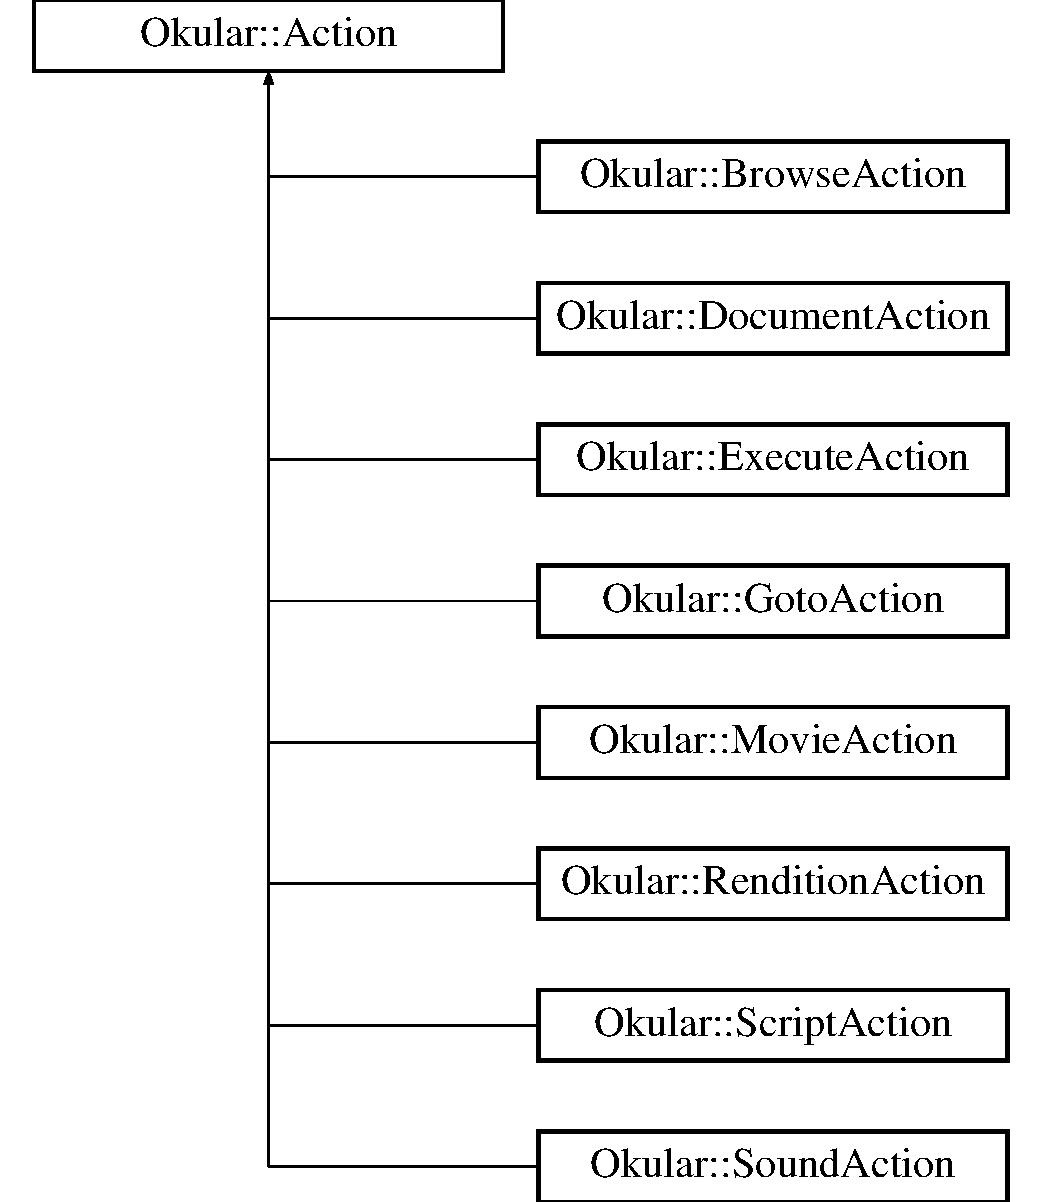
\includegraphics[height=9.000000cm]{classOkular_1_1Action}
\end{center}
\end{figure}
\subsection*{Public Types}
\begin{DoxyCompactItemize}
\item 
enum \hyperlink{classOkular_1_1Action_abe474735af30ea76105595533df9ec47}{Action\+Type} \{ \\*
\hyperlink{classOkular_1_1Action_abe474735af30ea76105595533df9ec47a3561c8768d2c750b59fbed36c41f336d}{Goto}, 
\hyperlink{classOkular_1_1Action_abe474735af30ea76105595533df9ec47a04ece2216c075107b03f6d91739252c2}{Execute}, 
\hyperlink{classOkular_1_1Action_abe474735af30ea76105595533df9ec47a7b94e3d79ff6813ba8444b1d98ca4756}{Browse}, 
\hyperlink{classOkular_1_1Action_abe474735af30ea76105595533df9ec47a3830ede3c1951ff5b024691981fa3385}{Doc\+Action}, 
\\*
\hyperlink{classOkular_1_1Action_abe474735af30ea76105595533df9ec47ae1bf0d24610ef55451f2a122bbf48a3c}{Sound}, 
\hyperlink{classOkular_1_1Action_abe474735af30ea76105595533df9ec47a3f395946dc29cf3a0db5f3d6d67d653a}{Movie}, 
\hyperlink{classOkular_1_1Action_abe474735af30ea76105595533df9ec47ab8871d08c0e3ac56f1ecc9521d4abeb8}{Script}, 
\hyperlink{classOkular_1_1Action_abe474735af30ea76105595533df9ec47abb9c459303f1d82e284acada9ba28ee5}{Rendition}
 \}
\end{DoxyCompactItemize}
\subsection*{Public Member Functions}
\begin{DoxyCompactItemize}
\item 
virtual \hyperlink{classOkular_1_1Action_acdb06775d157339256a8ecd55749226c}{$\sim$\+Action} ()
\item 
virtual \hyperlink{classOkular_1_1Action_abe474735af30ea76105595533df9ec47}{Action\+Type} \hyperlink{classOkular_1_1Action_ac4c2ef09b350b4041f8d1cfb261c3234}{action\+Type} () const =0
\item 
virtual Q\+String \hyperlink{classOkular_1_1Action_a359c33818281df712da697c84975952f}{action\+Tip} () const 
\item 
void \hyperlink{classOkular_1_1Action_afbf20754be0d5b902482a1f704f74f74}{set\+Native\+Id} (const Q\+Variant \&id)
\item 
Q\+Variant \hyperlink{classOkular_1_1Action_a3d499dbbf48e003bc880a1d7622a3748}{native\+Id} () const 
\end{DoxyCompactItemize}


\subsection{Detailed Description}
Encapsulates data that describes an action. 

This is the base class for actions. It makes mandatory for inherited widgets to reimplement the 'action\+Type' method and return the type of the action described by the reimplemented class. 

Definition at line 43 of file action.\+h.



\subsection{Member Enumeration Documentation}
\hypertarget{classOkular_1_1Action_abe474735af30ea76105595533df9ec47}{\index{Okular\+::\+Action@{Okular\+::\+Action}!Action\+Type@{Action\+Type}}
\index{Action\+Type@{Action\+Type}!Okular\+::\+Action@{Okular\+::\+Action}}
\subsubsection[{Action\+Type}]{\setlength{\rightskip}{0pt plus 5cm}enum {\bf Okular\+::\+Action\+::\+Action\+Type}}}\label{classOkular_1_1Action_abe474735af30ea76105595533df9ec47}
Describes the type of action. \begin{Desc}
\item[Enumerator]\par
\begin{description}
\index{Goto@{Goto}!Okular\+::\+Action@{Okular\+::\+Action}}\index{Okular\+::\+Action@{Okular\+::\+Action}!Goto@{Goto}}\item[{\em 
\hypertarget{classOkular_1_1Action_abe474735af30ea76105595533df9ec47a3561c8768d2c750b59fbed36c41f336d}{Goto}\label{classOkular_1_1Action_abe474735af30ea76105595533df9ec47a3561c8768d2c750b59fbed36c41f336d}
}]Goto a given page or external document. \index{Execute@{Execute}!Okular\+::\+Action@{Okular\+::\+Action}}\index{Okular\+::\+Action@{Okular\+::\+Action}!Execute@{Execute}}\item[{\em 
\hypertarget{classOkular_1_1Action_abe474735af30ea76105595533df9ec47a04ece2216c075107b03f6d91739252c2}{Execute}\label{classOkular_1_1Action_abe474735af30ea76105595533df9ec47a04ece2216c075107b03f6d91739252c2}
}]Execute a command or external application. \index{Browse@{Browse}!Okular\+::\+Action@{Okular\+::\+Action}}\index{Okular\+::\+Action@{Okular\+::\+Action}!Browse@{Browse}}\item[{\em 
\hypertarget{classOkular_1_1Action_abe474735af30ea76105595533df9ec47a7b94e3d79ff6813ba8444b1d98ca4756}{Browse}\label{classOkular_1_1Action_abe474735af30ea76105595533df9ec47a7b94e3d79ff6813ba8444b1d98ca4756}
}]Browse a given website. \index{Doc\+Action@{Doc\+Action}!Okular\+::\+Action@{Okular\+::\+Action}}\index{Okular\+::\+Action@{Okular\+::\+Action}!Doc\+Action@{Doc\+Action}}\item[{\em 
\hypertarget{classOkular_1_1Action_abe474735af30ea76105595533df9ec47a3830ede3c1951ff5b024691981fa3385}{Doc\+Action}\label{classOkular_1_1Action_abe474735af30ea76105595533df9ec47a3830ede3c1951ff5b024691981fa3385}
}]Start a custom action. \index{Sound@{Sound}!Okular\+::\+Action@{Okular\+::\+Action}}\index{Okular\+::\+Action@{Okular\+::\+Action}!Sound@{Sound}}\item[{\em 
\hypertarget{classOkular_1_1Action_abe474735af30ea76105595533df9ec47ae1bf0d24610ef55451f2a122bbf48a3c}{Sound}\label{classOkular_1_1Action_abe474735af30ea76105595533df9ec47ae1bf0d24610ef55451f2a122bbf48a3c}
}]Play a sound. \index{Movie@{Movie}!Okular\+::\+Action@{Okular\+::\+Action}}\index{Okular\+::\+Action@{Okular\+::\+Action}!Movie@{Movie}}\item[{\em 
\hypertarget{classOkular_1_1Action_abe474735af30ea76105595533df9ec47a3f395946dc29cf3a0db5f3d6d67d653a}{Movie}\label{classOkular_1_1Action_abe474735af30ea76105595533df9ec47a3f395946dc29cf3a0db5f3d6d67d653a}
}]Play a movie. \index{Script@{Script}!Okular\+::\+Action@{Okular\+::\+Action}}\index{Okular\+::\+Action@{Okular\+::\+Action}!Script@{Script}}\item[{\em 
\hypertarget{classOkular_1_1Action_abe474735af30ea76105595533df9ec47ab8871d08c0e3ac56f1ecc9521d4abeb8}{Script}\label{classOkular_1_1Action_abe474735af30ea76105595533df9ec47ab8871d08c0e3ac56f1ecc9521d4abeb8}
}]Executes a Script code. \index{Rendition@{Rendition}!Okular\+::\+Action@{Okular\+::\+Action}}\index{Okular\+::\+Action@{Okular\+::\+Action}!Rendition@{Rendition}}\item[{\em 
\hypertarget{classOkular_1_1Action_abe474735af30ea76105595533df9ec47abb9c459303f1d82e284acada9ba28ee5}{Rendition}\label{classOkular_1_1Action_abe474735af30ea76105595533df9ec47abb9c459303f1d82e284acada9ba28ee5}
}]Play a movie and/or execute a Script code. \begin{DoxySince}{Since}
0.\+16 (K\+D\+E 4.\+10) 
\end{DoxySince}
\end{description}
\end{Desc}


Definition at line 49 of file action.\+h.


\begin{DoxyCode}
49                         \{
50             \hyperlink{classOkular_1_1Action_abe474735af30ea76105595533df9ec47a3561c8768d2c750b59fbed36c41f336d}{Goto},       
51             \hyperlink{classOkular_1_1Action_abe474735af30ea76105595533df9ec47a04ece2216c075107b03f6d91739252c2}{Execute},    
52             \hyperlink{classOkular_1_1Action_abe474735af30ea76105595533df9ec47a7b94e3d79ff6813ba8444b1d98ca4756}{Browse},     
53             \hyperlink{classOkular_1_1Action_abe474735af30ea76105595533df9ec47a3830ede3c1951ff5b024691981fa3385}{DocAction},  
54             \hyperlink{classOkular_1_1Action_abe474735af30ea76105595533df9ec47ae1bf0d24610ef55451f2a122bbf48a3c}{Sound},      
55             \hyperlink{classOkular_1_1Action_abe474735af30ea76105595533df9ec47a3f395946dc29cf3a0db5f3d6d67d653a}{Movie},      
56             \hyperlink{classOkular_1_1Action_abe474735af30ea76105595533df9ec47ab8871d08c0e3ac56f1ecc9521d4abeb8}{Script},     
57             \hyperlink{classOkular_1_1Action_abe474735af30ea76105595533df9ec47abb9c459303f1d82e284acada9ba28ee5}{Rendition}   
58         \};
\end{DoxyCode}


\subsection{Constructor \& Destructor Documentation}
\hypertarget{classOkular_1_1Action_acdb06775d157339256a8ecd55749226c}{\index{Okular\+::\+Action@{Okular\+::\+Action}!````~Action@{$\sim$\+Action}}
\index{````~Action@{$\sim$\+Action}!Okular\+::\+Action@{Okular\+::\+Action}}
\subsubsection[{$\sim$\+Action}]{\setlength{\rightskip}{0pt plus 5cm}Action\+::$\sim$\+Action (
\begin{DoxyParamCaption}
{}
\end{DoxyParamCaption}
)\hspace{0.3cm}{\ttfamily [virtual]}}}\label{classOkular_1_1Action_acdb06775d157339256a8ecd55749226c}
Destroys the action. 

Definition at line 42 of file action.\+cpp.


\begin{DoxyCode}
43 \{
44     \textcolor{keyword}{delete} d\_ptr;
45 \}
\end{DoxyCode}


\subsection{Member Function Documentation}
\hypertarget{classOkular_1_1Action_a359c33818281df712da697c84975952f}{\index{Okular\+::\+Action@{Okular\+::\+Action}!action\+Tip@{action\+Tip}}
\index{action\+Tip@{action\+Tip}!Okular\+::\+Action@{Okular\+::\+Action}}
\subsubsection[{action\+Tip}]{\setlength{\rightskip}{0pt plus 5cm}Q\+String Action\+::action\+Tip (
\begin{DoxyParamCaption}
{}
\end{DoxyParamCaption}
) const\hspace{0.3cm}{\ttfamily [virtual]}}}\label{classOkular_1_1Action_a359c33818281df712da697c84975952f}
Returns a i18n'ed tip of the action that is presented to the user. 

Reimplemented in \hyperlink{classOkular_1_1RenditionAction_a6a4d1c45ec9832dad5b8ceadc56ec393}{Okular\+::\+Rendition\+Action}, \hyperlink{classOkular_1_1MovieAction_a137b2ada90d7bf6ae1e110cd7b43580c}{Okular\+::\+Movie\+Action}, \hyperlink{classOkular_1_1ScriptAction_a557e181727e1992d7d9557b7f91b6221}{Okular\+::\+Script\+Action}, \hyperlink{classOkular_1_1SoundAction_ae0bbcde29f828f1d5bcfddc0b4c7f0cd}{Okular\+::\+Sound\+Action}, \hyperlink{classOkular_1_1DocumentAction_a351e6e44a53442df6d0ccf48b83aa697}{Okular\+::\+Document\+Action}, \hyperlink{classOkular_1_1BrowseAction_afcc99a984ec0687a4a1f40409d344481}{Okular\+::\+Browse\+Action}, \hyperlink{classOkular_1_1ExecuteAction_a60177f711289c231994888281d9d6b67}{Okular\+::\+Execute\+Action}, and \hyperlink{classOkular_1_1GotoAction_aea68a11af6da8cb45c59a139f5bc3c15}{Okular\+::\+Goto\+Action}.



Definition at line 47 of file action.\+cpp.


\begin{DoxyCode}
48 \{
49     \textcolor{keywordflow}{return} \textcolor{stringliteral}{""};
50 \}
\end{DoxyCode}
\hypertarget{classOkular_1_1Action_ac4c2ef09b350b4041f8d1cfb261c3234}{\index{Okular\+::\+Action@{Okular\+::\+Action}!action\+Type@{action\+Type}}
\index{action\+Type@{action\+Type}!Okular\+::\+Action@{Okular\+::\+Action}}
\subsubsection[{action\+Type}]{\setlength{\rightskip}{0pt plus 5cm}virtual {\bf Action\+Type} Okular\+::\+Action\+::action\+Type (
\begin{DoxyParamCaption}
{}
\end{DoxyParamCaption}
) const\hspace{0.3cm}{\ttfamily [pure virtual]}}}\label{classOkular_1_1Action_ac4c2ef09b350b4041f8d1cfb261c3234}
Returns the type of the action. Every inherited class must return an unique identifier.

\begin{DoxySeeAlso}{See Also}
\hyperlink{classOkular_1_1Action_abe474735af30ea76105595533df9ec47}{Action\+Type} 
\end{DoxySeeAlso}


Implemented in \hyperlink{classOkular_1_1RenditionAction_a4504e129022b92d1a7788888206f8fd0}{Okular\+::\+Rendition\+Action}, \hyperlink{classOkular_1_1MovieAction_aa3aaf75f235f6c396aa913f4dd2df385}{Okular\+::\+Movie\+Action}, \hyperlink{classOkular_1_1ScriptAction_a35cf3029915fb6c2b3c694ae2ce2520e}{Okular\+::\+Script\+Action}, \hyperlink{classOkular_1_1SoundAction_a9f73cbcd3d77b77428e937b6ca83668c}{Okular\+::\+Sound\+Action}, \hyperlink{classOkular_1_1DocumentAction_aba0ec16ee587e516bbeff8d55d958b47}{Okular\+::\+Document\+Action}, \hyperlink{classOkular_1_1BrowseAction_a253991762e61b486d0667dc1619b0f46}{Okular\+::\+Browse\+Action}, \hyperlink{classOkular_1_1ExecuteAction_ac9d8d732913d262931c07eef33595f6d}{Okular\+::\+Execute\+Action}, and \hyperlink{classOkular_1_1GotoAction_a5ae91d07286ee731939b4392e787443f}{Okular\+::\+Goto\+Action}.

\hypertarget{classOkular_1_1Action_a3d499dbbf48e003bc880a1d7622a3748}{\index{Okular\+::\+Action@{Okular\+::\+Action}!native\+Id@{native\+Id}}
\index{native\+Id@{native\+Id}!Okular\+::\+Action@{Okular\+::\+Action}}
\subsubsection[{native\+Id}]{\setlength{\rightskip}{0pt plus 5cm}Q\+Variant Action\+::native\+Id (
\begin{DoxyParamCaption}
{}
\end{DoxyParamCaption}
) const}}\label{classOkular_1_1Action_a3d499dbbf48e003bc880a1d7622a3748}
Returns the \char`\"{}native\char`\"{} id of the action.

\begin{DoxySince}{Since}
0.\+15 (K\+D\+E 4.\+9) 
\end{DoxySince}


Definition at line 58 of file action.\+cpp.


\begin{DoxyCode}
59 \{
60     Q\_D( \textcolor{keyword}{const} \hyperlink{classOkular_1_1Action}{Action} );
61     \textcolor{keywordflow}{return} d->m\_nativeId;
62 \}
\end{DoxyCode}
\hypertarget{classOkular_1_1Action_afbf20754be0d5b902482a1f704f74f74}{\index{Okular\+::\+Action@{Okular\+::\+Action}!set\+Native\+Id@{set\+Native\+Id}}
\index{set\+Native\+Id@{set\+Native\+Id}!Okular\+::\+Action@{Okular\+::\+Action}}
\subsubsection[{set\+Native\+Id}]{\setlength{\rightskip}{0pt plus 5cm}void Action\+::set\+Native\+Id (
\begin{DoxyParamCaption}
\item[{const Q\+Variant \&}]{id}
\end{DoxyParamCaption}
)}}\label{classOkular_1_1Action_afbf20754be0d5b902482a1f704f74f74}
Sets the \char`\"{}native\char`\"{} {\ttfamily id} of the action.

This is for use of the \hyperlink{classOkular_1_1Generator}{Generator}, that can optionally store an handle (a pointer, an identifier, etc) of the \char`\"{}native\char`\"{} action object, if any.

\begin{DoxyNote}{Note}
\hyperlink{namespaceOkular}{Okular} makes no use of this
\end{DoxyNote}
\begin{DoxySince}{Since}
0.\+15 (K\+D\+E 4.\+9) 
\end{DoxySince}


Definition at line 52 of file action.\+cpp.


\begin{DoxyCode}
53 \{
54     Q\_D( \hyperlink{classOkular_1_1Action}{Action} );
55     d->m\_nativeId = id;
56 \}
\end{DoxyCode}


The documentation for this class was generated from the following files\+:\begin{DoxyCompactItemize}
\item 
core/\hyperlink{action_8h}{action.\+h}\item 
core/\hyperlink{action_8cpp}{action.\+cpp}\end{DoxyCompactItemize}

\hypertarget{classOkular_1_1ActionPrivate}{\section{Okular\+:\+:Action\+Private Class Reference}
\label{classOkular_1_1ActionPrivate}\index{Okular\+::\+Action\+Private@{Okular\+::\+Action\+Private}}
}
Inheritance diagram for Okular\+:\+:Action\+Private\+:\begin{figure}[H]
\begin{center}
\leavevmode
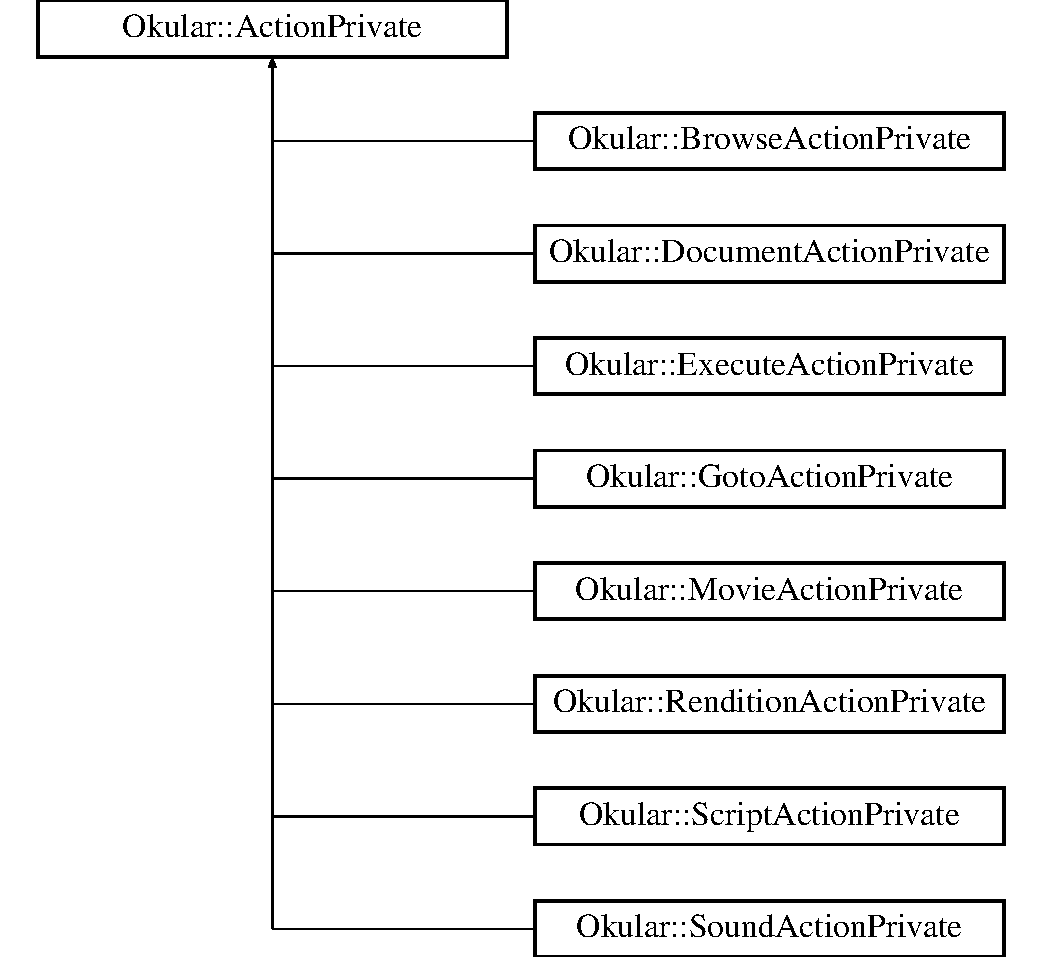
\includegraphics[height=9.000000cm]{classOkular_1_1ActionPrivate}
\end{center}
\end{figure}
\subsection*{Public Member Functions}
\begin{DoxyCompactItemize}
\item 
\hyperlink{classOkular_1_1ActionPrivate_ade22b7b9b9f6490b2fce5b928235ef5b}{Action\+Private} ()
\item 
virtual \hyperlink{classOkular_1_1ActionPrivate_a43b4a5b9f6428ab41c4375c2eb72d05f}{$\sim$\+Action\+Private} ()
\end{DoxyCompactItemize}
\subsection*{Public Attributes}
\begin{DoxyCompactItemize}
\item 
Q\+Variant \hyperlink{classOkular_1_1ActionPrivate_a6305ced88093be83f41a4fb5c2e335ab}{m\+\_\+native\+Id}
\end{DoxyCompactItemize}


\subsection{Detailed Description}


Definition at line 23 of file action.\+cpp.



\subsection{Constructor \& Destructor Documentation}
\hypertarget{classOkular_1_1ActionPrivate_ade22b7b9b9f6490b2fce5b928235ef5b}{\index{Okular\+::\+Action\+Private@{Okular\+::\+Action\+Private}!Action\+Private@{Action\+Private}}
\index{Action\+Private@{Action\+Private}!Okular\+::\+Action\+Private@{Okular\+::\+Action\+Private}}
\subsubsection[{Action\+Private}]{\setlength{\rightskip}{0pt plus 5cm}Okular\+::\+Action\+Private\+::\+Action\+Private (
\begin{DoxyParamCaption}
{}
\end{DoxyParamCaption}
)\hspace{0.3cm}{\ttfamily [inline]}}}\label{classOkular_1_1ActionPrivate_ade22b7b9b9f6490b2fce5b928235ef5b}


Definition at line 26 of file action.\+cpp.


\begin{DoxyCode}
27         \{
28         \}
\end{DoxyCode}
\hypertarget{classOkular_1_1ActionPrivate_a43b4a5b9f6428ab41c4375c2eb72d05f}{\index{Okular\+::\+Action\+Private@{Okular\+::\+Action\+Private}!````~Action\+Private@{$\sim$\+Action\+Private}}
\index{````~Action\+Private@{$\sim$\+Action\+Private}!Okular\+::\+Action\+Private@{Okular\+::\+Action\+Private}}
\subsubsection[{$\sim$\+Action\+Private}]{\setlength{\rightskip}{0pt plus 5cm}virtual Okular\+::\+Action\+Private\+::$\sim$\+Action\+Private (
\begin{DoxyParamCaption}
{}
\end{DoxyParamCaption}
)\hspace{0.3cm}{\ttfamily [inline]}, {\ttfamily [virtual]}}}\label{classOkular_1_1ActionPrivate_a43b4a5b9f6428ab41c4375c2eb72d05f}


Definition at line 30 of file action.\+cpp.


\begin{DoxyCode}
31         \{
32         \}
\end{DoxyCode}


\subsection{Member Data Documentation}
\hypertarget{classOkular_1_1ActionPrivate_a6305ced88093be83f41a4fb5c2e335ab}{\index{Okular\+::\+Action\+Private@{Okular\+::\+Action\+Private}!m\+\_\+native\+Id@{m\+\_\+native\+Id}}
\index{m\+\_\+native\+Id@{m\+\_\+native\+Id}!Okular\+::\+Action\+Private@{Okular\+::\+Action\+Private}}
\subsubsection[{m\+\_\+native\+Id}]{\setlength{\rightskip}{0pt plus 5cm}Q\+Variant Okular\+::\+Action\+Private\+::m\+\_\+native\+Id}}\label{classOkular_1_1ActionPrivate_a6305ced88093be83f41a4fb5c2e335ab}


Definition at line 34 of file action.\+cpp.



The documentation for this class was generated from the following file\+:\begin{DoxyCompactItemize}
\item 
core/\hyperlink{action_8cpp}{action.\+cpp}\end{DoxyCompactItemize}

\hypertarget{classOkular_1_1AddAnnotationCommand}{\section{Okular\+:\+:Add\+Annotation\+Command Class Reference}
\label{classOkular_1_1AddAnnotationCommand}\index{Okular\+::\+Add\+Annotation\+Command@{Okular\+::\+Add\+Annotation\+Command}}
}


{\ttfamily \#include $<$documentcommands\+\_\+p.\+h$>$}

Inheritance diagram for Okular\+:\+:Add\+Annotation\+Command\+:\begin{figure}[H]
\begin{center}
\leavevmode
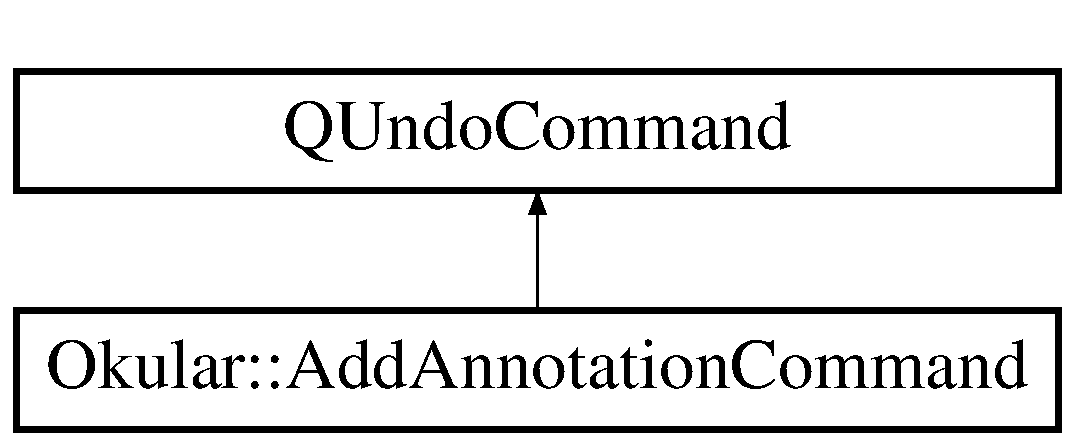
\includegraphics[height=2.000000cm]{classOkular_1_1AddAnnotationCommand}
\end{center}
\end{figure}
\subsection*{Public Member Functions}
\begin{DoxyCompactItemize}
\item 
\hyperlink{classOkular_1_1AddAnnotationCommand_ac6f174c03e464a1643dbbe84d475d7bd}{Add\+Annotation\+Command} (\hyperlink{classOkular_1_1DocumentPrivate}{Okular\+::\+Document\+Private} $\ast$doc\+Priv, \hyperlink{classOkular_1_1Annotation}{Okular\+::\+Annotation} $\ast$annotation, int page\+Number)
\item 
virtual \hyperlink{classOkular_1_1AddAnnotationCommand_a7709ffeee8cccd75fd78e6393b66fa9e}{$\sim$\+Add\+Annotation\+Command} ()
\item 
virtual void \hyperlink{classOkular_1_1AddAnnotationCommand_ab9edaaacd8989de3fd9cd8cf246fbcaf}{undo} ()
\item 
virtual void \hyperlink{classOkular_1_1AddAnnotationCommand_ab6c194cc1f7877acf9c9f197a24f2ae5}{redo} ()
\end{DoxyCompactItemize}


\subsection{Detailed Description}


Definition at line 27 of file documentcommands\+\_\+p.\+h.



\subsection{Constructor \& Destructor Documentation}
\hypertarget{classOkular_1_1AddAnnotationCommand_ac6f174c03e464a1643dbbe84d475d7bd}{\index{Okular\+::\+Add\+Annotation\+Command@{Okular\+::\+Add\+Annotation\+Command}!Add\+Annotation\+Command@{Add\+Annotation\+Command}}
\index{Add\+Annotation\+Command@{Add\+Annotation\+Command}!Okular\+::\+Add\+Annotation\+Command@{Okular\+::\+Add\+Annotation\+Command}}
\subsubsection[{Add\+Annotation\+Command}]{\setlength{\rightskip}{0pt plus 5cm}Okular\+::\+Add\+Annotation\+Command\+::\+Add\+Annotation\+Command (
\begin{DoxyParamCaption}
\item[{{\bf Okular\+::\+Document\+Private} $\ast$}]{doc\+Priv, }
\item[{{\bf Okular\+::\+Annotation} $\ast$}]{annotation, }
\item[{int}]{page\+Number}
\end{DoxyParamCaption}
)}}\label{classOkular_1_1AddAnnotationCommand_ac6f174c03e464a1643dbbe84d475d7bd}


Definition at line 59 of file documentcommands.\+cpp.


\begin{DoxyCode}
60  : m\_docPriv( docPriv ),
61    m\_annotation( annotation ),
62    m\_pageNumber( pageNumber ),
63    m\_done( \textcolor{keyword}{false} )
64 \{
65     setText( i18nc (\textcolor{stringliteral}{"Add an annotation to the page"}, \textcolor{stringliteral}{"add annotation"} ) );
66 \}
\end{DoxyCode}
\hypertarget{classOkular_1_1AddAnnotationCommand_a7709ffeee8cccd75fd78e6393b66fa9e}{\index{Okular\+::\+Add\+Annotation\+Command@{Okular\+::\+Add\+Annotation\+Command}!````~Add\+Annotation\+Command@{$\sim$\+Add\+Annotation\+Command}}
\index{````~Add\+Annotation\+Command@{$\sim$\+Add\+Annotation\+Command}!Okular\+::\+Add\+Annotation\+Command@{Okular\+::\+Add\+Annotation\+Command}}
\subsubsection[{$\sim$\+Add\+Annotation\+Command}]{\setlength{\rightskip}{0pt plus 5cm}Okular\+::\+Add\+Annotation\+Command\+::$\sim$\+Add\+Annotation\+Command (
\begin{DoxyParamCaption}
{}
\end{DoxyParamCaption}
)\hspace{0.3cm}{\ttfamily [virtual]}}}\label{classOkular_1_1AddAnnotationCommand_a7709ffeee8cccd75fd78e6393b66fa9e}


Definition at line 68 of file documentcommands.\+cpp.


\begin{DoxyCode}
69 \{
70     \textcolor{keywordflow}{if} ( !m\_done )
71     \{
72         \textcolor{keyword}{delete} m\_annotation;
73     \}
74 \}
\end{DoxyCode}


\subsection{Member Function Documentation}
\hypertarget{classOkular_1_1AddAnnotationCommand_ab6c194cc1f7877acf9c9f197a24f2ae5}{\index{Okular\+::\+Add\+Annotation\+Command@{Okular\+::\+Add\+Annotation\+Command}!redo@{redo}}
\index{redo@{redo}!Okular\+::\+Add\+Annotation\+Command@{Okular\+::\+Add\+Annotation\+Command}}
\subsubsection[{redo}]{\setlength{\rightskip}{0pt plus 5cm}void Okular\+::\+Add\+Annotation\+Command\+::redo (
\begin{DoxyParamCaption}
{}
\end{DoxyParamCaption}
)\hspace{0.3cm}{\ttfamily [virtual]}}}\label{classOkular_1_1AddAnnotationCommand_ab6c194cc1f7877acf9c9f197a24f2ae5}


Definition at line 83 of file documentcommands.\+cpp.


\begin{DoxyCode}
84 \{
85     \hyperlink{namespaceOkular_a1e0f22fec5a200bd3b1835b7bfd95172}{moveViewportIfBoundingRectNotFullyVisible}( m\_annotation->
      \hyperlink{classOkular_1_1Annotation_a450fbd08aeb31262a33a628b4ab0dd42}{boundingRectangle}(), m\_docPriv, m\_pageNumber );
86     m\_docPriv->\hyperlink{classOkular_1_1DocumentPrivate_a374e55b575f2386536cd438bd2338b33}{performAddPageAnnotation}( m\_pageNumber,  m\_annotation );
87     m\_done = \textcolor{keyword}{true};
88 \}
\end{DoxyCode}
\hypertarget{classOkular_1_1AddAnnotationCommand_ab9edaaacd8989de3fd9cd8cf246fbcaf}{\index{Okular\+::\+Add\+Annotation\+Command@{Okular\+::\+Add\+Annotation\+Command}!undo@{undo}}
\index{undo@{undo}!Okular\+::\+Add\+Annotation\+Command@{Okular\+::\+Add\+Annotation\+Command}}
\subsubsection[{undo}]{\setlength{\rightskip}{0pt plus 5cm}void Okular\+::\+Add\+Annotation\+Command\+::undo (
\begin{DoxyParamCaption}
{}
\end{DoxyParamCaption}
)\hspace{0.3cm}{\ttfamily [virtual]}}}\label{classOkular_1_1AddAnnotationCommand_ab9edaaacd8989de3fd9cd8cf246fbcaf}


Definition at line 76 of file documentcommands.\+cpp.


\begin{DoxyCode}
77 \{
78     \hyperlink{namespaceOkular_a1e0f22fec5a200bd3b1835b7bfd95172}{moveViewportIfBoundingRectNotFullyVisible}( m\_annotation->
      \hyperlink{classOkular_1_1Annotation_a450fbd08aeb31262a33a628b4ab0dd42}{boundingRectangle}(), m\_docPriv, m\_pageNumber );
79     m\_docPriv->\hyperlink{classOkular_1_1DocumentPrivate_a52fc440677b41a7717bff1cec9593d33}{performRemovePageAnnotation}( m\_pageNumber, m\_annotation );
80     m\_done = \textcolor{keyword}{false};
81 \}
\end{DoxyCode}


The documentation for this class was generated from the following files\+:\begin{DoxyCompactItemize}
\item 
core/\hyperlink{documentcommands__p_8h}{documentcommands\+\_\+p.\+h}\item 
core/\hyperlink{documentcommands_8cpp}{documentcommands.\+cpp}\end{DoxyCompactItemize}

\hypertarget{classAddRemoveAnnotationTest}{\section{Add\+Remove\+Annotation\+Test Class Reference}
\label{classAddRemoveAnnotationTest}\index{Add\+Remove\+Annotation\+Test@{Add\+Remove\+Annotation\+Test}}
}
Inheritance diagram for Add\+Remove\+Annotation\+Test\+:\begin{figure}[H]
\begin{center}
\leavevmode
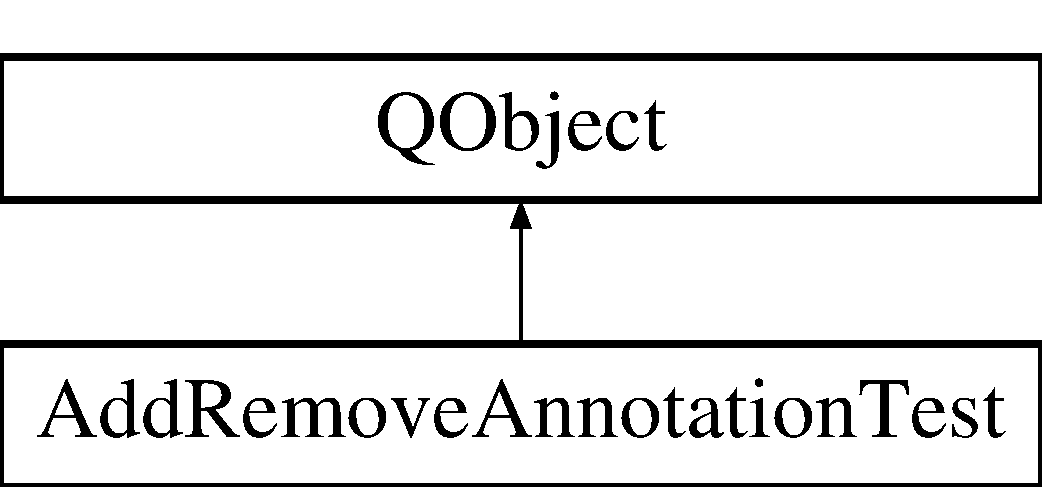
\includegraphics[height=2.000000cm]{classAddRemoveAnnotationTest}
\end{center}
\end{figure}


\subsection{Detailed Description}


Definition at line 18 of file addremoveannotationtest.\+cpp.



The documentation for this class was generated from the following file\+:\begin{DoxyCompactItemize}
\item 
tests/\hyperlink{addremoveannotationtest_8cpp}{addremoveannotationtest.\+cpp}\end{DoxyCompactItemize}

\hypertarget{structAllocatedPixmap}{\section{Allocated\+Pixmap Struct Reference}
\label{structAllocatedPixmap}\index{Allocated\+Pixmap@{Allocated\+Pixmap}}
}
\subsection*{Public Member Functions}
\begin{DoxyCompactItemize}
\item 
\hyperlink{structAllocatedPixmap_a5044bae998c47af4a7a20b8b77517d5a}{Allocated\+Pixmap} (\hyperlink{classOkular_1_1DocumentObserver}{Document\+Observer} $\ast$o, int p, qulonglong m)
\end{DoxyCompactItemize}
\subsection*{Public Attributes}
\begin{DoxyCompactItemize}
\item 
\hyperlink{classOkular_1_1DocumentObserver}{Document\+Observer} $\ast$ \hyperlink{structAllocatedPixmap_a5ee1fe9a6b1a37583c0ea54045cc7800}{observer}
\item 
int \hyperlink{structAllocatedPixmap_a197c0639216aa0819deb72fd8705d115}{page}
\item 
qulonglong \hyperlink{structAllocatedPixmap_a8fdfc9d87d0ce0852716295895606be0}{memory}
\end{DoxyCompactItemize}


\subsection{Detailed Description}


Definition at line 95 of file document.\+cpp.



\subsection{Constructor \& Destructor Documentation}
\hypertarget{structAllocatedPixmap_a5044bae998c47af4a7a20b8b77517d5a}{\index{Allocated\+Pixmap@{Allocated\+Pixmap}!Allocated\+Pixmap@{Allocated\+Pixmap}}
\index{Allocated\+Pixmap@{Allocated\+Pixmap}!Allocated\+Pixmap@{Allocated\+Pixmap}}
\subsubsection[{Allocated\+Pixmap}]{\setlength{\rightskip}{0pt plus 5cm}Allocated\+Pixmap\+::\+Allocated\+Pixmap (
\begin{DoxyParamCaption}
\item[{{\bf Document\+Observer} $\ast$}]{o, }
\item[{int}]{p, }
\item[{qulonglong}]{m}
\end{DoxyParamCaption}
)\hspace{0.3cm}{\ttfamily [inline]}}}\label{structAllocatedPixmap_a5044bae998c47af4a7a20b8b77517d5a}


Definition at line 102 of file document.\+cpp.


\begin{DoxyCode}
102 : \hyperlink{structAllocatedPixmap_a5ee1fe9a6b1a37583c0ea54045cc7800}{observer}( o ), \hyperlink{structAllocatedPixmap_a197c0639216aa0819deb72fd8705d115}{page}( p ), \hyperlink{structAllocatedPixmap_a8fdfc9d87d0ce0852716295895606be0}{memory}( m ) \{\}
\end{DoxyCode}


\subsection{Member Data Documentation}
\hypertarget{structAllocatedPixmap_a8fdfc9d87d0ce0852716295895606be0}{\index{Allocated\+Pixmap@{Allocated\+Pixmap}!memory@{memory}}
\index{memory@{memory}!Allocated\+Pixmap@{Allocated\+Pixmap}}
\subsubsection[{memory}]{\setlength{\rightskip}{0pt plus 5cm}qulonglong Allocated\+Pixmap\+::memory}}\label{structAllocatedPixmap_a8fdfc9d87d0ce0852716295895606be0}


Definition at line 100 of file document.\+cpp.

\hypertarget{structAllocatedPixmap_a5ee1fe9a6b1a37583c0ea54045cc7800}{\index{Allocated\+Pixmap@{Allocated\+Pixmap}!observer@{observer}}
\index{observer@{observer}!Allocated\+Pixmap@{Allocated\+Pixmap}}
\subsubsection[{observer}]{\setlength{\rightskip}{0pt plus 5cm}{\bf Document\+Observer}$\ast$ Allocated\+Pixmap\+::observer}}\label{structAllocatedPixmap_a5ee1fe9a6b1a37583c0ea54045cc7800}


Definition at line 98 of file document.\+cpp.

\hypertarget{structAllocatedPixmap_a197c0639216aa0819deb72fd8705d115}{\index{Allocated\+Pixmap@{Allocated\+Pixmap}!page@{page}}
\index{page@{page}!Allocated\+Pixmap@{Allocated\+Pixmap}}
\subsubsection[{page}]{\setlength{\rightskip}{0pt plus 5cm}int Allocated\+Pixmap\+::page}}\label{structAllocatedPixmap_a197c0639216aa0819deb72fd8705d115}


Definition at line 99 of file document.\+cpp.



The documentation for this struct was generated from the following file\+:\begin{DoxyCompactItemize}
\item 
core/\hyperlink{core_2document_8cpp}{document.\+cpp}\end{DoxyCompactItemize}

\hypertarget{classAnchor}{\section{Anchor Class Reference}
\label{classAnchor}\index{Anchor@{Anchor}}
}


Page number and vertical position in physical coordinates.  




{\ttfamily \#include $<$anchor.\+h$>$}

\subsection*{Public Member Functions}
\begin{DoxyCompactItemize}
\item 
\hyperlink{classAnchor_a5bf43f017bb50f8e6a4c8bb4f31bd001}{Anchor} ()
\begin{DoxyCompactList}\small\item\em Constructs an anchor that points to an invalid page. \end{DoxyCompactList}\item 
\hyperlink{classAnchor_ad152a54b313f8e2cd4ff87ce85fc78e5}{Anchor} (const \hyperlink{classPageNumber}{Page\+Number} \&pg, const \hyperlink{classLength}{Length} \&\+\_\+distance\+\_\+from\+\_\+top)
\begin{DoxyCompactList}\small\item\em Constructs an snchor that points to a given position on a given page. \end{DoxyCompactList}\item 
bool \hyperlink{classAnchor_a808ec5fc9d0075ca1c15cda24690277e}{is\+Valid} () const 
\begin{DoxyCompactList}\small\item\em quick validity check for anchors \end{DoxyCompactList}\end{DoxyCompactItemize}
\subsection*{Public Attributes}
\begin{DoxyCompactItemize}
\item 
\hyperlink{classPageNumber}{Page\+Number} \hyperlink{classAnchor_a6383150d7bcb2a7f0281274d17881aa2}{page}
\begin{DoxyCompactList}\small\item\em Page number that this anchor point to. \end{DoxyCompactList}\item 
\hyperlink{classLength}{Length} \hyperlink{classAnchor_a7bf0367a6cb313c7e2f7c7527928b635}{distance\+\_\+from\+\_\+top}
\begin{DoxyCompactList}\small\item\em Distance from the top of the page in inch. \end{DoxyCompactList}\end{DoxyCompactItemize}


\subsection{Detailed Description}
Page number and vertical position in physical coordinates. 

This very simple class contains a page number and a vertical position in physical coordiantes. The vertical position is given by the distance from the top of the page. Anchors are completely independent of documents, there is no need for a document to exists that contains the given page, nor does the page number need to be valid.

\begin{DoxyAuthor}{Author}
Stefan Kebekus \href{mailto:kebekus@kde.org}{\tt kebekus@kde.\+org} 
\end{DoxyAuthor}
\begin{DoxyVersion}{Version}
1.\+0 0 
\end{DoxyVersion}


Definition at line 30 of file anchor.\+h.



\subsection{Constructor \& Destructor Documentation}
\hypertarget{classAnchor_a5bf43f017bb50f8e6a4c8bb4f31bd001}{\index{Anchor@{Anchor}!Anchor@{Anchor}}
\index{Anchor@{Anchor}!Anchor@{Anchor}}
\subsubsection[{Anchor}]{\setlength{\rightskip}{0pt plus 5cm}Anchor\+::\+Anchor (
\begin{DoxyParamCaption}
{}
\end{DoxyParamCaption}
)\hspace{0.3cm}{\ttfamily [inline]}}}\label{classAnchor_a5bf43f017bb50f8e6a4c8bb4f31bd001}


Constructs an anchor that points to an invalid page. 



Definition at line 33 of file anchor.\+h.


\begin{DoxyCode}
33 \{\hyperlink{classAnchor_a6383150d7bcb2a7f0281274d17881aa2}{page} = 0;\}
\end{DoxyCode}
\hypertarget{classAnchor_ad152a54b313f8e2cd4ff87ce85fc78e5}{\index{Anchor@{Anchor}!Anchor@{Anchor}}
\index{Anchor@{Anchor}!Anchor@{Anchor}}
\subsubsection[{Anchor}]{\setlength{\rightskip}{0pt plus 5cm}Anchor\+::\+Anchor (
\begin{DoxyParamCaption}
\item[{const {\bf Page\+Number} \&}]{pg, }
\item[{const {\bf Length} \&}]{\+\_\+distance\+\_\+from\+\_\+top}
\end{DoxyParamCaption}
)\hspace{0.3cm}{\ttfamily [inline]}}}\label{classAnchor_ad152a54b313f8e2cd4ff87ce85fc78e5}


Constructs an snchor that points to a given position on a given page. 

The class contains no code to make sure in any way that the page number pg exists, and that page pg, if it exists, is taller than distance\+\_\+from\+\_\+top


\begin{DoxyParams}{Parameters}
{\em pg} & number of the page \\
\hline
{\em \+\_\+distance\+\_\+from\+\_\+top} & distance from the top of the page \\
\hline
\end{DoxyParams}


Definition at line 45 of file anchor.\+h.


\begin{DoxyCode}
45 : \hyperlink{classAnchor_a6383150d7bcb2a7f0281274d17881aa2}{page}(pg), \hyperlink{classAnchor_a7bf0367a6cb313c7e2f7c7527928b635}{distance\_from\_top}(\_distance\_from\_top) \{\}
\end{DoxyCode}


\subsection{Member Function Documentation}
\hypertarget{classAnchor_a808ec5fc9d0075ca1c15cda24690277e}{\index{Anchor@{Anchor}!is\+Valid@{is\+Valid}}
\index{is\+Valid@{is\+Valid}!Anchor@{Anchor}}
\subsubsection[{is\+Valid}]{\setlength{\rightskip}{0pt plus 5cm}bool Anchor\+::is\+Valid (
\begin{DoxyParamCaption}
{}
\end{DoxyParamCaption}
) const\hspace{0.3cm}{\ttfamily [inline]}}}\label{classAnchor_a808ec5fc9d0075ca1c15cda24690277e}


quick validity check for anchors 

\begin{DoxyReturn}{Returns}
true if the page number is valid, and 0mm $<$= distance\+\_\+from\+\_\+top $<$= 2m 
\end{DoxyReturn}


Definition at line 51 of file anchor.\+h.


\begin{DoxyCode}
51 \{\textcolor{keywordflow}{return} \hyperlink{classAnchor_a6383150d7bcb2a7f0281274d17881aa2}{page}.\hyperlink{classPageNumber_a701f1be28f2dd97b88d83c4abce18645}{isValid}() && (0.0 <= \hyperlink{classAnchor_a7bf0367a6cb313c7e2f7c7527928b635}{distance\_from\_top}.
      \hyperlink{classLength_ab57252f3b49a668104d76396b2c74041}{getLength\_in\_mm}()) &&  (\hyperlink{classAnchor_a7bf0367a6cb313c7e2f7c7527928b635}{distance\_from\_top}.
      \hyperlink{classLength_ab57252f3b49a668104d76396b2c74041}{getLength\_in\_mm}() <= 2000.0);\}
\end{DoxyCode}


\subsection{Member Data Documentation}
\hypertarget{classAnchor_a7bf0367a6cb313c7e2f7c7527928b635}{\index{Anchor@{Anchor}!distance\+\_\+from\+\_\+top@{distance\+\_\+from\+\_\+top}}
\index{distance\+\_\+from\+\_\+top@{distance\+\_\+from\+\_\+top}!Anchor@{Anchor}}
\subsubsection[{distance\+\_\+from\+\_\+top}]{\setlength{\rightskip}{0pt plus 5cm}{\bf Length} Anchor\+::distance\+\_\+from\+\_\+top}}\label{classAnchor_a7bf0367a6cb313c7e2f7c7527928b635}


Distance from the top of the page in inch. 



Definition at line 57 of file anchor.\+h.

\hypertarget{classAnchor_a6383150d7bcb2a7f0281274d17881aa2}{\index{Anchor@{Anchor}!page@{page}}
\index{page@{page}!Anchor@{Anchor}}
\subsubsection[{page}]{\setlength{\rightskip}{0pt plus 5cm}{\bf Page\+Number} Anchor\+::page}}\label{classAnchor_a6383150d7bcb2a7f0281274d17881aa2}


Page number that this anchor point to. 



Definition at line 54 of file anchor.\+h.



The documentation for this class was generated from the following file\+:\begin{DoxyCompactItemize}
\item 
generators/dvi/\hyperlink{anchor_8h}{anchor.\+h}\end{DoxyCompactItemize}

\hypertarget{structAnnItem}{\section{Ann\+Item Struct Reference}
\label{structAnnItem}\index{Ann\+Item@{Ann\+Item}}
}
\subsection*{Public Member Functions}
\begin{DoxyCompactItemize}
\item 
\hyperlink{structAnnItem_a470674064cc4782539c18b5a84d8d92c}{Ann\+Item} ()
\item 
\hyperlink{structAnnItem_a62238531831021d5e500ca21e4141f33}{Ann\+Item} (\hyperlink{structAnnItem}{Ann\+Item} $\ast$\hyperlink{structAnnItem_aece74b70cc6acc8ebb751256386f9be8}{parent}, \hyperlink{classOkular_1_1Annotation}{Okular\+::\+Annotation} $\ast$ann)
\item 
\hyperlink{structAnnItem_a347e18ec47f43003e855789dae47434c}{Ann\+Item} (\hyperlink{structAnnItem}{Ann\+Item} $\ast$\hyperlink{structAnnItem_aece74b70cc6acc8ebb751256386f9be8}{parent}, int \hyperlink{structAnnItem_ad2bc09dd1499fd52205eb02c3bf67830}{page})
\item 
\hyperlink{structAnnItem_a7ef99a3a1013d8a1daccc4c39d9f5369}{$\sim$\+Ann\+Item} ()
\end{DoxyCompactItemize}
\subsection*{Public Attributes}
\begin{DoxyCompactItemize}
\item 
\hyperlink{structAnnItem}{Ann\+Item} $\ast$ \hyperlink{structAnnItem_aece74b70cc6acc8ebb751256386f9be8}{parent}
\item 
\hyperlink{classQList}{Q\+List}$<$ \hyperlink{structAnnItem}{Ann\+Item} $\ast$ $>$ \hyperlink{structAnnItem_a11048051ad0be5a2c8607a9334e006a1}{children}
\item 
\hyperlink{classOkular_1_1Annotation}{Okular\+::\+Annotation} $\ast$ \hyperlink{structAnnItem_a72999b1a45d966e6f622dee4d958790f}{annotation}
\item 
int \hyperlink{structAnnItem_ad2bc09dd1499fd52205eb02c3bf67830}{page}
\end{DoxyCompactItemize}


\subsection{Detailed Description}


Definition at line 25 of file annotationmodel.\+cpp.



\subsection{Constructor \& Destructor Documentation}
\hypertarget{structAnnItem_a470674064cc4782539c18b5a84d8d92c}{\index{Ann\+Item@{Ann\+Item}!Ann\+Item@{Ann\+Item}}
\index{Ann\+Item@{Ann\+Item}!Ann\+Item@{Ann\+Item}}
\subsubsection[{Ann\+Item}]{\setlength{\rightskip}{0pt plus 5cm}Ann\+Item\+::\+Ann\+Item (
\begin{DoxyParamCaption}
{}
\end{DoxyParamCaption}
)}}\label{structAnnItem_a470674064cc4782539c18b5a84d8d92c}


Definition at line 73 of file annotationmodel.\+cpp.


\begin{DoxyCode}
74     : \hyperlink{structAnnItem_aece74b70cc6acc8ebb751256386f9be8}{parent}( 0 ), \hyperlink{structAnnItem_a72999b1a45d966e6f622dee4d958790f}{annotation}( 0 ), \hyperlink{structAnnItem_ad2bc09dd1499fd52205eb02c3bf67830}{page}( -1 )
75 \{
76 \}
\end{DoxyCode}
\hypertarget{structAnnItem_a62238531831021d5e500ca21e4141f33}{\index{Ann\+Item@{Ann\+Item}!Ann\+Item@{Ann\+Item}}
\index{Ann\+Item@{Ann\+Item}!Ann\+Item@{Ann\+Item}}
\subsubsection[{Ann\+Item}]{\setlength{\rightskip}{0pt plus 5cm}Ann\+Item\+::\+Ann\+Item (
\begin{DoxyParamCaption}
\item[{{\bf Ann\+Item} $\ast$}]{parent, }
\item[{{\bf Okular\+::\+Annotation} $\ast$}]{ann}
\end{DoxyParamCaption}
)}}\label{structAnnItem_a62238531831021d5e500ca21e4141f33}


Definition at line 78 of file annotationmodel.\+cpp.


\begin{DoxyCode}
79     : \hyperlink{structAnnItem_aece74b70cc6acc8ebb751256386f9be8}{parent}( \_parent ), \hyperlink{structAnnItem_a72999b1a45d966e6f622dee4d958790f}{annotation}( ann ), \hyperlink{structAnnItem_ad2bc09dd1499fd52205eb02c3bf67830}{page}( \_parent->page )
80 \{
81     Q\_ASSERT( !parent->\hyperlink{structAnnItem_a72999b1a45d966e6f622dee4d958790f}{annotation} );
82     parent->\hyperlink{structAnnItem_a11048051ad0be5a2c8607a9334e006a1}{children}.append( \textcolor{keyword}{this} );
83 \}
\end{DoxyCode}
\hypertarget{structAnnItem_a347e18ec47f43003e855789dae47434c}{\index{Ann\+Item@{Ann\+Item}!Ann\+Item@{Ann\+Item}}
\index{Ann\+Item@{Ann\+Item}!Ann\+Item@{Ann\+Item}}
\subsubsection[{Ann\+Item}]{\setlength{\rightskip}{0pt plus 5cm}Ann\+Item\+::\+Ann\+Item (
\begin{DoxyParamCaption}
\item[{{\bf Ann\+Item} $\ast$}]{parent, }
\item[{int}]{page}
\end{DoxyParamCaption}
)}}\label{structAnnItem_a347e18ec47f43003e855789dae47434c}


Definition at line 85 of file annotationmodel.\+cpp.


\begin{DoxyCode}
86     : \hyperlink{structAnnItem_aece74b70cc6acc8ebb751256386f9be8}{parent}( \_parent ), \hyperlink{structAnnItem_a72999b1a45d966e6f622dee4d958790f}{annotation}( 0 ), \hyperlink{structAnnItem_ad2bc09dd1499fd52205eb02c3bf67830}{page}( \_page )
87 \{
88     Q\_ASSERT( !parent->\hyperlink{structAnnItem_aece74b70cc6acc8ebb751256386f9be8}{parent} );
89     parent->\hyperlink{structAnnItem_a11048051ad0be5a2c8607a9334e006a1}{children}.append( \textcolor{keyword}{this} );
90 \}
\end{DoxyCode}
\hypertarget{structAnnItem_a7ef99a3a1013d8a1daccc4c39d9f5369}{\index{Ann\+Item@{Ann\+Item}!````~Ann\+Item@{$\sim$\+Ann\+Item}}
\index{````~Ann\+Item@{$\sim$\+Ann\+Item}!Ann\+Item@{Ann\+Item}}
\subsubsection[{$\sim$\+Ann\+Item}]{\setlength{\rightskip}{0pt plus 5cm}Ann\+Item\+::$\sim$\+Ann\+Item (
\begin{DoxyParamCaption}
{}
\end{DoxyParamCaption}
)}}\label{structAnnItem_a7ef99a3a1013d8a1daccc4c39d9f5369}


Definition at line 92 of file annotationmodel.\+cpp.


\begin{DoxyCode}
93 \{
94     qDeleteAll( \hyperlink{structAnnItem_a11048051ad0be5a2c8607a9334e006a1}{children} );
95 \}
\end{DoxyCode}


\subsection{Member Data Documentation}
\hypertarget{structAnnItem_a72999b1a45d966e6f622dee4d958790f}{\index{Ann\+Item@{Ann\+Item}!annotation@{annotation}}
\index{annotation@{annotation}!Ann\+Item@{Ann\+Item}}
\subsubsection[{annotation}]{\setlength{\rightskip}{0pt plus 5cm}{\bf Okular\+::\+Annotation}$\ast$ Ann\+Item\+::annotation}}\label{structAnnItem_a72999b1a45d966e6f622dee4d958790f}


Definition at line 35 of file annotationmodel.\+cpp.

\hypertarget{structAnnItem_a11048051ad0be5a2c8607a9334e006a1}{\index{Ann\+Item@{Ann\+Item}!children@{children}}
\index{children@{children}!Ann\+Item@{Ann\+Item}}
\subsubsection[{children}]{\setlength{\rightskip}{0pt plus 5cm}{\bf Q\+List}$<$ {\bf Ann\+Item}$\ast$ $>$ Ann\+Item\+::children}}\label{structAnnItem_a11048051ad0be5a2c8607a9334e006a1}


Definition at line 33 of file annotationmodel.\+cpp.

\hypertarget{structAnnItem_ad2bc09dd1499fd52205eb02c3bf67830}{\index{Ann\+Item@{Ann\+Item}!page@{page}}
\index{page@{page}!Ann\+Item@{Ann\+Item}}
\subsubsection[{page}]{\setlength{\rightskip}{0pt plus 5cm}int Ann\+Item\+::page}}\label{structAnnItem_ad2bc09dd1499fd52205eb02c3bf67830}


Definition at line 36 of file annotationmodel.\+cpp.

\hypertarget{structAnnItem_aece74b70cc6acc8ebb751256386f9be8}{\index{Ann\+Item@{Ann\+Item}!parent@{parent}}
\index{parent@{parent}!Ann\+Item@{Ann\+Item}}
\subsubsection[{parent}]{\setlength{\rightskip}{0pt plus 5cm}{\bf Ann\+Item}$\ast$ Ann\+Item\+::parent}}\label{structAnnItem_aece74b70cc6acc8ebb751256386f9be8}


Definition at line 32 of file annotationmodel.\+cpp.



The documentation for this struct was generated from the following file\+:\begin{DoxyCompactItemize}
\item 
ui/\hyperlink{annotationmodel_8cpp}{annotationmodel.\+cpp}\end{DoxyCompactItemize}

\hypertarget{classKDjVu_1_1Annotation}{\section{K\+Dj\+Vu\+:\+:Annotation Class Reference}
\label{classKDjVu_1_1Annotation}\index{K\+Dj\+Vu\+::\+Annotation@{K\+Dj\+Vu\+::\+Annotation}}
}


{\ttfamily \#include $<$kdjvu.\+h$>$}

Inheritance diagram for K\+Dj\+Vu\+:\+:Annotation\+:\begin{figure}[H]
\begin{center}
\leavevmode
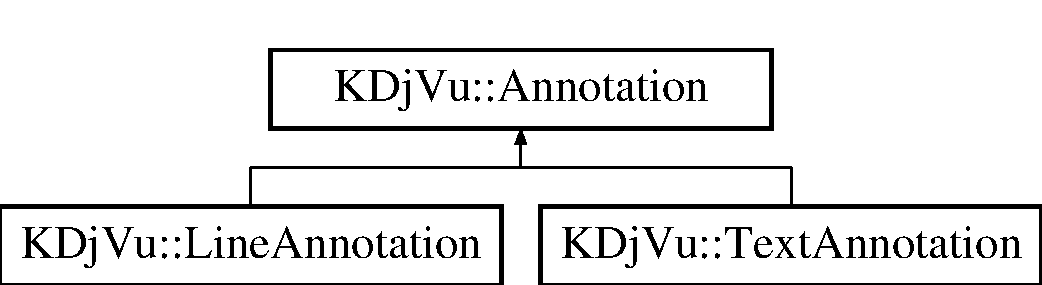
\includegraphics[height=2.000000cm]{classKDjVu_1_1Annotation}
\end{center}
\end{figure}
\subsection*{Public Types}
\begin{DoxyCompactItemize}
\item 
enum \hyperlink{classKDjVu_1_1Annotation_add3feb5fc9e9f7c314afe748c6cf9225}{Annotation\+Type} \{ \hyperlink{classKDjVu_1_1Annotation_add3feb5fc9e9f7c314afe748c6cf9225a435588b8a413abf8c6ec4cb75de5cbde}{Text\+Annotation}, 
\hyperlink{classKDjVu_1_1Annotation_add3feb5fc9e9f7c314afe748c6cf9225aaa9aec60ff07ae12d2b78bbe7add4982}{Line\+Annotation}
 \}
\end{DoxyCompactItemize}
\subsection*{Public Member Functions}
\begin{DoxyCompactItemize}
\item 
virtual \hyperlink{classKDjVu_1_1Annotation_aa9b78fa9a2c4fb2673fcb6dd520dff9f}{$\sim$\+Annotation} ()
\item 
virtual int \hyperlink{classKDjVu_1_1Annotation_a6930b9190e07f47ba5bb097c95f028c5}{type} () const =0
\item 
Q\+Point \hyperlink{classKDjVu_1_1Annotation_ad82c8ab404f11542fdf54d991bfabbf1}{point} () const 
\item 
Q\+String \hyperlink{classKDjVu_1_1Annotation_a156a238b4d2976ab26141e2005bdf822}{comment} () const 
\item 
void \hyperlink{classKDjVu_1_1Annotation_ac43d8309a00f9db14a80ca0e5c0a3a0e}{set\+Comment} (const Q\+String \&\hyperlink{classKDjVu_1_1Annotation_a156a238b4d2976ab26141e2005bdf822}{comment})
\item 
virtual Q\+Color \hyperlink{classKDjVu_1_1Annotation_a7135ef982f0794b604232fa2802a3770}{color} () const 
\item 
virtual void \hyperlink{classKDjVu_1_1Annotation_a9ed0bebe3716db841d9bed53bb08acbe}{set\+Color} (const Q\+Color \&\hyperlink{classKDjVu_1_1Annotation_a7135ef982f0794b604232fa2802a3770}{color})
\end{DoxyCompactItemize}
\subsection*{Protected Member Functions}
\begin{DoxyCompactItemize}
\item 
\hyperlink{classKDjVu_1_1Annotation_a9a57f9591f4fbea73ba4e1c6bd55efc8}{Annotation} (\hyperlink{kdjvu_8h_a58955b1a7edfc6e6ccb48402f744802b}{miniexp\+\_\+t} anno)
\end{DoxyCompactItemize}
\subsection*{Protected Attributes}
\begin{DoxyCompactItemize}
\item 
\hyperlink{kdjvu_8h_a58955b1a7edfc6e6ccb48402f744802b}{miniexp\+\_\+t} \hyperlink{classKDjVu_1_1Annotation_a7334ba00c896becbe9630c5f2e1bbd28}{m\+\_\+anno}
\item 
Q\+Point \hyperlink{classKDjVu_1_1Annotation_af406a7ca02accb64486f23888197c2cb}{m\+\_\+point}
\end{DoxyCompactItemize}
\subsection*{Friends}
\begin{DoxyCompactItemize}
\item 
class \hyperlink{classKDjVu_1_1Annotation_a4241ce0336d22245ffdb13dd5cb6edcc}{K\+Dj\+Vu}
\end{DoxyCompactItemize}


\subsection{Detailed Description}
The base implementation for a Dj\+Vu annotation. 

Definition at line 123 of file kdjvu.\+h.



\subsection{Member Enumeration Documentation}
\hypertarget{classKDjVu_1_1Annotation_add3feb5fc9e9f7c314afe748c6cf9225}{\index{K\+Dj\+Vu\+::\+Annotation@{K\+Dj\+Vu\+::\+Annotation}!Annotation\+Type@{Annotation\+Type}}
\index{Annotation\+Type@{Annotation\+Type}!K\+Dj\+Vu\+::\+Annotation@{K\+Dj\+Vu\+::\+Annotation}}
\subsubsection[{Annotation\+Type}]{\setlength{\rightskip}{0pt plus 5cm}enum {\bf K\+Dj\+Vu\+::\+Annotation\+::\+Annotation\+Type}}}\label{classKDjVu_1_1Annotation_add3feb5fc9e9f7c314afe748c6cf9225}
\begin{Desc}
\item[Enumerator]\par
\begin{description}
\index{Text\+Annotation@{Text\+Annotation}!K\+Dj\+Vu\+::\+Annotation@{K\+Dj\+Vu\+::\+Annotation}}\index{K\+Dj\+Vu\+::\+Annotation@{K\+Dj\+Vu\+::\+Annotation}!Text\+Annotation@{Text\+Annotation}}\item[{\em 
\hypertarget{classKDjVu_1_1Annotation_add3feb5fc9e9f7c314afe748c6cf9225a435588b8a413abf8c6ec4cb75de5cbde}{Text\+Annotation}\label{classKDjVu_1_1Annotation_add3feb5fc9e9f7c314afe748c6cf9225a435588b8a413abf8c6ec4cb75de5cbde}
}]\index{Line\+Annotation@{Line\+Annotation}!K\+Dj\+Vu\+::\+Annotation@{K\+Dj\+Vu\+::\+Annotation}}\index{K\+Dj\+Vu\+::\+Annotation@{K\+Dj\+Vu\+::\+Annotation}!Line\+Annotation@{Line\+Annotation}}\item[{\em 
\hypertarget{classKDjVu_1_1Annotation_add3feb5fc9e9f7c314afe748c6cf9225aaa9aec60ff07ae12d2b78bbe7add4982}{Line\+Annotation}\label{classKDjVu_1_1Annotation_add3feb5fc9e9f7c314afe748c6cf9225aaa9aec60ff07ae12d2b78bbe7add4982}
}]\end{description}
\end{Desc}


Definition at line 130 of file kdjvu.\+h.


\begin{DoxyCode}
130 \{ \hyperlink{classKDjVu_1_1Annotation_add3feb5fc9e9f7c314afe748c6cf9225a435588b8a413abf8c6ec4cb75de5cbde}{TextAnnotation}, \hyperlink{classKDjVu_1_1Annotation_add3feb5fc9e9f7c314afe748c6cf9225aaa9aec60ff07ae12d2b78bbe7add4982}{LineAnnotation} \};
\end{DoxyCode}


\subsection{Constructor \& Destructor Documentation}
\hypertarget{classKDjVu_1_1Annotation_aa9b78fa9a2c4fb2673fcb6dd520dff9f}{\index{K\+Dj\+Vu\+::\+Annotation@{K\+Dj\+Vu\+::\+Annotation}!````~Annotation@{$\sim$\+Annotation}}
\index{````~Annotation@{$\sim$\+Annotation}!K\+Dj\+Vu\+::\+Annotation@{K\+Dj\+Vu\+::\+Annotation}}
\subsubsection[{$\sim$\+Annotation}]{\setlength{\rightskip}{0pt plus 5cm}K\+Dj\+Vu\+::\+Annotation\+::$\sim$\+Annotation (
\begin{DoxyParamCaption}
{}
\end{DoxyParamCaption}
)\hspace{0.3cm}{\ttfamily [virtual]}}}\label{classKDjVu_1_1Annotation_aa9b78fa9a2c4fb2673fcb6dd520dff9f}


Definition at line 256 of file kdjvu.\+cpp.


\begin{DoxyCode}
257 \{
258 \}
\end{DoxyCode}
\hypertarget{classKDjVu_1_1Annotation_a9a57f9591f4fbea73ba4e1c6bd55efc8}{\index{K\+Dj\+Vu\+::\+Annotation@{K\+Dj\+Vu\+::\+Annotation}!Annotation@{Annotation}}
\index{Annotation@{Annotation}!K\+Dj\+Vu\+::\+Annotation@{K\+Dj\+Vu\+::\+Annotation}}
\subsubsection[{Annotation}]{\setlength{\rightskip}{0pt plus 5cm}K\+Dj\+Vu\+::\+Annotation\+::\+Annotation (
\begin{DoxyParamCaption}
\item[{{\bf miniexp\+\_\+t}}]{anno}
\end{DoxyParamCaption}
)\hspace{0.3cm}{\ttfamily [protected]}}}\label{classKDjVu_1_1Annotation_a9a57f9591f4fbea73ba4e1c6bd55efc8}


Definition at line 508 of file annotations.\+cpp.


\begin{DoxyCode}
509     : d\_ptr( &dd )
510 \{
511 \}
\end{DoxyCode}


\subsection{Member Function Documentation}
\hypertarget{classKDjVu_1_1Annotation_a7135ef982f0794b604232fa2802a3770}{\index{K\+Dj\+Vu\+::\+Annotation@{K\+Dj\+Vu\+::\+Annotation}!color@{color}}
\index{color@{color}!K\+Dj\+Vu\+::\+Annotation@{K\+Dj\+Vu\+::\+Annotation}}
\subsubsection[{color}]{\setlength{\rightskip}{0pt plus 5cm}Q\+Color K\+Dj\+Vu\+::\+Annotation\+::color (
\begin{DoxyParamCaption}
{}
\end{DoxyParamCaption}
) const\hspace{0.3cm}{\ttfamily [virtual]}}}\label{classKDjVu_1_1Annotation_a7135ef982f0794b604232fa2802a3770}


Reimplemented in \hyperlink{classKDjVu_1_1LineAnnotation_a6fe74ea84923ac93aede6368b6ee0a19}{K\+Dj\+Vu\+::\+Line\+Annotation}, and \hyperlink{classKDjVu_1_1TextAnnotation_aff59cc205ed543d4ec440d318025468e}{K\+Dj\+Vu\+::\+Text\+Annotation}.



Definition at line 281 of file kdjvu.\+cpp.


\begin{DoxyCode}
282 \{
283     \textcolor{keywordflow}{return} QColor();
284 \}
\end{DoxyCode}
\hypertarget{classKDjVu_1_1Annotation_a156a238b4d2976ab26141e2005bdf822}{\index{K\+Dj\+Vu\+::\+Annotation@{K\+Dj\+Vu\+::\+Annotation}!comment@{comment}}
\index{comment@{comment}!K\+Dj\+Vu\+::\+Annotation@{K\+Dj\+Vu\+::\+Annotation}}
\subsubsection[{comment}]{\setlength{\rightskip}{0pt plus 5cm}Q\+String K\+Dj\+Vu\+::\+Annotation\+::comment (
\begin{DoxyParamCaption}
{}
\end{DoxyParamCaption}
) const}}\label{classKDjVu_1_1Annotation_a156a238b4d2976ab26141e2005bdf822}


Definition at line 268 of file kdjvu.\+cpp.


\begin{DoxyCode}
269 \{
270     \textcolor{keywordflow}{return} QString::fromUtf8( miniexp\_to\_str( miniexp\_nth( 2, \hyperlink{classKDjVu_1_1Annotation_a7334ba00c896becbe9630c5f2e1bbd28}{m\_anno} ) ) );
271 \}
\end{DoxyCode}
\hypertarget{classKDjVu_1_1Annotation_ad82c8ab404f11542fdf54d991bfabbf1}{\index{K\+Dj\+Vu\+::\+Annotation@{K\+Dj\+Vu\+::\+Annotation}!point@{point}}
\index{point@{point}!K\+Dj\+Vu\+::\+Annotation@{K\+Dj\+Vu\+::\+Annotation}}
\subsubsection[{point}]{\setlength{\rightskip}{0pt plus 5cm}Q\+Point K\+Dj\+Vu\+::\+Annotation\+::point (
\begin{DoxyParamCaption}
{}
\end{DoxyParamCaption}
) const}}\label{classKDjVu_1_1Annotation_ad82c8ab404f11542fdf54d991bfabbf1}


Definition at line 260 of file kdjvu.\+cpp.


\begin{DoxyCode}
261 \{
262     \hyperlink{kdjvu_8h_a58955b1a7edfc6e6ccb48402f744802b}{miniexp\_t} area = miniexp\_nth( 3, \hyperlink{classKDjVu_1_1Annotation_a7334ba00c896becbe9630c5f2e1bbd28}{m\_anno} );
263     \textcolor{keywordtype}{int} a = miniexp\_to\_int( miniexp\_nth( 1, area ) );
264     \textcolor{keywordtype}{int} b = miniexp\_to\_int( miniexp\_nth( 2, area ) );
265     \textcolor{keywordflow}{return} QPoint( a, b );
266 \}
\end{DoxyCode}
\hypertarget{classKDjVu_1_1Annotation_a9ed0bebe3716db841d9bed53bb08acbe}{\index{K\+Dj\+Vu\+::\+Annotation@{K\+Dj\+Vu\+::\+Annotation}!set\+Color@{set\+Color}}
\index{set\+Color@{set\+Color}!K\+Dj\+Vu\+::\+Annotation@{K\+Dj\+Vu\+::\+Annotation}}
\subsubsection[{set\+Color}]{\setlength{\rightskip}{0pt plus 5cm}void K\+Dj\+Vu\+::\+Annotation\+::set\+Color (
\begin{DoxyParamCaption}
\item[{const Q\+Color \&}]{color}
\end{DoxyParamCaption}
)\hspace{0.3cm}{\ttfamily [virtual]}}}\label{classKDjVu_1_1Annotation_a9ed0bebe3716db841d9bed53bb08acbe}


Reimplemented in \hyperlink{classKDjVu_1_1LineAnnotation_ac17bb42fe8e9826259be0b702e6fff8a}{K\+Dj\+Vu\+::\+Line\+Annotation}, and \hyperlink{classKDjVu_1_1TextAnnotation_afc4989881d5b7d3b399a3622712edfb9}{K\+Dj\+Vu\+::\+Text\+Annotation}.



Definition at line 286 of file kdjvu.\+cpp.


\begin{DoxyCode}
287 \{
288 \}
\end{DoxyCode}
\hypertarget{classKDjVu_1_1Annotation_ac43d8309a00f9db14a80ca0e5c0a3a0e}{\index{K\+Dj\+Vu\+::\+Annotation@{K\+Dj\+Vu\+::\+Annotation}!set\+Comment@{set\+Comment}}
\index{set\+Comment@{set\+Comment}!K\+Dj\+Vu\+::\+Annotation@{K\+Dj\+Vu\+::\+Annotation}}
\subsubsection[{set\+Comment}]{\setlength{\rightskip}{0pt plus 5cm}void K\+Dj\+Vu\+::\+Annotation\+::set\+Comment (
\begin{DoxyParamCaption}
\item[{const Q\+String \&}]{comment}
\end{DoxyParamCaption}
)}}\label{classKDjVu_1_1Annotation_ac43d8309a00f9db14a80ca0e5c0a3a0e}


Definition at line 273 of file kdjvu.\+cpp.


\begin{DoxyCode}
274 \{
275     \hyperlink{kdjvu_8h_a58955b1a7edfc6e6ccb48402f744802b}{miniexp\_t} exp = \hyperlink{classKDjVu_1_1Annotation_a7334ba00c896becbe9630c5f2e1bbd28}{m\_anno};
276     exp = miniexp\_cdr( exp );
277     exp = miniexp\_cdr( exp );
278     miniexp\_rplaca( exp, miniexp\_string( \hyperlink{classKDjVu_1_1Annotation_a156a238b4d2976ab26141e2005bdf822}{comment}.toUtf8() ) );
279 \}
\end{DoxyCode}
\hypertarget{classKDjVu_1_1Annotation_a6930b9190e07f47ba5bb097c95f028c5}{\index{K\+Dj\+Vu\+::\+Annotation@{K\+Dj\+Vu\+::\+Annotation}!type@{type}}
\index{type@{type}!K\+Dj\+Vu\+::\+Annotation@{K\+Dj\+Vu\+::\+Annotation}}
\subsubsection[{type}]{\setlength{\rightskip}{0pt plus 5cm}virtual int K\+Dj\+Vu\+::\+Annotation\+::type (
\begin{DoxyParamCaption}
{}
\end{DoxyParamCaption}
) const\hspace{0.3cm}{\ttfamily [pure virtual]}}}\label{classKDjVu_1_1Annotation_a6930b9190e07f47ba5bb097c95f028c5}


Implemented in \hyperlink{classKDjVu_1_1LineAnnotation_a02b3c6d99ad38e7e9c2af1822aec0e18}{K\+Dj\+Vu\+::\+Line\+Annotation}, and \hyperlink{classKDjVu_1_1TextAnnotation_a992ee92b526e912ee1dd6338c54eb350}{K\+Dj\+Vu\+::\+Text\+Annotation}.



\subsection{Friends And Related Function Documentation}
\hypertarget{classKDjVu_1_1Annotation_a4241ce0336d22245ffdb13dd5cb6edcc}{\index{K\+Dj\+Vu\+::\+Annotation@{K\+Dj\+Vu\+::\+Annotation}!K\+Dj\+Vu@{K\+Dj\+Vu}}
\index{K\+Dj\+Vu@{K\+Dj\+Vu}!K\+Dj\+Vu\+::\+Annotation@{K\+Dj\+Vu\+::\+Annotation}}
\subsubsection[{K\+Dj\+Vu}]{\setlength{\rightskip}{0pt plus 5cm}friend class {\bf K\+Dj\+Vu}\hspace{0.3cm}{\ttfamily [friend]}}}\label{classKDjVu_1_1Annotation_a4241ce0336d22245ffdb13dd5cb6edcc}


Definition at line 125 of file kdjvu.\+h.



\subsection{Member Data Documentation}
\hypertarget{classKDjVu_1_1Annotation_a7334ba00c896becbe9630c5f2e1bbd28}{\index{K\+Dj\+Vu\+::\+Annotation@{K\+Dj\+Vu\+::\+Annotation}!m\+\_\+anno@{m\+\_\+anno}}
\index{m\+\_\+anno@{m\+\_\+anno}!K\+Dj\+Vu\+::\+Annotation@{K\+Dj\+Vu\+::\+Annotation}}
\subsubsection[{m\+\_\+anno}]{\setlength{\rightskip}{0pt plus 5cm}{\bf miniexp\+\_\+t} K\+Dj\+Vu\+::\+Annotation\+::m\+\_\+anno\hspace{0.3cm}{\ttfamily [protected]}}}\label{classKDjVu_1_1Annotation_a7334ba00c896becbe9630c5f2e1bbd28}


Definition at line 141 of file kdjvu.\+h.

\hypertarget{classKDjVu_1_1Annotation_af406a7ca02accb64486f23888197c2cb}{\index{K\+Dj\+Vu\+::\+Annotation@{K\+Dj\+Vu\+::\+Annotation}!m\+\_\+point@{m\+\_\+point}}
\index{m\+\_\+point@{m\+\_\+point}!K\+Dj\+Vu\+::\+Annotation@{K\+Dj\+Vu\+::\+Annotation}}
\subsubsection[{m\+\_\+point}]{\setlength{\rightskip}{0pt plus 5cm}Q\+Point K\+Dj\+Vu\+::\+Annotation\+::m\+\_\+point\hspace{0.3cm}{\ttfamily [protected]}}}\label{classKDjVu_1_1Annotation_af406a7ca02accb64486f23888197c2cb}


Definition at line 142 of file kdjvu.\+h.



The documentation for this class was generated from the following files\+:\begin{DoxyCompactItemize}
\item 
generators/djvu/\hyperlink{kdjvu_8h}{kdjvu.\+h}\item 
core/\hyperlink{annotations_8cpp}{annotations.\+cpp}\item 
generators/djvu/\hyperlink{kdjvu_8cpp}{kdjvu.\+cpp}\end{DoxyCompactItemize}

\hypertarget{classOkular_1_1Annotation}{\section{Okular\+:\+:Annotation Class Reference}
\label{classOkular_1_1Annotation}\index{Okular\+::\+Annotation@{Okular\+::\+Annotation}}
}


\hyperlink{classOkular_1_1Annotation}{Annotation} struct holds properties shared by all annotations.  




{\ttfamily \#include $<$annotations.\+h$>$}

Inheritance diagram for Okular\+:\+:Annotation\+:\begin{figure}[H]
\begin{center}
\leavevmode
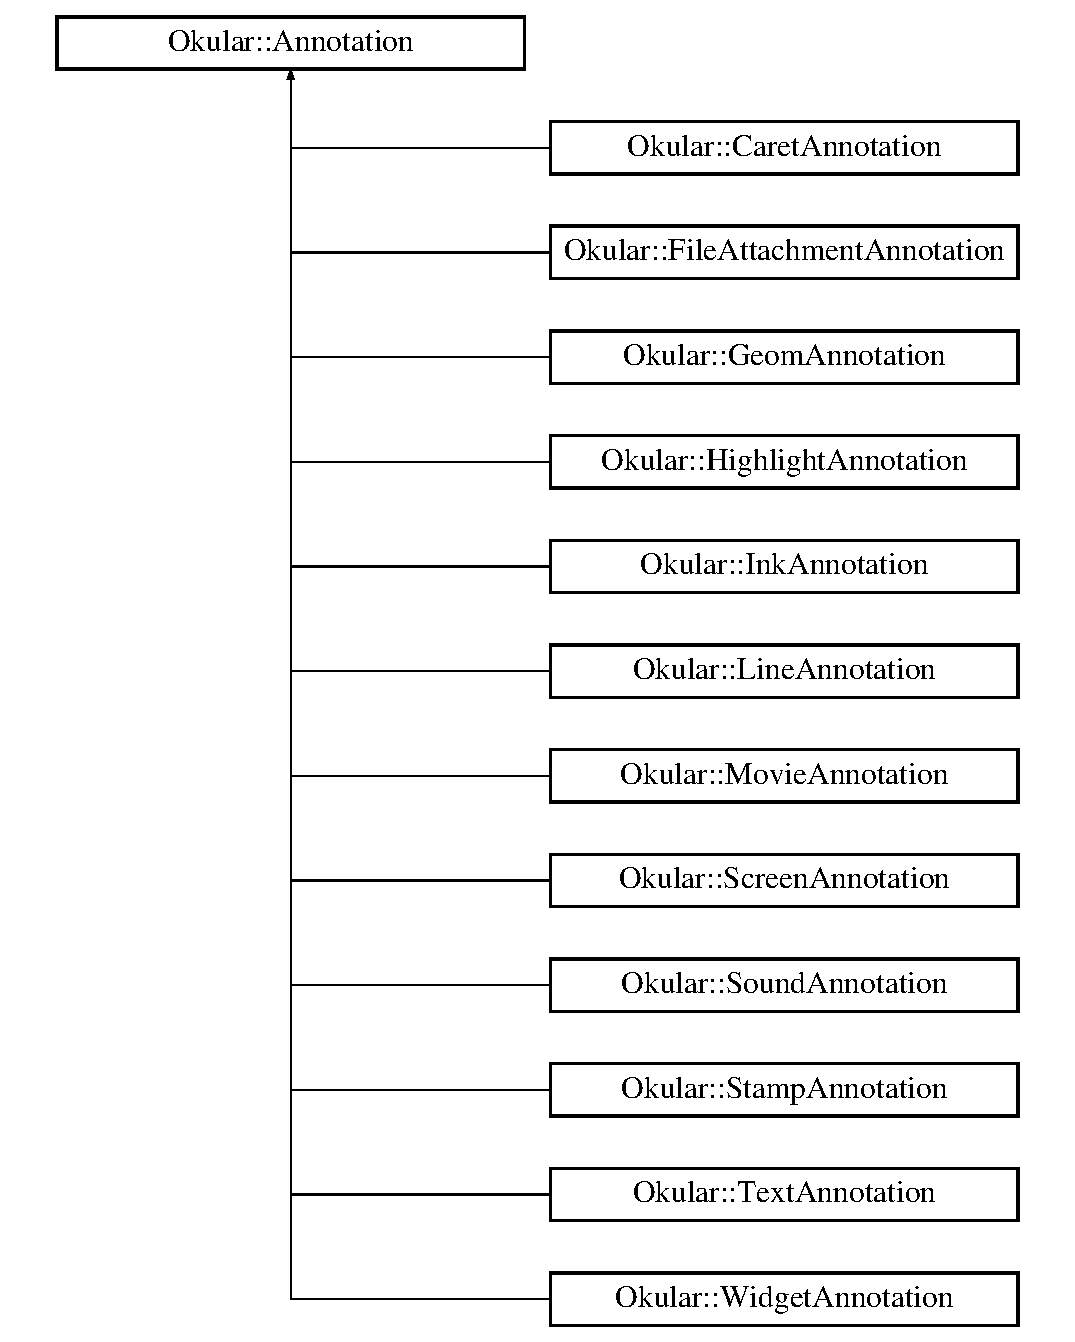
\includegraphics[height=12.000000cm]{classOkular_1_1Annotation}
\end{center}
\end{figure}
\subsection*{Classes}
\begin{DoxyCompactItemize}
\item 
class \hyperlink{classOkular_1_1Annotation_1_1Revision}{Revision}
\item 
class \hyperlink{classOkular_1_1Annotation_1_1Style}{Style}
\item 
class \hyperlink{classOkular_1_1Annotation_1_1Window}{Window}
\end{DoxyCompactItemize}
\subsection*{Public Types}
\begin{DoxyCompactItemize}
\item 
enum \hyperlink{classOkular_1_1Annotation_af71b46e37d5f850b97d5c4de3be9aac0}{Sub\+Type} \{ \\*
\hyperlink{classOkular_1_1Annotation_af71b46e37d5f850b97d5c4de3be9aac0a48f93d5a9352abc4e38a45f69075e504}{A\+Text} = 1, 
\hyperlink{classOkular_1_1Annotation_af71b46e37d5f850b97d5c4de3be9aac0a7035dc978d8b79958f34e3d164838726}{A\+Line} = 2, 
\hyperlink{classOkular_1_1Annotation_af71b46e37d5f850b97d5c4de3be9aac0a2c11d328af34f5526fd9e761297fb3c2}{A\+Geom} = 3, 
\hyperlink{classOkular_1_1Annotation_af71b46e37d5f850b97d5c4de3be9aac0a03e002f9ae62005b2d7c7f1445507501}{A\+Highlight} = 4, 
\\*
\hyperlink{classOkular_1_1Annotation_af71b46e37d5f850b97d5c4de3be9aac0ad542ded420c9b01f44ee923bf28ecd9a}{A\+Stamp} = 5, 
\hyperlink{classOkular_1_1Annotation_af71b46e37d5f850b97d5c4de3be9aac0a4ed60063584ceb146c2a378f0df4ed37}{A\+Ink} = 6, 
\hyperlink{classOkular_1_1Annotation_af71b46e37d5f850b97d5c4de3be9aac0a904187454fd508d898a3d5843193ad43}{A\+Caret} = 8, 
\hyperlink{classOkular_1_1Annotation_af71b46e37d5f850b97d5c4de3be9aac0a7209cbfb5e13c0f80ac36f87c9575836}{A\+File\+Attachment} = 9, 
\\*
\hyperlink{classOkular_1_1Annotation_af71b46e37d5f850b97d5c4de3be9aac0a9e75622bfcf537319a904538840a0bce}{A\+Sound} = 10, 
\hyperlink{classOkular_1_1Annotation_af71b46e37d5f850b97d5c4de3be9aac0a711a9d706a86b55f0799e944fb2750e6}{A\+Movie} = 11, 
\hyperlink{classOkular_1_1Annotation_af71b46e37d5f850b97d5c4de3be9aac0a7cf8ba374ec139a8e2fb47a36182fa32}{A\+Screen} = 12, 
\hyperlink{classOkular_1_1Annotation_af71b46e37d5f850b97d5c4de3be9aac0aa0f6a560b971fe69d18156176258d6c8}{A\+Widget} = 13, 
\\*
\hyperlink{classOkular_1_1Annotation_af71b46e37d5f850b97d5c4de3be9aac0a9064a6f3c5e70f272462bb78a1af6c55}{A\+\_\+\+B\+A\+S\+E} = 0
 \}
\item 
enum \hyperlink{classOkular_1_1Annotation_a8a214541446745761efeda70b3a4302e}{Flag} \{ \\*
\hyperlink{classOkular_1_1Annotation_a8a214541446745761efeda70b3a4302ea053e3857f5c7f494a996e649e5e97244}{Hidden} = 1, 
\hyperlink{classOkular_1_1Annotation_a8a214541446745761efeda70b3a4302eaa392139d58e61edfc34c3574d835448f}{Fixed\+Size} = 2, 
\hyperlink{classOkular_1_1Annotation_a8a214541446745761efeda70b3a4302ea31a80c8e10831d2dccdf80cadb74fb3c}{Fixed\+Rotation} = 4, 
\hyperlink{classOkular_1_1Annotation_a8a214541446745761efeda70b3a4302ea06c4d960d7e0537c702c5b21a445001e}{Deny\+Print} = 8, 
\\*
\hyperlink{classOkular_1_1Annotation_a8a214541446745761efeda70b3a4302ead5a9f7601c7a91f887f03bf90a933740}{Deny\+Write} = 16, 
\hyperlink{classOkular_1_1Annotation_a8a214541446745761efeda70b3a4302ea1ac69f31d992e95ae3c11420875c6293}{Deny\+Delete} = 32, 
\hyperlink{classOkular_1_1Annotation_a8a214541446745761efeda70b3a4302ea6709674abe1d70451bf9f70252d46a35}{Toggle\+Hiding\+On\+Mouse} = 64, 
\hyperlink{classOkular_1_1Annotation_a8a214541446745761efeda70b3a4302eabe908102c97a725aa1928602f17833c0}{External} = 128, 
\\*
\hyperlink{classOkular_1_1Annotation_a8a214541446745761efeda70b3a4302ea75f088f5533ace9d9d47a506b707f5a1}{Externally\+Drawn} = 256, 
\hyperlink{classOkular_1_1Annotation_a8a214541446745761efeda70b3a4302ea9cd51e0fe53aac93798a205e7fb5c04a}{Being\+Moved} = 512
 \}
\item 
enum \hyperlink{classOkular_1_1Annotation_ac60f5de2d449043f9f849f3f081f8a7a}{Line\+Style} \{ \\*
\hyperlink{classOkular_1_1Annotation_ac60f5de2d449043f9f849f3f081f8a7aabd593eeaf0fb9140018ea50a9d0bb80b}{Solid} = 1, 
\hyperlink{classOkular_1_1Annotation_ac60f5de2d449043f9f849f3f081f8a7aaaf72c26f0e585f2512e0c323d7e0c5e9}{Dashed} = 2, 
\hyperlink{classOkular_1_1Annotation_ac60f5de2d449043f9f849f3f081f8a7aa1cdd133335b77eb2a3fa81b5765bc708}{Beveled} = 4, 
\hyperlink{classOkular_1_1Annotation_ac60f5de2d449043f9f849f3f081f8a7aaa33d215eb30ca1e449f8b5aa6572c6e3}{Inset} = 8, 
\\*
\hyperlink{classOkular_1_1Annotation_ac60f5de2d449043f9f849f3f081f8a7aa130bf6bc106c1f2daac86abcb1157dde}{Underline} = 16
 \}
\item 
enum \hyperlink{classOkular_1_1Annotation_a9083f89e7bb24e972852685dd2c6176e}{Line\+Effect} \{ \hyperlink{classOkular_1_1Annotation_a9083f89e7bb24e972852685dd2c6176eaf13ac621a84f14cf6dbb465c4fd73c1b}{No\+Effect} = 1, 
\hyperlink{classOkular_1_1Annotation_a9083f89e7bb24e972852685dd2c6176eaf5545cd17b4a4a61efb555f391959f78}{Cloudy} = 2
 \}
\item 
enum \hyperlink{classOkular_1_1Annotation_a9f71f811fcd4d3524e199e7eee4b6390}{Revision\+Scope} \{ \hyperlink{classOkular_1_1Annotation_a9f71f811fcd4d3524e199e7eee4b6390aa2237555e16222f3bb84b1fffde12400}{Reply} = 1, 
\hyperlink{classOkular_1_1Annotation_a9f71f811fcd4d3524e199e7eee4b6390ad3931cacca440fc5f76d00f54767d5bd}{Group} = 2, 
\hyperlink{classOkular_1_1Annotation_a9f71f811fcd4d3524e199e7eee4b6390acff66214c6f28e20c2ead17fed4748f0}{Delete} = 4
 \}
\item 
enum \hyperlink{classOkular_1_1Annotation_a76de7f3bda49c63bd319763c6ac46bd3}{Revision\+Type} \{ \\*
\hyperlink{classOkular_1_1Annotation_a76de7f3bda49c63bd319763c6ac46bd3ad1a6ce1ab54a66f7c1e726616159e74b}{None} = 1, 
\hyperlink{classOkular_1_1Annotation_a76de7f3bda49c63bd319763c6ac46bd3a2eb874d989f9ffa721cbd3a3d21709fe}{Marked} = 2, 
\hyperlink{classOkular_1_1Annotation_a76de7f3bda49c63bd319763c6ac46bd3af8b9d3d51681e0f5c7ce0958220484c8}{Unmarked} = 4, 
\hyperlink{classOkular_1_1Annotation_a76de7f3bda49c63bd319763c6ac46bd3af346f95894089e3d11ba85f52ca13885}{Accepted} = 8, 
\\*
\hyperlink{classOkular_1_1Annotation_a76de7f3bda49c63bd319763c6ac46bd3ae468fddc13c591b177bcf79368b851d3}{Rejected} = 16, 
\hyperlink{classOkular_1_1Annotation_a76de7f3bda49c63bd319763c6ac46bd3a769110a27deca021bac985d4a06f04d8}{Cancelled} = 32, 
\hyperlink{classOkular_1_1Annotation_a76de7f3bda49c63bd319763c6ac46bd3a836b685f81342007f2d84a33ebbb0515}{Completed} = 64
 \}
\item 
enum \hyperlink{classOkular_1_1Annotation_aa34152e337b1cb13e9327f37fc295057}{Additional\+Action\+Type} \{ \hyperlink{classOkular_1_1Annotation_aa34152e337b1cb13e9327f37fc295057a46ab9d0c7ed65157b6982a807975b7f0}{Page\+Opening}, 
\hyperlink{classOkular_1_1Annotation_aa34152e337b1cb13e9327f37fc295057a163dda71b8c9ac45ce1c250f37458bac}{Page\+Closing}
 \}
\item 
typedef void($\ast$ \hyperlink{classOkular_1_1Annotation_a4f2759100645cdce807944767937dd18}{Dispose\+Data\+Function} )(const \hyperlink{classOkular_1_1Annotation}{Okular\+::\+Annotation} $\ast$)
\end{DoxyCompactItemize}
\subsection*{Public Member Functions}
\begin{DoxyCompactItemize}
\item 
virtual \hyperlink{classOkular_1_1Annotation_a95144855eb445040d47951c668dc5764}{$\sim$\+Annotation} ()
\item 
void \hyperlink{classOkular_1_1Annotation_ac67827a495bc3ca9fc91c82590c7bf35}{set\+Author} (const Q\+String \&\hyperlink{classOkular_1_1Annotation_a45682b53c24e4f5d41c547d6e109f6a4}{author})
\item 
Q\+String \hyperlink{classOkular_1_1Annotation_a45682b53c24e4f5d41c547d6e109f6a4}{author} () const 
\item 
void \hyperlink{classOkular_1_1Annotation_a65a7316062031c6fdf578835245ddbd1}{set\+Contents} (const Q\+String \&\hyperlink{classOkular_1_1Annotation_a3b0c9fcbe9d01e06bfcc7216d0035908}{contents})
\item 
Q\+String \hyperlink{classOkular_1_1Annotation_a3b0c9fcbe9d01e06bfcc7216d0035908}{contents} () const 
\item 
void \hyperlink{classOkular_1_1Annotation_a9a9c80155d92ff897450e4a06f84d7f1}{set\+Unique\+Name} (const Q\+String \&name)
\item 
Q\+String \hyperlink{classOkular_1_1Annotation_a8a86ff8c722014c2296112d0fa703eab}{unique\+Name} () const 
\item 
void \hyperlink{classOkular_1_1Annotation_a1ea7e94039a7dc3dce500ae96817b30d}{set\+Modification\+Date} (const Q\+Date\+Time \&date)
\item 
Q\+Date\+Time \hyperlink{classOkular_1_1Annotation_a4bee8f09724539e15f435b643049f2c1}{modification\+Date} () const 
\item 
void \hyperlink{classOkular_1_1Annotation_a7b8e97b104dc0b8cd8ff95253d95e167}{set\+Creation\+Date} (const Q\+Date\+Time \&date)
\item 
Q\+Date\+Time \hyperlink{classOkular_1_1Annotation_ad775b0d2925d50334d46efc1a2689e5b}{creation\+Date} () const 
\item 
void \hyperlink{classOkular_1_1Annotation_ab91b36dc7ecfd9cacba7761ec58145fd}{set\+Flags} (int \hyperlink{classOkular_1_1Annotation_a3d6f7ee5057155b90e76c24768880947}{flags})
\item 
int \hyperlink{classOkular_1_1Annotation_a3d6f7ee5057155b90e76c24768880947}{flags} () const 
\item 
void \hyperlink{classOkular_1_1Annotation_a6977075c78f130b71ddbbda924480f38}{set\+Bounding\+Rectangle} (const \hyperlink{classOkular_1_1NormalizedRect}{Normalized\+Rect} \&rectangle)
\item 
\hyperlink{classOkular_1_1NormalizedRect}{Normalized\+Rect} \hyperlink{classOkular_1_1Annotation_a450fbd08aeb31262a33a628b4ab0dd42}{bounding\+Rectangle} () const 
\item 
\hyperlink{classOkular_1_1NormalizedRect}{Normalized\+Rect} \hyperlink{classOkular_1_1Annotation_a950ea9c7993878729eb4b6b0ea922436}{transformed\+Bounding\+Rectangle} () const 
\item 
void \hyperlink{classOkular_1_1Annotation_ae0ef33b85b6049645b7a94fd97984d52}{translate} (const \hyperlink{classOkular_1_1NormalizedPoint}{Normalized\+Point} \&coord)
\item 
\hyperlink{classOkular_1_1Annotation_1_1Style}{Style} \& \hyperlink{classOkular_1_1Annotation_ae1f845ddbd6d524b2b388c6c9ef26423}{style} ()
\item 
const \hyperlink{classOkular_1_1Annotation_1_1Style}{Style} \& \hyperlink{classOkular_1_1Annotation_ab753347d676ebf1da5371bc40cf6dcb8}{style} () const 
\item 
\hyperlink{classOkular_1_1Annotation_1_1Window}{Window} \& \hyperlink{classOkular_1_1Annotation_a560281f35ace621f48181a7c7977ca7f}{window} ()
\item 
const \hyperlink{classOkular_1_1Annotation_1_1Window}{Window} \& \hyperlink{classOkular_1_1Annotation_af96fe7c314bc49e869d5e28b8efa928b}{window} () const 
\item 
\hyperlink{classQLinkedList}{Q\+Linked\+List}$<$ \hyperlink{classOkular_1_1Annotation_1_1Revision}{Revision} $>$ \& \hyperlink{classOkular_1_1Annotation_a3d157b31fb9d228999cf1042fc523251}{revisions} ()
\item 
const \hyperlink{classQLinkedList}{Q\+Linked\+List}$<$ \hyperlink{classOkular_1_1Annotation_1_1Revision}{Revision} $>$ \& \hyperlink{classOkular_1_1Annotation_a96c59d107de84f13b38784a7c419bd60}{revisions} () const 
\item 
void \hyperlink{classOkular_1_1Annotation_a77c8188ca0d81966c29aebe0ef7ccfef}{set\+Native\+Id} (const Q\+Variant \&id)
\item 
Q\+Variant \hyperlink{classOkular_1_1Annotation_a1551f5ed393ffe61c30087cf2c78dac6}{native\+Id} () const 
\item 
void \hyperlink{classOkular_1_1Annotation_a83d33746416b0a8fc528da35db3e9849}{set\+Dispose\+Data\+Function} (\hyperlink{classOkular_1_1Annotation_a4f2759100645cdce807944767937dd18}{Dispose\+Data\+Function} func)
\item 
bool \hyperlink{classOkular_1_1Annotation_aebeab4bec3d43cdb6498c6b9d9b59adf}{can\+Be\+Moved} () const 
\item 
bool \hyperlink{classOkular_1_1Annotation_a0dc9c020d3887707b383bdf5abb3c1c1}{open\+Dialog\+After\+Creation} () const 
\item 
virtual \hyperlink{classOkular_1_1Annotation_af71b46e37d5f850b97d5c4de3be9aac0}{Sub\+Type} \hyperlink{classOkular_1_1Annotation_af9833449767eacd740f377e69a1fdd48}{sub\+Type} () const =0
\item 
virtual void \hyperlink{classOkular_1_1Annotation_abbb607cf5929ffd06f789a22b353dcb3}{store} (Q\+Dom\+Node \&node, Q\+Dom\+Document \&document) const 
\item 
Q\+Dom\+Node \hyperlink{classOkular_1_1Annotation_ad7c117b9cc13d8987d2bcff8e4ed25f7}{get\+Annotation\+Properties\+Dom\+Node} () const 
\item 
void \hyperlink{classOkular_1_1Annotation_aea088e2d137bc017f0b78cce86642ff1}{set\+Annotation\+Properties} (const Q\+Dom\+Node \&node)
\end{DoxyCompactItemize}


\subsection{Detailed Description}
\hyperlink{classOkular_1_1Annotation}{Annotation} struct holds properties shared by all annotations. 

An \hyperlink{classOkular_1_1Annotation}{Annotation} is an object (text note, highlight, sound, popup window, ..) contained by a \hyperlink{classOkular_1_1Page}{Page} in the document. 

Definition at line 90 of file annotations.\+h.



\subsection{Member Typedef Documentation}
\hypertarget{classOkular_1_1Annotation_a4f2759100645cdce807944767937dd18}{\index{Okular\+::\+Annotation@{Okular\+::\+Annotation}!Dispose\+Data\+Function@{Dispose\+Data\+Function}}
\index{Dispose\+Data\+Function@{Dispose\+Data\+Function}!Okular\+::\+Annotation@{Okular\+::\+Annotation}}
\subsubsection[{Dispose\+Data\+Function}]{\setlength{\rightskip}{0pt plus 5cm}typedef void( $\ast$  Okular\+::\+Annotation\+::\+Dispose\+Data\+Function)(const {\bf Okular\+::\+Annotation} $\ast$)}}\label{classOkular_1_1Annotation_a4f2759100645cdce807944767937dd18}
A function to be called when the annotation is destroyed.

\begin{DoxyWarning}{Warning}
the function must {\itshape not} call any virtual function, nor subcast.
\end{DoxyWarning}
\begin{DoxySince}{Since}
0.\+7 (K\+D\+E 4.\+1) 
\end{DoxySince}


Definition at line 203 of file annotations.\+h.



\subsection{Member Enumeration Documentation}
\hypertarget{classOkular_1_1Annotation_aa34152e337b1cb13e9327f37fc295057}{\index{Okular\+::\+Annotation@{Okular\+::\+Annotation}!Additional\+Action\+Type@{Additional\+Action\+Type}}
\index{Additional\+Action\+Type@{Additional\+Action\+Type}!Okular\+::\+Annotation@{Okular\+::\+Annotation}}
\subsubsection[{Additional\+Action\+Type}]{\setlength{\rightskip}{0pt plus 5cm}enum {\bf Okular\+::\+Annotation\+::\+Additional\+Action\+Type}}}\label{classOkular_1_1Annotation_aa34152e337b1cb13e9327f37fc295057}
Describes the type of additional actions.

\begin{DoxySince}{Since}
0.\+16 (K\+D\+E 4.\+10) 
\end{DoxySince}
\begin{Desc}
\item[Enumerator]\par
\begin{description}
\index{Page\+Opening@{Page\+Opening}!Okular\+::\+Annotation@{Okular\+::\+Annotation}}\index{Okular\+::\+Annotation@{Okular\+::\+Annotation}!Page\+Opening@{Page\+Opening}}\item[{\em 
\hypertarget{classOkular_1_1Annotation_aa34152e337b1cb13e9327f37fc295057a46ab9d0c7ed65157b6982a807975b7f0}{Page\+Opening}\label{classOkular_1_1Annotation_aa34152e337b1cb13e9327f37fc295057a46ab9d0c7ed65157b6982a807975b7f0}
}]Performed when the page containing the annotation is opened. \index{Page\+Closing@{Page\+Closing}!Okular\+::\+Annotation@{Okular\+::\+Annotation}}\index{Okular\+::\+Annotation@{Okular\+::\+Annotation}!Page\+Closing@{Page\+Closing}}\item[{\em 
\hypertarget{classOkular_1_1Annotation_aa34152e337b1cb13e9327f37fc295057a163dda71b8c9ac45ce1c250f37458bac}{Page\+Closing}\label{classOkular_1_1Annotation_aa34152e337b1cb13e9327f37fc295057a163dda71b8c9ac45ce1c250f37458bac}
}]Performed when the page containing the annotation is closed. \end{description}
\end{Desc}


Definition at line 189 of file annotations.\+h.


\begin{DoxyCode}
190         \{
191             \hyperlink{classOkular_1_1Annotation_aa34152e337b1cb13e9327f37fc295057a46ab9d0c7ed65157b6982a807975b7f0}{PageOpening}, 
192             \hyperlink{classOkular_1_1Annotation_aa34152e337b1cb13e9327f37fc295057a163dda71b8c9ac45ce1c250f37458bac}{PageClosing}  
193         \};
\end{DoxyCode}
\hypertarget{classOkular_1_1Annotation_a8a214541446745761efeda70b3a4302e}{\index{Okular\+::\+Annotation@{Okular\+::\+Annotation}!Flag@{Flag}}
\index{Flag@{Flag}!Okular\+::\+Annotation@{Okular\+::\+Annotation}}
\subsubsection[{Flag}]{\setlength{\rightskip}{0pt plus 5cm}enum {\bf Okular\+::\+Annotation\+::\+Flag}}}\label{classOkular_1_1Annotation_a8a214541446745761efeda70b3a4302e}
Describes additional properties of an annotation. \begin{Desc}
\item[Enumerator]\par
\begin{description}
\index{Hidden@{Hidden}!Okular\+::\+Annotation@{Okular\+::\+Annotation}}\index{Okular\+::\+Annotation@{Okular\+::\+Annotation}!Hidden@{Hidden}}\item[{\em 
\hypertarget{classOkular_1_1Annotation_a8a214541446745761efeda70b3a4302ea053e3857f5c7f494a996e649e5e97244}{Hidden}\label{classOkular_1_1Annotation_a8a214541446745761efeda70b3a4302ea053e3857f5c7f494a996e649e5e97244}
}]Is not shown in the document. \index{Fixed\+Size@{Fixed\+Size}!Okular\+::\+Annotation@{Okular\+::\+Annotation}}\index{Okular\+::\+Annotation@{Okular\+::\+Annotation}!Fixed\+Size@{Fixed\+Size}}\item[{\em 
\hypertarget{classOkular_1_1Annotation_a8a214541446745761efeda70b3a4302eaa392139d58e61edfc34c3574d835448f}{Fixed\+Size}\label{classOkular_1_1Annotation_a8a214541446745761efeda70b3a4302eaa392139d58e61edfc34c3574d835448f}
}]Has a fixed size. \index{Fixed\+Rotation@{Fixed\+Rotation}!Okular\+::\+Annotation@{Okular\+::\+Annotation}}\index{Okular\+::\+Annotation@{Okular\+::\+Annotation}!Fixed\+Rotation@{Fixed\+Rotation}}\item[{\em 
\hypertarget{classOkular_1_1Annotation_a8a214541446745761efeda70b3a4302ea31a80c8e10831d2dccdf80cadb74fb3c}{Fixed\+Rotation}\label{classOkular_1_1Annotation_a8a214541446745761efeda70b3a4302ea31a80c8e10831d2dccdf80cadb74fb3c}
}]Has a fixed rotation. \index{Deny\+Print@{Deny\+Print}!Okular\+::\+Annotation@{Okular\+::\+Annotation}}\index{Okular\+::\+Annotation@{Okular\+::\+Annotation}!Deny\+Print@{Deny\+Print}}\item[{\em 
\hypertarget{classOkular_1_1Annotation_a8a214541446745761efeda70b3a4302ea06c4d960d7e0537c702c5b21a445001e}{Deny\+Print}\label{classOkular_1_1Annotation_a8a214541446745761efeda70b3a4302ea06c4d960d7e0537c702c5b21a445001e}
}]Cannot be printed. \index{Deny\+Write@{Deny\+Write}!Okular\+::\+Annotation@{Okular\+::\+Annotation}}\index{Okular\+::\+Annotation@{Okular\+::\+Annotation}!Deny\+Write@{Deny\+Write}}\item[{\em 
\hypertarget{classOkular_1_1Annotation_a8a214541446745761efeda70b3a4302ead5a9f7601c7a91f887f03bf90a933740}{Deny\+Write}\label{classOkular_1_1Annotation_a8a214541446745761efeda70b3a4302ead5a9f7601c7a91f887f03bf90a933740}
}]Cannot be changed. \index{Deny\+Delete@{Deny\+Delete}!Okular\+::\+Annotation@{Okular\+::\+Annotation}}\index{Okular\+::\+Annotation@{Okular\+::\+Annotation}!Deny\+Delete@{Deny\+Delete}}\item[{\em 
\hypertarget{classOkular_1_1Annotation_a8a214541446745761efeda70b3a4302ea1ac69f31d992e95ae3c11420875c6293}{Deny\+Delete}\label{classOkular_1_1Annotation_a8a214541446745761efeda70b3a4302ea1ac69f31d992e95ae3c11420875c6293}
}]Cannot be deleted. \index{Toggle\+Hiding\+On\+Mouse@{Toggle\+Hiding\+On\+Mouse}!Okular\+::\+Annotation@{Okular\+::\+Annotation}}\index{Okular\+::\+Annotation@{Okular\+::\+Annotation}!Toggle\+Hiding\+On\+Mouse@{Toggle\+Hiding\+On\+Mouse}}\item[{\em 
\hypertarget{classOkular_1_1Annotation_a8a214541446745761efeda70b3a4302ea6709674abe1d70451bf9f70252d46a35}{Toggle\+Hiding\+On\+Mouse}\label{classOkular_1_1Annotation_a8a214541446745761efeda70b3a4302ea6709674abe1d70451bf9f70252d46a35}
}]Can be hidden/shown by mouse click. \index{External@{External}!Okular\+::\+Annotation@{Okular\+::\+Annotation}}\index{Okular\+::\+Annotation@{Okular\+::\+Annotation}!External@{External}}\item[{\em 
\hypertarget{classOkular_1_1Annotation_a8a214541446745761efeda70b3a4302eabe908102c97a725aa1928602f17833c0}{External}\label{classOkular_1_1Annotation_a8a214541446745761efeda70b3a4302eabe908102c97a725aa1928602f17833c0}
}]Is stored external. \index{Externally\+Drawn@{Externally\+Drawn}!Okular\+::\+Annotation@{Okular\+::\+Annotation}}\index{Okular\+::\+Annotation@{Okular\+::\+Annotation}!Externally\+Drawn@{Externally\+Drawn}}\item[{\em 
\hypertarget{classOkular_1_1Annotation_a8a214541446745761efeda70b3a4302ea75f088f5533ace9d9d47a506b707f5a1}{Externally\+Drawn}\label{classOkular_1_1Annotation_a8a214541446745761efeda70b3a4302ea75f088f5533ace9d9d47a506b707f5a1}
}]Is drawn externally (by the generator which provided it) \begin{DoxySince}{Since}
0.\+10 (K\+D\+E 4.\+4) 
\end{DoxySince}
\index{Being\+Moved@{Being\+Moved}!Okular\+::\+Annotation@{Okular\+::\+Annotation}}\index{Okular\+::\+Annotation@{Okular\+::\+Annotation}!Being\+Moved@{Being\+Moved}}\item[{\em 
\hypertarget{classOkular_1_1Annotation_a8a214541446745761efeda70b3a4302ea9cd51e0fe53aac93798a205e7fb5c04a}{Being\+Moved}\label{classOkular_1_1Annotation_a8a214541446745761efeda70b3a4302ea9cd51e0fe53aac93798a205e7fb5c04a}
}]Is being moved (mouse drag and drop). If Externally\+Drawn, the generator must not draw it. \begin{DoxySince}{Since}
0.\+15 (K\+D\+E 4.\+9) 
\end{DoxySince}
\end{description}
\end{Desc}


Definition at line 125 of file annotations.\+h.


\begin{DoxyCode}
126         \{
127             \hyperlink{classOkular_1_1Annotation_a8a214541446745761efeda70b3a4302ea053e3857f5c7f494a996e649e5e97244}{Hidden} = 1,               
128             \hyperlink{classOkular_1_1Annotation_a8a214541446745761efeda70b3a4302eaa392139d58e61edfc34c3574d835448f}{FixedSize} = 2,            
129             \hyperlink{classOkular_1_1Annotation_a8a214541446745761efeda70b3a4302ea31a80c8e10831d2dccdf80cadb74fb3c}{FixedRotation} = 4,        
130             \hyperlink{classOkular_1_1Annotation_a8a214541446745761efeda70b3a4302ea06c4d960d7e0537c702c5b21a445001e}{DenyPrint} = 8,            
131             \hyperlink{classOkular_1_1Annotation_a8a214541446745761efeda70b3a4302ead5a9f7601c7a91f887f03bf90a933740}{DenyWrite} = 16,           
132             \hyperlink{classOkular_1_1Annotation_a8a214541446745761efeda70b3a4302ea1ac69f31d992e95ae3c11420875c6293}{DenyDelete} = 32,          
133             \hyperlink{classOkular_1_1Annotation_a8a214541446745761efeda70b3a4302ea6709674abe1d70451bf9f70252d46a35}{ToggleHidingOnMouse} = 64, 
134             \hyperlink{classOkular_1_1Annotation_a8a214541446745761efeda70b3a4302eabe908102c97a725aa1928602f17833c0}{External} = 128,           
135             \hyperlink{classOkular_1_1Annotation_a8a214541446745761efeda70b3a4302ea75f088f5533ace9d9d47a506b707f5a1}{ExternallyDrawn} = 256,    
136             \hyperlink{classOkular_1_1Annotation_a8a214541446745761efeda70b3a4302ea9cd51e0fe53aac93798a205e7fb5c04a}{BeingMoved} = 512          
137         \};
\end{DoxyCode}
\hypertarget{classOkular_1_1Annotation_a9083f89e7bb24e972852685dd2c6176e}{\index{Okular\+::\+Annotation@{Okular\+::\+Annotation}!Line\+Effect@{Line\+Effect}}
\index{Line\+Effect@{Line\+Effect}!Okular\+::\+Annotation@{Okular\+::\+Annotation}}
\subsubsection[{Line\+Effect}]{\setlength{\rightskip}{0pt plus 5cm}enum {\bf Okular\+::\+Annotation\+::\+Line\+Effect}}}\label{classOkular_1_1Annotation_a9083f89e7bb24e972852685dd2c6176e}
Describes possible line effects for \begin{DoxySeeAlso}{See Also}
\hyperlink{classOkular_1_1Annotation_af71b46e37d5f850b97d5c4de3be9aac0a7035dc978d8b79958f34e3d164838726}{A\+Line} annotation. 
\end{DoxySeeAlso}
\begin{Desc}
\item[Enumerator]\par
\begin{description}
\index{No\+Effect@{No\+Effect}!Okular\+::\+Annotation@{Okular\+::\+Annotation}}\index{Okular\+::\+Annotation@{Okular\+::\+Annotation}!No\+Effect@{No\+Effect}}\item[{\em 
\hypertarget{classOkular_1_1Annotation_a9083f89e7bb24e972852685dd2c6176eaf13ac621a84f14cf6dbb465c4fd73c1b}{No\+Effect}\label{classOkular_1_1Annotation_a9083f89e7bb24e972852685dd2c6176eaf13ac621a84f14cf6dbb465c4fd73c1b}
}]No effect. \index{Cloudy@{Cloudy}!Okular\+::\+Annotation@{Okular\+::\+Annotation}}\index{Okular\+::\+Annotation@{Okular\+::\+Annotation}!Cloudy@{Cloudy}}\item[{\em 
\hypertarget{classOkular_1_1Annotation_a9083f89e7bb24e972852685dd2c6176eaf5545cd17b4a4a61efb555f391959f78}{Cloudy}\label{classOkular_1_1Annotation_a9083f89e7bb24e972852685dd2c6176eaf5545cd17b4a4a61efb555f391959f78}
}]The cloudy effect. \end{description}
\end{Desc}


Definition at line 154 of file annotations.\+h.


\begin{DoxyCode}
155         \{
156             \hyperlink{classOkular_1_1Annotation_a9083f89e7bb24e972852685dd2c6176eaf13ac621a84f14cf6dbb465c4fd73c1b}{NoEffect} = 1,  
157             \hyperlink{classOkular_1_1Annotation_a9083f89e7bb24e972852685dd2c6176eaf5545cd17b4a4a61efb555f391959f78}{Cloudy} = 2     
158         \};
\end{DoxyCode}
\hypertarget{classOkular_1_1Annotation_ac60f5de2d449043f9f849f3f081f8a7a}{\index{Okular\+::\+Annotation@{Okular\+::\+Annotation}!Line\+Style@{Line\+Style}}
\index{Line\+Style@{Line\+Style}!Okular\+::\+Annotation@{Okular\+::\+Annotation}}
\subsubsection[{Line\+Style}]{\setlength{\rightskip}{0pt plus 5cm}enum {\bf Okular\+::\+Annotation\+::\+Line\+Style}}}\label{classOkular_1_1Annotation_ac60f5de2d449043f9f849f3f081f8a7a}
Describes possible line styles for \begin{DoxySeeAlso}{See Also}
\hyperlink{classOkular_1_1Annotation_af71b46e37d5f850b97d5c4de3be9aac0a7035dc978d8b79958f34e3d164838726}{A\+Line} annotation. 
\end{DoxySeeAlso}
\begin{Desc}
\item[Enumerator]\par
\begin{description}
\index{Solid@{Solid}!Okular\+::\+Annotation@{Okular\+::\+Annotation}}\index{Okular\+::\+Annotation@{Okular\+::\+Annotation}!Solid@{Solid}}\item[{\em 
\hypertarget{classOkular_1_1Annotation_ac60f5de2d449043f9f849f3f081f8a7aabd593eeaf0fb9140018ea50a9d0bb80b}{Solid}\label{classOkular_1_1Annotation_ac60f5de2d449043f9f849f3f081f8a7aabd593eeaf0fb9140018ea50a9d0bb80b}
}]A solid line. \index{Dashed@{Dashed}!Okular\+::\+Annotation@{Okular\+::\+Annotation}}\index{Okular\+::\+Annotation@{Okular\+::\+Annotation}!Dashed@{Dashed}}\item[{\em 
\hypertarget{classOkular_1_1Annotation_ac60f5de2d449043f9f849f3f081f8a7aaaf72c26f0e585f2512e0c323d7e0c5e9}{Dashed}\label{classOkular_1_1Annotation_ac60f5de2d449043f9f849f3f081f8a7aaaf72c26f0e585f2512e0c323d7e0c5e9}
}]A dashed line. \index{Beveled@{Beveled}!Okular\+::\+Annotation@{Okular\+::\+Annotation}}\index{Okular\+::\+Annotation@{Okular\+::\+Annotation}!Beveled@{Beveled}}\item[{\em 
\hypertarget{classOkular_1_1Annotation_ac60f5de2d449043f9f849f3f081f8a7aa1cdd133335b77eb2a3fa81b5765bc708}{Beveled}\label{classOkular_1_1Annotation_ac60f5de2d449043f9f849f3f081f8a7aa1cdd133335b77eb2a3fa81b5765bc708}
}]A beveled line. \index{Inset@{Inset}!Okular\+::\+Annotation@{Okular\+::\+Annotation}}\index{Okular\+::\+Annotation@{Okular\+::\+Annotation}!Inset@{Inset}}\item[{\em 
\hypertarget{classOkular_1_1Annotation_ac60f5de2d449043f9f849f3f081f8a7aaa33d215eb30ca1e449f8b5aa6572c6e3}{Inset}\label{classOkular_1_1Annotation_ac60f5de2d449043f9f849f3f081f8a7aaa33d215eb30ca1e449f8b5aa6572c6e3}
}]A inseted line. \index{Underline@{Underline}!Okular\+::\+Annotation@{Okular\+::\+Annotation}}\index{Okular\+::\+Annotation@{Okular\+::\+Annotation}!Underline@{Underline}}\item[{\em 
\hypertarget{classOkular_1_1Annotation_ac60f5de2d449043f9f849f3f081f8a7aa130bf6bc106c1f2daac86abcb1157dde}{Underline}\label{classOkular_1_1Annotation_ac60f5de2d449043f9f849f3f081f8a7aa130bf6bc106c1f2daac86abcb1157dde}
}]An underline. \end{description}
\end{Desc}


Definition at line 142 of file annotations.\+h.


\begin{DoxyCode}
143         \{
144             \hyperlink{classOkular_1_1Annotation_ac60f5de2d449043f9f849f3f081f8a7aabd593eeaf0fb9140018ea50a9d0bb80b}{Solid} = 1,      
145             \hyperlink{classOkular_1_1Annotation_ac60f5de2d449043f9f849f3f081f8a7aaaf72c26f0e585f2512e0c323d7e0c5e9}{Dashed} = 2,     
146             \hyperlink{classOkular_1_1Annotation_ac60f5de2d449043f9f849f3f081f8a7aa1cdd133335b77eb2a3fa81b5765bc708}{Beveled} = 4,    
147             \hyperlink{classOkular_1_1Annotation_ac60f5de2d449043f9f849f3f081f8a7aaa33d215eb30ca1e449f8b5aa6572c6e3}{Inset} = 8,      
148             \hyperlink{classOkular_1_1Annotation_ac60f5de2d449043f9f849f3f081f8a7aa130bf6bc106c1f2daac86abcb1157dde}{Underline} = 16  
149         \};
\end{DoxyCode}
\hypertarget{classOkular_1_1Annotation_a9f71f811fcd4d3524e199e7eee4b6390}{\index{Okular\+::\+Annotation@{Okular\+::\+Annotation}!Revision\+Scope@{Revision\+Scope}}
\index{Revision\+Scope@{Revision\+Scope}!Okular\+::\+Annotation@{Okular\+::\+Annotation}}
\subsubsection[{Revision\+Scope}]{\setlength{\rightskip}{0pt plus 5cm}enum {\bf Okular\+::\+Annotation\+::\+Revision\+Scope}}}\label{classOkular_1_1Annotation_a9f71f811fcd4d3524e199e7eee4b6390}
Describes the scope of revision information. \begin{Desc}
\item[Enumerator]\par
\begin{description}
\index{Reply@{Reply}!Okular\+::\+Annotation@{Okular\+::\+Annotation}}\index{Okular\+::\+Annotation@{Okular\+::\+Annotation}!Reply@{Reply}}\item[{\em 
\hypertarget{classOkular_1_1Annotation_a9f71f811fcd4d3524e199e7eee4b6390aa2237555e16222f3bb84b1fffde12400}{Reply}\label{classOkular_1_1Annotation_a9f71f811fcd4d3524e199e7eee4b6390aa2237555e16222f3bb84b1fffde12400}
}]Belongs to a reply. \index{Group@{Group}!Okular\+::\+Annotation@{Okular\+::\+Annotation}}\index{Okular\+::\+Annotation@{Okular\+::\+Annotation}!Group@{Group}}\item[{\em 
\hypertarget{classOkular_1_1Annotation_a9f71f811fcd4d3524e199e7eee4b6390ad3931cacca440fc5f76d00f54767d5bd}{Group}\label{classOkular_1_1Annotation_a9f71f811fcd4d3524e199e7eee4b6390ad3931cacca440fc5f76d00f54767d5bd}
}]Belongs to a group. \index{Delete@{Delete}!Okular\+::\+Annotation@{Okular\+::\+Annotation}}\index{Okular\+::\+Annotation@{Okular\+::\+Annotation}!Delete@{Delete}}\item[{\em 
\hypertarget{classOkular_1_1Annotation_a9f71f811fcd4d3524e199e7eee4b6390acff66214c6f28e20c2ead17fed4748f0}{Delete}\label{classOkular_1_1Annotation_a9f71f811fcd4d3524e199e7eee4b6390acff66214c6f28e20c2ead17fed4748f0}
}]Belongs to a deleted paragraph. \end{description}
\end{Desc}


Definition at line 163 of file annotations.\+h.


\begin{DoxyCode}
164         \{
165             \hyperlink{classOkular_1_1Annotation_a9f71f811fcd4d3524e199e7eee4b6390aa2237555e16222f3bb84b1fffde12400}{Reply} = 1,  
166             \hyperlink{classOkular_1_1Annotation_a9f71f811fcd4d3524e199e7eee4b6390ad3931cacca440fc5f76d00f54767d5bd}{Group} = 2,  
167             \hyperlink{classOkular_1_1Annotation_a9f71f811fcd4d3524e199e7eee4b6390acff66214c6f28e20c2ead17fed4748f0}{Delete} = 4  
168         \};
\end{DoxyCode}
\hypertarget{classOkular_1_1Annotation_a76de7f3bda49c63bd319763c6ac46bd3}{\index{Okular\+::\+Annotation@{Okular\+::\+Annotation}!Revision\+Type@{Revision\+Type}}
\index{Revision\+Type@{Revision\+Type}!Okular\+::\+Annotation@{Okular\+::\+Annotation}}
\subsubsection[{Revision\+Type}]{\setlength{\rightskip}{0pt plus 5cm}enum {\bf Okular\+::\+Annotation\+::\+Revision\+Type}}}\label{classOkular_1_1Annotation_a76de7f3bda49c63bd319763c6ac46bd3}
Describes the type of revision information. \begin{Desc}
\item[Enumerator]\par
\begin{description}
\index{None@{None}!Okular\+::\+Annotation@{Okular\+::\+Annotation}}\index{Okular\+::\+Annotation@{Okular\+::\+Annotation}!None@{None}}\item[{\em 
\hypertarget{classOkular_1_1Annotation_a76de7f3bda49c63bd319763c6ac46bd3ad1a6ce1ab54a66f7c1e726616159e74b}{None}\label{classOkular_1_1Annotation_a76de7f3bda49c63bd319763c6ac46bd3ad1a6ce1ab54a66f7c1e726616159e74b}
}]Not specified. \index{Marked@{Marked}!Okular\+::\+Annotation@{Okular\+::\+Annotation}}\index{Okular\+::\+Annotation@{Okular\+::\+Annotation}!Marked@{Marked}}\item[{\em 
\hypertarget{classOkular_1_1Annotation_a76de7f3bda49c63bd319763c6ac46bd3a2eb874d989f9ffa721cbd3a3d21709fe}{Marked}\label{classOkular_1_1Annotation_a76de7f3bda49c63bd319763c6ac46bd3a2eb874d989f9ffa721cbd3a3d21709fe}
}]Is marked. \index{Unmarked@{Unmarked}!Okular\+::\+Annotation@{Okular\+::\+Annotation}}\index{Okular\+::\+Annotation@{Okular\+::\+Annotation}!Unmarked@{Unmarked}}\item[{\em 
\hypertarget{classOkular_1_1Annotation_a76de7f3bda49c63bd319763c6ac46bd3af8b9d3d51681e0f5c7ce0958220484c8}{Unmarked}\label{classOkular_1_1Annotation_a76de7f3bda49c63bd319763c6ac46bd3af8b9d3d51681e0f5c7ce0958220484c8}
}]Is unmarked. \index{Accepted@{Accepted}!Okular\+::\+Annotation@{Okular\+::\+Annotation}}\index{Okular\+::\+Annotation@{Okular\+::\+Annotation}!Accepted@{Accepted}}\item[{\em 
\hypertarget{classOkular_1_1Annotation_a76de7f3bda49c63bd319763c6ac46bd3af346f95894089e3d11ba85f52ca13885}{Accepted}\label{classOkular_1_1Annotation_a76de7f3bda49c63bd319763c6ac46bd3af346f95894089e3d11ba85f52ca13885}
}]Has been accepted. \index{Rejected@{Rejected}!Okular\+::\+Annotation@{Okular\+::\+Annotation}}\index{Okular\+::\+Annotation@{Okular\+::\+Annotation}!Rejected@{Rejected}}\item[{\em 
\hypertarget{classOkular_1_1Annotation_a76de7f3bda49c63bd319763c6ac46bd3ae468fddc13c591b177bcf79368b851d3}{Rejected}\label{classOkular_1_1Annotation_a76de7f3bda49c63bd319763c6ac46bd3ae468fddc13c591b177bcf79368b851d3}
}]Was rejected. \index{Cancelled@{Cancelled}!Okular\+::\+Annotation@{Okular\+::\+Annotation}}\index{Okular\+::\+Annotation@{Okular\+::\+Annotation}!Cancelled@{Cancelled}}\item[{\em 
\hypertarget{classOkular_1_1Annotation_a76de7f3bda49c63bd319763c6ac46bd3a769110a27deca021bac985d4a06f04d8}{Cancelled}\label{classOkular_1_1Annotation_a76de7f3bda49c63bd319763c6ac46bd3a769110a27deca021bac985d4a06f04d8}
}]Has been cancelled. \index{Completed@{Completed}!Okular\+::\+Annotation@{Okular\+::\+Annotation}}\index{Okular\+::\+Annotation@{Okular\+::\+Annotation}!Completed@{Completed}}\item[{\em 
\hypertarget{classOkular_1_1Annotation_a76de7f3bda49c63bd319763c6ac46bd3a836b685f81342007f2d84a33ebbb0515}{Completed}\label{classOkular_1_1Annotation_a76de7f3bda49c63bd319763c6ac46bd3a836b685f81342007f2d84a33ebbb0515}
}]Has been completed. \end{description}
\end{Desc}


Definition at line 173 of file annotations.\+h.


\begin{DoxyCode}
174         \{
175             \hyperlink{classOkular_1_1Annotation_a76de7f3bda49c63bd319763c6ac46bd3ad1a6ce1ab54a66f7c1e726616159e74b}{None} = 1,        
176             \hyperlink{classOkular_1_1Annotation_a76de7f3bda49c63bd319763c6ac46bd3a2eb874d989f9ffa721cbd3a3d21709fe}{Marked} = 2,      
177             \hyperlink{classOkular_1_1Annotation_a76de7f3bda49c63bd319763c6ac46bd3af8b9d3d51681e0f5c7ce0958220484c8}{Unmarked} = 4,    
178             \hyperlink{classOkular_1_1Annotation_a76de7f3bda49c63bd319763c6ac46bd3af346f95894089e3d11ba85f52ca13885}{Accepted} = 8,    
179             \hyperlink{classOkular_1_1Annotation_a76de7f3bda49c63bd319763c6ac46bd3ae468fddc13c591b177bcf79368b851d3}{Rejected} = 16,   
180             \hyperlink{classOkular_1_1Annotation_a76de7f3bda49c63bd319763c6ac46bd3a769110a27deca021bac985d4a06f04d8}{Cancelled} = 32,  
181             \hyperlink{classOkular_1_1Annotation_a76de7f3bda49c63bd319763c6ac46bd3a836b685f81342007f2d84a33ebbb0515}{Completed} = 64   
182         \};
\end{DoxyCode}
\hypertarget{classOkular_1_1Annotation_af71b46e37d5f850b97d5c4de3be9aac0}{\index{Okular\+::\+Annotation@{Okular\+::\+Annotation}!Sub\+Type@{Sub\+Type}}
\index{Sub\+Type@{Sub\+Type}!Okular\+::\+Annotation@{Okular\+::\+Annotation}}
\subsubsection[{Sub\+Type}]{\setlength{\rightskip}{0pt plus 5cm}enum {\bf Okular\+::\+Annotation\+::\+Sub\+Type}}}\label{classOkular_1_1Annotation_af71b46e37d5f850b97d5c4de3be9aac0}
Describes the type of annotation as defined in P\+D\+F standard. \begin{Desc}
\item[Enumerator]\par
\begin{description}
\index{A\+Text@{A\+Text}!Okular\+::\+Annotation@{Okular\+::\+Annotation}}\index{Okular\+::\+Annotation@{Okular\+::\+Annotation}!A\+Text@{A\+Text}}\item[{\em 
\hypertarget{classOkular_1_1Annotation_af71b46e37d5f850b97d5c4de3be9aac0a48f93d5a9352abc4e38a45f69075e504}{A\+Text}\label{classOkular_1_1Annotation_af71b46e37d5f850b97d5c4de3be9aac0a48f93d5a9352abc4e38a45f69075e504}
}]A textual annotation. \index{A\+Line@{A\+Line}!Okular\+::\+Annotation@{Okular\+::\+Annotation}}\index{Okular\+::\+Annotation@{Okular\+::\+Annotation}!A\+Line@{A\+Line}}\item[{\em 
\hypertarget{classOkular_1_1Annotation_af71b46e37d5f850b97d5c4de3be9aac0a7035dc978d8b79958f34e3d164838726}{A\+Line}\label{classOkular_1_1Annotation_af71b46e37d5f850b97d5c4de3be9aac0a7035dc978d8b79958f34e3d164838726}
}]A line annotation. \index{A\+Geom@{A\+Geom}!Okular\+::\+Annotation@{Okular\+::\+Annotation}}\index{Okular\+::\+Annotation@{Okular\+::\+Annotation}!A\+Geom@{A\+Geom}}\item[{\em 
\hypertarget{classOkular_1_1Annotation_af71b46e37d5f850b97d5c4de3be9aac0a2c11d328af34f5526fd9e761297fb3c2}{A\+Geom}\label{classOkular_1_1Annotation_af71b46e37d5f850b97d5c4de3be9aac0a2c11d328af34f5526fd9e761297fb3c2}
}]A geometrical annotation. \index{A\+Highlight@{A\+Highlight}!Okular\+::\+Annotation@{Okular\+::\+Annotation}}\index{Okular\+::\+Annotation@{Okular\+::\+Annotation}!A\+Highlight@{A\+Highlight}}\item[{\em 
\hypertarget{classOkular_1_1Annotation_af71b46e37d5f850b97d5c4de3be9aac0a03e002f9ae62005b2d7c7f1445507501}{A\+Highlight}\label{classOkular_1_1Annotation_af71b46e37d5f850b97d5c4de3be9aac0a03e002f9ae62005b2d7c7f1445507501}
}]A highlight annotation. \index{A\+Stamp@{A\+Stamp}!Okular\+::\+Annotation@{Okular\+::\+Annotation}}\index{Okular\+::\+Annotation@{Okular\+::\+Annotation}!A\+Stamp@{A\+Stamp}}\item[{\em 
\hypertarget{classOkular_1_1Annotation_af71b46e37d5f850b97d5c4de3be9aac0ad542ded420c9b01f44ee923bf28ecd9a}{A\+Stamp}\label{classOkular_1_1Annotation_af71b46e37d5f850b97d5c4de3be9aac0ad542ded420c9b01f44ee923bf28ecd9a}
}]A stamp annotation. \index{A\+Ink@{A\+Ink}!Okular\+::\+Annotation@{Okular\+::\+Annotation}}\index{Okular\+::\+Annotation@{Okular\+::\+Annotation}!A\+Ink@{A\+Ink}}\item[{\em 
\hypertarget{classOkular_1_1Annotation_af71b46e37d5f850b97d5c4de3be9aac0a4ed60063584ceb146c2a378f0df4ed37}{A\+Ink}\label{classOkular_1_1Annotation_af71b46e37d5f850b97d5c4de3be9aac0a4ed60063584ceb146c2a378f0df4ed37}
}]An ink annotation. \index{A\+Caret@{A\+Caret}!Okular\+::\+Annotation@{Okular\+::\+Annotation}}\index{Okular\+::\+Annotation@{Okular\+::\+Annotation}!A\+Caret@{A\+Caret}}\item[{\em 
\hypertarget{classOkular_1_1Annotation_af71b46e37d5f850b97d5c4de3be9aac0a904187454fd508d898a3d5843193ad43}{A\+Caret}\label{classOkular_1_1Annotation_af71b46e37d5f850b97d5c4de3be9aac0a904187454fd508d898a3d5843193ad43}
}]A caret annotation. \index{A\+File\+Attachment@{A\+File\+Attachment}!Okular\+::\+Annotation@{Okular\+::\+Annotation}}\index{Okular\+::\+Annotation@{Okular\+::\+Annotation}!A\+File\+Attachment@{A\+File\+Attachment}}\item[{\em 
\hypertarget{classOkular_1_1Annotation_af71b46e37d5f850b97d5c4de3be9aac0a7209cbfb5e13c0f80ac36f87c9575836}{A\+File\+Attachment}\label{classOkular_1_1Annotation_af71b46e37d5f850b97d5c4de3be9aac0a7209cbfb5e13c0f80ac36f87c9575836}
}]A file attachment annotation. \index{A\+Sound@{A\+Sound}!Okular\+::\+Annotation@{Okular\+::\+Annotation}}\index{Okular\+::\+Annotation@{Okular\+::\+Annotation}!A\+Sound@{A\+Sound}}\item[{\em 
\hypertarget{classOkular_1_1Annotation_af71b46e37d5f850b97d5c4de3be9aac0a9e75622bfcf537319a904538840a0bce}{A\+Sound}\label{classOkular_1_1Annotation_af71b46e37d5f850b97d5c4de3be9aac0a9e75622bfcf537319a904538840a0bce}
}]A sound annotation. \index{A\+Movie@{A\+Movie}!Okular\+::\+Annotation@{Okular\+::\+Annotation}}\index{Okular\+::\+Annotation@{Okular\+::\+Annotation}!A\+Movie@{A\+Movie}}\item[{\em 
\hypertarget{classOkular_1_1Annotation_af71b46e37d5f850b97d5c4de3be9aac0a711a9d706a86b55f0799e944fb2750e6}{A\+Movie}\label{classOkular_1_1Annotation_af71b46e37d5f850b97d5c4de3be9aac0a711a9d706a86b55f0799e944fb2750e6}
}]A movie annotation. \index{A\+Screen@{A\+Screen}!Okular\+::\+Annotation@{Okular\+::\+Annotation}}\index{Okular\+::\+Annotation@{Okular\+::\+Annotation}!A\+Screen@{A\+Screen}}\item[{\em 
\hypertarget{classOkular_1_1Annotation_af71b46e37d5f850b97d5c4de3be9aac0a7cf8ba374ec139a8e2fb47a36182fa32}{A\+Screen}\label{classOkular_1_1Annotation_af71b46e37d5f850b97d5c4de3be9aac0a7cf8ba374ec139a8e2fb47a36182fa32}
}]A screen annotation. \index{A\+Widget@{A\+Widget}!Okular\+::\+Annotation@{Okular\+::\+Annotation}}\index{Okular\+::\+Annotation@{Okular\+::\+Annotation}!A\+Widget@{A\+Widget}}\item[{\em 
\hypertarget{classOkular_1_1Annotation_af71b46e37d5f850b97d5c4de3be9aac0aa0f6a560b971fe69d18156176258d6c8}{A\+Widget}\label{classOkular_1_1Annotation_af71b46e37d5f850b97d5c4de3be9aac0aa0f6a560b971fe69d18156176258d6c8}
}]A widget annotation. \index{A\+\_\+\+B\+A\+S\+E@{A\+\_\+\+B\+A\+S\+E}!Okular\+::\+Annotation@{Okular\+::\+Annotation}}\index{Okular\+::\+Annotation@{Okular\+::\+Annotation}!A\+\_\+\+B\+A\+S\+E@{A\+\_\+\+B\+A\+S\+E}}\item[{\em 
\hypertarget{classOkular_1_1Annotation_af71b46e37d5f850b97d5c4de3be9aac0a9064a6f3c5e70f272462bb78a1af6c55}{A\+\_\+\+B\+A\+S\+E}\label{classOkular_1_1Annotation_af71b46e37d5f850b97d5c4de3be9aac0a9064a6f3c5e70f272462bb78a1af6c55}
}]The annotation base class. \end{description}
\end{Desc}


Definition at line 105 of file annotations.\+h.


\begin{DoxyCode}
106         \{
107             \hyperlink{classOkular_1_1Annotation_af71b46e37d5f850b97d5c4de3be9aac0a48f93d5a9352abc4e38a45f69075e504}{AText} = 1,      
108             \hyperlink{classOkular_1_1Annotation_af71b46e37d5f850b97d5c4de3be9aac0a7035dc978d8b79958f34e3d164838726}{ALine} = 2,      
109             \hyperlink{classOkular_1_1Annotation_af71b46e37d5f850b97d5c4de3be9aac0a2c11d328af34f5526fd9e761297fb3c2}{AGeom} = 3,      
110             \hyperlink{classOkular_1_1Annotation_af71b46e37d5f850b97d5c4de3be9aac0a03e002f9ae62005b2d7c7f1445507501}{AHighlight} = 4, 
111             \hyperlink{classOkular_1_1Annotation_af71b46e37d5f850b97d5c4de3be9aac0ad542ded420c9b01f44ee923bf28ecd9a}{AStamp} = 5,     
112             \hyperlink{classOkular_1_1Annotation_af71b46e37d5f850b97d5c4de3be9aac0a4ed60063584ceb146c2a378f0df4ed37}{AInk} = 6,       
113             \hyperlink{classOkular_1_1Annotation_af71b46e37d5f850b97d5c4de3be9aac0a904187454fd508d898a3d5843193ad43}{ACaret} = 8,     
114             \hyperlink{classOkular_1_1Annotation_af71b46e37d5f850b97d5c4de3be9aac0a7209cbfb5e13c0f80ac36f87c9575836}{AFileAttachment} = 9, 
115             \hyperlink{classOkular_1_1Annotation_af71b46e37d5f850b97d5c4de3be9aac0a9e75622bfcf537319a904538840a0bce}{ASound} = 10,    
116             \hyperlink{classOkular_1_1Annotation_af71b46e37d5f850b97d5c4de3be9aac0a711a9d706a86b55f0799e944fb2750e6}{AMovie} = 11,    
117             \hyperlink{classOkular_1_1Annotation_af71b46e37d5f850b97d5c4de3be9aac0a7cf8ba374ec139a8e2fb47a36182fa32}{AScreen} = 12,   
118             \hyperlink{classOkular_1_1Annotation_af71b46e37d5f850b97d5c4de3be9aac0aa0f6a560b971fe69d18156176258d6c8}{AWidget} = 13,   
119             \hyperlink{classOkular_1_1Annotation_af71b46e37d5f850b97d5c4de3be9aac0a9064a6f3c5e70f272462bb78a1af6c55}{A\_BASE} = 0      
120         \};
\end{DoxyCode}


\subsection{Constructor \& Destructor Documentation}
\hypertarget{classOkular_1_1Annotation_a95144855eb445040d47951c668dc5764}{\index{Okular\+::\+Annotation@{Okular\+::\+Annotation}!````~Annotation@{$\sim$\+Annotation}}
\index{````~Annotation@{$\sim$\+Annotation}!Okular\+::\+Annotation@{Okular\+::\+Annotation}}
\subsubsection[{$\sim$\+Annotation}]{\setlength{\rightskip}{0pt plus 5cm}Annotation\+::$\sim$\+Annotation (
\begin{DoxyParamCaption}
{}
\end{DoxyParamCaption}
)\hspace{0.3cm}{\ttfamily [virtual]}}}\label{classOkular_1_1Annotation_a95144855eb445040d47951c668dc5764}
Destroys the annotation. 

Definition at line 519 of file annotations.\+cpp.


\begin{DoxyCode}
520 \{
521     \textcolor{keywordflow}{if} ( d\_ptr->m\_disposeFunc )
522         d\_ptr->m\_disposeFunc( \textcolor{keyword}{this} );
523 
524     \textcolor{keyword}{delete} d\_ptr;
525 \}
\end{DoxyCode}


\subsection{Member Function Documentation}
\hypertarget{classOkular_1_1Annotation_a45682b53c24e4f5d41c547d6e109f6a4}{\index{Okular\+::\+Annotation@{Okular\+::\+Annotation}!author@{author}}
\index{author@{author}!Okular\+::\+Annotation@{Okular\+::\+Annotation}}
\subsubsection[{author}]{\setlength{\rightskip}{0pt plus 5cm}Q\+String Annotation\+::author (
\begin{DoxyParamCaption}
{}
\end{DoxyParamCaption}
) const}}\label{classOkular_1_1Annotation_a45682b53c24e4f5d41c547d6e109f6a4}
Returns the author of the annotation. 

Definition at line 533 of file annotations.\+cpp.


\begin{DoxyCode}
534 \{
535     Q\_D( \textcolor{keyword}{const} \hyperlink{classOkular_1_1Annotation}{Annotation} );
536     \textcolor{keywordflow}{return} d->m\_author;
537 \}
\end{DoxyCode}
\hypertarget{classOkular_1_1Annotation_a450fbd08aeb31262a33a628b4ab0dd42}{\index{Okular\+::\+Annotation@{Okular\+::\+Annotation}!bounding\+Rectangle@{bounding\+Rectangle}}
\index{bounding\+Rectangle@{bounding\+Rectangle}!Okular\+::\+Annotation@{Okular\+::\+Annotation}}
\subsubsection[{bounding\+Rectangle}]{\setlength{\rightskip}{0pt plus 5cm}{\bf Normalized\+Rect} Annotation\+::bounding\+Rectangle (
\begin{DoxyParamCaption}
{}
\end{DoxyParamCaption}
) const}}\label{classOkular_1_1Annotation_a450fbd08aeb31262a33a628b4ab0dd42}
Returns the bounding rectangle of the annotation. 

Definition at line 610 of file annotations.\+cpp.


\begin{DoxyCode}
611 \{
612     Q\_D( \textcolor{keyword}{const} \hyperlink{classOkular_1_1Annotation}{Annotation} );
613     \textcolor{keywordflow}{return} d->m\_boundary;
614 \}
\end{DoxyCode}
\hypertarget{classOkular_1_1Annotation_aebeab4bec3d43cdb6498c6b9d9b59adf}{\index{Okular\+::\+Annotation@{Okular\+::\+Annotation}!can\+Be\+Moved@{can\+Be\+Moved}}
\index{can\+Be\+Moved@{can\+Be\+Moved}!Okular\+::\+Annotation@{Okular\+::\+Annotation}}
\subsubsection[{can\+Be\+Moved}]{\setlength{\rightskip}{0pt plus 5cm}bool Annotation\+::can\+Be\+Moved (
\begin{DoxyParamCaption}
{}
\end{DoxyParamCaption}
) const}}\label{classOkular_1_1Annotation_aebeab4bec3d43cdb6498c6b9d9b59adf}
Returns whether the annotation can be moved.

\begin{DoxySince}{Since}
0.\+7 (K\+D\+E 4.\+1) 
\end{DoxySince}


Definition at line 693 of file annotations.\+cpp.


\begin{DoxyCode}
694 \{
695     Q\_D( \textcolor{keyword}{const} \hyperlink{classOkular_1_1Annotation}{Annotation} );
696 
697     \textcolor{comment}{// Don't move annotations if they cannot be modified}
698     \textcolor{keywordflow}{if} ( !d->m\_page || !d->m\_page->m\_doc->m\_parent->canModifyPageAnnotation(\textcolor{keyword}{this}) )
699         \textcolor{keywordflow}{return} \textcolor{keyword}{false};
700 
701     \textcolor{comment}{// highlight "requires" to be "bounded" to text, and that's tricky for now}
702     \textcolor{keywordflow}{if} ( \hyperlink{classOkular_1_1Annotation_af9833449767eacd740f377e69a1fdd48}{subType}() == \hyperlink{classOkular_1_1Annotation_af71b46e37d5f850b97d5c4de3be9aac0a03e002f9ae62005b2d7c7f1445507501}{AHighlight} )
703         \textcolor{keywordflow}{return} \textcolor{keyword}{false};
704 
705     \textcolor{keywordflow}{return} \textcolor{keyword}{true};
706 \}
\end{DoxyCode}
\hypertarget{classOkular_1_1Annotation_a3b0c9fcbe9d01e06bfcc7216d0035908}{\index{Okular\+::\+Annotation@{Okular\+::\+Annotation}!contents@{contents}}
\index{contents@{contents}!Okular\+::\+Annotation@{Okular\+::\+Annotation}}
\subsubsection[{contents}]{\setlength{\rightskip}{0pt plus 5cm}Q\+String Annotation\+::contents (
\begin{DoxyParamCaption}
{}
\end{DoxyParamCaption}
) const}}\label{classOkular_1_1Annotation_a3b0c9fcbe9d01e06bfcc7216d0035908}
Returns the contents of the annotation. 

Definition at line 545 of file annotations.\+cpp.


\begin{DoxyCode}
546 \{
547     Q\_D( \textcolor{keyword}{const} \hyperlink{classOkular_1_1Annotation}{Annotation} );
548     \textcolor{keywordflow}{return} d->m\_contents;
549 \}
\end{DoxyCode}
\hypertarget{classOkular_1_1Annotation_ad775b0d2925d50334d46efc1a2689e5b}{\index{Okular\+::\+Annotation@{Okular\+::\+Annotation}!creation\+Date@{creation\+Date}}
\index{creation\+Date@{creation\+Date}!Okular\+::\+Annotation@{Okular\+::\+Annotation}}
\subsubsection[{creation\+Date}]{\setlength{\rightskip}{0pt plus 5cm}Q\+Date\+Time Annotation\+::creation\+Date (
\begin{DoxyParamCaption}
{}
\end{DoxyParamCaption}
) const}}\label{classOkular_1_1Annotation_ad775b0d2925d50334d46efc1a2689e5b}
Returns the creation date of the annotation. 

Definition at line 581 of file annotations.\+cpp.


\begin{DoxyCode}
582 \{
583     Q\_D( \textcolor{keyword}{const} \hyperlink{classOkular_1_1Annotation}{Annotation} );
584     \textcolor{keywordflow}{return} d->m\_creationDate;
585 \}
\end{DoxyCode}
\hypertarget{classOkular_1_1Annotation_a3d6f7ee5057155b90e76c24768880947}{\index{Okular\+::\+Annotation@{Okular\+::\+Annotation}!flags@{flags}}
\index{flags@{flags}!Okular\+::\+Annotation@{Okular\+::\+Annotation}}
\subsubsection[{flags}]{\setlength{\rightskip}{0pt plus 5cm}int Annotation\+::flags (
\begin{DoxyParamCaption}
{}
\end{DoxyParamCaption}
) const}}\label{classOkular_1_1Annotation_a3d6f7ee5057155b90e76c24768880947}
Returns the flags of the annotation. \begin{DoxySeeAlso}{See Also}
\hyperlink{classOkular_1_1Annotation_a8a214541446745761efeda70b3a4302e}{Flag} 
\end{DoxySeeAlso}


Definition at line 593 of file annotations.\+cpp.


\begin{DoxyCode}
594 \{
595     Q\_D( \textcolor{keyword}{const} \hyperlink{classOkular_1_1Annotation}{Annotation} );
596     \textcolor{keywordflow}{return} d->m\_flags;
597 \}
\end{DoxyCode}
\hypertarget{classOkular_1_1Annotation_ad7c117b9cc13d8987d2bcff8e4ed25f7}{\index{Okular\+::\+Annotation@{Okular\+::\+Annotation}!get\+Annotation\+Properties\+Dom\+Node@{get\+Annotation\+Properties\+Dom\+Node}}
\index{get\+Annotation\+Properties\+Dom\+Node@{get\+Annotation\+Properties\+Dom\+Node}!Okular\+::\+Annotation@{Okular\+::\+Annotation}}
\subsubsection[{get\+Annotation\+Properties\+Dom\+Node}]{\setlength{\rightskip}{0pt plus 5cm}Q\+Dom\+Node Annotation\+::get\+Annotation\+Properties\+Dom\+Node (
\begin{DoxyParamCaption}
{}
\end{DoxyParamCaption}
) const}}\label{classOkular_1_1Annotation_ad7c117b9cc13d8987d2bcff8e4ed25f7}
Retrieve the Q\+Dom\+Node representing this annotation's properties

\begin{DoxySince}{Since}
0.\+17 (K\+D\+E 4.\+11) 
\end{DoxySince}


Definition at line 801 of file annotations.\+cpp.


\begin{DoxyCode}
802 \{
803     QDomDocument doc( \textcolor{stringliteral}{"documentInfo"} );
804     QDomElement node = doc.createElement( \textcolor{stringliteral}{"annotation"} );
805 
806     \hyperlink{classOkular_1_1Annotation_abbb607cf5929ffd06f789a22b353dcb3}{store}(node, doc);
807     \textcolor{keywordflow}{return} node;
808 \}
\end{DoxyCode}
\hypertarget{classOkular_1_1Annotation_a4bee8f09724539e15f435b643049f2c1}{\index{Okular\+::\+Annotation@{Okular\+::\+Annotation}!modification\+Date@{modification\+Date}}
\index{modification\+Date@{modification\+Date}!Okular\+::\+Annotation@{Okular\+::\+Annotation}}
\subsubsection[{modification\+Date}]{\setlength{\rightskip}{0pt plus 5cm}Q\+Date\+Time Annotation\+::modification\+Date (
\begin{DoxyParamCaption}
{}
\end{DoxyParamCaption}
) const}}\label{classOkular_1_1Annotation_a4bee8f09724539e15f435b643049f2c1}
Returns the last modification date of the annotation. 

Definition at line 569 of file annotations.\+cpp.


\begin{DoxyCode}
570 \{
571     Q\_D( \textcolor{keyword}{const} \hyperlink{classOkular_1_1Annotation}{Annotation} );
572     \textcolor{keywordflow}{return} d->m\_modifyDate;
573 \}
\end{DoxyCode}
\hypertarget{classOkular_1_1Annotation_a1551f5ed393ffe61c30087cf2c78dac6}{\index{Okular\+::\+Annotation@{Okular\+::\+Annotation}!native\+Id@{native\+Id}}
\index{native\+Id@{native\+Id}!Okular\+::\+Annotation@{Okular\+::\+Annotation}}
\subsubsection[{native\+Id}]{\setlength{\rightskip}{0pt plus 5cm}Q\+Variant Annotation\+::native\+Id (
\begin{DoxyParamCaption}
{}
\end{DoxyParamCaption}
) const}}\label{classOkular_1_1Annotation_a1551f5ed393ffe61c30087cf2c78dac6}
Returns the \char`\"{}native\char`\"{} id of the annotation.

\begin{DoxySince}{Since}
0.\+7 (K\+D\+E 4.\+1) 
\end{DoxySince}


Definition at line 681 of file annotations.\+cpp.


\begin{DoxyCode}
682 \{
683     Q\_D( \textcolor{keyword}{const} \hyperlink{classOkular_1_1Annotation}{Annotation} );
684     \textcolor{keywordflow}{return} d->m\_nativeId;
685 \}
\end{DoxyCode}
\hypertarget{classOkular_1_1Annotation_a0dc9c020d3887707b383bdf5abb3c1c1}{\index{Okular\+::\+Annotation@{Okular\+::\+Annotation}!open\+Dialog\+After\+Creation@{open\+Dialog\+After\+Creation}}
\index{open\+Dialog\+After\+Creation@{open\+Dialog\+After\+Creation}!Okular\+::\+Annotation@{Okular\+::\+Annotation}}
\subsubsection[{open\+Dialog\+After\+Creation}]{\setlength{\rightskip}{0pt plus 5cm}bool Annotation\+::open\+Dialog\+After\+Creation (
\begin{DoxyParamCaption}
{}
\end{DoxyParamCaption}
) const}}\label{classOkular_1_1Annotation_a0dc9c020d3887707b383bdf5abb3c1c1}
Returns whether the annotation dialog should be open after creation of the annotation or not

\begin{DoxySince}{Since}
0.\+13 (K\+D\+E 4.\+7) 
\end{DoxySince}


Definition at line 633 of file annotations.\+cpp.


\begin{DoxyCode}
634 \{
635     Q\_D( \textcolor{keyword}{const} \hyperlink{classOkular_1_1Annotation}{Annotation} );
636     \textcolor{keywordflow}{return} d->openDialogAfterCreation();
637 \}
\end{DoxyCode}
\hypertarget{classOkular_1_1Annotation_a3d157b31fb9d228999cf1042fc523251}{\index{Okular\+::\+Annotation@{Okular\+::\+Annotation}!revisions@{revisions}}
\index{revisions@{revisions}!Okular\+::\+Annotation@{Okular\+::\+Annotation}}
\subsubsection[{revisions}]{\setlength{\rightskip}{0pt plus 5cm}{\bf Q\+Linked\+List}$<$ {\bf Annotation\+::\+Revision} $>$ \& Annotation\+::revisions (
\begin{DoxyParamCaption}
{}
\end{DoxyParamCaption}
)}}\label{classOkular_1_1Annotation_a3d157b31fb9d228999cf1042fc523251}
Returns a reference to the revision list of the annotation. 

Definition at line 663 of file annotations.\+cpp.


\begin{DoxyCode}
664 \{
665     Q\_D( \hyperlink{classOkular_1_1Annotation}{Annotation} );
666     \textcolor{keywordflow}{return} d->m\_revisions;
667 \}
\end{DoxyCode}
\hypertarget{classOkular_1_1Annotation_a96c59d107de84f13b38784a7c419bd60}{\index{Okular\+::\+Annotation@{Okular\+::\+Annotation}!revisions@{revisions}}
\index{revisions@{revisions}!Okular\+::\+Annotation@{Okular\+::\+Annotation}}
\subsubsection[{revisions}]{\setlength{\rightskip}{0pt plus 5cm}const {\bf Q\+Linked\+List}$<$ {\bf Annotation\+::\+Revision} $>$ \& Annotation\+::revisions (
\begin{DoxyParamCaption}
{}
\end{DoxyParamCaption}
) const}}\label{classOkular_1_1Annotation_a96c59d107de84f13b38784a7c419bd60}
Returns a reference to the revision list of the annotation. 

Definition at line 669 of file annotations.\+cpp.


\begin{DoxyCode}
670 \{
671     Q\_D( \textcolor{keyword}{const} \hyperlink{classOkular_1_1Annotation}{Annotation} );
672     \textcolor{keywordflow}{return} d->m\_revisions;
673 \}
\end{DoxyCode}
\hypertarget{classOkular_1_1Annotation_aea088e2d137bc017f0b78cce86642ff1}{\index{Okular\+::\+Annotation@{Okular\+::\+Annotation}!set\+Annotation\+Properties@{set\+Annotation\+Properties}}
\index{set\+Annotation\+Properties@{set\+Annotation\+Properties}!Okular\+::\+Annotation@{Okular\+::\+Annotation}}
\subsubsection[{set\+Annotation\+Properties}]{\setlength{\rightskip}{0pt plus 5cm}void Annotation\+::set\+Annotation\+Properties (
\begin{DoxyParamCaption}
\item[{const Q\+Dom\+Node \&}]{node}
\end{DoxyParamCaption}
)}}\label{classOkular_1_1Annotation_aea088e2d137bc017f0b78cce86642ff1}
Sets annotations internal properties according to the contents of {\ttfamily node} 

\begin{DoxySince}{Since}
0.\+17 (K\+D\+E 4.\+11) 
\end{DoxySince}


Definition at line 810 of file annotations.\+cpp.


\begin{DoxyCode}
811 \{
812     \textcolor{comment}{// Save off internal properties that aren't contained in node}
813     \hyperlink{classOkular_1_1PagePrivate}{Okular::PagePrivate} *p = d\_ptr->\hyperlink{classOkular_1_1PagePrivate_a07c3e158a239c990c2ddcac53a6dd3c6}{m\_page};
814     QVariant nativeID = d\_ptr->m\_nativeId;
815     \textcolor{keywordtype}{int} internalFlags = d\_ptr->m\_flags & (\hyperlink{classOkular_1_1Annotation_a8a214541446745761efeda70b3a4302eabe908102c97a725aa1928602f17833c0}{External} | \hyperlink{classOkular_1_1Annotation_a8a214541446745761efeda70b3a4302ea75f088f5533ace9d9d47a506b707f5a1}{ExternallyDrawn} | 
      \hyperlink{classOkular_1_1Annotation_a8a214541446745761efeda70b3a4302ea9cd51e0fe53aac93798a205e7fb5c04a}{BeingMoved});
816     \hyperlink{classOkular_1_1Annotation_a4f2759100645cdce807944767937dd18}{Annotation::DisposeDataFunction} disposeFunc = d\_ptr->m\_disposeFunc;
817 
818     \textcolor{comment}{// Replace AnnotationPrivate object with a fresh copy}
819     \hyperlink{classOkular_1_1AnnotationPrivate}{AnnotationPrivate} *new\_d\_ptr = d\_ptr->
      \hyperlink{classOkular_1_1AnnotationPrivate_a4a27afb6108cff892c7bcccd8ba3aafa}{getNewAnnotationPrivate}();
820     \textcolor{keyword}{delete}( d\_ptr );
821     d\_ptr = new\_d\_ptr;
822 
823     \textcolor{comment}{// Set the annotations properties from node}
824     d\_ptr->\hyperlink{classOkular_1_1AnnotationPrivate_a5fc7b450fa8c7e2717372e7394c3aa39}{setAnnotationProperties}(node);
825 
826     \textcolor{comment}{// Restore internal properties}
827     d\_ptr->m\_page = p;
828     d\_ptr->m\_nativeId = nativeID;
829     d\_ptr->m\_flags = d\_ptr->m\_flags | internalFlags;
830     d\_ptr->m\_disposeFunc = disposeFunc;
831 
832     \textcolor{comment}{// Transform annotation to current page rotation}
833     d\_ptr->transform( d\_ptr->m\_page->rotationMatrix() );
834 \}
\end{DoxyCode}
\hypertarget{classOkular_1_1Annotation_ac67827a495bc3ca9fc91c82590c7bf35}{\index{Okular\+::\+Annotation@{Okular\+::\+Annotation}!set\+Author@{set\+Author}}
\index{set\+Author@{set\+Author}!Okular\+::\+Annotation@{Okular\+::\+Annotation}}
\subsubsection[{set\+Author}]{\setlength{\rightskip}{0pt plus 5cm}void Annotation\+::set\+Author (
\begin{DoxyParamCaption}
\item[{const Q\+String \&}]{author}
\end{DoxyParamCaption}
)}}\label{classOkular_1_1Annotation_ac67827a495bc3ca9fc91c82590c7bf35}
Sets the {\ttfamily author} of the annotation. 

Definition at line 527 of file annotations.\+cpp.


\begin{DoxyCode}
528 \{
529     Q\_D( \hyperlink{classOkular_1_1Annotation}{Annotation} );
530     d->m\_author = \hyperlink{classOkular_1_1Annotation_a45682b53c24e4f5d41c547d6e109f6a4}{author};
531 \}
\end{DoxyCode}
\hypertarget{classOkular_1_1Annotation_a6977075c78f130b71ddbbda924480f38}{\index{Okular\+::\+Annotation@{Okular\+::\+Annotation}!set\+Bounding\+Rectangle@{set\+Bounding\+Rectangle}}
\index{set\+Bounding\+Rectangle@{set\+Bounding\+Rectangle}!Okular\+::\+Annotation@{Okular\+::\+Annotation}}
\subsubsection[{set\+Bounding\+Rectangle}]{\setlength{\rightskip}{0pt plus 5cm}void Annotation\+::set\+Bounding\+Rectangle (
\begin{DoxyParamCaption}
\item[{const {\bf Normalized\+Rect} \&}]{rectangle}
\end{DoxyParamCaption}
)}}\label{classOkular_1_1Annotation_a6977075c78f130b71ddbbda924480f38}
Sets the bounding {\ttfamily rectangle} of the annotation. 

Definition at line 599 of file annotations.\+cpp.


\begin{DoxyCode}
600 \{
601     Q\_D( \hyperlink{classOkular_1_1Annotation}{Annotation} );
602     d->m\_boundary = rectangle;
603     d->resetTransformation();
604     \textcolor{keywordflow}{if} ( d->m\_page )
605     \{
606         d->\hyperlink{classOkular_1_1NormalizedRect_ae3bd6448865cb5b1f2b0fb8327d47e9b}{transform}( d->m\_page->rotationMatrix() );
607     \}
608 \}
\end{DoxyCode}
\hypertarget{classOkular_1_1Annotation_a65a7316062031c6fdf578835245ddbd1}{\index{Okular\+::\+Annotation@{Okular\+::\+Annotation}!set\+Contents@{set\+Contents}}
\index{set\+Contents@{set\+Contents}!Okular\+::\+Annotation@{Okular\+::\+Annotation}}
\subsubsection[{set\+Contents}]{\setlength{\rightskip}{0pt plus 5cm}void Annotation\+::set\+Contents (
\begin{DoxyParamCaption}
\item[{const Q\+String \&}]{contents}
\end{DoxyParamCaption}
)}}\label{classOkular_1_1Annotation_a65a7316062031c6fdf578835245ddbd1}
Sets the {\ttfamily contents} of the annotation. 

Definition at line 539 of file annotations.\+cpp.


\begin{DoxyCode}
540 \{
541     Q\_D( \hyperlink{classOkular_1_1Annotation}{Annotation} );
542     d->m\_contents = \hyperlink{classOkular_1_1Annotation_a3b0c9fcbe9d01e06bfcc7216d0035908}{contents};
543 \}
\end{DoxyCode}
\hypertarget{classOkular_1_1Annotation_a7b8e97b104dc0b8cd8ff95253d95e167}{\index{Okular\+::\+Annotation@{Okular\+::\+Annotation}!set\+Creation\+Date@{set\+Creation\+Date}}
\index{set\+Creation\+Date@{set\+Creation\+Date}!Okular\+::\+Annotation@{Okular\+::\+Annotation}}
\subsubsection[{set\+Creation\+Date}]{\setlength{\rightskip}{0pt plus 5cm}void Annotation\+::set\+Creation\+Date (
\begin{DoxyParamCaption}
\item[{const Q\+Date\+Time \&}]{date}
\end{DoxyParamCaption}
)}}\label{classOkular_1_1Annotation_a7b8e97b104dc0b8cd8ff95253d95e167}
Sets the creation {\ttfamily date} of the annotation.

The date must be before or equal to \begin{DoxySeeAlso}{See Also}
\hyperlink{classOkular_1_1Annotation_a4bee8f09724539e15f435b643049f2c1}{modification\+Date()} 
\end{DoxySeeAlso}


Definition at line 575 of file annotations.\+cpp.


\begin{DoxyCode}
576 \{
577     Q\_D( \hyperlink{classOkular_1_1Annotation}{Annotation} );
578     d->m\_creationDate = date;
579 \}
\end{DoxyCode}
\hypertarget{classOkular_1_1Annotation_a83d33746416b0a8fc528da35db3e9849}{\index{Okular\+::\+Annotation@{Okular\+::\+Annotation}!set\+Dispose\+Data\+Function@{set\+Dispose\+Data\+Function}}
\index{set\+Dispose\+Data\+Function@{set\+Dispose\+Data\+Function}!Okular\+::\+Annotation@{Okular\+::\+Annotation}}
\subsubsection[{set\+Dispose\+Data\+Function}]{\setlength{\rightskip}{0pt plus 5cm}void Annotation\+::set\+Dispose\+Data\+Function (
\begin{DoxyParamCaption}
\item[{{\bf Dispose\+Data\+Function}}]{func}
\end{DoxyParamCaption}
)}}\label{classOkular_1_1Annotation_a83d33746416b0a8fc528da35db3e9849}
Sets a function to be called when the annotation is destroyed.

\begin{DoxyWarning}{Warning}
the function must {\itshape not} call any virtual function, nor subcast.
\end{DoxyWarning}
\begin{DoxySince}{Since}
0.\+7 (K\+D\+E 4.\+1) 
\end{DoxySince}


Definition at line 687 of file annotations.\+cpp.


\begin{DoxyCode}
688 \{
689     Q\_D( \hyperlink{classOkular_1_1Annotation}{Annotation} );
690     d->m\_disposeFunc = func;
691 \}
\end{DoxyCode}
\hypertarget{classOkular_1_1Annotation_ab91b36dc7ecfd9cacba7761ec58145fd}{\index{Okular\+::\+Annotation@{Okular\+::\+Annotation}!set\+Flags@{set\+Flags}}
\index{set\+Flags@{set\+Flags}!Okular\+::\+Annotation@{Okular\+::\+Annotation}}
\subsubsection[{set\+Flags}]{\setlength{\rightskip}{0pt plus 5cm}void Annotation\+::set\+Flags (
\begin{DoxyParamCaption}
\item[{int}]{flags}
\end{DoxyParamCaption}
)}}\label{classOkular_1_1Annotation_ab91b36dc7ecfd9cacba7761ec58145fd}
Sets the {\ttfamily flags} of the annotation. \begin{DoxySeeAlso}{See Also}
\hyperlink{classOkular_1_1Annotation_a8a214541446745761efeda70b3a4302e}{Flag} 
\end{DoxySeeAlso}


Definition at line 587 of file annotations.\+cpp.


\begin{DoxyCode}
588 \{
589     Q\_D( \hyperlink{classOkular_1_1Annotation}{Annotation} );
590     d->m\_flags = \hyperlink{classOkular_1_1Annotation_a3d6f7ee5057155b90e76c24768880947}{flags};
591 \}
\end{DoxyCode}
\hypertarget{classOkular_1_1Annotation_a1ea7e94039a7dc3dce500ae96817b30d}{\index{Okular\+::\+Annotation@{Okular\+::\+Annotation}!set\+Modification\+Date@{set\+Modification\+Date}}
\index{set\+Modification\+Date@{set\+Modification\+Date}!Okular\+::\+Annotation@{Okular\+::\+Annotation}}
\subsubsection[{set\+Modification\+Date}]{\setlength{\rightskip}{0pt plus 5cm}void Annotation\+::set\+Modification\+Date (
\begin{DoxyParamCaption}
\item[{const Q\+Date\+Time \&}]{date}
\end{DoxyParamCaption}
)}}\label{classOkular_1_1Annotation_a1ea7e94039a7dc3dce500ae96817b30d}
Sets the last modification {\ttfamily date} of the annotation.

The date must be before or equal to Q\+Date\+Time\+::current\+Date\+Time() 

Definition at line 563 of file annotations.\+cpp.


\begin{DoxyCode}
564 \{
565     Q\_D( \hyperlink{classOkular_1_1Annotation}{Annotation} );
566     d->m\_modifyDate = date;
567 \}
\end{DoxyCode}
\hypertarget{classOkular_1_1Annotation_a77c8188ca0d81966c29aebe0ef7ccfef}{\index{Okular\+::\+Annotation@{Okular\+::\+Annotation}!set\+Native\+Id@{set\+Native\+Id}}
\index{set\+Native\+Id@{set\+Native\+Id}!Okular\+::\+Annotation@{Okular\+::\+Annotation}}
\subsubsection[{set\+Native\+Id}]{\setlength{\rightskip}{0pt plus 5cm}void Annotation\+::set\+Native\+Id (
\begin{DoxyParamCaption}
\item[{const Q\+Variant \&}]{id}
\end{DoxyParamCaption}
)}}\label{classOkular_1_1Annotation_a77c8188ca0d81966c29aebe0ef7ccfef}
Sets the \char`\"{}native\char`\"{} {\ttfamily id} of the annotation.

This is for use of the \hyperlink{classOkular_1_1Generator}{Generator}, that can optionally store an handle (a pointer, an identifier, etc) of the \char`\"{}native\char`\"{} annotation object, if any.

\begin{DoxyNote}{Note}
\hyperlink{namespaceOkular}{Okular} makes no use of this
\end{DoxyNote}
\begin{DoxySince}{Since}
0.\+7 (K\+D\+E 4.\+1) 
\end{DoxySince}


Definition at line 675 of file annotations.\+cpp.


\begin{DoxyCode}
676 \{
677     Q\_D( \hyperlink{classOkular_1_1Annotation}{Annotation} );
678     d->m\_nativeId = id;
679 \}
\end{DoxyCode}
\hypertarget{classOkular_1_1Annotation_a9a9c80155d92ff897450e4a06f84d7f1}{\index{Okular\+::\+Annotation@{Okular\+::\+Annotation}!set\+Unique\+Name@{set\+Unique\+Name}}
\index{set\+Unique\+Name@{set\+Unique\+Name}!Okular\+::\+Annotation@{Okular\+::\+Annotation}}
\subsubsection[{set\+Unique\+Name}]{\setlength{\rightskip}{0pt plus 5cm}void Annotation\+::set\+Unique\+Name (
\begin{DoxyParamCaption}
\item[{const Q\+String \&}]{name}
\end{DoxyParamCaption}
)}}\label{classOkular_1_1Annotation_a9a9c80155d92ff897450e4a06f84d7f1}
Sets the unique {\ttfamily name} of the annotation. 

Definition at line 551 of file annotations.\+cpp.


\begin{DoxyCode}
552 \{
553     Q\_D( \hyperlink{classOkular_1_1Annotation}{Annotation} );
554     d->m\_uniqueName = name;
555 \}
\end{DoxyCode}
\hypertarget{classOkular_1_1Annotation_abbb607cf5929ffd06f789a22b353dcb3}{\index{Okular\+::\+Annotation@{Okular\+::\+Annotation}!store@{store}}
\index{store@{store}!Okular\+::\+Annotation@{Okular\+::\+Annotation}}
\subsubsection[{store}]{\setlength{\rightskip}{0pt plus 5cm}void Annotation\+::store (
\begin{DoxyParamCaption}
\item[{Q\+Dom\+Node \&}]{node, }
\item[{Q\+Dom\+Document \&}]{document}
\end{DoxyParamCaption}
) const\hspace{0.3cm}{\ttfamily [virtual]}}}\label{classOkular_1_1Annotation_abbb607cf5929ffd06f789a22b353dcb3}
Stores the annotation as xml in {\ttfamily document} under the given parent {\ttfamily node}. 

Reimplemented in \hyperlink{classOkular_1_1WidgetAnnotation_a2a65f9c21b35c2c7a9abc3cffe94a76f}{Okular\+::\+Widget\+Annotation}, \hyperlink{classOkular_1_1ScreenAnnotation_ae09a4de6600094602ea8089cdd91ce6f}{Okular\+::\+Screen\+Annotation}, \hyperlink{classOkular_1_1MovieAnnotation_a5ec4a8d3b4ba3fdd08256590d7124238}{Okular\+::\+Movie\+Annotation}, \hyperlink{classOkular_1_1SoundAnnotation_ac70b0043016b8311d5eeff3334491826}{Okular\+::\+Sound\+Annotation}, \hyperlink{classOkular_1_1FileAttachmentAnnotation_a3029aa2aaff2324b99b8d8fc0e23d9c1}{Okular\+::\+File\+Attachment\+Annotation}, \hyperlink{classOkular_1_1CaretAnnotation_ac1d1d750933fa58b3868cec6fe645dfd}{Okular\+::\+Caret\+Annotation}, \hyperlink{classOkular_1_1InkAnnotation_a28a789210c1c90a74385f37aaf194573}{Okular\+::\+Ink\+Annotation}, \hyperlink{classOkular_1_1StampAnnotation_a57da3824cf0d1981136e7115f6c4b4ae}{Okular\+::\+Stamp\+Annotation}, \hyperlink{classOkular_1_1HighlightAnnotation_ae0fb83f294770aef2d1dc1bb02c7972b}{Okular\+::\+Highlight\+Annotation}, \hyperlink{classOkular_1_1GeomAnnotation_abf08da23de3fe161e9fdb9ac702532d9}{Okular\+::\+Geom\+Annotation}, \hyperlink{classOkular_1_1LineAnnotation_a713c4eeec6a438cc355d8df415293dad}{Okular\+::\+Line\+Annotation}, and \hyperlink{classOkular_1_1TextAnnotation_a8f2181033c78541d4fdd02d2e37549da}{Okular\+::\+Text\+Annotation}.



Definition at line 708 of file annotations.\+cpp.


\begin{DoxyCode}
709 \{
710     Q\_D( \textcolor{keyword}{const} \hyperlink{classOkular_1_1Annotation}{Annotation} );
711     \textcolor{comment}{// create [base] element of the annotation node}
712     QDomElement e = document.createElement( \textcolor{stringliteral}{"base"} );
713     annNode.appendChild( e );
714 
715     \textcolor{comment}{// store -contents- attributes}
716     \textcolor{keywordflow}{if} ( !d->m\_author.isEmpty() )
717         e.setAttribute( \textcolor{stringliteral}{"author"}, d->m\_author );
718     \textcolor{keywordflow}{if} ( !d->m\_contents.isEmpty() )
719         e.setAttribute( \textcolor{stringliteral}{"contents"}, d->m\_contents );
720     \textcolor{keywordflow}{if} ( !d->m\_uniqueName.isEmpty() )
721         e.setAttribute( \textcolor{stringliteral}{"uniqueName"}, d->m\_uniqueName );
722     \textcolor{keywordflow}{if} ( d->m\_modifyDate.isValid() )
723         e.setAttribute( \textcolor{stringliteral}{"modifyDate"}, d->m\_modifyDate.toString(Qt::ISODate) );
724     \textcolor{keywordflow}{if} ( d->m\_creationDate.isValid() )
725         e.setAttribute( \textcolor{stringliteral}{"creationDate"}, d->m\_creationDate.toString(Qt::ISODate) );
726 
727     \textcolor{comment}{// store -other- attributes}
728     \textcolor{keywordflow}{if} ( d->m\_flags ) \textcolor{comment}{// Strip internal flags}
729         e.setAttribute( \textcolor{stringliteral}{"flags"}, d->m\_flags & ~(\hyperlink{classOkular_1_1Annotation_a8a214541446745761efeda70b3a4302eabe908102c97a725aa1928602f17833c0}{External} | 
      \hyperlink{classOkular_1_1Annotation_a8a214541446745761efeda70b3a4302ea75f088f5533ace9d9d47a506b707f5a1}{ExternallyDrawn} | \hyperlink{classOkular_1_1Annotation_a8a214541446745761efeda70b3a4302ea9cd51e0fe53aac93798a205e7fb5c04a}{BeingMoved}) );
730     \textcolor{keywordflow}{if} ( d->m\_style.color().isValid() )
731         e.setAttribute( \textcolor{stringliteral}{"color"}, d->m\_style.color().name() );
732     \textcolor{keywordflow}{if} ( d->m\_style.opacity() != 1.0 )
733         e.setAttribute( \textcolor{stringliteral}{"opacity"}, QString::number( d->m\_style.opacity() ) );
734 
735     \textcolor{comment}{// Sub-Node-1 - boundary}
736     QDomElement bE = document.createElement( \textcolor{stringliteral}{"boundary"} );
737     e.appendChild( bE );
738     bE.setAttribute( \textcolor{stringliteral}{"l"}, QString::number( d->m\_boundary.left ) );
739     bE.setAttribute( \textcolor{stringliteral}{"t"}, QString::number( d->m\_boundary.top ) );
740     bE.setAttribute( \textcolor{stringliteral}{"r"}, QString::number( d->m\_boundary.right ) );
741     bE.setAttribute( \textcolor{stringliteral}{"b"}, QString::number( d->m\_boundary.bottom ) );
742 
743     \textcolor{comment}{// Sub-Node-2 - penStyle}
744     \textcolor{keywordflow}{if} ( d->m\_style.width() != 1 || d->m\_style.lineStyle() != \hyperlink{classOkular_1_1Annotation_ac60f5de2d449043f9f849f3f081f8a7aabd593eeaf0fb9140018ea50a9d0bb80b}{Solid} || d->m\_style.xCorners() != 0 ||
745          d->m\_style.yCorners() != 0.0 || d->m\_style.marks() != 3 || d->m\_style.spaces() != 0 )
746     \{
747         QDomElement psE = document.createElement( \textcolor{stringliteral}{"penStyle"} );
748         e.appendChild( psE );
749         psE.setAttribute( \textcolor{stringliteral}{"width"}, QString::number( d->m\_style.width() ) );
750         psE.setAttribute( \textcolor{stringliteral}{"style"}, (\textcolor{keywordtype}{int})d->m\_style.lineStyle() );
751         psE.setAttribute( \textcolor{stringliteral}{"xcr"}, QString::number( d->m\_style.xCorners() ) );
752         psE.setAttribute( \textcolor{stringliteral}{"ycr"}, QString::number( d->m\_style.yCorners() ) );
753         psE.setAttribute( \textcolor{stringliteral}{"marks"}, d->m\_style.marks() );
754         psE.setAttribute( \textcolor{stringliteral}{"spaces"}, d->m\_style.spaces() );
755     \}
756 
757     \textcolor{comment}{// Sub-Node-3 - penEffect}
758     \textcolor{keywordflow}{if} ( d->m\_style.lineEffect() != \hyperlink{classOkular_1_1Annotation_a9083f89e7bb24e972852685dd2c6176eaf13ac621a84f14cf6dbb465c4fd73c1b}{NoEffect} || d->m\_style.effectIntensity() != 1.0 )
759     \{
760         QDomElement peE = document.createElement( \textcolor{stringliteral}{"penEffect"} );
761         e.appendChild( peE );
762         peE.setAttribute( \textcolor{stringliteral}{"effect"}, (\textcolor{keywordtype}{int})d->m\_style.lineEffect() );
763         peE.setAttribute( \textcolor{stringliteral}{"intensity"}, QString::number( d->m\_style.effectIntensity() ) );
764     \}
765 
766     \textcolor{comment}{// Sub-Node-4 - window}
767     \textcolor{keywordflow}{if} ( d->m\_window.flags() != -1 || !d->m\_window.title().isEmpty() ||
768          !d->m\_window.summary().isEmpty() )
769     \{
770         QDomElement wE = document.createElement( \textcolor{stringliteral}{"window"} );
771         e.appendChild( wE );
772         wE.setAttribute( \textcolor{stringliteral}{"flags"}, d->m\_window.flags() );
773         wE.setAttribute( \textcolor{stringliteral}{"top"}, QString::number( d->m\_window.topLeft().x ) );
774         wE.setAttribute( \textcolor{stringliteral}{"left"}, QString::number( d->m\_window.topLeft().y ) );
775         wE.setAttribute( \textcolor{stringliteral}{"width"}, d->m\_window.width() );
776         wE.setAttribute( \textcolor{stringliteral}{"height"}, d->m\_window.height() );
777         wE.setAttribute( \textcolor{stringliteral}{"title"}, d->m\_window.title() );
778         wE.setAttribute( \textcolor{stringliteral}{"summary"}, d->m\_window.summary() );
779     \}
780 
781     \textcolor{comment}{// create [revision] element of the annotation node (if any)}
782     \textcolor{keywordflow}{if} ( d->m\_revisions.isEmpty() )
783         \textcolor{keywordflow}{return};
784 
785     \textcolor{comment}{// add all revisions as children of revisions element}
786     \hyperlink{classQLinkedList}{QLinkedList< Revision >::const\_iterator} it = d->m\_revisions.
      begin(), end = d->m\_revisions.end();
787     \textcolor{keywordflow}{for} ( ; it != end; ++it )
788     \{
789         \textcolor{comment}{// create revision element}
790         \textcolor{keyword}{const} Revision & revision = *it;
791         QDomElement r = document.createElement( \textcolor{stringliteral}{"revision"} );
792         annNode.appendChild( r );
793         \textcolor{comment}{// set element attributes}
794         r.setAttribute( \textcolor{stringliteral}{"revScope"}, (\textcolor{keywordtype}{int})revision.scope() );
795         r.setAttribute( \textcolor{stringliteral}{"revType"}, (\textcolor{keywordtype}{int})revision.type() );
796         \textcolor{comment}{// use revision as the annotation element, so fill it up}
797         \hyperlink{classOkular_1_1AnnotationUtils_aaf554db9b97842dd6298317dd539bf82}{AnnotationUtils::storeAnnotation}( revision.annotation(), r, 
      document );
798     \}
799 \}
\end{DoxyCode}
\hypertarget{classOkular_1_1Annotation_ae1f845ddbd6d524b2b388c6c9ef26423}{\index{Okular\+::\+Annotation@{Okular\+::\+Annotation}!style@{style}}
\index{style@{style}!Okular\+::\+Annotation@{Okular\+::\+Annotation}}
\subsubsection[{style}]{\setlength{\rightskip}{0pt plus 5cm}{\bf Annotation\+::\+Style} \& Annotation\+::style (
\begin{DoxyParamCaption}
{}
\end{DoxyParamCaption}
)}}\label{classOkular_1_1Annotation_ae1f845ddbd6d524b2b388c6c9ef26423}
Returns a reference to the style object of the annotation. 

Definition at line 639 of file annotations.\+cpp.


\begin{DoxyCode}
640 \{
641     Q\_D( \hyperlink{classOkular_1_1Annotation}{Annotation} );
642     \textcolor{keywordflow}{return} d->m\_style;
643 \}
\end{DoxyCode}
\hypertarget{classOkular_1_1Annotation_ab753347d676ebf1da5371bc40cf6dcb8}{\index{Okular\+::\+Annotation@{Okular\+::\+Annotation}!style@{style}}
\index{style@{style}!Okular\+::\+Annotation@{Okular\+::\+Annotation}}
\subsubsection[{style}]{\setlength{\rightskip}{0pt plus 5cm}const {\bf Annotation\+::\+Style} \& Annotation\+::style (
\begin{DoxyParamCaption}
{}
\end{DoxyParamCaption}
) const}}\label{classOkular_1_1Annotation_ab753347d676ebf1da5371bc40cf6dcb8}
Returns a const reference to the style object of the annotation. 

Definition at line 645 of file annotations.\+cpp.


\begin{DoxyCode}
646 \{
647     Q\_D( \textcolor{keyword}{const} \hyperlink{classOkular_1_1Annotation}{Annotation} );
648     \textcolor{keywordflow}{return} d->m\_style;
649 \}
\end{DoxyCode}
\hypertarget{classOkular_1_1Annotation_af9833449767eacd740f377e69a1fdd48}{\index{Okular\+::\+Annotation@{Okular\+::\+Annotation}!sub\+Type@{sub\+Type}}
\index{sub\+Type@{sub\+Type}!Okular\+::\+Annotation@{Okular\+::\+Annotation}}
\subsubsection[{sub\+Type}]{\setlength{\rightskip}{0pt plus 5cm}virtual {\bf Sub\+Type} Okular\+::\+Annotation\+::sub\+Type (
\begin{DoxyParamCaption}
{}
\end{DoxyParamCaption}
) const\hspace{0.3cm}{\ttfamily [pure virtual]}}}\label{classOkular_1_1Annotation_af9833449767eacd740f377e69a1fdd48}
Returns the sub type of the annotation. 

Implemented in \hyperlink{classOkular_1_1WidgetAnnotation_a68fbdb039e9ce2f7c4a8b1847cf2c205}{Okular\+::\+Widget\+Annotation}, \hyperlink{classOkular_1_1ScreenAnnotation_a6a112e1ac2da9bf5d280f1c1d489f7d4}{Okular\+::\+Screen\+Annotation}, \hyperlink{classOkular_1_1MovieAnnotation_aca5a1de7a784bb12f321cd16ffa5a0cb}{Okular\+::\+Movie\+Annotation}, \hyperlink{classOkular_1_1SoundAnnotation_a497aa4b131db0f95f690cfd729c89b6b}{Okular\+::\+Sound\+Annotation}, \hyperlink{classOkular_1_1FileAttachmentAnnotation_a2b823f6978905f825398aaab5a0621ef}{Okular\+::\+File\+Attachment\+Annotation}, \hyperlink{classOkular_1_1CaretAnnotation_aa126043fc2afcb4b89bd197dbdb463a0}{Okular\+::\+Caret\+Annotation}, \hyperlink{classOkular_1_1InkAnnotation_a6298328b432ec24f985373dbe44798e6}{Okular\+::\+Ink\+Annotation}, \hyperlink{classOkular_1_1StampAnnotation_ae148c417d2dab5c9c54ebc8221d18cb2}{Okular\+::\+Stamp\+Annotation}, \hyperlink{classOkular_1_1HighlightAnnotation_a4c897125cc4ca653dd9e8c6879a7321f}{Okular\+::\+Highlight\+Annotation}, \hyperlink{classOkular_1_1GeomAnnotation_abbe9f72f1ec6c537ef5de2faae459d81}{Okular\+::\+Geom\+Annotation}, \hyperlink{classOkular_1_1LineAnnotation_a4502f6dbe224d26f8731d0e27356398b}{Okular\+::\+Line\+Annotation}, and \hyperlink{classOkular_1_1TextAnnotation_a9268a7f168ab8bab5ffba1d6bd4f5b32}{Okular\+::\+Text\+Annotation}.

\hypertarget{classOkular_1_1Annotation_a950ea9c7993878729eb4b6b0ea922436}{\index{Okular\+::\+Annotation@{Okular\+::\+Annotation}!transformed\+Bounding\+Rectangle@{transformed\+Bounding\+Rectangle}}
\index{transformed\+Bounding\+Rectangle@{transformed\+Bounding\+Rectangle}!Okular\+::\+Annotation@{Okular\+::\+Annotation}}
\subsubsection[{transformed\+Bounding\+Rectangle}]{\setlength{\rightskip}{0pt plus 5cm}{\bf Normalized\+Rect} Annotation\+::transformed\+Bounding\+Rectangle (
\begin{DoxyParamCaption}
{}
\end{DoxyParamCaption}
) const}}\label{classOkular_1_1Annotation_a950ea9c7993878729eb4b6b0ea922436}
Returns the transformed bounding rectangle of the annotation.

This rectangle must be used when showing annotations on screen to have them rotated correctly. 

Definition at line 616 of file annotations.\+cpp.


\begin{DoxyCode}
617 \{
618     Q\_D( \textcolor{keyword}{const} \hyperlink{classOkular_1_1Annotation}{Annotation} );
619     \textcolor{keywordflow}{return} d->m\_transformedBoundary;
620 \}
\end{DoxyCode}
\hypertarget{classOkular_1_1Annotation_ae0ef33b85b6049645b7a94fd97984d52}{\index{Okular\+::\+Annotation@{Okular\+::\+Annotation}!translate@{translate}}
\index{translate@{translate}!Okular\+::\+Annotation@{Okular\+::\+Annotation}}
\subsubsection[{translate}]{\setlength{\rightskip}{0pt plus 5cm}void Annotation\+::translate (
\begin{DoxyParamCaption}
\item[{const {\bf Normalized\+Point} \&}]{coord}
\end{DoxyParamCaption}
)}}\label{classOkular_1_1Annotation_ae0ef33b85b6049645b7a94fd97984d52}
Move the annotation by the specified coordinates.

\begin{DoxySeeAlso}{See Also}
\hyperlink{classOkular_1_1Annotation_aebeab4bec3d43cdb6498c6b9d9b59adf}{can\+Be\+Moved()} 
\end{DoxySeeAlso}


Definition at line 622 of file annotations.\+cpp.


\begin{DoxyCode}
623 \{
624     Q\_D( \hyperlink{classOkular_1_1Annotation}{Annotation} );
625     d->translate( coord );
626     d->resetTransformation();
627     \textcolor{keywordflow}{if} ( d->m\_page )
628     \{
629         d->transform( d->m\_page->rotationMatrix() );
630     \}
631 \}
\end{DoxyCode}
\hypertarget{classOkular_1_1Annotation_a8a86ff8c722014c2296112d0fa703eab}{\index{Okular\+::\+Annotation@{Okular\+::\+Annotation}!unique\+Name@{unique\+Name}}
\index{unique\+Name@{unique\+Name}!Okular\+::\+Annotation@{Okular\+::\+Annotation}}
\subsubsection[{unique\+Name}]{\setlength{\rightskip}{0pt plus 5cm}Q\+String Annotation\+::unique\+Name (
\begin{DoxyParamCaption}
{}
\end{DoxyParamCaption}
) const}}\label{classOkular_1_1Annotation_a8a86ff8c722014c2296112d0fa703eab}
Returns the unique name of the annotation. 

Definition at line 557 of file annotations.\+cpp.


\begin{DoxyCode}
558 \{
559     Q\_D( \textcolor{keyword}{const} \hyperlink{classOkular_1_1Annotation}{Annotation} );
560     \textcolor{keywordflow}{return} d->m\_uniqueName;
561 \}
\end{DoxyCode}
\hypertarget{classOkular_1_1Annotation_a560281f35ace621f48181a7c7977ca7f}{\index{Okular\+::\+Annotation@{Okular\+::\+Annotation}!window@{window}}
\index{window@{window}!Okular\+::\+Annotation@{Okular\+::\+Annotation}}
\subsubsection[{window}]{\setlength{\rightskip}{0pt plus 5cm}{\bf Annotation\+::\+Window} \& Annotation\+::window (
\begin{DoxyParamCaption}
{}
\end{DoxyParamCaption}
)}}\label{classOkular_1_1Annotation_a560281f35ace621f48181a7c7977ca7f}
Returns a reference to the window object of the annotation. 

Definition at line 651 of file annotations.\+cpp.


\begin{DoxyCode}
652 \{
653     Q\_D( \hyperlink{classOkular_1_1Annotation}{Annotation} );
654     \textcolor{keywordflow}{return} d->m\_window;
655 \}
\end{DoxyCode}
\hypertarget{classOkular_1_1Annotation_af96fe7c314bc49e869d5e28b8efa928b}{\index{Okular\+::\+Annotation@{Okular\+::\+Annotation}!window@{window}}
\index{window@{window}!Okular\+::\+Annotation@{Okular\+::\+Annotation}}
\subsubsection[{window}]{\setlength{\rightskip}{0pt plus 5cm}const {\bf Annotation\+::\+Window} \& Annotation\+::window (
\begin{DoxyParamCaption}
{}
\end{DoxyParamCaption}
) const}}\label{classOkular_1_1Annotation_af96fe7c314bc49e869d5e28b8efa928b}
Returns a const reference to the window object of the annotation. 

Definition at line 657 of file annotations.\+cpp.


\begin{DoxyCode}
658 \{
659     Q\_D( \textcolor{keyword}{const} \hyperlink{classOkular_1_1Annotation}{Annotation} );
660     \textcolor{keywordflow}{return} d->m\_window;
661 \}
\end{DoxyCode}


The documentation for this class was generated from the following files\+:\begin{DoxyCompactItemize}
\item 
core/\hyperlink{annotations_8h}{annotations.\+h}\item 
core/\hyperlink{annotations_8cpp}{annotations.\+cpp}\end{DoxyCompactItemize}

\hypertarget{classTestingUtils_1_1AnnotationDisposeWatcher}{\section{Testing\+Utils\+:\+:Annotation\+Dispose\+Watcher Class Reference}
\label{classTestingUtils_1_1AnnotationDisposeWatcher}\index{Testing\+Utils\+::\+Annotation\+Dispose\+Watcher@{Testing\+Utils\+::\+Annotation\+Dispose\+Watcher}}
}


{\ttfamily \#include $<$testingutils.\+h$>$}

\subsection*{Static Public Member Functions}
\begin{DoxyCompactItemize}
\item 
static Q\+String \hyperlink{classTestingUtils_1_1AnnotationDisposeWatcher_a317fa0456f82ecada3e57355ad0489f8}{disposed\+Annotation\+Name} ()
\item 
static void \hyperlink{classTestingUtils_1_1AnnotationDisposeWatcher_a8030972bd0e76ba6038bea037e661b97}{reset\+Disposed\+Annotation\+Name} ()
\item 
static void \hyperlink{classTestingUtils_1_1AnnotationDisposeWatcher_a207daf4e37de2a18085983d4733b658c}{dispose\+Annotation} (const \hyperlink{classOkular_1_1Annotation}{Okular\+::\+Annotation} $\ast$ann)
\end{DoxyCompactItemize}


\subsection{Detailed Description}


Definition at line 40 of file testingutils.\+h.



\subsection{Member Function Documentation}
\hypertarget{classTestingUtils_1_1AnnotationDisposeWatcher_a207daf4e37de2a18085983d4733b658c}{\index{Testing\+Utils\+::\+Annotation\+Dispose\+Watcher@{Testing\+Utils\+::\+Annotation\+Dispose\+Watcher}!dispose\+Annotation@{dispose\+Annotation}}
\index{dispose\+Annotation@{dispose\+Annotation}!Testing\+Utils\+::\+Annotation\+Dispose\+Watcher@{Testing\+Utils\+::\+Annotation\+Dispose\+Watcher}}
\subsubsection[{dispose\+Annotation}]{\setlength{\rightskip}{0pt plus 5cm}void Testing\+Utils\+::\+Annotation\+Dispose\+Watcher\+::dispose\+Annotation (
\begin{DoxyParamCaption}
\item[{const {\bf Okular\+::\+Annotation} $\ast$}]{ann}
\end{DoxyParamCaption}
)\hspace{0.3cm}{\ttfamily [static]}}}\label{classTestingUtils_1_1AnnotationDisposeWatcher_a207daf4e37de2a18085983d4733b658c}


Definition at line 50 of file testingutils.\+cpp.


\begin{DoxyCode}
51     \{
52         m\_disposedAnnotationName = ann->\hyperlink{classOkular_1_1Annotation_a8a86ff8c722014c2296112d0fa703eab}{uniqueName}();
53     \}
\end{DoxyCode}
\hypertarget{classTestingUtils_1_1AnnotationDisposeWatcher_a317fa0456f82ecada3e57355ad0489f8}{\index{Testing\+Utils\+::\+Annotation\+Dispose\+Watcher@{Testing\+Utils\+::\+Annotation\+Dispose\+Watcher}!disposed\+Annotation\+Name@{disposed\+Annotation\+Name}}
\index{disposed\+Annotation\+Name@{disposed\+Annotation\+Name}!Testing\+Utils\+::\+Annotation\+Dispose\+Watcher@{Testing\+Utils\+::\+Annotation\+Dispose\+Watcher}}
\subsubsection[{disposed\+Annotation\+Name}]{\setlength{\rightskip}{0pt plus 5cm}Q\+String Testing\+Utils\+::\+Annotation\+Dispose\+Watcher\+::disposed\+Annotation\+Name (
\begin{DoxyParamCaption}
{}
\end{DoxyParamCaption}
)\hspace{0.3cm}{\ttfamily [static]}}}\label{classTestingUtils_1_1AnnotationDisposeWatcher_a317fa0456f82ecada3e57355ad0489f8}


Definition at line 41 of file testingutils.\+cpp.


\begin{DoxyCode}
41                                                              \{
42         \textcolor{keywordflow}{return} m\_disposedAnnotationName;
43     \}
\end{DoxyCode}
\hypertarget{classTestingUtils_1_1AnnotationDisposeWatcher_a8030972bd0e76ba6038bea037e661b97}{\index{Testing\+Utils\+::\+Annotation\+Dispose\+Watcher@{Testing\+Utils\+::\+Annotation\+Dispose\+Watcher}!reset\+Disposed\+Annotation\+Name@{reset\+Disposed\+Annotation\+Name}}
\index{reset\+Disposed\+Annotation\+Name@{reset\+Disposed\+Annotation\+Name}!Testing\+Utils\+::\+Annotation\+Dispose\+Watcher@{Testing\+Utils\+::\+Annotation\+Dispose\+Watcher}}
\subsubsection[{reset\+Disposed\+Annotation\+Name}]{\setlength{\rightskip}{0pt plus 5cm}void Testing\+Utils\+::\+Annotation\+Dispose\+Watcher\+::reset\+Disposed\+Annotation\+Name (
\begin{DoxyParamCaption}
{}
\end{DoxyParamCaption}
)\hspace{0.3cm}{\ttfamily [static]}}}\label{classTestingUtils_1_1AnnotationDisposeWatcher_a8030972bd0e76ba6038bea037e661b97}


Definition at line 45 of file testingutils.\+cpp.


\begin{DoxyCode}
46     \{
47         m\_disposedAnnotationName = QString();
48     \}
\end{DoxyCode}


The documentation for this class was generated from the following files\+:\begin{DoxyCompactItemize}
\item 
tests/\hyperlink{testingutils_8h}{testingutils.\+h}\item 
tests/\hyperlink{testingutils_8cpp}{testingutils.\+cpp}\end{DoxyCompactItemize}

\hypertarget{structOkular_1_1TextDocumentGeneratorPrivate_1_1AnnotationInfo}{\section{Okular\+:\+:Text\+Document\+Generator\+Private\+:\+:Annotation\+Info Struct Reference}
\label{structOkular_1_1TextDocumentGeneratorPrivate_1_1AnnotationInfo}\index{Okular\+::\+Text\+Document\+Generator\+Private\+::\+Annotation\+Info@{Okular\+::\+Text\+Document\+Generator\+Private\+::\+Annotation\+Info}}
}


{\ttfamily \#include $<$textdocumentgenerator\+\_\+p.\+h$>$}

\subsection*{Public Attributes}
\begin{DoxyCompactItemize}
\item 
int \hyperlink{structOkular_1_1TextDocumentGeneratorPrivate_1_1AnnotationInfo_a35a51f7a8d879d6196761cb6f34e2418}{page}
\item 
Q\+Rect\+F \hyperlink{structOkular_1_1TextDocumentGeneratorPrivate_1_1AnnotationInfo_a0114d0b084bc4355896079831c23f327}{bounding\+Rect}
\item 
\hyperlink{classOkular_1_1Annotation}{Annotation} $\ast$ \hyperlink{structOkular_1_1TextDocumentGeneratorPrivate_1_1AnnotationInfo_aaff9d0604ce63a1816473ecf7bcf25e8}{annotation}
\end{DoxyCompactItemize}


\subsection{Detailed Description}


Definition at line 186 of file textdocumentgenerator\+\_\+p.\+h.



\subsection{Member Data Documentation}
\hypertarget{structOkular_1_1TextDocumentGeneratorPrivate_1_1AnnotationInfo_aaff9d0604ce63a1816473ecf7bcf25e8}{\index{Okular\+::\+Text\+Document\+Generator\+Private\+::\+Annotation\+Info@{Okular\+::\+Text\+Document\+Generator\+Private\+::\+Annotation\+Info}!annotation@{annotation}}
\index{annotation@{annotation}!Okular\+::\+Text\+Document\+Generator\+Private\+::\+Annotation\+Info@{Okular\+::\+Text\+Document\+Generator\+Private\+::\+Annotation\+Info}}
\subsubsection[{annotation}]{\setlength{\rightskip}{0pt plus 5cm}{\bf Annotation}$\ast$ Okular\+::\+Text\+Document\+Generator\+Private\+::\+Annotation\+Info\+::annotation}}\label{structOkular_1_1TextDocumentGeneratorPrivate_1_1AnnotationInfo_aaff9d0604ce63a1816473ecf7bcf25e8}


Definition at line 190 of file textdocumentgenerator\+\_\+p.\+h.

\hypertarget{structOkular_1_1TextDocumentGeneratorPrivate_1_1AnnotationInfo_a0114d0b084bc4355896079831c23f327}{\index{Okular\+::\+Text\+Document\+Generator\+Private\+::\+Annotation\+Info@{Okular\+::\+Text\+Document\+Generator\+Private\+::\+Annotation\+Info}!bounding\+Rect@{bounding\+Rect}}
\index{bounding\+Rect@{bounding\+Rect}!Okular\+::\+Text\+Document\+Generator\+Private\+::\+Annotation\+Info@{Okular\+::\+Text\+Document\+Generator\+Private\+::\+Annotation\+Info}}
\subsubsection[{bounding\+Rect}]{\setlength{\rightskip}{0pt plus 5cm}Q\+Rect\+F Okular\+::\+Text\+Document\+Generator\+Private\+::\+Annotation\+Info\+::bounding\+Rect}}\label{structOkular_1_1TextDocumentGeneratorPrivate_1_1AnnotationInfo_a0114d0b084bc4355896079831c23f327}


Definition at line 189 of file textdocumentgenerator\+\_\+p.\+h.

\hypertarget{structOkular_1_1TextDocumentGeneratorPrivate_1_1AnnotationInfo_a35a51f7a8d879d6196761cb6f34e2418}{\index{Okular\+::\+Text\+Document\+Generator\+Private\+::\+Annotation\+Info@{Okular\+::\+Text\+Document\+Generator\+Private\+::\+Annotation\+Info}!page@{page}}
\index{page@{page}!Okular\+::\+Text\+Document\+Generator\+Private\+::\+Annotation\+Info@{Okular\+::\+Text\+Document\+Generator\+Private\+::\+Annotation\+Info}}
\subsubsection[{page}]{\setlength{\rightskip}{0pt plus 5cm}int Okular\+::\+Text\+Document\+Generator\+Private\+::\+Annotation\+Info\+::page}}\label{structOkular_1_1TextDocumentGeneratorPrivate_1_1AnnotationInfo_a35a51f7a8d879d6196761cb6f34e2418}


Definition at line 188 of file textdocumentgenerator\+\_\+p.\+h.



The documentation for this struct was generated from the following file\+:\begin{DoxyCompactItemize}
\item 
core/\hyperlink{textdocumentgenerator__p_8h}{textdocumentgenerator\+\_\+p.\+h}\end{DoxyCompactItemize}

\hypertarget{classAnnotationModel}{\section{Annotation\+Model Class Reference}
\label{classAnnotationModel}\index{Annotation\+Model@{Annotation\+Model}}
}


{\ttfamily \#include $<$annotationmodel.\+h$>$}

Inheritance diagram for Annotation\+Model\+:\begin{figure}[H]
\begin{center}
\leavevmode
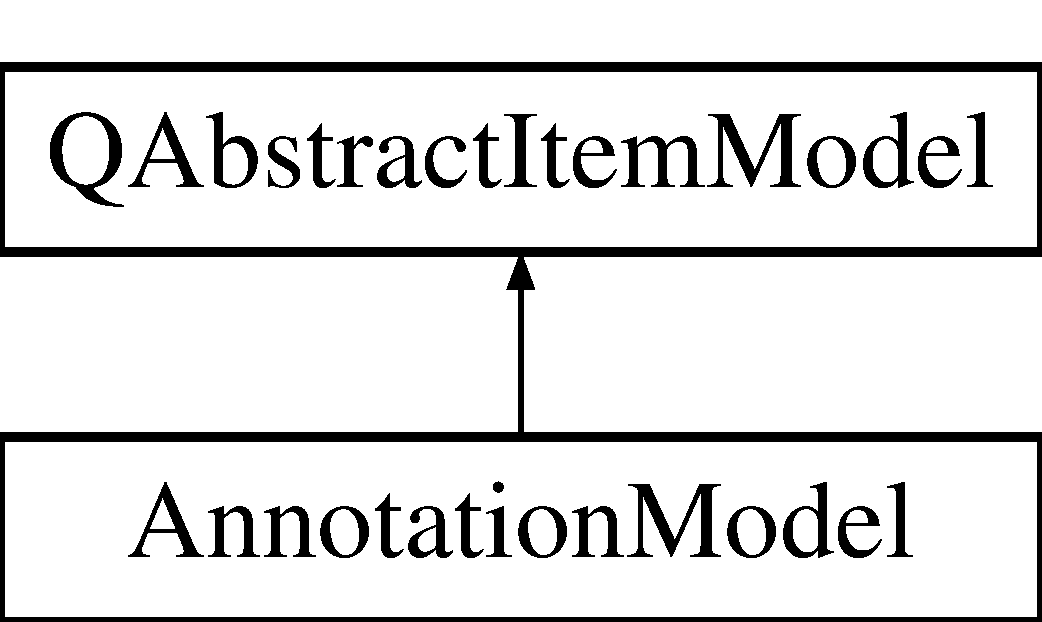
\includegraphics[height=2.000000cm]{classAnnotationModel}
\end{center}
\end{figure}
\subsection*{Public Types}
\begin{DoxyCompactItemize}
\item 
enum \{ \hyperlink{classAnnotationModel_aa517b64760be429123ee732470e08169ab4fc887a927920384c188f096592e49b}{Author\+Role} = Qt\+:\+:User\+Role + 1000, 
\hyperlink{classAnnotationModel_aa517b64760be429123ee732470e08169a36e01de5a0952a700d4f7cd17491aa57}{Page\+Role}
 \}
\end{DoxyCompactItemize}
\subsection*{Public Member Functions}
\begin{DoxyCompactItemize}
\item 
\hyperlink{classAnnotationModel_a29e844bf6e46f3dfa68da27d697bfdd4}{Annotation\+Model} (\hyperlink{classOkular_1_1Document}{Okular\+::\+Document} $\ast$document, Q\+Object $\ast$\hyperlink{classAnnotationModel_a162b06526b09c901a687d982051f639c}{parent}=0)
\item 
virtual \hyperlink{classAnnotationModel_ada5d073aa78e291b8422def55dd62199}{$\sim$\+Annotation\+Model} ()
\item 
virtual int \hyperlink{classAnnotationModel_a4a3dd262e42e0da24efa05adb42b1e70}{column\+Count} (const Q\+Model\+Index \&\hyperlink{classAnnotationModel_a162b06526b09c901a687d982051f639c}{parent}=Q\+Model\+Index()) const 
\item 
virtual Q\+Variant \hyperlink{classAnnotationModel_a179ccebf0ac079ea298ebafa9347eac1}{data} (const Q\+Model\+Index \&\hyperlink{classAnnotationModel_a0f1848b826fd58979667dc6f5966fee8}{index}, int role=Qt\+::\+Display\+Role) const 
\item 
virtual bool \hyperlink{classAnnotationModel_a596a4986b66a9d3271856f0bff06bfd0}{has\+Children} (const Q\+Model\+Index \&\hyperlink{classAnnotationModel_a162b06526b09c901a687d982051f639c}{parent}=Q\+Model\+Index()) const 
\item 
virtual Q\+Variant \hyperlink{classAnnotationModel_a798301e19593d4861ec83edec04aa29d}{header\+Data} (int section, Qt\+::\+Orientation orientation, int role=Qt\+::\+Display\+Role) const 
\item 
virtual Q\+Model\+Index \hyperlink{classAnnotationModel_a0f1848b826fd58979667dc6f5966fee8}{index} (int row, int column, const Q\+Model\+Index \&\hyperlink{classAnnotationModel_a162b06526b09c901a687d982051f639c}{parent}=Q\+Model\+Index()) const 
\item 
virtual Q\+Model\+Index \hyperlink{classAnnotationModel_a162b06526b09c901a687d982051f639c}{parent} (const Q\+Model\+Index \&\hyperlink{classAnnotationModel_a0f1848b826fd58979667dc6f5966fee8}{index}) const 
\item 
virtual int \hyperlink{classAnnotationModel_a519bc642d990f530aa3a4315d819a0d2}{row\+Count} (const Q\+Model\+Index \&\hyperlink{classAnnotationModel_a162b06526b09c901a687d982051f639c}{parent}=Q\+Model\+Index()) const 
\item 
bool \hyperlink{classAnnotationModel_a29cb1f9d54f20e8024dffcb3433a446f}{is\+Annotation} (const Q\+Model\+Index \&\hyperlink{classAnnotationModel_a0f1848b826fd58979667dc6f5966fee8}{index}) const 
\item 
\hyperlink{classOkular_1_1Annotation}{Okular\+::\+Annotation} $\ast$ \hyperlink{classAnnotationModel_a0cbda99ade41f0b580b55a9d6ba08d1f}{annotation\+For\+Index} (const Q\+Model\+Index \&\hyperlink{classAnnotationModel_a0f1848b826fd58979667dc6f5966fee8}{index}) const 
\end{DoxyCompactItemize}
\subsection*{Friends}
\begin{DoxyCompactItemize}
\item 
class \hyperlink{classAnnotationModel_adf657526a839f970d4c676cfc4853964}{Annotation\+Model\+Private}
\end{DoxyCompactItemize}


\subsection{Detailed Description}


Definition at line 22 of file annotationmodel.\+h.



\subsection{Member Enumeration Documentation}
\hypertarget{classAnnotationModel_aa517b64760be429123ee732470e08169}{\subsubsection[{anonymous enum}]{\setlength{\rightskip}{0pt plus 5cm}anonymous enum}}\label{classAnnotationModel_aa517b64760be429123ee732470e08169}
\begin{Desc}
\item[Enumerator]\par
\begin{description}
\index{Author\+Role@{Author\+Role}!Annotation\+Model@{Annotation\+Model}}\index{Annotation\+Model@{Annotation\+Model}!Author\+Role@{Author\+Role}}\item[{\em 
\hypertarget{classAnnotationModel_aa517b64760be429123ee732470e08169ab4fc887a927920384c188f096592e49b}{Author\+Role}\label{classAnnotationModel_aa517b64760be429123ee732470e08169ab4fc887a927920384c188f096592e49b}
}]\index{Page\+Role@{Page\+Role}!Annotation\+Model@{Annotation\+Model}}\index{Annotation\+Model@{Annotation\+Model}!Page\+Role@{Page\+Role}}\item[{\em 
\hypertarget{classAnnotationModel_aa517b64760be429123ee732470e08169a36e01de5a0952a700d4f7cd17491aa57}{Page\+Role}\label{classAnnotationModel_aa517b64760be429123ee732470e08169a36e01de5a0952a700d4f7cd17491aa57}
}]\end{description}
\end{Desc}


Definition at line 27 of file annotationmodel.\+h.


\begin{DoxyCode}
27              \{
28             \hyperlink{classAnnotationModel_aa517b64760be429123ee732470e08169ab4fc887a927920384c188f096592e49b}{AuthorRole} = Qt::UserRole + 1000,
29             \hyperlink{classAnnotationModel_aa517b64760be429123ee732470e08169a36e01de5a0952a700d4f7cd17491aa57}{PageRole}
30         \};
\end{DoxyCode}


\subsection{Constructor \& Destructor Documentation}
\hypertarget{classAnnotationModel_a29e844bf6e46f3dfa68da27d697bfdd4}{\index{Annotation\+Model@{Annotation\+Model}!Annotation\+Model@{Annotation\+Model}}
\index{Annotation\+Model@{Annotation\+Model}!Annotation\+Model@{Annotation\+Model}}
\subsubsection[{Annotation\+Model}]{\setlength{\rightskip}{0pt plus 5cm}Annotation\+Model\+::\+Annotation\+Model (
\begin{DoxyParamCaption}
\item[{{\bf Okular\+::\+Document} $\ast$}]{document, }
\item[{Q\+Object $\ast$}]{parent = {\ttfamily 0}}
\end{DoxyParamCaption}
)\hspace{0.3cm}{\ttfamily [explicit]}}}\label{classAnnotationModel_a29e844bf6e46f3dfa68da27d697bfdd4}


Definition at line 274 of file annotationmodel.\+cpp.


\begin{DoxyCode}
275     : QAbstractItemModel( \hyperlink{classAnnotationModel_a162b06526b09c901a687d982051f639c}{parent} ), d( \textcolor{keyword}{new} \hyperlink{classAnnotationModel_adf657526a839f970d4c676cfc4853964}{AnnotationModelPrivate}( \textcolor{keyword}{this} ) )
276 \{
277     d->\hyperlink{classAnnotationModelPrivate_ad9d0730baf8663b0c3485d72ac4e05c6}{document} = document;
278 
279     d->\hyperlink{classAnnotationModelPrivate_ad9d0730baf8663b0c3485d72ac4e05c6}{document}->addObserver( d );
280 \}
\end{DoxyCode}
\hypertarget{classAnnotationModel_ada5d073aa78e291b8422def55dd62199}{\index{Annotation\+Model@{Annotation\+Model}!````~Annotation\+Model@{$\sim$\+Annotation\+Model}}
\index{````~Annotation\+Model@{$\sim$\+Annotation\+Model}!Annotation\+Model@{Annotation\+Model}}
\subsubsection[{$\sim$\+Annotation\+Model}]{\setlength{\rightskip}{0pt plus 5cm}Annotation\+Model\+::$\sim$\+Annotation\+Model (
\begin{DoxyParamCaption}
{}
\end{DoxyParamCaption}
)\hspace{0.3cm}{\ttfamily [virtual]}}}\label{classAnnotationModel_ada5d073aa78e291b8422def55dd62199}


Definition at line 282 of file annotationmodel.\+cpp.


\begin{DoxyCode}
283 \{
284     \textcolor{keywordflow}{if} ( d->\hyperlink{classAnnotationModelPrivate_ad9d0730baf8663b0c3485d72ac4e05c6}{document} )
285         d->\hyperlink{classAnnotationModelPrivate_ad9d0730baf8663b0c3485d72ac4e05c6}{document}->removeObserver( d );
286 
287     \textcolor{keyword}{delete} d;
288 \}
\end{DoxyCode}


\subsection{Member Function Documentation}
\hypertarget{classAnnotationModel_a0cbda99ade41f0b580b55a9d6ba08d1f}{\index{Annotation\+Model@{Annotation\+Model}!annotation\+For\+Index@{annotation\+For\+Index}}
\index{annotation\+For\+Index@{annotation\+For\+Index}!Annotation\+Model@{Annotation\+Model}}
\subsubsection[{annotation\+For\+Index}]{\setlength{\rightskip}{0pt plus 5cm}{\bf Okular\+::\+Annotation} $\ast$ Annotation\+Model\+::annotation\+For\+Index (
\begin{DoxyParamCaption}
\item[{const Q\+Model\+Index \&}]{index}
\end{DoxyParamCaption}
) const}}\label{classAnnotationModel_a0cbda99ade41f0b580b55a9d6ba08d1f}


Definition at line 386 of file annotationmodel.\+cpp.


\begin{DoxyCode}
387 \{
388     \textcolor{keywordflow}{if} ( !\hyperlink{classAnnotationModel_a0f1848b826fd58979667dc6f5966fee8}{index}.isValid() )
389         \textcolor{keywordflow}{return} 0;
390 
391     \hyperlink{structAnnItem}{AnnItem} *item = \textcolor{keyword}{static\_cast<} \hyperlink{structAnnItem}{AnnItem}* \textcolor{keyword}{>}( \hyperlink{classAnnotationModel_a0f1848b826fd58979667dc6f5966fee8}{index}.internalPointer() );
392     \textcolor{keywordflow}{return} item->\hyperlink{structAnnItem_a72999b1a45d966e6f622dee4d958790f}{annotation};
393 \}
\end{DoxyCode}
\hypertarget{classAnnotationModel_a4a3dd262e42e0da24efa05adb42b1e70}{\index{Annotation\+Model@{Annotation\+Model}!column\+Count@{column\+Count}}
\index{column\+Count@{column\+Count}!Annotation\+Model@{Annotation\+Model}}
\subsubsection[{column\+Count}]{\setlength{\rightskip}{0pt plus 5cm}int Annotation\+Model\+::column\+Count (
\begin{DoxyParamCaption}
\item[{const Q\+Model\+Index \&}]{parent = {\ttfamily QModelIndex()}}
\end{DoxyParamCaption}
) const\hspace{0.3cm}{\ttfamily [virtual]}}}\label{classAnnotationModel_a4a3dd262e42e0da24efa05adb42b1e70}


Definition at line 290 of file annotationmodel.\+cpp.


\begin{DoxyCode}
291 \{
292     Q\_UNUSED( \hyperlink{classAnnotationModel_a162b06526b09c901a687d982051f639c}{parent} )
293     return 1;
294 \}
\end{DoxyCode}
\hypertarget{classAnnotationModel_a179ccebf0ac079ea298ebafa9347eac1}{\index{Annotation\+Model@{Annotation\+Model}!data@{data}}
\index{data@{data}!Annotation\+Model@{Annotation\+Model}}
\subsubsection[{data}]{\setlength{\rightskip}{0pt plus 5cm}Q\+Variant Annotation\+Model\+::data (
\begin{DoxyParamCaption}
\item[{const Q\+Model\+Index \&}]{index, }
\item[{int}]{role = {\ttfamily Qt\+:\+:DisplayRole}}
\end{DoxyParamCaption}
) const\hspace{0.3cm}{\ttfamily [virtual]}}}\label{classAnnotationModel_a179ccebf0ac079ea298ebafa9347eac1}


Definition at line 296 of file annotationmodel.\+cpp.


\begin{DoxyCode}
297 \{
298     \textcolor{keywordflow}{if} ( !\hyperlink{classAnnotationModel_a0f1848b826fd58979667dc6f5966fee8}{index}.isValid() )
299         \textcolor{keywordflow}{return} QVariant();
300 
301     \hyperlink{structAnnItem}{AnnItem} *item = \textcolor{keyword}{static\_cast<} \hyperlink{structAnnItem}{AnnItem}* \textcolor{keyword}{>}( \hyperlink{classAnnotationModel_a0f1848b826fd58979667dc6f5966fee8}{index}.internalPointer() );
302     \textcolor{keywordflow}{if} ( !item->\hyperlink{structAnnItem_a72999b1a45d966e6f622dee4d958790f}{annotation} )
303     \{
304         \textcolor{keywordflow}{if} ( role == Qt::DisplayRole )
305           \textcolor{keywordflow}{return} i18n( \textcolor{stringliteral}{"Page %1"}, item->\hyperlink{structAnnItem_ad2bc09dd1499fd52205eb02c3bf67830}{page} + 1 );
306         \textcolor{keywordflow}{else} \textcolor{keywordflow}{if} ( role == Qt::DecorationRole )
307           \textcolor{keywordflow}{return} KIcon( \textcolor{stringliteral}{"text-plain"} );
308         \textcolor{keywordflow}{else} \textcolor{keywordflow}{if} ( role == \hyperlink{classAnnotationModel_aa517b64760be429123ee732470e08169a36e01de5a0952a700d4f7cd17491aa57}{PageRole} )
309           \textcolor{keywordflow}{return} item->\hyperlink{structAnnItem_ad2bc09dd1499fd52205eb02c3bf67830}{page};
310 
311         \textcolor{keywordflow}{return} QVariant();
312     \}
313     \textcolor{keywordflow}{switch} ( role )
314     \{
315         \textcolor{keywordflow}{case} Qt::DisplayRole:
316             \textcolor{keywordflow}{return} \hyperlink{namespaceGuiUtils_af15abd3dd32e982db3f842e807146835}{GuiUtils::captionForAnnotation}( item->
      \hyperlink{structAnnItem_a72999b1a45d966e6f622dee4d958790f}{annotation} );
317             \textcolor{keywordflow}{break};
318         \textcolor{keywordflow}{case} Qt::DecorationRole:
319             \textcolor{keywordflow}{return} KIcon( \textcolor{stringliteral}{"okular"} );
320             \textcolor{keywordflow}{break};
321         \textcolor{keywordflow}{case} Qt::ToolTipRole:
322             \textcolor{keywordflow}{return} \hyperlink{namespaceGuiUtils_a4277357b6408ce44cf183cd7765bcc72}{GuiUtils::prettyToolTip}( item->
      \hyperlink{structAnnItem_a72999b1a45d966e6f622dee4d958790f}{annotation} );
323             \textcolor{keywordflow}{break};
324         \textcolor{keywordflow}{case} \hyperlink{classAnnotationModel_aa517b64760be429123ee732470e08169ab4fc887a927920384c188f096592e49b}{AuthorRole}:
325             \textcolor{keywordflow}{return} item->\hyperlink{structAnnItem_a72999b1a45d966e6f622dee4d958790f}{annotation}->\hyperlink{classOkular_1_1Annotation_a45682b53c24e4f5d41c547d6e109f6a4}{author}();
326             \textcolor{keywordflow}{break};
327         \textcolor{keywordflow}{case} \hyperlink{classAnnotationModel_aa517b64760be429123ee732470e08169a36e01de5a0952a700d4f7cd17491aa57}{PageRole}:
328             \textcolor{keywordflow}{return} item->\hyperlink{structAnnItem_ad2bc09dd1499fd52205eb02c3bf67830}{page};
329             \textcolor{keywordflow}{break};
330     \}
331     \textcolor{keywordflow}{return} QVariant();
332 \}
\end{DoxyCode}
\hypertarget{classAnnotationModel_a596a4986b66a9d3271856f0bff06bfd0}{\index{Annotation\+Model@{Annotation\+Model}!has\+Children@{has\+Children}}
\index{has\+Children@{has\+Children}!Annotation\+Model@{Annotation\+Model}}
\subsubsection[{has\+Children}]{\setlength{\rightskip}{0pt plus 5cm}bool Annotation\+Model\+::has\+Children (
\begin{DoxyParamCaption}
\item[{const Q\+Model\+Index \&}]{parent = {\ttfamily QModelIndex()}}
\end{DoxyParamCaption}
) const\hspace{0.3cm}{\ttfamily [virtual]}}}\label{classAnnotationModel_a596a4986b66a9d3271856f0bff06bfd0}


Definition at line 334 of file annotationmodel.\+cpp.


\begin{DoxyCode}
335 \{
336     \textcolor{keywordflow}{if} ( !\hyperlink{classAnnotationModel_a162b06526b09c901a687d982051f639c}{parent}.isValid() )
337         \textcolor{keywordflow}{return} \textcolor{keyword}{true};
338 
339     \hyperlink{structAnnItem}{AnnItem} *item = \textcolor{keyword}{static\_cast<} \hyperlink{structAnnItem}{AnnItem}* \textcolor{keyword}{>}( \hyperlink{classAnnotationModel_a162b06526b09c901a687d982051f639c}{parent}.internalPointer() );
340     \textcolor{keywordflow}{return} !item->\hyperlink{structAnnItem_a11048051ad0be5a2c8607a9334e006a1}{children}.isEmpty();
341 \}
\end{DoxyCode}
\hypertarget{classAnnotationModel_a798301e19593d4861ec83edec04aa29d}{\index{Annotation\+Model@{Annotation\+Model}!header\+Data@{header\+Data}}
\index{header\+Data@{header\+Data}!Annotation\+Model@{Annotation\+Model}}
\subsubsection[{header\+Data}]{\setlength{\rightskip}{0pt plus 5cm}Q\+Variant Annotation\+Model\+::header\+Data (
\begin{DoxyParamCaption}
\item[{int}]{section, }
\item[{Qt\+::\+Orientation}]{orientation, }
\item[{int}]{role = {\ttfamily Qt\+:\+:DisplayRole}}
\end{DoxyParamCaption}
) const\hspace{0.3cm}{\ttfamily [virtual]}}}\label{classAnnotationModel_a798301e19593d4861ec83edec04aa29d}


Definition at line 343 of file annotationmodel.\+cpp.


\begin{DoxyCode}
344 \{
345     \textcolor{keywordflow}{if} ( orientation != Qt::Horizontal )
346         \textcolor{keywordflow}{return} QVariant();
347 
348     \textcolor{keywordflow}{if} ( section == 0 && role == Qt::DisplayRole )
349         \textcolor{keywordflow}{return} \textcolor{stringliteral}{"Annotations"};
350 
351     \textcolor{keywordflow}{return} QVariant();
352 \}
\end{DoxyCode}
\hypertarget{classAnnotationModel_a0f1848b826fd58979667dc6f5966fee8}{\index{Annotation\+Model@{Annotation\+Model}!index@{index}}
\index{index@{index}!Annotation\+Model@{Annotation\+Model}}
\subsubsection[{index}]{\setlength{\rightskip}{0pt plus 5cm}Q\+Model\+Index Annotation\+Model\+::index (
\begin{DoxyParamCaption}
\item[{int}]{row, }
\item[{int}]{column, }
\item[{const Q\+Model\+Index \&}]{parent = {\ttfamily QModelIndex()}}
\end{DoxyParamCaption}
) const\hspace{0.3cm}{\ttfamily [virtual]}}}\label{classAnnotationModel_a0f1848b826fd58979667dc6f5966fee8}


Definition at line 354 of file annotationmodel.\+cpp.


\begin{DoxyCode}
355 \{
356     \textcolor{keywordflow}{if} ( row < 0 || column != 0 )
357         \textcolor{keywordflow}{return} QModelIndex();
358 
359     \hyperlink{structAnnItem}{AnnItem} *item = \hyperlink{classAnnotationModel_a162b06526b09c901a687d982051f639c}{parent}.isValid() ? \textcolor{keyword}{static\_cast<} \hyperlink{structAnnItem}{AnnItem}* \textcolor{keyword}{>}( 
      \hyperlink{classAnnotationModel_a162b06526b09c901a687d982051f639c}{parent}.internalPointer() ) : d->\hyperlink{classAnnotationModelPrivate_a35aef72ee0aebe05b6e0fa2c50c19f75}{root};
360     if ( row < item->children.count() )
361         \textcolor{keywordflow}{return} createIndex( row, column, item->\hyperlink{structAnnItem_a11048051ad0be5a2c8607a9334e006a1}{children}.at( row ) );
362 
363     \textcolor{keywordflow}{return} QModelIndex();
364 \}
\end{DoxyCode}
\hypertarget{classAnnotationModel_a29cb1f9d54f20e8024dffcb3433a446f}{\index{Annotation\+Model@{Annotation\+Model}!is\+Annotation@{is\+Annotation}}
\index{is\+Annotation@{is\+Annotation}!Annotation\+Model@{Annotation\+Model}}
\subsubsection[{is\+Annotation}]{\setlength{\rightskip}{0pt plus 5cm}bool Annotation\+Model\+::is\+Annotation (
\begin{DoxyParamCaption}
\item[{const Q\+Model\+Index \&}]{index}
\end{DoxyParamCaption}
) const}}\label{classAnnotationModel_a29cb1f9d54f20e8024dffcb3433a446f}


Definition at line 381 of file annotationmodel.\+cpp.


\begin{DoxyCode}
382 \{
383     \textcolor{keywordflow}{return} \hyperlink{classAnnotationModel_a0cbda99ade41f0b580b55a9d6ba08d1f}{annotationForIndex}( \hyperlink{classAnnotationModel_a0f1848b826fd58979667dc6f5966fee8}{index} );
384 \}
\end{DoxyCode}
\hypertarget{classAnnotationModel_a162b06526b09c901a687d982051f639c}{\index{Annotation\+Model@{Annotation\+Model}!parent@{parent}}
\index{parent@{parent}!Annotation\+Model@{Annotation\+Model}}
\subsubsection[{parent}]{\setlength{\rightskip}{0pt plus 5cm}Q\+Model\+Index Annotation\+Model\+::parent (
\begin{DoxyParamCaption}
\item[{const Q\+Model\+Index \&}]{index}
\end{DoxyParamCaption}
) const\hspace{0.3cm}{\ttfamily [virtual]}}}\label{classAnnotationModel_a162b06526b09c901a687d982051f639c}


Definition at line 366 of file annotationmodel.\+cpp.


\begin{DoxyCode}
367 \{
368     \textcolor{keywordflow}{if} ( !\hyperlink{classAnnotationModel_a0f1848b826fd58979667dc6f5966fee8}{index}.isValid() )
369         \textcolor{keywordflow}{return} QModelIndex();
370 
371     \hyperlink{structAnnItem}{AnnItem} *item = \textcolor{keyword}{static\_cast<} \hyperlink{structAnnItem}{AnnItem}* \textcolor{keyword}{>}( \hyperlink{classAnnotationModel_a0f1848b826fd58979667dc6f5966fee8}{index}.internalPointer() );
372     \textcolor{keywordflow}{return} d->\hyperlink{classAnnotationModelPrivate_a49c3cbd8328e431324be4fff9ac25926}{indexForItem}( item->\hyperlink{structAnnItem_aece74b70cc6acc8ebb751256386f9be8}{parent} );
373 \}
\end{DoxyCode}
\hypertarget{classAnnotationModel_a519bc642d990f530aa3a4315d819a0d2}{\index{Annotation\+Model@{Annotation\+Model}!row\+Count@{row\+Count}}
\index{row\+Count@{row\+Count}!Annotation\+Model@{Annotation\+Model}}
\subsubsection[{row\+Count}]{\setlength{\rightskip}{0pt plus 5cm}int Annotation\+Model\+::row\+Count (
\begin{DoxyParamCaption}
\item[{const Q\+Model\+Index \&}]{parent = {\ttfamily QModelIndex()}}
\end{DoxyParamCaption}
) const\hspace{0.3cm}{\ttfamily [virtual]}}}\label{classAnnotationModel_a519bc642d990f530aa3a4315d819a0d2}


Definition at line 375 of file annotationmodel.\+cpp.


\begin{DoxyCode}
376 \{
377     \hyperlink{structAnnItem}{AnnItem} *item = \hyperlink{classAnnotationModel_a162b06526b09c901a687d982051f639c}{parent}.isValid() ? \textcolor{keyword}{static\_cast<} \hyperlink{structAnnItem}{AnnItem}* \textcolor{keyword}{>}( 
      \hyperlink{classAnnotationModel_a162b06526b09c901a687d982051f639c}{parent}.internalPointer() ) : d->\hyperlink{classAnnotationModelPrivate_a35aef72ee0aebe05b6e0fa2c50c19f75}{root};
378     \textcolor{keywordflow}{return} item->\hyperlink{structAnnItem_a11048051ad0be5a2c8607a9334e006a1}{children}.count();
379 \}
\end{DoxyCode}


\subsection{Friends And Related Function Documentation}
\hypertarget{classAnnotationModel_adf657526a839f970d4c676cfc4853964}{\index{Annotation\+Model@{Annotation\+Model}!Annotation\+Model\+Private@{Annotation\+Model\+Private}}
\index{Annotation\+Model\+Private@{Annotation\+Model\+Private}!Annotation\+Model@{Annotation\+Model}}
\subsubsection[{Annotation\+Model\+Private}]{\setlength{\rightskip}{0pt plus 5cm}friend class {\bf Annotation\+Model\+Private}\hspace{0.3cm}{\ttfamily [friend]}}}\label{classAnnotationModel_adf657526a839f970d4c676cfc4853964}


Definition at line 49 of file annotationmodel.\+h.



The documentation for this class was generated from the following files\+:\begin{DoxyCompactItemize}
\item 
ui/\hyperlink{annotationmodel_8h}{annotationmodel.\+h}\item 
ui/\hyperlink{annotationmodel_8cpp}{annotationmodel.\+cpp}\end{DoxyCompactItemize}

\hypertarget{classAnnotationModelPrivate}{\section{Annotation\+Model\+Private Class Reference}
\label{classAnnotationModelPrivate}\index{Annotation\+Model\+Private@{Annotation\+Model\+Private}}
}
Inheritance diagram for Annotation\+Model\+Private\+:\begin{figure}[H]
\begin{center}
\leavevmode
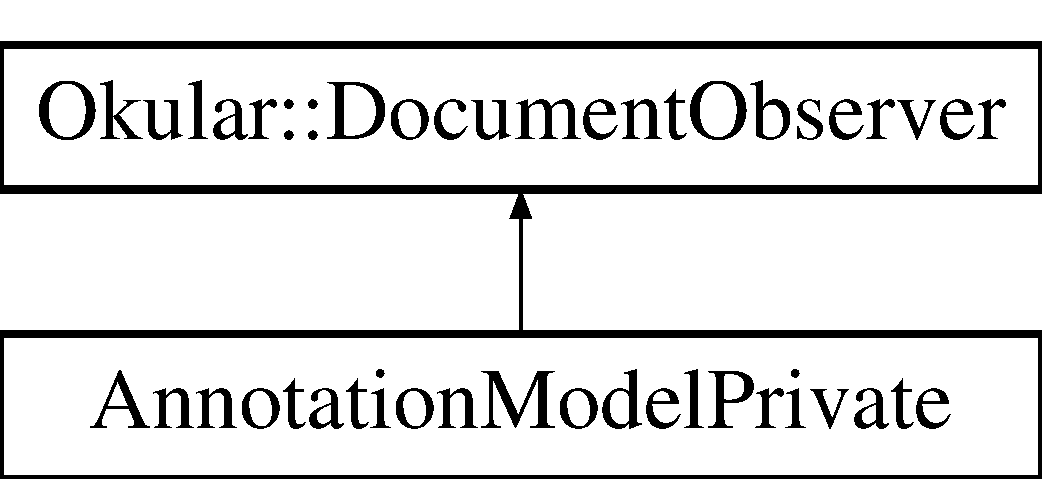
\includegraphics[height=2.000000cm]{classAnnotationModelPrivate}
\end{center}
\end{figure}
\subsection*{Public Member Functions}
\begin{DoxyCompactItemize}
\item 
\hyperlink{classAnnotationModelPrivate_a97a20594b53559a17ded1896526b1e5c}{Annotation\+Model\+Private} (\hyperlink{classAnnotationModel}{Annotation\+Model} $\ast$qq)
\item 
virtual \hyperlink{classAnnotationModelPrivate_a402da5e1c02288e8b8d9d8cc2216dbac}{$\sim$\+Annotation\+Model\+Private} ()
\item 
virtual void \hyperlink{classAnnotationModelPrivate_aad79ea3a4f3222fd7b8aafad27fef5d7}{notify\+Setup} (const Q\+Vector$<$ \hyperlink{classOkular_1_1Page}{Okular\+::\+Page} $\ast$ $>$ \&pages, int setup\+Flags)
\item 
virtual void \hyperlink{classAnnotationModelPrivate_ac06ad6534d4368be37e97bf27b616e0a}{notify\+Page\+Changed} (int page, int flags)
\item 
Q\+Model\+Index \hyperlink{classAnnotationModelPrivate_a49c3cbd8328e431324be4fff9ac25926}{index\+For\+Item} (\hyperlink{structAnnItem}{Ann\+Item} $\ast$item) const 
\item 
void \hyperlink{classAnnotationModelPrivate_a4b78d9800d1b36e77308009d53b2fdf9}{rebuild\+Tree} (const Q\+Vector$<$ \hyperlink{classOkular_1_1Page}{Okular\+::\+Page} $\ast$ $>$ \&pages)
\item 
\hyperlink{structAnnItem}{Ann\+Item} $\ast$ \hyperlink{classAnnotationModelPrivate_a082a44f62811ca44738a656492e03916}{find\+Item} (int page, int $\ast$index) const 
\end{DoxyCompactItemize}
\subsection*{Public Attributes}
\begin{DoxyCompactItemize}
\item 
\hyperlink{classAnnotationModel}{Annotation\+Model} $\ast$ \hyperlink{classAnnotationModelPrivate_a106e8bd7ef602e10239b11d4a775647d}{q}
\item 
\hyperlink{structAnnItem}{Ann\+Item} $\ast$ \hyperlink{classAnnotationModelPrivate_a35aef72ee0aebe05b6e0fa2c50c19f75}{root}
\item 
Q\+Pointer$<$ \hyperlink{classOkular_1_1Document}{Okular\+::\+Document} $>$ \hyperlink{classAnnotationModelPrivate_ad9d0730baf8663b0c3485d72ac4e05c6}{document}
\end{DoxyCompactItemize}
\subsection*{Additional Inherited Members}


\subsection{Detailed Description}


Definition at line 54 of file annotationmodel.\+cpp.



\subsection{Constructor \& Destructor Documentation}
\hypertarget{classAnnotationModelPrivate_a97a20594b53559a17ded1896526b1e5c}{\index{Annotation\+Model\+Private@{Annotation\+Model\+Private}!Annotation\+Model\+Private@{Annotation\+Model\+Private}}
\index{Annotation\+Model\+Private@{Annotation\+Model\+Private}!Annotation\+Model\+Private@{Annotation\+Model\+Private}}
\subsubsection[{Annotation\+Model\+Private}]{\setlength{\rightskip}{0pt plus 5cm}Annotation\+Model\+Private\+::\+Annotation\+Model\+Private (
\begin{DoxyParamCaption}
\item[{{\bf Annotation\+Model} $\ast$}]{qq}
\end{DoxyParamCaption}
)}}\label{classAnnotationModelPrivate_a97a20594b53559a17ded1896526b1e5c}


Definition at line 98 of file annotationmodel.\+cpp.


\begin{DoxyCode}
99     : \hyperlink{classAnnotationModelPrivate_a106e8bd7ef602e10239b11d4a775647d}{q}( qq ), \hyperlink{classAnnotationModelPrivate_a35aef72ee0aebe05b6e0fa2c50c19f75}{root}( \textcolor{keyword}{new} \hyperlink{structAnnItem}{AnnItem} )
100 \{
101 \}
\end{DoxyCode}
\hypertarget{classAnnotationModelPrivate_a402da5e1c02288e8b8d9d8cc2216dbac}{\index{Annotation\+Model\+Private@{Annotation\+Model\+Private}!````~Annotation\+Model\+Private@{$\sim$\+Annotation\+Model\+Private}}
\index{````~Annotation\+Model\+Private@{$\sim$\+Annotation\+Model\+Private}!Annotation\+Model\+Private@{Annotation\+Model\+Private}}
\subsubsection[{$\sim$\+Annotation\+Model\+Private}]{\setlength{\rightskip}{0pt plus 5cm}Annotation\+Model\+Private\+::$\sim$\+Annotation\+Model\+Private (
\begin{DoxyParamCaption}
{}
\end{DoxyParamCaption}
)\hspace{0.3cm}{\ttfamily [virtual]}}}\label{classAnnotationModelPrivate_a402da5e1c02288e8b8d9d8cc2216dbac}


Definition at line 103 of file annotationmodel.\+cpp.


\begin{DoxyCode}
104 \{
105     \textcolor{keyword}{delete} \hyperlink{classAnnotationModelPrivate_a35aef72ee0aebe05b6e0fa2c50c19f75}{root};
106 \}
\end{DoxyCode}


\subsection{Member Function Documentation}
\hypertarget{classAnnotationModelPrivate_a082a44f62811ca44738a656492e03916}{\index{Annotation\+Model\+Private@{Annotation\+Model\+Private}!find\+Item@{find\+Item}}
\index{find\+Item@{find\+Item}!Annotation\+Model\+Private@{Annotation\+Model\+Private}}
\subsubsection[{find\+Item}]{\setlength{\rightskip}{0pt plus 5cm}{\bf Ann\+Item} $\ast$ Annotation\+Model\+Private\+::find\+Item (
\begin{DoxyParamCaption}
\item[{int}]{page, }
\item[{int $\ast$}]{index}
\end{DoxyParamCaption}
) const}}\label{classAnnotationModelPrivate_a082a44f62811ca44738a656492e03916}


Definition at line 256 of file annotationmodel.\+cpp.


\begin{DoxyCode}
257 \{
258     \textcolor{keywordflow}{for} ( \textcolor{keywordtype}{int} i = 0; i < \hyperlink{classAnnotationModelPrivate_a35aef72ee0aebe05b6e0fa2c50c19f75}{root}->\hyperlink{structAnnItem_a11048051ad0be5a2c8607a9334e006a1}{children}.count(); ++i )
259     \{
260         \hyperlink{structAnnItem}{AnnItem} *tmp = \hyperlink{classAnnotationModelPrivate_a35aef72ee0aebe05b6e0fa2c50c19f75}{root}->\hyperlink{structAnnItem_a11048051ad0be5a2c8607a9334e006a1}{children}.at( i );
261         \textcolor{keywordflow}{if} ( tmp->\hyperlink{structAnnItem_ad2bc09dd1499fd52205eb02c3bf67830}{page} == page )
262         \{
263             \textcolor{keywordflow}{if} ( index )
264                 *index = i;
265             \textcolor{keywordflow}{return} tmp;
266         \}
267     \}
268     \textcolor{keywordflow}{if} ( index )
269         *index = -1;
270     \textcolor{keywordflow}{return} 0;
271 \}
\end{DoxyCode}
\hypertarget{classAnnotationModelPrivate_a49c3cbd8328e431324be4fff9ac25926}{\index{Annotation\+Model\+Private@{Annotation\+Model\+Private}!index\+For\+Item@{index\+For\+Item}}
\index{index\+For\+Item@{index\+For\+Item}!Annotation\+Model\+Private@{Annotation\+Model\+Private}}
\subsubsection[{index\+For\+Item}]{\setlength{\rightskip}{0pt plus 5cm}Q\+Model\+Index Annotation\+Model\+Private\+::index\+For\+Item (
\begin{DoxyParamCaption}
\item[{{\bf Ann\+Item} $\ast$}]{item}
\end{DoxyParamCaption}
) const}}\label{classAnnotationModelPrivate_a49c3cbd8328e431324be4fff9ac25926}


Definition at line 223 of file annotationmodel.\+cpp.


\begin{DoxyCode}
224 \{
225     \textcolor{keywordflow}{if} ( item->\hyperlink{structAnnItem_aece74b70cc6acc8ebb751256386f9be8}{parent} )
226     \{
227         \textcolor{keywordtype}{int} \textcolor{keywordtype}{id} = item->\hyperlink{structAnnItem_aece74b70cc6acc8ebb751256386f9be8}{parent}->\hyperlink{structAnnItem_a11048051ad0be5a2c8607a9334e006a1}{children}.indexOf( item );
228         \textcolor{keywordflow}{if} ( \textcolor{keywordtype}{id} >= 0 && id < item->parent->children.count() )
229            \textcolor{keywordflow}{return} \hyperlink{classAnnotationModelPrivate_a106e8bd7ef602e10239b11d4a775647d}{q}->createIndex( \textcolor{keywordtype}{id}, 0, item );
230     \}
231     \textcolor{keywordflow}{return} QModelIndex();
232 \}
\end{DoxyCode}
\hypertarget{classAnnotationModelPrivate_ac06ad6534d4368be37e97bf27b616e0a}{\index{Annotation\+Model\+Private@{Annotation\+Model\+Private}!notify\+Page\+Changed@{notify\+Page\+Changed}}
\index{notify\+Page\+Changed@{notify\+Page\+Changed}!Annotation\+Model\+Private@{Annotation\+Model\+Private}}
\subsubsection[{notify\+Page\+Changed}]{\setlength{\rightskip}{0pt plus 5cm}void Annotation\+Model\+Private\+::notify\+Page\+Changed (
\begin{DoxyParamCaption}
\item[{int}]{page, }
\item[{int}]{flags}
\end{DoxyParamCaption}
)\hspace{0.3cm}{\ttfamily [virtual]}}}\label{classAnnotationModelPrivate_ac06ad6534d4368be37e97bf27b616e0a}
This method is called whenever the content on {\ttfamily page} described by the passed {\ttfamily flags} has been changed. 

Reimplemented from \hyperlink{classOkular_1_1DocumentObserver_abf7600dabd7d6c1e38c950d99f7be595}{Okular\+::\+Document\+Observer}.



Definition at line 120 of file annotationmodel.\+cpp.


\begin{DoxyCode}
121 \{
122     \textcolor{comment}{// we are strictly interested in annotations}
123     \textcolor{keywordflow}{if} ( !(flags & \hyperlink{classOkular_1_1DocumentObserver_af0e6b09d5fc7ecb673bd4895ef2710dca05bd23206e8303026c0b598095d8552e}{Okular::DocumentObserver::Annotations} ) )
124         \textcolor{keywordflow}{return};
125 
126     \textcolor{keyword}{const} \hyperlink{classQLinkedList}{QLinkedList< Okular::Annotation* >} annots = 
      filterOutWidgetAnnotations( \hyperlink{classAnnotationModelPrivate_ad9d0730baf8663b0c3485d72ac4e05c6}{document}->page( page )->annotations() );
127     \textcolor{keywordtype}{int} annItemIndex = -1;
128     \hyperlink{structAnnItem}{AnnItem} *annItem = \hyperlink{classAnnotationModelPrivate_a082a44f62811ca44738a656492e03916}{findItem}( page, &annItemIndex );
129     \textcolor{comment}{// case 1: the page has no more annotations}
130     \textcolor{comment}{//         => remove the branch, if any}
131     \textcolor{keywordflow}{if} ( annots.isEmpty() )
132     \{
133         \textcolor{keywordflow}{if} ( annItem )
134         \{
135             \hyperlink{classAnnotationModelPrivate_a106e8bd7ef602e10239b11d4a775647d}{q}->beginRemoveRows( \hyperlink{classAnnotationModelPrivate_a49c3cbd8328e431324be4fff9ac25926}{indexForItem}( \hyperlink{classAnnotationModelPrivate_a35aef72ee0aebe05b6e0fa2c50c19f75}{root} ), annItemIndex, annItemIndex );
136             \textcolor{keyword}{delete} \hyperlink{classAnnotationModelPrivate_a35aef72ee0aebe05b6e0fa2c50c19f75}{root}->\hyperlink{structAnnItem_a11048051ad0be5a2c8607a9334e006a1}{children}.at( annItemIndex );
137             \hyperlink{classAnnotationModelPrivate_a35aef72ee0aebe05b6e0fa2c50c19f75}{root}->\hyperlink{structAnnItem_a11048051ad0be5a2c8607a9334e006a1}{children}.removeAt( annItemIndex );
138             \hyperlink{classAnnotationModelPrivate_a106e8bd7ef602e10239b11d4a775647d}{q}->endRemoveRows();
139         \}
140         \textcolor{keywordflow}{return};
141     \}
142     \textcolor{comment}{// case 2: no existing branch}
143     \textcolor{comment}{//         => add a new branch, and add the annotations for the page}
144     \textcolor{keywordflow}{if} ( !annItem )
145     \{
146         \textcolor{keywordtype}{int} i = 0;
147         \textcolor{keywordflow}{while} ( i < root->children.count() && \hyperlink{classAnnotationModelPrivate_a35aef72ee0aebe05b6e0fa2c50c19f75}{root}->\hyperlink{structAnnItem_a11048051ad0be5a2c8607a9334e006a1}{children}.at( i )->page < page ) ++i;
148 
149         \hyperlink{structAnnItem}{AnnItem} *annItem = \textcolor{keyword}{new} \hyperlink{structAnnItem}{AnnItem}();
150         annItem->\hyperlink{structAnnItem_ad2bc09dd1499fd52205eb02c3bf67830}{page} = page;
151         annItem->\hyperlink{structAnnItem_aece74b70cc6acc8ebb751256386f9be8}{parent} = \hyperlink{classAnnotationModelPrivate_a35aef72ee0aebe05b6e0fa2c50c19f75}{root};
152         \hyperlink{classAnnotationModelPrivate_a106e8bd7ef602e10239b11d4a775647d}{q}->beginInsertRows( \hyperlink{classAnnotationModelPrivate_a49c3cbd8328e431324be4fff9ac25926}{indexForItem}( \hyperlink{classAnnotationModelPrivate_a35aef72ee0aebe05b6e0fa2c50c19f75}{root} ), i, i );
153         annItem->\hyperlink{structAnnItem_aece74b70cc6acc8ebb751256386f9be8}{parent}->\hyperlink{structAnnItem_a11048051ad0be5a2c8607a9334e006a1}{children}.insert( i, annItem );
154         \hyperlink{classAnnotationModelPrivate_a106e8bd7ef602e10239b11d4a775647d}{q}->endInsertRows();
155         \hyperlink{classQLinkedList}{QLinkedList< Okular::Annotation* >::ConstIterator} 
      it = annots.begin(), itEnd = annots.end();
156         \textcolor{keywordtype}{int} newid = 0;
157         \textcolor{keywordflow}{for} ( ; it != itEnd; ++it, ++newid )
158         \{
159             \hyperlink{classAnnotationModelPrivate_a106e8bd7ef602e10239b11d4a775647d}{q}->beginInsertRows( \hyperlink{classAnnotationModelPrivate_a49c3cbd8328e431324be4fff9ac25926}{indexForItem}( annItem ), newid, newid );
160             \textcolor{keyword}{new} \hyperlink{structAnnItem}{AnnItem}( annItem, *it );
161             \hyperlink{classAnnotationModelPrivate_a106e8bd7ef602e10239b11d4a775647d}{q}->endInsertRows();
162         \}
163         \textcolor{keywordflow}{return};
164     \}
165     \textcolor{comment}{// case 3: existing branch, less annotations than items}
166     \textcolor{comment}{//         => lookup and remove the annotations}
167     \textcolor{keywordflow}{if} ( annItem->\hyperlink{structAnnItem_a11048051ad0be5a2c8607a9334e006a1}{children}.count() > annots.count() )
168     \{
169         \textcolor{keywordflow}{for} ( \textcolor{keywordtype}{int} i = annItem->\hyperlink{structAnnItem_a11048051ad0be5a2c8607a9334e006a1}{children}.count(); i > 0; --i )
170         \{
171             \hyperlink{classOkular_1_1Annotation}{Okular::Annotation} *ref = annItem->\hyperlink{structAnnItem_a11048051ad0be5a2c8607a9334e006a1}{children}.at( i - 1 )->annotation;
172             \textcolor{keywordtype}{bool} found = \textcolor{keyword}{false};
173             \hyperlink{classQLinkedList}{QLinkedList< Okular::Annotation* >::ConstIterator}
       it = annots.begin(), itEnd = annots.end();
174             \textcolor{keywordflow}{for} ( ; !found && it != itEnd; ++it )
175             \{
176                 \textcolor{keywordflow}{if} ( ( *it ) == ref )
177                     found = \textcolor{keyword}{true};
178             \}
179             \textcolor{keywordflow}{if} ( !found )
180             \{
181                 \hyperlink{classAnnotationModelPrivate_a106e8bd7ef602e10239b11d4a775647d}{q}->beginRemoveRows( \hyperlink{classAnnotationModelPrivate_a49c3cbd8328e431324be4fff9ac25926}{indexForItem}( annItem ), i - 1, i - 1 );
182                 \textcolor{keyword}{delete} annItem->\hyperlink{structAnnItem_a11048051ad0be5a2c8607a9334e006a1}{children}.at( i - 1 );
183                 annItem->\hyperlink{structAnnItem_a11048051ad0be5a2c8607a9334e006a1}{children}.removeAt( i - 1 );
184                 \hyperlink{classAnnotationModelPrivate_a106e8bd7ef602e10239b11d4a775647d}{q}->endRemoveRows();
185             \}
186         \}
187         \textcolor{keywordflow}{return};
188     \}
189     \textcolor{comment}{// case 4: existing branch, less items than annotations}
190     \textcolor{comment}{//         => lookup and add annotations if not in the branch}
191     \textcolor{keywordflow}{if} ( annots.count() > annItem->\hyperlink{structAnnItem_a11048051ad0be5a2c8607a9334e006a1}{children}.count() )
192     \{
193         \hyperlink{classQLinkedList}{QLinkedList< Okular::Annotation* >::ConstIterator} 
      it = annots.begin(), itEnd = annots.end();
194         \textcolor{keywordflow}{for} ( ; it != itEnd; ++it )
195         \{
196             \hyperlink{classOkular_1_1Annotation}{Okular::Annotation} *ref = *it;
197             \textcolor{keywordtype}{bool} found = \textcolor{keyword}{false};
198             \textcolor{keywordtype}{int} count = annItem->\hyperlink{structAnnItem_a11048051ad0be5a2c8607a9334e006a1}{children}.count();
199             \textcolor{keywordflow}{for} ( \textcolor{keywordtype}{int} i = 0; !found && i < count; ++i )
200             \{
201                 \textcolor{keywordflow}{if} ( ref == annItem->\hyperlink{structAnnItem_a11048051ad0be5a2c8607a9334e006a1}{children}.at( i )->annotation )
202                     found = \textcolor{keyword}{true};
203             \}
204             \textcolor{keywordflow}{if} ( !found )
205             \{
206                 \hyperlink{classAnnotationModelPrivate_a106e8bd7ef602e10239b11d4a775647d}{q}->beginInsertRows( \hyperlink{classAnnotationModelPrivate_a49c3cbd8328e431324be4fff9ac25926}{indexForItem}( annItem ), count, count );
207                 \textcolor{keyword}{new} \hyperlink{structAnnItem}{AnnItem}( annItem, ref );
208                 \hyperlink{classAnnotationModelPrivate_a106e8bd7ef602e10239b11d4a775647d}{q}->endInsertRows();
209             \}
210         \}
211         \textcolor{keywordflow}{return};
212     \}
213     \textcolor{comment}{// case 5: the data of some annotation changed}
214     \textcolor{comment}{// TODO: what do we do in this case?}
215     \textcolor{comment}{// FIXME: for now, update ALL the annotations for that page}
216     \textcolor{keywordflow}{for} ( \textcolor{keywordtype}{int} i = 0; i < annItem->\hyperlink{structAnnItem_a11048051ad0be5a2c8607a9334e006a1}{children}.count(); ++i )
217     \{
218         QModelIndex index = \hyperlink{classAnnotationModelPrivate_a49c3cbd8328e431324be4fff9ac25926}{indexForItem}( annItem->\hyperlink{structAnnItem_a11048051ad0be5a2c8607a9334e006a1}{children}.at( i ) );
219         emit \hyperlink{classAnnotationModelPrivate_a106e8bd7ef602e10239b11d4a775647d}{q}->dataChanged( index, index );
220     \}
221 \}
\end{DoxyCode}
\hypertarget{classAnnotationModelPrivate_aad79ea3a4f3222fd7b8aafad27fef5d7}{\index{Annotation\+Model\+Private@{Annotation\+Model\+Private}!notify\+Setup@{notify\+Setup}}
\index{notify\+Setup@{notify\+Setup}!Annotation\+Model\+Private@{Annotation\+Model\+Private}}
\subsubsection[{notify\+Setup}]{\setlength{\rightskip}{0pt plus 5cm}void Annotation\+Model\+Private\+::notify\+Setup (
\begin{DoxyParamCaption}
\item[{const Q\+Vector$<$ {\bf Okular\+::\+Page} $\ast$ $>$ \&}]{pages, }
\item[{int}]{setup\+Flags}
\end{DoxyParamCaption}
)\hspace{0.3cm}{\ttfamily [virtual]}}}\label{classAnnotationModelPrivate_aad79ea3a4f3222fd7b8aafad27fef5d7}


Definition at line 108 of file annotationmodel.\+cpp.


\begin{DoxyCode}
109 \{
110     \textcolor{keywordflow}{if} ( !( setupFlags & \hyperlink{classOkular_1_1DocumentObserver_aba00584af99894f95a9650e91f109d40ae599564392c01b22e96eff7602c4dd03}{Okular::DocumentObserver::DocumentChanged}
       ) )
111         \textcolor{keywordflow}{return};
112 
113     qDeleteAll( \hyperlink{classAnnotationModelPrivate_a35aef72ee0aebe05b6e0fa2c50c19f75}{root}->\hyperlink{structAnnItem_a11048051ad0be5a2c8607a9334e006a1}{children} );
114     \hyperlink{classAnnotationModelPrivate_a35aef72ee0aebe05b6e0fa2c50c19f75}{root}->\hyperlink{structAnnItem_a11048051ad0be5a2c8607a9334e006a1}{children}.clear();
115     \hyperlink{classAnnotationModelPrivate_a106e8bd7ef602e10239b11d4a775647d}{q}->reset();
116 
117     \hyperlink{classAnnotationModelPrivate_a4b78d9800d1b36e77308009d53b2fdf9}{rebuildTree}( pages );
118 \}
\end{DoxyCode}
\hypertarget{classAnnotationModelPrivate_a4b78d9800d1b36e77308009d53b2fdf9}{\index{Annotation\+Model\+Private@{Annotation\+Model\+Private}!rebuild\+Tree@{rebuild\+Tree}}
\index{rebuild\+Tree@{rebuild\+Tree}!Annotation\+Model\+Private@{Annotation\+Model\+Private}}
\subsubsection[{rebuild\+Tree}]{\setlength{\rightskip}{0pt plus 5cm}void Annotation\+Model\+Private\+::rebuild\+Tree (
\begin{DoxyParamCaption}
\item[{const Q\+Vector$<$ {\bf Okular\+::\+Page} $\ast$ $>$ \&}]{pages}
\end{DoxyParamCaption}
)}}\label{classAnnotationModelPrivate_a4b78d9800d1b36e77308009d53b2fdf9}


Definition at line 234 of file annotationmodel.\+cpp.


\begin{DoxyCode}
235 \{
236     \textcolor{keywordflow}{if} ( pages.isEmpty() )
237         \textcolor{keywordflow}{return};
238 
239     emit \hyperlink{classAnnotationModelPrivate_a106e8bd7ef602e10239b11d4a775647d}{q}->layoutAboutToBeChanged();
240     \textcolor{keywordflow}{for} ( \textcolor{keywordtype}{int} i = 0; i < pages.count(); ++i )
241     \{
242         \textcolor{keyword}{const} \hyperlink{classQLinkedList}{QLinkedList< Okular::Annotation* >} annots = 
      filterOutWidgetAnnotations( pages.at( i )->annotations() );
243         \textcolor{keywordflow}{if} ( annots.isEmpty() )
244             \textcolor{keywordflow}{continue};
245 
246         \hyperlink{structAnnItem}{AnnItem} *annItem = \textcolor{keyword}{new} \hyperlink{structAnnItem}{AnnItem}( \hyperlink{classAnnotationModelPrivate_a35aef72ee0aebe05b6e0fa2c50c19f75}{root}, i );
247         \hyperlink{classQLinkedList}{QLinkedList< Okular::Annotation* >::ConstIterator} 
      it = annots.begin(), itEnd = annots.end();
248         \textcolor{keywordflow}{for} ( ; it != itEnd; ++it )
249         \{
250             \textcolor{keyword}{new} \hyperlink{structAnnItem}{AnnItem}( annItem, *it );
251         \}
252     \}
253     emit \hyperlink{classAnnotationModelPrivate_a106e8bd7ef602e10239b11d4a775647d}{q}->layoutChanged();
254 \}
\end{DoxyCode}


\subsection{Member Data Documentation}
\hypertarget{classAnnotationModelPrivate_ad9d0730baf8663b0c3485d72ac4e05c6}{\index{Annotation\+Model\+Private@{Annotation\+Model\+Private}!document@{document}}
\index{document@{document}!Annotation\+Model\+Private@{Annotation\+Model\+Private}}
\subsubsection[{document}]{\setlength{\rightskip}{0pt plus 5cm}Q\+Pointer$<$ {\bf Okular\+::\+Document} $>$ Annotation\+Model\+Private\+::document}}\label{classAnnotationModelPrivate_ad9d0730baf8663b0c3485d72ac4e05c6}


Definition at line 69 of file annotationmodel.\+cpp.

\hypertarget{classAnnotationModelPrivate_a106e8bd7ef602e10239b11d4a775647d}{\index{Annotation\+Model\+Private@{Annotation\+Model\+Private}!q@{q}}
\index{q@{q}!Annotation\+Model\+Private@{Annotation\+Model\+Private}}
\subsubsection[{q}]{\setlength{\rightskip}{0pt plus 5cm}{\bf Annotation\+Model}$\ast$ Annotation\+Model\+Private\+::q}}\label{classAnnotationModelPrivate_a106e8bd7ef602e10239b11d4a775647d}


Definition at line 67 of file annotationmodel.\+cpp.

\hypertarget{classAnnotationModelPrivate_a35aef72ee0aebe05b6e0fa2c50c19f75}{\index{Annotation\+Model\+Private@{Annotation\+Model\+Private}!root@{root}}
\index{root@{root}!Annotation\+Model\+Private@{Annotation\+Model\+Private}}
\subsubsection[{root}]{\setlength{\rightskip}{0pt plus 5cm}{\bf Ann\+Item}$\ast$ Annotation\+Model\+Private\+::root}}\label{classAnnotationModelPrivate_a35aef72ee0aebe05b6e0fa2c50c19f75}


Definition at line 68 of file annotationmodel.\+cpp.



The documentation for this class was generated from the following file\+:\begin{DoxyCompactItemize}
\item 
ui/\hyperlink{annotationmodel_8cpp}{annotationmodel.\+cpp}\end{DoxyCompactItemize}

\hypertarget{classOkular_1_1AnnotationObjectRect}{\section{Okular\+:\+:Annotation\+Object\+Rect Class Reference}
\label{classOkular_1_1AnnotationObjectRect}\index{Okular\+::\+Annotation\+Object\+Rect@{Okular\+::\+Annotation\+Object\+Rect}}
}


{\ttfamily \#include $<$area.\+h$>$}

Inheritance diagram for Okular\+:\+:Annotation\+Object\+Rect\+:\begin{figure}[H]
\begin{center}
\leavevmode
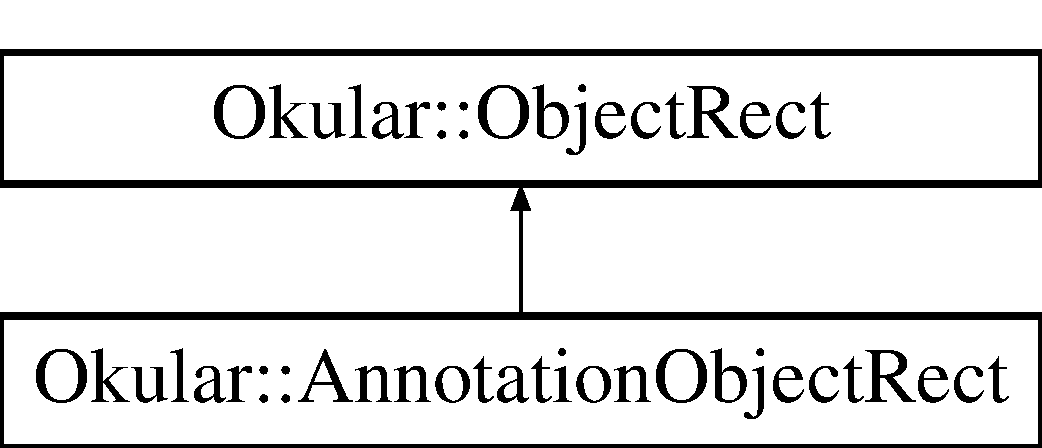
\includegraphics[height=2.000000cm]{classOkular_1_1AnnotationObjectRect}
\end{center}
\end{figure}
\subsection*{Public Member Functions}
\begin{DoxyCompactItemize}
\item 
\hyperlink{classOkular_1_1AnnotationObjectRect_a354e67fd4b871c538f6fb426a131750f}{Annotation\+Object\+Rect} (\hyperlink{classOkular_1_1Annotation}{Annotation} $\ast$\hyperlink{classOkular_1_1AnnotationObjectRect_ab44473e0817a058930e9a95d1773067d}{annotation})
\item 
virtual \hyperlink{classOkular_1_1AnnotationObjectRect_a6af3aeedc67e3bf0a3706bd837fdd9bf}{$\sim$\+Annotation\+Object\+Rect} ()
\item 
\hyperlink{classOkular_1_1Annotation}{Annotation} $\ast$ \hyperlink{classOkular_1_1AnnotationObjectRect_ab44473e0817a058930e9a95d1773067d}{annotation} () const 
\item 
virtual Q\+Rect \hyperlink{classOkular_1_1AnnotationObjectRect_a9ff5aa8673b33196df0cb14d51dacef2}{bounding\+Rect} (double x\+Scale, double y\+Scale) const 
\item 
virtual bool \hyperlink{classOkular_1_1AnnotationObjectRect_a1ca7ee341122db5f40af45ffd4607017}{contains} (double x, double y, double x\+Scale, double y\+Scale) const 
\item 
virtual void \hyperlink{classOkular_1_1AnnotationObjectRect_af61b2cdb3787c76bd6b53f0aa18c4476}{transform} (const Q\+Transform \&matrix)
\end{DoxyCompactItemize}
\subsection*{Additional Inherited Members}


\subsection{Detailed Description}
This class describes the object rectangle for an annotation. 

Definition at line 431 of file area.\+h.



\subsection{Constructor \& Destructor Documentation}
\hypertarget{classOkular_1_1AnnotationObjectRect_a354e67fd4b871c538f6fb426a131750f}{\index{Okular\+::\+Annotation\+Object\+Rect@{Okular\+::\+Annotation\+Object\+Rect}!Annotation\+Object\+Rect@{Annotation\+Object\+Rect}}
\index{Annotation\+Object\+Rect@{Annotation\+Object\+Rect}!Okular\+::\+Annotation\+Object\+Rect@{Okular\+::\+Annotation\+Object\+Rect}}
\subsubsection[{Annotation\+Object\+Rect}]{\setlength{\rightskip}{0pt plus 5cm}Annotation\+Object\+Rect\+::\+Annotation\+Object\+Rect (
\begin{DoxyParamCaption}
\item[{{\bf Annotation} $\ast$}]{annotation}
\end{DoxyParamCaption}
)}}\label{classOkular_1_1AnnotationObjectRect_a354e67fd4b871c538f6fb426a131750f}
Creates a new annotation object rectangle with the given {\ttfamily annotation}.

class \hyperlink{classOkular_1_1AnnotationObjectRect}{Annotation\+Object\+Rect} 

Definition at line 429 of file area.\+cpp.


\begin{DoxyCode}
430     : \hyperlink{classOkular_1_1ObjectRect_a699760a940f2476e917ff11cefcfab28}{ObjectRect}( QPolygonF(), \hyperlink{classOkular_1_1ObjectRect_a2f77f7653306bae90bfb68277aaafe16a7fa3680e4804e223e58ce2dea398345f}{OAnnotation}, annotation ), m\_annotation( annotation )
431 \{
432 \}
\end{DoxyCode}
\hypertarget{classOkular_1_1AnnotationObjectRect_a6af3aeedc67e3bf0a3706bd837fdd9bf}{\index{Okular\+::\+Annotation\+Object\+Rect@{Okular\+::\+Annotation\+Object\+Rect}!````~Annotation\+Object\+Rect@{$\sim$\+Annotation\+Object\+Rect}}
\index{````~Annotation\+Object\+Rect@{$\sim$\+Annotation\+Object\+Rect}!Okular\+::\+Annotation\+Object\+Rect@{Okular\+::\+Annotation\+Object\+Rect}}
\subsubsection[{$\sim$\+Annotation\+Object\+Rect}]{\setlength{\rightskip}{0pt plus 5cm}Annotation\+Object\+Rect\+::$\sim$\+Annotation\+Object\+Rect (
\begin{DoxyParamCaption}
{}
\end{DoxyParamCaption}
)\hspace{0.3cm}{\ttfamily [virtual]}}}\label{classOkular_1_1AnnotationObjectRect_a6af3aeedc67e3bf0a3706bd837fdd9bf}
Destroys the annotation object rectangle. 

Definition at line 457 of file area.\+cpp.


\begin{DoxyCode}
458 \{
459     \textcolor{comment}{// the annotation pointer is kept elsewehere (in Page, most probably),}
460     \textcolor{comment}{// so just release its pointer}
461     \hyperlink{classOkular_1_1ObjectRect_a8adcb135543e1399458f1fc3392f7a84}{m\_object} = 0;
462 \}
\end{DoxyCode}


\subsection{Member Function Documentation}
\hypertarget{classOkular_1_1AnnotationObjectRect_ab44473e0817a058930e9a95d1773067d}{\index{Okular\+::\+Annotation\+Object\+Rect@{Okular\+::\+Annotation\+Object\+Rect}!annotation@{annotation}}
\index{annotation@{annotation}!Okular\+::\+Annotation\+Object\+Rect@{Okular\+::\+Annotation\+Object\+Rect}}
\subsubsection[{annotation}]{\setlength{\rightskip}{0pt plus 5cm}{\bf Annotation} $\ast$ Annotation\+Object\+Rect\+::annotation (
\begin{DoxyParamCaption}
{}
\end{DoxyParamCaption}
) const}}\label{classOkular_1_1AnnotationObjectRect_ab44473e0817a058930e9a95d1773067d}
Returns the annotation object of the annotation object rectangle. 

Definition at line 434 of file area.\+cpp.


\begin{DoxyCode}
435 \{
436     \textcolor{keywordflow}{return} m\_annotation;
437 \}
\end{DoxyCode}
\hypertarget{classOkular_1_1AnnotationObjectRect_a9ff5aa8673b33196df0cb14d51dacef2}{\index{Okular\+::\+Annotation\+Object\+Rect@{Okular\+::\+Annotation\+Object\+Rect}!bounding\+Rect@{bounding\+Rect}}
\index{bounding\+Rect@{bounding\+Rect}!Okular\+::\+Annotation\+Object\+Rect@{Okular\+::\+Annotation\+Object\+Rect}}
\subsubsection[{bounding\+Rect}]{\setlength{\rightskip}{0pt plus 5cm}Q\+Rect Annotation\+Object\+Rect\+::bounding\+Rect (
\begin{DoxyParamCaption}
\item[{double}]{x\+Scale, }
\item[{double}]{y\+Scale}
\end{DoxyParamCaption}
) const\hspace{0.3cm}{\ttfamily [virtual]}}}\label{classOkular_1_1AnnotationObjectRect_a9ff5aa8673b33196df0cb14d51dacef2}
Returns the bounding rect of the annotation object rectangle for the scaling factor {\ttfamily x\+Scale} and {\ttfamily y\+Scale}. 

Reimplemented from \hyperlink{classOkular_1_1ObjectRect_aa6b1c3b6ed093291d5ec7f92b97754ae}{Okular\+::\+Object\+Rect}.



Definition at line 439 of file area.\+cpp.


\begin{DoxyCode}
440 \{
441     \textcolor{keyword}{const} QRect annotRect = \hyperlink{classOkular_1_1AnnotationUtils_a6b3fdb4e89227d26ec9e6f62bf4d0eb9}{AnnotationUtils::annotationGeometry}( 
      m\_annotation, xScale, yScale );
442     \textcolor{keyword}{const} QPoint center = annotRect.center();
443 
444     \textcolor{comment}{// Make sure that the rectangle has a minimum size, so that it's possible}
445     \textcolor{comment}{// to click on it}
446     \textcolor{keyword}{const} \textcolor{keywordtype}{int} minSize = 14;
447     \textcolor{keyword}{const} QRect minRect( center.x()-minSize/2, center.y()-minSize/2, minSize, minSize );
448 
449     \textcolor{keywordflow}{return} annotRect | minRect;
450 \}
\end{DoxyCode}
\hypertarget{classOkular_1_1AnnotationObjectRect_a1ca7ee341122db5f40af45ffd4607017}{\index{Okular\+::\+Annotation\+Object\+Rect@{Okular\+::\+Annotation\+Object\+Rect}!contains@{contains}}
\index{contains@{contains}!Okular\+::\+Annotation\+Object\+Rect@{Okular\+::\+Annotation\+Object\+Rect}}
\subsubsection[{contains}]{\setlength{\rightskip}{0pt plus 5cm}bool Annotation\+Object\+Rect\+::contains (
\begin{DoxyParamCaption}
\item[{double}]{x, }
\item[{double}]{y, }
\item[{double}]{x\+Scale, }
\item[{double}]{y\+Scale}
\end{DoxyParamCaption}
) const\hspace{0.3cm}{\ttfamily [virtual]}}}\label{classOkular_1_1AnnotationObjectRect_a1ca7ee341122db5f40af45ffd4607017}
Returns whether the annotation object rectangle contains the point {\ttfamily x}, {\ttfamily y} for the scaling factor {\ttfamily x\+Scale} and {\ttfamily y\+Scale}. 

Reimplemented from \hyperlink{classOkular_1_1ObjectRect_aadc1a6f33f9af0f6da1fd94c07d52488}{Okular\+::\+Object\+Rect}.



Definition at line 452 of file area.\+cpp.


\begin{DoxyCode}
453 \{
454     \textcolor{keywordflow}{return} \hyperlink{classOkular_1_1AnnotationObjectRect_a9ff5aa8673b33196df0cb14d51dacef2}{boundingRect}( xScale, yScale ).contains( (\textcolor{keywordtype}{int})( x * xScale ), (\textcolor{keywordtype}{int})( y * yScale ), \textcolor{keyword}{
      false} );
455 \}
\end{DoxyCode}
\hypertarget{classOkular_1_1AnnotationObjectRect_af61b2cdb3787c76bd6b53f0aa18c4476}{\index{Okular\+::\+Annotation\+Object\+Rect@{Okular\+::\+Annotation\+Object\+Rect}!transform@{transform}}
\index{transform@{transform}!Okular\+::\+Annotation\+Object\+Rect@{Okular\+::\+Annotation\+Object\+Rect}}
\subsubsection[{transform}]{\setlength{\rightskip}{0pt plus 5cm}void Annotation\+Object\+Rect\+::transform (
\begin{DoxyParamCaption}
\item[{const Q\+Transform \&}]{matrix}
\end{DoxyParamCaption}
)\hspace{0.3cm}{\ttfamily [virtual]}}}\label{classOkular_1_1AnnotationObjectRect_af61b2cdb3787c76bd6b53f0aa18c4476}
Transforms the annotation object rectangle with the operations defined by {\ttfamily matrix}. 

Reimplemented from \hyperlink{classOkular_1_1ObjectRect_ae792b4a8ca659f7315173722a862e05f}{Okular\+::\+Object\+Rect}.



Definition at line 464 of file area.\+cpp.


\begin{DoxyCode}
465 \{
466     m\_annotation->d\_func()->annotationTransform( matrix );
467 \}
\end{DoxyCode}


The documentation for this class was generated from the following files\+:\begin{DoxyCompactItemize}
\item 
core/\hyperlink{area_8h}{area.\+h}\item 
core/\hyperlink{area_8cpp}{area.\+cpp}\end{DoxyCompactItemize}

\hypertarget{classAnnotationPopup}{\section{Annotation\+Popup Class Reference}
\label{classAnnotationPopup}\index{Annotation\+Popup@{Annotation\+Popup}}
}


{\ttfamily \#include $<$annotationpopup.\+h$>$}

Inheritance diagram for Annotation\+Popup\+:\begin{figure}[H]
\begin{center}
\leavevmode
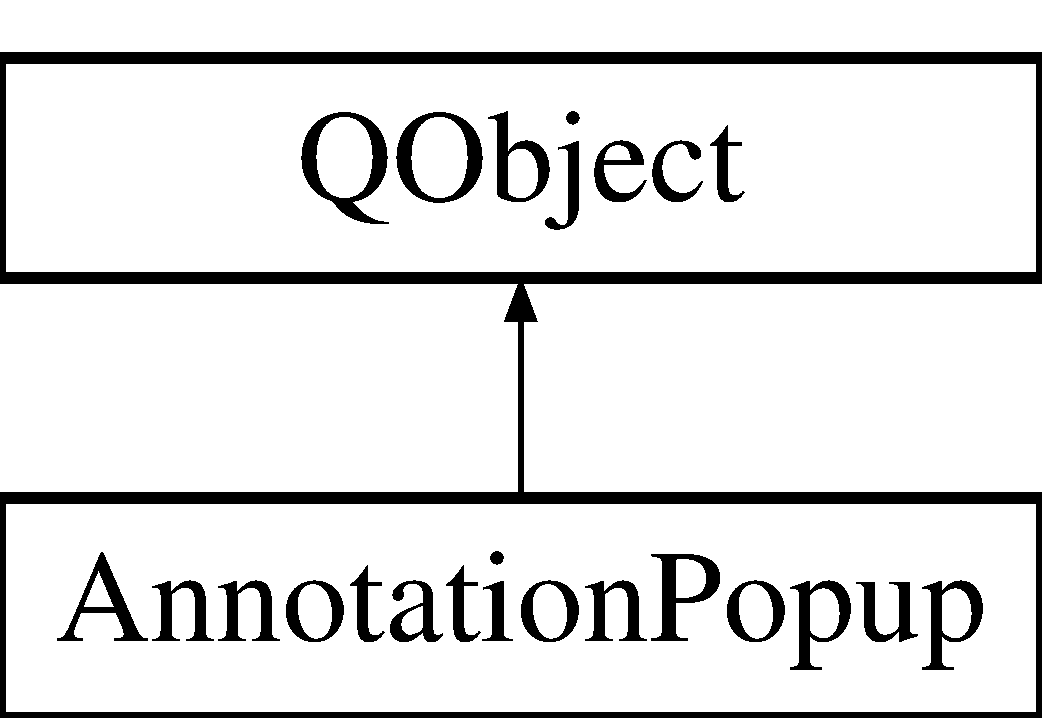
\includegraphics[height=2.000000cm]{classAnnotationPopup}
\end{center}
\end{figure}
\subsection*{Classes}
\begin{DoxyCompactItemize}
\item 
struct \hyperlink{structAnnotationPopup_1_1AnnotPagePair}{Annot\+Page\+Pair}
\end{DoxyCompactItemize}
\subsection*{Public Types}
\begin{DoxyCompactItemize}
\item 
enum \hyperlink{classAnnotationPopup_af8654f3f9c2a3377f86daf329f1e0679}{Menu\+Mode} \{ \hyperlink{classAnnotationPopup_af8654f3f9c2a3377f86daf329f1e0679a40137692e843ce4f994737bd4a6f68f1}{Single\+Annotation\+Mode}, 
\hyperlink{classAnnotationPopup_af8654f3f9c2a3377f86daf329f1e0679addf6a6dddf8c14065bb700f1835dafb9}{Multi\+Annotation\+Mode}
 \}
\end{DoxyCompactItemize}
\subsection*{Signals}
\begin{DoxyCompactItemize}
\item 
void \hyperlink{classAnnotationPopup_a2f542d2aa2c7cc85b4bc9045be5adcc9}{open\+Annotation\+Window} (\hyperlink{classOkular_1_1Annotation}{Okular\+::\+Annotation} $\ast$annotation, int page\+Number)
\end{DoxyCompactItemize}
\subsection*{Public Member Functions}
\begin{DoxyCompactItemize}
\item 
\hyperlink{classAnnotationPopup_a239651270ccd047fcba04c71f7b49a45}{Annotation\+Popup} (\hyperlink{classOkular_1_1Document}{Okular\+::\+Document} $\ast$document, \hyperlink{classAnnotationPopup_af8654f3f9c2a3377f86daf329f1e0679}{Menu\+Mode} mode, Q\+Widget $\ast$parent=0)
\item 
void \hyperlink{classAnnotationPopup_a3235e948e6dcc5ec49dc38df56d89a9c}{add\+Annotation} (\hyperlink{classOkular_1_1Annotation}{Okular\+::\+Annotation} $\ast$annotation, int page\+Number)
\item 
void \hyperlink{classAnnotationPopup_a54b930f61b3d40661d0af18667a1573f}{exec} (const Q\+Point \&point=Q\+Point())
\end{DoxyCompactItemize}


\subsection{Detailed Description}


Definition at line 23 of file annotationpopup.\+h.



\subsection{Member Enumeration Documentation}
\hypertarget{classAnnotationPopup_af8654f3f9c2a3377f86daf329f1e0679}{\index{Annotation\+Popup@{Annotation\+Popup}!Menu\+Mode@{Menu\+Mode}}
\index{Menu\+Mode@{Menu\+Mode}!Annotation\+Popup@{Annotation\+Popup}}
\subsubsection[{Menu\+Mode}]{\setlength{\rightskip}{0pt plus 5cm}enum {\bf Annotation\+Popup\+::\+Menu\+Mode}}}\label{classAnnotationPopup_af8654f3f9c2a3377f86daf329f1e0679}
Describes the structure of the popup menu. \begin{Desc}
\item[Enumerator]\par
\begin{description}
\index{Single\+Annotation\+Mode@{Single\+Annotation\+Mode}!Annotation\+Popup@{Annotation\+Popup}}\index{Annotation\+Popup@{Annotation\+Popup}!Single\+Annotation\+Mode@{Single\+Annotation\+Mode}}\item[{\em 
\hypertarget{classAnnotationPopup_af8654f3f9c2a3377f86daf329f1e0679a40137692e843ce4f994737bd4a6f68f1}{Single\+Annotation\+Mode}\label{classAnnotationPopup_af8654f3f9c2a3377f86daf329f1e0679a40137692e843ce4f994737bd4a6f68f1}
}]The menu shows only entries to manipulate a single annotation, or multiple annotations as a group. \index{Multi\+Annotation\+Mode@{Multi\+Annotation\+Mode}!Annotation\+Popup@{Annotation\+Popup}}\index{Annotation\+Popup@{Annotation\+Popup}!Multi\+Annotation\+Mode@{Multi\+Annotation\+Mode}}\item[{\em 
\hypertarget{classAnnotationPopup_af8654f3f9c2a3377f86daf329f1e0679addf6a6dddf8c14065bb700f1835dafb9}{Multi\+Annotation\+Mode}\label{classAnnotationPopup_af8654f3f9c2a3377f86daf329f1e0679addf6a6dddf8c14065bb700f1835dafb9}
}]The menu shows entries to manipulate multiple annotations. \end{description}
\end{Desc}


Definition at line 31 of file annotationpopup.\+h.


\begin{DoxyCode}
32         \{
33             \hyperlink{classAnnotationPopup_af8654f3f9c2a3377f86daf329f1e0679a40137692e843ce4f994737bd4a6f68f1}{SingleAnnotationMode}, 
34             \hyperlink{classAnnotationPopup_af8654f3f9c2a3377f86daf329f1e0679addf6a6dddf8c14065bb700f1835dafb9}{MultiAnnotationMode}   
35         \};
\end{DoxyCode}


\subsection{Constructor \& Destructor Documentation}
\hypertarget{classAnnotationPopup_a239651270ccd047fcba04c71f7b49a45}{\index{Annotation\+Popup@{Annotation\+Popup}!Annotation\+Popup@{Annotation\+Popup}}
\index{Annotation\+Popup@{Annotation\+Popup}!Annotation\+Popup@{Annotation\+Popup}}
\subsubsection[{Annotation\+Popup}]{\setlength{\rightskip}{0pt plus 5cm}Annotation\+Popup\+::\+Annotation\+Popup (
\begin{DoxyParamCaption}
\item[{{\bf Okular\+::\+Document} $\ast$}]{document, }
\item[{{\bf Menu\+Mode}}]{mode, }
\item[{Q\+Widget $\ast$}]{parent = {\ttfamily 0}}
\end{DoxyParamCaption}
)}}\label{classAnnotationPopup_a239651270ccd047fcba04c71f7b49a45}


Definition at line 23 of file annotationpopup.\+cpp.


\begin{DoxyCode}
25     : mParent( parent ), mDocument( document ), mMenuMode( mode )
26 \{
27 \}
\end{DoxyCode}


\subsection{Member Function Documentation}
\hypertarget{classAnnotationPopup_a3235e948e6dcc5ec49dc38df56d89a9c}{\index{Annotation\+Popup@{Annotation\+Popup}!add\+Annotation@{add\+Annotation}}
\index{add\+Annotation@{add\+Annotation}!Annotation\+Popup@{Annotation\+Popup}}
\subsubsection[{add\+Annotation}]{\setlength{\rightskip}{0pt plus 5cm}void Annotation\+Popup\+::add\+Annotation (
\begin{DoxyParamCaption}
\item[{{\bf Okular\+::\+Annotation} $\ast$}]{annotation, }
\item[{int}]{page\+Number}
\end{DoxyParamCaption}
)}}\label{classAnnotationPopup_a3235e948e6dcc5ec49dc38df56d89a9c}


Definition at line 29 of file annotationpopup.\+cpp.


\begin{DoxyCode}
30 \{
31     AnnotPagePair pair( annotation, pageNumber );
32     \textcolor{keywordflow}{if} ( !mAnnotations.contains( pair ) )
33       mAnnotations.append( pair );
34 \}
\end{DoxyCode}
\hypertarget{classAnnotationPopup_a54b930f61b3d40661d0af18667a1573f}{\index{Annotation\+Popup@{Annotation\+Popup}!exec@{exec}}
\index{exec@{exec}!Annotation\+Popup@{Annotation\+Popup}}
\subsubsection[{exec}]{\setlength{\rightskip}{0pt plus 5cm}void Annotation\+Popup\+::exec (
\begin{DoxyParamCaption}
\item[{const Q\+Point \&}]{point = {\ttfamily QPoint()}}
\end{DoxyParamCaption}
)}}\label{classAnnotationPopup_a54b930f61b3d40661d0af18667a1573f}


Definition at line 36 of file annotationpopup.\+cpp.


\begin{DoxyCode}
37 \{
38     \textcolor{keywordflow}{if} ( mAnnotations.isEmpty() )
39         \textcolor{keywordflow}{return};
40 
41     KMenu menu( mParent );
42 
43     QAction *action = 0;
44     \hyperlink{classOkular_1_1FileAttachmentAnnotation}{Okular::FileAttachmentAnnotation} *fileAttachAnnot = 0;
45 
46     \textcolor{keyword}{const} \textcolor{keywordtype}{char} *actionTypeId = \textcolor{stringliteral}{"actionType"};
47 
48     \textcolor{keyword}{const} QString openId = QString::fromLatin1( \textcolor{stringliteral}{"open"} );
49     \textcolor{keyword}{const} QString deleteId = QString::fromLatin1( \textcolor{stringliteral}{"delete"} );
50     \textcolor{keyword}{const} QString deleteAllId = QString::fromLatin1( \textcolor{stringliteral}{"deleteAll"} );
51     \textcolor{keyword}{const} QString propertiesId = QString::fromLatin1( \textcolor{stringliteral}{"properties"} );
52     \textcolor{keyword}{const} QString saveId = QString::fromLatin1( \textcolor{stringliteral}{"save"} );
53 
54     \textcolor{keywordflow}{if} ( mMenuMode == \hyperlink{classAnnotationPopup_af8654f3f9c2a3377f86daf329f1e0679a40137692e843ce4f994737bd4a6f68f1}{SingleAnnotationMode} )
55     \{
56         \textcolor{keyword}{const} \textcolor{keywordtype}{bool} onlyOne = (mAnnotations.count() == 1);
57 
58         \textcolor{keyword}{const} AnnotPagePair &pair = mAnnotations.at(0);
59 
60         menu.addTitle( i18np( \textcolor{stringliteral}{"Annotation"}, \textcolor{stringliteral}{"%1 Annotations"}, mAnnotations.count() ) );
61 
62         action = menu.addAction( KIcon( \textcolor{stringliteral}{"comment"} ), i18n( \textcolor{stringliteral}{"&Open Pop-up Note"} ) );
63         action->setData( QVariant::fromValue( pair ) );
64         action->setEnabled( onlyOne );
65         action->setProperty( actionTypeId, openId );
66 
67         action = menu.addAction( KIcon( \textcolor{stringliteral}{"list-remove"} ), i18n( \textcolor{stringliteral}{"&Delete"} ) );
68         action->setEnabled( mDocument->\hyperlink{classOkular_1_1Document_a6dd7a475b14222c07d1c410311f35cdb}{isAllowed}( \hyperlink{namespaceOkular_a3601f4e702453ddf1125476dd6e7577ba6c10962833bd58ea0f8d63e448eba8e9}{Okular::AllowNotes} ) );
69         action->setProperty( actionTypeId, deleteAllId );
70 
71         \textcolor{keywordflow}{foreach} ( \textcolor{keyword}{const} AnnotPagePair& pair, mAnnotations )
72         \{
73             \textcolor{keywordflow}{if} ( !mDocument->\hyperlink{classOkular_1_1Document_a77f5c38224da847413dbe51c5e24ed08}{canRemovePageAnnotation}( pair.annotation ) )
74                 action->setEnabled( \textcolor{keyword}{false} );
75         \}
76 
77         action = menu.addAction( KIcon( \textcolor{stringliteral}{"configure"} ), i18n( \textcolor{stringliteral}{"&Properties"} ) );
78         action->setData( QVariant::fromValue( pair ) );
79         action->setEnabled( onlyOne );
80         action->setProperty( actionTypeId, propertiesId );
81 
82         \textcolor{keywordflow}{if} ( onlyOne && pair.annotation->subType() == 
      \hyperlink{classOkular_1_1Annotation_af71b46e37d5f850b97d5c4de3be9aac0a7209cbfb5e13c0f80ac36f87c9575836}{Okular::Annotation::AFileAttachment} )
83         \{
84             menu.addSeparator();
85             fileAttachAnnot = \textcolor{keyword}{static\_cast<} \hyperlink{classOkular_1_1FileAttachmentAnnotation}{Okular::FileAttachmentAnnotation}
       * \textcolor{keyword}{>}( pair.annotation );
86             \textcolor{keyword}{const} QString saveText = i18nc( \textcolor{stringliteral}{"%1 is the name of the file to save"}, \textcolor{stringliteral}{"&Save '%1'..."}, 
      fileAttachAnnot->\hyperlink{classOkular_1_1FileAttachmentAnnotation_a22ff85c689647a6daa6bac053fe60cbb}{embeddedFile}()->\hyperlink{classOkular_1_1EmbeddedFile_a70fcfea705979ce6a31b989fc92a8f2b}{name}() );
87 
88             action = menu.addAction( KIcon( \textcolor{stringliteral}{"document-save"} ), saveText );
89             action->setData( QVariant::fromValue( pair ) );
90             action->setProperty( actionTypeId, saveId );
91         \}
92     \}
93     \textcolor{keywordflow}{else}
94     \{
95         \textcolor{keywordflow}{foreach} ( \textcolor{keyword}{const} AnnotPagePair& pair, mAnnotations )
96         \{
97             menu.addTitle( \hyperlink{namespaceGuiUtils_af15abd3dd32e982db3f842e807146835}{GuiUtils::captionForAnnotation}( pair.annotation ) 
      );
98 
99             action = menu.addAction( KIcon( \textcolor{stringliteral}{"comment"} ), i18n( \textcolor{stringliteral}{"&Open Pop-up Note"} ) );
100             action->setData( QVariant::fromValue( pair ) );
101             action->setProperty( actionTypeId, openId );
102 
103             action = menu.addAction( KIcon( \textcolor{stringliteral}{"list-remove"} ), i18n( \textcolor{stringliteral}{"&Delete"} ) );
104             action->setEnabled( mDocument->\hyperlink{classOkular_1_1Document_a6dd7a475b14222c07d1c410311f35cdb}{isAllowed}( 
      \hyperlink{namespaceOkular_a3601f4e702453ddf1125476dd6e7577ba6c10962833bd58ea0f8d63e448eba8e9}{Okular::AllowNotes} ) &&
105                                 mDocument->\hyperlink{classOkular_1_1Document_a77f5c38224da847413dbe51c5e24ed08}{canRemovePageAnnotation}( pair.annotation 
      ) );
106             action->setData( QVariant::fromValue( pair ) );
107             action->setProperty( actionTypeId, deleteId );
108 
109             action = menu.addAction( KIcon( \textcolor{stringliteral}{"configure"} ), i18n( \textcolor{stringliteral}{"&Properties"} ) );
110             action->setData( QVariant::fromValue( pair ) );
111             action->setProperty( actionTypeId, propertiesId );
112 
113             \textcolor{keywordflow}{if} ( pair.annotation->subType() == 
      \hyperlink{classOkular_1_1Annotation_af71b46e37d5f850b97d5c4de3be9aac0a7209cbfb5e13c0f80ac36f87c9575836}{Okular::Annotation::AFileAttachment} )
114             \{
115                 menu.addSeparator();
116                 fileAttachAnnot = \textcolor{keyword}{static\_cast<} \hyperlink{classOkular_1_1FileAttachmentAnnotation}{Okular::FileAttachmentAnnotation}
       * \textcolor{keyword}{>}( pair.annotation );
117                 \textcolor{keyword}{const} QString saveText = i18nc( \textcolor{stringliteral}{"%1 is the name of the file to save"}, \textcolor{stringliteral}{"&Save '%1'..."}, 
      fileAttachAnnot->\hyperlink{classOkular_1_1FileAttachmentAnnotation_a22ff85c689647a6daa6bac053fe60cbb}{embeddedFile}()->\hyperlink{classOkular_1_1EmbeddedFile_a70fcfea705979ce6a31b989fc92a8f2b}{name}() );
118 
119                 action = menu.addAction( KIcon( \textcolor{stringliteral}{"document-save"} ), saveText );
120                 action->setData( QVariant::fromValue( pair ) );
121                 action->setProperty( actionTypeId, saveId );
122             \}
123         \}
124     \}
125 
126     QAction *choice = menu.exec( point.isNull() ? QCursor::pos() : point );
127 
128     \textcolor{comment}{// check if the user really selected an action}
129     \textcolor{keywordflow}{if} ( choice ) \{
130         \textcolor{keyword}{const} AnnotPagePair pair = choice->data().value<AnnotPagePair>();
131 
132         \textcolor{keyword}{const} QString actionType = choice->property( actionTypeId ).toString();
133         \textcolor{keywordflow}{if} ( actionType == openId ) \{
134             emit \hyperlink{classAnnotationPopup_a2f542d2aa2c7cc85b4bc9045be5adcc9}{openAnnotationWindow}( pair.annotation, pair.pageNumber );
135         \} \textcolor{keywordflow}{else} \textcolor{keywordflow}{if}( actionType == deleteId ) \{
136             \textcolor{keywordflow}{if} ( pair.pageNumber != -1 )
137                 mDocument->\hyperlink{classOkular_1_1Document_af8ae711ce34ff903a589423e73a45cbb}{removePageAnnotation}( pair.pageNumber, pair.annotation );
138         \} \textcolor{keywordflow}{else} \textcolor{keywordflow}{if}( actionType == deleteAllId ) \{
139             Q\_FOREACH ( \textcolor{keyword}{const} AnnotPagePair& pair, mAnnotations )
140             \{
141                 \textcolor{keywordflow}{if} ( pair.pageNumber != -1 )
142                     mDocument->\hyperlink{classOkular_1_1Document_af8ae711ce34ff903a589423e73a45cbb}{removePageAnnotation}( pair.pageNumber, pair.annotation )
      ;
143             \}
144         \} \textcolor{keywordflow}{else} \textcolor{keywordflow}{if}( actionType == propertiesId ) \{
145             \textcolor{keywordflow}{if} ( pair.pageNumber != -1 ) \{
146                 \hyperlink{classAnnotsPropertiesDialog}{AnnotsPropertiesDialog} propdialog( mParent, mDocument, pair.
      pageNumber, pair.annotation );
147                 propdialog.exec();
148             \}
149         \} \textcolor{keywordflow}{else} \textcolor{keywordflow}{if}( actionType == saveId ) \{
150             \textcolor{keyword}{const} \hyperlink{classOkular_1_1FileAttachmentAnnotation}{Okular::FileAttachmentAnnotation} * fileAttachAnnot = \textcolor{keyword}{
      static\_cast<} \hyperlink{classOkular_1_1FileAttachmentAnnotation}{Okular::FileAttachmentAnnotation} * \textcolor{keyword}{>}( pair.annotation );
151             \hyperlink{namespaceGuiUtils_a5e934d5070afd94f91b3a5fbfb8cbc04}{GuiUtils::saveEmbeddedFile}( fileAttachAnnot->
      \hyperlink{classOkular_1_1FileAttachmentAnnotation_a22ff85c689647a6daa6bac053fe60cbb}{embeddedFile}(), mParent );
152         \}
153     \}
154 \}
\end{DoxyCode}
\hypertarget{classAnnotationPopup_a2f542d2aa2c7cc85b4bc9045be5adcc9}{\index{Annotation\+Popup@{Annotation\+Popup}!open\+Annotation\+Window@{open\+Annotation\+Window}}
\index{open\+Annotation\+Window@{open\+Annotation\+Window}!Annotation\+Popup@{Annotation\+Popup}}
\subsubsection[{open\+Annotation\+Window}]{\setlength{\rightskip}{0pt plus 5cm}void Annotation\+Popup\+::open\+Annotation\+Window (
\begin{DoxyParamCaption}
\item[{{\bf Okular\+::\+Annotation} $\ast$}]{annotation, }
\item[{int}]{page\+Number}
\end{DoxyParamCaption}
)\hspace{0.3cm}{\ttfamily [signal]}}}\label{classAnnotationPopup_a2f542d2aa2c7cc85b4bc9045be5adcc9}


The documentation for this class was generated from the following files\+:\begin{DoxyCompactItemize}
\item 
ui/\hyperlink{annotationpopup_8h}{annotationpopup.\+h}\item 
ui/\hyperlink{annotationpopup_8cpp}{annotationpopup.\+cpp}\end{DoxyCompactItemize}

\hypertarget{structOkular_1_1TextDocumentGeneratorPrivate_1_1AnnotationPosition}{\section{Okular\+:\+:Text\+Document\+Generator\+Private\+:\+:Annotation\+Position Struct Reference}
\label{structOkular_1_1TextDocumentGeneratorPrivate_1_1AnnotationPosition}\index{Okular\+::\+Text\+Document\+Generator\+Private\+::\+Annotation\+Position@{Okular\+::\+Text\+Document\+Generator\+Private\+::\+Annotation\+Position}}
}


{\ttfamily \#include $<$textdocumentgenerator\+\_\+p.\+h$>$}

\subsection*{Public Attributes}
\begin{DoxyCompactItemize}
\item 
int \hyperlink{structOkular_1_1TextDocumentGeneratorPrivate_1_1AnnotationPosition_aa8fd3b91acb6195b9341ac9838c28402}{start\+Position}
\item 
int \hyperlink{structOkular_1_1TextDocumentGeneratorPrivate_1_1AnnotationPosition_a772c24061b1b2f5101440b31d2e8e871}{end\+Position}
\item 
\hyperlink{classOkular_1_1Annotation}{Annotation} $\ast$ \hyperlink{structOkular_1_1TextDocumentGeneratorPrivate_1_1AnnotationPosition_af557e1e52655a87adfac85e87a112c94}{annotation}
\end{DoxyCompactItemize}


\subsection{Detailed Description}


Definition at line 178 of file textdocumentgenerator\+\_\+p.\+h.



\subsection{Member Data Documentation}
\hypertarget{structOkular_1_1TextDocumentGeneratorPrivate_1_1AnnotationPosition_af557e1e52655a87adfac85e87a112c94}{\index{Okular\+::\+Text\+Document\+Generator\+Private\+::\+Annotation\+Position@{Okular\+::\+Text\+Document\+Generator\+Private\+::\+Annotation\+Position}!annotation@{annotation}}
\index{annotation@{annotation}!Okular\+::\+Text\+Document\+Generator\+Private\+::\+Annotation\+Position@{Okular\+::\+Text\+Document\+Generator\+Private\+::\+Annotation\+Position}}
\subsubsection[{annotation}]{\setlength{\rightskip}{0pt plus 5cm}{\bf Annotation}$\ast$ Okular\+::\+Text\+Document\+Generator\+Private\+::\+Annotation\+Position\+::annotation}}\label{structOkular_1_1TextDocumentGeneratorPrivate_1_1AnnotationPosition_af557e1e52655a87adfac85e87a112c94}


Definition at line 182 of file textdocumentgenerator\+\_\+p.\+h.

\hypertarget{structOkular_1_1TextDocumentGeneratorPrivate_1_1AnnotationPosition_a772c24061b1b2f5101440b31d2e8e871}{\index{Okular\+::\+Text\+Document\+Generator\+Private\+::\+Annotation\+Position@{Okular\+::\+Text\+Document\+Generator\+Private\+::\+Annotation\+Position}!end\+Position@{end\+Position}}
\index{end\+Position@{end\+Position}!Okular\+::\+Text\+Document\+Generator\+Private\+::\+Annotation\+Position@{Okular\+::\+Text\+Document\+Generator\+Private\+::\+Annotation\+Position}}
\subsubsection[{end\+Position}]{\setlength{\rightskip}{0pt plus 5cm}int Okular\+::\+Text\+Document\+Generator\+Private\+::\+Annotation\+Position\+::end\+Position}}\label{structOkular_1_1TextDocumentGeneratorPrivate_1_1AnnotationPosition_a772c24061b1b2f5101440b31d2e8e871}


Definition at line 181 of file textdocumentgenerator\+\_\+p.\+h.

\hypertarget{structOkular_1_1TextDocumentGeneratorPrivate_1_1AnnotationPosition_aa8fd3b91acb6195b9341ac9838c28402}{\index{Okular\+::\+Text\+Document\+Generator\+Private\+::\+Annotation\+Position@{Okular\+::\+Text\+Document\+Generator\+Private\+::\+Annotation\+Position}!start\+Position@{start\+Position}}
\index{start\+Position@{start\+Position}!Okular\+::\+Text\+Document\+Generator\+Private\+::\+Annotation\+Position@{Okular\+::\+Text\+Document\+Generator\+Private\+::\+Annotation\+Position}}
\subsubsection[{start\+Position}]{\setlength{\rightskip}{0pt plus 5cm}int Okular\+::\+Text\+Document\+Generator\+Private\+::\+Annotation\+Position\+::start\+Position}}\label{structOkular_1_1TextDocumentGeneratorPrivate_1_1AnnotationPosition_aa8fd3b91acb6195b9341ac9838c28402}


Definition at line 180 of file textdocumentgenerator\+\_\+p.\+h.



The documentation for this struct was generated from the following file\+:\begin{DoxyCompactItemize}
\item 
core/\hyperlink{textdocumentgenerator__p_8h}{textdocumentgenerator\+\_\+p.\+h}\end{DoxyCompactItemize}

\hypertarget{classOkular_1_1AnnotationPrivate}{\section{Okular\+:\+:Annotation\+Private Class Reference}
\label{classOkular_1_1AnnotationPrivate}\index{Okular\+::\+Annotation\+Private@{Okular\+::\+Annotation\+Private}}
}


{\ttfamily \#include $<$annotations\+\_\+p.\+h$>$}

Inheritance diagram for Okular\+:\+:Annotation\+Private\+:\begin{figure}[H]
\begin{center}
\leavevmode
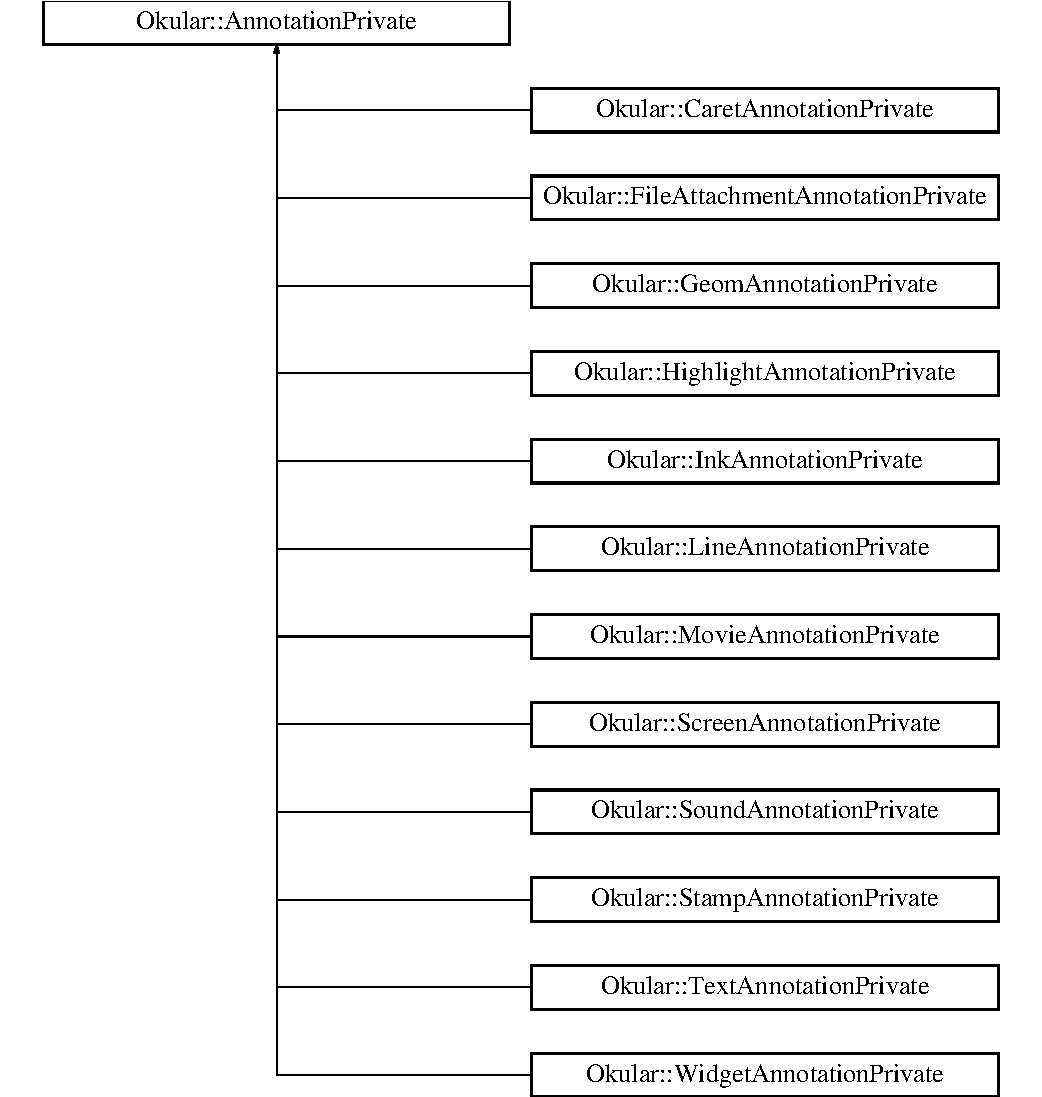
\includegraphics[height=12.000000cm]{classOkular_1_1AnnotationPrivate}
\end{center}
\end{figure}
\subsection*{Public Member Functions}
\begin{DoxyCompactItemize}
\item 
\hyperlink{classOkular_1_1AnnotationPrivate_affc5d14076f4606905c3c0cd2f6b9dc1}{Annotation\+Private} ()
\item 
virtual \hyperlink{classOkular_1_1AnnotationPrivate_a9ea42bcbf0ff30348f462f9da55ffb9b}{$\sim$\+Annotation\+Private} ()
\item 
void \hyperlink{classOkular_1_1AnnotationPrivate_a1add0ae079273c89e70abae1c85c3333}{annotation\+Transform} (const Q\+Transform \&matrix)
\item 
virtual void \hyperlink{classOkular_1_1AnnotationPrivate_a0d340a5ed89975edc173b72569f1e3f0}{transform} (const Q\+Transform \&matrix)
\item 
virtual void \hyperlink{classOkular_1_1AnnotationPrivate_aa60e3513cd1a25f60afbdef5614683d2}{base\+Transform} (const Q\+Transform \&matrix)
\item 
virtual void \hyperlink{classOkular_1_1AnnotationPrivate_afb8f0d99eefa51347efaef5114511154}{reset\+Transformation} ()
\item 
virtual void \hyperlink{classOkular_1_1AnnotationPrivate_aee9684802697da01c33c4dec9de56ee1}{translate} (const \hyperlink{classOkular_1_1NormalizedPoint}{Normalized\+Point} \&coord)
\item 
virtual bool \hyperlink{classOkular_1_1AnnotationPrivate_aeb7f48383177812c27abf1230416a520}{open\+Dialog\+After\+Creation} () const 
\item 
virtual void \hyperlink{classOkular_1_1AnnotationPrivate_a5fc7b450fa8c7e2717372e7394c3aa39}{set\+Annotation\+Properties} (const Q\+Dom\+Node \&node)
\item 
virtual \hyperlink{classOkular_1_1AnnotationPrivate}{Annotation\+Private} $\ast$ \hyperlink{classOkular_1_1AnnotationPrivate_a4a27afb6108cff892c7bcccd8ba3aafa}{get\+New\+Annotation\+Private} ()=0
\item 
virtual double \hyperlink{classOkular_1_1AnnotationPrivate_ab4288200b0dd46f33e4958a64ffac373}{distance\+Sqr} (double x, double y, double x\+Scale, double y\+Scale)
\end{DoxyCompactItemize}
\subsection*{Public Attributes}
\begin{DoxyCompactItemize}
\item 
\hyperlink{classOkular_1_1PagePrivate}{Page\+Private} $\ast$ \hyperlink{classOkular_1_1AnnotationPrivate_a2db3806670326880d0d7e6e1986d35f4}{m\+\_\+page}
\item 
Q\+String \hyperlink{classOkular_1_1AnnotationPrivate_af2997724c734cbd4dfbc6536e280d536}{m\+\_\+author}
\item 
Q\+String \hyperlink{classOkular_1_1AnnotationPrivate_ab2b69e4809035828d98a4ec701565149}{m\+\_\+contents}
\item 
Q\+String \hyperlink{classOkular_1_1AnnotationPrivate_a31b33f971130850a5b5bf67ce58ae5f1}{m\+\_\+unique\+Name}
\item 
Q\+Date\+Time \hyperlink{classOkular_1_1AnnotationPrivate_a8663feeb255860d7c7b57b389c307b0d}{m\+\_\+modify\+Date}
\item 
Q\+Date\+Time \hyperlink{classOkular_1_1AnnotationPrivate_ad4afb1827157f15bf3b5984e5f62c7a3}{m\+\_\+creation\+Date}
\item 
int \hyperlink{classOkular_1_1AnnotationPrivate_ae7ada31b42bb74e306f26a9126110226}{m\+\_\+flags}
\item 
\hyperlink{classOkular_1_1NormalizedRect}{Normalized\+Rect} \hyperlink{classOkular_1_1AnnotationPrivate_a58948ebd679895ca16c5f9f917f23323}{m\+\_\+boundary}
\item 
\hyperlink{classOkular_1_1NormalizedRect}{Normalized\+Rect} \hyperlink{classOkular_1_1AnnotationPrivate_afb3198f13aa201601c71493bd2a32f63}{m\+\_\+transformed\+Boundary}
\item 
\hyperlink{classOkular_1_1Annotation_1_1Style}{Okular\+::\+Annotation\+::\+Style} \hyperlink{classOkular_1_1AnnotationPrivate_af49e79222d9e16611c0abd90533bc206}{m\+\_\+style}
\item 
\hyperlink{classOkular_1_1Annotation_1_1Window}{Okular\+::\+Annotation\+::\+Window} \hyperlink{classOkular_1_1AnnotationPrivate_abcd3da119de1991beff85973cd951b64}{m\+\_\+window}
\item 
\hyperlink{classQLinkedList}{Q\+Linked\+List}\\*
$<$ \hyperlink{classOkular_1_1Annotation_1_1Revision}{Okular\+::\+Annotation\+::\+Revision} $>$ \hyperlink{classOkular_1_1AnnotationPrivate_ab1c9337e62d1d85d6f3b9d0dc120fc8d}{m\+\_\+revisions}
\item 
\hyperlink{classOkular_1_1Annotation_a4f2759100645cdce807944767937dd18}{Annotation\+::\+Dispose\+Data\+Function} \hyperlink{classOkular_1_1AnnotationPrivate_a70d2e116a0c842eacddb589269e554eb}{m\+\_\+dispose\+Func}
\item 
Q\+Variant \hyperlink{classOkular_1_1AnnotationPrivate_a00a26a3364d1f9f13889e6d5c8fe4cb0}{m\+\_\+native\+Id}
\end{DoxyCompactItemize}


\subsection{Detailed Description}


Definition at line 28 of file annotations\+\_\+p.\+h.



\subsection{Constructor \& Destructor Documentation}
\hypertarget{classOkular_1_1AnnotationPrivate_affc5d14076f4606905c3c0cd2f6b9dc1}{\index{Okular\+::\+Annotation\+Private@{Okular\+::\+Annotation\+Private}!Annotation\+Private@{Annotation\+Private}}
\index{Annotation\+Private@{Annotation\+Private}!Okular\+::\+Annotation\+Private@{Okular\+::\+Annotation\+Private}}
\subsubsection[{Annotation\+Private}]{\setlength{\rightskip}{0pt plus 5cm}Annotation\+Private\+::\+Annotation\+Private (
\begin{DoxyParamCaption}
{}
\end{DoxyParamCaption}
)}}\label{classOkular_1_1AnnotationPrivate_affc5d14076f4606905c3c0cd2f6b9dc1}


Definition at line 492 of file annotations.\+cpp.


\begin{DoxyCode}
493     : \hyperlink{classOkular_1_1AnnotationPrivate_a2db3806670326880d0d7e6e1986d35f4}{m\_page}( 0 ), \hyperlink{classOkular_1_1AnnotationPrivate_ae7ada31b42bb74e306f26a9126110226}{m\_flags}( 0 ), \hyperlink{classOkular_1_1AnnotationPrivate_a70d2e116a0c842eacddb589269e554eb}{m\_disposeFunc}( 0 )
494 \{
495 \}
\end{DoxyCode}
\hypertarget{classOkular_1_1AnnotationPrivate_a9ea42bcbf0ff30348f462f9da55ffb9b}{\index{Okular\+::\+Annotation\+Private@{Okular\+::\+Annotation\+Private}!````~Annotation\+Private@{$\sim$\+Annotation\+Private}}
\index{````~Annotation\+Private@{$\sim$\+Annotation\+Private}!Okular\+::\+Annotation\+Private@{Okular\+::\+Annotation\+Private}}
\subsubsection[{$\sim$\+Annotation\+Private}]{\setlength{\rightskip}{0pt plus 5cm}Annotation\+Private\+::$\sim$\+Annotation\+Private (
\begin{DoxyParamCaption}
{}
\end{DoxyParamCaption}
)\hspace{0.3cm}{\ttfamily [virtual]}}}\label{classOkular_1_1AnnotationPrivate_a9ea42bcbf0ff30348f462f9da55ffb9b}


Definition at line 497 of file annotations.\+cpp.


\begin{DoxyCode}
498 \{
499     \textcolor{comment}{// delete all children revisions}
500     \textcolor{keywordflow}{if} ( \hyperlink{classOkular_1_1AnnotationPrivate_ab1c9337e62d1d85d6f3b9d0dc120fc8d}{m\_revisions}.isEmpty() )
501         \textcolor{keywordflow}{return};
502 
503     \hyperlink{classQLinkedList}{QLinkedList< Annotation::Revision >::iterator} it = 
      \hyperlink{classOkular_1_1AnnotationPrivate_ab1c9337e62d1d85d6f3b9d0dc120fc8d}{m\_revisions}.begin(), end = \hyperlink{classOkular_1_1AnnotationPrivate_ab1c9337e62d1d85d6f3b9d0dc120fc8d}{m\_revisions}.end();
504     \textcolor{keywordflow}{for} ( ; it != end; ++it )
505         \textcolor{keyword}{delete} (*it).annotation();
506 \}
\end{DoxyCode}


\subsection{Member Function Documentation}
\hypertarget{classOkular_1_1AnnotationPrivate_a1add0ae079273c89e70abae1c85c3333}{\index{Okular\+::\+Annotation\+Private@{Okular\+::\+Annotation\+Private}!annotation\+Transform@{annotation\+Transform}}
\index{annotation\+Transform@{annotation\+Transform}!Okular\+::\+Annotation\+Private@{Okular\+::\+Annotation\+Private}}
\subsubsection[{annotation\+Transform}]{\setlength{\rightskip}{0pt plus 5cm}void Annotation\+Private\+::annotation\+Transform (
\begin{DoxyParamCaption}
\item[{const Q\+Transform \&}]{matrix}
\end{DoxyParamCaption}
)}}\label{classOkular_1_1AnnotationPrivate_a1add0ae079273c89e70abae1c85c3333}
Transforms the annotation coordinates with the transformation defined by {\ttfamily matrix}. 

Definition at line 841 of file annotations.\+cpp.


\begin{DoxyCode}
842 \{
843     \hyperlink{classOkular_1_1AnnotationPrivate_afb8f0d99eefa51347efaef5114511154}{resetTransformation}();
844     \hyperlink{classOkular_1_1AnnotationPrivate_a0d340a5ed89975edc173b72569f1e3f0}{transform}( matrix );
845 \}
\end{DoxyCode}
\hypertarget{classOkular_1_1AnnotationPrivate_aa60e3513cd1a25f60afbdef5614683d2}{\index{Okular\+::\+Annotation\+Private@{Okular\+::\+Annotation\+Private}!base\+Transform@{base\+Transform}}
\index{base\+Transform@{base\+Transform}!Okular\+::\+Annotation\+Private@{Okular\+::\+Annotation\+Private}}
\subsubsection[{base\+Transform}]{\setlength{\rightskip}{0pt plus 5cm}void Annotation\+Private\+::base\+Transform (
\begin{DoxyParamCaption}
\item[{const Q\+Transform \&}]{matrix}
\end{DoxyParamCaption}
)\hspace{0.3cm}{\ttfamily [virtual]}}}\label{classOkular_1_1AnnotationPrivate_aa60e3513cd1a25f60afbdef5614683d2}


Reimplemented in \hyperlink{classOkular_1_1InkAnnotationPrivate_a84ad3342b3071b196c2fece3df1fe28b}{Okular\+::\+Ink\+Annotation\+Private}, \hyperlink{classOkular_1_1HighlightAnnotationPrivate_a9e9b792f43a4a1f050af1018d3118e32}{Okular\+::\+Highlight\+Annotation\+Private}, \hyperlink{classOkular_1_1LineAnnotationPrivate_ae28c53c0ca77d4d8c8849d950f191c38}{Okular\+::\+Line\+Annotation\+Private}, and \hyperlink{classOkular_1_1TextAnnotationPrivate_a3157ecdd8a6567de2e128ed245a1501b}{Okular\+::\+Text\+Annotation\+Private}.



Definition at line 852 of file annotations.\+cpp.


\begin{DoxyCode}
853 \{
854     \hyperlink{classOkular_1_1AnnotationPrivate_a58948ebd679895ca16c5f9f917f23323}{m\_boundary}.\hyperlink{classOkular_1_1NormalizedRect_ae3bd6448865cb5b1f2b0fb8327d47e9b}{transform}( matrix );
855 \}
\end{DoxyCode}
\hypertarget{classOkular_1_1AnnotationPrivate_ab4288200b0dd46f33e4958a64ffac373}{\index{Okular\+::\+Annotation\+Private@{Okular\+::\+Annotation\+Private}!distance\+Sqr@{distance\+Sqr}}
\index{distance\+Sqr@{distance\+Sqr}!Okular\+::\+Annotation\+Private@{Okular\+::\+Annotation\+Private}}
\subsubsection[{distance\+Sqr}]{\setlength{\rightskip}{0pt plus 5cm}double Annotation\+Private\+::distance\+Sqr (
\begin{DoxyParamCaption}
\item[{double}]{x, }
\item[{double}]{y, }
\item[{double}]{x\+Scale, }
\item[{double}]{y\+Scale}
\end{DoxyParamCaption}
)\hspace{0.3cm}{\ttfamily [virtual]}}}\label{classOkular_1_1AnnotationPrivate_ab4288200b0dd46f33e4958a64ffac373}
Determines the distance of the closest point of the annotation to the given point {\ttfamily x} {\ttfamily y} {\ttfamily x\+Scale} {\ttfamily y\+Scale} \begin{DoxySince}{Since}
0.\+17 
\end{DoxySince}


Reimplemented in \hyperlink{classOkular_1_1InkAnnotationPrivate_a559128b845516dcf6c2ee7b2e36c7ac2}{Okular\+::\+Ink\+Annotation\+Private}, \hyperlink{classOkular_1_1HighlightAnnotationPrivate_a8285cfe8a18e00cd14eb2dee6972d800}{Okular\+::\+Highlight\+Annotation\+Private}, \hyperlink{classOkular_1_1GeomAnnotationPrivate_af65b6c87ad945de67841b74d4dacefaf}{Okular\+::\+Geom\+Annotation\+Private}, and \hyperlink{classOkular_1_1LineAnnotationPrivate_ae26622fa2061f8d98cd210d611fc0fc2}{Okular\+::\+Line\+Annotation\+Private}.



Definition at line 836 of file annotations.\+cpp.


\begin{DoxyCode}
837 \{
838     \textcolor{keywordflow}{return} \hyperlink{classOkular_1_1AnnotationPrivate_afb3198f13aa201601c71493bd2a32f63}{m\_transformedBoundary}.\hyperlink{classOkular_1_1NormalizedRect_a36a7a927756beabec76ab921da8ed108}{distanceSqr}( x, y, xScale, yScale );
839 \}
\end{DoxyCode}
\hypertarget{classOkular_1_1AnnotationPrivate_a4a27afb6108cff892c7bcccd8ba3aafa}{\index{Okular\+::\+Annotation\+Private@{Okular\+::\+Annotation\+Private}!get\+New\+Annotation\+Private@{get\+New\+Annotation\+Private}}
\index{get\+New\+Annotation\+Private@{get\+New\+Annotation\+Private}!Okular\+::\+Annotation\+Private@{Okular\+::\+Annotation\+Private}}
\subsubsection[{get\+New\+Annotation\+Private}]{\setlength{\rightskip}{0pt plus 5cm}virtual {\bf Annotation\+Private}$\ast$ Okular\+::\+Annotation\+Private\+::get\+New\+Annotation\+Private (
\begin{DoxyParamCaption}
{}
\end{DoxyParamCaption}
)\hspace{0.3cm}{\ttfamily [pure virtual]}}}\label{classOkular_1_1AnnotationPrivate_a4a27afb6108cff892c7bcccd8ba3aafa}


Implemented in \hyperlink{classOkular_1_1WidgetAnnotationPrivate_aa9f0463c4f51aaa455b50e1fd2f1e912}{Okular\+::\+Widget\+Annotation\+Private}, \hyperlink{classOkular_1_1ScreenAnnotationPrivate_a65892f7bf15e587b23e74b1702a73bf3}{Okular\+::\+Screen\+Annotation\+Private}, \hyperlink{classOkular_1_1MovieAnnotationPrivate_af113129f949b3bc6018b8dbc9343f157}{Okular\+::\+Movie\+Annotation\+Private}, \hyperlink{classOkular_1_1SoundAnnotationPrivate_ad34db84fe91420930600880b2f640ee6}{Okular\+::\+Sound\+Annotation\+Private}, \hyperlink{classOkular_1_1FileAttachmentAnnotationPrivate_ada5fdfe9a184cd3ed440b662bb38d5c9}{Okular\+::\+File\+Attachment\+Annotation\+Private}, \hyperlink{classOkular_1_1CaretAnnotationPrivate_ad2c2ff9e13dd507768bafdd207371ea0}{Okular\+::\+Caret\+Annotation\+Private}, \hyperlink{classOkular_1_1InkAnnotationPrivate_ada96d120eee90618075fb3bf6e4c1a03}{Okular\+::\+Ink\+Annotation\+Private}, \hyperlink{classOkular_1_1StampAnnotationPrivate_a43e8ee99a2e2b3454a5decdd3311871a}{Okular\+::\+Stamp\+Annotation\+Private}, \hyperlink{classOkular_1_1HighlightAnnotationPrivate_a9b7c4c00430f696265e49ecad9c69f14}{Okular\+::\+Highlight\+Annotation\+Private}, \hyperlink{classOkular_1_1GeomAnnotationPrivate_af9c31ab57cb28c74d38c9e1a9041569c}{Okular\+::\+Geom\+Annotation\+Private}, \hyperlink{classOkular_1_1LineAnnotationPrivate_a459d5d0222ba9b0bc17f144aeaedcaf2}{Okular\+::\+Line\+Annotation\+Private}, and \hyperlink{classOkular_1_1TextAnnotationPrivate_a0b2d0d89540f0f2206ca756ebb36c5c8}{Okular\+::\+Text\+Annotation\+Private}.

\hypertarget{classOkular_1_1AnnotationPrivate_aeb7f48383177812c27abf1230416a520}{\index{Okular\+::\+Annotation\+Private@{Okular\+::\+Annotation\+Private}!open\+Dialog\+After\+Creation@{open\+Dialog\+After\+Creation}}
\index{open\+Dialog\+After\+Creation@{open\+Dialog\+After\+Creation}!Okular\+::\+Annotation\+Private@{Okular\+::\+Annotation\+Private}}
\subsubsection[{open\+Dialog\+After\+Creation}]{\setlength{\rightskip}{0pt plus 5cm}bool Annotation\+Private\+::open\+Dialog\+After\+Creation (
\begin{DoxyParamCaption}
{}
\end{DoxyParamCaption}
) const\hspace{0.3cm}{\ttfamily [virtual]}}}\label{classOkular_1_1AnnotationPrivate_aeb7f48383177812c27abf1230416a520}


Reimplemented in \hyperlink{classOkular_1_1TextAnnotationPrivate_ab47fb182b16f62126481e628d2439cc4}{Okular\+::\+Text\+Annotation\+Private}.



Definition at line 870 of file annotations.\+cpp.


\begin{DoxyCode}
871 \{
872     \textcolor{keywordflow}{return} \textcolor{keyword}{false};
873 \}
\end{DoxyCode}
\hypertarget{classOkular_1_1AnnotationPrivate_afb8f0d99eefa51347efaef5114511154}{\index{Okular\+::\+Annotation\+Private@{Okular\+::\+Annotation\+Private}!reset\+Transformation@{reset\+Transformation}}
\index{reset\+Transformation@{reset\+Transformation}!Okular\+::\+Annotation\+Private@{Okular\+::\+Annotation\+Private}}
\subsubsection[{reset\+Transformation}]{\setlength{\rightskip}{0pt plus 5cm}void Annotation\+Private\+::reset\+Transformation (
\begin{DoxyParamCaption}
{}
\end{DoxyParamCaption}
)\hspace{0.3cm}{\ttfamily [virtual]}}}\label{classOkular_1_1AnnotationPrivate_afb8f0d99eefa51347efaef5114511154}


Reimplemented in \hyperlink{classOkular_1_1InkAnnotationPrivate_a00d8c9866a130243486e6113b769c3db}{Okular\+::\+Ink\+Annotation\+Private}, \hyperlink{classOkular_1_1LineAnnotationPrivate_aa47e0e7d37cfd1fba25a5499a003a915}{Okular\+::\+Line\+Annotation\+Private}, and \hyperlink{classOkular_1_1TextAnnotationPrivate_a4fdff70c4c25844c44fb0cd95a298897}{Okular\+::\+Text\+Annotation\+Private}.



Definition at line 857 of file annotations.\+cpp.


\begin{DoxyCode}
858 \{
859     \hyperlink{classOkular_1_1AnnotationPrivate_afb3198f13aa201601c71493bd2a32f63}{m\_transformedBoundary} = \hyperlink{classOkular_1_1AnnotationPrivate_a58948ebd679895ca16c5f9f917f23323}{m\_boundary};
860 \}
\end{DoxyCode}
\hypertarget{classOkular_1_1AnnotationPrivate_a5fc7b450fa8c7e2717372e7394c3aa39}{\index{Okular\+::\+Annotation\+Private@{Okular\+::\+Annotation\+Private}!set\+Annotation\+Properties@{set\+Annotation\+Properties}}
\index{set\+Annotation\+Properties@{set\+Annotation\+Properties}!Okular\+::\+Annotation\+Private@{Okular\+::\+Annotation\+Private}}
\subsubsection[{set\+Annotation\+Properties}]{\setlength{\rightskip}{0pt plus 5cm}void Annotation\+Private\+::set\+Annotation\+Properties (
\begin{DoxyParamCaption}
\item[{const Q\+Dom\+Node \&}]{node}
\end{DoxyParamCaption}
)\hspace{0.3cm}{\ttfamily [virtual]}}}\label{classOkular_1_1AnnotationPrivate_a5fc7b450fa8c7e2717372e7394c3aa39}


Reimplemented in \hyperlink{classOkular_1_1WidgetAnnotationPrivate_a5f979bcec054e6b64875bce8607a57e0}{Okular\+::\+Widget\+Annotation\+Private}, \hyperlink{classOkular_1_1ScreenAnnotationPrivate_a11389596826a67eb0c5a824815675adc}{Okular\+::\+Screen\+Annotation\+Private}, \hyperlink{classOkular_1_1MovieAnnotationPrivate_aa5cb435a725e96aa3feef2049eb6ad10}{Okular\+::\+Movie\+Annotation\+Private}, \hyperlink{classOkular_1_1SoundAnnotationPrivate_ae808c4f7990be3e0f55e27ec3ea00ec8}{Okular\+::\+Sound\+Annotation\+Private}, \hyperlink{classOkular_1_1FileAttachmentAnnotationPrivate_a4a769aeec33c486dfd0b807f0bae07a0}{Okular\+::\+File\+Attachment\+Annotation\+Private}, \hyperlink{classOkular_1_1CaretAnnotationPrivate_a02d97e47b70b09cbaac6e270519ac6f1}{Okular\+::\+Caret\+Annotation\+Private}, \hyperlink{classOkular_1_1InkAnnotationPrivate_a1c3320a8eecae7a3b6a43c2bf8b92199}{Okular\+::\+Ink\+Annotation\+Private}, \hyperlink{classOkular_1_1StampAnnotationPrivate_a7c9d1cfd69ab82bdc9fa8d718a933801}{Okular\+::\+Stamp\+Annotation\+Private}, \hyperlink{classOkular_1_1HighlightAnnotationPrivate_a325cad498885cdeb23efc48b10e35587}{Okular\+::\+Highlight\+Annotation\+Private}, \hyperlink{classOkular_1_1GeomAnnotationPrivate_affcf85e3740c0441b784b5d59b268d91}{Okular\+::\+Geom\+Annotation\+Private}, \hyperlink{classOkular_1_1LineAnnotationPrivate_a91ac5baeac9854b86ef326f928be0ae9}{Okular\+::\+Line\+Annotation\+Private}, and \hyperlink{classOkular_1_1TextAnnotationPrivate_a2a468af10ca86287e2ccc0ff32fd8c3a}{Okular\+::\+Text\+Annotation\+Private}.



Definition at line 875 of file annotations.\+cpp.


\begin{DoxyCode}
876 \{
877     \textcolor{comment}{// get the [base] element of the annotation node}
878     QDomElement e = \hyperlink{classOkular_1_1AnnotationUtils_a05b79294046a1756dd5fb120aa18b52b}{AnnotationUtils::findChildElement}( node, \textcolor{stringliteral}{"base"} );
879     \textcolor{keywordflow}{if} ( e.isNull() )
880         \textcolor{keywordflow}{return};
881 
882     \textcolor{comment}{// parse -contents- attributes}
883     \textcolor{keywordflow}{if} ( e.hasAttribute( \textcolor{stringliteral}{"author"} ) )
884         \hyperlink{classOkular_1_1AnnotationPrivate_af2997724c734cbd4dfbc6536e280d536}{m\_author} = e.attribute( \textcolor{stringliteral}{"author"} );
885     \textcolor{keywordflow}{if} ( e.hasAttribute( \textcolor{stringliteral}{"contents"} ) )
886         \hyperlink{classOkular_1_1AnnotationPrivate_ab2b69e4809035828d98a4ec701565149}{m\_contents} = e.attribute( \textcolor{stringliteral}{"contents"} );
887     \textcolor{keywordflow}{if} ( e.hasAttribute( \textcolor{stringliteral}{"uniqueName"} ) )
888         \hyperlink{classOkular_1_1AnnotationPrivate_a31b33f971130850a5b5bf67ce58ae5f1}{m\_uniqueName} = e.attribute( \textcolor{stringliteral}{"uniqueName"} );
889     \textcolor{keywordflow}{if} ( e.hasAttribute( \textcolor{stringliteral}{"modifyDate"} ) )
890         \hyperlink{classOkular_1_1AnnotationPrivate_a8663feeb255860d7c7b57b389c307b0d}{m\_modifyDate} = QDateTime::fromString( e.attribute(\textcolor{stringliteral}{"modifyDate"}), Qt::ISODate );
891     \textcolor{keywordflow}{if} ( e.hasAttribute( \textcolor{stringliteral}{"creationDate"} ) )
892         \hyperlink{classOkular_1_1AnnotationPrivate_ad4afb1827157f15bf3b5984e5f62c7a3}{m\_creationDate} = QDateTime::fromString( e.attribute(\textcolor{stringliteral}{"creationDate"}), Qt::ISODate );
893 
894     \textcolor{comment}{// parse -other- attributes}
895     \textcolor{keywordflow}{if} ( e.hasAttribute( \textcolor{stringliteral}{"flags"} ) )
896         \hyperlink{classOkular_1_1AnnotationPrivate_ae7ada31b42bb74e306f26a9126110226}{m\_flags} = e.attribute( \textcolor{stringliteral}{"flags"} ).toInt();
897     \textcolor{keywordflow}{if} ( e.hasAttribute( \textcolor{stringliteral}{"color"} ) )
898         \hyperlink{classOkular_1_1AnnotationPrivate_af49e79222d9e16611c0abd90533bc206}{m\_style}.\hyperlink{classOkular_1_1Annotation_1_1Style_a1c916cd50a0a4114188136d47943ef00}{setColor}( QColor( e.attribute( \textcolor{stringliteral}{"color"} ) ) );
899     \textcolor{keywordflow}{if} ( e.hasAttribute( \textcolor{stringliteral}{"opacity"} ) )
900         \hyperlink{classOkular_1_1AnnotationPrivate_af49e79222d9e16611c0abd90533bc206}{m\_style}.\hyperlink{classOkular_1_1Annotation_1_1Style_a5bf0bdd3bf954271ed4ba831316a7ee7}{setOpacity}( e.attribute( \textcolor{stringliteral}{"opacity"} ).toDouble() );
901 
902     \textcolor{comment}{// parse -the-subnodes- (describing Style, Window, Revision(s) structures)}
903     \textcolor{comment}{// Note: all subnodes if present must be 'attributes complete'}
904     QDomNode eSubNode = e.firstChild();
905     \textcolor{keywordflow}{while} ( eSubNode.isElement() )
906     \{
907         QDomElement ee = eSubNode.toElement();
908         eSubNode = eSubNode.nextSibling();
909 
910         \textcolor{comment}{// parse boundary}
911         \textcolor{keywordflow}{if} ( ee.tagName() == \textcolor{stringliteral}{"boundary"} )
912         \{
913             \hyperlink{classOkular_1_1AnnotationPrivate_a58948ebd679895ca16c5f9f917f23323}{m\_boundary}=\hyperlink{classOkular_1_1NormalizedRect}{NormalizedRect}(ee.attribute( \textcolor{stringliteral}{"l"} ).toDouble(),
914                 ee.attribute( \textcolor{stringliteral}{"t"} ).toDouble(),
915                 ee.attribute( \textcolor{stringliteral}{"r"} ).toDouble(),
916                 ee.attribute( \textcolor{stringliteral}{"b"} ).toDouble());
917         \}
918         \textcolor{comment}{// parse penStyle if not default}
919         \textcolor{keywordflow}{else} \textcolor{keywordflow}{if} ( ee.tagName() == \textcolor{stringliteral}{"penStyle"} )
920         \{
921             \hyperlink{classOkular_1_1AnnotationPrivate_af49e79222d9e16611c0abd90533bc206}{m\_style}.\hyperlink{classOkular_1_1Annotation_1_1Style_af0643b15b59d282c196f0c6114493d9e}{setWidth}( ee.attribute( \textcolor{stringliteral}{"width"} ).toDouble() );
922             \hyperlink{classOkular_1_1AnnotationPrivate_af49e79222d9e16611c0abd90533bc206}{m\_style}.\hyperlink{classOkular_1_1Annotation_1_1Style_a67fc411e13a546c16661f618979d7afc}{setLineStyle}( (\hyperlink{classOkular_1_1Annotation_ac60f5de2d449043f9f849f3f081f8a7a}{Annotation::LineStyle})ee.
      attribute( \textcolor{stringliteral}{"style"} ).toInt() );
923             \hyperlink{classOkular_1_1AnnotationPrivate_af49e79222d9e16611c0abd90533bc206}{m\_style}.\hyperlink{classOkular_1_1Annotation_1_1Style_a779f3fb52625ebb8de7146d6cb3c186a}{setXCorners}( ee.attribute( \textcolor{stringliteral}{"xcr"} ).toDouble() );
924             \hyperlink{classOkular_1_1AnnotationPrivate_af49e79222d9e16611c0abd90533bc206}{m\_style}.\hyperlink{classOkular_1_1Annotation_1_1Style_a5ed91a2e29863c5635ac891451f8449d}{setYCorners}( ee.attribute( \textcolor{stringliteral}{"ycr"} ).toDouble() );
925             \hyperlink{classOkular_1_1AnnotationPrivate_af49e79222d9e16611c0abd90533bc206}{m\_style}.\hyperlink{classOkular_1_1Annotation_1_1Style_a7a0cae54c5ea81a04d489b3cf9113190}{setMarks}( ee.attribute( \textcolor{stringliteral}{"marks"} ).toInt() );
926             \hyperlink{classOkular_1_1AnnotationPrivate_af49e79222d9e16611c0abd90533bc206}{m\_style}.\hyperlink{classOkular_1_1Annotation_1_1Style_a18f041554611fa369b3af11b0c5e7d1a}{setSpaces}( ee.attribute( \textcolor{stringliteral}{"spaces"} ).toInt() );
927         \}
928         \textcolor{comment}{// parse effectStyle if not default}
929         \textcolor{keywordflow}{else} \textcolor{keywordflow}{if} ( ee.tagName() == \textcolor{stringliteral}{"penEffect"} )
930         \{
931             \hyperlink{classOkular_1_1AnnotationPrivate_af49e79222d9e16611c0abd90533bc206}{m\_style}.\hyperlink{classOkular_1_1Annotation_1_1Style_abba8e87e3095dc7bcab862cf85854b6b}{setLineEffect}( (\hyperlink{classOkular_1_1Annotation_a9083f89e7bb24e972852685dd2c6176e}{Annotation::LineEffect})ee.
      attribute( \textcolor{stringliteral}{"effect"} ).toInt() );
932             \hyperlink{classOkular_1_1AnnotationPrivate_af49e79222d9e16611c0abd90533bc206}{m\_style}.\hyperlink{classOkular_1_1Annotation_1_1Style_a62d1a5e631a3e8d8c89ee12d199ed08c}{setEffectIntensity}( ee.attribute( \textcolor{stringliteral}{"intensity"} ).toDouble() );
933         \}
934         \textcolor{comment}{// parse window if present}
935         \textcolor{keywordflow}{else} \textcolor{keywordflow}{if} ( ee.tagName() == \textcolor{stringliteral}{"window"} )
936         \{
937             \hyperlink{classOkular_1_1AnnotationPrivate_abcd3da119de1991beff85973cd951b64}{m\_window}.\hyperlink{classOkular_1_1Annotation_1_1Window_a8c6602458c602f7cd00ba29255524682}{setFlags}( ee.attribute( \textcolor{stringliteral}{"flags"} ).toInt() );
938             \hyperlink{classOkular_1_1AnnotationPrivate_abcd3da119de1991beff85973cd951b64}{m\_window}.\hyperlink{classOkular_1_1Annotation_1_1Window_ac61b3d3fdf669cdc2dfe4bed466557b0}{setTopLeft}( \hyperlink{classOkular_1_1NormalizedPoint}{NormalizedPoint}( ee.attribute( \textcolor{stringliteral}{"top"} ).
      toDouble(),
939                                                   ee.attribute( \textcolor{stringliteral}{"left"} ).toDouble() ) );
940             \hyperlink{classOkular_1_1AnnotationPrivate_abcd3da119de1991beff85973cd951b64}{m\_window}.\hyperlink{classOkular_1_1Annotation_1_1Window_ad3f64fb2195e55153d5210cfcfb2748e}{setWidth}( ee.attribute( \textcolor{stringliteral}{"width"} ).toInt() );
941             \hyperlink{classOkular_1_1AnnotationPrivate_abcd3da119de1991beff85973cd951b64}{m\_window}.\hyperlink{classOkular_1_1Annotation_1_1Window_a806d2512feb2b574c2719a344e4eff4b}{setHeight}( ee.attribute( \textcolor{stringliteral}{"height"} ).toInt() );
942             \hyperlink{classOkular_1_1AnnotationPrivate_abcd3da119de1991beff85973cd951b64}{m\_window}.\hyperlink{classOkular_1_1Annotation_1_1Window_a9b44e65e008d12400c4cbcdd4d58e60e}{setTitle}( ee.attribute( \textcolor{stringliteral}{"title"} ) );
943             \hyperlink{classOkular_1_1AnnotationPrivate_abcd3da119de1991beff85973cd951b64}{m\_window}.\hyperlink{classOkular_1_1Annotation_1_1Window_a14857528578516a321a4901c49aaf60f}{setSummary}( ee.attribute( \textcolor{stringliteral}{"summary"} ) );
944         \}
945     \}
946 
947     \textcolor{comment}{// get the [revisions] element of the annotation node}
948     QDomNode revNode = node.firstChild();
949     \textcolor{keywordflow}{for} ( ; revNode.isElement(); revNode = revNode.nextSibling() )
950     \{
951         QDomElement revElement = revNode.toElement();
952         \textcolor{keywordflow}{if} ( revElement.tagName() != \textcolor{stringliteral}{"revision"} )
953             \textcolor{keywordflow}{continue};
954 
955         \textcolor{comment}{// compile the Revision structure crating annotation}
956         \hyperlink{classOkular_1_1Annotation_1_1Revision}{Annotation::Revision} revision;
957         revision.\hyperlink{classOkular_1_1Annotation_1_1Revision_a327f88072bfa9e168f7707d074a3fe21}{setScope}( (\hyperlink{classOkular_1_1Annotation_a9f71f811fcd4d3524e199e7eee4b6390}{Annotation::RevisionScope})revElement.attribute
      ( \textcolor{stringliteral}{"revScope"} ).toInt() );
958         revision.\hyperlink{classOkular_1_1Annotation_1_1Revision_a2ce88a1c549a6823c152e9784bc125b0}{setType}( (\hyperlink{classOkular_1_1Annotation_a76de7f3bda49c63bd319763c6ac46bd3}{Annotation::RevisionType})revElement.attribute( \textcolor{stringliteral}{"
      revType"} ).toInt() );
959         revision.\hyperlink{classOkular_1_1Annotation_1_1Revision_a603e0e104f21d2d9eaa63526c65e38ff}{setAnnotation}( \hyperlink{classOkular_1_1AnnotationUtils_a790854adbb753b2a448640021442bf73}{AnnotationUtils::createAnnotation}
      ( revElement ) );
960 
961         \textcolor{comment}{// if annotation is valid, add revision to internal list}
962         \textcolor{keywordflow}{if} ( revision.\hyperlink{classOkular_1_1Annotation_1_1Revision_ad6ba67028710fbe858e2deeb6b6b2aa4}{annotation}() )
963             \hyperlink{classOkular_1_1AnnotationPrivate_ab1c9337e62d1d85d6f3b9d0dc120fc8d}{m\_revisions}.append( revision );
964     \}
965 
966     \hyperlink{classOkular_1_1AnnotationPrivate_afb3198f13aa201601c71493bd2a32f63}{m\_transformedBoundary} = \hyperlink{classOkular_1_1AnnotationPrivate_a58948ebd679895ca16c5f9f917f23323}{m\_boundary};
967 \}
\end{DoxyCode}
\hypertarget{classOkular_1_1AnnotationPrivate_a0d340a5ed89975edc173b72569f1e3f0}{\index{Okular\+::\+Annotation\+Private@{Okular\+::\+Annotation\+Private}!transform@{transform}}
\index{transform@{transform}!Okular\+::\+Annotation\+Private@{Okular\+::\+Annotation\+Private}}
\subsubsection[{transform}]{\setlength{\rightskip}{0pt plus 5cm}void Annotation\+Private\+::transform (
\begin{DoxyParamCaption}
\item[{const Q\+Transform \&}]{matrix}
\end{DoxyParamCaption}
)\hspace{0.3cm}{\ttfamily [virtual]}}}\label{classOkular_1_1AnnotationPrivate_a0d340a5ed89975edc173b72569f1e3f0}


Reimplemented in \hyperlink{classOkular_1_1InkAnnotationPrivate_a78f9b9eab6fbd31b9c3a25ead30a9655}{Okular\+::\+Ink\+Annotation\+Private}, \hyperlink{classOkular_1_1HighlightAnnotationPrivate_a3b4f24f4078952bcaf75bf1e9411d581}{Okular\+::\+Highlight\+Annotation\+Private}, \hyperlink{classOkular_1_1LineAnnotationPrivate_ae76ec496d162f08385ac0ff8effd05d3}{Okular\+::\+Line\+Annotation\+Private}, and \hyperlink{classOkular_1_1TextAnnotationPrivate_a405c3c633547b45d6b4a2dc4bc4825d1}{Okular\+::\+Text\+Annotation\+Private}.



Definition at line 847 of file annotations.\+cpp.


\begin{DoxyCode}
848 \{
849     \hyperlink{classOkular_1_1AnnotationPrivate_afb3198f13aa201601c71493bd2a32f63}{m\_transformedBoundary}.\hyperlink{classOkular_1_1NormalizedRect_ae3bd6448865cb5b1f2b0fb8327d47e9b}{transform}( matrix );
850 \}
\end{DoxyCode}
\hypertarget{classOkular_1_1AnnotationPrivate_aee9684802697da01c33c4dec9de56ee1}{\index{Okular\+::\+Annotation\+Private@{Okular\+::\+Annotation\+Private}!translate@{translate}}
\index{translate@{translate}!Okular\+::\+Annotation\+Private@{Okular\+::\+Annotation\+Private}}
\subsubsection[{translate}]{\setlength{\rightskip}{0pt plus 5cm}void Annotation\+Private\+::translate (
\begin{DoxyParamCaption}
\item[{const {\bf Normalized\+Point} \&}]{coord}
\end{DoxyParamCaption}
)\hspace{0.3cm}{\ttfamily [virtual]}}}\label{classOkular_1_1AnnotationPrivate_aee9684802697da01c33c4dec9de56ee1}


Reimplemented in \hyperlink{classOkular_1_1InkAnnotationPrivate_aa91e13aafee4a4134b729d5bff7dcd88}{Okular\+::\+Ink\+Annotation\+Private}, \hyperlink{classOkular_1_1LineAnnotationPrivate_a281be34b0d8545034b778f8987c15ed0}{Okular\+::\+Line\+Annotation\+Private}, and \hyperlink{classOkular_1_1TextAnnotationPrivate_a93452f4e1a3f8d6d2aa5f6edee6559aa}{Okular\+::\+Text\+Annotation\+Private}.



Definition at line 862 of file annotations.\+cpp.


\begin{DoxyCode}
863 \{
864     \hyperlink{classOkular_1_1AnnotationPrivate_a58948ebd679895ca16c5f9f917f23323}{m\_boundary}.\hyperlink{classOkular_1_1NormalizedRect_a76336fe9d733f2b559cf8df3ef48f9e7}{left} = \hyperlink{classOkular_1_1AnnotationPrivate_a58948ebd679895ca16c5f9f917f23323}{m\_boundary}.\hyperlink{classOkular_1_1NormalizedRect_a76336fe9d733f2b559cf8df3ef48f9e7}{left} + coord.\hyperlink{classOkular_1_1NormalizedPoint_a857f49b9bc7712430d167472ef9dbd94}{x};
865     \hyperlink{classOkular_1_1AnnotationPrivate_a58948ebd679895ca16c5f9f917f23323}{m\_boundary}.\hyperlink{classOkular_1_1NormalizedRect_a12bbdbb865e6282c9a325b61638553f4}{right} = \hyperlink{classOkular_1_1AnnotationPrivate_a58948ebd679895ca16c5f9f917f23323}{m\_boundary}.\hyperlink{classOkular_1_1NormalizedRect_a12bbdbb865e6282c9a325b61638553f4}{right} + coord.\hyperlink{classOkular_1_1NormalizedPoint_a857f49b9bc7712430d167472ef9dbd94}{x};
866     \hyperlink{classOkular_1_1AnnotationPrivate_a58948ebd679895ca16c5f9f917f23323}{m\_boundary}.\hyperlink{classOkular_1_1NormalizedRect_acfb70f6417c993508d50090b512cb954}{top} = \hyperlink{classOkular_1_1AnnotationPrivate_a58948ebd679895ca16c5f9f917f23323}{m\_boundary}.\hyperlink{classOkular_1_1NormalizedRect_acfb70f6417c993508d50090b512cb954}{top} + coord.\hyperlink{classOkular_1_1NormalizedPoint_ac2276daabda627d5f82bb1532c293047}{y};
867     \hyperlink{classOkular_1_1AnnotationPrivate_a58948ebd679895ca16c5f9f917f23323}{m\_boundary}.\hyperlink{classOkular_1_1NormalizedRect_a06fddfff238371f6f584360c0678741a}{bottom} = \hyperlink{classOkular_1_1AnnotationPrivate_a58948ebd679895ca16c5f9f917f23323}{m\_boundary}.\hyperlink{classOkular_1_1NormalizedRect_a06fddfff238371f6f584360c0678741a}{bottom} + coord.
      \hyperlink{classOkular_1_1NormalizedPoint_ac2276daabda627d5f82bb1532c293047}{y};
868 \}
\end{DoxyCode}


\subsection{Member Data Documentation}
\hypertarget{classOkular_1_1AnnotationPrivate_af2997724c734cbd4dfbc6536e280d536}{\index{Okular\+::\+Annotation\+Private@{Okular\+::\+Annotation\+Private}!m\+\_\+author@{m\+\_\+author}}
\index{m\+\_\+author@{m\+\_\+author}!Okular\+::\+Annotation\+Private@{Okular\+::\+Annotation\+Private}}
\subsubsection[{m\+\_\+author}]{\setlength{\rightskip}{0pt plus 5cm}Q\+String Okular\+::\+Annotation\+Private\+::m\+\_\+author}}\label{classOkular_1_1AnnotationPrivate_af2997724c734cbd4dfbc6536e280d536}


Definition at line 58 of file annotations\+\_\+p.\+h.

\hypertarget{classOkular_1_1AnnotationPrivate_a58948ebd679895ca16c5f9f917f23323}{\index{Okular\+::\+Annotation\+Private@{Okular\+::\+Annotation\+Private}!m\+\_\+boundary@{m\+\_\+boundary}}
\index{m\+\_\+boundary@{m\+\_\+boundary}!Okular\+::\+Annotation\+Private@{Okular\+::\+Annotation\+Private}}
\subsubsection[{m\+\_\+boundary}]{\setlength{\rightskip}{0pt plus 5cm}{\bf Normalized\+Rect} Okular\+::\+Annotation\+Private\+::m\+\_\+boundary}}\label{classOkular_1_1AnnotationPrivate_a58948ebd679895ca16c5f9f917f23323}


Definition at line 65 of file annotations\+\_\+p.\+h.

\hypertarget{classOkular_1_1AnnotationPrivate_ab2b69e4809035828d98a4ec701565149}{\index{Okular\+::\+Annotation\+Private@{Okular\+::\+Annotation\+Private}!m\+\_\+contents@{m\+\_\+contents}}
\index{m\+\_\+contents@{m\+\_\+contents}!Okular\+::\+Annotation\+Private@{Okular\+::\+Annotation\+Private}}
\subsubsection[{m\+\_\+contents}]{\setlength{\rightskip}{0pt plus 5cm}Q\+String Okular\+::\+Annotation\+Private\+::m\+\_\+contents}}\label{classOkular_1_1AnnotationPrivate_ab2b69e4809035828d98a4ec701565149}


Definition at line 59 of file annotations\+\_\+p.\+h.

\hypertarget{classOkular_1_1AnnotationPrivate_ad4afb1827157f15bf3b5984e5f62c7a3}{\index{Okular\+::\+Annotation\+Private@{Okular\+::\+Annotation\+Private}!m\+\_\+creation\+Date@{m\+\_\+creation\+Date}}
\index{m\+\_\+creation\+Date@{m\+\_\+creation\+Date}!Okular\+::\+Annotation\+Private@{Okular\+::\+Annotation\+Private}}
\subsubsection[{m\+\_\+creation\+Date}]{\setlength{\rightskip}{0pt plus 5cm}Q\+Date\+Time Okular\+::\+Annotation\+Private\+::m\+\_\+creation\+Date}}\label{classOkular_1_1AnnotationPrivate_ad4afb1827157f15bf3b5984e5f62c7a3}


Definition at line 62 of file annotations\+\_\+p.\+h.

\hypertarget{classOkular_1_1AnnotationPrivate_a70d2e116a0c842eacddb589269e554eb}{\index{Okular\+::\+Annotation\+Private@{Okular\+::\+Annotation\+Private}!m\+\_\+dispose\+Func@{m\+\_\+dispose\+Func}}
\index{m\+\_\+dispose\+Func@{m\+\_\+dispose\+Func}!Okular\+::\+Annotation\+Private@{Okular\+::\+Annotation\+Private}}
\subsubsection[{m\+\_\+dispose\+Func}]{\setlength{\rightskip}{0pt plus 5cm}{\bf Annotation\+::\+Dispose\+Data\+Function} Okular\+::\+Annotation\+Private\+::m\+\_\+dispose\+Func}}\label{classOkular_1_1AnnotationPrivate_a70d2e116a0c842eacddb589269e554eb}


Definition at line 72 of file annotations\+\_\+p.\+h.

\hypertarget{classOkular_1_1AnnotationPrivate_ae7ada31b42bb74e306f26a9126110226}{\index{Okular\+::\+Annotation\+Private@{Okular\+::\+Annotation\+Private}!m\+\_\+flags@{m\+\_\+flags}}
\index{m\+\_\+flags@{m\+\_\+flags}!Okular\+::\+Annotation\+Private@{Okular\+::\+Annotation\+Private}}
\subsubsection[{m\+\_\+flags}]{\setlength{\rightskip}{0pt plus 5cm}int Okular\+::\+Annotation\+Private\+::m\+\_\+flags}}\label{classOkular_1_1AnnotationPrivate_ae7ada31b42bb74e306f26a9126110226}


Definition at line 64 of file annotations\+\_\+p.\+h.

\hypertarget{classOkular_1_1AnnotationPrivate_a8663feeb255860d7c7b57b389c307b0d}{\index{Okular\+::\+Annotation\+Private@{Okular\+::\+Annotation\+Private}!m\+\_\+modify\+Date@{m\+\_\+modify\+Date}}
\index{m\+\_\+modify\+Date@{m\+\_\+modify\+Date}!Okular\+::\+Annotation\+Private@{Okular\+::\+Annotation\+Private}}
\subsubsection[{m\+\_\+modify\+Date}]{\setlength{\rightskip}{0pt plus 5cm}Q\+Date\+Time Okular\+::\+Annotation\+Private\+::m\+\_\+modify\+Date}}\label{classOkular_1_1AnnotationPrivate_a8663feeb255860d7c7b57b389c307b0d}


Definition at line 61 of file annotations\+\_\+p.\+h.

\hypertarget{classOkular_1_1AnnotationPrivate_a00a26a3364d1f9f13889e6d5c8fe4cb0}{\index{Okular\+::\+Annotation\+Private@{Okular\+::\+Annotation\+Private}!m\+\_\+native\+Id@{m\+\_\+native\+Id}}
\index{m\+\_\+native\+Id@{m\+\_\+native\+Id}!Okular\+::\+Annotation\+Private@{Okular\+::\+Annotation\+Private}}
\subsubsection[{m\+\_\+native\+Id}]{\setlength{\rightskip}{0pt plus 5cm}Q\+Variant Okular\+::\+Annotation\+Private\+::m\+\_\+native\+Id}}\label{classOkular_1_1AnnotationPrivate_a00a26a3364d1f9f13889e6d5c8fe4cb0}


Definition at line 73 of file annotations\+\_\+p.\+h.

\hypertarget{classOkular_1_1AnnotationPrivate_a2db3806670326880d0d7e6e1986d35f4}{\index{Okular\+::\+Annotation\+Private@{Okular\+::\+Annotation\+Private}!m\+\_\+page@{m\+\_\+page}}
\index{m\+\_\+page@{m\+\_\+page}!Okular\+::\+Annotation\+Private@{Okular\+::\+Annotation\+Private}}
\subsubsection[{m\+\_\+page}]{\setlength{\rightskip}{0pt plus 5cm}{\bf Page\+Private}$\ast$ Okular\+::\+Annotation\+Private\+::m\+\_\+page}}\label{classOkular_1_1AnnotationPrivate_a2db3806670326880d0d7e6e1986d35f4}


Definition at line 56 of file annotations\+\_\+p.\+h.

\hypertarget{classOkular_1_1AnnotationPrivate_ab1c9337e62d1d85d6f3b9d0dc120fc8d}{\index{Okular\+::\+Annotation\+Private@{Okular\+::\+Annotation\+Private}!m\+\_\+revisions@{m\+\_\+revisions}}
\index{m\+\_\+revisions@{m\+\_\+revisions}!Okular\+::\+Annotation\+Private@{Okular\+::\+Annotation\+Private}}
\subsubsection[{m\+\_\+revisions}]{\setlength{\rightskip}{0pt plus 5cm}{\bf Q\+Linked\+List}$<$ {\bf Okular\+::\+Annotation\+::\+Revision} $>$ Okular\+::\+Annotation\+Private\+::m\+\_\+revisions}}\label{classOkular_1_1AnnotationPrivate_ab1c9337e62d1d85d6f3b9d0dc120fc8d}


Definition at line 70 of file annotations\+\_\+p.\+h.

\hypertarget{classOkular_1_1AnnotationPrivate_af49e79222d9e16611c0abd90533bc206}{\index{Okular\+::\+Annotation\+Private@{Okular\+::\+Annotation\+Private}!m\+\_\+style@{m\+\_\+style}}
\index{m\+\_\+style@{m\+\_\+style}!Okular\+::\+Annotation\+Private@{Okular\+::\+Annotation\+Private}}
\subsubsection[{m\+\_\+style}]{\setlength{\rightskip}{0pt plus 5cm}{\bf Okular\+::\+Annotation\+::\+Style} Okular\+::\+Annotation\+Private\+::m\+\_\+style}}\label{classOkular_1_1AnnotationPrivate_af49e79222d9e16611c0abd90533bc206}


Definition at line 68 of file annotations\+\_\+p.\+h.

\hypertarget{classOkular_1_1AnnotationPrivate_afb3198f13aa201601c71493bd2a32f63}{\index{Okular\+::\+Annotation\+Private@{Okular\+::\+Annotation\+Private}!m\+\_\+transformed\+Boundary@{m\+\_\+transformed\+Boundary}}
\index{m\+\_\+transformed\+Boundary@{m\+\_\+transformed\+Boundary}!Okular\+::\+Annotation\+Private@{Okular\+::\+Annotation\+Private}}
\subsubsection[{m\+\_\+transformed\+Boundary}]{\setlength{\rightskip}{0pt plus 5cm}{\bf Normalized\+Rect} Okular\+::\+Annotation\+Private\+::m\+\_\+transformed\+Boundary}}\label{classOkular_1_1AnnotationPrivate_afb3198f13aa201601c71493bd2a32f63}


Definition at line 66 of file annotations\+\_\+p.\+h.

\hypertarget{classOkular_1_1AnnotationPrivate_a31b33f971130850a5b5bf67ce58ae5f1}{\index{Okular\+::\+Annotation\+Private@{Okular\+::\+Annotation\+Private}!m\+\_\+unique\+Name@{m\+\_\+unique\+Name}}
\index{m\+\_\+unique\+Name@{m\+\_\+unique\+Name}!Okular\+::\+Annotation\+Private@{Okular\+::\+Annotation\+Private}}
\subsubsection[{m\+\_\+unique\+Name}]{\setlength{\rightskip}{0pt plus 5cm}Q\+String Okular\+::\+Annotation\+Private\+::m\+\_\+unique\+Name}}\label{classOkular_1_1AnnotationPrivate_a31b33f971130850a5b5bf67ce58ae5f1}


Definition at line 60 of file annotations\+\_\+p.\+h.

\hypertarget{classOkular_1_1AnnotationPrivate_abcd3da119de1991beff85973cd951b64}{\index{Okular\+::\+Annotation\+Private@{Okular\+::\+Annotation\+Private}!m\+\_\+window@{m\+\_\+window}}
\index{m\+\_\+window@{m\+\_\+window}!Okular\+::\+Annotation\+Private@{Okular\+::\+Annotation\+Private}}
\subsubsection[{m\+\_\+window}]{\setlength{\rightskip}{0pt plus 5cm}{\bf Okular\+::\+Annotation\+::\+Window} Okular\+::\+Annotation\+Private\+::m\+\_\+window}}\label{classOkular_1_1AnnotationPrivate_abcd3da119de1991beff85973cd951b64}


Definition at line 69 of file annotations\+\_\+p.\+h.



The documentation for this class was generated from the following files\+:\begin{DoxyCompactItemize}
\item 
core/\hyperlink{annotations__p_8h}{annotations\+\_\+p.\+h}\item 
core/\hyperlink{annotations_8cpp}{annotations.\+cpp}\end{DoxyCompactItemize}

\hypertarget{classOkular_1_1AnnotationProxy}{\section{Okular\+:\+:Annotation\+Proxy Class Reference}
\label{classOkular_1_1AnnotationProxy}\index{Okular\+::\+Annotation\+Proxy@{Okular\+::\+Annotation\+Proxy}}
}


Native annotation interface.  




{\ttfamily \#include $<$annotations.\+h$>$}

Inheritance diagram for Okular\+:\+:Annotation\+Proxy\+:\begin{figure}[H]
\begin{center}
\leavevmode
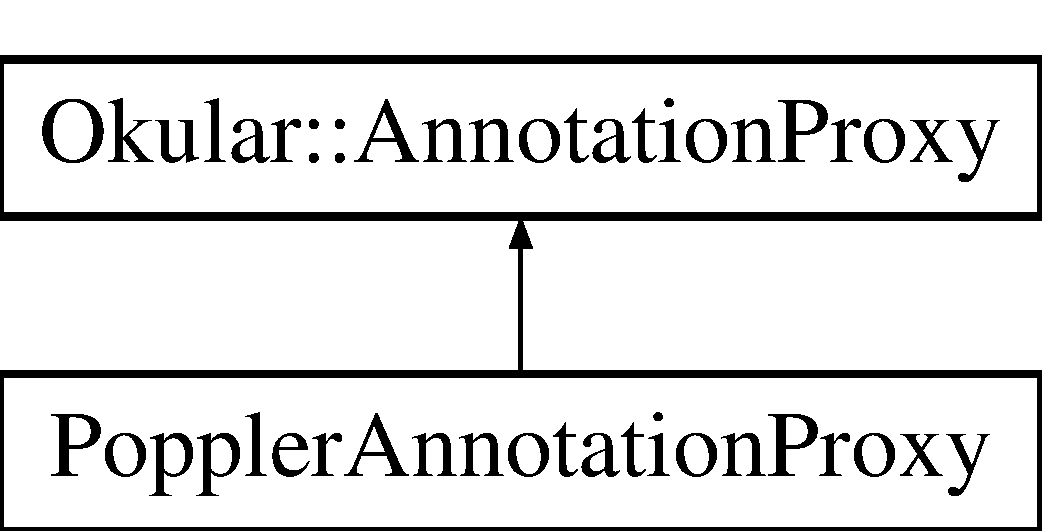
\includegraphics[height=2.000000cm]{classOkular_1_1AnnotationProxy}
\end{center}
\end{figure}
\subsection*{Public Types}
\begin{DoxyCompactItemize}
\item 
enum \hyperlink{classOkular_1_1AnnotationProxy_ae89e16435aa7e10ac4089e673f44e543}{Capability} \{ \hyperlink{classOkular_1_1AnnotationProxy_ae89e16435aa7e10ac4089e673f44e543afd5f00fa1edfb9d2043f90f9938cee3a}{Addition}, 
\hyperlink{classOkular_1_1AnnotationProxy_ae89e16435aa7e10ac4089e673f44e543ac0cea5683bbb000686ad820c6cd885bf}{Modification}, 
\hyperlink{classOkular_1_1AnnotationProxy_ae89e16435aa7e10ac4089e673f44e543ace001445896cb9742c5282e4fa127936}{Removal}
 \}
\end{DoxyCompactItemize}
\subsection*{Public Member Functions}
\begin{DoxyCompactItemize}
\item 
virtual \hyperlink{classOkular_1_1AnnotationProxy_ad24d82a89e740d30a33f3a9a8657304b}{$\sim$\+Annotation\+Proxy} ()
\item 
virtual bool \hyperlink{classOkular_1_1AnnotationProxy_a4672c7ad39b464c0676e277cd9adbac7}{supports} (\hyperlink{classOkular_1_1AnnotationProxy_ae89e16435aa7e10ac4089e673f44e543}{Capability} capability) const =0
\item 
virtual void \hyperlink{classOkular_1_1AnnotationProxy_a6fcdaa71557ad79ff1fbbd924887bdfc}{notify\+Addition} (\hyperlink{classOkular_1_1Annotation}{Annotation} $\ast$annotation, int page)=0
\item 
virtual void \hyperlink{classOkular_1_1AnnotationProxy_acb43272324440c199bd7a450b41c0d34}{notify\+Modification} (const \hyperlink{classOkular_1_1Annotation}{Annotation} $\ast$annotation, int page, bool appearance\+Changed)=0
\item 
virtual void \hyperlink{classOkular_1_1AnnotationProxy_a5d893c0ad68dc29e43e58c7a08f5de49}{notify\+Removal} (\hyperlink{classOkular_1_1Annotation}{Annotation} $\ast$annotation, int page)=0
\end{DoxyCompactItemize}


\subsection{Detailed Description}
Native annotation interface. 

Generators can subclass it to provide native annotation support. Generators can use \hyperlink{classOkular_1_1Annotation_a77c8188ca0d81966c29aebe0ef7ccfef}{Annotation\+::set\+Native\+Id} to store per-\/annotation data.

\begin{DoxySince}{Since}
0.\+15 (K\+D\+E 4.\+9) 
\end{DoxySince}


Definition at line 686 of file annotations.\+h.



\subsection{Member Enumeration Documentation}
\hypertarget{classOkular_1_1AnnotationProxy_ae89e16435aa7e10ac4089e673f44e543}{\index{Okular\+::\+Annotation\+Proxy@{Okular\+::\+Annotation\+Proxy}!Capability@{Capability}}
\index{Capability@{Capability}!Okular\+::\+Annotation\+Proxy@{Okular\+::\+Annotation\+Proxy}}
\subsubsection[{Capability}]{\setlength{\rightskip}{0pt plus 5cm}enum {\bf Okular\+::\+Annotation\+Proxy\+::\+Capability}}}\label{classOkular_1_1AnnotationProxy_ae89e16435aa7e10ac4089e673f44e543}
\begin{Desc}
\item[Enumerator]\par
\begin{description}
\index{Addition@{Addition}!Okular\+::\+Annotation\+Proxy@{Okular\+::\+Annotation\+Proxy}}\index{Okular\+::\+Annotation\+Proxy@{Okular\+::\+Annotation\+Proxy}!Addition@{Addition}}\item[{\em 
\hypertarget{classOkular_1_1AnnotationProxy_ae89e16435aa7e10ac4089e673f44e543afd5f00fa1edfb9d2043f90f9938cee3a}{Addition}\label{classOkular_1_1AnnotationProxy_ae89e16435aa7e10ac4089e673f44e543afd5f00fa1edfb9d2043f90f9938cee3a}
}]\hyperlink{classOkular_1_1Generator}{Generator} can create native annotations. \index{Modification@{Modification}!Okular\+::\+Annotation\+Proxy@{Okular\+::\+Annotation\+Proxy}}\index{Okular\+::\+Annotation\+Proxy@{Okular\+::\+Annotation\+Proxy}!Modification@{Modification}}\item[{\em 
\hypertarget{classOkular_1_1AnnotationProxy_ae89e16435aa7e10ac4089e673f44e543ac0cea5683bbb000686ad820c6cd885bf}{Modification}\label{classOkular_1_1AnnotationProxy_ae89e16435aa7e10ac4089e673f44e543ac0cea5683bbb000686ad820c6cd885bf}
}]\hyperlink{classOkular_1_1Generator}{Generator} can edit native annotations. \index{Removal@{Removal}!Okular\+::\+Annotation\+Proxy@{Okular\+::\+Annotation\+Proxy}}\index{Okular\+::\+Annotation\+Proxy@{Okular\+::\+Annotation\+Proxy}!Removal@{Removal}}\item[{\em 
\hypertarget{classOkular_1_1AnnotationProxy_ae89e16435aa7e10ac4089e673f44e543ace001445896cb9742c5282e4fa127936}{Removal}\label{classOkular_1_1AnnotationProxy_ae89e16435aa7e10ac4089e673f44e543ace001445896cb9742c5282e4fa127936}
}]\hyperlink{classOkular_1_1Generator}{Generator} can remove native annotations. \end{description}
\end{Desc}


Definition at line 689 of file annotations.\+h.


\begin{DoxyCode}
690         \{
691             \hyperlink{classOkular_1_1AnnotationProxy_ae89e16435aa7e10ac4089e673f44e543afd5f00fa1edfb9d2043f90f9938cee3a}{Addition},       
692             \hyperlink{classOkular_1_1AnnotationProxy_ae89e16435aa7e10ac4089e673f44e543ac0cea5683bbb000686ad820c6cd885bf}{Modification},   
693             \hyperlink{classOkular_1_1AnnotationProxy_ae89e16435aa7e10ac4089e673f44e543ace001445896cb9742c5282e4fa127936}{Removal}         
694         \};
\end{DoxyCode}


\subsection{Constructor \& Destructor Documentation}
\hypertarget{classOkular_1_1AnnotationProxy_ad24d82a89e740d30a33f3a9a8657304b}{\index{Okular\+::\+Annotation\+Proxy@{Okular\+::\+Annotation\+Proxy}!````~Annotation\+Proxy@{$\sim$\+Annotation\+Proxy}}
\index{````~Annotation\+Proxy@{$\sim$\+Annotation\+Proxy}!Okular\+::\+Annotation\+Proxy@{Okular\+::\+Annotation\+Proxy}}
\subsubsection[{$\sim$\+Annotation\+Proxy}]{\setlength{\rightskip}{0pt plus 5cm}Annotation\+Proxy\+::$\sim$\+Annotation\+Proxy (
\begin{DoxyParamCaption}
{}
\end{DoxyParamCaption}
)\hspace{0.3cm}{\ttfamily [virtual]}}}\label{classOkular_1_1AnnotationProxy_ad24d82a89e740d30a33f3a9a8657304b}
Destroys the annotation proxy. 

Definition at line 171 of file annotations.\+cpp.


\begin{DoxyCode}
172 \{
173 \}
\end{DoxyCode}


\subsection{Member Function Documentation}
\hypertarget{classOkular_1_1AnnotationProxy_a6fcdaa71557ad79ff1fbbd924887bdfc}{\index{Okular\+::\+Annotation\+Proxy@{Okular\+::\+Annotation\+Proxy}!notify\+Addition@{notify\+Addition}}
\index{notify\+Addition@{notify\+Addition}!Okular\+::\+Annotation\+Proxy@{Okular\+::\+Annotation\+Proxy}}
\subsubsection[{notify\+Addition}]{\setlength{\rightskip}{0pt plus 5cm}virtual void Okular\+::\+Annotation\+Proxy\+::notify\+Addition (
\begin{DoxyParamCaption}
\item[{{\bf Annotation} $\ast$}]{annotation, }
\item[{int}]{page}
\end{DoxyParamCaption}
)\hspace{0.3cm}{\ttfamily [pure virtual]}}}\label{classOkular_1_1AnnotationProxy_a6fcdaa71557ad79ff1fbbd924887bdfc}
Called when a new {\ttfamily annotation} is added to a {\ttfamily page}.

\begin{DoxyNote}{Note}
Only called if supports(\+Addition) == true 
\end{DoxyNote}


Implemented in \hyperlink{classPopplerAnnotationProxy_aebfb359939745a4031b0e32a536ad306}{Poppler\+Annotation\+Proxy}.

\hypertarget{classOkular_1_1AnnotationProxy_acb43272324440c199bd7a450b41c0d34}{\index{Okular\+::\+Annotation\+Proxy@{Okular\+::\+Annotation\+Proxy}!notify\+Modification@{notify\+Modification}}
\index{notify\+Modification@{notify\+Modification}!Okular\+::\+Annotation\+Proxy@{Okular\+::\+Annotation\+Proxy}}
\subsubsection[{notify\+Modification}]{\setlength{\rightskip}{0pt plus 5cm}virtual void Okular\+::\+Annotation\+Proxy\+::notify\+Modification (
\begin{DoxyParamCaption}
\item[{const {\bf Annotation} $\ast$}]{annotation, }
\item[{int}]{page, }
\item[{bool}]{appearance\+Changed}
\end{DoxyParamCaption}
)\hspace{0.3cm}{\ttfamily [pure virtual]}}}\label{classOkular_1_1AnnotationProxy_acb43272324440c199bd7a450b41c0d34}
Called after an existing {\ttfamily annotation} at a given {\ttfamily page} is modified.

\hyperlink{classOkular_1_1Generator}{Generator} can call {\ttfamily annotation} getters to get the new values. {\ttfamily appearance\+Changed} tells if a non-\/visible property was modifed

\begin{DoxyNote}{Note}
Only called if supports(\+Modification) == true 
\end{DoxyNote}


Implemented in \hyperlink{classPopplerAnnotationProxy_a24570660843c85dd702d9cf743cb6c79}{Poppler\+Annotation\+Proxy}.

\hypertarget{classOkular_1_1AnnotationProxy_a5d893c0ad68dc29e43e58c7a08f5de49}{\index{Okular\+::\+Annotation\+Proxy@{Okular\+::\+Annotation\+Proxy}!notify\+Removal@{notify\+Removal}}
\index{notify\+Removal@{notify\+Removal}!Okular\+::\+Annotation\+Proxy@{Okular\+::\+Annotation\+Proxy}}
\subsubsection[{notify\+Removal}]{\setlength{\rightskip}{0pt plus 5cm}virtual void Okular\+::\+Annotation\+Proxy\+::notify\+Removal (
\begin{DoxyParamCaption}
\item[{{\bf Annotation} $\ast$}]{annotation, }
\item[{int}]{page}
\end{DoxyParamCaption}
)\hspace{0.3cm}{\ttfamily [pure virtual]}}}\label{classOkular_1_1AnnotationProxy_a5d893c0ad68dc29e43e58c7a08f5de49}
Called when an existing {\ttfamily annotation} at a given {\ttfamily page} is removed.

\begin{DoxyNote}{Note}
Only called if supports(\+Removal) == true 
\end{DoxyNote}


Implemented in \hyperlink{classPopplerAnnotationProxy_a476bb44d9f52463bb445322ec2fc436f}{Poppler\+Annotation\+Proxy}.

\hypertarget{classOkular_1_1AnnotationProxy_a4672c7ad39b464c0676e277cd9adbac7}{\index{Okular\+::\+Annotation\+Proxy@{Okular\+::\+Annotation\+Proxy}!supports@{supports}}
\index{supports@{supports}!Okular\+::\+Annotation\+Proxy@{Okular\+::\+Annotation\+Proxy}}
\subsubsection[{supports}]{\setlength{\rightskip}{0pt plus 5cm}virtual bool Okular\+::\+Annotation\+Proxy\+::supports (
\begin{DoxyParamCaption}
\item[{{\bf Capability}}]{capability}
\end{DoxyParamCaption}
) const\hspace{0.3cm}{\ttfamily [pure virtual]}}}\label{classOkular_1_1AnnotationProxy_a4672c7ad39b464c0676e277cd9adbac7}
Query for the supported capabilities. 

Implemented in \hyperlink{classPopplerAnnotationProxy_a1c76a27f5bdcae079ac6cc389d790a4a}{Poppler\+Annotation\+Proxy}.



The documentation for this class was generated from the following files\+:\begin{DoxyCompactItemize}
\item 
core/\hyperlink{annotations_8h}{annotations.\+h}\item 
core/\hyperlink{annotations_8cpp}{annotations.\+cpp}\end{DoxyCompactItemize}

\hypertarget{classAnnotationTest}{\section{Annotation\+Test Class Reference}
\label{classAnnotationTest}\index{Annotation\+Test@{Annotation\+Test}}
}
Inheritance diagram for Annotation\+Test\+:\begin{figure}[H]
\begin{center}
\leavevmode
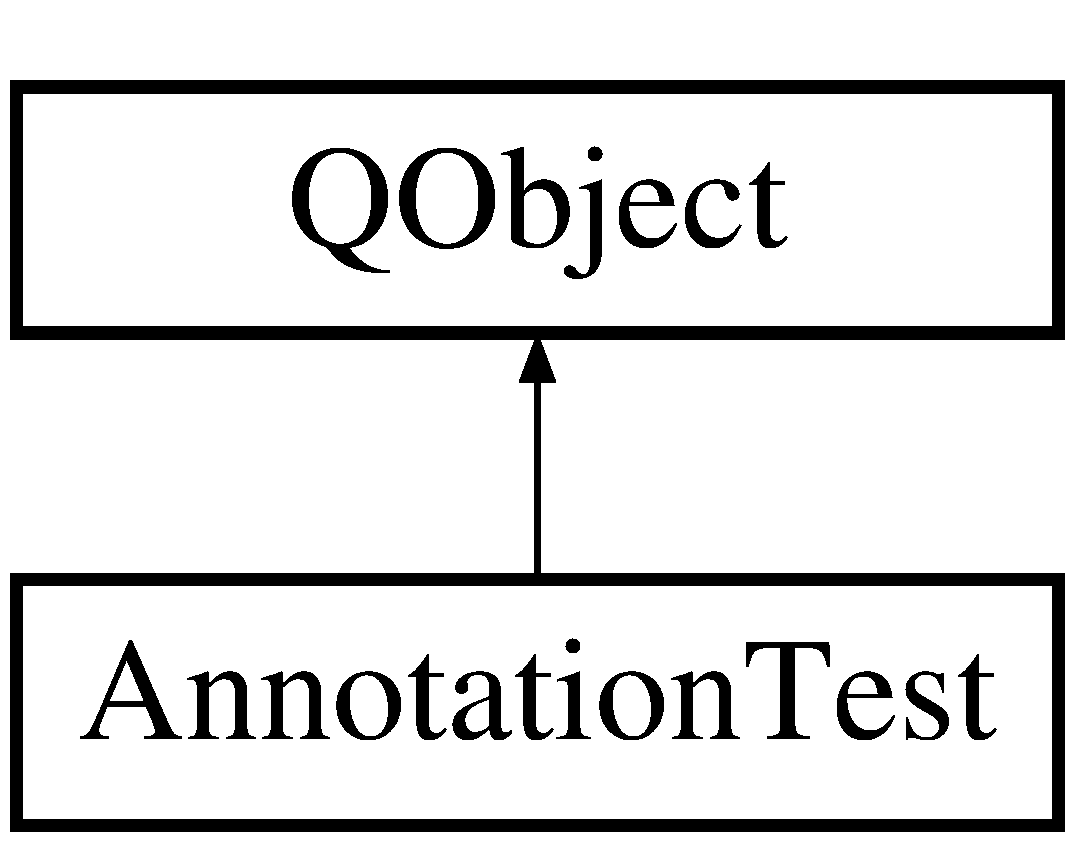
\includegraphics[height=2.000000cm]{classAnnotationTest}
\end{center}
\end{figure}


\subsection{Detailed Description}


Definition at line 20 of file annotationstest.\+cpp.



The documentation for this class was generated from the following file\+:\begin{DoxyCompactItemize}
\item 
tests/\hyperlink{annotationstest_8cpp}{annotationstest.\+cpp}\end{DoxyCompactItemize}

\hypertarget{structAnnotationToolItem}{\section{Annotation\+Tool\+Item Struct Reference}
\label{structAnnotationToolItem}\index{Annotation\+Tool\+Item@{Annotation\+Tool\+Item}}
}


{\ttfamily \#include $<$pageviewutils.\+h$>$}

\subsection*{Public Member Functions}
\begin{DoxyCompactItemize}
\item 
\hyperlink{structAnnotationToolItem_a3d041f330c157d99941c41c50b1cec90}{Annotation\+Tool\+Item} ()
\end{DoxyCompactItemize}
\subsection*{Public Attributes}
\begin{DoxyCompactItemize}
\item 
int \hyperlink{structAnnotationToolItem_a738162ebc807fdfb9d0a7937c34bab01}{id}
\item 
Q\+String \hyperlink{structAnnotationToolItem_a5a24d93be5ae5fba2c921b205c29b017}{text}
\item 
Q\+Pixmap \hyperlink{structAnnotationToolItem_a329b59ebf0a0064444d34874f41a70cb}{pixmap}
\item 
Q\+String \hyperlink{structAnnotationToolItem_ad9bf3c20abf0ddfc1d1ff826cd3d3da5}{shortcut}
\item 
bool \hyperlink{structAnnotationToolItem_a7627b1e7036d516cd4bd290a9099a549}{is\+Text}
\end{DoxyCompactItemize}


\subsection{Detailed Description}


Definition at line 151 of file pageviewutils.\+h.



\subsection{Constructor \& Destructor Documentation}
\hypertarget{structAnnotationToolItem_a3d041f330c157d99941c41c50b1cec90}{\index{Annotation\+Tool\+Item@{Annotation\+Tool\+Item}!Annotation\+Tool\+Item@{Annotation\+Tool\+Item}}
\index{Annotation\+Tool\+Item@{Annotation\+Tool\+Item}!Annotation\+Tool\+Item@{Annotation\+Tool\+Item}}
\subsubsection[{Annotation\+Tool\+Item}]{\setlength{\rightskip}{0pt plus 5cm}Annotation\+Tool\+Item\+::\+Annotation\+Tool\+Item (
\begin{DoxyParamCaption}
{}
\end{DoxyParamCaption}
)\hspace{0.3cm}{\ttfamily [inline]}}}\label{structAnnotationToolItem_a3d041f330c157d99941c41c50b1cec90}


Definition at line 153 of file pageviewutils.\+h.


\begin{DoxyCode}
154         : \hyperlink{structAnnotationToolItem_a738162ebc807fdfb9d0a7937c34bab01}{id}( -1 ), \hyperlink{structAnnotationToolItem_a7627b1e7036d516cd4bd290a9099a549}{isText}( \textcolor{keyword}{false} )
155     \{
156     \}
\end{DoxyCode}


\subsection{Member Data Documentation}
\hypertarget{structAnnotationToolItem_a738162ebc807fdfb9d0a7937c34bab01}{\index{Annotation\+Tool\+Item@{Annotation\+Tool\+Item}!id@{id}}
\index{id@{id}!Annotation\+Tool\+Item@{Annotation\+Tool\+Item}}
\subsubsection[{id}]{\setlength{\rightskip}{0pt plus 5cm}int Annotation\+Tool\+Item\+::id}}\label{structAnnotationToolItem_a738162ebc807fdfb9d0a7937c34bab01}


Definition at line 158 of file pageviewutils.\+h.

\hypertarget{structAnnotationToolItem_a7627b1e7036d516cd4bd290a9099a549}{\index{Annotation\+Tool\+Item@{Annotation\+Tool\+Item}!is\+Text@{is\+Text}}
\index{is\+Text@{is\+Text}!Annotation\+Tool\+Item@{Annotation\+Tool\+Item}}
\subsubsection[{is\+Text}]{\setlength{\rightskip}{0pt plus 5cm}bool Annotation\+Tool\+Item\+::is\+Text}}\label{structAnnotationToolItem_a7627b1e7036d516cd4bd290a9099a549}


Definition at line 162 of file pageviewutils.\+h.

\hypertarget{structAnnotationToolItem_a329b59ebf0a0064444d34874f41a70cb}{\index{Annotation\+Tool\+Item@{Annotation\+Tool\+Item}!pixmap@{pixmap}}
\index{pixmap@{pixmap}!Annotation\+Tool\+Item@{Annotation\+Tool\+Item}}
\subsubsection[{pixmap}]{\setlength{\rightskip}{0pt plus 5cm}Q\+Pixmap Annotation\+Tool\+Item\+::pixmap}}\label{structAnnotationToolItem_a329b59ebf0a0064444d34874f41a70cb}


Definition at line 160 of file pageviewutils.\+h.

\hypertarget{structAnnotationToolItem_ad9bf3c20abf0ddfc1d1ff826cd3d3da5}{\index{Annotation\+Tool\+Item@{Annotation\+Tool\+Item}!shortcut@{shortcut}}
\index{shortcut@{shortcut}!Annotation\+Tool\+Item@{Annotation\+Tool\+Item}}
\subsubsection[{shortcut}]{\setlength{\rightskip}{0pt plus 5cm}Q\+String Annotation\+Tool\+Item\+::shortcut}}\label{structAnnotationToolItem_ad9bf3c20abf0ddfc1d1ff826cd3d3da5}


Definition at line 161 of file pageviewutils.\+h.

\hypertarget{structAnnotationToolItem_a5a24d93be5ae5fba2c921b205c29b017}{\index{Annotation\+Tool\+Item@{Annotation\+Tool\+Item}!text@{text}}
\index{text@{text}!Annotation\+Tool\+Item@{Annotation\+Tool\+Item}}
\subsubsection[{text}]{\setlength{\rightskip}{0pt plus 5cm}Q\+String Annotation\+Tool\+Item\+::text}}\label{structAnnotationToolItem_a5a24d93be5ae5fba2c921b205c29b017}


Definition at line 159 of file pageviewutils.\+h.



The documentation for this struct was generated from the following file\+:\begin{DoxyCompactItemize}
\item 
ui/\hyperlink{pageviewutils_8h}{pageviewutils.\+h}\end{DoxyCompactItemize}

\hypertarget{classOkular_1_1AnnotationUtils}{\section{Okular\+:\+:Annotation\+Utils Class Reference}
\label{classOkular_1_1AnnotationUtils}\index{Okular\+::\+Annotation\+Utils@{Okular\+::\+Annotation\+Utils}}
}


Helper class for (recursive) annotation retrieval/storage.  




{\ttfamily \#include $<$annotations.\+h$>$}

\subsection*{Static Public Member Functions}
\begin{DoxyCompactItemize}
\item 
static \hyperlink{classOkular_1_1Annotation}{Annotation} $\ast$ \hyperlink{classOkular_1_1AnnotationUtils_a790854adbb753b2a448640021442bf73}{create\+Annotation} (const Q\+Dom\+Element \&element)
\item 
static void \hyperlink{classOkular_1_1AnnotationUtils_aaf554db9b97842dd6298317dd539bf82}{store\+Annotation} (const \hyperlink{classOkular_1_1Annotation}{Annotation} $\ast$annotation, Q\+Dom\+Element \&element, Q\+Dom\+Document \&document)
\item 
static Q\+Dom\+Element \hyperlink{classOkular_1_1AnnotationUtils_a05b79294046a1756dd5fb120aa18b52b}{find\+Child\+Element} (const Q\+Dom\+Node \&parent\+Node, const Q\+String \&name)
\item 
static Q\+Rect \hyperlink{classOkular_1_1AnnotationUtils_a6b3fdb4e89227d26ec9e6f62bf4d0eb9}{annotation\+Geometry} (const \hyperlink{classOkular_1_1Annotation}{Annotation} $\ast$annotation, double scale\+X, double scale\+Y)
\end{DoxyCompactItemize}


\subsection{Detailed Description}
Helper class for (recursive) annotation retrieval/storage. 

Definition at line 52 of file annotations.\+h.



\subsection{Member Function Documentation}
\hypertarget{classOkular_1_1AnnotationUtils_a6b3fdb4e89227d26ec9e6f62bf4d0eb9}{\index{Okular\+::\+Annotation\+Utils@{Okular\+::\+Annotation\+Utils}!annotation\+Geometry@{annotation\+Geometry}}
\index{annotation\+Geometry@{annotation\+Geometry}!Okular\+::\+Annotation\+Utils@{Okular\+::\+Annotation\+Utils}}
\subsubsection[{annotation\+Geometry}]{\setlength{\rightskip}{0pt plus 5cm}Q\+Rect Annotation\+Utils\+::annotation\+Geometry (
\begin{DoxyParamCaption}
\item[{const {\bf Annotation} $\ast$}]{annotation, }
\item[{double}]{scale\+X, }
\item[{double}]{scale\+Y}
\end{DoxyParamCaption}
)\hspace{0.3cm}{\ttfamily [static]}}}\label{classOkular_1_1AnnotationUtils_a6b3fdb4e89227d26ec9e6f62bf4d0eb9}
Returns the geometry of the given {\ttfamily annotation} scaled by {\ttfamily scale\+X} and {\ttfamily scale\+Y}. 

Definition at line 154 of file annotations.\+cpp.


\begin{DoxyCode}
156 \{
157     \textcolor{keyword}{const} QRect rect = ann->transformedBoundingRectangle().geometry( (\textcolor{keywordtype}{int})scaledWidth, (\textcolor{keywordtype}{int})scaledHeight );
158     \textcolor{keywordflow}{if} ( ann->subType() == \hyperlink{classOkular_1_1Annotation_af71b46e37d5f850b97d5c4de3be9aac0a48f93d5a9352abc4e38a45f69075e504}{Annotation::AText} && ( ( (
      \hyperlink{classOkular_1_1TextAnnotation}{TextAnnotation}*)ann )->textType() == \hyperlink{classOkular_1_1TextAnnotation_af560204454bf812797bc95bea730b06eaf7d7133e8e4850bf030e108537a9887b}{TextAnnotation::Linked} ) )
159     \{
160         \textcolor{comment}{// To be honest i have no clue of why the 24,24 is here, maybe to make sure it's not too small?}
161         \textcolor{comment}{// But why only for linked text?}
162         \textcolor{keyword}{const} QRect rect24 = QRect( (\textcolor{keywordtype}{int})( ann->transformedBoundingRectangle().left * scaledWidth ),
163                                     (\textcolor{keywordtype}{int})( ann->transformedBoundingRectangle().top * scaledHeight ), 24, 24
       );
164         \textcolor{keywordflow}{return} rect24.united(rect);
165     \}
166 
167     \textcolor{keywordflow}{return} rect;
168 \}
\end{DoxyCode}
\hypertarget{classOkular_1_1AnnotationUtils_a790854adbb753b2a448640021442bf73}{\index{Okular\+::\+Annotation\+Utils@{Okular\+::\+Annotation\+Utils}!create\+Annotation@{create\+Annotation}}
\index{create\+Annotation@{create\+Annotation}!Okular\+::\+Annotation\+Utils@{Okular\+::\+Annotation\+Utils}}
\subsubsection[{create\+Annotation}]{\setlength{\rightskip}{0pt plus 5cm}{\bf Annotation} $\ast$ Annotation\+Utils\+::create\+Annotation (
\begin{DoxyParamCaption}
\item[{const Q\+Dom\+Element \&}]{element}
\end{DoxyParamCaption}
)\hspace{0.3cm}{\ttfamily [static]}}}\label{classOkular_1_1AnnotationUtils_a790854adbb753b2a448640021442bf73}
Restore an annotation (with revisions if needed) from the dom {\ttfamily element}.

Returns a pointer to the complete annotation or 0 if element is invalid. 

Definition at line 90 of file annotations.\+cpp.


\begin{DoxyCode}
91 \{
92     \textcolor{comment}{// safety check on annotation element}
93     \textcolor{keywordflow}{if} ( !annElement.hasAttribute( \textcolor{stringliteral}{"type"} ) )
94         \textcolor{keywordflow}{return} 0;
95 
96     \textcolor{comment}{// build annotation of given type}
97     \hyperlink{classOkular_1_1Annotation}{Annotation} * annotation = 0;
98     \textcolor{keywordtype}{int} typeNumber = annElement.attribute( \textcolor{stringliteral}{"type"} ).toInt();
99     \textcolor{keywordflow}{switch} ( typeNumber )
100     \{
101         \textcolor{keywordflow}{case} \hyperlink{classOkular_1_1Annotation_af71b46e37d5f850b97d5c4de3be9aac0a48f93d5a9352abc4e38a45f69075e504}{Annotation::AText}:
102             annotation = \textcolor{keyword}{new} \hyperlink{classOkular_1_1TextAnnotation}{TextAnnotation}( annElement );
103             \textcolor{keywordflow}{break};
104         \textcolor{keywordflow}{case} \hyperlink{classOkular_1_1Annotation_af71b46e37d5f850b97d5c4de3be9aac0a7035dc978d8b79958f34e3d164838726}{Annotation::ALine}:
105             annotation = \textcolor{keyword}{new} \hyperlink{classOkular_1_1LineAnnotation}{LineAnnotation}( annElement );
106             \textcolor{keywordflow}{break};
107         \textcolor{keywordflow}{case} \hyperlink{classOkular_1_1Annotation_af71b46e37d5f850b97d5c4de3be9aac0a2c11d328af34f5526fd9e761297fb3c2}{Annotation::AGeom}:
108             annotation = \textcolor{keyword}{new} \hyperlink{classOkular_1_1GeomAnnotation}{GeomAnnotation}( annElement );
109             \textcolor{keywordflow}{break};
110         \textcolor{keywordflow}{case} \hyperlink{classOkular_1_1Annotation_af71b46e37d5f850b97d5c4de3be9aac0a03e002f9ae62005b2d7c7f1445507501}{Annotation::AHighlight}:
111             annotation = \textcolor{keyword}{new} \hyperlink{classOkular_1_1HighlightAnnotation}{HighlightAnnotation}( annElement );
112             \textcolor{keywordflow}{break};
113         \textcolor{keywordflow}{case} \hyperlink{classOkular_1_1Annotation_af71b46e37d5f850b97d5c4de3be9aac0ad542ded420c9b01f44ee923bf28ecd9a}{Annotation::AStamp}:
114             annotation = \textcolor{keyword}{new} \hyperlink{classOkular_1_1StampAnnotation}{StampAnnotation}( annElement );
115             \textcolor{keywordflow}{break};
116         \textcolor{keywordflow}{case} \hyperlink{classOkular_1_1Annotation_af71b46e37d5f850b97d5c4de3be9aac0a4ed60063584ceb146c2a378f0df4ed37}{Annotation::AInk}:
117             annotation = \textcolor{keyword}{new} \hyperlink{classOkular_1_1InkAnnotation}{InkAnnotation}( annElement );
118             \textcolor{keywordflow}{break};
119         \textcolor{keywordflow}{case} \hyperlink{classOkular_1_1Annotation_af71b46e37d5f850b97d5c4de3be9aac0a904187454fd508d898a3d5843193ad43}{Annotation::ACaret}:
120             annotation = \textcolor{keyword}{new} \hyperlink{classOkular_1_1CaretAnnotation}{CaretAnnotation}( annElement );
121             \textcolor{keywordflow}{break};
122     \}
123 
124     \textcolor{comment}{// return created annotation}
125     \textcolor{keywordflow}{return} annotation;
126 \}
\end{DoxyCode}
\hypertarget{classOkular_1_1AnnotationUtils_a05b79294046a1756dd5fb120aa18b52b}{\index{Okular\+::\+Annotation\+Utils@{Okular\+::\+Annotation\+Utils}!find\+Child\+Element@{find\+Child\+Element}}
\index{find\+Child\+Element@{find\+Child\+Element}!Okular\+::\+Annotation\+Utils@{Okular\+::\+Annotation\+Utils}}
\subsubsection[{find\+Child\+Element}]{\setlength{\rightskip}{0pt plus 5cm}Q\+Dom\+Element Annotation\+Utils\+::find\+Child\+Element (
\begin{DoxyParamCaption}
\item[{const Q\+Dom\+Node \&}]{parent\+Node, }
\item[{const Q\+String \&}]{name}
\end{DoxyParamCaption}
)\hspace{0.3cm}{\ttfamily [static]}}}\label{classOkular_1_1AnnotationUtils_a05b79294046a1756dd5fb120aa18b52b}
Returns the child element with the given {\ttfamily name} from the direct children of {\ttfamily parent\+Node} or a null element if not found. 

Definition at line 138 of file annotations.\+cpp.


\begin{DoxyCode}
140 \{
141     \textcolor{comment}{// loop through the whole children and return a 'name' named element}
142     QDomNode subNode = parentNode.firstChild();
143     \textcolor{keywordflow}{while}( subNode.isElement() )
144     \{
145         QDomElement element = subNode.toElement();
146         \textcolor{keywordflow}{if} ( element.tagName() == name )
147             \textcolor{keywordflow}{return} element;
148         subNode = subNode.nextSibling();
149     \}
150     \textcolor{comment}{// if the name can't be found, return a dummy null element}
151     \textcolor{keywordflow}{return} QDomElement();
152 \}
\end{DoxyCode}
\hypertarget{classOkular_1_1AnnotationUtils_aaf554db9b97842dd6298317dd539bf82}{\index{Okular\+::\+Annotation\+Utils@{Okular\+::\+Annotation\+Utils}!store\+Annotation@{store\+Annotation}}
\index{store\+Annotation@{store\+Annotation}!Okular\+::\+Annotation\+Utils@{Okular\+::\+Annotation\+Utils}}
\subsubsection[{store\+Annotation}]{\setlength{\rightskip}{0pt plus 5cm}void Annotation\+Utils\+::store\+Annotation (
\begin{DoxyParamCaption}
\item[{const {\bf Annotation} $\ast$}]{annotation, }
\item[{Q\+Dom\+Element \&}]{element, }
\item[{Q\+Dom\+Document \&}]{document}
\end{DoxyParamCaption}
)\hspace{0.3cm}{\ttfamily [static]}}}\label{classOkular_1_1AnnotationUtils_aaf554db9b97842dd6298317dd539bf82}
Saves the {\ttfamily annotation} as a child of {\ttfamily element} taking care of saving all revisions if it has any. 

Definition at line 128 of file annotations.\+cpp.


\begin{DoxyCode}
130 \{
131     \textcolor{comment}{// save annotation's type as element's attribute}
132     annElement.setAttribute( \textcolor{stringliteral}{"type"}, (uint)ann->subType() );
133 
134     \textcolor{comment}{// append all annotation data as children of this node}
135     ann->store( annElement, document );
136 \}
\end{DoxyCode}


The documentation for this class was generated from the following files\+:\begin{DoxyCompactItemize}
\item 
core/\hyperlink{annotations_8h}{annotations.\+h}\item 
core/\hyperlink{annotations_8cpp}{annotations.\+cpp}\end{DoxyCompactItemize}

\hypertarget{classAnnotationWidget}{\section{Annotation\+Widget Class Reference}
\label{classAnnotationWidget}\index{Annotation\+Widget@{Annotation\+Widget}}
}


{\ttfamily \#include $<$annotationwidgets.\+h$>$}

Inheritance diagram for Annotation\+Widget\+:\begin{figure}[H]
\begin{center}
\leavevmode
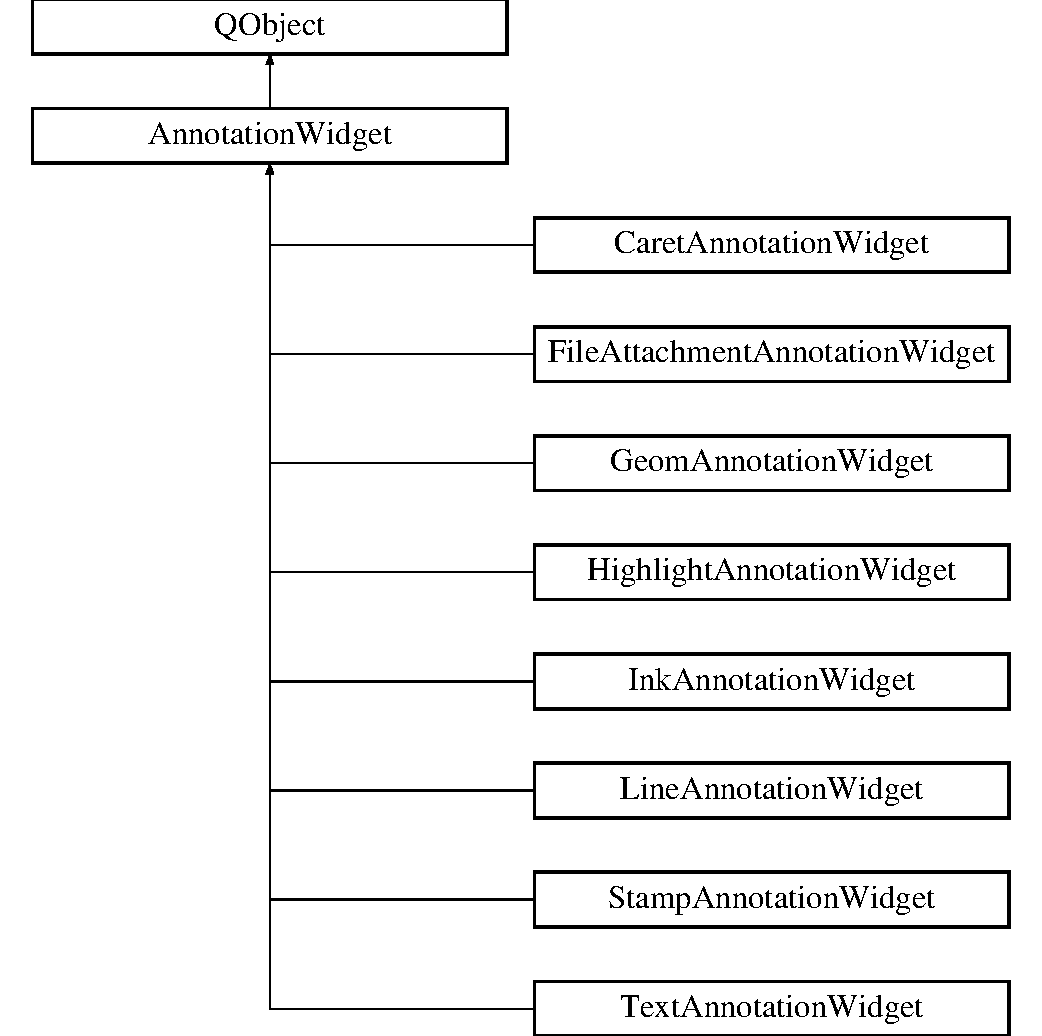
\includegraphics[height=10.000000cm]{classAnnotationWidget}
\end{center}
\end{figure}
\subsection*{Signals}
\begin{DoxyCompactItemize}
\item 
void \hyperlink{classAnnotationWidget_af9dcb02a8b69a602225c9844b5deb6d4}{data\+Changed} ()
\end{DoxyCompactItemize}
\subsection*{Public Member Functions}
\begin{DoxyCompactItemize}
\item 
\hyperlink{classAnnotationWidget_a1152e99260c24acde30e2742a07af2ef}{Annotation\+Widget} (\hyperlink{classOkular_1_1Annotation}{Okular\+::\+Annotation} $\ast$ann)
\item 
virtual \hyperlink{classAnnotationWidget_ae86eb3b8adca8b5227e908fab444802f}{$\sim$\+Annotation\+Widget} ()
\item 
virtual \hyperlink{classOkular_1_1Annotation_af71b46e37d5f850b97d5c4de3be9aac0}{Okular\+::\+Annotation\+::\+Sub\+Type} \hyperlink{classAnnotationWidget_a8c837e08592e4cb54829d53e267f5cfc}{annotation\+Type} () const 
\item 
Q\+Widget $\ast$ \hyperlink{classAnnotationWidget_a57411e4d54dde346c8ed57c99da56666}{appearance\+Widget} ()
\item 
Q\+Widget $\ast$ \hyperlink{classAnnotationWidget_a0d1cb7d9a0f518140abecc82aa1e8449}{extra\+Widget} ()
\item 
virtual void \hyperlink{classAnnotationWidget_a00b35958653cb76c93b9d4f70d770f5c}{apply\+Changes} ()
\end{DoxyCompactItemize}
\subsection*{Protected Member Functions}
\begin{DoxyCompactItemize}
\item 
Q\+Widget $\ast$ \hyperlink{classAnnotationWidget_a10702d6e6fd3df11a494c495165b8524}{create\+Appearance\+Widget} ()
\item 
virtual Q\+Widget $\ast$ \hyperlink{classAnnotationWidget_a4b0926d20f0b26deb5b6a4e75f78fac3}{create\+Style\+Widget} ()
\item 
virtual Q\+Widget $\ast$ \hyperlink{classAnnotationWidget_ab46dbe69c6723a640048a75f6bf47423}{create\+Extra\+Widget} ()
\end{DoxyCompactItemize}
\subsection*{Protected Attributes}
\begin{DoxyCompactItemize}
\item 
\hyperlink{classOkular_1_1Annotation}{Okular\+::\+Annotation} $\ast$ \hyperlink{classAnnotationWidget_a6b7e6688554d24cfea509b139b3ecedc}{m\+\_\+ann}
\item 
Q\+Widget $\ast$ \hyperlink{classAnnotationWidget_a5ab466a198ca0a99fd2e0fd0ace527b2}{m\+\_\+appearance\+Widget}
\item 
Q\+Widget $\ast$ \hyperlink{classAnnotationWidget_abd0a469cc5f14e5e73243f405b5d3649}{m\+\_\+extra\+Widget}
\item 
K\+Color\+Button $\ast$ \hyperlink{classAnnotationWidget_a39083eda5b61826f4b48a787361b9dfc}{m\+\_\+color\+Bn}
\item 
K\+Int\+Num\+Input $\ast$ \hyperlink{classAnnotationWidget_a234fb5913752d6e4462084b217f3ff6c}{m\+\_\+opacity}
\end{DoxyCompactItemize}


\subsection{Detailed Description}


Definition at line 69 of file annotationwidgets.\+h.



\subsection{Constructor \& Destructor Documentation}
\hypertarget{classAnnotationWidget_a1152e99260c24acde30e2742a07af2ef}{\index{Annotation\+Widget@{Annotation\+Widget}!Annotation\+Widget@{Annotation\+Widget}}
\index{Annotation\+Widget@{Annotation\+Widget}!Annotation\+Widget@{Annotation\+Widget}}
\subsubsection[{Annotation\+Widget}]{\setlength{\rightskip}{0pt plus 5cm}Annotation\+Widget\+::\+Annotation\+Widget (
\begin{DoxyParamCaption}
\item[{{\bf Okular\+::\+Annotation} $\ast$}]{ann}
\end{DoxyParamCaption}
)}}\label{classAnnotationWidget_a1152e99260c24acde30e2742a07af2ef}


Definition at line 158 of file annotationwidgets.\+cpp.


\begin{DoxyCode}
159     : QObject(), \hyperlink{classAnnotationWidget_a6b7e6688554d24cfea509b139b3ecedc}{m\_ann}( ann ), \hyperlink{classAnnotationWidget_a5ab466a198ca0a99fd2e0fd0ace527b2}{m\_appearanceWidget}( 0 ), 
      \hyperlink{classAnnotationWidget_abd0a469cc5f14e5e73243f405b5d3649}{m\_extraWidget}( 0 )
160 \{
161 \}
\end{DoxyCode}
\hypertarget{classAnnotationWidget_ae86eb3b8adca8b5227e908fab444802f}{\index{Annotation\+Widget@{Annotation\+Widget}!````~Annotation\+Widget@{$\sim$\+Annotation\+Widget}}
\index{````~Annotation\+Widget@{$\sim$\+Annotation\+Widget}!Annotation\+Widget@{Annotation\+Widget}}
\subsubsection[{$\sim$\+Annotation\+Widget}]{\setlength{\rightskip}{0pt plus 5cm}Annotation\+Widget\+::$\sim$\+Annotation\+Widget (
\begin{DoxyParamCaption}
{}
\end{DoxyParamCaption}
)\hspace{0.3cm}{\ttfamily [virtual]}}}\label{classAnnotationWidget_ae86eb3b8adca8b5227e908fab444802f}


Definition at line 163 of file annotationwidgets.\+cpp.


\begin{DoxyCode}
164 \{
165 \}
\end{DoxyCode}


\subsection{Member Function Documentation}
\hypertarget{classAnnotationWidget_a8c837e08592e4cb54829d53e267f5cfc}{\index{Annotation\+Widget@{Annotation\+Widget}!annotation\+Type@{annotation\+Type}}
\index{annotation\+Type@{annotation\+Type}!Annotation\+Widget@{Annotation\+Widget}}
\subsubsection[{annotation\+Type}]{\setlength{\rightskip}{0pt plus 5cm}{\bf Okular\+::\+Annotation\+::\+Sub\+Type} Annotation\+Widget\+::annotation\+Type (
\begin{DoxyParamCaption}
{}
\end{DoxyParamCaption}
) const\hspace{0.3cm}{\ttfamily [virtual]}}}\label{classAnnotationWidget_a8c837e08592e4cb54829d53e267f5cfc}


Definition at line 167 of file annotationwidgets.\+cpp.


\begin{DoxyCode}
168 \{
169     \textcolor{keywordflow}{return} \hyperlink{classAnnotationWidget_a6b7e6688554d24cfea509b139b3ecedc}{m\_ann}->\hyperlink{classOkular_1_1Annotation_af9833449767eacd740f377e69a1fdd48}{subType}();
170 \}
\end{DoxyCode}
\hypertarget{classAnnotationWidget_a57411e4d54dde346c8ed57c99da56666}{\index{Annotation\+Widget@{Annotation\+Widget}!appearance\+Widget@{appearance\+Widget}}
\index{appearance\+Widget@{appearance\+Widget}!Annotation\+Widget@{Annotation\+Widget}}
\subsubsection[{appearance\+Widget}]{\setlength{\rightskip}{0pt plus 5cm}Q\+Widget $\ast$ Annotation\+Widget\+::appearance\+Widget (
\begin{DoxyParamCaption}
{}
\end{DoxyParamCaption}
)}}\label{classAnnotationWidget_a57411e4d54dde346c8ed57c99da56666}


Definition at line 172 of file annotationwidgets.\+cpp.


\begin{DoxyCode}
173 \{
174     \textcolor{keywordflow}{if} ( \hyperlink{classAnnotationWidget_a5ab466a198ca0a99fd2e0fd0ace527b2}{m\_appearanceWidget} )
175         \textcolor{keywordflow}{return} \hyperlink{classAnnotationWidget_a5ab466a198ca0a99fd2e0fd0ace527b2}{m\_appearanceWidget};
176 
177     \hyperlink{classAnnotationWidget_a5ab466a198ca0a99fd2e0fd0ace527b2}{m\_appearanceWidget} = \hyperlink{classAnnotationWidget_a10702d6e6fd3df11a494c495165b8524}{createAppearanceWidget}();
178     \textcolor{keywordflow}{return} \hyperlink{classAnnotationWidget_a5ab466a198ca0a99fd2e0fd0ace527b2}{m\_appearanceWidget};
179 \}
\end{DoxyCode}
\hypertarget{classAnnotationWidget_a00b35958653cb76c93b9d4f70d770f5c}{\index{Annotation\+Widget@{Annotation\+Widget}!apply\+Changes@{apply\+Changes}}
\index{apply\+Changes@{apply\+Changes}!Annotation\+Widget@{Annotation\+Widget}}
\subsubsection[{apply\+Changes}]{\setlength{\rightskip}{0pt plus 5cm}void Annotation\+Widget\+::apply\+Changes (
\begin{DoxyParamCaption}
{}
\end{DoxyParamCaption}
)\hspace{0.3cm}{\ttfamily [virtual]}}}\label{classAnnotationWidget_a00b35958653cb76c93b9d4f70d770f5c}


Reimplemented in \hyperlink{classInkAnnotationWidget_a531cf1b8d9d7765f2b9aadc862e2d0e3}{Ink\+Annotation\+Widget}, \hyperlink{classCaretAnnotationWidget_ace74af8590fa2bae736aa3ab6f2ca862}{Caret\+Annotation\+Widget}, \hyperlink{classFileAttachmentAnnotationWidget_a38fef39135d564be132754fcc4dbdf79}{File\+Attachment\+Annotation\+Widget}, \hyperlink{classGeomAnnotationWidget_a188cb69dbb5fdd20620e1c75522c9bc4}{Geom\+Annotation\+Widget}, \hyperlink{classHighlightAnnotationWidget_a10838667b738e48983922d4c281a0410}{Highlight\+Annotation\+Widget}, \hyperlink{classLineAnnotationWidget_a31b65c29b709f901c8b706ab2de42846}{Line\+Annotation\+Widget}, \hyperlink{classStampAnnotationWidget_aabddf86c8df2d97e5f3e4d1ad9ae36f5}{Stamp\+Annotation\+Widget}, and \hyperlink{classTextAnnotationWidget_ae0b433d806d3e939300acbc2480be586}{Text\+Annotation\+Widget}.



Definition at line 190 of file annotationwidgets.\+cpp.


\begin{DoxyCode}
191 \{
192     \hyperlink{classAnnotationWidget_a6b7e6688554d24cfea509b139b3ecedc}{m\_ann}->\hyperlink{classOkular_1_1Annotation_ae1f845ddbd6d524b2b388c6c9ef26423}{style}().\hyperlink{classOkular_1_1Annotation_1_1Style_a1c916cd50a0a4114188136d47943ef00}{setColor}( \hyperlink{classAnnotationWidget_a39083eda5b61826f4b48a787361b9dfc}{m\_colorBn}->color() );
193     \hyperlink{classAnnotationWidget_a6b7e6688554d24cfea509b139b3ecedc}{m\_ann}->\hyperlink{classOkular_1_1Annotation_ae1f845ddbd6d524b2b388c6c9ef26423}{style}().\hyperlink{classOkular_1_1Annotation_1_1Style_a5bf0bdd3bf954271ed4ba831316a7ee7}{setOpacity}( (\textcolor{keywordtype}{double})\hyperlink{classAnnotationWidget_a234fb5913752d6e4462084b217f3ff6c}{m\_opacity}->value() / 100.0 );
194 \}
\end{DoxyCode}
\hypertarget{classAnnotationWidget_a10702d6e6fd3df11a494c495165b8524}{\index{Annotation\+Widget@{Annotation\+Widget}!create\+Appearance\+Widget@{create\+Appearance\+Widget}}
\index{create\+Appearance\+Widget@{create\+Appearance\+Widget}!Annotation\+Widget@{Annotation\+Widget}}
\subsubsection[{create\+Appearance\+Widget}]{\setlength{\rightskip}{0pt plus 5cm}Q\+Widget $\ast$ Annotation\+Widget\+::create\+Appearance\+Widget (
\begin{DoxyParamCaption}
{}
\end{DoxyParamCaption}
)\hspace{0.3cm}{\ttfamily [protected]}}}\label{classAnnotationWidget_a10702d6e6fd3df11a494c495165b8524}


Definition at line 196 of file annotationwidgets.\+cpp.


\begin{DoxyCode}
197 \{
198     QWidget * widget = \textcolor{keyword}{new} QWidget();
199     QGridLayout * gridlayout = \textcolor{keyword}{new} QGridLayout( widget );
200 
201     QLabel * tmplabel = \textcolor{keyword}{new} QLabel( i18n( \textcolor{stringliteral}{"&Color:"} ), widget );
202     gridlayout->addWidget( tmplabel, 0, 0, Qt::AlignRight );
203     \hyperlink{classAnnotationWidget_a39083eda5b61826f4b48a787361b9dfc}{m\_colorBn} = \textcolor{keyword}{new} KColorButton( widget );
204     \hyperlink{classAnnotationWidget_a39083eda5b61826f4b48a787361b9dfc}{m\_colorBn}->setColor( \hyperlink{classAnnotationWidget_a6b7e6688554d24cfea509b139b3ecedc}{m\_ann}->\hyperlink{classOkular_1_1Annotation_ae1f845ddbd6d524b2b388c6c9ef26423}{style}().\hyperlink{classOkular_1_1Annotation_1_1Style_a2c32cb2b41ef8732ddcd3d3dffc20b7d}{color}() );
205     tmplabel->setBuddy( \hyperlink{classAnnotationWidget_a39083eda5b61826f4b48a787361b9dfc}{m\_colorBn} );
206     gridlayout->addWidget( \hyperlink{classAnnotationWidget_a39083eda5b61826f4b48a787361b9dfc}{m\_colorBn}, 0, 1 );
207 
208     tmplabel = \textcolor{keyword}{new} QLabel( i18n( \textcolor{stringliteral}{"&Opacity:"} ), widget );
209     gridlayout->addWidget( tmplabel, 1, 0, Qt::AlignRight );
210     \hyperlink{classAnnotationWidget_a234fb5913752d6e4462084b217f3ff6c}{m\_opacity} = \textcolor{keyword}{new} KIntNumInput( widget );
211     \hyperlink{classAnnotationWidget_a234fb5913752d6e4462084b217f3ff6c}{m\_opacity}->setRange( 0, 100 );
212     \hyperlink{classAnnotationWidget_a234fb5913752d6e4462084b217f3ff6c}{m\_opacity}->setValue( (\textcolor{keywordtype}{int})( \hyperlink{classAnnotationWidget_a6b7e6688554d24cfea509b139b3ecedc}{m\_ann}->\hyperlink{classOkular_1_1Annotation_ae1f845ddbd6d524b2b388c6c9ef26423}{style}().\hyperlink{classOkular_1_1Annotation_1_1Style_abb17b057d91f128793b3fa3d4b556a45}{opacity}() * 100 ) );
213     \hyperlink{classAnnotationWidget_a234fb5913752d6e4462084b217f3ff6c}{m\_opacity}->setSuffix( i18nc( \textcolor{stringliteral}{"Suffix for the opacity level, eg '80 %'"}, \textcolor{stringliteral}{" %"} ) );
214     tmplabel->setBuddy( \hyperlink{classAnnotationWidget_a234fb5913752d6e4462084b217f3ff6c}{m\_opacity} );
215     gridlayout->addWidget( \hyperlink{classAnnotationWidget_a234fb5913752d6e4462084b217f3ff6c}{m\_opacity}, 1, 1 );
216 
217     QWidget * styleWidget = \hyperlink{classAnnotationWidget_a4b0926d20f0b26deb5b6a4e75f78fac3}{createStyleWidget}();
218     \textcolor{keywordflow}{if} ( styleWidget )
219         gridlayout->addWidget( styleWidget, 2, 0, 1, 2 );
220 
221     gridlayout->addItem( \textcolor{keyword}{new} QSpacerItem( 5, 5, QSizePolicy::Fixed, QSizePolicy::MinimumExpanding ), 3, 0 )
      ;
222 
223     connect( \hyperlink{classAnnotationWidget_a39083eda5b61826f4b48a787361b9dfc}{m\_colorBn}, SIGNAL(changed(QColor)), \textcolor{keyword}{this}, SIGNAL(
      \hyperlink{classAnnotationWidget_af9dcb02a8b69a602225c9844b5deb6d4}{dataChanged}()) );
224     connect( \hyperlink{classAnnotationWidget_a234fb5913752d6e4462084b217f3ff6c}{m\_opacity}, SIGNAL(valueChanged(\textcolor{keywordtype}{int})), \textcolor{keyword}{this}, SIGNAL(
      \hyperlink{classAnnotationWidget_af9dcb02a8b69a602225c9844b5deb6d4}{dataChanged}()) );
225 
226     \textcolor{keywordflow}{return} widget;
227 \}
\end{DoxyCode}
\hypertarget{classAnnotationWidget_ab46dbe69c6723a640048a75f6bf47423}{\index{Annotation\+Widget@{Annotation\+Widget}!create\+Extra\+Widget@{create\+Extra\+Widget}}
\index{create\+Extra\+Widget@{create\+Extra\+Widget}!Annotation\+Widget@{Annotation\+Widget}}
\subsubsection[{create\+Extra\+Widget}]{\setlength{\rightskip}{0pt plus 5cm}Q\+Widget $\ast$ Annotation\+Widget\+::create\+Extra\+Widget (
\begin{DoxyParamCaption}
{}
\end{DoxyParamCaption}
)\hspace{0.3cm}{\ttfamily [protected]}, {\ttfamily [virtual]}}}\label{classAnnotationWidget_ab46dbe69c6723a640048a75f6bf47423}


Reimplemented in \hyperlink{classFileAttachmentAnnotationWidget_a07cbdc3d89b1f92c54baab1a4551627f}{File\+Attachment\+Annotation\+Widget}.



Definition at line 234 of file annotationwidgets.\+cpp.


\begin{DoxyCode}
235 \{
236     \textcolor{keywordflow}{return} 0;
237 \}
\end{DoxyCode}
\hypertarget{classAnnotationWidget_a4b0926d20f0b26deb5b6a4e75f78fac3}{\index{Annotation\+Widget@{Annotation\+Widget}!create\+Style\+Widget@{create\+Style\+Widget}}
\index{create\+Style\+Widget@{create\+Style\+Widget}!Annotation\+Widget@{Annotation\+Widget}}
\subsubsection[{create\+Style\+Widget}]{\setlength{\rightskip}{0pt plus 5cm}Q\+Widget $\ast$ Annotation\+Widget\+::create\+Style\+Widget (
\begin{DoxyParamCaption}
{}
\end{DoxyParamCaption}
)\hspace{0.3cm}{\ttfamily [protected]}, {\ttfamily [virtual]}}}\label{classAnnotationWidget_a4b0926d20f0b26deb5b6a4e75f78fac3}


Reimplemented in \hyperlink{classInkAnnotationWidget_a747041049c853793b8ef2d86a192d866}{Ink\+Annotation\+Widget}, \hyperlink{classCaretAnnotationWidget_a1de63a32fcebc687453ce9525604f02c}{Caret\+Annotation\+Widget}, \hyperlink{classFileAttachmentAnnotationWidget_ab48428e35499d975f3a758d111711db8}{File\+Attachment\+Annotation\+Widget}, \hyperlink{classGeomAnnotationWidget_a2ae78739fb17d4f05bcc584265ed246f}{Geom\+Annotation\+Widget}, \hyperlink{classHighlightAnnotationWidget_a95a625155164522bb33b98e466d4e957}{Highlight\+Annotation\+Widget}, \hyperlink{classLineAnnotationWidget_ae034334b44224792130e0677510a1f65}{Line\+Annotation\+Widget}, \hyperlink{classStampAnnotationWidget_ac941b293f5c4bafb413a5dd08d7d0654}{Stamp\+Annotation\+Widget}, and \hyperlink{classTextAnnotationWidget_a2139c36fddba889da7fef68a6febef61}{Text\+Annotation\+Widget}.



Definition at line 229 of file annotationwidgets.\+cpp.


\begin{DoxyCode}
230 \{
231     \textcolor{keywordflow}{return} 0;
232 \}
\end{DoxyCode}
\hypertarget{classAnnotationWidget_af9dcb02a8b69a602225c9844b5deb6d4}{\index{Annotation\+Widget@{Annotation\+Widget}!data\+Changed@{data\+Changed}}
\index{data\+Changed@{data\+Changed}!Annotation\+Widget@{Annotation\+Widget}}
\subsubsection[{data\+Changed}]{\setlength{\rightskip}{0pt plus 5cm}void Annotation\+Widget\+::data\+Changed (
\begin{DoxyParamCaption}
{}
\end{DoxyParamCaption}
)\hspace{0.3cm}{\ttfamily [signal]}}}\label{classAnnotationWidget_af9dcb02a8b69a602225c9844b5deb6d4}
\hypertarget{classAnnotationWidget_a0d1cb7d9a0f518140abecc82aa1e8449}{\index{Annotation\+Widget@{Annotation\+Widget}!extra\+Widget@{extra\+Widget}}
\index{extra\+Widget@{extra\+Widget}!Annotation\+Widget@{Annotation\+Widget}}
\subsubsection[{extra\+Widget}]{\setlength{\rightskip}{0pt plus 5cm}Q\+Widget $\ast$ Annotation\+Widget\+::extra\+Widget (
\begin{DoxyParamCaption}
{}
\end{DoxyParamCaption}
)}}\label{classAnnotationWidget_a0d1cb7d9a0f518140abecc82aa1e8449}


Definition at line 181 of file annotationwidgets.\+cpp.


\begin{DoxyCode}
182 \{
183     \textcolor{keywordflow}{if} ( \hyperlink{classAnnotationWidget_abd0a469cc5f14e5e73243f405b5d3649}{m\_extraWidget} )
184         \textcolor{keywordflow}{return} \hyperlink{classAnnotationWidget_abd0a469cc5f14e5e73243f405b5d3649}{m\_extraWidget};
185 
186     \hyperlink{classAnnotationWidget_abd0a469cc5f14e5e73243f405b5d3649}{m\_extraWidget} = \hyperlink{classAnnotationWidget_ab46dbe69c6723a640048a75f6bf47423}{createExtraWidget}();
187     \textcolor{keywordflow}{return} \hyperlink{classAnnotationWidget_abd0a469cc5f14e5e73243f405b5d3649}{m\_extraWidget};
188 \}
\end{DoxyCode}


\subsection{Member Data Documentation}
\hypertarget{classAnnotationWidget_a6b7e6688554d24cfea509b139b3ecedc}{\index{Annotation\+Widget@{Annotation\+Widget}!m\+\_\+ann@{m\+\_\+ann}}
\index{m\+\_\+ann@{m\+\_\+ann}!Annotation\+Widget@{Annotation\+Widget}}
\subsubsection[{m\+\_\+ann}]{\setlength{\rightskip}{0pt plus 5cm}{\bf Okular\+::\+Annotation}$\ast$ Annotation\+Widget\+::m\+\_\+ann\hspace{0.3cm}{\ttfamily [protected]}}}\label{classAnnotationWidget_a6b7e6688554d24cfea509b139b3ecedc}


Definition at line 94 of file annotationwidgets.\+h.

\hypertarget{classAnnotationWidget_a5ab466a198ca0a99fd2e0fd0ace527b2}{\index{Annotation\+Widget@{Annotation\+Widget}!m\+\_\+appearance\+Widget@{m\+\_\+appearance\+Widget}}
\index{m\+\_\+appearance\+Widget@{m\+\_\+appearance\+Widget}!Annotation\+Widget@{Annotation\+Widget}}
\subsubsection[{m\+\_\+appearance\+Widget}]{\setlength{\rightskip}{0pt plus 5cm}Q\+Widget$\ast$ Annotation\+Widget\+::m\+\_\+appearance\+Widget\hspace{0.3cm}{\ttfamily [protected]}}}\label{classAnnotationWidget_a5ab466a198ca0a99fd2e0fd0ace527b2}


Definition at line 95 of file annotationwidgets.\+h.

\hypertarget{classAnnotationWidget_a39083eda5b61826f4b48a787361b9dfc}{\index{Annotation\+Widget@{Annotation\+Widget}!m\+\_\+color\+Bn@{m\+\_\+color\+Bn}}
\index{m\+\_\+color\+Bn@{m\+\_\+color\+Bn}!Annotation\+Widget@{Annotation\+Widget}}
\subsubsection[{m\+\_\+color\+Bn}]{\setlength{\rightskip}{0pt plus 5cm}K\+Color\+Button$\ast$ Annotation\+Widget\+::m\+\_\+color\+Bn\hspace{0.3cm}{\ttfamily [protected]}}}\label{classAnnotationWidget_a39083eda5b61826f4b48a787361b9dfc}


Definition at line 97 of file annotationwidgets.\+h.

\hypertarget{classAnnotationWidget_abd0a469cc5f14e5e73243f405b5d3649}{\index{Annotation\+Widget@{Annotation\+Widget}!m\+\_\+extra\+Widget@{m\+\_\+extra\+Widget}}
\index{m\+\_\+extra\+Widget@{m\+\_\+extra\+Widget}!Annotation\+Widget@{Annotation\+Widget}}
\subsubsection[{m\+\_\+extra\+Widget}]{\setlength{\rightskip}{0pt plus 5cm}Q\+Widget$\ast$ Annotation\+Widget\+::m\+\_\+extra\+Widget\hspace{0.3cm}{\ttfamily [protected]}}}\label{classAnnotationWidget_abd0a469cc5f14e5e73243f405b5d3649}


Definition at line 96 of file annotationwidgets.\+h.

\hypertarget{classAnnotationWidget_a234fb5913752d6e4462084b217f3ff6c}{\index{Annotation\+Widget@{Annotation\+Widget}!m\+\_\+opacity@{m\+\_\+opacity}}
\index{m\+\_\+opacity@{m\+\_\+opacity}!Annotation\+Widget@{Annotation\+Widget}}
\subsubsection[{m\+\_\+opacity}]{\setlength{\rightskip}{0pt plus 5cm}K\+Int\+Num\+Input$\ast$ Annotation\+Widget\+::m\+\_\+opacity\hspace{0.3cm}{\ttfamily [protected]}}}\label{classAnnotationWidget_a234fb5913752d6e4462084b217f3ff6c}


Definition at line 98 of file annotationwidgets.\+h.



The documentation for this class was generated from the following files\+:\begin{DoxyCompactItemize}
\item 
ui/\hyperlink{annotationwidgets_8h}{annotationwidgets.\+h}\item 
ui/\hyperlink{annotationwidgets_8cpp}{annotationwidgets.\+cpp}\end{DoxyCompactItemize}

\hypertarget{classAnnotationWidgetFactory}{\section{Annotation\+Widget\+Factory Class Reference}
\label{classAnnotationWidgetFactory}\index{Annotation\+Widget\+Factory@{Annotation\+Widget\+Factory}}
}


{\ttfamily \#include $<$annotationwidgets.\+h$>$}

\subsection*{Static Public Member Functions}
\begin{DoxyCompactItemize}
\item 
static \hyperlink{classAnnotationWidget}{Annotation\+Widget} $\ast$ \hyperlink{classAnnotationWidgetFactory_a47ee680b5716e27021cadd0476735e78}{widget\+For} (\hyperlink{classOkular_1_1Annotation}{Okular\+::\+Annotation} $\ast$ann)
\end{DoxyCompactItemize}


\subsection{Detailed Description}
A factory to create \hyperlink{classAnnotationWidget}{Annotation\+Widget}'s. 

Definition at line 63 of file annotationwidgets.\+h.



\subsection{Member Function Documentation}
\hypertarget{classAnnotationWidgetFactory_a47ee680b5716e27021cadd0476735e78}{\index{Annotation\+Widget\+Factory@{Annotation\+Widget\+Factory}!widget\+For@{widget\+For}}
\index{widget\+For@{widget\+For}!Annotation\+Widget\+Factory@{Annotation\+Widget\+Factory}}
\subsubsection[{widget\+For}]{\setlength{\rightskip}{0pt plus 5cm}{\bf Annotation\+Widget} $\ast$ Annotation\+Widget\+Factory\+::widget\+For (
\begin{DoxyParamCaption}
\item[{{\bf Okular\+::\+Annotation} $\ast$}]{ann}
\end{DoxyParamCaption}
)\hspace{0.3cm}{\ttfamily [static]}}}\label{classAnnotationWidgetFactory_a47ee680b5716e27021cadd0476735e78}


Definition at line 121 of file annotationwidgets.\+cpp.


\begin{DoxyCode}
122 \{
123     \textcolor{keywordflow}{switch} ( ann->\hyperlink{classOkular_1_1Annotation_af9833449767eacd740f377e69a1fdd48}{subType}() )
124     \{
125         \textcolor{keywordflow}{case} \hyperlink{classOkular_1_1Annotation_af71b46e37d5f850b97d5c4de3be9aac0ad542ded420c9b01f44ee923bf28ecd9a}{Okular::Annotation::AStamp}:
126             \textcolor{keywordflow}{return} \textcolor{keyword}{new} \hyperlink{classStampAnnotationWidget}{StampAnnotationWidget}( ann );
127             \textcolor{keywordflow}{break};
128         \textcolor{keywordflow}{case} \hyperlink{classOkular_1_1Annotation_af71b46e37d5f850b97d5c4de3be9aac0a48f93d5a9352abc4e38a45f69075e504}{Okular::Annotation::AText}:
129             \textcolor{keywordflow}{return} \textcolor{keyword}{new} \hyperlink{classTextAnnotationWidget}{TextAnnotationWidget}( ann );
130             \textcolor{keywordflow}{break};
131         \textcolor{keywordflow}{case} \hyperlink{classOkular_1_1Annotation_af71b46e37d5f850b97d5c4de3be9aac0a7035dc978d8b79958f34e3d164838726}{Okular::Annotation::ALine}:
132             \textcolor{keywordflow}{return} \textcolor{keyword}{new} \hyperlink{classLineAnnotationWidget}{LineAnnotationWidget}( ann );
133             \textcolor{keywordflow}{break};
134         \textcolor{keywordflow}{case} \hyperlink{classOkular_1_1Annotation_af71b46e37d5f850b97d5c4de3be9aac0a03e002f9ae62005b2d7c7f1445507501}{Okular::Annotation::AHighlight}:
135             \textcolor{keywordflow}{return} \textcolor{keyword}{new} \hyperlink{classHighlightAnnotationWidget}{HighlightAnnotationWidget}( ann );
136             \textcolor{keywordflow}{break};
137         \textcolor{keywordflow}{case} \hyperlink{classOkular_1_1Annotation_af71b46e37d5f850b97d5c4de3be9aac0a4ed60063584ceb146c2a378f0df4ed37}{Okular::Annotation::AInk}:
138             \textcolor{keywordflow}{return} \textcolor{keyword}{new} \hyperlink{classInkAnnotationWidget}{InkAnnotationWidget}( ann );
139             \textcolor{keywordflow}{break};
140         \textcolor{keywordflow}{case} \hyperlink{classOkular_1_1Annotation_af71b46e37d5f850b97d5c4de3be9aac0a2c11d328af34f5526fd9e761297fb3c2}{Okular::Annotation::AGeom}:
141             \textcolor{keywordflow}{return} \textcolor{keyword}{new} \hyperlink{classGeomAnnotationWidget}{GeomAnnotationWidget}( ann );
142             \textcolor{keywordflow}{break};
143         \textcolor{keywordflow}{case} \hyperlink{classOkular_1_1Annotation_af71b46e37d5f850b97d5c4de3be9aac0a7209cbfb5e13c0f80ac36f87c9575836}{Okular::Annotation::AFileAttachment}:
144             \textcolor{keywordflow}{return} \textcolor{keyword}{new} \hyperlink{classFileAttachmentAnnotationWidget}{FileAttachmentAnnotationWidget}( ann );
145             \textcolor{keywordflow}{break};
146         \textcolor{keywordflow}{case} \hyperlink{classOkular_1_1Annotation_af71b46e37d5f850b97d5c4de3be9aac0a904187454fd508d898a3d5843193ad43}{Okular::Annotation::ACaret}:
147             \textcolor{keywordflow}{return} \textcolor{keyword}{new} \hyperlink{classCaretAnnotationWidget}{CaretAnnotationWidget}( ann );
148             \textcolor{keywordflow}{break};
149         \textcolor{comment}{// shut up gcc}
150         \textcolor{keywordflow}{default}:
151             ;
152     \}
153     \textcolor{comment}{// cases not covered yet: return a generic widget}
154     \textcolor{keywordflow}{return} \textcolor{keyword}{new} \hyperlink{classAnnotationWidget}{AnnotationWidget}( ann );
155 \}
\end{DoxyCode}


The documentation for this class was generated from the following files\+:\begin{DoxyCompactItemize}
\item 
ui/\hyperlink{annotationwidgets_8h}{annotationwidgets.\+h}\item 
ui/\hyperlink{annotationwidgets_8cpp}{annotationwidgets.\+cpp}\end{DoxyCompactItemize}

\hypertarget{classAnnotatorEngine}{\section{Annotator\+Engine Class Reference}
\label{classAnnotatorEngine}\index{Annotator\+Engine@{Annotator\+Engine}}
}


Engine\+: filter events to distill Annotations.  




{\ttfamily \#include $<$annotationtools.\+h$>$}

Inheritance diagram for Annotator\+Engine\+:\begin{figure}[H]
\begin{center}
\leavevmode
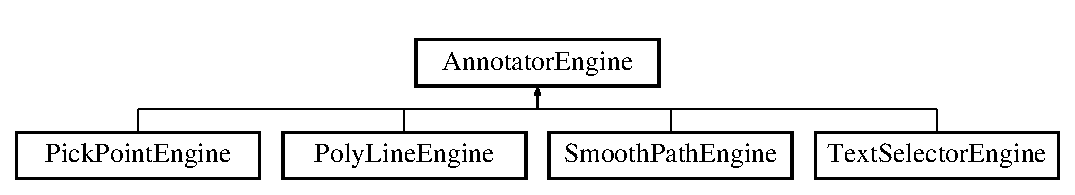
\includegraphics[height=2.000000cm]{classAnnotatorEngine}
\end{center}
\end{figure}
\subsection*{Public Types}
\begin{DoxyCompactItemize}
\item 
enum \hyperlink{classAnnotatorEngine_a00fb22eb4cb6eafb056f9066031db133}{Event\+Type} \{ \hyperlink{classAnnotatorEngine_a00fb22eb4cb6eafb056f9066031db133a7f6f77a85d31dc6afd375db9a53d5069}{Press}, 
\hyperlink{classAnnotatorEngine_a00fb22eb4cb6eafb056f9066031db133a4efcf099c4a82b1eab7de0fb124563a8}{Move}, 
\hyperlink{classAnnotatorEngine_a00fb22eb4cb6eafb056f9066031db133ac80dbad38d0461d9e546aa694c2abc1c}{Release}
 \}
\item 
enum \hyperlink{classAnnotatorEngine_ac2e3b75e12bacbb6974d15dd53954567}{Button} \{ \hyperlink{classAnnotatorEngine_ac2e3b75e12bacbb6974d15dd53954567aad36f3f65ac99d40e03cf36b3d65d018}{None}, 
\hyperlink{classAnnotatorEngine_ac2e3b75e12bacbb6974d15dd53954567a2719e853d63982d67e9d8aae3620178c}{Left}, 
\hyperlink{classAnnotatorEngine_ac2e3b75e12bacbb6974d15dd53954567a8c25b27f7e32e09ea9767d465de328a9}{Right}
 \}
\end{DoxyCompactItemize}
\subsection*{Public Member Functions}
\begin{DoxyCompactItemize}
\item 
\hyperlink{classAnnotatorEngine_a42302fe858494d3e3ad90b8607c543ef}{Annotator\+Engine} (const Q\+Dom\+Element \&engine\+Element)
\item 
virtual \hyperlink{classAnnotatorEngine_a51954e14195933ce370de28c466ddddf}{$\sim$\+Annotator\+Engine} ()
\item 
virtual Q\+Rect \hyperlink{classAnnotatorEngine_acca989fc60f9a6c20ed2518fafa8774e}{event} (\hyperlink{classAnnotatorEngine_a00fb22eb4cb6eafb056f9066031db133}{Event\+Type} type, \hyperlink{classAnnotatorEngine_ac2e3b75e12bacbb6974d15dd53954567}{Button} button, double n\+X, double n\+Y, double x\+Scale, double y\+Scale, const \hyperlink{classOkular_1_1Page}{Okular\+::\+Page} $\ast$page)=0
\item 
virtual void \hyperlink{classAnnotatorEngine_a71b2e9fcbcca36caadefa79adb99c93f}{paint} (Q\+Painter $\ast$painter, double x\+Scale, double y\+Scale, const Q\+Rect \&clip\+Rect)=0
\item 
virtual \hyperlink{classQList}{Q\+List}\\*
$<$ \hyperlink{classOkular_1_1Annotation}{Okular\+::\+Annotation} $\ast$ $>$ \hyperlink{classAnnotatorEngine_a50455740303878b891195132df27a2ab}{end} ()=0
\item 
bool \hyperlink{classAnnotatorEngine_a54e1ac7803149f1a94490e5511ad3deb}{creation\+Completed} () const 
\item 
void \hyperlink{classAnnotatorEngine_aae312cd62f6fd4c9997a655d18de7385}{set\+Item} (\hyperlink{classPageViewItem}{Page\+View\+Item} $\ast$\hyperlink{classAnnotatorEngine_a67d46d5364e6f54e107ccbbb1ed07e32}{item})
\item 
virtual Q\+Cursor \hyperlink{classAnnotatorEngine_adec4c7612b59357c7b58aa81e3e3b212}{cursor} () const 
\end{DoxyCompactItemize}
\subsection*{Static Public Member Functions}
\begin{DoxyCompactItemize}
\item 
static void \hyperlink{classAnnotatorEngine_acabc5b26b0693eb5b29138a7a70f7a39}{decode\+Event} (const Q\+Mouse\+Event $\ast$mouse\+Event, \hyperlink{classAnnotatorEngine_a00fb22eb4cb6eafb056f9066031db133}{Event\+Type} $\ast$event\+Type, \hyperlink{classAnnotatorEngine_ac2e3b75e12bacbb6974d15dd53954567}{Button} $\ast$button)
\item 
static void \hyperlink{classAnnotatorEngine_aac61c2dd18f7a5c548d7844d0f096889}{decode\+Event} (const Q\+Tablet\+Event $\ast$tablet\+Event, \hyperlink{classAnnotatorEngine_a00fb22eb4cb6eafb056f9066031db133}{Event\+Type} $\ast$event\+Type, \hyperlink{classAnnotatorEngine_ac2e3b75e12bacbb6974d15dd53954567}{Button} $\ast$button)
\end{DoxyCompactItemize}
\subsection*{Protected Member Functions}
\begin{DoxyCompactItemize}
\item 
\hyperlink{classPageViewItem}{Page\+View\+Item} $\ast$ \hyperlink{classAnnotatorEngine_a67d46d5364e6f54e107ccbbb1ed07e32}{item} ()
\end{DoxyCompactItemize}
\subsection*{Protected Attributes}
\begin{DoxyCompactItemize}
\item 
Q\+Dom\+Element \hyperlink{classAnnotatorEngine_aa60b9dda9bd0beb5af6f777b1e65b342}{m\+\_\+engine\+Element}
\item 
Q\+Dom\+Element \hyperlink{classAnnotatorEngine_ac95af6291cc2f0c601e1bbf8a5e6a0bd}{m\+\_\+annot\+Element}
\item 
Q\+Color \hyperlink{classAnnotatorEngine_a8911b0455be7eedfb2c102ce19acdce2}{m\+\_\+engine\+Color}
\item 
bool \hyperlink{classAnnotatorEngine_a0df119b4d87a1e3ea8ed60a96d7ff444}{m\+\_\+creation\+Completed}
\end{DoxyCompactItemize}


\subsection{Detailed Description}
Engine\+: filter events to distill Annotations. 

Definition at line 32 of file annotationtools.\+h.



\subsection{Member Enumeration Documentation}
\hypertarget{classAnnotatorEngine_ac2e3b75e12bacbb6974d15dd53954567}{\index{Annotator\+Engine@{Annotator\+Engine}!Button@{Button}}
\index{Button@{Button}!Annotator\+Engine@{Annotator\+Engine}}
\subsubsection[{Button}]{\setlength{\rightskip}{0pt plus 5cm}enum {\bf Annotator\+Engine\+::\+Button}}}\label{classAnnotatorEngine_ac2e3b75e12bacbb6974d15dd53954567}
\begin{Desc}
\item[Enumerator]\par
\begin{description}
\index{None@{None}!Annotator\+Engine@{Annotator\+Engine}}\index{Annotator\+Engine@{Annotator\+Engine}!None@{None}}\item[{\em 
\hypertarget{classAnnotatorEngine_ac2e3b75e12bacbb6974d15dd53954567aad36f3f65ac99d40e03cf36b3d65d018}{None}\label{classAnnotatorEngine_ac2e3b75e12bacbb6974d15dd53954567aad36f3f65ac99d40e03cf36b3d65d018}
}]\index{Left@{Left}!Annotator\+Engine@{Annotator\+Engine}}\index{Annotator\+Engine@{Annotator\+Engine}!Left@{Left}}\item[{\em 
\hypertarget{classAnnotatorEngine_ac2e3b75e12bacbb6974d15dd53954567a2719e853d63982d67e9d8aae3620178c}{Left}\label{classAnnotatorEngine_ac2e3b75e12bacbb6974d15dd53954567a2719e853d63982d67e9d8aae3620178c}
}]\index{Right@{Right}!Annotator\+Engine@{Annotator\+Engine}}\index{Annotator\+Engine@{Annotator\+Engine}!Right@{Right}}\item[{\em 
\hypertarget{classAnnotatorEngine_ac2e3b75e12bacbb6974d15dd53954567a8c25b27f7e32e09ea9767d465de328a9}{Right}\label{classAnnotatorEngine_ac2e3b75e12bacbb6974d15dd53954567a8c25b27f7e32e09ea9767d465de328a9}
}]\end{description}
\end{Desc}


Definition at line 40 of file annotationtools.\+h.


\begin{DoxyCode}
40 \{ \hyperlink{classAnnotatorEngine_ac2e3b75e12bacbb6974d15dd53954567aad36f3f65ac99d40e03cf36b3d65d018}{None}, \hyperlink{classAnnotatorEngine_ac2e3b75e12bacbb6974d15dd53954567a2719e853d63982d67e9d8aae3620178c}{Left}, \hyperlink{classAnnotatorEngine_ac2e3b75e12bacbb6974d15dd53954567a8c25b27f7e32e09ea9767d465de328a9}{Right} \};
\end{DoxyCode}
\hypertarget{classAnnotatorEngine_a00fb22eb4cb6eafb056f9066031db133}{\index{Annotator\+Engine@{Annotator\+Engine}!Event\+Type@{Event\+Type}}
\index{Event\+Type@{Event\+Type}!Annotator\+Engine@{Annotator\+Engine}}
\subsubsection[{Event\+Type}]{\setlength{\rightskip}{0pt plus 5cm}enum {\bf Annotator\+Engine\+::\+Event\+Type}}}\label{classAnnotatorEngine_a00fb22eb4cb6eafb056f9066031db133}
\begin{Desc}
\item[Enumerator]\par
\begin{description}
\index{Press@{Press}!Annotator\+Engine@{Annotator\+Engine}}\index{Annotator\+Engine@{Annotator\+Engine}!Press@{Press}}\item[{\em 
\hypertarget{classAnnotatorEngine_a00fb22eb4cb6eafb056f9066031db133a7f6f77a85d31dc6afd375db9a53d5069}{Press}\label{classAnnotatorEngine_a00fb22eb4cb6eafb056f9066031db133a7f6f77a85d31dc6afd375db9a53d5069}
}]\index{Move@{Move}!Annotator\+Engine@{Annotator\+Engine}}\index{Annotator\+Engine@{Annotator\+Engine}!Move@{Move}}\item[{\em 
\hypertarget{classAnnotatorEngine_a00fb22eb4cb6eafb056f9066031db133a4efcf099c4a82b1eab7de0fb124563a8}{Move}\label{classAnnotatorEngine_a00fb22eb4cb6eafb056f9066031db133a4efcf099c4a82b1eab7de0fb124563a8}
}]\index{Release@{Release}!Annotator\+Engine@{Annotator\+Engine}}\index{Annotator\+Engine@{Annotator\+Engine}!Release@{Release}}\item[{\em 
\hypertarget{classAnnotatorEngine_a00fb22eb4cb6eafb056f9066031db133ac80dbad38d0461d9e546aa694c2abc1c}{Release}\label{classAnnotatorEngine_a00fb22eb4cb6eafb056f9066031db133ac80dbad38d0461d9e546aa694c2abc1c}
}]\end{description}
\end{Desc}


Definition at line 39 of file annotationtools.\+h.


\begin{DoxyCode}
39 \{ \hyperlink{classAnnotatorEngine_a00fb22eb4cb6eafb056f9066031db133a7f6f77a85d31dc6afd375db9a53d5069}{Press}, \hyperlink{classAnnotatorEngine_a00fb22eb4cb6eafb056f9066031db133a4efcf099c4a82b1eab7de0fb124563a8}{Move}, \hyperlink{classAnnotatorEngine_a00fb22eb4cb6eafb056f9066031db133ac80dbad38d0461d9e546aa694c2abc1c}{Release} \};
\end{DoxyCode}


\subsection{Constructor \& Destructor Documentation}
\hypertarget{classAnnotatorEngine_a42302fe858494d3e3ad90b8607c543ef}{\index{Annotator\+Engine@{Annotator\+Engine}!Annotator\+Engine@{Annotator\+Engine}}
\index{Annotator\+Engine@{Annotator\+Engine}!Annotator\+Engine@{Annotator\+Engine}}
\subsubsection[{Annotator\+Engine}]{\setlength{\rightskip}{0pt plus 5cm}Annotator\+Engine\+::\+Annotator\+Engine (
\begin{DoxyParamCaption}
\item[{const Q\+Dom\+Element \&}]{engine\+Element}
\end{DoxyParamCaption}
)}}\label{classAnnotatorEngine_a42302fe858494d3e3ad90b8607c543ef}


Definition at line 21 of file annotationtools.\+cpp.


\begin{DoxyCode}
22     : \hyperlink{classAnnotatorEngine_aa60b9dda9bd0beb5af6f777b1e65b342}{m\_engineElement}( engineElement ), \hyperlink{classAnnotatorEngine_a0df119b4d87a1e3ea8ed60a96d7ff444}{m\_creationCompleted}( \textcolor{keyword}{false} ), 
      m\_item( 0 )
23 \{
24     \textcolor{comment}{// parse common engine attributes}
25     \textcolor{keywordflow}{if} ( engineElement.hasAttribute( \textcolor{stringliteral}{"color"} ) )
26         \hyperlink{classAnnotatorEngine_a8911b0455be7eedfb2c102ce19acdce2}{m\_engineColor} = QColor( engineElement.attribute( \textcolor{stringliteral}{"color"} ) );
27 
28     \textcolor{comment}{// get the annotation element}
29     QDomElement annElement = \hyperlink{classAnnotatorEngine_aa60b9dda9bd0beb5af6f777b1e65b342}{m\_engineElement}.firstChild().toElement();
30     \textcolor{keywordflow}{if} ( !annElement.isNull() && annElement.tagName() == \textcolor{stringliteral}{"annotation"} )
31         \hyperlink{classAnnotatorEngine_ac95af6291cc2f0c601e1bbf8a5e6a0bd}{m\_annotElement} = annElement;
32 \}
\end{DoxyCode}
\hypertarget{classAnnotatorEngine_a51954e14195933ce370de28c466ddddf}{\index{Annotator\+Engine@{Annotator\+Engine}!````~Annotator\+Engine@{$\sim$\+Annotator\+Engine}}
\index{````~Annotator\+Engine@{$\sim$\+Annotator\+Engine}!Annotator\+Engine@{Annotator\+Engine}}
\subsubsection[{$\sim$\+Annotator\+Engine}]{\setlength{\rightskip}{0pt plus 5cm}Annotator\+Engine\+::$\sim$\+Annotator\+Engine (
\begin{DoxyParamCaption}
{}
\end{DoxyParamCaption}
)\hspace{0.3cm}{\ttfamily [virtual]}}}\label{classAnnotatorEngine_a51954e14195933ce370de28c466ddddf}


Definition at line 76 of file annotationtools.\+cpp.


\begin{DoxyCode}
77 \{
78 \}
\end{DoxyCode}


\subsection{Member Function Documentation}
\hypertarget{classAnnotatorEngine_a54e1ac7803149f1a94490e5511ad3deb}{\index{Annotator\+Engine@{Annotator\+Engine}!creation\+Completed@{creation\+Completed}}
\index{creation\+Completed@{creation\+Completed}!Annotator\+Engine@{Annotator\+Engine}}
\subsubsection[{creation\+Completed}]{\setlength{\rightskip}{0pt plus 5cm}bool Annotator\+Engine\+::creation\+Completed (
\begin{DoxyParamCaption}
{}
\end{DoxyParamCaption}
) const\hspace{0.3cm}{\ttfamily [inline]}}}\label{classAnnotatorEngine_a54e1ac7803149f1a94490e5511ad3deb}


Definition at line 49 of file annotationtools.\+h.


\begin{DoxyCode}
49 \{ \textcolor{keywordflow}{return} \hyperlink{classAnnotatorEngine_a0df119b4d87a1e3ea8ed60a96d7ff444}{m\_creationCompleted}; \}
\end{DoxyCode}
\hypertarget{classAnnotatorEngine_adec4c7612b59357c7b58aa81e3e3b212}{\index{Annotator\+Engine@{Annotator\+Engine}!cursor@{cursor}}
\index{cursor@{cursor}!Annotator\+Engine@{Annotator\+Engine}}
\subsubsection[{cursor}]{\setlength{\rightskip}{0pt plus 5cm}Q\+Cursor Annotator\+Engine\+::cursor (
\begin{DoxyParamCaption}
{}
\end{DoxyParamCaption}
) const\hspace{0.3cm}{\ttfamily [virtual]}}}\label{classAnnotatorEngine_adec4c7612b59357c7b58aa81e3e3b212}


Reimplemented in \hyperlink{classTextSelectorEngine_a0b4309d25b8f6d56570f5a39bf6722fc}{Text\+Selector\+Engine}.



Definition at line 80 of file annotationtools.\+cpp.


\begin{DoxyCode}
81 \{
82     \textcolor{keywordflow}{return} Qt::CrossCursor;
83 \}
\end{DoxyCode}
\hypertarget{classAnnotatorEngine_acabc5b26b0693eb5b29138a7a70f7a39}{\index{Annotator\+Engine@{Annotator\+Engine}!decode\+Event@{decode\+Event}}
\index{decode\+Event@{decode\+Event}!Annotator\+Engine@{Annotator\+Engine}}
\subsubsection[{decode\+Event}]{\setlength{\rightskip}{0pt plus 5cm}void Annotator\+Engine\+::decode\+Event (
\begin{DoxyParamCaption}
\item[{const Q\+Mouse\+Event $\ast$}]{mouse\+Event, }
\item[{{\bf Event\+Type} $\ast$}]{event\+Type, }
\item[{{\bf Button} $\ast$}]{button}
\end{DoxyParamCaption}
)\hspace{0.3cm}{\ttfamily [static]}}}\label{classAnnotatorEngine_acabc5b26b0693eb5b29138a7a70f7a39}


Definition at line 34 of file annotationtools.\+cpp.


\begin{DoxyCode}
35 \{
36     *eventType = \hyperlink{classAnnotatorEngine_a00fb22eb4cb6eafb056f9066031db133a7f6f77a85d31dc6afd375db9a53d5069}{AnnotatorEngine::Press};
37     \textcolor{keywordflow}{if} ( mouseEvent->type() == QEvent::MouseMove )
38         *eventType = \hyperlink{classAnnotatorEngine_a00fb22eb4cb6eafb056f9066031db133a4efcf099c4a82b1eab7de0fb124563a8}{AnnotatorEngine::Move};
39     \textcolor{keywordflow}{else} \textcolor{keywordflow}{if} ( mouseEvent->type() == QEvent::MouseButtonRelease )
40         *eventType = \hyperlink{classAnnotatorEngine_a00fb22eb4cb6eafb056f9066031db133ac80dbad38d0461d9e546aa694c2abc1c}{AnnotatorEngine::Release};
41 
42     *button = \hyperlink{classAnnotatorEngine_ac2e3b75e12bacbb6974d15dd53954567aad36f3f65ac99d40e03cf36b3d65d018}{AnnotatorEngine::None};
43     \textcolor{keyword}{const} Qt::MouseButtons buttonState = ( *eventType == \hyperlink{classAnnotatorEngine_a00fb22eb4cb6eafb056f9066031db133a4efcf099c4a82b1eab7de0fb124563a8}{AnnotatorEngine::Move} ) ? 
      mouseEvent->buttons() : mouseEvent->button();
44     \textcolor{keywordflow}{if} ( buttonState == Qt::LeftButton )
45         *button = \hyperlink{classAnnotatorEngine_ac2e3b75e12bacbb6974d15dd53954567a2719e853d63982d67e9d8aae3620178c}{AnnotatorEngine::Left};
46     \textcolor{keywordflow}{else} \textcolor{keywordflow}{if} ( buttonState == Qt::RightButton )
47         *button = \hyperlink{classAnnotatorEngine_ac2e3b75e12bacbb6974d15dd53954567a8c25b27f7e32e09ea9767d465de328a9}{AnnotatorEngine::Right};
48 \}
\end{DoxyCode}
\hypertarget{classAnnotatorEngine_aac61c2dd18f7a5c548d7844d0f096889}{\index{Annotator\+Engine@{Annotator\+Engine}!decode\+Event@{decode\+Event}}
\index{decode\+Event@{decode\+Event}!Annotator\+Engine@{Annotator\+Engine}}
\subsubsection[{decode\+Event}]{\setlength{\rightskip}{0pt plus 5cm}void Annotator\+Engine\+::decode\+Event (
\begin{DoxyParamCaption}
\item[{const Q\+Tablet\+Event $\ast$}]{tablet\+Event, }
\item[{{\bf Event\+Type} $\ast$}]{event\+Type, }
\item[{{\bf Button} $\ast$}]{button}
\end{DoxyParamCaption}
)\hspace{0.3cm}{\ttfamily [static]}}}\label{classAnnotatorEngine_aac61c2dd18f7a5c548d7844d0f096889}


Definition at line 50 of file annotationtools.\+cpp.


\begin{DoxyCode}
51 \{
52     \textcolor{keywordflow}{switch} ( tabletEvent->type() )
53     \{
54         \textcolor{keywordflow}{case} QEvent::TabletPress:
55             \textcolor{comment}{// Tablet press event is equivalent to pressing the left mouse button}
56             *button = \hyperlink{classAnnotatorEngine_ac2e3b75e12bacbb6974d15dd53954567a2719e853d63982d67e9d8aae3620178c}{AnnotatorEngine::Left};
57             *eventType = \hyperlink{classAnnotatorEngine_a00fb22eb4cb6eafb056f9066031db133a7f6f77a85d31dc6afd375db9a53d5069}{AnnotatorEngine::Press};
58             \textcolor{keywordflow}{break};
59         \textcolor{keywordflow}{case} QEvent::TabletRelease:
60             \textcolor{comment}{// Tablet release event is equivalent to releasing the left mouse button}
61             *button = \hyperlink{classAnnotatorEngine_ac2e3b75e12bacbb6974d15dd53954567a2719e853d63982d67e9d8aae3620178c}{AnnotatorEngine::Left};
62             *eventType = \hyperlink{classAnnotatorEngine_a00fb22eb4cb6eafb056f9066031db133ac80dbad38d0461d9e546aa694c2abc1c}{AnnotatorEngine::Release};
63             \textcolor{keywordflow}{break};
64         \textcolor{keywordflow}{case} QEvent::TabletMove:
65             \textcolor{comment}{// Tablet events are only routed if the pen is down so}
66             \textcolor{comment}{// this is equivalent to the left mouse button being pressed}
67             *button = \hyperlink{classAnnotatorEngine_ac2e3b75e12bacbb6974d15dd53954567a2719e853d63982d67e9d8aae3620178c}{AnnotatorEngine::Left};
68             *eventType = \hyperlink{classAnnotatorEngine_a00fb22eb4cb6eafb056f9066031db133a4efcf099c4a82b1eab7de0fb124563a8}{AnnotatorEngine::Move};
69             \textcolor{keywordflow}{break};
70         \textcolor{keywordflow}{default}:
71             Q\_ASSERT(\textcolor{keyword}{false});
72             \textcolor{keywordflow}{break};
73     \}
74 \}
\end{DoxyCode}
\hypertarget{classAnnotatorEngine_a50455740303878b891195132df27a2ab}{\index{Annotator\+Engine@{Annotator\+Engine}!end@{end}}
\index{end@{end}!Annotator\+Engine@{Annotator\+Engine}}
\subsubsection[{end}]{\setlength{\rightskip}{0pt plus 5cm}virtual {\bf Q\+List}$<$ {\bf Okular\+::\+Annotation}$\ast$ $>$ Annotator\+Engine\+::end (
\begin{DoxyParamCaption}
{}
\end{DoxyParamCaption}
)\hspace{0.3cm}{\ttfamily [pure virtual]}}}\label{classAnnotatorEngine_a50455740303878b891195132df27a2ab}


Implemented in \hyperlink{classTextSelectorEngine_ac0478924c3210f726bedf6c10a50141e}{Text\+Selector\+Engine}, \hyperlink{classPolyLineEngine_ac5d84e9165cd9ab117d161aa935d102e}{Poly\+Line\+Engine}, \hyperlink{classPickPointEngine_a4a3cc45d8861f30637b2aa5ee85cc6c3}{Pick\+Point\+Engine}, and \hyperlink{classSmoothPathEngine_aa1dd0f64bab0f5d94aba93557a6ba328}{Smooth\+Path\+Engine}.

\hypertarget{classAnnotatorEngine_acca989fc60f9a6c20ed2518fafa8774e}{\index{Annotator\+Engine@{Annotator\+Engine}!event@{event}}
\index{event@{event}!Annotator\+Engine@{Annotator\+Engine}}
\subsubsection[{event}]{\setlength{\rightskip}{0pt plus 5cm}virtual Q\+Rect Annotator\+Engine\+::event (
\begin{DoxyParamCaption}
\item[{{\bf Event\+Type}}]{type, }
\item[{{\bf Button}}]{button, }
\item[{double}]{n\+X, }
\item[{double}]{n\+Y, }
\item[{double}]{x\+Scale, }
\item[{double}]{y\+Scale, }
\item[{const {\bf Okular\+::\+Page} $\ast$}]{page}
\end{DoxyParamCaption}
)\hspace{0.3cm}{\ttfamily [pure virtual]}}}\label{classAnnotatorEngine_acca989fc60f9a6c20ed2518fafa8774e}


Implemented in \hyperlink{classTextSelectorEngine_a960e484c0c32e6500d9e75d676d0c60e}{Text\+Selector\+Engine}, \hyperlink{classPolyLineEngine_a822e6058b9e407228c83298678d3aa94}{Poly\+Line\+Engine}, \hyperlink{classSmoothPathEngine_a7234a32a90d2784e2459cf838a37f172}{Smooth\+Path\+Engine}, and \hyperlink{classPickPointEngine_a7dd04c96b28fbf6dba26c5f277827ece}{Pick\+Point\+Engine}.

\hypertarget{classAnnotatorEngine_a67d46d5364e6f54e107ccbbb1ed07e32}{\index{Annotator\+Engine@{Annotator\+Engine}!item@{item}}
\index{item@{item}!Annotator\+Engine@{Annotator\+Engine}}
\subsubsection[{item}]{\setlength{\rightskip}{0pt plus 5cm}{\bf Page\+View\+Item}$\ast$ Annotator\+Engine\+::item (
\begin{DoxyParamCaption}
{}
\end{DoxyParamCaption}
)\hspace{0.3cm}{\ttfamily [inline]}, {\ttfamily [protected]}}}\label{classAnnotatorEngine_a67d46d5364e6f54e107ccbbb1ed07e32}


Definition at line 59 of file annotationtools.\+h.


\begin{DoxyCode}
59 \{ \textcolor{keywordflow}{return} m\_item; \}
\end{DoxyCode}
\hypertarget{classAnnotatorEngine_a71b2e9fcbcca36caadefa79adb99c93f}{\index{Annotator\+Engine@{Annotator\+Engine}!paint@{paint}}
\index{paint@{paint}!Annotator\+Engine@{Annotator\+Engine}}
\subsubsection[{paint}]{\setlength{\rightskip}{0pt plus 5cm}virtual void Annotator\+Engine\+::paint (
\begin{DoxyParamCaption}
\item[{Q\+Painter $\ast$}]{painter, }
\item[{double}]{x\+Scale, }
\item[{double}]{y\+Scale, }
\item[{const Q\+Rect \&}]{clip\+Rect}
\end{DoxyParamCaption}
)\hspace{0.3cm}{\ttfamily [pure virtual]}}}\label{classAnnotatorEngine_a71b2e9fcbcca36caadefa79adb99c93f}


Implemented in \hyperlink{classTextSelectorEngine_a68b752c46a1371f4caa0eb692553ff5c}{Text\+Selector\+Engine}, \hyperlink{classPolyLineEngine_ae2399ba29c9bc734ffe53db0310e54bd}{Poly\+Line\+Engine}, \hyperlink{classPickPointEngine_a1af9d4c401554caa10918985dbd7aae2}{Pick\+Point\+Engine}, and \hyperlink{classSmoothPathEngine_a08b94551c709ae56600afd692da10717}{Smooth\+Path\+Engine}.

\hypertarget{classAnnotatorEngine_aae312cd62f6fd4c9997a655d18de7385}{\index{Annotator\+Engine@{Annotator\+Engine}!set\+Item@{set\+Item}}
\index{set\+Item@{set\+Item}!Annotator\+Engine@{Annotator\+Engine}}
\subsubsection[{set\+Item}]{\setlength{\rightskip}{0pt plus 5cm}void Annotator\+Engine\+::set\+Item (
\begin{DoxyParamCaption}
\item[{{\bf Page\+View\+Item} $\ast$}]{item}
\end{DoxyParamCaption}
)\hspace{0.3cm}{\ttfamily [inline]}}}\label{classAnnotatorEngine_aae312cd62f6fd4c9997a655d18de7385}


Definition at line 51 of file annotationtools.\+h.


\begin{DoxyCode}
51 \{ m\_item = \hyperlink{classAnnotatorEngine_a67d46d5364e6f54e107ccbbb1ed07e32}{item}; \}
\end{DoxyCode}


\subsection{Member Data Documentation}
\hypertarget{classAnnotatorEngine_ac95af6291cc2f0c601e1bbf8a5e6a0bd}{\index{Annotator\+Engine@{Annotator\+Engine}!m\+\_\+annot\+Element@{m\+\_\+annot\+Element}}
\index{m\+\_\+annot\+Element@{m\+\_\+annot\+Element}!Annotator\+Engine@{Annotator\+Engine}}
\subsubsection[{m\+\_\+annot\+Element}]{\setlength{\rightskip}{0pt plus 5cm}Q\+Dom\+Element Annotator\+Engine\+::m\+\_\+annot\+Element\hspace{0.3cm}{\ttfamily [protected]}}}\label{classAnnotatorEngine_ac95af6291cc2f0c601e1bbf8a5e6a0bd}


Definition at line 63 of file annotationtools.\+h.

\hypertarget{classAnnotatorEngine_a0df119b4d87a1e3ea8ed60a96d7ff444}{\index{Annotator\+Engine@{Annotator\+Engine}!m\+\_\+creation\+Completed@{m\+\_\+creation\+Completed}}
\index{m\+\_\+creation\+Completed@{m\+\_\+creation\+Completed}!Annotator\+Engine@{Annotator\+Engine}}
\subsubsection[{m\+\_\+creation\+Completed}]{\setlength{\rightskip}{0pt plus 5cm}bool Annotator\+Engine\+::m\+\_\+creation\+Completed\hspace{0.3cm}{\ttfamily [protected]}}}\label{classAnnotatorEngine_a0df119b4d87a1e3ea8ed60a96d7ff444}


Definition at line 66 of file annotationtools.\+h.

\hypertarget{classAnnotatorEngine_a8911b0455be7eedfb2c102ce19acdce2}{\index{Annotator\+Engine@{Annotator\+Engine}!m\+\_\+engine\+Color@{m\+\_\+engine\+Color}}
\index{m\+\_\+engine\+Color@{m\+\_\+engine\+Color}!Annotator\+Engine@{Annotator\+Engine}}
\subsubsection[{m\+\_\+engine\+Color}]{\setlength{\rightskip}{0pt plus 5cm}Q\+Color Annotator\+Engine\+::m\+\_\+engine\+Color\hspace{0.3cm}{\ttfamily [protected]}}}\label{classAnnotatorEngine_a8911b0455be7eedfb2c102ce19acdce2}


Definition at line 64 of file annotationtools.\+h.

\hypertarget{classAnnotatorEngine_aa60b9dda9bd0beb5af6f777b1e65b342}{\index{Annotator\+Engine@{Annotator\+Engine}!m\+\_\+engine\+Element@{m\+\_\+engine\+Element}}
\index{m\+\_\+engine\+Element@{m\+\_\+engine\+Element}!Annotator\+Engine@{Annotator\+Engine}}
\subsubsection[{m\+\_\+engine\+Element}]{\setlength{\rightskip}{0pt plus 5cm}Q\+Dom\+Element Annotator\+Engine\+::m\+\_\+engine\+Element\hspace{0.3cm}{\ttfamily [protected]}}}\label{classAnnotatorEngine_aa60b9dda9bd0beb5af6f777b1e65b342}


Definition at line 62 of file annotationtools.\+h.



The documentation for this class was generated from the following files\+:\begin{DoxyCompactItemize}
\item 
ui/\hyperlink{annotationtools_8h}{annotationtools.\+h}\item 
ui/\hyperlink{annotationtools_8cpp}{annotationtools.\+cpp}\end{DoxyCompactItemize}

\hypertarget{structAnnotationPopup_1_1AnnotPagePair}{\section{Annotation\+Popup\+:\+:Annot\+Page\+Pair Struct Reference}
\label{structAnnotationPopup_1_1AnnotPagePair}\index{Annotation\+Popup\+::\+Annot\+Page\+Pair@{Annotation\+Popup\+::\+Annot\+Page\+Pair}}
}


{\ttfamily \#include $<$annotationpopup.\+h$>$}

\subsection*{Public Member Functions}
\begin{DoxyCompactItemize}
\item 
\hyperlink{structAnnotationPopup_1_1AnnotPagePair_a091f67bd8eaaf5117c141eda6b978b63}{Annot\+Page\+Pair} ()
\item 
\hyperlink{structAnnotationPopup_1_1AnnotPagePair_a522740e9cb89feae6e8505961ce60c0b}{Annot\+Page\+Pair} (\hyperlink{classOkular_1_1Annotation}{Okular\+::\+Annotation} $\ast$a, int pn)
\item 
\hyperlink{structAnnotationPopup_1_1AnnotPagePair_a89fc656319f701b28149ee0be4578482}{Annot\+Page\+Pair} (const \hyperlink{structAnnotationPopup_1_1AnnotPagePair}{Annot\+Page\+Pair} \&pair)
\item 
bool \hyperlink{structAnnotationPopup_1_1AnnotPagePair_a8ed247329a955126282431d764ec93f3}{operator==} (const \hyperlink{structAnnotationPopup_1_1AnnotPagePair}{Annot\+Page\+Pair} \&pair) const 
\end{DoxyCompactItemize}
\subsection*{Public Attributes}
\begin{DoxyCompactItemize}
\item 
\hyperlink{classOkular_1_1Annotation}{Okular\+::\+Annotation} $\ast$ \hyperlink{structAnnotationPopup_1_1AnnotPagePair_abd389ae75ec90cfcaabce2e79273af3c}{annotation}
\item 
int \hyperlink{structAnnotationPopup_1_1AnnotPagePair_abd8fe2b8ae303985a9a08784c6069d29}{page\+Number}
\end{DoxyCompactItemize}


\subsection{Detailed Description}


Definition at line 47 of file annotationpopup.\+h.



\subsection{Constructor \& Destructor Documentation}
\hypertarget{structAnnotationPopup_1_1AnnotPagePair_a091f67bd8eaaf5117c141eda6b978b63}{\index{Annotation\+Popup\+::\+Annot\+Page\+Pair@{Annotation\+Popup\+::\+Annot\+Page\+Pair}!Annot\+Page\+Pair@{Annot\+Page\+Pair}}
\index{Annot\+Page\+Pair@{Annot\+Page\+Pair}!Annotation\+Popup\+::\+Annot\+Page\+Pair@{Annotation\+Popup\+::\+Annot\+Page\+Pair}}
\subsubsection[{Annot\+Page\+Pair}]{\setlength{\rightskip}{0pt plus 5cm}Annotation\+Popup\+::\+Annot\+Page\+Pair\+::\+Annot\+Page\+Pair (
\begin{DoxyParamCaption}
{}
\end{DoxyParamCaption}
)\hspace{0.3cm}{\ttfamily [inline]}}}\label{structAnnotationPopup_1_1AnnotPagePair_a091f67bd8eaaf5117c141eda6b978b63}


Definition at line 48 of file annotationpopup.\+h.


\begin{DoxyCode}
48                             : \hyperlink{structAnnotationPopup_1_1AnnotPagePair_abd389ae75ec90cfcaabce2e79273af3c}{annotation}( 0 ),  \hyperlink{structAnnotationPopup_1_1AnnotPagePair_abd8fe2b8ae303985a9a08784c6069d29}{pageNumber}( -1 )
49             \{ \}
\end{DoxyCode}
\hypertarget{structAnnotationPopup_1_1AnnotPagePair_a522740e9cb89feae6e8505961ce60c0b}{\index{Annotation\+Popup\+::\+Annot\+Page\+Pair@{Annotation\+Popup\+::\+Annot\+Page\+Pair}!Annot\+Page\+Pair@{Annot\+Page\+Pair}}
\index{Annot\+Page\+Pair@{Annot\+Page\+Pair}!Annotation\+Popup\+::\+Annot\+Page\+Pair@{Annotation\+Popup\+::\+Annot\+Page\+Pair}}
\subsubsection[{Annot\+Page\+Pair}]{\setlength{\rightskip}{0pt plus 5cm}Annotation\+Popup\+::\+Annot\+Page\+Pair\+::\+Annot\+Page\+Pair (
\begin{DoxyParamCaption}
\item[{{\bf Okular\+::\+Annotation} $\ast$}]{a, }
\item[{int}]{pn}
\end{DoxyParamCaption}
)\hspace{0.3cm}{\ttfamily [inline]}}}\label{structAnnotationPopup_1_1AnnotPagePair_a522740e9cb89feae6e8505961ce60c0b}


Definition at line 51 of file annotationpopup.\+h.


\begin{DoxyCode}
51                                                          : \hyperlink{structAnnotationPopup_1_1AnnotPagePair_abd389ae75ec90cfcaabce2e79273af3c}{annotation}( a ),  
      \hyperlink{structAnnotationPopup_1_1AnnotPagePair_abd8fe2b8ae303985a9a08784c6069d29}{pageNumber}( pn )
52             \{ \}
\end{DoxyCode}
\hypertarget{structAnnotationPopup_1_1AnnotPagePair_a89fc656319f701b28149ee0be4578482}{\index{Annotation\+Popup\+::\+Annot\+Page\+Pair@{Annotation\+Popup\+::\+Annot\+Page\+Pair}!Annot\+Page\+Pair@{Annot\+Page\+Pair}}
\index{Annot\+Page\+Pair@{Annot\+Page\+Pair}!Annotation\+Popup\+::\+Annot\+Page\+Pair@{Annotation\+Popup\+::\+Annot\+Page\+Pair}}
\subsubsection[{Annot\+Page\+Pair}]{\setlength{\rightskip}{0pt plus 5cm}Annotation\+Popup\+::\+Annot\+Page\+Pair\+::\+Annot\+Page\+Pair (
\begin{DoxyParamCaption}
\item[{const {\bf Annot\+Page\+Pair} \&}]{pair}
\end{DoxyParamCaption}
)\hspace{0.3cm}{\ttfamily [inline]}}}\label{structAnnotationPopup_1_1AnnotPagePair_a89fc656319f701b28149ee0be4578482}


Definition at line 54 of file annotationpopup.\+h.


\begin{DoxyCode}
54                                                         : \hyperlink{structAnnotationPopup_1_1AnnotPagePair_abd389ae75ec90cfcaabce2e79273af3c}{annotation}( pair.annotation ),  
      \hyperlink{structAnnotationPopup_1_1AnnotPagePair_abd8fe2b8ae303985a9a08784c6069d29}{pageNumber}( pair.pageNumber )
55             \{ \}
\end{DoxyCode}


\subsection{Member Function Documentation}
\hypertarget{structAnnotationPopup_1_1AnnotPagePair_a8ed247329a955126282431d764ec93f3}{\index{Annotation\+Popup\+::\+Annot\+Page\+Pair@{Annotation\+Popup\+::\+Annot\+Page\+Pair}!operator==@{operator==}}
\index{operator==@{operator==}!Annotation\+Popup\+::\+Annot\+Page\+Pair@{Annotation\+Popup\+::\+Annot\+Page\+Pair}}
\subsubsection[{operator==}]{\setlength{\rightskip}{0pt plus 5cm}bool Annotation\+Popup\+::\+Annot\+Page\+Pair\+::operator== (
\begin{DoxyParamCaption}
\item[{const {\bf Annot\+Page\+Pair} \&}]{pair}
\end{DoxyParamCaption}
) const\hspace{0.3cm}{\ttfamily [inline]}}}\label{structAnnotationPopup_1_1AnnotPagePair_a8ed247329a955126282431d764ec93f3}


Definition at line 57 of file annotationpopup.\+h.


\begin{DoxyCode}
58             \{ \textcolor{keywordflow}{return} \hyperlink{structAnnotationPopup_1_1AnnotPagePair_abd389ae75ec90cfcaabce2e79273af3c}{annotation} == pair.annotation && \hyperlink{structAnnotationPopup_1_1AnnotPagePair_abd8fe2b8ae303985a9a08784c6069d29}{pageNumber} == pair.pageNumber; \}
\end{DoxyCode}


\subsection{Member Data Documentation}
\hypertarget{structAnnotationPopup_1_1AnnotPagePair_abd389ae75ec90cfcaabce2e79273af3c}{\index{Annotation\+Popup\+::\+Annot\+Page\+Pair@{Annotation\+Popup\+::\+Annot\+Page\+Pair}!annotation@{annotation}}
\index{annotation@{annotation}!Annotation\+Popup\+::\+Annot\+Page\+Pair@{Annotation\+Popup\+::\+Annot\+Page\+Pair}}
\subsubsection[{annotation}]{\setlength{\rightskip}{0pt plus 5cm}{\bf Okular\+::\+Annotation}$\ast$ Annotation\+Popup\+::\+Annot\+Page\+Pair\+::annotation}}\label{structAnnotationPopup_1_1AnnotPagePair_abd389ae75ec90cfcaabce2e79273af3c}


Definition at line 60 of file annotationpopup.\+h.

\hypertarget{structAnnotationPopup_1_1AnnotPagePair_abd8fe2b8ae303985a9a08784c6069d29}{\index{Annotation\+Popup\+::\+Annot\+Page\+Pair@{Annotation\+Popup\+::\+Annot\+Page\+Pair}!page\+Number@{page\+Number}}
\index{page\+Number@{page\+Number}!Annotation\+Popup\+::\+Annot\+Page\+Pair@{Annotation\+Popup\+::\+Annot\+Page\+Pair}}
\subsubsection[{page\+Number}]{\setlength{\rightskip}{0pt plus 5cm}int Annotation\+Popup\+::\+Annot\+Page\+Pair\+::page\+Number}}\label{structAnnotationPopup_1_1AnnotPagePair_abd8fe2b8ae303985a9a08784c6069d29}


Definition at line 61 of file annotationpopup.\+h.



The documentation for this struct was generated from the following file\+:\begin{DoxyCompactItemize}
\item 
ui/\hyperlink{annotationpopup_8h}{annotationpopup.\+h}\end{DoxyCompactItemize}

\hypertarget{classAnnotsPropertiesDialog}{\section{Annots\+Properties\+Dialog Class Reference}
\label{classAnnotsPropertiesDialog}\index{Annots\+Properties\+Dialog@{Annots\+Properties\+Dialog}}
}


{\ttfamily \#include $<$annotationpropertiesdialog.\+h$>$}

Inheritance diagram for Annots\+Properties\+Dialog\+:\begin{figure}[H]
\begin{center}
\leavevmode
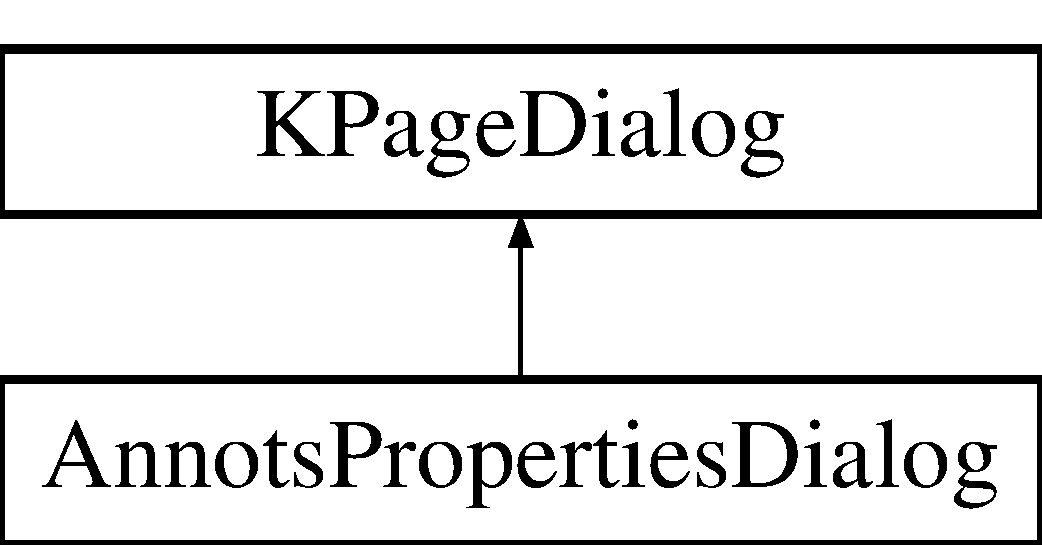
\includegraphics[height=2.000000cm]{classAnnotsPropertiesDialog}
\end{center}
\end{figure}
\subsection*{Public Member Functions}
\begin{DoxyCompactItemize}
\item 
\hyperlink{classAnnotsPropertiesDialog_aad41d7b667dca056fa7a15bd3dc170a4}{Annots\+Properties\+Dialog} (Q\+Widget $\ast$parent, \hyperlink{classOkular_1_1Document}{Okular\+::\+Document} $\ast$document, int docpage, \hyperlink{classOkular_1_1Annotation}{Okular\+::\+Annotation} $\ast$ann)
\item 
\hyperlink{classAnnotsPropertiesDialog_a6e793792141e6b628b224f9c0b70dd09}{$\sim$\+Annots\+Properties\+Dialog} ()
\end{DoxyCompactItemize}


\subsection{Detailed Description}


Definition at line 24 of file annotationpropertiesdialog.\+h.



\subsection{Constructor \& Destructor Documentation}
\hypertarget{classAnnotsPropertiesDialog_aad41d7b667dca056fa7a15bd3dc170a4}{\index{Annots\+Properties\+Dialog@{Annots\+Properties\+Dialog}!Annots\+Properties\+Dialog@{Annots\+Properties\+Dialog}}
\index{Annots\+Properties\+Dialog@{Annots\+Properties\+Dialog}!Annots\+Properties\+Dialog@{Annots\+Properties\+Dialog}}
\subsubsection[{Annots\+Properties\+Dialog}]{\setlength{\rightskip}{0pt plus 5cm}Annots\+Properties\+Dialog\+::\+Annots\+Properties\+Dialog (
\begin{DoxyParamCaption}
\item[{Q\+Widget $\ast$}]{parent, }
\item[{{\bf Okular\+::\+Document} $\ast$}]{document, }
\item[{int}]{docpage, }
\item[{{\bf Okular\+::\+Annotation} $\ast$}]{ann}
\end{DoxyParamCaption}
)}}\label{classAnnotsPropertiesDialog_aad41d7b667dca056fa7a15bd3dc170a4}


Definition at line 30 of file annotationpropertiesdialog.\+cpp.


\begin{DoxyCode}
31     : KPageDialog( parent ), m\_document( document ), m\_page( docpage ), modified( \textcolor{keyword}{false} )
32 \{
33     setFaceType( Tabbed );
34     m\_annot=ann;
35     \textcolor{keyword}{const} \textcolor{keywordtype}{bool} canEditAnnotations = m\_document->\hyperlink{classOkular_1_1Document_acbc3b843b40096c18dbeec805552685a}{canModifyPageAnnotation}( ann );
36     setCaptionTextbyAnnotType();
37     \textcolor{keywordflow}{if} ( canEditAnnotations )
38     \{
39         setButtons( Ok | Apply | Cancel );
40         enableButton( Apply, \textcolor{keyword}{false} );
41         connect( \textcolor{keyword}{this}, SIGNAL(applyClicked()), \textcolor{keyword}{this}, SLOT(slotapply()) );
42         connect( \textcolor{keyword}{this}, SIGNAL(okClicked()), \textcolor{keyword}{this}, SLOT(slotapply()) );
43     \}
44     \textcolor{keywordflow}{else}
45     \{
46         setButtons( Close );
47         setDefaultButton( Close );
48     \}
49 
50     m\_annotWidget = \hyperlink{classAnnotationWidgetFactory_a47ee680b5716e27021cadd0476735e78}{AnnotationWidgetFactory::widgetFor}( ann );
51 
52     QLabel* tmplabel;
53   \textcolor{comment}{//1. Appearance}
54     \textcolor{comment}{//BEGIN tab1}
55     QWidget *appearanceWidget = m\_annotWidget->\hyperlink{classAnnotationWidget_a57411e4d54dde346c8ed57c99da56666}{appearanceWidget}();
56     appearanceWidget->setEnabled( canEditAnnotations );
57     addPage( appearanceWidget, i18n( \textcolor{stringliteral}{"&Appearance"} ) );
58     \textcolor{comment}{//END tab1}
59 
60     \textcolor{comment}{//BEGIN tab 2}
61     QFrame* page = \textcolor{keyword}{new} QFrame( \textcolor{keyword}{this} );
62     addPage( page, i18n( \textcolor{stringliteral}{"&General"} ) );
63 \textcolor{comment}{//    m\_tabitem[1]->setIcon( KIcon( "fonts" ) );}
64     QGridLayout* gridlayout = \textcolor{keyword}{new} QGridLayout( page );
65     tmplabel = \textcolor{keyword}{new} QLabel( i18n( \textcolor{stringliteral}{"&Author:"} ), page );
66     AuthorEdit = \textcolor{keyword}{new} KLineEdit( ann->\hyperlink{classOkular_1_1Annotation_a45682b53c24e4f5d41c547d6e109f6a4}{author}(), page );
67     AuthorEdit->setEnabled( canEditAnnotations );
68     tmplabel->setBuddy( AuthorEdit );
69     gridlayout->addWidget( tmplabel, 0, 0, Qt::AlignRight );
70     gridlayout->addWidget( AuthorEdit, 0, 1 );
71 
72     tmplabel = \textcolor{keyword}{new} QLabel( page );
73     tmplabel->setText( i18n( \textcolor{stringliteral}{"Created: %1"}, KGlobal::locale()->formatDateTime( ann->
      \hyperlink{classOkular_1_1Annotation_ad775b0d2925d50334d46efc1a2689e5b}{creationDate}(), KLocale::LongDate, true ) ) );
74     tmplabel->setTextInteractionFlags( Qt::TextSelectableByMouse );
75     gridlayout->addWidget( tmplabel, 1, 0, 1, 2 );
76 
77     m\_modifyDateLabel = \textcolor{keyword}{new} QLabel( page );
78     m\_modifyDateLabel->setText( i18n( \textcolor{stringliteral}{"Modified: %1"}, KGlobal::locale()->formatDateTime( ann->
      \hyperlink{classOkular_1_1Annotation_a4bee8f09724539e15f435b643049f2c1}{modificationDate}(), KLocale::LongDate, true ) ) );
79     m\_modifyDateLabel->setTextInteractionFlags( Qt::TextSelectableByMouse );
80     gridlayout->addWidget( m\_modifyDateLabel, 2, 0, 1, 2 );
81 
82     gridlayout->addItem( \textcolor{keyword}{new} QSpacerItem( 5, 5, QSizePolicy::Fixed, QSizePolicy::MinimumExpanding ), 3, 0 )
      ;
83     \textcolor{comment}{//END tab 2}
84 
85     QWidget * extraWidget = m\_annotWidget->\hyperlink{classAnnotationWidget_a0d1cb7d9a0f518140abecc82aa1e8449}{extraWidget}();
86     \textcolor{keywordflow}{if} ( extraWidget )
87     \{
88         addPage( extraWidget, extraWidget->windowTitle() );
89     \}
90 
91     \textcolor{comment}{//BEGIN connections}
92     connect( AuthorEdit, SIGNAL(textChanged(QString)), \textcolor{keyword}{this}, SLOT(setModified()) );
93     connect( m\_annotWidget, SIGNAL(dataChanged()), \textcolor{keyword}{this}, SLOT(setModified()) );
94     \textcolor{comment}{//END}
95 
96 \textcolor{preprocessor}{#if 0}
97     kDebug() << \textcolor{stringliteral}{"Annotation details:"};
98     kDebug().nospace() << \textcolor{stringliteral}{" => unique name: '"} << ann->\hyperlink{classOkular_1_1Annotation_a8a86ff8c722014c2296112d0fa703eab}{uniqueName}() << \textcolor{stringliteral}{"'"};
99     kDebug() << \textcolor{stringliteral}{" => flags:"} << QString::number( m\_annot->\hyperlink{classOkular_1_1Annotation_a3d6f7ee5057155b90e76c24768880947}{flags}(), 2 );
100 \textcolor{preprocessor}{#endif}
101 
102     resize( sizeHint() );
103 \}
\end{DoxyCode}
\hypertarget{classAnnotsPropertiesDialog_a6e793792141e6b628b224f9c0b70dd09}{\index{Annots\+Properties\+Dialog@{Annots\+Properties\+Dialog}!````~Annots\+Properties\+Dialog@{$\sim$\+Annots\+Properties\+Dialog}}
\index{````~Annots\+Properties\+Dialog@{$\sim$\+Annots\+Properties\+Dialog}!Annots\+Properties\+Dialog@{Annots\+Properties\+Dialog}}
\subsubsection[{$\sim$\+Annots\+Properties\+Dialog}]{\setlength{\rightskip}{0pt plus 5cm}Annots\+Properties\+Dialog\+::$\sim$\+Annots\+Properties\+Dialog (
\begin{DoxyParamCaption}
{}
\end{DoxyParamCaption}
)}}\label{classAnnotsPropertiesDialog_a6e793792141e6b628b224f9c0b70dd09}


Definition at line 104 of file annotationpropertiesdialog.\+cpp.


\begin{DoxyCode}
105 \{
106     \textcolor{keyword}{delete} m\_annotWidget;
107 \}
\end{DoxyCode}


The documentation for this class was generated from the following files\+:\begin{DoxyCompactItemize}
\item 
ui/\hyperlink{annotationpropertiesdialog_8h}{annotationpropertiesdialog.\+h}\item 
ui/\hyperlink{annotationpropertiesdialog_8cpp}{annotationpropertiesdialog.\+cpp}\end{DoxyCompactItemize}

\hypertarget{classAnnotWindow}{\section{Annot\+Window Class Reference}
\label{classAnnotWindow}\index{Annot\+Window@{Annot\+Window}}
}


{\ttfamily \#include $<$annotwindow.\+h$>$}

Inheritance diagram for Annot\+Window\+:\begin{figure}[H]
\begin{center}
\leavevmode
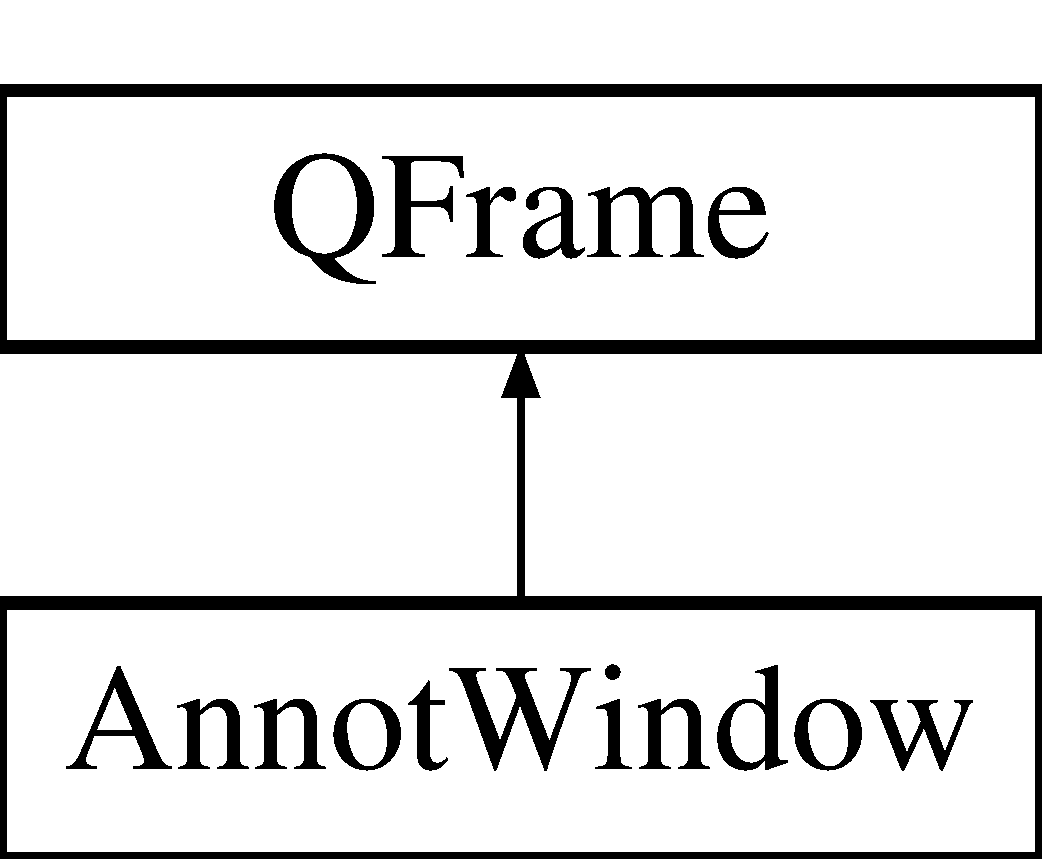
\includegraphics[height=2.000000cm]{classAnnotWindow}
\end{center}
\end{figure}
\subsection*{Signals}
\begin{DoxyCompactItemize}
\item 
void \hyperlink{classAnnotWindow_a920b2483b708366d4f672a8994c6af6c}{contains\+Latex} (bool)
\end{DoxyCompactItemize}
\subsection*{Public Member Functions}
\begin{DoxyCompactItemize}
\item 
\hyperlink{classAnnotWindow_a125253e7bdaba20eeecadbd6cc37c207}{Annot\+Window} (Q\+Widget $\ast$parent, \hyperlink{classOkular_1_1Annotation}{Okular\+::\+Annotation} $\ast$annot, \hyperlink{classOkular_1_1Document}{Okular\+::\+Document} $\ast$document, int page)
\item 
\hyperlink{classAnnotWindow_a344457acef95f42f54e4f97502c4deec}{$\sim$\+Annot\+Window} ()
\item 
void \hyperlink{classAnnotWindow_ae573e563b95f71d5321227c146b91a1e}{reload\+Info} ()
\end{DoxyCompactItemize}
\subsection*{Protected Member Functions}
\begin{DoxyCompactItemize}
\item 
virtual void \hyperlink{classAnnotWindow_a029c591d201eae567dedda50bdffc3fe}{show\+Event} (Q\+Show\+Event $\ast$event)
\item 
virtual bool \hyperlink{classAnnotWindow_aed45dcb7095782f5d5cabacb1a856379}{event\+Filter} (Q\+Object $\ast$obj, Q\+Event $\ast$event)
\end{DoxyCompactItemize}


\subsection{Detailed Description}


Definition at line 30 of file annotwindow.\+h.



\subsection{Constructor \& Destructor Documentation}
\hypertarget{classAnnotWindow_a125253e7bdaba20eeecadbd6cc37c207}{\index{Annot\+Window@{Annot\+Window}!Annot\+Window@{Annot\+Window}}
\index{Annot\+Window@{Annot\+Window}!Annot\+Window@{Annot\+Window}}
\subsubsection[{Annot\+Window}]{\setlength{\rightskip}{0pt plus 5cm}Annot\+Window\+::\+Annot\+Window (
\begin{DoxyParamCaption}
\item[{Q\+Widget $\ast$}]{parent, }
\item[{{\bf Okular\+::\+Annotation} $\ast$}]{annot, }
\item[{{\bf Okular\+::\+Document} $\ast$}]{document, }
\item[{int}]{page}
\end{DoxyParamCaption}
)}}\label{classAnnotWindow_a125253e7bdaba20eeecadbd6cc37c207}


Definition at line 188 of file annotwindow.\+cpp.


\begin{DoxyCode}
189     : QFrame( parent, Qt::SubWindow ), m\_annot( annot ), m\_document( document ), m\_page( page )
190 \{
191     setAutoFillBackground( \textcolor{keyword}{true} );
192     setFrameStyle( Panel | Raised );
193     setAttribute( Qt::WA\_DeleteOnClose );
194 
195     \textcolor{keyword}{const} \textcolor{keywordtype}{bool} canEditAnnotation = m\_document->\hyperlink{classOkular_1_1Document_acbc3b843b40096c18dbeec805552685a}{canModifyPageAnnotation}( annot );
196 
197     textEdit = \textcolor{keyword}{new} KTextEdit( \textcolor{keyword}{this} );
198     textEdit->setAcceptRichText( \textcolor{keyword}{false} );
199     textEdit->setPlainText( m\_annot->\hyperlink{classOkular_1_1Annotation_a3b0c9fcbe9d01e06bfcc7216d0035908}{contents}() );
200     textEdit->installEventFilter( \textcolor{keyword}{this} );
201     textEdit->setUndoRedoEnabled( \textcolor{keyword}{false} );
202 
203     m\_prevCursorPos = textEdit->textCursor().position();
204     m\_prevAnchorPos = textEdit->textCursor().anchor();
205 
206     connect(textEdit, SIGNAL(textChanged()),
207             \textcolor{keyword}{this},SLOT(slotsaveWindowText()));
208     connect(textEdit, SIGNAL(cursorPositionChanged()),
209             \textcolor{keyword}{this},SLOT(slotsaveWindowText()));
210     connect(textEdit, SIGNAL(aboutToShowContextMenu(QMenu*)),
211             \textcolor{keyword}{this},SLOT(slotUpdateUndoAndRedoInContextMenu(QMenu*)));
212     connect(m\_document, SIGNAL(annotationContentsChangedByUndoRedo(
      \hyperlink{classOkular_1_1Annotation}{Okular::Annotation}*,QString,\textcolor{keywordtype}{int},\textcolor{keywordtype}{int})),
213             \textcolor{keyword}{this}, SLOT(slotHandleContentsChangedByUndoRedo(\hyperlink{classOkular_1_1Annotation}{Okular::Annotation}*,QString,\textcolor{keywordtype}{
      int},\textcolor{keywordtype}{int})));
214 
215     \textcolor{keywordflow}{if} (!canEditAnnotation)
216         textEdit->setReadOnly(\textcolor{keyword}{true});
217 
218     QVBoxLayout * mainlay = \textcolor{keyword}{new} QVBoxLayout( \textcolor{keyword}{this} );
219     mainlay->setMargin( 2 );
220     mainlay->setSpacing( 0 );
221     m\_title = \textcolor{keyword}{new} \hyperlink{classMovableTitle}{MovableTitle}( \textcolor{keyword}{this} );
222     mainlay->addWidget( m\_title );
223     mainlay->addWidget( textEdit );
224     QHBoxLayout * lowerlay = \textcolor{keyword}{new} QHBoxLayout();
225     mainlay->addLayout( lowerlay );
226     lowerlay->addItem( \textcolor{keyword}{new} QSpacerItem( 5, 5, QSizePolicy::Expanding, QSizePolicy::Fixed ) );
227     QSizeGrip * sb = \textcolor{keyword}{new} QSizeGrip( \textcolor{keyword}{this} );
228     lowerlay->addWidget( sb );
229 
230     m\_latexRenderer = \textcolor{keyword}{new} \hyperlink{classGuiUtils_1_1LatexRenderer}{GuiUtils::LatexRenderer}();
231     emit \hyperlink{classAnnotWindow_a920b2483b708366d4f672a8994c6af6c}{containsLatex}( \hyperlink{classGuiUtils_1_1LatexRenderer_aa7d63d0c278641e52479f50f8c97c094}{GuiUtils::LatexRenderer::mightContainLatex}
      ( m\_annot->\hyperlink{classOkular_1_1Annotation_a3b0c9fcbe9d01e06bfcc7216d0035908}{contents}() ) );
232 
233     m\_title->\hyperlink{classMovableTitle_aad05a10ec583250589f72edca36395ea}{setTitle}( m\_annot->\hyperlink{classOkular_1_1Annotation_a560281f35ace621f48181a7c7977ca7f}{window}().\hyperlink{classOkular_1_1Annotation_1_1Window_ac73101f261e6b4dba054540267073151}{summary}() );
234     m\_title->\hyperlink{classMovableTitle_a3bc4b1a5774fb18bd0b16260362d1b0d}{connectOptionButton}( \textcolor{keyword}{this}, SLOT(slotOptionBtn()) );
235 
236     setGeometry(10,10,300,300 );
237 
238     \hyperlink{classAnnotWindow_ae573e563b95f71d5321227c146b91a1e}{reloadInfo}();
239 \}
\end{DoxyCode}
\hypertarget{classAnnotWindow_a344457acef95f42f54e4f97502c4deec}{\index{Annot\+Window@{Annot\+Window}!````~Annot\+Window@{$\sim$\+Annot\+Window}}
\index{````~Annot\+Window@{$\sim$\+Annot\+Window}!Annot\+Window@{Annot\+Window}}
\subsubsection[{$\sim$\+Annot\+Window}]{\setlength{\rightskip}{0pt plus 5cm}Annot\+Window\+::$\sim$\+Annot\+Window (
\begin{DoxyParamCaption}
{}
\end{DoxyParamCaption}
)}}\label{classAnnotWindow_a344457acef95f42f54e4f97502c4deec}


Definition at line 241 of file annotwindow.\+cpp.


\begin{DoxyCode}
242 \{
243     \textcolor{keyword}{delete} m\_latexRenderer;
244 \}
\end{DoxyCode}


\subsection{Member Function Documentation}
\hypertarget{classAnnotWindow_a920b2483b708366d4f672a8994c6af6c}{\index{Annot\+Window@{Annot\+Window}!contains\+Latex@{contains\+Latex}}
\index{contains\+Latex@{contains\+Latex}!Annot\+Window@{Annot\+Window}}
\subsubsection[{contains\+Latex}]{\setlength{\rightskip}{0pt plus 5cm}void Annot\+Window\+::contains\+Latex (
\begin{DoxyParamCaption}
\item[{bool}]{}
\end{DoxyParamCaption}
)\hspace{0.3cm}{\ttfamily [signal]}}}\label{classAnnotWindow_a920b2483b708366d4f672a8994c6af6c}
\hypertarget{classAnnotWindow_aed45dcb7095782f5d5cabacb1a856379}{\index{Annot\+Window@{Annot\+Window}!event\+Filter@{event\+Filter}}
\index{event\+Filter@{event\+Filter}!Annot\+Window@{Annot\+Window}}
\subsubsection[{event\+Filter}]{\setlength{\rightskip}{0pt plus 5cm}bool Annot\+Window\+::event\+Filter (
\begin{DoxyParamCaption}
\item[{Q\+Object $\ast$}]{obj, }
\item[{Q\+Event $\ast$}]{event}
\end{DoxyParamCaption}
)\hspace{0.3cm}{\ttfamily [protected]}, {\ttfamily [virtual]}}}\label{classAnnotWindow_aed45dcb7095782f5d5cabacb1a856379}


Definition at line 269 of file annotwindow.\+cpp.


\begin{DoxyCode}
270 \{
271     \textcolor{keywordflow}{if} ( e->type () == QEvent::ShortcutOverride )
272     \{
273         QKeyEvent * keyEvent = \textcolor{keyword}{static\_cast<} QKeyEvent * \textcolor{keyword}{>}( e );
274         \textcolor{keywordflow}{if} ( keyEvent->key() == Qt::Key\_Escape )
275         \{
276             close();
277             \textcolor{keywordflow}{return} \textcolor{keyword}{true};
278         \}
279     \}
280     \textcolor{keywordflow}{else} \textcolor{keywordflow}{if} (e->type() == QEvent::KeyPress)
281     \{
282         QKeyEvent *keyEvent = \textcolor{keyword}{static\_cast<}QKeyEvent*\textcolor{keyword}{>}(e);
283         \textcolor{keywordflow}{if} (keyEvent == QKeySequence::Undo)
284         \{
285             m\_document->\hyperlink{classOkular_1_1Document_a2948b7150ebee16ee611734226c5d247}{undo}();
286             \textcolor{keywordflow}{return} \textcolor{keyword}{true};
287         \}
288         \textcolor{keywordflow}{else} \textcolor{keywordflow}{if} (keyEvent == QKeySequence::Redo)
289         \{
290             m\_document->\hyperlink{classOkular_1_1Document_a55a775164d34b00f74c4242ed952f676}{redo}();
291             \textcolor{keywordflow}{return} \textcolor{keyword}{true};
292         \}
293     \}
294     \textcolor{keywordflow}{return} \textcolor{keyword}{false};
295 \}
\end{DoxyCode}
\hypertarget{classAnnotWindow_ae573e563b95f71d5321227c146b91a1e}{\index{Annot\+Window@{Annot\+Window}!reload\+Info@{reload\+Info}}
\index{reload\+Info@{reload\+Info}!Annot\+Window@{Annot\+Window}}
\subsubsection[{reload\+Info}]{\setlength{\rightskip}{0pt plus 5cm}void Annot\+Window\+::reload\+Info (
\begin{DoxyParamCaption}
{}
\end{DoxyParamCaption}
)}}\label{classAnnotWindow_ae573e563b95f71d5321227c146b91a1e}


Definition at line 246 of file annotwindow.\+cpp.


\begin{DoxyCode}
247 \{
248     \textcolor{keyword}{const} QColor newcolor = m\_annot->\hyperlink{classOkular_1_1Annotation_ae1f845ddbd6d524b2b388c6c9ef26423}{style}().\hyperlink{classOkular_1_1Annotation_1_1Style_a2c32cb2b41ef8732ddcd3d3dffc20b7d}{color}().isValid() ? m\_annot->
      \hyperlink{classOkular_1_1Annotation_ae1f845ddbd6d524b2b388c6c9ef26423}{style}().\hyperlink{classOkular_1_1Annotation_1_1Style_a2c32cb2b41ef8732ddcd3d3dffc20b7d}{color}() : Qt::yellow;
249     \textcolor{keywordflow}{if} ( newcolor != m\_color )
250     \{
251         m\_color = newcolor;
252         setPalette( QPalette( m\_color ) );
253         QPalette pl = textEdit->palette();
254         pl.setColor( QPalette::Base, m\_color );
255         textEdit->setPalette( pl );
256     \}
257     m\_title->\hyperlink{classMovableTitle_aa9325778f8f301d2177c91654fbd3681}{setAuthor}( m\_annot->\hyperlink{classOkular_1_1Annotation_a45682b53c24e4f5d41c547d6e109f6a4}{author}() );
258     m\_title->\hyperlink{classMovableTitle_a9c2ec37093f90e0938fe392d2500d746}{setDate}( m\_annot->\hyperlink{classOkular_1_1Annotation_a4bee8f09724539e15f435b643049f2c1}{modificationDate}() );
259 \}
\end{DoxyCode}
\hypertarget{classAnnotWindow_a029c591d201eae567dedda50bdffc3fe}{\index{Annot\+Window@{Annot\+Window}!show\+Event@{show\+Event}}
\index{show\+Event@{show\+Event}!Annot\+Window@{Annot\+Window}}
\subsubsection[{show\+Event}]{\setlength{\rightskip}{0pt plus 5cm}void Annot\+Window\+::show\+Event (
\begin{DoxyParamCaption}
\item[{Q\+Show\+Event $\ast$}]{event}
\end{DoxyParamCaption}
)\hspace{0.3cm}{\ttfamily [protected]}, {\ttfamily [virtual]}}}\label{classAnnotWindow_a029c591d201eae567dedda50bdffc3fe}


Definition at line 261 of file annotwindow.\+cpp.


\begin{DoxyCode}
262 \{
263     QFrame::showEvent( event );
264 
265     \textcolor{comment}{// focus the content area by default}
266     textEdit->setFocus();
267 \}
\end{DoxyCode}


The documentation for this class was generated from the following files\+:\begin{DoxyCompactItemize}
\item 
ui/\hyperlink{annotwindow_8h}{annotwindow.\+h}\item 
ui/\hyperlink{annotwindow_8cpp}{annotwindow.\+cpp}\end{DoxyCompactItemize}

\hypertarget{structArchiveData}{\section{Archive\+Data Struct Reference}
\label{structArchiveData}\index{Archive\+Data@{Archive\+Data}}
}
\subsection*{Public Member Functions}
\begin{DoxyCompactItemize}
\item 
\hyperlink{structArchiveData_acd2fd01b34bd29bc24e2df6de7acab8b}{Archive\+Data} ()
\end{DoxyCompactItemize}
\subsection*{Public Attributes}
\begin{DoxyCompactItemize}
\item 
K\+Temporary\+File \hyperlink{structArchiveData_aeeeafd3c5edcd003dc379c7aa90c11e2}{document}
\item 
Q\+String \hyperlink{structArchiveData_aed05c74b518d7f05506d14c32cc46846}{metadata\+File\+Name}
\end{DoxyCompactItemize}


\subsection{Detailed Description}


Definition at line 105 of file document.\+cpp.



\subsection{Constructor \& Destructor Documentation}
\hypertarget{structArchiveData_acd2fd01b34bd29bc24e2df6de7acab8b}{\index{Archive\+Data@{Archive\+Data}!Archive\+Data@{Archive\+Data}}
\index{Archive\+Data@{Archive\+Data}!Archive\+Data@{Archive\+Data}}
\subsubsection[{Archive\+Data}]{\setlength{\rightskip}{0pt plus 5cm}Archive\+Data\+::\+Archive\+Data (
\begin{DoxyParamCaption}
{}
\end{DoxyParamCaption}
)\hspace{0.3cm}{\ttfamily [inline]}}}\label{structArchiveData_acd2fd01b34bd29bc24e2df6de7acab8b}


Definition at line 107 of file document.\+cpp.


\begin{DoxyCode}
108     \{
109     \}
\end{DoxyCode}


\subsection{Member Data Documentation}
\hypertarget{structArchiveData_aeeeafd3c5edcd003dc379c7aa90c11e2}{\index{Archive\+Data@{Archive\+Data}!document@{document}}
\index{document@{document}!Archive\+Data@{Archive\+Data}}
\subsubsection[{document}]{\setlength{\rightskip}{0pt plus 5cm}K\+Temporary\+File Archive\+Data\+::document}}\label{structArchiveData_aeeeafd3c5edcd003dc379c7aa90c11e2}


Definition at line 111 of file document.\+cpp.

\hypertarget{structArchiveData_aed05c74b518d7f05506d14c32cc46846}{\index{Archive\+Data@{Archive\+Data}!metadata\+File\+Name@{metadata\+File\+Name}}
\index{metadata\+File\+Name@{metadata\+File\+Name}!Archive\+Data@{Archive\+Data}}
\subsubsection[{metadata\+File\+Name}]{\setlength{\rightskip}{0pt plus 5cm}Q\+String Archive\+Data\+::metadata\+File\+Name}}\label{structArchiveData_aed05c74b518d7f05506d14c32cc46846}


Definition at line 112 of file document.\+cpp.



The documentation for this struct was generated from the following file\+:\begin{DoxyCompactItemize}
\item 
core/\hyperlink{core_2document_8cpp}{document.\+cpp}\end{DoxyCompactItemize}

\hypertarget{classOkular_1_1AudioPlayer}{\section{Okular\+:\+:Audio\+Player Class Reference}
\label{classOkular_1_1AudioPlayer}\index{Okular\+::\+Audio\+Player@{Okular\+::\+Audio\+Player}}
}


An audio player.  




{\ttfamily \#include $<$audioplayer.\+h$>$}

Inheritance diagram for Okular\+:\+:Audio\+Player\+:\begin{figure}[H]
\begin{center}
\leavevmode
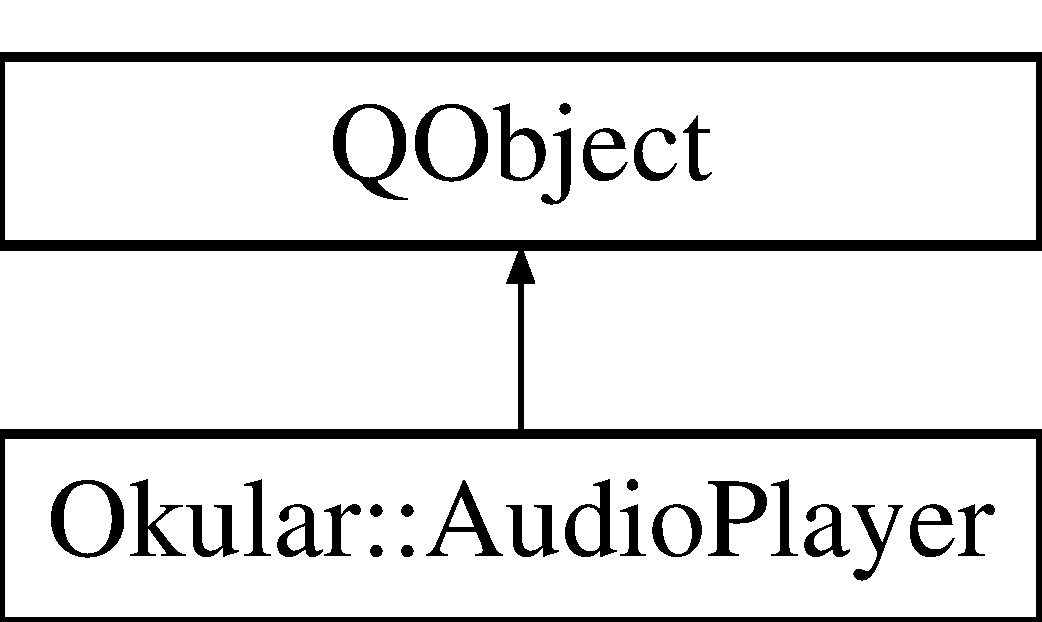
\includegraphics[height=2.000000cm]{classOkular_1_1AudioPlayer}
\end{center}
\end{figure}
\subsection*{Public Types}
\begin{DoxyCompactItemize}
\item 
enum \hyperlink{classOkular_1_1AudioPlayer_ab4aec223fcb227ab5cee9c525f6c5d6e}{State} \{ \hyperlink{classOkular_1_1AudioPlayer_ab4aec223fcb227ab5cee9c525f6c5d6eab5ce6ae3e434b775cda810ad636ff4fc}{Playing\+State}, 
\hyperlink{classOkular_1_1AudioPlayer_ab4aec223fcb227ab5cee9c525f6c5d6ea8aff55f41e3daefa1c9a2268d7df5c3b}{Stopped\+State}
 \}
\end{DoxyCompactItemize}
\subsection*{Public Member Functions}
\begin{DoxyCompactItemize}
\item 
\hyperlink{classOkular_1_1AudioPlayer_a41d5beac7ef47d2d935f17e822cbfd9f}{$\sim$\+Audio\+Player} ()
\item 
void \hyperlink{classOkular_1_1AudioPlayer_aaac62ab7c23b6ff11162c1943cd535a5}{play\+Sound} (const \hyperlink{classOkular_1_1Sound}{Sound} $\ast$sound, const \hyperlink{classOkular_1_1SoundAction}{Sound\+Action} $\ast$linksound=0)
\item 
void \hyperlink{classOkular_1_1AudioPlayer_a48730f5eb7dbc0551679c367e0ba9234}{stop\+Playbacks} ()
\item 
\hyperlink{classOkular_1_1AudioPlayer_ab4aec223fcb227ab5cee9c525f6c5d6e}{State} \hyperlink{classOkular_1_1AudioPlayer_a2bb80dfcea095a598c43e4852b1005ab}{state} () const 
\end{DoxyCompactItemize}
\subsection*{Static Public Member Functions}
\begin{DoxyCompactItemize}
\item 
static \hyperlink{classOkular_1_1AudioPlayer}{Audio\+Player} $\ast$ \hyperlink{classOkular_1_1AudioPlayer_a5bbc067e81b46451098a2a0becf23e67}{instance} ()
\end{DoxyCompactItemize}
\subsection*{Friends}
\begin{DoxyCompactItemize}
\item 
class \hyperlink{classOkular_1_1AudioPlayer_a3d937a13e5828f806b650af2bfcf72b2}{Audio\+Player\+Private}
\item 
class \hyperlink{classOkular_1_1AudioPlayer_a883538034e58fc5c0de7d4e4cab3cef7}{Document}
\end{DoxyCompactItemize}


\subsection{Detailed Description}
An audio player. 

Singleton utility class to play sounds in documents using the K\+D\+E sound system. 

Definition at line 30 of file audioplayer.\+h.



\subsection{Member Enumeration Documentation}
\hypertarget{classOkular_1_1AudioPlayer_ab4aec223fcb227ab5cee9c525f6c5d6e}{\index{Okular\+::\+Audio\+Player@{Okular\+::\+Audio\+Player}!State@{State}}
\index{State@{State}!Okular\+::\+Audio\+Player@{Okular\+::\+Audio\+Player}}
\subsubsection[{State}]{\setlength{\rightskip}{0pt plus 5cm}enum {\bf Okular\+::\+Audio\+Player\+::\+State}}}\label{classOkular_1_1AudioPlayer_ab4aec223fcb227ab5cee9c525f6c5d6e}
The state of \hyperlink{classOkular_1_1AudioPlayer}{Audio\+Player} \begin{DoxySince}{Since}
0.\+19 (K\+D\+E 4.\+13) 
\end{DoxySince}
\begin{Desc}
\item[Enumerator]\par
\begin{description}
\index{Playing\+State@{Playing\+State}!Okular\+::\+Audio\+Player@{Okular\+::\+Audio\+Player}}\index{Okular\+::\+Audio\+Player@{Okular\+::\+Audio\+Player}!Playing\+State@{Playing\+State}}\item[{\em 
\hypertarget{classOkular_1_1AudioPlayer_ab4aec223fcb227ab5cee9c525f6c5d6eab5ce6ae3e434b775cda810ad636ff4fc}{Playing\+State}\label{classOkular_1_1AudioPlayer_ab4aec223fcb227ab5cee9c525f6c5d6eab5ce6ae3e434b775cda810ad636ff4fc}
}]The \hyperlink{classOkular_1_1AudioPlayer}{Audio\+Player} is playing a audio file. \index{Stopped\+State@{Stopped\+State}!Okular\+::\+Audio\+Player@{Okular\+::\+Audio\+Player}}\index{Okular\+::\+Audio\+Player@{Okular\+::\+Audio\+Player}!Stopped\+State@{Stopped\+State}}\item[{\em 
\hypertarget{classOkular_1_1AudioPlayer_ab4aec223fcb227ab5cee9c525f6c5d6ea8aff55f41e3daefa1c9a2268d7df5c3b}{Stopped\+State}\label{classOkular_1_1AudioPlayer_ab4aec223fcb227ab5cee9c525f6c5d6ea8aff55f41e3daefa1c9a2268d7df5c3b}
}]The \hyperlink{classOkular_1_1AudioPlayer}{Audio\+Player} isn't playing a audio file. \end{description}
\end{Desc}


Definition at line 40 of file audioplayer.\+h.


\begin{DoxyCode}
41         \{
45             \hyperlink{classOkular_1_1AudioPlayer_ab4aec223fcb227ab5cee9c525f6c5d6eab5ce6ae3e434b775cda810ad636ff4fc}{PlayingState},
49         \hyperlink{classOkular_1_1AudioPlayer_ab4aec223fcb227ab5cee9c525f6c5d6ea8aff55f41e3daefa1c9a2268d7df5c3b}{StoppedState}
50     \};
\end{DoxyCode}


\subsection{Constructor \& Destructor Documentation}
\hypertarget{classOkular_1_1AudioPlayer_a41d5beac7ef47d2d935f17e822cbfd9f}{\index{Okular\+::\+Audio\+Player@{Okular\+::\+Audio\+Player}!````~Audio\+Player@{$\sim$\+Audio\+Player}}
\index{````~Audio\+Player@{$\sim$\+Audio\+Player}!Okular\+::\+Audio\+Player@{Okular\+::\+Audio\+Player}}
\subsubsection[{$\sim$\+Audio\+Player}]{\setlength{\rightskip}{0pt plus 5cm}Audio\+Player\+::$\sim$\+Audio\+Player (
\begin{DoxyParamCaption}
{}
\end{DoxyParamCaption}
)}}\label{classOkular_1_1AudioPlayer_a41d5beac7ef47d2d935f17e822cbfd9f}


Definition at line 217 of file audioplayer.\+cpp.


\begin{DoxyCode}
218 \{
219     \textcolor{keyword}{delete} d;
220 \}
\end{DoxyCode}


\subsection{Member Function Documentation}
\hypertarget{classOkular_1_1AudioPlayer_a5bbc067e81b46451098a2a0becf23e67}{\index{Okular\+::\+Audio\+Player@{Okular\+::\+Audio\+Player}!instance@{instance}}
\index{instance@{instance}!Okular\+::\+Audio\+Player@{Okular\+::\+Audio\+Player}}
\subsubsection[{instance}]{\setlength{\rightskip}{0pt plus 5cm}{\bf Audio\+Player} $\ast$ Audio\+Player\+::instance (
\begin{DoxyParamCaption}
{}
\end{DoxyParamCaption}
)\hspace{0.3cm}{\ttfamily [static]}}}\label{classOkular_1_1AudioPlayer_a5bbc067e81b46451098a2a0becf23e67}
Gets the instance of the audio player. 

Definition at line 222 of file audioplayer.\+cpp.


\begin{DoxyCode}
223 \{
224     \textcolor{keyword}{static} \hyperlink{classOkular_1_1AudioPlayer}{AudioPlayer} ap;
225     \textcolor{keywordflow}{return} &ap;
226 \}
\end{DoxyCode}
\hypertarget{classOkular_1_1AudioPlayer_aaac62ab7c23b6ff11162c1943cd535a5}{\index{Okular\+::\+Audio\+Player@{Okular\+::\+Audio\+Player}!play\+Sound@{play\+Sound}}
\index{play\+Sound@{play\+Sound}!Okular\+::\+Audio\+Player@{Okular\+::\+Audio\+Player}}
\subsubsection[{play\+Sound}]{\setlength{\rightskip}{0pt plus 5cm}void Audio\+Player\+::play\+Sound (
\begin{DoxyParamCaption}
\item[{const {\bf Sound} $\ast$}]{sound, }
\item[{const {\bf Sound\+Action} $\ast$}]{linksound = {\ttfamily 0}}
\end{DoxyParamCaption}
)}}\label{classOkular_1_1AudioPlayer_aaac62ab7c23b6ff11162c1943cd535a5}
Enqueue the specified {\ttfamily sound} for playing, optionally taking more information about the playing from the {\ttfamily soundlink} . 

Definition at line 228 of file audioplayer.\+cpp.


\begin{DoxyCode}
229 \{
230     \textcolor{comment}{// we can't play null pointers ;)}
231     \textcolor{keywordflow}{if} ( !sound )
232         \textcolor{keywordflow}{return};
233 
234     \textcolor{comment}{// we don't play external sounds for remote documents}
235     \textcolor{keywordflow}{if} ( sound->\hyperlink{classOkular_1_1Sound_a6ad3b22679e6a6db9d69230ce94bf247}{soundType}() == \hyperlink{classOkular_1_1Sound_aed586d1d0455f4309b1309b9954d5c04a6b086485afe0876219888635155ab044}{Sound::External} && !d->
      \hyperlink{classOkular_1_1AudioPlayerPrivate_a086fc9c3cbe263bd8c67a6afa8b7373d}{m\_currentDocument}.isLocalFile() )
236         \textcolor{keywordflow}{return};
237 
238     kDebug() ;
239     \hyperlink{classSoundInfo}{SoundInfo} si( sound, linksound );
240 
241     \textcolor{comment}{// if the mix flag of the new sound is false, then the currently playing}
242     \textcolor{comment}{// sounds must be stopped.}
243     \textcolor{keywordflow}{if} ( !si.mix )
244         d->\hyperlink{classOkular_1_1AudioPlayerPrivate_a85e116f34091a22e04aa60dce6227f23}{stopPlayings}();
245 
246     d->\hyperlink{classOkular_1_1AudioPlayerPrivate_a5c0390dceece22f9cbae179df76909ee}{play}( si );
247 \}
\end{DoxyCode}
\hypertarget{classOkular_1_1AudioPlayer_a2bb80dfcea095a598c43e4852b1005ab}{\index{Okular\+::\+Audio\+Player@{Okular\+::\+Audio\+Player}!state@{state}}
\index{state@{state}!Okular\+::\+Audio\+Player@{Okular\+::\+Audio\+Player}}
\subsubsection[{state}]{\setlength{\rightskip}{0pt plus 5cm}{\bf Audio\+Player\+::\+State} Audio\+Player\+::state (
\begin{DoxyParamCaption}
{}
\end{DoxyParamCaption}
) const}}\label{classOkular_1_1AudioPlayer_a2bb80dfcea095a598c43e4852b1005ab}
Return state of sound (playing/stopped) \begin{DoxySince}{Since}
0.\+19 (K\+D\+E 4.\+13) 
\end{DoxySince}


Definition at line 254 of file audioplayer.\+cpp.


\begin{DoxyCode}
255 \{
256     \textcolor{keywordflow}{return} d->\hyperlink{classOkular_1_1AudioPlayerPrivate_a3efa5829a954428660181e223342a12c}{m\_state};
257 \}
\end{DoxyCode}
\hypertarget{classOkular_1_1AudioPlayer_a48730f5eb7dbc0551679c367e0ba9234}{\index{Okular\+::\+Audio\+Player@{Okular\+::\+Audio\+Player}!stop\+Playbacks@{stop\+Playbacks}}
\index{stop\+Playbacks@{stop\+Playbacks}!Okular\+::\+Audio\+Player@{Okular\+::\+Audio\+Player}}
\subsubsection[{stop\+Playbacks}]{\setlength{\rightskip}{0pt plus 5cm}void Audio\+Player\+::stop\+Playbacks (
\begin{DoxyParamCaption}
{}
\end{DoxyParamCaption}
)}}\label{classOkular_1_1AudioPlayer_a48730f5eb7dbc0551679c367e0ba9234}
Tell the \hyperlink{classOkular_1_1AudioPlayer}{Audio\+Player} to stop all the playbacks. 

Definition at line 249 of file audioplayer.\+cpp.


\begin{DoxyCode}
250 \{
251     d->\hyperlink{classOkular_1_1AudioPlayerPrivate_a85e116f34091a22e04aa60dce6227f23}{stopPlayings}();
252 \}
\end{DoxyCode}


\subsection{Friends And Related Function Documentation}
\hypertarget{classOkular_1_1AudioPlayer_a3d937a13e5828f806b650af2bfcf72b2}{\index{Okular\+::\+Audio\+Player@{Okular\+::\+Audio\+Player}!Audio\+Player\+Private@{Audio\+Player\+Private}}
\index{Audio\+Player\+Private@{Audio\+Player\+Private}!Okular\+::\+Audio\+Player@{Okular\+::\+Audio\+Player}}
\subsubsection[{Audio\+Player\+Private}]{\setlength{\rightskip}{0pt plus 5cm}friend class {\bf Audio\+Player\+Private}\hspace{0.3cm}{\ttfamily [friend]}}}\label{classOkular_1_1AudioPlayer_a3d937a13e5828f806b650af2bfcf72b2}


Definition at line 79 of file audioplayer.\+h.

\hypertarget{classOkular_1_1AudioPlayer_a883538034e58fc5c0de7d4e4cab3cef7}{\index{Okular\+::\+Audio\+Player@{Okular\+::\+Audio\+Player}!Document@{Document}}
\index{Document@{Document}!Okular\+::\+Audio\+Player@{Okular\+::\+Audio\+Player}}
\subsubsection[{Document}]{\setlength{\rightskip}{0pt plus 5cm}friend class {\bf Document}\hspace{0.3cm}{\ttfamily [friend]}}}\label{classOkular_1_1AudioPlayer_a883538034e58fc5c0de7d4e4cab3cef7}


Definition at line 81 of file audioplayer.\+h.



The documentation for this class was generated from the following files\+:\begin{DoxyCompactItemize}
\item 
core/\hyperlink{audioplayer_8h}{audioplayer.\+h}\item 
core/\hyperlink{audioplayer_8cpp}{audioplayer.\+cpp}\end{DoxyCompactItemize}

\hypertarget{classOkular_1_1AudioPlayerPrivate}{\section{Okular\+:\+:Audio\+Player\+Private Class Reference}
\label{classOkular_1_1AudioPlayerPrivate}\index{Okular\+::\+Audio\+Player\+Private@{Okular\+::\+Audio\+Player\+Private}}
}


{\ttfamily \#include $<$audioplayer\+\_\+p.\+h$>$}

\subsection*{Public Member Functions}
\begin{DoxyCompactItemize}
\item 
\hyperlink{classOkular_1_1AudioPlayerPrivate_a3e0f7f2671d482e8a1a7b6bf8249f4ae}{Audio\+Player\+Private} (\hyperlink{classOkular_1_1AudioPlayer}{Audio\+Player} $\ast$qq)
\item 
\hyperlink{classOkular_1_1AudioPlayerPrivate_a2e17697e3cf8c16ac3df09d8c16ea98f}{$\sim$\+Audio\+Player\+Private} ()
\item 
int \hyperlink{classOkular_1_1AudioPlayerPrivate_a4380d8616ff06dfe750f7828940ccdcc}{new\+Id} () const 
\item 
bool \hyperlink{classOkular_1_1AudioPlayerPrivate_a5c0390dceece22f9cbae179df76909ee}{play} (const \hyperlink{classSoundInfo}{Sound\+Info} \&si)
\item 
void \hyperlink{classOkular_1_1AudioPlayerPrivate_a85e116f34091a22e04aa60dce6227f23}{stop\+Playings} ()
\item 
void \hyperlink{classOkular_1_1AudioPlayerPrivate_a440e5297367c1ffa7f548263a32a700a}{finished} (int)
\end{DoxyCompactItemize}
\subsection*{Public Attributes}
\begin{DoxyCompactItemize}
\item 
\hyperlink{classOkular_1_1AudioPlayer}{Audio\+Player} $\ast$ \hyperlink{classOkular_1_1AudioPlayerPrivate_a6f941dd114ab7795d75c5e9a9c49e480}{q}
\item 
Q\+Hash$<$ int, \hyperlink{classPlayData}{Play\+Data} $\ast$ $>$ \hyperlink{classOkular_1_1AudioPlayerPrivate_adbc0d0a9187f39a4be0d8b0e3d96ce68}{m\+\_\+playing}
\item 
Q\+Signal\+Mapper \hyperlink{classOkular_1_1AudioPlayerPrivate_ad5a18424521deef41a95b0781d157821}{m\+\_\+mapper}
\item 
K\+Url \hyperlink{classOkular_1_1AudioPlayerPrivate_a086fc9c3cbe263bd8c67a6afa8b7373d}{m\+\_\+current\+Document}
\item 
\hyperlink{classOkular_1_1AudioPlayer_ab4aec223fcb227ab5cee9c525f6c5d6e}{Audio\+Player\+::\+State} \hyperlink{classOkular_1_1AudioPlayerPrivate_a3efa5829a954428660181e223342a12c}{m\+\_\+state}
\end{DoxyCompactItemize}


\subsection{Detailed Description}


Definition at line 26 of file audioplayer\+\_\+p.\+h.



\subsection{Constructor \& Destructor Documentation}
\hypertarget{classOkular_1_1AudioPlayerPrivate_a3e0f7f2671d482e8a1a7b6bf8249f4ae}{\index{Okular\+::\+Audio\+Player\+Private@{Okular\+::\+Audio\+Player\+Private}!Audio\+Player\+Private@{Audio\+Player\+Private}}
\index{Audio\+Player\+Private@{Audio\+Player\+Private}!Okular\+::\+Audio\+Player\+Private@{Okular\+::\+Audio\+Player\+Private}}
\subsubsection[{Audio\+Player\+Private}]{\setlength{\rightskip}{0pt plus 5cm}Audio\+Player\+Private\+::\+Audio\+Player\+Private (
\begin{DoxyParamCaption}
\item[{{\bf Audio\+Player} $\ast$}]{qq}
\end{DoxyParamCaption}
)}}\label{classOkular_1_1AudioPlayerPrivate_a3e0f7f2671d482e8a1a7b6bf8249f4ae}


Definition at line 87 of file audioplayer.\+cpp.


\begin{DoxyCode}
88     : \hyperlink{classOkular_1_1AudioPlayerPrivate_a6f941dd114ab7795d75c5e9a9c49e480}{q}( qq ), \hyperlink{classOkular_1_1AudioPlayerPrivate_a3efa5829a954428660181e223342a12c}{m\_state}( \hyperlink{classOkular_1_1AudioPlayer_ab4aec223fcb227ab5cee9c525f6c5d6ea8aff55f41e3daefa1c9a2268d7df5c3b}{AudioPlayer::StoppedState} )
89 \{
90     QObject::connect( &\hyperlink{classOkular_1_1AudioPlayerPrivate_ad5a18424521deef41a95b0781d157821}{m\_mapper}, SIGNAL(mapped(\textcolor{keywordtype}{int})), \hyperlink{classOkular_1_1AudioPlayerPrivate_a6f941dd114ab7795d75c5e9a9c49e480}{q}, SLOT(\hyperlink{classOkular_1_1AudioPlayerPrivate_a440e5297367c1ffa7f548263a32a700a}{finished}(\textcolor{keywordtype}{int})) );
91 \}
\end{DoxyCode}
\hypertarget{classOkular_1_1AudioPlayerPrivate_a2e17697e3cf8c16ac3df09d8c16ea98f}{\index{Okular\+::\+Audio\+Player\+Private@{Okular\+::\+Audio\+Player\+Private}!````~Audio\+Player\+Private@{$\sim$\+Audio\+Player\+Private}}
\index{````~Audio\+Player\+Private@{$\sim$\+Audio\+Player\+Private}!Okular\+::\+Audio\+Player\+Private@{Okular\+::\+Audio\+Player\+Private}}
\subsubsection[{$\sim$\+Audio\+Player\+Private}]{\setlength{\rightskip}{0pt plus 5cm}Audio\+Player\+Private\+::$\sim$\+Audio\+Player\+Private (
\begin{DoxyParamCaption}
{}
\end{DoxyParamCaption}
)}}\label{classOkular_1_1AudioPlayerPrivate_a2e17697e3cf8c16ac3df09d8c16ea98f}


Definition at line 93 of file audioplayer.\+cpp.


\begin{DoxyCode}
94 \{
95     \hyperlink{classOkular_1_1AudioPlayerPrivate_a85e116f34091a22e04aa60dce6227f23}{stopPlayings}();
96 \}
\end{DoxyCode}


\subsection{Member Function Documentation}
\hypertarget{classOkular_1_1AudioPlayerPrivate_a440e5297367c1ffa7f548263a32a700a}{\index{Okular\+::\+Audio\+Player\+Private@{Okular\+::\+Audio\+Player\+Private}!finished@{finished}}
\index{finished@{finished}!Okular\+::\+Audio\+Player\+Private@{Okular\+::\+Audio\+Player\+Private}}
\subsubsection[{finished}]{\setlength{\rightskip}{0pt plus 5cm}void Audio\+Player\+Private\+::finished (
\begin{DoxyParamCaption}
\item[{int}]{id}
\end{DoxyParamCaption}
)}}\label{classOkular_1_1AudioPlayerPrivate_a440e5297367c1ffa7f548263a32a700a}


Definition at line 188 of file audioplayer.\+cpp.


\begin{DoxyCode}
189 \{
190     QHash< int, PlayData * >::iterator it = \hyperlink{classOkular_1_1AudioPlayerPrivate_adbc0d0a9187f39a4be0d8b0e3d96ce68}{m\_playing}.find( \textcolor{keywordtype}{id} );
191     \textcolor{keywordflow}{if} ( it == \hyperlink{classOkular_1_1AudioPlayerPrivate_adbc0d0a9187f39a4be0d8b0e3d96ce68}{m\_playing}.end() )
192         \textcolor{keywordflow}{return};
193 
194     \hyperlink{classSoundInfo}{SoundInfo} si = it.value()->m\_info;
195     \textcolor{comment}{// if the sound must be repeated indefinitely, then start the playback}
196     \textcolor{comment}{// again, otherwise destroy the PlayData as it's no more useful}
197     \textcolor{keywordflow}{if} ( si.\hyperlink{classSoundInfo_a659c959da1310b4cfb1705b11b62a15f}{repeat} )
198     \{
199         it.value()->play();
200     \}
201     \textcolor{keywordflow}{else}
202     \{
203         \hyperlink{classOkular_1_1AudioPlayerPrivate_ad5a18424521deef41a95b0781d157821}{m\_mapper}.removeMappings( it.value()->m\_mediaobject );
204         \textcolor{keyword}{delete} it.value();
205         \hyperlink{classOkular_1_1AudioPlayerPrivate_adbc0d0a9187f39a4be0d8b0e3d96ce68}{m\_playing}.erase( it );
206         \hyperlink{classOkular_1_1AudioPlayerPrivate_a3efa5829a954428660181e223342a12c}{m\_state} = \hyperlink{classOkular_1_1AudioPlayer_ab4aec223fcb227ab5cee9c525f6c5d6ea8aff55f41e3daefa1c9a2268d7df5c3b}{AudioPlayer::StoppedState};
207     \}
208     kDebug(\hyperlink{debug__p_8h_af16c6e32a95969dd0605d792ec9807c7}{OkularDebug}) << \textcolor{stringliteral}{"finished,"} << \hyperlink{classOkular_1_1AudioPlayerPrivate_adbc0d0a9187f39a4be0d8b0e3d96ce68}{m\_playing}.count();
209 \}
\end{DoxyCode}
\hypertarget{classOkular_1_1AudioPlayerPrivate_a4380d8616ff06dfe750f7828940ccdcc}{\index{Okular\+::\+Audio\+Player\+Private@{Okular\+::\+Audio\+Player\+Private}!new\+Id@{new\+Id}}
\index{new\+Id@{new\+Id}!Okular\+::\+Audio\+Player\+Private@{Okular\+::\+Audio\+Player\+Private}}
\subsubsection[{new\+Id}]{\setlength{\rightskip}{0pt plus 5cm}int Audio\+Player\+Private\+::new\+Id (
\begin{DoxyParamCaption}
{}
\end{DoxyParamCaption}
) const}}\label{classOkular_1_1AudioPlayerPrivate_a4380d8616ff06dfe750f7828940ccdcc}


Definition at line 98 of file audioplayer.\+cpp.


\begin{DoxyCode}
99 \{
100     \textcolor{keywordtype}{int} newid = 0;
101     QHash< int, PlayData * >::const\_iterator it;
102     QHash< int, PlayData * >::const\_iterator itEnd = \hyperlink{classOkular_1_1AudioPlayerPrivate_adbc0d0a9187f39a4be0d8b0e3d96ce68}{m\_playing}.constEnd();
103     \textcolor{keywordflow}{do}
104     \{
105         newid = KRandom::random();
106         it = \hyperlink{classOkular_1_1AudioPlayerPrivate_adbc0d0a9187f39a4be0d8b0e3d96ce68}{m\_playing}.constFind( newid );
107     \} \textcolor{keywordflow}{while} ( it != itEnd );
108     \textcolor{keywordflow}{return} newid;
109 \}
\end{DoxyCode}
\hypertarget{classOkular_1_1AudioPlayerPrivate_a5c0390dceece22f9cbae179df76909ee}{\index{Okular\+::\+Audio\+Player\+Private@{Okular\+::\+Audio\+Player\+Private}!play@{play}}
\index{play@{play}!Okular\+::\+Audio\+Player\+Private@{Okular\+::\+Audio\+Player\+Private}}
\subsubsection[{play}]{\setlength{\rightskip}{0pt plus 5cm}bool Audio\+Player\+Private\+::play (
\begin{DoxyParamCaption}
\item[{const {\bf Sound\+Info} \&}]{si}
\end{DoxyParamCaption}
)}}\label{classOkular_1_1AudioPlayerPrivate_a5c0390dceece22f9cbae179df76909ee}


Definition at line 111 of file audioplayer.\+cpp.


\begin{DoxyCode}
112 \{
113     kDebug() ;
114     \hyperlink{classPlayData}{PlayData} * data = \textcolor{keyword}{new} \hyperlink{classPlayData}{PlayData}();
115     data->\hyperlink{classPlayData_a4184644cad89295edf1ec12a86f4d571}{m\_output} = \textcolor{keyword}{new} Phonon::AudioOutput( Phonon::NotificationCategory );
116     data->\hyperlink{classPlayData_a4184644cad89295edf1ec12a86f4d571}{m\_output}->setVolume( si.\hyperlink{classSoundInfo_aa65ec68c376b1377fab3113460305162}{volume} );
117     data->\hyperlink{classPlayData_a1ba72cd22230406764d16de62c5b32a6}{m\_mediaobject} = \textcolor{keyword}{new} Phonon::MediaObject();
118     Phonon::createPath(data->\hyperlink{classPlayData_a1ba72cd22230406764d16de62c5b32a6}{m\_mediaobject}, data->\hyperlink{classPlayData_a4184644cad89295edf1ec12a86f4d571}{m\_output});
119     data->\hyperlink{classPlayData_a60f9f37739df694ec4c185ec0c7d4666}{m\_info} = si;
120     \textcolor{keywordtype}{bool} valid = \textcolor{keyword}{false};
121 
122     \textcolor{keywordflow}{switch} ( si.\hyperlink{classSoundInfo_a2cacccbf3b0833dcef00458a098dfcc8}{sound}->\hyperlink{classOkular_1_1Sound_a6ad3b22679e6a6db9d69230ce94bf247}{soundType}() )
123     \{
124         \textcolor{keywordflow}{case} \hyperlink{classOkular_1_1Sound_aed586d1d0455f4309b1309b9954d5c04a6b086485afe0876219888635155ab044}{Sound::External}:
125         \{
126             QString url = si.\hyperlink{classSoundInfo_a2cacccbf3b0833dcef00458a098dfcc8}{sound}->\hyperlink{classOkular_1_1Sound_a43f2240722f01fae2d962d5f186f0015}{url}();
127             kDebug(\hyperlink{debug__p_8h_af16c6e32a95969dd0605d792ec9807c7}{OkularDebug}) << \textcolor{stringliteral}{"External,"} << url;
128             \textcolor{keywordflow}{if} ( !url.isEmpty() )
129             \{
130                 \textcolor{keywordtype}{int} newid = \hyperlink{classOkular_1_1AudioPlayerPrivate_a4380d8616ff06dfe750f7828940ccdcc}{newId}();
131                 \hyperlink{classOkular_1_1AudioPlayerPrivate_ad5a18424521deef41a95b0781d157821}{m\_mapper}.setMapping( data->\hyperlink{classPlayData_a1ba72cd22230406764d16de62c5b32a6}{m\_mediaobject}, newid );
132                 KUrl newurl;
133                 \textcolor{keywordflow}{if} ( KUrl::isRelativeUrl( url ) )
134                 \{
135                     newurl = \hyperlink{classOkular_1_1AudioPlayerPrivate_a086fc9c3cbe263bd8c67a6afa8b7373d}{m\_currentDocument};
136                     newurl.setFileName( url );
137                 \}
138                 \textcolor{keywordflow}{else}
139                 \{
140                     newurl = url;
141                 \}
142                 data->\hyperlink{classPlayData_a1ba72cd22230406764d16de62c5b32a6}{m\_mediaobject}->setCurrentSource( newurl );
143                 \hyperlink{classOkular_1_1AudioPlayerPrivate_adbc0d0a9187f39a4be0d8b0e3d96ce68}{m\_playing}.insert( newid, data );
144                 valid = \textcolor{keyword}{true};
145             \}
146             \textcolor{keywordflow}{break};
147         \}
148         \textcolor{keywordflow}{case} \hyperlink{classOkular_1_1Sound_aed586d1d0455f4309b1309b9954d5c04a60ea85a24b9ea3862fd7a17b3b74952b}{Sound::Embedded}:
149         \{
150             QByteArray filedata = si.\hyperlink{classSoundInfo_a2cacccbf3b0833dcef00458a098dfcc8}{sound}->\hyperlink{classOkular_1_1Sound_ae06d3ef59d5d89556e0c43a4f9a1d3e9}{data}();
151             kDebug(\hyperlink{debug__p_8h_af16c6e32a95969dd0605d792ec9807c7}{OkularDebug}) << \textcolor{stringliteral}{"Embedded,"} << filedata.length();
152             \textcolor{keywordflow}{if} ( !filedata.isEmpty() )
153             \{
154                 kDebug(\hyperlink{debug__p_8h_af16c6e32a95969dd0605d792ec9807c7}{OkularDebug}) << \textcolor{stringliteral}{"Mediaobject:"} << data->
      \hyperlink{classPlayData_a1ba72cd22230406764d16de62c5b32a6}{m\_mediaobject};
155                 \textcolor{keywordtype}{int} newid = \hyperlink{classOkular_1_1AudioPlayerPrivate_a4380d8616ff06dfe750f7828940ccdcc}{newId}();
156                 \hyperlink{classOkular_1_1AudioPlayerPrivate_ad5a18424521deef41a95b0781d157821}{m\_mapper}.setMapping( data->\hyperlink{classPlayData_a1ba72cd22230406764d16de62c5b32a6}{m\_mediaobject}, newid );
157                 data->\hyperlink{classPlayData_ab98af8c9abd9cd1a3b11cfa6d969284a}{m\_buffer} = \textcolor{keyword}{new} QBuffer();
158                 data->\hyperlink{classPlayData_ab98af8c9abd9cd1a3b11cfa6d969284a}{m\_buffer}->setData( filedata );
159                 data->\hyperlink{classPlayData_a1ba72cd22230406764d16de62c5b32a6}{m\_mediaobject}->setCurrentSource( Phonon::MediaSource( data->
      \hyperlink{classPlayData_ab98af8c9abd9cd1a3b11cfa6d969284a}{m\_buffer} ) );
160                 \hyperlink{classOkular_1_1AudioPlayerPrivate_adbc0d0a9187f39a4be0d8b0e3d96ce68}{m\_playing}.insert( newid, data );
161                 valid = \textcolor{keyword}{true};
162             \}
163             \textcolor{keywordflow}{break};
164         \}
165     \}
166     \textcolor{keywordflow}{if} ( !valid )
167     \{
168         \textcolor{keyword}{delete} data;
169         data = 0;
170     \}
171     \textcolor{keywordflow}{if} ( data )
172     \{
173         QObject::connect( data->\hyperlink{classPlayData_a1ba72cd22230406764d16de62c5b32a6}{m\_mediaobject}, SIGNAL(\hyperlink{classOkular_1_1AudioPlayerPrivate_a440e5297367c1ffa7f548263a32a700a}{finished}()), &
      \hyperlink{classOkular_1_1AudioPlayerPrivate_ad5a18424521deef41a95b0781d157821}{m\_mapper}, SLOT(map()) );
174         kDebug(\hyperlink{debug__p_8h_af16c6e32a95969dd0605d792ec9807c7}{OkularDebug}) << \textcolor{stringliteral}{"PLAY"};
175         data->\hyperlink{classPlayData_afa3a824e496869e93a7935e8ea9bcf29}{play}();
176         \hyperlink{classOkular_1_1AudioPlayerPrivate_a3efa5829a954428660181e223342a12c}{m\_state} = \hyperlink{classOkular_1_1AudioPlayer_ab4aec223fcb227ab5cee9c525f6c5d6eab5ce6ae3e434b775cda810ad636ff4fc}{AudioPlayer::PlayingState};
177     \}
178     \textcolor{keywordflow}{return} valid;
179 \}
\end{DoxyCode}
\hypertarget{classOkular_1_1AudioPlayerPrivate_a85e116f34091a22e04aa60dce6227f23}{\index{Okular\+::\+Audio\+Player\+Private@{Okular\+::\+Audio\+Player\+Private}!stop\+Playings@{stop\+Playings}}
\index{stop\+Playings@{stop\+Playings}!Okular\+::\+Audio\+Player\+Private@{Okular\+::\+Audio\+Player\+Private}}
\subsubsection[{stop\+Playings}]{\setlength{\rightskip}{0pt plus 5cm}void Audio\+Player\+Private\+::stop\+Playings (
\begin{DoxyParamCaption}
{}
\end{DoxyParamCaption}
)}}\label{classOkular_1_1AudioPlayerPrivate_a85e116f34091a22e04aa60dce6227f23}


Definition at line 181 of file audioplayer.\+cpp.


\begin{DoxyCode}
182 \{
183     qDeleteAll( \hyperlink{classOkular_1_1AudioPlayerPrivate_adbc0d0a9187f39a4be0d8b0e3d96ce68}{m\_playing} );
184     \hyperlink{classOkular_1_1AudioPlayerPrivate_adbc0d0a9187f39a4be0d8b0e3d96ce68}{m\_playing}.clear();
185     \hyperlink{classOkular_1_1AudioPlayerPrivate_a3efa5829a954428660181e223342a12c}{m\_state} = \hyperlink{classOkular_1_1AudioPlayer_ab4aec223fcb227ab5cee9c525f6c5d6ea8aff55f41e3daefa1c9a2268d7df5c3b}{AudioPlayer::StoppedState};
186 \}
\end{DoxyCode}


\subsection{Member Data Documentation}
\hypertarget{classOkular_1_1AudioPlayerPrivate_a086fc9c3cbe263bd8c67a6afa8b7373d}{\index{Okular\+::\+Audio\+Player\+Private@{Okular\+::\+Audio\+Player\+Private}!m\+\_\+current\+Document@{m\+\_\+current\+Document}}
\index{m\+\_\+current\+Document@{m\+\_\+current\+Document}!Okular\+::\+Audio\+Player\+Private@{Okular\+::\+Audio\+Player\+Private}}
\subsubsection[{m\+\_\+current\+Document}]{\setlength{\rightskip}{0pt plus 5cm}K\+Url Okular\+::\+Audio\+Player\+Private\+::m\+\_\+current\+Document}}\label{classOkular_1_1AudioPlayerPrivate_a086fc9c3cbe263bd8c67a6afa8b7373d}


Definition at line 44 of file audioplayer\+\_\+p.\+h.

\hypertarget{classOkular_1_1AudioPlayerPrivate_ad5a18424521deef41a95b0781d157821}{\index{Okular\+::\+Audio\+Player\+Private@{Okular\+::\+Audio\+Player\+Private}!m\+\_\+mapper@{m\+\_\+mapper}}
\index{m\+\_\+mapper@{m\+\_\+mapper}!Okular\+::\+Audio\+Player\+Private@{Okular\+::\+Audio\+Player\+Private}}
\subsubsection[{m\+\_\+mapper}]{\setlength{\rightskip}{0pt plus 5cm}Q\+Signal\+Mapper Okular\+::\+Audio\+Player\+Private\+::m\+\_\+mapper}}\label{classOkular_1_1AudioPlayerPrivate_ad5a18424521deef41a95b0781d157821}


Definition at line 43 of file audioplayer\+\_\+p.\+h.

\hypertarget{classOkular_1_1AudioPlayerPrivate_adbc0d0a9187f39a4be0d8b0e3d96ce68}{\index{Okular\+::\+Audio\+Player\+Private@{Okular\+::\+Audio\+Player\+Private}!m\+\_\+playing@{m\+\_\+playing}}
\index{m\+\_\+playing@{m\+\_\+playing}!Okular\+::\+Audio\+Player\+Private@{Okular\+::\+Audio\+Player\+Private}}
\subsubsection[{m\+\_\+playing}]{\setlength{\rightskip}{0pt plus 5cm}Q\+Hash$<$ int, {\bf Play\+Data} $\ast$ $>$ Okular\+::\+Audio\+Player\+Private\+::m\+\_\+playing}}\label{classOkular_1_1AudioPlayerPrivate_adbc0d0a9187f39a4be0d8b0e3d96ce68}


Definition at line 42 of file audioplayer\+\_\+p.\+h.

\hypertarget{classOkular_1_1AudioPlayerPrivate_a3efa5829a954428660181e223342a12c}{\index{Okular\+::\+Audio\+Player\+Private@{Okular\+::\+Audio\+Player\+Private}!m\+\_\+state@{m\+\_\+state}}
\index{m\+\_\+state@{m\+\_\+state}!Okular\+::\+Audio\+Player\+Private@{Okular\+::\+Audio\+Player\+Private}}
\subsubsection[{m\+\_\+state}]{\setlength{\rightskip}{0pt plus 5cm}{\bf Audio\+Player\+::\+State} Okular\+::\+Audio\+Player\+Private\+::m\+\_\+state}}\label{classOkular_1_1AudioPlayerPrivate_a3efa5829a954428660181e223342a12c}


Definition at line 45 of file audioplayer\+\_\+p.\+h.

\hypertarget{classOkular_1_1AudioPlayerPrivate_a6f941dd114ab7795d75c5e9a9c49e480}{\index{Okular\+::\+Audio\+Player\+Private@{Okular\+::\+Audio\+Player\+Private}!q@{q}}
\index{q@{q}!Okular\+::\+Audio\+Player\+Private@{Okular\+::\+Audio\+Player\+Private}}
\subsubsection[{q}]{\setlength{\rightskip}{0pt plus 5cm}{\bf Audio\+Player}$\ast$ Okular\+::\+Audio\+Player\+Private\+::q}}\label{classOkular_1_1AudioPlayerPrivate_a6f941dd114ab7795d75c5e9a9c49e480}


Definition at line 40 of file audioplayer\+\_\+p.\+h.



The documentation for this class was generated from the following files\+:\begin{DoxyCompactItemize}
\item 
core/\hyperlink{audioplayer__p_8h}{audioplayer\+\_\+p.\+h}\item 
core/\hyperlink{audioplayer_8cpp}{audioplayer.\+cpp}\end{DoxyCompactItemize}

\hypertarget{classAuthorGroupItem}{\section{Author\+Group\+Item Class Reference}
\label{classAuthorGroupItem}\index{Author\+Group\+Item@{Author\+Group\+Item}}
}
\subsection*{Public Types}
\begin{DoxyCompactItemize}
\item 
enum \hyperlink{classAuthorGroupItem_a81146eef0470ace44a96271cdc1172d5}{Type} \{ \hyperlink{classAuthorGroupItem_a81146eef0470ace44a96271cdc1172d5ad8f8f4cff087cf79bc755aa05f6d4a4c}{Page}, 
\hyperlink{classAuthorGroupItem_a81146eef0470ace44a96271cdc1172d5ab42e2768537a393def6f11fed872efce}{Author}, 
\hyperlink{classAuthorGroupItem_a81146eef0470ace44a96271cdc1172d5a8e28191a7ca3a690f52f0c6bee8062f6}{Annotation}
 \}
\end{DoxyCompactItemize}
\subsection*{Public Member Functions}
\begin{DoxyCompactItemize}
\item 
\hyperlink{classAuthorGroupItem_a7afc0fe975bde20274445cfe408adc64}{Author\+Group\+Item} (\hyperlink{classAuthorGroupItem}{Author\+Group\+Item} $\ast$\hyperlink{classAuthorGroupItem_a611ca0b8336c7a947380903fbdee71c6}{parent}, \hyperlink{classAuthorGroupItem_a81146eef0470ace44a96271cdc1172d5}{Type} \hyperlink{classAuthorGroupItem_a216b9845b38d50a5be8bb317bff914ad}{type}=\hyperlink{classAuthorGroupItem_a81146eef0470ace44a96271cdc1172d5ad8f8f4cff087cf79bc755aa05f6d4a4c}{Page}, const Q\+Model\+Index \&\hyperlink{classAuthorGroupItem_a65486be87b916d5901a0c45c667aa043}{index}=Q\+Model\+Index())
\item 
\hyperlink{classAuthorGroupItem_a29c6dfe191a80f724d40bb9a440c1568}{$\sim$\+Author\+Group\+Item} ()
\item 
void \hyperlink{classAuthorGroupItem_aca4ca1a589f7c509dc0a4935915721ce}{append\+Child} (\hyperlink{classAuthorGroupItem}{Author\+Group\+Item} $\ast$\hyperlink{classAuthorGroupItem_a409666687b87a8089a88fc98a46d97da}{child})
\item 
\hyperlink{classAuthorGroupItem}{Author\+Group\+Item} $\ast$ \hyperlink{classAuthorGroupItem_a611ca0b8336c7a947380903fbdee71c6}{parent} () const 
\item 
\hyperlink{classAuthorGroupItem}{Author\+Group\+Item} $\ast$ \hyperlink{classAuthorGroupItem_a409666687b87a8089a88fc98a46d97da}{child} (int \hyperlink{classAuthorGroupItem_aa307483dbbd9049c3af051ca90ebc207}{row}) const 
\item 
int \hyperlink{classAuthorGroupItem_a4036141af4b01024f390115c45f266a2}{child\+Count} () const 
\item 
void \hyperlink{classAuthorGroupItem_ad55c22edb38310704ece2465314abede}{dump} (int level=0)
\item 
const \hyperlink{classAuthorGroupItem}{Author\+Group\+Item} $\ast$ \hyperlink{classAuthorGroupItem_a0c6d7dd63e1210e0191788beab84f225}{find\+Index} (const Q\+Model\+Index \&\hyperlink{classAuthorGroupItem_a65486be87b916d5901a0c45c667aa043}{index}) const 
\item 
int \hyperlink{classAuthorGroupItem_aa307483dbbd9049c3af051ca90ebc207}{row} () const 
\item 
\hyperlink{classAuthorGroupItem_a81146eef0470ace44a96271cdc1172d5}{Type} \hyperlink{classAuthorGroupItem_a216b9845b38d50a5be8bb317bff914ad}{type} () const 
\item 
Q\+Model\+Index \hyperlink{classAuthorGroupItem_a65486be87b916d5901a0c45c667aa043}{index} () const 
\item 
void \hyperlink{classAuthorGroupItem_a8fb2971540c84d4ce3f2809f05c270c4}{set\+Author} (const Q\+String \&\hyperlink{classAuthorGroupItem_ad2caab42e0010017e575483464321a81}{author})
\item 
Q\+String \hyperlink{classAuthorGroupItem_ad2caab42e0010017e575483464321a81}{author} () const 
\end{DoxyCompactItemize}


\subsection{Detailed Description}


Definition at line 260 of file annotationproxymodels.\+cpp.



\subsection{Member Enumeration Documentation}
\hypertarget{classAuthorGroupItem_a81146eef0470ace44a96271cdc1172d5}{\index{Author\+Group\+Item@{Author\+Group\+Item}!Type@{Type}}
\index{Type@{Type}!Author\+Group\+Item@{Author\+Group\+Item}}
\subsubsection[{Type}]{\setlength{\rightskip}{0pt plus 5cm}enum {\bf Author\+Group\+Item\+::\+Type}}}\label{classAuthorGroupItem_a81146eef0470ace44a96271cdc1172d5}
\begin{Desc}
\item[Enumerator]\par
\begin{description}
\index{Page@{Page}!Author\+Group\+Item@{Author\+Group\+Item}}\index{Author\+Group\+Item@{Author\+Group\+Item}!Page@{Page}}\item[{\em 
\hypertarget{classAuthorGroupItem_a81146eef0470ace44a96271cdc1172d5ad8f8f4cff087cf79bc755aa05f6d4a4c}{Page}\label{classAuthorGroupItem_a81146eef0470ace44a96271cdc1172d5ad8f8f4cff087cf79bc755aa05f6d4a4c}
}]\index{Author@{Author}!Author\+Group\+Item@{Author\+Group\+Item}}\index{Author\+Group\+Item@{Author\+Group\+Item}!Author@{Author}}\item[{\em 
\hypertarget{classAuthorGroupItem_a81146eef0470ace44a96271cdc1172d5ab42e2768537a393def6f11fed872efce}{Author}\label{classAuthorGroupItem_a81146eef0470ace44a96271cdc1172d5ab42e2768537a393def6f11fed872efce}
}]\index{Annotation@{Annotation}!Author\+Group\+Item@{Author\+Group\+Item}}\index{Author\+Group\+Item@{Author\+Group\+Item}!Annotation@{Annotation}}\item[{\em 
\hypertarget{classAuthorGroupItem_a81146eef0470ace44a96271cdc1172d5a8e28191a7ca3a690f52f0c6bee8062f6}{Annotation}\label{classAuthorGroupItem_a81146eef0470ace44a96271cdc1172d5a8e28191a7ca3a690f52f0c6bee8062f6}
}]\end{description}
\end{Desc}


Definition at line 263 of file annotationproxymodels.\+cpp.


\begin{DoxyCode}
264         \{
265             \hyperlink{classAuthorGroupItem_a81146eef0470ace44a96271cdc1172d5ad8f8f4cff087cf79bc755aa05f6d4a4c}{Page},
266             \hyperlink{classAuthorGroupItem_a81146eef0470ace44a96271cdc1172d5ab42e2768537a393def6f11fed872efce}{Author},
267             \hyperlink{classAuthorGroupItem_a81146eef0470ace44a96271cdc1172d5a8e28191a7ca3a690f52f0c6bee8062f6}{Annotation}
268         \};
\end{DoxyCode}


\subsection{Constructor \& Destructor Documentation}
\hypertarget{classAuthorGroupItem_a7afc0fe975bde20274445cfe408adc64}{\index{Author\+Group\+Item@{Author\+Group\+Item}!Author\+Group\+Item@{Author\+Group\+Item}}
\index{Author\+Group\+Item@{Author\+Group\+Item}!Author\+Group\+Item@{Author\+Group\+Item}}
\subsubsection[{Author\+Group\+Item}]{\setlength{\rightskip}{0pt plus 5cm}Author\+Group\+Item\+::\+Author\+Group\+Item (
\begin{DoxyParamCaption}
\item[{{\bf Author\+Group\+Item} $\ast$}]{parent, }
\item[{{\bf Type}}]{type = {\ttfamily {\bf Page}}, }
\item[{const Q\+Model\+Index \&}]{index = {\ttfamily QModelIndex()}}
\end{DoxyParamCaption}
)\hspace{0.3cm}{\ttfamily [inline]}}}\label{classAuthorGroupItem_a7afc0fe975bde20274445cfe408adc64}


Definition at line 270 of file annotationproxymodels.\+cpp.


\begin{DoxyCode}
271             : mParent( parent ), mType( \hyperlink{classAuthorGroupItem_a216b9845b38d50a5be8bb317bff914ad}{type} ), mIndex( \hyperlink{classAuthorGroupItem_a65486be87b916d5901a0c45c667aa043}{index} )
272         \{
273         \}
\end{DoxyCode}
\hypertarget{classAuthorGroupItem_a29c6dfe191a80f724d40bb9a440c1568}{\index{Author\+Group\+Item@{Author\+Group\+Item}!````~Author\+Group\+Item@{$\sim$\+Author\+Group\+Item}}
\index{````~Author\+Group\+Item@{$\sim$\+Author\+Group\+Item}!Author\+Group\+Item@{Author\+Group\+Item}}
\subsubsection[{$\sim$\+Author\+Group\+Item}]{\setlength{\rightskip}{0pt plus 5cm}Author\+Group\+Item\+::$\sim$\+Author\+Group\+Item (
\begin{DoxyParamCaption}
{}
\end{DoxyParamCaption}
)\hspace{0.3cm}{\ttfamily [inline]}}}\label{classAuthorGroupItem_a29c6dfe191a80f724d40bb9a440c1568}


Definition at line 275 of file annotationproxymodels.\+cpp.


\begin{DoxyCode}
276         \{
277             qDeleteAll( mChilds );
278         \}
\end{DoxyCode}


\subsection{Member Function Documentation}
\hypertarget{classAuthorGroupItem_aca4ca1a589f7c509dc0a4935915721ce}{\index{Author\+Group\+Item@{Author\+Group\+Item}!append\+Child@{append\+Child}}
\index{append\+Child@{append\+Child}!Author\+Group\+Item@{Author\+Group\+Item}}
\subsubsection[{append\+Child}]{\setlength{\rightskip}{0pt plus 5cm}void Author\+Group\+Item\+::append\+Child (
\begin{DoxyParamCaption}
\item[{{\bf Author\+Group\+Item} $\ast$}]{child}
\end{DoxyParamCaption}
)\hspace{0.3cm}{\ttfamily [inline]}}}\label{classAuthorGroupItem_aca4ca1a589f7c509dc0a4935915721ce}


Definition at line 280 of file annotationproxymodels.\+cpp.


\begin{DoxyCode}
280 \{ mChilds.append( child ); \}
\end{DoxyCode}
\hypertarget{classAuthorGroupItem_ad2caab42e0010017e575483464321a81}{\index{Author\+Group\+Item@{Author\+Group\+Item}!author@{author}}
\index{author@{author}!Author\+Group\+Item@{Author\+Group\+Item}}
\subsubsection[{author}]{\setlength{\rightskip}{0pt plus 5cm}Q\+String Author\+Group\+Item\+::author (
\begin{DoxyParamCaption}
{}
\end{DoxyParamCaption}
) const\hspace{0.3cm}{\ttfamily [inline]}}}\label{classAuthorGroupItem_ad2caab42e0010017e575483464321a81}


Definition at line 319 of file annotationproxymodels.\+cpp.


\begin{DoxyCode}
319 \{ \textcolor{keywordflow}{return} mAuthor; \}
\end{DoxyCode}
\hypertarget{classAuthorGroupItem_a409666687b87a8089a88fc98a46d97da}{\index{Author\+Group\+Item@{Author\+Group\+Item}!child@{child}}
\index{child@{child}!Author\+Group\+Item@{Author\+Group\+Item}}
\subsubsection[{child}]{\setlength{\rightskip}{0pt plus 5cm}{\bf Author\+Group\+Item}$\ast$ Author\+Group\+Item\+::child (
\begin{DoxyParamCaption}
\item[{int}]{row}
\end{DoxyParamCaption}
) const\hspace{0.3cm}{\ttfamily [inline]}}}\label{classAuthorGroupItem_a409666687b87a8089a88fc98a46d97da}


Definition at line 282 of file annotationproxymodels.\+cpp.


\begin{DoxyCode}
282 \{ \textcolor{keywordflow}{return} mChilds.value( \hyperlink{classAuthorGroupItem_aa307483dbbd9049c3af051ca90ebc207}{row} ); \}
\end{DoxyCode}
\hypertarget{classAuthorGroupItem_a4036141af4b01024f390115c45f266a2}{\index{Author\+Group\+Item@{Author\+Group\+Item}!child\+Count@{child\+Count}}
\index{child\+Count@{child\+Count}!Author\+Group\+Item@{Author\+Group\+Item}}
\subsubsection[{child\+Count}]{\setlength{\rightskip}{0pt plus 5cm}int Author\+Group\+Item\+::child\+Count (
\begin{DoxyParamCaption}
{}
\end{DoxyParamCaption}
) const\hspace{0.3cm}{\ttfamily [inline]}}}\label{classAuthorGroupItem_a4036141af4b01024f390115c45f266a2}


Definition at line 283 of file annotationproxymodels.\+cpp.


\begin{DoxyCode}
283 \{ \textcolor{keywordflow}{return} mChilds.count(); \}
\end{DoxyCode}
\hypertarget{classAuthorGroupItem_ad55c22edb38310704ece2465314abede}{\index{Author\+Group\+Item@{Author\+Group\+Item}!dump@{dump}}
\index{dump@{dump}!Author\+Group\+Item@{Author\+Group\+Item}}
\subsubsection[{dump}]{\setlength{\rightskip}{0pt plus 5cm}void Author\+Group\+Item\+::dump (
\begin{DoxyParamCaption}
\item[{int}]{level = {\ttfamily 0}}
\end{DoxyParamCaption}
)\hspace{0.3cm}{\ttfamily [inline]}}}\label{classAuthorGroupItem_ad55c22edb38310704ece2465314abede}


Definition at line 285 of file annotationproxymodels.\+cpp.


\begin{DoxyCode}
286         \{
287             QString prefix;
288             \textcolor{keywordflow}{for} ( \textcolor{keywordtype}{int} i = 0; i < level; ++i ) prefix += \textcolor{charliteral}{' '};
289 
290             qDebug( \textcolor{stringliteral}{"%s%s"}, qPrintable( prefix ), ( mType == \hyperlink{classAuthorGroupItem_a81146eef0470ace44a96271cdc1172d5ad8f8f4cff087cf79bc755aa05f6d4a4c}{Page} ? \textcolor{stringliteral}{"Page"} : (mType == 
      \hyperlink{classAuthorGroupItem_a81146eef0470ace44a96271cdc1172d5ab42e2768537a393def6f11fed872efce}{Author} ? \textcolor{stringliteral}{"Author"} : \textcolor{stringliteral}{"Annotation"}) ) );
291 
292             \textcolor{keywordflow}{for} ( \textcolor{keywordtype}{int} i = 0; i < mChilds.count(); ++i )
293                 mChilds[ i ]->\hyperlink{classAuthorGroupItem_ad55c22edb38310704ece2465314abede}{dump}( level + 2 );
294         \}
\end{DoxyCode}
\hypertarget{classAuthorGroupItem_a0c6d7dd63e1210e0191788beab84f225}{\index{Author\+Group\+Item@{Author\+Group\+Item}!find\+Index@{find\+Index}}
\index{find\+Index@{find\+Index}!Author\+Group\+Item@{Author\+Group\+Item}}
\subsubsection[{find\+Index}]{\setlength{\rightskip}{0pt plus 5cm}const {\bf Author\+Group\+Item}$\ast$ Author\+Group\+Item\+::find\+Index (
\begin{DoxyParamCaption}
\item[{const Q\+Model\+Index \&}]{index}
\end{DoxyParamCaption}
) const\hspace{0.3cm}{\ttfamily [inline]}}}\label{classAuthorGroupItem_a0c6d7dd63e1210e0191788beab84f225}


Definition at line 296 of file annotationproxymodels.\+cpp.


\begin{DoxyCode}
297         \{
298             \textcolor{keywordflow}{if} ( \hyperlink{classAuthorGroupItem_a65486be87b916d5901a0c45c667aa043}{index} == mIndex )
299                 \textcolor{keywordflow}{return} \textcolor{keyword}{this};
300 
301             \textcolor{keywordflow}{for} ( \textcolor{keywordtype}{int} i = 0; i < mChilds.count(); ++i ) \{
302                 \textcolor{keyword}{const} \hyperlink{classAuthorGroupItem}{AuthorGroupItem} *item = mChilds[ i ]->findIndex( 
      \hyperlink{classAuthorGroupItem_a65486be87b916d5901a0c45c667aa043}{index} );
303                 \textcolor{keywordflow}{if} ( item )
304                     \textcolor{keywordflow}{return} item;
305             \}
306 
307             \textcolor{keywordflow}{return} 0;
308         \}
\end{DoxyCode}
\hypertarget{classAuthorGroupItem_a65486be87b916d5901a0c45c667aa043}{\index{Author\+Group\+Item@{Author\+Group\+Item}!index@{index}}
\index{index@{index}!Author\+Group\+Item@{Author\+Group\+Item}}
\subsubsection[{index}]{\setlength{\rightskip}{0pt plus 5cm}Q\+Model\+Index Author\+Group\+Item\+::index (
\begin{DoxyParamCaption}
{}
\end{DoxyParamCaption}
) const\hspace{0.3cm}{\ttfamily [inline]}}}\label{classAuthorGroupItem_a65486be87b916d5901a0c45c667aa043}


Definition at line 316 of file annotationproxymodels.\+cpp.


\begin{DoxyCode}
316 \{ \textcolor{keywordflow}{return} mIndex; \}
\end{DoxyCode}
\hypertarget{classAuthorGroupItem_a611ca0b8336c7a947380903fbdee71c6}{\index{Author\+Group\+Item@{Author\+Group\+Item}!parent@{parent}}
\index{parent@{parent}!Author\+Group\+Item@{Author\+Group\+Item}}
\subsubsection[{parent}]{\setlength{\rightskip}{0pt plus 5cm}{\bf Author\+Group\+Item}$\ast$ Author\+Group\+Item\+::parent (
\begin{DoxyParamCaption}
{}
\end{DoxyParamCaption}
) const\hspace{0.3cm}{\ttfamily [inline]}}}\label{classAuthorGroupItem_a611ca0b8336c7a947380903fbdee71c6}


Definition at line 281 of file annotationproxymodels.\+cpp.


\begin{DoxyCode}
281 \{ \textcolor{keywordflow}{return} mParent; \}
\end{DoxyCode}
\hypertarget{classAuthorGroupItem_aa307483dbbd9049c3af051ca90ebc207}{\index{Author\+Group\+Item@{Author\+Group\+Item}!row@{row}}
\index{row@{row}!Author\+Group\+Item@{Author\+Group\+Item}}
\subsubsection[{row}]{\setlength{\rightskip}{0pt plus 5cm}int Author\+Group\+Item\+::row (
\begin{DoxyParamCaption}
{}
\end{DoxyParamCaption}
) const\hspace{0.3cm}{\ttfamily [inline]}}}\label{classAuthorGroupItem_aa307483dbbd9049c3af051ca90ebc207}


Definition at line 310 of file annotationproxymodels.\+cpp.


\begin{DoxyCode}
311         \{
312             \textcolor{keywordflow}{return} ( mParent ? mParent->mChilds.indexOf( const\_cast<AuthorGroupItem*>( \textcolor{keyword}{this} ) ) : 0 );
313         \}   
\end{DoxyCode}
\hypertarget{classAuthorGroupItem_a8fb2971540c84d4ce3f2809f05c270c4}{\index{Author\+Group\+Item@{Author\+Group\+Item}!set\+Author@{set\+Author}}
\index{set\+Author@{set\+Author}!Author\+Group\+Item@{Author\+Group\+Item}}
\subsubsection[{set\+Author}]{\setlength{\rightskip}{0pt plus 5cm}void Author\+Group\+Item\+::set\+Author (
\begin{DoxyParamCaption}
\item[{const Q\+String \&}]{author}
\end{DoxyParamCaption}
)\hspace{0.3cm}{\ttfamily [inline]}}}\label{classAuthorGroupItem_a8fb2971540c84d4ce3f2809f05c270c4}


Definition at line 318 of file annotationproxymodels.\+cpp.


\begin{DoxyCode}
318 \{ mAuthor = \hyperlink{classAuthorGroupItem_ad2caab42e0010017e575483464321a81}{author}; \}
\end{DoxyCode}
\hypertarget{classAuthorGroupItem_a216b9845b38d50a5be8bb317bff914ad}{\index{Author\+Group\+Item@{Author\+Group\+Item}!type@{type}}
\index{type@{type}!Author\+Group\+Item@{Author\+Group\+Item}}
\subsubsection[{type}]{\setlength{\rightskip}{0pt plus 5cm}{\bf Type} Author\+Group\+Item\+::type (
\begin{DoxyParamCaption}
{}
\end{DoxyParamCaption}
) const\hspace{0.3cm}{\ttfamily [inline]}}}\label{classAuthorGroupItem_a216b9845b38d50a5be8bb317bff914ad}


Definition at line 315 of file annotationproxymodels.\+cpp.


\begin{DoxyCode}
315 \{ \textcolor{keywordflow}{return} mType; \}
\end{DoxyCode}


The documentation for this class was generated from the following file\+:\begin{DoxyCompactItemize}
\item 
ui/\hyperlink{annotationproxymodels_8cpp}{annotationproxymodels.\+cpp}\end{DoxyCompactItemize}

\hypertarget{classAuthorGroupProxyModel}{\section{Author\+Group\+Proxy\+Model Class Reference}
\label{classAuthorGroupProxyModel}\index{Author\+Group\+Proxy\+Model@{Author\+Group\+Proxy\+Model}}
}


{\ttfamily \#include $<$annotationproxymodels.\+h$>$}

Inheritance diagram for Author\+Group\+Proxy\+Model\+:\begin{figure}[H]
\begin{center}
\leavevmode
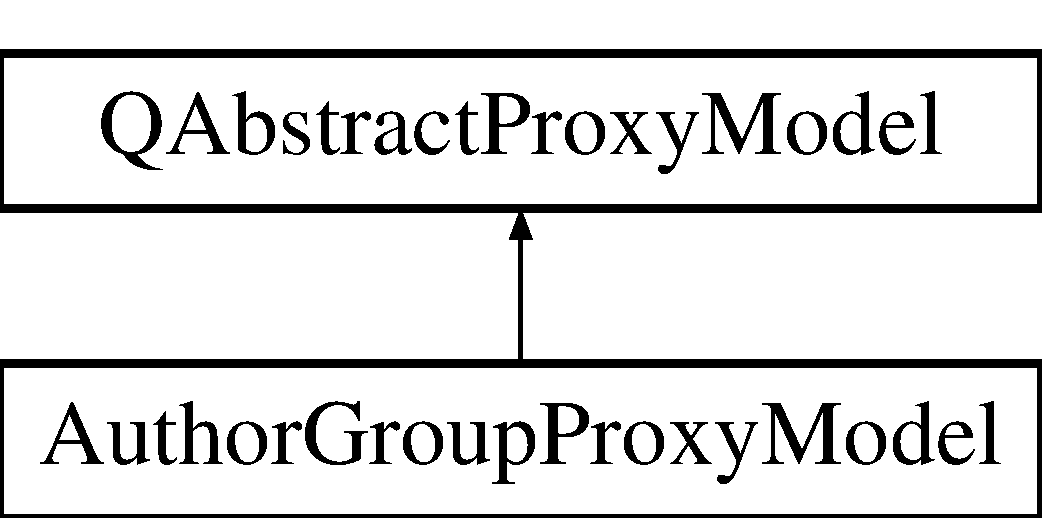
\includegraphics[height=2.000000cm]{classAuthorGroupProxyModel}
\end{center}
\end{figure}
\subsection*{Classes}
\begin{DoxyCompactItemize}
\item 
class \hyperlink{classAuthorGroupProxyModel_1_1Private}{Private}
\end{DoxyCompactItemize}
\subsection*{Public Slots}
\begin{DoxyCompactItemize}
\item 
void \hyperlink{classAuthorGroupProxyModel_a5e9d519b88078ba8f580f4780ab26558}{group\+By\+Author} (bool value)
\end{DoxyCompactItemize}
\subsection*{Public Member Functions}
\begin{DoxyCompactItemize}
\item 
\hyperlink{classAuthorGroupProxyModel_ab6d01002fb3a0b42948fc10f5e11a81f}{Author\+Group\+Proxy\+Model} (Q\+Object $\ast$\hyperlink{classAuthorGroupProxyModel_a2181f546bce987d19d5dfa674d0a3f20}{parent}=0)
\item 
\hyperlink{classAuthorGroupProxyModel_a0fa10fec1eb07a0dd34d1def3bf5ab1b}{$\sim$\+Author\+Group\+Proxy\+Model} ()
\item 
virtual int \hyperlink{classAuthorGroupProxyModel_a195f127c68cbcb8d4f01742b043cbe1f}{column\+Count} (const Q\+Model\+Index \&parent\+Index) const 
\item 
virtual int \hyperlink{classAuthorGroupProxyModel_a28c3adc3ed27a3a872550a268332244e}{row\+Count} (const Q\+Model\+Index \&parent\+Index) const 
\item 
virtual Q\+Model\+Index \hyperlink{classAuthorGroupProxyModel_ad8d58393bf0db883b0d725656680d465}{index} (int row, int column, const Q\+Model\+Index \&parent\+Index=Q\+Model\+Index()) const 
\item 
virtual Q\+Model\+Index \hyperlink{classAuthorGroupProxyModel_a2181f546bce987d19d5dfa674d0a3f20}{parent} (const Q\+Model\+Index \&\hyperlink{classAuthorGroupProxyModel_ad8d58393bf0db883b0d725656680d465}{index}) const 
\item 
virtual Q\+Model\+Index \hyperlink{classAuthorGroupProxyModel_a370febf4010a36480218fa450f66a46f}{map\+From\+Source} (const Q\+Model\+Index \&source\+Index) const 
\item 
virtual Q\+Model\+Index \hyperlink{classAuthorGroupProxyModel_aec6dbf0f65bf6970efa8b3642f744f1f}{map\+To\+Source} (const Q\+Model\+Index \&proxy\+Index) const 
\item 
virtual void \hyperlink{classAuthorGroupProxyModel_a674a68de70e314b094db30b46b28e6bd}{set\+Source\+Model} (Q\+Abstract\+Item\+Model $\ast$model)
\item 
virtual Q\+Item\+Selection \hyperlink{classAuthorGroupProxyModel_a7b9716530434c9235202708992de202c}{map\+Selection\+To\+Source} (const Q\+Item\+Selection \&selection) const 
\item 
virtual Q\+Item\+Selection \hyperlink{classAuthorGroupProxyModel_a3e40948a98819df6c7466f4ed779a856}{map\+Selection\+From\+Source} (const Q\+Item\+Selection \&selection) const 
\item 
Q\+Variant \hyperlink{classAuthorGroupProxyModel_aa6fa45e2d172cf34ef2efe231c52dae4}{data} (const Q\+Model\+Index \&proxy\+Index, int role=Qt\+::\+Display\+Role) const 
\item 
\hyperlink{classQMap}{Q\+Map}$<$ int, Q\+Variant $>$ \hyperlink{classAuthorGroupProxyModel_a8a97e49013ed9cf53573b696b77638bb}{item\+Data} (const Q\+Model\+Index \&\hyperlink{classAuthorGroupProxyModel_ad8d58393bf0db883b0d725656680d465}{index}) const 
\item 
Qt\+::\+Item\+Flags \hyperlink{classAuthorGroupProxyModel_a037ff94c3a49133301046b7c416a985c}{flags} (const Q\+Model\+Index \&\hyperlink{classAuthorGroupProxyModel_ad8d58393bf0db883b0d725656680d465}{index}) const 
\end{DoxyCompactItemize}


\subsection{Detailed Description}
A proxy model which groups the annotations by author. 

Definition at line 100 of file annotationproxymodels.\+h.



\subsection{Constructor \& Destructor Documentation}
\hypertarget{classAuthorGroupProxyModel_ab6d01002fb3a0b42948fc10f5e11a81f}{\index{Author\+Group\+Proxy\+Model@{Author\+Group\+Proxy\+Model}!Author\+Group\+Proxy\+Model@{Author\+Group\+Proxy\+Model}}
\index{Author\+Group\+Proxy\+Model@{Author\+Group\+Proxy\+Model}!Author\+Group\+Proxy\+Model@{Author\+Group\+Proxy\+Model}}
\subsubsection[{Author\+Group\+Proxy\+Model}]{\setlength{\rightskip}{0pt plus 5cm}Author\+Group\+Proxy\+Model\+::\+Author\+Group\+Proxy\+Model (
\begin{DoxyParamCaption}
\item[{Q\+Object $\ast$}]{parent = {\ttfamily 0}}
\end{DoxyParamCaption}
)}}\label{classAuthorGroupProxyModel_ab6d01002fb3a0b42948fc10f5e11a81f}
Creates a new author group proxy model.


\begin{DoxyParams}{Parameters}
{\em parent} & The parent object. \\
\hline
\end{DoxyParams}


Definition at line 347 of file annotationproxymodels.\+cpp.


\begin{DoxyCode}
348     : QAbstractProxyModel( \hyperlink{classAuthorGroupProxyModel_a2181f546bce987d19d5dfa674d0a3f20}{parent} ),
349       d( \textcolor{keyword}{new} Private( \textcolor{keyword}{this} ) )
350 \{
351 \}
\end{DoxyCode}
\hypertarget{classAuthorGroupProxyModel_a0fa10fec1eb07a0dd34d1def3bf5ab1b}{\index{Author\+Group\+Proxy\+Model@{Author\+Group\+Proxy\+Model}!````~Author\+Group\+Proxy\+Model@{$\sim$\+Author\+Group\+Proxy\+Model}}
\index{````~Author\+Group\+Proxy\+Model@{$\sim$\+Author\+Group\+Proxy\+Model}!Author\+Group\+Proxy\+Model@{Author\+Group\+Proxy\+Model}}
\subsubsection[{$\sim$\+Author\+Group\+Proxy\+Model}]{\setlength{\rightskip}{0pt plus 5cm}Author\+Group\+Proxy\+Model\+::$\sim$\+Author\+Group\+Proxy\+Model (
\begin{DoxyParamCaption}
{}
\end{DoxyParamCaption}
)}}\label{classAuthorGroupProxyModel_a0fa10fec1eb07a0dd34d1def3bf5ab1b}


Definition at line 353 of file annotationproxymodels.\+cpp.


\begin{DoxyCode}
354 \{
355     \textcolor{keyword}{delete} d;
356 \}
\end{DoxyCode}


\subsection{Member Function Documentation}
\hypertarget{classAuthorGroupProxyModel_a195f127c68cbcb8d4f01742b043cbe1f}{\index{Author\+Group\+Proxy\+Model@{Author\+Group\+Proxy\+Model}!column\+Count@{column\+Count}}
\index{column\+Count@{column\+Count}!Author\+Group\+Proxy\+Model@{Author\+Group\+Proxy\+Model}}
\subsubsection[{column\+Count}]{\setlength{\rightskip}{0pt plus 5cm}int Author\+Group\+Proxy\+Model\+::column\+Count (
\begin{DoxyParamCaption}
\item[{const Q\+Model\+Index \&}]{parent\+Index}
\end{DoxyParamCaption}
) const\hspace{0.3cm}{\ttfamily [virtual]}}}\label{classAuthorGroupProxyModel_a195f127c68cbcb8d4f01742b043cbe1f}


Definition at line 358 of file annotationproxymodels.\+cpp.


\begin{DoxyCode}
359 \{
360     \textcolor{keywordflow}{return} 1;
361 \}
\end{DoxyCode}
\hypertarget{classAuthorGroupProxyModel_aa6fa45e2d172cf34ef2efe231c52dae4}{\index{Author\+Group\+Proxy\+Model@{Author\+Group\+Proxy\+Model}!data@{data}}
\index{data@{data}!Author\+Group\+Proxy\+Model@{Author\+Group\+Proxy\+Model}}
\subsubsection[{data}]{\setlength{\rightskip}{0pt plus 5cm}Q\+Variant Author\+Group\+Proxy\+Model\+::data (
\begin{DoxyParamCaption}
\item[{const Q\+Model\+Index \&}]{proxy\+Index, }
\item[{int}]{role = {\ttfamily Qt\+:\+:DisplayRole}}
\end{DoxyParamCaption}
) const}}\label{classAuthorGroupProxyModel_aa6fa45e2d172cf34ef2efe231c52dae4}


Definition at line 474 of file annotationproxymodels.\+cpp.


\begin{DoxyCode}
475 \{
476     \textcolor{keywordflow}{if} ( isAuthorItem( proxyIndex ) ) \{
477         \hyperlink{classAuthorGroupItem}{AuthorGroupItem} *item = \textcolor{keyword}{static\_cast<}\hyperlink{classAuthorGroupItem}{AuthorGroupItem}*\textcolor{keyword}{>}( proxyIndex.
      internalPointer() );
478         \textcolor{keywordflow}{if} ( role == Qt::DisplayRole )
479             \textcolor{keywordflow}{return} item->\hyperlink{classAuthorGroupItem_ad2caab42e0010017e575483464321a81}{author}();
480         \textcolor{keywordflow}{else} \textcolor{keywordflow}{if} ( role == Qt::DecorationRole )
481             \textcolor{keywordflow}{return} KIcon( item->\hyperlink{classAuthorGroupItem_ad2caab42e0010017e575483464321a81}{author}().isEmpty() ? \textcolor{stringliteral}{"user-away"} : \textcolor{stringliteral}{"user-identity"} );
482         \textcolor{keywordflow}{else}
483             \textcolor{keywordflow}{return} QVariant();
484     \} \textcolor{keywordflow}{else} \{
485         \textcolor{keywordflow}{return} QAbstractProxyModel::data( proxyIndex, role );
486     \}
487 \}
\end{DoxyCode}
\hypertarget{classAuthorGroupProxyModel_a037ff94c3a49133301046b7c416a985c}{\index{Author\+Group\+Proxy\+Model@{Author\+Group\+Proxy\+Model}!flags@{flags}}
\index{flags@{flags}!Author\+Group\+Proxy\+Model@{Author\+Group\+Proxy\+Model}}
\subsubsection[{flags}]{\setlength{\rightskip}{0pt plus 5cm}Qt\+::\+Item\+Flags Author\+Group\+Proxy\+Model\+::flags (
\begin{DoxyParamCaption}
\item[{const Q\+Model\+Index \&}]{index}
\end{DoxyParamCaption}
) const}}\label{classAuthorGroupProxyModel_a037ff94c3a49133301046b7c416a985c}


Definition at line 498 of file annotationproxymodels.\+cpp.


\begin{DoxyCode}
499 \{
500     \textcolor{keywordflow}{if} ( isAuthorItem( \hyperlink{classAuthorGroupProxyModel_ad8d58393bf0db883b0d725656680d465}{index} ) ) \{
501         \textcolor{keywordflow}{return} Qt::ItemIsEnabled | Qt::ItemIsSelectable;
502     \} \textcolor{keywordflow}{else} \{
503         \textcolor{keywordflow}{return} QAbstractProxyModel::flags( \hyperlink{classAuthorGroupProxyModel_ad8d58393bf0db883b0d725656680d465}{index} );
504     \}
505 \}
\end{DoxyCode}
\hypertarget{classAuthorGroupProxyModel_a5e9d519b88078ba8f580f4780ab26558}{\index{Author\+Group\+Proxy\+Model@{Author\+Group\+Proxy\+Model}!group\+By\+Author@{group\+By\+Author}}
\index{group\+By\+Author@{group\+By\+Author}!Author\+Group\+Proxy\+Model@{Author\+Group\+Proxy\+Model}}
\subsubsection[{group\+By\+Author}]{\setlength{\rightskip}{0pt plus 5cm}void Author\+Group\+Proxy\+Model\+::group\+By\+Author (
\begin{DoxyParamCaption}
\item[{bool}]{value}
\end{DoxyParamCaption}
)\hspace{0.3cm}{\ttfamily [slot]}}}\label{classAuthorGroupProxyModel_a5e9d519b88078ba8f580f4780ab26558}
Sets whether the proxy model shall group the annotations by author. 

Definition at line 507 of file annotationproxymodels.\+cpp.


\begin{DoxyCode}
508 \{
509     \textcolor{keywordflow}{if} ( d->\hyperlink{classAuthorGroupProxyModel_1_1Private_ac8adbcccfaac17175553d92cdb90dae0}{mGroupByAuthor} == value )
510         \textcolor{keywordflow}{return};
511 
512     d->\hyperlink{classAuthorGroupProxyModel_1_1Private_ac8adbcccfaac17175553d92cdb90dae0}{mGroupByAuthor} = value;
513 
514     rebuildIndexes();
515 \}
\end{DoxyCode}
\hypertarget{classAuthorGroupProxyModel_ad8d58393bf0db883b0d725656680d465}{\index{Author\+Group\+Proxy\+Model@{Author\+Group\+Proxy\+Model}!index@{index}}
\index{index@{index}!Author\+Group\+Proxy\+Model@{Author\+Group\+Proxy\+Model}}
\subsubsection[{index}]{\setlength{\rightskip}{0pt plus 5cm}Q\+Model\+Index Author\+Group\+Proxy\+Model\+::index (
\begin{DoxyParamCaption}
\item[{int}]{row, }
\item[{int}]{column, }
\item[{const Q\+Model\+Index \&}]{parent\+Index = {\ttfamily QModelIndex()}}
\end{DoxyParamCaption}
) const\hspace{0.3cm}{\ttfamily [virtual]}}}\label{classAuthorGroupProxyModel_ad8d58393bf0db883b0d725656680d465}


Definition at line 374 of file annotationproxymodels.\+cpp.


\begin{DoxyCode}
375 \{
376     \textcolor{keywordflow}{if} ( !hasIndex( row, column, parentIndex ) )
377         \textcolor{keywordflow}{return} QModelIndex();
378 
379     \hyperlink{classAuthorGroupItem}{AuthorGroupItem} *parentItem = 0;
380     \textcolor{keywordflow}{if} ( !parentIndex.isValid() )
381         parentItem = d->\hyperlink{classAuthorGroupProxyModel_1_1Private_ac1023558be5adf141219d8be245ba47d}{mRoot};
382     \textcolor{keywordflow}{else}
383         parentItem = static\_cast<AuthorGroupItem*>( parentIndex.internalPointer() );
384 
385     \hyperlink{classAuthorGroupItem}{AuthorGroupItem} *child = parentItem->\hyperlink{classAuthorGroupItem_a409666687b87a8089a88fc98a46d97da}{child}( row );
386     \textcolor{keywordflow}{if} ( child )
387         \textcolor{keywordflow}{return} createIndex( row, column, child );
388     \textcolor{keywordflow}{else}
389         \textcolor{keywordflow}{return} QModelIndex();
390 \}
\end{DoxyCode}
\hypertarget{classAuthorGroupProxyModel_a8a97e49013ed9cf53573b696b77638bb}{\index{Author\+Group\+Proxy\+Model@{Author\+Group\+Proxy\+Model}!item\+Data@{item\+Data}}
\index{item\+Data@{item\+Data}!Author\+Group\+Proxy\+Model@{Author\+Group\+Proxy\+Model}}
\subsubsection[{item\+Data}]{\setlength{\rightskip}{0pt plus 5cm}{\bf Q\+Map}$<$ int, Q\+Variant $>$ Author\+Group\+Proxy\+Model\+::item\+Data (
\begin{DoxyParamCaption}
\item[{const Q\+Model\+Index \&}]{index}
\end{DoxyParamCaption}
) const}}\label{classAuthorGroupProxyModel_a8a97e49013ed9cf53573b696b77638bb}


Definition at line 489 of file annotationproxymodels.\+cpp.


\begin{DoxyCode}
490 \{
491     \textcolor{keywordflow}{if} ( isAuthorItem( \hyperlink{classAuthorGroupProxyModel_ad8d58393bf0db883b0d725656680d465}{index} ) ) \{
492         \textcolor{keywordflow}{return} \hyperlink{classQMap}{QMap<int, QVariant>}();
493     \} \textcolor{keywordflow}{else} \{
494         \textcolor{keywordflow}{return} QAbstractProxyModel::itemData( \hyperlink{classAuthorGroupProxyModel_ad8d58393bf0db883b0d725656680d465}{index} );
495     \}
496 \}
\end{DoxyCode}
\hypertarget{classAuthorGroupProxyModel_a370febf4010a36480218fa450f66a46f}{\index{Author\+Group\+Proxy\+Model@{Author\+Group\+Proxy\+Model}!map\+From\+Source@{map\+From\+Source}}
\index{map\+From\+Source@{map\+From\+Source}!Author\+Group\+Proxy\+Model@{Author\+Group\+Proxy\+Model}}
\subsubsection[{map\+From\+Source}]{\setlength{\rightskip}{0pt plus 5cm}Q\+Model\+Index Author\+Group\+Proxy\+Model\+::map\+From\+Source (
\begin{DoxyParamCaption}
\item[{const Q\+Model\+Index \&}]{source\+Index}
\end{DoxyParamCaption}
) const\hspace{0.3cm}{\ttfamily [virtual]}}}\label{classAuthorGroupProxyModel_a370febf4010a36480218fa450f66a46f}


Definition at line 406 of file annotationproxymodels.\+cpp.


\begin{DoxyCode}
407 \{
408     \textcolor{keywordflow}{if} ( !sourceIndex.isValid() )
409         \textcolor{keywordflow}{return} QModelIndex();
410 
411     \textcolor{keyword}{const} \hyperlink{classAuthorGroupItem}{AuthorGroupItem} *item = d->\hyperlink{classAuthorGroupProxyModel_1_1Private_ac1023558be5adf141219d8be245ba47d}{mRoot}->\hyperlink{classAuthorGroupItem_a0c6d7dd63e1210e0191788beab84f225}{findIndex}( sourceIndex );
412     \textcolor{keywordflow}{if} ( !item )
413         \textcolor{keywordflow}{return} QModelIndex();
414 
415     \textcolor{keywordflow}{return} createIndex( item->\hyperlink{classAuthorGroupItem_aa307483dbbd9049c3af051ca90ebc207}{row}(), 0, \textcolor{keyword}{const\_cast<}\hyperlink{classAuthorGroupItem}{AuthorGroupItem}*\textcolor{keyword}{>}( item ) );
416 \}
\end{DoxyCode}
\hypertarget{classAuthorGroupProxyModel_a3e40948a98819df6c7466f4ed779a856}{\index{Author\+Group\+Proxy\+Model@{Author\+Group\+Proxy\+Model}!map\+Selection\+From\+Source@{map\+Selection\+From\+Source}}
\index{map\+Selection\+From\+Source@{map\+Selection\+From\+Source}!Author\+Group\+Proxy\+Model@{Author\+Group\+Proxy\+Model}}
\subsubsection[{map\+Selection\+From\+Source}]{\setlength{\rightskip}{0pt plus 5cm}Q\+Item\+Selection Author\+Group\+Proxy\+Model\+::map\+Selection\+From\+Source (
\begin{DoxyParamCaption}
\item[{const Q\+Item\+Selection \&}]{selection}
\end{DoxyParamCaption}
) const\hspace{0.3cm}{\ttfamily [virtual]}}}\label{classAuthorGroupProxyModel_a3e40948a98819df6c7466f4ed779a856}


Definition at line 469 of file annotationproxymodels.\+cpp.


\begin{DoxyCode}
470 \{
471     \textcolor{keywordflow}{return} QAbstractProxyModel::mapSelectionFromSource( selection );
472 \}
\end{DoxyCode}
\hypertarget{classAuthorGroupProxyModel_a7b9716530434c9235202708992de202c}{\index{Author\+Group\+Proxy\+Model@{Author\+Group\+Proxy\+Model}!map\+Selection\+To\+Source@{map\+Selection\+To\+Source}}
\index{map\+Selection\+To\+Source@{map\+Selection\+To\+Source}!Author\+Group\+Proxy\+Model@{Author\+Group\+Proxy\+Model}}
\subsubsection[{map\+Selection\+To\+Source}]{\setlength{\rightskip}{0pt plus 5cm}Q\+Item\+Selection Author\+Group\+Proxy\+Model\+::map\+Selection\+To\+Source (
\begin{DoxyParamCaption}
\item[{const Q\+Item\+Selection \&}]{selection}
\end{DoxyParamCaption}
) const\hspace{0.3cm}{\ttfamily [virtual]}}}\label{classAuthorGroupProxyModel_a7b9716530434c9235202708992de202c}


Definition at line 457 of file annotationproxymodels.\+cpp.


\begin{DoxyCode}
458 \{
459     QModelIndexList proxyIndexes = selection.indexes();
460     QItemSelection sourceSelection;
461     \textcolor{keywordflow}{for} ( \textcolor{keywordtype}{int} i = 0; i < proxyIndexes.size(); ++i ) \{
462         \textcolor{keywordflow}{if} ( !isAuthorItem( proxyIndexes.at( i ) ) )
463             sourceSelection << QItemSelectionRange( \hyperlink{classAuthorGroupProxyModel_aec6dbf0f65bf6970efa8b3642f744f1f}{mapToSource}( proxyIndexes.at( i ) ) );
464     \}
465 
466     \textcolor{keywordflow}{return} sourceSelection;
467 \}
\end{DoxyCode}
\hypertarget{classAuthorGroupProxyModel_aec6dbf0f65bf6970efa8b3642f744f1f}{\index{Author\+Group\+Proxy\+Model@{Author\+Group\+Proxy\+Model}!map\+To\+Source@{map\+To\+Source}}
\index{map\+To\+Source@{map\+To\+Source}!Author\+Group\+Proxy\+Model@{Author\+Group\+Proxy\+Model}}
\subsubsection[{map\+To\+Source}]{\setlength{\rightskip}{0pt plus 5cm}Q\+Model\+Index Author\+Group\+Proxy\+Model\+::map\+To\+Source (
\begin{DoxyParamCaption}
\item[{const Q\+Model\+Index \&}]{proxy\+Index}
\end{DoxyParamCaption}
) const\hspace{0.3cm}{\ttfamily [virtual]}}}\label{classAuthorGroupProxyModel_aec6dbf0f65bf6970efa8b3642f744f1f}


Definition at line 418 of file annotationproxymodels.\+cpp.


\begin{DoxyCode}
419 \{
420     \textcolor{keywordflow}{if} ( !proxyIndex.isValid() )
421         \textcolor{keywordflow}{return} QModelIndex();
422 
423     \hyperlink{classAuthorGroupItem}{AuthorGroupItem} *item = \textcolor{keyword}{static\_cast<}\hyperlink{classAuthorGroupItem}{AuthorGroupItem}*\textcolor{keyword}{>}( proxyIndex.
      internalPointer() );
424 
425     \textcolor{keywordflow}{return} item->\hyperlink{classAuthorGroupItem_a65486be87b916d5901a0c45c667aa043}{index}();
426 \}
\end{DoxyCode}
\hypertarget{classAuthorGroupProxyModel_a2181f546bce987d19d5dfa674d0a3f20}{\index{Author\+Group\+Proxy\+Model@{Author\+Group\+Proxy\+Model}!parent@{parent}}
\index{parent@{parent}!Author\+Group\+Proxy\+Model@{Author\+Group\+Proxy\+Model}}
\subsubsection[{parent}]{\setlength{\rightskip}{0pt plus 5cm}Q\+Model\+Index Author\+Group\+Proxy\+Model\+::parent (
\begin{DoxyParamCaption}
\item[{const Q\+Model\+Index \&}]{index}
\end{DoxyParamCaption}
) const\hspace{0.3cm}{\ttfamily [virtual]}}}\label{classAuthorGroupProxyModel_a2181f546bce987d19d5dfa674d0a3f20}


Definition at line 392 of file annotationproxymodels.\+cpp.


\begin{DoxyCode}
393 \{
394     \textcolor{keywordflow}{if} ( !\hyperlink{classAuthorGroupProxyModel_ad8d58393bf0db883b0d725656680d465}{index}.isValid() )
395         \textcolor{keywordflow}{return} QModelIndex();
396 
397     \hyperlink{classAuthorGroupItem}{AuthorGroupItem} *childItem = \textcolor{keyword}{static\_cast<}\hyperlink{classAuthorGroupItem}{AuthorGroupItem}*\textcolor{keyword}{>}( 
      \hyperlink{classAuthorGroupProxyModel_ad8d58393bf0db883b0d725656680d465}{index}.internalPointer() );
398     \hyperlink{classAuthorGroupItem}{AuthorGroupItem} *parentItem = childItem->\hyperlink{classAuthorGroupItem_a611ca0b8336c7a947380903fbdee71c6}{parent}();
399 
400     \textcolor{keywordflow}{if} ( parentItem == d->\hyperlink{classAuthorGroupProxyModel_1_1Private_ac1023558be5adf141219d8be245ba47d}{mRoot} )
401         \textcolor{keywordflow}{return} QModelIndex();
402     \textcolor{keywordflow}{else}
403         \textcolor{keywordflow}{return} createIndex( parentItem->\hyperlink{classAuthorGroupItem_aa307483dbbd9049c3af051ca90ebc207}{row}(), 0, parentItem );
404 \}
\end{DoxyCode}
\hypertarget{classAuthorGroupProxyModel_a28c3adc3ed27a3a872550a268332244e}{\index{Author\+Group\+Proxy\+Model@{Author\+Group\+Proxy\+Model}!row\+Count@{row\+Count}}
\index{row\+Count@{row\+Count}!Author\+Group\+Proxy\+Model@{Author\+Group\+Proxy\+Model}}
\subsubsection[{row\+Count}]{\setlength{\rightskip}{0pt plus 5cm}int Author\+Group\+Proxy\+Model\+::row\+Count (
\begin{DoxyParamCaption}
\item[{const Q\+Model\+Index \&}]{parent\+Index}
\end{DoxyParamCaption}
) const\hspace{0.3cm}{\ttfamily [virtual]}}}\label{classAuthorGroupProxyModel_a28c3adc3ed27a3a872550a268332244e}


Definition at line 363 of file annotationproxymodels.\+cpp.


\begin{DoxyCode}
364 \{
365     \hyperlink{classAuthorGroupItem}{AuthorGroupItem} *item = 0;
366     \textcolor{keywordflow}{if} ( !parentIndex.isValid() )
367         item = d->\hyperlink{classAuthorGroupProxyModel_1_1Private_ac1023558be5adf141219d8be245ba47d}{mRoot};
368     \textcolor{keywordflow}{else}
369         item = static\_cast<AuthorGroupItem*>( parentIndex.internalPointer() );
370 
371     \textcolor{keywordflow}{return} item ? item->\hyperlink{classAuthorGroupItem_a4036141af4b01024f390115c45f266a2}{childCount}() : 0;
372 \}
\end{DoxyCode}
\hypertarget{classAuthorGroupProxyModel_a674a68de70e314b094db30b46b28e6bd}{\index{Author\+Group\+Proxy\+Model@{Author\+Group\+Proxy\+Model}!set\+Source\+Model@{set\+Source\+Model}}
\index{set\+Source\+Model@{set\+Source\+Model}!Author\+Group\+Proxy\+Model@{Author\+Group\+Proxy\+Model}}
\subsubsection[{set\+Source\+Model}]{\setlength{\rightskip}{0pt plus 5cm}void Author\+Group\+Proxy\+Model\+::set\+Source\+Model (
\begin{DoxyParamCaption}
\item[{Q\+Abstract\+Item\+Model $\ast$}]{model}
\end{DoxyParamCaption}
)\hspace{0.3cm}{\ttfamily [virtual]}}}\label{classAuthorGroupProxyModel_a674a68de70e314b094db30b46b28e6bd}


Definition at line 428 of file annotationproxymodels.\+cpp.


\begin{DoxyCode}
429 \{
430     \textcolor{keywordflow}{if} ( sourceModel() ) \{
431         disconnect( sourceModel(), SIGNAL(layoutChanged()), \textcolor{keyword}{this}, SLOT(rebuildIndexes()) );
432         disconnect( sourceModel(), SIGNAL(modelReset()), \textcolor{keyword}{this}, SLOT(rebuildIndexes()) );
433         disconnect( sourceModel(), SIGNAL(rowsInserted(QModelIndex,\textcolor{keywordtype}{int},\textcolor{keywordtype}{int})), \textcolor{keyword}{this}, SLOT(rebuildIndexes()) 
      );
434         disconnect( sourceModel(), SIGNAL(rowsRemoved(QModelIndex,\textcolor{keywordtype}{int},\textcolor{keywordtype}{int})), \textcolor{keyword}{this}, SLOT(rebuildIndexes()) )
      ;
435     \}
436 
437     QAbstractProxyModel::setSourceModel( model );
438 
439     connect( sourceModel(), SIGNAL(layoutChanged()), \textcolor{keyword}{this}, SLOT(rebuildIndexes()) );
440     connect( sourceModel(), SIGNAL(modelReset()), \textcolor{keyword}{this}, SLOT(rebuildIndexes()) );
441     connect( sourceModel(), SIGNAL(rowsInserted(QModelIndex,\textcolor{keywordtype}{int},\textcolor{keywordtype}{int})), \textcolor{keyword}{this}, SLOT(rebuildIndexes()) );
442     connect( sourceModel(), SIGNAL(rowsRemoved(QModelIndex,\textcolor{keywordtype}{int},\textcolor{keywordtype}{int})), \textcolor{keyword}{this}, SLOT(rebuildIndexes()) );
443 
444     rebuildIndexes();
445 \}
\end{DoxyCode}


The documentation for this class was generated from the following files\+:\begin{DoxyCompactItemize}
\item 
ui/\hyperlink{annotationproxymodels_8h}{annotationproxymodels.\+h}\item 
ui/\hyperlink{annotationproxymodels_8cpp}{annotationproxymodels.\+cpp}\end{DoxyCompactItemize}

\hypertarget{classbigEndianByteReader}{\section{big\+Endian\+Byte\+Reader Class Reference}
\label{classbigEndianByteReader}\index{big\+Endian\+Byte\+Reader@{big\+Endian\+Byte\+Reader}}
}


{\ttfamily \#include $<$big\+Endian\+Byte\+Reader.\+h$>$}

Inheritance diagram for big\+Endian\+Byte\+Reader\+:\begin{figure}[H]
\begin{center}
\leavevmode
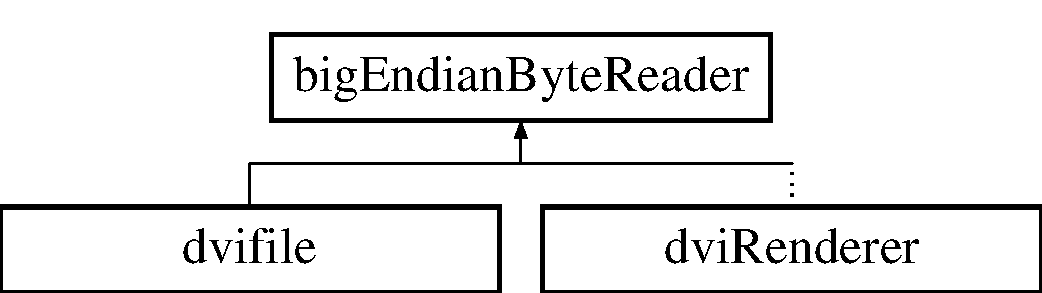
\includegraphics[height=2.000000cm]{classbigEndianByteReader}
\end{center}
\end{figure}
\subsection*{Public Member Functions}
\begin{DoxyCompactItemize}
\item 
quint8 \hyperlink{classbigEndianByteReader_ac5e3b96e3e09b30dbe57175763077c1f}{read\+U\+I\+N\+T8} ()
\item 
quint16 \hyperlink{classbigEndianByteReader_a870af9d9b5ed04507d392ad2d81c1f53}{read\+U\+I\+N\+T16} ()
\item 
quint32 \hyperlink{classbigEndianByteReader_a39c3b90a7617e40cef20796fbc680df8}{read\+U\+I\+N\+T32} ()
\item 
void \hyperlink{classbigEndianByteReader_ad7b98fdfcac31d1f30b65d2de0f2a97a}{write\+U\+I\+N\+T32} (quint32 a)
\item 
quint32 \hyperlink{classbigEndianByteReader_ace27c2b08d57237a09d84af65891d4b4}{read\+U\+I\+N\+T} (quint8 \hyperlink{synctex__parser_8c_aa23c661441688350614bd6a350d2b6ff}{size})
\item 
qint32 \hyperlink{classbigEndianByteReader_ad85cb1f2cce7f4de7abc632b5e95223b}{read\+I\+N\+T} (quint8)
\end{DoxyCompactItemize}
\subsection*{Public Attributes}
\begin{DoxyCompactItemize}
\item 
quint8 $\ast$ \hyperlink{classbigEndianByteReader_aa8919f6fe116fd3230337675fd23abac}{command\+\_\+pointer}
\item 
quint8 $\ast$ \hyperlink{classbigEndianByteReader_ace2790221530572c87c58f1f77924beb}{end\+\_\+pointer}
\end{DoxyCompactItemize}


\subsection{Detailed Description}
Byte reading routines which read big endian numbers from memory and convert them to native integers.

\begin{DoxyAuthor}{Author}
Stefan Kebekus (\href{mailto:kebekus@kde.org}{\tt kebekus@kde.\+org}) 
\end{DoxyAuthor}


Definition at line 24 of file big\+Endian\+Byte\+Reader.\+h.



\subsection{Member Function Documentation}
\hypertarget{classbigEndianByteReader_ad85cb1f2cce7f4de7abc632b5e95223b}{\index{big\+Endian\+Byte\+Reader@{big\+Endian\+Byte\+Reader}!read\+I\+N\+T@{read\+I\+N\+T}}
\index{read\+I\+N\+T@{read\+I\+N\+T}!big\+Endian\+Byte\+Reader@{big\+Endian\+Byte\+Reader}}
\subsubsection[{read\+I\+N\+T}]{\setlength{\rightskip}{0pt plus 5cm}qint32 big\+Endian\+Byte\+Reader\+::read\+I\+N\+T (
\begin{DoxyParamCaption}
\item[{quint8}]{length}
\end{DoxyParamCaption}
)}}\label{classbigEndianByteReader_ad85cb1f2cce7f4de7abc632b5e95223b}
Similar to the method above, only that the method reads a S\+I\+G\+N\+E\+D number 

Definition at line 96 of file big\+Endian\+Byte\+Reader.\+cpp.


\begin{DoxyCode}
97 \{
98   \textcolor{comment}{// This check saveguards us against segmentation fault. It is also}
99   \textcolor{comment}{// necessary for virtual fonts, which do not end with EOP.}
100   \textcolor{keywordflow}{if} (\hyperlink{classbigEndianByteReader_aa8919f6fe116fd3230337675fd23abac}{command\_pointer} >= \hyperlink{classbigEndianByteReader_ace2790221530572c87c58f1f77924beb}{end\_pointer})
101     \textcolor{keywordflow}{return} \hyperlink{dvi_8h_a734579b908509b57151ac02b946056d1}{EOP};
102 
103   qint32 a = *(\hyperlink{classbigEndianByteReader_aa8919f6fe116fd3230337675fd23abac}{command\_pointer}++);
104 
105   \textcolor{keywordflow}{if} (a & 0x80)
106     a -= 0x100;
107 
108   \textcolor{keywordflow}{while} ((--length) > 0)
109     a = (a << 8) | *(\hyperlink{classbigEndianByteReader_aa8919f6fe116fd3230337675fd23abac}{command\_pointer}++);
110 
111   \textcolor{keywordflow}{return} a;
112 \}
\end{DoxyCode}
\hypertarget{classbigEndianByteReader_ace27c2b08d57237a09d84af65891d4b4}{\index{big\+Endian\+Byte\+Reader@{big\+Endian\+Byte\+Reader}!read\+U\+I\+N\+T@{read\+U\+I\+N\+T}}
\index{read\+U\+I\+N\+T@{read\+U\+I\+N\+T}!big\+Endian\+Byte\+Reader@{big\+Endian\+Byte\+Reader}}
\subsubsection[{read\+U\+I\+N\+T}]{\setlength{\rightskip}{0pt plus 5cm}quint32 big\+Endian\+Byte\+Reader\+::read\+U\+I\+N\+T (
\begin{DoxyParamCaption}
\item[{quint8}]{size}
\end{DoxyParamCaption}
)}}\label{classbigEndianByteReader_ace27c2b08d57237a09d84af65891d4b4}
Similar to the method above, only that the method reads a big endian number of length size, where 1 $<$= size $<$= 4. Note that the value 3 is allowed (and is actually used in D\+V\+I files)!!! 

Definition at line 81 of file big\+Endian\+Byte\+Reader.\+cpp.


\begin{DoxyCode}
82 \{
83   \textcolor{comment}{// This check saveguards us against segmentation fault. It is also}
84   \textcolor{comment}{// necessary for virtual fonts, which do not end with EOP.}
85   \textcolor{keywordflow}{if} (\hyperlink{classbigEndianByteReader_aa8919f6fe116fd3230337675fd23abac}{command\_pointer} >= \hyperlink{classbigEndianByteReader_ace2790221530572c87c58f1f77924beb}{end\_pointer})
86     \textcolor{keywordflow}{return} \hyperlink{dvi_8h_a734579b908509b57151ac02b946056d1}{EOP};
87 
88   quint32 a = 0;
89   \textcolor{keywordflow}{while} (\hyperlink{synctex__parser_8c_aa23c661441688350614bd6a350d2b6ff}{size} > 0) \{
90     a = (a << 8) + *(\hyperlink{classbigEndianByteReader_aa8919f6fe116fd3230337675fd23abac}{command\_pointer}++);
91     \hyperlink{synctex__parser_8c_aa23c661441688350614bd6a350d2b6ff}{size}--;
92   \}
93   \textcolor{keywordflow}{return} a;
94 \}
\end{DoxyCode}
\hypertarget{classbigEndianByteReader_a870af9d9b5ed04507d392ad2d81c1f53}{\index{big\+Endian\+Byte\+Reader@{big\+Endian\+Byte\+Reader}!read\+U\+I\+N\+T16@{read\+U\+I\+N\+T16}}
\index{read\+U\+I\+N\+T16@{read\+U\+I\+N\+T16}!big\+Endian\+Byte\+Reader@{big\+Endian\+Byte\+Reader}}
\subsubsection[{read\+U\+I\+N\+T16}]{\setlength{\rightskip}{0pt plus 5cm}quint16 big\+Endian\+Byte\+Reader\+::read\+U\+I\+N\+T16 (
\begin{DoxyParamCaption}
{}
\end{DoxyParamCaption}
)}}\label{classbigEndianByteReader_a870af9d9b5ed04507d392ad2d81c1f53}
Similar to the method above, only that the method reads a big endian 2-\/byte word and increases the pointer by two. 

Definition at line 34 of file big\+Endian\+Byte\+Reader.\+cpp.


\begin{DoxyCode}
35 \{
36   \textcolor{comment}{// This check saveguards us against segmentation fault. It is also}
37   \textcolor{comment}{// necessary for virtual fonts, which do not end with EOP.}
38   \textcolor{keywordflow}{if} (\hyperlink{classbigEndianByteReader_aa8919f6fe116fd3230337675fd23abac}{command\_pointer} >= \hyperlink{classbigEndianByteReader_ace2790221530572c87c58f1f77924beb}{end\_pointer})
39     \textcolor{keywordflow}{return} \hyperlink{dvi_8h_a734579b908509b57151ac02b946056d1}{EOP};
40 
41   quint16 a;
42   a = *(\hyperlink{classbigEndianByteReader_aa8919f6fe116fd3230337675fd23abac}{command\_pointer}++);
43   a = (a << 8) | *(\hyperlink{classbigEndianByteReader_aa8919f6fe116fd3230337675fd23abac}{command\_pointer}++);
44   \textcolor{keywordflow}{return} a;
45 \}
\end{DoxyCode}
\hypertarget{classbigEndianByteReader_a39c3b90a7617e40cef20796fbc680df8}{\index{big\+Endian\+Byte\+Reader@{big\+Endian\+Byte\+Reader}!read\+U\+I\+N\+T32@{read\+U\+I\+N\+T32}}
\index{read\+U\+I\+N\+T32@{read\+U\+I\+N\+T32}!big\+Endian\+Byte\+Reader@{big\+Endian\+Byte\+Reader}}
\subsubsection[{read\+U\+I\+N\+T32}]{\setlength{\rightskip}{0pt plus 5cm}quint32 big\+Endian\+Byte\+Reader\+::read\+U\+I\+N\+T32 (
\begin{DoxyParamCaption}
{}
\end{DoxyParamCaption}
)}}\label{classbigEndianByteReader_a39c3b90a7617e40cef20796fbc680df8}
Similar to the method above, only that the method reads a big endian 4-\/byte word and increases the pointer by four. 

Definition at line 47 of file big\+Endian\+Byte\+Reader.\+cpp.


\begin{DoxyCode}
48 \{
49   \textcolor{comment}{// This check saveguards us against segmentation fault. It is also}
50   \textcolor{comment}{// necessary for virtual fonts, which do not end with EOP.}
51   \textcolor{keywordflow}{if} (\hyperlink{classbigEndianByteReader_aa8919f6fe116fd3230337675fd23abac}{command\_pointer} >= \hyperlink{classbigEndianByteReader_ace2790221530572c87c58f1f77924beb}{end\_pointer})
52     \textcolor{keywordflow}{return} \hyperlink{dvi_8h_a734579b908509b57151ac02b946056d1}{EOP};
53 
54   quint32 a;
55   a = *(\hyperlink{classbigEndianByteReader_aa8919f6fe116fd3230337675fd23abac}{command\_pointer}++);
56   a = (a << 8) | *(\hyperlink{classbigEndianByteReader_aa8919f6fe116fd3230337675fd23abac}{command\_pointer}++);
57   a = (a << 8) | *(\hyperlink{classbigEndianByteReader_aa8919f6fe116fd3230337675fd23abac}{command\_pointer}++);
58   a = (a << 8) | *(\hyperlink{classbigEndianByteReader_aa8919f6fe116fd3230337675fd23abac}{command\_pointer}++);
59   \textcolor{keywordflow}{return} a;
60 \}
\end{DoxyCode}
\hypertarget{classbigEndianByteReader_ac5e3b96e3e09b30dbe57175763077c1f}{\index{big\+Endian\+Byte\+Reader@{big\+Endian\+Byte\+Reader}!read\+U\+I\+N\+T8@{read\+U\+I\+N\+T8}}
\index{read\+U\+I\+N\+T8@{read\+U\+I\+N\+T8}!big\+Endian\+Byte\+Reader@{big\+Endian\+Byte\+Reader}}
\subsubsection[{read\+U\+I\+N\+T8}]{\setlength{\rightskip}{0pt plus 5cm}quint8 big\+Endian\+Byte\+Reader\+::read\+U\+I\+N\+T8 (
\begin{DoxyParamCaption}
{}
\end{DoxyParamCaption}
)}}\label{classbigEndianByteReader_ac5e3b96e3e09b30dbe57175763077c1f}
If command\+\_\+pointer $>$= end\+\_\+pointer, this method return E\+O\+P (=140) and exists. Otherwise, the method returns the unsigned byte and increases the command\+\_\+pointer by one. 

Definition at line 18 of file big\+Endian\+Byte\+Reader.\+cpp.


\begin{DoxyCode}
19 \{
20   \textcolor{comment}{// This check saveguards us against segmentation fault. It is also}
21   \textcolor{comment}{// necessary for virtual fonts, which do not end with EOP.}
22   \textcolor{keywordflow}{if} (\hyperlink{classbigEndianByteReader_aa8919f6fe116fd3230337675fd23abac}{command\_pointer} >= \hyperlink{classbigEndianByteReader_ace2790221530572c87c58f1f77924beb}{end\_pointer}) \{
23 \textcolor{preprocessor}{#ifdef DEBUG\_ENDIANREADER}
24     kError(kvs::dvi) << \textcolor{stringliteral}{"bigEndianByteReader::readUINT8() tried to read past end of data chunk"} << endl;
25     kError(kvs::dvi) << \textcolor{stringliteral}{"end\_pointer     = "} << \hyperlink{classbigEndianByteReader_ace2790221530572c87c58f1f77924beb}{end\_pointer} << endl;
26     kError(kvs::dvi) << \textcolor{stringliteral}{"command\_pointer = "} << \hyperlink{classbigEndianByteReader_aa8919f6fe116fd3230337675fd23abac}{command\_pointer} << endl;
27 \textcolor{preprocessor}{#endif}
28     \textcolor{keywordflow}{return} \hyperlink{dvi_8h_a734579b908509b57151ac02b946056d1}{EOP};
29   \}
30 
31   \textcolor{keywordflow}{return} *(\hyperlink{classbigEndianByteReader_aa8919f6fe116fd3230337675fd23abac}{command\_pointer}++);
32 \}
\end{DoxyCode}
\hypertarget{classbigEndianByteReader_ad7b98fdfcac31d1f30b65d2de0f2a97a}{\index{big\+Endian\+Byte\+Reader@{big\+Endian\+Byte\+Reader}!write\+U\+I\+N\+T32@{write\+U\+I\+N\+T32}}
\index{write\+U\+I\+N\+T32@{write\+U\+I\+N\+T32}!big\+Endian\+Byte\+Reader@{big\+Endian\+Byte\+Reader}}
\subsubsection[{write\+U\+I\+N\+T32}]{\setlength{\rightskip}{0pt plus 5cm}void big\+Endian\+Byte\+Reader\+::write\+U\+I\+N\+T32 (
\begin{DoxyParamCaption}
\item[{quint32}]{a}
\end{DoxyParamCaption}
)}}\label{classbigEndianByteReader_ad7b98fdfcac31d1f30b65d2de0f2a97a}


Definition at line 62 of file big\+Endian\+Byte\+Reader.\+cpp.


\begin{DoxyCode}
63 \{
64   \textcolor{comment}{// This check saveguards us against segmentation fault. It is also}
65   \textcolor{comment}{// necessary for virtual fonts, which do not end with EOP.}
66   \textcolor{keywordflow}{if} (\hyperlink{classbigEndianByteReader_aa8919f6fe116fd3230337675fd23abac}{command\_pointer} >= \hyperlink{classbigEndianByteReader_ace2790221530572c87c58f1f77924beb}{end\_pointer})
67     \textcolor{keywordflow}{return};
68 
69   \hyperlink{classbigEndianByteReader_aa8919f6fe116fd3230337675fd23abac}{command\_pointer}[3] = (quint8)(a & 0xFF);
70   a = a >> 8;
71   \hyperlink{classbigEndianByteReader_aa8919f6fe116fd3230337675fd23abac}{command\_pointer}[2] = (quint8)(a & 0xFF);
72   a = a >> 8;
73   \hyperlink{classbigEndianByteReader_aa8919f6fe116fd3230337675fd23abac}{command\_pointer}[1] = (quint8)(a & 0xFF);
74   a = a >> 8;
75   \hyperlink{classbigEndianByteReader_aa8919f6fe116fd3230337675fd23abac}{command\_pointer}[0] = (quint8)(a & 0xFF);
76 
77   \hyperlink{classbigEndianByteReader_aa8919f6fe116fd3230337675fd23abac}{command\_pointer} += 4;
78   \textcolor{keywordflow}{return};
79 \}
\end{DoxyCode}


\subsection{Member Data Documentation}
\hypertarget{classbigEndianByteReader_aa8919f6fe116fd3230337675fd23abac}{\index{big\+Endian\+Byte\+Reader@{big\+Endian\+Byte\+Reader}!command\+\_\+pointer@{command\+\_\+pointer}}
\index{command\+\_\+pointer@{command\+\_\+pointer}!big\+Endian\+Byte\+Reader@{big\+Endian\+Byte\+Reader}}
\subsubsection[{command\+\_\+pointer}]{\setlength{\rightskip}{0pt plus 5cm}quint8$\ast$ big\+Endian\+Byte\+Reader\+::command\+\_\+pointer}}\label{classbigEndianByteReader_aa8919f6fe116fd3230337675fd23abac}
Set this pointer to the location where the number resides which you want to read. 

Definition at line 28 of file big\+Endian\+Byte\+Reader.\+h.

\hypertarget{classbigEndianByteReader_ace2790221530572c87c58f1f77924beb}{\index{big\+Endian\+Byte\+Reader@{big\+Endian\+Byte\+Reader}!end\+\_\+pointer@{end\+\_\+pointer}}
\index{end\+\_\+pointer@{end\+\_\+pointer}!big\+Endian\+Byte\+Reader@{big\+Endian\+Byte\+Reader}}
\subsubsection[{end\+\_\+pointer}]{\setlength{\rightskip}{0pt plus 5cm}quint8$\ast$ big\+Endian\+Byte\+Reader\+::end\+\_\+pointer}}\label{classbigEndianByteReader_ace2790221530572c87c58f1f77924beb}
This pointer marks the end of the memory area where bytes can be read. It should point to the first byte which C\+A\+N\+N\+O\+T be read. The idea is to have a safety net which protects us against S\+E\+G\+F\+A\+U\+L\+Ts. This is also used in virtual fonts, where the macro does not have an E\+O\+P command at the end of the macro. 

Definition at line 35 of file big\+Endian\+Byte\+Reader.\+h.



The documentation for this class was generated from the following files\+:\begin{DoxyCompactItemize}
\item 
generators/dvi/\hyperlink{bigEndianByteReader_8h}{big\+Endian\+Byte\+Reader.\+h}\item 
generators/dvi/\hyperlink{bigEndianByteReader_8cpp}{big\+Endian\+Byte\+Reader.\+cpp}\end{DoxyCompactItemize}

\hypertarget{structbitmap}{\section{bitmap Struct Reference}
\label{structbitmap}\index{bitmap@{bitmap}}
}


{\ttfamily \#include $<$glyph.\+h$>$}

\subsection*{Public Member Functions}
\begin{DoxyCompactItemize}
\item 
\hyperlink{structbitmap_a9b64f3a60ff3ad82265500c7e6b71112}{bitmap} ()
\item 
\hyperlink{structbitmap_af3c4e3cd110854573761fd68f33ec8c8}{$\sim$bitmap} ()
\end{DoxyCompactItemize}
\subsection*{Public Attributes}
\begin{DoxyCompactItemize}
\item 
quint16 \hyperlink{structbitmap_a955acbe13f247a259cbe10ced3a212fd}{w}
\item 
quint16 \hyperlink{structbitmap_a34f28c8404007de8ede4b9a6b5e425dd}{h}
\item 
quint16 \hyperlink{structbitmap_ae248def3f3413e79d52541195017a32c}{bytes\+\_\+wide}
\item 
char $\ast$ \hyperlink{structbitmap_a5d74448ece4936321ffd2bdc4fabe445}{bits}
\end{DoxyCompactItemize}


\subsection{Detailed Description}


Definition at line 10 of file glyph.\+h.



\subsection{Constructor \& Destructor Documentation}
\hypertarget{structbitmap_a9b64f3a60ff3ad82265500c7e6b71112}{\index{bitmap@{bitmap}!bitmap@{bitmap}}
\index{bitmap@{bitmap}!bitmap@{bitmap}}
\subsubsection[{bitmap}]{\setlength{\rightskip}{0pt plus 5cm}bitmap\+::bitmap (
\begin{DoxyParamCaption}
{}
\end{DoxyParamCaption}
)}}\label{structbitmap_a9b64f3a60ff3ad82265500c7e6b71112}


Definition at line 15 of file glyph.\+cpp.


\begin{DoxyCode}
16 \{
17   \hyperlink{structbitmap_a5d74448ece4936321ffd2bdc4fabe445}{bits} = 0; 
18 \}
\end{DoxyCode}
\hypertarget{structbitmap_af3c4e3cd110854573761fd68f33ec8c8}{\index{bitmap@{bitmap}!````~bitmap@{$\sim$bitmap}}
\index{````~bitmap@{$\sim$bitmap}!bitmap@{bitmap}}
\subsubsection[{$\sim$bitmap}]{\setlength{\rightskip}{0pt plus 5cm}bitmap\+::$\sim$bitmap (
\begin{DoxyParamCaption}
{}
\end{DoxyParamCaption}
)}}\label{structbitmap_af3c4e3cd110854573761fd68f33ec8c8}


Definition at line 20 of file glyph.\+cpp.


\begin{DoxyCode}
21 \{
22   \textcolor{keyword}{delete} \hyperlink{structbitmap_a5d74448ece4936321ffd2bdc4fabe445}{bits};
23 \}
\end{DoxyCode}


\subsection{Member Data Documentation}
\hypertarget{structbitmap_a5d74448ece4936321ffd2bdc4fabe445}{\index{bitmap@{bitmap}!bits@{bits}}
\index{bits@{bits}!bitmap@{bitmap}}
\subsubsection[{bits}]{\setlength{\rightskip}{0pt plus 5cm}char$\ast$ bitmap\+::bits}}\label{structbitmap_a5d74448ece4936321ffd2bdc4fabe445}


Definition at line 19 of file glyph.\+h.

\hypertarget{structbitmap_ae248def3f3413e79d52541195017a32c}{\index{bitmap@{bitmap}!bytes\+\_\+wide@{bytes\+\_\+wide}}
\index{bytes\+\_\+wide@{bytes\+\_\+wide}!bitmap@{bitmap}}
\subsubsection[{bytes\+\_\+wide}]{\setlength{\rightskip}{0pt plus 5cm}quint16 bitmap\+::bytes\+\_\+wide}}\label{structbitmap_ae248def3f3413e79d52541195017a32c}


Definition at line 17 of file glyph.\+h.

\hypertarget{structbitmap_a34f28c8404007de8ede4b9a6b5e425dd}{\index{bitmap@{bitmap}!h@{h}}
\index{h@{h}!bitmap@{bitmap}}
\subsubsection[{h}]{\setlength{\rightskip}{0pt plus 5cm}quint16 bitmap\+::h}}\label{structbitmap_a34f28c8404007de8ede4b9a6b5e425dd}


Definition at line 15 of file glyph.\+h.

\hypertarget{structbitmap_a955acbe13f247a259cbe10ced3a212fd}{\index{bitmap@{bitmap}!w@{w}}
\index{w@{w}!bitmap@{bitmap}}
\subsubsection[{w}]{\setlength{\rightskip}{0pt plus 5cm}quint16 bitmap\+::w}}\label{structbitmap_a955acbe13f247a259cbe10ced3a212fd}


Definition at line 15 of file glyph.\+h.



The documentation for this struct was generated from the following files\+:\begin{DoxyCompactItemize}
\item 
generators/dvi/\hyperlink{glyph_8h}{glyph.\+h}\item 
generators/dvi/\hyperlink{glyph_8cpp}{glyph.\+cpp}\end{DoxyCompactItemize}

\hypertarget{classBookmarkItem}{\section{Bookmark\+Item Class Reference}
\label{classBookmarkItem}\index{Bookmark\+Item@{Bookmark\+Item}}
}
Inheritance diagram for Bookmark\+Item\+:\begin{figure}[H]
\begin{center}
\leavevmode
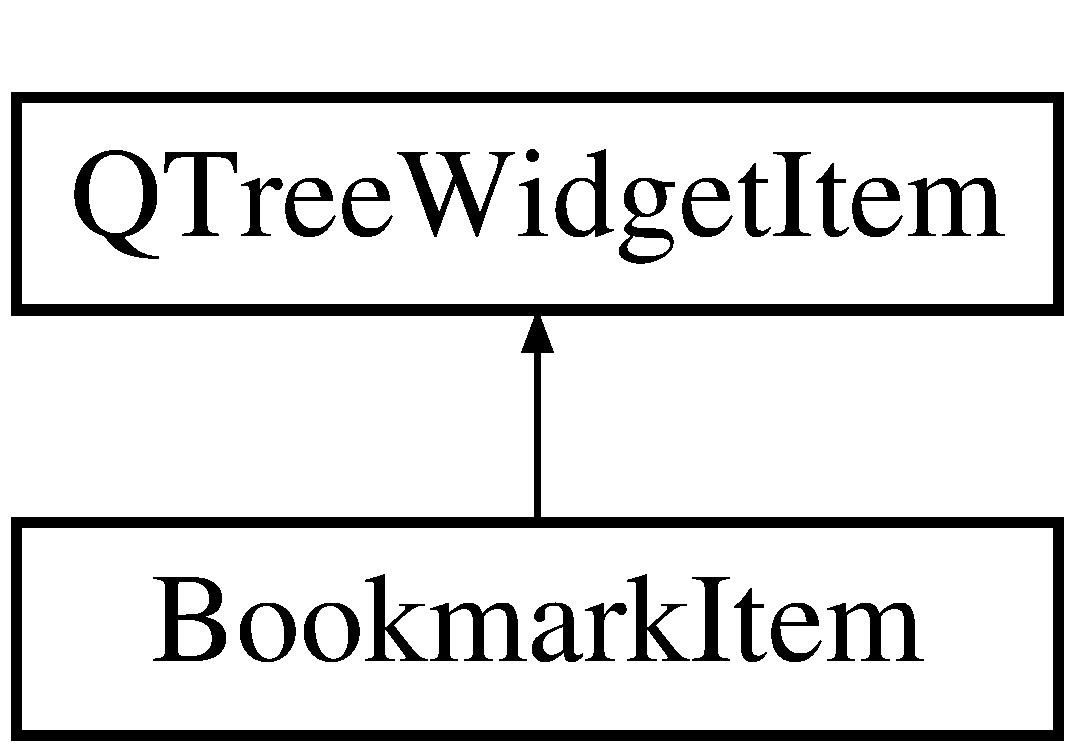
\includegraphics[height=2.000000cm]{classBookmarkItem}
\end{center}
\end{figure}
\subsection*{Public Member Functions}
\begin{DoxyCompactItemize}
\item 
\hyperlink{classBookmarkItem_ae1b9c523ae42cf2ed392ae17ec13aea2}{Bookmark\+Item} (const K\+Bookmark \&bm)
\item 
virtual Q\+Variant \hyperlink{classBookmarkItem_ac5552d122e849c6d9ca4a74e36dbb0bc}{data} (int column, int role) const 
\item 
virtual bool \hyperlink{classBookmarkItem_a64dc8aa569e9ec78502ca23741d6af6d}{operator$<$} (const Q\+Tree\+Widget\+Item \&other) const 
\item 
K\+Bookmark \& \hyperlink{classBookmarkItem_a8eb0b1029552031a0fb896ac4efc3405}{bookmark} ()
\item 
const \hyperlink{classOkular_1_1DocumentViewport}{Okular\+::\+Document\+Viewport} \& \hyperlink{classBookmarkItem_a0d026bde6eaadb312ab1b8fb1fd6831b}{viewport} () const 
\item 
K\+Url \hyperlink{classBookmarkItem_ad50510e9314ad2cd4ba0053fff6afaa4}{url} () const 
\end{DoxyCompactItemize}


\subsection{Detailed Description}


Definition at line 35 of file bookmarklist.\+cpp.



\subsection{Constructor \& Destructor Documentation}
\hypertarget{classBookmarkItem_ae1b9c523ae42cf2ed392ae17ec13aea2}{\index{Bookmark\+Item@{Bookmark\+Item}!Bookmark\+Item@{Bookmark\+Item}}
\index{Bookmark\+Item@{Bookmark\+Item}!Bookmark\+Item@{Bookmark\+Item}}
\subsubsection[{Bookmark\+Item}]{\setlength{\rightskip}{0pt plus 5cm}Bookmark\+Item\+::\+Bookmark\+Item (
\begin{DoxyParamCaption}
\item[{const K\+Bookmark \&}]{bm}
\end{DoxyParamCaption}
)\hspace{0.3cm}{\ttfamily [inline]}}}\label{classBookmarkItem_ae1b9c523ae42cf2ed392ae17ec13aea2}


Definition at line 38 of file bookmarklist.\+cpp.


\begin{DoxyCode}
39             : QTreeWidgetItem( BookmarkItemType ), m\_bookmark( bm )
40         \{
41             setFlags( Qt::ItemIsSelectable | Qt::ItemIsEnabled | Qt::ItemIsEditable );
42             m\_url = m\_bookmark.url();
43             m\_viewport = \hyperlink{classOkular_1_1DocumentViewport}{Okular::DocumentViewport}( m\_url.htmlRef() );
44             m\_url.setHTMLRef( QString() );
45             setText( 0, m\_bookmark.fullText() );
46             \textcolor{keywordflow}{if} ( m\_viewport.\hyperlink{classOkular_1_1DocumentViewport_a13161b17f2d0b68bf033955f81d41584}{isValid}() )
47                 setData( 0, \hyperlink{classPageItemDelegate_abd76ff54064145a88199c5c60880d91f}{PageItemDelegate::PageRole}, QString::number( 
      m\_viewport.\hyperlink{classOkular_1_1DocumentViewport_a122674d4a493e79b1aa5fd5c00e81c93}{pageNumber} + 1 ) );
48         \}
\end{DoxyCode}


\subsection{Member Function Documentation}
\hypertarget{classBookmarkItem_a8eb0b1029552031a0fb896ac4efc3405}{\index{Bookmark\+Item@{Bookmark\+Item}!bookmark@{bookmark}}
\index{bookmark@{bookmark}!Bookmark\+Item@{Bookmark\+Item}}
\subsubsection[{bookmark}]{\setlength{\rightskip}{0pt plus 5cm}K\+Bookmark\& Bookmark\+Item\+::bookmark (
\begin{DoxyParamCaption}
{}
\end{DoxyParamCaption}
)\hspace{0.3cm}{\ttfamily [inline]}}}\label{classBookmarkItem_a8eb0b1029552031a0fb896ac4efc3405}


Definition at line 70 of file bookmarklist.\+cpp.


\begin{DoxyCode}
71         \{
72             \textcolor{keywordflow}{return} m\_bookmark;
73         \}
\end{DoxyCode}
\hypertarget{classBookmarkItem_ac5552d122e849c6d9ca4a74e36dbb0bc}{\index{Bookmark\+Item@{Bookmark\+Item}!data@{data}}
\index{data@{data}!Bookmark\+Item@{Bookmark\+Item}}
\subsubsection[{data}]{\setlength{\rightskip}{0pt plus 5cm}virtual Q\+Variant Bookmark\+Item\+::data (
\begin{DoxyParamCaption}
\item[{int}]{column, }
\item[{int}]{role}
\end{DoxyParamCaption}
) const\hspace{0.3cm}{\ttfamily [inline]}, {\ttfamily [virtual]}}}\label{classBookmarkItem_ac5552d122e849c6d9ca4a74e36dbb0bc}


Definition at line 50 of file bookmarklist.\+cpp.


\begin{DoxyCode}
51         \{
52             \textcolor{keywordflow}{switch} ( role )
53             \{
54                 \textcolor{keywordflow}{case} Qt::ToolTipRole:
55                     \textcolor{keywordflow}{return} m\_bookmark.fullText();
56             \}
57             \textcolor{keywordflow}{return} QTreeWidgetItem::data( column, role );
58         \}
\end{DoxyCode}
\hypertarget{classBookmarkItem_a64dc8aa569e9ec78502ca23741d6af6d}{\index{Bookmark\+Item@{Bookmark\+Item}!operator$<$@{operator$<$}}
\index{operator$<$@{operator$<$}!Bookmark\+Item@{Bookmark\+Item}}
\subsubsection[{operator$<$}]{\setlength{\rightskip}{0pt plus 5cm}virtual bool Bookmark\+Item\+::operator$<$ (
\begin{DoxyParamCaption}
\item[{const Q\+Tree\+Widget\+Item \&}]{other}
\end{DoxyParamCaption}
) const\hspace{0.3cm}{\ttfamily [inline]}, {\ttfamily [virtual]}}}\label{classBookmarkItem_a64dc8aa569e9ec78502ca23741d6af6d}


Definition at line 60 of file bookmarklist.\+cpp.


\begin{DoxyCode}
61         \{
62             \textcolor{keywordflow}{if} ( other.type() == BookmarkItemType )
63             \{
64                 \textcolor{keyword}{const} \hyperlink{classBookmarkItem}{BookmarkItem} *cmp = \textcolor{keyword}{static\_cast<} \textcolor{keyword}{const }
      \hyperlink{classBookmarkItem}{BookmarkItem}* \textcolor{keyword}{>}( &other );
65                 \textcolor{keywordflow}{return} m\_viewport < cmp->m\_viewport;
66             \}
67             \textcolor{keywordflow}{return} QTreeWidgetItem::operator<( other );
68         \}
\end{DoxyCode}
\hypertarget{classBookmarkItem_ad50510e9314ad2cd4ba0053fff6afaa4}{\index{Bookmark\+Item@{Bookmark\+Item}!url@{url}}
\index{url@{url}!Bookmark\+Item@{Bookmark\+Item}}
\subsubsection[{url}]{\setlength{\rightskip}{0pt plus 5cm}K\+Url Bookmark\+Item\+::url (
\begin{DoxyParamCaption}
{}
\end{DoxyParamCaption}
) const\hspace{0.3cm}{\ttfamily [inline]}}}\label{classBookmarkItem_ad50510e9314ad2cd4ba0053fff6afaa4}


Definition at line 80 of file bookmarklist.\+cpp.


\begin{DoxyCode}
81         \{
82             \textcolor{keywordflow}{return} m\_url;
83         \}
\end{DoxyCode}
\hypertarget{classBookmarkItem_a0d026bde6eaadb312ab1b8fb1fd6831b}{\index{Bookmark\+Item@{Bookmark\+Item}!viewport@{viewport}}
\index{viewport@{viewport}!Bookmark\+Item@{Bookmark\+Item}}
\subsubsection[{viewport}]{\setlength{\rightskip}{0pt plus 5cm}const {\bf Okular\+::\+Document\+Viewport}\& Bookmark\+Item\+::viewport (
\begin{DoxyParamCaption}
{}
\end{DoxyParamCaption}
) const\hspace{0.3cm}{\ttfamily [inline]}}}\label{classBookmarkItem_a0d026bde6eaadb312ab1b8fb1fd6831b}


Definition at line 75 of file bookmarklist.\+cpp.


\begin{DoxyCode}
76         \{
77             \textcolor{keywordflow}{return} m\_viewport;
78         \}
\end{DoxyCode}


The documentation for this class was generated from the following file\+:\begin{DoxyCompactItemize}
\item 
ui/\hyperlink{bookmarklist_8cpp}{bookmarklist.\+cpp}\end{DoxyCompactItemize}

\hypertarget{classBookmarkList}{\section{Bookmark\+List Class Reference}
\label{classBookmarkList}\index{Bookmark\+List@{Bookmark\+List}}
}


{\ttfamily \#include $<$bookmarklist.\+h$>$}

Inheritance diagram for Bookmark\+List\+:\begin{figure}[H]
\begin{center}
\leavevmode
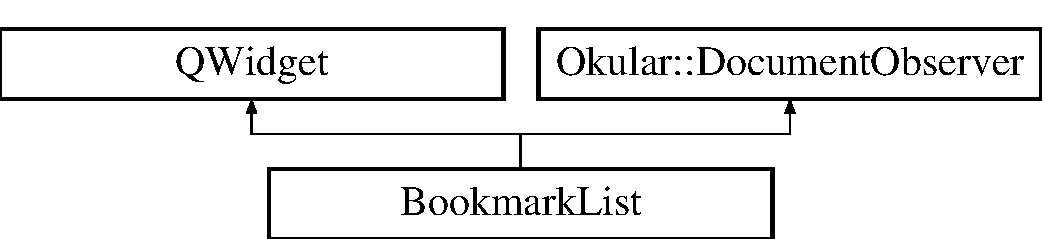
\includegraphics[height=2.000000cm]{classBookmarkList}
\end{center}
\end{figure}
\subsection*{Public Member Functions}
\begin{DoxyCompactItemize}
\item 
\hyperlink{classBookmarkList_a385d297ecec7bca083ab6753901c77bf}{Bookmark\+List} (\hyperlink{classOkular_1_1Document}{Okular\+::\+Document} $\ast$document, Q\+Widget $\ast$parent=0)
\item 
\hyperlink{classBookmarkList_af6e9171a2af0628aec8c35d22e092e2f}{$\sim$\+Bookmark\+List} ()
\item 
void \hyperlink{classBookmarkList_ab0802e3729078b77e9fb372e267d3d70}{notify\+Setup} (const Q\+Vector$<$ \hyperlink{classOkular_1_1Page}{Okular\+::\+Page} $\ast$ $>$ \&pages, int setup\+Flags)
\end{DoxyCompactItemize}
\subsection*{Additional Inherited Members}


\subsection{Detailed Description}


Definition at line 29 of file bookmarklist.\+h.



\subsection{Constructor \& Destructor Documentation}
\hypertarget{classBookmarkList_a385d297ecec7bca083ab6753901c77bf}{\index{Bookmark\+List@{Bookmark\+List}!Bookmark\+List@{Bookmark\+List}}
\index{Bookmark\+List@{Bookmark\+List}!Bookmark\+List@{Bookmark\+List}}
\subsubsection[{Bookmark\+List}]{\setlength{\rightskip}{0pt plus 5cm}Bookmark\+List\+::\+Bookmark\+List (
\begin{DoxyParamCaption}
\item[{{\bf Okular\+::\+Document} $\ast$}]{document, }
\item[{Q\+Widget $\ast$}]{parent = {\ttfamily 0}}
\end{DoxyParamCaption}
)\hspace{0.3cm}{\ttfamily [explicit]}}}\label{classBookmarkList_a385d297ecec7bca083ab6753901c77bf}


Definition at line 118 of file bookmarklist.\+cpp.


\begin{DoxyCode}
119     : QWidget( parent ), m\_document( document ), m\_currentDocumentItem( 0 )
120 \{
121     QVBoxLayout *mainlay = \textcolor{keyword}{new} QVBoxLayout( \textcolor{keyword}{this} );
122     mainlay->setMargin( 0 );
123     mainlay->setSpacing( 6 );
124 
125     m\_searchLine = \textcolor{keyword}{new} KTreeWidgetSearchLine( \textcolor{keyword}{this} );
126     mainlay->addWidget( m\_searchLine );
127 
128     m\_tree = \textcolor{keyword}{new} QTreeWidget( \textcolor{keyword}{this} );
129     mainlay->addWidget( m\_tree );
130     QStringList cols;
131     cols.append( \textcolor{stringliteral}{"Bookmarks"} );
132     m\_tree->setContextMenuPolicy(  Qt::CustomContextMenu );
133     m\_tree->setHeaderLabels( cols );
134     m\_tree->setSortingEnabled( \textcolor{keyword}{false} );
135     m\_tree->setRootIsDecorated( \textcolor{keyword}{true} );
136     m\_tree->setAlternatingRowColors( \textcolor{keyword}{true} );
137     m\_tree->setItemDelegate( \textcolor{keyword}{new} \hyperlink{classPageItemDelegate}{PageItemDelegate}( m\_tree ) );
138     m\_tree->header()->hide();
139     m\_tree->setSelectionBehavior( QAbstractItemView::SelectRows );
140     m\_tree->setEditTriggers( QAbstractItemView::EditKeyPressed );
141     connect( m\_tree, SIGNAL(itemActivated(QTreeWidgetItem*,\textcolor{keywordtype}{int})), \textcolor{keyword}{this}, SLOT(slotExecuted(QTreeWidgetItem*)
      ) );
142     connect( m\_tree, SIGNAL(customContextMenuRequested(QPoint)), \textcolor{keyword}{this}, SLOT(slotContextMenu(QPoint)) );
143     m\_searchLine->addTreeWidget( m\_tree );
144 
145     QToolBar * bookmarkController = \textcolor{keyword}{new} QToolBar( \textcolor{keyword}{this} );
146     mainlay->addWidget( bookmarkController );
147     bookmarkController->setObjectName( QLatin1String( \textcolor{stringliteral}{"BookmarkControlBar"} ) );
148     \textcolor{comment}{// change toolbar appearance}
149     bookmarkController->setIconSize( QSize( 16, 16 ) );
150     bookmarkController->setMovable( \textcolor{keyword}{false} );
151     QSizePolicy sp = bookmarkController->sizePolicy();
152     sp.setVerticalPolicy( QSizePolicy::Minimum );
153     bookmarkController->setSizePolicy( sp );
154     \textcolor{comment}{// insert a togglebutton [show only bookmarks in the current document]}
155     m\_showBoomarkOnlyAction = bookmarkController->addAction( KIcon( \textcolor{stringliteral}{"bookmarks"} ), i18n( \textcolor{stringliteral}{"Current document
       only"} ) );
156     m\_showBoomarkOnlyAction->setCheckable( \textcolor{keyword}{true} );
157     connect( m\_showBoomarkOnlyAction, SIGNAL(toggled(\textcolor{keywordtype}{bool})), \textcolor{keyword}{this}, SLOT(slotFilterBookmarks(\textcolor{keywordtype}{bool})) );
158 
159     connect( m\_document->\hyperlink{classOkular_1_1Document_a2a2a1f0f5384563c8b24c2ba48809839}{bookmarkManager}(), SIGNAL(bookmarksChanged(KUrl)), \textcolor{keyword}{this}, SLOT(
      slotBookmarksChanged(KUrl)) );
160 
161     rebuildTree( m\_showBoomarkOnlyAction->isChecked() );
162 \}
\end{DoxyCode}
\hypertarget{classBookmarkList_af6e9171a2af0628aec8c35d22e092e2f}{\index{Bookmark\+List@{Bookmark\+List}!````~Bookmark\+List@{$\sim$\+Bookmark\+List}}
\index{````~Bookmark\+List@{$\sim$\+Bookmark\+List}!Bookmark\+List@{Bookmark\+List}}
\subsubsection[{$\sim$\+Bookmark\+List}]{\setlength{\rightskip}{0pt plus 5cm}Bookmark\+List\+::$\sim$\+Bookmark\+List (
\begin{DoxyParamCaption}
{}
\end{DoxyParamCaption}
)}}\label{classBookmarkList_af6e9171a2af0628aec8c35d22e092e2f}


Definition at line 164 of file bookmarklist.\+cpp.


\begin{DoxyCode}
165 \{
166     m\_document->\hyperlink{classOkular_1_1Document_a2d704dea2ab28c846e58443ac38841f2}{removeObserver}( \textcolor{keyword}{this} );
167 \}
\end{DoxyCode}


\subsection{Member Function Documentation}
\hypertarget{classBookmarkList_ab0802e3729078b77e9fb372e267d3d70}{\index{Bookmark\+List@{Bookmark\+List}!notify\+Setup@{notify\+Setup}}
\index{notify\+Setup@{notify\+Setup}!Bookmark\+List@{Bookmark\+List}}
\subsubsection[{notify\+Setup}]{\setlength{\rightskip}{0pt plus 5cm}void Bookmark\+List\+::notify\+Setup (
\begin{DoxyParamCaption}
\item[{const Q\+Vector$<$ {\bf Okular\+::\+Page} $\ast$ $>$ \&}]{pages, }
\item[{int}]{setup\+Flags}
\end{DoxyParamCaption}
)}}\label{classBookmarkList_ab0802e3729078b77e9fb372e267d3d70}


Definition at line 169 of file bookmarklist.\+cpp.


\begin{DoxyCode}
170 \{
171     Q\_UNUSED( pages );
172     \textcolor{keywordflow}{if} ( !( setupFlags & \hyperlink{classOkular_1_1DocumentObserver_aba00584af99894f95a9650e91f109d40ae599564392c01b22e96eff7602c4dd03}{Okular::DocumentObserver::DocumentChanged}
       ) )
173         \textcolor{keywordflow}{return};
174 
175     \textcolor{comment}{// clear contents}
176     m\_searchLine->clear();
177 
178     \textcolor{keywordflow}{if} ( m\_showBoomarkOnlyAction->isChecked() )
179     \{
180         rebuildTree( m\_showBoomarkOnlyAction->isChecked() );
181     \}
182     \textcolor{keywordflow}{else}
183     \{
184         disconnect( m\_tree, SIGNAL(itemChanged(QTreeWidgetItem*,\textcolor{keywordtype}{int})), \textcolor{keyword}{this}, SLOT(slotChanged(
      QTreeWidgetItem*)) );
185         \textcolor{keywordflow}{if} ( m\_currentDocumentItem && m\_currentDocumentItem != m\_tree->invisibleRootItem()  )
186         \{
187             m\_currentDocumentItem->setIcon( 0, QIcon() );
188         \}
189         m\_currentDocumentItem = itemForUrl( m\_document->\hyperlink{classOkular_1_1Document_acb6f05a191623dafbdf5d4788dd98fed}{currentDocument}() );
190         \textcolor{keywordflow}{if} ( m\_currentDocumentItem && m\_currentDocumentItem != m\_tree->invisibleRootItem()  )
191         \{
192             m\_currentDocumentItem->setIcon( 0, KIcon( \textcolor{stringliteral}{"bookmarks"} ) );
193             m\_currentDocumentItem->setExpanded( \textcolor{keyword}{true} );
194         \}
195         connect( m\_tree, SIGNAL(itemChanged(QTreeWidgetItem*,\textcolor{keywordtype}{int})), \textcolor{keyword}{this}, SLOT(slotChanged(QTreeWidgetItem
      *)) );
196     \}
197 \}
\end{DoxyCode}


The documentation for this class was generated from the following files\+:\begin{DoxyCompactItemize}
\item 
ui/\hyperlink{bookmarklist_8h}{bookmarklist.\+h}\item 
ui/\hyperlink{bookmarklist_8cpp}{bookmarklist.\+cpp}\end{DoxyCompactItemize}

\hypertarget{classOkular_1_1BookmarkManager}{\section{Okular\+:\+:Bookmark\+Manager Class Reference}
\label{classOkular_1_1BookmarkManager}\index{Okular\+::\+Bookmark\+Manager@{Okular\+::\+Bookmark\+Manager}}
}


Bookmarks manager utility.  




{\ttfamily \#include $<$bookmarkmanager.\+h$>$}

Inheritance diagram for Okular\+:\+:Bookmark\+Manager\+:\begin{figure}[H]
\begin{center}
\leavevmode
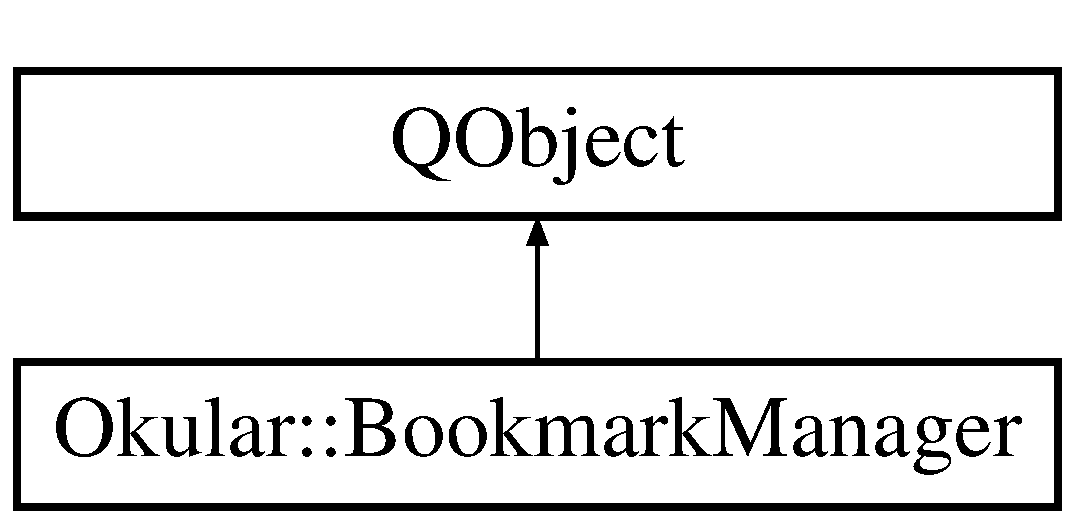
\includegraphics[height=2.000000cm]{classOkular_1_1BookmarkManager}
\end{center}
\end{figure}
\subsection*{Classes}
\begin{DoxyCompactItemize}
\item 
class \hyperlink{classBookmarkManager_1_1Private}{Private}
\end{DoxyCompactItemize}
\subsection*{Signals}
\begin{DoxyCompactItemize}
\item 
void \hyperlink{classOkular_1_1BookmarkManager_a4141e9880af774f72d8e0616ca4a6392}{open\+Url} (const K\+Url \&url)
\item 
void \hyperlink{classOkular_1_1BookmarkManager_a60926c4115be32b182913e56fd709e18}{saved} ()
\item 
void \hyperlink{classOkular_1_1BookmarkManager_af46858377e563eb8277226eb853a0608}{bookmarks\+Changed} (const K\+Url \&url)
\end{DoxyCompactItemize}
\subsection*{Public Member Functions}
\begin{DoxyCompactItemize}
\item 
virtual \hyperlink{classOkular_1_1BookmarkManager_a1069f28ac38e9c854e04a8aec6a32ba5}{$\sim$\+Bookmark\+Manager} ()
\item 
K\+Url\+::\+List \hyperlink{classOkular_1_1BookmarkManager_aa97bab16634951bc92dd567208fdca80}{files} () const 
\item 
K\+Bookmark\+::\+List \hyperlink{classOkular_1_1BookmarkManager_a35ec51e7751b9bde6bffb9ad339ffdfd}{bookmarks} (const K\+Url \&url) const 
\item 
K\+Bookmark\+::\+List \hyperlink{classOkular_1_1BookmarkManager_a770db9f97ee4d9069c0d417017caa4d3}{bookmarks} () const 
\item 
K\+Bookmark\+::\+List \hyperlink{classOkular_1_1BookmarkManager_af65fc427552b4e653ae253a69cc53828}{bookmarks} (int page) const 
\item 
K\+Bookmark \hyperlink{classOkular_1_1BookmarkManager_aeda7ddc73c05fb51f03a031d95cccb9d}{bookmark} (int page) const 
\item 
K\+Bookmark \hyperlink{classOkular_1_1BookmarkManager_a3b314eb1e853ca56751a61182fe553d1}{bookmark} (const \hyperlink{classOkular_1_1DocumentViewport}{Document\+Viewport} \&viewport) const 
\item 
void \hyperlink{classOkular_1_1BookmarkManager_af277e57ed79d0fce59f00a62f6e0f7b5}{save} () const 
\item 
void \hyperlink{classOkular_1_1BookmarkManager_adc5509fdb789024dc10bac5c3c1457b2}{add\+Bookmark} (int page)
\item 
void \hyperlink{classOkular_1_1BookmarkManager_a34863b6bfe042e738e14950e4f5c27b8}{add\+Bookmark} (const \hyperlink{classOkular_1_1DocumentViewport}{Document\+Viewport} \&vp)
\item 
bool \hyperlink{classOkular_1_1BookmarkManager_a9f859d109d8a4edb1576ccfcedc84232}{add\+Bookmark} (const K\+Url \&referurl, const \hyperlink{classOkular_1_1DocumentViewport}{Okular\+::\+Document\+Viewport} \&vp, const Q\+String \&title=Q\+String())
\item 
void \hyperlink{classOkular_1_1BookmarkManager_a3e763f31a1595a68b4df6e8419ea47ac}{remove\+Bookmark} (int page)
\item 
void \hyperlink{classOkular_1_1BookmarkManager_ad9b6b11a42b0522ad80b52303e939fc3}{remove\+Bookmark} (const \hyperlink{classOkular_1_1DocumentViewport}{Document\+Viewport} \&vp)
\item 
int \hyperlink{classOkular_1_1BookmarkManager_a62520293e8c99ae68058fe4d00eb0e6b}{remove\+Bookmark} (const K\+Url \&referurl, const K\+Bookmark \&bm)
\item 
void \hyperlink{classOkular_1_1BookmarkManager_a3279284b0618f5bb49dba8647b6980a4}{remove\+Bookmarks} (const K\+Url \&referurl, const K\+Bookmark\+::\+List \&list)
\item 
void \hyperlink{classOkular_1_1BookmarkManager_a0e57d5f1d5795042686118ac779d85c5}{rename\+Bookmark} (K\+Bookmark $\ast$bm, const Q\+String \&new\+Name)
\item 
void \hyperlink{classOkular_1_1BookmarkManager_a99979fe5e87cb15173ac20feb7de352e}{rename\+Bookmark} (const K\+Url \&referurl, const Q\+String \&new\+Name)
\item 
Q\+String \hyperlink{classOkular_1_1BookmarkManager_a9b24aecf34aaac007418797bee80f717}{title\+For\+Url} (const K\+Url \&referurl) const 
\item 
bool \hyperlink{classOkular_1_1BookmarkManager_a606808f318c721de3e0d4954e7f84a35}{is\+Bookmarked} (int page) const 
\item 
bool \hyperlink{classOkular_1_1BookmarkManager_a531ad8e8944468b90d363e628c21c9bd}{is\+Bookmarked} (const \hyperlink{classOkular_1_1DocumentViewport}{Document\+Viewport} \&viewport) const 
\item 
K\+Bookmark \hyperlink{classOkular_1_1BookmarkManager_a0a4f8e3402938f11fc77cf6790b2562b}{next\+Bookmark} (const \hyperlink{classOkular_1_1DocumentViewport}{Document\+Viewport} \&viewport) const 
\item 
K\+Bookmark \hyperlink{classOkular_1_1BookmarkManager_a282c97d867d3f2f9c8d94b8b320ebbfa}{previous\+Bookmark} (const \hyperlink{classOkular_1_1DocumentViewport}{Document\+Viewport} \&viewport) const 
\item 
\hyperlink{classQList}{Q\+List}$<$ Q\+Action $\ast$ $>$ \hyperlink{classOkular_1_1BookmarkManager_a4fd29f115e61767e9790f3fd5ab3f11f}{actions\+For\+Url} (const K\+Url \&url) const 
\end{DoxyCompactItemize}
\subsection*{Friends}
\begin{DoxyCompactItemize}
\item 
class \hyperlink{classOkular_1_1BookmarkManager_ac96b60d37bd806132da680e187dc2288}{Private}
\item 
class \hyperlink{classOkular_1_1BookmarkManager_a883538034e58fc5c0de7d4e4cab3cef7}{Document}
\item 
class \hyperlink{classOkular_1_1BookmarkManager_ad60d3d11afe13773e689a27dbaba5d11}{Document\+Private}
\end{DoxyCompactItemize}


\subsection{Detailed Description}
Bookmarks manager utility. 

This class is responsible for loading and saving the bookmarks using the proper format, and for working with them (eg querying, adding, removing). 

Definition at line 32 of file bookmarkmanager.\+h.



\subsection{Constructor \& Destructor Documentation}
\hypertarget{classOkular_1_1BookmarkManager_a1069f28ac38e9c854e04a8aec6a32ba5}{\index{Okular\+::\+Bookmark\+Manager@{Okular\+::\+Bookmark\+Manager}!````~Bookmark\+Manager@{$\sim$\+Bookmark\+Manager}}
\index{````~Bookmark\+Manager@{$\sim$\+Bookmark\+Manager}!Okular\+::\+Bookmark\+Manager@{Okular\+::\+Bookmark\+Manager}}
\subsubsection[{$\sim$\+Bookmark\+Manager}]{\setlength{\rightskip}{0pt plus 5cm}Bookmark\+Manager\+::$\sim$\+Bookmark\+Manager (
\begin{DoxyParamCaption}
{}
\end{DoxyParamCaption}
)\hspace{0.3cm}{\ttfamily [virtual]}}}\label{classOkular_1_1BookmarkManager_a1069f28ac38e9c854e04a8aec6a32ba5}


Definition at line 148 of file bookmarkmanager.\+cpp.


\begin{DoxyCode}
149 \{
150     \textcolor{keyword}{delete} d;
151 \}
\end{DoxyCode}


\subsection{Member Function Documentation}
\hypertarget{classOkular_1_1BookmarkManager_a4fd29f115e61767e9790f3fd5ab3f11f}{\index{Okular\+::\+Bookmark\+Manager@{Okular\+::\+Bookmark\+Manager}!actions\+For\+Url@{actions\+For\+Url}}
\index{actions\+For\+Url@{actions\+For\+Url}!Okular\+::\+Bookmark\+Manager@{Okular\+::\+Bookmark\+Manager}}
\subsubsection[{actions\+For\+Url}]{\setlength{\rightskip}{0pt plus 5cm}{\bf Q\+List}$<$ Q\+Action $\ast$ $>$ Bookmark\+Manager\+::actions\+For\+Url (
\begin{DoxyParamCaption}
\item[{const K\+Url \&}]{url}
\end{DoxyParamCaption}
) const}}\label{classOkular_1_1BookmarkManager_a4fd29f115e61767e9790f3fd5ab3f11f}
Returns a list of actions for the bookmarks of the specified {\ttfamily url}.

\begin{DoxyNote}{Note}
the actions will have no parents, so you have to delete them yourself 
\end{DoxyNote}


Definition at line 587 of file bookmarkmanager.\+cpp.


\begin{DoxyCode}
588 \{
589     \hyperlink{classQList}{QList< QAction * >} ret;
590     KBookmarkGroup group = d->\hyperlink{classBookmarkManager_1_1Private_a18a0825534de4ad364d428c740e3692f}{manager}->root();
591     \textcolor{keywordflow}{for} ( KBookmark bm = group.first(); !bm.isNull(); bm = group.next( bm ) )
592     \{
593         \textcolor{keywordflow}{if} ( !bm.isGroup() || urlForGroup( bm ) != url )
594             \textcolor{keywordflow}{continue};
595 
596         KBookmarkGroup group = bm.toGroup();
597         \textcolor{keywordflow}{for} ( KBookmark b = group.first(); !b.isNull(); b = group.next( b ) )
598         \{
599             \textcolor{keywordflow}{if} ( b.isSeparator() || b.isGroup() )
600                 \textcolor{keywordflow}{continue};
601 
602             ret.append( \textcolor{keyword}{new} \hyperlink{classOkularBookmarkAction}{OkularBookmarkAction}( 
      \hyperlink{classOkular_1_1DocumentViewport}{DocumentViewport}( b.url().htmlRef() ), b, d, 0 ) );
603         \}
604         \textcolor{keywordflow}{break};
605     \}
606     qSort( ret.begin(), ret.end(), okularBookmarkActionLessThan );
607     \textcolor{keywordflow}{return} ret;
608 \}
\end{DoxyCode}
\hypertarget{classOkular_1_1BookmarkManager_adc5509fdb789024dc10bac5c3c1457b2}{\index{Okular\+::\+Bookmark\+Manager@{Okular\+::\+Bookmark\+Manager}!add\+Bookmark@{add\+Bookmark}}
\index{add\+Bookmark@{add\+Bookmark}!Okular\+::\+Bookmark\+Manager@{Okular\+::\+Bookmark\+Manager}}
\subsubsection[{add\+Bookmark}]{\setlength{\rightskip}{0pt plus 5cm}void Bookmark\+Manager\+::add\+Bookmark (
\begin{DoxyParamCaption}
\item[{int}]{page}
\end{DoxyParamCaption}
)}}\label{classOkular_1_1BookmarkManager_adc5509fdb789024dc10bac5c3c1457b2}
Adds a bookmark for the given {\ttfamily page}. 

Definition at line 385 of file bookmarkmanager.\+cpp.


\begin{DoxyCode}
386 \{
387     \textcolor{keywordflow}{if} ( n >= 0 && n < (\textcolor{keywordtype}{int})d->\hyperlink{classBookmarkManager_1_1Private_a308b94ea2abb1e9c630fc534ec403903}{document}->\hyperlink{classOkular_1_1DocumentPrivate_a73b852d9a73ffe8061b66dbf9b290f17}{m\_pagesVector}.count() )
388     \{
389         \textcolor{keywordflow}{if} ( setPageBookmark( n ) )
390             \hyperlink{bookmarkmanager_8cpp_a67e536532b9ae1f36450a4ebff082fea}{foreachObserver}( notifyPageChanged( n, 
      \hyperlink{classOkular_1_1DocumentObserver_af0e6b09d5fc7ecb673bd4895ef2710dca34e801b3a66f7634fd65611c3e6d01a5}{DocumentObserver::Bookmark} ) );
391     \}
392 \}
\end{DoxyCode}
\hypertarget{classOkular_1_1BookmarkManager_a34863b6bfe042e738e14950e4f5c27b8}{\index{Okular\+::\+Bookmark\+Manager@{Okular\+::\+Bookmark\+Manager}!add\+Bookmark@{add\+Bookmark}}
\index{add\+Bookmark@{add\+Bookmark}!Okular\+::\+Bookmark\+Manager@{Okular\+::\+Bookmark\+Manager}}
\subsubsection[{add\+Bookmark}]{\setlength{\rightskip}{0pt plus 5cm}void Bookmark\+Manager\+::add\+Bookmark (
\begin{DoxyParamCaption}
\item[{const {\bf Document\+Viewport} \&}]{vp}
\end{DoxyParamCaption}
)}}\label{classOkular_1_1BookmarkManager_a34863b6bfe042e738e14950e4f5c27b8}
Adds a bookmark for the given viewport {\ttfamily vp} \begin{DoxySince}{Since}
0.\+15 (K\+D\+E 4.\+9) 
\end{DoxySince}


Definition at line 394 of file bookmarkmanager.\+cpp.


\begin{DoxyCode}
395 \{
396     \hyperlink{classOkular_1_1BookmarkManager_adc5509fdb789024dc10bac5c3c1457b2}{addBookmark}( d->\hyperlink{classBookmarkManager_1_1Private_a76891cf0a4b6713612876ee2eceee94d}{url}, vp );
397 \}
\end{DoxyCode}
\hypertarget{classOkular_1_1BookmarkManager_a9f859d109d8a4edb1576ccfcedc84232}{\index{Okular\+::\+Bookmark\+Manager@{Okular\+::\+Bookmark\+Manager}!add\+Bookmark@{add\+Bookmark}}
\index{add\+Bookmark@{add\+Bookmark}!Okular\+::\+Bookmark\+Manager@{Okular\+::\+Bookmark\+Manager}}
\subsubsection[{add\+Bookmark}]{\setlength{\rightskip}{0pt plus 5cm}bool Bookmark\+Manager\+::add\+Bookmark (
\begin{DoxyParamCaption}
\item[{const K\+Url \&}]{referurl, }
\item[{const {\bf Okular\+::\+Document\+Viewport} \&}]{vp, }
\item[{const Q\+String \&}]{title = {\ttfamily QString()}}
\end{DoxyParamCaption}
)}}\label{classOkular_1_1BookmarkManager_a9f859d109d8a4edb1576ccfcedc84232}
Adds a new bookmark for the {\ttfamily referurl} at the specified viewport {\ttfamily vp}, with an optional {\ttfamily title}.

If no {\ttfamily title} is specified, then {\itshape \#n} will be used. 

Definition at line 399 of file bookmarkmanager.\+cpp.


\begin{DoxyCode}
400 \{
401     \textcolor{keywordflow}{if} ( !referurl.isValid() || !vp.\hyperlink{classOkular_1_1DocumentViewport_a13161b17f2d0b68bf033955f81d41584}{isValid}() )
402         \textcolor{keywordflow}{return} \textcolor{keyword}{false};
403 
404     \textcolor{keywordflow}{if} ( vp.\hyperlink{classOkular_1_1DocumentViewport_a122674d4a493e79b1aa5fd5c00e81c93}{pageNumber} < 0 || vp.\hyperlink{classOkular_1_1DocumentViewport_a122674d4a493e79b1aa5fd5c00e81c93}{pageNumber} >= d->\hyperlink{classBookmarkManager_1_1Private_a308b94ea2abb1e9c630fc534ec403903}{document}->
      \hyperlink{classOkular_1_1DocumentPrivate_a73b852d9a73ffe8061b66dbf9b290f17}{m\_pagesVector}.count() )
405         \textcolor{keywordflow}{return} \textcolor{keyword}{false};
406 
407     KBookmarkGroup thebg;
408     QHash<KUrl, QString>::iterator it = d->\hyperlink{classBookmarkManager_1_1Private_ae01a437da3410e1459293530bae155de}{bookmarkFind}( referurl, \textcolor{keyword}{true}, &thebg );
409     Q\_ASSERT( it != d->\hyperlink{classBookmarkManager_1_1Private_ad4ef503c3bf977fc59f04ea5c89b2968}{knownFiles}.end() );
410 
411     \textcolor{keywordtype}{int} count = 0; \textcolor{comment}{// Number of bookmarks in the current page}
412     \textcolor{keywordtype}{bool} found = \textcolor{keyword}{false};
413     \textcolor{comment}{// Check if the bookmark already exists}
414     \textcolor{keywordflow}{for} ( KBookmark bm = thebg.first(); !found && !bm.isNull(); bm = thebg.next( bm ) )
415     \{
416         \textcolor{keywordflow}{if} ( bm.isSeparator() || bm.isGroup() )
417             \textcolor{keywordflow}{continue};
418 
419         \hyperlink{classOkular_1_1DocumentViewport}{DocumentViewport} bmViewport( bm.url().htmlRef() );
420         \textcolor{keywordflow}{if} ( bmViewport.isValid() && bmViewport.pageNumber == vp.\hyperlink{classOkular_1_1DocumentViewport_a122674d4a493e79b1aa5fd5c00e81c93}{pageNumber} )
421         \{
422             ++count;
423 
424             \textcolor{keywordflow}{if} ( documentViewportFuzzyCompare( bmViewport, vp ) )
425                 found = \textcolor{keyword}{true};
426         \}
427     \}
428 
429     \textcolor{keywordflow}{if} ( found )
430         \textcolor{keywordflow}{return} \textcolor{keyword}{false};
431 
432     QString newtitle;
433     \textcolor{keywordflow}{if} ( title.isEmpty() )
434     \{
435         \textcolor{comment}{// if we have no title specified for the new bookmark, then give it the}
436         \textcolor{comment}{// name '#p' where p is the page number where the bookmark is located.}
437         \textcolor{comment}{// if there's more than one bookmark per page, give the name '#p-n'}
438         \textcolor{comment}{// where n is the index of this bookmark among the ones of its page.}
439         \textcolor{keywordflow}{if} ( count > 0 )
440             newtitle = QString( \textcolor{stringliteral}{"#%1-%2"} ).arg( vp.\hyperlink{classOkular_1_1DocumentViewport_a122674d4a493e79b1aa5fd5c00e81c93}{pageNumber} + 1 ).arg( count );
441         \textcolor{keywordflow}{else}
442             newtitle = QString( \textcolor{stringliteral}{"#%1"} ).arg( vp.\hyperlink{classOkular_1_1DocumentViewport_a122674d4a493e79b1aa5fd5c00e81c93}{pageNumber} + 1 );
443     \}
444     \textcolor{keywordflow}{else}
445         newtitle = title;
446 
447     KUrl newurl = referurl;
448     newurl.setHTMLRef( vp.\hyperlink{classOkular_1_1DocumentViewport_a77e42e0c9502b91085cd25f845ecafa0}{toString}() );
449     thebg.addBookmark( newtitle, newurl, QString() );
450     \textcolor{keywordflow}{if} ( referurl == d->\hyperlink{classBookmarkManager_1_1Private_a308b94ea2abb1e9c630fc534ec403903}{document}->\hyperlink{classOkular_1_1DocumentPrivate_a1a0145bbb16d15c016000a83d0d2ab2b}{m\_url} )
451     \{
452         d->\hyperlink{classBookmarkManager_1_1Private_a1c8a7ef1c0aa4ec956125cedf1cc9c04}{urlBookmarks}[ vp.\hyperlink{classOkular_1_1DocumentViewport_a122674d4a493e79b1aa5fd5c00e81c93}{pageNumber} ]++;
453         \hyperlink{bookmarkmanager_8cpp_a67e536532b9ae1f36450a4ebff082fea}{foreachObserver}( notifyPageChanged( vp.\hyperlink{classOkular_1_1DocumentViewport_a122674d4a493e79b1aa5fd5c00e81c93}{pageNumber}, 
      \hyperlink{classOkular_1_1DocumentObserver_af0e6b09d5fc7ecb673bd4895ef2710dca34e801b3a66f7634fd65611c3e6d01a5}{DocumentObserver::Bookmark} ) );
454     \}
455     d->\hyperlink{classBookmarkManager_1_1Private_a18a0825534de4ad364d428c740e3692f}{manager}->emitChanged( thebg );
456     \textcolor{keywordflow}{return} \textcolor{keyword}{true};
457 \}
\end{DoxyCode}
\hypertarget{classOkular_1_1BookmarkManager_aeda7ddc73c05fb51f03a031d95cccb9d}{\index{Okular\+::\+Bookmark\+Manager@{Okular\+::\+Bookmark\+Manager}!bookmark@{bookmark}}
\index{bookmark@{bookmark}!Okular\+::\+Bookmark\+Manager@{Okular\+::\+Bookmark\+Manager}}
\subsubsection[{bookmark}]{\setlength{\rightskip}{0pt plus 5cm}K\+Bookmark Bookmark\+Manager\+::bookmark (
\begin{DoxyParamCaption}
\item[{int}]{page}
\end{DoxyParamCaption}
) const}}\label{classOkular_1_1BookmarkManager_aeda7ddc73c05fb51f03a031d95cccb9d}
Returns the bookmark for the given page of the document \begin{DoxySince}{Since}
0.\+14 (K\+D\+E 4.\+8) 
\end{DoxySince}


Definition at line 292 of file bookmarkmanager.\+cpp.


\begin{DoxyCode}
293 \{
294     \textcolor{keyword}{const} KBookmark::List bmarks = \hyperlink{classOkular_1_1BookmarkManager_a770db9f97ee4d9069c0d417017caa4d3}{bookmarks}();
295     \textcolor{keywordflow}{foreach}( \textcolor{keyword}{const} KBookmark &bm, bmarks )
296     \{
297         \hyperlink{classOkular_1_1DocumentViewport}{DocumentViewport} vp( bm.url().htmlRef() );
298         \textcolor{keywordflow}{if} ( vp.isValid() && vp.pageNumber == page )
299         \{
300             \textcolor{keywordflow}{return} bm;
301         \}
302     \}
303     \textcolor{keywordflow}{return} KBookmark();
304 \}
\end{DoxyCode}
\hypertarget{classOkular_1_1BookmarkManager_a3b314eb1e853ca56751a61182fe553d1}{\index{Okular\+::\+Bookmark\+Manager@{Okular\+::\+Bookmark\+Manager}!bookmark@{bookmark}}
\index{bookmark@{bookmark}!Okular\+::\+Bookmark\+Manager@{Okular\+::\+Bookmark\+Manager}}
\subsubsection[{bookmark}]{\setlength{\rightskip}{0pt plus 5cm}K\+Bookmark Bookmark\+Manager\+::bookmark (
\begin{DoxyParamCaption}
\item[{const {\bf Document\+Viewport} \&}]{viewport}
\end{DoxyParamCaption}
) const}}\label{classOkular_1_1BookmarkManager_a3b314eb1e853ca56751a61182fe553d1}
Returns the bookmark for the given {\ttfamily viewport} of the document \begin{DoxySince}{Since}
0.\+15 (K\+D\+E 4.\+9) 
\end{DoxySince}


Definition at line 306 of file bookmarkmanager.\+cpp.


\begin{DoxyCode}
307 \{
308     \textcolor{keywordflow}{if} ( !viewport.\hyperlink{classOkular_1_1DocumentViewport_a13161b17f2d0b68bf033955f81d41584}{isValid}() || !\hyperlink{classOkular_1_1BookmarkManager_a606808f318c721de3e0d4954e7f84a35}{isBookmarked}( viewport.
      \hyperlink{classOkular_1_1DocumentViewport_a122674d4a493e79b1aa5fd5c00e81c93}{pageNumber} ) )
309         \textcolor{keywordflow}{return} KBookmark();
310 
311     KBookmarkGroup thebg;
312     QHash<KUrl, QString>::iterator it = d->\hyperlink{classBookmarkManager_1_1Private_ae01a437da3410e1459293530bae155de}{bookmarkFind}( d->\hyperlink{classBookmarkManager_1_1Private_a76891cf0a4b6713612876ee2eceee94d}{url}, \textcolor{keyword}{false}, &thebg );
313     \textcolor{keywordflow}{if} ( it == d->\hyperlink{classBookmarkManager_1_1Private_ad4ef503c3bf977fc59f04ea5c89b2968}{knownFiles}.end() )
314         \textcolor{keywordflow}{return} KBookmark();
315 
316     \textcolor{keywordflow}{for} ( KBookmark bm = thebg.first(); !bm.isNull(); bm = thebg.next( bm ) )
317     \{
318         \textcolor{keywordflow}{if} ( bm.isSeparator() || bm.isGroup() )
319             \textcolor{keywordflow}{continue};
320 
321         \hyperlink{classOkular_1_1DocumentViewport}{DocumentViewport} vp( bm.url().htmlRef() );
322         \textcolor{keywordflow}{if} ( documentViewportFuzzyCompare( vp, viewport ) )
323         \{
324             \textcolor{keywordflow}{return} bm;
325         \}
326     \}
327 
328     \textcolor{keywordflow}{return} KBookmark();
329 \}
\end{DoxyCode}
\hypertarget{classOkular_1_1BookmarkManager_a35ec51e7751b9bde6bffb9ad339ffdfd}{\index{Okular\+::\+Bookmark\+Manager@{Okular\+::\+Bookmark\+Manager}!bookmarks@{bookmarks}}
\index{bookmarks@{bookmarks}!Okular\+::\+Bookmark\+Manager@{Okular\+::\+Bookmark\+Manager}}
\subsubsection[{bookmarks}]{\setlength{\rightskip}{0pt plus 5cm}K\+Bookmark\+::\+List Bookmark\+Manager\+::bookmarks (
\begin{DoxyParamCaption}
\item[{const K\+Url \&}]{url}
\end{DoxyParamCaption}
) const}}\label{classOkular_1_1BookmarkManager_a35ec51e7751b9bde6bffb9ad339ffdfd}
Returns the list of bookmarks for the specified {\ttfamily url}. 

Definition at line 248 of file bookmarkmanager.\+cpp.


\begin{DoxyCode}
249 \{
250     KBookmark::List ret;
251     KBookmarkGroup group = d->\hyperlink{classBookmarkManager_1_1Private_a18a0825534de4ad364d428c740e3692f}{manager}->root();
252     \textcolor{keywordflow}{for} ( KBookmark bm = group.first(); !bm.isNull(); bm = group.next( bm ) )
253     \{
254         \textcolor{keywordflow}{if} ( !bm.isGroup() || urlForGroup( bm ) != url )
255             \textcolor{keywordflow}{continue};
256 
257         KBookmarkGroup group = bm.toGroup();
258         \textcolor{keywordflow}{for} ( KBookmark b = group.first(); !b.isNull(); b = group.next( b ) )
259         \{
260             \textcolor{keywordflow}{if} ( b.isSeparator() || b.isGroup() )
261                 \textcolor{keywordflow}{continue};
262 
263             ret.append( b );
264         \}
265         \textcolor{keywordflow}{break};
266     \}
267 
268     \textcolor{keywordflow}{return} ret;
269 \}
\end{DoxyCode}
\hypertarget{classOkular_1_1BookmarkManager_a770db9f97ee4d9069c0d417017caa4d3}{\index{Okular\+::\+Bookmark\+Manager@{Okular\+::\+Bookmark\+Manager}!bookmarks@{bookmarks}}
\index{bookmarks@{bookmarks}!Okular\+::\+Bookmark\+Manager@{Okular\+::\+Bookmark\+Manager}}
\subsubsection[{bookmarks}]{\setlength{\rightskip}{0pt plus 5cm}K\+Bookmark\+::\+List Bookmark\+Manager\+::bookmarks (
\begin{DoxyParamCaption}
{}
\end{DoxyParamCaption}
) const}}\label{classOkular_1_1BookmarkManager_a770db9f97ee4d9069c0d417017caa4d3}
Returns the list of bookmarks for document \begin{DoxySince}{Since}
0.\+14 (K\+D\+E 4.\+8) 
\end{DoxySince}


Definition at line 271 of file bookmarkmanager.\+cpp.


\begin{DoxyCode}
272 \{
273     \textcolor{keywordflow}{return} \hyperlink{classOkular_1_1BookmarkManager_a770db9f97ee4d9069c0d417017caa4d3}{bookmarks}( d->\hyperlink{classBookmarkManager_1_1Private_a76891cf0a4b6713612876ee2eceee94d}{url} );
274 \}
\end{DoxyCode}
\hypertarget{classOkular_1_1BookmarkManager_af65fc427552b4e653ae253a69cc53828}{\index{Okular\+::\+Bookmark\+Manager@{Okular\+::\+Bookmark\+Manager}!bookmarks@{bookmarks}}
\index{bookmarks@{bookmarks}!Okular\+::\+Bookmark\+Manager@{Okular\+::\+Bookmark\+Manager}}
\subsubsection[{bookmarks}]{\setlength{\rightskip}{0pt plus 5cm}K\+Bookmark\+::\+List Bookmark\+Manager\+::bookmarks (
\begin{DoxyParamCaption}
\item[{int}]{page}
\end{DoxyParamCaption}
) const}}\label{classOkular_1_1BookmarkManager_af65fc427552b4e653ae253a69cc53828}
Returns the list of bookmarks for the given page of the document \begin{DoxySince}{Since}
0.\+15 (K\+D\+E 4.\+9) 
\end{DoxySince}


Definition at line 276 of file bookmarkmanager.\+cpp.


\begin{DoxyCode}
277 \{
278     \textcolor{keyword}{const} KBookmark::List bmarks = \hyperlink{classOkular_1_1BookmarkManager_a770db9f97ee4d9069c0d417017caa4d3}{bookmarks}();
279     KBookmark::List ret;
280     \textcolor{keywordflow}{foreach}( \textcolor{keyword}{const} KBookmark &bm, bmarks )
281     \{
282         \hyperlink{classOkular_1_1DocumentViewport}{DocumentViewport} vp( bm.url().htmlRef() );
283         \textcolor{keywordflow}{if} ( vp.isValid() && vp.pageNumber == page )
284         \{
285             ret.append(bm);
286         \}
287     \}
288 
289     \textcolor{keywordflow}{return} ret;
290 \}
\end{DoxyCode}
\hypertarget{classOkular_1_1BookmarkManager_af46858377e563eb8277226eb853a0608}{\index{Okular\+::\+Bookmark\+Manager@{Okular\+::\+Bookmark\+Manager}!bookmarks\+Changed@{bookmarks\+Changed}}
\index{bookmarks\+Changed@{bookmarks\+Changed}!Okular\+::\+Bookmark\+Manager@{Okular\+::\+Bookmark\+Manager}}
\subsubsection[{bookmarks\+Changed}]{\setlength{\rightskip}{0pt plus 5cm}void Okular\+::\+Bookmark\+Manager\+::bookmarks\+Changed (
\begin{DoxyParamCaption}
\item[{const K\+Url \&}]{url}
\end{DoxyParamCaption}
)\hspace{0.3cm}{\ttfamily [signal]}}}\label{classOkular_1_1BookmarkManager_af46858377e563eb8277226eb853a0608}
The bookmarks for specified {\ttfamily url} were changed.

\begin{DoxySince}{Since}
0.\+7 (K\+D\+E 4.\+1) 
\end{DoxySince}
\hypertarget{classOkular_1_1BookmarkManager_aa97bab16634951bc92dd567208fdca80}{\index{Okular\+::\+Bookmark\+Manager@{Okular\+::\+Bookmark\+Manager}!files@{files}}
\index{files@{files}!Okular\+::\+Bookmark\+Manager@{Okular\+::\+Bookmark\+Manager}}
\subsubsection[{files}]{\setlength{\rightskip}{0pt plus 5cm}K\+Url\+::\+List Bookmark\+Manager\+::files (
\begin{DoxyParamCaption}
{}
\end{DoxyParamCaption}
) const}}\label{classOkular_1_1BookmarkManager_aa97bab16634951bc92dd567208fdca80}
Returns the list of documents with bookmarks. 

Definition at line 234 of file bookmarkmanager.\+cpp.


\begin{DoxyCode}
235 \{
236     KUrl::List ret;
237     KBookmarkGroup group = d->\hyperlink{classBookmarkManager_1_1Private_a18a0825534de4ad364d428c740e3692f}{manager}->root();
238     \textcolor{keywordflow}{for} ( KBookmark bm = group.first(); !bm.isNull(); bm = group.next( bm ) )
239     \{
240         \textcolor{keywordflow}{if} ( bm.isSeparator() || !bm.isGroup() )
241             \textcolor{keywordflow}{continue};
242 
243         ret.append( urlForGroup( bm ) );
244     \}
245     \textcolor{keywordflow}{return} ret;
246 \}
\end{DoxyCode}
\hypertarget{classOkular_1_1BookmarkManager_a606808f318c721de3e0d4954e7f84a35}{\index{Okular\+::\+Bookmark\+Manager@{Okular\+::\+Bookmark\+Manager}!is\+Bookmarked@{is\+Bookmarked}}
\index{is\+Bookmarked@{is\+Bookmarked}!Okular\+::\+Bookmark\+Manager@{Okular\+::\+Bookmark\+Manager}}
\subsubsection[{is\+Bookmarked}]{\setlength{\rightskip}{0pt plus 5cm}bool Bookmark\+Manager\+::is\+Bookmarked (
\begin{DoxyParamCaption}
\item[{int}]{page}
\end{DoxyParamCaption}
) const}}\label{classOkular_1_1BookmarkManager_a606808f318c721de3e0d4954e7f84a35}
Returns whether the given {\ttfamily page} is bookmarked. 

Definition at line 689 of file bookmarkmanager.\+cpp.


\begin{DoxyCode}
690 \{
691     \textcolor{keywordflow}{return} d->\hyperlink{classBookmarkManager_1_1Private_a1c8a7ef1c0aa4ec956125cedf1cc9c04}{urlBookmarks}.contains( page ) && d->\hyperlink{classBookmarkManager_1_1Private_a1c8a7ef1c0aa4ec956125cedf1cc9c04}{urlBookmarks}[ page ] > 0;
692 \}
\end{DoxyCode}
\hypertarget{classOkular_1_1BookmarkManager_a531ad8e8944468b90d363e628c21c9bd}{\index{Okular\+::\+Bookmark\+Manager@{Okular\+::\+Bookmark\+Manager}!is\+Bookmarked@{is\+Bookmarked}}
\index{is\+Bookmarked@{is\+Bookmarked}!Okular\+::\+Bookmark\+Manager@{Okular\+::\+Bookmark\+Manager}}
\subsubsection[{is\+Bookmarked}]{\setlength{\rightskip}{0pt plus 5cm}bool Bookmark\+Manager\+::is\+Bookmarked (
\begin{DoxyParamCaption}
\item[{const {\bf Document\+Viewport} \&}]{viewport}
\end{DoxyParamCaption}
) const}}\label{classOkular_1_1BookmarkManager_a531ad8e8944468b90d363e628c21c9bd}
Return whether the given {\ttfamily viewport} is bookmarked. \begin{DoxySince}{Since}
0.\+15 (K\+D\+E 4.\+9) 
\end{DoxySince}


Definition at line 694 of file bookmarkmanager.\+cpp.


\begin{DoxyCode}
695 \{
696     KBookmark bm = \hyperlink{classOkular_1_1BookmarkManager_aeda7ddc73c05fb51f03a031d95cccb9d}{bookmark}( viewport );
697 
698     \textcolor{keywordflow}{return} !bm.isNull();
699 \}
\end{DoxyCode}
\hypertarget{classOkular_1_1BookmarkManager_a0a4f8e3402938f11fc77cf6790b2562b}{\index{Okular\+::\+Bookmark\+Manager@{Okular\+::\+Bookmark\+Manager}!next\+Bookmark@{next\+Bookmark}}
\index{next\+Bookmark@{next\+Bookmark}!Okular\+::\+Bookmark\+Manager@{Okular\+::\+Bookmark\+Manager}}
\subsubsection[{next\+Bookmark}]{\setlength{\rightskip}{0pt plus 5cm}K\+Bookmark Bookmark\+Manager\+::next\+Bookmark (
\begin{DoxyParamCaption}
\item[{const {\bf Document\+Viewport} \&}]{viewport}
\end{DoxyParamCaption}
) const}}\label{classOkular_1_1BookmarkManager_a0a4f8e3402938f11fc77cf6790b2562b}
Given a {\ttfamily viewport}, returns the next bookmark \begin{DoxySince}{Since}
0.\+15 (K\+D\+E 4.\+9) 
\end{DoxySince}


Definition at line 701 of file bookmarkmanager.\+cpp.


\begin{DoxyCode}
702 \{
703     KBookmark::List bmarks = \hyperlink{classOkular_1_1BookmarkManager_a770db9f97ee4d9069c0d417017caa4d3}{bookmarks}();
704     qSort( bmarks.begin(), bmarks.end(), bookmarkLessThan);
705 
706     KBookmark \hyperlink{classOkular_1_1BookmarkManager_aeda7ddc73c05fb51f03a031d95cccb9d}{bookmark};
707     \textcolor{keywordflow}{foreach} ( \textcolor{keyword}{const} KBookmark &bm, bmarks )
708     \{
709         \hyperlink{classOkular_1_1DocumentViewport}{DocumentViewport} vp( bm.url().htmlRef() );
710         \textcolor{keywordflow}{if} ( viewport < vp )
711         \{
712             bookmark = bm;
713             \textcolor{keywordflow}{break};
714         \}
715     \}
716 
717     \textcolor{keywordflow}{return} \hyperlink{classOkular_1_1BookmarkManager_aeda7ddc73c05fb51f03a031d95cccb9d}{bookmark};
718 \}
\end{DoxyCode}
\hypertarget{classOkular_1_1BookmarkManager_a4141e9880af774f72d8e0616ca4a6392}{\index{Okular\+::\+Bookmark\+Manager@{Okular\+::\+Bookmark\+Manager}!open\+Url@{open\+Url}}
\index{open\+Url@{open\+Url}!Okular\+::\+Bookmark\+Manager@{Okular\+::\+Bookmark\+Manager}}
\subsubsection[{open\+Url}]{\setlength{\rightskip}{0pt plus 5cm}void Okular\+::\+Bookmark\+Manager\+::open\+Url (
\begin{DoxyParamCaption}
\item[{const K\+Url \&}]{url}
\end{DoxyParamCaption}
)\hspace{0.3cm}{\ttfamily [signal]}}}\label{classOkular_1_1BookmarkManager_a4141e9880af774f72d8e0616ca4a6392}
The bookmark manager is requesting to open the specified {\ttfamily url}. \hypertarget{classOkular_1_1BookmarkManager_a282c97d867d3f2f9c8d94b8b320ebbfa}{\index{Okular\+::\+Bookmark\+Manager@{Okular\+::\+Bookmark\+Manager}!previous\+Bookmark@{previous\+Bookmark}}
\index{previous\+Bookmark@{previous\+Bookmark}!Okular\+::\+Bookmark\+Manager@{Okular\+::\+Bookmark\+Manager}}
\subsubsection[{previous\+Bookmark}]{\setlength{\rightskip}{0pt plus 5cm}K\+Bookmark Bookmark\+Manager\+::previous\+Bookmark (
\begin{DoxyParamCaption}
\item[{const {\bf Document\+Viewport} \&}]{viewport}
\end{DoxyParamCaption}
) const}}\label{classOkular_1_1BookmarkManager_a282c97d867d3f2f9c8d94b8b320ebbfa}
Given a {\ttfamily viewport}, returns the previous bookmark \begin{DoxySince}{Since}
0.\+15 (K\+D\+E 4.\+9) 
\end{DoxySince}


Definition at line 720 of file bookmarkmanager.\+cpp.


\begin{DoxyCode}
721 \{
722     KBookmark::List bmarks = \hyperlink{classOkular_1_1BookmarkManager_a770db9f97ee4d9069c0d417017caa4d3}{bookmarks}();
723     qSort( bmarks.begin(), bmarks.end(), bookmarkLessThan );
724 
725     KBookmark \hyperlink{classOkular_1_1BookmarkManager_aeda7ddc73c05fb51f03a031d95cccb9d}{bookmark};
726     \textcolor{keywordflow}{for} ( KBookmark::List::const\_iterator it = bmarks.constEnd(); it != bmarks.constBegin(); --it )
727     \{
728         KBookmark bm = *(it-1);
729         \hyperlink{classOkular_1_1DocumentViewport}{DocumentViewport} vp( bm.url().htmlRef() );
730         \textcolor{keywordflow}{if} ( vp < viewport )
731         \{
732             bookmark = bm;
733             \textcolor{keywordflow}{break};
734         \}
735     \}
736 
737     \textcolor{keywordflow}{return} \hyperlink{classOkular_1_1BookmarkManager_aeda7ddc73c05fb51f03a031d95cccb9d}{bookmark};
738 \}
\end{DoxyCode}
\hypertarget{classOkular_1_1BookmarkManager_a3e763f31a1595a68b4df6e8419ea47ac}{\index{Okular\+::\+Bookmark\+Manager@{Okular\+::\+Bookmark\+Manager}!remove\+Bookmark@{remove\+Bookmark}}
\index{remove\+Bookmark@{remove\+Bookmark}!Okular\+::\+Bookmark\+Manager@{Okular\+::\+Bookmark\+Manager}}
\subsubsection[{remove\+Bookmark}]{\setlength{\rightskip}{0pt plus 5cm}void Bookmark\+Manager\+::remove\+Bookmark (
\begin{DoxyParamCaption}
\item[{int}]{page}
\end{DoxyParamCaption}
)}}\label{classOkular_1_1BookmarkManager_a3e763f31a1595a68b4df6e8419ea47ac}
Remove a bookmark for the given {\ttfamily page}. 

Definition at line 459 of file bookmarkmanager.\+cpp.


\begin{DoxyCode}
460 \{
461     \textcolor{keywordflow}{if} ( n >= 0 && n < (\textcolor{keywordtype}{int})d->\hyperlink{classBookmarkManager_1_1Private_a308b94ea2abb1e9c630fc534ec403903}{document}->\hyperlink{classOkular_1_1DocumentPrivate_a73b852d9a73ffe8061b66dbf9b290f17}{m\_pagesVector}.count() )
462     \{
463         \textcolor{keywordflow}{if} ( removePageBookmark( n ) )
464             \hyperlink{bookmarkmanager_8cpp_a67e536532b9ae1f36450a4ebff082fea}{foreachObserver}( notifyPageChanged( n, 
      \hyperlink{classOkular_1_1DocumentObserver_af0e6b09d5fc7ecb673bd4895ef2710dca34e801b3a66f7634fd65611c3e6d01a5}{DocumentObserver::Bookmark} ) );
465     \}
466 \}
\end{DoxyCode}
\hypertarget{classOkular_1_1BookmarkManager_ad9b6b11a42b0522ad80b52303e939fc3}{\index{Okular\+::\+Bookmark\+Manager@{Okular\+::\+Bookmark\+Manager}!remove\+Bookmark@{remove\+Bookmark}}
\index{remove\+Bookmark@{remove\+Bookmark}!Okular\+::\+Bookmark\+Manager@{Okular\+::\+Bookmark\+Manager}}
\subsubsection[{remove\+Bookmark}]{\setlength{\rightskip}{0pt plus 5cm}void Bookmark\+Manager\+::remove\+Bookmark (
\begin{DoxyParamCaption}
\item[{const {\bf Document\+Viewport} \&}]{vp}
\end{DoxyParamCaption}
)}}\label{classOkular_1_1BookmarkManager_ad9b6b11a42b0522ad80b52303e939fc3}
Remove a bookmark for the given viewport {\ttfamily vp} \begin{DoxySince}{Since}
0.\+15 (K\+D\+E 4.\+9) 
\end{DoxySince}


Definition at line 468 of file bookmarkmanager.\+cpp.


\begin{DoxyCode}
469 \{
470     \textcolor{keywordtype}{int} page = vp.\hyperlink{classOkular_1_1DocumentViewport_a122674d4a493e79b1aa5fd5c00e81c93}{pageNumber};
471     \textcolor{keywordflow}{if} ( page >= 0 && page < d->document->m\_pagesVector.count() )
472     \{
473         \hyperlink{classOkular_1_1BookmarkManager_a3e763f31a1595a68b4df6e8419ea47ac}{removeBookmark}( d->\hyperlink{classBookmarkManager_1_1Private_a76891cf0a4b6713612876ee2eceee94d}{url}, \hyperlink{classOkular_1_1BookmarkManager_aeda7ddc73c05fb51f03a031d95cccb9d}{bookmark}( vp ) );
474     \}
475 \}
\end{DoxyCode}
\hypertarget{classOkular_1_1BookmarkManager_a62520293e8c99ae68058fe4d00eb0e6b}{\index{Okular\+::\+Bookmark\+Manager@{Okular\+::\+Bookmark\+Manager}!remove\+Bookmark@{remove\+Bookmark}}
\index{remove\+Bookmark@{remove\+Bookmark}!Okular\+::\+Bookmark\+Manager@{Okular\+::\+Bookmark\+Manager}}
\subsubsection[{remove\+Bookmark}]{\setlength{\rightskip}{0pt plus 5cm}int Bookmark\+Manager\+::remove\+Bookmark (
\begin{DoxyParamCaption}
\item[{const K\+Url \&}]{referurl, }
\item[{const K\+Bookmark \&}]{bm}
\end{DoxyParamCaption}
)}}\label{classOkular_1_1BookmarkManager_a62520293e8c99ae68058fe4d00eb0e6b}
Removes the bookmark {\ttfamily bm} for the {\ttfamily referurl} specified. 

Definition at line 513 of file bookmarkmanager.\+cpp.


\begin{DoxyCode}
514 \{
515     \textcolor{keywordflow}{if} ( !referurl.isValid() || bm.isNull() || bm.isGroup() || bm.isSeparator() )
516         \textcolor{keywordflow}{return} -1;
517 
518     \hyperlink{classOkular_1_1DocumentViewport}{DocumentViewport} vp( bm.url().htmlRef() );
519     \textcolor{keywordflow}{if} ( !vp.isValid() )
520         \textcolor{keywordflow}{return} -1;
521 
522     KBookmarkGroup thebg;
523     QHash<KUrl, QString>::iterator it = d->\hyperlink{classBookmarkManager_1_1Private_ae01a437da3410e1459293530bae155de}{bookmarkFind}( referurl, \textcolor{keyword}{false}, &thebg );
524     \textcolor{keywordflow}{if} ( it == d->\hyperlink{classBookmarkManager_1_1Private_ad4ef503c3bf977fc59f04ea5c89b2968}{knownFiles}.end() )
525         \textcolor{keywordflow}{return} -1;
526 
527     thebg.deleteBookmark( bm );
528 
529     \textcolor{keywordflow}{if} ( referurl == d->\hyperlink{classBookmarkManager_1_1Private_a308b94ea2abb1e9c630fc534ec403903}{document}->\hyperlink{classOkular_1_1DocumentPrivate_a1a0145bbb16d15c016000a83d0d2ab2b}{m\_url} )
530     \{
531         d->\hyperlink{classBookmarkManager_1_1Private_a1c8a7ef1c0aa4ec956125cedf1cc9c04}{urlBookmarks}[ vp.pageNumber ]--;
532         \hyperlink{bookmarkmanager_8cpp_a67e536532b9ae1f36450a4ebff082fea}{foreachObserver}( notifyPageChanged( vp.pageNumber, 
      \hyperlink{classOkular_1_1DocumentObserver_af0e6b09d5fc7ecb673bd4895ef2710dca34e801b3a66f7634fd65611c3e6d01a5}{DocumentObserver::Bookmark} ) );
533     \}
534     d->\hyperlink{classBookmarkManager_1_1Private_a18a0825534de4ad364d428c740e3692f}{manager}->emitChanged( thebg );
535 
536     \textcolor{keywordflow}{return} vp.pageNumber;
537 \}
\end{DoxyCode}
\hypertarget{classOkular_1_1BookmarkManager_a3279284b0618f5bb49dba8647b6980a4}{\index{Okular\+::\+Bookmark\+Manager@{Okular\+::\+Bookmark\+Manager}!remove\+Bookmarks@{remove\+Bookmarks}}
\index{remove\+Bookmarks@{remove\+Bookmarks}!Okular\+::\+Bookmark\+Manager@{Okular\+::\+Bookmark\+Manager}}
\subsubsection[{remove\+Bookmarks}]{\setlength{\rightskip}{0pt plus 5cm}void Bookmark\+Manager\+::remove\+Bookmarks (
\begin{DoxyParamCaption}
\item[{const K\+Url \&}]{referurl, }
\item[{const K\+Bookmark\+::\+List \&}]{list}
\end{DoxyParamCaption}
)}}\label{classOkular_1_1BookmarkManager_a3279284b0618f5bb49dba8647b6980a4}
Removes the bookmarks in {\ttfamily list} for the {\ttfamily referurl} specified.

\begin{DoxyNote}{Note}
it will remove only the bookmarks which belong to {\ttfamily referurl} 
\end{DoxyNote}
\begin{DoxySince}{Since}
0.\+11 (K\+D\+E 4.\+5) 
\end{DoxySince}


Definition at line 539 of file bookmarkmanager.\+cpp.


\begin{DoxyCode}
540 \{
541     \textcolor{keywordflow}{if} ( !referurl.isValid() || list.isEmpty() )
542         \textcolor{keywordflow}{return};
543 
544     KBookmarkGroup thebg;
545     QHash<KUrl, QString>::iterator it = d->\hyperlink{classBookmarkManager_1_1Private_ae01a437da3410e1459293530bae155de}{bookmarkFind}( referurl, \textcolor{keyword}{false}, &thebg );
546     \textcolor{keywordflow}{if} ( it == d->\hyperlink{classBookmarkManager_1_1Private_ad4ef503c3bf977fc59f04ea5c89b2968}{knownFiles}.end() )
547         \textcolor{keywordflow}{return};
548 
549     \textcolor{keyword}{const} QHash<int,int> oldUrlBookmarks = d->\hyperlink{classBookmarkManager_1_1Private_a1c8a7ef1c0aa4ec956125cedf1cc9c04}{urlBookmarks};
550     \textcolor{keywordtype}{bool} deletedAny = \textcolor{keyword}{false};
551     \textcolor{keywordflow}{foreach} ( \textcolor{keyword}{const} KBookmark & bm, list )
552     \{
553         \textcolor{keywordflow}{if} ( bm.parentGroup() == thebg )
554         \{
555             thebg.deleteBookmark( bm );
556             deletedAny = \textcolor{keyword}{true};
557 
558             \hyperlink{classOkular_1_1DocumentViewport}{DocumentViewport} vp( bm.url().htmlRef() );
559             \textcolor{keywordflow}{if} ( referurl == d->\hyperlink{classBookmarkManager_1_1Private_a308b94ea2abb1e9c630fc534ec403903}{document}->\hyperlink{classOkular_1_1DocumentPrivate_a1a0145bbb16d15c016000a83d0d2ab2b}{m\_url} )
560             \{
561                 d->\hyperlink{classBookmarkManager_1_1Private_a1c8a7ef1c0aa4ec956125cedf1cc9c04}{urlBookmarks}[ vp.pageNumber ]--;
562             \}
563         \}
564     \}
565 
566     \textcolor{keywordflow}{if} ( referurl == d->\hyperlink{classBookmarkManager_1_1Private_a308b94ea2abb1e9c630fc534ec403903}{document}->\hyperlink{classOkular_1_1DocumentPrivate_a1a0145bbb16d15c016000a83d0d2ab2b}{m\_url} )
567     \{
568         \textcolor{keywordflow}{for} ( \textcolor{keywordtype}{int} i = 0; i < qMax( oldUrlBookmarks.size(), d->\hyperlink{classBookmarkManager_1_1Private_a1c8a7ef1c0aa4ec956125cedf1cc9c04}{urlBookmarks}.size() ); i++ )
569         \{
570             \textcolor{keywordtype}{bool} oldContains = oldUrlBookmarks.contains(i) && oldUrlBookmarks[i] > 0;
571             \textcolor{keywordtype}{bool} curContains = d->\hyperlink{classBookmarkManager_1_1Private_a1c8a7ef1c0aa4ec956125cedf1cc9c04}{urlBookmarks}.contains(i) && d->
      \hyperlink{classBookmarkManager_1_1Private_a1c8a7ef1c0aa4ec956125cedf1cc9c04}{urlBookmarks}[i] > 0;
572 
573             \textcolor{keywordflow}{if} ( oldContains != curContains )
574             \{
575                 \hyperlink{bookmarkmanager_8cpp_a67e536532b9ae1f36450a4ebff082fea}{foreachObserver}( notifyPageChanged( i, 
      \hyperlink{classOkular_1_1DocumentObserver_af0e6b09d5fc7ecb673bd4895ef2710dca34e801b3a66f7634fd65611c3e6d01a5}{DocumentObserver::Bookmark} ) );
576             \}
577             \textcolor{keywordflow}{else} \textcolor{keywordflow}{if} ( oldContains && oldUrlBookmarks[i] != d->\hyperlink{classBookmarkManager_1_1Private_a1c8a7ef1c0aa4ec956125cedf1cc9c04}{urlBookmarks}[i] )
578             \{
579                 \hyperlink{bookmarkmanager_8cpp_a67e536532b9ae1f36450a4ebff082fea}{foreachObserver}( notifyPageChanged( i, 
      \hyperlink{classOkular_1_1DocumentObserver_af0e6b09d5fc7ecb673bd4895ef2710dca34e801b3a66f7634fd65611c3e6d01a5}{DocumentObserver::Bookmark} ) );
580             \}
581         \}
582     \}
583     \textcolor{keywordflow}{if} ( deletedAny )
584         d->\hyperlink{classBookmarkManager_1_1Private_a18a0825534de4ad364d428c740e3692f}{manager}->emitChanged( thebg );
585 \}
\end{DoxyCode}
\hypertarget{classOkular_1_1BookmarkManager_a0e57d5f1d5795042686118ac779d85c5}{\index{Okular\+::\+Bookmark\+Manager@{Okular\+::\+Bookmark\+Manager}!rename\+Bookmark@{rename\+Bookmark}}
\index{rename\+Bookmark@{rename\+Bookmark}!Okular\+::\+Bookmark\+Manager@{Okular\+::\+Bookmark\+Manager}}
\subsubsection[{rename\+Bookmark}]{\setlength{\rightskip}{0pt plus 5cm}void Bookmark\+Manager\+::rename\+Bookmark (
\begin{DoxyParamCaption}
\item[{K\+Bookmark $\ast$}]{bm, }
\item[{const Q\+String \&}]{new\+Name}
\end{DoxyParamCaption}
)}}\label{classOkular_1_1BookmarkManager_a0e57d5f1d5795042686118ac779d85c5}
Returns the bookmark given bookmark of the document \begin{DoxySince}{Since}
0.\+14 (K\+D\+E 4.\+8) 
\end{DoxySince}


Definition at line 477 of file bookmarkmanager.\+cpp.


\begin{DoxyCode}
478 \{
479     KBookmarkGroup thebg;
480     QHash<KUrl, QString>::iterator it = d->\hyperlink{classBookmarkManager_1_1Private_ae01a437da3410e1459293530bae155de}{bookmarkFind}( d->\hyperlink{classBookmarkManager_1_1Private_a76891cf0a4b6713612876ee2eceee94d}{url}, \textcolor{keyword}{false}, &thebg );
481     Q\_ASSERT ( it != d->\hyperlink{classBookmarkManager_1_1Private_ad4ef503c3bf977fc59f04ea5c89b2968}{knownFiles}.end() );
482     \textcolor{keywordflow}{if} ( it == d->\hyperlink{classBookmarkManager_1_1Private_ad4ef503c3bf977fc59f04ea5c89b2968}{knownFiles}.end() )
483         \textcolor{keywordflow}{return};
484 
485     bm->setFullText( newName );
486     d->\hyperlink{classBookmarkManager_1_1Private_a18a0825534de4ad364d428c740e3692f}{manager}->emitChanged( thebg );
487 \}
\end{DoxyCode}
\hypertarget{classOkular_1_1BookmarkManager_a99979fe5e87cb15173ac20feb7de352e}{\index{Okular\+::\+Bookmark\+Manager@{Okular\+::\+Bookmark\+Manager}!rename\+Bookmark@{rename\+Bookmark}}
\index{rename\+Bookmark@{rename\+Bookmark}!Okular\+::\+Bookmark\+Manager@{Okular\+::\+Bookmark\+Manager}}
\subsubsection[{rename\+Bookmark}]{\setlength{\rightskip}{0pt plus 5cm}void Bookmark\+Manager\+::rename\+Bookmark (
\begin{DoxyParamCaption}
\item[{const K\+Url \&}]{referurl, }
\item[{const Q\+String \&}]{new\+Name}
\end{DoxyParamCaption}
)}}\label{classOkular_1_1BookmarkManager_a99979fe5e87cb15173ac20feb7de352e}
Renames the top-\/level bookmark for the {\ttfamily referurl} specified with the {\ttfamily new\+Name} specified. \begin{DoxySince}{Since}
0.\+15 (K\+D\+E 4.\+9) 
\end{DoxySince}


Definition at line 489 of file bookmarkmanager.\+cpp.


\begin{DoxyCode}
490 \{
491     \textcolor{keywordflow}{if} ( !referurl.isValid() )
492         \textcolor{keywordflow}{return};
493 
494     KBookmarkGroup thebg;
495     QHash<KUrl, QString>::iterator it = d->\hyperlink{classBookmarkManager_1_1Private_ae01a437da3410e1459293530bae155de}{bookmarkFind}( referurl, \textcolor{keyword}{false}, &thebg );
496     Q\_ASSERT ( it != d->\hyperlink{classBookmarkManager_1_1Private_ad4ef503c3bf977fc59f04ea5c89b2968}{knownFiles}.end() );
497     \textcolor{keywordflow}{if} ( it == d->\hyperlink{classBookmarkManager_1_1Private_ad4ef503c3bf977fc59f04ea5c89b2968}{knownFiles}.end() )
498         \textcolor{keywordflow}{return};
499 
500     thebg.setFullText( newName );
501     d->\hyperlink{classBookmarkManager_1_1Private_a18a0825534de4ad364d428c740e3692f}{manager}->emitChanged( thebg );
502 \}
\end{DoxyCode}
\hypertarget{classOkular_1_1BookmarkManager_af277e57ed79d0fce59f00a62f6e0f7b5}{\index{Okular\+::\+Bookmark\+Manager@{Okular\+::\+Bookmark\+Manager}!save@{save}}
\index{save@{save}!Okular\+::\+Bookmark\+Manager@{Okular\+::\+Bookmark\+Manager}}
\subsubsection[{save}]{\setlength{\rightskip}{0pt plus 5cm}void Bookmark\+Manager\+::save (
\begin{DoxyParamCaption}
{}
\end{DoxyParamCaption}
) const}}\label{classOkular_1_1BookmarkManager_af277e57ed79d0fce59f00a62f6e0f7b5}
Forces to save the list of bookmarks. 

Definition at line 331 of file bookmarkmanager.\+cpp.


\begin{DoxyCode}
332 \{
333     d->\hyperlink{classBookmarkManager_1_1Private_a18a0825534de4ad364d428c740e3692f}{manager}->emitChanged();
334     emit \textcolor{keyword}{const\_cast<}\hyperlink{classOkular_1_1BookmarkManager}{BookmarkManager}*\textcolor{keyword}{>}( this )->\hyperlink{classOkular_1_1BookmarkManager_a60926c4115be32b182913e56fd709e18}{saved}();
335 \}
\end{DoxyCode}
\hypertarget{classOkular_1_1BookmarkManager_a60926c4115be32b182913e56fd709e18}{\index{Okular\+::\+Bookmark\+Manager@{Okular\+::\+Bookmark\+Manager}!saved@{saved}}
\index{saved@{saved}!Okular\+::\+Bookmark\+Manager@{Okular\+::\+Bookmark\+Manager}}
\subsubsection[{saved}]{\setlength{\rightskip}{0pt plus 5cm}void Okular\+::\+Bookmark\+Manager\+::saved (
\begin{DoxyParamCaption}
{}
\end{DoxyParamCaption}
)\hspace{0.3cm}{\ttfamily [signal]}}}\label{classOkular_1_1BookmarkManager_a60926c4115be32b182913e56fd709e18}
This signal is emitted whenever bookmarks have been saved. \hypertarget{classOkular_1_1BookmarkManager_a9b24aecf34aaac007418797bee80f717}{\index{Okular\+::\+Bookmark\+Manager@{Okular\+::\+Bookmark\+Manager}!title\+For\+Url@{title\+For\+Url}}
\index{title\+For\+Url@{title\+For\+Url}!Okular\+::\+Bookmark\+Manager@{Okular\+::\+Bookmark\+Manager}}
\subsubsection[{title\+For\+Url}]{\setlength{\rightskip}{0pt plus 5cm}Q\+String Bookmark\+Manager\+::title\+For\+Url (
\begin{DoxyParamCaption}
\item[{const K\+Url \&}]{referurl}
\end{DoxyParamCaption}
) const}}\label{classOkular_1_1BookmarkManager_a9b24aecf34aaac007418797bee80f717}
Returns title for the {\ttfamily referurl} \begin{DoxySince}{Since}
0.\+15 (K\+D\+E 4.\+9) 
\end{DoxySince}


Definition at line 504 of file bookmarkmanager.\+cpp.


\begin{DoxyCode}
505 \{
506     KBookmarkGroup thebg;
507     QHash<KUrl, QString>::iterator it = d->\hyperlink{classBookmarkManager_1_1Private_ae01a437da3410e1459293530bae155de}{bookmarkFind}( referurl, \textcolor{keyword}{false}, &thebg );
508     Q\_ASSERT( it != d->\hyperlink{classBookmarkManager_1_1Private_ad4ef503c3bf977fc59f04ea5c89b2968}{knownFiles}.end() );
509 
510     \textcolor{keywordflow}{return} thebg.fullText();
511 \}
\end{DoxyCode}


\subsection{Friends And Related Function Documentation}
\hypertarget{classOkular_1_1BookmarkManager_a883538034e58fc5c0de7d4e4cab3cef7}{\index{Okular\+::\+Bookmark\+Manager@{Okular\+::\+Bookmark\+Manager}!Document@{Document}}
\index{Document@{Document}!Okular\+::\+Bookmark\+Manager@{Okular\+::\+Bookmark\+Manager}}
\subsubsection[{Document}]{\setlength{\rightskip}{0pt plus 5cm}friend class {\bf Document}\hspace{0.3cm}{\ttfamily [friend]}}}\label{classOkular_1_1BookmarkManager_a883538034e58fc5c0de7d4e4cab3cef7}


Definition at line 196 of file bookmarkmanager.\+h.

\hypertarget{classOkular_1_1BookmarkManager_ad60d3d11afe13773e689a27dbaba5d11}{\index{Okular\+::\+Bookmark\+Manager@{Okular\+::\+Bookmark\+Manager}!Document\+Private@{Document\+Private}}
\index{Document\+Private@{Document\+Private}!Okular\+::\+Bookmark\+Manager@{Okular\+::\+Bookmark\+Manager}}
\subsubsection[{Document\+Private}]{\setlength{\rightskip}{0pt plus 5cm}friend class {\bf Document\+Private}\hspace{0.3cm}{\ttfamily [friend]}}}\label{classOkular_1_1BookmarkManager_ad60d3d11afe13773e689a27dbaba5d11}


Definition at line 197 of file bookmarkmanager.\+h.

\hypertarget{classOkular_1_1BookmarkManager_ac96b60d37bd806132da680e187dc2288}{\index{Okular\+::\+Bookmark\+Manager@{Okular\+::\+Bookmark\+Manager}!Private@{Private}}
\index{Private@{Private}!Okular\+::\+Bookmark\+Manager@{Okular\+::\+Bookmark\+Manager}}
\subsubsection[{Private}]{\setlength{\rightskip}{0pt plus 5cm}friend class {\bf Private}\hspace{0.3cm}{\ttfamily [friend]}}}\label{classOkular_1_1BookmarkManager_ac96b60d37bd806132da680e187dc2288}


Definition at line 193 of file bookmarkmanager.\+h.



The documentation for this class was generated from the following files\+:\begin{DoxyCompactItemize}
\item 
core/\hyperlink{bookmarkmanager_8h}{bookmarkmanager.\+h}\item 
core/\hyperlink{bookmarkmanager_8cpp}{bookmarkmanager.\+cpp}\end{DoxyCompactItemize}

\hypertarget{classOkular_1_1BrowseAction}{\section{Okular\+:\+:Browse\+Action Class Reference}
\label{classOkular_1_1BrowseAction}\index{Okular\+::\+Browse\+Action@{Okular\+::\+Browse\+Action}}
}


{\ttfamily \#include $<$action.\+h$>$}

Inheritance diagram for Okular\+:\+:Browse\+Action\+:\begin{figure}[H]
\begin{center}
\leavevmode
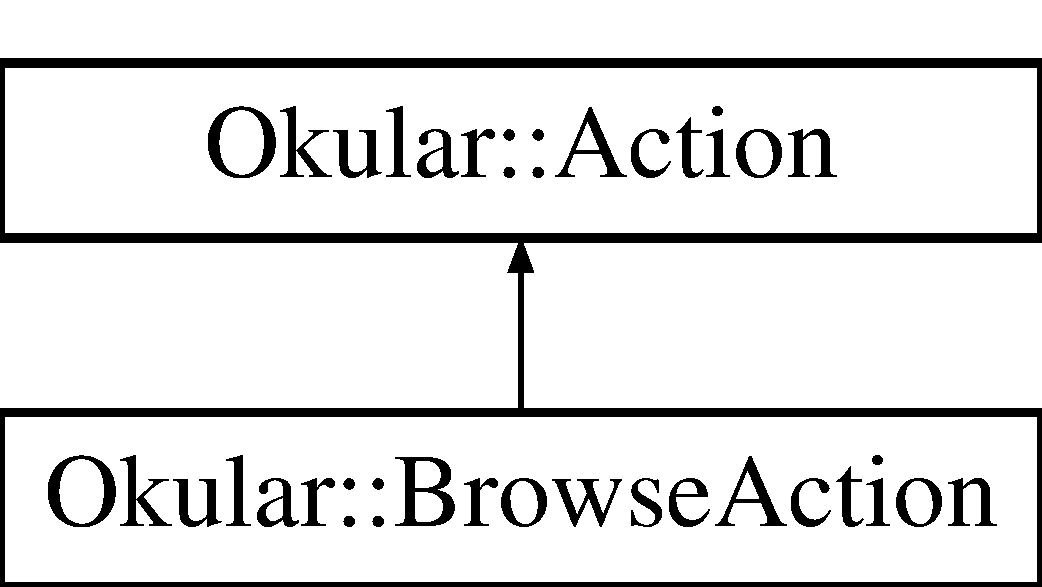
\includegraphics[height=2.000000cm]{classOkular_1_1BrowseAction}
\end{center}
\end{figure}
\subsection*{Public Member Functions}
\begin{DoxyCompactItemize}
\item 
\hyperlink{classOkular_1_1BrowseAction_a0b61bd5c2c4a9979cafe6b2c9444c8fc}{Browse\+Action} (const Q\+String \&\hyperlink{classOkular_1_1BrowseAction_a02dfb682ec078bd783e125696bd00964}{url})
\item 
virtual \hyperlink{classOkular_1_1BrowseAction_a48f8ef6e79f836f56a11c3345bb86fc9}{$\sim$\+Browse\+Action} ()
\item 
\hyperlink{classOkular_1_1Action_abe474735af30ea76105595533df9ec47}{Action\+Type} \hyperlink{classOkular_1_1BrowseAction_a253991762e61b486d0667dc1619b0f46}{action\+Type} () const 
\item 
Q\+String \hyperlink{classOkular_1_1BrowseAction_afcc99a984ec0687a4a1f40409d344481}{action\+Tip} () const 
\item 
Q\+String \hyperlink{classOkular_1_1BrowseAction_a02dfb682ec078bd783e125696bd00964}{url} () const 
\end{DoxyCompactItemize}
\subsection*{Additional Inherited Members}


\subsection{Detailed Description}
The Browse action browses an url by opening a web browser or email client, depedning on the url protocol (e.\+g. http, mailto, etc.). 

Definition at line 226 of file action.\+h.



\subsection{Constructor \& Destructor Documentation}
\hypertarget{classOkular_1_1BrowseAction_a0b61bd5c2c4a9979cafe6b2c9444c8fc}{\index{Okular\+::\+Browse\+Action@{Okular\+::\+Browse\+Action}!Browse\+Action@{Browse\+Action}}
\index{Browse\+Action@{Browse\+Action}!Okular\+::\+Browse\+Action@{Okular\+::\+Browse\+Action}}
\subsubsection[{Browse\+Action}]{\setlength{\rightskip}{0pt plus 5cm}Browse\+Action\+::\+Browse\+Action (
\begin{DoxyParamCaption}
\item[{const Q\+String \&}]{url}
\end{DoxyParamCaption}
)}}\label{classOkular_1_1BrowseAction_a0b61bd5c2c4a9979cafe6b2c9444c8fc}
Creates a new browse action.


\begin{DoxyParams}{Parameters}
{\em url} & The url to browse. \\
\hline
\end{DoxyParams}


Definition at line 193 of file action.\+cpp.


\begin{DoxyCode}
194     : \hyperlink{classOkular_1_1Action}{Action}( *\textcolor{keyword}{new} \hyperlink{classOkular_1_1BrowseActionPrivate}{BrowseActionPrivate}( \hyperlink{classOkular_1_1BrowseAction_a02dfb682ec078bd783e125696bd00964}{url} ) )
195 \{
196 \}
\end{DoxyCode}
\hypertarget{classOkular_1_1BrowseAction_a48f8ef6e79f836f56a11c3345bb86fc9}{\index{Okular\+::\+Browse\+Action@{Okular\+::\+Browse\+Action}!````~Browse\+Action@{$\sim$\+Browse\+Action}}
\index{````~Browse\+Action@{$\sim$\+Browse\+Action}!Okular\+::\+Browse\+Action@{Okular\+::\+Browse\+Action}}
\subsubsection[{$\sim$\+Browse\+Action}]{\setlength{\rightskip}{0pt plus 5cm}Browse\+Action\+::$\sim$\+Browse\+Action (
\begin{DoxyParamCaption}
{}
\end{DoxyParamCaption}
)\hspace{0.3cm}{\ttfamily [virtual]}}}\label{classOkular_1_1BrowseAction_a48f8ef6e79f836f56a11c3345bb86fc9}
Destroys the browse action. 

Definition at line 198 of file action.\+cpp.


\begin{DoxyCode}
199 \{
200 \}
\end{DoxyCode}


\subsection{Member Function Documentation}
\hypertarget{classOkular_1_1BrowseAction_afcc99a984ec0687a4a1f40409d344481}{\index{Okular\+::\+Browse\+Action@{Okular\+::\+Browse\+Action}!action\+Tip@{action\+Tip}}
\index{action\+Tip@{action\+Tip}!Okular\+::\+Browse\+Action@{Okular\+::\+Browse\+Action}}
\subsubsection[{action\+Tip}]{\setlength{\rightskip}{0pt plus 5cm}Q\+String Browse\+Action\+::action\+Tip (
\begin{DoxyParamCaption}
{}
\end{DoxyParamCaption}
) const\hspace{0.3cm}{\ttfamily [virtual]}}}\label{classOkular_1_1BrowseAction_afcc99a984ec0687a4a1f40409d344481}
Returns the action tip. 

Reimplemented from \hyperlink{classOkular_1_1Action_a359c33818281df712da697c84975952f}{Okular\+::\+Action}.



Definition at line 207 of file action.\+cpp.


\begin{DoxyCode}
208 \{
209     Q\_D( \textcolor{keyword}{const} \hyperlink{classOkular_1_1BrowseAction}{Okular::BrowseAction} );
210     QString source;
211     \textcolor{keywordtype}{int} row = 0, col = 0;
212     \textcolor{keywordflow}{if} ( \hyperlink{namespaceOkular_ad195b608d5b6294feba9a4b095185d23}{extractLilyPondSourceReference}( d->m\_url, &source, &row, &col ) )
213     \{
214         \textcolor{keywordflow}{return} \hyperlink{namespaceOkular_ae289fc26cd6cac6abaa2fc5e3418c234}{sourceReferenceToolTip}( source, row, col );
215     \}
216     \textcolor{keywordflow}{return} d->m\_url;
217 \}
\end{DoxyCode}
\hypertarget{classOkular_1_1BrowseAction_a253991762e61b486d0667dc1619b0f46}{\index{Okular\+::\+Browse\+Action@{Okular\+::\+Browse\+Action}!action\+Type@{action\+Type}}
\index{action\+Type@{action\+Type}!Okular\+::\+Browse\+Action@{Okular\+::\+Browse\+Action}}
\subsubsection[{action\+Type}]{\setlength{\rightskip}{0pt plus 5cm}{\bf Action\+::\+Action\+Type} Browse\+Action\+::action\+Type (
\begin{DoxyParamCaption}
{}
\end{DoxyParamCaption}
) const\hspace{0.3cm}{\ttfamily [virtual]}}}\label{classOkular_1_1BrowseAction_a253991762e61b486d0667dc1619b0f46}
Returns the action type. 

Implements \hyperlink{classOkular_1_1Action_ac4c2ef09b350b4041f8d1cfb261c3234}{Okular\+::\+Action}.



Definition at line 202 of file action.\+cpp.


\begin{DoxyCode}
203 \{
204     \textcolor{keywordflow}{return} \hyperlink{classOkular_1_1Action_abe474735af30ea76105595533df9ec47a7b94e3d79ff6813ba8444b1d98ca4756}{Browse};
205 \}
\end{DoxyCode}
\hypertarget{classOkular_1_1BrowseAction_a02dfb682ec078bd783e125696bd00964}{\index{Okular\+::\+Browse\+Action@{Okular\+::\+Browse\+Action}!url@{url}}
\index{url@{url}!Okular\+::\+Browse\+Action@{Okular\+::\+Browse\+Action}}
\subsubsection[{url}]{\setlength{\rightskip}{0pt plus 5cm}Q\+String Browse\+Action\+::url (
\begin{DoxyParamCaption}
{}
\end{DoxyParamCaption}
) const}}\label{classOkular_1_1BrowseAction_a02dfb682ec078bd783e125696bd00964}
Returns the url to browse. 

Definition at line 219 of file action.\+cpp.


\begin{DoxyCode}
220 \{
221     Q\_D( \textcolor{keyword}{const} \hyperlink{classOkular_1_1BrowseAction}{Okular::BrowseAction} );
222     \textcolor{keywordflow}{return} d->m\_url;
223 \}
\end{DoxyCode}


The documentation for this class was generated from the following files\+:\begin{DoxyCompactItemize}
\item 
core/\hyperlink{action_8h}{action.\+h}\item 
core/\hyperlink{action_8cpp}{action.\+cpp}\end{DoxyCompactItemize}

\hypertarget{classOkular_1_1BrowseActionPrivate}{\section{Okular\+:\+:Browse\+Action\+Private Class Reference}
\label{classOkular_1_1BrowseActionPrivate}\index{Okular\+::\+Browse\+Action\+Private@{Okular\+::\+Browse\+Action\+Private}}
}
Inheritance diagram for Okular\+:\+:Browse\+Action\+Private\+:\begin{figure}[H]
\begin{center}
\leavevmode
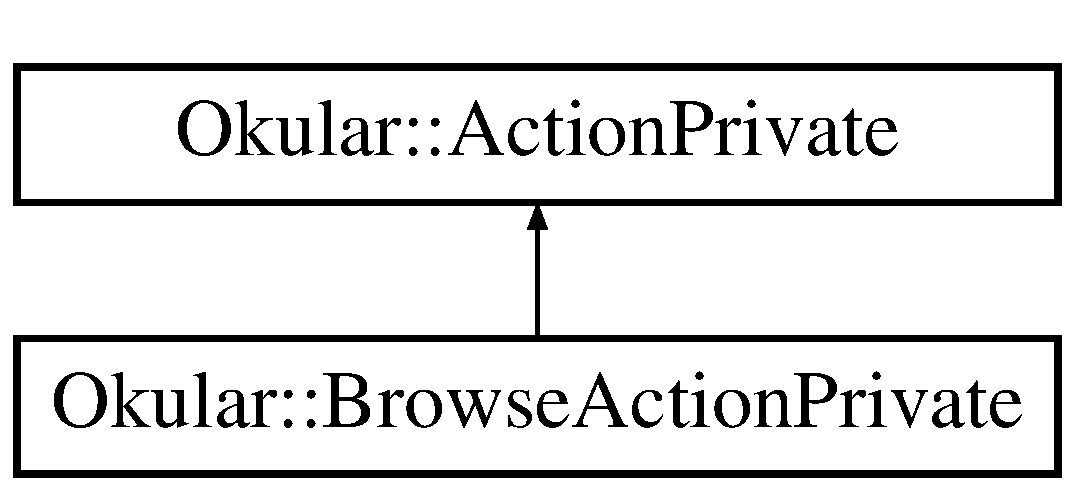
\includegraphics[height=2.000000cm]{classOkular_1_1BrowseActionPrivate}
\end{center}
\end{figure}
\subsection*{Public Member Functions}
\begin{DoxyCompactItemize}
\item 
\hyperlink{classOkular_1_1BrowseActionPrivate_addf8c6ccf5739ebe6d60b524b2a3e11c}{Browse\+Action\+Private} (const Q\+String \&url)
\end{DoxyCompactItemize}
\subsection*{Public Attributes}
\begin{DoxyCompactItemize}
\item 
Q\+String \hyperlink{classOkular_1_1BrowseActionPrivate_aa216b4a85b5dc7bcb4a89e3553e7a001}{m\+\_\+url}
\end{DoxyCompactItemize}


\subsection{Detailed Description}


Definition at line 182 of file action.\+cpp.



\subsection{Constructor \& Destructor Documentation}
\hypertarget{classOkular_1_1BrowseActionPrivate_addf8c6ccf5739ebe6d60b524b2a3e11c}{\index{Okular\+::\+Browse\+Action\+Private@{Okular\+::\+Browse\+Action\+Private}!Browse\+Action\+Private@{Browse\+Action\+Private}}
\index{Browse\+Action\+Private@{Browse\+Action\+Private}!Okular\+::\+Browse\+Action\+Private@{Okular\+::\+Browse\+Action\+Private}}
\subsubsection[{Browse\+Action\+Private}]{\setlength{\rightskip}{0pt plus 5cm}Okular\+::\+Browse\+Action\+Private\+::\+Browse\+Action\+Private (
\begin{DoxyParamCaption}
\item[{const Q\+String \&}]{url}
\end{DoxyParamCaption}
)\hspace{0.3cm}{\ttfamily [inline]}}}\label{classOkular_1_1BrowseActionPrivate_addf8c6ccf5739ebe6d60b524b2a3e11c}


Definition at line 185 of file action.\+cpp.


\begin{DoxyCode}
186             : \hyperlink{classOkular_1_1ActionPrivate_ade22b7b9b9f6490b2fce5b928235ef5b}{ActionPrivate}(), \hyperlink{classOkular_1_1BrowseActionPrivate_aa216b4a85b5dc7bcb4a89e3553e7a001}{m\_url}( url )
187         \{
188         \}
\end{DoxyCode}


\subsection{Member Data Documentation}
\hypertarget{classOkular_1_1BrowseActionPrivate_aa216b4a85b5dc7bcb4a89e3553e7a001}{\index{Okular\+::\+Browse\+Action\+Private@{Okular\+::\+Browse\+Action\+Private}!m\+\_\+url@{m\+\_\+url}}
\index{m\+\_\+url@{m\+\_\+url}!Okular\+::\+Browse\+Action\+Private@{Okular\+::\+Browse\+Action\+Private}}
\subsubsection[{m\+\_\+url}]{\setlength{\rightskip}{0pt plus 5cm}Q\+String Okular\+::\+Browse\+Action\+Private\+::m\+\_\+url}}\label{classOkular_1_1BrowseActionPrivate_aa216b4a85b5dc7bcb4a89e3553e7a001}


Definition at line 190 of file action.\+cpp.



The documentation for this class was generated from the following file\+:\begin{DoxyCompactItemize}
\item 
core/\hyperlink{action_8cpp}{action.\+cpp}\end{DoxyCompactItemize}

\hypertarget{structKParts_1_1BrowserArguments}{\section{\-K\-Parts\-:\-:\-Browser\-Arguments \-Struct \-Reference}
\label{structKParts_1_1BrowserArguments}\index{\-K\-Parts\-::\-Browser\-Arguments@{\-K\-Parts\-::\-Browser\-Arguments}}
}


{\ttfamily \#include $<$browserextension.\-h$>$}

\subsection*{\-Public \-Member \-Functions}
\begin{DoxyCompactItemize}
\item 
\hyperlink{structKParts_1_1BrowserArguments_a87b08664fe9d6dc90631f4a7c0d4a871}{\-Browser\-Arguments} ()
\item 
\hyperlink{structKParts_1_1BrowserArguments_a1a9790044d682d0346c03f9468d31aa5}{\-Browser\-Arguments} (const \hyperlink{structKParts_1_1BrowserArguments}{\-Browser\-Arguments} \&args)
\item 
\hyperlink{structKParts_1_1BrowserArguments}{\-Browser\-Arguments} \& \hyperlink{structKParts_1_1BrowserArguments_acd0d51024957675a322c5120ab8a9b89}{operator=} (const \hyperlink{structKParts_1_1BrowserArguments}{\-Browser\-Arguments} \&args)
\item 
virtual \hyperlink{structKParts_1_1BrowserArguments_a1f558d1e3fc7441f86346e82f4e6fcaf}{$\sim$\-Browser\-Arguments} ()
\item 
void \hyperlink{structKParts_1_1BrowserArguments_aa2a3384e7711f1a6fc6b710852d11bc4}{set\-Content\-Type} (const \-Q\-String \&\hyperlink{structKParts_1_1BrowserArguments_a11198af20bc7c8b9f5c165ed0ba1401b}{content\-Type})
\item 
\-Q\-String \hyperlink{structKParts_1_1BrowserArguments_a11198af20bc7c8b9f5c165ed0ba1401b}{content\-Type} () const 
\item 
void \hyperlink{structKParts_1_1BrowserArguments_a7c934a91eddfd3ddfb9e1fe0f4eace9f}{set\-Do\-Post} (bool enable)
\item 
bool \hyperlink{structKParts_1_1BrowserArguments_a8470520e769024497a32293e36bdd92f}{do\-Post} () const 
\item 
void \hyperlink{structKParts_1_1BrowserArguments_ad4ad5d94380a0548c5d3e53368f6f1f5}{set\-Lock\-History} (bool lock)
\item 
bool \hyperlink{structKParts_1_1BrowserArguments_a5292374726fba2faee5f9b44acd67c70}{lock\-History} () const 
\item 
void \hyperlink{structKParts_1_1BrowserArguments_a17bbf30d75c3e5c4d906b91b1c8eed3b}{set\-New\-Tab} (bool \hyperlink{structKParts_1_1BrowserArguments_acdc75a4b3726424aabb4958d58b6e586}{new\-Tab})
\item 
bool \hyperlink{structKParts_1_1BrowserArguments_acdc75a4b3726424aabb4958d58b6e586}{new\-Tab} () const 
\item 
bool \hyperlink{structKParts_1_1BrowserArguments_a3a3c15968b056a76248f483ea613740a}{redirected\-Request} () const 
\item 
void \hyperlink{structKParts_1_1BrowserArguments_a7169bd696dd783e0312f7bf220884e0e}{set\-Redirected\-Request} (bool redirected)
\item 
void \hyperlink{structKParts_1_1BrowserArguments_a0a0f93b431d62e60a9bb411f97be0126}{set\-Forces\-New\-Window} (bool \hyperlink{structKParts_1_1BrowserArguments_add9a79530ee4c265e8e37493d94f1f08}{forces\-New\-Window})
\item 
bool \hyperlink{structKParts_1_1BrowserArguments_add9a79530ee4c265e8e37493d94f1f08}{forces\-New\-Window} () const 
\end{DoxyCompactItemize}
\subsection*{\-Public \-Attributes}
\begin{DoxyCompactItemize}
\item 
\-Q\-String\-List \hyperlink{structKParts_1_1BrowserArguments_a76aed0d1e923b73db918038d23f524ec}{doc\-State}
\item 
bool \hyperlink{structKParts_1_1BrowserArguments_af06b08da058cd6fc19ad42e2904e2594}{soft\-Reload}
\item 
\-Q\-Byte\-Array \hyperlink{structKParts_1_1BrowserArguments_a9c1fb6cb602a10fec4ca05a25f1b9ac6}{post\-Data}
\item 
\-Q\-String \hyperlink{structKParts_1_1BrowserArguments_ad8b767db0ac78790860f4f0cbef64ea2}{frame\-Name}
\item 
bool \hyperlink{structKParts_1_1BrowserArguments_aa9e31eabaee6af2692319d21721fc9cb}{trusted\-Source}
\end{DoxyCompactItemize}


\subsection{\-Detailed \-Description}
\hyperlink{structKParts_1_1BrowserArguments}{\-Browser\-Arguments} is a set of web-\/browsing-\/specific arguments, which allow specifying how a \-U\-R\-L should be opened by open\-Url() (as a complement to \hyperlink{classKParts_1_1OpenUrlArguments}{\-K\-Parts\-::\-Open\-Url\-Arguments} which are the non-\/web-\/specific arguments)

\-The arguments remain stored in the browser extension after that, and can be used for instance to jump to the x\-Offset/y\-Offset position once the url has finished loading.

\-The parts (with a browser extension) who care about urlargs will use those arguments, others will ignore them.

\-This can also be used the other way round, when a part asks for a \-U\-R\-L to be opened (with open\-Url\-Request or create\-New\-Window). 

\-Definition at line 64 of file browserextension.\-h.



\subsection{\-Constructor \& \-Destructor \-Documentation}
\hypertarget{structKParts_1_1BrowserArguments_a87b08664fe9d6dc90631f4a7c0d4a871}{\index{\-K\-Parts\-::\-Browser\-Arguments@{\-K\-Parts\-::\-Browser\-Arguments}!\-Browser\-Arguments@{\-Browser\-Arguments}}
\index{\-Browser\-Arguments@{\-Browser\-Arguments}!KParts::BrowserArguments@{\-K\-Parts\-::\-Browser\-Arguments}}
\subsubsection[{\-Browser\-Arguments}]{\setlength{\rightskip}{0pt plus 5cm}{\bf \-K\-Parts\-::\-Browser\-Arguments\-::\-Browser\-Arguments} (
\begin{DoxyParamCaption}
{}
\end{DoxyParamCaption}
)}}\label{structKParts_1_1BrowserArguments_a87b08664fe9d6dc90631f4a7c0d4a871}
\hypertarget{structKParts_1_1BrowserArguments_a1a9790044d682d0346c03f9468d31aa5}{\index{\-K\-Parts\-::\-Browser\-Arguments@{\-K\-Parts\-::\-Browser\-Arguments}!\-Browser\-Arguments@{\-Browser\-Arguments}}
\index{\-Browser\-Arguments@{\-Browser\-Arguments}!KParts::BrowserArguments@{\-K\-Parts\-::\-Browser\-Arguments}}
\subsubsection[{\-Browser\-Arguments}]{\setlength{\rightskip}{0pt plus 5cm}{\bf \-K\-Parts\-::\-Browser\-Arguments\-::\-Browser\-Arguments} (
\begin{DoxyParamCaption}
\item[{const {\bf \-Browser\-Arguments} \&}]{args}
\end{DoxyParamCaption}
)}}\label{structKParts_1_1BrowserArguments_a1a9790044d682d0346c03f9468d31aa5}
\hypertarget{structKParts_1_1BrowserArguments_a1f558d1e3fc7441f86346e82f4e6fcaf}{\index{\-K\-Parts\-::\-Browser\-Arguments@{\-K\-Parts\-::\-Browser\-Arguments}!$\sim$\-Browser\-Arguments@{$\sim$\-Browser\-Arguments}}
\index{$\sim$\-Browser\-Arguments@{$\sim$\-Browser\-Arguments}!KParts::BrowserArguments@{\-K\-Parts\-::\-Browser\-Arguments}}
\subsubsection[{$\sim$\-Browser\-Arguments}]{\setlength{\rightskip}{0pt plus 5cm}virtual {\bf \-K\-Parts\-::\-Browser\-Arguments\-::$\sim$\-Browser\-Arguments} (
\begin{DoxyParamCaption}
{}
\end{DoxyParamCaption}
)\hspace{0.3cm}{\ttfamily  \mbox{[}virtual\mbox{]}}}}\label{structKParts_1_1BrowserArguments_a1f558d1e3fc7441f86346e82f4e6fcaf}


\subsection{\-Member \-Function \-Documentation}
\hypertarget{structKParts_1_1BrowserArguments_a11198af20bc7c8b9f5c165ed0ba1401b}{\index{\-K\-Parts\-::\-Browser\-Arguments@{\-K\-Parts\-::\-Browser\-Arguments}!content\-Type@{content\-Type}}
\index{content\-Type@{content\-Type}!KParts::BrowserArguments@{\-K\-Parts\-::\-Browser\-Arguments}}
\subsubsection[{content\-Type}]{\setlength{\rightskip}{0pt plus 5cm}\-Q\-String {\bf \-K\-Parts\-::\-Browser\-Arguments\-::content\-Type} (
\begin{DoxyParamCaption}
{}
\end{DoxyParamCaption}
) const}}\label{structKParts_1_1BrowserArguments_a11198af20bc7c8b9f5c165ed0ba1401b}
\-K\-H\-T\-M\-L-\/specific field, header defining the type of the \-P\-O\-S\-T data. \hypertarget{structKParts_1_1BrowserArguments_a8470520e769024497a32293e36bdd92f}{\index{\-K\-Parts\-::\-Browser\-Arguments@{\-K\-Parts\-::\-Browser\-Arguments}!do\-Post@{do\-Post}}
\index{do\-Post@{do\-Post}!KParts::BrowserArguments@{\-K\-Parts\-::\-Browser\-Arguments}}
\subsubsection[{do\-Post}]{\setlength{\rightskip}{0pt plus 5cm}bool {\bf \-K\-Parts\-::\-Browser\-Arguments\-::do\-Post} (
\begin{DoxyParamCaption}
{}
\end{DoxyParamCaption}
) const}}\label{structKParts_1_1BrowserArguments_a8470520e769024497a32293e36bdd92f}
\-K\-H\-T\-M\-L-\/specific field, whether to do a \-P\-O\-S\-T instead of a \-G\-E\-T, for the next open\-U\-R\-L. \hypertarget{structKParts_1_1BrowserArguments_add9a79530ee4c265e8e37493d94f1f08}{\index{\-K\-Parts\-::\-Browser\-Arguments@{\-K\-Parts\-::\-Browser\-Arguments}!forces\-New\-Window@{forces\-New\-Window}}
\index{forces\-New\-Window@{forces\-New\-Window}!KParts::BrowserArguments@{\-K\-Parts\-::\-Browser\-Arguments}}
\subsubsection[{forces\-New\-Window}]{\setlength{\rightskip}{0pt plus 5cm}bool {\bf \-K\-Parts\-::\-Browser\-Arguments\-::forces\-New\-Window} (
\begin{DoxyParamCaption}
{}
\end{DoxyParamCaption}
) const}}\label{structKParts_1_1BrowserArguments_add9a79530ee4c265e8e37493d94f1f08}
\-Whether the \-U\-R\-L specifies to be opened in a new window \hypertarget{structKParts_1_1BrowserArguments_a5292374726fba2faee5f9b44acd67c70}{\index{\-K\-Parts\-::\-Browser\-Arguments@{\-K\-Parts\-::\-Browser\-Arguments}!lock\-History@{lock\-History}}
\index{lock\-History@{lock\-History}!KParts::BrowserArguments@{\-K\-Parts\-::\-Browser\-Arguments}}
\subsubsection[{lock\-History}]{\setlength{\rightskip}{0pt plus 5cm}bool {\bf \-K\-Parts\-::\-Browser\-Arguments\-::lock\-History} (
\begin{DoxyParamCaption}
{}
\end{DoxyParamCaption}
) const}}\label{structKParts_1_1BrowserArguments_a5292374726fba2faee5f9b44acd67c70}
\hypertarget{structKParts_1_1BrowserArguments_acdc75a4b3726424aabb4958d58b6e586}{\index{\-K\-Parts\-::\-Browser\-Arguments@{\-K\-Parts\-::\-Browser\-Arguments}!new\-Tab@{new\-Tab}}
\index{new\-Tab@{new\-Tab}!KParts::BrowserArguments@{\-K\-Parts\-::\-Browser\-Arguments}}
\subsubsection[{new\-Tab}]{\setlength{\rightskip}{0pt plus 5cm}bool {\bf \-K\-Parts\-::\-Browser\-Arguments\-::new\-Tab} (
\begin{DoxyParamCaption}
{}
\end{DoxyParamCaption}
) const}}\label{structKParts_1_1BrowserArguments_acdc75a4b3726424aabb4958d58b6e586}
\hypertarget{structKParts_1_1BrowserArguments_acd0d51024957675a322c5120ab8a9b89}{\index{\-K\-Parts\-::\-Browser\-Arguments@{\-K\-Parts\-::\-Browser\-Arguments}!operator=@{operator=}}
\index{operator=@{operator=}!KParts::BrowserArguments@{\-K\-Parts\-::\-Browser\-Arguments}}
\subsubsection[{operator=}]{\setlength{\rightskip}{0pt plus 5cm}{\bf \-Browser\-Arguments}\& \-K\-Parts\-::\-Browser\-Arguments\-::operator= (
\begin{DoxyParamCaption}
\item[{const {\bf \-Browser\-Arguments} \&}]{args}
\end{DoxyParamCaption}
)}}\label{structKParts_1_1BrowserArguments_acd0d51024957675a322c5120ab8a9b89}
\hypertarget{structKParts_1_1BrowserArguments_a3a3c15968b056a76248f483ea613740a}{\index{\-K\-Parts\-::\-Browser\-Arguments@{\-K\-Parts\-::\-Browser\-Arguments}!redirected\-Request@{redirected\-Request}}
\index{redirected\-Request@{redirected\-Request}!KParts::BrowserArguments@{\-K\-Parts\-::\-Browser\-Arguments}}
\subsubsection[{redirected\-Request}]{\setlength{\rightskip}{0pt plus 5cm}bool {\bf \-K\-Parts\-::\-Browser\-Arguments\-::redirected\-Request} (
\begin{DoxyParamCaption}
{}
\end{DoxyParamCaption}
) const}}\label{structKParts_1_1BrowserArguments_a3a3c15968b056a76248f483ea613740a}
\begin{DoxyReturn}{\-Returns}
true if the request was a result of a \-M\-E\-T\-A refresh/redirect request or \-H\-T\-T\-P redirect. 
\end{DoxyReturn}
\hypertarget{structKParts_1_1BrowserArguments_aa2a3384e7711f1a6fc6b710852d11bc4}{\index{\-K\-Parts\-::\-Browser\-Arguments@{\-K\-Parts\-::\-Browser\-Arguments}!set\-Content\-Type@{set\-Content\-Type}}
\index{set\-Content\-Type@{set\-Content\-Type}!KParts::BrowserArguments@{\-K\-Parts\-::\-Browser\-Arguments}}
\subsubsection[{set\-Content\-Type}]{\setlength{\rightskip}{0pt plus 5cm}void {\bf \-K\-Parts\-::\-Browser\-Arguments\-::set\-Content\-Type} (
\begin{DoxyParamCaption}
\item[{const \-Q\-String \&}]{content\-Type}
\end{DoxyParamCaption}
)}}\label{structKParts_1_1BrowserArguments_aa2a3384e7711f1a6fc6b710852d11bc4}
\-K\-H\-T\-M\-L-\/specific field, header defining the type of the \-P\-O\-S\-T data. \hypertarget{structKParts_1_1BrowserArguments_a7c934a91eddfd3ddfb9e1fe0f4eace9f}{\index{\-K\-Parts\-::\-Browser\-Arguments@{\-K\-Parts\-::\-Browser\-Arguments}!set\-Do\-Post@{set\-Do\-Post}}
\index{set\-Do\-Post@{set\-Do\-Post}!KParts::BrowserArguments@{\-K\-Parts\-::\-Browser\-Arguments}}
\subsubsection[{set\-Do\-Post}]{\setlength{\rightskip}{0pt plus 5cm}void {\bf \-K\-Parts\-::\-Browser\-Arguments\-::set\-Do\-Post} (
\begin{DoxyParamCaption}
\item[{bool}]{enable}
\end{DoxyParamCaption}
)}}\label{structKParts_1_1BrowserArguments_a7c934a91eddfd3ddfb9e1fe0f4eace9f}
\-K\-H\-T\-M\-L-\/specific field, whether to do a \-P\-O\-S\-T instead of a \-G\-E\-T, for the next open\-U\-R\-L. \hypertarget{structKParts_1_1BrowserArguments_a0a0f93b431d62e60a9bb411f97be0126}{\index{\-K\-Parts\-::\-Browser\-Arguments@{\-K\-Parts\-::\-Browser\-Arguments}!set\-Forces\-New\-Window@{set\-Forces\-New\-Window}}
\index{set\-Forces\-New\-Window@{set\-Forces\-New\-Window}!KParts::BrowserArguments@{\-K\-Parts\-::\-Browser\-Arguments}}
\subsubsection[{set\-Forces\-New\-Window}]{\setlength{\rightskip}{0pt plus 5cm}void {\bf \-K\-Parts\-::\-Browser\-Arguments\-::set\-Forces\-New\-Window} (
\begin{DoxyParamCaption}
\item[{bool}]{forces\-New\-Window}
\end{DoxyParamCaption}
)}}\label{structKParts_1_1BrowserArguments_a0a0f93b431d62e60a9bb411f97be0126}
\-Set whether the \-U\-R\-L specifies to be opened in a new window.

\-When open\-Url\-Request is emitted\-: 
\begin{DoxyItemize}
\item normally the url would be opened in the current view. 
\item set\-Forces\-New\-Window(true) specifies that a new window or tab should be used\-: set\-New\-Tab(true) requests a tab specifically, otherwise the user-\/preference is followed. \-This is typically used for target=\char`\"{}\-\_\-blank\char`\"{} in web browsers. 
\end{DoxyItemize}

\-When create\-New\-Window is emitted\-: 
\begin{DoxyItemize}
\item if set\-New\-Tab(true) was called, a tab is created. 
\item otherwise, if set\-Forces\-New\-Window(true) was called, a window is created. 
\item otherwise the user preference is followed. 
\end{DoxyItemize}\hypertarget{structKParts_1_1BrowserArguments_ad4ad5d94380a0548c5d3e53368f6f1f5}{\index{\-K\-Parts\-::\-Browser\-Arguments@{\-K\-Parts\-::\-Browser\-Arguments}!set\-Lock\-History@{set\-Lock\-History}}
\index{set\-Lock\-History@{set\-Lock\-History}!KParts::BrowserArguments@{\-K\-Parts\-::\-Browser\-Arguments}}
\subsubsection[{set\-Lock\-History}]{\setlength{\rightskip}{0pt plus 5cm}void {\bf \-K\-Parts\-::\-Browser\-Arguments\-::set\-Lock\-History} (
\begin{DoxyParamCaption}
\item[{bool}]{lock}
\end{DoxyParamCaption}
)}}\label{structKParts_1_1BrowserArguments_ad4ad5d94380a0548c5d3e53368f6f1f5}
\-Whether to lock the history when opening the next \-U\-R\-L. \-This is used during e.\-g. a redirection, to avoid a new entry in the history. \hypertarget{structKParts_1_1BrowserArguments_a17bbf30d75c3e5c4d906b91b1c8eed3b}{\index{\-K\-Parts\-::\-Browser\-Arguments@{\-K\-Parts\-::\-Browser\-Arguments}!set\-New\-Tab@{set\-New\-Tab}}
\index{set\-New\-Tab@{set\-New\-Tab}!KParts::BrowserArguments@{\-K\-Parts\-::\-Browser\-Arguments}}
\subsubsection[{set\-New\-Tab}]{\setlength{\rightskip}{0pt plus 5cm}void {\bf \-K\-Parts\-::\-Browser\-Arguments\-::set\-New\-Tab} (
\begin{DoxyParamCaption}
\item[{bool}]{new\-Tab}
\end{DoxyParamCaption}
)}}\label{structKParts_1_1BrowserArguments_a17bbf30d75c3e5c4d906b91b1c8eed3b}
\-Whether the \-U\-R\-L should be opened in a new tab instead in a new window. \hypertarget{structKParts_1_1BrowserArguments_a7169bd696dd783e0312f7bf220884e0e}{\index{\-K\-Parts\-::\-Browser\-Arguments@{\-K\-Parts\-::\-Browser\-Arguments}!set\-Redirected\-Request@{set\-Redirected\-Request}}
\index{set\-Redirected\-Request@{set\-Redirected\-Request}!KParts::BrowserArguments@{\-K\-Parts\-::\-Browser\-Arguments}}
\subsubsection[{set\-Redirected\-Request}]{\setlength{\rightskip}{0pt plus 5cm}void {\bf \-K\-Parts\-::\-Browser\-Arguments\-::set\-Redirected\-Request} (
\begin{DoxyParamCaption}
\item[{bool}]{redirected}
\end{DoxyParamCaption}
)}}\label{structKParts_1_1BrowserArguments_a7169bd696dd783e0312f7bf220884e0e}
\-Set the redirect flag to indicate \-U\-R\-L is a result of either a \-M\-E\-T\-A redirect or \-H\-T\-T\-P redirect.


\begin{DoxyParams}{\-Parameters}
{\em redirected} & \\
\hline
\end{DoxyParams}


\subsection{\-Member \-Data \-Documentation}
\hypertarget{structKParts_1_1BrowserArguments_a76aed0d1e923b73db918038d23f524ec}{\index{\-K\-Parts\-::\-Browser\-Arguments@{\-K\-Parts\-::\-Browser\-Arguments}!doc\-State@{doc\-State}}
\index{doc\-State@{doc\-State}!KParts::BrowserArguments@{\-K\-Parts\-::\-Browser\-Arguments}}
\subsubsection[{doc\-State}]{\setlength{\rightskip}{0pt plus 5cm}\-Q\-String\-List {\bf \-K\-Parts\-::\-Browser\-Arguments\-::doc\-State}}}\label{structKParts_1_1BrowserArguments_a76aed0d1e923b73db918038d23f524ec}
\-This buffer can be used by the part to save and restore its contents. \-See \-K\-H\-T\-M\-L\-Part for instance. 

\-Definition at line 81 of file browserextension.\-h.

\hypertarget{structKParts_1_1BrowserArguments_ad8b767db0ac78790860f4f0cbef64ea2}{\index{\-K\-Parts\-::\-Browser\-Arguments@{\-K\-Parts\-::\-Browser\-Arguments}!frame\-Name@{frame\-Name}}
\index{frame\-Name@{frame\-Name}!KParts::BrowserArguments@{\-K\-Parts\-::\-Browser\-Arguments}}
\subsubsection[{frame\-Name}]{\setlength{\rightskip}{0pt plus 5cm}\-Q\-String {\bf \-K\-Parts\-::\-Browser\-Arguments\-::frame\-Name}}}\label{structKParts_1_1BrowserArguments_ad8b767db0ac78790860f4f0cbef64ea2}
\-The frame in which to open the \-U\-R\-L. \-K\-H\-T\-M\-L/\-Konqueror-\/specific. 

\-Definition at line 133 of file browserextension.\-h.

\hypertarget{structKParts_1_1BrowserArguments_a9c1fb6cb602a10fec4ca05a25f1b9ac6}{\index{\-K\-Parts\-::\-Browser\-Arguments@{\-K\-Parts\-::\-Browser\-Arguments}!post\-Data@{post\-Data}}
\index{post\-Data@{post\-Data}!KParts::BrowserArguments@{\-K\-Parts\-::\-Browser\-Arguments}}
\subsubsection[{post\-Data}]{\setlength{\rightskip}{0pt plus 5cm}\-Q\-Byte\-Array {\bf \-K\-Parts\-::\-Browser\-Arguments\-::post\-Data}}}\label{structKParts_1_1BrowserArguments_a9c1fb6cb602a10fec4ca05a25f1b9ac6}
\-K\-H\-T\-M\-L-\/specific field, contents of the \-H\-T\-T\-P \-P\-O\-S\-T data. 

\-Definition at line 94 of file browserextension.\-h.

\hypertarget{structKParts_1_1BrowserArguments_af06b08da058cd6fc19ad42e2904e2594}{\index{\-K\-Parts\-::\-Browser\-Arguments@{\-K\-Parts\-::\-Browser\-Arguments}!soft\-Reload@{soft\-Reload}}
\index{soft\-Reload@{soft\-Reload}!KParts::BrowserArguments@{\-K\-Parts\-::\-Browser\-Arguments}}
\subsubsection[{soft\-Reload}]{\setlength{\rightskip}{0pt plus 5cm}bool {\bf \-K\-Parts\-::\-Browser\-Arguments\-::soft\-Reload}}}\label{structKParts_1_1BrowserArguments_af06b08da058cd6fc19ad42e2904e2594}
{\ttfamily soft\-Reload} is set when user just hits reload button. \-It's used currently for two different frameset reload strategies. \-In case of soft reload individual frames are reloaded instead of reloading whole frameset. 

\-Definition at line 89 of file browserextension.\-h.

\hypertarget{structKParts_1_1BrowserArguments_aa9e31eabaee6af2692319d21721fc9cb}{\index{\-K\-Parts\-::\-Browser\-Arguments@{\-K\-Parts\-::\-Browser\-Arguments}!trusted\-Source@{trusted\-Source}}
\index{trusted\-Source@{trusted\-Source}!KParts::BrowserArguments@{\-K\-Parts\-::\-Browser\-Arguments}}
\subsubsection[{trusted\-Source}]{\setlength{\rightskip}{0pt plus 5cm}bool {\bf \-K\-Parts\-::\-Browser\-Arguments\-::trusted\-Source}}}\label{structKParts_1_1BrowserArguments_aa9e31eabaee6af2692319d21721fc9cb}
\-If true, the part who asks for a \-U\-R\-L to be opened can be 'trusted' to execute applications. \-For instance, the directory views can be 'trusted' whereas \-H\-T\-M\-L pages are not trusted in that respect. 

\-Definition at line 140 of file browserextension.\-h.



\-The documentation for this struct was generated from the following file\-:\begin{DoxyCompactItemize}
\item 
/usr/include/kparts/\hyperlink{browserextension_8h}{browserextension.\-h}\end{DoxyCompactItemize}

\hypertarget{classKParts_1_1BrowserExtension}{\section{\-K\-Parts\-:\-:\-Browser\-Extension \-Class \-Reference}
\label{classKParts_1_1BrowserExtension}\index{\-K\-Parts\-::\-Browser\-Extension@{\-K\-Parts\-::\-Browser\-Extension}}
}


{\ttfamily \#include $<$browserextension.\-h$>$}

\subsection*{\-Public \-Types}
\begin{DoxyCompactItemize}
\item 
enum \hyperlink{classKParts_1_1BrowserExtension_ae5b9acf92e7d83faf5142597371ef1e3}{\-Popup\-Flag} \{ \*
\hyperlink{classKParts_1_1BrowserExtension_ae5b9acf92e7d83faf5142597371ef1e3a59ee58fca9e8b900d617c4f232b497f7}{\-Default\-Popup\-Items} = 0x0000, 
\hyperlink{classKParts_1_1BrowserExtension_ae5b9acf92e7d83faf5142597371ef1e3a05faf3d46fca9da3a396d72c993eec5c}{\-Show\-Navigation\-Items} = 0x0001, 
\hyperlink{classKParts_1_1BrowserExtension_ae5b9acf92e7d83faf5142597371ef1e3af6030e3884ded53eace393f2af510c68}{\-Show\-Up} = 0x0002, 
\hyperlink{classKParts_1_1BrowserExtension_ae5b9acf92e7d83faf5142597371ef1e3a97cbb12bbef8ef52b233c24d0bf3e41e}{\-Show\-Reload} = 0x0004, 
\*
\hyperlink{classKParts_1_1BrowserExtension_ae5b9acf92e7d83faf5142597371ef1e3ac6c783f725ac9fe594d0b563495feb64}{\-Show\-Bookmark} = 0x0008, 
\hyperlink{classKParts_1_1BrowserExtension_ae5b9acf92e7d83faf5142597371ef1e3a152988520c15f75baddf48de43c9092a}{\-Show\-Create\-Directory} = 0x0010, 
\hyperlink{classKParts_1_1BrowserExtension_ae5b9acf92e7d83faf5142597371ef1e3a947c452c66b8c500ac2ce303451d68c4}{\-Show\-Text\-Selection\-Items} = 0x0020, 
\hyperlink{classKParts_1_1BrowserExtension_ae5b9acf92e7d83faf5142597371ef1e3a2332ecaf86d9179ba1ba92b9b3b10463}{\-No\-Deletion} = 0x0040, 
\*
\hyperlink{classKParts_1_1BrowserExtension_ae5b9acf92e7d83faf5142597371ef1e3a0521ef0fcccfba841ae8c5ae373f8976}{\-Is\-Link} = 0x0080, 
\hyperlink{classKParts_1_1BrowserExtension_ae5b9acf92e7d83faf5142597371ef1e3a40232b7894e5aa48029559354b84aeb5}{\-Show\-Url\-Operations} = 0x0100, 
\hyperlink{classKParts_1_1BrowserExtension_ae5b9acf92e7d83faf5142597371ef1e3a12a41a796fe0be4f8411259b7a77920d}{\-Show\-Properties} = 0x200
 \}
\item 
typedef \-Q\-Map$<$ \-Q\-Byte\-Array, \*
\-Q\-Byte\-Array $>$ \hyperlink{classKParts_1_1BrowserExtension_ac931bbd8189a4386b609180b5e704344}{\-Action\-Slot\-Map}
\item 
typedef \-Q\-Map$<$ \-Q\-String, \-Q\-List\*
$<$ \-Q\-Action $\ast$ $>$ $>$ \hyperlink{classKParts_1_1BrowserExtension_a73ab162c395443c0227946524a8ee04c}{\-Action\-Group\-Map}
\item 
typedef \-Q\-Map$<$ \-Q\-Byte\-Array, int $>$ \hyperlink{classKParts_1_1BrowserExtension_a71369db13dead055035067d4f8ff498d}{\-Action\-Number\-Map}
\end{DoxyCompactItemize}
\subsection*{\-Public \-Member \-Functions}
\begin{DoxyCompactItemize}
\item 
\hyperlink{classKParts_1_1BrowserExtension_acd4e7ef6cc706f7d65e82563085c1e31}{\-Browser\-Extension} (\hyperlink{classKParts_1_1ReadOnlyPart}{\-K\-Parts\-::\-Read\-Only\-Part} $\ast$parent)
\item 
virtual \hyperlink{classKParts_1_1BrowserExtension_a6a953bf6ca91db1779fdd5d52e5f5b0d}{$\sim$\-Browser\-Extension} ()
\item 
virtual void \hyperlink{classKParts_1_1BrowserExtension_a19637ad8f74585047a4477506db764bd}{set\-Browser\-Arguments} (const \hyperlink{structKParts_1_1BrowserArguments}{\-Browser\-Arguments} \&args)
\item 
\hyperlink{structKParts_1_1BrowserArguments}{\-Browser\-Arguments} \hyperlink{classKParts_1_1BrowserExtension_a8bd50c2c5bd6b43d15c4af157977cc42}{browser\-Arguments} () const 
\item 
virtual int \hyperlink{classKParts_1_1BrowserExtension_a8c8b975e3805b54a32e28c1a1b66319a}{x\-Offset} ()
\item 
virtual int \hyperlink{classKParts_1_1BrowserExtension_a205e59060b7b7d6daf1c25bf9cfdcee5}{y\-Offset} ()
\item 
virtual void \hyperlink{classKParts_1_1BrowserExtension_afe2fe963a5097ad43bea5d076485e759}{save\-State} (\-Q\-Data\-Stream \&stream)
\item 
virtual void \hyperlink{classKParts_1_1BrowserExtension_a26bba6343df8031d9aceb94cf6c6ef47}{restore\-State} (\-Q\-Data\-Stream \&stream)
\item 
bool \hyperlink{classKParts_1_1BrowserExtension_ad28ffe47eb30efa2dde7ba4b5684570e}{is\-U\-R\-L\-Drop\-Handling\-Enabled} () const 
\item 
void \hyperlink{classKParts_1_1BrowserExtension_a16e798977df4a2992e0f60a9dc01d33f}{set\-U\-R\-L\-Drop\-Handling\-Enabled} (bool enable)
\item 
void \hyperlink{classKParts_1_1BrowserExtension_a9803f929d3103b57b7d50e1bd45ea280}{set\-Browser\-Interface} (\hyperlink{classKParts_1_1BrowserInterface}{\-Browser\-Interface} $\ast$impl)
\item 
\hyperlink{classKParts_1_1BrowserInterface}{\-Browser\-Interface} $\ast$ \hyperlink{classKParts_1_1BrowserExtension_a7a4bdce73bd132afb5e9864184592fef}{browser\-Interface} () const 
\item 
bool \hyperlink{classKParts_1_1BrowserExtension_a28ba7afad45aa10823156627012a8fdb}{is\-Action\-Enabled} (const char $\ast$name) const 
\item 
\-Q\-String \hyperlink{classKParts_1_1BrowserExtension_a3679c7a2a8b77b9f8afec49393eea1d5}{action\-Text} (const char $\ast$name) const 
\item 
void \hyperlink{classKParts_1_1BrowserExtension_ae6ee41fff23065d6d40e06247feae6e2}{paste\-Request} ()
\item 
void \hyperlink{classKParts_1_1BrowserExtension_a3252f2adebd103519ee15e57037c7386}{enable\-Action} (const char $\ast$name, bool enabled)
\item 
void \hyperlink{classKParts_1_1BrowserExtension_a73506e6a8b89d661512d4a6dfcfaabd5}{set\-Action\-Text} (const char $\ast$name, const \-Q\-String \&text)
\item 
void \hyperlink{classKParts_1_1BrowserExtension_ac58ebde72bd36f1bfc189ea3ccf05a07}{open\-Url\-Request} (const \-K\-Url \&url, const \hyperlink{classKParts_1_1OpenUrlArguments}{\-K\-Parts\-::\-Open\-Url\-Arguments} \&arguments=\hyperlink{classKParts_1_1OpenUrlArguments}{\-K\-Parts\-::\-Open\-Url\-Arguments}(), const \hyperlink{structKParts_1_1BrowserArguments}{\-K\-Parts\-::\-Browser\-Arguments} \&\hyperlink{classKParts_1_1BrowserExtension_a8bd50c2c5bd6b43d15c4af157977cc42}{browser\-Arguments}=\hyperlink{structKParts_1_1BrowserArguments}{\-K\-Parts\-::\-Browser\-Arguments}())
\item 
void \hyperlink{classKParts_1_1BrowserExtension_a8556e230ec679f8b2ddfde63c3039428}{open\-Url\-Request\-Delayed} (const \-K\-Url \&url, const \hyperlink{classKParts_1_1OpenUrlArguments}{\-K\-Parts\-::\-Open\-Url\-Arguments} \&arguments, const \hyperlink{structKParts_1_1BrowserArguments}{\-K\-Parts\-::\-Browser\-Arguments} \&\hyperlink{classKParts_1_1BrowserExtension_a8bd50c2c5bd6b43d15c4af157977cc42}{browser\-Arguments})
\item 
void \hyperlink{classKParts_1_1BrowserExtension_a06b1ae0f0712677310ff7bc0b31b376a}{open\-Url\-Notify} ()
\item 
void \hyperlink{classKParts_1_1BrowserExtension_a335b6f5c78db67e7b8d385eb313b8aef}{set\-Location\-Bar\-Url} (const \-Q\-String \&url)
\item 
void \hyperlink{classKParts_1_1BrowserExtension_aded24c62c57a7768f54c852831f4fd30}{set\-Icon\-Url} (const \-K\-Url \&url)
\item 
void \hyperlink{classKParts_1_1BrowserExtension_a99ae7fd5726079c473de103bf3e33833}{create\-New\-Window} (const \-K\-Url \&url, const \hyperlink{classKParts_1_1OpenUrlArguments}{\-K\-Parts\-::\-Open\-Url\-Arguments} \&arguments=\hyperlink{classKParts_1_1OpenUrlArguments}{\-K\-Parts\-::\-Open\-Url\-Arguments}(), const \hyperlink{structKParts_1_1BrowserArguments}{\-K\-Parts\-::\-Browser\-Arguments} \&\hyperlink{classKParts_1_1BrowserExtension_a8bd50c2c5bd6b43d15c4af157977cc42}{browser\-Arguments}=\hyperlink{structKParts_1_1BrowserArguments}{\-K\-Parts\-::\-Browser\-Arguments}(), const \hyperlink{classKParts_1_1WindowArgs}{\-K\-Parts\-::\-Window\-Args} \&window\-Args=\hyperlink{classKParts_1_1WindowArgs}{\-K\-Parts\-::\-Window\-Args}(), \hyperlink{classKParts_1_1ReadOnlyPart}{\-K\-Parts\-::\-Read\-Only\-Part} $\ast$$\ast$part=0)
\item 
void \hyperlink{classKParts_1_1BrowserExtension_a347035c05f6d6064f18ee656d61faed7}{loading\-Progress} (int percent)
\item 
void \hyperlink{classKParts_1_1BrowserExtension_a51c00341228e2280d548e960b3d1fbe6}{speed\-Progress} (int bytes\-Per\-Second)
\item 
void \hyperlink{classKParts_1_1BrowserExtension_af07247232a4925903ed26ec9f9433aa4}{info\-Message} (const \-Q\-String \&)
\item 
void \hyperlink{classKParts_1_1BrowserExtension_a97f2ed6d4318555095512275f6988484}{popup\-Menu} (const \-Q\-Point \&global, const \-K\-File\-Item\-List \&items, const \hyperlink{classKParts_1_1OpenUrlArguments}{\-K\-Parts\-::\-Open\-Url\-Arguments} \&args=\hyperlink{classKParts_1_1OpenUrlArguments}{\-K\-Parts\-::\-Open\-Url\-Arguments}(), const \hyperlink{structKParts_1_1BrowserArguments}{\-K\-Parts\-::\-Browser\-Arguments} \&browser\-Args=\hyperlink{structKParts_1_1BrowserArguments}{\-K\-Parts\-::\-Browser\-Arguments}(), \-K\-Parts\-::\-Browser\-Extension\-::\-Popup\-Flags flags=\hyperlink{classKParts_1_1BrowserExtension_ae5b9acf92e7d83faf5142597371ef1e3a59ee58fca9e8b900d617c4f232b497f7}{\-K\-Parts\-::\-Browser\-Extension\-::\-Default\-Popup\-Items}, const \hyperlink{classKParts_1_1BrowserExtension_a73ab162c395443c0227946524a8ee04c}{\-K\-Parts\-::\-Browser\-Extension\-::\-Action\-Group\-Map} \&action\-Groups=\hyperlink{classKParts_1_1BrowserExtension_a73ab162c395443c0227946524a8ee04c}{\-Action\-Group\-Map}())
\item 
void \hyperlink{classKParts_1_1BrowserExtension_a0f5b5fc1bfa84d5949590a82f40849e3}{popup\-Menu} (const \-Q\-Point \&global, const \-K\-Url \&url, mode\-\_\-t mode=static\-\_\-cast$<$ mode\-\_\-t $>$(-\/1), const \hyperlink{classKParts_1_1OpenUrlArguments}{\-K\-Parts\-::\-Open\-Url\-Arguments} \&args=\hyperlink{classKParts_1_1OpenUrlArguments}{\-K\-Parts\-::\-Open\-Url\-Arguments}(), const \hyperlink{structKParts_1_1BrowserArguments}{\-K\-Parts\-::\-Browser\-Arguments} \&browser\-Args=\hyperlink{structKParts_1_1BrowserArguments}{\-K\-Parts\-::\-Browser\-Arguments}(), \-K\-Parts\-::\-Browser\-Extension\-::\-Popup\-Flags flags=\hyperlink{classKParts_1_1BrowserExtension_ae5b9acf92e7d83faf5142597371ef1e3a59ee58fca9e8b900d617c4f232b497f7}{\-K\-Parts\-::\-Browser\-Extension\-::\-Default\-Popup\-Items}, const \hyperlink{classKParts_1_1BrowserExtension_a73ab162c395443c0227946524a8ee04c}{\-K\-Parts\-::\-Browser\-Extension\-::\-Action\-Group\-Map} \&action\-Groups=\hyperlink{classKParts_1_1BrowserExtension_a73ab162c395443c0227946524a8ee04c}{\-Action\-Group\-Map}())
\item 
void \hyperlink{classKParts_1_1BrowserExtension_aae2db786c70b458b433a2819ed2110fe}{selection\-Info} (const \-K\-File\-Item\-List \&items)
\item 
void \hyperlink{classKParts_1_1BrowserExtension_a5acae1ffb924f3791fd55900443c3bc0}{selection\-Info} (const \-Q\-String \&text)
\item 
void \hyperlink{classKParts_1_1BrowserExtension_a84e9c471487de0d8d82067c2db80a539}{selection\-Info} (const \-K\-Url\-::\-List \&urls)
\item 
void \hyperlink{classKParts_1_1BrowserExtension_abc6b8cdb9134eadcf817a3a9dea4c898}{mouse\-Over\-Info} (const \-K\-File\-Item \&item)
\item 
void \hyperlink{classKParts_1_1BrowserExtension_a6ea5c473f5bf65cb1dfce8e6f1e81ad3}{add\-Web\-Side\-Bar} (const \-K\-Url \&url, const \-Q\-String \&name)
\item 
void \hyperlink{classKParts_1_1BrowserExtension_aad5b1ddfb7313a8cf23a791fde7ec336}{move\-Top\-Level\-Widget} (int x, int y)
\item 
void \hyperlink{classKParts_1_1BrowserExtension_a5ac0475a4a7d3434326c96bfcff57006}{resize\-Top\-Level\-Widget} (int w, int h)
\item 
void \hyperlink{classKParts_1_1BrowserExtension_a8424167e31fd3c68e53cfd0aacb38934}{request\-Focus} (\hyperlink{classKParts_1_1ReadOnlyPart}{\-K\-Parts\-::\-Read\-Only\-Part} $\ast$part)
\item 
void \hyperlink{classKParts_1_1BrowserExtension_a7a352d71c9bcabd14a48efb589dd0957}{set\-Page\-Security} (int)
\item 
void \hyperlink{classKParts_1_1BrowserExtension_ab52eaff5194bfec9aeff1e346f94d757}{items\-Removed} (const \-K\-File\-Item\-List \&items)
\end{DoxyCompactItemize}
\subsection*{\-Static \-Public \-Member \-Functions}
\begin{DoxyCompactItemize}
\item 
static \hyperlink{classKParts_1_1BrowserExtension_ac931bbd8189a4386b609180b5e704344}{\-Action\-Slot\-Map} \hyperlink{classKParts_1_1BrowserExtension_aa7f7e7ec66238e1fdca4e9354c2d9d18}{action\-Slot\-Map} ()
\item 
static \hyperlink{classKParts_1_1BrowserExtension_ac931bbd8189a4386b609180b5e704344}{\-Action\-Slot\-Map} $\ast$ \hyperlink{classKParts_1_1BrowserExtension_a1279e5f1b056f582536be9ef3c76f5f3}{action\-Slot\-Map\-Ptr} ()
\item 
static \hyperlink{classKParts_1_1BrowserExtension}{\-Browser\-Extension} $\ast$ \hyperlink{classKParts_1_1BrowserExtension_a4e0584a51eed738958ff3fe0ad82a202}{child\-Object} (\-Q\-Object $\ast$obj)
\end{DoxyCompactItemize}
\subsection*{\-Properties}
\begin{DoxyCompactItemize}
\item 
bool \hyperlink{classKParts_1_1BrowserExtension_a3f4216207e98c29842379e4abf2c1c06}{url\-Drop\-Handling}
\end{DoxyCompactItemize}


\subsection{\-Detailed \-Description}
\-The \-Browser \-Extension is an extension (yes, no kidding) to \hyperlink{classKParts_1_1ReadOnlyPart}{\-K\-Parts\-::\-Read\-Only\-Part}, which allows a better integration of parts with browsers (in particular \-Konqueror). \-Remember that \hyperlink{classKParts_1_1ReadOnlyPart}{\-Read\-Only\-Part} only has open\-Url(\-K\-Url) and a few arguments() but not much more. \-For full-\/fledged browsing, we need much more than that, including enabling/disabling of standard actions (print, copy, paste...), allowing parts to save and restore their data into the back/forward history, allowing parts to control the location bar \-U\-R\-L, to requests \-U\-R\-Ls to be opened by the hosting browser, etc.

\-The part developer needs to define its own class derived from \hyperlink{classKParts_1_1BrowserExtension}{\-Browser\-Extension}, to implement the virtual methods \mbox{[}and the standard-\/actions slots, see below\mbox{]}.

\-The way to associate the \hyperlink{classKParts_1_1BrowserExtension}{\-Browser\-Extension} with the part is to simply create the \hyperlink{classKParts_1_1BrowserExtension}{\-Browser\-Extension} as a child of the part (in \-Q\-Object's terms). \-The hosting application will look for it automatically.

\-Another aspect of the browser integration is that a set of standard actions are provided by the browser, but implemented by the part (for the actions it supports).

\-The following standard actions are defined by the host of the view\-:

\mbox{[}selection-\/dependent actions\mbox{]} \begin{DoxyItemize}
\item {\ttfamily cut} \-: \-Copy selected items to clipboard and store 'not cut' in clipboard. \item {\ttfamily copy} \-: \-Copy selected items to clipboard and store 'cut' in clipboard. \item {\ttfamily paste} \-: \-Paste clipboard into view \-U\-R\-L. \item {\ttfamily paste\-To(const K\-Url \&)} \-: \-Paste clipboard into given \-U\-R\-L. \item {\ttfamily search\-Provider} \-: \-Lookup selected text at default search provider\end{DoxyItemize}
\mbox{[}normal actions\mbox{]} \begin{DoxyItemize}
\item \-None anymore.\end{DoxyItemize}
\-The view defines a slot with the name of the action in order to implement the action. \-The browser will detect the slot automatically and connect its action to it when appropriate (i.\-e. when the view is active).

\-The selection-\/dependent actions are disabled by default and the view should enable them when the selection changes, emitting \hyperlink{classKParts_1_1BrowserExtension_a3252f2adebd103519ee15e57037c7386}{enable\-Action()}.

\-The normal actions do not depend on the selection.

\-A special case is the configuration slots, not connected to any action directly.

\mbox{[}configuration slot\mbox{]} \begin{DoxyItemize}
\item {\ttfamily reparse\-Configuration} \-: \-Re-\/read configuration and apply it. \item {\ttfamily disable\-Scrolling\-:} no scrollbars \end{DoxyItemize}


\-Definition at line 320 of file browserextension.\-h.



\subsection{\-Member \-Typedef \-Documentation}
\hypertarget{classKParts_1_1BrowserExtension_a73ab162c395443c0227946524a8ee04c}{\index{\-K\-Parts\-::\-Browser\-Extension@{\-K\-Parts\-::\-Browser\-Extension}!\-Action\-Group\-Map@{\-Action\-Group\-Map}}
\index{\-Action\-Group\-Map@{\-Action\-Group\-Map}!KParts::BrowserExtension@{\-K\-Parts\-::\-Browser\-Extension}}
\subsubsection[{\-Action\-Group\-Map}]{\setlength{\rightskip}{0pt plus 5cm}typedef \-Q\-Map$<$\-Q\-String, \-Q\-List$<$\-Q\-Action $\ast$$>$ $>$ {\bf \-K\-Parts\-::\-Browser\-Extension\-::\-Action\-Group\-Map}}}\label{classKParts_1_1BrowserExtension_a73ab162c395443c0227946524a8ee04c}
\-Associates a list of actions with a predefined name known by the host's popupmenu\-: \char`\"{}editactions\char`\"{} for actions related text editing, \char`\"{}linkactions\char`\"{} for actions related to hyperlinks, \char`\"{}partactions\char`\"{} for any other actions provided by the part 

\-Definition at line 493 of file browserextension.\-h.

\hypertarget{classKParts_1_1BrowserExtension_a71369db13dead055035067d4f8ff498d}{\index{\-K\-Parts\-::\-Browser\-Extension@{\-K\-Parts\-::\-Browser\-Extension}!\-Action\-Number\-Map@{\-Action\-Number\-Map}}
\index{\-Action\-Number\-Map@{\-Action\-Number\-Map}!KParts::BrowserExtension@{\-K\-Parts\-::\-Browser\-Extension}}
\subsubsection[{\-Action\-Number\-Map}]{\setlength{\rightskip}{0pt plus 5cm}typedef \-Q\-Map$<$\-Q\-Byte\-Array,int$>$ {\bf \-K\-Parts\-::\-Browser\-Extension\-::\-Action\-Number\-Map}}}\label{classKParts_1_1BrowserExtension_a71369db13dead055035067d4f8ff498d}


\-Definition at line 700 of file browserextension.\-h.

\hypertarget{classKParts_1_1BrowserExtension_ac931bbd8189a4386b609180b5e704344}{\index{\-K\-Parts\-::\-Browser\-Extension@{\-K\-Parts\-::\-Browser\-Extension}!\-Action\-Slot\-Map@{\-Action\-Slot\-Map}}
\index{\-Action\-Slot\-Map@{\-Action\-Slot\-Map}!KParts::BrowserExtension@{\-K\-Parts\-::\-Browser\-Extension}}
\subsubsection[{\-Action\-Slot\-Map}]{\setlength{\rightskip}{0pt plus 5cm}typedef \-Q\-Map$<$\-Q\-Byte\-Array,\-Q\-Byte\-Array$>$ {\bf \-K\-Parts\-::\-Browser\-Extension\-::\-Action\-Slot\-Map}}}\label{classKParts_1_1BrowserExtension_ac931bbd8189a4386b609180b5e704344}


\-Definition at line 439 of file browserextension.\-h.



\subsection{\-Member \-Enumeration \-Documentation}
\hypertarget{classKParts_1_1BrowserExtension_ae5b9acf92e7d83faf5142597371ef1e3}{\index{\-K\-Parts\-::\-Browser\-Extension@{\-K\-Parts\-::\-Browser\-Extension}!\-Popup\-Flag@{\-Popup\-Flag}}
\index{\-Popup\-Flag@{\-Popup\-Flag}!KParts::BrowserExtension@{\-K\-Parts\-::\-Browser\-Extension}}
\subsubsection[{\-Popup\-Flag}]{\setlength{\rightskip}{0pt plus 5cm}enum {\bf \-K\-Parts\-::\-Browser\-Extension\-::\-Popup\-Flag}}}\label{classKParts_1_1BrowserExtension_ae5b9acf92e7d83faf5142597371ef1e3}
\-Set of flags passed via the popup\-Menu signal, to ask for some items in the popup menu. \begin{Desc}
\item[\-Enumerator\-: ]\par
\begin{description}
\index{\-Default\-Popup\-Items@{\-Default\-Popup\-Items}!\-K\-Parts\-::\-Browser\-Extension@{\-K\-Parts\-::\-Browser\-Extension}}\index{\-K\-Parts\-::\-Browser\-Extension@{\-K\-Parts\-::\-Browser\-Extension}!\-Default\-Popup\-Items@{\-Default\-Popup\-Items}}\item[{\em 
\hypertarget{classKParts_1_1BrowserExtension_ae5b9acf92e7d83faf5142597371ef1e3a59ee58fca9e8b900d617c4f232b497f7}{\-Default\-Popup\-Items}\label{classKParts_1_1BrowserExtension_ae5b9acf92e7d83faf5142597371ef1e3a59ee58fca9e8b900d617c4f232b497f7}
}]default value, no additional menu item \index{\-Show\-Navigation\-Items@{\-Show\-Navigation\-Items}!\-K\-Parts\-::\-Browser\-Extension@{\-K\-Parts\-::\-Browser\-Extension}}\index{\-K\-Parts\-::\-Browser\-Extension@{\-K\-Parts\-::\-Browser\-Extension}!\-Show\-Navigation\-Items@{\-Show\-Navigation\-Items}}\item[{\em 
\hypertarget{classKParts_1_1BrowserExtension_ae5b9acf92e7d83faf5142597371ef1e3a05faf3d46fca9da3a396d72c993eec5c}{\-Show\-Navigation\-Items}\label{classKParts_1_1BrowserExtension_ae5b9acf92e7d83faf5142597371ef1e3a05faf3d46fca9da3a396d72c993eec5c}
}]show \char`\"{}back\char`\"{} and \char`\"{}forward\char`\"{} (usually done when clicking the background of the view, but not an item) \index{\-Show\-Up@{\-Show\-Up}!\-K\-Parts\-::\-Browser\-Extension@{\-K\-Parts\-::\-Browser\-Extension}}\index{\-K\-Parts\-::\-Browser\-Extension@{\-K\-Parts\-::\-Browser\-Extension}!\-Show\-Up@{\-Show\-Up}}\item[{\em 
\hypertarget{classKParts_1_1BrowserExtension_ae5b9acf92e7d83faf5142597371ef1e3af6030e3884ded53eace393f2af510c68}{\-Show\-Up}\label{classKParts_1_1BrowserExtension_ae5b9acf92e7d83faf5142597371ef1e3af6030e3884ded53eace393f2af510c68}
}]show \char`\"{}up\char`\"{} (same thing, but not over e.\-g. \-H\-T\-T\-P). \-Requires \-Show\-Navigation\-Items. \index{\-Show\-Reload@{\-Show\-Reload}!\-K\-Parts\-::\-Browser\-Extension@{\-K\-Parts\-::\-Browser\-Extension}}\index{\-K\-Parts\-::\-Browser\-Extension@{\-K\-Parts\-::\-Browser\-Extension}!\-Show\-Reload@{\-Show\-Reload}}\item[{\em 
\hypertarget{classKParts_1_1BrowserExtension_ae5b9acf92e7d83faf5142597371ef1e3a97cbb12bbef8ef52b233c24d0bf3e41e}{\-Show\-Reload}\label{classKParts_1_1BrowserExtension_ae5b9acf92e7d83faf5142597371ef1e3a97cbb12bbef8ef52b233c24d0bf3e41e}
}]show \char`\"{}reload\char`\"{} (usually done when clicking the background of the view, but not an item) \index{\-Show\-Bookmark@{\-Show\-Bookmark}!\-K\-Parts\-::\-Browser\-Extension@{\-K\-Parts\-::\-Browser\-Extension}}\index{\-K\-Parts\-::\-Browser\-Extension@{\-K\-Parts\-::\-Browser\-Extension}!\-Show\-Bookmark@{\-Show\-Bookmark}}\item[{\em 
\hypertarget{classKParts_1_1BrowserExtension_ae5b9acf92e7d83faf5142597371ef1e3ac6c783f725ac9fe594d0b563495feb64}{\-Show\-Bookmark}\label{classKParts_1_1BrowserExtension_ae5b9acf92e7d83faf5142597371ef1e3ac6c783f725ac9fe594d0b563495feb64}
}]show \char`\"{}add to bookmarks\char`\"{} (usually not done on the local filesystem) \index{\-Show\-Create\-Directory@{\-Show\-Create\-Directory}!\-K\-Parts\-::\-Browser\-Extension@{\-K\-Parts\-::\-Browser\-Extension}}\index{\-K\-Parts\-::\-Browser\-Extension@{\-K\-Parts\-::\-Browser\-Extension}!\-Show\-Create\-Directory@{\-Show\-Create\-Directory}}\item[{\em 
\hypertarget{classKParts_1_1BrowserExtension_ae5b9acf92e7d83faf5142597371ef1e3a152988520c15f75baddf48de43c9092a}{\-Show\-Create\-Directory}\label{classKParts_1_1BrowserExtension_ae5b9acf92e7d83faf5142597371ef1e3a152988520c15f75baddf48de43c9092a}
}]show \char`\"{}create directory\char`\"{} (usually only done on the background of the view, or in hierarchical views like directory trees, where the new dir would be visible) \index{\-Show\-Text\-Selection\-Items@{\-Show\-Text\-Selection\-Items}!\-K\-Parts\-::\-Browser\-Extension@{\-K\-Parts\-::\-Browser\-Extension}}\index{\-K\-Parts\-::\-Browser\-Extension@{\-K\-Parts\-::\-Browser\-Extension}!\-Show\-Text\-Selection\-Items@{\-Show\-Text\-Selection\-Items}}\item[{\em 
\hypertarget{classKParts_1_1BrowserExtension_ae5b9acf92e7d83faf5142597371ef1e3a947c452c66b8c500ac2ce303451d68c4}{\-Show\-Text\-Selection\-Items}\label{classKParts_1_1BrowserExtension_ae5b9acf92e7d83faf5142597371ef1e3a947c452c66b8c500ac2ce303451d68c4}
}]set when selecting text, for a popup that only contains text-\/related items. \index{\-No\-Deletion@{\-No\-Deletion}!\-K\-Parts\-::\-Browser\-Extension@{\-K\-Parts\-::\-Browser\-Extension}}\index{\-K\-Parts\-::\-Browser\-Extension@{\-K\-Parts\-::\-Browser\-Extension}!\-No\-Deletion@{\-No\-Deletion}}\item[{\em 
\hypertarget{classKParts_1_1BrowserExtension_ae5b9acf92e7d83faf5142597371ef1e3a2332ecaf86d9179ba1ba92b9b3b10463}{\-No\-Deletion}\label{classKParts_1_1BrowserExtension_ae5b9acf92e7d83faf5142597371ef1e3a2332ecaf86d9179ba1ba92b9b3b10463}
}]deletion, trashing and renaming not allowed (e.\-g. parent dir not writeable). (this is only needed if the protocol itself supports deletion, unlike e.\-g. \-H\-T\-T\-P) \index{\-Is\-Link@{\-Is\-Link}!\-K\-Parts\-::\-Browser\-Extension@{\-K\-Parts\-::\-Browser\-Extension}}\index{\-K\-Parts\-::\-Browser\-Extension@{\-K\-Parts\-::\-Browser\-Extension}!\-Is\-Link@{\-Is\-Link}}\item[{\em 
\hypertarget{classKParts_1_1BrowserExtension_ae5b9acf92e7d83faf5142597371ef1e3a0521ef0fcccfba841ae8c5ae373f8976}{\-Is\-Link}\label{classKParts_1_1BrowserExtension_ae5b9acf92e7d83faf5142597371ef1e3a0521ef0fcccfba841ae8c5ae373f8976}
}]show \char`\"{}\-Bookmark This Link\char`\"{} and other link-\/related actions (linkactions merging group) \index{\-Show\-Url\-Operations@{\-Show\-Url\-Operations}!\-K\-Parts\-::\-Browser\-Extension@{\-K\-Parts\-::\-Browser\-Extension}}\index{\-K\-Parts\-::\-Browser\-Extension@{\-K\-Parts\-::\-Browser\-Extension}!\-Show\-Url\-Operations@{\-Show\-Url\-Operations}}\item[{\em 
\hypertarget{classKParts_1_1BrowserExtension_ae5b9acf92e7d83faf5142597371ef1e3a40232b7894e5aa48029559354b84aeb5}{\-Show\-Url\-Operations}\label{classKParts_1_1BrowserExtension_ae5b9acf92e7d83faf5142597371ef1e3a40232b7894e5aa48029559354b84aeb5}
}]show copy, paste, as well as cut if \-No\-Deletion is not set. \index{\-Show\-Properties@{\-Show\-Properties}!\-K\-Parts\-::\-Browser\-Extension@{\-K\-Parts\-::\-Browser\-Extension}}\index{\-K\-Parts\-::\-Browser\-Extension@{\-K\-Parts\-::\-Browser\-Extension}!\-Show\-Properties@{\-Show\-Properties}}\item[{\em 
\hypertarget{classKParts_1_1BrowserExtension_ae5b9acf92e7d83faf5142597371ef1e3a12a41a796fe0be4f8411259b7a77920d}{\-Show\-Properties}\label{classKParts_1_1BrowserExtension_ae5b9acf92e7d83faf5142597371ef1e3a12a41a796fe0be4f8411259b7a77920d}
}]show \char`\"{}\-Properties\char`\"{} action (usually done by directory views) \end{description}
\end{Desc}



\-Definition at line 338 of file browserextension.\-h.


\begin{DoxyCode}
                 {
      DefaultPopupItems=0x0000, 
      ShowNavigationItems=0x0001, 
      ShowUp=0x0002, 
      ShowReload=0x0004, 
      ShowBookmark=0x0008, 
      ShowCreateDirectory=0x0010, 
      ShowTextSelectionItems=0x0020, 
      NoDeletion=0x0040, 
      IsLink=0x0080, 
      ShowUrlOperations=0x0100, 
      ShowProperties=0x200     
  };
\end{DoxyCode}


\subsection{\-Constructor \& \-Destructor \-Documentation}
\hypertarget{classKParts_1_1BrowserExtension_acd4e7ef6cc706f7d65e82563085c1e31}{\index{\-K\-Parts\-::\-Browser\-Extension@{\-K\-Parts\-::\-Browser\-Extension}!\-Browser\-Extension@{\-Browser\-Extension}}
\index{\-Browser\-Extension@{\-Browser\-Extension}!KParts::BrowserExtension@{\-K\-Parts\-::\-Browser\-Extension}}
\subsubsection[{\-Browser\-Extension}]{\setlength{\rightskip}{0pt plus 5cm}{\bf \-K\-Parts\-::\-Browser\-Extension\-::\-Browser\-Extension} (
\begin{DoxyParamCaption}
\item[{{\bf \-K\-Parts\-::\-Read\-Only\-Part} $\ast$}]{parent}
\end{DoxyParamCaption}
)\hspace{0.3cm}{\ttfamily  \mbox{[}explicit\mbox{]}}}}\label{classKParts_1_1BrowserExtension_acd4e7ef6cc706f7d65e82563085c1e31}
\-Constructor


\begin{DoxyParams}{\-Parameters}
{\em parent} & \-The \hyperlink{classKParts_1_1ReadOnlyPart}{\-K\-Parts\-::\-Read\-Only\-Part} that this extension ... \char`\"{}extends\char`\"{} \-:) \\
\hline
\end{DoxyParams}
\hypertarget{classKParts_1_1BrowserExtension_a6a953bf6ca91db1779fdd5d52e5f5b0d}{\index{\-K\-Parts\-::\-Browser\-Extension@{\-K\-Parts\-::\-Browser\-Extension}!$\sim$\-Browser\-Extension@{$\sim$\-Browser\-Extension}}
\index{$\sim$\-Browser\-Extension@{$\sim$\-Browser\-Extension}!KParts::BrowserExtension@{\-K\-Parts\-::\-Browser\-Extension}}
\subsubsection[{$\sim$\-Browser\-Extension}]{\setlength{\rightskip}{0pt plus 5cm}virtual {\bf \-K\-Parts\-::\-Browser\-Extension\-::$\sim$\-Browser\-Extension} (
\begin{DoxyParamCaption}
{}
\end{DoxyParamCaption}
)\hspace{0.3cm}{\ttfamily  \mbox{[}virtual\mbox{]}}}}\label{classKParts_1_1BrowserExtension_a6a953bf6ca91db1779fdd5d52e5f5b0d}


\subsection{\-Member \-Function \-Documentation}
\hypertarget{classKParts_1_1BrowserExtension_aa7f7e7ec66238e1fdca4e9354c2d9d18}{\index{\-K\-Parts\-::\-Browser\-Extension@{\-K\-Parts\-::\-Browser\-Extension}!action\-Slot\-Map@{action\-Slot\-Map}}
\index{action\-Slot\-Map@{action\-Slot\-Map}!KParts::BrowserExtension@{\-K\-Parts\-::\-Browser\-Extension}}
\subsubsection[{action\-Slot\-Map}]{\setlength{\rightskip}{0pt plus 5cm}static {\bf \-Action\-Slot\-Map} {\bf \-K\-Parts\-::\-Browser\-Extension\-::action\-Slot\-Map} (
\begin{DoxyParamCaption}
{}
\end{DoxyParamCaption}
)\hspace{0.3cm}{\ttfamily  \mbox{[}static\mbox{]}}}}\label{classKParts_1_1BrowserExtension_aa7f7e7ec66238e1fdca4e9354c2d9d18}
\-Returns a map containing the action names as keys and corresponding \-S\-L\-O\-T()'ified method names as data entries.

\-This is very useful for the host component, when connecting the own signals with the extension's slots. \-Basically you iterate over the map, check if the extension implements the slot and connect to the slot using the data value of your map iterator. \-Checking if the extension implements a certain slot can be done like this\-:


\begin{DoxyCode}
   extension->metaObject()->slotNames().contains( actionName + "()" )
\end{DoxyCode}


(note that {\ttfamily action\-Name} is the iterator's key value if already iterating over the action slot map, returned by this method)

\-Connecting to the slot can be done like this\-:


\begin{DoxyCode}
   connect( yourObject, SIGNAL( yourSignal() ),
            extension, mapIterator.data() )
\end{DoxyCode}


(where \char`\"{}map\-Iterator\char`\"{} is your \-Q\-Map$<$\-Q\-C\-String,\-Q\-C\-String$>$ iterator) \hypertarget{classKParts_1_1BrowserExtension_a1279e5f1b056f582536be9ef3c76f5f3}{\index{\-K\-Parts\-::\-Browser\-Extension@{\-K\-Parts\-::\-Browser\-Extension}!action\-Slot\-Map\-Ptr@{action\-Slot\-Map\-Ptr}}
\index{action\-Slot\-Map\-Ptr@{action\-Slot\-Map\-Ptr}!KParts::BrowserExtension@{\-K\-Parts\-::\-Browser\-Extension}}
\subsubsection[{action\-Slot\-Map\-Ptr}]{\setlength{\rightskip}{0pt plus 5cm}static {\bf \-Action\-Slot\-Map}$\ast$ {\bf \-K\-Parts\-::\-Browser\-Extension\-::action\-Slot\-Map\-Ptr} (
\begin{DoxyParamCaption}
{}
\end{DoxyParamCaption}
)\hspace{0.3cm}{\ttfamily  \mbox{[}static\mbox{]}}}}\label{classKParts_1_1BrowserExtension_a1279e5f1b056f582536be9ef3c76f5f3}
\begin{DoxyReturn}{\-Returns}
a pointer to the static action-\/slot map. \-Preferred method to get it. \-The map is created if it doesn't exist yet 
\end{DoxyReturn}
\hypertarget{classKParts_1_1BrowserExtension_a3679c7a2a8b77b9f8afec49393eea1d5}{\index{\-K\-Parts\-::\-Browser\-Extension@{\-K\-Parts\-::\-Browser\-Extension}!action\-Text@{action\-Text}}
\index{action\-Text@{action\-Text}!KParts::BrowserExtension@{\-K\-Parts\-::\-Browser\-Extension}}
\subsubsection[{action\-Text}]{\setlength{\rightskip}{0pt plus 5cm}\-Q\-String {\bf \-K\-Parts\-::\-Browser\-Extension\-::action\-Text} (
\begin{DoxyParamCaption}
\item[{const char $\ast$}]{name}
\end{DoxyParamCaption}
) const}}\label{classKParts_1_1BrowserExtension_a3679c7a2a8b77b9f8afec49393eea1d5}
\begin{DoxyReturn}{\-Returns}
the text of an action, if it was set explicitly by the part. \-When the set\-Action\-Text signal is emitted, the browserextension stores the text of the action internally, so that it's possible to query later for the text of the action, using this method. 
\end{DoxyReturn}
\hypertarget{classKParts_1_1BrowserExtension_a6ea5c473f5bf65cb1dfce8e6f1e81ad3}{\index{\-K\-Parts\-::\-Browser\-Extension@{\-K\-Parts\-::\-Browser\-Extension}!add\-Web\-Side\-Bar@{add\-Web\-Side\-Bar}}
\index{add\-Web\-Side\-Bar@{add\-Web\-Side\-Bar}!KParts::BrowserExtension@{\-K\-Parts\-::\-Browser\-Extension}}
\subsubsection[{add\-Web\-Side\-Bar}]{\setlength{\rightskip}{0pt plus 5cm}void {\bf \-K\-Parts\-::\-Browser\-Extension\-::add\-Web\-Side\-Bar} (
\begin{DoxyParamCaption}
\item[{const \-K\-Url \&}]{url, }
\item[{const \-Q\-String \&}]{name}
\end{DoxyParamCaption}
)}}\label{classKParts_1_1BrowserExtension_a6ea5c473f5bf65cb1dfce8e6f1e81ad3}
\-Ask the hosting application to add a new \-H\-T\-M\-L (aka \-Mozilla/\-Netscape) \-Side\-Bar entry. \hypertarget{classKParts_1_1BrowserExtension_a8bd50c2c5bd6b43d15c4af157977cc42}{\index{\-K\-Parts\-::\-Browser\-Extension@{\-K\-Parts\-::\-Browser\-Extension}!browser\-Arguments@{browser\-Arguments}}
\index{browser\-Arguments@{browser\-Arguments}!KParts::BrowserExtension@{\-K\-Parts\-::\-Browser\-Extension}}
\subsubsection[{browser\-Arguments}]{\setlength{\rightskip}{0pt plus 5cm}{\bf \-Browser\-Arguments} {\bf \-K\-Parts\-::\-Browser\-Extension\-::browser\-Arguments} (
\begin{DoxyParamCaption}
{}
\end{DoxyParamCaption}
) const}}\label{classKParts_1_1BrowserExtension_a8bd50c2c5bd6b43d15c4af157977cc42}
\-Retrieve the set of parameters to use for opening the \-U\-R\-L (this must be called from open\-Url() in the part). \begin{DoxySeeAlso}{\-See also}
\hyperlink{structKParts_1_1BrowserArguments}{\-Browser\-Arguments} 
\end{DoxySeeAlso}
\hypertarget{classKParts_1_1BrowserExtension_a7a4bdce73bd132afb5e9864184592fef}{\index{\-K\-Parts\-::\-Browser\-Extension@{\-K\-Parts\-::\-Browser\-Extension}!browser\-Interface@{browser\-Interface}}
\index{browser\-Interface@{browser\-Interface}!KParts::BrowserExtension@{\-K\-Parts\-::\-Browser\-Extension}}
\subsubsection[{browser\-Interface}]{\setlength{\rightskip}{0pt plus 5cm}{\bf \-Browser\-Interface}$\ast$ {\bf \-K\-Parts\-::\-Browser\-Extension\-::browser\-Interface} (
\begin{DoxyParamCaption}
{}
\end{DoxyParamCaption}
) const}}\label{classKParts_1_1BrowserExtension_a7a4bdce73bd132afb5e9864184592fef}
\hypertarget{classKParts_1_1BrowserExtension_a4e0584a51eed738958ff3fe0ad82a202}{\index{\-K\-Parts\-::\-Browser\-Extension@{\-K\-Parts\-::\-Browser\-Extension}!child\-Object@{child\-Object}}
\index{child\-Object@{child\-Object}!KParts::BrowserExtension@{\-K\-Parts\-::\-Browser\-Extension}}
\subsubsection[{child\-Object}]{\setlength{\rightskip}{0pt plus 5cm}static {\bf \-Browser\-Extension}$\ast$ {\bf \-K\-Parts\-::\-Browser\-Extension\-::child\-Object} (
\begin{DoxyParamCaption}
\item[{\-Q\-Object $\ast$}]{obj}
\end{DoxyParamCaption}
)\hspace{0.3cm}{\ttfamily  \mbox{[}static\mbox{]}}}}\label{classKParts_1_1BrowserExtension_a4e0584a51eed738958ff3fe0ad82a202}
\-Queries {\ttfamily obj} for a child object which inherits from this \hyperlink{classKParts_1_1BrowserExtension}{\-Browser\-Extension} class. \-Convenience method. \hypertarget{classKParts_1_1BrowserExtension_a99ae7fd5726079c473de103bf3e33833}{\index{\-K\-Parts\-::\-Browser\-Extension@{\-K\-Parts\-::\-Browser\-Extension}!create\-New\-Window@{create\-New\-Window}}
\index{create\-New\-Window@{create\-New\-Window}!KParts::BrowserExtension@{\-K\-Parts\-::\-Browser\-Extension}}
\subsubsection[{create\-New\-Window}]{\setlength{\rightskip}{0pt plus 5cm}void {\bf \-K\-Parts\-::\-Browser\-Extension\-::create\-New\-Window} (
\begin{DoxyParamCaption}
\item[{const \-K\-Url \&}]{url, }
\item[{const {\bf \-K\-Parts\-::\-Open\-Url\-Arguments} \&}]{arguments = {\ttfamily {\bf \-K\-Parts\-::\-Open\-Url\-Arguments}()}, }
\item[{const {\bf \-K\-Parts\-::\-Browser\-Arguments} \&}]{browser\-Arguments = {\ttfamily {\bf \-K\-Parts\-::\-Browser\-Arguments}()}, }
\item[{const {\bf \-K\-Parts\-::\-Window\-Args} \&}]{window\-Args = {\ttfamily {\bf \-K\-Parts\-::\-Window\-Args}()}, }
\item[{{\bf \-K\-Parts\-::\-Read\-Only\-Part} $\ast$$\ast$}]{part = {\ttfamily 0}}
\end{DoxyParamCaption}
)}}\label{classKParts_1_1BrowserExtension_a99ae7fd5726079c473de103bf3e33833}
\-Asks the hosting browser to open a new window for the given {\ttfamily url} and return a reference to the content part.

{\ttfamily arguments} is optional additional information about how to open the url, \begin{DoxySeeAlso}{\-See also}
\hyperlink{classKParts_1_1OpenUrlArguments}{\-K\-Parts\-::\-Open\-Url\-Arguments}
\end{DoxySeeAlso}
{\ttfamily browser\-Arguments} is optional additional information for web browsers, \begin{DoxySeeAlso}{\-See also}
\hyperlink{structKParts_1_1BrowserArguments}{\-K\-Parts\-::\-Browser\-Arguments}
\end{DoxySeeAlso}
\-The request for a pointer to the part is only fulfilled/processed if the mime\-Type is set in the {\ttfamily browser\-Arguments}. (otherwise the request cannot be processed synchronously). \hypertarget{classKParts_1_1BrowserExtension_a3252f2adebd103519ee15e57037c7386}{\index{\-K\-Parts\-::\-Browser\-Extension@{\-K\-Parts\-::\-Browser\-Extension}!enable\-Action@{enable\-Action}}
\index{enable\-Action@{enable\-Action}!KParts::BrowserExtension@{\-K\-Parts\-::\-Browser\-Extension}}
\subsubsection[{enable\-Action}]{\setlength{\rightskip}{0pt plus 5cm}void {\bf \-K\-Parts\-::\-Browser\-Extension\-::enable\-Action} (
\begin{DoxyParamCaption}
\item[{const char $\ast$}]{name, }
\item[{bool}]{enabled}
\end{DoxyParamCaption}
)}}\label{classKParts_1_1BrowserExtension_a3252f2adebd103519ee15e57037c7386}
\-Enables or disable a standard action held by the browser.

\-See class documentation for the list of standard actions. \hypertarget{classKParts_1_1BrowserExtension_af07247232a4925903ed26ec9f9433aa4}{\index{\-K\-Parts\-::\-Browser\-Extension@{\-K\-Parts\-::\-Browser\-Extension}!info\-Message@{info\-Message}}
\index{info\-Message@{info\-Message}!KParts::BrowserExtension@{\-K\-Parts\-::\-Browser\-Extension}}
\subsubsection[{info\-Message}]{\setlength{\rightskip}{0pt plus 5cm}void {\bf \-K\-Parts\-::\-Browser\-Extension\-::info\-Message} (
\begin{DoxyParamCaption}
\item[{const \-Q\-String \&}]{}
\end{DoxyParamCaption}
)}}\label{classKParts_1_1BrowserExtension_af07247232a4925903ed26ec9f9433aa4}
\hypertarget{classKParts_1_1BrowserExtension_a28ba7afad45aa10823156627012a8fdb}{\index{\-K\-Parts\-::\-Browser\-Extension@{\-K\-Parts\-::\-Browser\-Extension}!is\-Action\-Enabled@{is\-Action\-Enabled}}
\index{is\-Action\-Enabled@{is\-Action\-Enabled}!KParts::BrowserExtension@{\-K\-Parts\-::\-Browser\-Extension}}
\subsubsection[{is\-Action\-Enabled}]{\setlength{\rightskip}{0pt plus 5cm}bool {\bf \-K\-Parts\-::\-Browser\-Extension\-::is\-Action\-Enabled} (
\begin{DoxyParamCaption}
\item[{const char $\ast$}]{name}
\end{DoxyParamCaption}
) const}}\label{classKParts_1_1BrowserExtension_a28ba7afad45aa10823156627012a8fdb}
\begin{DoxyReturn}{\-Returns}
the status (enabled/disabled) of an action. \-When the enable\-Action signal is emitted, the browserextension stores the status of the action internally, so that it's possible to query later for the status of the action, using this method. 
\end{DoxyReturn}
\hypertarget{classKParts_1_1BrowserExtension_ad28ffe47eb30efa2dde7ba4b5684570e}{\index{\-K\-Parts\-::\-Browser\-Extension@{\-K\-Parts\-::\-Browser\-Extension}!is\-U\-R\-L\-Drop\-Handling\-Enabled@{is\-U\-R\-L\-Drop\-Handling\-Enabled}}
\index{is\-U\-R\-L\-Drop\-Handling\-Enabled@{is\-U\-R\-L\-Drop\-Handling\-Enabled}!KParts::BrowserExtension@{\-K\-Parts\-::\-Browser\-Extension}}
\subsubsection[{is\-U\-R\-L\-Drop\-Handling\-Enabled}]{\setlength{\rightskip}{0pt plus 5cm}bool {\bf \-K\-Parts\-::\-Browser\-Extension\-::is\-U\-R\-L\-Drop\-Handling\-Enabled} (
\begin{DoxyParamCaption}
{}
\end{DoxyParamCaption}
) const}}\label{classKParts_1_1BrowserExtension_ad28ffe47eb30efa2dde7ba4b5684570e}
\-Returns whether url drop handling is enabled. \-See set\-U\-R\-L\-Drop\-Handling\-Enabled for more information about this property. \hypertarget{classKParts_1_1BrowserExtension_ab52eaff5194bfec9aeff1e346f94d757}{\index{\-K\-Parts\-::\-Browser\-Extension@{\-K\-Parts\-::\-Browser\-Extension}!items\-Removed@{items\-Removed}}
\index{items\-Removed@{items\-Removed}!KParts::BrowserExtension@{\-K\-Parts\-::\-Browser\-Extension}}
\subsubsection[{items\-Removed}]{\setlength{\rightskip}{0pt plus 5cm}void {\bf \-K\-Parts\-::\-Browser\-Extension\-::items\-Removed} (
\begin{DoxyParamCaption}
\item[{const \-K\-File\-Item\-List \&}]{items}
\end{DoxyParamCaption}
)}}\label{classKParts_1_1BrowserExtension_ab52eaff5194bfec9aeff1e346f94d757}
\-Inform the host about items that have been removed. \hypertarget{classKParts_1_1BrowserExtension_a347035c05f6d6064f18ee656d61faed7}{\index{\-K\-Parts\-::\-Browser\-Extension@{\-K\-Parts\-::\-Browser\-Extension}!loading\-Progress@{loading\-Progress}}
\index{loading\-Progress@{loading\-Progress}!KParts::BrowserExtension@{\-K\-Parts\-::\-Browser\-Extension}}
\subsubsection[{loading\-Progress}]{\setlength{\rightskip}{0pt plus 5cm}void {\bf \-K\-Parts\-::\-Browser\-Extension\-::loading\-Progress} (
\begin{DoxyParamCaption}
\item[{int}]{percent}
\end{DoxyParamCaption}
)}}\label{classKParts_1_1BrowserExtension_a347035c05f6d6064f18ee656d61faed7}
\-Since the part emits the jobid in the started() signal, progress information is automatically displayed.

\-However, if you don't use a \-K\-I\-O\-::\-Job in the part, you can use \hyperlink{classKParts_1_1BrowserExtension_a347035c05f6d6064f18ee656d61faed7}{loading\-Progress()} and \hyperlink{classKParts_1_1BrowserExtension_a51c00341228e2280d548e960b3d1fbe6}{speed\-Progress()} to display progress information. \hypertarget{classKParts_1_1BrowserExtension_abc6b8cdb9134eadcf817a3a9dea4c898}{\index{\-K\-Parts\-::\-Browser\-Extension@{\-K\-Parts\-::\-Browser\-Extension}!mouse\-Over\-Info@{mouse\-Over\-Info}}
\index{mouse\-Over\-Info@{mouse\-Over\-Info}!KParts::BrowserExtension@{\-K\-Parts\-::\-Browser\-Extension}}
\subsubsection[{mouse\-Over\-Info}]{\setlength{\rightskip}{0pt plus 5cm}void {\bf \-K\-Parts\-::\-Browser\-Extension\-::mouse\-Over\-Info} (
\begin{DoxyParamCaption}
\item[{const \-K\-File\-Item \&}]{item}
\end{DoxyParamCaption}
)}}\label{classKParts_1_1BrowserExtension_abc6b8cdb9134eadcf817a3a9dea4c898}
\-Inform the hosting application that the user moved the mouse over an item. \-Used when the mouse is on an \-U\-R\-L. \hypertarget{classKParts_1_1BrowserExtension_aad5b1ddfb7313a8cf23a791fde7ec336}{\index{\-K\-Parts\-::\-Browser\-Extension@{\-K\-Parts\-::\-Browser\-Extension}!move\-Top\-Level\-Widget@{move\-Top\-Level\-Widget}}
\index{move\-Top\-Level\-Widget@{move\-Top\-Level\-Widget}!KParts::BrowserExtension@{\-K\-Parts\-::\-Browser\-Extension}}
\subsubsection[{move\-Top\-Level\-Widget}]{\setlength{\rightskip}{0pt plus 5cm}void {\bf \-K\-Parts\-::\-Browser\-Extension\-::move\-Top\-Level\-Widget} (
\begin{DoxyParamCaption}
\item[{int}]{x, }
\item[{int}]{y}
\end{DoxyParamCaption}
)}}\label{classKParts_1_1BrowserExtension_aad5b1ddfb7313a8cf23a791fde7ec336}
\-Ask the hosting application to move the top level widget. \hypertarget{classKParts_1_1BrowserExtension_a06b1ae0f0712677310ff7bc0b31b376a}{\index{\-K\-Parts\-::\-Browser\-Extension@{\-K\-Parts\-::\-Browser\-Extension}!open\-Url\-Notify@{open\-Url\-Notify}}
\index{open\-Url\-Notify@{open\-Url\-Notify}!KParts::BrowserExtension@{\-K\-Parts\-::\-Browser\-Extension}}
\subsubsection[{open\-Url\-Notify}]{\setlength{\rightskip}{0pt plus 5cm}void {\bf \-K\-Parts\-::\-Browser\-Extension\-::open\-Url\-Notify} (
\begin{DoxyParamCaption}
{}
\end{DoxyParamCaption}
)}}\label{classKParts_1_1BrowserExtension_a06b1ae0f0712677310ff7bc0b31b376a}
\-Tells the hosting browser that the part opened a new \-U\-R\-L (which can be queried via \-K\-Parts\-::\-Part\-::url().

\-This helps the browser to update/create an entry in the history. \-The part may {\itshape not\/} emit this signal together with \hyperlink{classKParts_1_1BrowserExtension_ac58ebde72bd36f1bfc189ea3ccf05a07}{open\-Url\-Request()}. \-Emit \hyperlink{classKParts_1_1BrowserExtension_ac58ebde72bd36f1bfc189ea3ccf05a07}{open\-Url\-Request()} if you want the browser to handle a \-U\-R\-L the user asked to open (from within your part/document). \-This signal however is useful if you want to handle \-U\-R\-Ls all yourself internally, while still telling the hosting browser about new opened \-U\-R\-Ls, in order to provide a proper history functionality to the user. \-An example of usage is a html rendering component which wants to emit this signal when a child frame document changed its \-U\-R\-L. \-Conclusion\-: you probably want to use \hyperlink{classKParts_1_1BrowserExtension_ac58ebde72bd36f1bfc189ea3ccf05a07}{open\-Url\-Request()} instead. \hypertarget{classKParts_1_1BrowserExtension_ac58ebde72bd36f1bfc189ea3ccf05a07}{\index{\-K\-Parts\-::\-Browser\-Extension@{\-K\-Parts\-::\-Browser\-Extension}!open\-Url\-Request@{open\-Url\-Request}}
\index{open\-Url\-Request@{open\-Url\-Request}!KParts::BrowserExtension@{\-K\-Parts\-::\-Browser\-Extension}}
\subsubsection[{open\-Url\-Request}]{\setlength{\rightskip}{0pt plus 5cm}void {\bf \-K\-Parts\-::\-Browser\-Extension\-::open\-Url\-Request} (
\begin{DoxyParamCaption}
\item[{const \-K\-Url \&}]{url, }
\item[{const {\bf \-K\-Parts\-::\-Open\-Url\-Arguments} \&}]{arguments = {\ttfamily {\bf \-K\-Parts\-::\-Open\-Url\-Arguments}()}, }
\item[{const {\bf \-K\-Parts\-::\-Browser\-Arguments} \&}]{browser\-Arguments = {\ttfamily {\bf \-K\-Parts\-::\-Browser\-Arguments}()}}
\end{DoxyParamCaption}
)}}\label{classKParts_1_1BrowserExtension_ac58ebde72bd36f1bfc189ea3ccf05a07}
\-Asks the host (browser) to open {\ttfamily url}. \-To set a reload, the x and y offsets, the service type etc., fill in the appropriate fields in the {\ttfamily args} structure. \-Hosts should not connect to this signal but to \hyperlink{classKParts_1_1BrowserExtension_a8556e230ec679f8b2ddfde63c3039428}{open\-Url\-Request\-Delayed()}. \hypertarget{classKParts_1_1BrowserExtension_a8556e230ec679f8b2ddfde63c3039428}{\index{\-K\-Parts\-::\-Browser\-Extension@{\-K\-Parts\-::\-Browser\-Extension}!open\-Url\-Request\-Delayed@{open\-Url\-Request\-Delayed}}
\index{open\-Url\-Request\-Delayed@{open\-Url\-Request\-Delayed}!KParts::BrowserExtension@{\-K\-Parts\-::\-Browser\-Extension}}
\subsubsection[{open\-Url\-Request\-Delayed}]{\setlength{\rightskip}{0pt plus 5cm}void {\bf \-K\-Parts\-::\-Browser\-Extension\-::open\-Url\-Request\-Delayed} (
\begin{DoxyParamCaption}
\item[{const \-K\-Url \&}]{url, }
\item[{const {\bf \-K\-Parts\-::\-Open\-Url\-Arguments} \&}]{arguments, }
\item[{const {\bf \-K\-Parts\-::\-Browser\-Arguments} \&}]{browser\-Arguments}
\end{DoxyParamCaption}
)}}\label{classKParts_1_1BrowserExtension_a8556e230ec679f8b2ddfde63c3039428}
\-This signal is emitted when \hyperlink{classKParts_1_1BrowserExtension_ac58ebde72bd36f1bfc189ea3ccf05a07}{open\-Url\-Request()} is called, after a 0-\/seconds timer. \-This allows the caller to terminate what it's doing first, before (usually) being destroyed. \-Parts should never use this signal, hosts should only connect to this signal. \hypertarget{classKParts_1_1BrowserExtension_ae6ee41fff23065d6d40e06247feae6e2}{\index{\-K\-Parts\-::\-Browser\-Extension@{\-K\-Parts\-::\-Browser\-Extension}!paste\-Request@{paste\-Request}}
\index{paste\-Request@{paste\-Request}!KParts::BrowserExtension@{\-K\-Parts\-::\-Browser\-Extension}}
\subsubsection[{paste\-Request}]{\setlength{\rightskip}{0pt plus 5cm}void {\bf \-K\-Parts\-::\-Browser\-Extension\-::paste\-Request} (
\begin{DoxyParamCaption}
{}
\end{DoxyParamCaption}
)}}\label{classKParts_1_1BrowserExtension_ae6ee41fff23065d6d40e06247feae6e2}
\-Asks the hosting browser to perform a paste (using \hyperlink{classKParts_1_1BrowserExtension_a8556e230ec679f8b2ddfde63c3039428}{open\-Url\-Request\-Delayed()}) \hypertarget{classKParts_1_1BrowserExtension_a97f2ed6d4318555095512275f6988484}{\index{\-K\-Parts\-::\-Browser\-Extension@{\-K\-Parts\-::\-Browser\-Extension}!popup\-Menu@{popup\-Menu}}
\index{popup\-Menu@{popup\-Menu}!KParts::BrowserExtension@{\-K\-Parts\-::\-Browser\-Extension}}
\subsubsection[{popup\-Menu}]{\setlength{\rightskip}{0pt plus 5cm}void {\bf \-K\-Parts\-::\-Browser\-Extension\-::popup\-Menu} (
\begin{DoxyParamCaption}
\item[{const \-Q\-Point \&}]{global, }
\item[{const \-K\-File\-Item\-List \&}]{items, }
\item[{const {\bf \-K\-Parts\-::\-Open\-Url\-Arguments} \&}]{args = {\ttfamily {\bf \-K\-Parts\-::\-Open\-Url\-Arguments}()}, }
\item[{const {\bf \-K\-Parts\-::\-Browser\-Arguments} \&}]{browser\-Args = {\ttfamily {\bf \-K\-Parts\-::\-Browser\-Arguments}()}, }
\item[{\-K\-Parts\-::\-Browser\-Extension\-::\-Popup\-Flags}]{flags = {\ttfamily {\bf \-K\-Parts\-::\-Browser\-Extension\-::\-Default\-Popup\-Items}}, }
\item[{const {\bf \-K\-Parts\-::\-Browser\-Extension\-::\-Action\-Group\-Map} \&}]{action\-Groups = {\ttfamily {\bf \-Action\-Group\-Map}()}}
\end{DoxyParamCaption}
)}}\label{classKParts_1_1BrowserExtension_a97f2ed6d4318555095512275f6988484}
\-Emit this to make the browser show a standard popup menu for the files {\ttfamily items}.


\begin{DoxyParams}{\-Parameters}
{\em global} & global coordinates where the popup should be shown \\
\hline
{\em items} & list of file items which the popup applies to \\
\hline
{\em args} & \hyperlink{classKParts_1_1OpenUrlArguments}{\-Open\-Url\-Arguments}, mostly for metadata here \\
\hline
{\em browser\-Arguments} & \hyperlink{structKParts_1_1BrowserArguments}{\-Browser\-Arguments}, mostly for referrer \\
\hline
{\em flags} & enables/disables certain builtin actions in the popupmenu \\
\hline
{\em action\-Groups} & named groups of actions which should be inserted into the popup, see \-Action\-Group\-Map \\
\hline
\end{DoxyParams}
\hypertarget{classKParts_1_1BrowserExtension_a0f5b5fc1bfa84d5949590a82f40849e3}{\index{\-K\-Parts\-::\-Browser\-Extension@{\-K\-Parts\-::\-Browser\-Extension}!popup\-Menu@{popup\-Menu}}
\index{popup\-Menu@{popup\-Menu}!KParts::BrowserExtension@{\-K\-Parts\-::\-Browser\-Extension}}
\subsubsection[{popup\-Menu}]{\setlength{\rightskip}{0pt plus 5cm}void {\bf \-K\-Parts\-::\-Browser\-Extension\-::popup\-Menu} (
\begin{DoxyParamCaption}
\item[{const \-Q\-Point \&}]{global, }
\item[{const \-K\-Url \&}]{url, }
\item[{mode\-\_\-t}]{mode = {\ttfamily static\-\_\-cast$<$~mode\-\_\-t~$>$(-\/1)}, }
\item[{const {\bf \-K\-Parts\-::\-Open\-Url\-Arguments} \&}]{args = {\ttfamily {\bf \-K\-Parts\-::\-Open\-Url\-Arguments}()}, }
\item[{const {\bf \-K\-Parts\-::\-Browser\-Arguments} \&}]{browser\-Args = {\ttfamily {\bf \-K\-Parts\-::\-Browser\-Arguments}()}, }
\item[{\-K\-Parts\-::\-Browser\-Extension\-::\-Popup\-Flags}]{flags = {\ttfamily {\bf \-K\-Parts\-::\-Browser\-Extension\-::\-Default\-Popup\-Items}}, }
\item[{const {\bf \-K\-Parts\-::\-Browser\-Extension\-::\-Action\-Group\-Map} \&}]{action\-Groups = {\ttfamily {\bf \-Action\-Group\-Map}()}}
\end{DoxyParamCaption}
)}}\label{classKParts_1_1BrowserExtension_a0f5b5fc1bfa84d5949590a82f40849e3}
\-Emit this to make the browser show a standard popup menu for the given {\ttfamily url}.

\-Give as much information about this \-U\-R\-L as possible, like {\ttfamily args.\-mime\-Type} and the file type {\ttfamily mode} 


\begin{DoxyParams}{\-Parameters}
{\em global} & global coordinates where the popup should be shown \\
\hline
{\em url} & the \-U\-R\-L this popup applies to \\
\hline
{\em mode} & the file type of the url (\-S\-\_\-\-I\-F\-R\-E\-G, \-S\-\_\-\-I\-F\-D\-I\-R...) \\
\hline
{\em args} & \hyperlink{classKParts_1_1OpenUrlArguments}{\-Open\-Url\-Arguments}, set the mimetype of the \-U\-R\-L using set\-Mime\-Type() \\
\hline
{\em browser\-Arguments} & \hyperlink{structKParts_1_1BrowserArguments}{\-Browser\-Arguments}, mostly for referrer \\
\hline
{\em flags} & enables/disables certain builtin actions in the popupmenu \\
\hline
{\em action\-Groups} & named groups of actions which should be inserted into the popup, see \-Action\-Group\-Map \\
\hline
\end{DoxyParams}
\hypertarget{classKParts_1_1BrowserExtension_a8424167e31fd3c68e53cfd0aacb38934}{\index{\-K\-Parts\-::\-Browser\-Extension@{\-K\-Parts\-::\-Browser\-Extension}!request\-Focus@{request\-Focus}}
\index{request\-Focus@{request\-Focus}!KParts::BrowserExtension@{\-K\-Parts\-::\-Browser\-Extension}}
\subsubsection[{request\-Focus}]{\setlength{\rightskip}{0pt plus 5cm}void {\bf \-K\-Parts\-::\-Browser\-Extension\-::request\-Focus} (
\begin{DoxyParamCaption}
\item[{{\bf \-K\-Parts\-::\-Read\-Only\-Part} $\ast$}]{part}
\end{DoxyParamCaption}
)}}\label{classKParts_1_1BrowserExtension_a8424167e31fd3c68e53cfd0aacb38934}
\-Ask the hosting application to focus {\ttfamily part}. \hypertarget{classKParts_1_1BrowserExtension_a5ac0475a4a7d3434326c96bfcff57006}{\index{\-K\-Parts\-::\-Browser\-Extension@{\-K\-Parts\-::\-Browser\-Extension}!resize\-Top\-Level\-Widget@{resize\-Top\-Level\-Widget}}
\index{resize\-Top\-Level\-Widget@{resize\-Top\-Level\-Widget}!KParts::BrowserExtension@{\-K\-Parts\-::\-Browser\-Extension}}
\subsubsection[{resize\-Top\-Level\-Widget}]{\setlength{\rightskip}{0pt plus 5cm}void {\bf \-K\-Parts\-::\-Browser\-Extension\-::resize\-Top\-Level\-Widget} (
\begin{DoxyParamCaption}
\item[{int}]{w, }
\item[{int}]{h}
\end{DoxyParamCaption}
)}}\label{classKParts_1_1BrowserExtension_a5ac0475a4a7d3434326c96bfcff57006}
\-Ask the hosting application to resize the top level widget. \hypertarget{classKParts_1_1BrowserExtension_a26bba6343df8031d9aceb94cf6c6ef47}{\index{\-K\-Parts\-::\-Browser\-Extension@{\-K\-Parts\-::\-Browser\-Extension}!restore\-State@{restore\-State}}
\index{restore\-State@{restore\-State}!KParts::BrowserExtension@{\-K\-Parts\-::\-Browser\-Extension}}
\subsubsection[{restore\-State}]{\setlength{\rightskip}{0pt plus 5cm}virtual void {\bf \-K\-Parts\-::\-Browser\-Extension\-::restore\-State} (
\begin{DoxyParamCaption}
\item[{\-Q\-Data\-Stream \&}]{stream}
\end{DoxyParamCaption}
)\hspace{0.3cm}{\ttfamily  \mbox{[}virtual\mbox{]}}}}\label{classKParts_1_1BrowserExtension_a26bba6343df8031d9aceb94cf6c6ef47}
\-Used by the browser to restore the view in the state it was when we left it.

\-If you saved additional properties, reimplement it but don't forget to call the parent method (probably first). \hypertarget{classKParts_1_1BrowserExtension_afe2fe963a5097ad43bea5d076485e759}{\index{\-K\-Parts\-::\-Browser\-Extension@{\-K\-Parts\-::\-Browser\-Extension}!save\-State@{save\-State}}
\index{save\-State@{save\-State}!KParts::BrowserExtension@{\-K\-Parts\-::\-Browser\-Extension}}
\subsubsection[{save\-State}]{\setlength{\rightskip}{0pt plus 5cm}virtual void {\bf \-K\-Parts\-::\-Browser\-Extension\-::save\-State} (
\begin{DoxyParamCaption}
\item[{\-Q\-Data\-Stream \&}]{stream}
\end{DoxyParamCaption}
)\hspace{0.3cm}{\ttfamily  \mbox{[}virtual\mbox{]}}}}\label{classKParts_1_1BrowserExtension_afe2fe963a5097ad43bea5d076485e759}
\-Used by the browser to save the current state of the view (in order to restore it if going back in navigation).

\-If you want to save additional properties, reimplement it but don't forget to call the parent method (probably first). \hypertarget{classKParts_1_1BrowserExtension_aae2db786c70b458b433a2819ed2110fe}{\index{\-K\-Parts\-::\-Browser\-Extension@{\-K\-Parts\-::\-Browser\-Extension}!selection\-Info@{selection\-Info}}
\index{selection\-Info@{selection\-Info}!KParts::BrowserExtension@{\-K\-Parts\-::\-Browser\-Extension}}
\subsubsection[{selection\-Info}]{\setlength{\rightskip}{0pt plus 5cm}void {\bf \-K\-Parts\-::\-Browser\-Extension\-::selection\-Info} (
\begin{DoxyParamCaption}
\item[{const \-K\-File\-Item\-List \&}]{items}
\end{DoxyParamCaption}
)}}\label{classKParts_1_1BrowserExtension_aae2db786c70b458b433a2819ed2110fe}
\-Inform the hosting application about the current selection. \-Used when a set of files/\-U\-R\-Ls is selected (with full information about those \-U\-R\-Ls, including size, permissions etc.) \hypertarget{classKParts_1_1BrowserExtension_a5acae1ffb924f3791fd55900443c3bc0}{\index{\-K\-Parts\-::\-Browser\-Extension@{\-K\-Parts\-::\-Browser\-Extension}!selection\-Info@{selection\-Info}}
\index{selection\-Info@{selection\-Info}!KParts::BrowserExtension@{\-K\-Parts\-::\-Browser\-Extension}}
\subsubsection[{selection\-Info}]{\setlength{\rightskip}{0pt plus 5cm}void {\bf \-K\-Parts\-::\-Browser\-Extension\-::selection\-Info} (
\begin{DoxyParamCaption}
\item[{const \-Q\-String \&}]{text}
\end{DoxyParamCaption}
)}}\label{classKParts_1_1BrowserExtension_a5acae1ffb924f3791fd55900443c3bc0}
\-Inform the hosting application about the current selection. \-Used when some text is selected. \hypertarget{classKParts_1_1BrowserExtension_a84e9c471487de0d8d82067c2db80a539}{\index{\-K\-Parts\-::\-Browser\-Extension@{\-K\-Parts\-::\-Browser\-Extension}!selection\-Info@{selection\-Info}}
\index{selection\-Info@{selection\-Info}!KParts::BrowserExtension@{\-K\-Parts\-::\-Browser\-Extension}}
\subsubsection[{selection\-Info}]{\setlength{\rightskip}{0pt plus 5cm}void {\bf \-K\-Parts\-::\-Browser\-Extension\-::selection\-Info} (
\begin{DoxyParamCaption}
\item[{const \-K\-Url\-::\-List \&}]{urls}
\end{DoxyParamCaption}
)}}\label{classKParts_1_1BrowserExtension_a84e9c471487de0d8d82067c2db80a539}
\-Inform the hosting application about the current selection. \-Used when a set of \-U\-R\-Ls is selected. \hypertarget{classKParts_1_1BrowserExtension_a73506e6a8b89d661512d4a6dfcfaabd5}{\index{\-K\-Parts\-::\-Browser\-Extension@{\-K\-Parts\-::\-Browser\-Extension}!set\-Action\-Text@{set\-Action\-Text}}
\index{set\-Action\-Text@{set\-Action\-Text}!KParts::BrowserExtension@{\-K\-Parts\-::\-Browser\-Extension}}
\subsubsection[{set\-Action\-Text}]{\setlength{\rightskip}{0pt plus 5cm}void {\bf \-K\-Parts\-::\-Browser\-Extension\-::set\-Action\-Text} (
\begin{DoxyParamCaption}
\item[{const char $\ast$}]{name, }
\item[{const \-Q\-String \&}]{text}
\end{DoxyParamCaption}
)}}\label{classKParts_1_1BrowserExtension_a73506e6a8b89d661512d4a6dfcfaabd5}
\-Change the text of a standard action held by the browser. \-This can be used to change \char`\"{}\-Paste\char`\"{} into \char`\"{}\-Paste Image\char`\"{} for instance.

\-See class documentation for the list of standard actions. \hypertarget{classKParts_1_1BrowserExtension_a19637ad8f74585047a4477506db764bd}{\index{\-K\-Parts\-::\-Browser\-Extension@{\-K\-Parts\-::\-Browser\-Extension}!set\-Browser\-Arguments@{set\-Browser\-Arguments}}
\index{set\-Browser\-Arguments@{set\-Browser\-Arguments}!KParts::BrowserExtension@{\-K\-Parts\-::\-Browser\-Extension}}
\subsubsection[{set\-Browser\-Arguments}]{\setlength{\rightskip}{0pt plus 5cm}virtual void {\bf \-K\-Parts\-::\-Browser\-Extension\-::set\-Browser\-Arguments} (
\begin{DoxyParamCaption}
\item[{const {\bf \-Browser\-Arguments} \&}]{args}
\end{DoxyParamCaption}
)\hspace{0.3cm}{\ttfamily  \mbox{[}virtual\mbox{]}}}}\label{classKParts_1_1BrowserExtension_a19637ad8f74585047a4477506db764bd}
\-Set the parameters to use for opening the next \-U\-R\-L. \-This is called by the \char`\"{}hosting\char`\"{} application, to pass parameters to the part. \begin{DoxySeeAlso}{\-See also}
\hyperlink{structKParts_1_1BrowserArguments}{\-Browser\-Arguments} 
\end{DoxySeeAlso}
\hypertarget{classKParts_1_1BrowserExtension_a9803f929d3103b57b7d50e1bd45ea280}{\index{\-K\-Parts\-::\-Browser\-Extension@{\-K\-Parts\-::\-Browser\-Extension}!set\-Browser\-Interface@{set\-Browser\-Interface}}
\index{set\-Browser\-Interface@{set\-Browser\-Interface}!KParts::BrowserExtension@{\-K\-Parts\-::\-Browser\-Extension}}
\subsubsection[{set\-Browser\-Interface}]{\setlength{\rightskip}{0pt plus 5cm}void {\bf \-K\-Parts\-::\-Browser\-Extension\-::set\-Browser\-Interface} (
\begin{DoxyParamCaption}
\item[{{\bf \-Browser\-Interface} $\ast$}]{impl}
\end{DoxyParamCaption}
)}}\label{classKParts_1_1BrowserExtension_a9803f929d3103b57b7d50e1bd45ea280}
\hypertarget{classKParts_1_1BrowserExtension_aded24c62c57a7768f54c852831f4fd30}{\index{\-K\-Parts\-::\-Browser\-Extension@{\-K\-Parts\-::\-Browser\-Extension}!set\-Icon\-Url@{set\-Icon\-Url}}
\index{set\-Icon\-Url@{set\-Icon\-Url}!KParts::BrowserExtension@{\-K\-Parts\-::\-Browser\-Extension}}
\subsubsection[{set\-Icon\-Url}]{\setlength{\rightskip}{0pt plus 5cm}void {\bf \-K\-Parts\-::\-Browser\-Extension\-::set\-Icon\-Url} (
\begin{DoxyParamCaption}
\item[{const \-K\-Url \&}]{url}
\end{DoxyParamCaption}
)}}\label{classKParts_1_1BrowserExtension_aded24c62c57a7768f54c852831f4fd30}
\-Sets the \-U\-R\-L of an icon for the currently displayed page. \hypertarget{classKParts_1_1BrowserExtension_a335b6f5c78db67e7b8d385eb313b8aef}{\index{\-K\-Parts\-::\-Browser\-Extension@{\-K\-Parts\-::\-Browser\-Extension}!set\-Location\-Bar\-Url@{set\-Location\-Bar\-Url}}
\index{set\-Location\-Bar\-Url@{set\-Location\-Bar\-Url}!KParts::BrowserExtension@{\-K\-Parts\-::\-Browser\-Extension}}
\subsubsection[{set\-Location\-Bar\-Url}]{\setlength{\rightskip}{0pt plus 5cm}void {\bf \-K\-Parts\-::\-Browser\-Extension\-::set\-Location\-Bar\-Url} (
\begin{DoxyParamCaption}
\item[{const \-Q\-String \&}]{url}
\end{DoxyParamCaption}
)}}\label{classKParts_1_1BrowserExtension_a335b6f5c78db67e7b8d385eb313b8aef}
\-Updates the \-U\-R\-L shown in the browser's location bar to {\ttfamily url}. \hypertarget{classKParts_1_1BrowserExtension_a7a352d71c9bcabd14a48efb589dd0957}{\index{\-K\-Parts\-::\-Browser\-Extension@{\-K\-Parts\-::\-Browser\-Extension}!set\-Page\-Security@{set\-Page\-Security}}
\index{set\-Page\-Security@{set\-Page\-Security}!KParts::BrowserExtension@{\-K\-Parts\-::\-Browser\-Extension}}
\subsubsection[{set\-Page\-Security}]{\setlength{\rightskip}{0pt plus 5cm}void {\bf \-K\-Parts\-::\-Browser\-Extension\-::set\-Page\-Security} (
\begin{DoxyParamCaption}
\item[{int}]{}
\end{DoxyParamCaption}
)}}\label{classKParts_1_1BrowserExtension_a7a352d71c9bcabd14a48efb589dd0957}
\-Tell the host (browser) about security state of current page enum \-Page\-Security \{ \-Not\-Crypted, \-Encrypted, \-Mixed \}; \hypertarget{classKParts_1_1BrowserExtension_a16e798977df4a2992e0f60a9dc01d33f}{\index{\-K\-Parts\-::\-Browser\-Extension@{\-K\-Parts\-::\-Browser\-Extension}!set\-U\-R\-L\-Drop\-Handling\-Enabled@{set\-U\-R\-L\-Drop\-Handling\-Enabled}}
\index{set\-U\-R\-L\-Drop\-Handling\-Enabled@{set\-U\-R\-L\-Drop\-Handling\-Enabled}!KParts::BrowserExtension@{\-K\-Parts\-::\-Browser\-Extension}}
\subsubsection[{set\-U\-R\-L\-Drop\-Handling\-Enabled}]{\setlength{\rightskip}{0pt plus 5cm}void {\bf \-K\-Parts\-::\-Browser\-Extension\-::set\-U\-R\-L\-Drop\-Handling\-Enabled} (
\begin{DoxyParamCaption}
\item[{bool}]{enable}
\end{DoxyParamCaption}
)}}\label{classKParts_1_1BrowserExtension_a16e798977df4a2992e0f60a9dc01d33f}
\-Enables or disables url drop handling. \-U\-R\-L drop handling is a property describing whether the hosting shell component is allowed to install an event filter on the part's widget, to listen for \-U\-R\-I drop events. \-Set it to true if you are exporting a \hyperlink{classKParts_1_1BrowserExtension}{\-Browser\-Extension} implementation and do not provide any special \-U\-R\-I drop handling. \-If set to false you can be sure to receive all those \-U\-R\-I drop events unfiltered. \-Also note that the implementation as of \-Konqueror installs the event filter only on the part's widget itself, not on child widgets. \hypertarget{classKParts_1_1BrowserExtension_a51c00341228e2280d548e960b3d1fbe6}{\index{\-K\-Parts\-::\-Browser\-Extension@{\-K\-Parts\-::\-Browser\-Extension}!speed\-Progress@{speed\-Progress}}
\index{speed\-Progress@{speed\-Progress}!KParts::BrowserExtension@{\-K\-Parts\-::\-Browser\-Extension}}
\subsubsection[{speed\-Progress}]{\setlength{\rightskip}{0pt plus 5cm}void {\bf \-K\-Parts\-::\-Browser\-Extension\-::speed\-Progress} (
\begin{DoxyParamCaption}
\item[{int}]{bytes\-Per\-Second}
\end{DoxyParamCaption}
)}}\label{classKParts_1_1BrowserExtension_a51c00341228e2280d548e960b3d1fbe6}
\begin{DoxySeeAlso}{\-See also}
\hyperlink{classKParts_1_1BrowserExtension_a347035c05f6d6064f18ee656d61faed7}{loading\-Progress} 
\end{DoxySeeAlso}
\hypertarget{classKParts_1_1BrowserExtension_a8c8b975e3805b54a32e28c1a1b66319a}{\index{\-K\-Parts\-::\-Browser\-Extension@{\-K\-Parts\-::\-Browser\-Extension}!x\-Offset@{x\-Offset}}
\index{x\-Offset@{x\-Offset}!KParts::BrowserExtension@{\-K\-Parts\-::\-Browser\-Extension}}
\subsubsection[{x\-Offset}]{\setlength{\rightskip}{0pt plus 5cm}virtual int {\bf \-K\-Parts\-::\-Browser\-Extension\-::x\-Offset} (
\begin{DoxyParamCaption}
{}
\end{DoxyParamCaption}
)\hspace{0.3cm}{\ttfamily  \mbox{[}virtual\mbox{]}}}}\label{classKParts_1_1BrowserExtension_a8c8b975e3805b54a32e28c1a1b66319a}
\-Returns the current x offset.

\-For a scrollview, implement this using contents\-X(). \hypertarget{classKParts_1_1BrowserExtension_a205e59060b7b7d6daf1c25bf9cfdcee5}{\index{\-K\-Parts\-::\-Browser\-Extension@{\-K\-Parts\-::\-Browser\-Extension}!y\-Offset@{y\-Offset}}
\index{y\-Offset@{y\-Offset}!KParts::BrowserExtension@{\-K\-Parts\-::\-Browser\-Extension}}
\subsubsection[{y\-Offset}]{\setlength{\rightskip}{0pt plus 5cm}virtual int {\bf \-K\-Parts\-::\-Browser\-Extension\-::y\-Offset} (
\begin{DoxyParamCaption}
{}
\end{DoxyParamCaption}
)\hspace{0.3cm}{\ttfamily  \mbox{[}virtual\mbox{]}}}}\label{classKParts_1_1BrowserExtension_a205e59060b7b7d6daf1c25bf9cfdcee5}
\-Returns the current y offset.

\-For a scrollview, implement this using contents\-Y(). 

\subsection{\-Property \-Documentation}
\hypertarget{classKParts_1_1BrowserExtension_a3f4216207e98c29842379e4abf2c1c06}{\index{\-K\-Parts\-::\-Browser\-Extension@{\-K\-Parts\-::\-Browser\-Extension}!url\-Drop\-Handling@{url\-Drop\-Handling}}
\index{url\-Drop\-Handling@{url\-Drop\-Handling}!KParts::BrowserExtension@{\-K\-Parts\-::\-Browser\-Extension}}
\subsubsection[{url\-Drop\-Handling}]{\setlength{\rightskip}{0pt plus 5cm}bool {\bf \-K\-Parts\-::\-Browser\-Extension\-::url\-Drop\-Handling}\hspace{0.3cm}{\ttfamily  \mbox{[}read, write\mbox{]}}}}\label{classKParts_1_1BrowserExtension_a3f4216207e98c29842379e4abf2c1c06}


\-Definition at line 323 of file browserextension.\-h.



\-The documentation for this class was generated from the following file\-:\begin{DoxyCompactItemize}
\item 
/usr/include/kparts/\hyperlink{browserextension_8h}{browserextension.\-h}\end{DoxyCompactItemize}

\hypertarget{classOkular_1_1BrowserExtension}{\section{Okular\+:\+:Browser\+Extension Class Reference}
\label{classOkular_1_1BrowserExtension}\index{Okular\+::\+Browser\+Extension@{Okular\+::\+Browser\+Extension}}
}


{\ttfamily \#include $<$extensions.\+h$>$}

Inheritance diagram for Okular\+:\+:Browser\+Extension\+:\begin{figure}[H]
\begin{center}
\leavevmode
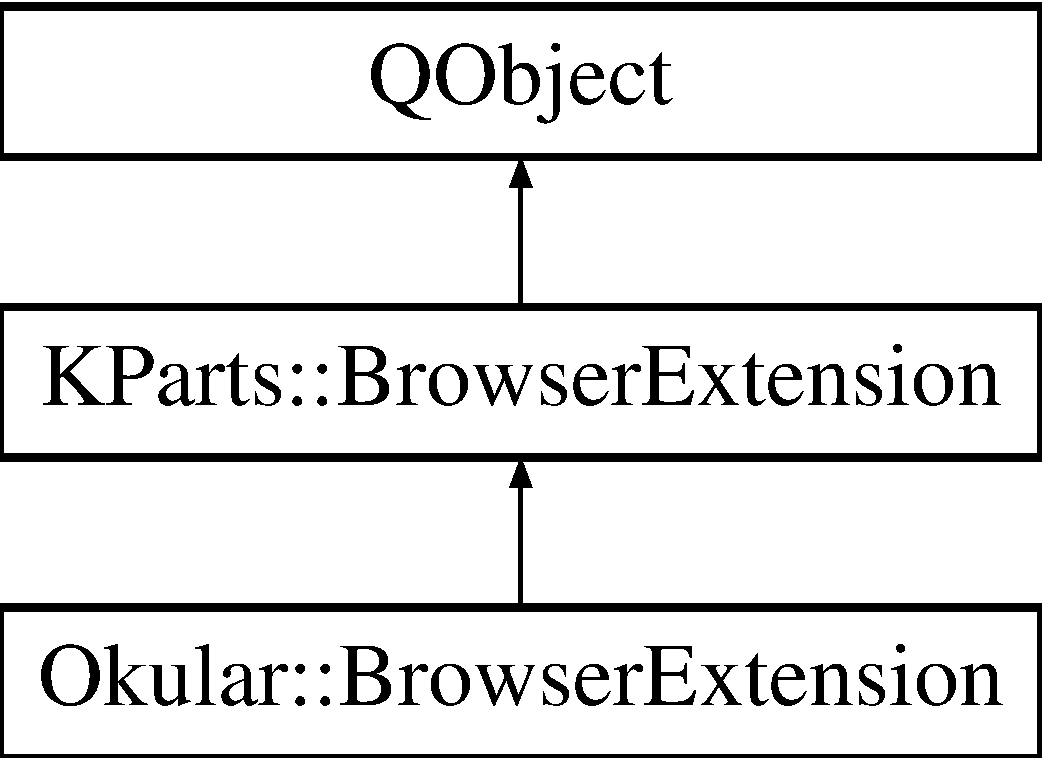
\includegraphics[height=3.000000cm]{classOkular_1_1BrowserExtension}
\end{center}
\end{figure}
\subsection*{Public Slots}
\begin{DoxyCompactItemize}
\item 
void \hyperlink{classOkular_1_1BrowserExtension_a3a21564b97dcb5a78b5647c1bf524ca6}{print} ()
\end{DoxyCompactItemize}
\subsection*{Public Member Functions}
\begin{DoxyCompactItemize}
\item 
\hyperlink{classOkular_1_1BrowserExtension_a08301e2b1330f8998039f0ee5edde338}{Browser\+Extension} (\hyperlink{classOkular_1_1Part}{Part} $\ast$)
\end{DoxyCompactItemize}
\subsection*{Additional Inherited Members}


\subsection{Detailed Description}


Definition at line 21 of file extensions.\+h.



\subsection{Constructor \& Destructor Documentation}
\hypertarget{classOkular_1_1BrowserExtension_a08301e2b1330f8998039f0ee5edde338}{\index{Okular\+::\+Browser\+Extension@{Okular\+::\+Browser\+Extension}!Browser\+Extension@{Browser\+Extension}}
\index{Browser\+Extension@{Browser\+Extension}!Okular\+::\+Browser\+Extension@{Okular\+::\+Browser\+Extension}}
\subsubsection[{Browser\+Extension}]{\setlength{\rightskip}{0pt plus 5cm}Okular\+::\+Browser\+Extension\+::\+Browser\+Extension (
\begin{DoxyParamCaption}
\item[{{\bf Part} $\ast$}]{parent}
\end{DoxyParamCaption}
)}}\label{classOkular_1_1BrowserExtension_a08301e2b1330f8998039f0ee5edde338}


Definition at line 22 of file extensions.\+cpp.


\begin{DoxyCode}
23     : \hyperlink{classKParts_1_1BrowserExtension}{KParts::BrowserExtension}( parent ), m\_part( parent )
24 \{
25     emit \hyperlink{classKParts_1_1BrowserExtension_a3252f2adebd103519ee15e57037c7386}{enableAction}(\textcolor{stringliteral}{"print"}, \textcolor{keyword}{true});
26     \hyperlink{classKParts_1_1BrowserExtension_a16e798977df4a2992e0f60a9dc01d33f}{setURLDropHandlingEnabled}(\textcolor{keyword}{true});
27 \}
\end{DoxyCode}


\subsection{Member Function Documentation}
\hypertarget{classOkular_1_1BrowserExtension_a3a21564b97dcb5a78b5647c1bf524ca6}{\index{Okular\+::\+Browser\+Extension@{Okular\+::\+Browser\+Extension}!print@{print}}
\index{print@{print}!Okular\+::\+Browser\+Extension@{Okular\+::\+Browser\+Extension}}
\subsubsection[{print}]{\setlength{\rightskip}{0pt plus 5cm}void Okular\+::\+Browser\+Extension\+::print (
\begin{DoxyParamCaption}
{}
\end{DoxyParamCaption}
)\hspace{0.3cm}{\ttfamily [slot]}}}\label{classOkular_1_1BrowserExtension_a3a21564b97dcb5a78b5647c1bf524ca6}


Definition at line 30 of file extensions.\+cpp.


\begin{DoxyCode}
31 \{
32     m\_part->\hyperlink{classOkular_1_1Part_ae4a132e628da6312254409b6d4813874}{slotPrint}();
33 \}
\end{DoxyCode}


The documentation for this class was generated from the following files\+:\begin{DoxyCompactItemize}
\item 
\hyperlink{extensions_8h}{extensions.\+h}\item 
\hyperlink{extensions_8cpp}{extensions.\+cpp}\end{DoxyCompactItemize}

\hypertarget{classKParts_1_1BrowserHostExtension}{\section{K\+Parts\+:\+:Browser\+Host\+Extension Class Reference}
\label{classKParts_1_1BrowserHostExtension}\index{K\+Parts\+::\+Browser\+Host\+Extension@{K\+Parts\+::\+Browser\+Host\+Extension}}
}


{\ttfamily \#include $<$browserextension.\+h$>$}

Inheritance diagram for K\+Parts\+:\+:Browser\+Host\+Extension\+:\begin{figure}[H]
\begin{center}
\leavevmode
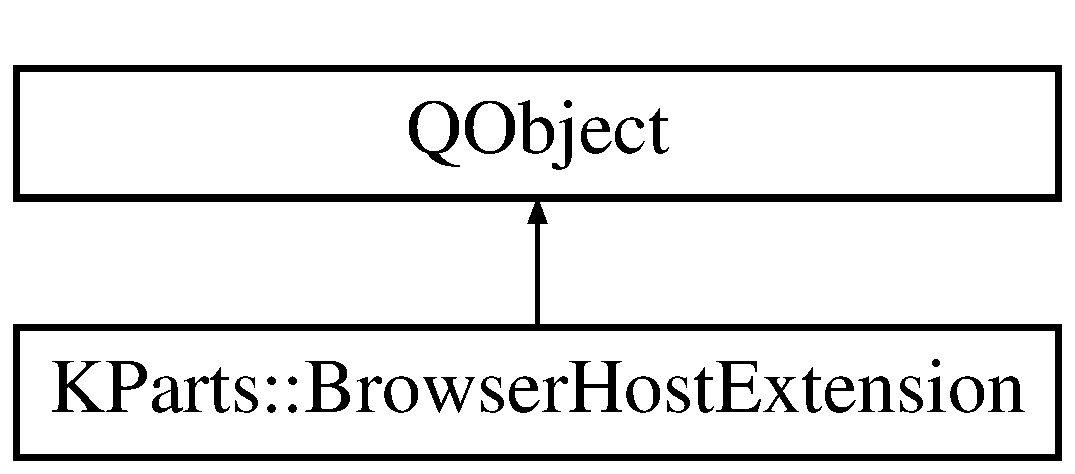
\includegraphics[height=2.000000cm]{classKParts_1_1BrowserHostExtension}
\end{center}
\end{figure}
\subsection*{Public Member Functions}
\begin{DoxyCompactItemize}
\item 
\hyperlink{classKParts_1_1BrowserHostExtension_af1c75309d63462007edd8536c0e57274}{Browser\+Host\+Extension} (\hyperlink{classKParts_1_1ReadOnlyPart}{K\+Parts\+::\+Read\+Only\+Part} $\ast$parent)
\item 
virtual \hyperlink{classKParts_1_1BrowserHostExtension_aa7202fb68e55dcf3556e0611c6b78263}{$\sim$\+Browser\+Host\+Extension} ()
\item 
virtual Q\+String\+List \hyperlink{classKParts_1_1BrowserHostExtension_a25ae4238d3c4f556ee9c7287c16c0f09}{frame\+Names} () const 
\item 
virtual const \hyperlink{classQList}{Q\+List}\\*
$<$ \hyperlink{classKParts_1_1ReadOnlyPart}{K\+Parts\+::\+Read\+Only\+Part} $\ast$ $>$ \hyperlink{classKParts_1_1BrowserHostExtension_a65a6429a794aa78ff5de27f973a43e86}{frames} () const 
\item 
virtual \hyperlink{classKParts_1_1BrowserHostExtension}{Browser\+Host\+Extension} $\ast$ \hyperlink{classKParts_1_1BrowserHostExtension_aa7d6192b9f6a399135f34d530d74a3e7}{find\+Frame\+Parent} (\hyperlink{classKParts_1_1ReadOnlyPart}{K\+Parts\+::\+Read\+Only\+Part} $\ast$calling\+Part, const Q\+String \&frame)
\item 
virtual bool \hyperlink{classKParts_1_1BrowserHostExtension_ae0227348d8b864d3093fb5dc6ca876f0}{open\+Url\+In\+Frame} (const K\+Url \&url, const \hyperlink{classKParts_1_1OpenUrlArguments}{K\+Parts\+::\+Open\+Url\+Arguments} \&arguments, const \hyperlink{structKParts_1_1BrowserArguments}{K\+Parts\+::\+Browser\+Arguments} \&browser\+Arguments)
\end{DoxyCompactItemize}
\subsection*{Static Public Member Functions}
\begin{DoxyCompactItemize}
\item 
static \hyperlink{classKParts_1_1BrowserHostExtension}{Browser\+Host\+Extension} $\ast$ \hyperlink{classKParts_1_1BrowserHostExtension_aa0a695c166742e7f49f65d8a2f3d5216}{child\+Object} (Q\+Object $\ast$obj)
\end{DoxyCompactItemize}


\subsection{Detailed Description}
An extension class for container parts, i.\+e. parts that contain other parts. For instance a K\+H\+T\+M\+L\+Part hosts one part per frame. 

Definition at line 712 of file browserextension.\+h.



\subsection{Constructor \& Destructor Documentation}
\hypertarget{classKParts_1_1BrowserHostExtension_af1c75309d63462007edd8536c0e57274}{\index{K\+Parts\+::\+Browser\+Host\+Extension@{K\+Parts\+::\+Browser\+Host\+Extension}!Browser\+Host\+Extension@{Browser\+Host\+Extension}}
\index{Browser\+Host\+Extension@{Browser\+Host\+Extension}!K\+Parts\+::\+Browser\+Host\+Extension@{K\+Parts\+::\+Browser\+Host\+Extension}}
\subsubsection[{Browser\+Host\+Extension}]{\setlength{\rightskip}{0pt plus 5cm}K\+Parts\+::\+Browser\+Host\+Extension\+::\+Browser\+Host\+Extension (
\begin{DoxyParamCaption}
\item[{{\bf K\+Parts\+::\+Read\+Only\+Part} $\ast$}]{parent}
\end{DoxyParamCaption}
)}}\label{classKParts_1_1BrowserHostExtension_af1c75309d63462007edd8536c0e57274}
\hypertarget{classKParts_1_1BrowserHostExtension_aa7202fb68e55dcf3556e0611c6b78263}{\index{K\+Parts\+::\+Browser\+Host\+Extension@{K\+Parts\+::\+Browser\+Host\+Extension}!````~Browser\+Host\+Extension@{$\sim$\+Browser\+Host\+Extension}}
\index{````~Browser\+Host\+Extension@{$\sim$\+Browser\+Host\+Extension}!K\+Parts\+::\+Browser\+Host\+Extension@{K\+Parts\+::\+Browser\+Host\+Extension}}
\subsubsection[{$\sim$\+Browser\+Host\+Extension}]{\setlength{\rightskip}{0pt plus 5cm}virtual K\+Parts\+::\+Browser\+Host\+Extension\+::$\sim$\+Browser\+Host\+Extension (
\begin{DoxyParamCaption}
{}
\end{DoxyParamCaption}
)\hspace{0.3cm}{\ttfamily [virtual]}}}\label{classKParts_1_1BrowserHostExtension_aa7202fb68e55dcf3556e0611c6b78263}


\subsection{Member Function Documentation}
\hypertarget{classKParts_1_1BrowserHostExtension_aa0a695c166742e7f49f65d8a2f3d5216}{\index{K\+Parts\+::\+Browser\+Host\+Extension@{K\+Parts\+::\+Browser\+Host\+Extension}!child\+Object@{child\+Object}}
\index{child\+Object@{child\+Object}!K\+Parts\+::\+Browser\+Host\+Extension@{K\+Parts\+::\+Browser\+Host\+Extension}}
\subsubsection[{child\+Object}]{\setlength{\rightskip}{0pt plus 5cm}static {\bf Browser\+Host\+Extension}$\ast$ K\+Parts\+::\+Browser\+Host\+Extension\+::child\+Object (
\begin{DoxyParamCaption}
\item[{Q\+Object $\ast$}]{obj}
\end{DoxyParamCaption}
)\hspace{0.3cm}{\ttfamily [static]}}}\label{classKParts_1_1BrowserHostExtension_aa0a695c166742e7f49f65d8a2f3d5216}
Queries {\ttfamily obj} for a child object which inherits from this \hyperlink{classKParts_1_1BrowserHostExtension}{Browser\+Host\+Extension} class. Convenience method. \hypertarget{classKParts_1_1BrowserHostExtension_aa7d6192b9f6a399135f34d530d74a3e7}{\index{K\+Parts\+::\+Browser\+Host\+Extension@{K\+Parts\+::\+Browser\+Host\+Extension}!find\+Frame\+Parent@{find\+Frame\+Parent}}
\index{find\+Frame\+Parent@{find\+Frame\+Parent}!K\+Parts\+::\+Browser\+Host\+Extension@{K\+Parts\+::\+Browser\+Host\+Extension}}
\subsubsection[{find\+Frame\+Parent}]{\setlength{\rightskip}{0pt plus 5cm}virtual {\bf Browser\+Host\+Extension}$\ast$ K\+Parts\+::\+Browser\+Host\+Extension\+::find\+Frame\+Parent (
\begin{DoxyParamCaption}
\item[{{\bf K\+Parts\+::\+Read\+Only\+Part} $\ast$}]{calling\+Part, }
\item[{const Q\+String \&}]{frame}
\end{DoxyParamCaption}
)\hspace{0.3cm}{\ttfamily [virtual]}}}\label{classKParts_1_1BrowserHostExtension_aa7d6192b9f6a399135f34d530d74a3e7}
Returns the part that contains {\ttfamily frame} and that may be accessed by {\ttfamily calling\+Part} \hypertarget{classKParts_1_1BrowserHostExtension_a25ae4238d3c4f556ee9c7287c16c0f09}{\index{K\+Parts\+::\+Browser\+Host\+Extension@{K\+Parts\+::\+Browser\+Host\+Extension}!frame\+Names@{frame\+Names}}
\index{frame\+Names@{frame\+Names}!K\+Parts\+::\+Browser\+Host\+Extension@{K\+Parts\+::\+Browser\+Host\+Extension}}
\subsubsection[{frame\+Names}]{\setlength{\rightskip}{0pt plus 5cm}virtual Q\+String\+List K\+Parts\+::\+Browser\+Host\+Extension\+::frame\+Names (
\begin{DoxyParamCaption}
{}
\end{DoxyParamCaption}
) const\hspace{0.3cm}{\ttfamily [virtual]}}}\label{classKParts_1_1BrowserHostExtension_a25ae4238d3c4f556ee9c7287c16c0f09}
Returns a list of the names of all hosted child objects.

Note that this method does not query the child objects recursively. \hypertarget{classKParts_1_1BrowserHostExtension_a65a6429a794aa78ff5de27f973a43e86}{\index{K\+Parts\+::\+Browser\+Host\+Extension@{K\+Parts\+::\+Browser\+Host\+Extension}!frames@{frames}}
\index{frames@{frames}!K\+Parts\+::\+Browser\+Host\+Extension@{K\+Parts\+::\+Browser\+Host\+Extension}}
\subsubsection[{frames}]{\setlength{\rightskip}{0pt plus 5cm}virtual const {\bf Q\+List}$<${\bf K\+Parts\+::\+Read\+Only\+Part}$\ast$$>$ K\+Parts\+::\+Browser\+Host\+Extension\+::frames (
\begin{DoxyParamCaption}
{}
\end{DoxyParamCaption}
) const\hspace{0.3cm}{\ttfamily [virtual]}}}\label{classKParts_1_1BrowserHostExtension_a65a6429a794aa78ff5de27f973a43e86}
Returns a list of pointers to all hosted child objects.

Note that this method does not query the child objects recursively. \hypertarget{classKParts_1_1BrowserHostExtension_ae0227348d8b864d3093fb5dc6ca876f0}{\index{K\+Parts\+::\+Browser\+Host\+Extension@{K\+Parts\+::\+Browser\+Host\+Extension}!open\+Url\+In\+Frame@{open\+Url\+In\+Frame}}
\index{open\+Url\+In\+Frame@{open\+Url\+In\+Frame}!K\+Parts\+::\+Browser\+Host\+Extension@{K\+Parts\+::\+Browser\+Host\+Extension}}
\subsubsection[{open\+Url\+In\+Frame}]{\setlength{\rightskip}{0pt plus 5cm}virtual bool K\+Parts\+::\+Browser\+Host\+Extension\+::open\+Url\+In\+Frame (
\begin{DoxyParamCaption}
\item[{const K\+Url \&}]{url, }
\item[{const {\bf K\+Parts\+::\+Open\+Url\+Arguments} \&}]{arguments, }
\item[{const {\bf K\+Parts\+::\+Browser\+Arguments} \&}]{browser\+Arguments}
\end{DoxyParamCaption}
)\hspace{0.3cm}{\ttfamily [virtual]}}}\label{classKParts_1_1BrowserHostExtension_ae0227348d8b864d3093fb5dc6ca876f0}
Opens the given url in a hosted child frame. The frame name is specified in the frame\+Name variable in the {\ttfamily browser\+Arguments} parameter (see \hyperlink{structKParts_1_1BrowserArguments}{K\+Parts\+::\+Browser\+Arguments} ) . 

The documentation for this class was generated from the following file\+:\begin{DoxyCompactItemize}
\item 
/usr/include/kparts/\hyperlink{browserextension_8h}{browserextension.\+h}\end{DoxyCompactItemize}

\hypertarget{classKParts_1_1BrowserInterface}{\section{\-K\-Parts\-:\-:\-Browser\-Interface \-Class \-Reference}
\label{classKParts_1_1BrowserInterface}\index{\-K\-Parts\-::\-Browser\-Interface@{\-K\-Parts\-::\-Browser\-Interface}}
}


{\ttfamily \#include $<$browserinterface.\-h$>$}

\subsection*{\-Public \-Member \-Functions}
\begin{DoxyCompactItemize}
\item 
\hyperlink{classKParts_1_1BrowserInterface_a7e7c8ab24a9b90800846028e66eabaed}{\-Browser\-Interface} (\-Q\-Object $\ast$parent)
\item 
virtual \hyperlink{classKParts_1_1BrowserInterface_af6f3ca797d626ffd8676a5babb09ad22}{$\sim$\-Browser\-Interface} ()
\item 
void \hyperlink{classKParts_1_1BrowserInterface_a3b2d9e1791a4a6195b53b48180ec761c}{call\-Method} (const char $\ast$name, const \-Q\-Variant \&argument)
\end{DoxyCompactItemize}


\subsection{\-Detailed \-Description}
\-The purpose of this interface is to allow a direct communication between a \-K\-Part and the hosting browser shell (for example \-Konqueror) . \-A shell implementing this interface can propagate it to embedded kpart components by using the set\-Browser\-Interface call of the part's \hyperlink{classKParts_1_1BrowserExtension}{\-K\-Parts\-::\-Browser\-Extension} object.

\-This interface looks not very rich, but the main functionality is implemented using the call\-Method method for part-\/$>$shell communication and using \-Qt properties for allowing a part to to explicitly query information from the shell.

\-Konqueror in particular, as 'reference' implementation, provides the following functionality through this interface\-:

\-Qt properties\-: \-Q\-\_\-\-P\-R\-O\-P\-E\-R\-T\-Y( uint history\-Length R\-E\-A\-D history\-Length );

\-Callable methods\-: void go\-History( int ); 

\-Definition at line 53 of file browserinterface.\-h.



\subsection{\-Constructor \& \-Destructor \-Documentation}
\hypertarget{classKParts_1_1BrowserInterface_a7e7c8ab24a9b90800846028e66eabaed}{\index{\-K\-Parts\-::\-Browser\-Interface@{\-K\-Parts\-::\-Browser\-Interface}!\-Browser\-Interface@{\-Browser\-Interface}}
\index{\-Browser\-Interface@{\-Browser\-Interface}!KParts::BrowserInterface@{\-K\-Parts\-::\-Browser\-Interface}}
\subsubsection[{\-Browser\-Interface}]{\setlength{\rightskip}{0pt plus 5cm}{\bf \-K\-Parts\-::\-Browser\-Interface\-::\-Browser\-Interface} (
\begin{DoxyParamCaption}
\item[{\-Q\-Object $\ast$}]{parent}
\end{DoxyParamCaption}
)\hspace{0.3cm}{\ttfamily  \mbox{[}explicit\mbox{]}}}}\label{classKParts_1_1BrowserInterface_a7e7c8ab24a9b90800846028e66eabaed}
\hypertarget{classKParts_1_1BrowserInterface_af6f3ca797d626ffd8676a5babb09ad22}{\index{\-K\-Parts\-::\-Browser\-Interface@{\-K\-Parts\-::\-Browser\-Interface}!$\sim$\-Browser\-Interface@{$\sim$\-Browser\-Interface}}
\index{$\sim$\-Browser\-Interface@{$\sim$\-Browser\-Interface}!KParts::BrowserInterface@{\-K\-Parts\-::\-Browser\-Interface}}
\subsubsection[{$\sim$\-Browser\-Interface}]{\setlength{\rightskip}{0pt plus 5cm}virtual {\bf \-K\-Parts\-::\-Browser\-Interface\-::$\sim$\-Browser\-Interface} (
\begin{DoxyParamCaption}
{}
\end{DoxyParamCaption}
)\hspace{0.3cm}{\ttfamily  \mbox{[}virtual\mbox{]}}}}\label{classKParts_1_1BrowserInterface_af6f3ca797d626ffd8676a5babb09ad22}


\subsection{\-Member \-Function \-Documentation}
\hypertarget{classKParts_1_1BrowserInterface_a3b2d9e1791a4a6195b53b48180ec761c}{\index{\-K\-Parts\-::\-Browser\-Interface@{\-K\-Parts\-::\-Browser\-Interface}!call\-Method@{call\-Method}}
\index{call\-Method@{call\-Method}!KParts::BrowserInterface@{\-K\-Parts\-::\-Browser\-Interface}}
\subsubsection[{call\-Method}]{\setlength{\rightskip}{0pt plus 5cm}void {\bf \-K\-Parts\-::\-Browser\-Interface\-::call\-Method} (
\begin{DoxyParamCaption}
\item[{const char $\ast$}]{name, }
\item[{const \-Q\-Variant \&}]{argument}
\end{DoxyParamCaption}
)}}\label{classKParts_1_1BrowserInterface_a3b2d9e1791a4a6195b53b48180ec761c}
\-Perform a dynamic invocation of a method in the \hyperlink{classKParts_1_1BrowserInterface}{\-Browser\-Interface} implementation. \-Methods are to be implemented as simple \-Qt slots. \-You should only include the method name, and not the signature, in the name argument. 

\-The documentation for this class was generated from the following file\-:\begin{DoxyCompactItemize}
\item 
/usr/include/kparts/\hyperlink{browserinterface_8h}{browserinterface.\-h}\end{DoxyCompactItemize}

\hypertarget{classKParts_1_1BrowserOpenOrSaveQuestion}{\section{\-K\-Parts\-:\-:\-Browser\-Open\-Or\-Save\-Question \-Class \-Reference}
\label{classKParts_1_1BrowserOpenOrSaveQuestion}\index{\-K\-Parts\-::\-Browser\-Open\-Or\-Save\-Question@{\-K\-Parts\-::\-Browser\-Open\-Or\-Save\-Question}}
}


{\ttfamily \#include $<$browseropenorsavequestion.\-h$>$}

\subsection*{\-Public \-Types}
\begin{DoxyCompactItemize}
\item 
enum \hyperlink{classKParts_1_1BrowserOpenOrSaveQuestion_a9dfe6a7919cfadff826a357e94ac3a9a}{\-Feature} \{ \hyperlink{classKParts_1_1BrowserOpenOrSaveQuestion_a9dfe6a7919cfadff826a357e94ac3a9aa1cfa50dab189d46bdc4a66c5a1763168}{\-Basic\-Features} =  0, 
\hyperlink{classKParts_1_1BrowserOpenOrSaveQuestion_a9dfe6a7919cfadff826a357e94ac3a9aa3bc1c3177b1a3c8f4cd297ae558c155e}{\-Service\-Selection} =  1
 \}
\item 
enum \hyperlink{classKParts_1_1BrowserOpenOrSaveQuestion_a12842198b7684e9e246e9a207eabc93f}{\-Result} \{ \hyperlink{classKParts_1_1BrowserOpenOrSaveQuestion_a12842198b7684e9e246e9a207eabc93fad5f24b54978bf4ec2a36720d33ad7609}{\-Save}, 
\hyperlink{classKParts_1_1BrowserOpenOrSaveQuestion_a12842198b7684e9e246e9a207eabc93fa1135dc1f27b120bdd6dc83dd7254b60b}{\-Open}, 
\hyperlink{classKParts_1_1BrowserOpenOrSaveQuestion_a12842198b7684e9e246e9a207eabc93fa9038d40b03609466a8433c35b428bf5a}{\-Embed}, 
\hyperlink{classKParts_1_1BrowserOpenOrSaveQuestion_a12842198b7684e9e246e9a207eabc93fac5e1d49f3047805e8f216f11cbe903ab}{\-Cancel}
 \}
\end{DoxyCompactItemize}
\subsection*{\-Public \-Member \-Functions}
\begin{DoxyCompactItemize}
\item 
\hyperlink{classKParts_1_1BrowserOpenOrSaveQuestion_a93097e04518164345d399f7c376b993e}{\-Browser\-Open\-Or\-Save\-Question} (\-Q\-Widget $\ast$parent, const \-K\-Url \&url, const \-Q\-String \&mime\-Type)
\item 
\hyperlink{classKParts_1_1BrowserOpenOrSaveQuestion_a6af2b8e427bf2bb922bb9fcc09df6a65}{$\sim$\-Browser\-Open\-Or\-Save\-Question} ()
\item 
void \hyperlink{classKParts_1_1BrowserOpenOrSaveQuestion_a82733c7818b3c6ee5987ee8c7450c29f}{set\-Suggested\-File\-Name} (const \-Q\-String \&suggested\-File\-Name)
\item 
void \hyperlink{classKParts_1_1BrowserOpenOrSaveQuestion_a998acfa7caa8a47794cc0eb2682a503d}{set\-Features} (\-Features features)
\item 
\hyperlink{classKParts_1_1BrowserOpenOrSaveQuestion_a12842198b7684e9e246e9a207eabc93f}{\-Result} \hyperlink{classKParts_1_1BrowserOpenOrSaveQuestion_a5d9df0d831477073f43071dfe580456d}{ask\-Open\-Or\-Save} ()
\item 
\hyperlink{classKParts_1_1BrowserOpenOrSaveQuestion_a12842198b7684e9e246e9a207eabc93f}{\-Result} \hyperlink{classKParts_1_1BrowserOpenOrSaveQuestion_ad261c14f0e8e32b99b61029fdd5f2fad}{ask\-Embed\-Or\-Save} (int flags=0)
\item 
\-K\-Service\-::\-Ptr \hyperlink{classKParts_1_1BrowserOpenOrSaveQuestion_aaaa2f3a0f18e7acc82152bf296c227da}{selected\-Service} () const 
\end{DoxyCompactItemize}


\subsection{\-Detailed \-Description}
\-This class shows the dialog that asks the user whether to save a url or open a url in another application.

\-It also has the variant which asks \char`\"{}save or embed\char`\"{} (e.\-g. into konqueror).

\begin{DoxySince}{\-Since}
4.\-4 
\end{DoxySince}


\-Definition at line 41 of file browseropenorsavequestion.\-h.



\subsection{\-Member \-Enumeration \-Documentation}
\hypertarget{classKParts_1_1BrowserOpenOrSaveQuestion_a9dfe6a7919cfadff826a357e94ac3a9a}{\index{\-K\-Parts\-::\-Browser\-Open\-Or\-Save\-Question@{\-K\-Parts\-::\-Browser\-Open\-Or\-Save\-Question}!\-Feature@{\-Feature}}
\index{\-Feature@{\-Feature}!KParts::BrowserOpenOrSaveQuestion@{\-K\-Parts\-::\-Browser\-Open\-Or\-Save\-Question}}
\subsubsection[{\-Feature}]{\setlength{\rightskip}{0pt plus 5cm}enum {\bf \-K\-Parts\-::\-Browser\-Open\-Or\-Save\-Question\-::\-Feature}}}\label{classKParts_1_1BrowserOpenOrSaveQuestion_a9dfe6a7919cfadff826a357e94ac3a9a}
\-Set of features that should be enabled in this dialog. \-This allows to add features before making all applications ready for those features (e.\-g. applications need to read \hyperlink{classKParts_1_1BrowserOpenOrSaveQuestion_aaaa2f3a0f18e7acc82152bf296c227da}{selected\-Service()} otherwise the dialog should not show the service selection button) \begin{Desc}
\item[\-Enumerator\-: ]\par
\begin{description}
\index{\-Basic\-Features@{\-Basic\-Features}!\-K\-Parts\-::\-Browser\-Open\-Or\-Save\-Question@{\-K\-Parts\-::\-Browser\-Open\-Or\-Save\-Question}}\index{\-K\-Parts\-::\-Browser\-Open\-Or\-Save\-Question@{\-K\-Parts\-::\-Browser\-Open\-Or\-Save\-Question}!\-Basic\-Features@{\-Basic\-Features}}\item[{\em 
\hypertarget{classKParts_1_1BrowserOpenOrSaveQuestion_a9dfe6a7919cfadff826a357e94ac3a9aa1cfa50dab189d46bdc4a66c5a1763168}{\-Basic\-Features}\label{classKParts_1_1BrowserOpenOrSaveQuestion_a9dfe6a7919cfadff826a357e94ac3a9aa1cfa50dab189d46bdc4a66c5a1763168}
}]\-Only the basic save, open, embed, cancel button \index{\-Service\-Selection@{\-Service\-Selection}!\-K\-Parts\-::\-Browser\-Open\-Or\-Save\-Question@{\-K\-Parts\-::\-Browser\-Open\-Or\-Save\-Question}}\index{\-K\-Parts\-::\-Browser\-Open\-Or\-Save\-Question@{\-K\-Parts\-::\-Browser\-Open\-Or\-Save\-Question}!\-Service\-Selection@{\-Service\-Selection}}\item[{\em 
\hypertarget{classKParts_1_1BrowserOpenOrSaveQuestion_a9dfe6a7919cfadff826a357e94ac3a9aa3bc1c3177b1a3c8f4cd297ae558c155e}{\-Service\-Selection}\label{classKParts_1_1BrowserOpenOrSaveQuestion_a9dfe6a7919cfadff826a357e94ac3a9aa3bc1c3177b1a3c8f4cd297ae558c155e}
}]\-Shows \char`\"{}\-Open With...\char`\"{} with the associated applications for the mimetype \end{description}
\end{Desc}



\-Definition at line 64 of file browseropenorsavequestion.\-h.


\begin{DoxyCode}
                 { BasicFeatures = 0, 
                   ServiceSelection = 1 
    };
\end{DoxyCode}
\hypertarget{classKParts_1_1BrowserOpenOrSaveQuestion_a12842198b7684e9e246e9a207eabc93f}{\index{\-K\-Parts\-::\-Browser\-Open\-Or\-Save\-Question@{\-K\-Parts\-::\-Browser\-Open\-Or\-Save\-Question}!\-Result@{\-Result}}
\index{\-Result@{\-Result}!KParts::BrowserOpenOrSaveQuestion@{\-K\-Parts\-::\-Browser\-Open\-Or\-Save\-Question}}
\subsubsection[{\-Result}]{\setlength{\rightskip}{0pt plus 5cm}enum {\bf \-K\-Parts\-::\-Browser\-Open\-Or\-Save\-Question\-::\-Result}}}\label{classKParts_1_1BrowserOpenOrSaveQuestion_a12842198b7684e9e246e9a207eabc93f}
\begin{Desc}
\item[\-Enumerator\-: ]\par
\begin{description}
\index{\-Save@{\-Save}!\-K\-Parts\-::\-Browser\-Open\-Or\-Save\-Question@{\-K\-Parts\-::\-Browser\-Open\-Or\-Save\-Question}}\index{\-K\-Parts\-::\-Browser\-Open\-Or\-Save\-Question@{\-K\-Parts\-::\-Browser\-Open\-Or\-Save\-Question}!\-Save@{\-Save}}\item[{\em 
\hypertarget{classKParts_1_1BrowserOpenOrSaveQuestion_a12842198b7684e9e246e9a207eabc93fad5f24b54978bf4ec2a36720d33ad7609}{\-Save}\label{classKParts_1_1BrowserOpenOrSaveQuestion_a12842198b7684e9e246e9a207eabc93fad5f24b54978bf4ec2a36720d33ad7609}
}]\index{\-Open@{\-Open}!\-K\-Parts\-::\-Browser\-Open\-Or\-Save\-Question@{\-K\-Parts\-::\-Browser\-Open\-Or\-Save\-Question}}\index{\-K\-Parts\-::\-Browser\-Open\-Or\-Save\-Question@{\-K\-Parts\-::\-Browser\-Open\-Or\-Save\-Question}!\-Open@{\-Open}}\item[{\em 
\hypertarget{classKParts_1_1BrowserOpenOrSaveQuestion_a12842198b7684e9e246e9a207eabc93fa1135dc1f27b120bdd6dc83dd7254b60b}{\-Open}\label{classKParts_1_1BrowserOpenOrSaveQuestion_a12842198b7684e9e246e9a207eabc93fa1135dc1f27b120bdd6dc83dd7254b60b}
}]\index{\-Embed@{\-Embed}!\-K\-Parts\-::\-Browser\-Open\-Or\-Save\-Question@{\-K\-Parts\-::\-Browser\-Open\-Or\-Save\-Question}}\index{\-K\-Parts\-::\-Browser\-Open\-Or\-Save\-Question@{\-K\-Parts\-::\-Browser\-Open\-Or\-Save\-Question}!\-Embed@{\-Embed}}\item[{\em 
\hypertarget{classKParts_1_1BrowserOpenOrSaveQuestion_a12842198b7684e9e246e9a207eabc93fa9038d40b03609466a8433c35b428bf5a}{\-Embed}\label{classKParts_1_1BrowserOpenOrSaveQuestion_a12842198b7684e9e246e9a207eabc93fa9038d40b03609466a8433c35b428bf5a}
}]\index{\-Cancel@{\-Cancel}!\-K\-Parts\-::\-Browser\-Open\-Or\-Save\-Question@{\-K\-Parts\-::\-Browser\-Open\-Or\-Save\-Question}}\index{\-K\-Parts\-::\-Browser\-Open\-Or\-Save\-Question@{\-K\-Parts\-::\-Browser\-Open\-Or\-Save\-Question}!\-Cancel@{\-Cancel}}\item[{\em 
\hypertarget{classKParts_1_1BrowserOpenOrSaveQuestion_a12842198b7684e9e246e9a207eabc93fac5e1d49f3047805e8f216f11cbe903ab}{\-Cancel}\label{classKParts_1_1BrowserOpenOrSaveQuestion_a12842198b7684e9e246e9a207eabc93fac5e1d49f3047805e8f216f11cbe903ab}
}]\end{description}
\end{Desc}



\-Definition at line 74 of file browseropenorsavequestion.\-h.


\begin{DoxyCode}
{ Save, Open, Embed, Cancel };
\end{DoxyCode}


\subsection{\-Constructor \& \-Destructor \-Documentation}
\hypertarget{classKParts_1_1BrowserOpenOrSaveQuestion_a93097e04518164345d399f7c376b993e}{\index{\-K\-Parts\-::\-Browser\-Open\-Or\-Save\-Question@{\-K\-Parts\-::\-Browser\-Open\-Or\-Save\-Question}!\-Browser\-Open\-Or\-Save\-Question@{\-Browser\-Open\-Or\-Save\-Question}}
\index{\-Browser\-Open\-Or\-Save\-Question@{\-Browser\-Open\-Or\-Save\-Question}!KParts::BrowserOpenOrSaveQuestion@{\-K\-Parts\-::\-Browser\-Open\-Or\-Save\-Question}}
\subsubsection[{\-Browser\-Open\-Or\-Save\-Question}]{\setlength{\rightskip}{0pt plus 5cm}{\bf \-K\-Parts\-::\-Browser\-Open\-Or\-Save\-Question\-::\-Browser\-Open\-Or\-Save\-Question} (
\begin{DoxyParamCaption}
\item[{\-Q\-Widget $\ast$}]{parent, }
\item[{const \-K\-Url \&}]{url, }
\item[{const \-Q\-String \&}]{mime\-Type}
\end{DoxyParamCaption}
)}}\label{classKParts_1_1BrowserOpenOrSaveQuestion_a93097e04518164345d399f7c376b993e}
\-Constructor, for all kinds of dialogs shown in this class. 
\begin{DoxyParams}{\-Parameters}
{\em url} & the \-U\-R\-L in question \\
\hline
{\em mime\-Type} & the mimetype of the \-U\-R\-L \\
\hline
\end{DoxyParams}
\hypertarget{classKParts_1_1BrowserOpenOrSaveQuestion_a6af2b8e427bf2bb922bb9fcc09df6a65}{\index{\-K\-Parts\-::\-Browser\-Open\-Or\-Save\-Question@{\-K\-Parts\-::\-Browser\-Open\-Or\-Save\-Question}!$\sim$\-Browser\-Open\-Or\-Save\-Question@{$\sim$\-Browser\-Open\-Or\-Save\-Question}}
\index{$\sim$\-Browser\-Open\-Or\-Save\-Question@{$\sim$\-Browser\-Open\-Or\-Save\-Question}!KParts::BrowserOpenOrSaveQuestion@{\-K\-Parts\-::\-Browser\-Open\-Or\-Save\-Question}}
\subsubsection[{$\sim$\-Browser\-Open\-Or\-Save\-Question}]{\setlength{\rightskip}{0pt plus 5cm}{\bf \-K\-Parts\-::\-Browser\-Open\-Or\-Save\-Question\-::$\sim$\-Browser\-Open\-Or\-Save\-Question} (
\begin{DoxyParamCaption}
{}
\end{DoxyParamCaption}
)}}\label{classKParts_1_1BrowserOpenOrSaveQuestion_a6af2b8e427bf2bb922bb9fcc09df6a65}


\subsection{\-Member \-Function \-Documentation}
\hypertarget{classKParts_1_1BrowserOpenOrSaveQuestion_ad261c14f0e8e32b99b61029fdd5f2fad}{\index{\-K\-Parts\-::\-Browser\-Open\-Or\-Save\-Question@{\-K\-Parts\-::\-Browser\-Open\-Or\-Save\-Question}!ask\-Embed\-Or\-Save@{ask\-Embed\-Or\-Save}}
\index{ask\-Embed\-Or\-Save@{ask\-Embed\-Or\-Save}!KParts::BrowserOpenOrSaveQuestion@{\-K\-Parts\-::\-Browser\-Open\-Or\-Save\-Question}}
\subsubsection[{ask\-Embed\-Or\-Save}]{\setlength{\rightskip}{0pt plus 5cm}{\bf \-Result} {\bf \-K\-Parts\-::\-Browser\-Open\-Or\-Save\-Question\-::ask\-Embed\-Or\-Save} (
\begin{DoxyParamCaption}
\item[{int}]{flags = {\ttfamily 0}}
\end{DoxyParamCaption}
)}}\label{classKParts_1_1BrowserOpenOrSaveQuestion_ad261c14f0e8e32b99b61029fdd5f2fad}
\-Ask the user whether to save or open a url in another application. 
\begin{DoxyParams}{\-Parameters}
{\em parent} & parent widget for the dialog \\
\hline
{\em flags} & set to \hyperlink{classKParts_1_1BrowserRun_ae78b4e6186491175ccdb4b0f2693c08daa236cc4b09fc3ca6f88d9a37b32ea8af}{\-Browser\-Run\-::\-Attachment\-Disposition} if suggested by the server \-This is used because by default text/html files are opened embedded in browsers, not saved. \-But if the server said \char`\"{}attachment\char`\"{}, it means the user is download a file for saving it. \\
\hline
\end{DoxyParams}
\begin{DoxyReturn}{\-Returns}
\-Save, \-Embed or \-Cancel. 
\end{DoxyReturn}
\hypertarget{classKParts_1_1BrowserOpenOrSaveQuestion_a5d9df0d831477073f43071dfe580456d}{\index{\-K\-Parts\-::\-Browser\-Open\-Or\-Save\-Question@{\-K\-Parts\-::\-Browser\-Open\-Or\-Save\-Question}!ask\-Open\-Or\-Save@{ask\-Open\-Or\-Save}}
\index{ask\-Open\-Or\-Save@{ask\-Open\-Or\-Save}!KParts::BrowserOpenOrSaveQuestion@{\-K\-Parts\-::\-Browser\-Open\-Or\-Save\-Question}}
\subsubsection[{ask\-Open\-Or\-Save}]{\setlength{\rightskip}{0pt plus 5cm}{\bf \-Result} {\bf \-K\-Parts\-::\-Browser\-Open\-Or\-Save\-Question\-::ask\-Open\-Or\-Save} (
\begin{DoxyParamCaption}
{}
\end{DoxyParamCaption}
)}}\label{classKParts_1_1BrowserOpenOrSaveQuestion_a5d9df0d831477073f43071dfe580456d}
\-Ask the user whether to save or open a url in another application. 
\begin{DoxyParams}{\-Parameters}
{\em parent} & parent widget for the dialog \\
\hline
\end{DoxyParams}
\begin{DoxyReturn}{\-Returns}
\-Save, \-Open or \-Cancel. 
\end{DoxyReturn}
\hypertarget{classKParts_1_1BrowserOpenOrSaveQuestion_aaaa2f3a0f18e7acc82152bf296c227da}{\index{\-K\-Parts\-::\-Browser\-Open\-Or\-Save\-Question@{\-K\-Parts\-::\-Browser\-Open\-Or\-Save\-Question}!selected\-Service@{selected\-Service}}
\index{selected\-Service@{selected\-Service}!KParts::BrowserOpenOrSaveQuestion@{\-K\-Parts\-::\-Browser\-Open\-Or\-Save\-Question}}
\subsubsection[{selected\-Service}]{\setlength{\rightskip}{0pt plus 5cm}\-K\-Service\-::\-Ptr {\bf \-K\-Parts\-::\-Browser\-Open\-Or\-Save\-Question\-::selected\-Service} (
\begin{DoxyParamCaption}
{}
\end{DoxyParamCaption}
) const}}\label{classKParts_1_1BrowserOpenOrSaveQuestion_aaaa2f3a0f18e7acc82152bf296c227da}
\begin{DoxyReturn}{\-Returns}
the service that was selected during ask\-Open\-Or\-Save, if it returned \-Open. \-In all other cases (no associated application, \-Save or \-Cancel selected), this returns 0.
\end{DoxyReturn}
\-Requires set\-Features(\-Browser\-Open\-Or\-Save\-Question\-::\-Service\-Selection). \hypertarget{classKParts_1_1BrowserOpenOrSaveQuestion_a998acfa7caa8a47794cc0eb2682a503d}{\index{\-K\-Parts\-::\-Browser\-Open\-Or\-Save\-Question@{\-K\-Parts\-::\-Browser\-Open\-Or\-Save\-Question}!set\-Features@{set\-Features}}
\index{set\-Features@{set\-Features}!KParts::BrowserOpenOrSaveQuestion@{\-K\-Parts\-::\-Browser\-Open\-Or\-Save\-Question}}
\subsubsection[{set\-Features}]{\setlength{\rightskip}{0pt plus 5cm}void {\bf \-K\-Parts\-::\-Browser\-Open\-Or\-Save\-Question\-::set\-Features} (
\begin{DoxyParamCaption}
\item[{\-Features}]{features}
\end{DoxyParamCaption}
)}}\label{classKParts_1_1BrowserOpenOrSaveQuestion_a998acfa7caa8a47794cc0eb2682a503d}
\-Enables the given features in the dialog \hypertarget{classKParts_1_1BrowserOpenOrSaveQuestion_a82733c7818b3c6ee5987ee8c7450c29f}{\index{\-K\-Parts\-::\-Browser\-Open\-Or\-Save\-Question@{\-K\-Parts\-::\-Browser\-Open\-Or\-Save\-Question}!set\-Suggested\-File\-Name@{set\-Suggested\-File\-Name}}
\index{set\-Suggested\-File\-Name@{set\-Suggested\-File\-Name}!KParts::BrowserOpenOrSaveQuestion@{\-K\-Parts\-::\-Browser\-Open\-Or\-Save\-Question}}
\subsubsection[{set\-Suggested\-File\-Name}]{\setlength{\rightskip}{0pt plus 5cm}void {\bf \-K\-Parts\-::\-Browser\-Open\-Or\-Save\-Question\-::set\-Suggested\-File\-Name} (
\begin{DoxyParamCaption}
\item[{const \-Q\-String \&}]{suggested\-File\-Name}
\end{DoxyParamCaption}
)}}\label{classKParts_1_1BrowserOpenOrSaveQuestion_a82733c7818b3c6ee5987ee8c7450c29f}
\-Sets the suggested filename, shown in the dialog. 
\begin{DoxyParams}{\-Parameters}
{\em suggested\-File\-Name} & optional file name suggested by the server (\-H\-T\-T\-P \-Content-\/\-Disposition) \\
\hline
\end{DoxyParams}


\-The documentation for this class was generated from the following file\-:\begin{DoxyCompactItemize}
\item 
/usr/include/kparts/\hyperlink{browseropenorsavequestion_8h}{browseropenorsavequestion.\-h}\end{DoxyCompactItemize}

\hypertarget{classKParts_1_1BrowserRun}{\section{K\+Parts\+:\+:Browser\+Run Class Reference}
\label{classKParts_1_1BrowserRun}\index{K\+Parts\+::\+Browser\+Run@{K\+Parts\+::\+Browser\+Run}}
}


{\ttfamily \#include $<$browserrun.\+h$>$}

Inheritance diagram for K\+Parts\+:\+:Browser\+Run\+:\begin{figure}[H]
\begin{center}
\leavevmode
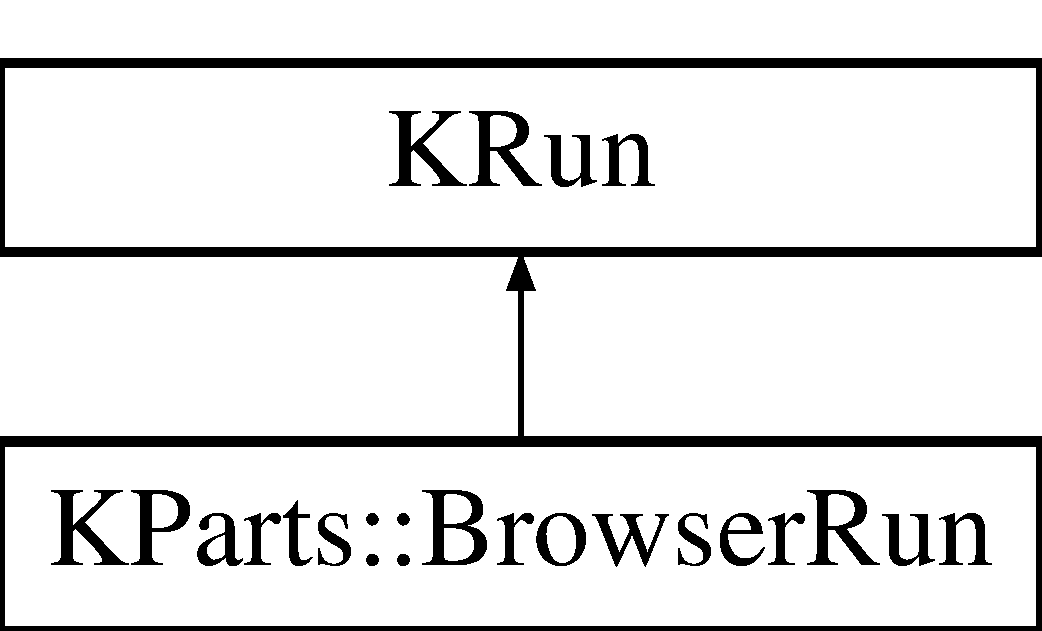
\includegraphics[height=2.000000cm]{classKParts_1_1BrowserRun}
\end{center}
\end{figure}
\subsection*{Public Types}
\begin{DoxyCompactItemize}
\item 
enum \hyperlink{classKParts_1_1BrowserRun_a32ee53f65c723ec01f4c4c28e91db8e6}{Ask\+Save\+Result} \{ \hyperlink{classKParts_1_1BrowserRun_a32ee53f65c723ec01f4c4c28e91db8e6adc6aa058c60662f393aa8168681d8a58}{Save}, 
\hyperlink{classKParts_1_1BrowserRun_a32ee53f65c723ec01f4c4c28e91db8e6ac44e1cbf269e6df9367051c7561de90b}{Open}, 
\hyperlink{classKParts_1_1BrowserRun_a32ee53f65c723ec01f4c4c28e91db8e6aea88673d252dcf7b37559606ce45667f}{Cancel}
 \}
\item 
enum \hyperlink{classKParts_1_1BrowserRun_ae78b4e6186491175ccdb4b0f2693c08d}{Ask\+Embed\+Or\+Save\+Flags} \{ \hyperlink{classKParts_1_1BrowserRun_ae78b4e6186491175ccdb4b0f2693c08dafa80faaf171d25b4a0e095a2c1f51cfe}{Inline\+Disposition} = 0, 
\hyperlink{classKParts_1_1BrowserRun_ae78b4e6186491175ccdb4b0f2693c08daa236cc4b09fc3ca6f88d9a37b32ea8af}{Attachment\+Disposition} = 1
 \}
\end{DoxyCompactItemize}
\subsection*{Public Member Functions}
\begin{DoxyCompactItemize}
\item 
\hyperlink{classKParts_1_1BrowserRun_a48308a3cd53da552fb60a86400d06228}{Browser\+Run} (const K\+Url \&\hyperlink{classKParts_1_1BrowserRun_ad3f7d10647ab8b5a77399f46df92046b}{url}, const \hyperlink{classKParts_1_1OpenUrlArguments}{K\+Parts\+::\+Open\+Url\+Arguments} \&args, const \hyperlink{structKParts_1_1BrowserArguments}{K\+Parts\+::\+Browser\+Arguments} \&browser\+Args, \hyperlink{classKParts_1_1ReadOnlyPart}{K\+Parts\+::\+Read\+Only\+Part} $\ast$\hyperlink{classKParts_1_1BrowserRun_a65886b4004c00ddcc08b976f1042d0dc}{part}, Q\+Widget $\ast$window, bool remove\+Referrer, bool trusted\+Source, bool \hyperlink{classKParts_1_1BrowserRun_a1caa242a8389d61d6758e25a68f9df50}{hide\+Error\+Dialog}=false)
\item 
virtual \hyperlink{classKParts_1_1BrowserRun_aa141423e9096f956970d4fe92e581814}{$\sim$\+Browser\+Run} ()
\item 
\hyperlink{classKParts_1_1OpenUrlArguments}{K\+Parts\+::\+Open\+Url\+Arguments} \& \hyperlink{classKParts_1_1BrowserRun_a5843399feb9cafe9a2f62b258c2f5a31}{arguments} ()
\item 
\hyperlink{structKParts_1_1BrowserArguments}{K\+Parts\+::\+Browser\+Arguments} \& \hyperlink{classKParts_1_1BrowserRun_a7fb44c1871cf67132853d8bb59dfe006}{browser\+Arguments} ()
\item 
\hyperlink{classKParts_1_1ReadOnlyPart}{K\+Parts\+::\+Read\+Only\+Part} $\ast$ \hyperlink{classKParts_1_1BrowserRun_a65886b4004c00ddcc08b976f1042d0dc}{part} () const 
\item 
K\+Url \hyperlink{classKParts_1_1BrowserRun_ad3f7d10647ab8b5a77399f46df92046b}{url} () const 
\item 
bool \hyperlink{classKParts_1_1BrowserRun_a1caa242a8389d61d6758e25a68f9df50}{hide\+Error\+Dialog} () const 
\item 
Q\+String \hyperlink{classKParts_1_1BrowserRun_aa0ffe2da032f4e14eb6c7ba5f0d9996f}{content\+Disposition} () const 
\item 
bool \hyperlink{classKParts_1_1BrowserRun_a7daa3c6e44b8a37aa9c1d010972194dc}{server\+Suggests\+Save} () const 
\item 
virtual void \hyperlink{classKParts_1_1BrowserRun_acff594a6127fe8f5f19364e1da47eccf}{save} (const K\+Url \&\hyperlink{classKParts_1_1BrowserRun_ad3f7d10647ab8b5a77399f46df92046b}{url}, const Q\+String \&suggested\+File\+Name)
\end{DoxyCompactItemize}
\subsection*{Static Public Member Functions}
\begin{DoxyCompactItemize}
\item 
static K\+D\+E\+\_\+\+D\+E\+P\+R\+E\+C\+A\+T\+E\+D \hyperlink{classKParts_1_1BrowserRun_a32ee53f65c723ec01f4c4c28e91db8e6}{Ask\+Save\+Result} \hyperlink{classKParts_1_1BrowserRun_a240c17aac1cd740315731916f0616723}{ask\+Save} (const K\+Url \&\hyperlink{classKParts_1_1BrowserRun_ad3f7d10647ab8b5a77399f46df92046b}{url}, K\+Service\+::\+Ptr offer, const Q\+String \&mime\+Type, const Q\+String \&suggested\+File\+Name=Q\+String())
\item 
static K\+D\+E\+\_\+\+D\+E\+P\+R\+E\+C\+A\+T\+E\+D \hyperlink{classKParts_1_1BrowserRun_a32ee53f65c723ec01f4c4c28e91db8e6}{Ask\+Save\+Result} \hyperlink{classKParts_1_1BrowserRun_a548576ed0ee79c29f1b68d16922ae6bd}{ask\+Embed\+Or\+Save} (const K\+Url \&\hyperlink{classKParts_1_1BrowserRun_ad3f7d10647ab8b5a77399f46df92046b}{url}, const Q\+String \&mime\+Type, const Q\+String \&suggested\+File\+Name=Q\+String(), int flags=0)
\item 
static void \hyperlink{classKParts_1_1BrowserRun_a38a97c58c4a3bb15e3de9e5cdf7fb24a}{simple\+Save} (const K\+Url \&\hyperlink{classKParts_1_1BrowserRun_ad3f7d10647ab8b5a77399f46df92046b}{url}, const Q\+String \&suggested\+File\+Name, Q\+Widget $\ast$window=0)
\item 
static void \hyperlink{classKParts_1_1BrowserRun_a75d80364750fd734cabccaa8a818a48d}{save\+Url} (const K\+Url \&\hyperlink{classKParts_1_1BrowserRun_ad3f7d10647ab8b5a77399f46df92046b}{url}, const Q\+String \&suggested\+File\+Name, Q\+Widget $\ast$window, const \hyperlink{classKParts_1_1OpenUrlArguments}{K\+Parts\+::\+Open\+Url\+Arguments} \&args)
\item 
static void \hyperlink{classKParts_1_1BrowserRun_a76f09a0166b39cf15e02df97765d8d0a}{save\+Url\+Using\+K\+I\+O} (const K\+Url \&src\+Url, const K\+Url \&dest\+Url, Q\+Widget $\ast$window, const \hyperlink{classQMap}{Q\+Map}$<$ Q\+String, Q\+String $>$ \&meta\+Data)
\item 
static bool \hyperlink{classKParts_1_1BrowserRun_adc6f66d941b8361b6808f4d6dcee312b}{allow\+Execution} (const Q\+String \&mime\+Type, const K\+Url \&\hyperlink{classKParts_1_1BrowserRun_ad3f7d10647ab8b5a77399f46df92046b}{url})
\item 
static bool \hyperlink{classKParts_1_1BrowserRun_a5e9221ceeeaddac5b6f0929c9298afa6}{is\+Text\+Executable} (const Q\+String \&mime\+Type)
\item 
static K\+Url \hyperlink{classKParts_1_1BrowserRun_a07ae3b98d8050e48980711788c2b84d8}{make\+Error\+Url} (int error, const Q\+String \&error\+Text, const Q\+String \&initial\+Url)
\end{DoxyCompactItemize}
\subsection*{Protected Types}
\begin{DoxyCompactItemize}
\item 
enum \hyperlink{classKParts_1_1BrowserRun_af7f4f75d5ab28c3183f9f5ee96b8a79f}{Non\+Embeddable\+Result} \{ \hyperlink{classKParts_1_1BrowserRun_af7f4f75d5ab28c3183f9f5ee96b8a79fa1489069cb381b59c2de0d501e347388e}{Handled}, 
\hyperlink{classKParts_1_1BrowserRun_af7f4f75d5ab28c3183f9f5ee96b8a79fae968cb6de73d4c96f7644a55adf610ca}{Not\+Handled}, 
\hyperlink{classKParts_1_1BrowserRun_af7f4f75d5ab28c3183f9f5ee96b8a79fa7a4f366bf6b4319caab0e48610f5e26c}{Delayed}
 \}
\end{DoxyCompactItemize}
\subsection*{Protected Slots}
\begin{DoxyCompactItemize}
\item 
void \hyperlink{classKParts_1_1BrowserRun_abed6cac6df3f2147be76a0524e92ddc1}{slot\+Browser\+Scan\+Finished} (K\+Job $\ast$job)
\item 
void \hyperlink{classKParts_1_1BrowserRun_a549306dfbb92c12c97a1663b82d93a51}{slot\+Browser\+Mimetype} (K\+I\+O\+::\+Job $\ast$job, const Q\+String \&type)
\item 
void \hyperlink{classKParts_1_1BrowserRun_a43d7f0c6a27c25ba93d6085162574d7e}{slot\+Copy\+To\+Temp\+File\+Result} (K\+Job $\ast$job)
\item 
virtual void \hyperlink{classKParts_1_1BrowserRun_a27fc9f400c6eccf2188d5899550af89a}{slot\+Stat\+Result} (K\+Job $\ast$job)
\end{DoxyCompactItemize}
\subsection*{Protected Member Functions}
\begin{DoxyCompactItemize}
\item 
virtual void \hyperlink{classKParts_1_1BrowserRun_a78858ebd1b73ece426abc128edf4e4e5}{scan\+File} ()
\item 
virtual void \hyperlink{classKParts_1_1BrowserRun_a6140fdc2848021232a3c84a5df98b130}{init} ()
\item 
virtual void \hyperlink{classKParts_1_1BrowserRun_a2b961dffc73904a1b7fde816a49bb05f}{handle\+Error} (K\+Job $\ast$job)
\item 
\hyperlink{classKParts_1_1BrowserRun_af7f4f75d5ab28c3183f9f5ee96b8a79f}{Non\+Embeddable\+Result} \hyperlink{classKParts_1_1BrowserRun_ad1b275632b2bc76378879a15ac548706}{handle\+Non\+Embeddable} (const Q\+String \&mime\+Type)
\item 
\hyperlink{classKParts_1_1BrowserRun_af7f4f75d5ab28c3183f9f5ee96b8a79f}{Non\+Embeddable\+Result} \hyperlink{classKParts_1_1BrowserRun_a7fbb390d0f47884e704ebe77f5148808}{handle\+Non\+Embeddable} (const Q\+String \&mime\+Type, K\+Service\+::\+Ptr $\ast$p\+Selected\+Service)
\end{DoxyCompactItemize}


\subsection{Detailed Description}
This class extends K\+Run to provide additional functionality for browsers\+:
\begin{DoxyItemize}
\item \char`\"{}save or open\char`\"{} dialog boxes
\item \char`\"{}save\char`\"{} functionality
\item support for H\+T\+T\+P P\+O\+S\+T (including saving the result to a temp file if opening a separate application)
\item warning before launching executables off the web
\item custom error handling (i.\+e. treating errors as H\+T\+M\+L pages)
\item generation of S\+S\+L metadata depending on the previous U\+R\+L shown by the part \begin{DoxyAuthor}{Author}
David Faure \href{mailto:faure@kde.org}{\tt faure@kde.\+org} 
\end{DoxyAuthor}

\end{DoxyItemize}

Definition at line 39 of file browserrun.\+h.



\subsection{Member Enumeration Documentation}
\hypertarget{classKParts_1_1BrowserRun_ae78b4e6186491175ccdb4b0f2693c08d}{\index{K\+Parts\+::\+Browser\+Run@{K\+Parts\+::\+Browser\+Run}!Ask\+Embed\+Or\+Save\+Flags@{Ask\+Embed\+Or\+Save\+Flags}}
\index{Ask\+Embed\+Or\+Save\+Flags@{Ask\+Embed\+Or\+Save\+Flags}!K\+Parts\+::\+Browser\+Run@{K\+Parts\+::\+Browser\+Run}}
\subsubsection[{Ask\+Embed\+Or\+Save\+Flags}]{\setlength{\rightskip}{0pt plus 5cm}enum {\bf K\+Parts\+::\+Browser\+Run\+::\+Ask\+Embed\+Or\+Save\+Flags}}}\label{classKParts_1_1BrowserRun_ae78b4e6186491175ccdb4b0f2693c08d}
\begin{Desc}
\item[Enumerator]\par
\begin{description}
\index{Inline\+Disposition@{Inline\+Disposition}!K\+Parts\+::\+Browser\+Run@{K\+Parts\+::\+Browser\+Run}}\index{K\+Parts\+::\+Browser\+Run@{K\+Parts\+::\+Browser\+Run}!Inline\+Disposition@{Inline\+Disposition}}\item[{\em 
\hypertarget{classKParts_1_1BrowserRun_ae78b4e6186491175ccdb4b0f2693c08dafa80faaf171d25b4a0e095a2c1f51cfe}{Inline\+Disposition}\label{classKParts_1_1BrowserRun_ae78b4e6186491175ccdb4b0f2693c08dafa80faaf171d25b4a0e095a2c1f51cfe}
}]\index{Attachment\+Disposition@{Attachment\+Disposition}!K\+Parts\+::\+Browser\+Run@{K\+Parts\+::\+Browser\+Run}}\index{K\+Parts\+::\+Browser\+Run@{K\+Parts\+::\+Browser\+Run}!Attachment\+Disposition@{Attachment\+Disposition}}\item[{\em 
\hypertarget{classKParts_1_1BrowserRun_ae78b4e6186491175ccdb4b0f2693c08daa236cc4b09fc3ca6f88d9a37b32ea8af}{Attachment\+Disposition}\label{classKParts_1_1BrowserRun_ae78b4e6186491175ccdb4b0f2693c08daa236cc4b09fc3ca6f88d9a37b32ea8af}
}]\end{description}
\end{Desc}


Definition at line 98 of file browserrun.\+h.


\begin{DoxyCode}
98 \{ \hyperlink{classKParts_1_1BrowserRun_ae78b4e6186491175ccdb4b0f2693c08dafa80faaf171d25b4a0e095a2c1f51cfe}{InlineDisposition} = 0, \hyperlink{classKParts_1_1BrowserRun_ae78b4e6186491175ccdb4b0f2693c08daa236cc4b09fc3ca6f88d9a37b32ea8af}{AttachmentDisposition} = 1 \};
\end{DoxyCode}
\hypertarget{classKParts_1_1BrowserRun_a32ee53f65c723ec01f4c4c28e91db8e6}{\index{K\+Parts\+::\+Browser\+Run@{K\+Parts\+::\+Browser\+Run}!Ask\+Save\+Result@{Ask\+Save\+Result}}
\index{Ask\+Save\+Result@{Ask\+Save\+Result}!K\+Parts\+::\+Browser\+Run@{K\+Parts\+::\+Browser\+Run}}
\subsubsection[{Ask\+Save\+Result}]{\setlength{\rightskip}{0pt plus 5cm}enum {\bf K\+Parts\+::\+Browser\+Run\+::\+Ask\+Save\+Result}}}\label{classKParts_1_1BrowserRun_a32ee53f65c723ec01f4c4c28e91db8e6}
\begin{Desc}
\item[Enumerator]\par
\begin{description}
\index{Save@{Save}!K\+Parts\+::\+Browser\+Run@{K\+Parts\+::\+Browser\+Run}}\index{K\+Parts\+::\+Browser\+Run@{K\+Parts\+::\+Browser\+Run}!Save@{Save}}\item[{\em 
\hypertarget{classKParts_1_1BrowserRun_a32ee53f65c723ec01f4c4c28e91db8e6adc6aa058c60662f393aa8168681d8a58}{Save}\label{classKParts_1_1BrowserRun_a32ee53f65c723ec01f4c4c28e91db8e6adc6aa058c60662f393aa8168681d8a58}
}]\index{Open@{Open}!K\+Parts\+::\+Browser\+Run@{K\+Parts\+::\+Browser\+Run}}\index{K\+Parts\+::\+Browser\+Run@{K\+Parts\+::\+Browser\+Run}!Open@{Open}}\item[{\em 
\hypertarget{classKParts_1_1BrowserRun_a32ee53f65c723ec01f4c4c28e91db8e6ac44e1cbf269e6df9367051c7561de90b}{Open}\label{classKParts_1_1BrowserRun_a32ee53f65c723ec01f4c4c28e91db8e6ac44e1cbf269e6df9367051c7561de90b}
}]\index{Cancel@{Cancel}!K\+Parts\+::\+Browser\+Run@{K\+Parts\+::\+Browser\+Run}}\index{K\+Parts\+::\+Browser\+Run@{K\+Parts\+::\+Browser\+Run}!Cancel@{Cancel}}\item[{\em 
\hypertarget{classKParts_1_1BrowserRun_a32ee53f65c723ec01f4c4c28e91db8e6aea88673d252dcf7b37559606ce45667f}{Cancel}\label{classKParts_1_1BrowserRun_a32ee53f65c723ec01f4c4c28e91db8e6aea88673d252dcf7b37559606ce45667f}
}]\end{description}
\end{Desc}


Definition at line 80 of file browserrun.\+h.


\begin{DoxyCode}
80 \{ \hyperlink{classKParts_1_1BrowserRun_a32ee53f65c723ec01f4c4c28e91db8e6adc6aa058c60662f393aa8168681d8a58}{Save}, \hyperlink{classKParts_1_1BrowserRun_a32ee53f65c723ec01f4c4c28e91db8e6ac44e1cbf269e6df9367051c7561de90b}{Open}, \hyperlink{classKParts_1_1BrowserRun_a32ee53f65c723ec01f4c4c28e91db8e6aea88673d252dcf7b37559606ce45667f}{Cancel} \};
\end{DoxyCode}
\hypertarget{classKParts_1_1BrowserRun_af7f4f75d5ab28c3183f9f5ee96b8a79f}{\index{K\+Parts\+::\+Browser\+Run@{K\+Parts\+::\+Browser\+Run}!Non\+Embeddable\+Result@{Non\+Embeddable\+Result}}
\index{Non\+Embeddable\+Result@{Non\+Embeddable\+Result}!K\+Parts\+::\+Browser\+Run@{K\+Parts\+::\+Browser\+Run}}
\subsubsection[{Non\+Embeddable\+Result}]{\setlength{\rightskip}{0pt plus 5cm}enum {\bf K\+Parts\+::\+Browser\+Run\+::\+Non\+Embeddable\+Result}\hspace{0.3cm}{\ttfamily [protected]}}}\label{classKParts_1_1BrowserRun_af7f4f75d5ab28c3183f9f5ee96b8a79f}
Not\+Handled means that found\+Mime\+Type should call K\+Run\+::found\+Mime\+Type, i.\+e. launch an external app. \begin{Desc}
\item[Enumerator]\par
\begin{description}
\index{Handled@{Handled}!K\+Parts\+::\+Browser\+Run@{K\+Parts\+::\+Browser\+Run}}\index{K\+Parts\+::\+Browser\+Run@{K\+Parts\+::\+Browser\+Run}!Handled@{Handled}}\item[{\em 
\hypertarget{classKParts_1_1BrowserRun_af7f4f75d5ab28c3183f9f5ee96b8a79fa1489069cb381b59c2de0d501e347388e}{Handled}\label{classKParts_1_1BrowserRun_af7f4f75d5ab28c3183f9f5ee96b8a79fa1489069cb381b59c2de0d501e347388e}
}]\index{Not\+Handled@{Not\+Handled}!K\+Parts\+::\+Browser\+Run@{K\+Parts\+::\+Browser\+Run}}\index{K\+Parts\+::\+Browser\+Run@{K\+Parts\+::\+Browser\+Run}!Not\+Handled@{Not\+Handled}}\item[{\em 
\hypertarget{classKParts_1_1BrowserRun_af7f4f75d5ab28c3183f9f5ee96b8a79fae968cb6de73d4c96f7644a55adf610ca}{Not\+Handled}\label{classKParts_1_1BrowserRun_af7f4f75d5ab28c3183f9f5ee96b8a79fae968cb6de73d4c96f7644a55adf610ca}
}]\index{Delayed@{Delayed}!K\+Parts\+::\+Browser\+Run@{K\+Parts\+::\+Browser\+Run}}\index{K\+Parts\+::\+Browser\+Run@{K\+Parts\+::\+Browser\+Run}!Delayed@{Delayed}}\item[{\em 
\hypertarget{classKParts_1_1BrowserRun_af7f4f75d5ab28c3183f9f5ee96b8a79fa7a4f366bf6b4319caab0e48610f5e26c}{Delayed}\label{classKParts_1_1BrowserRun_af7f4f75d5ab28c3183f9f5ee96b8a79fa7a4f366bf6b4319caab0e48610f5e26c}
}]\end{description}
\end{Desc}


Definition at line 176 of file browserrun.\+h.


\begin{DoxyCode}
176 \{ \hyperlink{classKParts_1_1BrowserRun_af7f4f75d5ab28c3183f9f5ee96b8a79fa1489069cb381b59c2de0d501e347388e}{Handled}, \hyperlink{classKParts_1_1BrowserRun_af7f4f75d5ab28c3183f9f5ee96b8a79fae968cb6de73d4c96f7644a55adf610ca}{NotHandled}, \hyperlink{classKParts_1_1BrowserRun_af7f4f75d5ab28c3183f9f5ee96b8a79fa7a4f366bf6b4319caab0e48610f5e26c}{Delayed} \};
\end{DoxyCode}


\subsection{Constructor \& Destructor Documentation}
\hypertarget{classKParts_1_1BrowserRun_a48308a3cd53da552fb60a86400d06228}{\index{K\+Parts\+::\+Browser\+Run@{K\+Parts\+::\+Browser\+Run}!Browser\+Run@{Browser\+Run}}
\index{Browser\+Run@{Browser\+Run}!K\+Parts\+::\+Browser\+Run@{K\+Parts\+::\+Browser\+Run}}
\subsubsection[{Browser\+Run}]{\setlength{\rightskip}{0pt plus 5cm}K\+Parts\+::\+Browser\+Run\+::\+Browser\+Run (
\begin{DoxyParamCaption}
\item[{const K\+Url \&}]{url, }
\item[{const {\bf K\+Parts\+::\+Open\+Url\+Arguments} \&}]{args, }
\item[{const {\bf K\+Parts\+::\+Browser\+Arguments} \&}]{browser\+Args, }
\item[{{\bf K\+Parts\+::\+Read\+Only\+Part} $\ast$}]{part, }
\item[{Q\+Widget $\ast$}]{window, }
\item[{bool}]{remove\+Referrer, }
\item[{bool}]{trusted\+Source, }
\item[{bool}]{hide\+Error\+Dialog = {\ttfamily false}}
\end{DoxyParamCaption}
)}}\label{classKParts_1_1BrowserRun_a48308a3cd53da552fb60a86400d06228}

\begin{DoxyParams}{Parameters}
{\em url} & the U\+R\+L we're probing \\
\hline
{\em args} & U\+R\+L args -\/ includes reload, meta\+Data, etc. \\
\hline
{\em browser\+Args} & browser-\/related args -\/ includes data for a H\+T\+T\+P P\+O\+S\+T, etc. \\
\hline
{\em part} & the part going to open this U\+R\+L -\/ can be 0 if not created yet \\
\hline
{\em window} & the mainwindow -\/ passed to K\+I\+O\+::\+Job\+::set\+Window() \\
\hline
{\em remove\+Referrer} & if true, the \char`\"{}referrer\char`\"{} metadata from {\ttfamily args} isn't passed on \\
\hline
{\em trusted\+Source} & if false, a warning will be shown before launching an executable. Always pass false for {\ttfamily trusted\+Source}, except for local directory views. \\
\hline
{\em hide\+Error\+Dialog} & if true, no dialog will be shown in case of errors. \\
\hline
\end{DoxyParams}
\hypertarget{classKParts_1_1BrowserRun_aa141423e9096f956970d4fe92e581814}{\index{K\+Parts\+::\+Browser\+Run@{K\+Parts\+::\+Browser\+Run}!````~Browser\+Run@{$\sim$\+Browser\+Run}}
\index{````~Browser\+Run@{$\sim$\+Browser\+Run}!K\+Parts\+::\+Browser\+Run@{K\+Parts\+::\+Browser\+Run}}
\subsubsection[{$\sim$\+Browser\+Run}]{\setlength{\rightskip}{0pt plus 5cm}virtual K\+Parts\+::\+Browser\+Run\+::$\sim$\+Browser\+Run (
\begin{DoxyParamCaption}
{}
\end{DoxyParamCaption}
)\hspace{0.3cm}{\ttfamily [virtual]}}}\label{classKParts_1_1BrowserRun_aa141423e9096f956970d4fe92e581814}


\subsection{Member Function Documentation}
\hypertarget{classKParts_1_1BrowserRun_adc6f66d941b8361b6808f4d6dcee312b}{\index{K\+Parts\+::\+Browser\+Run@{K\+Parts\+::\+Browser\+Run}!allow\+Execution@{allow\+Execution}}
\index{allow\+Execution@{allow\+Execution}!K\+Parts\+::\+Browser\+Run@{K\+Parts\+::\+Browser\+Run}}
\subsubsection[{allow\+Execution}]{\setlength{\rightskip}{0pt plus 5cm}static bool K\+Parts\+::\+Browser\+Run\+::allow\+Execution (
\begin{DoxyParamCaption}
\item[{const Q\+String \&}]{mime\+Type, }
\item[{const K\+Url \&}]{url}
\end{DoxyParamCaption}
)\hspace{0.3cm}{\ttfamily [static]}}}\label{classKParts_1_1BrowserRun_adc6f66d941b8361b6808f4d6dcee312b}
\hypertarget{classKParts_1_1BrowserRun_a5843399feb9cafe9a2f62b258c2f5a31}{\index{K\+Parts\+::\+Browser\+Run@{K\+Parts\+::\+Browser\+Run}!arguments@{arguments}}
\index{arguments@{arguments}!K\+Parts\+::\+Browser\+Run@{K\+Parts\+::\+Browser\+Run}}
\subsubsection[{arguments}]{\setlength{\rightskip}{0pt plus 5cm}{\bf K\+Parts\+::\+Open\+Url\+Arguments}\& K\+Parts\+::\+Browser\+Run\+::arguments (
\begin{DoxyParamCaption}
{}
\end{DoxyParamCaption}
)}}\label{classKParts_1_1BrowserRun_a5843399feb9cafe9a2f62b258c2f5a31}
\hypertarget{classKParts_1_1BrowserRun_a548576ed0ee79c29f1b68d16922ae6bd}{\index{K\+Parts\+::\+Browser\+Run@{K\+Parts\+::\+Browser\+Run}!ask\+Embed\+Or\+Save@{ask\+Embed\+Or\+Save}}
\index{ask\+Embed\+Or\+Save@{ask\+Embed\+Or\+Save}!K\+Parts\+::\+Browser\+Run@{K\+Parts\+::\+Browser\+Run}}
\subsubsection[{ask\+Embed\+Or\+Save}]{\setlength{\rightskip}{0pt plus 5cm}static K\+D\+E\+\_\+\+D\+E\+P\+R\+E\+C\+A\+T\+E\+D {\bf Ask\+Save\+Result} K\+Parts\+::\+Browser\+Run\+::ask\+Embed\+Or\+Save (
\begin{DoxyParamCaption}
\item[{const K\+Url \&}]{url, }
\item[{const Q\+String \&}]{mime\+Type, }
\item[{const Q\+String \&}]{suggested\+File\+Name = {\ttfamily QString()}, }
\item[{int}]{flags = {\ttfamily 0}}
\end{DoxyParamCaption}
)\hspace{0.3cm}{\ttfamily [static]}}}\label{classKParts_1_1BrowserRun_a548576ed0ee79c29f1b68d16922ae6bd}
Similar to ask\+Save but for the case where the current application is able to embed the url itself (instead of passing it to another app). 
\begin{DoxyParams}{Parameters}
{\em url} & the U\+R\+L in question \\
\hline
{\em mime\+Type} & the mimetype of the U\+R\+L \\
\hline
{\em suggested\+File\+Name} & optional filename suggested by the server \\
\hline
{\em flags} & set to Attachment\+Disposition if suggested by the server \\
\hline
\end{DoxyParams}
\begin{DoxyReturn}{Returns}
Save, Open or Cancel. 
\end{DoxyReturn}
\begin{DoxyRefDesc}{Deprecated}
\item[\hyperlink{deprecated__deprecated000005}{Deprecated}]use \hyperlink{classKParts_1_1BrowserOpenOrSaveQuestion}{Browser\+Open\+Or\+Save\+Question} 
\begin{DoxyCode}
BrowserOpenOrSaveQuestion dlg(parent, \hyperlink{classKParts_1_1BrowserRun_ad3f7d10647ab8b5a77399f46df92046b}{url}, mimeType, suggestedFileName);
\textcolor{keyword}{const} \hyperlink{classKParts_1_1BrowserOpenOrSaveQuestion_a12842198b7684e9e246e9a207eabc93f}{BrowserOpenOrSaveQuestion::Result} res = dlg.askEmbedOrSave(flags);
\textcolor{comment}{// Important: returns Embed now, not Open!}
\end{DoxyCode}
 \end{DoxyRefDesc}
\hypertarget{classKParts_1_1BrowserRun_a240c17aac1cd740315731916f0616723}{\index{K\+Parts\+::\+Browser\+Run@{K\+Parts\+::\+Browser\+Run}!ask\+Save@{ask\+Save}}
\index{ask\+Save@{ask\+Save}!K\+Parts\+::\+Browser\+Run@{K\+Parts\+::\+Browser\+Run}}
\subsubsection[{ask\+Save}]{\setlength{\rightskip}{0pt plus 5cm}static K\+D\+E\+\_\+\+D\+E\+P\+R\+E\+C\+A\+T\+E\+D {\bf Ask\+Save\+Result} K\+Parts\+::\+Browser\+Run\+::ask\+Save (
\begin{DoxyParamCaption}
\item[{const K\+Url \&}]{url, }
\item[{K\+Service\+::\+Ptr}]{offer, }
\item[{const Q\+String \&}]{mime\+Type, }
\item[{const Q\+String \&}]{suggested\+File\+Name = {\ttfamily QString()}}
\end{DoxyParamCaption}
)\hspace{0.3cm}{\ttfamily [static]}}}\label{classKParts_1_1BrowserRun_a240c17aac1cd740315731916f0616723}
Ask the user whether to save or open a url in another application. 
\begin{DoxyParams}{Parameters}
{\em url} & the U\+R\+L in question \\
\hline
{\em offer} & the application that will be used to open the U\+R\+L \\
\hline
{\em mime\+Type} & the mimetype of the U\+R\+L \\
\hline
{\em suggested\+File\+Name} & optional file name suggested by the server \\
\hline
\end{DoxyParams}
\begin{DoxyReturn}{Returns}
Save, Open or Cancel. 
\end{DoxyReturn}
\begin{DoxyRefDesc}{Deprecated}
\item[\hyperlink{deprecated__deprecated000004}{Deprecated}]use \hyperlink{classKParts_1_1BrowserOpenOrSaveQuestion}{Browser\+Open\+Or\+Save\+Question} 
\begin{DoxyCode}
BrowserOpenOrSaveQuestion dlg(parent, \hyperlink{classKParts_1_1BrowserRun_ad3f7d10647ab8b5a77399f46df92046b}{url}, mimeType, suggestedFileName);
\textcolor{keyword}{const} \hyperlink{classKParts_1_1BrowserOpenOrSaveQuestion_a12842198b7684e9e246e9a207eabc93f}{BrowserOpenOrSaveQuestion::Result} res = dlg.askOpenOrSave();
\end{DoxyCode}
 \end{DoxyRefDesc}
\hypertarget{classKParts_1_1BrowserRun_a7fb44c1871cf67132853d8bb59dfe006}{\index{K\+Parts\+::\+Browser\+Run@{K\+Parts\+::\+Browser\+Run}!browser\+Arguments@{browser\+Arguments}}
\index{browser\+Arguments@{browser\+Arguments}!K\+Parts\+::\+Browser\+Run@{K\+Parts\+::\+Browser\+Run}}
\subsubsection[{browser\+Arguments}]{\setlength{\rightskip}{0pt plus 5cm}{\bf K\+Parts\+::\+Browser\+Arguments}\& K\+Parts\+::\+Browser\+Run\+::browser\+Arguments (
\begin{DoxyParamCaption}
{}
\end{DoxyParamCaption}
)}}\label{classKParts_1_1BrowserRun_a7fb44c1871cf67132853d8bb59dfe006}
\hypertarget{classKParts_1_1BrowserRun_aa0ffe2da032f4e14eb6c7ba5f0d9996f}{\index{K\+Parts\+::\+Browser\+Run@{K\+Parts\+::\+Browser\+Run}!content\+Disposition@{content\+Disposition}}
\index{content\+Disposition@{content\+Disposition}!K\+Parts\+::\+Browser\+Run@{K\+Parts\+::\+Browser\+Run}}
\subsubsection[{content\+Disposition}]{\setlength{\rightskip}{0pt plus 5cm}Q\+String K\+Parts\+::\+Browser\+Run\+::content\+Disposition (
\begin{DoxyParamCaption}
{}
\end{DoxyParamCaption}
) const}}\label{classKParts_1_1BrowserRun_aa0ffe2da032f4e14eb6c7ba5f0d9996f}
\begin{DoxyReturn}{Returns}
Suggested disposition by the server (e.\+g. H\+T\+T\+P content-\/disposition) 
\end{DoxyReturn}
\hypertarget{classKParts_1_1BrowserRun_a2b961dffc73904a1b7fde816a49bb05f}{\index{K\+Parts\+::\+Browser\+Run@{K\+Parts\+::\+Browser\+Run}!handle\+Error@{handle\+Error}}
\index{handle\+Error@{handle\+Error}!K\+Parts\+::\+Browser\+Run@{K\+Parts\+::\+Browser\+Run}}
\subsubsection[{handle\+Error}]{\setlength{\rightskip}{0pt plus 5cm}virtual void K\+Parts\+::\+Browser\+Run\+::handle\+Error (
\begin{DoxyParamCaption}
\item[{K\+Job $\ast$}]{job}
\end{DoxyParamCaption}
)\hspace{0.3cm}{\ttfamily [protected]}, {\ttfamily [virtual]}}}\label{classKParts_1_1BrowserRun_a2b961dffc73904a1b7fde816a49bb05f}
Called when an error happens. N\+O\+T\+E\+: {\ttfamily job} could be 0\+L, if you passed hide\+Error\+Dialog=true. The default implementation shows a message box, but only when job != 0 .... It is strongly recommended to reimplement this method if you passed hide\+Error\+Dialog=true. \hypertarget{classKParts_1_1BrowserRun_ad1b275632b2bc76378879a15ac548706}{\index{K\+Parts\+::\+Browser\+Run@{K\+Parts\+::\+Browser\+Run}!handle\+Non\+Embeddable@{handle\+Non\+Embeddable}}
\index{handle\+Non\+Embeddable@{handle\+Non\+Embeddable}!K\+Parts\+::\+Browser\+Run@{K\+Parts\+::\+Browser\+Run}}
\subsubsection[{handle\+Non\+Embeddable}]{\setlength{\rightskip}{0pt plus 5cm}{\bf Non\+Embeddable\+Result} K\+Parts\+::\+Browser\+Run\+::handle\+Non\+Embeddable (
\begin{DoxyParamCaption}
\item[{const Q\+String \&}]{mime\+Type}
\end{DoxyParamCaption}
)\hspace{0.3cm}{\ttfamily [protected]}}}\label{classKParts_1_1BrowserRun_ad1b275632b2bc76378879a15ac548706}
Helper for found\+Mime\+Type\+: call this if the mimetype couldn't be embedded \hypertarget{classKParts_1_1BrowserRun_a7fbb390d0f47884e704ebe77f5148808}{\index{K\+Parts\+::\+Browser\+Run@{K\+Parts\+::\+Browser\+Run}!handle\+Non\+Embeddable@{handle\+Non\+Embeddable}}
\index{handle\+Non\+Embeddable@{handle\+Non\+Embeddable}!K\+Parts\+::\+Browser\+Run@{K\+Parts\+::\+Browser\+Run}}
\subsubsection[{handle\+Non\+Embeddable}]{\setlength{\rightskip}{0pt plus 5cm}{\bf Non\+Embeddable\+Result} K\+Parts\+::\+Browser\+Run\+::handle\+Non\+Embeddable (
\begin{DoxyParamCaption}
\item[{const Q\+String \&}]{mime\+Type, }
\item[{K\+Service\+::\+Ptr $\ast$}]{p\+Selected\+Service}
\end{DoxyParamCaption}
)\hspace{0.3cm}{\ttfamily [protected]}}}\label{classKParts_1_1BrowserRun_a7fbb390d0f47884e704ebe77f5148808}
Helper for found\+Mime\+Type\+: call this if the mimetype couldn't be embedded 
\begin{DoxyParams}{Parameters}
{\em mime\+Type} & the mimetype found for the U\+R\+L \\
\hline
{\em p\+Selected\+Service} & Output variable\+: pointer to a K\+Service\+::\+Ptr, which will be set to the service selected in the \hyperlink{classKParts_1_1BrowserOpenOrSaveQuestion}{Browser\+Open\+Or\+Save\+Question} dialog, if any.\\
\hline
\end{DoxyParams}
How to handle this properly\+: if p\+Selected\+Service is non-\/zero, then the dialog will show additional \char`\"{}open with\char`\"{} buttons. In your code, you should write\+: 
\begin{DoxyCode}
\textcolor{keywordflow}{if} (selectedService) \{
    KRun::setPreferredService(selectedService->desktopEntryName());
    \textcolor{comment}{// and let this code path fall back to KRun::foundMimeType(mimeType);}
\} \textcolor{keywordflow}{else} \{
    KRun::displayOpenWithDialog(\hyperlink{classKParts_1_1BrowserRun_ad3f7d10647ab8b5a77399f46df92046b}{url}(), m\_window, \textcolor{keyword}{false}, suggestedFileName());
    setFinished(\textcolor{keyword}{true});
\}
\end{DoxyCode}


\begin{DoxySince}{Since}
4.\+5 
\end{DoxySince}
\hypertarget{classKParts_1_1BrowserRun_a1caa242a8389d61d6758e25a68f9df50}{\index{K\+Parts\+::\+Browser\+Run@{K\+Parts\+::\+Browser\+Run}!hide\+Error\+Dialog@{hide\+Error\+Dialog}}
\index{hide\+Error\+Dialog@{hide\+Error\+Dialog}!K\+Parts\+::\+Browser\+Run@{K\+Parts\+::\+Browser\+Run}}
\subsubsection[{hide\+Error\+Dialog}]{\setlength{\rightskip}{0pt plus 5cm}bool K\+Parts\+::\+Browser\+Run\+::hide\+Error\+Dialog (
\begin{DoxyParamCaption}
{}
\end{DoxyParamCaption}
) const}}\label{classKParts_1_1BrowserRun_a1caa242a8389d61d6758e25a68f9df50}
\hypertarget{classKParts_1_1BrowserRun_a6140fdc2848021232a3c84a5df98b130}{\index{K\+Parts\+::\+Browser\+Run@{K\+Parts\+::\+Browser\+Run}!init@{init}}
\index{init@{init}!K\+Parts\+::\+Browser\+Run@{K\+Parts\+::\+Browser\+Run}}
\subsubsection[{init}]{\setlength{\rightskip}{0pt plus 5cm}virtual void K\+Parts\+::\+Browser\+Run\+::init (
\begin{DoxyParamCaption}
{}
\end{DoxyParamCaption}
)\hspace{0.3cm}{\ttfamily [protected]}, {\ttfamily [virtual]}}}\label{classKParts_1_1BrowserRun_a6140fdc2848021232a3c84a5df98b130}
Reimplemented from K\+Run \hypertarget{classKParts_1_1BrowserRun_a5e9221ceeeaddac5b6f0929c9298afa6}{\index{K\+Parts\+::\+Browser\+Run@{K\+Parts\+::\+Browser\+Run}!is\+Text\+Executable@{is\+Text\+Executable}}
\index{is\+Text\+Executable@{is\+Text\+Executable}!K\+Parts\+::\+Browser\+Run@{K\+Parts\+::\+Browser\+Run}}
\subsubsection[{is\+Text\+Executable}]{\setlength{\rightskip}{0pt plus 5cm}static bool K\+Parts\+::\+Browser\+Run\+::is\+Text\+Executable (
\begin{DoxyParamCaption}
\item[{const Q\+String \&}]{mime\+Type}
\end{DoxyParamCaption}
)\hspace{0.3cm}{\ttfamily [static]}}}\label{classKParts_1_1BrowserRun_a5e9221ceeeaddac5b6f0929c9298afa6}
\hypertarget{classKParts_1_1BrowserRun_a07ae3b98d8050e48980711788c2b84d8}{\index{K\+Parts\+::\+Browser\+Run@{K\+Parts\+::\+Browser\+Run}!make\+Error\+Url@{make\+Error\+Url}}
\index{make\+Error\+Url@{make\+Error\+Url}!K\+Parts\+::\+Browser\+Run@{K\+Parts\+::\+Browser\+Run}}
\subsubsection[{make\+Error\+Url}]{\setlength{\rightskip}{0pt plus 5cm}static K\+Url K\+Parts\+::\+Browser\+Run\+::make\+Error\+Url (
\begin{DoxyParamCaption}
\item[{int}]{error, }
\item[{const Q\+String \&}]{error\+Text, }
\item[{const Q\+String \&}]{initial\+Url}
\end{DoxyParamCaption}
)\hspace{0.3cm}{\ttfamily [static]}}}\label{classKParts_1_1BrowserRun_a07ae3b98d8050e48980711788c2b84d8}
K\+D\+E webbrowsing kparts support error urls to display errors in-\/line in the browser component. This helper method creates the error U\+R\+L from its parameters. 
\begin{DoxyParams}{Parameters}
{\em error} & the \hyperlink{namespaceKIO}{K\+I\+O} error code (or K\+I\+O\+::\+E\+R\+R\+\_\+\+S\+L\+A\+V\+E\+\_\+\+D\+E\+F\+I\+N\+E\+D if not from \hyperlink{namespaceKIO}{K\+I\+O}) \\
\hline
{\em error\+Text} & the text of the error message \\
\hline
{\em initial\+Url} & the U\+R\+L that we were trying to open (as a string, so that this can support invalid U\+R\+Ls as well) \\
\hline
\end{DoxyParams}
\begin{DoxySince}{Since}
4.\+6 
\end{DoxySince}
\hypertarget{classKParts_1_1BrowserRun_a65886b4004c00ddcc08b976f1042d0dc}{\index{K\+Parts\+::\+Browser\+Run@{K\+Parts\+::\+Browser\+Run}!part@{part}}
\index{part@{part}!K\+Parts\+::\+Browser\+Run@{K\+Parts\+::\+Browser\+Run}}
\subsubsection[{part}]{\setlength{\rightskip}{0pt plus 5cm}{\bf K\+Parts\+::\+Read\+Only\+Part}$\ast$ K\+Parts\+::\+Browser\+Run\+::part (
\begin{DoxyParamCaption}
{}
\end{DoxyParamCaption}
) const}}\label{classKParts_1_1BrowserRun_a65886b4004c00ddcc08b976f1042d0dc}
\hypertarget{classKParts_1_1BrowserRun_acff594a6127fe8f5f19364e1da47eccf}{\index{K\+Parts\+::\+Browser\+Run@{K\+Parts\+::\+Browser\+Run}!save@{save}}
\index{save@{save}!K\+Parts\+::\+Browser\+Run@{K\+Parts\+::\+Browser\+Run}}
\subsubsection[{save}]{\setlength{\rightskip}{0pt plus 5cm}virtual void K\+Parts\+::\+Browser\+Run\+::save (
\begin{DoxyParamCaption}
\item[{const K\+Url \&}]{url, }
\item[{const Q\+String \&}]{suggested\+File\+Name}
\end{DoxyParamCaption}
)\hspace{0.3cm}{\ttfamily [virtual]}}}\label{classKParts_1_1BrowserRun_acff594a6127fe8f5f19364e1da47eccf}
\hypertarget{classKParts_1_1BrowserRun_a75d80364750fd734cabccaa8a818a48d}{\index{K\+Parts\+::\+Browser\+Run@{K\+Parts\+::\+Browser\+Run}!save\+Url@{save\+Url}}
\index{save\+Url@{save\+Url}!K\+Parts\+::\+Browser\+Run@{K\+Parts\+::\+Browser\+Run}}
\subsubsection[{save\+Url}]{\setlength{\rightskip}{0pt plus 5cm}static void K\+Parts\+::\+Browser\+Run\+::save\+Url (
\begin{DoxyParamCaption}
\item[{const K\+Url \&}]{url, }
\item[{const Q\+String \&}]{suggested\+File\+Name, }
\item[{Q\+Widget $\ast$}]{window, }
\item[{const {\bf K\+Parts\+::\+Open\+Url\+Arguments} \&}]{args}
\end{DoxyParamCaption}
)\hspace{0.3cm}{\ttfamily [static]}}}\label{classKParts_1_1BrowserRun_a75d80364750fd734cabccaa8a818a48d}
If kget integration is enabled, passes the url to kget. Otherwise, asks the user for a destination url, and calls save\+Url\+Using\+K\+I\+O. \begin{DoxySince}{Since}
4.\+4 
\end{DoxySince}
\hypertarget{classKParts_1_1BrowserRun_a76f09a0166b39cf15e02df97765d8d0a}{\index{K\+Parts\+::\+Browser\+Run@{K\+Parts\+::\+Browser\+Run}!save\+Url\+Using\+K\+I\+O@{save\+Url\+Using\+K\+I\+O}}
\index{save\+Url\+Using\+K\+I\+O@{save\+Url\+Using\+K\+I\+O}!K\+Parts\+::\+Browser\+Run@{K\+Parts\+::\+Browser\+Run}}
\subsubsection[{save\+Url\+Using\+K\+I\+O}]{\setlength{\rightskip}{0pt plus 5cm}static void K\+Parts\+::\+Browser\+Run\+::save\+Url\+Using\+K\+I\+O (
\begin{DoxyParamCaption}
\item[{const K\+Url \&}]{src\+Url, }
\item[{const K\+Url \&}]{dest\+Url, }
\item[{Q\+Widget $\ast$}]{window, }
\item[{const {\bf Q\+Map}$<$ Q\+String, Q\+String $>$ \&}]{meta\+Data}
\end{DoxyParamCaption}
)\hspace{0.3cm}{\ttfamily [static]}}}\label{classKParts_1_1BrowserRun_a76f09a0166b39cf15e02df97765d8d0a}
Starts the \hyperlink{namespaceKIO}{K\+I\+O} file copy job to download {\ttfamily src\+Url} into {\ttfamily dest\+Url}. \begin{DoxySince}{Since}
4.\+4 
\end{DoxySince}
\hypertarget{classKParts_1_1BrowserRun_a78858ebd1b73ece426abc128edf4e4e5}{\index{K\+Parts\+::\+Browser\+Run@{K\+Parts\+::\+Browser\+Run}!scan\+File@{scan\+File}}
\index{scan\+File@{scan\+File}!K\+Parts\+::\+Browser\+Run@{K\+Parts\+::\+Browser\+Run}}
\subsubsection[{scan\+File}]{\setlength{\rightskip}{0pt plus 5cm}virtual void K\+Parts\+::\+Browser\+Run\+::scan\+File (
\begin{DoxyParamCaption}
{}
\end{DoxyParamCaption}
)\hspace{0.3cm}{\ttfamily [protected]}, {\ttfamily [virtual]}}}\label{classKParts_1_1BrowserRun_a78858ebd1b73ece426abc128edf4e4e5}
Reimplemented from K\+Run \hypertarget{classKParts_1_1BrowserRun_a7daa3c6e44b8a37aa9c1d010972194dc}{\index{K\+Parts\+::\+Browser\+Run@{K\+Parts\+::\+Browser\+Run}!server\+Suggests\+Save@{server\+Suggests\+Save}}
\index{server\+Suggests\+Save@{server\+Suggests\+Save}!K\+Parts\+::\+Browser\+Run@{K\+Parts\+::\+Browser\+Run}}
\subsubsection[{server\+Suggests\+Save}]{\setlength{\rightskip}{0pt plus 5cm}bool K\+Parts\+::\+Browser\+Run\+::server\+Suggests\+Save (
\begin{DoxyParamCaption}
{}
\end{DoxyParamCaption}
) const}}\label{classKParts_1_1BrowserRun_a7daa3c6e44b8a37aa9c1d010972194dc}
\begin{DoxyReturn}{Returns}
Wheter the returned disposition suggests saving or opening inline 
\end{DoxyReturn}
\hypertarget{classKParts_1_1BrowserRun_a38a97c58c4a3bb15e3de9e5cdf7fb24a}{\index{K\+Parts\+::\+Browser\+Run@{K\+Parts\+::\+Browser\+Run}!simple\+Save@{simple\+Save}}
\index{simple\+Save@{simple\+Save}!K\+Parts\+::\+Browser\+Run@{K\+Parts\+::\+Browser\+Run}}
\subsubsection[{simple\+Save}]{\setlength{\rightskip}{0pt plus 5cm}static void K\+Parts\+::\+Browser\+Run\+::simple\+Save (
\begin{DoxyParamCaption}
\item[{const K\+Url \&}]{url, }
\item[{const Q\+String \&}]{suggested\+File\+Name, }
\item[{Q\+Widget $\ast$}]{window = {\ttfamily 0}}
\end{DoxyParamCaption}
)\hspace{0.3cm}{\ttfamily [static]}}}\label{classKParts_1_1BrowserRun_a38a97c58c4a3bb15e3de9e5cdf7fb24a}
\hypertarget{classKParts_1_1BrowserRun_a549306dfbb92c12c97a1663b82d93a51}{\index{K\+Parts\+::\+Browser\+Run@{K\+Parts\+::\+Browser\+Run}!slot\+Browser\+Mimetype@{slot\+Browser\+Mimetype}}
\index{slot\+Browser\+Mimetype@{slot\+Browser\+Mimetype}!K\+Parts\+::\+Browser\+Run@{K\+Parts\+::\+Browser\+Run}}
\subsubsection[{slot\+Browser\+Mimetype}]{\setlength{\rightskip}{0pt plus 5cm}void K\+Parts\+::\+Browser\+Run\+::slot\+Browser\+Mimetype (
\begin{DoxyParamCaption}
\item[{K\+I\+O\+::\+Job $\ast$}]{job, }
\item[{const Q\+String \&}]{type}
\end{DoxyParamCaption}
)\hspace{0.3cm}{\ttfamily [protected]}, {\ttfamily [slot]}}}\label{classKParts_1_1BrowserRun_a549306dfbb92c12c97a1663b82d93a51}
\hypertarget{classKParts_1_1BrowserRun_abed6cac6df3f2147be76a0524e92ddc1}{\index{K\+Parts\+::\+Browser\+Run@{K\+Parts\+::\+Browser\+Run}!slot\+Browser\+Scan\+Finished@{slot\+Browser\+Scan\+Finished}}
\index{slot\+Browser\+Scan\+Finished@{slot\+Browser\+Scan\+Finished}!K\+Parts\+::\+Browser\+Run@{K\+Parts\+::\+Browser\+Run}}
\subsubsection[{slot\+Browser\+Scan\+Finished}]{\setlength{\rightskip}{0pt plus 5cm}void K\+Parts\+::\+Browser\+Run\+::slot\+Browser\+Scan\+Finished (
\begin{DoxyParamCaption}
\item[{K\+Job $\ast$}]{job}
\end{DoxyParamCaption}
)\hspace{0.3cm}{\ttfamily [protected]}, {\ttfamily [slot]}}}\label{classKParts_1_1BrowserRun_abed6cac6df3f2147be76a0524e92ddc1}
\hypertarget{classKParts_1_1BrowserRun_a43d7f0c6a27c25ba93d6085162574d7e}{\index{K\+Parts\+::\+Browser\+Run@{K\+Parts\+::\+Browser\+Run}!slot\+Copy\+To\+Temp\+File\+Result@{slot\+Copy\+To\+Temp\+File\+Result}}
\index{slot\+Copy\+To\+Temp\+File\+Result@{slot\+Copy\+To\+Temp\+File\+Result}!K\+Parts\+::\+Browser\+Run@{K\+Parts\+::\+Browser\+Run}}
\subsubsection[{slot\+Copy\+To\+Temp\+File\+Result}]{\setlength{\rightskip}{0pt plus 5cm}void K\+Parts\+::\+Browser\+Run\+::slot\+Copy\+To\+Temp\+File\+Result (
\begin{DoxyParamCaption}
\item[{K\+Job $\ast$}]{job}
\end{DoxyParamCaption}
)\hspace{0.3cm}{\ttfamily [protected]}, {\ttfamily [slot]}}}\label{classKParts_1_1BrowserRun_a43d7f0c6a27c25ba93d6085162574d7e}
\hypertarget{classKParts_1_1BrowserRun_a27fc9f400c6eccf2188d5899550af89a}{\index{K\+Parts\+::\+Browser\+Run@{K\+Parts\+::\+Browser\+Run}!slot\+Stat\+Result@{slot\+Stat\+Result}}
\index{slot\+Stat\+Result@{slot\+Stat\+Result}!K\+Parts\+::\+Browser\+Run@{K\+Parts\+::\+Browser\+Run}}
\subsubsection[{slot\+Stat\+Result}]{\setlength{\rightskip}{0pt plus 5cm}virtual void K\+Parts\+::\+Browser\+Run\+::slot\+Stat\+Result (
\begin{DoxyParamCaption}
\item[{K\+Job $\ast$}]{job}
\end{DoxyParamCaption}
)\hspace{0.3cm}{\ttfamily [protected]}, {\ttfamily [virtual]}, {\ttfamily [slot]}}}\label{classKParts_1_1BrowserRun_a27fc9f400c6eccf2188d5899550af89a}
\hypertarget{classKParts_1_1BrowserRun_ad3f7d10647ab8b5a77399f46df92046b}{\index{K\+Parts\+::\+Browser\+Run@{K\+Parts\+::\+Browser\+Run}!url@{url}}
\index{url@{url}!K\+Parts\+::\+Browser\+Run@{K\+Parts\+::\+Browser\+Run}}
\subsubsection[{url}]{\setlength{\rightskip}{0pt plus 5cm}K\+Url K\+Parts\+::\+Browser\+Run\+::url (
\begin{DoxyParamCaption}
{}
\end{DoxyParamCaption}
) const}}\label{classKParts_1_1BrowserRun_ad3f7d10647ab8b5a77399f46df92046b}


The documentation for this class was generated from the following file\+:\begin{DoxyCompactItemize}
\item 
/usr/include/kparts/\hyperlink{browserrun_8h}{browserrun.\+h}\end{DoxyCompactItemize}

\hypertarget{classOkular_1_1CaretAnnotation}{\section{Okular\+:\+:Caret\+Annotation Class Reference}
\label{classOkular_1_1CaretAnnotation}\index{Okular\+::\+Caret\+Annotation@{Okular\+::\+Caret\+Annotation}}
}


{\ttfamily \#include $<$annotations.\+h$>$}

Inheritance diagram for Okular\+:\+:Caret\+Annotation\+:\begin{figure}[H]
\begin{center}
\leavevmode
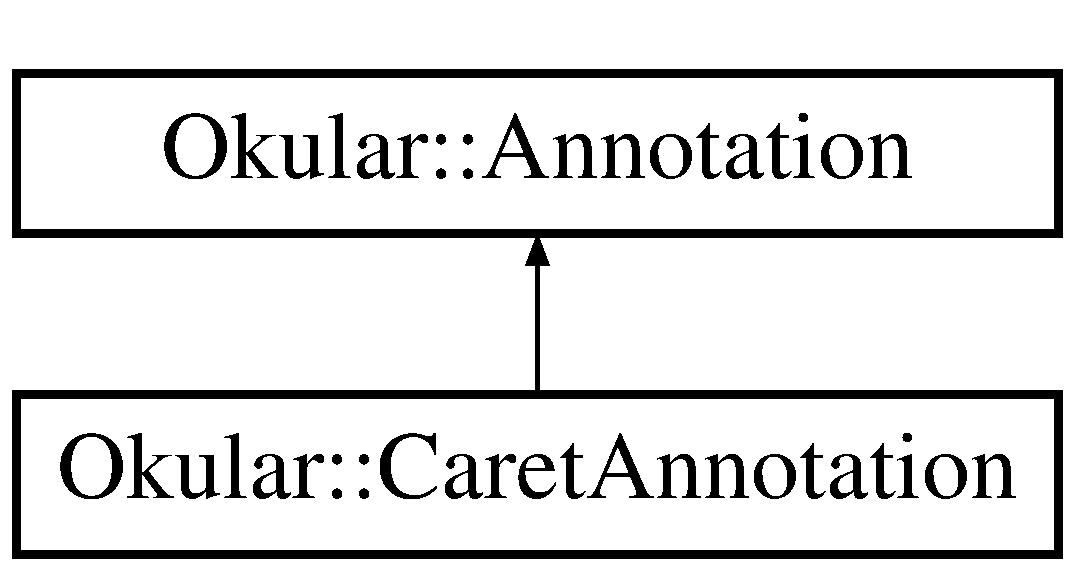
\includegraphics[height=2.000000cm]{classOkular_1_1CaretAnnotation}
\end{center}
\end{figure}
\subsection*{Public Types}
\begin{DoxyCompactItemize}
\item 
enum \hyperlink{classOkular_1_1CaretAnnotation_a0fa75d6ac84d6e08aae0561b55e98695}{Caret\+Symbol} \{ \hyperlink{classOkular_1_1CaretAnnotation_a0fa75d6ac84d6e08aae0561b55e98695aac987216c2d46c031053ac96718c05ee}{None}, 
\hyperlink{classOkular_1_1CaretAnnotation_a0fa75d6ac84d6e08aae0561b55e98695a18d3f68c9167d4db0fd70b5d869c813a}{P}
 \}
\end{DoxyCompactItemize}
\subsection*{Public Member Functions}
\begin{DoxyCompactItemize}
\item 
\hyperlink{classOkular_1_1CaretAnnotation_a96fd46a67b080689128acf9aefa4d17f}{Caret\+Annotation} ()
\item 
\hyperlink{classOkular_1_1CaretAnnotation_a55bfb4eebec11782fda2855ae340f4dc}{Caret\+Annotation} (const Q\+Dom\+Node \&description)
\item 
\hyperlink{classOkular_1_1CaretAnnotation_aab7f00e4d6f59f0ce1f75f5e8e9fd313}{$\sim$\+Caret\+Annotation} ()
\item 
void \hyperlink{classOkular_1_1CaretAnnotation_a3f6f7dcb073888075762244d2805981f}{set\+Caret\+Symbol} (\hyperlink{classOkular_1_1CaretAnnotation_a0fa75d6ac84d6e08aae0561b55e98695}{Caret\+Annotation\+::\+Caret\+Symbol} symbol)
\item 
\hyperlink{classOkular_1_1CaretAnnotation_a0fa75d6ac84d6e08aae0561b55e98695}{Caret\+Annotation\+::\+Caret\+Symbol} \hyperlink{classOkular_1_1CaretAnnotation_ac328095a16f32e9039d917d7ee2774dc}{caret\+Symbol} () const 
\item 
\hyperlink{classOkular_1_1Annotation_af71b46e37d5f850b97d5c4de3be9aac0}{Sub\+Type} \hyperlink{classOkular_1_1CaretAnnotation_aa126043fc2afcb4b89bd197dbdb463a0}{sub\+Type} () const 
\item 
void \hyperlink{classOkular_1_1CaretAnnotation_ac1d1d750933fa58b3868cec6fe645dfd}{store} (Q\+Dom\+Node \&node, Q\+Dom\+Document \&document) const 
\end{DoxyCompactItemize}


\subsection{Detailed Description}


Definition at line 1315 of file annotations.\+h.



\subsection{Member Enumeration Documentation}
\hypertarget{classOkular_1_1CaretAnnotation_a0fa75d6ac84d6e08aae0561b55e98695}{\index{Okular\+::\+Caret\+Annotation@{Okular\+::\+Caret\+Annotation}!Caret\+Symbol@{Caret\+Symbol}}
\index{Caret\+Symbol@{Caret\+Symbol}!Okular\+::\+Caret\+Annotation@{Okular\+::\+Caret\+Annotation}}
\subsubsection[{Caret\+Symbol}]{\setlength{\rightskip}{0pt plus 5cm}enum {\bf Okular\+::\+Caret\+Annotation\+::\+Caret\+Symbol}}}\label{classOkular_1_1CaretAnnotation_a0fa75d6ac84d6e08aae0561b55e98695}
Describes the highlighting style of the annotation. \begin{Desc}
\item[Enumerator]\par
\begin{description}
\index{None@{None}!Okular\+::\+Caret\+Annotation@{Okular\+::\+Caret\+Annotation}}\index{Okular\+::\+Caret\+Annotation@{Okular\+::\+Caret\+Annotation}!None@{None}}\item[{\em 
\hypertarget{classOkular_1_1CaretAnnotation_a0fa75d6ac84d6e08aae0561b55e98695aac987216c2d46c031053ac96718c05ee}{None}\label{classOkular_1_1CaretAnnotation_a0fa75d6ac84d6e08aae0561b55e98695aac987216c2d46c031053ac96718c05ee}
}]No symbol to be associated with the text. \index{P@{P}!Okular\+::\+Caret\+Annotation@{Okular\+::\+Caret\+Annotation}}\index{Okular\+::\+Caret\+Annotation@{Okular\+::\+Caret\+Annotation}!P@{P}}\item[{\em 
\hypertarget{classOkular_1_1CaretAnnotation_a0fa75d6ac84d6e08aae0561b55e98695a18d3f68c9167d4db0fd70b5d869c813a}{P}\label{classOkular_1_1CaretAnnotation_a0fa75d6ac84d6e08aae0561b55e98695a18d3f68c9167d4db0fd70b5d869c813a}
}]A 'paragraph' symbol. \end{description}
\end{Desc}


Definition at line 1321 of file annotations.\+h.


\begin{DoxyCode}
1322         \{
1323             \hyperlink{classOkular_1_1CaretAnnotation_a0fa75d6ac84d6e08aae0561b55e98695aac987216c2d46c031053ac96718c05ee}{None},       
1324             \hyperlink{classOkular_1_1CaretAnnotation_a0fa75d6ac84d6e08aae0561b55e98695a18d3f68c9167d4db0fd70b5d869c813a}{P}           
1325         \};
\end{DoxyCode}


\subsection{Constructor \& Destructor Documentation}
\hypertarget{classOkular_1_1CaretAnnotation_a96fd46a67b080689128acf9aefa4d17f}{\index{Okular\+::\+Caret\+Annotation@{Okular\+::\+Caret\+Annotation}!Caret\+Annotation@{Caret\+Annotation}}
\index{Caret\+Annotation@{Caret\+Annotation}!Okular\+::\+Caret\+Annotation@{Okular\+::\+Caret\+Annotation}}
\subsubsection[{Caret\+Annotation}]{\setlength{\rightskip}{0pt plus 5cm}Caret\+Annotation\+::\+Caret\+Annotation (
\begin{DoxyParamCaption}
{}
\end{DoxyParamCaption}
)}}\label{classOkular_1_1CaretAnnotation_a96fd46a67b080689128acf9aefa4d17f}
Creates a new caret annotation. 

Definition at line 2414 of file annotations.\+cpp.


\begin{DoxyCode}
2415     : \hyperlink{classOkular_1_1Annotation}{Annotation}( *\textcolor{keyword}{new} \hyperlink{classOkular_1_1CaretAnnotationPrivate}{CaretAnnotationPrivate}() )
2416 \{
2417 \}
\end{DoxyCode}
\hypertarget{classOkular_1_1CaretAnnotation_a55bfb4eebec11782fda2855ae340f4dc}{\index{Okular\+::\+Caret\+Annotation@{Okular\+::\+Caret\+Annotation}!Caret\+Annotation@{Caret\+Annotation}}
\index{Caret\+Annotation@{Caret\+Annotation}!Okular\+::\+Caret\+Annotation@{Okular\+::\+Caret\+Annotation}}
\subsubsection[{Caret\+Annotation}]{\setlength{\rightskip}{0pt plus 5cm}Caret\+Annotation\+::\+Caret\+Annotation (
\begin{DoxyParamCaption}
\item[{const Q\+Dom\+Node \&}]{description}
\end{DoxyParamCaption}
)\hspace{0.3cm}{\ttfamily [explicit]}}}\label{classOkular_1_1CaretAnnotation_a55bfb4eebec11782fda2855ae340f4dc}
Creates a new caret annotation from the xml {\ttfamily description} 

Definition at line 2419 of file annotations.\+cpp.


\begin{DoxyCode}
2420     : \hyperlink{classOkular_1_1Annotation}{Annotation}( *\textcolor{keyword}{new} \hyperlink{classOkular_1_1CaretAnnotationPrivate}{CaretAnnotationPrivate}(), node )
2421 \{
2422 \}
\end{DoxyCode}
\hypertarget{classOkular_1_1CaretAnnotation_aab7f00e4d6f59f0ce1f75f5e8e9fd313}{\index{Okular\+::\+Caret\+Annotation@{Okular\+::\+Caret\+Annotation}!````~Caret\+Annotation@{$\sim$\+Caret\+Annotation}}
\index{````~Caret\+Annotation@{$\sim$\+Caret\+Annotation}!Okular\+::\+Caret\+Annotation@{Okular\+::\+Caret\+Annotation}}
\subsubsection[{$\sim$\+Caret\+Annotation}]{\setlength{\rightskip}{0pt plus 5cm}Caret\+Annotation\+::$\sim$\+Caret\+Annotation (
\begin{DoxyParamCaption}
{}
\end{DoxyParamCaption}
)}}\label{classOkular_1_1CaretAnnotation_aab7f00e4d6f59f0ce1f75f5e8e9fd313}
Destroys the caret annotation. 

Definition at line 2424 of file annotations.\+cpp.


\begin{DoxyCode}
2425 \{
2426 \}
\end{DoxyCode}


\subsection{Member Function Documentation}
\hypertarget{classOkular_1_1CaretAnnotation_ac328095a16f32e9039d917d7ee2774dc}{\index{Okular\+::\+Caret\+Annotation@{Okular\+::\+Caret\+Annotation}!caret\+Symbol@{caret\+Symbol}}
\index{caret\+Symbol@{caret\+Symbol}!Okular\+::\+Caret\+Annotation@{Okular\+::\+Caret\+Annotation}}
\subsubsection[{caret\+Symbol}]{\setlength{\rightskip}{0pt plus 5cm}{\bf Caret\+Annotation\+::\+Caret\+Symbol} Caret\+Annotation\+::caret\+Symbol (
\begin{DoxyParamCaption}
{}
\end{DoxyParamCaption}
) const}}\label{classOkular_1_1CaretAnnotation_ac328095a16f32e9039d917d7ee2774dc}
Returns the symbol of the annotation. 

Definition at line 2434 of file annotations.\+cpp.


\begin{DoxyCode}
2435 \{
2436     Q\_D( \textcolor{keyword}{const} \hyperlink{classOkular_1_1CaretAnnotation}{CaretAnnotation} );
2437     \textcolor{keywordflow}{return} d->m\_symbol;
2438 \}
\end{DoxyCode}
\hypertarget{classOkular_1_1CaretAnnotation_a3f6f7dcb073888075762244d2805981f}{\index{Okular\+::\+Caret\+Annotation@{Okular\+::\+Caret\+Annotation}!set\+Caret\+Symbol@{set\+Caret\+Symbol}}
\index{set\+Caret\+Symbol@{set\+Caret\+Symbol}!Okular\+::\+Caret\+Annotation@{Okular\+::\+Caret\+Annotation}}
\subsubsection[{set\+Caret\+Symbol}]{\setlength{\rightskip}{0pt plus 5cm}void Caret\+Annotation\+::set\+Caret\+Symbol (
\begin{DoxyParamCaption}
\item[{{\bf Caret\+Annotation\+::\+Caret\+Symbol}}]{symbol}
\end{DoxyParamCaption}
)}}\label{classOkular_1_1CaretAnnotation_a3f6f7dcb073888075762244d2805981f}
Sets the {\ttfamily symbol} for the caret annotation. 

Definition at line 2428 of file annotations.\+cpp.


\begin{DoxyCode}
2429 \{
2430     Q\_D( \hyperlink{classOkular_1_1CaretAnnotation}{CaretAnnotation} );
2431     d->m\_symbol = symbol;
2432 \}
\end{DoxyCode}
\hypertarget{classOkular_1_1CaretAnnotation_ac1d1d750933fa58b3868cec6fe645dfd}{\index{Okular\+::\+Caret\+Annotation@{Okular\+::\+Caret\+Annotation}!store@{store}}
\index{store@{store}!Okular\+::\+Caret\+Annotation@{Okular\+::\+Caret\+Annotation}}
\subsubsection[{store}]{\setlength{\rightskip}{0pt plus 5cm}void Caret\+Annotation\+::store (
\begin{DoxyParamCaption}
\item[{Q\+Dom\+Node \&}]{node, }
\item[{Q\+Dom\+Document \&}]{document}
\end{DoxyParamCaption}
) const\hspace{0.3cm}{\ttfamily [virtual]}}}\label{classOkular_1_1CaretAnnotation_ac1d1d750933fa58b3868cec6fe645dfd}
Stores the caret annotation as xml in {\ttfamily document} under the given parent {\ttfamily node}. 

Reimplemented from \hyperlink{classOkular_1_1Annotation_abbb607cf5929ffd06f789a22b353dcb3}{Okular\+::\+Annotation}.



Definition at line 2445 of file annotations.\+cpp.


\begin{DoxyCode}
2446 \{
2447     Q\_D( \textcolor{keyword}{const} \hyperlink{classOkular_1_1CaretAnnotation}{CaretAnnotation} );
2448     \textcolor{comment}{// recurse to parent objects storing properties}
2449     \hyperlink{classOkular_1_1Annotation_abbb607cf5929ffd06f789a22b353dcb3}{Annotation::store}( node, document );
2450 
2451     \textcolor{comment}{// create [caret] element}
2452     QDomElement caretElement = document.createElement( \textcolor{stringliteral}{"caret"} );
2453     node.appendChild( caretElement );
2454 
2455     \textcolor{comment}{// append the optional attributes}
2456     \textcolor{keywordflow}{if} ( d->m\_symbol != \hyperlink{classOkular_1_1CaretAnnotation_a0fa75d6ac84d6e08aae0561b55e98695aac987216c2d46c031053ac96718c05ee}{None} )
2457         caretElement.setAttribute( \textcolor{stringliteral}{"symbol"}, caretSymbolToString( d->m\_symbol ) );
2458 \}
\end{DoxyCode}
\hypertarget{classOkular_1_1CaretAnnotation_aa126043fc2afcb4b89bd197dbdb463a0}{\index{Okular\+::\+Caret\+Annotation@{Okular\+::\+Caret\+Annotation}!sub\+Type@{sub\+Type}}
\index{sub\+Type@{sub\+Type}!Okular\+::\+Caret\+Annotation@{Okular\+::\+Caret\+Annotation}}
\subsubsection[{sub\+Type}]{\setlength{\rightskip}{0pt plus 5cm}{\bf Annotation\+::\+Sub\+Type} Caret\+Annotation\+::sub\+Type (
\begin{DoxyParamCaption}
{}
\end{DoxyParamCaption}
) const\hspace{0.3cm}{\ttfamily [virtual]}}}\label{classOkular_1_1CaretAnnotation_aa126043fc2afcb4b89bd197dbdb463a0}
Returns the sub type of the caret annotation. 

Implements \hyperlink{classOkular_1_1Annotation_af9833449767eacd740f377e69a1fdd48}{Okular\+::\+Annotation}.



Definition at line 2440 of file annotations.\+cpp.


\begin{DoxyCode}
2441 \{
2442     \textcolor{keywordflow}{return} \hyperlink{classOkular_1_1Annotation_af71b46e37d5f850b97d5c4de3be9aac0a904187454fd508d898a3d5843193ad43}{ACaret};
2443 \}
\end{DoxyCode}


The documentation for this class was generated from the following files\+:\begin{DoxyCompactItemize}
\item 
core/\hyperlink{annotations_8h}{annotations.\+h}\item 
core/\hyperlink{annotations_8cpp}{annotations.\+cpp}\end{DoxyCompactItemize}

\hypertarget{classOkular_1_1CaretAnnotationPrivate}{\section{Okular\+:\+:Caret\+Annotation\+Private Class Reference}
\label{classOkular_1_1CaretAnnotationPrivate}\index{Okular\+::\+Caret\+Annotation\+Private@{Okular\+::\+Caret\+Annotation\+Private}}
}
Inheritance diagram for Okular\+:\+:Caret\+Annotation\+Private\+:\begin{figure}[H]
\begin{center}
\leavevmode
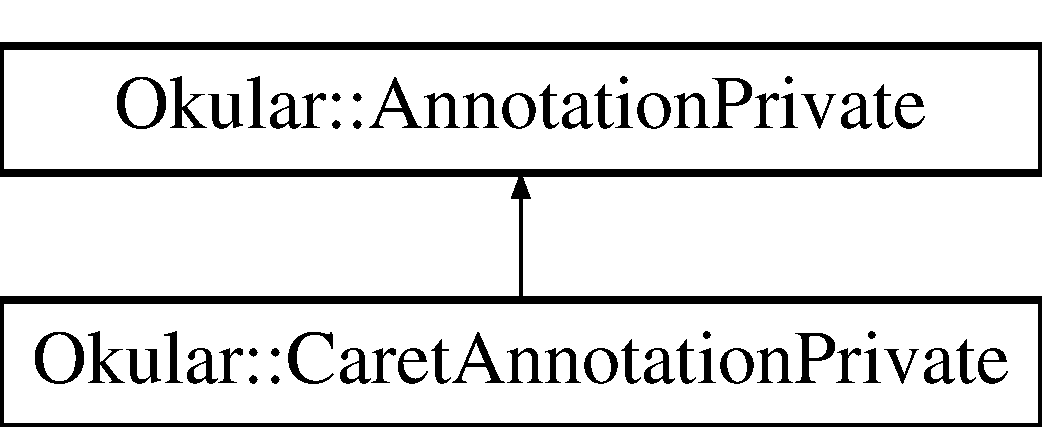
\includegraphics[height=2.000000cm]{classOkular_1_1CaretAnnotationPrivate}
\end{center}
\end{figure}
\subsection*{Public Member Functions}
\begin{DoxyCompactItemize}
\item 
\hyperlink{classOkular_1_1CaretAnnotationPrivate_abd3a551814d37c3662fa9c4f4f04070b}{Caret\+Annotation\+Private} ()
\item 
virtual void \hyperlink{classOkular_1_1CaretAnnotationPrivate_a02d97e47b70b09cbaac6e270519ac6f1}{set\+Annotation\+Properties} (const Q\+Dom\+Node \&node)
\item 
virtual \hyperlink{classOkular_1_1AnnotationPrivate}{Annotation\+Private} $\ast$ \hyperlink{classOkular_1_1CaretAnnotationPrivate_ad2c2ff9e13dd507768bafdd207371ea0}{get\+New\+Annotation\+Private} ()
\end{DoxyCompactItemize}
\subsection*{Public Attributes}
\begin{DoxyCompactItemize}
\item 
\hyperlink{classOkular_1_1CaretAnnotation_a0fa75d6ac84d6e08aae0561b55e98695}{Caret\+Annotation\+::\+Caret\+Symbol} \hyperlink{classOkular_1_1CaretAnnotationPrivate_ae93f5592157c6c38ceb239b5b1c31aae}{m\+\_\+symbol}
\end{DoxyCompactItemize}


\subsection{Detailed Description}
\hyperlink{classOkular_1_1CaretAnnotation}{Caret\+Annotation} \mbox{[}\hyperlink{classOkular_1_1Annotation}{Annotation}\mbox{]} 

Definition at line 2352 of file annotations.\+cpp.



\subsection{Constructor \& Destructor Documentation}
\hypertarget{classOkular_1_1CaretAnnotationPrivate_abd3a551814d37c3662fa9c4f4f04070b}{\index{Okular\+::\+Caret\+Annotation\+Private@{Okular\+::\+Caret\+Annotation\+Private}!Caret\+Annotation\+Private@{Caret\+Annotation\+Private}}
\index{Caret\+Annotation\+Private@{Caret\+Annotation\+Private}!Okular\+::\+Caret\+Annotation\+Private@{Okular\+::\+Caret\+Annotation\+Private}}
\subsubsection[{Caret\+Annotation\+Private}]{\setlength{\rightskip}{0pt plus 5cm}Okular\+::\+Caret\+Annotation\+Private\+::\+Caret\+Annotation\+Private (
\begin{DoxyParamCaption}
{}
\end{DoxyParamCaption}
)\hspace{0.3cm}{\ttfamily [inline]}}}\label{classOkular_1_1CaretAnnotationPrivate_abd3a551814d37c3662fa9c4f4f04070b}


Definition at line 2355 of file annotations.\+cpp.


\begin{DoxyCode}
2356             : \hyperlink{classOkular_1_1AnnotationPrivate_affc5d14076f4606905c3c0cd2f6b9dc1}{AnnotationPrivate}(), \hyperlink{classOkular_1_1CaretAnnotationPrivate_ae93f5592157c6c38ceb239b5b1c31aae}{m\_symbol}( 
      \hyperlink{classOkular_1_1CaretAnnotation_a0fa75d6ac84d6e08aae0561b55e98695aac987216c2d46c031053ac96718c05ee}{CaretAnnotation::None} )
2357         \{
2358         \}
\end{DoxyCode}


\subsection{Member Function Documentation}
\hypertarget{classOkular_1_1CaretAnnotationPrivate_ad2c2ff9e13dd507768bafdd207371ea0}{\index{Okular\+::\+Caret\+Annotation\+Private@{Okular\+::\+Caret\+Annotation\+Private}!get\+New\+Annotation\+Private@{get\+New\+Annotation\+Private}}
\index{get\+New\+Annotation\+Private@{get\+New\+Annotation\+Private}!Okular\+::\+Caret\+Annotation\+Private@{Okular\+::\+Caret\+Annotation\+Private}}
\subsubsection[{get\+New\+Annotation\+Private}]{\setlength{\rightskip}{0pt plus 5cm}{\bf Annotation\+Private} $\ast$ Caret\+Annotation\+Private\+::get\+New\+Annotation\+Private (
\begin{DoxyParamCaption}
{}
\end{DoxyParamCaption}
)\hspace{0.3cm}{\ttfamily [virtual]}}}\label{classOkular_1_1CaretAnnotationPrivate_ad2c2ff9e13dd507768bafdd207371ea0}


Implements \hyperlink{classOkular_1_1AnnotationPrivate_a4a27afb6108cff892c7bcccd8ba3aafa}{Okular\+::\+Annotation\+Private}.



Definition at line 2409 of file annotations.\+cpp.


\begin{DoxyCode}
2410 \{
2411     \textcolor{keywordflow}{return} \textcolor{keyword}{new} \hyperlink{classOkular_1_1CaretAnnotationPrivate_abd3a551814d37c3662fa9c4f4f04070b}{CaretAnnotationPrivate}();
2412 \}
\end{DoxyCode}
\hypertarget{classOkular_1_1CaretAnnotationPrivate_a02d97e47b70b09cbaac6e270519ac6f1}{\index{Okular\+::\+Caret\+Annotation\+Private@{Okular\+::\+Caret\+Annotation\+Private}!set\+Annotation\+Properties@{set\+Annotation\+Properties}}
\index{set\+Annotation\+Properties@{set\+Annotation\+Properties}!Okular\+::\+Caret\+Annotation\+Private@{Okular\+::\+Caret\+Annotation\+Private}}
\subsubsection[{set\+Annotation\+Properties}]{\setlength{\rightskip}{0pt plus 5cm}void Caret\+Annotation\+Private\+::set\+Annotation\+Properties (
\begin{DoxyParamCaption}
\item[{const Q\+Dom\+Node \&}]{node}
\end{DoxyParamCaption}
)\hspace{0.3cm}{\ttfamily [virtual]}}}\label{classOkular_1_1CaretAnnotationPrivate_a02d97e47b70b09cbaac6e270519ac6f1}


Reimplemented from \hyperlink{classOkular_1_1AnnotationPrivate_a5fc7b450fa8c7e2717372e7394c3aa39}{Okular\+::\+Annotation\+Private}.



Definition at line 2387 of file annotations.\+cpp.


\begin{DoxyCode}
2388 \{
2389     \hyperlink{classOkular_1_1AnnotationPrivate_a5fc7b450fa8c7e2717372e7394c3aa39}{Okular::AnnotationPrivate::setAnnotationProperties}(
      node);
2390 
2391     \textcolor{comment}{// loop through the whole children looking for a 'caret' element}
2392     QDomNode subNode = node.firstChild();
2393     \textcolor{keywordflow}{while}( subNode.isElement() )
2394     \{
2395         QDomElement e = subNode.toElement();
2396         subNode = subNode.nextSibling();
2397         \textcolor{keywordflow}{if} ( e.tagName() != \textcolor{stringliteral}{"caret"} )
2398             \textcolor{keywordflow}{continue};
2399 
2400         \textcolor{comment}{// parse the attributes}
2401         \textcolor{keywordflow}{if} ( e.hasAttribute( \textcolor{stringliteral}{"symbol"} ) )
2402             \hyperlink{classOkular_1_1CaretAnnotationPrivate_ae93f5592157c6c38ceb239b5b1c31aae}{m\_symbol} = caretSymbolFromString( e.attribute( \textcolor{stringliteral}{"symbol"} ) );
2403 
2404         \textcolor{comment}{// loading complete}
2405         \textcolor{keywordflow}{break};
2406     \}
2407 \}
\end{DoxyCode}


\subsection{Member Data Documentation}
\hypertarget{classOkular_1_1CaretAnnotationPrivate_ae93f5592157c6c38ceb239b5b1c31aae}{\index{Okular\+::\+Caret\+Annotation\+Private@{Okular\+::\+Caret\+Annotation\+Private}!m\+\_\+symbol@{m\+\_\+symbol}}
\index{m\+\_\+symbol@{m\+\_\+symbol}!Okular\+::\+Caret\+Annotation\+Private@{Okular\+::\+Caret\+Annotation\+Private}}
\subsubsection[{m\+\_\+symbol}]{\setlength{\rightskip}{0pt plus 5cm}{\bf Caret\+Annotation\+::\+Caret\+Symbol} Okular\+::\+Caret\+Annotation\+Private\+::m\+\_\+symbol}}\label{classOkular_1_1CaretAnnotationPrivate_ae93f5592157c6c38ceb239b5b1c31aae}


Definition at line 2363 of file annotations.\+cpp.



The documentation for this class was generated from the following file\+:\begin{DoxyCompactItemize}
\item 
core/\hyperlink{annotations_8cpp}{annotations.\+cpp}\end{DoxyCompactItemize}

\hypertarget{classCaretAnnotationWidget}{\section{Caret\+Annotation\+Widget Class Reference}
\label{classCaretAnnotationWidget}\index{Caret\+Annotation\+Widget@{Caret\+Annotation\+Widget}}
}


{\ttfamily \#include $<$annotationwidgets.\+h$>$}

Inheritance diagram for Caret\+Annotation\+Widget\+:\begin{figure}[H]
\begin{center}
\leavevmode
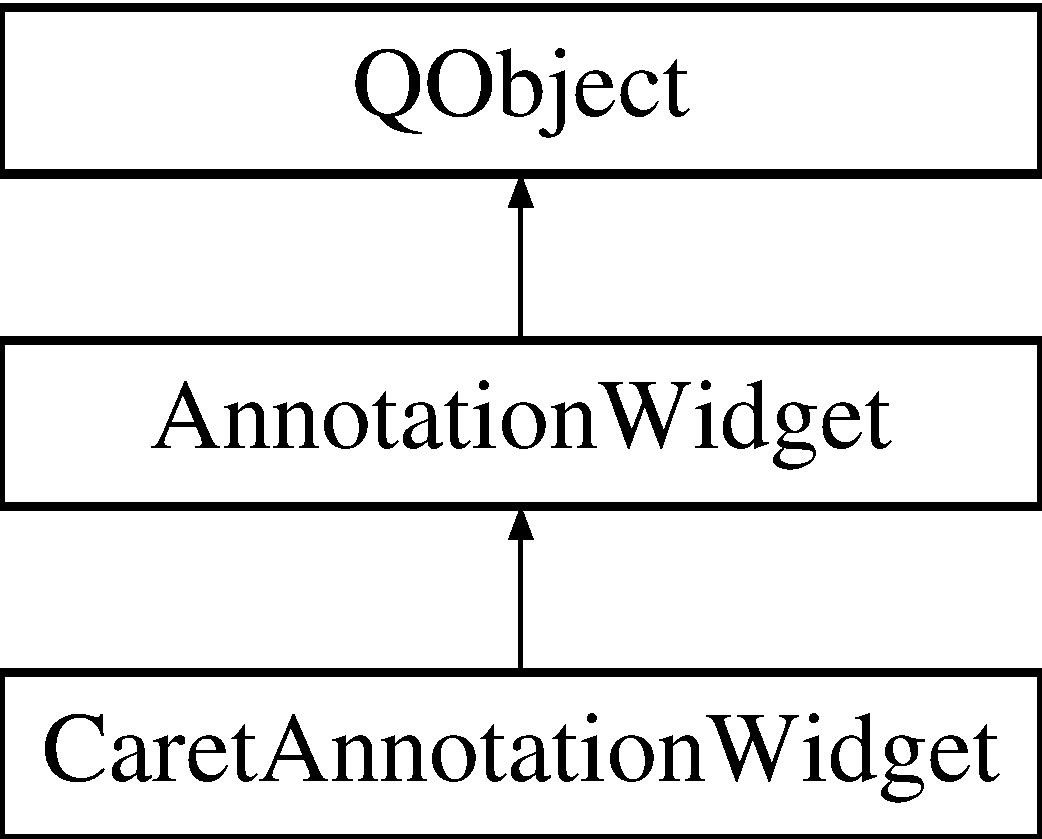
\includegraphics[height=3.000000cm]{classCaretAnnotationWidget}
\end{center}
\end{figure}
\subsection*{Public Member Functions}
\begin{DoxyCompactItemize}
\item 
\hyperlink{classCaretAnnotationWidget_aff83e9a2d16baea21204c3e370c93e01}{Caret\+Annotation\+Widget} (\hyperlink{classOkular_1_1Annotation}{Okular\+::\+Annotation} $\ast$ann)
\item 
virtual void \hyperlink{classCaretAnnotationWidget_ace74af8590fa2bae736aa3ab6f2ca862}{apply\+Changes} ()
\end{DoxyCompactItemize}
\subsection*{Protected Member Functions}
\begin{DoxyCompactItemize}
\item 
virtual Q\+Widget $\ast$ \hyperlink{classCaretAnnotationWidget_a1de63a32fcebc687453ce9525604f02c}{create\+Style\+Widget} ()
\end{DoxyCompactItemize}
\subsection*{Additional Inherited Members}


\subsection{Detailed Description}


Definition at line 220 of file annotationwidgets.\+h.



\subsection{Constructor \& Destructor Documentation}
\hypertarget{classCaretAnnotationWidget_aff83e9a2d16baea21204c3e370c93e01}{\index{Caret\+Annotation\+Widget@{Caret\+Annotation\+Widget}!Caret\+Annotation\+Widget@{Caret\+Annotation\+Widget}}
\index{Caret\+Annotation\+Widget@{Caret\+Annotation\+Widget}!Caret\+Annotation\+Widget@{Caret\+Annotation\+Widget}}
\subsubsection[{Caret\+Annotation\+Widget}]{\setlength{\rightskip}{0pt plus 5cm}Caret\+Annotation\+Widget\+::\+Caret\+Annotation\+Widget (
\begin{DoxyParamCaption}
\item[{{\bf Okular\+::\+Annotation} $\ast$}]{ann}
\end{DoxyParamCaption}
)}}\label{classCaretAnnotationWidget_aff83e9a2d16baea21204c3e370c93e01}


Definition at line 727 of file annotationwidgets.\+cpp.


\begin{DoxyCode}
728     : \hyperlink{classAnnotationWidget_a1152e99260c24acde30e2742a07af2ef}{AnnotationWidget}( ann ), m\_pixmapSelector( 0 )
729 \{
730     m\_caretAnn = \textcolor{keyword}{static\_cast<} \hyperlink{classOkular_1_1CaretAnnotation}{Okular::CaretAnnotation} * \textcolor{keyword}{>}( ann );
731 \}
\end{DoxyCode}


\subsection{Member Function Documentation}
\hypertarget{classCaretAnnotationWidget_ace74af8590fa2bae736aa3ab6f2ca862}{\index{Caret\+Annotation\+Widget@{Caret\+Annotation\+Widget}!apply\+Changes@{apply\+Changes}}
\index{apply\+Changes@{apply\+Changes}!Caret\+Annotation\+Widget@{Caret\+Annotation\+Widget}}
\subsubsection[{apply\+Changes}]{\setlength{\rightskip}{0pt plus 5cm}void Caret\+Annotation\+Widget\+::apply\+Changes (
\begin{DoxyParamCaption}
{}
\end{DoxyParamCaption}
)\hspace{0.3cm}{\ttfamily [virtual]}}}\label{classCaretAnnotationWidget_ace74af8590fa2bae736aa3ab6f2ca862}


Reimplemented from \hyperlink{classAnnotationWidget_a00b35958653cb76c93b9d4f70d770f5c}{Annotation\+Widget}.



Definition at line 754 of file annotationwidgets.\+cpp.


\begin{DoxyCode}
755 \{
756     \hyperlink{classAnnotationWidget_a00b35958653cb76c93b9d4f70d770f5c}{AnnotationWidget::applyChanges}();
757     m\_caretAnn->\hyperlink{classOkular_1_1CaretAnnotation_a3f6f7dcb073888075762244d2805981f}{setCaretSymbol}( caretSymbolFromIcon( m\_pixmapSelector->
      \hyperlink{classPixmapPreviewSelector_a04ef584f4a20313aca10221dc4bcc0e9}{icon}() ) );
758 \}
\end{DoxyCode}
\hypertarget{classCaretAnnotationWidget_a1de63a32fcebc687453ce9525604f02c}{\index{Caret\+Annotation\+Widget@{Caret\+Annotation\+Widget}!create\+Style\+Widget@{create\+Style\+Widget}}
\index{create\+Style\+Widget@{create\+Style\+Widget}!Caret\+Annotation\+Widget@{Caret\+Annotation\+Widget}}
\subsubsection[{create\+Style\+Widget}]{\setlength{\rightskip}{0pt plus 5cm}Q\+Widget $\ast$ Caret\+Annotation\+Widget\+::create\+Style\+Widget (
\begin{DoxyParamCaption}
{}
\end{DoxyParamCaption}
)\hspace{0.3cm}{\ttfamily [protected]}, {\ttfamily [virtual]}}}\label{classCaretAnnotationWidget_a1de63a32fcebc687453ce9525604f02c}


Reimplemented from \hyperlink{classAnnotationWidget_a4b0926d20f0b26deb5b6a4e75f78fac3}{Annotation\+Widget}.



Definition at line 733 of file annotationwidgets.\+cpp.


\begin{DoxyCode}
734 \{
735     QWidget * widget = \textcolor{keyword}{new} QWidget();
736     QVBoxLayout * lay = \textcolor{keyword}{new} QVBoxLayout( widget );
737     lay->setMargin( 0 );
738     QGroupBox * gb = \textcolor{keyword}{new} QGroupBox( widget );
739     lay->addWidget( gb );
740     gb->setTitle( i18n( \textcolor{stringliteral}{"Caret Symbol"} ) );
741     QHBoxLayout * gblay = \textcolor{keyword}{new} QHBoxLayout( gb );
742     m\_pixmapSelector = \textcolor{keyword}{new} \hyperlink{classPixmapPreviewSelector}{PixmapPreviewSelector}( gb );
743     gblay->addWidget( m\_pixmapSelector );
744 
745     m\_pixmapSelector->\hyperlink{classPixmapPreviewSelector_ac4729c46cc585aba462dd2eebcb74a92}{addItem}( i18nc( \textcolor{stringliteral}{"Symbol for caret annotations"}, \textcolor{stringliteral}{"None"} ), \textcolor{stringliteral}{"caret-none"} );
746     m\_pixmapSelector->\hyperlink{classPixmapPreviewSelector_ac4729c46cc585aba462dd2eebcb74a92}{addItem}( i18nc( \textcolor{stringliteral}{"Symbol for caret annotations"}, \textcolor{stringliteral}{"P"} ), \textcolor{stringliteral}{"caret-p"} );
747     m\_pixmapSelector->\hyperlink{classPixmapPreviewSelector_a9ba6710637ffc9b0f5c8eac83aaec671}{setIcon}( caretSymbolToIcon( m\_caretAnn->\hyperlink{classOkular_1_1CaretAnnotation_ac328095a16f32e9039d917d7ee2774dc}{caretSymbol}() ) );
748 
749     connect( m\_pixmapSelector, SIGNAL(iconChanged(QString)), \textcolor{keyword}{this}, SIGNAL(
      \hyperlink{classAnnotationWidget_af9dcb02a8b69a602225c9844b5deb6d4}{dataChanged}()) );
750 
751     \textcolor{keywordflow}{return} widget;
752 \}
\end{DoxyCode}


The documentation for this class was generated from the following files\+:\begin{DoxyCompactItemize}
\item 
ui/\hyperlink{annotationwidgets_8h}{annotationwidgets.\+h}\item 
ui/\hyperlink{annotationwidgets_8cpp}{annotationwidgets.\+cpp}\end{DoxyCompactItemize}

\hypertarget{classCheckBoxEdit}{\section{Check\+Box\+Edit Class Reference}
\label{classCheckBoxEdit}\index{Check\+Box\+Edit@{Check\+Box\+Edit}}
}


{\ttfamily \#include $<$formwidgets.\+h$>$}

Inheritance diagram for Check\+Box\+Edit\+:\begin{figure}[H]
\begin{center}
\leavevmode
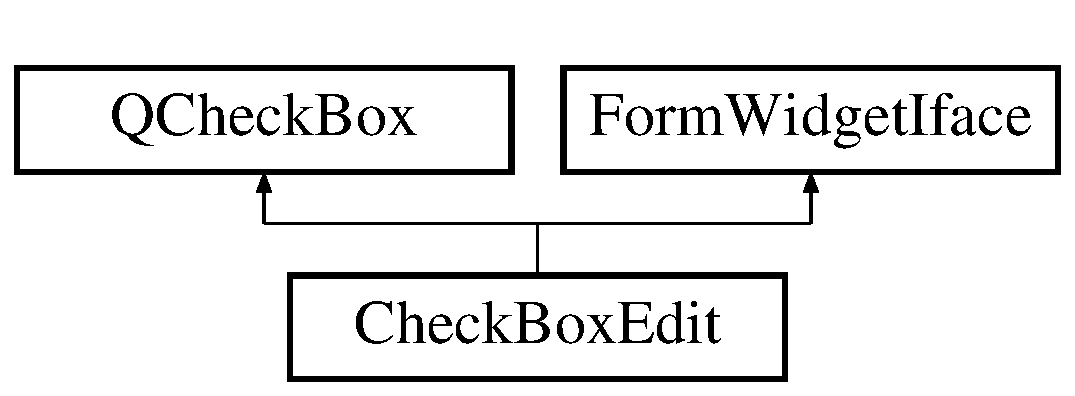
\includegraphics[height=2.000000cm]{classCheckBoxEdit}
\end{center}
\end{figure}
\subsection*{Public Member Functions}
\begin{DoxyCompactItemize}
\item 
\hyperlink{classCheckBoxEdit_a0b3c2bc4389a32a8a41b61b7e0698e6c}{Check\+Box\+Edit} (\hyperlink{classOkular_1_1FormFieldButton}{Okular\+::\+Form\+Field\+Button} $\ast$\hyperlink{classCheckBoxEdit_acec5a34a30f87ab0d146ae0532adf288}{button}, Q\+Widget $\ast$parent=0)
\item 
void \hyperlink{classCheckBoxEdit_aa529e8646ebcb3d1f675f6ce54b48ada}{set\+Form\+Widgets\+Controller} (\hyperlink{classFormWidgetsController}{Form\+Widgets\+Controller} $\ast$controller)
\item 
Q\+Abstract\+Button $\ast$ \hyperlink{classCheckBoxEdit_acec5a34a30f87ab0d146ae0532adf288}{button} ()
\end{DoxyCompactItemize}
\subsection*{Additional Inherited Members}


\subsection{Detailed Description}


Definition at line 182 of file formwidgets.\+h.



\subsection{Constructor \& Destructor Documentation}
\hypertarget{classCheckBoxEdit_a0b3c2bc4389a32a8a41b61b7e0698e6c}{\index{Check\+Box\+Edit@{Check\+Box\+Edit}!Check\+Box\+Edit@{Check\+Box\+Edit}}
\index{Check\+Box\+Edit@{Check\+Box\+Edit}!Check\+Box\+Edit@{Check\+Box\+Edit}}
\subsubsection[{Check\+Box\+Edit}]{\setlength{\rightskip}{0pt plus 5cm}Check\+Box\+Edit\+::\+Check\+Box\+Edit (
\begin{DoxyParamCaption}
\item[{{\bf Okular\+::\+Form\+Field\+Button} $\ast$}]{button, }
\item[{Q\+Widget $\ast$}]{parent = {\ttfamily 0}}
\end{DoxyParamCaption}
)\hspace{0.3cm}{\ttfamily [explicit]}}}\label{classCheckBoxEdit_a0b3c2bc4389a32a8a41b61b7e0698e6c}


Definition at line 332 of file formwidgets.\+cpp.


\begin{DoxyCode}
333     : QCheckBox( parent ), \hyperlink{classFormWidgetIface_a1737728a2348ae69415008ddb1aa3b9d}{FormWidgetIface}( \textcolor{keyword}{this}, button ), m\_form( button )
334 \{
335     setText( m\_form->\hyperlink{classOkular_1_1FormFieldButton_a73098d0def0b5f92cd7efbfb7e273c00}{caption}() );
336     setEnabled( !m\_form->\hyperlink{classOkular_1_1FormField_ad1636c715682959442f528c72a2f4c0a}{isReadOnly}() );
337 
338     setVisible( m\_form->\hyperlink{classOkular_1_1FormField_aee63f77f88a7f8359d9a53de3d07ebe0}{isVisible}() );
339     setCursor( Qt::ArrowCursor );
340 \}
\end{DoxyCode}


\subsection{Member Function Documentation}
\hypertarget{classCheckBoxEdit_acec5a34a30f87ab0d146ae0532adf288}{\index{Check\+Box\+Edit@{Check\+Box\+Edit}!button@{button}}
\index{button@{button}!Check\+Box\+Edit@{Check\+Box\+Edit}}
\subsubsection[{button}]{\setlength{\rightskip}{0pt plus 5cm}Q\+Abstract\+Button $\ast$ Check\+Box\+Edit\+::button (
\begin{DoxyParamCaption}
{}
\end{DoxyParamCaption}
)\hspace{0.3cm}{\ttfamily [virtual]}}}\label{classCheckBoxEdit_acec5a34a30f87ab0d146ae0532adf288}


Reimplemented from \hyperlink{classFormWidgetIface_afd9eb69f17a3b1d5e970f3cc496ddb17}{Form\+Widget\+Iface}.



Definition at line 350 of file formwidgets.\+cpp.


\begin{DoxyCode}
351 \{
352     \textcolor{keywordflow}{return} \textcolor{keyword}{this};
353 \}
\end{DoxyCode}
\hypertarget{classCheckBoxEdit_aa529e8646ebcb3d1f675f6ce54b48ada}{\index{Check\+Box\+Edit@{Check\+Box\+Edit}!set\+Form\+Widgets\+Controller@{set\+Form\+Widgets\+Controller}}
\index{set\+Form\+Widgets\+Controller@{set\+Form\+Widgets\+Controller}!Check\+Box\+Edit@{Check\+Box\+Edit}}
\subsubsection[{set\+Form\+Widgets\+Controller}]{\setlength{\rightskip}{0pt plus 5cm}void Check\+Box\+Edit\+::set\+Form\+Widgets\+Controller (
\begin{DoxyParamCaption}
\item[{{\bf Form\+Widgets\+Controller} $\ast$}]{controller}
\end{DoxyParamCaption}
)\hspace{0.3cm}{\ttfamily [virtual]}}}\label{classCheckBoxEdit_aa529e8646ebcb3d1f675f6ce54b48ada}


Reimplemented from \hyperlink{classFormWidgetIface_a4d3129afff43729fafc4e6b58a4d16fe}{Form\+Widget\+Iface}.



Definition at line 342 of file formwidgets.\+cpp.


\begin{DoxyCode}
343 \{
344     \hyperlink{classFormWidgetIface_a4d3129afff43729fafc4e6b58a4d16fe}{FormWidgetIface::setFormWidgetsController}( controller );
345     \hyperlink{classFormWidgetIface_a2d51d0c5aaf48aad5480551f69f82e9a}{m\_controller}->\hyperlink{classFormWidgetsController_a46b5faee7cd52e35eda20e463ea257ca}{registerRadioButton}( \hyperlink{classCheckBoxEdit_acec5a34a30f87ab0d146ae0532adf288}{button}(), m\_form );
346     setChecked( m\_form->\hyperlink{classOkular_1_1FormFieldButton_aff17cce65de36b508a3a645747e24c51}{state}() );
347     connect( \textcolor{keyword}{this}, SIGNAL(stateChanged(\textcolor{keywordtype}{int})), \textcolor{keyword}{this}, SLOT(slotStateChanged(\textcolor{keywordtype}{int})) );
348 \}
\end{DoxyCode}


The documentation for this class was generated from the following files\+:\begin{DoxyCompactItemize}
\item 
ui/\hyperlink{formwidgets_8h}{formwidgets.\+h}\item 
ui/\hyperlink{formwidgets_8cpp}{formwidgets.\+cpp}\end{DoxyCompactItemize}

\hypertarget{classCHMGenerator}{\section{C\+H\+M\+Generator Class Reference}
\label{classCHMGenerator}\index{C\+H\+M\+Generator@{C\+H\+M\+Generator}}
}


{\ttfamily \#include $<$generator\+\_\+chm.\+h$>$}

Inheritance diagram for C\+H\+M\+Generator\+:\begin{figure}[H]
\begin{center}
\leavevmode
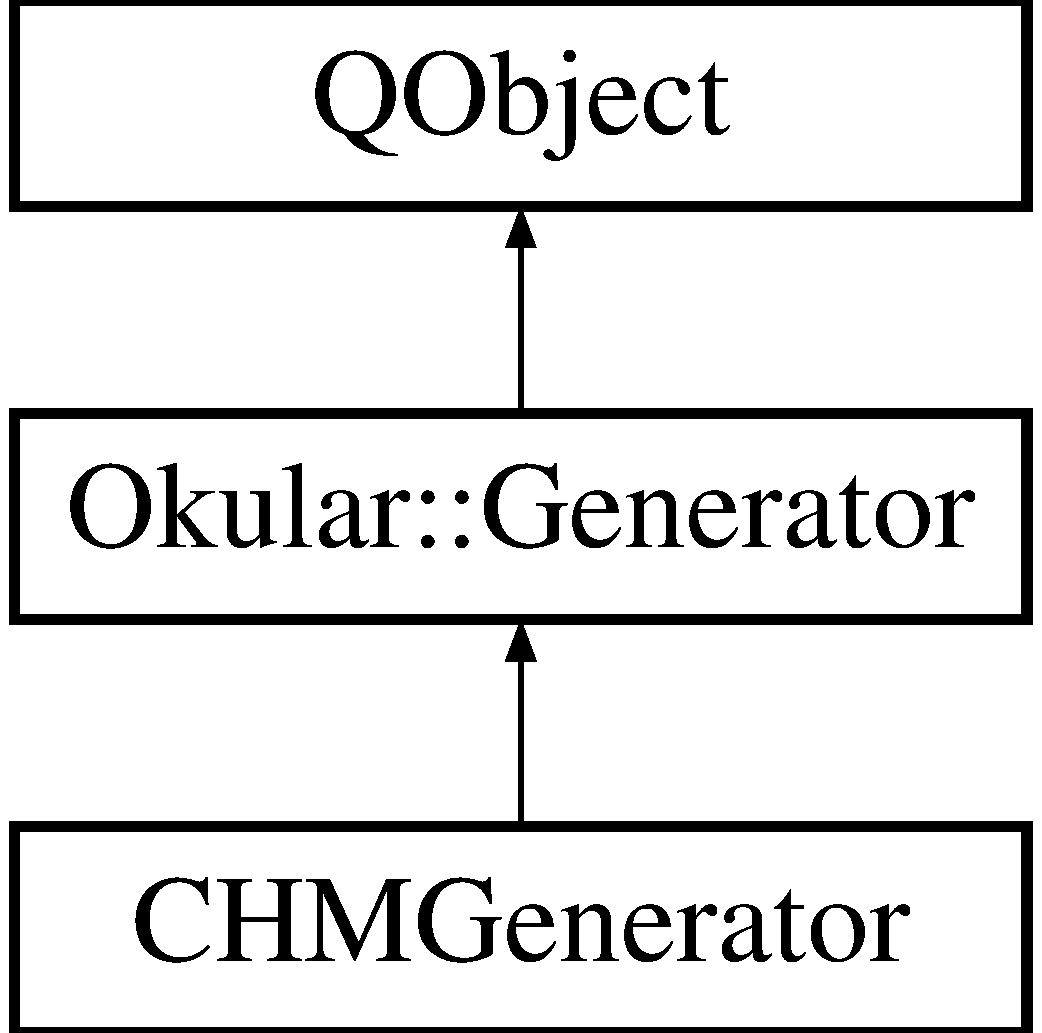
\includegraphics[height=3.000000cm]{classCHMGenerator}
\end{center}
\end{figure}
\subsection*{Public Slots}
\begin{DoxyCompactItemize}
\item 
void \hyperlink{classCHMGenerator_a238973cd7c98434b97af498d121f16a5}{slot\+Completed} ()
\end{DoxyCompactItemize}
\subsection*{Public Member Functions}
\begin{DoxyCompactItemize}
\item 
\hyperlink{classCHMGenerator_a62bbb2287ce107cb02af60fca55e2a66}{C\+H\+M\+Generator} (Q\+Object $\ast$parent, const Q\+Variant\+List \&args)
\item 
\hyperlink{classCHMGenerator_aa6b744aa2e72a05309f6790eb1056ec0}{$\sim$\+C\+H\+M\+Generator} ()
\item 
bool \hyperlink{classCHMGenerator_adabe55488d27e4fe901db82abab46ae1}{load\+Document} (const Q\+String \&file\+Name, Q\+Vector$<$ \hyperlink{classOkular_1_1Page}{Okular\+::\+Page} $\ast$ $>$ \&pages\+Vector)
\item 
const \hyperlink{classOkular_1_1DocumentInfo}{Okular\+::\+Document\+Info} $\ast$ \hyperlink{classCHMGenerator_a892ef3f3685cb701ed0c07681313dc8c}{generate\+Document\+Info} ()
\item 
const \hyperlink{classOkular_1_1DocumentSynopsis}{Okular\+::\+Document\+Synopsis} $\ast$ \hyperlink{classCHMGenerator_a6e844b636798a41d3e47f13f18477676}{generate\+Document\+Synopsis} ()
\item 
bool \hyperlink{classCHMGenerator_a4ef1e1dd09459db0669484ee746226ad}{can\+Generate\+Pixmap} () const 
\item 
void \hyperlink{classCHMGenerator_ad4d1606c48e0348950d9fc6ab92e34bc}{generate\+Pixmap} (\hyperlink{classOkular_1_1PixmapRequest}{Okular\+::\+Pixmap\+Request} $\ast$request)
\item 
Q\+Variant \hyperlink{classCHMGenerator_a00c6f5fd227de74f1f70a1538216b4b7}{meta\+Data} (const Q\+String \&key, const Q\+Variant \&option) const 
\end{DoxyCompactItemize}
\subsection*{Protected Member Functions}
\begin{DoxyCompactItemize}
\item 
bool \hyperlink{classCHMGenerator_a8675493780e9540540acb4ca2bdf13e1}{do\+Close\+Document} ()
\item 
\hyperlink{classOkular_1_1TextPage}{Okular\+::\+Text\+Page} $\ast$ \hyperlink{classCHMGenerator_a4573bf1fd7c852641fee327d5d13de48}{text\+Page} (\hyperlink{classOkular_1_1Page}{Okular\+::\+Page} $\ast$page)
\end{DoxyCompactItemize}
\subsection*{Additional Inherited Members}


\subsection{Detailed Description}


Definition at line 31 of file generator\+\_\+chm.\+h.



\subsection{Constructor \& Destructor Documentation}
\hypertarget{classCHMGenerator_a62bbb2287ce107cb02af60fca55e2a66}{\index{C\+H\+M\+Generator@{C\+H\+M\+Generator}!C\+H\+M\+Generator@{C\+H\+M\+Generator}}
\index{C\+H\+M\+Generator@{C\+H\+M\+Generator}!C\+H\+M\+Generator@{C\+H\+M\+Generator}}
\subsubsection[{C\+H\+M\+Generator}]{\setlength{\rightskip}{0pt plus 5cm}C\+H\+M\+Generator\+::\+C\+H\+M\+Generator (
\begin{DoxyParamCaption}
\item[{Q\+Object $\ast$}]{parent, }
\item[{const Q\+Variant\+List \&}]{args}
\end{DoxyParamCaption}
)}}\label{classCHMGenerator_a62bbb2287ce107cb02af60fca55e2a66}


Definition at line 67 of file generator\+\_\+chm.\+cpp.


\begin{DoxyCode}
68     : \hyperlink{classOkular_1_1Generator}{Okular::Generator}( parent, args )
69 \{
70     \hyperlink{classOkular_1_1Generator_abcebcc5f69e98b6227496198a5c69d2c}{setFeature}( \hyperlink{classOkular_1_1Generator_a8517096896273a5ba5b970be09313c77a1bf7de5d98ec0333e392ce7f004d6578}{TextExtraction} );
71 
72     m\_syncGen=0;
73     m\_file=0;
74     m\_docInfo=0;
75     m\_pixmapRequestZoom=1;
76     m\_request = 0;
77 \}
\end{DoxyCode}
\hypertarget{classCHMGenerator_aa6b744aa2e72a05309f6790eb1056ec0}{\index{C\+H\+M\+Generator@{C\+H\+M\+Generator}!````~C\+H\+M\+Generator@{$\sim$\+C\+H\+M\+Generator}}
\index{````~C\+H\+M\+Generator@{$\sim$\+C\+H\+M\+Generator}!C\+H\+M\+Generator@{C\+H\+M\+Generator}}
\subsubsection[{$\sim$\+C\+H\+M\+Generator}]{\setlength{\rightskip}{0pt plus 5cm}C\+H\+M\+Generator\+::$\sim$\+C\+H\+M\+Generator (
\begin{DoxyParamCaption}
{}
\end{DoxyParamCaption}
)}}\label{classCHMGenerator_aa6b744aa2e72a05309f6790eb1056ec0}


Definition at line 79 of file generator\+\_\+chm.\+cpp.


\begin{DoxyCode}
80 \{
81     \textcolor{keyword}{delete} m\_syncGen;
82 \}
\end{DoxyCode}


\subsection{Member Function Documentation}
\hypertarget{classCHMGenerator_a4ef1e1dd09459db0669484ee746226ad}{\index{C\+H\+M\+Generator@{C\+H\+M\+Generator}!can\+Generate\+Pixmap@{can\+Generate\+Pixmap}}
\index{can\+Generate\+Pixmap@{can\+Generate\+Pixmap}!C\+H\+M\+Generator@{C\+H\+M\+Generator}}
\subsubsection[{can\+Generate\+Pixmap}]{\setlength{\rightskip}{0pt plus 5cm}bool C\+H\+M\+Generator\+::can\+Generate\+Pixmap (
\begin{DoxyParamCaption}
{}
\end{DoxyParamCaption}
) const\hspace{0.3cm}{\ttfamily [virtual]}}}\label{classCHMGenerator_a4ef1e1dd09459db0669484ee746226ad}
This method returns whether the generator is ready to handle a new pixmap request. 

Reimplemented from \hyperlink{classOkular_1_1Generator_abbf00927221e2d2b2b71101f2b7f5732}{Okular\+::\+Generator}.



Definition at line 254 of file generator\+\_\+chm.\+cpp.


\begin{DoxyCode}
255 \{
256     \textcolor{keywordtype}{bool} isLocked = \textcolor{keyword}{true};
257     \textcolor{keywordflow}{if} ( \hyperlink{classOkular_1_1Generator_a83d702cccbce2288c3258d97f1f15e19}{userMutex}()->tryLock() ) \{
258         \hyperlink{classOkular_1_1Generator_a83d702cccbce2288c3258d97f1f15e19}{userMutex}()->unlock();
259         isLocked = \textcolor{keyword}{false};
260     \}
261 
262     \textcolor{keywordflow}{return} !isLocked;
263 \}
\end{DoxyCode}
\hypertarget{classCHMGenerator_a8675493780e9540540acb4ca2bdf13e1}{\index{C\+H\+M\+Generator@{C\+H\+M\+Generator}!do\+Close\+Document@{do\+Close\+Document}}
\index{do\+Close\+Document@{do\+Close\+Document}!C\+H\+M\+Generator@{C\+H\+M\+Generator}}
\subsubsection[{do\+Close\+Document}]{\setlength{\rightskip}{0pt plus 5cm}bool C\+H\+M\+Generator\+::do\+Close\+Document (
\begin{DoxyParamCaption}
{}
\end{DoxyParamCaption}
)\hspace{0.3cm}{\ttfamily [protected]}, {\ttfamily [virtual]}}}\label{classCHMGenerator_a8675493780e9540540acb4ca2bdf13e1}
This method is called when the document is closed and not used any longer.

\begin{DoxyReturn}{Returns}
true on success, false otherwise. 
\end{DoxyReturn}


Implements \hyperlink{classOkular_1_1Generator_ad3f1dcb98f3bd87c87ad0e91ecf4a6d7}{Okular\+::\+Generator}.



Definition at line 163 of file generator\+\_\+chm.\+cpp.


\begin{DoxyCode}
164 \{
165     \textcolor{comment}{// delete the document information of the old document}
166     \textcolor{keyword}{delete} m\_docInfo;
167     m\_docInfo=0;
168     \textcolor{keyword}{delete} m\_file;
169     m\_file=0;
170     m\_textpageAddedList.clear();
171     m\_rectsGenerated.clear();
172     m\_urlPage.clear();
173     m\_pageUrl.clear();
174     m\_docSyn.clear();
175     \textcolor{keywordflow}{if} (m\_syncGen)
176     \{
177         m\_syncGen->closeUrl();
178     \}
179 
180     \textcolor{keywordflow}{return} \textcolor{keyword}{true};
181 \}
\end{DoxyCode}
\hypertarget{classCHMGenerator_a892ef3f3685cb701ed0c07681313dc8c}{\index{C\+H\+M\+Generator@{C\+H\+M\+Generator}!generate\+Document\+Info@{generate\+Document\+Info}}
\index{generate\+Document\+Info@{generate\+Document\+Info}!C\+H\+M\+Generator@{C\+H\+M\+Generator}}
\subsubsection[{generate\+Document\+Info}]{\setlength{\rightskip}{0pt plus 5cm}const {\bf Okular\+::\+Document\+Info} $\ast$ C\+H\+M\+Generator\+::generate\+Document\+Info (
\begin{DoxyParamCaption}
{}
\end{DoxyParamCaption}
)\hspace{0.3cm}{\ttfamily [virtual]}}}\label{classCHMGenerator_a892ef3f3685cb701ed0c07681313dc8c}
Returns the general information object of the document or 0 if no information are available. 

Reimplemented from \hyperlink{classOkular_1_1Generator_a9993dd0a2415499e23d8394e7a447e98}{Okular\+::\+Generator}.



Definition at line 237 of file generator\+\_\+chm.\+cpp.


\begin{DoxyCode}
238 \{
239     \textcolor{keywordflow}{if} (!m\_docInfo)
240     \{
241         m\_docInfo=\textcolor{keyword}{new} \hyperlink{classOkular_1_1DocumentInfo}{Okular::DocumentInfo}();
242 
243         m\_docInfo->\hyperlink{classOkular_1_1DocumentInfo_a8bd5403394ab192f1103cbf2a8e48d9b}{set}( \hyperlink{classOkular_1_1DocumentInfo_a3a6e5f7fb246e29bcb2e830b6f770791a786464e8e8c3e6ba1cd74e408487785b}{Okular::DocumentInfo::MimeType}, \textcolor{stringliteral}{"application/x-chm
      "} );
244         m\_docInfo->\hyperlink{classOkular_1_1DocumentInfo_a8bd5403394ab192f1103cbf2a8e48d9b}{set}( \hyperlink{classOkular_1_1DocumentInfo_a3a6e5f7fb246e29bcb2e830b6f770791ae400626d63f14b61c55bd22aca9481e0}{Okular::DocumentInfo::Title}, m\_file->
      \hyperlink{classLCHMFile_ad44b1237596a2844ce743162d0ed7add}{title}() );
245     \}
246     \textcolor{keywordflow}{return} m\_docInfo;
247 \}
\end{DoxyCode}
\hypertarget{classCHMGenerator_a6e844b636798a41d3e47f13f18477676}{\index{C\+H\+M\+Generator@{C\+H\+M\+Generator}!generate\+Document\+Synopsis@{generate\+Document\+Synopsis}}
\index{generate\+Document\+Synopsis@{generate\+Document\+Synopsis}!C\+H\+M\+Generator@{C\+H\+M\+Generator}}
\subsubsection[{generate\+Document\+Synopsis}]{\setlength{\rightskip}{0pt plus 5cm}const {\bf Okular\+::\+Document\+Synopsis} $\ast$ C\+H\+M\+Generator\+::generate\+Document\+Synopsis (
\begin{DoxyParamCaption}
{}
\end{DoxyParamCaption}
)\hspace{0.3cm}{\ttfamily [virtual]}}}\label{classCHMGenerator_a6e844b636798a41d3e47f13f18477676}
Returns the 'table of content' object of the document or 0 if no table of content is available. 

Reimplemented from \hyperlink{classOkular_1_1Generator_a1f8b31c19d7a5101cadf3fe3186ab0f1}{Okular\+::\+Generator}.



Definition at line 249 of file generator\+\_\+chm.\+cpp.


\begin{DoxyCode}
250 \{
251     \textcolor{keywordflow}{return} &m\_docSyn;
252 \}
\end{DoxyCode}
\hypertarget{classCHMGenerator_ad4d1606c48e0348950d9fc6ab92e34bc}{\index{C\+H\+M\+Generator@{C\+H\+M\+Generator}!generate\+Pixmap@{generate\+Pixmap}}
\index{generate\+Pixmap@{generate\+Pixmap}!C\+H\+M\+Generator@{C\+H\+M\+Generator}}
\subsubsection[{generate\+Pixmap}]{\setlength{\rightskip}{0pt plus 5cm}void C\+H\+M\+Generator\+::generate\+Pixmap (
\begin{DoxyParamCaption}
\item[{{\bf Okular\+::\+Pixmap\+Request} $\ast$}]{request}
\end{DoxyParamCaption}
)\hspace{0.3cm}{\ttfamily [virtual]}}}\label{classCHMGenerator_ad4d1606c48e0348950d9fc6ab92e34bc}
This method can be called to trigger the generation of a new pixmap as described by {\ttfamily request}. We create the text page for every page that is visible to the user, so he can use the text extraction tools without a delay.

Reimplemented from \hyperlink{classOkular_1_1Generator_a198cdcd9c27b179562c935342fd457b6}{Okular\+::\+Generator}.



Definition at line 265 of file generator\+\_\+chm.\+cpp.


\begin{DoxyCode}
266 \{
267     \textcolor{keywordtype}{int} requestWidth = request->\hyperlink{classOkular_1_1PixmapRequest_a3e82f09b91a52efed7435eeb9903e5fc}{width}();
268     \textcolor{keywordtype}{int} requestHeight = request->\hyperlink{classOkular_1_1PixmapRequest_a782392a2efc6303994c7e0158c76ee06}{height}();
269     \textcolor{keywordflow}{if} (requestWidth<300)
270     \{
271         m\_pixmapRequestZoom=900/requestWidth;
272         requestWidth*=m\_pixmapRequestZoom;
273         requestHeight*=m\_pixmapRequestZoom;
274     \}
275 
276     \hyperlink{classOkular_1_1Generator_a83d702cccbce2288c3258d97f1f15e19}{userMutex}()->lock();
277     QString url= m\_pageUrl[request->\hyperlink{classOkular_1_1PixmapRequest_a50f959175182137dbb9e2dbd6ddd71aa}{pageNumber}()];
278     \textcolor{keywordtype}{int} zoom = qRound( qMax( static\_cast<double>(requestWidth)/static\_cast<double>(request->
      \hyperlink{classOkular_1_1PixmapRequest_a83b5e81f2e908e70f3c19a0a3c07fab3}{page}()->\hyperlink{classOkular_1_1Page_a57114e88281da2a51b1bb0d5d4996d53}{width}())
279         , static\_cast<double>(requestHeight)/\textcolor{keyword}{static\_cast<}\textcolor{keywordtype}{double}\textcolor{keyword}{>}(request->\hyperlink{classOkular_1_1PixmapRequest_a83b5e81f2e908e70f3c19a0a3c07fab3}{page}()->
      \hyperlink{classOkular_1_1Page_a67246a32b3e625946eb5c685b8372a4f}{height}())
280         ) ) * 100;
281 
282     KUrl pAddress= QString(\textcolor{stringliteral}{"ms-its:"} + m\_fileName + \textcolor{stringliteral}{"::"} + url);
283     m\_chmUrl = url;
284     m\_syncGen->setZoomFactor(zoom);
285     m\_syncGen->view()->resize(requestWidth,requestHeight);
286     m\_request=request;
287     \textcolor{comment}{// will emit openURL without problems}
288     m\_syncGen->openUrl ( pAddress );
289 \}
\end{DoxyCode}
\hypertarget{classCHMGenerator_adabe55488d27e4fe901db82abab46ae1}{\index{C\+H\+M\+Generator@{C\+H\+M\+Generator}!load\+Document@{load\+Document}}
\index{load\+Document@{load\+Document}!C\+H\+M\+Generator@{C\+H\+M\+Generator}}
\subsubsection[{load\+Document}]{\setlength{\rightskip}{0pt plus 5cm}bool C\+H\+M\+Generator\+::load\+Document (
\begin{DoxyParamCaption}
\item[{const Q\+String \&}]{file\+Name, }
\item[{Q\+Vector$<$ {\bf Okular\+::\+Page} $\ast$ $>$ \&}]{pages\+Vector}
\end{DoxyParamCaption}
)\hspace{0.3cm}{\ttfamily [virtual]}}}\label{classCHMGenerator_adabe55488d27e4fe901db82abab46ae1}
Loads the document with the given {\ttfamily file\+Name} and fills the {\ttfamily pages\+Vector} with the parsed pages.

\begin{DoxyReturn}{Returns}
true on success, false otherwise. 
\end{DoxyReturn}


Implements \hyperlink{classOkular_1_1Generator_a388b47328a5297d53cdbdc6fcf074ee3}{Okular\+::\+Generator}.



Definition at line 84 of file generator\+\_\+chm.\+cpp.


\begin{DoxyCode}
85 \{
86     m\_file = \textcolor{keyword}{new} \hyperlink{classLCHMFile}{LCHMFile}();
87     \textcolor{keywordflow}{if} (!m\_file->\hyperlink{classLCHMFile_a99187b66c1ad404bd77382b93c5c4a79}{loadFile}(fileName))
88     \{
89         \textcolor{keyword}{delete} m\_file;
90         m\_file = 0;
91         \textcolor{keywordflow}{return} \textcolor{keyword}{false};
92     \}
93     m\_fileName=fileName;
94     QVector< LCHMParsedEntry > topics;
95     m\_file->\hyperlink{classLCHMFile_a28d69103c40a289a41ef8f56e5f63eca}{parseTableOfContents}(&topics);
96     
97     \textcolor{comment}{// fill m\_docSyn}
98     \hyperlink{classQMap}{QMap<int, QDomElement>} lastIndentElement;
99     \textcolor{keywordflow}{foreach}(\textcolor{keyword}{const} \hyperlink{structLCHMParsedEntry}{LCHMParsedEntry} &e, topics)
100     \{
101         QDomElement item = m\_docSyn.createElement(e.\hyperlink{structLCHMParsedEntry_a90196da32bb2ed757f516caf583a6437}{name});
102         \textcolor{keywordflow}{if} (!e.\hyperlink{structLCHMParsedEntry_aa871a08e7fca4ae8e23983ff299bd24f}{urls}.isEmpty())
103         \{
104             QString url = e.\hyperlink{structLCHMParsedEntry_aa871a08e7fca4ae8e23983ff299bd24f}{urls}.first();
105             \textcolor{keywordflow}{if} (url.contains(QChar::fromLatin1(\textcolor{charliteral}{'%'})))
106                 url = QString::fromUtf8(QByteArray::fromPercentEncoding(url.toUtf8()));
107             item.setAttribute(\textcolor{stringliteral}{"ViewportName"}, url);
108         \}
109         item.setAttribute(\textcolor{stringliteral}{"Icon"}, e.\hyperlink{structLCHMParsedEntry_aefeb9372238ddebc327350e1696ec901}{imageid});
110         \textcolor{keywordflow}{if} (e.\hyperlink{structLCHMParsedEntry_a33a145dba3dd4761f26b361dcf49017b}{indent} == 0) m\_docSyn.appendChild(item);
111         \textcolor{keywordflow}{else} lastIndentElement[e.\hyperlink{structLCHMParsedEntry_a33a145dba3dd4761f26b361dcf49017b}{indent} - 1].appendChild(item);
112         lastIndentElement[e.\hyperlink{structLCHMParsedEntry_a33a145dba3dd4761f26b361dcf49017b}{indent}] = item;
113     \}
114     
115     \textcolor{comment}{// fill m\_urlPage and m\_pageUrl}
116     \textcolor{keywordtype}{int} pageNum = 0;
117     QStringList pageList;
118     m\_file->\hyperlink{classLCHMFile_af0dbccaf688f99e8c4519917159e8817}{enumerateFiles}(&pageList);
119     \textcolor{keyword}{const} QString home = m\_file->\hyperlink{classLCHMFile_a6d33c304ba1c1e1ba2cbec2c90a5b975}{homeUrl}();
120     \textcolor{keywordflow}{if} (home != QLatin1String(\textcolor{stringliteral}{"/"}))
121         pageList.prepend(home);
122     \textcolor{keywordflow}{foreach} (\textcolor{keyword}{const} QString &url, pageList)
123     \{
124         \textcolor{keyword}{const} QString urlLower = url.toLower();
125         \textcolor{keywordflow}{if} (!urlLower.endsWith(QLatin1String(\textcolor{stringliteral}{".html"})) && !urlLower.endsWith(QLatin1String(\textcolor{stringliteral}{".htm"})))
126             \textcolor{keywordflow}{continue};
127 
128         \textcolor{keywordtype}{int} pos = url.indexOf (\textcolor{charliteral}{'#'});
129         QString tmpUrl = pos == -1 ? url : url.left(pos);
130 
131         \textcolor{comment}{// url already there, abort insertion}
132         \textcolor{keywordflow}{if} (m\_urlPage.contains(tmpUrl)) \textcolor{keywordflow}{continue};
133 
134         \textcolor{comment}{// insert the url into the maps, but insert always the variant without the #ref part}
135         m\_urlPage.insert(tmpUrl, pageNum);
136         m\_pageUrl.append(tmpUrl);
137         pageNum++;
138     \}
139 
140     pagesVector.resize(m\_pageUrl.count());
141     m\_textpageAddedList.fill(\textcolor{keyword}{false}, pagesVector.count());
142     m\_rectsGenerated.fill(\textcolor{keyword}{false}, pagesVector.count());
143 
144     \textcolor{keywordflow}{if} (!m\_syncGen)
145     \{
146         m\_syncGen = \textcolor{keyword}{new} KHTMLPart();
147     \}
148     disconnect( m\_syncGen, 0, \textcolor{keyword}{this}, 0 );
149 
150     \textcolor{keywordflow}{for} (\textcolor{keywordtype}{int} i = 0; i < m\_pageUrl.count(); ++i)
151     \{
152         preparePageForSyncOperation(100, m\_pageUrl.at(i));
153         pagesVector[ i ] = \textcolor{keyword}{new} \hyperlink{classOkular_1_1Page}{Okular::Page} (i, m\_syncGen->view()->contentsWidth(),
154             m\_syncGen->view()->contentsHeight(), \hyperlink{namespaceOkular_a8556d00465f61ef533c6b027669e7da6aa4df8fc3dd09e30520c264c8d23d89c2}{Okular::Rotation0} );
155     \}
156 
157     connect( m\_syncGen, SIGNAL(completed()), \textcolor{keyword}{this}, SLOT(\hyperlink{classCHMGenerator_a238973cd7c98434b97af498d121f16a5}{slotCompleted}()) );
158     connect( m\_syncGen, SIGNAL(canceled(QString)), \textcolor{keyword}{this}, SLOT(\hyperlink{classCHMGenerator_a238973cd7c98434b97af498d121f16a5}{slotCompleted}()) );
159 
160     \textcolor{keywordflow}{return} \textcolor{keyword}{true};
161 \}
\end{DoxyCode}
\hypertarget{classCHMGenerator_a00c6f5fd227de74f1f70a1538216b4b7}{\index{C\+H\+M\+Generator@{C\+H\+M\+Generator}!meta\+Data@{meta\+Data}}
\index{meta\+Data@{meta\+Data}!C\+H\+M\+Generator@{C\+H\+M\+Generator}}
\subsubsection[{meta\+Data}]{\setlength{\rightskip}{0pt plus 5cm}Q\+Variant C\+H\+M\+Generator\+::meta\+Data (
\begin{DoxyParamCaption}
\item[{const Q\+String \&}]{key, }
\item[{const Q\+Variant \&}]{option}
\end{DoxyParamCaption}
) const\hspace{0.3cm}{\ttfamily [virtual]}}}\label{classCHMGenerator_a00c6f5fd227de74f1f70a1538216b4b7}
This method returns the meta data of the given {\ttfamily key} with the given {\ttfamily option} of the document. 

Reimplemented from \hyperlink{classOkular_1_1Generator_a74f6b91e31ead5b572ffb9fb6b06c188}{Okular\+::\+Generator}.



Definition at line 445 of file generator\+\_\+chm.\+cpp.


\begin{DoxyCode}
446 \{
447     \textcolor{keywordflow}{if} ( key == \textcolor{stringliteral}{"NamedViewport"} && !option.toString().isEmpty() )
448     \{
449         \textcolor{keyword}{const} \textcolor{keywordtype}{int} pos = option.toString().indexOf(\textcolor{charliteral}{'#'});
450         QString tmpUrl = pos == -1 ? option.toString() : option.toString().left(pos);
451         \hyperlink{classOkular_1_1DocumentViewport}{Okular::DocumentViewport} viewport;
452         \hyperlink{classQMap}{QMap<QString,int>::const\_iterator} it = m\_urlPage.find(tmpUrl);
453         \textcolor{keywordflow}{if} (it != m\_urlPage.end())
454         \{
455             viewport.\hyperlink{classOkular_1_1DocumentViewport_a122674d4a493e79b1aa5fd5c00e81c93}{pageNumber} = it.value();
456             \textcolor{keywordflow}{return} viewport.\hyperlink{classOkular_1_1DocumentViewport_a77e42e0c9502b91085cd25f845ecafa0}{toString}();
457         \}
458         
459     \}
460     \textcolor{keywordflow}{else} \textcolor{keywordflow}{if} ( key == \textcolor{stringliteral}{"DocumentTitle"} )
461     \{
462         \textcolor{keywordflow}{return} m\_file->\hyperlink{classLCHMFile_ad44b1237596a2844ce743162d0ed7add}{title}();
463     \}
464     \textcolor{keywordflow}{return} QVariant();
465 \}
\end{DoxyCode}
\hypertarget{classCHMGenerator_a238973cd7c98434b97af498d121f16a5}{\index{C\+H\+M\+Generator@{C\+H\+M\+Generator}!slot\+Completed@{slot\+Completed}}
\index{slot\+Completed@{slot\+Completed}!C\+H\+M\+Generator@{C\+H\+M\+Generator}}
\subsubsection[{slot\+Completed}]{\setlength{\rightskip}{0pt plus 5cm}void C\+H\+M\+Generator\+::slot\+Completed (
\begin{DoxyParamCaption}
{}
\end{DoxyParamCaption}
)\hspace{0.3cm}{\ttfamily [slot]}}}\label{classCHMGenerator_a238973cd7c98434b97af498d121f16a5}


Definition at line 199 of file generator\+\_\+chm.\+cpp.


\begin{DoxyCode}
200 \{
201     \textcolor{keywordflow}{if} ( !m\_request )
202         \textcolor{keywordflow}{return};
203 
204     QImage \hyperlink{classOkular_1_1Generator_a6712c8d3c2759c3a1fcacbd503d3286e}{image}( m\_request->\hyperlink{classOkular_1_1PixmapRequest_a3e82f09b91a52efed7435eeb9903e5fc}{width}(), m\_request->\hyperlink{classOkular_1_1PixmapRequest_a782392a2efc6303994c7e0158c76ee06}{height}(), QImage::Format\_ARGB32 );
205     \hyperlink{classOkular_1_1Generator_a6712c8d3c2759c3a1fcacbd503d3286e}{image}.fill( qRgb( 255, 255, 255 ) );
206 
207     QPainter p( &\hyperlink{classOkular_1_1Generator_a6712c8d3c2759c3a1fcacbd503d3286e}{image} );
208     QRect r( 0, 0, m\_request->\hyperlink{classOkular_1_1PixmapRequest_a3e82f09b91a52efed7435eeb9903e5fc}{width}(), m\_request->\hyperlink{classOkular_1_1PixmapRequest_a782392a2efc6303994c7e0158c76ee06}{height}() );
209 
210     \textcolor{keywordtype}{bool} moreToPaint;
211     m\_syncGen->paint( &p, r, 0, &moreToPaint );
212 
213     p.end();
214 
215     \textcolor{keywordflow}{if} ( m\_pixmapRequestZoom > 1 )
216         m\_pixmapRequestZoom = 1;
217 
218     \textcolor{keywordflow}{if} ( !m\_textpageAddedList.at( m\_request->\hyperlink{classOkular_1_1PixmapRequest_a50f959175182137dbb9e2dbd6ddd71aa}{pageNumber}() ) ) \{
219         additionalRequestData();
220         m\_textpageAddedList[ m\_request->\hyperlink{classOkular_1_1PixmapRequest_a50f959175182137dbb9e2dbd6ddd71aa}{pageNumber}() ] = \textcolor{keyword}{true};
221     \}
222 
223     m\_syncGen->closeUrl();
224     m\_chmUrl = QString();
225 
226     \hyperlink{classOkular_1_1Generator_a83d702cccbce2288c3258d97f1f15e19}{userMutex}()->unlock();
227 
228     \hyperlink{classOkular_1_1PixmapRequest}{Okular::PixmapRequest} *req = m\_request;
229     m\_request = 0;
230 
231     \textcolor{keywordflow}{if} ( !req->\hyperlink{classOkular_1_1PixmapRequest_a83b5e81f2e908e70f3c19a0a3c07fab3}{page}()->\hyperlink{classOkular_1_1Page_a19690d5696075b6e93a5a6ea578ca09e}{isBoundingBoxKnown}() )
232         \hyperlink{classOkular_1_1Generator_acc2aae181c392cb58e42eaa8d35213ef}{updatePageBoundingBox}( req->\hyperlink{classOkular_1_1PixmapRequest_a83b5e81f2e908e70f3c19a0a3c07fab3}{page}()->\hyperlink{classOkular_1_1Page_a6eee5f157a130b47d81ddd63e501664b}{number}(), 
      \hyperlink{classOkular_1_1Utils_af1d97967ffcdda70bbc4ddb293da5020}{Okular::Utils::imageBoundingBox}( &\hyperlink{classOkular_1_1Generator_a6712c8d3c2759c3a1fcacbd503d3286e}{image} ) );
233     req->\hyperlink{classOkular_1_1PixmapRequest_a83b5e81f2e908e70f3c19a0a3c07fab3}{page}()->\hyperlink{classOkular_1_1Page_ae7e45a6647904b01ebe84930b73f1d79}{setPixmap}( req->\hyperlink{classOkular_1_1PixmapRequest_af7abb325ca484ded40c556cf0ad5b793}{observer}(), \textcolor{keyword}{new} QPixmap( QPixmap::fromImage( 
      \hyperlink{classOkular_1_1Generator_a6712c8d3c2759c3a1fcacbd503d3286e}{image} ) ) );
234     \hyperlink{classOkular_1_1Generator_abed0ea73d02be9c4a0afcd920882faf5}{signalPixmapRequestDone}( req );
235 \}
\end{DoxyCode}
\hypertarget{classCHMGenerator_a4573bf1fd7c852641fee327d5d13de48}{\index{C\+H\+M\+Generator@{C\+H\+M\+Generator}!text\+Page@{text\+Page}}
\index{text\+Page@{text\+Page}!C\+H\+M\+Generator@{C\+H\+M\+Generator}}
\subsubsection[{text\+Page}]{\setlength{\rightskip}{0pt plus 5cm}{\bf Okular\+::\+Text\+Page} $\ast$ C\+H\+M\+Generator\+::text\+Page (
\begin{DoxyParamCaption}
\item[{{\bf Okular\+::\+Page} $\ast$}]{page}
\end{DoxyParamCaption}
)\hspace{0.3cm}{\ttfamily [protected]}, {\ttfamily [virtual]}}}\label{classCHMGenerator_a4573bf1fd7c852641fee327d5d13de48}
Returns the text page for the given {\ttfamily page}.

\begin{DoxyWarning}{Warning}
this method may be executed in its own separated thread if the \hyperlink{classOkular_1_1Generator_a8517096896273a5ba5b970be09313c77a0764a910b194896e72da084c3c51a2d0}{Threaded} is enabled! 
\end{DoxyWarning}


Reimplemented from \hyperlink{classOkular_1_1Generator_af7915b97ab4b9347fb76babdda212cef}{Okular\+::\+Generator}.



Definition at line 432 of file generator\+\_\+chm.\+cpp.


\begin{DoxyCode}
433 \{
434     \hyperlink{classOkular_1_1Generator_a83d702cccbce2288c3258d97f1f15e19}{userMutex}()->lock();
435     \textcolor{keyword}{const} \textcolor{keywordtype}{int} zoom = 100;
436     m\_syncGen->view()->resize(page->\hyperlink{classOkular_1_1Page_a57114e88281da2a51b1bb0d5d4996d53}{width}(), page->\hyperlink{classOkular_1_1Page_a67246a32b3e625946eb5c685b8372a4f}{height}());
437     
438     preparePageForSyncOperation(zoom, m\_pageUrl[page->\hyperlink{classOkular_1_1Page_a6eee5f157a130b47d81ddd63e501664b}{number}()]);
439     \hyperlink{classOkular_1_1TextPage}{Okular::TextPage} *tp=\textcolor{keyword}{new} \hyperlink{classOkular_1_1TextPage}{Okular::TextPage}();
440     recursiveExploreNodes( m\_syncGen->htmlDocument(), tp);
441     \hyperlink{classOkular_1_1Generator_a83d702cccbce2288c3258d97f1f15e19}{userMutex}()->unlock();
442     \textcolor{keywordflow}{return} tp;
443 \}
\end{DoxyCode}


The documentation for this class was generated from the following files\+:\begin{DoxyCompactItemize}
\item 
generators/chm/\hyperlink{generator__chm_8h}{generator\+\_\+chm.\+h}\item 
generators/chm/\hyperlink{generator__chm_8cpp}{generator\+\_\+chm.\+cpp}\end{DoxyCompactItemize}

\hypertarget{classChooseEngineDialog}{\section{Choose\+Engine\+Dialog Class Reference}
\label{classChooseEngineDialog}\index{Choose\+Engine\+Dialog@{Choose\+Engine\+Dialog}}
}


{\ttfamily \#include $<$chooseenginedialog\+\_\+p.\+h$>$}

Inheritance diagram for Choose\+Engine\+Dialog\+:\begin{figure}[H]
\begin{center}
\leavevmode
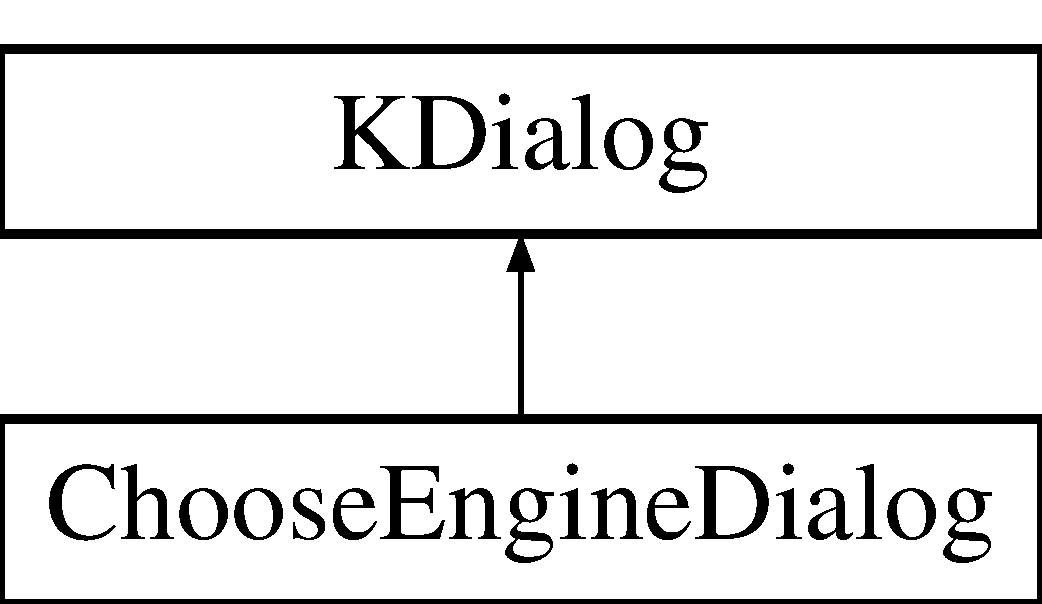
\includegraphics[height=2.000000cm]{classChooseEngineDialog}
\end{center}
\end{figure}
\subsection*{Public Member Functions}
\begin{DoxyCompactItemize}
\item 
\hyperlink{classChooseEngineDialog_a7bd4304330f0562e881566800465bd89}{Choose\+Engine\+Dialog} (const Q\+String\+List \&generators, const K\+Mime\+Type\+::\+Ptr \&mime, Q\+Widget $\ast$parent=0)
\item 
\hyperlink{classChooseEngineDialog_ad8252242229073254e0c7474c6eab0db}{$\sim$\+Choose\+Engine\+Dialog} ()
\item 
int \hyperlink{classChooseEngineDialog_ab42687bbd730ae74a2bc865f0e5f06b4}{selected\+Generator} () const 
\end{DoxyCompactItemize}
\subsection*{Protected Attributes}
\begin{DoxyCompactItemize}
\item 
\hyperlink{classUi__ChooseEngineWidget}{Ui\+\_\+\+Choose\+Engine\+Widget} $\ast$ \hyperlink{classChooseEngineDialog_a9a8d24e5d7ce76f2b5d62e9d7a42f123}{m\+\_\+widget}
\end{DoxyCompactItemize}


\subsection{Detailed Description}


Definition at line 20 of file chooseenginedialog\+\_\+p.\+h.



\subsection{Constructor \& Destructor Documentation}
\hypertarget{classChooseEngineDialog_a7bd4304330f0562e881566800465bd89}{\index{Choose\+Engine\+Dialog@{Choose\+Engine\+Dialog}!Choose\+Engine\+Dialog@{Choose\+Engine\+Dialog}}
\index{Choose\+Engine\+Dialog@{Choose\+Engine\+Dialog}!Choose\+Engine\+Dialog@{Choose\+Engine\+Dialog}}
\subsubsection[{Choose\+Engine\+Dialog}]{\setlength{\rightskip}{0pt plus 5cm}Choose\+Engine\+Dialog\+::\+Choose\+Engine\+Dialog (
\begin{DoxyParamCaption}
\item[{const Q\+String\+List \&}]{generators, }
\item[{const K\+Mime\+Type\+::\+Ptr \&}]{mime, }
\item[{Q\+Widget $\ast$}]{parent = {\ttfamily 0}}
\end{DoxyParamCaption}
)}}\label{classChooseEngineDialog_a7bd4304330f0562e881566800465bd89}


Definition at line 19 of file chooseenginedialog.\+cpp.


\begin{DoxyCode}
20     : KDialog( parent )
21 \{
22     setCaption( i18n( \textcolor{stringliteral}{"Backend Selection"} ) );
23     setButtons( Ok | Cancel );
24     setDefaultButton( Ok );
25     QWidget *\hyperlink{active_2app_2src_2main_8cpp_a3c04138a5bfe5d72780bb7e82a18e627}{main} = \textcolor{keyword}{new} QWidget( \textcolor{keyword}{this} );
26     setMainWidget( main );
27     \hyperlink{classChooseEngineDialog_a9a8d24e5d7ce76f2b5d62e9d7a42f123}{m\_widget} = \textcolor{keyword}{new} \hyperlink{classUi__ChooseEngineWidget}{Ui\_ChooseEngineWidget}();
28     \hyperlink{classChooseEngineDialog_a9a8d24e5d7ce76f2b5d62e9d7a42f123}{m\_widget}->\hyperlink{classUi__ChooseEngineWidget_a1f7aa23b004748d7d3c5f9d159709d29}{setupUi}( main );
29 
30     \hyperlink{classChooseEngineDialog_a9a8d24e5d7ce76f2b5d62e9d7a42f123}{m\_widget}->\hyperlink{classUi__ChooseEngineWidget_aa7a6b768bf39b9a1f5e968edab33d00b}{engineList}->addItems(generators);
31 
32     \hyperlink{classChooseEngineDialog_a9a8d24e5d7ce76f2b5d62e9d7a42f123}{m\_widget}->\hyperlink{classUi__ChooseEngineWidget_aa5f94d071660758b15c9fafe3d143084}{description}->setText(
33         i18n( \textcolor{stringliteral}{"<qt>More than one backend found for the MIME type:<br />"}
34               \textcolor{stringliteral}{"<b>%1</b> (%2).<br /><br />"}
35               \textcolor{stringliteral}{"Please select which one to use:</qt>"}, mime->comment(), mime->name() ) );
36 \}
\end{DoxyCode}
\hypertarget{classChooseEngineDialog_ad8252242229073254e0c7474c6eab0db}{\index{Choose\+Engine\+Dialog@{Choose\+Engine\+Dialog}!````~Choose\+Engine\+Dialog@{$\sim$\+Choose\+Engine\+Dialog}}
\index{````~Choose\+Engine\+Dialog@{$\sim$\+Choose\+Engine\+Dialog}!Choose\+Engine\+Dialog@{Choose\+Engine\+Dialog}}
\subsubsection[{$\sim$\+Choose\+Engine\+Dialog}]{\setlength{\rightskip}{0pt plus 5cm}Choose\+Engine\+Dialog\+::$\sim$\+Choose\+Engine\+Dialog (
\begin{DoxyParamCaption}
{}
\end{DoxyParamCaption}
)}}\label{classChooseEngineDialog_ad8252242229073254e0c7474c6eab0db}


Definition at line 38 of file chooseenginedialog.\+cpp.


\begin{DoxyCode}
39 \{
40     \textcolor{keyword}{delete} \hyperlink{classChooseEngineDialog_a9a8d24e5d7ce76f2b5d62e9d7a42f123}{m\_widget};
41 \}
\end{DoxyCode}


\subsection{Member Function Documentation}
\hypertarget{classChooseEngineDialog_ab42687bbd730ae74a2bc865f0e5f06b4}{\index{Choose\+Engine\+Dialog@{Choose\+Engine\+Dialog}!selected\+Generator@{selected\+Generator}}
\index{selected\+Generator@{selected\+Generator}!Choose\+Engine\+Dialog@{Choose\+Engine\+Dialog}}
\subsubsection[{selected\+Generator}]{\setlength{\rightskip}{0pt plus 5cm}int Choose\+Engine\+Dialog\+::selected\+Generator (
\begin{DoxyParamCaption}
{}
\end{DoxyParamCaption}
) const}}\label{classChooseEngineDialog_ab42687bbd730ae74a2bc865f0e5f06b4}


Definition at line 43 of file chooseenginedialog.\+cpp.


\begin{DoxyCode}
44 \{
45     \textcolor{keywordflow}{return} \hyperlink{classChooseEngineDialog_a9a8d24e5d7ce76f2b5d62e9d7a42f123}{m\_widget}->\hyperlink{classUi__ChooseEngineWidget_aa7a6b768bf39b9a1f5e968edab33d00b}{engineList}->currentIndex();
46 \}
\end{DoxyCode}


\subsection{Member Data Documentation}
\hypertarget{classChooseEngineDialog_a9a8d24e5d7ce76f2b5d62e9d7a42f123}{\index{Choose\+Engine\+Dialog@{Choose\+Engine\+Dialog}!m\+\_\+widget@{m\+\_\+widget}}
\index{m\+\_\+widget@{m\+\_\+widget}!Choose\+Engine\+Dialog@{Choose\+Engine\+Dialog}}
\subsubsection[{m\+\_\+widget}]{\setlength{\rightskip}{0pt plus 5cm}{\bf Ui\+\_\+\+Choose\+Engine\+Widget}$\ast$ Choose\+Engine\+Dialog\+::m\+\_\+widget\hspace{0.3cm}{\ttfamily [protected]}}}\label{classChooseEngineDialog_a9a8d24e5d7ce76f2b5d62e9d7a42f123}


Definition at line 29 of file chooseenginedialog\+\_\+p.\+h.



The documentation for this class was generated from the following files\+:\begin{DoxyCompactItemize}
\item 
core/\hyperlink{chooseenginedialog__p_8h}{chooseenginedialog\+\_\+p.\+h}\item 
core/\hyperlink{chooseenginedialog_8cpp}{chooseenginedialog.\+cpp}\end{DoxyCompactItemize}

\hypertarget{classUi_1_1ChooseEngineWidget}{\section{Ui\+:\+:Choose\+Engine\+Widget Class Reference}
\label{classUi_1_1ChooseEngineWidget}\index{Ui\+::\+Choose\+Engine\+Widget@{Ui\+::\+Choose\+Engine\+Widget}}
}


{\ttfamily \#include $<$ui\+\_\+chooseenginewidget.\+h$>$}

Inheritance diagram for Ui\+:\+:Choose\+Engine\+Widget\+:\begin{figure}[H]
\begin{center}
\leavevmode
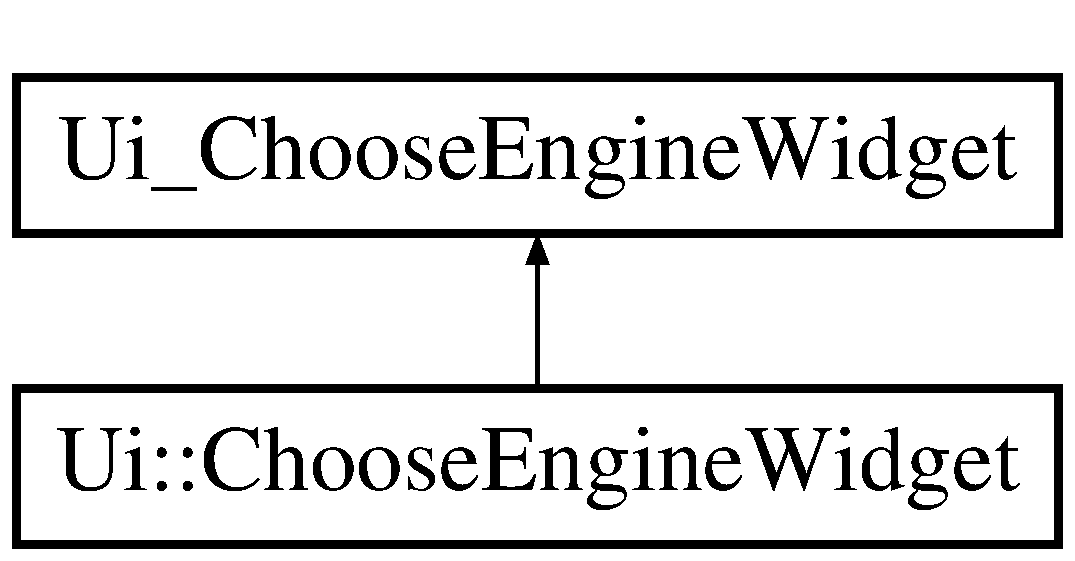
\includegraphics[height=2.000000cm]{classUi_1_1ChooseEngineWidget}
\end{center}
\end{figure}
\subsection*{Additional Inherited Members}


\subsection{Detailed Description}


Definition at line 69 of file ui\+\_\+chooseenginewidget.\+h.



The documentation for this class was generated from the following file\+:\begin{DoxyCompactItemize}
\item 
build/\hyperlink{ui__chooseenginewidget_8h}{ui\+\_\+chooseenginewidget.\+h}\end{DoxyCompactItemize}

\hypertarget{classCloseButton}{\section{Close\+Button Class Reference}
\label{classCloseButton}\index{Close\+Button@{Close\+Button}}
}
Inheritance diagram for Close\+Button\+:\begin{figure}[H]
\begin{center}
\leavevmode
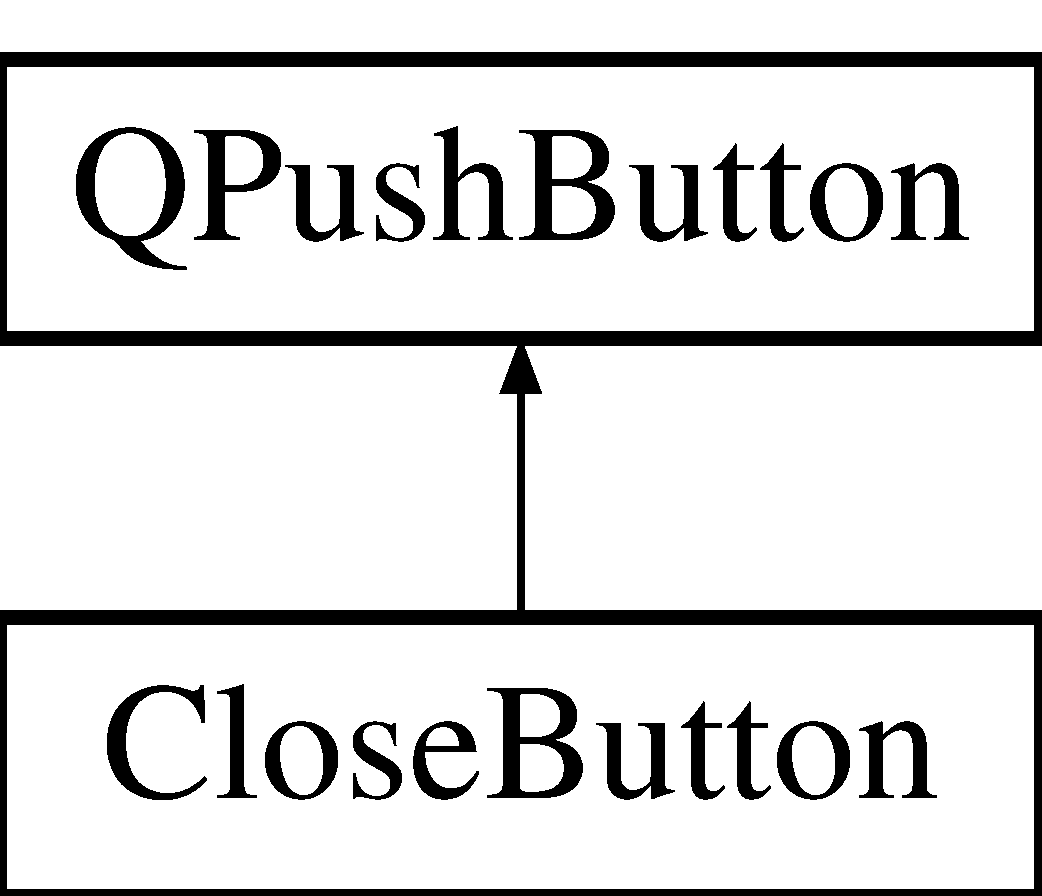
\includegraphics[height=2.000000cm]{classCloseButton}
\end{center}
\end{figure}
\subsection*{Public Member Functions}
\begin{DoxyCompactItemize}
\item 
\hyperlink{classCloseButton_a51839d4283758bd7221bafe64d08073b}{Close\+Button} (Q\+Widget $\ast$parent=0)
\end{DoxyCompactItemize}


\subsection{Detailed Description}


Definition at line 42 of file annotwindow.\+cpp.



\subsection{Constructor \& Destructor Documentation}
\hypertarget{classCloseButton_a51839d4283758bd7221bafe64d08073b}{\index{Close\+Button@{Close\+Button}!Close\+Button@{Close\+Button}}
\index{Close\+Button@{Close\+Button}!Close\+Button@{Close\+Button}}
\subsubsection[{Close\+Button}]{\setlength{\rightskip}{0pt plus 5cm}Close\+Button\+::\+Close\+Button (
\begin{DoxyParamCaption}
\item[{Q\+Widget $\ast$}]{parent = {\ttfamily 0}}
\end{DoxyParamCaption}
)\hspace{0.3cm}{\ttfamily [inline]}}}\label{classCloseButton_a51839d4283758bd7221bafe64d08073b}


Definition at line 46 of file annotwindow.\+cpp.


\begin{DoxyCode}
47       : QPushButton( parent )
48     \{
49         setSizePolicy( QSizePolicy::Fixed, QSizePolicy::Fixed );
50         QSize \hyperlink{synctex__parser_8c_aa23c661441688350614bd6a350d2b6ff}{size} = QSize( 14, 14 ).expandedTo( QApplication::globalStrut() );
51         setFixedSize( size );
52         setIcon( style()->standardIcon( QStyle::SP\_DockWidgetCloseButton ) );
53         setIconSize( size );
54         setToolTip( i18n( \textcolor{stringliteral}{"Close this note"} ) );
55     \}
\end{DoxyCode}


The documentation for this class was generated from the following file\+:\begin{DoxyCompactItemize}
\item 
ui/\hyperlink{annotwindow_8cpp}{annotwindow.\+cpp}\end{DoxyCompactItemize}

\hypertarget{structColorMapEntry}{\section{Color\+Map\+Entry Struct Reference}
\label{structColorMapEntry}\index{Color\+Map\+Entry@{Color\+Map\+Entry}}
}
\subsection*{Public Attributes}
\begin{DoxyCompactItemize}
\item 
unsigned char \hyperlink{structColorMapEntry_a9037199d7c8069a32d4ac0a144091c0e}{red}
\item 
unsigned char \hyperlink{structColorMapEntry_a67039275bc0ec5c1b12ed1688f221f60}{green}
\item 
unsigned char \hyperlink{structColorMapEntry_a3240a8259c24a4ae542b592560d59c69}{blue}
\end{DoxyCompactItemize}


\subsection{Detailed Description}


Definition at line 55 of file image.\+cpp.



\subsection{Member Data Documentation}
\hypertarget{structColorMapEntry_a3240a8259c24a4ae542b592560d59c69}{\index{Color\+Map\+Entry@{Color\+Map\+Entry}!blue@{blue}}
\index{blue@{blue}!Color\+Map\+Entry@{Color\+Map\+Entry}}
\subsubsection[{blue}]{\setlength{\rightskip}{0pt plus 5cm}unsigned char Color\+Map\+Entry\+::blue}}\label{structColorMapEntry_a3240a8259c24a4ae542b592560d59c69}


Definition at line 58 of file image.\+cpp.

\hypertarget{structColorMapEntry_a67039275bc0ec5c1b12ed1688f221f60}{\index{Color\+Map\+Entry@{Color\+Map\+Entry}!green@{green}}
\index{green@{green}!Color\+Map\+Entry@{Color\+Map\+Entry}}
\subsubsection[{green}]{\setlength{\rightskip}{0pt plus 5cm}unsigned char Color\+Map\+Entry\+::green}}\label{structColorMapEntry_a67039275bc0ec5c1b12ed1688f221f60}


Definition at line 57 of file image.\+cpp.

\hypertarget{structColorMapEntry_a9037199d7c8069a32d4ac0a144091c0e}{\index{Color\+Map\+Entry@{Color\+Map\+Entry}!red@{red}}
\index{red@{red}!Color\+Map\+Entry@{Color\+Map\+Entry}}
\subsubsection[{red}]{\setlength{\rightskip}{0pt plus 5cm}unsigned char Color\+Map\+Entry\+::red}}\label{structColorMapEntry_a9037199d7c8069a32d4ac0a144091c0e}


Definition at line 56 of file image.\+cpp.



The documentation for this struct was generated from the following file\+:\begin{DoxyCompactItemize}
\item 
generators/plucker/unpluck/\hyperlink{image_8cpp}{image.\+cpp}\end{DoxyCompactItemize}

\hypertarget{classComboEdit}{\section{Combo\+Edit Class Reference}
\label{classComboEdit}\index{Combo\+Edit@{Combo\+Edit}}
}


{\ttfamily \#include $<$formwidgets.\+h$>$}

Inheritance diagram for Combo\+Edit\+:\begin{figure}[H]
\begin{center}
\leavevmode
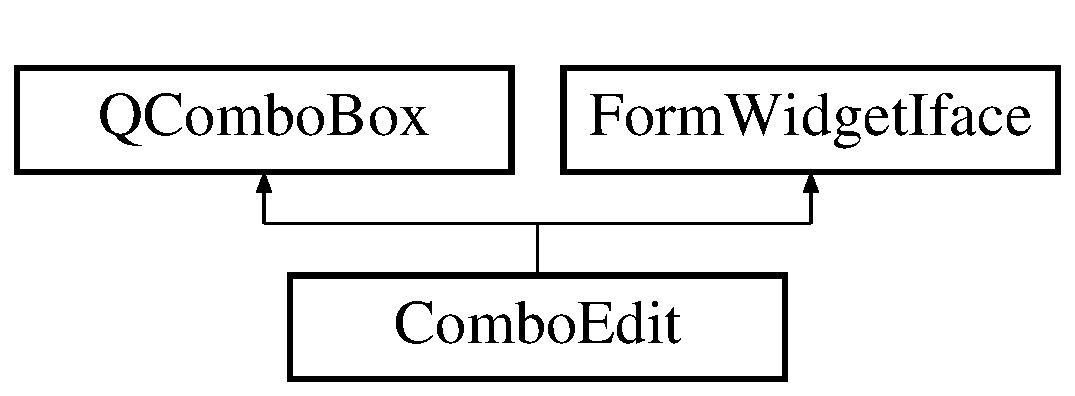
\includegraphics[height=2.000000cm]{classComboEdit}
\end{center}
\end{figure}
\subsection*{Public Member Functions}
\begin{DoxyCompactItemize}
\item 
\hyperlink{classComboEdit_ad24134a1514abb6eaa645822883c93a4}{Combo\+Edit} (\hyperlink{classOkular_1_1FormFieldChoice}{Okular\+::\+Form\+Field\+Choice} $\ast$choice, Q\+Widget $\ast$parent=0)
\item 
void \hyperlink{classComboEdit_a36fc02dbfb94f988dede11d57390d138}{set\+Form\+Widgets\+Controller} (\hyperlink{classFormWidgetsController}{Form\+Widgets\+Controller} $\ast$controller)
\item 
virtual bool \hyperlink{classComboEdit_abedca59cf3b7a7cf894e8ab3c6d657e1}{event} (Q\+Event $\ast$e)
\item 
virtual void \hyperlink{classComboEdit_af5bebe6b5c7266399c66a43a57f48997}{context\+Menu\+Event} (Q\+Context\+Menu\+Event $\ast$\hyperlink{classComboEdit_abedca59cf3b7a7cf894e8ab3c6d657e1}{event})
\end{DoxyCompactItemize}
\subsection*{Additional Inherited Members}


\subsection{Detailed Description}


Definition at line 314 of file formwidgets.\+h.



\subsection{Constructor \& Destructor Documentation}
\hypertarget{classComboEdit_ad24134a1514abb6eaa645822883c93a4}{\index{Combo\+Edit@{Combo\+Edit}!Combo\+Edit@{Combo\+Edit}}
\index{Combo\+Edit@{Combo\+Edit}!Combo\+Edit@{Combo\+Edit}}
\subsubsection[{Combo\+Edit}]{\setlength{\rightskip}{0pt plus 5cm}Combo\+Edit\+::\+Combo\+Edit (
\begin{DoxyParamCaption}
\item[{{\bf Okular\+::\+Form\+Field\+Choice} $\ast$}]{choice, }
\item[{Q\+Widget $\ast$}]{parent = {\ttfamily 0}}
\end{DoxyParamCaption}
)\hspace{0.3cm}{\ttfamily [explicit]}}}\label{classComboEdit_ad24134a1514abb6eaa645822883c93a4}


Definition at line 804 of file formwidgets.\+cpp.


\begin{DoxyCode}
805     : QComboBox( parent ), \hyperlink{classFormWidgetIface_a1737728a2348ae69415008ddb1aa3b9d}{FormWidgetIface}( \textcolor{keyword}{this}, choice ), m\_form( choice )
806 \{
807     addItems( m\_form->\hyperlink{classOkular_1_1FormFieldChoice_aeb4047c2c4b3b1c06b06e615c073f923}{choices}() );
808     setEditable( \textcolor{keyword}{true} );
809     setInsertPolicy( NoInsert );
810     lineEdit()->setReadOnly( !m\_form->\hyperlink{classOkular_1_1FormFieldChoice_a3d9978586fb90b5cf91357816d93f193}{isEditable}() );
811     \hyperlink{classQList}{QList< int >} selectedItems = m\_form->\hyperlink{classOkular_1_1FormFieldChoice_a7715f0a6629d8d874c22f436a62165ed}{currentChoices}();
812     \textcolor{keywordflow}{if} ( selectedItems.count() == 1 && selectedItems.at(0) >= 0 && selectedItems.at(0) < count() )
813         setCurrentIndex( selectedItems.at(0) );
814     setEnabled( !m\_form->\hyperlink{classOkular_1_1FormField_ad1636c715682959442f528c72a2f4c0a}{isReadOnly}() );
815 
816     \textcolor{keywordflow}{if} ( m\_form->\hyperlink{classOkular_1_1FormFieldChoice_a3d9978586fb90b5cf91357816d93f193}{isEditable}() && !m\_form->\hyperlink{classOkular_1_1FormFieldChoice_a63c046d413e912c3b2873bfb25ab83f9}{editChoice}().isEmpty() )
817         lineEdit()->setText( m\_form->\hyperlink{classOkular_1_1FormFieldChoice_a63c046d413e912c3b2873bfb25ab83f9}{editChoice}() );
818 
819     connect( \textcolor{keyword}{this}, SIGNAL(currentIndexChanged(\textcolor{keywordtype}{int})), \textcolor{keyword}{this}, SLOT(slotValueChanged()) );
820     connect( \textcolor{keyword}{this}, SIGNAL(editTextChanged(QString)), \textcolor{keyword}{this}, SLOT(slotValueChanged()) );
821     connect( lineEdit(), SIGNAL(cursorPositionChanged(\textcolor{keywordtype}{int},\textcolor{keywordtype}{int})), \textcolor{keyword}{this}, SLOT(slotValueChanged()));
822 
823     setVisible( m\_form->\hyperlink{classOkular_1_1FormField_aee63f77f88a7f8359d9a53de3d07ebe0}{isVisible}() );
824     setCursor( Qt::ArrowCursor );
825     m\_prevCursorPos = lineEdit()->cursorPosition();
826     m\_prevAnchorPos = lineEdit()->cursorPosition();
827 \}
\end{DoxyCode}


\subsection{Member Function Documentation}
\hypertarget{classComboEdit_af5bebe6b5c7266399c66a43a57f48997}{\index{Combo\+Edit@{Combo\+Edit}!context\+Menu\+Event@{context\+Menu\+Event}}
\index{context\+Menu\+Event@{context\+Menu\+Event}!Combo\+Edit@{Combo\+Edit}}
\subsubsection[{context\+Menu\+Event}]{\setlength{\rightskip}{0pt plus 5cm}void Combo\+Edit\+::context\+Menu\+Event (
\begin{DoxyParamCaption}
\item[{Q\+Context\+Menu\+Event $\ast$}]{event}
\end{DoxyParamCaption}
)\hspace{0.3cm}{\ttfamily [virtual]}}}\label{classComboEdit_af5bebe6b5c7266399c66a43a57f48997}


Definition at line 913 of file formwidgets.\+cpp.


\begin{DoxyCode}
914 \{
915     QMenu *menu = lineEdit()->createStandardContextMenu();
916 
917     \hyperlink{classQList}{QList<QAction *>} actionList = menu->actions();
918     \textcolor{keyword}{enum} \{ UndoAct, RedoAct, CutAct, CopyAct, PasteAct, DeleteAct, SelectAllAct \};
919 
920     KAction *kundo = KStandardAction::create( KStandardAction::Undo, 
      \hyperlink{classFormWidgetIface_a2d51d0c5aaf48aad5480551f69f82e9a}{m\_controller}, SIGNAL( requestUndo() ), menu );
921     KAction *kredo = KStandardAction::create( KStandardAction::Redo, 
      \hyperlink{classFormWidgetIface_a2d51d0c5aaf48aad5480551f69f82e9a}{m\_controller}, SIGNAL( requestRedo() ), menu );
922     connect( \hyperlink{classFormWidgetIface_a2d51d0c5aaf48aad5480551f69f82e9a}{m\_controller}, SIGNAL( canUndoChanged( \textcolor{keywordtype}{bool} ) ), kundo, SLOT( setEnabled( \textcolor{keywordtype}{bool} ) ) 
      );
923     connect( \hyperlink{classFormWidgetIface_a2d51d0c5aaf48aad5480551f69f82e9a}{m\_controller}, SIGNAL( canRedoChanged( \textcolor{keywordtype}{bool} ) ), kredo, SLOT( setEnabled( \textcolor{keywordtype}{bool} ) ) 
      );
924     kundo->setEnabled( \hyperlink{classFormWidgetIface_a2d51d0c5aaf48aad5480551f69f82e9a}{m\_controller}->\hyperlink{classFormWidgetsController_a2711f4f025e96e95fe55c162ca321de5}{canUndo}() );
925     kredo->setEnabled( \hyperlink{classFormWidgetIface_a2d51d0c5aaf48aad5480551f69f82e9a}{m\_controller}->\hyperlink{classFormWidgetsController_a960c176392a58a63f271b6c561216b74}{canRedo}() );
926 
927     QAction *oldUndo, *oldRedo;
928     oldUndo = actionList[UndoAct];
929     oldRedo = actionList[RedoAct];
930 
931     menu->insertAction( oldUndo, kundo );
932     menu->insertAction( oldRedo, kredo );
933 
934     menu->removeAction( oldUndo );
935     menu->removeAction( oldRedo );
936 
937     menu->exec( \hyperlink{classComboEdit_abedca59cf3b7a7cf894e8ab3c6d657e1}{event}->globalPos() );
938     \textcolor{keyword}{delete} menu;
939 \}
\end{DoxyCode}
\hypertarget{classComboEdit_abedca59cf3b7a7cf894e8ab3c6d657e1}{\index{Combo\+Edit@{Combo\+Edit}!event@{event}}
\index{event@{event}!Combo\+Edit@{Combo\+Edit}}
\subsubsection[{event}]{\setlength{\rightskip}{0pt plus 5cm}bool Combo\+Edit\+::event (
\begin{DoxyParamCaption}
\item[{Q\+Event $\ast$}]{e}
\end{DoxyParamCaption}
)\hspace{0.3cm}{\ttfamily [virtual]}}}\label{classComboEdit_abedca59cf3b7a7cf894e8ab3c6d657e1}


Definition at line 941 of file formwidgets.\+cpp.


\begin{DoxyCode}
942 \{
943     \textcolor{keywordflow}{if} ( e->type() == QEvent::KeyPress )
944     \{
945         QKeyEvent *keyEvent = \textcolor{keyword}{static\_cast<} QKeyEvent* \textcolor{keyword}{>}(e);
946         \textcolor{keywordflow}{if} ( keyEvent == QKeySequence::Undo )
947         \{
948             emit \hyperlink{classFormWidgetIface_a2d51d0c5aaf48aad5480551f69f82e9a}{m\_controller}->\hyperlink{classFormWidgetsController_a90e5af0601c7e5efcfbf6e1b93ae5641}{requestUndo}();
949             \textcolor{keywordflow}{return} \textcolor{keyword}{true};
950         \}
951         \textcolor{keywordflow}{else} \textcolor{keywordflow}{if} ( keyEvent == QKeySequence::Redo )
952         \{
953             emit \hyperlink{classFormWidgetIface_a2d51d0c5aaf48aad5480551f69f82e9a}{m\_controller}->\hyperlink{classFormWidgetsController_a828b4d568a04cd6728bcf1d49ed5c425}{requestRedo}();
954             \textcolor{keywordflow}{return} \textcolor{keyword}{true};
955         \}
956     \}
957     \textcolor{keywordflow}{return} QComboBox::event( e );
958 \}
\end{DoxyCode}
\hypertarget{classComboEdit_a36fc02dbfb94f988dede11d57390d138}{\index{Combo\+Edit@{Combo\+Edit}!set\+Form\+Widgets\+Controller@{set\+Form\+Widgets\+Controller}}
\index{set\+Form\+Widgets\+Controller@{set\+Form\+Widgets\+Controller}!Combo\+Edit@{Combo\+Edit}}
\subsubsection[{set\+Form\+Widgets\+Controller}]{\setlength{\rightskip}{0pt plus 5cm}void Combo\+Edit\+::set\+Form\+Widgets\+Controller (
\begin{DoxyParamCaption}
\item[{{\bf Form\+Widgets\+Controller} $\ast$}]{controller}
\end{DoxyParamCaption}
)\hspace{0.3cm}{\ttfamily [virtual]}}}\label{classComboEdit_a36fc02dbfb94f988dede11d57390d138}


Reimplemented from \hyperlink{classFormWidgetIface_a4d3129afff43729fafc4e6b58a4d16fe}{Form\+Widget\+Iface}.



Definition at line 829 of file formwidgets.\+cpp.


\begin{DoxyCode}
830 \{
831     \hyperlink{classFormWidgetIface_a4d3129afff43729fafc4e6b58a4d16fe}{FormWidgetIface::setFormWidgetsController}(controller);
832     connect( \hyperlink{classFormWidgetIface_a2d51d0c5aaf48aad5480551f69f82e9a}{m\_controller}, SIGNAL(formComboChangedByUndoRedo(\textcolor{keywordtype}{int},
      \hyperlink{classOkular_1_1FormFieldChoice}{Okular::FormFieldChoice}*, QString, \textcolor{keywordtype}{int}, \textcolor{keywordtype}{int} )),
833              \textcolor{keyword}{this}, SLOT(slotHandleFormComboChangedByUndoRedo(\textcolor{keywordtype}{int},
      \hyperlink{classOkular_1_1FormFieldChoice}{Okular::FormFieldChoice}*, QString, \textcolor{keywordtype}{int}, \textcolor{keywordtype}{int} )));
834 
835 \}
\end{DoxyCode}


The documentation for this class was generated from the following files\+:\begin{DoxyCompactItemize}
\item 
ui/\hyperlink{formwidgets_8h}{formwidgets.\+h}\item 
ui/\hyperlink{formwidgets_8cpp}{formwidgets.\+cpp}\end{DoxyCompactItemize}

\hypertarget{classComicBookGenerator}{\section{Comic\+Book\+Generator Class Reference}
\label{classComicBookGenerator}\index{Comic\+Book\+Generator@{Comic\+Book\+Generator}}
}


{\ttfamily \#include $<$generator\+\_\+comicbook.\+h$>$}

Inheritance diagram for Comic\+Book\+Generator\+:\begin{figure}[H]
\begin{center}
\leavevmode
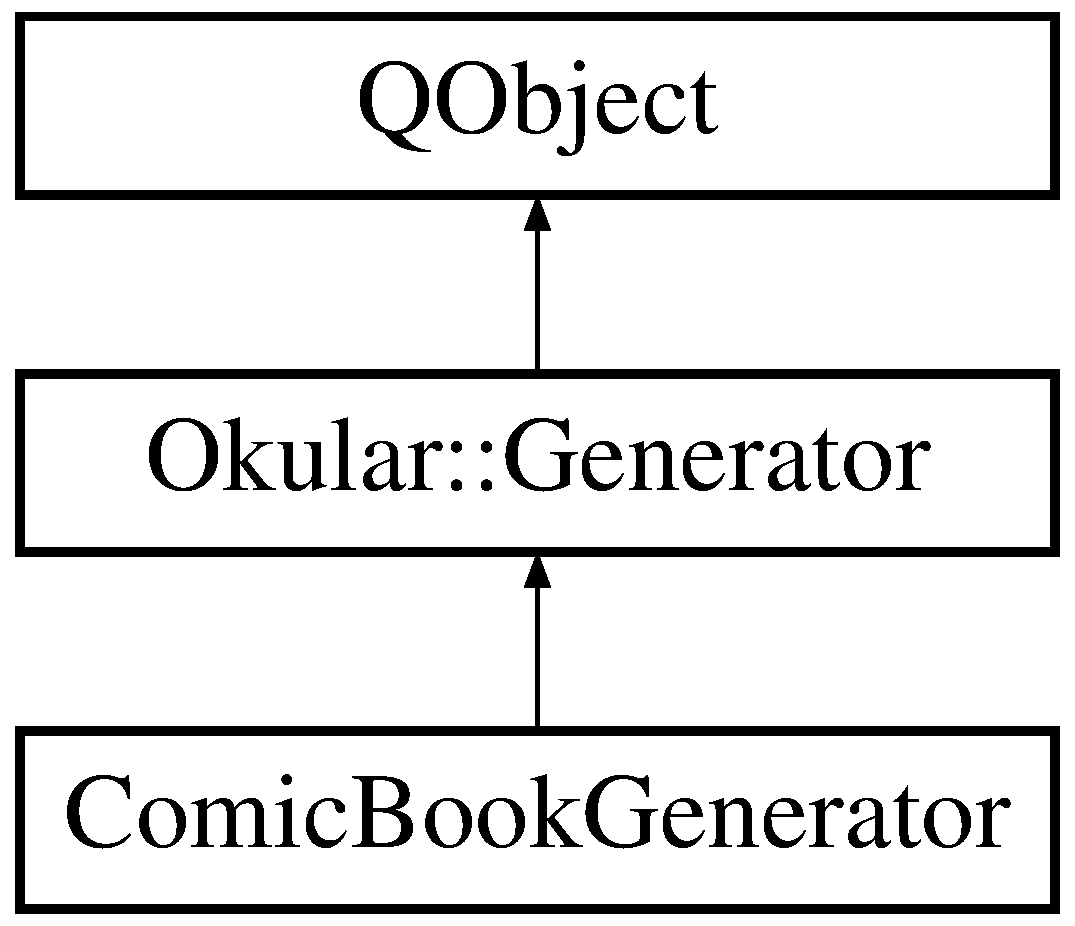
\includegraphics[height=3.000000cm]{classComicBookGenerator}
\end{center}
\end{figure}
\subsection*{Public Member Functions}
\begin{DoxyCompactItemize}
\item 
\hyperlink{classComicBookGenerator_a77c37e29b4ee42f74e9a3c0a1c470a41}{Comic\+Book\+Generator} (Q\+Object $\ast$parent, const Q\+Variant\+List \&args)
\item 
virtual \hyperlink{classComicBookGenerator_a5893114c687f5aa497f0860825e7b115}{$\sim$\+Comic\+Book\+Generator} ()
\item 
bool \hyperlink{classComicBookGenerator_a918c1d51b4a4891d412e0ae4f3775df9}{load\+Document} (const Q\+String \&file\+Name, Q\+Vector$<$ \hyperlink{classOkular_1_1Page}{Okular\+::\+Page} $\ast$ $>$ \&pages\+Vector)
\item 
bool \hyperlink{classComicBookGenerator_ab5f1a260dddbeee825d293926a883661}{print} (Q\+Printer \&printer)
\end{DoxyCompactItemize}
\subsection*{Protected Member Functions}
\begin{DoxyCompactItemize}
\item 
bool \hyperlink{classComicBookGenerator_a123f741df86f8e8b2e379e12c3ab31ce}{do\+Close\+Document} ()
\item 
Q\+Image \hyperlink{classComicBookGenerator_a473ac38c97610d3870fa01def287c413}{image} (\hyperlink{classOkular_1_1PixmapRequest}{Okular\+::\+Pixmap\+Request} $\ast$request)
\end{DoxyCompactItemize}
\subsection*{Additional Inherited Members}


\subsection{Detailed Description}


Definition at line 17 of file generator\+\_\+comicbook.\+h.



\subsection{Constructor \& Destructor Documentation}
\hypertarget{classComicBookGenerator_a77c37e29b4ee42f74e9a3c0a1c470a41}{\index{Comic\+Book\+Generator@{Comic\+Book\+Generator}!Comic\+Book\+Generator@{Comic\+Book\+Generator}}
\index{Comic\+Book\+Generator@{Comic\+Book\+Generator}!Comic\+Book\+Generator@{Comic\+Book\+Generator}}
\subsubsection[{Comic\+Book\+Generator}]{\setlength{\rightskip}{0pt plus 5cm}Comic\+Book\+Generator\+::\+Comic\+Book\+Generator (
\begin{DoxyParamCaption}
\item[{Q\+Object $\ast$}]{parent, }
\item[{const Q\+Variant\+List \&}]{args}
\end{DoxyParamCaption}
)}}\label{classComicBookGenerator_a77c37e29b4ee42f74e9a3c0a1c470a41}


Definition at line 40 of file generator\+\_\+comicbook.\+cpp.


\begin{DoxyCode}
41     : \hyperlink{classOkular_1_1Generator_a9a493b3f23f5d8b34eae9fa7231556f6}{Generator}( parent, args )
42 \{
43     \hyperlink{classOkular_1_1Generator_abcebcc5f69e98b6227496198a5c69d2c}{setFeature}( \hyperlink{classOkular_1_1Generator_a8517096896273a5ba5b970be09313c77a0764a910b194896e72da084c3c51a2d0}{Threaded} );
44     \hyperlink{classOkular_1_1Generator_abcebcc5f69e98b6227496198a5c69d2c}{setFeature}( \hyperlink{classOkular_1_1Generator_a8517096896273a5ba5b970be09313c77a7b40b8f6b9e4330bddff3cdf0baf07a9}{PrintNative} );
45     \hyperlink{classOkular_1_1Generator_abcebcc5f69e98b6227496198a5c69d2c}{setFeature}( \hyperlink{classOkular_1_1Generator_a8517096896273a5ba5b970be09313c77a0bb6cbe50f2ffb616e25106b2e34c289}{PrintToFile} );
46 \}
\end{DoxyCode}
\hypertarget{classComicBookGenerator_a5893114c687f5aa497f0860825e7b115}{\index{Comic\+Book\+Generator@{Comic\+Book\+Generator}!````~Comic\+Book\+Generator@{$\sim$\+Comic\+Book\+Generator}}
\index{````~Comic\+Book\+Generator@{$\sim$\+Comic\+Book\+Generator}!Comic\+Book\+Generator@{Comic\+Book\+Generator}}
\subsubsection[{$\sim$\+Comic\+Book\+Generator}]{\setlength{\rightskip}{0pt plus 5cm}Comic\+Book\+Generator\+::$\sim$\+Comic\+Book\+Generator (
\begin{DoxyParamCaption}
{}
\end{DoxyParamCaption}
)\hspace{0.3cm}{\ttfamily [virtual]}}}\label{classComicBookGenerator_a5893114c687f5aa497f0860825e7b115}


Definition at line 48 of file generator\+\_\+comicbook.\+cpp.


\begin{DoxyCode}
49 \{
50 \}
\end{DoxyCode}


\subsection{Member Function Documentation}
\hypertarget{classComicBookGenerator_a123f741df86f8e8b2e379e12c3ab31ce}{\index{Comic\+Book\+Generator@{Comic\+Book\+Generator}!do\+Close\+Document@{do\+Close\+Document}}
\index{do\+Close\+Document@{do\+Close\+Document}!Comic\+Book\+Generator@{Comic\+Book\+Generator}}
\subsubsection[{do\+Close\+Document}]{\setlength{\rightskip}{0pt plus 5cm}bool Comic\+Book\+Generator\+::do\+Close\+Document (
\begin{DoxyParamCaption}
{}
\end{DoxyParamCaption}
)\hspace{0.3cm}{\ttfamily [protected]}, {\ttfamily [virtual]}}}\label{classComicBookGenerator_a123f741df86f8e8b2e379e12c3ab31ce}
This method is called when the document is closed and not used any longer.

\begin{DoxyReturn}{Returns}
true on success, false otherwise. 
\end{DoxyReturn}


Implements \hyperlink{classOkular_1_1Generator_ad3f1dcb98f3bd87c87ad0e91ecf4a6d7}{Okular\+::\+Generator}.



Definition at line 66 of file generator\+\_\+comicbook.\+cpp.


\begin{DoxyCode}
67 \{
68     mDocument.\hyperlink{classComicBook_1_1Document_ae9b8bb9ab6fbf42f47b573e95a5a1198}{close}();
69 
70     \textcolor{keywordflow}{return} \textcolor{keyword}{true};
71 \}
\end{DoxyCode}
\hypertarget{classComicBookGenerator_a473ac38c97610d3870fa01def287c413}{\index{Comic\+Book\+Generator@{Comic\+Book\+Generator}!image@{image}}
\index{image@{image}!Comic\+Book\+Generator@{Comic\+Book\+Generator}}
\subsubsection[{image}]{\setlength{\rightskip}{0pt plus 5cm}Q\+Image Comic\+Book\+Generator\+::image (
\begin{DoxyParamCaption}
\item[{{\bf Okular\+::\+Pixmap\+Request} $\ast$}]{page}
\end{DoxyParamCaption}
)\hspace{0.3cm}{\ttfamily [protected]}, {\ttfamily [virtual]}}}\label{classComicBookGenerator_a473ac38c97610d3870fa01def287c413}
Returns the image of the page as specified in the passed pixmap {\ttfamily request}.

\begin{DoxyWarning}{Warning}
this method may be executed in its own separated thread if the \hyperlink{classOkular_1_1Generator_a8517096896273a5ba5b970be09313c77a0764a910b194896e72da084c3c51a2d0}{Threaded} is enabled! 
\end{DoxyWarning}


Reimplemented from \hyperlink{classOkular_1_1Generator_a6712c8d3c2759c3a1fcacbd503d3286e}{Okular\+::\+Generator}.



Definition at line 73 of file generator\+\_\+comicbook.\+cpp.


\begin{DoxyCode}
74 \{
75     \textcolor{keywordtype}{int} width = request->width();
76     \textcolor{keywordtype}{int} height = request->height();
77 
78     QImage \hyperlink{classComicBookGenerator_a473ac38c97610d3870fa01def287c413}{image} = mDocument.\hyperlink{classComicBook_1_1Document_ae572a3b695f4300eb3ddf76bbcd3b1dd}{pageImage}( request->pageNumber() );
79 
80     \textcolor{keywordflow}{return} image.scaled( width, height, Qt::IgnoreAspectRatio, Qt::SmoothTransformation );
81 \}
\end{DoxyCode}
\hypertarget{classComicBookGenerator_a918c1d51b4a4891d412e0ae4f3775df9}{\index{Comic\+Book\+Generator@{Comic\+Book\+Generator}!load\+Document@{load\+Document}}
\index{load\+Document@{load\+Document}!Comic\+Book\+Generator@{Comic\+Book\+Generator}}
\subsubsection[{load\+Document}]{\setlength{\rightskip}{0pt plus 5cm}bool Comic\+Book\+Generator\+::load\+Document (
\begin{DoxyParamCaption}
\item[{const Q\+String \&}]{file\+Name, }
\item[{Q\+Vector$<$ {\bf Okular\+::\+Page} $\ast$ $>$ \&}]{pages\+Vector}
\end{DoxyParamCaption}
)\hspace{0.3cm}{\ttfamily [virtual]}}}\label{classComicBookGenerator_a918c1d51b4a4891d412e0ae4f3775df9}
Loads the document with the given {\ttfamily file\+Name} and fills the {\ttfamily pages\+Vector} with the parsed pages.

\begin{DoxyReturn}{Returns}
true on success, false otherwise. 
\end{DoxyReturn}


Implements \hyperlink{classOkular_1_1Generator_a388b47328a5297d53cdbdc6fcf074ee3}{Okular\+::\+Generator}.



Definition at line 52 of file generator\+\_\+comicbook.\+cpp.


\begin{DoxyCode}
53 \{
54     \textcolor{keywordflow}{if} ( !mDocument.\hyperlink{classComicBook_1_1Document_a9048327326e87d025b2af2499e8987da}{open}( fileName ) )
55     \{
56         \textcolor{keyword}{const} QString errString = mDocument.\hyperlink{classComicBook_1_1Document_a26f06a190450786328eceb700ebfe45e}{lastErrorString}();
57         \textcolor{keywordflow}{if} ( !errString.isEmpty() )
58             emit \hyperlink{classOkular_1_1Generator_a0f73eaeb88ccb1ecb73814a918244e03}{error}( errString, -1 );
59         \textcolor{keywordflow}{return} \textcolor{keyword}{false};
60     \}
61 
62     mDocument.\hyperlink{classComicBook_1_1Document_ac9b4abfbf45273ef03051677c7abb00b}{pages}( &pagesVector );
63     \textcolor{keywordflow}{return} \textcolor{keyword}{true};
64 \}
\end{DoxyCode}
\hypertarget{classComicBookGenerator_ab5f1a260dddbeee825d293926a883661}{\index{Comic\+Book\+Generator@{Comic\+Book\+Generator}!print@{print}}
\index{print@{print}!Comic\+Book\+Generator@{Comic\+Book\+Generator}}
\subsubsection[{print}]{\setlength{\rightskip}{0pt plus 5cm}bool Comic\+Book\+Generator\+::print (
\begin{DoxyParamCaption}
\item[{Q\+Printer \&}]{printer}
\end{DoxyParamCaption}
)\hspace{0.3cm}{\ttfamily [virtual]}}}\label{classComicBookGenerator_ab5f1a260dddbeee825d293926a883661}
This method is called to print the document to the given {\ttfamily printer}. 

Reimplemented from \hyperlink{classOkular_1_1Generator_aa786d406a1b0db6679a3bc62bbe2dc82}{Okular\+::\+Generator}.



Definition at line 83 of file generator\+\_\+comicbook.\+cpp.


\begin{DoxyCode}
84 \{
85     QPainter p( &printer );
86 
87     \hyperlink{classQList}{QList<int>} pageList = \hyperlink{classOkular_1_1FilePrinter_aed485e5e3fbe591b16e15915e318a1b7}{Okular::FilePrinter::pageList}( printer, 
      \hyperlink{classOkular_1_1Generator_a4248672ef04e62660d51f16c0a862bbe}{document}()->pages(),
88                                                          \hyperlink{classOkular_1_1Generator_a4248672ef04e62660d51f16c0a862bbe}{document}()->currentPage() + 1,
89                                                          \hyperlink{classOkular_1_1Generator_a4248672ef04e62660d51f16c0a862bbe}{document}()->bookmarkedPageList() );
90 
91     \textcolor{keywordflow}{for} ( \textcolor{keywordtype}{int} i = 0; i < pageList.count(); ++i ) \{
92 
93         QImage \hyperlink{classComicBookGenerator_a473ac38c97610d3870fa01def287c413}{image} = mDocument.\hyperlink{classComicBook_1_1Document_ae572a3b695f4300eb3ddf76bbcd3b1dd}{pageImage}( pageList[i] - 1 );
94 
95         \textcolor{keywordflow}{if} ( ( image.width() > printer.width() ) || ( image.height() > printer.height() ) )
96 
97             image = image.scaled( printer.width(), printer.height(),
98                                   Qt::KeepAspectRatio, Qt::SmoothTransformation );
99 
100         \textcolor{keywordflow}{if} ( i != 0 )
101             printer.newPage();
102 
103         p.drawImage( 0, 0, image );
104     \}
105 
106     \textcolor{keywordflow}{return} \textcolor{keyword}{true};
107 \}
\end{DoxyCode}


The documentation for this class was generated from the following files\+:\begin{DoxyCompactItemize}
\item 
generators/comicbook/\hyperlink{generator__comicbook_8h}{generator\+\_\+comicbook.\+h}\item 
generators/comicbook/\hyperlink{generator__comicbook_8cpp}{generator\+\_\+comicbook.\+cpp}\end{DoxyCompactItemize}

\hypertarget{classOkular_1_1ConfigInterface}{\section{Okular\+:\+:Config\+Interface Class Reference}
\label{classOkular_1_1ConfigInterface}\index{Okular\+::\+Config\+Interface@{Okular\+::\+Config\+Interface}}
}


Abstract interface for configuration control.  




{\ttfamily \#include $<$configinterface.\+h$>$}

Inheritance diagram for Okular\+:\+:Config\+Interface\+:\begin{figure}[H]
\begin{center}
\leavevmode
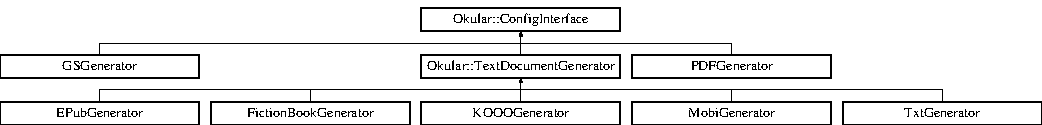
\includegraphics[height=1.680000cm]{classOkular_1_1ConfigInterface}
\end{center}
\end{figure}
\subsection*{Public Member Functions}
\begin{DoxyCompactItemize}
\item 
virtual \hyperlink{classOkular_1_1ConfigInterface_a7aaa737cc8907ee1944e330c43b3c571}{$\sim$\+Config\+Interface} ()
\item 
virtual bool \hyperlink{classOkular_1_1ConfigInterface_a0f61ec6852e483b898efd9709b1ef63b}{reparse\+Config} ()=0
\item 
virtual void \hyperlink{classOkular_1_1ConfigInterface_a75030ba3abbbd134e388c05154695610}{add\+Pages} (K\+Config\+Dialog $\ast$dialog)=0
\end{DoxyCompactItemize}


\subsection{Detailed Description}
Abstract interface for configuration control. 

This interface defines a way to configure the \hyperlink{classOkular_1_1Generator}{Generator} itself.

How to use it in a custom \hyperlink{classOkular_1_1Generator}{Generator}\+: 
\begin{DoxyCode}
\textcolor{keyword}{class }MyGenerator : \textcolor{keyword}{public} \hyperlink{classOkular_1_1Generator}{Okular::Generator}, \textcolor{keyword}{public} 
      \hyperlink{classOkular_1_1ConfigInterface}{Okular::ConfigInterface}
\{
    Q\_OBJECT
    Q\_INTERFACES( \hyperlink{classOkular_1_1ConfigInterface}{Okular::ConfigInterface} )

    ...
\};
\end{DoxyCode}
 and -\/ of course -\/ implementing its methods. 

Definition at line 38 of file configinterface.\+h.



\subsection{Constructor \& Destructor Documentation}
\hypertarget{classOkular_1_1ConfigInterface_a7aaa737cc8907ee1944e330c43b3c571}{\index{Okular\+::\+Config\+Interface@{Okular\+::\+Config\+Interface}!````~Config\+Interface@{$\sim$\+Config\+Interface}}
\index{````~Config\+Interface@{$\sim$\+Config\+Interface}!Okular\+::\+Config\+Interface@{Okular\+::\+Config\+Interface}}
\subsubsection[{$\sim$\+Config\+Interface}]{\setlength{\rightskip}{0pt plus 5cm}virtual Okular\+::\+Config\+Interface\+::$\sim$\+Config\+Interface (
\begin{DoxyParamCaption}
{}
\end{DoxyParamCaption}
)\hspace{0.3cm}{\ttfamily [inline]}, {\ttfamily [virtual]}}}\label{classOkular_1_1ConfigInterface_a7aaa737cc8907ee1944e330c43b3c571}
Destroys the config interface. 

Definition at line 44 of file configinterface.\+h.


\begin{DoxyCode}
44 \{\}
\end{DoxyCode}


\subsection{Member Function Documentation}
\hypertarget{classOkular_1_1ConfigInterface_a75030ba3abbbd134e388c05154695610}{\index{Okular\+::\+Config\+Interface@{Okular\+::\+Config\+Interface}!add\+Pages@{add\+Pages}}
\index{add\+Pages@{add\+Pages}!Okular\+::\+Config\+Interface@{Okular\+::\+Config\+Interface}}
\subsubsection[{add\+Pages}]{\setlength{\rightskip}{0pt plus 5cm}virtual void Okular\+::\+Config\+Interface\+::add\+Pages (
\begin{DoxyParamCaption}
\item[{K\+Config\+Dialog $\ast$}]{dialog}
\end{DoxyParamCaption}
)\hspace{0.3cm}{\ttfamily [pure virtual]}}}\label{classOkular_1_1ConfigInterface_a75030ba3abbbd134e388c05154695610}
This method allows the generator to add custom configuration pages to the config {\ttfamily dialog} of okular. 

Implemented in \hyperlink{classOkular_1_1TextDocumentGenerator_acc42fa387044ecf9f26bc1b4952ad6d3}{Okular\+::\+Text\+Document\+Generator}, \hyperlink{classPDFGenerator_a04e154f556588e29c27de23d1447816b}{P\+D\+F\+Generator}, \hyperlink{classGSGenerator_ae6cccf4dc11e844ec3c9d388d5582ffe}{G\+S\+Generator}, \hyperlink{classTxtGenerator_a30036a27058c18c3ce000e682ae2cb8c}{Txt\+Generator}, \hyperlink{classEPubGenerator_a9ef2fd420a698d07236def3a9162fab4}{E\+Pub\+Generator}, \hyperlink{classFictionBookGenerator_ab88be7d5d552061f08f931cf2d70c248}{Fiction\+Book\+Generator}, \hyperlink{classKOOOGenerator_afcf312689c8cfc2f6773befcffedb594}{K\+O\+O\+O\+Generator}, and \hyperlink{classMobiGenerator_a5121681db8b40d64c87cfc184fdbbf3a}{Mobi\+Generator}.

\hypertarget{classOkular_1_1ConfigInterface_a0f61ec6852e483b898efd9709b1ef63b}{\index{Okular\+::\+Config\+Interface@{Okular\+::\+Config\+Interface}!reparse\+Config@{reparse\+Config}}
\index{reparse\+Config@{reparse\+Config}!Okular\+::\+Config\+Interface@{Okular\+::\+Config\+Interface}}
\subsubsection[{reparse\+Config}]{\setlength{\rightskip}{0pt plus 5cm}virtual bool Okular\+::\+Config\+Interface\+::reparse\+Config (
\begin{DoxyParamCaption}
{}
\end{DoxyParamCaption}
)\hspace{0.3cm}{\ttfamily [pure virtual]}}}\label{classOkular_1_1ConfigInterface_a0f61ec6852e483b898efd9709b1ef63b}
This method is called to tell the generator to re-\/parse its configuration.

Returns true if something has changed.

\begin{DoxyNote}{Note}
this method can be called also when the generator is not the active generator, or when there was not changed in the config added by the generator itself. So the suggestion is to {\bfseries check} whether something changed, and only in that case return {\ttfamily true} 
\end{DoxyNote}


Implemented in \hyperlink{classOkular_1_1TextDocumentGenerator_a875a07fa60e300a698a1f9278e32cd07}{Okular\+::\+Text\+Document\+Generator}, \hyperlink{classPDFGenerator_a29ebf5643e2bafa551146a777e61b3bd}{P\+D\+F\+Generator}, and \hyperlink{classGSGenerator_ad7f8c8c8d0a5bb85fa06a6bcbdecb56d}{G\+S\+Generator}.



The documentation for this class was generated from the following file\+:\begin{DoxyCompactItemize}
\item 
interfaces/\hyperlink{configinterface_8h}{configinterface.\+h}\end{DoxyCompactItemize}

\hypertarget{classContext}{\section{Context Class Reference}
\label{classContext}\index{Context@{Context}}
}
\subsection*{Public Attributes}
\begin{DoxyCompactItemize}
\item 
int \hyperlink{classContext_a6e4cebbb704fa78d95c23d1fc86623c6}{record\+Id}
\item 
Q\+Text\+Document $\ast$ \hyperlink{classContext_a54035c81b3259aa6d9fb9d8385afc9d6}{document}
\item 
Q\+Text\+Cursor $\ast$ \hyperlink{classContext_ab83f5c15b8733c606bead2783ed8782d}{cursor}
\item 
Q\+Stack$<$ Q\+Text\+Char\+Format $>$ \hyperlink{classContext_a8ff44a70b52b8aefe89b4a4626b72fb3}{stack}
\item 
\hyperlink{classQList}{Q\+List}$<$ int $>$ \hyperlink{classContext_afe982728eb8a877661685cac947386ba}{images}
\item 
Q\+String \hyperlink{classContext_a8648a7eed8ea2b2a5b2e6b637b78f331}{link\+Url}
\item 
int \hyperlink{classContext_a7a0d307891ae75d44930ab89e43c3f38}{link\+Start}
\item 
int \hyperlink{classContext_ae18c8d60c78e06d96b0954bd72d35ef0}{link\+Page}
\end{DoxyCompactItemize}


\subsection{Detailed Description}


Definition at line 68 of file qunpluck.\+cpp.



\subsection{Member Data Documentation}
\hypertarget{classContext_ab83f5c15b8733c606bead2783ed8782d}{\index{Context@{Context}!cursor@{cursor}}
\index{cursor@{cursor}!Context@{Context}}
\subsubsection[{cursor}]{\setlength{\rightskip}{0pt plus 5cm}Q\+Text\+Cursor$\ast$ Context\+::cursor}}\label{classContext_ab83f5c15b8733c606bead2783ed8782d}


Definition at line 73 of file qunpluck.\+cpp.

\hypertarget{classContext_a54035c81b3259aa6d9fb9d8385afc9d6}{\index{Context@{Context}!document@{document}}
\index{document@{document}!Context@{Context}}
\subsubsection[{document}]{\setlength{\rightskip}{0pt plus 5cm}Q\+Text\+Document$\ast$ Context\+::document}}\label{classContext_a54035c81b3259aa6d9fb9d8385afc9d6}


Definition at line 72 of file qunpluck.\+cpp.

\hypertarget{classContext_afe982728eb8a877661685cac947386ba}{\index{Context@{Context}!images@{images}}
\index{images@{images}!Context@{Context}}
\subsubsection[{images}]{\setlength{\rightskip}{0pt plus 5cm}{\bf Q\+List}$<$int$>$ Context\+::images}}\label{classContext_afe982728eb8a877661685cac947386ba}


Definition at line 75 of file qunpluck.\+cpp.

\hypertarget{classContext_ae18c8d60c78e06d96b0954bd72d35ef0}{\index{Context@{Context}!link\+Page@{link\+Page}}
\index{link\+Page@{link\+Page}!Context@{Context}}
\subsubsection[{link\+Page}]{\setlength{\rightskip}{0pt plus 5cm}int Context\+::link\+Page}}\label{classContext_ae18c8d60c78e06d96b0954bd72d35ef0}


Definition at line 79 of file qunpluck.\+cpp.

\hypertarget{classContext_a7a0d307891ae75d44930ab89e43c3f38}{\index{Context@{Context}!link\+Start@{link\+Start}}
\index{link\+Start@{link\+Start}!Context@{Context}}
\subsubsection[{link\+Start}]{\setlength{\rightskip}{0pt plus 5cm}int Context\+::link\+Start}}\label{classContext_a7a0d307891ae75d44930ab89e43c3f38}


Definition at line 78 of file qunpluck.\+cpp.

\hypertarget{classContext_a8648a7eed8ea2b2a5b2e6b637b78f331}{\index{Context@{Context}!link\+Url@{link\+Url}}
\index{link\+Url@{link\+Url}!Context@{Context}}
\subsubsection[{link\+Url}]{\setlength{\rightskip}{0pt plus 5cm}Q\+String Context\+::link\+Url}}\label{classContext_a8648a7eed8ea2b2a5b2e6b637b78f331}


Definition at line 77 of file qunpluck.\+cpp.

\hypertarget{classContext_a6e4cebbb704fa78d95c23d1fc86623c6}{\index{Context@{Context}!record\+Id@{record\+Id}}
\index{record\+Id@{record\+Id}!Context@{Context}}
\subsubsection[{record\+Id}]{\setlength{\rightskip}{0pt plus 5cm}int Context\+::record\+Id}}\label{classContext_a6e4cebbb704fa78d95c23d1fc86623c6}


Definition at line 71 of file qunpluck.\+cpp.

\hypertarget{classContext_a8ff44a70b52b8aefe89b4a4626b72fb3}{\index{Context@{Context}!stack@{stack}}
\index{stack@{stack}!Context@{Context}}
\subsubsection[{stack}]{\setlength{\rightskip}{0pt plus 5cm}Q\+Stack$<$Q\+Text\+Char\+Format$>$ Context\+::stack}}\label{classContext_a8ff44a70b52b8aefe89b4a4626b72fb3}


Definition at line 74 of file qunpluck.\+cpp.



The documentation for this class was generated from the following file\+:\begin{DoxyCompactItemize}
\item 
generators/plucker/unpluck/\hyperlink{qunpluck_8cpp}{qunpluck.\+cpp}\end{DoxyCompactItemize}

\hypertarget{classEpub_1_1Converter}{\section{Epub\+:\+:Converter Class Reference}
\label{classEpub_1_1Converter}\index{Epub\+::\+Converter@{Epub\+::\+Converter}}
}


{\ttfamily \#include $<$converter.\+h$>$}

Inheritance diagram for Epub\+:\+:Converter\+:\begin{figure}[H]
\begin{center}
\leavevmode
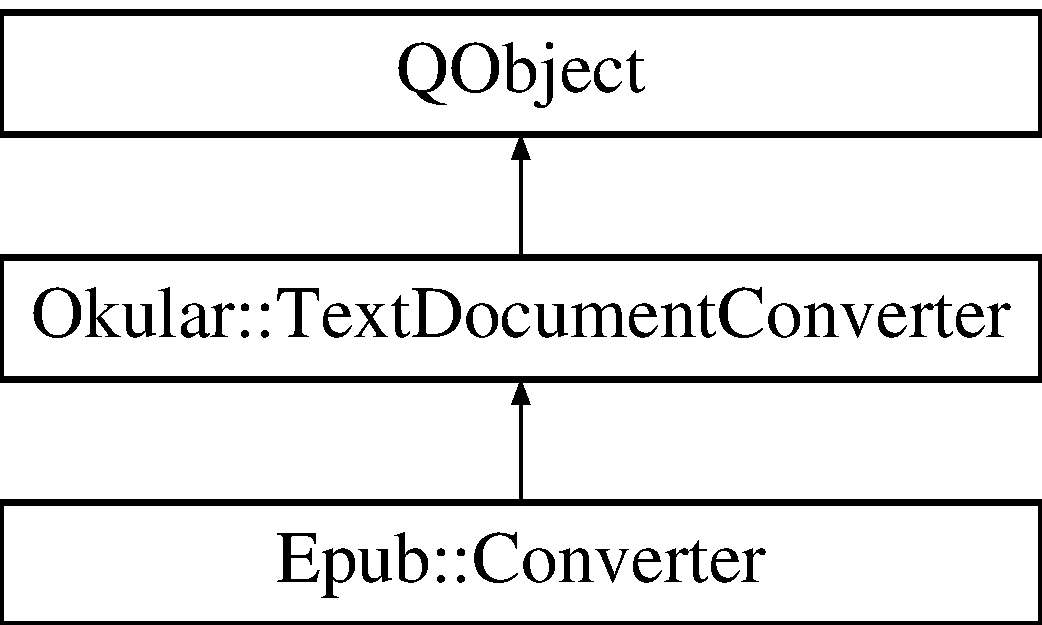
\includegraphics[height=3.000000cm]{classEpub_1_1Converter}
\end{center}
\end{figure}
\subsection*{Public Member Functions}
\begin{DoxyCompactItemize}
\item 
\hyperlink{classEpub_1_1Converter_a1de81f3e06093411e5d27ce882bc010f}{Converter} ()
\item 
\hyperlink{classEpub_1_1Converter_a9ecd05695a52c03158b81e544e13b996}{$\sim$\+Converter} ()
\item 
virtual Q\+Text\+Document $\ast$ \hyperlink{classEpub_1_1Converter_aa63e543977130604de659a4d725ee8bd}{convert} (const Q\+String \&file\+Name)
\end{DoxyCompactItemize}
\subsection*{Additional Inherited Members}


\subsection{Detailed Description}


Definition at line 21 of file converter.\+h.



\subsection{Constructor \& Destructor Documentation}
\hypertarget{classEpub_1_1Converter_a1de81f3e06093411e5d27ce882bc010f}{\index{Epub\+::\+Converter@{Epub\+::\+Converter}!Converter@{Converter}}
\index{Converter@{Converter}!Epub\+::\+Converter@{Epub\+::\+Converter}}
\subsubsection[{Converter}]{\setlength{\rightskip}{0pt plus 5cm}Converter\+::\+Converter (
\begin{DoxyParamCaption}
{}
\end{DoxyParamCaption}
)}}\label{classEpub_1_1Converter_a1de81f3e06093411e5d27ce882bc010f}


Definition at line 30 of file converter.\+cpp.


\begin{DoxyCode}
30                      : mTextDocument(NULL)
31 \{
32 \}
\end{DoxyCode}
\hypertarget{classEpub_1_1Converter_a9ecd05695a52c03158b81e544e13b996}{\index{Epub\+::\+Converter@{Epub\+::\+Converter}!````~Converter@{$\sim$\+Converter}}
\index{````~Converter@{$\sim$\+Converter}!Epub\+::\+Converter@{Epub\+::\+Converter}}
\subsubsection[{$\sim$\+Converter}]{\setlength{\rightskip}{0pt plus 5cm}Converter\+::$\sim$\+Converter (
\begin{DoxyParamCaption}
{}
\end{DoxyParamCaption}
)}}\label{classEpub_1_1Converter_a9ecd05695a52c03158b81e544e13b996}


Definition at line 34 of file converter.\+cpp.


\begin{DoxyCode}
35 \{
36 \}
\end{DoxyCode}


\subsection{Member Function Documentation}
\hypertarget{classEpub_1_1Converter_aa63e543977130604de659a4d725ee8bd}{\index{Epub\+::\+Converter@{Epub\+::\+Converter}!convert@{convert}}
\index{convert@{convert}!Epub\+::\+Converter@{Epub\+::\+Converter}}
\subsubsection[{convert}]{\setlength{\rightskip}{0pt plus 5cm}Q\+Text\+Document $\ast$ Converter\+::convert (
\begin{DoxyParamCaption}
\item[{const Q\+String \&}]{file\+Name}
\end{DoxyParamCaption}
)\hspace{0.3cm}{\ttfamily [virtual]}}}\label{classEpub_1_1Converter_aa63e543977130604de659a4d725ee8bd}
Returns the generated Q\+Text\+Document object. 

Implements \hyperlink{classOkular_1_1TextDocumentConverter_ad05f8bcde0f347c6292968fab331bcef}{Okular\+::\+Text\+Document\+Converter}.



Definition at line 166 of file converter.\+cpp.


\begin{DoxyCode}
167 \{
168   \hyperlink{classEpub_1_1EpubDocument}{EpubDocument} *newDocument = \textcolor{keyword}{new} \hyperlink{classEpub_1_1EpubDocument}{EpubDocument}(fileName);
169   \textcolor{keywordflow}{if} (!newDocument->\hyperlink{classEpub_1_1EpubDocument_ad47e936fccea93a28d1ebb0cf3b36624}{isValid}()) \{
170     emit \hyperlink{classOkular_1_1TextDocumentConverter_a93f1335bdd8232626364c973d9d7e6b4}{error}(i18n(\textcolor{stringliteral}{"Error while opening the EPub document."}), -1);
171     \textcolor{keyword}{delete} newDocument;
172     \textcolor{keywordflow}{return} NULL;
173   \}
174   mTextDocument = newDocument;
175 
176   QTextCursor *\_cursor = \textcolor{keyword}{new} QTextCursor( mTextDocument );
177 
178   mLocalLinks.clear();
179   mSectionMap.clear();
180 
181   \textcolor{comment}{// Emit the document meta data}
182   \_emitData(\hyperlink{classOkular_1_1DocumentInfo_a3a6e5f7fb246e29bcb2e830b6f770791ae400626d63f14b61c55bd22aca9481e0}{Okular::DocumentInfo::Title}, EPUB\_TITLE);
183   \_emitData(\hyperlink{classOkular_1_1DocumentInfo_a3a6e5f7fb246e29bcb2e830b6f770791a1010574d070b1925e030c20fef3e7a35}{Okular::DocumentInfo::Author}, EPUB\_CREATOR);
184   \_emitData(\hyperlink{classOkular_1_1DocumentInfo_a3a6e5f7fb246e29bcb2e830b6f770791a19478a99f97624500aa2d050fe7e1ad8}{Okular::DocumentInfo::Subject}, EPUB\_SUBJECT);
185   \_emitData(\hyperlink{classOkular_1_1DocumentInfo_a3a6e5f7fb246e29bcb2e830b6f770791ab361aa9681b157d8d81e52f440bf646f}{Okular::DocumentInfo::Creator}, EPUB\_PUBLISHER);
186 
187   \_emitData(\hyperlink{classOkular_1_1DocumentInfo_a3a6e5f7fb246e29bcb2e830b6f770791acc3edf1d2abe6eecb0882f4389475591}{Okular::DocumentInfo::Description}, EPUB\_DESCRIPTION);
188 
189   \_emitData(\hyperlink{classOkular_1_1DocumentInfo_a3a6e5f7fb246e29bcb2e830b6f770791a58a72aeacd3cb08e85d0f9f19b2fe83a}{Okular::DocumentInfo::CreationDate}, EPUB\_DATE);
190   \_emitData(\hyperlink{classOkular_1_1DocumentInfo_a3a6e5f7fb246e29bcb2e830b6f770791a1c5f3f7912efdbeff34d16608375c97a}{Okular::DocumentInfo::Category}, EPUB\_TYPE);
191   \_emitData(\hyperlink{classOkular_1_1DocumentInfo_a3a6e5f7fb246e29bcb2e830b6f770791a54b1ae59c56cd90e64b518e4d729471a}{Okular::DocumentInfo::Copyright}, EPUB\_RIGHTS);
192   emit \hyperlink{classOkular_1_1TextDocumentConverter_ad6e263857527273c9cf618e16329f6a7}{addMetaData}( \hyperlink{classOkular_1_1DocumentInfo_a3a6e5f7fb246e29bcb2e830b6f770791a786464e8e8c3e6ba1cd74e408487785b}{Okular::DocumentInfo::MimeType}, \textcolor{stringliteral}{"
      application/epub+zip"});
193 
194   \textcolor{keyword}{struct }eiterator *it;
195 
196   \textcolor{comment}{// iterate over the book}
197   it = epub\_get\_iterator(mTextDocument->\hyperlink{classEpub_1_1EpubDocument_a37cb6d97564a7764b22e44523889267e}{getEpub}(), EITERATOR\_SPINE, 0);
198 
199   \textcolor{comment}{// if the background color of the document is non-white it will be handled by QTextDocument::setHtml()}
200   \textcolor{keywordtype}{bool} firstPage = \textcolor{keyword}{true};
201   QVector<Okular::MovieAnnotation *> movieAnnots;
202   QVector<Okular::SoundAction *> soundActions;
203   \textcolor{keyword}{const} QSize videoSize(320, 240);
204   \textcolor{keywordflow}{do}\{
205     movieAnnots.clear();
206     soundActions.clear();
207 
208     \textcolor{keywordflow}{if}(epub\_it\_get\_curr(it)) \{
209       \textcolor{keyword}{const} QString link = QString::fromUtf8(epub\_it\_get\_curr\_url(it));
210       mTextDocument->\hyperlink{classEpub_1_1EpubDocument_a6e36681fb7d345bf885150d884513fdf}{setCurrentSubDocument}(link);
211       QString htmlContent = QString::fromUtf8(epub\_it\_get\_curr(it));
212 
213       \textcolor{comment}{// as QTextCharFormat::anchorNames() ignores sections, replace it with <p>}
214       htmlContent.replace(QRegExp(\textcolor{stringliteral}{"< *section"}),\textcolor{stringliteral}{"<p"});
215       htmlContent.replace(QRegExp(\textcolor{stringliteral}{"< */ *section"}),\textcolor{stringliteral}{"</p"});
216 
217       \textcolor{comment}{// convert svg tags to img}
218       \textcolor{keyword}{const} \textcolor{keywordtype}{int} maxHeight = mTextDocument->\hyperlink{classEpub_1_1EpubDocument_ae8f068a3e013d7736293a195986d71cb}{maxContentHeight}();
219       \textcolor{keyword}{const} \textcolor{keywordtype}{int} maxWidth = mTextDocument->\hyperlink{classEpub_1_1EpubDocument_a214f084adb359a132c522ffec0d61aeb}{maxContentWidth}();
220       QDomDocument dom;
221       \textcolor{keywordflow}{if}(dom.setContent(htmlContent)) \{
222         QDomNodeList svgs = dom.elementsByTagName(\textcolor{stringliteral}{"svg"});
223         \textcolor{keywordflow}{if}(!svgs.isEmpty()) \{
224           \hyperlink{classQList}{QList< QDomNode >} imgNodes;
225           \textcolor{keywordflow}{for} (uint i = 0; i < svgs.length(); ++i) \{
226             QDomNodeList images = svgs.at(i).toElement().elementsByTagName(\textcolor{stringliteral}{"image"});
227             \textcolor{keywordflow}{for} (uint j = 0; j < images.length(); ++j) \{
228               QString lnk = images.at(i).toElement().attribute(\textcolor{stringliteral}{"xlink:href"});
229               \textcolor{keywordtype}{int} ht = images.at(i).toElement().attribute(\textcolor{stringliteral}{"height"}).toInt();
230               \textcolor{keywordtype}{int} wd = images.at(i).toElement().attribute(\textcolor{stringliteral}{"width"}).toInt();
231               QImage img = mTextDocument->\hyperlink{classEpub_1_1EpubDocument_a5977d43df31dc940280f6fc80eb6bc75}{loadResource}(QTextDocument::ImageResource,QUrl(lnk)).
      value<QImage>();
232               \textcolor{keywordflow}{if}(ht == 0) ht = img.height();
233               \textcolor{keywordflow}{if}(wd == 0) wd = img.width();
234               \textcolor{keywordflow}{if}(ht > maxHeight) ht = maxHeight;
235               \textcolor{keywordflow}{if}(wd > maxWidth) wd = maxWidth;
236               mTextDocument->addResource(QTextDocument::ImageResource,QUrl(lnk),img);
237               QDomDocument newDoc;
238               newDoc.setContent(QString(\textcolor{stringliteral}{"<img src=\(\backslash\)"%1\(\backslash\)" height=\(\backslash\)"%2\(\backslash\)" width=\(\backslash\)"%3\(\backslash\)" />"}).arg(lnk).arg(ht).
      arg(wd));
239               imgNodes.append(newDoc.documentElement());
240             \}
241             \textcolor{keywordflow}{foreach} (QDomNode nd, imgNodes) \{
242               svgs.at(i).parentNode().replaceChild(nd,svgs.at(i));
243             \}
244           \}
245         \}
246 
247         \textcolor{comment}{// handle embedded videos}
248         QDomNodeList videoTags = dom.elementsByTagName(\textcolor{stringliteral}{"video"});
249         \textcolor{keywordflow}{if}(!videoTags.isEmpty()) \{
250           \textcolor{keywordflow}{for} (\textcolor{keywordtype}{int} i = 0; i < videoTags.size(); ++i) \{
251             QDomNodeList sourceTags = videoTags.at(i).toElement().elementsByTagName(\textcolor{stringliteral}{"source"});
252             \textcolor{keywordflow}{if}(!sourceTags.isEmpty()) \{
253               QString lnk = sourceTags.at(0).toElement().attribute(\textcolor{stringliteral}{"src"});
254 
255               \hyperlink{classOkular_1_1Movie}{Okular::Movie} *movie = \textcolor{keyword}{new} \hyperlink{classOkular_1_1Movie}{Okular::Movie}(mTextDocument->
      \hyperlink{classEpub_1_1EpubDocument_a5977d43df31dc940280f6fc80eb6bc75}{loadResource}(\hyperlink{classEpub_1_1EpubDocument_a8727955892e8fa3c5eaef8d9d3ae7c8fa75a15290b8e57ccaad8ff2dee9593636}{EpubDocument::MovieResource},QUrl(lnk)).toString());
256               movie->\hyperlink{classOkular_1_1Movie_aaa87050fba266ea14b37b7c9fa458c2f}{setSize}(videoSize);
257               movie->\hyperlink{classOkular_1_1Movie_a72c045992d6fb31a7280e069422e43e5}{setShowControls}(\textcolor{keyword}{true});
258 
259               \hyperlink{classOkular_1_1MovieAnnotation}{Okular::MovieAnnotation} *annot = \textcolor{keyword}{new} 
      \hyperlink{classOkular_1_1MovieAnnotation}{Okular::MovieAnnotation};
260               annot->\hyperlink{classOkular_1_1MovieAnnotation_a76ea2ec20c8d441f1b9e2ce6f1eaf21f}{setMovie}(movie);
261 
262               movieAnnots.push\_back(annot);
263               QDomDocument tempDoc;
264               tempDoc.setContent(QString(\textcolor{stringliteral}{"<pre>&lt;video&gt;&lt;/video&gt;</pre>"}));
265               videoTags.at(i).parentNode().replaceChild(tempDoc.documentElement(),videoTags.at(i));
266             \}
267           \}
268         \}
269 
270         \textcolor{comment}{//handle embedded audio}
271         QDomNodeList audioTags = dom.elementsByTagName(\textcolor{stringliteral}{"audio"});
272         \textcolor{keywordflow}{if}(!audioTags.isEmpty()) \{
273           \textcolor{keywordflow}{for} (\textcolor{keywordtype}{int} i = 0; i < audioTags.size(); ++i) \{
274             QString lnk = audioTags.at(i).toElement().attribute(\textcolor{stringliteral}{"src"});
275 
276             \hyperlink{classOkular_1_1Sound}{Okular::Sound} *sound = \textcolor{keyword}{new} \hyperlink{classOkular_1_1Sound}{Okular::Sound}(mTextDocument->
      \hyperlink{classEpub_1_1EpubDocument_a5977d43df31dc940280f6fc80eb6bc75}{loadResource}(
277                     \hyperlink{classEpub_1_1EpubDocument_a8727955892e8fa3c5eaef8d9d3ae7c8fa858f54dd2eb2907bbf1be8fbe0d1c054}{EpubDocument::AudioResource}, QUrl(lnk)).toByteArray());
278 
279             \hyperlink{classOkular_1_1SoundAction}{Okular::SoundAction} *soundAction = \textcolor{keyword}{new} 
      \hyperlink{classOkular_1_1SoundAction}{Okular::SoundAction}(1.0,\textcolor{keyword}{true},\textcolor{keyword}{true},\textcolor{keyword}{false},sound);
280             soundActions.push\_back(soundAction);
281 
282             QDomDocument tempDoc;
283             tempDoc.setContent(QString(\textcolor{stringliteral}{"<pre>&lt;audio&gt;&lt;/audio&gt;</pre>"}));
284             audioTags.at(i).parentNode().replaceChild(tempDoc.documentElement(),audioTags.at(i));
285           \}
286         \}
287         htmlContent = dom.toString();
288       \}
289 
290       \textcolor{comment}{// HACK BEGIN Get the links without CSS to be blue}
291       \textcolor{comment}{//            Remove if Qt ever gets fixed and the code in textdocumentgenerator.cpp works}
292       \textcolor{keyword}{const} QPalette orig = qApp->palette();
293       QPalette p = orig;
294       p.setColor(QPalette::Link, Qt::blue);
295       qApp->setPalette(p);
296       \textcolor{comment}{// HACK END}
297 
298       QTextBlock before;
299       \textcolor{keywordflow}{if}(firstPage) \{
300         \textcolor{comment}{// preHtml & postHtml make it possible to have a margin around the content of the page}
301         \textcolor{keyword}{const} QString preHtml = QString(\textcolor{stringliteral}{"<html><head></head><body>"}
302                                         \textcolor{stringliteral}{"<table style=\(\backslash\)"-qt-table-type: root; margin-top:%1px;
       margin-bottom:%1px; margin-left:%1px; margin-right:%1px;\(\backslash\)">"}
303                                         \textcolor{stringliteral}{"<tr>"}
304                                         \textcolor{stringliteral}{"<td style=\(\backslash\)"border: none;\(\backslash\)">"}).arg(mTextDocument->padding);
305         \textcolor{keyword}{const} QString postHtml = \textcolor{stringliteral}{"</tr></table></body></html>"};
306         mTextDocument->setHtml(preHtml + htmlContent + postHtml);
307         firstPage = \textcolor{keyword}{false};
308         before = mTextDocument->begin();
309       \} \textcolor{keywordflow}{else} \{
310         before = \_cursor->block();
311         \_cursor->insertHtml(htmlContent);
312       \}
313       \textcolor{comment}{// HACK BEGIN}
314       qApp->setPalette(orig);
315       \textcolor{comment}{// HACK END}
316 
317       QTextCursor csr(mTextDocument);   \textcolor{comment}{// a temporary cursor}
318       csr.movePosition(QTextCursor::Start);
319       \textcolor{keywordtype}{int} index = 0;
320       \textcolor{keywordflow}{while}( !(csr = mTextDocument->find(\textcolor{stringliteral}{"<video></video>"},csr)).isNull() ) \{
321         \textcolor{keyword}{const} \textcolor{keywordtype}{int} posStart = csr.position();
322         \textcolor{keyword}{const} QPoint startPoint = calculateXYPosition(mTextDocument, posStart);
323         QImage img(KStandardDirs::locate(\textcolor{stringliteral}{"data"}, \textcolor{stringliteral}{"okular/pics/okular-epub-movie.png"}));
324         img = img.scaled(videoSize);
325         csr.insertImage(img);
326         \textcolor{keyword}{const} \textcolor{keywordtype}{int} posEnd = csr.position();
327         \textcolor{keyword}{const} QRect videoRect(startPoint,videoSize);
328         movieAnnots[index]->setBoundingRectangle(\hyperlink{classOkular_1_1NormalizedRect}{Okular::NormalizedRect}(videoRect,
      mTextDocument->pageSize().width(), mTextDocument->pageSize().height()));
329         emit \hyperlink{classOkular_1_1TextDocumentConverter_ab0291a2187c35bda6dd37c78e5642a1b}{addAnnotation}(movieAnnots[index++],posStart,posEnd);
330         csr.movePosition(QTextCursor::NextWord);
331       \}
332 
333       csr.movePosition(QTextCursor::Start);
334       index = 0;
335       \textcolor{keyword}{const} QString keyToSearch(\textcolor{stringliteral}{"<audio></audio>"});
336       \textcolor{keywordflow}{while}( !(csr = mTextDocument->find(keyToSearch, csr)).isNull() ) \{
337         \textcolor{keyword}{const} \textcolor{keywordtype}{int} posStart = csr.position() - keyToSearch.size();
338         \textcolor{keyword}{const} QImage img(KStandardDirs::locate(\textcolor{stringliteral}{"data"}, \textcolor{stringliteral}{"okular/pics/okular-epub-sound-icon.png"}));
339         csr.insertImage(img);
340         \textcolor{keyword}{const} \textcolor{keywordtype}{int} posEnd = csr.position();
341         qDebug() << posStart << posEnd;;
342         emit \hyperlink{classOkular_1_1TextDocumentConverter_ac4f1b668547e87affede3663ea6d8bc6}{addAction}(soundActions[index++],posStart,posEnd);
343         csr.movePosition(QTextCursor::NextWord);
344       \}
345 
346       mSectionMap.insert(link, before);
347 
348       \_handle\_anchors(before, link);
349 
350       \textcolor{keyword}{const} \textcolor{keywordtype}{int} page = mTextDocument->pageCount();
351 
352       \textcolor{comment}{// it will clear the previous format}
353       \textcolor{comment}{// useful when the last line had a bullet}
354       \_cursor->insertBlock(QTextBlockFormat());
355 
356       \textcolor{keywordflow}{while}(mTextDocument->pageCount() == page)
357         \_cursor->insertText(\textcolor{stringliteral}{"\(\backslash\)n"});
358     \}
359   \} \textcolor{keywordflow}{while} (epub\_it\_get\_next(it));
360 
361   epub\_free\_iterator(it);
362 
363   \textcolor{comment}{// handle toc}
364   \textcolor{keyword}{struct }titerator *tit;
365 
366   \textcolor{comment}{// FIXME: support other method beside NAVMAP and GUIDE}
367   tit = epub\_get\_titerator(mTextDocument->\hyperlink{classEpub_1_1EpubDocument_a37cb6d97564a7764b22e44523889267e}{getEpub}(), TITERATOR\_NAVMAP, 0);
368   \textcolor{keywordflow}{if} (!tit)
369     tit = epub\_get\_titerator(mTextDocument->\hyperlink{classEpub_1_1EpubDocument_a37cb6d97564a7764b22e44523889267e}{getEpub}(), TITERATOR\_GUIDE, 0);
370 
371   \textcolor{keywordflow}{if} (tit) \{
372     \textcolor{keywordflow}{do} \{
373       \textcolor{keywordflow}{if} (epub\_tit\_curr\_valid(tit)) \{
374         \textcolor{keywordtype}{char} *clink = epub\_tit\_get\_curr\_link(tit);
375         QString link = QString::fromUtf8(clink);
376         \textcolor{keywordtype}{char} *label = epub\_tit\_get\_curr\_label(tit);
377         QTextBlock block = mTextDocument->begin(); \textcolor{comment}{// must point somewhere}
378 
379         \textcolor{keywordflow}{if} (mSectionMap.contains(link)) \{
380           block = mSectionMap.value(link);
381         \} \textcolor{keywordflow}{else} \{ \textcolor{comment}{// load missing resource}
382           \textcolor{keywordtype}{char} *data = 0;
383           \textcolor{keywordtype}{int} \hyperlink{synctex__parser_8c_aa23c661441688350614bd6a350d2b6ff}{size} = epub\_get\_data(mTextDocument->\hyperlink{classEpub_1_1EpubDocument_a37cb6d97564a7764b22e44523889267e}{getEpub}(), clink, &data);
384           \textcolor{keywordflow}{if} (data) \{
385             \_cursor->insertBlock();
386 
387             \textcolor{comment}{// try to load as image and if not load as html}
388             block = \_cursor->block();
389             QImage image;
390             mSectionMap.insert(link, block);
391             \textcolor{keywordflow}{if} (image.loadFromData((\textcolor{keywordtype}{unsigned} \textcolor{keywordtype}{char} *)data, size)) \{
392               mTextDocument->addResource(QTextDocument::ImageResource,
393                                          QUrl(link), image);
394               \_cursor->insertImage(link);
395             \} \textcolor{keywordflow}{else} \{
396               \_cursor->insertHtml(QString::fromUtf8(data));
397               \textcolor{comment}{// Add anchors to hashes}
398               \_handle\_anchors(block, link);
399             \}
400 
401             \textcolor{comment}{// Start new file in a new page}
402             \textcolor{keywordtype}{int} page = mTextDocument->pageCount();
403             \textcolor{keywordflow}{while}(mTextDocument->pageCount() == page)
404               \_cursor->insertText(\textcolor{stringliteral}{"\(\backslash\)n"});
405           \}
406 
407           free(data);
408         \}
409 
410         \textcolor{keywordflow}{if} (block.isValid()) \{ \textcolor{comment}{// be sure we actually got a block}
411           emit \hyperlink{classOkular_1_1TextDocumentConverter_a054a6dbaad659387f26d239aa96d758d}{addTitle}(epub\_tit\_get\_curr\_depth(tit),
412                         QString::fromUtf8(label),
413                         block);
414         \} \textcolor{keywordflow}{else} \{
415           kDebug() << \textcolor{stringliteral}{"Error: no block found for"}<< link;
416         \}
417 
418         \textcolor{keywordflow}{if} (clink)
419           free(clink);
420         \textcolor{keywordflow}{if} (label)
421           free(label);
422       \}
423     \} \textcolor{keywordflow}{while} (epub\_tit\_next(tit));
424 
425     epub\_free\_titerator(tit);
426   \} \textcolor{keywordflow}{else} \{
427     kDebug() << \textcolor{stringliteral}{"no toc found"};
428   \}
429 
430   \textcolor{comment}{// adding link actions}
431   QHashIterator<QString, QVector< QPair<int, int> > > hit(mLocalLinks);
432   \textcolor{keywordflow}{while} (hit.hasNext()) \{
433     hit.next();
434 
435     \textcolor{keyword}{const} QTextBlock block = mSectionMap.value(hit.key());
436 
437     \textcolor{keywordflow}{for} (\textcolor{keywordtype}{int} i = 0; i < hit.value().size(); ++i) \{
438       \textcolor{keywordflow}{if} (block.isValid()) \{ \textcolor{comment}{// be sure we actually got a block}
439         \hyperlink{classOkular_1_1DocumentViewport}{Okular::DocumentViewport} viewport =
440           \hyperlink{classOkular_1_1TextDocumentConverter_a5d8709540be1213da6dac78759ce7172}{calculateViewport}(mTextDocument, block);
441 
442         \hyperlink{classOkular_1_1GotoAction}{Okular::GotoAction} *action = \textcolor{keyword}{new} \hyperlink{classOkular_1_1GotoAction}{Okular::GotoAction}(QString(), 
      viewport);
443 
444         emit \hyperlink{classOkular_1_1TextDocumentConverter_ac4f1b668547e87affede3663ea6d8bc6}{addAction}(action, hit.value()[i].first, hit.value()[i].second);
445       \} \textcolor{keywordflow}{else} \{
446         kDebug() << \textcolor{stringliteral}{"Error: no block found for "}<< hit.key();
447       \}
448     \}
449   \}
450 
451   \textcolor{keyword}{delete} \_cursor;
452 
453   \textcolor{keywordflow}{return} mTextDocument;
454 \}
\end{DoxyCode}


The documentation for this class was generated from the following files\+:\begin{DoxyCompactItemize}
\item 
generators/epub/\hyperlink{epub_2converter_8h}{converter.\+h}\item 
generators/epub/\hyperlink{epub_2converter_8cpp}{converter.\+cpp}\end{DoxyCompactItemize}

\hypertarget{classFictionBook_1_1Converter}{\section{Fiction\+Book\+:\+:Converter Class Reference}
\label{classFictionBook_1_1Converter}\index{Fiction\+Book\+::\+Converter@{Fiction\+Book\+::\+Converter}}
}


{\ttfamily \#include $<$converter.\+h$>$}

Inheritance diagram for Fiction\+Book\+:\+:Converter\+:\begin{figure}[H]
\begin{center}
\leavevmode
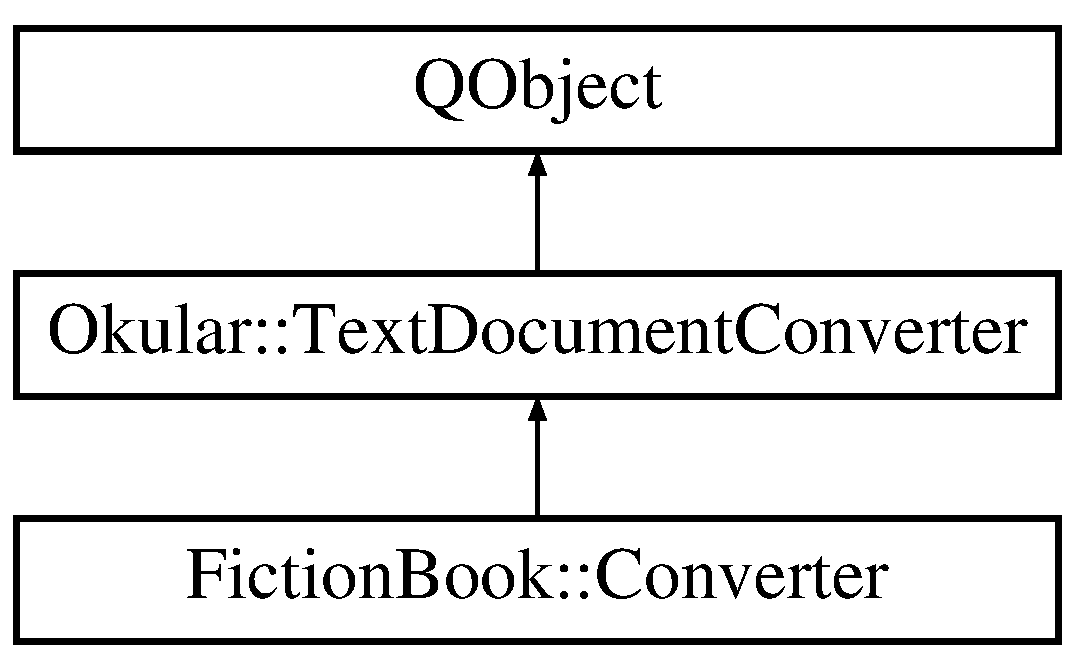
\includegraphics[height=3.000000cm]{classFictionBook_1_1Converter}
\end{center}
\end{figure}
\subsection*{Classes}
\begin{DoxyCompactItemize}
\item 
class \hyperlink{classConverter_1_1DocumentInfo}{Document\+Info}
\item 
class \hyperlink{classConverter_1_1TitleInfo}{Title\+Info}
\end{DoxyCompactItemize}
\subsection*{Public Member Functions}
\begin{DoxyCompactItemize}
\item 
\hyperlink{classFictionBook_1_1Converter_a1de81f3e06093411e5d27ce882bc010f}{Converter} ()
\item 
\hyperlink{classFictionBook_1_1Converter_a9ecd05695a52c03158b81e544e13b996}{$\sim$\+Converter} ()
\item 
virtual Q\+Text\+Document $\ast$ \hyperlink{classFictionBook_1_1Converter_aa63e543977130604de659a4d725ee8bd}{convert} (const Q\+String \&file\+Name)
\end{DoxyCompactItemize}
\subsection*{Additional Inherited Members}


\subsection{Detailed Description}


Definition at line 20 of file converter.\+h.



\subsection{Constructor \& Destructor Documentation}
\hypertarget{classFictionBook_1_1Converter_a1de81f3e06093411e5d27ce882bc010f}{\index{Fiction\+Book\+::\+Converter@{Fiction\+Book\+::\+Converter}!Converter@{Converter}}
\index{Converter@{Converter}!Fiction\+Book\+::\+Converter@{Fiction\+Book\+::\+Converter}}
\subsubsection[{Converter}]{\setlength{\rightskip}{0pt plus 5cm}Converter\+::\+Converter (
\begin{DoxyParamCaption}
{}
\end{DoxyParamCaption}
)}}\label{classFictionBook_1_1Converter_a1de81f3e06093411e5d27ce882bc010f}


Definition at line 53 of file converter.\+cpp.


\begin{DoxyCode}
54     : mTextDocument( 0 ), mCursor( 0 ),
55       mTitleInfo( 0 ), mDocumentInfo( 0 )
56 \{
57 \}
\end{DoxyCode}
\hypertarget{classFictionBook_1_1Converter_a9ecd05695a52c03158b81e544e13b996}{\index{Fiction\+Book\+::\+Converter@{Fiction\+Book\+::\+Converter}!````~Converter@{$\sim$\+Converter}}
\index{````~Converter@{$\sim$\+Converter}!Fiction\+Book\+::\+Converter@{Fiction\+Book\+::\+Converter}}
\subsubsection[{$\sim$\+Converter}]{\setlength{\rightskip}{0pt plus 5cm}Converter\+::$\sim$\+Converter (
\begin{DoxyParamCaption}
{}
\end{DoxyParamCaption}
)}}\label{classFictionBook_1_1Converter_a9ecd05695a52c03158b81e544e13b996}


Definition at line 59 of file converter.\+cpp.


\begin{DoxyCode}
60 \{
61     \textcolor{keyword}{delete} mTitleInfo;
62     \textcolor{keyword}{delete} mDocumentInfo;
63 \}
\end{DoxyCode}


\subsection{Member Function Documentation}
\hypertarget{classFictionBook_1_1Converter_aa63e543977130604de659a4d725ee8bd}{\index{Fiction\+Book\+::\+Converter@{Fiction\+Book\+::\+Converter}!convert@{convert}}
\index{convert@{convert}!Fiction\+Book\+::\+Converter@{Fiction\+Book\+::\+Converter}}
\subsubsection[{convert}]{\setlength{\rightskip}{0pt plus 5cm}Q\+Text\+Document $\ast$ Converter\+::convert (
\begin{DoxyParamCaption}
\item[{const Q\+String \&}]{file\+Name}
\end{DoxyParamCaption}
)\hspace{0.3cm}{\ttfamily [virtual]}}}\label{classFictionBook_1_1Converter_aa63e543977130604de659a4d725ee8bd}
Returns the generated Q\+Text\+Document object. Set the correct page size

Parse the content of the document

First we read all images, so we can calculate the size later.

Read the rest...

Add document info.

Implements \hyperlink{classOkular_1_1TextDocumentConverter_ad05f8bcde0f347c6292968fab331bcef}{Okular\+::\+Text\+Document\+Converter}.



Definition at line 65 of file converter.\+cpp.


\begin{DoxyCode}
66 \{
67     \hyperlink{classFictionBook_1_1Document}{Document} fbDocument( fileName );
68     \textcolor{keywordflow}{if} ( !fbDocument.open() ) \{
69         emit \hyperlink{classOkular_1_1TextDocumentConverter_a93f1335bdd8232626364c973d9d7e6b4}{error}( fbDocument.lastErrorString(), -1 );
70         \textcolor{keywordflow}{return} 0;
71     \}
72 
73     mTextDocument = \textcolor{keyword}{new} QTextDocument;
74     mCursor = \textcolor{keyword}{new} QTextCursor( mTextDocument );
75     mSectionCounter = 0;
76     mLocalLinks.clear();
77     mSectionMap.clear();
78 
79     \textcolor{keyword}{const} QDomDocument document = fbDocument.content();
80 
84     mTextDocument->setPageSize( QSizeF( 600, 800 ) );
85 
86     QTextFrameFormat frameFormat;
87     frameFormat.setMargin( 20 );
88 
89     QTextFrame *rootFrame = mTextDocument->rootFrame();
90     rootFrame->setFrameFormat( frameFormat );
91 
95     \textcolor{keyword}{const} QDomElement documentElement = document.documentElement();
96 
97     \textcolor{keywordflow}{if} ( documentElement.tagName() != QLatin1String( \textcolor{stringliteral}{"FictionBook"} ) ) \{
98         emit \hyperlink{classOkular_1_1TextDocumentConverter_a93f1335bdd8232626364c973d9d7e6b4}{error}( i18n( \textcolor{stringliteral}{"Document is not a valid FictionBook"} ), -1 );
99         \textcolor{keyword}{delete} mCursor;
100         \textcolor{keywordflow}{return} 0;
101     \}
102 
106     QDomElement element = documentElement.firstChildElement();
107     \textcolor{keywordflow}{while} ( !element.isNull() ) \{
108         \textcolor{keywordflow}{if} ( element.tagName() == QLatin1String( \textcolor{stringliteral}{"binary"} ) ) \{
109             \textcolor{keywordflow}{if} ( !convertBinary( element ) ) \{
110                 \textcolor{keyword}{delete} mCursor;
111                 \textcolor{keywordflow}{return} 0;
112             \}
113         \}
114 
115         element = element.nextSiblingElement();
116     \}
117 
121     element = documentElement.firstChildElement();
122     \textcolor{keywordflow}{while} ( !element.isNull() ) \{
123         \textcolor{keywordflow}{if} ( element.tagName() == QLatin1String( \textcolor{stringliteral}{"description"} ) ) \{
124             \textcolor{keywordflow}{if} ( !convertDescription( element ) ) \{
125                 \textcolor{keyword}{delete} mCursor;
126                 \textcolor{keywordflow}{return} 0;
127             \}
128         \} \textcolor{keywordflow}{else} \textcolor{keywordflow}{if} ( element.tagName() == QLatin1String( \textcolor{stringliteral}{"body"} ) ) \{
129             \textcolor{keywordflow}{if} ( !mTitleInfo->\hyperlink{classConverter_1_1TitleInfo_afd5944a2140785dd5e82dd104347ea43}{mCoverPage}.isNull() ) \{
130                 convertCover( mTitleInfo->\hyperlink{classConverter_1_1TitleInfo_afd5944a2140785dd5e82dd104347ea43}{mCoverPage} );
131                 mCursor->insertBlock();
132             \}
133 
134             QTextFrame *topFrame = mCursor->currentFrame();
135 
136             QTextFrameFormat frameFormat;
137             frameFormat.setBorder( 2 );
138             frameFormat.setPadding( 8 );
139             frameFormat.setBackground( Qt::lightGray );
140 
141             \textcolor{keywordflow}{if} ( !mTitleInfo->\hyperlink{classConverter_1_1TitleInfo_a19645faf3d93e1588645fa6d50daa69a}{mTitle}.isEmpty() ) \{
142                 mCursor->insertFrame( frameFormat );
143 
144                 QTextCharFormat charFormat;
145                 charFormat.setFontPointSize( 22 );
146                 charFormat.setFontWeight( QFont::Bold );
147                 mCursor->insertText( mTitleInfo->\hyperlink{classConverter_1_1TitleInfo_a19645faf3d93e1588645fa6d50daa69a}{mTitle}, charFormat );
148 
149                 mCursor->setPosition( topFrame->lastPosition() );
150             \}
151 
152             \textcolor{keywordflow}{if} ( !mTitleInfo->\hyperlink{classConverter_1_1TitleInfo_a7ecc1a061f21392a7a3c3daa8792476c}{mAuthor}.isEmpty() ) \{
153                 frameFormat.setBorder( 1 );
154                 mCursor->insertFrame( frameFormat );
155 
156                 QTextCharFormat charFormat;
157                 charFormat.setFontPointSize( 10 );
158                 mCursor->insertText( mTitleInfo->\hyperlink{classConverter_1_1TitleInfo_a7ecc1a061f21392a7a3c3daa8792476c}{mAuthor}, charFormat );
159 
160                 mCursor->setPosition( topFrame->lastPosition() );
161                 mCursor->insertBlock();
162             \}
163 
164             mCursor->insertBlock();
165 
166             \textcolor{keywordflow}{if} ( !convertBody( element ) ) \{
167                 \textcolor{keyword}{delete} mCursor;
168                 \textcolor{keywordflow}{return} 0;
169             \}
170         \}
171 
172         element = element.nextSiblingElement();
173     \}
174 
178     \textcolor{keywordflow}{if} ( mTitleInfo ) \{
179         \textcolor{keywordflow}{if} ( !mTitleInfo->\hyperlink{classConverter_1_1TitleInfo_a19645faf3d93e1588645fa6d50daa69a}{mTitle}.isEmpty() )
180             emit \hyperlink{classOkular_1_1TextDocumentConverter_ad6e263857527273c9cf618e16329f6a7}{addMetaData}( \hyperlink{classOkular_1_1DocumentInfo_a3a6e5f7fb246e29bcb2e830b6f770791ae400626d63f14b61c55bd22aca9481e0}{Okular::DocumentInfo::Title}, mTitleInfo
      ->\hyperlink{classConverter_1_1TitleInfo_a19645faf3d93e1588645fa6d50daa69a}{mTitle} );
181 
182         \textcolor{keywordflow}{if} ( !mTitleInfo->\hyperlink{classConverter_1_1TitleInfo_a7ecc1a061f21392a7a3c3daa8792476c}{mAuthor}.isEmpty() )
183             emit \hyperlink{classOkular_1_1TextDocumentConverter_ad6e263857527273c9cf618e16329f6a7}{addMetaData}( \hyperlink{classOkular_1_1DocumentInfo_a3a6e5f7fb246e29bcb2e830b6f770791a1010574d070b1925e030c20fef3e7a35}{Okular::DocumentInfo::Author}, 
      mTitleInfo->\hyperlink{classConverter_1_1TitleInfo_a7ecc1a061f21392a7a3c3daa8792476c}{mAuthor} );
184     \}
185 
186     \textcolor{keywordflow}{if} ( mDocumentInfo ) \{
187         \textcolor{keywordflow}{if} ( !mDocumentInfo->\hyperlink{classConverter_1_1DocumentInfo_a37486c959f5eb91b039b54092aa4eb33}{mProducer}.isEmpty() )
188             emit \hyperlink{classOkular_1_1TextDocumentConverter_ad6e263857527273c9cf618e16329f6a7}{addMetaData}( \hyperlink{classOkular_1_1DocumentInfo_a3a6e5f7fb246e29bcb2e830b6f770791a4781bb7ac85d4fe7bdc448097aa1c48c}{Okular::DocumentInfo::Producer}, 
      mDocumentInfo->\hyperlink{classConverter_1_1DocumentInfo_a37486c959f5eb91b039b54092aa4eb33}{mProducer} );
189 
190         \textcolor{keywordflow}{if} ( mDocumentInfo->\hyperlink{classConverter_1_1DocumentInfo_a5a6937c62c571c7c757aa753012a24ca}{mDate}.isValid() )
191             emit \hyperlink{classOkular_1_1TextDocumentConverter_ad6e263857527273c9cf618e16329f6a7}{addMetaData}( \hyperlink{classOkular_1_1DocumentInfo_a3a6e5f7fb246e29bcb2e830b6f770791a58a72aeacd3cb08e85d0f9f19b2fe83a}{Okular::DocumentInfo::CreationDate}
      ,
192                       KGlobal::locale()->formatDate( mDocumentInfo->\hyperlink{classConverter_1_1DocumentInfo_a5a6937c62c571c7c757aa753012a24ca}{mDate}, KLocale::ShortDate ) );
193     \}
194 
195     QMapIterator<QString, QPair<int, int> > it( mLocalLinks );
196     \textcolor{keywordflow}{while} ( it.hasNext() ) \{
197         it.next();
198 
199         \textcolor{keyword}{const} QTextBlock block = mSectionMap[ it.key() ];
200         \textcolor{keywordflow}{if} ( !block.isValid() ) \textcolor{comment}{// local link without existing target}
201           \textcolor{keywordflow}{continue};
202 
203         \hyperlink{classOkular_1_1DocumentViewport}{Okular::DocumentViewport} viewport = 
      \hyperlink{classOkular_1_1TextDocumentConverter_a5d8709540be1213da6dac78759ce7172}{calculateViewport}( mTextDocument, block );
204 
205         \hyperlink{classOkular_1_1GotoAction}{Okular::GotoAction} *action = \textcolor{keyword}{new} \hyperlink{classOkular_1_1GotoAction}{Okular::GotoAction}( QString(),
       viewport );
206 
207         emit \hyperlink{classOkular_1_1TextDocumentConverter_ac4f1b668547e87affede3663ea6d8bc6}{addAction}( action, it.value().first, it.value().second );
208     \}
209 
210     \textcolor{keyword}{delete} mCursor;
211 
212     \textcolor{keywordflow}{return} mTextDocument;
213 \}
\end{DoxyCode}


The documentation for this class was generated from the following files\+:\begin{DoxyCompactItemize}
\item 
generators/fictionbook/\hyperlink{fictionbook_2converter_8h}{converter.\+h}\item 
generators/fictionbook/\hyperlink{fictionbook_2converter_8cpp}{converter.\+cpp}\end{DoxyCompactItemize}

\hypertarget{classMobi_1_1Converter}{\section{Mobi\+:\+:Converter Class Reference}
\label{classMobi_1_1Converter}\index{Mobi\+::\+Converter@{Mobi\+::\+Converter}}
}


{\ttfamily \#include $<$converter.\+h$>$}

Inheritance diagram for Mobi\+:\+:Converter\+:\begin{figure}[H]
\begin{center}
\leavevmode
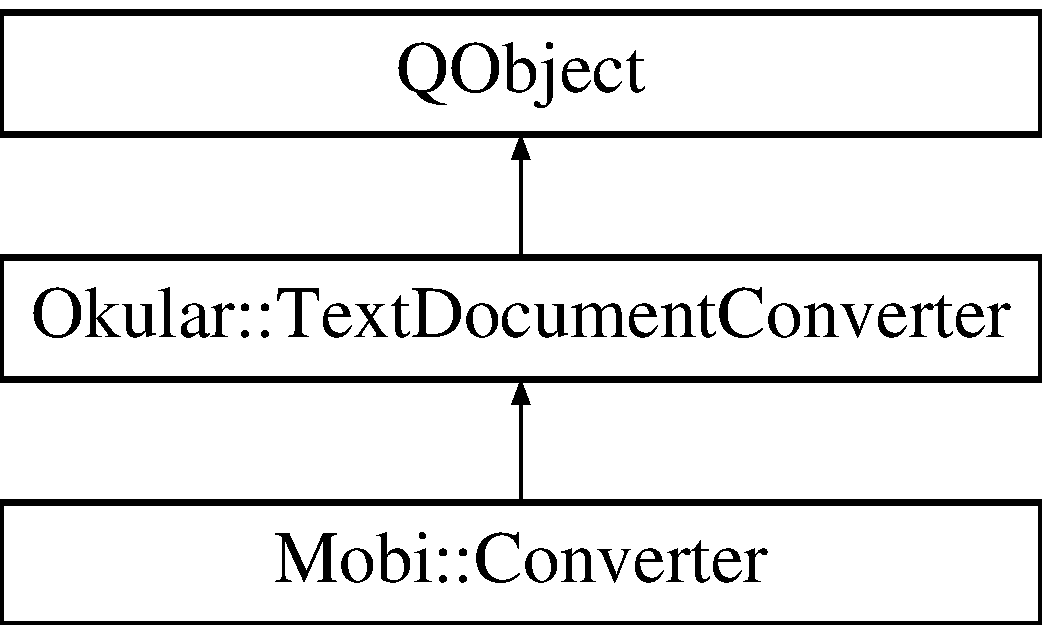
\includegraphics[height=3.000000cm]{classMobi_1_1Converter}
\end{center}
\end{figure}
\subsection*{Public Member Functions}
\begin{DoxyCompactItemize}
\item 
\hyperlink{classMobi_1_1Converter_a1de81f3e06093411e5d27ce882bc010f}{Converter} ()
\item 
\hyperlink{classMobi_1_1Converter_a9ecd05695a52c03158b81e544e13b996}{$\sim$\+Converter} ()
\item 
virtual Q\+Text\+Document $\ast$ \hyperlink{classMobi_1_1Converter_aa63e543977130604de659a4d725ee8bd}{convert} (const Q\+String \&file\+Name)
\end{DoxyCompactItemize}
\subsection*{Additional Inherited Members}


\subsection{Detailed Description}


Definition at line 20 of file converter.\+h.



\subsection{Constructor \& Destructor Documentation}
\hypertarget{classMobi_1_1Converter_a1de81f3e06093411e5d27ce882bc010f}{\index{Mobi\+::\+Converter@{Mobi\+::\+Converter}!Converter@{Converter}}
\index{Converter@{Converter}!Mobi\+::\+Converter@{Mobi\+::\+Converter}}
\subsubsection[{Converter}]{\setlength{\rightskip}{0pt plus 5cm}Converter\+::\+Converter (
\begin{DoxyParamCaption}
{}
\end{DoxyParamCaption}
)}}\label{classMobi_1_1Converter_a1de81f3e06093411e5d27ce882bc010f}


Definition at line 25 of file converter.\+cpp.


\begin{DoxyCode}
26 \{
27   
28 \}
\end{DoxyCode}
\hypertarget{classMobi_1_1Converter_a9ecd05695a52c03158b81e544e13b996}{\index{Mobi\+::\+Converter@{Mobi\+::\+Converter}!````~Converter@{$\sim$\+Converter}}
\index{````~Converter@{$\sim$\+Converter}!Mobi\+::\+Converter@{Mobi\+::\+Converter}}
\subsubsection[{$\sim$\+Converter}]{\setlength{\rightskip}{0pt plus 5cm}Converter\+::$\sim$\+Converter (
\begin{DoxyParamCaption}
{}
\end{DoxyParamCaption}
)}}\label{classMobi_1_1Converter_a9ecd05695a52c03158b81e544e13b996}


Definition at line 30 of file converter.\+cpp.


\begin{DoxyCode}
31 \{    
32 \}
\end{DoxyCode}


\subsection{Member Function Documentation}
\hypertarget{classMobi_1_1Converter_aa63e543977130604de659a4d725ee8bd}{\index{Mobi\+::\+Converter@{Mobi\+::\+Converter}!convert@{convert}}
\index{convert@{convert}!Mobi\+::\+Converter@{Mobi\+::\+Converter}}
\subsubsection[{convert}]{\setlength{\rightskip}{0pt plus 5cm}Q\+Text\+Document $\ast$ Converter\+::convert (
\begin{DoxyParamCaption}
\item[{const Q\+String \&}]{file\+Name}
\end{DoxyParamCaption}
)\hspace{0.3cm}{\ttfamily [virtual]}}}\label{classMobi_1_1Converter_aa63e543977130604de659a4d725ee8bd}
Returns the generated Q\+Text\+Document object. 

Implements \hyperlink{classOkular_1_1TextDocumentConverter_ad05f8bcde0f347c6292968fab331bcef}{Okular\+::\+Text\+Document\+Converter}.



Definition at line 49 of file converter.\+cpp.


\begin{DoxyCode}
50 \{
51   \hyperlink{classMobi_1_1MobiDocument}{MobiDocument}* newDocument=\textcolor{keyword}{new} \hyperlink{classMobi_1_1MobiDocument}{MobiDocument}(fileName);
52   \textcolor{keywordflow}{if} (!newDocument->\hyperlink{classMobi_1_1MobiDocument_a22ca18d34e4e1f9f3aacf54ed7d274c8}{mobi}()->isValid()) \{
53     emit \hyperlink{classOkular_1_1TextDocumentConverter_a93f1335bdd8232626364c973d9d7e6b4}{error}(i18n(\textcolor{stringliteral}{"Error while opening the Mobipocket document."}), -1);
54     \textcolor{keyword}{delete} newDocument;
55     \textcolor{keywordflow}{return} NULL;
56   \}
57   \textcolor{keywordflow}{if} (newDocument->\hyperlink{classMobi_1_1MobiDocument_a22ca18d34e4e1f9f3aacf54ed7d274c8}{mobi}()->hasDRM()) \{
58     emit \hyperlink{classOkular_1_1TextDocumentConverter_a93f1335bdd8232626364c973d9d7e6b4}{error}(i18n(\textcolor{stringliteral}{"This book is protected by DRM and can be displayed only on designated device"}), -
      1);
59     \textcolor{keyword}{delete} newDocument;
60     \textcolor{keywordflow}{return} NULL;
61   \}
62   
63   handleMetadata(newDocument->\hyperlink{classMobi_1_1MobiDocument_a22ca18d34e4e1f9f3aacf54ed7d274c8}{mobi}()->metadata());
64   newDocument->setPageSize(QSizeF(600, 800));
65 
66   QTextFrameFormat frameFormat;
67   frameFormat.setMargin( 20 );
68   QTextFrame *rootFrame = newDocument->rootFrame();
69   rootFrame->setFrameFormat( frameFormat ); 
70   \hyperlink{classQMap}{QMap<QString,QPair<int,int>} > links;
71   \hyperlink{classQMap}{QMap<QString,QTextBlock>} targets;
72 
73   \textcolor{comment}{// go over whole document and add all <a> tags to links or targets map}
74   \textcolor{keywordflow}{for} (QTextBlock it = newDocument->begin(); it != newDocument->end(); it = it.next()) 
75    \textcolor{keywordflow}{for} (QTextBlock::iterator fit=it.begin(); !fit.atEnd(); ++fit) \{
76     QTextFragment frag=fit.fragment();
77     QTextCharFormat format=frag.charFormat();
78     \textcolor{keywordflow}{if} (!format.isAnchor()) \textcolor{keywordflow}{continue};
79     \textcolor{comment}{//link}
80     \textcolor{keywordflow}{if} (!format.anchorHref().isEmpty()) links[format.anchorHref()]=
81       \hyperlink{structQPair}{QPair<int,int>}(frag.position(), frag.position()+frag.length());
82     \textcolor{keywordflow}{if} (!format.anchorNames().isEmpty()) \{
83       \textcolor{comment}{// link targets}
84       Q\_FOREACH(\textcolor{keyword}{const} QString& name, format.anchorNames()) 
85     targets[\textcolor{charliteral}{'#'}+name]=it;
86     \}
87   \}
88 
89   \textcolor{comment}{// create link actions}
90   QMapIterator<QString,QPair<int,int> > it(links);
91   \textcolor{keywordflow}{while} (it.hasNext()) \{
92     it.next();
93     QUrl u(it.key());
94     \textcolor{comment}{// external or internal link}
95     \textcolor{keywordflow}{if} (!u.isRelative()) emit \hyperlink{classOkular_1_1TextDocumentConverter_ac4f1b668547e87affede3663ea6d8bc6}{addAction}(\textcolor{keyword}{new} \hyperlink{classOkular_1_1BrowseAction}{Okular::BrowseAction}(it.key()), it
      .value().first, it.value().second);
96     \textcolor{keywordflow}{else} \{
97       \textcolor{comment}{// is there valid target?}
98       \textcolor{keywordflow}{if} (!targets.contains( it.key() ) || !targets[it.key()].isValid()) \textcolor{keywordflow}{continue};
99       emit \hyperlink{classOkular_1_1TextDocumentConverter_ac4f1b668547e87affede3663ea6d8bc6}{addAction}(\textcolor{keyword}{new} \hyperlink{classOkular_1_1GotoAction}{Okular::GotoAction}(QString(), 
      \hyperlink{classOkular_1_1TextDocumentConverter_a5d8709540be1213da6dac78759ce7172}{calculateViewport}( newDocument, targets[it.key()] )),
100         it.value().first, it.value().second);
101     \}
102     
103   \}
104 
105   \textcolor{keywordflow}{return} newDocument;
106 \}
\end{DoxyCode}


The documentation for this class was generated from the following files\+:\begin{DoxyCompactItemize}
\item 
generators/mobipocket/\hyperlink{mobipocket_2converter_8h}{converter.\+h}\item 
generators/mobipocket/\hyperlink{mobipocket_2converter_8cpp}{converter.\+cpp}\end{DoxyCompactItemize}

\hypertarget{classOOO_1_1Converter}{\section{O\+O\+O\+:\+:Converter Class Reference}
\label{classOOO_1_1Converter}\index{O\+O\+O\+::\+Converter@{O\+O\+O\+::\+Converter}}
}


{\ttfamily \#include $<$converter.\+h$>$}

Inheritance diagram for O\+O\+O\+:\+:Converter\+:\begin{figure}[H]
\begin{center}
\leavevmode
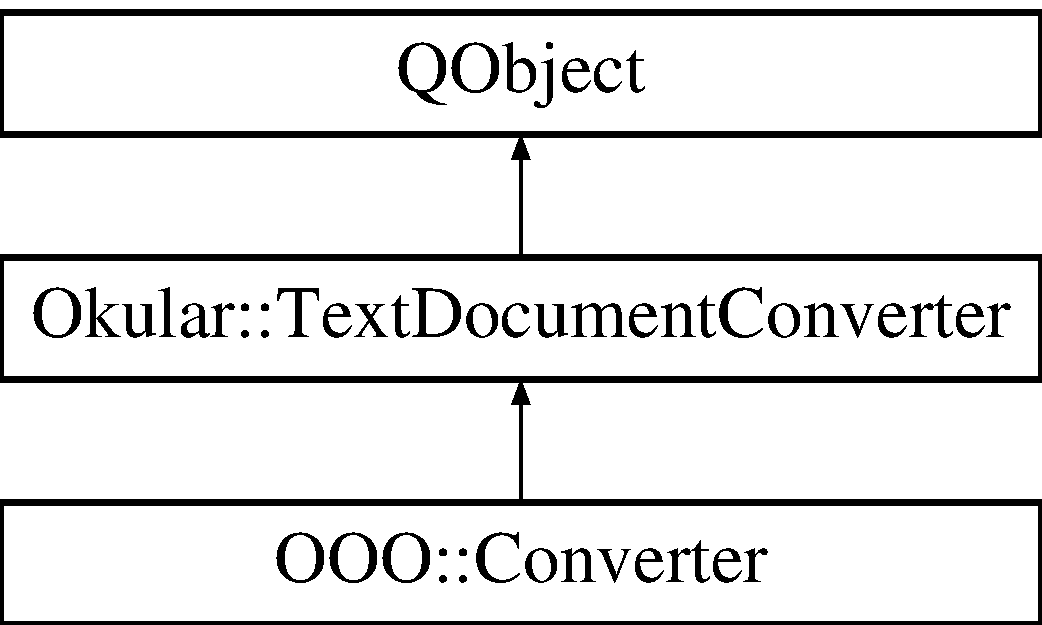
\includegraphics[height=3.000000cm]{classOOO_1_1Converter}
\end{center}
\end{figure}
\subsection*{Public Member Functions}
\begin{DoxyCompactItemize}
\item 
\hyperlink{classOOO_1_1Converter_a1de81f3e06093411e5d27ce882bc010f}{Converter} ()
\item 
\hyperlink{classOOO_1_1Converter_a9ecd05695a52c03158b81e544e13b996}{$\sim$\+Converter} ()
\item 
virtual Q\+Text\+Document $\ast$ \hyperlink{classOOO_1_1Converter_aa63e543977130604de659a4d725ee8bd}{convert} (const Q\+String \&file\+Name)
\end{DoxyCompactItemize}
\subsection*{Additional Inherited Members}


\subsection{Detailed Description}


Definition at line 27 of file converter.\+h.



\subsection{Constructor \& Destructor Documentation}
\hypertarget{classOOO_1_1Converter_a1de81f3e06093411e5d27ce882bc010f}{\index{O\+O\+O\+::\+Converter@{O\+O\+O\+::\+Converter}!Converter@{Converter}}
\index{Converter@{Converter}!O\+O\+O\+::\+Converter@{O\+O\+O\+::\+Converter}}
\subsubsection[{Converter}]{\setlength{\rightskip}{0pt plus 5cm}Converter\+::\+Converter (
\begin{DoxyParamCaption}
{}
\end{DoxyParamCaption}
)}}\label{classOOO_1_1Converter_a1de81f3e06093411e5d27ce882bc010f}


Definition at line 65 of file converter.\+cpp.


\begin{DoxyCode}
66   : mTextDocument( 0 ), mCursor( 0 ),
67     mStyleInformation( 0 )
68 \{
69 \}
\end{DoxyCode}
\hypertarget{classOOO_1_1Converter_a9ecd05695a52c03158b81e544e13b996}{\index{O\+O\+O\+::\+Converter@{O\+O\+O\+::\+Converter}!````~Converter@{$\sim$\+Converter}}
\index{````~Converter@{$\sim$\+Converter}!O\+O\+O\+::\+Converter@{O\+O\+O\+::\+Converter}}
\subsubsection[{$\sim$\+Converter}]{\setlength{\rightskip}{0pt plus 5cm}Converter\+::$\sim$\+Converter (
\begin{DoxyParamCaption}
{}
\end{DoxyParamCaption}
)}}\label{classOOO_1_1Converter_a9ecd05695a52c03158b81e544e13b996}


Definition at line 71 of file converter.\+cpp.


\begin{DoxyCode}
72 \{
73 \}
\end{DoxyCode}


\subsection{Member Function Documentation}
\hypertarget{classOOO_1_1Converter_aa63e543977130604de659a4d725ee8bd}{\index{O\+O\+O\+::\+Converter@{O\+O\+O\+::\+Converter}!convert@{convert}}
\index{convert@{convert}!O\+O\+O\+::\+Converter@{O\+O\+O\+::\+Converter}}
\subsubsection[{convert}]{\setlength{\rightskip}{0pt plus 5cm}Q\+Text\+Document $\ast$ Converter\+::convert (
\begin{DoxyParamCaption}
\item[{const Q\+String \&}]{file\+Name}
\end{DoxyParamCaption}
)\hspace{0.3cm}{\ttfamily [virtual]}}}\label{classOOO_1_1Converter_aa63e543977130604de659a4d725ee8bd}
Returns the generated Q\+Text\+Document object. Create the dom of the content

Read the style properties, so the are available when parsing the content.

Add all images of the document to resource framework

Set the correct page size

Parse the content of the document

Implements \hyperlink{classOkular_1_1TextDocumentConverter_ad05f8bcde0f347c6292968fab331bcef}{Okular\+::\+Text\+Document\+Converter}.



Definition at line 75 of file converter.\+cpp.


\begin{DoxyCode}
76 \{
77   \hyperlink{classOOO_1_1Document}{Document} oooDocument( fileName );
78   \textcolor{keywordflow}{if} ( !oooDocument.open() ) \{
79     emit \hyperlink{classOkular_1_1TextDocumentConverter_a93f1335bdd8232626364c973d9d7e6b4}{error}( oooDocument.lastErrorString(), -1 );
80     \textcolor{keywordflow}{return} 0;
81   \}
82 
83   mTextDocument = \textcolor{keyword}{new} QTextDocument;
84   mCursor = \textcolor{keyword}{new} QTextCursor( mTextDocument );
85 
89   QXmlSimpleReader reader;
90 
91   QXmlInputSource source;
92   source.setData( oooDocument.content() );
93 
94   QString errorMsg;
95   QDomDocument document;
96   \textcolor{keywordflow}{if} ( !document.setContent( &source, &reader, &errorMsg ) ) \{
97     emit \hyperlink{classOkular_1_1TextDocumentConverter_a93f1335bdd8232626364c973d9d7e6b4}{error}( i18n( \textcolor{stringliteral}{"Invalid XML document: %1"}, errorMsg ), -1 );
98     \textcolor{keyword}{delete} mCursor;
99     \textcolor{keywordflow}{return} 0;
100   \}
101 
102   mStyleInformation = \textcolor{keyword}{new} \hyperlink{classOOO_1_1StyleInformation}{StyleInformation}();
103 
108   \hyperlink{classOOO_1_1StyleParser}{StyleParser} styleParser( &oooDocument, document, mStyleInformation );
109   \textcolor{keywordflow}{if} ( !styleParser.parse() ) \{
110     emit \hyperlink{classOkular_1_1TextDocumentConverter_a93f1335bdd8232626364c973d9d7e6b4}{error}( i18n( \textcolor{stringliteral}{"Unable to read style information"} ), -1 );
111     \textcolor{keyword}{delete} mCursor;
112     \textcolor{keywordflow}{return} 0;
113   \}
114 
118   \textcolor{keyword}{const} \hyperlink{classQMap}{QMap<QString, QByteArray>} images = oooDocument.images();
119   QMapIterator<QString, QByteArray> it( images );
120   \textcolor{keywordflow}{while} ( it.hasNext() ) \{
121     it.next();
122 
123     mTextDocument->addResource( QTextDocument::ImageResource, QUrl( it.key() ), QImage::fromData( it.value(
      ) ) );
124   \}
125 
129   \textcolor{keyword}{const} QString masterLayout = mStyleInformation->\hyperlink{classOOO_1_1StyleInformation_ad8c37f921e5d3b0c429226ac46f3a7ca}{masterPageName}();
130   \textcolor{keyword}{const} \hyperlink{classOOO_1_1PageFormatProperty}{PageFormatProperty} \textcolor{keyword}{property} = mStyleInformation->
      \hyperlink{classOOO_1_1StyleInformation_a74abc64faa641fdc3213ca9a8dd18d6d}{pageProperty}( masterLayout );
131 
132   \textcolor{keywordtype}{int} pageWidth = qRound(property.width() / 72.0 * \hyperlink{classOkular_1_1Utils_acd9a3685415399561c6cde450ead4710}{Okular::Utils::dpiX}());
133   \textcolor{keywordtype}{int} pageHeight = qRound(property.height() / 72.0 * \hyperlink{classOkular_1_1Utils_aeee309843e66a38840d6cec2002df3ea}{Okular::Utils::dpiY}());
134 
135   \textcolor{keywordflow}{if} ( pageWidth == 0 )
136       pageWidth = 600;
137   \textcolor{keywordflow}{if} ( pageHeight == 0 )
138       pageHeight = 800;
139 
140   mTextDocument->setPageSize( QSize( pageWidth, pageHeight ) );
141 
142   QTextFrameFormat frameFormat;
143   frameFormat.setMargin( qRound( property.margin() ) );
144 
145   QTextFrame *rootFrame = mTextDocument->rootFrame();
146   rootFrame->setFrameFormat( frameFormat );
147 
151   \textcolor{keyword}{const} QDomElement documentElement = document.documentElement();
152 
153   QDomElement element = documentElement.firstChildElement();
154   \textcolor{keywordflow}{while} ( !element.isNull() ) \{
155     \textcolor{keywordflow}{if} ( element.tagName() == QLatin1String( \textcolor{stringliteral}{"body"} ) ) \{
156       \textcolor{keywordflow}{if} ( !convertBody( element ) ) \{
157         emit \hyperlink{classOkular_1_1TextDocumentConverter_a93f1335bdd8232626364c973d9d7e6b4}{error}( i18n( \textcolor{stringliteral}{"Unable to convert document content"} ), -1 );
158         \textcolor{keyword}{delete} mCursor;
159         \textcolor{keywordflow}{return} 0;
160       \}
161     \}
162 
163     element = element.nextSiblingElement();
164   \}
165 
166   \hyperlink{classQList}{MetaInformation::List} metaInformation = mStyleInformation->
      \hyperlink{classOOO_1_1StyleInformation_ac09f26c30d59e11a9ef7f21b8e1e7280}{metaInformation}();
167   \textcolor{keywordflow}{for} ( \textcolor{keywordtype}{int} i = 0; i < metaInformation.count(); ++i ) \{
168     emit \hyperlink{classOkular_1_1TextDocumentConverter_ad6e263857527273c9cf618e16329f6a7}{addMetaData}( metaInformation[ i ].key(),
169                       metaInformation[ i ].value(),
170                       metaInformation[ i ].title() );
171   \}
172 
173   \textcolor{keyword}{delete} mCursor;
174   \textcolor{keyword}{delete} mStyleInformation;
175   mStyleInformation = 0;
176 
177   \textcolor{keywordflow}{return} mTextDocument;
178 \}
\end{DoxyCode}


The documentation for this class was generated from the following files\+:\begin{DoxyCompactItemize}
\item 
generators/ooo/\hyperlink{ooo_2converter_8h}{converter.\+h}\item 
generators/ooo/\hyperlink{ooo_2converter_8cpp}{converter.\+cpp}\end{DoxyCompactItemize}

\hypertarget{classTxt_1_1Converter}{\section{Txt\+:\+:Converter Class Reference}
\label{classTxt_1_1Converter}\index{Txt\+::\+Converter@{Txt\+::\+Converter}}
}


{\ttfamily \#include $<$converter.\+h$>$}

Inheritance diagram for Txt\+:\+:Converter\+:\begin{figure}[H]
\begin{center}
\leavevmode
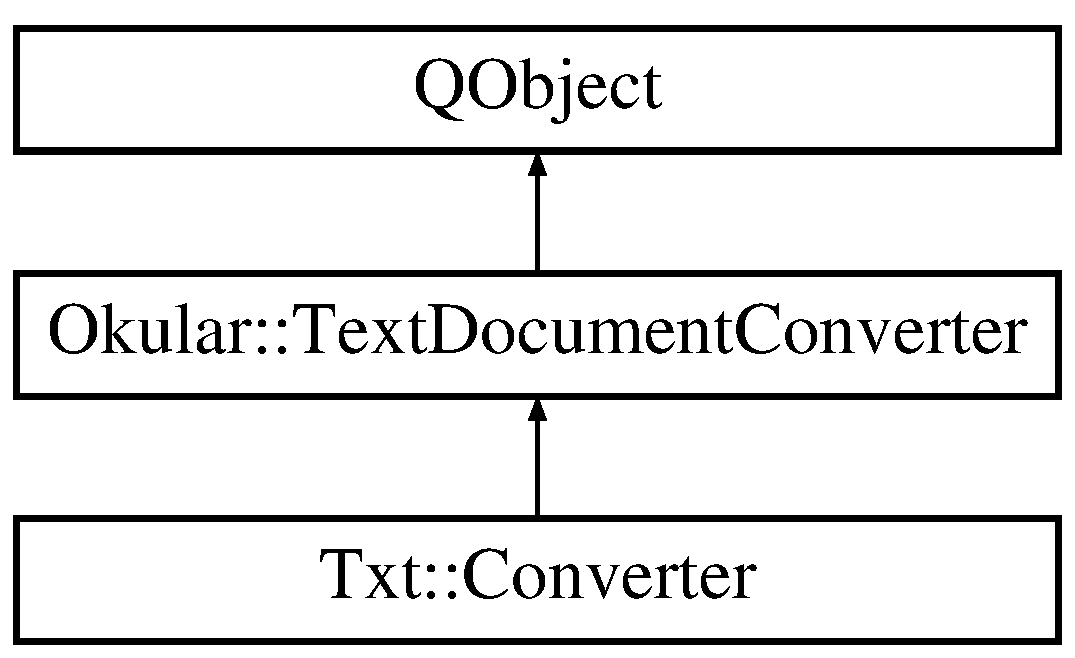
\includegraphics[height=3.000000cm]{classTxt_1_1Converter}
\end{center}
\end{figure}
\subsection*{Public Member Functions}
\begin{DoxyCompactItemize}
\item 
\hyperlink{classTxt_1_1Converter_a1de81f3e06093411e5d27ce882bc010f}{Converter} ()
\item 
\hyperlink{classTxt_1_1Converter_a9ecd05695a52c03158b81e544e13b996}{$\sim$\+Converter} ()
\item 
virtual Q\+Text\+Document $\ast$ \hyperlink{classTxt_1_1Converter_aa63e543977130604de659a4d725ee8bd}{convert} (const Q\+String \&file\+Name)
\end{DoxyCompactItemize}
\subsection*{Additional Inherited Members}


\subsection{Detailed Description}


Definition at line 18 of file converter.\+h.



\subsection{Constructor \& Destructor Documentation}
\hypertarget{classTxt_1_1Converter_a1de81f3e06093411e5d27ce882bc010f}{\index{Txt\+::\+Converter@{Txt\+::\+Converter}!Converter@{Converter}}
\index{Converter@{Converter}!Txt\+::\+Converter@{Txt\+::\+Converter}}
\subsubsection[{Converter}]{\setlength{\rightskip}{0pt plus 5cm}Converter\+::\+Converter (
\begin{DoxyParamCaption}
{}
\end{DoxyParamCaption}
)}}\label{classTxt_1_1Converter_a1de81f3e06093411e5d27ce882bc010f}


Definition at line 18 of file converter.\+cpp.


\begin{DoxyCode}
19 \{
20 \}
\end{DoxyCode}
\hypertarget{classTxt_1_1Converter_a9ecd05695a52c03158b81e544e13b996}{\index{Txt\+::\+Converter@{Txt\+::\+Converter}!````~Converter@{$\sim$\+Converter}}
\index{````~Converter@{$\sim$\+Converter}!Txt\+::\+Converter@{Txt\+::\+Converter}}
\subsubsection[{$\sim$\+Converter}]{\setlength{\rightskip}{0pt plus 5cm}Converter\+::$\sim$\+Converter (
\begin{DoxyParamCaption}
{}
\end{DoxyParamCaption}
)}}\label{classTxt_1_1Converter_a9ecd05695a52c03158b81e544e13b996}


Definition at line 22 of file converter.\+cpp.


\begin{DoxyCode}
23 \{
24 \}
\end{DoxyCode}


\subsection{Member Function Documentation}
\hypertarget{classTxt_1_1Converter_aa63e543977130604de659a4d725ee8bd}{\index{Txt\+::\+Converter@{Txt\+::\+Converter}!convert@{convert}}
\index{convert@{convert}!Txt\+::\+Converter@{Txt\+::\+Converter}}
\subsubsection[{convert}]{\setlength{\rightskip}{0pt plus 5cm}Q\+Text\+Document $\ast$ Converter\+::convert (
\begin{DoxyParamCaption}
\item[{const Q\+String \&}]{file\+Name}
\end{DoxyParamCaption}
)\hspace{0.3cm}{\ttfamily [virtual]}}}\label{classTxt_1_1Converter_aa63e543977130604de659a4d725ee8bd}
Returns the generated Q\+Text\+Document object. 

Implements \hyperlink{classOkular_1_1TextDocumentConverter_ad05f8bcde0f347c6292968fab331bcef}{Okular\+::\+Text\+Document\+Converter}.



Definition at line 26 of file converter.\+cpp.


\begin{DoxyCode}
27 \{
28     \hyperlink{classTxt_1_1Document}{Document} *textDocument = \textcolor{keyword}{new} \hyperlink{classTxt_1_1Document}{Document}( fileName );
29 
30     textDocument->setPageSize(QSizeF( 600, 800 ));
31 
32     QTextFrameFormat frameFormat;
33     frameFormat.setMargin( 20 );
34 
35     QTextFrame *rootFrame = textDocument->rootFrame();
36     rootFrame->setFrameFormat( frameFormat );
37 
38     emit \hyperlink{classOkular_1_1TextDocumentConverter_ad6e263857527273c9cf618e16329f6a7}{addMetaData}( \hyperlink{classOkular_1_1DocumentInfo_a3a6e5f7fb246e29bcb2e830b6f770791a786464e8e8c3e6ba1cd74e408487785b}{Okular::DocumentInfo::MimeType}, \textcolor{stringliteral}{"text/plain"}
       );
39 
40     \textcolor{keywordflow}{return} textDocument;
41 \}
\end{DoxyCode}


The documentation for this class was generated from the following files\+:\begin{DoxyCompactItemize}
\item 
generators/txt/\hyperlink{txt_2converter_8h}{converter.\+h}\item 
generators/txt/\hyperlink{txt_2converter_8cpp}{converter.\+cpp}\end{DoxyCompactItemize}

\hypertarget{classDirectory}{\section{Directory Class Reference}
\label{classDirectory}\index{Directory@{Directory}}
}


{\ttfamily \#include $<$directory.\+h$>$}

\subsection*{Public Member Functions}
\begin{DoxyCompactItemize}
\item 
\hyperlink{classDirectory_ae69ee52f5cacf4480b13364efa9c4682}{Directory} ()
\item 
\hyperlink{classDirectory_affbde8714685c61601421097d621341d}{$\sim$\+Directory} ()
\item 
bool \hyperlink{classDirectory_a9e72df151c200002c0f6ba3501780abb}{open} (const Q\+String \&file\+Name)
\item 
Q\+String\+List \hyperlink{classDirectory_a935b73c0bf500ff22641b64723215407}{list} () const 
\item 
Q\+I\+O\+Device $\ast$ \hyperlink{classDirectory_a520a88d8f2acd6179486eab7b8d65ee1}{create\+Device} (const Q\+String \&path) const 
\end{DoxyCompactItemize}


\subsection{Detailed Description}


Definition at line 16 of file directory.\+h.



\subsection{Constructor \& Destructor Documentation}
\hypertarget{classDirectory_ae69ee52f5cacf4480b13364efa9c4682}{\index{Directory@{Directory}!Directory@{Directory}}
\index{Directory@{Directory}!Directory@{Directory}}
\subsubsection[{Directory}]{\setlength{\rightskip}{0pt plus 5cm}Directory\+::\+Directory (
\begin{DoxyParamCaption}
{}
\end{DoxyParamCaption}
)}}\label{classDirectory_ae69ee52f5cacf4480b13364efa9c4682}
Creates a new directory object. 

Definition at line 20 of file directory.\+cpp.


\begin{DoxyCode}
21 \{
22 \}
\end{DoxyCode}
\hypertarget{classDirectory_affbde8714685c61601421097d621341d}{\index{Directory@{Directory}!````~Directory@{$\sim$\+Directory}}
\index{````~Directory@{$\sim$\+Directory}!Directory@{Directory}}
\subsubsection[{$\sim$\+Directory}]{\setlength{\rightskip}{0pt plus 5cm}Directory\+::$\sim$\+Directory (
\begin{DoxyParamCaption}
{}
\end{DoxyParamCaption}
)}}\label{classDirectory_affbde8714685c61601421097d621341d}
Destroys the directory object. 

Definition at line 24 of file directory.\+cpp.


\begin{DoxyCode}
25 \{
26 \}
\end{DoxyCode}


\subsection{Member Function Documentation}
\hypertarget{classDirectory_a520a88d8f2acd6179486eab7b8d65ee1}{\index{Directory@{Directory}!create\+Device@{create\+Device}}
\index{create\+Device@{create\+Device}!Directory@{Directory}}
\subsubsection[{create\+Device}]{\setlength{\rightskip}{0pt plus 5cm}Q\+I\+O\+Device $\ast$ Directory\+::create\+Device (
\begin{DoxyParamCaption}
\item[{const Q\+String \&}]{path}
\end{DoxyParamCaption}
) const}}\label{classDirectory_a520a88d8f2acd6179486eab7b8d65ee1}
Returns a new device for reading the file with the given path. 

Definition at line 59 of file directory.\+cpp.


\begin{DoxyCode}
60 \{
61     std::auto\_ptr<QFile> file( \textcolor{keyword}{new} QFile( path ) );
62     \textcolor{keywordflow}{if} ( !file->open( QIODevice::ReadOnly ) )
63         \textcolor{keywordflow}{return} 0;
64 
65     \textcolor{keywordflow}{return} file.release();
66 \}
\end{DoxyCode}
\hypertarget{classDirectory_a935b73c0bf500ff22641b64723215407}{\index{Directory@{Directory}!list@{list}}
\index{list@{list}!Directory@{Directory}}
\subsubsection[{list}]{\setlength{\rightskip}{0pt plus 5cm}Q\+String\+List Directory\+::list (
\begin{DoxyParamCaption}
{}
\end{DoxyParamCaption}
) const}}\label{classDirectory_a935b73c0bf500ff22641b64723215407}
Returns the list of files from the directory. 

Definition at line 54 of file directory.\+cpp.


\begin{DoxyCode}
55 \{
56     \textcolor{keywordflow}{return} recurseDir( mDir, 0 );
57 \}
\end{DoxyCode}
\hypertarget{classDirectory_a9e72df151c200002c0f6ba3501780abb}{\index{Directory@{Directory}!open@{open}}
\index{open@{open}!Directory@{Directory}}
\subsubsection[{open}]{\setlength{\rightskip}{0pt plus 5cm}bool Directory\+::open (
\begin{DoxyParamCaption}
\item[{const Q\+String \&}]{file\+Name}
\end{DoxyParamCaption}
)}}\label{classDirectory_a9e72df151c200002c0f6ba3501780abb}
Opens given directory. 

Definition at line 28 of file directory.\+cpp.


\begin{DoxyCode}
29 \{
30     mDir = dirName;
31     QFileInfo dirTest( dirName );
32     \textcolor{keywordflow}{return} dirTest.isDir() && dirTest.isReadable();
33 \}
\end{DoxyCode}


The documentation for this class was generated from the following files\+:\begin{DoxyCompactItemize}
\item 
generators/comicbook/\hyperlink{directory_8h}{directory.\+h}\item 
generators/comicbook/\hyperlink{directory_8cpp}{directory.\+cpp}\end{DoxyCompactItemize}

\hypertarget{classDjVuGenerator}{\section{Dj\+Vu\+Generator Class Reference}
\label{classDjVuGenerator}\index{Dj\+Vu\+Generator@{Dj\+Vu\+Generator}}
}


{\ttfamily \#include $<$generator\+\_\+djvu.\+h$>$}

Inheritance diagram for Dj\+Vu\+Generator\+:\begin{figure}[H]
\begin{center}
\leavevmode
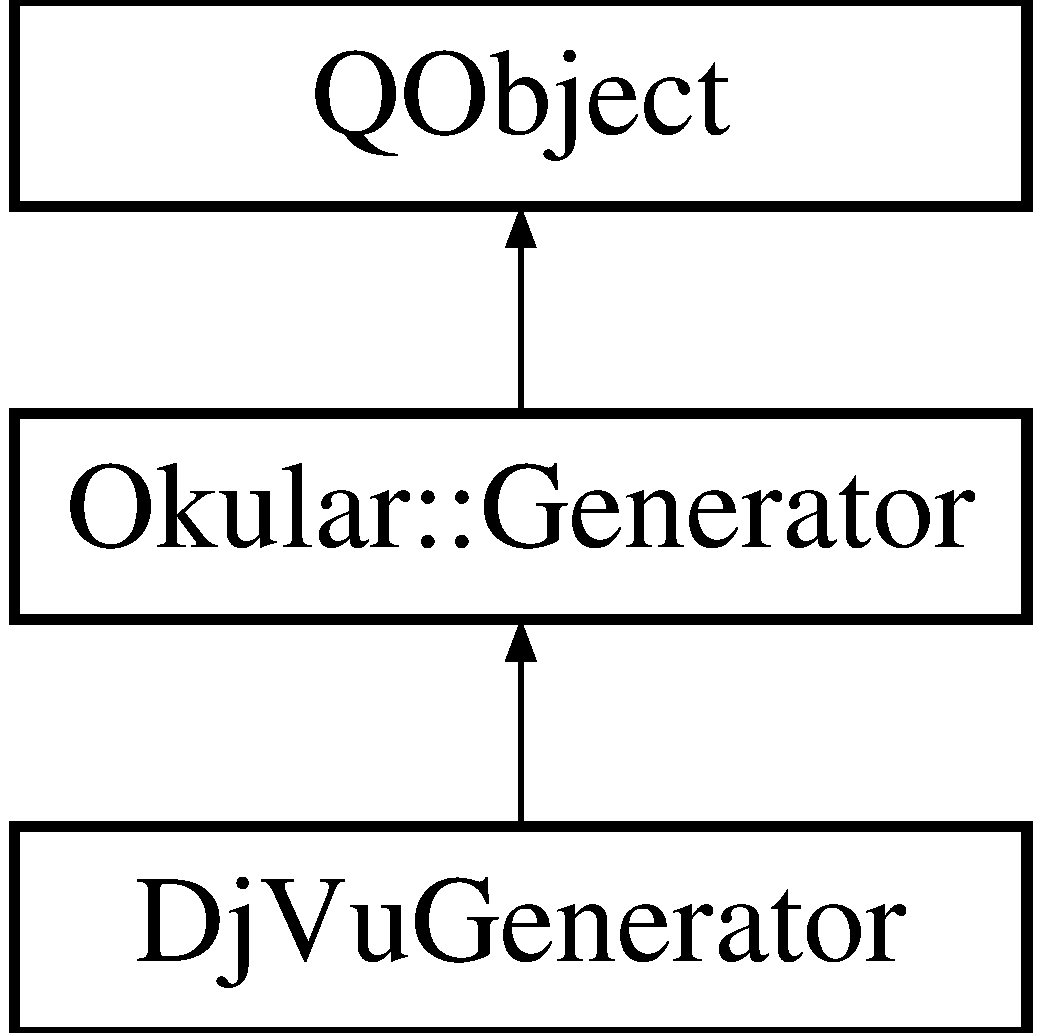
\includegraphics[height=3.000000cm]{classDjVuGenerator}
\end{center}
\end{figure}
\subsection*{Public Member Functions}
\begin{DoxyCompactItemize}
\item 
\hyperlink{classDjVuGenerator_a1afc4e3ef24772d6e7c53d71a7d85b59}{Dj\+Vu\+Generator} (Q\+Object $\ast$parent, const Q\+Variant\+List \&args)
\item 
\hyperlink{classDjVuGenerator_ac4ca23827a811606c09eaaac001e5a73}{$\sim$\+Dj\+Vu\+Generator} ()
\item 
bool \hyperlink{classDjVuGenerator_ace33eff68f72609689d7850b0ef3e6ef}{load\+Document} (const Q\+String \&file\+Name, Q\+Vector$<$ \hyperlink{classOkular_1_1Page}{Okular\+::\+Page} $\ast$ $>$ \&pages\+Vector)
\item 
const \hyperlink{classOkular_1_1DocumentInfo}{Okular\+::\+Document\+Info} $\ast$ \hyperlink{classDjVuGenerator_acf9234f6d7b9d33c6306b6d0e11464a0}{generate\+Document\+Info} ()
\item 
const \hyperlink{classOkular_1_1DocumentSynopsis}{Okular\+::\+Document\+Synopsis} $\ast$ \hyperlink{classDjVuGenerator_acc8cf4d02a9dcc84880ccc9cba988345}{generate\+Document\+Synopsis} ()
\item 
bool \hyperlink{classDjVuGenerator_a8127027939e0f71b0b15b28794863dd5}{print} (Q\+Printer \&printer)
\item 
Q\+Variant \hyperlink{classDjVuGenerator_a354dc9b90acf89f0a83dfcd92429bfdb}{meta\+Data} (const Q\+String \&key, const Q\+Variant \&option) const 
\end{DoxyCompactItemize}
\subsection*{Protected Member Functions}
\begin{DoxyCompactItemize}
\item 
bool \hyperlink{classDjVuGenerator_a233a2a93d7b18e866e927fc686cf94ac}{do\+Close\+Document} ()
\item 
Q\+Image \hyperlink{classDjVuGenerator_a6d072c673c6e484f75aab6943d51c2be}{image} (\hyperlink{classOkular_1_1PixmapRequest}{Okular\+::\+Pixmap\+Request} $\ast$request)
\item 
\hyperlink{classOkular_1_1TextPage}{Okular\+::\+Text\+Page} $\ast$ \hyperlink{classDjVuGenerator_a1923561a9e90819282c769b78ba4ce01}{text\+Page} (\hyperlink{classOkular_1_1Page}{Okular\+::\+Page} $\ast$page)
\end{DoxyCompactItemize}
\subsection*{Additional Inherited Members}


\subsection{Detailed Description}


Definition at line 24 of file generator\+\_\+djvu.\+h.



\subsection{Constructor \& Destructor Documentation}
\hypertarget{classDjVuGenerator_a1afc4e3ef24772d6e7c53d71a7d85b59}{\index{Dj\+Vu\+Generator@{Dj\+Vu\+Generator}!Dj\+Vu\+Generator@{Dj\+Vu\+Generator}}
\index{Dj\+Vu\+Generator@{Dj\+Vu\+Generator}!Dj\+Vu\+Generator@{Dj\+Vu\+Generator}}
\subsubsection[{Dj\+Vu\+Generator}]{\setlength{\rightskip}{0pt plus 5cm}Dj\+Vu\+Generator\+::\+Dj\+Vu\+Generator (
\begin{DoxyParamCaption}
\item[{Q\+Object $\ast$}]{parent, }
\item[{const Q\+Variant\+List \&}]{args}
\end{DoxyParamCaption}
)}}\label{classDjVuGenerator_a1afc4e3ef24772d6e7c53d71a7d85b59}


Definition at line 86 of file generator\+\_\+djvu.\+cpp.


\begin{DoxyCode}
87     : \hyperlink{classOkular_1_1Generator}{Okular::Generator}( parent, args ), m\_docInfo( 0 ), m\_docSyn( 0 )
88 \{
89     \hyperlink{classOkular_1_1Generator_abcebcc5f69e98b6227496198a5c69d2c}{setFeature}( \hyperlink{classOkular_1_1Generator_a8517096896273a5ba5b970be09313c77a1bf7de5d98ec0333e392ce7f004d6578}{TextExtraction} );
90     \hyperlink{classOkular_1_1Generator_abcebcc5f69e98b6227496198a5c69d2c}{setFeature}( \hyperlink{classOkular_1_1Generator_a8517096896273a5ba5b970be09313c77a0764a910b194896e72da084c3c51a2d0}{Threaded} );
91     \hyperlink{classOkular_1_1Generator_abcebcc5f69e98b6227496198a5c69d2c}{setFeature}( \hyperlink{classOkular_1_1Generator_a8517096896273a5ba5b970be09313c77af0ce4775bf5c69b470c2cce6011d576b}{PrintPostscript} );
92     \textcolor{keywordflow}{if} ( \hyperlink{classOkular_1_1FilePrinter_a047b30a135796c064fda2823ae6c0ddb}{Okular::FilePrinter::ps2pdfAvailable}() )
93         \hyperlink{classOkular_1_1Generator_abcebcc5f69e98b6227496198a5c69d2c}{setFeature}( \hyperlink{classOkular_1_1Generator_a8517096896273a5ba5b970be09313c77a0bb6cbe50f2ffb616e25106b2e34c289}{PrintToFile} );
94 
95     m\_djvu = \textcolor{keyword}{new} \hyperlink{classKDjVu}{KDjVu}();
96     m\_djvu->\hyperlink{classKDjVu_a175f29677ef28f549a709b337f917d92}{setCacheEnabled}( \textcolor{keyword}{false} );
97 \}
\end{DoxyCode}
\hypertarget{classDjVuGenerator_ac4ca23827a811606c09eaaac001e5a73}{\index{Dj\+Vu\+Generator@{Dj\+Vu\+Generator}!````~Dj\+Vu\+Generator@{$\sim$\+Dj\+Vu\+Generator}}
\index{````~Dj\+Vu\+Generator@{$\sim$\+Dj\+Vu\+Generator}!Dj\+Vu\+Generator@{Dj\+Vu\+Generator}}
\subsubsection[{$\sim$\+Dj\+Vu\+Generator}]{\setlength{\rightskip}{0pt plus 5cm}Dj\+Vu\+Generator\+::$\sim$\+Dj\+Vu\+Generator (
\begin{DoxyParamCaption}
{}
\end{DoxyParamCaption}
)}}\label{classDjVuGenerator_ac4ca23827a811606c09eaaac001e5a73}


Definition at line 99 of file generator\+\_\+djvu.\+cpp.


\begin{DoxyCode}
100 \{
101     \textcolor{keyword}{delete} m\_djvu;
102 \}
\end{DoxyCode}


\subsection{Member Function Documentation}
\hypertarget{classDjVuGenerator_a233a2a93d7b18e866e927fc686cf94ac}{\index{Dj\+Vu\+Generator@{Dj\+Vu\+Generator}!do\+Close\+Document@{do\+Close\+Document}}
\index{do\+Close\+Document@{do\+Close\+Document}!Dj\+Vu\+Generator@{Dj\+Vu\+Generator}}
\subsubsection[{do\+Close\+Document}]{\setlength{\rightskip}{0pt plus 5cm}bool Dj\+Vu\+Generator\+::do\+Close\+Document (
\begin{DoxyParamCaption}
{}
\end{DoxyParamCaption}
)\hspace{0.3cm}{\ttfamily [protected]}, {\ttfamily [virtual]}}}\label{classDjVuGenerator_a233a2a93d7b18e866e927fc686cf94ac}
This method is called when the document is closed and not used any longer.

\begin{DoxyReturn}{Returns}
true on success, false otherwise. 
\end{DoxyReturn}


Implements \hyperlink{classOkular_1_1Generator_ad3f1dcb98f3bd87c87ad0e91ecf4a6d7}{Okular\+::\+Generator}.



Definition at line 117 of file generator\+\_\+djvu.\+cpp.


\begin{DoxyCode}
118 \{
119     \hyperlink{classOkular_1_1Generator_a83d702cccbce2288c3258d97f1f15e19}{userMutex}()->lock();
120     m\_djvu->\hyperlink{classKDjVu_af9c1d642f5ef455739abadf09ed44586}{closeFile}();
121     \hyperlink{classOkular_1_1Generator_a83d702cccbce2288c3258d97f1f15e19}{userMutex}()->unlock();
122 
123     \textcolor{keyword}{delete} m\_docInfo;
124     m\_docInfo = 0;
125     \textcolor{keyword}{delete} m\_docSyn;
126     m\_docSyn = 0;
127 
128     \textcolor{keywordflow}{return} \textcolor{keyword}{true};
129 \}
\end{DoxyCode}
\hypertarget{classDjVuGenerator_acf9234f6d7b9d33c6306b6d0e11464a0}{\index{Dj\+Vu\+Generator@{Dj\+Vu\+Generator}!generate\+Document\+Info@{generate\+Document\+Info}}
\index{generate\+Document\+Info@{generate\+Document\+Info}!Dj\+Vu\+Generator@{Dj\+Vu\+Generator}}
\subsubsection[{generate\+Document\+Info}]{\setlength{\rightskip}{0pt plus 5cm}const {\bf Okular\+::\+Document\+Info} $\ast$ Dj\+Vu\+Generator\+::generate\+Document\+Info (
\begin{DoxyParamCaption}
{}
\end{DoxyParamCaption}
)\hspace{0.3cm}{\ttfamily [virtual]}}}\label{classDjVuGenerator_acf9234f6d7b9d33c6306b6d0e11464a0}
Returns the general information object of the document or 0 if no information are available. 

Reimplemented from \hyperlink{classOkular_1_1Generator_a9993dd0a2415499e23d8394e7a447e98}{Okular\+::\+Generator}.



Definition at line 139 of file generator\+\_\+djvu.\+cpp.


\begin{DoxyCode}
140 \{
141     \textcolor{keywordflow}{if} ( m\_docInfo )
142         \textcolor{keywordflow}{return} m\_docInfo;
143 
144     m\_docInfo = \textcolor{keyword}{new} \hyperlink{classOkular_1_1DocumentInfo}{Okular::DocumentInfo}();
145 
146     m\_docInfo->\hyperlink{classOkular_1_1DocumentInfo_a8bd5403394ab192f1103cbf2a8e48d9b}{set}( \hyperlink{classOkular_1_1DocumentInfo_a3a6e5f7fb246e29bcb2e830b6f770791a786464e8e8c3e6ba1cd74e408487785b}{Okular::DocumentInfo::MimeType}, \textcolor{stringliteral}{"image/vnd.djvu"} );
147 
148     \textcolor{keywordflow}{if} ( m\_djvu )
149     \{
150         \textcolor{comment}{// compile internal structure reading properties from KDjVu}
151         QString title = m\_djvu->\hyperlink{classKDjVu_ae1a73203fc07dc0c81996810ca2f7ae3}{metaData}( \textcolor{stringliteral}{"title"} ).toString();
152         m\_docInfo->\hyperlink{classOkular_1_1DocumentInfo_a8bd5403394ab192f1103cbf2a8e48d9b}{set}( \hyperlink{classOkular_1_1DocumentInfo_a3a6e5f7fb246e29bcb2e830b6f770791ae400626d63f14b61c55bd22aca9481e0}{Okular::DocumentInfo::Title}, title.isEmpty() ? i18nc(
       \textcolor{stringliteral}{"Unknown title"}, \textcolor{stringliteral}{"Unknown"} ) : title );
153         QString author = m\_djvu->\hyperlink{classKDjVu_ae1a73203fc07dc0c81996810ca2f7ae3}{metaData}( \textcolor{stringliteral}{"author"} ).toString();
154         m\_docInfo->\hyperlink{classOkular_1_1DocumentInfo_a8bd5403394ab192f1103cbf2a8e48d9b}{set}( \hyperlink{classOkular_1_1DocumentInfo_a3a6e5f7fb246e29bcb2e830b6f770791a1010574d070b1925e030c20fef3e7a35}{Okular::DocumentInfo::Author}, author.isEmpty() ? 
      i18nc( \textcolor{stringliteral}{"Unknown author"}, \textcolor{stringliteral}{"Unknown"} ) : author );
155         QString editor = m\_djvu->\hyperlink{classKDjVu_ae1a73203fc07dc0c81996810ca2f7ae3}{metaData}( \textcolor{stringliteral}{"editor"} ).toString();
156         m\_docInfo->\hyperlink{classOkular_1_1DocumentInfo_a8bd5403394ab192f1103cbf2a8e48d9b}{set}( \textcolor{stringliteral}{"editor"}, editor.isEmpty() ? i18nc( \textcolor{stringliteral}{"Unknown editor"}, \textcolor{stringliteral}{"Unknown"} ) : editor, i18n
      ( \textcolor{stringliteral}{"Editor"} ) );
157         QString publisher = m\_djvu->\hyperlink{classKDjVu_ae1a73203fc07dc0c81996810ca2f7ae3}{metaData}( \textcolor{stringliteral}{"publisher"} ).toString();
158         m\_docInfo->\hyperlink{classOkular_1_1DocumentInfo_a8bd5403394ab192f1103cbf2a8e48d9b}{set}( \textcolor{stringliteral}{"publisher"}, publisher.isEmpty() ? i18nc( \textcolor{stringliteral}{"Unknown publisher"}, \textcolor{stringliteral}{"Unknown"} ) : 
      publisher, i18n( \textcolor{stringliteral}{"Publisher"} ) );
159         QString year = m\_djvu->\hyperlink{classKDjVu_ae1a73203fc07dc0c81996810ca2f7ae3}{metaData}( \textcolor{stringliteral}{"year"} ).toString();
160         m\_docInfo->\hyperlink{classOkular_1_1DocumentInfo_a8bd5403394ab192f1103cbf2a8e48d9b}{set}( \hyperlink{classOkular_1_1DocumentInfo_a3a6e5f7fb246e29bcb2e830b6f770791a58a72aeacd3cb08e85d0f9f19b2fe83a}{Okular::DocumentInfo::CreationDate}, year.
      isEmpty() ? i18nc( \textcolor{stringliteral}{"Unknown creation date"}, \textcolor{stringliteral}{"Unknown"} ) : year );
161         QString volume = m\_djvu->\hyperlink{classKDjVu_ae1a73203fc07dc0c81996810ca2f7ae3}{metaData}( \textcolor{stringliteral}{"volume"} ).toString();
162         m\_docInfo->\hyperlink{classOkular_1_1DocumentInfo_a8bd5403394ab192f1103cbf2a8e48d9b}{set}( \textcolor{stringliteral}{"volume"}, volume.isEmpty() ? i18nc( \textcolor{stringliteral}{"Unknown volume information"}, \textcolor{stringliteral}{"Unknown"} ) : 
      volume, i18n( \textcolor{stringliteral}{"Volume"} ) );
163         QString doctype = m\_djvu->\hyperlink{classKDjVu_ae1a73203fc07dc0c81996810ca2f7ae3}{metaData}( \textcolor{stringliteral}{"documentType"} ).toString();
164         m\_docInfo->\hyperlink{classOkular_1_1DocumentInfo_a8bd5403394ab192f1103cbf2a8e48d9b}{set}( \textcolor{stringliteral}{"documentType"}, doctype.isEmpty() ? i18nc( \textcolor{stringliteral}{"Unknown type of document"}, \textcolor{stringliteral}{"Unknown"}
       ) : doctype, i18n( \textcolor{stringliteral}{"Type of document"} ) );
165         QVariant numcomponents = m\_djvu->\hyperlink{classKDjVu_ae1a73203fc07dc0c81996810ca2f7ae3}{metaData}( \textcolor{stringliteral}{"componentFile"} );
166         m\_docInfo->\hyperlink{classOkular_1_1DocumentInfo_a8bd5403394ab192f1103cbf2a8e48d9b}{set}( \textcolor{stringliteral}{"componentFile"}, numcomponents.type() != QVariant::Int ? i18nc( \textcolor{stringliteral}{"Unknown number
       of component files"}, \textcolor{stringliteral}{"Unknown"} ) : numcomponents.\hyperlink{namespaceQTest_a861302f3f44f1ae8461d2752a3e3813c}{toString}(), i18n( \textcolor{stringliteral}{"Component Files"} ) );
167     \}
168     \textcolor{keywordflow}{else}
169     \{
170         m\_docInfo->\hyperlink{classOkular_1_1DocumentInfo_a8bd5403394ab192f1103cbf2a8e48d9b}{set}( \hyperlink{classOkular_1_1DocumentInfo_a3a6e5f7fb246e29bcb2e830b6f770791ae400626d63f14b61c55bd22aca9481e0}{Okular::DocumentInfo::Title}, i18nc( \textcolor{stringliteral}{"Unknown title"}, \textcolor{stringliteral}{
      "Unknown"} ) );
171         m\_docInfo->\hyperlink{classOkular_1_1DocumentInfo_a8bd5403394ab192f1103cbf2a8e48d9b}{set}( \hyperlink{classOkular_1_1DocumentInfo_a3a6e5f7fb246e29bcb2e830b6f770791a1010574d070b1925e030c20fef3e7a35}{Okular::DocumentInfo::Author}, i18nc( \textcolor{stringliteral}{"Unknown author
      "}, \textcolor{stringliteral}{"Unknown"} ) );
172         m\_docInfo->\hyperlink{classOkular_1_1DocumentInfo_a8bd5403394ab192f1103cbf2a8e48d9b}{set}( \textcolor{stringliteral}{"editor"}, i18nc( \textcolor{stringliteral}{"Unknown editor"}, \textcolor{stringliteral}{"Unknown"} ), i18n( \textcolor{stringliteral}{"Editor"} ) );
173         m\_docInfo->\hyperlink{classOkular_1_1DocumentInfo_a8bd5403394ab192f1103cbf2a8e48d9b}{set}( \textcolor{stringliteral}{"publisher"}, i18nc( \textcolor{stringliteral}{"Unknown publisher"}, \textcolor{stringliteral}{"Unknown"} ), i18n( \textcolor{stringliteral}{"Publisher"} ) );
174         m\_docInfo->\hyperlink{classOkular_1_1DocumentInfo_a8bd5403394ab192f1103cbf2a8e48d9b}{set}( \hyperlink{classOkular_1_1DocumentInfo_a3a6e5f7fb246e29bcb2e830b6f770791a58a72aeacd3cb08e85d0f9f19b2fe83a}{Okular::DocumentInfo::CreationDate}, i18nc( \textcolor{stringliteral}{"
      Unknown creation date"}, \textcolor{stringliteral}{"Unknown"} ) );
175         m\_docInfo->\hyperlink{classOkular_1_1DocumentInfo_a8bd5403394ab192f1103cbf2a8e48d9b}{set}( \textcolor{stringliteral}{"volume"}, i18nc( \textcolor{stringliteral}{"Unknown volume information"}, \textcolor{stringliteral}{"Unknown"} ), i18n( \textcolor{stringliteral}{"Volume"} ) );
176         m\_docInfo->\hyperlink{classOkular_1_1DocumentInfo_a8bd5403394ab192f1103cbf2a8e48d9b}{set}( \textcolor{stringliteral}{"documentType"}, i18nc( \textcolor{stringliteral}{"Unknown type of document"}, \textcolor{stringliteral}{"Unknown"} ), i18n( \textcolor{stringliteral}{"Type of
       document"} ) );
177         m\_docInfo->\hyperlink{classOkular_1_1DocumentInfo_a8bd5403394ab192f1103cbf2a8e48d9b}{set}( \textcolor{stringliteral}{"componentFile"}, i18nc( \textcolor{stringliteral}{"Unknown number of component files"}, \textcolor{stringliteral}{"Unknown"} ), i18n( \textcolor{stringliteral}{
      "Component Files"} ) );
178     \}
179 
180     \textcolor{keywordflow}{return} m\_docInfo;
181 \}
\end{DoxyCode}
\hypertarget{classDjVuGenerator_acc8cf4d02a9dcc84880ccc9cba988345}{\index{Dj\+Vu\+Generator@{Dj\+Vu\+Generator}!generate\+Document\+Synopsis@{generate\+Document\+Synopsis}}
\index{generate\+Document\+Synopsis@{generate\+Document\+Synopsis}!Dj\+Vu\+Generator@{Dj\+Vu\+Generator}}
\subsubsection[{generate\+Document\+Synopsis}]{\setlength{\rightskip}{0pt plus 5cm}const {\bf Okular\+::\+Document\+Synopsis} $\ast$ Dj\+Vu\+Generator\+::generate\+Document\+Synopsis (
\begin{DoxyParamCaption}
{}
\end{DoxyParamCaption}
)\hspace{0.3cm}{\ttfamily [virtual]}}}\label{classDjVuGenerator_acc8cf4d02a9dcc84880ccc9cba988345}
Returns the 'table of content' object of the document or 0 if no table of content is available. 

Reimplemented from \hyperlink{classOkular_1_1Generator_a1f8b31c19d7a5101cadf3fe3186ab0f1}{Okular\+::\+Generator}.



Definition at line 183 of file generator\+\_\+djvu.\+cpp.


\begin{DoxyCode}
184 \{
185     QMutexLocker locker( \hyperlink{classOkular_1_1Generator_a83d702cccbce2288c3258d97f1f15e19}{userMutex}() );
186     \textcolor{keywordflow}{if} ( m\_docSyn )
187         \textcolor{keywordflow}{return} m\_docSyn;
188 
189     \textcolor{keyword}{const} QDomDocument *doc = m\_djvu->\hyperlink{classKDjVu_a48975c0c9c80a7b85600812c22ed5fda}{documentBookmarks}();
190     \textcolor{keywordflow}{if} ( doc )
191     \{
192         m\_docSyn = \textcolor{keyword}{new} \hyperlink{classOkular_1_1DocumentSynopsis}{Okular::DocumentSynopsis}();
193         recurseCreateTOC( *m\_docSyn, *doc, *m\_docSyn, m\_djvu );
194     \}
195     locker.unlock();
196 
197     \textcolor{keywordflow}{return} m\_docSyn;
198 \}
\end{DoxyCode}
\hypertarget{classDjVuGenerator_a6d072c673c6e484f75aab6943d51c2be}{\index{Dj\+Vu\+Generator@{Dj\+Vu\+Generator}!image@{image}}
\index{image@{image}!Dj\+Vu\+Generator@{Dj\+Vu\+Generator}}
\subsubsection[{image}]{\setlength{\rightskip}{0pt plus 5cm}Q\+Image Dj\+Vu\+Generator\+::image (
\begin{DoxyParamCaption}
\item[{{\bf Okular\+::\+Pixmap\+Request} $\ast$}]{page}
\end{DoxyParamCaption}
)\hspace{0.3cm}{\ttfamily [protected]}, {\ttfamily [virtual]}}}\label{classDjVuGenerator_a6d072c673c6e484f75aab6943d51c2be}
Returns the image of the page as specified in the passed pixmap {\ttfamily request}.

\begin{DoxyWarning}{Warning}
this method may be executed in its own separated thread if the \hyperlink{classOkular_1_1Generator_a8517096896273a5ba5b970be09313c77a0764a910b194896e72da084c3c51a2d0}{Threaded} is enabled! 
\end{DoxyWarning}


Reimplemented from \hyperlink{classOkular_1_1Generator_a6712c8d3c2759c3a1fcacbd503d3286e}{Okular\+::\+Generator}.



Definition at line 131 of file generator\+\_\+djvu.\+cpp.


\begin{DoxyCode}
132 \{
133     \hyperlink{classOkular_1_1Generator_a83d702cccbce2288c3258d97f1f15e19}{userMutex}()->lock();
134     QImage img = m\_djvu->\hyperlink{classKDjVu_a912d8a8a28dfd28bf871c0c1726b266e}{image}( request->pageNumber(), request->width(), request->height(), request->
      page()->rotation() );
135     \hyperlink{classOkular_1_1Generator_a83d702cccbce2288c3258d97f1f15e19}{userMutex}()->unlock();
136     \textcolor{keywordflow}{return} img;
137 \}
\end{DoxyCode}
\hypertarget{classDjVuGenerator_ace33eff68f72609689d7850b0ef3e6ef}{\index{Dj\+Vu\+Generator@{Dj\+Vu\+Generator}!load\+Document@{load\+Document}}
\index{load\+Document@{load\+Document}!Dj\+Vu\+Generator@{Dj\+Vu\+Generator}}
\subsubsection[{load\+Document}]{\setlength{\rightskip}{0pt plus 5cm}bool Dj\+Vu\+Generator\+::load\+Document (
\begin{DoxyParamCaption}
\item[{const Q\+String \&}]{file\+Name, }
\item[{Q\+Vector$<$ {\bf Okular\+::\+Page} $\ast$ $>$ \&}]{pages\+Vector}
\end{DoxyParamCaption}
)\hspace{0.3cm}{\ttfamily [virtual]}}}\label{classDjVuGenerator_ace33eff68f72609689d7850b0ef3e6ef}
Loads the document with the given {\ttfamily file\+Name} and fills the {\ttfamily pages\+Vector} with the parsed pages.

\begin{DoxyReturn}{Returns}
true on success, false otherwise. 
\end{DoxyReturn}


Implements \hyperlink{classOkular_1_1Generator_a388b47328a5297d53cdbdc6fcf074ee3}{Okular\+::\+Generator}.



Definition at line 104 of file generator\+\_\+djvu.\+cpp.


\begin{DoxyCode}
105 \{
106     QMutexLocker locker( \hyperlink{classOkular_1_1Generator_a83d702cccbce2288c3258d97f1f15e19}{userMutex}() );
107     \textcolor{keywordflow}{if} ( !m\_djvu->\hyperlink{classKDjVu_a223ea1608a7b3ed9314bd89a2534dfd5}{openFile}( fileName ) )
108         \textcolor{keywordflow}{return} \textcolor{keyword}{false};
109 
110     locker.unlock();
111 
112     loadPages( pagesVector, 0 );
113 
114     \textcolor{keywordflow}{return} \textcolor{keyword}{true};
115 \}
\end{DoxyCode}
\hypertarget{classDjVuGenerator_a354dc9b90acf89f0a83dfcd92429bfdb}{\index{Dj\+Vu\+Generator@{Dj\+Vu\+Generator}!meta\+Data@{meta\+Data}}
\index{meta\+Data@{meta\+Data}!Dj\+Vu\+Generator@{Dj\+Vu\+Generator}}
\subsubsection[{meta\+Data}]{\setlength{\rightskip}{0pt plus 5cm}Q\+Variant Dj\+Vu\+Generator\+::meta\+Data (
\begin{DoxyParamCaption}
\item[{const Q\+String \&}]{key, }
\item[{const Q\+Variant \&}]{option}
\end{DoxyParamCaption}
) const\hspace{0.3cm}{\ttfamily [virtual]}}}\label{classDjVuGenerator_a354dc9b90acf89f0a83dfcd92429bfdb}
This method returns the meta data of the given {\ttfamily key} with the given {\ttfamily option} of the document. 

Reimplemented from \hyperlink{classOkular_1_1Generator_a74f6b91e31ead5b572ffb9fb6b06c188}{Okular\+::\+Generator}.



Definition at line 230 of file generator\+\_\+djvu.\+cpp.


\begin{DoxyCode}
231 \{
232     Q\_UNUSED( option )
233     if ( key == "DocumentTitle" )
234     \{
235         \textcolor{keywordflow}{return} m\_djvu->\hyperlink{classKDjVu_ae1a73203fc07dc0c81996810ca2f7ae3}{metaData}( \textcolor{stringliteral}{"title"} );
236     \}
237     \textcolor{keywordflow}{return} QVariant();
238 \}
\end{DoxyCode}
\hypertarget{classDjVuGenerator_a8127027939e0f71b0b15b28794863dd5}{\index{Dj\+Vu\+Generator@{Dj\+Vu\+Generator}!print@{print}}
\index{print@{print}!Dj\+Vu\+Generator@{Dj\+Vu\+Generator}}
\subsubsection[{print}]{\setlength{\rightskip}{0pt plus 5cm}bool Dj\+Vu\+Generator\+::print (
\begin{DoxyParamCaption}
\item[{Q\+Printer \&}]{printer}
\end{DoxyParamCaption}
)\hspace{0.3cm}{\ttfamily [virtual]}}}\label{classDjVuGenerator_a8127027939e0f71b0b15b28794863dd5}
This method is called to print the document to the given {\ttfamily printer}. 

Reimplemented from \hyperlink{classOkular_1_1Generator_aa786d406a1b0db6679a3bc62bbe2dc82}{Okular\+::\+Generator}.



Definition at line 200 of file generator\+\_\+djvu.\+cpp.


\begin{DoxyCode}
201 \{
202     \textcolor{keywordtype}{bool} result = \textcolor{keyword}{false};
203 
204     \textcolor{comment}{// Create tempfile to write to}
205     KTemporaryFile tf;
206     tf.setSuffix( \textcolor{stringliteral}{".ps"} );
207     \textcolor{keywordflow}{if} ( !tf.open() )
208         \textcolor{keywordflow}{return} \textcolor{keyword}{false};
209 
210     QMutexLocker locker( \hyperlink{classOkular_1_1Generator_a83d702cccbce2288c3258d97f1f15e19}{userMutex}() );
211     \hyperlink{classQList}{QList<int>} pageList = \hyperlink{classOkular_1_1FilePrinter_aed485e5e3fbe591b16e15915e318a1b7}{Okular::FilePrinter::pageList}( printer, 
      m\_djvu->\hyperlink{classKDjVu_aea351abdd42f5494382d2d3d20c1a94e}{pages}().count(),
212                                                          \hyperlink{classOkular_1_1Generator_a4248672ef04e62660d51f16c0a862bbe}{document}()->
      \hyperlink{classOkular_1_1Document_a42ec374d73794bf56d7e7b11f1f56319}{currentPage}() + 1,
213                                                          \hyperlink{classOkular_1_1Generator_a4248672ef04e62660d51f16c0a862bbe}{document}()->
      \hyperlink{classOkular_1_1Document_a01de5a7212e14772e647a8e1caa07627}{bookmarkedPageList}() );
214 
215     \textcolor{keywordflow}{if} ( m\_djvu->\hyperlink{classKDjVu_a476b8e76dc69d3872166fdf76ae2a8c2}{exportAsPostScript}( &tf, pageList ) )
216     \{
217         tf.setAutoRemove( \textcolor{keyword}{false} );
218         \textcolor{keyword}{const} QString fileName = tf.fileName();
219         tf.close();
220         \textcolor{keywordtype}{int} ret = \hyperlink{classOkular_1_1FilePrinter_abd5ec189d80d15983c49f91f7e1d38c1}{Okular::FilePrinter::printFile}( printer, fileName, 
      \hyperlink{classOkular_1_1Generator_a4248672ef04e62660d51f16c0a862bbe}{document}()->orientation(),
221                                                   
      \hyperlink{classOkular_1_1FilePrinter_acd01eb48e99f9289a7f4786a366ef7baa86d9b928c2434b89a15de26c8cc22705}{Okular::FilePrinter::SystemDeletesFiles},
222                                                   
      \hyperlink{classOkular_1_1FilePrinter_a755b647910344031db1d79312482981da3910c7efe4c8f4f8a69459765bea25a4}{Okular::FilePrinter::ApplicationSelectsPages},
223                                                   \hyperlink{classOkular_1_1Generator_a4248672ef04e62660d51f16c0a862bbe}{document}()->bookmarkedPageRange() );
224         result = ( ret >=0 );
225     \}
226 
227     \textcolor{keywordflow}{return} result;
228 \}
\end{DoxyCode}
\hypertarget{classDjVuGenerator_a1923561a9e90819282c769b78ba4ce01}{\index{Dj\+Vu\+Generator@{Dj\+Vu\+Generator}!text\+Page@{text\+Page}}
\index{text\+Page@{text\+Page}!Dj\+Vu\+Generator@{Dj\+Vu\+Generator}}
\subsubsection[{text\+Page}]{\setlength{\rightskip}{0pt plus 5cm}{\bf Okular\+::\+Text\+Page} $\ast$ Dj\+Vu\+Generator\+::text\+Page (
\begin{DoxyParamCaption}
\item[{{\bf Okular\+::\+Page} $\ast$}]{page}
\end{DoxyParamCaption}
)\hspace{0.3cm}{\ttfamily [protected]}, {\ttfamily [virtual]}}}\label{classDjVuGenerator_a1923561a9e90819282c769b78ba4ce01}
Returns the text page for the given {\ttfamily page}.

\begin{DoxyWarning}{Warning}
this method may be executed in its own separated thread if the \hyperlink{classOkular_1_1Generator_a8517096896273a5ba5b970be09313c77a0764a910b194896e72da084c3c51a2d0}{Threaded} is enabled! 
\end{DoxyWarning}


Reimplemented from \hyperlink{classOkular_1_1Generator_af7915b97ab4b9347fb76babdda212cef}{Okular\+::\+Generator}.



Definition at line 240 of file generator\+\_\+djvu.\+cpp.


\begin{DoxyCode}
241 \{
242     \hyperlink{classOkular_1_1Generator_a83d702cccbce2288c3258d97f1f15e19}{userMutex}()->lock();
243     \hyperlink{classQList}{QList<KDjVu::TextEntity>} te;
244 \textcolor{preprocessor}{#if 0}
245     m\_djvu->\hyperlink{classKDjVu_a658d09462a1b727a001c6f7f183a3f7e}{textEntities}( page->\hyperlink{classOkular_1_1Page_a6eee5f157a130b47d81ddd63e501664b}{number}(), \textcolor{stringliteral}{"char"} );
246 \textcolor{preprocessor}{#endif}
247     \textcolor{keywordflow}{if} ( te.isEmpty() )
248         te = m\_djvu->\hyperlink{classKDjVu_a658d09462a1b727a001c6f7f183a3f7e}{textEntities}( page->\hyperlink{classOkular_1_1Page_a6eee5f157a130b47d81ddd63e501664b}{number}(), \textcolor{stringliteral}{"word"} );
249     \textcolor{keywordflow}{if} ( te.isEmpty() )
250         te = m\_djvu->\hyperlink{classKDjVu_a658d09462a1b727a001c6f7f183a3f7e}{textEntities}( page->\hyperlink{classOkular_1_1Page_a6eee5f157a130b47d81ddd63e501664b}{number}(), \textcolor{stringliteral}{"line"} );
251     \hyperlink{classOkular_1_1Generator_a83d702cccbce2288c3258d97f1f15e19}{userMutex}()->unlock();
252     \hyperlink{classQList}{QList<KDjVu::TextEntity>::ConstIterator} it = te.constBegin();
253     \hyperlink{classQList}{QList<KDjVu::TextEntity>::ConstIterator} itEnd = te.constEnd();
254     \hyperlink{classQList}{QList<Okular::TextEntity*>} words;
255     \textcolor{keyword}{const} \hyperlink{classKDjVu_1_1Page}{KDjVu::Page}* djvupage = m\_djvu->\hyperlink{classKDjVu_aea351abdd42f5494382d2d3d20c1a94e}{pages}().at( page->
      \hyperlink{classOkular_1_1Page_a6eee5f157a130b47d81ddd63e501664b}{number}() );
256     \textcolor{keywordflow}{for} ( ; it != itEnd; ++it )
257     \{
258         \textcolor{keyword}{const} \hyperlink{classKDjVu_1_1TextEntity}{KDjVu::TextEntity}& cur = *it;
259         words.append( \textcolor{keyword}{new} \hyperlink{classOkular_1_1TextEntity}{Okular::TextEntity}( cur.\hyperlink{classKDjVu_1_1TextEntity_a3b16cdc8e0b07a6b4f9cf3527ce765ff}{text}(), \textcolor{keyword}{new} 
      \hyperlink{classOkular_1_1NormalizedRect}{Okular::NormalizedRect}( cur.\hyperlink{classKDjVu_1_1TextEntity_a758c398cb673ea39b822fc1b0eb6dc47}{rect}(), djvupage->\hyperlink{classKDjVu_1_1Page_a166b65d10707265dbd7b14a910ad2212}{width}(), djvupage->
      \hyperlink{classKDjVu_1_1Page_a062855315cad5728f12eb1f95e453450}{height}() ) ) );
260     \}
261     \hyperlink{classOkular_1_1TextPage}{Okular::TextPage} *textpage = \textcolor{keyword}{new} \hyperlink{classOkular_1_1TextPage}{Okular::TextPage}( words );
262     \textcolor{keywordflow}{return} textpage;
263 \}
\end{DoxyCode}


The documentation for this class was generated from the following files\+:\begin{DoxyCompactItemize}
\item 
generators/djvu/\hyperlink{generator__djvu_8h}{generator\+\_\+djvu.\+h}\item 
generators/djvu/\hyperlink{generator__djvu_8cpp}{generator\+\_\+djvu.\+cpp}\end{DoxyCompactItemize}

\hypertarget{classDlgAccessibility}{\section{Dlg\+Accessibility Class Reference}
\label{classDlgAccessibility}\index{Dlg\+Accessibility@{Dlg\+Accessibility}}
}


{\ttfamily \#include $<$dlgaccessibility.\+h$>$}

Inheritance diagram for Dlg\+Accessibility\+:\begin{figure}[H]
\begin{center}
\leavevmode
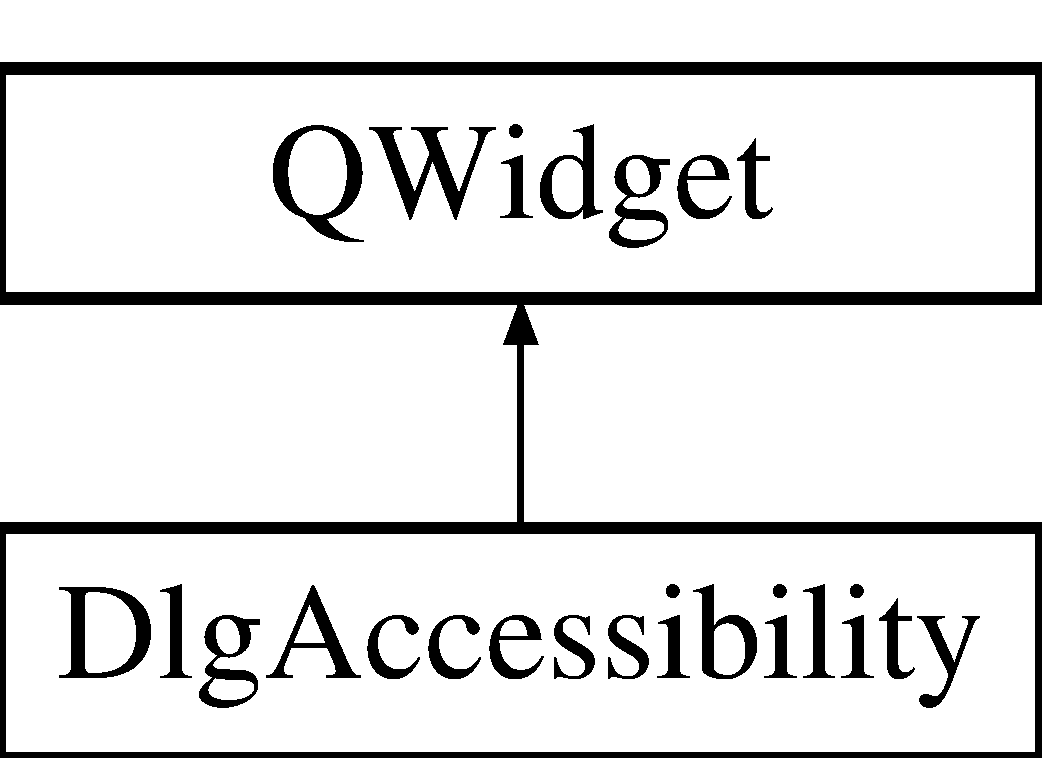
\includegraphics[height=2.000000cm]{classDlgAccessibility}
\end{center}
\end{figure}
\subsection*{Public Member Functions}
\begin{DoxyCompactItemize}
\item 
\hyperlink{classDlgAccessibility_a733ae92803be2f36fc3afde0a71c681e}{Dlg\+Accessibility} (Q\+Widget $\ast$parent=0)
\item 
\hyperlink{classDlgAccessibility_a97b15eb6de982ce97a42c37d7ba978b6}{$\sim$\+Dlg\+Accessibility} ()
\end{DoxyCompactItemize}


\subsection{Detailed Description}


Definition at line 18 of file dlgaccessibility.\+h.



\subsection{Constructor \& Destructor Documentation}
\hypertarget{classDlgAccessibility_a733ae92803be2f36fc3afde0a71c681e}{\index{Dlg\+Accessibility@{Dlg\+Accessibility}!Dlg\+Accessibility@{Dlg\+Accessibility}}
\index{Dlg\+Accessibility@{Dlg\+Accessibility}!Dlg\+Accessibility@{Dlg\+Accessibility}}
\subsubsection[{Dlg\+Accessibility}]{\setlength{\rightskip}{0pt plus 5cm}Dlg\+Accessibility\+::\+Dlg\+Accessibility (
\begin{DoxyParamCaption}
\item[{Q\+Widget $\ast$}]{parent = {\ttfamily 0}}
\end{DoxyParamCaption}
)}}\label{classDlgAccessibility_a733ae92803be2f36fc3afde0a71c681e}


Definition at line 14 of file dlgaccessibility.\+cpp.


\begin{DoxyCode}
15     : QWidget( parent ), m\_selected( 0 )
16 \{
17     m\_dlg = \textcolor{keyword}{new} \hyperlink{classUi__DlgAccessibilityBase}{Ui\_DlgAccessibilityBase}();
18     m\_dlg->\hyperlink{classUi__DlgAccessibilityBase_a0c6d1f69279a2dcc2351f7d856ce61dd}{setupUi}( \textcolor{keyword}{this} );
19 
20     \textcolor{comment}{// ### not working yet, hide for now}
21     m\_dlg->\hyperlink{classUi__DlgAccessibilityBase_a06bcf6b5838dd7dd61e796416b064b6b}{kcfg\_HighlightImages}->hide();
22 
23     m\_color\_pages.append( m\_dlg->\hyperlink{classUi__DlgAccessibilityBase_a07a676aad0645e0d37a146419d0e4f38}{page\_invert} );
24     m\_color\_pages.append( m\_dlg->\hyperlink{classUi__DlgAccessibilityBase_acac9f9a8e065b0a8d203c932f816b0ef}{page\_paperColor} );
25     m\_color\_pages.append( m\_dlg->\hyperlink{classUi__DlgAccessibilityBase_ac6a05225066cc7e921a37af4468a95df}{page\_darkLight} );
26     m\_color\_pages.append( m\_dlg->\hyperlink{classUi__DlgAccessibilityBase_ad6248c8c27f576cedc9e49b6144c4bc4}{page\_bw} );
27     \textcolor{keywordflow}{foreach} ( QWidget * page, m\_color\_pages )
28         page->hide();
29     m\_color\_pages[ m\_selected ]->show();
30 
31     connect( m\_dlg->\hyperlink{classUi__DlgAccessibilityBase_a8eaeef4919006d3f9225067d5fa6f5e7}{kcfg\_RenderMode}, SIGNAL(currentIndexChanged(\textcolor{keywordtype}{int})), \textcolor{keyword}{this}, SLOT(
      slotColorMode(\textcolor{keywordtype}{int})) );
32 \}
\end{DoxyCode}
\hypertarget{classDlgAccessibility_a97b15eb6de982ce97a42c37d7ba978b6}{\index{Dlg\+Accessibility@{Dlg\+Accessibility}!````~Dlg\+Accessibility@{$\sim$\+Dlg\+Accessibility}}
\index{````~Dlg\+Accessibility@{$\sim$\+Dlg\+Accessibility}!Dlg\+Accessibility@{Dlg\+Accessibility}}
\subsubsection[{$\sim$\+Dlg\+Accessibility}]{\setlength{\rightskip}{0pt plus 5cm}Dlg\+Accessibility\+::$\sim$\+Dlg\+Accessibility (
\begin{DoxyParamCaption}
{}
\end{DoxyParamCaption}
)}}\label{classDlgAccessibility_a97b15eb6de982ce97a42c37d7ba978b6}


Definition at line 34 of file dlgaccessibility.\+cpp.


\begin{DoxyCode}
35 \{
36     \textcolor{keyword}{delete} m\_dlg;
37 \}
\end{DoxyCode}


The documentation for this class was generated from the following files\+:\begin{DoxyCompactItemize}
\item 
conf/\hyperlink{dlgaccessibility_8h}{dlgaccessibility.\+h}\item 
conf/\hyperlink{dlgaccessibility_8cpp}{dlgaccessibility.\+cpp}\end{DoxyCompactItemize}

\hypertarget{classUi_1_1DlgAccessibilityBase}{\section{Ui\+:\+:Dlg\+Accessibility\+Base Class Reference}
\label{classUi_1_1DlgAccessibilityBase}\index{Ui\+::\+Dlg\+Accessibility\+Base@{Ui\+::\+Dlg\+Accessibility\+Base}}
}


{\ttfamily \#include $<$ui\+\_\+dlgaccessibilitybase.\+h$>$}

Inheritance diagram for Ui\+:\+:Dlg\+Accessibility\+Base\+:\begin{figure}[H]
\begin{center}
\leavevmode
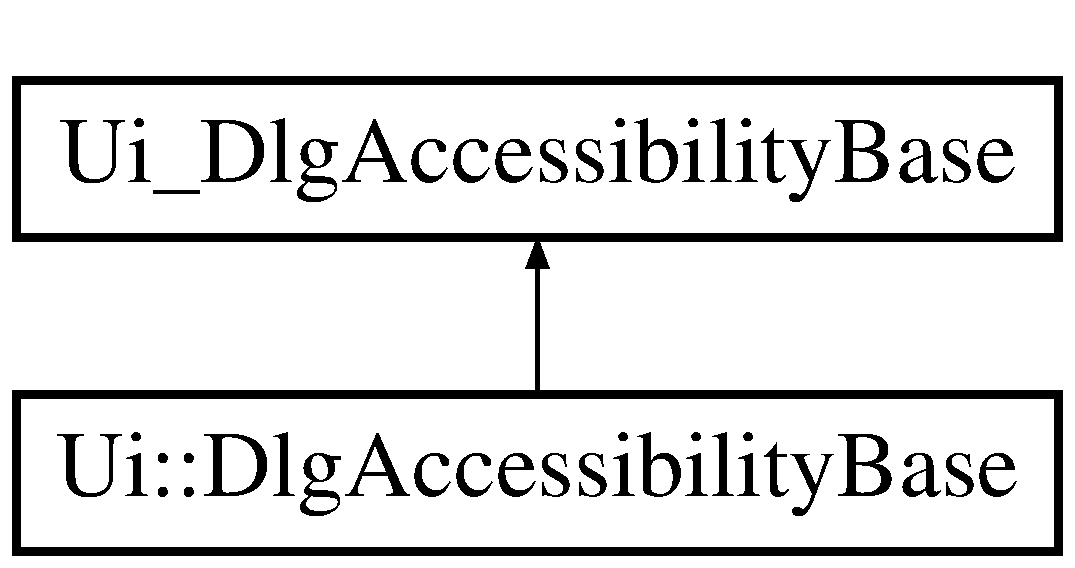
\includegraphics[height=2.000000cm]{classUi_1_1DlgAccessibilityBase}
\end{center}
\end{figure}
\subsection*{Additional Inherited Members}


\subsection{Detailed Description}


Definition at line 297 of file ui\+\_\+dlgaccessibilitybase.\+h.



The documentation for this class was generated from the following file\+:\begin{DoxyCompactItemize}
\item 
build/\hyperlink{ui__dlgaccessibilitybase_8h}{ui\+\_\+dlgaccessibilitybase.\+h}\end{DoxyCompactItemize}

\hypertarget{classDlgAnnotations}{\section{Dlg\+Annotations Class Reference}
\label{classDlgAnnotations}\index{Dlg\+Annotations@{Dlg\+Annotations}}
}


{\ttfamily \#include $<$dlgannotations.\+h$>$}

Inheritance diagram for Dlg\+Annotations\+:\begin{figure}[H]
\begin{center}
\leavevmode
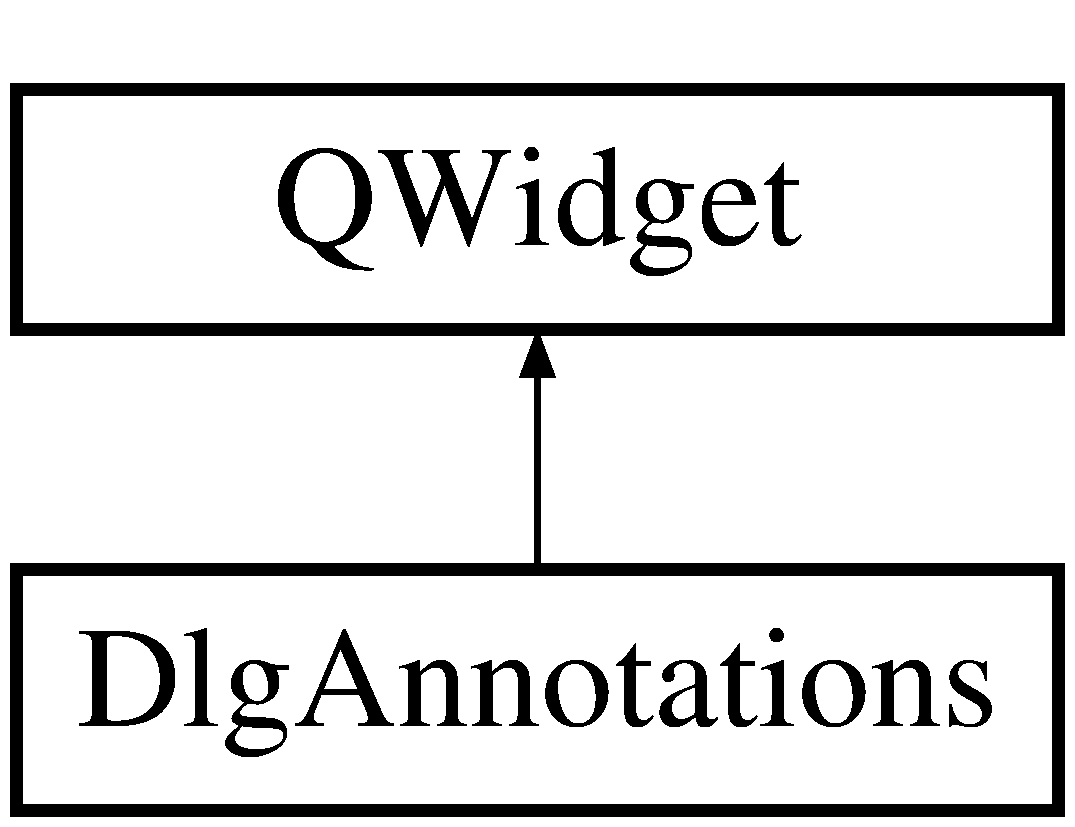
\includegraphics[height=2.000000cm]{classDlgAnnotations}
\end{center}
\end{figure}
\subsection*{Public Member Functions}
\begin{DoxyCompactItemize}
\item 
\hyperlink{classDlgAnnotations_acac3f792756ac3c7ce208d656b943a40}{Dlg\+Annotations} (Q\+Widget $\ast$parent=0)
\end{DoxyCompactItemize}


\subsection{Detailed Description}


Definition at line 16 of file dlgannotations.\+h.



\subsection{Constructor \& Destructor Documentation}
\hypertarget{classDlgAnnotations_acac3f792756ac3c7ce208d656b943a40}{\index{Dlg\+Annotations@{Dlg\+Annotations}!Dlg\+Annotations@{Dlg\+Annotations}}
\index{Dlg\+Annotations@{Dlg\+Annotations}!Dlg\+Annotations@{Dlg\+Annotations}}
\subsubsection[{Dlg\+Annotations}]{\setlength{\rightskip}{0pt plus 5cm}Dlg\+Annotations\+::\+Dlg\+Annotations (
\begin{DoxyParamCaption}
\item[{Q\+Widget $\ast$}]{parent = {\ttfamily 0}}
\end{DoxyParamCaption}
)}}\label{classDlgAnnotations_acac3f792756ac3c7ce208d656b943a40}


Definition at line 17 of file dlgannotations.\+cpp.


\begin{DoxyCode}
18     : QWidget( parent )
19 \{
20     \hyperlink{classUi__DlgAnnotationsBase}{Ui\_DlgAnnotationsBase} dlg;
21     dlg.\hyperlink{classUi__DlgAnnotationsBase_a078236dd18dd8f77ded02753ee3c2b7f}{setupUi}( \textcolor{keyword}{this} );
22 
23     \hyperlink{classWidgetAnnotTools}{WidgetAnnotTools} * kcfg\_AnnotationTools = \textcolor{keyword}{new} 
      \hyperlink{classWidgetAnnotTools}{WidgetAnnotTools}( dlg.\hyperlink{classUi__DlgAnnotationsBase_aef6cc8b1de7c7dbf6d4100f2f371bb77}{annotToolsGroup} );
24     dlg.\hyperlink{classUi__DlgAnnotationsBase_a87373fcbb302ebee34dce288e76b7bec}{annotToolsPlaceholder}->addWidget( kcfg\_AnnotationTools );
25     kcfg\_AnnotationTools->setObjectName( \textcolor{stringliteral}{"kcfg\_AnnotationTools"} );
26 
27     KConfigDialogManager::changedMap()->insert( \textcolor{stringliteral}{"WidgetAnnotTools"} , SIGNAL(changed()) );
28 \}
\end{DoxyCode}


The documentation for this class was generated from the following files\+:\begin{DoxyCompactItemize}
\item 
conf/\hyperlink{dlgannotations_8h}{dlgannotations.\+h}\item 
conf/\hyperlink{dlgannotations_8cpp}{dlgannotations.\+cpp}\end{DoxyCompactItemize}

\hypertarget{classUi_1_1DlgAnnotationsBase}{\section{Ui\+:\+:Dlg\+Annotations\+Base Class Reference}
\label{classUi_1_1DlgAnnotationsBase}\index{Ui\+::\+Dlg\+Annotations\+Base@{Ui\+::\+Dlg\+Annotations\+Base}}
}


{\ttfamily \#include $<$ui\+\_\+dlgannotationsbase.\+h$>$}

Inheritance diagram for Ui\+:\+:Dlg\+Annotations\+Base\+:\begin{figure}[H]
\begin{center}
\leavevmode
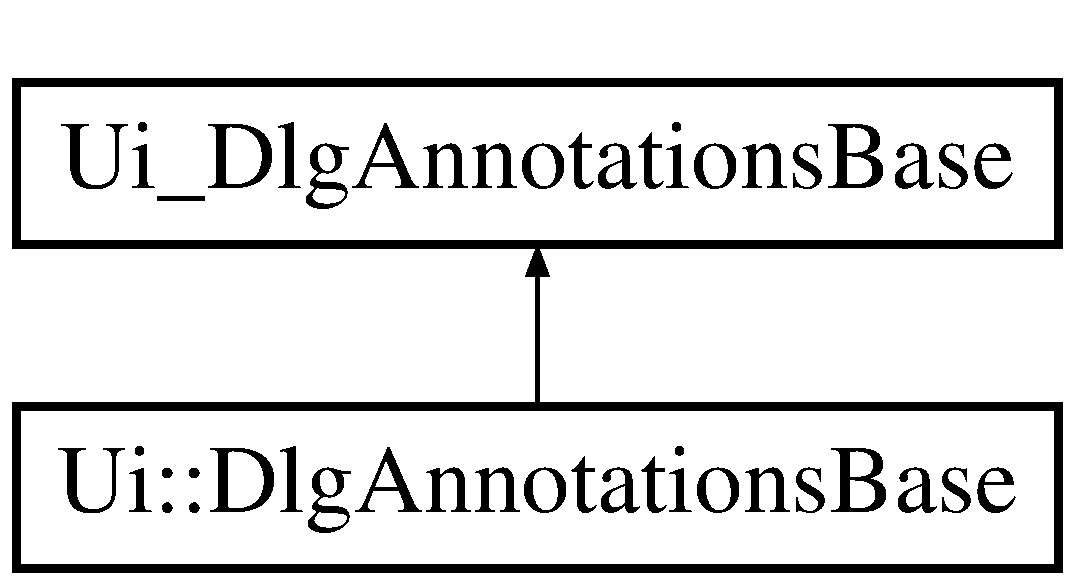
\includegraphics[height=2.000000cm]{classUi_1_1DlgAnnotationsBase}
\end{center}
\end{figure}
\subsection*{Additional Inherited Members}


\subsection{Detailed Description}


Definition at line 114 of file ui\+\_\+dlgannotationsbase.\+h.



The documentation for this class was generated from the following file\+:\begin{DoxyCompactItemize}
\item 
build/\hyperlink{ui__dlgannotationsbase_8h}{ui\+\_\+dlgannotationsbase.\+h}\end{DoxyCompactItemize}

\hypertarget{classDlgDebug}{\section{Dlg\+Debug Class Reference}
\label{classDlgDebug}\index{Dlg\+Debug@{Dlg\+Debug}}
}


{\ttfamily \#include $<$dlgdebug.\+h$>$}

Inheritance diagram for Dlg\+Debug\+:\begin{figure}[H]
\begin{center}
\leavevmode
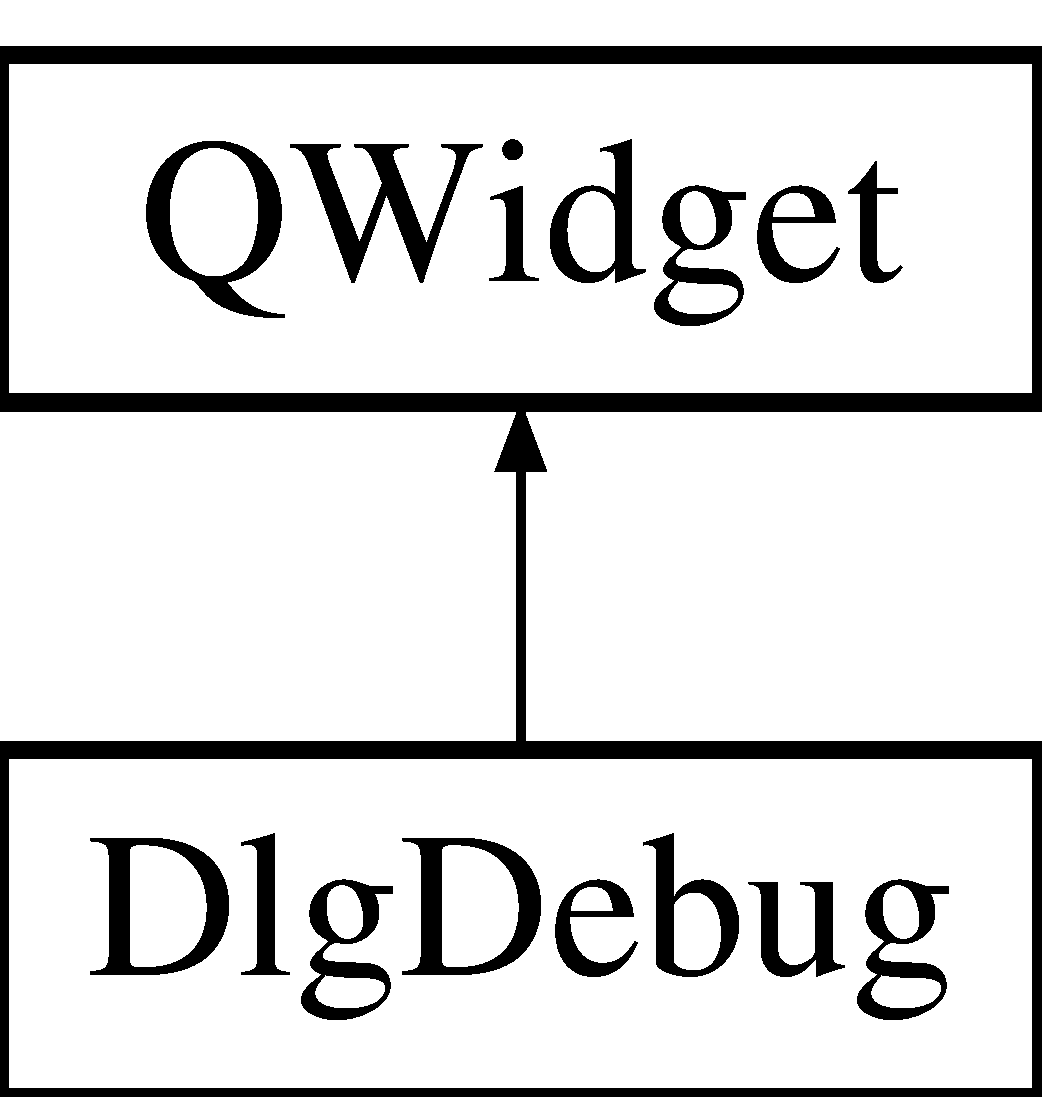
\includegraphics[height=2.000000cm]{classDlgDebug}
\end{center}
\end{figure}
\subsection*{Public Member Functions}
\begin{DoxyCompactItemize}
\item 
\hyperlink{classDlgDebug_abd0199996551c2c421672cabd813bdfe}{Dlg\+Debug} (Q\+Widget $\ast$parent=0)
\end{DoxyCompactItemize}


\subsection{Detailed Description}


Definition at line 15 of file dlgdebug.\+h.



\subsection{Constructor \& Destructor Documentation}
\hypertarget{classDlgDebug_abd0199996551c2c421672cabd813bdfe}{\index{Dlg\+Debug@{Dlg\+Debug}!Dlg\+Debug@{Dlg\+Debug}}
\index{Dlg\+Debug@{Dlg\+Debug}!Dlg\+Debug@{Dlg\+Debug}}
\subsubsection[{Dlg\+Debug}]{\setlength{\rightskip}{0pt plus 5cm}Dlg\+Debug\+::\+Dlg\+Debug (
\begin{DoxyParamCaption}
\item[{Q\+Widget $\ast$}]{parent = {\ttfamily 0}}
\end{DoxyParamCaption}
)}}\label{classDlgDebug_abd0199996551c2c421672cabd813bdfe}


Definition at line 22 of file dlgdebug.\+cpp.


\begin{DoxyCode}
23     : QWidget( parent )
24 \{
25     QVBoxLayout * lay = \textcolor{keyword}{new} QVBoxLayout( \textcolor{keyword}{this} );
26     lay->setMargin( 0 );
27 
28     \hyperlink{dlgdebug_8cpp_a21b0fcbf5794b5490062e4eb15e4dad8}{DEBUG\_SIMPLE\_BOOL}( \textcolor{stringliteral}{"DebugDrawBoundaries"}, lay );
29     \hyperlink{dlgdebug_8cpp_a21b0fcbf5794b5490062e4eb15e4dad8}{DEBUG\_SIMPLE\_BOOL}( \textcolor{stringliteral}{"DebugDrawAnnotationRect"}, lay );
30     \hyperlink{dlgdebug_8cpp_a21b0fcbf5794b5490062e4eb15e4dad8}{DEBUG\_SIMPLE\_BOOL}( \textcolor{stringliteral}{"TocPageColumn"}, lay );
31 
32     lay->addItem( \textcolor{keyword}{new} QSpacerItem( 5, 5, QSizePolicy::Fixed, QSizePolicy::MinimumExpanding ) );
33 \}
\end{DoxyCode}


The documentation for this class was generated from the following files\+:\begin{DoxyCompactItemize}
\item 
conf/\hyperlink{dlgdebug_8h}{dlgdebug.\+h}\item 
conf/\hyperlink{dlgdebug_8cpp}{dlgdebug.\+cpp}\end{DoxyCompactItemize}

\hypertarget{classDlgEditor}{\section{Dlg\+Editor Class Reference}
\label{classDlgEditor}\index{Dlg\+Editor@{Dlg\+Editor}}
}


{\ttfamily \#include $<$dlgeditor.\+h$>$}

Inheritance diagram for Dlg\+Editor\+:\begin{figure}[H]
\begin{center}
\leavevmode
\includegraphics[height=2.000000cm]{classDlgEditor}
\end{center}
\end{figure}
\subsection*{Public Member Functions}
\begin{DoxyCompactItemize}
\item 
\hyperlink{classDlgEditor_a5241c28c576969f4b87ae496bc295b5f}{Dlg\+Editor} (Q\+Widget $\ast$parent=0)
\item 
virtual \hyperlink{classDlgEditor_ab0bae0e6ac5e7f656984492fc8d4c260}{$\sim$\+Dlg\+Editor} ()
\end{DoxyCompactItemize}


\subsection{Detailed Description}


Definition at line 18 of file dlgeditor.\+h.



\subsection{Constructor \& Destructor Documentation}
\hypertarget{classDlgEditor_a5241c28c576969f4b87ae496bc295b5f}{\index{Dlg\+Editor@{Dlg\+Editor}!Dlg\+Editor@{Dlg\+Editor}}
\index{Dlg\+Editor@{Dlg\+Editor}!Dlg\+Editor@{Dlg\+Editor}}
\subsubsection[{Dlg\+Editor}]{\setlength{\rightskip}{0pt plus 5cm}Dlg\+Editor\+::\+Dlg\+Editor (
\begin{DoxyParamCaption}
\item[{Q\+Widget $\ast$}]{parent = {\ttfamily 0}}
\end{DoxyParamCaption}
)}}\label{classDlgEditor_a5241c28c576969f4b87ae496bc295b5f}


Definition at line 18 of file dlgeditor.\+cpp.


\begin{DoxyCode}
19     : QWidget( parent )
20 \{
21     m\_dlg = \textcolor{keyword}{new} \hyperlink{classUi__DlgEditorBase}{Ui\_DlgEditorBase}();
22     m\_dlg->\hyperlink{classUi__DlgEditorBase_a5b23b644a6d5dd91f606e93e6f324960}{setupUi}( \textcolor{keyword}{this} );
23 
24     m\_editors = Okular::buildEditorsMap();
25 
26     connect( m\_dlg->\hyperlink{classUi__DlgEditorBase_aea3d3090a97b8e3074b1e571713a9510}{kcfg\_ExternalEditor}, SIGNAL(currentIndexChanged(\textcolor{keywordtype}{int})), \textcolor{keyword}{this}, SLOT(
      editorChanged(\textcolor{keywordtype}{int})) );
27 
28     m\_dlg->\hyperlink{classUi__DlgEditorBase_aea3d3090a97b8e3074b1e571713a9510}{kcfg\_ExternalEditor}->addItem( i18nc( \textcolor{stringliteral}{"Text editor"}, \textcolor{stringliteral}{"Custom Text Editor"} ) );
29     m\_dlg->\hyperlink{classUi__DlgEditorBase_aea3d3090a97b8e3074b1e571713a9510}{kcfg\_ExternalEditor}->addItem( i18nc( \textcolor{stringliteral}{"Text editor"}, \textcolor{stringliteral}{"Kate"} ), 1 );
30     m\_dlg->\hyperlink{classUi__DlgEditorBase_aea3d3090a97b8e3074b1e571713a9510}{kcfg\_ExternalEditor}->addItem( i18nc( \textcolor{stringliteral}{"Text editor"}, \textcolor{stringliteral}{"Kile"} ), 2 );
31     m\_dlg->\hyperlink{classUi__DlgEditorBase_aea3d3090a97b8e3074b1e571713a9510}{kcfg\_ExternalEditor}->addItem( i18nc( \textcolor{stringliteral}{"Text editor"}, \textcolor{stringliteral}{"SciTE"} ), 3 );
32     m\_dlg->\hyperlink{classUi__DlgEditorBase_aea3d3090a97b8e3074b1e571713a9510}{kcfg\_ExternalEditor}->addItem( i18nc( \textcolor{stringliteral}{"Text editor"}, \textcolor{stringliteral}{"Emacs client"} ), 4 );
33     m\_dlg->\hyperlink{classUi__DlgEditorBase_aea3d3090a97b8e3074b1e571713a9510}{kcfg\_ExternalEditor}->addItem( i18nc( \textcolor{stringliteral}{"Text editor"}, \textcolor{stringliteral}{"Lyx client"} ), 5 );
34 
35     m\_dlg->\hyperlink{classUi__DlgEditorBase_a6123d3afc7b3db52828306e0c4de3e2d}{kcfg\_ExternalEditorCommand}->setWhatsThis( i18nc( \textcolor{stringliteral}{"@info:whatsthis"},
36         \textcolor{stringliteral}{"<qt>Set the command of a custom text editor to be launched.<br />\(\backslash\)n"}
37         \textcolor{stringliteral}{"You can also put few placeholders:\(\backslash\)n"}
38         \textcolor{stringliteral}{"<ul>\(\backslash\)n"}
39         \textcolor{stringliteral}{"  <li>%f - the file name</li>\(\backslash\)n"}
40         \textcolor{stringliteral}{"  <li>%l - the line of the file to be reached</li>\(\backslash\)n"}
41         \textcolor{stringliteral}{"  <li>%c - the column of the file to be reached</li>\(\backslash\)n"}
42         \textcolor{stringliteral}{"</ul>\(\backslash\)n"}
43         \textcolor{stringliteral}{"If %f is not specified, then the file name is appended to the specified "}
44         \textcolor{stringliteral}{"command."} ) );
45 \}
\end{DoxyCode}
\hypertarget{classDlgEditor_ab0bae0e6ac5e7f656984492fc8d4c260}{\index{Dlg\+Editor@{Dlg\+Editor}!````~Dlg\+Editor@{$\sim$\+Dlg\+Editor}}
\index{````~Dlg\+Editor@{$\sim$\+Dlg\+Editor}!Dlg\+Editor@{Dlg\+Editor}}
\subsubsection[{$\sim$\+Dlg\+Editor}]{\setlength{\rightskip}{0pt plus 5cm}Dlg\+Editor\+::$\sim$\+Dlg\+Editor (
\begin{DoxyParamCaption}
{}
\end{DoxyParamCaption}
)\hspace{0.3cm}{\ttfamily [virtual]}}}\label{classDlgEditor_ab0bae0e6ac5e7f656984492fc8d4c260}


Definition at line 47 of file dlgeditor.\+cpp.


\begin{DoxyCode}
48 \{
49     \textcolor{keyword}{delete} m\_dlg;
50 \}
\end{DoxyCode}


The documentation for this class was generated from the following files\+:\begin{DoxyCompactItemize}
\item 
conf/\hyperlink{dlgeditor_8h}{dlgeditor.\+h}\item 
conf/\hyperlink{dlgeditor_8cpp}{dlgeditor.\+cpp}\end{DoxyCompactItemize}

\hypertarget{classUi_1_1DlgEditorBase}{\section{Ui\+:\+:Dlg\+Editor\+Base Class Reference}
\label{classUi_1_1DlgEditorBase}\index{Ui\+::\+Dlg\+Editor\+Base@{Ui\+::\+Dlg\+Editor\+Base}}
}


{\ttfamily \#include $<$ui\+\_\+dlgeditorbase.\+h$>$}

Inheritance diagram for Ui\+:\+:Dlg\+Editor\+Base\+:\begin{figure}[H]
\begin{center}
\leavevmode
\includegraphics[height=2.000000cm]{classUi_1_1DlgEditorBase}
\end{center}
\end{figure}
\subsection*{Additional Inherited Members}


\subsection{Detailed Description}


Definition at line 136 of file ui\+\_\+dlgeditorbase.\+h.



The documentation for this class was generated from the following file\+:\begin{DoxyCompactItemize}
\item 
build/\hyperlink{ui__dlgeditorbase_8h}{ui\+\_\+dlgeditorbase.\+h}\end{DoxyCompactItemize}

\hypertarget{classDlgGeneral}{\section{Dlg\+General Class Reference}
\label{classDlgGeneral}\index{Dlg\+General@{Dlg\+General}}
}


{\ttfamily \#include $<$dlggeneral.\+h$>$}

Inheritance diagram for Dlg\+General\+:\begin{figure}[H]
\begin{center}
\leavevmode
\includegraphics[height=2.000000cm]{classDlgGeneral}
\end{center}
\end{figure}
\subsection*{Public Member Functions}
\begin{DoxyCompactItemize}
\item 
\hyperlink{classDlgGeneral_a6b76699c5118f535a51c89464aebca02}{Dlg\+General} (Q\+Widget $\ast$parent, \hyperlink{namespaceOkular_adbe21e337d65d3f5f07a441180428ba8}{Okular\+::\+Embed\+Mode} embed\+Mode)
\item 
virtual \hyperlink{classDlgGeneral_ae3733151f7e8fe39c17a42183416975a}{$\sim$\+Dlg\+General} ()
\end{DoxyCompactItemize}
\subsection*{Protected Member Functions}
\begin{DoxyCompactItemize}
\item 
virtual void \hyperlink{classDlgGeneral_a5318f904f1e55564f505302e14bf670d}{show\+Event} (Q\+Show\+Event $\ast$)
\end{DoxyCompactItemize}
\subsection*{Protected Attributes}
\begin{DoxyCompactItemize}
\item 
\hyperlink{classUi__DlgGeneralBase}{Ui\+\_\+\+Dlg\+General\+Base} $\ast$ \hyperlink{classDlgGeneral_ac33f78ba1135a2175517ec066115b32c}{m\+\_\+dlg}
\end{DoxyCompactItemize}


\subsection{Detailed Description}


Definition at line 19 of file dlggeneral.\+h.



\subsection{Constructor \& Destructor Documentation}
\hypertarget{classDlgGeneral_a6b76699c5118f535a51c89464aebca02}{\index{Dlg\+General@{Dlg\+General}!Dlg\+General@{Dlg\+General}}
\index{Dlg\+General@{Dlg\+General}!Dlg\+General@{Dlg\+General}}
\subsubsection[{Dlg\+General}]{\setlength{\rightskip}{0pt plus 5cm}Dlg\+General\+::\+Dlg\+General (
\begin{DoxyParamCaption}
\item[{Q\+Widget $\ast$}]{parent, }
\item[{{\bf Okular\+::\+Embed\+Mode}}]{embed\+Mode}
\end{DoxyParamCaption}
)}}\label{classDlgGeneral_a6b76699c5118f535a51c89464aebca02}


Definition at line 18 of file dlggeneral.\+cpp.


\begin{DoxyCode}
19     : QWidget( parent )
20 \{
21     \hyperlink{classDlgGeneral_ac33f78ba1135a2175517ec066115b32c}{m\_dlg} = \textcolor{keyword}{new} \hyperlink{classUi__DlgGeneralBase}{Ui\_DlgGeneralBase}();
22     \hyperlink{classDlgGeneral_ac33f78ba1135a2175517ec066115b32c}{m\_dlg}->\hyperlink{classUi__DlgGeneralBase_afdf9980931d308cb844e05466ac47978}{setupUi}( \textcolor{keyword}{this} );
23 
24     \textcolor{keywordflow}{if}( embedMode == \hyperlink{namespaceOkular_adbe21e337d65d3f5f07a441180428ba8aebaf7bae8bd4303bad7c4ca29057c472}{Okular::ViewerWidgetMode} )
25     \{
26         \hyperlink{classDlgGeneral_ac33f78ba1135a2175517ec066115b32c}{m\_dlg}->\hyperlink{classUi__DlgGeneralBase_a3bd89dac60042cf193e8f294f8d255b1}{kcfg\_SyncThumbnailsViewport}->setVisible( \textcolor{keyword}{false} );
27         \hyperlink{classDlgGeneral_ac33f78ba1135a2175517ec066115b32c}{m\_dlg}->\hyperlink{classUi__DlgGeneralBase_a0283039d02817b23b8f52f3b670bd9a8}{kcfg\_DisplayDocumentTitle}->setVisible( \textcolor{keyword}{false} );
28         \hyperlink{classDlgGeneral_ac33f78ba1135a2175517ec066115b32c}{m\_dlg}->\hyperlink{classUi__DlgGeneralBase_ad78f563114498d2bcc4350d8939ad2ec}{kcfg\_WatchFile}->setVisible( \textcolor{keyword}{false} );
29     \}
30     \hyperlink{classDlgGeneral_ac33f78ba1135a2175517ec066115b32c}{m\_dlg}->\hyperlink{classUi__DlgGeneralBase_abb932ae5a296f99d600ae0bd76423797}{kcfg\_ShellOpenFileInTabs}->setVisible( embedMode == 
      \hyperlink{namespaceOkular_adbe21e337d65d3f5f07a441180428ba8ae06451e28dfb108642b1c3a61a196145}{Okular::NativeShellMode} );
31 \}
\end{DoxyCode}
\hypertarget{classDlgGeneral_ae3733151f7e8fe39c17a42183416975a}{\index{Dlg\+General@{Dlg\+General}!````~Dlg\+General@{$\sim$\+Dlg\+General}}
\index{````~Dlg\+General@{$\sim$\+Dlg\+General}!Dlg\+General@{Dlg\+General}}
\subsubsection[{$\sim$\+Dlg\+General}]{\setlength{\rightskip}{0pt plus 5cm}Dlg\+General\+::$\sim$\+Dlg\+General (
\begin{DoxyParamCaption}
{}
\end{DoxyParamCaption}
)\hspace{0.3cm}{\ttfamily [virtual]}}}\label{classDlgGeneral_ae3733151f7e8fe39c17a42183416975a}


Definition at line 33 of file dlggeneral.\+cpp.


\begin{DoxyCode}
34 \{
35     \textcolor{keyword}{delete} \hyperlink{classDlgGeneral_ac33f78ba1135a2175517ec066115b32c}{m\_dlg};
36 \}
\end{DoxyCode}


\subsection{Member Function Documentation}
\hypertarget{classDlgGeneral_a5318f904f1e55564f505302e14bf670d}{\index{Dlg\+General@{Dlg\+General}!show\+Event@{show\+Event}}
\index{show\+Event@{show\+Event}!Dlg\+General@{Dlg\+General}}
\subsubsection[{show\+Event}]{\setlength{\rightskip}{0pt plus 5cm}void Dlg\+General\+::show\+Event (
\begin{DoxyParamCaption}
\item[{Q\+Show\+Event $\ast$}]{}
\end{DoxyParamCaption}
)\hspace{0.3cm}{\ttfamily [protected]}, {\ttfamily [virtual]}}}\label{classDlgGeneral_a5318f904f1e55564f505302e14bf670d}


Definition at line 38 of file dlggeneral.\+cpp.


\begin{DoxyCode}
39 \{
40 \textcolor{preprocessor}{#if OKULAR\_FORCE\_DRM}
41     \hyperlink{classDlgGeneral_ac33f78ba1135a2175517ec066115b32c}{m\_dlg}->\hyperlink{classUi__DlgGeneralBase_ae06aa2913c5352f7291531fa8709216f}{kcfg\_ObeyDRM}->hide();
42 \textcolor{preprocessor}{#else}
43     \textcolor{keywordflow}{if} ( KAuthorized::authorize( \textcolor{stringliteral}{"skip\_drm"} ) )
44         \hyperlink{classDlgGeneral_ac33f78ba1135a2175517ec066115b32c}{m\_dlg}->\hyperlink{classUi__DlgGeneralBase_ae06aa2913c5352f7291531fa8709216f}{kcfg\_ObeyDRM}->show();
45     \textcolor{keywordflow}{else}
46         \hyperlink{classDlgGeneral_ac33f78ba1135a2175517ec066115b32c}{m\_dlg}->\hyperlink{classUi__DlgGeneralBase_ae06aa2913c5352f7291531fa8709216f}{kcfg\_ObeyDRM}->hide();
47 \textcolor{preprocessor}{#endif}
48 \}
\end{DoxyCode}


\subsection{Member Data Documentation}
\hypertarget{classDlgGeneral_ac33f78ba1135a2175517ec066115b32c}{\index{Dlg\+General@{Dlg\+General}!m\+\_\+dlg@{m\+\_\+dlg}}
\index{m\+\_\+dlg@{m\+\_\+dlg}!Dlg\+General@{Dlg\+General}}
\subsubsection[{m\+\_\+dlg}]{\setlength{\rightskip}{0pt plus 5cm}{\bf Ui\+\_\+\+Dlg\+General\+Base}$\ast$ Dlg\+General\+::m\+\_\+dlg\hspace{0.3cm}{\ttfamily [protected]}}}\label{classDlgGeneral_ac33f78ba1135a2175517ec066115b32c}


Definition at line 28 of file dlggeneral.\+h.



The documentation for this class was generated from the following files\+:\begin{DoxyCompactItemize}
\item 
conf/\hyperlink{dlggeneral_8h}{dlggeneral.\+h}\item 
conf/\hyperlink{dlggeneral_8cpp}{dlggeneral.\+cpp}\end{DoxyCompactItemize}

\hypertarget{classUi_1_1DlgGeneralBase}{\section{Ui\+:\+:Dlg\+General\+Base Class Reference}
\label{classUi_1_1DlgGeneralBase}\index{Ui\+::\+Dlg\+General\+Base@{Ui\+::\+Dlg\+General\+Base}}
}


{\ttfamily \#include $<$ui\+\_\+dlggeneralbase.\+h$>$}

Inheritance diagram for Ui\+:\+:Dlg\+General\+Base\+:\begin{figure}[H]
\begin{center}
\leavevmode
\includegraphics[height=2.000000cm]{classUi_1_1DlgGeneralBase}
\end{center}
\end{figure}
\subsection*{Additional Inherited Members}


\subsection{Detailed Description}


Definition at line 365 of file ui\+\_\+dlggeneralbase.\+h.



The documentation for this class was generated from the following file\+:\begin{DoxyCompactItemize}
\item 
build/\hyperlink{ui__dlggeneralbase_8h}{ui\+\_\+dlggeneralbase.\+h}\end{DoxyCompactItemize}

\hypertarget{classDlgPerformance}{\section{Dlg\+Performance Class Reference}
\label{classDlgPerformance}\index{Dlg\+Performance@{Dlg\+Performance}}
}


{\ttfamily \#include $<$dlgperformance.\+h$>$}

Inheritance diagram for Dlg\+Performance\+:\begin{figure}[H]
\begin{center}
\leavevmode
\includegraphics[height=2.000000cm]{classDlgPerformance}
\end{center}
\end{figure}
\subsection*{Public Member Functions}
\begin{DoxyCompactItemize}
\item 
\hyperlink{classDlgPerformance_afe916fa76c0582255b8a57dbbfa02fc8}{Dlg\+Performance} (Q\+Widget $\ast$parent=0)
\item 
virtual \hyperlink{classDlgPerformance_a66990ee66393d50e390103e80f45bf37}{$\sim$\+Dlg\+Performance} ()
\end{DoxyCompactItemize}
\subsection*{Protected Slots}
\begin{DoxyCompactItemize}
\item 
void \hyperlink{classDlgPerformance_aed95f65483f78ef4b3dbdaf110c9b182}{radio\+Group\+\_\+changed} (int which)
\end{DoxyCompactItemize}
\subsection*{Protected Attributes}
\begin{DoxyCompactItemize}
\item 
\hyperlink{classUi__DlgPerformanceBase}{Ui\+\_\+\+Dlg\+Performance\+Base} $\ast$ \hyperlink{classDlgPerformance_a67b6c616fbba78dc1650d5a3f2ed3084}{m\+\_\+dlg}
\end{DoxyCompactItemize}


\subsection{Detailed Description}


Definition at line 17 of file dlgperformance.\+h.



\subsection{Constructor \& Destructor Documentation}
\hypertarget{classDlgPerformance_afe916fa76c0582255b8a57dbbfa02fc8}{\index{Dlg\+Performance@{Dlg\+Performance}!Dlg\+Performance@{Dlg\+Performance}}
\index{Dlg\+Performance@{Dlg\+Performance}!Dlg\+Performance@{Dlg\+Performance}}
\subsubsection[{Dlg\+Performance}]{\setlength{\rightskip}{0pt plus 5cm}Dlg\+Performance\+::\+Dlg\+Performance (
\begin{DoxyParamCaption}
\item[{Q\+Widget $\ast$}]{parent = {\ttfamily 0}}
\end{DoxyParamCaption}
)}}\label{classDlgPerformance_afe916fa76c0582255b8a57dbbfa02fc8}


Definition at line 17 of file dlgperformance.\+cpp.


\begin{DoxyCode}
18     : QWidget( parent )
19 \{
20     \hyperlink{classDlgPerformance_a67b6c616fbba78dc1650d5a3f2ed3084}{m\_dlg} = \textcolor{keyword}{new} \hyperlink{classUi__DlgPerformanceBase}{Ui\_DlgPerformanceBase}();
21     \hyperlink{classDlgPerformance_a67b6c616fbba78dc1650d5a3f2ed3084}{m\_dlg}->\hyperlink{classUi__DlgPerformanceBase_a8bb6e61830ad3c15c7cfd25402103eff}{setupUi}( \textcolor{keyword}{this} );
22 
23     QFont labelFont = \hyperlink{classDlgPerformance_a67b6c616fbba78dc1650d5a3f2ed3084}{m\_dlg}->\hyperlink{classUi__DlgPerformanceBase_a81970ae031653bae2f63fe1e5c390e59}{descLabel}->font();
24     labelFont.setBold( \textcolor{keyword}{true} );
25     \hyperlink{classDlgPerformance_a67b6c616fbba78dc1650d5a3f2ed3084}{m\_dlg}->\hyperlink{classUi__DlgPerformanceBase_a81970ae031653bae2f63fe1e5c390e59}{descLabel}->setFont( labelFont );
26 
27     \hyperlink{classDlgPerformance_a67b6c616fbba78dc1650d5a3f2ed3084}{m\_dlg}->\hyperlink{classUi__DlgPerformanceBase_add0831b3efdd1175e047cbffe44f0f8d}{cpuLabel}->setPixmap( BarIcon( \textcolor{stringliteral}{"cpu"}, 32 ) );
28 \textcolor{comment}{//     m\_dlg->memoryLabel->setPixmap( BarIcon( "kcmmemory", 32 ) ); // TODO: enable again when proper icon
       is available}
29 
30     connect( \hyperlink{classDlgPerformance_a67b6c616fbba78dc1650d5a3f2ed3084}{m\_dlg}->\hyperlink{classUi__DlgPerformanceBase_a93edac845d7c5b17eb8daf50d97d0e3f}{kcfg\_MemoryLevel}, SIGNAL(changed(\textcolor{keywordtype}{int})), \textcolor{keyword}{this}, SLOT(
      \hyperlink{classDlgPerformance_aed95f65483f78ef4b3dbdaf110c9b182}{radioGroup\_changed}(\textcolor{keywordtype}{int})) );
31 \}
\end{DoxyCode}
\hypertarget{classDlgPerformance_a66990ee66393d50e390103e80f45bf37}{\index{Dlg\+Performance@{Dlg\+Performance}!````~Dlg\+Performance@{$\sim$\+Dlg\+Performance}}
\index{````~Dlg\+Performance@{$\sim$\+Dlg\+Performance}!Dlg\+Performance@{Dlg\+Performance}}
\subsubsection[{$\sim$\+Dlg\+Performance}]{\setlength{\rightskip}{0pt plus 5cm}Dlg\+Performance\+::$\sim$\+Dlg\+Performance (
\begin{DoxyParamCaption}
{}
\end{DoxyParamCaption}
)\hspace{0.3cm}{\ttfamily [virtual]}}}\label{classDlgPerformance_a66990ee66393d50e390103e80f45bf37}


Definition at line 33 of file dlgperformance.\+cpp.


\begin{DoxyCode}
34 \{
35     \textcolor{keyword}{delete} \hyperlink{classDlgPerformance_a67b6c616fbba78dc1650d5a3f2ed3084}{m\_dlg};
36 \}
\end{DoxyCode}


\subsection{Member Function Documentation}
\hypertarget{classDlgPerformance_aed95f65483f78ef4b3dbdaf110c9b182}{\index{Dlg\+Performance@{Dlg\+Performance}!radio\+Group\+\_\+changed@{radio\+Group\+\_\+changed}}
\index{radio\+Group\+\_\+changed@{radio\+Group\+\_\+changed}!Dlg\+Performance@{Dlg\+Performance}}
\subsubsection[{radio\+Group\+\_\+changed}]{\setlength{\rightskip}{0pt plus 5cm}void Dlg\+Performance\+::radio\+Group\+\_\+changed (
\begin{DoxyParamCaption}
\item[{int}]{which}
\end{DoxyParamCaption}
)\hspace{0.3cm}{\ttfamily [protected]}, {\ttfamily [slot]}}}\label{classDlgPerformance_aed95f65483f78ef4b3dbdaf110c9b182}


Definition at line 38 of file dlgperformance.\+cpp.


\begin{DoxyCode}
39 \{
40     \textcolor{keywordflow}{switch} ( which )
41     \{
42         \textcolor{keywordflow}{case} 0:
43             \hyperlink{classDlgPerformance_a67b6c616fbba78dc1650d5a3f2ed3084}{m\_dlg}->\hyperlink{classUi__DlgPerformanceBase_a81970ae031653bae2f63fe1e5c390e59}{descLabel}->setText( i18n(\textcolor{stringliteral}{"Keeps used memory as low as possible. Do not
       reuse anything. (For systems with low memory.)"}) );
44             \textcolor{keywordflow}{break};
45         \textcolor{keywordflow}{case} 1:
46             \hyperlink{classDlgPerformance_a67b6c616fbba78dc1650d5a3f2ed3084}{m\_dlg}->\hyperlink{classUi__DlgPerformanceBase_a81970ae031653bae2f63fe1e5c390e59}{descLabel}->setText( i18n(\textcolor{stringliteral}{"A good compromise between memory usage and speed
       gain. Preload next page and boost searches. (For systems with 256MB of memory, typically.)"}) );
47             \textcolor{keywordflow}{break};
48         \textcolor{keywordflow}{case} 2:
49             \hyperlink{classDlgPerformance_a67b6c616fbba78dc1650d5a3f2ed3084}{m\_dlg}->\hyperlink{classUi__DlgPerformanceBase_a81970ae031653bae2f63fe1e5c390e59}{descLabel}->setText( i18n(\textcolor{stringliteral}{"Keeps everything in memory. Preload next pages.
       Boost searches. (For systems with more than 512MB of memory.)"}) );
50             \textcolor{keywordflow}{break};
51         \textcolor{keywordflow}{case} 3:
52         \textcolor{comment}{// xgettext: no-c-format}
53             \hyperlink{classDlgPerformance_a67b6c616fbba78dc1650d5a3f2ed3084}{m\_dlg}->\hyperlink{classUi__DlgPerformanceBase_a81970ae031653bae2f63fe1e5c390e59}{descLabel}->setText( i18n(\textcolor{stringliteral}{"Loads and keeps everything in memory. Preload
       all pages. (Will use at maximum 50% of your total memory or your free memory, whatever is bigger.)"}));
54             \textcolor{keywordflow}{break};
55     \}
56 \}
\end{DoxyCode}


\subsection{Member Data Documentation}
\hypertarget{classDlgPerformance_a67b6c616fbba78dc1650d5a3f2ed3084}{\index{Dlg\+Performance@{Dlg\+Performance}!m\+\_\+dlg@{m\+\_\+dlg}}
\index{m\+\_\+dlg@{m\+\_\+dlg}!Dlg\+Performance@{Dlg\+Performance}}
\subsubsection[{m\+\_\+dlg}]{\setlength{\rightskip}{0pt plus 5cm}{\bf Ui\+\_\+\+Dlg\+Performance\+Base}$\ast$ Dlg\+Performance\+::m\+\_\+dlg\hspace{0.3cm}{\ttfamily [protected]}}}\label{classDlgPerformance_a67b6c616fbba78dc1650d5a3f2ed3084}


Definition at line 29 of file dlgperformance.\+h.



The documentation for this class was generated from the following files\+:\begin{DoxyCompactItemize}
\item 
conf/\hyperlink{dlgperformance_8h}{dlgperformance.\+h}\item 
conf/\hyperlink{dlgperformance_8cpp}{dlgperformance.\+cpp}\end{DoxyCompactItemize}

\hypertarget{classUi_1_1DlgPerformanceBase}{\section{Ui\+:\+:Dlg\+Performance\+Base Class Reference}
\label{classUi_1_1DlgPerformanceBase}\index{Ui\+::\+Dlg\+Performance\+Base@{Ui\+::\+Dlg\+Performance\+Base}}
}


{\ttfamily \#include $<$ui\+\_\+dlgperformancebase.\+h$>$}

Inheritance diagram for Ui\+:\+:Dlg\+Performance\+Base\+:\begin{figure}[H]
\begin{center}
\leavevmode
\includegraphics[height=2.000000cm]{classUi_1_1DlgPerformanceBase}
\end{center}
\end{figure}
\subsection*{Additional Inherited Members}


\subsection{Detailed Description}


Definition at line 274 of file ui\+\_\+dlgperformancebase.\+h.



The documentation for this class was generated from the following file\+:\begin{DoxyCompactItemize}
\item 
build/\hyperlink{ui__dlgperformancebase_8h}{ui\+\_\+dlgperformancebase.\+h}\end{DoxyCompactItemize}

\hypertarget{classDlgPresentation}{\section{Dlg\+Presentation Class Reference}
\label{classDlgPresentation}\index{Dlg\+Presentation@{Dlg\+Presentation}}
}


{\ttfamily \#include $<$dlgpresentation.\+h$>$}

Inheritance diagram for Dlg\+Presentation\+:\begin{figure}[H]
\begin{center}
\leavevmode
\includegraphics[height=2.000000cm]{classDlgPresentation}
\end{center}
\end{figure}
\subsection*{Public Member Functions}
\begin{DoxyCompactItemize}
\item 
\hyperlink{classDlgPresentation_a9a05fbd1952a503fa7b2e74e1eb4c721}{Dlg\+Presentation} (Q\+Widget $\ast$parent=0)
\item 
virtual \hyperlink{classDlgPresentation_a9cecf68c7c1cf265806577f6f4e16a10}{$\sim$\+Dlg\+Presentation} ()
\end{DoxyCompactItemize}
\subsection*{Protected Slots}
\begin{DoxyCompactItemize}
\item 
void \hyperlink{classDlgPresentation_a510328bf08c98dc1d7f2fb408792fead}{screen\+Combo\+Changed} (int which)
\end{DoxyCompactItemize}
\subsection*{Protected Attributes}
\begin{DoxyCompactItemize}
\item 
\hyperlink{classUi__DlgPresentationBase}{Ui\+\_\+\+Dlg\+Presentation\+Base} $\ast$ \hyperlink{classDlgPresentation_a010a8c09c59fa2c78efd78b983e9c569}{m\+\_\+dlg}
\end{DoxyCompactItemize}


\subsection{Detailed Description}


Definition at line 17 of file dlgpresentation.\+h.



\subsection{Constructor \& Destructor Documentation}
\hypertarget{classDlgPresentation_a9a05fbd1952a503fa7b2e74e1eb4c721}{\index{Dlg\+Presentation@{Dlg\+Presentation}!Dlg\+Presentation@{Dlg\+Presentation}}
\index{Dlg\+Presentation@{Dlg\+Presentation}!Dlg\+Presentation@{Dlg\+Presentation}}
\subsubsection[{Dlg\+Presentation}]{\setlength{\rightskip}{0pt plus 5cm}Dlg\+Presentation\+::\+Dlg\+Presentation (
\begin{DoxyParamCaption}
\item[{Q\+Widget $\ast$}]{parent = {\ttfamily 0}}
\end{DoxyParamCaption}
)}}\label{classDlgPresentation_a9a05fbd1952a503fa7b2e74e1eb4c721}


Definition at line 21 of file dlgpresentation.\+cpp.


\begin{DoxyCode}
22     : QWidget( parent )
23 \{
24     \hyperlink{classDlgPresentation_a010a8c09c59fa2c78efd78b983e9c569}{m\_dlg} = \textcolor{keyword}{new} \hyperlink{classUi__DlgPresentationBase}{Ui\_DlgPresentationBase}();
25     \hyperlink{classDlgPresentation_a010a8c09c59fa2c78efd78b983e9c569}{m\_dlg}->\hyperlink{classUi__DlgPresentationBase_a08f712538ec0fc692a48271f8ae38bc5}{setupUi}( \textcolor{keyword}{this} );
26 
27     QStringList choices;
28     choices.append( i18nc( \textcolor{stringliteral}{"@label:listbox The current screen, for the presentation mode"}, \textcolor{stringliteral}{"Current Screen"}
       ) );
29     choices.append( i18nc( \textcolor{stringliteral}{"@label:listbox The default screen for the presentation mode"}, \textcolor{stringliteral}{"Default Screen"} 
      ) );
30     \textcolor{keyword}{const} \textcolor{keywordtype}{int} screenCount = QApplication::desktop()->numScreens();
31     \textcolor{keywordflow}{for} ( \textcolor{keywordtype}{int} i = 0; i < screenCount; ++i )
32     \{
33         choices.append( i18nc( \textcolor{stringliteral}{"@label:listbox %1 is the screen number (0, 1, ...)"}, \textcolor{stringliteral}{"Screen %1"}, i ) );
34     \}
35     \hyperlink{classDlgPresentation_a010a8c09c59fa2c78efd78b983e9c569}{m\_dlg}->\hyperlink{classUi__DlgPresentationBase_a588ed0d2c3045e6179c739bdf354e812}{screenCombo}->addItems( choices );
36 
37     \textcolor{keyword}{const} \textcolor{keywordtype}{int} screen = \hyperlink{classOkular_1_1Settings_a8c3effff997dea37e71f645dada4a2a8}{Okular::Settings::slidesScreen}();
38     \textcolor{keywordflow}{if} ( screen >= -2 && screen < screenCount )
39     \{
40         \hyperlink{classDlgPresentation_a010a8c09c59fa2c78efd78b983e9c569}{m\_dlg}->\hyperlink{classUi__DlgPresentationBase_a588ed0d2c3045e6179c739bdf354e812}{screenCombo}->setCurrentIndex( screen + 2 );
41     \}
42     \textcolor{keywordflow}{else}
43     \{
44         \hyperlink{classDlgPresentation_a010a8c09c59fa2c78efd78b983e9c569}{m\_dlg}->\hyperlink{classUi__DlgPresentationBase_a588ed0d2c3045e6179c739bdf354e812}{screenCombo}->setCurrentIndex( 0 );
45         \hyperlink{classOkular_1_1Settings_a12575582901d218e5fe5d731f25bdbb9}{Okular::Settings::setSlidesScreen}( -2 );
46     \}
47     
48     \hyperlink{classDlgPresentation_a010a8c09c59fa2c78efd78b983e9c569}{m\_dlg}->\hyperlink{classUi__DlgPresentationBase_aba7f1b1ba7c742636c1f2e306001cb3a}{kcfg\_SlidesAdvanceTime}->setSuffix(ki18ncp(\textcolor{stringliteral}{"Advance every %1 seconds"},
       \textcolor{stringliteral}{" second"}, \textcolor{stringliteral}{" seconds"}));
49 
50     connect( \hyperlink{classDlgPresentation_a010a8c09c59fa2c78efd78b983e9c569}{m\_dlg}->\hyperlink{classUi__DlgPresentationBase_a588ed0d2c3045e6179c739bdf354e812}{screenCombo}, SIGNAL(activated(\textcolor{keywordtype}{int})), \textcolor{keyword}{this}, SLOT(
      \hyperlink{classDlgPresentation_a510328bf08c98dc1d7f2fb408792fead}{screenComboChanged}(\textcolor{keywordtype}{int})) );
51 \}
\end{DoxyCode}
\hypertarget{classDlgPresentation_a9cecf68c7c1cf265806577f6f4e16a10}{\index{Dlg\+Presentation@{Dlg\+Presentation}!````~Dlg\+Presentation@{$\sim$\+Dlg\+Presentation}}
\index{````~Dlg\+Presentation@{$\sim$\+Dlg\+Presentation}!Dlg\+Presentation@{Dlg\+Presentation}}
\subsubsection[{$\sim$\+Dlg\+Presentation}]{\setlength{\rightskip}{0pt plus 5cm}Dlg\+Presentation\+::$\sim$\+Dlg\+Presentation (
\begin{DoxyParamCaption}
{}
\end{DoxyParamCaption}
)\hspace{0.3cm}{\ttfamily [virtual]}}}\label{classDlgPresentation_a9cecf68c7c1cf265806577f6f4e16a10}


Definition at line 53 of file dlgpresentation.\+cpp.


\begin{DoxyCode}
54 \{
55     \textcolor{keyword}{delete} \hyperlink{classDlgPresentation_a010a8c09c59fa2c78efd78b983e9c569}{m\_dlg};
56 \}
\end{DoxyCode}


\subsection{Member Function Documentation}
\hypertarget{classDlgPresentation_a510328bf08c98dc1d7f2fb408792fead}{\index{Dlg\+Presentation@{Dlg\+Presentation}!screen\+Combo\+Changed@{screen\+Combo\+Changed}}
\index{screen\+Combo\+Changed@{screen\+Combo\+Changed}!Dlg\+Presentation@{Dlg\+Presentation}}
\subsubsection[{screen\+Combo\+Changed}]{\setlength{\rightskip}{0pt plus 5cm}void Dlg\+Presentation\+::screen\+Combo\+Changed (
\begin{DoxyParamCaption}
\item[{int}]{which}
\end{DoxyParamCaption}
)\hspace{0.3cm}{\ttfamily [protected]}, {\ttfamily [slot]}}}\label{classDlgPresentation_a510328bf08c98dc1d7f2fb408792fead}


Definition at line 58 of file dlgpresentation.\+cpp.


\begin{DoxyCode}
59 \{
60     \hyperlink{classOkular_1_1Settings_a12575582901d218e5fe5d731f25bdbb9}{Okular::Settings::setSlidesScreen}( which - 2 );
61 \}
\end{DoxyCode}


\subsection{Member Data Documentation}
\hypertarget{classDlgPresentation_a010a8c09c59fa2c78efd78b983e9c569}{\index{Dlg\+Presentation@{Dlg\+Presentation}!m\+\_\+dlg@{m\+\_\+dlg}}
\index{m\+\_\+dlg@{m\+\_\+dlg}!Dlg\+Presentation@{Dlg\+Presentation}}
\subsubsection[{m\+\_\+dlg}]{\setlength{\rightskip}{0pt plus 5cm}{\bf Ui\+\_\+\+Dlg\+Presentation\+Base}$\ast$ Dlg\+Presentation\+::m\+\_\+dlg\hspace{0.3cm}{\ttfamily [protected]}}}\label{classDlgPresentation_a010a8c09c59fa2c78efd78b983e9c569}


Definition at line 29 of file dlgpresentation.\+h.



The documentation for this class was generated from the following files\+:\begin{DoxyCompactItemize}
\item 
conf/\hyperlink{dlgpresentation_8h}{dlgpresentation.\+h}\item 
conf/\hyperlink{dlgpresentation_8cpp}{dlgpresentation.\+cpp}\end{DoxyCompactItemize}

\hypertarget{classUi_1_1DlgPresentationBase}{\section{Ui\+:\+:Dlg\+Presentation\+Base Class Reference}
\label{classUi_1_1DlgPresentationBase}\index{Ui\+::\+Dlg\+Presentation\+Base@{Ui\+::\+Dlg\+Presentation\+Base}}
}


{\ttfamily \#include $<$ui\+\_\+dlgpresentationbase.\+h$>$}

Inheritance diagram for Ui\+:\+:Dlg\+Presentation\+Base\+:\begin{figure}[H]
\begin{center}
\leavevmode
\includegraphics[height=2.000000cm]{classUi_1_1DlgPresentationBase}
\end{center}
\end{figure}
\subsection*{Additional Inherited Members}


\subsection{Detailed Description}


Definition at line 268 of file ui\+\_\+dlgpresentationbase.\+h.



The documentation for this class was generated from the following file\+:\begin{DoxyCompactItemize}
\item 
build/\hyperlink{ui__dlgpresentationbase_8h}{ui\+\_\+dlgpresentationbase.\+h}\end{DoxyCompactItemize}

\hypertarget{structOkular_1_1DoContinueDirectionMatchSearchStruct}{\section{Okular\+:\+:Do\+Continue\+Direction\+Match\+Search\+Struct Struct Reference}
\label{structOkular_1_1DoContinueDirectionMatchSearchStruct}\index{Okular\+::\+Do\+Continue\+Direction\+Match\+Search\+Struct@{Okular\+::\+Do\+Continue\+Direction\+Match\+Search\+Struct}}
}


{\ttfamily \#include $<$document\+\_\+p.\+h$>$}

\subsection*{Public Attributes}
\begin{DoxyCompactItemize}
\item 
bool \hyperlink{structOkular_1_1DoContinueDirectionMatchSearchStruct_ac33cf94809ed8498fc706efacd1cc79e}{forward}
\item 
Q\+Set$<$ int $>$ $\ast$ \hyperlink{structOkular_1_1DoContinueDirectionMatchSearchStruct_a27dfab7440a3e4889b39307626a6aa7a}{pages\+To\+Notify}
\item 
\hyperlink{classOkular_1_1RegularAreaRect}{Regular\+Area\+Rect} $\ast$ \hyperlink{structOkular_1_1DoContinueDirectionMatchSearchStruct_a549890917311bf7520a62da5c6bf0861}{match}
\item 
int \hyperlink{structOkular_1_1DoContinueDirectionMatchSearchStruct_a52b83c7586463bfa968075de2d131250}{current\+Page}
\item 
int \hyperlink{structOkular_1_1DoContinueDirectionMatchSearchStruct_a311791184c19130a099f65f84384db6e}{search\+I\+D}
\item 
Q\+String \hyperlink{structOkular_1_1DoContinueDirectionMatchSearchStruct_a69c1b9beb5762d997a0dfeff5c714239}{text}
\item 
Qt\+::\+Case\+Sensitivity \hyperlink{structOkular_1_1DoContinueDirectionMatchSearchStruct_afe83f59649cbdbac5029e6f37c6840f5}{case\+Sensitivity}
\item 
bool \hyperlink{structOkular_1_1DoContinueDirectionMatchSearchStruct_a071c07e92481fedb9f382ae2e8935be9}{move\+Viewport}
\item 
Q\+Color \hyperlink{structOkular_1_1DoContinueDirectionMatchSearchStruct_ae80b5fde810c935ec5436acc3821a485}{color}
\item 
bool \hyperlink{structOkular_1_1DoContinueDirectionMatchSearchStruct_a3092dffdbf938354e545665e1d6b575d}{no\+Dialogs}
\item 
int \hyperlink{structOkular_1_1DoContinueDirectionMatchSearchStruct_a0fe5f9b4cf4ef21a355f87a180fae56f}{pages\+Done}
\end{DoxyCompactItemize}


\subsection{Detailed Description}


Definition at line 68 of file document\+\_\+p.\+h.



\subsection{Member Data Documentation}
\hypertarget{structOkular_1_1DoContinueDirectionMatchSearchStruct_afe83f59649cbdbac5029e6f37c6840f5}{\index{Okular\+::\+Do\+Continue\+Direction\+Match\+Search\+Struct@{Okular\+::\+Do\+Continue\+Direction\+Match\+Search\+Struct}!case\+Sensitivity@{case\+Sensitivity}}
\index{case\+Sensitivity@{case\+Sensitivity}!Okular\+::\+Do\+Continue\+Direction\+Match\+Search\+Struct@{Okular\+::\+Do\+Continue\+Direction\+Match\+Search\+Struct}}
\subsubsection[{case\+Sensitivity}]{\setlength{\rightskip}{0pt plus 5cm}Qt\+::\+Case\+Sensitivity Okular\+::\+Do\+Continue\+Direction\+Match\+Search\+Struct\+::case\+Sensitivity}}\label{structOkular_1_1DoContinueDirectionMatchSearchStruct_afe83f59649cbdbac5029e6f37c6840f5}


Definition at line 76 of file document\+\_\+p.\+h.

\hypertarget{structOkular_1_1DoContinueDirectionMatchSearchStruct_ae80b5fde810c935ec5436acc3821a485}{\index{Okular\+::\+Do\+Continue\+Direction\+Match\+Search\+Struct@{Okular\+::\+Do\+Continue\+Direction\+Match\+Search\+Struct}!color@{color}}
\index{color@{color}!Okular\+::\+Do\+Continue\+Direction\+Match\+Search\+Struct@{Okular\+::\+Do\+Continue\+Direction\+Match\+Search\+Struct}}
\subsubsection[{color}]{\setlength{\rightskip}{0pt plus 5cm}Q\+Color Okular\+::\+Do\+Continue\+Direction\+Match\+Search\+Struct\+::color}}\label{structOkular_1_1DoContinueDirectionMatchSearchStruct_ae80b5fde810c935ec5436acc3821a485}


Definition at line 78 of file document\+\_\+p.\+h.

\hypertarget{structOkular_1_1DoContinueDirectionMatchSearchStruct_a52b83c7586463bfa968075de2d131250}{\index{Okular\+::\+Do\+Continue\+Direction\+Match\+Search\+Struct@{Okular\+::\+Do\+Continue\+Direction\+Match\+Search\+Struct}!current\+Page@{current\+Page}}
\index{current\+Page@{current\+Page}!Okular\+::\+Do\+Continue\+Direction\+Match\+Search\+Struct@{Okular\+::\+Do\+Continue\+Direction\+Match\+Search\+Struct}}
\subsubsection[{current\+Page}]{\setlength{\rightskip}{0pt plus 5cm}int Okular\+::\+Do\+Continue\+Direction\+Match\+Search\+Struct\+::current\+Page}}\label{structOkular_1_1DoContinueDirectionMatchSearchStruct_a52b83c7586463bfa968075de2d131250}


Definition at line 73 of file document\+\_\+p.\+h.

\hypertarget{structOkular_1_1DoContinueDirectionMatchSearchStruct_ac33cf94809ed8498fc706efacd1cc79e}{\index{Okular\+::\+Do\+Continue\+Direction\+Match\+Search\+Struct@{Okular\+::\+Do\+Continue\+Direction\+Match\+Search\+Struct}!forward@{forward}}
\index{forward@{forward}!Okular\+::\+Do\+Continue\+Direction\+Match\+Search\+Struct@{Okular\+::\+Do\+Continue\+Direction\+Match\+Search\+Struct}}
\subsubsection[{forward}]{\setlength{\rightskip}{0pt plus 5cm}bool Okular\+::\+Do\+Continue\+Direction\+Match\+Search\+Struct\+::forward}}\label{structOkular_1_1DoContinueDirectionMatchSearchStruct_ac33cf94809ed8498fc706efacd1cc79e}


Definition at line 70 of file document\+\_\+p.\+h.

\hypertarget{structOkular_1_1DoContinueDirectionMatchSearchStruct_a549890917311bf7520a62da5c6bf0861}{\index{Okular\+::\+Do\+Continue\+Direction\+Match\+Search\+Struct@{Okular\+::\+Do\+Continue\+Direction\+Match\+Search\+Struct}!match@{match}}
\index{match@{match}!Okular\+::\+Do\+Continue\+Direction\+Match\+Search\+Struct@{Okular\+::\+Do\+Continue\+Direction\+Match\+Search\+Struct}}
\subsubsection[{match}]{\setlength{\rightskip}{0pt plus 5cm}{\bf Regular\+Area\+Rect}$\ast$ Okular\+::\+Do\+Continue\+Direction\+Match\+Search\+Struct\+::match}}\label{structOkular_1_1DoContinueDirectionMatchSearchStruct_a549890917311bf7520a62da5c6bf0861}


Definition at line 72 of file document\+\_\+p.\+h.

\hypertarget{structOkular_1_1DoContinueDirectionMatchSearchStruct_a071c07e92481fedb9f382ae2e8935be9}{\index{Okular\+::\+Do\+Continue\+Direction\+Match\+Search\+Struct@{Okular\+::\+Do\+Continue\+Direction\+Match\+Search\+Struct}!move\+Viewport@{move\+Viewport}}
\index{move\+Viewport@{move\+Viewport}!Okular\+::\+Do\+Continue\+Direction\+Match\+Search\+Struct@{Okular\+::\+Do\+Continue\+Direction\+Match\+Search\+Struct}}
\subsubsection[{move\+Viewport}]{\setlength{\rightskip}{0pt plus 5cm}bool Okular\+::\+Do\+Continue\+Direction\+Match\+Search\+Struct\+::move\+Viewport}}\label{structOkular_1_1DoContinueDirectionMatchSearchStruct_a071c07e92481fedb9f382ae2e8935be9}


Definition at line 77 of file document\+\_\+p.\+h.

\hypertarget{structOkular_1_1DoContinueDirectionMatchSearchStruct_a3092dffdbf938354e545665e1d6b575d}{\index{Okular\+::\+Do\+Continue\+Direction\+Match\+Search\+Struct@{Okular\+::\+Do\+Continue\+Direction\+Match\+Search\+Struct}!no\+Dialogs@{no\+Dialogs}}
\index{no\+Dialogs@{no\+Dialogs}!Okular\+::\+Do\+Continue\+Direction\+Match\+Search\+Struct@{Okular\+::\+Do\+Continue\+Direction\+Match\+Search\+Struct}}
\subsubsection[{no\+Dialogs}]{\setlength{\rightskip}{0pt plus 5cm}bool Okular\+::\+Do\+Continue\+Direction\+Match\+Search\+Struct\+::no\+Dialogs}}\label{structOkular_1_1DoContinueDirectionMatchSearchStruct_a3092dffdbf938354e545665e1d6b575d}


Definition at line 79 of file document\+\_\+p.\+h.

\hypertarget{structOkular_1_1DoContinueDirectionMatchSearchStruct_a0fe5f9b4cf4ef21a355f87a180fae56f}{\index{Okular\+::\+Do\+Continue\+Direction\+Match\+Search\+Struct@{Okular\+::\+Do\+Continue\+Direction\+Match\+Search\+Struct}!pages\+Done@{pages\+Done}}
\index{pages\+Done@{pages\+Done}!Okular\+::\+Do\+Continue\+Direction\+Match\+Search\+Struct@{Okular\+::\+Do\+Continue\+Direction\+Match\+Search\+Struct}}
\subsubsection[{pages\+Done}]{\setlength{\rightskip}{0pt plus 5cm}int Okular\+::\+Do\+Continue\+Direction\+Match\+Search\+Struct\+::pages\+Done}}\label{structOkular_1_1DoContinueDirectionMatchSearchStruct_a0fe5f9b4cf4ef21a355f87a180fae56f}


Definition at line 80 of file document\+\_\+p.\+h.

\hypertarget{structOkular_1_1DoContinueDirectionMatchSearchStruct_a27dfab7440a3e4889b39307626a6aa7a}{\index{Okular\+::\+Do\+Continue\+Direction\+Match\+Search\+Struct@{Okular\+::\+Do\+Continue\+Direction\+Match\+Search\+Struct}!pages\+To\+Notify@{pages\+To\+Notify}}
\index{pages\+To\+Notify@{pages\+To\+Notify}!Okular\+::\+Do\+Continue\+Direction\+Match\+Search\+Struct@{Okular\+::\+Do\+Continue\+Direction\+Match\+Search\+Struct}}
\subsubsection[{pages\+To\+Notify}]{\setlength{\rightskip}{0pt plus 5cm}Q\+Set$<$ int $>$$\ast$ Okular\+::\+Do\+Continue\+Direction\+Match\+Search\+Struct\+::pages\+To\+Notify}}\label{structOkular_1_1DoContinueDirectionMatchSearchStruct_a27dfab7440a3e4889b39307626a6aa7a}


Definition at line 71 of file document\+\_\+p.\+h.

\hypertarget{structOkular_1_1DoContinueDirectionMatchSearchStruct_a311791184c19130a099f65f84384db6e}{\index{Okular\+::\+Do\+Continue\+Direction\+Match\+Search\+Struct@{Okular\+::\+Do\+Continue\+Direction\+Match\+Search\+Struct}!search\+I\+D@{search\+I\+D}}
\index{search\+I\+D@{search\+I\+D}!Okular\+::\+Do\+Continue\+Direction\+Match\+Search\+Struct@{Okular\+::\+Do\+Continue\+Direction\+Match\+Search\+Struct}}
\subsubsection[{search\+I\+D}]{\setlength{\rightskip}{0pt plus 5cm}int Okular\+::\+Do\+Continue\+Direction\+Match\+Search\+Struct\+::search\+I\+D}}\label{structOkular_1_1DoContinueDirectionMatchSearchStruct_a311791184c19130a099f65f84384db6e}


Definition at line 74 of file document\+\_\+p.\+h.

\hypertarget{structOkular_1_1DoContinueDirectionMatchSearchStruct_a69c1b9beb5762d997a0dfeff5c714239}{\index{Okular\+::\+Do\+Continue\+Direction\+Match\+Search\+Struct@{Okular\+::\+Do\+Continue\+Direction\+Match\+Search\+Struct}!text@{text}}
\index{text@{text}!Okular\+::\+Do\+Continue\+Direction\+Match\+Search\+Struct@{Okular\+::\+Do\+Continue\+Direction\+Match\+Search\+Struct}}
\subsubsection[{text}]{\setlength{\rightskip}{0pt plus 5cm}Q\+String Okular\+::\+Do\+Continue\+Direction\+Match\+Search\+Struct\+::text}}\label{structOkular_1_1DoContinueDirectionMatchSearchStruct_a69c1b9beb5762d997a0dfeff5c714239}


Definition at line 75 of file document\+\_\+p.\+h.



The documentation for this struct was generated from the following file\+:\begin{DoxyCompactItemize}
\item 
core/\hyperlink{document__p_8h}{document\+\_\+p.\+h}\end{DoxyCompactItemize}

\hypertarget{classOkular_1_1Document}{\section{Okular\+:\+:Document Class Reference}
\label{classOkular_1_1Document}\index{Okular\+::\+Document@{Okular\+::\+Document}}
}


The \hyperlink{classOkular_1_1Document}{Document}. Heart of everything. Actions take place here.  




{\ttfamily \#include $<$document.\+h$>$}

Inheritance diagram for Okular\+:\+:Document\+:\begin{figure}[H]
\begin{center}
\leavevmode
\includegraphics[height=2.000000cm]{classOkular_1_1Document}
\end{center}
\end{figure}
\subsection*{Public Types}
\begin{DoxyCompactItemize}
\item 
enum \hyperlink{classOkular_1_1Document_a34c1f67c024cfbdd46379c5fac3674d7}{Pixmap\+Request\+Flag} \{ \hyperlink{classOkular_1_1Document_a34c1f67c024cfbdd46379c5fac3674d7a87c3cee454d9bacfd7e9642eb697abb0}{No\+Option} = 0, 
\hyperlink{classOkular_1_1Document_a34c1f67c024cfbdd46379c5fac3674d7a3e895c552ec2119c4a743aaefa3d00af}{Remove\+All\+Previous} = 1
 \}
\item 
enum \hyperlink{classOkular_1_1Document_af4b4b32563d6013d6da10be1667a7bad}{Search\+Type} \{ \\*
\hyperlink{classOkular_1_1Document_af4b4b32563d6013d6da10be1667a7badab071628bda8b6bfb432ceae4eaca8792}{Next\+Match}, 
\hyperlink{classOkular_1_1Document_af4b4b32563d6013d6da10be1667a7bada092b092af6301535f9e11921195c1e14}{Previous\+Match}, 
\hyperlink{classOkular_1_1Document_af4b4b32563d6013d6da10be1667a7bada3b5d0384aa5f19eb1336ffbecfd20131}{All\+Document}, 
\hyperlink{classOkular_1_1Document_af4b4b32563d6013d6da10be1667a7bada6f81a31b92307bd8a97aca7c109b3239}{Google\+All}, 
\\*
\hyperlink{classOkular_1_1Document_af4b4b32563d6013d6da10be1667a7bada1ec423a1f00db8dbfd842b8d6c1f3d7f}{Google\+Any}
 \}
\item 
enum \hyperlink{classOkular_1_1Document_aa9c2934f6abce7b0440ec74bb56eefbb}{Search\+Status} \{ \hyperlink{classOkular_1_1Document_aa9c2934f6abce7b0440ec74bb56eefbbaee768cc03e09b4188b091b652e1556ab}{Match\+Found}, 
\hyperlink{classOkular_1_1Document_aa9c2934f6abce7b0440ec74bb56eefbba6f1e44c2a23dde543d40770f949a2882}{No\+Match\+Found}, 
\hyperlink{classOkular_1_1Document_aa9c2934f6abce7b0440ec74bb56eefbbacc76ba5b7c23f4d24515076e946373b4}{Search\+Cancelled}
 \}
\item 
enum \hyperlink{classOkular_1_1Document_ad5630e57d57d854b37ed4b362f7dab12}{Printing\+Type} \{ \hyperlink{classOkular_1_1Document_ad5630e57d57d854b37ed4b362f7dab12a81a8466201e7cb753617f7af99308ae7}{No\+Printing}, 
\hyperlink{classOkular_1_1Document_ad5630e57d57d854b37ed4b362f7dab12a5745a55426d5d26628e5f6246ef19b73}{Native\+Printing}, 
\hyperlink{classOkular_1_1Document_ad5630e57d57d854b37ed4b362f7dab12a4b3d87d5a23cf38f190a7da005453995}{Postscript\+Printing}
 \}
\item 
enum \hyperlink{classOkular_1_1Document_a7aa93fc147bd5aa966d65477b5c5eae9}{Save\+Capability} \{ \hyperlink{classOkular_1_1Document_a7aa93fc147bd5aa966d65477b5c5eae9af3700f1553625c9cf992b4c5cc783ccd}{Save\+Forms\+Capability} = 1, 
\hyperlink{classOkular_1_1Document_a7aa93fc147bd5aa966d65477b5c5eae9ab39f6065bb5cff48353657ac469f827b}{Save\+Annotations\+Capability} = 2
 \}
\end{DoxyCompactItemize}
\subsection*{Public Slots}
\begin{DoxyCompactItemize}
\item 
void \hyperlink{classOkular_1_1Document_a2f2f1091749143d82fd30f1d3d6cef87}{set\+Rotation} (int \hyperlink{classOkular_1_1Document_aa419f95f101b5672926c7cd4485f12e6}{rotation})
\item 
void \hyperlink{classOkular_1_1Document_a21c63211b744c1fd6e6357cfa0eda7f7}{set\+Page\+Size} (const \hyperlink{classOkular_1_1PageSize}{Page\+Size} \&\hyperlink{synctex__parser_8c_aa23c661441688350614bd6a350d2b6ff}{size})
\item 
void \hyperlink{classOkular_1_1Document_a1f2fa321ed9357c5110b78a0c2502a8d}{cancel\+Search} ()
\item 
void \hyperlink{classOkular_1_1Document_a2948b7150ebee16ee611734226c5d247}{undo} ()
\item 
void \hyperlink{classOkular_1_1Document_a55a775164d34b00f74c4242ed952f676}{redo} ()
\item 
void \hyperlink{classOkular_1_1Document_a2ee7954b954aece4dd25faebc24b37e9}{edit\+Form\+Text} (int page\+Number, \hyperlink{classOkular_1_1FormFieldText}{Okular\+::\+Form\+Field\+Text} $\ast$form, const Q\+String \&new\+Contents, int new\+Cursor\+Pos, int prev\+Cursor\+Pos, int prev\+Anchor\+Pos)
\item 
void \hyperlink{classOkular_1_1Document_a4238ade3326c1ab2d8f4ae1a33947e2c}{edit\+Form\+List} (int page\+Number, \hyperlink{classOkular_1_1FormFieldChoice}{Okular\+::\+Form\+Field\+Choice} $\ast$form, const \hyperlink{classQList}{Q\+List}$<$ int $>$ \&new\+Choices)
\item 
void \hyperlink{classOkular_1_1Document_af510014e1ae816d8e602c3b4abb754d5}{edit\+Form\+Combo} (int page\+Number, \hyperlink{classOkular_1_1FormFieldChoice}{Okular\+::\+Form\+Field\+Choice} $\ast$form, const Q\+String \&new\+Text, int new\+Cursor\+Pos, int prev\+Cursor\+Pos, int prev\+Anchor\+Pos)
\item 
void \hyperlink{classOkular_1_1Document_aa578ae4d0b957bfbc867b14372f287fd}{edit\+Form\+Buttons} (int page\+Number, const \hyperlink{classQList}{Q\+List}$<$ \hyperlink{classOkular_1_1FormFieldButton}{Okular\+::\+Form\+Field\+Button} $\ast$ $>$ \&form\+Buttons, const \hyperlink{classQList}{Q\+List}$<$ bool $>$ \&new\+Button\+States)
\end{DoxyCompactItemize}
\subsection*{Signals}
\begin{DoxyCompactItemize}
\item 
void \hyperlink{classOkular_1_1Document_a703b5ba4788bacfc7ab9b49e479eb07f}{close} ()
\item 
void \hyperlink{classOkular_1_1Document_aa04cd4b2c38ee3fbf65d2b3b567e23a2}{quit} ()
\item 
void \hyperlink{classOkular_1_1Document_a5fc2584f750c347596ca9b8f8b94338c}{link\+Find} ()
\item 
void \hyperlink{classOkular_1_1Document_a400ff9bcef27418b96a7dd3cdd0f5ec0}{link\+Go\+To\+Page} ()
\item 
void \hyperlink{classOkular_1_1Document_a508d62333a719a476c280d7336550009}{link\+Presentation} ()
\item 
void \hyperlink{classOkular_1_1Document_a191d6d17e084e1c10d8278963420ef6d}{link\+End\+Presentation} ()
\item 
void \hyperlink{classOkular_1_1Document_a02ced6263d4d216ba2e38d8ab9cc96b7}{open\+Url} (const K\+Url \&url)
\item 
void \hyperlink{classOkular_1_1Document_a0f6dbe3d679e96b2b91f9b467d12d251}{error} (const Q\+String \&text, int duration)
\item 
void \hyperlink{classOkular_1_1Document_ab58767168ff4cccd54e91c53c033b362}{warning} (const Q\+String \&text, int duration)
\item 
void \hyperlink{classOkular_1_1Document_a873400e880e01d6ccf99bfce18dd0e26}{notice} (const Q\+String \&text, int duration)
\item 
void \hyperlink{classOkular_1_1Document_a66902f0fbc6c9068568f8a1eb923583d}{got\+Font} (const \hyperlink{classOkular_1_1FontInfo}{Okular\+::\+Font\+Info} \&font)
\item 
void \hyperlink{classOkular_1_1Document_aa264e97a1d3dd36aab35fd3a09511b5b}{font\+Reading\+Progress} (int \hyperlink{classOkular_1_1Document_a1c95c2f192d739c217d00971da48f69d}{page})
\item 
void \hyperlink{classOkular_1_1Document_a098247701022e6c967299abd01ce3265}{font\+Reading\+Ended} ()
\item 
void \hyperlink{classOkular_1_1Document_ae938c994d20bdfef40caa3d37d28d92d}{search\+Finished} (int id, \hyperlink{classOkular_1_1Document_aa9c2934f6abce7b0440ec74bb56eefbb}{Okular\+::\+Document\+::\+Search\+Status} end\+Status)
\item 
void \hyperlink{classOkular_1_1Document_a7a445d187c36e3c37b282dabbcafe8a0}{source\+Reference\+Activated} (const Q\+String \&abs\+File\+Name, int line, int col, bool $\ast$handled)
\item 
void \hyperlink{classOkular_1_1Document_ad89902f864830b39f5a7a5c2ebaffb65}{process\+Movie\+Action} (const \hyperlink{classOkular_1_1MovieAction}{Okular\+::\+Movie\+Action} $\ast$action)
\item 
void \hyperlink{classOkular_1_1Document_a26f1d9eebc095fc150af881b62b2238b}{can\+Undo\+Changed} (bool undo\+Available)
\item 
void \hyperlink{classOkular_1_1Document_a503f3e63322d9df95df8b07919edce7a}{can\+Redo\+Changed} (bool redo\+Available)
\item 
void \hyperlink{classOkular_1_1Document_ade897d8484f476a2224eac652d9ece77}{process\+Rendition\+Action} (const \hyperlink{classOkular_1_1RenditionAction}{Okular\+::\+Rendition\+Action} $\ast$action)
\item 
void \hyperlink{classOkular_1_1Document_a755d2a16ad3ed30996c93924f7232e36}{annotation\+Contents\+Changed\+By\+Undo\+Redo} (\hyperlink{classOkular_1_1Annotation}{Okular\+::\+Annotation} $\ast$annotation, const Q\+String \&contents, int cursor\+Pos, int anchor\+Pos)
\item 
void \hyperlink{classOkular_1_1Document_af534e0e010225b2a57319845442888bb}{form\+Text\+Changed\+By\+Undo\+Redo} (int \hyperlink{classOkular_1_1Document_a1c95c2f192d739c217d00971da48f69d}{page}, \hyperlink{classOkular_1_1FormFieldText}{Okular\+::\+Form\+Field\+Text} $\ast$form, const Q\+String \&contents, int cursor\+Pos, int anchor\+Pos)
\item 
void \hyperlink{classOkular_1_1Document_aff101795b7dee001d4e8677ded3236be}{form\+List\+Changed\+By\+Undo\+Redo} (int \hyperlink{classOkular_1_1Document_a1c95c2f192d739c217d00971da48f69d}{page}, \hyperlink{classOkular_1_1FormFieldChoice}{Okular\+::\+Form\+Field\+Choice} $\ast$form, const \hyperlink{classQList}{Q\+List}$<$ int $>$ \&choices)
\item 
void \hyperlink{classOkular_1_1Document_ada246b3ac5212e3911dc339b75da13da}{form\+Combo\+Changed\+By\+Undo\+Redo} (int \hyperlink{classOkular_1_1Document_a1c95c2f192d739c217d00971da48f69d}{page}, \hyperlink{classOkular_1_1FormFieldChoice}{Okular\+::\+Form\+Field\+Choice} $\ast$form, const Q\+String \&text, int cursor\+Pos, int anchor\+Pos)
\item 
void \hyperlink{classOkular_1_1Document_adbfa4da2eb8267d4bde6a9c6784e033b}{form\+Buttons\+Changed\+By\+Undo\+Redo} (int \hyperlink{classOkular_1_1Document_a1c95c2f192d739c217d00971da48f69d}{page}, const \hyperlink{classQList}{Q\+List}$<$ \hyperlink{classOkular_1_1FormFieldButton}{Okular\+::\+Form\+Field\+Button} $\ast$ $>$ \&form\+Buttons)
\end{DoxyCompactItemize}
\subsection*{Public Member Functions}
\begin{DoxyCompactItemize}
\item 
\hyperlink{classOkular_1_1Document_ab57646ba1264ec50ae484ffb7ff1f95e}{Document} (Q\+Widget $\ast$\hyperlink{classOkular_1_1Document_aef26598eca4c2fe772cc77d7730a9e8b}{widget})
\item 
\hyperlink{classOkular_1_1Document_ac2e3f62307dc22baac21ddc10fa1609c}{$\sim$\+Document} ()
\item 
bool \hyperlink{classOkular_1_1Document_aaec42a1303846888ea6d3151d2be2c3e}{open\+Document} (const Q\+String \&doc\+File, const K\+Url \&url, const K\+Mime\+Type\+::\+Ptr \&mime)
\item 
void \hyperlink{classOkular_1_1Document_ac0560562cba36a50717125b4aaeea7b7}{close\+Document} ()
\item 
void \hyperlink{classOkular_1_1Document_a37300860cf93f60184305829b033e0e2}{add\+Observer} (\hyperlink{classOkular_1_1DocumentObserver}{Document\+Observer} $\ast$observer)
\item 
void \hyperlink{classOkular_1_1Document_a2d704dea2ab28c846e58443ac38841f2}{remove\+Observer} (\hyperlink{classOkular_1_1DocumentObserver}{Document\+Observer} $\ast$observer)
\item 
void \hyperlink{classOkular_1_1Document_aa866452da62472e6b52ef395da8d4d9c}{reparse\+Config} ()
\item 
Q\+Widget $\ast$ \hyperlink{classOkular_1_1Document_aef26598eca4c2fe772cc77d7730a9e8b}{widget} () const 
\item 
bool \hyperlink{classOkular_1_1Document_a909ad69d556a6525e194a28c7fbf643a}{is\+Opened} () const 
\item 
const \hyperlink{classOkular_1_1DocumentInfo}{Document\+Info} $\ast$ \hyperlink{classOkular_1_1Document_a9c0b854496aa923bd575593a299af7e4}{document\+Info} () const 
\item 
const \hyperlink{classOkular_1_1DocumentSynopsis}{Document\+Synopsis} $\ast$ \hyperlink{classOkular_1_1Document_aa9dad88fffd255f0a1112228f58512f2}{document\+Synopsis} () const 
\item 
void \hyperlink{classOkular_1_1Document_af003edc174db0e3e80cdf7b138e3a246}{start\+Font\+Reading} ()
\item 
void \hyperlink{classOkular_1_1Document_a25f2f47f51c226d137a914d168ac5e1b}{stop\+Font\+Reading} ()
\item 
bool \hyperlink{classOkular_1_1Document_a8c43c3aa0d740b48813bfbd5deec7f1c}{can\+Provide\+Font\+Information} () const 
\item 
const \hyperlink{classQList}{Q\+List}$<$ \hyperlink{classOkular_1_1EmbeddedFile}{Embedded\+File} $\ast$ $>$ $\ast$ \hyperlink{classOkular_1_1Document_a0d0f25adc4dab338160d951a2fafd2d3}{embedded\+Files} () const 
\item 
const \hyperlink{classOkular_1_1Page}{Page} $\ast$ \hyperlink{classOkular_1_1Document_a1c95c2f192d739c217d00971da48f69d}{page} (int number) const 
\item 
const \hyperlink{classOkular_1_1DocumentViewport}{Document\+Viewport} \& \hyperlink{classOkular_1_1Document_abb8738de0a53aa4a9f552de0e1e749f8}{viewport} () const 
\item 
void \hyperlink{classOkular_1_1Document_abab90bff378407416b00be2f2de278bf}{set\+Visible\+Page\+Rects} (const Q\+Vector$<$ \hyperlink{classOkular_1_1VisiblePageRect}{Visible\+Page\+Rect} $\ast$ $>$ \&\hyperlink{classOkular_1_1Document_a2ba56fa52cfacc10267896938a2ac37b}{visible\+Page\+Rects}, \hyperlink{classOkular_1_1DocumentObserver}{Document\+Observer} $\ast$exclude\+Observer=0)
\item 
const Q\+Vector$<$ \hyperlink{classOkular_1_1VisiblePageRect}{Visible\+Page\+Rect} $\ast$ $>$ \& \hyperlink{classOkular_1_1Document_a2ba56fa52cfacc10267896938a2ac37b}{visible\+Page\+Rects} () const 
\item 
uint \hyperlink{classOkular_1_1Document_a42ec374d73794bf56d7e7b11f1f56319}{current\+Page} () const 
\item 
uint \hyperlink{classOkular_1_1Document_aaf5d986758e25127946986abaa401bcd}{pages} () const 
\item 
K\+Url \hyperlink{classOkular_1_1Document_acb6f05a191623dafbdf5d4788dd98fed}{current\+Document} () const 
\item 
bool \hyperlink{classOkular_1_1Document_a6dd7a475b14222c07d1c410311f35cdb}{is\+Allowed} (\hyperlink{namespaceOkular_a3601f4e702453ddf1125476dd6e7577b}{Permission} action) const 
\item 
bool \hyperlink{classOkular_1_1Document_acadcf633db6332012dbbd1914fddd0c9}{supports\+Searching} () const 
\item 
bool \hyperlink{classOkular_1_1Document_abda5404bb65d7bc671494e589dec3aaf}{supports\+Page\+Sizes} () const 
\item 
bool \hyperlink{classOkular_1_1Document_a195dd7b2d52ecaf17541a437d5f9e579}{supports\+Tiles} () const 
\item 
\hyperlink{classOkular_1_1PageSize_a6c450ee7c579f47402a21588403ea0ab}{Page\+Size\+::\+List} \hyperlink{classOkular_1_1Document_ab27493b7a9aafe7e9bf7fe2d8e291703}{page\+Sizes} () const 
\item 
bool \hyperlink{classOkular_1_1Document_a004a5cf38402e7ee4a057311ef507e10}{can\+Export\+To\+Text} () const 
\item 
bool \hyperlink{classOkular_1_1Document_a7f78a55a2c779daa2cb77af7c11b1c37}{export\+To\+Text} (const Q\+String \&file\+Name) const 
\item 
\hyperlink{classQList}{Q\+List}$<$ \hyperlink{classOkular_1_1ExportFormat}{Export\+Format} $>$ \hyperlink{classOkular_1_1Document_acd6e2014d6198fa7411ae02a138eccb7}{export\+Formats} () const 
\item 
bool \hyperlink{classOkular_1_1Document_a1f77c325fb8d44dcac9e8bbdda442653}{export\+To} (const Q\+String \&file\+Name, const \hyperlink{classOkular_1_1ExportFormat}{Export\+Format} \&format) const 
\item 
bool \hyperlink{classOkular_1_1Document_a571e0df4ac4b081e4c81698d589163b0}{history\+At\+Begin} () const 
\item 
bool \hyperlink{classOkular_1_1Document_a7360baadbd779d106c38d12a3e0c911e}{history\+At\+End} () const 
\item 
Q\+Variant \hyperlink{classOkular_1_1Document_a44c7c367dbe37fffeeb3d08171ff9ab6}{meta\+Data} (const Q\+String \&key, const Q\+Variant \&option=Q\+Variant()) const 
\item 
\hyperlink{namespaceOkular_a8556d00465f61ef533c6b027669e7da6}{Rotation} \hyperlink{classOkular_1_1Document_aa419f95f101b5672926c7cd4485f12e6}{rotation} () const 
\item 
Q\+Size\+F \hyperlink{classOkular_1_1Document_a9a1f670222f9e036d11e11ac6876c086}{all\+Pages\+Size} () const 
\item 
Q\+String \hyperlink{classOkular_1_1Document_a4dab280eb08b17c40feefe6bd2e46886}{page\+Size\+String} (int \hyperlink{classOkular_1_1Document_a1c95c2f192d739c217d00971da48f69d}{page}) const 
\item 
K\+X\+M\+L\+G\+U\+I\+Client $\ast$ \hyperlink{classOkular_1_1Document_a414f0d44e1bb2b44fd31e68c0bc79dfe}{gui\+Client} ()
\item 
void \hyperlink{classOkular_1_1Document_ac3bdbd5137c7fd4d5e960646affc25ec}{set\+Viewport\+Page} (int \hyperlink{classOkular_1_1Document_a1c95c2f192d739c217d00971da48f69d}{page}, \hyperlink{classOkular_1_1DocumentObserver}{Document\+Observer} $\ast$exclude\+Observer=0, bool smooth\+Move=false)
\item 
void \hyperlink{classOkular_1_1Document_a1afaf8b8b5cb1e715949024fb75bb767}{set\+Viewport} (const \hyperlink{classOkular_1_1DocumentViewport}{Document\+Viewport} \&\hyperlink{classOkular_1_1Document_abb8738de0a53aa4a9f552de0e1e749f8}{viewport}, \hyperlink{classOkular_1_1DocumentObserver}{Document\+Observer} $\ast$exclude\+Observer=0, bool smooth\+Move=false)
\item 
void \hyperlink{classOkular_1_1Document_accbb6fd94e985749d46f47bfcf03f197}{set\+Prev\+Viewport} ()
\item 
void \hyperlink{classOkular_1_1Document_a47ece85a3cf51760d5f6aa7642a1eeeb}{set\+Next\+Viewport} ()
\item 
void \hyperlink{classOkular_1_1Document_ad7014dea947b69fc28637aba4cbc53ae}{set\+Next\+Document\+Viewport} (const \hyperlink{classOkular_1_1DocumentViewport}{Document\+Viewport} \&\hyperlink{classOkular_1_1Document_abb8738de0a53aa4a9f552de0e1e749f8}{viewport})
\item 
void \hyperlink{classOkular_1_1Document_a96c5a2356ab9416499e2a757ab41aa83}{set\+Next\+Document\+Destination} (const Q\+String \&named\+Destination)
\item 
void \hyperlink{classOkular_1_1Document_a140faece783310fdcbd94eaf3c5ac422}{set\+Zoom} (int factor, \hyperlink{classOkular_1_1DocumentObserver}{Document\+Observer} $\ast$exclude\+Observer=0)
\item 
void \hyperlink{classOkular_1_1Document_a05f652fba2651b2602a2a71f474d008d}{request\+Pixmaps} (const \hyperlink{classQLinkedList}{Q\+Linked\+List}$<$ \hyperlink{classOkular_1_1PixmapRequest}{Pixmap\+Request} $\ast$ $>$ \&requests)
\item 
void \hyperlink{classOkular_1_1Document_a80c2914b996d425ee0f6745df8e62429}{request\+Pixmaps} (const \hyperlink{classQLinkedList}{Q\+Linked\+List}$<$ \hyperlink{classOkular_1_1PixmapRequest}{Pixmap\+Request} $\ast$ $>$ \&requests, Pixmap\+Request\+Flags req\+Options)
\item 
void \hyperlink{classOkular_1_1Document_ad4909d8411d3ad8faf716f30a6e9f417}{request\+Text\+Page} (uint number)
\item 
void \hyperlink{classOkular_1_1Document_a803b34cf352157810214667438f22210}{add\+Page\+Annotation} (int \hyperlink{classOkular_1_1Document_a1c95c2f192d739c217d00971da48f69d}{page}, \hyperlink{classOkular_1_1Annotation}{Annotation} $\ast$annotation)
\item 
bool \hyperlink{classOkular_1_1Document_acbc3b843b40096c18dbeec805552685a}{can\+Modify\+Page\+Annotation} (const \hyperlink{classOkular_1_1Annotation}{Annotation} $\ast$annotation) const 
\item 
void \hyperlink{classOkular_1_1Document_afa545702ebb74572fd51361c4675bb92}{prepare\+To\+Modify\+Annotation\+Properties} (\hyperlink{classOkular_1_1Annotation}{Annotation} $\ast$annotation)
\item 
void \hyperlink{classOkular_1_1Document_a6124172e56443498f612a32bab2e1e94}{modify\+Page\+Annotation\+Properties} (int \hyperlink{classOkular_1_1Document_a1c95c2f192d739c217d00971da48f69d}{page}, \hyperlink{classOkular_1_1Annotation}{Annotation} $\ast$annotation)
\item 
void \hyperlink{classOkular_1_1Document_ab3ca55619ce1a60a4d60913a216ae01c}{translate\+Page\+Annotation} (int \hyperlink{classOkular_1_1Document_a1c95c2f192d739c217d00971da48f69d}{page}, \hyperlink{classOkular_1_1Annotation}{Annotation} $\ast$annotation, const \hyperlink{classOkular_1_1NormalizedPoint}{Okular\+::\+Normalized\+Point} \&delta)
\item 
void \hyperlink{classOkular_1_1Document_ae179a44288462ef286a7f7e38be8a60c}{edit\+Page\+Annotation\+Contents} (int \hyperlink{classOkular_1_1Document_a1c95c2f192d739c217d00971da48f69d}{page}, \hyperlink{classOkular_1_1Annotation}{Annotation} $\ast$annotation, const Q\+String \&new\+Contents, int new\+Cursor\+Pos, int prev\+Cursor\+Pos, int prev\+Anchor\+Pos)
\item 
bool \hyperlink{classOkular_1_1Document_a77f5c38224da847413dbe51c5e24ed08}{can\+Remove\+Page\+Annotation} (const \hyperlink{classOkular_1_1Annotation}{Annotation} $\ast$annotation) const 
\item 
void \hyperlink{classOkular_1_1Document_af8ae711ce34ff903a589423e73a45cbb}{remove\+Page\+Annotation} (int \hyperlink{classOkular_1_1Document_a1c95c2f192d739c217d00971da48f69d}{page}, \hyperlink{classOkular_1_1Annotation}{Annotation} $\ast$annotation)
\item 
void \hyperlink{classOkular_1_1Document_a5a0c81783a20c5403038e9fc4556ebbc}{remove\+Page\+Annotations} (int \hyperlink{classOkular_1_1Document_a1c95c2f192d739c217d00971da48f69d}{page}, const \hyperlink{classQList}{Q\+List}$<$ \hyperlink{classOkular_1_1Annotation}{Annotation} $\ast$ $>$ \&annotations)
\item 
void \hyperlink{classOkular_1_1Document_ade0f70b9e9e3e08647592555f6c58357}{set\+Page\+Text\+Selection} (int \hyperlink{classOkular_1_1Document_a1c95c2f192d739c217d00971da48f69d}{page}, \hyperlink{classOkular_1_1RegularAreaRect}{Regular\+Area\+Rect} $\ast$rect, const Q\+Color \&color)
\item 
bool \hyperlink{classOkular_1_1Document_ae2d50d5d74f0acec1d9ca86e3742ae16}{can\+Undo} () const 
\item 
bool \hyperlink{classOkular_1_1Document_a7bb3610409fcc2be99007213cfa2f3cd}{can\+Redo} () const 
\item 
void \hyperlink{classOkular_1_1Document_a9da5fe32531f4ab8b515ed553092421f}{search\+Text} (int search\+I\+D, const Q\+String \&text, bool from\+Start, Qt\+::\+Case\+Sensitivity case\+Sensitivity, \hyperlink{classOkular_1_1Document_af4b4b32563d6013d6da10be1667a7bad}{Search\+Type} type, bool move\+Viewport, const Q\+Color \&color, bool no\+Dialogs=false)
\item 
void \hyperlink{classOkular_1_1Document_a36cc2e539c7fd032e5f03b26ffa6ddae}{continue\+Search} (int search\+I\+D)
\item 
void \hyperlink{classOkular_1_1Document_a13301541ff7a60a1511813d75a46a730}{continue\+Search} (int search\+I\+D, \hyperlink{classOkular_1_1Document_af4b4b32563d6013d6da10be1667a7bad}{Search\+Type} type)
\item 
void \hyperlink{classOkular_1_1Document_a9a6bfbdfcf7a07fcf3b2624fdea81126}{reset\+Search} (int search\+I\+D)
\item 
\hyperlink{classOkular_1_1BookmarkManager}{Bookmark\+Manager} $\ast$ \hyperlink{classOkular_1_1Document_a2a2a1f0f5384563c8b24c2ba48809839}{bookmark\+Manager} () const 
\item 
void \hyperlink{classOkular_1_1Document_aabdf41f40fe0391590391e303891b5ed}{process\+Action} (const \hyperlink{classOkular_1_1Action}{Action} $\ast$action)
\item 
\hyperlink{classQList}{Q\+List}$<$ int $>$ \hyperlink{classOkular_1_1Document_a01de5a7212e14772e647a8e1caa07627}{bookmarked\+Page\+List} () const 
\item 
Q\+String \hyperlink{classOkular_1_1Document_ae54c00670b879c5d583e37c51c967860}{bookmarked\+Page\+Range} () const 
\item 
void \hyperlink{classOkular_1_1Document_a211b3b966271e561257def97439732a5}{process\+Source\+Reference} (const \hyperlink{classOkular_1_1SourceReference}{Source\+Reference} $\ast$reference)
\item 
bool \hyperlink{classOkular_1_1Document_ad5aa67984b07fc83309ab7798274a60a}{can\+Configure\+Printer} () const 
\item 
\hyperlink{classOkular_1_1Document_ad5630e57d57d854b37ed4b362f7dab12}{Printing\+Type} \hyperlink{classOkular_1_1Document_ab126b62cb37b419a4d51b4c30729e85b}{printing\+Support} () const 
\item 
bool \hyperlink{classOkular_1_1Document_a0473f147390527d99a898bf3d99218b8}{supports\+Print\+To\+File} () const 
\item 
bool \hyperlink{classOkular_1_1Document_a122291e23a4ba2fc7750ca0e81eb4796}{print} (Q\+Printer \&printer)
\item 
Q\+String \hyperlink{classOkular_1_1Document_a585768ca7f9436edb0260c9682d94464}{print\+Error} () const 
\item 
Q\+Widget $\ast$ \hyperlink{classOkular_1_1Document_acf0fed7059a1b6c96a674074d1b92ffc}{print\+Configuration\+Widget} () const 
\item 
void \hyperlink{classOkular_1_1Document_a38ad86fc7b26c7d46db2b2be5893e615}{fill\+Config\+Dialog} (K\+Config\+Dialog $\ast$dialog)
\item 
int \hyperlink{classOkular_1_1Document_aba6f8ba249dbd346e8d34a1a31393917}{configurable\+Generators} () const 
\item 
Q\+String\+List \hyperlink{classOkular_1_1Document_a7bfda48f95d3e152b9d66fc8968ae12e}{supported\+Mime\+Types} () const 
\item 
const K\+Component\+Data $\ast$ \hyperlink{classOkular_1_1Document_a31fa703bff8a2ac06d9f296cf12efc5a}{component\+Data} () const 
\item 
bool \hyperlink{classOkular_1_1Document_a46772ecd6dc23f6e07fb358eef32924d}{can\+Save\+Changes} (\hyperlink{classOkular_1_1Document_a7aa93fc147bd5aa966d65477b5c5eae9}{Save\+Capability} cap) const 
\item 
bool \hyperlink{classOkular_1_1Document_a0372c1139a49d2efd2fa140326a9c37d}{can\+Save\+Changes} () const 
\item 
bool \hyperlink{classOkular_1_1Document_ac3e0b31133ab8ef36bb95038c8f93380}{save\+Changes} (const Q\+String \&file\+Name)
\item 
bool \hyperlink{classOkular_1_1Document_a1440b26721585658914765294039f350}{save\+Changes} (const Q\+String \&file\+Name, Q\+String $\ast$error\+Text)
\item 
void \hyperlink{classOkular_1_1Document_a92956a4adc2ebbf3c346204655e2a8a1}{register\+View} (\hyperlink{classOkular_1_1View}{View} $\ast$view)
\item 
void \hyperlink{classOkular_1_1Document_a16aedf5b18ed8216350979ae9e9dd72f}{unregister\+View} (\hyperlink{classOkular_1_1View}{View} $\ast$view)
\item 
Q\+Byte\+Array \hyperlink{classOkular_1_1Document_a88f3b8dadee061c537ff9eb28d1c3257}{font\+Data} (const \hyperlink{classOkular_1_1FontInfo}{Font\+Info} \&font) const 
\item 
bool \hyperlink{classOkular_1_1Document_a203b2307aa0d4baf08628cf70e21a3b4}{open\+Document\+Archive} (const Q\+String \&doc\+File, const K\+Url \&url)
\item 
bool \hyperlink{classOkular_1_1Document_aa5e6cbdeb702f6671847ca94b63a277a}{save\+Document\+Archive} (const Q\+String \&file\+Name)
\item 
const \hyperlink{classOkular_1_1SourceReference}{Source\+Reference} $\ast$ \hyperlink{classOkular_1_1Document_ab8a36b616b699744cc58e4f3ab03ed25}{dynamic\+Source\+Reference} (int page\+Nr, double abs\+X, double abs\+Y)
\item 
Q\+Printer\+::\+Orientation \hyperlink{classOkular_1_1Document_a0865032f8934fca262b382a6af9a5671}{orientation} () const 
\item 
void \hyperlink{classOkular_1_1Document_a064fa5a01f9597ef38858744ea17001b}{set\+Annotation\+Editing\+Enabled} (bool enable)
\end{DoxyCompactItemize}


\subsection{Detailed Description}
The \hyperlink{classOkular_1_1Document}{Document}. Heart of everything. Actions take place here. 

The \hyperlink{classOkular_1_1Document}{Document} is the main object in \hyperlink{namespaceOkular}{Okular}. All views query the \hyperlink{classOkular_1_1Document}{Document} to get data/properties or even for accessing pages (in a 'const' way).

It is designed to keep it detached from the document type (pdf, ps, you name it..) so whenever you want to get some data, it asks its internals generator to do the job and return results in a format-\/indepedent way.

Apart from the generator (the currently running one) the document stores all the Pages ('\hyperlink{classOkular_1_1Page}{Page}' class) of the current document in a vector and notifies all the registered Document\+Observers when some content changes.

For a better understanding of hieracies \begin{DoxySeeAlso}{See Also}
R\+E\+A\+D\+M\+E.\+internals.\+png 

\hyperlink{classOkular_1_1DocumentObserver}{Document\+Observer}, \hyperlink{classOkular_1_1Page}{Page} 
\end{DoxySeeAlso}


Definition at line 84 of file document.\+h.



\subsection{Member Enumeration Documentation}
\hypertarget{classOkular_1_1Document_a34c1f67c024cfbdd46379c5fac3674d7}{\index{Okular\+::\+Document@{Okular\+::\+Document}!Pixmap\+Request\+Flag@{Pixmap\+Request\+Flag}}
\index{Pixmap\+Request\+Flag@{Pixmap\+Request\+Flag}!Okular\+::\+Document@{Okular\+::\+Document}}
\subsubsection[{Pixmap\+Request\+Flag}]{\setlength{\rightskip}{0pt plus 5cm}enum {\bf Okular\+::\+Document\+::\+Pixmap\+Request\+Flag}}}\label{classOkular_1_1Document_a34c1f67c024cfbdd46379c5fac3674d7}
Describes the possible options for the pixmap requests. \begin{Desc}
\item[Enumerator]\par
\begin{description}
\index{No\+Option@{No\+Option}!Okular\+::\+Document@{Okular\+::\+Document}}\index{Okular\+::\+Document@{Okular\+::\+Document}!No\+Option@{No\+Option}}\item[{\em 
\hypertarget{classOkular_1_1Document_a34c1f67c024cfbdd46379c5fac3674d7a87c3cee454d9bacfd7e9642eb697abb0}{No\+Option}\label{classOkular_1_1Document_a34c1f67c024cfbdd46379c5fac3674d7a87c3cee454d9bacfd7e9642eb697abb0}
}]No options. \index{Remove\+All\+Previous@{Remove\+All\+Previous}!Okular\+::\+Document@{Okular\+::\+Document}}\index{Okular\+::\+Document@{Okular\+::\+Document}!Remove\+All\+Previous@{Remove\+All\+Previous}}\item[{\em 
\hypertarget{classOkular_1_1Document_a34c1f67c024cfbdd46379c5fac3674d7a3e895c552ec2119c4a743aaefa3d00af}{Remove\+All\+Previous}\label{classOkular_1_1Document_a34c1f67c024cfbdd46379c5fac3674d7a3e895c552ec2119c4a743aaefa3d00af}
}]Remove all the previous requests, even for non requested page pixmaps. \end{description}
\end{Desc}


Definition at line 347 of file document.\+h.


\begin{DoxyCode}
348         \{
349             \hyperlink{classOkular_1_1Document_a34c1f67c024cfbdd46379c5fac3674d7a87c3cee454d9bacfd7e9642eb697abb0}{NoOption} = 0,                
350             \hyperlink{classOkular_1_1Document_a34c1f67c024cfbdd46379c5fac3674d7a3e895c552ec2119c4a743aaefa3d00af}{RemoveAllPrevious} = 1        
351         \};
\end{DoxyCode}
\hypertarget{classOkular_1_1Document_ad5630e57d57d854b37ed4b362f7dab12}{\index{Okular\+::\+Document@{Okular\+::\+Document}!Printing\+Type@{Printing\+Type}}
\index{Printing\+Type@{Printing\+Type}!Okular\+::\+Document@{Okular\+::\+Document}}
\subsubsection[{Printing\+Type}]{\setlength{\rightskip}{0pt plus 5cm}enum {\bf Okular\+::\+Document\+::\+Printing\+Type}}}\label{classOkular_1_1Document_ad5630e57d57d854b37ed4b362f7dab12}
What type of printing a document supports \begin{Desc}
\item[Enumerator]\par
\begin{description}
\index{No\+Printing@{No\+Printing}!Okular\+::\+Document@{Okular\+::\+Document}}\index{Okular\+::\+Document@{Okular\+::\+Document}!No\+Printing@{No\+Printing}}\item[{\em 
\hypertarget{classOkular_1_1Document_ad5630e57d57d854b37ed4b362f7dab12a81a8466201e7cb753617f7af99308ae7}{No\+Printing}\label{classOkular_1_1Document_ad5630e57d57d854b37ed4b362f7dab12a81a8466201e7cb753617f7af99308ae7}
}]Printing Not Supported. \index{Native\+Printing@{Native\+Printing}!Okular\+::\+Document@{Okular\+::\+Document}}\index{Okular\+::\+Document@{Okular\+::\+Document}!Native\+Printing@{Native\+Printing}}\item[{\em 
\hypertarget{classOkular_1_1Document_ad5630e57d57d854b37ed4b362f7dab12a5745a55426d5d26628e5f6246ef19b73}{Native\+Printing}\label{classOkular_1_1Document_ad5630e57d57d854b37ed4b362f7dab12a5745a55426d5d26628e5f6246ef19b73}
}]Native Cross-\/\+Platform Printing. \index{Postscript\+Printing@{Postscript\+Printing}!Okular\+::\+Document@{Okular\+::\+Document}}\index{Okular\+::\+Document@{Okular\+::\+Document}!Postscript\+Printing@{Postscript\+Printing}}\item[{\em 
\hypertarget{classOkular_1_1Document_ad5630e57d57d854b37ed4b362f7dab12a4b3d87d5a23cf38f190a7da005453995}{Postscript\+Printing}\label{classOkular_1_1Document_ad5630e57d57d854b37ed4b362f7dab12a4b3d87d5a23cf38f190a7da005453995}
}]Postscript file printing. \end{description}
\end{Desc}


Definition at line 553 of file document.\+h.


\begin{DoxyCode}
554         \{
555             \hyperlink{classOkular_1_1Document_ad5630e57d57d854b37ed4b362f7dab12a81a8466201e7cb753617f7af99308ae7}{NoPrinting},            
556             \hyperlink{classOkular_1_1Document_ad5630e57d57d854b37ed4b362f7dab12a5745a55426d5d26628e5f6246ef19b73}{NativePrinting},        
557             \hyperlink{classOkular_1_1Document_ad5630e57d57d854b37ed4b362f7dab12a4b3d87d5a23cf38f190a7da005453995}{PostscriptPrinting}     
558         \};
\end{DoxyCode}
\hypertarget{classOkular_1_1Document_a7aa93fc147bd5aa966d65477b5c5eae9}{\index{Okular\+::\+Document@{Okular\+::\+Document}!Save\+Capability@{Save\+Capability}}
\index{Save\+Capability@{Save\+Capability}!Okular\+::\+Document@{Okular\+::\+Document}}
\subsubsection[{Save\+Capability}]{\setlength{\rightskip}{0pt plus 5cm}enum {\bf Okular\+::\+Document\+::\+Save\+Capability}}}\label{classOkular_1_1Document_a7aa93fc147bd5aa966d65477b5c5eae9}
Saving capabilities. Their availability varies according to the underlying generator and/or the document type.

\begin{DoxySeeAlso}{See Also}
\hyperlink{classOkular_1_1Document_a46772ecd6dc23f6e07fb358eef32924d}{can\+Save\+Changes} (\hyperlink{classOkular_1_1Document_a7aa93fc147bd5aa966d65477b5c5eae9}{Save\+Capability}) 
\end{DoxySeeAlso}
\begin{DoxySince}{Since}
0.\+15 (K\+D\+E 4.\+9) 
\end{DoxySince}
\begin{Desc}
\item[Enumerator]\par
\begin{description}
\index{Save\+Forms\+Capability@{Save\+Forms\+Capability}!Okular\+::\+Document@{Okular\+::\+Document}}\index{Okular\+::\+Document@{Okular\+::\+Document}!Save\+Forms\+Capability@{Save\+Forms\+Capability}}\item[{\em 
\hypertarget{classOkular_1_1Document_a7aa93fc147bd5aa966d65477b5c5eae9af3700f1553625c9cf992b4c5cc783ccd}{Save\+Forms\+Capability}\label{classOkular_1_1Document_a7aa93fc147bd5aa966d65477b5c5eae9af3700f1553625c9cf992b4c5cc783ccd}
}]Can save form changes. \index{Save\+Annotations\+Capability@{Save\+Annotations\+Capability}!Okular\+::\+Document@{Okular\+::\+Document}}\index{Okular\+::\+Document@{Okular\+::\+Document}!Save\+Annotations\+Capability@{Save\+Annotations\+Capability}}\item[{\em 
\hypertarget{classOkular_1_1Document_a7aa93fc147bd5aa966d65477b5c5eae9ab39f6065bb5cff48353657ac469f827b}{Save\+Annotations\+Capability}\label{classOkular_1_1Document_a7aa93fc147bd5aa966d65477b5c5eae9ab39f6065bb5cff48353657ac469f827b}
}]Can save annotation changes. \end{description}
\end{Desc}


Definition at line 616 of file document.\+h.


\begin{DoxyCode}
617         \{
618             \hyperlink{classOkular_1_1Document_a7aa93fc147bd5aa966d65477b5c5eae9af3700f1553625c9cf992b4c5cc783ccd}{SaveFormsCapability} = 1,       
619             \hyperlink{classOkular_1_1Document_a7aa93fc147bd5aa966d65477b5c5eae9ab39f6065bb5cff48353657ac469f827b}{SaveAnnotationsCapability} = 2  
620         \};
\end{DoxyCode}
\hypertarget{classOkular_1_1Document_aa9c2934f6abce7b0440ec74bb56eefbb}{\index{Okular\+::\+Document@{Okular\+::\+Document}!Search\+Status@{Search\+Status}}
\index{Search\+Status@{Search\+Status}!Okular\+::\+Document@{Okular\+::\+Document}}
\subsubsection[{Search\+Status}]{\setlength{\rightskip}{0pt plus 5cm}enum {\bf Okular\+::\+Document\+::\+Search\+Status}}}\label{classOkular_1_1Document_aa9c2934f6abce7b0440ec74bb56eefbb}
Describes how search ended \begin{Desc}
\item[Enumerator]\par
\begin{description}
\index{Match\+Found@{Match\+Found}!Okular\+::\+Document@{Okular\+::\+Document}}\index{Okular\+::\+Document@{Okular\+::\+Document}!Match\+Found@{Match\+Found}}\item[{\em 
\hypertarget{classOkular_1_1Document_aa9c2934f6abce7b0440ec74bb56eefbbaee768cc03e09b4188b091b652e1556ab}{Match\+Found}\label{classOkular_1_1Document_aa9c2934f6abce7b0440ec74bb56eefbbaee768cc03e09b4188b091b652e1556ab}
}]Any match was found. \index{No\+Match\+Found@{No\+Match\+Found}!Okular\+::\+Document@{Okular\+::\+Document}}\index{Okular\+::\+Document@{Okular\+::\+Document}!No\+Match\+Found@{No\+Match\+Found}}\item[{\em 
\hypertarget{classOkular_1_1Document_aa9c2934f6abce7b0440ec74bb56eefbba6f1e44c2a23dde543d40770f949a2882}{No\+Match\+Found}\label{classOkular_1_1Document_aa9c2934f6abce7b0440ec74bb56eefbba6f1e44c2a23dde543d40770f949a2882}
}]No match was found. \index{Search\+Cancelled@{Search\+Cancelled}!Okular\+::\+Document@{Okular\+::\+Document}}\index{Okular\+::\+Document@{Okular\+::\+Document}!Search\+Cancelled@{Search\+Cancelled}}\item[{\em 
\hypertarget{classOkular_1_1Document_aa9c2934f6abce7b0440ec74bb56eefbbacc76ba5b7c23f4d24515076e946373b4}{Search\+Cancelled}\label{classOkular_1_1Document_aa9c2934f6abce7b0440ec74bb56eefbbacc76ba5b7c23f4d24515076e946373b4}
}]The search was cancelled. \end{description}
\end{Desc}


Definition at line 481 of file document.\+h.


\begin{DoxyCode}
482         \{
483             \hyperlink{classOkular_1_1Document_aa9c2934f6abce7b0440ec74bb56eefbbaee768cc03e09b4188b091b652e1556ab}{MatchFound},        
484             \hyperlink{classOkular_1_1Document_aa9c2934f6abce7b0440ec74bb56eefbba6f1e44c2a23dde543d40770f949a2882}{NoMatchFound},      
485             \hyperlink{classOkular_1_1Document_aa9c2934f6abce7b0440ec74bb56eefbbacc76ba5b7c23f4d24515076e946373b4}{SearchCancelled}    
486         \};
\end{DoxyCode}
\hypertarget{classOkular_1_1Document_af4b4b32563d6013d6da10be1667a7bad}{\index{Okular\+::\+Document@{Okular\+::\+Document}!Search\+Type@{Search\+Type}}
\index{Search\+Type@{Search\+Type}!Okular\+::\+Document@{Okular\+::\+Document}}
\subsubsection[{Search\+Type}]{\setlength{\rightskip}{0pt plus 5cm}enum {\bf Okular\+::\+Document\+::\+Search\+Type}}}\label{classOkular_1_1Document_af4b4b32563d6013d6da10be1667a7bad}
Describes the possible search types. \begin{Desc}
\item[Enumerator]\par
\begin{description}
\index{Next\+Match@{Next\+Match}!Okular\+::\+Document@{Okular\+::\+Document}}\index{Okular\+::\+Document@{Okular\+::\+Document}!Next\+Match@{Next\+Match}}\item[{\em 
\hypertarget{classOkular_1_1Document_af4b4b32563d6013d6da10be1667a7badab071628bda8b6bfb432ceae4eaca8792}{Next\+Match}\label{classOkular_1_1Document_af4b4b32563d6013d6da10be1667a7badab071628bda8b6bfb432ceae4eaca8792}
}]Search next match. \index{Previous\+Match@{Previous\+Match}!Okular\+::\+Document@{Okular\+::\+Document}}\index{Okular\+::\+Document@{Okular\+::\+Document}!Previous\+Match@{Previous\+Match}}\item[{\em 
\hypertarget{classOkular_1_1Document_af4b4b32563d6013d6da10be1667a7bada092b092af6301535f9e11921195c1e14}{Previous\+Match}\label{classOkular_1_1Document_af4b4b32563d6013d6da10be1667a7bada092b092af6301535f9e11921195c1e14}
}]Search previous match. \index{All\+Document@{All\+Document}!Okular\+::\+Document@{Okular\+::\+Document}}\index{Okular\+::\+Document@{Okular\+::\+Document}!All\+Document@{All\+Document}}\item[{\em 
\hypertarget{classOkular_1_1Document_af4b4b32563d6013d6da10be1667a7bada3b5d0384aa5f19eb1336ffbecfd20131}{All\+Document}\label{classOkular_1_1Document_af4b4b32563d6013d6da10be1667a7bada3b5d0384aa5f19eb1336ffbecfd20131}
}]Search complete document. \index{Google\+All@{Google\+All}!Okular\+::\+Document@{Okular\+::\+Document}}\index{Okular\+::\+Document@{Okular\+::\+Document}!Google\+All@{Google\+All}}\item[{\em 
\hypertarget{classOkular_1_1Document_af4b4b32563d6013d6da10be1667a7bada6f81a31b92307bd8a97aca7c109b3239}{Google\+All}\label{classOkular_1_1Document_af4b4b32563d6013d6da10be1667a7bada6f81a31b92307bd8a97aca7c109b3239}
}]Search all words in google style. \index{Google\+Any@{Google\+Any}!Okular\+::\+Document@{Okular\+::\+Document}}\index{Okular\+::\+Document@{Okular\+::\+Document}!Google\+Any@{Google\+Any}}\item[{\em 
\hypertarget{classOkular_1_1Document_af4b4b32563d6013d6da10be1667a7bada1ec423a1f00db8dbfd842b8d6c1f3d7f}{Google\+Any}\label{classOkular_1_1Document_af4b4b32563d6013d6da10be1667a7bada1ec423a1f00db8dbfd842b8d6c1f3d7f}
}]Search any words in google style. \end{description}
\end{Desc}


Definition at line 469 of file document.\+h.


\begin{DoxyCode}
470         \{
471             \hyperlink{classOkular_1_1Document_af4b4b32563d6013d6da10be1667a7badab071628bda8b6bfb432ceae4eaca8792}{NextMatch},      
472             \hyperlink{classOkular_1_1Document_af4b4b32563d6013d6da10be1667a7bada092b092af6301535f9e11921195c1e14}{PreviousMatch},  
473             \hyperlink{classOkular_1_1Document_af4b4b32563d6013d6da10be1667a7bada3b5d0384aa5f19eb1336ffbecfd20131}{AllDocument},    
474             \hyperlink{classOkular_1_1Document_af4b4b32563d6013d6da10be1667a7bada6f81a31b92307bd8a97aca7c109b3239}{GoogleAll},      
475             \hyperlink{classOkular_1_1Document_af4b4b32563d6013d6da10be1667a7bada1ec423a1f00db8dbfd842b8d6c1f3d7f}{GoogleAny}       
476         \};
\end{DoxyCode}


\subsection{Constructor \& Destructor Documentation}
\hypertarget{classOkular_1_1Document_ab57646ba1264ec50ae484ffb7ff1f95e}{\index{Okular\+::\+Document@{Okular\+::\+Document}!Document@{Document}}
\index{Document@{Document}!Okular\+::\+Document@{Okular\+::\+Document}}
\subsubsection[{Document}]{\setlength{\rightskip}{0pt plus 5cm}Document\+::\+Document (
\begin{DoxyParamCaption}
\item[{Q\+Widget $\ast$}]{widget}
\end{DoxyParamCaption}
)\hspace{0.3cm}{\ttfamily [explicit]}}}\label{classOkular_1_1Document_ab57646ba1264ec50ae484ffb7ff1f95e}
Creates a new document with the given {\ttfamily widget} as widget to relay G\+U\+I things (messageboxes, ...). 

Definition at line 2054 of file document.\+cpp.


\begin{DoxyCode}
2055     : QObject( 0 ), d( \textcolor{keyword}{new} \hyperlink{classOkular_1_1DocumentPrivate}{DocumentPrivate}( \textcolor{keyword}{this} ) )
2056 \{
2057     d->\hyperlink{classOkular_1_1DocumentPrivate_a1cc02176f3cd9d24eb4f7968ef893de2}{m\_widget} = \hyperlink{classOkular_1_1Document_aef26598eca4c2fe772cc77d7730a9e8b}{widget};
2058     d->\hyperlink{classOkular_1_1DocumentPrivate_a098282fb7e82c81ea9402333864fd389}{m\_bookmarkManager} = \textcolor{keyword}{new} \hyperlink{classOkular_1_1BookmarkManager}{BookmarkManager}( d );
2059     d->\hyperlink{classOkular_1_1DocumentPrivate_a81a62e8d31d0e7873cd5f5c1590fa2fc}{m\_viewportIterator} = d->\hyperlink{classOkular_1_1DocumentPrivate_a47ead6a6650c01fb91ac512e55320f87}{m\_viewportHistory}.insert( d->
      \hyperlink{classOkular_1_1DocumentPrivate_a47ead6a6650c01fb91ac512e55320f87}{m\_viewportHistory}.end(), \hyperlink{classOkular_1_1DocumentViewport}{DocumentViewport}() );
2060     d->\hyperlink{classOkular_1_1DocumentPrivate_a64bc3f1453fc2312423889c869d89a73}{m\_undoStack} = \textcolor{keyword}{new} QUndoStack(\textcolor{keyword}{this});
2061 
2062     connect( \hyperlink{classOkular_1_1SettingsCore_a60469aecc551f42c5ccba8288e666e40}{SettingsCore::self}(), SIGNAL(configChanged()), \textcolor{keyword}{this}, SLOT(\_o\_configChanged()
      ) );
2063     connect( d->\hyperlink{classOkular_1_1DocumentPrivate_a64bc3f1453fc2312423889c869d89a73}{m\_undoStack}, SIGNAL( \hyperlink{classOkular_1_1Document_a26f1d9eebc095fc150af881b62b2238b}{canUndoChanged}(\textcolor{keywordtype}{bool}) ), \textcolor{keyword}{this}, SIGNAL( 
      \hyperlink{classOkular_1_1Document_a26f1d9eebc095fc150af881b62b2238b}{canUndoChanged}(\textcolor{keywordtype}{bool})));
2064     connect( d->\hyperlink{classOkular_1_1DocumentPrivate_a64bc3f1453fc2312423889c869d89a73}{m\_undoStack}, SIGNAL( \hyperlink{classOkular_1_1Document_a503f3e63322d9df95df8b07919edce7a}{canRedoChanged}(\textcolor{keywordtype}{bool}) ), \textcolor{keyword}{this}, SIGNAL( 
      \hyperlink{classOkular_1_1Document_a503f3e63322d9df95df8b07919edce7a}{canRedoChanged}(\textcolor{keywordtype}{bool}) ) );
2065 
2066     qRegisterMetaType<Okular::FontInfo>();
2067 \}
\end{DoxyCode}
\hypertarget{classOkular_1_1Document_ac2e3f62307dc22baac21ddc10fa1609c}{\index{Okular\+::\+Document@{Okular\+::\+Document}!````~Document@{$\sim$\+Document}}
\index{````~Document@{$\sim$\+Document}!Okular\+::\+Document@{Okular\+::\+Document}}
\subsubsection[{$\sim$\+Document}]{\setlength{\rightskip}{0pt plus 5cm}Document\+::$\sim$\+Document (
\begin{DoxyParamCaption}
{}
\end{DoxyParamCaption}
)}}\label{classOkular_1_1Document_ac2e3f62307dc22baac21ddc10fa1609c}
Destroys the document. 

Definition at line 2069 of file document.\+cpp.


\begin{DoxyCode}
2070 \{
2071     \textcolor{comment}{// delete generator, pages, and related stuff}
2072     \hyperlink{classOkular_1_1Document_ac0560562cba36a50717125b4aaeea7b7}{closeDocument}();
2073 
2074     QSet< View * >::const\_iterator viewIt = d->\hyperlink{classOkular_1_1DocumentPrivate_aae4139cb4cb2f63fd7c7c88f26199976}{m\_views}.constBegin(), viewEnd = d->
      \hyperlink{classOkular_1_1DocumentPrivate_aae4139cb4cb2f63fd7c7c88f26199976}{m\_views}.constEnd();
2075     \textcolor{keywordflow}{for} ( ; viewIt != viewEnd; ++viewIt )
2076     \{
2077         \hyperlink{classOkular_1_1View}{View} *v = *viewIt;
2078         v->d\_func()->document = 0;
2079     \}
2080 
2081     \textcolor{comment}{// delete the bookmark manager}
2082     \textcolor{keyword}{delete} d->\hyperlink{classOkular_1_1DocumentPrivate_a098282fb7e82c81ea9402333864fd389}{m\_bookmarkManager};
2083 
2084     \textcolor{comment}{// delete the loaded generators}
2085     QHash< QString, GeneratorInfo >::const\_iterator it = d->\hyperlink{classOkular_1_1DocumentPrivate_a449d3ae52e95d649dba62225f20a4195}{m\_loadedGenerators}.constBegin
      (), itEnd = d->\hyperlink{classOkular_1_1DocumentPrivate_a449d3ae52e95d649dba62225f20a4195}{m\_loadedGenerators}.constEnd();
2086     \textcolor{keywordflow}{for} ( ; it != itEnd; ++it )
2087         d->\hyperlink{classOkular_1_1DocumentPrivate_a499afa495dece15b37a7df356c178805}{unloadGenerator}( it.value() );
2088     d->\hyperlink{classOkular_1_1DocumentPrivate_a449d3ae52e95d649dba62225f20a4195}{m\_loadedGenerators}.clear();
2089 
2090     \textcolor{comment}{// delete the private structure}
2091     \textcolor{keyword}{delete} d;
2092 \}
\end{DoxyCode}


\subsection{Member Function Documentation}
\hypertarget{classOkular_1_1Document_a37300860cf93f60184305829b033e0e2}{\index{Okular\+::\+Document@{Okular\+::\+Document}!add\+Observer@{add\+Observer}}
\index{add\+Observer@{add\+Observer}!Okular\+::\+Document@{Okular\+::\+Document}}
\subsubsection[{add\+Observer}]{\setlength{\rightskip}{0pt plus 5cm}void Document\+::add\+Observer (
\begin{DoxyParamCaption}
\item[{{\bf Document\+Observer} $\ast$}]{observer}
\end{DoxyParamCaption}
)}}\label{classOkular_1_1Document_a37300860cf93f60184305829b033e0e2}
Registers a new {\ttfamily observer} for the document. 

Definition at line 2482 of file document.\+cpp.


\begin{DoxyCode}
2483 \{
2484     Q\_ASSERT( !d->\hyperlink{classOkular_1_1DocumentPrivate_a604d83cdce56b4cab8d2bcccfc01fbfa}{m\_observers}.contains( pObserver ) );
2485     d->\hyperlink{classOkular_1_1DocumentPrivate_a604d83cdce56b4cab8d2bcccfc01fbfa}{m\_observers} << pObserver;
2486 
2487     \textcolor{comment}{// if the observer is added while a document is already opened, tell it}
2488     \textcolor{keywordflow}{if} ( !d->\hyperlink{classOkular_1_1DocumentPrivate_a73b852d9a73ffe8061b66dbf9b290f17}{m\_pagesVector}.isEmpty() )
2489     \{
2490         pObserver->notifySetup( d->\hyperlink{classOkular_1_1DocumentPrivate_a73b852d9a73ffe8061b66dbf9b290f17}{m\_pagesVector}, 
      \hyperlink{classOkular_1_1DocumentObserver_aba00584af99894f95a9650e91f109d40ae599564392c01b22e96eff7602c4dd03}{DocumentObserver::DocumentChanged} );
2491         pObserver->notifyViewportChanged( \textcolor{keyword}{false} \textcolor{comment}{/*disables smoothMove*/} );
2492     \}
2493 \}
\end{DoxyCode}
\hypertarget{classOkular_1_1Document_a803b34cf352157810214667438f22210}{\index{Okular\+::\+Document@{Okular\+::\+Document}!add\+Page\+Annotation@{add\+Page\+Annotation}}
\index{add\+Page\+Annotation@{add\+Page\+Annotation}!Okular\+::\+Document@{Okular\+::\+Document}}
\subsubsection[{add\+Page\+Annotation}]{\setlength{\rightskip}{0pt plus 5cm}void Document\+::add\+Page\+Annotation (
\begin{DoxyParamCaption}
\item[{int}]{page, }
\item[{{\bf Annotation} $\ast$}]{annotation}
\end{DoxyParamCaption}
)}}\label{classOkular_1_1Document_a803b34cf352157810214667438f22210}
Adds a new {\ttfamily annotation} to the given {\ttfamily page}. 

Definition at line 2970 of file document.\+cpp.


\begin{DoxyCode}
2971 \{
2972     \textcolor{comment}{// Transform annotation's base boundary rectangle into unrotated coordinates}
2973     \hyperlink{classOkular_1_1Page}{Page} *p = d->\hyperlink{classOkular_1_1DocumentPrivate_a73b852d9a73ffe8061b66dbf9b290f17}{m\_pagesVector}[\hyperlink{classOkular_1_1Document_a1c95c2f192d739c217d00971da48f69d}{page}];
2974     QTransform t = p->d->\hyperlink{classOkular_1_1PagePrivate_a87e2009afc3a1f31a0b03d3a6a359a03}{rotationMatrix}();
2975     annotation->d\_ptr->baseTransform(t.inverted());
2976     QUndoCommand *uc = \textcolor{keyword}{new} \hyperlink{classOkular_1_1AddAnnotationCommand}{AddAnnotationCommand}(this->d, annotation, 
      \hyperlink{classOkular_1_1Document_a1c95c2f192d739c217d00971da48f69d}{page});
2977     d->\hyperlink{classOkular_1_1DocumentPrivate_a64bc3f1453fc2312423889c869d89a73}{m\_undoStack}->push(uc);
2978 \}
\end{DoxyCode}
\hypertarget{classOkular_1_1Document_a9a1f670222f9e036d11e11ac6876c086}{\index{Okular\+::\+Document@{Okular\+::\+Document}!all\+Pages\+Size@{all\+Pages\+Size}}
\index{all\+Pages\+Size@{all\+Pages\+Size}!Okular\+::\+Document@{Okular\+::\+Document}}
\subsubsection[{all\+Pages\+Size}]{\setlength{\rightskip}{0pt plus 5cm}Q\+Size\+F Document\+::all\+Pages\+Size (
\begin{DoxyParamCaption}
{}
\end{DoxyParamCaption}
) const}}\label{classOkular_1_1Document_a9a1f670222f9e036d11e11ac6876c086}
If all pages have the same size this method returns it, if the page sizes differ an empty size object is returned. 

Definition at line 2807 of file document.\+cpp.


\begin{DoxyCode}
2808 \{
2809     \textcolor{keywordtype}{bool} allPagesSameSize = \textcolor{keyword}{true};
2810     QSizeF \hyperlink{synctex__parser_8c_aa23c661441688350614bd6a350d2b6ff}{size};
2811     \textcolor{keywordflow}{for} (\textcolor{keywordtype}{int} i = 0; allPagesSameSize && i < d->\hyperlink{classOkular_1_1DocumentPrivate_a73b852d9a73ffe8061b66dbf9b290f17}{m\_pagesVector}.count(); ++i)
2812     \{
2813         \textcolor{keyword}{const} \hyperlink{classOkular_1_1Page}{Page} *p = d->\hyperlink{classOkular_1_1DocumentPrivate_a73b852d9a73ffe8061b66dbf9b290f17}{m\_pagesVector}.at(i);
2814         \textcolor{keywordflow}{if} (i == 0) size = QSizeF(p->\hyperlink{classOkular_1_1Page_a57114e88281da2a51b1bb0d5d4996d53}{width}(), p->\hyperlink{classOkular_1_1Page_a67246a32b3e625946eb5c685b8372a4f}{height}());
2815         \textcolor{keywordflow}{else}
2816         \{
2817             allPagesSameSize = (size == QSizeF(p->\hyperlink{classOkular_1_1Page_a57114e88281da2a51b1bb0d5d4996d53}{width}(), p->\hyperlink{classOkular_1_1Page_a67246a32b3e625946eb5c685b8372a4f}{height}()));
2818         \}
2819     \}
2820     \textcolor{keywordflow}{if} (allPagesSameSize) \textcolor{keywordflow}{return} \hyperlink{synctex__parser_8c_aa23c661441688350614bd6a350d2b6ff}{size};
2821     \textcolor{keywordflow}{else} \textcolor{keywordflow}{return} QSizeF();
2822 \}
\end{DoxyCode}
\hypertarget{classOkular_1_1Document_a755d2a16ad3ed30996c93924f7232e36}{\index{Okular\+::\+Document@{Okular\+::\+Document}!annotation\+Contents\+Changed\+By\+Undo\+Redo@{annotation\+Contents\+Changed\+By\+Undo\+Redo}}
\index{annotation\+Contents\+Changed\+By\+Undo\+Redo@{annotation\+Contents\+Changed\+By\+Undo\+Redo}!Okular\+::\+Document@{Okular\+::\+Document}}
\subsubsection[{annotation\+Contents\+Changed\+By\+Undo\+Redo}]{\setlength{\rightskip}{0pt plus 5cm}void Okular\+::\+Document\+::annotation\+Contents\+Changed\+By\+Undo\+Redo (
\begin{DoxyParamCaption}
\item[{{\bf Okular\+::\+Annotation} $\ast$}]{annotation, }
\item[{const Q\+String \&}]{contents, }
\item[{int}]{cursor\+Pos, }
\item[{int}]{anchor\+Pos}
\end{DoxyParamCaption}
)\hspace{0.3cm}{\ttfamily [signal]}}}\label{classOkular_1_1Document_a755d2a16ad3ed30996c93924f7232e36}
This signal is emmitted whenever the contents of the given {\ttfamily annotation} are changed by an undo or redo action.

The new contents ({\ttfamily contents}), cursor position ({\ttfamily cursor\+Pos}), and anchor position ({\ttfamily anchor\+Pos}) are included \begin{DoxySince}{Since}
0.\+17 (K\+D\+E 4.\+11) 
\end{DoxySince}
\hypertarget{classOkular_1_1Document_a01de5a7212e14772e647a8e1caa07627}{\index{Okular\+::\+Document@{Okular\+::\+Document}!bookmarked\+Page\+List@{bookmarked\+Page\+List}}
\index{bookmarked\+Page\+List@{bookmarked\+Page\+List}!Okular\+::\+Document@{Okular\+::\+Document}}
\subsubsection[{bookmarked\+Page\+List}]{\setlength{\rightskip}{0pt plus 5cm}{\bf Q\+List}$<$ int $>$ Document\+::bookmarked\+Page\+List (
\begin{DoxyParamCaption}
{}
\end{DoxyParamCaption}
) const}}\label{classOkular_1_1Document_a01de5a7212e14772e647a8e1caa07627}
Returns a list of the bookmarked.\+pages 

Definition at line 3549 of file document.\+cpp.


\begin{DoxyCode}
3550 \{
3551     \hyperlink{classQList}{QList<int>} list;
3552     uint docPages = \hyperlink{classOkular_1_1Document_aaf5d986758e25127946986abaa401bcd}{pages}();
3553 
3554     \textcolor{comment}{//pages are 0-indexed internally, but 1-indexed externally}
3555     \textcolor{keywordflow}{for} ( uint i = 0; i < docPages; i++ )
3556     \{
3557         \textcolor{keywordflow}{if} ( \hyperlink{classOkular_1_1Document_a2a2a1f0f5384563c8b24c2ba48809839}{bookmarkManager}()->isBookmarked( i ) )
3558         \{
3559             list << i + 1;
3560         \}
3561     \}
3562     \textcolor{keywordflow}{return} list;
3563 \}
\end{DoxyCode}
\hypertarget{classOkular_1_1Document_ae54c00670b879c5d583e37c51c967860}{\index{Okular\+::\+Document@{Okular\+::\+Document}!bookmarked\+Page\+Range@{bookmarked\+Page\+Range}}
\index{bookmarked\+Page\+Range@{bookmarked\+Page\+Range}!Okular\+::\+Document@{Okular\+::\+Document}}
\subsubsection[{bookmarked\+Page\+Range}]{\setlength{\rightskip}{0pt plus 5cm}Q\+String Document\+::bookmarked\+Page\+Range (
\begin{DoxyParamCaption}
{}
\end{DoxyParamCaption}
) const}}\label{classOkular_1_1Document_ae54c00670b879c5d583e37c51c967860}
Returns the range of the bookmarked.\+pages 

Definition at line 3565 of file document.\+cpp.


\begin{DoxyCode}
3566 \{
3567     \textcolor{comment}{// Code formerly in Part::slotPrint()}
3568     \textcolor{comment}{// range detecting}
3569     QString range;
3570     uint docPages = \hyperlink{classOkular_1_1Document_aaf5d986758e25127946986abaa401bcd}{pages}();
3571     \textcolor{keywordtype}{int} startId = -1;
3572     \textcolor{keywordtype}{int} endId = -1;
3573 
3574     \textcolor{keywordflow}{for} ( uint i = 0; i < docPages; ++i )
3575     \{
3576         \textcolor{keywordflow}{if} ( \hyperlink{classOkular_1_1Document_a2a2a1f0f5384563c8b24c2ba48809839}{bookmarkManager}()->isBookmarked( i ) )
3577         \{
3578             \textcolor{keywordflow}{if} ( startId < 0 )
3579                 startId = i;
3580             \textcolor{keywordflow}{if} ( endId < 0 )
3581                 endId = startId;
3582             \textcolor{keywordflow}{else}
3583                 ++endId;
3584         \}
3585         \textcolor{keywordflow}{else} \textcolor{keywordflow}{if} ( startId >= 0 && endId >= 0 )
3586         \{
3587             \textcolor{keywordflow}{if} ( !range.isEmpty() )
3588                 range += \textcolor{charliteral}{','};
3589 
3590             \textcolor{keywordflow}{if} ( endId - startId > 0 )
3591                 range += QString( \textcolor{stringliteral}{"%1-%2"} ).arg( startId + 1 ).arg( endId + 1 );
3592             \textcolor{keywordflow}{else}
3593                 range += QString::number( startId + 1 );
3594             startId = -1;
3595             endId = -1;
3596         \}
3597     \}
3598     \textcolor{keywordflow}{if} ( startId >= 0 && endId >= 0 )
3599     \{
3600         \textcolor{keywordflow}{if} ( !range.isEmpty() )
3601             range += \textcolor{charliteral}{','};
3602 
3603         \textcolor{keywordflow}{if} ( endId - startId > 0 )
3604             range += QString( \textcolor{stringliteral}{"%1-%2"} ).arg( startId + 1 ).arg( endId + 1 );
3605         \textcolor{keywordflow}{else}
3606             range += QString::number( startId + 1 );
3607     \}
3608     \textcolor{keywordflow}{return} range;
3609 \}
\end{DoxyCode}
\hypertarget{classOkular_1_1Document_a2a2a1f0f5384563c8b24c2ba48809839}{\index{Okular\+::\+Document@{Okular\+::\+Document}!bookmark\+Manager@{bookmark\+Manager}}
\index{bookmark\+Manager@{bookmark\+Manager}!Okular\+::\+Document@{Okular\+::\+Document}}
\subsubsection[{bookmark\+Manager}]{\setlength{\rightskip}{0pt plus 5cm}{\bf Bookmark\+Manager} $\ast$ Document\+::bookmark\+Manager (
\begin{DoxyParamCaption}
{}
\end{DoxyParamCaption}
) const}}\label{classOkular_1_1Document_a2a2a1f0f5384563c8b24c2ba48809839}
Returns the bookmark manager of the document. 

Definition at line 3544 of file document.\+cpp.


\begin{DoxyCode}
3545 \{
3546     \textcolor{keywordflow}{return} d->\hyperlink{classOkular_1_1DocumentPrivate_a098282fb7e82c81ea9402333864fd389}{m\_bookmarkManager};
3547 \}
\end{DoxyCode}
\hypertarget{classOkular_1_1Document_a1f2fa321ed9357c5110b78a0c2502a8d}{\index{Okular\+::\+Document@{Okular\+::\+Document}!cancel\+Search@{cancel\+Search}}
\index{cancel\+Search@{cancel\+Search}!Okular\+::\+Document@{Okular\+::\+Document}}
\subsubsection[{cancel\+Search}]{\setlength{\rightskip}{0pt plus 5cm}void Document\+::cancel\+Search (
\begin{DoxyParamCaption}
{}
\end{DoxyParamCaption}
)\hspace{0.3cm}{\ttfamily [slot]}}}\label{classOkular_1_1Document_a1f2fa321ed9357c5110b78a0c2502a8d}
Cancels the current search 

Definition at line 3481 of file document.\+cpp.


\begin{DoxyCode}
3482 \{
3483     d->\hyperlink{classOkular_1_1DocumentPrivate_ad852d630ad63f8fd4ce1b2cc93179c91}{m\_searchCancelled} = \textcolor{keyword}{true};
3484 \}
\end{DoxyCode}
\hypertarget{classOkular_1_1Document_ad5aa67984b07fc83309ab7798274a60a}{\index{Okular\+::\+Document@{Okular\+::\+Document}!can\+Configure\+Printer@{can\+Configure\+Printer}}
\index{can\+Configure\+Printer@{can\+Configure\+Printer}!Okular\+::\+Document@{Okular\+::\+Document}}
\subsubsection[{can\+Configure\+Printer}]{\setlength{\rightskip}{0pt plus 5cm}bool Document\+::can\+Configure\+Printer (
\begin{DoxyParamCaption}
{}
\end{DoxyParamCaption}
) const}}\label{classOkular_1_1Document_ad5aa67984b07fc83309ab7798274a60a}
Returns whether the document can configure the printer itself. 

Definition at line 2569 of file document.\+cpp.


\begin{DoxyCode}
2570 \{
2571     \textcolor{keywordflow}{if} ( d->\hyperlink{classOkular_1_1DocumentPrivate_a52083f79ce95756ddea060e74315e91f}{m\_generator} )
2572     \{
2573         \hyperlink{classOkular_1_1PrintInterface}{Okular::PrintInterface} * iface = qobject\_cast< 
      \hyperlink{classOkular_1_1PrintInterface}{Okular::PrintInterface} * >( d->\hyperlink{classOkular_1_1DocumentPrivate_a52083f79ce95756ddea060e74315e91f}{m\_generator} );
2574         \textcolor{keywordflow}{return} iface ? \textcolor{keyword}{true} : \textcolor{keyword}{false};
2575     \}
2576     \textcolor{keywordflow}{else}
2577         \textcolor{keywordflow}{return} 0;
2578 \}
\end{DoxyCode}
\hypertarget{classOkular_1_1Document_a004a5cf38402e7ee4a057311ef507e10}{\index{Okular\+::\+Document@{Okular\+::\+Document}!can\+Export\+To\+Text@{can\+Export\+To\+Text}}
\index{can\+Export\+To\+Text@{can\+Export\+To\+Text}!Okular\+::\+Document@{Okular\+::\+Document}}
\subsubsection[{can\+Export\+To\+Text}]{\setlength{\rightskip}{0pt plus 5cm}bool Document\+::can\+Export\+To\+Text (
\begin{DoxyParamCaption}
{}
\end{DoxyParamCaption}
) const}}\label{classOkular_1_1Document_a004a5cf38402e7ee4a057311ef507e10}
Returns whether the document supports the export to A\+S\+C\+I\+I text. 

Definition at line 2752 of file document.\+cpp.


\begin{DoxyCode}
2753 \{
2754     \textcolor{keywordflow}{if} ( !d->\hyperlink{classOkular_1_1DocumentPrivate_a52083f79ce95756ddea060e74315e91f}{m\_generator} )
2755         \textcolor{keywordflow}{return} \textcolor{keyword}{false};
2756 
2757     d->\hyperlink{classOkular_1_1DocumentPrivate_a0319ccf7bd247df318608af697c244b3}{cacheExportFormats}();
2758     \textcolor{keywordflow}{return} !d->\hyperlink{classOkular_1_1DocumentPrivate_a6c71a54787a3a6d6c16f79e2eb77ebbd}{m\_exportToText}.\hyperlink{classOkular_1_1ExportFormat_a963d2b4cf54835cba6febc4956ad99d9}{isNull}();
2759 \}
\end{DoxyCode}
\hypertarget{classOkular_1_1Document_acbc3b843b40096c18dbeec805552685a}{\index{Okular\+::\+Document@{Okular\+::\+Document}!can\+Modify\+Page\+Annotation@{can\+Modify\+Page\+Annotation}}
\index{can\+Modify\+Page\+Annotation@{can\+Modify\+Page\+Annotation}!Okular\+::\+Document@{Okular\+::\+Document}}
\subsubsection[{can\+Modify\+Page\+Annotation}]{\setlength{\rightskip}{0pt plus 5cm}bool Document\+::can\+Modify\+Page\+Annotation (
\begin{DoxyParamCaption}
\item[{const {\bf Annotation} $\ast$}]{annotation}
\end{DoxyParamCaption}
) const}}\label{classOkular_1_1Document_acbc3b843b40096c18dbeec805552685a}
Tests if the {\ttfamily annotation} can be modified

\begin{DoxySince}{Since}
0.\+15 (K\+D\+E 4.\+9) 
\end{DoxySince}


Definition at line 2980 of file document.\+cpp.


\begin{DoxyCode}
2981 \{
2982     \textcolor{keywordflow}{if} ( !annotation || ( annotation->\hyperlink{classOkular_1_1Annotation_a3d6f7ee5057155b90e76c24768880947}{flags}() & \hyperlink{classOkular_1_1Annotation_a8a214541446745761efeda70b3a4302ead5a9f7601c7a91f887f03bf90a933740}{Annotation::DenyWrite} ) )
2983         \textcolor{keywordflow}{return} \textcolor{keyword}{false};
2984 
2985     \textcolor{keywordflow}{if} ( !\hyperlink{classOkular_1_1Document_a6dd7a475b14222c07d1c410311f35cdb}{isAllowed}(\hyperlink{namespaceOkular_a3601f4e702453ddf1125476dd6e7577ba6c10962833bd58ea0f8d63e448eba8e9}{Okular::AllowNotes}) )
2986         \textcolor{keywordflow}{return} \textcolor{keyword}{false};
2987 
2988     \textcolor{keywordflow}{if} ( ( annotation->\hyperlink{classOkular_1_1Annotation_a3d6f7ee5057155b90e76c24768880947}{flags}() & \hyperlink{classOkular_1_1Annotation_a8a214541446745761efeda70b3a4302eabe908102c97a725aa1928602f17833c0}{Annotation::External} ) && !d->
      \hyperlink{classOkular_1_1DocumentPrivate_a6d7377eb17bd81f5272ec23aa2fb03ac}{canModifyExternalAnnotations}() )
2989         \textcolor{keywordflow}{return} \textcolor{keyword}{false};
2990 
2991     \textcolor{keywordflow}{switch} ( annotation->\hyperlink{classOkular_1_1Annotation_af9833449767eacd740f377e69a1fdd48}{subType}() )
2992     \{
2993         \textcolor{keywordflow}{case} \hyperlink{classOkular_1_1Annotation_af71b46e37d5f850b97d5c4de3be9aac0a48f93d5a9352abc4e38a45f69075e504}{Annotation::AText}:
2994         \textcolor{keywordflow}{case} \hyperlink{classOkular_1_1Annotation_af71b46e37d5f850b97d5c4de3be9aac0a7035dc978d8b79958f34e3d164838726}{Annotation::ALine}:
2995         \textcolor{keywordflow}{case} \hyperlink{classOkular_1_1Annotation_af71b46e37d5f850b97d5c4de3be9aac0a2c11d328af34f5526fd9e761297fb3c2}{Annotation::AGeom}:
2996         \textcolor{keywordflow}{case} \hyperlink{classOkular_1_1Annotation_af71b46e37d5f850b97d5c4de3be9aac0a03e002f9ae62005b2d7c7f1445507501}{Annotation::AHighlight}:
2997         \textcolor{keywordflow}{case} \hyperlink{classOkular_1_1Annotation_af71b46e37d5f850b97d5c4de3be9aac0ad542ded420c9b01f44ee923bf28ecd9a}{Annotation::AStamp}:
2998         \textcolor{keywordflow}{case} \hyperlink{classOkular_1_1Annotation_af71b46e37d5f850b97d5c4de3be9aac0a4ed60063584ceb146c2a378f0df4ed37}{Annotation::AInk}:
2999             \textcolor{keywordflow}{return} \textcolor{keyword}{true};
3000         \textcolor{keywordflow}{default}:
3001             \textcolor{keywordflow}{return} \textcolor{keyword}{false};
3002     \}
3003 \}
\end{DoxyCode}
\hypertarget{classOkular_1_1Document_a8c43c3aa0d740b48813bfbd5deec7f1c}{\index{Okular\+::\+Document@{Okular\+::\+Document}!can\+Provide\+Font\+Information@{can\+Provide\+Font\+Information}}
\index{can\+Provide\+Font\+Information@{can\+Provide\+Font\+Information}!Okular\+::\+Document@{Okular\+::\+Document}}
\subsubsection[{can\+Provide\+Font\+Information}]{\setlength{\rightskip}{0pt plus 5cm}bool Document\+::can\+Provide\+Font\+Information (
\begin{DoxyParamCaption}
{}
\end{DoxyParamCaption}
) const}}\label{classOkular_1_1Document_a8c43c3aa0d740b48813bfbd5deec7f1c}
Whether the current document can provide information about the fonts used in it. 

Definition at line 2660 of file document.\+cpp.


\begin{DoxyCode}
2661 \{
2662     \textcolor{keywordflow}{return} d->\hyperlink{classOkular_1_1DocumentPrivate_a52083f79ce95756ddea060e74315e91f}{m\_generator} ? d->\hyperlink{classOkular_1_1DocumentPrivate_a52083f79ce95756ddea060e74315e91f}{m\_generator}->\hyperlink{classOkular_1_1Generator_aacad530ef4f0c31a4addc89eb85ec8da}{hasFeature}( 
      \hyperlink{classOkular_1_1Generator_a8517096896273a5ba5b970be09313c77a8b712b2b89239900d3d0d000280efa36}{Generator::FontInfo} ) : \textcolor{keyword}{false};
2663 \}
\end{DoxyCode}
\hypertarget{classOkular_1_1Document_a7bb3610409fcc2be99007213cfa2f3cd}{\index{Okular\+::\+Document@{Okular\+::\+Document}!can\+Redo@{can\+Redo}}
\index{can\+Redo@{can\+Redo}!Okular\+::\+Document@{Okular\+::\+Document}}
\subsubsection[{can\+Redo}]{\setlength{\rightskip}{0pt plus 5cm}bool Document\+::can\+Redo (
\begin{DoxyParamCaption}
{}
\end{DoxyParamCaption}
) const}}\label{classOkular_1_1Document_a7bb3610409fcc2be99007213cfa2f3cd}
Returns true if there is a redo command available; otherwise returns false. \begin{DoxySince}{Since}
0.\+17 (K\+D\+E 4.\+11) 
\end{DoxySince}


Definition at line 3147 of file document.\+cpp.


\begin{DoxyCode}
3148 \{
3149     \textcolor{keywordflow}{return} d->\hyperlink{classOkular_1_1DocumentPrivate_a64bc3f1453fc2312423889c869d89a73}{m\_undoStack}->canRedo();
3150 \}
\end{DoxyCode}
\hypertarget{classOkular_1_1Document_a503f3e63322d9df95df8b07919edce7a}{\index{Okular\+::\+Document@{Okular\+::\+Document}!can\+Redo\+Changed@{can\+Redo\+Changed}}
\index{can\+Redo\+Changed@{can\+Redo\+Changed}!Okular\+::\+Document@{Okular\+::\+Document}}
\subsubsection[{can\+Redo\+Changed}]{\setlength{\rightskip}{0pt plus 5cm}void Okular\+::\+Document\+::can\+Redo\+Changed (
\begin{DoxyParamCaption}
\item[{bool}]{redo\+Available}
\end{DoxyParamCaption}
)\hspace{0.3cm}{\ttfamily [signal]}}}\label{classOkular_1_1Document_a503f3e63322d9df95df8b07919edce7a}
This signal is emmitted whenever the availability of the redo function changes \begin{DoxySince}{Since}
0.\+17 (K\+D\+E 4.\+11) 
\end{DoxySince}
\hypertarget{classOkular_1_1Document_a77f5c38224da847413dbe51c5e24ed08}{\index{Okular\+::\+Document@{Okular\+::\+Document}!can\+Remove\+Page\+Annotation@{can\+Remove\+Page\+Annotation}}
\index{can\+Remove\+Page\+Annotation@{can\+Remove\+Page\+Annotation}!Okular\+::\+Document@{Okular\+::\+Document}}
\subsubsection[{can\+Remove\+Page\+Annotation}]{\setlength{\rightskip}{0pt plus 5cm}bool Document\+::can\+Remove\+Page\+Annotation (
\begin{DoxyParamCaption}
\item[{const {\bf Annotation} $\ast$}]{annotation}
\end{DoxyParamCaption}
) const}}\label{classOkular_1_1Document_a77f5c38224da847413dbe51c5e24ed08}
Tests if the {\ttfamily annotation} can be removed

\begin{DoxySince}{Since}
0.\+15 (K\+D\+E 4.\+9) 
\end{DoxySince}


Definition at line 3054 of file document.\+cpp.


\begin{DoxyCode}
3055 \{
3056     \textcolor{keywordflow}{if} ( !annotation || ( annotation->\hyperlink{classOkular_1_1Annotation_a3d6f7ee5057155b90e76c24768880947}{flags}() & \hyperlink{classOkular_1_1Annotation_a8a214541446745761efeda70b3a4302ea1ac69f31d992e95ae3c11420875c6293}{Annotation::DenyDelete} ) )
3057         \textcolor{keywordflow}{return} \textcolor{keyword}{false};
3058 
3059     \textcolor{keywordflow}{if} ( ( annotation->\hyperlink{classOkular_1_1Annotation_a3d6f7ee5057155b90e76c24768880947}{flags}() & \hyperlink{classOkular_1_1Annotation_a8a214541446745761efeda70b3a4302eabe908102c97a725aa1928602f17833c0}{Annotation::External} ) && !d->
      \hyperlink{classOkular_1_1DocumentPrivate_ac0c69229f58900112e34858d7b2059dd}{canRemoveExternalAnnotations}() )
3060         \textcolor{keywordflow}{return} \textcolor{keyword}{false};
3061 
3062     \textcolor{keywordflow}{switch} ( annotation->\hyperlink{classOkular_1_1Annotation_af9833449767eacd740f377e69a1fdd48}{subType}() )
3063     \{
3064         \textcolor{keywordflow}{case} \hyperlink{classOkular_1_1Annotation_af71b46e37d5f850b97d5c4de3be9aac0a48f93d5a9352abc4e38a45f69075e504}{Annotation::AText}:
3065         \textcolor{keywordflow}{case} \hyperlink{classOkular_1_1Annotation_af71b46e37d5f850b97d5c4de3be9aac0a7035dc978d8b79958f34e3d164838726}{Annotation::ALine}:
3066         \textcolor{keywordflow}{case} \hyperlink{classOkular_1_1Annotation_af71b46e37d5f850b97d5c4de3be9aac0a2c11d328af34f5526fd9e761297fb3c2}{Annotation::AGeom}:
3067         \textcolor{keywordflow}{case} \hyperlink{classOkular_1_1Annotation_af71b46e37d5f850b97d5c4de3be9aac0a03e002f9ae62005b2d7c7f1445507501}{Annotation::AHighlight}:
3068         \textcolor{keywordflow}{case} \hyperlink{classOkular_1_1Annotation_af71b46e37d5f850b97d5c4de3be9aac0ad542ded420c9b01f44ee923bf28ecd9a}{Annotation::AStamp}:
3069         \textcolor{keywordflow}{case} \hyperlink{classOkular_1_1Annotation_af71b46e37d5f850b97d5c4de3be9aac0a4ed60063584ceb146c2a378f0df4ed37}{Annotation::AInk}:
3070             \textcolor{keywordflow}{return} \textcolor{keyword}{true};
3071         \textcolor{keywordflow}{default}:
3072             \textcolor{keywordflow}{return} \textcolor{keyword}{false};
3073     \}
3074 \}
\end{DoxyCode}
\hypertarget{classOkular_1_1Document_a46772ecd6dc23f6e07fb358eef32924d}{\index{Okular\+::\+Document@{Okular\+::\+Document}!can\+Save\+Changes@{can\+Save\+Changes}}
\index{can\+Save\+Changes@{can\+Save\+Changes}!Okular\+::\+Document@{Okular\+::\+Document}}
\subsubsection[{can\+Save\+Changes}]{\setlength{\rightskip}{0pt plus 5cm}bool Document\+::can\+Save\+Changes (
\begin{DoxyParamCaption}
\item[{{\bf Save\+Capability}}]{cap}
\end{DoxyParamCaption}
) const}}\label{classOkular_1_1Document_a46772ecd6dc23f6e07fb358eef32924d}
Returns whether it's possible to save a given category of changes to another document.

\begin{DoxySince}{Since}
0.\+15 (K\+D\+E 4.\+9) 
\end{DoxySince}


Definition at line 4055 of file document.\+cpp.


\begin{DoxyCode}
4056 \{
4057     \textcolor{keywordflow}{switch} ( cap )
4058     \{
4059         \textcolor{keywordflow}{case} \hyperlink{classOkular_1_1Document_a7aa93fc147bd5aa966d65477b5c5eae9af3700f1553625c9cf992b4c5cc783ccd}{SaveFormsCapability}:
4060             \textcolor{comment}{/* Assume that if the generator supports saving, forms can be saved.}
4061 \textcolor{comment}{             * We have no means to actually query the generator at the moment}
4062 \textcolor{comment}{             * TODO: Add some method to query the generator in SaveInterface */}
4063             \textcolor{keywordflow}{return} \hyperlink{classOkular_1_1Document_a0372c1139a49d2efd2fa140326a9c37d}{canSaveChanges}();
4064 
4065         \textcolor{keywordflow}{case} \hyperlink{classOkular_1_1Document_a7aa93fc147bd5aa966d65477b5c5eae9ab39f6065bb5cff48353657ac469f827b}{SaveAnnotationsCapability}:
4066             \textcolor{keywordflow}{return} d->\hyperlink{classOkular_1_1DocumentPrivate_ac0e0b9633df5fbd632e9ffa865b0f04b}{canAddAnnotationsNatively}();
4067     \}
4068 
4069     \textcolor{keywordflow}{return} \textcolor{keyword}{false};
4070 \}
\end{DoxyCode}
\hypertarget{classOkular_1_1Document_a0372c1139a49d2efd2fa140326a9c37d}{\index{Okular\+::\+Document@{Okular\+::\+Document}!can\+Save\+Changes@{can\+Save\+Changes}}
\index{can\+Save\+Changes@{can\+Save\+Changes}!Okular\+::\+Document@{Okular\+::\+Document}}
\subsubsection[{can\+Save\+Changes}]{\setlength{\rightskip}{0pt plus 5cm}bool Document\+::can\+Save\+Changes (
\begin{DoxyParamCaption}
{}
\end{DoxyParamCaption}
) const}}\label{classOkular_1_1Document_a0372c1139a49d2efd2fa140326a9c37d}
Returns whether the changes to the document (modified annotations, values in form fields, etc) can be saved to another document.

Equivalent to the logical O\+R of can\+Save\+Changes(\+Save\+Capability) for each capability.

\begin{DoxySince}{Since}
0.\+7 (K\+D\+E 4.\+1) 
\end{DoxySince}


Definition at line 4040 of file document.\+cpp.


\begin{DoxyCode}
4041 \{
4042     \textcolor{keywordflow}{if} ( !d->\hyperlink{classOkular_1_1DocumentPrivate_a52083f79ce95756ddea060e74315e91f}{m\_generator} )
4043         \textcolor{keywordflow}{return} \textcolor{keyword}{false};
4044     Q\_ASSERT( !d->\hyperlink{classOkular_1_1DocumentPrivate_a4f02c151d836f43f47a6eeb614b25bf0}{m\_generatorName}.isEmpty() );
4045 
4046     QHash< QString, GeneratorInfo >::iterator genIt = d->\hyperlink{classOkular_1_1DocumentPrivate_a449d3ae52e95d649dba62225f20a4195}{m\_loadedGenerators}.find( d->
      \hyperlink{classOkular_1_1DocumentPrivate_a4f02c151d836f43f47a6eeb614b25bf0}{m\_generatorName} );
4047     Q\_ASSERT( genIt != d->\hyperlink{classOkular_1_1DocumentPrivate_a449d3ae52e95d649dba62225f20a4195}{m\_loadedGenerators}.end() );
4048     \hyperlink{classOkular_1_1SaveInterface}{SaveInterface}* saveIface = d->\hyperlink{classOkular_1_1DocumentPrivate_a5f41002e3d3c2951033ae41e3443675b}{generatorSave}( genIt.value() );
4049     \textcolor{keywordflow}{if} ( !saveIface )
4050         \textcolor{keywordflow}{return} \textcolor{keyword}{false};
4051 
4052     \textcolor{keywordflow}{return} saveIface->\hyperlink{classOkular_1_1SaveInterface_a8015ceb5e3b6dffc5f7cd620a82fdc16}{supportsOption}( \hyperlink{classOkular_1_1SaveInterface_ada9624051ff917ec66ca12b6d6684399a595c02ea3ea3f3c841cdf3b7a0824d68}{SaveInterface::SaveChanges} );
4053 \}
\end{DoxyCode}
\hypertarget{classOkular_1_1Document_ae2d50d5d74f0acec1d9ca86e3742ae16}{\index{Okular\+::\+Document@{Okular\+::\+Document}!can\+Undo@{can\+Undo}}
\index{can\+Undo@{can\+Undo}!Okular\+::\+Document@{Okular\+::\+Document}}
\subsubsection[{can\+Undo}]{\setlength{\rightskip}{0pt plus 5cm}bool Document\+::can\+Undo (
\begin{DoxyParamCaption}
{}
\end{DoxyParamCaption}
) const}}\label{classOkular_1_1Document_ae2d50d5d74f0acec1d9ca86e3742ae16}
Returns true if there is an undo command available; otherwise returns false. \begin{DoxySince}{Since}
0.\+17 (K\+D\+E 4.\+11) 
\end{DoxySince}


Definition at line 3142 of file document.\+cpp.


\begin{DoxyCode}
3143 \{
3144     \textcolor{keywordflow}{return} d->\hyperlink{classOkular_1_1DocumentPrivate_a64bc3f1453fc2312423889c869d89a73}{m\_undoStack}->canUndo();
3145 \}
\end{DoxyCode}
\hypertarget{classOkular_1_1Document_a26f1d9eebc095fc150af881b62b2238b}{\index{Okular\+::\+Document@{Okular\+::\+Document}!can\+Undo\+Changed@{can\+Undo\+Changed}}
\index{can\+Undo\+Changed@{can\+Undo\+Changed}!Okular\+::\+Document@{Okular\+::\+Document}}
\subsubsection[{can\+Undo\+Changed}]{\setlength{\rightskip}{0pt plus 5cm}void Okular\+::\+Document\+::can\+Undo\+Changed (
\begin{DoxyParamCaption}
\item[{bool}]{undo\+Available}
\end{DoxyParamCaption}
)\hspace{0.3cm}{\ttfamily [signal]}}}\label{classOkular_1_1Document_a26f1d9eebc095fc150af881b62b2238b}
This signal is emmitted whenever the availability of the undo function changes \begin{DoxySince}{Since}
0.\+17 (K\+D\+E 4.\+11) 
\end{DoxySince}
\hypertarget{classOkular_1_1Document_a703b5ba4788bacfc7ab9b49e479eb07f}{\index{Okular\+::\+Document@{Okular\+::\+Document}!close@{close}}
\index{close@{close}!Okular\+::\+Document@{Okular\+::\+Document}}
\subsubsection[{close}]{\setlength{\rightskip}{0pt plus 5cm}void Okular\+::\+Document\+::close (
\begin{DoxyParamCaption}
{}
\end{DoxyParamCaption}
)\hspace{0.3cm}{\ttfamily [signal]}}}\label{classOkular_1_1Document_a703b5ba4788bacfc7ab9b49e479eb07f}
This signal is emitted whenever an action requests a document close operation. \hypertarget{classOkular_1_1Document_ac0560562cba36a50717125b4aaeea7b7}{\index{Okular\+::\+Document@{Okular\+::\+Document}!close\+Document@{close\+Document}}
\index{close\+Document@{close\+Document}!Okular\+::\+Document@{Okular\+::\+Document}}
\subsubsection[{close\+Document}]{\setlength{\rightskip}{0pt plus 5cm}void Document\+::close\+Document (
\begin{DoxyParamCaption}
{}
\end{DoxyParamCaption}
)}}\label{classOkular_1_1Document_ac0560562cba36a50717125b4aaeea7b7}
Closes the document. 

Definition at line 2345 of file document.\+cpp.


\begin{DoxyCode}
2346 \{
2347     \textcolor{comment}{// check if there's anything to close...}
2348     \textcolor{keywordflow}{if} ( !d->\hyperlink{classOkular_1_1DocumentPrivate_a52083f79ce95756ddea060e74315e91f}{m\_generator} )
2349         \textcolor{keywordflow}{return};
2350 
2351     \textcolor{keyword}{delete} d->\hyperlink{classOkular_1_1DocumentPrivate_a0764e01a78ed52ece9229f50300522f1}{m\_pageController};
2352     d->\hyperlink{classOkular_1_1DocumentPrivate_a0764e01a78ed52ece9229f50300522f1}{m\_pageController} = 0;
2353 
2354     \textcolor{keyword}{delete} d->\hyperlink{classOkular_1_1DocumentPrivate_aa92ce51e07aaab18bd40542eb9bc31e6}{m\_scripter};
2355     d->\hyperlink{classOkular_1_1DocumentPrivate_aa92ce51e07aaab18bd40542eb9bc31e6}{m\_scripter} = 0;
2356 
2357      \textcolor{comment}{// remove requests left in queue}
2358     d->\hyperlink{classOkular_1_1DocumentPrivate_a5c0e919d575a7a3c19a42c64a672fce4}{m\_pixmapRequestsMutex}.lock();
2359     \hyperlink{classQLinkedList}{QLinkedList< PixmapRequest * >::const\_iterator} sIt = d->
      \hyperlink{classOkular_1_1DocumentPrivate_af903e531960617af53b4bc79b3a95efa}{m\_pixmapRequestsStack}.constBegin();
2360     \hyperlink{classQLinkedList}{QLinkedList< PixmapRequest * >::const\_iterator} sEnd = d->
      \hyperlink{classOkular_1_1DocumentPrivate_af903e531960617af53b4bc79b3a95efa}{m\_pixmapRequestsStack}.constEnd();
2361     \textcolor{keywordflow}{for} ( ; sIt != sEnd; ++sIt )
2362         \textcolor{keyword}{delete} *sIt;
2363     d->\hyperlink{classOkular_1_1DocumentPrivate_af903e531960617af53b4bc79b3a95efa}{m\_pixmapRequestsStack}.clear();
2364     d->\hyperlink{classOkular_1_1DocumentPrivate_a5c0e919d575a7a3c19a42c64a672fce4}{m\_pixmapRequestsMutex}.unlock();
2365 
2366     QEventLoop loop;
2367     \textcolor{keywordtype}{bool} startEventLoop = \textcolor{keyword}{false};
2368     \textcolor{keywordflow}{do}
2369     \{
2370         d->\hyperlink{classOkular_1_1DocumentPrivate_a5c0e919d575a7a3c19a42c64a672fce4}{m\_pixmapRequestsMutex}.lock();
2371         startEventLoop = !d->\hyperlink{classOkular_1_1DocumentPrivate_adc84c2f8f76e7880b41e155edabf69e7}{m\_executingPixmapRequests}.isEmpty();
2372         d->\hyperlink{classOkular_1_1DocumentPrivate_a5c0e919d575a7a3c19a42c64a672fce4}{m\_pixmapRequestsMutex}.unlock();
2373         \textcolor{keywordflow}{if} ( startEventLoop )
2374         \{
2375             d->\hyperlink{classOkular_1_1DocumentPrivate_a836cb1b614d8d25bad8403dfd746ef00}{m\_closingLoop} = &loop;
2376             loop.exec();
2377             d->\hyperlink{classOkular_1_1DocumentPrivate_a836cb1b614d8d25bad8403dfd746ef00}{m\_closingLoop} = 0;
2378         \}
2379     \}
2380     \textcolor{keywordflow}{while} ( startEventLoop );
2381 
2382     \textcolor{keywordflow}{if} ( d->\hyperlink{classOkular_1_1DocumentPrivate_a7d89f5349531b52b4109855269a6a4c4}{m\_fontThread} )
2383     \{
2384         disconnect( d->\hyperlink{classOkular_1_1DocumentPrivate_a7d89f5349531b52b4109855269a6a4c4}{m\_fontThread}, 0, \textcolor{keyword}{this}, 0 );
2385         d->\hyperlink{classOkular_1_1DocumentPrivate_a7d89f5349531b52b4109855269a6a4c4}{m\_fontThread}->stopExtraction();
2386         d->\hyperlink{classOkular_1_1DocumentPrivate_a7d89f5349531b52b4109855269a6a4c4}{m\_fontThread}->wait();
2387         d->\hyperlink{classOkular_1_1DocumentPrivate_a7d89f5349531b52b4109855269a6a4c4}{m\_fontThread} = 0;
2388     \}
2389 
2390     \textcolor{comment}{// stop any audio playback}
2391     \hyperlink{classOkular_1_1AudioPlayer_a5bbc067e81b46451098a2a0becf23e67}{AudioPlayer::instance}()->\hyperlink{classOkular_1_1AudioPlayer_a48730f5eb7dbc0551679c367e0ba9234}{stopPlaybacks}();
2392 
2393     \textcolor{comment}{// close the current document and save document info if a document is still opened}
2394     \textcolor{keywordflow}{if} ( d->\hyperlink{classOkular_1_1DocumentPrivate_a52083f79ce95756ddea060e74315e91f}{m\_generator} && d->\hyperlink{classOkular_1_1DocumentPrivate_a73b852d9a73ffe8061b66dbf9b290f17}{m\_pagesVector}.size() > 0 )
2395     \{
2396         d->\hyperlink{classOkular_1_1DocumentPrivate_a902754eb52a42389fe3abc3fa10b6b46}{saveDocumentInfo}();
2397         d->\hyperlink{classOkular_1_1DocumentPrivate_a52083f79ce95756ddea060e74315e91f}{m\_generator}->\hyperlink{classOkular_1_1Generator_a53fb0b9aa1b38bbc765dc83480fef918}{closeDocument}();
2398     \}
2399 
2400     \textcolor{comment}{// stop timers}
2401     \textcolor{keywordflow}{if} ( d->\hyperlink{classOkular_1_1DocumentPrivate_aa403a95dfe9f344c12c7409319aaf62f}{m\_memCheckTimer} )
2402         d->\hyperlink{classOkular_1_1DocumentPrivate_aa403a95dfe9f344c12c7409319aaf62f}{m\_memCheckTimer}->stop();
2403     \textcolor{keywordflow}{if} ( d->\hyperlink{classOkular_1_1DocumentPrivate_a1d64b1924e24e32715cc5c7b3471595f}{m\_saveBookmarksTimer} )
2404         d->\hyperlink{classOkular_1_1DocumentPrivate_a1d64b1924e24e32715cc5c7b3471595f}{m\_saveBookmarksTimer}->stop();
2405 
2406     \textcolor{keywordflow}{if} ( d->\hyperlink{classOkular_1_1DocumentPrivate_a52083f79ce95756ddea060e74315e91f}{m\_generator} )
2407     \{
2408         \textcolor{comment}{// disconnect the generator from this document ...}
2409         d->\hyperlink{classOkular_1_1DocumentPrivate_a52083f79ce95756ddea060e74315e91f}{m\_generator}->d\_func()->m\_document = 0;
2410         \textcolor{comment}{// .. and this document from the generator signals}
2411         disconnect( d->\hyperlink{classOkular_1_1DocumentPrivate_a52083f79ce95756ddea060e74315e91f}{m\_generator}, 0, \textcolor{keyword}{this}, 0 );
2412 
2413         QHash< QString, GeneratorInfo >::const\_iterator genIt = d->
      \hyperlink{classOkular_1_1DocumentPrivate_a449d3ae52e95d649dba62225f20a4195}{m\_loadedGenerators}.constFind( d->\hyperlink{classOkular_1_1DocumentPrivate_a4f02c151d836f43f47a6eeb614b25bf0}{m\_generatorName} );
2414         Q\_ASSERT( genIt != d->\hyperlink{classOkular_1_1DocumentPrivate_a449d3ae52e95d649dba62225f20a4195}{m\_loadedGenerators}.constEnd() );
2415         \textcolor{keywordflow}{if} ( !genIt.value().catalogName.isEmpty() && !genIt.value().config )
2416             KGlobal::locale()->removeCatalog( genIt.value().catalogName );
2417     \}
2418     d->\hyperlink{classOkular_1_1DocumentPrivate_a52083f79ce95756ddea060e74315e91f}{m\_generator} = 0;
2419     d->\hyperlink{classOkular_1_1DocumentPrivate_a4f02c151d836f43f47a6eeb614b25bf0}{m\_generatorName} = QString();
2420     d->\hyperlink{classOkular_1_1DocumentPrivate_a1a0145bbb16d15c016000a83d0d2ab2b}{m\_url} = KUrl();
2421     d->\hyperlink{classOkular_1_1DocumentPrivate_af56dcee87c3465c69da7cea920b95fbb}{m\_docFileName} = QString();
2422     d->\hyperlink{classOkular_1_1DocumentPrivate_aae08e3c4d234247bf3d52608649e7c64}{m\_xmlFileName} = QString();
2423     \textcolor{keyword}{delete} d->\hyperlink{classOkular_1_1DocumentPrivate_a09a610ec7c029dd3b73580abfc65059d}{m\_tempFile};
2424     d->\hyperlink{classOkular_1_1DocumentPrivate_a09a610ec7c029dd3b73580abfc65059d}{m\_tempFile} = 0;
2425     \textcolor{keyword}{delete} d->\hyperlink{classOkular_1_1DocumentPrivate_a135bb6fa2886b0eb86e9a1b72fd8d25b}{m\_archiveData};
2426     d->\hyperlink{classOkular_1_1DocumentPrivate_a135bb6fa2886b0eb86e9a1b72fd8d25b}{m\_archiveData} = 0;
2427     d->\hyperlink{classOkular_1_1DocumentPrivate_afe0b6665f1386848faf6e6763e7f6cf4}{m\_docSize} = -1;
2428     d->\hyperlink{classOkular_1_1DocumentPrivate_ad738776539c25a2b18b0d482c406b424}{m\_exportCached} = \textcolor{keyword}{false};
2429     d->\hyperlink{classOkular_1_1DocumentPrivate_a674e49f7a287a70630bc5550b1a44169}{m\_exportFormats}.clear();
2430     d->\hyperlink{classOkular_1_1DocumentPrivate_a6c71a54787a3a6d6c16f79e2eb77ebbd}{m\_exportToText} = \hyperlink{classOkular_1_1ExportFormat}{ExportFormat}();
2431     d->\hyperlink{classOkular_1_1DocumentPrivate_aa33ab887df80e7df7c9d7a5eecff000e}{m\_fontsCached} = \textcolor{keyword}{false};
2432     d->\hyperlink{classOkular_1_1DocumentPrivate_a9be70502279da0a275889e504409c7e5}{m\_fontsCache}.clear();
2433     d->\hyperlink{classOkular_1_1DocumentPrivate_a5b7f4c2b5937d311b277c2e90826ee1b}{m\_rotation} = \hyperlink{namespaceOkular_a8556d00465f61ef533c6b027669e7da6aa4df8fc3dd09e30520c264c8d23d89c2}{Rotation0};
2434 
2435     \textcolor{comment}{// send an empty list to observers (to free their data)}
2436     \hyperlink{core_2document_8cpp_a67e536532b9ae1f36450a4ebff082fea}{foreachObserver}( notifySetup( QVector< Page * >(), 
      \hyperlink{classOkular_1_1DocumentObserver_aba00584af99894f95a9650e91f109d40ae599564392c01b22e96eff7602c4dd03}{DocumentObserver::DocumentChanged} ) );
2437 
2438     \textcolor{comment}{// delete pages and clear 'd->m\_pagesVector' container}
2439     QVector< Page * >::const\_iterator pIt = d->\hyperlink{classOkular_1_1DocumentPrivate_a73b852d9a73ffe8061b66dbf9b290f17}{m\_pagesVector}.constBegin();
2440     QVector< Page * >::const\_iterator pEnd = d->\hyperlink{classOkular_1_1DocumentPrivate_a73b852d9a73ffe8061b66dbf9b290f17}{m\_pagesVector}.constEnd();
2441     \textcolor{keywordflow}{for} ( ; pIt != pEnd; ++pIt )
2442         \textcolor{keyword}{delete} *pIt;
2443     d->\hyperlink{classOkular_1_1DocumentPrivate_a73b852d9a73ffe8061b66dbf9b290f17}{m\_pagesVector}.clear();
2444 
2445     \textcolor{comment}{// clear 'memory allocation' descriptors}
2446     qDeleteAll( d->\hyperlink{classOkular_1_1DocumentPrivate_a13e55dcfc91cfbe1ff91a55312f3e39f}{m\_allocatedPixmaps} );
2447     d->\hyperlink{classOkular_1_1DocumentPrivate_a13e55dcfc91cfbe1ff91a55312f3e39f}{m\_allocatedPixmaps}.clear();
2448 
2449     \textcolor{comment}{// clear 'running searches' descriptors}
2450     \hyperlink{classQMap}{QMap< int, RunningSearch * >::const\_iterator} rIt = d->
      \hyperlink{classOkular_1_1DocumentPrivate_a42420dd45075092b921a829b8e9f2214}{m\_searches}.constBegin();
2451     \hyperlink{classQMap}{QMap< int, RunningSearch * >::const\_iterator} rEnd = d->
      \hyperlink{classOkular_1_1DocumentPrivate_a42420dd45075092b921a829b8e9f2214}{m\_searches}.constEnd();
2452     \textcolor{keywordflow}{for} ( ; rIt != rEnd; ++rIt )
2453         \textcolor{keyword}{delete} *rIt;
2454     d->\hyperlink{classOkular_1_1DocumentPrivate_a42420dd45075092b921a829b8e9f2214}{m\_searches}.clear();
2455 
2456     \textcolor{comment}{// clear the visible areas and notify the observers}
2457     QVector< VisiblePageRect * >::const\_iterator vIt = d->\hyperlink{classOkular_1_1DocumentPrivate_a2d167614d4dc602ada64ab925cee6dce}{m\_pageRects}.constBegin();
2458     QVector< VisiblePageRect * >::const\_iterator vEnd = d->\hyperlink{classOkular_1_1DocumentPrivate_a2d167614d4dc602ada64ab925cee6dce}{m\_pageRects}.constEnd();
2459     \textcolor{keywordflow}{for} ( ; vIt != vEnd; ++vIt )
2460         \textcolor{keyword}{delete} *vIt;
2461     d->\hyperlink{classOkular_1_1DocumentPrivate_a2d167614d4dc602ada64ab925cee6dce}{m\_pageRects}.clear();
2462     \hyperlink{core_2document_8cpp_a67e536532b9ae1f36450a4ebff082fea}{foreachObserver}( notifyVisibleRectsChanged() );
2463 
2464     \textcolor{comment}{// reset internal variables}
2465 
2466     d->\hyperlink{classOkular_1_1DocumentPrivate_a47ead6a6650c01fb91ac512e55320f87}{m\_viewportHistory}.clear();
2467     d->\hyperlink{classOkular_1_1DocumentPrivate_a47ead6a6650c01fb91ac512e55320f87}{m\_viewportHistory}.append( \hyperlink{classOkular_1_1DocumentViewport}{DocumentViewport}() );
2468     d->\hyperlink{classOkular_1_1DocumentPrivate_a81a62e8d31d0e7873cd5f5c1590fa2fc}{m\_viewportIterator} = d->\hyperlink{classOkular_1_1DocumentPrivate_a47ead6a6650c01fb91ac512e55320f87}{m\_viewportHistory}.begin();
2469     d->\hyperlink{classOkular_1_1DocumentPrivate_accbd72ead7fca72852b516f580d2abf1}{m\_allocatedPixmapsTotalMemory} = 0;
2470     d->\hyperlink{classOkular_1_1DocumentPrivate_a2fb5e844b3870b8cff42a4c3b4bdfd48}{m\_allocatedTextPagesFifo}.clear();
2471     d->\hyperlink{classOkular_1_1DocumentPrivate_a6c09eaaed5a1d862bb11074347cc102d}{m\_pageSize} = \hyperlink{classOkular_1_1PageSize}{PageSize}();
2472     d->\hyperlink{classOkular_1_1DocumentPrivate_a71f8c84e54d8cc8a5f3396f18c7dae7a}{m\_pageSizes}.clear();
2473 
2474     \textcolor{keyword}{delete} d->\hyperlink{classOkular_1_1DocumentPrivate_a4452394f3abc747fa0b4910c33806371}{m\_documentInfo};
2475     d->\hyperlink{classOkular_1_1DocumentPrivate_a4452394f3abc747fa0b4910c33806371}{m\_documentInfo} = 0;
2476 
2477     \hyperlink{classOkular_1_1AudioPlayer_a5bbc067e81b46451098a2a0becf23e67}{AudioPlayer::instance}()->d->\hyperlink{classOkular_1_1AudioPlayerPrivate_a086fc9c3cbe263bd8c67a6afa8b7373d}{m\_currentDocument} = KUrl();
2478 
2479     d->\hyperlink{classOkular_1_1DocumentPrivate_a64bc3f1453fc2312423889c869d89a73}{m\_undoStack}->clear();
2480 \}
\end{DoxyCode}
\hypertarget{classOkular_1_1Document_a31fa703bff8a2ac06d9f296cf12efc5a}{\index{Okular\+::\+Document@{Okular\+::\+Document}!component\+Data@{component\+Data}}
\index{component\+Data@{component\+Data}!Okular\+::\+Document@{Okular\+::\+Document}}
\subsubsection[{component\+Data}]{\setlength{\rightskip}{0pt plus 5cm}const K\+Component\+Data $\ast$ Document\+::component\+Data (
\begin{DoxyParamCaption}
{}
\end{DoxyParamCaption}
) const}}\label{classOkular_1_1Document_a31fa703bff8a2ac06d9f296cf12efc5a}
Returns the component data associated with the generator. May be null. 

Definition at line 4024 of file document.\+cpp.


\begin{DoxyCode}
4025 \{
4026     \textcolor{keywordflow}{if} ( !d->\hyperlink{classOkular_1_1DocumentPrivate_a52083f79ce95756ddea060e74315e91f}{m\_generator} )
4027         \textcolor{keywordflow}{return} 0;
4028 
4029     QHash< QString, GeneratorInfo >::const\_iterator genIt = d->
      \hyperlink{classOkular_1_1DocumentPrivate_a449d3ae52e95d649dba62225f20a4195}{m\_loadedGenerators}.constFind( d->\hyperlink{classOkular_1_1DocumentPrivate_a4f02c151d836f43f47a6eeb614b25bf0}{m\_generatorName} );
4030     Q\_ASSERT( genIt != d->\hyperlink{classOkular_1_1DocumentPrivate_a449d3ae52e95d649dba62225f20a4195}{m\_loadedGenerators}.constEnd() );
4031     \textcolor{keyword}{const} KComponentData* kcd = &genIt.value().data;
4032 
4033     \textcolor{comment}{// empty about data}
4034     \textcolor{keywordflow}{if} ( kcd->isValid() && kcd->aboutData() && kcd->aboutData()->programName().isEmpty() )
4035         \textcolor{keywordflow}{return} 0;
4036 
4037     \textcolor{keywordflow}{return} kcd;
4038 \}
\end{DoxyCode}
\hypertarget{classOkular_1_1Document_aba6f8ba249dbd346e8d34a1a31393917}{\index{Okular\+::\+Document@{Okular\+::\+Document}!configurable\+Generators@{configurable\+Generators}}
\index{configurable\+Generators@{configurable\+Generators}!Okular\+::\+Document@{Okular\+::\+Document}}
\subsubsection[{configurable\+Generators}]{\setlength{\rightskip}{0pt plus 5cm}int Document\+::configurable\+Generators (
\begin{DoxyParamCaption}
{}
\end{DoxyParamCaption}
) const}}\label{classOkular_1_1Document_aba6f8ba249dbd346e8d34a1a31393917}
Returns the number of generators that have a configuration widget. 

Definition at line 3996 of file document.\+cpp.


\begin{DoxyCode}
3997 \{
3998     QString constraint( \textcolor{stringliteral}{"([X-KDE-Priority] > 0) and (exist Library) and ([X-KDE-okularHasInternalSettings])
      "} );
3999     KService::List offers = KServiceTypeTrader::self()->query( \textcolor{stringliteral}{"okular/Generator"}, constraint );
4000     \textcolor{keywordflow}{return} offers.count();
4001 \}
\end{DoxyCode}
\hypertarget{classOkular_1_1Document_a36cc2e539c7fd032e5f03b26ffa6ddae}{\index{Okular\+::\+Document@{Okular\+::\+Document}!continue\+Search@{continue\+Search}}
\index{continue\+Search@{continue\+Search}!Okular\+::\+Document@{Okular\+::\+Document}}
\subsubsection[{continue\+Search}]{\setlength{\rightskip}{0pt plus 5cm}void Document\+::continue\+Search (
\begin{DoxyParamCaption}
\item[{int}]{search\+I\+D}
\end{DoxyParamCaption}
)}}\label{classOkular_1_1Document_a36cc2e539c7fd032e5f03b26ffa6ddae}
Continues the search for the given {\ttfamily search\+I\+D}. 

Definition at line 3416 of file document.\+cpp.


\begin{DoxyCode}
3417 \{
3418     \textcolor{comment}{// check if searchID is present in runningSearches}
3419     \hyperlink{classQMap}{QMap< int, RunningSearch * >::const\_iterator} it = d->
      \hyperlink{classOkular_1_1DocumentPrivate_a42420dd45075092b921a829b8e9f2214}{m\_searches}.constFind( searchID );
3420     \textcolor{keywordflow}{if} ( it == d->\hyperlink{classOkular_1_1DocumentPrivate_a42420dd45075092b921a829b8e9f2214}{m\_searches}.constEnd() )
3421     \{
3422         emit \hyperlink{classOkular_1_1Document_ae938c994d20bdfef40caa3d37d28d92d}{searchFinished}( searchID, \hyperlink{classOkular_1_1Document_aa9c2934f6abce7b0440ec74bb56eefbba6f1e44c2a23dde543d40770f949a2882}{NoMatchFound} );
3423         \textcolor{keywordflow}{return};
3424     \}
3425 
3426     \textcolor{comment}{// start search with cached parameters from last search by searchID}
3427     \hyperlink{structRunningSearch}{RunningSearch} * p = *it;
3428     \textcolor{keywordflow}{if} ( !p->\hyperlink{structRunningSearch_a2683a901cf457f541ca4662294e02cec}{isCurrentlySearching} )
3429         \hyperlink{classOkular_1_1Document_a9da5fe32531f4ab8b515ed553092421f}{searchText}( searchID, p->\hyperlink{structRunningSearch_aeed5bd658d162c7650b2e4cb315df054}{cachedString}, \textcolor{keyword}{false}, p->
      \hyperlink{structRunningSearch_a18e388eb59284584e8bd1f514ef7eaf5}{cachedCaseSensitivity},
3430                     p->\hyperlink{structRunningSearch_a1b4026cf76ef3dce1f2b8b831670d784}{cachedType}, p->\hyperlink{structRunningSearch_a82fb2c89035371061b259d4f1b62ff35}{cachedViewportMove}, p->
      \hyperlink{structRunningSearch_ab49ca5b36bab91976e99620b0701fffe}{cachedColor},
3431                     p->\hyperlink{structRunningSearch_a407eed15ba7e4e73db19b37bda4cf4c1}{cachedNoDialogs} );
3432 \}
\end{DoxyCode}
\hypertarget{classOkular_1_1Document_a13301541ff7a60a1511813d75a46a730}{\index{Okular\+::\+Document@{Okular\+::\+Document}!continue\+Search@{continue\+Search}}
\index{continue\+Search@{continue\+Search}!Okular\+::\+Document@{Okular\+::\+Document}}
\subsubsection[{continue\+Search}]{\setlength{\rightskip}{0pt plus 5cm}void Document\+::continue\+Search (
\begin{DoxyParamCaption}
\item[{int}]{search\+I\+D, }
\item[{{\bf Search\+Type}}]{type}
\end{DoxyParamCaption}
)}}\label{classOkular_1_1Document_a13301541ff7a60a1511813d75a46a730}
Continues the search for the given {\ttfamily search\+I\+D}, optionally specifying a new direction for the search.

\begin{DoxySince}{Since}
0.\+7 (K\+D\+E 4.\+1) 
\end{DoxySince}


Definition at line 3434 of file document.\+cpp.


\begin{DoxyCode}
3435 \{
3436     \textcolor{comment}{// check if searchID is present in runningSearches}
3437     \hyperlink{classQMap}{QMap< int, RunningSearch * >::const\_iterator} it = d->
      \hyperlink{classOkular_1_1DocumentPrivate_a42420dd45075092b921a829b8e9f2214}{m\_searches}.constFind( searchID );
3438     \textcolor{keywordflow}{if} ( it == d->\hyperlink{classOkular_1_1DocumentPrivate_a42420dd45075092b921a829b8e9f2214}{m\_searches}.constEnd() )
3439     \{
3440         emit \hyperlink{classOkular_1_1Document_ae938c994d20bdfef40caa3d37d28d92d}{searchFinished}( searchID, \hyperlink{classOkular_1_1Document_aa9c2934f6abce7b0440ec74bb56eefbba6f1e44c2a23dde543d40770f949a2882}{NoMatchFound} );
3441         \textcolor{keywordflow}{return};
3442     \}
3443 
3444     \textcolor{comment}{// start search with cached parameters from last search by searchID}
3445     \hyperlink{structRunningSearch}{RunningSearch} * p = *it;
3446     \textcolor{keywordflow}{if} ( !p->\hyperlink{structRunningSearch_a2683a901cf457f541ca4662294e02cec}{isCurrentlySearching} )
3447         \hyperlink{classOkular_1_1Document_a9da5fe32531f4ab8b515ed553092421f}{searchText}( searchID, p->\hyperlink{structRunningSearch_aeed5bd658d162c7650b2e4cb315df054}{cachedString}, \textcolor{keyword}{false}, p->
      \hyperlink{structRunningSearch_a18e388eb59284584e8bd1f514ef7eaf5}{cachedCaseSensitivity},
3448                     type, p->\hyperlink{structRunningSearch_a82fb2c89035371061b259d4f1b62ff35}{cachedViewportMove}, p->
      \hyperlink{structRunningSearch_ab49ca5b36bab91976e99620b0701fffe}{cachedColor},
3449                     p->\hyperlink{structRunningSearch_a407eed15ba7e4e73db19b37bda4cf4c1}{cachedNoDialogs} );
3450 \}
\end{DoxyCode}
\hypertarget{classOkular_1_1Document_acb6f05a191623dafbdf5d4788dd98fed}{\index{Okular\+::\+Document@{Okular\+::\+Document}!current\+Document@{current\+Document}}
\index{current\+Document@{current\+Document}!Okular\+::\+Document@{Okular\+::\+Document}}
\subsubsection[{current\+Document}]{\setlength{\rightskip}{0pt plus 5cm}K\+Url Document\+::current\+Document (
\begin{DoxyParamCaption}
{}
\end{DoxyParamCaption}
) const}}\label{classOkular_1_1Document_acb6f05a191623dafbdf5d4788dd98fed}
Returns the url of the currently opened document. 

Definition at line 2708 of file document.\+cpp.


\begin{DoxyCode}
2709 \{
2710     \textcolor{keywordflow}{return} d->\hyperlink{classOkular_1_1DocumentPrivate_a1a0145bbb16d15c016000a83d0d2ab2b}{m\_url};
2711 \}
\end{DoxyCode}
\hypertarget{classOkular_1_1Document_a42ec374d73794bf56d7e7b11f1f56319}{\index{Okular\+::\+Document@{Okular\+::\+Document}!current\+Page@{current\+Page}}
\index{current\+Page@{current\+Page}!Okular\+::\+Document@{Okular\+::\+Document}}
\subsubsection[{current\+Page}]{\setlength{\rightskip}{0pt plus 5cm}uint Document\+::current\+Page (
\begin{DoxyParamCaption}
{}
\end{DoxyParamCaption}
) const}}\label{classOkular_1_1Document_a42ec374d73794bf56d7e7b11f1f56319}
Returns the number of the current page. 

Definition at line 2698 of file document.\+cpp.


\begin{DoxyCode}
2699 \{
2700     \textcolor{keywordflow}{return} (*d->\hyperlink{classOkular_1_1DocumentPrivate_a81a62e8d31d0e7873cd5f5c1590fa2fc}{m\_viewportIterator}).pageNumber;
2701 \}
\end{DoxyCode}
\hypertarget{classOkular_1_1Document_a9c0b854496aa923bd575593a299af7e4}{\index{Okular\+::\+Document@{Okular\+::\+Document}!document\+Info@{document\+Info}}
\index{document\+Info@{document\+Info}!Okular\+::\+Document@{Okular\+::\+Document}}
\subsubsection[{document\+Info}]{\setlength{\rightskip}{0pt plus 5cm}const {\bf Document\+Info} $\ast$ Document\+::document\+Info (
\begin{DoxyParamCaption}
{}
\end{DoxyParamCaption}
) const}}\label{classOkular_1_1Document_a9c0b854496aa923bd575593a299af7e4}
Returns the meta data of the document or 0 if no meta data are available. 

Definition at line 2580 of file document.\+cpp.


\begin{DoxyCode}
2581 \{
2582     \textcolor{keywordflow}{if} ( d->\hyperlink{classOkular_1_1DocumentPrivate_a4452394f3abc747fa0b4910c33806371}{m\_documentInfo} )
2583         \textcolor{keywordflow}{return} d->\hyperlink{classOkular_1_1DocumentPrivate_a4452394f3abc747fa0b4910c33806371}{m\_documentInfo};
2584 
2585     \textcolor{keywordflow}{if} ( d->\hyperlink{classOkular_1_1DocumentPrivate_a52083f79ce95756ddea060e74315e91f}{m\_generator} )
2586     \{
2587         \hyperlink{classOkular_1_1DocumentInfo}{DocumentInfo} *info = \textcolor{keyword}{new} \hyperlink{classOkular_1_1DocumentInfo}{DocumentInfo}();
2588         \textcolor{keyword}{const} \hyperlink{classOkular_1_1DocumentInfo}{DocumentInfo} *tmp = d->\hyperlink{classOkular_1_1DocumentPrivate_a52083f79ce95756ddea060e74315e91f}{m\_generator}->
      \hyperlink{classOkular_1_1Generator_a9993dd0a2415499e23d8394e7a447e98}{generateDocumentInfo}();
2589         \textcolor{keywordflow}{if} ( tmp )
2590             *info = *tmp;
2591 
2592         info->\hyperlink{classOkular_1_1DocumentInfo_a8bd5403394ab192f1103cbf2a8e48d9b}{set}( \hyperlink{classOkular_1_1DocumentInfo_a3a6e5f7fb246e29bcb2e830b6f770791a7b8cead9bd84a1c0397d9f56daf0925f}{DocumentInfo::FilePath}, 
      \hyperlink{classOkular_1_1Document_acb6f05a191623dafbdf5d4788dd98fed}{currentDocument}().prettyUrl() );
2593         \textcolor{keyword}{const} QString pagesSize = d->\hyperlink{classOkular_1_1DocumentPrivate_af0885d765ba194642c64d56de66fc96c}{pagesSizeString}();
2594         \textcolor{keywordflow}{if} ( d->\hyperlink{classOkular_1_1DocumentPrivate_afe0b6665f1386848faf6e6763e7f6cf4}{m\_docSize} != -1 )
2595         \{
2596             \textcolor{keyword}{const} QString sizeString = KGlobal::locale()->formatByteSize( d->
      \hyperlink{classOkular_1_1DocumentPrivate_afe0b6665f1386848faf6e6763e7f6cf4}{m\_docSize} );
2597             info->\hyperlink{classOkular_1_1DocumentInfo_a8bd5403394ab192f1103cbf2a8e48d9b}{set}( \hyperlink{classOkular_1_1DocumentInfo_a3a6e5f7fb246e29bcb2e830b6f770791ac687d1236964fde6c969f511281feaf1}{DocumentInfo::DocumentSize}, sizeString );
2598         \}
2599         \textcolor{keywordflow}{if} (!pagesSize.isEmpty())
2600         \{
2601             info->\hyperlink{classOkular_1_1DocumentInfo_a8bd5403394ab192f1103cbf2a8e48d9b}{set}( \hyperlink{classOkular_1_1DocumentInfo_a3a6e5f7fb246e29bcb2e830b6f770791a81f3995418922c0bc020a9a578a3699e}{DocumentInfo::PagesSize}, pagesSize );
2602         \}
2603 
2604         \textcolor{keyword}{const} \hyperlink{classOkular_1_1DocumentInfo_a3a6e5f7fb246e29bcb2e830b6f770791}{DocumentInfo::Key} keyPages = \hyperlink{classOkular_1_1DocumentInfo_a3a6e5f7fb246e29bcb2e830b6f770791ac4706afb6f17aac2a6da24699cbd7360}{DocumentInfo::Pages};
2605         \textcolor{keyword}{const} QString keyString = \hyperlink{classOkular_1_1DocumentInfo_a70cb5aa15e85e1690c7793ee9f4832b2}{DocumentInfo::getKeyString}( keyPages );
2606 
2607         \textcolor{keywordflow}{if} ( info->\hyperlink{classOkular_1_1DocumentInfo_a568ea22f19b034255be4c19f55ab1d82}{get}( keyString ).isEmpty() ) \{
2608             info->\hyperlink{classOkular_1_1DocumentInfo_a8bd5403394ab192f1103cbf2a8e48d9b}{set}( keyString, QString::number( this->\hyperlink{classOkular_1_1Document_aaf5d986758e25127946986abaa401bcd}{pages}() ),
2609                        \hyperlink{classOkular_1_1DocumentInfo_a488083cfce0989e5ec7bc5a1af55a111}{DocumentInfo::getKeyTitle}( keyPages ) );
2610         \}
2611 
2612         d->\hyperlink{classOkular_1_1DocumentPrivate_a4452394f3abc747fa0b4910c33806371}{m\_documentInfo} = info;
2613         \textcolor{keywordflow}{return} info;
2614     \}
2615     \textcolor{keywordflow}{else} \textcolor{keywordflow}{return} NULL;
2616 \}
\end{DoxyCode}
\hypertarget{classOkular_1_1Document_aa9dad88fffd255f0a1112228f58512f2}{\index{Okular\+::\+Document@{Okular\+::\+Document}!document\+Synopsis@{document\+Synopsis}}
\index{document\+Synopsis@{document\+Synopsis}!Okular\+::\+Document@{Okular\+::\+Document}}
\subsubsection[{document\+Synopsis}]{\setlength{\rightskip}{0pt plus 5cm}const {\bf Document\+Synopsis} $\ast$ Document\+::document\+Synopsis (
\begin{DoxyParamCaption}
{}
\end{DoxyParamCaption}
) const}}\label{classOkular_1_1Document_aa9dad88fffd255f0a1112228f58512f2}
Returns the table of content of the document or 0 if no table of content is available. 

Definition at line 2618 of file document.\+cpp.


\begin{DoxyCode}
2619 \{
2620     \textcolor{keywordflow}{return} d->\hyperlink{classOkular_1_1DocumentPrivate_a52083f79ce95756ddea060e74315e91f}{m\_generator} ? d->\hyperlink{classOkular_1_1DocumentPrivate_a52083f79ce95756ddea060e74315e91f}{m\_generator}->
      \hyperlink{classOkular_1_1Generator_a1f8b31c19d7a5101cadf3fe3186ab0f1}{generateDocumentSynopsis}() : NULL;
2621 \}
\end{DoxyCode}
\hypertarget{classOkular_1_1Document_ab8a36b616b699744cc58e4f3ab03ed25}{\index{Okular\+::\+Document@{Okular\+::\+Document}!dynamic\+Source\+Reference@{dynamic\+Source\+Reference}}
\index{dynamic\+Source\+Reference@{dynamic\+Source\+Reference}!Okular\+::\+Document@{Okular\+::\+Document}}
\subsubsection[{dynamic\+Source\+Reference}]{\setlength{\rightskip}{0pt plus 5cm}const {\bf Source\+Reference} $\ast$ Document\+::dynamic\+Source\+Reference (
\begin{DoxyParamCaption}
\item[{int}]{page\+Nr, }
\item[{double}]{abs\+X, }
\item[{double}]{abs\+Y}
\end{DoxyParamCaption}
)}}\label{classOkular_1_1Document_ab8a36b616b699744cc58e4f3ab03ed25}
Asks the generator to dynamically generate a \hyperlink{classOkular_1_1SourceReference}{Source\+Reference} for a given page number and absolute X and Y position on this page.

\begin{DoxyAttention}{Attention}
Ownership of the returned \hyperlink{classOkular_1_1SourceReference}{Source\+Reference} is transferred to the caller. 
\end{DoxyAttention}
\begin{DoxyNote}{Note}
This method does not call \hyperlink{classOkular_1_1Document_a211b3b966271e561257def97439732a5}{process\+Source\+Reference( const Source\+Reference $\ast$ )}
\end{DoxyNote}
\begin{DoxySince}{Since}
0.\+10 (K\+D\+E 4.\+4) 
\end{DoxySince}


Definition at line 3873 of file document.\+cpp.


\begin{DoxyCode}
3874 \{
3875     \textcolor{keyword}{const} \hyperlink{classOkular_1_1SourceReference}{SourceReference} * ref = 0;
3876     \textcolor{keywordflow}{if} ( d->\hyperlink{classOkular_1_1DocumentPrivate_a52083f79ce95756ddea060e74315e91f}{m\_generator} )
3877     \{
3878         QMetaObject::invokeMethod( d->\hyperlink{classOkular_1_1DocumentPrivate_a52083f79ce95756ddea060e74315e91f}{m\_generator}, \textcolor{stringliteral}{"dynamicSourceReference"}, 
      Qt::DirectConnection, Q\_RETURN\_ARG(\textcolor{keyword}{const} \hyperlink{classOkular_1_1SourceReference}{Okular::SourceReference}*, ref), Q\_ARG(\textcolor{keywordtype}{int}, pageNr), Q\_ARG(\textcolor{keywordtype}{
      double}, absX), Q\_ARG(\textcolor{keywordtype}{double}, absY) );
3879     \}
3880     \textcolor{keywordflow}{return} ref;
3881 \}
\end{DoxyCode}
\hypertarget{classOkular_1_1Document_aa578ae4d0b957bfbc867b14372f287fd}{\index{Okular\+::\+Document@{Okular\+::\+Document}!edit\+Form\+Buttons@{edit\+Form\+Buttons}}
\index{edit\+Form\+Buttons@{edit\+Form\+Buttons}!Okular\+::\+Document@{Okular\+::\+Document}}
\subsubsection[{edit\+Form\+Buttons}]{\setlength{\rightskip}{0pt plus 5cm}void Document\+::edit\+Form\+Buttons (
\begin{DoxyParamCaption}
\item[{int}]{page\+Number, }
\item[{const {\bf Q\+List}$<$ {\bf Okular\+::\+Form\+Field\+Button} $\ast$ $>$ \&}]{form\+Buttons, }
\item[{const {\bf Q\+List}$<$ bool $>$ \&}]{new\+Button\+States}
\end{DoxyParamCaption}
)\hspace{0.3cm}{\ttfamily [slot]}}}\label{classOkular_1_1Document_aa578ae4d0b957bfbc867b14372f287fd}
Set the states of the group of form buttons {\ttfamily form\+Buttons} on page {\ttfamily page} to {\ttfamily new\+Button\+States}. The lists {\ttfamily form\+Buttons} and {\ttfamily new\+Button\+States} should be the same length and true values in {\ttfamily new\+Button\+States} indicate that the corresponding entry in {\ttfamily form\+Buttons} should be enabled. 

Definition at line 3538 of file document.\+cpp.


\begin{DoxyCode}
3539 \{
3540     QUndoCommand *uc = \textcolor{keyword}{new} \hyperlink{classOkular_1_1EditFormButtonsCommand}{EditFormButtonsCommand}( this->d, pageNumber, formButtons, 
      newButtonStates );
3541     d->\hyperlink{classOkular_1_1DocumentPrivate_a64bc3f1453fc2312423889c869d89a73}{m\_undoStack}->push( uc );
3542 \}
\end{DoxyCode}
\hypertarget{classOkular_1_1Document_af510014e1ae816d8e602c3b4abb754d5}{\index{Okular\+::\+Document@{Okular\+::\+Document}!edit\+Form\+Combo@{edit\+Form\+Combo}}
\index{edit\+Form\+Combo@{edit\+Form\+Combo}!Okular\+::\+Document@{Okular\+::\+Document}}
\subsubsection[{edit\+Form\+Combo}]{\setlength{\rightskip}{0pt plus 5cm}void Document\+::edit\+Form\+Combo (
\begin{DoxyParamCaption}
\item[{int}]{page\+Number, }
\item[{{\bf Okular\+::\+Form\+Field\+Choice} $\ast$}]{form, }
\item[{const Q\+String \&}]{new\+Text, }
\item[{int}]{new\+Cursor\+Pos, }
\item[{int}]{prev\+Cursor\+Pos, }
\item[{int}]{prev\+Anchor\+Pos}
\end{DoxyParamCaption}
)\hspace{0.3cm}{\ttfamily [slot]}}}\label{classOkular_1_1Document_af510014e1ae816d8e602c3b4abb754d5}
Set the active choice in the combo box {\ttfamily form} on page {\ttfamily page} to {\ttfamily new\+Text} The new cursor position ({\ttfamily new\+Cursor\+Pos}), previous cursor position ({\ttfamily prev\+Cursor\+Pos}), and previous anchor position ({\ttfamily prev\+Anchor\+Pos}) will be restored by the undo / redo commands.

\begin{DoxySince}{Since}
0.\+17 (K\+D\+E 4.\+11) 
\end{DoxySince}


Definition at line 3516 of file document.\+cpp.


\begin{DoxyCode}
3522 \{
3523 
3524     QString prevText;
3525     \textcolor{keywordflow}{if} ( form->\hyperlink{classOkular_1_1FormFieldChoice_a7715f0a6629d8d874c22f436a62165ed}{currentChoices}().isEmpty() )
3526     \{
3527         prevText = form->\hyperlink{classOkular_1_1FormFieldChoice_a63c046d413e912c3b2873bfb25ab83f9}{editChoice}();
3528     \}
3529     \textcolor{keywordflow}{else}
3530     \{
3531         prevText = form->\hyperlink{classOkular_1_1FormFieldChoice_aeb4047c2c4b3b1c06b06e615c073f923}{choices}()[form->\hyperlink{classOkular_1_1FormFieldChoice_a7715f0a6629d8d874c22f436a62165ed}{currentChoices}()[0]];
3532     \}
3533 
3534     QUndoCommand *uc = \textcolor{keyword}{new} \hyperlink{classOkular_1_1EditFormComboCommand}{EditFormComboCommand}( this->d, form, pageNumber, newText, 
      newCursorPos, prevText, prevCursorPos, prevAnchorPos );
3535     d->\hyperlink{classOkular_1_1DocumentPrivate_a64bc3f1453fc2312423889c869d89a73}{m\_undoStack}->push( uc );
3536 \}
\end{DoxyCode}
\hypertarget{classOkular_1_1Document_a4238ade3326c1ab2d8f4ae1a33947e2c}{\index{Okular\+::\+Document@{Okular\+::\+Document}!edit\+Form\+List@{edit\+Form\+List}}
\index{edit\+Form\+List@{edit\+Form\+List}!Okular\+::\+Document@{Okular\+::\+Document}}
\subsubsection[{edit\+Form\+List}]{\setlength{\rightskip}{0pt plus 5cm}void Document\+::edit\+Form\+List (
\begin{DoxyParamCaption}
\item[{int}]{page\+Number, }
\item[{{\bf Okular\+::\+Form\+Field\+Choice} $\ast$}]{form, }
\item[{const {\bf Q\+List}$<$ int $>$ \&}]{new\+Choices}
\end{DoxyParamCaption}
)\hspace{0.3cm}{\ttfamily [slot]}}}\label{classOkular_1_1Document_a4238ade3326c1ab2d8f4ae1a33947e2c}
Edit the selected list entries in {\ttfamily form} on page {\ttfamily page} to be {\ttfamily new\+Choices}. \begin{DoxySince}{Since}
0.\+17 (K\+D\+E 4.\+11) 
\end{DoxySince}


Definition at line 3507 of file document.\+cpp.


\begin{DoxyCode}
3510 \{
3511     \textcolor{keyword}{const} \hyperlink{classQList}{QList< int >} prevChoices = form->\hyperlink{classOkular_1_1FormFieldChoice_a7715f0a6629d8d874c22f436a62165ed}{currentChoices}();
3512     QUndoCommand *uc = \textcolor{keyword}{new} \hyperlink{classOkular_1_1EditFormListCommand}{EditFormListCommand}( this->d, form, pageNumber, newChoices, 
      prevChoices );
3513     d->\hyperlink{classOkular_1_1DocumentPrivate_a64bc3f1453fc2312423889c869d89a73}{m\_undoStack}->push( uc );
3514 \}
\end{DoxyCode}
\hypertarget{classOkular_1_1Document_a2ee7954b954aece4dd25faebc24b37e9}{\index{Okular\+::\+Document@{Okular\+::\+Document}!edit\+Form\+Text@{edit\+Form\+Text}}
\index{edit\+Form\+Text@{edit\+Form\+Text}!Okular\+::\+Document@{Okular\+::\+Document}}
\subsubsection[{edit\+Form\+Text}]{\setlength{\rightskip}{0pt plus 5cm}void Document\+::edit\+Form\+Text (
\begin{DoxyParamCaption}
\item[{int}]{page\+Number, }
\item[{{\bf Okular\+::\+Form\+Field\+Text} $\ast$}]{form, }
\item[{const Q\+String \&}]{new\+Contents, }
\item[{int}]{new\+Cursor\+Pos, }
\item[{int}]{prev\+Cursor\+Pos, }
\item[{int}]{prev\+Anchor\+Pos}
\end{DoxyParamCaption}
)\hspace{0.3cm}{\ttfamily [slot]}}}\label{classOkular_1_1Document_a2ee7954b954aece4dd25faebc24b37e9}
Edit the text contents of the specified {\ttfamily form} on page {\ttfamily page} to be {\ttfamily new\+Contents}. The new text cursor position ({\ttfamily new\+Cursor\+Pos}), previous text cursor position ({\ttfamily prev\+Cursor\+Pos}), and previous cursor anchor position will be restored by the undo / redo commands. \begin{DoxySince}{Since}
0.\+17 (K\+D\+E 4.\+11) 
\end{DoxySince}


Definition at line 3496 of file document.\+cpp.


\begin{DoxyCode}
3502 \{
3503     QUndoCommand *uc = \textcolor{keyword}{new} \hyperlink{classOkular_1_1EditFormTextCommand}{EditFormTextCommand}( this->d, form, pageNumber, newContents, 
      newCursorPos, form->\hyperlink{classOkular_1_1FormFieldText_ae81ae855ec36f258bc690a4960c93eb3}{text}(), prevCursorPos, prevAnchorPos );
3504     d->\hyperlink{classOkular_1_1DocumentPrivate_a64bc3f1453fc2312423889c869d89a73}{m\_undoStack}->push( uc );
3505 \}
\end{DoxyCode}
\hypertarget{classOkular_1_1Document_ae179a44288462ef286a7f7e38be8a60c}{\index{Okular\+::\+Document@{Okular\+::\+Document}!edit\+Page\+Annotation\+Contents@{edit\+Page\+Annotation\+Contents}}
\index{edit\+Page\+Annotation\+Contents@{edit\+Page\+Annotation\+Contents}!Okular\+::\+Document@{Okular\+::\+Document}}
\subsubsection[{edit\+Page\+Annotation\+Contents}]{\setlength{\rightskip}{0pt plus 5cm}void Document\+::edit\+Page\+Annotation\+Contents (
\begin{DoxyParamCaption}
\item[{int}]{page, }
\item[{{\bf Annotation} $\ast$}]{annotation, }
\item[{const Q\+String \&}]{new\+Contents, }
\item[{int}]{new\+Cursor\+Pos, }
\item[{int}]{prev\+Cursor\+Pos, }
\item[{int}]{prev\+Anchor\+Pos}
\end{DoxyParamCaption}
)}}\label{classOkular_1_1Document_ae179a44288462ef286a7f7e38be8a60c}
Edits the plain text contents of the given {\ttfamily annotation} on the given {\ttfamily page}.

The contents are set to {\ttfamily new\+Contents} with cursor position {\ttfamily new\+Cursor\+Pos}. The previous cursor position {\ttfamily prev\+Cursor\+Pos} and previous anchor position {\ttfamily prev\+Anchor\+Pos} must also be supplied so that they can be restored if the edit action is undone.

The \hyperlink{classOkular_1_1Annotation}{Annotation}'s internal contents should not be modified prior to calling this method.

\begin{DoxySince}{Since}
0.\+17 (K\+D\+E 4.\+11) 
\end{DoxySince}


Definition at line 3041 of file document.\+cpp.


\begin{DoxyCode}
3047 \{
3048     QString prevContents = annotation->\hyperlink{classOkular_1_1Annotation_a3b0c9fcbe9d01e06bfcc7216d0035908}{contents}();
3049     QUndoCommand *uc = \textcolor{keyword}{new} \hyperlink{classOkular_1_1EditAnnotationContentsCommand}{EditAnnotationContentsCommand}( d, annotation, 
      \hyperlink{classOkular_1_1Document_a1c95c2f192d739c217d00971da48f69d}{page}, newContents, newCursorPos,
3050                                                             prevContents, prevCursorPos, prevAnchorPos );
3051     d->\hyperlink{classOkular_1_1DocumentPrivate_a64bc3f1453fc2312423889c869d89a73}{m\_undoStack}->push( uc );
3052 \}
\end{DoxyCode}
\hypertarget{classOkular_1_1Document_a0d0f25adc4dab338160d951a2fafd2d3}{\index{Okular\+::\+Document@{Okular\+::\+Document}!embedded\+Files@{embedded\+Files}}
\index{embedded\+Files@{embedded\+Files}!Okular\+::\+Document@{Okular\+::\+Document}}
\subsubsection[{embedded\+Files}]{\setlength{\rightskip}{0pt plus 5cm}const {\bf Q\+List}$<$ {\bf Embedded\+File} $\ast$ $>$ $\ast$ Document\+::embedded\+Files (
\begin{DoxyParamCaption}
{}
\end{DoxyParamCaption}
) const}}\label{classOkular_1_1Document_a0d0f25adc4dab338160d951a2fafd2d3}
Returns the list of embedded files or 0 if no embedded files are available. 

Definition at line 2665 of file document.\+cpp.


\begin{DoxyCode}
2666 \{
2667     \textcolor{keywordflow}{return} d->\hyperlink{classOkular_1_1DocumentPrivate_a52083f79ce95756ddea060e74315e91f}{m\_generator} ? d->\hyperlink{classOkular_1_1DocumentPrivate_a52083f79ce95756ddea060e74315e91f}{m\_generator}->\hyperlink{classOkular_1_1Generator_a1573d9a398806b5b36e7b4b4b175c726}{embeddedFiles}() : NULL;
2668 \}
\end{DoxyCode}
\hypertarget{classOkular_1_1Document_a0f6dbe3d679e96b2b91f9b467d12d251}{\index{Okular\+::\+Document@{Okular\+::\+Document}!error@{error}}
\index{error@{error}!Okular\+::\+Document@{Okular\+::\+Document}}
\subsubsection[{error}]{\setlength{\rightskip}{0pt plus 5cm}void Okular\+::\+Document\+::error (
\begin{DoxyParamCaption}
\item[{const Q\+String \&}]{text, }
\item[{int}]{duration}
\end{DoxyParamCaption}
)\hspace{0.3cm}{\ttfamily [signal]}}}\label{classOkular_1_1Document_a0f6dbe3d679e96b2b91f9b467d12d251}
This signal is emitted whenever an error occurred.


\begin{DoxyParams}{Parameters}
{\em text} & The description of the error. \\
\hline
{\em duration} & The time in seconds the message should be shown to the user. \\
\hline
\end{DoxyParams}
\hypertarget{classOkular_1_1Document_acd6e2014d6198fa7411ae02a138eccb7}{\index{Okular\+::\+Document@{Okular\+::\+Document}!export\+Formats@{export\+Formats}}
\index{export\+Formats@{export\+Formats}!Okular\+::\+Document@{Okular\+::\+Document}}
\subsubsection[{export\+Formats}]{\setlength{\rightskip}{0pt plus 5cm}{\bf Export\+Format\+::\+List} Document\+::export\+Formats (
\begin{DoxyParamCaption}
{}
\end{DoxyParamCaption}
) const}}\label{classOkular_1_1Document_acd6e2014d6198fa7411ae02a138eccb7}
Returns the list of supported export formats. \begin{DoxySeeAlso}{See Also}
\hyperlink{classOkular_1_1ExportFormat}{Export\+Format} 
\end{DoxySeeAlso}


Definition at line 2773 of file document.\+cpp.


\begin{DoxyCode}
2774 \{
2775     \textcolor{keywordflow}{if} ( !d->\hyperlink{classOkular_1_1DocumentPrivate_a52083f79ce95756ddea060e74315e91f}{m\_generator} )
2776         \textcolor{keywordflow}{return} \hyperlink{classOkular_1_1ExportFormat_a987d72c1a1456b8a983a37603a8fa78d}{ExportFormat::List}();
2777 
2778     d->\hyperlink{classOkular_1_1DocumentPrivate_a0319ccf7bd247df318608af697c244b3}{cacheExportFormats}();
2779     \textcolor{keywordflow}{return} d->\hyperlink{classOkular_1_1DocumentPrivate_a674e49f7a287a70630bc5550b1a44169}{m\_exportFormats};
2780 \}
\end{DoxyCode}
\hypertarget{classOkular_1_1Document_a1f77c325fb8d44dcac9e8bbdda442653}{\index{Okular\+::\+Document@{Okular\+::\+Document}!export\+To@{export\+To}}
\index{export\+To@{export\+To}!Okular\+::\+Document@{Okular\+::\+Document}}
\subsubsection[{export\+To}]{\setlength{\rightskip}{0pt plus 5cm}bool Document\+::export\+To (
\begin{DoxyParamCaption}
\item[{const Q\+String \&}]{file\+Name, }
\item[{const {\bf Export\+Format} \&}]{format}
\end{DoxyParamCaption}
) const}}\label{classOkular_1_1Document_a1f77c325fb8d44dcac9e8bbdda442653}
Exports the document in the given {\ttfamily format} and saves it under {\ttfamily file\+Name}. 

Definition at line 2782 of file document.\+cpp.


\begin{DoxyCode}
2783 \{
2784     \textcolor{keywordflow}{return} d->\hyperlink{classOkular_1_1DocumentPrivate_a52083f79ce95756ddea060e74315e91f}{m\_generator} ? d->\hyperlink{classOkular_1_1DocumentPrivate_a52083f79ce95756ddea060e74315e91f}{m\_generator}->\hyperlink{classOkular_1_1Generator_a9e78f37aafbfdaf04f76f4163c27aa5e}{exportTo}( fileName, format ) : \textcolor{keyword}{
      false};
2785 \}
\end{DoxyCode}
\hypertarget{classOkular_1_1Document_a7f78a55a2c779daa2cb77af7c11b1c37}{\index{Okular\+::\+Document@{Okular\+::\+Document}!export\+To\+Text@{export\+To\+Text}}
\index{export\+To\+Text@{export\+To\+Text}!Okular\+::\+Document@{Okular\+::\+Document}}
\subsubsection[{export\+To\+Text}]{\setlength{\rightskip}{0pt plus 5cm}bool Document\+::export\+To\+Text (
\begin{DoxyParamCaption}
\item[{const Q\+String \&}]{file\+Name}
\end{DoxyParamCaption}
) const}}\label{classOkular_1_1Document_a7f78a55a2c779daa2cb77af7c11b1c37}
Exports the document as A\+S\+C\+I\+I text and saves it under {\ttfamily file\+Name}. 

Definition at line 2761 of file document.\+cpp.


\begin{DoxyCode}
2762 \{
2763     \textcolor{keywordflow}{if} ( !d->\hyperlink{classOkular_1_1DocumentPrivate_a52083f79ce95756ddea060e74315e91f}{m\_generator} )
2764         \textcolor{keywordflow}{return} \textcolor{keyword}{false};
2765 
2766     d->\hyperlink{classOkular_1_1DocumentPrivate_a0319ccf7bd247df318608af697c244b3}{cacheExportFormats}();
2767     \textcolor{keywordflow}{if} ( d->\hyperlink{classOkular_1_1DocumentPrivate_a6c71a54787a3a6d6c16f79e2eb77ebbd}{m\_exportToText}.\hyperlink{classOkular_1_1ExportFormat_a963d2b4cf54835cba6febc4956ad99d9}{isNull}() )
2768         \textcolor{keywordflow}{return} \textcolor{keyword}{false};
2769 
2770     \textcolor{keywordflow}{return} d->\hyperlink{classOkular_1_1DocumentPrivate_a52083f79ce95756ddea060e74315e91f}{m\_generator}->\hyperlink{classOkular_1_1Generator_a9e78f37aafbfdaf04f76f4163c27aa5e}{exportTo}( fileName, d->
      \hyperlink{classOkular_1_1DocumentPrivate_a6c71a54787a3a6d6c16f79e2eb77ebbd}{m\_exportToText} );
2771 \}
\end{DoxyCode}
\hypertarget{classOkular_1_1Document_a38ad86fc7b26c7d46db2b2be5893e615}{\index{Okular\+::\+Document@{Okular\+::\+Document}!fill\+Config\+Dialog@{fill\+Config\+Dialog}}
\index{fill\+Config\+Dialog@{fill\+Config\+Dialog}!Okular\+::\+Document@{Okular\+::\+Document}}
\subsubsection[{fill\+Config\+Dialog}]{\setlength{\rightskip}{0pt plus 5cm}void Document\+::fill\+Config\+Dialog (
\begin{DoxyParamCaption}
\item[{K\+Config\+Dialog $\ast$}]{dialog}
\end{DoxyParamCaption}
)}}\label{classOkular_1_1Document_a38ad86fc7b26c7d46db2b2be5893e615}
Fill the K\+Config\+Dialog {\ttfamily dialog} with the setting pages of the generators. 

Definition at line 3965 of file document.\+cpp.


\begin{DoxyCode}
3966 \{
3967     \textcolor{keywordflow}{if} ( !dialog )
3968         \textcolor{keywordflow}{return};
3969 
3970     \textcolor{comment}{// ensure that we have all the generators with settings loaded}
3971     QString constraint( \textcolor{stringliteral}{"([X-KDE-Priority] > 0) and (exist Library) and ([X-KDE-okularHasInternalSettings])
      "} );
3972     KService::List offers = KServiceTypeTrader::self()->query( \textcolor{stringliteral}{"okular/Generator"}, constraint );
3973     d->\hyperlink{classOkular_1_1DocumentPrivate_aff87ea26b538d2653644a394c3909271}{loadServiceList}( offers );
3974 
3975     \textcolor{keywordtype}{bool} pagesAdded = \textcolor{keyword}{false};
3976     QHash< QString, GeneratorInfo >::iterator it = d->\hyperlink{classOkular_1_1DocumentPrivate_a449d3ae52e95d649dba62225f20a4195}{m\_loadedGenerators}.begin();
3977     QHash< QString, GeneratorInfo >::iterator itEnd = d->\hyperlink{classOkular_1_1DocumentPrivate_a449d3ae52e95d649dba62225f20a4195}{m\_loadedGenerators}.end();
3978     \textcolor{keywordflow}{for} ( ; it != itEnd; ++it )
3979     \{
3980         \hyperlink{classOkular_1_1ConfigInterface}{Okular::ConfigInterface} * iface = d->
      \hyperlink{classOkular_1_1DocumentPrivate_ac40c31099a6fd5d842ae94e5557b9700}{generatorConfig}( it.value() );
3981         \textcolor{keywordflow}{if} ( iface )
3982         \{
3983             iface->\hyperlink{classOkular_1_1ConfigInterface_a75030ba3abbbd134e388c05154695610}{addPages}( dialog );
3984             pagesAdded = \textcolor{keyword}{true};
3985             \textcolor{keywordflow}{if} ( !it.value().catalogName.isEmpty() )
3986                 KGlobal::locale()->insertCatalog( it.value().catalogName );
3987         \}
3988     \}
3989     \textcolor{keywordflow}{if} ( pagesAdded )
3990     \{
3991         connect( dialog, SIGNAL(settingsChanged(QString)),
3992                  \textcolor{keyword}{this}, SLOT(slotGeneratorConfigChanged(QString)) );
3993     \}
3994 \}
\end{DoxyCode}
\hypertarget{classOkular_1_1Document_a88f3b8dadee061c537ff9eb28d1c3257}{\index{Okular\+::\+Document@{Okular\+::\+Document}!font\+Data@{font\+Data}}
\index{font\+Data@{font\+Data}!Okular\+::\+Document@{Okular\+::\+Document}}
\subsubsection[{font\+Data}]{\setlength{\rightskip}{0pt plus 5cm}Q\+Byte\+Array Document\+::font\+Data (
\begin{DoxyParamCaption}
\item[{const {\bf Font\+Info} \&}]{font}
\end{DoxyParamCaption}
) const}}\label{classOkular_1_1Document_a88f3b8dadee061c537ff9eb28d1c3257}
Gets the font data for the given font

\begin{DoxySince}{Since}
0.\+8 (K\+D\+E 4.\+2) 
\end{DoxySince}


Definition at line 4125 of file document.\+cpp.


\begin{DoxyCode}
4126 \{
4127     QByteArray result;
4128 
4129     \textcolor{keywordflow}{if} (d->\hyperlink{classOkular_1_1DocumentPrivate_a52083f79ce95756ddea060e74315e91f}{m\_generator})
4130     \{
4131         QMetaObject::invokeMethod(d->\hyperlink{classOkular_1_1DocumentPrivate_a52083f79ce95756ddea060e74315e91f}{m\_generator}, \textcolor{stringliteral}{"requestFontData"}, Qt::DirectConnection, Q\_ARG
      (\hyperlink{classOkular_1_1FontInfo}{Okular::FontInfo}, font), Q\_ARG(QByteArray *, &result));
4132     \}
4133 
4134     \textcolor{keywordflow}{return} result;
4135 \}
\end{DoxyCode}
\hypertarget{classOkular_1_1Document_a098247701022e6c967299abd01ce3265}{\index{Okular\+::\+Document@{Okular\+::\+Document}!font\+Reading\+Ended@{font\+Reading\+Ended}}
\index{font\+Reading\+Ended@{font\+Reading\+Ended}!Okular\+::\+Document@{Okular\+::\+Document}}
\subsubsection[{font\+Reading\+Ended}]{\setlength{\rightskip}{0pt plus 5cm}void Okular\+::\+Document\+::font\+Reading\+Ended (
\begin{DoxyParamCaption}
{}
\end{DoxyParamCaption}
)\hspace{0.3cm}{\ttfamily [signal]}}}\label{classOkular_1_1Document_a098247701022e6c967299abd01ce3265}
Reports that the reading of the fonts in the document is finished. \hypertarget{classOkular_1_1Document_aa264e97a1d3dd36aab35fd3a09511b5b}{\index{Okular\+::\+Document@{Okular\+::\+Document}!font\+Reading\+Progress@{font\+Reading\+Progress}}
\index{font\+Reading\+Progress@{font\+Reading\+Progress}!Okular\+::\+Document@{Okular\+::\+Document}}
\subsubsection[{font\+Reading\+Progress}]{\setlength{\rightskip}{0pt plus 5cm}void Okular\+::\+Document\+::font\+Reading\+Progress (
\begin{DoxyParamCaption}
\item[{int}]{page}
\end{DoxyParamCaption}
)\hspace{0.3cm}{\ttfamily [signal]}}}\label{classOkular_1_1Document_aa264e97a1d3dd36aab35fd3a09511b5b}
Reports the progress when reading the fonts in the document.


\begin{DoxyParams}{Parameters}
{\em page} & is the page that was just finished to scan for fonts \\
\hline
\end{DoxyParams}
\hypertarget{classOkular_1_1Document_adbfa4da2eb8267d4bde6a9c6784e033b}{\index{Okular\+::\+Document@{Okular\+::\+Document}!form\+Buttons\+Changed\+By\+Undo\+Redo@{form\+Buttons\+Changed\+By\+Undo\+Redo}}
\index{form\+Buttons\+Changed\+By\+Undo\+Redo@{form\+Buttons\+Changed\+By\+Undo\+Redo}!Okular\+::\+Document@{Okular\+::\+Document}}
\subsubsection[{form\+Buttons\+Changed\+By\+Undo\+Redo}]{\setlength{\rightskip}{0pt plus 5cm}void Okular\+::\+Document\+::form\+Buttons\+Changed\+By\+Undo\+Redo (
\begin{DoxyParamCaption}
\item[{int}]{page, }
\item[{const {\bf Q\+List}$<$ {\bf Okular\+::\+Form\+Field\+Button} $\ast$ $>$ \&}]{form\+Buttons}
\end{DoxyParamCaption}
)\hspace{0.3cm}{\ttfamily [signal]}}}\label{classOkular_1_1Document_adbfa4da2eb8267d4bde6a9c6784e033b}
This signal is emmitted whenever the state of the specified group of form buttons ({\ttfamily form\+Buttons}) on the given {\ttfamily page} is changed by an undo or redo action. \begin{DoxySince}{Since}
0.\+17 (K\+D\+E 4.\+11) 
\end{DoxySince}
\hypertarget{classOkular_1_1Document_ada246b3ac5212e3911dc339b75da13da}{\index{Okular\+::\+Document@{Okular\+::\+Document}!form\+Combo\+Changed\+By\+Undo\+Redo@{form\+Combo\+Changed\+By\+Undo\+Redo}}
\index{form\+Combo\+Changed\+By\+Undo\+Redo@{form\+Combo\+Changed\+By\+Undo\+Redo}!Okular\+::\+Document@{Okular\+::\+Document}}
\subsubsection[{form\+Combo\+Changed\+By\+Undo\+Redo}]{\setlength{\rightskip}{0pt plus 5cm}void Okular\+::\+Document\+::form\+Combo\+Changed\+By\+Undo\+Redo (
\begin{DoxyParamCaption}
\item[{int}]{page, }
\item[{{\bf Okular\+::\+Form\+Field\+Choice} $\ast$}]{form, }
\item[{const Q\+String \&}]{text, }
\item[{int}]{cursor\+Pos, }
\item[{int}]{anchor\+Pos}
\end{DoxyParamCaption}
)\hspace{0.3cm}{\ttfamily [signal]}}}\label{classOkular_1_1Document_ada246b3ac5212e3911dc339b75da13da}
This signal is emmitted whenever the active {\ttfamily text} for the given combo {\ttfamily form} on the given {\ttfamily page} is changed by an undo or redo action. \begin{DoxySince}{Since}
0.\+17 (K\+D\+E 4.\+11) 
\end{DoxySince}
\hypertarget{classOkular_1_1Document_aff101795b7dee001d4e8677ded3236be}{\index{Okular\+::\+Document@{Okular\+::\+Document}!form\+List\+Changed\+By\+Undo\+Redo@{form\+List\+Changed\+By\+Undo\+Redo}}
\index{form\+List\+Changed\+By\+Undo\+Redo@{form\+List\+Changed\+By\+Undo\+Redo}!Okular\+::\+Document@{Okular\+::\+Document}}
\subsubsection[{form\+List\+Changed\+By\+Undo\+Redo}]{\setlength{\rightskip}{0pt plus 5cm}void Okular\+::\+Document\+::form\+List\+Changed\+By\+Undo\+Redo (
\begin{DoxyParamCaption}
\item[{int}]{page, }
\item[{{\bf Okular\+::\+Form\+Field\+Choice} $\ast$}]{form, }
\item[{const {\bf Q\+List}$<$ int $>$ \&}]{choices}
\end{DoxyParamCaption}
)\hspace{0.3cm}{\ttfamily [signal]}}}\label{classOkular_1_1Document_aff101795b7dee001d4e8677ded3236be}
This signal is emmitted whenever the selected {\ttfamily choices} for the given list {\ttfamily form} on the given {\ttfamily page} are changed by an undo or redo action. \begin{DoxySince}{Since}
0.\+17 (K\+D\+E 4.\+11) 
\end{DoxySince}
\hypertarget{classOkular_1_1Document_af534e0e010225b2a57319845442888bb}{\index{Okular\+::\+Document@{Okular\+::\+Document}!form\+Text\+Changed\+By\+Undo\+Redo@{form\+Text\+Changed\+By\+Undo\+Redo}}
\index{form\+Text\+Changed\+By\+Undo\+Redo@{form\+Text\+Changed\+By\+Undo\+Redo}!Okular\+::\+Document@{Okular\+::\+Document}}
\subsubsection[{form\+Text\+Changed\+By\+Undo\+Redo}]{\setlength{\rightskip}{0pt plus 5cm}void Okular\+::\+Document\+::form\+Text\+Changed\+By\+Undo\+Redo (
\begin{DoxyParamCaption}
\item[{int}]{page, }
\item[{{\bf Okular\+::\+Form\+Field\+Text} $\ast$}]{form, }
\item[{const Q\+String \&}]{contents, }
\item[{int}]{cursor\+Pos, }
\item[{int}]{anchor\+Pos}
\end{DoxyParamCaption}
)\hspace{0.3cm}{\ttfamily [signal]}}}\label{classOkular_1_1Document_af534e0e010225b2a57319845442888bb}
This signal is emmitted whenever the text contents of the given text {\ttfamily form} on the given {\ttfamily page} are changed by an undo or redo action.

The new text contents ({\ttfamily contents}), cursor position ({\ttfamily cursor\+Pos}), and anchor position ({\ttfamily anchor\+Pos}) are included \begin{DoxySince}{Since}
0.\+17 (K\+D\+E 4.\+11) 
\end{DoxySince}
\hypertarget{classOkular_1_1Document_a66902f0fbc6c9068568f8a1eb923583d}{\index{Okular\+::\+Document@{Okular\+::\+Document}!got\+Font@{got\+Font}}
\index{got\+Font@{got\+Font}!Okular\+::\+Document@{Okular\+::\+Document}}
\subsubsection[{got\+Font}]{\setlength{\rightskip}{0pt plus 5cm}void Okular\+::\+Document\+::got\+Font (
\begin{DoxyParamCaption}
\item[{const {\bf Okular\+::\+Font\+Info} \&}]{font}
\end{DoxyParamCaption}
)\hspace{0.3cm}{\ttfamily [signal]}}}\label{classOkular_1_1Document_a66902f0fbc6c9068568f8a1eb923583d}
Emitted when a new font is found during the reading of the fonts of the document. \hypertarget{classOkular_1_1Document_a414f0d44e1bb2b44fd31e68c0bc79dfe}{\index{Okular\+::\+Document@{Okular\+::\+Document}!gui\+Client@{gui\+Client}}
\index{gui\+Client@{gui\+Client}!Okular\+::\+Document@{Okular\+::\+Document}}
\subsubsection[{gui\+Client}]{\setlength{\rightskip}{0pt plus 5cm}K\+X\+M\+L\+G\+U\+I\+Client $\ast$ Document\+::gui\+Client (
\begin{DoxyParamCaption}
{}
\end{DoxyParamCaption}
)}}\label{classOkular_1_1Document_a414f0d44e1bb2b44fd31e68c0bc79dfe}
Returns the gui client of the generator, if it provides one. 

Definition at line 2334 of file document.\+cpp.


\begin{DoxyCode}
2335 \{
2336     \textcolor{keywordflow}{if} ( d->\hyperlink{classOkular_1_1DocumentPrivate_a52083f79ce95756ddea060e74315e91f}{m\_generator} )
2337     \{
2338         \hyperlink{classOkular_1_1GuiInterface}{Okular::GuiInterface} * iface = qobject\_cast< 
      \hyperlink{classOkular_1_1GuiInterface}{Okular::GuiInterface} * >( d->\hyperlink{classOkular_1_1DocumentPrivate_a52083f79ce95756ddea060e74315e91f}{m\_generator} );
2339         \textcolor{keywordflow}{if} ( iface )
2340             \textcolor{keywordflow}{return} iface->\hyperlink{classOkular_1_1GuiInterface_a723b44e54af18ea90a612ee9a51667cc}{guiClient}();
2341     \}
2342     \textcolor{keywordflow}{return} 0;
2343 \}
\end{DoxyCode}
\hypertarget{classOkular_1_1Document_a571e0df4ac4b081e4c81698d589163b0}{\index{Okular\+::\+Document@{Okular\+::\+Document}!history\+At\+Begin@{history\+At\+Begin}}
\index{history\+At\+Begin@{history\+At\+Begin}!Okular\+::\+Document@{Okular\+::\+Document}}
\subsubsection[{history\+At\+Begin}]{\setlength{\rightskip}{0pt plus 5cm}bool Document\+::history\+At\+Begin (
\begin{DoxyParamCaption}
{}
\end{DoxyParamCaption}
) const}}\label{classOkular_1_1Document_a571e0df4ac4b081e4c81698d589163b0}
Returns whether the document history is at the begin. 

Definition at line 2787 of file document.\+cpp.


\begin{DoxyCode}
2788 \{
2789     \textcolor{keywordflow}{return} d->\hyperlink{classOkular_1_1DocumentPrivate_a81a62e8d31d0e7873cd5f5c1590fa2fc}{m\_viewportIterator} == d->\hyperlink{classOkular_1_1DocumentPrivate_a47ead6a6650c01fb91ac512e55320f87}{m\_viewportHistory}.begin();
2790 \}
\end{DoxyCode}
\hypertarget{classOkular_1_1Document_a7360baadbd779d106c38d12a3e0c911e}{\index{Okular\+::\+Document@{Okular\+::\+Document}!history\+At\+End@{history\+At\+End}}
\index{history\+At\+End@{history\+At\+End}!Okular\+::\+Document@{Okular\+::\+Document}}
\subsubsection[{history\+At\+End}]{\setlength{\rightskip}{0pt plus 5cm}bool Document\+::history\+At\+End (
\begin{DoxyParamCaption}
{}
\end{DoxyParamCaption}
) const}}\label{classOkular_1_1Document_a7360baadbd779d106c38d12a3e0c911e}
Returns whether the document history is at the end. 

Definition at line 2792 of file document.\+cpp.


\begin{DoxyCode}
2793 \{
2794     \textcolor{keywordflow}{return} d->\hyperlink{classOkular_1_1DocumentPrivate_a81a62e8d31d0e7873cd5f5c1590fa2fc}{m\_viewportIterator} == --(d->\hyperlink{classOkular_1_1DocumentPrivate_a47ead6a6650c01fb91ac512e55320f87}{m\_viewportHistory}.end());
2795 \}
\end{DoxyCode}
\hypertarget{classOkular_1_1Document_a6dd7a475b14222c07d1c410311f35cdb}{\index{Okular\+::\+Document@{Okular\+::\+Document}!is\+Allowed@{is\+Allowed}}
\index{is\+Allowed@{is\+Allowed}!Okular\+::\+Document@{Okular\+::\+Document}}
\subsubsection[{is\+Allowed}]{\setlength{\rightskip}{0pt plus 5cm}bool Document\+::is\+Allowed (
\begin{DoxyParamCaption}
\item[{{\bf Permission}}]{action}
\end{DoxyParamCaption}
) const}}\label{classOkular_1_1Document_a6dd7a475b14222c07d1c410311f35cdb}
Returns whether the given {\ttfamily action} is allowed in the document. \begin{DoxySeeAlso}{See Also}
\hyperlink{namespaceOkular_a3601f4e702453ddf1125476dd6e7577b}{Permission} 
\end{DoxySeeAlso}


Definition at line 2713 of file document.\+cpp.


\begin{DoxyCode}
2714 \{
2715     \textcolor{keywordflow}{if} ( action == \hyperlink{namespaceOkular_a3601f4e702453ddf1125476dd6e7577ba6c10962833bd58ea0f8d63e448eba8e9}{Okular::AllowNotes} && !d->
      \hyperlink{classOkular_1_1DocumentPrivate_a700587218254ae03f4ade5fee8ff487c}{m\_annotationEditingEnabled} )
2716         \textcolor{keywordflow}{return} \textcolor{keyword}{false};
2717 
2718 \textcolor{preprocessor}{#if !OKULAR\_FORCE\_DRM}
2719     \textcolor{keywordflow}{if} ( KAuthorized::authorize( \textcolor{stringliteral}{"skip\_drm"} ) && !\hyperlink{classOkular_1_1SettingsCore_a82fd038193ed2d82ac25e7c1918c09e6}{Okular::SettingsCore::obeyDRM}
      () )
2720         \textcolor{keywordflow}{return} \textcolor{keyword}{true};
2721 \textcolor{preprocessor}{#endif}
2722 
2723     \textcolor{keywordflow}{return} d->\hyperlink{classOkular_1_1DocumentPrivate_a52083f79ce95756ddea060e74315e91f}{m\_generator} ? d->\hyperlink{classOkular_1_1DocumentPrivate_a52083f79ce95756ddea060e74315e91f}{m\_generator}->\hyperlink{classOkular_1_1Generator_a19c839d0ce232775f4fe51af85e822b1}{isAllowed}( action ) : \textcolor{keyword}{false};
2724 \}
\end{DoxyCode}
\hypertarget{classOkular_1_1Document_a909ad69d556a6525e194a28c7fbf643a}{\index{Okular\+::\+Document@{Okular\+::\+Document}!is\+Opened@{is\+Opened}}
\index{is\+Opened@{is\+Opened}!Okular\+::\+Document@{Okular\+::\+Document}}
\subsubsection[{is\+Opened}]{\setlength{\rightskip}{0pt plus 5cm}bool Document\+::is\+Opened (
\begin{DoxyParamCaption}
{}
\end{DoxyParamCaption}
) const}}\label{classOkular_1_1Document_a909ad69d556a6525e194a28c7fbf643a}
Returns whether the document is currently opened. 

Definition at line 2564 of file document.\+cpp.


\begin{DoxyCode}
2565 \{
2566     \textcolor{keywordflow}{return} d->\hyperlink{classOkular_1_1DocumentPrivate_a52083f79ce95756ddea060e74315e91f}{m\_generator};
2567 \}
\end{DoxyCode}
\hypertarget{classOkular_1_1Document_a191d6d17e084e1c10d8278963420ef6d}{\index{Okular\+::\+Document@{Okular\+::\+Document}!link\+End\+Presentation@{link\+End\+Presentation}}
\index{link\+End\+Presentation@{link\+End\+Presentation}!Okular\+::\+Document@{Okular\+::\+Document}}
\subsubsection[{link\+End\+Presentation}]{\setlength{\rightskip}{0pt plus 5cm}void Okular\+::\+Document\+::link\+End\+Presentation (
\begin{DoxyParamCaption}
{}
\end{DoxyParamCaption}
)\hspace{0.3cm}{\ttfamily [signal]}}}\label{classOkular_1_1Document_a191d6d17e084e1c10d8278963420ef6d}
This signal is emitted whenever an action requests an end presentation operation. \hypertarget{classOkular_1_1Document_a5fc2584f750c347596ca9b8f8b94338c}{\index{Okular\+::\+Document@{Okular\+::\+Document}!link\+Find@{link\+Find}}
\index{link\+Find@{link\+Find}!Okular\+::\+Document@{Okular\+::\+Document}}
\subsubsection[{link\+Find}]{\setlength{\rightskip}{0pt plus 5cm}void Okular\+::\+Document\+::link\+Find (
\begin{DoxyParamCaption}
{}
\end{DoxyParamCaption}
)\hspace{0.3cm}{\ttfamily [signal]}}}\label{classOkular_1_1Document_a5fc2584f750c347596ca9b8f8b94338c}
This signal is emitted whenever an action requests a find operation. \hypertarget{classOkular_1_1Document_a400ff9bcef27418b96a7dd3cdd0f5ec0}{\index{Okular\+::\+Document@{Okular\+::\+Document}!link\+Go\+To\+Page@{link\+Go\+To\+Page}}
\index{link\+Go\+To\+Page@{link\+Go\+To\+Page}!Okular\+::\+Document@{Okular\+::\+Document}}
\subsubsection[{link\+Go\+To\+Page}]{\setlength{\rightskip}{0pt plus 5cm}void Okular\+::\+Document\+::link\+Go\+To\+Page (
\begin{DoxyParamCaption}
{}
\end{DoxyParamCaption}
)\hspace{0.3cm}{\ttfamily [signal]}}}\label{classOkular_1_1Document_a400ff9bcef27418b96a7dd3cdd0f5ec0}
This signal is emitted whenever an action requests a goto operation. \hypertarget{classOkular_1_1Document_a508d62333a719a476c280d7336550009}{\index{Okular\+::\+Document@{Okular\+::\+Document}!link\+Presentation@{link\+Presentation}}
\index{link\+Presentation@{link\+Presentation}!Okular\+::\+Document@{Okular\+::\+Document}}
\subsubsection[{link\+Presentation}]{\setlength{\rightskip}{0pt plus 5cm}void Okular\+::\+Document\+::link\+Presentation (
\begin{DoxyParamCaption}
{}
\end{DoxyParamCaption}
)\hspace{0.3cm}{\ttfamily [signal]}}}\label{classOkular_1_1Document_a508d62333a719a476c280d7336550009}
This signal is emitted whenever an action requests a start presentation operation. \hypertarget{classOkular_1_1Document_a44c7c367dbe37fffeeb3d08171ff9ab6}{\index{Okular\+::\+Document@{Okular\+::\+Document}!meta\+Data@{meta\+Data}}
\index{meta\+Data@{meta\+Data}!Okular\+::\+Document@{Okular\+::\+Document}}
\subsubsection[{meta\+Data}]{\setlength{\rightskip}{0pt plus 5cm}Q\+Variant Document\+::meta\+Data (
\begin{DoxyParamCaption}
\item[{const Q\+String \&}]{key, }
\item[{const Q\+Variant \&}]{option = {\ttfamily QVariant()}}
\end{DoxyParamCaption}
) const}}\label{classOkular_1_1Document_a44c7c367dbe37fffeeb3d08171ff9ab6}
Returns the meta data for the given {\ttfamily key} and {\ttfamily option} or an empty variant if the key doesn't exists. 

Definition at line 2797 of file document.\+cpp.


\begin{DoxyCode}
2798 \{
2799     \textcolor{keywordflow}{return} d->\hyperlink{classOkular_1_1DocumentPrivate_a52083f79ce95756ddea060e74315e91f}{m\_generator} ? d->\hyperlink{classOkular_1_1DocumentPrivate_a52083f79ce95756ddea060e74315e91f}{m\_generator}->\hyperlink{classOkular_1_1Generator_a74f6b91e31ead5b572ffb9fb6b06c188}{metaData}( key, option ) : 
      QVariant();
2800 \}
\end{DoxyCode}
\hypertarget{classOkular_1_1Document_a6124172e56443498f612a32bab2e1e94}{\index{Okular\+::\+Document@{Okular\+::\+Document}!modify\+Page\+Annotation\+Properties@{modify\+Page\+Annotation\+Properties}}
\index{modify\+Page\+Annotation\+Properties@{modify\+Page\+Annotation\+Properties}!Okular\+::\+Document@{Okular\+::\+Document}}
\subsubsection[{modify\+Page\+Annotation\+Properties}]{\setlength{\rightskip}{0pt plus 5cm}void Document\+::modify\+Page\+Annotation\+Properties (
\begin{DoxyParamCaption}
\item[{int}]{page, }
\item[{{\bf Annotation} $\ast$}]{annotation}
\end{DoxyParamCaption}
)}}\label{classOkular_1_1Document_a6124172e56443498f612a32bab2e1e94}
Modifies the given {\ttfamily annotation} on the given {\ttfamily page}. Must be preceded by a call to prepare\+To\+Modify\+Annotation\+Properties before the annotation's properties are modified

\begin{DoxySince}{Since}
0.\+17 (K\+D\+E 4.\+11) 
\end{DoxySince}


Definition at line 3016 of file document.\+cpp.


\begin{DoxyCode}
3017 \{
3018     Q\_ASSERT(!d->\hyperlink{classOkular_1_1DocumentPrivate_a7f5fc408d6af006eaa4c2991ee263403}{m\_prevPropsOfAnnotBeingModified}.isNull());
3019     \textcolor{keywordflow}{if} (d->\hyperlink{classOkular_1_1DocumentPrivate_a7f5fc408d6af006eaa4c2991ee263403}{m\_prevPropsOfAnnotBeingModified}.isNull())
3020     \{
3021         kError(\hyperlink{debug__p_8h_af16c6e32a95969dd0605d792ec9807c7}{OkularDebug}) << \textcolor{stringliteral}{"Error: Document::prepareToModifyAnnotationProperties must be
       called before Annotation is modified"};
3022         \textcolor{keywordflow}{return};
3023     \}
3024     QDomNode prevProps = d->\hyperlink{classOkular_1_1DocumentPrivate_a7f5fc408d6af006eaa4c2991ee263403}{m\_prevPropsOfAnnotBeingModified};
3025     QUndoCommand *uc = \textcolor{keyword}{new} \hyperlink{classOkular_1_1ModifyAnnotationPropertiesCommand}{Okular::ModifyAnnotationPropertiesCommand}
      ( d,
3026                                                                       annotation,
3027                                                                       \hyperlink{classOkular_1_1Document_a1c95c2f192d739c217d00971da48f69d}{page},
3028                                                                       prevProps,
3029                                                                       annotation->
      \hyperlink{classOkular_1_1Annotation_ad7c117b9cc13d8987d2bcff8e4ed25f7}{getAnnotationPropertiesDomNode}() );
3030     d->\hyperlink{classOkular_1_1DocumentPrivate_a64bc3f1453fc2312423889c869d89a73}{m\_undoStack}->push( uc );
3031     d->\hyperlink{classOkular_1_1DocumentPrivate_a7f5fc408d6af006eaa4c2991ee263403}{m\_prevPropsOfAnnotBeingModified}.clear();
3032 \}
\end{DoxyCode}
\hypertarget{classOkular_1_1Document_a873400e880e01d6ccf99bfce18dd0e26}{\index{Okular\+::\+Document@{Okular\+::\+Document}!notice@{notice}}
\index{notice@{notice}!Okular\+::\+Document@{Okular\+::\+Document}}
\subsubsection[{notice}]{\setlength{\rightskip}{0pt plus 5cm}void Okular\+::\+Document\+::notice (
\begin{DoxyParamCaption}
\item[{const Q\+String \&}]{text, }
\item[{int}]{duration}
\end{DoxyParamCaption}
)\hspace{0.3cm}{\ttfamily [signal]}}}\label{classOkular_1_1Document_a873400e880e01d6ccf99bfce18dd0e26}
This signal is emitted to signal a notice.


\begin{DoxyParams}{Parameters}
{\em text} & The description of the notice. \\
\hline
{\em duration} & The time in seconds the message should be shown to the user. \\
\hline
\end{DoxyParams}
\hypertarget{classOkular_1_1Document_aaec42a1303846888ea6d3151d2be2c3e}{\index{Okular\+::\+Document@{Okular\+::\+Document}!open\+Document@{open\+Document}}
\index{open\+Document@{open\+Document}!Okular\+::\+Document@{Okular\+::\+Document}}
\subsubsection[{open\+Document}]{\setlength{\rightskip}{0pt plus 5cm}bool Document\+::open\+Document (
\begin{DoxyParamCaption}
\item[{const Q\+String \&}]{doc\+File, }
\item[{const K\+Url \&}]{url, }
\item[{const K\+Mime\+Type\+::\+Ptr \&}]{mime}
\end{DoxyParamCaption}
)}}\label{classOkular_1_1Document_aaec42a1303846888ea6d3151d2be2c3e}
Opens the document. 

Definition at line 2111 of file document.\+cpp.


\begin{DoxyCode}
2112 \{
2113     KMimeType::Ptr mime = \_mime;
2114     QByteArray filedata;
2115     qint64 document\_size = -1;
2116     \textcolor{keywordtype}{bool} isstdin = url.fileName( KUrl::ObeyTrailingSlash ) == QLatin1String( \textcolor{stringliteral}{"-"} );
2117     \textcolor{keywordtype}{bool} triedMimeFromFileContent = \textcolor{keyword}{false};
2118     \textcolor{keywordflow}{if} ( !isstdin )
2119     \{
2120         \textcolor{keywordflow}{if} ( mime.count() <= 0 )
2121             \textcolor{keywordflow}{return} \textcolor{keyword}{false};
2122 
2123         \textcolor{comment}{// docFile is always local so we can use QFileInfo on it}
2124         QFileInfo fileReadTest( docFile );
2125         \textcolor{keywordflow}{if} ( fileReadTest.isFile() && !fileReadTest.isReadable() )
2126         \{
2127             d->\hyperlink{classOkular_1_1DocumentPrivate_af56dcee87c3465c69da7cea920b95fbb}{m\_docFileName}.clear();
2128             \textcolor{keywordflow}{return} \textcolor{keyword}{false};
2129         \}
2130         \textcolor{comment}{// determine the related "xml document-info" filename}
2131         d->\hyperlink{classOkular_1_1DocumentPrivate_a1a0145bbb16d15c016000a83d0d2ab2b}{m\_url} = url;
2132         d->\hyperlink{classOkular_1_1DocumentPrivate_af56dcee87c3465c69da7cea920b95fbb}{m\_docFileName} = docFile;
2133         \textcolor{keywordflow}{if} ( url.isLocalFile() && !d->\hyperlink{classOkular_1_1DocumentPrivate_a135bb6fa2886b0eb86e9a1b72fd8d25b}{m\_archiveData} )
2134         \{
2135             QString fn = url.fileName();
2136             document\_size = fileReadTest.size();
2137             fn = QString::number( document\_size ) + \textcolor{charliteral}{'.'} + fn + \textcolor{stringliteral}{".xml"};
2138             QString newokular = \textcolor{stringliteral}{"okular/docdata/"} + fn;
2139             QString newokularfile = KStandardDirs::locateLocal( \textcolor{stringliteral}{"data"}, newokular );
2140             \textcolor{keywordflow}{if} ( !QFile::exists( newokularfile ) )
2141             \{
2142                 QString oldkpdf = \textcolor{stringliteral}{"kpdf/"} + fn;
2143                 QString oldkpdffile = KStandardDirs::locateLocal( \textcolor{stringliteral}{"data"}, oldkpdf );
2144                 \textcolor{keywordflow}{if} ( QFile::exists( oldkpdffile ) )
2145                 \{
2146                     \textcolor{comment}{// ### copy or move?}
2147                     \textcolor{keywordflow}{if} ( !QFile::copy( oldkpdffile, newokularfile ) )
2148                         \textcolor{keywordflow}{return} \textcolor{keyword}{false};
2149                 \}
2150             \}
2151             d->\hyperlink{classOkular_1_1DocumentPrivate_aae08e3c4d234247bf3d52608649e7c64}{m\_xmlFileName} = newokularfile;
2152         \}
2153     \}
2154     \textcolor{keywordflow}{else}
2155     \{
2156         QFile qstdin;
2157         qstdin.open( stdin, QIODevice::ReadOnly );
2158         filedata = qstdin.readAll();
2159         mime = KMimeType::findByContent( filedata );
2160         \textcolor{keywordflow}{if} ( !mime || mime->name() == QLatin1String( \textcolor{stringliteral}{"application/octet-stream"} ) )
2161             \textcolor{keywordflow}{return} \textcolor{keyword}{false};
2162         document\_size = filedata.size();
2163         triedMimeFromFileContent = \textcolor{keyword}{true};
2164     \}
2165 
2166     \textcolor{comment}{// 0. load Generator}
2167     \textcolor{comment}{// request only valid non-disabled plugins suitable for the mimetype}
2168     QString constraint(\textcolor{stringliteral}{"([X-KDE-Priority] > 0) and (exist Library)"}) ;
2169     KService::List offers = KMimeTypeTrader::self()->query(mime->name(),\textcolor{stringliteral}{"okular/Generator"},constraint);
2170     \textcolor{keywordflow}{if} ( offers.isEmpty() && !triedMimeFromFileContent )
2171     \{
2172         KMimeType::Ptr newmime = KMimeType::findByFileContent( docFile );
2173         triedMimeFromFileContent = \textcolor{keyword}{true};
2174         \textcolor{keywordflow}{if} ( newmime->name() != mime->name() )
2175         \{
2176             mime = newmime;
2177             offers = KMimeTypeTrader::self()->query( mime->name(), \textcolor{stringliteral}{"okular/Generator"}, constraint );
2178         \}
2179         \textcolor{keywordflow}{if} ( offers.isEmpty() )
2180         \{
2181             \textcolor{comment}{// There's still no offers, do a final mime search based on the filename}
2182             \textcolor{comment}{// We need this because sometimes (e.g. when downloading from a webserver) the mimetype we}
2183             \textcolor{comment}{// use is the one fed by the server, that may be wrong}
2184             newmime = KMimeType::findByUrl( docFile );
2185             \textcolor{keywordflow}{if} ( newmime->name() != mime->name() )
2186             \{
2187                 mime = newmime;
2188                 offers = KMimeTypeTrader::self()->query( mime->name(), \textcolor{stringliteral}{"okular/Generator"}, constraint );
2189             \}
2190         \}
2191     \}
2192     \textcolor{keywordflow}{if} (offers.isEmpty())
2193     \{
2194         emit \hyperlink{classOkular_1_1Document_a0f6dbe3d679e96b2b91f9b467d12d251}{error}( i18n( \textcolor{stringliteral}{"Can not find a plugin which is able to handle the document being passed."} )
      , -1 );
2195         kWarning(\hyperlink{debug__p_8h_af16c6e32a95969dd0605d792ec9807c7}{OkularDebug}).nospace() << \textcolor{stringliteral}{"No plugin for mimetype '"} << mime->name() << \textcolor{stringliteral}{"'."};
2196         \textcolor{keywordflow}{return} \textcolor{keyword}{false};
2197     \}
2198     \textcolor{keywordtype}{int} hRank=0;
2199     \textcolor{comment}{// best ranked offer search}
2200     \textcolor{keywordtype}{int} offercount = offers.count();
2201     \textcolor{keywordflow}{if} ( offercount > 1 )
2202     \{
2203         \textcolor{comment}{// sort the offers: the offers with an higher priority come before}
2204         qStableSort( offers.begin(), offers.end(), \hyperlink{classkMimeTypeMoreThan}{kMimeTypeMoreThan}( mime ) );
2205 
2206         \textcolor{keywordflow}{if} ( \hyperlink{classOkular_1_1SettingsCore_acceeadb86e54c1c6b6141ff06c3165f1}{SettingsCore::chooseGenerators}() )
2207         \{
2208             QStringList list;
2209             \textcolor{keywordflow}{for} ( \textcolor{keywordtype}{int} i = 0; i < offercount; ++i )
2210             \{
2211                 list << offers.at(i)->name();
2212             \}
2213 
2214             \hyperlink{classChooseEngineDialog}{ChooseEngineDialog} choose( list, mime, \hyperlink{classOkular_1_1Document_aef26598eca4c2fe772cc77d7730a9e8b}{widget}() );
2215 
2216             \textcolor{keywordflow}{if} ( choose.exec() == QDialog::Rejected )
2217                 \textcolor{keywordflow}{return} \textcolor{keyword}{false};
2218 
2219             hRank = choose.selectedGenerator();
2220         \}
2221     \}
2222 
2223     KService::Ptr offer = offers.at( hRank );
2224     \textcolor{comment}{// 1. load Document}
2225     \textcolor{keywordtype}{bool} openOk = d->\hyperlink{classOkular_1_1DocumentPrivate_a446649f974127476851f6a1d55e49d4d}{openDocumentInternal}( offer, isstdin, docFile, filedata );
2226     \textcolor{keywordflow}{if} ( !openOk && !triedMimeFromFileContent )
2227     \{
2228         KMimeType::Ptr newmime = KMimeType::findByFileContent( docFile );
2229         triedMimeFromFileContent = \textcolor{keyword}{true};
2230         \textcolor{keywordflow}{if} ( newmime->name() != mime->name() )
2231         \{
2232             mime = newmime;
2233             offers = KMimeTypeTrader::self()->query( mime->name(), \textcolor{stringliteral}{"okular/Generator"}, constraint );
2234             \textcolor{keywordflow}{if} ( !offers.isEmpty() )
2235             \{
2236                 offer = offers.first();
2237                 openOk = d->\hyperlink{classOkular_1_1DocumentPrivate_a446649f974127476851f6a1d55e49d4d}{openDocumentInternal}( offer, isstdin, docFile, filedata );
2238             \}
2239         \}
2240     \}
2241     \textcolor{keywordflow}{if} ( !openOk )
2242     \{
2243         \textcolor{keywordflow}{return} \textcolor{keyword}{false};
2244     \}
2245 
2246     d->\hyperlink{classOkular_1_1DocumentPrivate_a4f02c151d836f43f47a6eeb614b25bf0}{m\_generatorName} = offer->name();
2247     d->\hyperlink{classOkular_1_1DocumentPrivate_a0764e01a78ed52ece9229f50300522f1}{m\_pageController} = \textcolor{keyword}{new} \hyperlink{classOkular_1_1PageController}{PageController}();
2248     connect( d->\hyperlink{classOkular_1_1DocumentPrivate_a0764e01a78ed52ece9229f50300522f1}{m\_pageController}, SIGNAL(rotationFinished(\textcolor{keywordtype}{int},
      \hyperlink{classOkular_1_1Page}{Okular::Page}*)),
2249              \textcolor{keyword}{this}, SLOT(rotationFinished(\textcolor{keywordtype}{int},\hyperlink{classOkular_1_1Page}{Okular::Page}*)) );
2250 
2251     \textcolor{keywordtype}{bool} containsExternalAnnotations = \textcolor{keyword}{false};
2252     \textcolor{keywordflow}{foreach} ( \hyperlink{classOkular_1_1Page}{Page} * p, d->\hyperlink{classOkular_1_1DocumentPrivate_a73b852d9a73ffe8061b66dbf9b290f17}{m\_pagesVector} )
2253     \{
2254         p->d->\hyperlink{classOkular_1_1PagePrivate_ab08c9b47d5e631b19dd2d5c85360d351}{m\_doc} = d;
2255         \textcolor{keywordflow}{if} ( !p->\hyperlink{classOkular_1_1Page_ad82e0f26d5435b5ccfa3d23c359ac23c}{annotations}().empty() )
2256             containsExternalAnnotations = \textcolor{keyword}{true};
2257     \}
2258 
2259     \textcolor{comment}{// Be quiet while restoring local annotations}
2260     d->\hyperlink{classOkular_1_1DocumentPrivate_a1d12aaa9b1f2726a8e19b416587062c9}{m\_showWarningLimitedAnnotSupport} = \textcolor{keyword}{false};
2261     d->\hyperlink{classOkular_1_1DocumentPrivate_a44f722aa34fee888929abd92fe54ad82}{m\_annotationsNeedSaveAs} = \textcolor{keyword}{false};
2262 
2263     \textcolor{comment}{// 2. load Additional Data (bookmarks, local annotations and metadata) about the document}
2264     \textcolor{keywordflow}{if} ( d->\hyperlink{classOkular_1_1DocumentPrivate_a135bb6fa2886b0eb86e9a1b72fd8d25b}{m\_archiveData} )
2265     \{
2266         d->\hyperlink{classOkular_1_1DocumentPrivate_ab3b82ad8d5fbe55c02af3b21a9e2459e}{loadDocumentInfo}( d->\hyperlink{classOkular_1_1DocumentPrivate_a135bb6fa2886b0eb86e9a1b72fd8d25b}{m\_archiveData}->
      \hyperlink{structArchiveData_aed05c74b518d7f05506d14c32cc46846}{metadataFileName} );
2267         d->\hyperlink{classOkular_1_1DocumentPrivate_a44f722aa34fee888929abd92fe54ad82}{m\_annotationsNeedSaveAs} = \textcolor{keyword}{true};
2268     \}
2269     \textcolor{keywordflow}{else}
2270     \{
2271         d->\hyperlink{classOkular_1_1DocumentPrivate_ab3b82ad8d5fbe55c02af3b21a9e2459e}{loadDocumentInfo}();
2272         d->\hyperlink{classOkular_1_1DocumentPrivate_a44f722aa34fee888929abd92fe54ad82}{m\_annotationsNeedSaveAs} = ( d->
      \hyperlink{classOkular_1_1DocumentPrivate_ac0e0b9633df5fbd632e9ffa865b0f04b}{canAddAnnotationsNatively}() && containsExternalAnnotations );
2273     \}
2274 
2275     d->\hyperlink{classOkular_1_1DocumentPrivate_a1d12aaa9b1f2726a8e19b416587062c9}{m\_showWarningLimitedAnnotSupport} = \textcolor{keyword}{true};
2276     d->\hyperlink{classOkular_1_1DocumentPrivate_a098282fb7e82c81ea9402333864fd389}{m\_bookmarkManager}->setUrl( d->\hyperlink{classOkular_1_1DocumentPrivate_a1a0145bbb16d15c016000a83d0d2ab2b}{m\_url} );
2277 
2278     \textcolor{comment}{// 3. setup observers inernal lists and data}
2279     \hyperlink{core_2document_8cpp_a67e536532b9ae1f36450a4ebff082fea}{foreachObserver}( notifySetup( d->\hyperlink{classOkular_1_1DocumentPrivate_a73b852d9a73ffe8061b66dbf9b290f17}{m\_pagesVector}, 
      \hyperlink{classOkular_1_1DocumentObserver_aba00584af99894f95a9650e91f109d40ae599564392c01b22e96eff7602c4dd03}{DocumentObserver::DocumentChanged} ) );
2280 
2281     \textcolor{comment}{// 4. set initial page (restoring the page saved in xml if loaded)}
2282     \hyperlink{classOkular_1_1DocumentViewport}{DocumentViewport} loadedViewport = (*d->\hyperlink{classOkular_1_1DocumentPrivate_a81a62e8d31d0e7873cd5f5c1590fa2fc}{m\_viewportIterator});
2283     \textcolor{keywordflow}{if} ( loadedViewport.\hyperlink{classOkular_1_1DocumentViewport_a13161b17f2d0b68bf033955f81d41584}{isValid}() )
2284     \{
2285         (*d->\hyperlink{classOkular_1_1DocumentPrivate_a81a62e8d31d0e7873cd5f5c1590fa2fc}{m\_viewportIterator}) = \hyperlink{classOkular_1_1DocumentViewport}{DocumentViewport}();
2286         \textcolor{keywordflow}{if} ( loadedViewport.\hyperlink{classOkular_1_1DocumentViewport_a122674d4a493e79b1aa5fd5c00e81c93}{pageNumber} >= (\textcolor{keywordtype}{int})d->\hyperlink{classOkular_1_1DocumentPrivate_a73b852d9a73ffe8061b66dbf9b290f17}{m\_pagesVector}.size() )
2287             loadedViewport.\hyperlink{classOkular_1_1DocumentViewport_a122674d4a493e79b1aa5fd5c00e81c93}{pageNumber} = d->\hyperlink{classOkular_1_1DocumentPrivate_a73b852d9a73ffe8061b66dbf9b290f17}{m\_pagesVector}.size() - 1;
2288     \}
2289     \textcolor{keywordflow}{else}
2290         loadedViewport.\hyperlink{classOkular_1_1DocumentViewport_a122674d4a493e79b1aa5fd5c00e81c93}{pageNumber} = 0;
2291     \hyperlink{classOkular_1_1Document_a1afaf8b8b5cb1e715949024fb75bb767}{setViewport}( loadedViewport );
2292 
2293     \textcolor{comment}{// start bookmark saver timer}
2294     \textcolor{keywordflow}{if} ( !d->\hyperlink{classOkular_1_1DocumentPrivate_a1d64b1924e24e32715cc5c7b3471595f}{m\_saveBookmarksTimer} )
2295     \{
2296         d->\hyperlink{classOkular_1_1DocumentPrivate_a1d64b1924e24e32715cc5c7b3471595f}{m\_saveBookmarksTimer} = \textcolor{keyword}{new} QTimer( \textcolor{keyword}{this} );
2297         connect( d->\hyperlink{classOkular_1_1DocumentPrivate_a1d64b1924e24e32715cc5c7b3471595f}{m\_saveBookmarksTimer}, SIGNAL(timeout()), \textcolor{keyword}{this}, SLOT(
      saveDocumentInfo()) );
2298     \}
2299     d->\hyperlink{classOkular_1_1DocumentPrivate_a1d64b1924e24e32715cc5c7b3471595f}{m\_saveBookmarksTimer}->start( 5 * 60 * 1000 );
2300 
2301     \textcolor{comment}{// start memory check timer}
2302     \textcolor{keywordflow}{if} ( !d->\hyperlink{classOkular_1_1DocumentPrivate_aa403a95dfe9f344c12c7409319aaf62f}{m\_memCheckTimer} )
2303     \{
2304         d->\hyperlink{classOkular_1_1DocumentPrivate_aa403a95dfe9f344c12c7409319aaf62f}{m\_memCheckTimer} = \textcolor{keyword}{new} QTimer( \textcolor{keyword}{this} );
2305         connect( d->\hyperlink{classOkular_1_1DocumentPrivate_aa403a95dfe9f344c12c7409319aaf62f}{m\_memCheckTimer}, SIGNAL(timeout()), \textcolor{keyword}{this}, SLOT(slotTimedMemoryCheck()) )
      ;
2306     \}
2307     d->\hyperlink{classOkular_1_1DocumentPrivate_aa403a95dfe9f344c12c7409319aaf62f}{m\_memCheckTimer}->start( 2000 );
2308 
2309     \textcolor{keyword}{const} \hyperlink{classOkular_1_1DocumentViewport}{DocumentViewport} nextViewport = d->
      \hyperlink{classOkular_1_1DocumentPrivate_a53d9d28d2ad9555b577ab0c9b1a1c142}{nextDocumentViewport}();
2310     \textcolor{keywordflow}{if} ( nextViewport.\hyperlink{classOkular_1_1DocumentViewport_a13161b17f2d0b68bf033955f81d41584}{isValid}() )
2311     \{
2312         \hyperlink{classOkular_1_1Document_a1afaf8b8b5cb1e715949024fb75bb767}{setViewport}( nextViewport );
2313         d->\hyperlink{classOkular_1_1DocumentPrivate_af6aae2128fb788ae1693699506a86c0d}{m\_nextDocumentViewport} = \hyperlink{classOkular_1_1DocumentViewport}{DocumentViewport}();
2314         d->\hyperlink{classOkular_1_1DocumentPrivate_a0c531a03865395da325584dbae6e1efe}{m\_nextDocumentDestination} = QString();
2315     \}
2316 
2317     \hyperlink{classOkular_1_1AudioPlayer_a5bbc067e81b46451098a2a0becf23e67}{AudioPlayer::instance}()->d->\hyperlink{classOkular_1_1AudioPlayerPrivate_a086fc9c3cbe263bd8c67a6afa8b7373d}{m\_currentDocument} = isstdin ? KUrl() 
      : d->m\_url;
2318     d->\hyperlink{classOkular_1_1DocumentPrivate_afe0b6665f1386848faf6e6763e7f6cf4}{m\_docSize} = document\_size;
2319 
2320     \textcolor{keyword}{const} QStringList docScripts = d->\hyperlink{classOkular_1_1DocumentPrivate_a52083f79ce95756ddea060e74315e91f}{m\_generator}->\hyperlink{classOkular_1_1Generator_a74f6b91e31ead5b572ffb9fb6b06c188}{metaData}( \textcolor{stringliteral}{"DocumentScripts"}, \textcolor{stringliteral}{"
      JavaScript"} ).toStringList();
2321     \textcolor{keywordflow}{if} ( !docScripts.isEmpty() )
2322     \{
2323         d->\hyperlink{classOkular_1_1DocumentPrivate_aa92ce51e07aaab18bd40542eb9bc31e6}{m\_scripter} = \textcolor{keyword}{new} \hyperlink{classOkular_1_1Scripter}{Scripter}( d );
2324         Q\_FOREACH ( \textcolor{keyword}{const} QString &docscript, docScripts )
2325         \{
2326             d->\hyperlink{classOkular_1_1DocumentPrivate_aa92ce51e07aaab18bd40542eb9bc31e6}{m\_scripter}->\hyperlink{classOkular_1_1Scripter_a9d1b55529ba63006f42f2322e9da9e18}{execute}( \hyperlink{namespaceOkular_a061f34ff835b2d2142fef28bcfd09325ac61eb96a387ac39266f6eb71948796ea}{JavaScript}, docscript );
2327         \}
2328     \}
2329 
2330     \textcolor{keywordflow}{return} \textcolor{keyword}{true};
2331 \}
\end{DoxyCode}
\hypertarget{classOkular_1_1Document_a203b2307aa0d4baf08628cf70e21a3b4}{\index{Okular\+::\+Document@{Okular\+::\+Document}!open\+Document\+Archive@{open\+Document\+Archive}}
\index{open\+Document\+Archive@{open\+Document\+Archive}!Okular\+::\+Document@{Okular\+::\+Document}}
\subsubsection[{open\+Document\+Archive}]{\setlength{\rightskip}{0pt plus 5cm}bool Document\+::open\+Document\+Archive (
\begin{DoxyParamCaption}
\item[{const Q\+String \&}]{doc\+File, }
\item[{const K\+Url \&}]{url}
\end{DoxyParamCaption}
)}}\label{classOkular_1_1Document_a203b2307aa0d4baf08628cf70e21a3b4}
Opens a document archive.

\begin{DoxySince}{Since}
0.\+8 (K\+D\+E 4.\+2) 
\end{DoxySince}


Definition at line 4137 of file document.\+cpp.


\begin{DoxyCode}
4138 \{
4139     \textcolor{keyword}{const} KMimeType::Ptr mime = KMimeType::findByPath( docFile, 0, \textcolor{keyword}{false} \textcolor{comment}{/* content too */} );
4140     \textcolor{keywordflow}{if} ( !mime->is( \textcolor{stringliteral}{"application/vnd.kde.okular-archive"} ) )
4141         \textcolor{keywordflow}{return} \textcolor{keyword}{false};
4142 
4143     KZip okularArchive( docFile );
4144     \textcolor{keywordflow}{if} ( !okularArchive.open( QIODevice::ReadOnly ) )
4145        \textcolor{keywordflow}{return} \textcolor{keyword}{false};
4146 
4147     \textcolor{keyword}{const} KArchiveDirectory * mainDir = okularArchive.directory();
4148     \textcolor{keyword}{const} KArchiveEntry * mainEntry = mainDir->entry( \textcolor{stringliteral}{"content.xml"} );
4149     \textcolor{keywordflow}{if} ( !mainEntry || !mainEntry->isFile() )
4150         \textcolor{keywordflow}{return} \textcolor{keyword}{false};
4151 
4152     std::auto\_ptr< QIODevice > mainEntryDevice( static\_cast< const KZipFileEntry * >( mainEntry )->
      createDevice() );
4153     QDomDocument doc;
4154     \textcolor{keywordflow}{if} ( !doc.setContent( mainEntryDevice.get() ) )
4155         \textcolor{keywordflow}{return} \textcolor{keyword}{false};
4156     mainEntryDevice.reset();
4157 
4158     QDomElement root = doc.documentElement();
4159     \textcolor{keywordflow}{if} ( root.tagName() != \textcolor{stringliteral}{"OkularArchive"} )
4160         \textcolor{keywordflow}{return} \textcolor{keyword}{false};
4161 
4162     QString documentFileName;
4163     QString metadataFileName;
4164     QDomElement el = root.firstChild().toElement();
4165     \textcolor{keywordflow}{for} ( ; !el.isNull(); el = el.nextSibling().toElement() )
4166     \{
4167         \textcolor{keywordflow}{if} ( el.tagName() == \textcolor{stringliteral}{"Files"} )
4168         \{
4169             QDomElement fileEl = el.firstChild().toElement();
4170             \textcolor{keywordflow}{for} ( ; !fileEl.isNull(); fileEl = fileEl.nextSibling().toElement() )
4171             \{
4172                 \textcolor{keywordflow}{if} ( fileEl.tagName() == \textcolor{stringliteral}{"DocumentFileName"} )
4173                     documentFileName = fileEl.text();
4174                 \textcolor{keywordflow}{else} \textcolor{keywordflow}{if} ( fileEl.tagName() == \textcolor{stringliteral}{"MetadataFileName"} )
4175                     metadataFileName = fileEl.text();
4176             \}
4177         \}
4178     \}
4179     \textcolor{keywordflow}{if} ( documentFileName.isEmpty() )
4180         \textcolor{keywordflow}{return} \textcolor{keyword}{false};
4181 
4182     \textcolor{keyword}{const} KArchiveEntry * docEntry = mainDir->entry( documentFileName );
4183     \textcolor{keywordflow}{if} ( !docEntry || !docEntry->isFile() )
4184         \textcolor{keywordflow}{return} \textcolor{keyword}{false};
4185 
4186     std::auto\_ptr< ArchiveData > archiveData( \textcolor{keyword}{new} \hyperlink{structArchiveData}{ArchiveData}() );
4187     \textcolor{keyword}{const} \textcolor{keywordtype}{int} dotPos = documentFileName.indexOf( \textcolor{charliteral}{'.'} );
4188     \textcolor{keywordflow}{if} ( dotPos != -1 )
4189         archiveData->document.setSuffix( documentFileName.mid( dotPos ) );
4190     \textcolor{keywordflow}{if} ( !archiveData->document.open() )
4191         \textcolor{keywordflow}{return} \textcolor{keyword}{false};
4192 
4193     QString tempFileName = archiveData->document.fileName();
4194     \{
4195     std::auto\_ptr< QIODevice > docEntryDevice( static\_cast< const KZipFileEntry * >( docEntry )->
      createDevice() );
4196     \hyperlink{namespaceOkular_a862e1662eae79bca93b3d148ada9ad88}{copyQIODevice}( docEntryDevice.get(), &archiveData->document );
4197     archiveData->document.close();
4198     \}
4199 
4200     std::auto\_ptr< KTemporaryFile > tempMetadataFileName;
4201     \textcolor{keyword}{const} KArchiveEntry * metadataEntry = mainDir->entry( metadataFileName );
4202     \textcolor{keywordflow}{if} ( metadataEntry && metadataEntry->isFile() )
4203     \{
4204         std::auto\_ptr< QIODevice > metadataEntryDevice( static\_cast< const KZipFileEntry * >( metadataEntry
       )->createDevice() );
4205         tempMetadataFileName.reset( \textcolor{keyword}{new} KTemporaryFile() );
4206         tempMetadataFileName->setSuffix( \textcolor{stringliteral}{".xml"} );
4207         tempMetadataFileName->setAutoRemove( \textcolor{keyword}{false} );
4208         \textcolor{keywordflow}{if} ( tempMetadataFileName->open() )
4209         \{
4210             \hyperlink{namespaceOkular_a862e1662eae79bca93b3d148ada9ad88}{copyQIODevice}( metadataEntryDevice.get(), tempMetadataFileName.get() );
4211             archiveData->metadataFileName = tempMetadataFileName->fileName();
4212             tempMetadataFileName->close();
4213         \}
4214     \}
4215 
4216     \textcolor{keyword}{const} KMimeType::Ptr docMime = KMimeType::findByPath( tempFileName, 0, \textcolor{keyword}{true} \textcolor{comment}{/* local file */} );
4217     d->\hyperlink{classOkular_1_1DocumentPrivate_a135bb6fa2886b0eb86e9a1b72fd8d25b}{m\_archiveData} = archiveData.get();
4218     d->\hyperlink{classOkular_1_1DocumentPrivate_ac47be11934cb0cb3e7d8876e3e4653af}{m\_archivedFileName} = documentFileName;
4219     \textcolor{keywordtype}{bool} ret = \hyperlink{classOkular_1_1Document_aaec42a1303846888ea6d3151d2be2c3e}{openDocument}( tempFileName, url, docMime );
4220 
4221     \textcolor{keywordflow}{if} ( ret )
4222     \{
4223         archiveData.release();
4224     \}
4225     \textcolor{keywordflow}{else}
4226     \{
4227         d->\hyperlink{classOkular_1_1DocumentPrivate_a135bb6fa2886b0eb86e9a1b72fd8d25b}{m\_archiveData} = 0;
4228     \}
4229 
4230     \textcolor{keywordflow}{return} ret;
4231 \}
\end{DoxyCode}
\hypertarget{classOkular_1_1Document_a02ced6263d4d216ba2e38d8ab9cc96b7}{\index{Okular\+::\+Document@{Okular\+::\+Document}!open\+Url@{open\+Url}}
\index{open\+Url@{open\+Url}!Okular\+::\+Document@{Okular\+::\+Document}}
\subsubsection[{open\+Url}]{\setlength{\rightskip}{0pt plus 5cm}void Okular\+::\+Document\+::open\+Url (
\begin{DoxyParamCaption}
\item[{const K\+Url \&}]{url}
\end{DoxyParamCaption}
)\hspace{0.3cm}{\ttfamily [signal]}}}\label{classOkular_1_1Document_a02ced6263d4d216ba2e38d8ab9cc96b7}
This signal is emitted whenever an action requests an open url operation for the given document {\ttfamily url}. \hypertarget{classOkular_1_1Document_a0865032f8934fca262b382a6af9a5671}{\index{Okular\+::\+Document@{Okular\+::\+Document}!orientation@{orientation}}
\index{orientation@{orientation}!Okular\+::\+Document@{Okular\+::\+Document}}
\subsubsection[{orientation}]{\setlength{\rightskip}{0pt plus 5cm}Q\+Printer\+::\+Orientation Document\+::orientation (
\begin{DoxyParamCaption}
{}
\end{DoxyParamCaption}
) const}}\label{classOkular_1_1Document_a0865032f8934fca262b382a6af9a5671}
Returns the orientation of the document (for printing purposes). This is used in the K\+Part to initialize the print dialog and in the generators to check whether the document needs to be rotated or not.

\begin{DoxySince}{Since}
0.\+14 (K\+D\+E 4.\+8) 
\end{DoxySince}


Definition at line 4319 of file document.\+cpp.


\begin{DoxyCode}
4320 \{
4321     \textcolor{keywordtype}{double} width, height;
4322     \textcolor{keywordtype}{int} landscape, portrait;
4323     \textcolor{keyword}{const} \hyperlink{classOkular_1_1Page}{Okular::Page} *\hyperlink{classOkular_1_1Document_a42ec374d73794bf56d7e7b11f1f56319}{currentPage};
4324 
4325     \textcolor{comment}{// if some pages are landscape and others are not, the most common wins, as}
4326     \textcolor{comment}{// QPrinter does not accept a per-page setting}
4327     landscape = 0;
4328     portrait = 0;
4329     \textcolor{keywordflow}{for} (uint i = 0; i < \hyperlink{classOkular_1_1Document_aaf5d986758e25127946986abaa401bcd}{pages}(); i++)
4330     \{
4331         currentPage = \hyperlink{classOkular_1_1Document_a1c95c2f192d739c217d00971da48f69d}{page}(i);
4332         width = currentPage->\hyperlink{classOkular_1_1Page_a57114e88281da2a51b1bb0d5d4996d53}{width}();
4333         height = currentPage->\hyperlink{classOkular_1_1Page_a67246a32b3e625946eb5c685b8372a4f}{height}();
4334         \textcolor{keywordflow}{if} (currentPage->\hyperlink{classOkular_1_1Page_ab99c3e1660eb4a87afdb093ae0daf06c}{orientation}() == \hyperlink{namespaceOkular_a8556d00465f61ef533c6b027669e7da6a72f281f9a68957920dc968695de4363a}{Okular::Rotation90} || currentPage->
      \hyperlink{classOkular_1_1Page_ab99c3e1660eb4a87afdb093ae0daf06c}{orientation}() == \hyperlink{namespaceOkular_a8556d00465f61ef533c6b027669e7da6a01963dd547f5723a6b3975ae67090390}{Okular::Rotation270}) \hyperlink{htmlextension_8h_a6aa0d61b42274f15f4a693b0c7bea484}{qSwap}(width, height);
4335         \textcolor{keywordflow}{if} (width > height) landscape++;
4336         \textcolor{keywordflow}{else} portrait++;
4337     \}
4338     \textcolor{keywordflow}{return} (landscape > portrait) ? QPrinter::Landscape : QPrinter::Portrait;
4339 \}
\end{DoxyCode}
\hypertarget{classOkular_1_1Document_a1c95c2f192d739c217d00971da48f69d}{\index{Okular\+::\+Document@{Okular\+::\+Document}!page@{page}}
\index{page@{page}!Okular\+::\+Document@{Okular\+::\+Document}}
\subsubsection[{page}]{\setlength{\rightskip}{0pt plus 5cm}const {\bf Page} $\ast$ Document\+::page (
\begin{DoxyParamCaption}
\item[{int}]{number}
\end{DoxyParamCaption}
) const}}\label{classOkular_1_1Document_a1c95c2f192d739c217d00971da48f69d}
Returns the page object for the given page {\ttfamily number} or 0 if the number is out of range. 

Definition at line 2670 of file document.\+cpp.


\begin{DoxyCode}
2671 \{
2672     \textcolor{keywordflow}{return} ( n < d->m\_pagesVector.count() ) ? d->\hyperlink{classOkular_1_1DocumentPrivate_a73b852d9a73ffe8061b66dbf9b290f17}{m\_pagesVector}.at(n) : 0;
2673 \}
\end{DoxyCode}
\hypertarget{classOkular_1_1Document_aaf5d986758e25127946986abaa401bcd}{\index{Okular\+::\+Document@{Okular\+::\+Document}!pages@{pages}}
\index{pages@{pages}!Okular\+::\+Document@{Okular\+::\+Document}}
\subsubsection[{pages}]{\setlength{\rightskip}{0pt plus 5cm}uint Document\+::pages (
\begin{DoxyParamCaption}
{}
\end{DoxyParamCaption}
) const}}\label{classOkular_1_1Document_aaf5d986758e25127946986abaa401bcd}
Returns the number of pages of the document. 

Definition at line 2703 of file document.\+cpp.


\begin{DoxyCode}
2704 \{
2705     \textcolor{keywordflow}{return} d->\hyperlink{classOkular_1_1DocumentPrivate_a73b852d9a73ffe8061b66dbf9b290f17}{m\_pagesVector}.size();
2706 \}
\end{DoxyCode}
\hypertarget{classOkular_1_1Document_ab27493b7a9aafe7e9bf7fe2d8e291703}{\index{Okular\+::\+Document@{Okular\+::\+Document}!page\+Sizes@{page\+Sizes}}
\index{page\+Sizes@{page\+Sizes}!Okular\+::\+Document@{Okular\+::\+Document}}
\subsubsection[{page\+Sizes}]{\setlength{\rightskip}{0pt plus 5cm}{\bf Page\+Size\+::\+List} Document\+::page\+Sizes (
\begin{DoxyParamCaption}
{}
\end{DoxyParamCaption}
) const}}\label{classOkular_1_1Document_ab27493b7a9aafe7e9bf7fe2d8e291703}
Returns the list of supported page sizes or an empty list if this feature is not available. \begin{DoxySeeAlso}{See Also}
\hyperlink{classOkular_1_1Document_abda5404bb65d7bc671494e589dec3aaf}{supports\+Page\+Sizes()} 
\end{DoxySeeAlso}


Definition at line 2741 of file document.\+cpp.


\begin{DoxyCode}
2742 \{
2743     \textcolor{keywordflow}{if} ( d->\hyperlink{classOkular_1_1DocumentPrivate_a52083f79ce95756ddea060e74315e91f}{m\_generator} )
2744     \{
2745         \textcolor{keywordflow}{if} ( d->\hyperlink{classOkular_1_1DocumentPrivate_a71f8c84e54d8cc8a5f3396f18c7dae7a}{m\_pageSizes}.isEmpty() )
2746             d->\hyperlink{classOkular_1_1DocumentPrivate_a71f8c84e54d8cc8a5f3396f18c7dae7a}{m\_pageSizes} = d->\hyperlink{classOkular_1_1DocumentPrivate_a52083f79ce95756ddea060e74315e91f}{m\_generator}->\hyperlink{classOkular_1_1Generator_a5693e2448611c1cc68015ec26fb3cd5d}{pageSizes}();
2747         \textcolor{keywordflow}{return} d->\hyperlink{classOkular_1_1DocumentPrivate_a71f8c84e54d8cc8a5f3396f18c7dae7a}{m\_pageSizes};
2748     \}
2749     \textcolor{keywordflow}{return} \hyperlink{classOkular_1_1PageSize_a6c450ee7c579f47402a21588403ea0ab}{PageSize::List}();
2750 \}
\end{DoxyCode}
\hypertarget{classOkular_1_1Document_a4dab280eb08b17c40feefe6bd2e46886}{\index{Okular\+::\+Document@{Okular\+::\+Document}!page\+Size\+String@{page\+Size\+String}}
\index{page\+Size\+String@{page\+Size\+String}!Okular\+::\+Document@{Okular\+::\+Document}}
\subsubsection[{page\+Size\+String}]{\setlength{\rightskip}{0pt plus 5cm}Q\+String Document\+::page\+Size\+String (
\begin{DoxyParamCaption}
\item[{int}]{page}
\end{DoxyParamCaption}
) const}}\label{classOkular_1_1Document_a4dab280eb08b17c40feefe6bd2e46886}
Returns the size string for the given {\ttfamily page} or an empty string if the page is out of range. 

Definition at line 2824 of file document.\+cpp.


\begin{DoxyCode}
2825 \{
2826     \textcolor{keywordflow}{if} (d->\hyperlink{classOkular_1_1DocumentPrivate_a52083f79ce95756ddea060e74315e91f}{m\_generator})
2827     \{
2828         \textcolor{keywordflow}{if} (d->\hyperlink{classOkular_1_1DocumentPrivate_a52083f79ce95756ddea060e74315e91f}{m\_generator}->\hyperlink{classOkular_1_1Generator_add5b37f6ed7b6ce0b3bc72f72d26ec26}{pagesSizeMetric}() != 
      \hyperlink{classOkular_1_1Generator_aa09b8aeb5398ea5f07644f35bd5934f3af29abc1614145cb6d332f22f8e1131d6}{Generator::None})
2829         \{
2830             \textcolor{keyword}{const} \hyperlink{classOkular_1_1Page}{Page} *p = d->\hyperlink{classOkular_1_1DocumentPrivate_a73b852d9a73ffe8061b66dbf9b290f17}{m\_pagesVector}.at( \hyperlink{classOkular_1_1Document_a1c95c2f192d739c217d00971da48f69d}{page} );
2831             \textcolor{keywordflow}{return} d->\hyperlink{classOkular_1_1DocumentPrivate_a7cac2460a84aaba0b164f8e757df381a}{localizedSize}(QSizeF(p->\hyperlink{classOkular_1_1Page_a57114e88281da2a51b1bb0d5d4996d53}{width}(), p->
      \hyperlink{classOkular_1_1Page_a67246a32b3e625946eb5c685b8372a4f}{height}()));
2832         \}
2833     \}
2834     \textcolor{keywordflow}{return} QString();
2835 \}
\end{DoxyCode}
\hypertarget{classOkular_1_1Document_afa545702ebb74572fd51361c4675bb92}{\index{Okular\+::\+Document@{Okular\+::\+Document}!prepare\+To\+Modify\+Annotation\+Properties@{prepare\+To\+Modify\+Annotation\+Properties}}
\index{prepare\+To\+Modify\+Annotation\+Properties@{prepare\+To\+Modify\+Annotation\+Properties}!Okular\+::\+Document@{Okular\+::\+Document}}
\subsubsection[{prepare\+To\+Modify\+Annotation\+Properties}]{\setlength{\rightskip}{0pt plus 5cm}void Document\+::prepare\+To\+Modify\+Annotation\+Properties (
\begin{DoxyParamCaption}
\item[{{\bf Annotation} $\ast$}]{annotation}
\end{DoxyParamCaption}
)}}\label{classOkular_1_1Document_afa545702ebb74572fd51361c4675bb92}
Prepares to modify the properties of the given {\ttfamily annotation}. Must be called before the annotation's properties are modified

\begin{DoxySince}{Since}
0.\+17 (K\+D\+E 4.\+11) 
\end{DoxySince}


Definition at line 3005 of file document.\+cpp.


\begin{DoxyCode}
3006 \{
3007     Q\_ASSERT(d->\hyperlink{classOkular_1_1DocumentPrivate_a7f5fc408d6af006eaa4c2991ee263403}{m\_prevPropsOfAnnotBeingModified}.isNull());
3008     \textcolor{keywordflow}{if} (!d->\hyperlink{classOkular_1_1DocumentPrivate_a7f5fc408d6af006eaa4c2991ee263403}{m\_prevPropsOfAnnotBeingModified}.isNull())
3009     \{
3010         kError(\hyperlink{debug__p_8h_af16c6e32a95969dd0605d792ec9807c7}{OkularDebug}) << \textcolor{stringliteral}{"Error: Document::prepareToModifyAnnotationProperties has already
       been called since last call to Document::modifyPageAnnotationProperties"};
3011         \textcolor{keywordflow}{return};
3012     \}
3013     d->\hyperlink{classOkular_1_1DocumentPrivate_a7f5fc408d6af006eaa4c2991ee263403}{m\_prevPropsOfAnnotBeingModified} = annotation->
      \hyperlink{classOkular_1_1Annotation_ad7c117b9cc13d8987d2bcff8e4ed25f7}{getAnnotationPropertiesDomNode}();
3014 \}
\end{DoxyCode}
\hypertarget{classOkular_1_1Document_a122291e23a4ba2fc7750ca0e81eb4796}{\index{Okular\+::\+Document@{Okular\+::\+Document}!print@{print}}
\index{print@{print}!Okular\+::\+Document@{Okular\+::\+Document}}
\subsubsection[{print}]{\setlength{\rightskip}{0pt plus 5cm}bool Document\+::print (
\begin{DoxyParamCaption}
\item[{Q\+Printer \&}]{printer}
\end{DoxyParamCaption}
)}}\label{classOkular_1_1Document_a122291e23a4ba2fc7750ca0e81eb4796}
Prints the document to the given {\ttfamily printer}. 

Definition at line 3910 of file document.\+cpp.


\begin{DoxyCode}
3911 \{
3912     \textcolor{keywordflow}{return} d->\hyperlink{classOkular_1_1DocumentPrivate_a52083f79ce95756ddea060e74315e91f}{m\_generator} ? d->\hyperlink{classOkular_1_1DocumentPrivate_a52083f79ce95756ddea060e74315e91f}{m\_generator}->\hyperlink{classOkular_1_1Generator_aa786d406a1b0db6679a3bc62bbe2dc82}{print}( printer ) : \textcolor{keyword}{false};
3913 \}
\end{DoxyCode}
\hypertarget{classOkular_1_1Document_acf0fed7059a1b6c96a674074d1b92ffc}{\index{Okular\+::\+Document@{Okular\+::\+Document}!print\+Configuration\+Widget@{print\+Configuration\+Widget}}
\index{print\+Configuration\+Widget@{print\+Configuration\+Widget}!Okular\+::\+Document@{Okular\+::\+Document}}
\subsubsection[{print\+Configuration\+Widget}]{\setlength{\rightskip}{0pt plus 5cm}Q\+Widget $\ast$ Document\+::print\+Configuration\+Widget (
\begin{DoxyParamCaption}
{}
\end{DoxyParamCaption}
) const}}\label{classOkular_1_1Document_acf0fed7059a1b6c96a674074d1b92ffc}
Returns a custom printer configuration page or 0 if no custom printer configuration page is available. 

Definition at line 3954 of file document.\+cpp.


\begin{DoxyCode}
3955 \{
3956     \textcolor{keywordflow}{if} ( d->\hyperlink{classOkular_1_1DocumentPrivate_a52083f79ce95756ddea060e74315e91f}{m\_generator} )
3957     \{
3958         \hyperlink{classOkular_1_1PrintInterface}{PrintInterface} * iface = qobject\_cast< 
      \hyperlink{classOkular_1_1PrintInterface}{Okular::PrintInterface} * >( d->\hyperlink{classOkular_1_1DocumentPrivate_a52083f79ce95756ddea060e74315e91f}{m\_generator} );
3959         \textcolor{keywordflow}{return} iface ? iface->\hyperlink{classOkular_1_1PrintInterface_abb520895dfde25d3c0befac5c0f77b80}{printConfigurationWidget}() : 0;
3960     \}
3961     \textcolor{keywordflow}{else}
3962         \textcolor{keywordflow}{return} 0;
3963 \}
\end{DoxyCode}
\hypertarget{classOkular_1_1Document_a585768ca7f9436edb0260c9682d94464}{\index{Okular\+::\+Document@{Okular\+::\+Document}!print\+Error@{print\+Error}}
\index{print\+Error@{print\+Error}!Okular\+::\+Document@{Okular\+::\+Document}}
\subsubsection[{print\+Error}]{\setlength{\rightskip}{0pt plus 5cm}Q\+String Document\+::print\+Error (
\begin{DoxyParamCaption}
{}
\end{DoxyParamCaption}
) const}}\label{classOkular_1_1Document_a585768ca7f9436edb0260c9682d94464}
Returns the last print error in case \hyperlink{classOkular_1_1Document_a122291e23a4ba2fc7750ca0e81eb4796}{print()} failed \begin{DoxySince}{Since}
0.\+11 (K\+D\+E 4.\+5) 
\end{DoxySince}


Definition at line 3915 of file document.\+cpp.


\begin{DoxyCode}
3916 \{
3917     \hyperlink{classOkular_1_1Generator_a43266d4eb3e7929924dd10ea53bc1d61}{Okular::Generator::PrintError} err = 
      \hyperlink{classOkular_1_1Generator_a43266d4eb3e7929924dd10ea53bc1d61a263e9cc38c84824414ea0b65e8deb408}{Generator::UnknownPrintError};
3918     \textcolor{keywordflow}{if} ( d->\hyperlink{classOkular_1_1DocumentPrivate_a52083f79ce95756ddea060e74315e91f}{m\_generator} )
3919     \{
3920         QMetaObject::invokeMethod( d->\hyperlink{classOkular_1_1DocumentPrivate_a52083f79ce95756ddea060e74315e91f}{m\_generator}, \textcolor{stringliteral}{"printError"}, Qt::DirectConnection, 
      Q\_RETURN\_ARG(\hyperlink{classOkular_1_1Generator_a43266d4eb3e7929924dd10ea53bc1d61}{Okular::Generator::PrintError}, err) );
3921     \}
3922     Q\_ASSERT( err != \hyperlink{classOkular_1_1Generator_a43266d4eb3e7929924dd10ea53bc1d61a6186f0488397997c9a950b5e5c1b472d}{Generator::NoPrintError} );
3923     \textcolor{keywordflow}{switch} ( err )
3924     \{
3925         \textcolor{keywordflow}{case} \hyperlink{classOkular_1_1Generator_a43266d4eb3e7929924dd10ea53bc1d61adbece3d0a13cec6d66bbc310be83da49}{Generator::TemporaryFileOpenPrintError}:
3926             \textcolor{keywordflow}{return} i18n( \textcolor{stringliteral}{"Could not open a temporary file"} );
3927         \textcolor{keywordflow}{case} \hyperlink{classOkular_1_1Generator_a43266d4eb3e7929924dd10ea53bc1d61aec9027f4e5cfdae52f83de14e52dde41}{Generator::FileConversionPrintError}:
3928             \textcolor{keywordflow}{return} i18n( \textcolor{stringliteral}{"Print conversion failed"} );
3929         \textcolor{keywordflow}{case} \hyperlink{classOkular_1_1Generator_a43266d4eb3e7929924dd10ea53bc1d61a4888a7455baba78b6f8cfe351956ba5e}{Generator::PrintingProcessCrashPrintError}:
3930             \textcolor{keywordflow}{return} i18n( \textcolor{stringliteral}{"Printing process crashed"} );
3931         \textcolor{keywordflow}{case} \hyperlink{classOkular_1_1Generator_a43266d4eb3e7929924dd10ea53bc1d61a2266cdd2bd6a63a77c566cd49e73839f}{Generator::PrintingProcessStartPrintError}:
3932             \textcolor{keywordflow}{return} i18n( \textcolor{stringliteral}{"Printing process could not start"} );
3933         \textcolor{keywordflow}{case} \hyperlink{classOkular_1_1Generator_a43266d4eb3e7929924dd10ea53bc1d61a0730ff074dea39b2f31be7d33812918a}{Generator::PrintToFilePrintError}:
3934             \textcolor{keywordflow}{return} i18n( \textcolor{stringliteral}{"Printing to file failed"} );
3935         \textcolor{keywordflow}{case} \hyperlink{classOkular_1_1Generator_a43266d4eb3e7929924dd10ea53bc1d61ae485c9d2113f08df22f841cdec5a6916}{Generator::InvalidPrinterStatePrintError}:
3936             \textcolor{keywordflow}{return} i18n( \textcolor{stringliteral}{"Printer was in invalid state"} );
3937         \textcolor{keywordflow}{case} \hyperlink{classOkular_1_1Generator_a43266d4eb3e7929924dd10ea53bc1d61a53237e1ad4d6e5145e29604834057b59}{Generator::UnableToFindFilePrintError}:
3938             \textcolor{keywordflow}{return} i18n( \textcolor{stringliteral}{"Unable to find file to print"} );
3939         \textcolor{keywordflow}{case} \hyperlink{classOkular_1_1Generator_a43266d4eb3e7929924dd10ea53bc1d61ae954cba05c7a5435588cf0ed29e2a890}{Generator::NoFileToPrintError}:
3940             \textcolor{keywordflow}{return} i18n( \textcolor{stringliteral}{"There was no file to print"} );
3941         \textcolor{keywordflow}{case} \hyperlink{classOkular_1_1Generator_a43266d4eb3e7929924dd10ea53bc1d61aa872427640e4ae32edc173645f3673d9}{Generator::NoBinaryToPrintError}:
3942             \textcolor{keywordflow}{return} i18n( \textcolor{stringliteral}{"Could not find a suitable binary for printing. Make sure CUPS lpr binary is
       available"} );
3943         \textcolor{keywordflow}{case} \hyperlink{classOkular_1_1Generator_a43266d4eb3e7929924dd10ea53bc1d61a48f3e94e2e31e0b7d7d8d40bcc25f504}{Generator::InvalidPageSizePrintError}:
3944             \textcolor{keywordflow}{return} i18n( \textcolor{stringliteral}{"The page print size is invalid"} );
3945         \textcolor{keywordflow}{case} \hyperlink{classOkular_1_1Generator_a43266d4eb3e7929924dd10ea53bc1d61a6186f0488397997c9a950b5e5c1b472d}{Generator::NoPrintError}:
3946             \textcolor{keywordflow}{return} QString();
3947         \textcolor{keywordflow}{case} \hyperlink{classOkular_1_1Generator_a43266d4eb3e7929924dd10ea53bc1d61a263e9cc38c84824414ea0b65e8deb408}{Generator::UnknownPrintError}:
3948             \textcolor{keywordflow}{return} QString();
3949     \}
3950 
3951     \textcolor{keywordflow}{return} QString();
3952 \}
\end{DoxyCode}
\hypertarget{classOkular_1_1Document_ab126b62cb37b419a4d51b4c30729e85b}{\index{Okular\+::\+Document@{Okular\+::\+Document}!printing\+Support@{printing\+Support}}
\index{printing\+Support@{printing\+Support}!Okular\+::\+Document@{Okular\+::\+Document}}
\subsubsection[{printing\+Support}]{\setlength{\rightskip}{0pt plus 5cm}{\bf Document\+::\+Printing\+Type} Document\+::printing\+Support (
\begin{DoxyParamCaption}
{}
\end{DoxyParamCaption}
) const}}\label{classOkular_1_1Document_ab126b62cb37b419a4d51b4c30729e85b}
Returns what sort of printing the document supports\+: Native, Postscript, None 

Definition at line 3883 of file document.\+cpp.


\begin{DoxyCode}
3884 \{
3885     \textcolor{keywordflow}{if} ( d->\hyperlink{classOkular_1_1DocumentPrivate_a52083f79ce95756ddea060e74315e91f}{m\_generator} )
3886     \{
3887 
3888         \textcolor{keywordflow}{if} ( d->\hyperlink{classOkular_1_1DocumentPrivate_a52083f79ce95756ddea060e74315e91f}{m\_generator}->\hyperlink{classOkular_1_1Generator_aacad530ef4f0c31a4addc89eb85ec8da}{hasFeature}( 
      \hyperlink{classOkular_1_1Generator_a8517096896273a5ba5b970be09313c77a7b40b8f6b9e4330bddff3cdf0baf07a9}{Generator::PrintNative} ) )
3889         \{
3890             \textcolor{keywordflow}{return} \hyperlink{classOkular_1_1Document_ad5630e57d57d854b37ed4b362f7dab12a5745a55426d5d26628e5f6246ef19b73}{NativePrinting};
3891         \}
3892 
3893 \textcolor{preprocessor}{#ifndef Q\_OS\_WIN}
3894         \textcolor{keywordflow}{if} ( d->\hyperlink{classOkular_1_1DocumentPrivate_a52083f79ce95756ddea060e74315e91f}{m\_generator}->\hyperlink{classOkular_1_1Generator_aacad530ef4f0c31a4addc89eb85ec8da}{hasFeature}( 
      \hyperlink{classOkular_1_1Generator_a8517096896273a5ba5b970be09313c77af0ce4775bf5c69b470c2cce6011d576b}{Generator::PrintPostscript} ) )
3895         \{
3896             \textcolor{keywordflow}{return} \hyperlink{classOkular_1_1Document_ad5630e57d57d854b37ed4b362f7dab12a4b3d87d5a23cf38f190a7da005453995}{PostscriptPrinting};
3897         \}
3898 \textcolor{preprocessor}{#endif}
3899 
3900     \}
3901 
3902     \textcolor{keywordflow}{return} \hyperlink{classOkular_1_1Document_ad5630e57d57d854b37ed4b362f7dab12a81a8466201e7cb753617f7af99308ae7}{NoPrinting};
3903 \}
\end{DoxyCode}
\hypertarget{classOkular_1_1Document_aabdf41f40fe0391590391e303891b5ed}{\index{Okular\+::\+Document@{Okular\+::\+Document}!process\+Action@{process\+Action}}
\index{process\+Action@{process\+Action}!Okular\+::\+Document@{Okular\+::\+Document}}
\subsubsection[{process\+Action}]{\setlength{\rightskip}{0pt plus 5cm}void Document\+::process\+Action (
\begin{DoxyParamCaption}
\item[{const {\bf Action} $\ast$}]{action}
\end{DoxyParamCaption}
)}}\label{classOkular_1_1Document_aabdf41f40fe0391590391e303891b5ed}
Processes the given {\ttfamily action}. 

Definition at line 3611 of file document.\+cpp.


\begin{DoxyCode}
3612 \{
3613     \textcolor{keywordflow}{if} ( !action )
3614         \textcolor{keywordflow}{return};
3615 
3616     \textcolor{keywordflow}{switch}( action->\hyperlink{classOkular_1_1Action_ac4c2ef09b350b4041f8d1cfb261c3234}{actionType}() )
3617     \{
3618         \textcolor{keywordflow}{case} \hyperlink{classOkular_1_1Action_abe474735af30ea76105595533df9ec47a3561c8768d2c750b59fbed36c41f336d}{Action::Goto}: \{
3619             \textcolor{keyword}{const} \hyperlink{classOkular_1_1GotoAction}{GotoAction} * go = \textcolor{keyword}{static\_cast<} \textcolor{keyword}{const }\hyperlink{classOkular_1_1GotoAction}{GotoAction} * \textcolor{keyword}{>}( action );
3620             d->\hyperlink{classOkular_1_1DocumentPrivate_af6aae2128fb788ae1693699506a86c0d}{m\_nextDocumentViewport} = go->\hyperlink{classOkular_1_1GotoAction_a98c99e66d65f81da1b25004ae6c13236}{destViewport}();
3621             d->\hyperlink{classOkular_1_1DocumentPrivate_a0c531a03865395da325584dbae6e1efe}{m\_nextDocumentDestination} = go->
      \hyperlink{classOkular_1_1GotoAction_a261f49a00494e690f18dc5a0d89ee6e1}{destinationName}();
3622 
3623             \textcolor{comment}{// Explanation of why d->m\_nextDocumentViewport is needed:}
3624             \textcolor{comment}{// all openRelativeFile does is launch a signal telling we}
3625             \textcolor{comment}{// want to open another URL, the problem is that when the file is}
3626             \textcolor{comment}{// non local, the loading is done assynchronously so you can't}
3627             \textcolor{comment}{// do a setViewport after the if as it was because you are doing the setViewport}
3628             \textcolor{comment}{// on the old file and when the new arrives there is no setViewport for it and}
3629             \textcolor{comment}{// it does not show anything}
3630 
3631             \textcolor{comment}{// first open filename if link is pointing outside this document}
3632             \textcolor{keywordflow}{if} ( go->\hyperlink{classOkular_1_1GotoAction_ace11529e3cc9ddb1f1706dd906b23f45}{isExternal}() && !d->\hyperlink{classOkular_1_1DocumentPrivate_a4853d128c2eb810795bf2cd4ca3665e2}{openRelativeFile}( go->
      \hyperlink{classOkular_1_1GotoAction_a310a286fa9e6e3cae3417d7d537274b1}{fileName}() ) )
3633             \{
3634                 kWarning(\hyperlink{debug__p_8h_af16c6e32a95969dd0605d792ec9807c7}{OkularDebug}).nospace() << \textcolor{stringliteral}{"Action: Error opening '"} << go->
      \hyperlink{classOkular_1_1GotoAction_a310a286fa9e6e3cae3417d7d537274b1}{fileName}() << \textcolor{stringliteral}{"'."};
3635                 \textcolor{keywordflow}{return};
3636             \}
3637             \textcolor{keywordflow}{else}
3638             \{
3639                 \textcolor{keyword}{const} \hyperlink{classOkular_1_1DocumentViewport}{DocumentViewport} nextViewport = d->
      \hyperlink{classOkular_1_1DocumentPrivate_a53d9d28d2ad9555b577ab0c9b1a1c142}{nextDocumentViewport}();
3640                 \textcolor{comment}{// skip local links that point to nowhere (broken ones)}
3641                 \textcolor{keywordflow}{if} ( !nextViewport.\hyperlink{classOkular_1_1DocumentViewport_a13161b17f2d0b68bf033955f81d41584}{isValid}() )
3642                     \textcolor{keywordflow}{return};
3643 
3644                 \hyperlink{classOkular_1_1Document_a1afaf8b8b5cb1e715949024fb75bb767}{setViewport}( nextViewport, 0, \textcolor{keyword}{true} );
3645                 d->\hyperlink{classOkular_1_1DocumentPrivate_af6aae2128fb788ae1693699506a86c0d}{m\_nextDocumentViewport} = 
      \hyperlink{classOkular_1_1DocumentViewport}{DocumentViewport}();
3646                 d->\hyperlink{classOkular_1_1DocumentPrivate_a0c531a03865395da325584dbae6e1efe}{m\_nextDocumentDestination} = QString();
3647             \}
3648 
3649             \} \textcolor{keywordflow}{break};
3650 
3651         \textcolor{keywordflow}{case} \hyperlink{classOkular_1_1Action_abe474735af30ea76105595533df9ec47a04ece2216c075107b03f6d91739252c2}{Action::Execute}: \{
3652             \textcolor{keyword}{const} \hyperlink{classOkular_1_1ExecuteAction}{ExecuteAction} * exe  = \textcolor{keyword}{static\_cast<} \textcolor{keyword}{const }
      \hyperlink{classOkular_1_1ExecuteAction}{ExecuteAction} * \textcolor{keyword}{>}( action );
3653             QString fileName = exe->\hyperlink{classOkular_1_1ExecuteAction_a9deef6fa77e658cc0bf65fb811209c28}{fileName}();
3654             \textcolor{keywordflow}{if} ( fileName.endsWith( \textcolor{stringliteral}{".pdf"} ) || fileName.endsWith( \textcolor{stringliteral}{".PDF"} ) )
3655             \{
3656                 d->\hyperlink{classOkular_1_1DocumentPrivate_a4853d128c2eb810795bf2cd4ca3665e2}{openRelativeFile}( fileName );
3657                 \textcolor{keywordflow}{return};
3658             \}
3659 
3660             \textcolor{comment}{// Albert: the only pdf i have that has that kind of link don't define}
3661             \textcolor{comment}{// an application and use the fileName as the file to open}
3662             fileName = d->\hyperlink{classOkular_1_1DocumentPrivate_a1c665a65d08f7b032bba757b298e26a6}{giveAbsolutePath}( fileName );
3663             KMimeType::Ptr mime = KMimeType::findByPath( fileName );
3664             \textcolor{comment}{// Check executables}
3665             \textcolor{keywordflow}{if} ( KRun::isExecutableFile( fileName, mime->name() ) )
3666             \{
3667                 \textcolor{comment}{// Don't have any pdf that uses this code path, just a guess on how it should work}
3668                 \textcolor{keywordflow}{if} ( !exe->\hyperlink{classOkular_1_1ExecuteAction_a5c2b9ecd8b20b9ff12edb792c04132ea}{parameters}().isEmpty() )
3669                 \{
3670                     fileName = d->\hyperlink{classOkular_1_1DocumentPrivate_a1c665a65d08f7b032bba757b298e26a6}{giveAbsolutePath}( exe->
      \hyperlink{classOkular_1_1ExecuteAction_a5c2b9ecd8b20b9ff12edb792c04132ea}{parameters}() );
3671                     mime = KMimeType::findByPath( fileName );
3672                     \textcolor{keywordflow}{if} ( KRun::isExecutableFile( fileName, mime->name() ) )
3673                     \{
3674                         \textcolor{comment}{// this case is a link pointing to an executable with a parameter}
3675                         \textcolor{comment}{// that also is an executable, possibly a hand-crafted pdf}
3676                         KMessageBox::information( \hyperlink{classOkular_1_1Document_aef26598eca4c2fe772cc77d7730a9e8b}{widget}(), i18n(\textcolor{stringliteral}{"The document is trying to execute
       an external application and, for your safety, Okular does not allow that."}) );
3677                         \textcolor{keywordflow}{return};
3678                     \}
3679                 \}
3680                 \textcolor{keywordflow}{else}
3681                 \{
3682                     \textcolor{comment}{// this case is a link pointing to an executable with no parameters}
3683                     \textcolor{comment}{// core developers find unacceptable executing it even after asking the user}
3684                     KMessageBox::information( \hyperlink{classOkular_1_1Document_aef26598eca4c2fe772cc77d7730a9e8b}{widget}(), i18n(\textcolor{stringliteral}{"The document is trying to execute an
       external application and, for your safety, Okular does not allow that."}) );
3685                     \textcolor{keywordflow}{return};
3686                 \}
3687             \}
3688 
3689             KService::Ptr ptr = KMimeTypeTrader::self()->preferredService( mime->name(), \textcolor{stringliteral}{"Application"} );
3690             \textcolor{keywordflow}{if} ( ptr )
3691             \{
3692                 KUrl::List lst;
3693                 lst.append( fileName );
3694                 KRun::run( *ptr, lst, 0 );
3695             \}
3696             \textcolor{keywordflow}{else}
3697                 KMessageBox::information( \hyperlink{classOkular_1_1Document_aef26598eca4c2fe772cc77d7730a9e8b}{widget}(), i18n( \textcolor{stringliteral}{"No application found for opening file of
       mimetype %1."}, mime->name() ) );
3698             \} \textcolor{keywordflow}{break};
3699 
3700         \textcolor{keywordflow}{case} \hyperlink{classOkular_1_1Action_abe474735af30ea76105595533df9ec47a3830ede3c1951ff5b024691981fa3385}{Action::DocAction}: \{
3701             \textcolor{keyword}{const} \hyperlink{classOkular_1_1DocumentAction}{DocumentAction} * docaction = \textcolor{keyword}{static\_cast<} \textcolor{keyword}{const }
      \hyperlink{classOkular_1_1DocumentAction}{DocumentAction} * \textcolor{keyword}{>}( action );
3702             \textcolor{keywordflow}{switch}( docaction->\hyperlink{classOkular_1_1DocumentAction_ab08e1e40bf9d37fc7e91b4515a6296d9}{documentActionType}() )
3703             \{
3704                 \textcolor{keywordflow}{case} \hyperlink{classOkular_1_1DocumentAction_a59b262b16719b9b55005d7c143f9415da7869da1d0b74ce9ce9a9070b34b2be24}{DocumentAction::PageFirst}:
3705                     \hyperlink{classOkular_1_1Document_ac3bdbd5137c7fd4d5e960646affc25ec}{setViewportPage}( 0 );
3706                     \textcolor{keywordflow}{break};
3707                 \textcolor{keywordflow}{case} \hyperlink{classOkular_1_1DocumentAction_a59b262b16719b9b55005d7c143f9415dac1474e9f7d9e6b6c11a34886e50b1b65}{DocumentAction::PagePrev}:
3708                     \textcolor{keywordflow}{if} ( (*d->\hyperlink{classOkular_1_1DocumentPrivate_a81a62e8d31d0e7873cd5f5c1590fa2fc}{m\_viewportIterator}).pageNumber > 0 )
3709                         \hyperlink{classOkular_1_1Document_ac3bdbd5137c7fd4d5e960646affc25ec}{setViewportPage}( (*d->\hyperlink{classOkular_1_1DocumentPrivate_a81a62e8d31d0e7873cd5f5c1590fa2fc}{m\_viewportIterator}).
      pageNumber - 1 );
3710                     \textcolor{keywordflow}{break};
3711                 \textcolor{keywordflow}{case} \hyperlink{classOkular_1_1DocumentAction_a59b262b16719b9b55005d7c143f9415da2d3cbb486bd211639576abfd5fd94e84}{DocumentAction::PageNext}:
3712                     \textcolor{keywordflow}{if} ( (*d->\hyperlink{classOkular_1_1DocumentPrivate_a81a62e8d31d0e7873cd5f5c1590fa2fc}{m\_viewportIterator}).pageNumber < (\textcolor{keywordtype}{int})d->
      \hyperlink{classOkular_1_1DocumentPrivate_a73b852d9a73ffe8061b66dbf9b290f17}{m\_pagesVector}.count() - 1 )
3713                         \hyperlink{classOkular_1_1Document_ac3bdbd5137c7fd4d5e960646affc25ec}{setViewportPage}( (*d->\hyperlink{classOkular_1_1DocumentPrivate_a81a62e8d31d0e7873cd5f5c1590fa2fc}{m\_viewportIterator}).
      pageNumber + 1 );
3714                     \textcolor{keywordflow}{break};
3715                 \textcolor{keywordflow}{case} \hyperlink{classOkular_1_1DocumentAction_a59b262b16719b9b55005d7c143f9415da709252da0779def85883e4bf7cc62f9d}{DocumentAction::PageLast}:
3716                     \hyperlink{classOkular_1_1Document_ac3bdbd5137c7fd4d5e960646affc25ec}{setViewportPage}( d->\hyperlink{classOkular_1_1DocumentPrivate_a73b852d9a73ffe8061b66dbf9b290f17}{m\_pagesVector}.count() - 1 );
3717                     \textcolor{keywordflow}{break};
3718                 \textcolor{keywordflow}{case} \hyperlink{classOkular_1_1DocumentAction_a59b262b16719b9b55005d7c143f9415dae079522fa5f0031dbbeed33268539e76}{DocumentAction::HistoryBack}:
3719                     \hyperlink{classOkular_1_1Document_accbb6fd94e985749d46f47bfcf03f197}{setPrevViewport}();
3720                     \textcolor{keywordflow}{break};
3721                 \textcolor{keywordflow}{case} \hyperlink{classOkular_1_1DocumentAction_a59b262b16719b9b55005d7c143f9415dab58e7d7531192c958120707dfb6ff207}{DocumentAction::HistoryForward}:
3722                     \hyperlink{classOkular_1_1Document_a47ece85a3cf51760d5f6aa7642a1eeeb}{setNextViewport}();
3723                     \textcolor{keywordflow}{break};
3724                 \textcolor{keywordflow}{case} \hyperlink{classOkular_1_1DocumentAction_a59b262b16719b9b55005d7c143f9415da1a39122cb11c1670518ac8e2e0172580}{DocumentAction::Quit}:
3725                     emit \hyperlink{classOkular_1_1Document_aa04cd4b2c38ee3fbf65d2b3b567e23a2}{quit}();
3726                     \textcolor{keywordflow}{break};
3727                 \textcolor{keywordflow}{case} \hyperlink{classOkular_1_1DocumentAction_a59b262b16719b9b55005d7c143f9415da3fa4633dc079caff574aa6cf53ecd9e2}{DocumentAction::Presentation}:
3728                     emit \hyperlink{classOkular_1_1Document_a508d62333a719a476c280d7336550009}{linkPresentation}();
3729                     \textcolor{keywordflow}{break};
3730                 \textcolor{keywordflow}{case} \hyperlink{classOkular_1_1DocumentAction_a59b262b16719b9b55005d7c143f9415dabf1a56bd98eb58d5c7551e8b081f53d9}{DocumentAction::EndPresentation}:
3731                     emit \hyperlink{classOkular_1_1Document_a191d6d17e084e1c10d8278963420ef6d}{linkEndPresentation}();
3732                     \textcolor{keywordflow}{break};
3733                 \textcolor{keywordflow}{case} \hyperlink{classOkular_1_1DocumentAction_a59b262b16719b9b55005d7c143f9415da2e1fb485a14ebf1b0c50391e20a20d09}{DocumentAction::Find}:
3734                     emit \hyperlink{classOkular_1_1Document_a5fc2584f750c347596ca9b8f8b94338c}{linkFind}();
3735                     \textcolor{keywordflow}{break};
3736                 \textcolor{keywordflow}{case} \hyperlink{classOkular_1_1DocumentAction_a59b262b16719b9b55005d7c143f9415da8a1b21cdefb94d4a0a2277704e43028d}{DocumentAction::GoToPage}:
3737                     emit \hyperlink{classOkular_1_1Document_a400ff9bcef27418b96a7dd3cdd0f5ec0}{linkGoToPage}();
3738                     \textcolor{keywordflow}{break};
3739                 \textcolor{keywordflow}{case} \hyperlink{classOkular_1_1DocumentAction_a59b262b16719b9b55005d7c143f9415da953dd7dbf1b08110bb7018597de9033a}{DocumentAction::Close}:
3740                     emit \hyperlink{classOkular_1_1Document_a703b5ba4788bacfc7ab9b49e479eb07f}{close}();
3741                     \textcolor{keywordflow}{break};
3742             \}
3743             \} \textcolor{keywordflow}{break};
3744 
3745         \textcolor{keywordflow}{case} \hyperlink{classOkular_1_1Action_abe474735af30ea76105595533df9ec47a7b94e3d79ff6813ba8444b1d98ca4756}{Action::Browse}: \{
3746             \textcolor{keyword}{const} \hyperlink{classOkular_1_1BrowseAction}{BrowseAction} * browse = \textcolor{keyword}{static\_cast<} \textcolor{keyword}{const }
      \hyperlink{classOkular_1_1BrowseAction}{BrowseAction} * \textcolor{keyword}{>}( action );
3747             QString lilySource;
3748             \textcolor{keywordtype}{int} lilyRow = 0, lilyCol = 0;
3749             \textcolor{comment}{// if the url is a mailto one, invoke mailer}
3750             \textcolor{keywordflow}{if} ( browse->\hyperlink{classOkular_1_1BrowseAction_a02dfb682ec078bd783e125696bd00964}{url}().startsWith( \textcolor{stringliteral}{"mailto:"}, Qt::CaseInsensitive ) )
3751                 KToolInvocation::invokeMailer( browse->\hyperlink{classOkular_1_1BrowseAction_a02dfb682ec078bd783e125696bd00964}{url}() );
3752             \textcolor{keywordflow}{else} \textcolor{keywordflow}{if} ( \hyperlink{namespaceOkular_ad195b608d5b6294feba9a4b095185d23}{extractLilyPondSourceReference}( browse->
      \hyperlink{classOkular_1_1BrowseAction_a02dfb682ec078bd783e125696bd00964}{url}(), &lilySource, &lilyRow, &lilyCol ) )
3753             \{
3754                 \textcolor{keyword}{const} \hyperlink{classOkular_1_1SourceReference}{SourceReference} ref( lilySource, lilyRow, lilyCol );
3755                 \hyperlink{classOkular_1_1Document_a211b3b966271e561257def97439732a5}{processSourceReference}( &ref );
3756             \}
3757             \textcolor{keywordflow}{else}
3758             \{
3759                 QString url = browse->\hyperlink{classOkular_1_1BrowseAction_a02dfb682ec078bd783e125696bd00964}{url}();
3760 
3761                 \textcolor{comment}{// fix for #100366, documents with relative links that are the form of http:foo.pdf}
3762                 \textcolor{keywordflow}{if} (url.indexOf(\textcolor{stringliteral}{"http:"}) == 0 && url.indexOf(\textcolor{stringliteral}{"http://"}) == -1 && url.right(4) == \textcolor{stringliteral}{".pdf"})
3763                 \{
3764                     d->\hyperlink{classOkular_1_1DocumentPrivate_a4853d128c2eb810795bf2cd4ca3665e2}{openRelativeFile}(url.mid(5));
3765                     \textcolor{keywordflow}{return};
3766                 \}
3767 
3768                 KUrl realUrl = KUrl( url );
3769 
3770                 \textcolor{comment}{// handle documents with relative path}
3771                 \textcolor{keywordflow}{if} ( d->\hyperlink{classOkular_1_1DocumentPrivate_a1a0145bbb16d15c016000a83d0d2ab2b}{m\_url}.isValid() )
3772                 \{
3773                     realUrl = KUrl( d->\hyperlink{classOkular_1_1DocumentPrivate_a1a0145bbb16d15c016000a83d0d2ab2b}{m\_url}.upUrl(), url );
3774                 \}
3775 
3776                 \textcolor{comment}{// Albert: this is not a leak!}
3777                 \textcolor{keyword}{new} KRun( realUrl, \hyperlink{classOkular_1_1Document_aef26598eca4c2fe772cc77d7730a9e8b}{widget}() );
3778             \}
3779             \} \textcolor{keywordflow}{break};
3780 
3781         \textcolor{keywordflow}{case} \hyperlink{classOkular_1_1Action_abe474735af30ea76105595533df9ec47ae1bf0d24610ef55451f2a122bbf48a3c}{Action::Sound}: \{
3782             \textcolor{keyword}{const} \hyperlink{classOkular_1_1SoundAction}{SoundAction} * linksound = \textcolor{keyword}{static\_cast<} \textcolor{keyword}{const }
      \hyperlink{classOkular_1_1SoundAction}{SoundAction} * \textcolor{keyword}{>}( action );
3783             \hyperlink{classOkular_1_1AudioPlayer_a5bbc067e81b46451098a2a0becf23e67}{AudioPlayer::instance}()->\hyperlink{classOkular_1_1AudioPlayer_aaac62ab7c23b6ff11162c1943cd535a5}{playSound}( linksound->
      \hyperlink{classOkular_1_1SoundAction_aeca8e94b61e8b5a1c9ee5abf35b6569a}{sound}(), linksound );
3784             \} \textcolor{keywordflow}{break};
3785 
3786         \textcolor{keywordflow}{case} \hyperlink{classOkular_1_1Action_abe474735af30ea76105595533df9ec47ab8871d08c0e3ac56f1ecc9521d4abeb8}{Action::Script}: \{
3787             \textcolor{keyword}{const} \hyperlink{classOkular_1_1ScriptAction}{ScriptAction} * linkscript = \textcolor{keyword}{static\_cast<} \textcolor{keyword}{const }
      \hyperlink{classOkular_1_1ScriptAction}{ScriptAction} * \textcolor{keyword}{>}( action );
3788             \textcolor{keywordflow}{if} ( !d->\hyperlink{classOkular_1_1DocumentPrivate_aa92ce51e07aaab18bd40542eb9bc31e6}{m\_scripter} )
3789                 d->\hyperlink{classOkular_1_1DocumentPrivate_aa92ce51e07aaab18bd40542eb9bc31e6}{m\_scripter} = \textcolor{keyword}{new} \hyperlink{classOkular_1_1Scripter}{Scripter}( d );
3790             d->\hyperlink{classOkular_1_1DocumentPrivate_aa92ce51e07aaab18bd40542eb9bc31e6}{m\_scripter}->\hyperlink{classOkular_1_1Scripter_a9d1b55529ba63006f42f2322e9da9e18}{execute}( linkscript->\hyperlink{classOkular_1_1ScriptAction_a9690816eccf3fc982a69841c890547f0}{scriptType}(), linkscript->
      \hyperlink{classOkular_1_1ScriptAction_ae0b45ddc3153b398e89748429aa27b06}{script}() );
3791             \} \textcolor{keywordflow}{break};
3792 
3793         \textcolor{keywordflow}{case} \hyperlink{classOkular_1_1Action_abe474735af30ea76105595533df9ec47a3f395946dc29cf3a0db5f3d6d67d653a}{Action::Movie}:
3794             emit \hyperlink{classOkular_1_1Document_ad89902f864830b39f5a7a5c2ebaffb65}{processMovieAction}( static\_cast< const MovieAction * >( action ) );
3795             \textcolor{keywordflow}{break};
3796         \textcolor{keywordflow}{case} \hyperlink{classOkular_1_1Action_abe474735af30ea76105595533df9ec47abb9c459303f1d82e284acada9ba28ee5}{Action::Rendition}: \{
3797             \textcolor{keyword}{const} \hyperlink{classOkular_1_1RenditionAction}{RenditionAction} * linkrendition = \textcolor{keyword}{static\_cast<} \textcolor{keyword}{const }
      \hyperlink{classOkular_1_1RenditionAction}{RenditionAction} * \textcolor{keyword}{>}( action );
3798             \textcolor{keywordflow}{if} ( !linkrendition->\hyperlink{classOkular_1_1RenditionAction_aa417843d31585700a4b1d68803ddffb0}{script}().isEmpty() )
3799             \{
3800                 \textcolor{keywordflow}{if} ( !d->\hyperlink{classOkular_1_1DocumentPrivate_aa92ce51e07aaab18bd40542eb9bc31e6}{m\_scripter} )
3801                     d->\hyperlink{classOkular_1_1DocumentPrivate_aa92ce51e07aaab18bd40542eb9bc31e6}{m\_scripter} = \textcolor{keyword}{new} \hyperlink{classOkular_1_1Scripter}{Scripter}( d );
3802                 d->\hyperlink{classOkular_1_1DocumentPrivate_aa92ce51e07aaab18bd40542eb9bc31e6}{m\_scripter}->\hyperlink{classOkular_1_1Scripter_a9d1b55529ba63006f42f2322e9da9e18}{execute}( linkrendition->
      \hyperlink{classOkular_1_1RenditionAction_a66495366865408d8c8c10122186f7fdd}{scriptType}(), linkrendition->\hyperlink{classOkular_1_1RenditionAction_aa417843d31585700a4b1d68803ddffb0}{script}() );
3803             \}
3804             \textcolor{keywordflow}{else}
3805             \{
3806                 emit \hyperlink{classOkular_1_1Document_ade897d8484f476a2224eac652d9ece77}{processRenditionAction}( static\_cast< const RenditionAction * >( 
      action ) );
3807             \}
3808             \} \textcolor{keywordflow}{break};
3809     \}
3810 \}
\end{DoxyCode}
\hypertarget{classOkular_1_1Document_ad89902f864830b39f5a7a5c2ebaffb65}{\index{Okular\+::\+Document@{Okular\+::\+Document}!process\+Movie\+Action@{process\+Movie\+Action}}
\index{process\+Movie\+Action@{process\+Movie\+Action}!Okular\+::\+Document@{Okular\+::\+Document}}
\subsubsection[{process\+Movie\+Action}]{\setlength{\rightskip}{0pt plus 5cm}void Okular\+::\+Document\+::process\+Movie\+Action (
\begin{DoxyParamCaption}
\item[{const {\bf Okular\+::\+Movie\+Action} $\ast$}]{action}
\end{DoxyParamCaption}
)\hspace{0.3cm}{\ttfamily [signal]}}}\label{classOkular_1_1Document_ad89902f864830b39f5a7a5c2ebaffb65}
This signal is emitted whenever an movie action is triggered and the U\+I should process it. \hypertarget{classOkular_1_1Document_ade897d8484f476a2224eac652d9ece77}{\index{Okular\+::\+Document@{Okular\+::\+Document}!process\+Rendition\+Action@{process\+Rendition\+Action}}
\index{process\+Rendition\+Action@{process\+Rendition\+Action}!Okular\+::\+Document@{Okular\+::\+Document}}
\subsubsection[{process\+Rendition\+Action}]{\setlength{\rightskip}{0pt plus 5cm}void Okular\+::\+Document\+::process\+Rendition\+Action (
\begin{DoxyParamCaption}
\item[{const {\bf Okular\+::\+Rendition\+Action} $\ast$}]{action}
\end{DoxyParamCaption}
)\hspace{0.3cm}{\ttfamily [signal]}}}\label{classOkular_1_1Document_ade897d8484f476a2224eac652d9ece77}
This signal is emitted whenever an rendition action is triggered and the U\+I should process it.

\begin{DoxySince}{Since}
0.\+16 (K\+D\+E 4.\+10) 
\end{DoxySince}
\hypertarget{classOkular_1_1Document_a211b3b966271e561257def97439732a5}{\index{Okular\+::\+Document@{Okular\+::\+Document}!process\+Source\+Reference@{process\+Source\+Reference}}
\index{process\+Source\+Reference@{process\+Source\+Reference}!Okular\+::\+Document@{Okular\+::\+Document}}
\subsubsection[{process\+Source\+Reference}]{\setlength{\rightskip}{0pt plus 5cm}void Document\+::process\+Source\+Reference (
\begin{DoxyParamCaption}
\item[{const {\bf Source\+Reference} $\ast$}]{reference}
\end{DoxyParamCaption}
)}}\label{classOkular_1_1Document_a211b3b966271e561257def97439732a5}
Processes/\+Executes the given source {\ttfamily reference}. 

Definition at line 3812 of file document.\+cpp.


\begin{DoxyCode}
3813 \{
3814     \textcolor{keywordflow}{if} ( !ref )
3815         \textcolor{keywordflow}{return};
3816 
3817     \textcolor{keyword}{const} KUrl url( d->\hyperlink{classOkular_1_1DocumentPrivate_a1c665a65d08f7b032bba757b298e26a6}{giveAbsolutePath}( ref->fileName() ) );
3818     \textcolor{keywordflow}{if} ( !url.isLocalFile() )
3819     \{
3820         kDebug(\hyperlink{debug__p_8h_af16c6e32a95969dd0605d792ec9807c7}{OkularDebug}) << url.url() << \textcolor{stringliteral}{"is not a local file."};
3821         \textcolor{keywordflow}{return};
3822     \}
3823 
3824     \textcolor{keyword}{const} QString absFileName = url.toLocalFile();
3825     \textcolor{keywordflow}{if} ( !QFile::exists( absFileName ) )
3826     \{
3827         kDebug(\hyperlink{debug__p_8h_af16c6e32a95969dd0605d792ec9807c7}{OkularDebug}) << \textcolor{stringliteral}{"No such file:"} << absFileName;
3828         \textcolor{keywordflow}{return};
3829     \}
3830 
3831     \textcolor{keywordtype}{bool} handled = \textcolor{keyword}{false};
3832     emit \hyperlink{classOkular_1_1Document_a7a445d187c36e3c37b282dabbcafe8a0}{sourceReferenceActivated}(absFileName, ref->row(), ref->column(), &handled)
      ;
3833     \textcolor{keywordflow}{if}(handled) \{
3834         \textcolor{keywordflow}{return};
3835     \}
3836 
3837     \textcolor{keyword}{static} QHash< int, QString > editors;
3838     \textcolor{comment}{// init the editors table if empty (on first run, usually)}
3839     \textcolor{keywordflow}{if} ( editors.isEmpty() )
3840     \{
3841         editors = buildEditorsMap();
3842     \}
3843 
3844     QHash< int, QString >::const\_iterator it = editors.constFind( 
      \hyperlink{classOkular_1_1SettingsCore_afb3fbb0d886a4d9619be4f289e091caf}{SettingsCore::externalEditor}() );
3845     QString p;
3846     \textcolor{keywordflow}{if} ( it != editors.constEnd() )
3847         p = *it;
3848     \textcolor{keywordflow}{else}
3849         p = \hyperlink{classOkular_1_1SettingsCore_a2eae0942d8ffbed99c7b9198f2dc03f2}{SettingsCore::externalEditorCommand}();
3850     \textcolor{comment}{// custom editor not yet configured}
3851     \textcolor{keywordflow}{if} ( p.isEmpty() )
3852         \textcolor{keywordflow}{return};
3853 
3854     \textcolor{comment}{// manually append the %f placeholder if not specified}
3855     \textcolor{keywordflow}{if} ( p.indexOf( QLatin1String( \textcolor{stringliteral}{"%f"} ) ) == -1 )
3856         p.append( QLatin1String( \textcolor{stringliteral}{" %f"} ) );
3857 
3858     \textcolor{comment}{// replacing the placeholders}
3859     QHash< QChar, QString > map;
3860     map.insert( \textcolor{charliteral}{'f'}, absFileName );
3861     map.insert( \textcolor{charliteral}{'c'}, QString::number( ref->column() ) );
3862     map.insert( \textcolor{charliteral}{'l'}, QString::number( ref->row() ) );
3863     \textcolor{keyword}{const} QString cmd = KMacroExpander::expandMacrosShellQuote( p, map );
3864     \textcolor{keywordflow}{if} ( cmd.isEmpty() )
3865         \textcolor{keywordflow}{return};
3866     \textcolor{keyword}{const} QStringList args = KShell::splitArgs( cmd );
3867     \textcolor{keywordflow}{if} ( args.isEmpty() )
3868         \textcolor{keywordflow}{return};
3869 
3870     KProcess::startDetached( args );
3871 \}
\end{DoxyCode}
\hypertarget{classOkular_1_1Document_aa04cd4b2c38ee3fbf65d2b3b567e23a2}{\index{Okular\+::\+Document@{Okular\+::\+Document}!quit@{quit}}
\index{quit@{quit}!Okular\+::\+Document@{Okular\+::\+Document}}
\subsubsection[{quit}]{\setlength{\rightskip}{0pt plus 5cm}void Okular\+::\+Document\+::quit (
\begin{DoxyParamCaption}
{}
\end{DoxyParamCaption}
)\hspace{0.3cm}{\ttfamily [signal]}}}\label{classOkular_1_1Document_aa04cd4b2c38ee3fbf65d2b3b567e23a2}
This signal is emitted whenever an action requests an application quit operation. \hypertarget{classOkular_1_1Document_a55a775164d34b00f74c4242ed952f676}{\index{Okular\+::\+Document@{Okular\+::\+Document}!redo@{redo}}
\index{redo@{redo}!Okular\+::\+Document@{Okular\+::\+Document}}
\subsubsection[{redo}]{\setlength{\rightskip}{0pt plus 5cm}void Document\+::redo (
\begin{DoxyParamCaption}
{}
\end{DoxyParamCaption}
)\hspace{0.3cm}{\ttfamily [slot]}}}\label{classOkular_1_1Document_a55a775164d34b00f74c4242ed952f676}
Redo last undone edit command \begin{DoxySince}{Since}
0.\+17 (K\+D\+E 4.\+11) 
\end{DoxySince}


Definition at line 3491 of file document.\+cpp.


\begin{DoxyCode}
3492 \{
3493     d->\hyperlink{classOkular_1_1DocumentPrivate_a64bc3f1453fc2312423889c869d89a73}{m\_undoStack}->redo();
3494 \}
\end{DoxyCode}
\hypertarget{classOkular_1_1Document_a92956a4adc2ebbf3c346204655e2a8a1}{\index{Okular\+::\+Document@{Okular\+::\+Document}!register\+View@{register\+View}}
\index{register\+View@{register\+View}!Okular\+::\+Document@{Okular\+::\+Document}}
\subsubsection[{register\+View}]{\setlength{\rightskip}{0pt plus 5cm}void Document\+::register\+View (
\begin{DoxyParamCaption}
\item[{{\bf View} $\ast$}]{view}
\end{DoxyParamCaption}
)}}\label{classOkular_1_1Document_a92956a4adc2ebbf3c346204655e2a8a1}
Register the specified {\ttfamily view} for the current document.

It is unregistered from the previous document, if any.

\begin{DoxySince}{Since}
0.\+7 (K\+D\+E 4.\+1) 
\end{DoxySince}


Definition at line 4093 of file document.\+cpp.


\begin{DoxyCode}
4094 \{
4095     \textcolor{keywordflow}{if} ( !view )
4096         \textcolor{keywordflow}{return};
4097 
4098     \hyperlink{classOkular_1_1Document}{Document} *viewDoc = view->\hyperlink{classOkular_1_1View_a0971e5296142cba87af2af289079efea}{viewDocument}();
4099     \textcolor{keywordflow}{if} ( viewDoc )
4100     \{
4101         \textcolor{comment}{// check if already registered for this document}
4102         \textcolor{keywordflow}{if} ( viewDoc == \textcolor{keyword}{this} )
4103             \textcolor{keywordflow}{return};
4104 
4105         viewDoc->\hyperlink{classOkular_1_1Document_a16aedf5b18ed8216350979ae9e9dd72f}{unregisterView}( view );
4106     \}
4107 
4108     d->\hyperlink{classOkular_1_1DocumentPrivate_aae4139cb4cb2f63fd7c7c88f26199976}{m\_views}.insert( view );
4109     view->d\_func()->document = d;
4110 \}
\end{DoxyCode}
\hypertarget{classOkular_1_1Document_a2d704dea2ab28c846e58443ac38841f2}{\index{Okular\+::\+Document@{Okular\+::\+Document}!remove\+Observer@{remove\+Observer}}
\index{remove\+Observer@{remove\+Observer}!Okular\+::\+Document@{Okular\+::\+Document}}
\subsubsection[{remove\+Observer}]{\setlength{\rightskip}{0pt plus 5cm}void Document\+::remove\+Observer (
\begin{DoxyParamCaption}
\item[{{\bf Document\+Observer} $\ast$}]{observer}
\end{DoxyParamCaption}
)}}\label{classOkular_1_1Document_a2d704dea2ab28c846e58443ac38841f2}
Unregisters the given {\ttfamily observer} for the document. 

Definition at line 2495 of file document.\+cpp.


\begin{DoxyCode}
2496 \{
2497     \textcolor{comment}{// remove observer from the map. it won't receive notifications anymore}
2498     \textcolor{keywordflow}{if} ( d->\hyperlink{classOkular_1_1DocumentPrivate_a604d83cdce56b4cab8d2bcccfc01fbfa}{m\_observers}.contains( pObserver ) )
2499     \{
2500         \textcolor{comment}{// free observer's pixmap data}
2501         QVector<Page*>::const\_iterator it = d->\hyperlink{classOkular_1_1DocumentPrivate_a73b852d9a73ffe8061b66dbf9b290f17}{m\_pagesVector}.constBegin(), end = d->
      \hyperlink{classOkular_1_1DocumentPrivate_a73b852d9a73ffe8061b66dbf9b290f17}{m\_pagesVector}.constEnd();
2502         \textcolor{keywordflow}{for} ( ; it != end; ++it )
2503             (*it)->deletePixmap( pObserver );
2504 
2505         \textcolor{comment}{// [MEM] free observer's allocation descriptors}
2506         \hyperlink{classQLinkedList}{QLinkedList< AllocatedPixmap * >::iterator} aIt = d->
      \hyperlink{classOkular_1_1DocumentPrivate_a13e55dcfc91cfbe1ff91a55312f3e39f}{m\_allocatedPixmaps}.begin();
2507         \hyperlink{classQLinkedList}{QLinkedList< AllocatedPixmap * >::iterator} aEnd = d->
      \hyperlink{classOkular_1_1DocumentPrivate_a13e55dcfc91cfbe1ff91a55312f3e39f}{m\_allocatedPixmaps}.end();
2508         \textcolor{keywordflow}{while} ( aIt != aEnd )
2509         \{
2510             \hyperlink{structAllocatedPixmap}{AllocatedPixmap} * p = *aIt;
2511             \textcolor{keywordflow}{if} ( p->\hyperlink{structAllocatedPixmap_a5ee1fe9a6b1a37583c0ea54045cc7800}{observer} == pObserver )
2512             \{
2513                 aIt = d->\hyperlink{classOkular_1_1DocumentPrivate_a13e55dcfc91cfbe1ff91a55312f3e39f}{m\_allocatedPixmaps}.erase( aIt );
2514                 \textcolor{keyword}{delete} p;
2515             \}
2516             \textcolor{keywordflow}{else}
2517                 ++aIt;
2518         \}
2519 
2520         \textcolor{comment}{// delete observer entry from the map}
2521         d->\hyperlink{classOkular_1_1DocumentPrivate_a604d83cdce56b4cab8d2bcccfc01fbfa}{m\_observers}.remove( pObserver );
2522     \}
2523 \}
\end{DoxyCode}
\hypertarget{classOkular_1_1Document_af8ae711ce34ff903a589423e73a45cbb}{\index{Okular\+::\+Document@{Okular\+::\+Document}!remove\+Page\+Annotation@{remove\+Page\+Annotation}}
\index{remove\+Page\+Annotation@{remove\+Page\+Annotation}!Okular\+::\+Document@{Okular\+::\+Document}}
\subsubsection[{remove\+Page\+Annotation}]{\setlength{\rightskip}{0pt plus 5cm}void Document\+::remove\+Page\+Annotation (
\begin{DoxyParamCaption}
\item[{int}]{page, }
\item[{{\bf Annotation} $\ast$}]{annotation}
\end{DoxyParamCaption}
)}}\label{classOkular_1_1Document_af8ae711ce34ff903a589423e73a45cbb}
Removes the given {\ttfamily annotation} from the given {\ttfamily page}. 

Definition at line 3076 of file document.\+cpp.


\begin{DoxyCode}
3077 \{
3078     QUndoCommand *uc = \textcolor{keyword}{new} \hyperlink{classOkular_1_1RemoveAnnotationCommand}{RemoveAnnotationCommand}(this->d, annotation, 
      \hyperlink{classOkular_1_1Document_a1c95c2f192d739c217d00971da48f69d}{page});
3079     d->\hyperlink{classOkular_1_1DocumentPrivate_a64bc3f1453fc2312423889c869d89a73}{m\_undoStack}->push(uc);
3080 \}
\end{DoxyCode}
\hypertarget{classOkular_1_1Document_a5a0c81783a20c5403038e9fc4556ebbc}{\index{Okular\+::\+Document@{Okular\+::\+Document}!remove\+Page\+Annotations@{remove\+Page\+Annotations}}
\index{remove\+Page\+Annotations@{remove\+Page\+Annotations}!Okular\+::\+Document@{Okular\+::\+Document}}
\subsubsection[{remove\+Page\+Annotations}]{\setlength{\rightskip}{0pt plus 5cm}void Document\+::remove\+Page\+Annotations (
\begin{DoxyParamCaption}
\item[{int}]{page, }
\item[{const {\bf Q\+List}$<$ {\bf Annotation} $\ast$ $>$ \&}]{annotations}
\end{DoxyParamCaption}
)}}\label{classOkular_1_1Document_a5a0c81783a20c5403038e9fc4556ebbc}
Removes the given {\ttfamily annotations} from the given {\ttfamily page}. 

Definition at line 3082 of file document.\+cpp.


\begin{DoxyCode}
3083 \{
3084     d->\hyperlink{classOkular_1_1DocumentPrivate_a64bc3f1453fc2312423889c869d89a73}{m\_undoStack}->beginMacro(i18nc(\textcolor{stringliteral}{"remove a collection of annotations from the page"}, \textcolor{stringliteral}{"remove
       annotations"}));
3085     \textcolor{keywordflow}{foreach}(\hyperlink{classOkular_1_1Annotation}{Annotation}* annotation, annotations)
3086     \{
3087         QUndoCommand *uc = \textcolor{keyword}{new} \hyperlink{classOkular_1_1RemoveAnnotationCommand}{RemoveAnnotationCommand}(this->d, annotation, 
      \hyperlink{classOkular_1_1Document_a1c95c2f192d739c217d00971da48f69d}{page});
3088         d->\hyperlink{classOkular_1_1DocumentPrivate_a64bc3f1453fc2312423889c869d89a73}{m\_undoStack}->push(uc);
3089     \}
3090     d->\hyperlink{classOkular_1_1DocumentPrivate_a64bc3f1453fc2312423889c869d89a73}{m\_undoStack}->endMacro();
3091 \}
\end{DoxyCode}
\hypertarget{classOkular_1_1Document_aa866452da62472e6b52ef395da8d4d9c}{\index{Okular\+::\+Document@{Okular\+::\+Document}!reparse\+Config@{reparse\+Config}}
\index{reparse\+Config@{reparse\+Config}!Okular\+::\+Document@{Okular\+::\+Document}}
\subsubsection[{reparse\+Config}]{\setlength{\rightskip}{0pt plus 5cm}void Document\+::reparse\+Config (
\begin{DoxyParamCaption}
{}
\end{DoxyParamCaption}
)}}\label{classOkular_1_1Document_aa866452da62472e6b52ef395da8d4d9c}
Reparses and applies the configuration. 

Definition at line 2525 of file document.\+cpp.


\begin{DoxyCode}
2526 \{
2527     \textcolor{comment}{// reparse generator config and if something changed clear Pages}
2528     \textcolor{keywordtype}{bool} configchanged = \textcolor{keyword}{false};
2529     \textcolor{keywordflow}{if} ( d->\hyperlink{classOkular_1_1DocumentPrivate_a52083f79ce95756ddea060e74315e91f}{m\_generator} )
2530     \{
2531         \hyperlink{classOkular_1_1ConfigInterface}{Okular::ConfigInterface} * iface = qobject\_cast< 
      \hyperlink{classOkular_1_1ConfigInterface}{Okular::ConfigInterface} * >( d->\hyperlink{classOkular_1_1DocumentPrivate_a52083f79ce95756ddea060e74315e91f}{m\_generator} );
2532         \textcolor{keywordflow}{if} ( iface )
2533             configchanged = iface->\hyperlink{classOkular_1_1ConfigInterface_a0f61ec6852e483b898efd9709b1ef63b}{reparseConfig}();
2534     \}
2535     \textcolor{keywordflow}{if} ( configchanged )
2536     \{
2537         \textcolor{comment}{// invalidate pixmaps}
2538         QVector<Page*>::const\_iterator it = d->\hyperlink{classOkular_1_1DocumentPrivate_a73b852d9a73ffe8061b66dbf9b290f17}{m\_pagesVector}.constBegin(), end = d->
      \hyperlink{classOkular_1_1DocumentPrivate_a73b852d9a73ffe8061b66dbf9b290f17}{m\_pagesVector}.constEnd();
2539         \textcolor{keywordflow}{for} ( ; it != end; ++it ) \{
2540             (*it)->deletePixmaps();
2541         \}
2542 
2543         \textcolor{comment}{// [MEM] remove allocation descriptors}
2544         qDeleteAll( d->\hyperlink{classOkular_1_1DocumentPrivate_a13e55dcfc91cfbe1ff91a55312f3e39f}{m\_allocatedPixmaps} );
2545         d->\hyperlink{classOkular_1_1DocumentPrivate_a13e55dcfc91cfbe1ff91a55312f3e39f}{m\_allocatedPixmaps}.clear();
2546         d->\hyperlink{classOkular_1_1DocumentPrivate_accbd72ead7fca72852b516f580d2abf1}{m\_allocatedPixmapsTotalMemory} = 0;
2547 
2548         \textcolor{comment}{// send reload signals to observers}
2549         \hyperlink{core_2document_8cpp_a67e536532b9ae1f36450a4ebff082fea}{foreachObserver}( notifyContentsCleared( 
      \hyperlink{classOkular_1_1DocumentObserver_af0e6b09d5fc7ecb673bd4895ef2710dca3263576701c6ec7dc0a8e8945054db56}{DocumentObserver::Pixmap} ) );
2550     \}
2551 
2552     \textcolor{comment}{// free memory if in 'low' profile}
2553     \textcolor{keywordflow}{if} ( \hyperlink{classOkular_1_1SettingsCore_a07d75a8b7db6da9213663287a87e3226}{SettingsCore::memoryLevel}() == 
      \hyperlink{classOkular_1_1SettingsCore_1_1EnumMemoryLevel_a6dcad4c36c335a5cab78f24dd88090b4aa61e4f07eed0bf070a41fb0998e8c3b5}{SettingsCore::EnumMemoryLevel::Low} &&
2554          !d->\hyperlink{classOkular_1_1DocumentPrivate_a13e55dcfc91cfbe1ff91a55312f3e39f}{m\_allocatedPixmaps}.isEmpty() && !d->\hyperlink{classOkular_1_1DocumentPrivate_a73b852d9a73ffe8061b66dbf9b290f17}{m\_pagesVector}.isEmpty() )
2555         d->\hyperlink{classOkular_1_1DocumentPrivate_a8490b106f8f873de76b7ca6dcb1320f0}{cleanupPixmapMemory}();
2556 \}
\end{DoxyCode}
\hypertarget{classOkular_1_1Document_a05f652fba2651b2602a2a71f474d008d}{\index{Okular\+::\+Document@{Okular\+::\+Document}!request\+Pixmaps@{request\+Pixmaps}}
\index{request\+Pixmaps@{request\+Pixmaps}!Okular\+::\+Document@{Okular\+::\+Document}}
\subsubsection[{request\+Pixmaps}]{\setlength{\rightskip}{0pt plus 5cm}void Document\+::request\+Pixmaps (
\begin{DoxyParamCaption}
\item[{const {\bf Q\+Linked\+List}$<$ {\bf Pixmap\+Request} $\ast$ $>$ \&}]{requests}
\end{DoxyParamCaption}
)}}\label{classOkular_1_1Document_a05f652fba2651b2602a2a71f474d008d}
Sends {\ttfamily requests} for pixmap generation.

The same as request\+Pixmaps( requests, Remove\+All\+Previous ); 

Definition at line 2837 of file document.\+cpp.


\begin{DoxyCode}
2838 \{
2839     \hyperlink{classOkular_1_1Document_a05f652fba2651b2602a2a71f474d008d}{requestPixmaps}( requests, \hyperlink{classOkular_1_1Document_a34c1f67c024cfbdd46379c5fac3674d7a3e895c552ec2119c4a743aaefa3d00af}{RemoveAllPrevious} );
2840 \}
\end{DoxyCode}
\hypertarget{classOkular_1_1Document_a80c2914b996d425ee0f6745df8e62429}{\index{Okular\+::\+Document@{Okular\+::\+Document}!request\+Pixmaps@{request\+Pixmaps}}
\index{request\+Pixmaps@{request\+Pixmaps}!Okular\+::\+Document@{Okular\+::\+Document}}
\subsubsection[{request\+Pixmaps}]{\setlength{\rightskip}{0pt plus 5cm}void Document\+::request\+Pixmaps (
\begin{DoxyParamCaption}
\item[{const {\bf Q\+Linked\+List}$<$ {\bf Pixmap\+Request} $\ast$ $>$ \&}]{requests, }
\item[{Pixmap\+Request\+Flags}]{req\+Options}
\end{DoxyParamCaption}
)}}\label{classOkular_1_1Document_a80c2914b996d425ee0f6745df8e62429}
Sends {\ttfamily requests} for pixmap generation.


\begin{DoxyParams}{Parameters}
{\em req\+Options} & the options for the request\\
\hline
\end{DoxyParams}
\begin{DoxySince}{Since}
0.\+7 (K\+D\+E 4.\+1) 
\end{DoxySince}


Definition at line 2842 of file document.\+cpp.


\begin{DoxyCode}
2843 \{
2844     \textcolor{keywordflow}{if} ( requests.isEmpty() )
2845         \textcolor{keywordflow}{return};
2846 
2847     \textcolor{keywordflow}{if} ( !d->\hyperlink{classOkular_1_1DocumentPrivate_a52083f79ce95756ddea060e74315e91f}{m\_generator} || d->\hyperlink{classOkular_1_1DocumentPrivate_a836cb1b614d8d25bad8403dfd746ef00}{m\_closingLoop} )
2848     \{
2849         \textcolor{comment}{// delete requests..}
2850         \hyperlink{classQLinkedList}{QLinkedList< PixmapRequest * >::const\_iterator} rIt = 
      requests.constBegin(), rEnd = requests.constEnd();
2851         \textcolor{keywordflow}{for} ( ; rIt != rEnd; ++rIt )
2852             \textcolor{keyword}{delete} *rIt;
2853         \textcolor{comment}{// ..and return}
2854         \textcolor{keywordflow}{return};
2855     \}
2856 
2857     \textcolor{comment}{// 1. [CLEAN STACK] remove previous requests of requesterID}
2858     \textcolor{comment}{// FIXME This assumes all requests come from the same observer, that is true atm but not enforced
       anywhere}
2859     \hyperlink{classOkular_1_1DocumentObserver}{DocumentObserver} *requesterObserver = requests.first()->observer();
2860     QSet< int > requestedPages;
2861     \{
2862         \hyperlink{classQLinkedList}{QLinkedList< PixmapRequest * >::const\_iterator} rIt = 
      requests.constBegin(), rEnd = requests.constEnd();
2863         \textcolor{keywordflow}{for} ( ; rIt != rEnd; ++rIt )
2864             requestedPages.insert( (*rIt)->pageNumber() );
2865     \}
2866     \textcolor{keyword}{const} \textcolor{keywordtype}{bool} removeAllPrevious = reqOptions & \hyperlink{classOkular_1_1Document_a34c1f67c024cfbdd46379c5fac3674d7a3e895c552ec2119c4a743aaefa3d00af}{RemoveAllPrevious};
2867     d->\hyperlink{classOkular_1_1DocumentPrivate_a5c0e919d575a7a3c19a42c64a672fce4}{m\_pixmapRequestsMutex}.lock();
2868     \hyperlink{classQLinkedList}{QLinkedList< PixmapRequest * >::iterator} sIt = d->
      \hyperlink{classOkular_1_1DocumentPrivate_af903e531960617af53b4bc79b3a95efa}{m\_pixmapRequestsStack}.begin(), sEnd = d->
      \hyperlink{classOkular_1_1DocumentPrivate_af903e531960617af53b4bc79b3a95efa}{m\_pixmapRequestsStack}.end();
2869     \textcolor{keywordflow}{while} ( sIt != sEnd )
2870     \{
2871         \textcolor{keywordflow}{if} ( (*sIt)->observer() == requesterObserver
2872              && ( removeAllPrevious || requestedPages.contains( (*sIt)->pageNumber() ) ) )
2873         \{
2874             \textcolor{comment}{// delete request and remove it from stack}
2875             \textcolor{keyword}{delete} *sIt;
2876             sIt = d->\hyperlink{classOkular_1_1DocumentPrivate_af903e531960617af53b4bc79b3a95efa}{m\_pixmapRequestsStack}.erase( sIt );
2877         \}
2878         \textcolor{keywordflow}{else}
2879             ++sIt;
2880     \}
2881 
2882     \textcolor{comment}{// 2. [ADD TO STACK] add requests to stack}
2883     \hyperlink{classQLinkedList}{QLinkedList< PixmapRequest * >::const\_iterator} rIt = 
      requests.constBegin(), rEnd = requests.constEnd();
2884     \textcolor{keywordflow}{for} ( ; rIt != rEnd; ++rIt )
2885     \{
2886         \textcolor{comment}{// set the 'page field' (see PixmapRequest) and check if it is valid}
2887         \hyperlink{classOkular_1_1PixmapRequest}{PixmapRequest} * request = *rIt;
2888         kDebug(\hyperlink{debug__p_8h_af16c6e32a95969dd0605d792ec9807c7}{OkularDebug}).nospace() << \textcolor{stringliteral}{"request observer="} << request->
      \hyperlink{classOkular_1_1PixmapRequest_af7abb325ca484ded40c556cf0ad5b793}{observer}() << \textcolor{stringliteral}{" "} <<request->\hyperlink{classOkular_1_1PixmapRequest_a3e82f09b91a52efed7435eeb9903e5fc}{width}() << \textcolor{stringliteral}{"x"} << request->\hyperlink{classOkular_1_1PixmapRequest_a782392a2efc6303994c7e0158c76ee06}{height}() << \textcolor{stringliteral}{"@"} << request->
      \hyperlink{classOkular_1_1PixmapRequest_a50f959175182137dbb9e2dbd6ddd71aa}{pageNumber}();
2889         \textcolor{keywordflow}{if} ( d->\hyperlink{classOkular_1_1DocumentPrivate_a73b852d9a73ffe8061b66dbf9b290f17}{m\_pagesVector}.value( request->\hyperlink{classOkular_1_1PixmapRequest_a50f959175182137dbb9e2dbd6ddd71aa}{pageNumber}() ) == 0 )
2890         \{
2891             \textcolor{comment}{// skip requests referencing an invalid page (must not happen)}
2892             \textcolor{keyword}{delete} request;
2893             \textcolor{keywordflow}{continue};
2894         \}
2895 
2896         request->d->\hyperlink{classOkular_1_1PixmapRequestPrivate_a8de6dea67745c17947f997857c77ed07}{mPage} = d->\hyperlink{classOkular_1_1DocumentPrivate_a73b852d9a73ffe8061b66dbf9b290f17}{m\_pagesVector}.value( request->
      \hyperlink{classOkular_1_1PixmapRequest_a50f959175182137dbb9e2dbd6ddd71aa}{pageNumber}() );
2897 
2898         \textcolor{keywordflow}{if} ( request->\hyperlink{classOkular_1_1PixmapRequest_a7e50105623628d53dc9d82c45d7863bd}{isTile}() )
2899         \{
2900             \textcolor{comment}{// Change the current request rect so that only invalid tiles are}
2901             \textcolor{comment}{// requested. Also make sure the rect is tile-aligned.}
2902             \hyperlink{classOkular_1_1NormalizedRect}{NormalizedRect} tilesRect;
2903             \textcolor{keyword}{const} \hyperlink{classQList}{QList<Tile>} tiles = request->d->\hyperlink{classOkular_1_1PixmapRequestPrivate_a1765ff434c6bd718628d02bbca3cb271}{tilesManager}()->
      \hyperlink{classOkular_1_1TilesManager_a11cc64225aa62df9d25e294ce71e4dcf}{tilesAt}( request->\hyperlink{classOkular_1_1PixmapRequest_ab867bc095f18ece11fb14ac0201a227d}{normalizedRect}(), 
      \hyperlink{classOkular_1_1TilesManager_a89f92ae8fdfb530b5625343876f63e29a24b2eb2966bd8c2768047de2d1048d2d}{TilesManager::TerminalTile} );
2904             \hyperlink{classQList}{QList<Tile>::const\_iterator} tIt = tiles.constBegin(), tEnd = tiles.
      constEnd();
2905             \textcolor{keywordflow}{while} ( tIt != tEnd )
2906             \{
2907                 \textcolor{keyword}{const} \hyperlink{classOkular_1_1Tile}{Tile} &tile = *tIt;
2908                 \textcolor{keywordflow}{if} ( !tile.\hyperlink{classOkular_1_1Tile_a45926c52fd6e31590fb2c7b293d3b59f}{isValid}() )
2909                 \{
2910                     \textcolor{keywordflow}{if} ( tilesRect.\hyperlink{classOkular_1_1NormalizedRect_a8f9a332a6247f4716d23513af00ac045}{isNull}() )
2911                         tilesRect = tile.\hyperlink{classOkular_1_1Tile_af98992ebbaa390a12a942bff6c246fca}{rect}();
2912                     \textcolor{keywordflow}{else}
2913                         tilesRect |= tile.\hyperlink{classOkular_1_1Tile_af98992ebbaa390a12a942bff6c246fca}{rect}();
2914                 \}
2915 
2916                 tIt++;
2917             \}
2918 
2919             request->\hyperlink{classOkular_1_1PixmapRequest_ada39238e8f4748b0c65dd97a3abcda77}{setNormalizedRect}( tilesRect );
2920         \}
2921 
2922         \textcolor{keywordflow}{if} ( !request->\hyperlink{classOkular_1_1PixmapRequest_a11fee76ef3da1589a28d455519c946a7}{asynchronous}() )
2923             request->d->\hyperlink{classOkular_1_1PixmapRequestPrivate_a9d9712057a03c6148d820d57b6840d4a}{mPriority} = 0;
2924 
2925         \textcolor{comment}{// add request to the 'stack' at the right place}
2926         if ( !request->\hyperlink{classOkular_1_1PixmapRequest_ae6ea9158b7d643d3ace82da2e7231473}{priority}() )
2927             \textcolor{comment}{// add priority zero requests to the top of the stack}
2928             d->\hyperlink{classOkular_1_1DocumentPrivate_af903e531960617af53b4bc79b3a95efa}{m\_pixmapRequestsStack}.append( request );
2929         \textcolor{keywordflow}{else}
2930         \{
2931             \textcolor{comment}{// insert in stack sorted by priority}
2932             sIt = d->\hyperlink{classOkular_1_1DocumentPrivate_af903e531960617af53b4bc79b3a95efa}{m\_pixmapRequestsStack}.begin();
2933             sEnd = d->\hyperlink{classOkular_1_1DocumentPrivate_af903e531960617af53b4bc79b3a95efa}{m\_pixmapRequestsStack}.end();
2934             \textcolor{keywordflow}{while} ( sIt != sEnd && (*sIt)->priority() > request->\hyperlink{classOkular_1_1PixmapRequest_ae6ea9158b7d643d3ace82da2e7231473}{priority}() )
2935                 ++sIt;
2936             d->\hyperlink{classOkular_1_1DocumentPrivate_af903e531960617af53b4bc79b3a95efa}{m\_pixmapRequestsStack}.insert( sIt, request );
2937         \}
2938     \}
2939     d->\hyperlink{classOkular_1_1DocumentPrivate_a5c0e919d575a7a3c19a42c64a672fce4}{m\_pixmapRequestsMutex}.unlock();
2940 
2941     \textcolor{comment}{// 3. [START FIRST GENERATION] if <NO>generator is ready, start a new generation,}
2942     \textcolor{comment}{// or else (if gen is running) it will be started when the new contents will}
2943     \textcolor{comment}{//come from generator (in requestDone())</NO>}
2944     \textcolor{comment}{// all handling of requests put into sendGeneratorPixmapRequest}
2945     \textcolor{comment}{//    if ( generator->canRequestPixmap() )}
2946         d->\hyperlink{classOkular_1_1DocumentPrivate_a0b3b0924831ddf8b6b68bd74a9d6f162}{sendGeneratorPixmapRequest}();
2947 \}
\end{DoxyCode}
\hypertarget{classOkular_1_1Document_ad4909d8411d3ad8faf716f30a6e9f417}{\index{Okular\+::\+Document@{Okular\+::\+Document}!request\+Text\+Page@{request\+Text\+Page}}
\index{request\+Text\+Page@{request\+Text\+Page}!Okular\+::\+Document@{Okular\+::\+Document}}
\subsubsection[{request\+Text\+Page}]{\setlength{\rightskip}{0pt plus 5cm}void Document\+::request\+Text\+Page (
\begin{DoxyParamCaption}
\item[{uint}]{number}
\end{DoxyParamCaption}
)}}\label{classOkular_1_1Document_ad4909d8411d3ad8faf716f30a6e9f417}
Sends a request for text page generation for the given page {\ttfamily number}. 

Definition at line 2949 of file document.\+cpp.


\begin{DoxyCode}
2950 \{
2951     \hyperlink{classOkular_1_1Page}{Page} * kp = d->\hyperlink{classOkular_1_1DocumentPrivate_a73b852d9a73ffe8061b66dbf9b290f17}{m\_pagesVector}[ \hyperlink{classOkular_1_1Document_a1c95c2f192d739c217d00971da48f69d}{page} ];
2952     \textcolor{keywordflow}{if} ( !d->\hyperlink{classOkular_1_1DocumentPrivate_a52083f79ce95756ddea060e74315e91f}{m\_generator} || !kp )
2953         \textcolor{keywordflow}{return};
2954 
2955     \textcolor{comment}{// Memory management for TextPages}
2956 
2957     d->\hyperlink{classOkular_1_1DocumentPrivate_a52083f79ce95756ddea060e74315e91f}{m\_generator}->\hyperlink{classOkular_1_1Generator_a1e2d8c81ac97ec012098c09047d2ddef}{generateTextPage}( kp );
2958 \}
\end{DoxyCode}
\hypertarget{classOkular_1_1Document_a9a6bfbdfcf7a07fcf3b2624fdea81126}{\index{Okular\+::\+Document@{Okular\+::\+Document}!reset\+Search@{reset\+Search}}
\index{reset\+Search@{reset\+Search}!Okular\+::\+Document@{Okular\+::\+Document}}
\subsubsection[{reset\+Search}]{\setlength{\rightskip}{0pt plus 5cm}void Document\+::reset\+Search (
\begin{DoxyParamCaption}
\item[{int}]{search\+I\+D}
\end{DoxyParamCaption}
)}}\label{classOkular_1_1Document_a9a6bfbdfcf7a07fcf3b2624fdea81126}
Resets the search for the given {\ttfamily search\+I\+D}. 

Definition at line 3452 of file document.\+cpp.


\begin{DoxyCode}
3453 \{
3454     \textcolor{comment}{// if we are closing down, don't bother doing anything}
3455     \textcolor{keywordflow}{if} ( !d->\hyperlink{classOkular_1_1DocumentPrivate_a52083f79ce95756ddea060e74315e91f}{m\_generator} )
3456         \textcolor{keywordflow}{return};
3457 
3458     \textcolor{comment}{// check if searchID is present in runningSearches}
3459     \hyperlink{classQMap}{QMap< int, RunningSearch * >::iterator} searchIt = d->
      \hyperlink{classOkular_1_1DocumentPrivate_a42420dd45075092b921a829b8e9f2214}{m\_searches}.find( searchID );
3460     \textcolor{keywordflow}{if} ( searchIt == d->\hyperlink{classOkular_1_1DocumentPrivate_a42420dd45075092b921a829b8e9f2214}{m\_searches}.end() )
3461         \textcolor{keywordflow}{return};
3462 
3463     \textcolor{comment}{// get previous parameters for search}
3464     \hyperlink{structRunningSearch}{RunningSearch} * s = *searchIt;
3465 
3466     \textcolor{comment}{// unhighlight pages and inform observers about that}
3467     \textcolor{keywordflow}{foreach}(\textcolor{keywordtype}{int} pageNumber, s->\hyperlink{structRunningSearch_a5827c4228354199d0a4447dca7f19fb1}{highlightedPages})
3468     \{
3469         d->\hyperlink{classOkular_1_1DocumentPrivate_a73b852d9a73ffe8061b66dbf9b290f17}{m\_pagesVector}.at(pageNumber)->d->deleteHighlights( searchID );
3470         \hyperlink{core_2document_8cpp_a67e536532b9ae1f36450a4ebff082fea}{foreachObserver}( notifyPageChanged( pageNumber, 
      \hyperlink{classOkular_1_1DocumentObserver_af0e6b09d5fc7ecb673bd4895ef2710dcac6ac9d40408f28401cdde8b2e57c3afc}{DocumentObserver::Highlights} ) );
3471     \}
3472 
3473     \textcolor{comment}{// send the setup signal too (to update views that filter on matches)}
3474     \hyperlink{core_2document_8cpp_a67e536532b9ae1f36450a4ebff082fea}{foreachObserver}( notifySetup( d->\hyperlink{classOkular_1_1DocumentPrivate_a73b852d9a73ffe8061b66dbf9b290f17}{m\_pagesVector}, 0 ) );
3475 
3476     \textcolor{comment}{// remove serch from the runningSearches list and delete it}
3477     d->\hyperlink{classOkular_1_1DocumentPrivate_a42420dd45075092b921a829b8e9f2214}{m\_searches}.erase( searchIt );
3478     \textcolor{keyword}{delete} s;
3479 \}
\end{DoxyCode}
\hypertarget{classOkular_1_1Document_aa419f95f101b5672926c7cd4485f12e6}{\index{Okular\+::\+Document@{Okular\+::\+Document}!rotation@{rotation}}
\index{rotation@{rotation}!Okular\+::\+Document@{Okular\+::\+Document}}
\subsubsection[{rotation}]{\setlength{\rightskip}{0pt plus 5cm}{\bf Rotation} Document\+::rotation (
\begin{DoxyParamCaption}
{}
\end{DoxyParamCaption}
) const}}\label{classOkular_1_1Document_aa419f95f101b5672926c7cd4485f12e6}
Returns the current rotation of the document. 

Definition at line 2802 of file document.\+cpp.


\begin{DoxyCode}
2803 \{
2804     \textcolor{keywordflow}{return} d->\hyperlink{classOkular_1_1DocumentPrivate_a5b7f4c2b5937d311b277c2e90826ee1b}{m\_rotation};
2805 \}
\end{DoxyCode}
\hypertarget{classOkular_1_1Document_ac3e0b31133ab8ef36bb95038c8f93380}{\index{Okular\+::\+Document@{Okular\+::\+Document}!save\+Changes@{save\+Changes}}
\index{save\+Changes@{save\+Changes}!Okular\+::\+Document@{Okular\+::\+Document}}
\subsubsection[{save\+Changes}]{\setlength{\rightskip}{0pt plus 5cm}bool Document\+::save\+Changes (
\begin{DoxyParamCaption}
\item[{const Q\+String \&}]{file\+Name}
\end{DoxyParamCaption}
)}}\label{classOkular_1_1Document_ac3e0b31133ab8ef36bb95038c8f93380}
Save the document and the optional changes to it to the specified {\ttfamily file\+Name}.

\begin{DoxySince}{Since}
0.\+7 (K\+D\+E 4.\+1) 
\end{DoxySince}


Definition at line 4072 of file document.\+cpp.


\begin{DoxyCode}
4073 \{
4074     QString errorText;
4075     \textcolor{keywordflow}{return} \hyperlink{classOkular_1_1Document_ac3e0b31133ab8ef36bb95038c8f93380}{saveChanges}( fileName, &errorText );
4076 \}
\end{DoxyCode}
\hypertarget{classOkular_1_1Document_a1440b26721585658914765294039f350}{\index{Okular\+::\+Document@{Okular\+::\+Document}!save\+Changes@{save\+Changes}}
\index{save\+Changes@{save\+Changes}!Okular\+::\+Document@{Okular\+::\+Document}}
\subsubsection[{save\+Changes}]{\setlength{\rightskip}{0pt plus 5cm}bool Document\+::save\+Changes (
\begin{DoxyParamCaption}
\item[{const Q\+String \&}]{file\+Name, }
\item[{Q\+String $\ast$}]{error\+Text}
\end{DoxyParamCaption}
)}}\label{classOkular_1_1Document_a1440b26721585658914765294039f350}
Save the document and the optional changes to it to the specified {\ttfamily file\+Name} and returns a {\ttfamily error\+Text} if fails.

\begin{DoxySince}{Since}
0.\+10 (K\+D\+E 4.\+4) 
\end{DoxySince}


Definition at line 4078 of file document.\+cpp.


\begin{DoxyCode}
4079 \{
4080     \textcolor{keywordflow}{if} ( !d->\hyperlink{classOkular_1_1DocumentPrivate_a52083f79ce95756ddea060e74315e91f}{m\_generator} || fileName.isEmpty() )
4081         \textcolor{keywordflow}{return} \textcolor{keyword}{false};
4082     Q\_ASSERT( !d->\hyperlink{classOkular_1_1DocumentPrivate_a4f02c151d836f43f47a6eeb614b25bf0}{m\_generatorName}.isEmpty() );
4083 
4084     QHash< QString, GeneratorInfo >::iterator genIt = d->\hyperlink{classOkular_1_1DocumentPrivate_a449d3ae52e95d649dba62225f20a4195}{m\_loadedGenerators}.find( d->
      \hyperlink{classOkular_1_1DocumentPrivate_a4f02c151d836f43f47a6eeb614b25bf0}{m\_generatorName} );
4085     Q\_ASSERT( genIt != d->\hyperlink{classOkular_1_1DocumentPrivate_a449d3ae52e95d649dba62225f20a4195}{m\_loadedGenerators}.end() );
4086     \hyperlink{classOkular_1_1SaveInterface}{SaveInterface}* saveIface = d->\hyperlink{classOkular_1_1DocumentPrivate_a5f41002e3d3c2951033ae41e3443675b}{generatorSave}( genIt.value() );
4087     \textcolor{keywordflow}{if} ( !saveIface || !saveIface->supportsOption( \hyperlink{classOkular_1_1SaveInterface_ada9624051ff917ec66ca12b6d6684399a595c02ea3ea3f3c841cdf3b7a0824d68}{SaveInterface::SaveChanges} ) )
4088         \textcolor{keywordflow}{return} \textcolor{keyword}{false};
4089 
4090     \textcolor{keywordflow}{return} saveIface->\hyperlink{classOkular_1_1SaveInterface_a5a417719832a6c6fc245e305b6b64268}{save}( fileName, \hyperlink{classOkular_1_1SaveInterface_ada9624051ff917ec66ca12b6d6684399a595c02ea3ea3f3c841cdf3b7a0824d68}{SaveInterface::SaveChanges}, errorText )
      ;
4091 \}
\end{DoxyCode}
\hypertarget{classOkular_1_1Document_aa5e6cbdeb702f6671847ca94b63a277a}{\index{Okular\+::\+Document@{Okular\+::\+Document}!save\+Document\+Archive@{save\+Document\+Archive}}
\index{save\+Document\+Archive@{save\+Document\+Archive}!Okular\+::\+Document@{Okular\+::\+Document}}
\subsubsection[{save\+Document\+Archive}]{\setlength{\rightskip}{0pt plus 5cm}bool Document\+::save\+Document\+Archive (
\begin{DoxyParamCaption}
\item[{const Q\+String \&}]{file\+Name}
\end{DoxyParamCaption}
)}}\label{classOkular_1_1Document_aa5e6cbdeb702f6671847ca94b63a277a}
Saves a document archive.

\begin{DoxySince}{Since}
0.\+8 (K\+D\+E 4.\+2) 
\end{DoxySince}


Definition at line 4233 of file document.\+cpp.


\begin{DoxyCode}
4234 \{
4235     \textcolor{keywordflow}{if} ( !d->\hyperlink{classOkular_1_1DocumentPrivate_a52083f79ce95756ddea060e74315e91f}{m\_generator} )
4236         \textcolor{keywordflow}{return} \textcolor{keyword}{false};
4237 
4238     \textcolor{comment}{/* If we opened an archive, use the name of original file (eg foo.pdf)}
4239 \textcolor{comment}{     * instead of the archive's one (eg foo.okular) */}
4240     QString docFileName = d->\hyperlink{classOkular_1_1DocumentPrivate_a135bb6fa2886b0eb86e9a1b72fd8d25b}{m\_archiveData} ? d->\hyperlink{classOkular_1_1DocumentPrivate_ac47be11934cb0cb3e7d8876e3e4653af}{m\_archivedFileName} : d->
      \hyperlink{classOkular_1_1DocumentPrivate_a1a0145bbb16d15c016000a83d0d2ab2b}{m\_url}.fileName();
4241     \textcolor{keywordflow}{if} ( docFileName == QLatin1String( \textcolor{stringliteral}{"-"} ) )
4242         \textcolor{keywordflow}{return} \textcolor{keyword}{false};
4243 
4244     QString docPath = d->\hyperlink{classOkular_1_1DocumentPrivate_af56dcee87c3465c69da7cea920b95fbb}{m\_docFileName};
4245     \textcolor{keyword}{const} QFileInfo fi( docPath );
4246     \textcolor{keywordflow}{if} ( fi.isSymLink() )
4247         docPath = fi.symLinkTarget();
4248 
4249     KZip okularArchive( fileName );
4250     \textcolor{keywordflow}{if} ( !okularArchive.open( QIODevice::WriteOnly ) )
4251         \textcolor{keywordflow}{return} \textcolor{keyword}{false};
4252 
4253     \textcolor{keyword}{const} KUser user;
4254 \textcolor{preprocessor}{#ifndef Q\_OS\_WIN}
4255     \textcolor{keyword}{const} KUserGroup userGroup( user.gid() );
4256 \textcolor{preprocessor}{#else}
4257     \textcolor{keyword}{const} KUserGroup userGroup( QString( \textcolor{stringliteral}{""} ) );
4258 \textcolor{preprocessor}{#endif}
4259 
4260     QDomDocument contentDoc( \textcolor{stringliteral}{"OkularArchive"} );
4261     QDomProcessingInstruction xmlPi = contentDoc.createProcessingInstruction(
4262             QString::fromLatin1( \textcolor{stringliteral}{"xml"} ), QString::fromLatin1( \textcolor{stringliteral}{"version=\(\backslash\)"1.0\(\backslash\)" encoding=\(\backslash\)"utf-8\(\backslash\)""} ) );
4263     contentDoc.appendChild( xmlPi );
4264     QDomElement root = contentDoc.createElement( \textcolor{stringliteral}{"OkularArchive"} );
4265     contentDoc.appendChild( root );
4266 
4267     QDomElement filesNode = contentDoc.createElement( \textcolor{stringliteral}{"Files"} );
4268     root.appendChild( filesNode );
4269 
4270     QDomElement fileNameNode = contentDoc.createElement( \textcolor{stringliteral}{"DocumentFileName"} );
4271     filesNode.appendChild( fileNameNode );
4272     fileNameNode.appendChild( contentDoc.createTextNode( docFileName ) );
4273 
4274     QDomElement metadataFileNameNode = contentDoc.createElement( \textcolor{stringliteral}{"MetadataFileName"} );
4275     filesNode.appendChild( metadataFileNameNode );
4276     metadataFileNameNode.appendChild( contentDoc.createTextNode( \textcolor{stringliteral}{"metadata.xml"} ) );
4277 
4278     \textcolor{comment}{// If the generator can save annotations natively, do it}
4279     KTemporaryFile modifiedFile;
4280     \textcolor{keywordtype}{bool} annotationsSavedNatively = \textcolor{keyword}{false};
4281     \textcolor{keywordflow}{if} ( d->\hyperlink{classOkular_1_1DocumentPrivate_ac0e0b9633df5fbd632e9ffa865b0f04b}{canAddAnnotationsNatively}() )
4282     \{
4283         \textcolor{keywordflow}{if} ( !modifiedFile.open() )
4284             \textcolor{keywordflow}{return} \textcolor{keyword}{false};
4285 
4286         modifiedFile.close(); \textcolor{comment}{// We're only interested in the file name}
4287 
4288         QString errorText;
4289         \textcolor{keywordflow}{if} ( \hyperlink{classOkular_1_1Document_ac3e0b31133ab8ef36bb95038c8f93380}{saveChanges}( modifiedFile.fileName(), &errorText ) )
4290         \{
4291             docPath = modifiedFile.fileName(); \textcolor{comment}{// Save this instead of the original file}
4292             annotationsSavedNatively = \textcolor{keyword}{true};
4293         \}
4294         \textcolor{keywordflow}{else}
4295         \{
4296             kWarning(\hyperlink{debug__p_8h_af16c6e32a95969dd0605d792ec9807c7}{OkularDebug}) << \textcolor{stringliteral}{"saveChanges failed: "} << errorText;
4297             kDebug(\hyperlink{debug__p_8h_af16c6e32a95969dd0605d792ec9807c7}{OkularDebug}) << \textcolor{stringliteral}{"Falling back to saving a copy of the original file"};
4298         \}
4299     \}
4300 
4301     KTemporaryFile metadataFile;
4302     PageItems saveWhat = annotationsSavedNatively ? \hyperlink{namespaceOkular_ad8955fd515cc3f63a14cdff6723e6c1ba6969c0e2e87cc779dae8be495740eda6}{None} : 
      \hyperlink{namespaceOkular_ad8955fd515cc3f63a14cdff6723e6c1bae381057ad4a79c350a0d4a9aaaaa995b}{AnnotationPageItems};
4303     \textcolor{keywordflow}{if} ( !d->\hyperlink{classOkular_1_1DocumentPrivate_a7d06a43560a005a4a4a98ab1dafda83f}{savePageDocumentInfo}( &metadataFile, saveWhat ) )
4304         \textcolor{keywordflow}{return} \textcolor{keyword}{false};
4305 
4306     \textcolor{keyword}{const} QByteArray contentDocXml = contentDoc.toByteArray();
4307     okularArchive.writeFile( \textcolor{stringliteral}{"content.xml"}, user.loginName(), userGroup.name(),
4308                              contentDocXml.constData(), contentDocXml.length() );
4309 
4310     okularArchive.addLocalFile( docPath, docFileName );
4311     okularArchive.addLocalFile( metadataFile.fileName(), \textcolor{stringliteral}{"metadata.xml"} );
4312 
4313     \textcolor{keywordflow}{if} ( !okularArchive.close() )
4314         \textcolor{keywordflow}{return} \textcolor{keyword}{false};
4315 
4316     \textcolor{keywordflow}{return} \textcolor{keyword}{true};
4317 \}
\end{DoxyCode}
\hypertarget{classOkular_1_1Document_ae938c994d20bdfef40caa3d37d28d92d}{\index{Okular\+::\+Document@{Okular\+::\+Document}!search\+Finished@{search\+Finished}}
\index{search\+Finished@{search\+Finished}!Okular\+::\+Document@{Okular\+::\+Document}}
\subsubsection[{search\+Finished}]{\setlength{\rightskip}{0pt plus 5cm}void Okular\+::\+Document\+::search\+Finished (
\begin{DoxyParamCaption}
\item[{int}]{id, }
\item[{{\bf Okular\+::\+Document\+::\+Search\+Status}}]{end\+Status}
\end{DoxyParamCaption}
)\hspace{0.3cm}{\ttfamily [signal]}}}\label{classOkular_1_1Document_ae938c994d20bdfef40caa3d37d28d92d}
Reports that the current search finished \hypertarget{classOkular_1_1Document_a9da5fe32531f4ab8b515ed553092421f}{\index{Okular\+::\+Document@{Okular\+::\+Document}!search\+Text@{search\+Text}}
\index{search\+Text@{search\+Text}!Okular\+::\+Document@{Okular\+::\+Document}}
\subsubsection[{search\+Text}]{\setlength{\rightskip}{0pt plus 5cm}void Document\+::search\+Text (
\begin{DoxyParamCaption}
\item[{int}]{search\+I\+D, }
\item[{const Q\+String \&}]{text, }
\item[{bool}]{from\+Start, }
\item[{Qt\+::\+Case\+Sensitivity}]{case\+Sensitivity, }
\item[{{\bf Search\+Type}}]{type, }
\item[{bool}]{move\+Viewport, }
\item[{const Q\+Color \&}]{color, }
\item[{bool}]{no\+Dialogs = {\ttfamily false}}
\end{DoxyParamCaption}
)}}\label{classOkular_1_1Document_a9da5fe32531f4ab8b515ed553092421f}
Searches the given {\ttfamily text} in the document.


\begin{DoxyParams}{Parameters}
{\em search\+I\+D} & The unique id for this search request. \\
\hline
{\em from\+Start} & Whether the search should be started at begin of the document. \\
\hline
{\em case\+Sensitivity} & Whether the search is case sensitive. \\
\hline
{\em type} & The type of the search. \hyperlink{classOkular_1_1Document_af4b4b32563d6013d6da10be1667a7bad}{Search\+Type} \\
\hline
{\em move\+Viewport} & Whether the viewport shall be moved to the position of the matches. \\
\hline
{\em color} & The highlighting color of the matches. \\
\hline
{\em no\+Dialogs} & Whether a search dialog shall be shown. \\
\hline
\end{DoxyParams}


Definition at line 3288 of file document.\+cpp.


\begin{DoxyCode}
3290 \{
3291     d->\hyperlink{classOkular_1_1DocumentPrivate_ad852d630ad63f8fd4ce1b2cc93179c91}{m\_searchCancelled} = \textcolor{keyword}{false};
3292 
3293     \textcolor{comment}{// safety checks: don't perform searches on empty or unsearchable docs}
3294     \textcolor{keywordflow}{if} ( !d->\hyperlink{classOkular_1_1DocumentPrivate_a52083f79ce95756ddea060e74315e91f}{m\_generator} || !d->\hyperlink{classOkular_1_1DocumentPrivate_a52083f79ce95756ddea060e74315e91f}{m\_generator}->\hyperlink{classOkular_1_1Generator_aacad530ef4f0c31a4addc89eb85ec8da}{hasFeature}( 
      \hyperlink{classOkular_1_1Generator_a8517096896273a5ba5b970be09313c77a1bf7de5d98ec0333e392ce7f004d6578}{Generator::TextExtraction} ) || d->\hyperlink{classOkular_1_1DocumentPrivate_a73b852d9a73ffe8061b66dbf9b290f17}{m\_pagesVector}.isEmpty() )
3295     \{
3296         emit \hyperlink{classOkular_1_1Document_ae938c994d20bdfef40caa3d37d28d92d}{searchFinished}( searchID, \hyperlink{classOkular_1_1Document_aa9c2934f6abce7b0440ec74bb56eefbba6f1e44c2a23dde543d40770f949a2882}{NoMatchFound} );
3297         \textcolor{keywordflow}{return};
3298     \}
3299 
3300     \textcolor{keywordflow}{if} ( !noDialogs )
3301     \{
3302 \textcolor{preprocessor}{#if 0}
3303         KDialog *searchDialog = \textcolor{keyword}{new} KDialog(\hyperlink{classOkular_1_1Document_aef26598eca4c2fe772cc77d7730a9e8b}{widget}());
3304         searchDialog->setCaption( i18n(\textcolor{stringliteral}{"Search in progress..."}) );
3305         searchDialog->setButtons( KDialog::Cancel );
3306         QLabel *searchLabel = \textcolor{keyword}{new} QLabel(i18n(\textcolor{stringliteral}{"Searching for %1"}, text), searchDialog);
3307         searchDialog->setMainWidget( searchLabel );
3308 
3309         QTimer::singleShot(500, searchDialog, SLOT(show()));
3310         connect(\textcolor{keyword}{this}, SIGNAL(\hyperlink{classOkular_1_1Document_ae938c994d20bdfef40caa3d37d28d92d}{searchFinished}(\textcolor{keywordtype}{int},
      \hyperlink{classOkular_1_1Document_aa9c2934f6abce7b0440ec74bb56eefbb}{Okular::Document::SearchStatus})), searchDialog, SLOT(deleteLater()));
3311         connect(searchDialog, SIGNAL(finished()), \textcolor{keyword}{this}, SLOT(\hyperlink{classOkular_1_1Document_a1f2fa321ed9357c5110b78a0c2502a8d}{cancelSearch}()));
3312 \textcolor{preprocessor}{#endif}
3313     \}
3314 
3315     \textcolor{comment}{// if searchID search not recorded, create new descriptor and init params}
3316     \hyperlink{classQMap}{QMap< int, RunningSearch * >::iterator} searchIt = d->
      \hyperlink{classOkular_1_1DocumentPrivate_a42420dd45075092b921a829b8e9f2214}{m\_searches}.find( searchID );
3317     \textcolor{keywordflow}{if} ( searchIt == d->\hyperlink{classOkular_1_1DocumentPrivate_a42420dd45075092b921a829b8e9f2214}{m\_searches}.end() )
3318     \{
3319         \hyperlink{structRunningSearch}{RunningSearch} * search = \textcolor{keyword}{new} \hyperlink{structRunningSearch}{RunningSearch}();
3320         search->\hyperlink{structRunningSearch_a69213b1663cb154fee0cca4b877c4c05}{continueOnPage} = -1;
3321         searchIt = d->\hyperlink{classOkular_1_1DocumentPrivate_a42420dd45075092b921a829b8e9f2214}{m\_searches}.insert( searchID, search );
3322     \}
3323     \textcolor{keywordflow}{if} (d->\hyperlink{classOkular_1_1DocumentPrivate_a83278116cf6b0e38d834c8e416e17de6}{m\_lastSearchID} != searchID)
3324     \{
3325         \hyperlink{classOkular_1_1Document_a9a6bfbdfcf7a07fcf3b2624fdea81126}{resetSearch}(d->\hyperlink{classOkular_1_1DocumentPrivate_a83278116cf6b0e38d834c8e416e17de6}{m\_lastSearchID});
3326     \}
3327     d->\hyperlink{classOkular_1_1DocumentPrivate_a83278116cf6b0e38d834c8e416e17de6}{m\_lastSearchID} = searchID;
3328     \hyperlink{structRunningSearch}{RunningSearch} * s = *searchIt;
3329 
3330     \textcolor{comment}{// update search structure}
3331     \textcolor{keywordtype}{bool} newText = text != s->\hyperlink{structRunningSearch_aeed5bd658d162c7650b2e4cb315df054}{cachedString};
3332     s->\hyperlink{structRunningSearch_aeed5bd658d162c7650b2e4cb315df054}{cachedString} = text;
3333     s->\hyperlink{structRunningSearch_a1b4026cf76ef3dce1f2b8b831670d784}{cachedType} = type;
3334     s->\hyperlink{structRunningSearch_a18e388eb59284584e8bd1f514ef7eaf5}{cachedCaseSensitivity} = caseSensitivity;
3335     s->\hyperlink{structRunningSearch_a82fb2c89035371061b259d4f1b62ff35}{cachedViewportMove} = moveViewport;
3336     s->\hyperlink{structRunningSearch_a407eed15ba7e4e73db19b37bda4cf4c1}{cachedNoDialogs} = noDialogs;
3337     s->\hyperlink{structRunningSearch_ab49ca5b36bab91976e99620b0701fffe}{cachedColor} = color;
3338     s->\hyperlink{structRunningSearch_a2683a901cf457f541ca4662294e02cec}{isCurrentlySearching} = \textcolor{keyword}{true};
3339 
3340     \textcolor{comment}{// global data for search}
3341     QSet< int > *pagesToNotify = \textcolor{keyword}{new} QSet< int >;
3342 
3343     \textcolor{comment}{// remove highlights from pages and queue them for notifying changes}
3344     *pagesToNotify += s->\hyperlink{structRunningSearch_a5827c4228354199d0a4447dca7f19fb1}{highlightedPages};
3345     \textcolor{keywordflow}{foreach}(\textcolor{keywordtype}{int} pageNumber, s->\hyperlink{structRunningSearch_a5827c4228354199d0a4447dca7f19fb1}{highlightedPages})
3346         d->\hyperlink{classOkular_1_1DocumentPrivate_a73b852d9a73ffe8061b66dbf9b290f17}{m\_pagesVector}.at(pageNumber)->d->deleteHighlights( searchID );
3347     s->\hyperlink{structRunningSearch_a5827c4228354199d0a4447dca7f19fb1}{highlightedPages}.clear();
3348 
3349     \textcolor{comment}{// set hourglass cursor}
3350     QApplication::setOverrideCursor( Qt::WaitCursor );
3351 
3352     \textcolor{comment}{// 1. ALLDOC - proces all document marking pages}
3353     \textcolor{keywordflow}{if} ( type == \hyperlink{classOkular_1_1Document_af4b4b32563d6013d6da10be1667a7bada3b5d0384aa5f19eb1336ffbecfd20131}{AllDocument} )
3354     \{
3355         \hyperlink{classQMap}{QMap< Page *, QVector<RegularAreaRect *>} > *pageMatches = \textcolor{keyword}{
      new} \hyperlink{classQMap}{QMap< Page *, QVector<RegularAreaRect *>} >;
3356 
3357         \textcolor{comment}{// search and highlight 'text' (as a solid phrase) on all pages}
3358         QMetaObject::invokeMethod(\textcolor{keyword}{this}, \textcolor{stringliteral}{"doContinueAllDocumentSearch"}, Qt::QueuedConnection, Q\_ARG(\textcolor{keywordtype}{void} *, 
      pagesToNotify), Q\_ARG(\textcolor{keywordtype}{void} *, pageMatches), Q\_ARG(\textcolor{keywordtype}{int}, 0), Q\_ARG(\textcolor{keywordtype}{int}, searchID), Q\_ARG(QString, text), Q\_ARG
      (\textcolor{keywordtype}{int}, caseSensitivity), Q\_ARG(QColor, color));
3359     \}
3360     \textcolor{comment}{// 2. NEXTMATCH - find next matching item (or start from top)}
3361     \textcolor{comment}{// 3. PREVMATCH - find previous matching item (or start from bottom)}
3362     \textcolor{keywordflow}{else} \textcolor{keywordflow}{if} ( type == \hyperlink{classOkular_1_1Document_af4b4b32563d6013d6da10be1667a7badab071628bda8b6bfb432ceae4eaca8792}{NextMatch} || type == \hyperlink{classOkular_1_1Document_af4b4b32563d6013d6da10be1667a7bada092b092af6301535f9e11921195c1e14}{PreviousMatch} )
3363     \{
3364         \textcolor{comment}{// find out from where to start/resume search from}
3365         \textcolor{keyword}{const} \textcolor{keywordtype}{bool} forward = type == \hyperlink{classOkular_1_1Document_af4b4b32563d6013d6da10be1667a7badab071628bda8b6bfb432ceae4eaca8792}{NextMatch};
3366         \textcolor{keyword}{const} \textcolor{keywordtype}{int} viewportPage = (*d->\hyperlink{classOkular_1_1DocumentPrivate_a81a62e8d31d0e7873cd5f5c1590fa2fc}{m\_viewportIterator}).pageNumber;
3367         \textcolor{keyword}{const} \textcolor{keywordtype}{int} fromStartSearchPage = forward ? 0 : d->\hyperlink{classOkular_1_1DocumentPrivate_a73b852d9a73ffe8061b66dbf9b290f17}{m\_pagesVector}.count() - 1;
3368         \textcolor{keywordtype}{int} \hyperlink{classOkular_1_1Document_a42ec374d73794bf56d7e7b11f1f56319}{currentPage} = fromStart ? fromStartSearchPage : ((s->
      \hyperlink{structRunningSearch_a69213b1663cb154fee0cca4b877c4c05}{continueOnPage} != -1) ? s->\hyperlink{structRunningSearch_a69213b1663cb154fee0cca4b877c4c05}{continueOnPage} : viewportPage);
3369         \hyperlink{classOkular_1_1Page}{Page} * lastPage = fromStart ? 0 : d->\hyperlink{classOkular_1_1DocumentPrivate_a73b852d9a73ffe8061b66dbf9b290f17}{m\_pagesVector}[ 
      \hyperlink{classOkular_1_1Document_a42ec374d73794bf56d7e7b11f1f56319}{currentPage} ];
3370         \textcolor{keywordtype}{int} pagesDone = 0;
3371 
3372         \textcolor{comment}{// continue checking last TextPage first (if it is the current page)}
3373         \hyperlink{classOkular_1_1RegularAreaRect}{RegularAreaRect} * match = 0;
3374         \textcolor{keywordflow}{if} ( lastPage && lastPage->\hyperlink{classOkular_1_1Page_a6eee5f157a130b47d81ddd63e501664b}{number}() == s->\hyperlink{structRunningSearch_a69213b1663cb154fee0cca4b877c4c05}{continueOnPage} )
3375         \{
3376             \textcolor{keywordflow}{if} ( newText )
3377                 match = lastPage->\hyperlink{classOkular_1_1Page_a02f1143ff5c69b04f4b514c04566864f}{findText}( searchID, text, forward ? 
      \hyperlink{namespaceOkular_ad7ede3c5a1b1a8bfd83f133e7e3ed9d2a12e1e0d5fba44b6eb075863eb0992cf6}{FromTop} : \hyperlink{namespaceOkular_ad7ede3c5a1b1a8bfd83f133e7e3ed9d2a1a146d4130e3d6f0ad12fd5ee6fc3497}{FromBottom}, caseSensitivity );
3378             \textcolor{keywordflow}{else}
3379                 match = lastPage->\hyperlink{classOkular_1_1Page_a02f1143ff5c69b04f4b514c04566864f}{findText}( searchID, text, forward ? 
      \hyperlink{namespaceOkular_ad7ede3c5a1b1a8bfd83f133e7e3ed9d2ae206453ab991a0ffea7c198f8ef600c4}{NextResult} : \hyperlink{namespaceOkular_ad7ede3c5a1b1a8bfd83f133e7e3ed9d2ad604ce7efcb1e2987d9503404f34a504}{PreviousResult}, caseSensitivity, &s->
      \hyperlink{structRunningSearch_acd3938eb8c9ccc97de83af80d68e55bf}{continueOnMatch} );
3380             \textcolor{keywordflow}{if} ( !match )
3381             \{
3382                 \textcolor{keywordflow}{if} (forward) currentPage++;
3383                 \textcolor{keywordflow}{else} currentPage--;
3384                 pagesDone++;
3385             \}
3386         \}
3387 
3388         \hyperlink{structOkular_1_1DoContinueDirectionMatchSearchStruct}{DoContinueDirectionMatchSearchStruct} *searchStruct = \textcolor{keyword}{new} 
      \hyperlink{structOkular_1_1DoContinueDirectionMatchSearchStruct}{DoContinueDirectionMatchSearchStruct}();
3389         searchStruct->\hyperlink{structOkular_1_1DoContinueDirectionMatchSearchStruct_ac33cf94809ed8498fc706efacd1cc79e}{forward} = forward;
3390         searchStruct->\hyperlink{structOkular_1_1DoContinueDirectionMatchSearchStruct_a27dfab7440a3e4889b39307626a6aa7a}{pagesToNotify} = pagesToNotify;
3391         searchStruct->\hyperlink{structOkular_1_1DoContinueDirectionMatchSearchStruct_a549890917311bf7520a62da5c6bf0861}{match} = match;
3392         searchStruct->\hyperlink{structOkular_1_1DoContinueDirectionMatchSearchStruct_a52b83c7586463bfa968075de2d131250}{currentPage} = \hyperlink{classOkular_1_1Document_a42ec374d73794bf56d7e7b11f1f56319}{currentPage};
3393         searchStruct->\hyperlink{structOkular_1_1DoContinueDirectionMatchSearchStruct_a311791184c19130a099f65f84384db6e}{searchID} = searchID;
3394         searchStruct->\hyperlink{structOkular_1_1DoContinueDirectionMatchSearchStruct_a69c1b9beb5762d997a0dfeff5c714239}{text} = text;
3395         searchStruct->\hyperlink{structOkular_1_1DoContinueDirectionMatchSearchStruct_afe83f59649cbdbac5029e6f37c6840f5}{caseSensitivity} = caseSensitivity;
3396         searchStruct->\hyperlink{structOkular_1_1DoContinueDirectionMatchSearchStruct_a071c07e92481fedb9f382ae2e8935be9}{moveViewport} = moveViewport;
3397         searchStruct->\hyperlink{structOkular_1_1DoContinueDirectionMatchSearchStruct_ae80b5fde810c935ec5436acc3821a485}{color} = color;
3398         searchStruct->\hyperlink{structOkular_1_1DoContinueDirectionMatchSearchStruct_a3092dffdbf938354e545665e1d6b575d}{noDialogs} = noDialogs;
3399         searchStruct->\hyperlink{structOkular_1_1DoContinueDirectionMatchSearchStruct_a0fe5f9b4cf4ef21a355f87a180fae56f}{pagesDone} = pagesDone;
3400 
3401         QMetaObject::invokeMethod(\textcolor{keyword}{this}, \textcolor{stringliteral}{"doContinueDirectionMatchSearch"}, Qt::QueuedConnection, Q\_ARG(\textcolor{keywordtype}{void} 
      *, searchStruct));
3402     \}
3403     \textcolor{comment}{// 4. GOOGLE* - process all document marking pages}
3404     \textcolor{keywordflow}{else} \textcolor{keywordflow}{if} ( type == \hyperlink{classOkular_1_1Document_af4b4b32563d6013d6da10be1667a7bada6f81a31b92307bd8a97aca7c109b3239}{GoogleAll} || type == \hyperlink{classOkular_1_1Document_af4b4b32563d6013d6da10be1667a7bada1ec423a1f00db8dbfd842b8d6c1f3d7f}{GoogleAny} )
3405     \{
3406         \textcolor{keywordtype}{bool} matchAll = type == \hyperlink{classOkular_1_1Document_af4b4b32563d6013d6da10be1667a7bada6f81a31b92307bd8a97aca7c109b3239}{GoogleAll};
3407 
3408         \hyperlink{classQMap}{QMap< Page *, QVector< QPair<RegularAreaRect *, QColor>}
       > > *pageMatches = \textcolor{keyword}{new} \hyperlink{classQMap}{QMap< Page *, QVector<QPair<RegularAreaRect *, QColor>}
       > >;
3409         \textcolor{keyword}{const} QStringList words = text.split( \textcolor{charliteral}{' '}, QString::SkipEmptyParts );
3410 
3411         \textcolor{comment}{// search and highlight every word in 'text' on all pages}
3412         QMetaObject::invokeMethod(\textcolor{keyword}{this}, \textcolor{stringliteral}{"doContinueGooglesDocumentSearch"}, Qt::QueuedConnection, Q\_ARG(\textcolor{keywordtype}{void}
       *, pagesToNotify), Q\_ARG(\textcolor{keywordtype}{void} *, pageMatches), Q\_ARG(\textcolor{keywordtype}{int}, 0), Q\_ARG(\textcolor{keywordtype}{int}, searchID), Q\_ARG(QStringList, 
      words), Q\_ARG(\textcolor{keywordtype}{int}, caseSensitivity), Q\_ARG(QColor, color), Q\_ARG(\textcolor{keywordtype}{bool}, matchAll));
3413     \}
3414 \}
\end{DoxyCode}
\hypertarget{classOkular_1_1Document_a064fa5a01f9597ef38858744ea17001b}{\index{Okular\+::\+Document@{Okular\+::\+Document}!set\+Annotation\+Editing\+Enabled@{set\+Annotation\+Editing\+Enabled}}
\index{set\+Annotation\+Editing\+Enabled@{set\+Annotation\+Editing\+Enabled}!Okular\+::\+Document@{Okular\+::\+Document}}
\subsubsection[{set\+Annotation\+Editing\+Enabled}]{\setlength{\rightskip}{0pt plus 5cm}void Document\+::set\+Annotation\+Editing\+Enabled (
\begin{DoxyParamCaption}
\item[{bool}]{enable}
\end{DoxyParamCaption}
)}}\label{classOkular_1_1Document_a064fa5a01f9597ef38858744ea17001b}
Control annotation editing (creation, modification and removal), which is enabled by default.

\begin{DoxySince}{Since}
0.\+15 (K\+D\+E 4.\+9) 
\end{DoxySince}


Definition at line 4341 of file document.\+cpp.


\begin{DoxyCode}
4342 \{
4343     d->\hyperlink{classOkular_1_1DocumentPrivate_a700587218254ae03f4ade5fee8ff487c}{m\_annotationEditingEnabled} = enable;
4344     \hyperlink{core_2document_8cpp_a67e536532b9ae1f36450a4ebff082fea}{foreachObserver}( notifySetup( d->\hyperlink{classOkular_1_1DocumentPrivate_a73b852d9a73ffe8061b66dbf9b290f17}{m\_pagesVector}, 0 ) );
4345 \}
\end{DoxyCode}
\hypertarget{classOkular_1_1Document_a96c5a2356ab9416499e2a757ab41aa83}{\index{Okular\+::\+Document@{Okular\+::\+Document}!set\+Next\+Document\+Destination@{set\+Next\+Document\+Destination}}
\index{set\+Next\+Document\+Destination@{set\+Next\+Document\+Destination}!Okular\+::\+Document@{Okular\+::\+Document}}
\subsubsection[{set\+Next\+Document\+Destination}]{\setlength{\rightskip}{0pt plus 5cm}void Document\+::set\+Next\+Document\+Destination (
\begin{DoxyParamCaption}
\item[{const Q\+String \&}]{named\+Destination}
\end{DoxyParamCaption}
)}}\label{classOkular_1_1Document_a96c5a2356ab9416499e2a757ab41aa83}
Sets the next {\ttfamily named\+Destination} in the viewport history.

\begin{DoxySince}{Since}
0.\+9 (K\+D\+E 4.\+3) 
\end{DoxySince}


Definition at line 3283 of file document.\+cpp.


\begin{DoxyCode}
3284 \{
3285     d->\hyperlink{classOkular_1_1DocumentPrivate_a0c531a03865395da325584dbae6e1efe}{m\_nextDocumentDestination} = namedDestination;
3286 \}
\end{DoxyCode}
\hypertarget{classOkular_1_1Document_ad7014dea947b69fc28637aba4cbc53ae}{\index{Okular\+::\+Document@{Okular\+::\+Document}!set\+Next\+Document\+Viewport@{set\+Next\+Document\+Viewport}}
\index{set\+Next\+Document\+Viewport@{set\+Next\+Document\+Viewport}!Okular\+::\+Document@{Okular\+::\+Document}}
\subsubsection[{set\+Next\+Document\+Viewport}]{\setlength{\rightskip}{0pt plus 5cm}void Document\+::set\+Next\+Document\+Viewport (
\begin{DoxyParamCaption}
\item[{const {\bf Document\+Viewport} \&}]{viewport}
\end{DoxyParamCaption}
)}}\label{classOkular_1_1Document_ad7014dea947b69fc28637aba4cbc53ae}
Sets the next {\ttfamily viewport} in the viewport history. 

Definition at line 3278 of file document.\+cpp.


\begin{DoxyCode}
3279 \{
3280     d->\hyperlink{classOkular_1_1DocumentPrivate_af6aae2128fb788ae1693699506a86c0d}{m\_nextDocumentViewport} = \hyperlink{classOkular_1_1Document_abb8738de0a53aa4a9f552de0e1e749f8}{viewport};
3281 \}
\end{DoxyCode}
\hypertarget{classOkular_1_1Document_a47ece85a3cf51760d5f6aa7642a1eeeb}{\index{Okular\+::\+Document@{Okular\+::\+Document}!set\+Next\+Viewport@{set\+Next\+Viewport}}
\index{set\+Next\+Viewport@{set\+Next\+Viewport}!Okular\+::\+Document@{Okular\+::\+Document}}
\subsubsection[{set\+Next\+Viewport}]{\setlength{\rightskip}{0pt plus 5cm}void Document\+::set\+Next\+Viewport (
\begin{DoxyParamCaption}
{}
\end{DoxyParamCaption}
)}}\label{classOkular_1_1Document_a47ece85a3cf51760d5f6aa7642a1eeeb}
Sets the current document viewport to the previous viewport in the viewport history. 

Definition at line 3259 of file document.\+cpp.


\begin{DoxyCode}
3261 \{
3262     \hyperlink{classQLinkedList}{QLinkedList< DocumentViewport >::const\_iterator} 
      nextIterator = d->\hyperlink{classOkular_1_1DocumentPrivate_a81a62e8d31d0e7873cd5f5c1590fa2fc}{m\_viewportIterator};
3263     ++nextIterator;
3264     \textcolor{keywordflow}{if} ( nextIterator != d->\hyperlink{classOkular_1_1DocumentPrivate_a47ead6a6650c01fb91ac512e55320f87}{m\_viewportHistory}.end() )
3265     \{
3266         \textcolor{keyword}{const} \textcolor{keywordtype}{int} oldViewportPage = (*d->\hyperlink{classOkular_1_1DocumentPrivate_a81a62e8d31d0e7873cd5f5c1590fa2fc}{m\_viewportIterator}).pageNumber;
3267 
3268         \textcolor{comment}{// restore next viewport and notify it to observers}
3269         ++d->\hyperlink{classOkular_1_1DocumentPrivate_a81a62e8d31d0e7873cd5f5c1590fa2fc}{m\_viewportIterator};
3270         \hyperlink{core_2document_8cpp_a67e536532b9ae1f36450a4ebff082fea}{foreachObserver}( notifyViewportChanged( \textcolor{keyword}{true} ) );
3271 
3272         \textcolor{keyword}{const} \textcolor{keywordtype}{int} currentViewportPage = (*d->\hyperlink{classOkular_1_1DocumentPrivate_a81a62e8d31d0e7873cd5f5c1590fa2fc}{m\_viewportIterator}).pageNumber;
3273         \textcolor{keywordflow}{if} (oldViewportPage != currentViewportPage)
3274             \hyperlink{core_2document_8cpp_a67e536532b9ae1f36450a4ebff082fea}{foreachObserver}( notifyCurrentPageChanged( oldViewportPage, currentViewportPage 
      ) );
3275     \}
3276 \}
\end{DoxyCode}
\hypertarget{classOkular_1_1Document_a21c63211b744c1fd6e6357cfa0eda7f7}{\index{Okular\+::\+Document@{Okular\+::\+Document}!set\+Page\+Size@{set\+Page\+Size}}
\index{set\+Page\+Size@{set\+Page\+Size}!Okular\+::\+Document@{Okular\+::\+Document}}
\subsubsection[{set\+Page\+Size}]{\setlength{\rightskip}{0pt plus 5cm}void Document\+::set\+Page\+Size (
\begin{DoxyParamCaption}
\item[{const {\bf Page\+Size} \&}]{size}
\end{DoxyParamCaption}
)\hspace{0.3cm}{\ttfamily [slot]}}}\label{classOkular_1_1Document_a21c63211b744c1fd6e6357cfa0eda7f7}
This slot is called whenever the user changes the page {\ttfamily size} of the document. 

Definition at line 4511 of file document.\+cpp.


\begin{DoxyCode}
4512 \{
4513     \textcolor{keywordflow}{if} ( !d->\hyperlink{classOkular_1_1DocumentPrivate_a52083f79ce95756ddea060e74315e91f}{m\_generator} || !d->\hyperlink{classOkular_1_1DocumentPrivate_a52083f79ce95756ddea060e74315e91f}{m\_generator}->\hyperlink{classOkular_1_1Generator_aacad530ef4f0c31a4addc89eb85ec8da}{hasFeature}( 
      \hyperlink{classOkular_1_1Generator_a8517096896273a5ba5b970be09313c77abfa19304236ae1a57176d413422f1d4c}{Generator::PageSizes} ) )
4514         \textcolor{keywordflow}{return};
4515 
4516     \textcolor{keywordflow}{if} ( d->\hyperlink{classOkular_1_1DocumentPrivate_a71f8c84e54d8cc8a5f3396f18c7dae7a}{m\_pageSizes}.isEmpty() )
4517         d->\hyperlink{classOkular_1_1DocumentPrivate_a71f8c84e54d8cc8a5f3396f18c7dae7a}{m\_pageSizes} = d->\hyperlink{classOkular_1_1DocumentPrivate_a52083f79ce95756ddea060e74315e91f}{m\_generator}->\hyperlink{classOkular_1_1Generator_a5693e2448611c1cc68015ec26fb3cd5d}{pageSizes}();
4518     \textcolor{keywordtype}{int} sizeid = d->\hyperlink{classOkular_1_1DocumentPrivate_a71f8c84e54d8cc8a5f3396f18c7dae7a}{m\_pageSizes}.indexOf( size );
4519     \textcolor{keywordflow}{if} ( sizeid == -1 )
4520         \textcolor{keywordflow}{return};
4521 
4522     \textcolor{comment}{// tell the pages to change size}
4523     QVector< Okular::Page * >::const\_iterator pIt = d->\hyperlink{classOkular_1_1DocumentPrivate_a73b852d9a73ffe8061b66dbf9b290f17}{m\_pagesVector}.constBegin();
4524     QVector< Okular::Page * >::const\_iterator pEnd = d->\hyperlink{classOkular_1_1DocumentPrivate_a73b852d9a73ffe8061b66dbf9b290f17}{m\_pagesVector}.constEnd();
4525     \textcolor{keywordflow}{for} ( ; pIt != pEnd; ++pIt )
4526         (*pIt)->d->changeSize( size );
4527     \textcolor{comment}{// clear 'memory allocation' descriptors}
4528     qDeleteAll( d->\hyperlink{classOkular_1_1DocumentPrivate_a13e55dcfc91cfbe1ff91a55312f3e39f}{m\_allocatedPixmaps} );
4529     d->\hyperlink{classOkular_1_1DocumentPrivate_a13e55dcfc91cfbe1ff91a55312f3e39f}{m\_allocatedPixmaps}.clear();
4530     d->\hyperlink{classOkular_1_1DocumentPrivate_accbd72ead7fca72852b516f580d2abf1}{m\_allocatedPixmapsTotalMemory} = 0;
4531     \textcolor{comment}{// notify the generator that the current page size has changed}
4532     d->\hyperlink{classOkular_1_1DocumentPrivate_a52083f79ce95756ddea060e74315e91f}{m\_generator}->\hyperlink{classOkular_1_1Generator_a0a2b9220edaee0423be1747c830409ca}{pageSizeChanged}( size, d->
      \hyperlink{classOkular_1_1DocumentPrivate_a6c09eaaed5a1d862bb11074347cc102d}{m\_pageSize} );
4533     \textcolor{comment}{// set the new page size}
4534     d->\hyperlink{classOkular_1_1DocumentPrivate_a6c09eaaed5a1d862bb11074347cc102d}{m\_pageSize} = \hyperlink{synctex__parser_8c_aa23c661441688350614bd6a350d2b6ff}{size};
4535 
4536     \hyperlink{core_2document_8cpp_a67e536532b9ae1f36450a4ebff082fea}{foreachObserver}( notifySetup( d->\hyperlink{classOkular_1_1DocumentPrivate_a73b852d9a73ffe8061b66dbf9b290f17}{m\_pagesVector}, 
      \hyperlink{classOkular_1_1DocumentObserver_aba00584af99894f95a9650e91f109d40a053812331fcd35ccec8538c45d209799}{DocumentObserver::NewLayoutForPages} ) );
4537     \hyperlink{core_2document_8cpp_a67e536532b9ae1f36450a4ebff082fea}{foreachObserver}( notifyContentsCleared( 
      \hyperlink{classOkular_1_1DocumentObserver_af0e6b09d5fc7ecb673bd4895ef2710dca3263576701c6ec7dc0a8e8945054db56}{DocumentObserver::Pixmap} | \hyperlink{classOkular_1_1DocumentObserver_af0e6b09d5fc7ecb673bd4895ef2710dcac6ac9d40408f28401cdde8b2e57c3afc}{DocumentObserver::Highlights}
       ) );
4538     kDebug(\hyperlink{debug__p_8h_af16c6e32a95969dd0605d792ec9807c7}{OkularDebug}) << \textcolor{stringliteral}{"New PageSize id:"} << sizeid;
4539 \}
\end{DoxyCode}
\hypertarget{classOkular_1_1Document_ade0f70b9e9e3e08647592555f6c58357}{\index{Okular\+::\+Document@{Okular\+::\+Document}!set\+Page\+Text\+Selection@{set\+Page\+Text\+Selection}}
\index{set\+Page\+Text\+Selection@{set\+Page\+Text\+Selection}!Okular\+::\+Document@{Okular\+::\+Document}}
\subsubsection[{set\+Page\+Text\+Selection}]{\setlength{\rightskip}{0pt plus 5cm}void Document\+::set\+Page\+Text\+Selection (
\begin{DoxyParamCaption}
\item[{int}]{page, }
\item[{{\bf Regular\+Area\+Rect} $\ast$}]{rect, }
\item[{const Q\+Color \&}]{color}
\end{DoxyParamCaption}
)}}\label{classOkular_1_1Document_ade0f70b9e9e3e08647592555f6c58357}
Sets the text selection for the given {\ttfamily page}.


\begin{DoxyParams}{Parameters}
{\em rect} & The rectangle of the selection. \\
\hline
{\em color} & The color of the selection. \\
\hline
\end{DoxyParams}


Definition at line 3126 of file document.\+cpp.


\begin{DoxyCode}
3127 \{
3128     \hyperlink{classOkular_1_1Page}{Page} * kp = d->\hyperlink{classOkular_1_1DocumentPrivate_a73b852d9a73ffe8061b66dbf9b290f17}{m\_pagesVector}[ \hyperlink{classOkular_1_1Document_a1c95c2f192d739c217d00971da48f69d}{page} ];
3129     \textcolor{keywordflow}{if} ( !d->\hyperlink{classOkular_1_1DocumentPrivate_a52083f79ce95756ddea060e74315e91f}{m\_generator} || !kp )
3130         \textcolor{keywordflow}{return};
3131 
3132     \textcolor{comment}{// add or remove the selection basing whether rect is null or not}
3133     \textcolor{keywordflow}{if} ( rect )
3134         kp->d->\hyperlink{classOkular_1_1PagePrivate_a4304509f9d6f948920b327a8e75d1985}{setTextSelections}( rect, color );
3135     \textcolor{keywordflow}{else}
3136         kp->d->\hyperlink{classOkular_1_1PagePrivate_ab500c25ba21b2e1b88d20de10f8acec6}{deleteTextSelections}();
3137 
3138     \textcolor{comment}{// notify observers about the change}
3139     \hyperlink{core_2document_8cpp_a67e536532b9ae1f36450a4ebff082fea}{foreachObserver}( notifyPageChanged( \hyperlink{classOkular_1_1Document_a1c95c2f192d739c217d00971da48f69d}{page}, 
      \hyperlink{classOkular_1_1DocumentObserver_af0e6b09d5fc7ecb673bd4895ef2710dca2672204cb5baa4e125494d4c2d0d23c0}{DocumentObserver::TextSelection} ) );
3140 \}
\end{DoxyCode}
\hypertarget{classOkular_1_1Document_accbb6fd94e985749d46f47bfcf03f197}{\index{Okular\+::\+Document@{Okular\+::\+Document}!set\+Prev\+Viewport@{set\+Prev\+Viewport}}
\index{set\+Prev\+Viewport@{set\+Prev\+Viewport}!Okular\+::\+Document@{Okular\+::\+Document}}
\subsubsection[{set\+Prev\+Viewport}]{\setlength{\rightskip}{0pt plus 5cm}void Document\+::set\+Prev\+Viewport (
\begin{DoxyParamCaption}
{}
\end{DoxyParamCaption}
)}}\label{classOkular_1_1Document_accbb6fd94e985749d46f47bfcf03f197}
Sets the current document viewport to the next viewport in the viewport history. 

Definition at line 3242 of file document.\+cpp.


\begin{DoxyCode}
3244 \{
3245     \textcolor{keywordflow}{if} ( d->\hyperlink{classOkular_1_1DocumentPrivate_a81a62e8d31d0e7873cd5f5c1590fa2fc}{m\_viewportIterator} != d->\hyperlink{classOkular_1_1DocumentPrivate_a47ead6a6650c01fb91ac512e55320f87}{m\_viewportHistory}.begin() )
3246     \{
3247         \textcolor{keyword}{const} \textcolor{keywordtype}{int} oldViewportPage = (*d->\hyperlink{classOkular_1_1DocumentPrivate_a81a62e8d31d0e7873cd5f5c1590fa2fc}{m\_viewportIterator}).pageNumber;
3248 
3249         \textcolor{comment}{// restore previous viewport and notify it to observers}
3250         --d->\hyperlink{classOkular_1_1DocumentPrivate_a81a62e8d31d0e7873cd5f5c1590fa2fc}{m\_viewportIterator};
3251         \hyperlink{core_2document_8cpp_a67e536532b9ae1f36450a4ebff082fea}{foreachObserver}( notifyViewportChanged( \textcolor{keyword}{true} ) );
3252 
3253         \textcolor{keyword}{const} \textcolor{keywordtype}{int} currentViewportPage = (*d->\hyperlink{classOkular_1_1DocumentPrivate_a81a62e8d31d0e7873cd5f5c1590fa2fc}{m\_viewportIterator}).pageNumber;
3254         \textcolor{keywordflow}{if} (oldViewportPage != currentViewportPage)
3255             \hyperlink{core_2document_8cpp_a67e536532b9ae1f36450a4ebff082fea}{foreachObserver}( notifyCurrentPageChanged( oldViewportPage, currentViewportPage 
      ) );
3256     \}
3257 \}
\end{DoxyCode}
\hypertarget{classOkular_1_1Document_a2f2f1091749143d82fd30f1d3d6cef87}{\index{Okular\+::\+Document@{Okular\+::\+Document}!set\+Rotation@{set\+Rotation}}
\index{set\+Rotation@{set\+Rotation}!Okular\+::\+Document@{Okular\+::\+Document}}
\subsubsection[{set\+Rotation}]{\setlength{\rightskip}{0pt plus 5cm}void Document\+::set\+Rotation (
\begin{DoxyParamCaption}
\item[{int}]{rotation}
\end{DoxyParamCaption}
)\hspace{0.3cm}{\ttfamily [slot]}}}\label{classOkular_1_1Document_a2f2f1091749143d82fd30f1d3d6cef87}
This slot is called whenever the user changes the {\ttfamily rotation} of the document. 

Definition at line 4479 of file document.\+cpp.


\begin{DoxyCode}
4480 \{
4481     d->\hyperlink{classOkular_1_1DocumentPrivate_aceccc21fbf3022c439eb011a452a06fa}{setRotationInternal}( r, \textcolor{keyword}{true} );
4482 \}
\end{DoxyCode}
\hypertarget{classOkular_1_1Document_a1afaf8b8b5cb1e715949024fb75bb767}{\index{Okular\+::\+Document@{Okular\+::\+Document}!set\+Viewport@{set\+Viewport}}
\index{set\+Viewport@{set\+Viewport}!Okular\+::\+Document@{Okular\+::\+Document}}
\subsubsection[{set\+Viewport}]{\setlength{\rightskip}{0pt plus 5cm}void Document\+::set\+Viewport (
\begin{DoxyParamCaption}
\item[{const {\bf Document\+Viewport} \&}]{viewport, }
\item[{{\bf Document\+Observer} $\ast$}]{exclude\+Observer = {\ttfamily 0}, }
\item[{bool}]{smooth\+Move = {\ttfamily false}}
\end{DoxyParamCaption}
)}}\label{classOkular_1_1Document_a1afaf8b8b5cb1e715949024fb75bb767}
Sets the current document viewport to the given {\ttfamily viewport}.


\begin{DoxyParams}{Parameters}
{\em exclude\+Observer} & The observer which shouldn't be effected by this change. \\
\hline
{\em smooth\+Move} & Whether the move shall be animated smoothly. \\
\hline
\end{DoxyParams}


Definition at line 3179 of file document.\+cpp.


\begin{DoxyCode}
3180 \{
3181     \textcolor{keywordflow}{if} ( !viewport.\hyperlink{classOkular_1_1DocumentViewport_a13161b17f2d0b68bf033955f81d41584}{isValid}() )
3182     \{
3183         kDebug(\hyperlink{debug__p_8h_af16c6e32a95969dd0605d792ec9807c7}{OkularDebug}) << \textcolor{stringliteral}{"invalid viewport:"} << viewport.
      \hyperlink{classOkular_1_1DocumentViewport_a77e42e0c9502b91085cd25f845ecafa0}{toString}();
3184         \textcolor{keywordflow}{return};
3185     \}
3186     \textcolor{keywordflow}{if} ( viewport.\hyperlink{classOkular_1_1DocumentViewport_a122674d4a493e79b1aa5fd5c00e81c93}{pageNumber} >= \textcolor{keywordtype}{int}(d->\hyperlink{classOkular_1_1DocumentPrivate_a73b852d9a73ffe8061b66dbf9b290f17}{m\_pagesVector}.count()) )
3187     \{
3188         \textcolor{comment}{//kDebug(OkularDebug) << "viewport out of document:" << viewport.toString();}
3189         \textcolor{keywordflow}{return};
3190     \}
3191 
3192     \textcolor{comment}{// if already broadcasted, don't redo it}
3193     \hyperlink{classOkular_1_1DocumentViewport}{DocumentViewport} & oldViewport = *d->\hyperlink{classOkular_1_1DocumentPrivate_a81a62e8d31d0e7873cd5f5c1590fa2fc}{m\_viewportIterator};
3194     \textcolor{comment}{// disabled by enrico on 2005-03-18 (less debug output)}
3195     \textcolor{comment}{//if ( viewport == oldViewport )}
3196     \textcolor{comment}{//    kDebug(OkularDebug) << "setViewport with the same viewport.";}
3197 
3198     \textcolor{keyword}{const} \textcolor{keywordtype}{int} oldPageNumber = oldViewport.\hyperlink{classOkular_1_1DocumentViewport_a122674d4a493e79b1aa5fd5c00e81c93}{pageNumber};
3199 
3200     \textcolor{comment}{// set internal viewport taking care of history}
3201     \textcolor{keywordflow}{if} ( oldViewport.\hyperlink{classOkular_1_1DocumentViewport_a122674d4a493e79b1aa5fd5c00e81c93}{pageNumber} == viewport.\hyperlink{classOkular_1_1DocumentViewport_a122674d4a493e79b1aa5fd5c00e81c93}{pageNumber} || !oldViewport.
      \hyperlink{classOkular_1_1DocumentViewport_a13161b17f2d0b68bf033955f81d41584}{isValid}() )
3202     \{
3203         \textcolor{comment}{// if page is unchanged save the viewport at current position in queue}
3204         oldViewport = \hyperlink{classOkular_1_1Document_abb8738de0a53aa4a9f552de0e1e749f8}{viewport};
3205     \}
3206     \textcolor{keywordflow}{else}
3207     \{
3208         \textcolor{comment}{// remove elements after viewportIterator in queue}
3209         d->\hyperlink{classOkular_1_1DocumentPrivate_a47ead6a6650c01fb91ac512e55320f87}{m\_viewportHistory}.erase( ++d->\hyperlink{classOkular_1_1DocumentPrivate_a81a62e8d31d0e7873cd5f5c1590fa2fc}{m\_viewportIterator}, d->
      \hyperlink{classOkular_1_1DocumentPrivate_a47ead6a6650c01fb91ac512e55320f87}{m\_viewportHistory}.end() );
3210 
3211         \textcolor{comment}{// keep the list to a reasonable size by removing head when needed}
3212         \textcolor{keywordflow}{if} ( d->\hyperlink{classOkular_1_1DocumentPrivate_a47ead6a6650c01fb91ac512e55320f87}{m\_viewportHistory}.count() >= 
      \hyperlink{core_2document_8cpp_a32c3b6d4fb601cc6674097e59c61654f}{OKULAR\_HISTORY\_MAXSTEPS} )
3213             d->\hyperlink{classOkular_1_1DocumentPrivate_a47ead6a6650c01fb91ac512e55320f87}{m\_viewportHistory}.pop\_front();
3214 
3215         \textcolor{comment}{// add the item at the end of the queue}
3216         d->\hyperlink{classOkular_1_1DocumentPrivate_a81a62e8d31d0e7873cd5f5c1590fa2fc}{m\_viewportIterator} = d->\hyperlink{classOkular_1_1DocumentPrivate_a47ead6a6650c01fb91ac512e55320f87}{m\_viewportHistory}.insert( d->
      \hyperlink{classOkular_1_1DocumentPrivate_a47ead6a6650c01fb91ac512e55320f87}{m\_viewportHistory}.end(), \hyperlink{classOkular_1_1Document_abb8738de0a53aa4a9f552de0e1e749f8}{viewport} );
3217     \}
3218 
3219     \textcolor{keyword}{const} \textcolor{keywordtype}{int} currentViewportPage = (*d->\hyperlink{classOkular_1_1DocumentPrivate_a81a62e8d31d0e7873cd5f5c1590fa2fc}{m\_viewportIterator}).pageNumber;
3220 
3221     \textcolor{keyword}{const} \textcolor{keywordtype}{bool} currentPageChanged = (oldPageNumber != currentViewportPage);
3222 
3223     \textcolor{comment}{// notify change to all other (different from id) observers}
3224     \textcolor{keywordflow}{foreach}(\hyperlink{classOkular_1_1DocumentObserver}{DocumentObserver} *o, d->\hyperlink{classOkular_1_1DocumentPrivate_a604d83cdce56b4cab8d2bcccfc01fbfa}{m\_observers})
3225     \{
3226         \textcolor{keywordflow}{if} ( o != excludeObserver )
3227             o->\hyperlink{classOkular_1_1DocumentObserver_ac98c9e8b62ec9261ed9c9ea2710849f0}{notifyViewportChanged}( smoothMove );
3228 
3229         \textcolor{keywordflow}{if} ( currentPageChanged )
3230             o->\hyperlink{classOkular_1_1DocumentObserver_ae449ca3f3f8aa7dffab61a6b723a1fd8}{notifyCurrentPageChanged}( oldPageNumber, currentViewportPage );
3231     \}
3232 \}
\end{DoxyCode}
\hypertarget{classOkular_1_1Document_ac3bdbd5137c7fd4d5e960646affc25ec}{\index{Okular\+::\+Document@{Okular\+::\+Document}!set\+Viewport\+Page@{set\+Viewport\+Page}}
\index{set\+Viewport\+Page@{set\+Viewport\+Page}!Okular\+::\+Document@{Okular\+::\+Document}}
\subsubsection[{set\+Viewport\+Page}]{\setlength{\rightskip}{0pt plus 5cm}void Document\+::set\+Viewport\+Page (
\begin{DoxyParamCaption}
\item[{int}]{page, }
\item[{{\bf Document\+Observer} $\ast$}]{exclude\+Observer = {\ttfamily 0}, }
\item[{bool}]{smooth\+Move = {\ttfamily false}}
\end{DoxyParamCaption}
)}}\label{classOkular_1_1Document_ac3bdbd5137c7fd4d5e960646affc25ec}
Sets the current document viewport to the given {\ttfamily page}.


\begin{DoxyParams}{Parameters}
{\em exclude\+Observer} & The observer ids which shouldn't be effected by this change. \\
\hline
{\em smooth\+Move} & Whether the move shall be animated smoothly. \\
\hline
\end{DoxyParams}


Definition at line 3167 of file document.\+cpp.


\begin{DoxyCode}
3168 \{
3169     \textcolor{comment}{// clamp page in range [0 ... numPages-1]}
3170     \textcolor{keywordflow}{if} ( \hyperlink{classOkular_1_1Document_a1c95c2f192d739c217d00971da48f69d}{page} < 0 )
3171         \hyperlink{classOkular_1_1Document_a1c95c2f192d739c217d00971da48f69d}{page} = 0;
3172     \textcolor{keywordflow}{else} \textcolor{keywordflow}{if} ( \hyperlink{classOkular_1_1Document_a1c95c2f192d739c217d00971da48f69d}{page} > (\textcolor{keywordtype}{int})d->\hyperlink{classOkular_1_1DocumentPrivate_a73b852d9a73ffe8061b66dbf9b290f17}{m\_pagesVector}.count() )
3173         \hyperlink{classOkular_1_1Document_a1c95c2f192d739c217d00971da48f69d}{page} = d->\hyperlink{classOkular_1_1DocumentPrivate_a73b852d9a73ffe8061b66dbf9b290f17}{m\_pagesVector}.count() - 1;
3174 
3175     \textcolor{comment}{// make a viewport from the page and broadcast it}
3176     \hyperlink{classOkular_1_1Document_a1afaf8b8b5cb1e715949024fb75bb767}{setViewport}( \hyperlink{classOkular_1_1DocumentViewport}{DocumentViewport}( \hyperlink{classOkular_1_1Document_a1c95c2f192d739c217d00971da48f69d}{page} ), excludeObserver, smoothMove );
3177 \}
\end{DoxyCode}
\hypertarget{classOkular_1_1Document_abab90bff378407416b00be2f2de278bf}{\index{Okular\+::\+Document@{Okular\+::\+Document}!set\+Visible\+Page\+Rects@{set\+Visible\+Page\+Rects}}
\index{set\+Visible\+Page\+Rects@{set\+Visible\+Page\+Rects}!Okular\+::\+Document@{Okular\+::\+Document}}
\subsubsection[{set\+Visible\+Page\+Rects}]{\setlength{\rightskip}{0pt plus 5cm}void Document\+::set\+Visible\+Page\+Rects (
\begin{DoxyParamCaption}
\item[{const Q\+Vector$<$ {\bf Visible\+Page\+Rect} $\ast$ $>$ \&}]{visible\+Page\+Rects, }
\item[{{\bf Document\+Observer} $\ast$}]{exclude\+Observer = {\ttfamily 0}}
\end{DoxyParamCaption}
)}}\label{classOkular_1_1Document_abab90bff378407416b00be2f2de278bf}
Sets the list of visible page rectangles. \begin{DoxySeeAlso}{See Also}
\hyperlink{classOkular_1_1VisiblePageRect}{Visible\+Page\+Rect} 
\end{DoxySeeAlso}


Definition at line 2685 of file document.\+cpp.


\begin{DoxyCode}
2686 \{
2687     QVector< VisiblePageRect * >::const\_iterator vIt = d->\hyperlink{classOkular_1_1DocumentPrivate_a2d167614d4dc602ada64ab925cee6dce}{m\_pageRects}.constBegin();
2688     QVector< VisiblePageRect * >::const\_iterator vEnd = d->\hyperlink{classOkular_1_1DocumentPrivate_a2d167614d4dc602ada64ab925cee6dce}{m\_pageRects}.constEnd();
2689     \textcolor{keywordflow}{for} ( ; vIt != vEnd; ++vIt )
2690         \textcolor{keyword}{delete} *vIt;
2691     d->\hyperlink{classOkular_1_1DocumentPrivate_a2d167614d4dc602ada64ab925cee6dce}{m\_pageRects} = \hyperlink{classOkular_1_1Document_a2ba56fa52cfacc10267896938a2ac37b}{visiblePageRects};
2692     \textcolor{comment}{// notify change to all other (different from id) observers}
2693     \textcolor{keywordflow}{foreach}(\hyperlink{classOkular_1_1DocumentObserver}{DocumentObserver} *o, d->\hyperlink{classOkular_1_1DocumentPrivate_a604d83cdce56b4cab8d2bcccfc01fbfa}{m\_observers})
2694         \textcolor{keywordflow}{if} ( o != excludeObserver )
2695             o->\hyperlink{classOkular_1_1DocumentObserver_a6e528ff60565b4dd6da415a8f68bec14}{notifyVisibleRectsChanged}();
2696 \}
\end{DoxyCode}
\hypertarget{classOkular_1_1Document_a140faece783310fdcbd94eaf3c5ac422}{\index{Okular\+::\+Document@{Okular\+::\+Document}!set\+Zoom@{set\+Zoom}}
\index{set\+Zoom@{set\+Zoom}!Okular\+::\+Document@{Okular\+::\+Document}}
\subsubsection[{set\+Zoom}]{\setlength{\rightskip}{0pt plus 5cm}void Document\+::set\+Zoom (
\begin{DoxyParamCaption}
\item[{int}]{factor, }
\item[{{\bf Document\+Observer} $\ast$}]{exclude\+Observer = {\ttfamily 0}}
\end{DoxyParamCaption}
)}}\label{classOkular_1_1Document_a140faece783310fdcbd94eaf3c5ac422}
Sets the zoom for the current document. 

Definition at line 3234 of file document.\+cpp.


\begin{DoxyCode}
3235 \{
3236     \textcolor{comment}{// notify change to all other (different from id) observers}
3237     \textcolor{keywordflow}{foreach}(\hyperlink{classOkular_1_1DocumentObserver}{DocumentObserver} *o, d->\hyperlink{classOkular_1_1DocumentPrivate_a604d83cdce56b4cab8d2bcccfc01fbfa}{m\_observers})
3238         \textcolor{keywordflow}{if} (o != excludeObserver)
3239             o->\hyperlink{classOkular_1_1DocumentObserver_a3a233a300839943c68ba57a6c5d8f591}{notifyZoom}( factor );
3240 \}
\end{DoxyCode}
\hypertarget{classOkular_1_1Document_a7a445d187c36e3c37b282dabbcafe8a0}{\index{Okular\+::\+Document@{Okular\+::\+Document}!source\+Reference\+Activated@{source\+Reference\+Activated}}
\index{source\+Reference\+Activated@{source\+Reference\+Activated}!Okular\+::\+Document@{Okular\+::\+Document}}
\subsubsection[{source\+Reference\+Activated}]{\setlength{\rightskip}{0pt plus 5cm}void Okular\+::\+Document\+::source\+Reference\+Activated (
\begin{DoxyParamCaption}
\item[{const Q\+String \&}]{abs\+File\+Name, }
\item[{int}]{line, }
\item[{int}]{col, }
\item[{bool $\ast$}]{handled}
\end{DoxyParamCaption}
)\hspace{0.3cm}{\ttfamily [signal]}}}\label{classOkular_1_1Document_a7a445d187c36e3c37b282dabbcafe8a0}
This signal is emitted whenever a source reference with the given parameters has been activated.


\begin{DoxyParams}{Parameters}
{\em handled} & should be set to 'true' if a slot handles this source reference; the default action to launch the configured editor will then not be performed by the document\\
\hline
\end{DoxyParams}
\begin{DoxySince}{Since}
0.\+14 (K\+D\+E 4.\+8) 
\end{DoxySince}
\hypertarget{classOkular_1_1Document_af003edc174db0e3e80cdf7b138e3a246}{\index{Okular\+::\+Document@{Okular\+::\+Document}!start\+Font\+Reading@{start\+Font\+Reading}}
\index{start\+Font\+Reading@{start\+Font\+Reading}!Okular\+::\+Document@{Okular\+::\+Document}}
\subsubsection[{start\+Font\+Reading}]{\setlength{\rightskip}{0pt plus 5cm}void Document\+::start\+Font\+Reading (
\begin{DoxyParamCaption}
{}
\end{DoxyParamCaption}
)}}\label{classOkular_1_1Document_af003edc174db0e3e80cdf7b138e3a246}
Starts the reading of the information about the fonts in the document, if available.

The results as well the end of the reading is notified using the signals \hyperlink{classOkular_1_1Document_a66902f0fbc6c9068568f8a1eb923583d}{got\+Font()}, \hyperlink{classOkular_1_1Document_aa264e97a1d3dd36aab35fd3a09511b5b}{font\+Reading\+Progress()} and \hyperlink{classOkular_1_1Document_a098247701022e6c967299abd01ce3265}{font\+Reading\+Ended()} 

Definition at line 2623 of file document.\+cpp.


\begin{DoxyCode}
2624 \{
2625     \textcolor{keywordflow}{if} ( !d->\hyperlink{classOkular_1_1DocumentPrivate_a52083f79ce95756ddea060e74315e91f}{m\_generator} || !d->\hyperlink{classOkular_1_1DocumentPrivate_a52083f79ce95756ddea060e74315e91f}{m\_generator}->\hyperlink{classOkular_1_1Generator_aacad530ef4f0c31a4addc89eb85ec8da}{hasFeature}( 
      \hyperlink{classOkular_1_1Generator_a8517096896273a5ba5b970be09313c77a8b712b2b89239900d3d0d000280efa36}{Generator::FontInfo} ) || d->\hyperlink{classOkular_1_1DocumentPrivate_a7d89f5349531b52b4109855269a6a4c4}{m\_fontThread} )
2626         \textcolor{keywordflow}{return};
2627 
2628     \textcolor{keywordflow}{if} ( d->\hyperlink{classOkular_1_1DocumentPrivate_aa33ab887df80e7df7c9d7a5eecff000e}{m\_fontsCached} )
2629     \{
2630         \textcolor{comment}{// in case we have cached fonts, simulate a reading}
2631         \textcolor{comment}{// this way the API is the same, and users no need to care about the}
2632         \textcolor{comment}{// internal caching}
2633         \textcolor{keywordflow}{for} ( \textcolor{keywordtype}{int} i = 0; i < d->\hyperlink{classOkular_1_1DocumentPrivate_a9be70502279da0a275889e504409c7e5}{m\_fontsCache}.count(); ++i )
2634         \{
2635             emit \hyperlink{classOkular_1_1Document_a66902f0fbc6c9068568f8a1eb923583d}{gotFont}( d->\hyperlink{classOkular_1_1DocumentPrivate_a9be70502279da0a275889e504409c7e5}{m\_fontsCache}.at( i ) );
2636             emit \hyperlink{classOkular_1_1Document_aa264e97a1d3dd36aab35fd3a09511b5b}{fontReadingProgress}( i / \hyperlink{classOkular_1_1Document_aaf5d986758e25127946986abaa401bcd}{pages}() );
2637         \}
2638         emit \hyperlink{classOkular_1_1Document_a098247701022e6c967299abd01ce3265}{fontReadingEnded}();
2639         \textcolor{keywordflow}{return};
2640     \}
2641 
2642     d->\hyperlink{classOkular_1_1DocumentPrivate_a7d89f5349531b52b4109855269a6a4c4}{m\_fontThread} = \textcolor{keyword}{new} \hyperlink{classOkular_1_1FontExtractionThread}{FontExtractionThread}( d->
      \hyperlink{classOkular_1_1DocumentPrivate_a52083f79ce95756ddea060e74315e91f}{m\_generator}, \hyperlink{classOkular_1_1Document_aaf5d986758e25127946986abaa401bcd}{pages}() );
2643     connect( d->\hyperlink{classOkular_1_1DocumentPrivate_a7d89f5349531b52b4109855269a6a4c4}{m\_fontThread}, SIGNAL(\hyperlink{classOkular_1_1Document_a66902f0fbc6c9068568f8a1eb923583d}{gotFont}(\hyperlink{classOkular_1_1FontInfo}{Okular::FontInfo})), \textcolor{keyword}{this}, 
      SLOT(fontReadingGotFont(\hyperlink{classOkular_1_1FontInfo}{Okular::FontInfo})) );
2644     connect( d->\hyperlink{classOkular_1_1DocumentPrivate_a7d89f5349531b52b4109855269a6a4c4}{m\_fontThread}, SIGNAL(progress(\textcolor{keywordtype}{int})), \textcolor{keyword}{this}, SLOT(
      \hyperlink{classOkular_1_1Document_aa264e97a1d3dd36aab35fd3a09511b5b}{fontReadingProgress}(\textcolor{keywordtype}{int})) );
2645 
2646     d->\hyperlink{classOkular_1_1DocumentPrivate_a7d89f5349531b52b4109855269a6a4c4}{m\_fontThread}->startExtraction( \textcolor{comment}{/*d->m\_generator->hasFeature( Generator::Threaded )*/}\textcolor{keyword}{true}
       );
2647 \}
\end{DoxyCode}
\hypertarget{classOkular_1_1Document_a25f2f47f51c226d137a914d168ac5e1b}{\index{Okular\+::\+Document@{Okular\+::\+Document}!stop\+Font\+Reading@{stop\+Font\+Reading}}
\index{stop\+Font\+Reading@{stop\+Font\+Reading}!Okular\+::\+Document@{Okular\+::\+Document}}
\subsubsection[{stop\+Font\+Reading}]{\setlength{\rightskip}{0pt plus 5cm}void Document\+::stop\+Font\+Reading (
\begin{DoxyParamCaption}
{}
\end{DoxyParamCaption}
)}}\label{classOkular_1_1Document_a25f2f47f51c226d137a914d168ac5e1b}
Force the termination of the reading of the information about the fonts in the document, if running. 

Definition at line 2649 of file document.\+cpp.


\begin{DoxyCode}
2650 \{
2651     \textcolor{keywordflow}{if} ( !d->\hyperlink{classOkular_1_1DocumentPrivate_a7d89f5349531b52b4109855269a6a4c4}{m\_fontThread} )
2652         \textcolor{keywordflow}{return};
2653 
2654     disconnect( d->\hyperlink{classOkular_1_1DocumentPrivate_a7d89f5349531b52b4109855269a6a4c4}{m\_fontThread}, 0, \textcolor{keyword}{this}, 0 );
2655     d->\hyperlink{classOkular_1_1DocumentPrivate_a7d89f5349531b52b4109855269a6a4c4}{m\_fontThread}->stopExtraction();
2656     d->\hyperlink{classOkular_1_1DocumentPrivate_a7d89f5349531b52b4109855269a6a4c4}{m\_fontThread} = 0;
2657     d->\hyperlink{classOkular_1_1DocumentPrivate_a9be70502279da0a275889e504409c7e5}{m\_fontsCache}.clear();
2658 \}
\end{DoxyCode}
\hypertarget{classOkular_1_1Document_a7bfda48f95d3e152b9d66fc8968ae12e}{\index{Okular\+::\+Document@{Okular\+::\+Document}!supported\+Mime\+Types@{supported\+Mime\+Types}}
\index{supported\+Mime\+Types@{supported\+Mime\+Types}!Okular\+::\+Document@{Okular\+::\+Document}}
\subsubsection[{supported\+Mime\+Types}]{\setlength{\rightskip}{0pt plus 5cm}Q\+String\+List Document\+::supported\+Mime\+Types (
\begin{DoxyParamCaption}
{}
\end{DoxyParamCaption}
) const}}\label{classOkular_1_1Document_a7bfda48f95d3e152b9d66fc8968ae12e}
Returns the list with the supported M\+I\+M\+E types. 

Definition at line 4003 of file document.\+cpp.


\begin{DoxyCode}
4004 \{
4005     \textcolor{keywordflow}{if} ( !d->\hyperlink{classOkular_1_1DocumentPrivate_a4150d34c787b214e91672cd197df9835}{m\_supportedMimeTypes}.isEmpty() )
4006         \textcolor{keywordflow}{return} d->\hyperlink{classOkular_1_1DocumentPrivate_a4150d34c787b214e91672cd197df9835}{m\_supportedMimeTypes};
4007 
4008     QString constraint( \textcolor{stringliteral}{"(Library == 'okularpart')"} );
4009     QLatin1String basePartService( \textcolor{stringliteral}{"KParts/ReadOnlyPart"} );
4010     KService::List offers = KServiceTypeTrader::self()->query( basePartService, constraint );
4011     KService::List::ConstIterator it = offers.constBegin(), itEnd = offers.constEnd();
4012     \textcolor{keywordflow}{for} ( ; it != itEnd; ++it )
4013     \{
4014         KService::Ptr service = *it;
4015         QStringList mimeTypes = service->serviceTypes();
4016         \textcolor{keywordflow}{foreach} ( \textcolor{keyword}{const} QString& mimeType, mimeTypes )
4017             \textcolor{keywordflow}{if} ( mimeType != basePartService )
4018                 d->\hyperlink{classOkular_1_1DocumentPrivate_a4150d34c787b214e91672cd197df9835}{m\_supportedMimeTypes}.append( mimeType );
4019     \}
4020 
4021     \textcolor{keywordflow}{return} d->\hyperlink{classOkular_1_1DocumentPrivate_a4150d34c787b214e91672cd197df9835}{m\_supportedMimeTypes};
4022 \}
\end{DoxyCode}
\hypertarget{classOkular_1_1Document_abda5404bb65d7bc671494e589dec3aaf}{\index{Okular\+::\+Document@{Okular\+::\+Document}!supports\+Page\+Sizes@{supports\+Page\+Sizes}}
\index{supports\+Page\+Sizes@{supports\+Page\+Sizes}!Okular\+::\+Document@{Okular\+::\+Document}}
\subsubsection[{supports\+Page\+Sizes}]{\setlength{\rightskip}{0pt plus 5cm}bool Document\+::supports\+Page\+Sizes (
\begin{DoxyParamCaption}
{}
\end{DoxyParamCaption}
) const}}\label{classOkular_1_1Document_abda5404bb65d7bc671494e589dec3aaf}
Returns whether the document supports the listing of page sizes. 

Definition at line 2731 of file document.\+cpp.


\begin{DoxyCode}
2732 \{
2733     \textcolor{keywordflow}{return} d->\hyperlink{classOkular_1_1DocumentPrivate_a52083f79ce95756ddea060e74315e91f}{m\_generator} ? d->\hyperlink{classOkular_1_1DocumentPrivate_a52083f79ce95756ddea060e74315e91f}{m\_generator}->\hyperlink{classOkular_1_1Generator_aacad530ef4f0c31a4addc89eb85ec8da}{hasFeature}( 
      \hyperlink{classOkular_1_1Generator_a8517096896273a5ba5b970be09313c77abfa19304236ae1a57176d413422f1d4c}{Generator::PageSizes} ) : \textcolor{keyword}{false};
2734 \}
\end{DoxyCode}
\hypertarget{classOkular_1_1Document_a0473f147390527d99a898bf3d99218b8}{\index{Okular\+::\+Document@{Okular\+::\+Document}!supports\+Print\+To\+File@{supports\+Print\+To\+File}}
\index{supports\+Print\+To\+File@{supports\+Print\+To\+File}!Okular\+::\+Document@{Okular\+::\+Document}}
\subsubsection[{supports\+Print\+To\+File}]{\setlength{\rightskip}{0pt plus 5cm}bool Document\+::supports\+Print\+To\+File (
\begin{DoxyParamCaption}
{}
\end{DoxyParamCaption}
) const}}\label{classOkular_1_1Document_a0473f147390527d99a898bf3d99218b8}
Returns whether the document supports printing to both P\+D\+F and P\+S files. 

Definition at line 3905 of file document.\+cpp.


\begin{DoxyCode}
3906 \{
3907     \textcolor{keywordflow}{return} d->\hyperlink{classOkular_1_1DocumentPrivate_a52083f79ce95756ddea060e74315e91f}{m\_generator} ? d->\hyperlink{classOkular_1_1DocumentPrivate_a52083f79ce95756ddea060e74315e91f}{m\_generator}->\hyperlink{classOkular_1_1Generator_aacad530ef4f0c31a4addc89eb85ec8da}{hasFeature}( 
      \hyperlink{classOkular_1_1Generator_a8517096896273a5ba5b970be09313c77a0bb6cbe50f2ffb616e25106b2e34c289}{Generator::PrintToFile} ) : \textcolor{keyword}{false};
3908 \}
\end{DoxyCode}
\hypertarget{classOkular_1_1Document_acadcf633db6332012dbbd1914fddd0c9}{\index{Okular\+::\+Document@{Okular\+::\+Document}!supports\+Searching@{supports\+Searching}}
\index{supports\+Searching@{supports\+Searching}!Okular\+::\+Document@{Okular\+::\+Document}}
\subsubsection[{supports\+Searching}]{\setlength{\rightskip}{0pt plus 5cm}bool Document\+::supports\+Searching (
\begin{DoxyParamCaption}
{}
\end{DoxyParamCaption}
) const}}\label{classOkular_1_1Document_acadcf633db6332012dbbd1914fddd0c9}
Returns whether the document supports searching. 

Definition at line 2726 of file document.\+cpp.


\begin{DoxyCode}
2727 \{
2728     \textcolor{keywordflow}{return} d->\hyperlink{classOkular_1_1DocumentPrivate_a52083f79ce95756ddea060e74315e91f}{m\_generator} ? d->\hyperlink{classOkular_1_1DocumentPrivate_a52083f79ce95756ddea060e74315e91f}{m\_generator}->\hyperlink{classOkular_1_1Generator_aacad530ef4f0c31a4addc89eb85ec8da}{hasFeature}( 
      \hyperlink{classOkular_1_1Generator_a8517096896273a5ba5b970be09313c77a1bf7de5d98ec0333e392ce7f004d6578}{Generator::TextExtraction} ) : \textcolor{keyword}{false};
2729 \}
\end{DoxyCode}
\hypertarget{classOkular_1_1Document_a195dd7b2d52ecaf17541a437d5f9e579}{\index{Okular\+::\+Document@{Okular\+::\+Document}!supports\+Tiles@{supports\+Tiles}}
\index{supports\+Tiles@{supports\+Tiles}!Okular\+::\+Document@{Okular\+::\+Document}}
\subsubsection[{supports\+Tiles}]{\setlength{\rightskip}{0pt plus 5cm}bool Document\+::supports\+Tiles (
\begin{DoxyParamCaption}
{}
\end{DoxyParamCaption}
) const}}\label{classOkular_1_1Document_a195dd7b2d52ecaf17541a437d5f9e579}
Returns whether the current document supports tiles

\begin{DoxySince}{Since}
0.\+16 (K\+D\+E 4.\+10) 
\end{DoxySince}


Definition at line 2736 of file document.\+cpp.


\begin{DoxyCode}
2737 \{
2738     \textcolor{keywordflow}{return} d->\hyperlink{classOkular_1_1DocumentPrivate_a52083f79ce95756ddea060e74315e91f}{m\_generator} ? d->\hyperlink{classOkular_1_1DocumentPrivate_a52083f79ce95756ddea060e74315e91f}{m\_generator}->\hyperlink{classOkular_1_1Generator_aacad530ef4f0c31a4addc89eb85ec8da}{hasFeature}( 
      \hyperlink{classOkular_1_1Generator_a8517096896273a5ba5b970be09313c77a5ab094fe848056a0687d8a3c31c7fd4a}{Generator::TiledRendering} ) : \textcolor{keyword}{false};
2739 \}
\end{DoxyCode}
\hypertarget{classOkular_1_1Document_ab3ca55619ce1a60a4d60913a216ae01c}{\index{Okular\+::\+Document@{Okular\+::\+Document}!translate\+Page\+Annotation@{translate\+Page\+Annotation}}
\index{translate\+Page\+Annotation@{translate\+Page\+Annotation}!Okular\+::\+Document@{Okular\+::\+Document}}
\subsubsection[{translate\+Page\+Annotation}]{\setlength{\rightskip}{0pt plus 5cm}void Document\+::translate\+Page\+Annotation (
\begin{DoxyParamCaption}
\item[{int}]{page, }
\item[{{\bf Annotation} $\ast$}]{annotation, }
\item[{const {\bf Okular\+::\+Normalized\+Point} \&}]{delta}
\end{DoxyParamCaption}
)}}\label{classOkular_1_1Document_ab3ca55619ce1a60a4d60913a216ae01c}
Translates the position of the given {\ttfamily annotation} on the given {\ttfamily page} by a distance {\ttfamily delta} in normalized coordinates.

Consecutive translations applied to the same {\ttfamily annotation} are merged together on the undo stack if the Being\+Moved flag is set on the  annotation

\begin{DoxySince}{Since}
0.\+17 (K\+D\+E 4.\+11) 
\end{DoxySince}


Definition at line 3034 of file document.\+cpp.


\begin{DoxyCode}
3035 \{
3036     \textcolor{keywordtype}{int} complete = (annotation->\hyperlink{classOkular_1_1Annotation_a3d6f7ee5057155b90e76c24768880947}{flags}() & \hyperlink{classOkular_1_1Annotation_a8a214541446745761efeda70b3a4302ea9cd51e0fe53aac93798a205e7fb5c04a}{Okular::Annotation::BeingMoved}
      ) == 0;
3037     QUndoCommand *uc = \textcolor{keyword}{new} \hyperlink{classOkular_1_1TranslateAnnotationCommand}{Okular::TranslateAnnotationCommand}( d, 
      annotation, \hyperlink{classOkular_1_1Document_a1c95c2f192d739c217d00971da48f69d}{page}, delta, complete );
3038     d->\hyperlink{classOkular_1_1DocumentPrivate_a64bc3f1453fc2312423889c869d89a73}{m\_undoStack}->push(uc);
3039 \}
\end{DoxyCode}
\hypertarget{classOkular_1_1Document_a2948b7150ebee16ee611734226c5d247}{\index{Okular\+::\+Document@{Okular\+::\+Document}!undo@{undo}}
\index{undo@{undo}!Okular\+::\+Document@{Okular\+::\+Document}}
\subsubsection[{undo}]{\setlength{\rightskip}{0pt plus 5cm}void Document\+::undo (
\begin{DoxyParamCaption}
{}
\end{DoxyParamCaption}
)\hspace{0.3cm}{\ttfamily [slot]}}}\label{classOkular_1_1Document_a2948b7150ebee16ee611734226c5d247}
Undo last edit command \begin{DoxySince}{Since}
0.\+17 (K\+D\+E 4.\+11) 
\end{DoxySince}


Definition at line 3486 of file document.\+cpp.


\begin{DoxyCode}
3487 \{
3488     d->\hyperlink{classOkular_1_1DocumentPrivate_a64bc3f1453fc2312423889c869d89a73}{m\_undoStack}->undo();
3489 \}
\end{DoxyCode}
\hypertarget{classOkular_1_1Document_a16aedf5b18ed8216350979ae9e9dd72f}{\index{Okular\+::\+Document@{Okular\+::\+Document}!unregister\+View@{unregister\+View}}
\index{unregister\+View@{unregister\+View}!Okular\+::\+Document@{Okular\+::\+Document}}
\subsubsection[{unregister\+View}]{\setlength{\rightskip}{0pt plus 5cm}void Document\+::unregister\+View (
\begin{DoxyParamCaption}
\item[{{\bf View} $\ast$}]{view}
\end{DoxyParamCaption}
)}}\label{classOkular_1_1Document_a16aedf5b18ed8216350979ae9e9dd72f}
Unregister the specified {\ttfamily view} from the current document.

\begin{DoxySince}{Since}
0.\+7 (K\+D\+E 4.\+1) 
\end{DoxySince}


Definition at line 4112 of file document.\+cpp.


\begin{DoxyCode}
4113 \{
4114     \textcolor{keywordflow}{if} ( !view )
4115         \textcolor{keywordflow}{return};
4116 
4117     \hyperlink{classOkular_1_1Document}{Document} *viewDoc = view->\hyperlink{classOkular_1_1View_a0971e5296142cba87af2af289079efea}{viewDocument}();
4118     \textcolor{keywordflow}{if} ( !viewDoc || viewDoc != \textcolor{keyword}{this} )
4119         \textcolor{keywordflow}{return};
4120 
4121     view->d\_func()->document = 0;
4122     d->\hyperlink{classOkular_1_1DocumentPrivate_aae4139cb4cb2f63fd7c7c88f26199976}{m\_views}.remove( view );
4123 \}
\end{DoxyCode}
\hypertarget{classOkular_1_1Document_abb8738de0a53aa4a9f552de0e1e749f8}{\index{Okular\+::\+Document@{Okular\+::\+Document}!viewport@{viewport}}
\index{viewport@{viewport}!Okular\+::\+Document@{Okular\+::\+Document}}
\subsubsection[{viewport}]{\setlength{\rightskip}{0pt plus 5cm}const {\bf Document\+Viewport} \& Document\+::viewport (
\begin{DoxyParamCaption}
{}
\end{DoxyParamCaption}
) const}}\label{classOkular_1_1Document_abb8738de0a53aa4a9f552de0e1e749f8}
Returns the current viewport of the document. 

Definition at line 2675 of file document.\+cpp.


\begin{DoxyCode}
2676 \{
2677     \textcolor{keywordflow}{return} (*d->\hyperlink{classOkular_1_1DocumentPrivate_a81a62e8d31d0e7873cd5f5c1590fa2fc}{m\_viewportIterator});
2678 \}
\end{DoxyCode}
\hypertarget{classOkular_1_1Document_a2ba56fa52cfacc10267896938a2ac37b}{\index{Okular\+::\+Document@{Okular\+::\+Document}!visible\+Page\+Rects@{visible\+Page\+Rects}}
\index{visible\+Page\+Rects@{visible\+Page\+Rects}!Okular\+::\+Document@{Okular\+::\+Document}}
\subsubsection[{visible\+Page\+Rects}]{\setlength{\rightskip}{0pt plus 5cm}const Q\+Vector$<$ {\bf Visible\+Page\+Rect} $\ast$ $>$ \& Document\+::visible\+Page\+Rects (
\begin{DoxyParamCaption}
{}
\end{DoxyParamCaption}
) const}}\label{classOkular_1_1Document_a2ba56fa52cfacc10267896938a2ac37b}
Returns the list of visible page rectangles. 

Definition at line 2680 of file document.\+cpp.


\begin{DoxyCode}
2681 \{
2682     \textcolor{keywordflow}{return} d->\hyperlink{classOkular_1_1DocumentPrivate_a2d167614d4dc602ada64ab925cee6dce}{m\_pageRects};
2683 \}
\end{DoxyCode}
\hypertarget{classOkular_1_1Document_ab58767168ff4cccd54e91c53c033b362}{\index{Okular\+::\+Document@{Okular\+::\+Document}!warning@{warning}}
\index{warning@{warning}!Okular\+::\+Document@{Okular\+::\+Document}}
\subsubsection[{warning}]{\setlength{\rightskip}{0pt plus 5cm}void Okular\+::\+Document\+::warning (
\begin{DoxyParamCaption}
\item[{const Q\+String \&}]{text, }
\item[{int}]{duration}
\end{DoxyParamCaption}
)\hspace{0.3cm}{\ttfamily [signal]}}}\label{classOkular_1_1Document_ab58767168ff4cccd54e91c53c033b362}
This signal is emitted to signal a warning.


\begin{DoxyParams}{Parameters}
{\em text} & The description of the warning. \\
\hline
{\em duration} & The time in seconds the message should be shown to the user. \\
\hline
\end{DoxyParams}
\hypertarget{classOkular_1_1Document_aef26598eca4c2fe772cc77d7730a9e8b}{\index{Okular\+::\+Document@{Okular\+::\+Document}!widget@{widget}}
\index{widget@{widget}!Okular\+::\+Document@{Okular\+::\+Document}}
\subsubsection[{widget}]{\setlength{\rightskip}{0pt plus 5cm}Q\+Widget $\ast$ Document\+::widget (
\begin{DoxyParamCaption}
{}
\end{DoxyParamCaption}
) const}}\label{classOkular_1_1Document_aef26598eca4c2fe772cc77d7730a9e8b}
Returns the widget to be used for relaying G\+U\+I things (messageboxes, ...) 

Definition at line 2559 of file document.\+cpp.


\begin{DoxyCode}
2560 \{
2561     \textcolor{keywordflow}{return} d->\hyperlink{classOkular_1_1DocumentPrivate_a1cc02176f3cd9d24eb4f7968ef893de2}{m\_widget};
2562 \}
\end{DoxyCode}


The documentation for this class was generated from the following files\+:\begin{DoxyCompactItemize}
\item 
core/\hyperlink{core_2document_8h}{document.\+h}\item 
core/\hyperlink{core_2document_8cpp}{document.\+cpp}\end{DoxyCompactItemize}

\hypertarget{classFictionBook_1_1Document}{\section{Fiction\+Book\+:\+:Document Class Reference}
\label{classFictionBook_1_1Document}\index{Fiction\+Book\+::\+Document@{Fiction\+Book\+::\+Document}}
}


{\ttfamily \#include $<$document.\+h$>$}

\subsection*{Public Member Functions}
\begin{DoxyCompactItemize}
\item 
\hyperlink{classFictionBook_1_1Document_a6a85de1f3ac9d88c2afd63d92e5e5d37}{Document} (const Q\+String \&file\+Name)
\item 
bool \hyperlink{classFictionBook_1_1Document_a21834f917a7da6d07426ecb688fbcc1f}{open} ()
\item 
Q\+Dom\+Document \hyperlink{classFictionBook_1_1Document_aaabacf81e2c82b875fe33372d628da12}{content} () const 
\item 
Q\+String \hyperlink{classFictionBook_1_1Document_a26f06a190450786328eceb700ebfe45e}{last\+Error\+String} () const 
\end{DoxyCompactItemize}


\subsection{Detailed Description}


Definition at line 20 of file document.\+h.



\subsection{Constructor \& Destructor Documentation}
\hypertarget{classFictionBook_1_1Document_a6a85de1f3ac9d88c2afd63d92e5e5d37}{\index{Fiction\+Book\+::\+Document@{Fiction\+Book\+::\+Document}!Document@{Document}}
\index{Document@{Document}!Fiction\+Book\+::\+Document@{Fiction\+Book\+::\+Document}}
\subsubsection[{Document}]{\setlength{\rightskip}{0pt plus 5cm}Document\+::\+Document (
\begin{DoxyParamCaption}
\item[{const Q\+String \&}]{file\+Name}
\end{DoxyParamCaption}
)}}\label{classFictionBook_1_1Document_a6a85de1f3ac9d88c2afd63d92e5e5d37}


Definition at line 19 of file document.\+cpp.


\begin{DoxyCode}
20     : mFileName( fileName )
21 \{
22 \}
\end{DoxyCode}


\subsection{Member Function Documentation}
\hypertarget{classFictionBook_1_1Document_aaabacf81e2c82b875fe33372d628da12}{\index{Fiction\+Book\+::\+Document@{Fiction\+Book\+::\+Document}!content@{content}}
\index{content@{content}!Fiction\+Book\+::\+Document@{Fiction\+Book\+::\+Document}}
\subsubsection[{content}]{\setlength{\rightskip}{0pt plus 5cm}Q\+Dom\+Document Document\+::content (
\begin{DoxyParamCaption}
{}
\end{DoxyParamCaption}
) const}}\label{classFictionBook_1_1Document_aaabacf81e2c82b875fe33372d628da12}


Definition at line 78 of file document.\+cpp.


\begin{DoxyCode}
79 \{
80     \textcolor{keywordflow}{return} mDocument;
81 \}
\end{DoxyCode}
\hypertarget{classFictionBook_1_1Document_a26f06a190450786328eceb700ebfe45e}{\index{Fiction\+Book\+::\+Document@{Fiction\+Book\+::\+Document}!last\+Error\+String@{last\+Error\+String}}
\index{last\+Error\+String@{last\+Error\+String}!Fiction\+Book\+::\+Document@{Fiction\+Book\+::\+Document}}
\subsubsection[{last\+Error\+String}]{\setlength{\rightskip}{0pt plus 5cm}Q\+String Document\+::last\+Error\+String (
\begin{DoxyParamCaption}
{}
\end{DoxyParamCaption}
) const}}\label{classFictionBook_1_1Document_a26f06a190450786328eceb700ebfe45e}


Definition at line 83 of file document.\+cpp.


\begin{DoxyCode}
84 \{
85     \textcolor{keywordflow}{return} mErrorString;
86 \}
\end{DoxyCode}
\hypertarget{classFictionBook_1_1Document_a21834f917a7da6d07426ecb688fbcc1f}{\index{Fiction\+Book\+::\+Document@{Fiction\+Book\+::\+Document}!open@{open}}
\index{open@{open}!Fiction\+Book\+::\+Document@{Fiction\+Book\+::\+Document}}
\subsubsection[{open}]{\setlength{\rightskip}{0pt plus 5cm}bool Document\+::open (
\begin{DoxyParamCaption}
{}
\end{DoxyParamCaption}
)}}\label{classFictionBook_1_1Document_a21834f917a7da6d07426ecb688fbcc1f}


Definition at line 24 of file document.\+cpp.


\begin{DoxyCode}
25 \{
26     QIODevice *device;
27 
28     QFile file( mFileName );
29     KZip zip( mFileName );
30     \textcolor{keywordflow}{if} ( mFileName.endsWith( \textcolor{stringliteral}{".fb"} ) || mFileName.endsWith( \textcolor{stringliteral}{".fb2"} ) ) \{
31         \textcolor{keywordflow}{if} ( !file.open( QIODevice::ReadOnly ) ) \{
32             setError( i18n( \textcolor{stringliteral}{"Unable to open document: %1"}, file.errorString() ) );
33             \textcolor{keywordflow}{return} \textcolor{keyword}{false};
34         \}
35 
36         device = &file;
37     \} \textcolor{keywordflow}{else} \{
38         \textcolor{keywordflow}{if} ( !zip.open( QIODevice::ReadOnly ) ) \{
39             setError( i18n( \textcolor{stringliteral}{"Document is not a valid ZIP archive"} ) );
40             \textcolor{keywordflow}{return} \textcolor{keyword}{false};
41         \}
42 
43         \textcolor{keyword}{const} KArchiveDirectory *directory = zip.directory();
44         \textcolor{keywordflow}{if} ( !directory ) \{
45             setError( i18n( \textcolor{stringliteral}{"Invalid document structure (main directory is missing)"} ) );
46             \textcolor{keywordflow}{return} \textcolor{keyword}{false};
47         \}
48 
49         \textcolor{keyword}{const} QStringList entries = directory->entries();
50 
51         QString documentFile;
52         \textcolor{keywordflow}{for} ( \textcolor{keywordtype}{int} i = 0; i < entries.count(); ++i ) \{
53             \textcolor{keywordflow}{if} ( entries[ i ].endsWith( \textcolor{stringliteral}{".fb2"} ) ) \{
54                 documentFile = entries[ i ];
55                 \textcolor{keywordflow}{break};
56             \}
57         \}
58 
59         \textcolor{keywordflow}{if} ( documentFile.isEmpty() ) \{
60             setError( i18n( \textcolor{stringliteral}{"No content found in the document"} ) );
61             \textcolor{keywordflow}{return} \textcolor{keyword}{false};
62         \}
63 
64         \textcolor{keyword}{const} KArchiveFile *entry = \textcolor{keyword}{static\_cast<}\textcolor{keyword}{const }KArchiveFile*\textcolor{keyword}{>}( directory->entry( documentFile ) );
65         \textcolor{comment}{// FIXME delete 'deviceì somewhen}
66         device = entry->createDevice();
67     \}
68 
69     QString errorMsg;
70     \textcolor{keywordflow}{if} ( !mDocument.setContent( device, \textcolor{keyword}{true}, &errorMsg ) ) \{
71         setError( i18n( \textcolor{stringliteral}{"Invalid XML document: %1"}, errorMsg ) );
72         \textcolor{keywordflow}{return} \textcolor{keyword}{false};
73     \}
74 
75     \textcolor{keywordflow}{return} \textcolor{keyword}{true};
76 \}
\end{DoxyCode}


The documentation for this class was generated from the following files\+:\begin{DoxyCompactItemize}
\item 
generators/fictionbook/\hyperlink{generators_2fictionbook_2document_8h}{document.\+h}\item 
generators/fictionbook/\hyperlink{generators_2fictionbook_2document_8cpp}{document.\+cpp}\end{DoxyCompactItemize}

\hypertarget{classOOO_1_1Document}{\section{O\+O\+O\+:\+:Document Class Reference}
\label{classOOO_1_1Document}\index{O\+O\+O\+::\+Document@{O\+O\+O\+::\+Document}}
}


{\ttfamily \#include $<$document.\+h$>$}

\subsection*{Public Member Functions}
\begin{DoxyCompactItemize}
\item 
\hyperlink{classOOO_1_1Document_a6a85de1f3ac9d88c2afd63d92e5e5d37}{Document} (const Q\+String \&file\+Name)
\item 
\hyperlink{classOOO_1_1Document_ac2e3f62307dc22baac21ddc10fa1609c}{$\sim$\+Document} ()
\item 
bool \hyperlink{classOOO_1_1Document_a21834f917a7da6d07426ecb688fbcc1f}{open} ()
\item 
Q\+String \hyperlink{classOOO_1_1Document_a26f06a190450786328eceb700ebfe45e}{last\+Error\+String} () const 
\item 
Q\+Byte\+Array \hyperlink{classOOO_1_1Document_ae9806decd06b8f4df010384f6fc822b1}{content} () const 
\item 
Q\+Byte\+Array \hyperlink{classOOO_1_1Document_a5f8a28667907ec96db23d5d624d42ba8}{meta} () const 
\item 
Q\+Byte\+Array \hyperlink{classOOO_1_1Document_ac61a883d4055dc5e684ca26f6904e74b}{styles} () const 
\item 
\hyperlink{classQMap}{Q\+Map}$<$ Q\+String, Q\+Byte\+Array $>$ \hyperlink{classOOO_1_1Document_a16e6fac9143bdae9d0a56d317403b112}{images} () const 
\end{DoxyCompactItemize}


\subsection{Detailed Description}


Definition at line 21 of file document.\+h.



\subsection{Constructor \& Destructor Documentation}
\hypertarget{classOOO_1_1Document_a6a85de1f3ac9d88c2afd63d92e5e5d37}{\index{O\+O\+O\+::\+Document@{O\+O\+O\+::\+Document}!Document@{Document}}
\index{Document@{Document}!O\+O\+O\+::\+Document@{O\+O\+O\+::\+Document}}
\subsubsection[{Document}]{\setlength{\rightskip}{0pt plus 5cm}Document\+::\+Document (
\begin{DoxyParamCaption}
\item[{const Q\+String \&}]{file\+Name}
\end{DoxyParamCaption}
)}}\label{classOOO_1_1Document_a6a85de1f3ac9d88c2afd63d92e5e5d37}


Definition at line 17 of file document.\+cpp.


\begin{DoxyCode}
18   : mFileName( fileName ), mManifest( 0 )
19 \{
20 \}
\end{DoxyCode}
\hypertarget{classOOO_1_1Document_ac2e3f62307dc22baac21ddc10fa1609c}{\index{O\+O\+O\+::\+Document@{O\+O\+O\+::\+Document}!````~Document@{$\sim$\+Document}}
\index{````~Document@{$\sim$\+Document}!O\+O\+O\+::\+Document@{O\+O\+O\+::\+Document}}
\subsubsection[{$\sim$\+Document}]{\setlength{\rightskip}{0pt plus 5cm}Document\+::$\sim$\+Document (
\begin{DoxyParamCaption}
{}
\end{DoxyParamCaption}
)}}\label{classOOO_1_1Document_ac2e3f62307dc22baac21ddc10fa1609c}


Definition at line 106 of file document.\+cpp.


\begin{DoxyCode}
107 \{
108   \textcolor{keyword}{delete} mManifest;
109 \}
\end{DoxyCode}


\subsection{Member Function Documentation}
\hypertarget{classOOO_1_1Document_ae9806decd06b8f4df010384f6fc822b1}{\index{O\+O\+O\+::\+Document@{O\+O\+O\+::\+Document}!content@{content}}
\index{content@{content}!O\+O\+O\+::\+Document@{O\+O\+O\+::\+Document}}
\subsubsection[{content}]{\setlength{\rightskip}{0pt plus 5cm}Q\+Byte\+Array Document\+::content (
\begin{DoxyParamCaption}
{}
\end{DoxyParamCaption}
) const}}\label{classOOO_1_1Document_ae9806decd06b8f4df010384f6fc822b1}


Definition at line 116 of file document.\+cpp.


\begin{DoxyCode}
117 \{
118   \textcolor{keywordflow}{return} mContent;
119 \}
\end{DoxyCode}
\hypertarget{classOOO_1_1Document_a16e6fac9143bdae9d0a56d317403b112}{\index{O\+O\+O\+::\+Document@{O\+O\+O\+::\+Document}!images@{images}}
\index{images@{images}!O\+O\+O\+::\+Document@{O\+O\+O\+::\+Document}}
\subsubsection[{images}]{\setlength{\rightskip}{0pt plus 5cm}{\bf Q\+Map}$<$ Q\+String, Q\+Byte\+Array $>$ Document\+::images (
\begin{DoxyParamCaption}
{}
\end{DoxyParamCaption}
) const}}\label{classOOO_1_1Document_a16e6fac9143bdae9d0a56d317403b112}


Definition at line 131 of file document.\+cpp.


\begin{DoxyCode}
132 \{
133   \textcolor{keywordflow}{return} mImages;
134 \}
\end{DoxyCode}
\hypertarget{classOOO_1_1Document_a26f06a190450786328eceb700ebfe45e}{\index{O\+O\+O\+::\+Document@{O\+O\+O\+::\+Document}!last\+Error\+String@{last\+Error\+String}}
\index{last\+Error\+String@{last\+Error\+String}!O\+O\+O\+::\+Document@{O\+O\+O\+::\+Document}}
\subsubsection[{last\+Error\+String}]{\setlength{\rightskip}{0pt plus 5cm}Q\+String Document\+::last\+Error\+String (
\begin{DoxyParamCaption}
{}
\end{DoxyParamCaption}
) const}}\label{classOOO_1_1Document_a26f06a190450786328eceb700ebfe45e}


Definition at line 111 of file document.\+cpp.


\begin{DoxyCode}
112 \{
113   \textcolor{keywordflow}{return} mErrorString;
114 \}
\end{DoxyCode}
\hypertarget{classOOO_1_1Document_a5f8a28667907ec96db23d5d624d42ba8}{\index{O\+O\+O\+::\+Document@{O\+O\+O\+::\+Document}!meta@{meta}}
\index{meta@{meta}!O\+O\+O\+::\+Document@{O\+O\+O\+::\+Document}}
\subsubsection[{meta}]{\setlength{\rightskip}{0pt plus 5cm}Q\+Byte\+Array Document\+::meta (
\begin{DoxyParamCaption}
{}
\end{DoxyParamCaption}
) const}}\label{classOOO_1_1Document_a5f8a28667907ec96db23d5d624d42ba8}


Definition at line 121 of file document.\+cpp.


\begin{DoxyCode}
122 \{
123   \textcolor{keywordflow}{return} mMeta;
124 \}
\end{DoxyCode}
\hypertarget{classOOO_1_1Document_a21834f917a7da6d07426ecb688fbcc1f}{\index{O\+O\+O\+::\+Document@{O\+O\+O\+::\+Document}!open@{open}}
\index{open@{open}!O\+O\+O\+::\+Document@{O\+O\+O\+::\+Document}}
\subsubsection[{open}]{\setlength{\rightskip}{0pt plus 5cm}bool Document\+::open (
\begin{DoxyParamCaption}
{}
\end{DoxyParamCaption}
)}}\label{classOOO_1_1Document_a21834f917a7da6d07426ecb688fbcc1f}


Definition at line 22 of file document.\+cpp.


\begin{DoxyCode}
23 \{
24   mContent.clear();
25   mStyles.clear();
26 
27   KZip zip( mFileName );
28   \textcolor{keywordflow}{if} ( !zip.open( QIODevice::ReadOnly ) ) \{
29     setError( i18n( \textcolor{stringliteral}{"Document is not a valid ZIP archive"} ) );
30     \textcolor{keywordflow}{return} \textcolor{keyword}{false};
31   \}
32 
33   \textcolor{keyword}{const} KArchiveDirectory *directory = zip.directory();
34   \textcolor{keywordflow}{if} ( !directory ) \{
35     setError( i18n( \textcolor{stringliteral}{"Invalid document structure (main directory is missing)"} ) );
36     \textcolor{keywordflow}{return} \textcolor{keyword}{false};
37   \}
38 
39   \textcolor{keyword}{const} QStringList entries = directory->entries();
40   \textcolor{keywordflow}{if} ( !entries.contains( \textcolor{stringliteral}{"META-INF"} ) ) \{
41     setError( i18n( \textcolor{stringliteral}{"Invalid document structure (META-INF directory is missing)"} ) );
42     \textcolor{keywordflow}{return} \textcolor{keyword}{false};
43   \}
44   \textcolor{keyword}{const} KArchiveDirectory *metaInfDirectory = \textcolor{keyword}{static\_cast<}\textcolor{keyword}{const }KArchiveDirectory*\textcolor{keyword}{>}( directory->entry( \textcolor{stringliteral}{"
      META-INF"} ) );
45   \textcolor{keywordflow}{if} ( !(metaInfDirectory->entries().contains( \textcolor{stringliteral}{"manifest.xml"} ) ) ) \{
46     setError( i18n( \textcolor{stringliteral}{"Invalid document structure (META-INF/manifest.xml is missing)"} ) );
47     \textcolor{keywordflow}{return} \textcolor{keyword}{false};
48   \}
49 
50   \textcolor{keyword}{const} KArchiveFile *file = \textcolor{keyword}{static\_cast<}\textcolor{keyword}{const }KArchiveFile*\textcolor{keyword}{>}( metaInfDirectory->entry( \textcolor{stringliteral}{"manifest.xml"} ) );
51   mManifest = \textcolor{keyword}{new} \hyperlink{classOOO_1_1Manifest}{Manifest}( mFileName, file->data() );
52 
53   \textcolor{comment}{// we should really get the file names from the manifest, but for now, we only care}
54   \textcolor{comment}{// if the manifest says the files are encrypted.}
55 
56   \textcolor{keywordflow}{if} ( !entries.contains( \textcolor{stringliteral}{"content.xml"} ) ) \{
57     setError( i18n( \textcolor{stringliteral}{"Invalid document structure (content.xml is missing)"} ) );
58     \textcolor{keywordflow}{return} \textcolor{keyword}{false};
59   \}
60 
61   file = \textcolor{keyword}{static\_cast<}\textcolor{keyword}{const }KArchiveFile*\textcolor{keyword}{>}( directory->entry( \textcolor{stringliteral}{"content.xml"} ) );
62   \textcolor{keywordflow}{if} ( mManifest->\hyperlink{classOOO_1_1Manifest_ad4dc3e80fccd7589b98d47824154df15}{testIfEncrypted}( \textcolor{stringliteral}{"content.xml"} )  ) \{
63     mContent = mManifest->\hyperlink{classOOO_1_1Manifest_a5e88bb8ac85d60ed396a295cc7d2933f}{decryptFile}( \textcolor{stringliteral}{"content.xml"}, file->data() );
64   \} \textcolor{keywordflow}{else} \{
65     mContent = file->data();
66   \}
67 
68   \textcolor{keywordflow}{if} ( entries.contains( \textcolor{stringliteral}{"styles.xml"} ) ) \{
69     file = \textcolor{keyword}{static\_cast<}\textcolor{keyword}{const }KArchiveFile*\textcolor{keyword}{>}( directory->entry( \textcolor{stringliteral}{"styles.xml"} ) );
70     \textcolor{keywordflow}{if} ( mManifest->\hyperlink{classOOO_1_1Manifest_ad4dc3e80fccd7589b98d47824154df15}{testIfEncrypted}( \textcolor{stringliteral}{"styles.xml"} )  ) \{
71       mStyles = mManifest->\hyperlink{classOOO_1_1Manifest_a5e88bb8ac85d60ed396a295cc7d2933f}{decryptFile}( \textcolor{stringliteral}{"styles.xml"}, file->data() );
72     \} \textcolor{keywordflow}{else} \{
73       mStyles = file->data();
74     \}
75   \}
76 
77   \textcolor{keywordflow}{if} ( entries.contains( \textcolor{stringliteral}{"meta.xml"} ) ) \{
78     file = \textcolor{keyword}{static\_cast<}\textcolor{keyword}{const }KArchiveFile*\textcolor{keyword}{>}( directory->entry( \textcolor{stringliteral}{"meta.xml"} ) );
79     \textcolor{keywordflow}{if} ( mManifest->\hyperlink{classOOO_1_1Manifest_ad4dc3e80fccd7589b98d47824154df15}{testIfEncrypted}( \textcolor{stringliteral}{"meta.xml"} )  ) \{
80       mMeta = mManifest->\hyperlink{classOOO_1_1Manifest_a5e88bb8ac85d60ed396a295cc7d2933f}{decryptFile}( \textcolor{stringliteral}{"meta.xml"}, file->data() );
81     \} \textcolor{keywordflow}{else} \{
82       mMeta = file->data();
83     \}
84   \}
85 
86   \textcolor{keywordflow}{if} ( entries.contains( \textcolor{stringliteral}{"Pictures"} ) ) \{
87     \textcolor{keyword}{const} KArchiveDirectory *imagesDirectory = \textcolor{keyword}{static\_cast<}\textcolor{keyword}{const }KArchiveDirectory*\textcolor{keyword}{>}( directory->entry( \textcolor{stringliteral}{"
      Pictures"} ) );
88 
89     \textcolor{keyword}{const} QStringList imagesEntries = imagesDirectory->entries();
90     \textcolor{keywordflow}{for} ( \textcolor{keywordtype}{int} i = 0; i < imagesEntries.count(); ++i ) \{
91       file = \textcolor{keyword}{static\_cast<}\textcolor{keyword}{const }KArchiveFile*\textcolor{keyword}{>}( imagesDirectory->entry( imagesEntries[ i ] ) );
92       QString fullPath = QString( \textcolor{stringliteral}{"Pictures/%1"} ).arg( imagesEntries[ i ] );
93       \textcolor{keywordflow}{if} ( mManifest->\hyperlink{classOOO_1_1Manifest_ad4dc3e80fccd7589b98d47824154df15}{testIfEncrypted}( fullPath ) ) \{
94         mImages.insert( fullPath, mManifest->\hyperlink{classOOO_1_1Manifest_a5e88bb8ac85d60ed396a295cc7d2933f}{decryptFile}( fullPath, file->data() ) );
95       \} \textcolor{keywordflow}{else} \{
96         mImages.insert( fullPath, file->data() );
97       \}
98     \}
99   \}
100 
101   zip.close();
102 
103   \textcolor{keywordflow}{return} \textcolor{keyword}{true};
104 \}
\end{DoxyCode}
\hypertarget{classOOO_1_1Document_ac61a883d4055dc5e684ca26f6904e74b}{\index{O\+O\+O\+::\+Document@{O\+O\+O\+::\+Document}!styles@{styles}}
\index{styles@{styles}!O\+O\+O\+::\+Document@{O\+O\+O\+::\+Document}}
\subsubsection[{styles}]{\setlength{\rightskip}{0pt plus 5cm}Q\+Byte\+Array Document\+::styles (
\begin{DoxyParamCaption}
{}
\end{DoxyParamCaption}
) const}}\label{classOOO_1_1Document_ac61a883d4055dc5e684ca26f6904e74b}


Definition at line 126 of file document.\+cpp.


\begin{DoxyCode}
127 \{
128   \textcolor{keywordflow}{return} mStyles;
129 \}
\end{DoxyCode}


The documentation for this class was generated from the following files\+:\begin{DoxyCompactItemize}
\item 
generators/ooo/\hyperlink{generators_2ooo_2document_8h}{document.\+h}\item 
generators/ooo/\hyperlink{generators_2ooo_2document_8cpp}{document.\+cpp}\end{DoxyCompactItemize}

\hypertarget{classTxt_1_1Document}{\section{Txt\+:\+:Document Class Reference}
\label{classTxt_1_1Document}\index{Txt\+::\+Document@{Txt\+::\+Document}}
}


{\ttfamily \#include $<$document.\+h$>$}

Inheritance diagram for Txt\+:\+:Document\+:\begin{figure}[H]
\begin{center}
\leavevmode
\includegraphics[height=2.000000cm]{classTxt_1_1Document}
\end{center}
\end{figure}
\subsection*{Public Member Functions}
\begin{DoxyCompactItemize}
\item 
\hyperlink{classTxt_1_1Document_a6a85de1f3ac9d88c2afd63d92e5e5d37}{Document} (const Q\+String \&file\+Name)
\item 
\hyperlink{classTxt_1_1Document_ac2e3f62307dc22baac21ddc10fa1609c}{$\sim$\+Document} ()
\end{DoxyCompactItemize}


\subsection{Detailed Description}


Definition at line 15 of file document.\+h.



\subsection{Constructor \& Destructor Documentation}
\hypertarget{classTxt_1_1Document_a6a85de1f3ac9d88c2afd63d92e5e5d37}{\index{Txt\+::\+Document@{Txt\+::\+Document}!Document@{Document}}
\index{Document@{Document}!Txt\+::\+Document@{Txt\+::\+Document}}
\subsubsection[{Document}]{\setlength{\rightskip}{0pt plus 5cm}Document\+::\+Document (
\begin{DoxyParamCaption}
\item[{const Q\+String \&}]{file\+Name}
\end{DoxyParamCaption}
)}}\label{classTxt_1_1Document_a6a85de1f3ac9d88c2afd63d92e5e5d37}


Definition at line 22 of file document.\+cpp.


\begin{DoxyCode}
23 \{
24 \textcolor{preprocessor}{#ifdef TXT\_DEBUG}
25     kDebug() << \textcolor{stringliteral}{"Opening file"} << fileName;
26 \textcolor{preprocessor}{#endif}
27 
28     QFile plainFile( fileName );
29     \textcolor{keywordflow}{if} ( !plainFile.open( QIODevice::ReadOnly | QIODevice::Text ) )
30     \{
31         kDebug() << \textcolor{stringliteral}{"Can't open file"} << plainFile.fileName();
32         \textcolor{keywordflow}{return};
33     \}
34 
35     \textcolor{keyword}{const} QByteArray buffer = plainFile.readAll();
36     setPlainText( toUnicode(buffer) );
37 \}
\end{DoxyCode}
\hypertarget{classTxt_1_1Document_ac2e3f62307dc22baac21ddc10fa1609c}{\index{Txt\+::\+Document@{Txt\+::\+Document}!````~Document@{$\sim$\+Document}}
\index{````~Document@{$\sim$\+Document}!Txt\+::\+Document@{Txt\+::\+Document}}
\subsubsection[{$\sim$\+Document}]{\setlength{\rightskip}{0pt plus 5cm}Document\+::$\sim$\+Document (
\begin{DoxyParamCaption}
{}
\end{DoxyParamCaption}
)}}\label{classTxt_1_1Document_ac2e3f62307dc22baac21ddc10fa1609c}


Definition at line 39 of file document.\+cpp.


\begin{DoxyCode}
40 \{
41 \}
\end{DoxyCode}


The documentation for this class was generated from the following files\+:\begin{DoxyCompactItemize}
\item 
generators/txt/\hyperlink{generators_2txt_2document_8h}{document.\+h}\item 
generators/txt/\hyperlink{generators_2txt_2document_8cpp}{document.\+cpp}\end{DoxyCompactItemize}

\hypertarget{classComicBook_1_1Document}{\section{Comic\+Book\+:\+:Document Class Reference}
\label{classComicBook_1_1Document}\index{Comic\+Book\+::\+Document@{Comic\+Book\+::\+Document}}
}


{\ttfamily \#include $<$document.\+h$>$}

\subsection*{Public Member Functions}
\begin{DoxyCompactItemize}
\item 
\hyperlink{classComicBook_1_1Document_acdbcbe550084e8c20f4f67eb229ad66a}{Document} ()
\item 
\hyperlink{classComicBook_1_1Document_ac2e3f62307dc22baac21ddc10fa1609c}{$\sim$\+Document} ()
\item 
bool \hyperlink{classComicBook_1_1Document_a9048327326e87d025b2af2499e8987da}{open} (const Q\+String \&file\+Name)
\item 
void \hyperlink{classComicBook_1_1Document_ae9b8bb9ab6fbf42f47b573e95a5a1198}{close} ()
\item 
void \hyperlink{classComicBook_1_1Document_ac9b4abfbf45273ef03051677c7abb00b}{pages} (Q\+Vector$<$ \hyperlink{classOkular_1_1Page}{Okular\+::\+Page} $\ast$ $>$ $\ast$pages\+Vector)
\item 
Q\+String\+List \hyperlink{classComicBook_1_1Document_a71c9c6cc020b500b3cf093fc5f039c92}{page\+Titles} () const 
\item 
Q\+Image \hyperlink{classComicBook_1_1Document_ae572a3b695f4300eb3ddf76bbcd3b1dd}{page\+Image} (int page) const 
\item 
Q\+String \hyperlink{classComicBook_1_1Document_a26f06a190450786328eceb700ebfe45e}{last\+Error\+String} () const 
\end{DoxyCompactItemize}


\subsection{Detailed Description}


Definition at line 28 of file document.\+h.



\subsection{Constructor \& Destructor Documentation}
\hypertarget{classComicBook_1_1Document_acdbcbe550084e8c20f4f67eb229ad66a}{\index{Comic\+Book\+::\+Document@{Comic\+Book\+::\+Document}!Document@{Document}}
\index{Document@{Document}!Comic\+Book\+::\+Document@{Comic\+Book\+::\+Document}}
\subsubsection[{Document}]{\setlength{\rightskip}{0pt plus 5cm}Document\+::\+Document (
\begin{DoxyParamCaption}
{}
\end{DoxyParamCaption}
)}}\label{classComicBook_1_1Document_acdbcbe550084e8c20f4f67eb229ad66a}


Definition at line 44 of file document.\+cpp.


\begin{DoxyCode}
45     : mDirectory( 0 ), mUnrar( 0 ), mArchive( 0 )
46 \{
47 \}
\end{DoxyCode}
\hypertarget{classComicBook_1_1Document_ac2e3f62307dc22baac21ddc10fa1609c}{\index{Comic\+Book\+::\+Document@{Comic\+Book\+::\+Document}!````~Document@{$\sim$\+Document}}
\index{````~Document@{$\sim$\+Document}!Comic\+Book\+::\+Document@{Comic\+Book\+::\+Document}}
\subsubsection[{$\sim$\+Document}]{\setlength{\rightskip}{0pt plus 5cm}Document\+::$\sim$\+Document (
\begin{DoxyParamCaption}
{}
\end{DoxyParamCaption}
)}}\label{classComicBook_1_1Document_ac2e3f62307dc22baac21ddc10fa1609c}


Definition at line 49 of file document.\+cpp.


\begin{DoxyCode}
50 \{
51 \}
\end{DoxyCode}


\subsection{Member Function Documentation}
\hypertarget{classComicBook_1_1Document_ae9b8bb9ab6fbf42f47b573e95a5a1198}{\index{Comic\+Book\+::\+Document@{Comic\+Book\+::\+Document}!close@{close}}
\index{close@{close}!Comic\+Book\+::\+Document@{Comic\+Book\+::\+Document}}
\subsubsection[{close}]{\setlength{\rightskip}{0pt plus 5cm}void Document\+::close (
\begin{DoxyParamCaption}
{}
\end{DoxyParamCaption}
)}}\label{classComicBook_1_1Document_ae9b8bb9ab6fbf42f47b573e95a5a1198}


Definition at line 121 of file document.\+cpp.


\begin{DoxyCode}
122 \{
123     mLastErrorString.clear();
124 
125     \textcolor{keywordflow}{if} ( !( mArchive || mUnrar || mDirectory ) )
126         \textcolor{keywordflow}{return};
127 
128     \textcolor{keyword}{delete} mArchive;
129     mArchive = 0;
130     \textcolor{keyword}{delete} mDirectory;
131     mDirectory = 0;
132     \textcolor{keyword}{delete} mUnrar;
133     mUnrar = 0;
134     mPageMap.clear();
135     mEntries.clear();
136 \}
\end{DoxyCode}
\hypertarget{classComicBook_1_1Document_a26f06a190450786328eceb700ebfe45e}{\index{Comic\+Book\+::\+Document@{Comic\+Book\+::\+Document}!last\+Error\+String@{last\+Error\+String}}
\index{last\+Error\+String@{last\+Error\+String}!Comic\+Book\+::\+Document@{Comic\+Book\+::\+Document}}
\subsubsection[{last\+Error\+String}]{\setlength{\rightskip}{0pt plus 5cm}Q\+String Document\+::last\+Error\+String (
\begin{DoxyParamCaption}
{}
\end{DoxyParamCaption}
) const}}\label{classComicBook_1_1Document_a26f06a190450786328eceb700ebfe45e}


Definition at line 225 of file document.\+cpp.


\begin{DoxyCode}
226 \{
227     \textcolor{keywordflow}{return} mLastErrorString;
228 \}
\end{DoxyCode}
\hypertarget{classComicBook_1_1Document_a9048327326e87d025b2af2499e8987da}{\index{Comic\+Book\+::\+Document@{Comic\+Book\+::\+Document}!open@{open}}
\index{open@{open}!Comic\+Book\+::\+Document@{Comic\+Book\+::\+Document}}
\subsubsection[{open}]{\setlength{\rightskip}{0pt plus 5cm}bool Document\+::open (
\begin{DoxyParamCaption}
\item[{const Q\+String \&}]{file\+Name}
\end{DoxyParamCaption}
)}}\label{classComicBook_1_1Document_a9048327326e87d025b2af2499e8987da}
We have a zip archive

We have a T\+A\+R archive

We have a rar archive

Definition at line 53 of file document.\+cpp.


\begin{DoxyCode}
54 \{
55     \hyperlink{classComicBook_1_1Document_ae9b8bb9ab6fbf42f47b573e95a5a1198}{close}();
56 
57     \textcolor{keyword}{const} KMimeType::Ptr mime = KMimeType::findByFileContent( fileName );
58 
62     \textcolor{keywordflow}{if} ( mime->is( \textcolor{stringliteral}{"application/x-cbz"} ) || mime->name() == \textcolor{stringliteral}{"application/zip"} ) \{
63         mArchive = \textcolor{keyword}{new} KZip( fileName );
64 
65         \textcolor{keywordflow}{if} ( !processArchive() ) \{
66             \textcolor{keywordflow}{return} \textcolor{keyword}{false};
67         \}
71     \} \textcolor{keywordflow}{else} \textcolor{keywordflow}{if} ( mime->is( \textcolor{stringliteral}{"application/x-cbt"} ) || mime->name() == \textcolor{stringliteral}{"application/x-gzip"} ||
72                 mime->name() == \textcolor{stringliteral}{"application/x-tar"} || mime->name() == \textcolor{stringliteral}{"application/x-bzip"} ) \{
73         mArchive = \textcolor{keyword}{new} KTar( fileName );
74 
75         \textcolor{keywordflow}{if} ( !processArchive() ) \{
76             \textcolor{keywordflow}{return} \textcolor{keyword}{false};
77         \}
78     \} \textcolor{keywordflow}{else} \textcolor{keywordflow}{if} ( mime->is( \textcolor{stringliteral}{"application/x-cbr"} ) || mime->name() == \textcolor{stringliteral}{"application/x-rar"} ) \{
79         \textcolor{keywordflow}{if} ( !\hyperlink{classUnrar_a2e97c9cb1a32bba23e7df17806668ba2}{Unrar::isAvailable}() ) \{
80             mLastErrorString = i18n( \textcolor{stringliteral}{"Cannot open document, unrar was not found."} );
81             \textcolor{keywordflow}{return} \textcolor{keyword}{false};
82         \}
83 
84         \textcolor{keywordflow}{if} ( !\hyperlink{classUnrar_a142581395536a82553f2855962e14055}{Unrar::isSuitableVersionAvailable}() ) \{
85             mLastErrorString = i18n( \textcolor{stringliteral}{"The version of unrar on your system is not suitable for opening
       comicbooks."} );
86             \textcolor{keywordflow}{return} \textcolor{keyword}{false};
87         \}
88 
92         mUnrar = \textcolor{keyword}{new} \hyperlink{classUnrar}{Unrar}();
93 
94         \textcolor{keywordflow}{if} ( !mUnrar->\hyperlink{classUnrar_ad3e0aa6e1af9ecd001781c24422ca531}{open}( fileName ) ) \{
95             \textcolor{keyword}{delete} mUnrar;
96             mUnrar = 0;
97 
98             \textcolor{keywordflow}{return} \textcolor{keyword}{false};
99         \}
100 
101         mEntries = mUnrar->\hyperlink{classUnrar_a2d703bdd105451ed726a2ab4d85528cb}{list}();
102     \} \textcolor{keywordflow}{else} \textcolor{keywordflow}{if} ( mime->is( \textcolor{stringliteral}{"inode/directory"} ) ) \{
103         mDirectory = \textcolor{keyword}{new} \hyperlink{classDirectory}{Directory}();
104 
105         \textcolor{keywordflow}{if} ( !mDirectory->\hyperlink{classDirectory_a9e72df151c200002c0f6ba3501780abb}{open}( fileName ) ) \{
106             \textcolor{keyword}{delete} mDirectory;
107             mDirectory = 0;
108 
109             \textcolor{keywordflow}{return} \textcolor{keyword}{false};
110         \}
111 
112         mEntries = mDirectory->\hyperlink{classDirectory_a935b73c0bf500ff22641b64723215407}{list}();
113     \} \textcolor{keywordflow}{else} \{
114         mLastErrorString = i18n( \textcolor{stringliteral}{"Unknown ComicBook format."} );
115         \textcolor{keywordflow}{return} \textcolor{keyword}{false};
116     \}
117 
118     \textcolor{keywordflow}{return} \textcolor{keyword}{true};
119 \}
\end{DoxyCode}
\hypertarget{classComicBook_1_1Document_ae572a3b695f4300eb3ddf76bbcd3b1dd}{\index{Comic\+Book\+::\+Document@{Comic\+Book\+::\+Document}!page\+Image@{page\+Image}}
\index{page\+Image@{page\+Image}!Comic\+Book\+::\+Document@{Comic\+Book\+::\+Document}}
\subsubsection[{page\+Image}]{\setlength{\rightskip}{0pt plus 5cm}Q\+Image Document\+::page\+Image (
\begin{DoxyParamCaption}
\item[{int}]{page}
\end{DoxyParamCaption}
) const}}\label{classComicBook_1_1Document_ae572a3b695f4300eb3ddf76bbcd3b1dd}


Definition at line 210 of file document.\+cpp.


\begin{DoxyCode}
211 \{
212     \textcolor{keywordflow}{if} ( mArchive ) \{
213         \textcolor{keyword}{const} KArchiveFile *entry = \textcolor{keyword}{static\_cast<}\textcolor{keyword}{const }KArchiveFile*\textcolor{keyword}{>}( mArchiveDir->entry( mPageMap[ page ] 
      ) );
214         \textcolor{keywordflow}{if} ( entry )
215             \textcolor{keywordflow}{return} QImage::fromData( entry->data() );
216     \} \textcolor{keywordflow}{else} \textcolor{keywordflow}{if} ( mDirectory ) \{
217         \textcolor{keywordflow}{return} QImage( mPageMap[ page ] );
218     \} \textcolor{keywordflow}{else} \{
219         \textcolor{keywordflow}{return} QImage::fromData( mUnrar->\hyperlink{classUnrar_a00c273a845fdc6a75286de8d89a2223f}{contentOf}( mPageMap[ page ] ) );
220     \}
221 
222     \textcolor{keywordflow}{return} QImage();
223 \}
\end{DoxyCode}
\hypertarget{classComicBook_1_1Document_ac9b4abfbf45273ef03051677c7abb00b}{\index{Comic\+Book\+::\+Document@{Comic\+Book\+::\+Document}!pages@{pages}}
\index{pages@{pages}!Comic\+Book\+::\+Document@{Comic\+Book\+::\+Document}}
\subsubsection[{pages}]{\setlength{\rightskip}{0pt plus 5cm}void Document\+::pages (
\begin{DoxyParamCaption}
\item[{Q\+Vector$<$ {\bf Okular\+::\+Page} $\ast$ $>$ $\ast$}]{pages\+Vector}
\end{DoxyParamCaption}
)}}\label{classComicBook_1_1Document_ac9b4abfbf45273ef03051677c7abb00b}


Definition at line 161 of file document.\+cpp.


\begin{DoxyCode}
162 \{
163     qSort( mEntries.begin(), mEntries.end(), \hyperlink{qnatsort_8cpp_a47cfb218123c3ff38d8e674fb78b9f0d}{caseSensitiveNaturalOrderLessThen}
       );
164     QScopedPointer< QIODevice > dev;
165 
166     \textcolor{keywordtype}{int} count = 0;
167     pagesVector->clear();
168     pagesVector->resize( mEntries.size() );
169     QImageReader reader;
170     \textcolor{keywordflow}{foreach}(\textcolor{keyword}{const} QString &file, mEntries) \{
171         \textcolor{keywordflow}{if} ( mArchive ) \{
172             \textcolor{keyword}{const} KArchiveFile *entry = \textcolor{keyword}{static\_cast<}\textcolor{keyword}{const }KArchiveFile*\textcolor{keyword}{>}( mArchiveDir->entry( file ) );
173             \textcolor{keywordflow}{if} ( entry ) \{
174                 dev.reset( entry->createDevice() );
175             \}
176         \} \textcolor{keywordflow}{else} \textcolor{keywordflow}{if} ( mDirectory ) \{
177             dev.reset( mDirectory->\hyperlink{classDirectory_a520a88d8f2acd6179486eab7b8d65ee1}{createDevice}( file ) );
178         \} \textcolor{keywordflow}{else} \{
179             dev.reset( mUnrar->\hyperlink{classUnrar_a455769d0f1aedf1870eafd19e9c1c76a}{createDevice}( file ) );
180         \}
181 
182         \textcolor{keywordflow}{if} ( ! dev.isNull() ) \{
183             reader.setDevice( dev.data() );
184             \textcolor{keywordflow}{if} ( reader.canRead() )
185             \{
186                 QSize \hyperlink{classpageSize}{pageSize} = reader.size();
187                 \textcolor{keywordflow}{if} ( !pageSize.isValid() ) \{
188                     \textcolor{keyword}{const} QImage i = reader.read();
189                     \textcolor{keywordflow}{if} ( !i.isNull() )
190                         pageSize = i.size();
191                 \}
192                 \textcolor{keywordflow}{if} ( pageSize.isValid() ) \{
193                     pagesVector->replace( count, \textcolor{keyword}{new} \hyperlink{classOkular_1_1Page}{Okular::Page}( count, pageSize.width(), 
      pageSize.height(), \hyperlink{namespaceOkular_a8556d00465f61ef533c6b027669e7da6aa4df8fc3dd09e30520c264c8d23d89c2}{Okular::Rotation0} ) );
194                     mPageMap.append(file);
195                     count++;
196                 \} \textcolor{keywordflow}{else} \{
197                     kDebug() << \textcolor{stringliteral}{"Ignoring"} << file << \textcolor{stringliteral}{"doesn't seem to be an image even if
       QImageReader::canRead returned true"};
198                 \}
199             \}
200         \}
201     \}
202     pagesVector->resize( count );
203 \}
\end{DoxyCode}
\hypertarget{classComicBook_1_1Document_a71c9c6cc020b500b3cf093fc5f039c92}{\index{Comic\+Book\+::\+Document@{Comic\+Book\+::\+Document}!page\+Titles@{page\+Titles}}
\index{page\+Titles@{page\+Titles}!Comic\+Book\+::\+Document@{Comic\+Book\+::\+Document}}
\subsubsection[{page\+Titles}]{\setlength{\rightskip}{0pt plus 5cm}Q\+String\+List Document\+::page\+Titles (
\begin{DoxyParamCaption}
{}
\end{DoxyParamCaption}
) const}}\label{classComicBook_1_1Document_a71c9c6cc020b500b3cf093fc5f039c92}


Definition at line 205 of file document.\+cpp.


\begin{DoxyCode}
206 \{
207     \textcolor{keywordflow}{return} QStringList();
208 \}
\end{DoxyCode}


The documentation for this class was generated from the following files\+:\begin{DoxyCompactItemize}
\item 
generators/comicbook/\hyperlink{generators_2comicbook_2document_8h}{document.\+h}\item 
generators/comicbook/\hyperlink{generators_2comicbook_2document_8cpp}{document.\+cpp}\end{DoxyCompactItemize}

\hypertarget{classOkular_1_1DocumentAction}{\section{Okular\+:\+:Document\+Action Class Reference}
\label{classOkular_1_1DocumentAction}\index{Okular\+::\+Document\+Action@{Okular\+::\+Document\+Action}}
}


{\ttfamily \#include $<$action.\+h$>$}

Inheritance diagram for Okular\+:\+:Document\+Action\+:\begin{figure}[H]
\begin{center}
\leavevmode
\includegraphics[height=2.000000cm]{classOkular_1_1DocumentAction}
\end{center}
\end{figure}
\subsection*{Public Types}
\begin{DoxyCompactItemize}
\item 
enum \hyperlink{classOkular_1_1DocumentAction_a59b262b16719b9b55005d7c143f9415d}{Document\+Action\+Type} \{ \\*
\hyperlink{classOkular_1_1DocumentAction_a59b262b16719b9b55005d7c143f9415da7869da1d0b74ce9ce9a9070b34b2be24}{Page\+First} = 1, 
\hyperlink{classOkular_1_1DocumentAction_a59b262b16719b9b55005d7c143f9415dac1474e9f7d9e6b6c11a34886e50b1b65}{Page\+Prev} = 2, 
\hyperlink{classOkular_1_1DocumentAction_a59b262b16719b9b55005d7c143f9415da2d3cbb486bd211639576abfd5fd94e84}{Page\+Next} = 3, 
\hyperlink{classOkular_1_1DocumentAction_a59b262b16719b9b55005d7c143f9415da709252da0779def85883e4bf7cc62f9d}{Page\+Last} = 4, 
\\*
\hyperlink{classOkular_1_1DocumentAction_a59b262b16719b9b55005d7c143f9415dae079522fa5f0031dbbeed33268539e76}{History\+Back} = 5, 
\hyperlink{classOkular_1_1DocumentAction_a59b262b16719b9b55005d7c143f9415dab58e7d7531192c958120707dfb6ff207}{History\+Forward} = 6, 
\hyperlink{classOkular_1_1DocumentAction_a59b262b16719b9b55005d7c143f9415da1a39122cb11c1670518ac8e2e0172580}{Quit} = 7, 
\hyperlink{classOkular_1_1DocumentAction_a59b262b16719b9b55005d7c143f9415da3fa4633dc079caff574aa6cf53ecd9e2}{Presentation} = 8, 
\\*
\hyperlink{classOkular_1_1DocumentAction_a59b262b16719b9b55005d7c143f9415dabf1a56bd98eb58d5c7551e8b081f53d9}{End\+Presentation} = 9, 
\hyperlink{classOkular_1_1DocumentAction_a59b262b16719b9b55005d7c143f9415da2e1fb485a14ebf1b0c50391e20a20d09}{Find} = 10, 
\hyperlink{classOkular_1_1DocumentAction_a59b262b16719b9b55005d7c143f9415da8a1b21cdefb94d4a0a2277704e43028d}{Go\+To\+Page} = 11, 
\hyperlink{classOkular_1_1DocumentAction_a59b262b16719b9b55005d7c143f9415da953dd7dbf1b08110bb7018597de9033a}{Close} = 12
 \}
\end{DoxyCompactItemize}
\subsection*{Public Member Functions}
\begin{DoxyCompactItemize}
\item 
\hyperlink{classOkular_1_1DocumentAction_a958fc4f1bc8e9f01a198394151082241}{Document\+Action} (enum \hyperlink{classOkular_1_1DocumentAction_a59b262b16719b9b55005d7c143f9415d}{Document\+Action\+Type} \hyperlink{classOkular_1_1DocumentAction_ab08e1e40bf9d37fc7e91b4515a6296d9}{document\+Action\+Type})
\item 
virtual \hyperlink{classOkular_1_1DocumentAction_a73cd26e37ce86c968b47dfc1d70bb74c}{$\sim$\+Document\+Action} ()
\item 
\hyperlink{classOkular_1_1Action_abe474735af30ea76105595533df9ec47}{Action\+Type} \hyperlink{classOkular_1_1DocumentAction_aba0ec16ee587e516bbeff8d55d958b47}{action\+Type} () const 
\item 
Q\+String \hyperlink{classOkular_1_1DocumentAction_a351e6e44a53442df6d0ccf48b83aa697}{action\+Tip} () const 
\item 
\hyperlink{classOkular_1_1DocumentAction_a59b262b16719b9b55005d7c143f9415d}{Document\+Action\+Type} \hyperlink{classOkular_1_1DocumentAction_ab08e1e40bf9d37fc7e91b4515a6296d9}{document\+Action\+Type} () const 
\end{DoxyCompactItemize}


\subsection{Detailed Description}
The \hyperlink{classOkular_1_1DocumentAction}{Document\+Action} action contains an action that is performed on the current document. 

Definition at line 265 of file action.\+h.



\subsection{Member Enumeration Documentation}
\hypertarget{classOkular_1_1DocumentAction_a59b262b16719b9b55005d7c143f9415d}{\index{Okular\+::\+Document\+Action@{Okular\+::\+Document\+Action}!Document\+Action\+Type@{Document\+Action\+Type}}
\index{Document\+Action\+Type@{Document\+Action\+Type}!Okular\+::\+Document\+Action@{Okular\+::\+Document\+Action}}
\subsubsection[{Document\+Action\+Type}]{\setlength{\rightskip}{0pt plus 5cm}enum {\bf Okular\+::\+Document\+Action\+::\+Document\+Action\+Type}}}\label{classOkular_1_1DocumentAction_a59b262b16719b9b55005d7c143f9415d}
Describes the possible action types.

W\+A\+R\+N\+I\+N\+G K\+E\+E\+P I\+N S\+Y\+N\+C W\+I\+T\+H P\+O\+P\+P\+L\+E\+R! \begin{Desc}
\item[Enumerator]\par
\begin{description}
\index{Page\+First@{Page\+First}!Okular\+::\+Document\+Action@{Okular\+::\+Document\+Action}}\index{Okular\+::\+Document\+Action@{Okular\+::\+Document\+Action}!Page\+First@{Page\+First}}\item[{\em 
\hypertarget{classOkular_1_1DocumentAction_a59b262b16719b9b55005d7c143f9415da7869da1d0b74ce9ce9a9070b34b2be24}{Page\+First}\label{classOkular_1_1DocumentAction_a59b262b16719b9b55005d7c143f9415da7869da1d0b74ce9ce9a9070b34b2be24}
}]Jump to first page. \index{Page\+Prev@{Page\+Prev}!Okular\+::\+Document\+Action@{Okular\+::\+Document\+Action}}\index{Okular\+::\+Document\+Action@{Okular\+::\+Document\+Action}!Page\+Prev@{Page\+Prev}}\item[{\em 
\hypertarget{classOkular_1_1DocumentAction_a59b262b16719b9b55005d7c143f9415dac1474e9f7d9e6b6c11a34886e50b1b65}{Page\+Prev}\label{classOkular_1_1DocumentAction_a59b262b16719b9b55005d7c143f9415dac1474e9f7d9e6b6c11a34886e50b1b65}
}]Jump to previous page. \index{Page\+Next@{Page\+Next}!Okular\+::\+Document\+Action@{Okular\+::\+Document\+Action}}\index{Okular\+::\+Document\+Action@{Okular\+::\+Document\+Action}!Page\+Next@{Page\+Next}}\item[{\em 
\hypertarget{classOkular_1_1DocumentAction_a59b262b16719b9b55005d7c143f9415da2d3cbb486bd211639576abfd5fd94e84}{Page\+Next}\label{classOkular_1_1DocumentAction_a59b262b16719b9b55005d7c143f9415da2d3cbb486bd211639576abfd5fd94e84}
}]Jump to next page. \index{Page\+Last@{Page\+Last}!Okular\+::\+Document\+Action@{Okular\+::\+Document\+Action}}\index{Okular\+::\+Document\+Action@{Okular\+::\+Document\+Action}!Page\+Last@{Page\+Last}}\item[{\em 
\hypertarget{classOkular_1_1DocumentAction_a59b262b16719b9b55005d7c143f9415da709252da0779def85883e4bf7cc62f9d}{Page\+Last}\label{classOkular_1_1DocumentAction_a59b262b16719b9b55005d7c143f9415da709252da0779def85883e4bf7cc62f9d}
}]Jump to last page. \index{History\+Back@{History\+Back}!Okular\+::\+Document\+Action@{Okular\+::\+Document\+Action}}\index{Okular\+::\+Document\+Action@{Okular\+::\+Document\+Action}!History\+Back@{History\+Back}}\item[{\em 
\hypertarget{classOkular_1_1DocumentAction_a59b262b16719b9b55005d7c143f9415dae079522fa5f0031dbbeed33268539e76}{History\+Back}\label{classOkular_1_1DocumentAction_a59b262b16719b9b55005d7c143f9415dae079522fa5f0031dbbeed33268539e76}
}]Go back in page history. \index{History\+Forward@{History\+Forward}!Okular\+::\+Document\+Action@{Okular\+::\+Document\+Action}}\index{Okular\+::\+Document\+Action@{Okular\+::\+Document\+Action}!History\+Forward@{History\+Forward}}\item[{\em 
\hypertarget{classOkular_1_1DocumentAction_a59b262b16719b9b55005d7c143f9415dab58e7d7531192c958120707dfb6ff207}{History\+Forward}\label{classOkular_1_1DocumentAction_a59b262b16719b9b55005d7c143f9415dab58e7d7531192c958120707dfb6ff207}
}]Go forward in page history. \index{Quit@{Quit}!Okular\+::\+Document\+Action@{Okular\+::\+Document\+Action}}\index{Okular\+::\+Document\+Action@{Okular\+::\+Document\+Action}!Quit@{Quit}}\item[{\em 
\hypertarget{classOkular_1_1DocumentAction_a59b262b16719b9b55005d7c143f9415da1a39122cb11c1670518ac8e2e0172580}{Quit}\label{classOkular_1_1DocumentAction_a59b262b16719b9b55005d7c143f9415da1a39122cb11c1670518ac8e2e0172580}
}]Quit application. \index{Presentation@{Presentation}!Okular\+::\+Document\+Action@{Okular\+::\+Document\+Action}}\index{Okular\+::\+Document\+Action@{Okular\+::\+Document\+Action}!Presentation@{Presentation}}\item[{\em 
\hypertarget{classOkular_1_1DocumentAction_a59b262b16719b9b55005d7c143f9415da3fa4633dc079caff574aa6cf53ecd9e2}{Presentation}\label{classOkular_1_1DocumentAction_a59b262b16719b9b55005d7c143f9415da3fa4633dc079caff574aa6cf53ecd9e2}
}]Start presentation. \index{End\+Presentation@{End\+Presentation}!Okular\+::\+Document\+Action@{Okular\+::\+Document\+Action}}\index{Okular\+::\+Document\+Action@{Okular\+::\+Document\+Action}!End\+Presentation@{End\+Presentation}}\item[{\em 
\hypertarget{classOkular_1_1DocumentAction_a59b262b16719b9b55005d7c143f9415dabf1a56bd98eb58d5c7551e8b081f53d9}{End\+Presentation}\label{classOkular_1_1DocumentAction_a59b262b16719b9b55005d7c143f9415dabf1a56bd98eb58d5c7551e8b081f53d9}
}]End presentation. \index{Find@{Find}!Okular\+::\+Document\+Action@{Okular\+::\+Document\+Action}}\index{Okular\+::\+Document\+Action@{Okular\+::\+Document\+Action}!Find@{Find}}\item[{\em 
\hypertarget{classOkular_1_1DocumentAction_a59b262b16719b9b55005d7c143f9415da2e1fb485a14ebf1b0c50391e20a20d09}{Find}\label{classOkular_1_1DocumentAction_a59b262b16719b9b55005d7c143f9415da2e1fb485a14ebf1b0c50391e20a20d09}
}]Open find dialog. \index{Go\+To\+Page@{Go\+To\+Page}!Okular\+::\+Document\+Action@{Okular\+::\+Document\+Action}}\index{Okular\+::\+Document\+Action@{Okular\+::\+Document\+Action}!Go\+To\+Page@{Go\+To\+Page}}\item[{\em 
\hypertarget{classOkular_1_1DocumentAction_a59b262b16719b9b55005d7c143f9415da8a1b21cdefb94d4a0a2277704e43028d}{Go\+To\+Page}\label{classOkular_1_1DocumentAction_a59b262b16719b9b55005d7c143f9415da8a1b21cdefb94d4a0a2277704e43028d}
}]Goto page. \index{Close@{Close}!Okular\+::\+Document\+Action@{Okular\+::\+Document\+Action}}\index{Okular\+::\+Document\+Action@{Okular\+::\+Document\+Action}!Close@{Close}}\item[{\em 
\hypertarget{classOkular_1_1DocumentAction_a59b262b16719b9b55005d7c143f9415da953dd7dbf1b08110bb7018597de9033a}{Close}\label{classOkular_1_1DocumentAction_a59b262b16719b9b55005d7c143f9415da953dd7dbf1b08110bb7018597de9033a}
}]Close document. \end{description}
\end{Desc}


Definition at line 273 of file action.\+h.


\begin{DoxyCode}
273                                 \{
274             \hyperlink{classOkular_1_1DocumentAction_a59b262b16719b9b55005d7c143f9415da7869da1d0b74ce9ce9a9070b34b2be24}{PageFirst} = 1,        
275             \hyperlink{classOkular_1_1DocumentAction_a59b262b16719b9b55005d7c143f9415dac1474e9f7d9e6b6c11a34886e50b1b65}{PagePrev} = 2,         
276             \hyperlink{classOkular_1_1DocumentAction_a59b262b16719b9b55005d7c143f9415da2d3cbb486bd211639576abfd5fd94e84}{PageNext} = 3,         
277             \hyperlink{classOkular_1_1DocumentAction_a59b262b16719b9b55005d7c143f9415da709252da0779def85883e4bf7cc62f9d}{PageLast} = 4,         
278             \hyperlink{classOkular_1_1DocumentAction_a59b262b16719b9b55005d7c143f9415dae079522fa5f0031dbbeed33268539e76}{HistoryBack} = 5,      
279             \hyperlink{classOkular_1_1DocumentAction_a59b262b16719b9b55005d7c143f9415dab58e7d7531192c958120707dfb6ff207}{HistoryForward} = 6,   
280             \hyperlink{classOkular_1_1DocumentAction_a59b262b16719b9b55005d7c143f9415da1a39122cb11c1670518ac8e2e0172580}{Quit} = 7,             
281             \hyperlink{classOkular_1_1DocumentAction_a59b262b16719b9b55005d7c143f9415da3fa4633dc079caff574aa6cf53ecd9e2}{Presentation} = 8,     
282             \hyperlink{classOkular_1_1DocumentAction_a59b262b16719b9b55005d7c143f9415dabf1a56bd98eb58d5c7551e8b081f53d9}{EndPresentation} = 9,  
283             \hyperlink{classOkular_1_1DocumentAction_a59b262b16719b9b55005d7c143f9415da2e1fb485a14ebf1b0c50391e20a20d09}{Find} = 10,            
284             \hyperlink{classOkular_1_1DocumentAction_a59b262b16719b9b55005d7c143f9415da8a1b21cdefb94d4a0a2277704e43028d}{GoToPage} = 11,        
285             \hyperlink{classOkular_1_1DocumentAction_a59b262b16719b9b55005d7c143f9415da953dd7dbf1b08110bb7018597de9033a}{Close} = 12            
286         \};
\end{DoxyCode}


\subsection{Constructor \& Destructor Documentation}
\hypertarget{classOkular_1_1DocumentAction_a958fc4f1bc8e9f01a198394151082241}{\index{Okular\+::\+Document\+Action@{Okular\+::\+Document\+Action}!Document\+Action@{Document\+Action}}
\index{Document\+Action@{Document\+Action}!Okular\+::\+Document\+Action@{Okular\+::\+Document\+Action}}
\subsubsection[{Document\+Action}]{\setlength{\rightskip}{0pt plus 5cm}Document\+Action\+::\+Document\+Action (
\begin{DoxyParamCaption}
\item[{enum {\bf Document\+Action\+Type}}]{document\+Action\+Type}
\end{DoxyParamCaption}
)\hspace{0.3cm}{\ttfamily [explicit]}}}\label{classOkular_1_1DocumentAction_a958fc4f1bc8e9f01a198394151082241}
Creates a new document action.


\begin{DoxyParams}{Parameters}
{\em document\+Action\+Type} & The type of document action. \\
\hline
\end{DoxyParams}


Definition at line 238 of file action.\+cpp.


\begin{DoxyCode}
239     : \hyperlink{classOkular_1_1Action}{Action}( *\textcolor{keyword}{new} \hyperlink{classOkular_1_1DocumentActionPrivate}{DocumentActionPrivate}( 
      \hyperlink{classOkular_1_1DocumentAction_ab08e1e40bf9d37fc7e91b4515a6296d9}{documentActionType} ) )
240 \{
241 \}
\end{DoxyCode}
\hypertarget{classOkular_1_1DocumentAction_a73cd26e37ce86c968b47dfc1d70bb74c}{\index{Okular\+::\+Document\+Action@{Okular\+::\+Document\+Action}!````~Document\+Action@{$\sim$\+Document\+Action}}
\index{````~Document\+Action@{$\sim$\+Document\+Action}!Okular\+::\+Document\+Action@{Okular\+::\+Document\+Action}}
\subsubsection[{$\sim$\+Document\+Action}]{\setlength{\rightskip}{0pt plus 5cm}Document\+Action\+::$\sim$\+Document\+Action (
\begin{DoxyParamCaption}
{}
\end{DoxyParamCaption}
)\hspace{0.3cm}{\ttfamily [virtual]}}}\label{classOkular_1_1DocumentAction_a73cd26e37ce86c968b47dfc1d70bb74c}
Destroys the document action. 

Definition at line 243 of file action.\+cpp.


\begin{DoxyCode}
244 \{
245 \}
\end{DoxyCode}


\subsection{Member Function Documentation}
\hypertarget{classOkular_1_1DocumentAction_a351e6e44a53442df6d0ccf48b83aa697}{\index{Okular\+::\+Document\+Action@{Okular\+::\+Document\+Action}!action\+Tip@{action\+Tip}}
\index{action\+Tip@{action\+Tip}!Okular\+::\+Document\+Action@{Okular\+::\+Document\+Action}}
\subsubsection[{action\+Tip}]{\setlength{\rightskip}{0pt plus 5cm}Q\+String Document\+Action\+::action\+Tip (
\begin{DoxyParamCaption}
{}
\end{DoxyParamCaption}
) const\hspace{0.3cm}{\ttfamily [virtual]}}}\label{classOkular_1_1DocumentAction_a351e6e44a53442df6d0ccf48b83aa697}
Returns the action tip. 

Reimplemented from \hyperlink{classOkular_1_1Action_a359c33818281df712da697c84975952f}{Okular\+::\+Action}.



Definition at line 258 of file action.\+cpp.


\begin{DoxyCode}
259 \{
260     Q\_D( \textcolor{keyword}{const} \hyperlink{classOkular_1_1DocumentAction}{Okular::DocumentAction} );
261     \textcolor{keywordflow}{switch} ( d->m\_type )
262     \{
263         \textcolor{keywordflow}{case} \hyperlink{classOkular_1_1DocumentAction_a59b262b16719b9b55005d7c143f9415da7869da1d0b74ce9ce9a9070b34b2be24}{PageFirst}:
264             \textcolor{keywordflow}{return} i18n( \textcolor{stringliteral}{"First Page"} );
265         \textcolor{keywordflow}{case} \hyperlink{classOkular_1_1DocumentAction_a59b262b16719b9b55005d7c143f9415dac1474e9f7d9e6b6c11a34886e50b1b65}{PagePrev}:
266             \textcolor{keywordflow}{return} i18n( \textcolor{stringliteral}{"Previous Page"} );
267         \textcolor{keywordflow}{case} \hyperlink{classOkular_1_1DocumentAction_a59b262b16719b9b55005d7c143f9415da2d3cbb486bd211639576abfd5fd94e84}{PageNext}:
268             \textcolor{keywordflow}{return} i18n( \textcolor{stringliteral}{"Next Page"} );
269         \textcolor{keywordflow}{case} \hyperlink{classOkular_1_1DocumentAction_a59b262b16719b9b55005d7c143f9415da709252da0779def85883e4bf7cc62f9d}{PageLast}:
270             \textcolor{keywordflow}{return} i18n( \textcolor{stringliteral}{"Last Page"} );
271         \textcolor{keywordflow}{case} \hyperlink{classOkular_1_1DocumentAction_a59b262b16719b9b55005d7c143f9415dae079522fa5f0031dbbeed33268539e76}{HistoryBack}:
272             \textcolor{keywordflow}{return} i18n( \textcolor{stringliteral}{"Back"} );
273         \textcolor{keywordflow}{case} \hyperlink{classOkular_1_1DocumentAction_a59b262b16719b9b55005d7c143f9415dab58e7d7531192c958120707dfb6ff207}{HistoryForward}:
274             \textcolor{keywordflow}{return} i18n( \textcolor{stringliteral}{"Forward"} );
275         \textcolor{keywordflow}{case} \hyperlink{classOkular_1_1DocumentAction_a59b262b16719b9b55005d7c143f9415da1a39122cb11c1670518ac8e2e0172580}{Quit}:
276             \textcolor{keywordflow}{return} i18n( \textcolor{stringliteral}{"Quit"} );
277         \textcolor{keywordflow}{case} \hyperlink{classOkular_1_1DocumentAction_a59b262b16719b9b55005d7c143f9415da3fa4633dc079caff574aa6cf53ecd9e2}{Presentation}:
278             \textcolor{keywordflow}{return} i18n( \textcolor{stringliteral}{"Start Presentation"} );
279         \textcolor{keywordflow}{case} \hyperlink{classOkular_1_1DocumentAction_a59b262b16719b9b55005d7c143f9415dabf1a56bd98eb58d5c7551e8b081f53d9}{EndPresentation}:
280             \textcolor{keywordflow}{return} i18n( \textcolor{stringliteral}{"End Presentation"} );
281         \textcolor{keywordflow}{case} \hyperlink{classOkular_1_1DocumentAction_a59b262b16719b9b55005d7c143f9415da2e1fb485a14ebf1b0c50391e20a20d09}{Find}:
282             \textcolor{keywordflow}{return} i18n( \textcolor{stringliteral}{"Find..."} );
283         \textcolor{keywordflow}{case} \hyperlink{classOkular_1_1DocumentAction_a59b262b16719b9b55005d7c143f9415da8a1b21cdefb94d4a0a2277704e43028d}{GoToPage}:
284             \textcolor{keywordflow}{return} i18n( \textcolor{stringliteral}{"Go To Page..."} );
285         \textcolor{keywordflow}{case} \hyperlink{classOkular_1_1DocumentAction_a59b262b16719b9b55005d7c143f9415da953dd7dbf1b08110bb7018597de9033a}{Close}:
286         \textcolor{keywordflow}{default}: ;
287     \}
288 
289     \textcolor{keywordflow}{return} QString();
290 \}
\end{DoxyCode}
\hypertarget{classOkular_1_1DocumentAction_aba0ec16ee587e516bbeff8d55d958b47}{\index{Okular\+::\+Document\+Action@{Okular\+::\+Document\+Action}!action\+Type@{action\+Type}}
\index{action\+Type@{action\+Type}!Okular\+::\+Document\+Action@{Okular\+::\+Document\+Action}}
\subsubsection[{action\+Type}]{\setlength{\rightskip}{0pt plus 5cm}{\bf Action\+::\+Action\+Type} Document\+Action\+::action\+Type (
\begin{DoxyParamCaption}
{}
\end{DoxyParamCaption}
) const\hspace{0.3cm}{\ttfamily [virtual]}}}\label{classOkular_1_1DocumentAction_aba0ec16ee587e516bbeff8d55d958b47}
Returns the action type. 

Implements \hyperlink{classOkular_1_1Action_ac4c2ef09b350b4041f8d1cfb261c3234}{Okular\+::\+Action}.



Definition at line 253 of file action.\+cpp.


\begin{DoxyCode}
254 \{
255     \textcolor{keywordflow}{return} \hyperlink{classOkular_1_1Action_abe474735af30ea76105595533df9ec47a3830ede3c1951ff5b024691981fa3385}{DocAction};
256 \}
\end{DoxyCode}
\hypertarget{classOkular_1_1DocumentAction_ab08e1e40bf9d37fc7e91b4515a6296d9}{\index{Okular\+::\+Document\+Action@{Okular\+::\+Document\+Action}!document\+Action\+Type@{document\+Action\+Type}}
\index{document\+Action\+Type@{document\+Action\+Type}!Okular\+::\+Document\+Action@{Okular\+::\+Document\+Action}}
\subsubsection[{document\+Action\+Type}]{\setlength{\rightskip}{0pt plus 5cm}{\bf Document\+Action\+::\+Document\+Action\+Type} Document\+Action\+::document\+Action\+Type (
\begin{DoxyParamCaption}
{}
\end{DoxyParamCaption}
) const}}\label{classOkular_1_1DocumentAction_ab08e1e40bf9d37fc7e91b4515a6296d9}
Returns the type of action. 

Definition at line 247 of file action.\+cpp.


\begin{DoxyCode}
248 \{
249     Q\_D( \textcolor{keyword}{const} \hyperlink{classOkular_1_1DocumentAction}{Okular::DocumentAction} );
250     \textcolor{keywordflow}{return} d->m\_type;
251 \}
\end{DoxyCode}


The documentation for this class was generated from the following files\+:\begin{DoxyCompactItemize}
\item 
core/\hyperlink{action_8h}{action.\+h}\item 
core/\hyperlink{action_8cpp}{action.\+cpp}\end{DoxyCompactItemize}

\hypertarget{classOkular_1_1DocumentActionPrivate}{\section{Okular\+:\+:Document\+Action\+Private Class Reference}
\label{classOkular_1_1DocumentActionPrivate}\index{Okular\+::\+Document\+Action\+Private@{Okular\+::\+Document\+Action\+Private}}
}
Inheritance diagram for Okular\+:\+:Document\+Action\+Private\+:\begin{figure}[H]
\begin{center}
\leavevmode
\includegraphics[height=2.000000cm]{classOkular_1_1DocumentActionPrivate}
\end{center}
\end{figure}
\subsection*{Public Member Functions}
\begin{DoxyCompactItemize}
\item 
\hyperlink{classOkular_1_1DocumentActionPrivate_afe4e190c3510b60e831a728b3d075a0c}{Document\+Action\+Private} (enum \hyperlink{classOkular_1_1DocumentAction_a59b262b16719b9b55005d7c143f9415d}{Document\+Action\+::\+Document\+Action\+Type} document\+Action\+Type)
\end{DoxyCompactItemize}
\subsection*{Public Attributes}
\begin{DoxyCompactItemize}
\item 
\hyperlink{classOkular_1_1DocumentAction_a59b262b16719b9b55005d7c143f9415d}{Document\+Action\+::\+Document\+Action\+Type} \hyperlink{classOkular_1_1DocumentActionPrivate_a3bd97cd6371cd0ca7861c08b90f0d6b5}{m\+\_\+type}
\end{DoxyCompactItemize}


\subsection{Detailed Description}


Definition at line 227 of file action.\+cpp.



\subsection{Constructor \& Destructor Documentation}
\hypertarget{classOkular_1_1DocumentActionPrivate_afe4e190c3510b60e831a728b3d075a0c}{\index{Okular\+::\+Document\+Action\+Private@{Okular\+::\+Document\+Action\+Private}!Document\+Action\+Private@{Document\+Action\+Private}}
\index{Document\+Action\+Private@{Document\+Action\+Private}!Okular\+::\+Document\+Action\+Private@{Okular\+::\+Document\+Action\+Private}}
\subsubsection[{Document\+Action\+Private}]{\setlength{\rightskip}{0pt plus 5cm}Okular\+::\+Document\+Action\+Private\+::\+Document\+Action\+Private (
\begin{DoxyParamCaption}
\item[{enum {\bf Document\+Action\+::\+Document\+Action\+Type}}]{document\+Action\+Type}
\end{DoxyParamCaption}
)\hspace{0.3cm}{\ttfamily [inline]}}}\label{classOkular_1_1DocumentActionPrivate_afe4e190c3510b60e831a728b3d075a0c}


Definition at line 230 of file action.\+cpp.


\begin{DoxyCode}
231             : \hyperlink{classOkular_1_1ActionPrivate_ade22b7b9b9f6490b2fce5b928235ef5b}{ActionPrivate}(), \hyperlink{classOkular_1_1DocumentActionPrivate_a3bd97cd6371cd0ca7861c08b90f0d6b5}{m\_type}( documentActionType )
232         \{
233         \}
\end{DoxyCode}


\subsection{Member Data Documentation}
\hypertarget{classOkular_1_1DocumentActionPrivate_a3bd97cd6371cd0ca7861c08b90f0d6b5}{\index{Okular\+::\+Document\+Action\+Private@{Okular\+::\+Document\+Action\+Private}!m\+\_\+type@{m\+\_\+type}}
\index{m\+\_\+type@{m\+\_\+type}!Okular\+::\+Document\+Action\+Private@{Okular\+::\+Document\+Action\+Private}}
\subsubsection[{m\+\_\+type}]{\setlength{\rightskip}{0pt plus 5cm}{\bf Document\+Action\+::\+Document\+Action\+Type} Okular\+::\+Document\+Action\+Private\+::m\+\_\+type}}\label{classOkular_1_1DocumentActionPrivate_a3bd97cd6371cd0ca7861c08b90f0d6b5}


Definition at line 235 of file action.\+cpp.



The documentation for this class was generated from the following file\+:\begin{DoxyCompactItemize}
\item 
core/\hyperlink{action_8cpp}{action.\+cpp}\end{DoxyCompactItemize}

\hypertarget{classOkular_1_1DocumentInfo}{\section{Okular\+:\+:Document\+Info Class Reference}
\label{classOkular_1_1DocumentInfo}\index{Okular\+::\+Document\+Info@{Okular\+::\+Document\+Info}}
}


A \hyperlink{namespaceDOM}{D\+O\+M} tree containing information about the document.  




{\ttfamily \#include $<$document.\+h$>$}

Inheritance diagram for Okular\+:\+:Document\+Info\+:\begin{figure}[H]
\begin{center}
\leavevmode
\includegraphics[height=2.000000cm]{classOkular_1_1DocumentInfo}
\end{center}
\end{figure}
\subsection*{Public Types}
\begin{DoxyCompactItemize}
\item 
enum \hyperlink{classOkular_1_1DocumentInfo_a3a6e5f7fb246e29bcb2e830b6f770791}{Key} \{ \\*
\hyperlink{classOkular_1_1DocumentInfo_a3a6e5f7fb246e29bcb2e830b6f770791ae400626d63f14b61c55bd22aca9481e0}{Title}, 
\hyperlink{classOkular_1_1DocumentInfo_a3a6e5f7fb246e29bcb2e830b6f770791a19478a99f97624500aa2d050fe7e1ad8}{Subject}, 
\hyperlink{classOkular_1_1DocumentInfo_a3a6e5f7fb246e29bcb2e830b6f770791acc3edf1d2abe6eecb0882f4389475591}{Description}, 
\hyperlink{classOkular_1_1DocumentInfo_a3a6e5f7fb246e29bcb2e830b6f770791a1010574d070b1925e030c20fef3e7a35}{Author}, 
\\*
\hyperlink{classOkular_1_1DocumentInfo_a3a6e5f7fb246e29bcb2e830b6f770791ab361aa9681b157d8d81e52f440bf646f}{Creator}, 
\hyperlink{classOkular_1_1DocumentInfo_a3a6e5f7fb246e29bcb2e830b6f770791a4781bb7ac85d4fe7bdc448097aa1c48c}{Producer}, 
\hyperlink{classOkular_1_1DocumentInfo_a3a6e5f7fb246e29bcb2e830b6f770791a54b1ae59c56cd90e64b518e4d729471a}{Copyright}, 
\hyperlink{classOkular_1_1DocumentInfo_a3a6e5f7fb246e29bcb2e830b6f770791ac4706afb6f17aac2a6da24699cbd7360}{Pages}, 
\\*
\hyperlink{classOkular_1_1DocumentInfo_a3a6e5f7fb246e29bcb2e830b6f770791a58a72aeacd3cb08e85d0f9f19b2fe83a}{Creation\+Date}, 
\hyperlink{classOkular_1_1DocumentInfo_a3a6e5f7fb246e29bcb2e830b6f770791a0191dfd9c2c5b7f210a641b082a23969}{Modification\+Date}, 
\hyperlink{classOkular_1_1DocumentInfo_a3a6e5f7fb246e29bcb2e830b6f770791a786464e8e8c3e6ba1cd74e408487785b}{Mime\+Type}, 
\hyperlink{classOkular_1_1DocumentInfo_a3a6e5f7fb246e29bcb2e830b6f770791a1c5f3f7912efdbeff34d16608375c97a}{Category}, 
\\*
\hyperlink{classOkular_1_1DocumentInfo_a3a6e5f7fb246e29bcb2e830b6f770791a833799005454e6c7e389dcceddd42b19}{Keywords}, 
\hyperlink{classOkular_1_1DocumentInfo_a3a6e5f7fb246e29bcb2e830b6f770791a7b8cead9bd84a1c0397d9f56daf0925f}{File\+Path}, 
\hyperlink{classOkular_1_1DocumentInfo_a3a6e5f7fb246e29bcb2e830b6f770791ac687d1236964fde6c969f511281feaf1}{Document\+Size}, 
\hyperlink{classOkular_1_1DocumentInfo_a3a6e5f7fb246e29bcb2e830b6f770791a81f3995418922c0bc020a9a578a3699e}{Pages\+Size}
 \}
\end{DoxyCompactItemize}
\subsection*{Public Member Functions}
\begin{DoxyCompactItemize}
\item 
\hyperlink{classOkular_1_1DocumentInfo_acb4fd69463f64aeeb174614587514d01}{Document\+Info} ()
\item 
void \hyperlink{classOkular_1_1DocumentInfo_a8bd5403394ab192f1103cbf2a8e48d9b}{set} (const Q\+String \&key, const Q\+String \&value, const Q\+String \&title=Q\+String())
\item 
void \hyperlink{classOkular_1_1DocumentInfo_ad99d98a5506437524c081e7459a5b1c6}{set} (\hyperlink{classOkular_1_1DocumentInfo_a3a6e5f7fb246e29bcb2e830b6f770791}{Key} key, const Q\+String \&value)
\item 
Q\+String \hyperlink{classOkular_1_1DocumentInfo_a568ea22f19b034255be4c19f55ab1d82}{get} (const Q\+String \&key) const 
\end{DoxyCompactItemize}
\subsection*{Static Public Member Functions}
\begin{DoxyCompactItemize}
\item 
static Q\+String \hyperlink{classOkular_1_1DocumentInfo_a70cb5aa15e85e1690c7793ee9f4832b2}{get\+Key\+String} (\hyperlink{classOkular_1_1DocumentInfo_a3a6e5f7fb246e29bcb2e830b6f770791}{Key} key)
\item 
static Q\+String \hyperlink{classOkular_1_1DocumentInfo_a488083cfce0989e5ec7bc5a1af55a111}{get\+Key\+Title} (\hyperlink{classOkular_1_1DocumentInfo_a3a6e5f7fb246e29bcb2e830b6f770791}{Key} key)
\end{DoxyCompactItemize}


\subsection{Detailed Description}
A \hyperlink{namespaceDOM}{D\+O\+M} tree containing information about the document. 

The \hyperlink{classOkular_1_1DocumentInfo}{Document\+Info} structure can be filled in by generators to display metadata about the currently opened file. 

Definition at line 1072 of file document.\+h.



\subsection{Member Enumeration Documentation}
\hypertarget{classOkular_1_1DocumentInfo_a3a6e5f7fb246e29bcb2e830b6f770791}{\index{Okular\+::\+Document\+Info@{Okular\+::\+Document\+Info}!Key@{Key}}
\index{Key@{Key}!Okular\+::\+Document\+Info@{Okular\+::\+Document\+Info}}
\subsubsection[{Key}]{\setlength{\rightskip}{0pt plus 5cm}enum {\bf Okular\+::\+Document\+Info\+::\+Key}}}\label{classOkular_1_1DocumentInfo_a3a6e5f7fb246e29bcb2e830b6f770791}
The list of predefined keys. \begin{Desc}
\item[Enumerator]\par
\begin{description}
\index{Title@{Title}!Okular\+::\+Document\+Info@{Okular\+::\+Document\+Info}}\index{Okular\+::\+Document\+Info@{Okular\+::\+Document\+Info}!Title@{Title}}\item[{\em 
\hypertarget{classOkular_1_1DocumentInfo_a3a6e5f7fb246e29bcb2e830b6f770791ae400626d63f14b61c55bd22aca9481e0}{Title}\label{classOkular_1_1DocumentInfo_a3a6e5f7fb246e29bcb2e830b6f770791ae400626d63f14b61c55bd22aca9481e0}
}]The title of the document. \index{Subject@{Subject}!Okular\+::\+Document\+Info@{Okular\+::\+Document\+Info}}\index{Okular\+::\+Document\+Info@{Okular\+::\+Document\+Info}!Subject@{Subject}}\item[{\em 
\hypertarget{classOkular_1_1DocumentInfo_a3a6e5f7fb246e29bcb2e830b6f770791a19478a99f97624500aa2d050fe7e1ad8}{Subject}\label{classOkular_1_1DocumentInfo_a3a6e5f7fb246e29bcb2e830b6f770791a19478a99f97624500aa2d050fe7e1ad8}
}]The subject of the document. \index{Description@{Description}!Okular\+::\+Document\+Info@{Okular\+::\+Document\+Info}}\index{Okular\+::\+Document\+Info@{Okular\+::\+Document\+Info}!Description@{Description}}\item[{\em 
\hypertarget{classOkular_1_1DocumentInfo_a3a6e5f7fb246e29bcb2e830b6f770791acc3edf1d2abe6eecb0882f4389475591}{Description}\label{classOkular_1_1DocumentInfo_a3a6e5f7fb246e29bcb2e830b6f770791acc3edf1d2abe6eecb0882f4389475591}
}]The description of the document. \index{Author@{Author}!Okular\+::\+Document\+Info@{Okular\+::\+Document\+Info}}\index{Okular\+::\+Document\+Info@{Okular\+::\+Document\+Info}!Author@{Author}}\item[{\em 
\hypertarget{classOkular_1_1DocumentInfo_a3a6e5f7fb246e29bcb2e830b6f770791a1010574d070b1925e030c20fef3e7a35}{Author}\label{classOkular_1_1DocumentInfo_a3a6e5f7fb246e29bcb2e830b6f770791a1010574d070b1925e030c20fef3e7a35}
}]The author of the document. \index{Creator@{Creator}!Okular\+::\+Document\+Info@{Okular\+::\+Document\+Info}}\index{Okular\+::\+Document\+Info@{Okular\+::\+Document\+Info}!Creator@{Creator}}\item[{\em 
\hypertarget{classOkular_1_1DocumentInfo_a3a6e5f7fb246e29bcb2e830b6f770791ab361aa9681b157d8d81e52f440bf646f}{Creator}\label{classOkular_1_1DocumentInfo_a3a6e5f7fb246e29bcb2e830b6f770791ab361aa9681b157d8d81e52f440bf646f}
}]The creator of the document (this can be different from the author) \index{Producer@{Producer}!Okular\+::\+Document\+Info@{Okular\+::\+Document\+Info}}\index{Okular\+::\+Document\+Info@{Okular\+::\+Document\+Info}!Producer@{Producer}}\item[{\em 
\hypertarget{classOkular_1_1DocumentInfo_a3a6e5f7fb246e29bcb2e830b6f770791a4781bb7ac85d4fe7bdc448097aa1c48c}{Producer}\label{classOkular_1_1DocumentInfo_a3a6e5f7fb246e29bcb2e830b6f770791a4781bb7ac85d4fe7bdc448097aa1c48c}
}]The producer of the document (e.\+g. some software) \index{Copyright@{Copyright}!Okular\+::\+Document\+Info@{Okular\+::\+Document\+Info}}\index{Okular\+::\+Document\+Info@{Okular\+::\+Document\+Info}!Copyright@{Copyright}}\item[{\em 
\hypertarget{classOkular_1_1DocumentInfo_a3a6e5f7fb246e29bcb2e830b6f770791a54b1ae59c56cd90e64b518e4d729471a}{Copyright}\label{classOkular_1_1DocumentInfo_a3a6e5f7fb246e29bcb2e830b6f770791a54b1ae59c56cd90e64b518e4d729471a}
}]The copyright of the document. \index{Pages@{Pages}!Okular\+::\+Document\+Info@{Okular\+::\+Document\+Info}}\index{Okular\+::\+Document\+Info@{Okular\+::\+Document\+Info}!Pages@{Pages}}\item[{\em 
\hypertarget{classOkular_1_1DocumentInfo_a3a6e5f7fb246e29bcb2e830b6f770791ac4706afb6f17aac2a6da24699cbd7360}{Pages}\label{classOkular_1_1DocumentInfo_a3a6e5f7fb246e29bcb2e830b6f770791ac4706afb6f17aac2a6da24699cbd7360}
}]The number of pages of the document. \index{Creation\+Date@{Creation\+Date}!Okular\+::\+Document\+Info@{Okular\+::\+Document\+Info}}\index{Okular\+::\+Document\+Info@{Okular\+::\+Document\+Info}!Creation\+Date@{Creation\+Date}}\item[{\em 
\hypertarget{classOkular_1_1DocumentInfo_a3a6e5f7fb246e29bcb2e830b6f770791a58a72aeacd3cb08e85d0f9f19b2fe83a}{Creation\+Date}\label{classOkular_1_1DocumentInfo_a3a6e5f7fb246e29bcb2e830b6f770791a58a72aeacd3cb08e85d0f9f19b2fe83a}
}]The date of creation of the document. \index{Modification\+Date@{Modification\+Date}!Okular\+::\+Document\+Info@{Okular\+::\+Document\+Info}}\index{Okular\+::\+Document\+Info@{Okular\+::\+Document\+Info}!Modification\+Date@{Modification\+Date}}\item[{\em 
\hypertarget{classOkular_1_1DocumentInfo_a3a6e5f7fb246e29bcb2e830b6f770791a0191dfd9c2c5b7f210a641b082a23969}{Modification\+Date}\label{classOkular_1_1DocumentInfo_a3a6e5f7fb246e29bcb2e830b6f770791a0191dfd9c2c5b7f210a641b082a23969}
}]The date of last modification of the document. \index{Mime\+Type@{Mime\+Type}!Okular\+::\+Document\+Info@{Okular\+::\+Document\+Info}}\index{Okular\+::\+Document\+Info@{Okular\+::\+Document\+Info}!Mime\+Type@{Mime\+Type}}\item[{\em 
\hypertarget{classOkular_1_1DocumentInfo_a3a6e5f7fb246e29bcb2e830b6f770791a786464e8e8c3e6ba1cd74e408487785b}{Mime\+Type}\label{classOkular_1_1DocumentInfo_a3a6e5f7fb246e29bcb2e830b6f770791a786464e8e8c3e6ba1cd74e408487785b}
}]The mime type of the document. \index{Category@{Category}!Okular\+::\+Document\+Info@{Okular\+::\+Document\+Info}}\index{Okular\+::\+Document\+Info@{Okular\+::\+Document\+Info}!Category@{Category}}\item[{\em 
\hypertarget{classOkular_1_1DocumentInfo_a3a6e5f7fb246e29bcb2e830b6f770791a1c5f3f7912efdbeff34d16608375c97a}{Category}\label{classOkular_1_1DocumentInfo_a3a6e5f7fb246e29bcb2e830b6f770791a1c5f3f7912efdbeff34d16608375c97a}
}]The category of the document. \index{Keywords@{Keywords}!Okular\+::\+Document\+Info@{Okular\+::\+Document\+Info}}\index{Okular\+::\+Document\+Info@{Okular\+::\+Document\+Info}!Keywords@{Keywords}}\item[{\em 
\hypertarget{classOkular_1_1DocumentInfo_a3a6e5f7fb246e29bcb2e830b6f770791a833799005454e6c7e389dcceddd42b19}{Keywords}\label{classOkular_1_1DocumentInfo_a3a6e5f7fb246e29bcb2e830b6f770791a833799005454e6c7e389dcceddd42b19}
}]The keywords which describe the content of the document. \index{File\+Path@{File\+Path}!Okular\+::\+Document\+Info@{Okular\+::\+Document\+Info}}\index{Okular\+::\+Document\+Info@{Okular\+::\+Document\+Info}!File\+Path@{File\+Path}}\item[{\em 
\hypertarget{classOkular_1_1DocumentInfo_a3a6e5f7fb246e29bcb2e830b6f770791a7b8cead9bd84a1c0397d9f56daf0925f}{File\+Path}\label{classOkular_1_1DocumentInfo_a3a6e5f7fb246e29bcb2e830b6f770791a7b8cead9bd84a1c0397d9f56daf0925f}
}]The path of the file. \begin{DoxySince}{Since}
0.\+10 (K\+D\+E 4.\+4) 
\end{DoxySince}
\index{Document\+Size@{Document\+Size}!Okular\+::\+Document\+Info@{Okular\+::\+Document\+Info}}\index{Okular\+::\+Document\+Info@{Okular\+::\+Document\+Info}!Document\+Size@{Document\+Size}}\item[{\em 
\hypertarget{classOkular_1_1DocumentInfo_a3a6e5f7fb246e29bcb2e830b6f770791ac687d1236964fde6c969f511281feaf1}{Document\+Size}\label{classOkular_1_1DocumentInfo_a3a6e5f7fb246e29bcb2e830b6f770791ac687d1236964fde6c969f511281feaf1}
}]The size of the document. \begin{DoxySince}{Since}
0.\+10 (K\+D\+E 4.\+4) 
\end{DoxySince}
\index{Pages\+Size@{Pages\+Size}!Okular\+::\+Document\+Info@{Okular\+::\+Document\+Info}}\index{Okular\+::\+Document\+Info@{Okular\+::\+Document\+Info}!Pages\+Size@{Pages\+Size}}\item[{\em 
\hypertarget{classOkular_1_1DocumentInfo_a3a6e5f7fb246e29bcb2e830b6f770791a81f3995418922c0bc020a9a578a3699e}{Pages\+Size}\label{classOkular_1_1DocumentInfo_a3a6e5f7fb246e29bcb2e830b6f770791a81f3995418922c0bc020a9a578a3699e}
}]The size of the pages (if all pages have the same size) \begin{DoxySince}{Since}
0.\+10 (K\+D\+E 4.\+4) 
\end{DoxySince}
\end{description}
\end{Desc}


Definition at line 1078 of file document.\+h.


\begin{DoxyCode}
1078                  \{
1079             \hyperlink{classOkular_1_1DocumentInfo_a3a6e5f7fb246e29bcb2e830b6f770791ae400626d63f14b61c55bd22aca9481e0}{Title},              
1080             \hyperlink{classOkular_1_1DocumentInfo_a3a6e5f7fb246e29bcb2e830b6f770791a19478a99f97624500aa2d050fe7e1ad8}{Subject},            
1081             \hyperlink{classOkular_1_1DocumentInfo_a3a6e5f7fb246e29bcb2e830b6f770791acc3edf1d2abe6eecb0882f4389475591}{Description},        
1082             \hyperlink{classOkular_1_1DocumentInfo_a3a6e5f7fb246e29bcb2e830b6f770791a1010574d070b1925e030c20fef3e7a35}{Author},             
1083             \hyperlink{classOkular_1_1DocumentInfo_a3a6e5f7fb246e29bcb2e830b6f770791ab361aa9681b157d8d81e52f440bf646f}{Creator},            
1084             \hyperlink{classOkular_1_1DocumentInfo_a3a6e5f7fb246e29bcb2e830b6f770791a4781bb7ac85d4fe7bdc448097aa1c48c}{Producer},           
1085             \hyperlink{classOkular_1_1DocumentInfo_a3a6e5f7fb246e29bcb2e830b6f770791a54b1ae59c56cd90e64b518e4d729471a}{Copyright},          
1086             \hyperlink{classOkular_1_1DocumentInfo_a3a6e5f7fb246e29bcb2e830b6f770791ac4706afb6f17aac2a6da24699cbd7360}{Pages},              
1087             \hyperlink{classOkular_1_1DocumentInfo_a3a6e5f7fb246e29bcb2e830b6f770791a58a72aeacd3cb08e85d0f9f19b2fe83a}{CreationDate},       
1088             \hyperlink{classOkular_1_1DocumentInfo_a3a6e5f7fb246e29bcb2e830b6f770791a0191dfd9c2c5b7f210a641b082a23969}{ModificationDate},   
1089             \hyperlink{classOkular_1_1DocumentInfo_a3a6e5f7fb246e29bcb2e830b6f770791a786464e8e8c3e6ba1cd74e408487785b}{MimeType},           
1090             \hyperlink{classOkular_1_1DocumentInfo_a3a6e5f7fb246e29bcb2e830b6f770791a1c5f3f7912efdbeff34d16608375c97a}{Category},           
1091             \hyperlink{classOkular_1_1DocumentInfo_a3a6e5f7fb246e29bcb2e830b6f770791a833799005454e6c7e389dcceddd42b19}{Keywords},           
1092             \hyperlink{classOkular_1_1DocumentInfo_a3a6e5f7fb246e29bcb2e830b6f770791a7b8cead9bd84a1c0397d9f56daf0925f}{FilePath},           
1093             \hyperlink{classOkular_1_1DocumentInfo_a3a6e5f7fb246e29bcb2e830b6f770791ac687d1236964fde6c969f511281feaf1}{DocumentSize},       
1094             \hyperlink{classOkular_1_1DocumentInfo_a3a6e5f7fb246e29bcb2e830b6f770791a81f3995418922c0bc020a9a578a3699e}{PagesSize}           
1095         \};
\end{DoxyCode}


\subsection{Constructor \& Destructor Documentation}
\hypertarget{classOkular_1_1DocumentInfo_acb4fd69463f64aeeb174614587514d01}{\index{Okular\+::\+Document\+Info@{Okular\+::\+Document\+Info}!Document\+Info@{Document\+Info}}
\index{Document\+Info@{Document\+Info}!Okular\+::\+Document\+Info@{Okular\+::\+Document\+Info}}
\subsubsection[{Document\+Info}]{\setlength{\rightskip}{0pt plus 5cm}Document\+Info\+::\+Document\+Info (
\begin{DoxyParamCaption}
{}
\end{DoxyParamCaption}
)}}\label{classOkular_1_1DocumentInfo_acb4fd69463f64aeeb174614587514d01}
Creates a new document info.

\hyperlink{classOkular_1_1DocumentInfo}{Document\+Info} 

Definition at line 4674 of file document.\+cpp.


\begin{DoxyCode}
4675   : QDomDocument( \textcolor{stringliteral}{"DocumentInformation"} )
4676 \{
4677     QDomElement docElement = createElement( \textcolor{stringliteral}{"DocumentInfo"} );
4678     appendChild( docElement );
4679 \}
\end{DoxyCode}


\subsection{Member Function Documentation}
\hypertarget{classOkular_1_1DocumentInfo_a568ea22f19b034255be4c19f55ab1d82}{\index{Okular\+::\+Document\+Info@{Okular\+::\+Document\+Info}!get@{get}}
\index{get@{get}!Okular\+::\+Document\+Info@{Okular\+::\+Document\+Info}}
\subsubsection[{get}]{\setlength{\rightskip}{0pt plus 5cm}Q\+String Document\+Info\+::get (
\begin{DoxyParamCaption}
\item[{const Q\+String \&}]{key}
\end{DoxyParamCaption}
) const}}\label{classOkular_1_1DocumentInfo_a568ea22f19b034255be4c19f55ab1d82}
Returns the value for a given key or an empty string when the key doesn't exist. 

Definition at line 4710 of file document.\+cpp.


\begin{DoxyCode}
4711 \{
4712     \textcolor{keyword}{const} QDomElement docElement = documentElement();
4713 
4714     \textcolor{comment}{// check whether key already exists}
4715     \textcolor{keyword}{const} QDomNodeList list = docElement.elementsByTagName( key );
4716     \textcolor{keywordflow}{if} ( list.count() > 0 )
4717         \textcolor{keywordflow}{return} list.item( 0 ).toElement().attribute( \textcolor{stringliteral}{"value"} );
4718     \textcolor{keywordflow}{else}
4719         \textcolor{keywordflow}{return} QString();
4720 \}
\end{DoxyCode}
\hypertarget{classOkular_1_1DocumentInfo_a70cb5aa15e85e1690c7793ee9f4832b2}{\index{Okular\+::\+Document\+Info@{Okular\+::\+Document\+Info}!get\+Key\+String@{get\+Key\+String}}
\index{get\+Key\+String@{get\+Key\+String}!Okular\+::\+Document\+Info@{Okular\+::\+Document\+Info}}
\subsubsection[{get\+Key\+String}]{\setlength{\rightskip}{0pt plus 5cm}Q\+String Document\+Info\+::get\+Key\+String (
\begin{DoxyParamCaption}
\item[{{\bf Key}}]{key}
\end{DoxyParamCaption}
)\hspace{0.3cm}{\ttfamily [static]}}}\label{classOkular_1_1DocumentInfo_a70cb5aa15e85e1690c7793ee9f4832b2}
Returns the internal string for the given key \begin{DoxySince}{Since}
0.\+10 (K\+D\+E 4.\+4) 
\end{DoxySince}


Definition at line 4722 of file document.\+cpp.


\begin{DoxyCode}
4723 \{
4724     \textcolor{keywordflow}{switch} ( key ) \{
4725         \textcolor{keywordflow}{case} \hyperlink{classOkular_1_1DocumentInfo_a3a6e5f7fb246e29bcb2e830b6f770791ae400626d63f14b61c55bd22aca9481e0}{Title}:
4726             \textcolor{keywordflow}{return} \textcolor{stringliteral}{"title"};
4727             \textcolor{keywordflow}{break};
4728         \textcolor{keywordflow}{case} \hyperlink{classOkular_1_1DocumentInfo_a3a6e5f7fb246e29bcb2e830b6f770791a19478a99f97624500aa2d050fe7e1ad8}{Subject}:
4729             \textcolor{keywordflow}{return} \textcolor{stringliteral}{"subject"};
4730             \textcolor{keywordflow}{break};
4731         \textcolor{keywordflow}{case} \hyperlink{classOkular_1_1DocumentInfo_a3a6e5f7fb246e29bcb2e830b6f770791acc3edf1d2abe6eecb0882f4389475591}{Description}:
4732             \textcolor{keywordflow}{return} \textcolor{stringliteral}{"description"};
4733             \textcolor{keywordflow}{break};
4734         \textcolor{keywordflow}{case} \hyperlink{classOkular_1_1DocumentInfo_a3a6e5f7fb246e29bcb2e830b6f770791a1010574d070b1925e030c20fef3e7a35}{Author}:
4735             \textcolor{keywordflow}{return} \textcolor{stringliteral}{"author"};
4736             \textcolor{keywordflow}{break};
4737         \textcolor{keywordflow}{case} \hyperlink{classOkular_1_1DocumentInfo_a3a6e5f7fb246e29bcb2e830b6f770791ab361aa9681b157d8d81e52f440bf646f}{Creator}:
4738             \textcolor{keywordflow}{return} \textcolor{stringliteral}{"creator"};
4739             \textcolor{keywordflow}{break};
4740         \textcolor{keywordflow}{case} \hyperlink{classOkular_1_1DocumentInfo_a3a6e5f7fb246e29bcb2e830b6f770791a4781bb7ac85d4fe7bdc448097aa1c48c}{Producer}:
4741             \textcolor{keywordflow}{return} \textcolor{stringliteral}{"producer"};
4742             \textcolor{keywordflow}{break};
4743         \textcolor{keywordflow}{case} \hyperlink{classOkular_1_1DocumentInfo_a3a6e5f7fb246e29bcb2e830b6f770791a54b1ae59c56cd90e64b518e4d729471a}{Copyright}:
4744             \textcolor{keywordflow}{return} \textcolor{stringliteral}{"copyright"};
4745             \textcolor{keywordflow}{break};
4746         \textcolor{keywordflow}{case} \hyperlink{classOkular_1_1DocumentInfo_a3a6e5f7fb246e29bcb2e830b6f770791ac4706afb6f17aac2a6da24699cbd7360}{Pages}:
4747             \textcolor{keywordflow}{return} \textcolor{stringliteral}{"pages"};
4748             \textcolor{keywordflow}{break};
4749         \textcolor{keywordflow}{case} \hyperlink{classOkular_1_1DocumentInfo_a3a6e5f7fb246e29bcb2e830b6f770791a58a72aeacd3cb08e85d0f9f19b2fe83a}{CreationDate}:
4750             \textcolor{keywordflow}{return} \textcolor{stringliteral}{"creationDate"};
4751             \textcolor{keywordflow}{break};
4752         \textcolor{keywordflow}{case} \hyperlink{classOkular_1_1DocumentInfo_a3a6e5f7fb246e29bcb2e830b6f770791a0191dfd9c2c5b7f210a641b082a23969}{ModificationDate}:
4753             \textcolor{keywordflow}{return} \textcolor{stringliteral}{"modificationDate"};
4754             \textcolor{keywordflow}{break};
4755         \textcolor{keywordflow}{case} \hyperlink{classOkular_1_1DocumentInfo_a3a6e5f7fb246e29bcb2e830b6f770791a786464e8e8c3e6ba1cd74e408487785b}{MimeType}:
4756             \textcolor{keywordflow}{return} \textcolor{stringliteral}{"mimeType"};
4757             \textcolor{keywordflow}{break};
4758         \textcolor{keywordflow}{case} \hyperlink{classOkular_1_1DocumentInfo_a3a6e5f7fb246e29bcb2e830b6f770791a1c5f3f7912efdbeff34d16608375c97a}{Category}:
4759             \textcolor{keywordflow}{return} \textcolor{stringliteral}{"category"};
4760             \textcolor{keywordflow}{break};
4761         \textcolor{keywordflow}{case} \hyperlink{classOkular_1_1DocumentInfo_a3a6e5f7fb246e29bcb2e830b6f770791a833799005454e6c7e389dcceddd42b19}{Keywords}:
4762             \textcolor{keywordflow}{return} \textcolor{stringliteral}{"keywords"};
4763             \textcolor{keywordflow}{break};
4764         \textcolor{keywordflow}{case} \hyperlink{classOkular_1_1DocumentInfo_a3a6e5f7fb246e29bcb2e830b6f770791a7b8cead9bd84a1c0397d9f56daf0925f}{FilePath}:
4765             \textcolor{keywordflow}{return} \textcolor{stringliteral}{"filePath"};
4766             \textcolor{keywordflow}{break};
4767         \textcolor{keywordflow}{case} \hyperlink{classOkular_1_1DocumentInfo_a3a6e5f7fb246e29bcb2e830b6f770791ac687d1236964fde6c969f511281feaf1}{DocumentSize}:
4768             \textcolor{keywordflow}{return} \textcolor{stringliteral}{"documentSize"};
4769             \textcolor{keywordflow}{break};
4770         \textcolor{keywordflow}{case} \hyperlink{classOkular_1_1DocumentInfo_a3a6e5f7fb246e29bcb2e830b6f770791a81f3995418922c0bc020a9a578a3699e}{PagesSize}:
4771             \textcolor{keywordflow}{return} \textcolor{stringliteral}{"pageSize"};
4772             \textcolor{keywordflow}{break};
4773         \textcolor{keywordflow}{default}:
4774             \textcolor{keywordflow}{return} QString();
4775             \textcolor{keywordflow}{break};
4776     \}
4777 \}
\end{DoxyCode}
\hypertarget{classOkular_1_1DocumentInfo_a488083cfce0989e5ec7bc5a1af55a111}{\index{Okular\+::\+Document\+Info@{Okular\+::\+Document\+Info}!get\+Key\+Title@{get\+Key\+Title}}
\index{get\+Key\+Title@{get\+Key\+Title}!Okular\+::\+Document\+Info@{Okular\+::\+Document\+Info}}
\subsubsection[{get\+Key\+Title}]{\setlength{\rightskip}{0pt plus 5cm}Q\+String Document\+Info\+::get\+Key\+Title (
\begin{DoxyParamCaption}
\item[{{\bf Key}}]{key}
\end{DoxyParamCaption}
)\hspace{0.3cm}{\ttfamily [static]}}}\label{classOkular_1_1DocumentInfo_a488083cfce0989e5ec7bc5a1af55a111}
Returns the user visible string for the given key \begin{DoxySince}{Since}
0.\+10 (K\+D\+E 4.\+4) 
\end{DoxySince}


Definition at line 4779 of file document.\+cpp.


\begin{DoxyCode}
4780 \{
4781     \textcolor{keywordflow}{switch} ( key ) \{
4782         \textcolor{keywordflow}{case} \hyperlink{classOkular_1_1DocumentInfo_a3a6e5f7fb246e29bcb2e830b6f770791ae400626d63f14b61c55bd22aca9481e0}{Title}:
4783             \textcolor{keywordflow}{return} i18n( \textcolor{stringliteral}{"Title"} );
4784             \textcolor{keywordflow}{break};
4785         \textcolor{keywordflow}{case} \hyperlink{classOkular_1_1DocumentInfo_a3a6e5f7fb246e29bcb2e830b6f770791a19478a99f97624500aa2d050fe7e1ad8}{Subject}:
4786             \textcolor{keywordflow}{return} i18n( \textcolor{stringliteral}{"Subject"} );
4787             \textcolor{keywordflow}{break};
4788         \textcolor{keywordflow}{case} \hyperlink{classOkular_1_1DocumentInfo_a3a6e5f7fb246e29bcb2e830b6f770791acc3edf1d2abe6eecb0882f4389475591}{Description}:
4789             \textcolor{keywordflow}{return} i18n( \textcolor{stringliteral}{"Description"} );
4790             \textcolor{keywordflow}{break};
4791         \textcolor{keywordflow}{case} \hyperlink{classOkular_1_1DocumentInfo_a3a6e5f7fb246e29bcb2e830b6f770791a1010574d070b1925e030c20fef3e7a35}{Author}:
4792             \textcolor{keywordflow}{return} i18n( \textcolor{stringliteral}{"Author"} );
4793             \textcolor{keywordflow}{break};
4794         \textcolor{keywordflow}{case} \hyperlink{classOkular_1_1DocumentInfo_a3a6e5f7fb246e29bcb2e830b6f770791ab361aa9681b157d8d81e52f440bf646f}{Creator}:
4795             \textcolor{keywordflow}{return} i18n( \textcolor{stringliteral}{"Creator"} );
4796             \textcolor{keywordflow}{break};
4797         \textcolor{keywordflow}{case} \hyperlink{classOkular_1_1DocumentInfo_a3a6e5f7fb246e29bcb2e830b6f770791a4781bb7ac85d4fe7bdc448097aa1c48c}{Producer}:
4798             \textcolor{keywordflow}{return} i18n( \textcolor{stringliteral}{"Producer"} );
4799             \textcolor{keywordflow}{break};
4800         \textcolor{keywordflow}{case} \hyperlink{classOkular_1_1DocumentInfo_a3a6e5f7fb246e29bcb2e830b6f770791a54b1ae59c56cd90e64b518e4d729471a}{Copyright}:
4801             \textcolor{keywordflow}{return} i18n( \textcolor{stringliteral}{"Copyright"} );
4802             \textcolor{keywordflow}{break};
4803         \textcolor{keywordflow}{case} \hyperlink{classOkular_1_1DocumentInfo_a3a6e5f7fb246e29bcb2e830b6f770791ac4706afb6f17aac2a6da24699cbd7360}{Pages}:
4804             \textcolor{keywordflow}{return} i18n( \textcolor{stringliteral}{"Pages"} );
4805             \textcolor{keywordflow}{break};
4806         \textcolor{keywordflow}{case} \hyperlink{classOkular_1_1DocumentInfo_a3a6e5f7fb246e29bcb2e830b6f770791a58a72aeacd3cb08e85d0f9f19b2fe83a}{CreationDate}:
4807             \textcolor{keywordflow}{return} i18n( \textcolor{stringliteral}{"Created"} );
4808             \textcolor{keywordflow}{break};
4809         \textcolor{keywordflow}{case} \hyperlink{classOkular_1_1DocumentInfo_a3a6e5f7fb246e29bcb2e830b6f770791a0191dfd9c2c5b7f210a641b082a23969}{ModificationDate}:
4810             \textcolor{keywordflow}{return} i18n( \textcolor{stringliteral}{"Modified"} );
4811             \textcolor{keywordflow}{break};
4812         \textcolor{keywordflow}{case} \hyperlink{classOkular_1_1DocumentInfo_a3a6e5f7fb246e29bcb2e830b6f770791a786464e8e8c3e6ba1cd74e408487785b}{MimeType}:
4813             \textcolor{keywordflow}{return} i18n( \textcolor{stringliteral}{"Mime Type"} );
4814             \textcolor{keywordflow}{break};
4815         \textcolor{keywordflow}{case} \hyperlink{classOkular_1_1DocumentInfo_a3a6e5f7fb246e29bcb2e830b6f770791a1c5f3f7912efdbeff34d16608375c97a}{Category}:
4816             \textcolor{keywordflow}{return} i18n( \textcolor{stringliteral}{"Category"} );
4817             \textcolor{keywordflow}{break};
4818         \textcolor{keywordflow}{case} \hyperlink{classOkular_1_1DocumentInfo_a3a6e5f7fb246e29bcb2e830b6f770791a833799005454e6c7e389dcceddd42b19}{Keywords}:
4819             \textcolor{keywordflow}{return} i18n( \textcolor{stringliteral}{"Keywords"} );
4820             \textcolor{keywordflow}{break};
4821         \textcolor{keywordflow}{case} \hyperlink{classOkular_1_1DocumentInfo_a3a6e5f7fb246e29bcb2e830b6f770791a7b8cead9bd84a1c0397d9f56daf0925f}{FilePath}:
4822             \textcolor{keywordflow}{return} i18n( \textcolor{stringliteral}{"File Path"} );
4823             \textcolor{keywordflow}{break};
4824         \textcolor{keywordflow}{case} \hyperlink{classOkular_1_1DocumentInfo_a3a6e5f7fb246e29bcb2e830b6f770791ac687d1236964fde6c969f511281feaf1}{DocumentSize}:
4825             \textcolor{keywordflow}{return} i18n( \textcolor{stringliteral}{"File Size"} );
4826             \textcolor{keywordflow}{break};
4827         \textcolor{keywordflow}{case} \hyperlink{classOkular_1_1DocumentInfo_a3a6e5f7fb246e29bcb2e830b6f770791a81f3995418922c0bc020a9a578a3699e}{PagesSize}:
4828             \textcolor{keywordflow}{return} i18n(\textcolor{stringliteral}{"Page Size"});
4829             \textcolor{keywordflow}{break};
4830         \textcolor{keywordflow}{default}:
4831             \textcolor{keywordflow}{return} QString();
4832             \textcolor{keywordflow}{break};
4833     \}
4834 \}
\end{DoxyCode}
\hypertarget{classOkular_1_1DocumentInfo_a8bd5403394ab192f1103cbf2a8e48d9b}{\index{Okular\+::\+Document\+Info@{Okular\+::\+Document\+Info}!set@{set}}
\index{set@{set}!Okular\+::\+Document\+Info@{Okular\+::\+Document\+Info}}
\subsubsection[{set}]{\setlength{\rightskip}{0pt plus 5cm}void Document\+Info\+::set (
\begin{DoxyParamCaption}
\item[{const Q\+String \&}]{key, }
\item[{const Q\+String \&}]{value, }
\item[{const Q\+String \&}]{title = {\ttfamily QString()}}
\end{DoxyParamCaption}
)}}\label{classOkular_1_1DocumentInfo_a8bd5403394ab192f1103cbf2a8e48d9b}
Sets a value for a special key. The title should be an i18n'ed string, since it's used in the document information dialog. 

Definition at line 4681 of file document.\+cpp.


\begin{DoxyCode}
4683 \{
4684     QDomElement docElement = documentElement();
4685     QDomElement element;
4686 
4687     \textcolor{comment}{// check whether key already exists}
4688     QDomNodeList list = docElement.elementsByTagName( key );
4689     \textcolor{keywordflow}{if} ( list.count() > 0 )
4690         element = list.item( 0 ).toElement();
4691     \textcolor{keywordflow}{else}
4692         element = createElement( key );
4693 
4694     element.setAttribute( \textcolor{stringliteral}{"value"}, value );
4695     element.setAttribute( \textcolor{stringliteral}{"title"}, title );
4696 
4697     \textcolor{keywordflow}{if} ( list.count() == 0 )
4698         docElement.appendChild( element );
4699 \}
\end{DoxyCode}
\hypertarget{classOkular_1_1DocumentInfo_ad99d98a5506437524c081e7459a5b1c6}{\index{Okular\+::\+Document\+Info@{Okular\+::\+Document\+Info}!set@{set}}
\index{set@{set}!Okular\+::\+Document\+Info@{Okular\+::\+Document\+Info}}
\subsubsection[{set}]{\setlength{\rightskip}{0pt plus 5cm}void Document\+Info\+::set (
\begin{DoxyParamCaption}
\item[{{\bf Key}}]{key, }
\item[{const Q\+String \&}]{value}
\end{DoxyParamCaption}
)}}\label{classOkular_1_1DocumentInfo_ad99d98a5506437524c081e7459a5b1c6}
Sets the value for a predefined key. You should use this method whenever a predefined key exists for your value. 

Definition at line 4701 of file document.\+cpp.


\begin{DoxyCode}
4702 \{
4703     \textcolor{keyword}{const} QString keyString = \hyperlink{classOkular_1_1DocumentInfo_a70cb5aa15e85e1690c7793ee9f4832b2}{getKeyString}( key );
4704     \textcolor{keywordflow}{if} ( !keyString.isEmpty() )
4705         \hyperlink{classOkular_1_1DocumentInfo_a8bd5403394ab192f1103cbf2a8e48d9b}{set}( keyString, value, \hyperlink{classOkular_1_1DocumentInfo_a488083cfce0989e5ec7bc5a1af55a111}{getKeyTitle}( key ) );
4706     \textcolor{keywordflow}{else}
4707         kWarning(\hyperlink{debug__p_8h_af16c6e32a95969dd0605d792ec9807c7}{OkularDebug}) << \textcolor{stringliteral}{"Invalid key passed"};
4708 \}
\end{DoxyCode}


The documentation for this class was generated from the following files\+:\begin{DoxyCompactItemize}
\item 
core/\hyperlink{core_2document_8h}{document.\+h}\item 
core/\hyperlink{core_2document_8cpp}{document.\+cpp}\end{DoxyCompactItemize}

\hypertarget{classConverter_1_1DocumentInfo}{\section{Fiction\+Book\+:\+:Converter\+:\+:Document\+Info Class Reference}
\label{classConverter_1_1DocumentInfo}\index{Fiction\+Book\+::\+Converter\+::\+Document\+Info@{Fiction\+Book\+::\+Converter\+::\+Document\+Info}}
}
\subsection*{Public Attributes}
\begin{DoxyCompactItemize}
\item 
Q\+String \hyperlink{classConverter_1_1DocumentInfo_a5cfa7524bcad228779e8fd70934170c0}{m\+Author}
\item 
Q\+String \hyperlink{classConverter_1_1DocumentInfo_a37486c959f5eb91b039b54092aa4eb33}{m\+Producer}
\item 
Q\+Date \hyperlink{classConverter_1_1DocumentInfo_a5a6937c62c571c7c757aa753012a24ca}{m\+Date}
\item 
Q\+String \hyperlink{classConverter_1_1DocumentInfo_a38f83204dec0ae6800d51ebdaafcb030}{m\+Id}
\item 
Q\+String \hyperlink{classConverter_1_1DocumentInfo_ac06f33613cdbcec3be7fe4d70c8a9e51}{m\+Version}
\end{DoxyCompactItemize}


\subsection{Detailed Description}


Definition at line 43 of file converter.\+cpp.



\subsection{Member Data Documentation}
\hypertarget{classConverter_1_1DocumentInfo_a5cfa7524bcad228779e8fd70934170c0}{\index{Converter\+::\+Document\+Info@{Converter\+::\+Document\+Info}!m\+Author@{m\+Author}}
\index{m\+Author@{m\+Author}!Converter\+::\+Document\+Info@{Converter\+::\+Document\+Info}}
\subsubsection[{m\+Author}]{\setlength{\rightskip}{0pt plus 5cm}Q\+String Fiction\+Book\+::\+Converter\+::\+Document\+Info\+::m\+Author}}\label{classConverter_1_1DocumentInfo_a5cfa7524bcad228779e8fd70934170c0}


Definition at line 46 of file converter.\+cpp.

\hypertarget{classConverter_1_1DocumentInfo_a5a6937c62c571c7c757aa753012a24ca}{\index{Converter\+::\+Document\+Info@{Converter\+::\+Document\+Info}!m\+Date@{m\+Date}}
\index{m\+Date@{m\+Date}!Converter\+::\+Document\+Info@{Converter\+::\+Document\+Info}}
\subsubsection[{m\+Date}]{\setlength{\rightskip}{0pt plus 5cm}Q\+Date Fiction\+Book\+::\+Converter\+::\+Document\+Info\+::m\+Date}}\label{classConverter_1_1DocumentInfo_a5a6937c62c571c7c757aa753012a24ca}


Definition at line 48 of file converter.\+cpp.

\hypertarget{classConverter_1_1DocumentInfo_a38f83204dec0ae6800d51ebdaafcb030}{\index{Converter\+::\+Document\+Info@{Converter\+::\+Document\+Info}!m\+Id@{m\+Id}}
\index{m\+Id@{m\+Id}!Converter\+::\+Document\+Info@{Converter\+::\+Document\+Info}}
\subsubsection[{m\+Id}]{\setlength{\rightskip}{0pt plus 5cm}Q\+String Fiction\+Book\+::\+Converter\+::\+Document\+Info\+::m\+Id}}\label{classConverter_1_1DocumentInfo_a38f83204dec0ae6800d51ebdaafcb030}


Definition at line 49 of file converter.\+cpp.

\hypertarget{classConverter_1_1DocumentInfo_a37486c959f5eb91b039b54092aa4eb33}{\index{Converter\+::\+Document\+Info@{Converter\+::\+Document\+Info}!m\+Producer@{m\+Producer}}
\index{m\+Producer@{m\+Producer}!Converter\+::\+Document\+Info@{Converter\+::\+Document\+Info}}
\subsubsection[{m\+Producer}]{\setlength{\rightskip}{0pt plus 5cm}Q\+String Fiction\+Book\+::\+Converter\+::\+Document\+Info\+::m\+Producer}}\label{classConverter_1_1DocumentInfo_a37486c959f5eb91b039b54092aa4eb33}


Definition at line 47 of file converter.\+cpp.

\hypertarget{classConverter_1_1DocumentInfo_ac06f33613cdbcec3be7fe4d70c8a9e51}{\index{Converter\+::\+Document\+Info@{Converter\+::\+Document\+Info}!m\+Version@{m\+Version}}
\index{m\+Version@{m\+Version}!Converter\+::\+Document\+Info@{Converter\+::\+Document\+Info}}
\subsubsection[{m\+Version}]{\setlength{\rightskip}{0pt plus 5cm}Q\+String Fiction\+Book\+::\+Converter\+::\+Document\+Info\+::m\+Version}}\label{classConverter_1_1DocumentInfo_ac06f33613cdbcec3be7fe4d70c8a9e51}


Definition at line 50 of file converter.\+cpp.



The documentation for this class was generated from the following file\+:\begin{DoxyCompactItemize}
\item 
generators/fictionbook/\hyperlink{fictionbook_2converter_8cpp}{converter.\+cpp}\end{DoxyCompactItemize}

\hypertarget{classDocumentItem}{\section{Document\+Item Class Reference}
\label{classDocumentItem}\index{Document\+Item@{Document\+Item}}
}


{\ttfamily \#include $<$documentitem.\+h$>$}

Inheritance diagram for Document\+Item\+:\begin{figure}[H]
\begin{center}
\leavevmode
\includegraphics[height=2.000000cm]{classDocumentItem}
\end{center}
\end{figure}
\subsection*{Signals}
\begin{DoxyCompactItemize}
\item 
void \hyperlink{classDocumentItem_af2813f6fa5e8bb6cdee5df08f15e5f73}{path\+Changed} ()
\item 
void \hyperlink{classDocumentItem_a3b5a91c64134447c0e9c628d26ad2968}{page\+Count\+Changed} ()
\item 
void \hyperlink{classDocumentItem_a93e395b8ea99c16387763ef694cfb673}{opened\+Changed} ()
\item 
void \hyperlink{classDocumentItem_a96cce0af8947ce4905fa2fba432e4a86}{search\+In\+Progress\+Changed} ()
\item 
void \hyperlink{classDocumentItem_a63ca2488654c5dcd44faa0e9cb7f1593}{matching\+Pages\+Changed} ()
\item 
void \hyperlink{classDocumentItem_a7bc66350bdf55e52a4964a321a3da336}{current\+Page\+Changed} ()
\item 
void \hyperlink{classDocumentItem_aae46fa6ed5a3979fb0fb513c26cd615d}{supports\+Searching\+Changed} ()
\item 
void \hyperlink{classDocumentItem_a070d363a2fc7c35ba03eb30d1c43ff86}{bookmarked\+Pages\+Changed} ()
\item 
void \hyperlink{classDocumentItem_aed1dbcd6f792d073a0cb1997057eebf5}{bookmarks\+Changed} ()
\item 
void \hyperlink{classDocumentItem_a15dcdab66d2006d40291efb969c171e0}{window\+Title\+For\+Document\+Changed} ()
\end{DoxyCompactItemize}
\subsection*{Public Member Functions}
\begin{DoxyCompactItemize}
\item 
\hyperlink{classDocumentItem_a8a5f6a64304146f2bdb210fa4ce389cf}{Document\+Item} (Q\+Object $\ast$parent=0)
\item 
\hyperlink{classDocumentItem_a7877876d68ce57c1abd6d032f827d90b}{$\sim$\+Document\+Item} ()
\item 
void \hyperlink{classDocumentItem_a37f59ff77a3ddb1e5489193a7fc4bd76}{set\+Path} (const Q\+String \&\hyperlink{classDocumentItem_a30563830d010ecd2bcff1fe87d3f22b5}{path})
\item 
Q\+String \hyperlink{classDocumentItem_a85bb3a660c7282a9902af4aaff4dca36}{path} () const 
\item 
Q\+String \hyperlink{classDocumentItem_a1b188e9c812433f8041da69e26655c5a}{window\+Title\+For\+Document} () const 
\item 
void \hyperlink{classDocumentItem_a64dc8e35de8034dd26a5f3362712a425}{set\+Current\+Page} (int page)
\item 
int \hyperlink{classDocumentItem_ac61bb0c127edebd8f088aa65287b5772}{current\+Page} () const 
\item 
bool \hyperlink{classDocumentItem_a9d3f0f9e5707a61307fed8c07599b58f}{is\+Opened} () const 
\item 
int \hyperlink{classDocumentItem_afd4f5c196855621c5dabbe706dd8f1c0}{page\+Count} () const 
\item 
bool \hyperlink{classDocumentItem_aadcded16a6571167891465b6c54d10c7}{supports\+Searching} () const 
\item 
bool \hyperlink{classDocumentItem_afd279bb2b306dffa5ba37d1c530fc8d8}{is\+Search\+In\+Progress} () const 
\item 
\hyperlink{classQList}{Q\+List}$<$ int $>$ \hyperlink{classDocumentItem_aeb4a1f3c0a506387ca2f99fc918f3fd7}{matching\+Pages} () const 
\item 
\hyperlink{classTOCModel}{T\+O\+C\+Model} $\ast$ \hyperlink{classDocumentItem_a951ccd142ffc695850220a13dc70fa95}{table\+Of\+Contents} () const 
\item 
\hyperlink{classQList}{Q\+List}$<$ int $>$ \hyperlink{classDocumentItem_a1eb9015c51dea5321dad0af01e520948}{bookmarked\+Pages} () const 
\item 
Q\+String\+List \hyperlink{classDocumentItem_aca9ab9de0403c1363f6dafa84f475b12}{bookmarks} () const 
\item 
Q\+\_\+\+I\+N\+V\+O\+K\+A\+B\+L\+E void \hyperlink{classDocumentItem_a419b4a129d599d58bcc8313764da60bb}{search\+Text} (const Q\+String \&text)
\item 
Q\+\_\+\+I\+N\+V\+O\+K\+A\+B\+L\+E void \hyperlink{classDocumentItem_a13948b8a6e6ce091fdcdc18a0eaf8a3b}{reset\+Search} ()
\item 
\hyperlink{classOkular_1_1Document}{Okular\+::\+Document} $\ast$ \hyperlink{classDocumentItem_a0b5e08614c27e8b6283a6e26146ce7ce}{document} ()
\item 
\hyperlink{classObserver}{Observer} $\ast$ \hyperlink{classDocumentItem_aa43f574c0d96722c93c2484dc5e1deae}{pageview\+Observer} ()
\item 
\hyperlink{classObserver}{Observer} $\ast$ \hyperlink{classDocumentItem_a301cec0218500b5edffdf863d55de3c1}{thumbnail\+Observer} ()
\end{DoxyCompactItemize}
\subsection*{Properties}
\begin{DoxyCompactItemize}
\item 
Q\+String \hyperlink{classDocumentItem_a30563830d010ecd2bcff1fe87d3f22b5}{path}
\item 
Q\+String \hyperlink{classDocumentItem_ad992855c3e20bfc6b4b62adc2f96061c}{window\+Title\+For\+Document}
\item 
int \hyperlink{classDocumentItem_aaf0a1ffedca483ef328739112fb2793b}{current\+Page}
\item 
bool \hyperlink{classDocumentItem_acc602f4248c496e5bcef51c9f98b1663}{opened}
\item 
int \hyperlink{classDocumentItem_a2604989a9553d297a141f14d2b00e142}{page\+Count}
\item 
bool \hyperlink{classDocumentItem_a0bff2b3923d9140ca120dabbf527b4fa}{supports\+Searching}
\item 
bool \hyperlink{classDocumentItem_a45a70095fcc040a324f5f2f2cc550282}{search\+In\+Progress}
\item 
\hyperlink{classQList}{Q\+List}$<$ int $>$ \hyperlink{classDocumentItem_ad4148c970f6cd31b9b26115e3d7a1753}{matching\+Pages}
\item 
\hyperlink{classTOCModel}{T\+O\+C\+Model} \hyperlink{classDocumentItem_a9291b1c2f73d783093898bdeb6562842}{table\+Of\+Contents}
\item 
\hyperlink{classQList}{Q\+List}$<$ int $>$ \hyperlink{classDocumentItem_aaf15a9cbebd00b8a3d51bcc967dbc105}{bookmarked\+Pages}
\item 
Q\+String\+List \hyperlink{classDocumentItem_a08ec9ecae239f79e0e806efa28cc22b0}{bookmarks}
\end{DoxyCompactItemize}


\subsection{Detailed Description}


Definition at line 37 of file documentitem.\+h.



\subsection{Constructor \& Destructor Documentation}
\hypertarget{classDocumentItem_a8a5f6a64304146f2bdb210fa4ce389cf}{\index{Document\+Item@{Document\+Item}!Document\+Item@{Document\+Item}}
\index{Document\+Item@{Document\+Item}!Document\+Item@{Document\+Item}}
\subsubsection[{Document\+Item}]{\setlength{\rightskip}{0pt plus 5cm}Document\+Item\+::\+Document\+Item (
\begin{DoxyParamCaption}
\item[{Q\+Object $\ast$}]{parent = {\ttfamily 0}}
\end{DoxyParamCaption}
)}}\label{classDocumentItem_a8a5f6a64304146f2bdb210fa4ce389cf}


Definition at line 30 of file documentitem.\+cpp.


\begin{DoxyCode}
31     : QObject(parent),
32       m\_thumbnailObserver(0),
33       m\_pageviewObserver(0),
34       m\_searchInProgress(\textcolor{keyword}{false})
35 \{
36     qmlRegisterUncreatableType<TOCModel>(\textcolor{stringliteral}{"org.kde.okular"}, 1, 0, \textcolor{stringliteral}{"TOCModel"}, QLatin1String(\textcolor{stringliteral}{"Do not create
       objects of this type."}));
37     \hyperlink{classOkular_1_1Settings_abbb545088027d7de160764628c19a616}{Okular::Settings::instance}(\textcolor{stringliteral}{"okularproviderrc"});
38     m\_document = \textcolor{keyword}{new} \hyperlink{classOkular_1_1Document}{Okular::Document}(0);
39     m\_tocModel = \textcolor{keyword}{new} \hyperlink{classTOCModel}{TOCModel}(m\_document, \textcolor{keyword}{this});
40 
41     connect(m\_document, SIGNAL(searchFinished(\textcolor{keywordtype}{int},\hyperlink{classOkular_1_1Document_aa9c2934f6abce7b0440ec74bb56eefbb}{Okular::Document::SearchStatus}
      )),
42             \textcolor{keyword}{this}, SLOT(searchFinished(\textcolor{keywordtype}{int},\hyperlink{classOkular_1_1Document_aa9c2934f6abce7b0440ec74bb56eefbb}{Okular::Document::SearchStatus})));
43     connect(m\_document->\hyperlink{classOkular_1_1Document_a2a2a1f0f5384563c8b24c2ba48809839}{bookmarkManager}(), SIGNAL(
      \hyperlink{classDocumentItem_aed1dbcd6f792d073a0cb1997057eebf5}{bookmarksChanged}(KUrl)),
44             \textcolor{keyword}{this}, SIGNAL(\hyperlink{classDocumentItem_a070d363a2fc7c35ba03eb30d1c43ff86}{bookmarkedPagesChanged}()));
45     connect(m\_document->\hyperlink{classOkular_1_1Document_a2a2a1f0f5384563c8b24c2ba48809839}{bookmarkManager}(), SIGNAL(
      \hyperlink{classDocumentItem_aed1dbcd6f792d073a0cb1997057eebf5}{bookmarksChanged}(KUrl)),
46             \textcolor{keyword}{this}, SIGNAL(\hyperlink{classDocumentItem_aed1dbcd6f792d073a0cb1997057eebf5}{bookmarksChanged}()));
47 \}
\end{DoxyCode}
\hypertarget{classDocumentItem_a7877876d68ce57c1abd6d032f827d90b}{\index{Document\+Item@{Document\+Item}!````~Document\+Item@{$\sim$\+Document\+Item}}
\index{````~Document\+Item@{$\sim$\+Document\+Item}!Document\+Item@{Document\+Item}}
\subsubsection[{$\sim$\+Document\+Item}]{\setlength{\rightskip}{0pt plus 5cm}Document\+Item\+::$\sim$\+Document\+Item (
\begin{DoxyParamCaption}
{}
\end{DoxyParamCaption}
)}}\label{classDocumentItem_a7877876d68ce57c1abd6d032f827d90b}


Definition at line 50 of file documentitem.\+cpp.


\begin{DoxyCode}
51 \{
52     \textcolor{keyword}{delete} m\_document;
53 \}
\end{DoxyCode}


\subsection{Member Function Documentation}
\hypertarget{classDocumentItem_a1eb9015c51dea5321dad0af01e520948}{\index{Document\+Item@{Document\+Item}!bookmarked\+Pages@{bookmarked\+Pages}}
\index{bookmarked\+Pages@{bookmarked\+Pages}!Document\+Item@{Document\+Item}}
\subsubsection[{bookmarked\+Pages}]{\setlength{\rightskip}{0pt plus 5cm}{\bf Q\+List}$<$int$>$ Document\+Item\+::bookmarked\+Pages (
\begin{DoxyParamCaption}
{}
\end{DoxyParamCaption}
) const}}\label{classDocumentItem_a1eb9015c51dea5321dad0af01e520948}
\hypertarget{classDocumentItem_a070d363a2fc7c35ba03eb30d1c43ff86}{\index{Document\+Item@{Document\+Item}!bookmarked\+Pages\+Changed@{bookmarked\+Pages\+Changed}}
\index{bookmarked\+Pages\+Changed@{bookmarked\+Pages\+Changed}!Document\+Item@{Document\+Item}}
\subsubsection[{bookmarked\+Pages\+Changed}]{\setlength{\rightskip}{0pt plus 5cm}void Document\+Item\+::bookmarked\+Pages\+Changed (
\begin{DoxyParamCaption}
{}
\end{DoxyParamCaption}
)\hspace{0.3cm}{\ttfamily [signal]}}}\label{classDocumentItem_a070d363a2fc7c35ba03eb30d1c43ff86}
\hypertarget{classDocumentItem_aca9ab9de0403c1363f6dafa84f475b12}{\index{Document\+Item@{Document\+Item}!bookmarks@{bookmarks}}
\index{bookmarks@{bookmarks}!Document\+Item@{Document\+Item}}
\subsubsection[{bookmarks}]{\setlength{\rightskip}{0pt plus 5cm}Q\+String\+List Document\+Item\+::bookmarks (
\begin{DoxyParamCaption}
{}
\end{DoxyParamCaption}
) const}}\label{classDocumentItem_aca9ab9de0403c1363f6dafa84f475b12}
\hypertarget{classDocumentItem_aed1dbcd6f792d073a0cb1997057eebf5}{\index{Document\+Item@{Document\+Item}!bookmarks\+Changed@{bookmarks\+Changed}}
\index{bookmarks\+Changed@{bookmarks\+Changed}!Document\+Item@{Document\+Item}}
\subsubsection[{bookmarks\+Changed}]{\setlength{\rightskip}{0pt plus 5cm}void Document\+Item\+::bookmarks\+Changed (
\begin{DoxyParamCaption}
{}
\end{DoxyParamCaption}
)\hspace{0.3cm}{\ttfamily [signal]}}}\label{classDocumentItem_aed1dbcd6f792d073a0cb1997057eebf5}
\hypertarget{classDocumentItem_ac61bb0c127edebd8f088aa65287b5772}{\index{Document\+Item@{Document\+Item}!current\+Page@{current\+Page}}
\index{current\+Page@{current\+Page}!Document\+Item@{Document\+Item}}
\subsubsection[{current\+Page}]{\setlength{\rightskip}{0pt plus 5cm}int Document\+Item\+::current\+Page (
\begin{DoxyParamCaption}
{}
\end{DoxyParamCaption}
) const}}\label{classDocumentItem_ac61bb0c127edebd8f088aa65287b5772}
\hypertarget{classDocumentItem_a7bc66350bdf55e52a4964a321a3da336}{\index{Document\+Item@{Document\+Item}!current\+Page\+Changed@{current\+Page\+Changed}}
\index{current\+Page\+Changed@{current\+Page\+Changed}!Document\+Item@{Document\+Item}}
\subsubsection[{current\+Page\+Changed}]{\setlength{\rightskip}{0pt plus 5cm}void Document\+Item\+::current\+Page\+Changed (
\begin{DoxyParamCaption}
{}
\end{DoxyParamCaption}
)\hspace{0.3cm}{\ttfamily [signal]}}}\label{classDocumentItem_a7bc66350bdf55e52a4964a321a3da336}
\hypertarget{classDocumentItem_a0b5e08614c27e8b6283a6e26146ce7ce}{\index{Document\+Item@{Document\+Item}!document@{document}}
\index{document@{document}!Document\+Item@{Document\+Item}}
\subsubsection[{document}]{\setlength{\rightskip}{0pt plus 5cm}{\bf Okular\+::\+Document} $\ast$ Document\+Item\+::document (
\begin{DoxyParamCaption}
{}
\end{DoxyParamCaption}
)}}\label{classDocumentItem_a0b5e08614c27e8b6283a6e26146ce7ce}


Definition at line 193 of file documentitem.\+cpp.


\begin{DoxyCode}
194 \{
195     \textcolor{keywordflow}{return} m\_document;
196 \}
\end{DoxyCode}
\hypertarget{classDocumentItem_a9d3f0f9e5707a61307fed8c07599b58f}{\index{Document\+Item@{Document\+Item}!is\+Opened@{is\+Opened}}
\index{is\+Opened@{is\+Opened}!Document\+Item@{Document\+Item}}
\subsubsection[{is\+Opened}]{\setlength{\rightskip}{0pt plus 5cm}bool Document\+Item\+::is\+Opened (
\begin{DoxyParamCaption}
{}
\end{DoxyParamCaption}
) const}}\label{classDocumentItem_a9d3f0f9e5707a61307fed8c07599b58f}


Definition at line 109 of file documentitem.\+cpp.


\begin{DoxyCode}
110 \{
111     \textcolor{keywordflow}{return} m\_document->\hyperlink{classOkular_1_1Document_a909ad69d556a6525e194a28c7fbf643a}{isOpened}();
112 \}
\end{DoxyCode}
\hypertarget{classDocumentItem_afd279bb2b306dffa5ba37d1c530fc8d8}{\index{Document\+Item@{Document\+Item}!is\+Search\+In\+Progress@{is\+Search\+In\+Progress}}
\index{is\+Search\+In\+Progress@{is\+Search\+In\+Progress}!Document\+Item@{Document\+Item}}
\subsubsection[{is\+Search\+In\+Progress}]{\setlength{\rightskip}{0pt plus 5cm}bool Document\+Item\+::is\+Search\+In\+Progress (
\begin{DoxyParamCaption}
{}
\end{DoxyParamCaption}
) const}}\label{classDocumentItem_afd279bb2b306dffa5ba37d1c530fc8d8}


Definition at line 156 of file documentitem.\+cpp.


\begin{DoxyCode}
157 \{
158     \textcolor{keywordflow}{return} m\_searchInProgress;
159 \}
\end{DoxyCode}
\hypertarget{classDocumentItem_aeb4a1f3c0a506387ca2f99fc918f3fd7}{\index{Document\+Item@{Document\+Item}!matching\+Pages@{matching\+Pages}}
\index{matching\+Pages@{matching\+Pages}!Document\+Item@{Document\+Item}}
\subsubsection[{matching\+Pages}]{\setlength{\rightskip}{0pt plus 5cm}{\bf Q\+List}$<$int$>$ Document\+Item\+::matching\+Pages (
\begin{DoxyParamCaption}
{}
\end{DoxyParamCaption}
) const}}\label{classDocumentItem_aeb4a1f3c0a506387ca2f99fc918f3fd7}
\hypertarget{classDocumentItem_a63ca2488654c5dcd44faa0e9cb7f1593}{\index{Document\+Item@{Document\+Item}!matching\+Pages\+Changed@{matching\+Pages\+Changed}}
\index{matching\+Pages\+Changed@{matching\+Pages\+Changed}!Document\+Item@{Document\+Item}}
\subsubsection[{matching\+Pages\+Changed}]{\setlength{\rightskip}{0pt plus 5cm}void Document\+Item\+::matching\+Pages\+Changed (
\begin{DoxyParamCaption}
{}
\end{DoxyParamCaption}
)\hspace{0.3cm}{\ttfamily [signal]}}}\label{classDocumentItem_a63ca2488654c5dcd44faa0e9cb7f1593}
\hypertarget{classDocumentItem_a93e395b8ea99c16387763ef694cfb673}{\index{Document\+Item@{Document\+Item}!opened\+Changed@{opened\+Changed}}
\index{opened\+Changed@{opened\+Changed}!Document\+Item@{Document\+Item}}
\subsubsection[{opened\+Changed}]{\setlength{\rightskip}{0pt plus 5cm}void Document\+Item\+::opened\+Changed (
\begin{DoxyParamCaption}
{}
\end{DoxyParamCaption}
)\hspace{0.3cm}{\ttfamily [signal]}}}\label{classDocumentItem_a93e395b8ea99c16387763ef694cfb673}
\hypertarget{classDocumentItem_afd4f5c196855621c5dabbe706dd8f1c0}{\index{Document\+Item@{Document\+Item}!page\+Count@{page\+Count}}
\index{page\+Count@{page\+Count}!Document\+Item@{Document\+Item}}
\subsubsection[{page\+Count}]{\setlength{\rightskip}{0pt plus 5cm}int Document\+Item\+::page\+Count (
\begin{DoxyParamCaption}
{}
\end{DoxyParamCaption}
) const}}\label{classDocumentItem_afd4f5c196855621c5dabbe706dd8f1c0}
\hypertarget{classDocumentItem_a3b5a91c64134447c0e9c628d26ad2968}{\index{Document\+Item@{Document\+Item}!page\+Count\+Changed@{page\+Count\+Changed}}
\index{page\+Count\+Changed@{page\+Count\+Changed}!Document\+Item@{Document\+Item}}
\subsubsection[{page\+Count\+Changed}]{\setlength{\rightskip}{0pt plus 5cm}void Document\+Item\+::page\+Count\+Changed (
\begin{DoxyParamCaption}
{}
\end{DoxyParamCaption}
)\hspace{0.3cm}{\ttfamily [signal]}}}\label{classDocumentItem_a3b5a91c64134447c0e9c628d26ad2968}
\hypertarget{classDocumentItem_aa43f574c0d96722c93c2484dc5e1deae}{\index{Document\+Item@{Document\+Item}!pageview\+Observer@{pageview\+Observer}}
\index{pageview\+Observer@{pageview\+Observer}!Document\+Item@{Document\+Item}}
\subsubsection[{pageview\+Observer}]{\setlength{\rightskip}{0pt plus 5cm}{\bf Observer} $\ast$ Document\+Item\+::pageview\+Observer (
\begin{DoxyParamCaption}
{}
\end{DoxyParamCaption}
)}}\label{classDocumentItem_aa43f574c0d96722c93c2484dc5e1deae}


Definition at line 206 of file documentitem.\+cpp.


\begin{DoxyCode}
207 \{
208     \textcolor{keywordflow}{if} (!m\_pageviewObserver) \{
209         m\_pageviewObserver = \textcolor{keyword}{new} \hyperlink{classObserver}{Observer}(\textcolor{keyword}{this});
210     \}
211 
212     \textcolor{keywordflow}{return} m\_pageviewObserver;
213 \}
\end{DoxyCode}
\hypertarget{classDocumentItem_a85bb3a660c7282a9902af4aaff4dca36}{\index{Document\+Item@{Document\+Item}!path@{path}}
\index{path@{path}!Document\+Item@{Document\+Item}}
\subsubsection[{path}]{\setlength{\rightskip}{0pt plus 5cm}Q\+String Document\+Item\+::path (
\begin{DoxyParamCaption}
{}
\end{DoxyParamCaption}
) const}}\label{classDocumentItem_a85bb3a660c7282a9902af4aaff4dca36}
\hypertarget{classDocumentItem_af2813f6fa5e8bb6cdee5df08f15e5f73}{\index{Document\+Item@{Document\+Item}!path\+Changed@{path\+Changed}}
\index{path\+Changed@{path\+Changed}!Document\+Item@{Document\+Item}}
\subsubsection[{path\+Changed}]{\setlength{\rightskip}{0pt plus 5cm}void Document\+Item\+::path\+Changed (
\begin{DoxyParamCaption}
{}
\end{DoxyParamCaption}
)\hspace{0.3cm}{\ttfamily [signal]}}}\label{classDocumentItem_af2813f6fa5e8bb6cdee5df08f15e5f73}
\hypertarget{classDocumentItem_a13948b8a6e6ce091fdcdc18a0eaf8a3b}{\index{Document\+Item@{Document\+Item}!reset\+Search@{reset\+Search}}
\index{reset\+Search@{reset\+Search}!Document\+Item@{Document\+Item}}
\subsubsection[{reset\+Search}]{\setlength{\rightskip}{0pt plus 5cm}void Document\+Item\+::reset\+Search (
\begin{DoxyParamCaption}
{}
\end{DoxyParamCaption}
)}}\label{classDocumentItem_a13948b8a6e6ce091fdcdc18a0eaf8a3b}
Reset the search over the document. 

Definition at line 178 of file documentitem.\+cpp.


\begin{DoxyCode}
179 \{
180     m\_document->\hyperlink{classOkular_1_1Document_a9a6bfbdfcf7a07fcf3b2624fdea81126}{resetSearch}(\hyperlink{core_2document_8h_af9c235c3cf8d6f911691075465f83fce}{PAGEVIEW\_SEARCH\_ID});
181     m\_matchingPages.clear();
182     \textcolor{keywordflow}{for} (uint i = 0; i < m\_document->\hyperlink{classOkular_1_1Document_aaf5d986758e25127946986abaa401bcd}{pages}(); ++i) \{
183          m\_matchingPages << (int)i;
184     \}
185     \textcolor{keywordflow}{if} (m\_searchInProgress) \{
186         m\_searchInProgress = \textcolor{keyword}{false};
187         emit \hyperlink{classDocumentItem_a96cce0af8947ce4905fa2fba432e4a86}{searchInProgressChanged}();
188     \}
189 
190     emit \hyperlink{classDocumentItem_a63ca2488654c5dcd44faa0e9cb7f1593}{matchingPagesChanged}();
191 \}
\end{DoxyCode}
\hypertarget{classDocumentItem_a96cce0af8947ce4905fa2fba432e4a86}{\index{Document\+Item@{Document\+Item}!search\+In\+Progress\+Changed@{search\+In\+Progress\+Changed}}
\index{search\+In\+Progress\+Changed@{search\+In\+Progress\+Changed}!Document\+Item@{Document\+Item}}
\subsubsection[{search\+In\+Progress\+Changed}]{\setlength{\rightskip}{0pt plus 5cm}void Document\+Item\+::search\+In\+Progress\+Changed (
\begin{DoxyParamCaption}
{}
\end{DoxyParamCaption}
)\hspace{0.3cm}{\ttfamily [signal]}}}\label{classDocumentItem_a96cce0af8947ce4905fa2fba432e4a86}
\hypertarget{classDocumentItem_a419b4a129d599d58bcc8313764da60bb}{\index{Document\+Item@{Document\+Item}!search\+Text@{search\+Text}}
\index{search\+Text@{search\+Text}!Document\+Item@{Document\+Item}}
\subsubsection[{search\+Text}]{\setlength{\rightskip}{0pt plus 5cm}void Document\+Item\+::search\+Text (
\begin{DoxyParamCaption}
\item[{const Q\+String \&}]{text}
\end{DoxyParamCaption}
)}}\label{classDocumentItem_a419b4a129d599d58bcc8313764da60bb}
Performs a search in the document


\begin{DoxyParams}{Parameters}
{\em text} & the string to search in the document \\
\hline
\end{DoxyParams}


Definition at line 161 of file documentitem.\+cpp.


\begin{DoxyCode}
162 \{
163     \textcolor{keywordflow}{if} (text.isEmpty()) \{
164         \hyperlink{classDocumentItem_a13948b8a6e6ce091fdcdc18a0eaf8a3b}{resetSearch}();
165         \textcolor{keywordflow}{return};
166     \}
167     m\_document->\hyperlink{classOkular_1_1Document_a1f2fa321ed9357c5110b78a0c2502a8d}{cancelSearch}();
168     m\_document->\hyperlink{classOkular_1_1Document_a9a6bfbdfcf7a07fcf3b2624fdea81126}{resetSearch}(\hyperlink{core_2document_8h_af9c235c3cf8d6f911691075465f83fce}{PAGEVIEW\_SEARCH\_ID});
169     m\_document->\hyperlink{classOkular_1_1Document_a9da5fe32531f4ab8b515ed553092421f}{searchText}(\hyperlink{core_2document_8h_af9c235c3cf8d6f911691075465f83fce}{PAGEVIEW\_SEARCH\_ID}, text, 1, Qt::CaseInsensitive,
170                            \hyperlink{classOkular_1_1Document_af4b4b32563d6013d6da10be1667a7bada3b5d0384aa5f19eb1336ffbecfd20131}{Okular::Document::AllDocument}, \textcolor{keyword}{true}, QColor(100,100
      ,200,40), \textcolor{keyword}{true});
171 
172     \textcolor{keywordflow}{if} (!m\_searchInProgress) \{
173         m\_searchInProgress = \textcolor{keyword}{true};
174         emit \hyperlink{classDocumentItem_a96cce0af8947ce4905fa2fba432e4a86}{searchInProgressChanged}();
175     \}
176 \}
\end{DoxyCode}
\hypertarget{classDocumentItem_a64dc8e35de8034dd26a5f3362712a425}{\index{Document\+Item@{Document\+Item}!set\+Current\+Page@{set\+Current\+Page}}
\index{set\+Current\+Page@{set\+Current\+Page}!Document\+Item@{Document\+Item}}
\subsubsection[{set\+Current\+Page}]{\setlength{\rightskip}{0pt plus 5cm}void Document\+Item\+::set\+Current\+Page (
\begin{DoxyParamCaption}
\item[{int}]{page}
\end{DoxyParamCaption}
)}}\label{classDocumentItem_a64dc8e35de8034dd26a5f3362712a425}


Definition at line 97 of file documentitem.\+cpp.


\begin{DoxyCode}
98 \{
99     m\_document->\hyperlink{classOkular_1_1Document_ac3bdbd5137c7fd4d5e960646affc25ec}{setViewportPage}(page);
100     m\_tocModel->\hyperlink{classTOCModel_a25d87b5313bdebaa05de74172e74f92b}{setCurrentViewport}(m\_document->\hyperlink{classOkular_1_1Document_abb8738de0a53aa4a9f552de0e1e749f8}{viewport}());
101     emit \hyperlink{classDocumentItem_a7bc66350bdf55e52a4964a321a3da336}{currentPageChanged}();
102 \}
\end{DoxyCode}
\hypertarget{classDocumentItem_a37f59ff77a3ddb1e5489193a7fc4bd76}{\index{Document\+Item@{Document\+Item}!set\+Path@{set\+Path}}
\index{set\+Path@{set\+Path}!Document\+Item@{Document\+Item}}
\subsubsection[{set\+Path}]{\setlength{\rightskip}{0pt plus 5cm}void Document\+Item\+::set\+Path (
\begin{DoxyParamCaption}
\item[{const Q\+String \&}]{path}
\end{DoxyParamCaption}
)}}\label{classDocumentItem_a37f59ff77a3ddb1e5489193a7fc4bd76}


Definition at line 55 of file documentitem.\+cpp.


\begin{DoxyCode}
56 \{
57     \textcolor{comment}{//TODO: remote urls}
58     m\_document->\hyperlink{classOkular_1_1Document_aaec42a1303846888ea6d3151d2be2c3e}{openDocument}(\hyperlink{classDocumentItem_a85bb3a660c7282a9902af4aaff4dca36}{path}, KUrl(\hyperlink{classDocumentItem_a85bb3a660c7282a9902af4aaff4dca36}{path}), KMimeType::findByUrl(KUrl(
      \hyperlink{classDocumentItem_a85bb3a660c7282a9902af4aaff4dca36}{path})));
59 
60     m\_tocModel->\hyperlink{classTOCModel_a9c2336a41645593a2630dde4d2667425}{fill}(m\_document->\hyperlink{classOkular_1_1Document_aa9dad88fffd255f0a1112228f58512f2}{documentSynopsis}());
61     m\_tocModel->\hyperlink{classTOCModel_a25d87b5313bdebaa05de74172e74f92b}{setCurrentViewport}(m\_document->\hyperlink{classOkular_1_1Document_abb8738de0a53aa4a9f552de0e1e749f8}{viewport}());
62 
63     m\_matchingPages.clear();
64     \textcolor{keywordflow}{for} (uint i = 0; i < m\_document->\hyperlink{classOkular_1_1Document_aaf5d986758e25127946986abaa401bcd}{pages}(); ++i) \{
65          m\_matchingPages << (int)i;
66     \}
67     emit \hyperlink{classDocumentItem_a63ca2488654c5dcd44faa0e9cb7f1593}{matchingPagesChanged}();
68     emit \hyperlink{classDocumentItem_af2813f6fa5e8bb6cdee5df08f15e5f73}{pathChanged}();
69     emit \hyperlink{classDocumentItem_a3b5a91c64134447c0e9c628d26ad2968}{pageCountChanged}();
70     emit \hyperlink{classDocumentItem_a93e395b8ea99c16387763ef694cfb673}{openedChanged}();
71     emit \hyperlink{classDocumentItem_aae46fa6ed5a3979fb0fb513c26cd615d}{supportsSearchingChanged}();
72     emit \hyperlink{classDocumentItem_a15dcdab66d2006d40291efb969c171e0}{windowTitleForDocumentChanged}();
73 \}
\end{DoxyCode}
\hypertarget{classDocumentItem_aadcded16a6571167891465b6c54d10c7}{\index{Document\+Item@{Document\+Item}!supports\+Searching@{supports\+Searching}}
\index{supports\+Searching@{supports\+Searching}!Document\+Item@{Document\+Item}}
\subsubsection[{supports\+Searching}]{\setlength{\rightskip}{0pt plus 5cm}bool Document\+Item\+::supports\+Searching (
\begin{DoxyParamCaption}
{}
\end{DoxyParamCaption}
) const}}\label{classDocumentItem_aadcded16a6571167891465b6c54d10c7}
\hypertarget{classDocumentItem_aae46fa6ed5a3979fb0fb513c26cd615d}{\index{Document\+Item@{Document\+Item}!supports\+Searching\+Changed@{supports\+Searching\+Changed}}
\index{supports\+Searching\+Changed@{supports\+Searching\+Changed}!Document\+Item@{Document\+Item}}
\subsubsection[{supports\+Searching\+Changed}]{\setlength{\rightskip}{0pt plus 5cm}void Document\+Item\+::supports\+Searching\+Changed (
\begin{DoxyParamCaption}
{}
\end{DoxyParamCaption}
)\hspace{0.3cm}{\ttfamily [signal]}}}\label{classDocumentItem_aae46fa6ed5a3979fb0fb513c26cd615d}
\hypertarget{classDocumentItem_a951ccd142ffc695850220a13dc70fa95}{\index{Document\+Item@{Document\+Item}!table\+Of\+Contents@{table\+Of\+Contents}}
\index{table\+Of\+Contents@{table\+Of\+Contents}!Document\+Item@{Document\+Item}}
\subsubsection[{table\+Of\+Contents}]{\setlength{\rightskip}{0pt plus 5cm}{\bf T\+O\+C\+Model}$\ast$ Document\+Item\+::table\+Of\+Contents (
\begin{DoxyParamCaption}
{}
\end{DoxyParamCaption}
) const}}\label{classDocumentItem_a951ccd142ffc695850220a13dc70fa95}
\hypertarget{classDocumentItem_a301cec0218500b5edffdf863d55de3c1}{\index{Document\+Item@{Document\+Item}!thumbnail\+Observer@{thumbnail\+Observer}}
\index{thumbnail\+Observer@{thumbnail\+Observer}!Document\+Item@{Document\+Item}}
\subsubsection[{thumbnail\+Observer}]{\setlength{\rightskip}{0pt plus 5cm}{\bf Observer} $\ast$ Document\+Item\+::thumbnail\+Observer (
\begin{DoxyParamCaption}
{}
\end{DoxyParamCaption}
)}}\label{classDocumentItem_a301cec0218500b5edffdf863d55de3c1}


Definition at line 198 of file documentitem.\+cpp.


\begin{DoxyCode}
199 \{
200     \textcolor{keywordflow}{if} (!m\_thumbnailObserver)
201         m\_thumbnailObserver = \textcolor{keyword}{new} \hyperlink{classObserver}{Observer}(\textcolor{keyword}{this});
202 
203     \textcolor{keywordflow}{return} m\_thumbnailObserver;
204 \}
\end{DoxyCode}
\hypertarget{classDocumentItem_a1b188e9c812433f8041da69e26655c5a}{\index{Document\+Item@{Document\+Item}!window\+Title\+For\+Document@{window\+Title\+For\+Document}}
\index{window\+Title\+For\+Document@{window\+Title\+For\+Document}!Document\+Item@{Document\+Item}}
\subsubsection[{window\+Title\+For\+Document}]{\setlength{\rightskip}{0pt plus 5cm}Q\+String Document\+Item\+::window\+Title\+For\+Document (
\begin{DoxyParamCaption}
{}
\end{DoxyParamCaption}
) const}}\label{classDocumentItem_a1b188e9c812433f8041da69e26655c5a}
\hypertarget{classDocumentItem_a15dcdab66d2006d40291efb969c171e0}{\index{Document\+Item@{Document\+Item}!window\+Title\+For\+Document\+Changed@{window\+Title\+For\+Document\+Changed}}
\index{window\+Title\+For\+Document\+Changed@{window\+Title\+For\+Document\+Changed}!Document\+Item@{Document\+Item}}
\subsubsection[{window\+Title\+For\+Document\+Changed}]{\setlength{\rightskip}{0pt plus 5cm}void Document\+Item\+::window\+Title\+For\+Document\+Changed (
\begin{DoxyParamCaption}
{}
\end{DoxyParamCaption}
)\hspace{0.3cm}{\ttfamily [signal]}}}\label{classDocumentItem_a15dcdab66d2006d40291efb969c171e0}


\subsection{Property Documentation}
\hypertarget{classDocumentItem_aaf15a9cbebd00b8a3d51bcc967dbc105}{\index{Document\+Item@{Document\+Item}!bookmarked\+Pages@{bookmarked\+Pages}}
\index{bookmarked\+Pages@{bookmarked\+Pages}!Document\+Item@{Document\+Item}}
\subsubsection[{bookmarked\+Pages}]{\setlength{\rightskip}{0pt plus 5cm}{\bf Q\+List}$<$ int $>$ Document\+Item\+::bookmarked\+Pages\hspace{0.3cm}{\ttfamily [read]}}}\label{classDocumentItem_aaf15a9cbebd00b8a3d51bcc967dbc105}
List of pages that contain a bookmark 

Definition at line 89 of file documentitem.\+h.

\hypertarget{classDocumentItem_a08ec9ecae239f79e0e806efa28cc22b0}{\index{Document\+Item@{Document\+Item}!bookmarks@{bookmarks}}
\index{bookmarks@{bookmarks}!Document\+Item@{Document\+Item}}
\subsubsection[{bookmarks}]{\setlength{\rightskip}{0pt plus 5cm}Q\+String\+List Document\+Item\+::bookmarks\hspace{0.3cm}{\ttfamily [read]}}}\label{classDocumentItem_a08ec9ecae239f79e0e806efa28cc22b0}
list of bookmarks urls valid on this page 

Definition at line 94 of file documentitem.\+h.

\hypertarget{classDocumentItem_aaf0a1ffedca483ef328739112fb2793b}{\index{Document\+Item@{Document\+Item}!current\+Page@{current\+Page}}
\index{current\+Page@{current\+Page}!Document\+Item@{Document\+Item}}
\subsubsection[{current\+Page}]{\setlength{\rightskip}{0pt plus 5cm}int Document\+Item\+::current\+Page\hspace{0.3cm}{\ttfamily [read]}, {\ttfamily [write]}}}\label{classDocumentItem_aaf0a1ffedca483ef328739112fb2793b}
Current displaying page for the document 

Definition at line 54 of file documentitem.\+h.

\hypertarget{classDocumentItem_ad4148c970f6cd31b9b26115e3d7a1753}{\index{Document\+Item@{Document\+Item}!matching\+Pages@{matching\+Pages}}
\index{matching\+Pages@{matching\+Pages}!Document\+Item@{Document\+Item}}
\subsubsection[{matching\+Pages}]{\setlength{\rightskip}{0pt plus 5cm}{\bf Q\+List}$<$ int $>$ Document\+Item\+::matching\+Pages\hspace{0.3cm}{\ttfamily [read]}}}\label{classDocumentItem_ad4148c970f6cd31b9b26115e3d7a1753}
A list of all pages that contain a match for the search terms. If no text has been searched, all pages are returned. 

Definition at line 79 of file documentitem.\+h.

\hypertarget{classDocumentItem_acc602f4248c496e5bcef51c9f98b1663}{\index{Document\+Item@{Document\+Item}!opened@{opened}}
\index{opened@{opened}!Document\+Item@{Document\+Item}}
\subsubsection[{opened}]{\setlength{\rightskip}{0pt plus 5cm}bool Document\+Item\+::opened\hspace{0.3cm}{\ttfamily [read]}}}\label{classDocumentItem_acc602f4248c496e5bcef51c9f98b1663}
True if this \hyperlink{classDocumentItem}{Document\+Item} instance has a document file opened 

Definition at line 59 of file documentitem.\+h.

\hypertarget{classDocumentItem_a2604989a9553d297a141f14d2b00e142}{\index{Document\+Item@{Document\+Item}!page\+Count@{page\+Count}}
\index{page\+Count@{page\+Count}!Document\+Item@{Document\+Item}}
\subsubsection[{page\+Count}]{\setlength{\rightskip}{0pt plus 5cm}int Document\+Item\+::page\+Count\hspace{0.3cm}{\ttfamily [read]}}}\label{classDocumentItem_a2604989a9553d297a141f14d2b00e142}
How many pages there are in the document 

Definition at line 64 of file documentitem.\+h.

\hypertarget{classDocumentItem_a30563830d010ecd2bcff1fe87d3f22b5}{\index{Document\+Item@{Document\+Item}!path@{path}}
\index{path@{path}!Document\+Item@{Document\+Item}}
\subsubsection[{path}]{\setlength{\rightskip}{0pt plus 5cm}Q\+String Document\+Item\+::path\hspace{0.3cm}{\ttfamily [read]}, {\ttfamily [write]}}}\label{classDocumentItem_a30563830d010ecd2bcff1fe87d3f22b5}
Absolute path of the document file to open 

Definition at line 44 of file documentitem.\+h.

\hypertarget{classDocumentItem_a45a70095fcc040a324f5f2f2cc550282}{\index{Document\+Item@{Document\+Item}!search\+In\+Progress@{search\+In\+Progress}}
\index{search\+In\+Progress@{search\+In\+Progress}!Document\+Item@{Document\+Item}}
\subsubsection[{search\+In\+Progress}]{\setlength{\rightskip}{0pt plus 5cm}bool Document\+Item\+::search\+In\+Progress\hspace{0.3cm}{\ttfamily [read]}}}\label{classDocumentItem_a45a70095fcc040a324f5f2f2cc550282}
True if a search is currently in progress and results didn't arrive yet 

Definition at line 74 of file documentitem.\+h.

\hypertarget{classDocumentItem_a0bff2b3923d9140ca120dabbf527b4fa}{\index{Document\+Item@{Document\+Item}!supports\+Searching@{supports\+Searching}}
\index{supports\+Searching@{supports\+Searching}!Document\+Item@{Document\+Item}}
\subsubsection[{supports\+Searching}]{\setlength{\rightskip}{0pt plus 5cm}bool Document\+Item\+::supports\+Searching\hspace{0.3cm}{\ttfamily [read]}}}\label{classDocumentItem_a0bff2b3923d9140ca120dabbf527b4fa}
True if the document is able to perform full text searches in its contents 

Definition at line 69 of file documentitem.\+h.

\hypertarget{classDocumentItem_a9291b1c2f73d783093898bdeb6562842}{\index{Document\+Item@{Document\+Item}!table\+Of\+Contents@{table\+Of\+Contents}}
\index{table\+Of\+Contents@{table\+Of\+Contents}!Document\+Item@{Document\+Item}}
\subsubsection[{table\+Of\+Contents}]{\setlength{\rightskip}{0pt plus 5cm}{\bf T\+O\+C\+Model} $\ast$ Document\+Item\+::table\+Of\+Contents\hspace{0.3cm}{\ttfamily [read]}}}\label{classDocumentItem_a9291b1c2f73d783093898bdeb6562842}
Table of contents for the document, if available 

Definition at line 84 of file documentitem.\+h.

\hypertarget{classDocumentItem_ad992855c3e20bfc6b4b62adc2f96061c}{\index{Document\+Item@{Document\+Item}!window\+Title\+For\+Document@{window\+Title\+For\+Document}}
\index{window\+Title\+For\+Document@{window\+Title\+For\+Document}!Document\+Item@{Document\+Item}}
\subsubsection[{window\+Title\+For\+Document}]{\setlength{\rightskip}{0pt plus 5cm}Q\+String Document\+Item\+::window\+Title\+For\+Document\hspace{0.3cm}{\ttfamily [read]}}}\label{classDocumentItem_ad992855c3e20bfc6b4b62adc2f96061c}
Suggested window title if a window represents this document. may be pathname or document title, dependeing from \hyperlink{namespaceOkular}{Okular} settings. 

Definition at line 49 of file documentitem.\+h.



The documentation for this class was generated from the following files\+:\begin{DoxyCompactItemize}
\item 
active/components/\hyperlink{documentitem_8h}{documentitem.\+h}\item 
active/components/\hyperlink{documentitem_8cpp}{documentitem.\+cpp}\end{DoxyCompactItemize}

\hypertarget{classOkular_1_1DocumentObserver}{\section{Okular\+:\+:Document\+Observer Class Reference}
\label{classOkular_1_1DocumentObserver}\index{Okular\+::\+Document\+Observer@{Okular\+::\+Document\+Observer}}
}


Base class for objects being notified when something changes.  




{\ttfamily \#include $<$observer.\+h$>$}

Inheritance diagram for Okular\+:\+:Document\+Observer\+:\begin{figure}[H]
\begin{center}
\leavevmode
\includegraphics[height=12.000000cm]{classOkular_1_1DocumentObserver}
\end{center}
\end{figure}
\subsection*{Public Types}
\begin{DoxyCompactItemize}
\item 
enum \hyperlink{classOkular_1_1DocumentObserver_af0e6b09d5fc7ecb673bd4895ef2710dc}{Changed\+Flags} \{ \\*
\hyperlink{classOkular_1_1DocumentObserver_af0e6b09d5fc7ecb673bd4895ef2710dca3263576701c6ec7dc0a8e8945054db56}{Pixmap} = 1, 
\hyperlink{classOkular_1_1DocumentObserver_af0e6b09d5fc7ecb673bd4895ef2710dca34e801b3a66f7634fd65611c3e6d01a5}{Bookmark} = 2, 
\hyperlink{classOkular_1_1DocumentObserver_af0e6b09d5fc7ecb673bd4895ef2710dcac6ac9d40408f28401cdde8b2e57c3afc}{Highlights} = 4, 
\hyperlink{classOkular_1_1DocumentObserver_af0e6b09d5fc7ecb673bd4895ef2710dca2672204cb5baa4e125494d4c2d0d23c0}{Text\+Selection} = 8, 
\\*
\hyperlink{classOkular_1_1DocumentObserver_af0e6b09d5fc7ecb673bd4895ef2710dca05bd23206e8303026c0b598095d8552e}{Annotations} = 16, 
\hyperlink{classOkular_1_1DocumentObserver_af0e6b09d5fc7ecb673bd4895ef2710dca55dd38c482d00976565314a6b353e948}{Bounding\+Box} = 32, 
\hyperlink{classOkular_1_1DocumentObserver_af0e6b09d5fc7ecb673bd4895ef2710dca298f0e033e3f38626f037f2183853415}{Need\+Save\+As} = 64
 \}
\item 
enum \hyperlink{classOkular_1_1DocumentObserver_aba00584af99894f95a9650e91f109d40}{Setup\+Flags} \{ \hyperlink{classOkular_1_1DocumentObserver_aba00584af99894f95a9650e91f109d40ae599564392c01b22e96eff7602c4dd03}{Document\+Changed} = 1, 
\hyperlink{classOkular_1_1DocumentObserver_aba00584af99894f95a9650e91f109d40a053812331fcd35ccec8538c45d209799}{New\+Layout\+For\+Pages} = 2
 \}
\end{DoxyCompactItemize}
\subsection*{Public Member Functions}
\begin{DoxyCompactItemize}
\item 
\hyperlink{classOkular_1_1DocumentObserver_a413aef62f11ee673feff12fb7968cd71}{Document\+Observer} ()
\item 
virtual \hyperlink{classOkular_1_1DocumentObserver_ae777e9e5f17925e2740c3d126336c6ff}{$\sim$\+Document\+Observer} ()
\item 
virtual void \hyperlink{classOkular_1_1DocumentObserver_a7218049f827538efc044558f9346c50a}{notify\+Setup} (const Q\+Vector$<$ \hyperlink{classOkular_1_1Page}{Okular\+::\+Page} $\ast$ $>$ \&pages, int setup\+Flags)
\item 
virtual void \hyperlink{classOkular_1_1DocumentObserver_ac98c9e8b62ec9261ed9c9ea2710849f0}{notify\+Viewport\+Changed} (bool smooth\+Move)
\item 
virtual void \hyperlink{classOkular_1_1DocumentObserver_abf7600dabd7d6c1e38c950d99f7be595}{notify\+Page\+Changed} (int page, int flags)
\item 
virtual void \hyperlink{classOkular_1_1DocumentObserver_ada5aff7f1944ccdf81526b8278ab5843}{notify\+Contents\+Cleared} (int flags)
\item 
virtual void \hyperlink{classOkular_1_1DocumentObserver_a6e528ff60565b4dd6da415a8f68bec14}{notify\+Visible\+Rects\+Changed} ()
\item 
virtual void \hyperlink{classOkular_1_1DocumentObserver_a3a233a300839943c68ba57a6c5d8f591}{notify\+Zoom} (int factor)
\item 
virtual bool \hyperlink{classOkular_1_1DocumentObserver_a6b294d9207a1546eb9fcb7b878d94f20}{can\+Unload\+Pixmap} (int page) const 
\item 
virtual void \hyperlink{classOkular_1_1DocumentObserver_ae449ca3f3f8aa7dffab61a6b723a1fd8}{notify\+Current\+Page\+Changed} (int previous, int current)
\end{DoxyCompactItemize}


\subsection{Detailed Description}
Base class for objects being notified when something changes. 

Inherit this class and call Document-\/$>$add\+Observer( your\+Class ) to get notified of asynchronous events (new pixmap generated, or changed, etc..). 

Definition at line 28 of file observer.\+h.



\subsection{Member Enumeration Documentation}
\hypertarget{classOkular_1_1DocumentObserver_af0e6b09d5fc7ecb673bd4895ef2710dc}{\index{Okular\+::\+Document\+Observer@{Okular\+::\+Document\+Observer}!Changed\+Flags@{Changed\+Flags}}
\index{Changed\+Flags@{Changed\+Flags}!Okular\+::\+Document\+Observer@{Okular\+::\+Document\+Observer}}
\subsubsection[{Changed\+Flags}]{\setlength{\rightskip}{0pt plus 5cm}enum {\bf Okular\+::\+Document\+Observer\+::\+Changed\+Flags}}}\label{classOkular_1_1DocumentObserver_af0e6b09d5fc7ecb673bd4895ef2710dc}
Flags that can be sent from the document to all observers to inform them about the type of object that has been changed. \begin{Desc}
\item[Enumerator]\par
\begin{description}
\index{Pixmap@{Pixmap}!Okular\+::\+Document\+Observer@{Okular\+::\+Document\+Observer}}\index{Okular\+::\+Document\+Observer@{Okular\+::\+Document\+Observer}!Pixmap@{Pixmap}}\item[{\em 
\hypertarget{classOkular_1_1DocumentObserver_af0e6b09d5fc7ecb673bd4895ef2710dca3263576701c6ec7dc0a8e8945054db56}{Pixmap}\label{classOkular_1_1DocumentObserver_af0e6b09d5fc7ecb673bd4895ef2710dca3263576701c6ec7dc0a8e8945054db56}
}]Pixmaps has been changed. \index{Bookmark@{Bookmark}!Okular\+::\+Document\+Observer@{Okular\+::\+Document\+Observer}}\index{Okular\+::\+Document\+Observer@{Okular\+::\+Document\+Observer}!Bookmark@{Bookmark}}\item[{\em 
\hypertarget{classOkular_1_1DocumentObserver_af0e6b09d5fc7ecb673bd4895ef2710dca34e801b3a66f7634fd65611c3e6d01a5}{Bookmark}\label{classOkular_1_1DocumentObserver_af0e6b09d5fc7ecb673bd4895ef2710dca34e801b3a66f7634fd65611c3e6d01a5}
}]Bookmarks has been changed. \index{Highlights@{Highlights}!Okular\+::\+Document\+Observer@{Okular\+::\+Document\+Observer}}\index{Okular\+::\+Document\+Observer@{Okular\+::\+Document\+Observer}!Highlights@{Highlights}}\item[{\em 
\hypertarget{classOkular_1_1DocumentObserver_af0e6b09d5fc7ecb673bd4895ef2710dcac6ac9d40408f28401cdde8b2e57c3afc}{Highlights}\label{classOkular_1_1DocumentObserver_af0e6b09d5fc7ecb673bd4895ef2710dcac6ac9d40408f28401cdde8b2e57c3afc}
}]Highlighting information has been changed. \index{Text\+Selection@{Text\+Selection}!Okular\+::\+Document\+Observer@{Okular\+::\+Document\+Observer}}\index{Okular\+::\+Document\+Observer@{Okular\+::\+Document\+Observer}!Text\+Selection@{Text\+Selection}}\item[{\em 
\hypertarget{classOkular_1_1DocumentObserver_af0e6b09d5fc7ecb673bd4895ef2710dca2672204cb5baa4e125494d4c2d0d23c0}{Text\+Selection}\label{classOkular_1_1DocumentObserver_af0e6b09d5fc7ecb673bd4895ef2710dca2672204cb5baa4e125494d4c2d0d23c0}
}]Text selection has been changed. \index{Annotations@{Annotations}!Okular\+::\+Document\+Observer@{Okular\+::\+Document\+Observer}}\index{Okular\+::\+Document\+Observer@{Okular\+::\+Document\+Observer}!Annotations@{Annotations}}\item[{\em 
\hypertarget{classOkular_1_1DocumentObserver_af0e6b09d5fc7ecb673bd4895ef2710dca05bd23206e8303026c0b598095d8552e}{Annotations}\label{classOkular_1_1DocumentObserver_af0e6b09d5fc7ecb673bd4895ef2710dca05bd23206e8303026c0b598095d8552e}
}]Annotations have been changed. \index{Bounding\+Box@{Bounding\+Box}!Okular\+::\+Document\+Observer@{Okular\+::\+Document\+Observer}}\index{Okular\+::\+Document\+Observer@{Okular\+::\+Document\+Observer}!Bounding\+Box@{Bounding\+Box}}\item[{\em 
\hypertarget{classOkular_1_1DocumentObserver_af0e6b09d5fc7ecb673bd4895ef2710dca55dd38c482d00976565314a6b353e948}{Bounding\+Box}\label{classOkular_1_1DocumentObserver_af0e6b09d5fc7ecb673bd4895ef2710dca55dd38c482d00976565314a6b353e948}
}]Bounding boxes have been changed. \index{Need\+Save\+As@{Need\+Save\+As}!Okular\+::\+Document\+Observer@{Okular\+::\+Document\+Observer}}\index{Okular\+::\+Document\+Observer@{Okular\+::\+Document\+Observer}!Need\+Save\+As@{Need\+Save\+As}}\item[{\em 
\hypertarget{classOkular_1_1DocumentObserver_af0e6b09d5fc7ecb673bd4895ef2710dca298f0e033e3f38626f037f2183853415}{Need\+Save\+As}\label{classOkular_1_1DocumentObserver_af0e6b09d5fc7ecb673bd4895ef2710dca298f0e033e3f38626f037f2183853415}
}]Set along with Annotations when Save As is needed or annotation changes will be lost. \begin{DoxySince}{Since}
0.\+15 (K\+D\+E 4.\+9) 
\end{DoxySince}
\end{description}
\end{Desc}


Definition at line 41 of file observer.\+h.


\begin{DoxyCode}
41                           \{
42             \hyperlink{classOkular_1_1DocumentObserver_af0e6b09d5fc7ecb673bd4895ef2710dca3263576701c6ec7dc0a8e8945054db56}{Pixmap} = 1,           
43             \hyperlink{classOkular_1_1DocumentObserver_af0e6b09d5fc7ecb673bd4895ef2710dca34e801b3a66f7634fd65611c3e6d01a5}{Bookmark} = 2,         
44             \hyperlink{classOkular_1_1DocumentObserver_af0e6b09d5fc7ecb673bd4895ef2710dcac6ac9d40408f28401cdde8b2e57c3afc}{Highlights} = 4,       
45             \hyperlink{classOkular_1_1DocumentObserver_af0e6b09d5fc7ecb673bd4895ef2710dca2672204cb5baa4e125494d4c2d0d23c0}{TextSelection} = 8,    
46             \hyperlink{classOkular_1_1DocumentObserver_af0e6b09d5fc7ecb673bd4895ef2710dca05bd23206e8303026c0b598095d8552e}{Annotations} = 16,     
47             \hyperlink{classOkular_1_1DocumentObserver_af0e6b09d5fc7ecb673bd4895ef2710dca55dd38c482d00976565314a6b353e948}{BoundingBox} = 32,     
48             \hyperlink{classOkular_1_1DocumentObserver_af0e6b09d5fc7ecb673bd4895ef2710dca298f0e033e3f38626f037f2183853415}{NeedSaveAs} = 64       
49         \};
\end{DoxyCode}
\hypertarget{classOkular_1_1DocumentObserver_aba00584af99894f95a9650e91f109d40}{\index{Okular\+::\+Document\+Observer@{Okular\+::\+Document\+Observer}!Setup\+Flags@{Setup\+Flags}}
\index{Setup\+Flags@{Setup\+Flags}!Okular\+::\+Document\+Observer@{Okular\+::\+Document\+Observer}}
\subsubsection[{Setup\+Flags}]{\setlength{\rightskip}{0pt plus 5cm}enum {\bf Okular\+::\+Document\+Observer\+::\+Setup\+Flags}}}\label{classOkular_1_1DocumentObserver_aba00584af99894f95a9650e91f109d40}
... \begin{Desc}
\item[Enumerator]\par
\begin{description}
\index{Document\+Changed@{Document\+Changed}!Okular\+::\+Document\+Observer@{Okular\+::\+Document\+Observer}}\index{Okular\+::\+Document\+Observer@{Okular\+::\+Document\+Observer}!Document\+Changed@{Document\+Changed}}\item[{\em 
\hypertarget{classOkular_1_1DocumentObserver_aba00584af99894f95a9650e91f109d40ae599564392c01b22e96eff7602c4dd03}{Document\+Changed}\label{classOkular_1_1DocumentObserver_aba00584af99894f95a9650e91f109d40ae599564392c01b22e96eff7602c4dd03}
}]The document is a new document. \index{New\+Layout\+For\+Pages@{New\+Layout\+For\+Pages}!Okular\+::\+Document\+Observer@{Okular\+::\+Document\+Observer}}\index{Okular\+::\+Document\+Observer@{Okular\+::\+Document\+Observer}!New\+Layout\+For\+Pages@{New\+Layout\+For\+Pages}}\item[{\em 
\hypertarget{classOkular_1_1DocumentObserver_aba00584af99894f95a9650e91f109d40a053812331fcd35ccec8538c45d209799}{New\+Layout\+For\+Pages}\label{classOkular_1_1DocumentObserver_aba00584af99894f95a9650e91f109d40a053812331fcd35ccec8538c45d209799}
}]All the pages have. \end{description}
\end{Desc}


Definition at line 54 of file observer.\+h.


\begin{DoxyCode}
54                         \{
55             \hyperlink{classOkular_1_1DocumentObserver_aba00584af99894f95a9650e91f109d40ae599564392c01b22e96eff7602c4dd03}{DocumentChanged} = 1,    
56             \hyperlink{classOkular_1_1DocumentObserver_aba00584af99894f95a9650e91f109d40a053812331fcd35ccec8538c45d209799}{NewLayoutForPages} = 2   
57         \};
\end{DoxyCode}


\subsection{Constructor \& Destructor Documentation}
\hypertarget{classOkular_1_1DocumentObserver_a413aef62f11ee673feff12fb7968cd71}{\index{Okular\+::\+Document\+Observer@{Okular\+::\+Document\+Observer}!Document\+Observer@{Document\+Observer}}
\index{Document\+Observer@{Document\+Observer}!Okular\+::\+Document\+Observer@{Okular\+::\+Document\+Observer}}
\subsubsection[{Document\+Observer}]{\setlength{\rightskip}{0pt plus 5cm}Document\+Observer\+::\+Document\+Observer (
\begin{DoxyParamCaption}
{}
\end{DoxyParamCaption}
)}}\label{classOkular_1_1DocumentObserver_a413aef62f11ee673feff12fb7968cd71}


Definition at line 15 of file observer.\+cpp.


\begin{DoxyCode}
16 \{
17 \}
\end{DoxyCode}
\hypertarget{classOkular_1_1DocumentObserver_ae777e9e5f17925e2740c3d126336c6ff}{\index{Okular\+::\+Document\+Observer@{Okular\+::\+Document\+Observer}!````~Document\+Observer@{$\sim$\+Document\+Observer}}
\index{````~Document\+Observer@{$\sim$\+Document\+Observer}!Okular\+::\+Document\+Observer@{Okular\+::\+Document\+Observer}}
\subsubsection[{$\sim$\+Document\+Observer}]{\setlength{\rightskip}{0pt plus 5cm}Document\+Observer\+::$\sim$\+Document\+Observer (
\begin{DoxyParamCaption}
{}
\end{DoxyParamCaption}
)\hspace{0.3cm}{\ttfamily [virtual]}}}\label{classOkular_1_1DocumentObserver_ae777e9e5f17925e2740c3d126336c6ff}
Destroys the document observer. 

Definition at line 19 of file observer.\+cpp.


\begin{DoxyCode}
20 \{
21 \}
\end{DoxyCode}


\subsection{Member Function Documentation}
\hypertarget{classOkular_1_1DocumentObserver_a6b294d9207a1546eb9fcb7b878d94f20}{\index{Okular\+::\+Document\+Observer@{Okular\+::\+Document\+Observer}!can\+Unload\+Pixmap@{can\+Unload\+Pixmap}}
\index{can\+Unload\+Pixmap@{can\+Unload\+Pixmap}!Okular\+::\+Document\+Observer@{Okular\+::\+Document\+Observer}}
\subsubsection[{can\+Unload\+Pixmap}]{\setlength{\rightskip}{0pt plus 5cm}bool Document\+Observer\+::can\+Unload\+Pixmap (
\begin{DoxyParamCaption}
\item[{int}]{page}
\end{DoxyParamCaption}
) const\hspace{0.3cm}{\ttfamily [virtual]}}}\label{classOkular_1_1DocumentObserver_a6b294d9207a1546eb9fcb7b878d94f20}
Returns whether the observer agrees that all pixmaps for the given {\ttfamily page} can be unloaded to improve memory usage.

Returns true per default. 

Reimplemented in \hyperlink{classPageView_aaacf2a76b80572d853d96a94d98a4b89}{Page\+View}, \hyperlink{classPresentationWidget_a7e4a68278443b8b2be83234cd28afbd4}{Presentation\+Widget}, \hyperlink{classThumbnailList_a2e36dbd5758486176229709827e682b0}{Thumbnail\+List}, and \hyperlink{classMagnifierView_af9c4242a4d8486097b58cebd54d6ef58}{Magnifier\+View}.



Definition at line 47 of file observer.\+cpp.


\begin{DoxyCode}
48 \{
49     \textcolor{keywordflow}{return} \textcolor{keyword}{true};
50 \}
\end{DoxyCode}
\hypertarget{classOkular_1_1DocumentObserver_ada5aff7f1944ccdf81526b8278ab5843}{\index{Okular\+::\+Document\+Observer@{Okular\+::\+Document\+Observer}!notify\+Contents\+Cleared@{notify\+Contents\+Cleared}}
\index{notify\+Contents\+Cleared@{notify\+Contents\+Cleared}!Okular\+::\+Document\+Observer@{Okular\+::\+Document\+Observer}}
\subsubsection[{notify\+Contents\+Cleared}]{\setlength{\rightskip}{0pt plus 5cm}void Document\+Observer\+::notify\+Contents\+Cleared (
\begin{DoxyParamCaption}
\item[{int}]{flags}
\end{DoxyParamCaption}
)\hspace{0.3cm}{\ttfamily [virtual]}}}\label{classOkular_1_1DocumentObserver_ada5aff7f1944ccdf81526b8278ab5843}
This method is called whenever the content described by the passed {\ttfamily flags} has been cleared. 

Reimplemented in \hyperlink{classPageView_a85d5c9030f5f5f0e85b8fdb981de81e9}{Page\+View}, and \hyperlink{classThumbnailList_af3bf55309904fca46e969e23484329ec}{Thumbnail\+List}.



Definition at line 35 of file observer.\+cpp.


\begin{DoxyCode}
36 \{
37 \}
\end{DoxyCode}
\hypertarget{classOkular_1_1DocumentObserver_ae449ca3f3f8aa7dffab61a6b723a1fd8}{\index{Okular\+::\+Document\+Observer@{Okular\+::\+Document\+Observer}!notify\+Current\+Page\+Changed@{notify\+Current\+Page\+Changed}}
\index{notify\+Current\+Page\+Changed@{notify\+Current\+Page\+Changed}!Okular\+::\+Document\+Observer@{Okular\+::\+Document\+Observer}}
\subsubsection[{notify\+Current\+Page\+Changed}]{\setlength{\rightskip}{0pt plus 5cm}void Document\+Observer\+::notify\+Current\+Page\+Changed (
\begin{DoxyParamCaption}
\item[{int}]{previous, }
\item[{int}]{current}
\end{DoxyParamCaption}
)\hspace{0.3cm}{\ttfamily [virtual]}}}\label{classOkular_1_1DocumentObserver_ae449ca3f3f8aa7dffab61a6b723a1fd8}
This method is called after the current page of the document has been entered.


\begin{DoxyParams}{Parameters}
{\em previous} & The number of the previous page (is {\ttfamily -\/1} for the initial page change). \\
\hline
{\em current} & The number of the current page.\\
\hline
\end{DoxyParams}
\begin{DoxySince}{Since}
0.\+16 (K\+D\+E 4.\+10) 
\end{DoxySince}


Reimplemented in \hyperlink{classProgressWidget_a2458a226f1768d356ee94bdfaeebdfdd}{Progress\+Widget}, \hyperlink{classMiniBarLogic_afa52e19b681f520b45efc4293af4accd}{Mini\+Bar\+Logic}, \hyperlink{classPageView_aed6c4bd9e667099fcfdb28ba3ed7be33}{Page\+View}, \hyperlink{classPresentationWidget_a54be819b15799a923345a8dc7f4b0333}{Presentation\+Widget}, \hyperlink{classReviews_ad7224fb14a888d754f40df21bae79ea8}{Reviews}, \hyperlink{classThumbnailList_a0c00a18ceb86706745b69e676fc88ca7}{Thumbnail\+List}, \hyperlink{classTOC_a3efaad78d7bec63e5dce884c4e460292}{T\+O\+C}, \hyperlink{classMagnifierView_af9d41d66249590ae036a9f7a13b13386}{Magnifier\+View}, and \hyperlink{classPageSizeLabel_a67ef64ec40dfd0d45410ab7efa250427}{Page\+Size\+Label}.



Definition at line 52 of file observer.\+cpp.


\begin{DoxyCode}
53 \{
54 \}
\end{DoxyCode}
\hypertarget{classOkular_1_1DocumentObserver_abf7600dabd7d6c1e38c950d99f7be595}{\index{Okular\+::\+Document\+Observer@{Okular\+::\+Document\+Observer}!notify\+Page\+Changed@{notify\+Page\+Changed}}
\index{notify\+Page\+Changed@{notify\+Page\+Changed}!Okular\+::\+Document\+Observer@{Okular\+::\+Document\+Observer}}
\subsubsection[{notify\+Page\+Changed}]{\setlength{\rightskip}{0pt plus 5cm}void Document\+Observer\+::notify\+Page\+Changed (
\begin{DoxyParamCaption}
\item[{int}]{page, }
\item[{int}]{flags}
\end{DoxyParamCaption}
)\hspace{0.3cm}{\ttfamily [virtual]}}}\label{classOkular_1_1DocumentObserver_abf7600dabd7d6c1e38c950d99f7be595}
This method is called whenever the content on {\ttfamily page} described by the passed {\ttfamily flags} has been changed. 

Reimplemented in \hyperlink{classObserver_a034b1a4d0b38f9c4adc1e0502c650bfb}{Observer}, \hyperlink{classOkular_1_1Part_a255ab099246f141150600299ec2c3228}{Okular\+::\+Part}, \hyperlink{classPageView_a5175ad1352eea1674a687f5a0072e874}{Page\+View}, \hyperlink{classAnnotationModelPrivate_ac06ad6534d4368be37e97bf27b616e0a}{Annotation\+Model\+Private}, \hyperlink{classPresentationWidget_a40b4d1dc7949527832d772699cbbf1a0}{Presentation\+Widget}, \hyperlink{classThumbnailList_a1186ac57f00bed32df13098cfea02d3b}{Thumbnail\+List}, and \hyperlink{classMagnifierView_ac38c9bbed5738392072ffdd25e6539df}{Magnifier\+View}.



Definition at line 31 of file observer.\+cpp.


\begin{DoxyCode}
32 \{
33 \}
\end{DoxyCode}
\hypertarget{classOkular_1_1DocumentObserver_a7218049f827538efc044558f9346c50a}{\index{Okular\+::\+Document\+Observer@{Okular\+::\+Document\+Observer}!notify\+Setup@{notify\+Setup}}
\index{notify\+Setup@{notify\+Setup}!Okular\+::\+Document\+Observer@{Okular\+::\+Document\+Observer}}
\subsubsection[{notify\+Setup}]{\setlength{\rightskip}{0pt plus 5cm}void Document\+Observer\+::notify\+Setup (
\begin{DoxyParamCaption}
\item[{const Q\+Vector$<$ {\bf Okular\+::\+Page} $\ast$ $>$ \&}]{pages, }
\item[{int}]{setup\+Flags}
\end{DoxyParamCaption}
)\hspace{0.3cm}{\ttfamily [virtual]}}}\label{classOkular_1_1DocumentObserver_a7218049f827538efc044558f9346c50a}
This method is called whenever the document is initialized or reconstructed.


\begin{DoxyParams}{Parameters}
{\em pages} & The vector of pages of the document. \\
\hline
{\em setup\+Flags} & the flags with the information about the setup \\
\hline
\end{DoxyParams}


Reimplemented in \hyperlink{classOkular_1_1Part_ab6152ff38313bb1307fd684f56413f93}{Okular\+::\+Part}.



Definition at line 23 of file observer.\+cpp.


\begin{DoxyCode}
24 \{
25 \}
\end{DoxyCode}
\hypertarget{classOkular_1_1DocumentObserver_ac98c9e8b62ec9261ed9c9ea2710849f0}{\index{Okular\+::\+Document\+Observer@{Okular\+::\+Document\+Observer}!notify\+Viewport\+Changed@{notify\+Viewport\+Changed}}
\index{notify\+Viewport\+Changed@{notify\+Viewport\+Changed}!Okular\+::\+Document\+Observer@{Okular\+::\+Document\+Observer}}
\subsubsection[{notify\+Viewport\+Changed}]{\setlength{\rightskip}{0pt plus 5cm}void Document\+Observer\+::notify\+Viewport\+Changed (
\begin{DoxyParamCaption}
\item[{bool}]{smooth\+Move}
\end{DoxyParamCaption}
)\hspace{0.3cm}{\ttfamily [virtual]}}}\label{classOkular_1_1DocumentObserver_ac98c9e8b62ec9261ed9c9ea2710849f0}
This method is called whenever the viewport has been changed.


\begin{DoxyParams}{Parameters}
{\em smooth\+Move} & If true, the move shall be animated. \\
\hline
\end{DoxyParams}


Reimplemented in \hyperlink{classOkular_1_1Part_a213859eeacf03d50930622c5e7814370}{Okular\+::\+Part}, \hyperlink{classPageView_a9b7b1540552e8ce8c4d089e58297493c}{Page\+View}, and \hyperlink{classPresentationWidget_ac52c978b325991707aebbc0f99ffff27}{Presentation\+Widget}.



Definition at line 27 of file observer.\+cpp.


\begin{DoxyCode}
28 \{
29 \}
\end{DoxyCode}
\hypertarget{classOkular_1_1DocumentObserver_a6e528ff60565b4dd6da415a8f68bec14}{\index{Okular\+::\+Document\+Observer@{Okular\+::\+Document\+Observer}!notify\+Visible\+Rects\+Changed@{notify\+Visible\+Rects\+Changed}}
\index{notify\+Visible\+Rects\+Changed@{notify\+Visible\+Rects\+Changed}!Okular\+::\+Document\+Observer@{Okular\+::\+Document\+Observer}}
\subsubsection[{notify\+Visible\+Rects\+Changed}]{\setlength{\rightskip}{0pt plus 5cm}void Document\+Observer\+::notify\+Visible\+Rects\+Changed (
\begin{DoxyParamCaption}
{}
\end{DoxyParamCaption}
)\hspace{0.3cm}{\ttfamily [virtual]}}}\label{classOkular_1_1DocumentObserver_a6e528ff60565b4dd6da415a8f68bec14}
This method is called whenever the visible rects have been changed. 

Reimplemented in \hyperlink{classThumbnailList_a6e85a07d48d20671af2b8b535df03d03}{Thumbnail\+List}.



Definition at line 39 of file observer.\+cpp.


\begin{DoxyCode}
40 \{
41 \}
\end{DoxyCode}
\hypertarget{classOkular_1_1DocumentObserver_a3a233a300839943c68ba57a6c5d8f591}{\index{Okular\+::\+Document\+Observer@{Okular\+::\+Document\+Observer}!notify\+Zoom@{notify\+Zoom}}
\index{notify\+Zoom@{notify\+Zoom}!Okular\+::\+Document\+Observer@{Okular\+::\+Document\+Observer}}
\subsubsection[{notify\+Zoom}]{\setlength{\rightskip}{0pt plus 5cm}void Document\+Observer\+::notify\+Zoom (
\begin{DoxyParamCaption}
\item[{int}]{factor}
\end{DoxyParamCaption}
)\hspace{0.3cm}{\ttfamily [virtual]}}}\label{classOkular_1_1DocumentObserver_a3a233a300839943c68ba57a6c5d8f591}
This method is called whenever the zoom of the document has been changed. 

Reimplemented in \hyperlink{classPageView_a6a9498322af52740ea85fcb89a9eb4f8}{Page\+View}.



Definition at line 43 of file observer.\+cpp.


\begin{DoxyCode}
44 \{
45 \}
\end{DoxyCode}


The documentation for this class was generated from the following files\+:\begin{DoxyCompactItemize}
\item 
core/\hyperlink{observer_8h}{observer.\+h}\item 
core/\hyperlink{observer_8cpp}{observer.\+cpp}\end{DoxyCompactItemize}

\hypertarget{classOkular_1_1DocumentPrivate}{\section{Okular\+:\+:Document\+Private Class Reference}
\label{classOkular_1_1DocumentPrivate}\index{Okular\+::\+Document\+Private@{Okular\+::\+Document\+Private}}
}


{\ttfamily \#include $<$document\+\_\+p.\+h$>$}

\subsection*{Public Member Functions}
\begin{DoxyCompactItemize}
\item 
\hyperlink{classOkular_1_1DocumentPrivate_a9f399fffd653d65dcea8aebeab4b3f19}{Document\+Private} (\hyperlink{classOkular_1_1Document}{Document} $\ast$parent)
\item 
Q\+String \hyperlink{classOkular_1_1DocumentPrivate_af0885d765ba194642c64d56de66fc96c}{pages\+Size\+String} () const 
\item 
Q\+String \hyperlink{classOkular_1_1DocumentPrivate_ad714bf38c42e467d71a93494957e1cf8}{name\+Paper\+Size} (double inches\+Width, double inches\+Height) const 
\item 
Q\+String \hyperlink{classOkular_1_1DocumentPrivate_a7cac2460a84aaba0b164f8e757df381a}{localized\+Size} (const Q\+Size\+F \&\hyperlink{synctex__parser_8c_aa23c661441688350614bd6a350d2b6ff}{size}) const 
\item 
qulonglong \hyperlink{classOkular_1_1DocumentPrivate_a91e5e2e26f829b1a08ab01c17fdecc2e}{calculate\+Memory\+To\+Free} ()
\item 
void \hyperlink{classOkular_1_1DocumentPrivate_a8490b106f8f873de76b7ca6dcb1320f0}{cleanup\+Pixmap\+Memory} ()
\item 
void \hyperlink{classOkular_1_1DocumentPrivate_af5fffaf34fc68cdec3eb850ad54c0c62}{cleanup\+Pixmap\+Memory} (qulonglong memory\+To\+Free)
\item 
\hyperlink{structAllocatedPixmap}{Allocated\+Pixmap} $\ast$ \hyperlink{classOkular_1_1DocumentPrivate_a751cdd88fe8ba456a89f6c998a9ae35a}{search\+Lowest\+Priority\+Pixmap} (bool unloadable\+Only=false, bool then\+Remove\+It=false, \hyperlink{classOkular_1_1DocumentObserver}{Document\+Observer} $\ast$observer=0)
\item 
void \hyperlink{classOkular_1_1DocumentPrivate_ac6235abfccf3d0211060caf1d735adca}{calculate\+Max\+Text\+Pages} ()
\item 
qulonglong \hyperlink{classOkular_1_1DocumentPrivate_a612b0f725408b5949bb5856d18e62ba8}{get\+Total\+Memory} ()
\item 
qulonglong \hyperlink{classOkular_1_1DocumentPrivate_a2657e5871ed6792f7061f29fb14b54bf}{get\+Free\+Memory} (qulonglong $\ast$free\+Swap=0)
\item 
void \hyperlink{classOkular_1_1DocumentPrivate_ab3b82ad8d5fbe55c02af3b21a9e2459e}{load\+Document\+Info} ()
\item 
void \hyperlink{classOkular_1_1DocumentPrivate_ad3a13740550ff7c32077f909b8184ed0}{load\+Document\+Info} (const Q\+String \&file\+Name)
\item 
void \hyperlink{classOkular_1_1DocumentPrivate_a3cd7a844dbd51a7da80f93ea2aa9cf22}{load\+Views\+Info} (\hyperlink{classOkular_1_1View}{View} $\ast$view, const Q\+Dom\+Element \&e)
\item 
void \hyperlink{classOkular_1_1DocumentPrivate_a26f0a9bd5feee1f235eca1defee29482}{save\+Views\+Info} (\hyperlink{classOkular_1_1View}{View} $\ast$view, Q\+Dom\+Element \&e) const 
\item 
Q\+String \hyperlink{classOkular_1_1DocumentPrivate_a1c665a65d08f7b032bba757b298e26a6}{give\+Absolute\+Path} (const Q\+String \&file\+Name) const 
\item 
bool \hyperlink{classOkular_1_1DocumentPrivate_a4853d128c2eb810795bf2cd4ca3665e2}{open\+Relative\+File} (const Q\+String \&file\+Name)
\item 
\hyperlink{classOkular_1_1Generator}{Generator} $\ast$ \hyperlink{classOkular_1_1DocumentPrivate_ac7c902ff8d869394318ffe7b28ff1336}{load\+Generator\+Library} (const K\+Service\+::\+Ptr \&service)
\item 
void \hyperlink{classOkular_1_1DocumentPrivate_a28aafc3875578bfd4065d465e1c96cc4}{load\+All\+Generator\+Libraries} ()
\item 
void \hyperlink{classOkular_1_1DocumentPrivate_aff87ea26b538d2653644a394c3909271}{load\+Service\+List} (const K\+Service\+::\+List \&offers)
\item 
void \hyperlink{classOkular_1_1DocumentPrivate_a499afa495dece15b37a7df356c178805}{unload\+Generator} (const \hyperlink{structGeneratorInfo}{Generator\+Info} \&info)
\item 
void \hyperlink{classOkular_1_1DocumentPrivate_a0319ccf7bd247df318608af697c244b3}{cache\+Export\+Formats} ()
\item 
void \hyperlink{classOkular_1_1DocumentPrivate_aceccc21fbf3022c439eb011a452a06fa}{set\+Rotation\+Internal} (int r, bool notify)
\item 
\hyperlink{classOkular_1_1ConfigInterface}{Config\+Interface} $\ast$ \hyperlink{classOkular_1_1DocumentPrivate_ac40c31099a6fd5d842ae94e5557b9700}{generator\+Config} (\hyperlink{structGeneratorInfo}{Generator\+Info} \&info)
\item 
\hyperlink{classOkular_1_1SaveInterface}{Save\+Interface} $\ast$ \hyperlink{classOkular_1_1DocumentPrivate_a5f41002e3d3c2951033ae41e3443675b}{generator\+Save} (\hyperlink{structGeneratorInfo}{Generator\+Info} \&info)
\item 
bool \hyperlink{classOkular_1_1DocumentPrivate_a446649f974127476851f6a1d55e49d4d}{open\+Document\+Internal} (const K\+Service\+::\+Ptr \&offer, bool isstdin, const Q\+String \&doc\+File, const Q\+Byte\+Array \&filedata)
\item 
bool \hyperlink{classOkular_1_1DocumentPrivate_a7d06a43560a005a4a4a98ab1dafda83f}{save\+Page\+Document\+Info} (K\+Temporary\+File $\ast$info\+File, int what) const 
\item 
\hyperlink{classOkular_1_1DocumentViewport}{Document\+Viewport} \hyperlink{classOkular_1_1DocumentPrivate_a53d9d28d2ad9555b577ab0c9b1a1c142}{next\+Document\+Viewport} () const 
\item 
void \hyperlink{classOkular_1_1DocumentPrivate_a1ca2b2788a81ae1bf852d5eab1de541c}{notify\+Annotation\+Changes} (int page)
\item 
bool \hyperlink{classOkular_1_1DocumentPrivate_ac0e0b9633df5fbd632e9ffa865b0f04b}{can\+Add\+Annotations\+Natively} () const 
\item 
bool \hyperlink{classOkular_1_1DocumentPrivate_a6d7377eb17bd81f5272ec23aa2fb03ac}{can\+Modify\+External\+Annotations} () const 
\item 
bool \hyperlink{classOkular_1_1DocumentPrivate_ac0c69229f58900112e34858d7b2059dd}{can\+Remove\+External\+Annotations} () const 
\item 
void \hyperlink{classOkular_1_1DocumentPrivate_abfb2abf66a3eb0536063c818a8e793e9}{warn\+Limited\+Annot\+Support} ()
\item 
void \hyperlink{classOkular_1_1DocumentPrivate_a374e55b575f2386536cd438bd2338b33}{perform\+Add\+Page\+Annotation} (int page, \hyperlink{classOkular_1_1Annotation}{Annotation} $\ast$annotation)
\item 
void \hyperlink{classOkular_1_1DocumentPrivate_a52fc440677b41a7717bff1cec9593d33}{perform\+Remove\+Page\+Annotation} (int page, \hyperlink{classOkular_1_1Annotation}{Annotation} $\ast$annotation)
\item 
void \hyperlink{classOkular_1_1DocumentPrivate_ac6a83ec146be14eee48aa70ac02f7350}{perform\+Modify\+Page\+Annotation} (int page, \hyperlink{classOkular_1_1Annotation}{Annotation} $\ast$annotation, bool appearance\+Changed)
\item 
void \hyperlink{classOkular_1_1DocumentPrivate_a0336653af57e45c3f8cade651bb2fc1a}{perform\+Set\+Annotation\+Contents} (const Q\+String \&new\+Contents, \hyperlink{classOkular_1_1Annotation}{Annotation} $\ast$annot, int page\+Number)
\item 
void \hyperlink{classOkular_1_1DocumentPrivate_a902754eb52a42389fe3abc3fa10b6b46}{save\+Document\+Info} () const 
\item 
void \hyperlink{classOkular_1_1DocumentPrivate_afc59759984a6087f17862a595903da5f}{slot\+Timed\+Memory\+Check} ()
\item 
void \hyperlink{classOkular_1_1DocumentPrivate_a0b3b0924831ddf8b6b68bd74a9d6f162}{send\+Generator\+Pixmap\+Request} ()
\item 
void \hyperlink{classOkular_1_1DocumentPrivate_a627170672257bcc215dbb5534f385f60}{rotation\+Finished} (int page, \hyperlink{classOkular_1_1Page}{Okular\+::\+Page} $\ast$okular\+Page)
\item 
void \hyperlink{classOkular_1_1DocumentPrivate_a37cc3c191fe7daa96390edb68e93c706}{font\+Reading\+Progress} (int page)
\item 
void \hyperlink{classOkular_1_1DocumentPrivate_ad04d51971658c391ab5a9dcd2f2e4f06}{font\+Reading\+Got\+Font} (const \hyperlink{classOkular_1_1FontInfo}{Okular\+::\+Font\+Info} \&font)
\item 
void \hyperlink{classOkular_1_1DocumentPrivate_ac0b99c380600e6bfaa812b6dff144ac5}{slot\+Generator\+Config\+Changed} (const Q\+String \&)
\item 
void \hyperlink{classOkular_1_1DocumentPrivate_a2de4027c4556e563bb24d465aa6ce5a6}{refresh\+Pixmaps} (int)
\item 
void \hyperlink{classOkular_1_1DocumentPrivate_a2d4639bda09007861d605f739c34c005}{\+\_\+o\+\_\+config\+Changed} ()
\item 
void \hyperlink{classOkular_1_1DocumentPrivate_aefac6c9801c005854ffe5c75e92bd05c}{do\+Continue\+Direction\+Match\+Search} (void $\ast$do\+Continue\+Direction\+Match\+Search\+Struct)
\item 
void \hyperlink{classOkular_1_1DocumentPrivate_a3052bf6dc0f8656c15d7018229953757}{do\+Continue\+All\+Document\+Search} (void $\ast$pages\+To\+Notify\+Set, void $\ast$page\+Matches\+Map, int current\+Page, int search\+I\+D, const Q\+String \&text, int case\+Sensitivity, const Q\+Color \&color)
\item 
void \hyperlink{classOkular_1_1DocumentPrivate_ab1004324d1cd74d10311e28dfb40c2fa}{do\+Continue\+Googles\+Document\+Search} (void $\ast$pages\+To\+Notify\+Set, void $\ast$page\+Matches\+Map, int current\+Page, int search\+I\+D, const Q\+String\+List \&words, int case\+Sensitivity, const Q\+Color \&color, bool match\+All)
\item 
void \hyperlink{classOkular_1_1DocumentPrivate_a71aa923afef1d2816fe26ffae544f7ce}{do\+Process\+Search\+Match} (\hyperlink{classOkular_1_1RegularAreaRect}{Regular\+Area\+Rect} $\ast$match, \hyperlink{structRunningSearch}{Running\+Search} $\ast$search, Q\+Set$<$ int $>$ $\ast$pages\+To\+Notify, int current\+Page, int search\+I\+D, bool move\+Viewport, const Q\+Color \&color)
\item 
void \hyperlink{classOkular_1_1DocumentPrivate_a26d26e6f52b4b6173ca55f264b855336}{request\+Done} (\hyperlink{classOkular_1_1PixmapRequest}{Pixmap\+Request} $\ast$request)
\item 
void \hyperlink{classOkular_1_1DocumentPrivate_a3d7b607de4146b9639564f7385ff5e86}{text\+Generation\+Done} (\hyperlink{classOkular_1_1Page}{Page} $\ast$page)
\item 
void \hyperlink{classOkular_1_1DocumentPrivate_afb6d3e039a27008d1c01cbd7e7c53251}{set\+Page\+Bounding\+Box} (int page, const \hyperlink{classOkular_1_1NormalizedRect}{Normalized\+Rect} \&bounding\+Box)
\item 
Q\+Variant \hyperlink{classOkular_1_1DocumentPrivate_a0e9f7fb7c06e95d62644eb693c6e2597}{document\+Meta\+Data} (const Q\+String \&key, const Q\+Variant \&option) const 
\item 
bool \hyperlink{classOkular_1_1DocumentPrivate_a6a3aff2f64cb37c3c1f50a778e43abfa}{is\+Normalized\+Rectangle\+Fully\+Visible} (const \hyperlink{classOkular_1_1NormalizedRect}{Okular\+::\+Normalized\+Rect} \&rect\+Of\+Interest, int rect\+Page)
\end{DoxyCompactItemize}
\subsection*{Public Attributes}
\begin{DoxyCompactItemize}
\item 
\hyperlink{classOkular_1_1Document}{Document} $\ast$ \hyperlink{classOkular_1_1DocumentPrivate_ac921eda41c014869ffec96ecc569c713}{m\+\_\+parent}
\item 
Q\+Pointer$<$ Q\+Widget $>$ \hyperlink{classOkular_1_1DocumentPrivate_a1cc02176f3cd9d24eb4f7968ef893de2}{m\+\_\+widget}
\item 
\hyperlink{classQMap}{Q\+Map}$<$ int, \hyperlink{structRunningSearch}{Running\+Search} $\ast$ $>$ \hyperlink{classOkular_1_1DocumentPrivate_a42420dd45075092b921a829b8e9f2214}{m\+\_\+searches}
\item 
int \hyperlink{classOkular_1_1DocumentPrivate_a83278116cf6b0e38d834c8e416e17de6}{m\+\_\+last\+Search\+I\+D}
\item 
bool \hyperlink{classOkular_1_1DocumentPrivate_ad852d630ad63f8fd4ce1b2cc93179c91}{m\+\_\+search\+Cancelled}
\item 
K\+Url \hyperlink{classOkular_1_1DocumentPrivate_a1a0145bbb16d15c016000a83d0d2ab2b}{m\+\_\+url}
\item 
Q\+String \hyperlink{classOkular_1_1DocumentPrivate_af56dcee87c3465c69da7cea920b95fbb}{m\+\_\+doc\+File\+Name}
\item 
Q\+String \hyperlink{classOkular_1_1DocumentPrivate_aae08e3c4d234247bf3d52608649e7c64}{m\+\_\+xml\+File\+Name}
\item 
K\+Temporary\+File $\ast$ \hyperlink{classOkular_1_1DocumentPrivate_a09a610ec7c029dd3b73580abfc65059d}{m\+\_\+temp\+File}
\item 
qint64 \hyperlink{classOkular_1_1DocumentPrivate_afe0b6665f1386848faf6e6763e7f6cf4}{m\+\_\+doc\+Size}
\item 
\hyperlink{classQLinkedList}{Q\+Linked\+List}$<$ \hyperlink{classOkular_1_1DocumentViewport}{Document\+Viewport} $>$ \hyperlink{classOkular_1_1DocumentPrivate_a47ead6a6650c01fb91ac512e55320f87}{m\+\_\+viewport\+History}
\item 
\hyperlink{classQLinkedList}{Q\+Linked\+List}$<$ \hyperlink{classOkular_1_1DocumentViewport}{Document\+Viewport} $>$\\*
\+::iterator \hyperlink{classOkular_1_1DocumentPrivate_a81a62e8d31d0e7873cd5f5c1590fa2fc}{m\+\_\+viewport\+Iterator}
\item 
\hyperlink{classOkular_1_1DocumentViewport}{Document\+Viewport} \hyperlink{classOkular_1_1DocumentPrivate_af6aae2128fb788ae1693699506a86c0d}{m\+\_\+next\+Document\+Viewport}
\item 
Q\+String \hyperlink{classOkular_1_1DocumentPrivate_a0c531a03865395da325584dbae6e1efe}{m\+\_\+next\+Document\+Destination}
\item 
Q\+Set$<$ \hyperlink{classOkular_1_1DocumentObserver}{Document\+Observer} $\ast$ $>$ \hyperlink{classOkular_1_1DocumentPrivate_a604d83cdce56b4cab8d2bcccfc01fbfa}{m\+\_\+observers}
\item 
\hyperlink{classQLinkedList}{Q\+Linked\+List}$<$ \hyperlink{classOkular_1_1PixmapRequest}{Pixmap\+Request} $\ast$ $>$ \hyperlink{classOkular_1_1DocumentPrivate_af903e531960617af53b4bc79b3a95efa}{m\+\_\+pixmap\+Requests\+Stack}
\item 
\hyperlink{classQLinkedList}{Q\+Linked\+List}$<$ \hyperlink{classOkular_1_1PixmapRequest}{Pixmap\+Request} $\ast$ $>$ \hyperlink{classOkular_1_1DocumentPrivate_adc84c2f8f76e7880b41e155edabf69e7}{m\+\_\+executing\+Pixmap\+Requests}
\item 
Q\+Mutex \hyperlink{classOkular_1_1DocumentPrivate_a5c0e919d575a7a3c19a42c64a672fce4}{m\+\_\+pixmap\+Requests\+Mutex}
\item 
\hyperlink{classQLinkedList}{Q\+Linked\+List}$<$ \hyperlink{structAllocatedPixmap}{Allocated\+Pixmap} $\ast$ $>$ \hyperlink{classOkular_1_1DocumentPrivate_a13e55dcfc91cfbe1ff91a55312f3e39f}{m\+\_\+allocated\+Pixmaps}
\item 
qulonglong \hyperlink{classOkular_1_1DocumentPrivate_accbd72ead7fca72852b516f580d2abf1}{m\+\_\+allocated\+Pixmaps\+Total\+Memory}
\item 
\hyperlink{classQList}{Q\+List}$<$ int $>$ \hyperlink{classOkular_1_1DocumentPrivate_a2fb5e844b3870b8cff42a4c3b4bdfd48}{m\+\_\+allocated\+Text\+Pages\+Fifo}
\item 
int \hyperlink{classOkular_1_1DocumentPrivate_ad1a0b7d1cb235cc915a46d242a04e1dc}{m\+\_\+max\+Allocated\+Text\+Pages}
\item 
bool \hyperlink{classOkular_1_1DocumentPrivate_a0d88f3c05c3c5b7645c6a12fde948759}{m\+\_\+warned\+Out\+Of\+Memory}
\item 
\hyperlink{namespaceOkular_a8556d00465f61ef533c6b027669e7da6}{Rotation} \hyperlink{classOkular_1_1DocumentPrivate_a5b7f4c2b5937d311b277c2e90826ee1b}{m\+\_\+rotation}
\item 
\hyperlink{classOkular_1_1PageSize}{Page\+Size} \hyperlink{classOkular_1_1DocumentPrivate_a6c09eaaed5a1d862bb11074347cc102d}{m\+\_\+page\+Size}
\item 
\hyperlink{classOkular_1_1PageSize_a6c450ee7c579f47402a21588403ea0ab}{Page\+Size\+::\+List} \hyperlink{classOkular_1_1DocumentPrivate_a71f8c84e54d8cc8a5f3396f18c7dae7a}{m\+\_\+page\+Sizes}
\item 
bool \hyperlink{classOkular_1_1DocumentPrivate_ad738776539c25a2b18b0d482c406b424}{m\+\_\+export\+Cached}
\item 
\hyperlink{classOkular_1_1ExportFormat_a987d72c1a1456b8a983a37603a8fa78d}{Export\+Format\+::\+List} \hyperlink{classOkular_1_1DocumentPrivate_a674e49f7a287a70630bc5550b1a44169}{m\+\_\+export\+Formats}
\item 
\hyperlink{classOkular_1_1ExportFormat}{Export\+Format} \hyperlink{classOkular_1_1DocumentPrivate_a6c71a54787a3a6d6c16f79e2eb77ebbd}{m\+\_\+export\+To\+Text}
\item 
\hyperlink{classOkular_1_1BookmarkManager}{Bookmark\+Manager} $\ast$ \hyperlink{classOkular_1_1DocumentPrivate_a098282fb7e82c81ea9402333864fd389}{m\+\_\+bookmark\+Manager}
\item 
Q\+Timer $\ast$ \hyperlink{classOkular_1_1DocumentPrivate_aa403a95dfe9f344c12c7409319aaf62f}{m\+\_\+mem\+Check\+Timer}
\item 
Q\+Timer $\ast$ \hyperlink{classOkular_1_1DocumentPrivate_a1d64b1924e24e32715cc5c7b3471595f}{m\+\_\+save\+Bookmarks\+Timer}
\item 
Q\+Hash$<$ Q\+String, \hyperlink{structGeneratorInfo}{Generator\+Info} $>$ \hyperlink{classOkular_1_1DocumentPrivate_a449d3ae52e95d649dba62225f20a4195}{m\+\_\+loaded\+Generators}
\item 
\hyperlink{classOkular_1_1Generator}{Generator} $\ast$ \hyperlink{classOkular_1_1DocumentPrivate_a52083f79ce95756ddea060e74315e91f}{m\+\_\+generator}
\item 
Q\+String \hyperlink{classOkular_1_1DocumentPrivate_a4f02c151d836f43f47a6eeb614b25bf0}{m\+\_\+generator\+Name}
\item 
bool \hyperlink{classOkular_1_1DocumentPrivate_a443010c7211e13e1589b1124a9147dd0}{m\+\_\+generators\+Loaded}
\item 
Q\+Vector$<$ \hyperlink{classOkular_1_1Page}{Page} $\ast$ $>$ \hyperlink{classOkular_1_1DocumentPrivate_a73b852d9a73ffe8061b66dbf9b290f17}{m\+\_\+pages\+Vector}
\item 
Q\+Vector$<$ \hyperlink{classOkular_1_1VisiblePageRect}{Visible\+Page\+Rect} $\ast$ $>$ \hyperlink{classOkular_1_1DocumentPrivate_a2d167614d4dc602ada64ab925cee6dce}{m\+\_\+page\+Rects}
\item 
Q\+String\+List \hyperlink{classOkular_1_1DocumentPrivate_a4150d34c787b214e91672cd197df9835}{m\+\_\+supported\+Mime\+Types}
\item 
\hyperlink{classOkular_1_1PageController}{Page\+Controller} $\ast$ \hyperlink{classOkular_1_1DocumentPrivate_a0764e01a78ed52ece9229f50300522f1}{m\+\_\+page\+Controller}
\item 
Q\+Event\+Loop $\ast$ \hyperlink{classOkular_1_1DocumentPrivate_a836cb1b614d8d25bad8403dfd746ef00}{m\+\_\+closing\+Loop}
\item 
\hyperlink{classOkular_1_1Scripter}{Scripter} $\ast$ \hyperlink{classOkular_1_1DocumentPrivate_aa92ce51e07aaab18bd40542eb9bc31e6}{m\+\_\+scripter}
\item 
\hyperlink{structArchiveData}{Archive\+Data} $\ast$ \hyperlink{classOkular_1_1DocumentPrivate_a135bb6fa2886b0eb86e9a1b72fd8d25b}{m\+\_\+archive\+Data}
\item 
Q\+String \hyperlink{classOkular_1_1DocumentPrivate_ac47be11934cb0cb3e7d8876e3e4653af}{m\+\_\+archived\+File\+Name}
\item 
Q\+Pointer$<$ \hyperlink{classOkular_1_1FontExtractionThread}{Font\+Extraction\+Thread} $>$ \hyperlink{classOkular_1_1DocumentPrivate_a7d89f5349531b52b4109855269a6a4c4}{m\+\_\+font\+Thread}
\item 
bool \hyperlink{classOkular_1_1DocumentPrivate_aa33ab887df80e7df7c9d7a5eecff000e}{m\+\_\+fonts\+Cached}
\item 
\hyperlink{classOkular_1_1DocumentInfo}{Document\+Info} $\ast$ \hyperlink{classOkular_1_1DocumentPrivate_a4452394f3abc747fa0b4910c33806371}{m\+\_\+document\+Info}
\item 
\hyperlink{classOkular_1_1FontInfo_ada799641ba87703c808645f57fdfafaa}{Font\+Info\+::\+List} \hyperlink{classOkular_1_1DocumentPrivate_a9be70502279da0a275889e504409c7e5}{m\+\_\+fonts\+Cache}
\item 
Q\+Set$<$ \hyperlink{classOkular_1_1View}{View} $\ast$ $>$ \hyperlink{classOkular_1_1DocumentPrivate_aae4139cb4cb2f63fd7c7c88f26199976}{m\+\_\+views}
\item 
bool \hyperlink{classOkular_1_1DocumentPrivate_a700587218254ae03f4ade5fee8ff487c}{m\+\_\+annotation\+Editing\+Enabled}
\item 
bool \hyperlink{classOkular_1_1DocumentPrivate_a44f722aa34fee888929abd92fe54ad82}{m\+\_\+annotations\+Need\+Save\+As}
\item 
bool \hyperlink{classOkular_1_1DocumentPrivate_a57c1dee8543960398669cb927fab17cc}{m\+\_\+annotation\+Being\+Moved}
\item 
bool \hyperlink{classOkular_1_1DocumentPrivate_a1d12aaa9b1f2726a8e19b416587062c9}{m\+\_\+show\+Warning\+Limited\+Annot\+Support}
\item 
Q\+Undo\+Stack $\ast$ \hyperlink{classOkular_1_1DocumentPrivate_a64bc3f1453fc2312423889c869d89a73}{m\+\_\+undo\+Stack}
\item 
Q\+Dom\+Node \hyperlink{classOkular_1_1DocumentPrivate_a7f5fc408d6af006eaa4c2991ee263403}{m\+\_\+prev\+Props\+Of\+Annot\+Being\+Modified}
\end{DoxyCompactItemize}


\subsection{Detailed Description}


Definition at line 83 of file document\+\_\+p.\+h.



\subsection{Constructor \& Destructor Documentation}
\hypertarget{classOkular_1_1DocumentPrivate_a9f399fffd653d65dcea8aebeab4b3f19}{\index{Okular\+::\+Document\+Private@{Okular\+::\+Document\+Private}!Document\+Private@{Document\+Private}}
\index{Document\+Private@{Document\+Private}!Okular\+::\+Document\+Private@{Okular\+::\+Document\+Private}}
\subsubsection[{Document\+Private}]{\setlength{\rightskip}{0pt plus 5cm}Okular\+::\+Document\+Private\+::\+Document\+Private (
\begin{DoxyParamCaption}
\item[{{\bf Document} $\ast$}]{parent}
\end{DoxyParamCaption}
)\hspace{0.3cm}{\ttfamily [inline]}}}\label{classOkular_1_1DocumentPrivate_a9f399fffd653d65dcea8aebeab4b3f19}


Definition at line 86 of file document\+\_\+p.\+h.


\begin{DoxyCode}
87           : \hyperlink{classOkular_1_1DocumentPrivate_ac921eda41c014869ffec96ecc569c713}{m\_parent}( parent ),
88             \hyperlink{classOkular_1_1DocumentPrivate_a83278116cf6b0e38d834c8e416e17de6}{m\_lastSearchID}( -1 ),
89             \hyperlink{classOkular_1_1DocumentPrivate_a09a610ec7c029dd3b73580abfc65059d}{m\_tempFile}( 0 ),
90             \hyperlink{classOkular_1_1DocumentPrivate_afe0b6665f1386848faf6e6763e7f6cf4}{m\_docSize}( -1 ),
91             \hyperlink{classOkular_1_1DocumentPrivate_accbd72ead7fca72852b516f580d2abf1}{m\_allocatedPixmapsTotalMemory}( 0 ),
92             \hyperlink{classOkular_1_1DocumentPrivate_ad1a0b7d1cb235cc915a46d242a04e1dc}{m\_maxAllocatedTextPages}( 0 ),
93             \hyperlink{classOkular_1_1DocumentPrivate_a0d88f3c05c3c5b7645c6a12fde948759}{m\_warnedOutOfMemory}( \textcolor{keyword}{false} ),
94             \hyperlink{classOkular_1_1DocumentPrivate_a5b7f4c2b5937d311b277c2e90826ee1b}{m\_rotation}( \hyperlink{namespaceOkular_a8556d00465f61ef533c6b027669e7da6aa4df8fc3dd09e30520c264c8d23d89c2}{Rotation0} ),
95             \hyperlink{classOkular_1_1DocumentPrivate_ad738776539c25a2b18b0d482c406b424}{m\_exportCached}( \textcolor{keyword}{false} ),
96             \hyperlink{classOkular_1_1DocumentPrivate_a098282fb7e82c81ea9402333864fd389}{m\_bookmarkManager}( 0 ),
97             \hyperlink{classOkular_1_1DocumentPrivate_aa403a95dfe9f344c12c7409319aaf62f}{m\_memCheckTimer}( 0 ),
98             \hyperlink{classOkular_1_1DocumentPrivate_a1d64b1924e24e32715cc5c7b3471595f}{m\_saveBookmarksTimer}( 0 ),
99             \hyperlink{classOkular_1_1DocumentPrivate_a52083f79ce95756ddea060e74315e91f}{m\_generator}( 0 ),
100             \hyperlink{classOkular_1_1DocumentPrivate_a443010c7211e13e1589b1124a9147dd0}{m\_generatorsLoaded}( \textcolor{keyword}{false} ),
101             \hyperlink{classOkular_1_1DocumentPrivate_a0764e01a78ed52ece9229f50300522f1}{m\_pageController}( 0 ),
102             \hyperlink{classOkular_1_1DocumentPrivate_a836cb1b614d8d25bad8403dfd746ef00}{m\_closingLoop}( 0 ),
103             \hyperlink{classOkular_1_1DocumentPrivate_aa92ce51e07aaab18bd40542eb9bc31e6}{m\_scripter}( 0 ),
104             \hyperlink{classOkular_1_1DocumentPrivate_a135bb6fa2886b0eb86e9a1b72fd8d25b}{m\_archiveData}( 0 ),
105             \hyperlink{classOkular_1_1DocumentPrivate_aa33ab887df80e7df7c9d7a5eecff000e}{m\_fontsCached}( \textcolor{keyword}{false} ),
106             \hyperlink{classOkular_1_1DocumentPrivate_a4452394f3abc747fa0b4910c33806371}{m\_documentInfo}( 0 ),
107             \hyperlink{classOkular_1_1DocumentPrivate_a700587218254ae03f4ade5fee8ff487c}{m\_annotationEditingEnabled} ( \textcolor{keyword}{true} ),
108             \hyperlink{classOkular_1_1DocumentPrivate_a57c1dee8543960398669cb927fab17cc}{m\_annotationBeingMoved}( \textcolor{keyword}{false} )
109         \{
110             \hyperlink{classOkular_1_1DocumentPrivate_ac6235abfccf3d0211060caf1d735adca}{calculateMaxTextPages}();
111         \}
\end{DoxyCode}


\subsection{Member Function Documentation}
\hypertarget{classOkular_1_1DocumentPrivate_a2d4639bda09007861d605f739c34c005}{\index{Okular\+::\+Document\+Private@{Okular\+::\+Document\+Private}!\+\_\+o\+\_\+config\+Changed@{\+\_\+o\+\_\+config\+Changed}}
\index{\+\_\+o\+\_\+config\+Changed@{\+\_\+o\+\_\+config\+Changed}!Okular\+::\+Document\+Private@{Okular\+::\+Document\+Private}}
\subsubsection[{\+\_\+o\+\_\+config\+Changed}]{\setlength{\rightskip}{0pt plus 5cm}void Document\+Private\+::\+\_\+o\+\_\+config\+Changed (
\begin{DoxyParamCaption}
{}
\end{DoxyParamCaption}
)}}\label{classOkular_1_1DocumentPrivate_a2d4639bda09007861d605f739c34c005}


Definition at line 1624 of file document.\+cpp.


\begin{DoxyCode}
1625 \{
1626     \textcolor{comment}{// free text pages if needed}
1627     \hyperlink{classOkular_1_1DocumentPrivate_ac6235abfccf3d0211060caf1d735adca}{calculateMaxTextPages}();
1628     \textcolor{keywordflow}{while} (\hyperlink{classOkular_1_1DocumentPrivate_a2fb5e844b3870b8cff42a4c3b4bdfd48}{m\_allocatedTextPagesFifo}.count() > 
      \hyperlink{classOkular_1_1DocumentPrivate_ad1a0b7d1cb235cc915a46d242a04e1dc}{m\_maxAllocatedTextPages})
1629     \{
1630         \textcolor{keywordtype}{int} pageToKick = \hyperlink{classOkular_1_1DocumentPrivate_a2fb5e844b3870b8cff42a4c3b4bdfd48}{m\_allocatedTextPagesFifo}.takeFirst();
1631         \hyperlink{classOkular_1_1DocumentPrivate_a73b852d9a73ffe8061b66dbf9b290f17}{m\_pagesVector}.at(pageToKick)->setTextPage( 0 ); \textcolor{comment}{// deletes the textpage}
1632     \}
1633 \}
\end{DoxyCode}
\hypertarget{classOkular_1_1DocumentPrivate_a0319ccf7bd247df318608af697c244b3}{\index{Okular\+::\+Document\+Private@{Okular\+::\+Document\+Private}!cache\+Export\+Formats@{cache\+Export\+Formats}}
\index{cache\+Export\+Formats@{cache\+Export\+Formats}!Okular\+::\+Document\+Private@{Okular\+::\+Document\+Private}}
\subsubsection[{cache\+Export\+Formats}]{\setlength{\rightskip}{0pt plus 5cm}void Document\+Private\+::cache\+Export\+Formats (
\begin{DoxyParamCaption}
{}
\end{DoxyParamCaption}
)}}\label{classOkular_1_1DocumentPrivate_a0319ccf7bd247df318608af697c244b3}


Definition at line 869 of file document.\+cpp.


\begin{DoxyCode}
870 \{
871     \textcolor{keywordflow}{if} ( \hyperlink{classOkular_1_1DocumentPrivate_ad738776539c25a2b18b0d482c406b424}{m\_exportCached} )
872         \textcolor{keywordflow}{return};
873 
874     \textcolor{keyword}{const} \hyperlink{classQList}{ExportFormat::List} formats = \hyperlink{classOkular_1_1DocumentPrivate_a52083f79ce95756ddea060e74315e91f}{m\_generator}->
      \hyperlink{classOkular_1_1Generator_a74280fb193319daab955feac694123ac}{exportFormats}();
875     \textcolor{keywordflow}{for} ( \textcolor{keywordtype}{int} i = 0; i < formats.count(); ++i )
876     \{
877         \textcolor{keywordflow}{if} ( formats.at( i ).mimeType()->name() == QLatin1String( \textcolor{stringliteral}{"text/plain"} ) )
878             \hyperlink{classOkular_1_1DocumentPrivate_a6c71a54787a3a6d6c16f79e2eb77ebbd}{m\_exportToText} = formats.at( i );
879         \textcolor{keywordflow}{else}
880             \hyperlink{classOkular_1_1DocumentPrivate_a674e49f7a287a70630bc5550b1a44169}{m\_exportFormats}.append( formats.at( i ) );
881     \}
882 
883     \hyperlink{classOkular_1_1DocumentPrivate_ad738776539c25a2b18b0d482c406b424}{m\_exportCached} = \textcolor{keyword}{true};
884 \}
\end{DoxyCode}
\hypertarget{classOkular_1_1DocumentPrivate_ac6235abfccf3d0211060caf1d735adca}{\index{Okular\+::\+Document\+Private@{Okular\+::\+Document\+Private}!calculate\+Max\+Text\+Pages@{calculate\+Max\+Text\+Pages}}
\index{calculate\+Max\+Text\+Pages@{calculate\+Max\+Text\+Pages}!Okular\+::\+Document\+Private@{Okular\+::\+Document\+Private}}
\subsubsection[{calculate\+Max\+Text\+Pages}]{\setlength{\rightskip}{0pt plus 5cm}void Document\+Private\+::calculate\+Max\+Text\+Pages (
\begin{DoxyParamCaption}
{}
\end{DoxyParamCaption}
)}}\label{classOkular_1_1DocumentPrivate_ac6235abfccf3d0211060caf1d735adca}


Definition at line 4438 of file document.\+cpp.


\begin{DoxyCode}
4439 \{
4440     \textcolor{keywordtype}{int} multipliers = qMax(1, qRound(\hyperlink{classOkular_1_1DocumentPrivate_a612b0f725408b5949bb5856d18e62ba8}{getTotalMemory}() / 536870912.0)); \textcolor{comment}{// 512 MB}
4441     \textcolor{keywordflow}{switch} (\hyperlink{classOkular_1_1SettingsCore_a07d75a8b7db6da9213663287a87e3226}{SettingsCore::memoryLevel}())
4442     \{
4443         \textcolor{keywordflow}{case} \hyperlink{classOkular_1_1SettingsCore_1_1EnumMemoryLevel_a6dcad4c36c335a5cab78f24dd88090b4aa61e4f07eed0bf070a41fb0998e8c3b5}{SettingsCore::EnumMemoryLevel::Low}:
4444             \hyperlink{classOkular_1_1DocumentPrivate_ad1a0b7d1cb235cc915a46d242a04e1dc}{m\_maxAllocatedTextPages} = multipliers * 2;
4445         \textcolor{keywordflow}{break};
4446 
4447         \textcolor{keywordflow}{case} \hyperlink{classOkular_1_1SettingsCore_1_1EnumMemoryLevel_a6dcad4c36c335a5cab78f24dd88090b4aab69bfc6de34e8bf9634a7586486296a}{SettingsCore::EnumMemoryLevel::Normal}:
4448             \hyperlink{classOkular_1_1DocumentPrivate_ad1a0b7d1cb235cc915a46d242a04e1dc}{m\_maxAllocatedTextPages} = multipliers * 50;
4449         \textcolor{keywordflow}{break};
4450 
4451         \textcolor{keywordflow}{case} \hyperlink{classOkular_1_1SettingsCore_1_1EnumMemoryLevel_a6dcad4c36c335a5cab78f24dd88090b4a5f4aefbf160a235d1c3219eeca91f898}{SettingsCore::EnumMemoryLevel::Aggressive}:
4452             \hyperlink{classOkular_1_1DocumentPrivate_ad1a0b7d1cb235cc915a46d242a04e1dc}{m\_maxAllocatedTextPages} = multipliers * 250;
4453         \textcolor{keywordflow}{break};
4454 
4455         \textcolor{keywordflow}{case} \hyperlink{classOkular_1_1SettingsCore_1_1EnumMemoryLevel_a6dcad4c36c335a5cab78f24dd88090b4a0c192fe00a744fb84cbc63d9431fbe2a}{SettingsCore::EnumMemoryLevel::Greedy}:
4456             \hyperlink{classOkular_1_1DocumentPrivate_ad1a0b7d1cb235cc915a46d242a04e1dc}{m\_maxAllocatedTextPages} = multipliers * 1250;
4457         \textcolor{keywordflow}{break};
4458     \}
4459 \}
\end{DoxyCode}
\hypertarget{classOkular_1_1DocumentPrivate_a91e5e2e26f829b1a08ab01c17fdecc2e}{\index{Okular\+::\+Document\+Private@{Okular\+::\+Document\+Private}!calculate\+Memory\+To\+Free@{calculate\+Memory\+To\+Free}}
\index{calculate\+Memory\+To\+Free@{calculate\+Memory\+To\+Free}!Okular\+::\+Document\+Private@{Okular\+::\+Document\+Private}}
\subsubsection[{calculate\+Memory\+To\+Free}]{\setlength{\rightskip}{0pt plus 5cm}qulonglong Document\+Private\+::calculate\+Memory\+To\+Free (
\begin{DoxyParamCaption}
{}
\end{DoxyParamCaption}
)}}\label{classOkular_1_1DocumentPrivate_a91e5e2e26f829b1a08ab01c17fdecc2e}


Definition at line 292 of file document.\+cpp.


\begin{DoxyCode}
293 \{
294     \textcolor{comment}{// [MEM] choose memory parameters based on configuration profile}
295     qulonglong clipValue = 0;
296     qulonglong memoryToFree = 0;
297 
298     \textcolor{keywordflow}{switch} ( \hyperlink{classOkular_1_1SettingsCore_a07d75a8b7db6da9213663287a87e3226}{SettingsCore::memoryLevel}() )
299     \{
300         \textcolor{keywordflow}{case} \hyperlink{classOkular_1_1SettingsCore_1_1EnumMemoryLevel_a6dcad4c36c335a5cab78f24dd88090b4aa61e4f07eed0bf070a41fb0998e8c3b5}{SettingsCore::EnumMemoryLevel::Low}:
301             memoryToFree = \hyperlink{classOkular_1_1DocumentPrivate_accbd72ead7fca72852b516f580d2abf1}{m\_allocatedPixmapsTotalMemory};
302             \textcolor{keywordflow}{break};
303 
304         \textcolor{keywordflow}{case} \hyperlink{classOkular_1_1SettingsCore_1_1EnumMemoryLevel_a6dcad4c36c335a5cab78f24dd88090b4aab69bfc6de34e8bf9634a7586486296a}{SettingsCore::EnumMemoryLevel::Normal}:
305         \{
306             qulonglong thirdTotalMemory = \hyperlink{classOkular_1_1DocumentPrivate_a612b0f725408b5949bb5856d18e62ba8}{getTotalMemory}() / 3;
307             qulonglong freeMemory = \hyperlink{classOkular_1_1DocumentPrivate_a2657e5871ed6792f7061f29fb14b54bf}{getFreeMemory}();
308             \textcolor{keywordflow}{if} (\hyperlink{classOkular_1_1DocumentPrivate_accbd72ead7fca72852b516f580d2abf1}{m\_allocatedPixmapsTotalMemory} > thirdTotalMemory) memoryToFree
       = \hyperlink{classOkular_1_1DocumentPrivate_accbd72ead7fca72852b516f580d2abf1}{m\_allocatedPixmapsTotalMemory} - thirdTotalMemory;
309             \textcolor{keywordflow}{if} (\hyperlink{classOkular_1_1DocumentPrivate_accbd72ead7fca72852b516f580d2abf1}{m\_allocatedPixmapsTotalMemory} > freeMemory) clipValue = (
      \hyperlink{classOkular_1_1DocumentPrivate_accbd72ead7fca72852b516f580d2abf1}{m\_allocatedPixmapsTotalMemory} - freeMemory) / 2;
310         \}
311         \textcolor{keywordflow}{break};
312 
313         \textcolor{keywordflow}{case} \hyperlink{classOkular_1_1SettingsCore_1_1EnumMemoryLevel_a6dcad4c36c335a5cab78f24dd88090b4a5f4aefbf160a235d1c3219eeca91f898}{SettingsCore::EnumMemoryLevel::Aggressive}:
314         \{
315             qulonglong freeMemory = \hyperlink{classOkular_1_1DocumentPrivate_a2657e5871ed6792f7061f29fb14b54bf}{getFreeMemory}();
316             \textcolor{keywordflow}{if} (\hyperlink{classOkular_1_1DocumentPrivate_accbd72ead7fca72852b516f580d2abf1}{m\_allocatedPixmapsTotalMemory} > freeMemory) clipValue = (
      \hyperlink{classOkular_1_1DocumentPrivate_accbd72ead7fca72852b516f580d2abf1}{m\_allocatedPixmapsTotalMemory} - freeMemory) / 2;
317         \}
318         \textcolor{keywordflow}{break};
319         \textcolor{keywordflow}{case} \hyperlink{classOkular_1_1SettingsCore_1_1EnumMemoryLevel_a6dcad4c36c335a5cab78f24dd88090b4a0c192fe00a744fb84cbc63d9431fbe2a}{SettingsCore::EnumMemoryLevel::Greedy}:
320         \{
321             qulonglong freeSwap;
322             qulonglong freeMemory = \hyperlink{classOkular_1_1DocumentPrivate_a2657e5871ed6792f7061f29fb14b54bf}{getFreeMemory}( &freeSwap );
323             \textcolor{keyword}{const} qulonglong memoryLimit = qMin( qMax( freeMemory, 
      \hyperlink{classOkular_1_1DocumentPrivate_a612b0f725408b5949bb5856d18e62ba8}{getTotalMemory}()/2 ), freeMemory+freeSwap );
324             \textcolor{keywordflow}{if} (\hyperlink{classOkular_1_1DocumentPrivate_accbd72ead7fca72852b516f580d2abf1}{m\_allocatedPixmapsTotalMemory} > memoryLimit) clipValue = (
      \hyperlink{classOkular_1_1DocumentPrivate_accbd72ead7fca72852b516f580d2abf1}{m\_allocatedPixmapsTotalMemory} - memoryLimit) / 2;
325         \}
326         \textcolor{keywordflow}{break};
327     \}
328 
329     \textcolor{keywordflow}{if} ( clipValue > memoryToFree )
330         memoryToFree = clipValue;
331 
332     \textcolor{keywordflow}{return} memoryToFree;
333 \}
\end{DoxyCode}
\hypertarget{classOkular_1_1DocumentPrivate_ac0e0b9633df5fbd632e9ffa865b0f04b}{\index{Okular\+::\+Document\+Private@{Okular\+::\+Document\+Private}!can\+Add\+Annotations\+Natively@{can\+Add\+Annotations\+Natively}}
\index{can\+Add\+Annotations\+Natively@{can\+Add\+Annotations\+Natively}!Okular\+::\+Document\+Private@{Okular\+::\+Document\+Private}}
\subsubsection[{can\+Add\+Annotations\+Natively}]{\setlength{\rightskip}{0pt plus 5cm}bool Document\+Private\+::can\+Add\+Annotations\+Natively (
\begin{DoxyParamCaption}
{}
\end{DoxyParamCaption}
) const}}\label{classOkular_1_1DocumentPrivate_ac0e0b9633df5fbd632e9ffa865b0f04b}


Definition at line 3093 of file document.\+cpp.


\begin{DoxyCode}
3094 \{
3095     \hyperlink{classOkular_1_1SaveInterface}{Okular::SaveInterface} * iface = qobject\_cast< 
      \hyperlink{classOkular_1_1SaveInterface}{Okular::SaveInterface} * >( \hyperlink{classOkular_1_1DocumentPrivate_a52083f79ce95756ddea060e74315e91f}{m\_generator} );
3096 
3097     \textcolor{keywordflow}{if} ( iface && iface->\hyperlink{classOkular_1_1SaveInterface_a8015ceb5e3b6dffc5f7cd620a82fdc16}{supportsOption}(
      \hyperlink{classOkular_1_1SaveInterface_ada9624051ff917ec66ca12b6d6684399a595c02ea3ea3f3c841cdf3b7a0824d68}{Okular::SaveInterface::SaveChanges}) &&
3098          iface->\hyperlink{classOkular_1_1SaveInterface_a1fdb82695d9758e9e68ab0129bf16237}{annotationProxy}() && iface->\hyperlink{classOkular_1_1SaveInterface_a1fdb82695d9758e9e68ab0129bf16237}{annotationProxy}()->
      \hyperlink{classOkular_1_1AnnotationProxy_a4672c7ad39b464c0676e277cd9adbac7}{supports}(\hyperlink{classOkular_1_1AnnotationProxy_ae89e16435aa7e10ac4089e673f44e543afd5f00fa1edfb9d2043f90f9938cee3a}{AnnotationProxy::Addition}) )
3099         \textcolor{keywordflow}{return} \textcolor{keyword}{true};
3100 
3101     \textcolor{keywordflow}{return} \textcolor{keyword}{false};
3102 \}
\end{DoxyCode}
\hypertarget{classOkular_1_1DocumentPrivate_a6d7377eb17bd81f5272ec23aa2fb03ac}{\index{Okular\+::\+Document\+Private@{Okular\+::\+Document\+Private}!can\+Modify\+External\+Annotations@{can\+Modify\+External\+Annotations}}
\index{can\+Modify\+External\+Annotations@{can\+Modify\+External\+Annotations}!Okular\+::\+Document\+Private@{Okular\+::\+Document\+Private}}
\subsubsection[{can\+Modify\+External\+Annotations}]{\setlength{\rightskip}{0pt plus 5cm}bool Document\+Private\+::can\+Modify\+External\+Annotations (
\begin{DoxyParamCaption}
{}
\end{DoxyParamCaption}
) const}}\label{classOkular_1_1DocumentPrivate_a6d7377eb17bd81f5272ec23aa2fb03ac}


Definition at line 3104 of file document.\+cpp.


\begin{DoxyCode}
3105 \{
3106     \hyperlink{classOkular_1_1SaveInterface}{Okular::SaveInterface} * iface = qobject\_cast< 
      \hyperlink{classOkular_1_1SaveInterface}{Okular::SaveInterface} * >( \hyperlink{classOkular_1_1DocumentPrivate_a52083f79ce95756ddea060e74315e91f}{m\_generator} );
3107 
3108     \textcolor{keywordflow}{if} ( iface && iface->\hyperlink{classOkular_1_1SaveInterface_a8015ceb5e3b6dffc5f7cd620a82fdc16}{supportsOption}(
      \hyperlink{classOkular_1_1SaveInterface_ada9624051ff917ec66ca12b6d6684399a595c02ea3ea3f3c841cdf3b7a0824d68}{Okular::SaveInterface::SaveChanges}) &&
3109          iface->\hyperlink{classOkular_1_1SaveInterface_a1fdb82695d9758e9e68ab0129bf16237}{annotationProxy}() && iface->\hyperlink{classOkular_1_1SaveInterface_a1fdb82695d9758e9e68ab0129bf16237}{annotationProxy}()->
      \hyperlink{classOkular_1_1AnnotationProxy_a4672c7ad39b464c0676e277cd9adbac7}{supports}(\hyperlink{classOkular_1_1AnnotationProxy_ae89e16435aa7e10ac4089e673f44e543ac0cea5683bbb000686ad820c6cd885bf}{AnnotationProxy::Modification}) )
3110         \textcolor{keywordflow}{return} \textcolor{keyword}{true};
3111 
3112     \textcolor{keywordflow}{return} \textcolor{keyword}{false};
3113 \}
\end{DoxyCode}
\hypertarget{classOkular_1_1DocumentPrivate_ac0c69229f58900112e34858d7b2059dd}{\index{Okular\+::\+Document\+Private@{Okular\+::\+Document\+Private}!can\+Remove\+External\+Annotations@{can\+Remove\+External\+Annotations}}
\index{can\+Remove\+External\+Annotations@{can\+Remove\+External\+Annotations}!Okular\+::\+Document\+Private@{Okular\+::\+Document\+Private}}
\subsubsection[{can\+Remove\+External\+Annotations}]{\setlength{\rightskip}{0pt plus 5cm}bool Document\+Private\+::can\+Remove\+External\+Annotations (
\begin{DoxyParamCaption}
{}
\end{DoxyParamCaption}
) const}}\label{classOkular_1_1DocumentPrivate_ac0c69229f58900112e34858d7b2059dd}


Definition at line 3115 of file document.\+cpp.


\begin{DoxyCode}
3116 \{
3117     \hyperlink{classOkular_1_1SaveInterface}{Okular::SaveInterface} * iface = qobject\_cast< 
      \hyperlink{classOkular_1_1SaveInterface}{Okular::SaveInterface} * >( \hyperlink{classOkular_1_1DocumentPrivate_a52083f79ce95756ddea060e74315e91f}{m\_generator} );
3118 
3119     \textcolor{keywordflow}{if} ( iface && iface->\hyperlink{classOkular_1_1SaveInterface_a8015ceb5e3b6dffc5f7cd620a82fdc16}{supportsOption}(
      \hyperlink{classOkular_1_1SaveInterface_ada9624051ff917ec66ca12b6d6684399a595c02ea3ea3f3c841cdf3b7a0824d68}{Okular::SaveInterface::SaveChanges}) &&
3120          iface->\hyperlink{classOkular_1_1SaveInterface_a1fdb82695d9758e9e68ab0129bf16237}{annotationProxy}() && iface->\hyperlink{classOkular_1_1SaveInterface_a1fdb82695d9758e9e68ab0129bf16237}{annotationProxy}()->
      \hyperlink{classOkular_1_1AnnotationProxy_a4672c7ad39b464c0676e277cd9adbac7}{supports}(\hyperlink{classOkular_1_1AnnotationProxy_ae89e16435aa7e10ac4089e673f44e543ace001445896cb9742c5282e4fa127936}{AnnotationProxy::Removal}) )
3121         \textcolor{keywordflow}{return} \textcolor{keyword}{true};
3122 
3123     \textcolor{keywordflow}{return} \textcolor{keyword}{false};
3124 \}
\end{DoxyCode}
\hypertarget{classOkular_1_1DocumentPrivate_a8490b106f8f873de76b7ca6dcb1320f0}{\index{Okular\+::\+Document\+Private@{Okular\+::\+Document\+Private}!cleanup\+Pixmap\+Memory@{cleanup\+Pixmap\+Memory}}
\index{cleanup\+Pixmap\+Memory@{cleanup\+Pixmap\+Memory}!Okular\+::\+Document\+Private@{Okular\+::\+Document\+Private}}
\subsubsection[{cleanup\+Pixmap\+Memory}]{\setlength{\rightskip}{0pt plus 5cm}void Document\+Private\+::cleanup\+Pixmap\+Memory (
\begin{DoxyParamCaption}
{}
\end{DoxyParamCaption}
)}}\label{classOkular_1_1DocumentPrivate_a8490b106f8f873de76b7ca6dcb1320f0}


Definition at line 335 of file document.\+cpp.


\begin{DoxyCode}
336 \{
337     \hyperlink{classOkular_1_1DocumentPrivate_a8490b106f8f873de76b7ca6dcb1320f0}{cleanupPixmapMemory}( \hyperlink{classOkular_1_1DocumentPrivate_a91e5e2e26f829b1a08ab01c17fdecc2e}{calculateMemoryToFree}() );
338 \}
\end{DoxyCode}
\hypertarget{classOkular_1_1DocumentPrivate_af5fffaf34fc68cdec3eb850ad54c0c62}{\index{Okular\+::\+Document\+Private@{Okular\+::\+Document\+Private}!cleanup\+Pixmap\+Memory@{cleanup\+Pixmap\+Memory}}
\index{cleanup\+Pixmap\+Memory@{cleanup\+Pixmap\+Memory}!Okular\+::\+Document\+Private@{Okular\+::\+Document\+Private}}
\subsubsection[{cleanup\+Pixmap\+Memory}]{\setlength{\rightskip}{0pt plus 5cm}void Document\+Private\+::cleanup\+Pixmap\+Memory (
\begin{DoxyParamCaption}
\item[{qulonglong}]{memory\+To\+Free}
\end{DoxyParamCaption}
)}}\label{classOkular_1_1DocumentPrivate_af5fffaf34fc68cdec3eb850ad54c0c62}


Definition at line 340 of file document.\+cpp.


\begin{DoxyCode}
341 \{
342     \textcolor{keywordflow}{if} ( memoryToFree < 1 )
343         \textcolor{keywordflow}{return};
344 
345     \textcolor{keyword}{const} \textcolor{keywordtype}{int} currentViewportPage = (*m\_viewportIterator).pageNumber;
346 
347     \textcolor{comment}{// Create a QMap of visible rects, indexed by page number}
348     \hyperlink{classQMap}{QMap< int, VisiblePageRect * >} visibleRects;
349     QVector< Okular::VisiblePageRect * >::const\_iterator vIt = \hyperlink{classOkular_1_1DocumentPrivate_a2d167614d4dc602ada64ab925cee6dce}{m\_pageRects}.constBegin(), vEnd = 
      \hyperlink{classOkular_1_1DocumentPrivate_a2d167614d4dc602ada64ab925cee6dce}{m\_pageRects}.constEnd();
350     \textcolor{keywordflow}{for} ( ; vIt != vEnd; ++vIt )
351         visibleRects.insert( (*vIt)->pageNumber, (*vIt) );
352 
353     \textcolor{comment}{// Free memory starting from pages that are farthest from the current one}
354     \textcolor{keywordtype}{int} pagesFreed = 0;
355     \textcolor{keywordflow}{while} ( memoryToFree > 0 )
356     \{
357         \hyperlink{structAllocatedPixmap}{AllocatedPixmap} * p = \hyperlink{classOkular_1_1DocumentPrivate_a751cdd88fe8ba456a89f6c998a9ae35a}{searchLowestPriorityPixmap}( \textcolor{keyword}{true}, \textcolor{keyword}{
      true} );
358         \textcolor{keywordflow}{if} ( !p ) \textcolor{comment}{// No pixmap to remove}
359             \textcolor{keywordflow}{break};
360 
361         kDebug().nospace() << \textcolor{stringliteral}{"Evicting cache pixmap observer="} << p->\hyperlink{structAllocatedPixmap_a5ee1fe9a6b1a37583c0ea54045cc7800}{observer} << \textcolor{stringliteral}{" page="} << p->
      \hyperlink{structAllocatedPixmap_a197c0639216aa0819deb72fd8705d115}{page};
362 
363         \textcolor{comment}{// m\_allocatedPixmapsTotalMemory can't underflow because we always add or remove}
364         \textcolor{comment}{// the memory used by the AllocatedPixmap so at most it can reach zero}
365         \hyperlink{classOkular_1_1DocumentPrivate_accbd72ead7fca72852b516f580d2abf1}{m\_allocatedPixmapsTotalMemory} -= p->\hyperlink{structAllocatedPixmap_a8fdfc9d87d0ce0852716295895606be0}{memory};
366         \textcolor{comment}{// Make sure memoryToFree does not underflow}
367         \textcolor{keywordflow}{if} ( p->\hyperlink{structAllocatedPixmap_a8fdfc9d87d0ce0852716295895606be0}{memory} > memoryToFree )
368             memoryToFree = 0;
369         \textcolor{keywordflow}{else}
370             memoryToFree -= p->\hyperlink{structAllocatedPixmap_a8fdfc9d87d0ce0852716295895606be0}{memory};
371         pagesFreed++;
372         \textcolor{comment}{// delete pixmap}
373         \hyperlink{classOkular_1_1DocumentPrivate_a73b852d9a73ffe8061b66dbf9b290f17}{m\_pagesVector}.at( p->\hyperlink{structAllocatedPixmap_a197c0639216aa0819deb72fd8705d115}{page} )->deletePixmap( p->\hyperlink{structAllocatedPixmap_a5ee1fe9a6b1a37583c0ea54045cc7800}{observer} );
374         \textcolor{comment}{// delete allocation descriptor}
375         \textcolor{keyword}{delete} p;
376     \}
377 
378     \textcolor{comment}{// If we're still on low memory, try to free individual tiles}
379 
380     \textcolor{comment}{// Store pages that weren't completely removed}
381 
382     \hyperlink{classQLinkedList}{QLinkedList< AllocatedPixmap * >} pixmapsToKeep;
383     \textcolor{keywordflow}{while} (memoryToFree > 0)
384     \{
385         \textcolor{keywordtype}{int} clean\_hits = 0;
386         \textcolor{keywordflow}{foreach} (\hyperlink{classOkular_1_1DocumentObserver}{DocumentObserver} *observer, \hyperlink{classOkular_1_1DocumentPrivate_a604d83cdce56b4cab8d2bcccfc01fbfa}{m\_observers})
387         \{
388             \hyperlink{structAllocatedPixmap}{AllocatedPixmap} * p = \hyperlink{classOkular_1_1DocumentPrivate_a751cdd88fe8ba456a89f6c998a9ae35a}{searchLowestPriorityPixmap}( \textcolor{keyword}{
      false}, \textcolor{keyword}{true}, observer );
389             \textcolor{keywordflow}{if} ( !p ) \textcolor{comment}{// No pixmap to remove}
390                 \textcolor{keywordflow}{continue};
391 
392             clean\_hits++;
393 
394             \hyperlink{classOkular_1_1TilesManager}{TilesManager} *tilesManager = \hyperlink{classOkular_1_1DocumentPrivate_a73b852d9a73ffe8061b66dbf9b290f17}{m\_pagesVector}.at( p->
      \hyperlink{structAllocatedPixmap_a197c0639216aa0819deb72fd8705d115}{page} )->d->tilesManager( observer );
395             \textcolor{keywordflow}{if} ( tilesManager && tilesManager->\hyperlink{classOkular_1_1TilesManager_a7baf6b1ce882f1fea1499fa956097c23}{totalMemory}() > 0 )
396             \{
397                 qulonglong memoryDiff = p->\hyperlink{structAllocatedPixmap_a8fdfc9d87d0ce0852716295895606be0}{memory};
398                 \hyperlink{classOkular_1_1NormalizedRect}{NormalizedRect} visibleRect;
399                 \textcolor{keywordflow}{if} ( visibleRects.contains( p->\hyperlink{structAllocatedPixmap_a197c0639216aa0819deb72fd8705d115}{page} ) )
400                     visibleRect = visibleRects[ p->\hyperlink{structAllocatedPixmap_a197c0639216aa0819deb72fd8705d115}{page} ]->rect;
401 
402                 \textcolor{comment}{// Free non visible tiles}
403                 tilesManager->\hyperlink{classOkular_1_1TilesManager_a68c693eb588798c65c6dc66c226cf789}{cleanupPixmapMemory}( memoryToFree, visibleRect, 
      currentViewportPage );
404 
405                 p->\hyperlink{structAllocatedPixmap_a8fdfc9d87d0ce0852716295895606be0}{memory} = tilesManager->\hyperlink{classOkular_1_1TilesManager_a7baf6b1ce882f1fea1499fa956097c23}{totalMemory}();
406                 memoryDiff -= p->\hyperlink{structAllocatedPixmap_a8fdfc9d87d0ce0852716295895606be0}{memory};
407                 memoryToFree = (memoryDiff < memoryToFree) ? (memoryToFree - memoryDiff) : 0;
408                 \hyperlink{classOkular_1_1DocumentPrivate_accbd72ead7fca72852b516f580d2abf1}{m\_allocatedPixmapsTotalMemory} -= memoryDiff;
409 
410                 \textcolor{keywordflow}{if} ( p->\hyperlink{structAllocatedPixmap_a8fdfc9d87d0ce0852716295895606be0}{memory} > 0 )
411                     pixmapsToKeep.append( p );
412                 \textcolor{keywordflow}{else}
413                     \textcolor{keyword}{delete} p;
414             \}
415             \textcolor{keywordflow}{else}
416                 pixmapsToKeep.append( p );
417         \}
418 
419         \textcolor{keywordflow}{if} (clean\_hits == 0) \textcolor{keywordflow}{break};
420     \}
421 
422     \hyperlink{classOkular_1_1DocumentPrivate_a13e55dcfc91cfbe1ff91a55312f3e39f}{m\_allocatedPixmaps} += pixmapsToKeep;
423     \textcolor{comment}{//p--rintf("freeMemory A:[%d -%d = %d] \(\backslash\)n", m\_allocatedPixmaps.count() + pagesFreed, pagesFreed,
       m\_allocatedPixmaps.count() );}
424 \}
\end{DoxyCode}
\hypertarget{classOkular_1_1DocumentPrivate_a3052bf6dc0f8656c15d7018229953757}{\index{Okular\+::\+Document\+Private@{Okular\+::\+Document\+Private}!do\+Continue\+All\+Document\+Search@{do\+Continue\+All\+Document\+Search}}
\index{do\+Continue\+All\+Document\+Search@{do\+Continue\+All\+Document\+Search}!Okular\+::\+Document\+Private@{Okular\+::\+Document\+Private}}
\subsubsection[{do\+Continue\+All\+Document\+Search}]{\setlength{\rightskip}{0pt plus 5cm}void Document\+Private\+::do\+Continue\+All\+Document\+Search (
\begin{DoxyParamCaption}
\item[{void $\ast$}]{pages\+To\+Notify\+Set, }
\item[{void $\ast$}]{page\+Matches\+Map, }
\item[{int}]{current\+Page, }
\item[{int}]{search\+I\+D, }
\item[{const Q\+String \&}]{text, }
\item[{int}]{case\+Sensitivity, }
\item[{const Q\+Color \&}]{color}
\end{DoxyParamCaption}
)}}\label{classOkular_1_1DocumentPrivate_a3052bf6dc0f8656c15d7018229953757}


Definition at line 1762 of file document.\+cpp.


\begin{DoxyCode}
1763 \{
1764     \hyperlink{classQMap}{QMap< Page *, QVector<RegularAreaRect *>} > *pageMatches = \textcolor{keyword}{
      static\_cast<} \hyperlink{classQMap}{QMap< Page *, QVector<RegularAreaRect *>} \textcolor{keyword}{>} * >(
      pageMatchesMap);
1765     Qt::CaseSensitivity caseSensitivity = \textcolor{keyword}{static\_cast<}Qt::CaseSensitivity\textcolor{keyword}{>}(theCaseSensitivity);
1766     QSet< int > *pagesToNotify = \textcolor{keyword}{static\_cast<} QSet< int > * \textcolor{keyword}{>}( pagesToNotifySet );
1767     \hyperlink{structRunningSearch}{RunningSearch} *search = \hyperlink{classOkular_1_1DocumentPrivate_a42420dd45075092b921a829b8e9f2214}{m\_searches}.value(searchID);
1768 
1769     \textcolor{keywordflow}{if} (\hyperlink{classOkular_1_1DocumentPrivate_ad852d630ad63f8fd4ce1b2cc93179c91}{m\_searchCancelled} || !search)
1770     \{
1771         \textcolor{keyword}{typedef} QVector<RegularAreaRect *> MatchesVector;
1772 
1773         QApplication::restoreOverrideCursor();
1774 
1775         \textcolor{keywordflow}{if} (search) search->isCurrentlySearching = \textcolor{keyword}{false};
1776 
1777         emit \hyperlink{classOkular_1_1DocumentPrivate_ac921eda41c014869ffec96ecc569c713}{m\_parent}->\hyperlink{classOkular_1_1Document_ae938c994d20bdfef40caa3d37d28d92d}{searchFinished}( searchID, 
      \hyperlink{classOkular_1_1Document_aa9c2934f6abce7b0440ec74bb56eefbbacc76ba5b7c23f4d24515076e946373b4}{Document::SearchCancelled} );
1778         \textcolor{keywordflow}{foreach}(\textcolor{keyword}{const} MatchesVector &mv, *pageMatches) qDeleteAll(mv);
1779         \textcolor{keyword}{delete} pageMatches;
1780         \textcolor{keyword}{delete} pagesToNotify;
1781         \textcolor{keywordflow}{return};
1782     \}
1783 
1784     \textcolor{keywordflow}{if} (currentPage < \hyperlink{classOkular_1_1DocumentPrivate_a73b852d9a73ffe8061b66dbf9b290f17}{m\_pagesVector}.count())
1785     \{
1786         \textcolor{comment}{// get page (from the first to the last)}
1787         \hyperlink{classOkular_1_1Page}{Page} *page = \hyperlink{classOkular_1_1DocumentPrivate_a73b852d9a73ffe8061b66dbf9b290f17}{m\_pagesVector}.at(currentPage);
1788         \textcolor{keywordtype}{int} pageNumber = page->\hyperlink{classOkular_1_1Page_a6eee5f157a130b47d81ddd63e501664b}{number}(); \textcolor{comment}{// redundant? is it == currentPage ?}
1789 
1790         \textcolor{comment}{// request search page if needed}
1791         \textcolor{keywordflow}{if} ( !page->\hyperlink{classOkular_1_1Page_a44163bc0e76204a9d9c42da442ee734a}{hasTextPage}() )
1792             \hyperlink{classOkular_1_1DocumentPrivate_ac921eda41c014869ffec96ecc569c713}{m\_parent}->\hyperlink{classOkular_1_1Document_ad4909d8411d3ad8faf716f30a6e9f417}{requestTextPage}( pageNumber );
1793 
1794         \textcolor{comment}{// loop on a page adding highlights for all found items}
1795         \hyperlink{classOkular_1_1RegularAreaRect}{RegularAreaRect} * lastMatch = 0;
1796         \textcolor{keywordflow}{while} ( 1 )
1797         \{
1798             \textcolor{keywordflow}{if} ( lastMatch )
1799                 lastMatch = page->\hyperlink{classOkular_1_1Page_a02f1143ff5c69b04f4b514c04566864f}{findText}( searchID, text, \hyperlink{namespaceOkular_ad7ede3c5a1b1a8bfd83f133e7e3ed9d2ae206453ab991a0ffea7c198f8ef600c4}{NextResult}, caseSensitivity, 
      lastMatch );
1800             \textcolor{keywordflow}{else}
1801                 lastMatch = page->\hyperlink{classOkular_1_1Page_a02f1143ff5c69b04f4b514c04566864f}{findText}( searchID, text, \hyperlink{namespaceOkular_ad7ede3c5a1b1a8bfd83f133e7e3ed9d2a12e1e0d5fba44b6eb075863eb0992cf6}{FromTop}, caseSensitivity );
1802 
1803             \textcolor{keywordflow}{if} ( !lastMatch )
1804                 \textcolor{keywordflow}{break};
1805 
1806             \textcolor{comment}{// add highligh rect to the matches map}
1807             (*pageMatches)[page].append(lastMatch);
1808         \}
1809         \textcolor{keyword}{delete} lastMatch;
1810 
1811         QMetaObject::invokeMethod(\hyperlink{classOkular_1_1DocumentPrivate_ac921eda41c014869ffec96ecc569c713}{m\_parent}, \textcolor{stringliteral}{"doContinueAllDocumentSearch"}, Qt::QueuedConnection, 
      Q\_ARG(\textcolor{keywordtype}{void} *, pagesToNotifySet), Q\_ARG(\textcolor{keywordtype}{void} *, pageMatches), Q\_ARG(\textcolor{keywordtype}{int}, currentPage + 1), Q\_ARG(\textcolor{keywordtype}{int}, searchID)
      , Q\_ARG(QString, text), Q\_ARG(\textcolor{keywordtype}{int}, caseSensitivity), Q\_ARG(QColor, color));
1812     \}
1813     \textcolor{keywordflow}{else}
1814     \{
1815         \textcolor{comment}{// reset cursor to previous shape}
1816         QApplication::restoreOverrideCursor();
1817 
1818         search->isCurrentlySearching = \textcolor{keyword}{false};
1819         \textcolor{keywordtype}{bool} foundAMatch = pageMatches->count() != 0;
1820         \hyperlink{classQMap}{QMap< Page *, QVector<RegularAreaRect *>} >::const\_iterator 
      it, itEnd;
1821         it = pageMatches->constBegin();
1822         itEnd = pageMatches->constEnd();
1823         \textcolor{keywordflow}{for} ( ; it != itEnd; ++it)
1824         \{
1825             \textcolor{keywordflow}{foreach}(\hyperlink{classOkular_1_1RegularAreaRect}{RegularAreaRect} *match, it.value())
1826             \{
1827                 it.key()->d->setHighlight( searchID, match, color );
1828                 \textcolor{keyword}{delete} match;
1829             \}
1830             search->highlightedPages.insert( it.key()->number() );
1831             pagesToNotify->insert( it.key()->number() );
1832         \}
1833 
1834         \textcolor{keywordflow}{foreach}(\hyperlink{classOkular_1_1DocumentObserver}{DocumentObserver} *observer, \hyperlink{classOkular_1_1DocumentPrivate_a604d83cdce56b4cab8d2bcccfc01fbfa}{m\_observers})
1835             observer->\hyperlink{classOkular_1_1DocumentObserver_a7218049f827538efc044558f9346c50a}{notifySetup}( \hyperlink{classOkular_1_1DocumentPrivate_a73b852d9a73ffe8061b66dbf9b290f17}{m\_pagesVector}, 0 );
1836 
1837         \textcolor{comment}{// notify observers about highlights changes}
1838         \textcolor{keywordflow}{foreach}(\textcolor{keywordtype}{int} pageNumber, *pagesToNotify)
1839             \textcolor{keywordflow}{foreach}(\hyperlink{classOkular_1_1DocumentObserver}{DocumentObserver} *observer, \hyperlink{classOkular_1_1DocumentPrivate_a604d83cdce56b4cab8d2bcccfc01fbfa}{m\_observers})
1840                 observer->\hyperlink{classOkular_1_1DocumentObserver_abf7600dabd7d6c1e38c950d99f7be595}{notifyPageChanged}( pageNumber, 
      \hyperlink{classOkular_1_1DocumentObserver_af0e6b09d5fc7ecb673bd4895ef2710dcac6ac9d40408f28401cdde8b2e57c3afc}{DocumentObserver::Highlights} );
1841 
1842         \textcolor{keywordflow}{if} (foundAMatch) emit \hyperlink{classOkular_1_1DocumentPrivate_ac921eda41c014869ffec96ecc569c713}{m\_parent}->\hyperlink{classOkular_1_1Document_ae938c994d20bdfef40caa3d37d28d92d}{searchFinished}(searchID, 
      \hyperlink{classOkular_1_1Document_aa9c2934f6abce7b0440ec74bb56eefbbaee768cc03e09b4188b091b652e1556ab}{Document::MatchFound} );
1843         \textcolor{keywordflow}{else} emit \hyperlink{classOkular_1_1DocumentPrivate_ac921eda41c014869ffec96ecc569c713}{m\_parent}->\hyperlink{classOkular_1_1Document_ae938c994d20bdfef40caa3d37d28d92d}{searchFinished}( searchID, 
      \hyperlink{classOkular_1_1Document_aa9c2934f6abce7b0440ec74bb56eefbba6f1e44c2a23dde543d40770f949a2882}{Document::NoMatchFound} );
1844 
1845         \textcolor{keyword}{delete} pageMatches;
1846         \textcolor{keyword}{delete} pagesToNotify;
1847     \}
1848 \}
\end{DoxyCode}
\hypertarget{classOkular_1_1DocumentPrivate_aefac6c9801c005854ffe5c75e92bd05c}{\index{Okular\+::\+Document\+Private@{Okular\+::\+Document\+Private}!do\+Continue\+Direction\+Match\+Search@{do\+Continue\+Direction\+Match\+Search}}
\index{do\+Continue\+Direction\+Match\+Search@{do\+Continue\+Direction\+Match\+Search}!Okular\+::\+Document\+Private@{Okular\+::\+Document\+Private}}
\subsubsection[{do\+Continue\+Direction\+Match\+Search}]{\setlength{\rightskip}{0pt plus 5cm}void Document\+Private\+::do\+Continue\+Direction\+Match\+Search (
\begin{DoxyParamCaption}
\item[{void $\ast$}]{do\+Continue\+Direction\+Match\+Search\+Struct}
\end{DoxyParamCaption}
)}}\label{classOkular_1_1DocumentPrivate_aefac6c9801c005854ffe5c75e92bd05c}


Definition at line 1635 of file document.\+cpp.


\begin{DoxyCode}
1636 \{
1637     \hyperlink{structOkular_1_1DoContinueDirectionMatchSearchStruct}{DoContinueDirectionMatchSearchStruct} *searchStruct = \textcolor{keyword}{static\_cast<}
      \hyperlink{structOkular_1_1DoContinueDirectionMatchSearchStruct}{DoContinueDirectionMatchSearchStruct} *\textcolor{keyword}{>}(
      doContinueDirectionMatchSearchStruct);
1638     \hyperlink{structRunningSearch}{RunningSearch} *search = \hyperlink{classOkular_1_1DocumentPrivate_a42420dd45075092b921a829b8e9f2214}{m\_searches}.value(searchStruct->
      \hyperlink{structOkular_1_1DoContinueDirectionMatchSearchStruct_a311791184c19130a099f65f84384db6e}{searchID});
1639 
1640     \textcolor{keywordflow}{if} ((\hyperlink{classOkular_1_1DocumentPrivate_ad852d630ad63f8fd4ce1b2cc93179c91}{m\_searchCancelled} && !searchStruct->\hyperlink{structOkular_1_1DoContinueDirectionMatchSearchStruct_a549890917311bf7520a62da5c6bf0861}{match}) || !search)
1641     \{
1642         \textcolor{comment}{// if the user cancelled but he just got a match, give him the match!}
1643         QApplication::restoreOverrideCursor();
1644 
1645         \textcolor{keywordflow}{if} (search) search->\hyperlink{structRunningSearch_a2683a901cf457f541ca4662294e02cec}{isCurrentlySearching} = \textcolor{keyword}{false};
1646 
1647         emit \hyperlink{classOkular_1_1DocumentPrivate_ac921eda41c014869ffec96ecc569c713}{m\_parent}->\hyperlink{classOkular_1_1Document_ae938c994d20bdfef40caa3d37d28d92d}{searchFinished}( searchStruct->
      \hyperlink{structOkular_1_1DoContinueDirectionMatchSearchStruct_a311791184c19130a099f65f84384db6e}{searchID}, \hyperlink{classOkular_1_1Document_aa9c2934f6abce7b0440ec74bb56eefbbacc76ba5b7c23f4d24515076e946373b4}{Document::SearchCancelled} );
1648         \textcolor{keyword}{delete} searchStruct->\hyperlink{structOkular_1_1DoContinueDirectionMatchSearchStruct_a27dfab7440a3e4889b39307626a6aa7a}{pagesToNotify};
1649         \textcolor{keyword}{delete} searchStruct;
1650         \textcolor{keywordflow}{return};
1651     \}
1652 
1653     \textcolor{keywordtype}{bool} doContinue = \textcolor{keyword}{false};
1654     \textcolor{comment}{// if no match found, loop through the whole doc, starting from currentPage}
1655     \textcolor{keywordflow}{if} ( !searchStruct->\hyperlink{structOkular_1_1DoContinueDirectionMatchSearchStruct_a549890917311bf7520a62da5c6bf0861}{match} )
1656     \{
1657         \textcolor{keyword}{const} \textcolor{keywordtype}{int} pageCount = \hyperlink{classOkular_1_1DocumentPrivate_a73b852d9a73ffe8061b66dbf9b290f17}{m\_pagesVector}.count();
1658         \textcolor{keywordflow}{if} (searchStruct->\hyperlink{structOkular_1_1DoContinueDirectionMatchSearchStruct_a0fe5f9b4cf4ef21a355f87a180fae56f}{pagesDone} < pageCount)
1659         \{
1660             doContinue = \textcolor{keyword}{true};
1661             \textcolor{keywordflow}{if} ( searchStruct->\hyperlink{structOkular_1_1DoContinueDirectionMatchSearchStruct_a52b83c7586463bfa968075de2d131250}{currentPage} >= pageCount || searchStruct->
      \hyperlink{structOkular_1_1DoContinueDirectionMatchSearchStruct_a52b83c7586463bfa968075de2d131250}{currentPage} < 0 )
1662             \{
1663                 \textcolor{keyword}{const} QString question = searchStruct->\hyperlink{structOkular_1_1DoContinueDirectionMatchSearchStruct_ac33cf94809ed8498fc706efacd1cc79e}{forward} ? i18n(\textcolor{stringliteral}{"End of document reached.\(\backslash\)n
      Continue from the beginning?"}) : i18n(\textcolor{stringliteral}{"Beginning of document reached.\(\backslash\)nContinue from the bottom?"});
1664                 \textcolor{keywordflow}{if} ( searchStruct->\hyperlink{structOkular_1_1DoContinueDirectionMatchSearchStruct_a3092dffdbf938354e545665e1d6b575d}{noDialogs} || KMessageBox::questionYesNo(
      \hyperlink{classOkular_1_1DocumentPrivate_ac921eda41c014869ffec96ecc569c713}{m\_parent}->\hyperlink{classOkular_1_1Document_aef26598eca4c2fe772cc77d7730a9e8b}{widget}(), question, QString(), KStandardGuiItem::cont(), KStandardGuiItem::cancel()
      ) == KMessageBox::Yes )
1665                     searchStruct->\hyperlink{structOkular_1_1DoContinueDirectionMatchSearchStruct_a52b83c7586463bfa968075de2d131250}{currentPage} = searchStruct->\hyperlink{structOkular_1_1DoContinueDirectionMatchSearchStruct_ac33cf94809ed8498fc706efacd1cc79e}{forward} ? 0 : pageCount - 1
      ;
1666                 \textcolor{keywordflow}{else}
1667                     doContinue = \textcolor{keyword}{false};
1668             \}
1669         \}
1670     \}
1671 
1672     \textcolor{keywordflow}{if} (doContinue)
1673     \{
1674         \textcolor{comment}{// get page}
1675         \hyperlink{classOkular_1_1Page}{Page} * page = \hyperlink{classOkular_1_1DocumentPrivate_a73b852d9a73ffe8061b66dbf9b290f17}{m\_pagesVector}[ searchStruct->\hyperlink{structOkular_1_1DoContinueDirectionMatchSearchStruct_a52b83c7586463bfa968075de2d131250}{currentPage} ];
1676         \textcolor{comment}{// request search page if needed}
1677         \textcolor{keywordflow}{if} ( !page->\hyperlink{classOkular_1_1Page_a44163bc0e76204a9d9c42da442ee734a}{hasTextPage}() )
1678             \hyperlink{classOkular_1_1DocumentPrivate_ac921eda41c014869ffec96ecc569c713}{m\_parent}->\hyperlink{classOkular_1_1Document_ad4909d8411d3ad8faf716f30a6e9f417}{requestTextPage}( page->\hyperlink{classOkular_1_1Page_a6eee5f157a130b47d81ddd63e501664b}{number}() );
1679 
1680         \textcolor{comment}{// if found a match on the current page, end the loop}
1681         searchStruct->\hyperlink{structOkular_1_1DoContinueDirectionMatchSearchStruct_a549890917311bf7520a62da5c6bf0861}{match} = page->\hyperlink{classOkular_1_1Page_a02f1143ff5c69b04f4b514c04566864f}{findText}( searchStruct->
      \hyperlink{structOkular_1_1DoContinueDirectionMatchSearchStruct_a311791184c19130a099f65f84384db6e}{searchID}, searchStruct->\hyperlink{structOkular_1_1DoContinueDirectionMatchSearchStruct_a69c1b9beb5762d997a0dfeff5c714239}{text}, searchStruct->\hyperlink{structOkular_1_1DoContinueDirectionMatchSearchStruct_ac33cf94809ed8498fc706efacd1cc79e}{forward} ? \hyperlink{namespaceOkular_ad7ede3c5a1b1a8bfd83f133e7e3ed9d2a12e1e0d5fba44b6eb075863eb0992cf6}{FromTop} : 
      \hyperlink{namespaceOkular_ad7ede3c5a1b1a8bfd83f133e7e3ed9d2a1a146d4130e3d6f0ad12fd5ee6fc3497}{FromBottom}, searchStruct->\hyperlink{structOkular_1_1DoContinueDirectionMatchSearchStruct_afe83f59649cbdbac5029e6f37c6840f5}{caseSensitivity} );
1682 
1683         \textcolor{keywordflow}{if} ( !searchStruct->\hyperlink{structOkular_1_1DoContinueDirectionMatchSearchStruct_a549890917311bf7520a62da5c6bf0861}{match} )
1684         \{
1685             \textcolor{keywordflow}{if} (searchStruct->\hyperlink{structOkular_1_1DoContinueDirectionMatchSearchStruct_ac33cf94809ed8498fc706efacd1cc79e}{forward}) searchStruct->\hyperlink{structOkular_1_1DoContinueDirectionMatchSearchStruct_a52b83c7586463bfa968075de2d131250}{currentPage}++;
1686             \textcolor{keywordflow}{else} searchStruct->\hyperlink{structOkular_1_1DoContinueDirectionMatchSearchStruct_a52b83c7586463bfa968075de2d131250}{currentPage}--;
1687             searchStruct->\hyperlink{structOkular_1_1DoContinueDirectionMatchSearchStruct_a0fe5f9b4cf4ef21a355f87a180fae56f}{pagesDone}++;
1688         \}
1689         \textcolor{keywordflow}{else}
1690         \{
1691             searchStruct->\hyperlink{structOkular_1_1DoContinueDirectionMatchSearchStruct_a0fe5f9b4cf4ef21a355f87a180fae56f}{pagesDone} = 1;
1692         \}
1693 
1694         \textcolor{comment}{// Both of the previous if branches need to call doContinueDirectionMatchSearch}
1695         QMetaObject::invokeMethod(\hyperlink{classOkular_1_1DocumentPrivate_ac921eda41c014869ffec96ecc569c713}{m\_parent}, \textcolor{stringliteral}{"doContinueDirectionMatchSearch"}, Qt::QueuedConnection,
       Q\_ARG(\textcolor{keywordtype}{void} *, searchStruct));
1696     \}
1697     \textcolor{keywordflow}{else}
1698     \{
1699         \hyperlink{classOkular_1_1DocumentPrivate_a71aa923afef1d2816fe26ffae544f7ce}{doProcessSearchMatch}( searchStruct->\hyperlink{structOkular_1_1DoContinueDirectionMatchSearchStruct_a549890917311bf7520a62da5c6bf0861}{match}, search, searchStruct->
      \hyperlink{structOkular_1_1DoContinueDirectionMatchSearchStruct_a27dfab7440a3e4889b39307626a6aa7a}{pagesToNotify}, searchStruct->\hyperlink{structOkular_1_1DoContinueDirectionMatchSearchStruct_a52b83c7586463bfa968075de2d131250}{currentPage}, searchStruct->
      \hyperlink{structOkular_1_1DoContinueDirectionMatchSearchStruct_a311791184c19130a099f65f84384db6e}{searchID}, searchStruct->\hyperlink{structOkular_1_1DoContinueDirectionMatchSearchStruct_a071c07e92481fedb9f382ae2e8935be9}{moveViewport}, searchStruct->\hyperlink{structOkular_1_1DoContinueDirectionMatchSearchStruct_ae80b5fde810c935ec5436acc3821a485}{color} );
1700         \textcolor{keyword}{delete} searchStruct;
1701     \}
1702 \}
\end{DoxyCode}
\hypertarget{classOkular_1_1DocumentPrivate_ab1004324d1cd74d10311e28dfb40c2fa}{\index{Okular\+::\+Document\+Private@{Okular\+::\+Document\+Private}!do\+Continue\+Googles\+Document\+Search@{do\+Continue\+Googles\+Document\+Search}}
\index{do\+Continue\+Googles\+Document\+Search@{do\+Continue\+Googles\+Document\+Search}!Okular\+::\+Document\+Private@{Okular\+::\+Document\+Private}}
\subsubsection[{do\+Continue\+Googles\+Document\+Search}]{\setlength{\rightskip}{0pt plus 5cm}void Document\+Private\+::do\+Continue\+Googles\+Document\+Search (
\begin{DoxyParamCaption}
\item[{void $\ast$}]{pages\+To\+Notify\+Set, }
\item[{void $\ast$}]{page\+Matches\+Map, }
\item[{int}]{current\+Page, }
\item[{int}]{search\+I\+D, }
\item[{const Q\+String\+List \&}]{words, }
\item[{int}]{case\+Sensitivity, }
\item[{const Q\+Color \&}]{color, }
\item[{bool}]{match\+All}
\end{DoxyParamCaption}
)}}\label{classOkular_1_1DocumentPrivate_ab1004324d1cd74d10311e28dfb40c2fa}


Definition at line 1850 of file document.\+cpp.


\begin{DoxyCode}
1851 \{
1852     \textcolor{keyword}{typedef} \hyperlink{structQPair}{QPair<RegularAreaRect *, QColor>} MatchColor;
1853     \hyperlink{classQMap}{QMap< Page *, QVector<MatchColor>} > *pageMatches = \textcolor{keyword}{static\_cast<} 
      \hyperlink{classQMap}{QMap< Page *, QVector<MatchColor>} \textcolor{keyword}{>} * >(pageMatchesMap);
1854     Qt::CaseSensitivity caseSensitivity = \textcolor{keyword}{static\_cast<}Qt::CaseSensitivity\textcolor{keyword}{>}(theCaseSensitivity);
1855     QSet< int > *pagesToNotify = \textcolor{keyword}{static\_cast<} QSet< int > * \textcolor{keyword}{>}( pagesToNotifySet );
1856     \hyperlink{structRunningSearch}{RunningSearch} *search = \hyperlink{classOkular_1_1DocumentPrivate_a42420dd45075092b921a829b8e9f2214}{m\_searches}.value(searchID);
1857 
1858     \textcolor{keywordflow}{if} (\hyperlink{classOkular_1_1DocumentPrivate_ad852d630ad63f8fd4ce1b2cc93179c91}{m\_searchCancelled} || !search)
1859     \{
1860         \textcolor{keyword}{typedef} QVector<MatchColor> MatchesVector;
1861 
1862         QApplication::restoreOverrideCursor();
1863 
1864         \textcolor{keywordflow}{if} (search) search->isCurrentlySearching = \textcolor{keyword}{false};
1865 
1866         emit \hyperlink{classOkular_1_1DocumentPrivate_ac921eda41c014869ffec96ecc569c713}{m\_parent}->\hyperlink{classOkular_1_1Document_ae938c994d20bdfef40caa3d37d28d92d}{searchFinished}( searchID, 
      \hyperlink{classOkular_1_1Document_aa9c2934f6abce7b0440ec74bb56eefbbacc76ba5b7c23f4d24515076e946373b4}{Document::SearchCancelled} );
1867 
1868         \textcolor{keywordflow}{foreach}(\textcolor{keyword}{const} MatchesVector &mv, *pageMatches)
1869         \{
1870             \textcolor{keywordflow}{foreach}(\textcolor{keyword}{const} MatchColor &mc, mv) \textcolor{keyword}{delete} mc.first;
1871         \}
1872         \textcolor{keyword}{delete} pageMatches;
1873         \textcolor{keyword}{delete} pagesToNotify;
1874         \textcolor{keywordflow}{return};
1875     \}
1876 
1877     \textcolor{keyword}{const} \textcolor{keywordtype}{int} wordCount = words.count();
1878     \textcolor{keyword}{const} \textcolor{keywordtype}{int} hueStep = (wordCount > 1) ? (60 / (wordCount - 1)) : 60;
1879     \textcolor{keywordtype}{int} baseHue, baseSat, baseVal;
1880     color.getHsv( &baseHue, &baseSat, &baseVal );
1881 
1882     \textcolor{keywordflow}{if} (currentPage < \hyperlink{classOkular_1_1DocumentPrivate_a73b852d9a73ffe8061b66dbf9b290f17}{m\_pagesVector}.count())
1883     \{
1884         \textcolor{comment}{// get page (from the first to the last)}
1885         \hyperlink{classOkular_1_1Page}{Page} *page = \hyperlink{classOkular_1_1DocumentPrivate_a73b852d9a73ffe8061b66dbf9b290f17}{m\_pagesVector}.at(currentPage);
1886         \textcolor{keywordtype}{int} pageNumber = page->\hyperlink{classOkular_1_1Page_a6eee5f157a130b47d81ddd63e501664b}{number}(); \textcolor{comment}{// redundant? is it == currentPage ?}
1887 
1888         \textcolor{comment}{// request search page if needed}
1889         \textcolor{keywordflow}{if} ( !page->\hyperlink{classOkular_1_1Page_a44163bc0e76204a9d9c42da442ee734a}{hasTextPage}() )
1890             \hyperlink{classOkular_1_1DocumentPrivate_ac921eda41c014869ffec96ecc569c713}{m\_parent}->\hyperlink{classOkular_1_1Document_ad4909d8411d3ad8faf716f30a6e9f417}{requestTextPage}( pageNumber );
1891 
1892         \textcolor{comment}{// loop on a page adding highlights for all found items}
1893         \textcolor{keywordtype}{bool} allMatched = wordCount > 0,
1894              anyMatched = \textcolor{keyword}{false};
1895         \textcolor{keywordflow}{for} ( \textcolor{keywordtype}{int} w = 0; w < wordCount; w++ )
1896         \{
1897             \textcolor{keyword}{const} QString &word = words[ w ];
1898             \textcolor{keywordtype}{int} newHue = baseHue - w * hueStep;
1899             \textcolor{keywordflow}{if} ( newHue < 0 )
1900                 newHue += 360;
1901             QColor wordColor = QColor::fromHsv( newHue, baseSat, baseVal );
1902             \hyperlink{classOkular_1_1RegularAreaRect}{RegularAreaRect} * lastMatch = 0;
1903             \textcolor{comment}{// add all highlights for current word}
1904             \textcolor{keywordtype}{bool} wordMatched = \textcolor{keyword}{false};
1905             \textcolor{keywordflow}{while} ( 1 )
1906             \{
1907                 \textcolor{keywordflow}{if} ( lastMatch )
1908                     lastMatch = page->\hyperlink{classOkular_1_1Page_a02f1143ff5c69b04f4b514c04566864f}{findText}( searchID, word, 
      \hyperlink{namespaceOkular_ad7ede3c5a1b1a8bfd83f133e7e3ed9d2ae206453ab991a0ffea7c198f8ef600c4}{NextResult}, caseSensitivity, lastMatch );
1909                 \textcolor{keywordflow}{else}
1910                     lastMatch = page->\hyperlink{classOkular_1_1Page_a02f1143ff5c69b04f4b514c04566864f}{findText}( searchID, word, \hyperlink{namespaceOkular_ad7ede3c5a1b1a8bfd83f133e7e3ed9d2a12e1e0d5fba44b6eb075863eb0992cf6}{FromTop}, caseSensitivity);
1911 
1912                 \textcolor{keywordflow}{if} ( !lastMatch )
1913                     \textcolor{keywordflow}{break};
1914 
1915                 \textcolor{comment}{// add highligh rect to the matches map}
1916                 (*pageMatches)[page].append(MatchColor(lastMatch, wordColor));
1917                 wordMatched = \textcolor{keyword}{true};
1918             \}
1919             allMatched = allMatched && wordMatched;
1920             anyMatched = anyMatched || wordMatched;
1921         \}
1922 
1923         \textcolor{comment}{// if not all words are present in page, remove partial highlights}
1924         \textcolor{keywordflow}{if} ( !allMatched && matchAll )
1925         \{
1926             QVector<MatchColor> &matches = (*pageMatches)[page];
1927             \textcolor{keywordflow}{foreach}(\textcolor{keyword}{const} MatchColor &mc, matches) \textcolor{keyword}{delete} mc.first;
1928             pageMatches->remove(page);
1929         \}
1930 
1931         QMetaObject::invokeMethod(\hyperlink{classOkular_1_1DocumentPrivate_ac921eda41c014869ffec96ecc569c713}{m\_parent}, \textcolor{stringliteral}{"doContinueGooglesDocumentSearch"}, Qt::QueuedConnection
      , Q\_ARG(\textcolor{keywordtype}{void} *, pagesToNotifySet), Q\_ARG(\textcolor{keywordtype}{void} *, pageMatches), Q\_ARG(\textcolor{keywordtype}{int}, currentPage + 1), Q\_ARG(\textcolor{keywordtype}{int}, 
      searchID), Q\_ARG(QStringList, words), Q\_ARG(\textcolor{keywordtype}{int}, caseSensitivity), Q\_ARG(QColor, color), Q\_ARG(\textcolor{keywordtype}{bool}, matchAll));
1932     \}
1933     \textcolor{keywordflow}{else}
1934     \{
1935         \textcolor{comment}{// reset cursor to previous shape}
1936         QApplication::restoreOverrideCursor();
1937 
1938         search->isCurrentlySearching = \textcolor{keyword}{false};
1939         \textcolor{keywordtype}{bool} foundAMatch = pageMatches->count() != 0;
1940         \hyperlink{classQMap}{QMap< Page *, QVector<MatchColor>} >::const\_iterator it, itEnd;
1941         it = pageMatches->constBegin();
1942         itEnd = pageMatches->constEnd();
1943         \textcolor{keywordflow}{for} ( ; it != itEnd; ++it)
1944         \{
1945             \textcolor{keywordflow}{foreach}(\textcolor{keyword}{const} MatchColor &mc, it.value())
1946             \{
1947                 it.key()->d->setHighlight( searchID, mc.first, mc.second );
1948                 \textcolor{keyword}{delete} mc.first;
1949             \}
1950             search->highlightedPages.insert( it.key()->number() );
1951             pagesToNotify->insert( it.key()->number() );
1952         \}
1953 
1954         \textcolor{comment}{// send page lists to update observers (since some filter on bookmarks)}
1955         \textcolor{keywordflow}{foreach}(\hyperlink{classOkular_1_1DocumentObserver}{DocumentObserver} *observer, \hyperlink{classOkular_1_1DocumentPrivate_a604d83cdce56b4cab8d2bcccfc01fbfa}{m\_observers})
1956             observer->\hyperlink{classOkular_1_1DocumentObserver_a7218049f827538efc044558f9346c50a}{notifySetup}( \hyperlink{classOkular_1_1DocumentPrivate_a73b852d9a73ffe8061b66dbf9b290f17}{m\_pagesVector}, 0 );
1957 
1958         \textcolor{comment}{// notify observers about highlights changes}
1959         \textcolor{keywordflow}{foreach}(\textcolor{keywordtype}{int} pageNumber, *pagesToNotify)
1960             \textcolor{keywordflow}{foreach}(\hyperlink{classOkular_1_1DocumentObserver}{DocumentObserver} *observer, \hyperlink{classOkular_1_1DocumentPrivate_a604d83cdce56b4cab8d2bcccfc01fbfa}{m\_observers})
1961                 observer->\hyperlink{classOkular_1_1DocumentObserver_abf7600dabd7d6c1e38c950d99f7be595}{notifyPageChanged}( pageNumber, 
      \hyperlink{classOkular_1_1DocumentObserver_af0e6b09d5fc7ecb673bd4895ef2710dcac6ac9d40408f28401cdde8b2e57c3afc}{DocumentObserver::Highlights} );
1962 
1963         \textcolor{keywordflow}{if} (foundAMatch) emit \hyperlink{classOkular_1_1DocumentPrivate_ac921eda41c014869ffec96ecc569c713}{m\_parent}->\hyperlink{classOkular_1_1Document_ae938c994d20bdfef40caa3d37d28d92d}{searchFinished}( searchID, 
      \hyperlink{classOkular_1_1Document_aa9c2934f6abce7b0440ec74bb56eefbbaee768cc03e09b4188b091b652e1556ab}{Document::MatchFound} );
1964         \textcolor{keywordflow}{else} emit \hyperlink{classOkular_1_1DocumentPrivate_ac921eda41c014869ffec96ecc569c713}{m\_parent}->\hyperlink{classOkular_1_1Document_ae938c994d20bdfef40caa3d37d28d92d}{searchFinished}( searchID, 
      \hyperlink{classOkular_1_1Document_aa9c2934f6abce7b0440ec74bb56eefbba6f1e44c2a23dde543d40770f949a2882}{Document::NoMatchFound} );
1965 
1966         \textcolor{keyword}{delete} pageMatches;
1967         \textcolor{keyword}{delete} pagesToNotify;
1968     \}
1969 \}
\end{DoxyCode}
\hypertarget{classOkular_1_1DocumentPrivate_a0e9f7fb7c06e95d62644eb693c6e2597}{\index{Okular\+::\+Document\+Private@{Okular\+::\+Document\+Private}!document\+Meta\+Data@{document\+Meta\+Data}}
\index{document\+Meta\+Data@{document\+Meta\+Data}!Okular\+::\+Document\+Private@{Okular\+::\+Document\+Private}}
\subsubsection[{document\+Meta\+Data}]{\setlength{\rightskip}{0pt plus 5cm}Q\+Variant Document\+Private\+::document\+Meta\+Data (
\begin{DoxyParamCaption}
\item[{const Q\+String \&}]{key, }
\item[{const Q\+Variant \&}]{option}
\end{DoxyParamCaption}
) const}}\label{classOkular_1_1DocumentPrivate_a0e9f7fb7c06e95d62644eb693c6e2597}
Request a particular metadata of the \hyperlink{classOkular_1_1Document}{Document} itself (ie, not something depending on the document type/backend). 

Definition at line 1971 of file document.\+cpp.


\begin{DoxyCode}
1972 \{
1973     \textcolor{keywordflow}{if} ( key == QLatin1String( \textcolor{stringliteral}{"PaperColor"} ) )
1974     \{
1975         \textcolor{keywordtype}{bool} giveDefault = option.toBool();
1976         \textcolor{comment}{// load paper color from Settings, or use the default color (white)}
1977         \textcolor{comment}{// if we were told to do so}
1978         QColor color;
1979         \textcolor{keywordflow}{if} ( ( \hyperlink{classOkular_1_1SettingsCore_a6fcb9ee5ad7a92b49ad31344771cca2d}{SettingsCore::renderMode}() == 
      \hyperlink{classOkular_1_1SettingsCore_1_1EnumRenderMode_aae172bdb345dda4d639e763709ea357aa58af23c7fbd8ea1998995a8eaffa125d}{SettingsCore::EnumRenderMode::Paper} )
1980              && \hyperlink{classOkular_1_1SettingsCore_af01449e331a4e973d5cb3879a3e76081}{SettingsCore::changeColors}() )
1981         \{
1982             color = \hyperlink{classOkular_1_1SettingsCore_ab59e5e75137763e3a97b545dcfd2bb30}{SettingsCore::paperColor}();
1983         \}
1984         \textcolor{keywordflow}{else} \textcolor{keywordflow}{if} ( giveDefault )
1985         \{
1986             color = Qt::white;
1987         \}
1988         \textcolor{keywordflow}{return} color;
1989     \}
1990     \textcolor{keywordflow}{else} \textcolor{keywordflow}{if} ( key == QLatin1String( \textcolor{stringliteral}{"TextAntialias"} ) )
1991     \{
1992         \textcolor{keywordflow}{switch} ( \hyperlink{classOkular_1_1SettingsCore_acfbe444f3d02896d1873772367a6debf}{SettingsCore::textAntialias}() )
1993         \{
1994             \textcolor{keywordflow}{case} \hyperlink{classOkular_1_1SettingsCore_1_1EnumTextAntialias_a7609fd32c2acd57b5d3ce4ac3b01a9e4ab833e0a93d6d598e69c7fc84b5a134a1}{SettingsCore::EnumTextAntialias::Enabled}:
1995                 \textcolor{keywordflow}{return} \textcolor{keyword}{true};
1996                 \textcolor{keywordflow}{break};
1997 \textcolor{preprocessor}{#if 0}
1998             \textcolor{keywordflow}{case} Settings::EnumTextAntialias::UseKDESettings:
1999                 \textcolor{comment}{// TODO: read the KDE configuration}
2000                 \textcolor{keywordflow}{return} \textcolor{keyword}{true};
2001                 \textcolor{keywordflow}{break};
2002 \textcolor{preprocessor}{#endif}
2003             \textcolor{keywordflow}{case} \hyperlink{classOkular_1_1SettingsCore_1_1EnumTextAntialias_a7609fd32c2acd57b5d3ce4ac3b01a9e4afd7c58c07865239fb469b1e0786810c2}{SettingsCore::EnumTextAntialias::Disabled}:
2004                 \textcolor{keywordflow}{return} \textcolor{keyword}{false};
2005                 \textcolor{keywordflow}{break};
2006         \}
2007     \}
2008     \textcolor{keywordflow}{else} \textcolor{keywordflow}{if} ( key == QLatin1String( \textcolor{stringliteral}{"GraphicsAntialias"} ) )
2009     \{
2010         \textcolor{keywordflow}{switch} ( \hyperlink{classOkular_1_1SettingsCore_af8bee5068d82bead0102830766a19c2a}{SettingsCore::graphicsAntialias}() )
2011         \{
2012             \textcolor{keywordflow}{case} \hyperlink{classOkular_1_1SettingsCore_1_1EnumGraphicsAntialias_a124c4398a0feb1b529fbae0accbc89cead7142b8fc6f562d888be519480612e7c}{SettingsCore::EnumGraphicsAntialias::Enabled}:
2013                 \textcolor{keywordflow}{return} \textcolor{keyword}{true};
2014                 \textcolor{keywordflow}{break};
2015             \textcolor{keywordflow}{case} \hyperlink{classOkular_1_1SettingsCore_1_1EnumGraphicsAntialias_a124c4398a0feb1b529fbae0accbc89cea7dd89822738b507cbbc1683ab9dfce48}{SettingsCore::EnumGraphicsAntialias::Disabled}
      :
2016                 \textcolor{keywordflow}{return} \textcolor{keyword}{false};
2017                 \textcolor{keywordflow}{break};
2018         \}
2019     \}
2020     \textcolor{keywordflow}{else} \textcolor{keywordflow}{if} ( key == QLatin1String( \textcolor{stringliteral}{"TextHinting"} ) )
2021     \{
2022         \textcolor{keywordflow}{switch} ( \hyperlink{classOkular_1_1SettingsCore_a82e159d93aed4f7bab34b3be08b62886}{SettingsCore::textHinting}() )
2023         \{
2024             \textcolor{keywordflow}{case} \hyperlink{classOkular_1_1SettingsCore_1_1EnumTextHinting_a8b32766d39fec9699e5133223463450fa86087d31ce91c09a308b4fc59be2e05a}{SettingsCore::EnumTextHinting::Enabled}:
2025                 \textcolor{keywordflow}{return} \textcolor{keyword}{true};
2026                 \textcolor{keywordflow}{break};
2027             \textcolor{keywordflow}{case} \hyperlink{classOkular_1_1SettingsCore_1_1EnumTextHinting_a8b32766d39fec9699e5133223463450fa7e7c27a245665e157178bd7a2ad96743}{SettingsCore::EnumTextHinting::Disabled}:
2028                 \textcolor{keywordflow}{return} \textcolor{keyword}{false};
2029                 \textcolor{keywordflow}{break};
2030         \}
2031     \}
2032     \textcolor{keywordflow}{return} QVariant();
2033 \}
\end{DoxyCode}
\hypertarget{classOkular_1_1DocumentPrivate_a71aa923afef1d2816fe26ffae544f7ce}{\index{Okular\+::\+Document\+Private@{Okular\+::\+Document\+Private}!do\+Process\+Search\+Match@{do\+Process\+Search\+Match}}
\index{do\+Process\+Search\+Match@{do\+Process\+Search\+Match}!Okular\+::\+Document\+Private@{Okular\+::\+Document\+Private}}
\subsubsection[{do\+Process\+Search\+Match}]{\setlength{\rightskip}{0pt plus 5cm}void Document\+Private\+::do\+Process\+Search\+Match (
\begin{DoxyParamCaption}
\item[{{\bf Regular\+Area\+Rect} $\ast$}]{match, }
\item[{{\bf Running\+Search} $\ast$}]{search, }
\item[{Q\+Set$<$ int $>$ $\ast$}]{pages\+To\+Notify, }
\item[{int}]{current\+Page, }
\item[{int}]{search\+I\+D, }
\item[{bool}]{move\+Viewport, }
\item[{const Q\+Color \&}]{color}
\end{DoxyParamCaption}
)}}\label{classOkular_1_1DocumentPrivate_a71aa923afef1d2816fe26ffae544f7ce}


Definition at line 1704 of file document.\+cpp.


\begin{DoxyCode}
1705 \{
1706     \textcolor{comment}{// reset cursor to previous shape}
1707     QApplication::restoreOverrideCursor();
1708 
1709     \textcolor{keywordtype}{bool} foundAMatch = \textcolor{keyword}{false};
1710 
1711     search->\hyperlink{structRunningSearch_a2683a901cf457f541ca4662294e02cec}{isCurrentlySearching} = \textcolor{keyword}{false};
1712 
1713     \textcolor{comment}{// if a match has been found..}
1714     \textcolor{keywordflow}{if} ( match )
1715     \{
1716         \textcolor{comment}{// update the RunningSearch structure adding this match..}
1717         foundAMatch = \textcolor{keyword}{true};
1718         search->\hyperlink{structRunningSearch_a69213b1663cb154fee0cca4b877c4c05}{continueOnPage} = currentPage;
1719         search->\hyperlink{structRunningSearch_acd3938eb8c9ccc97de83af80d68e55bf}{continueOnMatch} = *match;
1720         search->\hyperlink{structRunningSearch_a5827c4228354199d0a4447dca7f19fb1}{highlightedPages}.insert( currentPage );
1721         \textcolor{comment}{// ..add highlight to the page..}
1722         \hyperlink{classOkular_1_1DocumentPrivate_a73b852d9a73ffe8061b66dbf9b290f17}{m\_pagesVector}[ currentPage ]->d->setHighlight( searchID, match, color );
1723 
1724         \textcolor{comment}{// ..queue page for notifying changes..}
1725         pagesToNotify->insert( currentPage );
1726 
1727         \textcolor{comment}{// Create a normalized rectangle around the search match that includes a 5% buffer on all sides.}
1728         \textcolor{keyword}{const} \hyperlink{classOkular_1_1NormalizedRect}{Okular::NormalizedRect} matchRectWithBuffer = 
      \hyperlink{classOkular_1_1NormalizedRect}{Okular::NormalizedRect}( match->first().left - 0.05,
1729                                                                                    match->first().top - 0.0
      5,
1730                                                                                    match->first().right + 0
      .05,
1731                                                                                    match->first().bottom + 
      0.05 );
1732 
1733         \textcolor{keyword}{const} \textcolor{keywordtype}{bool} matchRectFullyVisible = \hyperlink{classOkular_1_1DocumentPrivate_a6a3aff2f64cb37c3c1f50a778e43abfa}{isNormalizedRectangleFullyVisible}
      ( matchRectWithBuffer, currentPage );
1734 
1735         \textcolor{comment}{// ..move the viewport to show the first of the searched word sequence centered}
1736         \textcolor{keywordflow}{if} ( moveViewport && !matchRectFullyVisible )
1737         \{
1738             \hyperlink{classOkular_1_1DocumentViewport}{DocumentViewport} searchViewport( currentPage );
1739             searchViewport.rePos.enabled = \textcolor{keyword}{true};
1740             searchViewport.rePos.normalizedX = (match->first().left + match->first().right) / 2.0;
1741             searchViewport.rePos.normalizedY = (match->first().top + match->first().bottom) / 2.0;
1742             \hyperlink{classOkular_1_1DocumentPrivate_ac921eda41c014869ffec96ecc569c713}{m\_parent}->\hyperlink{classOkular_1_1Document_a1afaf8b8b5cb1e715949024fb75bb767}{setViewport}( searchViewport, 0, \textcolor{keyword}{true} );
1743         \}
1744         \textcolor{keyword}{delete} match;
1745     \}
1746 \textcolor{preprocessor}{#if 0}
1747     \textcolor{keywordflow}{else} \textcolor{keywordflow}{if} ( !noDialogs )
1748         KMessageBox::information( \hyperlink{classOkular_1_1DocumentPrivate_ac921eda41c014869ffec96ecc569c713}{m\_parent}->\hyperlink{classOkular_1_1Document_aef26598eca4c2fe772cc77d7730a9e8b}{widget}(), i18n( \textcolor{stringliteral}{"No matches found for '%1'."}, 
      text ) );
1749 \textcolor{preprocessor}{#endif}
1750 
1751     \textcolor{comment}{// notify observers about highlights changes}
1752     \textcolor{keywordflow}{foreach}(\textcolor{keywordtype}{int} pageNumber, *pagesToNotify)
1753         \textcolor{keywordflow}{foreach}(\hyperlink{classOkular_1_1DocumentObserver}{DocumentObserver} *observer, \hyperlink{classOkular_1_1DocumentPrivate_a604d83cdce56b4cab8d2bcccfc01fbfa}{m\_observers})
1754             observer->\hyperlink{classOkular_1_1DocumentObserver_abf7600dabd7d6c1e38c950d99f7be595}{notifyPageChanged}( pageNumber, 
      \hyperlink{classOkular_1_1DocumentObserver_af0e6b09d5fc7ecb673bd4895ef2710dcac6ac9d40408f28401cdde8b2e57c3afc}{DocumentObserver::Highlights} );
1755 
1756     \textcolor{keywordflow}{if} (foundAMatch) emit \hyperlink{classOkular_1_1DocumentPrivate_ac921eda41c014869ffec96ecc569c713}{m\_parent}->\hyperlink{classOkular_1_1Document_ae938c994d20bdfef40caa3d37d28d92d}{searchFinished}( searchID, 
      \hyperlink{classOkular_1_1Document_aa9c2934f6abce7b0440ec74bb56eefbbaee768cc03e09b4188b091b652e1556ab}{Document::MatchFound} );
1757     \textcolor{keywordflow}{else} emit \hyperlink{classOkular_1_1DocumentPrivate_ac921eda41c014869ffec96ecc569c713}{m\_parent}->\hyperlink{classOkular_1_1Document_ae938c994d20bdfef40caa3d37d28d92d}{searchFinished}( searchID, 
      \hyperlink{classOkular_1_1Document_aa9c2934f6abce7b0440ec74bb56eefbba6f1e44c2a23dde543d40770f949a2882}{Document::NoMatchFound} );
1758 
1759     \textcolor{keyword}{delete} pagesToNotify;
1760 \}
\end{DoxyCode}
\hypertarget{classOkular_1_1DocumentPrivate_ad04d51971658c391ab5a9dcd2f2e4f06}{\index{Okular\+::\+Document\+Private@{Okular\+::\+Document\+Private}!font\+Reading\+Got\+Font@{font\+Reading\+Got\+Font}}
\index{font\+Reading\+Got\+Font@{font\+Reading\+Got\+Font}!Okular\+::\+Document\+Private@{Okular\+::\+Document\+Private}}
\subsubsection[{font\+Reading\+Got\+Font}]{\setlength{\rightskip}{0pt plus 5cm}void Document\+Private\+::font\+Reading\+Got\+Font (
\begin{DoxyParamCaption}
\item[{const {\bf Okular\+::\+Font\+Info} \&}]{font}
\end{DoxyParamCaption}
)}}\label{classOkular_1_1DocumentPrivate_ad04d51971658c391ab5a9dcd2f2e4f06}


Definition at line 1518 of file document.\+cpp.


\begin{DoxyCode}
1519 \{
1520     \textcolor{comment}{// TODO try to avoid duplicate fonts}
1521     \hyperlink{classOkular_1_1DocumentPrivate_a9be70502279da0a275889e504409c7e5}{m\_fontsCache}.append( font );
1522 
1523     emit \hyperlink{classOkular_1_1DocumentPrivate_ac921eda41c014869ffec96ecc569c713}{m\_parent}->\hyperlink{classOkular_1_1Document_a66902f0fbc6c9068568f8a1eb923583d}{gotFont}( font );
1524 \}
\end{DoxyCode}
\hypertarget{classOkular_1_1DocumentPrivate_a37cc3c191fe7daa96390edb68e93c706}{\index{Okular\+::\+Document\+Private@{Okular\+::\+Document\+Private}!font\+Reading\+Progress@{font\+Reading\+Progress}}
\index{font\+Reading\+Progress@{font\+Reading\+Progress}!Okular\+::\+Document\+Private@{Okular\+::\+Document\+Private}}
\subsubsection[{font\+Reading\+Progress}]{\setlength{\rightskip}{0pt plus 5cm}void Document\+Private\+::font\+Reading\+Progress (
\begin{DoxyParamCaption}
\item[{int}]{page}
\end{DoxyParamCaption}
)}}\label{classOkular_1_1DocumentPrivate_a37cc3c191fe7daa96390edb68e93c706}


Definition at line 1506 of file document.\+cpp.


\begin{DoxyCode}
1507 \{
1508     emit \hyperlink{classOkular_1_1DocumentPrivate_ac921eda41c014869ffec96ecc569c713}{m\_parent}->\hyperlink{classOkular_1_1Document_aa264e97a1d3dd36aab35fd3a09511b5b}{fontReadingProgress}( page );
1509 
1510     \textcolor{keywordflow}{if} ( page >= (\textcolor{keywordtype}{int})\hyperlink{classOkular_1_1DocumentPrivate_ac921eda41c014869ffec96ecc569c713}{m\_parent}->\hyperlink{classOkular_1_1Document_aaf5d986758e25127946986abaa401bcd}{pages}() - 1 )
1511     \{
1512         emit \hyperlink{classOkular_1_1DocumentPrivate_ac921eda41c014869ffec96ecc569c713}{m\_parent}->\hyperlink{classOkular_1_1Document_a098247701022e6c967299abd01ce3265}{fontReadingEnded}();
1513         \hyperlink{classOkular_1_1DocumentPrivate_a7d89f5349531b52b4109855269a6a4c4}{m\_fontThread} = 0;
1514         \hyperlink{classOkular_1_1DocumentPrivate_aa33ab887df80e7df7c9d7a5eecff000e}{m\_fontsCached} = \textcolor{keyword}{true};
1515     \}
1516 \}
\end{DoxyCode}
\hypertarget{classOkular_1_1DocumentPrivate_ac40c31099a6fd5d842ae94e5557b9700}{\index{Okular\+::\+Document\+Private@{Okular\+::\+Document\+Private}!generator\+Config@{generator\+Config}}
\index{generator\+Config@{generator\+Config}!Okular\+::\+Document\+Private@{Okular\+::\+Document\+Private}}
\subsubsection[{generator\+Config}]{\setlength{\rightskip}{0pt plus 5cm}{\bf Config\+Interface} $\ast$ Document\+Private\+::generator\+Config (
\begin{DoxyParamCaption}
\item[{{\bf Generator\+Info} \&}]{info}
\end{DoxyParamCaption}
)}}\label{classOkular_1_1DocumentPrivate_ac40c31099a6fd5d842ae94e5557b9700}


Definition at line 886 of file document.\+cpp.


\begin{DoxyCode}
887 \{
888     \textcolor{keywordflow}{if} ( info.\hyperlink{structGeneratorInfo_a9143bfaf86f93f46fe719f7ec6c37ab5}{configChecked} )
889         \textcolor{keywordflow}{return} info.\hyperlink{structGeneratorInfo_adb5d606668bd3268c19f23e9c3183f98}{config};
890 
891     info.\hyperlink{structGeneratorInfo_adb5d606668bd3268c19f23e9c3183f98}{config} = qobject\_cast< \hyperlink{classOkular_1_1ConfigInterface}{Okular::ConfigInterface} * >( info.
      \hyperlink{structGeneratorInfo_ac8796e620ca4a6f3fb08f610c14a6ec2}{generator} );
892     info.\hyperlink{structGeneratorInfo_a9143bfaf86f93f46fe719f7ec6c37ab5}{configChecked} = \textcolor{keyword}{true};
893     \textcolor{keywordflow}{return} info.\hyperlink{structGeneratorInfo_adb5d606668bd3268c19f23e9c3183f98}{config};
894 \}
\end{DoxyCode}
\hypertarget{classOkular_1_1DocumentPrivate_a5f41002e3d3c2951033ae41e3443675b}{\index{Okular\+::\+Document\+Private@{Okular\+::\+Document\+Private}!generator\+Save@{generator\+Save}}
\index{generator\+Save@{generator\+Save}!Okular\+::\+Document\+Private@{Okular\+::\+Document\+Private}}
\subsubsection[{generator\+Save}]{\setlength{\rightskip}{0pt plus 5cm}{\bf Save\+Interface} $\ast$ Document\+Private\+::generator\+Save (
\begin{DoxyParamCaption}
\item[{{\bf Generator\+Info} \&}]{info}
\end{DoxyParamCaption}
)}}\label{classOkular_1_1DocumentPrivate_a5f41002e3d3c2951033ae41e3443675b}


Definition at line 896 of file document.\+cpp.


\begin{DoxyCode}
897 \{
898     \textcolor{keywordflow}{if} ( info.\hyperlink{structGeneratorInfo_a01a979aa72570fde20d2efd8a442a7bc}{saveChecked} )
899         \textcolor{keywordflow}{return} info.\hyperlink{structGeneratorInfo_a9c449e96a994af33db9fb1ef723b15e2}{save};
900 
901     info.\hyperlink{structGeneratorInfo_a9c449e96a994af33db9fb1ef723b15e2}{save} = qobject\_cast< \hyperlink{classOkular_1_1SaveInterface}{Okular::SaveInterface} * >( info.
      \hyperlink{structGeneratorInfo_ac8796e620ca4a6f3fb08f610c14a6ec2}{generator} );
902     info.\hyperlink{structGeneratorInfo_a01a979aa72570fde20d2efd8a442a7bc}{saveChecked} = \textcolor{keyword}{true};
903     \textcolor{keywordflow}{return} info.\hyperlink{structGeneratorInfo_a9c449e96a994af33db9fb1ef723b15e2}{save};
904 \}
\end{DoxyCode}
\hypertarget{classOkular_1_1DocumentPrivate_a2657e5871ed6792f7061f29fb14b54bf}{\index{Okular\+::\+Document\+Private@{Okular\+::\+Document\+Private}!get\+Free\+Memory@{get\+Free\+Memory}}
\index{get\+Free\+Memory@{get\+Free\+Memory}!Okular\+::\+Document\+Private@{Okular\+::\+Document\+Private}}
\subsubsection[{get\+Free\+Memory}]{\setlength{\rightskip}{0pt plus 5cm}qulonglong Document\+Private\+::get\+Free\+Memory (
\begin{DoxyParamCaption}
\item[{qulonglong $\ast$}]{free\+Swap = {\ttfamily 0}}
\end{DoxyParamCaption}
)}}\label{classOkular_1_1DocumentPrivate_a2657e5871ed6792f7061f29fb14b54bf}


Definition at line 502 of file document.\+cpp.


\begin{DoxyCode}
503 \{
504     \textcolor{keyword}{static} QTime lastUpdate = QTime::currentTime().addSecs(-3);
505     \textcolor{keyword}{static} qulonglong cachedValue = 0;
506     \textcolor{keyword}{static} qulonglong cachedFreeSwap = 0;
507 
508     \textcolor{keywordflow}{if} ( qAbs( lastUpdate.secsTo( QTime::currentTime() ) ) <= 2 )
509     \{
510         \textcolor{keywordflow}{if} (freeSwap)
511             *freeSwap = cachedFreeSwap;
512         \textcolor{keywordflow}{return} cachedValue;
513     \}
514 
515     \textcolor{comment}{/* Initialize the returned free swap value to 0. It is overwritten if the}
516 \textcolor{comment}{     * actual value is available */}
517     \textcolor{keywordflow}{if} (freeSwap)
518         *freeSwap = 0;
519 
520 \textcolor{preprocessor}{#if defined(Q\_OS\_LINUX)}
521     \textcolor{comment}{// if /proc/meminfo doesn't exist, return MEMORY FULL}
522     QFile memFile( \textcolor{stringliteral}{"/proc/meminfo"} );
523     \textcolor{keywordflow}{if} ( !memFile.open( QIODevice::ReadOnly ) )
524         \textcolor{keywordflow}{return} 0;
525 
526     \textcolor{comment}{// read /proc/meminfo and sum up the contents of 'MemFree', 'Buffers'}
527     \textcolor{comment}{// and 'Cached' fields. consider swapped memory as used memory.}
528     qulonglong memoryFree = 0;
529     QString entry;
530     QTextStream readStream( &memFile );
531     \textcolor{keyword}{static} \textcolor{keyword}{const} \textcolor{keywordtype}{int} nElems = 5;
532     QString names[nElems] = \{ \textcolor{stringliteral}{"MemFree:"}, \textcolor{stringliteral}{"Buffers:"}, \textcolor{stringliteral}{"Cached:"}, \textcolor{stringliteral}{"SwapFree:"}, \textcolor{stringliteral}{"SwapTotal:"} \};
533     qulonglong values[nElems] = \{ 0, 0, 0, 0, 0 \};
534     \textcolor{keywordtype}{bool} foundValues[nElems] = \{ \textcolor{keyword}{false}, \textcolor{keyword}{false}, \textcolor{keyword}{false}, \textcolor{keyword}{false}, \textcolor{keyword}{false} \};
535     \textcolor{keywordflow}{while} ( \textcolor{keyword}{true} )
536     \{
537         entry = readStream.readLine();
538         \textcolor{keywordflow}{if} ( entry.isNull() ) \textcolor{keywordflow}{break};
539         \textcolor{keywordflow}{for} ( \textcolor{keywordtype}{int} i = 0; i < nElems; ++i )
540         \{
541             \textcolor{keywordflow}{if} ( entry.startsWith( names[i] ) )
542             \{
543                 values[i] = entry.section( \textcolor{charliteral}{' '}, -2, -2 ).toULongLong( &foundValues[i] );
544             \}
545         \}
546     \}
547     memFile.close();
548     \textcolor{keywordtype}{bool} found = \textcolor{keyword}{true};
549     \textcolor{keywordflow}{for} ( \textcolor{keywordtype}{int} i = 0; found && i < nElems; ++i )
550         found = found && foundValues[i];
551     \textcolor{keywordflow}{if} ( found )
552     \{
553         \textcolor{comment}{/* MemFree + Buffers + Cached - SwapUsed =}
554 \textcolor{comment}{         * = MemFree + Buffers + Cached - (SwapTotal - SwapFree) =}
555 \textcolor{comment}{         * = MemFree + Buffers + Cached + SwapFree - SwapTotal */}
556         memoryFree = values[0] + values[1] + values[2] + values[3];
557         \textcolor{keywordflow}{if} ( values[4] > memoryFree )
558             memoryFree = 0;
559         \textcolor{keywordflow}{else}
560             memoryFree -= values[4];
561     \}
562     \textcolor{keywordflow}{else}
563     \{
564         \textcolor{keywordflow}{return} 0;
565     \}
566 
567     lastUpdate = QTime::currentTime();
568 
569     \textcolor{keywordflow}{if} (freeSwap)
570         *freeSwap = ( cachedFreeSwap = (Q\_UINT64\_C(1024) * values[3]) );
571     \textcolor{keywordflow}{return} ( cachedValue = (Q\_UINT64\_C(1024) * memoryFree) );
572 \textcolor{preprocessor}{#elif defined(Q\_OS\_FREEBSD)}
573     qulonglong cache, inact, free, psize;
574     \textcolor{keywordtype}{size\_t} cachelen, inactlen, freelen, psizelen;
575     cachelen = \textcolor{keyword}{sizeof}( cache );
576     inactlen = \textcolor{keyword}{sizeof}( inact );
577     freelen = \textcolor{keyword}{sizeof}( free );
578     psizelen = \textcolor{keyword}{sizeof}( psize );
579     \textcolor{comment}{// sum up inactive, cached and free memory}
580     \textcolor{keywordflow}{if} ( sysctlbyname( \textcolor{stringliteral}{"vm.stats.vm.v\_cache\_count"}, &cache, &cachelen, NULL, 0 ) == 0 &&
581             sysctlbyname( \textcolor{stringliteral}{"vm.stats.vm.v\_inactive\_count"}, &inact, &inactlen, NULL, 0 ) == 0 &&
582             sysctlbyname( \textcolor{stringliteral}{"vm.stats.vm.v\_free\_count"}, &free, &freelen, NULL, 0 ) == 0 &&
583             sysctlbyname( \textcolor{stringliteral}{"vm.stats.vm.v\_page\_size"}, &psize, &psizelen, NULL, 0 ) == 0 )
584     \{
585         lastUpdate = QTime::currentTime();
586         \textcolor{keywordflow}{return} (cachedValue = (cache + inact + free) * psize);
587     \}
588     \textcolor{keywordflow}{else}
589     \{
590         \textcolor{keywordflow}{return} 0;
591     \}
592 \textcolor{preprocessor}{#elif defined(Q\_OS\_WIN)}
593     MEMORYSTATUSEX stat;
594     stat.dwLength = \textcolor{keyword}{sizeof}(stat);
595     GlobalMemoryStatusEx (&stat);
596 
597     lastUpdate = QTime::currentTime();
598 
599     \textcolor{keywordflow}{if} (freeSwap)
600         *freeSwap = ( cachedFreeSwap = stat.ullAvailPageFile );
601     \textcolor{keywordflow}{return} ( cachedValue = stat.ullAvailPhys );
602 \textcolor{preprocessor}{#else}
603     \textcolor{comment}{// tell the memory is full.. will act as in LOW profile}
604     \textcolor{keywordflow}{return} 0;
605 \textcolor{preprocessor}{#endif}
606 \}
\end{DoxyCode}
\hypertarget{classOkular_1_1DocumentPrivate_a612b0f725408b5949bb5856d18e62ba8}{\index{Okular\+::\+Document\+Private@{Okular\+::\+Document\+Private}!get\+Total\+Memory@{get\+Total\+Memory}}
\index{get\+Total\+Memory@{get\+Total\+Memory}!Okular\+::\+Document\+Private@{Okular\+::\+Document\+Private}}
\subsubsection[{get\+Total\+Memory}]{\setlength{\rightskip}{0pt plus 5cm}qulonglong Document\+Private\+::get\+Total\+Memory (
\begin{DoxyParamCaption}
{}
\end{DoxyParamCaption}
)}}\label{classOkular_1_1DocumentPrivate_a612b0f725408b5949bb5856d18e62ba8}


Definition at line 466 of file document.\+cpp.


\begin{DoxyCode}
467 \{
468     \textcolor{keyword}{static} qulonglong cachedValue = 0;
469     \textcolor{keywordflow}{if} ( cachedValue )
470         \textcolor{keywordflow}{return} cachedValue;
471 
472 \textcolor{preprocessor}{#if defined(Q\_OS\_LINUX)}
473     \textcolor{comment}{// if /proc/meminfo doesn't exist, return 128MB}
474     QFile memFile( \textcolor{stringliteral}{"/proc/meminfo"} );
475     \textcolor{keywordflow}{if} ( !memFile.open( QIODevice::ReadOnly ) )
476         \textcolor{keywordflow}{return} (cachedValue = 134217728);
477 
478     QTextStream readStream( &memFile );
479     \textcolor{keywordflow}{while} ( \textcolor{keyword}{true} )
480     \{
481         QString entry = readStream.readLine();
482         \textcolor{keywordflow}{if} ( entry.isNull() ) \textcolor{keywordflow}{break};
483         \textcolor{keywordflow}{if} ( entry.startsWith( \textcolor{stringliteral}{"MemTotal:"} ) )
484             \textcolor{keywordflow}{return} (cachedValue = (Q\_UINT64\_C(1024) * entry.section( \textcolor{charliteral}{' '}, -2, -2 ).toULongLong()));
485     \}
486 \textcolor{preprocessor}{#elif defined(Q\_OS\_FREEBSD)}
487     qulonglong physmem;
488     \textcolor{keywordtype}{int} mib[] = \{CTL\_HW, HW\_PHYSMEM\};
489     \textcolor{keywordtype}{size\_t} len = \textcolor{keyword}{sizeof}( physmem );
490     \textcolor{keywordflow}{if} ( sysctl( mib, 2, &physmem, &len, NULL, 0 ) == 0 )
491         \textcolor{keywordflow}{return} (cachedValue = physmem);
492 \textcolor{preprocessor}{#elif defined(Q\_OS\_WIN)}
493     MEMORYSTATUSEX stat;
494     stat.dwLength = \textcolor{keyword}{sizeof}(stat);
495     GlobalMemoryStatusEx (&stat);
496 
497     \textcolor{keywordflow}{return} ( cachedValue = stat.ullTotalPhys );
498 \textcolor{preprocessor}{#endif}
499     \textcolor{keywordflow}{return} (cachedValue = 134217728);
500 \}
\end{DoxyCode}
\hypertarget{classOkular_1_1DocumentPrivate_a1c665a65d08f7b032bba757b298e26a6}{\index{Okular\+::\+Document\+Private@{Okular\+::\+Document\+Private}!give\+Absolute\+Path@{give\+Absolute\+Path}}
\index{give\+Absolute\+Path@{give\+Absolute\+Path}!Okular\+::\+Document\+Private@{Okular\+::\+Document\+Private}}
\subsubsection[{give\+Absolute\+Path}]{\setlength{\rightskip}{0pt plus 5cm}Q\+String Document\+Private\+::give\+Absolute\+Path (
\begin{DoxyParamCaption}
\item[{const Q\+String \&}]{file\+Name}
\end{DoxyParamCaption}
) const}}\label{classOkular_1_1DocumentPrivate_a1c665a65d08f7b032bba757b298e26a6}


Definition at line 793 of file document.\+cpp.


\begin{DoxyCode}
794 \{
795     \textcolor{keywordflow}{if} ( !QDir::isRelativePath( fileName ) )
796         \textcolor{keywordflow}{return} fileName;
797 
798     \textcolor{keywordflow}{if} ( !\hyperlink{classOkular_1_1DocumentPrivate_a1a0145bbb16d15c016000a83d0d2ab2b}{m\_url}.isValid() )
799         \textcolor{keywordflow}{return} QString();
800 
801     \textcolor{keywordflow}{return} \hyperlink{classOkular_1_1DocumentPrivate_a1a0145bbb16d15c016000a83d0d2ab2b}{m\_url}.upUrl().url() + fileName;
802 \}
\end{DoxyCode}
\hypertarget{classOkular_1_1DocumentPrivate_a6a3aff2f64cb37c3c1f50a778e43abfa}{\index{Okular\+::\+Document\+Private@{Okular\+::\+Document\+Private}!is\+Normalized\+Rectangle\+Fully\+Visible@{is\+Normalized\+Rectangle\+Fully\+Visible}}
\index{is\+Normalized\+Rectangle\+Fully\+Visible@{is\+Normalized\+Rectangle\+Fully\+Visible}!Okular\+::\+Document\+Private@{Okular\+::\+Document\+Private}}
\subsubsection[{is\+Normalized\+Rectangle\+Fully\+Visible}]{\setlength{\rightskip}{0pt plus 5cm}bool Document\+Private\+::is\+Normalized\+Rectangle\+Fully\+Visible (
\begin{DoxyParamCaption}
\item[{const {\bf Okular\+::\+Normalized\+Rect} \&}]{rect\+Of\+Interest, }
\item[{int}]{rect\+Page}
\end{DoxyParamCaption}
)}}\label{classOkular_1_1DocumentPrivate_a6a3aff2f64cb37c3c1f50a778e43abfa}
Return whether the normalized rectangle {\ttfamily rect\+Of\+Interest} on page number {\ttfamily rect\+Page} is fully visible. 

Definition at line 2035 of file document.\+cpp.


\begin{DoxyCode}
2036 \{
2037     \textcolor{keywordtype}{bool} rectFullyVisible = \textcolor{keyword}{false};
2038     \textcolor{keyword}{const} QVector<Okular::VisiblePageRect *> & visibleRects = \hyperlink{classOkular_1_1DocumentPrivate_ac921eda41c014869ffec96ecc569c713}{m\_parent}->
      \hyperlink{classOkular_1_1Document_a2ba56fa52cfacc10267896938a2ac37b}{visiblePageRects}();
2039     QVector<Okular::VisiblePageRect *>::const\_iterator vEnd = visibleRects.end();
2040     QVector<Okular::VisiblePageRect *>::const\_iterator vIt = visibleRects.begin();
2041 
2042     \textcolor{keywordflow}{for} ( ; ( vIt != vEnd ) && !rectFullyVisible; ++vIt )
2043     \{
2044         \textcolor{keywordflow}{if} ( (*vIt)->pageNumber == rectPage &&
2045             (*vIt)->rect.contains( rectOfInterest.\hyperlink{classOkular_1_1NormalizedRect_a76336fe9d733f2b559cf8df3ef48f9e7}{left}, rectOfInterest.\hyperlink{classOkular_1_1NormalizedRect_acfb70f6417c993508d50090b512cb954}{top} ) &&
2046             (*vIt)->rect.contains( rectOfInterest.\hyperlink{classOkular_1_1NormalizedRect_a12bbdbb865e6282c9a325b61638553f4}{right}, rectOfInterest.
      \hyperlink{classOkular_1_1NormalizedRect_a06fddfff238371f6f584360c0678741a}{bottom} ) )
2047         \{
2048             rectFullyVisible = \textcolor{keyword}{true};
2049         \}
2050     \}
2051     \textcolor{keywordflow}{return} rectFullyVisible;
2052 \}
\end{DoxyCode}
\hypertarget{classOkular_1_1DocumentPrivate_a28aafc3875578bfd4065d465e1c96cc4}{\index{Okular\+::\+Document\+Private@{Okular\+::\+Document\+Private}!load\+All\+Generator\+Libraries@{load\+All\+Generator\+Libraries}}
\index{load\+All\+Generator\+Libraries@{load\+All\+Generator\+Libraries}!Okular\+::\+Document\+Private@{Okular\+::\+Document\+Private}}
\subsubsection[{load\+All\+Generator\+Libraries}]{\setlength{\rightskip}{0pt plus 5cm}void Document\+Private\+::load\+All\+Generator\+Libraries (
\begin{DoxyParamCaption}
{}
\end{DoxyParamCaption}
)}}\label{classOkular_1_1DocumentPrivate_a28aafc3875578bfd4065d465e1c96cc4}


Definition at line 833 of file document.\+cpp.


\begin{DoxyCode}
834 \{
835     \textcolor{keywordflow}{if} ( \hyperlink{classOkular_1_1DocumentPrivate_a443010c7211e13e1589b1124a9147dd0}{m\_generatorsLoaded} )
836         \textcolor{keywordflow}{return};
837 
838     \hyperlink{classOkular_1_1DocumentPrivate_a443010c7211e13e1589b1124a9147dd0}{m\_generatorsLoaded} = \textcolor{keyword}{true};
839 
840     QString constraint(\textcolor{stringliteral}{"([X-KDE-Priority] > 0) and (exist Library)"}) ;
841     KService::List offers = KServiceTypeTrader::self()->query( \textcolor{stringliteral}{"okular/Generator"}, constraint );
842     \hyperlink{classOkular_1_1DocumentPrivate_aff87ea26b538d2653644a394c3909271}{loadServiceList}( offers );
843 \}
\end{DoxyCode}
\hypertarget{classOkular_1_1DocumentPrivate_ab3b82ad8d5fbe55c02af3b21a9e2459e}{\index{Okular\+::\+Document\+Private@{Okular\+::\+Document\+Private}!load\+Document\+Info@{load\+Document\+Info}}
\index{load\+Document\+Info@{load\+Document\+Info}!Okular\+::\+Document\+Private@{Okular\+::\+Document\+Private}}
\subsubsection[{load\+Document\+Info}]{\setlength{\rightskip}{0pt plus 5cm}void Document\+Private\+::load\+Document\+Info (
\begin{DoxyParamCaption}
{}
\end{DoxyParamCaption}
)}}\label{classOkular_1_1DocumentPrivate_ab3b82ad8d5fbe55c02af3b21a9e2459e}


Definition at line 608 of file document.\+cpp.


\begin{DoxyCode}
611 \{
612     \textcolor{comment}{//kDebug(OkularDebug).nospace() << "Using '" << d->m\_xmlFileName << "' as document info file.";}
613     \textcolor{keywordflow}{if} ( \hyperlink{classOkular_1_1DocumentPrivate_aae08e3c4d234247bf3d52608649e7c64}{m\_xmlFileName}.isEmpty() )
614         \textcolor{keywordflow}{return};
615 
616     \hyperlink{classOkular_1_1DocumentPrivate_ab3b82ad8d5fbe55c02af3b21a9e2459e}{loadDocumentInfo}( \hyperlink{classOkular_1_1DocumentPrivate_aae08e3c4d234247bf3d52608649e7c64}{m\_xmlFileName} );
617 \}
\end{DoxyCode}
\hypertarget{classOkular_1_1DocumentPrivate_ad3a13740550ff7c32077f909b8184ed0}{\index{Okular\+::\+Document\+Private@{Okular\+::\+Document\+Private}!load\+Document\+Info@{load\+Document\+Info}}
\index{load\+Document\+Info@{load\+Document\+Info}!Okular\+::\+Document\+Private@{Okular\+::\+Document\+Private}}
\subsubsection[{load\+Document\+Info}]{\setlength{\rightskip}{0pt plus 5cm}void Document\+Private\+::load\+Document\+Info (
\begin{DoxyParamCaption}
\item[{const Q\+String \&}]{file\+Name}
\end{DoxyParamCaption}
)}}\label{classOkular_1_1DocumentPrivate_ad3a13740550ff7c32077f909b8184ed0}


Definition at line 619 of file document.\+cpp.


\begin{DoxyCode}
620 \{
621     QFile infoFile( fileName );
622     \textcolor{keywordflow}{if} ( !infoFile.exists() || !infoFile.open( QIODevice::ReadOnly ) )
623         \textcolor{keywordflow}{return};
624 
625     \textcolor{comment}{// Load DOM from XML file}
626     QDomDocument doc( \textcolor{stringliteral}{"documentInfo"} );
627     \textcolor{keywordflow}{if} ( !doc.setContent( &infoFile ) )
628     \{
629         kDebug(\hyperlink{debug__p_8h_af16c6e32a95969dd0605d792ec9807c7}{OkularDebug}) << \textcolor{stringliteral}{"Can't load XML pair! Check for broken xml."};
630         infoFile.close();
631         \textcolor{keywordflow}{return};
632     \}
633     infoFile.close();
634 
635     QDomElement root = doc.documentElement();
636     \textcolor{keywordflow}{if} ( root.tagName() != \textcolor{stringliteral}{"documentInfo"} )
637         \textcolor{keywordflow}{return};
638 
639     KUrl documentUrl( root.attribute( \textcolor{stringliteral}{"url"} ) );
640 
641     \textcolor{comment}{// Parse the DOM tree}
642     QDomNode topLevelNode = root.firstChild();
643     \textcolor{keywordflow}{while} ( topLevelNode.isElement() )
644     \{
645         QString catName = topLevelNode.toElement().tagName();
646 
647         \textcolor{comment}{// Restore page attributes (bookmark, annotations, ...) from the DOM}
648         \textcolor{keywordflow}{if} ( catName == \textcolor{stringliteral}{"pageList"} )
649         \{
650             QDomNode pageNode = topLevelNode.firstChild();
651             \textcolor{keywordflow}{while} ( pageNode.isElement() )
652             \{
653                 QDomElement pageElement = pageNode.toElement();
654                 \textcolor{keywordflow}{if} ( pageElement.hasAttribute( \textcolor{stringliteral}{"number"} ) )
655                 \{
656                     \textcolor{comment}{// get page number (node's attribute)}
657                     \textcolor{keywordtype}{bool} ok;
658                     \textcolor{keywordtype}{int} pageNumber = pageElement.attribute( \textcolor{stringliteral}{"number"} ).toInt( &ok );
659 
660                     \textcolor{comment}{// pass the domElement to the right page, to read config data from}
661                     \textcolor{keywordflow}{if} ( ok && pageNumber >= 0 && pageNumber < (\textcolor{keywordtype}{int})
      \hyperlink{classOkular_1_1DocumentPrivate_a73b852d9a73ffe8061b66dbf9b290f17}{m\_pagesVector}.count() )
662                         \hyperlink{classOkular_1_1DocumentPrivate_a73b852d9a73ffe8061b66dbf9b290f17}{m\_pagesVector}[ pageNumber ]->d->restoreLocalContents( pageElement );
663                 \}
664                 pageNode = pageNode.nextSibling();
665             \}
666         \}
667 
668         \textcolor{comment}{// Restore 'general info' from the DOM}
669         \textcolor{keywordflow}{else} \textcolor{keywordflow}{if} ( catName == \textcolor{stringliteral}{"generalInfo"} )
670         \{
671             QDomNode infoNode = topLevelNode.firstChild();
672             \textcolor{keywordflow}{while} ( infoNode.isElement() )
673             \{
674                 QDomElement infoElement = infoNode.toElement();
675 
676                 \textcolor{comment}{// restore viewports history}
677                 \textcolor{keywordflow}{if} ( infoElement.tagName() == \textcolor{stringliteral}{"history"} )
678                 \{
679                     \textcolor{comment}{// clear history}
680                     \hyperlink{classOkular_1_1DocumentPrivate_a47ead6a6650c01fb91ac512e55320f87}{m\_viewportHistory}.clear();
681                     \textcolor{comment}{// append old viewports}
682                     QDomNode historyNode = infoNode.firstChild();
683                     \textcolor{keywordflow}{while} ( historyNode.isElement() )
684                     \{
685                         QDomElement historyElement = historyNode.toElement();
686                         \textcolor{keywordflow}{if} ( historyElement.hasAttribute( \textcolor{stringliteral}{"viewport"} ) )
687                         \{
688                             QString vpString = historyElement.attribute( \textcolor{stringliteral}{"viewport"} );
689                             \hyperlink{classOkular_1_1DocumentPrivate_a81a62e8d31d0e7873cd5f5c1590fa2fc}{m\_viewportIterator} = 
      \hyperlink{classOkular_1_1DocumentPrivate_a47ead6a6650c01fb91ac512e55320f87}{m\_viewportHistory}.insert( \hyperlink{classOkular_1_1DocumentPrivate_a47ead6a6650c01fb91ac512e55320f87}{m\_viewportHistory}.end(),
690                                     \hyperlink{classOkular_1_1DocumentViewport}{DocumentViewport}( vpString ) );
691                         \}
692                         historyNode = historyNode.nextSibling();
693                     \}
694                     \textcolor{comment}{// consistancy check}
695                     \textcolor{keywordflow}{if} ( \hyperlink{classOkular_1_1DocumentPrivate_a47ead6a6650c01fb91ac512e55320f87}{m\_viewportHistory}.isEmpty() )
696                         \hyperlink{classOkular_1_1DocumentPrivate_a81a62e8d31d0e7873cd5f5c1590fa2fc}{m\_viewportIterator} = \hyperlink{classOkular_1_1DocumentPrivate_a47ead6a6650c01fb91ac512e55320f87}{m\_viewportHistory}.insert( 
      \hyperlink{classOkular_1_1DocumentPrivate_a47ead6a6650c01fb91ac512e55320f87}{m\_viewportHistory}.end(), \hyperlink{classOkular_1_1DocumentViewport}{DocumentViewport}() );
697                 \}
698                 \textcolor{keywordflow}{else} \textcolor{keywordflow}{if} ( infoElement.tagName() == \textcolor{stringliteral}{"rotation"} )
699                 \{
700                     QString str = infoElement.text();
701                     \textcolor{keywordtype}{bool} ok = \textcolor{keyword}{true};
702                     \textcolor{keywordtype}{int} newrotation = !str.isEmpty() ? ( str.toInt( &ok ) % 4 ) : 0;
703                     \textcolor{keywordflow}{if} ( ok && newrotation != 0 )
704                     \{
705                         \hyperlink{classOkular_1_1DocumentPrivate_aceccc21fbf3022c439eb011a452a06fa}{setRotationInternal}( newrotation, \textcolor{keyword}{false} );
706                     \}
707                 \}
708                 \textcolor{keywordflow}{else} \textcolor{keywordflow}{if} ( infoElement.tagName() == \textcolor{stringliteral}{"views"} )
709                 \{
710                     QDomNode viewNode = infoNode.firstChild();
711                     \textcolor{keywordflow}{while} ( viewNode.isElement() )
712                     \{
713                         QDomElement viewElement = viewNode.toElement();
714                         \textcolor{keywordflow}{if} ( viewElement.tagName() == \textcolor{stringliteral}{"view"} )
715                         \{
716                             \textcolor{keyword}{const} QString viewName = viewElement.attribute( \textcolor{stringliteral}{"name"} );
717                             Q\_FOREACH ( \hyperlink{classOkular_1_1View}{View} * view, \hyperlink{classOkular_1_1DocumentPrivate_aae4139cb4cb2f63fd7c7c88f26199976}{m\_views} )
718                             \{
719                                 \textcolor{keywordflow}{if} ( view->\hyperlink{classOkular_1_1View_aac1d4ae8bad44a4a845de118892cfa1e}{name}() == viewName )
720                                 \{
721                                     \hyperlink{classOkular_1_1DocumentPrivate_a3cd7a844dbd51a7da80f93ea2aa9cf22}{loadViewsInfo}( view, viewElement );
722                                     \textcolor{keywordflow}{break};
723                                 \}
724                             \}
725                         \}
726                         viewNode = viewNode.nextSibling();
727                     \}
728                 \}
729                 infoNode = infoNode.nextSibling();
730             \}
731         \}
732 
733         topLevelNode = topLevelNode.nextSibling();
734     \} \textcolor{comment}{// </documentInfo>}
735 \}
\end{DoxyCode}
\hypertarget{classOkular_1_1DocumentPrivate_ac7c902ff8d869394318ffe7b28ff1336}{\index{Okular\+::\+Document\+Private@{Okular\+::\+Document\+Private}!load\+Generator\+Library@{load\+Generator\+Library}}
\index{load\+Generator\+Library@{load\+Generator\+Library}!Okular\+::\+Document\+Private@{Okular\+::\+Document\+Private}}
\subsubsection[{load\+Generator\+Library}]{\setlength{\rightskip}{0pt plus 5cm}{\bf Generator} $\ast$ Document\+Private\+::load\+Generator\+Library (
\begin{DoxyParamCaption}
\item[{const K\+Service\+::\+Ptr \&}]{service}
\end{DoxyParamCaption}
)}}\label{classOkular_1_1DocumentPrivate_ac7c902ff8d869394318ffe7b28ff1336}


Definition at line 816 of file document.\+cpp.


\begin{DoxyCode}
817 \{
818     KPluginFactory *factory = KPluginLoader( service->library() ).factory();
819     \textcolor{keywordflow}{if} ( !factory )
820     \{
821         kWarning(\hyperlink{debug__p_8h_af16c6e32a95969dd0605d792ec9807c7}{OkularDebug}).nospace() << \textcolor{stringliteral}{"Invalid plugin factory for "} << service->library() <
      < \textcolor{stringliteral}{"!"};
822         \textcolor{keywordflow}{return} 0;
823     \}
824     \hyperlink{classOkular_1_1Generator}{Generator} * generator = factory->create< \hyperlink{classOkular_1_1Generator}{Okular::Generator} >( service->
      pluginKeyword(), 0 );
825     \hyperlink{structGeneratorInfo}{GeneratorInfo} info( factory->componentData() );
826     info.\hyperlink{structGeneratorInfo_ac8796e620ca4a6f3fb08f610c14a6ec2}{generator} = generator;
827     \textcolor{keywordflow}{if} ( info.data.isValid() && info.data.aboutData() )
828         info.catalogName = info.data.aboutData()->catalogName();
829     \hyperlink{classOkular_1_1DocumentPrivate_a449d3ae52e95d649dba62225f20a4195}{m\_loadedGenerators}.insert( service->name(), info );
830     \textcolor{keywordflow}{return} generator;
831 \}
\end{DoxyCode}
\hypertarget{classOkular_1_1DocumentPrivate_aff87ea26b538d2653644a394c3909271}{\index{Okular\+::\+Document\+Private@{Okular\+::\+Document\+Private}!load\+Service\+List@{load\+Service\+List}}
\index{load\+Service\+List@{load\+Service\+List}!Okular\+::\+Document\+Private@{Okular\+::\+Document\+Private}}
\subsubsection[{load\+Service\+List}]{\setlength{\rightskip}{0pt plus 5cm}void Document\+Private\+::load\+Service\+List (
\begin{DoxyParamCaption}
\item[{const K\+Service\+::\+List \&}]{offers}
\end{DoxyParamCaption}
)}}\label{classOkular_1_1DocumentPrivate_aff87ea26b538d2653644a394c3909271}


Definition at line 845 of file document.\+cpp.


\begin{DoxyCode}
846 \{
847     \textcolor{keywordtype}{int} count = offers.count();
848     \textcolor{keywordflow}{if} ( count <= 0 )
849         \textcolor{keywordflow}{return};
850 
851     \textcolor{keywordflow}{for} ( \textcolor{keywordtype}{int} i = 0; i < count; ++i )
852     \{
853         QString propName = offers.at(i)->name();
854         \textcolor{comment}{// don't load already loaded generators}
855         QHash< QString, GeneratorInfo >::const\_iterator genIt = 
      \hyperlink{classOkular_1_1DocumentPrivate_a449d3ae52e95d649dba62225f20a4195}{m\_loadedGenerators}.constFind( propName );
856         \textcolor{keywordflow}{if} ( !\hyperlink{classOkular_1_1DocumentPrivate_a449d3ae52e95d649dba62225f20a4195}{m\_loadedGenerators}.isEmpty() && genIt != 
      \hyperlink{classOkular_1_1DocumentPrivate_a449d3ae52e95d649dba62225f20a4195}{m\_loadedGenerators}.constEnd() )
857             \textcolor{keywordflow}{continue};
858 
859         \hyperlink{classOkular_1_1Generator}{Generator} * g = \hyperlink{classOkular_1_1DocumentPrivate_ac7c902ff8d869394318ffe7b28ff1336}{loadGeneratorLibrary}( offers.at(i) );
860         (void)g;
861     \}
862 \}
\end{DoxyCode}
\hypertarget{classOkular_1_1DocumentPrivate_a3cd7a844dbd51a7da80f93ea2aa9cf22}{\index{Okular\+::\+Document\+Private@{Okular\+::\+Document\+Private}!load\+Views\+Info@{load\+Views\+Info}}
\index{load\+Views\+Info@{load\+Views\+Info}!Okular\+::\+Document\+Private@{Okular\+::\+Document\+Private}}
\subsubsection[{load\+Views\+Info}]{\setlength{\rightskip}{0pt plus 5cm}void Document\+Private\+::load\+Views\+Info (
\begin{DoxyParamCaption}
\item[{{\bf View} $\ast$}]{view, }
\item[{const Q\+Dom\+Element \&}]{e}
\end{DoxyParamCaption}
)}}\label{classOkular_1_1DocumentPrivate_a3cd7a844dbd51a7da80f93ea2aa9cf22}


Definition at line 737 of file document.\+cpp.


\begin{DoxyCode}
738 \{
739     QDomNode viewNode = e.firstChild();
740     \textcolor{keywordflow}{while} ( viewNode.isElement() )
741     \{
742         QDomElement viewElement = viewNode.toElement();
743 
744         \textcolor{keywordflow}{if} ( viewElement.tagName() == \textcolor{stringliteral}{"zoom"} )
745         \{
746             \textcolor{keyword}{const} QString valueString = viewElement.attribute( \textcolor{stringliteral}{"value"} );
747             \textcolor{keywordtype}{bool} newzoom\_ok = \textcolor{keyword}{true};
748             \textcolor{keyword}{const} \textcolor{keywordtype}{double} newzoom = !valueString.isEmpty() ? valueString.toDouble( &newzoom\_ok ) : 1.0;
749             \textcolor{keywordflow}{if} ( newzoom\_ok && newzoom != 0
750                  && view->\hyperlink{classOkular_1_1View_a65d4511363fe5a1fb836a26688bea50c}{supportsCapability}( \hyperlink{classOkular_1_1View_ad95d365554715eb1eabb79350f51b294a3fa37aa9737e4a0f9753aa398c30f667}{View::Zoom} )
751                  && ( view->\hyperlink{classOkular_1_1View_abad9d21eaeb248a4b6712aa5cd0ab6fc}{capabilityFlags}( \hyperlink{classOkular_1_1View_ad95d365554715eb1eabb79350f51b294a3fa37aa9737e4a0f9753aa398c30f667}{View::Zoom} ) & ( 
      \hyperlink{classOkular_1_1View_a8552668497a612628f53b5010df7a45ea129d96c4ba7ee8cc9bf91a544d07bcd3}{View::CapabilityRead} | \hyperlink{classOkular_1_1View_a8552668497a612628f53b5010df7a45eac0b7ffc919ca2416425d9b81b7fef5d9}{View::CapabilitySerializable} ) ) )
752             \{
753                 view->\hyperlink{classOkular_1_1View_a8a6fa965fa025331f2653c529a60eafe}{setCapability}( \hyperlink{classOkular_1_1View_ad95d365554715eb1eabb79350f51b294a3fa37aa9737e4a0f9753aa398c30f667}{View::Zoom}, newzoom );
754             \}
755             \textcolor{keyword}{const} QString modeString = viewElement.attribute( \textcolor{stringliteral}{"mode"} );
756             \textcolor{keywordtype}{bool} newmode\_ok = \textcolor{keyword}{true};
757             \textcolor{keyword}{const} \textcolor{keywordtype}{int} newmode = !modeString.isEmpty() ? modeString.toInt( &newmode\_ok ) : 2;
758             \textcolor{keywordflow}{if} ( newmode\_ok
759                  && view->\hyperlink{classOkular_1_1View_a65d4511363fe5a1fb836a26688bea50c}{supportsCapability}( 
      \hyperlink{classOkular_1_1View_ad95d365554715eb1eabb79350f51b294a2621c21053805b1e2f71fdeb069f9c35}{View::ZoomModality} )
760                  && ( view->\hyperlink{classOkular_1_1View_abad9d21eaeb248a4b6712aa5cd0ab6fc}{capabilityFlags}( \hyperlink{classOkular_1_1View_ad95d365554715eb1eabb79350f51b294a2621c21053805b1e2f71fdeb069f9c35}{View::ZoomModality} ) & ( 
      \hyperlink{classOkular_1_1View_a8552668497a612628f53b5010df7a45ea129d96c4ba7ee8cc9bf91a544d07bcd3}{View::CapabilityRead} | \hyperlink{classOkular_1_1View_a8552668497a612628f53b5010df7a45eac0b7ffc919ca2416425d9b81b7fef5d9}{View::CapabilitySerializable} ) ) )
761             \{
762                 view->\hyperlink{classOkular_1_1View_a8a6fa965fa025331f2653c529a60eafe}{setCapability}( \hyperlink{classOkular_1_1View_ad95d365554715eb1eabb79350f51b294a2621c21053805b1e2f71fdeb069f9c35}{View::ZoomModality}, newmode );
763             \}
764         \}
765 
766         viewNode = viewNode.nextSibling();
767     \}
768 \}
\end{DoxyCode}
\hypertarget{classOkular_1_1DocumentPrivate_a7cac2460a84aaba0b164f8e757df381a}{\index{Okular\+::\+Document\+Private@{Okular\+::\+Document\+Private}!localized\+Size@{localized\+Size}}
\index{localized\+Size@{localized\+Size}!Okular\+::\+Document\+Private@{Okular\+::\+Document\+Private}}
\subsubsection[{localized\+Size}]{\setlength{\rightskip}{0pt plus 5cm}Q\+String Document\+Private\+::localized\+Size (
\begin{DoxyParamCaption}
\item[{const Q\+Size\+F \&}]{size}
\end{DoxyParamCaption}
) const}}\label{classOkular_1_1DocumentPrivate_a7cac2460a84aaba0b164f8e757df381a}


Definition at line 261 of file document.\+cpp.


\begin{DoxyCode}
262 \{
263     \textcolor{keywordtype}{double} inchesWidth = 0, inchesHeight = 0;
264     \textcolor{keywordflow}{switch} (\hyperlink{classOkular_1_1DocumentPrivate_a52083f79ce95756ddea060e74315e91f}{m\_generator}->\hyperlink{classOkular_1_1Generator_add5b37f6ed7b6ce0b3bc72f72d26ec26}{pagesSizeMetric}())
265     \{
266         \textcolor{keywordflow}{case} \hyperlink{classOkular_1_1Generator_aa09b8aeb5398ea5f07644f35bd5934f3a76c25cfed4201f4ea3deafdad5da9670}{Generator::Points}:
267             inchesWidth = \hyperlink{synctex__parser_8c_aa23c661441688350614bd6a350d2b6ff}{size}.width() / 72.0;
268             inchesHeight = \hyperlink{synctex__parser_8c_aa23c661441688350614bd6a350d2b6ff}{size}.height() / 72.0;
269         \textcolor{keywordflow}{break};
270 
271         \textcolor{keywordflow}{case} \hyperlink{classOkular_1_1Generator_aa09b8aeb5398ea5f07644f35bd5934f3aabd551c49993c46e37a9b5772144ce7d}{Generator::Pixels}:
272         \{
273             \textcolor{keyword}{const} QSizeF dpi = \hyperlink{classOkular_1_1DocumentPrivate_a52083f79ce95756ddea060e74315e91f}{m\_generator}->\hyperlink{classOkular_1_1Generator_ad3dd14822e3f5c9d1785008a207f34fb}{dpi}();
274             inchesWidth = \hyperlink{synctex__parser_8c_aa23c661441688350614bd6a350d2b6ff}{size}.width() / dpi.width();
275             inchesHeight = \hyperlink{synctex__parser_8c_aa23c661441688350614bd6a350d2b6ff}{size}.height() / dpi.height();
276         \}
277         \textcolor{keywordflow}{break};
278 
279         \textcolor{keywordflow}{case} \hyperlink{classOkular_1_1Generator_aa09b8aeb5398ea5f07644f35bd5934f3af29abc1614145cb6d332f22f8e1131d6}{Generator::None}:
280         \textcolor{keywordflow}{break};
281     \}
282     \textcolor{keywordflow}{if} (KGlobal::locale()->measureSystem() == KLocale::Imperial)
283     \{
284         \textcolor{keywordflow}{return} i18nc(\textcolor{stringliteral}{"%1 is width, %2 is height, %3 is paper size name"}, \textcolor{stringliteral}{"%1 x %2 in (%3)"}, inchesWidth, 
      inchesHeight, \hyperlink{classOkular_1_1DocumentPrivate_ad714bf38c42e467d71a93494957e1cf8}{namePaperSize}(inchesWidth, inchesHeight));
285     \}
286     \textcolor{keywordflow}{else}
287     \{
288         \textcolor{keywordflow}{return} i18nc(\textcolor{stringliteral}{"%1 is width, %2 is height, %3 is paper size name"}, \textcolor{stringliteral}{"%1 x %2 mm (%3)"}, QString::number
      (inchesWidth * 25.4, \textcolor{charliteral}{'d'}, 0), QString::number(inchesHeight * 25.4, \textcolor{charliteral}{'d'}, 0), 
      \hyperlink{classOkular_1_1DocumentPrivate_ad714bf38c42e467d71a93494957e1cf8}{namePaperSize}(inchesWidth, inchesHeight));
289     \}
290 \}
\end{DoxyCode}
\hypertarget{classOkular_1_1DocumentPrivate_ad714bf38c42e467d71a93494957e1cf8}{\index{Okular\+::\+Document\+Private@{Okular\+::\+Document\+Private}!name\+Paper\+Size@{name\+Paper\+Size}}
\index{name\+Paper\+Size@{name\+Paper\+Size}!Okular\+::\+Document\+Private@{Okular\+::\+Document\+Private}}
\subsubsection[{name\+Paper\+Size}]{\setlength{\rightskip}{0pt plus 5cm}Q\+String Document\+Private\+::name\+Paper\+Size (
\begin{DoxyParamCaption}
\item[{double}]{inches\+Width, }
\item[{double}]{inches\+Height}
\end{DoxyParamCaption}
) const}}\label{classOkular_1_1DocumentPrivate_ad714bf38c42e467d71a93494957e1cf8}
Ledger and Tabloid are the same, just rotated by 90 degrees 

Definition at line 160 of file document.\+cpp.


\begin{DoxyCode}
161 \{
162     \textcolor{comment}{// Account for small deviations in paper sizes}
163     \textcolor{keyword}{static} \textcolor{keyword}{const} \textcolor{keywordtype}{double} marginFactor = 0.03;
164     \textcolor{keyword}{static} \textcolor{keyword}{const} \textcolor{keywordtype}{double} lowerBoundFactor = 1.0 - marginFactor;
165     \textcolor{keyword}{static} \textcolor{keyword}{const} \textcolor{keywordtype}{double} upperBoundFactor = 1.0 + marginFactor;
166 
167     \textcolor{keyword}{const} QPrinter::Orientation orientation = inchesWidth > inchesHeight ? QPrinter::Landscape : 
      QPrinter::Portrait;
168     \textcolor{comment}{// enforce portrait mode for further tests}
169     \textcolor{keywordflow}{if} (inchesWidth > inchesHeight)
170         \hyperlink{htmlextension_8h_a6aa0d61b42274f15f4a693b0c7bea484}{qSwap}(inchesWidth, inchesHeight);
171 
172     \textcolor{comment}{// Use QPrinter to find which of the predefined paper sizes}
173     \textcolor{comment}{// matches best the given paper width and height}
174     QPrinter dummyPrinter;
175     QPrinter::PaperSize paperSize = QPrinter::Custom;
176     \textcolor{keywordflow}{for} (\textcolor{keywordtype}{int} i = 0; i < (int)QPrinter::NPaperSize; ++i)
177     \{
178         \textcolor{keyword}{const} QPrinter::PaperSize ps = (QPrinter::PaperSize)i;
179         dummyPrinter.setPaperSize(ps);
180         \textcolor{keyword}{const} QSizeF definedPaperSize = dummyPrinter.paperSize(QPrinter::Inch);
181 
182         \textcolor{keywordflow}{if} (inchesWidth > definedPaperSize.width() * lowerBoundFactor && inchesWidth < definedPaperSize.
      width() * upperBoundFactor
183             && inchesHeight > definedPaperSize.height() * lowerBoundFactor && inchesHeight < 
      definedPaperSize.height() * upperBoundFactor)
184         \{
185             paperSize = ps;
186             \textcolor{keywordflow}{break};
187         \}
188     \}
189 
190     \textcolor{comment}{// Handle all paper sizes defined in QPrinter,}
191     \textcolor{comment}{// return string depending if paper's orientation is landscape or portrait}
192     \textcolor{keywordflow}{switch} (paperSize) \{
193         \textcolor{keywordflow}{case} QPrinter::A0:
194             \textcolor{keywordflow}{return}  orientation == QPrinter::Landscape ? i18nc(\textcolor{stringliteral}{"paper size"}, \textcolor{stringliteral}{"landscape DIN/ISO A0"}) : 
      i18nc(\textcolor{stringliteral}{"paper size"}, \textcolor{stringliteral}{"portrait DIN/ISO A0"});
195         \textcolor{keywordflow}{case} QPrinter::A1:
196             \textcolor{keywordflow}{return}  orientation == QPrinter::Landscape ? i18nc(\textcolor{stringliteral}{"paper size"}, \textcolor{stringliteral}{"landscape DIN/ISO A1"}) : 
      i18nc(\textcolor{stringliteral}{"paper size"}, \textcolor{stringliteral}{"portrait DIN/ISO A1"});
197         \textcolor{keywordflow}{case} QPrinter::A2:
198             \textcolor{keywordflow}{return}  orientation == QPrinter::Landscape ? i18nc(\textcolor{stringliteral}{"paper size"}, \textcolor{stringliteral}{"landscape DIN/ISO A2"}) : 
      i18nc(\textcolor{stringliteral}{"paper size"}, \textcolor{stringliteral}{"portrait DIN/ISO A2"});
199         \textcolor{keywordflow}{case} QPrinter::A3:
200             \textcolor{keywordflow}{return}  orientation == QPrinter::Landscape ? i18nc(\textcolor{stringliteral}{"paper size"}, \textcolor{stringliteral}{"landscape DIN/ISO A3"}) : 
      i18nc(\textcolor{stringliteral}{"paper size"}, \textcolor{stringliteral}{"portrait DIN/ISO A3"});
201         \textcolor{keywordflow}{case} QPrinter::A4:
202             \textcolor{keywordflow}{return}  orientation == QPrinter::Landscape ? i18nc(\textcolor{stringliteral}{"paper size"}, \textcolor{stringliteral}{"landscape DIN/ISO A4"}) : 
      i18nc(\textcolor{stringliteral}{"paper size"}, \textcolor{stringliteral}{"portrait DIN/ISO A4"});
203         \textcolor{keywordflow}{case} QPrinter::A5:
204             \textcolor{keywordflow}{return}  orientation == QPrinter::Landscape ? i18nc(\textcolor{stringliteral}{"paper size"}, \textcolor{stringliteral}{"landscape DIN/ISO A5"}) : 
      i18nc(\textcolor{stringliteral}{"paper size"}, \textcolor{stringliteral}{"portrait DIN/ISO A5"});
205         \textcolor{keywordflow}{case} QPrinter::A6:
206             \textcolor{keywordflow}{return}  orientation == QPrinter::Landscape ? i18nc(\textcolor{stringliteral}{"paper size"}, \textcolor{stringliteral}{"landscape DIN/ISO A6"}) : 
      i18nc(\textcolor{stringliteral}{"paper size"}, \textcolor{stringliteral}{"portrait DIN/ISO A6"});
207         \textcolor{keywordflow}{case} QPrinter::A7:
208             \textcolor{keywordflow}{return}  orientation == QPrinter::Landscape ? i18nc(\textcolor{stringliteral}{"paper size"}, \textcolor{stringliteral}{"landscape DIN/ISO A7"}) : 
      i18nc(\textcolor{stringliteral}{"paper size"}, \textcolor{stringliteral}{"portrait DIN/ISO A7"});
209         \textcolor{keywordflow}{case} QPrinter::A8:
210             \textcolor{keywordflow}{return}  orientation == QPrinter::Landscape ? i18nc(\textcolor{stringliteral}{"paper size"}, \textcolor{stringliteral}{"landscape DIN/ISO A8"}) : 
      i18nc(\textcolor{stringliteral}{"paper size"}, \textcolor{stringliteral}{"portrait DIN/ISO A8"});
211         \textcolor{keywordflow}{case} QPrinter::A9:
212             \textcolor{keywordflow}{return}  orientation == QPrinter::Landscape ? i18nc(\textcolor{stringliteral}{"paper size"}, \textcolor{stringliteral}{"landscape DIN/ISO A9"}) : 
      i18nc(\textcolor{stringliteral}{"paper size"}, \textcolor{stringliteral}{"portrait DIN/ISO A9"});
213         \textcolor{keywordflow}{case} QPrinter::B0:
214             \textcolor{keywordflow}{return}  orientation == QPrinter::Landscape ? i18nc(\textcolor{stringliteral}{"paper size"}, \textcolor{stringliteral}{"landscape DIN/ISO B0"}) : 
      i18nc(\textcolor{stringliteral}{"paper size"}, \textcolor{stringliteral}{"portrait DIN/ISO B0"});
215         \textcolor{keywordflow}{case} QPrinter::B1:
216             \textcolor{keywordflow}{return}  orientation == QPrinter::Landscape ? i18nc(\textcolor{stringliteral}{"paper size"}, \textcolor{stringliteral}{"landscape DIN/ISO B1"}) : 
      i18nc(\textcolor{stringliteral}{"paper size"}, \textcolor{stringliteral}{"portrait DIN/ISO B1"});
217         \textcolor{keywordflow}{case} QPrinter::B2:
218             \textcolor{keywordflow}{return}  orientation == QPrinter::Landscape ? i18nc(\textcolor{stringliteral}{"paper size"}, \textcolor{stringliteral}{"landscape DIN/ISO B2"}) : 
      i18nc(\textcolor{stringliteral}{"paper size"}, \textcolor{stringliteral}{"portrait DIN/ISO B2"});
219         \textcolor{keywordflow}{case} QPrinter::B3:
220             \textcolor{keywordflow}{return}  orientation == QPrinter::Landscape ? i18nc(\textcolor{stringliteral}{"paper size"}, \textcolor{stringliteral}{"landscape DIN/ISO B3"}) : 
      i18nc(\textcolor{stringliteral}{"paper size"}, \textcolor{stringliteral}{"portrait DIN/ISO B3"});
221         \textcolor{keywordflow}{case} QPrinter::B4:
222             \textcolor{keywordflow}{return}  orientation == QPrinter::Landscape ? i18nc(\textcolor{stringliteral}{"paper size"}, \textcolor{stringliteral}{"landscape DIN/ISO B4"}) : 
      i18nc(\textcolor{stringliteral}{"paper size"}, \textcolor{stringliteral}{"portrait DIN/ISO B4"});
223         \textcolor{keywordflow}{case} QPrinter::B5:
224             \textcolor{keywordflow}{return}  orientation == QPrinter::Landscape ? i18nc(\textcolor{stringliteral}{"paper size"}, \textcolor{stringliteral}{"landscape DIN/ISO B5"}) : 
      i18nc(\textcolor{stringliteral}{"paper size"}, \textcolor{stringliteral}{"portrait DIN/ISO B5"});
225         \textcolor{keywordflow}{case} QPrinter::B6:
226             \textcolor{keywordflow}{return}  orientation == QPrinter::Landscape ? i18nc(\textcolor{stringliteral}{"paper size"}, \textcolor{stringliteral}{"landscape DIN/ISO B6"}) : 
      i18nc(\textcolor{stringliteral}{"paper size"}, \textcolor{stringliteral}{"portrait DIN/ISO B6"});
227         \textcolor{keywordflow}{case} QPrinter::B7:
228             \textcolor{keywordflow}{return}  orientation == QPrinter::Landscape ? i18nc(\textcolor{stringliteral}{"paper size"}, \textcolor{stringliteral}{"landscape DIN/ISO B7"}) : 
      i18nc(\textcolor{stringliteral}{"paper size"}, \textcolor{stringliteral}{"portrait DIN/ISO B7"});
229         \textcolor{keywordflow}{case} QPrinter::B8:
230             \textcolor{keywordflow}{return}  orientation == QPrinter::Landscape ? i18nc(\textcolor{stringliteral}{"paper size"}, \textcolor{stringliteral}{"landscape DIN/ISO B8"}) : 
      i18nc(\textcolor{stringliteral}{"paper size"}, \textcolor{stringliteral}{"portrait DIN/ISO B8"});
231         \textcolor{keywordflow}{case} QPrinter::B9:
232             \textcolor{keywordflow}{return}  orientation == QPrinter::Landscape ? i18nc(\textcolor{stringliteral}{"paper size"}, \textcolor{stringliteral}{"landscape DIN/ISO B9"}) : 
      i18nc(\textcolor{stringliteral}{"paper size"}, \textcolor{stringliteral}{"portrait DIN/ISO B9"});
233         \textcolor{keywordflow}{case} QPrinter::B10:
234             \textcolor{keywordflow}{return}  orientation == QPrinter::Landscape ? i18nc(\textcolor{stringliteral}{"paper size"}, \textcolor{stringliteral}{"landscape DIN/ISO B10"}) : 
      i18nc(\textcolor{stringliteral}{"paper size"}, \textcolor{stringliteral}{"portrait DIN/ISO B10"});
235         \textcolor{keywordflow}{case} QPrinter::Letter:
236             \textcolor{keywordflow}{return}  orientation == QPrinter::Landscape ? i18nc(\textcolor{stringliteral}{"paper size"}, \textcolor{stringliteral}{"landscape letter"}) : i18nc(\textcolor{stringliteral}{"
      paper size"}, \textcolor{stringliteral}{"portrait letter"});
237         \textcolor{keywordflow}{case} QPrinter::Legal:
238             \textcolor{keywordflow}{return}  orientation == QPrinter::Landscape ? i18nc(\textcolor{stringliteral}{"paper size"}, \textcolor{stringliteral}{"landscape legal"}) : i18nc(\textcolor{stringliteral}{"
      paper size"}, \textcolor{stringliteral}{"portrait legal"});
239         \textcolor{keywordflow}{case} QPrinter::Executive:
240             \textcolor{keywordflow}{return}  orientation == QPrinter::Landscape ? i18nc(\textcolor{stringliteral}{"paper size"}, \textcolor{stringliteral}{"landscape executive"}) : i18nc
      (\textcolor{stringliteral}{"paper size"}, \textcolor{stringliteral}{"portrait executive"});
241         \textcolor{keywordflow}{case} QPrinter::C5E:
242             \textcolor{keywordflow}{return}  orientation == QPrinter::Landscape ? i18nc(\textcolor{stringliteral}{"paper size"}, \textcolor{stringliteral}{"landscape C5E"}) : i18nc(\textcolor{stringliteral}{"
      paper size"}, \textcolor{stringliteral}{"portrait C5E"});
243         \textcolor{keywordflow}{case} QPrinter::Comm10E:
244             \textcolor{keywordflow}{return}  orientation == QPrinter::Landscape ? i18nc(\textcolor{stringliteral}{"paper size"}, \textcolor{stringliteral}{"landscape Comm10E"}) : i18nc(\textcolor{stringliteral}{"
      paper size"}, \textcolor{stringliteral}{"portrait Comm10E"});
245         \textcolor{keywordflow}{case} QPrinter::DLE:
246             \textcolor{keywordflow}{return}  orientation == QPrinter::Landscape ? i18nc(\textcolor{stringliteral}{"paper size"}, \textcolor{stringliteral}{"landscape DLE"}) : i18nc(\textcolor{stringliteral}{"
      paper size"}, \textcolor{stringliteral}{"portrait DLE"});
247         \textcolor{keywordflow}{case} QPrinter::Folio:
248             \textcolor{keywordflow}{return}  orientation == QPrinter::Landscape ? i18nc(\textcolor{stringliteral}{"paper size"}, \textcolor{stringliteral}{"landscape folio"}) : i18nc(\textcolor{stringliteral}{"
      paper size"}, \textcolor{stringliteral}{"portrait folio"});
249         \textcolor{keywordflow}{case} QPrinter::Tabloid:
250         \textcolor{keywordflow}{case} QPrinter::Ledger:
252             \textcolor{keywordflow}{return}  orientation == QPrinter::Landscape ? i18nc(\textcolor{stringliteral}{"paper size"}, \textcolor{stringliteral}{"ledger"}) : i18nc(\textcolor{stringliteral}{"paper size"}
      , \textcolor{stringliteral}{"tabloid"});
253         \textcolor{keywordflow}{case} QPrinter::Custom:
254             \textcolor{keywordflow}{return} orientation == QPrinter::Landscape ? i18nc(\textcolor{stringliteral}{"paper size"}, \textcolor{stringliteral}{"unknown landscape paper size"})
       : i18nc(\textcolor{stringliteral}{"paper size"}, \textcolor{stringliteral}{"unknown portrait paper size"});
255     \}
256 
257     kWarning() << \textcolor{stringliteral}{"PaperSize"} << paperSize << \textcolor{stringliteral}{"has not been covered"};
258     \textcolor{keywordflow}{return} QString();
259 \}
\end{DoxyCode}
\hypertarget{classOkular_1_1DocumentPrivate_a53d9d28d2ad9555b577ab0c9b1a1c142}{\index{Okular\+::\+Document\+Private@{Okular\+::\+Document\+Private}!next\+Document\+Viewport@{next\+Document\+Viewport}}
\index{next\+Document\+Viewport@{next\+Document\+Viewport}!Okular\+::\+Document\+Private@{Okular\+::\+Document\+Private}}
\subsubsection[{next\+Document\+Viewport}]{\setlength{\rightskip}{0pt plus 5cm}{\bf Document\+Viewport} Document\+Private\+::next\+Document\+Viewport (
\begin{DoxyParamCaption}
{}
\end{DoxyParamCaption}
) const}}\label{classOkular_1_1DocumentPrivate_a53d9d28d2ad9555b577ab0c9b1a1c142}


Definition at line 1023 of file document.\+cpp.


\begin{DoxyCode}
1024 \{
1025     \hyperlink{classOkular_1_1DocumentViewport}{DocumentViewport} ret = \hyperlink{classOkular_1_1DocumentPrivate_af6aae2128fb788ae1693699506a86c0d}{m\_nextDocumentViewport};
1026     \textcolor{keywordflow}{if} ( !\hyperlink{classOkular_1_1DocumentPrivate_a0c531a03865395da325584dbae6e1efe}{m\_nextDocumentDestination}.isEmpty() && 
      \hyperlink{classOkular_1_1DocumentPrivate_a52083f79ce95756ddea060e74315e91f}{m\_generator} )
1027     \{
1028         \hyperlink{classOkular_1_1DocumentViewport}{DocumentViewport} vp( \hyperlink{classOkular_1_1DocumentPrivate_a52083f79ce95756ddea060e74315e91f}{m\_generator}->\hyperlink{classOkular_1_1Generator_a74f6b91e31ead5b572ffb9fb6b06c188}{metaData}( \textcolor{stringliteral}{"NamedViewport"}, 
      \hyperlink{classOkular_1_1DocumentPrivate_a0c531a03865395da325584dbae6e1efe}{m\_nextDocumentDestination} ).toString() );
1029         \textcolor{keywordflow}{if} ( vp.isValid() )
1030         \{
1031             ret = vp;
1032         \}
1033     \}
1034     \textcolor{keywordflow}{return} ret;
1035 \}
\end{DoxyCode}
\hypertarget{classOkular_1_1DocumentPrivate_a1ca2b2788a81ae1bf852d5eab1de541c}{\index{Okular\+::\+Document\+Private@{Okular\+::\+Document\+Private}!notify\+Annotation\+Changes@{notify\+Annotation\+Changes}}
\index{notify\+Annotation\+Changes@{notify\+Annotation\+Changes}!Okular\+::\+Document\+Private@{Okular\+::\+Document\+Private}}
\subsubsection[{notify\+Annotation\+Changes}]{\setlength{\rightskip}{0pt plus 5cm}void Document\+Private\+::notify\+Annotation\+Changes (
\begin{DoxyParamCaption}
\item[{int}]{page}
\end{DoxyParamCaption}
)}}\label{classOkular_1_1DocumentPrivate_a1ca2b2788a81ae1bf852d5eab1de541c}


Definition at line 2960 of file document.\+cpp.


\begin{DoxyCode}
2961 \{
2962     \textcolor{keywordtype}{int} flags = \hyperlink{classOkular_1_1DocumentObserver_af0e6b09d5fc7ecb673bd4895ef2710dca05bd23206e8303026c0b598095d8552e}{DocumentObserver::Annotations};
2963 
2964     \textcolor{keywordflow}{if} ( \hyperlink{classOkular_1_1DocumentPrivate_a44f722aa34fee888929abd92fe54ad82}{m\_annotationsNeedSaveAs} )
2965         flags |= \hyperlink{classOkular_1_1DocumentObserver_af0e6b09d5fc7ecb673bd4895ef2710dca298f0e033e3f38626f037f2183853415}{DocumentObserver::NeedSaveAs};
2966 
2967     \hyperlink{core_2document_8cpp_a213572010703f4fcbc3229b09d665d3c}{foreachObserverD}( notifyPageChanged( page, flags ) );
2968 \}
\end{DoxyCode}
\hypertarget{classOkular_1_1DocumentPrivate_a446649f974127476851f6a1d55e49d4d}{\index{Okular\+::\+Document\+Private@{Okular\+::\+Document\+Private}!open\+Document\+Internal@{open\+Document\+Internal}}
\index{open\+Document\+Internal@{open\+Document\+Internal}!Okular\+::\+Document\+Private@{Okular\+::\+Document\+Private}}
\subsubsection[{open\+Document\+Internal}]{\setlength{\rightskip}{0pt plus 5cm}bool Document\+Private\+::open\+Document\+Internal (
\begin{DoxyParamCaption}
\item[{const K\+Service\+::\+Ptr \&}]{offer, }
\item[{bool}]{isstdin, }
\item[{const Q\+String \&}]{doc\+File, }
\item[{const Q\+Byte\+Array \&}]{filedata}
\end{DoxyParamCaption}
)}}\label{classOkular_1_1DocumentPrivate_a446649f974127476851f6a1d55e49d4d}


Definition at line 906 of file document.\+cpp.


\begin{DoxyCode}
907 \{
908     QString propName = offer->name();
909     QHash< QString, GeneratorInfo >::const\_iterator genIt = \hyperlink{classOkular_1_1DocumentPrivate_a449d3ae52e95d649dba62225f20a4195}{m\_loadedGenerators}.constFind(
       propName );
910     QString catalogName;
911     \textcolor{keywordflow}{if} ( genIt != \hyperlink{classOkular_1_1DocumentPrivate_a449d3ae52e95d649dba62225f20a4195}{m\_loadedGenerators}.constEnd() )
912     \{
913         \hyperlink{classOkular_1_1DocumentPrivate_a52083f79ce95756ddea060e74315e91f}{m\_generator} = genIt.value().generator;
914         catalogName = genIt.value().catalogName;
915     \}
916     \textcolor{keywordflow}{else}
917     \{
918         \hyperlink{classOkular_1_1DocumentPrivate_a52083f79ce95756ddea060e74315e91f}{m\_generator} = \hyperlink{classOkular_1_1DocumentPrivate_ac7c902ff8d869394318ffe7b28ff1336}{loadGeneratorLibrary}( offer );
919         \textcolor{keywordflow}{if} ( !\hyperlink{classOkular_1_1DocumentPrivate_a52083f79ce95756ddea060e74315e91f}{m\_generator} )
920             \textcolor{keywordflow}{return} \textcolor{keyword}{false};
921         genIt = \hyperlink{classOkular_1_1DocumentPrivate_a449d3ae52e95d649dba62225f20a4195}{m\_loadedGenerators}.constFind( propName );
922         Q\_ASSERT( genIt != \hyperlink{classOkular_1_1DocumentPrivate_a449d3ae52e95d649dba62225f20a4195}{m\_loadedGenerators}.constEnd() );
923         catalogName = genIt.value().catalogName;
924     \}
925     Q\_ASSERT\_X( \hyperlink{classOkular_1_1DocumentPrivate_a52083f79ce95756ddea060e74315e91f}{m\_generator}, \textcolor{stringliteral}{"Document::load()"}, \textcolor{stringliteral}{"null generator?!"} );
926 
927     \textcolor{keywordflow}{if} ( !catalogName.isEmpty() )
928         KGlobal::locale()->insertCatalog( catalogName );
929 
930     \hyperlink{classOkular_1_1DocumentPrivate_a52083f79ce95756ddea060e74315e91f}{m\_generator}->d\_func()->m\_document = \textcolor{keyword}{this};
931 
932     \textcolor{comment}{// connect error reporting signals}
933     QObject::connect( \hyperlink{classOkular_1_1DocumentPrivate_a52083f79ce95756ddea060e74315e91f}{m\_generator}, SIGNAL(error(QString,\textcolor{keywordtype}{int})), 
      \hyperlink{classOkular_1_1DocumentPrivate_ac921eda41c014869ffec96ecc569c713}{m\_parent}, SIGNAL(error(QString,\textcolor{keywordtype}{int})) );
934     QObject::connect( \hyperlink{classOkular_1_1DocumentPrivate_a52083f79ce95756ddea060e74315e91f}{m\_generator}, SIGNAL(warning(QString,\textcolor{keywordtype}{int})), 
      \hyperlink{classOkular_1_1DocumentPrivate_ac921eda41c014869ffec96ecc569c713}{m\_parent}, SIGNAL(warning(QString,\textcolor{keywordtype}{int})) );
935     QObject::connect( \hyperlink{classOkular_1_1DocumentPrivate_a52083f79ce95756ddea060e74315e91f}{m\_generator}, SIGNAL(notice(QString,\textcolor{keywordtype}{int})), 
      \hyperlink{classOkular_1_1DocumentPrivate_ac921eda41c014869ffec96ecc569c713}{m\_parent}, SIGNAL(notice(QString,\textcolor{keywordtype}{int})) );
936 
937     QApplication::setOverrideCursor( Qt::WaitCursor );
938 
939     \hyperlink{classOkular_1_1DocumentPrivate_a52083f79ce95756ddea060e74315e91f}{m\_generator}->\hyperlink{classOkular_1_1Generator_af7d384aa3ef522873900c5169896b517}{setDPI}(\hyperlink{classOkular_1_1Utils_a503c8cbc3fa6623139daa4abd5dfe52a}{Utils::realDpi}(\hyperlink{classOkular_1_1DocumentPrivate_a1cc02176f3cd9d24eb4f7968ef893de2}{m\_widget}));
940 
941     \textcolor{keywordtype}{bool} openOk = \textcolor{keyword}{false};
942     \textcolor{keywordflow}{if} ( !isstdin )
943     \{
944         openOk = \hyperlink{classOkular_1_1DocumentPrivate_a52083f79ce95756ddea060e74315e91f}{m\_generator}->\hyperlink{classOkular_1_1Generator_a388b47328a5297d53cdbdc6fcf074ee3}{loadDocument}( docFile, 
      \hyperlink{classOkular_1_1DocumentPrivate_a73b852d9a73ffe8061b66dbf9b290f17}{m\_pagesVector} );
945     \}
946     \textcolor{keywordflow}{else} \textcolor{keywordflow}{if} ( !filedata.isEmpty() )
947     \{
948         \textcolor{keywordflow}{if} ( \hyperlink{classOkular_1_1DocumentPrivate_a52083f79ce95756ddea060e74315e91f}{m\_generator}->\hyperlink{classOkular_1_1Generator_aacad530ef4f0c31a4addc89eb85ec8da}{hasFeature}( 
      \hyperlink{classOkular_1_1Generator_a8517096896273a5ba5b970be09313c77a1a4bb4a7fe37342df79c702b4b2aab8a}{Generator::ReadRawData} ) )
949         \{
950             openOk = \hyperlink{classOkular_1_1DocumentPrivate_a52083f79ce95756ddea060e74315e91f}{m\_generator}->\hyperlink{classOkular_1_1Generator_ad65d9a0e78c500475bb403ab0ffd640c}{loadDocumentFromData}( filedata, 
      \hyperlink{classOkular_1_1DocumentPrivate_a73b852d9a73ffe8061b66dbf9b290f17}{m\_pagesVector} );
951         \}
952         \textcolor{keywordflow}{else}
953         \{
954             \hyperlink{classOkular_1_1DocumentPrivate_a09a610ec7c029dd3b73580abfc65059d}{m\_tempFile} = \textcolor{keyword}{new} KTemporaryFile();
955             \textcolor{keywordflow}{if} ( !\hyperlink{classOkular_1_1DocumentPrivate_a09a610ec7c029dd3b73580abfc65059d}{m\_tempFile}->open() )
956             \{
957                 \textcolor{keyword}{delete} \hyperlink{classOkular_1_1DocumentPrivate_a09a610ec7c029dd3b73580abfc65059d}{m\_tempFile};
958                 \hyperlink{classOkular_1_1DocumentPrivate_a09a610ec7c029dd3b73580abfc65059d}{m\_tempFile} = 0;
959             \}
960             \textcolor{keywordflow}{else}
961             \{
962                 \hyperlink{classOkular_1_1DocumentPrivate_a09a610ec7c029dd3b73580abfc65059d}{m\_tempFile}->write( filedata );
963                 QString tmpFileName = \hyperlink{classOkular_1_1DocumentPrivate_a09a610ec7c029dd3b73580abfc65059d}{m\_tempFile}->fileName();
964                 \hyperlink{classOkular_1_1DocumentPrivate_a09a610ec7c029dd3b73580abfc65059d}{m\_tempFile}->close();
965                 openOk = \hyperlink{classOkular_1_1DocumentPrivate_a52083f79ce95756ddea060e74315e91f}{m\_generator}->\hyperlink{classOkular_1_1Generator_a388b47328a5297d53cdbdc6fcf074ee3}{loadDocument}( tmpFileName, 
      \hyperlink{classOkular_1_1DocumentPrivate_a73b852d9a73ffe8061b66dbf9b290f17}{m\_pagesVector} );
966             \}
967         \}
968     \}
969 
970     QApplication::restoreOverrideCursor();
971     \textcolor{keywordflow}{if} ( !openOk || \hyperlink{classOkular_1_1DocumentPrivate_a73b852d9a73ffe8061b66dbf9b290f17}{m\_pagesVector}.size() <= 0 )
972     \{
973         \textcolor{keywordflow}{if} ( !catalogName.isEmpty() )
974             KGlobal::locale()->removeCatalog( catalogName );
975 
976         \hyperlink{classOkular_1_1DocumentPrivate_a52083f79ce95756ddea060e74315e91f}{m\_generator}->d\_func()->m\_document = 0;
977         QObject::disconnect( \hyperlink{classOkular_1_1DocumentPrivate_a52083f79ce95756ddea060e74315e91f}{m\_generator}, 0, \hyperlink{classOkular_1_1DocumentPrivate_ac921eda41c014869ffec96ecc569c713}{m\_parent}, 0 );
978         \hyperlink{classOkular_1_1DocumentPrivate_a52083f79ce95756ddea060e74315e91f}{m\_generator} = 0;
979 
980         qDeleteAll( \hyperlink{classOkular_1_1DocumentPrivate_a73b852d9a73ffe8061b66dbf9b290f17}{m\_pagesVector} );
981         \hyperlink{classOkular_1_1DocumentPrivate_a73b852d9a73ffe8061b66dbf9b290f17}{m\_pagesVector}.clear();
982         \textcolor{keyword}{delete} \hyperlink{classOkular_1_1DocumentPrivate_a09a610ec7c029dd3b73580abfc65059d}{m\_tempFile};
983         \hyperlink{classOkular_1_1DocumentPrivate_a09a610ec7c029dd3b73580abfc65059d}{m\_tempFile} = 0;
984 
985         \textcolor{comment}{// TODO: emit a message telling the document is empty}
986 
987         openOk = \textcolor{keyword}{false};
988     \}
989 
990     \textcolor{keywordflow}{return} openOk;
991 \}
\end{DoxyCode}
\hypertarget{classOkular_1_1DocumentPrivate_a4853d128c2eb810795bf2cd4ca3665e2}{\index{Okular\+::\+Document\+Private@{Okular\+::\+Document\+Private}!open\+Relative\+File@{open\+Relative\+File}}
\index{open\+Relative\+File@{open\+Relative\+File}!Okular\+::\+Document\+Private@{Okular\+::\+Document\+Private}}
\subsubsection[{open\+Relative\+File}]{\setlength{\rightskip}{0pt plus 5cm}bool Document\+Private\+::open\+Relative\+File (
\begin{DoxyParamCaption}
\item[{const Q\+String \&}]{file\+Name}
\end{DoxyParamCaption}
)}}\label{classOkular_1_1DocumentPrivate_a4853d128c2eb810795bf2cd4ca3665e2}


Definition at line 804 of file document.\+cpp.


\begin{DoxyCode}
805 \{
806     QString absFileName = \hyperlink{classOkular_1_1DocumentPrivate_a1c665a65d08f7b032bba757b298e26a6}{giveAbsolutePath}( fileName );
807     \textcolor{keywordflow}{if} ( absFileName.isEmpty() )
808         \textcolor{keywordflow}{return} \textcolor{keyword}{false};
809 
810     kDebug(\hyperlink{debug__p_8h_af16c6e32a95969dd0605d792ec9807c7}{OkularDebug}).nospace() << \textcolor{stringliteral}{"openDocument: '"} << absFileName << \textcolor{stringliteral}{"'"};
811 
812     emit \hyperlink{classOkular_1_1DocumentPrivate_ac921eda41c014869ffec96ecc569c713}{m\_parent}->\hyperlink{classOkular_1_1Document_a02ced6263d4d216ba2e38d8ab9cc96b7}{openUrl}( absFileName );
813     \textcolor{keywordflow}{return} \textcolor{keyword}{true};
814 \}
\end{DoxyCode}
\hypertarget{classOkular_1_1DocumentPrivate_af0885d765ba194642c64d56de66fc96c}{\index{Okular\+::\+Document\+Private@{Okular\+::\+Document\+Private}!pages\+Size\+String@{pages\+Size\+String}}
\index{pages\+Size\+String@{pages\+Size\+String}!Okular\+::\+Document\+Private@{Okular\+::\+Document\+Private}}
\subsubsection[{pages\+Size\+String}]{\setlength{\rightskip}{0pt plus 5cm}Q\+String Document\+Private\+::pages\+Size\+String (
\begin{DoxyParamCaption}
{}
\end{DoxyParamCaption}
) const}}\label{classOkular_1_1DocumentPrivate_af0885d765ba194642c64d56de66fc96c}


Definition at line 145 of file document.\+cpp.


\begin{DoxyCode}
146 \{
147     \textcolor{keywordflow}{if} (\hyperlink{classOkular_1_1DocumentPrivate_a52083f79ce95756ddea060e74315e91f}{m\_generator})
148     \{
149         \textcolor{keywordflow}{if} (\hyperlink{classOkular_1_1DocumentPrivate_a52083f79ce95756ddea060e74315e91f}{m\_generator}->\hyperlink{classOkular_1_1Generator_add5b37f6ed7b6ce0b3bc72f72d26ec26}{pagesSizeMetric}() != 
      \hyperlink{classOkular_1_1Generator_aa09b8aeb5398ea5f07644f35bd5934f3af29abc1614145cb6d332f22f8e1131d6}{Generator::None})
150         \{
151             QSizeF \hyperlink{synctex__parser_8c_aa23c661441688350614bd6a350d2b6ff}{size} = \hyperlink{classOkular_1_1DocumentPrivate_ac921eda41c014869ffec96ecc569c713}{m\_parent}->\hyperlink{classOkular_1_1Document_a9a1f670222f9e036d11e11ac6876c086}{allPagesSize}();
152             \textcolor{keywordflow}{if} (size.isValid()) \textcolor{keywordflow}{return} \hyperlink{classOkular_1_1DocumentPrivate_a7cac2460a84aaba0b164f8e757df381a}{localizedSize}(size);
153             \textcolor{keywordflow}{else} \textcolor{keywordflow}{return} QString();
154         \}
155         \textcolor{keywordflow}{else} \textcolor{keywordflow}{return} QString();
156     \}
157     \textcolor{keywordflow}{else} \textcolor{keywordflow}{return} QString();
158 \}
\end{DoxyCode}
\hypertarget{classOkular_1_1DocumentPrivate_a374e55b575f2386536cd438bd2338b33}{\index{Okular\+::\+Document\+Private@{Okular\+::\+Document\+Private}!perform\+Add\+Page\+Annotation@{perform\+Add\+Page\+Annotation}}
\index{perform\+Add\+Page\+Annotation@{perform\+Add\+Page\+Annotation}!Okular\+::\+Document\+Private@{Okular\+::\+Document\+Private}}
\subsubsection[{perform\+Add\+Page\+Annotation}]{\setlength{\rightskip}{0pt plus 5cm}void Document\+Private\+::perform\+Add\+Page\+Annotation (
\begin{DoxyParamCaption}
\item[{int}]{page, }
\item[{{\bf Annotation} $\ast$}]{annotation}
\end{DoxyParamCaption}
)}}\label{classOkular_1_1DocumentPrivate_a374e55b575f2386536cd438bd2338b33}


Definition at line 1056 of file document.\+cpp.


\begin{DoxyCode}
1057 \{
1058     \hyperlink{classOkular_1_1SaveInterface}{Okular::SaveInterface} * iface = qobject\_cast< 
      \hyperlink{classOkular_1_1SaveInterface}{Okular::SaveInterface} * >( \hyperlink{classOkular_1_1DocumentPrivate_a52083f79ce95756ddea060e74315e91f}{m\_generator} );
1059     \hyperlink{classOkular_1_1AnnotationProxy}{AnnotationProxy} *proxy = iface ? iface->\hyperlink{classOkular_1_1SaveInterface_a1fdb82695d9758e9e68ab0129bf16237}{annotationProxy}() : 0;
1060 
1061     \textcolor{comment}{// find out the page to attach annotation}
1062     \hyperlink{classOkular_1_1Page}{Page} * kp = \hyperlink{classOkular_1_1DocumentPrivate_a73b852d9a73ffe8061b66dbf9b290f17}{m\_pagesVector}[ page ];
1063     \textcolor{keywordflow}{if} ( !\hyperlink{classOkular_1_1DocumentPrivate_a52083f79ce95756ddea060e74315e91f}{m\_generator} || !kp )
1064         \textcolor{keywordflow}{return};
1065 
1066     \textcolor{comment}{// the annotation belongs already to a page}
1067     \textcolor{keywordflow}{if} ( annotation->d\_ptr->m\_page )
1068         \textcolor{keywordflow}{return};
1069 
1070     \textcolor{comment}{// add annotation to the page}
1071     kp->\hyperlink{classOkular_1_1Page_a8730d8d4d0072467dc9407c7fc177b8a}{addAnnotation}( annotation );
1072 
1073     \textcolor{comment}{// tell the annotation proxy}
1074     \textcolor{keywordflow}{if} ( proxy && proxy->supports(\hyperlink{classOkular_1_1AnnotationProxy_ae89e16435aa7e10ac4089e673f44e543afd5f00fa1edfb9d2043f90f9938cee3a}{AnnotationProxy::Addition}) )
1075         proxy->notifyAddition( annotation, page );
1076 
1077     \textcolor{comment}{// notify observers about the change}
1078     \hyperlink{classOkular_1_1DocumentPrivate_a1ca2b2788a81ae1bf852d5eab1de541c}{notifyAnnotationChanges}( page );
1079 
1080     \textcolor{keywordflow}{if} ( annotation->\hyperlink{classOkular_1_1Annotation_a3d6f7ee5057155b90e76c24768880947}{flags}() & \hyperlink{classOkular_1_1Annotation_a8a214541446745761efeda70b3a4302ea75f088f5533ace9d9d47a506b707f5a1}{Annotation::ExternallyDrawn} )
1081     \{
1082         \textcolor{comment}{// Redraw everything, including ExternallyDrawn annotations}
1083         \hyperlink{classOkular_1_1DocumentPrivate_a2de4027c4556e563bb24d465aa6ce5a6}{refreshPixmaps}( page );
1084     \}
1085 
1086     \hyperlink{classOkular_1_1DocumentPrivate_abfb2abf66a3eb0536063c818a8e793e9}{warnLimitedAnnotSupport}();
1087 \}
\end{DoxyCode}
\hypertarget{classOkular_1_1DocumentPrivate_ac6a83ec146be14eee48aa70ac02f7350}{\index{Okular\+::\+Document\+Private@{Okular\+::\+Document\+Private}!perform\+Modify\+Page\+Annotation@{perform\+Modify\+Page\+Annotation}}
\index{perform\+Modify\+Page\+Annotation@{perform\+Modify\+Page\+Annotation}!Okular\+::\+Document\+Private@{Okular\+::\+Document\+Private}}
\subsubsection[{perform\+Modify\+Page\+Annotation}]{\setlength{\rightskip}{0pt plus 5cm}void Document\+Private\+::perform\+Modify\+Page\+Annotation (
\begin{DoxyParamCaption}
\item[{int}]{page, }
\item[{{\bf Annotation} $\ast$}]{annotation, }
\item[{bool}]{appearance\+Changed}
\end{DoxyParamCaption}
)}}\label{classOkular_1_1DocumentPrivate_ac6a83ec146be14eee48aa70ac02f7350}


Definition at line 1127 of file document.\+cpp.


\begin{DoxyCode}
1128 \{
1129     \hyperlink{classOkular_1_1SaveInterface}{Okular::SaveInterface} * iface = qobject\_cast< 
      \hyperlink{classOkular_1_1SaveInterface}{Okular::SaveInterface} * >( \hyperlink{classOkular_1_1DocumentPrivate_a52083f79ce95756ddea060e74315e91f}{m\_generator} );
1130     \hyperlink{classOkular_1_1AnnotationProxy}{AnnotationProxy} *proxy = iface ? iface->\hyperlink{classOkular_1_1SaveInterface_a1fdb82695d9758e9e68ab0129bf16237}{annotationProxy}() : 0;
1131 
1132     \textcolor{comment}{// find out the page}
1133     \hyperlink{classOkular_1_1Page}{Page} * kp = \hyperlink{classOkular_1_1DocumentPrivate_a73b852d9a73ffe8061b66dbf9b290f17}{m\_pagesVector}[ page ];
1134     \textcolor{keywordflow}{if} ( !\hyperlink{classOkular_1_1DocumentPrivate_a52083f79ce95756ddea060e74315e91f}{m\_generator} || !kp )
1135         \textcolor{keywordflow}{return};
1136 
1137     \textcolor{comment}{// tell the annotation proxy}
1138     \textcolor{keywordflow}{if} ( proxy && proxy->supports(\hyperlink{classOkular_1_1AnnotationProxy_ae89e16435aa7e10ac4089e673f44e543ac0cea5683bbb000686ad820c6cd885bf}{AnnotationProxy::Modification}) )
1139     \{
1140         proxy->notifyModification( annotation, page, appearanceChanged );
1141     \}
1142 
1143     \textcolor{comment}{// notify observers about the change}
1144     \hyperlink{classOkular_1_1DocumentPrivate_a1ca2b2788a81ae1bf852d5eab1de541c}{notifyAnnotationChanges}( page );
1145     \textcolor{keywordflow}{if} ( appearanceChanged && (annotation->\hyperlink{classOkular_1_1Annotation_a3d6f7ee5057155b90e76c24768880947}{flags}() & 
      \hyperlink{classOkular_1_1Annotation_a8a214541446745761efeda70b3a4302ea75f088f5533ace9d9d47a506b707f5a1}{Annotation::ExternallyDrawn}) )
1146     \{
1147         \textcolor{comment}{/* When an annotation is being moved, the generator will not render it.}
1148 \textcolor{comment}{         * Therefore there's no need to refresh pixmaps after the first time */}
1149         \textcolor{keywordflow}{if} ( annotation->\hyperlink{classOkular_1_1Annotation_a3d6f7ee5057155b90e76c24768880947}{flags}() & \hyperlink{classOkular_1_1Annotation_a8a214541446745761efeda70b3a4302ea9cd51e0fe53aac93798a205e7fb5c04a}{Annotation::BeingMoved} )
1150         \{
1151             \textcolor{keywordflow}{if} ( \hyperlink{classOkular_1_1DocumentPrivate_a57c1dee8543960398669cb927fab17cc}{m\_annotationBeingMoved} )
1152                 \textcolor{keywordflow}{return};
1153             \textcolor{keywordflow}{else} \textcolor{comment}{// First time: take note}
1154                 \hyperlink{classOkular_1_1DocumentPrivate_a57c1dee8543960398669cb927fab17cc}{m\_annotationBeingMoved} = \textcolor{keyword}{true};
1155         \}
1156         \textcolor{keywordflow}{else}
1157         \{
1158             \hyperlink{classOkular_1_1DocumentPrivate_a57c1dee8543960398669cb927fab17cc}{m\_annotationBeingMoved} = \textcolor{keyword}{false};
1159         \}
1160 
1161         \textcolor{comment}{// Redraw everything, including ExternallyDrawn annotations}
1162         kDebug(\hyperlink{debug__p_8h_af16c6e32a95969dd0605d792ec9807c7}{OkularDebug}) << \textcolor{stringliteral}{"Refreshing Pixmaps"};
1163         \hyperlink{classOkular_1_1DocumentPrivate_a2de4027c4556e563bb24d465aa6ce5a6}{refreshPixmaps}( page );
1164     \}
1165 
1166     \textcolor{comment}{// If the user is moving the annotation, don't steal the focus}
1167     \textcolor{keywordflow}{if} ( (annotation->\hyperlink{classOkular_1_1Annotation_a3d6f7ee5057155b90e76c24768880947}{flags}() & \hyperlink{classOkular_1_1Annotation_a8a214541446745761efeda70b3a4302ea9cd51e0fe53aac93798a205e7fb5c04a}{Annotation::BeingMoved}) == 0 )
1168         \hyperlink{classOkular_1_1DocumentPrivate_abfb2abf66a3eb0536063c818a8e793e9}{warnLimitedAnnotSupport}();
1169 \}
\end{DoxyCode}
\hypertarget{classOkular_1_1DocumentPrivate_a52fc440677b41a7717bff1cec9593d33}{\index{Okular\+::\+Document\+Private@{Okular\+::\+Document\+Private}!perform\+Remove\+Page\+Annotation@{perform\+Remove\+Page\+Annotation}}
\index{perform\+Remove\+Page\+Annotation@{perform\+Remove\+Page\+Annotation}!Okular\+::\+Document\+Private@{Okular\+::\+Document\+Private}}
\subsubsection[{perform\+Remove\+Page\+Annotation}]{\setlength{\rightskip}{0pt plus 5cm}void Document\+Private\+::perform\+Remove\+Page\+Annotation (
\begin{DoxyParamCaption}
\item[{int}]{page, }
\item[{{\bf Annotation} $\ast$}]{annotation}
\end{DoxyParamCaption}
)}}\label{classOkular_1_1DocumentPrivate_a52fc440677b41a7717bff1cec9593d33}


Definition at line 1089 of file document.\+cpp.


\begin{DoxyCode}
1090 \{
1091     \hyperlink{classOkular_1_1SaveInterface}{Okular::SaveInterface} * iface = qobject\_cast< 
      \hyperlink{classOkular_1_1SaveInterface}{Okular::SaveInterface} * >( \hyperlink{classOkular_1_1DocumentPrivate_a52083f79ce95756ddea060e74315e91f}{m\_generator} );
1092     \hyperlink{classOkular_1_1AnnotationProxy}{AnnotationProxy} *proxy = iface ? iface->\hyperlink{classOkular_1_1SaveInterface_a1fdb82695d9758e9e68ab0129bf16237}{annotationProxy}() : 0;
1093     \textcolor{keywordtype}{bool} isExternallyDrawn;
1094 
1095     \textcolor{comment}{// find out the page}
1096     \hyperlink{classOkular_1_1Page}{Page} * kp = \hyperlink{classOkular_1_1DocumentPrivate_a73b852d9a73ffe8061b66dbf9b290f17}{m\_pagesVector}[ page ];
1097     \textcolor{keywordflow}{if} ( !\hyperlink{classOkular_1_1DocumentPrivate_a52083f79ce95756ddea060e74315e91f}{m\_generator} || !kp )
1098         \textcolor{keywordflow}{return};
1099 
1100     \textcolor{keywordflow}{if} ( annotation->\hyperlink{classOkular_1_1Annotation_a3d6f7ee5057155b90e76c24768880947}{flags}() & \hyperlink{classOkular_1_1Annotation_a8a214541446745761efeda70b3a4302ea75f088f5533ace9d9d47a506b707f5a1}{Annotation::ExternallyDrawn} )
1101         isExternallyDrawn = \textcolor{keyword}{true};
1102     \textcolor{keywordflow}{else}
1103         isExternallyDrawn = \textcolor{keyword}{false};
1104 
1105     \textcolor{comment}{// try to remove the annotation}
1106     \textcolor{keywordflow}{if} ( \hyperlink{classOkular_1_1DocumentPrivate_ac921eda41c014869ffec96ecc569c713}{m\_parent}->\hyperlink{classOkular_1_1Document_a77f5c38224da847413dbe51c5e24ed08}{canRemovePageAnnotation}( annotation ) )
1107     \{
1108         \textcolor{comment}{// tell the annotation proxy}
1109         \textcolor{keywordflow}{if} ( proxy && proxy->supports(\hyperlink{classOkular_1_1AnnotationProxy_ae89e16435aa7e10ac4089e673f44e543ace001445896cb9742c5282e4fa127936}{AnnotationProxy::Removal}) )
1110             proxy->notifyRemoval( annotation, page );
1111 
1112         kp->\hyperlink{classOkular_1_1Page_a4f0217cfbc8986acb9bb398550cd5bc7}{removeAnnotation}( annotation ); \textcolor{comment}{// Also destroys the object}
1113 
1114         \textcolor{comment}{// in case of success, notify observers about the change}
1115         \hyperlink{classOkular_1_1DocumentPrivate_a1ca2b2788a81ae1bf852d5eab1de541c}{notifyAnnotationChanges}( page );
1116 
1117         \textcolor{keywordflow}{if} ( isExternallyDrawn )
1118         \{
1119             \textcolor{comment}{// Redraw everything, including ExternallyDrawn annotations}
1120             \hyperlink{classOkular_1_1DocumentPrivate_a2de4027c4556e563bb24d465aa6ce5a6}{refreshPixmaps}( page );
1121         \}
1122     \}
1123 
1124     \hyperlink{classOkular_1_1DocumentPrivate_abfb2abf66a3eb0536063c818a8e793e9}{warnLimitedAnnotSupport}();
1125 \}
\end{DoxyCode}
\hypertarget{classOkular_1_1DocumentPrivate_a0336653af57e45c3f8cade651bb2fc1a}{\index{Okular\+::\+Document\+Private@{Okular\+::\+Document\+Private}!perform\+Set\+Annotation\+Contents@{perform\+Set\+Annotation\+Contents}}
\index{perform\+Set\+Annotation\+Contents@{perform\+Set\+Annotation\+Contents}!Okular\+::\+Document\+Private@{Okular\+::\+Document\+Private}}
\subsubsection[{perform\+Set\+Annotation\+Contents}]{\setlength{\rightskip}{0pt plus 5cm}void Document\+Private\+::perform\+Set\+Annotation\+Contents (
\begin{DoxyParamCaption}
\item[{const Q\+String \&}]{new\+Contents, }
\item[{{\bf Annotation} $\ast$}]{annot, }
\item[{int}]{page\+Number}
\end{DoxyParamCaption}
)}}\label{classOkular_1_1DocumentPrivate_a0336653af57e45c3f8cade651bb2fc1a}


Definition at line 1171 of file document.\+cpp.


\begin{DoxyCode}
1172 \{
1173     \textcolor{keywordtype}{bool} appearanceChanged = \textcolor{keyword}{false};
1174 
1175     \textcolor{comment}{// Check if appearanceChanged should be true}
1176     \textcolor{keywordflow}{switch} ( annot->\hyperlink{classOkular_1_1Annotation_af9833449767eacd740f377e69a1fdd48}{subType}() )
1177     \{
1178         \textcolor{comment}{// If it's an in-place TextAnnotation, set the inplace text}
1179         \textcolor{keywordflow}{case} \hyperlink{classOkular_1_1Annotation_af71b46e37d5f850b97d5c4de3be9aac0a48f93d5a9352abc4e38a45f69075e504}{Okular::Annotation::AText}:
1180         \{
1181             \hyperlink{classOkular_1_1TextAnnotation}{Okular::TextAnnotation} * txtann = \textcolor{keyword}{static\_cast<} 
      \hyperlink{classOkular_1_1TextAnnotation}{Okular::TextAnnotation} * \textcolor{keyword}{>}( annot );
1182             \textcolor{keywordflow}{if} ( txtann->\hyperlink{classOkular_1_1TextAnnotation_acf75a9a22542d3008a486298972e6dcf}{textType}() == \hyperlink{classOkular_1_1TextAnnotation_af560204454bf812797bc95bea730b06ea2a746e9125e8cf53627335a8af01b998}{Okular::TextAnnotation::InPlace}
       )
1183             \{
1184                 appearanceChanged = \textcolor{keyword}{true};
1185             \}
1186             \textcolor{keywordflow}{break};
1187         \}
1188         \textcolor{comment}{// If it's a LineAnnotation, check if caption text is visible}
1189         \textcolor{keywordflow}{case} \hyperlink{classOkular_1_1Annotation_af71b46e37d5f850b97d5c4de3be9aac0a7035dc978d8b79958f34e3d164838726}{Okular::Annotation::ALine}:
1190         \{
1191             \hyperlink{classOkular_1_1LineAnnotation}{Okular::LineAnnotation} * lineann = \textcolor{keyword}{static\_cast<} 
      \hyperlink{classOkular_1_1LineAnnotation}{Okular::LineAnnotation} * \textcolor{keyword}{>}( annot );
1192             \textcolor{keywordflow}{if} ( lineann->\hyperlink{classOkular_1_1LineAnnotation_a29a1ebda3306c7a928c6f94e160cb9de}{showCaption}() )
1193                 appearanceChanged = \textcolor{keyword}{true};
1194             \textcolor{keywordflow}{break};
1195         \}
1196         \textcolor{keywordflow}{default}:
1197             \textcolor{keywordflow}{break};
1198     \}
1199 
1200     \textcolor{comment}{// Set contents}
1201     annot->\hyperlink{classOkular_1_1Annotation_a65a7316062031c6fdf578835245ddbd1}{setContents}( newContents );
1202 
1203     \textcolor{comment}{// Tell the document the annotation has been modified}
1204     \hyperlink{classOkular_1_1DocumentPrivate_ac6a83ec146be14eee48aa70ac02f7350}{performModifyPageAnnotation}( pageNumber,  annot, appearanceChanged );
1205 \}
\end{DoxyCode}
\hypertarget{classOkular_1_1DocumentPrivate_a2de4027c4556e563bb24d465aa6ce5a6}{\index{Okular\+::\+Document\+Private@{Okular\+::\+Document\+Private}!refresh\+Pixmaps@{refresh\+Pixmaps}}
\index{refresh\+Pixmaps@{refresh\+Pixmaps}!Okular\+::\+Document\+Private@{Okular\+::\+Document\+Private}}
\subsubsection[{refresh\+Pixmaps}]{\setlength{\rightskip}{0pt plus 5cm}void Document\+Private\+::refresh\+Pixmaps (
\begin{DoxyParamCaption}
\item[{int}]{page\+Number}
\end{DoxyParamCaption}
)}}\label{classOkular_1_1DocumentPrivate_a2de4027c4556e563bb24d465aa6ce5a6}


Definition at line 1567 of file document.\+cpp.


\begin{DoxyCode}
1568 \{
1569     \hyperlink{classOkular_1_1Page}{Page}* page = \hyperlink{classOkular_1_1DocumentPrivate_a73b852d9a73ffe8061b66dbf9b290f17}{m\_pagesVector}.value( pageNumber, 0 );
1570     \textcolor{keywordflow}{if} ( !page )
1571         \textcolor{keywordflow}{return};
1572 
1573     \hyperlink{classQLinkedList}{QLinkedList< Okular::PixmapRequest * >} requestedPixmaps;
1574     \hyperlink{classQMap}{QMap< DocumentObserver*, PagePrivate::PixmapObject >::ConstIterator}
       it = page->d->\hyperlink{classOkular_1_1PagePrivate_aa24cb69b4eb47c8798c1b06a88f93b6c}{m\_pixmaps}.constBegin(), itEnd = page->d->\hyperlink{classOkular_1_1PagePrivate_aa24cb69b4eb47c8798c1b06a88f93b6c}{m\_pixmaps}.constEnd();
1575     \textcolor{keywordflow}{for} ( ; it != itEnd; ++it )
1576     \{
1577         QSize \hyperlink{synctex__parser_8c_aa23c661441688350614bd6a350d2b6ff}{size} = (*it).m\_pixmap->size();
1578         \hyperlink{classOkular_1_1PixmapRequest}{PixmapRequest} * p = \textcolor{keyword}{new} \hyperlink{classOkular_1_1PixmapRequest}{PixmapRequest}( it.key(), pageNumber, size.width()
      , size.height(), 1, \hyperlink{classOkular_1_1PixmapRequest_a34c6774277612c3af3743fdd44ab0cbaa1c086a3111f9332b7a0b6d8ff0ab967f}{PixmapRequest::Asynchronous} );
1579         p->d->\hyperlink{classOkular_1_1PixmapRequestPrivate_acf386d17b15b2fbbeac1046a87cc487f}{mForce} = \textcolor{keyword}{true};
1580         requestedPixmaps.push\_back( p );
1581     \}
1582 
1583     \textcolor{keywordflow}{foreach} (\hyperlink{classOkular_1_1DocumentObserver}{DocumentObserver} *observer, \hyperlink{classOkular_1_1DocumentPrivate_a604d83cdce56b4cab8d2bcccfc01fbfa}{m\_observers})
1584     \{
1585         \hyperlink{classOkular_1_1TilesManager}{TilesManager} *tilesManager = page->d->\hyperlink{classOkular_1_1PagePrivate_a8eec394b8e7492196e204812d82e89c6}{tilesManager}( observer );
1586         \textcolor{keywordflow}{if} ( tilesManager )
1587         \{
1588             tilesManager->\hyperlink{classOkular_1_1TilesManager_a53e88f49cd72c8a42e3c4688cce45225}{markDirty}();
1589 
1590             \hyperlink{classOkular_1_1PixmapRequest}{PixmapRequest} * p = \textcolor{keyword}{new} \hyperlink{classOkular_1_1PixmapRequest}{PixmapRequest}( observer, pageNumber, 
      tilesManager->\hyperlink{classOkular_1_1TilesManager_a88a40f389b20ca54314754aff2392889}{width}(), tilesManager->\hyperlink{classOkular_1_1TilesManager_a4a2fc0597872d6cd291630c2e4bf6986}{height}(), 1, \hyperlink{classOkular_1_1PixmapRequest_a34c6774277612c3af3743fdd44ab0cbaa1c086a3111f9332b7a0b6d8ff0ab967f}{PixmapRequest::Asynchronous} 
      );
1591 
1592             \hyperlink{classOkular_1_1NormalizedRect}{NormalizedRect} tilesRect;
1593 
1594             \textcolor{comment}{// Get the visible page rect}
1595             \hyperlink{classOkular_1_1NormalizedRect}{NormalizedRect} visibleRect;
1596             QVector< Okular::VisiblePageRect * >::const\_iterator vIt = 
      \hyperlink{classOkular_1_1DocumentPrivate_a2d167614d4dc602ada64ab925cee6dce}{m\_pageRects}.constBegin(), vEnd = \hyperlink{classOkular_1_1DocumentPrivate_a2d167614d4dc602ada64ab925cee6dce}{m\_pageRects}.constEnd();
1597             \textcolor{keywordflow}{for} ( ; vIt != vEnd; ++vIt )
1598             \{
1599                 \textcolor{keywordflow}{if} ( (*vIt)->pageNumber == pageNumber )
1600                 \{
1601                     visibleRect = (*vIt)->rect;
1602                     \textcolor{keywordflow}{break};
1603                 \}
1604             \}
1605 
1606             \textcolor{keywordflow}{if} ( !visibleRect.\hyperlink{classOkular_1_1NormalizedRect_a8f9a332a6247f4716d23513af00ac045}{isNull}() )
1607             \{
1608                 p->\hyperlink{classOkular_1_1PixmapRequest_ada39238e8f4748b0c65dd97a3abcda77}{setNormalizedRect}( visibleRect );
1609                 p->\hyperlink{classOkular_1_1PixmapRequest_a386e7798833195f24d9598f696de8f73}{setTile}( \textcolor{keyword}{true} );
1610                 p->d->\hyperlink{classOkular_1_1PixmapRequestPrivate_acf386d17b15b2fbbeac1046a87cc487f}{mForce} = \textcolor{keyword}{true};
1611                 requestedPixmaps.push\_back( p );
1612             \}
1613             \textcolor{keywordflow}{else}
1614             \{
1615                 \textcolor{keyword}{delete} p;
1616             \}
1617         \}
1618     \}
1619 
1620     \textcolor{keywordflow}{if} ( !requestedPixmaps.isEmpty() )
1621         \hyperlink{classOkular_1_1DocumentPrivate_ac921eda41c014869ffec96ecc569c713}{m\_parent}->\hyperlink{classOkular_1_1Document_a05f652fba2651b2602a2a71f474d008d}{requestPixmaps}( requestedPixmaps, 
      \hyperlink{classOkular_1_1Document_a34c1f67c024cfbdd46379c5fac3674d7a87c3cee454d9bacfd7e9642eb697abb0}{Okular::Document::NoOption} );
1622 \}
\end{DoxyCode}
\hypertarget{classOkular_1_1DocumentPrivate_a26d26e6f52b4b6173ca55f264b855336}{\index{Okular\+::\+Document\+Private@{Okular\+::\+Document\+Private}!request\+Done@{request\+Done}}
\index{request\+Done@{request\+Done}!Okular\+::\+Document\+Private@{Okular\+::\+Document\+Private}}
\subsubsection[{request\+Done}]{\setlength{\rightskip}{0pt plus 5cm}void Document\+Private\+::request\+Done (
\begin{DoxyParamCaption}
\item[{{\bf Pixmap\+Request} $\ast$}]{request}
\end{DoxyParamCaption}
)}}\label{classOkular_1_1DocumentPrivate_a26d26e6f52b4b6173ca55f264b855336}
This method is used by the generators to signal the finish of the pixmap generation {\ttfamily request}. 

Definition at line 4347 of file document.\+cpp.


\begin{DoxyCode}
4348 \{
4349     \textcolor{keywordflow}{if} ( !req )
4350         \textcolor{keywordflow}{return};
4351 
4352     \textcolor{keywordflow}{if} ( !\hyperlink{classOkular_1_1DocumentPrivate_a52083f79ce95756ddea060e74315e91f}{m\_generator} || \hyperlink{classOkular_1_1DocumentPrivate_a836cb1b614d8d25bad8403dfd746ef00}{m\_closingLoop} )
4353     \{
4354         \hyperlink{classOkular_1_1DocumentPrivate_a5c0e919d575a7a3c19a42c64a672fce4}{m\_pixmapRequestsMutex}.lock();
4355         \hyperlink{classOkular_1_1DocumentPrivate_adc84c2f8f76e7880b41e155edabf69e7}{m\_executingPixmapRequests}.removeAll( req );
4356         \hyperlink{classOkular_1_1DocumentPrivate_a5c0e919d575a7a3c19a42c64a672fce4}{m\_pixmapRequestsMutex}.unlock();
4357         \textcolor{keyword}{delete} req;
4358         \textcolor{keywordflow}{if} ( \hyperlink{classOkular_1_1DocumentPrivate_a836cb1b614d8d25bad8403dfd746ef00}{m\_closingLoop} )
4359             \hyperlink{classOkular_1_1DocumentPrivate_a836cb1b614d8d25bad8403dfd746ef00}{m\_closingLoop}->exit();
4360         \textcolor{keywordflow}{return};
4361     \}
4362 
4363 \textcolor{preprocessor}{#ifndef NDEBUG}
4364     \textcolor{keywordflow}{if} ( !\hyperlink{classOkular_1_1DocumentPrivate_a52083f79ce95756ddea060e74315e91f}{m\_generator}->\hyperlink{classOkular_1_1Generator_abbf00927221e2d2b2b71101f2b7f5732}{canGeneratePixmap}() )
4365         kDebug(\hyperlink{debug__p_8h_af16c6e32a95969dd0605d792ec9807c7}{OkularDebug}) << \textcolor{stringliteral}{"requestDone with generator not in READY state."};
4366 \textcolor{preprocessor}{#endif}
4367 
4368     \textcolor{comment}{// [MEM] 1.1 find and remove a previous entry for the same page and id}
4369     \hyperlink{classQLinkedList}{QLinkedList< AllocatedPixmap * >::iterator} aIt = 
      \hyperlink{classOkular_1_1DocumentPrivate_a13e55dcfc91cfbe1ff91a55312f3e39f}{m\_allocatedPixmaps}.begin();
4370     \hyperlink{classQLinkedList}{QLinkedList< AllocatedPixmap * >::iterator} aEnd = 
      \hyperlink{classOkular_1_1DocumentPrivate_a13e55dcfc91cfbe1ff91a55312f3e39f}{m\_allocatedPixmaps}.end();
4371     \textcolor{keywordflow}{for} ( ; aIt != aEnd; ++aIt )
4372         \textcolor{keywordflow}{if} ( (*aIt)->page == req->pageNumber() && (*aIt)->observer == req->observer() )
4373         \{
4374             \hyperlink{structAllocatedPixmap}{AllocatedPixmap} * p = *aIt;
4375             \hyperlink{classOkular_1_1DocumentPrivate_a13e55dcfc91cfbe1ff91a55312f3e39f}{m\_allocatedPixmaps}.erase( aIt );
4376             \hyperlink{classOkular_1_1DocumentPrivate_accbd72ead7fca72852b516f580d2abf1}{m\_allocatedPixmapsTotalMemory} -= p->
      \hyperlink{structAllocatedPixmap_a8fdfc9d87d0ce0852716295895606be0}{memory};
4377             \textcolor{keyword}{delete} p;
4378             \textcolor{keywordflow}{break};
4379         \}
4380 
4381     \hyperlink{classOkular_1_1DocumentObserver}{DocumentObserver} *observer = req->observer();
4382     \textcolor{keywordflow}{if} ( \hyperlink{classOkular_1_1DocumentPrivate_a604d83cdce56b4cab8d2bcccfc01fbfa}{m\_observers}.contains(observer) )
4383     \{
4384         \textcolor{comment}{// [MEM] 1.2 append memory allocation descriptor to the FIFO}
4385         qulonglong memoryBytes = 0;
4386         \textcolor{keyword}{const} \hyperlink{classOkular_1_1TilesManager}{TilesManager} *tm = req->d->tilesManager();
4387         \textcolor{keywordflow}{if} ( tm )
4388             memoryBytes = tm->\hyperlink{classOkular_1_1TilesManager_a7baf6b1ce882f1fea1499fa956097c23}{totalMemory}();
4389         \textcolor{keywordflow}{else}
4390             memoryBytes = 4 * req->width() * req->height();
4391 
4392         \hyperlink{structAllocatedPixmap}{AllocatedPixmap} * memoryPage = \textcolor{keyword}{new} \hyperlink{structAllocatedPixmap}{AllocatedPixmap}( req->observer(), 
      req->pageNumber(), memoryBytes );
4393         \hyperlink{classOkular_1_1DocumentPrivate_a13e55dcfc91cfbe1ff91a55312f3e39f}{m\_allocatedPixmaps}.append( memoryPage );
4394         \hyperlink{classOkular_1_1DocumentPrivate_accbd72ead7fca72852b516f580d2abf1}{m\_allocatedPixmapsTotalMemory} += memoryBytes;
4395 
4396         \textcolor{comment}{// 2. notify an observer that its pixmap changed}
4397         observer->\hyperlink{classOkular_1_1DocumentObserver_abf7600dabd7d6c1e38c950d99f7be595}{notifyPageChanged}( req->pageNumber(), 
      \hyperlink{classOkular_1_1DocumentObserver_af0e6b09d5fc7ecb673bd4895ef2710dca3263576701c6ec7dc0a8e8945054db56}{DocumentObserver::Pixmap} );
4398     \}
4399 \textcolor{preprocessor}{#ifndef NDEBUG}
4400     \textcolor{keywordflow}{else}
4401         kWarning(\hyperlink{debug__p_8h_af16c6e32a95969dd0605d792ec9807c7}{OkularDebug}) << \textcolor{stringliteral}{"Receiving a done request for the defunct observer"} << observer
      ;
4402 \textcolor{preprocessor}{#endif}
4403 
4404     \textcolor{comment}{// 3. delete request}
4405     \hyperlink{classOkular_1_1DocumentPrivate_a5c0e919d575a7a3c19a42c64a672fce4}{m\_pixmapRequestsMutex}.lock();
4406     \hyperlink{classOkular_1_1DocumentPrivate_adc84c2f8f76e7880b41e155edabf69e7}{m\_executingPixmapRequests}.removeAll( req );
4407     \hyperlink{classOkular_1_1DocumentPrivate_a5c0e919d575a7a3c19a42c64a672fce4}{m\_pixmapRequestsMutex}.unlock();
4408     \textcolor{keyword}{delete} req;
4409 
4410     \textcolor{comment}{// 4. start a new generation if some is pending}
4411     \hyperlink{classOkular_1_1DocumentPrivate_a5c0e919d575a7a3c19a42c64a672fce4}{m\_pixmapRequestsMutex}.lock();
4412     \textcolor{keywordtype}{bool} hasPixmaps = !\hyperlink{classOkular_1_1DocumentPrivate_af903e531960617af53b4bc79b3a95efa}{m\_pixmapRequestsStack}.isEmpty();
4413     \hyperlink{classOkular_1_1DocumentPrivate_a5c0e919d575a7a3c19a42c64a672fce4}{m\_pixmapRequestsMutex}.unlock();
4414     \textcolor{keywordflow}{if} ( hasPixmaps )
4415         \hyperlink{classOkular_1_1DocumentPrivate_a0b3b0924831ddf8b6b68bd74a9d6f162}{sendGeneratorPixmapRequest}();
4416 \}
\end{DoxyCode}
\hypertarget{classOkular_1_1DocumentPrivate_a627170672257bcc215dbb5534f385f60}{\index{Okular\+::\+Document\+Private@{Okular\+::\+Document\+Private}!rotation\+Finished@{rotation\+Finished}}
\index{rotation\+Finished@{rotation\+Finished}!Okular\+::\+Document\+Private@{Okular\+::\+Document\+Private}}
\subsubsection[{rotation\+Finished}]{\setlength{\rightskip}{0pt plus 5cm}void Document\+Private\+::rotation\+Finished (
\begin{DoxyParamCaption}
\item[{int}]{page, }
\item[{{\bf Okular\+::\+Page} $\ast$}]{okular\+Page}
\end{DoxyParamCaption}
)}}\label{classOkular_1_1DocumentPrivate_a627170672257bcc215dbb5534f385f60}


Definition at line 1496 of file document.\+cpp.


\begin{DoxyCode}
1497 \{
1498     \hyperlink{classOkular_1_1Page}{Okular::Page} *wantedPage = \hyperlink{classOkular_1_1DocumentPrivate_a73b852d9a73ffe8061b66dbf9b290f17}{m\_pagesVector}.value( page, 0 );
1499     \textcolor{keywordflow}{if} ( !wantedPage || wantedPage != okularPage )
1500         \textcolor{keywordflow}{return};
1501 
1502     \textcolor{keywordflow}{foreach}(\hyperlink{classOkular_1_1DocumentObserver}{DocumentObserver} *o, \hyperlink{classOkular_1_1DocumentPrivate_a604d83cdce56b4cab8d2bcccfc01fbfa}{m\_observers})
1503         o->\hyperlink{classOkular_1_1DocumentObserver_abf7600dabd7d6c1e38c950d99f7be595}{notifyPageChanged}( page, \hyperlink{classOkular_1_1DocumentObserver_af0e6b09d5fc7ecb673bd4895ef2710dca3263576701c6ec7dc0a8e8945054db56}{DocumentObserver::Pixmap} | 
      \hyperlink{classOkular_1_1DocumentObserver_af0e6b09d5fc7ecb673bd4895ef2710dca05bd23206e8303026c0b598095d8552e}{DocumentObserver::Annotations} );
1504 \}
\end{DoxyCode}
\hypertarget{classOkular_1_1DocumentPrivate_a902754eb52a42389fe3abc3fa10b6b46}{\index{Okular\+::\+Document\+Private@{Okular\+::\+Document\+Private}!save\+Document\+Info@{save\+Document\+Info}}
\index{save\+Document\+Info@{save\+Document\+Info}!Okular\+::\+Document\+Private@{Okular\+::\+Document\+Private}}
\subsubsection[{save\+Document\+Info}]{\setlength{\rightskip}{0pt plus 5cm}void Document\+Private\+::save\+Document\+Info (
\begin{DoxyParamCaption}
{}
\end{DoxyParamCaption}
) const}}\label{classOkular_1_1DocumentPrivate_a902754eb52a42389fe3abc3fa10b6b46}


Definition at line 1207 of file document.\+cpp.


\begin{DoxyCode}
1208 \{
1209     \textcolor{keywordflow}{if} ( \hyperlink{classOkular_1_1DocumentPrivate_aae08e3c4d234247bf3d52608649e7c64}{m\_xmlFileName}.isEmpty() )
1210         \textcolor{keywordflow}{return};
1211 
1212     QFile infoFile( \hyperlink{classOkular_1_1DocumentPrivate_aae08e3c4d234247bf3d52608649e7c64}{m\_xmlFileName} );
1213     \textcolor{keywordflow}{if} (infoFile.open( QIODevice::WriteOnly | QIODevice::Truncate) )
1214     \{
1215         \textcolor{comment}{// 1. Create DOM}
1216         QDomDocument doc( \textcolor{stringliteral}{"documentInfo"} );
1217         QDomProcessingInstruction xmlPi = doc.createProcessingInstruction(
1218                 QString::fromLatin1( \textcolor{stringliteral}{"xml"} ), QString::fromLatin1( \textcolor{stringliteral}{"version=\(\backslash\)"1.0\(\backslash\)" encoding=\(\backslash\)"utf-8\(\backslash\)""} ) )
      ;
1219         doc.appendChild( xmlPi );
1220         QDomElement root = doc.createElement( \textcolor{stringliteral}{"documentInfo"} );
1221         root.setAttribute( \textcolor{stringliteral}{"url"}, \hyperlink{classOkular_1_1DocumentPrivate_a1a0145bbb16d15c016000a83d0d2ab2b}{m\_url}.pathOrUrl() );
1222         doc.appendChild( root );
1223 
1224         \textcolor{comment}{// 2.1. Save page attributes (bookmark state, annotations, ... ) to DOM}
1225         QDomElement pageList = doc.createElement( \textcolor{stringliteral}{"pageList"} );
1226         root.appendChild( pageList );
1227         PageItems saveWhat = \hyperlink{namespaceOkular_ad8955fd515cc3f63a14cdff6723e6c1bad157628664d884c59d2cc11bcdddb76a}{AllPageItems};
1228         \textcolor{keywordflow}{if} ( \hyperlink{classOkular_1_1DocumentPrivate_a44f722aa34fee888929abd92fe54ad82}{m\_annotationsNeedSaveAs} )
1229         \{
1230             \textcolor{comment}{/* In this case, if the user makes a modification, he's requested to}
1231 \textcolor{comment}{             * save to a new document. Therefore, if there are existing local}
1232 \textcolor{comment}{             * annotations, we save them back unmodified in the original}
1233 \textcolor{comment}{             * document's metadata, so that it appears that it was not changed */}
1234             saveWhat |= \hyperlink{namespaceOkular_ad8955fd515cc3f63a14cdff6723e6c1ba1feb4fde97e57698f97d64a2a3b824bb}{OriginalAnnotationPageItems};
1235         \}
1236         \textcolor{comment}{// <page list><page number='x'>.... </page> save pages that hold data}
1237         QVector< Page * >::const\_iterator pIt = \hyperlink{classOkular_1_1DocumentPrivate_a73b852d9a73ffe8061b66dbf9b290f17}{m\_pagesVector}.constBegin(), pEnd = 
      \hyperlink{classOkular_1_1DocumentPrivate_a73b852d9a73ffe8061b66dbf9b290f17}{m\_pagesVector}.constEnd();
1238         \textcolor{keywordflow}{for} ( ; pIt != pEnd; ++pIt )
1239             (*pIt)->d->saveLocalContents( pageList, doc, saveWhat );
1240 
1241         \textcolor{comment}{// 2.2. Save document info (current viewport, history, ... ) to DOM}
1242         QDomElement generalInfo = doc.createElement( \textcolor{stringliteral}{"generalInfo"} );
1243         root.appendChild( generalInfo );
1244         \textcolor{comment}{// create rotation node}
1245         \textcolor{keywordflow}{if} ( \hyperlink{classOkular_1_1DocumentPrivate_a5b7f4c2b5937d311b277c2e90826ee1b}{m\_rotation} != \hyperlink{namespaceOkular_a8556d00465f61ef533c6b027669e7da6aa4df8fc3dd09e30520c264c8d23d89c2}{Rotation0} )
1246         \{
1247             QDomElement rotationNode = doc.createElement( \textcolor{stringliteral}{"rotation"} );
1248             generalInfo.appendChild( rotationNode );
1249             rotationNode.appendChild( doc.createTextNode( QString::number( (\textcolor{keywordtype}{int})
      \hyperlink{classOkular_1_1DocumentPrivate_a5b7f4c2b5937d311b277c2e90826ee1b}{m\_rotation} ) ) );
1250         \}
1251         \textcolor{comment}{// <general info><history> ... </history> save history up to OKULAR\_HISTORY\_SAVEDSTEPS viewports}
1252         \hyperlink{classQLinkedList}{QLinkedList< DocumentViewport >::const\_iterator} 
      backIterator = \hyperlink{classOkular_1_1DocumentPrivate_a81a62e8d31d0e7873cd5f5c1590fa2fc}{m\_viewportIterator};
1253         \textcolor{keywordflow}{if} ( backIterator != \hyperlink{classOkular_1_1DocumentPrivate_a47ead6a6650c01fb91ac512e55320f87}{m\_viewportHistory}.constEnd() )
1254         \{
1255             \textcolor{comment}{// go back up to OKULAR\_HISTORY\_SAVEDSTEPS steps from the current viewportIterator}
1256             \textcolor{keywordtype}{int} backSteps = \hyperlink{core_2document_8cpp_a9f7bf9ff3d480e38ff210bcf92f53353}{OKULAR\_HISTORY\_SAVEDSTEPS};
1257             \textcolor{keywordflow}{while} ( backSteps-- && backIterator != \hyperlink{classOkular_1_1DocumentPrivate_a47ead6a6650c01fb91ac512e55320f87}{m\_viewportHistory}.constBegin() )
1258                 --backIterator;
1259 
1260             \textcolor{comment}{// create history root node}
1261             QDomElement historyNode = doc.createElement( \textcolor{stringliteral}{"history"} );
1262             generalInfo.appendChild( historyNode );
1263 
1264             \textcolor{comment}{// add old[backIterator] and present[viewportIterator] items}
1265             \hyperlink{classQLinkedList}{QLinkedList< DocumentViewport >::const\_iterator} 
      endIt = \hyperlink{classOkular_1_1DocumentPrivate_a81a62e8d31d0e7873cd5f5c1590fa2fc}{m\_viewportIterator};
1266             ++endIt;
1267             \textcolor{keywordflow}{while} ( backIterator != endIt )
1268             \{
1269                 QString name = (backIterator == \hyperlink{classOkular_1_1DocumentPrivate_a81a62e8d31d0e7873cd5f5c1590fa2fc}{m\_viewportIterator}) ? \textcolor{stringliteral}{"current"} : \textcolor{stringliteral}{"
      oldPage"};
1270                 QDomElement historyEntry = doc.createElement( name );
1271                 historyEntry.setAttribute( \textcolor{stringliteral}{"viewport"}, (*backIterator).toString() );
1272                 historyNode.appendChild( historyEntry );
1273                 ++backIterator;
1274             \}
1275         \}
1276         \textcolor{comment}{// create views root node}
1277         QDomElement viewsNode = doc.createElement( \textcolor{stringliteral}{"views"} );
1278         generalInfo.appendChild( viewsNode );
1279         Q\_FOREACH ( \hyperlink{classOkular_1_1View}{View} * view, \hyperlink{classOkular_1_1DocumentPrivate_aae4139cb4cb2f63fd7c7c88f26199976}{m\_views} )
1280         \{
1281             QDomElement viewEntry = doc.createElement( \textcolor{stringliteral}{"view"} );
1282             viewEntry.setAttribute( \textcolor{stringliteral}{"name"}, view->\hyperlink{classOkular_1_1View_aac1d4ae8bad44a4a845de118892cfa1e}{name}() );
1283             viewsNode.appendChild( viewEntry );
1284             \hyperlink{classOkular_1_1DocumentPrivate_a26f0a9bd5feee1f235eca1defee29482}{saveViewsInfo}( view, viewEntry );
1285         \}
1286 
1287         \textcolor{comment}{// 3. Save DOM to XML file}
1288         QString xml = doc.toString();
1289         QTextStream os( &infoFile );
1290         os.setCodec( \textcolor{stringliteral}{"UTF-8"} );
1291         os << xml;
1292     \}
1293     infoFile.close();
1294 \}
\end{DoxyCode}
\hypertarget{classOkular_1_1DocumentPrivate_a7d06a43560a005a4a4a98ab1dafda83f}{\index{Okular\+::\+Document\+Private@{Okular\+::\+Document\+Private}!save\+Page\+Document\+Info@{save\+Page\+Document\+Info}}
\index{save\+Page\+Document\+Info@{save\+Page\+Document\+Info}!Okular\+::\+Document\+Private@{Okular\+::\+Document\+Private}}
\subsubsection[{save\+Page\+Document\+Info}]{\setlength{\rightskip}{0pt plus 5cm}bool Document\+Private\+::save\+Page\+Document\+Info (
\begin{DoxyParamCaption}
\item[{K\+Temporary\+File $\ast$}]{info\+File, }
\item[{int}]{what}
\end{DoxyParamCaption}
) const}}\label{classOkular_1_1DocumentPrivate_a7d06a43560a005a4a4a98ab1dafda83f}


Definition at line 993 of file document.\+cpp.


\begin{DoxyCode}
994 \{
995     \textcolor{keywordflow}{if} ( infoFile->open() )
996     \{
997         \textcolor{comment}{// 1. Create DOM}
998         QDomDocument doc( \textcolor{stringliteral}{"documentInfo"} );
999         QDomProcessingInstruction xmlPi = doc.createProcessingInstruction(
1000                 QString::fromLatin1( \textcolor{stringliteral}{"xml"} ), QString::fromLatin1( \textcolor{stringliteral}{"version=\(\backslash\)"1.0\(\backslash\)" encoding=\(\backslash\)"utf-8\(\backslash\)""} ) )
      ;
1001         doc.appendChild( xmlPi );
1002         QDomElement root = doc.createElement( \textcolor{stringliteral}{"documentInfo"} );
1003         doc.appendChild( root );
1004 
1005         \textcolor{comment}{// 2.1. Save page attributes (bookmark state, annotations, ... ) to DOM}
1006         QDomElement pageList = doc.createElement( \textcolor{stringliteral}{"pageList"} );
1007         root.appendChild( pageList );
1008         \textcolor{comment}{// <page list><page number='x'>.... </page> save pages that hold data}
1009         QVector< Page * >::const\_iterator pIt = \hyperlink{classOkular_1_1DocumentPrivate_a73b852d9a73ffe8061b66dbf9b290f17}{m\_pagesVector}.constBegin(), pEnd = 
      \hyperlink{classOkular_1_1DocumentPrivate_a73b852d9a73ffe8061b66dbf9b290f17}{m\_pagesVector}.constEnd();
1010         \textcolor{keywordflow}{for} ( ; pIt != pEnd; ++pIt )
1011             (*pIt)->d->saveLocalContents( pageList, doc, PageItems( what ) );
1012 
1013         \textcolor{comment}{// 3. Save DOM to XML file}
1014         QString xml = doc.toString();
1015         QTextStream os( infoFile );
1016         os.setCodec( \textcolor{stringliteral}{"UTF-8"} );
1017         os << xml;
1018         \textcolor{keywordflow}{return} \textcolor{keyword}{true};
1019     \}
1020     \textcolor{keywordflow}{return} \textcolor{keyword}{false};
1021 \}
\end{DoxyCode}
\hypertarget{classOkular_1_1DocumentPrivate_a26f0a9bd5feee1f235eca1defee29482}{\index{Okular\+::\+Document\+Private@{Okular\+::\+Document\+Private}!save\+Views\+Info@{save\+Views\+Info}}
\index{save\+Views\+Info@{save\+Views\+Info}!Okular\+::\+Document\+Private@{Okular\+::\+Document\+Private}}
\subsubsection[{save\+Views\+Info}]{\setlength{\rightskip}{0pt plus 5cm}void Document\+Private\+::save\+Views\+Info (
\begin{DoxyParamCaption}
\item[{{\bf View} $\ast$}]{view, }
\item[{Q\+Dom\+Element \&}]{e}
\end{DoxyParamCaption}
) const}}\label{classOkular_1_1DocumentPrivate_a26f0a9bd5feee1f235eca1defee29482}


Definition at line 770 of file document.\+cpp.


\begin{DoxyCode}
771 \{
772     \textcolor{keywordflow}{if} ( view->\hyperlink{classOkular_1_1View_a65d4511363fe5a1fb836a26688bea50c}{supportsCapability}( \hyperlink{classOkular_1_1View_ad95d365554715eb1eabb79350f51b294a3fa37aa9737e4a0f9753aa398c30f667}{View::Zoom} )
773          && ( view->\hyperlink{classOkular_1_1View_abad9d21eaeb248a4b6712aa5cd0ab6fc}{capabilityFlags}( \hyperlink{classOkular_1_1View_ad95d365554715eb1eabb79350f51b294a3fa37aa9737e4a0f9753aa398c30f667}{View::Zoom} ) & ( 
      \hyperlink{classOkular_1_1View_a8552668497a612628f53b5010df7a45ea129d96c4ba7ee8cc9bf91a544d07bcd3}{View::CapabilityRead} | \hyperlink{classOkular_1_1View_a8552668497a612628f53b5010df7a45eac0b7ffc919ca2416425d9b81b7fef5d9}{View::CapabilitySerializable} ) )
774          && view->\hyperlink{classOkular_1_1View_a65d4511363fe5a1fb836a26688bea50c}{supportsCapability}( \hyperlink{classOkular_1_1View_ad95d365554715eb1eabb79350f51b294a2621c21053805b1e2f71fdeb069f9c35}{View::ZoomModality} )
775          && ( view->\hyperlink{classOkular_1_1View_abad9d21eaeb248a4b6712aa5cd0ab6fc}{capabilityFlags}( \hyperlink{classOkular_1_1View_ad95d365554715eb1eabb79350f51b294a2621c21053805b1e2f71fdeb069f9c35}{View::ZoomModality} ) & ( 
      \hyperlink{classOkular_1_1View_a8552668497a612628f53b5010df7a45ea129d96c4ba7ee8cc9bf91a544d07bcd3}{View::CapabilityRead} | \hyperlink{classOkular_1_1View_a8552668497a612628f53b5010df7a45eac0b7ffc919ca2416425d9b81b7fef5d9}{View::CapabilitySerializable} ) ) )
776     \{
777         QDomElement zoomEl = e.ownerDocument().createElement( \textcolor{stringliteral}{"zoom"} );
778         e.appendChild( zoomEl );
779         \textcolor{keywordtype}{bool} ok = \textcolor{keyword}{true};
780         \textcolor{keyword}{const} \textcolor{keywordtype}{double} zoom = view->\hyperlink{classOkular_1_1View_a32763d9566680b0ae37650a894245322}{capability}( \hyperlink{classOkular_1_1View_ad95d365554715eb1eabb79350f51b294a3fa37aa9737e4a0f9753aa398c30f667}{View::Zoom} ).toDouble( &ok );
781         \textcolor{keywordflow}{if} ( ok && zoom != 0 )
782         \{
783             zoomEl.setAttribute( \textcolor{stringliteral}{"value"}, QString::number(zoom) );
784         \}
785         \textcolor{keyword}{const} \textcolor{keywordtype}{int} mode = view->\hyperlink{classOkular_1_1View_a32763d9566680b0ae37650a894245322}{capability}( \hyperlink{classOkular_1_1View_ad95d365554715eb1eabb79350f51b294a2621c21053805b1e2f71fdeb069f9c35}{View::ZoomModality} ).toInt( &ok );
786         \textcolor{keywordflow}{if} ( ok )
787         \{
788             zoomEl.setAttribute( \textcolor{stringliteral}{"mode"}, mode );
789         \}
790     \}
791 \}
\end{DoxyCode}
\hypertarget{classOkular_1_1DocumentPrivate_a751cdd88fe8ba456a89f6c998a9ae35a}{\index{Okular\+::\+Document\+Private@{Okular\+::\+Document\+Private}!search\+Lowest\+Priority\+Pixmap@{search\+Lowest\+Priority\+Pixmap}}
\index{search\+Lowest\+Priority\+Pixmap@{search\+Lowest\+Priority\+Pixmap}!Okular\+::\+Document\+Private@{Okular\+::\+Document\+Private}}
\subsubsection[{search\+Lowest\+Priority\+Pixmap}]{\setlength{\rightskip}{0pt plus 5cm}{\bf Allocated\+Pixmap} $\ast$ Document\+Private\+::search\+Lowest\+Priority\+Pixmap (
\begin{DoxyParamCaption}
\item[{bool}]{unloadable\+Only = {\ttfamily false}, }
\item[{bool}]{then\+Remove\+It = {\ttfamily false}, }
\item[{{\bf Document\+Observer} $\ast$}]{observer = {\ttfamily 0}}
\end{DoxyParamCaption}
)}}\label{classOkular_1_1DocumentPrivate_a751cdd88fe8ba456a89f6c998a9ae35a}


Definition at line 431 of file document.\+cpp.


\begin{DoxyCode}
432 \{
433     \hyperlink{classQLinkedList}{QLinkedList< AllocatedPixmap * >::iterator} pIt = 
      \hyperlink{classOkular_1_1DocumentPrivate_a13e55dcfc91cfbe1ff91a55312f3e39f}{m\_allocatedPixmaps}.begin();
434     \hyperlink{classQLinkedList}{QLinkedList< AllocatedPixmap * >::iterator} pEnd = 
      \hyperlink{classOkular_1_1DocumentPrivate_a13e55dcfc91cfbe1ff91a55312f3e39f}{m\_allocatedPixmaps}.end();
435     \hyperlink{classQLinkedList}{QLinkedList< AllocatedPixmap * >::iterator} farthestPixmap = 
      pEnd;
436     \textcolor{keyword}{const} \textcolor{keywordtype}{int} currentViewportPage = (*m\_viewportIterator).pageNumber;
437 
438     \textcolor{comment}{/* Find the pixmap that is farthest from the current viewport */}
439     \textcolor{keywordtype}{int} maxDistance = -1;
440     \textcolor{keywordflow}{while} ( pIt != pEnd )
441     \{
442         \textcolor{keyword}{const} \hyperlink{structAllocatedPixmap}{AllocatedPixmap} * p = *pIt;
443         \textcolor{comment}{// Filter by observer}
444         \textcolor{keywordflow}{if} ( observer == 0 || p->\hyperlink{structAllocatedPixmap_a5ee1fe9a6b1a37583c0ea54045cc7800}{observer} == observer )
445         \{
446             \textcolor{keyword}{const} \textcolor{keywordtype}{int} distance = qAbs( p->\hyperlink{structAllocatedPixmap_a197c0639216aa0819deb72fd8705d115}{page} - currentViewportPage );
447             \textcolor{keywordflow}{if} ( maxDistance < distance && ( !unloadableOnly || p->\hyperlink{structAllocatedPixmap_a5ee1fe9a6b1a37583c0ea54045cc7800}{observer}->
      \hyperlink{classOkular_1_1DocumentObserver_a6b294d9207a1546eb9fcb7b878d94f20}{canUnloadPixmap}( p->\hyperlink{structAllocatedPixmap_a197c0639216aa0819deb72fd8705d115}{page} ) ) )
448             \{
449                 maxDistance = distance;
450                 farthestPixmap = pIt;
451             \}
452         \}
453         ++pIt;
454     \}
455 
456     \textcolor{comment}{/* No pixmap to remove */}
457     \textcolor{keywordflow}{if} ( farthestPixmap == pEnd )
458         \textcolor{keywordflow}{return} 0;
459 
460     \hyperlink{structAllocatedPixmap}{AllocatedPixmap} * selectedPixmap = *farthestPixmap;
461     \textcolor{keywordflow}{if} ( thenRemoveIt )
462         \hyperlink{classOkular_1_1DocumentPrivate_a13e55dcfc91cfbe1ff91a55312f3e39f}{m\_allocatedPixmaps}.erase( farthestPixmap );
463     \textcolor{keywordflow}{return} selectedPixmap;
464 \}
\end{DoxyCode}
\hypertarget{classOkular_1_1DocumentPrivate_a0b3b0924831ddf8b6b68bd74a9d6f162}{\index{Okular\+::\+Document\+Private@{Okular\+::\+Document\+Private}!send\+Generator\+Pixmap\+Request@{send\+Generator\+Pixmap\+Request}}
\index{send\+Generator\+Pixmap\+Request@{send\+Generator\+Pixmap\+Request}!Okular\+::\+Document\+Private@{Okular\+::\+Document\+Private}}
\subsubsection[{send\+Generator\+Pixmap\+Request}]{\setlength{\rightskip}{0pt plus 5cm}void Document\+Private\+::send\+Generator\+Pixmap\+Request (
\begin{DoxyParamCaption}
{}
\end{DoxyParamCaption}
)}}\label{classOkular_1_1DocumentPrivate_a0b3b0924831ddf8b6b68bd74a9d6f162}


Definition at line 1304 of file document.\+cpp.


\begin{DoxyCode}
1305 \{
1306     \textcolor{comment}{/* If the pixmap cache will have to be cleaned in order to make room for the}
1307 \textcolor{comment}{     * next request, get the distance from the current viewport of the page}
1308 \textcolor{comment}{     * whose pixmap will be removed. We will ignore preload requests for pages}
1309 \textcolor{comment}{     * that are at the same distance or farther */}
1310     \textcolor{keyword}{const} qulonglong memoryToFree = \hyperlink{classOkular_1_1DocumentPrivate_a91e5e2e26f829b1a08ab01c17fdecc2e}{calculateMemoryToFree}();
1311     \textcolor{keyword}{const} \textcolor{keywordtype}{int} currentViewportPage = (*m\_viewportIterator).pageNumber;
1312     \textcolor{keywordtype}{int} maxDistance = INT\_MAX; \textcolor{comment}{// Default: No maximum}
1313     \textcolor{keywordflow}{if} ( memoryToFree )
1314     \{
1315         \hyperlink{structAllocatedPixmap}{AllocatedPixmap} *pixmapToReplace = 
      \hyperlink{classOkular_1_1DocumentPrivate_a751cdd88fe8ba456a89f6c998a9ae35a}{searchLowestPriorityPixmap}( \textcolor{keyword}{true} );
1316         \textcolor{keywordflow}{if} ( pixmapToReplace )
1317             maxDistance = qAbs( pixmapToReplace->\hyperlink{structAllocatedPixmap_a197c0639216aa0819deb72fd8705d115}{page} - currentViewportPage );
1318     \}
1319 
1320     \textcolor{comment}{// find a request}
1321     \hyperlink{classOkular_1_1PixmapRequest}{PixmapRequest} * request = 0;
1322     \hyperlink{classOkular_1_1DocumentPrivate_a5c0e919d575a7a3c19a42c64a672fce4}{m\_pixmapRequestsMutex}.lock();
1323     \textcolor{keywordflow}{while} ( !\hyperlink{classOkular_1_1DocumentPrivate_af903e531960617af53b4bc79b3a95efa}{m\_pixmapRequestsStack}.isEmpty() && !request )
1324     \{
1325         \hyperlink{classOkular_1_1PixmapRequest}{PixmapRequest} * r = \hyperlink{classOkular_1_1DocumentPrivate_af903e531960617af53b4bc79b3a95efa}{m\_pixmapRequestsStack}.last();
1326         \textcolor{keywordflow}{if} (!r)
1327         \{
1328             \hyperlink{classOkular_1_1DocumentPrivate_af903e531960617af53b4bc79b3a95efa}{m\_pixmapRequestsStack}.pop\_back();
1329             \textcolor{keywordflow}{continue};
1330         \}
1331 
1332         QRect requestRect = r->\hyperlink{classOkular_1_1PixmapRequest_a7e50105623628d53dc9d82c45d7863bd}{isTile}() ? r->\hyperlink{classOkular_1_1PixmapRequest_ab867bc095f18ece11fb14ac0201a227d}{normalizedRect}().
      \hyperlink{classOkular_1_1NormalizedRect_a006897c5fcff2c3a97b4141f1a967513}{geometry}( r->\hyperlink{classOkular_1_1PixmapRequest_a3e82f09b91a52efed7435eeb9903e5fc}{width}(), r->\hyperlink{classOkular_1_1PixmapRequest_a782392a2efc6303994c7e0158c76ee06}{height}() ) : QRect( 0, 0, r->\hyperlink{classOkular_1_1PixmapRequest_a3e82f09b91a52efed7435eeb9903e5fc}{width}(), r->
      \hyperlink{classOkular_1_1PixmapRequest_a782392a2efc6303994c7e0158c76ee06}{height}() );
1333         \hyperlink{classOkular_1_1TilesManager}{TilesManager} *tilesManager = r->d->\hyperlink{classOkular_1_1PixmapRequestPrivate_a1765ff434c6bd718628d02bbca3cb271}{tilesManager}();
1334 
1335         \textcolor{comment}{// If it's a preload but the generator is not threaded no point in trying to preload}
1336         \textcolor{keywordflow}{if} ( r->\hyperlink{classOkular_1_1PixmapRequest_a9401ac40032a7ca0e018687bf7000a74}{preload}() && !\hyperlink{classOkular_1_1DocumentPrivate_a52083f79ce95756ddea060e74315e91f}{m\_generator}->\hyperlink{classOkular_1_1Generator_aacad530ef4f0c31a4addc89eb85ec8da}{hasFeature}( 
      \hyperlink{classOkular_1_1Generator_a8517096896273a5ba5b970be09313c77a0764a910b194896e72da084c3c51a2d0}{Generator::Threaded} ) )
1337         \{
1338             \hyperlink{classOkular_1_1DocumentPrivate_af903e531960617af53b4bc79b3a95efa}{m\_pixmapRequestsStack}.pop\_back();
1339             \textcolor{keyword}{delete} r;
1340         \}
1341         \textcolor{comment}{// request only if page isn't already present and request has valid id}
1342         \textcolor{comment}{// request only if page isn't already present and request has valid id}
1343         \textcolor{keywordflow}{else} \textcolor{keywordflow}{if} ( ( !r->d->\hyperlink{classOkular_1_1PixmapRequestPrivate_acf386d17b15b2fbbeac1046a87cc487f}{mForce} && r->\hyperlink{classOkular_1_1PixmapRequest_a83b5e81f2e908e70f3c19a0a3c07fab3}{page}()->\hyperlink{classOkular_1_1Page_a4c14959c8283b76513d4ba4139634575}{hasPixmap}( r->
      \hyperlink{classOkular_1_1PixmapRequest_af7abb325ca484ded40c556cf0ad5b793}{observer}(), r->\hyperlink{classOkular_1_1PixmapRequest_a3e82f09b91a52efed7435eeb9903e5fc}{width}(), r->\hyperlink{classOkular_1_1PixmapRequest_a782392a2efc6303994c7e0158c76ee06}{height}(), r->\hyperlink{classOkular_1_1PixmapRequest_ab867bc095f18ece11fb14ac0201a227d}{normalizedRect}() ) ) || !
      \hyperlink{classOkular_1_1DocumentPrivate_a604d83cdce56b4cab8d2bcccfc01fbfa}{m\_observers}.contains(r->\hyperlink{classOkular_1_1PixmapRequest_af7abb325ca484ded40c556cf0ad5b793}{observer}()) )
1344         \{
1345             \hyperlink{classOkular_1_1DocumentPrivate_af903e531960617af53b4bc79b3a95efa}{m\_pixmapRequestsStack}.pop\_back();
1346             \textcolor{keyword}{delete} r;
1347         \}
1348         \textcolor{keywordflow}{else} \textcolor{keywordflow}{if} ( !r->d->\hyperlink{classOkular_1_1PixmapRequestPrivate_acf386d17b15b2fbbeac1046a87cc487f}{mForce} && r->\hyperlink{classOkular_1_1PixmapRequest_a9401ac40032a7ca0e018687bf7000a74}{preload}() && qAbs( r->
      \hyperlink{classOkular_1_1PixmapRequest_a50f959175182137dbb9e2dbd6ddd71aa}{pageNumber}() - currentViewportPage ) >= maxDistance )
1349         \{
1350             \hyperlink{classOkular_1_1DocumentPrivate_af903e531960617af53b4bc79b3a95efa}{m\_pixmapRequestsStack}.pop\_back();
1351             \textcolor{comment}{//kDebug() << "Ignoring request that doesn't fit in cache";}
1352             \textcolor{keyword}{delete} r;
1353         \}
1354         \textcolor{comment}{// Ignore requests for pixmaps that are already being generated}
1355         \textcolor{keywordflow}{else} \textcolor{keywordflow}{if} ( tilesManager && tilesManager->\hyperlink{classOkular_1_1TilesManager_a9ae541417a9a6ef69d405442aa5271be}{isRequesting}( r->
      \hyperlink{classOkular_1_1PixmapRequest_ab867bc095f18ece11fb14ac0201a227d}{normalizedRect}(), r->\hyperlink{classOkular_1_1PixmapRequest_a3e82f09b91a52efed7435eeb9903e5fc}{width}(), r->\hyperlink{classOkular_1_1PixmapRequest_a782392a2efc6303994c7e0158c76ee06}{height}() ) )
1356         \{
1357             \hyperlink{classOkular_1_1DocumentPrivate_af903e531960617af53b4bc79b3a95efa}{m\_pixmapRequestsStack}.pop\_back();
1358             \textcolor{keyword}{delete} r;
1359         \}
1360         \textcolor{comment}{// If the requested area is above 8000000 pixels, switch on the tile manager}
1361         \textcolor{keywordflow}{else} \textcolor{keywordflow}{if} ( !tilesManager && \hyperlink{classOkular_1_1DocumentPrivate_a52083f79ce95756ddea060e74315e91f}{m\_generator}->\hyperlink{classOkular_1_1Generator_aacad530ef4f0c31a4addc89eb85ec8da}{hasFeature}( 
      \hyperlink{classOkular_1_1Generator_a8517096896273a5ba5b970be09313c77a5ab094fe848056a0687d8a3c31c7fd4a}{Generator::TiledRendering} ) && (long)r->\hyperlink{classOkular_1_1PixmapRequest_a3e82f09b91a52efed7435eeb9903e5fc}{width}() * (long)r->
      \hyperlink{classOkular_1_1PixmapRequest_a782392a2efc6303994c7e0158c76ee06}{height}() > 8000000L )
1362         \{
1363             \textcolor{comment}{// if the image is too big. start using tiles}
1364             kDebug(\hyperlink{debug__p_8h_af16c6e32a95969dd0605d792ec9807c7}{OkularDebug}).nospace() << \textcolor{stringliteral}{"Start using tiles on page "} << r->
      \hyperlink{classOkular_1_1PixmapRequest_a50f959175182137dbb9e2dbd6ddd71aa}{pageNumber}()
1365                 << \textcolor{stringliteral}{" ("} << r->\hyperlink{classOkular_1_1PixmapRequest_a3e82f09b91a52efed7435eeb9903e5fc}{width}() << \textcolor{stringliteral}{"x"} << r->\hyperlink{classOkular_1_1PixmapRequest_a782392a2efc6303994c7e0158c76ee06}{height}() << \textcolor{stringliteral}{" px);"};
1366 
1367             \textcolor{comment}{// fill the tiles manager with the last rendered pixmap}
1368             \textcolor{keyword}{const} QPixmap *pixmap = r->\hyperlink{classOkular_1_1PixmapRequest_a83b5e81f2e908e70f3c19a0a3c07fab3}{page}()->\_o\_nearestPixmap( r->\hyperlink{classOkular_1_1PixmapRequest_af7abb325ca484ded40c556cf0ad5b793}{observer}(), r->
      \hyperlink{classOkular_1_1PixmapRequest_a3e82f09b91a52efed7435eeb9903e5fc}{width}(), r->\hyperlink{classOkular_1_1PixmapRequest_a782392a2efc6303994c7e0158c76ee06}{height}() );
1369             \textcolor{keywordflow}{if} ( pixmap )
1370             \{
1371                 tilesManager = \textcolor{keyword}{new} \hyperlink{classOkular_1_1TilesManager}{TilesManager}( r->\hyperlink{classOkular_1_1PixmapRequest_a50f959175182137dbb9e2dbd6ddd71aa}{pageNumber}(), pixmap->width(), 
      pixmap->height(), r->\hyperlink{classOkular_1_1PixmapRequest_a83b5e81f2e908e70f3c19a0a3c07fab3}{page}()->\hyperlink{classOkular_1_1Page_a731947e32744bdcda791d22a2dc88726}{rotation}() );
1372                 tilesManager->\hyperlink{classOkular_1_1TilesManager_ad7d59e5d6f4a9744ecd98f052b260b79}{setPixmap}( pixmap, \hyperlink{classOkular_1_1NormalizedRect}{NormalizedRect}( 0, 0, 1, 1 ) );
1373                 tilesManager->\hyperlink{classOkular_1_1TilesManager_a166c51b55c3a95bd3595be62d986d744}{setSize}( r->\hyperlink{classOkular_1_1PixmapRequest_a3e82f09b91a52efed7435eeb9903e5fc}{width}(), r->\hyperlink{classOkular_1_1PixmapRequest_a782392a2efc6303994c7e0158c76ee06}{height}() );
1374             \}
1375             \textcolor{keywordflow}{else}
1376             \{
1377                 \textcolor{comment}{// create new tiles manager}
1378                 tilesManager = \textcolor{keyword}{new} \hyperlink{classOkular_1_1TilesManager}{TilesManager}( r->\hyperlink{classOkular_1_1PixmapRequest_a50f959175182137dbb9e2dbd6ddd71aa}{pageNumber}(), r->
      \hyperlink{classOkular_1_1PixmapRequest_a3e82f09b91a52efed7435eeb9903e5fc}{width}(), r->\hyperlink{classOkular_1_1PixmapRequest_a782392a2efc6303994c7e0158c76ee06}{height}(), r->\hyperlink{classOkular_1_1PixmapRequest_a83b5e81f2e908e70f3c19a0a3c07fab3}{page}()->\hyperlink{classOkular_1_1Page_a731947e32744bdcda791d22a2dc88726}{rotation}() );
1379             \}
1380             tilesManager->\hyperlink{classOkular_1_1TilesManager_aa5ebf86d4e4b08313047d64bdd0a8005}{setRequest}( r->\hyperlink{classOkular_1_1PixmapRequest_ab867bc095f18ece11fb14ac0201a227d}{normalizedRect}(), r->
      \hyperlink{classOkular_1_1PixmapRequest_a3e82f09b91a52efed7435eeb9903e5fc}{width}(), r->\hyperlink{classOkular_1_1PixmapRequest_a782392a2efc6303994c7e0158c76ee06}{height}() );
1381             r->\hyperlink{classOkular_1_1PixmapRequest_a83b5e81f2e908e70f3c19a0a3c07fab3}{page}()->\hyperlink{classOkular_1_1Page_a173c54714b3edd09a96175fabd8f756d}{deletePixmap}( r->\hyperlink{classOkular_1_1PixmapRequest_af7abb325ca484ded40c556cf0ad5b793}{observer}() );
1382             r->\hyperlink{classOkular_1_1PixmapRequest_a83b5e81f2e908e70f3c19a0a3c07fab3}{page}()->d->\hyperlink{classOkular_1_1PagePrivate_ad1fe37fce8a6217b9a975efcd91e7210}{setTilesManager}( r->\hyperlink{classOkular_1_1PixmapRequest_af7abb325ca484ded40c556cf0ad5b793}{observer}(), tilesManager );
1383             r->\hyperlink{classOkular_1_1PixmapRequest_a386e7798833195f24d9598f696de8f73}{setTile}( \textcolor{keyword}{true} );
1384 
1385             \textcolor{comment}{// Change normalizedRect to the smallest rect that contains all}
1386             \textcolor{comment}{// visible tiles.}
1387             \textcolor{keywordflow}{if} ( !r->\hyperlink{classOkular_1_1PixmapRequest_ab867bc095f18ece11fb14ac0201a227d}{normalizedRect}().\hyperlink{classOkular_1_1NormalizedRect_a8f9a332a6247f4716d23513af00ac045}{isNull}() )
1388             \{
1389                 \hyperlink{classOkular_1_1NormalizedRect}{NormalizedRect} tilesRect;
1390                 \textcolor{keyword}{const} \hyperlink{classQList}{QList<Tile>} tiles = tilesManager->\hyperlink{classOkular_1_1TilesManager_a11cc64225aa62df9d25e294ce71e4dcf}{tilesAt}( r->
      \hyperlink{classOkular_1_1PixmapRequest_ab867bc095f18ece11fb14ac0201a227d}{normalizedRect}(), \hyperlink{classOkular_1_1TilesManager_a89f92ae8fdfb530b5625343876f63e29a24b2eb2966bd8c2768047de2d1048d2d}{TilesManager::TerminalTile} );
1391                 \hyperlink{classQList}{QList<Tile>::const\_iterator} tIt = tiles.constBegin(), tEnd = 
      tiles.constEnd();
1392                 \textcolor{keywordflow}{while} ( tIt != tEnd )
1393                 \{
1394                     \hyperlink{classOkular_1_1Tile}{Tile} tile = *tIt;
1395                     \textcolor{keywordflow}{if} ( tilesRect.\hyperlink{classOkular_1_1NormalizedRect_a8f9a332a6247f4716d23513af00ac045}{isNull}() )
1396                         tilesRect = tile.\hyperlink{classOkular_1_1Tile_af98992ebbaa390a12a942bff6c246fca}{rect}();
1397                     \textcolor{keywordflow}{else}
1398                         tilesRect |= tile.\hyperlink{classOkular_1_1Tile_af98992ebbaa390a12a942bff6c246fca}{rect}();
1399 
1400                     ++tIt;
1401                 \}
1402 
1403                 r->\hyperlink{classOkular_1_1PixmapRequest_ada39238e8f4748b0c65dd97a3abcda77}{setNormalizedRect}( tilesRect );
1404                 request = r;
1405             \}
1406             \textcolor{keywordflow}{else}
1407             \{
1408                 \textcolor{comment}{// Discard request if normalizedRect is null. This happens in}
1409                 \textcolor{comment}{// preload requests issued by PageView if the requested page is}
1410                 \textcolor{comment}{// not visible and the user has just switched from a non-tiled}
1411                 \textcolor{comment}{// zoom level to a tiled one}
1412                 \hyperlink{classOkular_1_1DocumentPrivate_af903e531960617af53b4bc79b3a95efa}{m\_pixmapRequestsStack}.pop\_back();
1413                 \textcolor{keyword}{delete} r;
1414             \}
1415         \}
1416         \textcolor{comment}{// If the requested area is below 6000000 pixels, switch off the tile manager}
1417         \textcolor{keywordflow}{else} \textcolor{keywordflow}{if} ( tilesManager && (\textcolor{keywordtype}{long})r->\hyperlink{classOkular_1_1PixmapRequest_a3e82f09b91a52efed7435eeb9903e5fc}{width}() * (long)r->\hyperlink{classOkular_1_1PixmapRequest_a782392a2efc6303994c7e0158c76ee06}{height}() < 6000000L )
1418         \{
1419             kDebug(\hyperlink{debug__p_8h_af16c6e32a95969dd0605d792ec9807c7}{OkularDebug}).nospace() << \textcolor{stringliteral}{"Stop using tiles on page "} << r->
      \hyperlink{classOkular_1_1PixmapRequest_a50f959175182137dbb9e2dbd6ddd71aa}{pageNumber}()
1420                 << \textcolor{stringliteral}{" ("} << r->\hyperlink{classOkular_1_1PixmapRequest_a3e82f09b91a52efed7435eeb9903e5fc}{width}() << \textcolor{stringliteral}{"x"} << r->\hyperlink{classOkular_1_1PixmapRequest_a782392a2efc6303994c7e0158c76ee06}{height}() << \textcolor{stringliteral}{" px);"};
1421 
1422             \textcolor{comment}{// page is too small. stop using tiles.}
1423             r->\hyperlink{classOkular_1_1PixmapRequest_a83b5e81f2e908e70f3c19a0a3c07fab3}{page}()->\hyperlink{classOkular_1_1Page_a173c54714b3edd09a96175fabd8f756d}{deletePixmap}( r->\hyperlink{classOkular_1_1PixmapRequest_af7abb325ca484ded40c556cf0ad5b793}{observer}() );
1424             r->\hyperlink{classOkular_1_1PixmapRequest_a386e7798833195f24d9598f696de8f73}{setTile}( \textcolor{keyword}{false} );
1425 
1426             request = r;
1427         \}
1428         \textcolor{keywordflow}{else} \textcolor{keywordflow}{if} ( (\textcolor{keywordtype}{long})requestRect.width() * (long)requestRect.height() > 20000000L )
1429         \{
1430             \hyperlink{classOkular_1_1DocumentPrivate_af903e531960617af53b4bc79b3a95efa}{m\_pixmapRequestsStack}.pop\_back();
1431             \textcolor{keywordflow}{if} ( !\hyperlink{classOkular_1_1DocumentPrivate_a0d88f3c05c3c5b7645c6a12fde948759}{m\_warnedOutOfMemory} )
1432             \{
1433                 kWarning(\hyperlink{debug__p_8h_af16c6e32a95969dd0605d792ec9807c7}{OkularDebug}).nospace() << \textcolor{stringliteral}{"Running out of memory on page "} << r->
      \hyperlink{classOkular_1_1PixmapRequest_a50f959175182137dbb9e2dbd6ddd71aa}{pageNumber}()
1434                     << \textcolor{stringliteral}{" ("} << r->\hyperlink{classOkular_1_1PixmapRequest_a3e82f09b91a52efed7435eeb9903e5fc}{width}() << \textcolor{stringliteral}{"x"} << r->\hyperlink{classOkular_1_1PixmapRequest_a782392a2efc6303994c7e0158c76ee06}{height}() << \textcolor{stringliteral}{" px);"};
1435                 kWarning(\hyperlink{debug__p_8h_af16c6e32a95969dd0605d792ec9807c7}{OkularDebug}) << \textcolor{stringliteral}{"this message will be reported only once."};
1436                 \hyperlink{classOkular_1_1DocumentPrivate_a0d88f3c05c3c5b7645c6a12fde948759}{m\_warnedOutOfMemory} = \textcolor{keyword}{true};
1437             \}
1438             \textcolor{keyword}{delete} r;
1439         \}
1440         \textcolor{keywordflow}{else}
1441         \{
1442             request = r;
1443         \}
1444     \}
1445 
1446     \textcolor{comment}{// if no request found (or already generated), return}
1447     \textcolor{keywordflow}{if} ( !request )
1448     \{
1449         \hyperlink{classOkular_1_1DocumentPrivate_a5c0e919d575a7a3c19a42c64a672fce4}{m\_pixmapRequestsMutex}.unlock();
1450         \textcolor{keywordflow}{return};
1451     \}
1452 
1453     \textcolor{comment}{// [MEM] preventive memory freeing}
1454     qulonglong pixmapBytes = 0;
1455     \hyperlink{classOkular_1_1TilesManager}{TilesManager} * tm = request->d->\hyperlink{classOkular_1_1PixmapRequestPrivate_a1765ff434c6bd718628d02bbca3cb271}{tilesManager}();
1456     \textcolor{keywordflow}{if} ( tm )
1457         pixmapBytes = tm->\hyperlink{classOkular_1_1TilesManager_a7baf6b1ce882f1fea1499fa956097c23}{totalMemory}();
1458     \textcolor{keywordflow}{else}
1459         pixmapBytes = 4 * request->\hyperlink{classOkular_1_1PixmapRequest_a3e82f09b91a52efed7435eeb9903e5fc}{width}() * request->\hyperlink{classOkular_1_1PixmapRequest_a782392a2efc6303994c7e0158c76ee06}{height}();
1460 
1461     \textcolor{keywordflow}{if} ( pixmapBytes > (1024 * 1024) )
1462         \hyperlink{classOkular_1_1DocumentPrivate_a8490b106f8f873de76b7ca6dcb1320f0}{cleanupPixmapMemory}( memoryToFree \textcolor{comment}{/* previously calculated value */} );
1463 
1464     \textcolor{comment}{// submit the request to the generator}
1465     \textcolor{keywordflow}{if} ( \hyperlink{classOkular_1_1DocumentPrivate_a52083f79ce95756ddea060e74315e91f}{m\_generator}->\hyperlink{classOkular_1_1Generator_abbf00927221e2d2b2b71101f2b7f5732}{canGeneratePixmap}() )
1466     \{
1467         QRect requestRect = !request->\hyperlink{classOkular_1_1PixmapRequest_a7e50105623628d53dc9d82c45d7863bd}{isTile}() ? QRect(0, 0, request->
      \hyperlink{classOkular_1_1PixmapRequest_a3e82f09b91a52efed7435eeb9903e5fc}{width}(), request->\hyperlink{classOkular_1_1PixmapRequest_a782392a2efc6303994c7e0158c76ee06}{height}() ) : request->\hyperlink{classOkular_1_1PixmapRequest_ab867bc095f18ece11fb14ac0201a227d}{normalizedRect}().
      \hyperlink{classOkular_1_1NormalizedRect_a006897c5fcff2c3a97b4141f1a967513}{geometry}( request->\hyperlink{classOkular_1_1PixmapRequest_a3e82f09b91a52efed7435eeb9903e5fc}{width}(), request->\hyperlink{classOkular_1_1PixmapRequest_a782392a2efc6303994c7e0158c76ee06}{height}() );
1468         kDebug(\hyperlink{debug__p_8h_af16c6e32a95969dd0605d792ec9807c7}{OkularDebug}).nospace() << \textcolor{stringliteral}{"sending request observer="} << request->
      \hyperlink{classOkular_1_1PixmapRequest_af7abb325ca484ded40c556cf0ad5b793}{observer}() << \textcolor{stringliteral}{" "} <<requestRect.width() << \textcolor{stringliteral}{"x"} << requestRect.height() << \textcolor{stringliteral}{"@"} << request->
      \hyperlink{classOkular_1_1PixmapRequest_a50f959175182137dbb9e2dbd6ddd71aa}{pageNumber}() << \textcolor{stringliteral}{" async == "} << request->\hyperlink{classOkular_1_1PixmapRequest_a11fee76ef3da1589a28d455519c946a7}{asynchronous}() << \textcolor{stringliteral}{" isTile == "} << request->
      \hyperlink{classOkular_1_1PixmapRequest_a7e50105623628d53dc9d82c45d7863bd}{isTile}();
1469         \hyperlink{classOkular_1_1DocumentPrivate_af903e531960617af53b4bc79b3a95efa}{m\_pixmapRequestsStack}.removeAll ( request );
1470 
1471         \textcolor{keywordflow}{if} ( tm )
1472             tm->\hyperlink{classOkular_1_1TilesManager_aa5ebf86d4e4b08313047d64bdd0a8005}{setRequest}( request->\hyperlink{classOkular_1_1PixmapRequest_ab867bc095f18ece11fb14ac0201a227d}{normalizedRect}(), request->
      \hyperlink{classOkular_1_1PixmapRequest_a3e82f09b91a52efed7435eeb9903e5fc}{width}(), request->\hyperlink{classOkular_1_1PixmapRequest_a782392a2efc6303994c7e0158c76ee06}{height}() );
1473 
1474         \textcolor{keywordflow}{if} ( (\textcolor{keywordtype}{int})\hyperlink{classOkular_1_1DocumentPrivate_a5b7f4c2b5937d311b277c2e90826ee1b}{m\_rotation} % 2 )
1475             request->d->\hyperlink{classOkular_1_1PixmapRequestPrivate_af6ce453365b841797d1c4db52f62f15e}{swap}();
1476 
1477         \textcolor{keywordflow}{if} ( \hyperlink{classOkular_1_1DocumentPrivate_a5b7f4c2b5937d311b277c2e90826ee1b}{m\_rotation} != \hyperlink{namespaceOkular_a8556d00465f61ef533c6b027669e7da6aa4df8fc3dd09e30520c264c8d23d89c2}{Rotation0} && !request->
      \hyperlink{classOkular_1_1PixmapRequest_ab867bc095f18ece11fb14ac0201a227d}{normalizedRect}().\hyperlink{classOkular_1_1NormalizedRect_a8f9a332a6247f4716d23513af00ac045}{isNull}() )
1478             request->\hyperlink{classOkular_1_1PixmapRequest_ada39238e8f4748b0c65dd97a3abcda77}{setNormalizedRect}( 
      \hyperlink{classOkular_1_1TilesManager_a3471602199e2194087e90a3970d07c6c}{TilesManager::fromRotatedRect}(
1479                         request->\hyperlink{classOkular_1_1PixmapRequest_ab867bc095f18ece11fb14ac0201a227d}{normalizedRect}(), \hyperlink{classOkular_1_1DocumentPrivate_a5b7f4c2b5937d311b277c2e90826ee1b}{m\_rotation} ) );
1480 
1481         \textcolor{comment}{// we always have to unlock \_before\_ the generatePixmap() because}
1482         \textcolor{comment}{// a sync generation would end with requestDone() -> deadlock, and}
1483         \textcolor{comment}{// we can not really know if the generator can do async requests}
1484         \hyperlink{classOkular_1_1DocumentPrivate_adc84c2f8f76e7880b41e155edabf69e7}{m\_executingPixmapRequests}.push\_back( request );
1485         \hyperlink{classOkular_1_1DocumentPrivate_a5c0e919d575a7a3c19a42c64a672fce4}{m\_pixmapRequestsMutex}.unlock();
1486         \hyperlink{classOkular_1_1DocumentPrivate_a52083f79ce95756ddea060e74315e91f}{m\_generator}->\hyperlink{classOkular_1_1Generator_a198cdcd9c27b179562c935342fd457b6}{generatePixmap}( request );
1487     \}
1488     \textcolor{keywordflow}{else}
1489     \{
1490         \hyperlink{classOkular_1_1DocumentPrivate_a5c0e919d575a7a3c19a42c64a672fce4}{m\_pixmapRequestsMutex}.unlock();
1491         \textcolor{comment}{// pino (7/4/2006): set the polling interval from 10 to 30}
1492         QTimer::singleShot( 30, \hyperlink{classOkular_1_1DocumentPrivate_ac921eda41c014869ffec96ecc569c713}{m\_parent}, SLOT(
      \hyperlink{classOkular_1_1DocumentPrivate_a0b3b0924831ddf8b6b68bd74a9d6f162}{sendGeneratorPixmapRequest}()) );
1493     \}
1494 \}
\end{DoxyCode}
\hypertarget{classOkular_1_1DocumentPrivate_afb6d3e039a27008d1c01cbd7e7c53251}{\index{Okular\+::\+Document\+Private@{Okular\+::\+Document\+Private}!set\+Page\+Bounding\+Box@{set\+Page\+Bounding\+Box}}
\index{set\+Page\+Bounding\+Box@{set\+Page\+Bounding\+Box}!Okular\+::\+Document\+Private@{Okular\+::\+Document\+Private}}
\subsubsection[{set\+Page\+Bounding\+Box}]{\setlength{\rightskip}{0pt plus 5cm}void Document\+Private\+::set\+Page\+Bounding\+Box (
\begin{DoxyParamCaption}
\item[{int}]{page, }
\item[{const {\bf Normalized\+Rect} \&}]{bounding\+Box}
\end{DoxyParamCaption}
)}}\label{classOkular_1_1DocumentPrivate_afb6d3e039a27008d1c01cbd7e7c53251}
Sets the bounding box of the given {\ttfamily page} (in terms of upright orientation, i.\+e., Rotation0). 

Definition at line 4418 of file document.\+cpp.


\begin{DoxyCode}
4419 \{
4420     \hyperlink{classOkular_1_1Page}{Page} * kp = \hyperlink{classOkular_1_1DocumentPrivate_a73b852d9a73ffe8061b66dbf9b290f17}{m\_pagesVector}[ page ];
4421     \textcolor{keywordflow}{if} ( !\hyperlink{classOkular_1_1DocumentPrivate_a52083f79ce95756ddea060e74315e91f}{m\_generator} || !kp )
4422         \textcolor{keywordflow}{return};
4423 
4424     \textcolor{keywordflow}{if} ( kp->\hyperlink{classOkular_1_1Page_abaa4dd95f6281d3a7773cf1e3a5ae39a}{boundingBox}() == boundingBox )
4425         \textcolor{keywordflow}{return};
4426     kp->\hyperlink{classOkular_1_1Page_aba284480da607c079dc105f38ffe91ed}{setBoundingBox}( boundingBox );
4427 
4428     \textcolor{comment}{// notify observers about the change}
4429     \hyperlink{core_2document_8cpp_a213572010703f4fcbc3229b09d665d3c}{foreachObserverD}( notifyPageChanged( page, 
      \hyperlink{classOkular_1_1DocumentObserver_af0e6b09d5fc7ecb673bd4895ef2710dca55dd38c482d00976565314a6b353e948}{DocumentObserver::BoundingBox} ) );
4430 
4431     \textcolor{comment}{// TODO: For generators that generate the bbox by pixmap scanning, if the first generated pixmap is
       very small, the bounding box will forever be inaccurate.}
4432     \textcolor{comment}{// TODO: Crop computation should also consider annotations, actions, etc. to make sure they're not
       cropped away.}
4433     \textcolor{comment}{// TODO: Help compute bounding box for generators that create a QPixmap without a QImage, like text and
       plucker.}
4434     \textcolor{comment}{// TODO: Don't compute the bounding box if no one needs it (e.g., Trim Borders is off).}
4435 
4436 \}
\end{DoxyCode}
\hypertarget{classOkular_1_1DocumentPrivate_aceccc21fbf3022c439eb011a452a06fa}{\index{Okular\+::\+Document\+Private@{Okular\+::\+Document\+Private}!set\+Rotation\+Internal@{set\+Rotation\+Internal}}
\index{set\+Rotation\+Internal@{set\+Rotation\+Internal}!Okular\+::\+Document\+Private@{Okular\+::\+Document\+Private}}
\subsubsection[{set\+Rotation\+Internal}]{\setlength{\rightskip}{0pt plus 5cm}void Document\+Private\+::set\+Rotation\+Internal (
\begin{DoxyParamCaption}
\item[{int}]{r, }
\item[{bool}]{notify}
\end{DoxyParamCaption}
)}}\label{classOkular_1_1DocumentPrivate_aceccc21fbf3022c439eb011a452a06fa}


Definition at line 4484 of file document.\+cpp.


\begin{DoxyCode}
4485 \{
4486     \hyperlink{namespaceOkular_a8556d00465f61ef533c6b027669e7da6}{Rotation} rotation = (\hyperlink{namespaceOkular_a8556d00465f61ef533c6b027669e7da6}{Rotation})r;
4487     \textcolor{keywordflow}{if} ( !\hyperlink{classOkular_1_1DocumentPrivate_a52083f79ce95756ddea060e74315e91f}{m\_generator} || ( \hyperlink{classOkular_1_1DocumentPrivate_a5b7f4c2b5937d311b277c2e90826ee1b}{m\_rotation} == rotation ) )
4488     \textcolor{keywordflow}{return};
4489 
4490     \textcolor{comment}{// tell the pages to rotate}
4491     QVector< Okular::Page * >::const\_iterator pIt = \hyperlink{classOkular_1_1DocumentPrivate_a73b852d9a73ffe8061b66dbf9b290f17}{m\_pagesVector}.constBegin();
4492     QVector< Okular::Page * >::const\_iterator pEnd = \hyperlink{classOkular_1_1DocumentPrivate_a73b852d9a73ffe8061b66dbf9b290f17}{m\_pagesVector}.constEnd();
4493     \textcolor{keywordflow}{for} ( ; pIt != pEnd; ++pIt )
4494         (*pIt)->d->rotateAt( rotation );
4495     \textcolor{keywordflow}{if} ( notify )
4496     \{
4497         \textcolor{comment}{// notify the generator that the current rotation has changed}
4498         \hyperlink{classOkular_1_1DocumentPrivate_a52083f79ce95756ddea060e74315e91f}{m\_generator}->\hyperlink{classOkular_1_1Generator_a46e155b74cccf91f48ad58eafcc7a716}{rotationChanged}( rotation, 
      \hyperlink{classOkular_1_1DocumentPrivate_a5b7f4c2b5937d311b277c2e90826ee1b}{m\_rotation} );
4499     \}
4500     \textcolor{comment}{// set the new rotation}
4501     \hyperlink{classOkular_1_1DocumentPrivate_a5b7f4c2b5937d311b277c2e90826ee1b}{m\_rotation} = rotation;
4502 
4503     \textcolor{keywordflow}{if} ( notify )
4504     \{
4505         \hyperlink{core_2document_8cpp_a213572010703f4fcbc3229b09d665d3c}{foreachObserverD}( notifySetup( \hyperlink{classOkular_1_1DocumentPrivate_a73b852d9a73ffe8061b66dbf9b290f17}{m\_pagesVector}, 
      \hyperlink{classOkular_1_1DocumentObserver_aba00584af99894f95a9650e91f109d40a053812331fcd35ccec8538c45d209799}{DocumentObserver::NewLayoutForPages} ) );
4506         \hyperlink{core_2document_8cpp_a213572010703f4fcbc3229b09d665d3c}{foreachObserverD}( notifyContentsCleared( 
      \hyperlink{classOkular_1_1DocumentObserver_af0e6b09d5fc7ecb673bd4895ef2710dca3263576701c6ec7dc0a8e8945054db56}{DocumentObserver::Pixmap} | \hyperlink{classOkular_1_1DocumentObserver_af0e6b09d5fc7ecb673bd4895ef2710dcac6ac9d40408f28401cdde8b2e57c3afc}{DocumentObserver::Highlights}
       | \hyperlink{classOkular_1_1DocumentObserver_af0e6b09d5fc7ecb673bd4895ef2710dca05bd23206e8303026c0b598095d8552e}{DocumentObserver::Annotations} ) );
4507     \}
4508     kDebug(\hyperlink{debug__p_8h_af16c6e32a95969dd0605d792ec9807c7}{OkularDebug}) << \textcolor{stringliteral}{"Rotated:"} << r;
4509 \}
\end{DoxyCode}
\hypertarget{classOkular_1_1DocumentPrivate_ac0b99c380600e6bfaa812b6dff144ac5}{\index{Okular\+::\+Document\+Private@{Okular\+::\+Document\+Private}!slot\+Generator\+Config\+Changed@{slot\+Generator\+Config\+Changed}}
\index{slot\+Generator\+Config\+Changed@{slot\+Generator\+Config\+Changed}!Okular\+::\+Document\+Private@{Okular\+::\+Document\+Private}}
\subsubsection[{slot\+Generator\+Config\+Changed}]{\setlength{\rightskip}{0pt plus 5cm}void Document\+Private\+::slot\+Generator\+Config\+Changed (
\begin{DoxyParamCaption}
\item[{const Q\+String \&}]{}
\end{DoxyParamCaption}
)}}\label{classOkular_1_1DocumentPrivate_ac0b99c380600e6bfaa812b6dff144ac5}


Definition at line 1526 of file document.\+cpp.


\begin{DoxyCode}
1527 \{
1528     \textcolor{keywordflow}{if} ( !\hyperlink{classOkular_1_1DocumentPrivate_a52083f79ce95756ddea060e74315e91f}{m\_generator} )
1529         \textcolor{keywordflow}{return};
1530 
1531     \textcolor{comment}{// reparse generator config and if something changed clear Pages}
1532     \textcolor{keywordtype}{bool} configchanged = \textcolor{keyword}{false};
1533     QHash< QString, GeneratorInfo >::iterator it = \hyperlink{classOkular_1_1DocumentPrivate_a449d3ae52e95d649dba62225f20a4195}{m\_loadedGenerators}.begin(), itEnd = 
      \hyperlink{classOkular_1_1DocumentPrivate_a449d3ae52e95d649dba62225f20a4195}{m\_loadedGenerators}.end();
1534     \textcolor{keywordflow}{for} ( ; it != itEnd; ++it )
1535     \{
1536         \hyperlink{classOkular_1_1ConfigInterface}{Okular::ConfigInterface} * iface = \hyperlink{classOkular_1_1DocumentPrivate_ac40c31099a6fd5d842ae94e5557b9700}{generatorConfig}( it.value()
       );
1537         \textcolor{keywordflow}{if} ( iface )
1538         \{
1539             \textcolor{keywordtype}{bool} it\_changed = iface->\hyperlink{classOkular_1_1ConfigInterface_a0f61ec6852e483b898efd9709b1ef63b}{reparseConfig}();
1540             \textcolor{keywordflow}{if} ( it\_changed && ( \hyperlink{classOkular_1_1DocumentPrivate_a52083f79ce95756ddea060e74315e91f}{m\_generator} == it.value().generator ) )
1541                 configchanged = \textcolor{keyword}{true};
1542         \}
1543     \}
1544     \textcolor{keywordflow}{if} ( configchanged )
1545     \{
1546         \textcolor{comment}{// invalidate pixmaps}
1547         QVector<Page*>::const\_iterator it = \hyperlink{classOkular_1_1DocumentPrivate_a73b852d9a73ffe8061b66dbf9b290f17}{m\_pagesVector}.constBegin(), end = 
      \hyperlink{classOkular_1_1DocumentPrivate_a73b852d9a73ffe8061b66dbf9b290f17}{m\_pagesVector}.constEnd();
1548         \textcolor{keywordflow}{for} ( ; it != end; ++it ) \{
1549             (*it)->deletePixmaps();
1550         \}
1551 
1552         \textcolor{comment}{// [MEM] remove allocation descriptors}
1553         qDeleteAll( \hyperlink{classOkular_1_1DocumentPrivate_a13e55dcfc91cfbe1ff91a55312f3e39f}{m\_allocatedPixmaps} );
1554         \hyperlink{classOkular_1_1DocumentPrivate_a13e55dcfc91cfbe1ff91a55312f3e39f}{m\_allocatedPixmaps}.clear();
1555         \hyperlink{classOkular_1_1DocumentPrivate_accbd72ead7fca72852b516f580d2abf1}{m\_allocatedPixmapsTotalMemory} = 0;
1556 
1557         \textcolor{comment}{// send reload signals to observers}
1558         \hyperlink{core_2document_8cpp_a213572010703f4fcbc3229b09d665d3c}{foreachObserverD}( notifyContentsCleared( 
      \hyperlink{classOkular_1_1DocumentObserver_af0e6b09d5fc7ecb673bd4895ef2710dca3263576701c6ec7dc0a8e8945054db56}{DocumentObserver::Pixmap} ) );
1559     \}
1560 
1561     \textcolor{comment}{// free memory if in 'low' profile}
1562     \textcolor{keywordflow}{if} ( \hyperlink{classOkular_1_1SettingsCore_a07d75a8b7db6da9213663287a87e3226}{SettingsCore::memoryLevel}() == 
      \hyperlink{classOkular_1_1SettingsCore_1_1EnumMemoryLevel_a6dcad4c36c335a5cab78f24dd88090b4aa61e4f07eed0bf070a41fb0998e8c3b5}{SettingsCore::EnumMemoryLevel::Low} &&
1563          !\hyperlink{classOkular_1_1DocumentPrivate_a13e55dcfc91cfbe1ff91a55312f3e39f}{m\_allocatedPixmaps}.isEmpty() && !\hyperlink{classOkular_1_1DocumentPrivate_a73b852d9a73ffe8061b66dbf9b290f17}{m\_pagesVector}.isEmpty() )
1564         \hyperlink{classOkular_1_1DocumentPrivate_a8490b106f8f873de76b7ca6dcb1320f0}{cleanupPixmapMemory}();
1565 \}
\end{DoxyCode}
\hypertarget{classOkular_1_1DocumentPrivate_afc59759984a6087f17862a595903da5f}{\index{Okular\+::\+Document\+Private@{Okular\+::\+Document\+Private}!slot\+Timed\+Memory\+Check@{slot\+Timed\+Memory\+Check}}
\index{slot\+Timed\+Memory\+Check@{slot\+Timed\+Memory\+Check}!Okular\+::\+Document\+Private@{Okular\+::\+Document\+Private}}
\subsubsection[{slot\+Timed\+Memory\+Check}]{\setlength{\rightskip}{0pt plus 5cm}void Document\+Private\+::slot\+Timed\+Memory\+Check (
\begin{DoxyParamCaption}
{}
\end{DoxyParamCaption}
)}}\label{classOkular_1_1DocumentPrivate_afc59759984a6087f17862a595903da5f}


Definition at line 1296 of file document.\+cpp.


\begin{DoxyCode}
1297 \{
1298     \textcolor{comment}{// [MEM] clean memory (for 'free mem dependant' profiles only)}
1299     \textcolor{keywordflow}{if} ( \hyperlink{classOkular_1_1SettingsCore_a07d75a8b7db6da9213663287a87e3226}{SettingsCore::memoryLevel}() != 
      \hyperlink{classOkular_1_1SettingsCore_1_1EnumMemoryLevel_a6dcad4c36c335a5cab78f24dd88090b4aa61e4f07eed0bf070a41fb0998e8c3b5}{SettingsCore::EnumMemoryLevel::Low} &&
1300          \hyperlink{classOkular_1_1DocumentPrivate_accbd72ead7fca72852b516f580d2abf1}{m\_allocatedPixmapsTotalMemory} > 1024*1024 )
1301         \hyperlink{classOkular_1_1DocumentPrivate_a8490b106f8f873de76b7ca6dcb1320f0}{cleanupPixmapMemory}();
1302 \}
\end{DoxyCode}
\hypertarget{classOkular_1_1DocumentPrivate_a3d7b607de4146b9639564f7385ff5e86}{\index{Okular\+::\+Document\+Private@{Okular\+::\+Document\+Private}!text\+Generation\+Done@{text\+Generation\+Done}}
\index{text\+Generation\+Done@{text\+Generation\+Done}!Okular\+::\+Document\+Private@{Okular\+::\+Document\+Private}}
\subsubsection[{text\+Generation\+Done}]{\setlength{\rightskip}{0pt plus 5cm}void Document\+Private\+::text\+Generation\+Done (
\begin{DoxyParamCaption}
\item[{{\bf Page} $\ast$}]{page}
\end{DoxyParamCaption}
)}}\label{classOkular_1_1DocumentPrivate_a3d7b607de4146b9639564f7385ff5e86}


Definition at line 4461 of file document.\+cpp.


\begin{DoxyCode}
4462 \{
4463     \textcolor{keywordflow}{if} ( !\hyperlink{classOkular_1_1DocumentPrivate_a52083f79ce95756ddea060e74315e91f}{m\_generator} || \hyperlink{classOkular_1_1DocumentPrivate_a836cb1b614d8d25bad8403dfd746ef00}{m\_closingLoop} ) \textcolor{keywordflow}{return};
4464 
4465     \textcolor{comment}{// 1. If we reached the cache limit, delete the first text page from the fifo}
4466     \textcolor{keywordflow}{if} (\hyperlink{classOkular_1_1DocumentPrivate_a2fb5e844b3870b8cff42a4c3b4bdfd48}{m\_allocatedTextPagesFifo}.size() == 
      \hyperlink{classOkular_1_1DocumentPrivate_ad1a0b7d1cb235cc915a46d242a04e1dc}{m\_maxAllocatedTextPages})
4467     \{
4468         \textcolor{keywordtype}{int} pageToKick = \hyperlink{classOkular_1_1DocumentPrivate_a2fb5e844b3870b8cff42a4c3b4bdfd48}{m\_allocatedTextPagesFifo}.takeFirst();
4469         \textcolor{keywordflow}{if} (pageToKick != page->\hyperlink{classOkular_1_1Page_a6eee5f157a130b47d81ddd63e501664b}{number}()) \textcolor{comment}{// this should never happen but better be safe than sorry}
4470         \{
4471             \hyperlink{classOkular_1_1DocumentPrivate_a73b852d9a73ffe8061b66dbf9b290f17}{m\_pagesVector}.at(pageToKick)->setTextPage( 0 ); \textcolor{comment}{// deletes the textpage}
4472         \}
4473     \}
4474 
4475     \textcolor{comment}{// 2. Add the page to the fifo of generated text pages}
4476     \hyperlink{classOkular_1_1DocumentPrivate_a2fb5e844b3870b8cff42a4c3b4bdfd48}{m\_allocatedTextPagesFifo}.append( page->\hyperlink{classOkular_1_1Page_a6eee5f157a130b47d81ddd63e501664b}{number}() );
4477 \}
\end{DoxyCode}
\hypertarget{classOkular_1_1DocumentPrivate_a499afa495dece15b37a7df356c178805}{\index{Okular\+::\+Document\+Private@{Okular\+::\+Document\+Private}!unload\+Generator@{unload\+Generator}}
\index{unload\+Generator@{unload\+Generator}!Okular\+::\+Document\+Private@{Okular\+::\+Document\+Private}}
\subsubsection[{unload\+Generator}]{\setlength{\rightskip}{0pt plus 5cm}void Document\+Private\+::unload\+Generator (
\begin{DoxyParamCaption}
\item[{const {\bf Generator\+Info} \&}]{info}
\end{DoxyParamCaption}
)}}\label{classOkular_1_1DocumentPrivate_a499afa495dece15b37a7df356c178805}


Definition at line 864 of file document.\+cpp.


\begin{DoxyCode}
865 \{
866     \textcolor{keyword}{delete} info.\hyperlink{structGeneratorInfo_ac8796e620ca4a6f3fb08f610c14a6ec2}{generator};
867 \}
\end{DoxyCode}
\hypertarget{classOkular_1_1DocumentPrivate_abfb2abf66a3eb0536063c818a8e793e9}{\index{Okular\+::\+Document\+Private@{Okular\+::\+Document\+Private}!warn\+Limited\+Annot\+Support@{warn\+Limited\+Annot\+Support}}
\index{warn\+Limited\+Annot\+Support@{warn\+Limited\+Annot\+Support}!Okular\+::\+Document\+Private@{Okular\+::\+Document\+Private}}
\subsubsection[{warn\+Limited\+Annot\+Support}]{\setlength{\rightskip}{0pt plus 5cm}void Document\+Private\+::warn\+Limited\+Annot\+Support (
\begin{DoxyParamCaption}
{}
\end{DoxyParamCaption}
)}}\label{classOkular_1_1DocumentPrivate_abfb2abf66a3eb0536063c818a8e793e9}


Definition at line 1037 of file document.\+cpp.


\begin{DoxyCode}
1038 \{
1039     \textcolor{keywordflow}{if} ( !\hyperlink{classOkular_1_1DocumentPrivate_a1d12aaa9b1f2726a8e19b416587062c9}{m\_showWarningLimitedAnnotSupport} )
1040         \textcolor{keywordflow}{return};
1041     \hyperlink{classOkular_1_1DocumentPrivate_a1d12aaa9b1f2726a8e19b416587062c9}{m\_showWarningLimitedAnnotSupport} = \textcolor{keyword}{false}; \textcolor{comment}{// Show the warning once}
1042 
1043     \textcolor{keywordflow}{if} ( \hyperlink{classOkular_1_1DocumentPrivate_a44f722aa34fee888929abd92fe54ad82}{m\_annotationsNeedSaveAs} )
1044     \{
1045         \textcolor{comment}{// Shown if the user is editing annotations in a file whose metadata is}
1046         \textcolor{comment}{// not stored locally (.okular archives belong to this category)}
1047         KMessageBox::information( \hyperlink{classOkular_1_1DocumentPrivate_ac921eda41c014869ffec96ecc569c713}{m\_parent}->\hyperlink{classOkular_1_1Document_aef26598eca4c2fe772cc77d7730a9e8b}{widget}(), i18n(\textcolor{stringliteral}{"Your annotation changes will not
       be saved automatically. Use File -> Save As...\(\backslash\)nor your changes will be lost once the document is closed"}), 
      QString(), \textcolor{stringliteral}{"annotNeedSaveAs"} );
1048     \}
1049     \textcolor{keywordflow}{else} \textcolor{keywordflow}{if} ( !\hyperlink{classOkular_1_1DocumentPrivate_ac0e0b9633df5fbd632e9ffa865b0f04b}{canAddAnnotationsNatively}() )
1050     \{
1051         \textcolor{comment}{// If the generator doesn't support native annotations}
1052         KMessageBox::information( \hyperlink{classOkular_1_1DocumentPrivate_ac921eda41c014869ffec96ecc569c713}{m\_parent}->\hyperlink{classOkular_1_1Document_aef26598eca4c2fe772cc77d7730a9e8b}{widget}(), i18n(\textcolor{stringliteral}{"Your annotations are saved
       internally by Okular.\(\backslash\)nYou can export the annotated document using File -> Export As -> Document Archive"}), 
      QString(), \textcolor{stringliteral}{"annotExportAsArchive"} );
1053     \}
1054 \}
\end{DoxyCode}


\subsection{Member Data Documentation}
\hypertarget{classOkular_1_1DocumentPrivate_a13e55dcfc91cfbe1ff91a55312f3e39f}{\index{Okular\+::\+Document\+Private@{Okular\+::\+Document\+Private}!m\+\_\+allocated\+Pixmaps@{m\+\_\+allocated\+Pixmaps}}
\index{m\+\_\+allocated\+Pixmaps@{m\+\_\+allocated\+Pixmaps}!Okular\+::\+Document\+Private@{Okular\+::\+Document\+Private}}
\subsubsection[{m\+\_\+allocated\+Pixmaps}]{\setlength{\rightskip}{0pt plus 5cm}{\bf Q\+Linked\+List}$<$ {\bf Allocated\+Pixmap} $\ast$ $>$ Okular\+::\+Document\+Private\+::m\+\_\+allocated\+Pixmaps}}\label{classOkular_1_1DocumentPrivate_a13e55dcfc91cfbe1ff91a55312f3e39f}


Definition at line 222 of file document\+\_\+p.\+h.

\hypertarget{classOkular_1_1DocumentPrivate_accbd72ead7fca72852b516f580d2abf1}{\index{Okular\+::\+Document\+Private@{Okular\+::\+Document\+Private}!m\+\_\+allocated\+Pixmaps\+Total\+Memory@{m\+\_\+allocated\+Pixmaps\+Total\+Memory}}
\index{m\+\_\+allocated\+Pixmaps\+Total\+Memory@{m\+\_\+allocated\+Pixmaps\+Total\+Memory}!Okular\+::\+Document\+Private@{Okular\+::\+Document\+Private}}
\subsubsection[{m\+\_\+allocated\+Pixmaps\+Total\+Memory}]{\setlength{\rightskip}{0pt plus 5cm}qulonglong Okular\+::\+Document\+Private\+::m\+\_\+allocated\+Pixmaps\+Total\+Memory}}\label{classOkular_1_1DocumentPrivate_accbd72ead7fca72852b516f580d2abf1}


Definition at line 223 of file document\+\_\+p.\+h.

\hypertarget{classOkular_1_1DocumentPrivate_a2fb5e844b3870b8cff42a4c3b4bdfd48}{\index{Okular\+::\+Document\+Private@{Okular\+::\+Document\+Private}!m\+\_\+allocated\+Text\+Pages\+Fifo@{m\+\_\+allocated\+Text\+Pages\+Fifo}}
\index{m\+\_\+allocated\+Text\+Pages\+Fifo@{m\+\_\+allocated\+Text\+Pages\+Fifo}!Okular\+::\+Document\+Private@{Okular\+::\+Document\+Private}}
\subsubsection[{m\+\_\+allocated\+Text\+Pages\+Fifo}]{\setlength{\rightskip}{0pt plus 5cm}{\bf Q\+List}$<$ int $>$ Okular\+::\+Document\+Private\+::m\+\_\+allocated\+Text\+Pages\+Fifo}}\label{classOkular_1_1DocumentPrivate_a2fb5e844b3870b8cff42a4c3b4bdfd48}


Definition at line 224 of file document\+\_\+p.\+h.

\hypertarget{classOkular_1_1DocumentPrivate_a57c1dee8543960398669cb927fab17cc}{\index{Okular\+::\+Document\+Private@{Okular\+::\+Document\+Private}!m\+\_\+annotation\+Being\+Moved@{m\+\_\+annotation\+Being\+Moved}}
\index{m\+\_\+annotation\+Being\+Moved@{m\+\_\+annotation\+Being\+Moved}!Okular\+::\+Document\+Private@{Okular\+::\+Document\+Private}}
\subsubsection[{m\+\_\+annotation\+Being\+Moved}]{\setlength{\rightskip}{0pt plus 5cm}bool Okular\+::\+Document\+Private\+::m\+\_\+annotation\+Being\+Moved}}\label{classOkular_1_1DocumentPrivate_a57c1dee8543960398669cb927fab17cc}


Definition at line 275 of file document\+\_\+p.\+h.

\hypertarget{classOkular_1_1DocumentPrivate_a700587218254ae03f4ade5fee8ff487c}{\index{Okular\+::\+Document\+Private@{Okular\+::\+Document\+Private}!m\+\_\+annotation\+Editing\+Enabled@{m\+\_\+annotation\+Editing\+Enabled}}
\index{m\+\_\+annotation\+Editing\+Enabled@{m\+\_\+annotation\+Editing\+Enabled}!Okular\+::\+Document\+Private@{Okular\+::\+Document\+Private}}
\subsubsection[{m\+\_\+annotation\+Editing\+Enabled}]{\setlength{\rightskip}{0pt plus 5cm}bool Okular\+::\+Document\+Private\+::m\+\_\+annotation\+Editing\+Enabled}}\label{classOkular_1_1DocumentPrivate_a700587218254ae03f4ade5fee8ff487c}


Definition at line 273 of file document\+\_\+p.\+h.

\hypertarget{classOkular_1_1DocumentPrivate_a44f722aa34fee888929abd92fe54ad82}{\index{Okular\+::\+Document\+Private@{Okular\+::\+Document\+Private}!m\+\_\+annotations\+Need\+Save\+As@{m\+\_\+annotations\+Need\+Save\+As}}
\index{m\+\_\+annotations\+Need\+Save\+As@{m\+\_\+annotations\+Need\+Save\+As}!Okular\+::\+Document\+Private@{Okular\+::\+Document\+Private}}
\subsubsection[{m\+\_\+annotations\+Need\+Save\+As}]{\setlength{\rightskip}{0pt plus 5cm}bool Okular\+::\+Document\+Private\+::m\+\_\+annotations\+Need\+Save\+As}}\label{classOkular_1_1DocumentPrivate_a44f722aa34fee888929abd92fe54ad82}


Definition at line 274 of file document\+\_\+p.\+h.

\hypertarget{classOkular_1_1DocumentPrivate_a135bb6fa2886b0eb86e9a1b72fd8d25b}{\index{Okular\+::\+Document\+Private@{Okular\+::\+Document\+Private}!m\+\_\+archive\+Data@{m\+\_\+archive\+Data}}
\index{m\+\_\+archive\+Data@{m\+\_\+archive\+Data}!Okular\+::\+Document\+Private@{Okular\+::\+Document\+Private}}
\subsubsection[{m\+\_\+archive\+Data}]{\setlength{\rightskip}{0pt plus 5cm}{\bf Archive\+Data}$\ast$ Okular\+::\+Document\+Private\+::m\+\_\+archive\+Data}}\label{classOkular_1_1DocumentPrivate_a135bb6fa2886b0eb86e9a1b72fd8d25b}


Definition at line 263 of file document\+\_\+p.\+h.

\hypertarget{classOkular_1_1DocumentPrivate_ac47be11934cb0cb3e7d8876e3e4653af}{\index{Okular\+::\+Document\+Private@{Okular\+::\+Document\+Private}!m\+\_\+archived\+File\+Name@{m\+\_\+archived\+File\+Name}}
\index{m\+\_\+archived\+File\+Name@{m\+\_\+archived\+File\+Name}!Okular\+::\+Document\+Private@{Okular\+::\+Document\+Private}}
\subsubsection[{m\+\_\+archived\+File\+Name}]{\setlength{\rightskip}{0pt plus 5cm}Q\+String Okular\+::\+Document\+Private\+::m\+\_\+archived\+File\+Name}}\label{classOkular_1_1DocumentPrivate_ac47be11934cb0cb3e7d8876e3e4653af}


Definition at line 264 of file document\+\_\+p.\+h.

\hypertarget{classOkular_1_1DocumentPrivate_a098282fb7e82c81ea9402333864fd389}{\index{Okular\+::\+Document\+Private@{Okular\+::\+Document\+Private}!m\+\_\+bookmark\+Manager@{m\+\_\+bookmark\+Manager}}
\index{m\+\_\+bookmark\+Manager@{m\+\_\+bookmark\+Manager}!Okular\+::\+Document\+Private@{Okular\+::\+Document\+Private}}
\subsubsection[{m\+\_\+bookmark\+Manager}]{\setlength{\rightskip}{0pt plus 5cm}{\bf Bookmark\+Manager}$\ast$ Okular\+::\+Document\+Private\+::m\+\_\+bookmark\+Manager}}\label{classOkular_1_1DocumentPrivate_a098282fb7e82c81ea9402333864fd389}


Definition at line 242 of file document\+\_\+p.\+h.

\hypertarget{classOkular_1_1DocumentPrivate_a836cb1b614d8d25bad8403dfd746ef00}{\index{Okular\+::\+Document\+Private@{Okular\+::\+Document\+Private}!m\+\_\+closing\+Loop@{m\+\_\+closing\+Loop}}
\index{m\+\_\+closing\+Loop@{m\+\_\+closing\+Loop}!Okular\+::\+Document\+Private@{Okular\+::\+Document\+Private}}
\subsubsection[{m\+\_\+closing\+Loop}]{\setlength{\rightskip}{0pt plus 5cm}Q\+Event\+Loop$\ast$ Okular\+::\+Document\+Private\+::m\+\_\+closing\+Loop}}\label{classOkular_1_1DocumentPrivate_a836cb1b614d8d25bad8403dfd746ef00}


Definition at line 259 of file document\+\_\+p.\+h.

\hypertarget{classOkular_1_1DocumentPrivate_af56dcee87c3465c69da7cea920b95fbb}{\index{Okular\+::\+Document\+Private@{Okular\+::\+Document\+Private}!m\+\_\+doc\+File\+Name@{m\+\_\+doc\+File\+Name}}
\index{m\+\_\+doc\+File\+Name@{m\+\_\+doc\+File\+Name}!Okular\+::\+Document\+Private@{Okular\+::\+Document\+Private}}
\subsubsection[{m\+\_\+doc\+File\+Name}]{\setlength{\rightskip}{0pt plus 5cm}Q\+String Okular\+::\+Document\+Private\+::m\+\_\+doc\+File\+Name}}\label{classOkular_1_1DocumentPrivate_af56dcee87c3465c69da7cea920b95fbb}


Definition at line 206 of file document\+\_\+p.\+h.

\hypertarget{classOkular_1_1DocumentPrivate_afe0b6665f1386848faf6e6763e7f6cf4}{\index{Okular\+::\+Document\+Private@{Okular\+::\+Document\+Private}!m\+\_\+doc\+Size@{m\+\_\+doc\+Size}}
\index{m\+\_\+doc\+Size@{m\+\_\+doc\+Size}!Okular\+::\+Document\+Private@{Okular\+::\+Document\+Private}}
\subsubsection[{m\+\_\+doc\+Size}]{\setlength{\rightskip}{0pt plus 5cm}qint64 Okular\+::\+Document\+Private\+::m\+\_\+doc\+Size}}\label{classOkular_1_1DocumentPrivate_afe0b6665f1386848faf6e6763e7f6cf4}


Definition at line 209 of file document\+\_\+p.\+h.

\hypertarget{classOkular_1_1DocumentPrivate_a4452394f3abc747fa0b4910c33806371}{\index{Okular\+::\+Document\+Private@{Okular\+::\+Document\+Private}!m\+\_\+document\+Info@{m\+\_\+document\+Info}}
\index{m\+\_\+document\+Info@{m\+\_\+document\+Info}!Okular\+::\+Document\+Private@{Okular\+::\+Document\+Private}}
\subsubsection[{m\+\_\+document\+Info}]{\setlength{\rightskip}{0pt plus 5cm}{\bf Document\+Info}$\ast$ Okular\+::\+Document\+Private\+::m\+\_\+document\+Info}}\label{classOkular_1_1DocumentPrivate_a4452394f3abc747fa0b4910c33806371}


Definition at line 268 of file document\+\_\+p.\+h.

\hypertarget{classOkular_1_1DocumentPrivate_adc84c2f8f76e7880b41e155edabf69e7}{\index{Okular\+::\+Document\+Private@{Okular\+::\+Document\+Private}!m\+\_\+executing\+Pixmap\+Requests@{m\+\_\+executing\+Pixmap\+Requests}}
\index{m\+\_\+executing\+Pixmap\+Requests@{m\+\_\+executing\+Pixmap\+Requests}!Okular\+::\+Document\+Private@{Okular\+::\+Document\+Private}}
\subsubsection[{m\+\_\+executing\+Pixmap\+Requests}]{\setlength{\rightskip}{0pt plus 5cm}{\bf Q\+Linked\+List}$<$ {\bf Pixmap\+Request} $\ast$ $>$ Okular\+::\+Document\+Private\+::m\+\_\+executing\+Pixmap\+Requests}}\label{classOkular_1_1DocumentPrivate_adc84c2f8f76e7880b41e155edabf69e7}


Definition at line 220 of file document\+\_\+p.\+h.

\hypertarget{classOkular_1_1DocumentPrivate_ad738776539c25a2b18b0d482c406b424}{\index{Okular\+::\+Document\+Private@{Okular\+::\+Document\+Private}!m\+\_\+export\+Cached@{m\+\_\+export\+Cached}}
\index{m\+\_\+export\+Cached@{m\+\_\+export\+Cached}!Okular\+::\+Document\+Private@{Okular\+::\+Document\+Private}}
\subsubsection[{m\+\_\+export\+Cached}]{\setlength{\rightskip}{0pt plus 5cm}bool Okular\+::\+Document\+Private\+::m\+\_\+export\+Cached}}\label{classOkular_1_1DocumentPrivate_ad738776539c25a2b18b0d482c406b424}


Definition at line 237 of file document\+\_\+p.\+h.

\hypertarget{classOkular_1_1DocumentPrivate_a674e49f7a287a70630bc5550b1a44169}{\index{Okular\+::\+Document\+Private@{Okular\+::\+Document\+Private}!m\+\_\+export\+Formats@{m\+\_\+export\+Formats}}
\index{m\+\_\+export\+Formats@{m\+\_\+export\+Formats}!Okular\+::\+Document\+Private@{Okular\+::\+Document\+Private}}
\subsubsection[{m\+\_\+export\+Formats}]{\setlength{\rightskip}{0pt plus 5cm}{\bf Export\+Format\+::\+List} Okular\+::\+Document\+Private\+::m\+\_\+export\+Formats}}\label{classOkular_1_1DocumentPrivate_a674e49f7a287a70630bc5550b1a44169}


Definition at line 238 of file document\+\_\+p.\+h.

\hypertarget{classOkular_1_1DocumentPrivate_a6c71a54787a3a6d6c16f79e2eb77ebbd}{\index{Okular\+::\+Document\+Private@{Okular\+::\+Document\+Private}!m\+\_\+export\+To\+Text@{m\+\_\+export\+To\+Text}}
\index{m\+\_\+export\+To\+Text@{m\+\_\+export\+To\+Text}!Okular\+::\+Document\+Private@{Okular\+::\+Document\+Private}}
\subsubsection[{m\+\_\+export\+To\+Text}]{\setlength{\rightskip}{0pt plus 5cm}{\bf Export\+Format} Okular\+::\+Document\+Private\+::m\+\_\+export\+To\+Text}}\label{classOkular_1_1DocumentPrivate_a6c71a54787a3a6d6c16f79e2eb77ebbd}


Definition at line 239 of file document\+\_\+p.\+h.

\hypertarget{classOkular_1_1DocumentPrivate_a9be70502279da0a275889e504409c7e5}{\index{Okular\+::\+Document\+Private@{Okular\+::\+Document\+Private}!m\+\_\+fonts\+Cache@{m\+\_\+fonts\+Cache}}
\index{m\+\_\+fonts\+Cache@{m\+\_\+fonts\+Cache}!Okular\+::\+Document\+Private@{Okular\+::\+Document\+Private}}
\subsubsection[{m\+\_\+fonts\+Cache}]{\setlength{\rightskip}{0pt plus 5cm}{\bf Font\+Info\+::\+List} Okular\+::\+Document\+Private\+::m\+\_\+fonts\+Cache}}\label{classOkular_1_1DocumentPrivate_a9be70502279da0a275889e504409c7e5}


Definition at line 269 of file document\+\_\+p.\+h.

\hypertarget{classOkular_1_1DocumentPrivate_aa33ab887df80e7df7c9d7a5eecff000e}{\index{Okular\+::\+Document\+Private@{Okular\+::\+Document\+Private}!m\+\_\+fonts\+Cached@{m\+\_\+fonts\+Cached}}
\index{m\+\_\+fonts\+Cached@{m\+\_\+fonts\+Cached}!Okular\+::\+Document\+Private@{Okular\+::\+Document\+Private}}
\subsubsection[{m\+\_\+fonts\+Cached}]{\setlength{\rightskip}{0pt plus 5cm}bool Okular\+::\+Document\+Private\+::m\+\_\+fonts\+Cached}}\label{classOkular_1_1DocumentPrivate_aa33ab887df80e7df7c9d7a5eecff000e}


Definition at line 267 of file document\+\_\+p.\+h.

\hypertarget{classOkular_1_1DocumentPrivate_a7d89f5349531b52b4109855269a6a4c4}{\index{Okular\+::\+Document\+Private@{Okular\+::\+Document\+Private}!m\+\_\+font\+Thread@{m\+\_\+font\+Thread}}
\index{m\+\_\+font\+Thread@{m\+\_\+font\+Thread}!Okular\+::\+Document\+Private@{Okular\+::\+Document\+Private}}
\subsubsection[{m\+\_\+font\+Thread}]{\setlength{\rightskip}{0pt plus 5cm}Q\+Pointer$<$ {\bf Font\+Extraction\+Thread} $>$ Okular\+::\+Document\+Private\+::m\+\_\+font\+Thread}}\label{classOkular_1_1DocumentPrivate_a7d89f5349531b52b4109855269a6a4c4}


Definition at line 266 of file document\+\_\+p.\+h.

\hypertarget{classOkular_1_1DocumentPrivate_a52083f79ce95756ddea060e74315e91f}{\index{Okular\+::\+Document\+Private@{Okular\+::\+Document\+Private}!m\+\_\+generator@{m\+\_\+generator}}
\index{m\+\_\+generator@{m\+\_\+generator}!Okular\+::\+Document\+Private@{Okular\+::\+Document\+Private}}
\subsubsection[{m\+\_\+generator}]{\setlength{\rightskip}{0pt plus 5cm}{\bf Generator}$\ast$ Okular\+::\+Document\+Private\+::m\+\_\+generator}}\label{classOkular_1_1DocumentPrivate_a52083f79ce95756ddea060e74315e91f}


Definition at line 249 of file document\+\_\+p.\+h.

\hypertarget{classOkular_1_1DocumentPrivate_a4f02c151d836f43f47a6eeb614b25bf0}{\index{Okular\+::\+Document\+Private@{Okular\+::\+Document\+Private}!m\+\_\+generator\+Name@{m\+\_\+generator\+Name}}
\index{m\+\_\+generator\+Name@{m\+\_\+generator\+Name}!Okular\+::\+Document\+Private@{Okular\+::\+Document\+Private}}
\subsubsection[{m\+\_\+generator\+Name}]{\setlength{\rightskip}{0pt plus 5cm}Q\+String Okular\+::\+Document\+Private\+::m\+\_\+generator\+Name}}\label{classOkular_1_1DocumentPrivate_a4f02c151d836f43f47a6eeb614b25bf0}


Definition at line 250 of file document\+\_\+p.\+h.

\hypertarget{classOkular_1_1DocumentPrivate_a443010c7211e13e1589b1124a9147dd0}{\index{Okular\+::\+Document\+Private@{Okular\+::\+Document\+Private}!m\+\_\+generators\+Loaded@{m\+\_\+generators\+Loaded}}
\index{m\+\_\+generators\+Loaded@{m\+\_\+generators\+Loaded}!Okular\+::\+Document\+Private@{Okular\+::\+Document\+Private}}
\subsubsection[{m\+\_\+generators\+Loaded}]{\setlength{\rightskip}{0pt plus 5cm}bool Okular\+::\+Document\+Private\+::m\+\_\+generators\+Loaded}}\label{classOkular_1_1DocumentPrivate_a443010c7211e13e1589b1124a9147dd0}


Definition at line 251 of file document\+\_\+p.\+h.

\hypertarget{classOkular_1_1DocumentPrivate_a83278116cf6b0e38d834c8e416e17de6}{\index{Okular\+::\+Document\+Private@{Okular\+::\+Document\+Private}!m\+\_\+last\+Search\+I\+D@{m\+\_\+last\+Search\+I\+D}}
\index{m\+\_\+last\+Search\+I\+D@{m\+\_\+last\+Search\+I\+D}!Okular\+::\+Document\+Private@{Okular\+::\+Document\+Private}}
\subsubsection[{m\+\_\+last\+Search\+I\+D}]{\setlength{\rightskip}{0pt plus 5cm}int Okular\+::\+Document\+Private\+::m\+\_\+last\+Search\+I\+D}}\label{classOkular_1_1DocumentPrivate_a83278116cf6b0e38d834c8e416e17de6}


Definition at line 198 of file document\+\_\+p.\+h.

\hypertarget{classOkular_1_1DocumentPrivate_a449d3ae52e95d649dba62225f20a4195}{\index{Okular\+::\+Document\+Private@{Okular\+::\+Document\+Private}!m\+\_\+loaded\+Generators@{m\+\_\+loaded\+Generators}}
\index{m\+\_\+loaded\+Generators@{m\+\_\+loaded\+Generators}!Okular\+::\+Document\+Private@{Okular\+::\+Document\+Private}}
\subsubsection[{m\+\_\+loaded\+Generators}]{\setlength{\rightskip}{0pt plus 5cm}Q\+Hash$<$Q\+String, {\bf Generator\+Info}$>$ Okular\+::\+Document\+Private\+::m\+\_\+loaded\+Generators}}\label{classOkular_1_1DocumentPrivate_a449d3ae52e95d649dba62225f20a4195}


Definition at line 248 of file document\+\_\+p.\+h.

\hypertarget{classOkular_1_1DocumentPrivate_ad1a0b7d1cb235cc915a46d242a04e1dc}{\index{Okular\+::\+Document\+Private@{Okular\+::\+Document\+Private}!m\+\_\+max\+Allocated\+Text\+Pages@{m\+\_\+max\+Allocated\+Text\+Pages}}
\index{m\+\_\+max\+Allocated\+Text\+Pages@{m\+\_\+max\+Allocated\+Text\+Pages}!Okular\+::\+Document\+Private@{Okular\+::\+Document\+Private}}
\subsubsection[{m\+\_\+max\+Allocated\+Text\+Pages}]{\setlength{\rightskip}{0pt plus 5cm}int Okular\+::\+Document\+Private\+::m\+\_\+max\+Allocated\+Text\+Pages}}\label{classOkular_1_1DocumentPrivate_ad1a0b7d1cb235cc915a46d242a04e1dc}


Definition at line 225 of file document\+\_\+p.\+h.

\hypertarget{classOkular_1_1DocumentPrivate_aa403a95dfe9f344c12c7409319aaf62f}{\index{Okular\+::\+Document\+Private@{Okular\+::\+Document\+Private}!m\+\_\+mem\+Check\+Timer@{m\+\_\+mem\+Check\+Timer}}
\index{m\+\_\+mem\+Check\+Timer@{m\+\_\+mem\+Check\+Timer}!Okular\+::\+Document\+Private@{Okular\+::\+Document\+Private}}
\subsubsection[{m\+\_\+mem\+Check\+Timer}]{\setlength{\rightskip}{0pt plus 5cm}Q\+Timer$\ast$ Okular\+::\+Document\+Private\+::m\+\_\+mem\+Check\+Timer}}\label{classOkular_1_1DocumentPrivate_aa403a95dfe9f344c12c7409319aaf62f}


Definition at line 245 of file document\+\_\+p.\+h.

\hypertarget{classOkular_1_1DocumentPrivate_a0c531a03865395da325584dbae6e1efe}{\index{Okular\+::\+Document\+Private@{Okular\+::\+Document\+Private}!m\+\_\+next\+Document\+Destination@{m\+\_\+next\+Document\+Destination}}
\index{m\+\_\+next\+Document\+Destination@{m\+\_\+next\+Document\+Destination}!Okular\+::\+Document\+Private@{Okular\+::\+Document\+Private}}
\subsubsection[{m\+\_\+next\+Document\+Destination}]{\setlength{\rightskip}{0pt plus 5cm}Q\+String Okular\+::\+Document\+Private\+::m\+\_\+next\+Document\+Destination}}\label{classOkular_1_1DocumentPrivate_a0c531a03865395da325584dbae6e1efe}


Definition at line 215 of file document\+\_\+p.\+h.

\hypertarget{classOkular_1_1DocumentPrivate_af6aae2128fb788ae1693699506a86c0d}{\index{Okular\+::\+Document\+Private@{Okular\+::\+Document\+Private}!m\+\_\+next\+Document\+Viewport@{m\+\_\+next\+Document\+Viewport}}
\index{m\+\_\+next\+Document\+Viewport@{m\+\_\+next\+Document\+Viewport}!Okular\+::\+Document\+Private@{Okular\+::\+Document\+Private}}
\subsubsection[{m\+\_\+next\+Document\+Viewport}]{\setlength{\rightskip}{0pt plus 5cm}{\bf Document\+Viewport} Okular\+::\+Document\+Private\+::m\+\_\+next\+Document\+Viewport}}\label{classOkular_1_1DocumentPrivate_af6aae2128fb788ae1693699506a86c0d}


Definition at line 214 of file document\+\_\+p.\+h.

\hypertarget{classOkular_1_1DocumentPrivate_a604d83cdce56b4cab8d2bcccfc01fbfa}{\index{Okular\+::\+Document\+Private@{Okular\+::\+Document\+Private}!m\+\_\+observers@{m\+\_\+observers}}
\index{m\+\_\+observers@{m\+\_\+observers}!Okular\+::\+Document\+Private@{Okular\+::\+Document\+Private}}
\subsubsection[{m\+\_\+observers}]{\setlength{\rightskip}{0pt plus 5cm}Q\+Set$<$ {\bf Document\+Observer} $\ast$ $>$ Okular\+::\+Document\+Private\+::m\+\_\+observers}}\label{classOkular_1_1DocumentPrivate_a604d83cdce56b4cab8d2bcccfc01fbfa}


Definition at line 218 of file document\+\_\+p.\+h.

\hypertarget{classOkular_1_1DocumentPrivate_a0764e01a78ed52ece9229f50300522f1}{\index{Okular\+::\+Document\+Private@{Okular\+::\+Document\+Private}!m\+\_\+page\+Controller@{m\+\_\+page\+Controller}}
\index{m\+\_\+page\+Controller@{m\+\_\+page\+Controller}!Okular\+::\+Document\+Private@{Okular\+::\+Document\+Private}}
\subsubsection[{m\+\_\+page\+Controller}]{\setlength{\rightskip}{0pt plus 5cm}{\bf Page\+Controller}$\ast$ Okular\+::\+Document\+Private\+::m\+\_\+page\+Controller}}\label{classOkular_1_1DocumentPrivate_a0764e01a78ed52ece9229f50300522f1}


Definition at line 258 of file document\+\_\+p.\+h.

\hypertarget{classOkular_1_1DocumentPrivate_a2d167614d4dc602ada64ab925cee6dce}{\index{Okular\+::\+Document\+Private@{Okular\+::\+Document\+Private}!m\+\_\+page\+Rects@{m\+\_\+page\+Rects}}
\index{m\+\_\+page\+Rects@{m\+\_\+page\+Rects}!Okular\+::\+Document\+Private@{Okular\+::\+Document\+Private}}
\subsubsection[{m\+\_\+page\+Rects}]{\setlength{\rightskip}{0pt plus 5cm}Q\+Vector$<$ {\bf Visible\+Page\+Rect} $\ast$ $>$ Okular\+::\+Document\+Private\+::m\+\_\+page\+Rects}}\label{classOkular_1_1DocumentPrivate_a2d167614d4dc602ada64ab925cee6dce}


Definition at line 253 of file document\+\_\+p.\+h.

\hypertarget{classOkular_1_1DocumentPrivate_a6c09eaaed5a1d862bb11074347cc102d}{\index{Okular\+::\+Document\+Private@{Okular\+::\+Document\+Private}!m\+\_\+page\+Size@{m\+\_\+page\+Size}}
\index{m\+\_\+page\+Size@{m\+\_\+page\+Size}!Okular\+::\+Document\+Private@{Okular\+::\+Document\+Private}}
\subsubsection[{m\+\_\+page\+Size}]{\setlength{\rightskip}{0pt plus 5cm}{\bf Page\+Size} Okular\+::\+Document\+Private\+::m\+\_\+page\+Size}}\label{classOkular_1_1DocumentPrivate_a6c09eaaed5a1d862bb11074347cc102d}


Definition at line 233 of file document\+\_\+p.\+h.

\hypertarget{classOkular_1_1DocumentPrivate_a71f8c84e54d8cc8a5f3396f18c7dae7a}{\index{Okular\+::\+Document\+Private@{Okular\+::\+Document\+Private}!m\+\_\+page\+Sizes@{m\+\_\+page\+Sizes}}
\index{m\+\_\+page\+Sizes@{m\+\_\+page\+Sizes}!Okular\+::\+Document\+Private@{Okular\+::\+Document\+Private}}
\subsubsection[{m\+\_\+page\+Sizes}]{\setlength{\rightskip}{0pt plus 5cm}{\bf Page\+Size\+::\+List} Okular\+::\+Document\+Private\+::m\+\_\+page\+Sizes}}\label{classOkular_1_1DocumentPrivate_a71f8c84e54d8cc8a5f3396f18c7dae7a}


Definition at line 234 of file document\+\_\+p.\+h.

\hypertarget{classOkular_1_1DocumentPrivate_a73b852d9a73ffe8061b66dbf9b290f17}{\index{Okular\+::\+Document\+Private@{Okular\+::\+Document\+Private}!m\+\_\+pages\+Vector@{m\+\_\+pages\+Vector}}
\index{m\+\_\+pages\+Vector@{m\+\_\+pages\+Vector}!Okular\+::\+Document\+Private@{Okular\+::\+Document\+Private}}
\subsubsection[{m\+\_\+pages\+Vector}]{\setlength{\rightskip}{0pt plus 5cm}Q\+Vector$<$ {\bf Page} $\ast$ $>$ Okular\+::\+Document\+Private\+::m\+\_\+pages\+Vector}}\label{classOkular_1_1DocumentPrivate_a73b852d9a73ffe8061b66dbf9b290f17}


Definition at line 252 of file document\+\_\+p.\+h.

\hypertarget{classOkular_1_1DocumentPrivate_ac921eda41c014869ffec96ecc569c713}{\index{Okular\+::\+Document\+Private@{Okular\+::\+Document\+Private}!m\+\_\+parent@{m\+\_\+parent}}
\index{m\+\_\+parent@{m\+\_\+parent}!Okular\+::\+Document\+Private@{Okular\+::\+Document\+Private}}
\subsubsection[{m\+\_\+parent}]{\setlength{\rightskip}{0pt plus 5cm}{\bf Document}$\ast$ Okular\+::\+Document\+Private\+::m\+\_\+parent}}\label{classOkular_1_1DocumentPrivate_ac921eda41c014869ffec96ecc569c713}


Definition at line 193 of file document\+\_\+p.\+h.

\hypertarget{classOkular_1_1DocumentPrivate_a5c0e919d575a7a3c19a42c64a672fce4}{\index{Okular\+::\+Document\+Private@{Okular\+::\+Document\+Private}!m\+\_\+pixmap\+Requests\+Mutex@{m\+\_\+pixmap\+Requests\+Mutex}}
\index{m\+\_\+pixmap\+Requests\+Mutex@{m\+\_\+pixmap\+Requests\+Mutex}!Okular\+::\+Document\+Private@{Okular\+::\+Document\+Private}}
\subsubsection[{m\+\_\+pixmap\+Requests\+Mutex}]{\setlength{\rightskip}{0pt plus 5cm}Q\+Mutex Okular\+::\+Document\+Private\+::m\+\_\+pixmap\+Requests\+Mutex}}\label{classOkular_1_1DocumentPrivate_a5c0e919d575a7a3c19a42c64a672fce4}


Definition at line 221 of file document\+\_\+p.\+h.

\hypertarget{classOkular_1_1DocumentPrivate_af903e531960617af53b4bc79b3a95efa}{\index{Okular\+::\+Document\+Private@{Okular\+::\+Document\+Private}!m\+\_\+pixmap\+Requests\+Stack@{m\+\_\+pixmap\+Requests\+Stack}}
\index{m\+\_\+pixmap\+Requests\+Stack@{m\+\_\+pixmap\+Requests\+Stack}!Okular\+::\+Document\+Private@{Okular\+::\+Document\+Private}}
\subsubsection[{m\+\_\+pixmap\+Requests\+Stack}]{\setlength{\rightskip}{0pt plus 5cm}{\bf Q\+Linked\+List}$<$ {\bf Pixmap\+Request} $\ast$ $>$ Okular\+::\+Document\+Private\+::m\+\_\+pixmap\+Requests\+Stack}}\label{classOkular_1_1DocumentPrivate_af903e531960617af53b4bc79b3a95efa}


Definition at line 219 of file document\+\_\+p.\+h.

\hypertarget{classOkular_1_1DocumentPrivate_a7f5fc408d6af006eaa4c2991ee263403}{\index{Okular\+::\+Document\+Private@{Okular\+::\+Document\+Private}!m\+\_\+prev\+Props\+Of\+Annot\+Being\+Modified@{m\+\_\+prev\+Props\+Of\+Annot\+Being\+Modified}}
\index{m\+\_\+prev\+Props\+Of\+Annot\+Being\+Modified@{m\+\_\+prev\+Props\+Of\+Annot\+Being\+Modified}!Okular\+::\+Document\+Private@{Okular\+::\+Document\+Private}}
\subsubsection[{m\+\_\+prev\+Props\+Of\+Annot\+Being\+Modified}]{\setlength{\rightskip}{0pt plus 5cm}Q\+Dom\+Node Okular\+::\+Document\+Private\+::m\+\_\+prev\+Props\+Of\+Annot\+Being\+Modified}}\label{classOkular_1_1DocumentPrivate_a7f5fc408d6af006eaa4c2991ee263403}


Definition at line 279 of file document\+\_\+p.\+h.

\hypertarget{classOkular_1_1DocumentPrivate_a5b7f4c2b5937d311b277c2e90826ee1b}{\index{Okular\+::\+Document\+Private@{Okular\+::\+Document\+Private}!m\+\_\+rotation@{m\+\_\+rotation}}
\index{m\+\_\+rotation@{m\+\_\+rotation}!Okular\+::\+Document\+Private@{Okular\+::\+Document\+Private}}
\subsubsection[{m\+\_\+rotation}]{\setlength{\rightskip}{0pt plus 5cm}{\bf Rotation} Okular\+::\+Document\+Private\+::m\+\_\+rotation}}\label{classOkular_1_1DocumentPrivate_a5b7f4c2b5937d311b277c2e90826ee1b}


Definition at line 229 of file document\+\_\+p.\+h.

\hypertarget{classOkular_1_1DocumentPrivate_a1d64b1924e24e32715cc5c7b3471595f}{\index{Okular\+::\+Document\+Private@{Okular\+::\+Document\+Private}!m\+\_\+save\+Bookmarks\+Timer@{m\+\_\+save\+Bookmarks\+Timer}}
\index{m\+\_\+save\+Bookmarks\+Timer@{m\+\_\+save\+Bookmarks\+Timer}!Okular\+::\+Document\+Private@{Okular\+::\+Document\+Private}}
\subsubsection[{m\+\_\+save\+Bookmarks\+Timer}]{\setlength{\rightskip}{0pt plus 5cm}Q\+Timer$\ast$ Okular\+::\+Document\+Private\+::m\+\_\+save\+Bookmarks\+Timer}}\label{classOkular_1_1DocumentPrivate_a1d64b1924e24e32715cc5c7b3471595f}


Definition at line 246 of file document\+\_\+p.\+h.

\hypertarget{classOkular_1_1DocumentPrivate_aa92ce51e07aaab18bd40542eb9bc31e6}{\index{Okular\+::\+Document\+Private@{Okular\+::\+Document\+Private}!m\+\_\+scripter@{m\+\_\+scripter}}
\index{m\+\_\+scripter@{m\+\_\+scripter}!Okular\+::\+Document\+Private@{Okular\+::\+Document\+Private}}
\subsubsection[{m\+\_\+scripter}]{\setlength{\rightskip}{0pt plus 5cm}{\bf Scripter}$\ast$ Okular\+::\+Document\+Private\+::m\+\_\+scripter}}\label{classOkular_1_1DocumentPrivate_aa92ce51e07aaab18bd40542eb9bc31e6}


Definition at line 261 of file document\+\_\+p.\+h.

\hypertarget{classOkular_1_1DocumentPrivate_ad852d630ad63f8fd4ce1b2cc93179c91}{\index{Okular\+::\+Document\+Private@{Okular\+::\+Document\+Private}!m\+\_\+search\+Cancelled@{m\+\_\+search\+Cancelled}}
\index{m\+\_\+search\+Cancelled@{m\+\_\+search\+Cancelled}!Okular\+::\+Document\+Private@{Okular\+::\+Document\+Private}}
\subsubsection[{m\+\_\+search\+Cancelled}]{\setlength{\rightskip}{0pt plus 5cm}bool Okular\+::\+Document\+Private\+::m\+\_\+search\+Cancelled}}\label{classOkular_1_1DocumentPrivate_ad852d630ad63f8fd4ce1b2cc93179c91}


Definition at line 199 of file document\+\_\+p.\+h.

\hypertarget{classOkular_1_1DocumentPrivate_a42420dd45075092b921a829b8e9f2214}{\index{Okular\+::\+Document\+Private@{Okular\+::\+Document\+Private}!m\+\_\+searches@{m\+\_\+searches}}
\index{m\+\_\+searches@{m\+\_\+searches}!Okular\+::\+Document\+Private@{Okular\+::\+Document\+Private}}
\subsubsection[{m\+\_\+searches}]{\setlength{\rightskip}{0pt plus 5cm}{\bf Q\+Map}$<$ int, {\bf Running\+Search} $\ast$ $>$ Okular\+::\+Document\+Private\+::m\+\_\+searches}}\label{classOkular_1_1DocumentPrivate_a42420dd45075092b921a829b8e9f2214}


Definition at line 197 of file document\+\_\+p.\+h.

\hypertarget{classOkular_1_1DocumentPrivate_a1d12aaa9b1f2726a8e19b416587062c9}{\index{Okular\+::\+Document\+Private@{Okular\+::\+Document\+Private}!m\+\_\+show\+Warning\+Limited\+Annot\+Support@{m\+\_\+show\+Warning\+Limited\+Annot\+Support}}
\index{m\+\_\+show\+Warning\+Limited\+Annot\+Support@{m\+\_\+show\+Warning\+Limited\+Annot\+Support}!Okular\+::\+Document\+Private@{Okular\+::\+Document\+Private}}
\subsubsection[{m\+\_\+show\+Warning\+Limited\+Annot\+Support}]{\setlength{\rightskip}{0pt plus 5cm}bool Okular\+::\+Document\+Private\+::m\+\_\+show\+Warning\+Limited\+Annot\+Support}}\label{classOkular_1_1DocumentPrivate_a1d12aaa9b1f2726a8e19b416587062c9}


Definition at line 276 of file document\+\_\+p.\+h.

\hypertarget{classOkular_1_1DocumentPrivate_a4150d34c787b214e91672cd197df9835}{\index{Okular\+::\+Document\+Private@{Okular\+::\+Document\+Private}!m\+\_\+supported\+Mime\+Types@{m\+\_\+supported\+Mime\+Types}}
\index{m\+\_\+supported\+Mime\+Types@{m\+\_\+supported\+Mime\+Types}!Okular\+::\+Document\+Private@{Okular\+::\+Document\+Private}}
\subsubsection[{m\+\_\+supported\+Mime\+Types}]{\setlength{\rightskip}{0pt plus 5cm}Q\+String\+List Okular\+::\+Document\+Private\+::m\+\_\+supported\+Mime\+Types}}\label{classOkular_1_1DocumentPrivate_a4150d34c787b214e91672cd197df9835}


Definition at line 256 of file document\+\_\+p.\+h.

\hypertarget{classOkular_1_1DocumentPrivate_a09a610ec7c029dd3b73580abfc65059d}{\index{Okular\+::\+Document\+Private@{Okular\+::\+Document\+Private}!m\+\_\+temp\+File@{m\+\_\+temp\+File}}
\index{m\+\_\+temp\+File@{m\+\_\+temp\+File}!Okular\+::\+Document\+Private@{Okular\+::\+Document\+Private}}
\subsubsection[{m\+\_\+temp\+File}]{\setlength{\rightskip}{0pt plus 5cm}K\+Temporary\+File$\ast$ Okular\+::\+Document\+Private\+::m\+\_\+temp\+File}}\label{classOkular_1_1DocumentPrivate_a09a610ec7c029dd3b73580abfc65059d}


Definition at line 208 of file document\+\_\+p.\+h.

\hypertarget{classOkular_1_1DocumentPrivate_a64bc3f1453fc2312423889c869d89a73}{\index{Okular\+::\+Document\+Private@{Okular\+::\+Document\+Private}!m\+\_\+undo\+Stack@{m\+\_\+undo\+Stack}}
\index{m\+\_\+undo\+Stack@{m\+\_\+undo\+Stack}!Okular\+::\+Document\+Private@{Okular\+::\+Document\+Private}}
\subsubsection[{m\+\_\+undo\+Stack}]{\setlength{\rightskip}{0pt plus 5cm}Q\+Undo\+Stack$\ast$ Okular\+::\+Document\+Private\+::m\+\_\+undo\+Stack}}\label{classOkular_1_1DocumentPrivate_a64bc3f1453fc2312423889c869d89a73}


Definition at line 278 of file document\+\_\+p.\+h.

\hypertarget{classOkular_1_1DocumentPrivate_a1a0145bbb16d15c016000a83d0d2ab2b}{\index{Okular\+::\+Document\+Private@{Okular\+::\+Document\+Private}!m\+\_\+url@{m\+\_\+url}}
\index{m\+\_\+url@{m\+\_\+url}!Okular\+::\+Document\+Private@{Okular\+::\+Document\+Private}}
\subsubsection[{m\+\_\+url}]{\setlength{\rightskip}{0pt plus 5cm}K\+Url Okular\+::\+Document\+Private\+::m\+\_\+url}}\label{classOkular_1_1DocumentPrivate_a1a0145bbb16d15c016000a83d0d2ab2b}


Definition at line 203 of file document\+\_\+p.\+h.

\hypertarget{classOkular_1_1DocumentPrivate_a47ead6a6650c01fb91ac512e55320f87}{\index{Okular\+::\+Document\+Private@{Okular\+::\+Document\+Private}!m\+\_\+viewport\+History@{m\+\_\+viewport\+History}}
\index{m\+\_\+viewport\+History@{m\+\_\+viewport\+History}!Okular\+::\+Document\+Private@{Okular\+::\+Document\+Private}}
\subsubsection[{m\+\_\+viewport\+History}]{\setlength{\rightskip}{0pt plus 5cm}{\bf Q\+Linked\+List}$<$ {\bf Document\+Viewport} $>$ Okular\+::\+Document\+Private\+::m\+\_\+viewport\+History}}\label{classOkular_1_1DocumentPrivate_a47ead6a6650c01fb91ac512e55320f87}


Definition at line 212 of file document\+\_\+p.\+h.

\hypertarget{classOkular_1_1DocumentPrivate_a81a62e8d31d0e7873cd5f5c1590fa2fc}{\index{Okular\+::\+Document\+Private@{Okular\+::\+Document\+Private}!m\+\_\+viewport\+Iterator@{m\+\_\+viewport\+Iterator}}
\index{m\+\_\+viewport\+Iterator@{m\+\_\+viewport\+Iterator}!Okular\+::\+Document\+Private@{Okular\+::\+Document\+Private}}
\subsubsection[{m\+\_\+viewport\+Iterator}]{\setlength{\rightskip}{0pt plus 5cm}{\bf Q\+Linked\+List}$<$ {\bf Document\+Viewport} $>$\+::iterator Okular\+::\+Document\+Private\+::m\+\_\+viewport\+Iterator}}\label{classOkular_1_1DocumentPrivate_a81a62e8d31d0e7873cd5f5c1590fa2fc}


Definition at line 213 of file document\+\_\+p.\+h.

\hypertarget{classOkular_1_1DocumentPrivate_aae4139cb4cb2f63fd7c7c88f26199976}{\index{Okular\+::\+Document\+Private@{Okular\+::\+Document\+Private}!m\+\_\+views@{m\+\_\+views}}
\index{m\+\_\+views@{m\+\_\+views}!Okular\+::\+Document\+Private@{Okular\+::\+Document\+Private}}
\subsubsection[{m\+\_\+views}]{\setlength{\rightskip}{0pt plus 5cm}Q\+Set$<$ {\bf View} $\ast$ $>$ Okular\+::\+Document\+Private\+::m\+\_\+views}}\label{classOkular_1_1DocumentPrivate_aae4139cb4cb2f63fd7c7c88f26199976}


Definition at line 271 of file document\+\_\+p.\+h.

\hypertarget{classOkular_1_1DocumentPrivate_a0d88f3c05c3c5b7645c6a12fde948759}{\index{Okular\+::\+Document\+Private@{Okular\+::\+Document\+Private}!m\+\_\+warned\+Out\+Of\+Memory@{m\+\_\+warned\+Out\+Of\+Memory}}
\index{m\+\_\+warned\+Out\+Of\+Memory@{m\+\_\+warned\+Out\+Of\+Memory}!Okular\+::\+Document\+Private@{Okular\+::\+Document\+Private}}
\subsubsection[{m\+\_\+warned\+Out\+Of\+Memory}]{\setlength{\rightskip}{0pt plus 5cm}bool Okular\+::\+Document\+Private\+::m\+\_\+warned\+Out\+Of\+Memory}}\label{classOkular_1_1DocumentPrivate_a0d88f3c05c3c5b7645c6a12fde948759}


Definition at line 226 of file document\+\_\+p.\+h.

\hypertarget{classOkular_1_1DocumentPrivate_a1cc02176f3cd9d24eb4f7968ef893de2}{\index{Okular\+::\+Document\+Private@{Okular\+::\+Document\+Private}!m\+\_\+widget@{m\+\_\+widget}}
\index{m\+\_\+widget@{m\+\_\+widget}!Okular\+::\+Document\+Private@{Okular\+::\+Document\+Private}}
\subsubsection[{m\+\_\+widget}]{\setlength{\rightskip}{0pt plus 5cm}Q\+Pointer$<$Q\+Widget$>$ Okular\+::\+Document\+Private\+::m\+\_\+widget}}\label{classOkular_1_1DocumentPrivate_a1cc02176f3cd9d24eb4f7968ef893de2}


Definition at line 194 of file document\+\_\+p.\+h.

\hypertarget{classOkular_1_1DocumentPrivate_aae08e3c4d234247bf3d52608649e7c64}{\index{Okular\+::\+Document\+Private@{Okular\+::\+Document\+Private}!m\+\_\+xml\+File\+Name@{m\+\_\+xml\+File\+Name}}
\index{m\+\_\+xml\+File\+Name@{m\+\_\+xml\+File\+Name}!Okular\+::\+Document\+Private@{Okular\+::\+Document\+Private}}
\subsubsection[{m\+\_\+xml\+File\+Name}]{\setlength{\rightskip}{0pt plus 5cm}Q\+String Okular\+::\+Document\+Private\+::m\+\_\+xml\+File\+Name}}\label{classOkular_1_1DocumentPrivate_aae08e3c4d234247bf3d52608649e7c64}


Definition at line 207 of file document\+\_\+p.\+h.



The documentation for this class was generated from the following files\+:\begin{DoxyCompactItemize}
\item 
core/\hyperlink{document__p_8h}{document\+\_\+p.\+h}\item 
core/\hyperlink{core_2document_8cpp}{document.\+cpp}\end{DoxyCompactItemize}

\hypertarget{classOkular_1_1DocumentSynopsis}{\section{Okular\+:\+:Document\+Synopsis Class Reference}
\label{classOkular_1_1DocumentSynopsis}\index{Okular\+::\+Document\+Synopsis@{Okular\+::\+Document\+Synopsis}}
}


A \hyperlink{namespaceDOM}{D\+O\+M} tree that describes the Table of Contents.  




{\ttfamily \#include $<$document.\+h$>$}

Inheritance diagram for Okular\+:\+:Document\+Synopsis\+:\begin{figure}[H]
\begin{center}
\leavevmode
\includegraphics[height=2.000000cm]{classOkular_1_1DocumentSynopsis}
\end{center}
\end{figure}
\subsection*{Public Member Functions}
\begin{DoxyCompactItemize}
\item 
\hyperlink{classOkular_1_1DocumentSynopsis_aa6052ddb1676af69f25acb4a7c99e416}{Document\+Synopsis} ()
\item 
\hyperlink{classOkular_1_1DocumentSynopsis_a54e8db96b1c4971f8741420e6a6341a1}{Document\+Synopsis} (const Q\+Dom\+Document \&document)
\end{DoxyCompactItemize}


\subsection{Detailed Description}
A \hyperlink{namespaceDOM}{D\+O\+M} tree that describes the Table of Contents. 

The Synopsis (\hyperlink{classTOC}{T\+O\+C} or Table Of Contents for friends) is represented via a dom tree where each node has an internal name (displayed in the \hyperlink{classTOC}{T\+O\+C}) and one or more attributes.

In the tree the tag name is the 'screen' name of the entry. A tag can have attributes. Here follows the list of tag attributes with meaning\+:
\begin{DoxyItemize}
\item Destination\+: A string description of the referred viewport
\item Destination\+Name\+: A 'named reference' to the viewport that must be converted using meta\+Data( \char`\"{}\+Named\+Viewport\char`\"{}, viewport\+\_\+name )
\item External\+File\+Name\+: A document to be opened, whose destination is specified with Destination or Destination\+Name
\item Open\+: a boolean saying whether its \hyperlink{classTOC}{T\+O\+C} branch is open or not (default\+: false)
\item U\+R\+L\+: a U\+R\+L to be open as destination; if set, no other Destination$\ast$ or External\+File\+Name entry is used 
\end{DoxyItemize}

Definition at line 1153 of file document.\+h.



\subsection{Constructor \& Destructor Documentation}
\hypertarget{classOkular_1_1DocumentSynopsis_aa6052ddb1676af69f25acb4a7c99e416}{\index{Okular\+::\+Document\+Synopsis@{Okular\+::\+Document\+Synopsis}!Document\+Synopsis@{Document\+Synopsis}}
\index{Document\+Synopsis@{Document\+Synopsis}!Okular\+::\+Document\+Synopsis@{Okular\+::\+Document\+Synopsis}}
\subsubsection[{Document\+Synopsis}]{\setlength{\rightskip}{0pt plus 5cm}Document\+Synopsis\+::\+Document\+Synopsis (
\begin{DoxyParamCaption}
{}
\end{DoxyParamCaption}
)}}\label{classOkular_1_1DocumentSynopsis_aa6052ddb1676af69f25acb4a7c99e416}
Creates a new document synopsis object.

\hyperlink{classOkular_1_1DocumentSynopsis}{Document\+Synopsis} 

Definition at line 4839 of file document.\+cpp.


\begin{DoxyCode}
4840   : QDomDocument( \textcolor{stringliteral}{"DocumentSynopsis"} )
4841 \{
4842     \textcolor{comment}{// void implementation, only subclassed for naming}
4843 \}
\end{DoxyCode}
\hypertarget{classOkular_1_1DocumentSynopsis_a54e8db96b1c4971f8741420e6a6341a1}{\index{Okular\+::\+Document\+Synopsis@{Okular\+::\+Document\+Synopsis}!Document\+Synopsis@{Document\+Synopsis}}
\index{Document\+Synopsis@{Document\+Synopsis}!Okular\+::\+Document\+Synopsis@{Okular\+::\+Document\+Synopsis}}
\subsubsection[{Document\+Synopsis}]{\setlength{\rightskip}{0pt plus 5cm}Document\+Synopsis\+::\+Document\+Synopsis (
\begin{DoxyParamCaption}
\item[{const Q\+Dom\+Document \&}]{document}
\end{DoxyParamCaption}
)}}\label{classOkular_1_1DocumentSynopsis_a54e8db96b1c4971f8741420e6a6341a1}
Creates a new document synopsis object with the given {\ttfamily document} as parent node. 

Definition at line 4845 of file document.\+cpp.


\begin{DoxyCode}
4846   : QDomDocument( document )
4847 \{
4848 \}
\end{DoxyCode}


The documentation for this class was generated from the following files\+:\begin{DoxyCompactItemize}
\item 
core/\hyperlink{core_2document_8h}{document.\+h}\item 
core/\hyperlink{core_2document_8cpp}{document.\+cpp}\end{DoxyCompactItemize}

\hypertarget{classDocumentTest}{\section{Document\+Test Class Reference}
\label{classDocumentTest}\index{Document\+Test@{Document\+Test}}
}
Inheritance diagram for Document\+Test\+:\begin{figure}[H]
\begin{center}
\leavevmode
\includegraphics[height=2.000000cm]{classDocumentTest}
\end{center}
\end{figure}


\subsection{Detailed Description}


Definition at line 20 of file documenttest.\+cpp.



The documentation for this class was generated from the following file\+:\begin{DoxyCompactItemize}
\item 
tests/\hyperlink{documenttest_8cpp}{documenttest.\+cpp}\end{DoxyCompactItemize}

\hypertarget{classOkular_1_1DocumentViewport}{\section{Okular\+:\+:Document\+Viewport Class Reference}
\label{classOkular_1_1DocumentViewport}\index{Okular\+::\+Document\+Viewport@{Okular\+::\+Document\+Viewport}}
}


A view on the document.  




{\ttfamily \#include $<$document.\+h$>$}

\subsection*{Public Types}
\begin{DoxyCompactItemize}
\item 
enum \hyperlink{classOkular_1_1DocumentViewport_aad7228ed215e5a676cf50dabd4e41552}{Position} \{ \hyperlink{classOkular_1_1DocumentViewport_aad7228ed215e5a676cf50dabd4e41552a254c6d87e8ba55bb53347ff32e501167}{Center} = 1, 
\hyperlink{classOkular_1_1DocumentViewport_aad7228ed215e5a676cf50dabd4e41552a7a96c06e6321a16c2efccd08095bc59d}{Top\+Left} = 2
 \}
\end{DoxyCompactItemize}
\subsection*{Public Member Functions}
\begin{DoxyCompactItemize}
\item 
\hyperlink{classOkular_1_1DocumentViewport_a917400b59b99798882d831e215bd7793}{Document\+Viewport} (int number=-\/1)
\item 
\hyperlink{classOkular_1_1DocumentViewport_a4538363620c63a7c030b7e6fa0d40601}{Document\+Viewport} (const Q\+String \&description)
\item 
Q\+String \hyperlink{classOkular_1_1DocumentViewport_a77e42e0c9502b91085cd25f845ecafa0}{to\+String} () const 
\item 
bool \hyperlink{classOkular_1_1DocumentViewport_a13161b17f2d0b68bf033955f81d41584}{is\+Valid} () const 
\item 
bool \hyperlink{classOkular_1_1DocumentViewport_a3f27a5e264f7eac910711e9b05ac3103}{operator==} (const \hyperlink{classOkular_1_1DocumentViewport}{Document\+Viewport} \&other) const 
\item 
bool \hyperlink{classOkular_1_1DocumentViewport_a27140735768c683c81fc9e6d63ef3313}{operator$<$} (const \hyperlink{classOkular_1_1DocumentViewport}{Document\+Viewport} \&other) const 
\end{DoxyCompactItemize}
\subsection*{Public Attributes}
\begin{DoxyCompactItemize}
\item 
int \hyperlink{classOkular_1_1DocumentViewport_a122674d4a493e79b1aa5fd5c00e81c93}{page\+Number}
\item 
\begin{tabbing}
xx\=xx\=xx\=xx\=xx\=xx\=xx\=xx\=xx\=\kill
struct \{\\
\>bool \hyperlink{classOkular_1_1DocumentViewport_a6dddb31dbc72d7fb3efe094d840d8692}{enabled}\\
\>double \hyperlink{classOkular_1_1DocumentViewport_a2f749d09360cca2f64af1a893a190e2f}{normalizedX}\\
\>double \hyperlink{classOkular_1_1DocumentViewport_aa86271c42d62ef102c6ba570bf40e770}{normalizedY}\\
\>\hyperlink{classOkular_1_1DocumentViewport_aad7228ed215e5a676cf50dabd4e41552}{Position} \hyperlink{classOkular_1_1DocumentViewport_a013c8cd543d57045791fe054da340a0e}{pos}\\
\} \hyperlink{classOkular_1_1DocumentViewport_a054f24bcba44b795a3671ac53693ff45}{rePos}\\

\end{tabbing}\item 
\begin{tabbing}
xx\=xx\=xx\=xx\=xx\=xx\=xx\=xx\=xx\=\kill
struct \{\\
\>bool \hyperlink{classOkular_1_1DocumentViewport_a6dddb31dbc72d7fb3efe094d840d8692}{enabled}\\
\>bool \hyperlink{classOkular_1_1DocumentViewport_a3cff94312e391a1b0b786a718ea72356}{width}\\
\>bool \hyperlink{classOkular_1_1DocumentViewport_a1deb8db38c11ca9c5239261be374ab8a}{height}\\
\} \hyperlink{classOkular_1_1DocumentViewport_a5acbe494c97c15ae7937003474a78a40}{autoFit}\\

\end{tabbing}\end{DoxyCompactItemize}


\subsection{Detailed Description}
A view on the document. 

The Viewport structure is the 'current view' over the document. Contained data is broadcasted between observers to synchronize their viewports to get the 'I scroll one view and others scroll too' views. 

Definition at line 1002 of file document.\+h.



\subsection{Member Enumeration Documentation}
\hypertarget{classOkular_1_1DocumentViewport_aad7228ed215e5a676cf50dabd4e41552}{\index{Okular\+::\+Document\+Viewport@{Okular\+::\+Document\+Viewport}!Position@{Position}}
\index{Position@{Position}!Okular\+::\+Document\+Viewport@{Okular\+::\+Document\+Viewport}}
\subsubsection[{Position}]{\setlength{\rightskip}{0pt plus 5cm}enum {\bf Okular\+::\+Document\+Viewport\+::\+Position}}}\label{classOkular_1_1DocumentViewport_aad7228ed215e5a676cf50dabd4e41552}
Describes the relative position of the viewport. \begin{Desc}
\item[Enumerator]\par
\begin{description}
\index{Center@{Center}!Okular\+::\+Document\+Viewport@{Okular\+::\+Document\+Viewport}}\index{Okular\+::\+Document\+Viewport@{Okular\+::\+Document\+Viewport}!Center@{Center}}\item[{\em 
\hypertarget{classOkular_1_1DocumentViewport_aad7228ed215e5a676cf50dabd4e41552a254c6d87e8ba55bb53347ff32e501167}{Center}\label{classOkular_1_1DocumentViewport_aad7228ed215e5a676cf50dabd4e41552a254c6d87e8ba55bb53347ff32e501167}
}]Relative to the center of the page. \index{Top\+Left@{Top\+Left}!Okular\+::\+Document\+Viewport@{Okular\+::\+Document\+Viewport}}\index{Okular\+::\+Document\+Viewport@{Okular\+::\+Document\+Viewport}!Top\+Left@{Top\+Left}}\item[{\em 
\hypertarget{classOkular_1_1DocumentViewport_aad7228ed215e5a676cf50dabd4e41552a7a96c06e6321a16c2efccd08095bc59d}{Top\+Left}\label{classOkular_1_1DocumentViewport_aad7228ed215e5a676cf50dabd4e41552a7a96c06e6321a16c2efccd08095bc59d}
}]Relative to the top left corner of the page. \end{description}
\end{Desc}


Definition at line 1039 of file document.\+h.


\begin{DoxyCode}
1040         \{
1041             \hyperlink{classOkular_1_1DocumentViewport_aad7228ed215e5a676cf50dabd4e41552a254c6d87e8ba55bb53347ff32e501167}{Center} = 1,  
1042             \hyperlink{classOkular_1_1DocumentViewport_aad7228ed215e5a676cf50dabd4e41552a7a96c06e6321a16c2efccd08095bc59d}{TopLeft} = 2  
1043         \};
\end{DoxyCode}


\subsection{Constructor \& Destructor Documentation}
\hypertarget{classOkular_1_1DocumentViewport_a917400b59b99798882d831e215bd7793}{\index{Okular\+::\+Document\+Viewport@{Okular\+::\+Document\+Viewport}!Document\+Viewport@{Document\+Viewport}}
\index{Document\+Viewport@{Document\+Viewport}!Okular\+::\+Document\+Viewport@{Okular\+::\+Document\+Viewport}}
\subsubsection[{Document\+Viewport}]{\setlength{\rightskip}{0pt plus 5cm}Document\+Viewport\+::\+Document\+Viewport (
\begin{DoxyParamCaption}
\item[{int}]{n = {\ttfamily -\/1}}
\end{DoxyParamCaption}
)}}\label{classOkular_1_1DocumentViewport_a917400b59b99798882d831e215bd7793}
Creates a new viewport for the given page {\ttfamily number}.

\hyperlink{classOkular_1_1DocumentViewport}{Document\+Viewport} 

Definition at line 4544 of file document.\+cpp.


\begin{DoxyCode}
4545     : \hyperlink{classOkular_1_1DocumentViewport_a122674d4a493e79b1aa5fd5c00e81c93}{pageNumber}( n )
4546 \{
4547     \textcolor{comment}{// default settings}
4548     \hyperlink{classOkular_1_1DocumentViewport_a054f24bcba44b795a3671ac53693ff45}{rePos}.enabled = \textcolor{keyword}{false};
4549     \hyperlink{classOkular_1_1DocumentViewport_a054f24bcba44b795a3671ac53693ff45}{rePos}.normalizedX = 0.5;
4550     \hyperlink{classOkular_1_1DocumentViewport_a054f24bcba44b795a3671ac53693ff45}{rePos}.normalizedY = 0.0;
4551     \hyperlink{classOkular_1_1DocumentViewport_a054f24bcba44b795a3671ac53693ff45}{rePos}.pos = \hyperlink{classOkular_1_1DocumentViewport_aad7228ed215e5a676cf50dabd4e41552a254c6d87e8ba55bb53347ff32e501167}{Center};
4552     \hyperlink{classOkular_1_1DocumentViewport_a5acbe494c97c15ae7937003474a78a40}{autoFit}.enabled = \textcolor{keyword}{false};
4553     \hyperlink{classOkular_1_1DocumentViewport_a5acbe494c97c15ae7937003474a78a40}{autoFit}.width = \textcolor{keyword}{false};
4554     \hyperlink{classOkular_1_1DocumentViewport_a5acbe494c97c15ae7937003474a78a40}{autoFit}.height = \textcolor{keyword}{false};
4555 \}
\end{DoxyCode}
\hypertarget{classOkular_1_1DocumentViewport_a4538363620c63a7c030b7e6fa0d40601}{\index{Okular\+::\+Document\+Viewport@{Okular\+::\+Document\+Viewport}!Document\+Viewport@{Document\+Viewport}}
\index{Document\+Viewport@{Document\+Viewport}!Okular\+::\+Document\+Viewport@{Okular\+::\+Document\+Viewport}}
\subsubsection[{Document\+Viewport}]{\setlength{\rightskip}{0pt plus 5cm}Document\+Viewport\+::\+Document\+Viewport (
\begin{DoxyParamCaption}
\item[{const Q\+String \&}]{description}
\end{DoxyParamCaption}
)}}\label{classOkular_1_1DocumentViewport_a4538363620c63a7c030b7e6fa0d40601}
Creates a new viewport from the given xml {\ttfamily description}. 

Definition at line 4557 of file document.\+cpp.


\begin{DoxyCode}
4558     : \hyperlink{classOkular_1_1DocumentViewport_a122674d4a493e79b1aa5fd5c00e81c93}{pageNumber}( -1 )
4559 \{
4560     \textcolor{comment}{// default settings (maybe overridden below)}
4561     \hyperlink{classOkular_1_1DocumentViewport_a054f24bcba44b795a3671ac53693ff45}{rePos}.enabled = \textcolor{keyword}{false};
4562     \hyperlink{classOkular_1_1DocumentViewport_a054f24bcba44b795a3671ac53693ff45}{rePos}.normalizedX = 0.5;
4563     \hyperlink{classOkular_1_1DocumentViewport_a054f24bcba44b795a3671ac53693ff45}{rePos}.normalizedY = 0.0;
4564     \hyperlink{classOkular_1_1DocumentViewport_a054f24bcba44b795a3671ac53693ff45}{rePos}.pos = \hyperlink{classOkular_1_1DocumentViewport_aad7228ed215e5a676cf50dabd4e41552a254c6d87e8ba55bb53347ff32e501167}{Center};
4565     \hyperlink{classOkular_1_1DocumentViewport_a5acbe494c97c15ae7937003474a78a40}{autoFit}.enabled = \textcolor{keyword}{false};
4566     \hyperlink{classOkular_1_1DocumentViewport_a5acbe494c97c15ae7937003474a78a40}{autoFit}.width = \textcolor{keyword}{false};
4567     \hyperlink{classOkular_1_1DocumentViewport_a5acbe494c97c15ae7937003474a78a40}{autoFit}.height = \textcolor{keyword}{false};
4568 
4569     \textcolor{comment}{// check for string presence}
4570     \textcolor{keywordflow}{if} ( xmlDesc.isEmpty() )
4571         \textcolor{keywordflow}{return};
4572 
4573     \textcolor{comment}{// decode the string}
4574     \textcolor{keywordtype}{bool} ok;
4575     \textcolor{keywordtype}{int} field = 0;
4576     QString token = xmlDesc.section( \textcolor{charliteral}{';'}, field, field );
4577     \textcolor{keywordflow}{while} ( !token.isEmpty() )
4578     \{
4579         \textcolor{comment}{// decode the current token}
4580         \textcolor{keywordflow}{if} ( field == 0 )
4581         \{
4582             \hyperlink{classOkular_1_1DocumentViewport_a122674d4a493e79b1aa5fd5c00e81c93}{pageNumber} = token.toInt( &ok );
4583             \textcolor{keywordflow}{if} ( !ok )
4584                 \textcolor{keywordflow}{return};
4585         \}
4586         \textcolor{keywordflow}{else} \textcolor{keywordflow}{if} ( token.startsWith( \textcolor{stringliteral}{"C1"} ) )
4587         \{
4588             \hyperlink{classOkular_1_1DocumentViewport_a054f24bcba44b795a3671ac53693ff45}{rePos}.enabled = \textcolor{keyword}{true};
4589             \hyperlink{classOkular_1_1DocumentViewport_a054f24bcba44b795a3671ac53693ff45}{rePos}.normalizedX = token.section( \textcolor{charliteral}{':'}, 1, 1 ).toDouble();
4590             \hyperlink{classOkular_1_1DocumentViewport_a054f24bcba44b795a3671ac53693ff45}{rePos}.normalizedY = token.section( \textcolor{charliteral}{':'}, 2, 2 ).toDouble();
4591             \hyperlink{classOkular_1_1DocumentViewport_a054f24bcba44b795a3671ac53693ff45}{rePos}.pos = \hyperlink{classOkular_1_1DocumentViewport_aad7228ed215e5a676cf50dabd4e41552a254c6d87e8ba55bb53347ff32e501167}{Center};
4592         \}
4593         \textcolor{keywordflow}{else} \textcolor{keywordflow}{if} ( token.startsWith( \textcolor{stringliteral}{"C2"} ) )
4594         \{
4595             \hyperlink{classOkular_1_1DocumentViewport_a054f24bcba44b795a3671ac53693ff45}{rePos}.enabled = \textcolor{keyword}{true};
4596             \hyperlink{classOkular_1_1DocumentViewport_a054f24bcba44b795a3671ac53693ff45}{rePos}.normalizedX = token.section( \textcolor{charliteral}{':'}, 1, 1 ).toDouble();
4597             \hyperlink{classOkular_1_1DocumentViewport_a054f24bcba44b795a3671ac53693ff45}{rePos}.normalizedY = token.section( \textcolor{charliteral}{':'}, 2, 2 ).toDouble();
4598             \textcolor{keywordflow}{if} (token.section( \textcolor{charliteral}{':'}, 3, 3 ).toInt() == 1) \hyperlink{classOkular_1_1DocumentViewport_a054f24bcba44b795a3671ac53693ff45}{rePos}.pos = \hyperlink{classOkular_1_1DocumentViewport_aad7228ed215e5a676cf50dabd4e41552a254c6d87e8ba55bb53347ff32e501167}{Center};
4599             \textcolor{keywordflow}{else} \hyperlink{classOkular_1_1DocumentViewport_a054f24bcba44b795a3671ac53693ff45}{rePos}.pos = \hyperlink{classOkular_1_1DocumentViewport_aad7228ed215e5a676cf50dabd4e41552a7a96c06e6321a16c2efccd08095bc59d}{TopLeft};
4600         \}
4601         \textcolor{keywordflow}{else} \textcolor{keywordflow}{if} ( token.startsWith( \textcolor{stringliteral}{"AF1"} ) )
4602         \{
4603             \hyperlink{classOkular_1_1DocumentViewport_a5acbe494c97c15ae7937003474a78a40}{autoFit}.enabled = \textcolor{keyword}{true};
4604             \hyperlink{classOkular_1_1DocumentViewport_a5acbe494c97c15ae7937003474a78a40}{autoFit}.width = token.section( \textcolor{charliteral}{':'}, 1, 1 ) == \textcolor{stringliteral}{"T"};
4605             \hyperlink{classOkular_1_1DocumentViewport_a5acbe494c97c15ae7937003474a78a40}{autoFit}.height = token.section( \textcolor{charliteral}{':'}, 2, 2 ) == \textcolor{stringliteral}{"T"};
4606         \}
4607         \textcolor{comment}{// proceed tokenizing string}
4608         field++;
4609         token = xmlDesc.section( \textcolor{charliteral}{';'}, field, field );
4610     \}
4611 \}
\end{DoxyCode}


\subsection{Member Function Documentation}
\hypertarget{classOkular_1_1DocumentViewport_a13161b17f2d0b68bf033955f81d41584}{\index{Okular\+::\+Document\+Viewport@{Okular\+::\+Document\+Viewport}!is\+Valid@{is\+Valid}}
\index{is\+Valid@{is\+Valid}!Okular\+::\+Document\+Viewport@{Okular\+::\+Document\+Viewport}}
\subsubsection[{is\+Valid}]{\setlength{\rightskip}{0pt plus 5cm}bool Document\+Viewport\+::is\+Valid (
\begin{DoxyParamCaption}
{}
\end{DoxyParamCaption}
) const}}\label{classOkular_1_1DocumentViewport_a13161b17f2d0b68bf033955f81d41584}
Returns whether the viewport is valid. 

Definition at line 4629 of file document.\+cpp.


\begin{DoxyCode}
4630 \{
4631     \textcolor{keywordflow}{return} \hyperlink{classOkular_1_1DocumentViewport_a122674d4a493e79b1aa5fd5c00e81c93}{pageNumber} >= 0;
4632 \}
\end{DoxyCode}
\hypertarget{classOkular_1_1DocumentViewport_a27140735768c683c81fc9e6d63ef3313}{\index{Okular\+::\+Document\+Viewport@{Okular\+::\+Document\+Viewport}!operator$<$@{operator$<$}}
\index{operator$<$@{operator$<$}!Okular\+::\+Document\+Viewport@{Okular\+::\+Document\+Viewport}}
\subsubsection[{operator$<$}]{\setlength{\rightskip}{0pt plus 5cm}bool Document\+Viewport\+::operator$<$ (
\begin{DoxyParamCaption}
\item[{const {\bf Document\+Viewport} \&}]{other}
\end{DoxyParamCaption}
) const}}\label{classOkular_1_1DocumentViewport_a27140735768c683c81fc9e6d63ef3313}


Definition at line 4652 of file document.\+cpp.


\begin{DoxyCode}
4653 \{
4654     \textcolor{comment}{// TODO: Check autoFit and Position}
4655 
4656     \textcolor{keywordflow}{if} ( \hyperlink{classOkular_1_1DocumentViewport_a122674d4a493e79b1aa5fd5c00e81c93}{pageNumber} != vp.pageNumber )
4657         \textcolor{keywordflow}{return} \hyperlink{classOkular_1_1DocumentViewport_a122674d4a493e79b1aa5fd5c00e81c93}{pageNumber} < vp.pageNumber;
4658 
4659     \textcolor{keywordflow}{if} ( !\hyperlink{classOkular_1_1DocumentViewport_a054f24bcba44b795a3671ac53693ff45}{rePos}.enabled && vp.rePos.enabled )
4660         \textcolor{keywordflow}{return} \textcolor{keyword}{true};
4661 
4662     \textcolor{keywordflow}{if} ( !vp.rePos.enabled )
4663         \textcolor{keywordflow}{return} \textcolor{keyword}{false};
4664 
4665     \textcolor{keywordflow}{if} ( \hyperlink{classOkular_1_1DocumentViewport_a054f24bcba44b795a3671ac53693ff45}{rePos}.normalizedY != vp.rePos.normalizedY )
4666         \textcolor{keywordflow}{return} \hyperlink{classOkular_1_1DocumentViewport_a054f24bcba44b795a3671ac53693ff45}{rePos}.normalizedY < vp.rePos.normalizedY;
4667 
4668     \textcolor{keywordflow}{return} \hyperlink{classOkular_1_1DocumentViewport_a054f24bcba44b795a3671ac53693ff45}{rePos}.normalizedX < vp.rePos.normalizedX;
4669 \}
\end{DoxyCode}
\hypertarget{classOkular_1_1DocumentViewport_a3f27a5e264f7eac910711e9b05ac3103}{\index{Okular\+::\+Document\+Viewport@{Okular\+::\+Document\+Viewport}!operator==@{operator==}}
\index{operator==@{operator==}!Okular\+::\+Document\+Viewport@{Okular\+::\+Document\+Viewport}}
\subsubsection[{operator==}]{\setlength{\rightskip}{0pt plus 5cm}bool Document\+Viewport\+::operator== (
\begin{DoxyParamCaption}
\item[{const {\bf Document\+Viewport} \&}]{other}
\end{DoxyParamCaption}
) const}}\label{classOkular_1_1DocumentViewport_a3f27a5e264f7eac910711e9b05ac3103}


Definition at line 4634 of file document.\+cpp.


\begin{DoxyCode}
4635 \{
4636     \textcolor{keywordtype}{bool} equal = ( \hyperlink{classOkular_1_1DocumentViewport_a122674d4a493e79b1aa5fd5c00e81c93}{pageNumber} == vp.pageNumber ) &&
4637                  ( \hyperlink{classOkular_1_1DocumentViewport_a054f24bcba44b795a3671ac53693ff45}{rePos}.enabled == vp.rePos.enabled ) &&
4638                  ( \hyperlink{classOkular_1_1DocumentViewport_a5acbe494c97c15ae7937003474a78a40}{autoFit}.enabled == vp.autoFit.enabled );
4639     \textcolor{keywordflow}{if} ( !equal )
4640         \textcolor{keywordflow}{return} \textcolor{keyword}{false};
4641     \textcolor{keywordflow}{if} ( \hyperlink{classOkular_1_1DocumentViewport_a054f24bcba44b795a3671ac53693ff45}{rePos}.enabled &&
4642          (( \hyperlink{classOkular_1_1DocumentViewport_a054f24bcba44b795a3671ac53693ff45}{rePos}.normalizedX != vp.rePos.normalizedX) ||
4643          ( \hyperlink{classOkular_1_1DocumentViewport_a054f24bcba44b795a3671ac53693ff45}{rePos}.normalizedY != vp.rePos.normalizedY ) || \hyperlink{classOkular_1_1DocumentViewport_a054f24bcba44b795a3671ac53693ff45}{rePos}.pos != vp.rePos.pos) )
4644         \textcolor{keywordflow}{return} \textcolor{keyword}{false};
4645     \textcolor{keywordflow}{if} ( \hyperlink{classOkular_1_1DocumentViewport_a5acbe494c97c15ae7937003474a78a40}{autoFit}.enabled &&
4646          (( \hyperlink{classOkular_1_1DocumentViewport_a5acbe494c97c15ae7937003474a78a40}{autoFit}.width != vp.autoFit.width ) ||
4647          ( \hyperlink{classOkular_1_1DocumentViewport_a5acbe494c97c15ae7937003474a78a40}{autoFit}.height != vp.autoFit.height )) )
4648         \textcolor{keywordflow}{return} \textcolor{keyword}{false};
4649     \textcolor{keywordflow}{return} \textcolor{keyword}{true};
4650 \}
\end{DoxyCode}
\hypertarget{classOkular_1_1DocumentViewport_a77e42e0c9502b91085cd25f845ecafa0}{\index{Okular\+::\+Document\+Viewport@{Okular\+::\+Document\+Viewport}!to\+String@{to\+String}}
\index{to\+String@{to\+String}!Okular\+::\+Document\+Viewport@{Okular\+::\+Document\+Viewport}}
\subsubsection[{to\+String}]{\setlength{\rightskip}{0pt plus 5cm}Q\+String Document\+Viewport\+::to\+String (
\begin{DoxyParamCaption}
{}
\end{DoxyParamCaption}
) const}}\label{classOkular_1_1DocumentViewport_a77e42e0c9502b91085cd25f845ecafa0}
Returns the viewport as xml description. 

Definition at line 4613 of file document.\+cpp.


\begin{DoxyCode}
4614 \{
4615     \textcolor{comment}{// start string with page number}
4616     QString s = QString::number( \hyperlink{classOkular_1_1DocumentViewport_a122674d4a493e79b1aa5fd5c00e81c93}{pageNumber} );
4617     \textcolor{comment}{// if has center coordinates, save them on string}
4618     \textcolor{keywordflow}{if} ( \hyperlink{classOkular_1_1DocumentViewport_a054f24bcba44b795a3671ac53693ff45}{rePos}.enabled )
4619         s += QString( \textcolor{stringliteral}{";C2:"} ) + QString::number( \hyperlink{classOkular_1_1DocumentViewport_a054f24bcba44b795a3671ac53693ff45}{rePos}.normalizedX ) +
4620              \textcolor{charliteral}{':'} + QString::number( \hyperlink{classOkular_1_1DocumentViewport_a054f24bcba44b795a3671ac53693ff45}{rePos}.normalizedY ) +
4621              \textcolor{charliteral}{':'} + QString::number( \hyperlink{classOkular_1_1DocumentViewport_a054f24bcba44b795a3671ac53693ff45}{rePos}.pos );
4622     \textcolor{comment}{// if has autofit enabled, save its state on string}
4623     \textcolor{keywordflow}{if} ( \hyperlink{classOkular_1_1DocumentViewport_a5acbe494c97c15ae7937003474a78a40}{autoFit}.enabled )
4624         s += QString( \textcolor{stringliteral}{";AF1:"} ) + (\hyperlink{classOkular_1_1DocumentViewport_a5acbe494c97c15ae7937003474a78a40}{autoFit}.width ? \textcolor{stringliteral}{"T"} : \textcolor{stringliteral}{"F"}) +
4625              \textcolor{charliteral}{':'} + (\hyperlink{classOkular_1_1DocumentViewport_a5acbe494c97c15ae7937003474a78a40}{autoFit}.height ? \textcolor{stringliteral}{"T"} : \textcolor{stringliteral}{"F"});
4626     \textcolor{keywordflow}{return} s;
4627 \}
\end{DoxyCode}


\subsection{Member Data Documentation}
\hypertarget{classOkular_1_1DocumentViewport_a5acbe494c97c15ae7937003474a78a40}{\index{Okular\+::\+Document\+Viewport@{Okular\+::\+Document\+Viewport}!auto\+Fit@{auto\+Fit}}
\index{auto\+Fit@{auto\+Fit}!Okular\+::\+Document\+Viewport@{Okular\+::\+Document\+Viewport}}
\subsubsection[{auto\+Fit}]{\setlength{\rightskip}{0pt plus 5cm}struct \{ ... \}   Okular\+::\+Document\+Viewport\+::auto\+Fit}}\label{classOkular_1_1DocumentViewport_a5acbe494c97c15ae7937003474a78a40}
If 'auto\+Fit.\+enabled == true' then the page must be autofitted in the viewport. \hypertarget{classOkular_1_1DocumentViewport_a6dddb31dbc72d7fb3efe094d840d8692}{\index{Okular\+::\+Document\+Viewport@{Okular\+::\+Document\+Viewport}!enabled@{enabled}}
\index{enabled@{enabled}!Okular\+::\+Document\+Viewport@{Okular\+::\+Document\+Viewport}}
\subsubsection[{enabled}]{\setlength{\rightskip}{0pt plus 5cm}bool Okular\+::\+Document\+Viewport\+::enabled}}\label{classOkular_1_1DocumentViewport_a6dddb31dbc72d7fb3efe094d840d8692}


Definition at line 1050 of file document.\+h.

\hypertarget{classOkular_1_1DocumentViewport_a1deb8db38c11ca9c5239261be374ab8a}{\index{Okular\+::\+Document\+Viewport@{Okular\+::\+Document\+Viewport}!height@{height}}
\index{height@{height}!Okular\+::\+Document\+Viewport@{Okular\+::\+Document\+Viewport}}
\subsubsection[{height}]{\setlength{\rightskip}{0pt plus 5cm}bool Okular\+::\+Document\+Viewport\+::height}}\label{classOkular_1_1DocumentViewport_a1deb8db38c11ca9c5239261be374ab8a}


Definition at line 1062 of file document.\+h.

\hypertarget{classOkular_1_1DocumentViewport_a2f749d09360cca2f64af1a893a190e2f}{\index{Okular\+::\+Document\+Viewport@{Okular\+::\+Document\+Viewport}!normalized\+X@{normalized\+X}}
\index{normalized\+X@{normalized\+X}!Okular\+::\+Document\+Viewport@{Okular\+::\+Document\+Viewport}}
\subsubsection[{normalized\+X}]{\setlength{\rightskip}{0pt plus 5cm}double Okular\+::\+Document\+Viewport\+::normalized\+X}}\label{classOkular_1_1DocumentViewport_a2f749d09360cca2f64af1a893a190e2f}


Definition at line 1051 of file document.\+h.

\hypertarget{classOkular_1_1DocumentViewport_aa86271c42d62ef102c6ba570bf40e770}{\index{Okular\+::\+Document\+Viewport@{Okular\+::\+Document\+Viewport}!normalized\+Y@{normalized\+Y}}
\index{normalized\+Y@{normalized\+Y}!Okular\+::\+Document\+Viewport@{Okular\+::\+Document\+Viewport}}
\subsubsection[{normalized\+Y}]{\setlength{\rightskip}{0pt plus 5cm}double Okular\+::\+Document\+Viewport\+::normalized\+Y}}\label{classOkular_1_1DocumentViewport_aa86271c42d62ef102c6ba570bf40e770}


Definition at line 1052 of file document.\+h.

\hypertarget{classOkular_1_1DocumentViewport_a122674d4a493e79b1aa5fd5c00e81c93}{\index{Okular\+::\+Document\+Viewport@{Okular\+::\+Document\+Viewport}!page\+Number@{page\+Number}}
\index{page\+Number@{page\+Number}!Okular\+::\+Document\+Viewport@{Okular\+::\+Document\+Viewport}}
\subsubsection[{page\+Number}]{\setlength{\rightskip}{0pt plus 5cm}int Okular\+::\+Document\+Viewport\+::page\+Number}}\label{classOkular_1_1DocumentViewport_a122674d4a493e79b1aa5fd5c00e81c93}
The number of the page nearest the center of the viewport. 

Definition at line 1034 of file document.\+h.

\hypertarget{classOkular_1_1DocumentViewport_a013c8cd543d57045791fe054da340a0e}{\index{Okular\+::\+Document\+Viewport@{Okular\+::\+Document\+Viewport}!pos@{pos}}
\index{pos@{pos}!Okular\+::\+Document\+Viewport@{Okular\+::\+Document\+Viewport}}
\subsubsection[{pos}]{\setlength{\rightskip}{0pt plus 5cm}{\bf Position} Okular\+::\+Document\+Viewport\+::pos}}\label{classOkular_1_1DocumentViewport_a013c8cd543d57045791fe054da340a0e}


Definition at line 1053 of file document.\+h.

\hypertarget{classOkular_1_1DocumentViewport_a054f24bcba44b795a3671ac53693ff45}{\index{Okular\+::\+Document\+Viewport@{Okular\+::\+Document\+Viewport}!re\+Pos@{re\+Pos}}
\index{re\+Pos@{re\+Pos}!Okular\+::\+Document\+Viewport@{Okular\+::\+Document\+Viewport}}
\subsubsection[{re\+Pos}]{\setlength{\rightskip}{0pt plus 5cm}struct \{ ... \}   Okular\+::\+Document\+Viewport\+::re\+Pos}}\label{classOkular_1_1DocumentViewport_a054f24bcba44b795a3671ac53693ff45}
If 're\+Pos.\+enabled == true' then this structure contains the viewport center or top left depending on the value of pos. \hypertarget{classOkular_1_1DocumentViewport_a3cff94312e391a1b0b786a718ea72356}{\index{Okular\+::\+Document\+Viewport@{Okular\+::\+Document\+Viewport}!width@{width}}
\index{width@{width}!Okular\+::\+Document\+Viewport@{Okular\+::\+Document\+Viewport}}
\subsubsection[{width}]{\setlength{\rightskip}{0pt plus 5cm}bool Okular\+::\+Document\+Viewport\+::width}}\label{classOkular_1_1DocumentViewport_a3cff94312e391a1b0b786a718ea72356}


Definition at line 1061 of file document.\+h.



The documentation for this class was generated from the following files\+:\begin{DoxyCompactItemize}
\item 
core/\hyperlink{core_2document_8h}{document.\+h}\item 
core/\hyperlink{core_2document_8cpp}{document.\+cpp}\end{DoxyCompactItemize}

\hypertarget{structdrawinf}{\section{drawinf Struct Reference}
\label{structdrawinf}\index{drawinf@{drawinf}}
}


{\ttfamily \#include $<$dvi\+Renderer.\+h$>$}

\subsection*{Public Attributes}
\begin{DoxyCompactItemize}
\item 
struct \hyperlink{structframedata}{framedata} \hyperlink{structdrawinf_af73f66288002f0a25c7843a534bf1340}{data}
\item 
\hyperlink{classTeXFontDefinition}{Te\+X\+Font\+Definition} $\ast$ \hyperlink{structdrawinf_a4a6ec248b5b071099ddf9b5e4f0255e2}{fontp}
\item 
\hyperlink{TeXFontDefinition_8h_a8c8fccd597b068130979c5ec1e66486c}{set\+\_\+char\+\_\+proc} \hyperlink{structdrawinf_a365a1c9700846921b83cc69e0f2780c6}{set\+\_\+char\+\_\+p}
\item 
Q\+Hash$<$ int, \hyperlink{classTeXFontDefinition}{Te\+X\+Font\+Definition} $\ast$ $>$ $\ast$ \hyperlink{structdrawinf_ac68bb33a017c34bf63f8dce71ad3ef17}{fonttable}
\item 
\hyperlink{classTeXFontDefinition}{Te\+X\+Font\+Definition} $\ast$ \hyperlink{structdrawinf_a9fef874e701c25d0d781612bd3f615a5}{\+\_\+virtual}
\end{DoxyCompactItemize}


\subsection{Detailed Description}


Definition at line 79 of file dvi\+Renderer.\+h.



\subsection{Member Data Documentation}
\hypertarget{structdrawinf_a9fef874e701c25d0d781612bd3f615a5}{\index{drawinf@{drawinf}!\+\_\+virtual@{\+\_\+virtual}}
\index{\+\_\+virtual@{\+\_\+virtual}!drawinf@{drawinf}}
\subsubsection[{\+\_\+virtual}]{\setlength{\rightskip}{0pt plus 5cm}{\bf Te\+X\+Font\+Definition}$\ast$ drawinf\+::\+\_\+virtual}}\label{structdrawinf_a9fef874e701c25d0d781612bd3f615a5}


Definition at line 85 of file dvi\+Renderer.\+h.

\hypertarget{structdrawinf_af73f66288002f0a25c7843a534bf1340}{\index{drawinf@{drawinf}!data@{data}}
\index{data@{data}!drawinf@{drawinf}}
\subsubsection[{data}]{\setlength{\rightskip}{0pt plus 5cm}struct {\bf framedata} drawinf\+::data}}\label{structdrawinf_af73f66288002f0a25c7843a534bf1340}


Definition at line 80 of file dvi\+Renderer.\+h.

\hypertarget{structdrawinf_a4a6ec248b5b071099ddf9b5e4f0255e2}{\index{drawinf@{drawinf}!fontp@{fontp}}
\index{fontp@{fontp}!drawinf@{drawinf}}
\subsubsection[{fontp}]{\setlength{\rightskip}{0pt plus 5cm}{\bf Te\+X\+Font\+Definition}$\ast$ drawinf\+::fontp}}\label{structdrawinf_a4a6ec248b5b071099ddf9b5e4f0255e2}


Definition at line 81 of file dvi\+Renderer.\+h.

\hypertarget{structdrawinf_ac68bb33a017c34bf63f8dce71ad3ef17}{\index{drawinf@{drawinf}!fonttable@{fonttable}}
\index{fonttable@{fonttable}!drawinf@{drawinf}}
\subsubsection[{fonttable}]{\setlength{\rightskip}{0pt plus 5cm}Q\+Hash$<$int,{\bf Te\+X\+Font\+Definition}$\ast$$>$$\ast$ drawinf\+::fonttable}}\label{structdrawinf_ac68bb33a017c34bf63f8dce71ad3ef17}


Definition at line 84 of file dvi\+Renderer.\+h.

\hypertarget{structdrawinf_a365a1c9700846921b83cc69e0f2780c6}{\index{drawinf@{drawinf}!set\+\_\+char\+\_\+p@{set\+\_\+char\+\_\+p}}
\index{set\+\_\+char\+\_\+p@{set\+\_\+char\+\_\+p}!drawinf@{drawinf}}
\subsubsection[{set\+\_\+char\+\_\+p}]{\setlength{\rightskip}{0pt plus 5cm}{\bf set\+\_\+char\+\_\+proc} drawinf\+::set\+\_\+char\+\_\+p}}\label{structdrawinf_a365a1c9700846921b83cc69e0f2780c6}


Definition at line 82 of file dvi\+Renderer.\+h.



The documentation for this struct was generated from the following file\+:\begin{DoxyCompactItemize}
\item 
generators/dvi/\hyperlink{dviRenderer_8h}{dvi\+Renderer.\+h}\end{DoxyCompactItemize}

\hypertarget{classDVI__SourceFileAnchor}{\section{D\+V\+I\+\_\+\+Source\+File\+Anchor Class Reference}
\label{classDVI__SourceFileAnchor}\index{D\+V\+I\+\_\+\+Source\+File\+Anchor@{D\+V\+I\+\_\+\+Source\+File\+Anchor}}
}


{\ttfamily \#include $<$dvi\+Renderer.\+h$>$}

\subsection*{Public Member Functions}
\begin{DoxyCompactItemize}
\item 
\hyperlink{classDVI__SourceFileAnchor_aa9237313b96e9f0c09eadf5542814bd5}{D\+V\+I\+\_\+\+Source\+File\+Anchor} ()
\item 
\hyperlink{classDVI__SourceFileAnchor_a5e3485ec2d3f32f04c30433310a13f57}{D\+V\+I\+\_\+\+Source\+File\+Anchor} (const Q\+String \&name, quint32 ln, quint32 pg, const \hyperlink{classLength}{Length} \&\+\_\+distance\+\_\+from\+\_\+top)
\end{DoxyCompactItemize}
\subsection*{Public Attributes}
\begin{DoxyCompactItemize}
\item 
Q\+String \hyperlink{classDVI__SourceFileAnchor_a9e8fbd464c09df77dbbaee5018efe85c}{file\+Name}
\item 
quint32 \hyperlink{classDVI__SourceFileAnchor_ada7ea524ce6a9fa2a4e40b9b17ce3234}{line}
\item 
quint32 \hyperlink{classDVI__SourceFileAnchor_a0e6c40abda8f0a8c4076bc0dee5c6691}{page}
\item 
\hyperlink{classLength}{Length} \hyperlink{classDVI__SourceFileAnchor_af842eeb8d0e00ff713d57bfadd7fe1cf}{distance\+\_\+from\+\_\+top}
\end{DoxyCompactItemize}


\subsection{Detailed Description}


Definition at line 46 of file dvi\+Renderer.\+h.



\subsection{Constructor \& Destructor Documentation}
\hypertarget{classDVI__SourceFileAnchor_aa9237313b96e9f0c09eadf5542814bd5}{\index{D\+V\+I\+\_\+\+Source\+File\+Anchor@{D\+V\+I\+\_\+\+Source\+File\+Anchor}!D\+V\+I\+\_\+\+Source\+File\+Anchor@{D\+V\+I\+\_\+\+Source\+File\+Anchor}}
\index{D\+V\+I\+\_\+\+Source\+File\+Anchor@{D\+V\+I\+\_\+\+Source\+File\+Anchor}!D\+V\+I\+\_\+\+Source\+File\+Anchor@{D\+V\+I\+\_\+\+Source\+File\+Anchor}}
\subsubsection[{D\+V\+I\+\_\+\+Source\+File\+Anchor}]{\setlength{\rightskip}{0pt plus 5cm}D\+V\+I\+\_\+\+Source\+File\+Anchor\+::\+D\+V\+I\+\_\+\+Source\+File\+Anchor (
\begin{DoxyParamCaption}
{}
\end{DoxyParamCaption}
)\hspace{0.3cm}{\ttfamily [inline]}}}\label{classDVI__SourceFileAnchor_aa9237313b96e9f0c09eadf5542814bd5}


Definition at line 48 of file dvi\+Renderer.\+h.


\begin{DoxyCode}
48 \{\}
\end{DoxyCode}
\hypertarget{classDVI__SourceFileAnchor_a5e3485ec2d3f32f04c30433310a13f57}{\index{D\+V\+I\+\_\+\+Source\+File\+Anchor@{D\+V\+I\+\_\+\+Source\+File\+Anchor}!D\+V\+I\+\_\+\+Source\+File\+Anchor@{D\+V\+I\+\_\+\+Source\+File\+Anchor}}
\index{D\+V\+I\+\_\+\+Source\+File\+Anchor@{D\+V\+I\+\_\+\+Source\+File\+Anchor}!D\+V\+I\+\_\+\+Source\+File\+Anchor@{D\+V\+I\+\_\+\+Source\+File\+Anchor}}
\subsubsection[{D\+V\+I\+\_\+\+Source\+File\+Anchor}]{\setlength{\rightskip}{0pt plus 5cm}D\+V\+I\+\_\+\+Source\+File\+Anchor\+::\+D\+V\+I\+\_\+\+Source\+File\+Anchor (
\begin{DoxyParamCaption}
\item[{const Q\+String \&}]{name, }
\item[{quint32}]{ln, }
\item[{quint32}]{pg, }
\item[{const {\bf Length} \&}]{\+\_\+distance\+\_\+from\+\_\+top}
\end{DoxyParamCaption}
)\hspace{0.3cm}{\ttfamily [inline]}}}\label{classDVI__SourceFileAnchor_a5e3485ec2d3f32f04c30433310a13f57}


Definition at line 49 of file dvi\+Renderer.\+h.


\begin{DoxyCode}
50     : \hyperlink{classDVI__SourceFileAnchor_a9e8fbd464c09df77dbbaee5018efe85c}{fileName}(name), \hyperlink{classDVI__SourceFileAnchor_ada7ea524ce6a9fa2a4e40b9b17ce3234}{line}(ln), \hyperlink{classDVI__SourceFileAnchor_a0e6c40abda8f0a8c4076bc0dee5c6691}{page}(pg),
51       \hyperlink{classDVI__SourceFileAnchor_af842eeb8d0e00ff713d57bfadd7fe1cf}{distance\_from\_top}(\_distance\_from\_top) \{\}
\end{DoxyCode}


\subsection{Member Data Documentation}
\hypertarget{classDVI__SourceFileAnchor_af842eeb8d0e00ff713d57bfadd7fe1cf}{\index{D\+V\+I\+\_\+\+Source\+File\+Anchor@{D\+V\+I\+\_\+\+Source\+File\+Anchor}!distance\+\_\+from\+\_\+top@{distance\+\_\+from\+\_\+top}}
\index{distance\+\_\+from\+\_\+top@{distance\+\_\+from\+\_\+top}!D\+V\+I\+\_\+\+Source\+File\+Anchor@{D\+V\+I\+\_\+\+Source\+File\+Anchor}}
\subsubsection[{distance\+\_\+from\+\_\+top}]{\setlength{\rightskip}{0pt plus 5cm}{\bf Length} D\+V\+I\+\_\+\+Source\+File\+Anchor\+::distance\+\_\+from\+\_\+top}}\label{classDVI__SourceFileAnchor_af842eeb8d0e00ff713d57bfadd7fe1cf}


Definition at line 56 of file dvi\+Renderer.\+h.

\hypertarget{classDVI__SourceFileAnchor_a9e8fbd464c09df77dbbaee5018efe85c}{\index{D\+V\+I\+\_\+\+Source\+File\+Anchor@{D\+V\+I\+\_\+\+Source\+File\+Anchor}!file\+Name@{file\+Name}}
\index{file\+Name@{file\+Name}!D\+V\+I\+\_\+\+Source\+File\+Anchor@{D\+V\+I\+\_\+\+Source\+File\+Anchor}}
\subsubsection[{file\+Name}]{\setlength{\rightskip}{0pt plus 5cm}Q\+String D\+V\+I\+\_\+\+Source\+File\+Anchor\+::file\+Name}}\label{classDVI__SourceFileAnchor_a9e8fbd464c09df77dbbaee5018efe85c}


Definition at line 53 of file dvi\+Renderer.\+h.

\hypertarget{classDVI__SourceFileAnchor_ada7ea524ce6a9fa2a4e40b9b17ce3234}{\index{D\+V\+I\+\_\+\+Source\+File\+Anchor@{D\+V\+I\+\_\+\+Source\+File\+Anchor}!line@{line}}
\index{line@{line}!D\+V\+I\+\_\+\+Source\+File\+Anchor@{D\+V\+I\+\_\+\+Source\+File\+Anchor}}
\subsubsection[{line}]{\setlength{\rightskip}{0pt plus 5cm}quint32 D\+V\+I\+\_\+\+Source\+File\+Anchor\+::line}}\label{classDVI__SourceFileAnchor_ada7ea524ce6a9fa2a4e40b9b17ce3234}


Definition at line 54 of file dvi\+Renderer.\+h.

\hypertarget{classDVI__SourceFileAnchor_a0e6c40abda8f0a8c4076bc0dee5c6691}{\index{D\+V\+I\+\_\+\+Source\+File\+Anchor@{D\+V\+I\+\_\+\+Source\+File\+Anchor}!page@{page}}
\index{page@{page}!D\+V\+I\+\_\+\+Source\+File\+Anchor@{D\+V\+I\+\_\+\+Source\+File\+Anchor}}
\subsubsection[{page}]{\setlength{\rightskip}{0pt plus 5cm}quint32 D\+V\+I\+\_\+\+Source\+File\+Anchor\+::page}}\label{classDVI__SourceFileAnchor_a0e6c40abda8f0a8c4076bc0dee5c6691}


Definition at line 55 of file dvi\+Renderer.\+h.



The documentation for this class was generated from the following file\+:\begin{DoxyCompactItemize}
\item 
generators/dvi/\hyperlink{dviRenderer_8h}{dvi\+Renderer.\+h}\end{DoxyCompactItemize}

\hypertarget{classDVI__SourceFileSplitter}{\section{D\+V\+I\+\_\+\+Source\+File\+Splitter Class Reference}
\label{classDVI__SourceFileSplitter}\index{D\+V\+I\+\_\+\+Source\+File\+Splitter@{D\+V\+I\+\_\+\+Source\+File\+Splitter}}
}


{\ttfamily \#include $<$dvisourcesplitter.\+h$>$}

\subsection*{Public Member Functions}
\begin{DoxyCompactItemize}
\item 
\hyperlink{classDVI__SourceFileSplitter_aba678e0746b366b77494482c970d4316}{D\+V\+I\+\_\+\+Source\+File\+Splitter} (const Q\+String \&scrlink, const Q\+String \&dvi\+File)
\item 
Q\+String \hyperlink{classDVI__SourceFileSplitter_a17db00ec7e428e3ce86399db8773dd83}{file\+Name} () const 
\item 
Q\+String \hyperlink{classDVI__SourceFileSplitter_a4a38311dc73d70859eb139bb334b713e}{file\+Path} () const 
\item 
bool \hyperlink{classDVI__SourceFileSplitter_a943c4efab54e5ac54c294b252afff399}{file\+Exists} () const 
\item 
quint32 \hyperlink{classDVI__SourceFileSplitter_a2cc71ec5b2ea53196ce5879856803cda}{line} () const 
\end{DoxyCompactItemize}


\subsection{Detailed Description}


Definition at line 18 of file dvisourcesplitter.\+h.



\subsection{Constructor \& Destructor Documentation}
\hypertarget{classDVI__SourceFileSplitter_aba678e0746b366b77494482c970d4316}{\index{D\+V\+I\+\_\+\+Source\+File\+Splitter@{D\+V\+I\+\_\+\+Source\+File\+Splitter}!D\+V\+I\+\_\+\+Source\+File\+Splitter@{D\+V\+I\+\_\+\+Source\+File\+Splitter}}
\index{D\+V\+I\+\_\+\+Source\+File\+Splitter@{D\+V\+I\+\_\+\+Source\+File\+Splitter}!D\+V\+I\+\_\+\+Source\+File\+Splitter@{D\+V\+I\+\_\+\+Source\+File\+Splitter}}
\subsubsection[{D\+V\+I\+\_\+\+Source\+File\+Splitter}]{\setlength{\rightskip}{0pt plus 5cm}D\+V\+I\+\_\+\+Source\+File\+Splitter\+::\+D\+V\+I\+\_\+\+Source\+File\+Splitter (
\begin{DoxyParamCaption}
\item[{const Q\+String \&}]{scrlink, }
\item[{const Q\+String \&}]{dvi\+File}
\end{DoxyParamCaption}
)}}\label{classDVI__SourceFileSplitter_aba678e0746b366b77494482c970d4316}


Definition at line 20 of file dvisourcesplitter.\+cpp.


\begin{DoxyCode}
21 \{
22   QString filepart = srclink, linepart;
23   \textcolor{comment}{// if sourcefilename starts with a number}
24   \textcolor{comment}{// then there could be a mix up, i.e. src:123file.tex}
25   \textcolor{comment}{// line 123 and file.tex or line 12 and 3file.tex?}
26   \textcolor{keywordtype}{bool} possibleNumberMixUp = \textcolor{keyword}{false};
27 
28 \textcolor{preprocessor}{#ifdef DEBUG\_SOURCESPLITTER}
29   kDebug(kvs::dvi) << \textcolor{stringliteral}{"DVI\_SourceSplitter: srclink "} << srclink;
30 \textcolor{preprocessor}{#endif}
31 
32   \textcolor{comment}{//remove src: if necessary}
33   \textcolor{keywordflow}{if} ( filepart.left(4) == \textcolor{stringliteral}{"src:"} ) filepart = srclink.mid(4);
34 
35   \textcolor{comment}{//split first}
36   quint32 max = filepart.length(), i = 0;
37   \textcolor{keywordflow}{for}(i=0; i<max; ++i) \textcolor{keywordflow}{if} ( !filepart[i].isDigit()) \textcolor{keywordflow}{break};
38   linepart = filepart.left(i);
39   filepart = filepart.mid(i);
40 
41   \textcolor{comment}{//check for number mix up}
42   \textcolor{keywordflow}{if} ( filepart[0] != \textcolor{charliteral}{' '} && (linepart.length() != 1) ) possibleNumberMixUp = \textcolor{keyword}{true};
43 
44   \textcolor{comment}{//remove a spaces}
45   filepart = filepart.trimmed();
46   linepart = linepart.trimmed();
47 
48 \textcolor{preprocessor}{#ifdef DEBUG\_SOURCESPLITTER}
49   kDebug(kvs::dvi) << \textcolor{stringliteral}{"DVI\_SourceSplitter: filepart "} << filepart << \textcolor{stringliteral}{" linepart "} << linepart;
50 \textcolor{preprocessor}{#endif}
51 
52   \textcolor{comment}{//test if the file exists}
53   m\_fileInfo.setFile(QFileInfo(dviFile).absoluteDir(), filepart);
54   \textcolor{keywordtype}{bool} fiExists = m\_fileInfo.exists();
55 
56   \textcolor{comment}{//if it doesn't exist, but adding ".tex"}
57   \textcolor{keywordflow}{if} ( !fiExists && QFileInfo(m\_fileInfo.absoluteFilePath() + \textcolor{stringliteral}{".tex"}).exists() )
58     m\_fileInfo.setFile(m\_fileInfo.absoluteFilePath() + \textcolor{stringliteral}{".tex"});
59 
60   \textcolor{comment}{//if that doesn't help either, perhaps the file started with a}
61   \textcolor{comment}{//number: move the numbers from the sourceline to the filename}
62   \textcolor{comment}{//one by one (also try to add .tex repeatedly)}
63   \textcolor{keywordflow}{if} ( possibleNumberMixUp && !fiExists )
64   \{
65     QFileInfo tempInfo(m\_fileInfo);
66     QString tempFileName = tempInfo.fileName();
67     quint32 index, maxindex = linepart.length();
68     \textcolor{keywordtype}{bool} found = \textcolor{keyword}{false};
69     \textcolor{keywordflow}{for} ( index = 1; index < maxindex; ++index)
70     \{
71       tempInfo.setFile(linepart.right(index) + tempFileName);
72 \textcolor{preprocessor}{#ifdef DEBUG\_SOURCESPLITTER}
73       kDebug(kvs::dvi) << \textcolor{stringliteral}{"DVI\_SourceSplitter: trying "} << tempInfo.fileName();
74 \textcolor{preprocessor}{#endif}
75       \textcolor{keywordflow}{if} ( tempInfo.exists() ) \{ found = \textcolor{keyword}{true}; \textcolor{keywordflow}{break};\}
76       tempInfo.setFile(linepart.right(index) + tempFileName + \textcolor{stringliteral}{".tex"});
77 \textcolor{preprocessor}{#ifdef DEBUG\_SOURCESPLITTER}
78       kDebug(kvs::dvi) << \textcolor{stringliteral}{"DVI\_SourceSplitter: trying "} << tempInfo.fileName();
79 \textcolor{preprocessor}{#endif}
80       \textcolor{keywordflow}{if} ( tempInfo.exists() ) \{ found = \textcolor{keyword}{true}; \textcolor{keywordflow}{break};\}
81     \}
82 
83     \textcolor{keywordflow}{if} (found)
84     \{
85       m\_fileInfo = tempInfo;
86       linepart = linepart.left(maxindex - index);
87     \}
88   \}
89 
90   \textcolor{keywordtype}{bool} ok;
91   m\_line = linepart.toInt(&ok);
92   \textcolor{keywordflow}{if} (!ok) m\_line = 0;
93 
94 \textcolor{preprocessor}{#ifdef DEBUG\_SOURCESPLITTER}
95   kDebug(kvs::dvi) << \textcolor{stringliteral}{"DVI\_SourceSplitter: result: file "} << m\_fileInfo.absoluteFilePath() << \textcolor{stringliteral}{" line "} << 
      m\_line;
96 \textcolor{preprocessor}{#endif}
97 \}
\end{DoxyCode}


\subsection{Member Function Documentation}
\hypertarget{classDVI__SourceFileSplitter_a943c4efab54e5ac54c294b252afff399}{\index{D\+V\+I\+\_\+\+Source\+File\+Splitter@{D\+V\+I\+\_\+\+Source\+File\+Splitter}!file\+Exists@{file\+Exists}}
\index{file\+Exists@{file\+Exists}!D\+V\+I\+\_\+\+Source\+File\+Splitter@{D\+V\+I\+\_\+\+Source\+File\+Splitter}}
\subsubsection[{file\+Exists}]{\setlength{\rightskip}{0pt plus 5cm}bool D\+V\+I\+\_\+\+Source\+File\+Splitter\+::file\+Exists (
\begin{DoxyParamCaption}
{}
\end{DoxyParamCaption}
) const\hspace{0.3cm}{\ttfamily [inline]}}}\label{classDVI__SourceFileSplitter_a943c4efab54e5ac54c294b252afff399}


Definition at line 25 of file dvisourcesplitter.\+h.


\begin{DoxyCode}
25 \{ \textcolor{keywordflow}{return} m\_fileInfo.exists(); \}
\end{DoxyCode}
\hypertarget{classDVI__SourceFileSplitter_a17db00ec7e428e3ce86399db8773dd83}{\index{D\+V\+I\+\_\+\+Source\+File\+Splitter@{D\+V\+I\+\_\+\+Source\+File\+Splitter}!file\+Name@{file\+Name}}
\index{file\+Name@{file\+Name}!D\+V\+I\+\_\+\+Source\+File\+Splitter@{D\+V\+I\+\_\+\+Source\+File\+Splitter}}
\subsubsection[{file\+Name}]{\setlength{\rightskip}{0pt plus 5cm}Q\+String D\+V\+I\+\_\+\+Source\+File\+Splitter\+::file\+Name (
\begin{DoxyParamCaption}
{}
\end{DoxyParamCaption}
) const\hspace{0.3cm}{\ttfamily [inline]}}}\label{classDVI__SourceFileSplitter_a17db00ec7e428e3ce86399db8773dd83}


Definition at line 23 of file dvisourcesplitter.\+h.


\begin{DoxyCode}
23 \{ \textcolor{keywordflow}{return} m\_fileInfo.fileName(); \}
\end{DoxyCode}
\hypertarget{classDVI__SourceFileSplitter_a4a38311dc73d70859eb139bb334b713e}{\index{D\+V\+I\+\_\+\+Source\+File\+Splitter@{D\+V\+I\+\_\+\+Source\+File\+Splitter}!file\+Path@{file\+Path}}
\index{file\+Path@{file\+Path}!D\+V\+I\+\_\+\+Source\+File\+Splitter@{D\+V\+I\+\_\+\+Source\+File\+Splitter}}
\subsubsection[{file\+Path}]{\setlength{\rightskip}{0pt plus 5cm}Q\+String D\+V\+I\+\_\+\+Source\+File\+Splitter\+::file\+Path (
\begin{DoxyParamCaption}
{}
\end{DoxyParamCaption}
) const\hspace{0.3cm}{\ttfamily [inline]}}}\label{classDVI__SourceFileSplitter_a4a38311dc73d70859eb139bb334b713e}


Definition at line 24 of file dvisourcesplitter.\+h.


\begin{DoxyCode}
24 \{ \textcolor{keywordflow}{return} m\_fileInfo.absoluteFilePath(); \}
\end{DoxyCode}
\hypertarget{classDVI__SourceFileSplitter_a2cc71ec5b2ea53196ce5879856803cda}{\index{D\+V\+I\+\_\+\+Source\+File\+Splitter@{D\+V\+I\+\_\+\+Source\+File\+Splitter}!line@{line}}
\index{line@{line}!D\+V\+I\+\_\+\+Source\+File\+Splitter@{D\+V\+I\+\_\+\+Source\+File\+Splitter}}
\subsubsection[{line}]{\setlength{\rightskip}{0pt plus 5cm}quint32 D\+V\+I\+\_\+\+Source\+File\+Splitter\+::line (
\begin{DoxyParamCaption}
{}
\end{DoxyParamCaption}
) const\hspace{0.3cm}{\ttfamily [inline]}}}\label{classDVI__SourceFileSplitter_a2cc71ec5b2ea53196ce5879856803cda}


Definition at line 26 of file dvisourcesplitter.\+h.


\begin{DoxyCode}
26 \{ \textcolor{keywordflow}{return} m\_line; \}
\end{DoxyCode}


The documentation for this class was generated from the following files\+:\begin{DoxyCompactItemize}
\item 
generators/dvi/\hyperlink{dvisourcesplitter_8h}{dvisourcesplitter.\+h}\item 
generators/dvi/\hyperlink{dvisourcesplitter_8cpp}{dvisourcesplitter.\+cpp}\end{DoxyCompactItemize}

\hypertarget{classDVIExport}{\section{D\+V\+I\+Export Class Reference}
\label{classDVIExport}\index{D\+V\+I\+Export@{D\+V\+I\+Export}}
}


{\ttfamily \#include $<$dviexport.\+h$>$}

Inheritance diagram for D\+V\+I\+Export\+:\begin{figure}[H]
\begin{center}
\leavevmode
\includegraphics[height=3.000000cm]{classDVIExport}
\end{center}
\end{figure}
\subsection*{Signals}
\begin{DoxyCompactItemize}
\item 
void \hyperlink{classDVIExport_af4dc2cb358975a05b15c145fbe8d4e8f}{error} (const Q\+String \&message, int duration)
\end{DoxyCompactItemize}
\subsection*{Public Member Functions}
\begin{DoxyCompactItemize}
\item 
virtual \hyperlink{classDVIExport_ae71fe89f41c6842f1cdfdc7e3524c991}{$\sim$\+D\+V\+I\+Export} ()
\item 
bool \hyperlink{classDVIExport_a76c99695abb93d11922137496f2ff332}{started} () const 
\end{DoxyCompactItemize}
\subsection*{Protected Member Functions}
\begin{DoxyCompactItemize}
\item 
\hyperlink{classDVIExport_a126208c08ed676e76ca5442da3c6ae79}{D\+V\+I\+Export} (\hyperlink{classdviRenderer}{dvi\+Renderer} \&parent, Q\+Widget $\ast$parent\+\_\+widget)
\item 
void \hyperlink{classDVIExport_a2ebb3589d91eea01fa9a56e6fd1b6aa8}{initialise\+\_\+progress\+\_\+dialog} (int total\+\_\+steps, const Q\+String \&label\+\_\+text, const Q\+String \&whats\+\_\+this\+\_\+text, const Q\+String \&tooltip\+\_\+text)
\item 
void \hyperlink{classDVIExport_a3c0314e24108c630ce50b42d2ecfbcce}{start} (const Q\+String \&command, const Q\+String\+List \&args, const Q\+String \&working\+\_\+directory, const Q\+String \&error\+\_\+message)
\item 
virtual void \hyperlink{classDVIExport_a3c75bd0cd0c76ba41a146fe0c1ca8121}{abort\+\_\+process\+\_\+impl} ()
\item 
virtual void \hyperlink{classDVIExport_a2918458d29eac0e1b19cd988dc62c104}{finished\+\_\+impl} (int exit\+\_\+code)
\end{DoxyCompactItemize}


\subsection{Detailed Description}


Definition at line 34 of file dviexport.\+h.



\subsection{Constructor \& Destructor Documentation}
\hypertarget{classDVIExport_ae71fe89f41c6842f1cdfdc7e3524c991}{\index{D\+V\+I\+Export@{D\+V\+I\+Export}!````~D\+V\+I\+Export@{$\sim$\+D\+V\+I\+Export}}
\index{````~D\+V\+I\+Export@{$\sim$\+D\+V\+I\+Export}!D\+V\+I\+Export@{D\+V\+I\+Export}}
\subsubsection[{$\sim$\+D\+V\+I\+Export}]{\setlength{\rightskip}{0pt plus 5cm}D\+V\+I\+Export\+::$\sim$\+D\+V\+I\+Export (
\begin{DoxyParamCaption}
{}
\end{DoxyParamCaption}
)\hspace{0.3cm}{\ttfamily [virtual]}}}\label{classDVIExport_ae71fe89f41c6842f1cdfdc7e3524c991}


Definition at line 55 of file dviexport.\+cpp.


\begin{DoxyCode}
56 \{
57   \textcolor{keyword}{delete} progress\_;
58   \textcolor{keyword}{delete} process\_;
59 \}
\end{DoxyCode}
\hypertarget{classDVIExport_a126208c08ed676e76ca5442da3c6ae79}{\index{D\+V\+I\+Export@{D\+V\+I\+Export}!D\+V\+I\+Export@{D\+V\+I\+Export}}
\index{D\+V\+I\+Export@{D\+V\+I\+Export}!D\+V\+I\+Export@{D\+V\+I\+Export}}
\subsubsection[{D\+V\+I\+Export}]{\setlength{\rightskip}{0pt plus 5cm}D\+V\+I\+Export\+::\+D\+V\+I\+Export (
\begin{DoxyParamCaption}
\item[{{\bf dvi\+Renderer} \&}]{parent, }
\item[{Q\+Widget $\ast$}]{parent\+\_\+widget}
\end{DoxyParamCaption}
)\hspace{0.3cm}{\ttfamily [protected]}}}\label{classDVIExport_a126208c08ed676e76ca5442da3c6ae79}

\begin{DoxyParams}{Parameters}
{\em parent} & is stored internally in order to inform the parent that the external process has finished and that this variable can be removed from any stores. \\
\hline
{\em parent\+\_\+widget} & is parent's (otherwise private) parent\+Widget. \\
\hline
\end{DoxyParams}


Definition at line 44 of file dviexport.\+cpp.


\begin{DoxyCode}
45   : started\_(\textcolor{keyword}{false}),
46     process\_(0),
47     progress\_(0),
48     parent\_(&parent),
49     parent\_widget\_(parent\_widget)
50 \{
51   connect( \textcolor{keyword}{this}, SIGNAL(\hyperlink{classDVIExport_af4dc2cb358975a05b15c145fbe8d4e8f}{error}(QString,\textcolor{keywordtype}{int})), &parent, SIGNAL(\hyperlink{classDVIExport_af4dc2cb358975a05b15c145fbe8d4e8f}{error}(QString,\textcolor{keywordtype}{int})) );
52 \}
\end{DoxyCode}


\subsection{Member Function Documentation}
\hypertarget{classDVIExport_a3c75bd0cd0c76ba41a146fe0c1ca8121}{\index{D\+V\+I\+Export@{D\+V\+I\+Export}!abort\+\_\+process\+\_\+impl@{abort\+\_\+process\+\_\+impl}}
\index{abort\+\_\+process\+\_\+impl@{abort\+\_\+process\+\_\+impl}!D\+V\+I\+Export@{D\+V\+I\+Export}}
\subsubsection[{abort\+\_\+process\+\_\+impl}]{\setlength{\rightskip}{0pt plus 5cm}void D\+V\+I\+Export\+::abort\+\_\+process\+\_\+impl (
\begin{DoxyParamCaption}
{}
\end{DoxyParamCaption}
)\hspace{0.3cm}{\ttfamily [protected]}, {\ttfamily [virtual]}}}\label{classDVIExport_a3c75bd0cd0c76ba41a146fe0c1ca8121}
The real implementation of the abort\+\_\+process() slot that is called when the font\+Process\+Dialog is closed by the user, indicating that the export should be halted. 

Definition at line 115 of file dviexport.\+cpp.


\begin{DoxyCode}
116 \{
117   \textcolor{keywordflow}{if} (progress\_) \{
118     \textcolor{comment}{// Explicitly disconnect to prevent a recursive call of abort\_process.}
119     disconnect(progress\_, SIGNAL(finished()), 0, 0);
120     \textcolor{keywordflow}{if} (progress\_->isVisible())
121       progress\_->hide();
122     \textcolor{keyword}{delete} progress\_;
123     progress\_ = 0;
124   \}
125 
126   \textcolor{comment}{// deleting process\_ kills the external process itself}
127   \textcolor{comment}{// if it's still running.}
128   \textcolor{keyword}{delete} process\_;
129   process\_ = 0;
130 \}
\end{DoxyCode}
\hypertarget{classDVIExport_af4dc2cb358975a05b15c145fbe8d4e8f}{\index{D\+V\+I\+Export@{D\+V\+I\+Export}!error@{error}}
\index{error@{error}!D\+V\+I\+Export@{D\+V\+I\+Export}}
\subsubsection[{error}]{\setlength{\rightskip}{0pt plus 5cm}void D\+V\+I\+Export\+::error (
\begin{DoxyParamCaption}
\item[{const Q\+String \&}]{message, }
\item[{int}]{duration}
\end{DoxyParamCaption}
)\hspace{0.3cm}{\ttfamily [signal]}}}\label{classDVIExport_af4dc2cb358975a05b15c145fbe8d4e8f}
\hypertarget{classDVIExport_a2918458d29eac0e1b19cd988dc62c104}{\index{D\+V\+I\+Export@{D\+V\+I\+Export}!finished\+\_\+impl@{finished\+\_\+impl}}
\index{finished\+\_\+impl@{finished\+\_\+impl}!D\+V\+I\+Export@{D\+V\+I\+Export}}
\subsubsection[{finished\+\_\+impl}]{\setlength{\rightskip}{0pt plus 5cm}void D\+V\+I\+Export\+::finished\+\_\+impl (
\begin{DoxyParamCaption}
\item[{int}]{exit\+\_\+code}
\end{DoxyParamCaption}
)\hspace{0.3cm}{\ttfamily [protected]}, {\ttfamily [virtual]}}}\label{classDVIExport_a2918458d29eac0e1b19cd988dc62c104}
The real implementation of the finished() slot that is called when the external process finishes. 
\begin{DoxyParams}{Parameters}
{\em exit\+\_\+code} & the exit code retuned by the external process. \\
\hline
\end{DoxyParams}


Definition at line 133 of file dviexport.\+cpp.


\begin{DoxyCode}
134 \{
135   \textcolor{keywordflow}{if} (progress\_) \{
136     \textcolor{comment}{// Explicitly disconnect to prevent a recursive call of abort\_process.}
137     \textcolor{comment}{//disconnect(progress\_, SIGNAL(finished()), 0, 0);}
138     \textcolor{keywordflow}{if} (progress\_->isVisible())
139       progress\_->hide();
140   \}
141 
142   \textcolor{keywordflow}{if} (process\_ && exit\_code != 0)
143     emit \hyperlink{classDVIExport_af4dc2cb358975a05b15c145fbe8d4e8f}{error}(error\_message\_, -1);
144   \textcolor{comment}{// Remove this from the store of all export processes.}
145   parent\_->m\_eventLoop->exit( exit\_code );
146   parent\_->\hyperlink{classdviRenderer_a91b346176bd12e95a8c962afb425b8e1}{export\_finished}(\textcolor{keyword}{this});
147 \}
\end{DoxyCode}
\hypertarget{classDVIExport_a2ebb3589d91eea01fa9a56e6fd1b6aa8}{\index{D\+V\+I\+Export@{D\+V\+I\+Export}!initialise\+\_\+progress\+\_\+dialog@{initialise\+\_\+progress\+\_\+dialog}}
\index{initialise\+\_\+progress\+\_\+dialog@{initialise\+\_\+progress\+\_\+dialog}!D\+V\+I\+Export@{D\+V\+I\+Export}}
\subsubsection[{initialise\+\_\+progress\+\_\+dialog}]{\setlength{\rightskip}{0pt plus 5cm}void D\+V\+I\+Export\+::initialise\+\_\+progress\+\_\+dialog (
\begin{DoxyParamCaption}
\item[{int}]{total\+\_\+steps, }
\item[{const Q\+String \&}]{label\+\_\+text, }
\item[{const Q\+String \&}]{whats\+\_\+this\+\_\+text, }
\item[{const Q\+String \&}]{tooltip\+\_\+text}
\end{DoxyParamCaption}
)\hspace{0.3cm}{\ttfamily [protected]}}}\label{classDVIExport_a2ebb3589d91eea01fa9a56e6fd1b6aa8}
A wrapper around \hyperlink{classfontProgressDialog}{font\+Progress\+Dialog}, also connecting some signals/slots. 

Definition at line 62 of file dviexport.\+cpp.


\begin{DoxyCode}
66 \{
67   assert(!progress\_);
68   progress\_ = \textcolor{keyword}{new} \hyperlink{classfontProgressDialog}{fontProgressDialog}(QString(),
69                                      label\_text,
70                                      QString(),
71                                      whats\_this\_text,
72                                      tooltip\_text,
73                                      parent\_widget\_,
74                                      \textcolor{keyword}{false});
75 
76   \textcolor{keywordflow}{if} (progress\_) \{
77     progress\_->\hyperlink{classfontProgressDialog_a6f93e7f3d73d7b90fbad9216f3958b56}{TextLabel2}->setText(i18n(\textcolor{stringliteral}{"Please be patient"}));
78     progress\_->\hyperlink{classfontProgressDialog_ae58733e20fe7587b28cbf10f26ccd4f9}{setTotalSteps}(total\_steps);
79     \textcolor{comment}{//connect(progress\_, SIGNAL(finished()), this, SLOT(abort\_process()));}
80   \}
81 \}
\end{DoxyCode}
\hypertarget{classDVIExport_a3c0314e24108c630ce50b42d2ecfbcce}{\index{D\+V\+I\+Export@{D\+V\+I\+Export}!start@{start}}
\index{start@{start}!D\+V\+I\+Export@{D\+V\+I\+Export}}
\subsubsection[{start}]{\setlength{\rightskip}{0pt plus 5cm}void D\+V\+I\+Export\+::start (
\begin{DoxyParamCaption}
\item[{const Q\+String \&}]{command, }
\item[{const Q\+String\+List \&}]{args, }
\item[{const Q\+String \&}]{working\+\_\+directory, }
\item[{const Q\+String \&}]{error\+\_\+message}
\end{DoxyParamCaption}
)\hspace{0.3cm}{\ttfamily [protected]}}}\label{classDVIExport_a3c0314e24108c630ce50b42d2ecfbcce}
Spawns the external process having connected slots to the child process's stdin and stdout streams. 

Definition at line 84 of file dviexport.\+cpp.


\begin{DoxyCode}
88 \{
89   assert(!process\_);
90 
91   process\_ = \textcolor{keyword}{new} KProcess;
92   process\_->setOutputChannelMode(KProcess::MergedChannels);
93   process\_->setNextOpenMode(QIODevice::Text);
94   connect(process\_, SIGNAL(readyReadStandardOutput()), \textcolor{keyword}{this}, SLOT(output\_receiver()));
95   connect(process\_, SIGNAL(finished(\textcolor{keywordtype}{int})), \textcolor{keyword}{this}, SLOT(finished(\textcolor{keywordtype}{int})));
96 
97   *process\_ << command << args;
98 
99   \textcolor{keywordflow}{if} (!working\_directory.isEmpty())
100     process\_->setWorkingDirectory(working\_directory);
101 
102   error\_message\_ = error\_message;
103 
104   process\_->start();
105   \textcolor{keywordflow}{if} (!process\_->waitForStarted(-1))
106     kError(kvs::dvi) << command << \textcolor{stringliteral}{" failed to start"} << endl;
107   \textcolor{keywordflow}{else}
108     started\_ = \textcolor{keyword}{true};
109 
110   \textcolor{keywordflow}{if} (parent\_->m\_eventLoop)
111      parent\_->m\_eventLoop->exec();
112 \}
\end{DoxyCode}
\hypertarget{classDVIExport_a76c99695abb93d11922137496f2ff332}{\index{D\+V\+I\+Export@{D\+V\+I\+Export}!started@{started}}
\index{started@{started}!D\+V\+I\+Export@{D\+V\+I\+Export}}
\subsubsection[{started}]{\setlength{\rightskip}{0pt plus 5cm}bool D\+V\+I\+Export\+::started (
\begin{DoxyParamCaption}
{}
\end{DoxyParamCaption}
) const\hspace{0.3cm}{\ttfamily [inline]}}}\label{classDVIExport_a76c99695abb93d11922137496f2ff332}
{\ttfamily \hyperlink{classDVIExport_a76c99695abb93d11922137496f2ff332}{started()}} Flags whether or not the external process was spawned successfully. Can be used to decide whether to discard the \hyperlink{classDVIExport}{D\+V\+I\+Export} variable, or to store it and await notification that the external process has finished. 

Definition at line 46 of file dviexport.\+h.


\begin{DoxyCode}
46 \{ \textcolor{keywordflow}{return} started\_; \}
\end{DoxyCode}


The documentation for this class was generated from the following files\+:\begin{DoxyCompactItemize}
\item 
generators/dvi/\hyperlink{dviexport_8h}{dviexport.\+h}\item 
generators/dvi/\hyperlink{dviexport_8cpp}{dviexport.\+cpp}\end{DoxyCompactItemize}

\hypertarget{classDVIExportToPDF}{\section{D\+V\+I\+Export\+To\+P\+D\+F Class Reference}
\label{classDVIExportToPDF}\index{D\+V\+I\+Export\+To\+P\+D\+F@{D\+V\+I\+Export\+To\+P\+D\+F}}
}


{\ttfamily \#include $<$dviexport.\+h$>$}

Inheritance diagram for D\+V\+I\+Export\+To\+P\+D\+F\+:\begin{figure}[H]
\begin{center}
\leavevmode
\includegraphics[height=3.000000cm]{classDVIExportToPDF}
\end{center}
\end{figure}
\subsection*{Public Member Functions}
\begin{DoxyCompactItemize}
\item 
\hyperlink{classDVIExportToPDF_a0cdc8ca30eb105257b68c9962e803c72}{D\+V\+I\+Export\+To\+P\+D\+F} (\hyperlink{classdviRenderer}{dvi\+Renderer} \&parent, Q\+Widget $\ast$parent\+\_\+widget)
\end{DoxyCompactItemize}
\subsection*{Additional Inherited Members}


\subsection{Detailed Description}


Definition at line 106 of file dviexport.\+h.



\subsection{Constructor \& Destructor Documentation}
\hypertarget{classDVIExportToPDF_a0cdc8ca30eb105257b68c9962e803c72}{\index{D\+V\+I\+Export\+To\+P\+D\+F@{D\+V\+I\+Export\+To\+P\+D\+F}!D\+V\+I\+Export\+To\+P\+D\+F@{D\+V\+I\+Export\+To\+P\+D\+F}}
\index{D\+V\+I\+Export\+To\+P\+D\+F@{D\+V\+I\+Export\+To\+P\+D\+F}!D\+V\+I\+Export\+To\+P\+D\+F@{D\+V\+I\+Export\+To\+P\+D\+F}}
\subsubsection[{D\+V\+I\+Export\+To\+P\+D\+F}]{\setlength{\rightskip}{0pt plus 5cm}D\+V\+I\+Export\+To\+P\+D\+F\+::\+D\+V\+I\+Export\+To\+P\+D\+F (
\begin{DoxyParamCaption}
\item[{{\bf dvi\+Renderer} \&}]{parent, }
\item[{Q\+Widget $\ast$}]{parent\+\_\+widget}
\end{DoxyParamCaption}
)}}\label{classDVIExportToPDF_a0cdc8ca30eb105257b68c9962e803c72}

\begin{DoxyParams}{Parameters}
{\em parent} & is stored internally in order to inform the parent that the external process has finished. \\
\hline
{\em parent\+\_\+widget} & is passed to all Qt widgets. \\
\hline
\end{DoxyParams}


Definition at line 161 of file dviexport.\+cpp.


\begin{DoxyCode}
162   : \hyperlink{classDVIExport_a126208c08ed676e76ca5442da3c6ae79}{DVIExport}(parent, parent\_widget)
163 \{
164   \textcolor{comment}{// Neither of these should happen. Paranoia checks.}
165   \textcolor{keywordflow}{if} (!parent.\hyperlink{classdviRenderer_a67ded13a1a8da343aa0ee921ed96d4c2}{dviFile})
166     \textcolor{keywordflow}{return};
167   \textcolor{keyword}{const} \hyperlink{classdvifile}{dvifile}& dvi = *(parent.\hyperlink{classdviRenderer_a67ded13a1a8da343aa0ee921ed96d4c2}{dviFile});
168 
169   \textcolor{keyword}{const} QFileInfo input(dvi.\hyperlink{classdvifile_a1c0fe420231e71f256b5db367b7e1178}{filename});
170   \textcolor{keywordflow}{if} (!input.exists() || !input.isReadable())
171     \textcolor{keywordflow}{return};
172 
173   \textcolor{keywordflow}{if} (KStandardDirs::findExe(\textcolor{stringliteral}{"dvipdfm"}).isEmpty()) \{
174     emit \hyperlink{classDVIExport_af4dc2cb358975a05b15c145fbe8d4e8f}{error}(i18n(\textcolor{stringliteral}{"Okular could not locate the program 'dvipdfm' on your computer. This program is "}
175                     \textcolor{stringliteral}{"essential for the export function to work. You can, however, convert "}
176                     \textcolor{stringliteral}{"the DVI-file to PDF using the print function of Okular, but that will often "}
177                     \textcolor{stringliteral}{"produce documents which print okay, but are of inferior quality if viewed in "}
178                     \textcolor{stringliteral}{"Acrobat Reader. It may be wise to upgrade to a more recent version of your "}
179                     \textcolor{stringliteral}{"TeX distribution which includes the 'dvipdfm' program.\(\backslash\)n"}
180                     \textcolor{stringliteral}{"Hint to the perplexed system administrator: Okular uses the PATH environment variable 
      "}
181                     \textcolor{stringliteral}{"when looking for programs."}), -1);
182     \textcolor{keywordflow}{return};
183   \}
184 
185   \textcolor{comment}{// Generate a suggestion for a reasonable file name}
186   \textcolor{keyword}{const} QString suggested\_name = dvi.\hyperlink{classdvifile_a1c0fe420231e71f256b5db367b7e1178}{filename}.left(dvi.\hyperlink{classdvifile_a1c0fe420231e71f256b5db367b7e1178}{filename}.indexOf(\textcolor{stringliteral}{"."})) + \textcolor{stringliteral}{".pdf"};
187   \textcolor{keyword}{const} QString output\_name = KFileDialog::getSaveFileName(suggested\_name, i18n(\textcolor{stringliteral}{"*.pdf|Portable Document
       Format (*.pdf)"}), parent\_widget, i18n(\textcolor{stringliteral}{"Export File As"}));
188   \textcolor{keywordflow}{if} (output\_name.isEmpty())
189     \textcolor{keywordflow}{return};
190 
191   \textcolor{keyword}{const} QFileInfo output(output\_name);
192   \textcolor{keywordflow}{if} (!output.exists()) \{
193     \textcolor{keyword}{const} \textcolor{keywordtype}{int} result =
194       KMessageBox::warningContinueCancel(parent\_widget,
195                                          i18n(\textcolor{stringliteral}{"The file %1\(\backslash\)nexists. Do you want to overwrite it?"}, 
      output\_name),
196                                          i18n(\textcolor{stringliteral}{"Overwrite File"}),
197                                          KGuiItem( i18n(\textcolor{stringliteral}{"Overwrite"}) ));
198     \textcolor{keywordflow}{if} (result == KMessageBox::Cancel)
199       \textcolor{keywordflow}{return};
200   \}
201 
202   \hyperlink{classDVIExport_a2ebb3589d91eea01fa9a56e6fd1b6aa8}{initialise\_progress\_dialog}(dvi.\hyperlink{classdvifile_a71577dbd82a462b855abc96be3b369c5}{total\_pages},
203                              i18n(\textcolor{stringliteral}{"Using dvipdfm to export the file to PDF"}),
204                              i18n(\textcolor{stringliteral}{"Okular is currently using the external program 'dvipdfm' to "}
205                                   \textcolor{stringliteral}{"convert your DVI-file to PDF. Sometimes that can take "}
206                                   \textcolor{stringliteral}{"a while because dvipdfm needs to generate its own bitmap fonts "}
207                                   \textcolor{stringliteral}{"Please be patient."}),
208                              i18n(\textcolor{stringliteral}{"Waiting for dvipdfm to finish..."}) );
209 
210   \hyperlink{classDVIExport_a3c0314e24108c630ce50b42d2ecfbcce}{start}(\textcolor{stringliteral}{"dvipdfm"},
211         QStringList() << \textcolor{stringliteral}{"-o"}
212                       << output\_name
213                       << dvi.\hyperlink{classdvifile_a1c0fe420231e71f256b5db367b7e1178}{filename},
214         QFileInfo(dvi.\hyperlink{classdvifile_a1c0fe420231e71f256b5db367b7e1178}{filename}).absolutePath(),
215         i18n(\textcolor{stringliteral}{"<qt>The external program 'dvipdfm', which was used to export the file, reported an error. "}
216              \textcolor{stringliteral}{"You might wish to look at the <strong>document info dialog</strong> which you will "}
217              \textcolor{stringliteral}{"find in the File-Menu for a precise error report.</qt>"}));
218 \}
\end{DoxyCode}


The documentation for this class was generated from the following files\+:\begin{DoxyCompactItemize}
\item 
generators/dvi/\hyperlink{dviexport_8h}{dviexport.\+h}\item 
generators/dvi/\hyperlink{dviexport_8cpp}{dviexport.\+cpp}\end{DoxyCompactItemize}

\hypertarget{classDVIExportToPS}{\section{D\+V\+I\+Export\+To\+P\+S Class Reference}
\label{classDVIExportToPS}\index{D\+V\+I\+Export\+To\+P\+S@{D\+V\+I\+Export\+To\+P\+S}}
}


{\ttfamily \#include $<$dviexport.\+h$>$}

Inheritance diagram for D\+V\+I\+Export\+To\+P\+S\+:\begin{figure}[H]
\begin{center}
\leavevmode
\includegraphics[height=3.000000cm]{classDVIExportToPS}
\end{center}
\end{figure}
\subsection*{Public Member Functions}
\begin{DoxyCompactItemize}
\item 
\hyperlink{classDVIExportToPS_acd020f645187eca0256e4d009110d734}{D\+V\+I\+Export\+To\+P\+S} (\hyperlink{classdviRenderer}{dvi\+Renderer} \&parent, Q\+Widget $\ast$parent\+\_\+widget, const Q\+String \&output\+\_\+name, const Q\+String\+List \&options, Q\+Printer $\ast$printer, bool use\+Font\+Hinting, Q\+Printer\+::\+Orientation orientation=Q\+Printer\+::\+Portrait)
\end{DoxyCompactItemize}
\subsection*{Additional Inherited Members}


\subsection{Detailed Description}


Definition at line 117 of file dviexport.\+h.



\subsection{Constructor \& Destructor Documentation}
\hypertarget{classDVIExportToPS_acd020f645187eca0256e4d009110d734}{\index{D\+V\+I\+Export\+To\+P\+S@{D\+V\+I\+Export\+To\+P\+S}!D\+V\+I\+Export\+To\+P\+S@{D\+V\+I\+Export\+To\+P\+S}}
\index{D\+V\+I\+Export\+To\+P\+S@{D\+V\+I\+Export\+To\+P\+S}!D\+V\+I\+Export\+To\+P\+S@{D\+V\+I\+Export\+To\+P\+S}}
\subsubsection[{D\+V\+I\+Export\+To\+P\+S}]{\setlength{\rightskip}{0pt plus 5cm}D\+V\+I\+Export\+To\+P\+S\+::\+D\+V\+I\+Export\+To\+P\+S (
\begin{DoxyParamCaption}
\item[{{\bf dvi\+Renderer} \&}]{parent, }
\item[{Q\+Widget $\ast$}]{parent\+\_\+widget, }
\item[{const Q\+String \&}]{output\+\_\+name, }
\item[{const Q\+String\+List \&}]{options, }
\item[{Q\+Printer $\ast$}]{printer, }
\item[{bool}]{use\+Font\+Hinting, }
\item[{Q\+Printer\+::\+Orientation}]{orientation = {\ttfamily QPrinter\+:\+:Portrait}}
\end{DoxyParamCaption}
)}}\label{classDVIExportToPS_acd020f645187eca0256e4d009110d734}

\begin{DoxyParams}{Parameters}
{\em parent} & is stored internally in order to inform the parent that the external process has finished. \\
\hline
{\em parent\+\_\+widget} & is passed to all Qt widgets. \\
\hline
{\em output\+\_\+name} & is the name of the Post\+Script file that is to contain the exported data. If this variable is empty, the user will be asked to supply a file name. \\
\hline
{\em options} & extra command line arguments that are to be passed to the external process's argv command line. \\
\hline
{\em printer} & having generated the Post\+Script file, it is passed to {\ttfamily printer} (if not null). \\
\hline
{\em orientation} & the original orientation of the document \\
\hline
\end{DoxyParams}


Definition at line 221 of file dviexport.\+cpp.


\begin{DoxyCode}
228   : \hyperlink{classDVIExport_a126208c08ed676e76ca5442da3c6ae79}{DVIExport}(parent, parent\_widget),
229     printer\_(printer),
230     orientation\_(orientation)
231 \{
232   \textcolor{comment}{// None of these should happen. Paranoia checks.}
233   \textcolor{keywordflow}{if} (!parent.\hyperlink{classdviRenderer_a67ded13a1a8da343aa0ee921ed96d4c2}{dviFile})
234     \textcolor{keywordflow}{return};
235   \textcolor{keyword}{const} \hyperlink{classdvifile}{dvifile}& dvi = *(parent.\hyperlink{classdviRenderer_a67ded13a1a8da343aa0ee921ed96d4c2}{dviFile});
236 
237   \textcolor{keyword}{const} QFileInfo input(dvi.\hyperlink{classdvifile_a1c0fe420231e71f256b5db367b7e1178}{filename});
238   \textcolor{keywordflow}{if} (!input.exists() || !input.isReadable())
239     \textcolor{keywordflow}{return};
240 
241   \textcolor{keywordflow}{if} (dvi.\hyperlink{classdvifile_aeafc97277647ad5077a774be71b3253a}{page\_offset}.isEmpty())
242     \textcolor{keywordflow}{return};
243 
244   \textcolor{keywordflow}{if} (dvi.\hyperlink{classdvifile_a341ffd0f617655a308d5d86fbb085400}{numberOfExternalNONPSFiles} != 0) \{
245     emit \hyperlink{classDVIExport_af4dc2cb358975a05b15c145fbe8d4e8f}{error}(i18n(\textcolor{stringliteral}{"This DVI file refers to external graphic files which are not in PostScript
       format, and cannot be handled by the "}
246                     \textcolor{stringliteral}{"'dvips' program that Okular uses internally to print or to export to PostScript. The
       functionality that "}
247                     \textcolor{stringliteral}{"you require is therefore unavailable in this version of Okular."}), -1);
248     \textcolor{keywordflow}{return};
249   \}
250 
251   \textcolor{keywordflow}{if} (KStandardDirs::findExe(\textcolor{stringliteral}{"dvips"}).isEmpty()) \{
252     emit \hyperlink{classDVIExport_af4dc2cb358975a05b15c145fbe8d4e8f}{error}(i18n(\textcolor{stringliteral}{"Okular could not locate the program 'dvips' on your computer. That program is "}
253                     \textcolor{stringliteral}{"essential for the export function to work.\(\backslash\)n"}
254                     \textcolor{stringliteral}{"Hint to the perplexed system administrator: Okular uses the PATH environment variable 
      "}
255                     \textcolor{stringliteral}{"when looking for programs."}), -1);
256     \textcolor{keywordflow}{return};
257   \}
258 
259   \textcolor{keywordflow}{if} (!output\_name.isEmpty()) \{
260     output\_name\_ = output\_name;
261 
262   \} \textcolor{keywordflow}{else} \{
263     \textcolor{comment}{// Generate a suggestion for a reasonable file name}
264     \textcolor{keyword}{const} QString suggested\_name = dvi.\hyperlink{classdvifile_a1c0fe420231e71f256b5db367b7e1178}{filename}.left(dvi.\hyperlink{classdvifile_a1c0fe420231e71f256b5db367b7e1178}{filename}.indexOf(\textcolor{stringliteral}{"."})) + \textcolor{stringliteral}{".ps"};
265     output\_name\_ = KFileDialog::getSaveFileName(suggested\_name, i18n(\textcolor{stringliteral}{"*.ps|PostScript (*.ps)"}), 
      parent\_widget, i18n(\textcolor{stringliteral}{"Export File As"}));
266     \textcolor{keywordflow}{if} (output\_name\_.isEmpty())
267       \textcolor{keywordflow}{return};
268 
269     \textcolor{keyword}{const} QFileInfo output(output\_name\_);
270     \textcolor{keywordflow}{if} (!output.exists()) \{
271       \textcolor{keyword}{const} \textcolor{keywordtype}{int} result =
272         KMessageBox::warningContinueCancel(parent\_widget,
273                                            i18n(\textcolor{stringliteral}{"The file %1\(\backslash\)nexists. Do you want to overwrite it?"}, 
      output\_name\_),
274                                            i18n(\textcolor{stringliteral}{"Overwrite File"}),
275                                            KGuiItem( i18n(\textcolor{stringliteral}{"Overwrite"}) ));
276       \textcolor{keywordflow}{if} (result == KMessageBox::Cancel)
277         \textcolor{keywordflow}{return};
278     \}
279   \}
280 
281   \textcolor{comment}{// There is a major problem with dvips, at least 5.86 and lower: the}
282   \textcolor{comment}{// arguments of the option "-pp" refer to TeX-pages, not to}
283   \textcolor{comment}{// sequentially numbered pages. For instance "-pp 7" may refer to 3}
284   \textcolor{comment}{// or more pages: one page "VII" in the table of contents, a page}
285   \textcolor{comment}{// "7" in the text body, and any number of pages "7" in various}
286   \textcolor{comment}{// appendices, indices, bibliographies, and so forth. KDVI currently}
287   \textcolor{comment}{// uses the following disgusting workaround: if the "options"}
288   \textcolor{comment}{// variable is used, the DVI-file is copied to a temporary file, and}
289   \textcolor{comment}{// all the page numbers are changed into a sequential ordering}
290   \textcolor{comment}{// (using UNIX files, and taking manually care of CPU byte}
291   \textcolor{comment}{// ordering). Finally, dvips is then called with the new file, and}
292   \textcolor{comment}{// the file is afterwards deleted. Isn't that great?}
293 
294   \textcolor{comment}{// A similar problem occurs with DVI files that contain page size}
295   \textcolor{comment}{// information. On these files, dvips pointblank refuses to change}
296   \textcolor{comment}{// the page orientation or set another page size. Thus, if the}
297   \textcolor{comment}{// DVI-file does contain page size information, we remove that}
298   \textcolor{comment}{// information first.}
299 
300   \textcolor{comment}{// input\_name is the name of the DVI which is used by dvips, either}
301   \textcolor{comment}{// the original file, or a temporary file with a new numbering.}
302   QString input\_name = dvi.\hyperlink{classdvifile_a1c0fe420231e71f256b5db367b7e1178}{filename};
303   \textcolor{keywordflow}{if} (!options.isEmpty() || dvi.\hyperlink{classdvifile_a9fdbeee20bb39fcafe317925767b24ef}{suggestedPageSize} != 0) \{
304     \textcolor{comment}{// Get a name for a temporary file.}
305     \textcolor{comment}{// Must open the QTemporaryFile to access the name.}
306     KTemporaryFile tmpfile;
307     tmpfile.setAutoRemove(\textcolor{keyword}{false});
308     tmpfile.open();
309     tmpfile\_name\_ = tmpfile.fileName();
310     tmpfile.close();
311 
312     input\_name = tmpfile\_name\_;
313 
314     \hyperlink{classfontPool}{fontPool} fp(useFontHinting);
315     \hyperlink{classdvifile}{dvifile} newFile(&dvi, &fp);
316 
317     \textcolor{comment}{// Renumber pages}
318     newFile.renumber();
319 
320     \textcolor{keyword}{const} quint16 saved\_current\_page = parent.current\_page;
321     \hyperlink{classdvifile}{dvifile}* saved\_dvi = parent.\hyperlink{classdviRenderer_a67ded13a1a8da343aa0ee921ed96d4c2}{dviFile};
322     parent.\hyperlink{classdviRenderer_a67ded13a1a8da343aa0ee921ed96d4c2}{dviFile} = &newFile;
323     parent.errorMsg = QString();
324 
325     \textcolor{comment}{// Remove any page size information from the file}
326     \textcolor{keywordflow}{for} (parent.current\_page = 0;
327         parent.current\_page < newFile.total\_pages;
328         parent.current\_page++)
329     \{
330       \textcolor{keywordflow}{if} (parent.current\_page < newFile.total\_pages) \{
331         parent.\hyperlink{classbigEndianByteReader_aa8919f6fe116fd3230337675fd23abac}{command\_pointer} =
332           newFile.dvi\_Data() + parent.\hyperlink{classdviRenderer_a67ded13a1a8da343aa0ee921ed96d4c2}{dviFile}->\hyperlink{classdvifile_aeafc97277647ad5077a774be71b3253a}{page\_offset}[int(parent.current\_page)];
333         parent.\hyperlink{classbigEndianByteReader_ace2790221530572c87c58f1f77924beb}{end\_pointer} =
334           newFile.dvi\_Data() + parent.\hyperlink{classdviRenderer_a67ded13a1a8da343aa0ee921ed96d4c2}{dviFile}->\hyperlink{classdvifile_aeafc97277647ad5077a774be71b3253a}{page\_offset}[int(parent.current\_page+1)];
335       \} \textcolor{keywordflow}{else} \{
336         parent.\hyperlink{classbigEndianByteReader_aa8919f6fe116fd3230337675fd23abac}{command\_pointer} = 0;
337         parent.\hyperlink{classbigEndianByteReader_ace2790221530572c87c58f1f77924beb}{end\_pointer} = 0;
338       \}
339 
340       memset((\textcolor{keywordtype}{char}*) &parent.currinf.\hyperlink{structdrawinf_af73f66288002f0a25c7843a534bf1340}{data}, 0, \textcolor{keyword}{sizeof}(parent.currinf.\hyperlink{structdrawinf_af73f66288002f0a25c7843a534bf1340}{data}));
341       parent.currinf.\hyperlink{structdrawinf_ac68bb33a017c34bf63f8dce71ad3ef17}{fonttable} = &(parent.\hyperlink{classdviRenderer_a67ded13a1a8da343aa0ee921ed96d4c2}{dviFile}->\hyperlink{classdvifile_a05cb283609e6d1627940d14e8fc85b62}{tn\_table});
342       parent.currinf.\hyperlink{structdrawinf_a9fef874e701c25d0d781612bd3f615a5}{\_virtual}  = 0;
343       parent.prescan(&dviRenderer::prescan\_removePageSizeInfo);
344     \}
345 
346     parent.current\_page = saved\_current\_page;
347     parent.\hyperlink{classdviRenderer_a67ded13a1a8da343aa0ee921ed96d4c2}{dviFile} = saved\_dvi;
348     newFile.\hyperlink{classdvifile_a35300cbcea8a976384273a40b11d704f}{saveAs}(input\_name);
349   \}
350 
351   \hyperlink{classDVIExport_a2ebb3589d91eea01fa9a56e6fd1b6aa8}{initialise\_progress\_dialog}(dvi.\hyperlink{classdvifile_a71577dbd82a462b855abc96be3b369c5}{total\_pages},
352                              i18n(\textcolor{stringliteral}{"Using dvips to export the file to PostScript"}),
353                              i18n(\textcolor{stringliteral}{"Okular is currently using the external program 'dvips' to "}
354                                   \textcolor{stringliteral}{"convert your DVI-file to PostScript. Sometimes that can take "}
355                                   \textcolor{stringliteral}{"a while because dvips needs to generate its own bitmap fonts "}
356                                   \textcolor{stringliteral}{"Please be patient."}),
357                              i18n(\textcolor{stringliteral}{"Waiting for dvips to finish..."}) );
358 
359   QStringList args;
360   \textcolor{keywordflow}{if} (!printer)
361     \textcolor{comment}{// Export hyperlinks}
362     args << \textcolor{stringliteral}{"-z"};
363 
364   \textcolor{keywordflow}{if} (!options.isEmpty())
365     args += options;
366 
367   args << input\_name
368        << \textcolor{stringliteral}{"-o"}
369        << output\_name\_;
370 
371   \hyperlink{classDVIExport_a3c0314e24108c630ce50b42d2ecfbcce}{start}(\textcolor{stringliteral}{"dvips"},
372         args,
373         QFileInfo(dvi.\hyperlink{classdvifile_a1c0fe420231e71f256b5db367b7e1178}{filename}).absolutePath(),
374         i18n(\textcolor{stringliteral}{"<qt>The external program 'dvips', which was used to export the file, reported an error. "}
375              \textcolor{stringliteral}{"You might wish to look at the <strong>document info dialog</strong> which you will "}
376              \textcolor{stringliteral}{"find in the File-Menu for a precise error report.</qt>"}));
377 \}
\end{DoxyCode}


The documentation for this class was generated from the following files\+:\begin{DoxyCompactItemize}
\item 
generators/dvi/\hyperlink{dviexport_8h}{dviexport.\+h}\item 
generators/dvi/\hyperlink{dviexport_8cpp}{dviexport.\+cpp}\end{DoxyCompactItemize}

\hypertarget{classdvifile}{\section{dvifile Class Reference}
\label{classdvifile}\index{dvifile@{dvifile}}
}


{\ttfamily \#include $<$dvi\+File.\+h$>$}

Inheritance diagram for dvifile\+:\begin{figure}[H]
\begin{center}
\leavevmode
\includegraphics[height=2.000000cm]{classdvifile}
\end{center}
\end{figure}
\subsection*{Public Member Functions}
\begin{DoxyCompactItemize}
\item 
\hyperlink{classdvifile_ad7b4b8fb4c636ea63a5f2c2365c88d2d}{dvifile} (const \hyperlink{classdvifile}{dvifile} $\ast$old, \hyperlink{classfontPool}{font\+Pool} $\ast$fp)
\item 
\hyperlink{classdvifile_a6c57855429ebd8e59219bad752dcbc60}{dvifile} (const Q\+String \&fname, class \hyperlink{classfontPool}{font\+Pool} $\ast$pool)
\item 
\hyperlink{classdvifile_a3953f1496853ec1043baabe822520ac9}{$\sim$dvifile} ()
\item 
bool \hyperlink{classdvifile_a35300cbcea8a976384273a40b11d704f}{save\+As} (const Q\+String \&\hyperlink{classdvifile_a1c0fe420231e71f256b5db367b7e1178}{filename})
\item 
quint8 $\ast$ \hyperlink{classdvifile_a81f1d32c52377a7b1802072eb40998b7}{dvi\+\_\+\+Data} ()
\item 
double \hyperlink{classdvifile_a59a8b5b2c7b0ae199f4183b6062e6fb0}{get\+Cm\+Per\+D\+V\+Iunit} () const 
\item 
quint32 \hyperlink{classdvifile_a204469b9f242c319ae4918094bd8b062}{get\+Magnification} () const 
\item 
void \hyperlink{classdvifile_a24846cd27de19ba6ddf4a2564c97d8f8}{set\+New\+Data} (const Q\+Vector$<$ quint8 $>$ \&new\+Data)
\item 
void \hyperlink{classdvifile_a11b688d683499aedc28b8cc3537f1ac2}{renumber} ()
\item 
Q\+String \hyperlink{classdvifile_a30569faa8c5a473984363e6a04b2ae62}{convert\+P\+D\+Fto\+P\+S} (const Q\+String \&P\+D\+F\+Filename, Q\+String $\ast$converrorms=0)
\end{DoxyCompactItemize}
\subsection*{Public Attributes}
\begin{DoxyCompactItemize}
\item 
\hyperlink{classfontPool}{font\+Pool} $\ast$ \hyperlink{classdvifile_a4864f0edcaad892f4684ab2379f061b9}{font\+\_\+pool}
\item 
Q\+String \hyperlink{classdvifile_a1c0fe420231e71f256b5db367b7e1178}{filename}
\item 
Q\+String \hyperlink{classdvifile_a65f21e8c100dbbf49f160f563d9fda30}{generator\+String}
\item 
quint16 \hyperlink{classdvifile_a71577dbd82a462b855abc96be3b369c5}{total\+\_\+pages}
\item 
Q\+Vector$<$ quint32 $>$ \hyperlink{classdvifile_aeafc97277647ad5077a774be71b3253a}{page\+\_\+offset}
\item 
qint64 \hyperlink{classdvifile_ac136b96471bfd7873dbcb0425240dd0e}{size\+\_\+of\+\_\+file}
\item 
Q\+String \hyperlink{classdvifile_a57d83b062272da49940bb34863d0b595}{error\+Msg}
\item 
quint16 \hyperlink{classdvifile_abd8bd3fc29f66ce9220efbd0246d7fc0}{number\+Of\+External\+P\+S\+Files}
\item 
quint16 \hyperlink{classdvifile_a341ffd0f617655a308d5d86fbb085400}{number\+Of\+External\+N\+O\+N\+P\+S\+Files}
\item 
quint32 \hyperlink{classdvifile_abfe219fd52cec4629815f9f9220401fb}{beginning\+\_\+of\+\_\+postamble}
\item 
bool \hyperlink{classdvifile_a3121bb4c368ca1d30949cffb1df44d81}{source\+Special\+Marker}
\item 
Q\+Hash$<$ int, \hyperlink{classTeXFontDefinition}{Te\+X\+Font\+Definition} $\ast$ $>$ \hyperlink{classdvifile_a05cb283609e6d1627940d14e8fc85b62}{tn\+\_\+table}
\item 
quint8 \hyperlink{classdvifile_a9f1a21857ce4a3eeb9490ea63b1bfdcb}{error\+Counter}
\item 
\hyperlink{classpageSize}{page\+Size} $\ast$ \hyperlink{classdvifile_a9fdbeee20bb39fcafe317925767b24ef}{suggested\+Page\+Size}
\end{DoxyCompactItemize}


\subsection{Detailed Description}


Definition at line 26 of file dvi\+File.\+h.



\subsection{Constructor \& Destructor Documentation}
\hypertarget{classdvifile_ad7b4b8fb4c636ea63a5f2c2365c88d2d}{\index{dvifile@{dvifile}!dvifile@{dvifile}}
\index{dvifile@{dvifile}!dvifile@{dvifile}}
\subsubsection[{dvifile}]{\setlength{\rightskip}{0pt plus 5cm}dvifile\+::dvifile (
\begin{DoxyParamCaption}
\item[{const {\bf dvifile} $\ast$}]{old, }
\item[{{\bf font\+Pool} $\ast$}]{fp}
\end{DoxyParamCaption}
)}}\label{classdvifile_ad7b4b8fb4c636ea63a5f2c2365c88d2d}
Makes a deep copy of the old D\+V\+I file. 

Definition at line 70 of file dvi\+File.\+cpp.


\begin{DoxyCode}
71 \{
72   \hyperlink{classdvifile_a57d83b062272da49940bb34863d0b595}{errorMsg}.clear();
73   \hyperlink{classdvifile_a9f1a21857ce4a3eeb9490ea63b1bfdcb}{errorCounter} = 0;
74   \hyperlink{classdvifile_aeafc97277647ad5077a774be71b3253a}{page\_offset}.clear();
75   \hyperlink{classdvifile_a9fdbeee20bb39fcafe317925767b24ef}{suggestedPageSize} = 0;
76   \hyperlink{classdvifile_abd8bd3fc29f66ce9220efbd0246d7fc0}{numberOfExternalPSFiles} = 0;
77   \hyperlink{classdvifile_a341ffd0f617655a308d5d86fbb085400}{numberOfExternalNONPSFiles} = 0;
78   \hyperlink{classdvifile_a3121bb4c368ca1d30949cffb1df44d81}{sourceSpecialMarker} = old->\hyperlink{classdvifile_a3121bb4c368ca1d30949cffb1df44d81}{sourceSpecialMarker};
79   have\_complainedAboutMissingPDF2PS = \textcolor{keyword}{false};
80 
81   dviData = old->dviData;
82 
83   \hyperlink{classdvifile_a1c0fe420231e71f256b5db367b7e1178}{filename} = old->\hyperlink{classdvifile_a1c0fe420231e71f256b5db367b7e1178}{filename};
84   \hyperlink{classdvifile_ac136b96471bfd7873dbcb0425240dd0e}{size\_of\_file} = old->\hyperlink{classdvifile_ac136b96471bfd7873dbcb0425240dd0e}{size\_of\_file};
85   \hyperlink{classbigEndianByteReader_ace2790221530572c87c58f1f77924beb}{end\_pointer} = \hyperlink{classdvifile_a81f1d32c52377a7b1802072eb40998b7}{dvi\_Data}()+\hyperlink{classdvifile_ac136b96471bfd7873dbcb0425240dd0e}{size\_of\_file};
86   \textcolor{keywordflow}{if} (\hyperlink{classdvifile_a81f1d32c52377a7b1802072eb40998b7}{dvi\_Data}() == 0) \{
87     kError(kvs::dvi) << \textcolor{stringliteral}{"Not enough memory to copy the DVI-file."} << endl;
88     \textcolor{keywordflow}{return};
89   \}
90 
91   \hyperlink{classdvifile_a4864f0edcaad892f4684ab2379f061b9}{font\_pool} = fp;
92   \hyperlink{classdvifile_a1c0fe420231e71f256b5db367b7e1178}{filename} = old->\hyperlink{classdvifile_a1c0fe420231e71f256b5db367b7e1178}{filename};
93   \hyperlink{classdvifile_a65f21e8c100dbbf49f160f563d9fda30}{generatorString} = old->\hyperlink{classdvifile_a65f21e8c100dbbf49f160f563d9fda30}{generatorString};
94   \hyperlink{classdvifile_a71577dbd82a462b855abc96be3b369c5}{total\_pages} = old->\hyperlink{classdvifile_a71577dbd82a462b855abc96be3b369c5}{total\_pages};
95 
96 
97   \hyperlink{classdvifile_a05cb283609e6d1627940d14e8fc85b62}{tn\_table}.clear();
98   process\_preamble();
99   find\_postamble();
100   read\_postamble();
101   prepare\_pages();
102 \}
\end{DoxyCode}
\hypertarget{classdvifile_a6c57855429ebd8e59219bad752dcbc60}{\index{dvifile@{dvifile}!dvifile@{dvifile}}
\index{dvifile@{dvifile}!dvifile@{dvifile}}
\subsubsection[{dvifile}]{\setlength{\rightskip}{0pt plus 5cm}dvifile\+::dvifile (
\begin{DoxyParamCaption}
\item[{const Q\+String \&}]{fname, }
\item[{class {\bf font\+Pool} $\ast$}]{pool}
\end{DoxyParamCaption}
)}}\label{classdvifile_a6c57855429ebd8e59219bad752dcbc60}


Definition at line 269 of file dvi\+File.\+cpp.


\begin{DoxyCode}
270 \{
271 \textcolor{preprocessor}{#ifdef DEBUG\_DVIFILE}
272   kDebug(kvs::dvi) << \textcolor{stringliteral}{"init\_dvi\_file: "} << fname;
273 \textcolor{preprocessor}{#endif}
274 
275   \hyperlink{classdvifile_a57d83b062272da49940bb34863d0b595}{errorMsg}.clear();
276   \hyperlink{classdvifile_a9f1a21857ce4a3eeb9490ea63b1bfdcb}{errorCounter} = 0;
277   \hyperlink{classdvifile_aeafc97277647ad5077a774be71b3253a}{page\_offset}.clear();
278   \hyperlink{classdvifile_a9fdbeee20bb39fcafe317925767b24ef}{suggestedPageSize} = 0;
279   \hyperlink{classdvifile_abd8bd3fc29f66ce9220efbd0246d7fc0}{numberOfExternalPSFiles} = 0;
280   \hyperlink{classdvifile_a341ffd0f617655a308d5d86fbb085400}{numberOfExternalNONPSFiles} = 0;
281   \hyperlink{classdvifile_a4864f0edcaad892f4684ab2379f061b9}{font\_pool}    = pool;
282   \hyperlink{classdvifile_a3121bb4c368ca1d30949cffb1df44d81}{sourceSpecialMarker} = \textcolor{keyword}{true};
283   have\_complainedAboutMissingPDF2PS = \textcolor{keyword}{false};
284 
285   QFile file(fname);
286   \hyperlink{classdvifile_a1c0fe420231e71f256b5db367b7e1178}{filename} = file.fileName();
287   file.open( QIODevice::ReadOnly );
288   \hyperlink{classdvifile_ac136b96471bfd7873dbcb0425240dd0e}{size\_of\_file} = file.size();
289   dviData.resize(\hyperlink{classdvifile_ac136b96471bfd7873dbcb0425240dd0e}{size\_of\_file});
290   \textcolor{comment}{// Sets the end pointer for the bigEndianByteReader so that the}
291   \textcolor{comment}{// whole memory buffer is readable}
292   \hyperlink{classbigEndianByteReader_ace2790221530572c87c58f1f77924beb}{end\_pointer} = \hyperlink{classdvifile_a81f1d32c52377a7b1802072eb40998b7}{dvi\_Data}()+\hyperlink{classdvifile_ac136b96471bfd7873dbcb0425240dd0e}{size\_of\_file};
293   \textcolor{keywordflow}{if} (\hyperlink{classdvifile_a81f1d32c52377a7b1802072eb40998b7}{dvi\_Data}() == 0) \{
294     kError(kvs::dvi) << \textcolor{stringliteral}{"Not enough memory to load the DVI-file."};
295     \textcolor{keywordflow}{return};
296   \}
297   file.read((\textcolor{keywordtype}{char} *)\hyperlink{classdvifile_a81f1d32c52377a7b1802072eb40998b7}{dvi\_Data}(), \hyperlink{classdvifile_ac136b96471bfd7873dbcb0425240dd0e}{size\_of\_file});
298   file.close();
299   \textcolor{keywordflow}{if} (file.error() != QFile::NoError) \{
300     kError(kvs::dvi) << \textcolor{stringliteral}{"Could not load the DVI-file."};
301     \textcolor{keywordflow}{return};
302   \}
303 
304   \hyperlink{classdvifile_a05cb283609e6d1627940d14e8fc85b62}{tn\_table}.clear();
305 
306   \hyperlink{classdvifile_a71577dbd82a462b855abc96be3b369c5}{total\_pages} = 0;
307   process\_preamble();
308   find\_postamble();
309   read\_postamble();
310   prepare\_pages();
311 
312   \textcolor{keywordflow}{return};
313 \}
\end{DoxyCode}
\hypertarget{classdvifile_a3953f1496853ec1043baabe822520ac9}{\index{dvifile@{dvifile}!````~dvifile@{$\sim$dvifile}}
\index{````~dvifile@{$\sim$dvifile}!dvifile@{dvifile}}
\subsubsection[{$\sim$dvifile}]{\setlength{\rightskip}{0pt plus 5cm}dvifile\+::$\sim$dvifile (
\begin{DoxyParamCaption}
{}
\end{DoxyParamCaption}
)}}\label{classdvifile_a3953f1496853ec1043baabe822520ac9}


Definition at line 316 of file dvi\+File.\+cpp.


\begin{DoxyCode}
317 \{
318 \textcolor{preprocessor}{#ifdef DEBUG\_DVIFILE}
319   kDebug(kvs::dvi) << \textcolor{stringliteral}{"destroy dvi-file"};
320 \textcolor{preprocessor}{#endif}
321 
322   \textcolor{comment}{// Delete converted PDF files}
323   QMapIterator<QString, QString> i(convertedFiles);
324   \textcolor{keywordflow}{while} (i.hasNext()) \{
325     i.next();
326     QFile::remove(i.value());
327   \}
328 
329   \textcolor{keywordflow}{if} (\hyperlink{classdvifile_a9fdbeee20bb39fcafe317925767b24ef}{suggestedPageSize} != 0)
330     \textcolor{keyword}{delete} \hyperlink{classdvifile_a9fdbeee20bb39fcafe317925767b24ef}{suggestedPageSize};
331   \textcolor{keywordflow}{if} (\hyperlink{classdvifile_a4864f0edcaad892f4684ab2379f061b9}{font\_pool} != 0)
332     \hyperlink{classdvifile_a4864f0edcaad892f4684ab2379f061b9}{font\_pool}->\hyperlink{classfontPool_a96eda62e201cf0d15fbd122213d5e83a}{mark\_fonts\_as\_unused}();
333 \}
\end{DoxyCode}


\subsection{Member Function Documentation}
\hypertarget{classdvifile_a30569faa8c5a473984363e6a04b2ae62}{\index{dvifile@{dvifile}!convert\+P\+D\+Fto\+P\+S@{convert\+P\+D\+Fto\+P\+S}}
\index{convert\+P\+D\+Fto\+P\+S@{convert\+P\+D\+Fto\+P\+S}!dvifile@{dvifile}}
\subsubsection[{convert\+P\+D\+Fto\+P\+S}]{\setlength{\rightskip}{0pt plus 5cm}Q\+String dvifile\+::convert\+P\+D\+Fto\+P\+S (
\begin{DoxyParamCaption}
\item[{const Q\+String \&}]{P\+D\+F\+Filename, }
\item[{Q\+String $\ast$}]{converrorms = {\ttfamily 0}}
\end{DoxyParamCaption}
)}}\label{classdvifile_a30569faa8c5a473984363e6a04b2ae62}
P\+D\+F to P\+S file conversion

This utility method takes the name of a P\+D\+F-\/file, and attempts to convert it to a P\+S file. The dvifile internally keeps a list of converted files, to do two thigs\+:


\begin{DoxyItemize}
\item convert files only once.
\item delete all converted files on destruction
\end{DoxyItemize}

\begin{DoxyWarning}{Warning}
The internal buffer can lead to difficulties if filenames of P\+D\+F-\/files are not unique\+: if the content of a P\+D\+F file is changed and this method is called a second time with the same file name, the method will then N\+O\+T convert the file, but simply return the name from the buffer
\end{DoxyWarning}
\begin{DoxyReturn}{Returns}
The name of the P\+S file, or Q\+String() on failure. 
\end{DoxyReturn}


Definition at line 363 of file dvi\+File.\+cpp.


\begin{DoxyCode}
364 \{
365   \textcolor{comment}{// Check if the PDFFile is known}
366   \hyperlink{classQMap}{QMap<QString, QString>::Iterator} it =  convertedFiles.find(PDFFilename);
367   \textcolor{keywordflow}{if} (it != convertedFiles.end()) \{
368     \textcolor{comment}{// PDF-File is known. Good.}
369     \textcolor{keywordflow}{return} it.value();
370   \}
371 
372   \textcolor{comment}{// Get the name of a temporary file.}
373   \textcolor{comment}{// Must open the QTemporaryFile to access the name.}
374   QTemporaryFile tmpfile;
375   tmpfile.open();
376   \textcolor{keyword}{const} QString convertedFileName = tmpfile.fileName();
377   tmpfile.close();
378 
379   \textcolor{comment}{// Use pdf2ps to do the conversion}
380   QProcess pdf2ps;
381   pdf2ps.setReadChannelMode(QProcess::MergedChannels);
382   pdf2ps.start(\textcolor{stringliteral}{"pdf2ps"},
383                QStringList() << PDFFilename << convertedFileName,
384                QIODevice::ReadOnly|QIODevice::Text);
385 
386   \textcolor{keywordflow}{if} (!pdf2ps.waitForStarted()) \{
387     \textcolor{comment}{// Indicates that conversion failed, won't try again.}
388     convertedFiles[PDFFilename].clear();
389     \textcolor{keywordflow}{if} (converrorms != 0 && !have\_complainedAboutMissingPDF2PS) \{
390       *converrorms = i18n(\textcolor{stringliteral}{"<qt><p>The external program <strong>pdf2ps</strong> could not be started. As a
       result, "}
391                           \textcolor{stringliteral}{"the PDF-file %1 could not be converted to PostScript. Some graphic elements in
       your "}
392                           \textcolor{stringliteral}{"document will therefore not be displayed.</p>"}
393                           \textcolor{stringliteral}{"<p><b>Possible reason:</b> The program <strong>pdf2ps</strong> may not be
       installed "}
394                           \textcolor{stringliteral}{"on your system, or cannot be found in the current search path.</p>"}
395                           \textcolor{stringliteral}{"<p><b>What you can do:</b> The program <strong>pdf2ps</strong> is normally "}
396                           \textcolor{stringliteral}{"contained in distributions of the ghostscript PostScript interpreter system. If 
      "}
397                           \textcolor{stringliteral}{"ghostscript is not installed on your system, you could install it now. "}
398                           \textcolor{stringliteral}{"If you are sure that ghostscript is installed, try to use
       <strong>pdf2ps</strong> "}
399                           \textcolor{stringliteral}{"from the command line to check if it really works.</p><p><b>PATH:</b>
       %2</p></qt>"}, PDFFilename, getenv(\textcolor{stringliteral}{"PATH"}));
400       have\_complainedAboutMissingPDF2PS = \textcolor{keyword}{true};
401     \}
402     \textcolor{keywordflow}{return} QString();
403   \}
404 
405   \textcolor{comment}{// We wait here while the external program runs concurrently.}
406   pdf2ps.waitForFinished(-1);
407 
408   \textcolor{keywordflow}{if} (!QFile::exists(convertedFileName) || pdf2ps.exitCode() != 0) \{
409     \textcolor{comment}{// Indicates that conversion failed, won't try again.}
410     convertedFiles[PDFFilename].clear();
411     \textcolor{keywordflow}{if} (converrorms != 0) \{
412       \textcolor{keyword}{const} QString output = pdf2ps.readAll();
413 
414       *converrorms = i18n(\textcolor{stringliteral}{"<qt><p>The PDF-file %1 could not be converted to PostScript. Some graphic
       elements in your "}
415                           \textcolor{stringliteral}{"document will therefore not be displayed.</p>"}
416                           \textcolor{stringliteral}{"<p><b>Possible reason:</b> The file %1 might be broken, or might not be a
       PDF-file at all. "}
417                           \textcolor{stringliteral}{"This is the output of the <strong>pdf2ps</strong> program that Okular used:</p>"}
418                           \textcolor{stringliteral}{"<p><strong>%2</strong></p></qt>"}, PDFFilename, output);
419     \}
420     \textcolor{keywordflow}{return} QString();
421   \}
422   \textcolor{comment}{// Save name of converted file to buffer, so PDF file won't be}
423   \textcolor{comment}{// converted again, and files can be deleted when *this is}
424   \textcolor{comment}{// deconstructed.}
425   convertedFiles[PDFFilename] = convertedFileName;
426 
427   tmpfile.setAutoRemove(\textcolor{keyword}{false});
428   \textcolor{keywordflow}{return} convertedFileName;
429 \}
\end{DoxyCode}
\hypertarget{classdvifile_a81f1d32c52377a7b1802072eb40998b7}{\index{dvifile@{dvifile}!dvi\+\_\+\+Data@{dvi\+\_\+\+Data}}
\index{dvi\+\_\+\+Data@{dvi\+\_\+\+Data}!dvifile@{dvifile}}
\subsubsection[{dvi\+\_\+\+Data}]{\setlength{\rightskip}{0pt plus 5cm}quint8$\ast$ dvifile\+::dvi\+\_\+\+Data (
\begin{DoxyParamCaption}
{}
\end{DoxyParamCaption}
)\hspace{0.3cm}{\ttfamily [inline]}}}\label{classdvifile_a81f1d32c52377a7b1802072eb40998b7}


Definition at line 46 of file dvi\+File.\+h.


\begin{DoxyCode}
46 \{\textcolor{keywordflow}{return} dviData.data();\}
\end{DoxyCode}
\hypertarget{classdvifile_a59a8b5b2c7b0ae199f4183b6062e6fb0}{\index{dvifile@{dvifile}!get\+Cm\+Per\+D\+V\+Iunit@{get\+Cm\+Per\+D\+V\+Iunit}}
\index{get\+Cm\+Per\+D\+V\+Iunit@{get\+Cm\+Per\+D\+V\+Iunit}!dvifile@{dvifile}}
\subsubsection[{get\+Cm\+Per\+D\+V\+Iunit}]{\setlength{\rightskip}{0pt plus 5cm}double dvifile\+::get\+Cm\+Per\+D\+V\+Iunit (
\begin{DoxyParamCaption}
{}
\end{DoxyParamCaption}
) const\hspace{0.3cm}{\ttfamily [inline]}}}\label{classdvifile_a59a8b5b2c7b0ae199f4183b6062e6fb0}
Returns the number of centimeters per D\+V\+I unit in this D\+V\+I file. 

Definition at line 75 of file dvi\+File.\+h.


\begin{DoxyCode}
75 \{\textcolor{keywordflow}{return} cmPerDVIunit;\}
\end{DoxyCode}
\hypertarget{classdvifile_a204469b9f242c319ae4918094bd8b062}{\index{dvifile@{dvifile}!get\+Magnification@{get\+Magnification}}
\index{get\+Magnification@{get\+Magnification}!dvifile@{dvifile}}
\subsubsection[{get\+Magnification}]{\setlength{\rightskip}{0pt plus 5cm}quint32 dvifile\+::get\+Magnification (
\begin{DoxyParamCaption}
{}
\end{DoxyParamCaption}
) const\hspace{0.3cm}{\ttfamily [inline]}}}\label{classdvifile_a204469b9f242c319ae4918094bd8b062}
Returns the magnification of the D\+V\+I file, as described in the D\+V\+I Standard. 

Definition at line 79 of file dvi\+File.\+h.


\begin{DoxyCode}
79 \{\textcolor{keywordflow}{return} \_magnification;\}
\end{DoxyCode}
\hypertarget{classdvifile_a11b688d683499aedc28b8cc3537f1ac2}{\index{dvifile@{dvifile}!renumber@{renumber}}
\index{renumber@{renumber}!dvifile@{dvifile}}
\subsubsection[{renumber}]{\setlength{\rightskip}{0pt plus 5cm}void dvifile\+::renumber (
\begin{DoxyParamCaption}
{}
\end{DoxyParamCaption}
)}}\label{classdvifile_a11b688d683499aedc28b8cc3537f1ac2}
Page numbers that appear in a D\+V\+I document need not be ordered. Worse, page numbers need not be unique. This method renumbers the pages. 

Definition at line 336 of file dvi\+File.\+cpp.


\begin{DoxyCode}
337 \{
338   dviData.detach();
339 
340   \textcolor{comment}{// Write the page number to the file, taking good care of byte}
341   \textcolor{comment}{// orderings.}
342   \textcolor{keywordtype}{bool} bigEndian = (QSysInfo::ByteOrder == QSysInfo::BigEndian);
343 
344   \textcolor{keywordflow}{for}(\textcolor{keywordtype}{int} i=1; i<=\hyperlink{classdvifile_a71577dbd82a462b855abc96be3b369c5}{total\_pages}; i++) \{
345     quint8 *ptr = dviData.data() + \hyperlink{classdvifile_aeafc97277647ad5077a774be71b3253a}{page\_offset}[i-1]+1;
346     quint8 *\hyperlink{dvi_2util_8cpp_acc54804c2bc92eef873c373c37b69ff7}{num} = (quint8 *)&i;
347     \textcolor{keywordflow}{for}(quint8 j=0; j<4; j++)
348       \textcolor{keywordflow}{if} (bigEndian) \{
349         *(ptr++) = num[0];
350         *(ptr++) = num[1];
351         *(ptr++) = num[2];
352         *(ptr++) = num[3];
353       \} \textcolor{keywordflow}{else} \{
354         *(ptr++) = num[3];
355         *(ptr++) = num[2];
356         *(ptr++) = num[1];
357         *(ptr++) = num[0];
358       \}
359   \}
360 \}
\end{DoxyCode}
\hypertarget{classdvifile_a35300cbcea8a976384273a40b11d704f}{\index{dvifile@{dvifile}!save\+As@{save\+As}}
\index{save\+As@{save\+As}!dvifile@{dvifile}}
\subsubsection[{save\+As}]{\setlength{\rightskip}{0pt plus 5cm}bool dvifile\+::save\+As (
\begin{DoxyParamCaption}
\item[{const Q\+String \&}]{filename}
\end{DoxyParamCaption}
)}}\label{classdvifile_a35300cbcea8a976384273a40b11d704f}
Saves the D\+V\+I file. Returns true on success. 

Definition at line 432 of file dvi\+File.\+cpp.


\begin{DoxyCode}
433 \{
434   \textcolor{keywordflow}{if} (\hyperlink{classdvifile_a81f1d32c52377a7b1802072eb40998b7}{dvi\_Data}() == 0)
435     \textcolor{keywordflow}{return} \textcolor{keyword}{false};
436 
437   QFile out(\hyperlink{classdvifile_a1c0fe420231e71f256b5db367b7e1178}{filename});
438   \textcolor{keywordflow}{if} (out.open( QIODevice::WriteOnly ) == \textcolor{keyword}{false})
439     \textcolor{keywordflow}{return} \textcolor{keyword}{false};
440   \textcolor{keywordflow}{if} (out.write ( (\textcolor{keywordtype}{char} *)(\hyperlink{classdvifile_a81f1d32c52377a7b1802072eb40998b7}{dvi\_Data}()), \hyperlink{classdvifile_ac136b96471bfd7873dbcb0425240dd0e}{size\_of\_file} ) == -1)
441     \textcolor{keywordflow}{return} \textcolor{keyword}{false};
442   out.close();
443   \textcolor{keywordflow}{return} \textcolor{keyword}{true};
444 \}
\end{DoxyCode}
\hypertarget{classdvifile_a24846cd27de19ba6ddf4a2564c97d8f8}{\index{dvifile@{dvifile}!set\+New\+Data@{set\+New\+Data}}
\index{set\+New\+Data@{set\+New\+Data}!dvifile@{dvifile}}
\subsubsection[{set\+New\+Data}]{\setlength{\rightskip}{0pt plus 5cm}void dvifile\+::set\+New\+Data (
\begin{DoxyParamCaption}
\item[{const Q\+Vector$<$ quint8 $>$ \&}]{new\+Data}
\end{DoxyParamCaption}
)\hspace{0.3cm}{\ttfamily [inline]}}}\label{classdvifile_a24846cd27de19ba6ddf4a2564c97d8f8}
Sets new D\+V\+I data; all old data is erased. E\+X\+P\+E\+R\+I\+M\+E\+N\+T\+A\+L, use with care. 

Definition at line 92 of file dvi\+File.\+h.


\begin{DoxyCode}
92 \{dviData = newData;\}
\end{DoxyCode}


\subsection{Member Data Documentation}
\hypertarget{classdvifile_abfe219fd52cec4629815f9f9220401fb}{\index{dvifile@{dvifile}!beginning\+\_\+of\+\_\+postamble@{beginning\+\_\+of\+\_\+postamble}}
\index{beginning\+\_\+of\+\_\+postamble@{beginning\+\_\+of\+\_\+postamble}!dvifile@{dvifile}}
\subsubsection[{beginning\+\_\+of\+\_\+postamble}]{\setlength{\rightskip}{0pt plus 5cm}quint32 dvifile\+::beginning\+\_\+of\+\_\+postamble}}\label{classdvifile_abfe219fd52cec4629815f9f9220401fb}


Definition at line 61 of file dvi\+File.\+h.

\hypertarget{classdvifile_a9f1a21857ce4a3eeb9490ea63b1bfdcb}{\index{dvifile@{dvifile}!error\+Counter@{error\+Counter}}
\index{error\+Counter@{error\+Counter}!dvifile@{dvifile}}
\subsubsection[{error\+Counter}]{\setlength{\rightskip}{0pt plus 5cm}quint8 dvifile\+::error\+Counter}}\label{classdvifile_a9f1a21857ce4a3eeb9490ea63b1bfdcb}
This member is set to zero on construction and can be used by other software to count error messages that were printed when the D\+V\+I-\/file was processed. Suggested application\+: limit the number of error messages to, say, 25. 

Definition at line 85 of file dvi\+File.\+h.

\hypertarget{classdvifile_a57d83b062272da49940bb34863d0b595}{\index{dvifile@{dvifile}!error\+Msg@{error\+Msg}}
\index{error\+Msg@{error\+Msg}!dvifile@{dvifile}}
\subsubsection[{error\+Msg}]{\setlength{\rightskip}{0pt plus 5cm}Q\+String dvifile\+::error\+Msg}}\label{classdvifile_a57d83b062272da49940bb34863d0b595}


Definition at line 49 of file dvi\+File.\+h.

\hypertarget{classdvifile_a1c0fe420231e71f256b5db367b7e1178}{\index{dvifile@{dvifile}!filename@{filename}}
\index{filename@{filename}!dvifile@{dvifile}}
\subsubsection[{filename}]{\setlength{\rightskip}{0pt plus 5cm}Q\+String dvifile\+::filename}}\label{classdvifile_a1c0fe420231e71f256b5db367b7e1178}


Definition at line 36 of file dvi\+File.\+h.

\hypertarget{classdvifile_a4864f0edcaad892f4684ab2379f061b9}{\index{dvifile@{dvifile}!font\+\_\+pool@{font\+\_\+pool}}
\index{font\+\_\+pool@{font\+\_\+pool}!dvifile@{dvifile}}
\subsubsection[{font\+\_\+pool}]{\setlength{\rightskip}{0pt plus 5cm}{\bf font\+Pool}$\ast$ dvifile\+::font\+\_\+pool}}\label{classdvifile_a4864f0edcaad892f4684ab2379f061b9}


Definition at line 35 of file dvi\+File.\+h.

\hypertarget{classdvifile_a65f21e8c100dbbf49f160f563d9fda30}{\index{dvifile@{dvifile}!generator\+String@{generator\+String}}
\index{generator\+String@{generator\+String}!dvifile@{dvifile}}
\subsubsection[{generator\+String}]{\setlength{\rightskip}{0pt plus 5cm}Q\+String dvifile\+::generator\+String}}\label{classdvifile_a65f21e8c100dbbf49f160f563d9fda30}


Definition at line 37 of file dvi\+File.\+h.

\hypertarget{classdvifile_a341ffd0f617655a308d5d86fbb085400}{\index{dvifile@{dvifile}!number\+Of\+External\+N\+O\+N\+P\+S\+Files@{number\+Of\+External\+N\+O\+N\+P\+S\+Files}}
\index{number\+Of\+External\+N\+O\+N\+P\+S\+Files@{number\+Of\+External\+N\+O\+N\+P\+S\+Files}!dvifile@{dvifile}}
\subsubsection[{number\+Of\+External\+N\+O\+N\+P\+S\+Files}]{\setlength{\rightskip}{0pt plus 5cm}quint16 dvifile\+::number\+Of\+External\+N\+O\+N\+P\+S\+Files}}\label{classdvifile_a341ffd0f617655a308d5d86fbb085400}
This field is set to zero when the D\+V\+I file is constructed, and will be modified during the prescan phase (at this time the prescan code still resides in the \hyperlink{classdviRenderer}{dvi\+Renderer} class) 

Definition at line 59 of file dvi\+File.\+h.

\hypertarget{classdvifile_abd8bd3fc29f66ce9220efbd0246d7fc0}{\index{dvifile@{dvifile}!number\+Of\+External\+P\+S\+Files@{number\+Of\+External\+P\+S\+Files}}
\index{number\+Of\+External\+P\+S\+Files@{number\+Of\+External\+P\+S\+Files}!dvifile@{dvifile}}
\subsubsection[{number\+Of\+External\+P\+S\+Files}]{\setlength{\rightskip}{0pt plus 5cm}quint16 dvifile\+::number\+Of\+External\+P\+S\+Files}}\label{classdvifile_abd8bd3fc29f66ce9220efbd0246d7fc0}
This field is set to zero when the D\+V\+I file is constructed, and will be modified during the prescan phase (at this time the prescan code still resides in the \hyperlink{classdviRenderer}{dvi\+Renderer} class) 

Definition at line 54 of file dvi\+File.\+h.

\hypertarget{classdvifile_aeafc97277647ad5077a774be71b3253a}{\index{dvifile@{dvifile}!page\+\_\+offset@{page\+\_\+offset}}
\index{page\+\_\+offset@{page\+\_\+offset}!dvifile@{dvifile}}
\subsubsection[{page\+\_\+offset}]{\setlength{\rightskip}{0pt plus 5cm}Q\+Vector$<$quint32$>$ dvifile\+::page\+\_\+offset}}\label{classdvifile_aeafc97277647ad5077a774be71b3253a}


Definition at line 39 of file dvi\+File.\+h.

\hypertarget{classdvifile_ac136b96471bfd7873dbcb0425240dd0e}{\index{dvifile@{dvifile}!size\+\_\+of\+\_\+file@{size\+\_\+of\+\_\+file}}
\index{size\+\_\+of\+\_\+file@{size\+\_\+of\+\_\+file}!dvifile@{dvifile}}
\subsubsection[{size\+\_\+of\+\_\+file}]{\setlength{\rightskip}{0pt plus 5cm}qint64 dvifile\+::size\+\_\+of\+\_\+file}}\label{classdvifile_ac136b96471bfd7873dbcb0425240dd0e}


Definition at line 48 of file dvi\+File.\+h.

\hypertarget{classdvifile_a3121bb4c368ca1d30949cffb1df44d81}{\index{dvifile@{dvifile}!source\+Special\+Marker@{source\+Special\+Marker}}
\index{source\+Special\+Marker@{source\+Special\+Marker}!dvifile@{dvifile}}
\subsubsection[{source\+Special\+Marker}]{\setlength{\rightskip}{0pt plus 5cm}bool dvifile\+::source\+Special\+Marker}}\label{classdvifile_a3121bb4c368ca1d30949cffb1df44d81}
This flag is set to \char`\"{}true\char`\"{} during the construction of the dvifile, and is never changed afterwards by the dvifile class. It is used in kdvi in conjuction with source-\/specials\+: the first time a page with source specials is rendered, K\+D\+V\+I shows an info dialog, and the flag is set to false. That way K\+D\+V\+I ensures that the user is only informed once. 

Definition at line 69 of file dvi\+File.\+h.

\hypertarget{classdvifile_a9fdbeee20bb39fcafe317925767b24ef}{\index{dvifile@{dvifile}!suggested\+Page\+Size@{suggested\+Page\+Size}}
\index{suggested\+Page\+Size@{suggested\+Page\+Size}!dvifile@{dvifile}}
\subsubsection[{suggested\+Page\+Size}]{\setlength{\rightskip}{0pt plus 5cm}{\bf page\+Size}$\ast$ dvifile\+::suggested\+Page\+Size}}\label{classdvifile_a9fdbeee20bb39fcafe317925767b24ef}
Papersize information read from the dvi-\/\+File 

Definition at line 88 of file dvi\+File.\+h.

\hypertarget{classdvifile_a05cb283609e6d1627940d14e8fc85b62}{\index{dvifile@{dvifile}!tn\+\_\+table@{tn\+\_\+table}}
\index{tn\+\_\+table@{tn\+\_\+table}!dvifile@{dvifile}}
\subsubsection[{tn\+\_\+table}]{\setlength{\rightskip}{0pt plus 5cm}Q\+Hash$<$int,{\bf Te\+X\+Font\+Definition}$\ast$$>$ dvifile\+::tn\+\_\+table}}\label{classdvifile_a05cb283609e6d1627940d14e8fc85b62}


Definition at line 71 of file dvi\+File.\+h.

\hypertarget{classdvifile_a71577dbd82a462b855abc96be3b369c5}{\index{dvifile@{dvifile}!total\+\_\+pages@{total\+\_\+pages}}
\index{total\+\_\+pages@{total\+\_\+pages}!dvifile@{dvifile}}
\subsubsection[{total\+\_\+pages}]{\setlength{\rightskip}{0pt plus 5cm}quint16 dvifile\+::total\+\_\+pages}}\label{classdvifile_a71577dbd82a462b855abc96be3b369c5}


Definition at line 38 of file dvi\+File.\+h.



The documentation for this class was generated from the following files\+:\begin{DoxyCompactItemize}
\item 
generators/dvi/\hyperlink{dviFile_8h}{dvi\+File.\+h}\item 
generators/dvi/\hyperlink{dviFile_8cpp}{dvi\+File.\+cpp}\end{DoxyCompactItemize}

\hypertarget{classDviGenerator}{\section{Dvi\+Generator Class Reference}
\label{classDviGenerator}\index{Dvi\+Generator@{Dvi\+Generator}}
}


{\ttfamily \#include $<$generator\+\_\+dvi.\+h$>$}

Inheritance diagram for Dvi\+Generator\+:\begin{figure}[H]
\begin{center}
\leavevmode
\includegraphics[height=3.000000cm]{classDviGenerator}
\end{center}
\end{figure}
\subsection*{Public Member Functions}
\begin{DoxyCompactItemize}
\item 
\hyperlink{classDviGenerator_add18ac5457a98c23e3f35751f4b7da8c}{Dvi\+Generator} (Q\+Object $\ast$parent, const Q\+Variant\+List \&args)
\item 
bool \hyperlink{classDviGenerator_a4cb860362974bcb3dc4c4fd58c432366}{load\+Document} (const Q\+String \&file\+Name, Q\+Vector$<$ \hyperlink{classOkular_1_1Page}{Okular\+::\+Page} $\ast$ $>$ \&pages\+Vector)
\item 
const \hyperlink{classOkular_1_1DocumentInfo}{Okular\+::\+Document\+Info} $\ast$ \hyperlink{classDviGenerator_a85ae4d96c108cd28c3cc777d3074d8e5}{generate\+Document\+Info} ()
\item 
const \hyperlink{classOkular_1_1DocumentSynopsis}{Okular\+::\+Document\+Synopsis} $\ast$ \hyperlink{classDviGenerator_aeb5f2577ec948e19178e411179b5943c}{generate\+Document\+Synopsis} ()
\item 
\hyperlink{classOkular_1_1FontInfo_ada799641ba87703c808645f57fdfafaa}{Okular\+::\+Font\+Info\+::\+List} \hyperlink{classDviGenerator_a07abf71b072fecaaea489ae5073471d5}{fonts\+For\+Page} (int page)
\item 
bool \hyperlink{classDviGenerator_abb9db773a1e83c5fbfe0b75f3c7eeb05}{print} (Q\+Printer \&printer)
\item 
Q\+Variant \hyperlink{classDviGenerator_a78b4c37e9ae60c07d61ad0e934a93481}{meta\+Data} (const Q\+String \&key, const Q\+Variant \&option) const 
\end{DoxyCompactItemize}
\subsection*{Protected Member Functions}
\begin{DoxyCompactItemize}
\item 
bool \hyperlink{classDviGenerator_a94d185bd8563bfaba46bc3ada95268c3}{do\+Close\+Document} ()
\item 
Q\+Image \hyperlink{classDviGenerator_afa5b3e66b3be1d35e7747012c53402f8}{image} (\hyperlink{classOkular_1_1PixmapRequest}{Okular\+::\+Pixmap\+Request} $\ast$request)
\item 
\hyperlink{classOkular_1_1TextPage}{Okular\+::\+Text\+Page} $\ast$ \hyperlink{classDviGenerator_a482ced980f5ee951246a02cfd17c66f0}{text\+Page} (\hyperlink{classOkular_1_1Page}{Okular\+::\+Page} $\ast$page)
\end{DoxyCompactItemize}
\subsection*{Additional Inherited Members}


\subsection{Detailed Description}


Definition at line 26 of file generator\+\_\+dvi.\+h.



\subsection{Constructor \& Destructor Documentation}
\hypertarget{classDviGenerator_add18ac5457a98c23e3f35751f4b7da8c}{\index{Dvi\+Generator@{Dvi\+Generator}!Dvi\+Generator@{Dvi\+Generator}}
\index{Dvi\+Generator@{Dvi\+Generator}!Dvi\+Generator@{Dvi\+Generator}}
\subsubsection[{Dvi\+Generator}]{\setlength{\rightskip}{0pt plus 5cm}Dvi\+Generator\+::\+Dvi\+Generator (
\begin{DoxyParamCaption}
\item[{Q\+Object $\ast$}]{parent, }
\item[{const Q\+Variant\+List \&}]{args}
\end{DoxyParamCaption}
)}}\label{classDviGenerator_add18ac5457a98c23e3f35751f4b7da8c}


Definition at line 65 of file generator\+\_\+dvi.\+cpp.


\begin{DoxyCode}
65                                                                       : 
      \hyperlink{classOkular_1_1Generator}{Okular::Generator}( parent, args ),
66   m\_fontExtracted( \textcolor{keyword}{false} ), m\_docInfo( 0 ), m\_docSynopsis( 0 ), m\_dviRenderer( 0 )
67 \{
68     \hyperlink{classOkular_1_1Generator_abcebcc5f69e98b6227496198a5c69d2c}{setFeature}( \hyperlink{classOkular_1_1Generator_a8517096896273a5ba5b970be09313c77a0764a910b194896e72da084c3c51a2d0}{Threaded} );
69     \hyperlink{classOkular_1_1Generator_abcebcc5f69e98b6227496198a5c69d2c}{setFeature}( \hyperlink{classOkular_1_1Generator_a8517096896273a5ba5b970be09313c77a1bf7de5d98ec0333e392ce7f004d6578}{TextExtraction} );
70     \hyperlink{classOkular_1_1Generator_abcebcc5f69e98b6227496198a5c69d2c}{setFeature}( \hyperlink{classOkular_1_1Generator_a8517096896273a5ba5b970be09313c77a8b712b2b89239900d3d0d000280efa36}{FontInfo} );
71     \hyperlink{classOkular_1_1Generator_abcebcc5f69e98b6227496198a5c69d2c}{setFeature}( \hyperlink{classOkular_1_1Generator_a8517096896273a5ba5b970be09313c77af0ce4775bf5c69b470c2cce6011d576b}{PrintPostscript} );
72     \textcolor{keywordflow}{if} ( \hyperlink{classOkular_1_1FilePrinter_a047b30a135796c064fda2823ae6c0ddb}{Okular::FilePrinter::ps2pdfAvailable}() )
73         \hyperlink{classOkular_1_1Generator_abcebcc5f69e98b6227496198a5c69d2c}{setFeature}( \hyperlink{classOkular_1_1Generator_a8517096896273a5ba5b970be09313c77a0bb6cbe50f2ffb616e25106b2e34c289}{PrintToFile} );
74 \}
\end{DoxyCode}


\subsection{Member Function Documentation}
\hypertarget{classDviGenerator_a94d185bd8563bfaba46bc3ada95268c3}{\index{Dvi\+Generator@{Dvi\+Generator}!do\+Close\+Document@{do\+Close\+Document}}
\index{do\+Close\+Document@{do\+Close\+Document}!Dvi\+Generator@{Dvi\+Generator}}
\subsubsection[{do\+Close\+Document}]{\setlength{\rightskip}{0pt plus 5cm}bool Dvi\+Generator\+::do\+Close\+Document (
\begin{DoxyParamCaption}
{}
\end{DoxyParamCaption}
)\hspace{0.3cm}{\ttfamily [protected]}, {\ttfamily [virtual]}}}\label{classDviGenerator_a94d185bd8563bfaba46bc3ada95268c3}
This method is called when the document is closed and not used any longer.

\begin{DoxyReturn}{Returns}
true on success, false otherwise. 
\end{DoxyReturn}


Implements \hyperlink{classOkular_1_1Generator_ad3f1dcb98f3bd87c87ad0e91ecf4a6d7}{Okular\+::\+Generator}.



Definition at line 133 of file generator\+\_\+dvi.\+cpp.


\begin{DoxyCode}
134 \{
135     \textcolor{keyword}{delete} m\_docInfo;
136     m\_docInfo = 0;
137     \textcolor{keyword}{delete} m\_docSynopsis;
138     m\_docSynopsis = 0;
139     \textcolor{keyword}{delete} m\_dviRenderer;
140     m\_dviRenderer = 0;
141 
142     m\_linkGenerated.clear();
143     m\_fontExtracted = \textcolor{keyword}{false};
144 
145     \textcolor{keywordflow}{return} \textcolor{keyword}{true};
146 \}
\end{DoxyCode}
\hypertarget{classDviGenerator_a07abf71b072fecaaea489ae5073471d5}{\index{Dvi\+Generator@{Dvi\+Generator}!fonts\+For\+Page@{fonts\+For\+Page}}
\index{fonts\+For\+Page@{fonts\+For\+Page}!Dvi\+Generator@{Dvi\+Generator}}
\subsubsection[{fonts\+For\+Page}]{\setlength{\rightskip}{0pt plus 5cm}{\bf Okular\+::\+Font\+Info\+::\+List} Dvi\+Generator\+::fonts\+For\+Page (
\begin{DoxyParamCaption}
\item[{int}]{page}
\end{DoxyParamCaption}
)\hspace{0.3cm}{\ttfamily [virtual]}}}\label{classDviGenerator_a07abf71b072fecaaea489ae5073471d5}


Reimplemented from \hyperlink{classOkular_1_1Generator_a75ae286341000fb8f30d383d42760ac2}{Okular\+::\+Generator}.



Definition at line 411 of file generator\+\_\+dvi.\+cpp.


\begin{DoxyCode}
412 \{
413     Q\_UNUSED( page );
414 
415     \hyperlink{classQList}{Okular::FontInfo::List} list;
416 
417     \textcolor{comment}{// the list of the fonts is extracted once }
418     \textcolor{keywordflow}{if} ( m\_fontExtracted )
419         \textcolor{keywordflow}{return} list;
420 
421     \textcolor{keywordflow}{if} ( m\_dviRenderer && m\_dviRenderer->\hyperlink{classdviRenderer_a67ded13a1a8da343aa0ee921ed96d4c2}{dviFile} &&
422          m\_dviRenderer->\hyperlink{classdviRenderer_a67ded13a1a8da343aa0ee921ed96d4c2}{dviFile}->\hyperlink{classdvifile_a4864f0edcaad892f4684ab2379f061b9}{font\_pool} )
423     \{
424         \hyperlink{classQList}{QList<TeXFontDefinition*>} fonts = m\_dviRenderer->
      \hyperlink{classdviRenderer_a67ded13a1a8da343aa0ee921ed96d4c2}{dviFile}->\hyperlink{classdvifile_a4864f0edcaad892f4684ab2379f061b9}{font\_pool}->\hyperlink{classfontPool_a6a4a93e8193b31519eb5e17c623c65ac}{fontList};
425 
426         \textcolor{keywordflow}{foreach} (\textcolor{keyword}{const} \hyperlink{classTeXFontDefinition}{TeXFontDefinition}* font, fonts)
427         \{
428             \hyperlink{classOkular_1_1FontInfo}{Okular::FontInfo} of;
429             QString name;
430             \textcolor{keywordtype}{int} zoom = (int)(font->\hyperlink{classTeXFontDefinition_ad49309e518eb93ef852667ccc2b324f3}{enlargement}*100 + 0.5);
431 \textcolor{preprocessor}{#ifdef HAVE\_FREETYPE}
432             \textcolor{keywordflow}{if} ( font->getFullFontName().isEmpty() ) 
433             \{
434                 name = QString( \textcolor{stringliteral}{"%1, %2%"} )
435                         .arg( font->\hyperlink{classTeXFontDefinition_a9f1c42427054d44e3a5f110230858c03}{fontname} )
436                         .arg( zoom );
437             \}
438             \textcolor{keywordflow}{else}
439             \{
440                 name = QString( \textcolor{stringliteral}{"%1 (%2), %3%"} ) 
441                         .arg( font->\hyperlink{classTeXFontDefinition_a9f1c42427054d44e3a5f110230858c03}{fontname} )
442                         .arg( font->getFullFontName() ) 
443                         .arg( zoom ); 
444             \}
445 \textcolor{preprocessor}{#else}
446             name = QString( \textcolor{stringliteral}{"%1, %2%"} )
447                     .arg( font->\hyperlink{classTeXFontDefinition_a9f1c42427054d44e3a5f110230858c03}{fontname} )
448                     .arg( zoom );
449 \textcolor{preprocessor}{#endif}
450             of.\hyperlink{classOkular_1_1FontInfo_abd20d06c554455aee07624a6b3917e4e}{setName}( name );
451 
452             QString fontFileName;
453             \textcolor{keywordflow}{if} (!(font->\hyperlink{classTeXFontDefinition_ad381057cceb9b78816df47e27c771d1e}{flags} & \hyperlink{classTeXFontDefinition_a5e758fb1a6ddffb8325b1f893132ce7aadec6d0da445c6ed411d92ccfd61e32bd}{TeXFontDefinition::FONT\_VIRTUAL})) \{
454                 \textcolor{keywordflow}{if} ( font->\hyperlink{classTeXFontDefinition_a3e788e09d8978795672226b472163b4f}{font} != 0 )
455                     fontFileName = font->\hyperlink{classTeXFontDefinition_a3e788e09d8978795672226b472163b4f}{font}->\hyperlink{classTeXFont_a97c5eee8ad11d2f8f52797468268d1a4}{errorMessage};
456                 \textcolor{keywordflow}{else}
457                     fontFileName = i18n(\textcolor{stringliteral}{"Font file not found"});
458 
459                 \textcolor{keywordflow}{if} ( fontFileName.isEmpty() )
460                     fontFileName = font->\hyperlink{classTeXFontDefinition_a28d5b98d97711686c6bc0e8df3bc9cc6}{filename};
461             \}
462 
463             of.\hyperlink{classOkular_1_1FontInfo_aa18933d938e0a5ac217f8a48acd88bca}{setFile}( fontFileName );
464 
465             \hyperlink{classOkular_1_1FontInfo_a9a7fc21a728ffa7296546c8a527e43f6}{Okular::FontInfo::FontType} ft;
466             \textcolor{keywordflow}{switch} ( font->\hyperlink{classTeXFontDefinition_aafdb39a6beae35618238502ad1b25912}{getFontType}() )
467             \{
468                 \textcolor{keywordflow}{case} \hyperlink{classTeXFontDefinition_a74669917a483ec5a5c8dd8e0335fbd8badb5595948c557dbe78949cac41fd9217}{TeXFontDefinition::TEX\_PK}:
469                     ft = \hyperlink{classOkular_1_1FontInfo_a9a7fc21a728ffa7296546c8a527e43f6af6650c793c096a827636a9450973365d}{Okular::FontInfo::TeXPK};
470                     \textcolor{keywordflow}{break};
471                 \textcolor{keywordflow}{case} \hyperlink{classTeXFontDefinition_a74669917a483ec5a5c8dd8e0335fbd8ba33cdb392d84daa87be1fc743252ca234}{TeXFontDefinition::TEX\_VIRTUAL}:
472                     ft = \hyperlink{classOkular_1_1FontInfo_a9a7fc21a728ffa7296546c8a527e43f6a43efdc343ebabf509303c263f2270af6}{Okular::FontInfo::TeXVirtual};
473                     \textcolor{keywordflow}{break};
474                 \textcolor{keywordflow}{case} \hyperlink{classTeXFontDefinition_a74669917a483ec5a5c8dd8e0335fbd8ba8429ed809359c8960405c35656222266}{TeXFontDefinition::TEX\_FONTMETRIC}:
475                     ft = \hyperlink{classOkular_1_1FontInfo_a9a7fc21a728ffa7296546c8a527e43f6a9ab3934556b47ec54f84a6b025a08419}{Okular::FontInfo::TeXFontMetric};
476                     \textcolor{keywordflow}{break};
477                 \textcolor{keywordflow}{case} \hyperlink{classTeXFontDefinition_a74669917a483ec5a5c8dd8e0335fbd8ba02e2c6c10eba28972b6b809fc7b75d4d}{TeXFontDefinition::FREETYPE}:
478                     ft = \hyperlink{classOkular_1_1FontInfo_a9a7fc21a728ffa7296546c8a527e43f6acf21988c45e1117d95b0a6a7e006ab9b}{Okular::FontInfo::TeXFreeTypeHandled};
479                     \textcolor{keywordflow}{break};
480             \}
481             of.\hyperlink{classOkular_1_1FontInfo_a3e4ff54705b7a349743e4634dfc373a8}{setType}( ft );
482 
483             \textcolor{comment}{// DVI has not the concept of "font embedding"}
484             of.\hyperlink{classOkular_1_1FontInfo_af7ce75552d5064e350bf9a2e02dbffd0}{setEmbedType}( \hyperlink{classOkular_1_1FontInfo_a549f8b2d829aead40f868ba5a6bf427faf441cb538942a751a582d8fb5e47398d}{Okular::FontInfo::NotEmbedded} );
485             of.\hyperlink{classOkular_1_1FontInfo_a4008f39b90867e3d908c7345db2e636d}{setCanBeExtracted}( \textcolor{keyword}{false} );
486 
487             list.append( of );
488         \}
489 
490         m\_fontExtracted = \textcolor{keyword}{true};
491 
492     \}
493 
494     \textcolor{keywordflow}{return} list;
495 \}
\end{DoxyCode}
\hypertarget{classDviGenerator_a85ae4d96c108cd28c3cc777d3074d8e5}{\index{Dvi\+Generator@{Dvi\+Generator}!generate\+Document\+Info@{generate\+Document\+Info}}
\index{generate\+Document\+Info@{generate\+Document\+Info}!Dvi\+Generator@{Dvi\+Generator}}
\subsubsection[{generate\+Document\+Info}]{\setlength{\rightskip}{0pt plus 5cm}const {\bf Okular\+::\+Document\+Info} $\ast$ Dvi\+Generator\+::generate\+Document\+Info (
\begin{DoxyParamCaption}
{}
\end{DoxyParamCaption}
)\hspace{0.3cm}{\ttfamily [virtual]}}}\label{classDviGenerator_a85ae4d96c108cd28c3cc777d3074d8e5}
Returns the general information object of the document or 0 if no information are available. 

Reimplemented from \hyperlink{classOkular_1_1Generator_a9993dd0a2415499e23d8394e7a447e98}{Okular\+::\+Generator}.



Definition at line 340 of file generator\+\_\+dvi.\+cpp.


\begin{DoxyCode}
341 \{
342     \textcolor{keywordflow}{if} ( m\_docInfo )
343         \textcolor{keywordflow}{return} m\_docInfo;
344 
345     m\_docInfo = \textcolor{keyword}{new} \hyperlink{classOkular_1_1DocumentInfo}{Okular::DocumentInfo}();
346 
347     m\_docInfo->\hyperlink{classOkular_1_1DocumentInfo_a8bd5403394ab192f1103cbf2a8e48d9b}{set}( \hyperlink{classOkular_1_1DocumentInfo_a3a6e5f7fb246e29bcb2e830b6f770791a786464e8e8c3e6ba1cd74e408487785b}{Okular::DocumentInfo::MimeType}, \textcolor{stringliteral}{"application/x-dvi"} );
348 
349     QMutexLocker lock( \hyperlink{classOkular_1_1Generator_a83d702cccbce2288c3258d97f1f15e19}{userMutex}() );
350 
351     \textcolor{keywordflow}{if} ( m\_dviRenderer && m\_dviRenderer->\hyperlink{classdviRenderer_a67ded13a1a8da343aa0ee921ed96d4c2}{dviFile} )
352     \{
353         \hyperlink{classdvifile}{dvifile} *dvif = m\_dviRenderer->\hyperlink{classdviRenderer_a67ded13a1a8da343aa0ee921ed96d4c2}{dviFile};
354 
355         \textcolor{comment}{// read properties from dvif}
356         \textcolor{comment}{//m\_docInfo->set( "filename", dvif->filename, i18n("Filename") );}
357         m\_docInfo->\hyperlink{classOkular_1_1DocumentInfo_a8bd5403394ab192f1103cbf2a8e48d9b}{set}( \textcolor{stringliteral}{"generatorDate"}, dvif->\hyperlink{classdvifile_a65f21e8c100dbbf49f160f563d9fda30}{generatorString},
358                        i18n(\textcolor{stringliteral}{"Generator/Date"}) );
359         m\_docInfo->\hyperlink{classOkular_1_1DocumentInfo_a8bd5403394ab192f1103cbf2a8e48d9b}{set}( \hyperlink{classOkular_1_1DocumentInfo_a3a6e5f7fb246e29bcb2e830b6f770791ac4706afb6f17aac2a6da24699cbd7360}{Okular::DocumentInfo::Pages}, QString::number( dvif->
      \hyperlink{classdvifile_a71577dbd82a462b855abc96be3b369c5}{total\_pages} ) );
360     \}
361     \textcolor{keywordflow}{return} m\_docInfo;
362 \}
\end{DoxyCode}
\hypertarget{classDviGenerator_aeb5f2577ec948e19178e411179b5943c}{\index{Dvi\+Generator@{Dvi\+Generator}!generate\+Document\+Synopsis@{generate\+Document\+Synopsis}}
\index{generate\+Document\+Synopsis@{generate\+Document\+Synopsis}!Dvi\+Generator@{Dvi\+Generator}}
\subsubsection[{generate\+Document\+Synopsis}]{\setlength{\rightskip}{0pt plus 5cm}const {\bf Okular\+::\+Document\+Synopsis} $\ast$ Dvi\+Generator\+::generate\+Document\+Synopsis (
\begin{DoxyParamCaption}
{}
\end{DoxyParamCaption}
)\hspace{0.3cm}{\ttfamily [virtual]}}}\label{classDviGenerator_aeb5f2577ec948e19178e411179b5943c}
Returns the 'table of content' object of the document or 0 if no table of content is available. 

Reimplemented from \hyperlink{classOkular_1_1Generator_a1f8b31c19d7a5101cadf3fe3186ab0f1}{Okular\+::\+Generator}.



Definition at line 364 of file generator\+\_\+dvi.\+cpp.


\begin{DoxyCode}
365 \{
366     \textcolor{keywordflow}{if} ( m\_docSynopsis )
367         \textcolor{keywordflow}{return} m\_docSynopsis;
368 
369     m\_docSynopsis = \textcolor{keyword}{new} \hyperlink{classOkular_1_1DocumentSynopsis}{Okular::DocumentSynopsis}();
370 
371     \hyperlink{classOkular_1_1Generator_a83d702cccbce2288c3258d97f1f15e19}{userMutex}()->lock();
372 
373     QVector<PreBookmark> prebookmarks = m\_dviRenderer->\hyperlink{classdviRenderer_aa59a29b870ae9a4ec30bfefdde940ca1}{getPrebookmarks}();
374 
375     \hyperlink{classOkular_1_1Generator_a83d702cccbce2288c3258d97f1f15e19}{userMutex}()->unlock();
376 
377     \textcolor{keywordflow}{if} ( prebookmarks.isEmpty() ) 
378         \textcolor{keywordflow}{return} m\_docSynopsis;
379 
380     QStack<QDomElement> stack;
381 
382     QVector<PreBookmark>::ConstIterator it = prebookmarks.constBegin();
383     QVector<PreBookmark>::ConstIterator itEnd = prebookmarks.constEnd();
384     \textcolor{keywordflow}{for}( ; it != itEnd; ++it ) 
385     \{
386         QDomElement domel = m\_docSynopsis->createElement( (*it).title );
387         \hyperlink{classAnchor}{Anchor} a = m\_dviRenderer->\hyperlink{classdviRenderer_a0f11aa712420cb39bf0909822a4e98bf}{findAnchor}((*it).anchorName);
388         \textcolor{keywordflow}{if} ( a.\hyperlink{classAnchor_a808ec5fc9d0075ca1c15cda24690277e}{isValid}() )
389         \{
390             \hyperlink{classOkular_1_1DocumentViewport}{Okular::DocumentViewport} vp;
391  
392             \textcolor{keyword}{const} \hyperlink{classOkular_1_1Page}{Okular::Page} *p = \hyperlink{classOkular_1_1Generator_a4248672ef04e62660d51f16c0a862bbe}{document}()->\hyperlink{classOkular_1_1Document_a1c95c2f192d739c217d00971da48f69d}{page}( a.
      \hyperlink{classAnchor_a6383150d7bcb2a7f0281274d17881aa2}{page} - 1 );
393 
394             fillViewportFromAnchor( vp, a, (\textcolor{keywordtype}{int})p->\hyperlink{classOkular_1_1Page_a57114e88281da2a51b1bb0d5d4996d53}{width}(), (int)p->\hyperlink{classOkular_1_1Page_a67246a32b3e625946eb5c685b8372a4f}{height}() );
395             domel.setAttribute( \textcolor{stringliteral}{"Viewport"}, vp.\hyperlink{classOkular_1_1DocumentViewport_a77e42e0c9502b91085cd25f845ecafa0}{toString}() );
396         \}
397         \textcolor{keywordflow}{if} ( stack.isEmpty() )
398             m\_docSynopsis->appendChild( domel );
399         \textcolor{keywordflow}{else} 
400         \{
401             stack.top().appendChild( domel );
402             stack.pop();
403         \}
404         \textcolor{keywordflow}{for} ( \textcolor{keywordtype}{int} i = 0; i < (*it).noOfChildren; ++i )
405             stack.push( domel );
406     \}
407 
408     \textcolor{keywordflow}{return} m\_docSynopsis;
409 \}
\end{DoxyCode}
\hypertarget{classDviGenerator_afa5b3e66b3be1d35e7747012c53402f8}{\index{Dvi\+Generator@{Dvi\+Generator}!image@{image}}
\index{image@{image}!Dvi\+Generator@{Dvi\+Generator}}
\subsubsection[{image}]{\setlength{\rightskip}{0pt plus 5cm}Q\+Image Dvi\+Generator\+::image (
\begin{DoxyParamCaption}
\item[{{\bf Okular\+::\+Pixmap\+Request} $\ast$}]{page}
\end{DoxyParamCaption}
)\hspace{0.3cm}{\ttfamily [protected]}, {\ttfamily [virtual]}}}\label{classDviGenerator_afa5b3e66b3be1d35e7747012c53402f8}
Returns the image of the page as specified in the passed pixmap {\ttfamily request}.

\begin{DoxyWarning}{Warning}
this method may be executed in its own separated thread if the \hyperlink{classOkular_1_1Generator_a8517096896273a5ba5b970be09313c77a0764a910b194896e72da084c3c51a2d0}{Threaded} is enabled! 
\end{DoxyWarning}


Reimplemented from \hyperlink{classOkular_1_1Generator_a6712c8d3c2759c3a1fcacbd503d3286e}{Okular\+::\+Generator}.



Definition at line 218 of file generator\+\_\+dvi.\+cpp.


\begin{DoxyCode}
219 \{
220 
221     \hyperlink{classdviPageInfo}{dviPageInfo} *\hyperlink{classpageInfo}{pageInfo} = \textcolor{keyword}{new} \hyperlink{classdviPageInfo}{dviPageInfo}();
222     \hyperlink{classpageSize}{pageSize} ps;
223     QImage ret;
224 
225     pageInfo->\hyperlink{classdviPageInfo_ae69134192cb1f4a18c3eb8e52e52be73}{width} = request->width();
226     pageInfo->\hyperlink{classdviPageInfo_af6aae8bcca7fab26e073f0cda75197ad}{height} = request->height();
227 
228     pageInfo->\hyperlink{classdviPageInfo_a53def64ce72621ae5c95524cec77ee2e}{pageNumber} = request->pageNumber() + 1;
229 
230 \textcolor{comment}{//  pageInfo->resolution = m\_resolution;}
231 
232     QMutexLocker lock( \hyperlink{classOkular_1_1Generator_a83d702cccbce2288c3258d97f1f15e19}{userMutex}() );
233 
234     \textcolor{keywordflow}{if} ( m\_dviRenderer )
235     \{
236         \hyperlink{classSimplePageSize}{SimplePageSize} s = m\_dviRenderer->\hyperlink{classdviRenderer_a8d5430b14cdc4bdf6579402004f31317}{sizeOfPage}( pageInfo->
      \hyperlink{classdviPageInfo_a53def64ce72621ae5c95524cec77ee2e}{pageNumber} );
237 
238 \textcolor{comment}{/*       if ( s.width() != pageInfo->width) */}
239         \textcolor{comment}{//   if (!useDocumentSpecifiedSize)}
240         \textcolor{comment}{//    s = userPreferredSize;}
241 
242         \textcolor{keywordflow}{if} (s.\hyperlink{classSimplePageSize_acc614937770417e54201cac058ed19be}{isValid}())
243         \{
244             ps = s; \textcolor{comment}{/* it should be the user specified size, if any, instead */}
245         \}
246 
247         pageInfo->\hyperlink{classdviPageInfo_a1a941bfcf6edfb69562bccf5f392a268}{resolution} = (double)(pageInfo->\hyperlink{classdviPageInfo_ae69134192cb1f4a18c3eb8e52e52be73}{width})/ps.\hyperlink{classSimplePageSize_a5866f4c04635b09ec065a1fc45f9d1df}{width}().
      \hyperlink{classLength_afbaef4ba8d8a3e97873ed5cfd20c7dea}{getLength\_in\_inch}();
248 
249 \textcolor{preprocessor}{#if 0}
250         kDebug(DviDebug) << *request
251         << \textcolor{stringliteral}{", res:"} << pageInfo->\hyperlink{classdviPageInfo_a1a941bfcf6edfb69562bccf5f392a268}{resolution} << \textcolor{stringliteral}{" - ("} << pageInfo->
      \hyperlink{classdviPageInfo_ae69134192cb1f4a18c3eb8e52e52be73}{width} << \textcolor{stringliteral}{","}
252         << ps.\hyperlink{classSimplePageSize_a5866f4c04635b09ec065a1fc45f9d1df}{width}().\hyperlink{classLength_afbaef4ba8d8a3e97873ed5cfd20c7dea}{getLength\_in\_inch}() << \textcolor{stringliteral}{"),"} << ps.
      \hyperlink{classSimplePageSize_a5866f4c04635b09ec065a1fc45f9d1df}{width}().\hyperlink{classLength_ab57252f3b49a668104d76396b2c74041}{getLength\_in\_mm}()
253         << endl;
254 \textcolor{preprocessor}{#endif}
255 
256         m\_dviRenderer->\hyperlink{classdviRenderer_ac7bf7c2ee0d8e11b9cc465d50953b1c8}{drawPage}( pageInfo );
257 
258         \textcolor{keywordflow}{if} ( ! pageInfo->\hyperlink{classdviPageInfo_a2e14764bd0da8f668fdae66527e35db6}{img}.isNull() )
259         \{
260             kDebug(DviDebug) << \textcolor{stringliteral}{"Image OK"};
261 
262             ret = pageInfo->\hyperlink{classdviPageInfo_a2e14764bd0da8f668fdae66527e35db6}{img};
263 
264             \textcolor{keywordflow}{if} ( !m\_linkGenerated[ request->pageNumber() ] )
265             \{
266                 request->page()->setObjectRects( generateDviLinks( pageInfo ) );
267                 m\_linkGenerated[ request->pageNumber() ] = \textcolor{keyword}{true};
268             \}
269         \}
270     \}
271 
272     lock.unlock();
273 
274     \textcolor{keyword}{delete} pageInfo;
275 
276     \textcolor{keywordflow}{return} ret;
277 \}
\end{DoxyCode}
\hypertarget{classDviGenerator_a4cb860362974bcb3dc4c4fd58c432366}{\index{Dvi\+Generator@{Dvi\+Generator}!load\+Document@{load\+Document}}
\index{load\+Document@{load\+Document}!Dvi\+Generator@{Dvi\+Generator}}
\subsubsection[{load\+Document}]{\setlength{\rightskip}{0pt plus 5cm}bool Dvi\+Generator\+::load\+Document (
\begin{DoxyParamCaption}
\item[{const Q\+String \&}]{file\+Name, }
\item[{Q\+Vector$<$ {\bf Okular\+::\+Page} $\ast$ $>$ \&}]{pages\+Vector}
\end{DoxyParamCaption}
)\hspace{0.3cm}{\ttfamily [virtual]}}}\label{classDviGenerator_a4cb860362974bcb3dc4c4fd58c432366}
Loads the document with the given {\ttfamily file\+Name} and fills the {\ttfamily pages\+Vector} with the parsed pages.

\begin{DoxyReturn}{Returns}
true on success, false otherwise. 
\end{DoxyReturn}


Implements \hyperlink{classOkular_1_1Generator_a388b47328a5297d53cdbdc6fcf074ee3}{Okular\+::\+Generator}.



Definition at line 76 of file generator\+\_\+dvi.\+cpp.


\begin{DoxyCode}
77 \{
78     \textcolor{comment}{//kDebug(DviDebug) << "file:" << fileName;}
79     KUrl base( fileName );
80 
81     (void)\hyperlink{classOkular_1_1Generator_a83d702cccbce2288c3258d97f1f15e19}{userMutex}();
82 
83     m\_dviRenderer = \textcolor{keyword}{new} \hyperlink{classdviRenderer}{dviRenderer}(\hyperlink{classOkular_1_1Generator_a450f3316a563dcf217fcebac4fa0328e}{documentMetaData}(\textcolor{stringliteral}{"TextHinting"}, QVariant()).
      toBool());
84     connect( m\_dviRenderer, SIGNAL( \hyperlink{classOkular_1_1Generator_a0f73eaeb88ccb1ecb73814a918244e03}{error}(QString,\textcolor{keywordtype}{int}) ), \textcolor{keyword}{this}, SIGNAL( 
      \hyperlink{classOkular_1_1Generator_a0f73eaeb88ccb1ecb73814a918244e03}{error}(QString,\textcolor{keywordtype}{int}) ) );
85     connect( m\_dviRenderer, SIGNAL( \hyperlink{classOkular_1_1Generator_aff0b69c430b30d0e0bf820015ba0a79d}{warning}(QString,\textcolor{keywordtype}{int}) ), \textcolor{keyword}{this}, SIGNAL( 
      \hyperlink{classOkular_1_1Generator_aff0b69c430b30d0e0bf820015ba0a79d}{warning}(QString,\textcolor{keywordtype}{int}) ) );
86     connect( m\_dviRenderer, SIGNAL( \hyperlink{classOkular_1_1Generator_a3a0ac65f0d61abbaa86b79b258bbe3b3}{notice}(QString,\textcolor{keywordtype}{int}) ), \textcolor{keyword}{this}, SIGNAL( 
      \hyperlink{classOkular_1_1Generator_a3a0ac65f0d61abbaa86b79b258bbe3b3}{notice}(QString,\textcolor{keywordtype}{int}) ) );
87 \textcolor{preprocessor}{#ifdef DVI\_OPEN\_BUSYLOOP}
88     \textcolor{keyword}{static} \textcolor{keyword}{const} ushort s\_waitTime = 800; \textcolor{comment}{// milliseconds}
89     \textcolor{keyword}{static} \textcolor{keyword}{const} \textcolor{keywordtype}{int} s\_maxIterations = 10;
90     \textcolor{keywordtype}{int} iter = 0;
91     \textcolor{keywordflow}{for} ( ; !m\_dviRenderer->\hyperlink{classdviRenderer_ac97838eefe7ae970c4cd462829267261}{isValidFile}( fileName ) && iter < s\_maxIterations; ++iter )
92     \{
93         kDebug(DviDebug).nospace() << \textcolor{stringliteral}{"file not valid after iteration #"} << iter << \textcolor{stringliteral}{"/"} << s\_maxIterations 
      << \textcolor{stringliteral}{", waiting for "} << s\_waitTime;
94 \textcolor{preprocessor}{#ifdef Q\_OS\_WIN}
95         Sleep( uint( s\_waitTime ) );
96 \textcolor{preprocessor}{#else}
97         \textcolor{keyword}{struct }timespec ts = \{ 0, s\_waitTime * 1000 * 1000 \};
98         nanosleep( &ts, NULL );
99 \textcolor{preprocessor}{#endif}
100     \}
101     \textcolor{keywordflow}{if} ( iter >= s\_maxIterations && !m\_dviRenderer->\hyperlink{classdviRenderer_ac97838eefe7ae970c4cd462829267261}{isValidFile}( fileName ) )
102     \{
103         kDebug(DviDebug) << \textcolor{stringliteral}{"file still not valid after"} << s\_maxIterations;
104         \textcolor{keyword}{delete} m\_dviRenderer;
105         m\_dviRenderer = 0;
106         \textcolor{keywordflow}{return} \textcolor{keyword}{false};
107     \}
108 \textcolor{preprocessor}{#else}
109     \textcolor{keywordflow}{if} ( !m\_dviRenderer->\hyperlink{classdviRenderer_ac97838eefe7ae970c4cd462829267261}{isValidFile}( fileName ) )
110     \{
111         \textcolor{keyword}{delete} m\_dviRenderer;
112         m\_dviRenderer = 0;
113         \textcolor{keywordflow}{return} \textcolor{keyword}{false};
114     \}
115 \textcolor{preprocessor}{#endif}
116     \textcolor{keywordflow}{if} ( ! m\_dviRenderer->\hyperlink{classdviRenderer_a1e7b4808351b40f86051926f006506d9}{setFile}( fileName, base ) )
117     \{
118         \textcolor{keyword}{delete} m\_dviRenderer;
119         m\_dviRenderer = 0;
120         \textcolor{keywordflow}{return} \textcolor{keyword}{false};
121     \}
122 
123     m\_dviRenderer->\hyperlink{classdviRenderer_af30d1266141994da13096f793e4fc25b}{setParentWidget}( \hyperlink{classOkular_1_1Generator_a4248672ef04e62660d51f16c0a862bbe}{document}()->widget() );
124 
125     kDebug(DviDebug) << \textcolor{stringliteral}{"# of pages:"} << m\_dviRenderer->\hyperlink{classdviRenderer_a67ded13a1a8da343aa0ee921ed96d4c2}{dviFile}->
      \hyperlink{classdvifile_a71577dbd82a462b855abc96be3b369c5}{total\_pages};
126 
127     m\_resolution = \hyperlink{classOkular_1_1Utils_aeee309843e66a38840d6cec2002df3ea}{Okular::Utils::dpiY}();
128     loadPages( pagesVector );
129 
130     \textcolor{keywordflow}{return} \textcolor{keyword}{true};
131 \}
\end{DoxyCode}
\hypertarget{classDviGenerator_a78b4c37e9ae60c07d61ad0e934a93481}{\index{Dvi\+Generator@{Dvi\+Generator}!meta\+Data@{meta\+Data}}
\index{meta\+Data@{meta\+Data}!Dvi\+Generator@{Dvi\+Generator}}
\subsubsection[{meta\+Data}]{\setlength{\rightskip}{0pt plus 5cm}Q\+Variant Dvi\+Generator\+::meta\+Data (
\begin{DoxyParamCaption}
\item[{const Q\+String \&}]{key, }
\item[{const Q\+Variant \&}]{option}
\end{DoxyParamCaption}
) const\hspace{0.3cm}{\ttfamily [virtual]}}}\label{classDviGenerator_a78b4c37e9ae60c07d61ad0e934a93481}
This method returns the meta data of the given {\ttfamily key} with the given {\ttfamily option} of the document. 

Reimplemented from \hyperlink{classOkular_1_1Generator_a74f6b91e31ead5b572ffb9fb6b06c188}{Okular\+::\+Generator}.



Definition at line 587 of file generator\+\_\+dvi.\+cpp.


\begin{DoxyCode}
588 \{
589     \textcolor{keywordflow}{if} ( key == \textcolor{stringliteral}{"NamedViewport"} && !option.toString().isEmpty() )
590     \{
591         \textcolor{keyword}{const} \hyperlink{classAnchor}{Anchor} anchor = m\_dviRenderer->\hyperlink{classdviRenderer_ac86c232ea62e24495bea6ea67a2c01b8}{parseReference}( option.toString() );
592         \textcolor{keywordflow}{if} ( anchor.\hyperlink{classAnchor_a808ec5fc9d0075ca1c15cda24690277e}{isValid}() )
593         \{
594             \textcolor{keyword}{const} \hyperlink{classOkular_1_1Page}{Okular::Page} *page = \hyperlink{classOkular_1_1Generator_a4248672ef04e62660d51f16c0a862bbe}{document}()->\hyperlink{classOkular_1_1Document_a1c95c2f192d739c217d00971da48f69d}{page}( anchor.
      \hyperlink{classAnchor_a6383150d7bcb2a7f0281274d17881aa2}{page} - 1 );
595             Q\_ASSERT\_X( page, \textcolor{stringliteral}{"DviGenerator::metaData()"}, \textcolor{stringliteral}{"NULL page as result of valid Anchor"} );
596             \hyperlink{classOkular_1_1DocumentViewport}{Okular::DocumentViewport} viewport;
597             fillViewportFromAnchor( viewport, anchor, page );
598             \textcolor{keywordflow}{if} ( viewport.\hyperlink{classOkular_1_1DocumentViewport_a13161b17f2d0b68bf033955f81d41584}{isValid}() )
599             \{
600                 \textcolor{keywordflow}{return} viewport.\hyperlink{classOkular_1_1DocumentViewport_a77e42e0c9502b91085cd25f845ecafa0}{toString}();
601             \}
602         \}
603     \}
604     \textcolor{keywordflow}{return} QVariant();
605 \}
\end{DoxyCode}
\hypertarget{classDviGenerator_abb9db773a1e83c5fbfe0b75f3c7eeb05}{\index{Dvi\+Generator@{Dvi\+Generator}!print@{print}}
\index{print@{print}!Dvi\+Generator@{Dvi\+Generator}}
\subsubsection[{print}]{\setlength{\rightskip}{0pt plus 5cm}bool Dvi\+Generator\+::print (
\begin{DoxyParamCaption}
\item[{Q\+Printer \&}]{printer}
\end{DoxyParamCaption}
)\hspace{0.3cm}{\ttfamily [virtual]}}}\label{classDviGenerator_abb9db773a1e83c5fbfe0b75f3c7eeb05}
This method is called to print the document to the given {\ttfamily printer}. 

Reimplemented from \hyperlink{classOkular_1_1Generator_aa786d406a1b0db6679a3bc62bbe2dc82}{Okular\+::\+Generator}.



Definition at line 555 of file generator\+\_\+dvi.\+cpp.


\begin{DoxyCode}
556 \{
557     \textcolor{comment}{// Create tempfile to write to}
558     KTemporaryFile tf;
559     tf.setSuffix( \textcolor{stringliteral}{".ps"} );
560     \textcolor{keywordflow}{if} ( !tf.open() )
561         \textcolor{keywordflow}{return} \textcolor{keyword}{false};
562 
563     \hyperlink{classQList}{QList<int>} pageList = \hyperlink{classOkular_1_1FilePrinter_aed485e5e3fbe591b16e15915e318a1b7}{Okular::FilePrinter::pageList}( printer, 
564                                  m\_dviRenderer->\hyperlink{classdviRenderer_a694e70b7bf8453cab6f6922b4e9d66b7}{totalPages}(),
565                                  \hyperlink{classOkular_1_1Generator_a4248672ef04e62660d51f16c0a862bbe}{document}()->\hyperlink{classOkular_1_1Document_a42ec374d73794bf56d7e7b11f1f56319}{currentPage}() + 1,
566                                  \hyperlink{classOkular_1_1Generator_a4248672ef04e62660d51f16c0a862bbe}{document}()->\hyperlink{classOkular_1_1Document_a01de5a7212e14772e647a8e1caa07627}{bookmarkedPageList}() );
567     QString pages;
568     QStringList printOptions;
569     \textcolor{comment}{// List of pages to print.}
570     \textcolor{keywordflow}{foreach} ( \textcolor{keywordtype}{int} p, pageList )
571     \{
572         pages += QString(\textcolor{stringliteral}{",%1"}).arg(p);
573     \}
574     \textcolor{keywordflow}{if} ( !pages.isEmpty() )
575         printOptions << \textcolor{stringliteral}{"-pp"} << pages.mid(1);
576 
577     QEventLoop el;
578     m\_dviRenderer->\hyperlink{classdviRenderer_a2fd78732f8a754a69680ba49a7c33dd0}{setEventLoop}( &el );
579     m\_dviRenderer->\hyperlink{classdviRenderer_a784bc755f1db810e472768128250f917}{exportPS}( tf.fileName(), printOptions, &printer, 
      \hyperlink{classOkular_1_1Generator_a4248672ef04e62660d51f16c0a862bbe}{document}()->\hyperlink{classOkular_1_1Document_a0865032f8934fca262b382a6af9a5671}{orientation}() );
580 
581     tf.close();
582 
583     \textcolor{comment}{// Error messages are handled by the generator - ugly, but it works.}
584     \textcolor{keywordflow}{return} \textcolor{keyword}{true}; 
585 \}
\end{DoxyCode}
\hypertarget{classDviGenerator_a482ced980f5ee951246a02cfd17c66f0}{\index{Dvi\+Generator@{Dvi\+Generator}!text\+Page@{text\+Page}}
\index{text\+Page@{text\+Page}!Dvi\+Generator@{Dvi\+Generator}}
\subsubsection[{text\+Page}]{\setlength{\rightskip}{0pt plus 5cm}{\bf Okular\+::\+Text\+Page} $\ast$ Dvi\+Generator\+::text\+Page (
\begin{DoxyParamCaption}
\item[{{\bf Okular\+::\+Page} $\ast$}]{page}
\end{DoxyParamCaption}
)\hspace{0.3cm}{\ttfamily [protected]}, {\ttfamily [virtual]}}}\label{classDviGenerator_a482ced980f5ee951246a02cfd17c66f0}
Returns the text page for the given {\ttfamily page}.

\begin{DoxyWarning}{Warning}
this method may be executed in its own separated thread if the \hyperlink{classOkular_1_1Generator_a8517096896273a5ba5b970be09313c77a0764a910b194896e72da084c3c51a2d0}{Threaded} is enabled! 
\end{DoxyWarning}


Reimplemented from \hyperlink{classOkular_1_1Generator_af7915b97ab4b9347fb76babdda212cef}{Okular\+::\+Generator}.



Definition at line 279 of file generator\+\_\+dvi.\+cpp.


\begin{DoxyCode}
280 \{
281     kDebug(DviDebug);
282     \hyperlink{classdviPageInfo}{dviPageInfo} *\hyperlink{classpageInfo}{pageInfo} = \textcolor{keyword}{new} \hyperlink{classdviPageInfo}{dviPageInfo}();
283     \hyperlink{classpageSize}{pageSize} ps;
284     
285     pageInfo->\hyperlink{classdviPageInfo_ae69134192cb1f4a18c3eb8e52e52be73}{width}=page->\hyperlink{classOkular_1_1Page_a57114e88281da2a51b1bb0d5d4996d53}{width}();
286     pageInfo->\hyperlink{classdviPageInfo_af6aae8bcca7fab26e073f0cda75197ad}{height}=page->\hyperlink{classOkular_1_1Page_a67246a32b3e625946eb5c685b8372a4f}{height}();
287 
288     pageInfo->\hyperlink{classdviPageInfo_a53def64ce72621ae5c95524cec77ee2e}{pageNumber} = page->\hyperlink{classOkular_1_1Page_a6eee5f157a130b47d81ddd63e501664b}{number}() + 1;
289 
290     pageInfo->\hyperlink{classdviPageInfo_a1a941bfcf6edfb69562bccf5f392a268}{resolution} = m\_resolution;
291 
292     QMutexLocker lock( \hyperlink{classOkular_1_1Generator_a83d702cccbce2288c3258d97f1f15e19}{userMutex}() );
293 
294     \textcolor{comment}{// get page text from m\_dviRenderer}
295     \hyperlink{classOkular_1_1TextPage}{Okular::TextPage} *ktp = 0;
296     \textcolor{keywordflow}{if} ( m\_dviRenderer )
297     \{
298         \hyperlink{classSimplePageSize}{SimplePageSize} s = m\_dviRenderer->\hyperlink{classdviRenderer_a8d5430b14cdc4bdf6579402004f31317}{sizeOfPage}( pageInfo->
      \hyperlink{classdviPageInfo_a53def64ce72621ae5c95524cec77ee2e}{pageNumber} );
299         pageInfo->\hyperlink{classdviPageInfo_a1a941bfcf6edfb69562bccf5f392a268}{resolution} = (double)(pageInfo->\hyperlink{classdviPageInfo_ae69134192cb1f4a18c3eb8e52e52be73}{width})/ps.\hyperlink{classSimplePageSize_a5866f4c04635b09ec065a1fc45f9d1df}{width}().
      \hyperlink{classLength_afbaef4ba8d8a3e97873ed5cfd20c7dea}{getLength\_in\_inch}();
300 
301         m\_dviRenderer->\hyperlink{classdviRenderer_a8e14acc0c7dffed62d4af08c8bf9226c}{getText}( pageInfo );
302         lock.unlock();
303 
304         ktp = extractTextFromPage( pageInfo );
305     \}
306     \textcolor{keyword}{delete} pageInfo;
307     \textcolor{keywordflow}{return} ktp;
308 \}
\end{DoxyCode}


The documentation for this class was generated from the following files\+:\begin{DoxyCompactItemize}
\item 
generators/dvi/\hyperlink{generator__dvi_8h}{generator\+\_\+dvi.\+h}\item 
generators/dvi/\hyperlink{generator__dvi_8cpp}{generator\+\_\+dvi.\+cpp}\end{DoxyCompactItemize}

\hypertarget{classdviPageInfo}{\section{dvi\+Page\+Info Class Reference}
\label{classdviPageInfo}\index{dvi\+Page\+Info@{dvi\+Page\+Info}}
}


{\ttfamily \#include $<$dvi\+Page\+Info.\+h$>$}

\subsection*{Public Member Functions}
\begin{DoxyCompactItemize}
\item 
\hyperlink{classdviPageInfo_a58a37f38097f55a3c91bfe3ed2dd6eb3}{dvi\+Page\+Info} ()
\item 
\hyperlink{classdviPageInfo_a0fd799a9ccc4c04025102dbd510d3112}{dvi\+Page\+Info} (const \hyperlink{classdviPageInfo}{dvi\+Page\+Info} \&dvipi)
\item 
virtual \hyperlink{classdviPageInfo_adbfb1f58aa28d6aa8253c4b7a6fd35b9}{$\sim$dvi\+Page\+Info} ()
\item 
virtual void \hyperlink{classdviPageInfo_a5c63192fc84da2a3797aba458bccbad9}{clear} ()
\end{DoxyCompactItemize}
\subsection*{Public Attributes}
\begin{DoxyCompactItemize}
\item 
Q\+Image \hyperlink{classdviPageInfo_a2e14764bd0da8f668fdae66527e35db6}{img}
\item 
int \hyperlink{classdviPageInfo_ae69134192cb1f4a18c3eb8e52e52be73}{width}
\item 
int \hyperlink{classdviPageInfo_af6aae8bcca7fab26e073f0cda75197ad}{height}
\item 
double \hyperlink{classdviPageInfo_a1a941bfcf6edfb69562bccf5f392a268}{resolution}
\item 
\hyperlink{classPageNumber}{Page\+Number} \hyperlink{classdviPageInfo_a53def64ce72621ae5c95524cec77ee2e}{page\+Number}
\item 
Q\+Vector$<$ \hyperlink{classHyperlink}{Hyperlink} $>$ \hyperlink{classdviPageInfo_ae3d8b5ce976b2df5c29244577362bb4f}{source\+Hyper\+Link\+List}
\begin{DoxyCompactList}\small\item\em List of source hyperlinks. \end{DoxyCompactList}\item 
Q\+Vector$<$ \hyperlink{classHyperlink}{Hyperlink} $>$ \hyperlink{classdviPageInfo_a1e95c1ee9212ccad20661ed1c141e84e}{hyper\+Link\+List}
\begin{DoxyCompactList}\small\item\em Hyperlinks on the document page. \end{DoxyCompactList}\item 
Q\+Vector$<$ \hyperlink{classTextBox}{Text\+Box} $>$ \hyperlink{classdviPageInfo_a4ba07c38e31cd25fc4987e79cd0968e2}{text\+Box\+List}
\end{DoxyCompactItemize}


\subsection{Detailed Description}


Definition at line 19 of file dvi\+Page\+Info.\+h.



\subsection{Constructor \& Destructor Documentation}
\hypertarget{classdviPageInfo_a58a37f38097f55a3c91bfe3ed2dd6eb3}{\index{dvi\+Page\+Info@{dvi\+Page\+Info}!dvi\+Page\+Info@{dvi\+Page\+Info}}
\index{dvi\+Page\+Info@{dvi\+Page\+Info}!dvi\+Page\+Info@{dvi\+Page\+Info}}
\subsubsection[{dvi\+Page\+Info}]{\setlength{\rightskip}{0pt plus 5cm}dvi\+Page\+Info\+::dvi\+Page\+Info (
\begin{DoxyParamCaption}
{}
\end{DoxyParamCaption}
)}}\label{classdviPageInfo_a58a37f38097f55a3c91bfe3ed2dd6eb3}


Definition at line 20 of file dvi\+Page\+Info.\+cpp.


\begin{DoxyCode}
21 \{
22     \hyperlink{classdviPageInfo_ae3d8b5ce976b2df5c29244577362bb4f}{sourceHyperLinkList}.reserve(200);
23 \}
\end{DoxyCode}
\hypertarget{classdviPageInfo_a0fd799a9ccc4c04025102dbd510d3112}{\index{dvi\+Page\+Info@{dvi\+Page\+Info}!dvi\+Page\+Info@{dvi\+Page\+Info}}
\index{dvi\+Page\+Info@{dvi\+Page\+Info}!dvi\+Page\+Info@{dvi\+Page\+Info}}
\subsubsection[{dvi\+Page\+Info}]{\setlength{\rightskip}{0pt plus 5cm}dvi\+Page\+Info\+::dvi\+Page\+Info (
\begin{DoxyParamCaption}
\item[{const {\bf dvi\+Page\+Info} \&}]{dvipi}
\end{DoxyParamCaption}
)}}\label{classdviPageInfo_a0fd799a9ccc4c04025102dbd510d3112}


Definition at line 12 of file dvi\+Page\+Info.\+cpp.


\begin{DoxyCode}
13 \{
14     \hyperlink{classdviPageInfo_ae69134192cb1f4a18c3eb8e52e52be73}{width} = dvipi.\hyperlink{classdviPageInfo_ae69134192cb1f4a18c3eb8e52e52be73}{width}; 
15     \hyperlink{classdviPageInfo_af6aae8bcca7fab26e073f0cda75197ad}{height} = dvipi.\hyperlink{classdviPageInfo_af6aae8bcca7fab26e073f0cda75197ad}{height};
16     \hyperlink{classdviPageInfo_a1a941bfcf6edfb69562bccf5f392a268}{resolution} = dvipi.\hyperlink{classdviPageInfo_a1a941bfcf6edfb69562bccf5f392a268}{resolution};
17     \hyperlink{classdviPageInfo_a53def64ce72621ae5c95524cec77ee2e}{pageNumber} = dvipi.\hyperlink{classdviPageInfo_a53def64ce72621ae5c95524cec77ee2e}{pageNumber};
18 \}
\end{DoxyCode}
\hypertarget{classdviPageInfo_adbfb1f58aa28d6aa8253c4b7a6fd35b9}{\index{dvi\+Page\+Info@{dvi\+Page\+Info}!````~dvi\+Page\+Info@{$\sim$dvi\+Page\+Info}}
\index{````~dvi\+Page\+Info@{$\sim$dvi\+Page\+Info}!dvi\+Page\+Info@{dvi\+Page\+Info}}
\subsubsection[{$\sim$dvi\+Page\+Info}]{\setlength{\rightskip}{0pt plus 5cm}dvi\+Page\+Info\+::$\sim$dvi\+Page\+Info (
\begin{DoxyParamCaption}
{}
\end{DoxyParamCaption}
)\hspace{0.3cm}{\ttfamily [virtual]}}}\label{classdviPageInfo_adbfb1f58aa28d6aa8253c4b7a6fd35b9}


Definition at line 25 of file dvi\+Page\+Info.\+cpp.


\begin{DoxyCode}
26 \{
27 \}
\end{DoxyCode}


\subsection{Member Function Documentation}
\hypertarget{classdviPageInfo_a5c63192fc84da2a3797aba458bccbad9}{\index{dvi\+Page\+Info@{dvi\+Page\+Info}!clear@{clear}}
\index{clear@{clear}!dvi\+Page\+Info@{dvi\+Page\+Info}}
\subsubsection[{clear}]{\setlength{\rightskip}{0pt plus 5cm}void dvi\+Page\+Info\+::clear (
\begin{DoxyParamCaption}
{}
\end{DoxyParamCaption}
)\hspace{0.3cm}{\ttfamily [virtual]}}}\label{classdviPageInfo_a5c63192fc84da2a3797aba458bccbad9}


Definition at line 29 of file dvi\+Page\+Info.\+cpp.


\begin{DoxyCode}
30 \{
31     \hyperlink{classdviPageInfo_ae3d8b5ce976b2df5c29244577362bb4f}{sourceHyperLinkList}.clear();
32 \}
\end{DoxyCode}


\subsection{Member Data Documentation}
\hypertarget{classdviPageInfo_af6aae8bcca7fab26e073f0cda75197ad}{\index{dvi\+Page\+Info@{dvi\+Page\+Info}!height@{height}}
\index{height@{height}!dvi\+Page\+Info@{dvi\+Page\+Info}}
\subsubsection[{height}]{\setlength{\rightskip}{0pt plus 5cm}int dvi\+Page\+Info\+::height}}\label{classdviPageInfo_af6aae8bcca7fab26e073f0cda75197ad}


Definition at line 24 of file dvi\+Page\+Info.\+h.

\hypertarget{classdviPageInfo_a1e95c1ee9212ccad20661ed1c141e84e}{\index{dvi\+Page\+Info@{dvi\+Page\+Info}!hyper\+Link\+List@{hyper\+Link\+List}}
\index{hyper\+Link\+List@{hyper\+Link\+List}!dvi\+Page\+Info@{dvi\+Page\+Info}}
\subsubsection[{hyper\+Link\+List}]{\setlength{\rightskip}{0pt plus 5cm}Q\+Vector$<${\bf Hyperlink}$>$ dvi\+Page\+Info\+::hyper\+Link\+List}}\label{classdviPageInfo_a1e95c1ee9212ccad20661ed1c141e84e}


Hyperlinks on the document page. 



Definition at line 41 of file dvi\+Page\+Info.\+h.

\hypertarget{classdviPageInfo_a2e14764bd0da8f668fdae66527e35db6}{\index{dvi\+Page\+Info@{dvi\+Page\+Info}!img@{img}}
\index{img@{img}!dvi\+Page\+Info@{dvi\+Page\+Info}}
\subsubsection[{img}]{\setlength{\rightskip}{0pt plus 5cm}Q\+Image dvi\+Page\+Info\+::img}}\label{classdviPageInfo_a2e14764bd0da8f668fdae66527e35db6}


Definition at line 23 of file dvi\+Page\+Info.\+h.

\hypertarget{classdviPageInfo_a53def64ce72621ae5c95524cec77ee2e}{\index{dvi\+Page\+Info@{dvi\+Page\+Info}!page\+Number@{page\+Number}}
\index{page\+Number@{page\+Number}!dvi\+Page\+Info@{dvi\+Page\+Info}}
\subsubsection[{page\+Number}]{\setlength{\rightskip}{0pt plus 5cm}{\bf Page\+Number} dvi\+Page\+Info\+::page\+Number}}\label{classdviPageInfo_a53def64ce72621ae5c95524cec77ee2e}


Definition at line 26 of file dvi\+Page\+Info.\+h.

\hypertarget{classdviPageInfo_a1a941bfcf6edfb69562bccf5f392a268}{\index{dvi\+Page\+Info@{dvi\+Page\+Info}!resolution@{resolution}}
\index{resolution@{resolution}!dvi\+Page\+Info@{dvi\+Page\+Info}}
\subsubsection[{resolution}]{\setlength{\rightskip}{0pt plus 5cm}double dvi\+Page\+Info\+::resolution}}\label{classdviPageInfo_a1a941bfcf6edfb69562bccf5f392a268}


Definition at line 25 of file dvi\+Page\+Info.\+h.

\hypertarget{classdviPageInfo_ae3d8b5ce976b2df5c29244577362bb4f}{\index{dvi\+Page\+Info@{dvi\+Page\+Info}!source\+Hyper\+Link\+List@{source\+Hyper\+Link\+List}}
\index{source\+Hyper\+Link\+List@{source\+Hyper\+Link\+List}!dvi\+Page\+Info@{dvi\+Page\+Info}}
\subsubsection[{source\+Hyper\+Link\+List}]{\setlength{\rightskip}{0pt plus 5cm}Q\+Vector$<${\bf Hyperlink}$>$ dvi\+Page\+Info\+::source\+Hyper\+Link\+List}}\label{classdviPageInfo_ae3d8b5ce976b2df5c29244577362bb4f}


List of source hyperlinks. 



Definition at line 37 of file dvi\+Page\+Info.\+h.

\hypertarget{classdviPageInfo_a4ba07c38e31cd25fc4987e79cd0968e2}{\index{dvi\+Page\+Info@{dvi\+Page\+Info}!text\+Box\+List@{text\+Box\+List}}
\index{text\+Box\+List@{text\+Box\+List}!dvi\+Page\+Info@{dvi\+Page\+Info}}
\subsubsection[{text\+Box\+List}]{\setlength{\rightskip}{0pt plus 5cm}Q\+Vector$<${\bf Text\+Box}$>$ dvi\+Page\+Info\+::text\+Box\+List}}\label{classdviPageInfo_a4ba07c38e31cd25fc4987e79cd0968e2}


Definition at line 42 of file dvi\+Page\+Info.\+h.

\hypertarget{classdviPageInfo_ae69134192cb1f4a18c3eb8e52e52be73}{\index{dvi\+Page\+Info@{dvi\+Page\+Info}!width@{width}}
\index{width@{width}!dvi\+Page\+Info@{dvi\+Page\+Info}}
\subsubsection[{width}]{\setlength{\rightskip}{0pt plus 5cm}int dvi\+Page\+Info\+::width}}\label{classdviPageInfo_ae69134192cb1f4a18c3eb8e52e52be73}


Definition at line 24 of file dvi\+Page\+Info.\+h.



The documentation for this class was generated from the following files\+:\begin{DoxyCompactItemize}
\item 
generators/dvi/\hyperlink{dviPageInfo_8h}{dvi\+Page\+Info.\+h}\item 
generators/dvi/\hyperlink{dviPageInfo_8cpp}{dvi\+Page\+Info.\+cpp}\end{DoxyCompactItemize}

\hypertarget{classdviRenderer}{\section{dvi\+Renderer Class Reference}
\label{classdviRenderer}\index{dvi\+Renderer@{dvi\+Renderer}}
}


{\ttfamily \#include $<$dvi\+Renderer.\+h$>$}

Inheritance diagram for dvi\+Renderer\+:\begin{figure}[H]
\begin{center}
\leavevmode
\includegraphics[height=2.000000cm]{classdviRenderer}
\end{center}
\end{figure}
\subsection*{Public Slots}
\begin{DoxyCompactItemize}
\item 
void \hyperlink{classdviRenderer_a784bc755f1db810e472768128250f917}{export\+P\+S} (const Q\+String \&fname=Q\+String(), const Q\+String\+List \&options=Q\+String\+List(), Q\+Printer $\ast$printer=0, Q\+Printer\+::\+Orientation orientation=Q\+Printer\+::\+Portrait)
\item 
void \hyperlink{classdviRenderer_a433978b1cba35770ed154a0fa3c5ff67}{export\+P\+D\+F} ()
\item 
void \hyperlink{classdviRenderer_aa8da8dcd8e7c35b18004266d3c7b1a4f}{handle\+S\+R\+C\+Link} (const Q\+String \&link\+Text, const Q\+Point \&point, Document\+Widget $\ast$widget)
\item 
void \hyperlink{classdviRenderer_a66c8cc74efb2b2e0c7f6de0c41d1a8a7}{embed\+Post\+Script} ()
\item 
virtual void \hyperlink{classdviRenderer_ac7bf7c2ee0d8e11b9cc465d50953b1c8}{draw\+Page} (\hyperlink{dviPageInfo_8h_abbc025c6680e9098abf69893b8d6de1b}{Rendered\+Document\+Page\+Pixmap} $\ast$page)
\item 
virtual void \hyperlink{classdviRenderer_a8e14acc0c7dffed62d4af08c8bf9226c}{get\+Text} (\hyperlink{dviPageInfo_8h_abbc025c6680e9098abf69893b8d6de1b}{Rendered\+Document\+Page\+Pixmap} $\ast$page)
\item 
\hyperlink{classSimplePageSize}{Simple\+Page\+Size} \hyperlink{classdviRenderer_a8d5430b14cdc4bdf6579402004f31317}{size\+Of\+Page} (const \hyperlink{classPageNumber}{Page\+Number} \&page)
\item 
Q\+Vector$<$ \hyperlink{classPreBookmark}{Pre\+Bookmark} $>$ \hyperlink{classdviRenderer_aa59a29b870ae9a4ec30bfefdde940ca1}{get\+Prebookmarks} () const 
\item 
const Q\+Vector\\*
$<$ \hyperlink{classDVI__SourceFileAnchor}{D\+V\+I\+\_\+\+Source\+File\+Anchor} $>$ \& \hyperlink{classdviRenderer_a0f0daa0b75c84c46bbdb3298979797d9}{source\+Anchors} ()
\end{DoxyCompactItemize}
\subsection*{Signals}
\begin{DoxyCompactItemize}
\item 
void \hyperlink{classdviRenderer_ac3e658a3f6b99c724413fc1f5663f976}{error} (const Q\+String \&message, int duration)
\item 
void \hyperlink{classdviRenderer_a07b2460ad76478aa074720e2fd4876bd}{warning} (const Q\+String \&message, int duration)
\item 
void \hyperlink{classdviRenderer_a28699d83c94c30eb2ab1d8b6de07b46a}{notice} (const Q\+String \&message, int duration)
\end{DoxyCompactItemize}
\subsection*{Public Member Functions}
\begin{DoxyCompactItemize}
\item 
\hyperlink{classdviRenderer_a2954a0104eea3e51bbc9a9c1bada9c49}{dvi\+Renderer} (bool use\+Font\+Hinting)
\item 
virtual \hyperlink{classdviRenderer_ad72e47cc49a85bf48e9a613a02464d3a}{$\sim$dvi\+Renderer} ()
\item 
virtual bool \hyperlink{classdviRenderer_a1e7b4808351b40f86051926f006506d9}{set\+File} (const Q\+String \&fname, const K\+Url \&base)
\item 
virtual bool \hyperlink{classdviRenderer_a19678af601aef8476d304bf33cd40fcb}{supports\+Text\+Search} () const 
\item 
bool \hyperlink{classdviRenderer_a5e971ffab212a0c901e5b40d6466becc}{show\+P\+S} ()
\item 
int \hyperlink{classdviRenderer_a6f13d6edb5d735cf6cd9f0b3bcc5ef06}{curr\+\_\+page} ()
\item 
virtual bool \hyperlink{classdviRenderer_ac97838eefe7ae970c4cd462829267261}{is\+Valid\+File} (const Q\+String \&file\+Name) const 
\item 
virtual \hyperlink{classAnchor}{Anchor} \hyperlink{classdviRenderer_ac86c232ea62e24495bea6ea67a2c01b8}{parse\+Reference} (const Q\+String \&reference)
\item 
\hyperlink{classAnchor}{Anchor} \hyperlink{classdviRenderer_a0f11aa712420cb39bf0909822a4e98bf}{find\+Anchor} (const Q\+String \&)
\item 
virtual \hyperlink{classPageNumber}{Page\+Number} \hyperlink{classdviRenderer_a694e70b7bf8453cab6f6922b4e9d66b7}{total\+Pages} () const 
\item 
void \hyperlink{classdviRenderer_af30d1266141994da13096f793e4fc25b}{set\+Parent\+Widget} (Q\+Widget $\ast$parent)
\item 
void \hyperlink{classdviRenderer_a2fd78732f8a754a69680ba49a7c33dd0}{set\+Event\+Loop} (Q\+Event\+Loop $\ast$el)
\item 
void \hyperlink{classdviRenderer_a86f30945088aa924a9a79ea58d2c0b65}{read\+\_\+postamble} ()
\item 
void \hyperlink{classdviRenderer_a590afd35c11e92d20fe0d8d98a84e2d2}{draw\+\_\+part} (double current\+\_\+dimconv, bool is\+\_\+vfmacro)
\item 
void \hyperlink{classdviRenderer_a7a37517f903bc0446faadfbc4acff6e9}{set\+\_\+vf\+\_\+char} (unsigned int cmd, unsigned int ch)
\item 
void \hyperlink{classdviRenderer_aee61c986d42cdc1f0ac1ff168a4e1663}{set\+\_\+char} (unsigned int cmd, unsigned int ch)
\item 
void \hyperlink{classdviRenderer_a96fba91804fe14b87b554192fb772cb3}{set\+\_\+empty\+\_\+char} (unsigned int cmd, unsigned int ch)
\item 
void \hyperlink{classdviRenderer_af39ff19024aab0a2da12815c14851f19}{set\+\_\+no\+\_\+char} (unsigned int cmd, unsigned int ch)
\item 
void \hyperlink{classdviRenderer_a4aef6b7d6eb3866681590f172afad781}{application\+Do\+Special} (char $\ast$cp)
\item 
void \hyperlink{classdviRenderer_a32c6c3b2d90c0c3b75977d6de1e8bc59}{special} (long nbytes)
\item 
void \hyperlink{classdviRenderer_ae8aea1960b6629e2559e4d73da894faf}{print\+Error\+Msg\+For\+Specials} (const Q\+String \&msg)
\item 
void \hyperlink{classdviRenderer_ad233897e0a40650628ba6fc8bd3d87b0}{color\+\_\+special} (const Q\+String \&msg)
\item 
void \hyperlink{classdviRenderer_a2dfcf48566f5cb649c8110d3c79dc945}{html\+\_\+href\+\_\+special} (const Q\+String \&msg)
\item 
void \hyperlink{classdviRenderer_a3967eeda01307c73467bfc47465cde6c}{html\+\_\+anchor\+\_\+end} ()
\item 
void \hyperlink{classdviRenderer_a88550ffd9961878d36b244b21edb7647}{draw\+\_\+page} ()
\item 
void \hyperlink{classdviRenderer_a91b346176bd12e95a8c962afb425b8e1}{export\+\_\+finished} (const \hyperlink{classDVIExport}{D\+V\+I\+Export} $\ast$)
\end{DoxyCompactItemize}
\subsection*{Public Attributes}
\begin{DoxyCompactItemize}
\item 
\hyperlink{classdvifile}{dvifile} $\ast$ \hyperlink{classdviRenderer_a67ded13a1a8da343aa0ee921ed96d4c2}{dvi\+File}
\end{DoxyCompactItemize}
\subsection*{Friends}
\begin{DoxyCompactItemize}
\item 
class \hyperlink{classdviRenderer_a741d5e51c874df4d150f2c4b35491790}{D\+V\+I\+Export\+To\+P\+S}
\item 
class \hyperlink{classdviRenderer_af00868f58c699150d1a8c3a8f4ac592c}{D\+V\+I\+Export}
\end{DoxyCompactItemize}


\subsection{Detailed Description}


Definition at line 90 of file dvi\+Renderer.\+h.



\subsection{Constructor \& Destructor Documentation}
\hypertarget{classdviRenderer_a2954a0104eea3e51bbc9a9c1bada9c49}{\index{dvi\+Renderer@{dvi\+Renderer}!dvi\+Renderer@{dvi\+Renderer}}
\index{dvi\+Renderer@{dvi\+Renderer}!dvi\+Renderer@{dvi\+Renderer}}
\subsubsection[{dvi\+Renderer}]{\setlength{\rightskip}{0pt plus 5cm}dvi\+Renderer\+::dvi\+Renderer (
\begin{DoxyParamCaption}
\item[{bool}]{use\+Font\+Hinting}
\end{DoxyParamCaption}
)}}\label{classdviRenderer_a2954a0104eea3e51bbc9a9c1bada9c49}


Definition at line 49 of file dvi\+Renderer.\+cpp.


\begin{DoxyCode}
50   : \hyperlink{classdviRenderer_a67ded13a1a8da343aa0ee921ed96d4c2}{dviFile}(0),
51     font\_pool(useFontHinting),
52     resolutionInDPI(0),
53     embedPS\_progress(0),
54     embedPS\_numOfProgressedFiles(0),
55     shrinkfactor(3),
56     source\_href(0),
57     HTML\_href(0),
58     editorCommand(\textcolor{stringliteral}{""}),
59     PostScriptOutPutString(0),
60     PS\_interface(\textcolor{keyword}{new} \hyperlink{classghostscript__interface}{ghostscript\_interface}),
61     \_postscript(\textcolor{keyword}{true}),
62     line\_boundary\_encountered(\textcolor{keyword}{false}),
63     word\_boundary\_encountered(\textcolor{keyword}{false}),
64     current\_page(0),
65     penWidth\_in\_mInch(0),
66     number\_of\_elements\_in\_path(0),
67     currentlyDrawnPage(0),
68     m\_eventLoop(0),
69     foreGroundPainter(0)
70 \{
71 \textcolor{preprocessor}{#ifdef DEBUG\_DVIRENDERER}
72   \textcolor{comment}{//kDebug(kvs::dvi) << "dviRenderer( parent=" << par << " )";}
73 \textcolor{preprocessor}{#endif}
74 
75   connect( &font\_pool, SIGNAL( \hyperlink{classdviRenderer_ac3e658a3f6b99c724413fc1f5663f976}{error}(QString,\textcolor{keywordtype}{int}) ), \textcolor{keyword}{this}, SIGNAL( \hyperlink{classdviRenderer_ac3e658a3f6b99c724413fc1f5663f976}{error}(QString,\textcolor{keywordtype}{int}) ) );
76   connect( &font\_pool, SIGNAL( \hyperlink{classdviRenderer_a07b2460ad76478aa074720e2fd4876bd}{warning}(QString,\textcolor{keywordtype}{int}) ), \textcolor{keyword}{this}, SIGNAL( 
      \hyperlink{classdviRenderer_a07b2460ad76478aa074720e2fd4876bd}{warning}(QString,\textcolor{keywordtype}{int}) ) );
77   connect( PS\_interface, SIGNAL( \hyperlink{classdviRenderer_ac3e658a3f6b99c724413fc1f5663f976}{error}(QString,\textcolor{keywordtype}{int}) ), \textcolor{keyword}{this}, SIGNAL( \hyperlink{classdviRenderer_ac3e658a3f6b99c724413fc1f5663f976}{error}(QString,\textcolor{keywordtype}{int}) ) );
78 \}
\end{DoxyCode}
\hypertarget{classdviRenderer_ad72e47cc49a85bf48e9a613a02464d3a}{\index{dvi\+Renderer@{dvi\+Renderer}!````~dvi\+Renderer@{$\sim$dvi\+Renderer}}
\index{````~dvi\+Renderer@{$\sim$dvi\+Renderer}!dvi\+Renderer@{dvi\+Renderer}}
\subsubsection[{$\sim$dvi\+Renderer}]{\setlength{\rightskip}{0pt plus 5cm}dvi\+Renderer\+::$\sim$dvi\+Renderer (
\begin{DoxyParamCaption}
{}
\end{DoxyParamCaption}
)\hspace{0.3cm}{\ttfamily [virtual]}}}\label{classdviRenderer_ad72e47cc49a85bf48e9a613a02464d3a}


Definition at line 81 of file dvi\+Renderer.\+cpp.


\begin{DoxyCode}
82 \{
83 \textcolor{preprocessor}{#ifdef DEBUG\_DVIRENDERER}
84   kDebug(kvs::dvi) << \textcolor{stringliteral}{"~dviRenderer"};
85 \textcolor{preprocessor}{#endif}
86 
87   QMutexLocker locker(&mutex);
88 
89   \textcolor{keyword}{delete} PS\_interface;
90   \textcolor{keyword}{delete} \hyperlink{classdviRenderer_a67ded13a1a8da343aa0ee921ed96d4c2}{dviFile};
91 \}
\end{DoxyCode}


\subsection{Member Function Documentation}
\hypertarget{classdviRenderer_a4aef6b7d6eb3866681590f172afad781}{\index{dvi\+Renderer@{dvi\+Renderer}!application\+Do\+Special@{application\+Do\+Special}}
\index{application\+Do\+Special@{application\+Do\+Special}!dvi\+Renderer@{dvi\+Renderer}}
\subsubsection[{application\+Do\+Special}]{\setlength{\rightskip}{0pt plus 5cm}void dvi\+Renderer\+::application\+Do\+Special (
\begin{DoxyParamCaption}
\item[{char $\ast$}]{cp}
\end{DoxyParamCaption}
)}}\label{classdviRenderer_a4aef6b7d6eb3866681590f172afad781}


Definition at line 505 of file special.\+cpp.


\begin{DoxyCode}
506 \{
507   QString special\_command(cp);
508 
509   \textcolor{comment}{// First come specials which is only interpreted during rendering,}
510   \textcolor{comment}{// and NOT during the prescan phase}
511 
512   \textcolor{comment}{// font color specials}
513   \textcolor{keywordflow}{if} (strncasecmp(cp, \textcolor{stringliteral}{"color"}, 5) == 0) \{
514     \hyperlink{classdviRenderer_ad233897e0a40650628ba6fc8bd3d87b0}{color\_special}(special\_command.mid(5));
515     \textcolor{keywordflow}{return};
516   \}
517 
518   \textcolor{comment}{// HTML reference}
519   \textcolor{keywordflow}{if} (strncasecmp(cp, \textcolor{stringliteral}{"html:<A href="}, 13) == 0) \{
520     \hyperlink{classdviRenderer_a2dfcf48566f5cb649c8110d3c79dc945}{html\_href\_special}(special\_command.mid(14));
521     \textcolor{keywordflow}{return};
522   \}
523 
524   \textcolor{comment}{// HTML anchor end}
525   \textcolor{keywordflow}{if} (strncasecmp(cp, \textcolor{stringliteral}{"html:</A>"}, 9) == 0) \{
526     \hyperlink{classdviRenderer_a3967eeda01307c73467bfc47465cde6c}{html\_anchor\_end}();
527     \textcolor{keywordflow}{return};
528   \}
529 
530   \textcolor{comment}{// TPIC specials}
531   \textcolor{keywordflow}{if} (strncasecmp(cp, \textcolor{stringliteral}{"pn"}, 2) == 0) \{
532     TPIC\_setPen\_special(special\_command.mid(2));
533     \textcolor{keywordflow}{return};
534   \}
535   \textcolor{keywordflow}{if} (strncasecmp(cp, \textcolor{stringliteral}{"pa "}, 3) == 0) \{
536     TPIC\_addPath\_special(special\_command.mid(3));
537     \textcolor{keywordflow}{return};
538   \}
539   \textcolor{keywordflow}{if} (strncasecmp(cp, \textcolor{stringliteral}{"fp"}, 2) == 0) \{
540     TPIC\_flushPath\_special();
541     \textcolor{keywordflow}{return};
542   \}
543 
544   \textcolor{comment}{// Encapsulated Postscript File}
545   \textcolor{keywordflow}{if} (strncasecmp(cp, \textcolor{stringliteral}{"PSfile="}, 7) == 0) \{
546     epsf\_special(special\_command.mid(7));
547     \textcolor{keywordflow}{return};
548   \}
549 
550   \textcolor{comment}{// source special}
551   \textcolor{keywordflow}{if} (strncasecmp(cp, \textcolor{stringliteral}{"src:"}, 4) == 0) \{
552     source\_special(special\_command.mid(4));
553     \textcolor{keywordflow}{return};
554   \}
555 
556   \textcolor{comment}{// Unfortunately, in some TeX distribution the hyperref package uses}
557   \textcolor{comment}{// the dvips driver by default, rather than the hypertex driver. As}
558   \textcolor{comment}{// a result, the DVI files produced are full of PostScript that}
559   \textcolor{comment}{// specifies links and anchors, and KDVI would call the ghostscript}
560   \textcolor{comment}{// interpreter for every page which makes it really slow. This is a}
561   \textcolor{comment}{// major nuisance, so that we try to filter and interpret the}
562   \textcolor{comment}{// hypertex generated PostScript here.}
563   \textcolor{keywordflow}{if} (special\_command.startsWith(\textcolor{stringliteral}{"ps:SDict begin"})) \{
564 
565     \textcolor{comment}{// Hyperref: start of hyperref rectangle. At this stage it is not}
566     \textcolor{comment}{// yet clear if the rectangle will conain a hyperlink, an anchor,}
567     \textcolor{comment}{// or another type of object. We suspect that this rectangle will}
568     \textcolor{comment}{// define a hyperlink, allocate a QString and set HTML\_href to}
569     \textcolor{comment}{// point to this string. The string contains the name of the}
570     \textcolor{comment}{// destination which ---due to the nature of the PostScript}
571     \textcolor{comment}{// language--- will be defined only after characters are drawn and}
572     \textcolor{comment}{// the hyperref rectangle has been closed. We use "glopglyph" as a}
573     \textcolor{comment}{// temporary name. Since the pointer HTML\_href is not NULL, the}
574     \textcolor{comment}{// chracter drawing routines will now underline all characters in}
575     \textcolor{comment}{// blue to point out that they correspond to a hyperlink. Also, as}
576     \textcolor{comment}{// soon as characters are drawn, the drawing routines will}
577     \textcolor{comment}{// allocate a Hyperlink and add it to the top of the vector}
578     \textcolor{comment}{// currentlyDrawnPage->hyperLinkList.}
579     \textcolor{keywordflow}{if} (special\_command == \textcolor{stringliteral}{"ps:SDict begin H.S end"}) \{
580       \textcolor{comment}{// At this stage, the vector 'hyperLinkList' should not contain}
581       \textcolor{comment}{// links with unspecified destinations (i.e. destination set to}
582       \textcolor{comment}{// 'glopglyph'). As a protection against bad DVI files, we make}
583       \textcolor{comment}{// sure to remove all link rectangles which point to}
584       \textcolor{comment}{// 'glopglyph'.}
585       \textcolor{keywordflow}{while} (!currentlyDrawnPage->hyperLinkList.isEmpty())
586         \textcolor{keywordflow}{if} (currentlyDrawnPage->hyperLinkList.last().linkText == \textcolor{stringliteral}{"glopglyph"})
587           currentlyDrawnPage->hyperLinkList.pop\_back();
588         \textcolor{keywordflow}{else}
589           \textcolor{keywordflow}{break};
590 
591       HTML\_href = \textcolor{keyword}{new} QString(\textcolor{stringliteral}{"glopglyph"});
592       \textcolor{keywordflow}{return};
593     \}
594 
595     \textcolor{comment}{// Hyperref: end of hyperref rectangle of unknown type or hyperref}
596     \textcolor{comment}{// link rectangle. In these cases we set HTML\_href to NULL, which}
597     \textcolor{comment}{// causes the character drawing routines to stop drawing}
598     \textcolor{comment}{// characters underlined in blue. Note that the name of the}
599     \textcolor{comment}{// destination is still set to "glopglyph". In a well-formed DVI}
600     \textcolor{comment}{// file, this special command is immediately followed by another}
601     \textcolor{comment}{// special, where the destination is specified. This special is}
602     \textcolor{comment}{// treated below.}
603     \textcolor{keywordflow}{if} ((special\_command == \textcolor{stringliteral}{"ps:SDict begin H.R end"}) || special\_command.endsWith(\textcolor{stringliteral}{"H.L end"})) \{
604       \textcolor{keywordflow}{if} (HTML\_href != NULL) \{
605         \textcolor{keyword}{delete} HTML\_href;
606         HTML\_href = NULL;
607       \}
608       \textcolor{keywordflow}{return}; \textcolor{comment}{// end of hyperref rectangle}
609     \}
610 
611     \textcolor{comment}{// Hyperref: end of anchor rectangle. If this special is}
612     \textcolor{comment}{// encountered, the rectangle, which was started with "ps:SDict}
613     \textcolor{comment}{// begin H.S end" does not contain a link, but an anchor for a}
614     \textcolor{comment}{// link. Anchors, however, have already been dealt with in the}
615     \textcolor{comment}{// prescan phase and will not be considered here. Thus, we set}
616     \textcolor{comment}{// HTML\_href to NULL so that character drawing routines will no}
617     \textcolor{comment}{// longer underline hyperlinks in blue, and remove the link from}
618     \textcolor{comment}{// the hyperLinkList. NOTE: in a well-formed DVI file, the "H.A"}
619     \textcolor{comment}{// special comes directly after the "H.S" special. A}
620     \textcolor{comment}{// hyperlink-anchor rectangle therefore never contains characters,}
621     \textcolor{comment}{// so no character will by accidentally underlined in blue.}
622     \textcolor{keywordflow}{if} (special\_command.endsWith(\textcolor{stringliteral}{"H.A end"})) \{
623       \textcolor{keywordflow}{if} (HTML\_href != NULL) \{
624         \textcolor{keyword}{delete} HTML\_href;
625         HTML\_href = NULL;
626       \}
627       \textcolor{keywordflow}{while} (!currentlyDrawnPage->hyperLinkList.isEmpty())
628         \textcolor{keywordflow}{if} (currentlyDrawnPage->hyperLinkList.last().linkText == \textcolor{stringliteral}{"glopglyph"})
629           currentlyDrawnPage->hyperLinkList.pop\_back();
630         \textcolor{keywordflow}{else}
631           \textcolor{keywordflow}{break};
632       \textcolor{keywordflow}{return}; \textcolor{comment}{// end of hyperref anchor}
633     \}
634 
635     \textcolor{comment}{// Hyperref: specification of a hyperref link rectangle's}
636     \textcolor{comment}{// destination. As mentioned above, the destination of a hyperlink}
637     \textcolor{comment}{// is specified only AFTER the rectangle has been specified. We}
638     \textcolor{comment}{// will therefore go through the list of rectangles stored in}
639     \textcolor{comment}{// currentlyDrawnPage->hyperLinkList, find those whose destination}
640     \textcolor{comment}{// is open and fill in the value found here. NOTE: the character}
641     \textcolor{comment}{// drawing routines sometimes split a single hyperlink rectangle}
642     \textcolor{comment}{// into several rectangles (e.g. if the font changes, or when a}
643     \textcolor{comment}{// line break is encountered)}
644     \textcolor{keywordflow}{if} (special\_command.startsWith(\textcolor{stringliteral}{"ps:SDict begin ["}) && special\_command.endsWith(\textcolor{stringliteral}{" pdfmark end"})) \{
645       \textcolor{keywordflow}{if} (!currentlyDrawnPage->hyperLinkList.isEmpty()) \{
646         QString targetName = special\_command.section(\textcolor{charliteral}{'('}, 1, 1).section(\textcolor{charliteral}{')'}, 0, 0);
647         QVector<Hyperlink>::iterator it;
648         \textcolor{keywordflow}{for}( it = currentlyDrawnPage->hyperLinkList.begin(); it != currentlyDrawnPage->hyperLinkList.end();
       ++it )
649           \textcolor{keywordflow}{if} (it->linkText == \textcolor{stringliteral}{"glopglyph"})
650             it->linkText = targetName;
651       \}
652       \textcolor{keywordflow}{return}; \textcolor{comment}{// hyperref definition of link/anchor/bookmark/etc}
653     \}
654   \}
655 
656   \textcolor{comment}{// Detect text rotation specials that are included by the graphicx}
657   \textcolor{comment}{// package. If one of these specials is found, the state of the}
658   \textcolor{comment}{// painter is saved, and the coordinate system is rotated}
659   \textcolor{comment}{// accordingly}
660   \textcolor{keywordflow}{if} (special\_command.startsWith(\textcolor{stringliteral}{"ps: gsave currentpoint currentpoint translate "}) &&
661       special\_command.endsWith(\textcolor{stringliteral}{" neg rotate neg exch neg exch translate"}) ) \{
662     \textcolor{keywordtype}{bool} ok;
663     \textcolor{keywordtype}{double} angle = special\_command.section(\textcolor{charliteral}{' '}, 5, 5).toDouble(&ok);
664     \textcolor{keywordflow}{if} (ok == \textcolor{keyword}{true}) \{
665       \textcolor{keywordtype}{int} x = ((int) ((currinf.\hyperlink{structdrawinf_af73f66288002f0a25c7843a534bf1340}{data}.\hyperlink{structframedata_a530699c241126f99b81cee11c2c1c4e4}{dvi\_h}) / (shrinkfactor * 65536)));
666       \textcolor{keywordtype}{int} y = currinf.\hyperlink{structdrawinf_af73f66288002f0a25c7843a534bf1340}{data}.\hyperlink{structframedata_a0e7316fa88b0240baa7ce526650131a9}{pxl\_v};
667 
668       foreGroundPainter->save();
669       \textcolor{comment}{// Rotate about the current point}
670       foreGroundPainter->translate(x,y);
671       foreGroundPainter->rotate(-angle);
672       foreGroundPainter->translate(-x,-y);
673     \} \textcolor{keywordflow}{else}
674       \hyperlink{classdviRenderer_ae8aea1960b6629e2559e4d73da894faf}{printErrorMsgForSpecials}( i18n(\textcolor{stringliteral}{"Error in DVIfile '%1', page %2. Could not
       interpret angle in text rotation special."} , 
675                                 \hyperlink{classdviRenderer_a67ded13a1a8da343aa0ee921ed96d4c2}{dviFile}->\hyperlink{classdvifile_a1c0fe420231e71f256b5db367b7e1178}{filename}, current\_page));
676   \}
677 
678   \textcolor{comment}{// The graphicx package marks the end of rotated text with this}
679   \textcolor{comment}{// special. The state of the painter is restored.}
680   \textcolor{keywordflow}{if} (special\_command == \textcolor{stringliteral}{"ps: currentpoint grestore moveto"}) \{
681     foreGroundPainter->restore();
682   \}
683 
684   \textcolor{comment}{// The following special commands are not used here; they are of}
685   \textcolor{comment}{// interest only during the prescan phase. We recognize them here}
686   \textcolor{comment}{// anyway, to make sure that KDVI doesn't complain about}
687   \textcolor{comment}{// unrecognized special commands.}
688   \textcolor{keywordflow}{if} ((cp[0] == \textcolor{charliteral}{'!'}) ||
689       (cp[0] == \textcolor{charliteral}{'"'}) ||
690       (strncasecmp(cp, \textcolor{stringliteral}{"html:<A name="}, 13) == 0) ||
691       (strncasecmp(cp, \textcolor{stringliteral}{"ps:"}, 3) == 0) ||
692       (strncasecmp(cp, \textcolor{stringliteral}{"papersize"}, 9) == 0) ||
693       (strncasecmp(cp, \textcolor{stringliteral}{"header"}, 6) == 0) ||
694       (strncasecmp(cp, \textcolor{stringliteral}{"background"}, 10) == 0) )
695     \textcolor{keywordflow}{return};
696 
697   \hyperlink{classdviRenderer_ae8aea1960b6629e2559e4d73da894faf}{printErrorMsgForSpecials}(i18n(\textcolor{stringliteral}{"The special command '%1' is not implemented."}, 
      special\_command));
698   \textcolor{keywordflow}{return};
699 \}
\end{DoxyCode}
\hypertarget{classdviRenderer_ad233897e0a40650628ba6fc8bd3d87b0}{\index{dvi\+Renderer@{dvi\+Renderer}!color\+\_\+special@{color\+\_\+special}}
\index{color\+\_\+special@{color\+\_\+special}!dvi\+Renderer@{dvi\+Renderer}}
\subsubsection[{color\+\_\+special}]{\setlength{\rightskip}{0pt plus 5cm}void dvi\+Renderer\+::color\+\_\+special (
\begin{DoxyParamCaption}
\item[{const Q\+String \&}]{msg}
\end{DoxyParamCaption}
)}}\label{classdviRenderer_ad233897e0a40650628ba6fc8bd3d87b0}


Definition at line 208 of file special.\+cpp.


\begin{DoxyCode}
209 \{
210   QString \textcolor{keyword}{const} cp = \_cp.trimmed();
211 
212   QString command = cp.section(\textcolor{charliteral}{' '}, 0, 0);
213 
214   \textcolor{keywordflow}{if} (command == \textcolor{stringliteral}{"pop"}) \{
215     \textcolor{comment}{// Take color off the stack}
216     \textcolor{keywordflow}{if} (colorStack.isEmpty())
217       \hyperlink{classdviRenderer_ae8aea1960b6629e2559e4d73da894faf}{printErrorMsgForSpecials}( i18n(\textcolor{stringliteral}{"Error in DVIfile '%1', page %2. Color pop
       command issued when the color stack is empty."} , 
218                                 \hyperlink{classdviRenderer_a67ded13a1a8da343aa0ee921ed96d4c2}{dviFile}->\hyperlink{classdvifile_a1c0fe420231e71f256b5db367b7e1178}{filename}, current\_page));
219     \textcolor{keywordflow}{else}
220       colorStack.pop();
221     \textcolor{keywordflow}{return};
222   \}
223 
224   \textcolor{keywordflow}{if} (command == \textcolor{stringliteral}{"push"}) \{
225     \textcolor{comment}{// Get color specification}
226     \textcolor{keyword}{const} QColor col = parseColorSpecification(cp.section(\textcolor{charliteral}{' '}, 1));
227     \textcolor{comment}{// Set color}
228     \textcolor{keywordflow}{if} (col.isValid())
229       colorStack.push(col);
230     \textcolor{keywordflow}{else}
231       colorStack.push(Qt::black);
232     \textcolor{keywordflow}{return};
233   \}
234 
235   \textcolor{comment}{// Get color specification and set the color for the rest of this}
236   \textcolor{comment}{// page}
237   QColor col = parseColorSpecification(cp);
238   \textcolor{comment}{// Set color}
239   \textcolor{keywordflow}{if} (col.isValid())
240     globalColor = col;
241   \textcolor{keywordflow}{else}
242     globalColor = Qt::black;
243   \textcolor{keywordflow}{return};
244 \}
\end{DoxyCode}
\hypertarget{classdviRenderer_a6f13d6edb5d735cf6cd9f0b3bcc5ef06}{\index{dvi\+Renderer@{dvi\+Renderer}!curr\+\_\+page@{curr\+\_\+page}}
\index{curr\+\_\+page@{curr\+\_\+page}!dvi\+Renderer@{dvi\+Renderer}}
\subsubsection[{curr\+\_\+page}]{\setlength{\rightskip}{0pt plus 5cm}int dvi\+Renderer\+::curr\+\_\+page (
\begin{DoxyParamCaption}
{}
\end{DoxyParamCaption}
)\hspace{0.3cm}{\ttfamily [inline]}}}\label{classdviRenderer_a6f13d6edb5d735cf6cd9f0b3bcc5ef06}


Definition at line 111 of file dvi\+Renderer.\+h.


\begin{DoxyCode}
111 \{ \textcolor{keywordflow}{return} current\_page+1; \}
\end{DoxyCode}
\hypertarget{classdviRenderer_a88550ffd9961878d36b244b21edb7647}{\index{dvi\+Renderer@{dvi\+Renderer}!draw\+\_\+page@{draw\+\_\+page}}
\index{draw\+\_\+page@{draw\+\_\+page}!dvi\+Renderer@{dvi\+Renderer}}
\subsubsection[{draw\+\_\+page}]{\setlength{\rightskip}{0pt plus 5cm}void dvi\+Renderer\+::draw\+\_\+page (
\begin{DoxyParamCaption}
{}
\end{DoxyParamCaption}
)}}\label{classdviRenderer_a88550ffd9961878d36b244b21edb7647}


Definition at line 622 of file dvi\+Renderer\+\_\+draw.\+cpp.


\begin{DoxyCode}
623 \{
624   \textcolor{comment}{// Reset a couple of variables}
625   HTML\_href         = 0;
626   source\_href       = 0;
627   penWidth\_in\_mInch = 0.0;
628 
629   \textcolor{comment}{// Calling resize() here rather than clear() means that the memory}
630   \textcolor{comment}{// taken up by the vector is not freed. This is faster than}
631   \textcolor{comment}{// constantly allocating/freeing memory.}
632   currentlyDrawnPage->textBoxList.resize(0);
633 
634   \hyperlink{dviPageInfo_8h_ac16fb3ec8d590bf2412bda0e176a2e65}{RenderedDviPagePixmap}* currentDVIPage = \textcolor{keyword}{dynamic\_cast<}
      \hyperlink{dviPageInfo_8h_ac16fb3ec8d590bf2412bda0e176a2e65}{RenderedDviPagePixmap}*\textcolor{keyword}{>}(currentlyDrawnPage);
635   \textcolor{keywordflow}{if} (currentDVIPage)
636   \{
637     currentDVIPage->sourceHyperLinkList.resize(0);
638   \}
639 
640 \textcolor{preprocessor}{#ifdef PERFORMANCE\_MEASUREMENT}
641   \textcolor{comment}{// If this is the first time a page is drawn, take the time that is}
642   \textcolor{comment}{// elapsed till the kdvi\_multipage was constructed, and print}
643   \textcolor{comment}{// it. Set the flag so that is message will not be printed again.}
644   \textcolor{keywordflow}{if} (performanceFlag == 0) \{
645     kDebug(kvs::dvi) << \textcolor{stringliteral}{"Time elapsed till the first page is drawn: "} << performanceTimer.restart() << \textcolor{stringliteral}{"ms"}
      ;
646     performanceFlag = 1;
647   \}
648 \textcolor{preprocessor}{#endif}
649 
650 
651 \textcolor{preprocessor}{#ifdef DEBUG\_RENDER}
652   kDebug(kvs::dvi) <<\textcolor{stringliteral}{"draw\_page"};
653 \textcolor{preprocessor}{#endif}
654 
655 \textcolor{preprocessor}{#if 0}
656   \textcolor{keywordflow}{if} (!accessibilityBackground)
657   \{
658 \textcolor{preprocessor}{#endif}
659     foreGroundPainter->fillRect( foreGroundPainter->viewport(), PS\_interface->
      \hyperlink{classghostscript__interface_aa43188e3c387cb97e584a364bc7b3b6a}{getBackgroundColor}(current\_page) );
660 \textcolor{preprocessor}{#if 0}
661   \}
662   \textcolor{keywordflow}{else}
663   \{
664     \textcolor{comment}{// In accessiblity mode use the custom background color}
665     foreGroundPainter->fillRect( foreGroundPainter->viewport(), accessibilityBackgroundColor );
666   \}
667 \textcolor{preprocessor}{#endif}
668 
669   \textcolor{comment}{// Render the PostScript background, if there is one.}
670   \textcolor{keywordflow}{if} (\_postscript)
671   \{
672 \textcolor{preprocessor}{#if 0}
673     \textcolor{comment}{// In accessiblity mode use the custom background color}
674     \textcolor{keywordflow}{if} (accessibilityBackground)
675     \{
676       \textcolor{comment}{// Flag permanent is set to false because otherwise we would not be able to restore}
677       \textcolor{comment}{// the original background color.}
678       PS\_interface->\hyperlink{classghostscript__interface_a567c1800359854b7a1b7cf24fcaea80f}{setBackgroundColor}(current\_page, accessibilityBackgroundColor, \textcolor{keyword}{false})
      ;
679     \}
680     \textcolor{keywordflow}{else}
681 \textcolor{preprocessor}{#endif}
682       PS\_interface->\hyperlink{classghostscript__interface_a4d9303488fdbbcb7519b68d6146c5a77}{restoreBackgroundColor}(current\_page);
683 
684     PS\_interface->\hyperlink{classghostscript__interface_ae271c8afd873b5d6a77a67eddc12540a}{graphics}(current\_page, resolutionInDPI, \hyperlink{classdviRenderer_a67ded13a1a8da343aa0ee921ed96d4c2}{dviFile}->
      \hyperlink{classdvifile_a204469b9f242c319ae4918094bd8b062}{getMagnification}(), foreGroundPainter);
685   \}
686 
687   \textcolor{comment}{// Now really write the text}
688   \textcolor{keywordflow}{if} (\hyperlink{classdviRenderer_a67ded13a1a8da343aa0ee921ed96d4c2}{dviFile}->\hyperlink{classdvifile_aeafc97277647ad5077a774be71b3253a}{page\_offset}.isEmpty() == \textcolor{keyword}{true})
689     \textcolor{keywordflow}{return};
690   \textcolor{keywordflow}{if} (current\_page < dviFile->total\_pages) \{
691     \hyperlink{classbigEndianByteReader_aa8919f6fe116fd3230337675fd23abac}{command\_pointer} = \hyperlink{classdviRenderer_a67ded13a1a8da343aa0ee921ed96d4c2}{dviFile}->\hyperlink{classdvifile_a81f1d32c52377a7b1802072eb40998b7}{dvi\_Data}() + 
      \hyperlink{classdviRenderer_a67ded13a1a8da343aa0ee921ed96d4c2}{dviFile}->\hyperlink{classdvifile_aeafc97277647ad5077a774be71b3253a}{page\_offset}[int(current\_page)];
692     \hyperlink{classbigEndianByteReader_ace2790221530572c87c58f1f77924beb}{end\_pointer}     = \hyperlink{classdviRenderer_a67ded13a1a8da343aa0ee921ed96d4c2}{dviFile}->\hyperlink{classdvifile_a81f1d32c52377a7b1802072eb40998b7}{dvi\_Data}() + \hyperlink{classdviRenderer_a67ded13a1a8da343aa0ee921ed96d4c2}{dviFile}->
      \hyperlink{classdvifile_aeafc97277647ad5077a774be71b3253a}{page\_offset}[int(current\_page+1)];
693   \} \textcolor{keywordflow}{else}
694     \hyperlink{classbigEndianByteReader_aa8919f6fe116fd3230337675fd23abac}{command\_pointer} = \hyperlink{classbigEndianByteReader_ace2790221530572c87c58f1f77924beb}{end\_pointer} = 0;
695 
696   memset((\textcolor{keywordtype}{char} *) &currinf.\hyperlink{structdrawinf_af73f66288002f0a25c7843a534bf1340}{data}, 0, \textcolor{keyword}{sizeof}(currinf.\hyperlink{structdrawinf_af73f66288002f0a25c7843a534bf1340}{data}));
697   currinf.\hyperlink{structdrawinf_ac68bb33a017c34bf63f8dce71ad3ef17}{fonttable}      = &(\hyperlink{classdviRenderer_a67ded13a1a8da343aa0ee921ed96d4c2}{dviFile}->\hyperlink{classdvifile_a05cb283609e6d1627940d14e8fc85b62}{tn\_table});
698   currinf.\hyperlink{structdrawinf_a9fef874e701c25d0d781612bd3f615a5}{\_virtual}       = 0;
699 
700   \textcolor{keywordtype}{double} fontPixelPerDVIunit = \hyperlink{classdviRenderer_a67ded13a1a8da343aa0ee921ed96d4c2}{dviFile}->\hyperlink{classdvifile_a59a8b5b2c7b0ae199f4183b6062e6fb0}{getCmPerDVIunit}() * 1200.0/2.54;
701 
702   \hyperlink{classdviRenderer_a590afd35c11e92d20fe0d8d98a84e2d2}{draw\_part}(65536.0*fontPixelPerDVIunit, \textcolor{keyword}{false});
703   \textcolor{keywordflow}{if} (HTML\_href != 0) \{
704     \textcolor{keyword}{delete} HTML\_href;
705     HTML\_href = 0;
706   \}
707   \textcolor{keywordflow}{if} (source\_href != 0) \{
708     \textcolor{keyword}{delete} source\_href;
709     source\_href = 0;
710   \}
711 \}
\end{DoxyCode}
\hypertarget{classdviRenderer_a590afd35c11e92d20fe0d8d98a84e2d2}{\index{dvi\+Renderer@{dvi\+Renderer}!draw\+\_\+part@{draw\+\_\+part}}
\index{draw\+\_\+part@{draw\+\_\+part}!dvi\+Renderer@{dvi\+Renderer}}
\subsubsection[{draw\+\_\+part}]{\setlength{\rightskip}{0pt plus 5cm}void dvi\+Renderer\+::draw\+\_\+part (
\begin{DoxyParamCaption}
\item[{double}]{current\+\_\+dimconv, }
\item[{bool}]{is\+\_\+vfmacro}
\end{DoxyParamCaption}
)}}\label{classdviRenderer_a590afd35c11e92d20fe0d8d98a84e2d2}


Definition at line 266 of file dvi\+Renderer\+\_\+draw.\+cpp.


\begin{DoxyCode}
267 \{
268 \textcolor{preprocessor}{#ifdef DEBUG\_RENDER}
269   kDebug(kvs::dvi) << \textcolor{stringliteral}{"draw\_part"};
270 \textcolor{preprocessor}{#endif}
271 
272   qint32 RRtmp=0, WWtmp=0, XXtmp=0, YYtmp=0, ZZtmp=0;
273   quint8 ch;
274 
275   currinf.\hyperlink{structdrawinf_a4a6ec248b5b071099ddf9b5e4f0255e2}{fontp}        = NULL;
276   currinf.\hyperlink{structdrawinf_a365a1c9700846921b83cc69e0f2780c6}{set\_char\_p}   = &\hyperlink{classdviRenderer_af39ff19024aab0a2da12815c14851f19}{dviRenderer::set\_no\_char};
277 
278   \textcolor{keywordtype}{int} last\_space\_index = 0;
279   \textcolor{keywordtype}{bool} space\_encountered = \textcolor{keyword}{false};
280   \textcolor{keywordtype}{bool} after\_space = \textcolor{keyword}{false};
281   \textcolor{keywordflow}{for} (;;) \{
282     space\_encountered = \textcolor{keyword}{false};
283     ch = \hyperlink{classbigEndianByteReader_ac5e3b96e3e09b30dbe57175763077c1f}{readUINT8}();
284     \textcolor{keywordflow}{if} (ch <= (\textcolor{keywordtype}{unsigned} \textcolor{keywordtype}{char}) (\hyperlink{dvi_8h_a2e9858de002bc52282d87bab4df56996}{SETCHAR0} + 127)) \{
285       (this->*currinf.\hyperlink{structdrawinf_a365a1c9700846921b83cc69e0f2780c6}{set\_char\_p})(ch, ch);
286     \} \textcolor{keywordflow}{else}
287       \textcolor{keywordflow}{if} (\hyperlink{dvi_8h_a031c4e9b81ae5d39f2ce2f718e3c1ba4}{FNTNUM0} <= ch && ch <= (\textcolor{keywordtype}{unsigned} \textcolor{keywordtype}{char}) (\hyperlink{dvi_8h_a031c4e9b81ae5d39f2ce2f718e3c1ba4}{FNTNUM0} + 63)) \{
288         currinf.\hyperlink{structdrawinf_a4a6ec248b5b071099ddf9b5e4f0255e2}{fontp} = currinf.\hyperlink{structdrawinf_ac68bb33a017c34bf63f8dce71ad3ef17}{fonttable}->value(ch - \hyperlink{dvi_8h_a031c4e9b81ae5d39f2ce2f718e3c1ba4}{FNTNUM0});
289         \textcolor{keywordflow}{if} (currinf.\hyperlink{structdrawinf_a4a6ec248b5b071099ddf9b5e4f0255e2}{fontp} == NULL) \{
290           errorMsg = i18n(\textcolor{stringliteral}{"The DVI code referred to font #%1, which was not previously defined."}, ch - 
      \hyperlink{dvi_8h_a031c4e9b81ae5d39f2ce2f718e3c1ba4}{FNTNUM0});
291           \textcolor{keywordflow}{return};
292         \}
293         currinf.\hyperlink{structdrawinf_a365a1c9700846921b83cc69e0f2780c6}{set\_char\_p} = currinf.\hyperlink{structdrawinf_a4a6ec248b5b071099ddf9b5e4f0255e2}{fontp}->\hyperlink{classTeXFontDefinition_a2901636eeb7920b42396cdbdd3f93774}{set\_char\_p};
294       \} \textcolor{keywordflow}{else} \{
295         qint32 a, b;
296 
297         \textcolor{keywordflow}{switch} (ch) \{
298         \textcolor{keywordflow}{case} \hyperlink{dvi_8h_a9d9c3db0b2995020b0d23f67d09dfc88}{SET1}:
299         \textcolor{keywordflow}{case} \hyperlink{dvi_8h_ac2ccc1b9d8eb59ffdd81c958dcedf4b3}{PUT1}:
300           (this->*currinf.\hyperlink{structdrawinf_a365a1c9700846921b83cc69e0f2780c6}{set\_char\_p})(ch, \hyperlink{classbigEndianByteReader_ac5e3b96e3e09b30dbe57175763077c1f}{readUINT8}());
301           \textcolor{keywordflow}{break};
302 
303         \textcolor{keywordflow}{case} \hyperlink{dvi_8h_a4b40fccd7690612d6023471f6a8fe409}{SETRULE}:
304           \textcolor{keywordflow}{if} (is\_vfmacro == \textcolor{keyword}{false}) \{
305             word\_boundary\_encountered = \textcolor{keyword}{true};
306             line\_boundary\_encountered = \textcolor{keyword}{true};
307           \}
308           \textcolor{comment}{/* Be careful, dvicopy outputs rules with height =}
309 \textcolor{comment}{             0x80000000. We don't want any SIGFPE here. */}
310           a = \hyperlink{classbigEndianByteReader_a39c3b90a7617e40cef20796fbc680df8}{readUINT32}();
311           b = \hyperlink{classbigEndianByteReader_a39c3b90a7617e40cef20796fbc680df8}{readUINT32}();
312           b = ((long) (b *  current\_dimconv));
313           \textcolor{keywordflow}{if} (a > 0 && b > 0) \{
314             \textcolor{keywordtype}{int} h = ((int) \hyperlink{xdvi_8h_a20c604ddc8550203707ee1ef509ba365}{ROUNDUP}(((\textcolor{keywordtype}{long}) (a *  current\_dimconv)), shrinkfactor * 65536));
315             \textcolor{keywordtype}{int} w =  ((int) \hyperlink{xdvi_8h_a20c604ddc8550203707ee1ef509ba365}{ROUNDUP}(b, shrinkfactor * 65536));
316 
317             \textcolor{keywordflow}{if} (colorStack.isEmpty())
318               foreGroundPainter->fillRect( ((\textcolor{keywordtype}{int}) ((currinf.\hyperlink{structdrawinf_af73f66288002f0a25c7843a534bf1340}{data}.\hyperlink{structframedata_a530699c241126f99b81cee11c2c1c4e4}{dvi\_h}) / (shrinkfactor * 65536)))
      ,
319                                          currinf.\hyperlink{structdrawinf_af73f66288002f0a25c7843a534bf1340}{data}.\hyperlink{structframedata_a0e7316fa88b0240baa7ce526650131a9}{pxl\_v} - h + 1, w?w:1, h?h:1, globalColor );
320             \textcolor{keywordflow}{else}
321               foreGroundPainter->fillRect( ((\textcolor{keywordtype}{int}) ((currinf.\hyperlink{structdrawinf_af73f66288002f0a25c7843a534bf1340}{data}.\hyperlink{structframedata_a530699c241126f99b81cee11c2c1c4e4}{dvi\_h}) / (shrinkfactor * 65536)))
      ,
322                                         currinf.\hyperlink{structdrawinf_af73f66288002f0a25c7843a534bf1340}{data}.\hyperlink{structframedata_a0e7316fa88b0240baa7ce526650131a9}{pxl\_v} - h + 1, w?w:1, h?h:1, colorStack.top()
       );
323           \}
324           currinf.\hyperlink{structdrawinf_af73f66288002f0a25c7843a534bf1340}{data}.\hyperlink{structframedata_a530699c241126f99b81cee11c2c1c4e4}{dvi\_h} += b;
325           \textcolor{keywordflow}{break};
326 
327         \textcolor{keywordflow}{case} \hyperlink{dvi_8h_a88170eaff2ef781cd64fadda8b19ee87}{PUTRULE}:
328           \textcolor{keywordflow}{if} (is\_vfmacro == \textcolor{keyword}{false}) \{
329             word\_boundary\_encountered = \textcolor{keyword}{true};
330             line\_boundary\_encountered = \textcolor{keyword}{true};
331           \}
332           a = \hyperlink{classbigEndianByteReader_a39c3b90a7617e40cef20796fbc680df8}{readUINT32}();
333           b = \hyperlink{classbigEndianByteReader_a39c3b90a7617e40cef20796fbc680df8}{readUINT32}();
334           a = ((long) (a *  current\_dimconv));
335           b = ((long) (b *  current\_dimconv));
336           \textcolor{keywordflow}{if} (a > 0 && b > 0) \{
337             \textcolor{keywordtype}{int} h = ((int) \hyperlink{xdvi_8h_a20c604ddc8550203707ee1ef509ba365}{ROUNDUP}(a, shrinkfactor * 65536));
338             \textcolor{keywordtype}{int} w = ((int) \hyperlink{xdvi_8h_a20c604ddc8550203707ee1ef509ba365}{ROUNDUP}(b, shrinkfactor * 65536));
339             \textcolor{keywordflow}{if} (colorStack.isEmpty())
340               foreGroundPainter->fillRect( ((\textcolor{keywordtype}{int}) ((currinf.\hyperlink{structdrawinf_af73f66288002f0a25c7843a534bf1340}{data}.\hyperlink{structframedata_a530699c241126f99b81cee11c2c1c4e4}{dvi\_h}) / (shrinkfactor * 65536)))
      ,
341                                          currinf.\hyperlink{structdrawinf_af73f66288002f0a25c7843a534bf1340}{data}.\hyperlink{structframedata_a0e7316fa88b0240baa7ce526650131a9}{pxl\_v} - h + 1, w?w:1, h?h:1, globalColor );
342             \textcolor{keywordflow}{else}
343               foreGroundPainter->fillRect( ((\textcolor{keywordtype}{int}) ((currinf.\hyperlink{structdrawinf_af73f66288002f0a25c7843a534bf1340}{data}.\hyperlink{structframedata_a530699c241126f99b81cee11c2c1c4e4}{dvi\_h}) / (shrinkfactor * 65536)))
      ,
344                                         currinf.\hyperlink{structdrawinf_af73f66288002f0a25c7843a534bf1340}{data}.\hyperlink{structframedata_a0e7316fa88b0240baa7ce526650131a9}{pxl\_v} - h + 1, w?w:1, h?h:1, colorStack.top()
       );
345           \}
346           \textcolor{keywordflow}{break};
347 
348         \textcolor{keywordflow}{case} \hyperlink{dvi_8h_a700f88377bf36711b711f69b06c52f5d}{NOP}:
349           \textcolor{keywordflow}{break};
350 
351         \textcolor{keywordflow}{case} \hyperlink{dvi_8h_a857adfef718262ca4a28b3648c56de5c}{BOP}:
352           \textcolor{keywordflow}{if} (is\_vfmacro == \textcolor{keyword}{false}) \{
353             word\_boundary\_encountered = \textcolor{keyword}{true};
354             line\_boundary\_encountered = \textcolor{keyword}{true};
355           \}
356           \hyperlink{classbigEndianByteReader_aa8919f6fe116fd3230337675fd23abac}{command\_pointer} += 11 * 4;
357           currinf.\hyperlink{structdrawinf_af73f66288002f0a25c7843a534bf1340}{data}.\hyperlink{structframedata_a530699c241126f99b81cee11c2c1c4e4}{dvi\_h} = 1200 << 16; \textcolor{comment}{// Reminder: DVI-coordinates start at (1",1") from top
       of page}
358           currinf.\hyperlink{structdrawinf_af73f66288002f0a25c7843a534bf1340}{data}.\hyperlink{structframedata_a9497085c5712ee20cc25eaa37ea902b6}{dvi\_v} = 1200;
359           currinf.\hyperlink{structdrawinf_af73f66288002f0a25c7843a534bf1340}{data}.\hyperlink{structframedata_a0e7316fa88b0240baa7ce526650131a9}{pxl\_v} = int(currinf.\hyperlink{structdrawinf_af73f66288002f0a25c7843a534bf1340}{data}.\hyperlink{structframedata_a9497085c5712ee20cc25eaa37ea902b6}{dvi\_v}/shrinkfactor);
360           currinf.\hyperlink{structdrawinf_af73f66288002f0a25c7843a534bf1340}{data}.\hyperlink{structframedata_a41ba8896ec8b4ea0765b13c36fd9d18e}{w} = currinf.\hyperlink{structdrawinf_af73f66288002f0a25c7843a534bf1340}{data}.\hyperlink{structframedata_a487a6e23e33001a732d8ed5c6f245f1d}{x} = currinf.\hyperlink{structdrawinf_af73f66288002f0a25c7843a534bf1340}{data}.\hyperlink{structframedata_a383e2dc0b450b26619b86c9025c6ecae}{y} = currinf.
      \hyperlink{structdrawinf_af73f66288002f0a25c7843a534bf1340}{data}.\hyperlink{structframedata_a563f47ad708ba389b24d1d89a63a7ec4}{z} = 0;
361           \textcolor{keywordflow}{break};
362 
363         \textcolor{keywordflow}{case} \hyperlink{dvi_8h_a734579b908509b57151ac02b946056d1}{EOP}:
364           \textcolor{comment}{// Check if we are just at the end of a virtual font macro.}
365           \textcolor{keywordflow}{if} (is\_vfmacro == \textcolor{keyword}{false}) \{
366             \textcolor{comment}{// This is really the end of a page, and not just the end}
367             \textcolor{comment}{// of a macro. Mark the end of the current word.}
368             word\_boundary\_encountered = \textcolor{keyword}{true};
369             line\_boundary\_encountered = \textcolor{keyword}{true};
370             \textcolor{comment}{// Sanity check for the dvi-file: The DVI-standard asserts}
371             \textcolor{comment}{// that at the end of a page, the stack should always be}
372             \textcolor{comment}{// empty.}
373             \textcolor{keywordflow}{if} (!stack.isEmpty()) \{
374               kDebug(kvs::dvi) << \textcolor{stringliteral}{"DRAW: The stack was not empty when the EOP command was encountered."};
375               errorMsg = i18n(\textcolor{stringliteral}{"The stack was not empty when the EOP command was encountered."});
376               \textcolor{keywordflow}{return};
377             \}
378           \}
379           \textcolor{keywordflow}{return};
380 
381         \textcolor{keywordflow}{case} \hyperlink{dvi_8h_a431b92b32ec924789b2be268651a3fdd}{PUSH}:
382           stack.push(currinf.\hyperlink{structdrawinf_af73f66288002f0a25c7843a534bf1340}{data});
383           \textcolor{keywordflow}{break};
384 
385         \textcolor{keywordflow}{case} \hyperlink{dvi_8h_a0b06d6d6f5a540a62659a417de0ad69d}{POP}:
386           \textcolor{keywordflow}{if} (stack.isEmpty()) \{
387             errorMsg = i18n(\textcolor{stringliteral}{"The stack was empty when a POP command was encountered."});
388             \textcolor{keywordflow}{return};
389           \} \textcolor{keywordflow}{else}
390             currinf.\hyperlink{structdrawinf_af73f66288002f0a25c7843a534bf1340}{data} = stack.pop();
391           word\_boundary\_encountered = \textcolor{keyword}{true};
392           line\_boundary\_encountered = \textcolor{keyword}{true};
393           \textcolor{keywordflow}{break};
394 
395         \textcolor{keywordflow}{case} \hyperlink{dvi_8h_a7a6ad184c608528336f95e318c2a2ff7}{RIGHT1}:
396         \textcolor{keywordflow}{case} \hyperlink{dvi_8h_a56979190753366cf262c9f2d00880241}{RIGHT2}:
397         \textcolor{keywordflow}{case} \hyperlink{dvi_8h_aa5f1f20567ff62615b490697b3f1a2d4}{RIGHT3}:
398         \textcolor{keywordflow}{case} \hyperlink{dvi_8h_a2781807160ddae83e3a01fb7cfbb880d}{RIGHT4}:
399           RRtmp = \hyperlink{classbigEndianByteReader_ad85cb1f2cce7f4de7abc632b5e95223b}{readINT}(ch - \hyperlink{dvi_8h_a7a6ad184c608528336f95e318c2a2ff7}{RIGHT1} + 1);
400 
401           \textcolor{comment}{// A horizontal motion in the range 4 * font space [f] < h <}
402           \textcolor{comment}{// font space [f] will be treated as a kern that is not}
403           \textcolor{comment}{// indicated in the printouts that DVItype produces between}
404           \textcolor{comment}{// brackets. We allow a larger space in the negative}
405           \textcolor{comment}{// direction than in the positive one, because TEX makes}
406           \textcolor{comment}{// comparatively large backspaces when it positions}
407           \textcolor{comment}{// accents. (comments stolen from the source of dvitype)}
408           \textcolor{keywordflow}{if} ((is\_vfmacro == \textcolor{keyword}{false}) &&
409               (currinf.\hyperlink{structdrawinf_a4a6ec248b5b071099ddf9b5e4f0255e2}{fontp} != 0) &&
410               ((RRtmp >= currinf.\hyperlink{structdrawinf_a4a6ec248b5b071099ddf9b5e4f0255e2}{fontp}->\hyperlink{classTeXFontDefinition_a8514a1b74d448c5e9e9dafc8737938e9}{scaled\_size\_in\_DVI\_units}/6) || (RRtmp 
      <= -4*(currinf.\hyperlink{structdrawinf_a4a6ec248b5b071099ddf9b5e4f0255e2}{fontp}->\hyperlink{classTeXFontDefinition_a8514a1b74d448c5e9e9dafc8737938e9}{scaled\_size\_in\_DVI\_units}/6))) &&
411               (currentlyDrawnPage->textBoxList.size() > 0)) \{
412             \textcolor{comment}{//currentlyDrawnPage->textBoxList[currentlyDrawnPage->textBoxList.size()-1].text += ' ';}
413             space\_encountered = \textcolor{keyword}{true};
414           \}
415           currinf.\hyperlink{structdrawinf_af73f66288002f0a25c7843a534bf1340}{data}.\hyperlink{structframedata_a530699c241126f99b81cee11c2c1c4e4}{dvi\_h} += ((long) (RRtmp *  current\_dimconv));
416           \textcolor{keywordflow}{break};
417 
418         \textcolor{keywordflow}{case} \hyperlink{dvi_8h_ab81b2eb602e38a0261e345affe285d6d}{W1}:
419         \textcolor{keywordflow}{case} \hyperlink{dvi_8h_abc37ebbafc333229f88a779e89adf602}{W2}:
420         \textcolor{keywordflow}{case} \hyperlink{dvi_8h_a36f09154c1e0bdd55d6436ef88e43761}{W3}:
421         \textcolor{keywordflow}{case} \hyperlink{dvi_8h_ac33715410b8c1e955a94c40d220b9fa9}{W4}:
422           WWtmp = \hyperlink{classbigEndianByteReader_ad85cb1f2cce7f4de7abc632b5e95223b}{readINT}(ch - \hyperlink{dvi_8h_a5d94134ae98ebb688dc6b0f6d6131b42}{W0});
423           currinf.\hyperlink{structdrawinf_af73f66288002f0a25c7843a534bf1340}{data}.\hyperlink{structframedata_a41ba8896ec8b4ea0765b13c36fd9d18e}{w} = ((long) (WWtmp *  current\_dimconv));
424         \textcolor{keywordflow}{case} \hyperlink{dvi_8h_a5d94134ae98ebb688dc6b0f6d6131b42}{W0}:
425           \textcolor{keywordflow}{if} ((is\_vfmacro == \textcolor{keyword}{false}) &&
426               (currinf.\hyperlink{structdrawinf_a4a6ec248b5b071099ddf9b5e4f0255e2}{fontp} != 0) &&
427               ((WWtmp >= currinf.\hyperlink{structdrawinf_a4a6ec248b5b071099ddf9b5e4f0255e2}{fontp}->\hyperlink{classTeXFontDefinition_a8514a1b74d448c5e9e9dafc8737938e9}{scaled\_size\_in\_DVI\_units}/6) || (WWtmp 
      <= -4*(currinf.\hyperlink{structdrawinf_a4a6ec248b5b071099ddf9b5e4f0255e2}{fontp}->\hyperlink{classTeXFontDefinition_a8514a1b74d448c5e9e9dafc8737938e9}{scaled\_size\_in\_DVI\_units}/6))) &&
428               (currentlyDrawnPage->textBoxList.size() > 0) ) \{
429             \textcolor{comment}{//currentlyDrawnPage->textBoxList[currentlyDrawnPage->textBoxList.size()-1].text += ' ';}
430             space\_encountered = \textcolor{keyword}{true};
431           \}
432           currinf.\hyperlink{structdrawinf_af73f66288002f0a25c7843a534bf1340}{data}.\hyperlink{structframedata_a530699c241126f99b81cee11c2c1c4e4}{dvi\_h} += currinf.\hyperlink{structdrawinf_af73f66288002f0a25c7843a534bf1340}{data}.\hyperlink{structframedata_a41ba8896ec8b4ea0765b13c36fd9d18e}{w};
433           \textcolor{keywordflow}{break};
434 
435         \textcolor{keywordflow}{case} \hyperlink{dvi_8h_a1964818ccd90a6173ea48cecb652feeb}{X1}:
436         \textcolor{keywordflow}{case} \hyperlink{dvi_8h_a79ae03a0214cb30e57b9e8835f2a0019}{X2}:
437         \textcolor{keywordflow}{case} \hyperlink{dvi_8h_adb6fd3d004959525c6a684b82ef50860}{X3}:
438         \textcolor{keywordflow}{case} \hyperlink{dvi_8h_a0f79fa7387c308a89a30682d905aa40a}{X4}:
439           XXtmp = \hyperlink{classbigEndianByteReader_ad85cb1f2cce7f4de7abc632b5e95223b}{readINT}(ch - \hyperlink{dvi_8h_a8476f4a8de2c191433342c9ce896986a}{X0});
440           currinf.\hyperlink{structdrawinf_af73f66288002f0a25c7843a534bf1340}{data}.\hyperlink{structframedata_a487a6e23e33001a732d8ed5c6f245f1d}{x} = ((long) (XXtmp *  current\_dimconv));
441         \textcolor{keywordflow}{case} \hyperlink{dvi_8h_a8476f4a8de2c191433342c9ce896986a}{X0}:
442           \textcolor{keywordflow}{if} ((is\_vfmacro == \textcolor{keyword}{false})  &&
443               (currinf.\hyperlink{structdrawinf_a4a6ec248b5b071099ddf9b5e4f0255e2}{fontp} != 0) &&
444               ((XXtmp >= currinf.\hyperlink{structdrawinf_a4a6ec248b5b071099ddf9b5e4f0255e2}{fontp}->\hyperlink{classTeXFontDefinition_a8514a1b74d448c5e9e9dafc8737938e9}{scaled\_size\_in\_DVI\_units}/6) || (XXtmp 
      <= -4*(currinf.\hyperlink{structdrawinf_a4a6ec248b5b071099ddf9b5e4f0255e2}{fontp}->\hyperlink{classTeXFontDefinition_a8514a1b74d448c5e9e9dafc8737938e9}{scaled\_size\_in\_DVI\_units}/6))) &&
445               (currentlyDrawnPage->textBoxList.size() > 0)) \{
446             \textcolor{comment}{//currentlyDrawnPage->textBoxList[currentlyDrawnPage->textBoxList.size()-1].text += ' ';}
447             space\_encountered = \textcolor{keyword}{true};
448           \}
449           currinf.\hyperlink{structdrawinf_af73f66288002f0a25c7843a534bf1340}{data}.\hyperlink{structframedata_a530699c241126f99b81cee11c2c1c4e4}{dvi\_h} += currinf.\hyperlink{structdrawinf_af73f66288002f0a25c7843a534bf1340}{data}.\hyperlink{structframedata_a487a6e23e33001a732d8ed5c6f245f1d}{x};
450           \textcolor{keywordflow}{break};
451 
452         \textcolor{keywordflow}{case} \hyperlink{dvi_8h_ac3e42a3105743a7cf304f127557cada1}{DOWN1}:
453         \textcolor{keywordflow}{case} \hyperlink{dvi_8h_ab0c102b2b7a73672ed538075f6af42db}{DOWN2}:
454         \textcolor{keywordflow}{case} \hyperlink{dvi_8h_a49d9d799c7b97517e59c5475a59e0024}{DOWN3}:
455         \textcolor{keywordflow}{case} \hyperlink{dvi_8h_a123df89f73f36968321df890744cf87a}{DOWN4}:
456           \{
457             qint32 DDtmp = \hyperlink{classbigEndianByteReader_ad85cb1f2cce7f4de7abc632b5e95223b}{readINT}(ch - \hyperlink{dvi_8h_ac3e42a3105743a7cf304f127557cada1}{DOWN1} + 1);
458             \textcolor{keywordflow}{if} ((is\_vfmacro == \textcolor{keyword}{false}) &&
459                 (currinf.\hyperlink{structdrawinf_a4a6ec248b5b071099ddf9b5e4f0255e2}{fontp} != 0) &&
460                 (abs(DDtmp) >= 5*(currinf.\hyperlink{structdrawinf_a4a6ec248b5b071099ddf9b5e4f0255e2}{fontp}->\hyperlink{classTeXFontDefinition_a8514a1b74d448c5e9e9dafc8737938e9}{scaled\_size\_in\_DVI\_units}/6)) 
      &&
461                 (currentlyDrawnPage->textBoxList.size() > 0)) \{
462               word\_boundary\_encountered = \textcolor{keyword}{true};
463               line\_boundary\_encountered = \textcolor{keyword}{true};
464               space\_encountered = \textcolor{keyword}{true};
465               \textcolor{keywordflow}{if} (abs(DDtmp) >= 10*(currinf.\hyperlink{structdrawinf_a4a6ec248b5b071099ddf9b5e4f0255e2}{fontp}->\hyperlink{classTeXFontDefinition_a8514a1b74d448c5e9e9dafc8737938e9}{scaled\_size\_in\_DVI\_units}/6)
      )
466                 currentlyDrawnPage->textBoxList[currentlyDrawnPage->textBoxList.size()-1].text += \textcolor{charliteral}{'\(\backslash\)n'};
467             \}
468             currinf.\hyperlink{structdrawinf_af73f66288002f0a25c7843a534bf1340}{data}.\hyperlink{structframedata_a9497085c5712ee20cc25eaa37ea902b6}{dvi\_v} += ((long) (DDtmp *  current\_dimconv))/65536;
469             currinf.\hyperlink{structdrawinf_af73f66288002f0a25c7843a534bf1340}{data}.\hyperlink{structframedata_a0e7316fa88b0240baa7ce526650131a9}{pxl\_v}  = int(currinf.\hyperlink{structdrawinf_af73f66288002f0a25c7843a534bf1340}{data}.\hyperlink{structframedata_a9497085c5712ee20cc25eaa37ea902b6}{dvi\_v}/shrinkfactor);
470           \}
471           \textcolor{keywordflow}{break};
472 
473         \textcolor{keywordflow}{case} \hyperlink{dvi_8h_a294189cdea31dda8faf609b9b3e2000a}{Y1}:
474         \textcolor{keywordflow}{case} \hyperlink{dvi_8h_a3128cc29e366777d66d8b049451ca8a0}{Y2}:
475         \textcolor{keywordflow}{case} \hyperlink{dvi_8h_a676acf01638364a90adf5d09d2a215bf}{Y3}:
476         \textcolor{keywordflow}{case} \hyperlink{dvi_8h_a5a8e903c2373c4d65724c79cdea8b3d9}{Y4}:
477           YYtmp = \hyperlink{classbigEndianByteReader_ad85cb1f2cce7f4de7abc632b5e95223b}{readINT}(ch - \hyperlink{dvi_8h_a0b0dcdd1ffa302474e907d3d7ad9dbfe}{Y0});
478           currinf.\hyperlink{structdrawinf_af73f66288002f0a25c7843a534bf1340}{data}.\hyperlink{structframedata_a383e2dc0b450b26619b86c9025c6ecae}{y}    = ((long) (YYtmp *  current\_dimconv));
479         \textcolor{keywordflow}{case} \hyperlink{dvi_8h_a0b0dcdd1ffa302474e907d3d7ad9dbfe}{Y0}:
480           \textcolor{keywordflow}{if} ((is\_vfmacro == \textcolor{keyword}{false}) &&
481               (currinf.\hyperlink{structdrawinf_a4a6ec248b5b071099ddf9b5e4f0255e2}{fontp} != 0) &&
482               (abs(YYtmp) >= 5*(currinf.\hyperlink{structdrawinf_a4a6ec248b5b071099ddf9b5e4f0255e2}{fontp}->\hyperlink{classTeXFontDefinition_a8514a1b74d448c5e9e9dafc8737938e9}{scaled\_size\_in\_DVI\_units}/6)) &&
483               (currentlyDrawnPage->textBoxList.size() > 0)) \{
484             word\_boundary\_encountered = \textcolor{keyword}{true};
485             line\_boundary\_encountered = \textcolor{keyword}{true};
486             space\_encountered = \textcolor{keyword}{true};
487             \textcolor{keywordflow}{if} (abs(YYtmp) >= 10*(currinf.\hyperlink{structdrawinf_a4a6ec248b5b071099ddf9b5e4f0255e2}{fontp}->\hyperlink{classTeXFontDefinition_a8514a1b74d448c5e9e9dafc8737938e9}{scaled\_size\_in\_DVI\_units}/6))
488               currentlyDrawnPage->textBoxList[currentlyDrawnPage->textBoxList.size()-1].text += \textcolor{charliteral}{'\(\backslash\)n'};
489           \}
490           currinf.\hyperlink{structdrawinf_af73f66288002f0a25c7843a534bf1340}{data}.\hyperlink{structframedata_a9497085c5712ee20cc25eaa37ea902b6}{dvi\_v} += currinf.\hyperlink{structdrawinf_af73f66288002f0a25c7843a534bf1340}{data}.\hyperlink{structframedata_a383e2dc0b450b26619b86c9025c6ecae}{y}/65536;
491           currinf.\hyperlink{structdrawinf_af73f66288002f0a25c7843a534bf1340}{data}.\hyperlink{structframedata_a0e7316fa88b0240baa7ce526650131a9}{pxl\_v} = int(currinf.\hyperlink{structdrawinf_af73f66288002f0a25c7843a534bf1340}{data}.\hyperlink{structframedata_a9497085c5712ee20cc25eaa37ea902b6}{dvi\_v}/shrinkfactor);
492           \textcolor{keywordflow}{break};
493 
494         \textcolor{keywordflow}{case} \hyperlink{dvi_8h_a497883135e16147a29670e304793bef4}{Z1}:
495         \textcolor{keywordflow}{case} \hyperlink{dvi_8h_a3550f7bd3eb3a1d5d589bcd8482a1e28}{Z2}:
496         \textcolor{keywordflow}{case} \hyperlink{dvi_8h_a4d1e80d51fbd0faa8283d1fffdd8869b}{Z3}:
497         \textcolor{keywordflow}{case} \hyperlink{dvi_8h_ae981b991a807ba0f1f0dd307d5a1cd64}{Z4}:
498           ZZtmp = \hyperlink{classbigEndianByteReader_ad85cb1f2cce7f4de7abc632b5e95223b}{readINT}(ch - \hyperlink{dvi_8h_a49a0a00a612635d79a06bbe9fc15c094}{Z0});
499           currinf.\hyperlink{structdrawinf_af73f66288002f0a25c7843a534bf1340}{data}.\hyperlink{structframedata_a563f47ad708ba389b24d1d89a63a7ec4}{z}    = ((long) (ZZtmp *  current\_dimconv));
500         \textcolor{keywordflow}{case} \hyperlink{dvi_8h_a49a0a00a612635d79a06bbe9fc15c094}{Z0}:
501           \textcolor{keywordflow}{if} ((is\_vfmacro == \textcolor{keyword}{false}) &&
502               (currinf.\hyperlink{structdrawinf_a4a6ec248b5b071099ddf9b5e4f0255e2}{fontp} != 0) &&
503               (abs(ZZtmp) >= 5*(currinf.\hyperlink{structdrawinf_a4a6ec248b5b071099ddf9b5e4f0255e2}{fontp}->\hyperlink{classTeXFontDefinition_a8514a1b74d448c5e9e9dafc8737938e9}{scaled\_size\_in\_DVI\_units}/6)) &&
504               (currentlyDrawnPage->textBoxList.size() > 0)) \{
505             word\_boundary\_encountered = \textcolor{keyword}{true};
506             line\_boundary\_encountered = \textcolor{keyword}{true};
507             space\_encountered = \textcolor{keyword}{true};
508             \textcolor{keywordflow}{if} (abs(ZZtmp) >= 10*(currinf.\hyperlink{structdrawinf_a4a6ec248b5b071099ddf9b5e4f0255e2}{fontp}->\hyperlink{classTeXFontDefinition_a8514a1b74d448c5e9e9dafc8737938e9}{scaled\_size\_in\_DVI\_units}/6))
509               currentlyDrawnPage->textBoxList[currentlyDrawnPage->textBoxList.size()-1].text += \textcolor{charliteral}{'\(\backslash\)n'};
510           \}
511           currinf.\hyperlink{structdrawinf_af73f66288002f0a25c7843a534bf1340}{data}.\hyperlink{structframedata_a9497085c5712ee20cc25eaa37ea902b6}{dvi\_v} += currinf.\hyperlink{structdrawinf_af73f66288002f0a25c7843a534bf1340}{data}.\hyperlink{structframedata_a563f47ad708ba389b24d1d89a63a7ec4}{z}/65536;
512           currinf.\hyperlink{structdrawinf_af73f66288002f0a25c7843a534bf1340}{data}.\hyperlink{structframedata_a0e7316fa88b0240baa7ce526650131a9}{pxl\_v}  = int(currinf.\hyperlink{structdrawinf_af73f66288002f0a25c7843a534bf1340}{data}.\hyperlink{structframedata_a9497085c5712ee20cc25eaa37ea902b6}{dvi\_v}/shrinkfactor);
513           \textcolor{keywordflow}{break};
514 
515         \textcolor{keywordflow}{case} \hyperlink{dvi_8h_a4b68a92a86154a4a5af9e2ba9f75e792}{FNT1}:
516         \textcolor{keywordflow}{case} \hyperlink{dvi_8h_a317a6206e694711b0ede71df89961f33}{FNT2}:
517         \textcolor{keywordflow}{case} \hyperlink{dvi_8h_a65326f197c33c49377b068c1b620b341}{FNT3}:
518           currinf.\hyperlink{structdrawinf_a4a6ec248b5b071099ddf9b5e4f0255e2}{fontp} = currinf.\hyperlink{structdrawinf_ac68bb33a017c34bf63f8dce71ad3ef17}{fonttable}->value(\hyperlink{classbigEndianByteReader_ace27c2b08d57237a09d84af65891d4b4}{readUINT}(ch - 
      \hyperlink{dvi_8h_a4b68a92a86154a4a5af9e2ba9f75e792}{FNT1} + 1));
519           \textcolor{keywordflow}{if} (currinf.\hyperlink{structdrawinf_a4a6ec248b5b071099ddf9b5e4f0255e2}{fontp} == NULL) \{
520             errorMsg = i18n(\textcolor{stringliteral}{"The DVI code referred to a font which was not previously defined."});
521             \textcolor{keywordflow}{return};
522           \}
523           currinf.\hyperlink{structdrawinf_a365a1c9700846921b83cc69e0f2780c6}{set\_char\_p} = currinf.\hyperlink{structdrawinf_a4a6ec248b5b071099ddf9b5e4f0255e2}{fontp}->\hyperlink{classTeXFontDefinition_a2901636eeb7920b42396cdbdd3f93774}{set\_char\_p};
524           \textcolor{keywordflow}{break};
525 
526         \textcolor{keywordflow}{case} \hyperlink{dvi_8h_a72176744f5c0713e544439b1b8f427b0}{FNT4}:
527           currinf.\hyperlink{structdrawinf_a4a6ec248b5b071099ddf9b5e4f0255e2}{fontp} = currinf.\hyperlink{structdrawinf_ac68bb33a017c34bf63f8dce71ad3ef17}{fonttable}->value(\hyperlink{classbigEndianByteReader_ad85cb1f2cce7f4de7abc632b5e95223b}{readINT}(ch - 
      \hyperlink{dvi_8h_a4b68a92a86154a4a5af9e2ba9f75e792}{FNT1} + 1));
528           \textcolor{keywordflow}{if} (currinf.\hyperlink{structdrawinf_a4a6ec248b5b071099ddf9b5e4f0255e2}{fontp} == NULL) \{
529             errorMsg = i18n(\textcolor{stringliteral}{"The DVI code referred to a font which was not previously defined."});
530             \textcolor{keywordflow}{return};
531           \}
532           currinf.\hyperlink{structdrawinf_a365a1c9700846921b83cc69e0f2780c6}{set\_char\_p} = currinf.\hyperlink{structdrawinf_a4a6ec248b5b071099ddf9b5e4f0255e2}{fontp}->\hyperlink{classTeXFontDefinition_a2901636eeb7920b42396cdbdd3f93774}{set\_char\_p};
533           \textcolor{keywordflow}{break};
534 
535         \textcolor{keywordflow}{case} \hyperlink{dvi_8h_ab8469f8a69c054486334de3d2a4cdc7d}{XXX1}:
536         \textcolor{keywordflow}{case} \hyperlink{dvi_8h_a9e3821afc0122fbf594e9cf83d97e283}{XXX2}:
537         \textcolor{keywordflow}{case} \hyperlink{dvi_8h_a9da2fe42b299787235e9afd33729d793}{XXX3}:
538         \textcolor{keywordflow}{case} \hyperlink{dvi_8h_af11538363848cffa2ced0980009f1c0a}{XXX4}:
539           \textcolor{keywordflow}{if} (is\_vfmacro == \textcolor{keyword}{false}) \{
540             word\_boundary\_encountered = \textcolor{keyword}{true};
541             line\_boundary\_encountered = \textcolor{keyword}{true};
542             space\_encountered = \textcolor{keyword}{true};
543           \}
544           a = \hyperlink{classbigEndianByteReader_ace27c2b08d57237a09d84af65891d4b4}{readUINT}(ch - \hyperlink{dvi_8h_ab8469f8a69c054486334de3d2a4cdc7d}{XXX1} + 1);
545           \textcolor{keywordflow}{if} (a > 0) \{
546             \textcolor{keywordtype}{char}        *cmd        = \textcolor{keyword}{new} \textcolor{keywordtype}{char}[a+1];
547             strncpy(cmd, (\textcolor{keywordtype}{char} *)\hyperlink{classbigEndianByteReader_aa8919f6fe116fd3230337675fd23abac}{command\_pointer}, a);
548             \hyperlink{classbigEndianByteReader_aa8919f6fe116fd3230337675fd23abac}{command\_pointer} += a;
549             cmd[a] = \textcolor{charliteral}{'\(\backslash\)0'};
550             \hyperlink{classdviRenderer_a4aef6b7d6eb3866681590f172afad781}{applicationDoSpecial}(cmd);
551             \textcolor{keyword}{delete} [] cmd;
552           \}
553           \textcolor{keywordflow}{break};
554 
555         \textcolor{keywordflow}{case} \hyperlink{dvi_8h_ab3993570231f10b002a1a4262529e688}{FNTDEF1}:
556         \textcolor{keywordflow}{case} \hyperlink{dvi_8h_a14b42d5de64bd1c00cf54270e4f23645}{FNTDEF2}:
557         \textcolor{keywordflow}{case} \hyperlink{dvi_8h_a5648dfc6bc0cb339a3a863713d8f0e9e}{FNTDEF3}:
558         \textcolor{keywordflow}{case} \hyperlink{dvi_8h_af42cc47550b5aaca055cb5c415ad2770}{FNTDEF4}:
559           \hyperlink{classbigEndianByteReader_aa8919f6fe116fd3230337675fd23abac}{command\_pointer} += 12 + ch - \hyperlink{dvi_8h_ab3993570231f10b002a1a4262529e688}{FNTDEF1} + 1;
560           \{
561             quint8 tempa = \hyperlink{classbigEndianByteReader_ac5e3b96e3e09b30dbe57175763077c1f}{readUINT8}();
562             quint8 tempb = \hyperlink{classbigEndianByteReader_ac5e3b96e3e09b30dbe57175763077c1f}{readUINT8}();
563             \hyperlink{classbigEndianByteReader_aa8919f6fe116fd3230337675fd23abac}{command\_pointer} += tempa + tempb;
564           \}
565           \textcolor{keywordflow}{break};
566 
567         \textcolor{keywordflow}{case} \hyperlink{dvi_8h_a349316092037fdd0773335fab4e15ee8}{PRE}:
568         \textcolor{keywordflow}{case} \hyperlink{dvi_8h_aaa567395088118b7a0aec48af9278fa1}{POST}:
569         \textcolor{keywordflow}{case} \hyperlink{dvi_8h_a4ce712aeb5113b53c5b73fd98887fae5}{POSTPOST}:
570           errorMsg = i18n(\textcolor{stringliteral}{"An illegal command was encountered."});
571           \textcolor{keywordflow}{return};
572           \textcolor{keywordflow}{break};
573 
574         \textcolor{keywordflow}{default}:
575           errorMsg = i18n(\textcolor{stringliteral}{"The unknown op-code %1 was encountered."}, ch);
576           \textcolor{keywordflow}{return};
577         \} \textcolor{comment}{/* end switch*/}
578       \} \textcolor{comment}{/* end else (ch not a SETCHAR or FNTNUM) */}
579 
580 \textcolor{preprocessor}{#ifdef DEBUG\_RENDER}
581     \textcolor{keywordflow}{if} (currentlyDrawnPage->textBoxList.size() > 0)
582       kDebug(kvs::dvi) << \textcolor{stringliteral}{"Element:"}
583                        << currentlyDrawnPage->textBoxList.last().box
584                        << currentlyDrawnPage->textBoxList.last().text
585                        << \textcolor{stringliteral}{" ? s:"} << space\_encountered
586                        << \textcolor{stringliteral}{" / nl:"} << line\_boundary\_encountered
587                        << \textcolor{stringliteral}{" / w:"} << word\_boundary\_encountered
588                        << \textcolor{stringliteral}{", "} << last\_space\_index << \textcolor{stringliteral}{"/"}
589                        << currentlyDrawnPage->textBoxList.size();
590 \textcolor{preprocessor}{#endif}
591 
592     \textcolor{comment}{/* heuristic to properly detect newlines; a space is needed */}
593     \textcolor{keywordflow}{if} (after\_space &&
594         line\_boundary\_encountered && word\_boundary\_encountered) \{
595       \textcolor{keywordflow}{if} (currentlyDrawnPage->textBoxList.last().text.endsWith(\textcolor{charliteral}{'\(\backslash\)n'}))
596          currentlyDrawnPage->textBoxList.last().text.chop(1);
597       currentlyDrawnPage->textBoxList.last().text += \textcolor{stringliteral}{" \(\backslash\)n"};
598       after\_space = \textcolor{keyword}{false};
599     \}
600 
601     \textcolor{comment}{/* a "space" has been found and there is some (new) character}
602 \textcolor{comment}{       in the array */}
603     \textcolor{keywordflow}{if} (space\_encountered &&
604         (currentlyDrawnPage->textBoxList.size() > last\_space\_index)) \{
605       \textcolor{keywordflow}{for} (\textcolor{keywordtype}{int} lidx = last\_space\_index+1; lidx<currentlyDrawnPage->textBoxList.size(); ++lidx) \{
606         \textcolor{comment}{// merge two adjacent boxes which are part of the same word}
607         currentlyDrawnPage->textBoxList[lidx-1].box.setRight(currentlyDrawnPage->textBoxList[lidx].box.x())
      ;
608       \}
609 \textcolor{preprocessor}{#ifdef DEBUG\_RENDER}
610       QString lastword(currentlyDrawnPage->textBoxList[last\_space\_index].text);
611       \textcolor{keywordflow}{for} (\textcolor{keywordtype}{int} lidx = last\_space\_index+1; lidx<currentlyDrawnPage->textBoxList.size(); ++lidx)
612         lastword += currentlyDrawnPage->textBoxList[lidx].text;
613       kDebug(kvs::dvi) << \textcolor{stringliteral}{"space encountered: '"} << lastword << \textcolor{stringliteral}{"'"};
614 \textcolor{preprocessor}{#endif}
615       last\_space\_index = currentlyDrawnPage->textBoxList.size();
616       after\_space = \textcolor{keyword}{true};
617     \}
618   \} \textcolor{comment}{/* end for */}
619 \}
\end{DoxyCode}
\hypertarget{classdviRenderer_ac7bf7c2ee0d8e11b9cc465d50953b1c8}{\index{dvi\+Renderer@{dvi\+Renderer}!draw\+Page@{draw\+Page}}
\index{draw\+Page@{draw\+Page}!dvi\+Renderer@{dvi\+Renderer}}
\subsubsection[{draw\+Page}]{\setlength{\rightskip}{0pt plus 5cm}void dvi\+Renderer\+::draw\+Page (
\begin{DoxyParamCaption}
\item[{{\bf Rendered\+Document\+Page\+Pixmap} $\ast$}]{page}
\end{DoxyParamCaption}
)\hspace{0.3cm}{\ttfamily [virtual]}, {\ttfamily [slot]}}}\label{classdviRenderer_ac7bf7c2ee0d8e11b9cc465d50953b1c8}


Definition at line 108 of file dvi\+Renderer.\+cpp.


\begin{DoxyCode}
109 \{
110 \textcolor{preprocessor}{#ifdef DEBUG\_DVIRENDERER}
111   \textcolor{comment}{//kDebug(kvs::dvi) << "dviRenderer::drawPage(documentPage *) called, page number " << page->pageNumber;}
112 \textcolor{preprocessor}{#endif}
113 
114   \textcolor{comment}{// Paranoid safety checks}
115   \textcolor{keywordflow}{if} (page == 0) \{
116     kError(kvs::dvi) << \textcolor{stringliteral}{"dviRenderer::drawPage(documentPage *) called with argument == 0"} << endl;
117     \textcolor{keywordflow}{return};
118   \}
119   \textcolor{comment}{// Paranoid safety checks}
120   \textcolor{keywordflow}{if} (page->pageNumber == 0) \{
121     kError(kvs::dvi) << \textcolor{stringliteral}{"dviRenderer::drawPage(documentPage *) called for a documentPage with page number 0
      "} << endl;
122     \textcolor{keywordflow}{return};
123   \}
124 
125   QMutexLocker locker(&mutex);
126 
127 
128   \textcolor{keywordflow}{if} ( \hyperlink{classdviRenderer_a67ded13a1a8da343aa0ee921ed96d4c2}{dviFile} == 0 ) \{
129     kError(kvs::dvi) << \textcolor{stringliteral}{"dviRenderer::drawPage(documentPage *) called, but no dviFile class allocated."} << 
      endl;
130     page->clear();
131     \textcolor{keywordflow}{return};
132   \}
133   \textcolor{keywordflow}{if} (page->pageNumber > \hyperlink{classdviRenderer_a67ded13a1a8da343aa0ee921ed96d4c2}{dviFile}->\hyperlink{classdvifile_a71577dbd82a462b855abc96be3b369c5}{total\_pages}) \{
134     kError(kvs::dvi) << \textcolor{stringliteral}{"dviRenderer::drawPage(documentPage *) called for a documentPage with page number "}
       << page->pageNumber
135                   << \textcolor{stringliteral}{" but the current dviFile has only "} << \hyperlink{classdviRenderer_a67ded13a1a8da343aa0ee921ed96d4c2}{dviFile}->
      \hyperlink{classdvifile_a71577dbd82a462b855abc96be3b369c5}{total\_pages} << \textcolor{stringliteral}{" pages."} << endl;
136     \textcolor{keywordflow}{return};
137   \}
138   \textcolor{keywordflow}{if} ( \hyperlink{classdviRenderer_a67ded13a1a8da343aa0ee921ed96d4c2}{dviFile}->\hyperlink{classdvifile_a81f1d32c52377a7b1802072eb40998b7}{dvi\_Data}() == 0 ) \{
139     kError(kvs::dvi) << \textcolor{stringliteral}{"dviRenderer::drawPage(documentPage *) called, but no dviFile is loaded yet."} << 
      endl;
140     page->clear();
141     \textcolor{keywordflow}{return};
142   \}
143 
144   \textcolor{keywordtype}{double} resolution = page->resolution;
145 
146   \textcolor{keywordflow}{if} (resolution != resolutionInDPI)
147     setResolution(resolution);
148  
149   currentlyDrawnPage     = page;
150   shrinkfactor           = 1200/resolutionInDPI;
151   current\_page           = page->pageNumber-1;
152 
153 
154   \textcolor{comment}{// Reset colors}
155   colorStack.clear();
156   globalColor = Qt::black;
157 
158   \textcolor{keywordtype}{int} pageWidth = page->width;
159   \textcolor{keywordtype}{int} pageHeight = page->height;
160  
161   QImage img(pageWidth, pageHeight, QImage::Format\_RGB32);
162   foreGroundPainter = \textcolor{keyword}{new} QPainter(&img);
163   \textcolor{keywordflow}{if} (foreGroundPainter != 0) \{
164     errorMsg.clear();
165     \hyperlink{classdviRenderer_a88550ffd9961878d36b244b21edb7647}{draw\_page}();
166     \textcolor{keyword}{delete} foreGroundPainter;
167     foreGroundPainter = 0;
168   \}
169   \textcolor{keywordflow}{else}
170   \{
171     kDebug(kvs::dvi) << \textcolor{stringliteral}{"painter creation failed."};
172   \} 
173   page->img = img;
174 \textcolor{comment}{//page->setImage(img);}
175  
176   \textcolor{comment}{// Postprocess hyperlinks}
177   \textcolor{comment}{// Without that, based on the way TeX draws certain characters like german "Umlaute",}
178   \textcolor{comment}{// some hyperlinks would be broken into two overlapping parts, in the middle of a word.}
179   QVector<Hyperlink>::iterator i = page->hyperLinkList.begin();
180   QVector<Hyperlink>::iterator j;
181   \textcolor{keywordflow}{while} (i != page->hyperLinkList.end())
182   \{
183     \textcolor{comment}{// Iterator j always points to the element after i.}
184     j = i;
185     j++;
186 
187     \textcolor{keywordflow}{if} (j == page->hyperLinkList.end())
188       \textcolor{keywordflow}{break};
189 
190     \hyperlink{classHyperlink}{Hyperlink}& hi = *i;
191     \hyperlink{classHyperlink}{Hyperlink}& hj = *j;
192 
193     \textcolor{keywordtype}{bool} merged = \textcolor{keyword}{false};
194 
195     \textcolor{comment}{// Merge all hyperlinks that point to the same target, and have the same baseline.}
196     \textcolor{keywordflow}{while} (hi.\hyperlink{classHyperlink_a9aa732893dfb8f1c253132dca07cb052}{linkText} == hj.\hyperlink{classHyperlink_a9aa732893dfb8f1c253132dca07cb052}{linkText} && hi.\hyperlink{classHyperlink_aec2a7167f48623f38d3c628e0ebb298f}{baseline} == hj.
      \hyperlink{classHyperlink_aec2a7167f48623f38d3c628e0ebb298f}{baseline})
197     \{
198       merged = \textcolor{keyword}{true};
199       hi.\hyperlink{classHyperlink_ad7a3e8de8ad043dd8bbfb65eb963c72d}{box} = hi.\hyperlink{classHyperlink_ad7a3e8de8ad043dd8bbfb65eb963c72d}{box}.unite(hj.\hyperlink{classHyperlink_ad7a3e8de8ad043dd8bbfb65eb963c72d}{box});
200 
201       j++;
202       \textcolor{keywordflow}{if} (j == page->hyperLinkList.end())
203         \textcolor{keywordflow}{break};
204 
205       hj = *j;
206     \}
207 
208     \textcolor{keywordflow}{if} (merged)
209     \{
210       i = page->hyperLinkList.erase(++i, j);
211     \}
212     \textcolor{keywordflow}{else}
213     \{
214       i++;
215     \}
216   \}
217 
218   \textcolor{keywordflow}{if} (errorMsg.isEmpty() != \textcolor{keyword}{true}) \{
219     emit \hyperlink{classdviRenderer_ac3e658a3f6b99c724413fc1f5663f976}{error}(i18n(\textcolor{stringliteral}{"File corruption. %1"}, errorMsg), -1);
220     errorMsg.clear();
221     currentlyDrawnPage = 0;
222     \textcolor{keywordflow}{return};
223   \}
224 \textcolor{preprocessor}{#if 0}
225 
226   \textcolor{comment}{// Tell the user (once) if the DVI file contains source specials}
227   \textcolor{comment}{// ... we don't want our great feature to go unnoticed.}
228   \hyperlink{dviPageInfo_8h_ac16fb3ec8d590bf2412bda0e176a2e65}{RenderedDviPagePixmap}* currentDVIPage = \textcolor{keyword}{dynamic\_cast<}
      \hyperlink{dviPageInfo_8h_ac16fb3ec8d590bf2412bda0e176a2e65}{RenderedDviPagePixmap}*\textcolor{keyword}{>}(currentlyDrawnPage);
229   \textcolor{keywordflow}{if} (currentDVIPage)
230   \{
231     \textcolor{keywordflow}{if} ((\hyperlink{classdviRenderer_a67ded13a1a8da343aa0ee921ed96d4c2}{dviFile}->\hyperlink{classdvifile_a3121bb4c368ca1d30949cffb1df44d81}{sourceSpecialMarker} == \textcolor{keyword}{true}) && (currentDVIPage->
      sourceHyperLinkList.size() > 0)) \{
232       \hyperlink{classdviRenderer_a67ded13a1a8da343aa0ee921ed96d4c2}{dviFile}->\hyperlink{classdvifile_a3121bb4c368ca1d30949cffb1df44d81}{sourceSpecialMarker} = \textcolor{keyword}{false};
233       \textcolor{comment}{// Show the dialog as soon as event processing is finished, and}
234       \textcolor{comment}{// the program is idle}
235       \textcolor{comment}{//FIXME}
236       \textcolor{comment}{//QTimer::singleShot( 0, this, SLOT(showThatSourceInformationIsPresent()) );}
237     \}
238   \}
239 \textcolor{preprocessor}{#endif}
240   currentlyDrawnPage = 0;
241 \}
\end{DoxyCode}
\hypertarget{classdviRenderer_a66c8cc74efb2b2e0c7f6de0c41d1a8a7}{\index{dvi\+Renderer@{dvi\+Renderer}!embed\+Post\+Script@{embed\+Post\+Script}}
\index{embed\+Post\+Script@{embed\+Post\+Script}!dvi\+Renderer@{dvi\+Renderer}}
\subsubsection[{embed\+Post\+Script}]{\setlength{\rightskip}{0pt plus 5cm}void dvi\+Renderer\+::embed\+Post\+Script (
\begin{DoxyParamCaption}
{}
\end{DoxyParamCaption}
)\hspace{0.3cm}{\ttfamily [slot]}}}\label{classdviRenderer_a66c8cc74efb2b2e0c7f6de0c41d1a8a7}


Definition at line 311 of file dvi\+Renderer.\+cpp.


\begin{DoxyCode}
312 \{
313 \textcolor{preprocessor}{#ifdef DEBUG\_DVIRENDERER}
314   kDebug(kvs::dvi) << \textcolor{stringliteral}{"dviRenderer::embedPostScript()"};
315 \textcolor{preprocessor}{#endif}
316 
317   \textcolor{keywordflow}{if} (!\hyperlink{classdviRenderer_a67ded13a1a8da343aa0ee921ed96d4c2}{dviFile})
318     \textcolor{keywordflow}{return};
319 
320 \textcolor{comment}{/*  embedPS\_progress = new KProgressDialog(parentWidget,}
321 \textcolor{comment}{                                         i18n("Embedding PostScript Files"), QString(), true); */}
322   \textcolor{keywordflow}{if} (!embedPS\_progress)
323     \textcolor{keywordflow}{return};
324   embedPS\_progress->setAllowCancel(\textcolor{keyword}{false});
325   embedPS\_progress->showCancelButton(\textcolor{keyword}{false});
326   embedPS\_progress->setMinimumDuration(400);
327   embedPS\_progress->progressBar()->setMaximum(\hyperlink{classdviRenderer_a67ded13a1a8da343aa0ee921ed96d4c2}{dviFile}->
      \hyperlink{classdvifile_abd8bd3fc29f66ce9220efbd0246d7fc0}{numberOfExternalPSFiles});
328   embedPS\_progress->progressBar()->setValue(0);
329   embedPS\_numOfProgressedFiles = 0;
330 
331   quint16 currPageSav = current\_page;
332   errorMsg.clear();
333   \textcolor{keywordflow}{for}(current\_page=0; current\_page < \hyperlink{classdviRenderer_a67ded13a1a8da343aa0ee921ed96d4c2}{dviFile}->\hyperlink{classdvifile_a71577dbd82a462b855abc96be3b369c5}{total\_pages}; current\_page++) \{
334     \textcolor{keywordflow}{if} (current\_page < dviFile->total\_pages) \{
335       \hyperlink{classbigEndianByteReader_aa8919f6fe116fd3230337675fd23abac}{command\_pointer} = \hyperlink{classdviRenderer_a67ded13a1a8da343aa0ee921ed96d4c2}{dviFile}->\hyperlink{classdvifile_a81f1d32c52377a7b1802072eb40998b7}{dvi\_Data}() + 
      \hyperlink{classdviRenderer_a67ded13a1a8da343aa0ee921ed96d4c2}{dviFile}->\hyperlink{classdvifile_aeafc97277647ad5077a774be71b3253a}{page\_offset}[int(current\_page)];
336       \hyperlink{classbigEndianByteReader_ace2790221530572c87c58f1f77924beb}{end\_pointer}     = \hyperlink{classdviRenderer_a67ded13a1a8da343aa0ee921ed96d4c2}{dviFile}->\hyperlink{classdvifile_a81f1d32c52377a7b1802072eb40998b7}{dvi\_Data}() + \hyperlink{classdviRenderer_a67ded13a1a8da343aa0ee921ed96d4c2}{dviFile}->
      \hyperlink{classdvifile_aeafc97277647ad5077a774be71b3253a}{page\_offset}[int(current\_page+1)];
337     \} \textcolor{keywordflow}{else}
338       \hyperlink{classbigEndianByteReader_aa8919f6fe116fd3230337675fd23abac}{command\_pointer} = \hyperlink{classbigEndianByteReader_ace2790221530572c87c58f1f77924beb}{end\_pointer} = 0;
339 
340     memset((\textcolor{keywordtype}{char} *) &currinf.\hyperlink{structdrawinf_af73f66288002f0a25c7843a534bf1340}{data}, 0, \textcolor{keyword}{sizeof}(currinf.\hyperlink{structdrawinf_af73f66288002f0a25c7843a534bf1340}{data}));
341     currinf.\hyperlink{structdrawinf_ac68bb33a017c34bf63f8dce71ad3ef17}{fonttable} = &(\hyperlink{classdviRenderer_a67ded13a1a8da343aa0ee921ed96d4c2}{dviFile}->\hyperlink{classdvifile_a05cb283609e6d1627940d14e8fc85b62}{tn\_table});
342     currinf.\hyperlink{structdrawinf_a9fef874e701c25d0d781612bd3f615a5}{\_virtual}  = NULL;
343     prescan(&dviRenderer::prescan\_embedPS);
344   \}
345 
346   \textcolor{keyword}{delete} embedPS\_progress;
347   embedPS\_progress = 0;
348 
349   \textcolor{keywordflow}{if} (!errorMsg.isEmpty()) \{
350     emit \hyperlink{classdviRenderer_a07b2460ad76478aa074720e2fd4876bd}{warning}(i18n(\textcolor{stringliteral}{"Not all PostScript files could be embedded into your document. %1"}, errorMsg)
      , -1);
351     errorMsg.clear();
352   \} \textcolor{keywordflow}{else} \{
353     emit \hyperlink{classdviRenderer_a28699d83c94c30eb2ab1d8b6de07b46a}{notice}(i18n(\textcolor{stringliteral}{"All external PostScript files were embedded into your document."}), -1);
354   \}
355 
356 
357   \textcolor{comment}{// Prescan phase starts here}
358 \textcolor{preprocessor}{#ifdef PERFORMANCE\_MEASUREMENT}
359   \textcolor{comment}{//kDebug(kvs::dvi) << "Time elapsed till prescan phase starts " << performanceTimer.elapsed() << "ms";}
360   \textcolor{comment}{//QTime preScanTimer;}
361   \textcolor{comment}{//preScanTimer.start();}
362 \textcolor{preprocessor}{#endif}
363   \hyperlink{classdviRenderer_a67ded13a1a8da343aa0ee921ed96d4c2}{dviFile}->\hyperlink{classdvifile_abd8bd3fc29f66ce9220efbd0246d7fc0}{numberOfExternalPSFiles} = 0;
364   prebookmarks.clear();
365   \textcolor{keywordflow}{for}(current\_page=0; current\_page < \hyperlink{classdviRenderer_a67ded13a1a8da343aa0ee921ed96d4c2}{dviFile}->\hyperlink{classdvifile_a71577dbd82a462b855abc96be3b369c5}{total\_pages}; current\_page++) \{
366     PostScriptOutPutString = \textcolor{keyword}{new} QString();
367 
368     \textcolor{keywordflow}{if} (current\_page < dviFile->total\_pages) \{
369       \hyperlink{classbigEndianByteReader_aa8919f6fe116fd3230337675fd23abac}{command\_pointer} = \hyperlink{classdviRenderer_a67ded13a1a8da343aa0ee921ed96d4c2}{dviFile}->\hyperlink{classdvifile_a81f1d32c52377a7b1802072eb40998b7}{dvi\_Data}() + 
      \hyperlink{classdviRenderer_a67ded13a1a8da343aa0ee921ed96d4c2}{dviFile}->\hyperlink{classdvifile_aeafc97277647ad5077a774be71b3253a}{page\_offset}[int(current\_page)];
370       \hyperlink{classbigEndianByteReader_ace2790221530572c87c58f1f77924beb}{end\_pointer}     = \hyperlink{classdviRenderer_a67ded13a1a8da343aa0ee921ed96d4c2}{dviFile}->\hyperlink{classdvifile_a81f1d32c52377a7b1802072eb40998b7}{dvi\_Data}() + \hyperlink{classdviRenderer_a67ded13a1a8da343aa0ee921ed96d4c2}{dviFile}->
      \hyperlink{classdvifile_aeafc97277647ad5077a774be71b3253a}{page\_offset}[int(current\_page+1)];
371     \} \textcolor{keywordflow}{else}
372       \hyperlink{classbigEndianByteReader_aa8919f6fe116fd3230337675fd23abac}{command\_pointer} = \hyperlink{classbigEndianByteReader_ace2790221530572c87c58f1f77924beb}{end\_pointer} = 0;
373 
374     memset((\textcolor{keywordtype}{char} *) &currinf.\hyperlink{structdrawinf_af73f66288002f0a25c7843a534bf1340}{data}, 0, \textcolor{keyword}{sizeof}(currinf.\hyperlink{structdrawinf_af73f66288002f0a25c7843a534bf1340}{data}));
375     currinf.\hyperlink{structdrawinf_ac68bb33a017c34bf63f8dce71ad3ef17}{fonttable} = &(\hyperlink{classdviRenderer_a67ded13a1a8da343aa0ee921ed96d4c2}{dviFile}->\hyperlink{classdvifile_a05cb283609e6d1627940d14e8fc85b62}{tn\_table});
376     currinf.\hyperlink{structdrawinf_a9fef874e701c25d0d781612bd3f615a5}{\_virtual}  = NULL;
377 
378     prescan(&dviRenderer::prescan\_parseSpecials);
379 
380     \textcolor{keywordflow}{if} (!PostScriptOutPutString->isEmpty())
381       PS\_interface->\hyperlink{classghostscript__interface_a5ae4823881dcb0f283d2ec705df38313}{setPostScript}(current\_page, *PostScriptOutPutString);
382     \textcolor{keyword}{delete} PostScriptOutPutString;
383   \}
384   PostScriptOutPutString = NULL;
385 
386 
387 \textcolor{preprocessor}{#ifdef PERFORMANCE\_MEASUREMENT}
388   \textcolor{comment}{//kDebug(kvs::dvi) << "Time required for prescan phase: " << preScanTimer.restart() << "ms";}
389 \textcolor{preprocessor}{#endif}
390   current\_page = currPageSav;
391   \_isModified = \textcolor{keyword}{true};
392 \}
\end{DoxyCode}
\hypertarget{classdviRenderer_ac3e658a3f6b99c724413fc1f5663f976}{\index{dvi\+Renderer@{dvi\+Renderer}!error@{error}}
\index{error@{error}!dvi\+Renderer@{dvi\+Renderer}}
\subsubsection[{error}]{\setlength{\rightskip}{0pt plus 5cm}void dvi\+Renderer\+::error (
\begin{DoxyParamCaption}
\item[{const Q\+String \&}]{message, }
\item[{int}]{duration}
\end{DoxyParamCaption}
)\hspace{0.3cm}{\ttfamily [signal]}}}\label{classdviRenderer_ac3e658a3f6b99c724413fc1f5663f976}
The following three signals are modeleed on the corresponding signals of the Document class. \hypertarget{classdviRenderer_a91b346176bd12e95a8c962afb425b8e1}{\index{dvi\+Renderer@{dvi\+Renderer}!export\+\_\+finished@{export\+\_\+finished}}
\index{export\+\_\+finished@{export\+\_\+finished}!dvi\+Renderer@{dvi\+Renderer}}
\subsubsection[{export\+\_\+finished}]{\setlength{\rightskip}{0pt plus 5cm}void dvi\+Renderer\+::export\+\_\+finished (
\begin{DoxyParamCaption}
\item[{const {\bf D\+V\+I\+Export} $\ast$}]{key}
\end{DoxyParamCaption}
)}}\label{classdviRenderer_a91b346176bd12e95a8c962afb425b8e1}


Definition at line 740 of file dvi\+Renderer.\+cpp.


\begin{DoxyCode}
741 \{
742   \textcolor{keyword}{typedef} \hyperlink{classQMap}{QMap<const DVIExport*, KSharedPtr<DVIExport>} > 
      ExportMap;
743   ExportMap::iterator it = all\_exports\_.find(key);
744   \textcolor{keywordflow}{if} (it != all\_exports\_.end())
745     all\_exports\_.remove(key);
746 \}
\end{DoxyCode}
\hypertarget{classdviRenderer_a433978b1cba35770ed154a0fa3c5ff67}{\index{dvi\+Renderer@{dvi\+Renderer}!export\+P\+D\+F@{export\+P\+D\+F}}
\index{export\+P\+D\+F@{export\+P\+D\+F}!dvi\+Renderer@{dvi\+Renderer}}
\subsubsection[{export\+P\+D\+F}]{\setlength{\rightskip}{0pt plus 5cm}void dvi\+Renderer\+::export\+P\+D\+F (
\begin{DoxyParamCaption}
{}
\end{DoxyParamCaption}
)\hspace{0.3cm}{\ttfamily [slot]}}}\label{classdviRenderer_a433978b1cba35770ed154a0fa3c5ff67}


Definition at line 716 of file dvi\+Renderer.\+cpp.


\begin{DoxyCode}
717 \{
718 \textcolor{comment}{/*}
719 \textcolor{comment}{  KSharedPtr<DVIExport> exporter(new DVIExportToPDF(*this, parentWidget));}
720 \textcolor{comment}{  if (exporter->started())}
721 \textcolor{comment}{    all\_exports\_[exporter.data()] = exporter;}
722 \textcolor{comment}{*/}
723 \}
\end{DoxyCode}
\hypertarget{classdviRenderer_a784bc755f1db810e472768128250f917}{\index{dvi\+Renderer@{dvi\+Renderer}!export\+P\+S@{export\+P\+S}}
\index{export\+P\+S@{export\+P\+S}!dvi\+Renderer@{dvi\+Renderer}}
\subsubsection[{export\+P\+S}]{\setlength{\rightskip}{0pt plus 5cm}void dvi\+Renderer\+::export\+P\+S (
\begin{DoxyParamCaption}
\item[{const Q\+String \&}]{fname = {\ttfamily QString()}, }
\item[{const Q\+String\+List \&}]{options = {\ttfamily QStringList()}, }
\item[{Q\+Printer $\ast$}]{printer = {\ttfamily 0}, }
\item[{Q\+Printer\+::\+Orientation}]{orientation = {\ttfamily QPrinter\+:\+:Portrait}}
\end{DoxyParamCaption}
)\hspace{0.3cm}{\ttfamily [slot]}}}\label{classdviRenderer_a784bc755f1db810e472768128250f917}


Definition at line 726 of file dvi\+Renderer.\+cpp.


\begin{DoxyCode}
727 \{
728   KSharedPtr<DVIExport> exporter(\textcolor{keyword}{new} \hyperlink{classdviRenderer_a741d5e51c874df4d150f2c4b35491790}{DVIExportToPS}(*\textcolor{keyword}{this}, parentWidget, fname, options, 
      printer, font\_pool.\hyperlink{classfontPool_a4e382694df3497e5a3455cba7ac65ad5}{getUseFontHints}(), orientation));
729   \textcolor{keywordflow}{if} (exporter->started())
730     all\_exports\_[exporter.data()] = exporter;
731 \}
\end{DoxyCode}
\hypertarget{classdviRenderer_a0f11aa712420cb39bf0909822a4e98bf}{\index{dvi\+Renderer@{dvi\+Renderer}!find\+Anchor@{find\+Anchor}}
\index{find\+Anchor@{find\+Anchor}!dvi\+Renderer@{dvi\+Renderer}}
\subsubsection[{find\+Anchor}]{\setlength{\rightskip}{0pt plus 5cm}{\bf Anchor} dvi\+Renderer\+::find\+Anchor (
\begin{DoxyParamCaption}
\item[{const Q\+String \&}]{locallink}
\end{DoxyParamCaption}
)}}\label{classdviRenderer_a0f11aa712420cb39bf0909822a4e98bf}


Definition at line 34 of file dvi\+Renderer\+\_\+dr.\+cpp.


\begin{DoxyCode}
35 \{
36   \hyperlink{classQMap}{QMap<QString,Anchor>::Iterator} it = anchorList.find(locallink);
37   \textcolor{keywordflow}{if} (it != anchorList.end())
38     \textcolor{keywordflow}{return} *it;
39   \textcolor{keywordflow}{else}
40     \textcolor{keywordflow}{return} \hyperlink{classAnchor}{Anchor}();
41 \}
\end{DoxyCode}
\hypertarget{classdviRenderer_aa59a29b870ae9a4ec30bfefdde940ca1}{\index{dvi\+Renderer@{dvi\+Renderer}!get\+Prebookmarks@{get\+Prebookmarks}}
\index{get\+Prebookmarks@{get\+Prebookmarks}!dvi\+Renderer@{dvi\+Renderer}}
\subsubsection[{get\+Prebookmarks}]{\setlength{\rightskip}{0pt plus 5cm}Q\+Vector$<${\bf Pre\+Bookmark}$>$ dvi\+Renderer\+::get\+Prebookmarks (
\begin{DoxyParamCaption}
{}
\end{DoxyParamCaption}
) const\hspace{0.3cm}{\ttfamily [inline]}, {\ttfamily [slot]}}}\label{classdviRenderer_aa59a29b870ae9a4ec30bfefdde940ca1}


Definition at line 172 of file dvi\+Renderer.\+h.


\begin{DoxyCode}
172 \{ \textcolor{keywordflow}{return} prebookmarks; \}
\end{DoxyCode}
\hypertarget{classdviRenderer_a8e14acc0c7dffed62d4af08c8bf9226c}{\index{dvi\+Renderer@{dvi\+Renderer}!get\+Text@{get\+Text}}
\index{get\+Text@{get\+Text}!dvi\+Renderer@{dvi\+Renderer}}
\subsubsection[{get\+Text}]{\setlength{\rightskip}{0pt plus 5cm}void dvi\+Renderer\+::get\+Text (
\begin{DoxyParamCaption}
\item[{{\bf Rendered\+Document\+Page\+Pixmap} $\ast$}]{page}
\end{DoxyParamCaption}
)\hspace{0.3cm}{\ttfamily [virtual]}, {\ttfamily [slot]}}}\label{classdviRenderer_a8e14acc0c7dffed62d4af08c8bf9226c}


Definition at line 244 of file dvi\+Renderer.\+cpp.


\begin{DoxyCode}
245 \{
246   \textcolor{keywordtype}{bool} postscriptBackup = \_postscript;
247   \textcolor{comment}{// Disable postscript-specials temporarely to speed up text extraction.}
248   \_postscript = \textcolor{keyword}{false};
249 
250   \hyperlink{classdviRenderer_ac7bf7c2ee0d8e11b9cc465d50953b1c8}{drawPage}(page);
251 
252   \_postscript = postscriptBackup;
253 \}
\end{DoxyCode}
\hypertarget{classdviRenderer_aa8da8dcd8e7c35b18004266d3c7b1a4f}{\index{dvi\+Renderer@{dvi\+Renderer}!handle\+S\+R\+C\+Link@{handle\+S\+R\+C\+Link}}
\index{handle\+S\+R\+C\+Link@{handle\+S\+R\+C\+Link}!dvi\+Renderer@{dvi\+Renderer}}
\subsubsection[{handle\+S\+R\+C\+Link}]{\setlength{\rightskip}{0pt plus 5cm}void dvi\+Renderer\+::handle\+S\+R\+C\+Link (
\begin{DoxyParamCaption}
\item[{const Q\+String \&}]{link\+Text, }
\item[{const Q\+Point \&}]{point, }
\item[{Document\+Widget $\ast$}]{widget}
\end{DoxyParamCaption}
)\hspace{0.3cm}{\ttfamily [slot]}}}\label{classdviRenderer_aa8da8dcd8e7c35b18004266d3c7b1a4f}


Definition at line 671 of file dvi\+Renderer.\+cpp.


\begin{DoxyCode}
672 \{
673   Q\_UNUSED( linkText );
674   Q\_UNUSED( point );
675   Q\_UNUSED( win );
676 \textcolor{preprocessor}{#if 0}
677   KSharedPtr<DVISourceEditor> editor(\textcolor{keyword}{new} DVISourceEditor(*\textcolor{keyword}{this}, parentWidget, linkText, point, win));
678   \textcolor{keywordflow}{if} (editor->started())
679     editor\_ = editor;
680 \textcolor{preprocessor}{#endif}
681 \}
\end{DoxyCode}
\hypertarget{classdviRenderer_a3967eeda01307c73467bfc47465cde6c}{\index{dvi\+Renderer@{dvi\+Renderer}!html\+\_\+anchor\+\_\+end@{html\+\_\+anchor\+\_\+end}}
\index{html\+\_\+anchor\+\_\+end@{html\+\_\+anchor\+\_\+end}!dvi\+Renderer@{dvi\+Renderer}}
\subsubsection[{html\+\_\+anchor\+\_\+end}]{\setlength{\rightskip}{0pt plus 5cm}void dvi\+Renderer\+::html\+\_\+anchor\+\_\+end (
\begin{DoxyParamCaption}
{}
\end{DoxyParamCaption}
)}}\label{classdviRenderer_a3967eeda01307c73467bfc47465cde6c}


Definition at line 259 of file special.\+cpp.


\begin{DoxyCode}
260 \{
261 \textcolor{preprocessor}{#ifdef DEBUG\_SPECIAL}
262   kDebug(kvs::dvi) << \textcolor{stringliteral}{"HTML-special, anchor-end"};
263 \textcolor{preprocessor}{#endif}
264 
265   \textcolor{keywordflow}{if} (HTML\_href != NULL) \{
266     \textcolor{keyword}{delete} HTML\_href;
267     HTML\_href = NULL;
268   \}
269 \}
\end{DoxyCode}
\hypertarget{classdviRenderer_a2dfcf48566f5cb649c8110d3c79dc945}{\index{dvi\+Renderer@{dvi\+Renderer}!html\+\_\+href\+\_\+special@{html\+\_\+href\+\_\+special}}
\index{html\+\_\+href\+\_\+special@{html\+\_\+href\+\_\+special}!dvi\+Renderer@{dvi\+Renderer}}
\subsubsection[{html\+\_\+href\+\_\+special}]{\setlength{\rightskip}{0pt plus 5cm}void dvi\+Renderer\+::html\+\_\+href\+\_\+special (
\begin{DoxyParamCaption}
\item[{const Q\+String \&}]{msg}
\end{DoxyParamCaption}
)}}\label{classdviRenderer_a2dfcf48566f5cb649c8110d3c79dc945}


Definition at line 247 of file special.\+cpp.


\begin{DoxyCode}
248 \{
249   QString cp = \_cp;
250   cp.truncate(cp.indexOf(\textcolor{charliteral}{'"'}));
251 
252 \textcolor{preprocessor}{#ifdef DEBUG\_SPECIAL}
253   kDebug(kvs::dvi) << \textcolor{stringliteral}{"HTML-special, href "} << cp.toLatin1();
254 \textcolor{preprocessor}{#endif}
255   HTML\_href = \textcolor{keyword}{new} QString(cp);
256 \}
\end{DoxyCode}
\hypertarget{classdviRenderer_ac97838eefe7ae970c4cd462829267261}{\index{dvi\+Renderer@{dvi\+Renderer}!is\+Valid\+File@{is\+Valid\+File}}
\index{is\+Valid\+File@{is\+Valid\+File}!dvi\+Renderer@{dvi\+Renderer}}
\subsubsection[{is\+Valid\+File}]{\setlength{\rightskip}{0pt plus 5cm}bool dvi\+Renderer\+::is\+Valid\+File (
\begin{DoxyParamCaption}
\item[{const Q\+String \&}]{file\+Name}
\end{DoxyParamCaption}
) const\hspace{0.3cm}{\ttfamily [virtual]}}}\label{classdviRenderer_ac97838eefe7ae970c4cd462829267261}


Definition at line 395 of file dvi\+Renderer.\+cpp.


\begin{DoxyCode}
396 \{
397   QFile f(filename);
398   \textcolor{keywordflow}{if} (!f.open(QIODevice::ReadOnly))
399     \textcolor{keywordflow}{return} \textcolor{keyword}{false};
400 
401   \textcolor{keywordtype}{unsigned} \textcolor{keywordtype}{char} test[4];
402   \textcolor{keywordflow}{if} ( f.read( (\textcolor{keywordtype}{char} *)test,2)<2 || test[0] != 247 || test[1] != 2 )
403     \textcolor{keywordflow}{return} \textcolor{keyword}{false};
404 
405   \textcolor{keywordtype}{int} n = f.size();
406   \textcolor{keywordflow}{if} ( n < 134 )        \textcolor{comment}{// Too short for a dvi file}
407     \textcolor{keywordflow}{return} \textcolor{keyword}{false};
408   f.seek( n-4 );
409 
410   \textcolor{keywordtype}{unsigned} \textcolor{keywordtype}{char} trailer[4] = \{ 0xdf,0xdf,0xdf,0xdf \};
411 
412   \textcolor{keywordflow}{if} ( f.read( (\textcolor{keywordtype}{char} *)test, 4 )<4 || strncmp( (\textcolor{keywordtype}{char} *)test, (\textcolor{keywordtype}{char} *) trailer, 4 ) )
413     \textcolor{keywordflow}{return} \textcolor{keyword}{false};
414   \textcolor{comment}{// We suppose now that the dvi file is complete and OK}
415   \textcolor{keywordflow}{return} \textcolor{keyword}{true};
416 \}
\end{DoxyCode}
\hypertarget{classdviRenderer_a28699d83c94c30eb2ab1d8b6de07b46a}{\index{dvi\+Renderer@{dvi\+Renderer}!notice@{notice}}
\index{notice@{notice}!dvi\+Renderer@{dvi\+Renderer}}
\subsubsection[{notice}]{\setlength{\rightskip}{0pt plus 5cm}void dvi\+Renderer\+::notice (
\begin{DoxyParamCaption}
\item[{const Q\+String \&}]{message, }
\item[{int}]{duration}
\end{DoxyParamCaption}
)\hspace{0.3cm}{\ttfamily [signal]}}}\label{classdviRenderer_a28699d83c94c30eb2ab1d8b6de07b46a}
\hypertarget{classdviRenderer_ac86c232ea62e24495bea6ea67a2c01b8}{\index{dvi\+Renderer@{dvi\+Renderer}!parse\+Reference@{parse\+Reference}}
\index{parse\+Reference@{parse\+Reference}!dvi\+Renderer@{dvi\+Renderer}}
\subsubsection[{parse\+Reference}]{\setlength{\rightskip}{0pt plus 5cm}{\bf Anchor} dvi\+Renderer\+::parse\+Reference (
\begin{DoxyParamCaption}
\item[{const Q\+String \&}]{reference}
\end{DoxyParamCaption}
)\hspace{0.3cm}{\ttfamily [virtual]}}}\label{classdviRenderer_ac86c232ea62e24495bea6ea67a2c01b8}
This method will try to parse the reference part of the D\+V\+I file's U\+R\+L, (either a number, which is supposed to be a page number, or src\+:$<$line$>$$<$filename$>$) and see if a corresponding section of the D\+V\+I file can be found. If so, it returns an anchor to that section. If not, it returns an invalid anchor. 

Definition at line 567 of file dvi\+Renderer.\+cpp.


\begin{DoxyCode}
568 \{
569   QMutexLocker locker(&mutex);
570 
571 \textcolor{preprocessor}{#ifdef DEBUG\_DVIRENDERER}
572   kError(kvs::dvi) << \textcolor{stringliteral}{"dviRenderer::parseReference( "} << reference << \textcolor{stringliteral}{" ) called"} << endl;
573 \textcolor{preprocessor}{#endif}
574 
575   \textcolor{keywordflow}{if} (\hyperlink{classdviRenderer_a67ded13a1a8da343aa0ee921ed96d4c2}{dviFile} == 0)
576     \textcolor{keywordflow}{return} \hyperlink{classAnchor}{Anchor}();
577 
578   \textcolor{comment}{// case 1: The reference is a number, which we'll interpret as a}
579   \textcolor{comment}{// page number.}
580   \textcolor{keywordtype}{bool} ok;
581   \textcolor{keywordtype}{int} page = reference.toInt ( &ok );
582   \textcolor{keywordflow}{if} (ok == \textcolor{keyword}{true}) \{
583     \textcolor{keywordflow}{if} (page < 0)
584       page = 0;
585     \textcolor{keywordflow}{if} (page > \hyperlink{classdviRenderer_a67ded13a1a8da343aa0ee921ed96d4c2}{dviFile}->\hyperlink{classdvifile_a71577dbd82a462b855abc96be3b369c5}{total\_pages})
586       page = \hyperlink{classdviRenderer_a67ded13a1a8da343aa0ee921ed96d4c2}{dviFile}->\hyperlink{classdvifile_a71577dbd82a462b855abc96be3b369c5}{total\_pages};
587 
588     \textcolor{keywordflow}{return} \hyperlink{classAnchor}{Anchor}(page, \hyperlink{classLength}{Length}() );
589   \}
590 
591   \textcolor{comment}{// case 2: The reference is of form "src:1111Filename", where "1111"}
592   \textcolor{comment}{// points to line number 1111 in the file "Filename". KDVI then}
593   \textcolor{comment}{// looks for source specials of the form "src:xxxxFilename", and}
594   \textcolor{comment}{// tries to find the special with the biggest xxxx}
595   \textcolor{keywordflow}{if} (reference.indexOf(\textcolor{stringliteral}{"src:"}, 0, Qt::CaseInsensitive) == 0) \{
596 
597     \textcolor{comment}{// Extract the file name and the numeral part from the reference string}
598     \hyperlink{classDVI__SourceFileSplitter}{DVI\_SourceFileSplitter} splitter(reference, \hyperlink{classdviRenderer_a67ded13a1a8da343aa0ee921ed96d4c2}{dviFile}->
      \hyperlink{classdvifile_a1c0fe420231e71f256b5db367b7e1178}{filename});
599     quint32 refLineNumber = splitter.line();
600     QString  refFileName   = splitter.filePath();
601 
602     \textcolor{keywordflow}{if} (sourceHyperLinkAnchors.isEmpty()) \{
603       emit \hyperlink{classdviRenderer_a07b2460ad76478aa074720e2fd4876bd}{warning}(i18n(\textcolor{stringliteral}{"You have asked Okular to locate the place in the DVI file which corresponds
       to "}
604                         \textcolor{stringliteral}{"line %1 in the TeX-file %2. It seems, however, that the DVI file "}
605                         \textcolor{stringliteral}{"does not contain the necessary source file information. "},
606                         refLineNumber, refFileName), -1);
607       \textcolor{keywordflow}{return} \hyperlink{classAnchor}{Anchor}();
608     \}
609 
610     \textcolor{comment}{// Go through the list of source file anchors, and find the anchor}
611     \textcolor{comment}{// whose line number is the biggest among those that are smaller}
612     \textcolor{comment}{// than the refLineNumber. That way, the position in the DVI file}
613     \textcolor{comment}{// which is highlighted is always a little further up than the}
614     \textcolor{comment}{// position in the editor, e.g. if the DVI file contains}
615     \textcolor{comment}{// positional information at the beginning of every paragraph,}
616     \textcolor{comment}{// KDVI jumps to the beginning of the paragraph that the cursor is}
617     \textcolor{comment}{// in, and never to the next paragraph. If source file anchors for}
618     \textcolor{comment}{// the refFileName can be found, but none of their line numbers is}
619     \textcolor{comment}{// smaller than the refLineNumber, the reason is most likely, that}
620     \textcolor{comment}{// the cursor in the editor stands somewhere in the preamble of}
621     \textcolor{comment}{// the LaTeX file. In that case, we jump to the beginning of the}
622     \textcolor{comment}{// document.}
623     \textcolor{keywordtype}{bool} anchorForRefFileFound = \textcolor{keyword}{false}; \textcolor{comment}{// Flag that is set if source file anchors for the refFileName
       could be found at all}
624 
625     QVector<DVI\_SourceFileAnchor>::iterator bestMatch = sourceHyperLinkAnchors.end();
626     QVector<DVI\_SourceFileAnchor>::iterator it;
627     \textcolor{keywordflow}{for}( it = sourceHyperLinkAnchors.begin(); it != sourceHyperLinkAnchors.end(); ++it )
628       \textcolor{keywordflow}{if} (refFileName.trimmed() == it->fileName.trimmed()
629       || refFileName.trimmed() == it->fileName.trimmed() + \textcolor{stringliteral}{".tex"}
630       ) \{
631         anchorForRefFileFound = \textcolor{keyword}{true};
632 
633         \textcolor{keywordflow}{if} ( (it->line <= refLineNumber) &&
634              ( (bestMatch == sourceHyperLinkAnchors.end()) || (it->line > bestMatch->line) ) )
635           bestMatch = it;
636       \}
637 
638     \textcolor{keywordflow}{if} (bestMatch != sourceHyperLinkAnchors.end())
639       \textcolor{keywordflow}{return} \hyperlink{classAnchor}{Anchor}(bestMatch->page, bestMatch->distance\_from\_top);
640     \textcolor{keywordflow}{else}
641       \textcolor{keywordflow}{if} (anchorForRefFileFound == \textcolor{keyword}{false})
642       \{
643         emit \hyperlink{classdviRenderer_a07b2460ad76478aa074720e2fd4876bd}{warning}(i18n(\textcolor{stringliteral}{"Okular was not able to locate the place in the DVI file which corresponds
       to "}
644                           \textcolor{stringliteral}{"line %1 in the TeX-file %2."}, refLineNumber, refFileName), -1);
645       \}
646       \textcolor{keywordflow}{else}
647         \textcolor{keywordflow}{return} \hyperlink{classAnchor}{Anchor}();
648     \textcolor{keywordflow}{return} \hyperlink{classAnchor}{Anchor}();
649   \}
650   \textcolor{keywordflow}{return} \hyperlink{classAnchor}{Anchor}();
651 \}
\end{DoxyCode}
\hypertarget{classdviRenderer_ae8aea1960b6629e2559e4d73da894faf}{\index{dvi\+Renderer@{dvi\+Renderer}!print\+Error\+Msg\+For\+Specials@{print\+Error\+Msg\+For\+Specials}}
\index{print\+Error\+Msg\+For\+Specials@{print\+Error\+Msg\+For\+Specials}!dvi\+Renderer@{dvi\+Renderer}}
\subsubsection[{print\+Error\+Msg\+For\+Specials}]{\setlength{\rightskip}{0pt plus 5cm}void dvi\+Renderer\+::print\+Error\+Msg\+For\+Specials (
\begin{DoxyParamCaption}
\item[{const Q\+String \&}]{msg}
\end{DoxyParamCaption}
)}}\label{classdviRenderer_ae8aea1960b6629e2559e4d73da894faf}


Definition at line 30 of file special.\+cpp.


\begin{DoxyCode}
31 \{
32   \textcolor{keywordflow}{if} (\hyperlink{classdviRenderer_a67ded13a1a8da343aa0ee921ed96d4c2}{dviFile}->\hyperlink{classdvifile_a9f1a21857ce4a3eeb9490ea63b1bfdcb}{errorCounter} < 25) \{
33     kError(kvs::dvi) << msg << endl;
34     \hyperlink{classdviRenderer_a67ded13a1a8da343aa0ee921ed96d4c2}{dviFile}->\hyperlink{classdvifile_a9f1a21857ce4a3eeb9490ea63b1bfdcb}{errorCounter}++;
35     \textcolor{keywordflow}{if} (\hyperlink{classdviRenderer_a67ded13a1a8da343aa0ee921ed96d4c2}{dviFile}->\hyperlink{classdvifile_a9f1a21857ce4a3eeb9490ea63b1bfdcb}{errorCounter} == 25)
36       kError(kvs::dvi) << i18n(\textcolor{stringliteral}{"That makes 25 errors. Further error messages will not be printed."}) << endl
      ;
37   \}
38 \}
\end{DoxyCode}
\hypertarget{classdviRenderer_a86f30945088aa924a9a79ea58d2c0b65}{\index{dvi\+Renderer@{dvi\+Renderer}!read\+\_\+postamble@{read\+\_\+postamble}}
\index{read\+\_\+postamble@{read\+\_\+postamble}!dvi\+Renderer@{dvi\+Renderer}}
\subsubsection[{read\+\_\+postamble}]{\setlength{\rightskip}{0pt plus 5cm}void dvi\+Renderer\+::read\+\_\+postamble (
\begin{DoxyParamCaption}
{}
\end{DoxyParamCaption}
)}}\label{classdviRenderer_a86f30945088aa924a9a79ea58d2c0b65}
\hypertarget{classdviRenderer_aee61c986d42cdc1f0ac1ff168a4e1663}{\index{dvi\+Renderer@{dvi\+Renderer}!set\+\_\+char@{set\+\_\+char}}
\index{set\+\_\+char@{set\+\_\+char}!dvi\+Renderer@{dvi\+Renderer}}
\subsubsection[{set\+\_\+char}]{\setlength{\rightskip}{0pt plus 5cm}void dvi\+Renderer\+::set\+\_\+char (
\begin{DoxyParamCaption}
\item[{unsigned int}]{cmd, }
\item[{unsigned int}]{ch}
\end{DoxyParamCaption}
)}}\label{classdviRenderer_aee61c986d42cdc1f0ac1ff168a4e1663}
Routine to print characters. 

Definition at line 76 of file dvi\+Renderer\+\_\+draw.\+cpp.


\begin{DoxyCode}
77 \{
78 \textcolor{preprocessor}{#ifdef DEBUG\_RENDER}
79   kDebug(kvs::dvi) << \textcolor{stringliteral}{"set\_char #"} << ch;
80 \textcolor{preprocessor}{#endif}
81 
82   \hyperlink{classglyph}{glyph} *g;
83   \textcolor{keywordflow}{if} (colorStack.isEmpty())
84     g = ((\hyperlink{classTeXFont}{TeXFont} *)(currinf.\hyperlink{structdrawinf_a4a6ec248b5b071099ddf9b5e4f0255e2}{fontp}->\hyperlink{classTeXFontDefinition_a3e788e09d8978795672226b472163b4f}{font}))->getGlyph(ch, \textcolor{keyword}{true}, globalColor);
85   \textcolor{keywordflow}{else}
86     g = ((\hyperlink{classTeXFont}{TeXFont} *)(currinf.\hyperlink{structdrawinf_a4a6ec248b5b071099ddf9b5e4f0255e2}{fontp}->\hyperlink{classTeXFontDefinition_a3e788e09d8978795672226b472163b4f}{font}))->getGlyph(ch, \textcolor{keyword}{true}, colorStack.top());
87   \textcolor{keywordflow}{if} (g == NULL)
88     \textcolor{keywordflow}{return};
89 
90   \textcolor{keywordtype}{long} dvi\_h\_sav = currinf.\hyperlink{structdrawinf_af73f66288002f0a25c7843a534bf1340}{data}.\hyperlink{structframedata_a530699c241126f99b81cee11c2c1c4e4}{dvi\_h};
91 
92   QImage pix = g->\hyperlink{classglyph_aeefa28a926bdd7a24595dbdc7cdf504c}{shrunkenCharacter};
93   \textcolor{keywordtype}{int} x = ((int) ((currinf.\hyperlink{structdrawinf_af73f66288002f0a25c7843a534bf1340}{data}.\hyperlink{structframedata_a530699c241126f99b81cee11c2c1c4e4}{dvi\_h}) / (shrinkfactor * 65536))) - g->
      \hyperlink{classglyph_a07a7aa840a9a34588a5cc02508ac5e6d}{x2};
94   \textcolor{keywordtype}{int} y = currinf.\hyperlink{structdrawinf_af73f66288002f0a25c7843a534bf1340}{data}.\hyperlink{structframedata_a0e7316fa88b0240baa7ce526650131a9}{pxl\_v} - g->\hyperlink{classglyph_afa1607f13eb1db99a5a3b1c92d47db7f}{y2};
95 
96   \textcolor{comment}{// Draw the character.}
97   foreGroundPainter->drawImage(x, y, pix);
98 
99   \textcolor{comment}{// Are we drawing text for a hyperlink? And are hyperlinks}
100   \textcolor{comment}{// enabled?}
101   \textcolor{keywordflow}{if} (HTML\_href != NULL) \{
102     \textcolor{comment}{// Now set up a rectangle which is checked against every mouse}
103     \textcolor{comment}{// event.}
104     \textcolor{keywordflow}{if} (line\_boundary\_encountered == \textcolor{keyword}{true}) \{
105       \textcolor{comment}{// Set up hyperlink}
106       \hyperlink{classHyperlink}{Hyperlink} dhl;
107       dhl.\hyperlink{classHyperlink_aec2a7167f48623f38d3c628e0ebb298f}{baseline} = currinf.\hyperlink{structdrawinf_af73f66288002f0a25c7843a534bf1340}{data}.\hyperlink{structframedata_a0e7316fa88b0240baa7ce526650131a9}{pxl\_v};
108       dhl.\hyperlink{classHyperlink_ad7a3e8de8ad043dd8bbfb65eb963c72d}{box}.setRect(x, y, pix.width(), pix.height());
109       dhl.\hyperlink{classHyperlink_a9aa732893dfb8f1c253132dca07cb052}{linkText} = *HTML\_href;
110       currentlyDrawnPage->hyperLinkList.push\_back(dhl);
111     \} \textcolor{keywordflow}{else} \{
112       QRect dshunion = currentlyDrawnPage->hyperLinkList[currentlyDrawnPage->hyperLinkList.size()-1].box.
      unite(QRect(x, y, pix.width(), pix.height())) ;
113       currentlyDrawnPage->hyperLinkList[currentlyDrawnPage->hyperLinkList.size()-1].box = dshunion;
114     \}
115   \}
116 
117   \textcolor{comment}{// Are we drawing text for a source hyperlink? And are source}
118   \textcolor{comment}{// hyperlinks enabled?}
119   \textcolor{comment}{// If we are printing source hyperlinks are irrelevant, otherwise we}
120   \textcolor{comment}{// actually got a pointer to a RenderedDviPagePixmap.}
121   \hyperlink{dviPageInfo_8h_ac16fb3ec8d590bf2412bda0e176a2e65}{RenderedDviPagePixmap}* currentDVIPage = \textcolor{keyword}{dynamic\_cast<}
      \hyperlink{dviPageInfo_8h_ac16fb3ec8d590bf2412bda0e176a2e65}{RenderedDviPagePixmap}*\textcolor{keyword}{>}(currentlyDrawnPage);
122   \textcolor{keywordflow}{if} (source\_href != 0 && currentDVIPage) \{
123     \textcolor{comment}{// Now set up a rectangle which is checked against every mouse}
124     \textcolor{comment}{// event.}
125     \textcolor{keywordflow}{if} (line\_boundary\_encountered == \textcolor{keyword}{true}) \{
126       \textcolor{comment}{// Set up source hyperlinks}
127       \hyperlink{classHyperlink}{Hyperlink} dhl;
128       dhl.\hyperlink{classHyperlink_aec2a7167f48623f38d3c628e0ebb298f}{baseline} = currinf.\hyperlink{structdrawinf_af73f66288002f0a25c7843a534bf1340}{data}.\hyperlink{structframedata_a0e7316fa88b0240baa7ce526650131a9}{pxl\_v};
129       dhl.\hyperlink{classHyperlink_ad7a3e8de8ad043dd8bbfb65eb963c72d}{box}.setRect(x, y, pix.width(), pix.height());
130       \textcolor{keywordflow}{if} (source\_href != NULL)
131         dhl.\hyperlink{classHyperlink_a9aa732893dfb8f1c253132dca07cb052}{linkText} = *source\_href;
132       \textcolor{keywordflow}{else}
133         dhl.\hyperlink{classHyperlink_a9aa732893dfb8f1c253132dca07cb052}{linkText} = \textcolor{stringliteral}{""};
134       currentDVIPage->sourceHyperLinkList.push\_back(dhl);
135     \} \textcolor{keywordflow}{else} \{
136       QRect dshunion = currentDVIPage->sourceHyperLinkList[currentDVIPage->sourceHyperLinkList.size()-1].
      box.unite(QRect(x, y, pix.width(), pix.height())) ;
137       currentDVIPage->sourceHyperLinkList[currentDVIPage->sourceHyperLinkList.size()-1].box = dshunion;
138     \}
139   \}
140 
141   \textcolor{comment}{// Code for DVI -> text functions (e.g. marking of text, full text}
142   \textcolor{comment}{// search, etc.). Set up the currentlyDrawnPage->textBoxList.}
143   \hyperlink{classTextBox}{TextBox} link;
144   link.\hyperlink{classTextBox_aa383110556fc2ca0e787b9618a333074}{box}.setRect(x, y, pix.width(), pix.height());
145   link.\hyperlink{classTextBox_a60aeb0b354c3e92da942f3fac174da2e}{text} = \textcolor{stringliteral}{""};
146   currentlyDrawnPage->textBoxList.push\_back(link);
147 
148   \textcolor{keywordflow}{switch}(ch) \{
149   \textcolor{keywordflow}{case} 0x0b:
150     currentlyDrawnPage->textBoxList[currentlyDrawnPage->textBoxList.size()-1].text += \textcolor{stringliteral}{"ff"};
151     \textcolor{keywordflow}{break};
152   \textcolor{keywordflow}{case} 0x0c:
153     currentlyDrawnPage->textBoxList[currentlyDrawnPage->textBoxList.size()-1].text += \textcolor{stringliteral}{"fi"};
154     \textcolor{keywordflow}{break};
155   \textcolor{keywordflow}{case} 0x0d:
156     currentlyDrawnPage->textBoxList[currentlyDrawnPage->textBoxList.size()-1].text += \textcolor{stringliteral}{"fl"};
157     \textcolor{keywordflow}{break};
158   \textcolor{keywordflow}{case} 0x0e:
159     currentlyDrawnPage->textBoxList[currentlyDrawnPage->textBoxList.size()-1].text += \textcolor{stringliteral}{"ffi"};
160     \textcolor{keywordflow}{break};
161   \textcolor{keywordflow}{case} 0x0f:
162     currentlyDrawnPage->textBoxList[currentlyDrawnPage->textBoxList.size()-1].text += \textcolor{stringliteral}{"ffl"};
163     \textcolor{keywordflow}{break};
164 
165   \textcolor{keywordflow}{case} 0x7b:
166     currentlyDrawnPage->textBoxList[currentlyDrawnPage->textBoxList.size()-1].text += \textcolor{charliteral}{'-'};
167     \textcolor{keywordflow}{break};
168   \textcolor{keywordflow}{case} 0x7c:
169     currentlyDrawnPage->textBoxList[currentlyDrawnPage->textBoxList.size()-1].text += \textcolor{stringliteral}{"---"};
170     \textcolor{keywordflow}{break};
171   \textcolor{keywordflow}{case} 0x7d:
172     currentlyDrawnPage->textBoxList[currentlyDrawnPage->textBoxList.size()-1].text += \textcolor{stringliteral}{"\(\backslash\)""};
173     \textcolor{keywordflow}{break};
174   \textcolor{keywordflow}{case} 0x7e:
175     currentlyDrawnPage->textBoxList[currentlyDrawnPage->textBoxList.size()-1].text += \textcolor{charliteral}{'~'};
176     \textcolor{keywordflow}{break};
177   \textcolor{keywordflow}{case} 0x7f:
178     currentlyDrawnPage->textBoxList[currentlyDrawnPage->textBoxList.size()-1].text += \textcolor{stringliteral}{"@@"}; \textcolor{comment}{// @@@ check!}
179     \textcolor{keywordflow}{break};
180 
181   \textcolor{keywordflow}{default}:
182     \textcolor{keywordflow}{if} ((ch >= 0x21) && (ch <= 0x7a))
183       currentlyDrawnPage->textBoxList[currentlyDrawnPage->textBoxList.size()-1].text += QChar(ch);
184     \textcolor{keywordflow}{else}
185       currentlyDrawnPage->textBoxList[currentlyDrawnPage->textBoxList.size()-1].text += \textcolor{charliteral}{'?'};
186     \textcolor{keywordflow}{break};
187   \}
188 
189 
190   \textcolor{keywordflow}{if} (cmd == \hyperlink{dvi_8h_ac2ccc1b9d8eb59ffdd81c958dcedf4b3}{PUT1})
191     currinf.\hyperlink{structdrawinf_af73f66288002f0a25c7843a534bf1340}{data}.\hyperlink{structframedata_a530699c241126f99b81cee11c2c1c4e4}{dvi\_h} = dvi\_h\_sav;
192   \textcolor{keywordflow}{else}
193     currinf.\hyperlink{structdrawinf_af73f66288002f0a25c7843a534bf1340}{data}.\hyperlink{structframedata_a530699c241126f99b81cee11c2c1c4e4}{dvi\_h} += (int)(currinf.\hyperlink{structdrawinf_a4a6ec248b5b071099ddf9b5e4f0255e2}{fontp}->
      \hyperlink{classTeXFontDefinition_a8514a1b74d448c5e9e9dafc8737938e9}{scaled\_size\_in\_DVI\_units} * \hyperlink{classdviRenderer_a67ded13a1a8da343aa0ee921ed96d4c2}{dviFile}->
      \hyperlink{classdvifile_a59a8b5b2c7b0ae199f4183b6062e6fb0}{getCmPerDVIunit}() *
194                                 (1200.0 / 2.54)/16.0 * g->
      \hyperlink{classglyph_ad5d39f93c1c63bd072b23783cd9ac7ce}{dvi\_advance\_in\_units\_of\_design\_size\_by\_2e20} + 0.5);
195 
196   word\_boundary\_encountered = \textcolor{keyword}{false};
197   line\_boundary\_encountered = \textcolor{keyword}{false};
198 \}
\end{DoxyCode}
\hypertarget{classdviRenderer_a96fba91804fe14b87b554192fb772cb3}{\index{dvi\+Renderer@{dvi\+Renderer}!set\+\_\+empty\+\_\+char@{set\+\_\+empty\+\_\+char}}
\index{set\+\_\+empty\+\_\+char@{set\+\_\+empty\+\_\+char}!dvi\+Renderer@{dvi\+Renderer}}
\subsubsection[{set\+\_\+empty\+\_\+char}]{\setlength{\rightskip}{0pt plus 5cm}void dvi\+Renderer\+::set\+\_\+empty\+\_\+char (
\begin{DoxyParamCaption}
\item[{unsigned int}]{cmd, }
\item[{unsigned int}]{ch}
\end{DoxyParamCaption}
)}}\label{classdviRenderer_a96fba91804fe14b87b554192fb772cb3}


Definition at line 200 of file dvi\+Renderer\+\_\+draw.\+cpp.


\begin{DoxyCode}
201 \{
202   \textcolor{keywordflow}{return};
203 \}
\end{DoxyCode}
\hypertarget{classdviRenderer_af39ff19024aab0a2da12815c14851f19}{\index{dvi\+Renderer@{dvi\+Renderer}!set\+\_\+no\+\_\+char@{set\+\_\+no\+\_\+char}}
\index{set\+\_\+no\+\_\+char@{set\+\_\+no\+\_\+char}!dvi\+Renderer@{dvi\+Renderer}}
\subsubsection[{set\+\_\+no\+\_\+char}]{\setlength{\rightskip}{0pt plus 5cm}void dvi\+Renderer\+::set\+\_\+no\+\_\+char (
\begin{DoxyParamCaption}
\item[{unsigned int}]{cmd, }
\item[{unsigned int}]{ch}
\end{DoxyParamCaption}
)}}\label{classdviRenderer_af39ff19024aab0a2da12815c14851f19}


Definition at line 246 of file dvi\+Renderer\+\_\+draw.\+cpp.


\begin{DoxyCode}
247 \{
248 \textcolor{preprocessor}{#ifdef DEBUG\_RENDER}
249   kDebug(kvs::dvi) << \textcolor{stringliteral}{"dviRenderer::set\_no\_char( cmd="} << cmd << \textcolor{stringliteral}{", ch ="} << ch << \textcolor{stringliteral}{" )"} ;
250 \textcolor{preprocessor}{#endif}
251 
252   \textcolor{keywordflow}{if} (currinf.\hyperlink{structdrawinf_a9fef874e701c25d0d781612bd3f615a5}{\_virtual}) \{
253     currinf.\hyperlink{structdrawinf_a4a6ec248b5b071099ddf9b5e4f0255e2}{fontp} = currinf.\hyperlink{structdrawinf_a9fef874e701c25d0d781612bd3f615a5}{\_virtual}->\hyperlink{classTeXFontDefinition_ab6e60134247487e543a17590bf5ed774}{first\_font};
254     \textcolor{keywordflow}{if} (currinf.\hyperlink{structdrawinf_a4a6ec248b5b071099ddf9b5e4f0255e2}{fontp} != NULL) \{
255       currinf.\hyperlink{structdrawinf_a365a1c9700846921b83cc69e0f2780c6}{set\_char\_p} = currinf.\hyperlink{structdrawinf_a4a6ec248b5b071099ddf9b5e4f0255e2}{fontp}->\hyperlink{classTeXFontDefinition_a2901636eeb7920b42396cdbdd3f93774}{set\_char\_p};
256       (this->*currinf.\hyperlink{structdrawinf_a365a1c9700846921b83cc69e0f2780c6}{set\_char\_p})(cmd, ch);
257       \textcolor{keywordflow}{return};
258     \}
259   \}
260 
261   errorMsg = i18n(\textcolor{stringliteral}{"The DVI code set a character of an unknown font."});
262   \textcolor{keywordflow}{return};
263 \}
\end{DoxyCode}
\hypertarget{classdviRenderer_a7a37517f903bc0446faadfbc4acff6e9}{\index{dvi\+Renderer@{dvi\+Renderer}!set\+\_\+vf\+\_\+char@{set\+\_\+vf\+\_\+char}}
\index{set\+\_\+vf\+\_\+char@{set\+\_\+vf\+\_\+char}!dvi\+Renderer@{dvi\+Renderer}}
\subsubsection[{set\+\_\+vf\+\_\+char}]{\setlength{\rightskip}{0pt plus 5cm}void dvi\+Renderer\+::set\+\_\+vf\+\_\+char (
\begin{DoxyParamCaption}
\item[{unsigned int}]{cmd, }
\item[{unsigned int}]{ch}
\end{DoxyParamCaption}
)}}\label{classdviRenderer_a7a37517f903bc0446faadfbc4acff6e9}


Definition at line 205 of file dvi\+Renderer\+\_\+draw.\+cpp.


\begin{DoxyCode}
206 \{
207 \textcolor{preprocessor}{#ifdef DEBUG\_RENDER}
208   kDebug(kvs::dvi) << \textcolor{stringliteral}{"dviRenderer::set\_vf\_char( cmd="} << cmd << \textcolor{stringliteral}{", ch="} << ch << \textcolor{stringliteral}{" )"};
209 \textcolor{preprocessor}{#endif}
210 
211   \textcolor{keyword}{static} \textcolor{keywordtype}{unsigned} \textcolor{keywordtype}{char}   c;
212   \hyperlink{classmacro}{macro} *m = &currinf.\hyperlink{structdrawinf_a4a6ec248b5b071099ddf9b5e4f0255e2}{fontp}->\hyperlink{classTeXFontDefinition_a03a3d2e16fb85e0847243aec5671c724}{macrotable}[ch];
213   \textcolor{keywordflow}{if} (m->\hyperlink{classmacro_a56bb221e766cbb0240c9fb2cd443e2fe}{pos} == NULL) \{
214     kError(kvs::dvi) << \textcolor{stringliteral}{"Character "} << ch << \textcolor{stringliteral}{" not defined in font "} << currinf.
      \hyperlink{structdrawinf_a4a6ec248b5b071099ddf9b5e4f0255e2}{fontp}->\hyperlink{classTeXFontDefinition_a9f1c42427054d44e3a5f110230858c03}{fontname} << endl;
215     m->\hyperlink{classmacro_a56bb221e766cbb0240c9fb2cd443e2fe}{pos} = m->\hyperlink{classmacro_af735e3479e8a7088d4e84d918dbf73f7}{end} = &c;
216     \textcolor{keywordflow}{return};
217   \}
218 
219   \textcolor{keywordtype}{long} dvi\_h\_sav = currinf.\hyperlink{structdrawinf_af73f66288002f0a25c7843a534bf1340}{data}.\hyperlink{structframedata_a530699c241126f99b81cee11c2c1c4e4}{dvi\_h};
220 
221   \textcolor{keyword}{struct }\hyperlink{structdrawinf}{drawinf} oldinfo = currinf;
222   currinf.\hyperlink{structdrawinf_af73f66288002f0a25c7843a534bf1340}{data}.\hyperlink{structframedata_a41ba8896ec8b4ea0765b13c36fd9d18e}{w}         = 0;
223   currinf.\hyperlink{structdrawinf_af73f66288002f0a25c7843a534bf1340}{data}.\hyperlink{structframedata_a487a6e23e33001a732d8ed5c6f245f1d}{x}         = 0;
224   currinf.\hyperlink{structdrawinf_af73f66288002f0a25c7843a534bf1340}{data}.\hyperlink{structframedata_a383e2dc0b450b26619b86c9025c6ecae}{y}         = 0;
225   currinf.\hyperlink{structdrawinf_af73f66288002f0a25c7843a534bf1340}{data}.\hyperlink{structframedata_a563f47ad708ba389b24d1d89a63a7ec4}{z}         = 0;
226 
227   currinf.\hyperlink{structdrawinf_ac68bb33a017c34bf63f8dce71ad3ef17}{fonttable}         = &(currinf.\hyperlink{structdrawinf_a4a6ec248b5b071099ddf9b5e4f0255e2}{fontp}->\hyperlink{classTeXFontDefinition_a5cbb8fb4966c6f2488053eb7b4abbfed}{vf\_table});
228   currinf.\hyperlink{structdrawinf_a9fef874e701c25d0d781612bd3f615a5}{\_virtual}          = currinf.\hyperlink{structdrawinf_a4a6ec248b5b071099ddf9b5e4f0255e2}{fontp};
229   quint8 *command\_ptr\_sav  = \hyperlink{classbigEndianByteReader_aa8919f6fe116fd3230337675fd23abac}{command\_pointer};
230   quint8 *end\_ptr\_sav      = \hyperlink{classbigEndianByteReader_ace2790221530572c87c58f1f77924beb}{end\_pointer};
231   \hyperlink{classbigEndianByteReader_aa8919f6fe116fd3230337675fd23abac}{command\_pointer}           = m->\hyperlink{classmacro_a56bb221e766cbb0240c9fb2cd443e2fe}{pos};
232   \hyperlink{classbigEndianByteReader_ace2790221530572c87c58f1f77924beb}{end\_pointer}               = m->\hyperlink{classmacro_af735e3479e8a7088d4e84d918dbf73f7}{end};
233   \hyperlink{classdviRenderer_a590afd35c11e92d20fe0d8d98a84e2d2}{draw\_part}(currinf.\hyperlink{structdrawinf_a4a6ec248b5b071099ddf9b5e4f0255e2}{fontp}->\hyperlink{classTeXFontDefinition_a8514a1b74d448c5e9e9dafc8737938e9}{scaled\_size\_in\_DVI\_units}*(
      \hyperlink{classdviRenderer_a67ded13a1a8da343aa0ee921ed96d4c2}{dviFile}->\hyperlink{classdvifile_a59a8b5b2c7b0ae199f4183b6062e6fb0}{getCmPerDVIunit}() * 1200.0 / 2.54)/16.0, \textcolor{keyword}{true});
234   \hyperlink{classbigEndianByteReader_aa8919f6fe116fd3230337675fd23abac}{command\_pointer}           = command\_ptr\_sav;
235   \hyperlink{classbigEndianByteReader_ace2790221530572c87c58f1f77924beb}{end\_pointer}               = end\_ptr\_sav;
236   currinf = oldinfo;
237 
238   \textcolor{keywordflow}{if} (cmd == \hyperlink{dvi_8h_ac2ccc1b9d8eb59ffdd81c958dcedf4b3}{PUT1})
239     currinf.\hyperlink{structdrawinf_af73f66288002f0a25c7843a534bf1340}{data}.\hyperlink{structframedata_a530699c241126f99b81cee11c2c1c4e4}{dvi\_h} = dvi\_h\_sav;
240   \textcolor{keywordflow}{else}
241     currinf.\hyperlink{structdrawinf_af73f66288002f0a25c7843a534bf1340}{data}.\hyperlink{structframedata_a530699c241126f99b81cee11c2c1c4e4}{dvi\_h} += (int)(currinf.\hyperlink{structdrawinf_a4a6ec248b5b071099ddf9b5e4f0255e2}{fontp}->
      \hyperlink{classTeXFontDefinition_a8514a1b74d448c5e9e9dafc8737938e9}{scaled\_size\_in\_DVI\_units} * \hyperlink{classdviRenderer_a67ded13a1a8da343aa0ee921ed96d4c2}{dviFile}->
      \hyperlink{classdvifile_a59a8b5b2c7b0ae199f4183b6062e6fb0}{getCmPerDVIunit}() *
242                                 (1200.0 / 2.54)/16.0 * m->
      \hyperlink{classmacro_a863ec3097dc73a4d71bad3e73b0b2e62}{dvi\_advance\_in\_units\_of\_design\_size\_by\_2e20} + 0.5);
243 \}
\end{DoxyCode}
\hypertarget{classdviRenderer_a2fd78732f8a754a69680ba49a7c33dd0}{\index{dvi\+Renderer@{dvi\+Renderer}!set\+Event\+Loop@{set\+Event\+Loop}}
\index{set\+Event\+Loop@{set\+Event\+Loop}!dvi\+Renderer@{dvi\+Renderer}}
\subsubsection[{set\+Event\+Loop}]{\setlength{\rightskip}{0pt plus 5cm}void dvi\+Renderer\+::set\+Event\+Loop (
\begin{DoxyParamCaption}
\item[{Q\+Event\+Loop $\ast$}]{el}
\end{DoxyParamCaption}
)}}\label{classdviRenderer_a2fd78732f8a754a69680ba49a7c33dd0}


Definition at line 748 of file dvi\+Renderer.\+cpp.


\begin{DoxyCode}
749 \{
750   \textcolor{keywordflow}{if} (el == NULL)
751   \{
752      \textcolor{keyword}{delete} m\_eventLoop;
753      m\_eventLoop = NULL; 
754   \}
755   \textcolor{keywordflow}{else}
756      m\_eventLoop = el;
757 \}
\end{DoxyCode}
\hypertarget{classdviRenderer_a1e7b4808351b40f86051926f006506d9}{\index{dvi\+Renderer@{dvi\+Renderer}!set\+File@{set\+File}}
\index{set\+File@{set\+File}!dvi\+Renderer@{dvi\+Renderer}}
\subsubsection[{set\+File}]{\setlength{\rightskip}{0pt plus 5cm}bool dvi\+Renderer\+::set\+File (
\begin{DoxyParamCaption}
\item[{const Q\+String \&}]{fname, }
\item[{const K\+Url \&}]{base}
\end{DoxyParamCaption}
)\hspace{0.3cm}{\ttfamily [virtual]}}}\label{classdviRenderer_a1e7b4808351b40f86051926f006506d9}


Definition at line 418 of file dvi\+Renderer.\+cpp.


\begin{DoxyCode}
419 \{
420 \textcolor{preprocessor}{#ifdef DEBUG\_DVIRENDERER}
421   kDebug(kvs::dvi) << \textcolor{stringliteral}{"dviRenderer::setFile( fname='"} << fname << \textcolor{stringliteral}{"' )"}; \textcolor{comment}{//, ref='" << ref << "',
       sourceMarker=" << sourceMarker << " )";}
422 \textcolor{preprocessor}{#endif}
423 
424   \textcolor{comment}{//QMutexLocker lock(&mutex);}
425 
426   QFileInfo fi(fname);
427   QString   filename = fi.absoluteFilePath();
428 
429   \textcolor{comment}{// If fname is the empty string, then this means: "close". Delete}
430   \textcolor{comment}{// the dvifile and the pixmap.}
431   \textcolor{keywordflow}{if} (fname.isEmpty()) \{
432     \textcolor{comment}{// Delete DVI file}
433     \textcolor{keyword}{delete} \hyperlink{classdviRenderer_a67ded13a1a8da343aa0ee921ed96d4c2}{dviFile};
434     \hyperlink{classdviRenderer_a67ded13a1a8da343aa0ee921ed96d4c2}{dviFile} = 0;
435     \textcolor{keywordflow}{return} \textcolor{keyword}{true};
436   \}
437 
438 
439   \textcolor{comment}{// Make sure the file actually exists.}
440   \textcolor{keywordflow}{if} (!fi.exists() || fi.isDir()) \{
441     emit \hyperlink{classdviRenderer_ac3e658a3f6b99c724413fc1f5663f976}{error}(i18n(\textcolor{stringliteral}{"The specified file '%1' does not exist."}, filename), -1);
442     \textcolor{keywordflow}{return} \textcolor{keyword}{false};
443   \}
444 
445   QApplication::setOverrideCursor( Qt::WaitCursor );
446   \hyperlink{classdvifile}{dvifile} *dviFile\_new = \textcolor{keyword}{new} \hyperlink{classdvifile}{dvifile}(filename, &font\_pool);
447 
448   \textcolor{keywordflow}{if} ((\hyperlink{classdviRenderer_a67ded13a1a8da343aa0ee921ed96d4c2}{dviFile} == 0) || (\hyperlink{classdviRenderer_a67ded13a1a8da343aa0ee921ed96d4c2}{dviFile}->\hyperlink{classdvifile_a1c0fe420231e71f256b5db367b7e1178}{filename} != filename))
449     dviFile\_new->\hyperlink{classdvifile_a3121bb4c368ca1d30949cffb1df44d81}{sourceSpecialMarker} = \textcolor{keyword}{true};
450   \textcolor{keywordflow}{else}
451     dviFile\_new->\hyperlink{classdvifile_a3121bb4c368ca1d30949cffb1df44d81}{sourceSpecialMarker} = \textcolor{keyword}{false};
452 
453   \textcolor{keywordflow}{if} ((dviFile\_new->\hyperlink{classdvifile_a81f1d32c52377a7b1802072eb40998b7}{dvi\_Data}() == NULL)||(dviFile\_new->\hyperlink{classdvifile_a57d83b062272da49940bb34863d0b595}{errorMsg}.isEmpty() != \textcolor{keyword}{true})) \{
454     QApplication::restoreOverrideCursor();
455     \textcolor{keywordflow}{if} (dviFile\_new->\hyperlink{classdvifile_a57d83b062272da49940bb34863d0b595}{errorMsg}.isEmpty() != \textcolor{keyword}{true})
456       emit \hyperlink{classdviRenderer_ac3e658a3f6b99c724413fc1f5663f976}{error}(i18n(\textcolor{stringliteral}{"File corruption. %1"}, dviFile\_new->\hyperlink{classdvifile_a57d83b062272da49940bb34863d0b595}{errorMsg}), -1);
457     \textcolor{keyword}{delete} dviFile\_new;
458     \textcolor{keywordflow}{return} \textcolor{keyword}{false};
459   \}
460 
461   \textcolor{keyword}{delete} \hyperlink{classdviRenderer_a67ded13a1a8da343aa0ee921ed96d4c2}{dviFile};
462   \hyperlink{classdviRenderer_a67ded13a1a8da343aa0ee921ed96d4c2}{dviFile} = dviFile\_new;
463   numPages = \hyperlink{classdviRenderer_a67ded13a1a8da343aa0ee921ed96d4c2}{dviFile}->\hyperlink{classdvifile_a71577dbd82a462b855abc96be3b369c5}{total\_pages};
464   \_isModified = \textcolor{keyword}{false};
465   baseURL = base;
466 
467   font\_pool.\hyperlink{classfontPool_aced1a76b1ac1ff2fd362a969c32b6367}{setExtraSearchPath}( fi.absolutePath() );
468   font\_pool.\hyperlink{classfontPool_a2460a35758f22529c57bf50e2ca94918}{setCMperDVIunit}( \hyperlink{classdviRenderer_a67ded13a1a8da343aa0ee921ed96d4c2}{dviFile}->\hyperlink{classdvifile_a59a8b5b2c7b0ae199f4183b6062e6fb0}{getCmPerDVIunit}() );
469 
470   \textcolor{comment}{// Extract PostScript from the DVI file, and store the PostScript}
471   \textcolor{comment}{// specials in PostScriptDirectory, and the headers in the}
472   \textcolor{comment}{// PostScriptHeaderString.}
473   PS\_interface->\hyperlink{classghostscript__interface_ad304fbc79f41cc832e8fe4c01751fb46}{clear}();
474 
475   \textcolor{comment}{// If the DVI file comes from a remote URL (e.g. downloaded from a}
476   \textcolor{comment}{// web server), we limit the PostScript files that can be accessed}
477   \textcolor{comment}{// by this file to the download directory, in order to limit the}
478   \textcolor{comment}{// possibilities of a denial of service attack.}
479   QString includePath;
480   \textcolor{keywordflow}{if} (!baseURL.isLocalFile()) \{
481     includePath = filename;
482     includePath.truncate(includePath.lastIndexOf(\textcolor{charliteral}{'/'}));
483   \}
484   PS\_interface->\hyperlink{classghostscript__interface_a493c8915bc644ffa3abeb34e8bc79d65}{setIncludePath}(includePath);
485 
486   \textcolor{comment}{// We will also generate a list of hyperlink-anchors and source-file}
487   \textcolor{comment}{// anchors in the document. So declare the existing lists empty.}
488   \textcolor{comment}{//anchorList.clear();}
489   sourceHyperLinkAnchors.clear();
490   \textcolor{comment}{//bookmarks.clear();}
491   prebookmarks.clear();
492 
493   \textcolor{keywordflow}{if} (\hyperlink{classdviRenderer_a67ded13a1a8da343aa0ee921ed96d4c2}{dviFile}->\hyperlink{classdvifile_aeafc97277647ad5077a774be71b3253a}{page\_offset}.isEmpty() == \textcolor{keyword}{true})
494     \textcolor{keywordflow}{return} \textcolor{keyword}{false};
495 
496   \textcolor{comment}{// Locate fonts.}
497   font\_pool.\hyperlink{classfontPool_a46fecbc3b61af504c2327a1df7d76fdd}{locateFonts}();
498 
499   \textcolor{comment}{// We should pre-scan the document now (to extract embedded,}
500   \textcolor{comment}{// PostScript, Hyperlinks, ets).}
501 
502   \textcolor{comment}{// PRESCAN STARTS HERE}
503 \textcolor{preprocessor}{#ifdef PERFORMANCE\_MEASUREMENT}
504   \textcolor{comment}{//kDebug(kvs::dvi) << "Time elapsed till prescan phase starts " << performanceTimer.elapsed() << "ms";}
505   \textcolor{comment}{//QTime preScanTimer;}
506   \textcolor{comment}{//preScanTimer.start();}
507 \textcolor{preprocessor}{#endif}
508   \hyperlink{classdviRenderer_a67ded13a1a8da343aa0ee921ed96d4c2}{dviFile}->\hyperlink{classdvifile_abd8bd3fc29f66ce9220efbd0246d7fc0}{numberOfExternalPSFiles} = 0;
509   quint16 currPageSav = current\_page;
510   prebookmarks.clear();
511 
512   \textcolor{keywordflow}{for}(current\_page=0; current\_page < \hyperlink{classdviRenderer_a67ded13a1a8da343aa0ee921ed96d4c2}{dviFile}->\hyperlink{classdvifile_a71577dbd82a462b855abc96be3b369c5}{total\_pages}; current\_page++) \{
513     PostScriptOutPutString = \textcolor{keyword}{new} QString();
514 
515     \textcolor{keywordflow}{if} (current\_page < dviFile->total\_pages) \{
516       \hyperlink{classbigEndianByteReader_aa8919f6fe116fd3230337675fd23abac}{command\_pointer} = \hyperlink{classdviRenderer_a67ded13a1a8da343aa0ee921ed96d4c2}{dviFile}->\hyperlink{classdvifile_a81f1d32c52377a7b1802072eb40998b7}{dvi\_Data}() + 
      \hyperlink{classdviRenderer_a67ded13a1a8da343aa0ee921ed96d4c2}{dviFile}->\hyperlink{classdvifile_aeafc97277647ad5077a774be71b3253a}{page\_offset}[int(current\_page)];
517       \hyperlink{classbigEndianByteReader_ace2790221530572c87c58f1f77924beb}{end\_pointer}     = \hyperlink{classdviRenderer_a67ded13a1a8da343aa0ee921ed96d4c2}{dviFile}->\hyperlink{classdvifile_a81f1d32c52377a7b1802072eb40998b7}{dvi\_Data}() + \hyperlink{classdviRenderer_a67ded13a1a8da343aa0ee921ed96d4c2}{dviFile}->
      \hyperlink{classdvifile_aeafc97277647ad5077a774be71b3253a}{page\_offset}[int(current\_page+1)];
518     \} \textcolor{keywordflow}{else}
519       \hyperlink{classbigEndianByteReader_aa8919f6fe116fd3230337675fd23abac}{command\_pointer} = \hyperlink{classbigEndianByteReader_ace2790221530572c87c58f1f77924beb}{end\_pointer} = 0;
520 
521     memset((\textcolor{keywordtype}{char} *) &currinf.\hyperlink{structdrawinf_af73f66288002f0a25c7843a534bf1340}{data}, 0, \textcolor{keyword}{sizeof}(currinf.\hyperlink{structdrawinf_af73f66288002f0a25c7843a534bf1340}{data}));
522     currinf.\hyperlink{structdrawinf_ac68bb33a017c34bf63f8dce71ad3ef17}{fonttable} = &(\hyperlink{classdviRenderer_a67ded13a1a8da343aa0ee921ed96d4c2}{dviFile}->\hyperlink{classdvifile_a05cb283609e6d1627940d14e8fc85b62}{tn\_table});
523     currinf.\hyperlink{structdrawinf_a9fef874e701c25d0d781612bd3f615a5}{\_virtual}  = NULL;
524     prescan(&dviRenderer::prescan\_parseSpecials);
525 
526     \textcolor{keywordflow}{if} (!PostScriptOutPutString->isEmpty())
527       PS\_interface->\hyperlink{classghostscript__interface_a5ae4823881dcb0f283d2ec705df38313}{setPostScript}(current\_page, *PostScriptOutPutString);
528     \textcolor{keyword}{delete} PostScriptOutPutString;
529   \}
530   PostScriptOutPutString = NULL;
531 
532 \textcolor{preprocessor}{#if 0}
533   \textcolor{comment}{// Generate the list of bookmarks}
534   bookmarks.clear();
535   Q3PtrStack<Bookmark> stack;
536   stack.setAutoDelete (\textcolor{keyword}{false});
537   QVector<PreBookmark>::iterator it;
538   \textcolor{keywordflow}{for}( it = prebookmarks.begin(); it != prebookmarks.end(); ++it ) \{
539     Bookmark *bmk = \textcolor{keyword}{new} Bookmark((*it).title, \hyperlink{classdviRenderer_a0f11aa712420cb39bf0909822a4e98bf}{findAnchor}((*it).anchorName));
540     \textcolor{keywordflow}{if} (stack.isEmpty())
541       bookmarks.append(bmk);
542     \textcolor{keywordflow}{else} \{
543       stack.top()->subordinateBookmarks.append(bmk);
544       stack.remove();
545     \}
546     \textcolor{keywordflow}{for}(\textcolor{keywordtype}{int} i=0; i<(*it).noOfChildren; i++)
547       stack.push(bmk);
548   \}
549   prebookmarks.clear();
550 \textcolor{preprocessor}{#endif}
551 
552 \textcolor{preprocessor}{#ifdef PERFORMANCE\_MEASUREMENT}
553   \textcolor{comment}{//kDebug(kvs::dvi) << "Time required for prescan phase: " << preScanTimer.restart() << "ms";}
554 \textcolor{preprocessor}{#endif}
555   current\_page = currPageSav;
556   \textcolor{comment}{// PRESCAN ENDS HERE}
557 
558   pageSizes.resize(0);
559   \textcolor{keywordflow}{if} (\hyperlink{classdviRenderer_a67ded13a1a8da343aa0ee921ed96d4c2}{dviFile}->\hyperlink{classdvifile_a9fdbeee20bb39fcafe317925767b24ef}{suggestedPageSize} != 0) \{
560     \textcolor{comment}{// Fill the vector pageSizes with total\_pages identical entries}
561     pageSizes.fill(*(\hyperlink{classdviRenderer_a67ded13a1a8da343aa0ee921ed96d4c2}{dviFile}->\hyperlink{classdvifile_a9fdbeee20bb39fcafe317925767b24ef}{suggestedPageSize}), 
      \hyperlink{classdviRenderer_a67ded13a1a8da343aa0ee921ed96d4c2}{dviFile}->\hyperlink{classdvifile_a71577dbd82a462b855abc96be3b369c5}{total\_pages});
562   \}
563   QApplication::restoreOverrideCursor();
564   \textcolor{keywordflow}{return} \textcolor{keyword}{true};
565 \}
\end{DoxyCode}
\hypertarget{classdviRenderer_af30d1266141994da13096f793e4fc25b}{\index{dvi\+Renderer@{dvi\+Renderer}!set\+Parent\+Widget@{set\+Parent\+Widget}}
\index{set\+Parent\+Widget@{set\+Parent\+Widget}!dvi\+Renderer@{dvi\+Renderer}}
\subsubsection[{set\+Parent\+Widget}]{\setlength{\rightskip}{0pt plus 5cm}void dvi\+Renderer\+::set\+Parent\+Widget (
\begin{DoxyParamCaption}
\item[{Q\+Widget $\ast$}]{parent}
\end{DoxyParamCaption}
)\hspace{0.3cm}{\ttfamily [inline]}}}\label{classdviRenderer_af30d1266141994da13096f793e4fc25b}


Definition at line 126 of file dvi\+Renderer.\+h.


\begin{DoxyCode}
126 \{parentWidget = parent;\}
\end{DoxyCode}
\hypertarget{classdviRenderer_a5e971ffab212a0c901e5b40d6466becc}{\index{dvi\+Renderer@{dvi\+Renderer}!show\+P\+S@{show\+P\+S}}
\index{show\+P\+S@{show\+P\+S}!dvi\+Renderer@{dvi\+Renderer}}
\subsubsection[{show\+P\+S}]{\setlength{\rightskip}{0pt plus 5cm}bool dvi\+Renderer\+::show\+P\+S (
\begin{DoxyParamCaption}
{}
\end{DoxyParamCaption}
)\hspace{0.3cm}{\ttfamily [inline]}}}\label{classdviRenderer_a5e971ffab212a0c901e5b40d6466becc}


Definition at line 110 of file dvi\+Renderer.\+h.


\begin{DoxyCode}
110 \{ \textcolor{keywordflow}{return} \_postscript; \}
\end{DoxyCode}
\hypertarget{classdviRenderer_a8d5430b14cdc4bdf6579402004f31317}{\index{dvi\+Renderer@{dvi\+Renderer}!size\+Of\+Page@{size\+Of\+Page}}
\index{size\+Of\+Page@{size\+Of\+Page}!dvi\+Renderer@{dvi\+Renderer}}
\subsubsection[{size\+Of\+Page}]{\setlength{\rightskip}{0pt plus 5cm}{\bf Simple\+Page\+Size} dvi\+Renderer\+::size\+Of\+Page (
\begin{DoxyParamCaption}
\item[{const {\bf Page\+Number} \&}]{page}
\end{DoxyParamCaption}
)\hspace{0.3cm}{\ttfamily [slot]}}}\label{classdviRenderer_a8d5430b14cdc4bdf6579402004f31317}


Definition at line 17 of file dvi\+Renderer\+\_\+dr.\+cpp.


\begin{DoxyCode}
18 \{
19 \textcolor{preprocessor}{#if !defined(QT\_NO\_THREAD)}
20   \textcolor{comment}{// Wait for all access to this DocumentRenderer to finish}
21   \textcolor{comment}{//QMutexLocker locker(&mutex);}
22 \textcolor{preprocessor}{#endif}
23 
24   \textcolor{keywordflow}{if} (!page.\hyperlink{classPageNumber_a701f1be28f2dd97b88d83c4abce18645}{isValid}())
25     \textcolor{keywordflow}{return} \hyperlink{classSimplePageSize}{SimplePageSize}();
26   \textcolor{keywordflow}{if} (page > \hyperlink{classdviRenderer_a694e70b7bf8453cab6f6922b4e9d66b7}{totalPages}())
27     \textcolor{keywordflow}{return} \hyperlink{classSimplePageSize}{SimplePageSize}();
28   \textcolor{keywordflow}{if} (page > pageSizes.size())
29     \textcolor{keywordflow}{return} \hyperlink{classSimplePageSize}{SimplePageSize}();
30 
31   \textcolor{keywordflow}{return} pageSizes[page-1];
32 \}
\end{DoxyCode}
\hypertarget{classdviRenderer_a0f0daa0b75c84c46bbdb3298979797d9}{\index{dvi\+Renderer@{dvi\+Renderer}!source\+Anchors@{source\+Anchors}}
\index{source\+Anchors@{source\+Anchors}!dvi\+Renderer@{dvi\+Renderer}}
\subsubsection[{source\+Anchors}]{\setlength{\rightskip}{0pt plus 5cm}const Q\+Vector$<${\bf D\+V\+I\+\_\+\+Source\+File\+Anchor}$>$\& dvi\+Renderer\+::source\+Anchors (
\begin{DoxyParamCaption}
{}
\end{DoxyParamCaption}
)\hspace{0.3cm}{\ttfamily [inline]}, {\ttfamily [slot]}}}\label{classdviRenderer_a0f0daa0b75c84c46bbdb3298979797d9}


Definition at line 174 of file dvi\+Renderer.\+h.


\begin{DoxyCode}
174 \{ \textcolor{keywordflow}{return} sourceHyperLinkAnchors; \}
\end{DoxyCode}
\hypertarget{classdviRenderer_a32c6c3b2d90c0c3b75977d6de1e8bc59}{\index{dvi\+Renderer@{dvi\+Renderer}!special@{special}}
\index{special@{special}!dvi\+Renderer@{dvi\+Renderer}}
\subsubsection[{special}]{\setlength{\rightskip}{0pt plus 5cm}void dvi\+Renderer\+::special (
\begin{DoxyParamCaption}
\item[{long}]{nbytes}
\end{DoxyParamCaption}
)}}\label{classdviRenderer_a32c6c3b2d90c0c3b75977d6de1e8bc59}
\hypertarget{classdviRenderer_a19678af601aef8476d304bf33cd40fcb}{\index{dvi\+Renderer@{dvi\+Renderer}!supports\+Text\+Search@{supports\+Text\+Search}}
\index{supports\+Text\+Search@{supports\+Text\+Search}!dvi\+Renderer@{dvi\+Renderer}}
\subsubsection[{supports\+Text\+Search}]{\setlength{\rightskip}{0pt plus 5cm}virtual bool dvi\+Renderer\+::supports\+Text\+Search (
\begin{DoxyParamCaption}
{}
\end{DoxyParamCaption}
) const\hspace{0.3cm}{\ttfamily [inline]}, {\ttfamily [virtual]}}}\label{classdviRenderer_a19678af601aef8476d304bf33cd40fcb}


Definition at line 108 of file dvi\+Renderer.\+h.


\begin{DoxyCode}
108 \{\textcolor{keywordflow}{return} \textcolor{keyword}{true};\}
\end{DoxyCode}
\hypertarget{classdviRenderer_a694e70b7bf8453cab6f6922b4e9d66b7}{\index{dvi\+Renderer@{dvi\+Renderer}!total\+Pages@{total\+Pages}}
\index{total\+Pages@{total\+Pages}!dvi\+Renderer@{dvi\+Renderer}}
\subsubsection[{total\+Pages}]{\setlength{\rightskip}{0pt plus 5cm}{\bf Page\+Number} dvi\+Renderer\+::total\+Pages (
\begin{DoxyParamCaption}
{}
\end{DoxyParamCaption}
) const\hspace{0.3cm}{\ttfamily [virtual]}}}\label{classdviRenderer_a694e70b7bf8453cab6f6922b4e9d66b7}


Definition at line 44 of file dvi\+Renderer\+\_\+dr.\+cpp.


\begin{DoxyCode}
45 \{
46   \hyperlink{classPageNumber}{PageNumber} temp = numPages;
47   \textcolor{keywordflow}{return} temp;
48 \}
\end{DoxyCode}
\hypertarget{classdviRenderer_a07b2460ad76478aa074720e2fd4876bd}{\index{dvi\+Renderer@{dvi\+Renderer}!warning@{warning}}
\index{warning@{warning}!dvi\+Renderer@{dvi\+Renderer}}
\subsubsection[{warning}]{\setlength{\rightskip}{0pt plus 5cm}void dvi\+Renderer\+::warning (
\begin{DoxyParamCaption}
\item[{const Q\+String \&}]{message, }
\item[{int}]{duration}
\end{DoxyParamCaption}
)\hspace{0.3cm}{\ttfamily [signal]}}}\label{classdviRenderer_a07b2460ad76478aa074720e2fd4876bd}


\subsection{Friends And Related Function Documentation}
\hypertarget{classdviRenderer_af00868f58c699150d1a8c3a8f4ac592c}{\index{dvi\+Renderer@{dvi\+Renderer}!D\+V\+I\+Export@{D\+V\+I\+Export}}
\index{D\+V\+I\+Export@{D\+V\+I\+Export}!dvi\+Renderer@{dvi\+Renderer}}
\subsubsection[{D\+V\+I\+Export}]{\setlength{\rightskip}{0pt plus 5cm}friend class {\bf D\+V\+I\+Export}\hspace{0.3cm}{\ttfamily [friend]}}}\label{classdviRenderer_af00868f58c699150d1a8c3a8f4ac592c}


Definition at line 184 of file dvi\+Renderer.\+h.

\hypertarget{classdviRenderer_a741d5e51c874df4d150f2c4b35491790}{\index{dvi\+Renderer@{dvi\+Renderer}!D\+V\+I\+Export\+To\+P\+S@{D\+V\+I\+Export\+To\+P\+S}}
\index{D\+V\+I\+Export\+To\+P\+S@{D\+V\+I\+Export\+To\+P\+S}!dvi\+Renderer@{dvi\+Renderer}}
\subsubsection[{D\+V\+I\+Export\+To\+P\+S}]{\setlength{\rightskip}{0pt plus 5cm}friend class {\bf D\+V\+I\+Export\+To\+P\+S}\hspace{0.3cm}{\ttfamily [friend]}}}\label{classdviRenderer_a741d5e51c874df4d150f2c4b35491790}
This method shows a dialog that tells the user that source information is present, and gives the opportunity to open the manual and learn more about forward and inverse search 

Definition at line 183 of file dvi\+Renderer.\+h.



\subsection{Member Data Documentation}
\hypertarget{classdviRenderer_a67ded13a1a8da343aa0ee921ed96d4c2}{\index{dvi\+Renderer@{dvi\+Renderer}!dvi\+File@{dvi\+File}}
\index{dvi\+File@{dvi\+File}!dvi\+Renderer@{dvi\+Renderer}}
\subsubsection[{dvi\+File}]{\setlength{\rightskip}{0pt plus 5cm}{\bf dvifile}$\ast$ dvi\+Renderer\+::dvi\+File}}\label{classdviRenderer_a67ded13a1a8da343aa0ee921ed96d4c2}


Definition at line 100 of file dvi\+Renderer.\+h.



The documentation for this class was generated from the following files\+:\begin{DoxyCompactItemize}
\item 
generators/dvi/\hyperlink{dviRenderer_8h}{dvi\+Renderer.\+h}\item 
generators/dvi/\hyperlink{dviRenderer_8cpp}{dvi\+Renderer.\+cpp}\item 
generators/dvi/\hyperlink{dviRenderer__dr_8cpp}{dvi\+Renderer\+\_\+dr.\+cpp}\item 
generators/dvi/\hyperlink{dviRenderer__draw_8cpp}{dvi\+Renderer\+\_\+draw.\+cpp}\item 
generators/dvi/\hyperlink{dviRenderer__prescan_8cpp}{dvi\+Renderer\+\_\+prescan.\+cpp}\item 
generators/dvi/\hyperlink{special_8cpp}{special.\+cpp}\end{DoxyCompactItemize}

\hypertarget{classOkular_1_1EditAnnotationContentsCommand}{\section{Okular\+:\+:Edit\+Annotation\+Contents\+Command Class Reference}
\label{classOkular_1_1EditAnnotationContentsCommand}\index{Okular\+::\+Edit\+Annotation\+Contents\+Command@{Okular\+::\+Edit\+Annotation\+Contents\+Command}}
}


{\ttfamily \#include $<$documentcommands\+\_\+p.\+h$>$}

Inheritance diagram for Okular\+:\+:Edit\+Annotation\+Contents\+Command\+:\begin{figure}[H]
\begin{center}
\leavevmode
\includegraphics[height=3.000000cm]{classOkular_1_1EditAnnotationContentsCommand}
\end{center}
\end{figure}
\subsection*{Public Member Functions}
\begin{DoxyCompactItemize}
\item 
\hyperlink{classOkular_1_1EditAnnotationContentsCommand_a7cd7091566f22068a296c71796b768bd}{Edit\+Annotation\+Contents\+Command} (\hyperlink{classOkular_1_1DocumentPrivate}{Okular\+::\+Document\+Private} $\ast$doc\+Priv, \hyperlink{classOkular_1_1Annotation}{Okular\+::\+Annotation} $\ast$annotation, int page\+Number, const Q\+String \&new\+Contents, int new\+Cursor\+Pos, const Q\+String \&prev\+Contents, int prev\+Cursor\+Pos, int prev\+Anchor\+Pos)
\item 
virtual void \hyperlink{classOkular_1_1EditAnnotationContentsCommand_abe0ca19d616dea5b6589b8ab20f7d98f}{undo} ()
\item 
virtual void \hyperlink{classOkular_1_1EditAnnotationContentsCommand_ad53945e0d8b5f5419728f9a27b92d4d6}{redo} ()
\item 
virtual int \hyperlink{classOkular_1_1EditAnnotationContentsCommand_a6aa5055fdd1e82285f50efa77a0c8922}{id} () const 
\item 
virtual bool \hyperlink{classOkular_1_1EditAnnotationContentsCommand_ad3d9ba863dc36a57eb75f1aa8b9eff7c}{merge\+With} (const Q\+Undo\+Command $\ast$uc)
\end{DoxyCompactItemize}
\subsection*{Additional Inherited Members}


\subsection{Detailed Description}


Definition at line 141 of file documentcommands\+\_\+p.\+h.



\subsection{Constructor \& Destructor Documentation}
\hypertarget{classOkular_1_1EditAnnotationContentsCommand_a7cd7091566f22068a296c71796b768bd}{\index{Okular\+::\+Edit\+Annotation\+Contents\+Command@{Okular\+::\+Edit\+Annotation\+Contents\+Command}!Edit\+Annotation\+Contents\+Command@{Edit\+Annotation\+Contents\+Command}}
\index{Edit\+Annotation\+Contents\+Command@{Edit\+Annotation\+Contents\+Command}!Okular\+::\+Edit\+Annotation\+Contents\+Command@{Okular\+::\+Edit\+Annotation\+Contents\+Command}}
\subsubsection[{Edit\+Annotation\+Contents\+Command}]{\setlength{\rightskip}{0pt plus 5cm}Okular\+::\+Edit\+Annotation\+Contents\+Command\+::\+Edit\+Annotation\+Contents\+Command (
\begin{DoxyParamCaption}
\item[{{\bf Okular\+::\+Document\+Private} $\ast$}]{doc\+Priv, }
\item[{{\bf Okular\+::\+Annotation} $\ast$}]{annotation, }
\item[{int}]{page\+Number, }
\item[{const Q\+String \&}]{new\+Contents, }
\item[{int}]{new\+Cursor\+Pos, }
\item[{const Q\+String \&}]{prev\+Contents, }
\item[{int}]{prev\+Cursor\+Pos, }
\item[{int}]{prev\+Anchor\+Pos}
\end{DoxyParamCaption}
)}}\label{classOkular_1_1EditAnnotationContentsCommand_a7cd7091566f22068a296c71796b768bd}


Definition at line 301 of file documentcommands.\+cpp.


\begin{DoxyCode}
309 : \hyperlink{classOkular_1_1EditTextCommand_ab8f13f426818beb420a58935ff679ff0}{EditTextCommand}( newContents, newCursorPos, prevContents, prevCursorPos, prevAnchorPos ),
310   m\_docPriv( docPriv ),
311   m\_annotation( annotation ),
312   m\_pageNumber( pageNumber )
313 \{
314     setText( i18nc( \textcolor{stringliteral}{"Edit an annotation's text contents"}, \textcolor{stringliteral}{"edit annotation contents"} ) );
315 \}
\end{DoxyCode}


\subsection{Member Function Documentation}
\hypertarget{classOkular_1_1EditAnnotationContentsCommand_a6aa5055fdd1e82285f50efa77a0c8922}{\index{Okular\+::\+Edit\+Annotation\+Contents\+Command@{Okular\+::\+Edit\+Annotation\+Contents\+Command}!id@{id}}
\index{id@{id}!Okular\+::\+Edit\+Annotation\+Contents\+Command@{Okular\+::\+Edit\+Annotation\+Contents\+Command}}
\subsubsection[{id}]{\setlength{\rightskip}{0pt plus 5cm}int Okular\+::\+Edit\+Annotation\+Contents\+Command\+::id (
\begin{DoxyParamCaption}
{}
\end{DoxyParamCaption}
) const\hspace{0.3cm}{\ttfamily [virtual]}}}\label{classOkular_1_1EditAnnotationContentsCommand_a6aa5055fdd1e82285f50efa77a0c8922}


Implements \hyperlink{classOkular_1_1EditTextCommand_a8c906827b6f40eb9f4430cea8ba21392}{Okular\+::\+Edit\+Text\+Command}.



Definition at line 331 of file documentcommands.\+cpp.


\begin{DoxyCode}
332 \{
333     \textcolor{keywordflow}{return} 2;
334 \}
\end{DoxyCode}
\hypertarget{classOkular_1_1EditAnnotationContentsCommand_ad3d9ba863dc36a57eb75f1aa8b9eff7c}{\index{Okular\+::\+Edit\+Annotation\+Contents\+Command@{Okular\+::\+Edit\+Annotation\+Contents\+Command}!merge\+With@{merge\+With}}
\index{merge\+With@{merge\+With}!Okular\+::\+Edit\+Annotation\+Contents\+Command@{Okular\+::\+Edit\+Annotation\+Contents\+Command}}
\subsubsection[{merge\+With}]{\setlength{\rightskip}{0pt plus 5cm}bool Okular\+::\+Edit\+Annotation\+Contents\+Command\+::merge\+With (
\begin{DoxyParamCaption}
\item[{const Q\+Undo\+Command $\ast$}]{uc}
\end{DoxyParamCaption}
)\hspace{0.3cm}{\ttfamily [virtual]}}}\label{classOkular_1_1EditAnnotationContentsCommand_ad3d9ba863dc36a57eb75f1aa8b9eff7c}


Reimplemented from \hyperlink{classOkular_1_1EditTextCommand_a4c2ef5bccef7b7fc0c6f3a455283c312}{Okular\+::\+Edit\+Text\+Command}.



Definition at line 336 of file documentcommands.\+cpp.


\begin{DoxyCode}
337 \{
338     \hyperlink{classOkular_1_1EditAnnotationContentsCommand_a7cd7091566f22068a296c71796b768bd}{EditAnnotationContentsCommand} *euc = (
      \hyperlink{classOkular_1_1EditAnnotationContentsCommand_a7cd7091566f22068a296c71796b768bd}{EditAnnotationContentsCommand}*)uc;
339     \textcolor{comment}{// Only attempt merge of euc into this if they modify the same annotation}
340     \textcolor{keywordflow}{if} ( m\_annotation == euc->m\_annotation )
341     \{
342         \textcolor{keywordflow}{return} \hyperlink{classOkular_1_1EditTextCommand_a4c2ef5bccef7b7fc0c6f3a455283c312}{EditTextCommand::mergeWith}( uc );
343     \}
344     \textcolor{keywordflow}{else}
345     \{
346         \textcolor{keywordflow}{return} \textcolor{keyword}{false};
347     \}
348 \}
\end{DoxyCode}
\hypertarget{classOkular_1_1EditAnnotationContentsCommand_ad53945e0d8b5f5419728f9a27b92d4d6}{\index{Okular\+::\+Edit\+Annotation\+Contents\+Command@{Okular\+::\+Edit\+Annotation\+Contents\+Command}!redo@{redo}}
\index{redo@{redo}!Okular\+::\+Edit\+Annotation\+Contents\+Command@{Okular\+::\+Edit\+Annotation\+Contents\+Command}}
\subsubsection[{redo}]{\setlength{\rightskip}{0pt plus 5cm}void Okular\+::\+Edit\+Annotation\+Contents\+Command\+::redo (
\begin{DoxyParamCaption}
{}
\end{DoxyParamCaption}
)\hspace{0.3cm}{\ttfamily [virtual]}}}\label{classOkular_1_1EditAnnotationContentsCommand_ad53945e0d8b5f5419728f9a27b92d4d6}


Implements \hyperlink{classOkular_1_1EditTextCommand_ae922cb0edf65d0c471f5edd92f7ae81f}{Okular\+::\+Edit\+Text\+Command}.



Definition at line 324 of file documentcommands.\+cpp.


\begin{DoxyCode}
325 \{
326     \hyperlink{namespaceOkular_a1e0f22fec5a200bd3b1835b7bfd95172}{moveViewportIfBoundingRectNotFullyVisible}( m\_annotation->
      \hyperlink{classOkular_1_1Annotation_a450fbd08aeb31262a33a628b4ab0dd42}{boundingRectangle}(), m\_docPriv, m\_pageNumber );
327     m\_docPriv->\hyperlink{classOkular_1_1DocumentPrivate_a0336653af57e45c3f8cade651bb2fc1a}{performSetAnnotationContents}( 
      \hyperlink{classOkular_1_1EditTextCommand_acad269fa8b4b5249bf15435b302d9fb2}{m\_newContents}, m\_annotation, m\_pageNumber );
328     emit m\_docPriv->\hyperlink{classOkular_1_1DocumentPrivate_ac921eda41c014869ffec96ecc569c713}{m\_parent}->\hyperlink{classOkular_1_1Document_a755d2a16ad3ed30996c93924f7232e36}{annotationContentsChangedByUndoRedo}
      ( m\_annotation, \hyperlink{classOkular_1_1EditTextCommand_acad269fa8b4b5249bf15435b302d9fb2}{m\_newContents}, \hyperlink{classOkular_1_1EditTextCommand_abe7c2c72e0caeffbd4c5abfd7e375548}{m\_newCursorPos}, 
      \hyperlink{classOkular_1_1EditTextCommand_abe7c2c72e0caeffbd4c5abfd7e375548}{m\_newCursorPos} );
329 \}
\end{DoxyCode}
\hypertarget{classOkular_1_1EditAnnotationContentsCommand_abe0ca19d616dea5b6589b8ab20f7d98f}{\index{Okular\+::\+Edit\+Annotation\+Contents\+Command@{Okular\+::\+Edit\+Annotation\+Contents\+Command}!undo@{undo}}
\index{undo@{undo}!Okular\+::\+Edit\+Annotation\+Contents\+Command@{Okular\+::\+Edit\+Annotation\+Contents\+Command}}
\subsubsection[{undo}]{\setlength{\rightskip}{0pt plus 5cm}void Okular\+::\+Edit\+Annotation\+Contents\+Command\+::undo (
\begin{DoxyParamCaption}
{}
\end{DoxyParamCaption}
)\hspace{0.3cm}{\ttfamily [virtual]}}}\label{classOkular_1_1EditAnnotationContentsCommand_abe0ca19d616dea5b6589b8ab20f7d98f}


Implements \hyperlink{classOkular_1_1EditTextCommand_ad993e3b67ac31c65bad4b2f916cb924b}{Okular\+::\+Edit\+Text\+Command}.



Definition at line 317 of file documentcommands.\+cpp.


\begin{DoxyCode}
318 \{
319     \hyperlink{namespaceOkular_a1e0f22fec5a200bd3b1835b7bfd95172}{moveViewportIfBoundingRectNotFullyVisible}( m\_annotation->
      \hyperlink{classOkular_1_1Annotation_a450fbd08aeb31262a33a628b4ab0dd42}{boundingRectangle}(), m\_docPriv, m\_pageNumber );
320     m\_docPriv->\hyperlink{classOkular_1_1DocumentPrivate_a0336653af57e45c3f8cade651bb2fc1a}{performSetAnnotationContents}( 
      \hyperlink{classOkular_1_1EditTextCommand_a461d065fa44222a7c94a23ce2df39188}{m\_prevContents}, m\_annotation, m\_pageNumber );
321     emit m\_docPriv->\hyperlink{classOkular_1_1DocumentPrivate_ac921eda41c014869ffec96ecc569c713}{m\_parent}->\hyperlink{classOkular_1_1Document_a755d2a16ad3ed30996c93924f7232e36}{annotationContentsChangedByUndoRedo}
      ( m\_annotation, \hyperlink{classOkular_1_1EditTextCommand_a461d065fa44222a7c94a23ce2df39188}{m\_prevContents}, \hyperlink{classOkular_1_1EditTextCommand_a5bc4e5af11ce42281c590750e0c75b51}{m\_prevCursorPos}, 
      \hyperlink{classOkular_1_1EditTextCommand_afe5d2bc5003ae94ec364eeabd5789e64}{m\_prevAnchorPos} );
322 \}
\end{DoxyCode}


The documentation for this class was generated from the following files\+:\begin{DoxyCompactItemize}
\item 
core/\hyperlink{documentcommands__p_8h}{documentcommands\+\_\+p.\+h}\item 
core/\hyperlink{documentcommands_8cpp}{documentcommands.\+cpp}\end{DoxyCompactItemize}

\hypertarget{classEditAnnotationContentsTest}{\section{Edit\+Annotation\+Contents\+Test Class Reference}
\label{classEditAnnotationContentsTest}\index{Edit\+Annotation\+Contents\+Test@{Edit\+Annotation\+Contents\+Test}}
}
Inheritance diagram for Edit\+Annotation\+Contents\+Test\+:\begin{figure}[H]
\begin{center}
\leavevmode
\includegraphics[height=2.000000cm]{classEditAnnotationContentsTest}
\end{center}
\end{figure}


\subsection{Detailed Description}


Definition at line 18 of file editannotationcontentstest.\+cpp.



The documentation for this class was generated from the following file\+:\begin{DoxyCompactItemize}
\item 
tests/\hyperlink{editannotationcontentstest_8cpp}{editannotationcontentstest.\+cpp}\end{DoxyCompactItemize}

\hypertarget{classEditAnnotToolDialog}{\section{Edit\+Annot\+Tool\+Dialog Class Reference}
\label{classEditAnnotToolDialog}\index{Edit\+Annot\+Tool\+Dialog@{Edit\+Annot\+Tool\+Dialog}}
}


{\ttfamily \#include $<$widgetannottools.\+h$>$}

Inheritance diagram for Edit\+Annot\+Tool\+Dialog\+:\begin{figure}[H]
\begin{center}
\leavevmode
\includegraphics[height=2.000000cm]{classEditAnnotToolDialog}
\end{center}
\end{figure}
\subsection*{Public Types}
\begin{DoxyCompactItemize}
\item 
enum \hyperlink{classEditAnnotToolDialog_ae4572c0cf4fc351cf03e4d86ef595a9c}{Tool\+Type} \{ \\*
\hyperlink{classEditAnnotToolDialog_ae4572c0cf4fc351cf03e4d86ef595a9ca87068985a2e61ea99764542268551c13}{Tool\+Note\+Linked}, 
\hyperlink{classEditAnnotToolDialog_ae4572c0cf4fc351cf03e4d86ef595a9ca198ea29d3ebd27d859c47c7d7e0499e2}{Tool\+Note\+Inline}, 
\hyperlink{classEditAnnotToolDialog_ae4572c0cf4fc351cf03e4d86ef595a9caef2e195c93ecc9f1d6bd1dae0deb5c19}{Tool\+Ink}, 
\hyperlink{classEditAnnotToolDialog_ae4572c0cf4fc351cf03e4d86ef595a9ca28043180b87b79e0defc7b99eddb6c0d}{Tool\+Straight\+Line}, 
\\*
\hyperlink{classEditAnnotToolDialog_ae4572c0cf4fc351cf03e4d86ef595a9ca671b22e9e16f80ad1e4c9fa2fb5cfba9}{Tool\+Polygon}, 
\hyperlink{classEditAnnotToolDialog_ae4572c0cf4fc351cf03e4d86ef595a9ca1f78ead80c77ac8dba06e80f011959c3}{Tool\+Text\+Markup}, 
\hyperlink{classEditAnnotToolDialog_ae4572c0cf4fc351cf03e4d86ef595a9ca49c38af01e3175f811c5077019137e0a}{Tool\+Geometrical\+Shape}, 
\hyperlink{classEditAnnotToolDialog_ae4572c0cf4fc351cf03e4d86ef595a9ca7cc3433c386c961f1ba62c445958da3d}{Tool\+Stamp}
 \}
\end{DoxyCompactItemize}
\subsection*{Public Member Functions}
\begin{DoxyCompactItemize}
\item 
\hyperlink{classEditAnnotToolDialog_a888aad6d58062b78784ab82a7cac09d3}{Edit\+Annot\+Tool\+Dialog} (Q\+Widget $\ast$parent=0, const Q\+Dom\+Element \&initial\+State=Q\+Dom\+Element())
\item 
\hyperlink{classEditAnnotToolDialog_a25933915984c0b1dd8207ca116deca48}{$\sim$\+Edit\+Annot\+Tool\+Dialog} ()
\item 
Q\+String \hyperlink{classEditAnnotToolDialog_af181f94217d494467dfef926a9d182f6}{name} () const 
\item 
Q\+Dom\+Document \hyperlink{classEditAnnotToolDialog_af496090259097e144554d4c294213b96}{tool\+Xml} () const 
\end{DoxyCompactItemize}


\subsection{Detailed Description}


Definition at line 64 of file widgetannottools.\+h.



\subsection{Member Enumeration Documentation}
\hypertarget{classEditAnnotToolDialog_ae4572c0cf4fc351cf03e4d86ef595a9c}{\index{Edit\+Annot\+Tool\+Dialog@{Edit\+Annot\+Tool\+Dialog}!Tool\+Type@{Tool\+Type}}
\index{Tool\+Type@{Tool\+Type}!Edit\+Annot\+Tool\+Dialog@{Edit\+Annot\+Tool\+Dialog}}
\subsubsection[{Tool\+Type}]{\setlength{\rightskip}{0pt plus 5cm}enum {\bf Edit\+Annot\+Tool\+Dialog\+::\+Tool\+Type}}}\label{classEditAnnotToolDialog_ae4572c0cf4fc351cf03e4d86ef595a9c}
\begin{Desc}
\item[Enumerator]\par
\begin{description}
\index{Tool\+Note\+Linked@{Tool\+Note\+Linked}!Edit\+Annot\+Tool\+Dialog@{Edit\+Annot\+Tool\+Dialog}}\index{Edit\+Annot\+Tool\+Dialog@{Edit\+Annot\+Tool\+Dialog}!Tool\+Note\+Linked@{Tool\+Note\+Linked}}\item[{\em 
\hypertarget{classEditAnnotToolDialog_ae4572c0cf4fc351cf03e4d86ef595a9ca87068985a2e61ea99764542268551c13}{Tool\+Note\+Linked}\label{classEditAnnotToolDialog_ae4572c0cf4fc351cf03e4d86ef595a9ca87068985a2e61ea99764542268551c13}
}]\index{Tool\+Note\+Inline@{Tool\+Note\+Inline}!Edit\+Annot\+Tool\+Dialog@{Edit\+Annot\+Tool\+Dialog}}\index{Edit\+Annot\+Tool\+Dialog@{Edit\+Annot\+Tool\+Dialog}!Tool\+Note\+Inline@{Tool\+Note\+Inline}}\item[{\em 
\hypertarget{classEditAnnotToolDialog_ae4572c0cf4fc351cf03e4d86ef595a9ca198ea29d3ebd27d859c47c7d7e0499e2}{Tool\+Note\+Inline}\label{classEditAnnotToolDialog_ae4572c0cf4fc351cf03e4d86ef595a9ca198ea29d3ebd27d859c47c7d7e0499e2}
}]\index{Tool\+Ink@{Tool\+Ink}!Edit\+Annot\+Tool\+Dialog@{Edit\+Annot\+Tool\+Dialog}}\index{Edit\+Annot\+Tool\+Dialog@{Edit\+Annot\+Tool\+Dialog}!Tool\+Ink@{Tool\+Ink}}\item[{\em 
\hypertarget{classEditAnnotToolDialog_ae4572c0cf4fc351cf03e4d86ef595a9caef2e195c93ecc9f1d6bd1dae0deb5c19}{Tool\+Ink}\label{classEditAnnotToolDialog_ae4572c0cf4fc351cf03e4d86ef595a9caef2e195c93ecc9f1d6bd1dae0deb5c19}
}]\index{Tool\+Straight\+Line@{Tool\+Straight\+Line}!Edit\+Annot\+Tool\+Dialog@{Edit\+Annot\+Tool\+Dialog}}\index{Edit\+Annot\+Tool\+Dialog@{Edit\+Annot\+Tool\+Dialog}!Tool\+Straight\+Line@{Tool\+Straight\+Line}}\item[{\em 
\hypertarget{classEditAnnotToolDialog_ae4572c0cf4fc351cf03e4d86ef595a9ca28043180b87b79e0defc7b99eddb6c0d}{Tool\+Straight\+Line}\label{classEditAnnotToolDialog_ae4572c0cf4fc351cf03e4d86ef595a9ca28043180b87b79e0defc7b99eddb6c0d}
}]\index{Tool\+Polygon@{Tool\+Polygon}!Edit\+Annot\+Tool\+Dialog@{Edit\+Annot\+Tool\+Dialog}}\index{Edit\+Annot\+Tool\+Dialog@{Edit\+Annot\+Tool\+Dialog}!Tool\+Polygon@{Tool\+Polygon}}\item[{\em 
\hypertarget{classEditAnnotToolDialog_ae4572c0cf4fc351cf03e4d86ef595a9ca671b22e9e16f80ad1e4c9fa2fb5cfba9}{Tool\+Polygon}\label{classEditAnnotToolDialog_ae4572c0cf4fc351cf03e4d86ef595a9ca671b22e9e16f80ad1e4c9fa2fb5cfba9}
}]\index{Tool\+Text\+Markup@{Tool\+Text\+Markup}!Edit\+Annot\+Tool\+Dialog@{Edit\+Annot\+Tool\+Dialog}}\index{Edit\+Annot\+Tool\+Dialog@{Edit\+Annot\+Tool\+Dialog}!Tool\+Text\+Markup@{Tool\+Text\+Markup}}\item[{\em 
\hypertarget{classEditAnnotToolDialog_ae4572c0cf4fc351cf03e4d86ef595a9ca1f78ead80c77ac8dba06e80f011959c3}{Tool\+Text\+Markup}\label{classEditAnnotToolDialog_ae4572c0cf4fc351cf03e4d86ef595a9ca1f78ead80c77ac8dba06e80f011959c3}
}]\index{Tool\+Geometrical\+Shape@{Tool\+Geometrical\+Shape}!Edit\+Annot\+Tool\+Dialog@{Edit\+Annot\+Tool\+Dialog}}\index{Edit\+Annot\+Tool\+Dialog@{Edit\+Annot\+Tool\+Dialog}!Tool\+Geometrical\+Shape@{Tool\+Geometrical\+Shape}}\item[{\em 
\hypertarget{classEditAnnotToolDialog_ae4572c0cf4fc351cf03e4d86ef595a9ca49c38af01e3175f811c5077019137e0a}{Tool\+Geometrical\+Shape}\label{classEditAnnotToolDialog_ae4572c0cf4fc351cf03e4d86ef595a9ca49c38af01e3175f811c5077019137e0a}
}]\index{Tool\+Stamp@{Tool\+Stamp}!Edit\+Annot\+Tool\+Dialog@{Edit\+Annot\+Tool\+Dialog}}\index{Edit\+Annot\+Tool\+Dialog@{Edit\+Annot\+Tool\+Dialog}!Tool\+Stamp@{Tool\+Stamp}}\item[{\em 
\hypertarget{classEditAnnotToolDialog_ae4572c0cf4fc351cf03e4d86ef595a9ca7cc3433c386c961f1ba62c445958da3d}{Tool\+Stamp}\label{classEditAnnotToolDialog_ae4572c0cf4fc351cf03e4d86ef595a9ca7cc3433c386c961f1ba62c445958da3d}
}]\end{description}
\end{Desc}


Definition at line 69 of file widgetannottools.\+h.


\begin{DoxyCode}
70         \{
71             \hyperlink{classEditAnnotToolDialog_ae4572c0cf4fc351cf03e4d86ef595a9ca87068985a2e61ea99764542268551c13}{ToolNoteLinked},
72             \hyperlink{classEditAnnotToolDialog_ae4572c0cf4fc351cf03e4d86ef595a9ca198ea29d3ebd27d859c47c7d7e0499e2}{ToolNoteInline},
73             \hyperlink{classEditAnnotToolDialog_ae4572c0cf4fc351cf03e4d86ef595a9caef2e195c93ecc9f1d6bd1dae0deb5c19}{ToolInk},
74             \hyperlink{classEditAnnotToolDialog_ae4572c0cf4fc351cf03e4d86ef595a9ca28043180b87b79e0defc7b99eddb6c0d}{ToolStraightLine},
75             \hyperlink{classEditAnnotToolDialog_ae4572c0cf4fc351cf03e4d86ef595a9ca671b22e9e16f80ad1e4c9fa2fb5cfba9}{ToolPolygon},
76             \hyperlink{classEditAnnotToolDialog_ae4572c0cf4fc351cf03e4d86ef595a9ca1f78ead80c77ac8dba06e80f011959c3}{ToolTextMarkup},
77             \hyperlink{classEditAnnotToolDialog_ae4572c0cf4fc351cf03e4d86ef595a9ca49c38af01e3175f811c5077019137e0a}{ToolGeometricalShape},
78             \hyperlink{classEditAnnotToolDialog_ae4572c0cf4fc351cf03e4d86ef595a9ca7cc3433c386c961f1ba62c445958da3d}{ToolStamp}
79         \};
\end{DoxyCode}


\subsection{Constructor \& Destructor Documentation}
\hypertarget{classEditAnnotToolDialog_a888aad6d58062b78784ab82a7cac09d3}{\index{Edit\+Annot\+Tool\+Dialog@{Edit\+Annot\+Tool\+Dialog}!Edit\+Annot\+Tool\+Dialog@{Edit\+Annot\+Tool\+Dialog}}
\index{Edit\+Annot\+Tool\+Dialog@{Edit\+Annot\+Tool\+Dialog}!Edit\+Annot\+Tool\+Dialog@{Edit\+Annot\+Tool\+Dialog}}
\subsubsection[{Edit\+Annot\+Tool\+Dialog}]{\setlength{\rightskip}{0pt plus 5cm}Edit\+Annot\+Tool\+Dialog\+::\+Edit\+Annot\+Tool\+Dialog (
\begin{DoxyParamCaption}
\item[{Q\+Widget $\ast$}]{parent = {\ttfamily 0}, }
\item[{const Q\+Dom\+Element \&}]{initial\+State = {\ttfamily QDomElement()}}
\end{DoxyParamCaption}
)}}\label{classEditAnnotToolDialog_a888aad6d58062b78784ab82a7cac09d3}


Definition at line 256 of file widgetannottools.\+cpp.


\begin{DoxyCode}
257     : KDialog( parent ), m\_stubann( 0 ), m\_annotationWidget( 0 )
258 \{
259     setButtons( Ok | Cancel );
260     setDefaultButton( Ok );
261 
262     QLabel * tmplabel;
263     QWidget *widget = \textcolor{keyword}{new} QWidget( \textcolor{keyword}{this} );
264     QGridLayout * widgetLayout = \textcolor{keyword}{new} QGridLayout( widget );
265 
266     setMainWidget(widget);
267 
268     m\_name = \textcolor{keyword}{new} KLineEdit( widget );
269     tmplabel = \textcolor{keyword}{new} QLabel( i18n( \textcolor{stringliteral}{"&Name:"} ), widget );
270     tmplabel->setBuddy( m\_name );
271     widgetLayout->addWidget( tmplabel, 0, 0, Qt::AlignRight );
272     widgetLayout->addWidget( m\_name, 0, 1 );
273 
274     m\_type = \textcolor{keyword}{new} KComboBox( \textcolor{keyword}{false}, widget );
275     connect( m\_type, SIGNAL( currentIndexChanged(\textcolor{keywordtype}{int}) ), \textcolor{keyword}{this}, SLOT( slotTypeChanged() ) );
276     tmplabel = \textcolor{keyword}{new} QLabel( i18n( \textcolor{stringliteral}{"&Type:"} ), widget );
277     tmplabel->setBuddy( m\_type );
278     widgetLayout->addWidget( tmplabel, 1, 0, Qt::AlignRight );
279     widgetLayout->addWidget( m\_type, 1, 1 );
280 
281     m\_toolIcon = \textcolor{keyword}{new} QLabel( widget );
282     m\_toolIcon->setAlignment( Qt::AlignRight | Qt::AlignTop );
283     m\_toolIcon->setMinimumSize( 40, 32 );
284     widgetLayout->addWidget( m\_toolIcon, 0, 2, 2, 1 );
285 
286     m\_appearanceBox = \textcolor{keyword}{new} QGroupBox( i18n( \textcolor{stringliteral}{"Appearance"} ), widget );
287     m\_appearanceBox->setLayout( \textcolor{keyword}{new} QVBoxLayout( m\_appearanceBox ) );
288     widgetLayout->addWidget( m\_appearanceBox, 2, 0, 1, 3 );
289 
290     \textcolor{comment}{// Populate combobox with annotation types}
291     m\_type->addItem( i18n(\textcolor{stringliteral}{"Pop-up Note"}), qVariantFromValue( \hyperlink{classEditAnnotToolDialog_ae4572c0cf4fc351cf03e4d86ef595a9ca87068985a2e61ea99764542268551c13}{ToolNoteLinked} ) );
292     m\_type->addItem( i18n(\textcolor{stringliteral}{"Inline Note"}), qVariantFromValue( \hyperlink{classEditAnnotToolDialog_ae4572c0cf4fc351cf03e4d86ef595a9ca198ea29d3ebd27d859c47c7d7e0499e2}{ToolNoteInline} ) );
293     m\_type->addItem( i18n(\textcolor{stringliteral}{"Freehand Line"}), qVariantFromValue( \hyperlink{classEditAnnotToolDialog_ae4572c0cf4fc351cf03e4d86ef595a9caef2e195c93ecc9f1d6bd1dae0deb5c19}{ToolInk} ) );
294     m\_type->addItem( i18n(\textcolor{stringliteral}{"Straight Line"}), qVariantFromValue( \hyperlink{classEditAnnotToolDialog_ae4572c0cf4fc351cf03e4d86ef595a9ca28043180b87b79e0defc7b99eddb6c0d}{ToolStraightLine} ) );
295     m\_type->addItem( i18n(\textcolor{stringliteral}{"Polygon"}), qVariantFromValue( \hyperlink{classEditAnnotToolDialog_ae4572c0cf4fc351cf03e4d86ef595a9ca671b22e9e16f80ad1e4c9fa2fb5cfba9}{ToolPolygon} ) );
296     m\_type->addItem( i18n(\textcolor{stringliteral}{"Text markup"}), qVariantFromValue( \hyperlink{classEditAnnotToolDialog_ae4572c0cf4fc351cf03e4d86ef595a9ca1f78ead80c77ac8dba06e80f011959c3}{ToolTextMarkup} ) );
297     m\_type->addItem( i18n(\textcolor{stringliteral}{"Geometrical shape"}), qVariantFromValue( 
      \hyperlink{classEditAnnotToolDialog_ae4572c0cf4fc351cf03e4d86ef595a9ca49c38af01e3175f811c5077019137e0a}{ToolGeometricalShape} ) );
298     m\_type->addItem( i18n(\textcolor{stringliteral}{"Stamp"}), qVariantFromValue( \hyperlink{classEditAnnotToolDialog_ae4572c0cf4fc351cf03e4d86ef595a9ca7cc3433c386c961f1ba62c445958da3d}{ToolStamp} ) );
299 
300     createStubAnnotation();
301 
302     \textcolor{keywordflow}{if} ( initialState.isNull() )
303     \{
304         setCaption( i18n(\textcolor{stringliteral}{"Create annotation tool"}) );
305     \}
306     \textcolor{keywordflow}{else}
307     \{
308         setCaption( i18n(\textcolor{stringliteral}{"Edit annotation tool"}) );
309         loadTool( initialState );
310     \}
311 
312     rebuildAppearanceBox();
313     updateDefaultNameAndIcon();
314 \}
\end{DoxyCode}
\hypertarget{classEditAnnotToolDialog_a25933915984c0b1dd8207ca116deca48}{\index{Edit\+Annot\+Tool\+Dialog@{Edit\+Annot\+Tool\+Dialog}!````~Edit\+Annot\+Tool\+Dialog@{$\sim$\+Edit\+Annot\+Tool\+Dialog}}
\index{````~Edit\+Annot\+Tool\+Dialog@{$\sim$\+Edit\+Annot\+Tool\+Dialog}!Edit\+Annot\+Tool\+Dialog@{Edit\+Annot\+Tool\+Dialog}}
\subsubsection[{$\sim$\+Edit\+Annot\+Tool\+Dialog}]{\setlength{\rightskip}{0pt plus 5cm}Edit\+Annot\+Tool\+Dialog\+::$\sim$\+Edit\+Annot\+Tool\+Dialog (
\begin{DoxyParamCaption}
{}
\end{DoxyParamCaption}
)}}\label{classEditAnnotToolDialog_a25933915984c0b1dd8207ca116deca48}


Definition at line 316 of file widgetannottools.\+cpp.


\begin{DoxyCode}
317 \{
318     \textcolor{keyword}{delete} m\_annotationWidget;
319 \}
\end{DoxyCode}


\subsection{Member Function Documentation}
\hypertarget{classEditAnnotToolDialog_af181f94217d494467dfef926a9d182f6}{\index{Edit\+Annot\+Tool\+Dialog@{Edit\+Annot\+Tool\+Dialog}!name@{name}}
\index{name@{name}!Edit\+Annot\+Tool\+Dialog@{Edit\+Annot\+Tool\+Dialog}}
\subsubsection[{name}]{\setlength{\rightskip}{0pt plus 5cm}Q\+String Edit\+Annot\+Tool\+Dialog\+::name (
\begin{DoxyParamCaption}
{}
\end{DoxyParamCaption}
) const}}\label{classEditAnnotToolDialog_af181f94217d494467dfef926a9d182f6}


Definition at line 321 of file widgetannottools.\+cpp.


\begin{DoxyCode}
322 \{
323     \textcolor{keywordflow}{return} m\_name->text();
324 \}
\end{DoxyCode}
\hypertarget{classEditAnnotToolDialog_af496090259097e144554d4c294213b96}{\index{Edit\+Annot\+Tool\+Dialog@{Edit\+Annot\+Tool\+Dialog}!tool\+Xml@{tool\+Xml}}
\index{tool\+Xml@{tool\+Xml}!Edit\+Annot\+Tool\+Dialog@{Edit\+Annot\+Tool\+Dialog}}
\subsubsection[{tool\+Xml}]{\setlength{\rightskip}{0pt plus 5cm}Q\+Dom\+Document Edit\+Annot\+Tool\+Dialog\+::tool\+Xml (
\begin{DoxyParamCaption}
{}
\end{DoxyParamCaption}
) const}}\label{classEditAnnotToolDialog_af496090259097e144554d4c294213b96}


Definition at line 326 of file widgetannottools.\+cpp.


\begin{DoxyCode}
327 \{
328     \textcolor{keyword}{const} \hyperlink{classEditAnnotToolDialog_ae4572c0cf4fc351cf03e4d86ef595a9c}{ToolType} toolType = m\_type->itemData( m\_type->currentIndex() ).value<ToolType>();
329 
330     QDomDocument doc;
331     QDomElement toolElement = doc.createElement( \textcolor{stringliteral}{"tool"} );
332     QDomElement engineElement = doc.createElement( \textcolor{stringliteral}{"engine"} );
333     QDomElement annotationElement = doc.createElement( \textcolor{stringliteral}{"annotation"} );
334     doc.appendChild( toolElement );
335     toolElement.appendChild( engineElement );
336     engineElement.appendChild( annotationElement );
337 
338     \textcolor{keyword}{const} QString color = m\_stubann->\hyperlink{classOkular_1_1Annotation_ae1f845ddbd6d524b2b388c6c9ef26423}{style}().\hyperlink{classOkular_1_1Annotation_1_1Style_a2c32cb2b41ef8732ddcd3d3dffc20b7d}{color}().name();
339     \textcolor{keyword}{const} \textcolor{keywordtype}{double} opacity = m\_stubann->\hyperlink{classOkular_1_1Annotation_ae1f845ddbd6d524b2b388c6c9ef26423}{style}().\hyperlink{classOkular_1_1Annotation_1_1Style_abb17b057d91f128793b3fa3d4b556a45}{opacity}();
340     \textcolor{keyword}{const} \textcolor{keywordtype}{double} width = m\_stubann->\hyperlink{classOkular_1_1Annotation_ae1f845ddbd6d524b2b388c6c9ef26423}{style}().\hyperlink{classOkular_1_1Annotation_1_1Style_a5a8e23f3a4f95e25f45770937dc82948}{width}();
341 
342     \textcolor{keywordflow}{if} ( toolType == \hyperlink{classEditAnnotToolDialog_ae4572c0cf4fc351cf03e4d86ef595a9ca87068985a2e61ea99764542268551c13}{ToolNoteLinked} )
343     \{
344         \hyperlink{classOkular_1_1TextAnnotation}{Okular::TextAnnotation} * ta = \textcolor{keyword}{static\_cast<}
      \hyperlink{classOkular_1_1TextAnnotation}{Okular::TextAnnotation}*\textcolor{keyword}{>}( m\_stubann );
345         toolElement.setAttribute( \textcolor{stringliteral}{"type"}, \textcolor{stringliteral}{"note-linked"} );
346         engineElement.setAttribute( \textcolor{stringliteral}{"type"}, \textcolor{stringliteral}{"PickPoint"} );
347         engineElement.setAttribute( \textcolor{stringliteral}{"color"}, color );
348         engineElement.setAttribute( \textcolor{stringliteral}{"hoverIcon"}, \textcolor{stringliteral}{"tool-note"} );
349         annotationElement.setAttribute( \textcolor{stringliteral}{"type"}, \textcolor{stringliteral}{"Text"} );
350         annotationElement.setAttribute( \textcolor{stringliteral}{"color"}, color );
351         annotationElement.setAttribute( \textcolor{stringliteral}{"icon"}, ta->\hyperlink{classOkular_1_1TextAnnotation_a40844236e2ea8684a6b439c2c3784821}{textIcon}() );
352     \}
353     \textcolor{keywordflow}{else} \textcolor{keywordflow}{if} ( toolType == \hyperlink{classEditAnnotToolDialog_ae4572c0cf4fc351cf03e4d86ef595a9ca198ea29d3ebd27d859c47c7d7e0499e2}{ToolNoteInline} )
354     \{
355         \hyperlink{classOkular_1_1TextAnnotation}{Okular::TextAnnotation} * ta = \textcolor{keyword}{static\_cast<}
      \hyperlink{classOkular_1_1TextAnnotation}{Okular::TextAnnotation}*\textcolor{keyword}{>}( m\_stubann );
356         toolElement.setAttribute( \textcolor{stringliteral}{"type"}, \textcolor{stringliteral}{"note-inline"} );
357         engineElement.setAttribute( \textcolor{stringliteral}{"type"}, \textcolor{stringliteral}{"PickPoint"} );
358         engineElement.setAttribute( \textcolor{stringliteral}{"color"}, color );
359         engineElement.setAttribute( \textcolor{stringliteral}{"hoverIcon"}, \textcolor{stringliteral}{"tool-note-inline"} );
360         engineElement.setAttribute( \textcolor{stringliteral}{"block"}, \textcolor{stringliteral}{"true"} );
361         annotationElement.setAttribute( \textcolor{stringliteral}{"type"}, \textcolor{stringliteral}{"FreeText"} );
362         annotationElement.setAttribute( \textcolor{stringliteral}{"color"}, color );
363         \textcolor{keywordflow}{if} ( ta->\hyperlink{classOkular_1_1TextAnnotation_ada96fce5c424867d6b48a8ae39a8cace}{inplaceAlignment}() != 0 )
364             annotationElement.setAttribute( \textcolor{stringliteral}{"align"}, ta->\hyperlink{classOkular_1_1TextAnnotation_ada96fce5c424867d6b48a8ae39a8cace}{inplaceAlignment}() );
365         \textcolor{keywordflow}{if} ( ta->\hyperlink{classOkular_1_1TextAnnotation_aa48f194058046e70141412a5e85e7199}{textFont}() != QApplication::font() )
366             annotationElement.setAttribute( \textcolor{stringliteral}{"font"}, ta->\hyperlink{classOkular_1_1TextAnnotation_aa48f194058046e70141412a5e85e7199}{textFont}().toString() );
367     \}
368     \textcolor{keywordflow}{else} \textcolor{keywordflow}{if} ( toolType == \hyperlink{classEditAnnotToolDialog_ae4572c0cf4fc351cf03e4d86ef595a9caef2e195c93ecc9f1d6bd1dae0deb5c19}{ToolInk} )
369     \{
370         toolElement.setAttribute( \textcolor{stringliteral}{"type"}, \textcolor{stringliteral}{"ink"} );
371         engineElement.setAttribute( \textcolor{stringliteral}{"type"}, \textcolor{stringliteral}{"SmoothLine"} );
372         engineElement.setAttribute( \textcolor{stringliteral}{"color"}, color );
373         annotationElement.setAttribute( \textcolor{stringliteral}{"type"}, \textcolor{stringliteral}{"Ink"} );
374         annotationElement.setAttribute( \textcolor{stringliteral}{"color"}, color );
375         annotationElement.setAttribute( \textcolor{stringliteral}{"width"}, width );
376     \}
377     \textcolor{keywordflow}{else} \textcolor{keywordflow}{if} ( toolType == \hyperlink{classEditAnnotToolDialog_ae4572c0cf4fc351cf03e4d86ef595a9ca28043180b87b79e0defc7b99eddb6c0d}{ToolStraightLine} )
378     \{
379         \hyperlink{classOkular_1_1LineAnnotation}{Okular::LineAnnotation} * la = \textcolor{keyword}{static\_cast<}
      \hyperlink{classOkular_1_1LineAnnotation}{Okular::LineAnnotation}*\textcolor{keyword}{>}( m\_stubann );
380         toolElement.setAttribute( \textcolor{stringliteral}{"type"}, \textcolor{stringliteral}{"straight-line"} );
381         engineElement.setAttribute( \textcolor{stringliteral}{"type"}, \textcolor{stringliteral}{"PolyLine"} );
382         engineElement.setAttribute( \textcolor{stringliteral}{"color"}, color );
383         engineElement.setAttribute( \textcolor{stringliteral}{"points"}, \textcolor{stringliteral}{"2"} );
384         annotationElement.setAttribute( \textcolor{stringliteral}{"type"}, \textcolor{stringliteral}{"Line"} );
385         annotationElement.setAttribute( \textcolor{stringliteral}{"color"}, color );
386         annotationElement.setAttribute( \textcolor{stringliteral}{"width"}, width );
387         \textcolor{keywordflow}{if} ( la->\hyperlink{classOkular_1_1LineAnnotation_a5ea35b2ee68172d9cf183d8778e34edb}{lineLeadingForwardPoint}() != 0 || la->
      \hyperlink{classOkular_1_1LineAnnotation_a6a492d6aadd6d9ee879f85c5f24e99a0}{lineLeadingBackwardPoint}() != 0 )
388         \{
389             annotationElement.setAttribute( \textcolor{stringliteral}{"leadFwd"}, la->
      \hyperlink{classOkular_1_1LineAnnotation_a5ea35b2ee68172d9cf183d8778e34edb}{lineLeadingForwardPoint}() );
390             annotationElement.setAttribute( \textcolor{stringliteral}{"leadBack"}, la->
      \hyperlink{classOkular_1_1LineAnnotation_a6a492d6aadd6d9ee879f85c5f24e99a0}{lineLeadingBackwardPoint}() );
391         \}
392     \}
393     \textcolor{keywordflow}{else} \textcolor{keywordflow}{if} ( toolType == \hyperlink{classEditAnnotToolDialog_ae4572c0cf4fc351cf03e4d86ef595a9ca671b22e9e16f80ad1e4c9fa2fb5cfba9}{ToolPolygon} )
394     \{
395         \hyperlink{classOkular_1_1LineAnnotation}{Okular::LineAnnotation} * la = \textcolor{keyword}{static\_cast<}
      \hyperlink{classOkular_1_1LineAnnotation}{Okular::LineAnnotation}*\textcolor{keyword}{>}( m\_stubann );
396         toolElement.setAttribute( \textcolor{stringliteral}{"type"}, \textcolor{stringliteral}{"polygon"} );
397         engineElement.setAttribute( \textcolor{stringliteral}{"type"}, \textcolor{stringliteral}{"PolyLine"} );
398         engineElement.setAttribute( \textcolor{stringliteral}{"color"}, color );
399         engineElement.setAttribute( \textcolor{stringliteral}{"points"}, \textcolor{stringliteral}{"-1"} );
400         annotationElement.setAttribute( \textcolor{stringliteral}{"type"}, \textcolor{stringliteral}{"Line"} );
401         annotationElement.setAttribute( \textcolor{stringliteral}{"color"}, color );
402         annotationElement.setAttribute( \textcolor{stringliteral}{"width"}, width );
403         \textcolor{keywordflow}{if} ( la->\hyperlink{classOkular_1_1LineAnnotation_a240bcd7154afdf61c526295134abdc0f}{lineInnerColor}().isValid() )
404         \{
405             annotationElement.setAttribute( \textcolor{stringliteral}{"innerColor"}, la->\hyperlink{classOkular_1_1LineAnnotation_a240bcd7154afdf61c526295134abdc0f}{lineInnerColor}().name() );
406         \}
407     \}
408     \textcolor{keywordflow}{else} \textcolor{keywordflow}{if} ( toolType == \hyperlink{classEditAnnotToolDialog_ae4572c0cf4fc351cf03e4d86ef595a9ca1f78ead80c77ac8dba06e80f011959c3}{ToolTextMarkup} )
409     \{
410         \hyperlink{classOkular_1_1HighlightAnnotation}{Okular::HighlightAnnotation} * ha = \textcolor{keyword}{static\_cast<}
      \hyperlink{classOkular_1_1HighlightAnnotation}{Okular::HighlightAnnotation}*\textcolor{keyword}{>}( m\_stubann );
411 
412         \textcolor{keywordflow}{switch} ( ha->\hyperlink{classOkular_1_1HighlightAnnotation_a3e95972aebea730877a033f8b2908b90}{highlightType}() )
413         \{
414             \textcolor{keywordflow}{case} \hyperlink{classOkular_1_1HighlightAnnotation_a63d2488735d1d6320e2e118743243999a250833fcd89a56dd46955dc287e1a3af}{Okular::HighlightAnnotation::Highlight}:
415                 toolElement.setAttribute( \textcolor{stringliteral}{"type"}, \textcolor{stringliteral}{"highlight"} );
416                 annotationElement.setAttribute( \textcolor{stringliteral}{"type"}, \textcolor{stringliteral}{"Highlight"} );
417                 \textcolor{keywordflow}{break};
418             \textcolor{keywordflow}{case} \hyperlink{classOkular_1_1HighlightAnnotation_a63d2488735d1d6320e2e118743243999ad02aabccfaaea6082d9402b01e6ae9b8}{Okular::HighlightAnnotation::Squiggly}:
419                 toolElement.setAttribute( \textcolor{stringliteral}{"type"}, \textcolor{stringliteral}{"squiggly"} );
420                 annotationElement.setAttribute( \textcolor{stringliteral}{"type"}, \textcolor{stringliteral}{"Squiggly"} );
421                 \textcolor{keywordflow}{break};
422             \textcolor{keywordflow}{case} \hyperlink{classOkular_1_1HighlightAnnotation_a63d2488735d1d6320e2e118743243999a1cb762e7ebfd92add9d8b71106e3fa2c}{Okular::HighlightAnnotation::Underline}:
423                 toolElement.setAttribute( \textcolor{stringliteral}{"type"}, \textcolor{stringliteral}{"underline"} );
424                 annotationElement.setAttribute( \textcolor{stringliteral}{"type"}, \textcolor{stringliteral}{"Underline"} );
425                 \textcolor{keywordflow}{break};
426             \textcolor{keywordflow}{case} \hyperlink{classOkular_1_1HighlightAnnotation_a63d2488735d1d6320e2e118743243999afcdb9513e4039b7239d89f351f8aff85}{Okular::HighlightAnnotation::StrikeOut}:
427                 toolElement.setAttribute( \textcolor{stringliteral}{"type"}, \textcolor{stringliteral}{"strikeout"} );
428                 annotationElement.setAttribute( \textcolor{stringliteral}{"type"}, \textcolor{stringliteral}{"StrikeOut"} );
429                 \textcolor{keywordflow}{break};
430         \}
431 
432         engineElement.setAttribute( \textcolor{stringliteral}{"type"}, \textcolor{stringliteral}{"TextSelector"} );
433         engineElement.setAttribute( \textcolor{stringliteral}{"color"}, color );
434         annotationElement.setAttribute( \textcolor{stringliteral}{"color"}, color );
435     \}
436     \textcolor{keywordflow}{else} \textcolor{keywordflow}{if} ( toolType == \hyperlink{classEditAnnotToolDialog_ae4572c0cf4fc351cf03e4d86ef595a9ca49c38af01e3175f811c5077019137e0a}{ToolGeometricalShape} )
437     \{
438         \hyperlink{classOkular_1_1GeomAnnotation}{Okular::GeomAnnotation} * ga = \textcolor{keyword}{static\_cast<}
      \hyperlink{classOkular_1_1GeomAnnotation}{Okular::GeomAnnotation}*\textcolor{keyword}{>}( m\_stubann );
439 
440         \textcolor{keywordflow}{if} ( ga->\hyperlink{classOkular_1_1GeomAnnotation_adeae1cc4b72aed7e9705b51f91f8555f}{geometricalType}() == 
      \hyperlink{classOkular_1_1GeomAnnotation_a511623ed10a8d1f18cfd5987fadee682a30a6611d755c0404efaf196327194bfc}{Okular::GeomAnnotation::InscribedCircle} )
441         \{
442             toolElement.setAttribute( \textcolor{stringliteral}{"type"}, \textcolor{stringliteral}{"ellipse"} );
443             annotationElement.setAttribute( \textcolor{stringliteral}{"type"}, \textcolor{stringliteral}{"GeomCircle"} );
444         \}
445         \textcolor{keywordflow}{else}
446         \{
447             toolElement.setAttribute( \textcolor{stringliteral}{"type"}, \textcolor{stringliteral}{"rectangle"} );
448             annotationElement.setAttribute( \textcolor{stringliteral}{"type"}, \textcolor{stringliteral}{"GeomSquare"} );
449         \}
450 
451         engineElement.setAttribute( \textcolor{stringliteral}{"type"}, \textcolor{stringliteral}{"PickPoint"} );
452         engineElement.setAttribute( \textcolor{stringliteral}{"color"}, color );
453         engineElement.setAttribute( \textcolor{stringliteral}{"block"}, \textcolor{stringliteral}{"true"} );
454         annotationElement.setAttribute( \textcolor{stringliteral}{"color"}, color );
455         annotationElement.setAttribute( \textcolor{stringliteral}{"width"}, width );
456 
457         \textcolor{keywordflow}{if} ( ga->\hyperlink{classOkular_1_1GeomAnnotation_a5c84e1cbdf0d2bb6b75b6d6b049af63b}{geometricalInnerColor}().isValid() )
458             annotationElement.setAttribute( \textcolor{stringliteral}{"innerColor"}, ga->
      \hyperlink{classOkular_1_1GeomAnnotation_a5c84e1cbdf0d2bb6b75b6d6b049af63b}{geometricalInnerColor}().name() );
459     \}
460     \textcolor{keywordflow}{else} \textcolor{keywordflow}{if} ( toolType == \hyperlink{classEditAnnotToolDialog_ae4572c0cf4fc351cf03e4d86ef595a9ca7cc3433c386c961f1ba62c445958da3d}{ToolStamp} )
461     \{
462         \hyperlink{classOkular_1_1StampAnnotation}{Okular::StampAnnotation} * sa = \textcolor{keyword}{static\_cast<}
      \hyperlink{classOkular_1_1StampAnnotation}{Okular::StampAnnotation}*\textcolor{keyword}{>}( m\_stubann );
463         toolElement.setAttribute( \textcolor{stringliteral}{"type"}, \textcolor{stringliteral}{"stamp"} );
464         engineElement.setAttribute( \textcolor{stringliteral}{"type"}, \textcolor{stringliteral}{"PickPoint"} );
465         engineElement.setAttribute( \textcolor{stringliteral}{"hoverIcon"}, sa->\hyperlink{classOkular_1_1StampAnnotation_a444978f06c11e4f74fbf1653555b4170}{stampIconName}() );
466         engineElement.setAttribute( \textcolor{stringliteral}{"size"}, \textcolor{stringliteral}{"64"} );
467         engineElement.setAttribute( \textcolor{stringliteral}{"block"}, \textcolor{stringliteral}{"true"} );
468         annotationElement.setAttribute( \textcolor{stringliteral}{"type"}, \textcolor{stringliteral}{"Stamp"} );
469         annotationElement.setAttribute( \textcolor{stringliteral}{"icon"}, sa->\hyperlink{classOkular_1_1StampAnnotation_a444978f06c11e4f74fbf1653555b4170}{stampIconName}() );
470     \}
471 
472     \textcolor{keywordflow}{if} ( opacity != 1 )
473         annotationElement.setAttribute( \textcolor{stringliteral}{"opacity"}, opacity );
474 
475     \textcolor{keywordflow}{return} doc;
476 \}
\end{DoxyCode}


The documentation for this class was generated from the following files\+:\begin{DoxyCompactItemize}
\item 
conf/\hyperlink{widgetannottools_8h}{widgetannottools.\+h}\item 
conf/\hyperlink{widgetannottools_8cpp}{widgetannottools.\+cpp}\end{DoxyCompactItemize}

\hypertarget{classOkular_1_1EditFormButtonsCommand}{\section{Okular\+:\+:Edit\+Form\+Buttons\+Command Class Reference}
\label{classOkular_1_1EditFormButtonsCommand}\index{Okular\+::\+Edit\+Form\+Buttons\+Command@{Okular\+::\+Edit\+Form\+Buttons\+Command}}
}


{\ttfamily \#include $<$documentcommands\+\_\+p.\+h$>$}

Inheritance diagram for Okular\+:\+:Edit\+Form\+Buttons\+Command\+:\begin{figure}[H]
\begin{center}
\leavevmode
\includegraphics[height=2.000000cm]{classOkular_1_1EditFormButtonsCommand}
\end{center}
\end{figure}
\subsection*{Public Member Functions}
\begin{DoxyCompactItemize}
\item 
\hyperlink{classOkular_1_1EditFormButtonsCommand_af9243ad3304826f2252e5dd7fda5aa5e}{Edit\+Form\+Buttons\+Command} (\hyperlink{classOkular_1_1DocumentPrivate}{Okular\+::\+Document\+Private} $\ast$doc\+Priv, int page\+Number, const \hyperlink{classQList}{Q\+List}$<$ \hyperlink{classOkular_1_1FormFieldButton}{Form\+Field\+Button} $\ast$ $>$ \&form\+Buttons, const \hyperlink{classQList}{Q\+List}$<$ bool $>$ \&new\+Button\+States)
\item 
virtual void \hyperlink{classOkular_1_1EditFormButtonsCommand_acadb93f2212b11379ce083e99638fa25}{undo} ()
\item 
virtual void \hyperlink{classOkular_1_1EditFormButtonsCommand_a95a2e67859c8dd50e6655f5fc3827f3e}{redo} ()
\end{DoxyCompactItemize}


\subsection{Detailed Description}


Definition at line 233 of file documentcommands\+\_\+p.\+h.



\subsection{Constructor \& Destructor Documentation}
\hypertarget{classOkular_1_1EditFormButtonsCommand_af9243ad3304826f2252e5dd7fda5aa5e}{\index{Okular\+::\+Edit\+Form\+Buttons\+Command@{Okular\+::\+Edit\+Form\+Buttons\+Command}!Edit\+Form\+Buttons\+Command@{Edit\+Form\+Buttons\+Command}}
\index{Edit\+Form\+Buttons\+Command@{Edit\+Form\+Buttons\+Command}!Okular\+::\+Edit\+Form\+Buttons\+Command@{Okular\+::\+Edit\+Form\+Buttons\+Command}}
\subsubsection[{Edit\+Form\+Buttons\+Command}]{\setlength{\rightskip}{0pt plus 5cm}Okular\+::\+Edit\+Form\+Buttons\+Command\+::\+Edit\+Form\+Buttons\+Command (
\begin{DoxyParamCaption}
\item[{{\bf Okular\+::\+Document\+Private} $\ast$}]{doc\+Priv, }
\item[{int}]{page\+Number, }
\item[{const {\bf Q\+List}$<$ {\bf Form\+Field\+Button} $\ast$ $>$ \&}]{form\+Buttons, }
\item[{const {\bf Q\+List}$<$ bool $>$ \&}]{new\+Button\+States}
\end{DoxyParamCaption}
)}}\label{classOkular_1_1EditFormButtonsCommand_af9243ad3304826f2252e5dd7fda5aa5e}


Definition at line 511 of file documentcommands.\+cpp.


\begin{DoxyCode}
515 : m\_docPriv( docPriv ),
516   m\_pageNumber( pageNumber ),
517   m\_formButtons( formButtons ),
518   m\_newButtonStates( newButtonStates ),
519   m\_prevButtonStates( \hyperlink{classQList}{QList< bool >}() )
520 \{
521     setText( i18nc( \textcolor{stringliteral}{"Edit the state of a group of form buttons"}, \textcolor{stringliteral}{"edit form button states"} ) );
522     \textcolor{keywordflow}{foreach}( FormFieldButton* formButton, m\_formButtons )
523     \{
524         m\_prevButtonStates.append( formButton->state() );
525     \}
526 \}
\end{DoxyCode}


\subsection{Member Function Documentation}
\hypertarget{classOkular_1_1EditFormButtonsCommand_a95a2e67859c8dd50e6655f5fc3827f3e}{\index{Okular\+::\+Edit\+Form\+Buttons\+Command@{Okular\+::\+Edit\+Form\+Buttons\+Command}!redo@{redo}}
\index{redo@{redo}!Okular\+::\+Edit\+Form\+Buttons\+Command@{Okular\+::\+Edit\+Form\+Buttons\+Command}}
\subsubsection[{redo}]{\setlength{\rightskip}{0pt plus 5cm}void Okular\+::\+Edit\+Form\+Buttons\+Command\+::redo (
\begin{DoxyParamCaption}
{}
\end{DoxyParamCaption}
)\hspace{0.3cm}{\ttfamily [virtual]}}}\label{classOkular_1_1EditFormButtonsCommand_a95a2e67859c8dd50e6655f5fc3827f3e}


Definition at line 543 of file documentcommands.\+cpp.


\begin{DoxyCode}
544 \{
545     clearFormButtonStates();
546     \textcolor{keywordflow}{for}( \textcolor{keywordtype}{int} i = 0; i < m\_formButtons.size(); i++ )
547     \{
548         \textcolor{keywordtype}{bool} checked = m\_newButtonStates.at( i );
549         \textcolor{keywordflow}{if} ( checked )
550             m\_formButtons.at( i )->setState( checked );
551     \}
552 
553     \hyperlink{classOkular_1_1NormalizedRect}{Okular::NormalizedRect} boundingRect = 
      \hyperlink{namespaceOkular_a3421c387b60db316a9ef570d16a2e7d0}{buildBoundingRectangleForButtons}( m\_formButtons );
554     \hyperlink{namespaceOkular_a1e0f22fec5a200bd3b1835b7bfd95172}{moveViewportIfBoundingRectNotFullyVisible}( boundingRect, 
      m\_docPriv, m\_pageNumber );
555     m\_docPriv->\hyperlink{classOkular_1_1DocumentPrivate_ac921eda41c014869ffec96ecc569c713}{m\_parent}->\hyperlink{classOkular_1_1Document_adbfa4da2eb8267d4bde6a9c6784e033b}{formButtonsChangedByUndoRedo}( m\_pageNumber, 
      m\_formButtons );
556 \}
\end{DoxyCode}
\hypertarget{classOkular_1_1EditFormButtonsCommand_acadb93f2212b11379ce083e99638fa25}{\index{Okular\+::\+Edit\+Form\+Buttons\+Command@{Okular\+::\+Edit\+Form\+Buttons\+Command}!undo@{undo}}
\index{undo@{undo}!Okular\+::\+Edit\+Form\+Buttons\+Command@{Okular\+::\+Edit\+Form\+Buttons\+Command}}
\subsubsection[{undo}]{\setlength{\rightskip}{0pt plus 5cm}void Okular\+::\+Edit\+Form\+Buttons\+Command\+::undo (
\begin{DoxyParamCaption}
{}
\end{DoxyParamCaption}
)\hspace{0.3cm}{\ttfamily [virtual]}}}\label{classOkular_1_1EditFormButtonsCommand_acadb93f2212b11379ce083e99638fa25}


Definition at line 528 of file documentcommands.\+cpp.


\begin{DoxyCode}
529 \{
530     clearFormButtonStates();
531     \textcolor{keywordflow}{for}( \textcolor{keywordtype}{int} i = 0; i < m\_formButtons.size(); i++ )
532     \{
533         \textcolor{keywordtype}{bool} checked = m\_prevButtonStates.at( i );
534         \textcolor{keywordflow}{if} ( checked )
535             m\_formButtons.at( i )->setState( checked );
536     \}
537 
538     \hyperlink{classOkular_1_1NormalizedRect}{Okular::NormalizedRect} boundingRect = 
      \hyperlink{namespaceOkular_a3421c387b60db316a9ef570d16a2e7d0}{buildBoundingRectangleForButtons}( m\_formButtons );
539     \hyperlink{namespaceOkular_a1e0f22fec5a200bd3b1835b7bfd95172}{moveViewportIfBoundingRectNotFullyVisible}( boundingRect, 
      m\_docPriv, m\_pageNumber );
540     m\_docPriv->\hyperlink{classOkular_1_1DocumentPrivate_ac921eda41c014869ffec96ecc569c713}{m\_parent}->\hyperlink{classOkular_1_1Document_adbfa4da2eb8267d4bde6a9c6784e033b}{formButtonsChangedByUndoRedo}( m\_pageNumber, 
      m\_formButtons );
541 \}
\end{DoxyCode}


The documentation for this class was generated from the following files\+:\begin{DoxyCompactItemize}
\item 
core/\hyperlink{documentcommands__p_8h}{documentcommands\+\_\+p.\+h}\item 
core/\hyperlink{documentcommands_8cpp}{documentcommands.\+cpp}\end{DoxyCompactItemize}

\hypertarget{classOkular_1_1EditFormComboCommand}{\section{Okular\+:\+:Edit\+Form\+Combo\+Command Class Reference}
\label{classOkular_1_1EditFormComboCommand}\index{Okular\+::\+Edit\+Form\+Combo\+Command@{Okular\+::\+Edit\+Form\+Combo\+Command}}
}


{\ttfamily \#include $<$documentcommands\+\_\+p.\+h$>$}

Inheritance diagram for Okular\+:\+:Edit\+Form\+Combo\+Command\+:\begin{figure}[H]
\begin{center}
\leavevmode
\includegraphics[height=3.000000cm]{classOkular_1_1EditFormComboCommand}
\end{center}
\end{figure}
\subsection*{Public Member Functions}
\begin{DoxyCompactItemize}
\item 
\hyperlink{classOkular_1_1EditFormComboCommand_a927c133b741dfea91112f82e5a23a7e6}{Edit\+Form\+Combo\+Command} (\hyperlink{classOkular_1_1DocumentPrivate}{Okular\+::\+Document\+Private} $\ast$doc\+Priv, \hyperlink{classOkular_1_1FormFieldChoice}{Form\+Field\+Choice} $\ast$form, int page\+Number, const Q\+String \&new\+Text, int new\+Cursor\+Pos, const Q\+String \&prev\+Text, int prev\+Cursor\+Pos, int prev\+Anchor\+Pos)
\item 
virtual void \hyperlink{classOkular_1_1EditFormComboCommand_a724169485c94db76cda83d77b0b3df14}{undo} ()
\item 
virtual void \hyperlink{classOkular_1_1EditFormComboCommand_aac1849314081c7635206a99d81a40f00}{redo} ()
\item 
virtual int \hyperlink{classOkular_1_1EditFormComboCommand_a8fec1ca42f0bb1c2cd93c35b55404297}{id} () const 
\item 
virtual bool \hyperlink{classOkular_1_1EditFormComboCommand_a00b4804bcc71b08cd513855bd0c08f02}{merge\+With} (const Q\+Undo\+Command $\ast$uc)
\end{DoxyCompactItemize}
\subsection*{Additional Inherited Members}


\subsection{Detailed Description}


Definition at line 207 of file documentcommands\+\_\+p.\+h.



\subsection{Constructor \& Destructor Documentation}
\hypertarget{classOkular_1_1EditFormComboCommand_a927c133b741dfea91112f82e5a23a7e6}{\index{Okular\+::\+Edit\+Form\+Combo\+Command@{Okular\+::\+Edit\+Form\+Combo\+Command}!Edit\+Form\+Combo\+Command@{Edit\+Form\+Combo\+Command}}
\index{Edit\+Form\+Combo\+Command@{Edit\+Form\+Combo\+Command}!Okular\+::\+Edit\+Form\+Combo\+Command@{Okular\+::\+Edit\+Form\+Combo\+Command}}
\subsubsection[{Edit\+Form\+Combo\+Command}]{\setlength{\rightskip}{0pt plus 5cm}Okular\+::\+Edit\+Form\+Combo\+Command\+::\+Edit\+Form\+Combo\+Command (
\begin{DoxyParamCaption}
\item[{{\bf Okular\+::\+Document\+Private} $\ast$}]{doc\+Priv, }
\item[{{\bf Form\+Field\+Choice} $\ast$}]{form, }
\item[{int}]{page\+Number, }
\item[{const Q\+String \&}]{new\+Text, }
\item[{int}]{new\+Cursor\+Pos, }
\item[{const Q\+String \&}]{prev\+Text, }
\item[{int}]{prev\+Cursor\+Pos, }
\item[{int}]{prev\+Anchor\+Pos}
\end{DoxyParamCaption}
)}}\label{classOkular_1_1EditFormComboCommand_a927c133b741dfea91112f82e5a23a7e6}


Definition at line 427 of file documentcommands.\+cpp.


\begin{DoxyCode}
435 : \hyperlink{classOkular_1_1EditTextCommand_ab8f13f426818beb420a58935ff679ff0}{EditTextCommand}( newContents, newCursorPos, prevContents, prevCursorPos, prevAnchorPos ),
436   m\_docPriv( docPriv ),
437   m\_form( form ),
438   m\_pageNumber( pageNumber ),
439   m\_newIndex( -1 ),
440   m\_prevIndex( -1 )
441 \{
442     setText( i18nc( \textcolor{stringliteral}{"Edit a combo form's selection"}, \textcolor{stringliteral}{"edit combo form selection"} ) );
443 
444     \textcolor{comment}{// Determine new and previous choice indices (if any)}
445     \textcolor{keywordflow}{for} ( \textcolor{keywordtype}{int} i = 0; i < m\_form->\hyperlink{classOkular_1_1FormFieldChoice_aeb4047c2c4b3b1c06b06e615c073f923}{choices}().size(); i++ )
446     \{
447         \textcolor{keywordflow}{if} ( m\_form->\hyperlink{classOkular_1_1FormFieldChoice_aeb4047c2c4b3b1c06b06e615c073f923}{choices}()[i] == \hyperlink{classOkular_1_1EditTextCommand_a461d065fa44222a7c94a23ce2df39188}{m\_prevContents} )
448         \{
449             m\_prevIndex = i;
450         \}
451 
452         \textcolor{keywordflow}{if} ( m\_form->\hyperlink{classOkular_1_1FormFieldChoice_aeb4047c2c4b3b1c06b06e615c073f923}{choices}()[i] == \hyperlink{classOkular_1_1EditTextCommand_acad269fa8b4b5249bf15435b302d9fb2}{m\_newContents} )
453         \{
454             m\_newIndex = i;
455         \}
456     \}
457 \}
\end{DoxyCode}


\subsection{Member Function Documentation}
\hypertarget{classOkular_1_1EditFormComboCommand_a8fec1ca42f0bb1c2cd93c35b55404297}{\index{Okular\+::\+Edit\+Form\+Combo\+Command@{Okular\+::\+Edit\+Form\+Combo\+Command}!id@{id}}
\index{id@{id}!Okular\+::\+Edit\+Form\+Combo\+Command@{Okular\+::\+Edit\+Form\+Combo\+Command}}
\subsubsection[{id}]{\setlength{\rightskip}{0pt plus 5cm}int Okular\+::\+Edit\+Form\+Combo\+Command\+::id (
\begin{DoxyParamCaption}
{}
\end{DoxyParamCaption}
) const\hspace{0.3cm}{\ttfamily [virtual]}}}\label{classOkular_1_1EditFormComboCommand_a8fec1ca42f0bb1c2cd93c35b55404297}


Implements \hyperlink{classOkular_1_1EditTextCommand_a8c906827b6f40eb9f4430cea8ba21392}{Okular\+::\+Edit\+Text\+Command}.



Definition at line 487 of file documentcommands.\+cpp.


\begin{DoxyCode}
488 \{
489     \textcolor{keywordflow}{return} 4;
490 \}
\end{DoxyCode}
\hypertarget{classOkular_1_1EditFormComboCommand_a00b4804bcc71b08cd513855bd0c08f02}{\index{Okular\+::\+Edit\+Form\+Combo\+Command@{Okular\+::\+Edit\+Form\+Combo\+Command}!merge\+With@{merge\+With}}
\index{merge\+With@{merge\+With}!Okular\+::\+Edit\+Form\+Combo\+Command@{Okular\+::\+Edit\+Form\+Combo\+Command}}
\subsubsection[{merge\+With}]{\setlength{\rightskip}{0pt plus 5cm}bool Okular\+::\+Edit\+Form\+Combo\+Command\+::merge\+With (
\begin{DoxyParamCaption}
\item[{const Q\+Undo\+Command $\ast$}]{uc}
\end{DoxyParamCaption}
)\hspace{0.3cm}{\ttfamily [virtual]}}}\label{classOkular_1_1EditFormComboCommand_a00b4804bcc71b08cd513855bd0c08f02}


Reimplemented from \hyperlink{classOkular_1_1EditTextCommand_a4c2ef5bccef7b7fc0c6f3a455283c312}{Okular\+::\+Edit\+Text\+Command}.



Definition at line 492 of file documentcommands.\+cpp.


\begin{DoxyCode}
493 \{
494     \hyperlink{classOkular_1_1EditFormComboCommand_a927c133b741dfea91112f82e5a23a7e6}{EditFormComboCommand} *euc = (\hyperlink{classOkular_1_1EditFormComboCommand_a927c133b741dfea91112f82e5a23a7e6}{EditFormComboCommand}*)uc;
495     \textcolor{comment}{// Only attempt merge of euc into this if they modify the same form}
496     \textcolor{keywordflow}{if} ( m\_form == euc->m\_form )
497     \{
498         \textcolor{keywordtype}{bool} shouldMerge = \hyperlink{classOkular_1_1EditTextCommand_a4c2ef5bccef7b7fc0c6f3a455283c312}{EditTextCommand::mergeWith}( uc );
499         \textcolor{keywordflow}{if}( shouldMerge )
500         \{
501             m\_newIndex = euc->m\_newIndex;
502         \}
503         \textcolor{keywordflow}{return} shouldMerge;
504     \}
505     \textcolor{keywordflow}{else}
506     \{
507         \textcolor{keywordflow}{return} \textcolor{keyword}{false};
508     \}
509 \}
\end{DoxyCode}
\hypertarget{classOkular_1_1EditFormComboCommand_aac1849314081c7635206a99d81a40f00}{\index{Okular\+::\+Edit\+Form\+Combo\+Command@{Okular\+::\+Edit\+Form\+Combo\+Command}!redo@{redo}}
\index{redo@{redo}!Okular\+::\+Edit\+Form\+Combo\+Command@{Okular\+::\+Edit\+Form\+Combo\+Command}}
\subsubsection[{redo}]{\setlength{\rightskip}{0pt plus 5cm}void Okular\+::\+Edit\+Form\+Combo\+Command\+::redo (
\begin{DoxyParamCaption}
{}
\end{DoxyParamCaption}
)\hspace{0.3cm}{\ttfamily [virtual]}}}\label{classOkular_1_1EditFormComboCommand_aac1849314081c7635206a99d81a40f00}


Implements \hyperlink{classOkular_1_1EditTextCommand_ae922cb0edf65d0c471f5edd92f7ae81f}{Okular\+::\+Edit\+Text\+Command}.



Definition at line 473 of file documentcommands.\+cpp.


\begin{DoxyCode}
474 \{
475     \textcolor{keywordflow}{if} ( m\_newIndex != -1 )
476     \{
477         m\_form->\hyperlink{classOkular_1_1FormFieldChoice_a04709d9348dffe9de80178b9be2f2521}{setCurrentChoices}( \hyperlink{classQList}{QList<int>}() << m\_newIndex );
478     \}
479     \textcolor{keywordflow}{else}
480     \{
481         m\_form->\hyperlink{classOkular_1_1FormFieldChoice_a4d1604d12cc73427f22e923b250532c6}{setEditChoice}( \hyperlink{classOkular_1_1EditTextCommand_acad269fa8b4b5249bf15435b302d9fb2}{m\_newContents} );
482     \}
483     \hyperlink{namespaceOkular_a1e0f22fec5a200bd3b1835b7bfd95172}{moveViewportIfBoundingRectNotFullyVisible}( m\_form->
      \hyperlink{classOkular_1_1FormField_a76014a9315921056764c72dd17b81339}{rect}(), m\_docPriv, m\_pageNumber );
484     m\_docPriv->\hyperlink{classOkular_1_1DocumentPrivate_ac921eda41c014869ffec96ecc569c713}{m\_parent}->\hyperlink{classOkular_1_1Document_ada246b3ac5212e3911dc339b75da13da}{formComboChangedByUndoRedo}( m\_pageNumber, m\_form
      , \hyperlink{classOkular_1_1EditTextCommand_acad269fa8b4b5249bf15435b302d9fb2}{m\_newContents}, \hyperlink{classOkular_1_1EditTextCommand_abe7c2c72e0caeffbd4c5abfd7e375548}{m\_newCursorPos}, \hyperlink{classOkular_1_1EditTextCommand_abe7c2c72e0caeffbd4c5abfd7e375548}{m\_newCursorPos} );
485 \}
\end{DoxyCode}
\hypertarget{classOkular_1_1EditFormComboCommand_a724169485c94db76cda83d77b0b3df14}{\index{Okular\+::\+Edit\+Form\+Combo\+Command@{Okular\+::\+Edit\+Form\+Combo\+Command}!undo@{undo}}
\index{undo@{undo}!Okular\+::\+Edit\+Form\+Combo\+Command@{Okular\+::\+Edit\+Form\+Combo\+Command}}
\subsubsection[{undo}]{\setlength{\rightskip}{0pt plus 5cm}void Okular\+::\+Edit\+Form\+Combo\+Command\+::undo (
\begin{DoxyParamCaption}
{}
\end{DoxyParamCaption}
)\hspace{0.3cm}{\ttfamily [virtual]}}}\label{classOkular_1_1EditFormComboCommand_a724169485c94db76cda83d77b0b3df14}


Implements \hyperlink{classOkular_1_1EditTextCommand_ad993e3b67ac31c65bad4b2f916cb924b}{Okular\+::\+Edit\+Text\+Command}.



Definition at line 459 of file documentcommands.\+cpp.


\begin{DoxyCode}
460 \{
461     \textcolor{keywordflow}{if} ( m\_prevIndex != -1 )
462     \{
463         m\_form->\hyperlink{classOkular_1_1FormFieldChoice_a04709d9348dffe9de80178b9be2f2521}{setCurrentChoices}( \hyperlink{classQList}{QList<int>}() << m\_prevIndex );
464     \}
465     \textcolor{keywordflow}{else}
466     \{
467         m\_form->\hyperlink{classOkular_1_1FormFieldChoice_a4d1604d12cc73427f22e923b250532c6}{setEditChoice}( \hyperlink{classOkular_1_1EditTextCommand_a461d065fa44222a7c94a23ce2df39188}{m\_prevContents} );
468     \}
469     \hyperlink{namespaceOkular_a1e0f22fec5a200bd3b1835b7bfd95172}{moveViewportIfBoundingRectNotFullyVisible}( m\_form->
      \hyperlink{classOkular_1_1FormField_a76014a9315921056764c72dd17b81339}{rect}(), m\_docPriv, m\_pageNumber );
470     m\_docPriv->\hyperlink{classOkular_1_1DocumentPrivate_ac921eda41c014869ffec96ecc569c713}{m\_parent}->\hyperlink{classOkular_1_1Document_ada246b3ac5212e3911dc339b75da13da}{formComboChangedByUndoRedo}( m\_pageNumber, m\_form
      , \hyperlink{classOkular_1_1EditTextCommand_a461d065fa44222a7c94a23ce2df39188}{m\_prevContents}, \hyperlink{classOkular_1_1EditTextCommand_a5bc4e5af11ce42281c590750e0c75b51}{m\_prevCursorPos}, \hyperlink{classOkular_1_1EditTextCommand_afe5d2bc5003ae94ec364eeabd5789e64}{m\_prevAnchorPos} );
471 \}
\end{DoxyCode}


The documentation for this class was generated from the following files\+:\begin{DoxyCompactItemize}
\item 
core/\hyperlink{documentcommands__p_8h}{documentcommands\+\_\+p.\+h}\item 
core/\hyperlink{documentcommands_8cpp}{documentcommands.\+cpp}\end{DoxyCompactItemize}

\hypertarget{classOkular_1_1EditFormListCommand}{\section{Okular\+:\+:Edit\+Form\+List\+Command Class Reference}
\label{classOkular_1_1EditFormListCommand}\index{Okular\+::\+Edit\+Form\+List\+Command@{Okular\+::\+Edit\+Form\+List\+Command}}
}


{\ttfamily \#include $<$documentcommands\+\_\+p.\+h$>$}

Inheritance diagram for Okular\+:\+:Edit\+Form\+List\+Command\+:\begin{figure}[H]
\begin{center}
\leavevmode
\includegraphics[height=2.000000cm]{classOkular_1_1EditFormListCommand}
\end{center}
\end{figure}
\subsection*{Public Member Functions}
\begin{DoxyCompactItemize}
\item 
\hyperlink{classOkular_1_1EditFormListCommand_a3ece0ff757e57629c1bd105fadec1636}{Edit\+Form\+List\+Command} (\hyperlink{classOkular_1_1DocumentPrivate}{Okular\+::\+Document\+Private} $\ast$doc\+Priv, \hyperlink{classOkular_1_1FormFieldChoice}{Form\+Field\+Choice} $\ast$form, int page\+Number, const \hyperlink{classQList}{Q\+List}$<$ int $>$ \&new\+Choices, const \hyperlink{classQList}{Q\+List}$<$ int $>$ \&prev\+Choices)
\item 
virtual void \hyperlink{classOkular_1_1EditFormListCommand_acc4747c1fa48e8b4d03913d171b1ec9a}{undo} ()
\item 
virtual void \hyperlink{classOkular_1_1EditFormListCommand_a7e2e399067ea37066377ef675d83931c}{redo} ()
\end{DoxyCompactItemize}


\subsection{Detailed Description}


Definition at line 186 of file documentcommands\+\_\+p.\+h.



\subsection{Constructor \& Destructor Documentation}
\hypertarget{classOkular_1_1EditFormListCommand_a3ece0ff757e57629c1bd105fadec1636}{\index{Okular\+::\+Edit\+Form\+List\+Command@{Okular\+::\+Edit\+Form\+List\+Command}!Edit\+Form\+List\+Command@{Edit\+Form\+List\+Command}}
\index{Edit\+Form\+List\+Command@{Edit\+Form\+List\+Command}!Okular\+::\+Edit\+Form\+List\+Command@{Okular\+::\+Edit\+Form\+List\+Command}}
\subsubsection[{Edit\+Form\+List\+Command}]{\setlength{\rightskip}{0pt plus 5cm}Okular\+::\+Edit\+Form\+List\+Command\+::\+Edit\+Form\+List\+Command (
\begin{DoxyParamCaption}
\item[{{\bf Okular\+::\+Document\+Private} $\ast$}]{doc\+Priv, }
\item[{{\bf Form\+Field\+Choice} $\ast$}]{form, }
\item[{int}]{page\+Number, }
\item[{const {\bf Q\+List}$<$ int $>$ \&}]{new\+Choices, }
\item[{const {\bf Q\+List}$<$ int $>$ \&}]{prev\+Choices}
\end{DoxyParamCaption}
)}}\label{classOkular_1_1EditFormListCommand_a3ece0ff757e57629c1bd105fadec1636}


Definition at line 399 of file documentcommands.\+cpp.


\begin{DoxyCode}
404 : m\_docPriv( docPriv ),
405   m\_form( form ),
406   m\_pageNumber( pageNumber ),
407   m\_newChoices( newChoices ),
408   m\_prevChoices( prevChoices )
409 \{
410     setText( i18nc( \textcolor{stringliteral}{"Edit a list form's choices"}, \textcolor{stringliteral}{"edit list form choices"} ) );
411 \}
\end{DoxyCode}


\subsection{Member Function Documentation}
\hypertarget{classOkular_1_1EditFormListCommand_a7e2e399067ea37066377ef675d83931c}{\index{Okular\+::\+Edit\+Form\+List\+Command@{Okular\+::\+Edit\+Form\+List\+Command}!redo@{redo}}
\index{redo@{redo}!Okular\+::\+Edit\+Form\+List\+Command@{Okular\+::\+Edit\+Form\+List\+Command}}
\subsubsection[{redo}]{\setlength{\rightskip}{0pt plus 5cm}void Okular\+::\+Edit\+Form\+List\+Command\+::redo (
\begin{DoxyParamCaption}
{}
\end{DoxyParamCaption}
)\hspace{0.3cm}{\ttfamily [virtual]}}}\label{classOkular_1_1EditFormListCommand_a7e2e399067ea37066377ef675d83931c}


Definition at line 420 of file documentcommands.\+cpp.


\begin{DoxyCode}
421 \{
422     \hyperlink{namespaceOkular_a1e0f22fec5a200bd3b1835b7bfd95172}{moveViewportIfBoundingRectNotFullyVisible}( m\_form->
      \hyperlink{classOkular_1_1FormField_a76014a9315921056764c72dd17b81339}{rect}(), m\_docPriv, m\_pageNumber );
423     m\_form->\hyperlink{classOkular_1_1FormFieldChoice_a04709d9348dffe9de80178b9be2f2521}{setCurrentChoices}( m\_newChoices );
424     m\_docPriv->\hyperlink{classOkular_1_1DocumentPrivate_ac921eda41c014869ffec96ecc569c713}{m\_parent}->\hyperlink{classOkular_1_1Document_aff101795b7dee001d4e8677ded3236be}{formListChangedByUndoRedo}( m\_pageNumber, m\_form, 
      m\_newChoices );
425 \}
\end{DoxyCode}
\hypertarget{classOkular_1_1EditFormListCommand_acc4747c1fa48e8b4d03913d171b1ec9a}{\index{Okular\+::\+Edit\+Form\+List\+Command@{Okular\+::\+Edit\+Form\+List\+Command}!undo@{undo}}
\index{undo@{undo}!Okular\+::\+Edit\+Form\+List\+Command@{Okular\+::\+Edit\+Form\+List\+Command}}
\subsubsection[{undo}]{\setlength{\rightskip}{0pt plus 5cm}void Okular\+::\+Edit\+Form\+List\+Command\+::undo (
\begin{DoxyParamCaption}
{}
\end{DoxyParamCaption}
)\hspace{0.3cm}{\ttfamily [virtual]}}}\label{classOkular_1_1EditFormListCommand_acc4747c1fa48e8b4d03913d171b1ec9a}


Definition at line 413 of file documentcommands.\+cpp.


\begin{DoxyCode}
414 \{
415     \hyperlink{namespaceOkular_a1e0f22fec5a200bd3b1835b7bfd95172}{moveViewportIfBoundingRectNotFullyVisible}( m\_form->
      \hyperlink{classOkular_1_1FormField_a76014a9315921056764c72dd17b81339}{rect}(), m\_docPriv, m\_pageNumber );
416     m\_form->\hyperlink{classOkular_1_1FormFieldChoice_a04709d9348dffe9de80178b9be2f2521}{setCurrentChoices}( m\_prevChoices );
417     m\_docPriv->\hyperlink{classOkular_1_1DocumentPrivate_ac921eda41c014869ffec96ecc569c713}{m\_parent}->\hyperlink{classOkular_1_1Document_aff101795b7dee001d4e8677ded3236be}{formListChangedByUndoRedo}( m\_pageNumber, m\_form, 
      m\_prevChoices );
418 \}
\end{DoxyCode}


The documentation for this class was generated from the following files\+:\begin{DoxyCompactItemize}
\item 
core/\hyperlink{documentcommands__p_8h}{documentcommands\+\_\+p.\+h}\item 
core/\hyperlink{documentcommands_8cpp}{documentcommands.\+cpp}\end{DoxyCompactItemize}

\hypertarget{classEditFormsTest}{\section{Edit\+Forms\+Test Class Reference}
\label{classEditFormsTest}\index{Edit\+Forms\+Test@{Edit\+Forms\+Test}}
}
Inheritance diagram for Edit\+Forms\+Test\+:\begin{figure}[H]
\begin{center}
\leavevmode
\includegraphics[height=2.000000cm]{classEditFormsTest}
\end{center}
\end{figure}


\subsection{Detailed Description}


Definition at line 17 of file editformstest.\+cpp.



The documentation for this class was generated from the following file\+:\begin{DoxyCompactItemize}
\item 
tests/\hyperlink{editformstest_8cpp}{editformstest.\+cpp}\end{DoxyCompactItemize}

\hypertarget{classOkular_1_1EditFormTextCommand}{\section{Okular\+:\+:Edit\+Form\+Text\+Command Class Reference}
\label{classOkular_1_1EditFormTextCommand}\index{Okular\+::\+Edit\+Form\+Text\+Command@{Okular\+::\+Edit\+Form\+Text\+Command}}
}


{\ttfamily \#include $<$documentcommands\+\_\+p.\+h$>$}

Inheritance diagram for Okular\+:\+:Edit\+Form\+Text\+Command\+:\begin{figure}[H]
\begin{center}
\leavevmode
\includegraphics[height=3.000000cm]{classOkular_1_1EditFormTextCommand}
\end{center}
\end{figure}
\subsection*{Public Member Functions}
\begin{DoxyCompactItemize}
\item 
\hyperlink{classOkular_1_1EditFormTextCommand_aaea9c864d00433d16430159d44629c48}{Edit\+Form\+Text\+Command} (\hyperlink{classOkular_1_1DocumentPrivate}{Okular\+::\+Document\+Private} $\ast$doc\+Priv, \hyperlink{classOkular_1_1FormFieldText}{Okular\+::\+Form\+Field\+Text} $\ast$form, int page\+Number, const Q\+String \&new\+Contents, int new\+Cursor\+Pos, const Q\+String \&prev\+Contents, int prev\+Cursor\+Pos, int prev\+Anchor\+Pos)
\item 
virtual void \hyperlink{classOkular_1_1EditFormTextCommand_a998b93dad578d50e14f12a15eb8ed7c7}{undo} ()
\item 
virtual void \hyperlink{classOkular_1_1EditFormTextCommand_a97d3a59eb9c98790a49ffed2cb8bc140}{redo} ()
\item 
virtual int \hyperlink{classOkular_1_1EditFormTextCommand_a56f76547698a496668fb8b7997509bb3}{id} () const 
\item 
virtual bool \hyperlink{classOkular_1_1EditFormTextCommand_ab02b6f91e22047858b2972b427458481}{merge\+With} (const Q\+Undo\+Command $\ast$uc)
\end{DoxyCompactItemize}
\subsection*{Additional Inherited Members}


\subsection{Detailed Description}


Definition at line 165 of file documentcommands\+\_\+p.\+h.



\subsection{Constructor \& Destructor Documentation}
\hypertarget{classOkular_1_1EditFormTextCommand_aaea9c864d00433d16430159d44629c48}{\index{Okular\+::\+Edit\+Form\+Text\+Command@{Okular\+::\+Edit\+Form\+Text\+Command}!Edit\+Form\+Text\+Command@{Edit\+Form\+Text\+Command}}
\index{Edit\+Form\+Text\+Command@{Edit\+Form\+Text\+Command}!Okular\+::\+Edit\+Form\+Text\+Command@{Okular\+::\+Edit\+Form\+Text\+Command}}
\subsubsection[{Edit\+Form\+Text\+Command}]{\setlength{\rightskip}{0pt plus 5cm}Okular\+::\+Edit\+Form\+Text\+Command\+::\+Edit\+Form\+Text\+Command (
\begin{DoxyParamCaption}
\item[{{\bf Okular\+::\+Document\+Private} $\ast$}]{doc\+Priv, }
\item[{{\bf Okular\+::\+Form\+Field\+Text} $\ast$}]{form, }
\item[{int}]{page\+Number, }
\item[{const Q\+String \&}]{new\+Contents, }
\item[{int}]{new\+Cursor\+Pos, }
\item[{const Q\+String \&}]{prev\+Contents, }
\item[{int}]{prev\+Cursor\+Pos, }
\item[{int}]{prev\+Anchor\+Pos}
\end{DoxyParamCaption}
)}}\label{classOkular_1_1EditFormTextCommand_aaea9c864d00433d16430159d44629c48}


Definition at line 350 of file documentcommands.\+cpp.


\begin{DoxyCode}
358 : \hyperlink{classOkular_1_1EditTextCommand_ab8f13f426818beb420a58935ff679ff0}{EditTextCommand}( newContents, newCursorPos, prevContents, prevCursorPos, prevAnchorPos ),
359   m\_docPriv ( docPriv ),
360   m\_form( form ),
361   m\_pageNumber( pageNumber )
362 \{
363     setText( i18nc( \textcolor{stringliteral}{"Edit an form's text contents"}, \textcolor{stringliteral}{"edit form contents"} ) );
364 \}
\end{DoxyCode}


\subsection{Member Function Documentation}
\hypertarget{classOkular_1_1EditFormTextCommand_a56f76547698a496668fb8b7997509bb3}{\index{Okular\+::\+Edit\+Form\+Text\+Command@{Okular\+::\+Edit\+Form\+Text\+Command}!id@{id}}
\index{id@{id}!Okular\+::\+Edit\+Form\+Text\+Command@{Okular\+::\+Edit\+Form\+Text\+Command}}
\subsubsection[{id}]{\setlength{\rightskip}{0pt plus 5cm}int Okular\+::\+Edit\+Form\+Text\+Command\+::id (
\begin{DoxyParamCaption}
{}
\end{DoxyParamCaption}
) const\hspace{0.3cm}{\ttfamily [virtual]}}}\label{classOkular_1_1EditFormTextCommand_a56f76547698a496668fb8b7997509bb3}


Implements \hyperlink{classOkular_1_1EditTextCommand_a8c906827b6f40eb9f4430cea8ba21392}{Okular\+::\+Edit\+Text\+Command}.



Definition at line 380 of file documentcommands.\+cpp.


\begin{DoxyCode}
381 \{
382     \textcolor{keywordflow}{return} 3;
383 \}
\end{DoxyCode}
\hypertarget{classOkular_1_1EditFormTextCommand_ab02b6f91e22047858b2972b427458481}{\index{Okular\+::\+Edit\+Form\+Text\+Command@{Okular\+::\+Edit\+Form\+Text\+Command}!merge\+With@{merge\+With}}
\index{merge\+With@{merge\+With}!Okular\+::\+Edit\+Form\+Text\+Command@{Okular\+::\+Edit\+Form\+Text\+Command}}
\subsubsection[{merge\+With}]{\setlength{\rightskip}{0pt plus 5cm}bool Okular\+::\+Edit\+Form\+Text\+Command\+::merge\+With (
\begin{DoxyParamCaption}
\item[{const Q\+Undo\+Command $\ast$}]{uc}
\end{DoxyParamCaption}
)\hspace{0.3cm}{\ttfamily [virtual]}}}\label{classOkular_1_1EditFormTextCommand_ab02b6f91e22047858b2972b427458481}


Reimplemented from \hyperlink{classOkular_1_1EditTextCommand_a4c2ef5bccef7b7fc0c6f3a455283c312}{Okular\+::\+Edit\+Text\+Command}.



Definition at line 385 of file documentcommands.\+cpp.


\begin{DoxyCode}
386 \{
387     \hyperlink{classOkular_1_1EditFormTextCommand_aaea9c864d00433d16430159d44629c48}{EditFormTextCommand} *euc = (\hyperlink{classOkular_1_1EditFormTextCommand_aaea9c864d00433d16430159d44629c48}{EditFormTextCommand}*)uc;
388     \textcolor{comment}{// Only attempt merge of euc into this if they modify the same form}
389     \textcolor{keywordflow}{if} ( m\_form == euc->m\_form )
390     \{
391         \textcolor{keywordflow}{return} \hyperlink{classOkular_1_1EditTextCommand_a4c2ef5bccef7b7fc0c6f3a455283c312}{EditTextCommand::mergeWith}( uc );
392     \}
393     \textcolor{keywordflow}{else}
394     \{
395         \textcolor{keywordflow}{return} \textcolor{keyword}{false};
396     \}
397 \}
\end{DoxyCode}
\hypertarget{classOkular_1_1EditFormTextCommand_a97d3a59eb9c98790a49ffed2cb8bc140}{\index{Okular\+::\+Edit\+Form\+Text\+Command@{Okular\+::\+Edit\+Form\+Text\+Command}!redo@{redo}}
\index{redo@{redo}!Okular\+::\+Edit\+Form\+Text\+Command@{Okular\+::\+Edit\+Form\+Text\+Command}}
\subsubsection[{redo}]{\setlength{\rightskip}{0pt plus 5cm}void Okular\+::\+Edit\+Form\+Text\+Command\+::redo (
\begin{DoxyParamCaption}
{}
\end{DoxyParamCaption}
)\hspace{0.3cm}{\ttfamily [virtual]}}}\label{classOkular_1_1EditFormTextCommand_a97d3a59eb9c98790a49ffed2cb8bc140}


Implements \hyperlink{classOkular_1_1EditTextCommand_ae922cb0edf65d0c471f5edd92f7ae81f}{Okular\+::\+Edit\+Text\+Command}.



Definition at line 373 of file documentcommands.\+cpp.


\begin{DoxyCode}
374 \{
375     \hyperlink{namespaceOkular_a1e0f22fec5a200bd3b1835b7bfd95172}{moveViewportIfBoundingRectNotFullyVisible}( m\_form->
      \hyperlink{classOkular_1_1FormField_a76014a9315921056764c72dd17b81339}{rect}(), m\_docPriv, m\_pageNumber );
376     m\_form->\hyperlink{classOkular_1_1FormFieldText_ab67ad787fc119bdf87281d07339e310c}{setText}( \hyperlink{classOkular_1_1EditTextCommand_acad269fa8b4b5249bf15435b302d9fb2}{m\_newContents}  );
377     m\_docPriv->\hyperlink{classOkular_1_1DocumentPrivate_ac921eda41c014869ffec96ecc569c713}{m\_parent}->\hyperlink{classOkular_1_1Document_af534e0e010225b2a57319845442888bb}{formTextChangedByUndoRedo}( m\_pageNumber, m\_form, 
      \hyperlink{classOkular_1_1EditTextCommand_acad269fa8b4b5249bf15435b302d9fb2}{m\_newContents}, \hyperlink{classOkular_1_1EditTextCommand_abe7c2c72e0caeffbd4c5abfd7e375548}{m\_newCursorPos}, \hyperlink{classOkular_1_1EditTextCommand_abe7c2c72e0caeffbd4c5abfd7e375548}{m\_newCursorPos} );
378 \}
\end{DoxyCode}
\hypertarget{classOkular_1_1EditFormTextCommand_a998b93dad578d50e14f12a15eb8ed7c7}{\index{Okular\+::\+Edit\+Form\+Text\+Command@{Okular\+::\+Edit\+Form\+Text\+Command}!undo@{undo}}
\index{undo@{undo}!Okular\+::\+Edit\+Form\+Text\+Command@{Okular\+::\+Edit\+Form\+Text\+Command}}
\subsubsection[{undo}]{\setlength{\rightskip}{0pt plus 5cm}void Okular\+::\+Edit\+Form\+Text\+Command\+::undo (
\begin{DoxyParamCaption}
{}
\end{DoxyParamCaption}
)\hspace{0.3cm}{\ttfamily [virtual]}}}\label{classOkular_1_1EditFormTextCommand_a998b93dad578d50e14f12a15eb8ed7c7}


Implements \hyperlink{classOkular_1_1EditTextCommand_ad993e3b67ac31c65bad4b2f916cb924b}{Okular\+::\+Edit\+Text\+Command}.



Definition at line 366 of file documentcommands.\+cpp.


\begin{DoxyCode}
367 \{
368     \hyperlink{namespaceOkular_a1e0f22fec5a200bd3b1835b7bfd95172}{moveViewportIfBoundingRectNotFullyVisible}( m\_form->
      \hyperlink{classOkular_1_1FormField_a76014a9315921056764c72dd17b81339}{rect}(), m\_docPriv, m\_pageNumber );
369     m\_form->\hyperlink{classOkular_1_1FormFieldText_ab67ad787fc119bdf87281d07339e310c}{setText}( \hyperlink{classOkular_1_1EditTextCommand_a461d065fa44222a7c94a23ce2df39188}{m\_prevContents} );
370     m\_docPriv->\hyperlink{classOkular_1_1DocumentPrivate_ac921eda41c014869ffec96ecc569c713}{m\_parent}->\hyperlink{classOkular_1_1Document_af534e0e010225b2a57319845442888bb}{formTextChangedByUndoRedo}( m\_pageNumber, m\_form, 
      \hyperlink{classOkular_1_1EditTextCommand_a461d065fa44222a7c94a23ce2df39188}{m\_prevContents}, \hyperlink{classOkular_1_1EditTextCommand_a5bc4e5af11ce42281c590750e0c75b51}{m\_prevCursorPos}, \hyperlink{classOkular_1_1EditTextCommand_afe5d2bc5003ae94ec364eeabd5789e64}{m\_prevAnchorPos} );
371 \}
\end{DoxyCode}


The documentation for this class was generated from the following files\+:\begin{DoxyCompactItemize}
\item 
core/\hyperlink{documentcommands__p_8h}{documentcommands\+\_\+p.\+h}\item 
core/\hyperlink{documentcommands_8cpp}{documentcommands.\+cpp}\end{DoxyCompactItemize}

\hypertarget{classOkular_1_1EditTextCommand}{\section{Okular\+:\+:Edit\+Text\+Command Class Reference}
\label{classOkular_1_1EditTextCommand}\index{Okular\+::\+Edit\+Text\+Command@{Okular\+::\+Edit\+Text\+Command}}
}


{\ttfamily \#include $<$documentcommands\+\_\+p.\+h$>$}

Inheritance diagram for Okular\+:\+:Edit\+Text\+Command\+:\begin{figure}[H]
\begin{center}
\leavevmode
\includegraphics[height=2.248996cm]{classOkular_1_1EditTextCommand}
\end{center}
\end{figure}
\subsection*{Public Member Functions}
\begin{DoxyCompactItemize}
\item 
\hyperlink{classOkular_1_1EditTextCommand_ab8f13f426818beb420a58935ff679ff0}{Edit\+Text\+Command} (const Q\+String \&new\+Contents, int new\+Cursor\+Pos, const Q\+String \&prev\+Contents, int prev\+Cursor\+Pos, int prev\+Anchor\+Pos)
\item 
virtual void \hyperlink{classOkular_1_1EditTextCommand_ad993e3b67ac31c65bad4b2f916cb924b}{undo} ()=0
\item 
virtual void \hyperlink{classOkular_1_1EditTextCommand_ae922cb0edf65d0c471f5edd92f7ae81f}{redo} ()=0
\item 
virtual int \hyperlink{classOkular_1_1EditTextCommand_a8c906827b6f40eb9f4430cea8ba21392}{id} () const =0
\item 
virtual bool \hyperlink{classOkular_1_1EditTextCommand_a4c2ef5bccef7b7fc0c6f3a455283c312}{merge\+With} (const Q\+Undo\+Command $\ast$uc)
\end{DoxyCompactItemize}
\subsection*{Protected Attributes}
\begin{DoxyCompactItemize}
\item 
Q\+String \hyperlink{classOkular_1_1EditTextCommand_acad269fa8b4b5249bf15435b302d9fb2}{m\+\_\+new\+Contents}
\item 
int \hyperlink{classOkular_1_1EditTextCommand_abe7c2c72e0caeffbd4c5abfd7e375548}{m\+\_\+new\+Cursor\+Pos}
\item 
Q\+String \hyperlink{classOkular_1_1EditTextCommand_a461d065fa44222a7c94a23ce2df39188}{m\+\_\+prev\+Contents}
\item 
int \hyperlink{classOkular_1_1EditTextCommand_a5bc4e5af11ce42281c590750e0c75b51}{m\+\_\+prev\+Cursor\+Pos}
\item 
int \hyperlink{classOkular_1_1EditTextCommand_afe5d2bc5003ae94ec364eeabd5789e64}{m\+\_\+prev\+Anchor\+Pos}
\item 
Edit\+Type \hyperlink{classOkular_1_1EditTextCommand_a42cda0a7ce0ba481e7061daebb610a7b}{m\+\_\+edit\+Type}
\end{DoxyCompactItemize}


\subsection{Detailed Description}


Definition at line 103 of file documentcommands\+\_\+p.\+h.



\subsection{Constructor \& Destructor Documentation}
\hypertarget{classOkular_1_1EditTextCommand_ab8f13f426818beb420a58935ff679ff0}{\index{Okular\+::\+Edit\+Text\+Command@{Okular\+::\+Edit\+Text\+Command}!Edit\+Text\+Command@{Edit\+Text\+Command}}
\index{Edit\+Text\+Command@{Edit\+Text\+Command}!Okular\+::\+Edit\+Text\+Command@{Okular\+::\+Edit\+Text\+Command}}
\subsubsection[{Edit\+Text\+Command}]{\setlength{\rightskip}{0pt plus 5cm}Okular\+::\+Edit\+Text\+Command\+::\+Edit\+Text\+Command (
\begin{DoxyParamCaption}
\item[{const Q\+String \&}]{new\+Contents, }
\item[{int}]{new\+Cursor\+Pos, }
\item[{const Q\+String \&}]{prev\+Contents, }
\item[{int}]{prev\+Cursor\+Pos, }
\item[{int}]{prev\+Anchor\+Pos}
\end{DoxyParamCaption}
)}}\label{classOkular_1_1EditTextCommand_ab8f13f426818beb420a58935ff679ff0}


Definition at line 215 of file documentcommands.\+cpp.


\begin{DoxyCode}
220  : \hyperlink{classOkular_1_1EditTextCommand_acad269fa8b4b5249bf15435b302d9fb2}{m\_newContents}( newContents ),
221    \hyperlink{classOkular_1_1EditTextCommand_abe7c2c72e0caeffbd4c5abfd7e375548}{m\_newCursorPos}( newCursorPos ),
222    \hyperlink{classOkular_1_1EditTextCommand_a461d065fa44222a7c94a23ce2df39188}{m\_prevContents}( prevContents ),
223    \hyperlink{classOkular_1_1EditTextCommand_a5bc4e5af11ce42281c590750e0c75b51}{m\_prevCursorPos}( prevCursorPos ),
224    \hyperlink{classOkular_1_1EditTextCommand_afe5d2bc5003ae94ec364eeabd5789e64}{m\_prevAnchorPos}( prevAnchorPos )
225 \{
226     setText( i18nc( \textcolor{stringliteral}{"Generic text edit command"}, \textcolor{stringliteral}{"edit text"} ) );
227 
229     \textcolor{comment}{// If There was a selection then edit was not a simple single character backspace, delete, or insert}
230     \textcolor{keywordflow}{if} (\hyperlink{classOkular_1_1EditTextCommand_a5bc4e5af11ce42281c590750e0c75b51}{m\_prevCursorPos} != \hyperlink{classOkular_1_1EditTextCommand_afe5d2bc5003ae94ec364eeabd5789e64}{m\_prevAnchorPos})
231     \{
232         kDebug(\hyperlink{debug__p_8h_af16c6e32a95969dd0605d792ec9807c7}{OkularDebug}) << \textcolor{stringliteral}{"OtherEdit, selection"};
233         \hyperlink{classOkular_1_1EditTextCommand_a42cda0a7ce0ba481e7061daebb610a7b}{m\_editType} = OtherEdit;
234     \}
235     \textcolor{keywordflow}{else} \textcolor{keywordflow}{if} ( newContentsRightOfCursor() == oldContentsRightOfCursor() &&
236               newContentsLeftOfCursor() == oldContentsLeftOfCursor().left(oldContentsLeftOfCursor().length(
      ) - 1) &&
237               oldContentsLeftOfCursor().right(1) != \textcolor{stringliteral}{"\(\backslash\)n"} )
238     \{
239         kDebug(\hyperlink{debug__p_8h_af16c6e32a95969dd0605d792ec9807c7}{OkularDebug}) << \textcolor{stringliteral}{"CharBackspace"};
240         \hyperlink{classOkular_1_1EditTextCommand_a42cda0a7ce0ba481e7061daebb610a7b}{m\_editType} = CharBackspace;
241     \}
242     \textcolor{keywordflow}{else} \textcolor{keywordflow}{if} ( newContentsLeftOfCursor() == oldContentsLeftOfCursor() &&
243               newContentsRightOfCursor() == oldContentsRightOfCursor().right(oldContentsRightOfCursor().
      length() - 1) &&
244               oldContentsRightOfCursor().left(1) != \textcolor{stringliteral}{"\(\backslash\)n"} )
245     \{
246         kDebug(\hyperlink{debug__p_8h_af16c6e32a95969dd0605d792ec9807c7}{OkularDebug}) << \textcolor{stringliteral}{"CharDelete"};
247         \hyperlink{classOkular_1_1EditTextCommand_a42cda0a7ce0ba481e7061daebb610a7b}{m\_editType} = CharDelete;
248     \}
249     \textcolor{keywordflow}{else} \textcolor{keywordflow}{if} ( newContentsRightOfCursor() == oldContentsRightOfCursor() &&
250               newContentsLeftOfCursor().left( newContentsLeftOfCursor().length() - 1) == 
      oldContentsLeftOfCursor() &&
251               newContentsLeftOfCursor().right(1) != \textcolor{stringliteral}{"\(\backslash\)n"} )
252     \{
253         kDebug(\hyperlink{debug__p_8h_af16c6e32a95969dd0605d792ec9807c7}{OkularDebug}) << \textcolor{stringliteral}{"CharInsert"};
254         \hyperlink{classOkular_1_1EditTextCommand_a42cda0a7ce0ba481e7061daebb610a7b}{m\_editType} = CharInsert;
255     \}
256     \textcolor{keywordflow}{else}
257     \{
258         kDebug(\hyperlink{debug__p_8h_af16c6e32a95969dd0605d792ec9807c7}{OkularDebug}) << \textcolor{stringliteral}{"OtherEdit"};
259         \hyperlink{classOkular_1_1EditTextCommand_a42cda0a7ce0ba481e7061daebb610a7b}{m\_editType} = OtherEdit;
260     \}
261 \}
\end{DoxyCode}


\subsection{Member Function Documentation}
\hypertarget{classOkular_1_1EditTextCommand_a8c906827b6f40eb9f4430cea8ba21392}{\index{Okular\+::\+Edit\+Text\+Command@{Okular\+::\+Edit\+Text\+Command}!id@{id}}
\index{id@{id}!Okular\+::\+Edit\+Text\+Command@{Okular\+::\+Edit\+Text\+Command}}
\subsubsection[{id}]{\setlength{\rightskip}{0pt plus 5cm}virtual int Okular\+::\+Edit\+Text\+Command\+::id (
\begin{DoxyParamCaption}
{}
\end{DoxyParamCaption}
) const\hspace{0.3cm}{\ttfamily [pure virtual]}}}\label{classOkular_1_1EditTextCommand_a8c906827b6f40eb9f4430cea8ba21392}


Implemented in \hyperlink{classOkular_1_1EditFormComboCommand_a8fec1ca42f0bb1c2cd93c35b55404297}{Okular\+::\+Edit\+Form\+Combo\+Command}, \hyperlink{classOkular_1_1EditFormTextCommand_a56f76547698a496668fb8b7997509bb3}{Okular\+::\+Edit\+Form\+Text\+Command}, and \hyperlink{classOkular_1_1EditAnnotationContentsCommand_a6aa5055fdd1e82285f50efa77a0c8922}{Okular\+::\+Edit\+Annotation\+Contents\+Command}.

\hypertarget{classOkular_1_1EditTextCommand_a4c2ef5bccef7b7fc0c6f3a455283c312}{\index{Okular\+::\+Edit\+Text\+Command@{Okular\+::\+Edit\+Text\+Command}!merge\+With@{merge\+With}}
\index{merge\+With@{merge\+With}!Okular\+::\+Edit\+Text\+Command@{Okular\+::\+Edit\+Text\+Command}}
\subsubsection[{merge\+With}]{\setlength{\rightskip}{0pt plus 5cm}bool Okular\+::\+Edit\+Text\+Command\+::merge\+With (
\begin{DoxyParamCaption}
\item[{const Q\+Undo\+Command $\ast$}]{uc}
\end{DoxyParamCaption}
)\hspace{0.3cm}{\ttfamily [virtual]}}}\label{classOkular_1_1EditTextCommand_a4c2ef5bccef7b7fc0c6f3a455283c312}


Reimplemented in \hyperlink{classOkular_1_1EditFormComboCommand_a00b4804bcc71b08cd513855bd0c08f02}{Okular\+::\+Edit\+Form\+Combo\+Command}, \hyperlink{classOkular_1_1EditFormTextCommand_ab02b6f91e22047858b2972b427458481}{Okular\+::\+Edit\+Form\+Text\+Command}, and \hyperlink{classOkular_1_1EditAnnotationContentsCommand_ad3d9ba863dc36a57eb75f1aa8b9eff7c}{Okular\+::\+Edit\+Annotation\+Contents\+Command}.



Definition at line 263 of file documentcommands.\+cpp.


\begin{DoxyCode}
264 \{
265     \hyperlink{classOkular_1_1EditTextCommand_ab8f13f426818beb420a58935ff679ff0}{EditTextCommand} *euc = (\hyperlink{classOkular_1_1EditTextCommand_ab8f13f426818beb420a58935ff679ff0}{EditTextCommand}*)uc;
266 
267     \textcolor{comment}{// Only attempt merge of euc into this if our new state matches euc's old state and}
268     \textcolor{comment}{// the editTypes match and are not type OtherEdit}
269     \textcolor{keywordflow}{if} ( \hyperlink{classOkular_1_1EditTextCommand_acad269fa8b4b5249bf15435b302d9fb2}{m\_newContents} == euc->m\_prevContents
270         && \hyperlink{classOkular_1_1EditTextCommand_abe7c2c72e0caeffbd4c5abfd7e375548}{m\_newCursorPos} == euc->m\_prevCursorPos
271         && \hyperlink{classOkular_1_1EditTextCommand_a42cda0a7ce0ba481e7061daebb610a7b}{m\_editType} == euc->m\_editType
272         && \hyperlink{classOkular_1_1EditTextCommand_a42cda0a7ce0ba481e7061daebb610a7b}{m\_editType} != OtherEdit )
273     \{
274         \hyperlink{classOkular_1_1EditTextCommand_acad269fa8b4b5249bf15435b302d9fb2}{m\_newContents} = euc->m\_newContents;
275         \hyperlink{classOkular_1_1EditTextCommand_abe7c2c72e0caeffbd4c5abfd7e375548}{m\_newCursorPos} = euc->m\_newCursorPos;
276         \textcolor{keywordflow}{return} \textcolor{keyword}{true};
277     \}
278     \textcolor{keywordflow}{return} \textcolor{keyword}{false};
279 \}
\end{DoxyCode}
\hypertarget{classOkular_1_1EditTextCommand_ae922cb0edf65d0c471f5edd92f7ae81f}{\index{Okular\+::\+Edit\+Text\+Command@{Okular\+::\+Edit\+Text\+Command}!redo@{redo}}
\index{redo@{redo}!Okular\+::\+Edit\+Text\+Command@{Okular\+::\+Edit\+Text\+Command}}
\subsubsection[{redo}]{\setlength{\rightskip}{0pt plus 5cm}virtual void Okular\+::\+Edit\+Text\+Command\+::redo (
\begin{DoxyParamCaption}
{}
\end{DoxyParamCaption}
)\hspace{0.3cm}{\ttfamily [pure virtual]}}}\label{classOkular_1_1EditTextCommand_ae922cb0edf65d0c471f5edd92f7ae81f}


Implemented in \hyperlink{classOkular_1_1EditFormComboCommand_aac1849314081c7635206a99d81a40f00}{Okular\+::\+Edit\+Form\+Combo\+Command}, \hyperlink{classOkular_1_1EditFormTextCommand_a97d3a59eb9c98790a49ffed2cb8bc140}{Okular\+::\+Edit\+Form\+Text\+Command}, and \hyperlink{classOkular_1_1EditAnnotationContentsCommand_ad53945e0d8b5f5419728f9a27b92d4d6}{Okular\+::\+Edit\+Annotation\+Contents\+Command}.

\hypertarget{classOkular_1_1EditTextCommand_ad993e3b67ac31c65bad4b2f916cb924b}{\index{Okular\+::\+Edit\+Text\+Command@{Okular\+::\+Edit\+Text\+Command}!undo@{undo}}
\index{undo@{undo}!Okular\+::\+Edit\+Text\+Command@{Okular\+::\+Edit\+Text\+Command}}
\subsubsection[{undo}]{\setlength{\rightskip}{0pt plus 5cm}virtual void Okular\+::\+Edit\+Text\+Command\+::undo (
\begin{DoxyParamCaption}
{}
\end{DoxyParamCaption}
)\hspace{0.3cm}{\ttfamily [pure virtual]}}}\label{classOkular_1_1EditTextCommand_ad993e3b67ac31c65bad4b2f916cb924b}


Implemented in \hyperlink{classOkular_1_1EditFormComboCommand_a724169485c94db76cda83d77b0b3df14}{Okular\+::\+Edit\+Form\+Combo\+Command}, \hyperlink{classOkular_1_1EditFormTextCommand_a998b93dad578d50e14f12a15eb8ed7c7}{Okular\+::\+Edit\+Form\+Text\+Command}, and \hyperlink{classOkular_1_1EditAnnotationContentsCommand_abe0ca19d616dea5b6589b8ab20f7d98f}{Okular\+::\+Edit\+Annotation\+Contents\+Command}.



\subsection{Member Data Documentation}
\hypertarget{classOkular_1_1EditTextCommand_a42cda0a7ce0ba481e7061daebb610a7b}{\index{Okular\+::\+Edit\+Text\+Command@{Okular\+::\+Edit\+Text\+Command}!m\+\_\+edit\+Type@{m\+\_\+edit\+Type}}
\index{m\+\_\+edit\+Type@{m\+\_\+edit\+Type}!Okular\+::\+Edit\+Text\+Command@{Okular\+::\+Edit\+Text\+Command}}
\subsubsection[{m\+\_\+edit\+Type}]{\setlength{\rightskip}{0pt plus 5cm}Edit\+Type Okular\+::\+Edit\+Text\+Command\+::m\+\_\+edit\+Type\hspace{0.3cm}{\ttfamily [protected]}}}\label{classOkular_1_1EditTextCommand_a42cda0a7ce0ba481e7061daebb610a7b}


Definition at line 137 of file documentcommands\+\_\+p.\+h.

\hypertarget{classOkular_1_1EditTextCommand_acad269fa8b4b5249bf15435b302d9fb2}{\index{Okular\+::\+Edit\+Text\+Command@{Okular\+::\+Edit\+Text\+Command}!m\+\_\+new\+Contents@{m\+\_\+new\+Contents}}
\index{m\+\_\+new\+Contents@{m\+\_\+new\+Contents}!Okular\+::\+Edit\+Text\+Command@{Okular\+::\+Edit\+Text\+Command}}
\subsubsection[{m\+\_\+new\+Contents}]{\setlength{\rightskip}{0pt plus 5cm}Q\+String Okular\+::\+Edit\+Text\+Command\+::m\+\_\+new\+Contents\hspace{0.3cm}{\ttfamily [protected]}}}\label{classOkular_1_1EditTextCommand_acad269fa8b4b5249bf15435b302d9fb2}


Definition at line 132 of file documentcommands\+\_\+p.\+h.

\hypertarget{classOkular_1_1EditTextCommand_abe7c2c72e0caeffbd4c5abfd7e375548}{\index{Okular\+::\+Edit\+Text\+Command@{Okular\+::\+Edit\+Text\+Command}!m\+\_\+new\+Cursor\+Pos@{m\+\_\+new\+Cursor\+Pos}}
\index{m\+\_\+new\+Cursor\+Pos@{m\+\_\+new\+Cursor\+Pos}!Okular\+::\+Edit\+Text\+Command@{Okular\+::\+Edit\+Text\+Command}}
\subsubsection[{m\+\_\+new\+Cursor\+Pos}]{\setlength{\rightskip}{0pt plus 5cm}int Okular\+::\+Edit\+Text\+Command\+::m\+\_\+new\+Cursor\+Pos\hspace{0.3cm}{\ttfamily [protected]}}}\label{classOkular_1_1EditTextCommand_abe7c2c72e0caeffbd4c5abfd7e375548}


Definition at line 133 of file documentcommands\+\_\+p.\+h.

\hypertarget{classOkular_1_1EditTextCommand_afe5d2bc5003ae94ec364eeabd5789e64}{\index{Okular\+::\+Edit\+Text\+Command@{Okular\+::\+Edit\+Text\+Command}!m\+\_\+prev\+Anchor\+Pos@{m\+\_\+prev\+Anchor\+Pos}}
\index{m\+\_\+prev\+Anchor\+Pos@{m\+\_\+prev\+Anchor\+Pos}!Okular\+::\+Edit\+Text\+Command@{Okular\+::\+Edit\+Text\+Command}}
\subsubsection[{m\+\_\+prev\+Anchor\+Pos}]{\setlength{\rightskip}{0pt plus 5cm}int Okular\+::\+Edit\+Text\+Command\+::m\+\_\+prev\+Anchor\+Pos\hspace{0.3cm}{\ttfamily [protected]}}}\label{classOkular_1_1EditTextCommand_afe5d2bc5003ae94ec364eeabd5789e64}


Definition at line 136 of file documentcommands\+\_\+p.\+h.

\hypertarget{classOkular_1_1EditTextCommand_a461d065fa44222a7c94a23ce2df39188}{\index{Okular\+::\+Edit\+Text\+Command@{Okular\+::\+Edit\+Text\+Command}!m\+\_\+prev\+Contents@{m\+\_\+prev\+Contents}}
\index{m\+\_\+prev\+Contents@{m\+\_\+prev\+Contents}!Okular\+::\+Edit\+Text\+Command@{Okular\+::\+Edit\+Text\+Command}}
\subsubsection[{m\+\_\+prev\+Contents}]{\setlength{\rightskip}{0pt plus 5cm}Q\+String Okular\+::\+Edit\+Text\+Command\+::m\+\_\+prev\+Contents\hspace{0.3cm}{\ttfamily [protected]}}}\label{classOkular_1_1EditTextCommand_a461d065fa44222a7c94a23ce2df39188}


Definition at line 134 of file documentcommands\+\_\+p.\+h.

\hypertarget{classOkular_1_1EditTextCommand_a5bc4e5af11ce42281c590750e0c75b51}{\index{Okular\+::\+Edit\+Text\+Command@{Okular\+::\+Edit\+Text\+Command}!m\+\_\+prev\+Cursor\+Pos@{m\+\_\+prev\+Cursor\+Pos}}
\index{m\+\_\+prev\+Cursor\+Pos@{m\+\_\+prev\+Cursor\+Pos}!Okular\+::\+Edit\+Text\+Command@{Okular\+::\+Edit\+Text\+Command}}
\subsubsection[{m\+\_\+prev\+Cursor\+Pos}]{\setlength{\rightskip}{0pt plus 5cm}int Okular\+::\+Edit\+Text\+Command\+::m\+\_\+prev\+Cursor\+Pos\hspace{0.3cm}{\ttfamily [protected]}}}\label{classOkular_1_1EditTextCommand_a5bc4e5af11ce42281c590750e0c75b51}


Definition at line 135 of file documentcommands\+\_\+p.\+h.



The documentation for this class was generated from the following files\+:\begin{DoxyCompactItemize}
\item 
core/\hyperlink{documentcommands__p_8h}{documentcommands\+\_\+p.\+h}\item 
core/\hyperlink{documentcommands_8cpp}{documentcommands.\+cpp}\end{DoxyCompactItemize}

\hypertarget{classKParts_1_1SelectorInterface_1_1Element}{\section{K\+Parts\+:\+:Selector\+Interface\+:\+:Element Class Reference}
\label{classKParts_1_1SelectorInterface_1_1Element}\index{K\+Parts\+::\+Selector\+Interface\+::\+Element@{K\+Parts\+::\+Selector\+Interface\+::\+Element}}
}


{\ttfamily \#include $<$htmlextension.\+h$>$}

\subsection*{Public Member Functions}
\begin{DoxyCompactItemize}
\item 
\hyperlink{classKParts_1_1SelectorInterface_1_1Element_a3438a3a6610070f3f38a93f3794565f7}{Element} ()
\item 
\hyperlink{classKParts_1_1SelectorInterface_1_1Element_a68e01b9d6df45aa0847abe82d84d57e2}{Element} (const \hyperlink{classKParts_1_1SelectorInterface_1_1Element}{Element} \&other)
\item 
\hyperlink{classKParts_1_1SelectorInterface_1_1Element_a2217b551a1f1b1178caa8f9cfb2dd450}{$\sim$\+Element} ()
\item 
bool \hyperlink{classKParts_1_1SelectorInterface_1_1Element_a6d39d0c6e81f1ad38c65eb98f2a7f5f2}{is\+Null} () const 
\item 
void \hyperlink{classKParts_1_1SelectorInterface_1_1Element_a86933031ca5490842cb836fbc8d3e5ed}{set\+Tag\+Name} (const Q\+String \&tag)
\item 
Q\+String \hyperlink{classKParts_1_1SelectorInterface_1_1Element_a87648c85c363b97ddf75fae2f8c78120}{tag\+Name} () const 
\item 
void \hyperlink{classKParts_1_1SelectorInterface_1_1Element_a55c2e067351500bda7fe4af303f3d441}{set\+Attribute} (const Q\+String \&name, const Q\+String \&value)
\item 
Q\+String\+List \hyperlink{classKParts_1_1SelectorInterface_1_1Element_a3e41322aa68aaeff16e49d606f29efc9}{attribute\+Names} () const 
\item 
Q\+String \hyperlink{classKParts_1_1SelectorInterface_1_1Element_a12aa65318e692c7bd967db03117fa6b0}{attribute} (const Q\+String \&name, const Q\+String \&default\+Value=Q\+String()) const 
\item 
bool \hyperlink{classKParts_1_1SelectorInterface_1_1Element_ad3682efe41b9d40511cbe3762cc5127b}{has\+Attribute} (const Q\+String \&name) const 
\item 
void \hyperlink{classKParts_1_1SelectorInterface_1_1Element_a99bd201adbe5fd238de6f12900f8b632}{swap} (\hyperlink{classKParts_1_1SelectorInterface_1_1Element}{Element} \&other)
\item 
\hyperlink{classKParts_1_1SelectorInterface_1_1Element}{Element} \& \hyperlink{classKParts_1_1SelectorInterface_1_1Element_adbc4b50003be9798d2212e3d0c998bd7}{operator=} (const \hyperlink{classKParts_1_1SelectorInterface_1_1Element}{Element} \&other)
\end{DoxyCompactItemize}


\subsection{Detailed Description}


Definition at line 149 of file htmlextension.\+h.



\subsection{Constructor \& Destructor Documentation}
\hypertarget{classKParts_1_1SelectorInterface_1_1Element_a3438a3a6610070f3f38a93f3794565f7}{\index{K\+Parts\+::\+Selector\+Interface\+::\+Element@{K\+Parts\+::\+Selector\+Interface\+::\+Element}!Element@{Element}}
\index{Element@{Element}!K\+Parts\+::\+Selector\+Interface\+::\+Element@{K\+Parts\+::\+Selector\+Interface\+::\+Element}}
\subsubsection[{Element}]{\setlength{\rightskip}{0pt plus 5cm}K\+Parts\+::\+Selector\+Interface\+::\+Element\+::\+Element (
\begin{DoxyParamCaption}
{}
\end{DoxyParamCaption}
)}}\label{classKParts_1_1SelectorInterface_1_1Element_a3438a3a6610070f3f38a93f3794565f7}
Constructor \hypertarget{classKParts_1_1SelectorInterface_1_1Element_a68e01b9d6df45aa0847abe82d84d57e2}{\index{K\+Parts\+::\+Selector\+Interface\+::\+Element@{K\+Parts\+::\+Selector\+Interface\+::\+Element}!Element@{Element}}
\index{Element@{Element}!K\+Parts\+::\+Selector\+Interface\+::\+Element@{K\+Parts\+::\+Selector\+Interface\+::\+Element}}
\subsubsection[{Element}]{\setlength{\rightskip}{0pt plus 5cm}K\+Parts\+::\+Selector\+Interface\+::\+Element\+::\+Element (
\begin{DoxyParamCaption}
\item[{const {\bf Element} \&}]{other}
\end{DoxyParamCaption}
)}}\label{classKParts_1_1SelectorInterface_1_1Element_a68e01b9d6df45aa0847abe82d84d57e2}
Copy constructor \hypertarget{classKParts_1_1SelectorInterface_1_1Element_a2217b551a1f1b1178caa8f9cfb2dd450}{\index{K\+Parts\+::\+Selector\+Interface\+::\+Element@{K\+Parts\+::\+Selector\+Interface\+::\+Element}!````~Element@{$\sim$\+Element}}
\index{````~Element@{$\sim$\+Element}!K\+Parts\+::\+Selector\+Interface\+::\+Element@{K\+Parts\+::\+Selector\+Interface\+::\+Element}}
\subsubsection[{$\sim$\+Element}]{\setlength{\rightskip}{0pt plus 5cm}K\+Parts\+::\+Selector\+Interface\+::\+Element\+::$\sim$\+Element (
\begin{DoxyParamCaption}
{}
\end{DoxyParamCaption}
)}}\label{classKParts_1_1SelectorInterface_1_1Element_a2217b551a1f1b1178caa8f9cfb2dd450}
Destructor 

\subsection{Member Function Documentation}
\hypertarget{classKParts_1_1SelectorInterface_1_1Element_a12aa65318e692c7bd967db03117fa6b0}{\index{K\+Parts\+::\+Selector\+Interface\+::\+Element@{K\+Parts\+::\+Selector\+Interface\+::\+Element}!attribute@{attribute}}
\index{attribute@{attribute}!K\+Parts\+::\+Selector\+Interface\+::\+Element@{K\+Parts\+::\+Selector\+Interface\+::\+Element}}
\subsubsection[{attribute}]{\setlength{\rightskip}{0pt plus 5cm}Q\+String K\+Parts\+::\+Selector\+Interface\+::\+Element\+::attribute (
\begin{DoxyParamCaption}
\item[{const Q\+String \&}]{name, }
\item[{const Q\+String \&}]{default\+Value = {\ttfamily QString()}}
\end{DoxyParamCaption}
) const}}\label{classKParts_1_1SelectorInterface_1_1Element_a12aa65318e692c7bd967db03117fa6b0}
Returns the attribute with the given name. If the attribute does not exist, default\+Value is returned. \hypertarget{classKParts_1_1SelectorInterface_1_1Element_a3e41322aa68aaeff16e49d606f29efc9}{\index{K\+Parts\+::\+Selector\+Interface\+::\+Element@{K\+Parts\+::\+Selector\+Interface\+::\+Element}!attribute\+Names@{attribute\+Names}}
\index{attribute\+Names@{attribute\+Names}!K\+Parts\+::\+Selector\+Interface\+::\+Element@{K\+Parts\+::\+Selector\+Interface\+::\+Element}}
\subsubsection[{attribute\+Names}]{\setlength{\rightskip}{0pt plus 5cm}Q\+String\+List K\+Parts\+::\+Selector\+Interface\+::\+Element\+::attribute\+Names (
\begin{DoxyParamCaption}
{}
\end{DoxyParamCaption}
) const}}\label{classKParts_1_1SelectorInterface_1_1Element_a3e41322aa68aaeff16e49d606f29efc9}
Returns the list of attributes in this element. \hypertarget{classKParts_1_1SelectorInterface_1_1Element_ad3682efe41b9d40511cbe3762cc5127b}{\index{K\+Parts\+::\+Selector\+Interface\+::\+Element@{K\+Parts\+::\+Selector\+Interface\+::\+Element}!has\+Attribute@{has\+Attribute}}
\index{has\+Attribute@{has\+Attribute}!K\+Parts\+::\+Selector\+Interface\+::\+Element@{K\+Parts\+::\+Selector\+Interface\+::\+Element}}
\subsubsection[{has\+Attribute}]{\setlength{\rightskip}{0pt plus 5cm}bool K\+Parts\+::\+Selector\+Interface\+::\+Element\+::has\+Attribute (
\begin{DoxyParamCaption}
\item[{const Q\+String \&}]{name}
\end{DoxyParamCaption}
) const}}\label{classKParts_1_1SelectorInterface_1_1Element_ad3682efe41b9d40511cbe3762cc5127b}
Returns true if the attribute with the given {\ttfamily name} exists. \hypertarget{classKParts_1_1SelectorInterface_1_1Element_a6d39d0c6e81f1ad38c65eb98f2a7f5f2}{\index{K\+Parts\+::\+Selector\+Interface\+::\+Element@{K\+Parts\+::\+Selector\+Interface\+::\+Element}!is\+Null@{is\+Null}}
\index{is\+Null@{is\+Null}!K\+Parts\+::\+Selector\+Interface\+::\+Element@{K\+Parts\+::\+Selector\+Interface\+::\+Element}}
\subsubsection[{is\+Null}]{\setlength{\rightskip}{0pt plus 5cm}bool K\+Parts\+::\+Selector\+Interface\+::\+Element\+::is\+Null (
\begin{DoxyParamCaption}
{}
\end{DoxyParamCaption}
) const}}\label{classKParts_1_1SelectorInterface_1_1Element_a6d39d0c6e81f1ad38c65eb98f2a7f5f2}
Returns true if the element is null ; otherwise returns false. \hypertarget{classKParts_1_1SelectorInterface_1_1Element_adbc4b50003be9798d2212e3d0c998bd7}{\index{K\+Parts\+::\+Selector\+Interface\+::\+Element@{K\+Parts\+::\+Selector\+Interface\+::\+Element}!operator=@{operator=}}
\index{operator=@{operator=}!K\+Parts\+::\+Selector\+Interface\+::\+Element@{K\+Parts\+::\+Selector\+Interface\+::\+Element}}
\subsubsection[{operator=}]{\setlength{\rightskip}{0pt plus 5cm}{\bf Element}\& K\+Parts\+::\+Selector\+Interface\+::\+Element\+::operator= (
\begin{DoxyParamCaption}
\item[{const {\bf Element} \&}]{other}
\end{DoxyParamCaption}
)\hspace{0.3cm}{\ttfamily [inline]}}}\label{classKParts_1_1SelectorInterface_1_1Element_adbc4b50003be9798d2212e3d0c998bd7}
Assignment operator 

Definition at line 214 of file htmlextension.\+h.


\begin{DoxyCode}
214                                                  \{
215             \textcolor{keywordflow}{if} ( \textcolor{keyword}{this} != &other ) \{
216                 \hyperlink{classKParts_1_1SelectorInterface_1_1Element_a3438a3a6610070f3f38a93f3794565f7}{Element} copy( other );
217                 \hyperlink{classKParts_1_1SelectorInterface_1_1Element_a99bd201adbe5fd238de6f12900f8b632}{swap}( copy );
218             \}
219             \textcolor{keywordflow}{return} *\textcolor{keyword}{this};
220         \}
\end{DoxyCode}
\hypertarget{classKParts_1_1SelectorInterface_1_1Element_a55c2e067351500bda7fe4af303f3d441}{\index{K\+Parts\+::\+Selector\+Interface\+::\+Element@{K\+Parts\+::\+Selector\+Interface\+::\+Element}!set\+Attribute@{set\+Attribute}}
\index{set\+Attribute@{set\+Attribute}!K\+Parts\+::\+Selector\+Interface\+::\+Element@{K\+Parts\+::\+Selector\+Interface\+::\+Element}}
\subsubsection[{set\+Attribute}]{\setlength{\rightskip}{0pt plus 5cm}void K\+Parts\+::\+Selector\+Interface\+::\+Element\+::set\+Attribute (
\begin{DoxyParamCaption}
\item[{const Q\+String \&}]{name, }
\item[{const Q\+String \&}]{value}
\end{DoxyParamCaption}
)}}\label{classKParts_1_1SelectorInterface_1_1Element_a55c2e067351500bda7fe4af303f3d441}
Adds an attribute with the given name and value. If an attribute with the same name exists, its value is replaced by value. \hypertarget{classKParts_1_1SelectorInterface_1_1Element_a86933031ca5490842cb836fbc8d3e5ed}{\index{K\+Parts\+::\+Selector\+Interface\+::\+Element@{K\+Parts\+::\+Selector\+Interface\+::\+Element}!set\+Tag\+Name@{set\+Tag\+Name}}
\index{set\+Tag\+Name@{set\+Tag\+Name}!K\+Parts\+::\+Selector\+Interface\+::\+Element@{K\+Parts\+::\+Selector\+Interface\+::\+Element}}
\subsubsection[{set\+Tag\+Name}]{\setlength{\rightskip}{0pt plus 5cm}void K\+Parts\+::\+Selector\+Interface\+::\+Element\+::set\+Tag\+Name (
\begin{DoxyParamCaption}
\item[{const Q\+String \&}]{tag}
\end{DoxyParamCaption}
)}}\label{classKParts_1_1SelectorInterface_1_1Element_a86933031ca5490842cb836fbc8d3e5ed}
Sets the tag name of this element. \hypertarget{classKParts_1_1SelectorInterface_1_1Element_a99bd201adbe5fd238de6f12900f8b632}{\index{K\+Parts\+::\+Selector\+Interface\+::\+Element@{K\+Parts\+::\+Selector\+Interface\+::\+Element}!swap@{swap}}
\index{swap@{swap}!K\+Parts\+::\+Selector\+Interface\+::\+Element@{K\+Parts\+::\+Selector\+Interface\+::\+Element}}
\subsubsection[{swap}]{\setlength{\rightskip}{0pt plus 5cm}void K\+Parts\+::\+Selector\+Interface\+::\+Element\+::swap (
\begin{DoxyParamCaption}
\item[{{\bf Element} \&}]{other}
\end{DoxyParamCaption}
)\hspace{0.3cm}{\ttfamily [inline]}}}\label{classKParts_1_1SelectorInterface_1_1Element_a99bd201adbe5fd238de6f12900f8b632}
Swaps the contents of {\ttfamily other} with the contents of this. 

Definition at line 207 of file htmlextension.\+h.


\begin{DoxyCode}
207                                     \{
208             d.swap( other.d );
209         \}
\end{DoxyCode}
\hypertarget{classKParts_1_1SelectorInterface_1_1Element_a87648c85c363b97ddf75fae2f8c78120}{\index{K\+Parts\+::\+Selector\+Interface\+::\+Element@{K\+Parts\+::\+Selector\+Interface\+::\+Element}!tag\+Name@{tag\+Name}}
\index{tag\+Name@{tag\+Name}!K\+Parts\+::\+Selector\+Interface\+::\+Element@{K\+Parts\+::\+Selector\+Interface\+::\+Element}}
\subsubsection[{tag\+Name}]{\setlength{\rightskip}{0pt plus 5cm}Q\+String K\+Parts\+::\+Selector\+Interface\+::\+Element\+::tag\+Name (
\begin{DoxyParamCaption}
{}
\end{DoxyParamCaption}
) const}}\label{classKParts_1_1SelectorInterface_1_1Element_a87648c85c363b97ddf75fae2f8c78120}
Returns the tag name of this element. 

The documentation for this class was generated from the following file\+:\begin{DoxyCompactItemize}
\item 
/usr/include/kparts/\hyperlink{htmlextension_8h}{htmlextension.\+h}\end{DoxyCompactItemize}

\hypertarget{classOkular_1_1EmbeddedFile}{\section{Okular\+:\+:Embedded\+File Class Reference}
\label{classOkular_1_1EmbeddedFile}\index{Okular\+::\+Embedded\+File@{Okular\+::\+Embedded\+File}}
}


An embedded file into the document.  




{\ttfamily \#include $<$document.\+h$>$}

Inheritance diagram for Okular\+:\+:Embedded\+File\+:\begin{figure}[H]
\begin{center}
\leavevmode
\includegraphics[height=2.000000cm]{classOkular_1_1EmbeddedFile}
\end{center}
\end{figure}
\subsection*{Public Member Functions}
\begin{DoxyCompactItemize}
\item 
\hyperlink{classOkular_1_1EmbeddedFile_a325a26e17bc0867f2423c08580a59b94}{Embedded\+File} ()
\item 
virtual \hyperlink{classOkular_1_1EmbeddedFile_ad3a6e8a30912d44af50ae3ea208f5bbf}{$\sim$\+Embedded\+File} ()
\item 
virtual Q\+String \hyperlink{classOkular_1_1EmbeddedFile_a70fcfea705979ce6a31b989fc92a8f2b}{name} () const =0
\item 
virtual Q\+String \hyperlink{classOkular_1_1EmbeddedFile_a91a6efdeb1423a4030ce438b2a58c9a0}{description} () const =0
\item 
virtual Q\+Byte\+Array \hyperlink{classOkular_1_1EmbeddedFile_af41767e900a9b6078fcc8705960a31a7}{data} () const =0
\item 
virtual int \hyperlink{classOkular_1_1EmbeddedFile_a16654b3db51a4c46276516f7987c975d}{size} () const =0
\item 
virtual Q\+Date\+Time \hyperlink{classOkular_1_1EmbeddedFile_a4f8bf566b56f606a2c1756b04930e5f0}{modification\+Date} () const =0
\item 
virtual Q\+Date\+Time \hyperlink{classOkular_1_1EmbeddedFile_a38d16f20c546229d65f2afac1e6f162b}{creation\+Date} () const =0
\end{DoxyCompactItemize}


\subsection{Detailed Description}
An embedded file into the document. 

This class represents a sort of interface of an embedded file in a document.

Generators {\bfseries must} re-\/implement its members to give the all the information about an embedded file, like its name, its description, the date of creation and modification, and the real data of the file. 

Definition at line 1177 of file document.\+h.



\subsection{Constructor \& Destructor Documentation}
\hypertarget{classOkular_1_1EmbeddedFile_a325a26e17bc0867f2423c08580a59b94}{\index{Okular\+::\+Embedded\+File@{Okular\+::\+Embedded\+File}!Embedded\+File@{Embedded\+File}}
\index{Embedded\+File@{Embedded\+File}!Okular\+::\+Embedded\+File@{Okular\+::\+Embedded\+File}}
\subsubsection[{Embedded\+File}]{\setlength{\rightskip}{0pt plus 5cm}Embedded\+File\+::\+Embedded\+File (
\begin{DoxyParamCaption}
{}
\end{DoxyParamCaption}
)}}\label{classOkular_1_1EmbeddedFile_a325a26e17bc0867f2423c08580a59b94}
Creates a new embedded file.

\hyperlink{classOkular_1_1EmbeddedFile}{Embedded\+File} 

Definition at line 4852 of file document.\+cpp.


\begin{DoxyCode}
4853 \{
4854 \}
\end{DoxyCode}
\hypertarget{classOkular_1_1EmbeddedFile_ad3a6e8a30912d44af50ae3ea208f5bbf}{\index{Okular\+::\+Embedded\+File@{Okular\+::\+Embedded\+File}!````~Embedded\+File@{$\sim$\+Embedded\+File}}
\index{````~Embedded\+File@{$\sim$\+Embedded\+File}!Okular\+::\+Embedded\+File@{Okular\+::\+Embedded\+File}}
\subsubsection[{$\sim$\+Embedded\+File}]{\setlength{\rightskip}{0pt plus 5cm}Embedded\+File\+::$\sim$\+Embedded\+File (
\begin{DoxyParamCaption}
{}
\end{DoxyParamCaption}
)\hspace{0.3cm}{\ttfamily [virtual]}}}\label{classOkular_1_1EmbeddedFile_ad3a6e8a30912d44af50ae3ea208f5bbf}
Destroys the embedded file. 

Definition at line 4856 of file document.\+cpp.


\begin{DoxyCode}
4857 \{
4858 \}
\end{DoxyCode}


\subsection{Member Function Documentation}
\hypertarget{classOkular_1_1EmbeddedFile_a38d16f20c546229d65f2afac1e6f162b}{\index{Okular\+::\+Embedded\+File@{Okular\+::\+Embedded\+File}!creation\+Date@{creation\+Date}}
\index{creation\+Date@{creation\+Date}!Okular\+::\+Embedded\+File@{Okular\+::\+Embedded\+File}}
\subsubsection[{creation\+Date}]{\setlength{\rightskip}{0pt plus 5cm}virtual Q\+Date\+Time Okular\+::\+Embedded\+File\+::creation\+Date (
\begin{DoxyParamCaption}
{}
\end{DoxyParamCaption}
) const\hspace{0.3cm}{\ttfamily [pure virtual]}}}\label{classOkular_1_1EmbeddedFile_a38d16f20c546229d65f2afac1e6f162b}
Returns the creation date of the file, or an invalid date if not available 

Implemented in \hyperlink{classPDFEmbeddedFile_aa067bc65a91763d7db18306f04a54733}{P\+D\+F\+Embedded\+File}.

\hypertarget{classOkular_1_1EmbeddedFile_af41767e900a9b6078fcc8705960a31a7}{\index{Okular\+::\+Embedded\+File@{Okular\+::\+Embedded\+File}!data@{data}}
\index{data@{data}!Okular\+::\+Embedded\+File@{Okular\+::\+Embedded\+File}}
\subsubsection[{data}]{\setlength{\rightskip}{0pt plus 5cm}virtual Q\+Byte\+Array Okular\+::\+Embedded\+File\+::data (
\begin{DoxyParamCaption}
{}
\end{DoxyParamCaption}
) const\hspace{0.3cm}{\ttfamily [pure virtual]}}}\label{classOkular_1_1EmbeddedFile_af41767e900a9b6078fcc8705960a31a7}
Returns the real data representing the file contents 

Implemented in \hyperlink{classPDFEmbeddedFile_adb521f86e0ddbce9c0979c4e8e047528}{P\+D\+F\+Embedded\+File}.

\hypertarget{classOkular_1_1EmbeddedFile_a91a6efdeb1423a4030ce438b2a58c9a0}{\index{Okular\+::\+Embedded\+File@{Okular\+::\+Embedded\+File}!description@{description}}
\index{description@{description}!Okular\+::\+Embedded\+File@{Okular\+::\+Embedded\+File}}
\subsubsection[{description}]{\setlength{\rightskip}{0pt plus 5cm}virtual Q\+String Okular\+::\+Embedded\+File\+::description (
\begin{DoxyParamCaption}
{}
\end{DoxyParamCaption}
) const\hspace{0.3cm}{\ttfamily [pure virtual]}}}\label{classOkular_1_1EmbeddedFile_a91a6efdeb1423a4030ce438b2a58c9a0}
Returns the description of the file, or an empty string if not available 

Implemented in \hyperlink{classPDFEmbeddedFile_a4d4d9945b51d163a7858490b8d16067f}{P\+D\+F\+Embedded\+File}.

\hypertarget{classOkular_1_1EmbeddedFile_a4f8bf566b56f606a2c1756b04930e5f0}{\index{Okular\+::\+Embedded\+File@{Okular\+::\+Embedded\+File}!modification\+Date@{modification\+Date}}
\index{modification\+Date@{modification\+Date}!Okular\+::\+Embedded\+File@{Okular\+::\+Embedded\+File}}
\subsubsection[{modification\+Date}]{\setlength{\rightskip}{0pt plus 5cm}virtual Q\+Date\+Time Okular\+::\+Embedded\+File\+::modification\+Date (
\begin{DoxyParamCaption}
{}
\end{DoxyParamCaption}
) const\hspace{0.3cm}{\ttfamily [pure virtual]}}}\label{classOkular_1_1EmbeddedFile_a4f8bf566b56f606a2c1756b04930e5f0}
Returns the modification date of the file, or an invalid date if not available 

Implemented in \hyperlink{classPDFEmbeddedFile_a4796deeca1eae449fe083b71552b90ca}{P\+D\+F\+Embedded\+File}.

\hypertarget{classOkular_1_1EmbeddedFile_a70fcfea705979ce6a31b989fc92a8f2b}{\index{Okular\+::\+Embedded\+File@{Okular\+::\+Embedded\+File}!name@{name}}
\index{name@{name}!Okular\+::\+Embedded\+File@{Okular\+::\+Embedded\+File}}
\subsubsection[{name}]{\setlength{\rightskip}{0pt plus 5cm}virtual Q\+String Okular\+::\+Embedded\+File\+::name (
\begin{DoxyParamCaption}
{}
\end{DoxyParamCaption}
) const\hspace{0.3cm}{\ttfamily [pure virtual]}}}\label{classOkular_1_1EmbeddedFile_a70fcfea705979ce6a31b989fc92a8f2b}
Returns the name of the file 

Implemented in \hyperlink{classPDFEmbeddedFile_a86ea1dc63155d399a7dd4a07cbd49c95}{P\+D\+F\+Embedded\+File}.

\hypertarget{classOkular_1_1EmbeddedFile_a16654b3db51a4c46276516f7987c975d}{\index{Okular\+::\+Embedded\+File@{Okular\+::\+Embedded\+File}!size@{size}}
\index{size@{size}!Okular\+::\+Embedded\+File@{Okular\+::\+Embedded\+File}}
\subsubsection[{size}]{\setlength{\rightskip}{0pt plus 5cm}virtual int Okular\+::\+Embedded\+File\+::size (
\begin{DoxyParamCaption}
{}
\end{DoxyParamCaption}
) const\hspace{0.3cm}{\ttfamily [pure virtual]}}}\label{classOkular_1_1EmbeddedFile_a16654b3db51a4c46276516f7987c975d}
Returns the size (in bytes) of the file, if available, or -\/1 otherwise.

\begin{DoxyNote}{Note}
this method should be a fast way to know the size of the file with no need to extract all the data from it 
\end{DoxyNote}


Implemented in \hyperlink{classPDFEmbeddedFile_a6dff6219ab04d7e97e5d13f0358e38f0}{P\+D\+F\+Embedded\+File}.



The documentation for this class was generated from the following files\+:\begin{DoxyCompactItemize}
\item 
core/\hyperlink{core_2document_8h}{document.\+h}\item 
core/\hyperlink{core_2document_8cpp}{document.\+cpp}\end{DoxyCompactItemize}

\hypertarget{classEmbeddedFilesDialog}{\section{Embedded\+Files\+Dialog Class Reference}
\label{classEmbeddedFilesDialog}\index{Embedded\+Files\+Dialog@{Embedded\+Files\+Dialog}}
}


{\ttfamily \#include $<$embeddedfilesdialog.\+h$>$}

Inheritance diagram for Embedded\+Files\+Dialog\+:\begin{figure}[H]
\begin{center}
\leavevmode
\includegraphics[height=2.000000cm]{classEmbeddedFilesDialog}
\end{center}
\end{figure}
\subsection*{Public Member Functions}
\begin{DoxyCompactItemize}
\item 
\hyperlink{classEmbeddedFilesDialog_a0acd04713e610b2671a81e5c92d3984e}{Embedded\+Files\+Dialog} (Q\+Widget $\ast$parent, const \hyperlink{classOkular_1_1Document}{Okular\+::\+Document} $\ast$document)
\end{DoxyCompactItemize}


\subsection{Detailed Description}


Definition at line 22 of file embeddedfilesdialog.\+h.



\subsection{Constructor \& Destructor Documentation}
\hypertarget{classEmbeddedFilesDialog_a0acd04713e610b2671a81e5c92d3984e}{\index{Embedded\+Files\+Dialog@{Embedded\+Files\+Dialog}!Embedded\+Files\+Dialog@{Embedded\+Files\+Dialog}}
\index{Embedded\+Files\+Dialog@{Embedded\+Files\+Dialog}!Embedded\+Files\+Dialog@{Embedded\+Files\+Dialog}}
\subsubsection[{Embedded\+Files\+Dialog}]{\setlength{\rightskip}{0pt plus 5cm}Embedded\+Files\+Dialog\+::\+Embedded\+Files\+Dialog (
\begin{DoxyParamCaption}
\item[{Q\+Widget $\ast$}]{parent, }
\item[{const {\bf Okular\+::\+Document} $\ast$}]{document}
\end{DoxyParamCaption}
)}}\label{classEmbeddedFilesDialog_a0acd04713e610b2671a81e5c92d3984e}


Definition at line 38 of file embeddedfilesdialog.\+cpp.


\begin{DoxyCode}
38                                                                                         : KDialog(parent)
39 \{
40     setCaption(i18nc(\textcolor{stringliteral}{"@title:window"}, \textcolor{stringliteral}{"Embedded Files"}));
41     setButtons(Close | User1);
42     setDefaultButton(Close);
43     setButtonGuiItem(User1, KStandardGuiItem::save());
44     enableButton(User1, \textcolor{keyword}{false});
45 
46     m\_tw = \textcolor{keyword}{new} QTreeWidget(\textcolor{keyword}{this});
47     setMainWidget(m\_tw);
48     QStringList header;
49     header.append(i18nc(\textcolor{stringliteral}{"@title:column"}, \textcolor{stringliteral}{"Name"}));
50     header.append(i18nc(\textcolor{stringliteral}{"@title:column"}, \textcolor{stringliteral}{"Description"}));
51     header.append(i18nc(\textcolor{stringliteral}{"@title:column"}, \textcolor{stringliteral}{"Size"}));
52     header.append(i18nc(\textcolor{stringliteral}{"@title:column"}, \textcolor{stringliteral}{"Created"}));
53     header.append(i18nc(\textcolor{stringliteral}{"@title:column"}, \textcolor{stringliteral}{"Modified"}));
54     m\_tw->setHeaderLabels(header);
55     m\_tw->setRootIsDecorated(\textcolor{keyword}{false});
56     m\_tw->setSelectionMode(QAbstractItemView::ExtendedSelection);
57     m\_tw->setContextMenuPolicy(Qt::CustomContextMenu);
58 
59     \textcolor{keywordflow}{foreach}(\hyperlink{classOkular_1_1EmbeddedFile}{Okular::EmbeddedFile}* ef, *document->
      \hyperlink{classOkular_1_1Document_a0d0f25adc4dab338160d951a2fafd2d3}{embeddedFiles}())
60     \{
61         QTreeWidgetItem *twi = \textcolor{keyword}{new} QTreeWidgetItem();
62         twi->setText(0, ef->\hyperlink{classOkular_1_1EmbeddedFile_a70fcfea705979ce6a31b989fc92a8f2b}{name}());
63         KMimeType::Ptr mime = KMimeType::findByPath( ef->\hyperlink{classOkular_1_1EmbeddedFile_a70fcfea705979ce6a31b989fc92a8f2b}{name}(), 0, true );
64         \textcolor{keywordflow}{if} (mime)
65         \{
66             twi->setIcon(0, KIcon(mime->iconName()));
67         \}
68         twi->setText(1, ef->\hyperlink{classOkular_1_1EmbeddedFile_a91a6efdeb1423a4030ce438b2a58c9a0}{description}());
69         twi->setText(2, ef->\hyperlink{classOkular_1_1EmbeddedFile_a16654b3db51a4c46276516f7987c975d}{size}() <= 0 ? i18nc(\textcolor{stringliteral}{"Not available size"}, \textcolor{stringliteral}{"N/A"}) : KGlobal::locale()->
      formatByteSize(ef->\hyperlink{synctex__parser_8c_aa23c661441688350614bd6a350d2b6ff}{size}()));
70         twi->setText(3, dateToString( ef->\hyperlink{classOkular_1_1EmbeddedFile_a38d16f20c546229d65f2afac1e6f162b}{creationDate}() ) );
71         twi->setText(4, dateToString( ef->\hyperlink{classOkular_1_1EmbeddedFile_a4f8bf566b56f606a2c1756b04930e5f0}{modificationDate}() ) );
72         twi->setData( 0, EmbeddedFileRole, qVariantFromValue( ef ) );
73         m\_tw->addTopLevelItem(twi);
74     \}
75         \textcolor{comment}{// Having filled the columns, it is nice to resize them to be able to read the contents}
76         \textcolor{keywordflow}{for} (\textcolor{keywordtype}{int} lv = 0; lv <  m\_tw->columnCount(); ++lv) \{
77                 m\_tw->resizeColumnToContents(lv);
78         \}
79         \textcolor{comment}{// This is a bit dubious, but I'm not seeing a nice way to say "expand to fit contents"}
80         m\_tw->setMinimumWidth(640);
81         m\_tw->updateGeometry();
82 
83     connect(\textcolor{keyword}{this}, SIGNAL(user1Clicked()), \textcolor{keyword}{this}, SLOT(saveFile()));
84     connect(m\_tw, SIGNAL(customContextMenuRequested(QPoint)), \textcolor{keyword}{this}, SLOT(attachViewContextMenu(QPoint)));
85     connect(m\_tw, SIGNAL(itemSelectionChanged()), \textcolor{keyword}{this}, SLOT(updateSaveButton()));
86 \}
\end{DoxyCode}


The documentation for this class was generated from the following files\+:\begin{DoxyCompactItemize}
\item 
ui/\hyperlink{embeddedfilesdialog_8h}{embeddedfilesdialog.\+h}\item 
ui/\hyperlink{embeddedfilesdialog_8cpp}{embeddedfilesdialog.\+cpp}\end{DoxyCompactItemize}

\hypertarget{classOkular_1_1Settings_1_1EnumDisplayDocumentNameOrPath}{\section{Okular\+:\+:Settings\+:\+:Enum\+Display\+Document\+Name\+Or\+Path Class Reference}
\label{classOkular_1_1Settings_1_1EnumDisplayDocumentNameOrPath}\index{Okular\+::\+Settings\+::\+Enum\+Display\+Document\+Name\+Or\+Path@{Okular\+::\+Settings\+::\+Enum\+Display\+Document\+Name\+Or\+Path}}
}


{\ttfamily \#include $<$settings.\+h$>$}

\subsection*{Public Types}
\begin{DoxyCompactItemize}
\item 
enum \hyperlink{classOkular_1_1Settings_1_1EnumDisplayDocumentNameOrPath_aef0c62073d68d3c208b9a64de8a08fc3}{type} \{ \\*
\hyperlink{classOkular_1_1Settings_1_1EnumDisplayDocumentNameOrPath_aef0c62073d68d3c208b9a64de8a08fc3a28682097c900a8e648fdc9b4e1fc7d7c}{Name}, 
\hyperlink{classOkular_1_1Settings_1_1EnumDisplayDocumentNameOrPath_aef0c62073d68d3c208b9a64de8a08fc3a032728b5144720076726e9d99e2c9f48}{Path}, 
\hyperlink{classOkular_1_1Settings_1_1EnumDisplayDocumentNameOrPath_aef0c62073d68d3c208b9a64de8a08fc3aba1b32e950d922f3d09b0ce985bdc721}{C\+O\+U\+N\+T}, 
\hyperlink{classOkular_1_1Settings_1_1EnumDisplayDocumentNameOrPath_aef0c62073d68d3c208b9a64de8a08fc3a28682097c900a8e648fdc9b4e1fc7d7c}{Name}, 
\\*
\hyperlink{classOkular_1_1Settings_1_1EnumDisplayDocumentNameOrPath_aef0c62073d68d3c208b9a64de8a08fc3a032728b5144720076726e9d99e2c9f48}{Path}, 
\hyperlink{classOkular_1_1Settings_1_1EnumDisplayDocumentNameOrPath_aef0c62073d68d3c208b9a64de8a08fc3aba1b32e950d922f3d09b0ce985bdc721}{C\+O\+U\+N\+T}
 \}
\item 
enum \hyperlink{classOkular_1_1Settings_1_1EnumDisplayDocumentNameOrPath_aef0c62073d68d3c208b9a64de8a08fc3}{type} \{ \\*
\hyperlink{classOkular_1_1Settings_1_1EnumDisplayDocumentNameOrPath_aef0c62073d68d3c208b9a64de8a08fc3a28682097c900a8e648fdc9b4e1fc7d7c}{Name}, 
\hyperlink{classOkular_1_1Settings_1_1EnumDisplayDocumentNameOrPath_aef0c62073d68d3c208b9a64de8a08fc3a032728b5144720076726e9d99e2c9f48}{Path}, 
\hyperlink{classOkular_1_1Settings_1_1EnumDisplayDocumentNameOrPath_aef0c62073d68d3c208b9a64de8a08fc3aba1b32e950d922f3d09b0ce985bdc721}{C\+O\+U\+N\+T}, 
\hyperlink{classOkular_1_1Settings_1_1EnumDisplayDocumentNameOrPath_aef0c62073d68d3c208b9a64de8a08fc3a28682097c900a8e648fdc9b4e1fc7d7c}{Name}, 
\\*
\hyperlink{classOkular_1_1Settings_1_1EnumDisplayDocumentNameOrPath_aef0c62073d68d3c208b9a64de8a08fc3a032728b5144720076726e9d99e2c9f48}{Path}, 
\hyperlink{classOkular_1_1Settings_1_1EnumDisplayDocumentNameOrPath_aef0c62073d68d3c208b9a64de8a08fc3aba1b32e950d922f3d09b0ce985bdc721}{C\+O\+U\+N\+T}
 \}
\end{DoxyCompactItemize}


\subsection{Detailed Description}


Definition at line 19 of file settings.\+h.



\subsection{Member Enumeration Documentation}
\hypertarget{classOkular_1_1Settings_1_1EnumDisplayDocumentNameOrPath_aef0c62073d68d3c208b9a64de8a08fc3}{\index{Okular\+::\+Settings\+::\+Enum\+Display\+Document\+Name\+Or\+Path@{Okular\+::\+Settings\+::\+Enum\+Display\+Document\+Name\+Or\+Path}!type@{type}}
\index{type@{type}!Okular\+::\+Settings\+::\+Enum\+Display\+Document\+Name\+Or\+Path@{Okular\+::\+Settings\+::\+Enum\+Display\+Document\+Name\+Or\+Path}}
\subsubsection[{type}]{\setlength{\rightskip}{0pt plus 5cm}enum {\bf Okular\+::\+Settings\+::\+Enum\+Display\+Document\+Name\+Or\+Path\+::type}}}\label{classOkular_1_1Settings_1_1EnumDisplayDocumentNameOrPath_aef0c62073d68d3c208b9a64de8a08fc3}
\begin{Desc}
\item[Enumerator]\par
\begin{description}
\index{Name@{Name}!Okular\+::\+Settings\+::\+Enum\+Display\+Document\+Name\+Or\+Path@{Okular\+::\+Settings\+::\+Enum\+Display\+Document\+Name\+Or\+Path}}\index{Okular\+::\+Settings\+::\+Enum\+Display\+Document\+Name\+Or\+Path@{Okular\+::\+Settings\+::\+Enum\+Display\+Document\+Name\+Or\+Path}!Name@{Name}}\item[{\em 
\hypertarget{classOkular_1_1Settings_1_1EnumDisplayDocumentNameOrPath_aef0c62073d68d3c208b9a64de8a08fc3a28682097c900a8e648fdc9b4e1fc7d7c}{Name}\label{classOkular_1_1Settings_1_1EnumDisplayDocumentNameOrPath_aef0c62073d68d3c208b9a64de8a08fc3a28682097c900a8e648fdc9b4e1fc7d7c}
}]\index{Path@{Path}!Okular\+::\+Settings\+::\+Enum\+Display\+Document\+Name\+Or\+Path@{Okular\+::\+Settings\+::\+Enum\+Display\+Document\+Name\+Or\+Path}}\index{Okular\+::\+Settings\+::\+Enum\+Display\+Document\+Name\+Or\+Path@{Okular\+::\+Settings\+::\+Enum\+Display\+Document\+Name\+Or\+Path}!Path@{Path}}\item[{\em 
\hypertarget{classOkular_1_1Settings_1_1EnumDisplayDocumentNameOrPath_aef0c62073d68d3c208b9a64de8a08fc3a032728b5144720076726e9d99e2c9f48}{Path}\label{classOkular_1_1Settings_1_1EnumDisplayDocumentNameOrPath_aef0c62073d68d3c208b9a64de8a08fc3a032728b5144720076726e9d99e2c9f48}
}]\index{C\+O\+U\+N\+T@{C\+O\+U\+N\+T}!Okular\+::\+Settings\+::\+Enum\+Display\+Document\+Name\+Or\+Path@{Okular\+::\+Settings\+::\+Enum\+Display\+Document\+Name\+Or\+Path}}\index{Okular\+::\+Settings\+::\+Enum\+Display\+Document\+Name\+Or\+Path@{Okular\+::\+Settings\+::\+Enum\+Display\+Document\+Name\+Or\+Path}!C\+O\+U\+N\+T@{C\+O\+U\+N\+T}}\item[{\em 
\hypertarget{classOkular_1_1Settings_1_1EnumDisplayDocumentNameOrPath_aef0c62073d68d3c208b9a64de8a08fc3aba1b32e950d922f3d09b0ce985bdc721}{C\+O\+U\+N\+T}\label{classOkular_1_1Settings_1_1EnumDisplayDocumentNameOrPath_aef0c62073d68d3c208b9a64de8a08fc3aba1b32e950d922f3d09b0ce985bdc721}
}]\index{Name@{Name}!Okular\+::\+Settings\+::\+Enum\+Display\+Document\+Name\+Or\+Path@{Okular\+::\+Settings\+::\+Enum\+Display\+Document\+Name\+Or\+Path}}\index{Okular\+::\+Settings\+::\+Enum\+Display\+Document\+Name\+Or\+Path@{Okular\+::\+Settings\+::\+Enum\+Display\+Document\+Name\+Or\+Path}!Name@{Name}}\item[{\em 
\hypertarget{classOkular_1_1Settings_1_1EnumDisplayDocumentNameOrPath_aef0c62073d68d3c208b9a64de8a08fc3a28682097c900a8e648fdc9b4e1fc7d7c}{Name}\label{classOkular_1_1Settings_1_1EnumDisplayDocumentNameOrPath_aef0c62073d68d3c208b9a64de8a08fc3a28682097c900a8e648fdc9b4e1fc7d7c}
}]\index{Path@{Path}!Okular\+::\+Settings\+::\+Enum\+Display\+Document\+Name\+Or\+Path@{Okular\+::\+Settings\+::\+Enum\+Display\+Document\+Name\+Or\+Path}}\index{Okular\+::\+Settings\+::\+Enum\+Display\+Document\+Name\+Or\+Path@{Okular\+::\+Settings\+::\+Enum\+Display\+Document\+Name\+Or\+Path}!Path@{Path}}\item[{\em 
\hypertarget{classOkular_1_1Settings_1_1EnumDisplayDocumentNameOrPath_aef0c62073d68d3c208b9a64de8a08fc3a032728b5144720076726e9d99e2c9f48}{Path}\label{classOkular_1_1Settings_1_1EnumDisplayDocumentNameOrPath_aef0c62073d68d3c208b9a64de8a08fc3a032728b5144720076726e9d99e2c9f48}
}]\index{C\+O\+U\+N\+T@{C\+O\+U\+N\+T}!Okular\+::\+Settings\+::\+Enum\+Display\+Document\+Name\+Or\+Path@{Okular\+::\+Settings\+::\+Enum\+Display\+Document\+Name\+Or\+Path}}\index{Okular\+::\+Settings\+::\+Enum\+Display\+Document\+Name\+Or\+Path@{Okular\+::\+Settings\+::\+Enum\+Display\+Document\+Name\+Or\+Path}!C\+O\+U\+N\+T@{C\+O\+U\+N\+T}}\item[{\em 
\hypertarget{classOkular_1_1Settings_1_1EnumDisplayDocumentNameOrPath_aef0c62073d68d3c208b9a64de8a08fc3aba1b32e950d922f3d09b0ce985bdc721}{C\+O\+U\+N\+T}\label{classOkular_1_1Settings_1_1EnumDisplayDocumentNameOrPath_aef0c62073d68d3c208b9a64de8a08fc3aba1b32e950d922f3d09b0ce985bdc721}
}]\end{description}
\end{Desc}


Definition at line 22 of file settings.\+h.


\begin{DoxyCode}
22 \{ \hyperlink{classOkular_1_1Settings_1_1EnumDisplayDocumentNameOrPath_aef0c62073d68d3c208b9a64de8a08fc3a28682097c900a8e648fdc9b4e1fc7d7c}{Name}, \hyperlink{classOkular_1_1Settings_1_1EnumDisplayDocumentNameOrPath_aef0c62073d68d3c208b9a64de8a08fc3a032728b5144720076726e9d99e2c9f48}{Path}, \hyperlink{classOkular_1_1Settings_1_1EnumDisplayDocumentNameOrPath_aef0c62073d68d3c208b9a64de8a08fc3aba1b32e950d922f3d09b0ce985bdc721}{COUNT} \};
\end{DoxyCode}
\hypertarget{classOkular_1_1Settings_1_1EnumDisplayDocumentNameOrPath_aef0c62073d68d3c208b9a64de8a08fc3}{\index{Okular\+::\+Settings\+::\+Enum\+Display\+Document\+Name\+Or\+Path@{Okular\+::\+Settings\+::\+Enum\+Display\+Document\+Name\+Or\+Path}!type@{type}}
\index{type@{type}!Okular\+::\+Settings\+::\+Enum\+Display\+Document\+Name\+Or\+Path@{Okular\+::\+Settings\+::\+Enum\+Display\+Document\+Name\+Or\+Path}}
\subsubsection[{type}]{\setlength{\rightskip}{0pt plus 5cm}enum {\bf Okular\+::\+Settings\+::\+Enum\+Display\+Document\+Name\+Or\+Path\+::type}}}\label{classOkular_1_1Settings_1_1EnumDisplayDocumentNameOrPath_aef0c62073d68d3c208b9a64de8a08fc3}
\begin{Desc}
\item[Enumerator]\par
\begin{description}
\index{Name@{Name}!Okular\+::\+Settings\+::\+Enum\+Display\+Document\+Name\+Or\+Path@{Okular\+::\+Settings\+::\+Enum\+Display\+Document\+Name\+Or\+Path}}\index{Okular\+::\+Settings\+::\+Enum\+Display\+Document\+Name\+Or\+Path@{Okular\+::\+Settings\+::\+Enum\+Display\+Document\+Name\+Or\+Path}!Name@{Name}}\item[{\em 
\hypertarget{classOkular_1_1Settings_1_1EnumDisplayDocumentNameOrPath_aef0c62073d68d3c208b9a64de8a08fc3a28682097c900a8e648fdc9b4e1fc7d7c}{Name}\label{classOkular_1_1Settings_1_1EnumDisplayDocumentNameOrPath_aef0c62073d68d3c208b9a64de8a08fc3a28682097c900a8e648fdc9b4e1fc7d7c}
}]\index{Path@{Path}!Okular\+::\+Settings\+::\+Enum\+Display\+Document\+Name\+Or\+Path@{Okular\+::\+Settings\+::\+Enum\+Display\+Document\+Name\+Or\+Path}}\index{Okular\+::\+Settings\+::\+Enum\+Display\+Document\+Name\+Or\+Path@{Okular\+::\+Settings\+::\+Enum\+Display\+Document\+Name\+Or\+Path}!Path@{Path}}\item[{\em 
\hypertarget{classOkular_1_1Settings_1_1EnumDisplayDocumentNameOrPath_aef0c62073d68d3c208b9a64de8a08fc3a032728b5144720076726e9d99e2c9f48}{Path}\label{classOkular_1_1Settings_1_1EnumDisplayDocumentNameOrPath_aef0c62073d68d3c208b9a64de8a08fc3a032728b5144720076726e9d99e2c9f48}
}]\index{C\+O\+U\+N\+T@{C\+O\+U\+N\+T}!Okular\+::\+Settings\+::\+Enum\+Display\+Document\+Name\+Or\+Path@{Okular\+::\+Settings\+::\+Enum\+Display\+Document\+Name\+Or\+Path}}\index{Okular\+::\+Settings\+::\+Enum\+Display\+Document\+Name\+Or\+Path@{Okular\+::\+Settings\+::\+Enum\+Display\+Document\+Name\+Or\+Path}!C\+O\+U\+N\+T@{C\+O\+U\+N\+T}}\item[{\em 
\hypertarget{classOkular_1_1Settings_1_1EnumDisplayDocumentNameOrPath_aef0c62073d68d3c208b9a64de8a08fc3aba1b32e950d922f3d09b0ce985bdc721}{C\+O\+U\+N\+T}\label{classOkular_1_1Settings_1_1EnumDisplayDocumentNameOrPath_aef0c62073d68d3c208b9a64de8a08fc3aba1b32e950d922f3d09b0ce985bdc721}
}]\index{Name@{Name}!Okular\+::\+Settings\+::\+Enum\+Display\+Document\+Name\+Or\+Path@{Okular\+::\+Settings\+::\+Enum\+Display\+Document\+Name\+Or\+Path}}\index{Okular\+::\+Settings\+::\+Enum\+Display\+Document\+Name\+Or\+Path@{Okular\+::\+Settings\+::\+Enum\+Display\+Document\+Name\+Or\+Path}!Name@{Name}}\item[{\em 
\hypertarget{classOkular_1_1Settings_1_1EnumDisplayDocumentNameOrPath_aef0c62073d68d3c208b9a64de8a08fc3a28682097c900a8e648fdc9b4e1fc7d7c}{Name}\label{classOkular_1_1Settings_1_1EnumDisplayDocumentNameOrPath_aef0c62073d68d3c208b9a64de8a08fc3a28682097c900a8e648fdc9b4e1fc7d7c}
}]\index{Path@{Path}!Okular\+::\+Settings\+::\+Enum\+Display\+Document\+Name\+Or\+Path@{Okular\+::\+Settings\+::\+Enum\+Display\+Document\+Name\+Or\+Path}}\index{Okular\+::\+Settings\+::\+Enum\+Display\+Document\+Name\+Or\+Path@{Okular\+::\+Settings\+::\+Enum\+Display\+Document\+Name\+Or\+Path}!Path@{Path}}\item[{\em 
\hypertarget{classOkular_1_1Settings_1_1EnumDisplayDocumentNameOrPath_aef0c62073d68d3c208b9a64de8a08fc3a032728b5144720076726e9d99e2c9f48}{Path}\label{classOkular_1_1Settings_1_1EnumDisplayDocumentNameOrPath_aef0c62073d68d3c208b9a64de8a08fc3a032728b5144720076726e9d99e2c9f48}
}]\index{C\+O\+U\+N\+T@{C\+O\+U\+N\+T}!Okular\+::\+Settings\+::\+Enum\+Display\+Document\+Name\+Or\+Path@{Okular\+::\+Settings\+::\+Enum\+Display\+Document\+Name\+Or\+Path}}\index{Okular\+::\+Settings\+::\+Enum\+Display\+Document\+Name\+Or\+Path@{Okular\+::\+Settings\+::\+Enum\+Display\+Document\+Name\+Or\+Path}!C\+O\+U\+N\+T@{C\+O\+U\+N\+T}}\item[{\em 
\hypertarget{classOkular_1_1Settings_1_1EnumDisplayDocumentNameOrPath_aef0c62073d68d3c208b9a64de8a08fc3aba1b32e950d922f3d09b0ce985bdc721}{C\+O\+U\+N\+T}\label{classOkular_1_1Settings_1_1EnumDisplayDocumentNameOrPath_aef0c62073d68d3c208b9a64de8a08fc3aba1b32e950d922f3d09b0ce985bdc721}
}]\end{description}
\end{Desc}


Definition at line 22 of file settings.\+h.


\begin{DoxyCode}
22 \{ \hyperlink{classOkular_1_1Settings_1_1EnumDisplayDocumentNameOrPath_aef0c62073d68d3c208b9a64de8a08fc3a28682097c900a8e648fdc9b4e1fc7d7c}{Name}, \hyperlink{classOkular_1_1Settings_1_1EnumDisplayDocumentNameOrPath_aef0c62073d68d3c208b9a64de8a08fc3a032728b5144720076726e9d99e2c9f48}{Path}, \hyperlink{classOkular_1_1Settings_1_1EnumDisplayDocumentNameOrPath_aef0c62073d68d3c208b9a64de8a08fc3aba1b32e950d922f3d09b0ce985bdc721}{COUNT} \};
\end{DoxyCode}


The documentation for this class was generated from the following file\+:\begin{DoxyCompactItemize}
\item 
build/active/components/\hyperlink{active_2components_2settings_8h}{settings.\+h}\end{DoxyCompactItemize}

\hypertarget{classPDFSettings_1_1EnumEnhanceThinLines}{\section{P\+D\+F\+Settings\+:\+:Enum\+Enhance\+Thin\+Lines Class Reference}
\label{classPDFSettings_1_1EnumEnhanceThinLines}\index{P\+D\+F\+Settings\+::\+Enum\+Enhance\+Thin\+Lines@{P\+D\+F\+Settings\+::\+Enum\+Enhance\+Thin\+Lines}}
}


{\ttfamily \#include $<$pdfsettings.\+h$>$}

\subsection*{Public Types}
\begin{DoxyCompactItemize}
\item 
enum \hyperlink{classPDFSettings_1_1EnumEnhanceThinLines_a654750972bfae3ed1f24a3c7a26f48d8}{type} \{ \hyperlink{classPDFSettings_1_1EnumEnhanceThinLines_a654750972bfae3ed1f24a3c7a26f48d8a549d2d50af8c8565cc95969502fc15d3}{No}, 
\hyperlink{classPDFSettings_1_1EnumEnhanceThinLines_a654750972bfae3ed1f24a3c7a26f48d8a6ed4b73013058427a1842e0f07b832b0}{Solid}, 
\hyperlink{classPDFSettings_1_1EnumEnhanceThinLines_a654750972bfae3ed1f24a3c7a26f48d8af39e4994f60336bd6fec32185c9367d9}{Shape}, 
\hyperlink{classPDFSettings_1_1EnumEnhanceThinLines_a654750972bfae3ed1f24a3c7a26f48d8a1fd4e5e0147b9d7484a83bd09f472802}{C\+O\+U\+N\+T}
 \}
\end{DoxyCompactItemize}


\subsection{Detailed Description}


Definition at line 12 of file pdfsettings.\+h.



\subsection{Member Enumeration Documentation}
\hypertarget{classPDFSettings_1_1EnumEnhanceThinLines_a654750972bfae3ed1f24a3c7a26f48d8}{\index{P\+D\+F\+Settings\+::\+Enum\+Enhance\+Thin\+Lines@{P\+D\+F\+Settings\+::\+Enum\+Enhance\+Thin\+Lines}!type@{type}}
\index{type@{type}!P\+D\+F\+Settings\+::\+Enum\+Enhance\+Thin\+Lines@{P\+D\+F\+Settings\+::\+Enum\+Enhance\+Thin\+Lines}}
\subsubsection[{type}]{\setlength{\rightskip}{0pt plus 5cm}enum {\bf P\+D\+F\+Settings\+::\+Enum\+Enhance\+Thin\+Lines\+::type}}}\label{classPDFSettings_1_1EnumEnhanceThinLines_a654750972bfae3ed1f24a3c7a26f48d8}
\begin{Desc}
\item[Enumerator]\par
\begin{description}
\index{No@{No}!P\+D\+F\+Settings\+::\+Enum\+Enhance\+Thin\+Lines@{P\+D\+F\+Settings\+::\+Enum\+Enhance\+Thin\+Lines}}\index{P\+D\+F\+Settings\+::\+Enum\+Enhance\+Thin\+Lines@{P\+D\+F\+Settings\+::\+Enum\+Enhance\+Thin\+Lines}!No@{No}}\item[{\em 
\hypertarget{classPDFSettings_1_1EnumEnhanceThinLines_a654750972bfae3ed1f24a3c7a26f48d8a549d2d50af8c8565cc95969502fc15d3}{No}\label{classPDFSettings_1_1EnumEnhanceThinLines_a654750972bfae3ed1f24a3c7a26f48d8a549d2d50af8c8565cc95969502fc15d3}
}]\index{Solid@{Solid}!P\+D\+F\+Settings\+::\+Enum\+Enhance\+Thin\+Lines@{P\+D\+F\+Settings\+::\+Enum\+Enhance\+Thin\+Lines}}\index{P\+D\+F\+Settings\+::\+Enum\+Enhance\+Thin\+Lines@{P\+D\+F\+Settings\+::\+Enum\+Enhance\+Thin\+Lines}!Solid@{Solid}}\item[{\em 
\hypertarget{classPDFSettings_1_1EnumEnhanceThinLines_a654750972bfae3ed1f24a3c7a26f48d8a6ed4b73013058427a1842e0f07b832b0}{Solid}\label{classPDFSettings_1_1EnumEnhanceThinLines_a654750972bfae3ed1f24a3c7a26f48d8a6ed4b73013058427a1842e0f07b832b0}
}]\index{Shape@{Shape}!P\+D\+F\+Settings\+::\+Enum\+Enhance\+Thin\+Lines@{P\+D\+F\+Settings\+::\+Enum\+Enhance\+Thin\+Lines}}\index{P\+D\+F\+Settings\+::\+Enum\+Enhance\+Thin\+Lines@{P\+D\+F\+Settings\+::\+Enum\+Enhance\+Thin\+Lines}!Shape@{Shape}}\item[{\em 
\hypertarget{classPDFSettings_1_1EnumEnhanceThinLines_a654750972bfae3ed1f24a3c7a26f48d8af39e4994f60336bd6fec32185c9367d9}{Shape}\label{classPDFSettings_1_1EnumEnhanceThinLines_a654750972bfae3ed1f24a3c7a26f48d8af39e4994f60336bd6fec32185c9367d9}
}]\index{C\+O\+U\+N\+T@{C\+O\+U\+N\+T}!P\+D\+F\+Settings\+::\+Enum\+Enhance\+Thin\+Lines@{P\+D\+F\+Settings\+::\+Enum\+Enhance\+Thin\+Lines}}\index{P\+D\+F\+Settings\+::\+Enum\+Enhance\+Thin\+Lines@{P\+D\+F\+Settings\+::\+Enum\+Enhance\+Thin\+Lines}!C\+O\+U\+N\+T@{C\+O\+U\+N\+T}}\item[{\em 
\hypertarget{classPDFSettings_1_1EnumEnhanceThinLines_a654750972bfae3ed1f24a3c7a26f48d8a1fd4e5e0147b9d7484a83bd09f472802}{C\+O\+U\+N\+T}\label{classPDFSettings_1_1EnumEnhanceThinLines_a654750972bfae3ed1f24a3c7a26f48d8a1fd4e5e0147b9d7484a83bd09f472802}
}]\end{description}
\end{Desc}


Definition at line 15 of file pdfsettings.\+h.


\begin{DoxyCode}
15 \{ \hyperlink{classPDFSettings_1_1EnumEnhanceThinLines_a654750972bfae3ed1f24a3c7a26f48d8a549d2d50af8c8565cc95969502fc15d3}{No}, \hyperlink{classPDFSettings_1_1EnumEnhanceThinLines_a654750972bfae3ed1f24a3c7a26f48d8a6ed4b73013058427a1842e0f07b832b0}{Solid}, \hyperlink{classPDFSettings_1_1EnumEnhanceThinLines_a654750972bfae3ed1f24a3c7a26f48d8af39e4994f60336bd6fec32185c9367d9}{Shape}, \hyperlink{classPDFSettings_1_1EnumEnhanceThinLines_a654750972bfae3ed1f24a3c7a26f48d8a1fd4e5e0147b9d7484a83bd09f472802}{COUNT} \};
\end{DoxyCode}


The documentation for this class was generated from the following file\+:\begin{DoxyCompactItemize}
\item 
build/generators/poppler/\hyperlink{pdfsettings_8h}{pdfsettings.\+h}\end{DoxyCompactItemize}

\hypertarget{classOkular_1_1SettingsCore_1_1EnumExternalEditor}{\section{Okular\+:\+:Settings\+Core\+:\+:Enum\+External\+Editor Class Reference}
\label{classOkular_1_1SettingsCore_1_1EnumExternalEditor}\index{Okular\+::\+Settings\+Core\+::\+Enum\+External\+Editor@{Okular\+::\+Settings\+Core\+::\+Enum\+External\+Editor}}
}


{\ttfamily \#include $<$settings\+\_\+core.\+h$>$}

\subsection*{Public Types}
\begin{DoxyCompactItemize}
\item 
enum \hyperlink{classOkular_1_1SettingsCore_1_1EnumExternalEditor_a933c39b8e6ad3e1646a01bfad4197614}{type} \{ \\*
\hyperlink{classOkular_1_1SettingsCore_1_1EnumExternalEditor_a933c39b8e6ad3e1646a01bfad4197614a4f06b8a20cffcebe6fc049c95b67a097}{Custom}, 
\hyperlink{classOkular_1_1SettingsCore_1_1EnumExternalEditor_a933c39b8e6ad3e1646a01bfad4197614a983e6f3a87bdf4fb13db73a52b85a77c}{Kate}, 
\hyperlink{classOkular_1_1SettingsCore_1_1EnumExternalEditor_a933c39b8e6ad3e1646a01bfad4197614a1d477ff44abbb63d4f15dab78ff4b3de}{Kile}, 
\hyperlink{classOkular_1_1SettingsCore_1_1EnumExternalEditor_a933c39b8e6ad3e1646a01bfad4197614add4987dec197014511ee39fd0771a3e1}{Scite}, 
\\*
\hyperlink{classOkular_1_1SettingsCore_1_1EnumExternalEditor_a933c39b8e6ad3e1646a01bfad4197614a9377d1e109f9cdab122ca1f843af5070}{Emacsclient}, 
\hyperlink{classOkular_1_1SettingsCore_1_1EnumExternalEditor_a933c39b8e6ad3e1646a01bfad4197614aadfda4e0041df3fcd5e9fce297489b73}{Lyxclient}, 
\hyperlink{classOkular_1_1SettingsCore_1_1EnumExternalEditor_a933c39b8e6ad3e1646a01bfad4197614a56c124e2b8ee18f265f8bb2665567e8a}{C\+O\+U\+N\+T}
 \}
\end{DoxyCompactItemize}


\subsection{Detailed Description}


Definition at line 44 of file settings\+\_\+core.\+h.



\subsection{Member Enumeration Documentation}
\hypertarget{classOkular_1_1SettingsCore_1_1EnumExternalEditor_a933c39b8e6ad3e1646a01bfad4197614}{\index{Okular\+::\+Settings\+Core\+::\+Enum\+External\+Editor@{Okular\+::\+Settings\+Core\+::\+Enum\+External\+Editor}!type@{type}}
\index{type@{type}!Okular\+::\+Settings\+Core\+::\+Enum\+External\+Editor@{Okular\+::\+Settings\+Core\+::\+Enum\+External\+Editor}}
\subsubsection[{type}]{\setlength{\rightskip}{0pt plus 5cm}enum {\bf Okular\+::\+Settings\+Core\+::\+Enum\+External\+Editor\+::type}}}\label{classOkular_1_1SettingsCore_1_1EnumExternalEditor_a933c39b8e6ad3e1646a01bfad4197614}
\begin{Desc}
\item[Enumerator]\par
\begin{description}
\index{Custom@{Custom}!Okular\+::\+Settings\+Core\+::\+Enum\+External\+Editor@{Okular\+::\+Settings\+Core\+::\+Enum\+External\+Editor}}\index{Okular\+::\+Settings\+Core\+::\+Enum\+External\+Editor@{Okular\+::\+Settings\+Core\+::\+Enum\+External\+Editor}!Custom@{Custom}}\item[{\em 
\hypertarget{classOkular_1_1SettingsCore_1_1EnumExternalEditor_a933c39b8e6ad3e1646a01bfad4197614a4f06b8a20cffcebe6fc049c95b67a097}{Custom}\label{classOkular_1_1SettingsCore_1_1EnumExternalEditor_a933c39b8e6ad3e1646a01bfad4197614a4f06b8a20cffcebe6fc049c95b67a097}
}]\index{Kate@{Kate}!Okular\+::\+Settings\+Core\+::\+Enum\+External\+Editor@{Okular\+::\+Settings\+Core\+::\+Enum\+External\+Editor}}\index{Okular\+::\+Settings\+Core\+::\+Enum\+External\+Editor@{Okular\+::\+Settings\+Core\+::\+Enum\+External\+Editor}!Kate@{Kate}}\item[{\em 
\hypertarget{classOkular_1_1SettingsCore_1_1EnumExternalEditor_a933c39b8e6ad3e1646a01bfad4197614a983e6f3a87bdf4fb13db73a52b85a77c}{Kate}\label{classOkular_1_1SettingsCore_1_1EnumExternalEditor_a933c39b8e6ad3e1646a01bfad4197614a983e6f3a87bdf4fb13db73a52b85a77c}
}]\index{Kile@{Kile}!Okular\+::\+Settings\+Core\+::\+Enum\+External\+Editor@{Okular\+::\+Settings\+Core\+::\+Enum\+External\+Editor}}\index{Okular\+::\+Settings\+Core\+::\+Enum\+External\+Editor@{Okular\+::\+Settings\+Core\+::\+Enum\+External\+Editor}!Kile@{Kile}}\item[{\em 
\hypertarget{classOkular_1_1SettingsCore_1_1EnumExternalEditor_a933c39b8e6ad3e1646a01bfad4197614a1d477ff44abbb63d4f15dab78ff4b3de}{Kile}\label{classOkular_1_1SettingsCore_1_1EnumExternalEditor_a933c39b8e6ad3e1646a01bfad4197614a1d477ff44abbb63d4f15dab78ff4b3de}
}]\index{Scite@{Scite}!Okular\+::\+Settings\+Core\+::\+Enum\+External\+Editor@{Okular\+::\+Settings\+Core\+::\+Enum\+External\+Editor}}\index{Okular\+::\+Settings\+Core\+::\+Enum\+External\+Editor@{Okular\+::\+Settings\+Core\+::\+Enum\+External\+Editor}!Scite@{Scite}}\item[{\em 
\hypertarget{classOkular_1_1SettingsCore_1_1EnumExternalEditor_a933c39b8e6ad3e1646a01bfad4197614add4987dec197014511ee39fd0771a3e1}{Scite}\label{classOkular_1_1SettingsCore_1_1EnumExternalEditor_a933c39b8e6ad3e1646a01bfad4197614add4987dec197014511ee39fd0771a3e1}
}]\index{Emacsclient@{Emacsclient}!Okular\+::\+Settings\+Core\+::\+Enum\+External\+Editor@{Okular\+::\+Settings\+Core\+::\+Enum\+External\+Editor}}\index{Okular\+::\+Settings\+Core\+::\+Enum\+External\+Editor@{Okular\+::\+Settings\+Core\+::\+Enum\+External\+Editor}!Emacsclient@{Emacsclient}}\item[{\em 
\hypertarget{classOkular_1_1SettingsCore_1_1EnumExternalEditor_a933c39b8e6ad3e1646a01bfad4197614a9377d1e109f9cdab122ca1f843af5070}{Emacsclient}\label{classOkular_1_1SettingsCore_1_1EnumExternalEditor_a933c39b8e6ad3e1646a01bfad4197614a9377d1e109f9cdab122ca1f843af5070}
}]\index{Lyxclient@{Lyxclient}!Okular\+::\+Settings\+Core\+::\+Enum\+External\+Editor@{Okular\+::\+Settings\+Core\+::\+Enum\+External\+Editor}}\index{Okular\+::\+Settings\+Core\+::\+Enum\+External\+Editor@{Okular\+::\+Settings\+Core\+::\+Enum\+External\+Editor}!Lyxclient@{Lyxclient}}\item[{\em 
\hypertarget{classOkular_1_1SettingsCore_1_1EnumExternalEditor_a933c39b8e6ad3e1646a01bfad4197614aadfda4e0041df3fcd5e9fce297489b73}{Lyxclient}\label{classOkular_1_1SettingsCore_1_1EnumExternalEditor_a933c39b8e6ad3e1646a01bfad4197614aadfda4e0041df3fcd5e9fce297489b73}
}]\index{C\+O\+U\+N\+T@{C\+O\+U\+N\+T}!Okular\+::\+Settings\+Core\+::\+Enum\+External\+Editor@{Okular\+::\+Settings\+Core\+::\+Enum\+External\+Editor}}\index{Okular\+::\+Settings\+Core\+::\+Enum\+External\+Editor@{Okular\+::\+Settings\+Core\+::\+Enum\+External\+Editor}!C\+O\+U\+N\+T@{C\+O\+U\+N\+T}}\item[{\em 
\hypertarget{classOkular_1_1SettingsCore_1_1EnumExternalEditor_a933c39b8e6ad3e1646a01bfad4197614a56c124e2b8ee18f265f8bb2665567e8a}{C\+O\+U\+N\+T}\label{classOkular_1_1SettingsCore_1_1EnumExternalEditor_a933c39b8e6ad3e1646a01bfad4197614a56c124e2b8ee18f265f8bb2665567e8a}
}]\end{description}
\end{Desc}


Definition at line 47 of file settings\+\_\+core.\+h.


\begin{DoxyCode}
47 \{ \hyperlink{classOkular_1_1SettingsCore_1_1EnumExternalEditor_a933c39b8e6ad3e1646a01bfad4197614a4f06b8a20cffcebe6fc049c95b67a097}{Custom}, \hyperlink{classOkular_1_1SettingsCore_1_1EnumExternalEditor_a933c39b8e6ad3e1646a01bfad4197614a983e6f3a87bdf4fb13db73a52b85a77c}{Kate}, \hyperlink{classOkular_1_1SettingsCore_1_1EnumExternalEditor_a933c39b8e6ad3e1646a01bfad4197614a1d477ff44abbb63d4f15dab78ff4b3de}{Kile}, \hyperlink{classOkular_1_1SettingsCore_1_1EnumExternalEditor_a933c39b8e6ad3e1646a01bfad4197614add4987dec197014511ee39fd0771a3e1}{Scite}, \hyperlink{classOkular_1_1SettingsCore_1_1EnumExternalEditor_a933c39b8e6ad3e1646a01bfad4197614a9377d1e109f9cdab122ca1f843af5070}{Emacsclient}, 
      \hyperlink{classOkular_1_1SettingsCore_1_1EnumExternalEditor_a933c39b8e6ad3e1646a01bfad4197614aadfda4e0041df3fcd5e9fce297489b73}{Lyxclient}, \hyperlink{classOkular_1_1SettingsCore_1_1EnumExternalEditor_a933c39b8e6ad3e1646a01bfad4197614a56c124e2b8ee18f265f8bb2665567e8a}{COUNT} \};
\end{DoxyCode}


The documentation for this class was generated from the following file\+:\begin{DoxyCompactItemize}
\item 
build/\hyperlink{settings__core_8h}{settings\+\_\+core.\+h}\end{DoxyCompactItemize}

\hypertarget{classOkular_1_1SettingsCore_1_1EnumGraphicsAntialias}{\section{Okular\+:\+:Settings\+Core\+:\+:Enum\+Graphics\+Antialias Class Reference}
\label{classOkular_1_1SettingsCore_1_1EnumGraphicsAntialias}\index{Okular\+::\+Settings\+Core\+::\+Enum\+Graphics\+Antialias@{Okular\+::\+Settings\+Core\+::\+Enum\+Graphics\+Antialias}}
}


{\ttfamily \#include $<$settings\+\_\+core.\+h$>$}

\subsection*{Public Types}
\begin{DoxyCompactItemize}
\item 
enum \hyperlink{classOkular_1_1SettingsCore_1_1EnumGraphicsAntialias_a124c4398a0feb1b529fbae0accbc89ce}{type} \{ \hyperlink{classOkular_1_1SettingsCore_1_1EnumGraphicsAntialias_a124c4398a0feb1b529fbae0accbc89cea7dd89822738b507cbbc1683ab9dfce48}{Disabled}, 
\hyperlink{classOkular_1_1SettingsCore_1_1EnumGraphicsAntialias_a124c4398a0feb1b529fbae0accbc89cead7142b8fc6f562d888be519480612e7c}{Enabled}, 
\hyperlink{classOkular_1_1SettingsCore_1_1EnumGraphicsAntialias_a124c4398a0feb1b529fbae0accbc89ceaf7b16ffad41eff848ce4c9af7be06dc2}{C\+O\+U\+N\+T}
 \}
\end{DoxyCompactItemize}


\subsection{Detailed Description}


Definition at line 29 of file settings\+\_\+core.\+h.



\subsection{Member Enumeration Documentation}
\hypertarget{classOkular_1_1SettingsCore_1_1EnumGraphicsAntialias_a124c4398a0feb1b529fbae0accbc89ce}{\index{Okular\+::\+Settings\+Core\+::\+Enum\+Graphics\+Antialias@{Okular\+::\+Settings\+Core\+::\+Enum\+Graphics\+Antialias}!type@{type}}
\index{type@{type}!Okular\+::\+Settings\+Core\+::\+Enum\+Graphics\+Antialias@{Okular\+::\+Settings\+Core\+::\+Enum\+Graphics\+Antialias}}
\subsubsection[{type}]{\setlength{\rightskip}{0pt plus 5cm}enum {\bf Okular\+::\+Settings\+Core\+::\+Enum\+Graphics\+Antialias\+::type}}}\label{classOkular_1_1SettingsCore_1_1EnumGraphicsAntialias_a124c4398a0feb1b529fbae0accbc89ce}
\begin{Desc}
\item[Enumerator]\par
\begin{description}
\index{Disabled@{Disabled}!Okular\+::\+Settings\+Core\+::\+Enum\+Graphics\+Antialias@{Okular\+::\+Settings\+Core\+::\+Enum\+Graphics\+Antialias}}\index{Okular\+::\+Settings\+Core\+::\+Enum\+Graphics\+Antialias@{Okular\+::\+Settings\+Core\+::\+Enum\+Graphics\+Antialias}!Disabled@{Disabled}}\item[{\em 
\hypertarget{classOkular_1_1SettingsCore_1_1EnumGraphicsAntialias_a124c4398a0feb1b529fbae0accbc89cea7dd89822738b507cbbc1683ab9dfce48}{Disabled}\label{classOkular_1_1SettingsCore_1_1EnumGraphicsAntialias_a124c4398a0feb1b529fbae0accbc89cea7dd89822738b507cbbc1683ab9dfce48}
}]\index{Enabled@{Enabled}!Okular\+::\+Settings\+Core\+::\+Enum\+Graphics\+Antialias@{Okular\+::\+Settings\+Core\+::\+Enum\+Graphics\+Antialias}}\index{Okular\+::\+Settings\+Core\+::\+Enum\+Graphics\+Antialias@{Okular\+::\+Settings\+Core\+::\+Enum\+Graphics\+Antialias}!Enabled@{Enabled}}\item[{\em 
\hypertarget{classOkular_1_1SettingsCore_1_1EnumGraphicsAntialias_a124c4398a0feb1b529fbae0accbc89cead7142b8fc6f562d888be519480612e7c}{Enabled}\label{classOkular_1_1SettingsCore_1_1EnumGraphicsAntialias_a124c4398a0feb1b529fbae0accbc89cead7142b8fc6f562d888be519480612e7c}
}]\index{C\+O\+U\+N\+T@{C\+O\+U\+N\+T}!Okular\+::\+Settings\+Core\+::\+Enum\+Graphics\+Antialias@{Okular\+::\+Settings\+Core\+::\+Enum\+Graphics\+Antialias}}\index{Okular\+::\+Settings\+Core\+::\+Enum\+Graphics\+Antialias@{Okular\+::\+Settings\+Core\+::\+Enum\+Graphics\+Antialias}!C\+O\+U\+N\+T@{C\+O\+U\+N\+T}}\item[{\em 
\hypertarget{classOkular_1_1SettingsCore_1_1EnumGraphicsAntialias_a124c4398a0feb1b529fbae0accbc89ceaf7b16ffad41eff848ce4c9af7be06dc2}{C\+O\+U\+N\+T}\label{classOkular_1_1SettingsCore_1_1EnumGraphicsAntialias_a124c4398a0feb1b529fbae0accbc89ceaf7b16ffad41eff848ce4c9af7be06dc2}
}]\end{description}
\end{Desc}


Definition at line 32 of file settings\+\_\+core.\+h.


\begin{DoxyCode}
32 \{ \hyperlink{classOkular_1_1SettingsCore_1_1EnumGraphicsAntialias_a124c4398a0feb1b529fbae0accbc89cea7dd89822738b507cbbc1683ab9dfce48}{Disabled}, \hyperlink{classOkular_1_1SettingsCore_1_1EnumGraphicsAntialias_a124c4398a0feb1b529fbae0accbc89cead7142b8fc6f562d888be519480612e7c}{Enabled}, \hyperlink{classOkular_1_1SettingsCore_1_1EnumGraphicsAntialias_a124c4398a0feb1b529fbae0accbc89ceaf7b16ffad41eff848ce4c9af7be06dc2}{COUNT} \};
\end{DoxyCode}


The documentation for this class was generated from the following file\+:\begin{DoxyCompactItemize}
\item 
build/\hyperlink{settings__core_8h}{settings\+\_\+core.\+h}\end{DoxyCompactItemize}

\hypertarget{classOkular_1_1SettingsCore_1_1EnumMemoryLevel}{\section{Okular\+:\+:Settings\+Core\+:\+:Enum\+Memory\+Level Class Reference}
\label{classOkular_1_1SettingsCore_1_1EnumMemoryLevel}\index{Okular\+::\+Settings\+Core\+::\+Enum\+Memory\+Level@{Okular\+::\+Settings\+Core\+::\+Enum\+Memory\+Level}}
}


{\ttfamily \#include $<$settings\+\_\+core.\+h$>$}

\subsection*{Public Types}
\begin{DoxyCompactItemize}
\item 
enum \hyperlink{classOkular_1_1SettingsCore_1_1EnumMemoryLevel_a6dcad4c36c335a5cab78f24dd88090b4}{type} \{ \\*
\hyperlink{classOkular_1_1SettingsCore_1_1EnumMemoryLevel_a6dcad4c36c335a5cab78f24dd88090b4aa61e4f07eed0bf070a41fb0998e8c3b5}{Low}, 
\hyperlink{classOkular_1_1SettingsCore_1_1EnumMemoryLevel_a6dcad4c36c335a5cab78f24dd88090b4aab69bfc6de34e8bf9634a7586486296a}{Normal}, 
\hyperlink{classOkular_1_1SettingsCore_1_1EnumMemoryLevel_a6dcad4c36c335a5cab78f24dd88090b4a5f4aefbf160a235d1c3219eeca91f898}{Aggressive}, 
\hyperlink{classOkular_1_1SettingsCore_1_1EnumMemoryLevel_a6dcad4c36c335a5cab78f24dd88090b4a0c192fe00a744fb84cbc63d9431fbe2a}{Greedy}, 
\\*
\hyperlink{classOkular_1_1SettingsCore_1_1EnumMemoryLevel_a6dcad4c36c335a5cab78f24dd88090b4a9f4d6aa58e26f00075b19021d2590a40}{C\+O\+U\+N\+T}
 \}
\end{DoxyCompactItemize}


\subsection{Detailed Description}


Definition at line 19 of file settings\+\_\+core.\+h.



\subsection{Member Enumeration Documentation}
\hypertarget{classOkular_1_1SettingsCore_1_1EnumMemoryLevel_a6dcad4c36c335a5cab78f24dd88090b4}{\index{Okular\+::\+Settings\+Core\+::\+Enum\+Memory\+Level@{Okular\+::\+Settings\+Core\+::\+Enum\+Memory\+Level}!type@{type}}
\index{type@{type}!Okular\+::\+Settings\+Core\+::\+Enum\+Memory\+Level@{Okular\+::\+Settings\+Core\+::\+Enum\+Memory\+Level}}
\subsubsection[{type}]{\setlength{\rightskip}{0pt plus 5cm}enum {\bf Okular\+::\+Settings\+Core\+::\+Enum\+Memory\+Level\+::type}}}\label{classOkular_1_1SettingsCore_1_1EnumMemoryLevel_a6dcad4c36c335a5cab78f24dd88090b4}
\begin{Desc}
\item[Enumerator]\par
\begin{description}
\index{Low@{Low}!Okular\+::\+Settings\+Core\+::\+Enum\+Memory\+Level@{Okular\+::\+Settings\+Core\+::\+Enum\+Memory\+Level}}\index{Okular\+::\+Settings\+Core\+::\+Enum\+Memory\+Level@{Okular\+::\+Settings\+Core\+::\+Enum\+Memory\+Level}!Low@{Low}}\item[{\em 
\hypertarget{classOkular_1_1SettingsCore_1_1EnumMemoryLevel_a6dcad4c36c335a5cab78f24dd88090b4aa61e4f07eed0bf070a41fb0998e8c3b5}{Low}\label{classOkular_1_1SettingsCore_1_1EnumMemoryLevel_a6dcad4c36c335a5cab78f24dd88090b4aa61e4f07eed0bf070a41fb0998e8c3b5}
}]\index{Normal@{Normal}!Okular\+::\+Settings\+Core\+::\+Enum\+Memory\+Level@{Okular\+::\+Settings\+Core\+::\+Enum\+Memory\+Level}}\index{Okular\+::\+Settings\+Core\+::\+Enum\+Memory\+Level@{Okular\+::\+Settings\+Core\+::\+Enum\+Memory\+Level}!Normal@{Normal}}\item[{\em 
\hypertarget{classOkular_1_1SettingsCore_1_1EnumMemoryLevel_a6dcad4c36c335a5cab78f24dd88090b4aab69bfc6de34e8bf9634a7586486296a}{Normal}\label{classOkular_1_1SettingsCore_1_1EnumMemoryLevel_a6dcad4c36c335a5cab78f24dd88090b4aab69bfc6de34e8bf9634a7586486296a}
}]\index{Aggressive@{Aggressive}!Okular\+::\+Settings\+Core\+::\+Enum\+Memory\+Level@{Okular\+::\+Settings\+Core\+::\+Enum\+Memory\+Level}}\index{Okular\+::\+Settings\+Core\+::\+Enum\+Memory\+Level@{Okular\+::\+Settings\+Core\+::\+Enum\+Memory\+Level}!Aggressive@{Aggressive}}\item[{\em 
\hypertarget{classOkular_1_1SettingsCore_1_1EnumMemoryLevel_a6dcad4c36c335a5cab78f24dd88090b4a5f4aefbf160a235d1c3219eeca91f898}{Aggressive}\label{classOkular_1_1SettingsCore_1_1EnumMemoryLevel_a6dcad4c36c335a5cab78f24dd88090b4a5f4aefbf160a235d1c3219eeca91f898}
}]\index{Greedy@{Greedy}!Okular\+::\+Settings\+Core\+::\+Enum\+Memory\+Level@{Okular\+::\+Settings\+Core\+::\+Enum\+Memory\+Level}}\index{Okular\+::\+Settings\+Core\+::\+Enum\+Memory\+Level@{Okular\+::\+Settings\+Core\+::\+Enum\+Memory\+Level}!Greedy@{Greedy}}\item[{\em 
\hypertarget{classOkular_1_1SettingsCore_1_1EnumMemoryLevel_a6dcad4c36c335a5cab78f24dd88090b4a0c192fe00a744fb84cbc63d9431fbe2a}{Greedy}\label{classOkular_1_1SettingsCore_1_1EnumMemoryLevel_a6dcad4c36c335a5cab78f24dd88090b4a0c192fe00a744fb84cbc63d9431fbe2a}
}]\index{C\+O\+U\+N\+T@{C\+O\+U\+N\+T}!Okular\+::\+Settings\+Core\+::\+Enum\+Memory\+Level@{Okular\+::\+Settings\+Core\+::\+Enum\+Memory\+Level}}\index{Okular\+::\+Settings\+Core\+::\+Enum\+Memory\+Level@{Okular\+::\+Settings\+Core\+::\+Enum\+Memory\+Level}!C\+O\+U\+N\+T@{C\+O\+U\+N\+T}}\item[{\em 
\hypertarget{classOkular_1_1SettingsCore_1_1EnumMemoryLevel_a6dcad4c36c335a5cab78f24dd88090b4a9f4d6aa58e26f00075b19021d2590a40}{C\+O\+U\+N\+T}\label{classOkular_1_1SettingsCore_1_1EnumMemoryLevel_a6dcad4c36c335a5cab78f24dd88090b4a9f4d6aa58e26f00075b19021d2590a40}
}]\end{description}
\end{Desc}


Definition at line 22 of file settings\+\_\+core.\+h.


\begin{DoxyCode}
22 \{ \hyperlink{classOkular_1_1SettingsCore_1_1EnumMemoryLevel_a6dcad4c36c335a5cab78f24dd88090b4aa61e4f07eed0bf070a41fb0998e8c3b5}{Low}, \hyperlink{classOkular_1_1SettingsCore_1_1EnumMemoryLevel_a6dcad4c36c335a5cab78f24dd88090b4aab69bfc6de34e8bf9634a7586486296a}{Normal}, \hyperlink{classOkular_1_1SettingsCore_1_1EnumMemoryLevel_a6dcad4c36c335a5cab78f24dd88090b4a5f4aefbf160a235d1c3219eeca91f898}{Aggressive}, \hyperlink{classOkular_1_1SettingsCore_1_1EnumMemoryLevel_a6dcad4c36c335a5cab78f24dd88090b4a0c192fe00a744fb84cbc63d9431fbe2a}{Greedy}, \hyperlink{classOkular_1_1SettingsCore_1_1EnumMemoryLevel_a6dcad4c36c335a5cab78f24dd88090b4a9f4d6aa58e26f00075b19021d2590a40}{COUNT} \};
\end{DoxyCode}


The documentation for this class was generated from the following file\+:\begin{DoxyCompactItemize}
\item 
build/\hyperlink{settings__core_8h}{settings\+\_\+core.\+h}\end{DoxyCompactItemize}

\hypertarget{classOkular_1_1Settings_1_1EnumMouseMode}{\section{Okular\+:\+:Settings\+:\+:Enum\+Mouse\+Mode Class Reference}
\label{classOkular_1_1Settings_1_1EnumMouseMode}\index{Okular\+::\+Settings\+::\+Enum\+Mouse\+Mode@{Okular\+::\+Settings\+::\+Enum\+Mouse\+Mode}}
}


{\ttfamily \#include $<$settings.\+h$>$}

\subsection*{Public Types}
\begin{DoxyCompactItemize}
\item 
enum \hyperlink{classOkular_1_1Settings_1_1EnumMouseMode_ab2ae04e2d7d069f02195ccf32c52415b}{type} \{ \\*
\hyperlink{classOkular_1_1Settings_1_1EnumMouseMode_ab2ae04e2d7d069f02195ccf32c52415bae5c77f74b0cf35d7838da1baaad4e822}{Browse}, 
\hyperlink{classOkular_1_1Settings_1_1EnumMouseMode_ab2ae04e2d7d069f02195ccf32c52415ba02b6269995c57d3fa3c40c5301591e62}{Zoom}, 
\hyperlink{classOkular_1_1Settings_1_1EnumMouseMode_ab2ae04e2d7d069f02195ccf32c52415baa9bf3100d0e93abfec2769957743e6a2}{Rect\+Select}, 
\hyperlink{classOkular_1_1Settings_1_1EnumMouseMode_ab2ae04e2d7d069f02195ccf32c52415bafafb47a3dab02c4016246ee80090e2d9}{Text\+Select}, 
\\*
\hyperlink{classOkular_1_1Settings_1_1EnumMouseMode_ab2ae04e2d7d069f02195ccf32c52415ba5422065f9d7eff6cc08eef755e862af3}{Table\+Select}, 
\hyperlink{classOkular_1_1Settings_1_1EnumMouseMode_ab2ae04e2d7d069f02195ccf32c52415bab95111677f0c566414f48ece94ce0f45}{Magnifier}, 
\hyperlink{classOkular_1_1Settings_1_1EnumMouseMode_ab2ae04e2d7d069f02195ccf32c52415ba959a01ba34bcd067ac500be15718742d}{C\+O\+U\+N\+T}, 
\hyperlink{classOkular_1_1Settings_1_1EnumMouseMode_ab2ae04e2d7d069f02195ccf32c52415bae5c77f74b0cf35d7838da1baaad4e822}{Browse}, 
\\*
\hyperlink{classOkular_1_1Settings_1_1EnumMouseMode_ab2ae04e2d7d069f02195ccf32c52415ba02b6269995c57d3fa3c40c5301591e62}{Zoom}, 
\hyperlink{classOkular_1_1Settings_1_1EnumMouseMode_ab2ae04e2d7d069f02195ccf32c52415baa9bf3100d0e93abfec2769957743e6a2}{Rect\+Select}, 
\hyperlink{classOkular_1_1Settings_1_1EnumMouseMode_ab2ae04e2d7d069f02195ccf32c52415bafafb47a3dab02c4016246ee80090e2d9}{Text\+Select}, 
\hyperlink{classOkular_1_1Settings_1_1EnumMouseMode_ab2ae04e2d7d069f02195ccf32c52415ba5422065f9d7eff6cc08eef755e862af3}{Table\+Select}, 
\\*
\hyperlink{classOkular_1_1Settings_1_1EnumMouseMode_ab2ae04e2d7d069f02195ccf32c52415bab95111677f0c566414f48ece94ce0f45}{Magnifier}, 
\hyperlink{classOkular_1_1Settings_1_1EnumMouseMode_ab2ae04e2d7d069f02195ccf32c52415ba959a01ba34bcd067ac500be15718742d}{C\+O\+U\+N\+T}
 \}
\item 
enum \hyperlink{classOkular_1_1Settings_1_1EnumMouseMode_ab2ae04e2d7d069f02195ccf32c52415b}{type} \{ \\*
\hyperlink{classOkular_1_1Settings_1_1EnumMouseMode_ab2ae04e2d7d069f02195ccf32c52415bae5c77f74b0cf35d7838da1baaad4e822}{Browse}, 
\hyperlink{classOkular_1_1Settings_1_1EnumMouseMode_ab2ae04e2d7d069f02195ccf32c52415ba02b6269995c57d3fa3c40c5301591e62}{Zoom}, 
\hyperlink{classOkular_1_1Settings_1_1EnumMouseMode_ab2ae04e2d7d069f02195ccf32c52415baa9bf3100d0e93abfec2769957743e6a2}{Rect\+Select}, 
\hyperlink{classOkular_1_1Settings_1_1EnumMouseMode_ab2ae04e2d7d069f02195ccf32c52415bafafb47a3dab02c4016246ee80090e2d9}{Text\+Select}, 
\\*
\hyperlink{classOkular_1_1Settings_1_1EnumMouseMode_ab2ae04e2d7d069f02195ccf32c52415ba5422065f9d7eff6cc08eef755e862af3}{Table\+Select}, 
\hyperlink{classOkular_1_1Settings_1_1EnumMouseMode_ab2ae04e2d7d069f02195ccf32c52415bab95111677f0c566414f48ece94ce0f45}{Magnifier}, 
\hyperlink{classOkular_1_1Settings_1_1EnumMouseMode_ab2ae04e2d7d069f02195ccf32c52415ba959a01ba34bcd067ac500be15718742d}{C\+O\+U\+N\+T}, 
\hyperlink{classOkular_1_1Settings_1_1EnumMouseMode_ab2ae04e2d7d069f02195ccf32c52415bae5c77f74b0cf35d7838da1baaad4e822}{Browse}, 
\\*
\hyperlink{classOkular_1_1Settings_1_1EnumMouseMode_ab2ae04e2d7d069f02195ccf32c52415ba02b6269995c57d3fa3c40c5301591e62}{Zoom}, 
\hyperlink{classOkular_1_1Settings_1_1EnumMouseMode_ab2ae04e2d7d069f02195ccf32c52415baa9bf3100d0e93abfec2769957743e6a2}{Rect\+Select}, 
\hyperlink{classOkular_1_1Settings_1_1EnumMouseMode_ab2ae04e2d7d069f02195ccf32c52415bafafb47a3dab02c4016246ee80090e2d9}{Text\+Select}, 
\hyperlink{classOkular_1_1Settings_1_1EnumMouseMode_ab2ae04e2d7d069f02195ccf32c52415ba5422065f9d7eff6cc08eef755e862af3}{Table\+Select}, 
\\*
\hyperlink{classOkular_1_1Settings_1_1EnumMouseMode_ab2ae04e2d7d069f02195ccf32c52415bab95111677f0c566414f48ece94ce0f45}{Magnifier}, 
\hyperlink{classOkular_1_1Settings_1_1EnumMouseMode_ab2ae04e2d7d069f02195ccf32c52415ba959a01ba34bcd067ac500be15718742d}{C\+O\+U\+N\+T}
 \}
\end{DoxyCompactItemize}


\subsection{Detailed Description}


Definition at line 39 of file settings.\+h.



\subsection{Member Enumeration Documentation}
\hypertarget{classOkular_1_1Settings_1_1EnumMouseMode_ab2ae04e2d7d069f02195ccf32c52415b}{\index{Okular\+::\+Settings\+::\+Enum\+Mouse\+Mode@{Okular\+::\+Settings\+::\+Enum\+Mouse\+Mode}!type@{type}}
\index{type@{type}!Okular\+::\+Settings\+::\+Enum\+Mouse\+Mode@{Okular\+::\+Settings\+::\+Enum\+Mouse\+Mode}}
\subsubsection[{type}]{\setlength{\rightskip}{0pt plus 5cm}enum {\bf Okular\+::\+Settings\+::\+Enum\+Mouse\+Mode\+::type}}}\label{classOkular_1_1Settings_1_1EnumMouseMode_ab2ae04e2d7d069f02195ccf32c52415b}
\begin{Desc}
\item[Enumerator]\par
\begin{description}
\index{Browse@{Browse}!Okular\+::\+Settings\+::\+Enum\+Mouse\+Mode@{Okular\+::\+Settings\+::\+Enum\+Mouse\+Mode}}\index{Okular\+::\+Settings\+::\+Enum\+Mouse\+Mode@{Okular\+::\+Settings\+::\+Enum\+Mouse\+Mode}!Browse@{Browse}}\item[{\em 
\hypertarget{classOkular_1_1Settings_1_1EnumMouseMode_ab2ae04e2d7d069f02195ccf32c52415bae5c77f74b0cf35d7838da1baaad4e822}{Browse}\label{classOkular_1_1Settings_1_1EnumMouseMode_ab2ae04e2d7d069f02195ccf32c52415bae5c77f74b0cf35d7838da1baaad4e822}
}]\index{Zoom@{Zoom}!Okular\+::\+Settings\+::\+Enum\+Mouse\+Mode@{Okular\+::\+Settings\+::\+Enum\+Mouse\+Mode}}\index{Okular\+::\+Settings\+::\+Enum\+Mouse\+Mode@{Okular\+::\+Settings\+::\+Enum\+Mouse\+Mode}!Zoom@{Zoom}}\item[{\em 
\hypertarget{classOkular_1_1Settings_1_1EnumMouseMode_ab2ae04e2d7d069f02195ccf32c52415ba02b6269995c57d3fa3c40c5301591e62}{Zoom}\label{classOkular_1_1Settings_1_1EnumMouseMode_ab2ae04e2d7d069f02195ccf32c52415ba02b6269995c57d3fa3c40c5301591e62}
}]\index{Rect\+Select@{Rect\+Select}!Okular\+::\+Settings\+::\+Enum\+Mouse\+Mode@{Okular\+::\+Settings\+::\+Enum\+Mouse\+Mode}}\index{Okular\+::\+Settings\+::\+Enum\+Mouse\+Mode@{Okular\+::\+Settings\+::\+Enum\+Mouse\+Mode}!Rect\+Select@{Rect\+Select}}\item[{\em 
\hypertarget{classOkular_1_1Settings_1_1EnumMouseMode_ab2ae04e2d7d069f02195ccf32c52415baa9bf3100d0e93abfec2769957743e6a2}{Rect\+Select}\label{classOkular_1_1Settings_1_1EnumMouseMode_ab2ae04e2d7d069f02195ccf32c52415baa9bf3100d0e93abfec2769957743e6a2}
}]\index{Text\+Select@{Text\+Select}!Okular\+::\+Settings\+::\+Enum\+Mouse\+Mode@{Okular\+::\+Settings\+::\+Enum\+Mouse\+Mode}}\index{Okular\+::\+Settings\+::\+Enum\+Mouse\+Mode@{Okular\+::\+Settings\+::\+Enum\+Mouse\+Mode}!Text\+Select@{Text\+Select}}\item[{\em 
\hypertarget{classOkular_1_1Settings_1_1EnumMouseMode_ab2ae04e2d7d069f02195ccf32c52415bafafb47a3dab02c4016246ee80090e2d9}{Text\+Select}\label{classOkular_1_1Settings_1_1EnumMouseMode_ab2ae04e2d7d069f02195ccf32c52415bafafb47a3dab02c4016246ee80090e2d9}
}]\index{Table\+Select@{Table\+Select}!Okular\+::\+Settings\+::\+Enum\+Mouse\+Mode@{Okular\+::\+Settings\+::\+Enum\+Mouse\+Mode}}\index{Okular\+::\+Settings\+::\+Enum\+Mouse\+Mode@{Okular\+::\+Settings\+::\+Enum\+Mouse\+Mode}!Table\+Select@{Table\+Select}}\item[{\em 
\hypertarget{classOkular_1_1Settings_1_1EnumMouseMode_ab2ae04e2d7d069f02195ccf32c52415ba5422065f9d7eff6cc08eef755e862af3}{Table\+Select}\label{classOkular_1_1Settings_1_1EnumMouseMode_ab2ae04e2d7d069f02195ccf32c52415ba5422065f9d7eff6cc08eef755e862af3}
}]\index{Magnifier@{Magnifier}!Okular\+::\+Settings\+::\+Enum\+Mouse\+Mode@{Okular\+::\+Settings\+::\+Enum\+Mouse\+Mode}}\index{Okular\+::\+Settings\+::\+Enum\+Mouse\+Mode@{Okular\+::\+Settings\+::\+Enum\+Mouse\+Mode}!Magnifier@{Magnifier}}\item[{\em 
\hypertarget{classOkular_1_1Settings_1_1EnumMouseMode_ab2ae04e2d7d069f02195ccf32c52415bab95111677f0c566414f48ece94ce0f45}{Magnifier}\label{classOkular_1_1Settings_1_1EnumMouseMode_ab2ae04e2d7d069f02195ccf32c52415bab95111677f0c566414f48ece94ce0f45}
}]\index{C\+O\+U\+N\+T@{C\+O\+U\+N\+T}!Okular\+::\+Settings\+::\+Enum\+Mouse\+Mode@{Okular\+::\+Settings\+::\+Enum\+Mouse\+Mode}}\index{Okular\+::\+Settings\+::\+Enum\+Mouse\+Mode@{Okular\+::\+Settings\+::\+Enum\+Mouse\+Mode}!C\+O\+U\+N\+T@{C\+O\+U\+N\+T}}\item[{\em 
\hypertarget{classOkular_1_1Settings_1_1EnumMouseMode_ab2ae04e2d7d069f02195ccf32c52415ba959a01ba34bcd067ac500be15718742d}{C\+O\+U\+N\+T}\label{classOkular_1_1Settings_1_1EnumMouseMode_ab2ae04e2d7d069f02195ccf32c52415ba959a01ba34bcd067ac500be15718742d}
}]\index{Browse@{Browse}!Okular\+::\+Settings\+::\+Enum\+Mouse\+Mode@{Okular\+::\+Settings\+::\+Enum\+Mouse\+Mode}}\index{Okular\+::\+Settings\+::\+Enum\+Mouse\+Mode@{Okular\+::\+Settings\+::\+Enum\+Mouse\+Mode}!Browse@{Browse}}\item[{\em 
\hypertarget{classOkular_1_1Settings_1_1EnumMouseMode_ab2ae04e2d7d069f02195ccf32c52415bae5c77f74b0cf35d7838da1baaad4e822}{Browse}\label{classOkular_1_1Settings_1_1EnumMouseMode_ab2ae04e2d7d069f02195ccf32c52415bae5c77f74b0cf35d7838da1baaad4e822}
}]\index{Zoom@{Zoom}!Okular\+::\+Settings\+::\+Enum\+Mouse\+Mode@{Okular\+::\+Settings\+::\+Enum\+Mouse\+Mode}}\index{Okular\+::\+Settings\+::\+Enum\+Mouse\+Mode@{Okular\+::\+Settings\+::\+Enum\+Mouse\+Mode}!Zoom@{Zoom}}\item[{\em 
\hypertarget{classOkular_1_1Settings_1_1EnumMouseMode_ab2ae04e2d7d069f02195ccf32c52415ba02b6269995c57d3fa3c40c5301591e62}{Zoom}\label{classOkular_1_1Settings_1_1EnumMouseMode_ab2ae04e2d7d069f02195ccf32c52415ba02b6269995c57d3fa3c40c5301591e62}
}]\index{Rect\+Select@{Rect\+Select}!Okular\+::\+Settings\+::\+Enum\+Mouse\+Mode@{Okular\+::\+Settings\+::\+Enum\+Mouse\+Mode}}\index{Okular\+::\+Settings\+::\+Enum\+Mouse\+Mode@{Okular\+::\+Settings\+::\+Enum\+Mouse\+Mode}!Rect\+Select@{Rect\+Select}}\item[{\em 
\hypertarget{classOkular_1_1Settings_1_1EnumMouseMode_ab2ae04e2d7d069f02195ccf32c52415baa9bf3100d0e93abfec2769957743e6a2}{Rect\+Select}\label{classOkular_1_1Settings_1_1EnumMouseMode_ab2ae04e2d7d069f02195ccf32c52415baa9bf3100d0e93abfec2769957743e6a2}
}]\index{Text\+Select@{Text\+Select}!Okular\+::\+Settings\+::\+Enum\+Mouse\+Mode@{Okular\+::\+Settings\+::\+Enum\+Mouse\+Mode}}\index{Okular\+::\+Settings\+::\+Enum\+Mouse\+Mode@{Okular\+::\+Settings\+::\+Enum\+Mouse\+Mode}!Text\+Select@{Text\+Select}}\item[{\em 
\hypertarget{classOkular_1_1Settings_1_1EnumMouseMode_ab2ae04e2d7d069f02195ccf32c52415bafafb47a3dab02c4016246ee80090e2d9}{Text\+Select}\label{classOkular_1_1Settings_1_1EnumMouseMode_ab2ae04e2d7d069f02195ccf32c52415bafafb47a3dab02c4016246ee80090e2d9}
}]\index{Table\+Select@{Table\+Select}!Okular\+::\+Settings\+::\+Enum\+Mouse\+Mode@{Okular\+::\+Settings\+::\+Enum\+Mouse\+Mode}}\index{Okular\+::\+Settings\+::\+Enum\+Mouse\+Mode@{Okular\+::\+Settings\+::\+Enum\+Mouse\+Mode}!Table\+Select@{Table\+Select}}\item[{\em 
\hypertarget{classOkular_1_1Settings_1_1EnumMouseMode_ab2ae04e2d7d069f02195ccf32c52415ba5422065f9d7eff6cc08eef755e862af3}{Table\+Select}\label{classOkular_1_1Settings_1_1EnumMouseMode_ab2ae04e2d7d069f02195ccf32c52415ba5422065f9d7eff6cc08eef755e862af3}
}]\index{Magnifier@{Magnifier}!Okular\+::\+Settings\+::\+Enum\+Mouse\+Mode@{Okular\+::\+Settings\+::\+Enum\+Mouse\+Mode}}\index{Okular\+::\+Settings\+::\+Enum\+Mouse\+Mode@{Okular\+::\+Settings\+::\+Enum\+Mouse\+Mode}!Magnifier@{Magnifier}}\item[{\em 
\hypertarget{classOkular_1_1Settings_1_1EnumMouseMode_ab2ae04e2d7d069f02195ccf32c52415bab95111677f0c566414f48ece94ce0f45}{Magnifier}\label{classOkular_1_1Settings_1_1EnumMouseMode_ab2ae04e2d7d069f02195ccf32c52415bab95111677f0c566414f48ece94ce0f45}
}]\index{C\+O\+U\+N\+T@{C\+O\+U\+N\+T}!Okular\+::\+Settings\+::\+Enum\+Mouse\+Mode@{Okular\+::\+Settings\+::\+Enum\+Mouse\+Mode}}\index{Okular\+::\+Settings\+::\+Enum\+Mouse\+Mode@{Okular\+::\+Settings\+::\+Enum\+Mouse\+Mode}!C\+O\+U\+N\+T@{C\+O\+U\+N\+T}}\item[{\em 
\hypertarget{classOkular_1_1Settings_1_1EnumMouseMode_ab2ae04e2d7d069f02195ccf32c52415ba959a01ba34bcd067ac500be15718742d}{C\+O\+U\+N\+T}\label{classOkular_1_1Settings_1_1EnumMouseMode_ab2ae04e2d7d069f02195ccf32c52415ba959a01ba34bcd067ac500be15718742d}
}]\end{description}
\end{Desc}


Definition at line 42 of file settings.\+h.


\begin{DoxyCode}
42 \{ \hyperlink{classOkular_1_1Settings_1_1EnumMouseMode_ab2ae04e2d7d069f02195ccf32c52415bae5c77f74b0cf35d7838da1baaad4e822}{Browse}, \hyperlink{classOkular_1_1Settings_1_1EnumMouseMode_ab2ae04e2d7d069f02195ccf32c52415ba02b6269995c57d3fa3c40c5301591e62}{Zoom}, \hyperlink{classOkular_1_1Settings_1_1EnumMouseMode_ab2ae04e2d7d069f02195ccf32c52415baa9bf3100d0e93abfec2769957743e6a2}{RectSelect}, \hyperlink{classOkular_1_1Settings_1_1EnumMouseMode_ab2ae04e2d7d069f02195ccf32c52415bafafb47a3dab02c4016246ee80090e2d9}{TextSelect}, 
      \hyperlink{classOkular_1_1Settings_1_1EnumMouseMode_ab2ae04e2d7d069f02195ccf32c52415ba5422065f9d7eff6cc08eef755e862af3}{TableSelect}, \hyperlink{classOkular_1_1Settings_1_1EnumMouseMode_ab2ae04e2d7d069f02195ccf32c52415bab95111677f0c566414f48ece94ce0f45}{Magnifier}, \hyperlink{classOkular_1_1Settings_1_1EnumMouseMode_ab2ae04e2d7d069f02195ccf32c52415ba959a01ba34bcd067ac500be15718742d}{COUNT} \};
\end{DoxyCode}
\hypertarget{classOkular_1_1Settings_1_1EnumMouseMode_ab2ae04e2d7d069f02195ccf32c52415b}{\index{Okular\+::\+Settings\+::\+Enum\+Mouse\+Mode@{Okular\+::\+Settings\+::\+Enum\+Mouse\+Mode}!type@{type}}
\index{type@{type}!Okular\+::\+Settings\+::\+Enum\+Mouse\+Mode@{Okular\+::\+Settings\+::\+Enum\+Mouse\+Mode}}
\subsubsection[{type}]{\setlength{\rightskip}{0pt plus 5cm}enum {\bf Okular\+::\+Settings\+::\+Enum\+Mouse\+Mode\+::type}}}\label{classOkular_1_1Settings_1_1EnumMouseMode_ab2ae04e2d7d069f02195ccf32c52415b}
\begin{Desc}
\item[Enumerator]\par
\begin{description}
\index{Browse@{Browse}!Okular\+::\+Settings\+::\+Enum\+Mouse\+Mode@{Okular\+::\+Settings\+::\+Enum\+Mouse\+Mode}}\index{Okular\+::\+Settings\+::\+Enum\+Mouse\+Mode@{Okular\+::\+Settings\+::\+Enum\+Mouse\+Mode}!Browse@{Browse}}\item[{\em 
\hypertarget{classOkular_1_1Settings_1_1EnumMouseMode_ab2ae04e2d7d069f02195ccf32c52415bae5c77f74b0cf35d7838da1baaad4e822}{Browse}\label{classOkular_1_1Settings_1_1EnumMouseMode_ab2ae04e2d7d069f02195ccf32c52415bae5c77f74b0cf35d7838da1baaad4e822}
}]\index{Zoom@{Zoom}!Okular\+::\+Settings\+::\+Enum\+Mouse\+Mode@{Okular\+::\+Settings\+::\+Enum\+Mouse\+Mode}}\index{Okular\+::\+Settings\+::\+Enum\+Mouse\+Mode@{Okular\+::\+Settings\+::\+Enum\+Mouse\+Mode}!Zoom@{Zoom}}\item[{\em 
\hypertarget{classOkular_1_1Settings_1_1EnumMouseMode_ab2ae04e2d7d069f02195ccf32c52415ba02b6269995c57d3fa3c40c5301591e62}{Zoom}\label{classOkular_1_1Settings_1_1EnumMouseMode_ab2ae04e2d7d069f02195ccf32c52415ba02b6269995c57d3fa3c40c5301591e62}
}]\index{Rect\+Select@{Rect\+Select}!Okular\+::\+Settings\+::\+Enum\+Mouse\+Mode@{Okular\+::\+Settings\+::\+Enum\+Mouse\+Mode}}\index{Okular\+::\+Settings\+::\+Enum\+Mouse\+Mode@{Okular\+::\+Settings\+::\+Enum\+Mouse\+Mode}!Rect\+Select@{Rect\+Select}}\item[{\em 
\hypertarget{classOkular_1_1Settings_1_1EnumMouseMode_ab2ae04e2d7d069f02195ccf32c52415baa9bf3100d0e93abfec2769957743e6a2}{Rect\+Select}\label{classOkular_1_1Settings_1_1EnumMouseMode_ab2ae04e2d7d069f02195ccf32c52415baa9bf3100d0e93abfec2769957743e6a2}
}]\index{Text\+Select@{Text\+Select}!Okular\+::\+Settings\+::\+Enum\+Mouse\+Mode@{Okular\+::\+Settings\+::\+Enum\+Mouse\+Mode}}\index{Okular\+::\+Settings\+::\+Enum\+Mouse\+Mode@{Okular\+::\+Settings\+::\+Enum\+Mouse\+Mode}!Text\+Select@{Text\+Select}}\item[{\em 
\hypertarget{classOkular_1_1Settings_1_1EnumMouseMode_ab2ae04e2d7d069f02195ccf32c52415bafafb47a3dab02c4016246ee80090e2d9}{Text\+Select}\label{classOkular_1_1Settings_1_1EnumMouseMode_ab2ae04e2d7d069f02195ccf32c52415bafafb47a3dab02c4016246ee80090e2d9}
}]\index{Table\+Select@{Table\+Select}!Okular\+::\+Settings\+::\+Enum\+Mouse\+Mode@{Okular\+::\+Settings\+::\+Enum\+Mouse\+Mode}}\index{Okular\+::\+Settings\+::\+Enum\+Mouse\+Mode@{Okular\+::\+Settings\+::\+Enum\+Mouse\+Mode}!Table\+Select@{Table\+Select}}\item[{\em 
\hypertarget{classOkular_1_1Settings_1_1EnumMouseMode_ab2ae04e2d7d069f02195ccf32c52415ba5422065f9d7eff6cc08eef755e862af3}{Table\+Select}\label{classOkular_1_1Settings_1_1EnumMouseMode_ab2ae04e2d7d069f02195ccf32c52415ba5422065f9d7eff6cc08eef755e862af3}
}]\index{Magnifier@{Magnifier}!Okular\+::\+Settings\+::\+Enum\+Mouse\+Mode@{Okular\+::\+Settings\+::\+Enum\+Mouse\+Mode}}\index{Okular\+::\+Settings\+::\+Enum\+Mouse\+Mode@{Okular\+::\+Settings\+::\+Enum\+Mouse\+Mode}!Magnifier@{Magnifier}}\item[{\em 
\hypertarget{classOkular_1_1Settings_1_1EnumMouseMode_ab2ae04e2d7d069f02195ccf32c52415bab95111677f0c566414f48ece94ce0f45}{Magnifier}\label{classOkular_1_1Settings_1_1EnumMouseMode_ab2ae04e2d7d069f02195ccf32c52415bab95111677f0c566414f48ece94ce0f45}
}]\index{C\+O\+U\+N\+T@{C\+O\+U\+N\+T}!Okular\+::\+Settings\+::\+Enum\+Mouse\+Mode@{Okular\+::\+Settings\+::\+Enum\+Mouse\+Mode}}\index{Okular\+::\+Settings\+::\+Enum\+Mouse\+Mode@{Okular\+::\+Settings\+::\+Enum\+Mouse\+Mode}!C\+O\+U\+N\+T@{C\+O\+U\+N\+T}}\item[{\em 
\hypertarget{classOkular_1_1Settings_1_1EnumMouseMode_ab2ae04e2d7d069f02195ccf32c52415ba959a01ba34bcd067ac500be15718742d}{C\+O\+U\+N\+T}\label{classOkular_1_1Settings_1_1EnumMouseMode_ab2ae04e2d7d069f02195ccf32c52415ba959a01ba34bcd067ac500be15718742d}
}]\index{Browse@{Browse}!Okular\+::\+Settings\+::\+Enum\+Mouse\+Mode@{Okular\+::\+Settings\+::\+Enum\+Mouse\+Mode}}\index{Okular\+::\+Settings\+::\+Enum\+Mouse\+Mode@{Okular\+::\+Settings\+::\+Enum\+Mouse\+Mode}!Browse@{Browse}}\item[{\em 
\hypertarget{classOkular_1_1Settings_1_1EnumMouseMode_ab2ae04e2d7d069f02195ccf32c52415bae5c77f74b0cf35d7838da1baaad4e822}{Browse}\label{classOkular_1_1Settings_1_1EnumMouseMode_ab2ae04e2d7d069f02195ccf32c52415bae5c77f74b0cf35d7838da1baaad4e822}
}]\index{Zoom@{Zoom}!Okular\+::\+Settings\+::\+Enum\+Mouse\+Mode@{Okular\+::\+Settings\+::\+Enum\+Mouse\+Mode}}\index{Okular\+::\+Settings\+::\+Enum\+Mouse\+Mode@{Okular\+::\+Settings\+::\+Enum\+Mouse\+Mode}!Zoom@{Zoom}}\item[{\em 
\hypertarget{classOkular_1_1Settings_1_1EnumMouseMode_ab2ae04e2d7d069f02195ccf32c52415ba02b6269995c57d3fa3c40c5301591e62}{Zoom}\label{classOkular_1_1Settings_1_1EnumMouseMode_ab2ae04e2d7d069f02195ccf32c52415ba02b6269995c57d3fa3c40c5301591e62}
}]\index{Rect\+Select@{Rect\+Select}!Okular\+::\+Settings\+::\+Enum\+Mouse\+Mode@{Okular\+::\+Settings\+::\+Enum\+Mouse\+Mode}}\index{Okular\+::\+Settings\+::\+Enum\+Mouse\+Mode@{Okular\+::\+Settings\+::\+Enum\+Mouse\+Mode}!Rect\+Select@{Rect\+Select}}\item[{\em 
\hypertarget{classOkular_1_1Settings_1_1EnumMouseMode_ab2ae04e2d7d069f02195ccf32c52415baa9bf3100d0e93abfec2769957743e6a2}{Rect\+Select}\label{classOkular_1_1Settings_1_1EnumMouseMode_ab2ae04e2d7d069f02195ccf32c52415baa9bf3100d0e93abfec2769957743e6a2}
}]\index{Text\+Select@{Text\+Select}!Okular\+::\+Settings\+::\+Enum\+Mouse\+Mode@{Okular\+::\+Settings\+::\+Enum\+Mouse\+Mode}}\index{Okular\+::\+Settings\+::\+Enum\+Mouse\+Mode@{Okular\+::\+Settings\+::\+Enum\+Mouse\+Mode}!Text\+Select@{Text\+Select}}\item[{\em 
\hypertarget{classOkular_1_1Settings_1_1EnumMouseMode_ab2ae04e2d7d069f02195ccf32c52415bafafb47a3dab02c4016246ee80090e2d9}{Text\+Select}\label{classOkular_1_1Settings_1_1EnumMouseMode_ab2ae04e2d7d069f02195ccf32c52415bafafb47a3dab02c4016246ee80090e2d9}
}]\index{Table\+Select@{Table\+Select}!Okular\+::\+Settings\+::\+Enum\+Mouse\+Mode@{Okular\+::\+Settings\+::\+Enum\+Mouse\+Mode}}\index{Okular\+::\+Settings\+::\+Enum\+Mouse\+Mode@{Okular\+::\+Settings\+::\+Enum\+Mouse\+Mode}!Table\+Select@{Table\+Select}}\item[{\em 
\hypertarget{classOkular_1_1Settings_1_1EnumMouseMode_ab2ae04e2d7d069f02195ccf32c52415ba5422065f9d7eff6cc08eef755e862af3}{Table\+Select}\label{classOkular_1_1Settings_1_1EnumMouseMode_ab2ae04e2d7d069f02195ccf32c52415ba5422065f9d7eff6cc08eef755e862af3}
}]\index{Magnifier@{Magnifier}!Okular\+::\+Settings\+::\+Enum\+Mouse\+Mode@{Okular\+::\+Settings\+::\+Enum\+Mouse\+Mode}}\index{Okular\+::\+Settings\+::\+Enum\+Mouse\+Mode@{Okular\+::\+Settings\+::\+Enum\+Mouse\+Mode}!Magnifier@{Magnifier}}\item[{\em 
\hypertarget{classOkular_1_1Settings_1_1EnumMouseMode_ab2ae04e2d7d069f02195ccf32c52415bab95111677f0c566414f48ece94ce0f45}{Magnifier}\label{classOkular_1_1Settings_1_1EnumMouseMode_ab2ae04e2d7d069f02195ccf32c52415bab95111677f0c566414f48ece94ce0f45}
}]\index{C\+O\+U\+N\+T@{C\+O\+U\+N\+T}!Okular\+::\+Settings\+::\+Enum\+Mouse\+Mode@{Okular\+::\+Settings\+::\+Enum\+Mouse\+Mode}}\index{Okular\+::\+Settings\+::\+Enum\+Mouse\+Mode@{Okular\+::\+Settings\+::\+Enum\+Mouse\+Mode}!C\+O\+U\+N\+T@{C\+O\+U\+N\+T}}\item[{\em 
\hypertarget{classOkular_1_1Settings_1_1EnumMouseMode_ab2ae04e2d7d069f02195ccf32c52415ba959a01ba34bcd067ac500be15718742d}{C\+O\+U\+N\+T}\label{classOkular_1_1Settings_1_1EnumMouseMode_ab2ae04e2d7d069f02195ccf32c52415ba959a01ba34bcd067ac500be15718742d}
}]\end{description}
\end{Desc}


Definition at line 42 of file settings.\+h.


\begin{DoxyCode}
42 \{ \hyperlink{classOkular_1_1Settings_1_1EnumMouseMode_ab2ae04e2d7d069f02195ccf32c52415bae5c77f74b0cf35d7838da1baaad4e822}{Browse}, \hyperlink{classOkular_1_1Settings_1_1EnumMouseMode_ab2ae04e2d7d069f02195ccf32c52415ba02b6269995c57d3fa3c40c5301591e62}{Zoom}, \hyperlink{classOkular_1_1Settings_1_1EnumMouseMode_ab2ae04e2d7d069f02195ccf32c52415baa9bf3100d0e93abfec2769957743e6a2}{RectSelect}, \hyperlink{classOkular_1_1Settings_1_1EnumMouseMode_ab2ae04e2d7d069f02195ccf32c52415bafafb47a3dab02c4016246ee80090e2d9}{TextSelect}, 
      \hyperlink{classOkular_1_1Settings_1_1EnumMouseMode_ab2ae04e2d7d069f02195ccf32c52415ba5422065f9d7eff6cc08eef755e862af3}{TableSelect}, \hyperlink{classOkular_1_1Settings_1_1EnumMouseMode_ab2ae04e2d7d069f02195ccf32c52415bab95111677f0c566414f48ece94ce0f45}{Magnifier}, \hyperlink{classOkular_1_1Settings_1_1EnumMouseMode_ab2ae04e2d7d069f02195ccf32c52415ba959a01ba34bcd067ac500be15718742d}{COUNT} \};
\end{DoxyCode}


The documentation for this class was generated from the following file\+:\begin{DoxyCompactItemize}
\item 
build/active/components/\hyperlink{active_2components_2settings_8h}{settings.\+h}\end{DoxyCompactItemize}

\hypertarget{classOkular_1_1SettingsCore_1_1EnumRenderMode}{\section{Okular\+:\+:Settings\+Core\+:\+:Enum\+Render\+Mode Class Reference}
\label{classOkular_1_1SettingsCore_1_1EnumRenderMode}\index{Okular\+::\+Settings\+Core\+::\+Enum\+Render\+Mode@{Okular\+::\+Settings\+Core\+::\+Enum\+Render\+Mode}}
}


{\ttfamily \#include $<$settings\+\_\+core.\+h$>$}

\subsection*{Public Types}
\begin{DoxyCompactItemize}
\item 
enum \hyperlink{classOkular_1_1SettingsCore_1_1EnumRenderMode_aae172bdb345dda4d639e763709ea357a}{type} \{ \\*
\hyperlink{classOkular_1_1SettingsCore_1_1EnumRenderMode_aae172bdb345dda4d639e763709ea357aae3a52d8c06b668f28a3f3d646c49d3b0}{Inverted}, 
\hyperlink{classOkular_1_1SettingsCore_1_1EnumRenderMode_aae172bdb345dda4d639e763709ea357aa58af23c7fbd8ea1998995a8eaffa125d}{Paper}, 
\hyperlink{classOkular_1_1SettingsCore_1_1EnumRenderMode_aae172bdb345dda4d639e763709ea357aa4ed9520dc788e5254440ebd166aedbd8}{Recolor}, 
\hyperlink{classOkular_1_1SettingsCore_1_1EnumRenderMode_aae172bdb345dda4d639e763709ea357aacfc5ee223333e478da6fb379a9eaa23a}{Black\+White}, 
\\*
\hyperlink{classOkular_1_1SettingsCore_1_1EnumRenderMode_aae172bdb345dda4d639e763709ea357aae8b9a005a7b38b65d267ba7b2827e33e}{C\+O\+U\+N\+T}
 \}
\end{DoxyCompactItemize}


\subsection{Detailed Description}


Definition at line 39 of file settings\+\_\+core.\+h.



\subsection{Member Enumeration Documentation}
\hypertarget{classOkular_1_1SettingsCore_1_1EnumRenderMode_aae172bdb345dda4d639e763709ea357a}{\index{Okular\+::\+Settings\+Core\+::\+Enum\+Render\+Mode@{Okular\+::\+Settings\+Core\+::\+Enum\+Render\+Mode}!type@{type}}
\index{type@{type}!Okular\+::\+Settings\+Core\+::\+Enum\+Render\+Mode@{Okular\+::\+Settings\+Core\+::\+Enum\+Render\+Mode}}
\subsubsection[{type}]{\setlength{\rightskip}{0pt plus 5cm}enum {\bf Okular\+::\+Settings\+Core\+::\+Enum\+Render\+Mode\+::type}}}\label{classOkular_1_1SettingsCore_1_1EnumRenderMode_aae172bdb345dda4d639e763709ea357a}
\begin{Desc}
\item[Enumerator]\par
\begin{description}
\index{Inverted@{Inverted}!Okular\+::\+Settings\+Core\+::\+Enum\+Render\+Mode@{Okular\+::\+Settings\+Core\+::\+Enum\+Render\+Mode}}\index{Okular\+::\+Settings\+Core\+::\+Enum\+Render\+Mode@{Okular\+::\+Settings\+Core\+::\+Enum\+Render\+Mode}!Inverted@{Inverted}}\item[{\em 
\hypertarget{classOkular_1_1SettingsCore_1_1EnumRenderMode_aae172bdb345dda4d639e763709ea357aae3a52d8c06b668f28a3f3d646c49d3b0}{Inverted}\label{classOkular_1_1SettingsCore_1_1EnumRenderMode_aae172bdb345dda4d639e763709ea357aae3a52d8c06b668f28a3f3d646c49d3b0}
}]\index{Paper@{Paper}!Okular\+::\+Settings\+Core\+::\+Enum\+Render\+Mode@{Okular\+::\+Settings\+Core\+::\+Enum\+Render\+Mode}}\index{Okular\+::\+Settings\+Core\+::\+Enum\+Render\+Mode@{Okular\+::\+Settings\+Core\+::\+Enum\+Render\+Mode}!Paper@{Paper}}\item[{\em 
\hypertarget{classOkular_1_1SettingsCore_1_1EnumRenderMode_aae172bdb345dda4d639e763709ea357aa58af23c7fbd8ea1998995a8eaffa125d}{Paper}\label{classOkular_1_1SettingsCore_1_1EnumRenderMode_aae172bdb345dda4d639e763709ea357aa58af23c7fbd8ea1998995a8eaffa125d}
}]\index{Recolor@{Recolor}!Okular\+::\+Settings\+Core\+::\+Enum\+Render\+Mode@{Okular\+::\+Settings\+Core\+::\+Enum\+Render\+Mode}}\index{Okular\+::\+Settings\+Core\+::\+Enum\+Render\+Mode@{Okular\+::\+Settings\+Core\+::\+Enum\+Render\+Mode}!Recolor@{Recolor}}\item[{\em 
\hypertarget{classOkular_1_1SettingsCore_1_1EnumRenderMode_aae172bdb345dda4d639e763709ea357aa4ed9520dc788e5254440ebd166aedbd8}{Recolor}\label{classOkular_1_1SettingsCore_1_1EnumRenderMode_aae172bdb345dda4d639e763709ea357aa4ed9520dc788e5254440ebd166aedbd8}
}]\index{Black\+White@{Black\+White}!Okular\+::\+Settings\+Core\+::\+Enum\+Render\+Mode@{Okular\+::\+Settings\+Core\+::\+Enum\+Render\+Mode}}\index{Okular\+::\+Settings\+Core\+::\+Enum\+Render\+Mode@{Okular\+::\+Settings\+Core\+::\+Enum\+Render\+Mode}!Black\+White@{Black\+White}}\item[{\em 
\hypertarget{classOkular_1_1SettingsCore_1_1EnumRenderMode_aae172bdb345dda4d639e763709ea357aacfc5ee223333e478da6fb379a9eaa23a}{Black\+White}\label{classOkular_1_1SettingsCore_1_1EnumRenderMode_aae172bdb345dda4d639e763709ea357aacfc5ee223333e478da6fb379a9eaa23a}
}]\index{C\+O\+U\+N\+T@{C\+O\+U\+N\+T}!Okular\+::\+Settings\+Core\+::\+Enum\+Render\+Mode@{Okular\+::\+Settings\+Core\+::\+Enum\+Render\+Mode}}\index{Okular\+::\+Settings\+Core\+::\+Enum\+Render\+Mode@{Okular\+::\+Settings\+Core\+::\+Enum\+Render\+Mode}!C\+O\+U\+N\+T@{C\+O\+U\+N\+T}}\item[{\em 
\hypertarget{classOkular_1_1SettingsCore_1_1EnumRenderMode_aae172bdb345dda4d639e763709ea357aae8b9a005a7b38b65d267ba7b2827e33e}{C\+O\+U\+N\+T}\label{classOkular_1_1SettingsCore_1_1EnumRenderMode_aae172bdb345dda4d639e763709ea357aae8b9a005a7b38b65d267ba7b2827e33e}
}]\end{description}
\end{Desc}


Definition at line 42 of file settings\+\_\+core.\+h.


\begin{DoxyCode}
42 \{ \hyperlink{classOkular_1_1SettingsCore_1_1EnumRenderMode_aae172bdb345dda4d639e763709ea357aae3a52d8c06b668f28a3f3d646c49d3b0}{Inverted}, \hyperlink{classOkular_1_1SettingsCore_1_1EnumRenderMode_aae172bdb345dda4d639e763709ea357aa58af23c7fbd8ea1998995a8eaffa125d}{Paper}, \hyperlink{classOkular_1_1SettingsCore_1_1EnumRenderMode_aae172bdb345dda4d639e763709ea357aa4ed9520dc788e5254440ebd166aedbd8}{Recolor}, \hyperlink{classOkular_1_1SettingsCore_1_1EnumRenderMode_aae172bdb345dda4d639e763709ea357aacfc5ee223333e478da6fb379a9eaa23a}{BlackWhite}, \hyperlink{classOkular_1_1SettingsCore_1_1EnumRenderMode_aae172bdb345dda4d639e763709ea357aae8b9a005a7b38b65d267ba7b2827e33e}{COUNT} \};
\end{DoxyCode}


The documentation for this class was generated from the following file\+:\begin{DoxyCompactItemize}
\item 
build/\hyperlink{settings__core_8h}{settings\+\_\+core.\+h}\end{DoxyCompactItemize}

\hypertarget{classOkular_1_1Settings_1_1EnumSlidesCursor}{\section{Okular\+:\+:Settings\+:\+:Enum\+Slides\+Cursor Class Reference}
\label{classOkular_1_1Settings_1_1EnumSlidesCursor}\index{Okular\+::\+Settings\+::\+Enum\+Slides\+Cursor@{Okular\+::\+Settings\+::\+Enum\+Slides\+Cursor}}
}


{\ttfamily \#include $<$settings.\+h$>$}

\subsection*{Public Types}
\begin{DoxyCompactItemize}
\item 
enum \hyperlink{classOkular_1_1Settings_1_1EnumSlidesCursor_a1e2cb729c98ff2274a74500aa64abbc4}{type} \{ \\*
\hyperlink{classOkular_1_1Settings_1_1EnumSlidesCursor_a1e2cb729c98ff2274a74500aa64abbc4ad3624e5ed1cac74d2009cd6a67491ab6}{Hidden\+Delay}, 
\hyperlink{classOkular_1_1Settings_1_1EnumSlidesCursor_a1e2cb729c98ff2274a74500aa64abbc4a1772914ff743ca6ac75814df189e2992}{Visible}, 
\hyperlink{classOkular_1_1Settings_1_1EnumSlidesCursor_a1e2cb729c98ff2274a74500aa64abbc4a117b68ab1af66e116ddf4f78a0e05819}{Hidden}, 
\hyperlink{classOkular_1_1Settings_1_1EnumSlidesCursor_a1e2cb729c98ff2274a74500aa64abbc4ab817f6e9992f88c4b27d68ede4619a2e}{C\+O\+U\+N\+T}, 
\\*
\hyperlink{classOkular_1_1Settings_1_1EnumSlidesCursor_a1e2cb729c98ff2274a74500aa64abbc4ad3624e5ed1cac74d2009cd6a67491ab6}{Hidden\+Delay}, 
\hyperlink{classOkular_1_1Settings_1_1EnumSlidesCursor_a1e2cb729c98ff2274a74500aa64abbc4a1772914ff743ca6ac75814df189e2992}{Visible}, 
\hyperlink{classOkular_1_1Settings_1_1EnumSlidesCursor_a1e2cb729c98ff2274a74500aa64abbc4a117b68ab1af66e116ddf4f78a0e05819}{Hidden}, 
\hyperlink{classOkular_1_1Settings_1_1EnumSlidesCursor_a1e2cb729c98ff2274a74500aa64abbc4ab817f6e9992f88c4b27d68ede4619a2e}{C\+O\+U\+N\+T}
 \}
\item 
enum \hyperlink{classOkular_1_1Settings_1_1EnumSlidesCursor_a1e2cb729c98ff2274a74500aa64abbc4}{type} \{ \\*
\hyperlink{classOkular_1_1Settings_1_1EnumSlidesCursor_a1e2cb729c98ff2274a74500aa64abbc4ad3624e5ed1cac74d2009cd6a67491ab6}{Hidden\+Delay}, 
\hyperlink{classOkular_1_1Settings_1_1EnumSlidesCursor_a1e2cb729c98ff2274a74500aa64abbc4a1772914ff743ca6ac75814df189e2992}{Visible}, 
\hyperlink{classOkular_1_1Settings_1_1EnumSlidesCursor_a1e2cb729c98ff2274a74500aa64abbc4a117b68ab1af66e116ddf4f78a0e05819}{Hidden}, 
\hyperlink{classOkular_1_1Settings_1_1EnumSlidesCursor_a1e2cb729c98ff2274a74500aa64abbc4ab817f6e9992f88c4b27d68ede4619a2e}{C\+O\+U\+N\+T}, 
\\*
\hyperlink{classOkular_1_1Settings_1_1EnumSlidesCursor_a1e2cb729c98ff2274a74500aa64abbc4ad3624e5ed1cac74d2009cd6a67491ab6}{Hidden\+Delay}, 
\hyperlink{classOkular_1_1Settings_1_1EnumSlidesCursor_a1e2cb729c98ff2274a74500aa64abbc4a1772914ff743ca6ac75814df189e2992}{Visible}, 
\hyperlink{classOkular_1_1Settings_1_1EnumSlidesCursor_a1e2cb729c98ff2274a74500aa64abbc4a117b68ab1af66e116ddf4f78a0e05819}{Hidden}, 
\hyperlink{classOkular_1_1Settings_1_1EnumSlidesCursor_a1e2cb729c98ff2274a74500aa64abbc4ab817f6e9992f88c4b27d68ede4619a2e}{C\+O\+U\+N\+T}
 \}
\end{DoxyCompactItemize}


\subsection{Detailed Description}


Definition at line 29 of file settings.\+h.



\subsection{Member Enumeration Documentation}
\hypertarget{classOkular_1_1Settings_1_1EnumSlidesCursor_a1e2cb729c98ff2274a74500aa64abbc4}{\index{Okular\+::\+Settings\+::\+Enum\+Slides\+Cursor@{Okular\+::\+Settings\+::\+Enum\+Slides\+Cursor}!type@{type}}
\index{type@{type}!Okular\+::\+Settings\+::\+Enum\+Slides\+Cursor@{Okular\+::\+Settings\+::\+Enum\+Slides\+Cursor}}
\subsubsection[{type}]{\setlength{\rightskip}{0pt plus 5cm}enum {\bf Okular\+::\+Settings\+::\+Enum\+Slides\+Cursor\+::type}}}\label{classOkular_1_1Settings_1_1EnumSlidesCursor_a1e2cb729c98ff2274a74500aa64abbc4}
\begin{Desc}
\item[Enumerator]\par
\begin{description}
\index{Hidden\+Delay@{Hidden\+Delay}!Okular\+::\+Settings\+::\+Enum\+Slides\+Cursor@{Okular\+::\+Settings\+::\+Enum\+Slides\+Cursor}}\index{Okular\+::\+Settings\+::\+Enum\+Slides\+Cursor@{Okular\+::\+Settings\+::\+Enum\+Slides\+Cursor}!Hidden\+Delay@{Hidden\+Delay}}\item[{\em 
\hypertarget{classOkular_1_1Settings_1_1EnumSlidesCursor_a1e2cb729c98ff2274a74500aa64abbc4ad3624e5ed1cac74d2009cd6a67491ab6}{Hidden\+Delay}\label{classOkular_1_1Settings_1_1EnumSlidesCursor_a1e2cb729c98ff2274a74500aa64abbc4ad3624e5ed1cac74d2009cd6a67491ab6}
}]\index{Visible@{Visible}!Okular\+::\+Settings\+::\+Enum\+Slides\+Cursor@{Okular\+::\+Settings\+::\+Enum\+Slides\+Cursor}}\index{Okular\+::\+Settings\+::\+Enum\+Slides\+Cursor@{Okular\+::\+Settings\+::\+Enum\+Slides\+Cursor}!Visible@{Visible}}\item[{\em 
\hypertarget{classOkular_1_1Settings_1_1EnumSlidesCursor_a1e2cb729c98ff2274a74500aa64abbc4a1772914ff743ca6ac75814df189e2992}{Visible}\label{classOkular_1_1Settings_1_1EnumSlidesCursor_a1e2cb729c98ff2274a74500aa64abbc4a1772914ff743ca6ac75814df189e2992}
}]\index{Hidden@{Hidden}!Okular\+::\+Settings\+::\+Enum\+Slides\+Cursor@{Okular\+::\+Settings\+::\+Enum\+Slides\+Cursor}}\index{Okular\+::\+Settings\+::\+Enum\+Slides\+Cursor@{Okular\+::\+Settings\+::\+Enum\+Slides\+Cursor}!Hidden@{Hidden}}\item[{\em 
\hypertarget{classOkular_1_1Settings_1_1EnumSlidesCursor_a1e2cb729c98ff2274a74500aa64abbc4a117b68ab1af66e116ddf4f78a0e05819}{Hidden}\label{classOkular_1_1Settings_1_1EnumSlidesCursor_a1e2cb729c98ff2274a74500aa64abbc4a117b68ab1af66e116ddf4f78a0e05819}
}]\index{C\+O\+U\+N\+T@{C\+O\+U\+N\+T}!Okular\+::\+Settings\+::\+Enum\+Slides\+Cursor@{Okular\+::\+Settings\+::\+Enum\+Slides\+Cursor}}\index{Okular\+::\+Settings\+::\+Enum\+Slides\+Cursor@{Okular\+::\+Settings\+::\+Enum\+Slides\+Cursor}!C\+O\+U\+N\+T@{C\+O\+U\+N\+T}}\item[{\em 
\hypertarget{classOkular_1_1Settings_1_1EnumSlidesCursor_a1e2cb729c98ff2274a74500aa64abbc4ab817f6e9992f88c4b27d68ede4619a2e}{C\+O\+U\+N\+T}\label{classOkular_1_1Settings_1_1EnumSlidesCursor_a1e2cb729c98ff2274a74500aa64abbc4ab817f6e9992f88c4b27d68ede4619a2e}
}]\index{Hidden\+Delay@{Hidden\+Delay}!Okular\+::\+Settings\+::\+Enum\+Slides\+Cursor@{Okular\+::\+Settings\+::\+Enum\+Slides\+Cursor}}\index{Okular\+::\+Settings\+::\+Enum\+Slides\+Cursor@{Okular\+::\+Settings\+::\+Enum\+Slides\+Cursor}!Hidden\+Delay@{Hidden\+Delay}}\item[{\em 
\hypertarget{classOkular_1_1Settings_1_1EnumSlidesCursor_a1e2cb729c98ff2274a74500aa64abbc4ad3624e5ed1cac74d2009cd6a67491ab6}{Hidden\+Delay}\label{classOkular_1_1Settings_1_1EnumSlidesCursor_a1e2cb729c98ff2274a74500aa64abbc4ad3624e5ed1cac74d2009cd6a67491ab6}
}]\index{Visible@{Visible}!Okular\+::\+Settings\+::\+Enum\+Slides\+Cursor@{Okular\+::\+Settings\+::\+Enum\+Slides\+Cursor}}\index{Okular\+::\+Settings\+::\+Enum\+Slides\+Cursor@{Okular\+::\+Settings\+::\+Enum\+Slides\+Cursor}!Visible@{Visible}}\item[{\em 
\hypertarget{classOkular_1_1Settings_1_1EnumSlidesCursor_a1e2cb729c98ff2274a74500aa64abbc4a1772914ff743ca6ac75814df189e2992}{Visible}\label{classOkular_1_1Settings_1_1EnumSlidesCursor_a1e2cb729c98ff2274a74500aa64abbc4a1772914ff743ca6ac75814df189e2992}
}]\index{Hidden@{Hidden}!Okular\+::\+Settings\+::\+Enum\+Slides\+Cursor@{Okular\+::\+Settings\+::\+Enum\+Slides\+Cursor}}\index{Okular\+::\+Settings\+::\+Enum\+Slides\+Cursor@{Okular\+::\+Settings\+::\+Enum\+Slides\+Cursor}!Hidden@{Hidden}}\item[{\em 
\hypertarget{classOkular_1_1Settings_1_1EnumSlidesCursor_a1e2cb729c98ff2274a74500aa64abbc4a117b68ab1af66e116ddf4f78a0e05819}{Hidden}\label{classOkular_1_1Settings_1_1EnumSlidesCursor_a1e2cb729c98ff2274a74500aa64abbc4a117b68ab1af66e116ddf4f78a0e05819}
}]\index{C\+O\+U\+N\+T@{C\+O\+U\+N\+T}!Okular\+::\+Settings\+::\+Enum\+Slides\+Cursor@{Okular\+::\+Settings\+::\+Enum\+Slides\+Cursor}}\index{Okular\+::\+Settings\+::\+Enum\+Slides\+Cursor@{Okular\+::\+Settings\+::\+Enum\+Slides\+Cursor}!C\+O\+U\+N\+T@{C\+O\+U\+N\+T}}\item[{\em 
\hypertarget{classOkular_1_1Settings_1_1EnumSlidesCursor_a1e2cb729c98ff2274a74500aa64abbc4ab817f6e9992f88c4b27d68ede4619a2e}{C\+O\+U\+N\+T}\label{classOkular_1_1Settings_1_1EnumSlidesCursor_a1e2cb729c98ff2274a74500aa64abbc4ab817f6e9992f88c4b27d68ede4619a2e}
}]\end{description}
\end{Desc}


Definition at line 32 of file settings.\+h.


\begin{DoxyCode}
32 \{ \hyperlink{classOkular_1_1Settings_1_1EnumSlidesCursor_a1e2cb729c98ff2274a74500aa64abbc4ad3624e5ed1cac74d2009cd6a67491ab6}{HiddenDelay}, \hyperlink{classOkular_1_1Settings_1_1EnumSlidesCursor_a1e2cb729c98ff2274a74500aa64abbc4a1772914ff743ca6ac75814df189e2992}{Visible}, \hyperlink{classOkular_1_1Settings_1_1EnumSlidesCursor_a1e2cb729c98ff2274a74500aa64abbc4a117b68ab1af66e116ddf4f78a0e05819}{Hidden}, \hyperlink{classOkular_1_1Settings_1_1EnumSlidesCursor_a1e2cb729c98ff2274a74500aa64abbc4ab817f6e9992f88c4b27d68ede4619a2e}{COUNT} \};
\end{DoxyCode}
\hypertarget{classOkular_1_1Settings_1_1EnumSlidesCursor_a1e2cb729c98ff2274a74500aa64abbc4}{\index{Okular\+::\+Settings\+::\+Enum\+Slides\+Cursor@{Okular\+::\+Settings\+::\+Enum\+Slides\+Cursor}!type@{type}}
\index{type@{type}!Okular\+::\+Settings\+::\+Enum\+Slides\+Cursor@{Okular\+::\+Settings\+::\+Enum\+Slides\+Cursor}}
\subsubsection[{type}]{\setlength{\rightskip}{0pt plus 5cm}enum {\bf Okular\+::\+Settings\+::\+Enum\+Slides\+Cursor\+::type}}}\label{classOkular_1_1Settings_1_1EnumSlidesCursor_a1e2cb729c98ff2274a74500aa64abbc4}
\begin{Desc}
\item[Enumerator]\par
\begin{description}
\index{Hidden\+Delay@{Hidden\+Delay}!Okular\+::\+Settings\+::\+Enum\+Slides\+Cursor@{Okular\+::\+Settings\+::\+Enum\+Slides\+Cursor}}\index{Okular\+::\+Settings\+::\+Enum\+Slides\+Cursor@{Okular\+::\+Settings\+::\+Enum\+Slides\+Cursor}!Hidden\+Delay@{Hidden\+Delay}}\item[{\em 
\hypertarget{classOkular_1_1Settings_1_1EnumSlidesCursor_a1e2cb729c98ff2274a74500aa64abbc4ad3624e5ed1cac74d2009cd6a67491ab6}{Hidden\+Delay}\label{classOkular_1_1Settings_1_1EnumSlidesCursor_a1e2cb729c98ff2274a74500aa64abbc4ad3624e5ed1cac74d2009cd6a67491ab6}
}]\index{Visible@{Visible}!Okular\+::\+Settings\+::\+Enum\+Slides\+Cursor@{Okular\+::\+Settings\+::\+Enum\+Slides\+Cursor}}\index{Okular\+::\+Settings\+::\+Enum\+Slides\+Cursor@{Okular\+::\+Settings\+::\+Enum\+Slides\+Cursor}!Visible@{Visible}}\item[{\em 
\hypertarget{classOkular_1_1Settings_1_1EnumSlidesCursor_a1e2cb729c98ff2274a74500aa64abbc4a1772914ff743ca6ac75814df189e2992}{Visible}\label{classOkular_1_1Settings_1_1EnumSlidesCursor_a1e2cb729c98ff2274a74500aa64abbc4a1772914ff743ca6ac75814df189e2992}
}]\index{Hidden@{Hidden}!Okular\+::\+Settings\+::\+Enum\+Slides\+Cursor@{Okular\+::\+Settings\+::\+Enum\+Slides\+Cursor}}\index{Okular\+::\+Settings\+::\+Enum\+Slides\+Cursor@{Okular\+::\+Settings\+::\+Enum\+Slides\+Cursor}!Hidden@{Hidden}}\item[{\em 
\hypertarget{classOkular_1_1Settings_1_1EnumSlidesCursor_a1e2cb729c98ff2274a74500aa64abbc4a117b68ab1af66e116ddf4f78a0e05819}{Hidden}\label{classOkular_1_1Settings_1_1EnumSlidesCursor_a1e2cb729c98ff2274a74500aa64abbc4a117b68ab1af66e116ddf4f78a0e05819}
}]\index{C\+O\+U\+N\+T@{C\+O\+U\+N\+T}!Okular\+::\+Settings\+::\+Enum\+Slides\+Cursor@{Okular\+::\+Settings\+::\+Enum\+Slides\+Cursor}}\index{Okular\+::\+Settings\+::\+Enum\+Slides\+Cursor@{Okular\+::\+Settings\+::\+Enum\+Slides\+Cursor}!C\+O\+U\+N\+T@{C\+O\+U\+N\+T}}\item[{\em 
\hypertarget{classOkular_1_1Settings_1_1EnumSlidesCursor_a1e2cb729c98ff2274a74500aa64abbc4ab817f6e9992f88c4b27d68ede4619a2e}{C\+O\+U\+N\+T}\label{classOkular_1_1Settings_1_1EnumSlidesCursor_a1e2cb729c98ff2274a74500aa64abbc4ab817f6e9992f88c4b27d68ede4619a2e}
}]\index{Hidden\+Delay@{Hidden\+Delay}!Okular\+::\+Settings\+::\+Enum\+Slides\+Cursor@{Okular\+::\+Settings\+::\+Enum\+Slides\+Cursor}}\index{Okular\+::\+Settings\+::\+Enum\+Slides\+Cursor@{Okular\+::\+Settings\+::\+Enum\+Slides\+Cursor}!Hidden\+Delay@{Hidden\+Delay}}\item[{\em 
\hypertarget{classOkular_1_1Settings_1_1EnumSlidesCursor_a1e2cb729c98ff2274a74500aa64abbc4ad3624e5ed1cac74d2009cd6a67491ab6}{Hidden\+Delay}\label{classOkular_1_1Settings_1_1EnumSlidesCursor_a1e2cb729c98ff2274a74500aa64abbc4ad3624e5ed1cac74d2009cd6a67491ab6}
}]\index{Visible@{Visible}!Okular\+::\+Settings\+::\+Enum\+Slides\+Cursor@{Okular\+::\+Settings\+::\+Enum\+Slides\+Cursor}}\index{Okular\+::\+Settings\+::\+Enum\+Slides\+Cursor@{Okular\+::\+Settings\+::\+Enum\+Slides\+Cursor}!Visible@{Visible}}\item[{\em 
\hypertarget{classOkular_1_1Settings_1_1EnumSlidesCursor_a1e2cb729c98ff2274a74500aa64abbc4a1772914ff743ca6ac75814df189e2992}{Visible}\label{classOkular_1_1Settings_1_1EnumSlidesCursor_a1e2cb729c98ff2274a74500aa64abbc4a1772914ff743ca6ac75814df189e2992}
}]\index{Hidden@{Hidden}!Okular\+::\+Settings\+::\+Enum\+Slides\+Cursor@{Okular\+::\+Settings\+::\+Enum\+Slides\+Cursor}}\index{Okular\+::\+Settings\+::\+Enum\+Slides\+Cursor@{Okular\+::\+Settings\+::\+Enum\+Slides\+Cursor}!Hidden@{Hidden}}\item[{\em 
\hypertarget{classOkular_1_1Settings_1_1EnumSlidesCursor_a1e2cb729c98ff2274a74500aa64abbc4a117b68ab1af66e116ddf4f78a0e05819}{Hidden}\label{classOkular_1_1Settings_1_1EnumSlidesCursor_a1e2cb729c98ff2274a74500aa64abbc4a117b68ab1af66e116ddf4f78a0e05819}
}]\index{C\+O\+U\+N\+T@{C\+O\+U\+N\+T}!Okular\+::\+Settings\+::\+Enum\+Slides\+Cursor@{Okular\+::\+Settings\+::\+Enum\+Slides\+Cursor}}\index{Okular\+::\+Settings\+::\+Enum\+Slides\+Cursor@{Okular\+::\+Settings\+::\+Enum\+Slides\+Cursor}!C\+O\+U\+N\+T@{C\+O\+U\+N\+T}}\item[{\em 
\hypertarget{classOkular_1_1Settings_1_1EnumSlidesCursor_a1e2cb729c98ff2274a74500aa64abbc4ab817f6e9992f88c4b27d68ede4619a2e}{C\+O\+U\+N\+T}\label{classOkular_1_1Settings_1_1EnumSlidesCursor_a1e2cb729c98ff2274a74500aa64abbc4ab817f6e9992f88c4b27d68ede4619a2e}
}]\end{description}
\end{Desc}


Definition at line 32 of file settings.\+h.


\begin{DoxyCode}
32 \{ \hyperlink{classOkular_1_1Settings_1_1EnumSlidesCursor_a1e2cb729c98ff2274a74500aa64abbc4ad3624e5ed1cac74d2009cd6a67491ab6}{HiddenDelay}, \hyperlink{classOkular_1_1Settings_1_1EnumSlidesCursor_a1e2cb729c98ff2274a74500aa64abbc4a1772914ff743ca6ac75814df189e2992}{Visible}, \hyperlink{classOkular_1_1Settings_1_1EnumSlidesCursor_a1e2cb729c98ff2274a74500aa64abbc4a117b68ab1af66e116ddf4f78a0e05819}{Hidden}, \hyperlink{classOkular_1_1Settings_1_1EnumSlidesCursor_a1e2cb729c98ff2274a74500aa64abbc4ab817f6e9992f88c4b27d68ede4619a2e}{COUNT} \};
\end{DoxyCode}


The documentation for this class was generated from the following file\+:\begin{DoxyCompactItemize}
\item 
build/active/components/\hyperlink{active_2components_2settings_8h}{settings.\+h}\end{DoxyCompactItemize}

\hypertarget{classOkular_1_1Settings_1_1EnumSlidesTransition}{\section{Okular\+:\+:Settings\+:\+:Enum\+Slides\+Transition Class Reference}
\label{classOkular_1_1Settings_1_1EnumSlidesTransition}\index{Okular\+::\+Settings\+::\+Enum\+Slides\+Transition@{Okular\+::\+Settings\+::\+Enum\+Slides\+Transition}}
}


{\ttfamily \#include $<$settings.\+h$>$}

\subsection*{Public Types}
\begin{DoxyCompactItemize}
\item 
enum \hyperlink{classOkular_1_1Settings_1_1EnumSlidesTransition_ae1bec274595e6aac4cdcfc809afb3d63}{type} \{ \\*
\hyperlink{classOkular_1_1Settings_1_1EnumSlidesTransition_ae1bec274595e6aac4cdcfc809afb3d63ab6acf4c165284f54d5f117b76a3a1ec4}{Blinds\+Horizontal}, 
\hyperlink{classOkular_1_1Settings_1_1EnumSlidesTransition_ae1bec274595e6aac4cdcfc809afb3d63a63fcf5a3a6dd78b79480889df8256111}{Blinds\+Vertical}, 
\hyperlink{classOkular_1_1Settings_1_1EnumSlidesTransition_ae1bec274595e6aac4cdcfc809afb3d63add6c744f708560ab49624db2d06df2e9}{Box\+In}, 
\hyperlink{classOkular_1_1Settings_1_1EnumSlidesTransition_ae1bec274595e6aac4cdcfc809afb3d63a87c36d5ce2b8153a93d3d3baf7a1ab49}{Box\+Out}, 
\\*
\hyperlink{classOkular_1_1Settings_1_1EnumSlidesTransition_ae1bec274595e6aac4cdcfc809afb3d63a08fbbfd98c9ece8fe56455ffd01a6d01}{Dissolve}, 
\hyperlink{classOkular_1_1Settings_1_1EnumSlidesTransition_ae1bec274595e6aac4cdcfc809afb3d63a91c8ff11b2281e5424a39b24e053eaf0}{Glitter\+Down}, 
\hyperlink{classOkular_1_1Settings_1_1EnumSlidesTransition_ae1bec274595e6aac4cdcfc809afb3d63a37c4a10c6b50711c5c9208a15c6756e1}{Glitter\+Right}, 
\hyperlink{classOkular_1_1Settings_1_1EnumSlidesTransition_ae1bec274595e6aac4cdcfc809afb3d63a8718b5b02d8d59af7e7e5809c107f4fe}{Glitter\+Right\+Down}, 
\\*
\hyperlink{classOkular_1_1Settings_1_1EnumSlidesTransition_ae1bec274595e6aac4cdcfc809afb3d63a5b4a4d44d6e00b627e71549ef542f962}{Random}, 
\hyperlink{classOkular_1_1Settings_1_1EnumSlidesTransition_ae1bec274595e6aac4cdcfc809afb3d63a3cb2b7a46abd95b4426a08787155d9c9}{Replace}, 
\hyperlink{classOkular_1_1Settings_1_1EnumSlidesTransition_ae1bec274595e6aac4cdcfc809afb3d63a80eae0a6d6183a94ef9b18f513fcf507}{Split\+Horizontal\+In}, 
\hyperlink{classOkular_1_1Settings_1_1EnumSlidesTransition_ae1bec274595e6aac4cdcfc809afb3d63a82edd8ba0072d3600a2918ec934b329b}{Split\+Horizontal\+Out}, 
\\*
\hyperlink{classOkular_1_1Settings_1_1EnumSlidesTransition_ae1bec274595e6aac4cdcfc809afb3d63a844a38c72832c0e3178fa1ab355b5ba7}{Split\+Vertical\+In}, 
\hyperlink{classOkular_1_1Settings_1_1EnumSlidesTransition_ae1bec274595e6aac4cdcfc809afb3d63ac722047ecc6413fd2bbd0e2a3ecce62a}{Split\+Vertical\+Out}, 
\hyperlink{classOkular_1_1Settings_1_1EnumSlidesTransition_ae1bec274595e6aac4cdcfc809afb3d63ad96f8ee1e4c4f11cb4c5ae4dea1f8003}{Wipe\+Down}, 
\hyperlink{classOkular_1_1Settings_1_1EnumSlidesTransition_ae1bec274595e6aac4cdcfc809afb3d63ac8ececc71d77b25c77fa66615f5321dc}{Wipe\+Right}, 
\\*
\hyperlink{classOkular_1_1Settings_1_1EnumSlidesTransition_ae1bec274595e6aac4cdcfc809afb3d63aaf03847752db0db280dca38e01d4e3e1}{Wipe\+Left}, 
\hyperlink{classOkular_1_1Settings_1_1EnumSlidesTransition_ae1bec274595e6aac4cdcfc809afb3d63adcae90866236d067a7ca987ccd586811}{Wipe\+Up}, 
\hyperlink{classOkular_1_1Settings_1_1EnumSlidesTransition_ae1bec274595e6aac4cdcfc809afb3d63a2bd5430be68bb95c218a94824894faca}{C\+O\+U\+N\+T}, 
\hyperlink{classOkular_1_1Settings_1_1EnumSlidesTransition_ae1bec274595e6aac4cdcfc809afb3d63ab6acf4c165284f54d5f117b76a3a1ec4}{Blinds\+Horizontal}, 
\\*
\hyperlink{classOkular_1_1Settings_1_1EnumSlidesTransition_ae1bec274595e6aac4cdcfc809afb3d63a63fcf5a3a6dd78b79480889df8256111}{Blinds\+Vertical}, 
\hyperlink{classOkular_1_1Settings_1_1EnumSlidesTransition_ae1bec274595e6aac4cdcfc809afb3d63add6c744f708560ab49624db2d06df2e9}{Box\+In}, 
\hyperlink{classOkular_1_1Settings_1_1EnumSlidesTransition_ae1bec274595e6aac4cdcfc809afb3d63a87c36d5ce2b8153a93d3d3baf7a1ab49}{Box\+Out}, 
\hyperlink{classOkular_1_1Settings_1_1EnumSlidesTransition_ae1bec274595e6aac4cdcfc809afb3d63a08fbbfd98c9ece8fe56455ffd01a6d01}{Dissolve}, 
\\*
\hyperlink{classOkular_1_1Settings_1_1EnumSlidesTransition_ae1bec274595e6aac4cdcfc809afb3d63a91c8ff11b2281e5424a39b24e053eaf0}{Glitter\+Down}, 
\hyperlink{classOkular_1_1Settings_1_1EnumSlidesTransition_ae1bec274595e6aac4cdcfc809afb3d63a37c4a10c6b50711c5c9208a15c6756e1}{Glitter\+Right}, 
\hyperlink{classOkular_1_1Settings_1_1EnumSlidesTransition_ae1bec274595e6aac4cdcfc809afb3d63a8718b5b02d8d59af7e7e5809c107f4fe}{Glitter\+Right\+Down}, 
\hyperlink{classOkular_1_1Settings_1_1EnumSlidesTransition_ae1bec274595e6aac4cdcfc809afb3d63a5b4a4d44d6e00b627e71549ef542f962}{Random}, 
\\*
\hyperlink{classOkular_1_1Settings_1_1EnumSlidesTransition_ae1bec274595e6aac4cdcfc809afb3d63a3cb2b7a46abd95b4426a08787155d9c9}{Replace}, 
\hyperlink{classOkular_1_1Settings_1_1EnumSlidesTransition_ae1bec274595e6aac4cdcfc809afb3d63a80eae0a6d6183a94ef9b18f513fcf507}{Split\+Horizontal\+In}, 
\hyperlink{classOkular_1_1Settings_1_1EnumSlidesTransition_ae1bec274595e6aac4cdcfc809afb3d63a82edd8ba0072d3600a2918ec934b329b}{Split\+Horizontal\+Out}, 
\hyperlink{classOkular_1_1Settings_1_1EnumSlidesTransition_ae1bec274595e6aac4cdcfc809afb3d63a844a38c72832c0e3178fa1ab355b5ba7}{Split\+Vertical\+In}, 
\\*
\hyperlink{classOkular_1_1Settings_1_1EnumSlidesTransition_ae1bec274595e6aac4cdcfc809afb3d63ac722047ecc6413fd2bbd0e2a3ecce62a}{Split\+Vertical\+Out}, 
\hyperlink{classOkular_1_1Settings_1_1EnumSlidesTransition_ae1bec274595e6aac4cdcfc809afb3d63ad96f8ee1e4c4f11cb4c5ae4dea1f8003}{Wipe\+Down}, 
\hyperlink{classOkular_1_1Settings_1_1EnumSlidesTransition_ae1bec274595e6aac4cdcfc809afb3d63ac8ececc71d77b25c77fa66615f5321dc}{Wipe\+Right}, 
\hyperlink{classOkular_1_1Settings_1_1EnumSlidesTransition_ae1bec274595e6aac4cdcfc809afb3d63aaf03847752db0db280dca38e01d4e3e1}{Wipe\+Left}, 
\\*
\hyperlink{classOkular_1_1Settings_1_1EnumSlidesTransition_ae1bec274595e6aac4cdcfc809afb3d63adcae90866236d067a7ca987ccd586811}{Wipe\+Up}, 
\hyperlink{classOkular_1_1Settings_1_1EnumSlidesTransition_ae1bec274595e6aac4cdcfc809afb3d63a2bd5430be68bb95c218a94824894faca}{C\+O\+U\+N\+T}
 \}
\item 
enum \hyperlink{classOkular_1_1Settings_1_1EnumSlidesTransition_ae1bec274595e6aac4cdcfc809afb3d63}{type} \{ \\*
\hyperlink{classOkular_1_1Settings_1_1EnumSlidesTransition_ae1bec274595e6aac4cdcfc809afb3d63ab6acf4c165284f54d5f117b76a3a1ec4}{Blinds\+Horizontal}, 
\hyperlink{classOkular_1_1Settings_1_1EnumSlidesTransition_ae1bec274595e6aac4cdcfc809afb3d63a63fcf5a3a6dd78b79480889df8256111}{Blinds\+Vertical}, 
\hyperlink{classOkular_1_1Settings_1_1EnumSlidesTransition_ae1bec274595e6aac4cdcfc809afb3d63add6c744f708560ab49624db2d06df2e9}{Box\+In}, 
\hyperlink{classOkular_1_1Settings_1_1EnumSlidesTransition_ae1bec274595e6aac4cdcfc809afb3d63a87c36d5ce2b8153a93d3d3baf7a1ab49}{Box\+Out}, 
\\*
\hyperlink{classOkular_1_1Settings_1_1EnumSlidesTransition_ae1bec274595e6aac4cdcfc809afb3d63a08fbbfd98c9ece8fe56455ffd01a6d01}{Dissolve}, 
\hyperlink{classOkular_1_1Settings_1_1EnumSlidesTransition_ae1bec274595e6aac4cdcfc809afb3d63a91c8ff11b2281e5424a39b24e053eaf0}{Glitter\+Down}, 
\hyperlink{classOkular_1_1Settings_1_1EnumSlidesTransition_ae1bec274595e6aac4cdcfc809afb3d63a37c4a10c6b50711c5c9208a15c6756e1}{Glitter\+Right}, 
\hyperlink{classOkular_1_1Settings_1_1EnumSlidesTransition_ae1bec274595e6aac4cdcfc809afb3d63a8718b5b02d8d59af7e7e5809c107f4fe}{Glitter\+Right\+Down}, 
\\*
\hyperlink{classOkular_1_1Settings_1_1EnumSlidesTransition_ae1bec274595e6aac4cdcfc809afb3d63a5b4a4d44d6e00b627e71549ef542f962}{Random}, 
\hyperlink{classOkular_1_1Settings_1_1EnumSlidesTransition_ae1bec274595e6aac4cdcfc809afb3d63a3cb2b7a46abd95b4426a08787155d9c9}{Replace}, 
\hyperlink{classOkular_1_1Settings_1_1EnumSlidesTransition_ae1bec274595e6aac4cdcfc809afb3d63a80eae0a6d6183a94ef9b18f513fcf507}{Split\+Horizontal\+In}, 
\hyperlink{classOkular_1_1Settings_1_1EnumSlidesTransition_ae1bec274595e6aac4cdcfc809afb3d63a82edd8ba0072d3600a2918ec934b329b}{Split\+Horizontal\+Out}, 
\\*
\hyperlink{classOkular_1_1Settings_1_1EnumSlidesTransition_ae1bec274595e6aac4cdcfc809afb3d63a844a38c72832c0e3178fa1ab355b5ba7}{Split\+Vertical\+In}, 
\hyperlink{classOkular_1_1Settings_1_1EnumSlidesTransition_ae1bec274595e6aac4cdcfc809afb3d63ac722047ecc6413fd2bbd0e2a3ecce62a}{Split\+Vertical\+Out}, 
\hyperlink{classOkular_1_1Settings_1_1EnumSlidesTransition_ae1bec274595e6aac4cdcfc809afb3d63ad96f8ee1e4c4f11cb4c5ae4dea1f8003}{Wipe\+Down}, 
\hyperlink{classOkular_1_1Settings_1_1EnumSlidesTransition_ae1bec274595e6aac4cdcfc809afb3d63ac8ececc71d77b25c77fa66615f5321dc}{Wipe\+Right}, 
\\*
\hyperlink{classOkular_1_1Settings_1_1EnumSlidesTransition_ae1bec274595e6aac4cdcfc809afb3d63aaf03847752db0db280dca38e01d4e3e1}{Wipe\+Left}, 
\hyperlink{classOkular_1_1Settings_1_1EnumSlidesTransition_ae1bec274595e6aac4cdcfc809afb3d63adcae90866236d067a7ca987ccd586811}{Wipe\+Up}, 
\hyperlink{classOkular_1_1Settings_1_1EnumSlidesTransition_ae1bec274595e6aac4cdcfc809afb3d63a2bd5430be68bb95c218a94824894faca}{C\+O\+U\+N\+T}, 
\hyperlink{classOkular_1_1Settings_1_1EnumSlidesTransition_ae1bec274595e6aac4cdcfc809afb3d63ab6acf4c165284f54d5f117b76a3a1ec4}{Blinds\+Horizontal}, 
\\*
\hyperlink{classOkular_1_1Settings_1_1EnumSlidesTransition_ae1bec274595e6aac4cdcfc809afb3d63a63fcf5a3a6dd78b79480889df8256111}{Blinds\+Vertical}, 
\hyperlink{classOkular_1_1Settings_1_1EnumSlidesTransition_ae1bec274595e6aac4cdcfc809afb3d63add6c744f708560ab49624db2d06df2e9}{Box\+In}, 
\hyperlink{classOkular_1_1Settings_1_1EnumSlidesTransition_ae1bec274595e6aac4cdcfc809afb3d63a87c36d5ce2b8153a93d3d3baf7a1ab49}{Box\+Out}, 
\hyperlink{classOkular_1_1Settings_1_1EnumSlidesTransition_ae1bec274595e6aac4cdcfc809afb3d63a08fbbfd98c9ece8fe56455ffd01a6d01}{Dissolve}, 
\\*
\hyperlink{classOkular_1_1Settings_1_1EnumSlidesTransition_ae1bec274595e6aac4cdcfc809afb3d63a91c8ff11b2281e5424a39b24e053eaf0}{Glitter\+Down}, 
\hyperlink{classOkular_1_1Settings_1_1EnumSlidesTransition_ae1bec274595e6aac4cdcfc809afb3d63a37c4a10c6b50711c5c9208a15c6756e1}{Glitter\+Right}, 
\hyperlink{classOkular_1_1Settings_1_1EnumSlidesTransition_ae1bec274595e6aac4cdcfc809afb3d63a8718b5b02d8d59af7e7e5809c107f4fe}{Glitter\+Right\+Down}, 
\hyperlink{classOkular_1_1Settings_1_1EnumSlidesTransition_ae1bec274595e6aac4cdcfc809afb3d63a5b4a4d44d6e00b627e71549ef542f962}{Random}, 
\\*
\hyperlink{classOkular_1_1Settings_1_1EnumSlidesTransition_ae1bec274595e6aac4cdcfc809afb3d63a3cb2b7a46abd95b4426a08787155d9c9}{Replace}, 
\hyperlink{classOkular_1_1Settings_1_1EnumSlidesTransition_ae1bec274595e6aac4cdcfc809afb3d63a80eae0a6d6183a94ef9b18f513fcf507}{Split\+Horizontal\+In}, 
\hyperlink{classOkular_1_1Settings_1_1EnumSlidesTransition_ae1bec274595e6aac4cdcfc809afb3d63a82edd8ba0072d3600a2918ec934b329b}{Split\+Horizontal\+Out}, 
\hyperlink{classOkular_1_1Settings_1_1EnumSlidesTransition_ae1bec274595e6aac4cdcfc809afb3d63a844a38c72832c0e3178fa1ab355b5ba7}{Split\+Vertical\+In}, 
\\*
\hyperlink{classOkular_1_1Settings_1_1EnumSlidesTransition_ae1bec274595e6aac4cdcfc809afb3d63ac722047ecc6413fd2bbd0e2a3ecce62a}{Split\+Vertical\+Out}, 
\hyperlink{classOkular_1_1Settings_1_1EnumSlidesTransition_ae1bec274595e6aac4cdcfc809afb3d63ad96f8ee1e4c4f11cb4c5ae4dea1f8003}{Wipe\+Down}, 
\hyperlink{classOkular_1_1Settings_1_1EnumSlidesTransition_ae1bec274595e6aac4cdcfc809afb3d63ac8ececc71d77b25c77fa66615f5321dc}{Wipe\+Right}, 
\hyperlink{classOkular_1_1Settings_1_1EnumSlidesTransition_ae1bec274595e6aac4cdcfc809afb3d63aaf03847752db0db280dca38e01d4e3e1}{Wipe\+Left}, 
\\*
\hyperlink{classOkular_1_1Settings_1_1EnumSlidesTransition_ae1bec274595e6aac4cdcfc809afb3d63adcae90866236d067a7ca987ccd586811}{Wipe\+Up}, 
\hyperlink{classOkular_1_1Settings_1_1EnumSlidesTransition_ae1bec274595e6aac4cdcfc809afb3d63a2bd5430be68bb95c218a94824894faca}{C\+O\+U\+N\+T}
 \}
\end{DoxyCompactItemize}


\subsection{Detailed Description}


Definition at line 24 of file settings.\+h.



\subsection{Member Enumeration Documentation}
\hypertarget{classOkular_1_1Settings_1_1EnumSlidesTransition_ae1bec274595e6aac4cdcfc809afb3d63}{\index{Okular\+::\+Settings\+::\+Enum\+Slides\+Transition@{Okular\+::\+Settings\+::\+Enum\+Slides\+Transition}!type@{type}}
\index{type@{type}!Okular\+::\+Settings\+::\+Enum\+Slides\+Transition@{Okular\+::\+Settings\+::\+Enum\+Slides\+Transition}}
\subsubsection[{type}]{\setlength{\rightskip}{0pt plus 5cm}enum {\bf Okular\+::\+Settings\+::\+Enum\+Slides\+Transition\+::type}}}\label{classOkular_1_1Settings_1_1EnumSlidesTransition_ae1bec274595e6aac4cdcfc809afb3d63}
\begin{Desc}
\item[Enumerator]\par
\begin{description}
\index{Blinds\+Horizontal@{Blinds\+Horizontal}!Okular\+::\+Settings\+::\+Enum\+Slides\+Transition@{Okular\+::\+Settings\+::\+Enum\+Slides\+Transition}}\index{Okular\+::\+Settings\+::\+Enum\+Slides\+Transition@{Okular\+::\+Settings\+::\+Enum\+Slides\+Transition}!Blinds\+Horizontal@{Blinds\+Horizontal}}\item[{\em 
\hypertarget{classOkular_1_1Settings_1_1EnumSlidesTransition_ae1bec274595e6aac4cdcfc809afb3d63ab6acf4c165284f54d5f117b76a3a1ec4}{Blinds\+Horizontal}\label{classOkular_1_1Settings_1_1EnumSlidesTransition_ae1bec274595e6aac4cdcfc809afb3d63ab6acf4c165284f54d5f117b76a3a1ec4}
}]\index{Blinds\+Vertical@{Blinds\+Vertical}!Okular\+::\+Settings\+::\+Enum\+Slides\+Transition@{Okular\+::\+Settings\+::\+Enum\+Slides\+Transition}}\index{Okular\+::\+Settings\+::\+Enum\+Slides\+Transition@{Okular\+::\+Settings\+::\+Enum\+Slides\+Transition}!Blinds\+Vertical@{Blinds\+Vertical}}\item[{\em 
\hypertarget{classOkular_1_1Settings_1_1EnumSlidesTransition_ae1bec274595e6aac4cdcfc809afb3d63a63fcf5a3a6dd78b79480889df8256111}{Blinds\+Vertical}\label{classOkular_1_1Settings_1_1EnumSlidesTransition_ae1bec274595e6aac4cdcfc809afb3d63a63fcf5a3a6dd78b79480889df8256111}
}]\index{Box\+In@{Box\+In}!Okular\+::\+Settings\+::\+Enum\+Slides\+Transition@{Okular\+::\+Settings\+::\+Enum\+Slides\+Transition}}\index{Okular\+::\+Settings\+::\+Enum\+Slides\+Transition@{Okular\+::\+Settings\+::\+Enum\+Slides\+Transition}!Box\+In@{Box\+In}}\item[{\em 
\hypertarget{classOkular_1_1Settings_1_1EnumSlidesTransition_ae1bec274595e6aac4cdcfc809afb3d63add6c744f708560ab49624db2d06df2e9}{Box\+In}\label{classOkular_1_1Settings_1_1EnumSlidesTransition_ae1bec274595e6aac4cdcfc809afb3d63add6c744f708560ab49624db2d06df2e9}
}]\index{Box\+Out@{Box\+Out}!Okular\+::\+Settings\+::\+Enum\+Slides\+Transition@{Okular\+::\+Settings\+::\+Enum\+Slides\+Transition}}\index{Okular\+::\+Settings\+::\+Enum\+Slides\+Transition@{Okular\+::\+Settings\+::\+Enum\+Slides\+Transition}!Box\+Out@{Box\+Out}}\item[{\em 
\hypertarget{classOkular_1_1Settings_1_1EnumSlidesTransition_ae1bec274595e6aac4cdcfc809afb3d63a87c36d5ce2b8153a93d3d3baf7a1ab49}{Box\+Out}\label{classOkular_1_1Settings_1_1EnumSlidesTransition_ae1bec274595e6aac4cdcfc809afb3d63a87c36d5ce2b8153a93d3d3baf7a1ab49}
}]\index{Dissolve@{Dissolve}!Okular\+::\+Settings\+::\+Enum\+Slides\+Transition@{Okular\+::\+Settings\+::\+Enum\+Slides\+Transition}}\index{Okular\+::\+Settings\+::\+Enum\+Slides\+Transition@{Okular\+::\+Settings\+::\+Enum\+Slides\+Transition}!Dissolve@{Dissolve}}\item[{\em 
\hypertarget{classOkular_1_1Settings_1_1EnumSlidesTransition_ae1bec274595e6aac4cdcfc809afb3d63a08fbbfd98c9ece8fe56455ffd01a6d01}{Dissolve}\label{classOkular_1_1Settings_1_1EnumSlidesTransition_ae1bec274595e6aac4cdcfc809afb3d63a08fbbfd98c9ece8fe56455ffd01a6d01}
}]\index{Glitter\+Down@{Glitter\+Down}!Okular\+::\+Settings\+::\+Enum\+Slides\+Transition@{Okular\+::\+Settings\+::\+Enum\+Slides\+Transition}}\index{Okular\+::\+Settings\+::\+Enum\+Slides\+Transition@{Okular\+::\+Settings\+::\+Enum\+Slides\+Transition}!Glitter\+Down@{Glitter\+Down}}\item[{\em 
\hypertarget{classOkular_1_1Settings_1_1EnumSlidesTransition_ae1bec274595e6aac4cdcfc809afb3d63a91c8ff11b2281e5424a39b24e053eaf0}{Glitter\+Down}\label{classOkular_1_1Settings_1_1EnumSlidesTransition_ae1bec274595e6aac4cdcfc809afb3d63a91c8ff11b2281e5424a39b24e053eaf0}
}]\index{Glitter\+Right@{Glitter\+Right}!Okular\+::\+Settings\+::\+Enum\+Slides\+Transition@{Okular\+::\+Settings\+::\+Enum\+Slides\+Transition}}\index{Okular\+::\+Settings\+::\+Enum\+Slides\+Transition@{Okular\+::\+Settings\+::\+Enum\+Slides\+Transition}!Glitter\+Right@{Glitter\+Right}}\item[{\em 
\hypertarget{classOkular_1_1Settings_1_1EnumSlidesTransition_ae1bec274595e6aac4cdcfc809afb3d63a37c4a10c6b50711c5c9208a15c6756e1}{Glitter\+Right}\label{classOkular_1_1Settings_1_1EnumSlidesTransition_ae1bec274595e6aac4cdcfc809afb3d63a37c4a10c6b50711c5c9208a15c6756e1}
}]\index{Glitter\+Right\+Down@{Glitter\+Right\+Down}!Okular\+::\+Settings\+::\+Enum\+Slides\+Transition@{Okular\+::\+Settings\+::\+Enum\+Slides\+Transition}}\index{Okular\+::\+Settings\+::\+Enum\+Slides\+Transition@{Okular\+::\+Settings\+::\+Enum\+Slides\+Transition}!Glitter\+Right\+Down@{Glitter\+Right\+Down}}\item[{\em 
\hypertarget{classOkular_1_1Settings_1_1EnumSlidesTransition_ae1bec274595e6aac4cdcfc809afb3d63a8718b5b02d8d59af7e7e5809c107f4fe}{Glitter\+Right\+Down}\label{classOkular_1_1Settings_1_1EnumSlidesTransition_ae1bec274595e6aac4cdcfc809afb3d63a8718b5b02d8d59af7e7e5809c107f4fe}
}]\index{Random@{Random}!Okular\+::\+Settings\+::\+Enum\+Slides\+Transition@{Okular\+::\+Settings\+::\+Enum\+Slides\+Transition}}\index{Okular\+::\+Settings\+::\+Enum\+Slides\+Transition@{Okular\+::\+Settings\+::\+Enum\+Slides\+Transition}!Random@{Random}}\item[{\em 
\hypertarget{classOkular_1_1Settings_1_1EnumSlidesTransition_ae1bec274595e6aac4cdcfc809afb3d63a5b4a4d44d6e00b627e71549ef542f962}{Random}\label{classOkular_1_1Settings_1_1EnumSlidesTransition_ae1bec274595e6aac4cdcfc809afb3d63a5b4a4d44d6e00b627e71549ef542f962}
}]\index{Replace@{Replace}!Okular\+::\+Settings\+::\+Enum\+Slides\+Transition@{Okular\+::\+Settings\+::\+Enum\+Slides\+Transition}}\index{Okular\+::\+Settings\+::\+Enum\+Slides\+Transition@{Okular\+::\+Settings\+::\+Enum\+Slides\+Transition}!Replace@{Replace}}\item[{\em 
\hypertarget{classOkular_1_1Settings_1_1EnumSlidesTransition_ae1bec274595e6aac4cdcfc809afb3d63a3cb2b7a46abd95b4426a08787155d9c9}{Replace}\label{classOkular_1_1Settings_1_1EnumSlidesTransition_ae1bec274595e6aac4cdcfc809afb3d63a3cb2b7a46abd95b4426a08787155d9c9}
}]\index{Split\+Horizontal\+In@{Split\+Horizontal\+In}!Okular\+::\+Settings\+::\+Enum\+Slides\+Transition@{Okular\+::\+Settings\+::\+Enum\+Slides\+Transition}}\index{Okular\+::\+Settings\+::\+Enum\+Slides\+Transition@{Okular\+::\+Settings\+::\+Enum\+Slides\+Transition}!Split\+Horizontal\+In@{Split\+Horizontal\+In}}\item[{\em 
\hypertarget{classOkular_1_1Settings_1_1EnumSlidesTransition_ae1bec274595e6aac4cdcfc809afb3d63a80eae0a6d6183a94ef9b18f513fcf507}{Split\+Horizontal\+In}\label{classOkular_1_1Settings_1_1EnumSlidesTransition_ae1bec274595e6aac4cdcfc809afb3d63a80eae0a6d6183a94ef9b18f513fcf507}
}]\index{Split\+Horizontal\+Out@{Split\+Horizontal\+Out}!Okular\+::\+Settings\+::\+Enum\+Slides\+Transition@{Okular\+::\+Settings\+::\+Enum\+Slides\+Transition}}\index{Okular\+::\+Settings\+::\+Enum\+Slides\+Transition@{Okular\+::\+Settings\+::\+Enum\+Slides\+Transition}!Split\+Horizontal\+Out@{Split\+Horizontal\+Out}}\item[{\em 
\hypertarget{classOkular_1_1Settings_1_1EnumSlidesTransition_ae1bec274595e6aac4cdcfc809afb3d63a82edd8ba0072d3600a2918ec934b329b}{Split\+Horizontal\+Out}\label{classOkular_1_1Settings_1_1EnumSlidesTransition_ae1bec274595e6aac4cdcfc809afb3d63a82edd8ba0072d3600a2918ec934b329b}
}]\index{Split\+Vertical\+In@{Split\+Vertical\+In}!Okular\+::\+Settings\+::\+Enum\+Slides\+Transition@{Okular\+::\+Settings\+::\+Enum\+Slides\+Transition}}\index{Okular\+::\+Settings\+::\+Enum\+Slides\+Transition@{Okular\+::\+Settings\+::\+Enum\+Slides\+Transition}!Split\+Vertical\+In@{Split\+Vertical\+In}}\item[{\em 
\hypertarget{classOkular_1_1Settings_1_1EnumSlidesTransition_ae1bec274595e6aac4cdcfc809afb3d63a844a38c72832c0e3178fa1ab355b5ba7}{Split\+Vertical\+In}\label{classOkular_1_1Settings_1_1EnumSlidesTransition_ae1bec274595e6aac4cdcfc809afb3d63a844a38c72832c0e3178fa1ab355b5ba7}
}]\index{Split\+Vertical\+Out@{Split\+Vertical\+Out}!Okular\+::\+Settings\+::\+Enum\+Slides\+Transition@{Okular\+::\+Settings\+::\+Enum\+Slides\+Transition}}\index{Okular\+::\+Settings\+::\+Enum\+Slides\+Transition@{Okular\+::\+Settings\+::\+Enum\+Slides\+Transition}!Split\+Vertical\+Out@{Split\+Vertical\+Out}}\item[{\em 
\hypertarget{classOkular_1_1Settings_1_1EnumSlidesTransition_ae1bec274595e6aac4cdcfc809afb3d63ac722047ecc6413fd2bbd0e2a3ecce62a}{Split\+Vertical\+Out}\label{classOkular_1_1Settings_1_1EnumSlidesTransition_ae1bec274595e6aac4cdcfc809afb3d63ac722047ecc6413fd2bbd0e2a3ecce62a}
}]\index{Wipe\+Down@{Wipe\+Down}!Okular\+::\+Settings\+::\+Enum\+Slides\+Transition@{Okular\+::\+Settings\+::\+Enum\+Slides\+Transition}}\index{Okular\+::\+Settings\+::\+Enum\+Slides\+Transition@{Okular\+::\+Settings\+::\+Enum\+Slides\+Transition}!Wipe\+Down@{Wipe\+Down}}\item[{\em 
\hypertarget{classOkular_1_1Settings_1_1EnumSlidesTransition_ae1bec274595e6aac4cdcfc809afb3d63ad96f8ee1e4c4f11cb4c5ae4dea1f8003}{Wipe\+Down}\label{classOkular_1_1Settings_1_1EnumSlidesTransition_ae1bec274595e6aac4cdcfc809afb3d63ad96f8ee1e4c4f11cb4c5ae4dea1f8003}
}]\index{Wipe\+Right@{Wipe\+Right}!Okular\+::\+Settings\+::\+Enum\+Slides\+Transition@{Okular\+::\+Settings\+::\+Enum\+Slides\+Transition}}\index{Okular\+::\+Settings\+::\+Enum\+Slides\+Transition@{Okular\+::\+Settings\+::\+Enum\+Slides\+Transition}!Wipe\+Right@{Wipe\+Right}}\item[{\em 
\hypertarget{classOkular_1_1Settings_1_1EnumSlidesTransition_ae1bec274595e6aac4cdcfc809afb3d63ac8ececc71d77b25c77fa66615f5321dc}{Wipe\+Right}\label{classOkular_1_1Settings_1_1EnumSlidesTransition_ae1bec274595e6aac4cdcfc809afb3d63ac8ececc71d77b25c77fa66615f5321dc}
}]\index{Wipe\+Left@{Wipe\+Left}!Okular\+::\+Settings\+::\+Enum\+Slides\+Transition@{Okular\+::\+Settings\+::\+Enum\+Slides\+Transition}}\index{Okular\+::\+Settings\+::\+Enum\+Slides\+Transition@{Okular\+::\+Settings\+::\+Enum\+Slides\+Transition}!Wipe\+Left@{Wipe\+Left}}\item[{\em 
\hypertarget{classOkular_1_1Settings_1_1EnumSlidesTransition_ae1bec274595e6aac4cdcfc809afb3d63aaf03847752db0db280dca38e01d4e3e1}{Wipe\+Left}\label{classOkular_1_1Settings_1_1EnumSlidesTransition_ae1bec274595e6aac4cdcfc809afb3d63aaf03847752db0db280dca38e01d4e3e1}
}]\index{Wipe\+Up@{Wipe\+Up}!Okular\+::\+Settings\+::\+Enum\+Slides\+Transition@{Okular\+::\+Settings\+::\+Enum\+Slides\+Transition}}\index{Okular\+::\+Settings\+::\+Enum\+Slides\+Transition@{Okular\+::\+Settings\+::\+Enum\+Slides\+Transition}!Wipe\+Up@{Wipe\+Up}}\item[{\em 
\hypertarget{classOkular_1_1Settings_1_1EnumSlidesTransition_ae1bec274595e6aac4cdcfc809afb3d63adcae90866236d067a7ca987ccd586811}{Wipe\+Up}\label{classOkular_1_1Settings_1_1EnumSlidesTransition_ae1bec274595e6aac4cdcfc809afb3d63adcae90866236d067a7ca987ccd586811}
}]\index{C\+O\+U\+N\+T@{C\+O\+U\+N\+T}!Okular\+::\+Settings\+::\+Enum\+Slides\+Transition@{Okular\+::\+Settings\+::\+Enum\+Slides\+Transition}}\index{Okular\+::\+Settings\+::\+Enum\+Slides\+Transition@{Okular\+::\+Settings\+::\+Enum\+Slides\+Transition}!C\+O\+U\+N\+T@{C\+O\+U\+N\+T}}\item[{\em 
\hypertarget{classOkular_1_1Settings_1_1EnumSlidesTransition_ae1bec274595e6aac4cdcfc809afb3d63a2bd5430be68bb95c218a94824894faca}{C\+O\+U\+N\+T}\label{classOkular_1_1Settings_1_1EnumSlidesTransition_ae1bec274595e6aac4cdcfc809afb3d63a2bd5430be68bb95c218a94824894faca}
}]\index{Blinds\+Horizontal@{Blinds\+Horizontal}!Okular\+::\+Settings\+::\+Enum\+Slides\+Transition@{Okular\+::\+Settings\+::\+Enum\+Slides\+Transition}}\index{Okular\+::\+Settings\+::\+Enum\+Slides\+Transition@{Okular\+::\+Settings\+::\+Enum\+Slides\+Transition}!Blinds\+Horizontal@{Blinds\+Horizontal}}\item[{\em 
\hypertarget{classOkular_1_1Settings_1_1EnumSlidesTransition_ae1bec274595e6aac4cdcfc809afb3d63ab6acf4c165284f54d5f117b76a3a1ec4}{Blinds\+Horizontal}\label{classOkular_1_1Settings_1_1EnumSlidesTransition_ae1bec274595e6aac4cdcfc809afb3d63ab6acf4c165284f54d5f117b76a3a1ec4}
}]\index{Blinds\+Vertical@{Blinds\+Vertical}!Okular\+::\+Settings\+::\+Enum\+Slides\+Transition@{Okular\+::\+Settings\+::\+Enum\+Slides\+Transition}}\index{Okular\+::\+Settings\+::\+Enum\+Slides\+Transition@{Okular\+::\+Settings\+::\+Enum\+Slides\+Transition}!Blinds\+Vertical@{Blinds\+Vertical}}\item[{\em 
\hypertarget{classOkular_1_1Settings_1_1EnumSlidesTransition_ae1bec274595e6aac4cdcfc809afb3d63a63fcf5a3a6dd78b79480889df8256111}{Blinds\+Vertical}\label{classOkular_1_1Settings_1_1EnumSlidesTransition_ae1bec274595e6aac4cdcfc809afb3d63a63fcf5a3a6dd78b79480889df8256111}
}]\index{Box\+In@{Box\+In}!Okular\+::\+Settings\+::\+Enum\+Slides\+Transition@{Okular\+::\+Settings\+::\+Enum\+Slides\+Transition}}\index{Okular\+::\+Settings\+::\+Enum\+Slides\+Transition@{Okular\+::\+Settings\+::\+Enum\+Slides\+Transition}!Box\+In@{Box\+In}}\item[{\em 
\hypertarget{classOkular_1_1Settings_1_1EnumSlidesTransition_ae1bec274595e6aac4cdcfc809afb3d63add6c744f708560ab49624db2d06df2e9}{Box\+In}\label{classOkular_1_1Settings_1_1EnumSlidesTransition_ae1bec274595e6aac4cdcfc809afb3d63add6c744f708560ab49624db2d06df2e9}
}]\index{Box\+Out@{Box\+Out}!Okular\+::\+Settings\+::\+Enum\+Slides\+Transition@{Okular\+::\+Settings\+::\+Enum\+Slides\+Transition}}\index{Okular\+::\+Settings\+::\+Enum\+Slides\+Transition@{Okular\+::\+Settings\+::\+Enum\+Slides\+Transition}!Box\+Out@{Box\+Out}}\item[{\em 
\hypertarget{classOkular_1_1Settings_1_1EnumSlidesTransition_ae1bec274595e6aac4cdcfc809afb3d63a87c36d5ce2b8153a93d3d3baf7a1ab49}{Box\+Out}\label{classOkular_1_1Settings_1_1EnumSlidesTransition_ae1bec274595e6aac4cdcfc809afb3d63a87c36d5ce2b8153a93d3d3baf7a1ab49}
}]\index{Dissolve@{Dissolve}!Okular\+::\+Settings\+::\+Enum\+Slides\+Transition@{Okular\+::\+Settings\+::\+Enum\+Slides\+Transition}}\index{Okular\+::\+Settings\+::\+Enum\+Slides\+Transition@{Okular\+::\+Settings\+::\+Enum\+Slides\+Transition}!Dissolve@{Dissolve}}\item[{\em 
\hypertarget{classOkular_1_1Settings_1_1EnumSlidesTransition_ae1bec274595e6aac4cdcfc809afb3d63a08fbbfd98c9ece8fe56455ffd01a6d01}{Dissolve}\label{classOkular_1_1Settings_1_1EnumSlidesTransition_ae1bec274595e6aac4cdcfc809afb3d63a08fbbfd98c9ece8fe56455ffd01a6d01}
}]\index{Glitter\+Down@{Glitter\+Down}!Okular\+::\+Settings\+::\+Enum\+Slides\+Transition@{Okular\+::\+Settings\+::\+Enum\+Slides\+Transition}}\index{Okular\+::\+Settings\+::\+Enum\+Slides\+Transition@{Okular\+::\+Settings\+::\+Enum\+Slides\+Transition}!Glitter\+Down@{Glitter\+Down}}\item[{\em 
\hypertarget{classOkular_1_1Settings_1_1EnumSlidesTransition_ae1bec274595e6aac4cdcfc809afb3d63a91c8ff11b2281e5424a39b24e053eaf0}{Glitter\+Down}\label{classOkular_1_1Settings_1_1EnumSlidesTransition_ae1bec274595e6aac4cdcfc809afb3d63a91c8ff11b2281e5424a39b24e053eaf0}
}]\index{Glitter\+Right@{Glitter\+Right}!Okular\+::\+Settings\+::\+Enum\+Slides\+Transition@{Okular\+::\+Settings\+::\+Enum\+Slides\+Transition}}\index{Okular\+::\+Settings\+::\+Enum\+Slides\+Transition@{Okular\+::\+Settings\+::\+Enum\+Slides\+Transition}!Glitter\+Right@{Glitter\+Right}}\item[{\em 
\hypertarget{classOkular_1_1Settings_1_1EnumSlidesTransition_ae1bec274595e6aac4cdcfc809afb3d63a37c4a10c6b50711c5c9208a15c6756e1}{Glitter\+Right}\label{classOkular_1_1Settings_1_1EnumSlidesTransition_ae1bec274595e6aac4cdcfc809afb3d63a37c4a10c6b50711c5c9208a15c6756e1}
}]\index{Glitter\+Right\+Down@{Glitter\+Right\+Down}!Okular\+::\+Settings\+::\+Enum\+Slides\+Transition@{Okular\+::\+Settings\+::\+Enum\+Slides\+Transition}}\index{Okular\+::\+Settings\+::\+Enum\+Slides\+Transition@{Okular\+::\+Settings\+::\+Enum\+Slides\+Transition}!Glitter\+Right\+Down@{Glitter\+Right\+Down}}\item[{\em 
\hypertarget{classOkular_1_1Settings_1_1EnumSlidesTransition_ae1bec274595e6aac4cdcfc809afb3d63a8718b5b02d8d59af7e7e5809c107f4fe}{Glitter\+Right\+Down}\label{classOkular_1_1Settings_1_1EnumSlidesTransition_ae1bec274595e6aac4cdcfc809afb3d63a8718b5b02d8d59af7e7e5809c107f4fe}
}]\index{Random@{Random}!Okular\+::\+Settings\+::\+Enum\+Slides\+Transition@{Okular\+::\+Settings\+::\+Enum\+Slides\+Transition}}\index{Okular\+::\+Settings\+::\+Enum\+Slides\+Transition@{Okular\+::\+Settings\+::\+Enum\+Slides\+Transition}!Random@{Random}}\item[{\em 
\hypertarget{classOkular_1_1Settings_1_1EnumSlidesTransition_ae1bec274595e6aac4cdcfc809afb3d63a5b4a4d44d6e00b627e71549ef542f962}{Random}\label{classOkular_1_1Settings_1_1EnumSlidesTransition_ae1bec274595e6aac4cdcfc809afb3d63a5b4a4d44d6e00b627e71549ef542f962}
}]\index{Replace@{Replace}!Okular\+::\+Settings\+::\+Enum\+Slides\+Transition@{Okular\+::\+Settings\+::\+Enum\+Slides\+Transition}}\index{Okular\+::\+Settings\+::\+Enum\+Slides\+Transition@{Okular\+::\+Settings\+::\+Enum\+Slides\+Transition}!Replace@{Replace}}\item[{\em 
\hypertarget{classOkular_1_1Settings_1_1EnumSlidesTransition_ae1bec274595e6aac4cdcfc809afb3d63a3cb2b7a46abd95b4426a08787155d9c9}{Replace}\label{classOkular_1_1Settings_1_1EnumSlidesTransition_ae1bec274595e6aac4cdcfc809afb3d63a3cb2b7a46abd95b4426a08787155d9c9}
}]\index{Split\+Horizontal\+In@{Split\+Horizontal\+In}!Okular\+::\+Settings\+::\+Enum\+Slides\+Transition@{Okular\+::\+Settings\+::\+Enum\+Slides\+Transition}}\index{Okular\+::\+Settings\+::\+Enum\+Slides\+Transition@{Okular\+::\+Settings\+::\+Enum\+Slides\+Transition}!Split\+Horizontal\+In@{Split\+Horizontal\+In}}\item[{\em 
\hypertarget{classOkular_1_1Settings_1_1EnumSlidesTransition_ae1bec274595e6aac4cdcfc809afb3d63a80eae0a6d6183a94ef9b18f513fcf507}{Split\+Horizontal\+In}\label{classOkular_1_1Settings_1_1EnumSlidesTransition_ae1bec274595e6aac4cdcfc809afb3d63a80eae0a6d6183a94ef9b18f513fcf507}
}]\index{Split\+Horizontal\+Out@{Split\+Horizontal\+Out}!Okular\+::\+Settings\+::\+Enum\+Slides\+Transition@{Okular\+::\+Settings\+::\+Enum\+Slides\+Transition}}\index{Okular\+::\+Settings\+::\+Enum\+Slides\+Transition@{Okular\+::\+Settings\+::\+Enum\+Slides\+Transition}!Split\+Horizontal\+Out@{Split\+Horizontal\+Out}}\item[{\em 
\hypertarget{classOkular_1_1Settings_1_1EnumSlidesTransition_ae1bec274595e6aac4cdcfc809afb3d63a82edd8ba0072d3600a2918ec934b329b}{Split\+Horizontal\+Out}\label{classOkular_1_1Settings_1_1EnumSlidesTransition_ae1bec274595e6aac4cdcfc809afb3d63a82edd8ba0072d3600a2918ec934b329b}
}]\index{Split\+Vertical\+In@{Split\+Vertical\+In}!Okular\+::\+Settings\+::\+Enum\+Slides\+Transition@{Okular\+::\+Settings\+::\+Enum\+Slides\+Transition}}\index{Okular\+::\+Settings\+::\+Enum\+Slides\+Transition@{Okular\+::\+Settings\+::\+Enum\+Slides\+Transition}!Split\+Vertical\+In@{Split\+Vertical\+In}}\item[{\em 
\hypertarget{classOkular_1_1Settings_1_1EnumSlidesTransition_ae1bec274595e6aac4cdcfc809afb3d63a844a38c72832c0e3178fa1ab355b5ba7}{Split\+Vertical\+In}\label{classOkular_1_1Settings_1_1EnumSlidesTransition_ae1bec274595e6aac4cdcfc809afb3d63a844a38c72832c0e3178fa1ab355b5ba7}
}]\index{Split\+Vertical\+Out@{Split\+Vertical\+Out}!Okular\+::\+Settings\+::\+Enum\+Slides\+Transition@{Okular\+::\+Settings\+::\+Enum\+Slides\+Transition}}\index{Okular\+::\+Settings\+::\+Enum\+Slides\+Transition@{Okular\+::\+Settings\+::\+Enum\+Slides\+Transition}!Split\+Vertical\+Out@{Split\+Vertical\+Out}}\item[{\em 
\hypertarget{classOkular_1_1Settings_1_1EnumSlidesTransition_ae1bec274595e6aac4cdcfc809afb3d63ac722047ecc6413fd2bbd0e2a3ecce62a}{Split\+Vertical\+Out}\label{classOkular_1_1Settings_1_1EnumSlidesTransition_ae1bec274595e6aac4cdcfc809afb3d63ac722047ecc6413fd2bbd0e2a3ecce62a}
}]\index{Wipe\+Down@{Wipe\+Down}!Okular\+::\+Settings\+::\+Enum\+Slides\+Transition@{Okular\+::\+Settings\+::\+Enum\+Slides\+Transition}}\index{Okular\+::\+Settings\+::\+Enum\+Slides\+Transition@{Okular\+::\+Settings\+::\+Enum\+Slides\+Transition}!Wipe\+Down@{Wipe\+Down}}\item[{\em 
\hypertarget{classOkular_1_1Settings_1_1EnumSlidesTransition_ae1bec274595e6aac4cdcfc809afb3d63ad96f8ee1e4c4f11cb4c5ae4dea1f8003}{Wipe\+Down}\label{classOkular_1_1Settings_1_1EnumSlidesTransition_ae1bec274595e6aac4cdcfc809afb3d63ad96f8ee1e4c4f11cb4c5ae4dea1f8003}
}]\index{Wipe\+Right@{Wipe\+Right}!Okular\+::\+Settings\+::\+Enum\+Slides\+Transition@{Okular\+::\+Settings\+::\+Enum\+Slides\+Transition}}\index{Okular\+::\+Settings\+::\+Enum\+Slides\+Transition@{Okular\+::\+Settings\+::\+Enum\+Slides\+Transition}!Wipe\+Right@{Wipe\+Right}}\item[{\em 
\hypertarget{classOkular_1_1Settings_1_1EnumSlidesTransition_ae1bec274595e6aac4cdcfc809afb3d63ac8ececc71d77b25c77fa66615f5321dc}{Wipe\+Right}\label{classOkular_1_1Settings_1_1EnumSlidesTransition_ae1bec274595e6aac4cdcfc809afb3d63ac8ececc71d77b25c77fa66615f5321dc}
}]\index{Wipe\+Left@{Wipe\+Left}!Okular\+::\+Settings\+::\+Enum\+Slides\+Transition@{Okular\+::\+Settings\+::\+Enum\+Slides\+Transition}}\index{Okular\+::\+Settings\+::\+Enum\+Slides\+Transition@{Okular\+::\+Settings\+::\+Enum\+Slides\+Transition}!Wipe\+Left@{Wipe\+Left}}\item[{\em 
\hypertarget{classOkular_1_1Settings_1_1EnumSlidesTransition_ae1bec274595e6aac4cdcfc809afb3d63aaf03847752db0db280dca38e01d4e3e1}{Wipe\+Left}\label{classOkular_1_1Settings_1_1EnumSlidesTransition_ae1bec274595e6aac4cdcfc809afb3d63aaf03847752db0db280dca38e01d4e3e1}
}]\index{Wipe\+Up@{Wipe\+Up}!Okular\+::\+Settings\+::\+Enum\+Slides\+Transition@{Okular\+::\+Settings\+::\+Enum\+Slides\+Transition}}\index{Okular\+::\+Settings\+::\+Enum\+Slides\+Transition@{Okular\+::\+Settings\+::\+Enum\+Slides\+Transition}!Wipe\+Up@{Wipe\+Up}}\item[{\em 
\hypertarget{classOkular_1_1Settings_1_1EnumSlidesTransition_ae1bec274595e6aac4cdcfc809afb3d63adcae90866236d067a7ca987ccd586811}{Wipe\+Up}\label{classOkular_1_1Settings_1_1EnumSlidesTransition_ae1bec274595e6aac4cdcfc809afb3d63adcae90866236d067a7ca987ccd586811}
}]\index{C\+O\+U\+N\+T@{C\+O\+U\+N\+T}!Okular\+::\+Settings\+::\+Enum\+Slides\+Transition@{Okular\+::\+Settings\+::\+Enum\+Slides\+Transition}}\index{Okular\+::\+Settings\+::\+Enum\+Slides\+Transition@{Okular\+::\+Settings\+::\+Enum\+Slides\+Transition}!C\+O\+U\+N\+T@{C\+O\+U\+N\+T}}\item[{\em 
\hypertarget{classOkular_1_1Settings_1_1EnumSlidesTransition_ae1bec274595e6aac4cdcfc809afb3d63a2bd5430be68bb95c218a94824894faca}{C\+O\+U\+N\+T}\label{classOkular_1_1Settings_1_1EnumSlidesTransition_ae1bec274595e6aac4cdcfc809afb3d63a2bd5430be68bb95c218a94824894faca}
}]\end{description}
\end{Desc}


Definition at line 27 of file settings.\+h.


\begin{DoxyCode}
27 \{ \hyperlink{classOkular_1_1Settings_1_1EnumSlidesTransition_ae1bec274595e6aac4cdcfc809afb3d63ab6acf4c165284f54d5f117b76a3a1ec4}{BlindsHorizontal}, \hyperlink{classOkular_1_1Settings_1_1EnumSlidesTransition_ae1bec274595e6aac4cdcfc809afb3d63a63fcf5a3a6dd78b79480889df8256111}{BlindsVertical}, \hyperlink{classOkular_1_1Settings_1_1EnumSlidesTransition_ae1bec274595e6aac4cdcfc809afb3d63add6c744f708560ab49624db2d06df2e9}{BoxIn}, 
      \hyperlink{classOkular_1_1Settings_1_1EnumSlidesTransition_ae1bec274595e6aac4cdcfc809afb3d63a87c36d5ce2b8153a93d3d3baf7a1ab49}{BoxOut}, \hyperlink{classOkular_1_1Settings_1_1EnumSlidesTransition_ae1bec274595e6aac4cdcfc809afb3d63a08fbbfd98c9ece8fe56455ffd01a6d01}{Dissolve}, \hyperlink{classOkular_1_1Settings_1_1EnumSlidesTransition_ae1bec274595e6aac4cdcfc809afb3d63a91c8ff11b2281e5424a39b24e053eaf0}{GlitterDown}, \hyperlink{classOkular_1_1Settings_1_1EnumSlidesTransition_ae1bec274595e6aac4cdcfc809afb3d63a37c4a10c6b50711c5c9208a15c6756e1}{GlitterRight}, 
      \hyperlink{classOkular_1_1Settings_1_1EnumSlidesTransition_ae1bec274595e6aac4cdcfc809afb3d63a8718b5b02d8d59af7e7e5809c107f4fe}{GlitterRightDown}, \hyperlink{classOkular_1_1Settings_1_1EnumSlidesTransition_ae1bec274595e6aac4cdcfc809afb3d63a5b4a4d44d6e00b627e71549ef542f962}{Random}, \hyperlink{classOkular_1_1Settings_1_1EnumSlidesTransition_ae1bec274595e6aac4cdcfc809afb3d63a3cb2b7a46abd95b4426a08787155d9c9}{Replace}, 
      \hyperlink{classOkular_1_1Settings_1_1EnumSlidesTransition_ae1bec274595e6aac4cdcfc809afb3d63a80eae0a6d6183a94ef9b18f513fcf507}{SplitHorizontalIn}, \hyperlink{classOkular_1_1Settings_1_1EnumSlidesTransition_ae1bec274595e6aac4cdcfc809afb3d63a82edd8ba0072d3600a2918ec934b329b}{SplitHorizontalOut}, 
      \hyperlink{classOkular_1_1Settings_1_1EnumSlidesTransition_ae1bec274595e6aac4cdcfc809afb3d63a844a38c72832c0e3178fa1ab355b5ba7}{SplitVerticalIn}, \hyperlink{classOkular_1_1Settings_1_1EnumSlidesTransition_ae1bec274595e6aac4cdcfc809afb3d63ac722047ecc6413fd2bbd0e2a3ecce62a}{SplitVerticalOut}, \hyperlink{classOkular_1_1Settings_1_1EnumSlidesTransition_ae1bec274595e6aac4cdcfc809afb3d63ad96f8ee1e4c4f11cb4c5ae4dea1f8003}{WipeDown}, 
      \hyperlink{classOkular_1_1Settings_1_1EnumSlidesTransition_ae1bec274595e6aac4cdcfc809afb3d63ac8ececc71d77b25c77fa66615f5321dc}{WipeRight}, \hyperlink{classOkular_1_1Settings_1_1EnumSlidesTransition_ae1bec274595e6aac4cdcfc809afb3d63aaf03847752db0db280dca38e01d4e3e1}{WipeLeft}, \hyperlink{classOkular_1_1Settings_1_1EnumSlidesTransition_ae1bec274595e6aac4cdcfc809afb3d63adcae90866236d067a7ca987ccd586811}{WipeUp}, \hyperlink{classOkular_1_1Settings_1_1EnumSlidesTransition_ae1bec274595e6aac4cdcfc809afb3d63a2bd5430be68bb95c218a94824894faca}{COUNT} \};
\end{DoxyCode}
\hypertarget{classOkular_1_1Settings_1_1EnumSlidesTransition_ae1bec274595e6aac4cdcfc809afb3d63}{\index{Okular\+::\+Settings\+::\+Enum\+Slides\+Transition@{Okular\+::\+Settings\+::\+Enum\+Slides\+Transition}!type@{type}}
\index{type@{type}!Okular\+::\+Settings\+::\+Enum\+Slides\+Transition@{Okular\+::\+Settings\+::\+Enum\+Slides\+Transition}}
\subsubsection[{type}]{\setlength{\rightskip}{0pt plus 5cm}enum {\bf Okular\+::\+Settings\+::\+Enum\+Slides\+Transition\+::type}}}\label{classOkular_1_1Settings_1_1EnumSlidesTransition_ae1bec274595e6aac4cdcfc809afb3d63}
\begin{Desc}
\item[Enumerator]\par
\begin{description}
\index{Blinds\+Horizontal@{Blinds\+Horizontal}!Okular\+::\+Settings\+::\+Enum\+Slides\+Transition@{Okular\+::\+Settings\+::\+Enum\+Slides\+Transition}}\index{Okular\+::\+Settings\+::\+Enum\+Slides\+Transition@{Okular\+::\+Settings\+::\+Enum\+Slides\+Transition}!Blinds\+Horizontal@{Blinds\+Horizontal}}\item[{\em 
\hypertarget{classOkular_1_1Settings_1_1EnumSlidesTransition_ae1bec274595e6aac4cdcfc809afb3d63ab6acf4c165284f54d5f117b76a3a1ec4}{Blinds\+Horizontal}\label{classOkular_1_1Settings_1_1EnumSlidesTransition_ae1bec274595e6aac4cdcfc809afb3d63ab6acf4c165284f54d5f117b76a3a1ec4}
}]\index{Blinds\+Vertical@{Blinds\+Vertical}!Okular\+::\+Settings\+::\+Enum\+Slides\+Transition@{Okular\+::\+Settings\+::\+Enum\+Slides\+Transition}}\index{Okular\+::\+Settings\+::\+Enum\+Slides\+Transition@{Okular\+::\+Settings\+::\+Enum\+Slides\+Transition}!Blinds\+Vertical@{Blinds\+Vertical}}\item[{\em 
\hypertarget{classOkular_1_1Settings_1_1EnumSlidesTransition_ae1bec274595e6aac4cdcfc809afb3d63a63fcf5a3a6dd78b79480889df8256111}{Blinds\+Vertical}\label{classOkular_1_1Settings_1_1EnumSlidesTransition_ae1bec274595e6aac4cdcfc809afb3d63a63fcf5a3a6dd78b79480889df8256111}
}]\index{Box\+In@{Box\+In}!Okular\+::\+Settings\+::\+Enum\+Slides\+Transition@{Okular\+::\+Settings\+::\+Enum\+Slides\+Transition}}\index{Okular\+::\+Settings\+::\+Enum\+Slides\+Transition@{Okular\+::\+Settings\+::\+Enum\+Slides\+Transition}!Box\+In@{Box\+In}}\item[{\em 
\hypertarget{classOkular_1_1Settings_1_1EnumSlidesTransition_ae1bec274595e6aac4cdcfc809afb3d63add6c744f708560ab49624db2d06df2e9}{Box\+In}\label{classOkular_1_1Settings_1_1EnumSlidesTransition_ae1bec274595e6aac4cdcfc809afb3d63add6c744f708560ab49624db2d06df2e9}
}]\index{Box\+Out@{Box\+Out}!Okular\+::\+Settings\+::\+Enum\+Slides\+Transition@{Okular\+::\+Settings\+::\+Enum\+Slides\+Transition}}\index{Okular\+::\+Settings\+::\+Enum\+Slides\+Transition@{Okular\+::\+Settings\+::\+Enum\+Slides\+Transition}!Box\+Out@{Box\+Out}}\item[{\em 
\hypertarget{classOkular_1_1Settings_1_1EnumSlidesTransition_ae1bec274595e6aac4cdcfc809afb3d63a87c36d5ce2b8153a93d3d3baf7a1ab49}{Box\+Out}\label{classOkular_1_1Settings_1_1EnumSlidesTransition_ae1bec274595e6aac4cdcfc809afb3d63a87c36d5ce2b8153a93d3d3baf7a1ab49}
}]\index{Dissolve@{Dissolve}!Okular\+::\+Settings\+::\+Enum\+Slides\+Transition@{Okular\+::\+Settings\+::\+Enum\+Slides\+Transition}}\index{Okular\+::\+Settings\+::\+Enum\+Slides\+Transition@{Okular\+::\+Settings\+::\+Enum\+Slides\+Transition}!Dissolve@{Dissolve}}\item[{\em 
\hypertarget{classOkular_1_1Settings_1_1EnumSlidesTransition_ae1bec274595e6aac4cdcfc809afb3d63a08fbbfd98c9ece8fe56455ffd01a6d01}{Dissolve}\label{classOkular_1_1Settings_1_1EnumSlidesTransition_ae1bec274595e6aac4cdcfc809afb3d63a08fbbfd98c9ece8fe56455ffd01a6d01}
}]\index{Glitter\+Down@{Glitter\+Down}!Okular\+::\+Settings\+::\+Enum\+Slides\+Transition@{Okular\+::\+Settings\+::\+Enum\+Slides\+Transition}}\index{Okular\+::\+Settings\+::\+Enum\+Slides\+Transition@{Okular\+::\+Settings\+::\+Enum\+Slides\+Transition}!Glitter\+Down@{Glitter\+Down}}\item[{\em 
\hypertarget{classOkular_1_1Settings_1_1EnumSlidesTransition_ae1bec274595e6aac4cdcfc809afb3d63a91c8ff11b2281e5424a39b24e053eaf0}{Glitter\+Down}\label{classOkular_1_1Settings_1_1EnumSlidesTransition_ae1bec274595e6aac4cdcfc809afb3d63a91c8ff11b2281e5424a39b24e053eaf0}
}]\index{Glitter\+Right@{Glitter\+Right}!Okular\+::\+Settings\+::\+Enum\+Slides\+Transition@{Okular\+::\+Settings\+::\+Enum\+Slides\+Transition}}\index{Okular\+::\+Settings\+::\+Enum\+Slides\+Transition@{Okular\+::\+Settings\+::\+Enum\+Slides\+Transition}!Glitter\+Right@{Glitter\+Right}}\item[{\em 
\hypertarget{classOkular_1_1Settings_1_1EnumSlidesTransition_ae1bec274595e6aac4cdcfc809afb3d63a37c4a10c6b50711c5c9208a15c6756e1}{Glitter\+Right}\label{classOkular_1_1Settings_1_1EnumSlidesTransition_ae1bec274595e6aac4cdcfc809afb3d63a37c4a10c6b50711c5c9208a15c6756e1}
}]\index{Glitter\+Right\+Down@{Glitter\+Right\+Down}!Okular\+::\+Settings\+::\+Enum\+Slides\+Transition@{Okular\+::\+Settings\+::\+Enum\+Slides\+Transition}}\index{Okular\+::\+Settings\+::\+Enum\+Slides\+Transition@{Okular\+::\+Settings\+::\+Enum\+Slides\+Transition}!Glitter\+Right\+Down@{Glitter\+Right\+Down}}\item[{\em 
\hypertarget{classOkular_1_1Settings_1_1EnumSlidesTransition_ae1bec274595e6aac4cdcfc809afb3d63a8718b5b02d8d59af7e7e5809c107f4fe}{Glitter\+Right\+Down}\label{classOkular_1_1Settings_1_1EnumSlidesTransition_ae1bec274595e6aac4cdcfc809afb3d63a8718b5b02d8d59af7e7e5809c107f4fe}
}]\index{Random@{Random}!Okular\+::\+Settings\+::\+Enum\+Slides\+Transition@{Okular\+::\+Settings\+::\+Enum\+Slides\+Transition}}\index{Okular\+::\+Settings\+::\+Enum\+Slides\+Transition@{Okular\+::\+Settings\+::\+Enum\+Slides\+Transition}!Random@{Random}}\item[{\em 
\hypertarget{classOkular_1_1Settings_1_1EnumSlidesTransition_ae1bec274595e6aac4cdcfc809afb3d63a5b4a4d44d6e00b627e71549ef542f962}{Random}\label{classOkular_1_1Settings_1_1EnumSlidesTransition_ae1bec274595e6aac4cdcfc809afb3d63a5b4a4d44d6e00b627e71549ef542f962}
}]\index{Replace@{Replace}!Okular\+::\+Settings\+::\+Enum\+Slides\+Transition@{Okular\+::\+Settings\+::\+Enum\+Slides\+Transition}}\index{Okular\+::\+Settings\+::\+Enum\+Slides\+Transition@{Okular\+::\+Settings\+::\+Enum\+Slides\+Transition}!Replace@{Replace}}\item[{\em 
\hypertarget{classOkular_1_1Settings_1_1EnumSlidesTransition_ae1bec274595e6aac4cdcfc809afb3d63a3cb2b7a46abd95b4426a08787155d9c9}{Replace}\label{classOkular_1_1Settings_1_1EnumSlidesTransition_ae1bec274595e6aac4cdcfc809afb3d63a3cb2b7a46abd95b4426a08787155d9c9}
}]\index{Split\+Horizontal\+In@{Split\+Horizontal\+In}!Okular\+::\+Settings\+::\+Enum\+Slides\+Transition@{Okular\+::\+Settings\+::\+Enum\+Slides\+Transition}}\index{Okular\+::\+Settings\+::\+Enum\+Slides\+Transition@{Okular\+::\+Settings\+::\+Enum\+Slides\+Transition}!Split\+Horizontal\+In@{Split\+Horizontal\+In}}\item[{\em 
\hypertarget{classOkular_1_1Settings_1_1EnumSlidesTransition_ae1bec274595e6aac4cdcfc809afb3d63a80eae0a6d6183a94ef9b18f513fcf507}{Split\+Horizontal\+In}\label{classOkular_1_1Settings_1_1EnumSlidesTransition_ae1bec274595e6aac4cdcfc809afb3d63a80eae0a6d6183a94ef9b18f513fcf507}
}]\index{Split\+Horizontal\+Out@{Split\+Horizontal\+Out}!Okular\+::\+Settings\+::\+Enum\+Slides\+Transition@{Okular\+::\+Settings\+::\+Enum\+Slides\+Transition}}\index{Okular\+::\+Settings\+::\+Enum\+Slides\+Transition@{Okular\+::\+Settings\+::\+Enum\+Slides\+Transition}!Split\+Horizontal\+Out@{Split\+Horizontal\+Out}}\item[{\em 
\hypertarget{classOkular_1_1Settings_1_1EnumSlidesTransition_ae1bec274595e6aac4cdcfc809afb3d63a82edd8ba0072d3600a2918ec934b329b}{Split\+Horizontal\+Out}\label{classOkular_1_1Settings_1_1EnumSlidesTransition_ae1bec274595e6aac4cdcfc809afb3d63a82edd8ba0072d3600a2918ec934b329b}
}]\index{Split\+Vertical\+In@{Split\+Vertical\+In}!Okular\+::\+Settings\+::\+Enum\+Slides\+Transition@{Okular\+::\+Settings\+::\+Enum\+Slides\+Transition}}\index{Okular\+::\+Settings\+::\+Enum\+Slides\+Transition@{Okular\+::\+Settings\+::\+Enum\+Slides\+Transition}!Split\+Vertical\+In@{Split\+Vertical\+In}}\item[{\em 
\hypertarget{classOkular_1_1Settings_1_1EnumSlidesTransition_ae1bec274595e6aac4cdcfc809afb3d63a844a38c72832c0e3178fa1ab355b5ba7}{Split\+Vertical\+In}\label{classOkular_1_1Settings_1_1EnumSlidesTransition_ae1bec274595e6aac4cdcfc809afb3d63a844a38c72832c0e3178fa1ab355b5ba7}
}]\index{Split\+Vertical\+Out@{Split\+Vertical\+Out}!Okular\+::\+Settings\+::\+Enum\+Slides\+Transition@{Okular\+::\+Settings\+::\+Enum\+Slides\+Transition}}\index{Okular\+::\+Settings\+::\+Enum\+Slides\+Transition@{Okular\+::\+Settings\+::\+Enum\+Slides\+Transition}!Split\+Vertical\+Out@{Split\+Vertical\+Out}}\item[{\em 
\hypertarget{classOkular_1_1Settings_1_1EnumSlidesTransition_ae1bec274595e6aac4cdcfc809afb3d63ac722047ecc6413fd2bbd0e2a3ecce62a}{Split\+Vertical\+Out}\label{classOkular_1_1Settings_1_1EnumSlidesTransition_ae1bec274595e6aac4cdcfc809afb3d63ac722047ecc6413fd2bbd0e2a3ecce62a}
}]\index{Wipe\+Down@{Wipe\+Down}!Okular\+::\+Settings\+::\+Enum\+Slides\+Transition@{Okular\+::\+Settings\+::\+Enum\+Slides\+Transition}}\index{Okular\+::\+Settings\+::\+Enum\+Slides\+Transition@{Okular\+::\+Settings\+::\+Enum\+Slides\+Transition}!Wipe\+Down@{Wipe\+Down}}\item[{\em 
\hypertarget{classOkular_1_1Settings_1_1EnumSlidesTransition_ae1bec274595e6aac4cdcfc809afb3d63ad96f8ee1e4c4f11cb4c5ae4dea1f8003}{Wipe\+Down}\label{classOkular_1_1Settings_1_1EnumSlidesTransition_ae1bec274595e6aac4cdcfc809afb3d63ad96f8ee1e4c4f11cb4c5ae4dea1f8003}
}]\index{Wipe\+Right@{Wipe\+Right}!Okular\+::\+Settings\+::\+Enum\+Slides\+Transition@{Okular\+::\+Settings\+::\+Enum\+Slides\+Transition}}\index{Okular\+::\+Settings\+::\+Enum\+Slides\+Transition@{Okular\+::\+Settings\+::\+Enum\+Slides\+Transition}!Wipe\+Right@{Wipe\+Right}}\item[{\em 
\hypertarget{classOkular_1_1Settings_1_1EnumSlidesTransition_ae1bec274595e6aac4cdcfc809afb3d63ac8ececc71d77b25c77fa66615f5321dc}{Wipe\+Right}\label{classOkular_1_1Settings_1_1EnumSlidesTransition_ae1bec274595e6aac4cdcfc809afb3d63ac8ececc71d77b25c77fa66615f5321dc}
}]\index{Wipe\+Left@{Wipe\+Left}!Okular\+::\+Settings\+::\+Enum\+Slides\+Transition@{Okular\+::\+Settings\+::\+Enum\+Slides\+Transition}}\index{Okular\+::\+Settings\+::\+Enum\+Slides\+Transition@{Okular\+::\+Settings\+::\+Enum\+Slides\+Transition}!Wipe\+Left@{Wipe\+Left}}\item[{\em 
\hypertarget{classOkular_1_1Settings_1_1EnumSlidesTransition_ae1bec274595e6aac4cdcfc809afb3d63aaf03847752db0db280dca38e01d4e3e1}{Wipe\+Left}\label{classOkular_1_1Settings_1_1EnumSlidesTransition_ae1bec274595e6aac4cdcfc809afb3d63aaf03847752db0db280dca38e01d4e3e1}
}]\index{Wipe\+Up@{Wipe\+Up}!Okular\+::\+Settings\+::\+Enum\+Slides\+Transition@{Okular\+::\+Settings\+::\+Enum\+Slides\+Transition}}\index{Okular\+::\+Settings\+::\+Enum\+Slides\+Transition@{Okular\+::\+Settings\+::\+Enum\+Slides\+Transition}!Wipe\+Up@{Wipe\+Up}}\item[{\em 
\hypertarget{classOkular_1_1Settings_1_1EnumSlidesTransition_ae1bec274595e6aac4cdcfc809afb3d63adcae90866236d067a7ca987ccd586811}{Wipe\+Up}\label{classOkular_1_1Settings_1_1EnumSlidesTransition_ae1bec274595e6aac4cdcfc809afb3d63adcae90866236d067a7ca987ccd586811}
}]\index{C\+O\+U\+N\+T@{C\+O\+U\+N\+T}!Okular\+::\+Settings\+::\+Enum\+Slides\+Transition@{Okular\+::\+Settings\+::\+Enum\+Slides\+Transition}}\index{Okular\+::\+Settings\+::\+Enum\+Slides\+Transition@{Okular\+::\+Settings\+::\+Enum\+Slides\+Transition}!C\+O\+U\+N\+T@{C\+O\+U\+N\+T}}\item[{\em 
\hypertarget{classOkular_1_1Settings_1_1EnumSlidesTransition_ae1bec274595e6aac4cdcfc809afb3d63a2bd5430be68bb95c218a94824894faca}{C\+O\+U\+N\+T}\label{classOkular_1_1Settings_1_1EnumSlidesTransition_ae1bec274595e6aac4cdcfc809afb3d63a2bd5430be68bb95c218a94824894faca}
}]\index{Blinds\+Horizontal@{Blinds\+Horizontal}!Okular\+::\+Settings\+::\+Enum\+Slides\+Transition@{Okular\+::\+Settings\+::\+Enum\+Slides\+Transition}}\index{Okular\+::\+Settings\+::\+Enum\+Slides\+Transition@{Okular\+::\+Settings\+::\+Enum\+Slides\+Transition}!Blinds\+Horizontal@{Blinds\+Horizontal}}\item[{\em 
\hypertarget{classOkular_1_1Settings_1_1EnumSlidesTransition_ae1bec274595e6aac4cdcfc809afb3d63ab6acf4c165284f54d5f117b76a3a1ec4}{Blinds\+Horizontal}\label{classOkular_1_1Settings_1_1EnumSlidesTransition_ae1bec274595e6aac4cdcfc809afb3d63ab6acf4c165284f54d5f117b76a3a1ec4}
}]\index{Blinds\+Vertical@{Blinds\+Vertical}!Okular\+::\+Settings\+::\+Enum\+Slides\+Transition@{Okular\+::\+Settings\+::\+Enum\+Slides\+Transition}}\index{Okular\+::\+Settings\+::\+Enum\+Slides\+Transition@{Okular\+::\+Settings\+::\+Enum\+Slides\+Transition}!Blinds\+Vertical@{Blinds\+Vertical}}\item[{\em 
\hypertarget{classOkular_1_1Settings_1_1EnumSlidesTransition_ae1bec274595e6aac4cdcfc809afb3d63a63fcf5a3a6dd78b79480889df8256111}{Blinds\+Vertical}\label{classOkular_1_1Settings_1_1EnumSlidesTransition_ae1bec274595e6aac4cdcfc809afb3d63a63fcf5a3a6dd78b79480889df8256111}
}]\index{Box\+In@{Box\+In}!Okular\+::\+Settings\+::\+Enum\+Slides\+Transition@{Okular\+::\+Settings\+::\+Enum\+Slides\+Transition}}\index{Okular\+::\+Settings\+::\+Enum\+Slides\+Transition@{Okular\+::\+Settings\+::\+Enum\+Slides\+Transition}!Box\+In@{Box\+In}}\item[{\em 
\hypertarget{classOkular_1_1Settings_1_1EnumSlidesTransition_ae1bec274595e6aac4cdcfc809afb3d63add6c744f708560ab49624db2d06df2e9}{Box\+In}\label{classOkular_1_1Settings_1_1EnumSlidesTransition_ae1bec274595e6aac4cdcfc809afb3d63add6c744f708560ab49624db2d06df2e9}
}]\index{Box\+Out@{Box\+Out}!Okular\+::\+Settings\+::\+Enum\+Slides\+Transition@{Okular\+::\+Settings\+::\+Enum\+Slides\+Transition}}\index{Okular\+::\+Settings\+::\+Enum\+Slides\+Transition@{Okular\+::\+Settings\+::\+Enum\+Slides\+Transition}!Box\+Out@{Box\+Out}}\item[{\em 
\hypertarget{classOkular_1_1Settings_1_1EnumSlidesTransition_ae1bec274595e6aac4cdcfc809afb3d63a87c36d5ce2b8153a93d3d3baf7a1ab49}{Box\+Out}\label{classOkular_1_1Settings_1_1EnumSlidesTransition_ae1bec274595e6aac4cdcfc809afb3d63a87c36d5ce2b8153a93d3d3baf7a1ab49}
}]\index{Dissolve@{Dissolve}!Okular\+::\+Settings\+::\+Enum\+Slides\+Transition@{Okular\+::\+Settings\+::\+Enum\+Slides\+Transition}}\index{Okular\+::\+Settings\+::\+Enum\+Slides\+Transition@{Okular\+::\+Settings\+::\+Enum\+Slides\+Transition}!Dissolve@{Dissolve}}\item[{\em 
\hypertarget{classOkular_1_1Settings_1_1EnumSlidesTransition_ae1bec274595e6aac4cdcfc809afb3d63a08fbbfd98c9ece8fe56455ffd01a6d01}{Dissolve}\label{classOkular_1_1Settings_1_1EnumSlidesTransition_ae1bec274595e6aac4cdcfc809afb3d63a08fbbfd98c9ece8fe56455ffd01a6d01}
}]\index{Glitter\+Down@{Glitter\+Down}!Okular\+::\+Settings\+::\+Enum\+Slides\+Transition@{Okular\+::\+Settings\+::\+Enum\+Slides\+Transition}}\index{Okular\+::\+Settings\+::\+Enum\+Slides\+Transition@{Okular\+::\+Settings\+::\+Enum\+Slides\+Transition}!Glitter\+Down@{Glitter\+Down}}\item[{\em 
\hypertarget{classOkular_1_1Settings_1_1EnumSlidesTransition_ae1bec274595e6aac4cdcfc809afb3d63a91c8ff11b2281e5424a39b24e053eaf0}{Glitter\+Down}\label{classOkular_1_1Settings_1_1EnumSlidesTransition_ae1bec274595e6aac4cdcfc809afb3d63a91c8ff11b2281e5424a39b24e053eaf0}
}]\index{Glitter\+Right@{Glitter\+Right}!Okular\+::\+Settings\+::\+Enum\+Slides\+Transition@{Okular\+::\+Settings\+::\+Enum\+Slides\+Transition}}\index{Okular\+::\+Settings\+::\+Enum\+Slides\+Transition@{Okular\+::\+Settings\+::\+Enum\+Slides\+Transition}!Glitter\+Right@{Glitter\+Right}}\item[{\em 
\hypertarget{classOkular_1_1Settings_1_1EnumSlidesTransition_ae1bec274595e6aac4cdcfc809afb3d63a37c4a10c6b50711c5c9208a15c6756e1}{Glitter\+Right}\label{classOkular_1_1Settings_1_1EnumSlidesTransition_ae1bec274595e6aac4cdcfc809afb3d63a37c4a10c6b50711c5c9208a15c6756e1}
}]\index{Glitter\+Right\+Down@{Glitter\+Right\+Down}!Okular\+::\+Settings\+::\+Enum\+Slides\+Transition@{Okular\+::\+Settings\+::\+Enum\+Slides\+Transition}}\index{Okular\+::\+Settings\+::\+Enum\+Slides\+Transition@{Okular\+::\+Settings\+::\+Enum\+Slides\+Transition}!Glitter\+Right\+Down@{Glitter\+Right\+Down}}\item[{\em 
\hypertarget{classOkular_1_1Settings_1_1EnumSlidesTransition_ae1bec274595e6aac4cdcfc809afb3d63a8718b5b02d8d59af7e7e5809c107f4fe}{Glitter\+Right\+Down}\label{classOkular_1_1Settings_1_1EnumSlidesTransition_ae1bec274595e6aac4cdcfc809afb3d63a8718b5b02d8d59af7e7e5809c107f4fe}
}]\index{Random@{Random}!Okular\+::\+Settings\+::\+Enum\+Slides\+Transition@{Okular\+::\+Settings\+::\+Enum\+Slides\+Transition}}\index{Okular\+::\+Settings\+::\+Enum\+Slides\+Transition@{Okular\+::\+Settings\+::\+Enum\+Slides\+Transition}!Random@{Random}}\item[{\em 
\hypertarget{classOkular_1_1Settings_1_1EnumSlidesTransition_ae1bec274595e6aac4cdcfc809afb3d63a5b4a4d44d6e00b627e71549ef542f962}{Random}\label{classOkular_1_1Settings_1_1EnumSlidesTransition_ae1bec274595e6aac4cdcfc809afb3d63a5b4a4d44d6e00b627e71549ef542f962}
}]\index{Replace@{Replace}!Okular\+::\+Settings\+::\+Enum\+Slides\+Transition@{Okular\+::\+Settings\+::\+Enum\+Slides\+Transition}}\index{Okular\+::\+Settings\+::\+Enum\+Slides\+Transition@{Okular\+::\+Settings\+::\+Enum\+Slides\+Transition}!Replace@{Replace}}\item[{\em 
\hypertarget{classOkular_1_1Settings_1_1EnumSlidesTransition_ae1bec274595e6aac4cdcfc809afb3d63a3cb2b7a46abd95b4426a08787155d9c9}{Replace}\label{classOkular_1_1Settings_1_1EnumSlidesTransition_ae1bec274595e6aac4cdcfc809afb3d63a3cb2b7a46abd95b4426a08787155d9c9}
}]\index{Split\+Horizontal\+In@{Split\+Horizontal\+In}!Okular\+::\+Settings\+::\+Enum\+Slides\+Transition@{Okular\+::\+Settings\+::\+Enum\+Slides\+Transition}}\index{Okular\+::\+Settings\+::\+Enum\+Slides\+Transition@{Okular\+::\+Settings\+::\+Enum\+Slides\+Transition}!Split\+Horizontal\+In@{Split\+Horizontal\+In}}\item[{\em 
\hypertarget{classOkular_1_1Settings_1_1EnumSlidesTransition_ae1bec274595e6aac4cdcfc809afb3d63a80eae0a6d6183a94ef9b18f513fcf507}{Split\+Horizontal\+In}\label{classOkular_1_1Settings_1_1EnumSlidesTransition_ae1bec274595e6aac4cdcfc809afb3d63a80eae0a6d6183a94ef9b18f513fcf507}
}]\index{Split\+Horizontal\+Out@{Split\+Horizontal\+Out}!Okular\+::\+Settings\+::\+Enum\+Slides\+Transition@{Okular\+::\+Settings\+::\+Enum\+Slides\+Transition}}\index{Okular\+::\+Settings\+::\+Enum\+Slides\+Transition@{Okular\+::\+Settings\+::\+Enum\+Slides\+Transition}!Split\+Horizontal\+Out@{Split\+Horizontal\+Out}}\item[{\em 
\hypertarget{classOkular_1_1Settings_1_1EnumSlidesTransition_ae1bec274595e6aac4cdcfc809afb3d63a82edd8ba0072d3600a2918ec934b329b}{Split\+Horizontal\+Out}\label{classOkular_1_1Settings_1_1EnumSlidesTransition_ae1bec274595e6aac4cdcfc809afb3d63a82edd8ba0072d3600a2918ec934b329b}
}]\index{Split\+Vertical\+In@{Split\+Vertical\+In}!Okular\+::\+Settings\+::\+Enum\+Slides\+Transition@{Okular\+::\+Settings\+::\+Enum\+Slides\+Transition}}\index{Okular\+::\+Settings\+::\+Enum\+Slides\+Transition@{Okular\+::\+Settings\+::\+Enum\+Slides\+Transition}!Split\+Vertical\+In@{Split\+Vertical\+In}}\item[{\em 
\hypertarget{classOkular_1_1Settings_1_1EnumSlidesTransition_ae1bec274595e6aac4cdcfc809afb3d63a844a38c72832c0e3178fa1ab355b5ba7}{Split\+Vertical\+In}\label{classOkular_1_1Settings_1_1EnumSlidesTransition_ae1bec274595e6aac4cdcfc809afb3d63a844a38c72832c0e3178fa1ab355b5ba7}
}]\index{Split\+Vertical\+Out@{Split\+Vertical\+Out}!Okular\+::\+Settings\+::\+Enum\+Slides\+Transition@{Okular\+::\+Settings\+::\+Enum\+Slides\+Transition}}\index{Okular\+::\+Settings\+::\+Enum\+Slides\+Transition@{Okular\+::\+Settings\+::\+Enum\+Slides\+Transition}!Split\+Vertical\+Out@{Split\+Vertical\+Out}}\item[{\em 
\hypertarget{classOkular_1_1Settings_1_1EnumSlidesTransition_ae1bec274595e6aac4cdcfc809afb3d63ac722047ecc6413fd2bbd0e2a3ecce62a}{Split\+Vertical\+Out}\label{classOkular_1_1Settings_1_1EnumSlidesTransition_ae1bec274595e6aac4cdcfc809afb3d63ac722047ecc6413fd2bbd0e2a3ecce62a}
}]\index{Wipe\+Down@{Wipe\+Down}!Okular\+::\+Settings\+::\+Enum\+Slides\+Transition@{Okular\+::\+Settings\+::\+Enum\+Slides\+Transition}}\index{Okular\+::\+Settings\+::\+Enum\+Slides\+Transition@{Okular\+::\+Settings\+::\+Enum\+Slides\+Transition}!Wipe\+Down@{Wipe\+Down}}\item[{\em 
\hypertarget{classOkular_1_1Settings_1_1EnumSlidesTransition_ae1bec274595e6aac4cdcfc809afb3d63ad96f8ee1e4c4f11cb4c5ae4dea1f8003}{Wipe\+Down}\label{classOkular_1_1Settings_1_1EnumSlidesTransition_ae1bec274595e6aac4cdcfc809afb3d63ad96f8ee1e4c4f11cb4c5ae4dea1f8003}
}]\index{Wipe\+Right@{Wipe\+Right}!Okular\+::\+Settings\+::\+Enum\+Slides\+Transition@{Okular\+::\+Settings\+::\+Enum\+Slides\+Transition}}\index{Okular\+::\+Settings\+::\+Enum\+Slides\+Transition@{Okular\+::\+Settings\+::\+Enum\+Slides\+Transition}!Wipe\+Right@{Wipe\+Right}}\item[{\em 
\hypertarget{classOkular_1_1Settings_1_1EnumSlidesTransition_ae1bec274595e6aac4cdcfc809afb3d63ac8ececc71d77b25c77fa66615f5321dc}{Wipe\+Right}\label{classOkular_1_1Settings_1_1EnumSlidesTransition_ae1bec274595e6aac4cdcfc809afb3d63ac8ececc71d77b25c77fa66615f5321dc}
}]\index{Wipe\+Left@{Wipe\+Left}!Okular\+::\+Settings\+::\+Enum\+Slides\+Transition@{Okular\+::\+Settings\+::\+Enum\+Slides\+Transition}}\index{Okular\+::\+Settings\+::\+Enum\+Slides\+Transition@{Okular\+::\+Settings\+::\+Enum\+Slides\+Transition}!Wipe\+Left@{Wipe\+Left}}\item[{\em 
\hypertarget{classOkular_1_1Settings_1_1EnumSlidesTransition_ae1bec274595e6aac4cdcfc809afb3d63aaf03847752db0db280dca38e01d4e3e1}{Wipe\+Left}\label{classOkular_1_1Settings_1_1EnumSlidesTransition_ae1bec274595e6aac4cdcfc809afb3d63aaf03847752db0db280dca38e01d4e3e1}
}]\index{Wipe\+Up@{Wipe\+Up}!Okular\+::\+Settings\+::\+Enum\+Slides\+Transition@{Okular\+::\+Settings\+::\+Enum\+Slides\+Transition}}\index{Okular\+::\+Settings\+::\+Enum\+Slides\+Transition@{Okular\+::\+Settings\+::\+Enum\+Slides\+Transition}!Wipe\+Up@{Wipe\+Up}}\item[{\em 
\hypertarget{classOkular_1_1Settings_1_1EnumSlidesTransition_ae1bec274595e6aac4cdcfc809afb3d63adcae90866236d067a7ca987ccd586811}{Wipe\+Up}\label{classOkular_1_1Settings_1_1EnumSlidesTransition_ae1bec274595e6aac4cdcfc809afb3d63adcae90866236d067a7ca987ccd586811}
}]\index{C\+O\+U\+N\+T@{C\+O\+U\+N\+T}!Okular\+::\+Settings\+::\+Enum\+Slides\+Transition@{Okular\+::\+Settings\+::\+Enum\+Slides\+Transition}}\index{Okular\+::\+Settings\+::\+Enum\+Slides\+Transition@{Okular\+::\+Settings\+::\+Enum\+Slides\+Transition}!C\+O\+U\+N\+T@{C\+O\+U\+N\+T}}\item[{\em 
\hypertarget{classOkular_1_1Settings_1_1EnumSlidesTransition_ae1bec274595e6aac4cdcfc809afb3d63a2bd5430be68bb95c218a94824894faca}{C\+O\+U\+N\+T}\label{classOkular_1_1Settings_1_1EnumSlidesTransition_ae1bec274595e6aac4cdcfc809afb3d63a2bd5430be68bb95c218a94824894faca}
}]\end{description}
\end{Desc}


Definition at line 27 of file settings.\+h.


\begin{DoxyCode}
27 \{ \hyperlink{classOkular_1_1Settings_1_1EnumSlidesTransition_ae1bec274595e6aac4cdcfc809afb3d63ab6acf4c165284f54d5f117b76a3a1ec4}{BlindsHorizontal}, \hyperlink{classOkular_1_1Settings_1_1EnumSlidesTransition_ae1bec274595e6aac4cdcfc809afb3d63a63fcf5a3a6dd78b79480889df8256111}{BlindsVertical}, \hyperlink{classOkular_1_1Settings_1_1EnumSlidesTransition_ae1bec274595e6aac4cdcfc809afb3d63add6c744f708560ab49624db2d06df2e9}{BoxIn}, 
      \hyperlink{classOkular_1_1Settings_1_1EnumSlidesTransition_ae1bec274595e6aac4cdcfc809afb3d63a87c36d5ce2b8153a93d3d3baf7a1ab49}{BoxOut}, \hyperlink{classOkular_1_1Settings_1_1EnumSlidesTransition_ae1bec274595e6aac4cdcfc809afb3d63a08fbbfd98c9ece8fe56455ffd01a6d01}{Dissolve}, \hyperlink{classOkular_1_1Settings_1_1EnumSlidesTransition_ae1bec274595e6aac4cdcfc809afb3d63a91c8ff11b2281e5424a39b24e053eaf0}{GlitterDown}, \hyperlink{classOkular_1_1Settings_1_1EnumSlidesTransition_ae1bec274595e6aac4cdcfc809afb3d63a37c4a10c6b50711c5c9208a15c6756e1}{GlitterRight}, 
      \hyperlink{classOkular_1_1Settings_1_1EnumSlidesTransition_ae1bec274595e6aac4cdcfc809afb3d63a8718b5b02d8d59af7e7e5809c107f4fe}{GlitterRightDown}, \hyperlink{classOkular_1_1Settings_1_1EnumSlidesTransition_ae1bec274595e6aac4cdcfc809afb3d63a5b4a4d44d6e00b627e71549ef542f962}{Random}, \hyperlink{classOkular_1_1Settings_1_1EnumSlidesTransition_ae1bec274595e6aac4cdcfc809afb3d63a3cb2b7a46abd95b4426a08787155d9c9}{Replace}, 
      \hyperlink{classOkular_1_1Settings_1_1EnumSlidesTransition_ae1bec274595e6aac4cdcfc809afb3d63a80eae0a6d6183a94ef9b18f513fcf507}{SplitHorizontalIn}, \hyperlink{classOkular_1_1Settings_1_1EnumSlidesTransition_ae1bec274595e6aac4cdcfc809afb3d63a82edd8ba0072d3600a2918ec934b329b}{SplitHorizontalOut}, 
      \hyperlink{classOkular_1_1Settings_1_1EnumSlidesTransition_ae1bec274595e6aac4cdcfc809afb3d63a844a38c72832c0e3178fa1ab355b5ba7}{SplitVerticalIn}, \hyperlink{classOkular_1_1Settings_1_1EnumSlidesTransition_ae1bec274595e6aac4cdcfc809afb3d63ac722047ecc6413fd2bbd0e2a3ecce62a}{SplitVerticalOut}, \hyperlink{classOkular_1_1Settings_1_1EnumSlidesTransition_ae1bec274595e6aac4cdcfc809afb3d63ad96f8ee1e4c4f11cb4c5ae4dea1f8003}{WipeDown}, 
      \hyperlink{classOkular_1_1Settings_1_1EnumSlidesTransition_ae1bec274595e6aac4cdcfc809afb3d63ac8ececc71d77b25c77fa66615f5321dc}{WipeRight}, \hyperlink{classOkular_1_1Settings_1_1EnumSlidesTransition_ae1bec274595e6aac4cdcfc809afb3d63aaf03847752db0db280dca38e01d4e3e1}{WipeLeft}, \hyperlink{classOkular_1_1Settings_1_1EnumSlidesTransition_ae1bec274595e6aac4cdcfc809afb3d63adcae90866236d067a7ca987ccd586811}{WipeUp}, \hyperlink{classOkular_1_1Settings_1_1EnumSlidesTransition_ae1bec274595e6aac4cdcfc809afb3d63a2bd5430be68bb95c218a94824894faca}{COUNT} \};
\end{DoxyCode}


The documentation for this class was generated from the following file\+:\begin{DoxyCompactItemize}
\item 
build/active/components/\hyperlink{active_2components_2settings_8h}{settings.\+h}\end{DoxyCompactItemize}

\hypertarget{classOkular_1_1SettingsCore_1_1EnumTextAntialias}{\section{Okular\+:\+:Settings\+Core\+:\+:Enum\+Text\+Antialias Class Reference}
\label{classOkular_1_1SettingsCore_1_1EnumTextAntialias}\index{Okular\+::\+Settings\+Core\+::\+Enum\+Text\+Antialias@{Okular\+::\+Settings\+Core\+::\+Enum\+Text\+Antialias}}
}


{\ttfamily \#include $<$settings\+\_\+core.\+h$>$}

\subsection*{Public Types}
\begin{DoxyCompactItemize}
\item 
enum \hyperlink{classOkular_1_1SettingsCore_1_1EnumTextAntialias_a7609fd32c2acd57b5d3ce4ac3b01a9e4}{type} \{ \hyperlink{classOkular_1_1SettingsCore_1_1EnumTextAntialias_a7609fd32c2acd57b5d3ce4ac3b01a9e4afd7c58c07865239fb469b1e0786810c2}{Disabled}, 
\hyperlink{classOkular_1_1SettingsCore_1_1EnumTextAntialias_a7609fd32c2acd57b5d3ce4ac3b01a9e4ab833e0a93d6d598e69c7fc84b5a134a1}{Enabled}, 
\hyperlink{classOkular_1_1SettingsCore_1_1EnumTextAntialias_a7609fd32c2acd57b5d3ce4ac3b01a9e4a9e0134eb06a8c9dedd81fe80727f898e}{C\+O\+U\+N\+T}
 \}
\end{DoxyCompactItemize}


\subsection{Detailed Description}


Definition at line 24 of file settings\+\_\+core.\+h.



\subsection{Member Enumeration Documentation}
\hypertarget{classOkular_1_1SettingsCore_1_1EnumTextAntialias_a7609fd32c2acd57b5d3ce4ac3b01a9e4}{\index{Okular\+::\+Settings\+Core\+::\+Enum\+Text\+Antialias@{Okular\+::\+Settings\+Core\+::\+Enum\+Text\+Antialias}!type@{type}}
\index{type@{type}!Okular\+::\+Settings\+Core\+::\+Enum\+Text\+Antialias@{Okular\+::\+Settings\+Core\+::\+Enum\+Text\+Antialias}}
\subsubsection[{type}]{\setlength{\rightskip}{0pt plus 5cm}enum {\bf Okular\+::\+Settings\+Core\+::\+Enum\+Text\+Antialias\+::type}}}\label{classOkular_1_1SettingsCore_1_1EnumTextAntialias_a7609fd32c2acd57b5d3ce4ac3b01a9e4}
\begin{Desc}
\item[Enumerator]\par
\begin{description}
\index{Disabled@{Disabled}!Okular\+::\+Settings\+Core\+::\+Enum\+Text\+Antialias@{Okular\+::\+Settings\+Core\+::\+Enum\+Text\+Antialias}}\index{Okular\+::\+Settings\+Core\+::\+Enum\+Text\+Antialias@{Okular\+::\+Settings\+Core\+::\+Enum\+Text\+Antialias}!Disabled@{Disabled}}\item[{\em 
\hypertarget{classOkular_1_1SettingsCore_1_1EnumTextAntialias_a7609fd32c2acd57b5d3ce4ac3b01a9e4afd7c58c07865239fb469b1e0786810c2}{Disabled}\label{classOkular_1_1SettingsCore_1_1EnumTextAntialias_a7609fd32c2acd57b5d3ce4ac3b01a9e4afd7c58c07865239fb469b1e0786810c2}
}]\index{Enabled@{Enabled}!Okular\+::\+Settings\+Core\+::\+Enum\+Text\+Antialias@{Okular\+::\+Settings\+Core\+::\+Enum\+Text\+Antialias}}\index{Okular\+::\+Settings\+Core\+::\+Enum\+Text\+Antialias@{Okular\+::\+Settings\+Core\+::\+Enum\+Text\+Antialias}!Enabled@{Enabled}}\item[{\em 
\hypertarget{classOkular_1_1SettingsCore_1_1EnumTextAntialias_a7609fd32c2acd57b5d3ce4ac3b01a9e4ab833e0a93d6d598e69c7fc84b5a134a1}{Enabled}\label{classOkular_1_1SettingsCore_1_1EnumTextAntialias_a7609fd32c2acd57b5d3ce4ac3b01a9e4ab833e0a93d6d598e69c7fc84b5a134a1}
}]\index{C\+O\+U\+N\+T@{C\+O\+U\+N\+T}!Okular\+::\+Settings\+Core\+::\+Enum\+Text\+Antialias@{Okular\+::\+Settings\+Core\+::\+Enum\+Text\+Antialias}}\index{Okular\+::\+Settings\+Core\+::\+Enum\+Text\+Antialias@{Okular\+::\+Settings\+Core\+::\+Enum\+Text\+Antialias}!C\+O\+U\+N\+T@{C\+O\+U\+N\+T}}\item[{\em 
\hypertarget{classOkular_1_1SettingsCore_1_1EnumTextAntialias_a7609fd32c2acd57b5d3ce4ac3b01a9e4a9e0134eb06a8c9dedd81fe80727f898e}{C\+O\+U\+N\+T}\label{classOkular_1_1SettingsCore_1_1EnumTextAntialias_a7609fd32c2acd57b5d3ce4ac3b01a9e4a9e0134eb06a8c9dedd81fe80727f898e}
}]\end{description}
\end{Desc}


Definition at line 27 of file settings\+\_\+core.\+h.


\begin{DoxyCode}
27 \{ \hyperlink{classOkular_1_1SettingsCore_1_1EnumTextAntialias_a7609fd32c2acd57b5d3ce4ac3b01a9e4afd7c58c07865239fb469b1e0786810c2}{Disabled}, \hyperlink{classOkular_1_1SettingsCore_1_1EnumTextAntialias_a7609fd32c2acd57b5d3ce4ac3b01a9e4ab833e0a93d6d598e69c7fc84b5a134a1}{Enabled}, \hyperlink{classOkular_1_1SettingsCore_1_1EnumTextAntialias_a7609fd32c2acd57b5d3ce4ac3b01a9e4a9e0134eb06a8c9dedd81fe80727f898e}{COUNT} \};
\end{DoxyCode}


The documentation for this class was generated from the following file\+:\begin{DoxyCompactItemize}
\item 
build/\hyperlink{settings__core_8h}{settings\+\_\+core.\+h}\end{DoxyCompactItemize}

\hypertarget{classOkular_1_1SettingsCore_1_1EnumTextHinting}{\section{Okular\+:\+:Settings\+Core\+:\+:Enum\+Text\+Hinting Class Reference}
\label{classOkular_1_1SettingsCore_1_1EnumTextHinting}\index{Okular\+::\+Settings\+Core\+::\+Enum\+Text\+Hinting@{Okular\+::\+Settings\+Core\+::\+Enum\+Text\+Hinting}}
}


{\ttfamily \#include $<$settings\+\_\+core.\+h$>$}

\subsection*{Public Types}
\begin{DoxyCompactItemize}
\item 
enum \hyperlink{classOkular_1_1SettingsCore_1_1EnumTextHinting_a8b32766d39fec9699e5133223463450f}{type} \{ \hyperlink{classOkular_1_1SettingsCore_1_1EnumTextHinting_a8b32766d39fec9699e5133223463450fa7e7c27a245665e157178bd7a2ad96743}{Disabled}, 
\hyperlink{classOkular_1_1SettingsCore_1_1EnumTextHinting_a8b32766d39fec9699e5133223463450fa86087d31ce91c09a308b4fc59be2e05a}{Enabled}, 
\hyperlink{classOkular_1_1SettingsCore_1_1EnumTextHinting_a8b32766d39fec9699e5133223463450fa2f4829ddd28a53d205c19b3e968620dc}{C\+O\+U\+N\+T}
 \}
\end{DoxyCompactItemize}


\subsection{Detailed Description}


Definition at line 34 of file settings\+\_\+core.\+h.



\subsection{Member Enumeration Documentation}
\hypertarget{classOkular_1_1SettingsCore_1_1EnumTextHinting_a8b32766d39fec9699e5133223463450f}{\index{Okular\+::\+Settings\+Core\+::\+Enum\+Text\+Hinting@{Okular\+::\+Settings\+Core\+::\+Enum\+Text\+Hinting}!type@{type}}
\index{type@{type}!Okular\+::\+Settings\+Core\+::\+Enum\+Text\+Hinting@{Okular\+::\+Settings\+Core\+::\+Enum\+Text\+Hinting}}
\subsubsection[{type}]{\setlength{\rightskip}{0pt plus 5cm}enum {\bf Okular\+::\+Settings\+Core\+::\+Enum\+Text\+Hinting\+::type}}}\label{classOkular_1_1SettingsCore_1_1EnumTextHinting_a8b32766d39fec9699e5133223463450f}
\begin{Desc}
\item[Enumerator]\par
\begin{description}
\index{Disabled@{Disabled}!Okular\+::\+Settings\+Core\+::\+Enum\+Text\+Hinting@{Okular\+::\+Settings\+Core\+::\+Enum\+Text\+Hinting}}\index{Okular\+::\+Settings\+Core\+::\+Enum\+Text\+Hinting@{Okular\+::\+Settings\+Core\+::\+Enum\+Text\+Hinting}!Disabled@{Disabled}}\item[{\em 
\hypertarget{classOkular_1_1SettingsCore_1_1EnumTextHinting_a8b32766d39fec9699e5133223463450fa7e7c27a245665e157178bd7a2ad96743}{Disabled}\label{classOkular_1_1SettingsCore_1_1EnumTextHinting_a8b32766d39fec9699e5133223463450fa7e7c27a245665e157178bd7a2ad96743}
}]\index{Enabled@{Enabled}!Okular\+::\+Settings\+Core\+::\+Enum\+Text\+Hinting@{Okular\+::\+Settings\+Core\+::\+Enum\+Text\+Hinting}}\index{Okular\+::\+Settings\+Core\+::\+Enum\+Text\+Hinting@{Okular\+::\+Settings\+Core\+::\+Enum\+Text\+Hinting}!Enabled@{Enabled}}\item[{\em 
\hypertarget{classOkular_1_1SettingsCore_1_1EnumTextHinting_a8b32766d39fec9699e5133223463450fa86087d31ce91c09a308b4fc59be2e05a}{Enabled}\label{classOkular_1_1SettingsCore_1_1EnumTextHinting_a8b32766d39fec9699e5133223463450fa86087d31ce91c09a308b4fc59be2e05a}
}]\index{C\+O\+U\+N\+T@{C\+O\+U\+N\+T}!Okular\+::\+Settings\+Core\+::\+Enum\+Text\+Hinting@{Okular\+::\+Settings\+Core\+::\+Enum\+Text\+Hinting}}\index{Okular\+::\+Settings\+Core\+::\+Enum\+Text\+Hinting@{Okular\+::\+Settings\+Core\+::\+Enum\+Text\+Hinting}!C\+O\+U\+N\+T@{C\+O\+U\+N\+T}}\item[{\em 
\hypertarget{classOkular_1_1SettingsCore_1_1EnumTextHinting_a8b32766d39fec9699e5133223463450fa2f4829ddd28a53d205c19b3e968620dc}{C\+O\+U\+N\+T}\label{classOkular_1_1SettingsCore_1_1EnumTextHinting_a8b32766d39fec9699e5133223463450fa2f4829ddd28a53d205c19b3e968620dc}
}]\end{description}
\end{Desc}


Definition at line 37 of file settings\+\_\+core.\+h.


\begin{DoxyCode}
37 \{ \hyperlink{classOkular_1_1SettingsCore_1_1EnumTextHinting_a8b32766d39fec9699e5133223463450fa7e7c27a245665e157178bd7a2ad96743}{Disabled}, \hyperlink{classOkular_1_1SettingsCore_1_1EnumTextHinting_a8b32766d39fec9699e5133223463450fa86087d31ce91c09a308b4fc59be2e05a}{Enabled}, \hyperlink{classOkular_1_1SettingsCore_1_1EnumTextHinting_a8b32766d39fec9699e5133223463450fa2f4829ddd28a53d205c19b3e968620dc}{COUNT} \};
\end{DoxyCode}


The documentation for this class was generated from the following file\+:\begin{DoxyCompactItemize}
\item 
build/\hyperlink{settings__core_8h}{settings\+\_\+core.\+h}\end{DoxyCompactItemize}

\hypertarget{classOkular_1_1Settings_1_1EnumViewMode}{\section{Okular\+:\+:Settings\+:\+:Enum\+View\+Mode Class Reference}
\label{classOkular_1_1Settings_1_1EnumViewMode}\index{Okular\+::\+Settings\+::\+Enum\+View\+Mode@{Okular\+::\+Settings\+::\+Enum\+View\+Mode}}
}


{\ttfamily \#include $<$settings.\+h$>$}

\subsection*{Public Types}
\begin{DoxyCompactItemize}
\item 
enum \hyperlink{classOkular_1_1Settings_1_1EnumViewMode_a33bc89b0f0c02bd5539bad916569a665}{type} \{ \\*
\hyperlink{classOkular_1_1Settings_1_1EnumViewMode_a33bc89b0f0c02bd5539bad916569a665a7ae89daa45516a7920bf5ee4f15c8d27}{Single}, 
\hyperlink{classOkular_1_1Settings_1_1EnumViewMode_a33bc89b0f0c02bd5539bad916569a665ad6ce5fe491499be5fc070b0364e24287}{Facing}, 
\hyperlink{classOkular_1_1Settings_1_1EnumViewMode_a33bc89b0f0c02bd5539bad916569a665a9c6afefcdc8d9a813c22e4492a8eecfb}{Facing\+First\+Centered}, 
\hyperlink{classOkular_1_1Settings_1_1EnumViewMode_a33bc89b0f0c02bd5539bad916569a665a6551656e4f96799c3792390290c061fb}{Summary}, 
\\*
\hyperlink{classOkular_1_1Settings_1_1EnumViewMode_a33bc89b0f0c02bd5539bad916569a665a64c8d46060705f0b7f399a65a41a9782}{C\+O\+U\+N\+T}, 
\hyperlink{classOkular_1_1Settings_1_1EnumViewMode_a33bc89b0f0c02bd5539bad916569a665a7ae89daa45516a7920bf5ee4f15c8d27}{Single}, 
\hyperlink{classOkular_1_1Settings_1_1EnumViewMode_a33bc89b0f0c02bd5539bad916569a665ad6ce5fe491499be5fc070b0364e24287}{Facing}, 
\hyperlink{classOkular_1_1Settings_1_1EnumViewMode_a33bc89b0f0c02bd5539bad916569a665a9c6afefcdc8d9a813c22e4492a8eecfb}{Facing\+First\+Centered}, 
\\*
\hyperlink{classOkular_1_1Settings_1_1EnumViewMode_a33bc89b0f0c02bd5539bad916569a665a6551656e4f96799c3792390290c061fb}{Summary}, 
\hyperlink{classOkular_1_1Settings_1_1EnumViewMode_a33bc89b0f0c02bd5539bad916569a665a64c8d46060705f0b7f399a65a41a9782}{C\+O\+U\+N\+T}
 \}
\item 
enum \hyperlink{classOkular_1_1Settings_1_1EnumViewMode_a33bc89b0f0c02bd5539bad916569a665}{type} \{ \\*
\hyperlink{classOkular_1_1Settings_1_1EnumViewMode_a33bc89b0f0c02bd5539bad916569a665a7ae89daa45516a7920bf5ee4f15c8d27}{Single}, 
\hyperlink{classOkular_1_1Settings_1_1EnumViewMode_a33bc89b0f0c02bd5539bad916569a665ad6ce5fe491499be5fc070b0364e24287}{Facing}, 
\hyperlink{classOkular_1_1Settings_1_1EnumViewMode_a33bc89b0f0c02bd5539bad916569a665a9c6afefcdc8d9a813c22e4492a8eecfb}{Facing\+First\+Centered}, 
\hyperlink{classOkular_1_1Settings_1_1EnumViewMode_a33bc89b0f0c02bd5539bad916569a665a6551656e4f96799c3792390290c061fb}{Summary}, 
\\*
\hyperlink{classOkular_1_1Settings_1_1EnumViewMode_a33bc89b0f0c02bd5539bad916569a665a64c8d46060705f0b7f399a65a41a9782}{C\+O\+U\+N\+T}, 
\hyperlink{classOkular_1_1Settings_1_1EnumViewMode_a33bc89b0f0c02bd5539bad916569a665a7ae89daa45516a7920bf5ee4f15c8d27}{Single}, 
\hyperlink{classOkular_1_1Settings_1_1EnumViewMode_a33bc89b0f0c02bd5539bad916569a665ad6ce5fe491499be5fc070b0364e24287}{Facing}, 
\hyperlink{classOkular_1_1Settings_1_1EnumViewMode_a33bc89b0f0c02bd5539bad916569a665a9c6afefcdc8d9a813c22e4492a8eecfb}{Facing\+First\+Centered}, 
\\*
\hyperlink{classOkular_1_1Settings_1_1EnumViewMode_a33bc89b0f0c02bd5539bad916569a665a6551656e4f96799c3792390290c061fb}{Summary}, 
\hyperlink{classOkular_1_1Settings_1_1EnumViewMode_a33bc89b0f0c02bd5539bad916569a665a64c8d46060705f0b7f399a65a41a9782}{C\+O\+U\+N\+T}
 \}
\end{DoxyCompactItemize}


\subsection{Detailed Description}


Definition at line 34 of file settings.\+h.



\subsection{Member Enumeration Documentation}
\hypertarget{classOkular_1_1Settings_1_1EnumViewMode_a33bc89b0f0c02bd5539bad916569a665}{\index{Okular\+::\+Settings\+::\+Enum\+View\+Mode@{Okular\+::\+Settings\+::\+Enum\+View\+Mode}!type@{type}}
\index{type@{type}!Okular\+::\+Settings\+::\+Enum\+View\+Mode@{Okular\+::\+Settings\+::\+Enum\+View\+Mode}}
\subsubsection[{type}]{\setlength{\rightskip}{0pt plus 5cm}enum {\bf Okular\+::\+Settings\+::\+Enum\+View\+Mode\+::type}}}\label{classOkular_1_1Settings_1_1EnumViewMode_a33bc89b0f0c02bd5539bad916569a665}
\begin{Desc}
\item[Enumerator]\par
\begin{description}
\index{Single@{Single}!Okular\+::\+Settings\+::\+Enum\+View\+Mode@{Okular\+::\+Settings\+::\+Enum\+View\+Mode}}\index{Okular\+::\+Settings\+::\+Enum\+View\+Mode@{Okular\+::\+Settings\+::\+Enum\+View\+Mode}!Single@{Single}}\item[{\em 
\hypertarget{classOkular_1_1Settings_1_1EnumViewMode_a33bc89b0f0c02bd5539bad916569a665a7ae89daa45516a7920bf5ee4f15c8d27}{Single}\label{classOkular_1_1Settings_1_1EnumViewMode_a33bc89b0f0c02bd5539bad916569a665a7ae89daa45516a7920bf5ee4f15c8d27}
}]\index{Facing@{Facing}!Okular\+::\+Settings\+::\+Enum\+View\+Mode@{Okular\+::\+Settings\+::\+Enum\+View\+Mode}}\index{Okular\+::\+Settings\+::\+Enum\+View\+Mode@{Okular\+::\+Settings\+::\+Enum\+View\+Mode}!Facing@{Facing}}\item[{\em 
\hypertarget{classOkular_1_1Settings_1_1EnumViewMode_a33bc89b0f0c02bd5539bad916569a665ad6ce5fe491499be5fc070b0364e24287}{Facing}\label{classOkular_1_1Settings_1_1EnumViewMode_a33bc89b0f0c02bd5539bad916569a665ad6ce5fe491499be5fc070b0364e24287}
}]\index{Facing\+First\+Centered@{Facing\+First\+Centered}!Okular\+::\+Settings\+::\+Enum\+View\+Mode@{Okular\+::\+Settings\+::\+Enum\+View\+Mode}}\index{Okular\+::\+Settings\+::\+Enum\+View\+Mode@{Okular\+::\+Settings\+::\+Enum\+View\+Mode}!Facing\+First\+Centered@{Facing\+First\+Centered}}\item[{\em 
\hypertarget{classOkular_1_1Settings_1_1EnumViewMode_a33bc89b0f0c02bd5539bad916569a665a9c6afefcdc8d9a813c22e4492a8eecfb}{Facing\+First\+Centered}\label{classOkular_1_1Settings_1_1EnumViewMode_a33bc89b0f0c02bd5539bad916569a665a9c6afefcdc8d9a813c22e4492a8eecfb}
}]\index{Summary@{Summary}!Okular\+::\+Settings\+::\+Enum\+View\+Mode@{Okular\+::\+Settings\+::\+Enum\+View\+Mode}}\index{Okular\+::\+Settings\+::\+Enum\+View\+Mode@{Okular\+::\+Settings\+::\+Enum\+View\+Mode}!Summary@{Summary}}\item[{\em 
\hypertarget{classOkular_1_1Settings_1_1EnumViewMode_a33bc89b0f0c02bd5539bad916569a665a6551656e4f96799c3792390290c061fb}{Summary}\label{classOkular_1_1Settings_1_1EnumViewMode_a33bc89b0f0c02bd5539bad916569a665a6551656e4f96799c3792390290c061fb}
}]\index{C\+O\+U\+N\+T@{C\+O\+U\+N\+T}!Okular\+::\+Settings\+::\+Enum\+View\+Mode@{Okular\+::\+Settings\+::\+Enum\+View\+Mode}}\index{Okular\+::\+Settings\+::\+Enum\+View\+Mode@{Okular\+::\+Settings\+::\+Enum\+View\+Mode}!C\+O\+U\+N\+T@{C\+O\+U\+N\+T}}\item[{\em 
\hypertarget{classOkular_1_1Settings_1_1EnumViewMode_a33bc89b0f0c02bd5539bad916569a665a64c8d46060705f0b7f399a65a41a9782}{C\+O\+U\+N\+T}\label{classOkular_1_1Settings_1_1EnumViewMode_a33bc89b0f0c02bd5539bad916569a665a64c8d46060705f0b7f399a65a41a9782}
}]\index{Single@{Single}!Okular\+::\+Settings\+::\+Enum\+View\+Mode@{Okular\+::\+Settings\+::\+Enum\+View\+Mode}}\index{Okular\+::\+Settings\+::\+Enum\+View\+Mode@{Okular\+::\+Settings\+::\+Enum\+View\+Mode}!Single@{Single}}\item[{\em 
\hypertarget{classOkular_1_1Settings_1_1EnumViewMode_a33bc89b0f0c02bd5539bad916569a665a7ae89daa45516a7920bf5ee4f15c8d27}{Single}\label{classOkular_1_1Settings_1_1EnumViewMode_a33bc89b0f0c02bd5539bad916569a665a7ae89daa45516a7920bf5ee4f15c8d27}
}]\index{Facing@{Facing}!Okular\+::\+Settings\+::\+Enum\+View\+Mode@{Okular\+::\+Settings\+::\+Enum\+View\+Mode}}\index{Okular\+::\+Settings\+::\+Enum\+View\+Mode@{Okular\+::\+Settings\+::\+Enum\+View\+Mode}!Facing@{Facing}}\item[{\em 
\hypertarget{classOkular_1_1Settings_1_1EnumViewMode_a33bc89b0f0c02bd5539bad916569a665ad6ce5fe491499be5fc070b0364e24287}{Facing}\label{classOkular_1_1Settings_1_1EnumViewMode_a33bc89b0f0c02bd5539bad916569a665ad6ce5fe491499be5fc070b0364e24287}
}]\index{Facing\+First\+Centered@{Facing\+First\+Centered}!Okular\+::\+Settings\+::\+Enum\+View\+Mode@{Okular\+::\+Settings\+::\+Enum\+View\+Mode}}\index{Okular\+::\+Settings\+::\+Enum\+View\+Mode@{Okular\+::\+Settings\+::\+Enum\+View\+Mode}!Facing\+First\+Centered@{Facing\+First\+Centered}}\item[{\em 
\hypertarget{classOkular_1_1Settings_1_1EnumViewMode_a33bc89b0f0c02bd5539bad916569a665a9c6afefcdc8d9a813c22e4492a8eecfb}{Facing\+First\+Centered}\label{classOkular_1_1Settings_1_1EnumViewMode_a33bc89b0f0c02bd5539bad916569a665a9c6afefcdc8d9a813c22e4492a8eecfb}
}]\index{Summary@{Summary}!Okular\+::\+Settings\+::\+Enum\+View\+Mode@{Okular\+::\+Settings\+::\+Enum\+View\+Mode}}\index{Okular\+::\+Settings\+::\+Enum\+View\+Mode@{Okular\+::\+Settings\+::\+Enum\+View\+Mode}!Summary@{Summary}}\item[{\em 
\hypertarget{classOkular_1_1Settings_1_1EnumViewMode_a33bc89b0f0c02bd5539bad916569a665a6551656e4f96799c3792390290c061fb}{Summary}\label{classOkular_1_1Settings_1_1EnumViewMode_a33bc89b0f0c02bd5539bad916569a665a6551656e4f96799c3792390290c061fb}
}]\index{C\+O\+U\+N\+T@{C\+O\+U\+N\+T}!Okular\+::\+Settings\+::\+Enum\+View\+Mode@{Okular\+::\+Settings\+::\+Enum\+View\+Mode}}\index{Okular\+::\+Settings\+::\+Enum\+View\+Mode@{Okular\+::\+Settings\+::\+Enum\+View\+Mode}!C\+O\+U\+N\+T@{C\+O\+U\+N\+T}}\item[{\em 
\hypertarget{classOkular_1_1Settings_1_1EnumViewMode_a33bc89b0f0c02bd5539bad916569a665a64c8d46060705f0b7f399a65a41a9782}{C\+O\+U\+N\+T}\label{classOkular_1_1Settings_1_1EnumViewMode_a33bc89b0f0c02bd5539bad916569a665a64c8d46060705f0b7f399a65a41a9782}
}]\end{description}
\end{Desc}


Definition at line 37 of file settings.\+h.


\begin{DoxyCode}
37 \{ \hyperlink{classOkular_1_1Settings_1_1EnumViewMode_a33bc89b0f0c02bd5539bad916569a665a7ae89daa45516a7920bf5ee4f15c8d27}{Single}, \hyperlink{classOkular_1_1Settings_1_1EnumViewMode_a33bc89b0f0c02bd5539bad916569a665ad6ce5fe491499be5fc070b0364e24287}{Facing}, \hyperlink{classOkular_1_1Settings_1_1EnumViewMode_a33bc89b0f0c02bd5539bad916569a665a9c6afefcdc8d9a813c22e4492a8eecfb}{FacingFirstCentered}, \hyperlink{classOkular_1_1Settings_1_1EnumViewMode_a33bc89b0f0c02bd5539bad916569a665a6551656e4f96799c3792390290c061fb}{Summary}, 
      \hyperlink{classOkular_1_1Settings_1_1EnumViewMode_a33bc89b0f0c02bd5539bad916569a665a64c8d46060705f0b7f399a65a41a9782}{COUNT} \};
\end{DoxyCode}
\hypertarget{classOkular_1_1Settings_1_1EnumViewMode_a33bc89b0f0c02bd5539bad916569a665}{\index{Okular\+::\+Settings\+::\+Enum\+View\+Mode@{Okular\+::\+Settings\+::\+Enum\+View\+Mode}!type@{type}}
\index{type@{type}!Okular\+::\+Settings\+::\+Enum\+View\+Mode@{Okular\+::\+Settings\+::\+Enum\+View\+Mode}}
\subsubsection[{type}]{\setlength{\rightskip}{0pt plus 5cm}enum {\bf Okular\+::\+Settings\+::\+Enum\+View\+Mode\+::type}}}\label{classOkular_1_1Settings_1_1EnumViewMode_a33bc89b0f0c02bd5539bad916569a665}
\begin{Desc}
\item[Enumerator]\par
\begin{description}
\index{Single@{Single}!Okular\+::\+Settings\+::\+Enum\+View\+Mode@{Okular\+::\+Settings\+::\+Enum\+View\+Mode}}\index{Okular\+::\+Settings\+::\+Enum\+View\+Mode@{Okular\+::\+Settings\+::\+Enum\+View\+Mode}!Single@{Single}}\item[{\em 
\hypertarget{classOkular_1_1Settings_1_1EnumViewMode_a33bc89b0f0c02bd5539bad916569a665a7ae89daa45516a7920bf5ee4f15c8d27}{Single}\label{classOkular_1_1Settings_1_1EnumViewMode_a33bc89b0f0c02bd5539bad916569a665a7ae89daa45516a7920bf5ee4f15c8d27}
}]\index{Facing@{Facing}!Okular\+::\+Settings\+::\+Enum\+View\+Mode@{Okular\+::\+Settings\+::\+Enum\+View\+Mode}}\index{Okular\+::\+Settings\+::\+Enum\+View\+Mode@{Okular\+::\+Settings\+::\+Enum\+View\+Mode}!Facing@{Facing}}\item[{\em 
\hypertarget{classOkular_1_1Settings_1_1EnumViewMode_a33bc89b0f0c02bd5539bad916569a665ad6ce5fe491499be5fc070b0364e24287}{Facing}\label{classOkular_1_1Settings_1_1EnumViewMode_a33bc89b0f0c02bd5539bad916569a665ad6ce5fe491499be5fc070b0364e24287}
}]\index{Facing\+First\+Centered@{Facing\+First\+Centered}!Okular\+::\+Settings\+::\+Enum\+View\+Mode@{Okular\+::\+Settings\+::\+Enum\+View\+Mode}}\index{Okular\+::\+Settings\+::\+Enum\+View\+Mode@{Okular\+::\+Settings\+::\+Enum\+View\+Mode}!Facing\+First\+Centered@{Facing\+First\+Centered}}\item[{\em 
\hypertarget{classOkular_1_1Settings_1_1EnumViewMode_a33bc89b0f0c02bd5539bad916569a665a9c6afefcdc8d9a813c22e4492a8eecfb}{Facing\+First\+Centered}\label{classOkular_1_1Settings_1_1EnumViewMode_a33bc89b0f0c02bd5539bad916569a665a9c6afefcdc8d9a813c22e4492a8eecfb}
}]\index{Summary@{Summary}!Okular\+::\+Settings\+::\+Enum\+View\+Mode@{Okular\+::\+Settings\+::\+Enum\+View\+Mode}}\index{Okular\+::\+Settings\+::\+Enum\+View\+Mode@{Okular\+::\+Settings\+::\+Enum\+View\+Mode}!Summary@{Summary}}\item[{\em 
\hypertarget{classOkular_1_1Settings_1_1EnumViewMode_a33bc89b0f0c02bd5539bad916569a665a6551656e4f96799c3792390290c061fb}{Summary}\label{classOkular_1_1Settings_1_1EnumViewMode_a33bc89b0f0c02bd5539bad916569a665a6551656e4f96799c3792390290c061fb}
}]\index{C\+O\+U\+N\+T@{C\+O\+U\+N\+T}!Okular\+::\+Settings\+::\+Enum\+View\+Mode@{Okular\+::\+Settings\+::\+Enum\+View\+Mode}}\index{Okular\+::\+Settings\+::\+Enum\+View\+Mode@{Okular\+::\+Settings\+::\+Enum\+View\+Mode}!C\+O\+U\+N\+T@{C\+O\+U\+N\+T}}\item[{\em 
\hypertarget{classOkular_1_1Settings_1_1EnumViewMode_a33bc89b0f0c02bd5539bad916569a665a64c8d46060705f0b7f399a65a41a9782}{C\+O\+U\+N\+T}\label{classOkular_1_1Settings_1_1EnumViewMode_a33bc89b0f0c02bd5539bad916569a665a64c8d46060705f0b7f399a65a41a9782}
}]\index{Single@{Single}!Okular\+::\+Settings\+::\+Enum\+View\+Mode@{Okular\+::\+Settings\+::\+Enum\+View\+Mode}}\index{Okular\+::\+Settings\+::\+Enum\+View\+Mode@{Okular\+::\+Settings\+::\+Enum\+View\+Mode}!Single@{Single}}\item[{\em 
\hypertarget{classOkular_1_1Settings_1_1EnumViewMode_a33bc89b0f0c02bd5539bad916569a665a7ae89daa45516a7920bf5ee4f15c8d27}{Single}\label{classOkular_1_1Settings_1_1EnumViewMode_a33bc89b0f0c02bd5539bad916569a665a7ae89daa45516a7920bf5ee4f15c8d27}
}]\index{Facing@{Facing}!Okular\+::\+Settings\+::\+Enum\+View\+Mode@{Okular\+::\+Settings\+::\+Enum\+View\+Mode}}\index{Okular\+::\+Settings\+::\+Enum\+View\+Mode@{Okular\+::\+Settings\+::\+Enum\+View\+Mode}!Facing@{Facing}}\item[{\em 
\hypertarget{classOkular_1_1Settings_1_1EnumViewMode_a33bc89b0f0c02bd5539bad916569a665ad6ce5fe491499be5fc070b0364e24287}{Facing}\label{classOkular_1_1Settings_1_1EnumViewMode_a33bc89b0f0c02bd5539bad916569a665ad6ce5fe491499be5fc070b0364e24287}
}]\index{Facing\+First\+Centered@{Facing\+First\+Centered}!Okular\+::\+Settings\+::\+Enum\+View\+Mode@{Okular\+::\+Settings\+::\+Enum\+View\+Mode}}\index{Okular\+::\+Settings\+::\+Enum\+View\+Mode@{Okular\+::\+Settings\+::\+Enum\+View\+Mode}!Facing\+First\+Centered@{Facing\+First\+Centered}}\item[{\em 
\hypertarget{classOkular_1_1Settings_1_1EnumViewMode_a33bc89b0f0c02bd5539bad916569a665a9c6afefcdc8d9a813c22e4492a8eecfb}{Facing\+First\+Centered}\label{classOkular_1_1Settings_1_1EnumViewMode_a33bc89b0f0c02bd5539bad916569a665a9c6afefcdc8d9a813c22e4492a8eecfb}
}]\index{Summary@{Summary}!Okular\+::\+Settings\+::\+Enum\+View\+Mode@{Okular\+::\+Settings\+::\+Enum\+View\+Mode}}\index{Okular\+::\+Settings\+::\+Enum\+View\+Mode@{Okular\+::\+Settings\+::\+Enum\+View\+Mode}!Summary@{Summary}}\item[{\em 
\hypertarget{classOkular_1_1Settings_1_1EnumViewMode_a33bc89b0f0c02bd5539bad916569a665a6551656e4f96799c3792390290c061fb}{Summary}\label{classOkular_1_1Settings_1_1EnumViewMode_a33bc89b0f0c02bd5539bad916569a665a6551656e4f96799c3792390290c061fb}
}]\index{C\+O\+U\+N\+T@{C\+O\+U\+N\+T}!Okular\+::\+Settings\+::\+Enum\+View\+Mode@{Okular\+::\+Settings\+::\+Enum\+View\+Mode}}\index{Okular\+::\+Settings\+::\+Enum\+View\+Mode@{Okular\+::\+Settings\+::\+Enum\+View\+Mode}!C\+O\+U\+N\+T@{C\+O\+U\+N\+T}}\item[{\em 
\hypertarget{classOkular_1_1Settings_1_1EnumViewMode_a33bc89b0f0c02bd5539bad916569a665a64c8d46060705f0b7f399a65a41a9782}{C\+O\+U\+N\+T}\label{classOkular_1_1Settings_1_1EnumViewMode_a33bc89b0f0c02bd5539bad916569a665a64c8d46060705f0b7f399a65a41a9782}
}]\end{description}
\end{Desc}


Definition at line 37 of file settings.\+h.


\begin{DoxyCode}
37 \{ \hyperlink{classOkular_1_1Settings_1_1EnumViewMode_a33bc89b0f0c02bd5539bad916569a665a7ae89daa45516a7920bf5ee4f15c8d27}{Single}, \hyperlink{classOkular_1_1Settings_1_1EnumViewMode_a33bc89b0f0c02bd5539bad916569a665ad6ce5fe491499be5fc070b0364e24287}{Facing}, \hyperlink{classOkular_1_1Settings_1_1EnumViewMode_a33bc89b0f0c02bd5539bad916569a665a9c6afefcdc8d9a813c22e4492a8eecfb}{FacingFirstCentered}, \hyperlink{classOkular_1_1Settings_1_1EnumViewMode_a33bc89b0f0c02bd5539bad916569a665a6551656e4f96799c3792390290c061fb}{Summary}, 
      \hyperlink{classOkular_1_1Settings_1_1EnumViewMode_a33bc89b0f0c02bd5539bad916569a665a64c8d46060705f0b7f399a65a41a9782}{COUNT} \};
\end{DoxyCode}


The documentation for this class was generated from the following file\+:\begin{DoxyCompactItemize}
\item 
build/active/components/\hyperlink{active_2components_2settings_8h}{settings.\+h}\end{DoxyCompactItemize}

\hypertarget{classEpub_1_1EpubDocument}{\section{Epub\+:\+:Epub\+Document Class Reference}
\label{classEpub_1_1EpubDocument}\index{Epub\+::\+Epub\+Document@{Epub\+::\+Epub\+Document}}
}


{\ttfamily \#include $<$epubdocument.\+h$>$}

Inheritance diagram for Epub\+:\+:Epub\+Document\+:\begin{figure}[H]
\begin{center}
\leavevmode
\includegraphics[height=2.000000cm]{classEpub_1_1EpubDocument}
\end{center}
\end{figure}
\subsection*{Public Types}
\begin{DoxyCompactItemize}
\item 
enum \hyperlink{classEpub_1_1EpubDocument_a8727955892e8fa3c5eaef8d9d3ae7c8f}{Multimedia} \{ \hyperlink{classEpub_1_1EpubDocument_a8727955892e8fa3c5eaef8d9d3ae7c8fa75a15290b8e57ccaad8ff2dee9593636}{Movie\+Resource} = 4, 
\hyperlink{classEpub_1_1EpubDocument_a8727955892e8fa3c5eaef8d9d3ae7c8fa858f54dd2eb2907bbf1be8fbe0d1c054}{Audio\+Resource} = 5
 \}
\end{DoxyCompactItemize}
\subsection*{Public Member Functions}
\begin{DoxyCompactItemize}
\item 
\hyperlink{classEpub_1_1EpubDocument_ab359edd4365ca02ec3039245910987dd}{Epub\+Document} (const Q\+String \&file\+Name)
\item 
bool \hyperlink{classEpub_1_1EpubDocument_ad47e936fccea93a28d1ebb0cf3b36624}{is\+Valid} ()
\item 
\hyperlink{classEpub_1_1EpubDocument_aa2390e6317e4ba6e049bbec5aade68e2}{$\sim$\+Epub\+Document} ()
\item 
struct epub $\ast$ \hyperlink{classEpub_1_1EpubDocument_a37cb6d97564a7764b22e44523889267e}{get\+Epub} ()
\item 
void \hyperlink{classEpub_1_1EpubDocument_a6e36681fb7d345bf885150d884513fdf}{set\+Current\+Sub\+Document} (const Q\+String \&doc)
\item 
int \hyperlink{classEpub_1_1EpubDocument_ae8f068a3e013d7736293a195986d71cb}{max\+Content\+Height} () const 
\item 
int \hyperlink{classEpub_1_1EpubDocument_a214f084adb359a132c522ffec0d61aeb}{max\+Content\+Width} () const 
\end{DoxyCompactItemize}
\subsection*{Protected Member Functions}
\begin{DoxyCompactItemize}
\item 
virtual Q\+Variant \hyperlink{classEpub_1_1EpubDocument_a5977d43df31dc940280f6fc80eb6bc75}{load\+Resource} (int type, const Q\+Url \&name)
\end{DoxyCompactItemize}
\subsection*{Friends}
\begin{DoxyCompactItemize}
\item 
class \hyperlink{classEpub_1_1EpubDocument_aa98b6fcd5fef1695696973c9f993323d}{Converter}
\end{DoxyCompactItemize}


\subsection{Detailed Description}


Definition at line 22 of file epubdocument.\+h.



\subsection{Member Enumeration Documentation}
\hypertarget{classEpub_1_1EpubDocument_a8727955892e8fa3c5eaef8d9d3ae7c8f}{\index{Epub\+::\+Epub\+Document@{Epub\+::\+Epub\+Document}!Multimedia@{Multimedia}}
\index{Multimedia@{Multimedia}!Epub\+::\+Epub\+Document@{Epub\+::\+Epub\+Document}}
\subsubsection[{Multimedia}]{\setlength{\rightskip}{0pt plus 5cm}enum {\bf Epub\+::\+Epub\+Document\+::\+Multimedia}}}\label{classEpub_1_1EpubDocument_a8727955892e8fa3c5eaef8d9d3ae7c8f}
\begin{Desc}
\item[Enumerator]\par
\begin{description}
\index{Movie\+Resource@{Movie\+Resource}!Epub\+::\+Epub\+Document@{Epub\+::\+Epub\+Document}}\index{Epub\+::\+Epub\+Document@{Epub\+::\+Epub\+Document}!Movie\+Resource@{Movie\+Resource}}\item[{\em 
\hypertarget{classEpub_1_1EpubDocument_a8727955892e8fa3c5eaef8d9d3ae7c8fa75a15290b8e57ccaad8ff2dee9593636}{Movie\+Resource}\label{classEpub_1_1EpubDocument_a8727955892e8fa3c5eaef8d9d3ae7c8fa75a15290b8e57ccaad8ff2dee9593636}
}]\index{Audio\+Resource@{Audio\+Resource}!Epub\+::\+Epub\+Document@{Epub\+::\+Epub\+Document}}\index{Epub\+::\+Epub\+Document@{Epub\+::\+Epub\+Document}!Audio\+Resource@{Audio\+Resource}}\item[{\em 
\hypertarget{classEpub_1_1EpubDocument_a8727955892e8fa3c5eaef8d9d3ae7c8fa858f54dd2eb2907bbf1be8fbe0d1c054}{Audio\+Resource}\label{classEpub_1_1EpubDocument_a8727955892e8fa3c5eaef8d9d3ae7c8fa858f54dd2eb2907bbf1be8fbe0d1c054}
}]\end{description}
\end{Desc}


Definition at line 32 of file epubdocument.\+h.


\begin{DoxyCode}
32 \{ \hyperlink{classEpub_1_1EpubDocument_a8727955892e8fa3c5eaef8d9d3ae7c8fa75a15290b8e57ccaad8ff2dee9593636}{MovieResource} = 4, \hyperlink{classEpub_1_1EpubDocument_a8727955892e8fa3c5eaef8d9d3ae7c8fa858f54dd2eb2907bbf1be8fbe0d1c054}{AudioResource} = 5 \};
\end{DoxyCode}


\subsection{Constructor \& Destructor Documentation}
\hypertarget{classEpub_1_1EpubDocument_ab359edd4365ca02ec3039245910987dd}{\index{Epub\+::\+Epub\+Document@{Epub\+::\+Epub\+Document}!Epub\+Document@{Epub\+Document}}
\index{Epub\+Document@{Epub\+Document}!Epub\+::\+Epub\+Document@{Epub\+::\+Epub\+Document}}
\subsubsection[{Epub\+Document}]{\setlength{\rightskip}{0pt plus 5cm}Epub\+Document\+::\+Epub\+Document (
\begin{DoxyParamCaption}
\item[{const Q\+String \&}]{file\+Name}
\end{DoxyParamCaption}
)}}\label{classEpub_1_1EpubDocument_ab359edd4365ca02ec3039245910987dd}


Definition at line 32 of file epubdocument.\+cpp.


\begin{DoxyCode}
32                                                   : QTextDocument(),
33     padding(20)
34 \{
35   mEpub = epub\_open(qPrintable(fileName), 3);
36 
37   setPageSize(QSizeF(600, 800));
38 \}
\end{DoxyCode}
\hypertarget{classEpub_1_1EpubDocument_aa2390e6317e4ba6e049bbec5aade68e2}{\index{Epub\+::\+Epub\+Document@{Epub\+::\+Epub\+Document}!````~Epub\+Document@{$\sim$\+Epub\+Document}}
\index{````~Epub\+Document@{$\sim$\+Epub\+Document}!Epub\+::\+Epub\+Document@{Epub\+::\+Epub\+Document}}
\subsubsection[{$\sim$\+Epub\+Document}]{\setlength{\rightskip}{0pt plus 5cm}Epub\+Document\+::$\sim$\+Epub\+Document (
\begin{DoxyParamCaption}
{}
\end{DoxyParamCaption}
)}}\label{classEpub_1_1EpubDocument_aa2390e6317e4ba6e049bbec5aade68e2}


Definition at line 45 of file epubdocument.\+cpp.


\begin{DoxyCode}
45                             \{
46 
47   \textcolor{keywordflow}{if} (mEpub)
48     epub\_close(mEpub);
49 
50   epub\_cleanup();
51 \}
\end{DoxyCode}


\subsection{Member Function Documentation}
\hypertarget{classEpub_1_1EpubDocument_a37cb6d97564a7764b22e44523889267e}{\index{Epub\+::\+Epub\+Document@{Epub\+::\+Epub\+Document}!get\+Epub@{get\+Epub}}
\index{get\+Epub@{get\+Epub}!Epub\+::\+Epub\+Document@{Epub\+::\+Epub\+Document}}
\subsubsection[{get\+Epub}]{\setlength{\rightskip}{0pt plus 5cm}struct epub $\ast$ Epub\+Document\+::get\+Epub (
\begin{DoxyParamCaption}
{}
\end{DoxyParamCaption}
)}}\label{classEpub_1_1EpubDocument_a37cb6d97564a7764b22e44523889267e}


Definition at line 53 of file epubdocument.\+cpp.


\begin{DoxyCode}
54 \{
55   \textcolor{keywordflow}{return} mEpub;
56 \}
\end{DoxyCode}
\hypertarget{classEpub_1_1EpubDocument_ad47e936fccea93a28d1ebb0cf3b36624}{\index{Epub\+::\+Epub\+Document@{Epub\+::\+Epub\+Document}!is\+Valid@{is\+Valid}}
\index{is\+Valid@{is\+Valid}!Epub\+::\+Epub\+Document@{Epub\+::\+Epub\+Document}}
\subsubsection[{is\+Valid}]{\setlength{\rightskip}{0pt plus 5cm}bool Epub\+Document\+::is\+Valid (
\begin{DoxyParamCaption}
{}
\end{DoxyParamCaption}
)}}\label{classEpub_1_1EpubDocument_ad47e936fccea93a28d1ebb0cf3b36624}


Definition at line 40 of file epubdocument.\+cpp.


\begin{DoxyCode}
41 \{
42   \textcolor{keywordflow}{return} (mEpub?\textcolor{keyword}{true}:\textcolor{keyword}{false});
43 \}
\end{DoxyCode}
\hypertarget{classEpub_1_1EpubDocument_a5977d43df31dc940280f6fc80eb6bc75}{\index{Epub\+::\+Epub\+Document@{Epub\+::\+Epub\+Document}!load\+Resource@{load\+Resource}}
\index{load\+Resource@{load\+Resource}!Epub\+::\+Epub\+Document@{Epub\+::\+Epub\+Document}}
\subsubsection[{load\+Resource}]{\setlength{\rightskip}{0pt plus 5cm}Q\+Variant Epub\+Document\+::load\+Resource (
\begin{DoxyParamCaption}
\item[{int}]{type, }
\item[{const Q\+Url \&}]{name}
\end{DoxyParamCaption}
)\hspace{0.3cm}{\ttfamily [protected]}, {\ttfamily [virtual]}}}\label{classEpub_1_1EpubDocument_a5977d43df31dc940280f6fc80eb6bc75}


Definition at line 79 of file epubdocument.\+cpp.


\begin{DoxyCode}
80 \{
81   \textcolor{keywordtype}{int} \hyperlink{synctex__parser_8c_aa23c661441688350614bd6a350d2b6ff}{size};
82   \textcolor{keywordtype}{char} *data;
83 
84   \textcolor{comment}{// Get the data from the epub file}
85   size = epub\_get\_data(mEpub, resourceUrl(mCurrentSubDocument, name.toString()).toUtf8(), &data);
86 
87   QVariant resource;
88 
89   \textcolor{keywordflow}{if} (data) \{
90     \textcolor{keywordflow}{switch}(type) \{
91     \textcolor{keywordflow}{case} QTextDocument::ImageResource:\{
92       QImage img = QImage::fromData((\textcolor{keywordtype}{unsigned} \textcolor{keywordtype}{char} *)data, size);
93       \textcolor{keyword}{const} \textcolor{keywordtype}{int} maxHeight = \hyperlink{classEpub_1_1EpubDocument_ae8f068a3e013d7736293a195986d71cb}{maxContentHeight}();
94       \textcolor{keyword}{const} \textcolor{keywordtype}{int} maxWidth = \hyperlink{classEpub_1_1EpubDocument_a214f084adb359a132c522ffec0d61aeb}{maxContentWidth}();
95       \textcolor{keywordflow}{if}(img.height() > maxHeight)
96         img = img.scaledToHeight(maxHeight);
97       \textcolor{keywordflow}{if}(img.width() > maxWidth)
98         img = img.scaledToWidth(maxWidth);
99       resource.setValue(img);
100       \textcolor{keywordflow}{break};
101     \}
102     \textcolor{keywordflow}{case} QTextDocument::StyleSheetResource: \{
103       QString css = QString::fromUtf8(data);
104       checkCSS(css);
105       resource.setValue(css);
106       \textcolor{keywordflow}{break};
107     \}
108     \textcolor{keywordflow}{case} \hyperlink{classEpub_1_1EpubDocument_a8727955892e8fa3c5eaef8d9d3ae7c8fa75a15290b8e57ccaad8ff2dee9593636}{EpubDocument::MovieResource}: \{
109       QTemporaryFile *tmp = \textcolor{keyword}{new} QTemporaryFile(QString(\textcolor{stringliteral}{"%1/okrXXXXXX"}).arg(QDir::tempPath()),\textcolor{keyword}{this});
110       \textcolor{keywordflow}{if}(!tmp->open()) kWarning() << \textcolor{stringliteral}{"EPUB : error creating temporary video file"};
111       \textcolor{keywordflow}{if}(tmp->write(data,size) == -1) kWarning() << \textcolor{stringliteral}{"EPUB : error writing data"} << tmp->errorString();
112       tmp->flush();
113       resource.setValue(tmp->fileName());
114       \textcolor{keywordflow}{break};
115     \}
116     \textcolor{keywordflow}{case} \hyperlink{classEpub_1_1EpubDocument_a8727955892e8fa3c5eaef8d9d3ae7c8fa858f54dd2eb2907bbf1be8fbe0d1c054}{EpubDocument::AudioResource}: \{
117       QByteArray ba(data,size);
118       resource.setValue(ba);
119       \textcolor{keywordflow}{break};
120     \}
121     \textcolor{keywordflow}{default}:
122       resource.setValue(QString::fromUtf8(data));
123       \textcolor{keywordflow}{break};
124     \}
125 
126     free(data);
127   \}
128 
129   \textcolor{comment}{// add to cache}
130   addResource(type, name, resource); 
131 
132   \textcolor{keywordflow}{return} resource;
133 \}
\end{DoxyCode}
\hypertarget{classEpub_1_1EpubDocument_ae8f068a3e013d7736293a195986d71cb}{\index{Epub\+::\+Epub\+Document@{Epub\+::\+Epub\+Document}!max\+Content\+Height@{max\+Content\+Height}}
\index{max\+Content\+Height@{max\+Content\+Height}!Epub\+::\+Epub\+Document@{Epub\+::\+Epub\+Document}}
\subsubsection[{max\+Content\+Height}]{\setlength{\rightskip}{0pt plus 5cm}int Epub\+Document\+::max\+Content\+Height (
\begin{DoxyParamCaption}
{}
\end{DoxyParamCaption}
) const}}\label{classEpub_1_1EpubDocument_ae8f068a3e013d7736293a195986d71cb}


Definition at line 63 of file epubdocument.\+cpp.


\begin{DoxyCode}
64 \{
65   \textcolor{keywordflow}{return} \hyperlink{classpageSize}{pageSize}().\hyperlink{classSimplePageSize_a8df6b43628bff9c8b53f26cc478640c5}{height}() - (2 * padding);
66 \}
\end{DoxyCode}
\hypertarget{classEpub_1_1EpubDocument_a214f084adb359a132c522ffec0d61aeb}{\index{Epub\+::\+Epub\+Document@{Epub\+::\+Epub\+Document}!max\+Content\+Width@{max\+Content\+Width}}
\index{max\+Content\+Width@{max\+Content\+Width}!Epub\+::\+Epub\+Document@{Epub\+::\+Epub\+Document}}
\subsubsection[{max\+Content\+Width}]{\setlength{\rightskip}{0pt plus 5cm}int Epub\+Document\+::max\+Content\+Width (
\begin{DoxyParamCaption}
{}
\end{DoxyParamCaption}
) const}}\label{classEpub_1_1EpubDocument_a214f084adb359a132c522ffec0d61aeb}


Definition at line 68 of file epubdocument.\+cpp.


\begin{DoxyCode}
69 \{
70   \textcolor{keywordflow}{return} \hyperlink{classpageSize}{pageSize}().\hyperlink{classSimplePageSize_a5866f4c04635b09ec065a1fc45f9d1df}{width}() - (2 * padding);
71 \}
\end{DoxyCode}
\hypertarget{classEpub_1_1EpubDocument_a6e36681fb7d345bf885150d884513fdf}{\index{Epub\+::\+Epub\+Document@{Epub\+::\+Epub\+Document}!set\+Current\+Sub\+Document@{set\+Current\+Sub\+Document}}
\index{set\+Current\+Sub\+Document@{set\+Current\+Sub\+Document}!Epub\+::\+Epub\+Document@{Epub\+::\+Epub\+Document}}
\subsubsection[{set\+Current\+Sub\+Document}]{\setlength{\rightskip}{0pt plus 5cm}void Epub\+Document\+::set\+Current\+Sub\+Document (
\begin{DoxyParamCaption}
\item[{const Q\+String \&}]{doc}
\end{DoxyParamCaption}
)}}\label{classEpub_1_1EpubDocument_a6e36681fb7d345bf885150d884513fdf}


Definition at line 58 of file epubdocument.\+cpp.


\begin{DoxyCode}
59 \{
60   mCurrentSubDocument = KUrl::fromPath(\textcolor{stringliteral}{"/"} + doc);
61 \}
\end{DoxyCode}


\subsection{Friends And Related Function Documentation}
\hypertarget{classEpub_1_1EpubDocument_aa98b6fcd5fef1695696973c9f993323d}{\index{Epub\+::\+Epub\+Document@{Epub\+::\+Epub\+Document}!Converter@{Converter}}
\index{Converter@{Converter}!Epub\+::\+Epub\+Document@{Epub\+::\+Epub\+Document}}
\subsubsection[{Converter}]{\setlength{\rightskip}{0pt plus 5cm}friend class {\bf Converter}\hspace{0.3cm}{\ttfamily [friend]}}}\label{classEpub_1_1EpubDocument_aa98b6fcd5fef1695696973c9f993323d}


Definition at line 45 of file epubdocument.\+h.



The documentation for this class was generated from the following files\+:\begin{DoxyCompactItemize}
\item 
generators/epub/\hyperlink{epubdocument_8h}{epubdocument.\+h}\item 
generators/epub/\hyperlink{epubdocument_8cpp}{epubdocument.\+cpp}\end{DoxyCompactItemize}

\hypertarget{classEPubGenerator}{\section{E\+Pub\+Generator Class Reference}
\label{classEPubGenerator}\index{E\+Pub\+Generator@{E\+Pub\+Generator}}
}


{\ttfamily \#include $<$generator\+\_\+epub.\+h$>$}

Inheritance diagram for E\+Pub\+Generator\+:\begin{figure}[H]
\begin{center}
\leavevmode
\includegraphics[height=4.000000cm]{classEPubGenerator}
\end{center}
\end{figure}
\subsection*{Public Member Functions}
\begin{DoxyCompactItemize}
\item 
\hyperlink{classEPubGenerator_affc2563b9a341e62f488e6914d99ff31}{E\+Pub\+Generator} (Q\+Object $\ast$parent, const Q\+Variant\+List \&args)
\item 
\hyperlink{classEPubGenerator_ac80234dd529d7bdf06792037a4d5c531}{$\sim$\+E\+Pub\+Generator} ()
\item 
void \hyperlink{classEPubGenerator_a9ef2fd420a698d07236def3a9162fab4}{add\+Pages} (K\+Config\+Dialog $\ast$dlg)
\begin{DoxyCompactList}\small\item\em Does nothing by default. You need to reimplement it in your generator. \end{DoxyCompactList}\end{DoxyCompactItemize}
\subsection*{Additional Inherited Members}


\subsection{Detailed Description}


Definition at line 14 of file generator\+\_\+epub.\+h.



\subsection{Constructor \& Destructor Documentation}
\hypertarget{classEPubGenerator_affc2563b9a341e62f488e6914d99ff31}{\index{E\+Pub\+Generator@{E\+Pub\+Generator}!E\+Pub\+Generator@{E\+Pub\+Generator}}
\index{E\+Pub\+Generator@{E\+Pub\+Generator}!E\+Pub\+Generator@{E\+Pub\+Generator}}
\subsubsection[{E\+Pub\+Generator}]{\setlength{\rightskip}{0pt plus 5cm}E\+Pub\+Generator\+::\+E\+Pub\+Generator (
\begin{DoxyParamCaption}
\item[{Q\+Object $\ast$}]{parent, }
\item[{const Q\+Variant\+List \&}]{args}
\end{DoxyParamCaption}
)}}\label{classEPubGenerator_affc2563b9a341e62f488e6914d99ff31}


Definition at line 36 of file generator\+\_\+epub.\+cpp.


\begin{DoxyCode}
37 : \hyperlink{classOkular_1_1TextDocumentGenerator}{Okular::TextDocumentGenerator}( \textcolor{keyword}{new} 
      \hyperlink{classEpub_1_1Converter}{Epub::Converter}, \textcolor{stringliteral}{"okular\_epub\_generator\_settings"}, parent, args )
38 \{
39 \}
\end{DoxyCode}
\hypertarget{classEPubGenerator_ac80234dd529d7bdf06792037a4d5c531}{\index{E\+Pub\+Generator@{E\+Pub\+Generator}!````~E\+Pub\+Generator@{$\sim$\+E\+Pub\+Generator}}
\index{````~E\+Pub\+Generator@{$\sim$\+E\+Pub\+Generator}!E\+Pub\+Generator@{E\+Pub\+Generator}}
\subsubsection[{$\sim$\+E\+Pub\+Generator}]{\setlength{\rightskip}{0pt plus 5cm}E\+Pub\+Generator\+::$\sim$\+E\+Pub\+Generator (
\begin{DoxyParamCaption}
{}
\end{DoxyParamCaption}
)\hspace{0.3cm}{\ttfamily [inline]}}}\label{classEPubGenerator_ac80234dd529d7bdf06792037a4d5c531}


Definition at line 18 of file generator\+\_\+epub.\+h.


\begin{DoxyCode}
18 \{\}
\end{DoxyCode}


\subsection{Member Function Documentation}
\hypertarget{classEPubGenerator_a9ef2fd420a698d07236def3a9162fab4}{\index{E\+Pub\+Generator@{E\+Pub\+Generator}!add\+Pages@{add\+Pages}}
\index{add\+Pages@{add\+Pages}!E\+Pub\+Generator@{E\+Pub\+Generator}}
\subsubsection[{add\+Pages}]{\setlength{\rightskip}{0pt plus 5cm}void E\+Pub\+Generator\+::add\+Pages (
\begin{DoxyParamCaption}
\item[{K\+Config\+Dialog $\ast$}]{dlg}
\end{DoxyParamCaption}
)\hspace{0.3cm}{\ttfamily [virtual]}}}\label{classEPubGenerator_a9ef2fd420a698d07236def3a9162fab4}


Does nothing by default. You need to reimplement it in your generator. 



Reimplemented from \hyperlink{classOkular_1_1TextDocumentGenerator_acc42fa387044ecf9f26bc1b4952ad6d3}{Okular\+::\+Text\+Document\+Generator}.



Definition at line 41 of file generator\+\_\+epub.\+cpp.


\begin{DoxyCode}
42 \{
43   \hyperlink{classOkular_1_1TextDocumentSettingsWidget}{Okular::TextDocumentSettingsWidget} *widget = \textcolor{keyword}{new} 
      \hyperlink{classOkular_1_1TextDocumentSettingsWidget}{Okular::TextDocumentSettingsWidget}();
44 
45   dlg->addPage( widget, \hyperlink{classOkular_1_1TextDocumentGenerator_a776f1b9f38f55fdf086e022388ee4e36}{generalSettings}(), i18n(\textcolor{stringliteral}{"EPub"}), \textcolor{stringliteral}{"application-epub+zip"}, i18n(\textcolor{stringliteral}{"EPub
       Backend Configuration"}) );
46 \}
\end{DoxyCode}


The documentation for this class was generated from the following files\+:\begin{DoxyCompactItemize}
\item 
generators/epub/\hyperlink{generator__epub_8h}{generator\+\_\+epub.\+h}\item 
generators/epub/\hyperlink{generator__epub_8cpp}{generator\+\_\+epub.\+cpp}\end{DoxyCompactItemize}

\hypertarget{classKParts_1_1Event}{\section{\-K\-Parts\-:\-:\-Event \-Class \-Reference}
\label{classKParts_1_1Event}\index{\-K\-Parts\-::\-Event@{\-K\-Parts\-::\-Event}}
}


{\ttfamily \#include $<$event.\-h$>$}

\-Inheritance diagram for \-K\-Parts\-:\-:\-Event\-:\begin{figure}[H]
\begin{center}
\leavevmode
\includegraphics[height=1.707317cm]{classKParts_1_1Event}
\end{center}
\end{figure}
\subsection*{\-Public \-Member \-Functions}
\begin{DoxyCompactItemize}
\item 
\hyperlink{classKParts_1_1Event_af717e4320e2db1ab5973c41381673a4e}{\-Event} (const char $\ast$\hyperlink{classKParts_1_1Event_aefe2f55deef3f5ffc2de198b955fc453}{event\-Name})
\item 
virtual \hyperlink{classKParts_1_1Event_a5e19e5a883bb39c0ea6053170af67081}{$\sim$\-Event} ()
\item 
virtual const char $\ast$ \hyperlink{classKParts_1_1Event_aefe2f55deef3f5ffc2de198b955fc453}{event\-Name} () const 
\end{DoxyCompactItemize}
\subsection*{\-Static \-Public \-Member \-Functions}
\begin{DoxyCompactItemize}
\item 
static bool \hyperlink{classKParts_1_1Event_a825b18534ae37dae24f2a2b326db0629}{test} (const \-Q\-Event $\ast$event)
\item 
static bool \hyperlink{classKParts_1_1Event_a1736144deda3cbb502cb6a9151d3c7cb}{test} (const \-Q\-Event $\ast$event, const char $\ast$name)
\end{DoxyCompactItemize}


\subsection{\-Detailed \-Description}
\-Base class for all \hyperlink{namespaceKParts}{\-K\-Parts} events. 

\-Definition at line 37 of file event.\-h.



\subsection{\-Constructor \& \-Destructor \-Documentation}
\hypertarget{classKParts_1_1Event_af717e4320e2db1ab5973c41381673a4e}{\index{\-K\-Parts\-::\-Event@{\-K\-Parts\-::\-Event}!\-Event@{\-Event}}
\index{\-Event@{\-Event}!KParts::Event@{\-K\-Parts\-::\-Event}}
\subsubsection[{\-Event}]{\setlength{\rightskip}{0pt plus 5cm}{\bf \-K\-Parts\-::\-Event\-::\-Event} (
\begin{DoxyParamCaption}
\item[{const char $\ast$}]{event\-Name}
\end{DoxyParamCaption}
)}}\label{classKParts_1_1Event_af717e4320e2db1ab5973c41381673a4e}
\hypertarget{classKParts_1_1Event_a5e19e5a883bb39c0ea6053170af67081}{\index{\-K\-Parts\-::\-Event@{\-K\-Parts\-::\-Event}!$\sim$\-Event@{$\sim$\-Event}}
\index{$\sim$\-Event@{$\sim$\-Event}!KParts::Event@{\-K\-Parts\-::\-Event}}
\subsubsection[{$\sim$\-Event}]{\setlength{\rightskip}{0pt plus 5cm}virtual {\bf \-K\-Parts\-::\-Event\-::$\sim$\-Event} (
\begin{DoxyParamCaption}
{}
\end{DoxyParamCaption}
)\hspace{0.3cm}{\ttfamily  \mbox{[}virtual\mbox{]}}}}\label{classKParts_1_1Event_a5e19e5a883bb39c0ea6053170af67081}


\subsection{\-Member \-Function \-Documentation}
\hypertarget{classKParts_1_1Event_aefe2f55deef3f5ffc2de198b955fc453}{\index{\-K\-Parts\-::\-Event@{\-K\-Parts\-::\-Event}!event\-Name@{event\-Name}}
\index{event\-Name@{event\-Name}!KParts::Event@{\-K\-Parts\-::\-Event}}
\subsubsection[{event\-Name}]{\setlength{\rightskip}{0pt plus 5cm}virtual const char$\ast$ {\bf \-K\-Parts\-::\-Event\-::event\-Name} (
\begin{DoxyParamCaption}
{}
\end{DoxyParamCaption}
) const\hspace{0.3cm}{\ttfamily  \mbox{[}virtual\mbox{]}}}}\label{classKParts_1_1Event_aefe2f55deef3f5ffc2de198b955fc453}
\hypertarget{classKParts_1_1Event_a825b18534ae37dae24f2a2b326db0629}{\index{\-K\-Parts\-::\-Event@{\-K\-Parts\-::\-Event}!test@{test}}
\index{test@{test}!KParts::Event@{\-K\-Parts\-::\-Event}}
\subsubsection[{test}]{\setlength{\rightskip}{0pt plus 5cm}static bool {\bf \-K\-Parts\-::\-Event\-::test} (
\begin{DoxyParamCaption}
\item[{const \-Q\-Event $\ast$}]{event}
\end{DoxyParamCaption}
)\hspace{0.3cm}{\ttfamily  \mbox{[}static\mbox{]}}}}\label{classKParts_1_1Event_a825b18534ae37dae24f2a2b326db0629}


\-Reimplemented in \hyperlink{classKParts_1_1OpenUrlEvent_aa2c34fa11ddbcbf9828661fe681bcb62}{\-K\-Parts\-::\-Open\-Url\-Event}, \hyperlink{classKParts_1_1PartSelectEvent_acc477c171d8bedc9e9cbcc23cf775024}{\-K\-Parts\-::\-Part\-Select\-Event}, \hyperlink{classKParts_1_1PartActivateEvent_ab2b795f3ff5ed09524e0357ee21cf264}{\-K\-Parts\-::\-Part\-Activate\-Event}, and \hyperlink{classKParts_1_1GUIActivateEvent_a360a35ee2b385c6b615e909e4a885e83}{\-K\-Parts\-::\-G\-U\-I\-Activate\-Event}.

\hypertarget{classKParts_1_1Event_a1736144deda3cbb502cb6a9151d3c7cb}{\index{\-K\-Parts\-::\-Event@{\-K\-Parts\-::\-Event}!test@{test}}
\index{test@{test}!KParts::Event@{\-K\-Parts\-::\-Event}}
\subsubsection[{test}]{\setlength{\rightskip}{0pt plus 5cm}static bool {\bf \-K\-Parts\-::\-Event\-::test} (
\begin{DoxyParamCaption}
\item[{const \-Q\-Event $\ast$}]{event, }
\item[{const char $\ast$}]{name}
\end{DoxyParamCaption}
)\hspace{0.3cm}{\ttfamily  \mbox{[}static\mbox{]}}}}\label{classKParts_1_1Event_a1736144deda3cbb502cb6a9151d3c7cb}


\-The documentation for this class was generated from the following file\-:\begin{DoxyCompactItemize}
\item 
/usr/include/kparts/\hyperlink{event_8h}{event.\-h}\end{DoxyCompactItemize}

\hypertarget{structKParts_1_1ScriptableExtension_1_1Exception}{\section{\-K\-Parts\-:\-:\-Scriptable\-Extension\-:\-:\-Exception \-Struct \-Reference}
\label{structKParts_1_1ScriptableExtension_1_1Exception}\index{\-K\-Parts\-::\-Scriptable\-Extension\-::\-Exception@{\-K\-Parts\-::\-Scriptable\-Extension\-::\-Exception}}
}


{\ttfamily \#include $<$scriptableextension.\-h$>$}

\subsection*{\-Public \-Member \-Functions}
\begin{DoxyCompactItemize}
\item 
\hyperlink{structKParts_1_1ScriptableExtension_1_1Exception_a0e8550fd8417396956f5b7a4fc78768b}{\-Exception} ()
\item 
\hyperlink{structKParts_1_1ScriptableExtension_1_1Exception_ac4c4baf6868b49f539c9f7492ce3515d}{\-Exception} (const \-Q\-String \&msg)
\end{DoxyCompactItemize}
\subsection*{\-Public \-Attributes}
\begin{DoxyCompactItemize}
\item 
\-Q\-String \hyperlink{structKParts_1_1ScriptableExtension_1_1Exception_aa077475854a1ee79ac8905a2e07be407}{message}
\end{DoxyCompactItemize}


\subsection{\-Detailed \-Description}
\-Returned from operations to denote a failure. \-May not be passed in as a parameter, only returned 

\-Definition at line 68 of file scriptableextension.\-h.



\subsection{\-Constructor \& \-Destructor \-Documentation}
\hypertarget{structKParts_1_1ScriptableExtension_1_1Exception_a0e8550fd8417396956f5b7a4fc78768b}{\index{\-K\-Parts\-::\-Scriptable\-Extension\-::\-Exception@{\-K\-Parts\-::\-Scriptable\-Extension\-::\-Exception}!\-Exception@{\-Exception}}
\index{\-Exception@{\-Exception}!KParts::ScriptableExtension::Exception@{\-K\-Parts\-::\-Scriptable\-Extension\-::\-Exception}}
\subsubsection[{\-Exception}]{\setlength{\rightskip}{0pt plus 5cm}{\bf \-K\-Parts\-::\-Scriptable\-Extension\-::\-Exception\-::\-Exception} (
\begin{DoxyParamCaption}
{}
\end{DoxyParamCaption}
)\hspace{0.3cm}{\ttfamily  \mbox{[}inline\mbox{]}}}}\label{structKParts_1_1ScriptableExtension_1_1Exception_a0e8550fd8417396956f5b7a4fc78768b}


\-Definition at line 74 of file scriptableextension.\-h.


\begin{DoxyCode}
{}
\end{DoxyCode}
\hypertarget{structKParts_1_1ScriptableExtension_1_1Exception_ac4c4baf6868b49f539c9f7492ce3515d}{\index{\-K\-Parts\-::\-Scriptable\-Extension\-::\-Exception@{\-K\-Parts\-::\-Scriptable\-Extension\-::\-Exception}!\-Exception@{\-Exception}}
\index{\-Exception@{\-Exception}!KParts::ScriptableExtension::Exception@{\-K\-Parts\-::\-Scriptable\-Extension\-::\-Exception}}
\subsubsection[{\-Exception}]{\setlength{\rightskip}{0pt plus 5cm}{\bf \-K\-Parts\-::\-Scriptable\-Extension\-::\-Exception\-::\-Exception} (
\begin{DoxyParamCaption}
\item[{const \-Q\-String \&}]{msg}
\end{DoxyParamCaption}
)\hspace{0.3cm}{\ttfamily  \mbox{[}inline\mbox{]}}}}\label{structKParts_1_1ScriptableExtension_1_1Exception_ac4c4baf6868b49f539c9f7492ce3515d}


\-Definition at line 75 of file scriptableextension.\-h.


\begin{DoxyCode}
: message(msg) {}
\end{DoxyCode}


\subsection{\-Member \-Data \-Documentation}
\hypertarget{structKParts_1_1ScriptableExtension_1_1Exception_aa077475854a1ee79ac8905a2e07be407}{\index{\-K\-Parts\-::\-Scriptable\-Extension\-::\-Exception@{\-K\-Parts\-::\-Scriptable\-Extension\-::\-Exception}!message@{message}}
\index{message@{message}!KParts::ScriptableExtension::Exception@{\-K\-Parts\-::\-Scriptable\-Extension\-::\-Exception}}
\subsubsection[{message}]{\setlength{\rightskip}{0pt plus 5cm}\-Q\-String {\bf \-K\-Parts\-::\-Scriptable\-Extension\-::\-Exception\-::message}}}\label{structKParts_1_1ScriptableExtension_1_1Exception_aa077475854a1ee79ac8905a2e07be407}
\-Error message returned from the callee. \-This should be assumed to be low-\/level (in particular, it might not be translated) and should only be displayed in low-\/level debugging tools and the like. 

\-Definition at line 72 of file scriptableextension.\-h.



\-The documentation for this struct was generated from the following file\-:\begin{DoxyCompactItemize}
\item 
/usr/include/kparts/\hyperlink{scriptableextension_8h}{scriptableextension.\-h}\end{DoxyCompactItemize}

\hypertarget{classOkular_1_1ExecuteAction}{\section{Okular\+:\+:Execute\+Action Class Reference}
\label{classOkular_1_1ExecuteAction}\index{Okular\+::\+Execute\+Action@{Okular\+::\+Execute\+Action}}
}


{\ttfamily \#include $<$action.\+h$>$}

Inheritance diagram for Okular\+:\+:Execute\+Action\+:\begin{figure}[H]
\begin{center}
\leavevmode
\includegraphics[height=2.000000cm]{classOkular_1_1ExecuteAction}
\end{center}
\end{figure}
\subsection*{Public Member Functions}
\begin{DoxyCompactItemize}
\item 
\hyperlink{classOkular_1_1ExecuteAction_a934d2e231b090fdf1abe647edb44170b}{Execute\+Action} (const Q\+String \&\hyperlink{classOkular_1_1ExecuteAction_a9deef6fa77e658cc0bf65fb811209c28}{file\+Name}, const Q\+String \&\hyperlink{classOkular_1_1ExecuteAction_a5c2b9ecd8b20b9ff12edb792c04132ea}{parameters})
\item 
virtual \hyperlink{classOkular_1_1ExecuteAction_a4b4fb3bd8070c78a56b00fbb0a968988}{$\sim$\+Execute\+Action} ()
\item 
\hyperlink{classOkular_1_1Action_abe474735af30ea76105595533df9ec47}{Action\+Type} \hyperlink{classOkular_1_1ExecuteAction_ac9d8d732913d262931c07eef33595f6d}{action\+Type} () const 
\item 
Q\+String \hyperlink{classOkular_1_1ExecuteAction_a60177f711289c231994888281d9d6b67}{action\+Tip} () const 
\item 
Q\+String \hyperlink{classOkular_1_1ExecuteAction_a9deef6fa77e658cc0bf65fb811209c28}{file\+Name} () const 
\item 
Q\+String \hyperlink{classOkular_1_1ExecuteAction_a5c2b9ecd8b20b9ff12edb792c04132ea}{parameters} () const 
\end{DoxyCompactItemize}
\subsection*{Additional Inherited Members}


\subsection{Detailed Description}
The Execute action executes an external application. 

Definition at line 181 of file action.\+h.



\subsection{Constructor \& Destructor Documentation}
\hypertarget{classOkular_1_1ExecuteAction_a934d2e231b090fdf1abe647edb44170b}{\index{Okular\+::\+Execute\+Action@{Okular\+::\+Execute\+Action}!Execute\+Action@{Execute\+Action}}
\index{Execute\+Action@{Execute\+Action}!Okular\+::\+Execute\+Action@{Okular\+::\+Execute\+Action}}
\subsubsection[{Execute\+Action}]{\setlength{\rightskip}{0pt plus 5cm}Execute\+Action\+::\+Execute\+Action (
\begin{DoxyParamCaption}
\item[{const Q\+String \&}]{file\+Name, }
\item[{const Q\+String \&}]{parameters}
\end{DoxyParamCaption}
)}}\label{classOkular_1_1ExecuteAction_a934d2e231b090fdf1abe647edb44170b}
Creates a new execute action.


\begin{DoxyParams}{Parameters}
{\em file\+Name} & The file name of the application to execute. \\
\hline
{\em parameters} & The parameters of the application to execute. \\
\hline
\end{DoxyParams}


Definition at line 148 of file action.\+cpp.


\begin{DoxyCode}
149     : \hyperlink{classOkular_1_1Action}{Action}( *\textcolor{keyword}{new} \hyperlink{classOkular_1_1ExecuteActionPrivate}{ExecuteActionPrivate}( file, 
      \hyperlink{classOkular_1_1ExecuteAction_a5c2b9ecd8b20b9ff12edb792c04132ea}{parameters} ) )
150 \{
151 \}
\end{DoxyCode}
\hypertarget{classOkular_1_1ExecuteAction_a4b4fb3bd8070c78a56b00fbb0a968988}{\index{Okular\+::\+Execute\+Action@{Okular\+::\+Execute\+Action}!````~Execute\+Action@{$\sim$\+Execute\+Action}}
\index{````~Execute\+Action@{$\sim$\+Execute\+Action}!Okular\+::\+Execute\+Action@{Okular\+::\+Execute\+Action}}
\subsubsection[{$\sim$\+Execute\+Action}]{\setlength{\rightskip}{0pt plus 5cm}Execute\+Action\+::$\sim$\+Execute\+Action (
\begin{DoxyParamCaption}
{}
\end{DoxyParamCaption}
)\hspace{0.3cm}{\ttfamily [virtual]}}}\label{classOkular_1_1ExecuteAction_a4b4fb3bd8070c78a56b00fbb0a968988}
Destroys the execute action. 

Definition at line 153 of file action.\+cpp.


\begin{DoxyCode}
154 \{
155 \}
\end{DoxyCode}


\subsection{Member Function Documentation}
\hypertarget{classOkular_1_1ExecuteAction_a60177f711289c231994888281d9d6b67}{\index{Okular\+::\+Execute\+Action@{Okular\+::\+Execute\+Action}!action\+Tip@{action\+Tip}}
\index{action\+Tip@{action\+Tip}!Okular\+::\+Execute\+Action@{Okular\+::\+Execute\+Action}}
\subsubsection[{action\+Tip}]{\setlength{\rightskip}{0pt plus 5cm}Q\+String Execute\+Action\+::action\+Tip (
\begin{DoxyParamCaption}
{}
\end{DoxyParamCaption}
) const\hspace{0.3cm}{\ttfamily [virtual]}}}\label{classOkular_1_1ExecuteAction_a60177f711289c231994888281d9d6b67}
Returns the action tip. 

Reimplemented from \hyperlink{classOkular_1_1Action_a359c33818281df712da697c84975952f}{Okular\+::\+Action}.



Definition at line 162 of file action.\+cpp.


\begin{DoxyCode}
163 \{
164     Q\_D( \textcolor{keyword}{const} \hyperlink{classOkular_1_1ExecuteAction}{Okular::ExecuteAction} );
165     \textcolor{keywordflow}{return} i18n( \textcolor{stringliteral}{"Execute '%1'..."}, d->m\_fileName );
166 \}
\end{DoxyCode}
\hypertarget{classOkular_1_1ExecuteAction_ac9d8d732913d262931c07eef33595f6d}{\index{Okular\+::\+Execute\+Action@{Okular\+::\+Execute\+Action}!action\+Type@{action\+Type}}
\index{action\+Type@{action\+Type}!Okular\+::\+Execute\+Action@{Okular\+::\+Execute\+Action}}
\subsubsection[{action\+Type}]{\setlength{\rightskip}{0pt plus 5cm}{\bf Action\+::\+Action\+Type} Execute\+Action\+::action\+Type (
\begin{DoxyParamCaption}
{}
\end{DoxyParamCaption}
) const\hspace{0.3cm}{\ttfamily [virtual]}}}\label{classOkular_1_1ExecuteAction_ac9d8d732913d262931c07eef33595f6d}
Returns the action type. 

Implements \hyperlink{classOkular_1_1Action_ac4c2ef09b350b4041f8d1cfb261c3234}{Okular\+::\+Action}.



Definition at line 157 of file action.\+cpp.


\begin{DoxyCode}
158 \{
159     \textcolor{keywordflow}{return} \hyperlink{classOkular_1_1Action_abe474735af30ea76105595533df9ec47a04ece2216c075107b03f6d91739252c2}{Execute};
160 \}
\end{DoxyCode}
\hypertarget{classOkular_1_1ExecuteAction_a9deef6fa77e658cc0bf65fb811209c28}{\index{Okular\+::\+Execute\+Action@{Okular\+::\+Execute\+Action}!file\+Name@{file\+Name}}
\index{file\+Name@{file\+Name}!Okular\+::\+Execute\+Action@{Okular\+::\+Execute\+Action}}
\subsubsection[{file\+Name}]{\setlength{\rightskip}{0pt plus 5cm}Q\+String Execute\+Action\+::file\+Name (
\begin{DoxyParamCaption}
{}
\end{DoxyParamCaption}
) const}}\label{classOkular_1_1ExecuteAction_a9deef6fa77e658cc0bf65fb811209c28}
Returns the file name of the application to execute. 

Definition at line 168 of file action.\+cpp.


\begin{DoxyCode}
169 \{
170     Q\_D( \textcolor{keyword}{const} \hyperlink{classOkular_1_1ExecuteAction}{Okular::ExecuteAction} );
171     \textcolor{keywordflow}{return} d->m\_fileName;
172 \}
\end{DoxyCode}
\hypertarget{classOkular_1_1ExecuteAction_a5c2b9ecd8b20b9ff12edb792c04132ea}{\index{Okular\+::\+Execute\+Action@{Okular\+::\+Execute\+Action}!parameters@{parameters}}
\index{parameters@{parameters}!Okular\+::\+Execute\+Action@{Okular\+::\+Execute\+Action}}
\subsubsection[{parameters}]{\setlength{\rightskip}{0pt plus 5cm}Q\+String Execute\+Action\+::parameters (
\begin{DoxyParamCaption}
{}
\end{DoxyParamCaption}
) const}}\label{classOkular_1_1ExecuteAction_a5c2b9ecd8b20b9ff12edb792c04132ea}
Returns the parameters of the application to execute. 

Definition at line 174 of file action.\+cpp.


\begin{DoxyCode}
175 \{
176     Q\_D( \textcolor{keyword}{const} \hyperlink{classOkular_1_1ExecuteAction}{Okular::ExecuteAction} );
177     \textcolor{keywordflow}{return} d->m\_parameters;
178 \}
\end{DoxyCode}


The documentation for this class was generated from the following files\+:\begin{DoxyCompactItemize}
\item 
core/\hyperlink{action_8h}{action.\+h}\item 
core/\hyperlink{action_8cpp}{action.\+cpp}\end{DoxyCompactItemize}

\hypertarget{classOkular_1_1ExecuteActionPrivate}{\section{Okular\+:\+:Execute\+Action\+Private Class Reference}
\label{classOkular_1_1ExecuteActionPrivate}\index{Okular\+::\+Execute\+Action\+Private@{Okular\+::\+Execute\+Action\+Private}}
}
Inheritance diagram for Okular\+:\+:Execute\+Action\+Private\+:\begin{figure}[H]
\begin{center}
\leavevmode
\includegraphics[height=2.000000cm]{classOkular_1_1ExecuteActionPrivate}
\end{center}
\end{figure}
\subsection*{Public Member Functions}
\begin{DoxyCompactItemize}
\item 
\hyperlink{classOkular_1_1ExecuteActionPrivate_af09f5eb69026af9dbec519759644a984}{Execute\+Action\+Private} (const Q\+String \&file, const Q\+String \&parameters)
\end{DoxyCompactItemize}
\subsection*{Public Attributes}
\begin{DoxyCompactItemize}
\item 
Q\+String \hyperlink{classOkular_1_1ExecuteActionPrivate_a58de7808bb86e89de4768ef2775dc834}{m\+\_\+file\+Name}
\item 
Q\+String \hyperlink{classOkular_1_1ExecuteActionPrivate_a8916a57c92ce0ff318b2d8a5edcd96a4}{m\+\_\+parameters}
\end{DoxyCompactItemize}


\subsection{Detailed Description}


Definition at line 136 of file action.\+cpp.



\subsection{Constructor \& Destructor Documentation}
\hypertarget{classOkular_1_1ExecuteActionPrivate_af09f5eb69026af9dbec519759644a984}{\index{Okular\+::\+Execute\+Action\+Private@{Okular\+::\+Execute\+Action\+Private}!Execute\+Action\+Private@{Execute\+Action\+Private}}
\index{Execute\+Action\+Private@{Execute\+Action\+Private}!Okular\+::\+Execute\+Action\+Private@{Okular\+::\+Execute\+Action\+Private}}
\subsubsection[{Execute\+Action\+Private}]{\setlength{\rightskip}{0pt plus 5cm}Okular\+::\+Execute\+Action\+Private\+::\+Execute\+Action\+Private (
\begin{DoxyParamCaption}
\item[{const Q\+String \&}]{file, }
\item[{const Q\+String \&}]{parameters}
\end{DoxyParamCaption}
)\hspace{0.3cm}{\ttfamily [inline]}}}\label{classOkular_1_1ExecuteActionPrivate_af09f5eb69026af9dbec519759644a984}


Definition at line 139 of file action.\+cpp.


\begin{DoxyCode}
140             : \hyperlink{classOkular_1_1ActionPrivate_ade22b7b9b9f6490b2fce5b928235ef5b}{ActionPrivate}(), \hyperlink{classOkular_1_1ExecuteActionPrivate_a58de7808bb86e89de4768ef2775dc834}{m\_fileName}( file ), 
      \hyperlink{classOkular_1_1ExecuteActionPrivate_a8916a57c92ce0ff318b2d8a5edcd96a4}{m\_parameters}( parameters )
141         \{
142         \}
\end{DoxyCode}


\subsection{Member Data Documentation}
\hypertarget{classOkular_1_1ExecuteActionPrivate_a58de7808bb86e89de4768ef2775dc834}{\index{Okular\+::\+Execute\+Action\+Private@{Okular\+::\+Execute\+Action\+Private}!m\+\_\+file\+Name@{m\+\_\+file\+Name}}
\index{m\+\_\+file\+Name@{m\+\_\+file\+Name}!Okular\+::\+Execute\+Action\+Private@{Okular\+::\+Execute\+Action\+Private}}
\subsubsection[{m\+\_\+file\+Name}]{\setlength{\rightskip}{0pt plus 5cm}Q\+String Okular\+::\+Execute\+Action\+Private\+::m\+\_\+file\+Name}}\label{classOkular_1_1ExecuteActionPrivate_a58de7808bb86e89de4768ef2775dc834}


Definition at line 144 of file action.\+cpp.

\hypertarget{classOkular_1_1ExecuteActionPrivate_a8916a57c92ce0ff318b2d8a5edcd96a4}{\index{Okular\+::\+Execute\+Action\+Private@{Okular\+::\+Execute\+Action\+Private}!m\+\_\+parameters@{m\+\_\+parameters}}
\index{m\+\_\+parameters@{m\+\_\+parameters}!Okular\+::\+Execute\+Action\+Private@{Okular\+::\+Execute\+Action\+Private}}
\subsubsection[{m\+\_\+parameters}]{\setlength{\rightskip}{0pt plus 5cm}Q\+String Okular\+::\+Execute\+Action\+Private\+::m\+\_\+parameters}}\label{classOkular_1_1ExecuteActionPrivate_a8916a57c92ce0ff318b2d8a5edcd96a4}


Definition at line 145 of file action.\+cpp.



The documentation for this class was generated from the following file\+:\begin{DoxyCompactItemize}
\item 
core/\hyperlink{action_8cpp}{action.\+cpp}\end{DoxyCompactItemize}

\hypertarget{classOkular_1_1ExecutorKJS}{\section{Okular\+:\+:Executor\+K\+J\+S Class Reference}
\label{classOkular_1_1ExecutorKJS}\index{Okular\+::\+Executor\+K\+J\+S@{Okular\+::\+Executor\+K\+J\+S}}
}


{\ttfamily \#include $<$executor\+\_\+kjs\+\_\+p.\+h$>$}

\subsection*{Public Member Functions}
\begin{DoxyCompactItemize}
\item 
\hyperlink{classOkular_1_1ExecutorKJS_a3783f1e6cef60c7708fc63fc47caab3c}{Executor\+K\+J\+S} (\hyperlink{classOkular_1_1DocumentPrivate}{Document\+Private} $\ast$doc)
\item 
\hyperlink{classOkular_1_1ExecutorKJS_a76ec18bbc49ba838d813fcc07ce47f69}{$\sim$\+Executor\+K\+J\+S} ()
\item 
void \hyperlink{classOkular_1_1ExecutorKJS_a924bb38932f94df09cc865f72413ffe6}{execute} (const Q\+String \&script)
\end{DoxyCompactItemize}
\subsection*{Friends}
\begin{DoxyCompactItemize}
\item 
class \hyperlink{classOkular_1_1ExecutorKJS_a0ff6ccb3d6d7ff1e363d4d6be9cf7128}{Executor\+K\+J\+S\+Private}
\end{DoxyCompactItemize}


\subsection{Detailed Description}


Definition at line 20 of file executor\+\_\+kjs\+\_\+p.\+h.



\subsection{Constructor \& Destructor Documentation}
\hypertarget{classOkular_1_1ExecutorKJS_a3783f1e6cef60c7708fc63fc47caab3c}{\index{Okular\+::\+Executor\+K\+J\+S@{Okular\+::\+Executor\+K\+J\+S}!Executor\+K\+J\+S@{Executor\+K\+J\+S}}
\index{Executor\+K\+J\+S@{Executor\+K\+J\+S}!Okular\+::\+Executor\+K\+J\+S@{Okular\+::\+Executor\+K\+J\+S}}
\subsubsection[{Executor\+K\+J\+S}]{\setlength{\rightskip}{0pt plus 5cm}Executor\+K\+J\+S\+::\+Executor\+K\+J\+S (
\begin{DoxyParamCaption}
\item[{{\bf Document\+Private} $\ast$}]{doc}
\end{DoxyParamCaption}
)}}\label{classOkular_1_1ExecutorKJS_a3783f1e6cef60c7708fc63fc47caab3c}


Definition at line 79 of file executor\+\_\+kjs.\+cpp.


\begin{DoxyCode}
80     : d( \textcolor{keyword}{new} \hyperlink{classOkular_1_1ExecutorKJS_a0ff6ccb3d6d7ff1e363d4d6be9cf7128}{ExecutorKJSPrivate}( doc ) )
81 \{
82 \}
\end{DoxyCode}
\hypertarget{classOkular_1_1ExecutorKJS_a76ec18bbc49ba838d813fcc07ce47f69}{\index{Okular\+::\+Executor\+K\+J\+S@{Okular\+::\+Executor\+K\+J\+S}!````~Executor\+K\+J\+S@{$\sim$\+Executor\+K\+J\+S}}
\index{````~Executor\+K\+J\+S@{$\sim$\+Executor\+K\+J\+S}!Okular\+::\+Executor\+K\+J\+S@{Okular\+::\+Executor\+K\+J\+S}}
\subsubsection[{$\sim$\+Executor\+K\+J\+S}]{\setlength{\rightskip}{0pt plus 5cm}Executor\+K\+J\+S\+::$\sim$\+Executor\+K\+J\+S (
\begin{DoxyParamCaption}
{}
\end{DoxyParamCaption}
)}}\label{classOkular_1_1ExecutorKJS_a76ec18bbc49ba838d813fcc07ce47f69}


Definition at line 84 of file executor\+\_\+kjs.\+cpp.


\begin{DoxyCode}
85 \{
86     \textcolor{keyword}{delete} d;
87 \}
\end{DoxyCode}


\subsection{Member Function Documentation}
\hypertarget{classOkular_1_1ExecutorKJS_a924bb38932f94df09cc865f72413ffe6}{\index{Okular\+::\+Executor\+K\+J\+S@{Okular\+::\+Executor\+K\+J\+S}!execute@{execute}}
\index{execute@{execute}!Okular\+::\+Executor\+K\+J\+S@{Okular\+::\+Executor\+K\+J\+S}}
\subsubsection[{execute}]{\setlength{\rightskip}{0pt plus 5cm}void Executor\+K\+J\+S\+::execute (
\begin{DoxyParamCaption}
\item[{const Q\+String \&}]{script}
\end{DoxyParamCaption}
)}}\label{classOkular_1_1ExecutorKJS_a924bb38932f94df09cc865f72413ffe6}


Definition at line 89 of file executor\+\_\+kjs.\+cpp.


\begin{DoxyCode}
90 \{
91 \textcolor{preprocessor}{#if 0}
92     QString script2;
93     QString errMsg;
94     \textcolor{keywordtype}{int} errLine;
95     \textcolor{keywordflow}{if} ( !KJSInterpreter::normalizeCode( script, &script2, &errLine, &errMsg ) )
96     \{
97         kWarning(\hyperlink{debug__p_8h_af16c6e32a95969dd0605d792ec9807c7}{OkularDebug}) << \textcolor{stringliteral}{"Parse error during normalization!"};
98         script2 = script;
99     \}
100 \textcolor{preprocessor}{#endif}
101 
102     KJSResult result = d->\hyperlink{classOkular_1_1ExecutorKJSPrivate_aab3d209d83b8336b64fd8af397dff44c}{m\_interpreter}->evaluate( \textcolor{stringliteral}{"okular.js"}, 1,
103                                                    script, &d->\hyperlink{classOkular_1_1ExecutorKJSPrivate_a37b97b1e212263d57d46eabf7ab21a67}{m\_docObject} );
104     KJSContext* ctx = d->\hyperlink{classOkular_1_1ExecutorKJSPrivate_aab3d209d83b8336b64fd8af397dff44c}{m\_interpreter}->globalContext();
105     \textcolor{keywordflow}{if} ( result.isException() || ctx->hasException() )
106     \{
107         kDebug(\hyperlink{debug__p_8h_af16c6e32a95969dd0605d792ec9807c7}{OkularDebug}) << \textcolor{stringliteral}{"JS exception"} << result.errorMessage();
108     \}
109     \textcolor{keywordflow}{else}
110     \{
111         kDebug(\hyperlink{debug__p_8h_af16c6e32a95969dd0605d792ec9807c7}{OkularDebug}) << \textcolor{stringliteral}{"result:"} << result.value().toString( ctx );
112     \}
113 \}
\end{DoxyCode}


\subsection{Friends And Related Function Documentation}
\hypertarget{classOkular_1_1ExecutorKJS_a0ff6ccb3d6d7ff1e363d4d6be9cf7128}{\index{Okular\+::\+Executor\+K\+J\+S@{Okular\+::\+Executor\+K\+J\+S}!Executor\+K\+J\+S\+Private@{Executor\+K\+J\+S\+Private}}
\index{Executor\+K\+J\+S\+Private@{Executor\+K\+J\+S\+Private}!Okular\+::\+Executor\+K\+J\+S@{Okular\+::\+Executor\+K\+J\+S}}
\subsubsection[{Executor\+K\+J\+S\+Private}]{\setlength{\rightskip}{0pt plus 5cm}friend class {\bf Executor\+K\+J\+S\+Private}\hspace{0.3cm}{\ttfamily [friend]}}}\label{classOkular_1_1ExecutorKJS_a0ff6ccb3d6d7ff1e363d4d6be9cf7128}


Definition at line 29 of file executor\+\_\+kjs\+\_\+p.\+h.



The documentation for this class was generated from the following files\+:\begin{DoxyCompactItemize}
\item 
core/script/\hyperlink{executor__kjs__p_8h}{executor\+\_\+kjs\+\_\+p.\+h}\item 
core/script/\hyperlink{executor__kjs_8cpp}{executor\+\_\+kjs.\+cpp}\end{DoxyCompactItemize}

\hypertarget{classOkular_1_1ExecutorKJSPrivate}{\section{Okular\+:\+:Executor\+K\+J\+S\+Private Class Reference}
\label{classOkular_1_1ExecutorKJSPrivate}\index{Okular\+::\+Executor\+K\+J\+S\+Private@{Okular\+::\+Executor\+K\+J\+S\+Private}}
}
\subsection*{Public Member Functions}
\begin{DoxyCompactItemize}
\item 
\hyperlink{classOkular_1_1ExecutorKJSPrivate_a49e171f8f694c09075676bedf6a6ddc1}{Executor\+K\+J\+S\+Private} (\hyperlink{classOkular_1_1DocumentPrivate}{Document\+Private} $\ast$doc)
\item 
\hyperlink{classOkular_1_1ExecutorKJSPrivate_a36297513b16a329e16307cfba82e45dd}{$\sim$\+Executor\+K\+J\+S\+Private} ()
\item 
void \hyperlink{classOkular_1_1ExecutorKJSPrivate_a824a4c7eb6c91fdbbc233e1a63ef4735}{init\+Types} ()
\end{DoxyCompactItemize}
\subsection*{Public Attributes}
\begin{DoxyCompactItemize}
\item 
\hyperlink{classOkular_1_1DocumentPrivate}{Document\+Private} $\ast$ \hyperlink{classOkular_1_1ExecutorKJSPrivate_acad3df06880e02e5c64b48f40a63438c}{m\+\_\+doc}
\item 
K\+J\+S\+Interpreter $\ast$ \hyperlink{classOkular_1_1ExecutorKJSPrivate_aab3d209d83b8336b64fd8af397dff44c}{m\+\_\+interpreter}
\item 
K\+J\+S\+Global\+Object \hyperlink{classOkular_1_1ExecutorKJSPrivate_a37b97b1e212263d57d46eabf7ab21a67}{m\+\_\+doc\+Object}
\end{DoxyCompactItemize}


\subsection{Detailed Description}


Definition at line 34 of file executor\+\_\+kjs.\+cpp.



\subsection{Constructor \& Destructor Documentation}
\hypertarget{classOkular_1_1ExecutorKJSPrivate_a49e171f8f694c09075676bedf6a6ddc1}{\index{Okular\+::\+Executor\+K\+J\+S\+Private@{Okular\+::\+Executor\+K\+J\+S\+Private}!Executor\+K\+J\+S\+Private@{Executor\+K\+J\+S\+Private}}
\index{Executor\+K\+J\+S\+Private@{Executor\+K\+J\+S\+Private}!Okular\+::\+Executor\+K\+J\+S\+Private@{Okular\+::\+Executor\+K\+J\+S\+Private}}
\subsubsection[{Executor\+K\+J\+S\+Private}]{\setlength{\rightskip}{0pt plus 5cm}Okular\+::\+Executor\+K\+J\+S\+Private\+::\+Executor\+K\+J\+S\+Private (
\begin{DoxyParamCaption}
\item[{{\bf Document\+Private} $\ast$}]{doc}
\end{DoxyParamCaption}
)\hspace{0.3cm}{\ttfamily [inline]}}}\label{classOkular_1_1ExecutorKJSPrivate_a49e171f8f694c09075676bedf6a6ddc1}


Definition at line 37 of file executor\+\_\+kjs.\+cpp.


\begin{DoxyCode}
38             : \hyperlink{classOkular_1_1ExecutorKJSPrivate_acad3df06880e02e5c64b48f40a63438c}{m\_doc}( doc )
39         \{
40             \hyperlink{classOkular_1_1ExecutorKJSPrivate_a824a4c7eb6c91fdbbc233e1a63ef4735}{initTypes}();
41         \}
\end{DoxyCode}
\hypertarget{classOkular_1_1ExecutorKJSPrivate_a36297513b16a329e16307cfba82e45dd}{\index{Okular\+::\+Executor\+K\+J\+S\+Private@{Okular\+::\+Executor\+K\+J\+S\+Private}!````~Executor\+K\+J\+S\+Private@{$\sim$\+Executor\+K\+J\+S\+Private}}
\index{````~Executor\+K\+J\+S\+Private@{$\sim$\+Executor\+K\+J\+S\+Private}!Okular\+::\+Executor\+K\+J\+S\+Private@{Okular\+::\+Executor\+K\+J\+S\+Private}}
\subsubsection[{$\sim$\+Executor\+K\+J\+S\+Private}]{\setlength{\rightskip}{0pt plus 5cm}Okular\+::\+Executor\+K\+J\+S\+Private\+::$\sim$\+Executor\+K\+J\+S\+Private (
\begin{DoxyParamCaption}
{}
\end{DoxyParamCaption}
)\hspace{0.3cm}{\ttfamily [inline]}}}\label{classOkular_1_1ExecutorKJSPrivate_a36297513b16a329e16307cfba82e45dd}


Definition at line 42 of file executor\+\_\+kjs.\+cpp.


\begin{DoxyCode}
43         \{
44             \hyperlink{classOkular_1_1JSField_a1efefb5cc993ef2d2c04b8cf9330524f}{JSField::clearCachedFields}();
45 
46             \textcolor{keyword}{delete} \hyperlink{classOkular_1_1ExecutorKJSPrivate_aab3d209d83b8336b64fd8af397dff44c}{m\_interpreter};
47         \}
\end{DoxyCode}


\subsection{Member Function Documentation}
\hypertarget{classOkular_1_1ExecutorKJSPrivate_a824a4c7eb6c91fdbbc233e1a63ef4735}{\index{Okular\+::\+Executor\+K\+J\+S\+Private@{Okular\+::\+Executor\+K\+J\+S\+Private}!init\+Types@{init\+Types}}
\index{init\+Types@{init\+Types}!Okular\+::\+Executor\+K\+J\+S\+Private@{Okular\+::\+Executor\+K\+J\+S\+Private}}
\subsubsection[{init\+Types}]{\setlength{\rightskip}{0pt plus 5cm}void Executor\+K\+J\+S\+Private\+::init\+Types (
\begin{DoxyParamCaption}
{}
\end{DoxyParamCaption}
)}}\label{classOkular_1_1ExecutorKJSPrivate_a824a4c7eb6c91fdbbc233e1a63ef4735}


Definition at line 56 of file executor\+\_\+kjs.\+cpp.


\begin{DoxyCode}
57 \{
58     \hyperlink{classOkular_1_1ExecutorKJSPrivate_a37b97b1e212263d57d46eabf7ab21a67}{m\_docObject} = \hyperlink{classOkular_1_1JSDocument_a5b8bec0c48be01d9cd25561b09067074}{JSDocument::wrapDocument}( 
      \hyperlink{classOkular_1_1ExecutorKJSPrivate_acad3df06880e02e5c64b48f40a63438c}{m\_doc} );
59     \hyperlink{classOkular_1_1ExecutorKJSPrivate_aab3d209d83b8336b64fd8af397dff44c}{m\_interpreter} = \textcolor{keyword}{new} KJSInterpreter( \hyperlink{classOkular_1_1ExecutorKJSPrivate_a37b97b1e212263d57d46eabf7ab21a67}{m\_docObject} );
60 
61     KJSContext *ctx = \hyperlink{classOkular_1_1ExecutorKJSPrivate_aab3d209d83b8336b64fd8af397dff44c}{m\_interpreter}->globalContext();
62 
63     \hyperlink{classOkular_1_1JSApp_adb488e9d1a74cb0669db17428227cc18}{JSApp::initType}( ctx );
64     \hyperlink{classOkular_1_1JSFullscreen_a8b405a17f35c3828a2dc0c806a0fbc7c}{JSFullscreen::initType}( ctx );
65     \hyperlink{classOkular_1_1JSConsole_a33209affd24a7a4dc38f0a8d8e7727a9}{JSConsole::initType}( ctx );
66     \hyperlink{classOkular_1_1JSData_adf222268272d7fa4be097ce59d8c8bea}{JSData::initType}( ctx );
67     \hyperlink{classOkular_1_1JSDocument_ae92be5dbec2b428add0d7a7f4ddea8a4}{JSDocument::initType}( ctx );
68     \hyperlink{classOkular_1_1JSField_ace84f08296b09eb8ae38cf633c8d0853}{JSField::initType}( ctx );
69     \hyperlink{classOkular_1_1JSSpell_a434713263b8a00ac19caba0f664c702d}{JSSpell::initType}( ctx );
70     \hyperlink{classOkular_1_1JSUtil_a6942ca98a6e90f234cd68b2a42f2fa8e}{JSUtil::initType}( ctx );
71 
72     \hyperlink{classOkular_1_1ExecutorKJSPrivate_a37b97b1e212263d57d46eabf7ab21a67}{m\_docObject}.setProperty( ctx, \textcolor{stringliteral}{"app"}, \hyperlink{classOkular_1_1JSApp_a11cddbe3fe86cef667e2fc828ecc26bf}{JSApp::object}( ctx, 
      \hyperlink{classOkular_1_1ExecutorKJSPrivate_acad3df06880e02e5c64b48f40a63438c}{m\_doc} ) );
73     \hyperlink{classOkular_1_1ExecutorKJSPrivate_a37b97b1e212263d57d46eabf7ab21a67}{m\_docObject}.setProperty( ctx, \textcolor{stringliteral}{"console"}, \hyperlink{classOkular_1_1JSConsole_a3ab215342433251d3c12bd700f29c84a}{JSConsole::object}( ctx ) );
74     \hyperlink{classOkular_1_1ExecutorKJSPrivate_a37b97b1e212263d57d46eabf7ab21a67}{m\_docObject}.setProperty( ctx, \textcolor{stringliteral}{"Doc"}, \hyperlink{classOkular_1_1ExecutorKJSPrivate_a37b97b1e212263d57d46eabf7ab21a67}{m\_docObject} );
75     \hyperlink{classOkular_1_1ExecutorKJSPrivate_a37b97b1e212263d57d46eabf7ab21a67}{m\_docObject}.setProperty( ctx, \textcolor{stringliteral}{"spell"}, \hyperlink{classOkular_1_1JSSpell_abb365517af8c5c615f97e54c74c922ce}{JSSpell::object}( ctx ) );
76     \hyperlink{classOkular_1_1ExecutorKJSPrivate_a37b97b1e212263d57d46eabf7ab21a67}{m\_docObject}.setProperty( ctx, \textcolor{stringliteral}{"util"}, \hyperlink{classOkular_1_1JSUtil_a8d150500eca02ba831bd82c313fb2c66}{JSUtil::object}( ctx ) );
77 \}
\end{DoxyCode}


\subsection{Member Data Documentation}
\hypertarget{classOkular_1_1ExecutorKJSPrivate_acad3df06880e02e5c64b48f40a63438c}{\index{Okular\+::\+Executor\+K\+J\+S\+Private@{Okular\+::\+Executor\+K\+J\+S\+Private}!m\+\_\+doc@{m\+\_\+doc}}
\index{m\+\_\+doc@{m\+\_\+doc}!Okular\+::\+Executor\+K\+J\+S\+Private@{Okular\+::\+Executor\+K\+J\+S\+Private}}
\subsubsection[{m\+\_\+doc}]{\setlength{\rightskip}{0pt plus 5cm}{\bf Document\+Private}$\ast$ Okular\+::\+Executor\+K\+J\+S\+Private\+::m\+\_\+doc}}\label{classOkular_1_1ExecutorKJSPrivate_acad3df06880e02e5c64b48f40a63438c}


Definition at line 51 of file executor\+\_\+kjs.\+cpp.

\hypertarget{classOkular_1_1ExecutorKJSPrivate_a37b97b1e212263d57d46eabf7ab21a67}{\index{Okular\+::\+Executor\+K\+J\+S\+Private@{Okular\+::\+Executor\+K\+J\+S\+Private}!m\+\_\+doc\+Object@{m\+\_\+doc\+Object}}
\index{m\+\_\+doc\+Object@{m\+\_\+doc\+Object}!Okular\+::\+Executor\+K\+J\+S\+Private@{Okular\+::\+Executor\+K\+J\+S\+Private}}
\subsubsection[{m\+\_\+doc\+Object}]{\setlength{\rightskip}{0pt plus 5cm}K\+J\+S\+Global\+Object Okular\+::\+Executor\+K\+J\+S\+Private\+::m\+\_\+doc\+Object}}\label{classOkular_1_1ExecutorKJSPrivate_a37b97b1e212263d57d46eabf7ab21a67}


Definition at line 53 of file executor\+\_\+kjs.\+cpp.

\hypertarget{classOkular_1_1ExecutorKJSPrivate_aab3d209d83b8336b64fd8af397dff44c}{\index{Okular\+::\+Executor\+K\+J\+S\+Private@{Okular\+::\+Executor\+K\+J\+S\+Private}!m\+\_\+interpreter@{m\+\_\+interpreter}}
\index{m\+\_\+interpreter@{m\+\_\+interpreter}!Okular\+::\+Executor\+K\+J\+S\+Private@{Okular\+::\+Executor\+K\+J\+S\+Private}}
\subsubsection[{m\+\_\+interpreter}]{\setlength{\rightskip}{0pt plus 5cm}K\+J\+S\+Interpreter$\ast$ Okular\+::\+Executor\+K\+J\+S\+Private\+::m\+\_\+interpreter}}\label{classOkular_1_1ExecutorKJSPrivate_aab3d209d83b8336b64fd8af397dff44c}


Definition at line 52 of file executor\+\_\+kjs.\+cpp.



The documentation for this class was generated from the following file\+:\begin{DoxyCompactItemize}
\item 
core/script/\hyperlink{executor__kjs_8cpp}{executor\+\_\+kjs.\+cpp}\end{DoxyCompactItemize}

\hypertarget{classOkular_1_1ExportFormat}{\section{Okular\+:\+:Export\+Format Class Reference}
\label{classOkular_1_1ExportFormat}\index{Okular\+::\+Export\+Format@{Okular\+::\+Export\+Format}}
}


Defines an entry for the export menu.  




{\ttfamily \#include $<$generator.\+h$>$}

\subsection*{Public Types}
\begin{DoxyCompactItemize}
\item 
enum \hyperlink{classOkular_1_1ExportFormat_af030ecc6c77b5cdd89cd1bc4a894c6f2}{Standard\+Export\+Format} \{ \hyperlink{classOkular_1_1ExportFormat_af030ecc6c77b5cdd89cd1bc4a894c6f2ad7daf23a3915d800df9de1b417a4b65a}{Plain\+Text}, 
\hyperlink{classOkular_1_1ExportFormat_af030ecc6c77b5cdd89cd1bc4a894c6f2a282bea2bc8da48d30988d1286571c671}{P\+D\+F}, 
\hyperlink{classOkular_1_1ExportFormat_af030ecc6c77b5cdd89cd1bc4a894c6f2a82b7e76dc44580c9742e6e41042892f3}{Open\+Document\+Text}, 
\hyperlink{classOkular_1_1ExportFormat_af030ecc6c77b5cdd89cd1bc4a894c6f2a7d2fa80544cea061db29c01e973131c0}{H\+T\+M\+L}
 \}
\item 
typedef \hyperlink{classQList}{Q\+List}$<$ \hyperlink{classOkular_1_1ExportFormat}{Export\+Format} $>$ \hyperlink{classOkular_1_1ExportFormat_a987d72c1a1456b8a983a37603a8fa78d}{List}
\end{DoxyCompactItemize}
\subsection*{Public Member Functions}
\begin{DoxyCompactItemize}
\item 
\hyperlink{classOkular_1_1ExportFormat_a339e9c29dbe58bf680ac06ab727614de}{Export\+Format} ()
\item 
\hyperlink{classOkular_1_1ExportFormat_a6934c2e94560a63de3fa160305eb08f9}{Export\+Format} (const Q\+String \&\hyperlink{classOkular_1_1ExportFormat_adc971794900abeb52682cb333344995a}{description}, const K\+Mime\+Type\+::\+Ptr \&\hyperlink{classOkular_1_1ExportFormat_ab37ac9aa0c65cdff5e9666e1390d79de}{mime\+Type})
\item 
\hyperlink{classOkular_1_1ExportFormat_a5d5fd0ba00326712df2736e563d73092}{Export\+Format} (const K\+Icon \&\hyperlink{classOkular_1_1ExportFormat_a9a0df83b759d906cc05cb763f2741682}{icon}, const Q\+String \&\hyperlink{classOkular_1_1ExportFormat_adc971794900abeb52682cb333344995a}{description}, const K\+Mime\+Type\+::\+Ptr \&\hyperlink{classOkular_1_1ExportFormat_ab37ac9aa0c65cdff5e9666e1390d79de}{mime\+Type})
\item 
\hyperlink{classOkular_1_1ExportFormat_a07bbf0d0f2f08f98861df7cbb94fc5a4}{$\sim$\+Export\+Format} ()
\item 
\hyperlink{classOkular_1_1ExportFormat_a9fbaac8ba935133097ed7f59840a893a}{Export\+Format} (const \hyperlink{classOkular_1_1ExportFormat}{Export\+Format} \&other)
\item 
\hyperlink{classOkular_1_1ExportFormat}{Export\+Format} \& \hyperlink{classOkular_1_1ExportFormat_ac2411c79e17ae187c92639c9ec006abb}{operator=} (const \hyperlink{classOkular_1_1ExportFormat}{Export\+Format} \&other)
\item 
Q\+String \hyperlink{classOkular_1_1ExportFormat_adc971794900abeb52682cb333344995a}{description} () const 
\item 
K\+Mime\+Type\+::\+Ptr \hyperlink{classOkular_1_1ExportFormat_ab37ac9aa0c65cdff5e9666e1390d79de}{mime\+Type} () const 
\item 
K\+Icon \hyperlink{classOkular_1_1ExportFormat_a9a0df83b759d906cc05cb763f2741682}{icon} () const 
\item 
bool \hyperlink{classOkular_1_1ExportFormat_a963d2b4cf54835cba6febc4956ad99d9}{is\+Null} () const 
\item 
bool \hyperlink{classOkular_1_1ExportFormat_a796183d731b4a280ee2ce8f6298b71b9}{operator==} (const \hyperlink{classOkular_1_1ExportFormat}{Export\+Format} \&other) const 
\item 
bool \hyperlink{classOkular_1_1ExportFormat_abac749c581c153e650fbbbcacc2ebf67}{operator!=} (const \hyperlink{classOkular_1_1ExportFormat}{Export\+Format} \&other) const 
\end{DoxyCompactItemize}
\subsection*{Static Public Member Functions}
\begin{DoxyCompactItemize}
\item 
static \hyperlink{classOkular_1_1ExportFormat}{Export\+Format} \hyperlink{classOkular_1_1ExportFormat_a5a403d349fe023513836471a18f55ced}{standard\+Format} (\hyperlink{classOkular_1_1ExportFormat_af030ecc6c77b5cdd89cd1bc4a894c6f2}{Standard\+Export\+Format} type)
\end{DoxyCompactItemize}


\subsection{Detailed Description}
Defines an entry for the export menu. 

This class encapsulates information about an export format. Every \hyperlink{classOkular_1_1Generator}{Generator} can support 0 or more export formats which can be queried with \hyperlink{classOkular_1_1Generator_a74280fb193319daab955feac694123ac}{Generator\+::export\+Formats()}. 

Definition at line 76 of file generator.\+h.



\subsection{Member Typedef Documentation}
\hypertarget{classOkular_1_1ExportFormat_a987d72c1a1456b8a983a37603a8fa78d}{\index{Okular\+::\+Export\+Format@{Okular\+::\+Export\+Format}!List@{List}}
\index{List@{List}!Okular\+::\+Export\+Format@{Okular\+::\+Export\+Format}}
\subsubsection[{List}]{\setlength{\rightskip}{0pt plus 5cm}typedef {\bf Q\+List}$<${\bf Export\+Format}$>$ {\bf Okular\+::\+Export\+Format\+::\+List}}}\label{classOkular_1_1ExportFormat_a987d72c1a1456b8a983a37603a8fa78d}


Definition at line 79 of file generator.\+h.



\subsection{Member Enumeration Documentation}
\hypertarget{classOkular_1_1ExportFormat_af030ecc6c77b5cdd89cd1bc4a894c6f2}{\index{Okular\+::\+Export\+Format@{Okular\+::\+Export\+Format}!Standard\+Export\+Format@{Standard\+Export\+Format}}
\index{Standard\+Export\+Format@{Standard\+Export\+Format}!Okular\+::\+Export\+Format@{Okular\+::\+Export\+Format}}
\subsubsection[{Standard\+Export\+Format}]{\setlength{\rightskip}{0pt plus 5cm}enum {\bf Okular\+::\+Export\+Format\+::\+Standard\+Export\+Format}}}\label{classOkular_1_1ExportFormat_af030ecc6c77b5cdd89cd1bc4a894c6f2}
Type of standard export format. \begin{Desc}
\item[Enumerator]\par
\begin{description}
\index{Plain\+Text@{Plain\+Text}!Okular\+::\+Export\+Format@{Okular\+::\+Export\+Format}}\index{Okular\+::\+Export\+Format@{Okular\+::\+Export\+Format}!Plain\+Text@{Plain\+Text}}\item[{\em 
\hypertarget{classOkular_1_1ExportFormat_af030ecc6c77b5cdd89cd1bc4a894c6f2ad7daf23a3915d800df9de1b417a4b65a}{Plain\+Text}\label{classOkular_1_1ExportFormat_af030ecc6c77b5cdd89cd1bc4a894c6f2ad7daf23a3915d800df9de1b417a4b65a}
}]Plain text. \index{P\+D\+F@{P\+D\+F}!Okular\+::\+Export\+Format@{Okular\+::\+Export\+Format}}\index{Okular\+::\+Export\+Format@{Okular\+::\+Export\+Format}!P\+D\+F@{P\+D\+F}}\item[{\em 
\hypertarget{classOkular_1_1ExportFormat_af030ecc6c77b5cdd89cd1bc4a894c6f2a282bea2bc8da48d30988d1286571c671}{P\+D\+F}\label{classOkular_1_1ExportFormat_af030ecc6c77b5cdd89cd1bc4a894c6f2a282bea2bc8da48d30988d1286571c671}
}]P\+D\+F, aka Portable \hyperlink{classOkular_1_1Document}{Document} Format. \index{Open\+Document\+Text@{Open\+Document\+Text}!Okular\+::\+Export\+Format@{Okular\+::\+Export\+Format}}\index{Okular\+::\+Export\+Format@{Okular\+::\+Export\+Format}!Open\+Document\+Text@{Open\+Document\+Text}}\item[{\em 
\hypertarget{classOkular_1_1ExportFormat_af030ecc6c77b5cdd89cd1bc4a894c6f2a82b7e76dc44580c9742e6e41042892f3}{Open\+Document\+Text}\label{classOkular_1_1ExportFormat_af030ecc6c77b5cdd89cd1bc4a894c6f2a82b7e76dc44580c9742e6e41042892f3}
}]Open\+Document Text format. \begin{DoxySince}{Since}
0.\+8 (K\+D\+E 4.\+2) 
\end{DoxySince}
\index{H\+T\+M\+L@{H\+T\+M\+L}!Okular\+::\+Export\+Format@{Okular\+::\+Export\+Format}}\index{Okular\+::\+Export\+Format@{Okular\+::\+Export\+Format}!H\+T\+M\+L@{H\+T\+M\+L}}\item[{\em 
\hypertarget{classOkular_1_1ExportFormat_af030ecc6c77b5cdd89cd1bc4a894c6f2a7d2fa80544cea061db29c01e973131c0}{H\+T\+M\+L}\label{classOkular_1_1ExportFormat_af030ecc6c77b5cdd89cd1bc4a894c6f2a7d2fa80544cea061db29c01e973131c0}
}]Open\+Document Text format. \begin{DoxySince}{Since}
0.\+8 (K\+D\+E 4.\+2) 
\end{DoxySince}
\end{description}
\end{Desc}


Definition at line 146 of file generator.\+h.


\begin{DoxyCode}
147         \{
148             \hyperlink{classOkular_1_1ExportFormat_af030ecc6c77b5cdd89cd1bc4a894c6f2ad7daf23a3915d800df9de1b417a4b65a}{PlainText},         
149             \hyperlink{classOkular_1_1ExportFormat_af030ecc6c77b5cdd89cd1bc4a894c6f2a282bea2bc8da48d30988d1286571c671}{PDF},               
150             \hyperlink{classOkular_1_1ExportFormat_af030ecc6c77b5cdd89cd1bc4a894c6f2a82b7e76dc44580c9742e6e41042892f3}{OpenDocumentText},  
151             \hyperlink{classOkular_1_1ExportFormat_af030ecc6c77b5cdd89cd1bc4a894c6f2a7d2fa80544cea061db29c01e973131c0}{HTML}   
152         \};
\end{DoxyCode}


\subsection{Constructor \& Destructor Documentation}
\hypertarget{classOkular_1_1ExportFormat_a339e9c29dbe58bf680ac06ab727614de}{\index{Okular\+::\+Export\+Format@{Okular\+::\+Export\+Format}!Export\+Format@{Export\+Format}}
\index{Export\+Format@{Export\+Format}!Okular\+::\+Export\+Format@{Okular\+::\+Export\+Format}}
\subsubsection[{Export\+Format}]{\setlength{\rightskip}{0pt plus 5cm}Export\+Format\+::\+Export\+Format (
\begin{DoxyParamCaption}
{}
\end{DoxyParamCaption}
)}}\label{classOkular_1_1ExportFormat_a339e9c29dbe58bf680ac06ab727614de}
Creates an empty export format.

\begin{DoxySeeAlso}{See Also}
\hyperlink{classOkular_1_1ExportFormat_a963d2b4cf54835cba6febc4956ad99d9}{is\+Null()} 
\end{DoxySeeAlso}


Definition at line 547 of file generator.\+cpp.


\begin{DoxyCode}
548     : d( \textcolor{keyword}{new} \hyperlink{classOkular_1_1ExportFormatPrivate}{ExportFormatPrivate}( QString(), KMimeType::Ptr() ) )
549 \{
550 \}
\end{DoxyCode}
\hypertarget{classOkular_1_1ExportFormat_a6934c2e94560a63de3fa160305eb08f9}{\index{Okular\+::\+Export\+Format@{Okular\+::\+Export\+Format}!Export\+Format@{Export\+Format}}
\index{Export\+Format@{Export\+Format}!Okular\+::\+Export\+Format@{Okular\+::\+Export\+Format}}
\subsubsection[{Export\+Format}]{\setlength{\rightskip}{0pt plus 5cm}Export\+Format\+::\+Export\+Format (
\begin{DoxyParamCaption}
\item[{const Q\+String \&}]{description, }
\item[{const K\+Mime\+Type\+::\+Ptr \&}]{mime\+Type}
\end{DoxyParamCaption}
)}}\label{classOkular_1_1ExportFormat_a6934c2e94560a63de3fa160305eb08f9}
Creates a new export format.


\begin{DoxyParams}{Parameters}
{\em description} & The i18n'ed description of the format. \\
\hline
{\em mime\+Type} & The supported mime type of the format. \\
\hline
\end{DoxyParams}


Definition at line 552 of file generator.\+cpp.


\begin{DoxyCode}
553     : d( \textcolor{keyword}{new} \hyperlink{classOkular_1_1ExportFormatPrivate}{ExportFormatPrivate}( \hyperlink{classOkular_1_1ExportFormat_adc971794900abeb52682cb333344995a}{description}, 
      \hyperlink{classOkular_1_1ExportFormat_ab37ac9aa0c65cdff5e9666e1390d79de}{mimeType} ) )
554 \{
555 \}
\end{DoxyCode}
\hypertarget{classOkular_1_1ExportFormat_a5d5fd0ba00326712df2736e563d73092}{\index{Okular\+::\+Export\+Format@{Okular\+::\+Export\+Format}!Export\+Format@{Export\+Format}}
\index{Export\+Format@{Export\+Format}!Okular\+::\+Export\+Format@{Okular\+::\+Export\+Format}}
\subsubsection[{Export\+Format}]{\setlength{\rightskip}{0pt plus 5cm}Export\+Format\+::\+Export\+Format (
\begin{DoxyParamCaption}
\item[{const K\+Icon \&}]{icon, }
\item[{const Q\+String \&}]{description, }
\item[{const K\+Mime\+Type\+::\+Ptr \&}]{mime\+Type}
\end{DoxyParamCaption}
)}}\label{classOkular_1_1ExportFormat_a5d5fd0ba00326712df2736e563d73092}
Creates a new export format.


\begin{DoxyParams}{Parameters}
{\em icon} & The icon used in the G\+U\+I for this format. \\
\hline
{\em description} & The i18n'ed description of the format. \\
\hline
{\em mime\+Type} & The supported mime type of the format. \\
\hline
\end{DoxyParams}


Definition at line 557 of file generator.\+cpp.


\begin{DoxyCode}
558     : d( \textcolor{keyword}{new} \hyperlink{classOkular_1_1ExportFormatPrivate}{ExportFormatPrivate}( \hyperlink{classOkular_1_1ExportFormat_adc971794900abeb52682cb333344995a}{description}, 
      \hyperlink{classOkular_1_1ExportFormat_ab37ac9aa0c65cdff5e9666e1390d79de}{mimeType}, \hyperlink{classOkular_1_1ExportFormat_a9a0df83b759d906cc05cb763f2741682}{icon} ) )
559 \{
560 \}
\end{DoxyCode}
\hypertarget{classOkular_1_1ExportFormat_a07bbf0d0f2f08f98861df7cbb94fc5a4}{\index{Okular\+::\+Export\+Format@{Okular\+::\+Export\+Format}!````~Export\+Format@{$\sim$\+Export\+Format}}
\index{````~Export\+Format@{$\sim$\+Export\+Format}!Okular\+::\+Export\+Format@{Okular\+::\+Export\+Format}}
\subsubsection[{$\sim$\+Export\+Format}]{\setlength{\rightskip}{0pt plus 5cm}Export\+Format\+::$\sim$\+Export\+Format (
\begin{DoxyParamCaption}
{}
\end{DoxyParamCaption}
)}}\label{classOkular_1_1ExportFormat_a07bbf0d0f2f08f98861df7cbb94fc5a4}
Destroys the export format. 

Definition at line 562 of file generator.\+cpp.


\begin{DoxyCode}
563 \{
564 \}
\end{DoxyCode}
\hypertarget{classOkular_1_1ExportFormat_a9fbaac8ba935133097ed7f59840a893a}{\index{Okular\+::\+Export\+Format@{Okular\+::\+Export\+Format}!Export\+Format@{Export\+Format}}
\index{Export\+Format@{Export\+Format}!Okular\+::\+Export\+Format@{Okular\+::\+Export\+Format}}
\subsubsection[{Export\+Format}]{\setlength{\rightskip}{0pt plus 5cm}Export\+Format\+::\+Export\+Format (
\begin{DoxyParamCaption}
\item[{const {\bf Export\+Format} \&}]{other}
\end{DoxyParamCaption}
)}}\label{classOkular_1_1ExportFormat_a9fbaac8ba935133097ed7f59840a893a}


Definition at line 566 of file generator.\+cpp.


\begin{DoxyCode}
567     : d( other.d )
568 \{
569 \}
\end{DoxyCode}


\subsection{Member Function Documentation}
\hypertarget{classOkular_1_1ExportFormat_adc971794900abeb52682cb333344995a}{\index{Okular\+::\+Export\+Format@{Okular\+::\+Export\+Format}!description@{description}}
\index{description@{description}!Okular\+::\+Export\+Format@{Okular\+::\+Export\+Format}}
\subsubsection[{description}]{\setlength{\rightskip}{0pt plus 5cm}Q\+String Export\+Format\+::description (
\begin{DoxyParamCaption}
{}
\end{DoxyParamCaption}
) const}}\label{classOkular_1_1ExportFormat_adc971794900abeb52682cb333344995a}
Returns the description of the format. 

Definition at line 581 of file generator.\+cpp.


\begin{DoxyCode}
582 \{
583     \textcolor{keywordflow}{return} d->mDescription;
584 \}
\end{DoxyCode}
\hypertarget{classOkular_1_1ExportFormat_a9a0df83b759d906cc05cb763f2741682}{\index{Okular\+::\+Export\+Format@{Okular\+::\+Export\+Format}!icon@{icon}}
\index{icon@{icon}!Okular\+::\+Export\+Format@{Okular\+::\+Export\+Format}}
\subsubsection[{icon}]{\setlength{\rightskip}{0pt plus 5cm}K\+Icon Export\+Format\+::icon (
\begin{DoxyParamCaption}
{}
\end{DoxyParamCaption}
) const}}\label{classOkular_1_1ExportFormat_a9a0df83b759d906cc05cb763f2741682}
Returns the icon for G\+U\+I representations of the format. 

Definition at line 591 of file generator.\+cpp.


\begin{DoxyCode}
592 \{
593     \textcolor{keywordflow}{return} d->mIcon;
594 \}
\end{DoxyCode}
\hypertarget{classOkular_1_1ExportFormat_a963d2b4cf54835cba6febc4956ad99d9}{\index{Okular\+::\+Export\+Format@{Okular\+::\+Export\+Format}!is\+Null@{is\+Null}}
\index{is\+Null@{is\+Null}!Okular\+::\+Export\+Format@{Okular\+::\+Export\+Format}}
\subsubsection[{is\+Null}]{\setlength{\rightskip}{0pt plus 5cm}bool Export\+Format\+::is\+Null (
\begin{DoxyParamCaption}
{}
\end{DoxyParamCaption}
) const}}\label{classOkular_1_1ExportFormat_a963d2b4cf54835cba6febc4956ad99d9}
Returns whether the export format is null/valid.

An \hyperlink{classOkular_1_1ExportFormat}{Export\+Format} is null if the mimetype is not valid or the description is empty, or both. 

Definition at line 596 of file generator.\+cpp.


\begin{DoxyCode}
597 \{
598     \textcolor{keywordflow}{return} d->mMimeType.isNull() || d->mDescription.isNull();
599 \}
\end{DoxyCode}
\hypertarget{classOkular_1_1ExportFormat_ab37ac9aa0c65cdff5e9666e1390d79de}{\index{Okular\+::\+Export\+Format@{Okular\+::\+Export\+Format}!mime\+Type@{mime\+Type}}
\index{mime\+Type@{mime\+Type}!Okular\+::\+Export\+Format@{Okular\+::\+Export\+Format}}
\subsubsection[{mime\+Type}]{\setlength{\rightskip}{0pt plus 5cm}K\+Mime\+Type\+::\+Ptr Export\+Format\+::mime\+Type (
\begin{DoxyParamCaption}
{}
\end{DoxyParamCaption}
) const}}\label{classOkular_1_1ExportFormat_ab37ac9aa0c65cdff5e9666e1390d79de}
Returns the mime type of the format. 

Definition at line 586 of file generator.\+cpp.


\begin{DoxyCode}
587 \{
588     \textcolor{keywordflow}{return} d->mMimeType;
589 \}
\end{DoxyCode}
\hypertarget{classOkular_1_1ExportFormat_abac749c581c153e650fbbbcacc2ebf67}{\index{Okular\+::\+Export\+Format@{Okular\+::\+Export\+Format}!operator"!=@{operator"!=}}
\index{operator"!=@{operator"!=}!Okular\+::\+Export\+Format@{Okular\+::\+Export\+Format}}
\subsubsection[{operator"!=}]{\setlength{\rightskip}{0pt plus 5cm}bool Export\+Format\+::operator!= (
\begin{DoxyParamCaption}
\item[{const {\bf Export\+Format} \&}]{other}
\end{DoxyParamCaption}
) const}}\label{classOkular_1_1ExportFormat_abac749c581c153e650fbbbcacc2ebf67}


Definition at line 629 of file generator.\+cpp.


\begin{DoxyCode}
630 \{
631     \textcolor{keywordflow}{return} d != other.d;
632 \}
\end{DoxyCode}
\hypertarget{classOkular_1_1ExportFormat_ac2411c79e17ae187c92639c9ec006abb}{\index{Okular\+::\+Export\+Format@{Okular\+::\+Export\+Format}!operator=@{operator=}}
\index{operator=@{operator=}!Okular\+::\+Export\+Format@{Okular\+::\+Export\+Format}}
\subsubsection[{operator=}]{\setlength{\rightskip}{0pt plus 5cm}{\bf Export\+Format} \& Export\+Format\+::operator= (
\begin{DoxyParamCaption}
\item[{const {\bf Export\+Format} \&}]{other}
\end{DoxyParamCaption}
)}}\label{classOkular_1_1ExportFormat_ac2411c79e17ae187c92639c9ec006abb}


Definition at line 571 of file generator.\+cpp.


\begin{DoxyCode}
572 \{
573     \textcolor{keywordflow}{if} ( \textcolor{keyword}{this} == &other )
574         \textcolor{keywordflow}{return} *\textcolor{keyword}{this};
575 
576     d = other.d;
577 
578     \textcolor{keywordflow}{return} *\textcolor{keyword}{this};
579 \}
\end{DoxyCode}
\hypertarget{classOkular_1_1ExportFormat_a796183d731b4a280ee2ce8f6298b71b9}{\index{Okular\+::\+Export\+Format@{Okular\+::\+Export\+Format}!operator==@{operator==}}
\index{operator==@{operator==}!Okular\+::\+Export\+Format@{Okular\+::\+Export\+Format}}
\subsubsection[{operator==}]{\setlength{\rightskip}{0pt plus 5cm}bool Export\+Format\+::operator== (
\begin{DoxyParamCaption}
\item[{const {\bf Export\+Format} \&}]{other}
\end{DoxyParamCaption}
) const}}\label{classOkular_1_1ExportFormat_a796183d731b4a280ee2ce8f6298b71b9}


Definition at line 624 of file generator.\+cpp.


\begin{DoxyCode}
625 \{
626     \textcolor{keywordflow}{return} d == other.d;
627 \}
\end{DoxyCode}
\hypertarget{classOkular_1_1ExportFormat_a5a403d349fe023513836471a18f55ced}{\index{Okular\+::\+Export\+Format@{Okular\+::\+Export\+Format}!standard\+Format@{standard\+Format}}
\index{standard\+Format@{standard\+Format}!Okular\+::\+Export\+Format@{Okular\+::\+Export\+Format}}
\subsubsection[{standard\+Format}]{\setlength{\rightskip}{0pt plus 5cm}{\bf Export\+Format} Export\+Format\+::standard\+Format (
\begin{DoxyParamCaption}
\item[{{\bf Standard\+Export\+Format}}]{type}
\end{DoxyParamCaption}
)\hspace{0.3cm}{\ttfamily [static]}}}\label{classOkular_1_1ExportFormat_a5a403d349fe023513836471a18f55ced}
Builds a standard format for the specified {\ttfamily type} . 

Definition at line 601 of file generator.\+cpp.


\begin{DoxyCode}
602 \{
603     \textcolor{keywordflow}{switch} ( type )
604     \{
605         \textcolor{keywordflow}{case} \hyperlink{classOkular_1_1ExportFormat_af030ecc6c77b5cdd89cd1bc4a894c6f2ad7daf23a3915d800df9de1b417a4b65a}{PlainText}:
606             \textcolor{keywordflow}{return} \hyperlink{classOkular_1_1ExportFormat_a339e9c29dbe58bf680ac06ab727614de}{ExportFormat}( KIcon( \textcolor{stringliteral}{"text-x-generic"} ), i18n( \textcolor{stringliteral}{"Plain &Text..."} ), 
      KMimeType::mimeType( \textcolor{stringliteral}{"text/plain"} ) );
607             \textcolor{keywordflow}{break};
608         \textcolor{keywordflow}{case} \hyperlink{classOkular_1_1ExportFormat_af030ecc6c77b5cdd89cd1bc4a894c6f2a282bea2bc8da48d30988d1286571c671}{PDF}:
609             \textcolor{keywordflow}{return} \hyperlink{classOkular_1_1ExportFormat_a339e9c29dbe58bf680ac06ab727614de}{ExportFormat}( KIcon( \textcolor{stringliteral}{"application-pdf"} ), i18n( \textcolor{stringliteral}{"PDF"} ), KMimeType::mimeType
      ( \textcolor{stringliteral}{"application/pdf"} ) );
610             \textcolor{keywordflow}{break};
611         \textcolor{keywordflow}{case} \hyperlink{classOkular_1_1ExportFormat_af030ecc6c77b5cdd89cd1bc4a894c6f2a82b7e76dc44580c9742e6e41042892f3}{OpenDocumentText}:
612             \textcolor{keywordflow}{return} \hyperlink{classOkular_1_1ExportFormat_a339e9c29dbe58bf680ac06ab727614de}{ExportFormat}(
613                 KIcon( \textcolor{stringliteral}{"application-vnd.oasis.opendocument.text"} ),
614                 i18nc( \textcolor{stringliteral}{"This is the document format"}, \textcolor{stringliteral}{"OpenDocument Text"} ),
615                 KMimeType::mimeType( \textcolor{stringliteral}{"application/vnd.oasis.opendocument.text"} ) );
616         \textcolor{keywordflow}{break};
617         \textcolor{keywordflow}{case} \hyperlink{classOkular_1_1ExportFormat_af030ecc6c77b5cdd89cd1bc4a894c6f2a7d2fa80544cea061db29c01e973131c0}{HTML}:
618             \textcolor{keywordflow}{return} \hyperlink{classOkular_1_1ExportFormat_a339e9c29dbe58bf680ac06ab727614de}{ExportFormat}( KIcon( \textcolor{stringliteral}{"text-html"} ), i18nc( \textcolor{stringliteral}{"This is the document format"}, \textcolor{stringliteral}{"
      HTML"} ), KMimeType::mimeType( \textcolor{stringliteral}{"text/html"} ) );
619             \textcolor{keywordflow}{break};
620     \}
621     \textcolor{keywordflow}{return} \hyperlink{classOkular_1_1ExportFormat_a339e9c29dbe58bf680ac06ab727614de}{ExportFormat}();
622 \}
\end{DoxyCode}


The documentation for this class was generated from the following files\+:\begin{DoxyCompactItemize}
\item 
core/\hyperlink{generator_8h}{generator.\+h}\item 
core/\hyperlink{generator_8cpp}{generator.\+cpp}\end{DoxyCompactItemize}

\hypertarget{classOkular_1_1ExportFormatPrivate}{\section{Okular\+:\+:Export\+Format\+Private Class Reference}
\label{classOkular_1_1ExportFormatPrivate}\index{Okular\+::\+Export\+Format\+Private@{Okular\+::\+Export\+Format\+Private}}
}
Inheritance diagram for Okular\+:\+:Export\+Format\+Private\+:\begin{figure}[H]
\begin{center}
\leavevmode
\includegraphics[height=2.000000cm]{classOkular_1_1ExportFormatPrivate}
\end{center}
\end{figure}
\subsection*{Public Member Functions}
\begin{DoxyCompactItemize}
\item 
\hyperlink{classOkular_1_1ExportFormatPrivate_a689f502392e50baae96b33e867ef0327}{Export\+Format\+Private} (const Q\+String \&description, const K\+Mime\+Type\+::\+Ptr \&mime\+Type, const K\+Icon \&icon=K\+Icon())
\item 
\hyperlink{classOkular_1_1ExportFormatPrivate_ae0d83dc79179160a6684ab5432729ee1}{$\sim$\+Export\+Format\+Private} ()
\end{DoxyCompactItemize}
\subsection*{Public Attributes}
\begin{DoxyCompactItemize}
\item 
Q\+String \hyperlink{classOkular_1_1ExportFormatPrivate_ab09623822827ddc8b18ec6732ce76e9d}{m\+Description}
\item 
K\+Mime\+Type\+::\+Ptr \hyperlink{classOkular_1_1ExportFormatPrivate_a93c0752151f98999936ef26dbb598ece}{m\+Mime\+Type}
\item 
K\+Icon \hyperlink{classOkular_1_1ExportFormatPrivate_ab1d476d68599e933cd2692dc18c57d17}{m\+Icon}
\end{DoxyCompactItemize}


\subsection{Detailed Description}


Definition at line 531 of file generator.\+cpp.



\subsection{Constructor \& Destructor Documentation}
\hypertarget{classOkular_1_1ExportFormatPrivate_a689f502392e50baae96b33e867ef0327}{\index{Okular\+::\+Export\+Format\+Private@{Okular\+::\+Export\+Format\+Private}!Export\+Format\+Private@{Export\+Format\+Private}}
\index{Export\+Format\+Private@{Export\+Format\+Private}!Okular\+::\+Export\+Format\+Private@{Okular\+::\+Export\+Format\+Private}}
\subsubsection[{Export\+Format\+Private}]{\setlength{\rightskip}{0pt plus 5cm}Okular\+::\+Export\+Format\+Private\+::\+Export\+Format\+Private (
\begin{DoxyParamCaption}
\item[{const Q\+String \&}]{description, }
\item[{const K\+Mime\+Type\+::\+Ptr \&}]{mime\+Type, }
\item[{const K\+Icon \&}]{icon = {\ttfamily KIcon()}}
\end{DoxyParamCaption}
)\hspace{0.3cm}{\ttfamily [inline]}}}\label{classOkular_1_1ExportFormatPrivate_a689f502392e50baae96b33e867ef0327}


Definition at line 534 of file generator.\+cpp.


\begin{DoxyCode}
535             : QSharedData(), \hyperlink{classOkular_1_1ExportFormatPrivate_ab09623822827ddc8b18ec6732ce76e9d}{mDescription}( description ), \hyperlink{classOkular_1_1ExportFormatPrivate_a93c0752151f98999936ef26dbb598ece}{mMimeType}( mimeType ), 
      \hyperlink{classOkular_1_1ExportFormatPrivate_ab1d476d68599e933cd2692dc18c57d17}{mIcon}( icon )
536         \{
537         \}
\end{DoxyCode}
\hypertarget{classOkular_1_1ExportFormatPrivate_ae0d83dc79179160a6684ab5432729ee1}{\index{Okular\+::\+Export\+Format\+Private@{Okular\+::\+Export\+Format\+Private}!````~Export\+Format\+Private@{$\sim$\+Export\+Format\+Private}}
\index{````~Export\+Format\+Private@{$\sim$\+Export\+Format\+Private}!Okular\+::\+Export\+Format\+Private@{Okular\+::\+Export\+Format\+Private}}
\subsubsection[{$\sim$\+Export\+Format\+Private}]{\setlength{\rightskip}{0pt plus 5cm}Okular\+::\+Export\+Format\+Private\+::$\sim$\+Export\+Format\+Private (
\begin{DoxyParamCaption}
{}
\end{DoxyParamCaption}
)\hspace{0.3cm}{\ttfamily [inline]}}}\label{classOkular_1_1ExportFormatPrivate_ae0d83dc79179160a6684ab5432729ee1}


Definition at line 538 of file generator.\+cpp.


\begin{DoxyCode}
539         \{
540         \}
\end{DoxyCode}


\subsection{Member Data Documentation}
\hypertarget{classOkular_1_1ExportFormatPrivate_ab09623822827ddc8b18ec6732ce76e9d}{\index{Okular\+::\+Export\+Format\+Private@{Okular\+::\+Export\+Format\+Private}!m\+Description@{m\+Description}}
\index{m\+Description@{m\+Description}!Okular\+::\+Export\+Format\+Private@{Okular\+::\+Export\+Format\+Private}}
\subsubsection[{m\+Description}]{\setlength{\rightskip}{0pt plus 5cm}Q\+String Okular\+::\+Export\+Format\+Private\+::m\+Description}}\label{classOkular_1_1ExportFormatPrivate_ab09623822827ddc8b18ec6732ce76e9d}


Definition at line 542 of file generator.\+cpp.

\hypertarget{classOkular_1_1ExportFormatPrivate_ab1d476d68599e933cd2692dc18c57d17}{\index{Okular\+::\+Export\+Format\+Private@{Okular\+::\+Export\+Format\+Private}!m\+Icon@{m\+Icon}}
\index{m\+Icon@{m\+Icon}!Okular\+::\+Export\+Format\+Private@{Okular\+::\+Export\+Format\+Private}}
\subsubsection[{m\+Icon}]{\setlength{\rightskip}{0pt plus 5cm}K\+Icon Okular\+::\+Export\+Format\+Private\+::m\+Icon}}\label{classOkular_1_1ExportFormatPrivate_ab1d476d68599e933cd2692dc18c57d17}


Definition at line 544 of file generator.\+cpp.

\hypertarget{classOkular_1_1ExportFormatPrivate_a93c0752151f98999936ef26dbb598ece}{\index{Okular\+::\+Export\+Format\+Private@{Okular\+::\+Export\+Format\+Private}!m\+Mime\+Type@{m\+Mime\+Type}}
\index{m\+Mime\+Type@{m\+Mime\+Type}!Okular\+::\+Export\+Format\+Private@{Okular\+::\+Export\+Format\+Private}}
\subsubsection[{m\+Mime\+Type}]{\setlength{\rightskip}{0pt plus 5cm}K\+Mime\+Type\+::\+Ptr Okular\+::\+Export\+Format\+Private\+::m\+Mime\+Type}}\label{classOkular_1_1ExportFormatPrivate_a93c0752151f98999936ef26dbb598ece}


Definition at line 543 of file generator.\+cpp.



The documentation for this class was generated from the following file\+:\begin{DoxyCompactItemize}
\item 
core/\hyperlink{generator_8cpp}{generator.\+cpp}\end{DoxyCompactItemize}

\hypertarget{classKParts_1_1Factory}{\section{K\+Parts\+:\+:Factory Class Reference}
\label{classKParts_1_1Factory}\index{K\+Parts\+::\+Factory@{K\+Parts\+::\+Factory}}
}


{\ttfamily \#include $<$factory.\+h$>$}

Inheritance diagram for K\+Parts\+:\+:Factory\+:\begin{figure}[H]
\begin{center}
\leavevmode
\includegraphics[height=3.835616cm]{classKParts_1_1Factory}
\end{center}
\end{figure}
\subsection*{Public Member Functions}
\begin{DoxyCompactItemize}
\item 
\hyperlink{classKParts_1_1Factory_aa5b7628de21a0b8b32dcd5bd3b3fe3af}{Factory} (Q\+Object $\ast$parent=0)
\item 
virtual \hyperlink{classKParts_1_1Factory_a051bbca3a6feb3a865f7e119112ff813}{$\sim$\+Factory} ()
\item 
\hyperlink{classKParts_1_1Part}{Part} $\ast$ \hyperlink{classKParts_1_1Factory_a41e7c93ddb621d17b7f380a9455ba2a8}{create\+Part} (Q\+Widget $\ast$parent\+Widget=0, Q\+Object $\ast$parent=0, const char $\ast$classname=\char`\"{}K\+Parts\+::\+Part\char`\"{}, const Q\+String\+List \&args=Q\+String\+List())
\item 
virtual K\+Component\+Data \hyperlink{classKParts_1_1Factory_a94c5c244737f0aa7788a1c114bc2acb9}{part\+Component\+Data} ()
\end{DoxyCompactItemize}
\subsection*{Static Public Member Functions}
\begin{DoxyCompactItemize}
\item 
static K\+Component\+Data \hyperlink{classKParts_1_1Factory_a5333c938faf8ecd06a172edb4af5692a}{part\+Component\+Data\+From\+Library} (const Q\+String \&library\+Name)
\end{DoxyCompactItemize}
\subsection*{Protected Member Functions}
\begin{DoxyCompactItemize}
\item 
virtual \hyperlink{classKParts_1_1Part}{Part} $\ast$ \hyperlink{classKParts_1_1Factory_a05e336b747b65776e31db466736570f2}{create\+Part\+Object} (Q\+Widget $\ast$parent\+Widget=0, Q\+Object $\ast$parent=0, const char $\ast$classname=\char`\"{}K\+Parts\+::\+Part\char`\"{}, const Q\+String\+List \&args=Q\+String\+List())=0
\item 
virtual Q\+Object $\ast$ \hyperlink{classKParts_1_1Factory_accec62e4a6f005b82cfad965cbeb1d7b}{create\+Object} (Q\+Object $\ast$parent=0, const char $\ast$classname=\char`\"{}Q\+Object\char`\"{}, const Q\+String\+List \&args=Q\+String\+List())
\end{DoxyCompactItemize}


\subsection{Detailed Description}
A generic factory object to create a \hyperlink{classKParts_1_1Part}{Part}.

\hyperlink{classKParts_1_1Factory}{Factory} is an abstract class. Reimplement the \hyperlink{classKParts_1_1Factory_a05e336b747b65776e31db466736570f2}{create\+Part\+Object()} method to give it functionality.

\begin{DoxySeeAlso}{See Also}
K\+Lib\+Factory. 
\end{DoxySeeAlso}


Definition at line 42 of file factory.\+h.



\subsection{Constructor \& Destructor Documentation}
\hypertarget{classKParts_1_1Factory_aa5b7628de21a0b8b32dcd5bd3b3fe3af}{\index{K\+Parts\+::\+Factory@{K\+Parts\+::\+Factory}!Factory@{Factory}}
\index{Factory@{Factory}!K\+Parts\+::\+Factory@{K\+Parts\+::\+Factory}}
\subsubsection[{Factory}]{\setlength{\rightskip}{0pt plus 5cm}K\+Parts\+::\+Factory\+::\+Factory (
\begin{DoxyParamCaption}
\item[{Q\+Object $\ast$}]{parent = {\ttfamily 0}}
\end{DoxyParamCaption}
)}}\label{classKParts_1_1Factory_aa5b7628de21a0b8b32dcd5bd3b3fe3af}
\hypertarget{classKParts_1_1Factory_a051bbca3a6feb3a865f7e119112ff813}{\index{K\+Parts\+::\+Factory@{K\+Parts\+::\+Factory}!````~Factory@{$\sim$\+Factory}}
\index{````~Factory@{$\sim$\+Factory}!K\+Parts\+::\+Factory@{K\+Parts\+::\+Factory}}
\subsubsection[{$\sim$\+Factory}]{\setlength{\rightskip}{0pt plus 5cm}virtual K\+Parts\+::\+Factory\+::$\sim$\+Factory (
\begin{DoxyParamCaption}
{}
\end{DoxyParamCaption}
)\hspace{0.3cm}{\ttfamily [virtual]}}}\label{classKParts_1_1Factory_a051bbca3a6feb3a865f7e119112ff813}


\subsection{Member Function Documentation}
\hypertarget{classKParts_1_1Factory_accec62e4a6f005b82cfad965cbeb1d7b}{\index{K\+Parts\+::\+Factory@{K\+Parts\+::\+Factory}!create\+Object@{create\+Object}}
\index{create\+Object@{create\+Object}!K\+Parts\+::\+Factory@{K\+Parts\+::\+Factory}}
\subsubsection[{create\+Object}]{\setlength{\rightskip}{0pt plus 5cm}virtual Q\+Object$\ast$ K\+Parts\+::\+Factory\+::create\+Object (
\begin{DoxyParamCaption}
\item[{Q\+Object $\ast$}]{parent = {\ttfamily 0}, }
\item[{const char $\ast$}]{classname = {\ttfamily \char`\"{}QObject\char`\"{}}, }
\item[{const Q\+String\+List \&}]{args = {\ttfamily QStringList()}}
\end{DoxyParamCaption}
)\hspace{0.3cm}{\ttfamily [protected]}, {\ttfamily [virtual]}}}\label{classKParts_1_1Factory_accec62e4a6f005b82cfad965cbeb1d7b}
Reimplemented from K\+Lib\+Factory. Calls \hyperlink{classKParts_1_1Factory_a41e7c93ddb621d17b7f380a9455ba2a8}{create\+Part()} \hypertarget{classKParts_1_1Factory_a41e7c93ddb621d17b7f380a9455ba2a8}{\index{K\+Parts\+::\+Factory@{K\+Parts\+::\+Factory}!create\+Part@{create\+Part}}
\index{create\+Part@{create\+Part}!K\+Parts\+::\+Factory@{K\+Parts\+::\+Factory}}
\subsubsection[{create\+Part}]{\setlength{\rightskip}{0pt plus 5cm}{\bf Part}$\ast$ K\+Parts\+::\+Factory\+::create\+Part (
\begin{DoxyParamCaption}
\item[{Q\+Widget $\ast$}]{parent\+Widget = {\ttfamily 0}, }
\item[{Q\+Object $\ast$}]{parent = {\ttfamily 0}, }
\item[{const char $\ast$}]{classname = {\ttfamily \char`\"{}KParts\+:\+:Part\char`\"{}}, }
\item[{const Q\+String\+List \&}]{args = {\ttfamily QStringList()}}
\end{DoxyParamCaption}
)}}\label{classKParts_1_1Factory_a41e7c93ddb621d17b7f380a9455ba2a8}
Creates a part.

The Q\+String\+List can be used to pass additional arguments to the part. If the part needs additional arguments, it should take them as name=\char`\"{}value\char`\"{} pairs. This is the way additional arguments will get passed to the part from eg. khtml. You can for example emebed the part into H\+T\+M\+L by using the following code\+: 
\begin{DoxyCode}
<\textcolor{keywordtype}{object} type=\textcolor{stringliteral}{"my\_mimetype"} data=\textcolor{stringliteral}{"url\_to\_my\_data"}>
    <param name=\textcolor{stringliteral}{"name1"} value=\textcolor{stringliteral}{"value1"}>
    <param name=\textcolor{stringliteral}{"name2"} value=\textcolor{stringliteral}{"value2"}>
</\textcolor{keywordtype}{object}>
\end{DoxyCode}
 This could result in a call to 
\begin{DoxyCode}
\hyperlink{classKParts_1_1Factory_a41e7c93ddb621d17b7f380a9455ba2a8}{createPart}( parentWidget, parentObject, \textcolor{stringliteral}{"KParts::Part"},
            QStringList(\textcolor{stringliteral}{"name1="}value1\textcolor{stringliteral}{""}, \textcolor{stringliteral}{"name2="}value2\textcolor{stringliteral}{") );}
\end{DoxyCode}


\begin{DoxyReturn}{Returns}
the newly created part.
\end{DoxyReturn}
\hyperlink{classKParts_1_1Factory_a41e7c93ddb621d17b7f380a9455ba2a8}{create\+Part()} automatically emits a signal K\+Lib\+Factory\+::object\+Created to tell the library about its newly created object. This is very important for reference counting, and allows unloading the library automatically once all its objects have been destroyed. \hypertarget{classKParts_1_1Factory_a05e336b747b65776e31db466736570f2}{\index{K\+Parts\+::\+Factory@{K\+Parts\+::\+Factory}!create\+Part\+Object@{create\+Part\+Object}}
\index{create\+Part\+Object@{create\+Part\+Object}!K\+Parts\+::\+Factory@{K\+Parts\+::\+Factory}}
\subsubsection[{create\+Part\+Object}]{\setlength{\rightskip}{0pt plus 5cm}virtual {\bf Part}$\ast$ K\+Parts\+::\+Factory\+::create\+Part\+Object (
\begin{DoxyParamCaption}
\item[{Q\+Widget $\ast$}]{parent\+Widget = {\ttfamily 0}, }
\item[{Q\+Object $\ast$}]{parent = {\ttfamily 0}, }
\item[{const char $\ast$}]{classname = {\ttfamily \char`\"{}KParts\+:\+:Part\char`\"{}}, }
\item[{const Q\+String\+List \&}]{args = {\ttfamily QStringList()}}
\end{DoxyParamCaption}
)\hspace{0.3cm}{\ttfamily [protected]}, {\ttfamily [pure virtual]}}}\label{classKParts_1_1Factory_a05e336b747b65776e31db466736570f2}
Reimplement this method in your implementation to create the \hyperlink{classKParts_1_1Part}{Part}.

The Q\+String\+List can be used to pass additional arguments to the part. If the part needs additional arguments, it should take them as name=\char`\"{}value\char`\"{} pairs. This is the way additional arguments will get passed to the part from eg. khtml. You can for example emebed the part into H\+T\+M\+L by using the following code\+: 
\begin{DoxyCode}
<\textcolor{keywordtype}{object} type=\textcolor{stringliteral}{"my\_mimetype"} data=\textcolor{stringliteral}{"url\_to\_my\_data"}>
    <param name=\textcolor{stringliteral}{"name1"} value=\textcolor{stringliteral}{"value1"}>
    <param name=\textcolor{stringliteral}{"name2"} value=\textcolor{stringliteral}{"value2"}>
</\textcolor{keywordtype}{object}>
\end{DoxyCode}
 This could result in a call to 
\begin{DoxyCode}
\hyperlink{classKParts_1_1Factory_a41e7c93ddb621d17b7f380a9455ba2a8}{createPart}( parentWidget, parentObject, \textcolor{stringliteral}{"KParts::Part"},
            QStringList(\textcolor{stringliteral}{"name1="}value1\textcolor{stringliteral}{""}, \textcolor{stringliteral}{"name2="}value2\textcolor{stringliteral}{") );}
\end{DoxyCode}


\begin{DoxyReturn}{Returns}
the newly created part. 
\end{DoxyReturn}


Implemented in \hyperlink{classKParts_1_1GenericFactory_3_01KTypeList_3_01T1_00_01T2_01_4_01_4_aa3e8c27c10a09306951a2e63159a3d56}{K\+Parts\+::\+Generic\+Factory$<$ K\+Type\+List$<$ T1, T2 $>$ $>$}, and \hyperlink{classKParts_1_1GenericFactory_ac80d722fb2433018dfea04f0f6b89f74}{K\+Parts\+::\+Generic\+Factory$<$ T $>$}.

\hypertarget{classKParts_1_1Factory_a94c5c244737f0aa7788a1c114bc2acb9}{\index{K\+Parts\+::\+Factory@{K\+Parts\+::\+Factory}!part\+Component\+Data@{part\+Component\+Data}}
\index{part\+Component\+Data@{part\+Component\+Data}!K\+Parts\+::\+Factory@{K\+Parts\+::\+Factory}}
\subsubsection[{part\+Component\+Data}]{\setlength{\rightskip}{0pt plus 5cm}virtual K\+Component\+Data K\+Parts\+::\+Factory\+::part\+Component\+Data (
\begin{DoxyParamCaption}
{}
\end{DoxyParamCaption}
)\hspace{0.3cm}{\ttfamily [virtual]}}}\label{classKParts_1_1Factory_a94c5c244737f0aa7788a1c114bc2acb9}
If you have a part contained in a shared library you might want to query for meta-\/information like the about-\/data, or the K\+Component\+Data in general. If the part is exported using \hyperlink{classKParts_1_1GenericFactory}{K\+Parts\+::\+Generic\+Factory} then this method will return the instance that belongs to the part without the need to instantiate the part component. 

Reimplemented in \hyperlink{classKParts_1_1GenericFactoryBase_a0b1d32c7adf2255890bdd3898757feae}{K\+Parts\+::\+Generic\+Factory\+Base$<$ T $>$}, and \hyperlink{classKParts_1_1GenericFactoryBase_a0b1d32c7adf2255890bdd3898757feae}{K\+Parts\+::\+Generic\+Factory\+Base$<$ T1 $>$}.

\hypertarget{classKParts_1_1Factory_a5333c938faf8ecd06a172edb4af5692a}{\index{K\+Parts\+::\+Factory@{K\+Parts\+::\+Factory}!part\+Component\+Data\+From\+Library@{part\+Component\+Data\+From\+Library}}
\index{part\+Component\+Data\+From\+Library@{part\+Component\+Data\+From\+Library}!K\+Parts\+::\+Factory@{K\+Parts\+::\+Factory}}
\subsubsection[{part\+Component\+Data\+From\+Library}]{\setlength{\rightskip}{0pt plus 5cm}static K\+Component\+Data K\+Parts\+::\+Factory\+::part\+Component\+Data\+From\+Library (
\begin{DoxyParamCaption}
\item[{const Q\+String \&}]{library\+Name}
\end{DoxyParamCaption}
)\hspace{0.3cm}{\ttfamily [static]}}}\label{classKParts_1_1Factory_a5333c938faf8ecd06a172edb4af5692a}
A convenience method for part\+Component\+Data that takes care of retrieving the factory for a given library name and calling part\+Component\+Data on it.


\begin{DoxyParams}{Parameters}
{\em library\+Name} & name of the library to query the instance from \\
\hline
\end{DoxyParams}


The documentation for this class was generated from the following file\+:\begin{DoxyCompactItemize}
\item 
/usr/include/kparts/\hyperlink{factory_8h}{factory.\+h}\end{DoxyCompactItemize}

\hypertarget{classFaxDocument}{\section{Fax\+Document Class Reference}
\label{classFaxDocument}\index{Fax\+Document@{Fax\+Document}}
}


{\ttfamily \#include $<$faxdocument.\+h$>$}

\subsection*{Classes}
\begin{DoxyCompactItemize}
\item 
class \hyperlink{classFaxDocument_1_1Private}{Private}
\end{DoxyCompactItemize}
\subsection*{Public Types}
\begin{DoxyCompactItemize}
\item 
enum \hyperlink{classFaxDocument_a0590424a710415338643b6b9c91b30de}{Document\+Type} \{ \hyperlink{classFaxDocument_a0590424a710415338643b6b9c91b30dea2d43ce64c1412ea8a7dfa1fbfe756fd8}{G3}, 
\hyperlink{classFaxDocument_a0590424a710415338643b6b9c91b30dea8a858710690eefc015a052c756899600}{G4}
 \}
\end{DoxyCompactItemize}
\subsection*{Public Member Functions}
\begin{DoxyCompactItemize}
\item 
\hyperlink{classFaxDocument_a6d933ecf41b82aa5b81fdec56a925b4e}{Fax\+Document} (const Q\+String \&file\+Name, \hyperlink{classFaxDocument_a0590424a710415338643b6b9c91b30de}{Document\+Type} type=\hyperlink{classFaxDocument_a0590424a710415338643b6b9c91b30dea2d43ce64c1412ea8a7dfa1fbfe756fd8}{G3})
\item 
\hyperlink{classFaxDocument_ac010bfd9c40ab52ec04beb0e7b7240a3}{$\sim$\+Fax\+Document} ()
\item 
bool \hyperlink{classFaxDocument_a5f4925e7066994bb82eaa46aabc0a2a7}{load} ()
\item 
Q\+Image \hyperlink{classFaxDocument_a5136832e9e051dcb6536bebb8d35cf6d}{image} () const 
\end{DoxyCompactItemize}


\subsection{Detailed Description}
Loads a G3/\+G4 fax document and provides methods to convert it into a Q\+Image. 

Definition at line 19 of file faxdocument.\+h.



\subsection{Member Enumeration Documentation}
\hypertarget{classFaxDocument_a0590424a710415338643b6b9c91b30de}{\index{Fax\+Document@{Fax\+Document}!Document\+Type@{Document\+Type}}
\index{Document\+Type@{Document\+Type}!Fax\+Document@{Fax\+Document}}
\subsubsection[{Document\+Type}]{\setlength{\rightskip}{0pt plus 5cm}enum {\bf Fax\+Document\+::\+Document\+Type}}}\label{classFaxDocument_a0590424a710415338643b6b9c91b30de}
Describes the type of the fax document. \begin{Desc}
\item[Enumerator]\par
\begin{description}
\index{G3@{G3}!Fax\+Document@{Fax\+Document}}\index{Fax\+Document@{Fax\+Document}!G3@{G3}}\item[{\em 
\hypertarget{classFaxDocument_a0590424a710415338643b6b9c91b30dea2d43ce64c1412ea8a7dfa1fbfe756fd8}{G3}\label{classFaxDocument_a0590424a710415338643b6b9c91b30dea2d43ce64c1412ea8a7dfa1fbfe756fd8}
}]G3 encoded fax document. \index{G4@{G4}!Fax\+Document@{Fax\+Document}}\index{Fax\+Document@{Fax\+Document}!G4@{G4}}\item[{\em 
\hypertarget{classFaxDocument_a0590424a710415338643b6b9c91b30dea8a858710690eefc015a052c756899600}{G4}\label{classFaxDocument_a0590424a710415338643b6b9c91b30dea8a858710690eefc015a052c756899600}
}]G4 encoded fax document. \end{description}
\end{Desc}


Definition at line 25 of file faxdocument.\+h.


\begin{DoxyCode}
26     \{
27       \hyperlink{classFaxDocument_a0590424a710415338643b6b9c91b30dea2d43ce64c1412ea8a7dfa1fbfe756fd8}{G3},  
28       \hyperlink{classFaxDocument_a0590424a710415338643b6b9c91b30dea8a858710690eefc015a052c756899600}{G4}   
29     \};
\end{DoxyCode}


\subsection{Constructor \& Destructor Documentation}
\hypertarget{classFaxDocument_a6d933ecf41b82aa5b81fdec56a925b4e}{\index{Fax\+Document@{Fax\+Document}!Fax\+Document@{Fax\+Document}}
\index{Fax\+Document@{Fax\+Document}!Fax\+Document@{Fax\+Document}}
\subsubsection[{Fax\+Document}]{\setlength{\rightskip}{0pt plus 5cm}Fax\+Document\+::\+Fax\+Document (
\begin{DoxyParamCaption}
\item[{const Q\+String \&}]{file\+Name, }
\item[{{\bf Document\+Type}}]{type = {\ttfamily {\bf G3}}}
\end{DoxyParamCaption}
)\hspace{0.3cm}{\ttfamily [explicit]}}}\label{classFaxDocument_a6d933ecf41b82aa5b81fdec56a925b4e}
Creates a new fax document from the given {\ttfamily file\+Name}.


\begin{DoxyParams}{Parameters}
{\em type} & The type of the fax document. \\
\hline
\end{DoxyParams}


Definition at line 236 of file faxdocument.\+cpp.


\begin{DoxyCode}
237     : d( \textcolor{keyword}{new} Private( \textcolor{keyword}{this} ) )
238 \{
239     d->\hyperlink{classFaxDocument_1_1Private_a4de794271a866e2252a16b5a3a57cea6}{mPageNode}.\hyperlink{classpagenode_a0e79881e9e13c6f357162067036344f0}{filename} = fileName;
240     d->\hyperlink{classFaxDocument_1_1Private_a4de794271a866e2252a16b5a3a57cea6}{mPageNode}.\hyperlink{classpagenode_a75866934e4e0cd1d789a1830dea955fb}{strips} = 0;
241     d->\hyperlink{classFaxDocument_1_1Private_a4de794271a866e2252a16b5a3a57cea6}{mPageNode}.\hyperlink{classpagenode_ac72e589a7653741a7a5b3c44e1bdddc3}{stripnum} = 0;
242     d->\hyperlink{classFaxDocument_1_1Private_a4de794271a866e2252a16b5a3a57cea6}{mPageNode}.\hyperlink{classpagenode_a9febd846854e535bfe718b166e0ea7e7}{lsbfirst} = 0;
243     d->\hyperlink{classFaxDocument_1_1Private_a4de794271a866e2252a16b5a3a57cea6}{mPageNode}.\hyperlink{classpagenode_aa1341d0cb5be8f02e2c7cafd5d690a7b}{vres} = 1;
244     d->\hyperlink{classFaxDocument_1_1Private_a4de794271a866e2252a16b5a3a57cea6}{mPageNode}.\hyperlink{classpagenode_a1cfd8455a2333e46d88143d6a54af947}{inverse} = 0;
245     d->\hyperlink{classFaxDocument_1_1Private_a4de794271a866e2252a16b5a3a57cea6}{mPageNode}.\hyperlink{classpagenode_af5c9ccfd1af1ac996caeb2518cbc739d}{data} = 0;
246     d->\hyperlink{classFaxDocument_1_1Private_a4de794271a866e2252a16b5a3a57cea6}{mPageNode}.\hyperlink{classpagenode_a9f39d34f728116ceb5b9b4935c905aa1}{dataOrig} = 0;
247     d->\hyperlink{classFaxDocument_1_1Private_a4de794271a866e2252a16b5a3a57cea6}{mPageNode}.\hyperlink{classpagenode_a879eb55073bbccadfadc524708452fcc}{imageData} = 0;
248     d->\hyperlink{classFaxDocument_1_1Private_a7dada4c0e23573ffabc6095247365670}{mType} = type;
249 
250     \textcolor{keywordflow}{if} ( d->\hyperlink{classFaxDocument_1_1Private_a7dada4c0e23573ffabc6095247365670}{mType} == \hyperlink{classFaxDocument_a0590424a710415338643b6b9c91b30dea2d43ce64c1412ea8a7dfa1fbfe756fd8}{G3} )
251         d->\hyperlink{classFaxDocument_1_1Private_a4de794271a866e2252a16b5a3a57cea6}{mPageNode}.\hyperlink{classpagenode_a5e63779f24772ae97401d828bc75c099}{expander} = \hyperlink{faxexpand_8cpp_ad8f94fd37a1722246b1475382606c874}{g31expand}; \textcolor{comment}{// or g32expand?!?}
252     \textcolor{keywordflow}{else} \textcolor{keywordflow}{if} ( d->\hyperlink{classFaxDocument_1_1Private_a7dada4c0e23573ffabc6095247365670}{mType} == \hyperlink{classFaxDocument_a0590424a710415338643b6b9c91b30dea8a858710690eefc015a052c756899600}{G4} )
253         d->\hyperlink{classFaxDocument_1_1Private_a4de794271a866e2252a16b5a3a57cea6}{mPageNode}.\hyperlink{classpagenode_a5e63779f24772ae97401d828bc75c099}{expander} = \hyperlink{faxexpand_8cpp_a37f6116fbe2a2fd58d7c3203127672f8}{g4expand};
254 \}
\end{DoxyCode}
\hypertarget{classFaxDocument_ac010bfd9c40ab52ec04beb0e7b7240a3}{\index{Fax\+Document@{Fax\+Document}!````~Fax\+Document@{$\sim$\+Fax\+Document}}
\index{````~Fax\+Document@{$\sim$\+Fax\+Document}!Fax\+Document@{Fax\+Document}}
\subsubsection[{$\sim$\+Fax\+Document}]{\setlength{\rightskip}{0pt plus 5cm}Fax\+Document\+::$\sim$\+Fax\+Document (
\begin{DoxyParamCaption}
{}
\end{DoxyParamCaption}
)}}\label{classFaxDocument_ac010bfd9c40ab52ec04beb0e7b7240a3}
Destroys the fax document. 

Definition at line 256 of file faxdocument.\+cpp.


\begin{DoxyCode}
257 \{
258     \textcolor{keyword}{delete} [] d->\hyperlink{classFaxDocument_1_1Private_a4de794271a866e2252a16b5a3a57cea6}{mPageNode}.\hyperlink{classpagenode_a9f39d34f728116ceb5b9b4935c905aa1}{dataOrig};
259     \textcolor{keyword}{delete} [] d->\hyperlink{classFaxDocument_1_1Private_a4de794271a866e2252a16b5a3a57cea6}{mPageNode}.\hyperlink{classpagenode_a879eb55073bbccadfadc524708452fcc}{imageData};
260     \textcolor{keyword}{delete} d;
261 \}
\end{DoxyCode}


\subsection{Member Function Documentation}
\hypertarget{classFaxDocument_a5136832e9e051dcb6536bebb8d35cf6d}{\index{Fax\+Document@{Fax\+Document}!image@{image}}
\index{image@{image}!Fax\+Document@{Fax\+Document}}
\subsubsection[{image}]{\setlength{\rightskip}{0pt plus 5cm}Q\+Image Fax\+Document\+::image (
\begin{DoxyParamCaption}
{}
\end{DoxyParamCaption}
) const}}\label{classFaxDocument_a5136832e9e051dcb6536bebb8d35cf6d}
Returns the document as an image. 

Definition at line 306 of file faxdocument.\+cpp.


\begin{DoxyCode}
307 \{
308     \textcolor{keywordflow}{return} d->\hyperlink{classFaxDocument_1_1Private_a4de794271a866e2252a16b5a3a57cea6}{mPageNode}.\hyperlink{classpagenode_a266b69a103ed430ef3a793d134d596d0}{image};
309 \}
\end{DoxyCode}
\hypertarget{classFaxDocument_a5f4925e7066994bb82eaa46aabc0a2a7}{\index{Fax\+Document@{Fax\+Document}!load@{load}}
\index{load@{load}!Fax\+Document@{Fax\+Document}}
\subsubsection[{load}]{\setlength{\rightskip}{0pt plus 5cm}bool Fax\+Document\+::load (
\begin{DoxyParamCaption}
{}
\end{DoxyParamCaption}
)}}\label{classFaxDocument_a5f4925e7066994bb82eaa46aabc0a2a7}
Loads the document.

\begin{DoxyReturn}{Returns}
{\ttfamily true} if the document can be loaded successfully, {\ttfamily false} otherwise. 
\end{DoxyReturn}


Definition at line 263 of file faxdocument.\+cpp.


\begin{DoxyCode}
264 \{
265     \hyperlink{faxexpand_8h_ac37c16fdffc1a2515833c490d6598a07}{fax\_init\_tables}();
266 
267     \textcolor{keywordtype}{bool} ok = get\_image( &(d->\hyperlink{classFaxDocument_1_1Private_a4de794271a866e2252a16b5a3a57cea6}{mPageNode}) );
268     \textcolor{keywordflow}{if} ( !ok )
269         \textcolor{keywordflow}{return} \textcolor{keyword}{false};
270 
271     \textcolor{comment}{// byte-swapping the image}
272     \textcolor{keywordtype}{int} height = d->\hyperlink{classFaxDocument_1_1Private_a4de794271a866e2252a16b5a3a57cea6}{mPageNode}.\hyperlink{classpagenode_a2be79286e9fc2179f6e3f97dc72a56fa}{size}.height();
273     \textcolor{keywordtype}{int} bytes\_per\_line = d->\hyperlink{classFaxDocument_1_1Private_a4de794271a866e2252a16b5a3a57cea6}{mPageNode}.\hyperlink{classpagenode_a2be79286e9fc2179f6e3f97dc72a56fa}{size}.width()/8;
274 
275     QByteArray bytes( height * bytes\_per\_line, 0 );
276     \textcolor{keywordflow}{for} ( \textcolor{keywordtype}{int} y= height - 1; y >= 0; --y )
277     \{
278         quint32 offset  = y * bytes\_per\_line;
279         quint32 *source = (quint32 *) (d->\hyperlink{classFaxDocument_1_1Private_a4de794271a866e2252a16b5a3a57cea6}{mPageNode}.\hyperlink{classpagenode_a879eb55073bbccadfadc524708452fcc}{imageData} + offset);
280         quint32 *\hyperlink{synctex__parser__utils_8c_a723e06ace24a60ed94dca199595c08d2}{dest}   = (quint32 *) (bytes.data() + offset);
281         \textcolor{keywordflow}{for} ( \textcolor{keywordtype}{int} x= (bytes\_per\_line/4) - 1; x >= 0; --x )
282         \{
283             quint32 dv = 0, sv = *source;
284             \textcolor{keywordflow}{for} ( \textcolor{keywordtype}{int} bit = 32; bit > 0; --bit )
285             \{
286                 dv <<= 1;
287                 dv |= sv&1;
288                 sv >>= 1;
289             \}
290             *dest = dv;
291             ++\hyperlink{synctex__parser__utils_8c_a723e06ace24a60ed94dca199595c08d2}{dest};
292             ++source;
293         \}
294     \}
295 
296     \textcolor{comment}{// convert it into a QImage}
297     QImage img( (uchar*)bytes.data(), d->\hyperlink{classFaxDocument_1_1Private_a4de794271a866e2252a16b5a3a57cea6}{mPageNode}.\hyperlink{classpagenode_a2be79286e9fc2179f6e3f97dc72a56fa}{size}.width(), d->
      \hyperlink{classFaxDocument_1_1Private_a4de794271a866e2252a16b5a3a57cea6}{mPageNode}.\hyperlink{classpagenode_a2be79286e9fc2179f6e3f97dc72a56fa}{size}.height(), QImage::Format\_MonoLSB );
298     img.setColor( 0, qRgb( 255, 255, 255 ) );
299     img.setColor( 1, qRgb( 0, 0, 0 ) );
300 
301     d->\hyperlink{classFaxDocument_1_1Private_a4de794271a866e2252a16b5a3a57cea6}{mPageNode}.\hyperlink{classpagenode_a266b69a103ed430ef3a793d134d596d0}{image} = img.copy().scaled( img.width(), img.height() * 1.5 );
302 
303     \textcolor{keywordflow}{return} \textcolor{keyword}{true};
304 \}
\end{DoxyCode}


The documentation for this class was generated from the following files\+:\begin{DoxyCompactItemize}
\item 
generators/fax/\hyperlink{faxdocument_8h}{faxdocument.\+h}\item 
generators/fax/\hyperlink{faxdocument_8cpp}{faxdocument.\+cpp}\end{DoxyCompactItemize}

\hypertarget{classFaxGenerator}{\section{Fax\+Generator Class Reference}
\label{classFaxGenerator}\index{Fax\+Generator@{Fax\+Generator}}
}


{\ttfamily \#include $<$generator\+\_\+fax.\+h$>$}

Inheritance diagram for Fax\+Generator\+:\begin{figure}[H]
\begin{center}
\leavevmode
\includegraphics[height=3.000000cm]{classFaxGenerator}
\end{center}
\end{figure}
\subsection*{Public Member Functions}
\begin{DoxyCompactItemize}
\item 
\hyperlink{classFaxGenerator_a659a37fc919be555466751c2fdcc46cc}{Fax\+Generator} (Q\+Object $\ast$parent, const Q\+Variant\+List \&args)
\item 
virtual \hyperlink{classFaxGenerator_af7189320300e3cae3fff55512fc0905b}{$\sim$\+Fax\+Generator} ()
\item 
bool \hyperlink{classFaxGenerator_acf99fcddfc0395672ecd7274f7ef4511}{load\+Document} (const Q\+String \&file\+Name, Q\+Vector$<$ \hyperlink{classOkular_1_1Page}{Okular\+::\+Page} $\ast$ $>$ \&pages\+Vector)
\item 
const \hyperlink{classOkular_1_1DocumentInfo}{Okular\+::\+Document\+Info} $\ast$ \hyperlink{classFaxGenerator_ac707f45b286edccfbfeaad725bd05c6b}{generate\+Document\+Info} ()
\item 
bool \hyperlink{classFaxGenerator_ab0ff222d4d10e75cea04f1af8ca8296e}{print} (Q\+Printer \&printer)
\end{DoxyCompactItemize}
\subsection*{Protected Member Functions}
\begin{DoxyCompactItemize}
\item 
bool \hyperlink{classFaxGenerator_aafb9e115ed19679c6af5f18238310b3f}{do\+Close\+Document} ()
\item 
Q\+Image \hyperlink{classFaxGenerator_ac41d5d048aadf8640da77d95458e7b36}{image} (\hyperlink{classOkular_1_1PixmapRequest}{Okular\+::\+Pixmap\+Request} $\ast$request)
\end{DoxyCompactItemize}
\subsection*{Additional Inherited Members}


\subsection{Detailed Description}


Definition at line 17 of file generator\+\_\+fax.\+h.



\subsection{Constructor \& Destructor Documentation}
\hypertarget{classFaxGenerator_a659a37fc919be555466751c2fdcc46cc}{\index{Fax\+Generator@{Fax\+Generator}!Fax\+Generator@{Fax\+Generator}}
\index{Fax\+Generator@{Fax\+Generator}!Fax\+Generator@{Fax\+Generator}}
\subsubsection[{Fax\+Generator}]{\setlength{\rightskip}{0pt plus 5cm}Fax\+Generator\+::\+Fax\+Generator (
\begin{DoxyParamCaption}
\item[{Q\+Object $\ast$}]{parent, }
\item[{const Q\+Variant\+List \&}]{args}
\end{DoxyParamCaption}
)}}\label{classFaxGenerator_a659a37fc919be555466751c2fdcc46cc}


Definition at line 41 of file generator\+\_\+fax.\+cpp.


\begin{DoxyCode}
42     : \hyperlink{classOkular_1_1Generator_a9a493b3f23f5d8b34eae9fa7231556f6}{Generator}( parent, args )
43 \{
44     \hyperlink{classOkular_1_1Generator_abcebcc5f69e98b6227496198a5c69d2c}{setFeature}( \hyperlink{classOkular_1_1Generator_a8517096896273a5ba5b970be09313c77a0764a910b194896e72da084c3c51a2d0}{Threaded} );
45     \hyperlink{classOkular_1_1Generator_abcebcc5f69e98b6227496198a5c69d2c}{setFeature}( \hyperlink{classOkular_1_1Generator_a8517096896273a5ba5b970be09313c77a7b40b8f6b9e4330bddff3cdf0baf07a9}{PrintNative} );
46     \hyperlink{classOkular_1_1Generator_abcebcc5f69e98b6227496198a5c69d2c}{setFeature}( \hyperlink{classOkular_1_1Generator_a8517096896273a5ba5b970be09313c77a0bb6cbe50f2ffb616e25106b2e34c289}{PrintToFile} );
47 \}
\end{DoxyCode}
\hypertarget{classFaxGenerator_af7189320300e3cae3fff55512fc0905b}{\index{Fax\+Generator@{Fax\+Generator}!````~Fax\+Generator@{$\sim$\+Fax\+Generator}}
\index{````~Fax\+Generator@{$\sim$\+Fax\+Generator}!Fax\+Generator@{Fax\+Generator}}
\subsubsection[{$\sim$\+Fax\+Generator}]{\setlength{\rightskip}{0pt plus 5cm}Fax\+Generator\+::$\sim$\+Fax\+Generator (
\begin{DoxyParamCaption}
{}
\end{DoxyParamCaption}
)\hspace{0.3cm}{\ttfamily [virtual]}}}\label{classFaxGenerator_af7189320300e3cae3fff55512fc0905b}


Definition at line 49 of file generator\+\_\+fax.\+cpp.


\begin{DoxyCode}
50 \{
51 \}
\end{DoxyCode}


\subsection{Member Function Documentation}
\hypertarget{classFaxGenerator_aafb9e115ed19679c6af5f18238310b3f}{\index{Fax\+Generator@{Fax\+Generator}!do\+Close\+Document@{do\+Close\+Document}}
\index{do\+Close\+Document@{do\+Close\+Document}!Fax\+Generator@{Fax\+Generator}}
\subsubsection[{do\+Close\+Document}]{\setlength{\rightskip}{0pt plus 5cm}bool Fax\+Generator\+::do\+Close\+Document (
\begin{DoxyParamCaption}
{}
\end{DoxyParamCaption}
)\hspace{0.3cm}{\ttfamily [protected]}, {\ttfamily [virtual]}}}\label{classFaxGenerator_aafb9e115ed19679c6af5f18238310b3f}
This method is called when the document is closed and not used any longer.

\begin{DoxyReturn}{Returns}
true on success, false otherwise. 
\end{DoxyReturn}


Implements \hyperlink{classOkular_1_1Generator_ad3f1dcb98f3bd87c87ad0e91ecf4a6d7}{Okular\+::\+Generator}.



Definition at line 85 of file generator\+\_\+fax.\+cpp.


\begin{DoxyCode}
86 \{
87     m\_img = QImage();
88     \textcolor{keyword}{delete} m\_docInfo;
89     m\_docInfo = 0;
90 
91     \textcolor{keywordflow}{return} \textcolor{keyword}{true};
92 \}
\end{DoxyCode}
\hypertarget{classFaxGenerator_ac707f45b286edccfbfeaad725bd05c6b}{\index{Fax\+Generator@{Fax\+Generator}!generate\+Document\+Info@{generate\+Document\+Info}}
\index{generate\+Document\+Info@{generate\+Document\+Info}!Fax\+Generator@{Fax\+Generator}}
\subsubsection[{generate\+Document\+Info}]{\setlength{\rightskip}{0pt plus 5cm}const {\bf Okular\+::\+Document\+Info} $\ast$ Fax\+Generator\+::generate\+Document\+Info (
\begin{DoxyParamCaption}
{}
\end{DoxyParamCaption}
)\hspace{0.3cm}{\ttfamily [virtual]}}}\label{classFaxGenerator_ac707f45b286edccfbfeaad725bd05c6b}
Returns the general information object of the document or 0 if no information are available. 

Reimplemented from \hyperlink{classOkular_1_1Generator_a9993dd0a2415499e23d8394e7a447e98}{Okular\+::\+Generator}.



Definition at line 105 of file generator\+\_\+fax.\+cpp.


\begin{DoxyCode}
106 \{
107     \textcolor{keywordflow}{return} m\_docInfo;
108 \}
\end{DoxyCode}
\hypertarget{classFaxGenerator_ac41d5d048aadf8640da77d95458e7b36}{\index{Fax\+Generator@{Fax\+Generator}!image@{image}}
\index{image@{image}!Fax\+Generator@{Fax\+Generator}}
\subsubsection[{image}]{\setlength{\rightskip}{0pt plus 5cm}Q\+Image Fax\+Generator\+::image (
\begin{DoxyParamCaption}
\item[{{\bf Okular\+::\+Pixmap\+Request} $\ast$}]{page}
\end{DoxyParamCaption}
)\hspace{0.3cm}{\ttfamily [protected]}, {\ttfamily [virtual]}}}\label{classFaxGenerator_ac41d5d048aadf8640da77d95458e7b36}
Returns the image of the page as specified in the passed pixmap {\ttfamily request}.

\begin{DoxyWarning}{Warning}
this method may be executed in its own separated thread if the \hyperlink{classOkular_1_1Generator_a8517096896273a5ba5b970be09313c77a0764a910b194896e72da084c3c51a2d0}{Threaded} is enabled! 
\end{DoxyWarning}


Reimplemented from \hyperlink{classOkular_1_1Generator_a6712c8d3c2759c3a1fcacbd503d3286e}{Okular\+::\+Generator}.



Definition at line 94 of file generator\+\_\+fax.\+cpp.


\begin{DoxyCode}
95 \{
96     \textcolor{comment}{// perform a smooth scaled generation}
97     \textcolor{keywordtype}{int} width = request->width();
98     \textcolor{keywordtype}{int} height = request->height();
99     \textcolor{keywordflow}{if} ( request->page()->rotation() % 2 == 1 )
100         \hyperlink{htmlextension_8h_a6aa0d61b42274f15f4a693b0c7bea484}{qSwap}( width, height );
101 
102     \textcolor{keywordflow}{return} m\_img.scaled( width, height, Qt::IgnoreAspectRatio, Qt::SmoothTransformation );
103 \}
\end{DoxyCode}
\hypertarget{classFaxGenerator_acf99fcddfc0395672ecd7274f7ef4511}{\index{Fax\+Generator@{Fax\+Generator}!load\+Document@{load\+Document}}
\index{load\+Document@{load\+Document}!Fax\+Generator@{Fax\+Generator}}
\subsubsection[{load\+Document}]{\setlength{\rightskip}{0pt plus 5cm}bool Fax\+Generator\+::load\+Document (
\begin{DoxyParamCaption}
\item[{const Q\+String \&}]{file\+Name, }
\item[{Q\+Vector$<$ {\bf Okular\+::\+Page} $\ast$ $>$ \&}]{pages\+Vector}
\end{DoxyParamCaption}
)\hspace{0.3cm}{\ttfamily [virtual]}}}\label{classFaxGenerator_acf99fcddfc0395672ecd7274f7ef4511}
Loads the document with the given {\ttfamily file\+Name} and fills the {\ttfamily pages\+Vector} with the parsed pages.

\begin{DoxyReturn}{Returns}
true on success, false otherwise. 
\end{DoxyReturn}


Implements \hyperlink{classOkular_1_1Generator_a388b47328a5297d53cdbdc6fcf074ee3}{Okular\+::\+Generator}.



Definition at line 53 of file generator\+\_\+fax.\+cpp.


\begin{DoxyCode}
54 \{
55     \hyperlink{classFaxDocument_a0590424a710415338643b6b9c91b30de}{FaxDocument::DocumentType} type;
56     \textcolor{keywordflow}{if} ( fileName.toLower().endsWith( \textcolor{stringliteral}{".g3"} ) )
57         type = \hyperlink{classFaxDocument_a0590424a710415338643b6b9c91b30dea2d43ce64c1412ea8a7dfa1fbfe756fd8}{FaxDocument::G3};
58     \textcolor{keywordflow}{else}
59         type = \hyperlink{classFaxDocument_a0590424a710415338643b6b9c91b30dea8a858710690eefc015a052c756899600}{FaxDocument::G4};
60 
61     \hyperlink{classFaxDocument}{FaxDocument} faxDocument( fileName, type );
62 
63     \textcolor{keywordflow}{if} ( !faxDocument.load() )
64     \{
65         emit \hyperlink{classOkular_1_1Generator_a0f73eaeb88ccb1ecb73814a918244e03}{error}( i18n( \textcolor{stringliteral}{"Unable to load document"} ), -1 );
66         \textcolor{keywordflow}{return} \textcolor{keyword}{false};
67     \}
68 
69     m\_img = faxDocument.image();
70 
71     pagesVector.resize( 1 );
72 
73     \hyperlink{classOkular_1_1Page}{Okular::Page} * page = \textcolor{keyword}{new} \hyperlink{classOkular_1_1Page}{Okular::Page}( 0, m\_img.width(), m\_img.height(), 
      \hyperlink{namespaceOkular_a8556d00465f61ef533c6b027669e7da6aa4df8fc3dd09e30520c264c8d23d89c2}{Okular::Rotation0} );
74     pagesVector[0] = page;
75 
76     m\_docInfo = \textcolor{keyword}{new} \hyperlink{classOkular_1_1DocumentInfo}{Okular::DocumentInfo}();
77     \textcolor{keywordflow}{if} ( type == \hyperlink{classFaxDocument_a0590424a710415338643b6b9c91b30dea2d43ce64c1412ea8a7dfa1fbfe756fd8}{FaxDocument::G3} )
78         m\_docInfo->\hyperlink{classOkular_1_1DocumentInfo_a8bd5403394ab192f1103cbf2a8e48d9b}{set}( \hyperlink{classOkular_1_1DocumentInfo_a3a6e5f7fb246e29bcb2e830b6f770791a786464e8e8c3e6ba1cd74e408487785b}{Okular::DocumentInfo::MimeType}, \textcolor{stringliteral}{"image/fax-g3"} );
79     \textcolor{keywordflow}{else}
80         m\_docInfo->\hyperlink{classOkular_1_1DocumentInfo_a8bd5403394ab192f1103cbf2a8e48d9b}{set}( \hyperlink{classOkular_1_1DocumentInfo_a3a6e5f7fb246e29bcb2e830b6f770791a786464e8e8c3e6ba1cd74e408487785b}{Okular::DocumentInfo::MimeType}, \textcolor{stringliteral}{"image/fax-g4"} );
81 
82     \textcolor{keywordflow}{return} \textcolor{keyword}{true};
83 \}
\end{DoxyCode}
\hypertarget{classFaxGenerator_ab0ff222d4d10e75cea04f1af8ca8296e}{\index{Fax\+Generator@{Fax\+Generator}!print@{print}}
\index{print@{print}!Fax\+Generator@{Fax\+Generator}}
\subsubsection[{print}]{\setlength{\rightskip}{0pt plus 5cm}bool Fax\+Generator\+::print (
\begin{DoxyParamCaption}
\item[{Q\+Printer \&}]{printer}
\end{DoxyParamCaption}
)\hspace{0.3cm}{\ttfamily [virtual]}}}\label{classFaxGenerator_ab0ff222d4d10e75cea04f1af8ca8296e}
This method is called to print the document to the given {\ttfamily printer}. 

Reimplemented from \hyperlink{classOkular_1_1Generator_aa786d406a1b0db6679a3bc62bbe2dc82}{Okular\+::\+Generator}.



Definition at line 110 of file generator\+\_\+fax.\+cpp.


\begin{DoxyCode}
111 \{
112     QPainter p( &printer );
113 
114     QImage \hyperlink{classFaxGenerator_ac41d5d048aadf8640da77d95458e7b36}{image}( m\_img );
115 
116     \textcolor{keywordflow}{if} ( ( \hyperlink{classFaxGenerator_ac41d5d048aadf8640da77d95458e7b36}{image}.width() > printer.width() ) || ( \hyperlink{classFaxGenerator_ac41d5d048aadf8640da77d95458e7b36}{image}.height() > printer.height() ) )
117 
118         \hyperlink{classFaxGenerator_ac41d5d048aadf8640da77d95458e7b36}{image} = \hyperlink{classFaxGenerator_ac41d5d048aadf8640da77d95458e7b36}{image}.scaled( printer.width(), printer.height(),
119                               Qt::KeepAspectRatio, Qt::SmoothTransformation );
120 
121     p.drawImage( 0, 0, \hyperlink{classFaxGenerator_ac41d5d048aadf8640da77d95458e7b36}{image} );
122 
123     \textcolor{keywordflow}{return} \textcolor{keyword}{true};
124 \}
\end{DoxyCode}


The documentation for this class was generated from the following files\+:\begin{DoxyCompactItemize}
\item 
generators/fax/\hyperlink{generator__fax_8h}{generator\+\_\+fax.\+h}\item 
generators/fax/\hyperlink{generator__fax_8cpp}{generator\+\_\+fax.\+cpp}\end{DoxyCompactItemize}

\hypertarget{classFictionBookGenerator}{\section{Fiction\+Book\+Generator Class Reference}
\label{classFictionBookGenerator}\index{Fiction\+Book\+Generator@{Fiction\+Book\+Generator}}
}


{\ttfamily \#include $<$generator\+\_\+fb.\+h$>$}

Inheritance diagram for Fiction\+Book\+Generator\+:\begin{figure}[H]
\begin{center}
\leavevmode
\includegraphics[height=4.000000cm]{classFictionBookGenerator}
\end{center}
\end{figure}
\subsection*{Public Member Functions}
\begin{DoxyCompactItemize}
\item 
\hyperlink{classFictionBookGenerator_a0b7b22506b1c11e57bfa6e10933d959c}{Fiction\+Book\+Generator} (Q\+Object $\ast$parent, const Q\+Variant\+List \&args)
\item 
void \hyperlink{classFictionBookGenerator_ab88be7d5d552061f08f931cf2d70c248}{add\+Pages} (K\+Config\+Dialog $\ast$dlg)
\begin{DoxyCompactList}\small\item\em Does nothing by default. You need to reimplement it in your generator. \end{DoxyCompactList}\end{DoxyCompactItemize}
\subsection*{Additional Inherited Members}


\subsection{Detailed Description}


Definition at line 15 of file generator\+\_\+fb.\+h.



\subsection{Constructor \& Destructor Documentation}
\hypertarget{classFictionBookGenerator_a0b7b22506b1c11e57bfa6e10933d959c}{\index{Fiction\+Book\+Generator@{Fiction\+Book\+Generator}!Fiction\+Book\+Generator@{Fiction\+Book\+Generator}}
\index{Fiction\+Book\+Generator@{Fiction\+Book\+Generator}!Fiction\+Book\+Generator@{Fiction\+Book\+Generator}}
\subsubsection[{Fiction\+Book\+Generator}]{\setlength{\rightskip}{0pt plus 5cm}Fiction\+Book\+Generator\+::\+Fiction\+Book\+Generator (
\begin{DoxyParamCaption}
\item[{Q\+Object $\ast$}]{parent, }
\item[{const Q\+Variant\+List \&}]{args}
\end{DoxyParamCaption}
)}}\label{classFictionBookGenerator_a0b7b22506b1c11e57bfa6e10933d959c}


Definition at line 36 of file generator\+\_\+fb.\+cpp.


\begin{DoxyCode}
37     : \hyperlink{classOkular_1_1TextDocumentGenerator}{Okular::TextDocumentGenerator}( \textcolor{keyword}{new} 
      \hyperlink{classFictionBook_1_1Converter}{FictionBook::Converter}, \textcolor{stringliteral}{"okular\_fictionbook\_generator\_settings"}, parent, args )
38 \{
39 \}
\end{DoxyCode}


\subsection{Member Function Documentation}
\hypertarget{classFictionBookGenerator_ab88be7d5d552061f08f931cf2d70c248}{\index{Fiction\+Book\+Generator@{Fiction\+Book\+Generator}!add\+Pages@{add\+Pages}}
\index{add\+Pages@{add\+Pages}!Fiction\+Book\+Generator@{Fiction\+Book\+Generator}}
\subsubsection[{add\+Pages}]{\setlength{\rightskip}{0pt plus 5cm}void Fiction\+Book\+Generator\+::add\+Pages (
\begin{DoxyParamCaption}
\item[{K\+Config\+Dialog $\ast$}]{dlg}
\end{DoxyParamCaption}
)\hspace{0.3cm}{\ttfamily [virtual]}}}\label{classFictionBookGenerator_ab88be7d5d552061f08f931cf2d70c248}


Does nothing by default. You need to reimplement it in your generator. 



Reimplemented from \hyperlink{classOkular_1_1TextDocumentGenerator_acc42fa387044ecf9f26bc1b4952ad6d3}{Okular\+::\+Text\+Document\+Generator}.



Definition at line 41 of file generator\+\_\+fb.\+cpp.


\begin{DoxyCode}
42 \{
43     \hyperlink{classOkular_1_1TextDocumentSettingsWidget}{Okular::TextDocumentSettingsWidget} *widget = \textcolor{keyword}{new} 
      \hyperlink{classOkular_1_1TextDocumentSettingsWidget}{Okular::TextDocumentSettingsWidget}();
44 
45     dlg->addPage( widget, \hyperlink{classOkular_1_1TextDocumentGenerator_a776f1b9f38f55fdf086e022388ee4e36}{generalSettings}(), i18n(\textcolor{stringliteral}{"FictionBook"}), \textcolor{stringliteral}{"
      application-x-fictionbook+xml"}, i18n(\textcolor{stringliteral}{"FictionBook Backend Configuration"}) );
46 \}
\end{DoxyCode}


The documentation for this class was generated from the following files\+:\begin{DoxyCompactItemize}
\item 
generators/fictionbook/\hyperlink{generator__fb_8h}{generator\+\_\+fb.\+h}\item 
generators/fictionbook/\hyperlink{generator__fb_8cpp}{generator\+\_\+fb.\+cpp}\end{DoxyCompactItemize}

\hypertarget{classOkular_1_1FileAttachmentAnnotation}{\section{Okular\+:\+:File\+Attachment\+Annotation Class Reference}
\label{classOkular_1_1FileAttachmentAnnotation}\index{Okular\+::\+File\+Attachment\+Annotation@{Okular\+::\+File\+Attachment\+Annotation}}
}


{\ttfamily \#include $<$annotations.\+h$>$}

Inheritance diagram for Okular\+:\+:File\+Attachment\+Annotation\+:\begin{figure}[H]
\begin{center}
\leavevmode
\includegraphics[height=2.000000cm]{classOkular_1_1FileAttachmentAnnotation}
\end{center}
\end{figure}
\subsection*{Public Member Functions}
\begin{DoxyCompactItemize}
\item 
\hyperlink{classOkular_1_1FileAttachmentAnnotation_aa5a7ce5fc6e974f767f0e2fc284b6964}{File\+Attachment\+Annotation} ()
\item 
\hyperlink{classOkular_1_1FileAttachmentAnnotation_a66e10f75b439ddd5a55b5b9d5d8d6f8d}{File\+Attachment\+Annotation} (const Q\+Dom\+Node \&description)
\item 
virtual \hyperlink{classOkular_1_1FileAttachmentAnnotation_a5d33d79abd5287364896cc6738319183}{$\sim$\+File\+Attachment\+Annotation} ()
\item 
Q\+String \hyperlink{classOkular_1_1FileAttachmentAnnotation_a8167c8dbf60abfe03b7413bf65b35957}{file\+Icon\+Name} () const 
\item 
void \hyperlink{classOkular_1_1FileAttachmentAnnotation_a2238e204c2b8472aeba4f4797c347287}{set\+File\+Icon\+Name} (const Q\+String \&name)
\item 
\hyperlink{classOkular_1_1EmbeddedFile}{Embedded\+File} $\ast$ \hyperlink{classOkular_1_1FileAttachmentAnnotation_a22ff85c689647a6daa6bac053fe60cbb}{embedded\+File} () const 
\item 
void \hyperlink{classOkular_1_1FileAttachmentAnnotation_abf9515f11176c72ed9ac37c496ecfc0b}{set\+Embedded\+File} (\hyperlink{classOkular_1_1EmbeddedFile}{Embedded\+File} $\ast$object)
\item 
\hyperlink{classOkular_1_1Annotation_af71b46e37d5f850b97d5c4de3be9aac0}{Sub\+Type} \hyperlink{classOkular_1_1FileAttachmentAnnotation_a2b823f6978905f825398aaab5a0621ef}{sub\+Type} () const 
\item 
void \hyperlink{classOkular_1_1FileAttachmentAnnotation_a3029aa2aaff2324b99b8d8fc0e23d9c1}{store} (Q\+Dom\+Node \&node, Q\+Dom\+Document \&document) const 
\end{DoxyCompactItemize}
\subsection*{Additional Inherited Members}


\subsection{Detailed Description}


Definition at line 1368 of file annotations.\+h.



\subsection{Constructor \& Destructor Documentation}
\hypertarget{classOkular_1_1FileAttachmentAnnotation_aa5a7ce5fc6e974f767f0e2fc284b6964}{\index{Okular\+::\+File\+Attachment\+Annotation@{Okular\+::\+File\+Attachment\+Annotation}!File\+Attachment\+Annotation@{File\+Attachment\+Annotation}}
\index{File\+Attachment\+Annotation@{File\+Attachment\+Annotation}!Okular\+::\+File\+Attachment\+Annotation@{Okular\+::\+File\+Attachment\+Annotation}}
\subsubsection[{File\+Attachment\+Annotation}]{\setlength{\rightskip}{0pt plus 5cm}File\+Attachment\+Annotation\+::\+File\+Attachment\+Annotation (
\begin{DoxyParamCaption}
{}
\end{DoxyParamCaption}
)}}\label{classOkular_1_1FileAttachmentAnnotation_aa5a7ce5fc6e974f767f0e2fc284b6964}
Creates a new file attachment annotation. 

Definition at line 2505 of file annotations.\+cpp.


\begin{DoxyCode}
2506     : \hyperlink{classOkular_1_1Annotation}{Annotation}( *\textcolor{keyword}{new} \hyperlink{classOkular_1_1FileAttachmentAnnotationPrivate}{FileAttachmentAnnotationPrivate}() )
2507 \{
2508 \}
\end{DoxyCode}
\hypertarget{classOkular_1_1FileAttachmentAnnotation_a66e10f75b439ddd5a55b5b9d5d8d6f8d}{\index{Okular\+::\+File\+Attachment\+Annotation@{Okular\+::\+File\+Attachment\+Annotation}!File\+Attachment\+Annotation@{File\+Attachment\+Annotation}}
\index{File\+Attachment\+Annotation@{File\+Attachment\+Annotation}!Okular\+::\+File\+Attachment\+Annotation@{Okular\+::\+File\+Attachment\+Annotation}}
\subsubsection[{File\+Attachment\+Annotation}]{\setlength{\rightskip}{0pt plus 5cm}File\+Attachment\+Annotation\+::\+File\+Attachment\+Annotation (
\begin{DoxyParamCaption}
\item[{const Q\+Dom\+Node \&}]{description}
\end{DoxyParamCaption}
)\hspace{0.3cm}{\ttfamily [explicit]}}}\label{classOkular_1_1FileAttachmentAnnotation_a66e10f75b439ddd5a55b5b9d5d8d6f8d}
Creates a new file attachment annotation from the xml {\ttfamily description} 

Definition at line 2510 of file annotations.\+cpp.


\begin{DoxyCode}
2511     : \hyperlink{classOkular_1_1Annotation}{Annotation}( *\textcolor{keyword}{new} \hyperlink{classOkular_1_1FileAttachmentAnnotationPrivate}{FileAttachmentAnnotationPrivate}(), node )
2512 \{
2513 \}
\end{DoxyCode}
\hypertarget{classOkular_1_1FileAttachmentAnnotation_a5d33d79abd5287364896cc6738319183}{\index{Okular\+::\+File\+Attachment\+Annotation@{Okular\+::\+File\+Attachment\+Annotation}!````~File\+Attachment\+Annotation@{$\sim$\+File\+Attachment\+Annotation}}
\index{````~File\+Attachment\+Annotation@{$\sim$\+File\+Attachment\+Annotation}!Okular\+::\+File\+Attachment\+Annotation@{Okular\+::\+File\+Attachment\+Annotation}}
\subsubsection[{$\sim$\+File\+Attachment\+Annotation}]{\setlength{\rightskip}{0pt plus 5cm}File\+Attachment\+Annotation\+::$\sim$\+File\+Attachment\+Annotation (
\begin{DoxyParamCaption}
{}
\end{DoxyParamCaption}
)\hspace{0.3cm}{\ttfamily [virtual]}}}\label{classOkular_1_1FileAttachmentAnnotation_a5d33d79abd5287364896cc6738319183}
Destroys the file attachment annotation. 

Definition at line 2515 of file annotations.\+cpp.


\begin{DoxyCode}
2516 \{
2517 \}
\end{DoxyCode}


\subsection{Member Function Documentation}
\hypertarget{classOkular_1_1FileAttachmentAnnotation_a22ff85c689647a6daa6bac053fe60cbb}{\index{Okular\+::\+File\+Attachment\+Annotation@{Okular\+::\+File\+Attachment\+Annotation}!embedded\+File@{embedded\+File}}
\index{embedded\+File@{embedded\+File}!Okular\+::\+File\+Attachment\+Annotation@{Okular\+::\+File\+Attachment\+Annotation}}
\subsubsection[{embedded\+File}]{\setlength{\rightskip}{0pt plus 5cm}{\bf Embedded\+File} $\ast$ File\+Attachment\+Annotation\+::embedded\+File (
\begin{DoxyParamCaption}
{}
\end{DoxyParamCaption}
) const}}\label{classOkular_1_1FileAttachmentAnnotation_a22ff85c689647a6daa6bac053fe60cbb}
Gets the embedded file object. 

Definition at line 2546 of file annotations.\+cpp.


\begin{DoxyCode}
2547 \{
2548     Q\_D( \textcolor{keyword}{const} \hyperlink{classOkular_1_1FileAttachmentAnnotation}{FileAttachmentAnnotation} );
2549     \textcolor{keywordflow}{return} d->embfile;
2550 \}
\end{DoxyCode}
\hypertarget{classOkular_1_1FileAttachmentAnnotation_a8167c8dbf60abfe03b7413bf65b35957}{\index{Okular\+::\+File\+Attachment\+Annotation@{Okular\+::\+File\+Attachment\+Annotation}!file\+Icon\+Name@{file\+Icon\+Name}}
\index{file\+Icon\+Name@{file\+Icon\+Name}!Okular\+::\+File\+Attachment\+Annotation@{Okular\+::\+File\+Attachment\+Annotation}}
\subsubsection[{file\+Icon\+Name}]{\setlength{\rightskip}{0pt plus 5cm}Q\+String File\+Attachment\+Annotation\+::file\+Icon\+Name (
\begin{DoxyParamCaption}
{}
\end{DoxyParamCaption}
) const}}\label{classOkular_1_1FileAttachmentAnnotation_a8167c8dbf60abfe03b7413bf65b35957}
Gets the name of the icon. 

Definition at line 2534 of file annotations.\+cpp.


\begin{DoxyCode}
2535 \{
2536     Q\_D( \textcolor{keyword}{const} \hyperlink{classOkular_1_1FileAttachmentAnnotation}{FileAttachmentAnnotation} );
2537     \textcolor{keywordflow}{return} d->icon;
2538 \}
\end{DoxyCode}
\hypertarget{classOkular_1_1FileAttachmentAnnotation_abf9515f11176c72ed9ac37c496ecfc0b}{\index{Okular\+::\+File\+Attachment\+Annotation@{Okular\+::\+File\+Attachment\+Annotation}!set\+Embedded\+File@{set\+Embedded\+File}}
\index{set\+Embedded\+File@{set\+Embedded\+File}!Okular\+::\+File\+Attachment\+Annotation@{Okular\+::\+File\+Attachment\+Annotation}}
\subsubsection[{set\+Embedded\+File}]{\setlength{\rightskip}{0pt plus 5cm}void File\+Attachment\+Annotation\+::set\+Embedded\+File (
\begin{DoxyParamCaption}
\item[{{\bf Embedded\+File} $\ast$}]{object}
\end{DoxyParamCaption}
)}}\label{classOkular_1_1FileAttachmentAnnotation_abf9515f11176c72ed9ac37c496ecfc0b}
Sets the {\ttfamily object} representing the embedded file of the file attachment annotation. 

Definition at line 2552 of file annotations.\+cpp.


\begin{DoxyCode}
2553 \{
2554     Q\_D( \hyperlink{classOkular_1_1FileAttachmentAnnotation}{FileAttachmentAnnotation} );
2555     d->embfile = ef;
2556 \}
\end{DoxyCode}
\hypertarget{classOkular_1_1FileAttachmentAnnotation_a2238e204c2b8472aeba4f4797c347287}{\index{Okular\+::\+File\+Attachment\+Annotation@{Okular\+::\+File\+Attachment\+Annotation}!set\+File\+Icon\+Name@{set\+File\+Icon\+Name}}
\index{set\+File\+Icon\+Name@{set\+File\+Icon\+Name}!Okular\+::\+File\+Attachment\+Annotation@{Okular\+::\+File\+Attachment\+Annotation}}
\subsubsection[{set\+File\+Icon\+Name}]{\setlength{\rightskip}{0pt plus 5cm}void File\+Attachment\+Annotation\+::set\+File\+Icon\+Name (
\begin{DoxyParamCaption}
\item[{const Q\+String \&}]{name}
\end{DoxyParamCaption}
)}}\label{classOkular_1_1FileAttachmentAnnotation_a2238e204c2b8472aeba4f4797c347287}
Sets the {\ttfamily name} of the icon for the file attachment annotation. 

Definition at line 2540 of file annotations.\+cpp.


\begin{DoxyCode}
2541 \{
2542     Q\_D( \hyperlink{classOkular_1_1FileAttachmentAnnotation}{FileAttachmentAnnotation} );
2543     d->icon = icon;
2544 \}
\end{DoxyCode}
\hypertarget{classOkular_1_1FileAttachmentAnnotation_a3029aa2aaff2324b99b8d8fc0e23d9c1}{\index{Okular\+::\+File\+Attachment\+Annotation@{Okular\+::\+File\+Attachment\+Annotation}!store@{store}}
\index{store@{store}!Okular\+::\+File\+Attachment\+Annotation@{Okular\+::\+File\+Attachment\+Annotation}}
\subsubsection[{store}]{\setlength{\rightskip}{0pt plus 5cm}void File\+Attachment\+Annotation\+::store (
\begin{DoxyParamCaption}
\item[{Q\+Dom\+Node \&}]{node, }
\item[{Q\+Dom\+Document \&}]{document}
\end{DoxyParamCaption}
) const\hspace{0.3cm}{\ttfamily [virtual]}}}\label{classOkular_1_1FileAttachmentAnnotation_a3029aa2aaff2324b99b8d8fc0e23d9c1}
Stores the file attachment annotation as xml in {\ttfamily document} under the given parent {\ttfamily node}. 

Reimplemented from \hyperlink{classOkular_1_1Annotation_abbb607cf5929ffd06f789a22b353dcb3}{Okular\+::\+Annotation}.



Definition at line 2519 of file annotations.\+cpp.


\begin{DoxyCode}
2520 \{
2521     \textcolor{comment}{// recurse to parent objects storing properties}
2522     \hyperlink{classOkular_1_1Annotation_abbb607cf5929ffd06f789a22b353dcb3}{Annotation::store}( node, document );
2523 
2524     \textcolor{comment}{// create [fileattachment] element}
2525     QDomElement fileAttachmentElement = document.createElement( \textcolor{stringliteral}{"fileattachment"} );
2526     node.appendChild( fileAttachmentElement );
2527 \}
\end{DoxyCode}
\hypertarget{classOkular_1_1FileAttachmentAnnotation_a2b823f6978905f825398aaab5a0621ef}{\index{Okular\+::\+File\+Attachment\+Annotation@{Okular\+::\+File\+Attachment\+Annotation}!sub\+Type@{sub\+Type}}
\index{sub\+Type@{sub\+Type}!Okular\+::\+File\+Attachment\+Annotation@{Okular\+::\+File\+Attachment\+Annotation}}
\subsubsection[{sub\+Type}]{\setlength{\rightskip}{0pt plus 5cm}{\bf Annotation\+::\+Sub\+Type} File\+Attachment\+Annotation\+::sub\+Type (
\begin{DoxyParamCaption}
{}
\end{DoxyParamCaption}
) const\hspace{0.3cm}{\ttfamily [virtual]}}}\label{classOkular_1_1FileAttachmentAnnotation_a2b823f6978905f825398aaab5a0621ef}
Returns the sub type of the file attachment annotation. 

Implements \hyperlink{classOkular_1_1Annotation_af9833449767eacd740f377e69a1fdd48}{Okular\+::\+Annotation}.



Definition at line 2529 of file annotations.\+cpp.


\begin{DoxyCode}
2530 \{
2531     \textcolor{keywordflow}{return} \hyperlink{classOkular_1_1Annotation_af71b46e37d5f850b97d5c4de3be9aac0a7209cbfb5e13c0f80ac36f87c9575836}{AFileAttachment};
2532 \}
\end{DoxyCode}


The documentation for this class was generated from the following files\+:\begin{DoxyCompactItemize}
\item 
core/\hyperlink{annotations_8h}{annotations.\+h}\item 
core/\hyperlink{annotations_8cpp}{annotations.\+cpp}\end{DoxyCompactItemize}

\hypertarget{classOkular_1_1FileAttachmentAnnotationPrivate}{\section{Okular\+:\+:File\+Attachment\+Annotation\+Private Class Reference}
\label{classOkular_1_1FileAttachmentAnnotationPrivate}\index{Okular\+::\+File\+Attachment\+Annotation\+Private@{Okular\+::\+File\+Attachment\+Annotation\+Private}}
}
Inheritance diagram for Okular\+:\+:File\+Attachment\+Annotation\+Private\+:\begin{figure}[H]
\begin{center}
\leavevmode
\includegraphics[height=2.000000cm]{classOkular_1_1FileAttachmentAnnotationPrivate}
\end{center}
\end{figure}
\subsection*{Public Member Functions}
\begin{DoxyCompactItemize}
\item 
\hyperlink{classOkular_1_1FileAttachmentAnnotationPrivate_a9e008824594457a0375fd224304907c0}{File\+Attachment\+Annotation\+Private} ()
\item 
\hyperlink{classOkular_1_1FileAttachmentAnnotationPrivate_a77d9ad462a3dcf25af76a53e7700ebae}{$\sim$\+File\+Attachment\+Annotation\+Private} ()
\item 
virtual void \hyperlink{classOkular_1_1FileAttachmentAnnotationPrivate_a4a769aeec33c486dfd0b807f0bae07a0}{set\+Annotation\+Properties} (const Q\+Dom\+Node \&node)
\item 
virtual \hyperlink{classOkular_1_1AnnotationPrivate}{Annotation\+Private} $\ast$ \hyperlink{classOkular_1_1FileAttachmentAnnotationPrivate_ada5fdfe9a184cd3ed440b662bb38d5c9}{get\+New\+Annotation\+Private} ()
\end{DoxyCompactItemize}
\subsection*{Public Attributes}
\begin{DoxyCompactItemize}
\item 
Q\+String \hyperlink{classOkular_1_1FileAttachmentAnnotationPrivate_a9ca542a052b18ab5cb7b37d7e5ddede4}{icon}
\item 
\hyperlink{classOkular_1_1EmbeddedFile}{Embedded\+File} $\ast$ \hyperlink{classOkular_1_1FileAttachmentAnnotationPrivate_a374db87a34e6d35a53ec4d00d0b00caa}{embfile}
\end{DoxyCompactItemize}


\subsection{Detailed Description}
\hyperlink{classOkular_1_1FileAttachmentAnnotation}{File\+Attachment\+Annotation} \mbox{[}\hyperlink{classOkular_1_1Annotation}{Annotation}\mbox{]} 

Definition at line 2462 of file annotations.\+cpp.



\subsection{Constructor \& Destructor Documentation}
\hypertarget{classOkular_1_1FileAttachmentAnnotationPrivate_a9e008824594457a0375fd224304907c0}{\index{Okular\+::\+File\+Attachment\+Annotation\+Private@{Okular\+::\+File\+Attachment\+Annotation\+Private}!File\+Attachment\+Annotation\+Private@{File\+Attachment\+Annotation\+Private}}
\index{File\+Attachment\+Annotation\+Private@{File\+Attachment\+Annotation\+Private}!Okular\+::\+File\+Attachment\+Annotation\+Private@{Okular\+::\+File\+Attachment\+Annotation\+Private}}
\subsubsection[{File\+Attachment\+Annotation\+Private}]{\setlength{\rightskip}{0pt plus 5cm}Okular\+::\+File\+Attachment\+Annotation\+Private\+::\+File\+Attachment\+Annotation\+Private (
\begin{DoxyParamCaption}
{}
\end{DoxyParamCaption}
)\hspace{0.3cm}{\ttfamily [inline]}}}\label{classOkular_1_1FileAttachmentAnnotationPrivate_a9e008824594457a0375fd224304907c0}


Definition at line 2465 of file annotations.\+cpp.


\begin{DoxyCode}
2466             : \hyperlink{classOkular_1_1AnnotationPrivate_affc5d14076f4606905c3c0cd2f6b9dc1}{AnnotationPrivate}(), \hyperlink{classOkular_1_1FileAttachmentAnnotationPrivate_a9ca542a052b18ab5cb7b37d7e5ddede4}{icon}( \textcolor{stringliteral}{"PushPin"} ), 
      \hyperlink{classOkular_1_1FileAttachmentAnnotationPrivate_a374db87a34e6d35a53ec4d00d0b00caa}{embfile}( 0 )
2467         \{
2468         \}
\end{DoxyCode}
\hypertarget{classOkular_1_1FileAttachmentAnnotationPrivate_a77d9ad462a3dcf25af76a53e7700ebae}{\index{Okular\+::\+File\+Attachment\+Annotation\+Private@{Okular\+::\+File\+Attachment\+Annotation\+Private}!````~File\+Attachment\+Annotation\+Private@{$\sim$\+File\+Attachment\+Annotation\+Private}}
\index{````~File\+Attachment\+Annotation\+Private@{$\sim$\+File\+Attachment\+Annotation\+Private}!Okular\+::\+File\+Attachment\+Annotation\+Private@{Okular\+::\+File\+Attachment\+Annotation\+Private}}
\subsubsection[{$\sim$\+File\+Attachment\+Annotation\+Private}]{\setlength{\rightskip}{0pt plus 5cm}Okular\+::\+File\+Attachment\+Annotation\+Private\+::$\sim$\+File\+Attachment\+Annotation\+Private (
\begin{DoxyParamCaption}
{}
\end{DoxyParamCaption}
)\hspace{0.3cm}{\ttfamily [inline]}}}\label{classOkular_1_1FileAttachmentAnnotationPrivate_a77d9ad462a3dcf25af76a53e7700ebae}


Definition at line 2469 of file annotations.\+cpp.


\begin{DoxyCode}
2470         \{
2471             \textcolor{keyword}{delete} \hyperlink{classOkular_1_1FileAttachmentAnnotationPrivate_a374db87a34e6d35a53ec4d00d0b00caa}{embfile};
2472         \}
\end{DoxyCode}


\subsection{Member Function Documentation}
\hypertarget{classOkular_1_1FileAttachmentAnnotationPrivate_ada5fdfe9a184cd3ed440b662bb38d5c9}{\index{Okular\+::\+File\+Attachment\+Annotation\+Private@{Okular\+::\+File\+Attachment\+Annotation\+Private}!get\+New\+Annotation\+Private@{get\+New\+Annotation\+Private}}
\index{get\+New\+Annotation\+Private@{get\+New\+Annotation\+Private}!Okular\+::\+File\+Attachment\+Annotation\+Private@{Okular\+::\+File\+Attachment\+Annotation\+Private}}
\subsubsection[{get\+New\+Annotation\+Private}]{\setlength{\rightskip}{0pt plus 5cm}{\bf Annotation\+Private} $\ast$ File\+Attachment\+Annotation\+Private\+::get\+New\+Annotation\+Private (
\begin{DoxyParamCaption}
{}
\end{DoxyParamCaption}
)\hspace{0.3cm}{\ttfamily [virtual]}}}\label{classOkular_1_1FileAttachmentAnnotationPrivate_ada5fdfe9a184cd3ed440b662bb38d5c9}


Implements \hyperlink{classOkular_1_1AnnotationPrivate_a4a27afb6108cff892c7bcccd8ba3aafa}{Okular\+::\+Annotation\+Private}.



Definition at line 2500 of file annotations.\+cpp.


\begin{DoxyCode}
2501 \{
2502     \textcolor{keywordflow}{return} \textcolor{keyword}{new} \hyperlink{classOkular_1_1FileAttachmentAnnotationPrivate_a9e008824594457a0375fd224304907c0}{FileAttachmentAnnotationPrivate}();
2503 \}
\end{DoxyCode}
\hypertarget{classOkular_1_1FileAttachmentAnnotationPrivate_a4a769aeec33c486dfd0b807f0bae07a0}{\index{Okular\+::\+File\+Attachment\+Annotation\+Private@{Okular\+::\+File\+Attachment\+Annotation\+Private}!set\+Annotation\+Properties@{set\+Annotation\+Properties}}
\index{set\+Annotation\+Properties@{set\+Annotation\+Properties}!Okular\+::\+File\+Attachment\+Annotation\+Private@{Okular\+::\+File\+Attachment\+Annotation\+Private}}
\subsubsection[{set\+Annotation\+Properties}]{\setlength{\rightskip}{0pt plus 5cm}void File\+Attachment\+Annotation\+Private\+::set\+Annotation\+Properties (
\begin{DoxyParamCaption}
\item[{const Q\+Dom\+Node \&}]{node}
\end{DoxyParamCaption}
)\hspace{0.3cm}{\ttfamily [virtual]}}}\label{classOkular_1_1FileAttachmentAnnotationPrivate_a4a769aeec33c486dfd0b807f0bae07a0}


Reimplemented from \hyperlink{classOkular_1_1AnnotationPrivate_a5fc7b450fa8c7e2717372e7394c3aa39}{Okular\+::\+Annotation\+Private}.



Definition at line 2482 of file annotations.\+cpp.


\begin{DoxyCode}
2483 \{
2484     \hyperlink{classOkular_1_1AnnotationPrivate_a5fc7b450fa8c7e2717372e7394c3aa39}{Okular::AnnotationPrivate::setAnnotationProperties}(
      node);
2485 
2486     \textcolor{comment}{// loop through the whole children looking for a 'fileattachment' element}
2487     QDomNode subNode = node.firstChild();
2488     \textcolor{keywordflow}{while}( subNode.isElement() )
2489     \{
2490         QDomElement e = subNode.toElement();
2491         subNode = subNode.nextSibling();
2492         \textcolor{keywordflow}{if} ( e.tagName() != \textcolor{stringliteral}{"fileattachment"} )
2493             \textcolor{keywordflow}{continue};
2494 
2495         \textcolor{comment}{// loading complete}
2496         \textcolor{keywordflow}{break};
2497     \}
2498 \}
\end{DoxyCode}


\subsection{Member Data Documentation}
\hypertarget{classOkular_1_1FileAttachmentAnnotationPrivate_a374db87a34e6d35a53ec4d00d0b00caa}{\index{Okular\+::\+File\+Attachment\+Annotation\+Private@{Okular\+::\+File\+Attachment\+Annotation\+Private}!embfile@{embfile}}
\index{embfile@{embfile}!Okular\+::\+File\+Attachment\+Annotation\+Private@{Okular\+::\+File\+Attachment\+Annotation\+Private}}
\subsubsection[{embfile}]{\setlength{\rightskip}{0pt plus 5cm}{\bf Embedded\+File}$\ast$ Okular\+::\+File\+Attachment\+Annotation\+Private\+::embfile}}\label{classOkular_1_1FileAttachmentAnnotationPrivate_a374db87a34e6d35a53ec4d00d0b00caa}


Definition at line 2479 of file annotations.\+cpp.

\hypertarget{classOkular_1_1FileAttachmentAnnotationPrivate_a9ca542a052b18ab5cb7b37d7e5ddede4}{\index{Okular\+::\+File\+Attachment\+Annotation\+Private@{Okular\+::\+File\+Attachment\+Annotation\+Private}!icon@{icon}}
\index{icon@{icon}!Okular\+::\+File\+Attachment\+Annotation\+Private@{Okular\+::\+File\+Attachment\+Annotation\+Private}}
\subsubsection[{icon}]{\setlength{\rightskip}{0pt plus 5cm}Q\+String Okular\+::\+File\+Attachment\+Annotation\+Private\+::icon}}\label{classOkular_1_1FileAttachmentAnnotationPrivate_a9ca542a052b18ab5cb7b37d7e5ddede4}


Definition at line 2478 of file annotations.\+cpp.



The documentation for this class was generated from the following file\+:\begin{DoxyCompactItemize}
\item 
core/\hyperlink{annotations_8cpp}{annotations.\+cpp}\end{DoxyCompactItemize}

\hypertarget{classFileAttachmentAnnotationWidget}{\section{File\+Attachment\+Annotation\+Widget Class Reference}
\label{classFileAttachmentAnnotationWidget}\index{File\+Attachment\+Annotation\+Widget@{File\+Attachment\+Annotation\+Widget}}
}


{\ttfamily \#include $<$annotationwidgets.\+h$>$}

Inheritance diagram for File\+Attachment\+Annotation\+Widget\+:\begin{figure}[H]
\begin{center}
\leavevmode
\includegraphics[height=3.000000cm]{classFileAttachmentAnnotationWidget}
\end{center}
\end{figure}
\subsection*{Public Member Functions}
\begin{DoxyCompactItemize}
\item 
\hyperlink{classFileAttachmentAnnotationWidget_a3b621dfe0d8287ccb859b2b8e2cffe9e}{File\+Attachment\+Annotation\+Widget} (\hyperlink{classOkular_1_1Annotation}{Okular\+::\+Annotation} $\ast$ann)
\item 
virtual void \hyperlink{classFileAttachmentAnnotationWidget_a38fef39135d564be132754fcc4dbdf79}{apply\+Changes} ()
\end{DoxyCompactItemize}
\subsection*{Protected Member Functions}
\begin{DoxyCompactItemize}
\item 
virtual Q\+Widget $\ast$ \hyperlink{classFileAttachmentAnnotationWidget_ab48428e35499d975f3a758d111711db8}{create\+Style\+Widget} ()
\item 
virtual Q\+Widget $\ast$ \hyperlink{classFileAttachmentAnnotationWidget_a07cbdc3d89b1f92c54baab1a4551627f}{create\+Extra\+Widget} ()
\end{DoxyCompactItemize}
\subsection*{Additional Inherited Members}


\subsection{Detailed Description}


Definition at line 201 of file annotationwidgets.\+h.



\subsection{Constructor \& Destructor Documentation}
\hypertarget{classFileAttachmentAnnotationWidget_a3b621dfe0d8287ccb859b2b8e2cffe9e}{\index{File\+Attachment\+Annotation\+Widget@{File\+Attachment\+Annotation\+Widget}!File\+Attachment\+Annotation\+Widget@{File\+Attachment\+Annotation\+Widget}}
\index{File\+Attachment\+Annotation\+Widget@{File\+Attachment\+Annotation\+Widget}!File\+Attachment\+Annotation\+Widget@{File\+Attachment\+Annotation\+Widget}}
\subsubsection[{File\+Attachment\+Annotation\+Widget}]{\setlength{\rightskip}{0pt plus 5cm}File\+Attachment\+Annotation\+Widget\+::\+File\+Attachment\+Annotation\+Widget (
\begin{DoxyParamCaption}
\item[{{\bf Okular\+::\+Annotation} $\ast$}]{ann}
\end{DoxyParamCaption}
)}}\label{classFileAttachmentAnnotationWidget_a3b621dfe0d8287ccb859b2b8e2cffe9e}


Definition at line 625 of file annotationwidgets.\+cpp.


\begin{DoxyCode}
626     : \hyperlink{classAnnotationWidget_a1152e99260c24acde30e2742a07af2ef}{AnnotationWidget}( ann ), m\_pixmapSelector( 0 )
627 \{
628     m\_attachAnn = \textcolor{keyword}{static\_cast<} \hyperlink{classOkular_1_1FileAttachmentAnnotation}{Okular::FileAttachmentAnnotation} * \textcolor{keyword}{>}( ann );
629 \}
\end{DoxyCode}


\subsection{Member Function Documentation}
\hypertarget{classFileAttachmentAnnotationWidget_a38fef39135d564be132754fcc4dbdf79}{\index{File\+Attachment\+Annotation\+Widget@{File\+Attachment\+Annotation\+Widget}!apply\+Changes@{apply\+Changes}}
\index{apply\+Changes@{apply\+Changes}!File\+Attachment\+Annotation\+Widget@{File\+Attachment\+Annotation\+Widget}}
\subsubsection[{apply\+Changes}]{\setlength{\rightskip}{0pt plus 5cm}void File\+Attachment\+Annotation\+Widget\+::apply\+Changes (
\begin{DoxyParamCaption}
{}
\end{DoxyParamCaption}
)\hspace{0.3cm}{\ttfamily [virtual]}}}\label{classFileAttachmentAnnotationWidget_a38fef39135d564be132754fcc4dbdf79}


Reimplemented from \hyperlink{classAnnotationWidget_a00b35958653cb76c93b9d4f70d770f5c}{Annotation\+Widget}.



Definition at line 698 of file annotationwidgets.\+cpp.


\begin{DoxyCode}
699 \{
700     \hyperlink{classAnnotationWidget_a00b35958653cb76c93b9d4f70d770f5c}{AnnotationWidget::applyChanges}();
701     m\_attachAnn->\hyperlink{classOkular_1_1FileAttachmentAnnotation_a2238e204c2b8472aeba4f4797c347287}{setFileIconName}( m\_pixmapSelector->\hyperlink{classPixmapPreviewSelector_a04ef584f4a20313aca10221dc4bcc0e9}{icon}() );
702 \}
\end{DoxyCode}
\hypertarget{classFileAttachmentAnnotationWidget_a07cbdc3d89b1f92c54baab1a4551627f}{\index{File\+Attachment\+Annotation\+Widget@{File\+Attachment\+Annotation\+Widget}!create\+Extra\+Widget@{create\+Extra\+Widget}}
\index{create\+Extra\+Widget@{create\+Extra\+Widget}!File\+Attachment\+Annotation\+Widget@{File\+Attachment\+Annotation\+Widget}}
\subsubsection[{create\+Extra\+Widget}]{\setlength{\rightskip}{0pt plus 5cm}Q\+Widget $\ast$ File\+Attachment\+Annotation\+Widget\+::create\+Extra\+Widget (
\begin{DoxyParamCaption}
{}
\end{DoxyParamCaption}
)\hspace{0.3cm}{\ttfamily [protected]}, {\ttfamily [virtual]}}}\label{classFileAttachmentAnnotationWidget_a07cbdc3d89b1f92c54baab1a4551627f}


Reimplemented from \hyperlink{classAnnotationWidget_ab46dbe69c6723a640048a75f6bf47423}{Annotation\+Widget}.



Definition at line 655 of file annotationwidgets.\+cpp.


\begin{DoxyCode}
656 \{
657     QWidget * widget = \textcolor{keyword}{new} QWidget();
658     widget->setWindowTitle( i18nc( \textcolor{stringliteral}{"'File' as normal file, that can be opened, saved, etc.."}, \textcolor{stringliteral}{"File"} ) );
659 
660     \hyperlink{classOkular_1_1EmbeddedFile}{Okular::EmbeddedFile} *ef = m\_attachAnn->\hyperlink{classOkular_1_1FileAttachmentAnnotation_a22ff85c689647a6daa6bac053fe60cbb}{embeddedFile}();
661     \textcolor{keyword}{const} \textcolor{keywordtype}{int} \hyperlink{synctex__parser_8c_aa23c661441688350614bd6a350d2b6ff}{size} = ef->\hyperlink{classOkular_1_1EmbeddedFile_a16654b3db51a4c46276516f7987c975d}{size}();
662     \textcolor{keyword}{const} QString sizeString = size <= 0 ? i18nc( \textcolor{stringliteral}{"Not available size"}, \textcolor{stringliteral}{"N/A"} ) : KGlobal::locale()->
      formatByteSize( size );
663     \textcolor{keyword}{const} QString descString = ef->\hyperlink{classOkular_1_1EmbeddedFile_a91a6efdeb1423a4030ce438b2a58c9a0}{description}().isEmpty() ? i18n( \textcolor{stringliteral}{"No description available."} )
       : ef->description();
664 
665     QGridLayout * lay = \textcolor{keyword}{new} QGridLayout( widget );
666     lay->setMargin( 0 );
667     QLabel * tmplabel = \textcolor{keyword}{new} QLabel( i18n( \textcolor{stringliteral}{"Name: %1"}, ef->\hyperlink{classOkular_1_1EmbeddedFile_a70fcfea705979ce6a31b989fc92a8f2b}{name}() ), widget );
668     tmplabel->setTextInteractionFlags( Qt::TextSelectableByMouse );
669     lay->addWidget( tmplabel, 0, 0 );
670 
671     tmplabel = \textcolor{keyword}{new} QLabel( i18n( \textcolor{stringliteral}{"Size: %1"}, sizeString ), widget );
672     tmplabel->setTextInteractionFlags( Qt::TextSelectableByMouse );
673     lay->addWidget( tmplabel, 1, 0 );
674 
675     tmplabel = \textcolor{keyword}{new} QLabel( i18n( \textcolor{stringliteral}{"Description:"} ), widget );
676     lay->addWidget( tmplabel, 2, 0 );
677     tmplabel = \textcolor{keyword}{new} QLabel( widget );
678     tmplabel->setTextFormat( Qt::PlainText );
679     tmplabel->setWordWrap( \textcolor{keyword}{true} );
680     tmplabel->setText( descString );
681     tmplabel->setTextInteractionFlags( Qt::TextSelectableByMouse );
682     lay->addWidget( tmplabel, 3, 0, 1, 2 );
683 
684     KMimeType::Ptr mime = KMimeType::findByPath( ef->\hyperlink{classOkular_1_1EmbeddedFile_a70fcfea705979ce6a31b989fc92a8f2b}{name}(), 0, true );
685     \textcolor{keywordflow}{if} ( mime )
686     \{
687         tmplabel = \textcolor{keyword}{new} QLabel( widget );
688         tmplabel->setPixmap( KIcon( mime->iconName() ).pixmap( 
      \hyperlink{annotationwidgets_8cpp_a296df51d26a98e6b77c8297b0037ea96}{FILEATTACH\_ICONSIZE}, \hyperlink{annotationwidgets_8cpp_a296df51d26a98e6b77c8297b0037ea96}{FILEATTACH\_ICONSIZE} ) );
689         tmplabel->setFixedSize( \hyperlink{annotationwidgets_8cpp_a296df51d26a98e6b77c8297b0037ea96}{FILEATTACH\_ICONSIZE}, 
      \hyperlink{annotationwidgets_8cpp_a296df51d26a98e6b77c8297b0037ea96}{FILEATTACH\_ICONSIZE} );
690         lay->addWidget( tmplabel, 0, 1, 3, 1, Qt::AlignTop );
691     \}
692 
693     lay->addItem( \textcolor{keyword}{new} QSpacerItem( 5, 5, QSizePolicy::Fixed, QSizePolicy::MinimumExpanding ), 4, 0 );
694 
695     \textcolor{keywordflow}{return} widget;
696 \}
\end{DoxyCode}
\hypertarget{classFileAttachmentAnnotationWidget_ab48428e35499d975f3a758d111711db8}{\index{File\+Attachment\+Annotation\+Widget@{File\+Attachment\+Annotation\+Widget}!create\+Style\+Widget@{create\+Style\+Widget}}
\index{create\+Style\+Widget@{create\+Style\+Widget}!File\+Attachment\+Annotation\+Widget@{File\+Attachment\+Annotation\+Widget}}
\subsubsection[{create\+Style\+Widget}]{\setlength{\rightskip}{0pt plus 5cm}Q\+Widget $\ast$ File\+Attachment\+Annotation\+Widget\+::create\+Style\+Widget (
\begin{DoxyParamCaption}
{}
\end{DoxyParamCaption}
)\hspace{0.3cm}{\ttfamily [protected]}, {\ttfamily [virtual]}}}\label{classFileAttachmentAnnotationWidget_ab48428e35499d975f3a758d111711db8}


Reimplemented from \hyperlink{classAnnotationWidget_a4b0926d20f0b26deb5b6a4e75f78fac3}{Annotation\+Widget}.



Definition at line 631 of file annotationwidgets.\+cpp.


\begin{DoxyCode}
632 \{
633     QWidget * widget = \textcolor{keyword}{new} QWidget();
634     QVBoxLayout * lay = \textcolor{keyword}{new} QVBoxLayout( widget );
635     lay->setMargin( 0 );
636     QGroupBox * gb = \textcolor{keyword}{new} QGroupBox( widget );
637     lay->addWidget( gb );
638     gb->setTitle( i18n( \textcolor{stringliteral}{"File Attachment Symbol"} ) );
639     QHBoxLayout * gblay = \textcolor{keyword}{new} QHBoxLayout( gb );
640     m\_pixmapSelector = \textcolor{keyword}{new} \hyperlink{classPixmapPreviewSelector}{PixmapPreviewSelector}( gb );
641     gblay->addWidget( m\_pixmapSelector );
642     m\_pixmapSelector->\hyperlink{classPixmapPreviewSelector_a0adf1797472299f46c16f4ba881a1cc3}{setEditable}( \textcolor{keyword}{true} );
643 
644     m\_pixmapSelector->\hyperlink{classPixmapPreviewSelector_ac4729c46cc585aba462dd2eebcb74a92}{addItem}( i18nc( \textcolor{stringliteral}{"Symbol for file attachment annotations"}, \textcolor{stringliteral}{"Graph"} ), \textcolor{stringliteral}{"graph"} )
      ;
645     m\_pixmapSelector->\hyperlink{classPixmapPreviewSelector_ac4729c46cc585aba462dd2eebcb74a92}{addItem}( i18nc( \textcolor{stringliteral}{"Symbol for file attachment annotations"}, \textcolor{stringliteral}{"Push Pin"} ), \textcolor{stringliteral}{"
      pushpin"} );
646     m\_pixmapSelector->\hyperlink{classPixmapPreviewSelector_ac4729c46cc585aba462dd2eebcb74a92}{addItem}( i18nc( \textcolor{stringliteral}{"Symbol for file attachment annotations"}, \textcolor{stringliteral}{"Paperclip"} ), \textcolor{stringliteral}{"
      paperclip"} );
647     m\_pixmapSelector->\hyperlink{classPixmapPreviewSelector_ac4729c46cc585aba462dd2eebcb74a92}{addItem}( i18nc( \textcolor{stringliteral}{"Symbol for file attachment annotations"}, \textcolor{stringliteral}{"Tag"} ), \textcolor{stringliteral}{"tag"} );
648     m\_pixmapSelector->\hyperlink{classPixmapPreviewSelector_a9ba6710637ffc9b0f5c8eac83aaec671}{setIcon}( m\_attachAnn->\hyperlink{classOkular_1_1FileAttachmentAnnotation_a8167c8dbf60abfe03b7413bf65b35957}{fileIconName}() );
649 
650     connect( m\_pixmapSelector, SIGNAL(iconChanged(QString)), \textcolor{keyword}{this}, SIGNAL(
      \hyperlink{classAnnotationWidget_af9dcb02a8b69a602225c9844b5deb6d4}{dataChanged}()) );
651 
652     \textcolor{keywordflow}{return} widget;
653 \}
\end{DoxyCode}


The documentation for this class was generated from the following files\+:\begin{DoxyCompactItemize}
\item 
ui/\hyperlink{annotationwidgets_8h}{annotationwidgets.\+h}\item 
ui/\hyperlink{annotationwidgets_8cpp}{annotationwidgets.\+cpp}\end{DoxyCompactItemize}

\hypertarget{classFileEdit}{\section{File\+Edit Class Reference}
\label{classFileEdit}\index{File\+Edit@{File\+Edit}}
}


{\ttfamily \#include $<$formwidgets.\+h$>$}

Inheritance diagram for File\+Edit\+:\begin{figure}[H]
\begin{center}
\leavevmode
\includegraphics[height=2.000000cm]{classFileEdit}
\end{center}
\end{figure}
\subsection*{Public Member Functions}
\begin{DoxyCompactItemize}
\item 
\hyperlink{classFileEdit_aa173053a6d7f6805ac45b362087db877}{File\+Edit} (\hyperlink{classOkular_1_1FormFieldText}{Okular\+::\+Form\+Field\+Text} $\ast$text, Q\+Widget $\ast$parent=0)
\item 
void \hyperlink{classFileEdit_a3a0c99a7ff85c3efadf02890eff1e6c4}{set\+Form\+Widgets\+Controller} (\hyperlink{classFormWidgetsController}{Form\+Widgets\+Controller} $\ast$controller)
\end{DoxyCompactItemize}
\subsection*{Protected Member Functions}
\begin{DoxyCompactItemize}
\item 
bool \hyperlink{classFileEdit_acb157a7dc72ff84ee9de32b2166f1ea4}{event\+Filter} (Q\+Object $\ast$obj, Q\+Event $\ast$event)
\end{DoxyCompactItemize}
\subsection*{Additional Inherited Members}


\subsection{Detailed Description}


Definition at line 269 of file formwidgets.\+h.



\subsection{Constructor \& Destructor Documentation}
\hypertarget{classFileEdit_aa173053a6d7f6805ac45b362087db877}{\index{File\+Edit@{File\+Edit}!File\+Edit@{File\+Edit}}
\index{File\+Edit@{File\+Edit}!File\+Edit@{File\+Edit}}
\subsubsection[{File\+Edit}]{\setlength{\rightskip}{0pt plus 5cm}File\+Edit\+::\+File\+Edit (
\begin{DoxyParamCaption}
\item[{{\bf Okular\+::\+Form\+Field\+Text} $\ast$}]{text, }
\item[{Q\+Widget $\ast$}]{parent = {\ttfamily 0}}
\end{DoxyParamCaption}
)\hspace{0.3cm}{\ttfamily [explicit]}}}\label{classFileEdit_aa173053a6d7f6805ac45b362087db877}


Definition at line 613 of file formwidgets.\+cpp.


\begin{DoxyCode}
614     : KUrlRequester( parent ), \hyperlink{classFormWidgetIface_a1737728a2348ae69415008ddb1aa3b9d}{FormWidgetIface}( \textcolor{keyword}{this}, text ), m\_form( text )
615 \{
616     setMode( KFile::File | KFile::ExistingOnly | KFile::LocalOnly );
617     setFilter( i18n( \textcolor{stringliteral}{"*|All Files"} ) );
618     setUrl( KUrl( m\_form->\hyperlink{classOkular_1_1FormFieldText_ae81ae855ec36f258bc690a4960c93eb3}{text}() ) );
619     lineEdit()->setAlignment( m\_form->\hyperlink{classOkular_1_1FormFieldText_a5a089e161057983827b40ca3ca57a1b3}{textAlignment}() );
620     setEnabled( !m\_form->\hyperlink{classOkular_1_1FormField_ad1636c715682959442f528c72a2f4c0a}{isReadOnly}() );
621 
622     m\_prevCursorPos = lineEdit()->cursorPosition();
623     m\_prevAnchorPos = lineEdit()->cursorPosition();
624 
625     connect( \textcolor{keyword}{this}, SIGNAL( textChanged( QString ) ), \textcolor{keyword}{this}, SLOT( slotChanged() ) );
626     connect( lineEdit(), SIGNAL( cursorPositionChanged( \textcolor{keywordtype}{int}, \textcolor{keywordtype}{int} ) ), \textcolor{keyword}{this}, SLOT( slotChanged() ) );
627     setVisible( m\_form->\hyperlink{classOkular_1_1FormField_aee63f77f88a7f8359d9a53de3d07ebe0}{isVisible}() );
628 \}
\end{DoxyCode}


\subsection{Member Function Documentation}
\hypertarget{classFileEdit_acb157a7dc72ff84ee9de32b2166f1ea4}{\index{File\+Edit@{File\+Edit}!event\+Filter@{event\+Filter}}
\index{event\+Filter@{event\+Filter}!File\+Edit@{File\+Edit}}
\subsubsection[{event\+Filter}]{\setlength{\rightskip}{0pt plus 5cm}bool File\+Edit\+::event\+Filter (
\begin{DoxyParamCaption}
\item[{Q\+Object $\ast$}]{obj, }
\item[{Q\+Event $\ast$}]{event}
\end{DoxyParamCaption}
)\hspace{0.3cm}{\ttfamily [protected]}}}\label{classFileEdit_acb157a7dc72ff84ee9de32b2166f1ea4}


Definition at line 637 of file formwidgets.\+cpp.


\begin{DoxyCode}
638 \{
639     \textcolor{keywordflow}{if} ( obj == lineEdit() ) \{
640         \textcolor{keywordflow}{if} ( event->type() == QEvent::KeyPress )
641         \{
642             QKeyEvent *keyEvent = \textcolor{keyword}{static\_cast<} QKeyEvent* \textcolor{keyword}{>}( event );
643             \textcolor{keywordflow}{if} ( keyEvent == QKeySequence::Undo )
644             \{
645                 emit \hyperlink{classFormWidgetIface_a2d51d0c5aaf48aad5480551f69f82e9a}{m\_controller}->\hyperlink{classFormWidgetsController_a90e5af0601c7e5efcfbf6e1b93ae5641}{requestUndo}();
646                 \textcolor{keywordflow}{return} \textcolor{keyword}{true};
647             \}
648             \textcolor{keywordflow}{else} \textcolor{keywordflow}{if} ( keyEvent == QKeySequence::Redo )
649             \{
650                 emit \hyperlink{classFormWidgetIface_a2d51d0c5aaf48aad5480551f69f82e9a}{m\_controller}->\hyperlink{classFormWidgetsController_a828b4d568a04cd6728bcf1d49ed5c425}{requestRedo}();
651                 \textcolor{keywordflow}{return} \textcolor{keyword}{true};
652             \}
653         \}
654         \textcolor{keywordflow}{else} \textcolor{keywordflow}{if}( event->type() == QEvent::ContextMenu )
655         \{
656             QContextMenuEvent *contextMenuEvent = \textcolor{keyword}{static\_cast<} QContextMenuEvent* \textcolor{keyword}{>}( event );
657 
658             QMenu *menu = ( (QLineEdit*) lineEdit() )->createStandardContextMenu();
659 
660             \hyperlink{classQList}{QList< QAction* >} actionList = menu->actions();
661             \textcolor{keyword}{enum} \{ UndoAct, RedoAct, CutAct, CopyAct, PasteAct, DeleteAct, SelectAllAct \};
662 
663             KAction *kundo = KStandardAction::create( KStandardAction::Undo, 
      \hyperlink{classFormWidgetIface_a2d51d0c5aaf48aad5480551f69f82e9a}{m\_controller}, SIGNAL( requestUndo() ), menu );
664             KAction *kredo = KStandardAction::create( KStandardAction::Redo, 
      \hyperlink{classFormWidgetIface_a2d51d0c5aaf48aad5480551f69f82e9a}{m\_controller}, SIGNAL( requestRedo() ), menu );
665             connect(\hyperlink{classFormWidgetIface_a2d51d0c5aaf48aad5480551f69f82e9a}{m\_controller}, SIGNAL( canUndoChanged( \textcolor{keywordtype}{bool} ) ), kundo, SLOT( setEnabled( \textcolor{keywordtype}{
      bool} ) ) );
666             connect(\hyperlink{classFormWidgetIface_a2d51d0c5aaf48aad5480551f69f82e9a}{m\_controller}, SIGNAL( canRedoChanged( \textcolor{keywordtype}{bool} ) ), kredo, SLOT( setEnabled( \textcolor{keywordtype}{
      bool} ) ) );
667             kundo->setEnabled( \hyperlink{classFormWidgetIface_a2d51d0c5aaf48aad5480551f69f82e9a}{m\_controller}->\hyperlink{classFormWidgetsController_a2711f4f025e96e95fe55c162ca321de5}{canUndo}() );
668             kredo->setEnabled( \hyperlink{classFormWidgetIface_a2d51d0c5aaf48aad5480551f69f82e9a}{m\_controller}->\hyperlink{classFormWidgetsController_a960c176392a58a63f271b6c561216b74}{canRedo}() );
669 
670             QAction *oldUndo, *oldRedo;
671             oldUndo = actionList[UndoAct];
672             oldRedo = actionList[RedoAct];
673 
674             menu->insertAction( oldUndo, kundo );
675             menu->insertAction( oldRedo, kredo );
676 
677             menu->removeAction( oldUndo );
678             menu->removeAction( oldRedo );
679 
680             menu->exec( contextMenuEvent->globalPos() );
681             \textcolor{keyword}{delete} menu;
682             \textcolor{keywordflow}{return} \textcolor{keyword}{true};
683         \}
684     \}
685     \textcolor{keywordflow}{return} KUrlRequester::eventFilter( obj, event );
686 \}
\end{DoxyCode}
\hypertarget{classFileEdit_a3a0c99a7ff85c3efadf02890eff1e6c4}{\index{File\+Edit@{File\+Edit}!set\+Form\+Widgets\+Controller@{set\+Form\+Widgets\+Controller}}
\index{set\+Form\+Widgets\+Controller@{set\+Form\+Widgets\+Controller}!File\+Edit@{File\+Edit}}
\subsubsection[{set\+Form\+Widgets\+Controller}]{\setlength{\rightskip}{0pt plus 5cm}void File\+Edit\+::set\+Form\+Widgets\+Controller (
\begin{DoxyParamCaption}
\item[{{\bf Form\+Widgets\+Controller} $\ast$}]{controller}
\end{DoxyParamCaption}
)\hspace{0.3cm}{\ttfamily [virtual]}}}\label{classFileEdit_a3a0c99a7ff85c3efadf02890eff1e6c4}


Reimplemented from \hyperlink{classFormWidgetIface_a4d3129afff43729fafc4e6b58a4d16fe}{Form\+Widget\+Iface}.



Definition at line 630 of file formwidgets.\+cpp.


\begin{DoxyCode}
631 \{
632     \hyperlink{classFormWidgetIface_a4d3129afff43729fafc4e6b58a4d16fe}{FormWidgetIface::setFormWidgetsController}( controller );
633     connect( \hyperlink{classFormWidgetIface_a2d51d0c5aaf48aad5480551f69f82e9a}{m\_controller}, SIGNAL( formTextChangedByUndoRedo( \textcolor{keywordtype}{int}, 
      \hyperlink{classOkular_1_1FormFieldText}{Okular::FormFieldText}*, QString, \textcolor{keywordtype}{int}, \textcolor{keywordtype}{int} ) ),
634              \textcolor{keyword}{this}, SLOT( slotHandleFileChangedByUndoRedo( \textcolor{keywordtype}{int}, 
      \hyperlink{classOkular_1_1FormFieldText}{Okular::FormFieldText}*, QString, \textcolor{keywordtype}{int}, \textcolor{keywordtype}{int} ) ) );
635 \}
\end{DoxyCode}


The documentation for this class was generated from the following files\+:\begin{DoxyCompactItemize}
\item 
ui/\hyperlink{formwidgets_8h}{formwidgets.\+h}\item 
ui/\hyperlink{formwidgets_8cpp}{formwidgets.\+cpp}\end{DoxyCompactItemize}

\hypertarget{classKParts_1_1FileInfoExtension}{\section{K\+Parts\+:\+:File\+Info\+Extension Class Reference}
\label{classKParts_1_1FileInfoExtension}\index{K\+Parts\+::\+File\+Info\+Extension@{K\+Parts\+::\+File\+Info\+Extension}}
}


an extension for obtaining file information from the part.  




{\ttfamily \#include $<$fileinfoextension.\+h$>$}

Inheritance diagram for K\+Parts\+:\+:File\+Info\+Extension\+:\begin{figure}[H]
\begin{center}
\leavevmode
\includegraphics[height=2.000000cm]{classKParts_1_1FileInfoExtension}
\end{center}
\end{figure}
\subsection*{Public Types}
\begin{DoxyCompactItemize}
\item 
enum \hyperlink{classKParts_1_1FileInfoExtension_a9bc830a53b0005013082984a2bbd5639}{Query\+Mode} \{ \hyperlink{classKParts_1_1FileInfoExtension_a9bc830a53b0005013082984a2bbd5639af7f7b524610ed47f67081fee1a37a604}{None} = 0x00, 
\hyperlink{classKParts_1_1FileInfoExtension_a9bc830a53b0005013082984a2bbd5639a553b2481b4b7b99d8f839eed303177d8}{All\+Items} = 0x01, 
\hyperlink{classKParts_1_1FileInfoExtension_a9bc830a53b0005013082984a2bbd5639aaa07fd2649d0deb94a819b29cddbe32e}{Selected\+Items} = 0x02
 \}
\end{DoxyCompactItemize}
\subsection*{Public Member Functions}
\begin{DoxyCompactItemize}
\item 
\hyperlink{classKParts_1_1FileInfoExtension_ab7f24a4cbfcabe40422b26fa2ee562b7}{File\+Info\+Extension} (\hyperlink{classKParts_1_1ReadOnlyPart}{K\+Parts\+::\+Read\+Only\+Part} $\ast$parent)
\item 
virtual \hyperlink{classKParts_1_1FileInfoExtension_aefda4c72d82131c2dd8cc2e69d157a90}{$\sim$\+File\+Info\+Extension} ()
\item 
virtual bool \hyperlink{classKParts_1_1FileInfoExtension_a4774dbd7c4debae026e6103ba0b4ffd5}{has\+Selection} () const 
\item 
virtual Query\+Modes \hyperlink{classKParts_1_1FileInfoExtension_aa07ffdbb4c8ecc67d75836d48cb33250}{supported\+Query\+Modes} () const 
\item 
virtual K\+File\+Item\+List \hyperlink{classKParts_1_1FileInfoExtension_addac1579dcbc21c5fcceecda6f5cb532}{query\+For} (\hyperlink{classKParts_1_1FileInfoExtension_a9bc830a53b0005013082984a2bbd5639}{Query\+Mode} mode) const =0
\end{DoxyCompactItemize}
\subsection*{Static Public Member Functions}
\begin{DoxyCompactItemize}
\item 
static \hyperlink{classKParts_1_1FileInfoExtension}{File\+Info\+Extension} $\ast$ \hyperlink{classKParts_1_1FileInfoExtension_a1c137505684c839e52edff6b3592a264}{child\+Object} (Q\+Object $\ast$obj)
\end{DoxyCompactItemize}


\subsection{Detailed Description}
an extension for obtaining file information from the part. 

This extension provides information about file and directory resources that are present in the part the implements it.

The main purpose of for this extension is to provide information about files and directories located on remote servers so that download managers such as kget can easily retrieve these resources.

\begin{DoxySince}{Since}
4.\+6 
\end{DoxySince}


Definition at line 48 of file fileinfoextension.\+h.



\subsection{Member Enumeration Documentation}
\hypertarget{classKParts_1_1FileInfoExtension_a9bc830a53b0005013082984a2bbd5639}{\index{K\+Parts\+::\+File\+Info\+Extension@{K\+Parts\+::\+File\+Info\+Extension}!Query\+Mode@{Query\+Mode}}
\index{Query\+Mode@{Query\+Mode}!K\+Parts\+::\+File\+Info\+Extension@{K\+Parts\+::\+File\+Info\+Extension}}
\subsubsection[{Query\+Mode}]{\setlength{\rightskip}{0pt plus 5cm}enum {\bf K\+Parts\+::\+File\+Info\+Extension\+::\+Query\+Mode}}}\label{classKParts_1_1FileInfoExtension_a9bc830a53b0005013082984a2bbd5639}
Supported file information retrieval modes. \begin{Desc}
\item[Enumerator]\par
\begin{description}
\index{None@{None}!K\+Parts\+::\+File\+Info\+Extension@{K\+Parts\+::\+File\+Info\+Extension}}\index{K\+Parts\+::\+File\+Info\+Extension@{K\+Parts\+::\+File\+Info\+Extension}!None@{None}}\item[{\em 
\hypertarget{classKParts_1_1FileInfoExtension_a9bc830a53b0005013082984a2bbd5639af7f7b524610ed47f67081fee1a37a604}{None}\label{classKParts_1_1FileInfoExtension_a9bc830a53b0005013082984a2bbd5639af7f7b524610ed47f67081fee1a37a604}
}]Querying for file information is N\+O\+T possible \index{All\+Items@{All\+Items}!K\+Parts\+::\+File\+Info\+Extension@{K\+Parts\+::\+File\+Info\+Extension}}\index{K\+Parts\+::\+File\+Info\+Extension@{K\+Parts\+::\+File\+Info\+Extension}!All\+Items@{All\+Items}}\item[{\em 
\hypertarget{classKParts_1_1FileInfoExtension_a9bc830a53b0005013082984a2bbd5639a553b2481b4b7b99d8f839eed303177d8}{All\+Items}\label{classKParts_1_1FileInfoExtension_a9bc830a53b0005013082984a2bbd5639a553b2481b4b7b99d8f839eed303177d8}
}]Retrieve or can retrieve file information for all items. \index{Selected\+Items@{Selected\+Items}!K\+Parts\+::\+File\+Info\+Extension@{K\+Parts\+::\+File\+Info\+Extension}}\index{K\+Parts\+::\+File\+Info\+Extension@{K\+Parts\+::\+File\+Info\+Extension}!Selected\+Items@{Selected\+Items}}\item[{\em 
\hypertarget{classKParts_1_1FileInfoExtension_a9bc830a53b0005013082984a2bbd5639aaa07fd2649d0deb94a819b29cddbe32e}{Selected\+Items}\label{classKParts_1_1FileInfoExtension_a9bc830a53b0005013082984a2bbd5639aaa07fd2649d0deb94a819b29cddbe32e}
}]Retrieve or can retrieve file information for selected items. \end{description}
\end{Desc}


Definition at line 57 of file fileinfoextension.\+h.


\begin{DoxyCode}
57                     \{
58         \hyperlink{classKParts_1_1FileInfoExtension_a9bc830a53b0005013082984a2bbd5639af7f7b524610ed47f67081fee1a37a604}{None} = 0x00,              
59         \hyperlink{classKParts_1_1FileInfoExtension_a9bc830a53b0005013082984a2bbd5639a553b2481b4b7b99d8f839eed303177d8}{AllItems} = 0x01,          
60         \hyperlink{classKParts_1_1FileInfoExtension_a9bc830a53b0005013082984a2bbd5639aaa07fd2649d0deb94a819b29cddbe32e}{SelectedItems} = 0x02      
61     \};
\end{DoxyCode}


\subsection{Constructor \& Destructor Documentation}
\hypertarget{classKParts_1_1FileInfoExtension_ab7f24a4cbfcabe40422b26fa2ee562b7}{\index{K\+Parts\+::\+File\+Info\+Extension@{K\+Parts\+::\+File\+Info\+Extension}!File\+Info\+Extension@{File\+Info\+Extension}}
\index{File\+Info\+Extension@{File\+Info\+Extension}!K\+Parts\+::\+File\+Info\+Extension@{K\+Parts\+::\+File\+Info\+Extension}}
\subsubsection[{File\+Info\+Extension}]{\setlength{\rightskip}{0pt plus 5cm}K\+Parts\+::\+File\+Info\+Extension\+::\+File\+Info\+Extension (
\begin{DoxyParamCaption}
\item[{{\bf K\+Parts\+::\+Read\+Only\+Part} $\ast$}]{parent}
\end{DoxyParamCaption}
)}}\label{classKParts_1_1FileInfoExtension_ab7f24a4cbfcabe40422b26fa2ee562b7}
Constructor \hypertarget{classKParts_1_1FileInfoExtension_aefda4c72d82131c2dd8cc2e69d157a90}{\index{K\+Parts\+::\+File\+Info\+Extension@{K\+Parts\+::\+File\+Info\+Extension}!````~File\+Info\+Extension@{$\sim$\+File\+Info\+Extension}}
\index{````~File\+Info\+Extension@{$\sim$\+File\+Info\+Extension}!K\+Parts\+::\+File\+Info\+Extension@{K\+Parts\+::\+File\+Info\+Extension}}
\subsubsection[{$\sim$\+File\+Info\+Extension}]{\setlength{\rightskip}{0pt plus 5cm}virtual K\+Parts\+::\+File\+Info\+Extension\+::$\sim$\+File\+Info\+Extension (
\begin{DoxyParamCaption}
{}
\end{DoxyParamCaption}
)\hspace{0.3cm}{\ttfamily [virtual]}}}\label{classKParts_1_1FileInfoExtension_aefda4c72d82131c2dd8cc2e69d157a90}
Destructor 

\subsection{Member Function Documentation}
\hypertarget{classKParts_1_1FileInfoExtension_a1c137505684c839e52edff6b3592a264}{\index{K\+Parts\+::\+File\+Info\+Extension@{K\+Parts\+::\+File\+Info\+Extension}!child\+Object@{child\+Object}}
\index{child\+Object@{child\+Object}!K\+Parts\+::\+File\+Info\+Extension@{K\+Parts\+::\+File\+Info\+Extension}}
\subsubsection[{child\+Object}]{\setlength{\rightskip}{0pt plus 5cm}static {\bf File\+Info\+Extension}$\ast$ K\+Parts\+::\+File\+Info\+Extension\+::child\+Object (
\begin{DoxyParamCaption}
\item[{Q\+Object $\ast$}]{obj}
\end{DoxyParamCaption}
)\hspace{0.3cm}{\ttfamily [static]}}}\label{classKParts_1_1FileInfoExtension_a1c137505684c839e52edff6b3592a264}
Queries {\ttfamily obj} for a child object which inherits from this class. \hypertarget{classKParts_1_1FileInfoExtension_a4774dbd7c4debae026e6103ba0b4ffd5}{\index{K\+Parts\+::\+File\+Info\+Extension@{K\+Parts\+::\+File\+Info\+Extension}!has\+Selection@{has\+Selection}}
\index{has\+Selection@{has\+Selection}!K\+Parts\+::\+File\+Info\+Extension@{K\+Parts\+::\+File\+Info\+Extension}}
\subsubsection[{has\+Selection}]{\setlength{\rightskip}{0pt plus 5cm}virtual bool K\+Parts\+::\+File\+Info\+Extension\+::has\+Selection (
\begin{DoxyParamCaption}
{}
\end{DoxyParamCaption}
) const\hspace{0.3cm}{\ttfamily [virtual]}}}\label{classKParts_1_1FileInfoExtension_a4774dbd7c4debae026e6103ba0b4ffd5}
Returns true if any of the items in the current view of the part that implements this extension are selected.

By default this function returns false. \hypertarget{classKParts_1_1FileInfoExtension_addac1579dcbc21c5fcceecda6f5cb532}{\index{K\+Parts\+::\+File\+Info\+Extension@{K\+Parts\+::\+File\+Info\+Extension}!query\+For@{query\+For}}
\index{query\+For@{query\+For}!K\+Parts\+::\+File\+Info\+Extension@{K\+Parts\+::\+File\+Info\+Extension}}
\subsubsection[{query\+For}]{\setlength{\rightskip}{0pt plus 5cm}virtual K\+File\+Item\+List K\+Parts\+::\+File\+Info\+Extension\+::query\+For (
\begin{DoxyParamCaption}
\item[{{\bf Query\+Mode}}]{mode}
\end{DoxyParamCaption}
) const\hspace{0.3cm}{\ttfamily [pure virtual]}}}\label{classKParts_1_1FileInfoExtension_addac1579dcbc21c5fcceecda6f5cb532}
Returns a information for files that match the specified query {\ttfamily mode}.

If the mode specified by {\ttfamily mode} is not supported or cannot be handled, then an empty list is returned. \hypertarget{classKParts_1_1FileInfoExtension_aa07ffdbb4c8ecc67d75836d48cb33250}{\index{K\+Parts\+::\+File\+Info\+Extension@{K\+Parts\+::\+File\+Info\+Extension}!supported\+Query\+Modes@{supported\+Query\+Modes}}
\index{supported\+Query\+Modes@{supported\+Query\+Modes}!K\+Parts\+::\+File\+Info\+Extension@{K\+Parts\+::\+File\+Info\+Extension}}
\subsubsection[{supported\+Query\+Modes}]{\setlength{\rightskip}{0pt plus 5cm}virtual Query\+Modes K\+Parts\+::\+File\+Info\+Extension\+::supported\+Query\+Modes (
\begin{DoxyParamCaption}
{}
\end{DoxyParamCaption}
) const\hspace{0.3cm}{\ttfamily [virtual]}}}\label{classKParts_1_1FileInfoExtension_aa07ffdbb4c8ecc67d75836d48cb33250}
Returns the file information retrieve modes supported by the part that implements this extension.

By default this function returns None. 

The documentation for this class was generated from the following file\+:\begin{DoxyCompactItemize}
\item 
/usr/include/kparts/\hyperlink{fileinfoextension_8h}{fileinfoextension.\+h}\end{DoxyCompactItemize}

\hypertarget{classFileItem}{\section{File\+Item Class Reference}
\label{classFileItem}\index{File\+Item@{File\+Item}}
}
Inheritance diagram for File\+Item\+:\begin{figure}[H]
\begin{center}
\leavevmode
\includegraphics[height=2.000000cm]{classFileItem}
\end{center}
\end{figure}
\subsection*{Public Member Functions}
\begin{DoxyCompactItemize}
\item 
\hyperlink{classFileItem_a01c9123ad20c16813b1254d12972a640}{File\+Item} (const K\+Url \&url, Q\+Tree\+Widget $\ast$tree, \hyperlink{classOkular_1_1Document}{Okular\+::\+Document} $\ast$document)
\item 
virtual Q\+Variant \hyperlink{classFileItem_a38f5208e5487e22fa224735e2c611b53}{data} (int column, int role) const 
\end{DoxyCompactItemize}


\subsection{Detailed Description}


Definition at line 92 of file bookmarklist.\+cpp.



\subsection{Constructor \& Destructor Documentation}
\hypertarget{classFileItem_a01c9123ad20c16813b1254d12972a640}{\index{File\+Item@{File\+Item}!File\+Item@{File\+Item}}
\index{File\+Item@{File\+Item}!File\+Item@{File\+Item}}
\subsubsection[{File\+Item}]{\setlength{\rightskip}{0pt plus 5cm}File\+Item\+::\+File\+Item (
\begin{DoxyParamCaption}
\item[{const K\+Url \&}]{url, }
\item[{Q\+Tree\+Widget $\ast$}]{tree, }
\item[{{\bf Okular\+::\+Document} $\ast$}]{document}
\end{DoxyParamCaption}
)\hspace{0.3cm}{\ttfamily [inline]}}}\label{classFileItem_a01c9123ad20c16813b1254d12972a640}


Definition at line 95 of file bookmarklist.\+cpp.


\begin{DoxyCode}
96             : QTreeWidgetItem( tree, FileItemType )
97         \{
98             setFlags( Qt::ItemIsSelectable | Qt::ItemIsEnabled | Qt::ItemIsEditable );
99             \textcolor{keyword}{const} QString fileString = document->\hyperlink{classOkular_1_1Document_a2a2a1f0f5384563c8b24c2ba48809839}{bookmarkManager}()->
      \hyperlink{classOkular_1_1BookmarkManager_a9b24aecf34aaac007418797bee80f717}{titleForUrl}( url );
100             setText( 0, fileString );
101             setData( 0, UrlRole, qVariantFromValue( url ) );
102         \}
\end{DoxyCode}


\subsection{Member Function Documentation}
\hypertarget{classFileItem_a38f5208e5487e22fa224735e2c611b53}{\index{File\+Item@{File\+Item}!data@{data}}
\index{data@{data}!File\+Item@{File\+Item}}
\subsubsection[{data}]{\setlength{\rightskip}{0pt plus 5cm}virtual Q\+Variant File\+Item\+::data (
\begin{DoxyParamCaption}
\item[{int}]{column, }
\item[{int}]{role}
\end{DoxyParamCaption}
) const\hspace{0.3cm}{\ttfamily [inline]}, {\ttfamily [virtual]}}}\label{classFileItem_a38f5208e5487e22fa224735e2c611b53}


Definition at line 104 of file bookmarklist.\+cpp.


\begin{DoxyCode}
105         \{
106             \textcolor{keywordflow}{switch} ( role )
107             \{
108                 \textcolor{keywordflow}{case} Qt::ToolTipRole:
109                     \textcolor{keywordflow}{return} i18ncp( \textcolor{stringliteral}{"%1 is the file name"},
110                                    \textcolor{stringliteral}{"%1\(\backslash\)n\(\backslash\)nOne bookmark"}, \textcolor{stringliteral}{"%1\(\backslash\)n\(\backslash\)n%2 bookmarks"},
111                                    text( 0 ), childCount() );
112             \}
113             \textcolor{keywordflow}{return} QTreeWidgetItem::data( column, role );
114         \}
\end{DoxyCode}


The documentation for this class was generated from the following file\+:\begin{DoxyCompactItemize}
\item 
ui/\hyperlink{bookmarklist_8cpp}{bookmarklist.\+cpp}\end{DoxyCompactItemize}

\hypertarget{classFileKeeper}{\section{File\+Keeper Class Reference}
\label{classFileKeeper}\index{File\+Keeper@{File\+Keeper}}
}
\subsection*{Public Member Functions}
\begin{DoxyCompactItemize}
\item 
\hyperlink{classFileKeeper_a7c116efe6edad926464ab2565ca64805}{File\+Keeper} ()
\item 
\hyperlink{classFileKeeper_a5b27065163ee37abf8de76778995f82a}{$\sim$\+File\+Keeper} ()
\item 
void \hyperlink{classFileKeeper_a9f45113678bcac6c86626303a1e26473}{open} (const Q\+String \&path)
\item 
void \hyperlink{classFileKeeper_a6ec54b41605b4afea0f34d0c016a5569}{close} ()
\item 
K\+Temporary\+File $\ast$ \hyperlink{classFileKeeper_a092bef1d85c7b7ecb5f13794a493f096}{copy\+To\+Temporary} () const 
\end{DoxyCompactItemize}


\subsection{Detailed Description}


Definition at line 99 of file part.\+cpp.



\subsection{Constructor \& Destructor Documentation}
\hypertarget{classFileKeeper_a7c116efe6edad926464ab2565ca64805}{\index{File\+Keeper@{File\+Keeper}!File\+Keeper@{File\+Keeper}}
\index{File\+Keeper@{File\+Keeper}!File\+Keeper@{File\+Keeper}}
\subsubsection[{File\+Keeper}]{\setlength{\rightskip}{0pt plus 5cm}File\+Keeper\+::\+File\+Keeper (
\begin{DoxyParamCaption}
{}
\end{DoxyParamCaption}
)\hspace{0.3cm}{\ttfamily [inline]}}}\label{classFileKeeper_a7c116efe6edad926464ab2565ca64805}


Definition at line 102 of file part.\+cpp.


\begin{DoxyCode}
103             : m\_handle( NULL )
104         \{
105         \}
\end{DoxyCode}
\hypertarget{classFileKeeper_a5b27065163ee37abf8de76778995f82a}{\index{File\+Keeper@{File\+Keeper}!````~File\+Keeper@{$\sim$\+File\+Keeper}}
\index{````~File\+Keeper@{$\sim$\+File\+Keeper}!File\+Keeper@{File\+Keeper}}
\subsubsection[{$\sim$\+File\+Keeper}]{\setlength{\rightskip}{0pt plus 5cm}File\+Keeper\+::$\sim$\+File\+Keeper (
\begin{DoxyParamCaption}
{}
\end{DoxyParamCaption}
)\hspace{0.3cm}{\ttfamily [inline]}}}\label{classFileKeeper_a5b27065163ee37abf8de76778995f82a}


Definition at line 107 of file part.\+cpp.


\begin{DoxyCode}
108         \{
109         \}
\end{DoxyCode}


\subsection{Member Function Documentation}
\hypertarget{classFileKeeper_a6ec54b41605b4afea0f34d0c016a5569}{\index{File\+Keeper@{File\+Keeper}!close@{close}}
\index{close@{close}!File\+Keeper@{File\+Keeper}}
\subsubsection[{close}]{\setlength{\rightskip}{0pt plus 5cm}void File\+Keeper\+::close (
\begin{DoxyParamCaption}
{}
\end{DoxyParamCaption}
)\hspace{0.3cm}{\ttfamily [inline]}}}\label{classFileKeeper_a6ec54b41605b4afea0f34d0c016a5569}


Definition at line 117 of file part.\+cpp.


\begin{DoxyCode}
118         \{
119             \textcolor{keywordflow}{if} ( m\_handle )
120             \{
121                 \textcolor{keywordtype}{int} ret = std::fclose( m\_handle );
122                 Q\_UNUSED( ret )
123                 m\_handle = NULL;
124             \}
125         \}
\end{DoxyCode}
\hypertarget{classFileKeeper_a092bef1d85c7b7ecb5f13794a493f096}{\index{File\+Keeper@{File\+Keeper}!copy\+To\+Temporary@{copy\+To\+Temporary}}
\index{copy\+To\+Temporary@{copy\+To\+Temporary}!File\+Keeper@{File\+Keeper}}
\subsubsection[{copy\+To\+Temporary}]{\setlength{\rightskip}{0pt plus 5cm}K\+Temporary\+File$\ast$ File\+Keeper\+::copy\+To\+Temporary (
\begin{DoxyParamCaption}
{}
\end{DoxyParamCaption}
) const\hspace{0.3cm}{\ttfamily [inline]}}}\label{classFileKeeper_a092bef1d85c7b7ecb5f13794a493f096}


Definition at line 127 of file part.\+cpp.


\begin{DoxyCode}
128         \{
129             \textcolor{keywordflow}{if} ( !m\_handle )
130                 \textcolor{keywordflow}{return} 0;
131 
132             KTemporaryFile * retFile = \textcolor{keyword}{new} KTemporaryFile;
133             retFile->open();
134 
135             std::rewind( m\_handle );
136             \textcolor{keywordtype}{int} c = -1;
137             \textcolor{keywordflow}{do}
138             \{
139                 c = std::fgetc( m\_handle );
140                 \textcolor{keywordflow}{if} ( c == EOF )
141                     \textcolor{keywordflow}{break};
142                 \textcolor{keywordflow}{if} ( !retFile->putChar( (\textcolor{keywordtype}{char})c ) )
143                     \textcolor{keywordflow}{break};
144             \} \textcolor{keywordflow}{while} ( !feof( m\_handle ) );
145 
146             retFile->flush();
147 
148             \textcolor{keywordflow}{return} retFile;
149         \}
\end{DoxyCode}
\hypertarget{classFileKeeper_a9f45113678bcac6c86626303a1e26473}{\index{File\+Keeper@{File\+Keeper}!open@{open}}
\index{open@{open}!File\+Keeper@{File\+Keeper}}
\subsubsection[{open}]{\setlength{\rightskip}{0pt plus 5cm}void File\+Keeper\+::open (
\begin{DoxyParamCaption}
\item[{const Q\+String \&}]{path}
\end{DoxyParamCaption}
)\hspace{0.3cm}{\ttfamily [inline]}}}\label{classFileKeeper_a9f45113678bcac6c86626303a1e26473}


Definition at line 111 of file part.\+cpp.


\begin{DoxyCode}
112         \{
113             \textcolor{keywordflow}{if} ( !m\_handle )
114                 m\_handle = std::fopen( QFile::encodeName( path ), \textcolor{stringliteral}{"r"} );
115         \}
\end{DoxyCode}


The documentation for this class was generated from the following file\+:\begin{DoxyCompactItemize}
\item 
\hyperlink{part_8cpp}{part.\+cpp}\end{DoxyCompactItemize}

\hypertarget{classOkular_1_1FilePrinter}{\section{Okular\+:\+:File\+Printer Class Reference}
\label{classOkular_1_1FilePrinter}\index{Okular\+::\+File\+Printer@{Okular\+::\+File\+Printer}}
}


{\ttfamily \#include $<$fileprinter.\+h$>$}

\subsection*{Public Types}
\begin{DoxyCompactItemize}
\item 
enum \hyperlink{classOkular_1_1FilePrinter_acd01eb48e99f9289a7f4786a366ef7ba}{File\+Delete\+Policy} \{ \hyperlink{classOkular_1_1FilePrinter_acd01eb48e99f9289a7f4786a366ef7baa3dc2e24676385e73e2e9f623c49cc94a}{Application\+Deletes\+Files}, 
\hyperlink{classOkular_1_1FilePrinter_acd01eb48e99f9289a7f4786a366ef7baa86d9b928c2434b89a15de26c8cc22705}{System\+Deletes\+Files}
 \}
\item 
enum \hyperlink{classOkular_1_1FilePrinter_a755b647910344031db1d79312482981d}{Page\+Select\+Policy} \{ \hyperlink{classOkular_1_1FilePrinter_a755b647910344031db1d79312482981da3910c7efe4c8f4f8a69459765bea25a4}{Application\+Selects\+Pages}, 
\hyperlink{classOkular_1_1FilePrinter_a755b647910344031db1d79312482981dad7061722165845cb9b893916a6442797}{System\+Selects\+Pages}
 \}
\end{DoxyCompactItemize}
\subsection*{Static Public Member Functions}
\begin{DoxyCompactItemize}
\item 
static int \hyperlink{classOkular_1_1FilePrinter_abd5ec189d80d15983c49f91f7e1d38c1}{print\+File} (Q\+Printer \&printer, const Q\+String file, Q\+Printer\+::\+Orientation document\+Orientation, \hyperlink{classOkular_1_1FilePrinter_acd01eb48e99f9289a7f4786a366ef7ba}{File\+Delete\+Policy} file\+Delete\+Policy=\hyperlink{classOkular_1_1FilePrinter_acd01eb48e99f9289a7f4786a366ef7baa3dc2e24676385e73e2e9f623c49cc94a}{File\+Printer\+::\+Application\+Deletes\+Files}, \hyperlink{classOkular_1_1FilePrinter_a755b647910344031db1d79312482981d}{Page\+Select\+Policy} page\+Select\+Policy=\hyperlink{classOkular_1_1FilePrinter_a755b647910344031db1d79312482981da3910c7efe4c8f4f8a69459765bea25a4}{File\+Printer\+::\+Application\+Selects\+Pages}, const Q\+String \&\hyperlink{classOkular_1_1FilePrinter_a7a62a72292d1756871321f48446927e3}{page\+Range}=Q\+String())
\item 
static \hyperlink{classQList}{Q\+List}$<$ int $>$ \hyperlink{classOkular_1_1FilePrinter_aed485e5e3fbe591b16e15915e318a1b7}{page\+List} (Q\+Printer \&printer, int last\+Page, int current\+Page, const \hyperlink{classQList}{Q\+List}$<$ int $>$ \&selected\+Page\+List)
\item 
static \hyperlink{classQList}{Q\+List}$<$ int $>$ \hyperlink{classOkular_1_1FilePrinter_a94933ee7a272148b12f3f9cf1a2f4920}{page\+List} (Q\+Printer \&printer, int last\+Page, const \hyperlink{classQList}{Q\+List}$<$ int $>$ \&selected\+Page\+List)
\item 
static Q\+String \hyperlink{classOkular_1_1FilePrinter_a7a62a72292d1756871321f48446927e3}{page\+Range} (Q\+Printer \&printer, int last\+Page, const \hyperlink{classQList}{Q\+List}$<$ int $>$ \&selected\+Page\+List)
\item 
static Q\+String \hyperlink{classOkular_1_1FilePrinter_a38b67ef91d28b3f9d5d383572e23b92d}{page\+List\+To\+Page\+Range} (const \hyperlink{classQList}{Q\+List}$<$ int $>$ \&\hyperlink{classOkular_1_1FilePrinter_aed485e5e3fbe591b16e15915e318a1b7}{page\+List})
\item 
static bool \hyperlink{classOkular_1_1FilePrinter_a047b30a135796c064fda2823ae6c0ddb}{ps2pdf\+Available} ()
\item 
static bool \hyperlink{classOkular_1_1FilePrinter_af93f96fc338c59335071b664437df886}{pdf2ps\+Available} ()
\item 
static bool \hyperlink{classOkular_1_1FilePrinter_ac4fa1b8818f90dbae9d7337dadbb80b3}{cups\+Available} ()
\item 
static Q\+Size \hyperlink{classOkular_1_1FilePrinter_ade49b65682fe231b1437a1e045486869}{ps\+Paper\+Size} (Q\+Printer \&printer)
\item 
static \hyperlink{classOkular_1_1Generator_a43266d4eb3e7929924dd10ea53bc1d61}{Generator\+::\+Print\+Error} \hyperlink{classOkular_1_1FilePrinter_aee2cfc9da47e38eb986a7f42dd774b41}{print\+Error} (int c)
\end{DoxyCompactItemize}
\subsection*{Protected Member Functions}
\begin{DoxyCompactItemize}
\item 
bool \hyperlink{classOkular_1_1FilePrinter_a7510d410004520490730ae51b1aa518c}{detect\+Cups\+Service} ()
\item 
bool \hyperlink{classOkular_1_1FilePrinter_a9b0896c03fc4f23eca75e3f429a3a190}{detect\+Cups\+Config} ()
\item 
int \hyperlink{classOkular_1_1FilePrinter_a4da8a453f83e3047e4e013fdb928bebc}{do\+Print\+Files} (Q\+Printer \&printer, const Q\+String\+List file\+List, \hyperlink{classOkular_1_1FilePrinter_acd01eb48e99f9289a7f4786a366ef7ba}{File\+Delete\+Policy} file\+Delete\+Policy, \hyperlink{classOkular_1_1FilePrinter_a755b647910344031db1d79312482981d}{Page\+Select\+Policy} page\+Select\+Policy, const Q\+String \&\hyperlink{classOkular_1_1FilePrinter_a7a62a72292d1756871321f48446927e3}{page\+Range}, Q\+Printer\+::\+Orientation document\+Orientation)
\item 
Q\+String\+List \hyperlink{classOkular_1_1FilePrinter_a80054323a734e7e56833c887d7e9891e}{print\+Arguments} (Q\+Printer \&printer, \hyperlink{classOkular_1_1FilePrinter_acd01eb48e99f9289a7f4786a366ef7ba}{File\+Delete\+Policy} file\+Delete\+Policy, \hyperlink{classOkular_1_1FilePrinter_a755b647910344031db1d79312482981d}{Page\+Select\+Policy} page\+Select\+Policy, bool use\+Cups\+Options, const Q\+String \&\hyperlink{classOkular_1_1FilePrinter_a7a62a72292d1756871321f48446927e3}{page\+Range}, const Q\+String \&version, Q\+Printer\+::\+Orientation document\+Orientation)
\item 
Q\+String\+List \hyperlink{classOkular_1_1FilePrinter_a2e1a4e95b8546287bf53e7459dfc610e}{destination} (Q\+Printer \&printer, const Q\+String \&version)
\item 
Q\+String\+List \hyperlink{classOkular_1_1FilePrinter_a9713e66fa8a5e4dd92fd426d30e8bfc1}{copies} (Q\+Printer \&printer, const Q\+String \&version)
\item 
Q\+String\+List \hyperlink{classOkular_1_1FilePrinter_a194c38eb766f303f03a74fe6719715b6}{jobname} (Q\+Printer \&printer, const Q\+String \&version)
\item 
Q\+String\+List \hyperlink{classOkular_1_1FilePrinter_aab170418d71766ec305359a1e68e79c9}{delete\+File} (Q\+Printer \&printer, \hyperlink{classOkular_1_1FilePrinter_acd01eb48e99f9289a7f4786a366ef7ba}{File\+Delete\+Policy} file\+Delete\+Policy, const Q\+String \&version)
\item 
Q\+String\+List \hyperlink{classOkular_1_1FilePrinter_ae069e0709a742d926eb7b7c8c527e603}{pages} (Q\+Printer \&printer, \hyperlink{classOkular_1_1FilePrinter_a755b647910344031db1d79312482981d}{Page\+Select\+Policy} page\+Select\+Policy, const Q\+String \&\hyperlink{classOkular_1_1FilePrinter_a7a62a72292d1756871321f48446927e3}{page\+Range}, bool use\+Cups\+Options, const Q\+String \&version)
\item 
Q\+String\+List \hyperlink{classOkular_1_1FilePrinter_a0009250603cbc9d3f9d346d9a56544e2}{cups\+Options} (Q\+Printer \&printer, Q\+Printer\+::\+Orientation document\+Orientation)
\item 
Q\+String\+List \hyperlink{classOkular_1_1FilePrinter_a7d41d2f77f811ce693b2246407db97db}{option\+Media} (Q\+Printer \&printer)
\item 
Q\+String \hyperlink{classOkular_1_1FilePrinter_a103b33a5779433d55fe5d5dbe2541d30}{media\+Page\+Size} (Q\+Printer \&printer)
\item 
Q\+String \hyperlink{classOkular_1_1FilePrinter_af21ae5cbf7d73822174d474374c1368b}{media\+Paper\+Source} (Q\+Printer \&printer)
\item 
Q\+String\+List \hyperlink{classOkular_1_1FilePrinter_a489dde1a1693f71a6668869e3a7bb833}{option\+Orientation} (Q\+Printer \&printer, Q\+Printer\+::\+Orientation document\+Orientation)
\item 
Q\+String\+List \hyperlink{classOkular_1_1FilePrinter_af4a17e5901cfba00e2aa2b7dbe09351f}{option\+Double\+Sided\+Printing} (Q\+Printer \&printer)
\item 
Q\+String\+List \hyperlink{classOkular_1_1FilePrinter_a6e5d5320e8ac11fc4401cd0c3b1d7c53}{option\+Page\+Order} (Q\+Printer \&printer)
\item 
Q\+String\+List \hyperlink{classOkular_1_1FilePrinter_aace0a07484dc8511baf535687485cde8}{option\+Collate\+Copies} (Q\+Printer \&printer)
\item 
Q\+String\+List \hyperlink{classOkular_1_1FilePrinter_a2f877f9b3c612fec484c7f55b16f2f21}{option\+Page\+Margins} (Q\+Printer \&printer)
\item 
Q\+String\+List \hyperlink{classOkular_1_1FilePrinter_ad635cb81e76102f996b0216ef65b55ed}{option\+Cups\+Properties} (Q\+Printer \&printer)
\end{DoxyCompactItemize}


\subsection{Detailed Description}


Definition at line 28 of file fileprinter.\+h.



\subsection{Member Enumeration Documentation}
\hypertarget{classOkular_1_1FilePrinter_acd01eb48e99f9289a7f4786a366ef7ba}{\index{Okular\+::\+File\+Printer@{Okular\+::\+File\+Printer}!File\+Delete\+Policy@{File\+Delete\+Policy}}
\index{File\+Delete\+Policy@{File\+Delete\+Policy}!Okular\+::\+File\+Printer@{Okular\+::\+File\+Printer}}
\subsubsection[{File\+Delete\+Policy}]{\setlength{\rightskip}{0pt plus 5cm}enum {\bf Okular\+::\+File\+Printer\+::\+File\+Delete\+Policy}}}\label{classOkular_1_1FilePrinter_acd01eb48e99f9289a7f4786a366ef7ba}
Whether file(s) get deleted by the application or by the print system.

You may need to chose system deletion if your temp file clean-\/up deletes the file before the print system is finished with it. \begin{Desc}
\item[Enumerator]\par
\begin{description}
\index{Application\+Deletes\+Files@{Application\+Deletes\+Files}!Okular\+::\+File\+Printer@{Okular\+::\+File\+Printer}}\index{Okular\+::\+File\+Printer@{Okular\+::\+File\+Printer}!Application\+Deletes\+Files@{Application\+Deletes\+Files}}\item[{\em 
\hypertarget{classOkular_1_1FilePrinter_acd01eb48e99f9289a7f4786a366ef7baa3dc2e24676385e73e2e9f623c49cc94a}{Application\+Deletes\+Files}\label{classOkular_1_1FilePrinter_acd01eb48e99f9289a7f4786a366ef7baa3dc2e24676385e73e2e9f623c49cc94a}
}]\index{System\+Deletes\+Files@{System\+Deletes\+Files}!Okular\+::\+File\+Printer@{Okular\+::\+File\+Printer}}\index{Okular\+::\+File\+Printer@{Okular\+::\+File\+Printer}!System\+Deletes\+Files@{System\+Deletes\+Files}}\item[{\em 
\hypertarget{classOkular_1_1FilePrinter_acd01eb48e99f9289a7f4786a366ef7baa86d9b928c2434b89a15de26c8cc22705}{System\+Deletes\+Files}\label{classOkular_1_1FilePrinter_acd01eb48e99f9289a7f4786a366ef7baa86d9b928c2434b89a15de26c8cc22705}
}]\end{description}
\end{Desc}


Definition at line 37 of file fileprinter.\+h.


\begin{DoxyCode}
37 \{ \hyperlink{classOkular_1_1FilePrinter_acd01eb48e99f9289a7f4786a366ef7baa3dc2e24676385e73e2e9f623c49cc94a}{ApplicationDeletesFiles}, \hyperlink{classOkular_1_1FilePrinter_acd01eb48e99f9289a7f4786a366ef7baa86d9b928c2434b89a15de26c8cc22705}{SystemDeletesFiles} \};
\end{DoxyCode}
\hypertarget{classOkular_1_1FilePrinter_a755b647910344031db1d79312482981d}{\index{Okular\+::\+File\+Printer@{Okular\+::\+File\+Printer}!Page\+Select\+Policy@{Page\+Select\+Policy}}
\index{Page\+Select\+Policy@{Page\+Select\+Policy}!Okular\+::\+File\+Printer@{Okular\+::\+File\+Printer}}
\subsubsection[{Page\+Select\+Policy}]{\setlength{\rightskip}{0pt plus 5cm}enum {\bf Okular\+::\+File\+Printer\+::\+Page\+Select\+Policy}}}\label{classOkular_1_1FilePrinter_a755b647910344031db1d79312482981d}
Whether pages to be printed are selected by the application or the print system.

If application side, then the generated file will only contain those pages selected by the user, so \hyperlink{classOkular_1_1FilePrinter}{File\+Printer} will print all the pages in the file.

If system side, then the file will contain all the pages in the document, and the print system will print the users selected print range from out of the file.

Note system side only works in C\+U\+P\+S, not L\+P\+R. \begin{Desc}
\item[Enumerator]\par
\begin{description}
\index{Application\+Selects\+Pages@{Application\+Selects\+Pages}!Okular\+::\+File\+Printer@{Okular\+::\+File\+Printer}}\index{Okular\+::\+File\+Printer@{Okular\+::\+File\+Printer}!Application\+Selects\+Pages@{Application\+Selects\+Pages}}\item[{\em 
\hypertarget{classOkular_1_1FilePrinter_a755b647910344031db1d79312482981da3910c7efe4c8f4f8a69459765bea25a4}{Application\+Selects\+Pages}\label{classOkular_1_1FilePrinter_a755b647910344031db1d79312482981da3910c7efe4c8f4f8a69459765bea25a4}
}]\index{System\+Selects\+Pages@{System\+Selects\+Pages}!Okular\+::\+File\+Printer@{Okular\+::\+File\+Printer}}\index{Okular\+::\+File\+Printer@{Okular\+::\+File\+Printer}!System\+Selects\+Pages@{System\+Selects\+Pages}}\item[{\em 
\hypertarget{classOkular_1_1FilePrinter_a755b647910344031db1d79312482981dad7061722165845cb9b893916a6442797}{System\+Selects\+Pages}\label{classOkular_1_1FilePrinter_a755b647910344031db1d79312482981dad7061722165845cb9b893916a6442797}
}]\end{description}
\end{Desc}


Definition at line 49 of file fileprinter.\+h.


\begin{DoxyCode}
49 \{ \hyperlink{classOkular_1_1FilePrinter_a755b647910344031db1d79312482981da3910c7efe4c8f4f8a69459765bea25a4}{ApplicationSelectsPages}, \hyperlink{classOkular_1_1FilePrinter_a755b647910344031db1d79312482981dad7061722165845cb9b893916a6442797}{SystemSelectsPages} \};
\end{DoxyCode}


\subsection{Member Function Documentation}
\hypertarget{classOkular_1_1FilePrinter_a9713e66fa8a5e4dd92fd426d30e8bfc1}{\index{Okular\+::\+File\+Printer@{Okular\+::\+File\+Printer}!copies@{copies}}
\index{copies@{copies}!Okular\+::\+File\+Printer@{Okular\+::\+File\+Printer}}
\subsubsection[{copies}]{\setlength{\rightskip}{0pt plus 5cm}Q\+String\+List File\+Printer\+::copies (
\begin{DoxyParamCaption}
\item[{Q\+Printer \&}]{printer, }
\item[{const Q\+String \&}]{version}
\end{DoxyParamCaption}
)\hspace{0.3cm}{\ttfamily [protected]}}}\label{classOkular_1_1FilePrinter_a9713e66fa8a5e4dd92fd426d30e8bfc1}


Definition at line 409 of file fileprinter.\+cpp.


\begin{DoxyCode}
410 \{
411     \textcolor{keywordtype}{int} cp = printer.actualNumCopies();
412 
413     \textcolor{keywordflow}{if} ( version == \textcolor{stringliteral}{"lp"} ) \{
414         \textcolor{keywordflow}{return} QStringList(\textcolor{stringliteral}{"-n"}) << QString(\textcolor{stringliteral}{"%1"}).arg( cp );
415     \}
416 
417     \textcolor{keywordflow}{if} ( version.startsWith( \textcolor{stringliteral}{"lpr"} ) ) \{
418         \textcolor{keywordflow}{return} QStringList() << QString(\textcolor{stringliteral}{"-#%1"}).arg( cp );
419     \}
420 
421     \textcolor{keywordflow}{return} QStringList();
422 \}
\end{DoxyCode}
\hypertarget{classOkular_1_1FilePrinter_ac4fa1b8818f90dbae9d7337dadbb80b3}{\index{Okular\+::\+File\+Printer@{Okular\+::\+File\+Printer}!cups\+Available@{cups\+Available}}
\index{cups\+Available@{cups\+Available}!Okular\+::\+File\+Printer@{Okular\+::\+File\+Printer}}
\subsubsection[{cups\+Available}]{\setlength{\rightskip}{0pt plus 5cm}bool File\+Printer\+::cups\+Available (
\begin{DoxyParamCaption}
{}
\end{DoxyParamCaption}
)\hspace{0.3cm}{\ttfamily [static]}}}\label{classOkular_1_1FilePrinter_ac4fa1b8818f90dbae9d7337dadbb80b3}
Return if C\+U\+P\+S Print System is available on this system

\begin{DoxyReturn}{Returns}
Returns true if C\+U\+P\+S available 
\end{DoxyReturn}


Definition at line 236 of file fileprinter.\+cpp.


\begin{DoxyCode}
237 \{
238 \textcolor{preprocessor}{#ifdef Q\_WS\_X11}
239     \textcolor{comment}{// Ideally we would have access to the private Qt method}
240     \textcolor{comment}{// QCUPSSupport::cupsAvailable() to do this as it is very complex routine.}
241     \textcolor{comment}{// However, if CUPS is available then QPrinter::numCopies() will always return 1}
242     \textcolor{comment}{// whereas if CUPS is not available it will return the real number of copies.}
243     \textcolor{comment}{// This behaviour is guaranteed never to change, so we can use it as a reliable substitute.}
244     QPrinter testPrinter;
245     testPrinter.setNumCopies( 2 );
246     \textcolor{keywordflow}{return} ( testPrinter.numCopies() == 1 );
247 \textcolor{preprocessor}{#else}
248     \textcolor{keywordflow}{return} \textcolor{keyword}{false};
249 \textcolor{preprocessor}{#endif}
250 \}
\end{DoxyCode}
\hypertarget{classOkular_1_1FilePrinter_a0009250603cbc9d3f9d346d9a56544e2}{\index{Okular\+::\+File\+Printer@{Okular\+::\+File\+Printer}!cups\+Options@{cups\+Options}}
\index{cups\+Options@{cups\+Options}!Okular\+::\+File\+Printer@{Okular\+::\+File\+Printer}}
\subsubsection[{cups\+Options}]{\setlength{\rightskip}{0pt plus 5cm}Q\+String\+List File\+Printer\+::cups\+Options (
\begin{DoxyParamCaption}
\item[{Q\+Printer \&}]{printer, }
\item[{Q\+Printer\+::\+Orientation}]{document\+Orientation}
\end{DoxyParamCaption}
)\hspace{0.3cm}{\ttfamily [protected]}}}\label{classOkular_1_1FilePrinter_a0009250603cbc9d3f9d346d9a56544e2}


Definition at line 486 of file fileprinter.\+cpp.


\begin{DoxyCode}
487 \{
488     QStringList optionList;
489 
490     \textcolor{keywordflow}{if} ( ! \hyperlink{classOkular_1_1FilePrinter_a7d41d2f77f811ce693b2246407db97db}{optionMedia}( printer ).isEmpty() ) \{
491         optionList << \hyperlink{classOkular_1_1FilePrinter_a7d41d2f77f811ce693b2246407db97db}{optionMedia}( printer );
492     \}
493 
494     \textcolor{keywordflow}{if} ( ! \hyperlink{classOkular_1_1FilePrinter_a489dde1a1693f71a6668869e3a7bb833}{optionOrientation}( printer, documentOrientation ).isEmpty() ) \{
495         optionList << \hyperlink{classOkular_1_1FilePrinter_a489dde1a1693f71a6668869e3a7bb833}{optionOrientation}( printer, documentOrientation );
496     \}
497 
498     \textcolor{keywordflow}{if} ( ! \hyperlink{classOkular_1_1FilePrinter_af4a17e5901cfba00e2aa2b7dbe09351f}{optionDoubleSidedPrinting}( printer ).isEmpty() ) \{
499         optionList << \hyperlink{classOkular_1_1FilePrinter_af4a17e5901cfba00e2aa2b7dbe09351f}{optionDoubleSidedPrinting}( printer );
500     \}
501 
502     \textcolor{keywordflow}{if} ( ! \hyperlink{classOkular_1_1FilePrinter_a6e5d5320e8ac11fc4401cd0c3b1d7c53}{optionPageOrder}( printer ).isEmpty() ) \{
503         optionList << \hyperlink{classOkular_1_1FilePrinter_a6e5d5320e8ac11fc4401cd0c3b1d7c53}{optionPageOrder}( printer );
504     \}
505 
506     \textcolor{keywordflow}{if} ( ! \hyperlink{classOkular_1_1FilePrinter_aace0a07484dc8511baf535687485cde8}{optionCollateCopies}( printer ).isEmpty() ) \{
507         optionList << \hyperlink{classOkular_1_1FilePrinter_aace0a07484dc8511baf535687485cde8}{optionCollateCopies}( printer );
508     \}
509 
510     \textcolor{keywordflow}{if} ( ! \hyperlink{classOkular_1_1FilePrinter_a2f877f9b3c612fec484c7f55b16f2f21}{optionPageMargins}( printer ).isEmpty() ) \{
511         optionList << \hyperlink{classOkular_1_1FilePrinter_a2f877f9b3c612fec484c7f55b16f2f21}{optionPageMargins}( printer );
512     \}
513 
514     optionList << \hyperlink{classOkular_1_1FilePrinter_ad635cb81e76102f996b0216ef65b55ed}{optionCupsProperties}( printer );
515 
516     \textcolor{keywordflow}{return} optionList;
517 \}
\end{DoxyCode}
\hypertarget{classOkular_1_1FilePrinter_aab170418d71766ec305359a1e68e79c9}{\index{Okular\+::\+File\+Printer@{Okular\+::\+File\+Printer}!delete\+File@{delete\+File}}
\index{delete\+File@{delete\+File}!Okular\+::\+File\+Printer@{Okular\+::\+File\+Printer}}
\subsubsection[{delete\+File}]{\setlength{\rightskip}{0pt plus 5cm}Q\+String\+List File\+Printer\+::delete\+File (
\begin{DoxyParamCaption}
\item[{Q\+Printer \&}]{printer, }
\item[{{\bf File\+Delete\+Policy}}]{file\+Delete\+Policy, }
\item[{const Q\+String \&}]{version}
\end{DoxyParamCaption}
)\hspace{0.3cm}{\ttfamily [protected]}}}\label{classOkular_1_1FilePrinter_aab170418d71766ec305359a1e68e79c9}


Definition at line 441 of file fileprinter.\+cpp.


\begin{DoxyCode}
442 \{
443     \textcolor{keywordflow}{if} ( fileDeletePolicy == \hyperlink{classOkular_1_1FilePrinter_acd01eb48e99f9289a7f4786a366ef7baa86d9b928c2434b89a15de26c8cc22705}{FilePrinter::SystemDeletesFiles} && version.
      startsWith( \textcolor{stringliteral}{"lpr"} ) ) \{
444         \textcolor{keywordflow}{return} QStringList(\textcolor{stringliteral}{"-r"});
445     \}
446 
447     \textcolor{keywordflow}{return} QStringList();
448 \}
\end{DoxyCode}
\hypertarget{classOkular_1_1FilePrinter_a2e1a4e95b8546287bf53e7459dfc610e}{\index{Okular\+::\+File\+Printer@{Okular\+::\+File\+Printer}!destination@{destination}}
\index{destination@{destination}!Okular\+::\+File\+Printer@{Okular\+::\+File\+Printer}}
\subsubsection[{destination}]{\setlength{\rightskip}{0pt plus 5cm}Q\+String\+List File\+Printer\+::destination (
\begin{DoxyParamCaption}
\item[{Q\+Printer \&}]{printer, }
\item[{const Q\+String \&}]{version}
\end{DoxyParamCaption}
)\hspace{0.3cm}{\ttfamily [protected]}}}\label{classOkular_1_1FilePrinter_a2e1a4e95b8546287bf53e7459dfc610e}


Definition at line 396 of file fileprinter.\+cpp.


\begin{DoxyCode}
397 \{
398     \textcolor{keywordflow}{if} ( version == \textcolor{stringliteral}{"lp"} ) \{
399         \textcolor{keywordflow}{return} QStringList(\textcolor{stringliteral}{"-d"}) << printer.printerName();
400     \}
401 
402     \textcolor{keywordflow}{if} ( version.startsWith( \textcolor{stringliteral}{"lpr"} ) ) \{
403         \textcolor{keywordflow}{return} QStringList(\textcolor{stringliteral}{"-P"}) << printer.printerName();
404     \}
405 
406     \textcolor{keywordflow}{return} QStringList();
407 \}
\end{DoxyCode}
\hypertarget{classOkular_1_1FilePrinter_a9b0896c03fc4f23eca75e3f429a3a190}{\index{Okular\+::\+File\+Printer@{Okular\+::\+File\+Printer}!detect\+Cups\+Config@{detect\+Cups\+Config}}
\index{detect\+Cups\+Config@{detect\+Cups\+Config}!Okular\+::\+File\+Printer@{Okular\+::\+File\+Printer}}
\subsubsection[{detect\+Cups\+Config}]{\setlength{\rightskip}{0pt plus 5cm}bool File\+Printer\+::detect\+Cups\+Config (
\begin{DoxyParamCaption}
{}
\end{DoxyParamCaption}
)\hspace{0.3cm}{\ttfamily [protected]}}}\label{classOkular_1_1FilePrinter_a9b0896c03fc4f23eca75e3f429a3a190}


Definition at line 261 of file fileprinter.\+cpp.


\begin{DoxyCode}
262 \{
263     \textcolor{keywordflow}{if} ( QFile::exists(\textcolor{stringliteral}{"/etc/cups/cupsd.conf"}) ) \textcolor{keywordflow}{return} \textcolor{keyword}{true};
264     \textcolor{keywordflow}{if} ( QFile::exists(\textcolor{stringliteral}{"/usr/etc/cups/cupsd.conf"}) ) \textcolor{keywordflow}{return} \textcolor{keyword}{true};
265     \textcolor{keywordflow}{if} ( QFile::exists(\textcolor{stringliteral}{"/usr/local/etc/cups/cupsd.conf"}) ) \textcolor{keywordflow}{return} \textcolor{keyword}{true};
266     \textcolor{keywordflow}{if} ( QFile::exists(\textcolor{stringliteral}{"/opt/etc/cups/cupsd.conf"}) ) \textcolor{keywordflow}{return} \textcolor{keyword}{true};
267     \textcolor{keywordflow}{if} ( QFile::exists(\textcolor{stringliteral}{"/opt/local/etc/cups/cupsd.conf"}) ) \textcolor{keywordflow}{return} \textcolor{keyword}{true};
268     \textcolor{keywordflow}{return} \textcolor{keyword}{false};
269 \}
\end{DoxyCode}
\hypertarget{classOkular_1_1FilePrinter_a7510d410004520490730ae51b1aa518c}{\index{Okular\+::\+File\+Printer@{Okular\+::\+File\+Printer}!detect\+Cups\+Service@{detect\+Cups\+Service}}
\index{detect\+Cups\+Service@{detect\+Cups\+Service}!Okular\+::\+File\+Printer@{Okular\+::\+File\+Printer}}
\subsubsection[{detect\+Cups\+Service}]{\setlength{\rightskip}{0pt plus 5cm}bool File\+Printer\+::detect\+Cups\+Service (
\begin{DoxyParamCaption}
{}
\end{DoxyParamCaption}
)\hspace{0.3cm}{\ttfamily [protected]}}}\label{classOkular_1_1FilePrinter_a7510d410004520490730ae51b1aa518c}


Definition at line 252 of file fileprinter.\+cpp.


\begin{DoxyCode}
253 \{
254     QTcpSocket qsock;
255     qsock.connectToHost(\textcolor{stringliteral}{"localhost"}, 631);
256     \textcolor{keywordtype}{bool} rtn = qsock.waitForConnected() && qsock.isValid();
257     qsock.abort();
258     \textcolor{keywordflow}{return} rtn;
259 \}
\end{DoxyCode}
\hypertarget{classOkular_1_1FilePrinter_a4da8a453f83e3047e4e013fdb928bebc}{\index{Okular\+::\+File\+Printer@{Okular\+::\+File\+Printer}!do\+Print\+Files@{do\+Print\+Files}}
\index{do\+Print\+Files@{do\+Print\+Files}!Okular\+::\+File\+Printer@{Okular\+::\+File\+Printer}}
\subsubsection[{do\+Print\+Files}]{\setlength{\rightskip}{0pt plus 5cm}int File\+Printer\+::do\+Print\+Files (
\begin{DoxyParamCaption}
\item[{Q\+Printer \&}]{printer, }
\item[{const Q\+String\+List}]{file\+List, }
\item[{{\bf File\+Delete\+Policy}}]{file\+Delete\+Policy, }
\item[{{\bf Page\+Select\+Policy}}]{page\+Select\+Policy, }
\item[{const Q\+String \&}]{page\+Range, }
\item[{Q\+Printer\+::\+Orientation}]{document\+Orientation}
\end{DoxyParamCaption}
)\hspace{0.3cm}{\ttfamily [protected]}}}\label{classOkular_1_1FilePrinter_a4da8a453f83e3047e4e013fdb928bebc}


Definition at line 45 of file fileprinter.\+cpp.


\begin{DoxyCode}
48 \{
49 
50     \textcolor{keywordflow}{if} ( fileList.size() < 1 ) \{
51         \textcolor{keywordflow}{return} -8;
52     \}
53 
54     \textcolor{keywordflow}{for} (QStringList::ConstIterator it = fileList.constBegin(); it != fileList.constEnd(); ++it) \{
55         \textcolor{keywordflow}{if} (!QFile::exists(*it)) \{
56             \textcolor{keywordflow}{return} -7;
57         \}
58     \}
59 
60     \textcolor{keywordflow}{if} ( printer.printerState() == QPrinter::Aborted || printer.printerState() == QPrinter::Error ) \{
61         \textcolor{keywordflow}{return} -6;
62     \}
63 
64     QString exe;
65     QStringList argList;
66     \textcolor{keywordtype}{int} ret;
67 
68     \textcolor{comment}{// Print to File if a filename set, assumes there must be only 1 file}
69     \textcolor{keywordflow}{if} ( !printer.outputFileName().isEmpty() ) \{
70 
71         \textcolor{keywordflow}{if} ( QFile::exists( printer.outputFileName() ) ) \{
72             QFile::remove( printer.outputFileName() );
73         \}
74 
75         QFileInfo inputFileInfo = QFileInfo( fileList[0] );
76         QFileInfo outputFileInfo = QFileInfo( printer.outputFileName() );
77 
78         \textcolor{keywordtype}{bool} doDeleteFile = (fileDeletePolicy == \hyperlink{classOkular_1_1FilePrinter_acd01eb48e99f9289a7f4786a366ef7baa86d9b928c2434b89a15de26c8cc22705}{FilePrinter::SystemDeletesFiles}
      );
79         \textcolor{keywordflow}{if} ( inputFileInfo.suffix() == outputFileInfo.suffix() ) \{
80             \textcolor{keywordflow}{if} ( doDeleteFile ) \{
81                 \textcolor{keywordtype}{bool} res = QFile::rename( fileList[0], printer.outputFileName() );
82                 \textcolor{keywordflow}{if} ( res ) \{
83                     doDeleteFile = \textcolor{keyword}{false};
84                     ret = 0;
85                 \} \textcolor{keywordflow}{else} \{
86                     ret = -5;
87                 \}
88             \} \textcolor{keywordflow}{else} \{
89                 \textcolor{keywordtype}{bool} res = QFile::copy( fileList[0], printer.outputFileName() );
90                 \textcolor{keywordflow}{if} ( res ) \{
91                     ret = 0;
92                 \} \textcolor{keywordflow}{else} \{
93                     ret = -5;
94                 \}
95             \}
96         \} \textcolor{keywordflow}{else} \textcolor{keywordflow}{if} ( inputFileInfo.suffix() == \textcolor{stringliteral}{"ps"} && printer.outputFormat() == QPrinter::PdfFormat && 
      \hyperlink{classOkular_1_1FilePrinter_a047b30a135796c064fda2823ae6c0ddb}{ps2pdfAvailable}() ) \{
97             exe = \textcolor{stringliteral}{"ps2pdf"};
98             argList << fileList[0] << printer.outputFileName();
99             kDebug(\hyperlink{debug__p_8h_af16c6e32a95969dd0605d792ec9807c7}{OkularDebug}) << \textcolor{stringliteral}{"Executing"} << exe << \textcolor{stringliteral}{"with arguments"} << argList;
100             ret = KProcess::execute( exe, argList );
101         \} \textcolor{keywordflow}{else} \textcolor{keywordflow}{if} ( inputFileInfo.suffix() == \textcolor{stringliteral}{"pdf"} && printer.outputFormat() == QPrinter::PostScriptFormat
       && \hyperlink{classOkular_1_1FilePrinter_af93f96fc338c59335071b664437df886}{pdf2psAvailable}() ) \{
102             exe = \textcolor{stringliteral}{"pdf2ps"};
103             argList << fileList[0] << printer.outputFileName();
104             kDebug(\hyperlink{debug__p_8h_af16c6e32a95969dd0605d792ec9807c7}{OkularDebug}) << \textcolor{stringliteral}{"Executing"} << exe << \textcolor{stringliteral}{"with arguments"} << argList;
105             ret = KProcess::execute( exe, argList );
106         \} \textcolor{keywordflow}{else} \{
107             ret = -5;
108         \}
109 
110         \textcolor{keywordflow}{if} ( doDeleteFile ) \{
111             QFile::remove( fileList[0] );
112         \}
113 
114 
115     \} \textcolor{keywordflow}{else} \{  \textcolor{comment}{// Print to a printer via lpr command}
116 
117         \textcolor{comment}{//Decide what executable to use to print with, need the CUPS version of lpr if available}
118         \textcolor{comment}{//Some distros name the CUPS version of lpr as lpr-cups or lpr.cups so try those first }
119         \textcolor{comment}{//before default to lpr, or failing that to lp}
120 
121         \textcolor{keywordflow}{if} ( !KStandardDirs::findExe(\textcolor{stringliteral}{"lpr-cups"}).isEmpty() ) \{
122             exe = \textcolor{stringliteral}{"lpr-cups"};
123         \} \textcolor{keywordflow}{else} \textcolor{keywordflow}{if} ( !KStandardDirs::findExe(\textcolor{stringliteral}{"lpr.cups"}).isEmpty() ) \{
124             exe = \textcolor{stringliteral}{"lpr.cups"};
125         \} \textcolor{keywordflow}{else} \textcolor{keywordflow}{if} ( !KStandardDirs::findExe(\textcolor{stringliteral}{"lpr"}).isEmpty() ) \{
126             exe = \textcolor{stringliteral}{"lpr"};
127         \} \textcolor{keywordflow}{else} \textcolor{keywordflow}{if} ( !KStandardDirs::findExe(\textcolor{stringliteral}{"lp"}).isEmpty() ) \{
128             exe = \textcolor{stringliteral}{"lp"};
129         \} \textcolor{keywordflow}{else} \{
130             \textcolor{keywordflow}{return} -9;
131         \}
132 
133         \textcolor{keywordtype}{bool} useCupsOptions = \hyperlink{classOkular_1_1FilePrinter_ac4fa1b8818f90dbae9d7337dadbb80b3}{cupsAvailable}();
134         argList = \hyperlink{classOkular_1_1FilePrinter_a80054323a734e7e56833c887d7e9891e}{printArguments}( printer, fileDeletePolicy, pageSelectPolicy, 
135                                   useCupsOptions, \hyperlink{classOkular_1_1FilePrinter_a7a62a72292d1756871321f48446927e3}{pageRange}, exe, documentOrientation ) << 
      fileList;
136         kDebug(\hyperlink{debug__p_8h_af16c6e32a95969dd0605d792ec9807c7}{OkularDebug}) << \textcolor{stringliteral}{"Executing"} << exe << \textcolor{stringliteral}{"with arguments"} << argList;
137 
138         ret = KProcess::execute( exe, argList );
139 
140     \}
141 
142     \textcolor{keywordflow}{return} ret;
143 \}
\end{DoxyCode}
\hypertarget{classOkular_1_1FilePrinter_a194c38eb766f303f03a74fe6719715b6}{\index{Okular\+::\+File\+Printer@{Okular\+::\+File\+Printer}!jobname@{jobname}}
\index{jobname@{jobname}!Okular\+::\+File\+Printer@{Okular\+::\+File\+Printer}}
\subsubsection[{jobname}]{\setlength{\rightskip}{0pt plus 5cm}Q\+String\+List File\+Printer\+::jobname (
\begin{DoxyParamCaption}
\item[{Q\+Printer \&}]{printer, }
\item[{const Q\+String \&}]{version}
\end{DoxyParamCaption}
)\hspace{0.3cm}{\ttfamily [protected]}}}\label{classOkular_1_1FilePrinter_a194c38eb766f303f03a74fe6719715b6}


Definition at line 424 of file fileprinter.\+cpp.


\begin{DoxyCode}
425 \{
426     \textcolor{keywordflow}{if} ( ! printer.docName().isEmpty() ) \{
427 
428         \textcolor{keywordflow}{if} ( version == \textcolor{stringliteral}{"lp"} ) \{
429             \textcolor{keywordflow}{return} QStringList(\textcolor{stringliteral}{"-t"}) << printer.docName();
430         \}
431 
432         \textcolor{keywordflow}{if} ( version.startsWith( \textcolor{stringliteral}{"lpr"} ) ) \{
433             \textcolor{keyword}{const} QString shortenedDocName = QString::fromUtf8(printer.docName().toUtf8().left(255));
434             \textcolor{keywordflow}{return} QStringList(\textcolor{stringliteral}{"-J"}) << shortenedDocName;
435         \}
436     \}
437 
438     \textcolor{keywordflow}{return} QStringList();
439 \}
\end{DoxyCode}
\hypertarget{classOkular_1_1FilePrinter_a103b33a5779433d55fe5d5dbe2541d30}{\index{Okular\+::\+File\+Printer@{Okular\+::\+File\+Printer}!media\+Page\+Size@{media\+Page\+Size}}
\index{media\+Page\+Size@{media\+Page\+Size}!Okular\+::\+File\+Printer@{Okular\+::\+File\+Printer}}
\subsubsection[{media\+Page\+Size}]{\setlength{\rightskip}{0pt plus 5cm}Q\+String File\+Printer\+::media\+Page\+Size (
\begin{DoxyParamCaption}
\item[{Q\+Printer \&}]{printer}
\end{DoxyParamCaption}
)\hspace{0.3cm}{\ttfamily [protected]}}}\label{classOkular_1_1FilePrinter_a103b33a5779433d55fe5d5dbe2541d30}


Definition at line 541 of file fileprinter.\+cpp.


\begin{DoxyCode}
542 \{
543     \textcolor{keywordflow}{switch} ( printer.pageSize() ) \{
544     \textcolor{keywordflow}{case} QPrinter::A0:         \textcolor{keywordflow}{return} \textcolor{stringliteral}{"A0"};
545     \textcolor{keywordflow}{case} QPrinter::A1:         \textcolor{keywordflow}{return} \textcolor{stringliteral}{"A1"};
546     \textcolor{keywordflow}{case} QPrinter::A2:         \textcolor{keywordflow}{return} \textcolor{stringliteral}{"A2"};
547     \textcolor{keywordflow}{case} QPrinter::A3:         \textcolor{keywordflow}{return} \textcolor{stringliteral}{"A3"};
548     \textcolor{keywordflow}{case} QPrinter::A4:         \textcolor{keywordflow}{return} \textcolor{stringliteral}{"A4"};
549     \textcolor{keywordflow}{case} QPrinter::A5:         \textcolor{keywordflow}{return} \textcolor{stringliteral}{"A5"};
550     \textcolor{keywordflow}{case} QPrinter::A6:         \textcolor{keywordflow}{return} \textcolor{stringliteral}{"A6"};
551     \textcolor{keywordflow}{case} QPrinter::A7:         \textcolor{keywordflow}{return} \textcolor{stringliteral}{"A7"};
552     \textcolor{keywordflow}{case} QPrinter::A8:         \textcolor{keywordflow}{return} \textcolor{stringliteral}{"A8"};
553     \textcolor{keywordflow}{case} QPrinter::A9:         \textcolor{keywordflow}{return} \textcolor{stringliteral}{"A9"};
554     \textcolor{keywordflow}{case} QPrinter::B0:         \textcolor{keywordflow}{return} \textcolor{stringliteral}{"B0"};
555     \textcolor{keywordflow}{case} QPrinter::B1:         \textcolor{keywordflow}{return} \textcolor{stringliteral}{"B1"};
556     \textcolor{keywordflow}{case} QPrinter::B10:        \textcolor{keywordflow}{return} \textcolor{stringliteral}{"B10"};
557     \textcolor{keywordflow}{case} QPrinter::B2:         \textcolor{keywordflow}{return} \textcolor{stringliteral}{"B2"};
558     \textcolor{keywordflow}{case} QPrinter::B3:         \textcolor{keywordflow}{return} \textcolor{stringliteral}{"B3"};
559     \textcolor{keywordflow}{case} QPrinter::B4:         \textcolor{keywordflow}{return} \textcolor{stringliteral}{"B4"};
560     \textcolor{keywordflow}{case} QPrinter::B5:         \textcolor{keywordflow}{return} \textcolor{stringliteral}{"B5"};
561     \textcolor{keywordflow}{case} QPrinter::B6:         \textcolor{keywordflow}{return} \textcolor{stringliteral}{"B6"};
562     \textcolor{keywordflow}{case} QPrinter::B7:         \textcolor{keywordflow}{return} \textcolor{stringliteral}{"B7"};
563     \textcolor{keywordflow}{case} QPrinter::B8:         \textcolor{keywordflow}{return} \textcolor{stringliteral}{"B8"};
564     \textcolor{keywordflow}{case} QPrinter::B9:         \textcolor{keywordflow}{return} \textcolor{stringliteral}{"B9"};
565     \textcolor{keywordflow}{case} QPrinter::C5E:        \textcolor{keywordflow}{return} \textcolor{stringliteral}{"C5"};     \textcolor{comment}{//Correct Translation?}
566     \textcolor{keywordflow}{case} QPrinter::Comm10E:    \textcolor{keywordflow}{return} \textcolor{stringliteral}{"Comm10"}; \textcolor{comment}{//Correct Translation?}
567     \textcolor{keywordflow}{case} QPrinter::DLE:        \textcolor{keywordflow}{return} \textcolor{stringliteral}{"DL"};     \textcolor{comment}{//Correct Translation?}
568     \textcolor{keywordflow}{case} QPrinter::Executive:  \textcolor{keywordflow}{return} \textcolor{stringliteral}{"Executive"};
569     \textcolor{keywordflow}{case} QPrinter::Folio:      \textcolor{keywordflow}{return} \textcolor{stringliteral}{"Folio"};
570     \textcolor{keywordflow}{case} QPrinter::Ledger:     \textcolor{keywordflow}{return} \textcolor{stringliteral}{"Ledger"};
571     \textcolor{keywordflow}{case} QPrinter::Legal:      \textcolor{keywordflow}{return} \textcolor{stringliteral}{"Legal"};
572     \textcolor{keywordflow}{case} QPrinter::Letter:     \textcolor{keywordflow}{return} \textcolor{stringliteral}{"Letter"};
573     \textcolor{keywordflow}{case} QPrinter::Tabloid:    \textcolor{keywordflow}{return} \textcolor{stringliteral}{"Tabloid"};
574     \textcolor{keywordflow}{case} QPrinter::Custom:     \textcolor{keywordflow}{return} QString(\textcolor{stringliteral}{"Custom.%1x%2mm"})
575                                             .arg( printer.heightMM() )
576                                             .arg( printer.widthMM() );
577     \textcolor{keywordflow}{default}:                   \textcolor{keywordflow}{return} QString();
578     \}
579 \}
\end{DoxyCode}
\hypertarget{classOkular_1_1FilePrinter_af21ae5cbf7d73822174d474374c1368b}{\index{Okular\+::\+File\+Printer@{Okular\+::\+File\+Printer}!media\+Paper\+Source@{media\+Paper\+Source}}
\index{media\+Paper\+Source@{media\+Paper\+Source}!Okular\+::\+File\+Printer@{Okular\+::\+File\+Printer}}
\subsubsection[{media\+Paper\+Source}]{\setlength{\rightskip}{0pt plus 5cm}Q\+String File\+Printer\+::media\+Paper\+Source (
\begin{DoxyParamCaption}
\item[{Q\+Printer \&}]{printer}
\end{DoxyParamCaption}
)\hspace{0.3cm}{\ttfamily [protected]}}}\label{classOkular_1_1FilePrinter_af21ae5cbf7d73822174d474374c1368b}


Definition at line 582 of file fileprinter.\+cpp.


\begin{DoxyCode}
583 \{
584     \textcolor{keywordflow}{switch} ( printer.paperSource() ) \{
585     \textcolor{keywordflow}{case} QPrinter::Auto:            \textcolor{keywordflow}{return} QString();
586     \textcolor{keywordflow}{case} QPrinter::Cassette:        \textcolor{keywordflow}{return} \textcolor{stringliteral}{"Cassette"};
587     \textcolor{keywordflow}{case} QPrinter::Envelope:        \textcolor{keywordflow}{return} \textcolor{stringliteral}{"Envelope"};
588     \textcolor{keywordflow}{case} QPrinter::EnvelopeManual:  \textcolor{keywordflow}{return} \textcolor{stringliteral}{"EnvelopeManual"};
589     \textcolor{keywordflow}{case} QPrinter::FormSource:      \textcolor{keywordflow}{return} \textcolor{stringliteral}{"FormSource"};
590     \textcolor{keywordflow}{case} QPrinter::LargeCapacity:   \textcolor{keywordflow}{return} \textcolor{stringliteral}{"LargeCapacity"};
591     \textcolor{keywordflow}{case} QPrinter::LargeFormat:     \textcolor{keywordflow}{return} \textcolor{stringliteral}{"LargeFormat"};
592     \textcolor{keywordflow}{case} QPrinter::Lower:           \textcolor{keywordflow}{return} \textcolor{stringliteral}{"Lower"};
593     \textcolor{keywordflow}{case} QPrinter::MaxPageSource:   \textcolor{keywordflow}{return} \textcolor{stringliteral}{"MaxPageSource"};
594     \textcolor{keywordflow}{case} QPrinter::Middle:          \textcolor{keywordflow}{return} \textcolor{stringliteral}{"Middle"};
595     \textcolor{keywordflow}{case} QPrinter::Manual:          \textcolor{keywordflow}{return} \textcolor{stringliteral}{"Manual"};
596     \textcolor{keywordflow}{case} QPrinter::OnlyOne:         \textcolor{keywordflow}{return} \textcolor{stringliteral}{"OnlyOne"};
597     \textcolor{keywordflow}{case} QPrinter::Tractor:         \textcolor{keywordflow}{return} \textcolor{stringliteral}{"Tractor"};
598     \textcolor{keywordflow}{case} QPrinter::SmallFormat:     \textcolor{keywordflow}{return} \textcolor{stringliteral}{"SmallFormat"};
599     \textcolor{keywordflow}{default}:                        \textcolor{keywordflow}{return} QString();
600     \}
601 \}
\end{DoxyCode}
\hypertarget{classOkular_1_1FilePrinter_aace0a07484dc8511baf535687485cde8}{\index{Okular\+::\+File\+Printer@{Okular\+::\+File\+Printer}!option\+Collate\+Copies@{option\+Collate\+Copies}}
\index{option\+Collate\+Copies@{option\+Collate\+Copies}!Okular\+::\+File\+Printer@{Okular\+::\+File\+Printer}}
\subsubsection[{option\+Collate\+Copies}]{\setlength{\rightskip}{0pt plus 5cm}Q\+String\+List File\+Printer\+::option\+Collate\+Copies (
\begin{DoxyParamCaption}
\item[{Q\+Printer \&}]{printer}
\end{DoxyParamCaption}
)\hspace{0.3cm}{\ttfamily [protected]}}}\label{classOkular_1_1FilePrinter_aace0a07484dc8511baf535687485cde8}


Definition at line 640 of file fileprinter.\+cpp.


\begin{DoxyCode}
641 \{
642     \textcolor{keywordflow}{if} ( printer.collateCopies() ) \{
643         \textcolor{keywordflow}{return} QStringList(\textcolor{stringliteral}{"-o"}) << \textcolor{stringliteral}{"Collate=True"};
644     \}
645     \textcolor{keywordflow}{return} QStringList(\textcolor{stringliteral}{"-o"}) << \textcolor{stringliteral}{"Collate=False"};
646 \}
\end{DoxyCode}
\hypertarget{classOkular_1_1FilePrinter_ad635cb81e76102f996b0216ef65b55ed}{\index{Okular\+::\+File\+Printer@{Okular\+::\+File\+Printer}!option\+Cups\+Properties@{option\+Cups\+Properties}}
\index{option\+Cups\+Properties@{option\+Cups\+Properties}!Okular\+::\+File\+Printer@{Okular\+::\+File\+Printer}}
\subsubsection[{option\+Cups\+Properties}]{\setlength{\rightskip}{0pt plus 5cm}Q\+String\+List File\+Printer\+::option\+Cups\+Properties (
\begin{DoxyParamCaption}
\item[{Q\+Printer \&}]{printer}
\end{DoxyParamCaption}
)\hspace{0.3cm}{\ttfamily [protected]}}}\label{classOkular_1_1FilePrinter_ad635cb81e76102f996b0216ef65b55ed}


Definition at line 662 of file fileprinter.\+cpp.


\begin{DoxyCode}
663 \{
664     QStringList dialogOptions = printer.printEngine()->property(QPrintEngine::PrintEnginePropertyKey(0xfe00
      )).toStringList();
665     QStringList \hyperlink{classOkular_1_1FilePrinter_a0009250603cbc9d3f9d346d9a56544e2}{cupsOptions};
666 
667     \textcolor{keywordflow}{for} ( \textcolor{keywordtype}{int} i = 0; i < dialogOptions.count(); i = i + 2 ) \{
668         \textcolor{keywordflow}{if} ( dialogOptions[i+1].isEmpty() ) \{
669             cupsOptions << \textcolor{stringliteral}{"-o"} << dialogOptions[i];
670         \} \textcolor{keywordflow}{else} \{
671             cupsOptions << \textcolor{stringliteral}{"-o"} << dialogOptions[i] + \textcolor{charliteral}{'='} + dialogOptions[i+1];
672         \}
673     \}
674 
675     \textcolor{keywordflow}{return} \hyperlink{classOkular_1_1FilePrinter_a0009250603cbc9d3f9d346d9a56544e2}{cupsOptions};
676 \}
\end{DoxyCode}
\hypertarget{classOkular_1_1FilePrinter_af4a17e5901cfba00e2aa2b7dbe09351f}{\index{Okular\+::\+File\+Printer@{Okular\+::\+File\+Printer}!option\+Double\+Sided\+Printing@{option\+Double\+Sided\+Printing}}
\index{option\+Double\+Sided\+Printing@{option\+Double\+Sided\+Printing}!Okular\+::\+File\+Printer@{Okular\+::\+File\+Printer}}
\subsubsection[{option\+Double\+Sided\+Printing}]{\setlength{\rightskip}{0pt plus 5cm}Q\+String\+List File\+Printer\+::option\+Double\+Sided\+Printing (
\begin{DoxyParamCaption}
\item[{Q\+Printer \&}]{printer}
\end{DoxyParamCaption}
)\hspace{0.3cm}{\ttfamily [protected]}}}\label{classOkular_1_1FilePrinter_af4a17e5901cfba00e2aa2b7dbe09351f}


Definition at line 617 of file fileprinter.\+cpp.


\begin{DoxyCode}
618 \{
619     \textcolor{keywordflow}{switch} ( printer.duplex() ) \{
620     \textcolor{keywordflow}{case} QPrinter::DuplexNone:       \textcolor{keywordflow}{return} QStringList(\textcolor{stringliteral}{"-o"}) << \textcolor{stringliteral}{"sides=one-sided"};
621     \textcolor{keywordflow}{case} QPrinter::DuplexAuto:       \textcolor{keywordflow}{if} ( printer.orientation() == QPrinter::Landscape ) \{
622                                          \textcolor{keywordflow}{return} QStringList(\textcolor{stringliteral}{"-o"}) << \textcolor{stringliteral}{"sides=two-sided-short-edge"};
623                                      \} \textcolor{keywordflow}{else} \{
624                                          \textcolor{keywordflow}{return} QStringList(\textcolor{stringliteral}{"-o"}) << \textcolor{stringliteral}{"sides=two-sided-long-edge"};
625                                      \}
626     \textcolor{keywordflow}{case} QPrinter::DuplexLongSide:   \textcolor{keywordflow}{return} QStringList(\textcolor{stringliteral}{"-o"}) << \textcolor{stringliteral}{"sides=two-sided-long-edge"};
627     \textcolor{keywordflow}{case} QPrinter::DuplexShortSide:  \textcolor{keywordflow}{return} QStringList(\textcolor{stringliteral}{"-o"}) << \textcolor{stringliteral}{"sides=two-sided-short-edge"};
628     \textcolor{keywordflow}{default}:                         \textcolor{keywordflow}{return} QStringList();  \textcolor{comment}{//Use printer default}
629     \}
630 \}
\end{DoxyCode}
\hypertarget{classOkular_1_1FilePrinter_a7d41d2f77f811ce693b2246407db97db}{\index{Okular\+::\+File\+Printer@{Okular\+::\+File\+Printer}!option\+Media@{option\+Media}}
\index{option\+Media@{option\+Media}!Okular\+::\+File\+Printer@{Okular\+::\+File\+Printer}}
\subsubsection[{option\+Media}]{\setlength{\rightskip}{0pt plus 5cm}Q\+String\+List File\+Printer\+::option\+Media (
\begin{DoxyParamCaption}
\item[{Q\+Printer \&}]{printer}
\end{DoxyParamCaption}
)\hspace{0.3cm}{\ttfamily [protected]}}}\label{classOkular_1_1FilePrinter_a7d41d2f77f811ce693b2246407db97db}


Definition at line 519 of file fileprinter.\+cpp.


\begin{DoxyCode}
520 \{
521     \textcolor{keywordflow}{if} ( ! \hyperlink{classOkular_1_1FilePrinter_a103b33a5779433d55fe5d5dbe2541d30}{mediaPageSize}( printer ).isEmpty() && 
522          ! \hyperlink{classOkular_1_1FilePrinter_af21ae5cbf7d73822174d474374c1368b}{mediaPaperSource}( printer ).isEmpty() ) \{
523         \textcolor{keywordflow}{return} QStringList(\textcolor{stringliteral}{"-o"}) <<
524                 QString(\textcolor{stringliteral}{"media=%1,%2"}).arg( \hyperlink{classOkular_1_1FilePrinter_a103b33a5779433d55fe5d5dbe2541d30}{mediaPageSize}( printer ) )
525                                       .arg( \hyperlink{classOkular_1_1FilePrinter_af21ae5cbf7d73822174d474374c1368b}{mediaPaperSource}( printer ) );
526     \}
527 
528     \textcolor{keywordflow}{if} ( ! \hyperlink{classOkular_1_1FilePrinter_a103b33a5779433d55fe5d5dbe2541d30}{mediaPageSize}( printer ).isEmpty() ) \{
529         \textcolor{keywordflow}{return} QStringList(\textcolor{stringliteral}{"-o"}) <<
530                 QString(\textcolor{stringliteral}{"media=%1"}).arg( \hyperlink{classOkular_1_1FilePrinter_a103b33a5779433d55fe5d5dbe2541d30}{mediaPageSize}( printer ) );
531     \}
532 
533     \textcolor{keywordflow}{if} ( ! \hyperlink{classOkular_1_1FilePrinter_af21ae5cbf7d73822174d474374c1368b}{mediaPaperSource}( printer ).isEmpty() ) \{
534         \textcolor{keywordflow}{return} QStringList(\textcolor{stringliteral}{"-o"}) <<
535                 QString(\textcolor{stringliteral}{"media=%1"}).arg( \hyperlink{classOkular_1_1FilePrinter_af21ae5cbf7d73822174d474374c1368b}{mediaPaperSource}( printer ) );
536     \}
537 
538     \textcolor{keywordflow}{return} QStringList();
539 \}
\end{DoxyCode}
\hypertarget{classOkular_1_1FilePrinter_a489dde1a1693f71a6668869e3a7bb833}{\index{Okular\+::\+File\+Printer@{Okular\+::\+File\+Printer}!option\+Orientation@{option\+Orientation}}
\index{option\+Orientation@{option\+Orientation}!Okular\+::\+File\+Printer@{Okular\+::\+File\+Printer}}
\subsubsection[{option\+Orientation}]{\setlength{\rightskip}{0pt plus 5cm}Q\+String\+List File\+Printer\+::option\+Orientation (
\begin{DoxyParamCaption}
\item[{Q\+Printer \&}]{printer, }
\item[{Q\+Printer\+::\+Orientation}]{document\+Orientation}
\end{DoxyParamCaption}
)\hspace{0.3cm}{\ttfamily [protected]}}}\label{classOkular_1_1FilePrinter_a489dde1a1693f71a6668869e3a7bb833}


Definition at line 603 of file fileprinter.\+cpp.


\begin{DoxyCode}
604 \{
605     \textcolor{comment}{// portrait and landscape options rotate the document according to the document orientation}
606     \textcolor{comment}{// If we want to print a landscape document as one would expect it, we have to pass the}
607     \textcolor{comment}{// portrait option so that the document is not rotated additionally}
608     \textcolor{keywordflow}{if} ( printer.orientation() == documentOrientation ) \{
609         \textcolor{comment}{// the user wants the document printed as is}
610         \textcolor{keywordflow}{return} QStringList(\textcolor{stringliteral}{"-o"}) << \textcolor{stringliteral}{"portrait"};
611     \} \textcolor{keywordflow}{else} \{
612         \textcolor{comment}{// the user expects the document being rotated by 90 degrees}
613         \textcolor{keywordflow}{return} QStringList(\textcolor{stringliteral}{"-o"}) << \textcolor{stringliteral}{"landscape"};
614     \}
615 \}
\end{DoxyCode}
\hypertarget{classOkular_1_1FilePrinter_a2f877f9b3c612fec484c7f55b16f2f21}{\index{Okular\+::\+File\+Printer@{Okular\+::\+File\+Printer}!option\+Page\+Margins@{option\+Page\+Margins}}
\index{option\+Page\+Margins@{option\+Page\+Margins}!Okular\+::\+File\+Printer@{Okular\+::\+File\+Printer}}
\subsubsection[{option\+Page\+Margins}]{\setlength{\rightskip}{0pt plus 5cm}Q\+String\+List File\+Printer\+::option\+Page\+Margins (
\begin{DoxyParamCaption}
\item[{Q\+Printer \&}]{printer}
\end{DoxyParamCaption}
)\hspace{0.3cm}{\ttfamily [protected]}}}\label{classOkular_1_1FilePrinter_a2f877f9b3c612fec484c7f55b16f2f21}


Definition at line 648 of file fileprinter.\+cpp.


\begin{DoxyCode}
649 \{
650     \textcolor{keywordflow}{if} (printer.printEngine()->property(QPrintEngine::PPK\_PageMargins).isNull()) \{
651         \textcolor{keywordflow}{return} QStringList();
652     \} \textcolor{keywordflow}{else} \{
653         qreal l, t, r, b;
654         printer.getPageMargins( &l, &t, &r, &b, QPrinter::Point );
655         \textcolor{keywordflow}{return} QStringList(\textcolor{stringliteral}{"-o"}) << QString(\textcolor{stringliteral}{"page-left=%1"}).arg(l)
656                        <<  \textcolor{stringliteral}{"-o"}  << QString(\textcolor{stringliteral}{"page-top=%1"}).arg(t)
657                        <<  \textcolor{stringliteral}{"-o"}  << QString(\textcolor{stringliteral}{"page-right=%1"}).arg(r)
658                        <<  \textcolor{stringliteral}{"-o"}  << QString(\textcolor{stringliteral}{"page-bottom=%1"}).arg(b) << \textcolor{stringliteral}{"-o"} << \textcolor{stringliteral}{"fit-to-page"};
659     \}
660 \}
\end{DoxyCode}
\hypertarget{classOkular_1_1FilePrinter_a6e5d5320e8ac11fc4401cd0c3b1d7c53}{\index{Okular\+::\+File\+Printer@{Okular\+::\+File\+Printer}!option\+Page\+Order@{option\+Page\+Order}}
\index{option\+Page\+Order@{option\+Page\+Order}!Okular\+::\+File\+Printer@{Okular\+::\+File\+Printer}}
\subsubsection[{option\+Page\+Order}]{\setlength{\rightskip}{0pt plus 5cm}Q\+String\+List File\+Printer\+::option\+Page\+Order (
\begin{DoxyParamCaption}
\item[{Q\+Printer \&}]{printer}
\end{DoxyParamCaption}
)\hspace{0.3cm}{\ttfamily [protected]}}}\label{classOkular_1_1FilePrinter_a6e5d5320e8ac11fc4401cd0c3b1d7c53}


Definition at line 632 of file fileprinter.\+cpp.


\begin{DoxyCode}
633 \{
634     \textcolor{keywordflow}{if} ( printer.pageOrder() == QPrinter::LastPageFirst ) \{
635         \textcolor{keywordflow}{return} QStringList(\textcolor{stringliteral}{"-o"}) << \textcolor{stringliteral}{"outputorder=reverse"};
636     \}
637     \textcolor{keywordflow}{return} QStringList(\textcolor{stringliteral}{"-o"}) << \textcolor{stringliteral}{"outputorder=normal"};
638 \}
\end{DoxyCode}
\hypertarget{classOkular_1_1FilePrinter_aed485e5e3fbe591b16e15915e318a1b7}{\index{Okular\+::\+File\+Printer@{Okular\+::\+File\+Printer}!page\+List@{page\+List}}
\index{page\+List@{page\+List}!Okular\+::\+File\+Printer@{Okular\+::\+File\+Printer}}
\subsubsection[{page\+List}]{\setlength{\rightskip}{0pt plus 5cm}{\bf Q\+List}$<$ int $>$ File\+Printer\+::page\+List (
\begin{DoxyParamCaption}
\item[{Q\+Printer \&}]{printer, }
\item[{int}]{last\+Page, }
\item[{int}]{current\+Page, }
\item[{const {\bf Q\+List}$<$ int $>$ \&}]{selected\+Page\+List}
\end{DoxyParamCaption}
)\hspace{0.3cm}{\ttfamily [static]}}}\label{classOkular_1_1FilePrinter_aed485e5e3fbe591b16e15915e318a1b7}
Return the list of pages selected by the user in the Print Dialog


\begin{DoxyParams}{Parameters}
{\em printer} & the print settings to use \\
\hline
{\em last\+Page} & the last page number, needed if All\+Pages option is selected \\
\hline
{\em current\+Page} & the current page number, needed if Current\+Page option is selected \\
\hline
{\em selected\+Page\+List} & list of pages to use if Selection option is selected \\
\hline
\end{DoxyParams}
\begin{DoxyReturn}{Returns}
Returns list of pages to print 
\end{DoxyReturn}


Definition at line 150 of file fileprinter.\+cpp.


\begin{DoxyCode}
152 \{
153     \textcolor{keywordflow}{if} ( printer.printRange() == QPrinter::Selection) \{
154         \textcolor{keywordflow}{return} selectedPageList;
155     \}
156 
157     \textcolor{keywordtype}{int} startPage, endPage;
158     \hyperlink{classQList}{QList<int>} list;
159 
160     \textcolor{keywordflow}{if} ( printer.printRange() == QPrinter::PageRange ) \{
161         startPage = printer.fromPage();
162         endPage = printer.toPage();
163 \textcolor{preprocessor}{#if QT\_VERSION >= KDE\_MAKE\_VERSION(4,7,0)}
164     \} \textcolor{keywordflow}{else} \textcolor{keywordflow}{if} ( printer.printRange() == QPrinter::CurrentPage) \{
165         startPage = currentPage;
166         endPage = currentPage;
167 \textcolor{preprocessor}{#endif}
168     \} \textcolor{keywordflow}{else} \{ \textcolor{comment}{//AllPages}
169         startPage = 1;
170         endPage = lastPage;
171     \}
172 
173     \textcolor{keywordflow}{for} (\textcolor{keywordtype}{int} i = startPage; i <= endPage; i++ ) \{
174         list << i;
175     \}
176 
177     \textcolor{keywordflow}{return} list;
178 \}
\end{DoxyCode}
\hypertarget{classOkular_1_1FilePrinter_a94933ee7a272148b12f3f9cf1a2f4920}{\index{Okular\+::\+File\+Printer@{Okular\+::\+File\+Printer}!page\+List@{page\+List}}
\index{page\+List@{page\+List}!Okular\+::\+File\+Printer@{Okular\+::\+File\+Printer}}
\subsubsection[{page\+List}]{\setlength{\rightskip}{0pt plus 5cm}{\bf Q\+List}$<$ int $>$ File\+Printer\+::page\+List (
\begin{DoxyParamCaption}
\item[{Q\+Printer \&}]{printer, }
\item[{int}]{last\+Page, }
\item[{const {\bf Q\+List}$<$ int $>$ \&}]{selected\+Page\+List}
\end{DoxyParamCaption}
)\hspace{0.3cm}{\ttfamily [static]}}}\label{classOkular_1_1FilePrinter_a94933ee7a272148b12f3f9cf1a2f4920}
Return the list of pages selected by the user in the Print Dialog


\begin{DoxyParams}{Parameters}
{\em printer} & the print settings to use \\
\hline
{\em last\+Page} & the last page number, needed if All\+Pages option is selected \\
\hline
{\em selected\+Page\+List} & list of pages to use if Selection option is selected \\
\hline
\end{DoxyParams}
\begin{DoxyReturn}{Returns}
Returns list of pages to print 
\end{DoxyReturn}


Definition at line 145 of file fileprinter.\+cpp.


\begin{DoxyCode}
146 \{
147     \textcolor{keywordflow}{return} \hyperlink{classOkular_1_1FilePrinter_aed485e5e3fbe591b16e15915e318a1b7}{pageList}( printer, lastPage, 0, selectedPageList );
148 \}
\end{DoxyCode}
\hypertarget{classOkular_1_1FilePrinter_a38b67ef91d28b3f9d5d383572e23b92d}{\index{Okular\+::\+File\+Printer@{Okular\+::\+File\+Printer}!page\+List\+To\+Page\+Range@{page\+List\+To\+Page\+Range}}
\index{page\+List\+To\+Page\+Range@{page\+List\+To\+Page\+Range}!Okular\+::\+File\+Printer@{Okular\+::\+File\+Printer}}
\subsubsection[{page\+List\+To\+Page\+Range}]{\setlength{\rightskip}{0pt plus 5cm}Q\+String File\+Printer\+::page\+List\+To\+Page\+Range (
\begin{DoxyParamCaption}
\item[{const {\bf Q\+List}$<$ int $>$ \&}]{page\+List}
\end{DoxyParamCaption}
)\hspace{0.3cm}{\ttfamily [static]}}}\label{classOkular_1_1FilePrinter_a38b67ef91d28b3f9d5d383572e23b92d}
convert a \hyperlink{classOkular_1_1Page}{Page} List into a \hyperlink{classOkular_1_1Page}{Page} Range


\begin{DoxyParams}{Parameters}
{\em page\+List} & list of pages to convert \\
\hline
\end{DoxyParams}
\begin{DoxyReturn}{Returns}
Returns equivalent page range 
\end{DoxyReturn}


Definition at line 193 of file fileprinter.\+cpp.


\begin{DoxyCode}
194 \{
195     QString \hyperlink{classOkular_1_1FilePrinter_a7a62a72292d1756871321f48446927e3}{pageRange};
196     \textcolor{keywordtype}{int} count = pageList.count();
197     \textcolor{keywordtype}{int} i = 0;
198     \textcolor{keywordtype}{int} seqStart = i;
199     \textcolor{keywordtype}{int} seqEnd;
200 
201     \textcolor{keywordflow}{while} ( i != count ) \{
202 
203         \textcolor{keywordflow}{if} ( i + 1 == count || pageList[i] + 1 != pageList[i+1] ) \{
204 
205             seqEnd = i;
206 
207             \textcolor{keywordflow}{if} ( !pageRange.isEmpty() ) \{
208                 pageRange.append(\textcolor{stringliteral}{","});
209             \}
210 
211             \textcolor{keywordflow}{if} ( seqStart == seqEnd ) \{
212                 pageRange.append(pageList[i]);
213             \} \textcolor{keywordflow}{else} \{
214                 pageRange.append(QString(\textcolor{stringliteral}{"%1-%2"}).arg(seqStart).arg(seqEnd));
215             \}
216 
217             seqStart = i + 1;
218         \}
219 
220         i++;
221     \}
222 
223     \textcolor{keywordflow}{return} \hyperlink{classOkular_1_1FilePrinter_a7a62a72292d1756871321f48446927e3}{pageRange};
224 \}
\end{DoxyCode}
\hypertarget{classOkular_1_1FilePrinter_a7a62a72292d1756871321f48446927e3}{\index{Okular\+::\+File\+Printer@{Okular\+::\+File\+Printer}!page\+Range@{page\+Range}}
\index{page\+Range@{page\+Range}!Okular\+::\+File\+Printer@{Okular\+::\+File\+Printer}}
\subsubsection[{page\+Range}]{\setlength{\rightskip}{0pt plus 5cm}Q\+String File\+Printer\+::page\+Range (
\begin{DoxyParamCaption}
\item[{Q\+Printer \&}]{printer, }
\item[{int}]{last\+Page, }
\item[{const {\bf Q\+List}$<$ int $>$ \&}]{selected\+Page\+List}
\end{DoxyParamCaption}
)\hspace{0.3cm}{\ttfamily [static]}}}\label{classOkular_1_1FilePrinter_a7a62a72292d1756871321f48446927e3}
Return the range of pages selected by the user in the Print Dialog


\begin{DoxyParams}{Parameters}
{\em printer} & the print settings to use \\
\hline
{\em last\+Page} & the last page number, needed if All\+Pages option is selected \\
\hline
{\em selected\+Page\+List} & list of pages to use if Selection option is selected \\
\hline
\end{DoxyParams}
\begin{DoxyReturn}{Returns}
Returns range of pages to print 
\end{DoxyReturn}


Definition at line 180 of file fileprinter.\+cpp.


\begin{DoxyCode}
181 \{
182     \textcolor{keywordflow}{if} ( printer.printRange() == QPrinter::Selection) \{
183         \textcolor{keywordflow}{return} \hyperlink{classOkular_1_1FilePrinter_a38b67ef91d28b3f9d5d383572e23b92d}{pageListToPageRange}( selectedPageList );
184     \}
185 
186     \textcolor{keywordflow}{if} ( printer.printRange() == QPrinter::PageRange ) \{
187         \textcolor{keywordflow}{return} QString(\textcolor{stringliteral}{"%1-%2"}).arg(printer.fromPage()).arg(printer.toPage());
188     \}
189 
190     \textcolor{keywordflow}{return} QString(\textcolor{stringliteral}{"1-%2"}).arg( lastPage );
191 \}
\end{DoxyCode}
\hypertarget{classOkular_1_1FilePrinter_ae069e0709a742d926eb7b7c8c527e603}{\index{Okular\+::\+File\+Printer@{Okular\+::\+File\+Printer}!pages@{pages}}
\index{pages@{pages}!Okular\+::\+File\+Printer@{Okular\+::\+File\+Printer}}
\subsubsection[{pages}]{\setlength{\rightskip}{0pt plus 5cm}Q\+String\+List File\+Printer\+::pages (
\begin{DoxyParamCaption}
\item[{Q\+Printer \&}]{printer, }
\item[{{\bf Page\+Select\+Policy}}]{page\+Select\+Policy, }
\item[{const Q\+String \&}]{page\+Range, }
\item[{bool}]{use\+Cups\+Options, }
\item[{const Q\+String \&}]{version}
\end{DoxyParamCaption}
)\hspace{0.3cm}{\ttfamily [protected]}}}\label{classOkular_1_1FilePrinter_ae069e0709a742d926eb7b7c8c527e603}


Definition at line 450 of file fileprinter.\+cpp.


\begin{DoxyCode}
452 \{
453     \textcolor{keywordflow}{if} ( pageSelectPolicy == \hyperlink{classOkular_1_1FilePrinter_a755b647910344031db1d79312482981dad7061722165845cb9b893916a6442797}{FilePrinter::SystemSelectsPages} ) \{
454 
455         \textcolor{keywordflow}{if} ( printer.printRange() == QPrinter::Selection && ! \hyperlink{classOkular_1_1FilePrinter_a7a62a72292d1756871321f48446927e3}{pageRange}.isEmpty() ) \{
456 
457             \textcolor{keywordflow}{if} ( version == \textcolor{stringliteral}{"lp"} ) \{
458                 \textcolor{keywordflow}{return} QStringList(\textcolor{stringliteral}{"-P"}) << \hyperlink{classOkular_1_1FilePrinter_a7a62a72292d1756871321f48446927e3}{pageRange} ;
459             \}
460 
461             \textcolor{keywordflow}{if} ( version.startsWith( \textcolor{stringliteral}{"lpr"} ) && useCupsOptions ) \{
462                 \textcolor{keywordflow}{return} QStringList(\textcolor{stringliteral}{"-o"}) << QString(\textcolor{stringliteral}{"page-ranges=%1"}).arg( 
      \hyperlink{classOkular_1_1FilePrinter_a7a62a72292d1756871321f48446927e3}{pageRange} );
463             \}
464 
465         \}
466 
467         \textcolor{keywordflow}{if} ( printer.printRange() == QPrinter::PageRange ) \{
468 
469             \textcolor{keywordflow}{if} ( version == \textcolor{stringliteral}{"lp"} ) \{
470                 \textcolor{keywordflow}{return} QStringList(\textcolor{stringliteral}{"-P"}) << QString(\textcolor{stringliteral}{"%1-%2"}).arg( printer.fromPage() )
471                                                             .arg( printer.toPage() );
472             \}
473 
474             \textcolor{keywordflow}{if} ( version.startsWith( \textcolor{stringliteral}{"lpr"} ) && useCupsOptions ) \{
475                 \textcolor{keywordflow}{return} QStringList(\textcolor{stringliteral}{"-o"}) << QString(\textcolor{stringliteral}{"page-ranges=%1-%2"}).arg( printer.fromPage() )
476                                                                         .arg( printer.toPage() );
477             \}
478 
479         \}
480 
481     \}
482 
483     \textcolor{keywordflow}{return} QStringList(); \textcolor{comment}{// AllPages}
484 \}
\end{DoxyCode}
\hypertarget{classOkular_1_1FilePrinter_af93f96fc338c59335071b664437df886}{\index{Okular\+::\+File\+Printer@{Okular\+::\+File\+Printer}!pdf2ps\+Available@{pdf2ps\+Available}}
\index{pdf2ps\+Available@{pdf2ps\+Available}!Okular\+::\+File\+Printer@{Okular\+::\+File\+Printer}}
\subsubsection[{pdf2ps\+Available}]{\setlength{\rightskip}{0pt plus 5cm}bool File\+Printer\+::pdf2ps\+Available (
\begin{DoxyParamCaption}
{}
\end{DoxyParamCaption}
)\hspace{0.3cm}{\ttfamily [static]}}}\label{classOkular_1_1FilePrinter_af93f96fc338c59335071b664437df886}
Return if Ghostscript pdf2ps is available on this system

\begin{DoxyReturn}{Returns}
Returns true if Ghostscript pdf2ps available 
\end{DoxyReturn}


Definition at line 231 of file fileprinter.\+cpp.


\begin{DoxyCode}
232 \{
233     \textcolor{keywordflow}{return} ( !KStandardDirs::findExe(\textcolor{stringliteral}{"pdf2ps"}).isEmpty() );
234 \}
\end{DoxyCode}
\hypertarget{classOkular_1_1FilePrinter_a80054323a734e7e56833c887d7e9891e}{\index{Okular\+::\+File\+Printer@{Okular\+::\+File\+Printer}!print\+Arguments@{print\+Arguments}}
\index{print\+Arguments@{print\+Arguments}!Okular\+::\+File\+Printer@{Okular\+::\+File\+Printer}}
\subsubsection[{print\+Arguments}]{\setlength{\rightskip}{0pt plus 5cm}Q\+String\+List File\+Printer\+::print\+Arguments (
\begin{DoxyParamCaption}
\item[{Q\+Printer \&}]{printer, }
\item[{{\bf File\+Delete\+Policy}}]{file\+Delete\+Policy, }
\item[{{\bf Page\+Select\+Policy}}]{page\+Select\+Policy, }
\item[{bool}]{use\+Cups\+Options, }
\item[{const Q\+String \&}]{page\+Range, }
\item[{const Q\+String \&}]{version, }
\item[{Q\+Printer\+::\+Orientation}]{document\+Orientation}
\end{DoxyParamCaption}
)\hspace{0.3cm}{\ttfamily [protected]}}}\label{classOkular_1_1FilePrinter_a80054323a734e7e56833c887d7e9891e}


Definition at line 358 of file fileprinter.\+cpp.


\begin{DoxyCode}
362 \{
363     QStringList argList;
364 
365     \textcolor{keywordflow}{if} ( ! \hyperlink{classOkular_1_1FilePrinter_a2e1a4e95b8546287bf53e7459dfc610e}{destination}( printer, version ).isEmpty() ) \{
366         argList << \hyperlink{classOkular_1_1FilePrinter_a2e1a4e95b8546287bf53e7459dfc610e}{destination}( printer, version );
367     \}
368 
369     \textcolor{keywordflow}{if} ( ! \hyperlink{classOkular_1_1FilePrinter_a9713e66fa8a5e4dd92fd426d30e8bfc1}{copies}( printer, version ).isEmpty() ) \{
370         argList << \hyperlink{classOkular_1_1FilePrinter_a9713e66fa8a5e4dd92fd426d30e8bfc1}{copies}( printer, version );
371     \}
372 
373     \textcolor{keywordflow}{if} ( ! \hyperlink{classOkular_1_1FilePrinter_a194c38eb766f303f03a74fe6719715b6}{jobname}( printer, version ).isEmpty() ) \{
374         argList << \hyperlink{classOkular_1_1FilePrinter_a194c38eb766f303f03a74fe6719715b6}{jobname}( printer, version );
375     \}
376 
377     \textcolor{keywordflow}{if} ( ! \hyperlink{classOkular_1_1FilePrinter_ae069e0709a742d926eb7b7c8c527e603}{pages}( printer, pageSelectPolicy, \hyperlink{classOkular_1_1FilePrinter_a7a62a72292d1756871321f48446927e3}{pageRange}, useCupsOptions, version ).isEmpty() )
       \{
378         argList << \hyperlink{classOkular_1_1FilePrinter_ae069e0709a742d926eb7b7c8c527e603}{pages}( printer, pageSelectPolicy, \hyperlink{classOkular_1_1FilePrinter_a7a62a72292d1756871321f48446927e3}{pageRange}, useCupsOptions, version );
379     \}
380 
381     \textcolor{keywordflow}{if} ( useCupsOptions && ! \hyperlink{classOkular_1_1FilePrinter_a0009250603cbc9d3f9d346d9a56544e2}{cupsOptions}( printer, documentOrientation ).isEmpty() ) \{
382         argList << \hyperlink{classOkular_1_1FilePrinter_a0009250603cbc9d3f9d346d9a56544e2}{cupsOptions}( printer, documentOrientation);
383     \}
384 
385     \textcolor{keywordflow}{if} ( ! \hyperlink{classOkular_1_1FilePrinter_aab170418d71766ec305359a1e68e79c9}{deleteFile}( printer, fileDeletePolicy, version ).isEmpty() ) \{
386         argList << \hyperlink{classOkular_1_1FilePrinter_aab170418d71766ec305359a1e68e79c9}{deleteFile}( printer, fileDeletePolicy, version );
387     \}
388 
389     \textcolor{keywordflow}{if} ( version == \textcolor{stringliteral}{"lp"} ) \{
390         argList << \textcolor{stringliteral}{"--"};
391     \}
392 
393     \textcolor{keywordflow}{return} argList;
394 \}
\end{DoxyCode}
\hypertarget{classOkular_1_1FilePrinter_aee2cfc9da47e38eb986a7f42dd774b41}{\index{Okular\+::\+File\+Printer@{Okular\+::\+File\+Printer}!print\+Error@{print\+Error}}
\index{print\+Error@{print\+Error}!Okular\+::\+File\+Printer@{Okular\+::\+File\+Printer}}
\subsubsection[{print\+Error}]{\setlength{\rightskip}{0pt plus 5cm}{\bf Generator\+::\+Print\+Error} File\+Printer\+::print\+Error (
\begin{DoxyParamCaption}
\item[{int}]{c}
\end{DoxyParamCaption}
)\hspace{0.3cm}{\ttfamily [static]}}}\label{classOkular_1_1FilePrinter_aee2cfc9da47e38eb986a7f42dd774b41}
Convert the code returned by print\+File$\ast$ to Print\+Error \begin{DoxySince}{Since}
0.\+11 (K\+D\+E 4.\+5) 
\end{DoxySince}


Definition at line 318 of file fileprinter.\+cpp.


\begin{DoxyCode}
319 \{
320     \hyperlink{classOkular_1_1Generator_a43266d4eb3e7929924dd10ea53bc1d61}{Generator::PrintError} pe;
321     \textcolor{keywordflow}{if} ( c >= 0 )
322     \{
323         pe = \hyperlink{classOkular_1_1Generator_a43266d4eb3e7929924dd10ea53bc1d61a6186f0488397997c9a950b5e5c1b472d}{Generator::NoPrintError};
324     \} 
325     \textcolor{keywordflow}{else} \{
326         \textcolor{keywordflow}{switch} ( c )
327         \{
328             \textcolor{keywordflow}{case} -1:
329                 pe = \hyperlink{classOkular_1_1Generator_a43266d4eb3e7929924dd10ea53bc1d61a4888a7455baba78b6f8cfe351956ba5e}{Generator::PrintingProcessCrashPrintError};
330                 \textcolor{keywordflow}{break};
331             \textcolor{keywordflow}{case} -2:
332                 pe = \hyperlink{classOkular_1_1Generator_a43266d4eb3e7929924dd10ea53bc1d61a2266cdd2bd6a63a77c566cd49e73839f}{Generator::PrintingProcessStartPrintError};
333                 \textcolor{keywordflow}{break};
334             \textcolor{keywordflow}{case} -5:
335                 pe = \hyperlink{classOkular_1_1Generator_a43266d4eb3e7929924dd10ea53bc1d61a0730ff074dea39b2f31be7d33812918a}{Generator::PrintToFilePrintError};
336                 \textcolor{keywordflow}{break};
337             \textcolor{keywordflow}{case} -6:
338                 pe = \hyperlink{classOkular_1_1Generator_a43266d4eb3e7929924dd10ea53bc1d61ae485c9d2113f08df22f841cdec5a6916}{Generator::InvalidPrinterStatePrintError};
339                 \textcolor{keywordflow}{break};
340             \textcolor{keywordflow}{case} -7:
341                 pe = \hyperlink{classOkular_1_1Generator_a43266d4eb3e7929924dd10ea53bc1d61a53237e1ad4d6e5145e29604834057b59}{Generator::UnableToFindFilePrintError};
342                 \textcolor{keywordflow}{break};
343             \textcolor{keywordflow}{case} -8:
344                 pe = \hyperlink{classOkular_1_1Generator_a43266d4eb3e7929924dd10ea53bc1d61ae954cba05c7a5435588cf0ed29e2a890}{Generator::NoFileToPrintError};
345                 \textcolor{keywordflow}{break};
346             \textcolor{keywordflow}{case} -9:
347                 pe = \hyperlink{classOkular_1_1Generator_a43266d4eb3e7929924dd10ea53bc1d61aa872427640e4ae32edc173645f3673d9}{Generator::NoBinaryToPrintError};
348                 \textcolor{keywordflow}{break};
349             \textcolor{keywordflow}{default}:
350                 pe = \hyperlink{classOkular_1_1Generator_a43266d4eb3e7929924dd10ea53bc1d61a263e9cc38c84824414ea0b65e8deb408}{Generator::UnknownPrintError};
351         \}
352     \}
353     \textcolor{keywordflow}{return} pe;
354 \}
\end{DoxyCode}
\hypertarget{classOkular_1_1FilePrinter_abd5ec189d80d15983c49f91f7e1d38c1}{\index{Okular\+::\+File\+Printer@{Okular\+::\+File\+Printer}!print\+File@{print\+File}}
\index{print\+File@{print\+File}!Okular\+::\+File\+Printer@{Okular\+::\+File\+Printer}}
\subsubsection[{print\+File}]{\setlength{\rightskip}{0pt plus 5cm}int File\+Printer\+::print\+File (
\begin{DoxyParamCaption}
\item[{Q\+Printer \&}]{printer, }
\item[{const Q\+String}]{file, }
\item[{Q\+Printer\+::\+Orientation}]{document\+Orientation, }
\item[{{\bf File\+Delete\+Policy}}]{file\+Delete\+Policy = {\ttfamily {\bf File\+Printer\+::\+Application\+Deletes\+Files}}, }
\item[{{\bf Page\+Select\+Policy}}]{page\+Select\+Policy = {\ttfamily {\bf File\+Printer\+::\+Application\+Selects\+Pages}}, }
\item[{const Q\+String \&}]{page\+Range = {\ttfamily QString()}}
\end{DoxyParamCaption}
)\hspace{0.3cm}{\ttfamily [static]}}}\label{classOkular_1_1FilePrinter_abd5ec189d80d15983c49f91f7e1d38c1}
Print a file using the settings in Q\+Printer

Only supports C\+U\+P\+S and L\+P\+R on $\ast$\+N\+I\+X. \hyperlink{classOkular_1_1Page}{Page} Range only supported in C\+U\+P\+S. Most settings unsupported by L\+P\+R, some settings unsupported by C\+U\+P\+S.

The document\+Orientation parameter was added in version 0.\+14.


\begin{DoxyParams}{Parameters}
{\em printer} & the print settings to use \\
\hline
{\em file} & the file to print \\
\hline
{\em document\+Orientation} & the orientation stored in the document itself \\
\hline
{\em file\+Delete\+Policy} & if the application or system deletes the file \\
\hline
{\em page\+Select\+Policy} & if the application or system selects the pages to print \\
\hline
{\em page\+Range} & page range to print if System\+Slects\+Pages and user chooses Selection in Print Dialog\\
\hline
\end{DoxyParams}
\begin{DoxyReturn}{Returns}
Returns exit code\+: -\/9 if lpr not found -\/8 if empty file name -\/7 if unable to find file -\/6 if invalid printer state -\/5 if print to file copy failed -\/2 if the K\+Process could not be started -\/1 if the K\+Process crashed otherwise the K\+Process exit code
\end{DoxyReturn}
\begin{DoxySince}{Since}
0.\+14 (K\+D\+E 4.\+8) 
\end{DoxySince}


Definition at line 36 of file fileprinter.\+cpp.


\begin{DoxyCode}
39 \{
40     \hyperlink{classOkular_1_1FilePrinter}{FilePrinter} fp;
41     \textcolor{keywordflow}{return} fp.\hyperlink{classOkular_1_1FilePrinter_a4da8a453f83e3047e4e013fdb928bebc}{doPrintFiles}( printer, QStringList( file ), fileDeletePolicy, pageSelectPolicy, 
      \hyperlink{classOkular_1_1FilePrinter_a7a62a72292d1756871321f48446927e3}{pageRange}, 
42                             documentOrientation );
43 \}
\end{DoxyCode}
\hypertarget{classOkular_1_1FilePrinter_a047b30a135796c064fda2823ae6c0ddb}{\index{Okular\+::\+File\+Printer@{Okular\+::\+File\+Printer}!ps2pdf\+Available@{ps2pdf\+Available}}
\index{ps2pdf\+Available@{ps2pdf\+Available}!Okular\+::\+File\+Printer@{Okular\+::\+File\+Printer}}
\subsubsection[{ps2pdf\+Available}]{\setlength{\rightskip}{0pt plus 5cm}bool File\+Printer\+::ps2pdf\+Available (
\begin{DoxyParamCaption}
{}
\end{DoxyParamCaption}
)\hspace{0.3cm}{\ttfamily [static]}}}\label{classOkular_1_1FilePrinter_a047b30a135796c064fda2823ae6c0ddb}
Return if Ghostscript ps2pdf is available on this system

\begin{DoxyReturn}{Returns}
Returns true if Ghostscript ps2pdf available 
\end{DoxyReturn}


Definition at line 226 of file fileprinter.\+cpp.


\begin{DoxyCode}
227 \{
228     \textcolor{keywordflow}{return} ( !KStandardDirs::findExe(\textcolor{stringliteral}{"ps2pdf"}).isEmpty() );
229 \}
\end{DoxyCode}
\hypertarget{classOkular_1_1FilePrinter_ade49b65682fe231b1437a1e045486869}{\index{Okular\+::\+File\+Printer@{Okular\+::\+File\+Printer}!ps\+Paper\+Size@{ps\+Paper\+Size}}
\index{ps\+Paper\+Size@{ps\+Paper\+Size}!Okular\+::\+File\+Printer@{Okular\+::\+File\+Printer}}
\subsubsection[{ps\+Paper\+Size}]{\setlength{\rightskip}{0pt plus 5cm}Q\+Size File\+Printer\+::ps\+Paper\+Size (
\begin{DoxyParamCaption}
\item[{Q\+Printer \&}]{printer}
\end{DoxyParamCaption}
)\hspace{0.3cm}{\ttfamily [static]}}}\label{classOkular_1_1FilePrinter_ade49b65682fe231b1437a1e045486869}
Returns the postscript standard page size

\begin{DoxyReturn}{Returns}
Returns paper size in ps points 
\end{DoxyReturn}


Definition at line 271 of file fileprinter.\+cpp.


\begin{DoxyCode}
272 \{
273     QSize \hyperlink{synctex__parser_8c_aa23c661441688350614bd6a350d2b6ff}{size};
274 
275     \textcolor{keywordflow}{switch} ( printer.pageSize() ) \{
276     \textcolor{keywordflow}{case} QPrinter::A0:        size = QSize( 2384, 3370 ); \textcolor{keywordflow}{break};
277     \textcolor{keywordflow}{case} QPrinter::A1:        size = QSize( 1684, 2384 ); \textcolor{keywordflow}{break};
278     \textcolor{keywordflow}{case} QPrinter::A2:        size = QSize( 1191, 1684 ); \textcolor{keywordflow}{break};
279     \textcolor{keywordflow}{case} QPrinter::A3:        size = QSize(  842, 1191 ); \textcolor{keywordflow}{break};
280     \textcolor{keywordflow}{case} QPrinter::A4:        size = QSize(  595,  842 ); \textcolor{keywordflow}{break};
281     \textcolor{keywordflow}{case} QPrinter::A5:        size = QSize(  420,  595 ); \textcolor{keywordflow}{break};
282     \textcolor{keywordflow}{case} QPrinter::A6:        size = QSize(  298,  420 ); \textcolor{keywordflow}{break};
283     \textcolor{keywordflow}{case} QPrinter::A7:        size = QSize(  210,  298 ); \textcolor{keywordflow}{break};
284     \textcolor{keywordflow}{case} QPrinter::A8:        size = QSize(  147,  210 ); \textcolor{keywordflow}{break};
285     \textcolor{keywordflow}{case} QPrinter::A9:        size = QSize(  105,  147 ); \textcolor{keywordflow}{break};
286     \textcolor{keywordflow}{case} QPrinter::B0:        size = QSize( 2835, 4008 ); \textcolor{keywordflow}{break};
287     \textcolor{keywordflow}{case} QPrinter::B1:        size = QSize( 2004, 2835 ); \textcolor{keywordflow}{break};
288     \textcolor{keywordflow}{case} QPrinter::B2:        size = QSize( 1417, 2004 ); \textcolor{keywordflow}{break};
289     \textcolor{keywordflow}{case} QPrinter::B3:        size = QSize( 1001, 1417 ); \textcolor{keywordflow}{break};
290     \textcolor{keywordflow}{case} QPrinter::B4:        size = QSize(  709, 1001 ); \textcolor{keywordflow}{break};
291     \textcolor{keywordflow}{case} QPrinter::B5:        size = QSize(  499,  709 ); \textcolor{keywordflow}{break};
292     \textcolor{keywordflow}{case} QPrinter::B6:        size = QSize(  354,  499 ); \textcolor{keywordflow}{break};
293     \textcolor{keywordflow}{case} QPrinter::B7:        size = QSize(  249,  354 ); \textcolor{keywordflow}{break};
294     \textcolor{keywordflow}{case} QPrinter::B8:        size = QSize(  176,  249 ); \textcolor{keywordflow}{break};
295     \textcolor{keywordflow}{case} QPrinter::B9:        size = QSize(  125,  176 ); \textcolor{keywordflow}{break};
296     \textcolor{keywordflow}{case} QPrinter::B10:       size = QSize(   88,  125 ); \textcolor{keywordflow}{break};
297     \textcolor{keywordflow}{case} QPrinter::C5E:       size = QSize(  459,  649 ); \textcolor{keywordflow}{break};
298     \textcolor{keywordflow}{case} QPrinter::Comm10E:   size = QSize(  297,  684 ); \textcolor{keywordflow}{break};
299     \textcolor{keywordflow}{case} QPrinter::DLE:       size = QSize(  312,  624 ); \textcolor{keywordflow}{break};
300     \textcolor{keywordflow}{case} QPrinter::Executive: size = QSize(  522,  756 ); \textcolor{keywordflow}{break};
301     \textcolor{keywordflow}{case} QPrinter::Folio:     size = QSize(  595,  935 ); \textcolor{keywordflow}{break};
302     \textcolor{keywordflow}{case} QPrinter::Ledger:    size = QSize( 1224,  792 ); \textcolor{keywordflow}{break};
303     \textcolor{keywordflow}{case} QPrinter::Legal:     size = QSize(  612, 1008 ); \textcolor{keywordflow}{break};
304     \textcolor{keywordflow}{case} QPrinter::Letter:    size = QSize(  612,  792 ); \textcolor{keywordflow}{break};
305     \textcolor{keywordflow}{case} QPrinter::Tabloid:   size = QSize(  792, 1224 ); \textcolor{keywordflow}{break};
306     \textcolor{keywordflow}{case} QPrinter::Custom:    \textcolor{keywordflow}{return} QSize( (\textcolor{keywordtype}{int}) printer.widthMM() * ( 25.4 / 72 ),
307                                             (\textcolor{keywordtype}{int}) printer.heightMM() * ( 25.4 / 72 ) );
308     \textcolor{keywordflow}{default}:                  \textcolor{keywordflow}{return} QSize();
309     \}
310 
311     \textcolor{keywordflow}{if} ( printer.orientation() == QPrinter::Landscape ) \{
312         size.transpose();
313     \}
314 
315     \textcolor{keywordflow}{return} \hyperlink{synctex__parser_8c_aa23c661441688350614bd6a350d2b6ff}{size};
316 \}
\end{DoxyCode}


The documentation for this class was generated from the following files\+:\begin{DoxyCompactItemize}
\item 
core/\hyperlink{fileprinter_8h}{fileprinter.\+h}\item 
core/\hyperlink{fileprinter_8cpp}{fileprinter.\+cpp}\end{DoxyCompactItemize}

\hypertarget{classOkular_1_1FilePrinterPreview}{\section{Okular\+:\+:File\+Printer\+Preview Class Reference}
\label{classOkular_1_1FilePrinterPreview}\index{Okular\+::\+File\+Printer\+Preview@{Okular\+::\+File\+Printer\+Preview}}
}


{\ttfamily \#include $<$fileprinterpreview.\+h$>$}

Inheritance diagram for Okular\+:\+:File\+Printer\+Preview\+:\begin{figure}[H]
\begin{center}
\leavevmode
\includegraphics[height=2.000000cm]{classOkular_1_1FilePrinterPreview}
\end{center}
\end{figure}
\subsection*{Public Member Functions}
\begin{DoxyCompactItemize}
\item 
\hyperlink{classOkular_1_1FilePrinterPreview_a9293bd820e3fb2210410e481935421e6}{File\+Printer\+Preview} (const Q\+String \&filename, Q\+Widget $\ast$parent=0)
\item 
virtual \hyperlink{classOkular_1_1FilePrinterPreview_a660fd133284f02dd0e367fea78331fe3}{$\sim$\+File\+Printer\+Preview} ()
\item 
Q\+Size \hyperlink{classOkular_1_1FilePrinterPreview_ae0ec45b69180e534d9b2688700ef6ec5}{size\+Hint} () const 
\end{DoxyCompactItemize}
\subsection*{Protected Member Functions}
\begin{DoxyCompactItemize}
\item 
void \hyperlink{classOkular_1_1FilePrinterPreview_affa688a826ecafc4b305da26b3d0aa4b}{show\+Event} (Q\+Show\+Event $\ast$event)
\end{DoxyCompactItemize}


\subsection{Detailed Description}


Definition at line 24 of file fileprinterpreview.\+h.



\subsection{Constructor \& Destructor Documentation}
\hypertarget{classOkular_1_1FilePrinterPreview_a9293bd820e3fb2210410e481935421e6}{\index{Okular\+::\+File\+Printer\+Preview@{Okular\+::\+File\+Printer\+Preview}!File\+Printer\+Preview@{File\+Printer\+Preview}}
\index{File\+Printer\+Preview@{File\+Printer\+Preview}!Okular\+::\+File\+Printer\+Preview@{Okular\+::\+File\+Printer\+Preview}}
\subsubsection[{File\+Printer\+Preview}]{\setlength{\rightskip}{0pt plus 5cm}File\+Printer\+Preview\+::\+File\+Printer\+Preview (
\begin{DoxyParamCaption}
\item[{const Q\+String \&}]{filename, }
\item[{Q\+Widget $\ast$}]{parent = {\ttfamily 0}}
\end{DoxyParamCaption}
)\hspace{0.3cm}{\ttfamily [explicit]}}}\label{classOkular_1_1FilePrinterPreview_a9293bd820e3fb2210410e481935421e6}
Create a Print Preview dialog for a given file.


\begin{DoxyParams}{Parameters}
{\em printer} & file to print preview \\
\hline
{\em parent} & pointer to the parent widget for the dialog \\
\hline
\end{DoxyParams}


Definition at line 123 of file fileprinterpreview.\+cpp.


\begin{DoxyCode}
124     : KDialog( parent )
125     , d( \textcolor{keyword}{new} \hyperlink{classOkular_1_1FilePrinterPreviewPrivate}{FilePrinterPreviewPrivate}( \textcolor{keyword}{this}, filename ) )
126 \{
127     kDebug(500) << \textcolor{stringliteral}{"kdeprint: creating preview dialog"};
128 
129     \textcolor{comment}{// Set up the dialog}
130     setCaption(i18n(\textcolor{stringliteral}{"Print Preview"}));
131     setButtons(KDialog::Close);
132     button(KDialog::Close)->setAutoDefault(\textcolor{keyword}{false});
133 
134     restoreDialogSize(d->\hyperlink{classOkular_1_1FilePrinterPreviewPrivate_aa6b8b7d0af721ba3f6497c3a954c600b}{config}->group(\textcolor{stringliteral}{"Print Preview"}));
135 \}
\end{DoxyCode}
\hypertarget{classOkular_1_1FilePrinterPreview_a660fd133284f02dd0e367fea78331fe3}{\index{Okular\+::\+File\+Printer\+Preview@{Okular\+::\+File\+Printer\+Preview}!````~File\+Printer\+Preview@{$\sim$\+File\+Printer\+Preview}}
\index{````~File\+Printer\+Preview@{$\sim$\+File\+Printer\+Preview}!Okular\+::\+File\+Printer\+Preview@{Okular\+::\+File\+Printer\+Preview}}
\subsubsection[{$\sim$\+File\+Printer\+Preview}]{\setlength{\rightskip}{0pt plus 5cm}File\+Printer\+Preview\+::$\sim$\+File\+Printer\+Preview (
\begin{DoxyParamCaption}
{}
\end{DoxyParamCaption}
)\hspace{0.3cm}{\ttfamily [virtual]}}}\label{classOkular_1_1FilePrinterPreview_a660fd133284f02dd0e367fea78331fe3}


Definition at line 137 of file fileprinterpreview.\+cpp.


\begin{DoxyCode}
138 \{
139     KConfigGroup group(d->\hyperlink{classOkular_1_1FilePrinterPreviewPrivate_aa6b8b7d0af721ba3f6497c3a954c600b}{config}->group(\textcolor{stringliteral}{"Print Preview"}));
140     saveDialogSize(group);
141 
142     \textcolor{keyword}{delete} d;
143 \}
\end{DoxyCode}


\subsection{Member Function Documentation}
\hypertarget{classOkular_1_1FilePrinterPreview_affa688a826ecafc4b305da26b3d0aa4b}{\index{Okular\+::\+File\+Printer\+Preview@{Okular\+::\+File\+Printer\+Preview}!show\+Event@{show\+Event}}
\index{show\+Event@{show\+Event}!Okular\+::\+File\+Printer\+Preview@{Okular\+::\+File\+Printer\+Preview}}
\subsubsection[{show\+Event}]{\setlength{\rightskip}{0pt plus 5cm}void File\+Printer\+Preview\+::show\+Event (
\begin{DoxyParamCaption}
\item[{Q\+Show\+Event $\ast$}]{event}
\end{DoxyParamCaption}
)\hspace{0.3cm}{\ttfamily [protected]}}}\label{classOkular_1_1FilePrinterPreview_affa688a826ecafc4b305da26b3d0aa4b}


Definition at line 151 of file fileprinterpreview.\+cpp.


\begin{DoxyCode}
152 \{
153     \textcolor{keywordflow}{if} (!event->spontaneous()) \{
154         \textcolor{comment}{// being shown for the first time}
155         \textcolor{keywordflow}{if} (!d->\hyperlink{classOkular_1_1FilePrinterPreviewPrivate_a580744cc58ebb9944919312967032fb2}{doPreview}()) \{
156             \textcolor{keyword}{event}->accept();
157             \textcolor{keywordflow}{return};
158         \}
159     \}
160     KDialog::showEvent(event);
161 \}
\end{DoxyCode}
\hypertarget{classOkular_1_1FilePrinterPreview_ae0ec45b69180e534d9b2688700ef6ec5}{\index{Okular\+::\+File\+Printer\+Preview@{Okular\+::\+File\+Printer\+Preview}!size\+Hint@{size\+Hint}}
\index{size\+Hint@{size\+Hint}!Okular\+::\+File\+Printer\+Preview@{Okular\+::\+File\+Printer\+Preview}}
\subsubsection[{size\+Hint}]{\setlength{\rightskip}{0pt plus 5cm}Q\+Size File\+Printer\+Preview\+::size\+Hint (
\begin{DoxyParamCaption}
{}
\end{DoxyParamCaption}
) const}}\label{classOkular_1_1FilePrinterPreview_ae0ec45b69180e534d9b2688700ef6ec5}


Definition at line 145 of file fileprinterpreview.\+cpp.


\begin{DoxyCode}
146 \{
147     \textcolor{comment}{// return a more or less useful window size, if not saved already}
148     \textcolor{keywordflow}{return} QSize(600, 500);
149 \}
\end{DoxyCode}


The documentation for this class was generated from the following files\+:\begin{DoxyCompactItemize}
\item 
ui/\hyperlink{fileprinterpreview_8h}{fileprinterpreview.\+h}\item 
ui/\hyperlink{fileprinterpreview_8cpp}{fileprinterpreview.\+cpp}\end{DoxyCompactItemize}

\hypertarget{classOkular_1_1FilePrinterPreviewPrivate}{\section{Okular\+:\+:File\+Printer\+Preview\+Private Class Reference}
\label{classOkular_1_1FilePrinterPreviewPrivate}\index{Okular\+::\+File\+Printer\+Preview\+Private@{Okular\+::\+File\+Printer\+Preview\+Private}}
}
\subsection*{Public Member Functions}
\begin{DoxyCompactItemize}
\item 
\hyperlink{classOkular_1_1FilePrinterPreviewPrivate_a3b1e623e825f0075856f9e86b16a5b14}{File\+Printer\+Preview\+Private} (\hyperlink{classOkular_1_1FilePrinterPreview}{File\+Printer\+Preview} $\ast$host, const Q\+String \&\+\_\+filename)
\item 
void \hyperlink{classOkular_1_1FilePrinterPreviewPrivate_ab6b3b5a6370f24c37659fd368204e8be}{get\+Part} ()
\item 
bool \hyperlink{classOkular_1_1FilePrinterPreviewPrivate_a580744cc58ebb9944919312967032fb2}{do\+Preview} ()
\item 
void \hyperlink{classOkular_1_1FilePrinterPreviewPrivate_a239bacdea4d19ee0a7b3c0c9290ede16}{fail} ()
\end{DoxyCompactItemize}
\subsection*{Public Attributes}
\begin{DoxyCompactItemize}
\item 
\hyperlink{classOkular_1_1FilePrinterPreview}{File\+Printer\+Preview} $\ast$ \hyperlink{classOkular_1_1FilePrinterPreviewPrivate_a56292691ae86eccc0845583b01002728}{q}
\item 
Q\+Widget $\ast$ \hyperlink{classOkular_1_1FilePrinterPreviewPrivate_acfd3457414768ef0f6e48a4cb96f21cb}{main\+Widget}
\item 
Q\+String \hyperlink{classOkular_1_1FilePrinterPreviewPrivate_abcf91fd67cbf07a71e6abb5c94b2e946}{filename}
\item 
\hyperlink{classKParts_1_1ReadOnlyPart}{K\+Parts\+::\+Read\+Only\+Part} $\ast$ \hyperlink{classOkular_1_1FilePrinterPreviewPrivate_aa4c0056a7613427e946e5eaede65d432}{preview\+Part}
\item 
Q\+Widget $\ast$ \hyperlink{classOkular_1_1FilePrinterPreviewPrivate_ab0fea736743388ea1d4b80415dee459c}{fail\+Message}
\item 
K\+Shared\+Config\+::\+Ptr \hyperlink{classOkular_1_1FilePrinterPreviewPrivate_aa6b8b7d0af721ba3f6497c3a954c600b}{config}
\end{DoxyCompactItemize}


\subsection{Detailed Description}


Definition at line 33 of file fileprinterpreview.\+cpp.



\subsection{Constructor \& Destructor Documentation}
\hypertarget{classOkular_1_1FilePrinterPreviewPrivate_a3b1e623e825f0075856f9e86b16a5b14}{\index{Okular\+::\+File\+Printer\+Preview\+Private@{Okular\+::\+File\+Printer\+Preview\+Private}!File\+Printer\+Preview\+Private@{File\+Printer\+Preview\+Private}}
\index{File\+Printer\+Preview\+Private@{File\+Printer\+Preview\+Private}!Okular\+::\+File\+Printer\+Preview\+Private@{Okular\+::\+File\+Printer\+Preview\+Private}}
\subsubsection[{File\+Printer\+Preview\+Private}]{\setlength{\rightskip}{0pt plus 5cm}Okular\+::\+File\+Printer\+Preview\+Private\+::\+File\+Printer\+Preview\+Private (
\begin{DoxyParamCaption}
\item[{{\bf File\+Printer\+Preview} $\ast$}]{host, }
\item[{const Q\+String \&}]{\+\_\+filename}
\end{DoxyParamCaption}
)\hspace{0.3cm}{\ttfamily [inline]}}}\label{classOkular_1_1FilePrinterPreviewPrivate_a3b1e623e825f0075856f9e86b16a5b14}


Definition at line 36 of file fileprinterpreview.\+cpp.


\begin{DoxyCode}
37         : \hyperlink{classOkular_1_1FilePrinterPreviewPrivate_a56292691ae86eccc0845583b01002728}{q}(host)
38         , \hyperlink{classOkular_1_1FilePrinterPreviewPrivate_acfd3457414768ef0f6e48a4cb96f21cb}{mainWidget}(\textcolor{keyword}{new} QWidget(host))
39         , \hyperlink{classOkular_1_1FilePrinterPreviewPrivate_aa4c0056a7613427e946e5eaede65d432}{previewPart}(0)
40         , \hyperlink{classOkular_1_1FilePrinterPreviewPrivate_ab0fea736743388ea1d4b80415dee459c}{failMessage}(0)
41         , \hyperlink{classOkular_1_1FilePrinterPreviewPrivate_aa6b8b7d0af721ba3f6497c3a954c600b}{config}(KSharedConfig::openConfig(QString::fromLatin1(\textcolor{stringliteral}{"okularrc"})))
42 
43     \{
44         \hyperlink{classOkular_1_1FilePrinterPreviewPrivate_abcf91fd67cbf07a71e6abb5c94b2e946}{filename} = \_filename;
45     \}
\end{DoxyCode}


\subsection{Member Function Documentation}
\hypertarget{classOkular_1_1FilePrinterPreviewPrivate_a580744cc58ebb9944919312967032fb2}{\index{Okular\+::\+File\+Printer\+Preview\+Private@{Okular\+::\+File\+Printer\+Preview\+Private}!do\+Preview@{do\+Preview}}
\index{do\+Preview@{do\+Preview}!Okular\+::\+File\+Printer\+Preview\+Private@{Okular\+::\+File\+Printer\+Preview\+Private}}
\subsubsection[{do\+Preview}]{\setlength{\rightskip}{0pt plus 5cm}bool File\+Printer\+Preview\+Private\+::do\+Preview (
\begin{DoxyParamCaption}
{}
\end{DoxyParamCaption}
)}}\label{classOkular_1_1FilePrinterPreviewPrivate_a580744cc58ebb9944919312967032fb2}


Definition at line 93 of file fileprinterpreview.\+cpp.


\begin{DoxyCode}
94 \{
95     \textcolor{keywordflow}{if} (!QFile::exists(\hyperlink{classOkular_1_1FilePrinterPreviewPrivate_abcf91fd67cbf07a71e6abb5c94b2e946}{filename})) \{
96         kWarning() << \textcolor{stringliteral}{"Nothing was produced to be previewed"};
97         \textcolor{keywordflow}{return} \textcolor{keyword}{false};
98     \}
99 
100     \hyperlink{classOkular_1_1FilePrinterPreviewPrivate_ab6b3b5a6370f24c37659fd368204e8be}{getPart}();
101     \textcolor{keywordflow}{if} (!\hyperlink{classOkular_1_1FilePrinterPreviewPrivate_aa4c0056a7613427e946e5eaede65d432}{previewPart}) \{
102         \textcolor{comment}{//TODO: error dialog}
103         kWarning() << \textcolor{stringliteral}{"Could not find a PS viewer for the preview dialog"};
104         \hyperlink{classOkular_1_1FilePrinterPreviewPrivate_a239bacdea4d19ee0a7b3c0c9290ede16}{fail}();
105         \textcolor{keywordflow}{return} \textcolor{keyword}{false};
106     \} \textcolor{keywordflow}{else} \{
107         \hyperlink{classOkular_1_1FilePrinterPreviewPrivate_a56292691ae86eccc0845583b01002728}{q}->setMainWidget(\hyperlink{classOkular_1_1FilePrinterPreviewPrivate_aa4c0056a7613427e946e5eaede65d432}{previewPart}->\hyperlink{classKParts_1_1Part_a134900cb0605a1cd5113d90954a01fdf}{widget}());
108         \textcolor{keywordflow}{return} \hyperlink{classOkular_1_1FilePrinterPreviewPrivate_aa4c0056a7613427e946e5eaede65d432}{previewPart}->\hyperlink{classKParts_1_1ReadOnlyPart_a1ff41b28f8da57ccc380e0c092a50c0c}{openUrl}(\hyperlink{classOkular_1_1FilePrinterPreviewPrivate_abcf91fd67cbf07a71e6abb5c94b2e946}{filename});
109     \}
110 \}
\end{DoxyCode}
\hypertarget{classOkular_1_1FilePrinterPreviewPrivate_a239bacdea4d19ee0a7b3c0c9290ede16}{\index{Okular\+::\+File\+Printer\+Preview\+Private@{Okular\+::\+File\+Printer\+Preview\+Private}!fail@{fail}}
\index{fail@{fail}!Okular\+::\+File\+Printer\+Preview\+Private@{Okular\+::\+File\+Printer\+Preview\+Private}}
\subsubsection[{fail}]{\setlength{\rightskip}{0pt plus 5cm}void File\+Printer\+Preview\+Private\+::fail (
\begin{DoxyParamCaption}
{}
\end{DoxyParamCaption}
)}}\label{classOkular_1_1FilePrinterPreviewPrivate_a239bacdea4d19ee0a7b3c0c9290ede16}


Definition at line 112 of file fileprinterpreview.\+cpp.


\begin{DoxyCode}
113 \{
114     \textcolor{keywordflow}{if} (!\hyperlink{classOkular_1_1FilePrinterPreviewPrivate_ab0fea736743388ea1d4b80415dee459c}{failMessage}) \{
115         \hyperlink{classOkular_1_1FilePrinterPreviewPrivate_ab0fea736743388ea1d4b80415dee459c}{failMessage} = \textcolor{keyword}{new} QLabel(i18n(\textcolor{stringliteral}{"Could not load print preview part"}), 
      \hyperlink{classOkular_1_1FilePrinterPreviewPrivate_a56292691ae86eccc0845583b01002728}{q});
116     \}
117     \hyperlink{classOkular_1_1FilePrinterPreviewPrivate_a56292691ae86eccc0845583b01002728}{q}->setMainWidget(\hyperlink{classOkular_1_1FilePrinterPreviewPrivate_ab0fea736743388ea1d4b80415dee459c}{failMessage});
118 \}
\end{DoxyCode}
\hypertarget{classOkular_1_1FilePrinterPreviewPrivate_ab6b3b5a6370f24c37659fd368204e8be}{\index{Okular\+::\+File\+Printer\+Preview\+Private@{Okular\+::\+File\+Printer\+Preview\+Private}!get\+Part@{get\+Part}}
\index{get\+Part@{get\+Part}!Okular\+::\+File\+Printer\+Preview\+Private@{Okular\+::\+File\+Printer\+Preview\+Private}}
\subsubsection[{get\+Part}]{\setlength{\rightskip}{0pt plus 5cm}void File\+Printer\+Preview\+Private\+::get\+Part (
\begin{DoxyParamCaption}
{}
\end{DoxyParamCaption}
)}}\label{classOkular_1_1FilePrinterPreviewPrivate_ab6b3b5a6370f24c37659fd368204e8be}


Definition at line 63 of file fileprinterpreview.\+cpp.


\begin{DoxyCode}
64 \{
65     \textcolor{keywordflow}{if} (\hyperlink{classOkular_1_1FilePrinterPreviewPrivate_aa4c0056a7613427e946e5eaede65d432}{previewPart}) \{
66         kDebug(500) << \textcolor{stringliteral}{"already got a part"};
67         \textcolor{keywordflow}{return};
68     \}
69     kDebug(500) << \textcolor{stringliteral}{"querying trader for application/ps service"};
70 
71     KPluginFactory *factory(0);
72     KService::List offers =
73         KMimeTypeTrader::self()->query(\textcolor{stringliteral}{"application/postscript"}, \textcolor{stringliteral}{"KParts/ReadOnlyPart"});
74 
75     KService::List::ConstIterator it = offers.constBegin();
76     \textcolor{keywordflow}{while} (!factory && it != offers.constEnd()) \{
77         KPluginLoader loader(**it);
78         factory = loader.factory();
79         \textcolor{keywordflow}{if} (!factory) \{
80             kDebug(500) << \textcolor{stringliteral}{"Loading failed:"} << loader.errorString();
81         \}
82         ++it;
83     \}
84     \textcolor{keywordflow}{if} (factory) \{
85         kDebug(500) << \textcolor{stringliteral}{"Trying to create a part"};
86         \hyperlink{classOkular_1_1FilePrinterPreviewPrivate_aa4c0056a7613427e946e5eaede65d432}{previewPart} = factory->create<\hyperlink{classKParts_1_1ReadOnlyPart}{KParts::ReadOnlyPart}>(
      \hyperlink{classOkular_1_1FilePrinterPreviewPrivate_a56292691ae86eccc0845583b01002728}{q}, (QVariantList() << \textcolor{stringliteral}{"Print/Preview"}));
87         \textcolor{keywordflow}{if} (!\hyperlink{classOkular_1_1FilePrinterPreviewPrivate_aa4c0056a7613427e946e5eaede65d432}{previewPart}) \{
88             kDebug(500) << \textcolor{stringliteral}{"Part creation failed"};
89         \}
90     \}
91 \}
\end{DoxyCode}


\subsection{Member Data Documentation}
\hypertarget{classOkular_1_1FilePrinterPreviewPrivate_aa6b8b7d0af721ba3f6497c3a954c600b}{\index{Okular\+::\+File\+Printer\+Preview\+Private@{Okular\+::\+File\+Printer\+Preview\+Private}!config@{config}}
\index{config@{config}!Okular\+::\+File\+Printer\+Preview\+Private@{Okular\+::\+File\+Printer\+Preview\+Private}}
\subsubsection[{config}]{\setlength{\rightskip}{0pt plus 5cm}K\+Shared\+Config\+::\+Ptr Okular\+::\+File\+Printer\+Preview\+Private\+::config}}\label{classOkular_1_1FilePrinterPreviewPrivate_aa6b8b7d0af721ba3f6497c3a954c600b}


Definition at line 60 of file fileprinterpreview.\+cpp.

\hypertarget{classOkular_1_1FilePrinterPreviewPrivate_ab0fea736743388ea1d4b80415dee459c}{\index{Okular\+::\+File\+Printer\+Preview\+Private@{Okular\+::\+File\+Printer\+Preview\+Private}!fail\+Message@{fail\+Message}}
\index{fail\+Message@{fail\+Message}!Okular\+::\+File\+Printer\+Preview\+Private@{Okular\+::\+File\+Printer\+Preview\+Private}}
\subsubsection[{fail\+Message}]{\setlength{\rightskip}{0pt plus 5cm}Q\+Widget$\ast$ Okular\+::\+File\+Printer\+Preview\+Private\+::fail\+Message}}\label{classOkular_1_1FilePrinterPreviewPrivate_ab0fea736743388ea1d4b80415dee459c}


Definition at line 58 of file fileprinterpreview.\+cpp.

\hypertarget{classOkular_1_1FilePrinterPreviewPrivate_abcf91fd67cbf07a71e6abb5c94b2e946}{\index{Okular\+::\+File\+Printer\+Preview\+Private@{Okular\+::\+File\+Printer\+Preview\+Private}!filename@{filename}}
\index{filename@{filename}!Okular\+::\+File\+Printer\+Preview\+Private@{Okular\+::\+File\+Printer\+Preview\+Private}}
\subsubsection[{filename}]{\setlength{\rightskip}{0pt plus 5cm}Q\+String Okular\+::\+File\+Printer\+Preview\+Private\+::filename}}\label{classOkular_1_1FilePrinterPreviewPrivate_abcf91fd67cbf07a71e6abb5c94b2e946}


Definition at line 55 of file fileprinterpreview.\+cpp.

\hypertarget{classOkular_1_1FilePrinterPreviewPrivate_acfd3457414768ef0f6e48a4cb96f21cb}{\index{Okular\+::\+File\+Printer\+Preview\+Private@{Okular\+::\+File\+Printer\+Preview\+Private}!main\+Widget@{main\+Widget}}
\index{main\+Widget@{main\+Widget}!Okular\+::\+File\+Printer\+Preview\+Private@{Okular\+::\+File\+Printer\+Preview\+Private}}
\subsubsection[{main\+Widget}]{\setlength{\rightskip}{0pt plus 5cm}Q\+Widget$\ast$ Okular\+::\+File\+Printer\+Preview\+Private\+::main\+Widget}}\label{classOkular_1_1FilePrinterPreviewPrivate_acfd3457414768ef0f6e48a4cb96f21cb}


Definition at line 53 of file fileprinterpreview.\+cpp.

\hypertarget{classOkular_1_1FilePrinterPreviewPrivate_aa4c0056a7613427e946e5eaede65d432}{\index{Okular\+::\+File\+Printer\+Preview\+Private@{Okular\+::\+File\+Printer\+Preview\+Private}!preview\+Part@{preview\+Part}}
\index{preview\+Part@{preview\+Part}!Okular\+::\+File\+Printer\+Preview\+Private@{Okular\+::\+File\+Printer\+Preview\+Private}}
\subsubsection[{preview\+Part}]{\setlength{\rightskip}{0pt plus 5cm}{\bf K\+Parts\+::\+Read\+Only\+Part}$\ast$ Okular\+::\+File\+Printer\+Preview\+Private\+::preview\+Part}}\label{classOkular_1_1FilePrinterPreviewPrivate_aa4c0056a7613427e946e5eaede65d432}


Definition at line 57 of file fileprinterpreview.\+cpp.

\hypertarget{classOkular_1_1FilePrinterPreviewPrivate_a56292691ae86eccc0845583b01002728}{\index{Okular\+::\+File\+Printer\+Preview\+Private@{Okular\+::\+File\+Printer\+Preview\+Private}!q@{q}}
\index{q@{q}!Okular\+::\+File\+Printer\+Preview\+Private@{Okular\+::\+File\+Printer\+Preview\+Private}}
\subsubsection[{q}]{\setlength{\rightskip}{0pt plus 5cm}{\bf File\+Printer\+Preview}$\ast$ Okular\+::\+File\+Printer\+Preview\+Private\+::q}}\label{classOkular_1_1FilePrinterPreviewPrivate_a56292691ae86eccc0845583b01002728}


Definition at line 51 of file fileprinterpreview.\+cpp.



The documentation for this class was generated from the following file\+:\begin{DoxyCompactItemize}
\item 
ui/\hyperlink{fileprinterpreview_8cpp}{fileprinterpreview.\+cpp}\end{DoxyCompactItemize}

\hypertarget{classFindBar}{\section{Find\+Bar Class Reference}
\label{classFindBar}\index{Find\+Bar@{Find\+Bar}}
}


{\ttfamily \#include $<$findbar.\+h$>$}

Inheritance diagram for Find\+Bar\+:\begin{figure}[H]
\begin{center}
\leavevmode
\includegraphics[height=2.000000cm]{classFindBar}
\end{center}
\end{figure}
\subsection*{Public Slots}
\begin{DoxyCompactItemize}
\item 
void \hyperlink{classFindBar_a85079b0239e7015c666ca945c45e23eb}{find\+Next} ()
\item 
void \hyperlink{classFindBar_aad5bd8d73882a4000465f8e0ae6dc130}{find\+Prev} ()
\item 
void \hyperlink{classFindBar_a18c0f66ae9018a5e455771404a261872}{reset\+Search} ()
\end{DoxyCompactItemize}
\subsection*{Signals}
\begin{DoxyCompactItemize}
\item 
void \hyperlink{classFindBar_ab5a7c276ff972ba04ef4151f981f1610}{forward\+Key\+Press\+Event} (Q\+Key\+Event $\ast$)
\end{DoxyCompactItemize}
\subsection*{Public Member Functions}
\begin{DoxyCompactItemize}
\item 
\hyperlink{classFindBar_a680b0e149348fb68258097afccf0cae8}{Find\+Bar} (\hyperlink{classOkular_1_1Document}{Okular\+::\+Document} $\ast$document, Q\+Widget $\ast$parent=0)
\item 
virtual \hyperlink{classFindBar_a96b69a8797465d97af444449142f8082}{$\sim$\+Find\+Bar} ()
\item 
Q\+String \hyperlink{classFindBar_a023eade1a296fe268a29ae00e344e68e}{text} () const 
\item 
Qt\+::\+Case\+Sensitivity \hyperlink{classFindBar_a7cefe2646ebaaf46a53a52c5e6d0fe91}{case\+Sensitivity} () const 
\item 
void \hyperlink{classFindBar_a52a1780d0d7dd48f79ef6ece4f006302}{focus\+And\+Set\+Cursor} ()
\item 
bool \hyperlink{classFindBar_aa767b44a7c47da8580dd24349ce5400e}{maybe\+Hide} ()
\end{DoxyCompactItemize}


\subsection{Detailed Description}


Definition at line 22 of file findbar.\+h.



\subsection{Constructor \& Destructor Documentation}
\hypertarget{classFindBar_a680b0e149348fb68258097afccf0cae8}{\index{Find\+Bar@{Find\+Bar}!Find\+Bar@{Find\+Bar}}
\index{Find\+Bar@{Find\+Bar}!Find\+Bar@{Find\+Bar}}
\subsubsection[{Find\+Bar}]{\setlength{\rightskip}{0pt plus 5cm}Find\+Bar\+::\+Find\+Bar (
\begin{DoxyParamCaption}
\item[{{\bf Okular\+::\+Document} $\ast$}]{document, }
\item[{Q\+Widget $\ast$}]{parent = {\ttfamily 0}}
\end{DoxyParamCaption}
)\hspace{0.3cm}{\ttfamily [explicit]}}}\label{classFindBar_a680b0e149348fb68258097afccf0cae8}


Definition at line 27 of file findbar.\+cpp.


\begin{DoxyCode}
28   : QWidget( parent )
29   , m\_active( \textcolor{keyword}{false} )
30 \{
31     QHBoxLayout * lay = \textcolor{keyword}{new} QHBoxLayout( \textcolor{keyword}{this} );
32     lay->setMargin( 2 );
33 
34     QToolButton * closeBtn = \textcolor{keyword}{new} QToolButton( \textcolor{keyword}{this} );
35     closeBtn->setIcon( KIcon( \textcolor{stringliteral}{"dialog-close"} ) );
36     closeBtn->setToolTip( i18n( \textcolor{stringliteral}{"Close"} ) );
37     closeBtn->setAutoRaise( \textcolor{keyword}{true} );
38     lay->addWidget( closeBtn );
39 
40     QLabel * label = \textcolor{keyword}{new} QLabel( i18nc( \textcolor{stringliteral}{"Find text"}, \textcolor{stringliteral}{"F&ind:"} ), \textcolor{keyword}{this} );
41     lay->addWidget( label );
42 
43     m\_search = \textcolor{keyword}{new} \hyperlink{classSearchLineWidget}{SearchLineWidget}( \textcolor{keyword}{this}, document );
44     m\_search->\hyperlink{classSearchLineWidget_a8e61338244bd9d2e593a72078d3d7afc}{lineEdit}()->\hyperlink{classSearchLineEdit_a81cd95f5a0bf612d83f4ead3999d926b}{setSearchCaseSensitivity}( Qt::CaseInsensitive );
45     m\_search->\hyperlink{classSearchLineWidget_a8e61338244bd9d2e593a72078d3d7afc}{lineEdit}()->\hyperlink{classSearchLineEdit_a2743adac78c82e7651e68807e88b3cbf}{setSearchMinimumLength}( 0 );
46     m\_search->\hyperlink{classSearchLineWidget_a8e61338244bd9d2e593a72078d3d7afc}{lineEdit}()->\hyperlink{classSearchLineEdit_a8dc6fe77273e78adf9c95c641ef1de2b}{setSearchType}( 
      \hyperlink{classOkular_1_1Document_af4b4b32563d6013d6da10be1667a7badab071628bda8b6bfb432ceae4eaca8792}{Okular::Document::NextMatch} );
47     m\_search->\hyperlink{classSearchLineWidget_a8e61338244bd9d2e593a72078d3d7afc}{lineEdit}()->\hyperlink{classSearchLineEdit_a00ff87a591108a7a3cad4c29b062e9d2}{setSearchId}( \hyperlink{core_2document_8h_aa2f8c7f26fc3ebd32ecd7eda335977cd}{PART\_SEARCH\_ID} );
48     m\_search->\hyperlink{classSearchLineWidget_a8e61338244bd9d2e593a72078d3d7afc}{lineEdit}()->\hyperlink{classSearchLineEdit_ae3ebd6c29d91280797bed839c92b8c82}{setSearchColor}( qRgb( 255, 255, 64 ) );
49     m\_search->\hyperlink{classSearchLineWidget_a8e61338244bd9d2e593a72078d3d7afc}{lineEdit}()->\hyperlink{classSearchLineEdit_a0e5c287135a1105de58f39d413621b8e}{setSearchMoveViewport}( \textcolor{keyword}{true} );
50     m\_search->\hyperlink{classSearchLineWidget_a8e61338244bd9d2e593a72078d3d7afc}{lineEdit}()->setToolTip( i18n( \textcolor{stringliteral}{"Text to search for"} ) );
51     m\_search->installEventFilter( \textcolor{keyword}{this} );
52     label->setBuddy( m\_search->\hyperlink{classSearchLineWidget_a8e61338244bd9d2e593a72078d3d7afc}{lineEdit}() );
53     lay->addWidget( m\_search );
54 
55     QPushButton * findNextBtn = \textcolor{keyword}{new} QPushButton( KIcon( \textcolor{stringliteral}{"go-down-search"} ), i18nc( \textcolor{stringliteral}{"Find and go to the next
       search match"}, \textcolor{stringliteral}{"Next"} ), \textcolor{keyword}{this} );
56     findNextBtn->setToolTip( i18n( \textcolor{stringliteral}{"Jump to next match"} ) );
57     lay->addWidget( findNextBtn );
58 
59     QPushButton * findPrevBtn = \textcolor{keyword}{new} QPushButton( KIcon( \textcolor{stringliteral}{"go-up-search"} ), i18nc( \textcolor{stringliteral}{"Find and go to the
       previous search match"}, \textcolor{stringliteral}{"Previous"} ), \textcolor{keyword}{this} );
60     findPrevBtn->setToolTip( i18n( \textcolor{stringliteral}{"Jump to previous match"} ) );
61     lay->addWidget( findPrevBtn );
62 
63     QPushButton * optionsBtn = \textcolor{keyword}{new} QPushButton( \textcolor{keyword}{this} );
64     optionsBtn->setText( i18n( \textcolor{stringliteral}{"Options"} ) );
65     optionsBtn->setToolTip( i18n( \textcolor{stringliteral}{"Modify search behavior"} ) );
66     QMenu * optionsMenu = \textcolor{keyword}{new} QMenu( optionsBtn );
67     m\_caseSensitiveAct = optionsMenu->addAction( i18n( \textcolor{stringliteral}{"Case sensitive"} ) );
68     m\_caseSensitiveAct->setCheckable( \textcolor{keyword}{true} );
69     m\_fromCurrentPageAct = optionsMenu->addAction( i18n( \textcolor{stringliteral}{"From current page"} ) );
70     m\_fromCurrentPageAct->setCheckable( \textcolor{keyword}{true} );
71     optionsBtn->setMenu( optionsMenu );
72     lay->addWidget( optionsBtn );
73 
74     connect( closeBtn, SIGNAL(clicked()), \textcolor{keyword}{this}, SLOT(closeAndStopSearch()) );
75     connect( findNextBtn, SIGNAL(clicked()), \textcolor{keyword}{this}, SLOT(\hyperlink{classFindBar_a85079b0239e7015c666ca945c45e23eb}{findNext}()) );
76     connect( findPrevBtn, SIGNAL(clicked()), \textcolor{keyword}{this}, SLOT(\hyperlink{classFindBar_aad5bd8d73882a4000465f8e0ae6dc130}{findPrev}()) );
77     connect( m\_caseSensitiveAct, SIGNAL(toggled(\textcolor{keywordtype}{bool})), \textcolor{keyword}{this}, SLOT(caseSensitivityChanged()) );
78     connect( m\_fromCurrentPageAct, SIGNAL(toggled(\textcolor{keywordtype}{bool})), \textcolor{keyword}{this}, SLOT(fromCurrentPageChanged()) );
79 
80     m\_caseSensitiveAct->setChecked( \hyperlink{classOkular_1_1Settings_a8d48ce79f6550882a1f534b7d9f585da}{Okular::Settings::searchCaseSensitive}
      () );
81     m\_fromCurrentPageAct->setChecked( \hyperlink{classOkular_1_1Settings_ab8c9672dbe258f4910756810c4b3db14}{Okular::Settings::searchFromCurrentPage}
      () );
82 
83     hide();
84 
85     \textcolor{comment}{// "activate" it only at th very end}
86     m\_active = \textcolor{keyword}{true};
87 \}
\end{DoxyCode}
\hypertarget{classFindBar_a96b69a8797465d97af444449142f8082}{\index{Find\+Bar@{Find\+Bar}!````~Find\+Bar@{$\sim$\+Find\+Bar}}
\index{````~Find\+Bar@{$\sim$\+Find\+Bar}!Find\+Bar@{Find\+Bar}}
\subsubsection[{$\sim$\+Find\+Bar}]{\setlength{\rightskip}{0pt plus 5cm}Find\+Bar\+::$\sim$\+Find\+Bar (
\begin{DoxyParamCaption}
{}
\end{DoxyParamCaption}
)\hspace{0.3cm}{\ttfamily [virtual]}}}\label{classFindBar_a96b69a8797465d97af444449142f8082}


Definition at line 89 of file findbar.\+cpp.


\begin{DoxyCode}
90 \{
91 \}
\end{DoxyCode}


\subsection{Member Function Documentation}
\hypertarget{classFindBar_a7cefe2646ebaaf46a53a52c5e6d0fe91}{\index{Find\+Bar@{Find\+Bar}!case\+Sensitivity@{case\+Sensitivity}}
\index{case\+Sensitivity@{case\+Sensitivity}!Find\+Bar@{Find\+Bar}}
\subsubsection[{case\+Sensitivity}]{\setlength{\rightskip}{0pt plus 5cm}Qt\+::\+Case\+Sensitivity Find\+Bar\+::case\+Sensitivity (
\begin{DoxyParamCaption}
{}
\end{DoxyParamCaption}
) const}}\label{classFindBar_a7cefe2646ebaaf46a53a52c5e6d0fe91}


Definition at line 114 of file findbar.\+cpp.


\begin{DoxyCode}
115 \{
116     \textcolor{keywordflow}{return} m\_caseSensitiveAct->isChecked() ? Qt::CaseSensitive : Qt::CaseInsensitive;
117 \}
\end{DoxyCode}
\hypertarget{classFindBar_a85079b0239e7015c666ca945c45e23eb}{\index{Find\+Bar@{Find\+Bar}!find\+Next@{find\+Next}}
\index{find\+Next@{find\+Next}!Find\+Bar@{Find\+Bar}}
\subsubsection[{find\+Next}]{\setlength{\rightskip}{0pt plus 5cm}void Find\+Bar\+::find\+Next (
\begin{DoxyParamCaption}
{}
\end{DoxyParamCaption}
)\hspace{0.3cm}{\ttfamily [slot]}}}\label{classFindBar_a85079b0239e7015c666ca945c45e23eb}


Definition at line 140 of file findbar.\+cpp.


\begin{DoxyCode}
141 \{
142     m\_search->\hyperlink{classSearchLineWidget_a8e61338244bd9d2e593a72078d3d7afc}{lineEdit}()->\hyperlink{classSearchLineEdit_a8dc6fe77273e78adf9c95c641ef1de2b}{setSearchType}( 
      \hyperlink{classOkular_1_1Document_af4b4b32563d6013d6da10be1667a7badab071628bda8b6bfb432ceae4eaca8792}{Okular::Document::NextMatch} );
143     m\_search->\hyperlink{classSearchLineWidget_a8e61338244bd9d2e593a72078d3d7afc}{lineEdit}()->\hyperlink{classSearchLineEdit_af4a373b7d975d60c7924467ec1abdc19}{findNext}();
144 \}
\end{DoxyCode}
\hypertarget{classFindBar_aad5bd8d73882a4000465f8e0ae6dc130}{\index{Find\+Bar@{Find\+Bar}!find\+Prev@{find\+Prev}}
\index{find\+Prev@{find\+Prev}!Find\+Bar@{Find\+Bar}}
\subsubsection[{find\+Prev}]{\setlength{\rightskip}{0pt plus 5cm}void Find\+Bar\+::find\+Prev (
\begin{DoxyParamCaption}
{}
\end{DoxyParamCaption}
)\hspace{0.3cm}{\ttfamily [slot]}}}\label{classFindBar_aad5bd8d73882a4000465f8e0ae6dc130}


Definition at line 146 of file findbar.\+cpp.


\begin{DoxyCode}
147 \{
148     m\_search->\hyperlink{classSearchLineWidget_a8e61338244bd9d2e593a72078d3d7afc}{lineEdit}()->\hyperlink{classSearchLineEdit_a8dc6fe77273e78adf9c95c641ef1de2b}{setSearchType}( 
      \hyperlink{classOkular_1_1Document_af4b4b32563d6013d6da10be1667a7bada092b092af6301535f9e11921195c1e14}{Okular::Document::PreviousMatch} );
149     m\_search->\hyperlink{classSearchLineWidget_a8e61338244bd9d2e593a72078d3d7afc}{lineEdit}()->\hyperlink{classSearchLineEdit_a13945982eef084b783d57b63ac0a7294}{findPrev}();
150 \}
\end{DoxyCode}
\hypertarget{classFindBar_a52a1780d0d7dd48f79ef6ece4f006302}{\index{Find\+Bar@{Find\+Bar}!focus\+And\+Set\+Cursor@{focus\+And\+Set\+Cursor}}
\index{focus\+And\+Set\+Cursor@{focus\+And\+Set\+Cursor}!Find\+Bar@{Find\+Bar}}
\subsubsection[{focus\+And\+Set\+Cursor}]{\setlength{\rightskip}{0pt plus 5cm}void Find\+Bar\+::focus\+And\+Set\+Cursor (
\begin{DoxyParamCaption}
{}
\end{DoxyParamCaption}
)}}\label{classFindBar_a52a1780d0d7dd48f79ef6ece4f006302}


Definition at line 119 of file findbar.\+cpp.


\begin{DoxyCode}
120 \{
121     setFocus();
122     m\_search->\hyperlink{classSearchLineWidget_a8e61338244bd9d2e593a72078d3d7afc}{lineEdit}()->selectAll();
123     m\_search->\hyperlink{classSearchLineWidget_a8e61338244bd9d2e593a72078d3d7afc}{lineEdit}()->setFocus();
124 \}
\end{DoxyCode}
\hypertarget{classFindBar_ab5a7c276ff972ba04ef4151f981f1610}{\index{Find\+Bar@{Find\+Bar}!forward\+Key\+Press\+Event@{forward\+Key\+Press\+Event}}
\index{forward\+Key\+Press\+Event@{forward\+Key\+Press\+Event}!Find\+Bar@{Find\+Bar}}
\subsubsection[{forward\+Key\+Press\+Event}]{\setlength{\rightskip}{0pt plus 5cm}void Find\+Bar\+::forward\+Key\+Press\+Event (
\begin{DoxyParamCaption}
\item[{Q\+Key\+Event $\ast$}]{}
\end{DoxyParamCaption}
)\hspace{0.3cm}{\ttfamily [signal]}}}\label{classFindBar_ab5a7c276ff972ba04ef4151f981f1610}
\hypertarget{classFindBar_aa767b44a7c47da8580dd24349ce5400e}{\index{Find\+Bar@{Find\+Bar}!maybe\+Hide@{maybe\+Hide}}
\index{maybe\+Hide@{maybe\+Hide}!Find\+Bar@{Find\+Bar}}
\subsubsection[{maybe\+Hide}]{\setlength{\rightskip}{0pt plus 5cm}bool Find\+Bar\+::maybe\+Hide (
\begin{DoxyParamCaption}
{}
\end{DoxyParamCaption}
)}}\label{classFindBar_aa767b44a7c47da8580dd24349ce5400e}


Definition at line 126 of file findbar.\+cpp.


\begin{DoxyCode}
127 \{
128     \textcolor{keywordflow}{if} ( m\_search->\hyperlink{classSearchLineWidget_a8e61338244bd9d2e593a72078d3d7afc}{lineEdit}()->\hyperlink{classSearchLineEdit_a938b0db074e98a6653f6486f48dc85e7}{isSearchRunning}() )
129     \{
130         m\_search->\hyperlink{classSearchLineWidget_a8e61338244bd9d2e593a72078d3d7afc}{lineEdit}()->\hyperlink{classSearchLineEdit_a954f916d96d3041a4629898ba26ba9b0}{stopSearch}();
131         \textcolor{keywordflow}{return} \textcolor{keyword}{false};
132     \}
133     \textcolor{keywordflow}{else}
134     \{
135         hide();
136         \textcolor{keywordflow}{return} \textcolor{keyword}{true};
137     \}
138 \}
\end{DoxyCode}
\hypertarget{classFindBar_a18c0f66ae9018a5e455771404a261872}{\index{Find\+Bar@{Find\+Bar}!reset\+Search@{reset\+Search}}
\index{reset\+Search@{reset\+Search}!Find\+Bar@{Find\+Bar}}
\subsubsection[{reset\+Search}]{\setlength{\rightskip}{0pt plus 5cm}void Find\+Bar\+::reset\+Search (
\begin{DoxyParamCaption}
{}
\end{DoxyParamCaption}
)\hspace{0.3cm}{\ttfamily [slot]}}}\label{classFindBar_a18c0f66ae9018a5e455771404a261872}


Definition at line 152 of file findbar.\+cpp.


\begin{DoxyCode}
153 \{
154     m\_search->\hyperlink{classSearchLineWidget_a8e61338244bd9d2e593a72078d3d7afc}{lineEdit}()->\hyperlink{classSearchLineEdit_aaa00080612fff4fee4397d6a45a83fc3}{resetSearch}();
155 \}
\end{DoxyCode}
\hypertarget{classFindBar_a023eade1a296fe268a29ae00e344e68e}{\index{Find\+Bar@{Find\+Bar}!text@{text}}
\index{text@{text}!Find\+Bar@{Find\+Bar}}
\subsubsection[{text}]{\setlength{\rightskip}{0pt plus 5cm}Q\+String Find\+Bar\+::text (
\begin{DoxyParamCaption}
{}
\end{DoxyParamCaption}
) const}}\label{classFindBar_a023eade1a296fe268a29ae00e344e68e}


Definition at line 109 of file findbar.\+cpp.


\begin{DoxyCode}
110 \{
111     \textcolor{keywordflow}{return} m\_search->\hyperlink{classSearchLineWidget_a8e61338244bd9d2e593a72078d3d7afc}{lineEdit}()->text();
112 \}
\end{DoxyCode}


The documentation for this class was generated from the following files\+:\begin{DoxyCompactItemize}
\item 
ui/\hyperlink{findbar_8h}{findbar.\+h}\item 
ui/\hyperlink{findbar_8cpp}{findbar.\+cpp}\end{DoxyCompactItemize}

\hypertarget{classfix__word}{\section{fix\+\_\+word Class Reference}
\label{classfix__word}\index{fix\+\_\+word@{fix\+\_\+word}}
}


{\ttfamily \#include $<$Te\+X\+Font\+\_\+\+T\+F\+M.\+h$>$}

\subsection*{Public Member Functions}
\begin{DoxyCompactItemize}
\item 
void \hyperlink{classfix__word_ad89580f8ed2589de98018f9bd50ea9f7}{from\+I\+N\+T32} (qint32 val)
\item 
void \hyperlink{classfix__word_a7bba9d6cd8527149cbac372929b5d443}{from\+Double} (double val)
\item 
double \hyperlink{classfix__word_a6d960fb9bf343763b687a04cc3af1215}{to\+Double} ()
\end{DoxyCompactItemize}
\subsection*{Public Attributes}
\begin{DoxyCompactItemize}
\item 
qint32 \hyperlink{classfix__word_af0db00b285e54bf5c2da670519149dc0}{value}
\end{DoxyCompactItemize}


\subsection{Detailed Description}


Definition at line 15 of file Te\+X\+Font\+\_\+\+T\+F\+M.\+h.



\subsection{Member Function Documentation}
\hypertarget{classfix__word_a7bba9d6cd8527149cbac372929b5d443}{\index{fix\+\_\+word@{fix\+\_\+word}!from\+Double@{from\+Double}}
\index{from\+Double@{from\+Double}!fix\+\_\+word@{fix\+\_\+word}}
\subsubsection[{from\+Double}]{\setlength{\rightskip}{0pt plus 5cm}void fix\+\_\+word\+::from\+Double (
\begin{DoxyParamCaption}
\item[{double}]{val}
\end{DoxyParamCaption}
)\hspace{0.3cm}{\ttfamily [inline]}}}\label{classfix__word_a7bba9d6cd8527149cbac372929b5d443}


Definition at line 18 of file Te\+X\+Font\+\_\+\+T\+F\+M.\+h.


\begin{DoxyCode}
18 \{\hyperlink{classfix__word_af0db00b285e54bf5c2da670519149dc0}{value} = (qint32)(val * (1<<20) + 0.5);\}
\end{DoxyCode}
\hypertarget{classfix__word_ad89580f8ed2589de98018f9bd50ea9f7}{\index{fix\+\_\+word@{fix\+\_\+word}!from\+I\+N\+T32@{from\+I\+N\+T32}}
\index{from\+I\+N\+T32@{from\+I\+N\+T32}!fix\+\_\+word@{fix\+\_\+word}}
\subsubsection[{from\+I\+N\+T32}]{\setlength{\rightskip}{0pt plus 5cm}void fix\+\_\+word\+::from\+I\+N\+T32 (
\begin{DoxyParamCaption}
\item[{qint32}]{val}
\end{DoxyParamCaption}
)\hspace{0.3cm}{\ttfamily [inline]}}}\label{classfix__word_ad89580f8ed2589de98018f9bd50ea9f7}


Definition at line 17 of file Te\+X\+Font\+\_\+\+T\+F\+M.\+h.


\begin{DoxyCode}
17 \{\hyperlink{classfix__word_af0db00b285e54bf5c2da670519149dc0}{value} = val;\}
\end{DoxyCode}
\hypertarget{classfix__word_a6d960fb9bf343763b687a04cc3af1215}{\index{fix\+\_\+word@{fix\+\_\+word}!to\+Double@{to\+Double}}
\index{to\+Double@{to\+Double}!fix\+\_\+word@{fix\+\_\+word}}
\subsubsection[{to\+Double}]{\setlength{\rightskip}{0pt plus 5cm}double fix\+\_\+word\+::to\+Double (
\begin{DoxyParamCaption}
{}
\end{DoxyParamCaption}
)\hspace{0.3cm}{\ttfamily [inline]}}}\label{classfix__word_a6d960fb9bf343763b687a04cc3af1215}


Definition at line 19 of file Te\+X\+Font\+\_\+\+T\+F\+M.\+h.


\begin{DoxyCode}
19 \{\textcolor{keywordflow}{return} (\textcolor{keywordtype}{double}(\hyperlink{classfix__word_af0db00b285e54bf5c2da670519149dc0}{value})) / (double(1<<20));\}
\end{DoxyCode}


\subsection{Member Data Documentation}
\hypertarget{classfix__word_af0db00b285e54bf5c2da670519149dc0}{\index{fix\+\_\+word@{fix\+\_\+word}!value@{value}}
\index{value@{value}!fix\+\_\+word@{fix\+\_\+word}}
\subsubsection[{value}]{\setlength{\rightskip}{0pt plus 5cm}qint32 fix\+\_\+word\+::value}}\label{classfix__word_af0db00b285e54bf5c2da670519149dc0}


Definition at line 21 of file Te\+X\+Font\+\_\+\+T\+F\+M.\+h.



The documentation for this class was generated from the following file\+:\begin{DoxyCompactItemize}
\item 
generators/dvi/\hyperlink{TeXFont__TFM_8h}{Te\+X\+Font\+\_\+\+T\+F\+M.\+h}\end{DoxyCompactItemize}

\hypertarget{classfontEncoding}{\section{font\+Encoding Class Reference}
\label{classfontEncoding}\index{font\+Encoding@{font\+Encoding}}
}


{\ttfamily \#include $<$font\+Encoding.\+h$>$}

\subsection*{Public Member Functions}
\begin{DoxyCompactItemize}
\item 
\hyperlink{classfontEncoding_a2c8b660e87dc1ef111639689ae2de64d}{font\+Encoding} (const Q\+String \&enc\+Name)
\item 
bool \hyperlink{classfontEncoding_a7d8f02901f8a855b48ed24a323d7035e}{is\+Valid} ()
\end{DoxyCompactItemize}
\subsection*{Public Attributes}
\begin{DoxyCompactItemize}
\item 
Q\+String \hyperlink{classfontEncoding_adfed214174b34402c6f775d13781edf0}{encoding\+Full\+Name}
\item 
Q\+String \hyperlink{classfontEncoding_a57d30426a088ea90d8645031fea6ef06}{glyph\+Name\+Vector} \mbox{[}256\mbox{]}
\end{DoxyCompactItemize}


\subsection{Detailed Description}
This class represents the contents of a font encoding file, e.\+g. \char`\"{}8r.\+enc\char`\"{}

Explanation of font encodings\+: Te\+X was designed to only use Meta\+Font fonts. A D\+V\+I file referres to a Meta\+Font font by giving an at-\/most-\/8-\/character name, such as 'cmr10'. The D\+V\+I previewer would then locate the associated P\+K font file (e.\+g. cmr10.\+600pk), load it, and retrieve the character shaped.

Today Te\+X is also used to access Type1 and True\+Type fonts, which it was never designed to do. As in the case of Meta\+Font font, the D\+V\+I file specifies the name of a font, e.\+g. 'rpbkd', and the D\+V\+I previewer finds the associated font file 'ubkd8a.\+pfb' by means of a map file (see \hyperlink{fontMap_8h}{font\+Map.\+h}). The font map file also specifies an encoding (e.\+g. '8r', to be found in a file '8r.\+enc'). Font encodings are necessary because Te\+X can only use the first 256 characters of a font, while modern Post\+Script fonts often contain more.

In a Post\+Script font, glyphs can often be accessed in two ways\+:

(a) by an integer, the 'glyph index', which need not be positive. Glyph indices can be found in every font.

(b) by the name of the glyph, such as 'A', 'plusminus' or 'ogonek'. Note\+: Not all fonts contain glyph names, and if a font contains glyph names, they are not always reliable.

An encoding file is essentially a list of 256 names of glyphs that Te\+X wishes to use from a certain font. If the font contains more than 256 glyphs, Te\+X is still limited to use at most 256 glyphs. If more glyphs are required, Te\+X can probably use the same font under a different name and with a different encoding ---the map file (\hyperlink{fontMap_8h}{font\+Map.\+h}) can probably see to that.

Summing up\+: this class contains 256 glyph names read from an encoding file during the construction of this class.

\begin{DoxyAuthor}{Author}
Stefan Kebekus \href{mailto:kebekus@kde.org}{\tt kebekus@kde.\+org} 
\end{DoxyAuthor}


Definition at line 58 of file font\+Encoding.\+h.



\subsection{Constructor \& Destructor Documentation}
\hypertarget{classfontEncoding_a2c8b660e87dc1ef111639689ae2de64d}{\index{font\+Encoding@{font\+Encoding}!font\+Encoding@{font\+Encoding}}
\index{font\+Encoding@{font\+Encoding}!font\+Encoding@{font\+Encoding}}
\subsubsection[{font\+Encoding}]{\setlength{\rightskip}{0pt plus 5cm}font\+Encoding\+::font\+Encoding (
\begin{DoxyParamCaption}
\item[{const Q\+String \&}]{enc\+Name}
\end{DoxyParamCaption}
)}}\label{classfontEncoding_a2c8b660e87dc1ef111639689ae2de64d}


\subsection{Member Function Documentation}
\hypertarget{classfontEncoding_a7d8f02901f8a855b48ed24a323d7035e}{\index{font\+Encoding@{font\+Encoding}!is\+Valid@{is\+Valid}}
\index{is\+Valid@{is\+Valid}!font\+Encoding@{font\+Encoding}}
\subsubsection[{is\+Valid}]{\setlength{\rightskip}{0pt plus 5cm}bool font\+Encoding\+::is\+Valid (
\begin{DoxyParamCaption}
{}
\end{DoxyParamCaption}
)\hspace{0.3cm}{\ttfamily [inline]}}}\label{classfontEncoding_a7d8f02901f8a855b48ed24a323d7035e}


Definition at line 78 of file font\+Encoding.\+h.


\begin{DoxyCode}
78 \{\textcolor{keywordflow}{return} \_isValid;\}
\end{DoxyCode}


\subsection{Member Data Documentation}
\hypertarget{classfontEncoding_adfed214174b34402c6f775d13781edf0}{\index{font\+Encoding@{font\+Encoding}!encoding\+Full\+Name@{encoding\+Full\+Name}}
\index{encoding\+Full\+Name@{encoding\+Full\+Name}!font\+Encoding@{font\+Encoding}}
\subsubsection[{encoding\+Full\+Name}]{\setlength{\rightskip}{0pt plus 5cm}Q\+String font\+Encoding\+::encoding\+Full\+Name}}\label{classfontEncoding_adfed214174b34402c6f775d13781edf0}


Definition at line 69 of file font\+Encoding.\+h.

\hypertarget{classfontEncoding_a57d30426a088ea90d8645031fea6ef06}{\index{font\+Encoding@{font\+Encoding}!glyph\+Name\+Vector@{glyph\+Name\+Vector}}
\index{glyph\+Name\+Vector@{glyph\+Name\+Vector}!font\+Encoding@{font\+Encoding}}
\subsubsection[{glyph\+Name\+Vector}]{\setlength{\rightskip}{0pt plus 5cm}Q\+String font\+Encoding\+::glyph\+Name\+Vector\mbox{[}256\mbox{]}}}\label{classfontEncoding_a57d30426a088ea90d8645031fea6ef06}


Definition at line 74 of file font\+Encoding.\+h.



The documentation for this class was generated from the following file\+:\begin{DoxyCompactItemize}
\item 
generators/dvi/\hyperlink{fontEncoding_8h}{font\+Encoding.\+h}\end{DoxyCompactItemize}

\hypertarget{classfontEncodingPool}{\section{font\+Encoding\+Pool Class Reference}
\label{classfontEncodingPool}\index{font\+Encoding\+Pool@{font\+Encoding\+Pool}}
}


{\ttfamily \#include $<$font\+Encoding\+Pool.\+h$>$}

\subsection*{Public Member Functions}
\begin{DoxyCompactItemize}
\item 
\hyperlink{classfontEncodingPool_a1baece6ca5114214f029775ab6c24cb7}{font\+Encoding\+Pool} ()
\item 
\hyperlink{classfontEncodingPool_a780d4d81cbfd7ecb731de702022291ec}{$\sim$font\+Encoding\+Pool} ()
\item 
\hyperlink{classfontEncoding}{font\+Encoding} $\ast$ \hyperlink{classfontEncodingPool_a28960ca9762af3f188d3e4b247cc1d89}{find\+By\+Name} (const Q\+String \&name)
\end{DoxyCompactItemize}


\subsection{Detailed Description}


Definition at line 19 of file font\+Encoding\+Pool.\+h.



\subsection{Constructor \& Destructor Documentation}
\hypertarget{classfontEncodingPool_a1baece6ca5114214f029775ab6c24cb7}{\index{font\+Encoding\+Pool@{font\+Encoding\+Pool}!font\+Encoding\+Pool@{font\+Encoding\+Pool}}
\index{font\+Encoding\+Pool@{font\+Encoding\+Pool}!font\+Encoding\+Pool@{font\+Encoding\+Pool}}
\subsubsection[{font\+Encoding\+Pool}]{\setlength{\rightskip}{0pt plus 5cm}font\+Encoding\+Pool\+::font\+Encoding\+Pool (
\begin{DoxyParamCaption}
{}
\end{DoxyParamCaption}
)}}\label{classfontEncodingPool_a1baece6ca5114214f029775ab6c24cb7}
\hypertarget{classfontEncodingPool_a780d4d81cbfd7ecb731de702022291ec}{\index{font\+Encoding\+Pool@{font\+Encoding\+Pool}!````~font\+Encoding\+Pool@{$\sim$font\+Encoding\+Pool}}
\index{````~font\+Encoding\+Pool@{$\sim$font\+Encoding\+Pool}!font\+Encoding\+Pool@{font\+Encoding\+Pool}}
\subsubsection[{$\sim$font\+Encoding\+Pool}]{\setlength{\rightskip}{0pt plus 5cm}font\+Encoding\+Pool\+::$\sim$font\+Encoding\+Pool (
\begin{DoxyParamCaption}
{}
\end{DoxyParamCaption}
)}}\label{classfontEncodingPool_a780d4d81cbfd7ecb731de702022291ec}


\subsection{Member Function Documentation}
\hypertarget{classfontEncodingPool_a28960ca9762af3f188d3e4b247cc1d89}{\index{font\+Encoding\+Pool@{font\+Encoding\+Pool}!find\+By\+Name@{find\+By\+Name}}
\index{find\+By\+Name@{find\+By\+Name}!font\+Encoding\+Pool@{font\+Encoding\+Pool}}
\subsubsection[{find\+By\+Name}]{\setlength{\rightskip}{0pt plus 5cm}{\bf font\+Encoding}$\ast$ font\+Encoding\+Pool\+::find\+By\+Name (
\begin{DoxyParamCaption}
\item[{const Q\+String \&}]{name}
\end{DoxyParamCaption}
)}}\label{classfontEncodingPool_a28960ca9762af3f188d3e4b247cc1d89}


The documentation for this class was generated from the following file\+:\begin{DoxyCompactItemize}
\item 
generators/dvi/\hyperlink{fontEncodingPool_8h}{font\+Encoding\+Pool.\+h}\end{DoxyCompactItemize}

\hypertarget{classOkular_1_1FontExtractionThread}{\section{Okular\+:\+:Font\+Extraction\+Thread Class Reference}
\label{classOkular_1_1FontExtractionThread}\index{Okular\+::\+Font\+Extraction\+Thread@{Okular\+::\+Font\+Extraction\+Thread}}
}


{\ttfamily \#include $<$generator\+\_\+p.\+h$>$}

Inheritance diagram for Okular\+:\+:Font\+Extraction\+Thread\+:\begin{figure}[H]
\begin{center}
\leavevmode
\includegraphics[height=2.000000cm]{classOkular_1_1FontExtractionThread}
\end{center}
\end{figure}
\subsection*{Signals}
\begin{DoxyCompactItemize}
\item 
void \hyperlink{classOkular_1_1FontExtractionThread_a4f6520af71a7109605f22d8f4b2dae6f}{got\+Font} (const \hyperlink{classOkular_1_1FontInfo}{Okular\+::\+Font\+Info} \&)
\item 
void \hyperlink{classOkular_1_1FontExtractionThread_a47990afa612a4a9b28d6deab4fad13d6}{progress} (int page)
\end{DoxyCompactItemize}
\subsection*{Public Member Functions}
\begin{DoxyCompactItemize}
\item 
\hyperlink{classOkular_1_1FontExtractionThread_ac98fba33d1042933e1696a29840f6644}{Font\+Extraction\+Thread} (\hyperlink{classOkular_1_1Generator}{Generator} $\ast$generator, int pages)
\item 
void \hyperlink{classOkular_1_1FontExtractionThread_ae2fb07f04f7fa0eac709edfc6a1cbe9e}{start\+Extraction} (bool async)
\item 
void \hyperlink{classOkular_1_1FontExtractionThread_abe3b99a85a836d32b367179baeacec78}{stop\+Extraction} ()
\end{DoxyCompactItemize}
\subsection*{Protected Member Functions}
\begin{DoxyCompactItemize}
\item 
virtual void \hyperlink{classOkular_1_1FontExtractionThread_a784f4baae33e09da5a7fa626c5bbd74d}{run} ()
\end{DoxyCompactItemize}


\subsection{Detailed Description}


Definition at line 144 of file generator\+\_\+p.\+h.



\subsection{Constructor \& Destructor Documentation}
\hypertarget{classOkular_1_1FontExtractionThread_ac98fba33d1042933e1696a29840f6644}{\index{Okular\+::\+Font\+Extraction\+Thread@{Okular\+::\+Font\+Extraction\+Thread}!Font\+Extraction\+Thread@{Font\+Extraction\+Thread}}
\index{Font\+Extraction\+Thread@{Font\+Extraction\+Thread}!Okular\+::\+Font\+Extraction\+Thread@{Okular\+::\+Font\+Extraction\+Thread}}
\subsubsection[{Font\+Extraction\+Thread}]{\setlength{\rightskip}{0pt plus 5cm}Font\+Extraction\+Thread\+::\+Font\+Extraction\+Thread (
\begin{DoxyParamCaption}
\item[{{\bf Generator} $\ast$}]{generator, }
\item[{int}]{pages}
\end{DoxyParamCaption}
)}}\label{classOkular_1_1FontExtractionThread_ac98fba33d1042933e1696a29840f6644}


Definition at line 107 of file generator\+\_\+p.\+cpp.


\begin{DoxyCode}
108     : mGenerator( generator ), mNumOfPages( pages ), mGoOn( \textcolor{keyword}{true} )
109 \{
110 \}
\end{DoxyCode}


\subsection{Member Function Documentation}
\hypertarget{classOkular_1_1FontExtractionThread_a4f6520af71a7109605f22d8f4b2dae6f}{\index{Okular\+::\+Font\+Extraction\+Thread@{Okular\+::\+Font\+Extraction\+Thread}!got\+Font@{got\+Font}}
\index{got\+Font@{got\+Font}!Okular\+::\+Font\+Extraction\+Thread@{Okular\+::\+Font\+Extraction\+Thread}}
\subsubsection[{got\+Font}]{\setlength{\rightskip}{0pt plus 5cm}void Okular\+::\+Font\+Extraction\+Thread\+::got\+Font (
\begin{DoxyParamCaption}
\item[{const {\bf Okular\+::\+Font\+Info} \&}]{}
\end{DoxyParamCaption}
)\hspace{0.3cm}{\ttfamily [signal]}}}\label{classOkular_1_1FontExtractionThread_a4f6520af71a7109605f22d8f4b2dae6f}
\hypertarget{classOkular_1_1FontExtractionThread_a47990afa612a4a9b28d6deab4fad13d6}{\index{Okular\+::\+Font\+Extraction\+Thread@{Okular\+::\+Font\+Extraction\+Thread}!progress@{progress}}
\index{progress@{progress}!Okular\+::\+Font\+Extraction\+Thread@{Okular\+::\+Font\+Extraction\+Thread}}
\subsubsection[{progress}]{\setlength{\rightskip}{0pt plus 5cm}void Okular\+::\+Font\+Extraction\+Thread\+::progress (
\begin{DoxyParamCaption}
\item[{int}]{page}
\end{DoxyParamCaption}
)\hspace{0.3cm}{\ttfamily [signal]}}}\label{classOkular_1_1FontExtractionThread_a47990afa612a4a9b28d6deab4fad13d6}
\hypertarget{classOkular_1_1FontExtractionThread_a784f4baae33e09da5a7fa626c5bbd74d}{\index{Okular\+::\+Font\+Extraction\+Thread@{Okular\+::\+Font\+Extraction\+Thread}!run@{run}}
\index{run@{run}!Okular\+::\+Font\+Extraction\+Thread@{Okular\+::\+Font\+Extraction\+Thread}}
\subsubsection[{run}]{\setlength{\rightskip}{0pt plus 5cm}void Font\+Extraction\+Thread\+::run (
\begin{DoxyParamCaption}
{}
\end{DoxyParamCaption}
)\hspace{0.3cm}{\ttfamily [protected]}, {\ttfamily [virtual]}}}\label{classOkular_1_1FontExtractionThread_a784f4baae33e09da5a7fa626c5bbd74d}


Definition at line 131 of file generator\+\_\+p.\+cpp.


\begin{DoxyCode}
132 \{
133     \textcolor{keywordflow}{for} ( \textcolor{keywordtype}{int} i = -1; i < mNumOfPages && mGoOn; ++i )
134     \{
135         \hyperlink{classQList}{FontInfo::List} list = mGenerator->\hyperlink{classOkular_1_1Generator_a75ae286341000fb8f30d383d42760ac2}{fontsForPage}( i );
136         \textcolor{keywordflow}{foreach} ( \textcolor{keyword}{const} \hyperlink{classOkular_1_1FontInfo}{FontInfo}& fi, list )
137         \{
138             emit \hyperlink{classOkular_1_1FontExtractionThread_a4f6520af71a7109605f22d8f4b2dae6f}{gotFont}( fi );
139         \}
140         emit \hyperlink{classOkular_1_1FontExtractionThread_a47990afa612a4a9b28d6deab4fad13d6}{progress}( i );
141     \}
142 \}
\end{DoxyCode}
\hypertarget{classOkular_1_1FontExtractionThread_ae2fb07f04f7fa0eac709edfc6a1cbe9e}{\index{Okular\+::\+Font\+Extraction\+Thread@{Okular\+::\+Font\+Extraction\+Thread}!start\+Extraction@{start\+Extraction}}
\index{start\+Extraction@{start\+Extraction}!Okular\+::\+Font\+Extraction\+Thread@{Okular\+::\+Font\+Extraction\+Thread}}
\subsubsection[{start\+Extraction}]{\setlength{\rightskip}{0pt plus 5cm}void Font\+Extraction\+Thread\+::start\+Extraction (
\begin{DoxyParamCaption}
\item[{bool}]{async}
\end{DoxyParamCaption}
)}}\label{classOkular_1_1FontExtractionThread_ae2fb07f04f7fa0eac709edfc6a1cbe9e}


Definition at line 112 of file generator\+\_\+p.\+cpp.


\begin{DoxyCode}
113 \{
114     \textcolor{keywordflow}{if} ( async )
115     \{
116         connect( \textcolor{keyword}{this}, SIGNAL(finished()), \textcolor{keyword}{this}, SLOT(deleteLater()) );
117         start( QThread::InheritPriority );
118     \}
119     \textcolor{keywordflow}{else}
120     \{
121         \hyperlink{classOkular_1_1FontExtractionThread_a784f4baae33e09da5a7fa626c5bbd74d}{run}();
122         deleteLater();
123     \}
124 \}
\end{DoxyCode}
\hypertarget{classOkular_1_1FontExtractionThread_abe3b99a85a836d32b367179baeacec78}{\index{Okular\+::\+Font\+Extraction\+Thread@{Okular\+::\+Font\+Extraction\+Thread}!stop\+Extraction@{stop\+Extraction}}
\index{stop\+Extraction@{stop\+Extraction}!Okular\+::\+Font\+Extraction\+Thread@{Okular\+::\+Font\+Extraction\+Thread}}
\subsubsection[{stop\+Extraction}]{\setlength{\rightskip}{0pt plus 5cm}void Font\+Extraction\+Thread\+::stop\+Extraction (
\begin{DoxyParamCaption}
{}
\end{DoxyParamCaption}
)}}\label{classOkular_1_1FontExtractionThread_abe3b99a85a836d32b367179baeacec78}


Definition at line 126 of file generator\+\_\+p.\+cpp.


\begin{DoxyCode}
127 \{
128     mGoOn = \textcolor{keyword}{false};
129 \}
\end{DoxyCode}


The documentation for this class was generated from the following files\+:\begin{DoxyCompactItemize}
\item 
core/\hyperlink{generator__p_8h}{generator\+\_\+p.\+h}\item 
core/\hyperlink{generator__p_8cpp}{generator\+\_\+p.\+cpp}\end{DoxyCompactItemize}

\hypertarget{classOOO_1_1FontFormatProperty}{\section{O\+O\+O\+:\+:Font\+Format\+Property Class Reference}
\label{classOOO_1_1FontFormatProperty}\index{O\+O\+O\+::\+Font\+Format\+Property@{O\+O\+O\+::\+Font\+Format\+Property}}
}


{\ttfamily \#include $<$formatproperty.\+h$>$}

\subsection*{Public Member Functions}
\begin{DoxyCompactItemize}
\item 
\hyperlink{classOOO_1_1FontFormatProperty_a4ce7cd28a1fe96da2e1798888c89cd06}{Font\+Format\+Property} ()
\item 
void \hyperlink{classOOO_1_1FontFormatProperty_a77b94d456299350b989b229ed3edd762}{apply} (Q\+Text\+Format $\ast$format) const 
\item 
void \hyperlink{classOOO_1_1FontFormatProperty_abe9de3788f1b0bca8ce2658ea2eb1fb0}{set\+Family} (const Q\+String \&name)
\end{DoxyCompactItemize}


\subsection{Detailed Description}


Definition at line 26 of file formatproperty.\+h.



\subsection{Constructor \& Destructor Documentation}
\hypertarget{classOOO_1_1FontFormatProperty_a4ce7cd28a1fe96da2e1798888c89cd06}{\index{O\+O\+O\+::\+Font\+Format\+Property@{O\+O\+O\+::\+Font\+Format\+Property}!Font\+Format\+Property@{Font\+Format\+Property}}
\index{Font\+Format\+Property@{Font\+Format\+Property}!O\+O\+O\+::\+Font\+Format\+Property@{O\+O\+O\+::\+Font\+Format\+Property}}
\subsubsection[{Font\+Format\+Property}]{\setlength{\rightskip}{0pt plus 5cm}Font\+Format\+Property\+::\+Font\+Format\+Property (
\begin{DoxyParamCaption}
{}
\end{DoxyParamCaption}
)}}\label{classOOO_1_1FontFormatProperty_a4ce7cd28a1fe96da2e1798888c89cd06}


Definition at line 18 of file formatproperty.\+cpp.


\begin{DoxyCode}
19   : mFamily( \textcolor{stringliteral}{"Nimbus Sans L"} )
20 \{
21 \}
\end{DoxyCode}


\subsection{Member Function Documentation}
\hypertarget{classOOO_1_1FontFormatProperty_a77b94d456299350b989b229ed3edd762}{\index{O\+O\+O\+::\+Font\+Format\+Property@{O\+O\+O\+::\+Font\+Format\+Property}!apply@{apply}}
\index{apply@{apply}!O\+O\+O\+::\+Font\+Format\+Property@{O\+O\+O\+::\+Font\+Format\+Property}}
\subsubsection[{apply}]{\setlength{\rightskip}{0pt plus 5cm}void Font\+Format\+Property\+::apply (
\begin{DoxyParamCaption}
\item[{Q\+Text\+Format $\ast$}]{format}
\end{DoxyParamCaption}
) const}}\label{classOOO_1_1FontFormatProperty_a77b94d456299350b989b229ed3edd762}


Definition at line 23 of file formatproperty.\+cpp.


\begin{DoxyCode}
24 \{
25   format->setProperty( QTextFormat::FontFamily, mFamily );
26 \}
\end{DoxyCode}
\hypertarget{classOOO_1_1FontFormatProperty_abe9de3788f1b0bca8ce2658ea2eb1fb0}{\index{O\+O\+O\+::\+Font\+Format\+Property@{O\+O\+O\+::\+Font\+Format\+Property}!set\+Family@{set\+Family}}
\index{set\+Family@{set\+Family}!O\+O\+O\+::\+Font\+Format\+Property@{O\+O\+O\+::\+Font\+Format\+Property}}
\subsubsection[{set\+Family}]{\setlength{\rightskip}{0pt plus 5cm}void Font\+Format\+Property\+::set\+Family (
\begin{DoxyParamCaption}
\item[{const Q\+String \&}]{name}
\end{DoxyParamCaption}
)}}\label{classOOO_1_1FontFormatProperty_abe9de3788f1b0bca8ce2658ea2eb1fb0}


Definition at line 29 of file formatproperty.\+cpp.


\begin{DoxyCode}
30 \{
31   mFamily = name;
32 \}
\end{DoxyCode}


The documentation for this class was generated from the following files\+:\begin{DoxyCompactItemize}
\item 
generators/ooo/\hyperlink{formatproperty_8h}{formatproperty.\+h}\item 
generators/ooo/\hyperlink{formatproperty_8cpp}{formatproperty.\+cpp}\end{DoxyCompactItemize}

\hypertarget{classOkular_1_1FontInfo}{\section{Okular\+:\+:Font\+Info Class Reference}
\label{classOkular_1_1FontInfo}\index{Okular\+::\+Font\+Info@{Okular\+::\+Font\+Info}}
}


A small class that represents the information of a font.  




{\ttfamily \#include $<$fontinfo.\+h$>$}

\subsection*{Public Types}
\begin{DoxyCompactItemize}
\item 
enum \hyperlink{classOkular_1_1FontInfo_a9a7fc21a728ffa7296546c8a527e43f6}{Font\+Type} \{ \\*
\hyperlink{classOkular_1_1FontInfo_a9a7fc21a728ffa7296546c8a527e43f6a8100a61c1f840c930f988ab332f3d517}{Unknown}, 
\hyperlink{classOkular_1_1FontInfo_a9a7fc21a728ffa7296546c8a527e43f6a3585283cb5f23b4f2c5c125d7ca476ee}{Type1}, 
\hyperlink{classOkular_1_1FontInfo_a9a7fc21a728ffa7296546c8a527e43f6aadeac867a2b854b0f60d3e2beb86ec15}{Type1\+C}, 
\hyperlink{classOkular_1_1FontInfo_a9a7fc21a728ffa7296546c8a527e43f6a835ce35f22fd36c6fe92f579dc1efbe9}{Type1\+C\+O\+T}, 
\\*
\hyperlink{classOkular_1_1FontInfo_a9a7fc21a728ffa7296546c8a527e43f6ae92cfa8b74a1ff2a06775b645268b5a9}{Type3}, 
\hyperlink{classOkular_1_1FontInfo_a9a7fc21a728ffa7296546c8a527e43f6a8cf1ff8f7847940498046e85088fccf6}{True\+Type}, 
\hyperlink{classOkular_1_1FontInfo_a9a7fc21a728ffa7296546c8a527e43f6a336cd2993e2cf2eebdbd3eb1bbe5deb3}{True\+Type\+O\+T}, 
\hyperlink{classOkular_1_1FontInfo_a9a7fc21a728ffa7296546c8a527e43f6a5e2fa508a57bbaa5f4f28599586c8562}{C\+I\+D\+Type0}, 
\\*
\hyperlink{classOkular_1_1FontInfo_a9a7fc21a728ffa7296546c8a527e43f6ad027ca0c864510e32b8b672533e4fe6e}{C\+I\+D\+Type0\+C}, 
\hyperlink{classOkular_1_1FontInfo_a9a7fc21a728ffa7296546c8a527e43f6a63bbd4d57f646dcbb2b69462054a619c}{C\+I\+D\+Type0\+C\+O\+T}, 
\hyperlink{classOkular_1_1FontInfo_a9a7fc21a728ffa7296546c8a527e43f6a72f326ebf066e94c7ea28a0b16da75b7}{C\+I\+D\+True\+Type}, 
\hyperlink{classOkular_1_1FontInfo_a9a7fc21a728ffa7296546c8a527e43f6a443e55d0084484d0312ff1def2d0780f}{C\+I\+D\+True\+Type\+O\+T}, 
\\*
\hyperlink{classOkular_1_1FontInfo_a9a7fc21a728ffa7296546c8a527e43f6af6650c793c096a827636a9450973365d}{Te\+X\+P\+K}, 
\hyperlink{classOkular_1_1FontInfo_a9a7fc21a728ffa7296546c8a527e43f6a43efdc343ebabf509303c263f2270af6}{Te\+X\+Virtual}, 
\hyperlink{classOkular_1_1FontInfo_a9a7fc21a728ffa7296546c8a527e43f6a9ab3934556b47ec54f84a6b025a08419}{Te\+X\+Font\+Metric}, 
\hyperlink{classOkular_1_1FontInfo_a9a7fc21a728ffa7296546c8a527e43f6acf21988c45e1117d95b0a6a7e006ab9b}{Te\+X\+Free\+Type\+Handled}
 \}
\item 
enum \hyperlink{classOkular_1_1FontInfo_a549f8b2d829aead40f868ba5a6bf427f}{Embed\+Type} \{ \hyperlink{classOkular_1_1FontInfo_a549f8b2d829aead40f868ba5a6bf427faf441cb538942a751a582d8fb5e47398d}{Not\+Embedded}, 
\hyperlink{classOkular_1_1FontInfo_a549f8b2d829aead40f868ba5a6bf427faec4e3884890fd925c5f553ba6ca7ce42}{Embedded\+Subset}, 
\hyperlink{classOkular_1_1FontInfo_a549f8b2d829aead40f868ba5a6bf427fadd9be8487830856be98ad307e7750ccb}{Fully\+Embedded}
 \}
\item 
typedef \hyperlink{classQList}{Q\+List}$<$ \hyperlink{classOkular_1_1FontInfo}{Font\+Info} $>$ \hyperlink{classOkular_1_1FontInfo_ada799641ba87703c808645f57fdfafaa}{List}
\end{DoxyCompactItemize}
\subsection*{Public Member Functions}
\begin{DoxyCompactItemize}
\item 
\hyperlink{classOkular_1_1FontInfo_a2887c328096a1b86cdffd37a71efe399}{Font\+Info} ()
\item 
\hyperlink{classOkular_1_1FontInfo_a53208547826cd7ac75458c83c23bb1e1}{Font\+Info} (const \hyperlink{classOkular_1_1FontInfo}{Font\+Info} \&fi)
\item 
\hyperlink{classOkular_1_1FontInfo_ab3d980a3eb88722a36c9b26e8940b265}{$\sim$\+Font\+Info} ()
\item 
Q\+String \hyperlink{classOkular_1_1FontInfo_ab21eddbfe75550441d2484185c0b2a02}{name} () const 
\item 
void \hyperlink{classOkular_1_1FontInfo_abd20d06c554455aee07624a6b3917e4e}{set\+Name} (const Q\+String \&\hyperlink{classOkular_1_1FontInfo_ab21eddbfe75550441d2484185c0b2a02}{name})
\item 
\hyperlink{classOkular_1_1FontInfo_a9a7fc21a728ffa7296546c8a527e43f6}{Font\+Type} \hyperlink{classOkular_1_1FontInfo_a75dd29ab1d541620de49418e3aeeb33f}{type} () const 
\item 
void \hyperlink{classOkular_1_1FontInfo_a3e4ff54705b7a349743e4634dfc373a8}{set\+Type} (\hyperlink{classOkular_1_1FontInfo_a9a7fc21a728ffa7296546c8a527e43f6}{Font\+Type} \hyperlink{classOkular_1_1FontInfo_a75dd29ab1d541620de49418e3aeeb33f}{type})
\item 
\hyperlink{classOkular_1_1FontInfo_a549f8b2d829aead40f868ba5a6bf427f}{Embed\+Type} \hyperlink{classOkular_1_1FontInfo_ac5eddd02cc975110f98e3b3862a1d13e}{embed\+Type} () const 
\item 
void \hyperlink{classOkular_1_1FontInfo_af7ce75552d5064e350bf9a2e02dbffd0}{set\+Embed\+Type} (\hyperlink{classOkular_1_1FontInfo_a549f8b2d829aead40f868ba5a6bf427f}{Embed\+Type} \hyperlink{classOkular_1_1FontInfo_a75dd29ab1d541620de49418e3aeeb33f}{type})
\item 
Q\+String \hyperlink{classOkular_1_1FontInfo_ac98282e78d604d7def92660e49267ab1}{file} () const 
\item 
void \hyperlink{classOkular_1_1FontInfo_aa18933d938e0a5ac217f8a48acd88bca}{set\+File} (const Q\+String \&\hyperlink{classOkular_1_1FontInfo_ac98282e78d604d7def92660e49267ab1}{file})
\item 
bool \hyperlink{classOkular_1_1FontInfo_a23a35c6fb0ca030ccf8b0a027e3d904d}{can\+Be\+Extracted} () const 
\item 
void \hyperlink{classOkular_1_1FontInfo_a4008f39b90867e3d908c7345db2e636d}{set\+Can\+Be\+Extracted} (bool extractable)
\item 
void \hyperlink{classOkular_1_1FontInfo_a7d453c6486badd040d83383f42651c35}{set\+Native\+Id} (const Q\+Variant \&id)
\item 
Q\+Variant \hyperlink{classOkular_1_1FontInfo_aae4d948a8671178cfa880167c1d78a78}{native\+Id} () const 
\item 
\hyperlink{classOkular_1_1FontInfo}{Font\+Info} \& \hyperlink{classOkular_1_1FontInfo_a2fc7db3aef886a68432ebc0adcd256d9}{operator=} (const \hyperlink{classOkular_1_1FontInfo}{Font\+Info} \&fi)
\item 
bool \hyperlink{classOkular_1_1FontInfo_a5b74351cae436727c96cb855e0dd9768}{operator==} (const \hyperlink{classOkular_1_1FontInfo}{Font\+Info} \&fi) const 
\item 
bool \hyperlink{classOkular_1_1FontInfo_a705db148852f70a58cb0196bcc0243f2}{operator!=} (const \hyperlink{classOkular_1_1FontInfo}{Font\+Info} \&fi) const 
\end{DoxyCompactItemize}


\subsection{Detailed Description}
A small class that represents the information of a font. 

Definition at line 27 of file fontinfo.\+h.



\subsection{Member Typedef Documentation}
\hypertarget{classOkular_1_1FontInfo_ada799641ba87703c808645f57fdfafaa}{\index{Okular\+::\+Font\+Info@{Okular\+::\+Font\+Info}!List@{List}}
\index{List@{List}!Okular\+::\+Font\+Info@{Okular\+::\+Font\+Info}}
\subsubsection[{List}]{\setlength{\rightskip}{0pt plus 5cm}typedef {\bf Q\+List}$<${\bf Font\+Info}$>$ {\bf Okular\+::\+Font\+Info\+::\+List}}}\label{classOkular_1_1FontInfo_ada799641ba87703c808645f57fdfafaa}


Definition at line 30 of file fontinfo.\+h.



\subsection{Member Enumeration Documentation}
\hypertarget{classOkular_1_1FontInfo_a549f8b2d829aead40f868ba5a6bf427f}{\index{Okular\+::\+Font\+Info@{Okular\+::\+Font\+Info}!Embed\+Type@{Embed\+Type}}
\index{Embed\+Type@{Embed\+Type}!Okular\+::\+Font\+Info@{Okular\+::\+Font\+Info}}
\subsubsection[{Embed\+Type}]{\setlength{\rightskip}{0pt plus 5cm}enum {\bf Okular\+::\+Font\+Info\+::\+Embed\+Type}}}\label{classOkular_1_1FontInfo_a549f8b2d829aead40f868ba5a6bf427f}
The possible kinds of embed. \begin{Desc}
\item[Enumerator]\par
\begin{description}
\index{Not\+Embedded@{Not\+Embedded}!Okular\+::\+Font\+Info@{Okular\+::\+Font\+Info}}\index{Okular\+::\+Font\+Info@{Okular\+::\+Font\+Info}!Not\+Embedded@{Not\+Embedded}}\item[{\em 
\hypertarget{classOkular_1_1FontInfo_a549f8b2d829aead40f868ba5a6bf427faf441cb538942a751a582d8fb5e47398d}{Not\+Embedded}\label{classOkular_1_1FontInfo_a549f8b2d829aead40f868ba5a6bf427faf441cb538942a751a582d8fb5e47398d}
}]\index{Embedded\+Subset@{Embedded\+Subset}!Okular\+::\+Font\+Info@{Okular\+::\+Font\+Info}}\index{Okular\+::\+Font\+Info@{Okular\+::\+Font\+Info}!Embedded\+Subset@{Embedded\+Subset}}\item[{\em 
\hypertarget{classOkular_1_1FontInfo_a549f8b2d829aead40f868ba5a6bf427faec4e3884890fd925c5f553ba6ca7ce42}{Embedded\+Subset}\label{classOkular_1_1FontInfo_a549f8b2d829aead40f868ba5a6bf427faec4e3884890fd925c5f553ba6ca7ce42}
}]\index{Fully\+Embedded@{Fully\+Embedded}!Okular\+::\+Font\+Info@{Okular\+::\+Font\+Info}}\index{Okular\+::\+Font\+Info@{Okular\+::\+Font\+Info}!Fully\+Embedded@{Fully\+Embedded}}\item[{\em 
\hypertarget{classOkular_1_1FontInfo_a549f8b2d829aead40f868ba5a6bf427fadd9be8487830856be98ad307e7750ccb}{Fully\+Embedded}\label{classOkular_1_1FontInfo_a549f8b2d829aead40f868ba5a6bf427fadd9be8487830856be98ad307e7750ccb}
}]\end{description}
\end{Desc}


Definition at line 58 of file fontinfo.\+h.


\begin{DoxyCode}
59         \{
60             \hyperlink{classOkular_1_1FontInfo_a549f8b2d829aead40f868ba5a6bf427faf441cb538942a751a582d8fb5e47398d}{NotEmbedded},
61             \hyperlink{classOkular_1_1FontInfo_a549f8b2d829aead40f868ba5a6bf427faec4e3884890fd925c5f553ba6ca7ce42}{EmbeddedSubset},
62             \hyperlink{classOkular_1_1FontInfo_a549f8b2d829aead40f868ba5a6bf427fadd9be8487830856be98ad307e7750ccb}{FullyEmbedded}
63         \};
\end{DoxyCode}
\hypertarget{classOkular_1_1FontInfo_a9a7fc21a728ffa7296546c8a527e43f6}{\index{Okular\+::\+Font\+Info@{Okular\+::\+Font\+Info}!Font\+Type@{Font\+Type}}
\index{Font\+Type@{Font\+Type}!Okular\+::\+Font\+Info@{Okular\+::\+Font\+Info}}
\subsubsection[{Font\+Type}]{\setlength{\rightskip}{0pt plus 5cm}enum {\bf Okular\+::\+Font\+Info\+::\+Font\+Type}}}\label{classOkular_1_1FontInfo_a9a7fc21a728ffa7296546c8a527e43f6}
The possible kinds of fonts. \begin{Desc}
\item[Enumerator]\par
\begin{description}
\index{Unknown@{Unknown}!Okular\+::\+Font\+Info@{Okular\+::\+Font\+Info}}\index{Okular\+::\+Font\+Info@{Okular\+::\+Font\+Info}!Unknown@{Unknown}}\item[{\em 
\hypertarget{classOkular_1_1FontInfo_a9a7fc21a728ffa7296546c8a527e43f6a8100a61c1f840c930f988ab332f3d517}{Unknown}\label{classOkular_1_1FontInfo_a9a7fc21a728ffa7296546c8a527e43f6a8100a61c1f840c930f988ab332f3d517}
}]\index{Type1@{Type1}!Okular\+::\+Font\+Info@{Okular\+::\+Font\+Info}}\index{Okular\+::\+Font\+Info@{Okular\+::\+Font\+Info}!Type1@{Type1}}\item[{\em 
\hypertarget{classOkular_1_1FontInfo_a9a7fc21a728ffa7296546c8a527e43f6a3585283cb5f23b4f2c5c125d7ca476ee}{Type1}\label{classOkular_1_1FontInfo_a9a7fc21a728ffa7296546c8a527e43f6a3585283cb5f23b4f2c5c125d7ca476ee}
}]\index{Type1\+C@{Type1\+C}!Okular\+::\+Font\+Info@{Okular\+::\+Font\+Info}}\index{Okular\+::\+Font\+Info@{Okular\+::\+Font\+Info}!Type1\+C@{Type1\+C}}\item[{\em 
\hypertarget{classOkular_1_1FontInfo_a9a7fc21a728ffa7296546c8a527e43f6aadeac867a2b854b0f60d3e2beb86ec15}{Type1\+C}\label{classOkular_1_1FontInfo_a9a7fc21a728ffa7296546c8a527e43f6aadeac867a2b854b0f60d3e2beb86ec15}
}]\index{Type1\+C\+O\+T@{Type1\+C\+O\+T}!Okular\+::\+Font\+Info@{Okular\+::\+Font\+Info}}\index{Okular\+::\+Font\+Info@{Okular\+::\+Font\+Info}!Type1\+C\+O\+T@{Type1\+C\+O\+T}}\item[{\em 
\hypertarget{classOkular_1_1FontInfo_a9a7fc21a728ffa7296546c8a527e43f6a835ce35f22fd36c6fe92f579dc1efbe9}{Type1\+C\+O\+T}\label{classOkular_1_1FontInfo_a9a7fc21a728ffa7296546c8a527e43f6a835ce35f22fd36c6fe92f579dc1efbe9}
}]\index{Type3@{Type3}!Okular\+::\+Font\+Info@{Okular\+::\+Font\+Info}}\index{Okular\+::\+Font\+Info@{Okular\+::\+Font\+Info}!Type3@{Type3}}\item[{\em 
\hypertarget{classOkular_1_1FontInfo_a9a7fc21a728ffa7296546c8a527e43f6ae92cfa8b74a1ff2a06775b645268b5a9}{Type3}\label{classOkular_1_1FontInfo_a9a7fc21a728ffa7296546c8a527e43f6ae92cfa8b74a1ff2a06775b645268b5a9}
}]\index{True\+Type@{True\+Type}!Okular\+::\+Font\+Info@{Okular\+::\+Font\+Info}}\index{Okular\+::\+Font\+Info@{Okular\+::\+Font\+Info}!True\+Type@{True\+Type}}\item[{\em 
\hypertarget{classOkular_1_1FontInfo_a9a7fc21a728ffa7296546c8a527e43f6a8cf1ff8f7847940498046e85088fccf6}{True\+Type}\label{classOkular_1_1FontInfo_a9a7fc21a728ffa7296546c8a527e43f6a8cf1ff8f7847940498046e85088fccf6}
}]\index{True\+Type\+O\+T@{True\+Type\+O\+T}!Okular\+::\+Font\+Info@{Okular\+::\+Font\+Info}}\index{Okular\+::\+Font\+Info@{Okular\+::\+Font\+Info}!True\+Type\+O\+T@{True\+Type\+O\+T}}\item[{\em 
\hypertarget{classOkular_1_1FontInfo_a9a7fc21a728ffa7296546c8a527e43f6a336cd2993e2cf2eebdbd3eb1bbe5deb3}{True\+Type\+O\+T}\label{classOkular_1_1FontInfo_a9a7fc21a728ffa7296546c8a527e43f6a336cd2993e2cf2eebdbd3eb1bbe5deb3}
}]\index{C\+I\+D\+Type0@{C\+I\+D\+Type0}!Okular\+::\+Font\+Info@{Okular\+::\+Font\+Info}}\index{Okular\+::\+Font\+Info@{Okular\+::\+Font\+Info}!C\+I\+D\+Type0@{C\+I\+D\+Type0}}\item[{\em 
\hypertarget{classOkular_1_1FontInfo_a9a7fc21a728ffa7296546c8a527e43f6a5e2fa508a57bbaa5f4f28599586c8562}{C\+I\+D\+Type0}\label{classOkular_1_1FontInfo_a9a7fc21a728ffa7296546c8a527e43f6a5e2fa508a57bbaa5f4f28599586c8562}
}]\index{C\+I\+D\+Type0\+C@{C\+I\+D\+Type0\+C}!Okular\+::\+Font\+Info@{Okular\+::\+Font\+Info}}\index{Okular\+::\+Font\+Info@{Okular\+::\+Font\+Info}!C\+I\+D\+Type0\+C@{C\+I\+D\+Type0\+C}}\item[{\em 
\hypertarget{classOkular_1_1FontInfo_a9a7fc21a728ffa7296546c8a527e43f6ad027ca0c864510e32b8b672533e4fe6e}{C\+I\+D\+Type0\+C}\label{classOkular_1_1FontInfo_a9a7fc21a728ffa7296546c8a527e43f6ad027ca0c864510e32b8b672533e4fe6e}
}]\index{C\+I\+D\+Type0\+C\+O\+T@{C\+I\+D\+Type0\+C\+O\+T}!Okular\+::\+Font\+Info@{Okular\+::\+Font\+Info}}\index{Okular\+::\+Font\+Info@{Okular\+::\+Font\+Info}!C\+I\+D\+Type0\+C\+O\+T@{C\+I\+D\+Type0\+C\+O\+T}}\item[{\em 
\hypertarget{classOkular_1_1FontInfo_a9a7fc21a728ffa7296546c8a527e43f6a63bbd4d57f646dcbb2b69462054a619c}{C\+I\+D\+Type0\+C\+O\+T}\label{classOkular_1_1FontInfo_a9a7fc21a728ffa7296546c8a527e43f6a63bbd4d57f646dcbb2b69462054a619c}
}]\index{C\+I\+D\+True\+Type@{C\+I\+D\+True\+Type}!Okular\+::\+Font\+Info@{Okular\+::\+Font\+Info}}\index{Okular\+::\+Font\+Info@{Okular\+::\+Font\+Info}!C\+I\+D\+True\+Type@{C\+I\+D\+True\+Type}}\item[{\em 
\hypertarget{classOkular_1_1FontInfo_a9a7fc21a728ffa7296546c8a527e43f6a72f326ebf066e94c7ea28a0b16da75b7}{C\+I\+D\+True\+Type}\label{classOkular_1_1FontInfo_a9a7fc21a728ffa7296546c8a527e43f6a72f326ebf066e94c7ea28a0b16da75b7}
}]\index{C\+I\+D\+True\+Type\+O\+T@{C\+I\+D\+True\+Type\+O\+T}!Okular\+::\+Font\+Info@{Okular\+::\+Font\+Info}}\index{Okular\+::\+Font\+Info@{Okular\+::\+Font\+Info}!C\+I\+D\+True\+Type\+O\+T@{C\+I\+D\+True\+Type\+O\+T}}\item[{\em 
\hypertarget{classOkular_1_1FontInfo_a9a7fc21a728ffa7296546c8a527e43f6a443e55d0084484d0312ff1def2d0780f}{C\+I\+D\+True\+Type\+O\+T}\label{classOkular_1_1FontInfo_a9a7fc21a728ffa7296546c8a527e43f6a443e55d0084484d0312ff1def2d0780f}
}]\index{Te\+X\+P\+K@{Te\+X\+P\+K}!Okular\+::\+Font\+Info@{Okular\+::\+Font\+Info}}\index{Okular\+::\+Font\+Info@{Okular\+::\+Font\+Info}!Te\+X\+P\+K@{Te\+X\+P\+K}}\item[{\em 
\hypertarget{classOkular_1_1FontInfo_a9a7fc21a728ffa7296546c8a527e43f6af6650c793c096a827636a9450973365d}{Te\+X\+P\+K}\label{classOkular_1_1FontInfo_a9a7fc21a728ffa7296546c8a527e43f6af6650c793c096a827636a9450973365d}
}]\begin{DoxySince}{Since}
0.\+10 (K\+D\+E 4.\+4) 
\end{DoxySince}
\index{Te\+X\+Virtual@{Te\+X\+Virtual}!Okular\+::\+Font\+Info@{Okular\+::\+Font\+Info}}\index{Okular\+::\+Font\+Info@{Okular\+::\+Font\+Info}!Te\+X\+Virtual@{Te\+X\+Virtual}}\item[{\em 
\hypertarget{classOkular_1_1FontInfo_a9a7fc21a728ffa7296546c8a527e43f6a43efdc343ebabf509303c263f2270af6}{Te\+X\+Virtual}\label{classOkular_1_1FontInfo_a9a7fc21a728ffa7296546c8a527e43f6a43efdc343ebabf509303c263f2270af6}
}]\begin{DoxySince}{Since}
0.\+10 (K\+D\+E 4.\+4) 
\end{DoxySince}
\index{Te\+X\+Font\+Metric@{Te\+X\+Font\+Metric}!Okular\+::\+Font\+Info@{Okular\+::\+Font\+Info}}\index{Okular\+::\+Font\+Info@{Okular\+::\+Font\+Info}!Te\+X\+Font\+Metric@{Te\+X\+Font\+Metric}}\item[{\em 
\hypertarget{classOkular_1_1FontInfo_a9a7fc21a728ffa7296546c8a527e43f6a9ab3934556b47ec54f84a6b025a08419}{Te\+X\+Font\+Metric}\label{classOkular_1_1FontInfo_a9a7fc21a728ffa7296546c8a527e43f6a9ab3934556b47ec54f84a6b025a08419}
}]\begin{DoxySince}{Since}
0.\+10 (K\+D\+E 4.\+4) 
\end{DoxySince}
\index{Te\+X\+Free\+Type\+Handled@{Te\+X\+Free\+Type\+Handled}!Okular\+::\+Font\+Info@{Okular\+::\+Font\+Info}}\index{Okular\+::\+Font\+Info@{Okular\+::\+Font\+Info}!Te\+X\+Free\+Type\+Handled@{Te\+X\+Free\+Type\+Handled}}\item[{\em 
\hypertarget{classOkular_1_1FontInfo_a9a7fc21a728ffa7296546c8a527e43f6acf21988c45e1117d95b0a6a7e006ab9b}{Te\+X\+Free\+Type\+Handled}\label{classOkular_1_1FontInfo_a9a7fc21a728ffa7296546c8a527e43f6acf21988c45e1117d95b0a6a7e006ab9b}
}]\begin{DoxySince}{Since}
0.\+10 (K\+D\+E 4.\+4) 
\end{DoxySince}
\end{description}
\end{Desc}


Definition at line 35 of file fontinfo.\+h.


\begin{DoxyCode}
36         \{
37             \hyperlink{classOkular_1_1FontInfo_a9a7fc21a728ffa7296546c8a527e43f6a8100a61c1f840c930f988ab332f3d517}{Unknown},
38             \hyperlink{classOkular_1_1FontInfo_a9a7fc21a728ffa7296546c8a527e43f6a3585283cb5f23b4f2c5c125d7ca476ee}{Type1},
39             \hyperlink{classOkular_1_1FontInfo_a9a7fc21a728ffa7296546c8a527e43f6aadeac867a2b854b0f60d3e2beb86ec15}{Type1C},
40             \hyperlink{classOkular_1_1FontInfo_a9a7fc21a728ffa7296546c8a527e43f6a835ce35f22fd36c6fe92f579dc1efbe9}{Type1COT},
41             \hyperlink{classOkular_1_1FontInfo_a9a7fc21a728ffa7296546c8a527e43f6ae92cfa8b74a1ff2a06775b645268b5a9}{Type3},
42             \hyperlink{classOkular_1_1FontInfo_a9a7fc21a728ffa7296546c8a527e43f6a8cf1ff8f7847940498046e85088fccf6}{TrueType},
43             \hyperlink{classOkular_1_1FontInfo_a9a7fc21a728ffa7296546c8a527e43f6a336cd2993e2cf2eebdbd3eb1bbe5deb3}{TrueTypeOT},
44             \hyperlink{classOkular_1_1FontInfo_a9a7fc21a728ffa7296546c8a527e43f6a5e2fa508a57bbaa5f4f28599586c8562}{CIDType0},
45             \hyperlink{classOkular_1_1FontInfo_a9a7fc21a728ffa7296546c8a527e43f6ad027ca0c864510e32b8b672533e4fe6e}{CIDType0C},
46             \hyperlink{classOkular_1_1FontInfo_a9a7fc21a728ffa7296546c8a527e43f6a63bbd4d57f646dcbb2b69462054a619c}{CIDType0COT},
47             \hyperlink{classOkular_1_1FontInfo_a9a7fc21a728ffa7296546c8a527e43f6a72f326ebf066e94c7ea28a0b16da75b7}{CIDTrueType},
48             \hyperlink{classOkular_1_1FontInfo_a9a7fc21a728ffa7296546c8a527e43f6a443e55d0084484d0312ff1def2d0780f}{CIDTrueTypeOT},
49             \hyperlink{classOkular_1_1FontInfo_a9a7fc21a728ffa7296546c8a527e43f6af6650c793c096a827636a9450973365d}{TeXPK},               
50             \hyperlink{classOkular_1_1FontInfo_a9a7fc21a728ffa7296546c8a527e43f6a43efdc343ebabf509303c263f2270af6}{TeXVirtual},          
51             \hyperlink{classOkular_1_1FontInfo_a9a7fc21a728ffa7296546c8a527e43f6a9ab3934556b47ec54f84a6b025a08419}{TeXFontMetric},       
52             \hyperlink{classOkular_1_1FontInfo_a9a7fc21a728ffa7296546c8a527e43f6acf21988c45e1117d95b0a6a7e006ab9b}{TeXFreeTypeHandled}   
53         \};
\end{DoxyCode}


\subsection{Constructor \& Destructor Documentation}
\hypertarget{classOkular_1_1FontInfo_a2887c328096a1b86cdffd37a71efe399}{\index{Okular\+::\+Font\+Info@{Okular\+::\+Font\+Info}!Font\+Info@{Font\+Info}}
\index{Font\+Info@{Font\+Info}!Okular\+::\+Font\+Info@{Okular\+::\+Font\+Info}}
\subsubsection[{Font\+Info}]{\setlength{\rightskip}{0pt plus 5cm}Font\+Info\+::\+Font\+Info (
\begin{DoxyParamCaption}
{}
\end{DoxyParamCaption}
)}}\label{classOkular_1_1FontInfo_a2887c328096a1b86cdffd37a71efe399}
Construct a new empty font info. 

Definition at line 46 of file fontinfo.\+cpp.


\begin{DoxyCode}
47     : d( \textcolor{keyword}{new} \hyperlink{classOkular_1_1FontInfoPrivate}{FontInfoPrivate} )
48 \{
49 \}
\end{DoxyCode}
\hypertarget{classOkular_1_1FontInfo_a53208547826cd7ac75458c83c23bb1e1}{\index{Okular\+::\+Font\+Info@{Okular\+::\+Font\+Info}!Font\+Info@{Font\+Info}}
\index{Font\+Info@{Font\+Info}!Okular\+::\+Font\+Info@{Okular\+::\+Font\+Info}}
\subsubsection[{Font\+Info}]{\setlength{\rightskip}{0pt plus 5cm}Font\+Info\+::\+Font\+Info (
\begin{DoxyParamCaption}
\item[{const {\bf Font\+Info} \&}]{fi}
\end{DoxyParamCaption}
)}}\label{classOkular_1_1FontInfo_a53208547826cd7ac75458c83c23bb1e1}
Copy constructor. 

Definition at line 51 of file fontinfo.\+cpp.


\begin{DoxyCode}
52     : d( fi.d )
53 \{
54 \}
\end{DoxyCode}
\hypertarget{classOkular_1_1FontInfo_ab3d980a3eb88722a36c9b26e8940b265}{\index{Okular\+::\+Font\+Info@{Okular\+::\+Font\+Info}!````~Font\+Info@{$\sim$\+Font\+Info}}
\index{````~Font\+Info@{$\sim$\+Font\+Info}!Okular\+::\+Font\+Info@{Okular\+::\+Font\+Info}}
\subsubsection[{$\sim$\+Font\+Info}]{\setlength{\rightskip}{0pt plus 5cm}Font\+Info\+::$\sim$\+Font\+Info (
\begin{DoxyParamCaption}
{}
\end{DoxyParamCaption}
)}}\label{classOkular_1_1FontInfo_ab3d980a3eb88722a36c9b26e8940b265}
Destructor. 

Definition at line 56 of file fontinfo.\+cpp.


\begin{DoxyCode}
57 \{
58 \}
\end{DoxyCode}


\subsection{Member Function Documentation}
\hypertarget{classOkular_1_1FontInfo_a23a35c6fb0ca030ccf8b0a027e3d904d}{\index{Okular\+::\+Font\+Info@{Okular\+::\+Font\+Info}!can\+Be\+Extracted@{can\+Be\+Extracted}}
\index{can\+Be\+Extracted@{can\+Be\+Extracted}!Okular\+::\+Font\+Info@{Okular\+::\+Font\+Info}}
\subsubsection[{can\+Be\+Extracted}]{\setlength{\rightskip}{0pt plus 5cm}bool Font\+Info\+::can\+Be\+Extracted (
\begin{DoxyParamCaption}
{}
\end{DoxyParamCaption}
) const}}\label{classOkular_1_1FontInfo_a23a35c6fb0ca030ccf8b0a027e3d904d}
In case of embedded fonts, returns if the font can be extracted into a Q\+Byte\+Array

\begin{DoxySince}{Since}
0.\+8 (K\+D\+E 4.\+2) 
\end{DoxySince}


Definition at line 100 of file fontinfo.\+cpp.


\begin{DoxyCode}
101 \{
102     \textcolor{keywordflow}{return} d->canBeExtracted;
103 \}
\end{DoxyCode}
\hypertarget{classOkular_1_1FontInfo_ac5eddd02cc975110f98e3b3862a1d13e}{\index{Okular\+::\+Font\+Info@{Okular\+::\+Font\+Info}!embed\+Type@{embed\+Type}}
\index{embed\+Type@{embed\+Type}!Okular\+::\+Font\+Info@{Okular\+::\+Font\+Info}}
\subsubsection[{embed\+Type}]{\setlength{\rightskip}{0pt plus 5cm}{\bf Font\+Info\+::\+Embed\+Type} Font\+Info\+::embed\+Type (
\begin{DoxyParamCaption}
{}
\end{DoxyParamCaption}
) const}}\label{classOkular_1_1FontInfo_ac5eddd02cc975110f98e3b3862a1d13e}
Returns the type of font embedding. 

Definition at line 80 of file fontinfo.\+cpp.


\begin{DoxyCode}
81 \{
82     \textcolor{keywordflow}{return} d->embedType;
83 \}
\end{DoxyCode}
\hypertarget{classOkular_1_1FontInfo_ac98282e78d604d7def92660e49267ab1}{\index{Okular\+::\+Font\+Info@{Okular\+::\+Font\+Info}!file@{file}}
\index{file@{file}!Okular\+::\+Font\+Info@{Okular\+::\+Font\+Info}}
\subsubsection[{file}]{\setlength{\rightskip}{0pt plus 5cm}Q\+String Font\+Info\+::file (
\begin{DoxyParamCaption}
{}
\end{DoxyParamCaption}
) const}}\label{classOkular_1_1FontInfo_ac98282e78d604d7def92660e49267ab1}
In case of not embedded font, returns the path of the font that represents this font. 

Definition at line 90 of file fontinfo.\+cpp.


\begin{DoxyCode}
91 \{
92     \textcolor{keywordflow}{return} d->file;
93 \}
\end{DoxyCode}
\hypertarget{classOkular_1_1FontInfo_ab21eddbfe75550441d2484185c0b2a02}{\index{Okular\+::\+Font\+Info@{Okular\+::\+Font\+Info}!name@{name}}
\index{name@{name}!Okular\+::\+Font\+Info@{Okular\+::\+Font\+Info}}
\subsubsection[{name}]{\setlength{\rightskip}{0pt plus 5cm}Q\+String Font\+Info\+::name (
\begin{DoxyParamCaption}
{}
\end{DoxyParamCaption}
) const}}\label{classOkular_1_1FontInfo_ab21eddbfe75550441d2484185c0b2a02}
Returns the name of the font. 

Definition at line 60 of file fontinfo.\+cpp.


\begin{DoxyCode}
61 \{
62     \textcolor{keywordflow}{return} d->name;
63 \}
\end{DoxyCode}
\hypertarget{classOkular_1_1FontInfo_aae4d948a8671178cfa880167c1d78a78}{\index{Okular\+::\+Font\+Info@{Okular\+::\+Font\+Info}!native\+Id@{native\+Id}}
\index{native\+Id@{native\+Id}!Okular\+::\+Font\+Info@{Okular\+::\+Font\+Info}}
\subsubsection[{native\+Id}]{\setlength{\rightskip}{0pt plus 5cm}Q\+Variant Font\+Info\+::native\+Id (
\begin{DoxyParamCaption}
{}
\end{DoxyParamCaption}
) const}}\label{classOkular_1_1FontInfo_aae4d948a8671178cfa880167c1d78a78}
Returns the \char`\"{}native\char`\"{} id of the font info.

\begin{DoxySince}{Since}
0.\+8 (K\+D\+E 4.\+2) 
\end{DoxySince}


Definition at line 115 of file fontinfo.\+cpp.


\begin{DoxyCode}
116 \{
117     \textcolor{keywordflow}{return} d->nativeId;
118 \}
\end{DoxyCode}
\hypertarget{classOkular_1_1FontInfo_a705db148852f70a58cb0196bcc0243f2}{\index{Okular\+::\+Font\+Info@{Okular\+::\+Font\+Info}!operator"!=@{operator"!=}}
\index{operator"!=@{operator"!=}!Okular\+::\+Font\+Info@{Okular\+::\+Font\+Info}}
\subsubsection[{operator"!=}]{\setlength{\rightskip}{0pt plus 5cm}bool Font\+Info\+::operator!= (
\begin{DoxyParamCaption}
\item[{const {\bf Font\+Info} \&}]{fi}
\end{DoxyParamCaption}
) const}}\label{classOkular_1_1FontInfo_a705db148852f70a58cb0196bcc0243f2}


Definition at line 125 of file fontinfo.\+cpp.


\begin{DoxyCode}
126 \{
127     \textcolor{keywordflow}{return} !\hyperlink{classOkular_1_1FontInfo_a5b74351cae436727c96cb855e0dd9768}{operator==}( fi );
128 \}
\end{DoxyCode}
\hypertarget{classOkular_1_1FontInfo_a2fc7db3aef886a68432ebc0adcd256d9}{\index{Okular\+::\+Font\+Info@{Okular\+::\+Font\+Info}!operator=@{operator=}}
\index{operator=@{operator=}!Okular\+::\+Font\+Info@{Okular\+::\+Font\+Info}}
\subsubsection[{operator=}]{\setlength{\rightskip}{0pt plus 5cm}{\bf Font\+Info} \& Font\+Info\+::operator= (
\begin{DoxyParamCaption}
\item[{const {\bf Font\+Info} \&}]{fi}
\end{DoxyParamCaption}
)}}\label{classOkular_1_1FontInfo_a2fc7db3aef886a68432ebc0adcd256d9}


Definition at line 130 of file fontinfo.\+cpp.


\begin{DoxyCode}
131 \{
132     \textcolor{keywordflow}{if} ( \textcolor{keyword}{this} == &fi )
133         \textcolor{keywordflow}{return} *\textcolor{keyword}{this};
134 
135     d = fi.d;
136     \textcolor{keywordflow}{return} *\textcolor{keyword}{this};
137 \}
\end{DoxyCode}
\hypertarget{classOkular_1_1FontInfo_a5b74351cae436727c96cb855e0dd9768}{\index{Okular\+::\+Font\+Info@{Okular\+::\+Font\+Info}!operator==@{operator==}}
\index{operator==@{operator==}!Okular\+::\+Font\+Info@{Okular\+::\+Font\+Info}}
\subsubsection[{operator==}]{\setlength{\rightskip}{0pt plus 5cm}bool Font\+Info\+::operator== (
\begin{DoxyParamCaption}
\item[{const {\bf Font\+Info} \&}]{fi}
\end{DoxyParamCaption}
) const}}\label{classOkular_1_1FontInfo_a5b74351cae436727c96cb855e0dd9768}
Comparison operator. 

Definition at line 120 of file fontinfo.\+cpp.


\begin{DoxyCode}
121 \{
122     \textcolor{keywordflow}{return} *d == *fi.d;
123 \}
\end{DoxyCode}
\hypertarget{classOkular_1_1FontInfo_a4008f39b90867e3d908c7345db2e636d}{\index{Okular\+::\+Font\+Info@{Okular\+::\+Font\+Info}!set\+Can\+Be\+Extracted@{set\+Can\+Be\+Extracted}}
\index{set\+Can\+Be\+Extracted@{set\+Can\+Be\+Extracted}!Okular\+::\+Font\+Info@{Okular\+::\+Font\+Info}}
\subsubsection[{set\+Can\+Be\+Extracted}]{\setlength{\rightskip}{0pt plus 5cm}void Font\+Info\+::set\+Can\+Be\+Extracted (
\begin{DoxyParamCaption}
\item[{bool}]{extractable}
\end{DoxyParamCaption}
)}}\label{classOkular_1_1FontInfo_a4008f39b90867e3d908c7345db2e636d}
Sets if a font can be extracted or not. False by default 

Definition at line 105 of file fontinfo.\+cpp.


\begin{DoxyCode}
106 \{
107     d->canBeExtracted = extractable;
108 \}
\end{DoxyCode}
\hypertarget{classOkular_1_1FontInfo_af7ce75552d5064e350bf9a2e02dbffd0}{\index{Okular\+::\+Font\+Info@{Okular\+::\+Font\+Info}!set\+Embed\+Type@{set\+Embed\+Type}}
\index{set\+Embed\+Type@{set\+Embed\+Type}!Okular\+::\+Font\+Info@{Okular\+::\+Font\+Info}}
\subsubsection[{set\+Embed\+Type}]{\setlength{\rightskip}{0pt plus 5cm}void Font\+Info\+::set\+Embed\+Type (
\begin{DoxyParamCaption}
\item[{{\bf Font\+Info\+::\+Embed\+Type}}]{type}
\end{DoxyParamCaption}
)}}\label{classOkular_1_1FontInfo_af7ce75552d5064e350bf9a2e02dbffd0}
Sets the type of font embedding. 

Definition at line 85 of file fontinfo.\+cpp.


\begin{DoxyCode}
86 \{
87     d->embedType = \hyperlink{classOkular_1_1FontInfo_a75dd29ab1d541620de49418e3aeeb33f}{type};
88 \}
\end{DoxyCode}
\hypertarget{classOkular_1_1FontInfo_aa18933d938e0a5ac217f8a48acd88bca}{\index{Okular\+::\+Font\+Info@{Okular\+::\+Font\+Info}!set\+File@{set\+File}}
\index{set\+File@{set\+File}!Okular\+::\+Font\+Info@{Okular\+::\+Font\+Info}}
\subsubsection[{set\+File}]{\setlength{\rightskip}{0pt plus 5cm}void Font\+Info\+::set\+File (
\begin{DoxyParamCaption}
\item[{const Q\+String \&}]{file}
\end{DoxyParamCaption}
)}}\label{classOkular_1_1FontInfo_aa18933d938e0a5ac217f8a48acd88bca}


Definition at line 95 of file fontinfo.\+cpp.


\begin{DoxyCode}
96 \{
97     d->file = \hyperlink{classOkular_1_1FontInfo_ac98282e78d604d7def92660e49267ab1}{file};
98 \}
\end{DoxyCode}
\hypertarget{classOkular_1_1FontInfo_abd20d06c554455aee07624a6b3917e4e}{\index{Okular\+::\+Font\+Info@{Okular\+::\+Font\+Info}!set\+Name@{set\+Name}}
\index{set\+Name@{set\+Name}!Okular\+::\+Font\+Info@{Okular\+::\+Font\+Info}}
\subsubsection[{set\+Name}]{\setlength{\rightskip}{0pt plus 5cm}void Font\+Info\+::set\+Name (
\begin{DoxyParamCaption}
\item[{const Q\+String \&}]{name}
\end{DoxyParamCaption}
)}}\label{classOkular_1_1FontInfo_abd20d06c554455aee07624a6b3917e4e}
Sets a new name for the font. 

Definition at line 65 of file fontinfo.\+cpp.


\begin{DoxyCode}
66 \{
67     d->name = \hyperlink{classOkular_1_1FontInfo_ab21eddbfe75550441d2484185c0b2a02}{name};
68 \}
\end{DoxyCode}
\hypertarget{classOkular_1_1FontInfo_a7d453c6486badd040d83383f42651c35}{\index{Okular\+::\+Font\+Info@{Okular\+::\+Font\+Info}!set\+Native\+Id@{set\+Native\+Id}}
\index{set\+Native\+Id@{set\+Native\+Id}!Okular\+::\+Font\+Info@{Okular\+::\+Font\+Info}}
\subsubsection[{set\+Native\+Id}]{\setlength{\rightskip}{0pt plus 5cm}void Font\+Info\+::set\+Native\+Id (
\begin{DoxyParamCaption}
\item[{const Q\+Variant \&}]{id}
\end{DoxyParamCaption}
)}}\label{classOkular_1_1FontInfo_a7d453c6486badd040d83383f42651c35}
Sets the \char`\"{}native\char`\"{} {\ttfamily id} of the font info.

This is for use of the \hyperlink{classOkular_1_1Generator}{Generator}, that can optionally store an handle (a pointer, an identifier, etc) of the \char`\"{}native\char`\"{} font object, if any.

\begin{DoxySince}{Since}
0.\+8 (K\+D\+E 4.\+2) 
\end{DoxySince}


Definition at line 110 of file fontinfo.\+cpp.


\begin{DoxyCode}
111 \{
112     d->nativeId = id;
113 \}
\end{DoxyCode}
\hypertarget{classOkular_1_1FontInfo_a3e4ff54705b7a349743e4634dfc373a8}{\index{Okular\+::\+Font\+Info@{Okular\+::\+Font\+Info}!set\+Type@{set\+Type}}
\index{set\+Type@{set\+Type}!Okular\+::\+Font\+Info@{Okular\+::\+Font\+Info}}
\subsubsection[{set\+Type}]{\setlength{\rightskip}{0pt plus 5cm}void Font\+Info\+::set\+Type (
\begin{DoxyParamCaption}
\item[{{\bf Font\+Info\+::\+Font\+Type}}]{type}
\end{DoxyParamCaption}
)}}\label{classOkular_1_1FontInfo_a3e4ff54705b7a349743e4634dfc373a8}
Change the type of the font. 

Definition at line 75 of file fontinfo.\+cpp.


\begin{DoxyCode}
76 \{
77     d->type = \hyperlink{classOkular_1_1FontInfo_a75dd29ab1d541620de49418e3aeeb33f}{type};
78 \}
\end{DoxyCode}
\hypertarget{classOkular_1_1FontInfo_a75dd29ab1d541620de49418e3aeeb33f}{\index{Okular\+::\+Font\+Info@{Okular\+::\+Font\+Info}!type@{type}}
\index{type@{type}!Okular\+::\+Font\+Info@{Okular\+::\+Font\+Info}}
\subsubsection[{type}]{\setlength{\rightskip}{0pt plus 5cm}{\bf Font\+Info\+::\+Font\+Type} Font\+Info\+::type (
\begin{DoxyParamCaption}
{}
\end{DoxyParamCaption}
) const}}\label{classOkular_1_1FontInfo_a75dd29ab1d541620de49418e3aeeb33f}
Returns the type of the font. 

Definition at line 70 of file fontinfo.\+cpp.


\begin{DoxyCode}
71 \{
72     \textcolor{keywordflow}{return} d->type;
73 \}
\end{DoxyCode}


The documentation for this class was generated from the following files\+:\begin{DoxyCompactItemize}
\item 
core/\hyperlink{fontinfo_8h}{fontinfo.\+h}\item 
core/\hyperlink{fontinfo_8cpp}{fontinfo.\+cpp}\end{DoxyCompactItemize}

\hypertarget{classOkular_1_1FontInfoPrivate}{\section{Okular\+:\+:Font\+Info\+Private Class Reference}
\label{classOkular_1_1FontInfoPrivate}\index{Okular\+::\+Font\+Info\+Private@{Okular\+::\+Font\+Info\+Private}}
}
Inheritance diagram for Okular\+:\+:Font\+Info\+Private\+:\begin{figure}[H]
\begin{center}
\leavevmode
\includegraphics[height=2.000000cm]{classOkular_1_1FontInfoPrivate}
\end{center}
\end{figure}
\subsection*{Public Member Functions}
\begin{DoxyCompactItemize}
\item 
\hyperlink{classOkular_1_1FontInfoPrivate_a41c8f87f44c50a8a2735a2ed4c63795b}{Font\+Info\+Private} ()
\item 
bool \hyperlink{classOkular_1_1FontInfoPrivate_a1fc0d8e120f2014c55ea7957d1221e10}{operator==} (const \hyperlink{classOkular_1_1FontInfoPrivate}{Font\+Info\+Private} \&rhs) const 
\end{DoxyCompactItemize}
\subsection*{Public Attributes}
\begin{DoxyCompactItemize}
\item 
Q\+String \hyperlink{classOkular_1_1FontInfoPrivate_af602b6da5bbdb6c17071c03b07742ea6}{name}
\item 
\hyperlink{classOkular_1_1FontInfo_a9a7fc21a728ffa7296546c8a527e43f6}{Font\+Info\+::\+Font\+Type} \hyperlink{classOkular_1_1FontInfoPrivate_ae8a2de8a47a6241febd6fe850fc53e3e}{type}
\item 
\hyperlink{classOkular_1_1FontInfo_a549f8b2d829aead40f868ba5a6bf427f}{Font\+Info\+::\+Embed\+Type} \hyperlink{classOkular_1_1FontInfoPrivate_a0721f81e98ea14cf6e69385e69443076}{embed\+Type}
\item 
bool \hyperlink{classOkular_1_1FontInfoPrivate_a609a0c070f2e3df0bf7a52e813fbfa97}{can\+Be\+Extracted}
\item 
Q\+String \hyperlink{classOkular_1_1FontInfoPrivate_ab1e5c93ca5abb18a0c6684547897f2b1}{file}
\item 
Q\+Variant \hyperlink{classOkular_1_1FontInfoPrivate_aa3410ecfd4fc44d7fd0e7029d3f5f50f}{native\+Id}
\end{DoxyCompactItemize}


\subsection{Detailed Description}


Definition at line 17 of file fontinfo.\+cpp.



\subsection{Constructor \& Destructor Documentation}
\hypertarget{classOkular_1_1FontInfoPrivate_a41c8f87f44c50a8a2735a2ed4c63795b}{\index{Okular\+::\+Font\+Info\+Private@{Okular\+::\+Font\+Info\+Private}!Font\+Info\+Private@{Font\+Info\+Private}}
\index{Font\+Info\+Private@{Font\+Info\+Private}!Okular\+::\+Font\+Info\+Private@{Okular\+::\+Font\+Info\+Private}}
\subsubsection[{Font\+Info\+Private}]{\setlength{\rightskip}{0pt plus 5cm}Okular\+::\+Font\+Info\+Private\+::\+Font\+Info\+Private (
\begin{DoxyParamCaption}
{}
\end{DoxyParamCaption}
)\hspace{0.3cm}{\ttfamily [inline]}}}\label{classOkular_1_1FontInfoPrivate_a41c8f87f44c50a8a2735a2ed4c63795b}


Definition at line 21 of file fontinfo.\+cpp.


\begin{DoxyCode}
22           : \hyperlink{classOkular_1_1FontInfoPrivate_ae8a2de8a47a6241febd6fe850fc53e3e}{type}( \hyperlink{classOkular_1_1FontInfo_a9a7fc21a728ffa7296546c8a527e43f6a8100a61c1f840c930f988ab332f3d517}{FontInfo::Unknown} ), \hyperlink{classOkular_1_1FontInfoPrivate_a0721f81e98ea14cf6e69385e69443076}{embedType}( 
      \hyperlink{classOkular_1_1FontInfo_a549f8b2d829aead40f868ba5a6bf427faf441cb538942a751a582d8fb5e47398d}{FontInfo::NotEmbedded} ),
23             \hyperlink{classOkular_1_1FontInfoPrivate_a609a0c070f2e3df0bf7a52e813fbfa97}{canBeExtracted}( \textcolor{keyword}{false} )
24         \{
25         \}
\end{DoxyCode}


\subsection{Member Function Documentation}
\hypertarget{classOkular_1_1FontInfoPrivate_a1fc0d8e120f2014c55ea7957d1221e10}{\index{Okular\+::\+Font\+Info\+Private@{Okular\+::\+Font\+Info\+Private}!operator==@{operator==}}
\index{operator==@{operator==}!Okular\+::\+Font\+Info\+Private@{Okular\+::\+Font\+Info\+Private}}
\subsubsection[{operator==}]{\setlength{\rightskip}{0pt plus 5cm}bool Okular\+::\+Font\+Info\+Private\+::operator== (
\begin{DoxyParamCaption}
\item[{const {\bf Font\+Info\+Private} \&}]{rhs}
\end{DoxyParamCaption}
) const\hspace{0.3cm}{\ttfamily [inline]}}}\label{classOkular_1_1FontInfoPrivate_a1fc0d8e120f2014c55ea7957d1221e10}


Definition at line 27 of file fontinfo.\+cpp.


\begin{DoxyCode}
28         \{
29             \textcolor{keywordflow}{return} \hyperlink{classOkular_1_1FontInfoPrivate_af602b6da5bbdb6c17071c03b07742ea6}{name} == rhs.\hyperlink{classOkular_1_1FontInfoPrivate_af602b6da5bbdb6c17071c03b07742ea6}{name} &&
30                    \hyperlink{classOkular_1_1FontInfoPrivate_ae8a2de8a47a6241febd6fe850fc53e3e}{type} == rhs.\hyperlink{classOkular_1_1FontInfoPrivate_ae8a2de8a47a6241febd6fe850fc53e3e}{type} &&
31                    \hyperlink{classOkular_1_1FontInfoPrivate_a0721f81e98ea14cf6e69385e69443076}{embedType} == rhs.\hyperlink{classOkular_1_1FontInfoPrivate_a0721f81e98ea14cf6e69385e69443076}{embedType} &&
32                    \hyperlink{classOkular_1_1FontInfoPrivate_ab1e5c93ca5abb18a0c6684547897f2b1}{file} == rhs.\hyperlink{classOkular_1_1FontInfoPrivate_ab1e5c93ca5abb18a0c6684547897f2b1}{file} &&
33                    \hyperlink{classOkular_1_1FontInfoPrivate_a609a0c070f2e3df0bf7a52e813fbfa97}{canBeExtracted} == rhs.\hyperlink{classOkular_1_1FontInfoPrivate_a609a0c070f2e3df0bf7a52e813fbfa97}{canBeExtracted} &&
34                    \hyperlink{classOkular_1_1FontInfoPrivate_aa3410ecfd4fc44d7fd0e7029d3f5f50f}{nativeId} == rhs.\hyperlink{classOkular_1_1FontInfoPrivate_aa3410ecfd4fc44d7fd0e7029d3f5f50f}{nativeId};
35         \}
\end{DoxyCode}


\subsection{Member Data Documentation}
\hypertarget{classOkular_1_1FontInfoPrivate_a609a0c070f2e3df0bf7a52e813fbfa97}{\index{Okular\+::\+Font\+Info\+Private@{Okular\+::\+Font\+Info\+Private}!can\+Be\+Extracted@{can\+Be\+Extracted}}
\index{can\+Be\+Extracted@{can\+Be\+Extracted}!Okular\+::\+Font\+Info\+Private@{Okular\+::\+Font\+Info\+Private}}
\subsubsection[{can\+Be\+Extracted}]{\setlength{\rightskip}{0pt plus 5cm}bool Okular\+::\+Font\+Info\+Private\+::can\+Be\+Extracted}}\label{classOkular_1_1FontInfoPrivate_a609a0c070f2e3df0bf7a52e813fbfa97}


Definition at line 40 of file fontinfo.\+cpp.

\hypertarget{classOkular_1_1FontInfoPrivate_a0721f81e98ea14cf6e69385e69443076}{\index{Okular\+::\+Font\+Info\+Private@{Okular\+::\+Font\+Info\+Private}!embed\+Type@{embed\+Type}}
\index{embed\+Type@{embed\+Type}!Okular\+::\+Font\+Info\+Private@{Okular\+::\+Font\+Info\+Private}}
\subsubsection[{embed\+Type}]{\setlength{\rightskip}{0pt plus 5cm}{\bf Font\+Info\+::\+Embed\+Type} Okular\+::\+Font\+Info\+Private\+::embed\+Type}}\label{classOkular_1_1FontInfoPrivate_a0721f81e98ea14cf6e69385e69443076}


Definition at line 39 of file fontinfo.\+cpp.

\hypertarget{classOkular_1_1FontInfoPrivate_ab1e5c93ca5abb18a0c6684547897f2b1}{\index{Okular\+::\+Font\+Info\+Private@{Okular\+::\+Font\+Info\+Private}!file@{file}}
\index{file@{file}!Okular\+::\+Font\+Info\+Private@{Okular\+::\+Font\+Info\+Private}}
\subsubsection[{file}]{\setlength{\rightskip}{0pt plus 5cm}Q\+String Okular\+::\+Font\+Info\+Private\+::file}}\label{classOkular_1_1FontInfoPrivate_ab1e5c93ca5abb18a0c6684547897f2b1}


Definition at line 41 of file fontinfo.\+cpp.

\hypertarget{classOkular_1_1FontInfoPrivate_af602b6da5bbdb6c17071c03b07742ea6}{\index{Okular\+::\+Font\+Info\+Private@{Okular\+::\+Font\+Info\+Private}!name@{name}}
\index{name@{name}!Okular\+::\+Font\+Info\+Private@{Okular\+::\+Font\+Info\+Private}}
\subsubsection[{name}]{\setlength{\rightskip}{0pt plus 5cm}Q\+String Okular\+::\+Font\+Info\+Private\+::name}}\label{classOkular_1_1FontInfoPrivate_af602b6da5bbdb6c17071c03b07742ea6}


Definition at line 37 of file fontinfo.\+cpp.

\hypertarget{classOkular_1_1FontInfoPrivate_aa3410ecfd4fc44d7fd0e7029d3f5f50f}{\index{Okular\+::\+Font\+Info\+Private@{Okular\+::\+Font\+Info\+Private}!native\+Id@{native\+Id}}
\index{native\+Id@{native\+Id}!Okular\+::\+Font\+Info\+Private@{Okular\+::\+Font\+Info\+Private}}
\subsubsection[{native\+Id}]{\setlength{\rightskip}{0pt plus 5cm}Q\+Variant Okular\+::\+Font\+Info\+Private\+::native\+Id}}\label{classOkular_1_1FontInfoPrivate_aa3410ecfd4fc44d7fd0e7029d3f5f50f}


Definition at line 42 of file fontinfo.\+cpp.

\hypertarget{classOkular_1_1FontInfoPrivate_ae8a2de8a47a6241febd6fe850fc53e3e}{\index{Okular\+::\+Font\+Info\+Private@{Okular\+::\+Font\+Info\+Private}!type@{type}}
\index{type@{type}!Okular\+::\+Font\+Info\+Private@{Okular\+::\+Font\+Info\+Private}}
\subsubsection[{type}]{\setlength{\rightskip}{0pt plus 5cm}{\bf Font\+Info\+::\+Font\+Type} Okular\+::\+Font\+Info\+Private\+::type}}\label{classOkular_1_1FontInfoPrivate_ae8a2de8a47a6241febd6fe850fc53e3e}


Definition at line 38 of file fontinfo.\+cpp.



The documentation for this class was generated from the following file\+:\begin{DoxyCompactItemize}
\item 
core/\hyperlink{fontinfo_8cpp}{fontinfo.\+cpp}\end{DoxyCompactItemize}

\hypertarget{classfontMap}{\section{font\+Map Class Reference}
\label{classfontMap}\index{font\+Map@{font\+Map}}
}


{\ttfamily \#include $<$font\+Map.\+h$>$}

\subsection*{Public Member Functions}
\begin{DoxyCompactItemize}
\item 
\hyperlink{classfontMap_a679cb90290ba45d83dffd758132ec545}{font\+Map} (void)
\item 
const Q\+String \& \hyperlink{classfontMap_adaedae5df4d4eb4d9397b6ac03102c05}{find\+File\+Name} (const Q\+String \&Te\+X\+Name)
\item 
const Q\+String \& \hyperlink{classfontMap_adfba987e6e46bd9ca446f3faaa370f51}{find\+Font\+Name} (const Q\+String \&Te\+X\+Name)
\item 
const Q\+String \& \hyperlink{classfontMap_ae24a23fb4fcd13b3f722cff2d90624d6}{find\+Encoding} (const Q\+String \&Te\+X\+Name)
\item 
double \hyperlink{classfontMap_aff91edbddf9508896cd24f4873b5469f}{find\+Slant} (const Q\+String \&Te\+X\+Name)
\end{DoxyCompactItemize}


\subsection{Detailed Description}
This class represents the contents of the font map file \char`\"{}ps2pk.\+map\char`\"{}

A font map file is part of the machinery that make it possible to access Post\+Script (and possibly also True\+Type and Open\+Type) fonts from a D\+V\+I file.

Long time ago, when Te\+X was only used with Meta\+Font fonts, the D\+V\+I file would specify a font by giving an 8-\/character name, such as 'cmr10'. The D\+V\+I previewer would then locate the associated P\+K font file, load it, and retrieve the character shaped. Happy times, they were.

Today Te\+X is also used to access Type1 and True\+Type fonts, which do not fit well into the Te\+X naming scheme. Like in earlier times, the D\+V\+I file specifies the name of a font, e.\+g. 'rpbkd', but nowadays the D\+V\+I previewer cannot just go and find a file 'rpbkd.\+pk'. No, no. Instead, the D\+V\+I previewr needs to look up the meaning of 'rpbkd' in a map-\/file. There it finds that 'rpbkd' refers to a font called 'U\+R\+W\+Bookman\+L-\/\+Demi\+Bold', to be found under the file name 'ubkd8a.\+pfb' whose glyphs are to be encoded using the '8a' encoding file (see the header file '\hyperlink{fontEncoding_8h}{font\+Encoding.\+h}' for more information about encodings)

Such map files exists for all dvi output drivers that are part of the Te\+X distribution that is installed on your computer. Unfortunately, K\+D\+V\+I is not part of a Te\+X distribution, and therefore does not have its own map file. As a workaround, K\+D\+V\+I uses the map file of the program ps2pk which is similar to K\+D\+V\+I in that the ps2pk driver does not have built-\/in fonts, unlike the Post\+Script printers for which dvips is used.

\begin{DoxyAuthor}{Author}
Stefan Kebekus \href{mailto:kebekus@kde.org}{\tt kebekus@kde.\+org} 
\end{DoxyAuthor}


Definition at line 84 of file font\+Map.\+h.



\subsection{Constructor \& Destructor Documentation}
\hypertarget{classfontMap_a679cb90290ba45d83dffd758132ec545}{\index{font\+Map@{font\+Map}!font\+Map@{font\+Map}}
\index{font\+Map@{font\+Map}!font\+Map@{font\+Map}}
\subsubsection[{font\+Map}]{\setlength{\rightskip}{0pt plus 5cm}font\+Map\+::font\+Map (
\begin{DoxyParamCaption}
\item[{void}]{}
\end{DoxyParamCaption}
)}}\label{classfontMap_a679cb90290ba45d83dffd758132ec545}
The default constructor will try to locate the file 'ps2pk.\+map', and read its contents. If the file 'ps2pk.\+map' cannot be found using the kpsewhich command, or if it cannot be read, or is (partially) in an improper format, an error message is printed to stderr using the k\+Debug() stream. 

\subsection{Member Function Documentation}
\hypertarget{classfontMap_ae24a23fb4fcd13b3f722cff2d90624d6}{\index{font\+Map@{font\+Map}!find\+Encoding@{find\+Encoding}}
\index{find\+Encoding@{find\+Encoding}!font\+Map@{font\+Map}}
\subsubsection[{find\+Encoding}]{\setlength{\rightskip}{0pt plus 5cm}const Q\+String\& font\+Map\+::find\+Encoding (
\begin{DoxyParamCaption}
\item[{const Q\+String \&}]{Te\+X\+Name}
\end{DoxyParamCaption}
)}}\label{classfontMap_ae24a23fb4fcd13b3f722cff2d90624d6}
find the name of an encoding file for a font (e.\+g. '8r') from a Te\+X font name (e.\+g. 'rpbkd'). This method return a reference to Q\+String() if the font could not be found. \hypertarget{classfontMap_adaedae5df4d4eb4d9397b6ac03102c05}{\index{font\+Map@{font\+Map}!find\+File\+Name@{find\+File\+Name}}
\index{find\+File\+Name@{find\+File\+Name}!font\+Map@{font\+Map}}
\subsubsection[{find\+File\+Name}]{\setlength{\rightskip}{0pt plus 5cm}const Q\+String\& font\+Map\+::find\+File\+Name (
\begin{DoxyParamCaption}
\item[{const Q\+String \&}]{Te\+X\+Name}
\end{DoxyParamCaption}
)}}\label{classfontMap_adaedae5df4d4eb4d9397b6ac03102c05}
find the name of a font file (e.\+g. 'ubkd8a.\+pfb') from a Te\+X font name (e.\+g. 'rpbkd'). This method return a reference to Q\+String() if the font could not be found. \hypertarget{classfontMap_adfba987e6e46bd9ca446f3faaa370f51}{\index{font\+Map@{font\+Map}!find\+Font\+Name@{find\+Font\+Name}}
\index{find\+Font\+Name@{find\+Font\+Name}!font\+Map@{font\+Map}}
\subsubsection[{find\+Font\+Name}]{\setlength{\rightskip}{0pt plus 5cm}const Q\+String\& font\+Map\+::find\+Font\+Name (
\begin{DoxyParamCaption}
\item[{const Q\+String \&}]{Te\+X\+Name}
\end{DoxyParamCaption}
)}}\label{classfontMap_adfba987e6e46bd9ca446f3faaa370f51}
find the name of a font (e.\+g. 'U\+R\+W\+Bookman\+L-\/\+Demi\+Bold') from a Te\+X font name (e.\+g. 'rpbkd'). This method return a reference to Q\+String() if the font could not be found. \hypertarget{classfontMap_aff91edbddf9508896cd24f4873b5469f}{\index{font\+Map@{font\+Map}!find\+Slant@{find\+Slant}}
\index{find\+Slant@{find\+Slant}!font\+Map@{font\+Map}}
\subsubsection[{find\+Slant}]{\setlength{\rightskip}{0pt plus 5cm}double font\+Map\+::find\+Slant (
\begin{DoxyParamCaption}
\item[{const Q\+String \&}]{Te\+X\+Name}
\end{DoxyParamCaption}
)}}\label{classfontMap_aff91edbddf9508896cd24f4873b5469f}
This method finds the slant of a font. Returns 0.\+0 if no slant was defined. 

The documentation for this class was generated from the following file\+:\begin{DoxyCompactItemize}
\item 
generators/dvi/\hyperlink{fontMap_8h}{font\+Map.\+h}\end{DoxyCompactItemize}

\hypertarget{classfontMapEntry}{\section{font\+Map\+Entry Class Reference}
\label{classfontMapEntry}\index{font\+Map\+Entry@{font\+Map\+Entry}}
}


{\ttfamily \#include $<$font\+Map.\+h$>$}

\subsection*{Public Attributes}
\begin{DoxyCompactItemize}
\item 
Q\+String \hyperlink{classfontMapEntry_af4c8fd84747774e601c2054c55b59612}{font\+File\+Name}
\item 
Q\+String \hyperlink{classfontMapEntry_ad9a5d53d1f22f9189481df1a649c2461}{full\+Font\+Name}
\item 
Q\+String \hyperlink{classfontMapEntry_af19fec792e25d78fed5dbe553dd710be}{font\+Encoding}
\item 
double \hyperlink{classfontMapEntry_a10335359f3ff636c6b38bd3426389d85}{slant}
\end{DoxyCompactItemize}


\subsection{Detailed Description}
This class represents one line of a font map file, and contains three pieces of information about a font\+: its file name, the full name of the font, and the encoding.

\begin{DoxyAuthor}{Author}
Stefan Kebekus \href{mailto:kebekus@kde.org}{\tt kebekus@kde.\+org} 
\end{DoxyAuthor}


Definition at line 23 of file font\+Map.\+h.



\subsection{Member Data Documentation}
\hypertarget{classfontMapEntry_af19fec792e25d78fed5dbe553dd710be}{\index{font\+Map\+Entry@{font\+Map\+Entry}!font\+Encoding@{font\+Encoding}}
\index{font\+Encoding@{font\+Encoding}!font\+Map\+Entry@{font\+Map\+Entry}}
\subsubsection[{font\+Encoding}]{\setlength{\rightskip}{0pt plus 5cm}Q\+String font\+Map\+Entry\+::font\+Encoding}}\label{classfontMapEntry_af19fec792e25d78fed5dbe553dd710be}


Definition at line 39 of file font\+Map.\+h.

\hypertarget{classfontMapEntry_af4c8fd84747774e601c2054c55b59612}{\index{font\+Map\+Entry@{font\+Map\+Entry}!font\+File\+Name@{font\+File\+Name}}
\index{font\+File\+Name@{font\+File\+Name}!font\+Map\+Entry@{font\+Map\+Entry}}
\subsubsection[{font\+File\+Name}]{\setlength{\rightskip}{0pt plus 5cm}Q\+String font\+Map\+Entry\+::font\+File\+Name}}\label{classfontMapEntry_af4c8fd84747774e601c2054c55b59612}


Definition at line 28 of file font\+Map.\+h.

\hypertarget{classfontMapEntry_ad9a5d53d1f22f9189481df1a649c2461}{\index{font\+Map\+Entry@{font\+Map\+Entry}!full\+Font\+Name@{full\+Font\+Name}}
\index{full\+Font\+Name@{full\+Font\+Name}!font\+Map\+Entry@{font\+Map\+Entry}}
\subsubsection[{full\+Font\+Name}]{\setlength{\rightskip}{0pt plus 5cm}Q\+String font\+Map\+Entry\+::full\+Font\+Name}}\label{classfontMapEntry_ad9a5d53d1f22f9189481df1a649c2461}


Definition at line 32 of file font\+Map.\+h.

\hypertarget{classfontMapEntry_a10335359f3ff636c6b38bd3426389d85}{\index{font\+Map\+Entry@{font\+Map\+Entry}!slant@{slant}}
\index{slant@{slant}!font\+Map\+Entry@{font\+Map\+Entry}}
\subsubsection[{slant}]{\setlength{\rightskip}{0pt plus 5cm}double font\+Map\+Entry\+::slant}}\label{classfontMapEntry_a10335359f3ff636c6b38bd3426389d85}


Definition at line 44 of file font\+Map.\+h.



The documentation for this class was generated from the following file\+:\begin{DoxyCompactItemize}
\item 
generators/dvi/\hyperlink{fontMap_8h}{font\+Map.\+h}\end{DoxyCompactItemize}

\hypertarget{classfontPool}{\section{font\+Pool Class Reference}
\label{classfontPool}\index{font\+Pool@{font\+Pool}}
}


{\ttfamily \#include $<$fontpool.\+h$>$}

Inheritance diagram for font\+Pool\+:\begin{figure}[H]
\begin{center}
\leavevmode
\includegraphics[height=2.000000cm]{classfontPool}
\end{center}
\end{figure}
\subsection*{Public Slots}
\begin{DoxyCompactItemize}
\item 
void \hyperlink{classfontPool_a46fecbc3b61af504c2327a1df7d76fdd}{locate\+Fonts} ()
\end{DoxyCompactItemize}
\subsection*{Signals}
\begin{DoxyCompactItemize}
\item 
void \hyperlink{classfontPool_a145afc74f19639a06f430f5b46c32de2}{error} (const Q\+String \&message, int duration)
\item 
void \hyperlink{classfontPool_ac5b869c2a60a349b48a2a200076becad}{warning} (const Q\+String \&message, int duration)
\item 
void \hyperlink{classfontPool_a8e52df73be76d4af8d026516b0e3ec56}{notice} (const Q\+String \&message, int duration)
\end{DoxyCompactItemize}
\subsection*{Public Member Functions}
\begin{DoxyCompactItemize}
\item 
\hyperlink{classfontPool_aeb05a0cfb54be95ad4ae4f94ddaa7c9a}{font\+Pool} (bool use\+Font\+Hinting)
\item 
\hyperlink{classfontPool_a1a4746ec2f95fa187bd8429428a88cf3}{$\sim$font\+Pool} ()
\item 
void \hyperlink{classfontPool_a98ed808399831f691074452592c18dd9}{set\+Parameters} (bool use\+Font\+Hints)
\item 
void \hyperlink{classfontPool_aced1a76b1ac1ff2fd362a969c32b6367}{set\+Extra\+Search\+Path} (const Q\+String \&path)
\item 
Q\+String \hyperlink{classfontPool_a4b82e285217fedd027a24d1c984085fa}{get\+Extra\+Search\+Path} () const 
\item 
void \hyperlink{classfontPool_afad41a07fac9f365f5ed2e76a148092d}{set\+Display\+Resolution} (double \+\_\+display\+Resolution\+\_\+in\+\_\+dpi)
\item 
void \hyperlink{classfontPool_a2460a35758f22529c57bf50e2ca94918}{set\+C\+Mper\+D\+V\+Iunit} (double C\+Mper\+D\+V\+I)
\item 
double \hyperlink{classfontPool_ad6d4251db24c98e141c0f37528795377}{get\+C\+Mper\+D\+V\+Iunit} () const 
\item 
bool \hyperlink{classfontPool_a4e382694df3497e5a3455cba7ac65ad5}{get\+Use\+Font\+Hints} () const 
\item 
\hyperlink{classTeXFontDefinition}{Te\+X\+Font\+Definition} $\ast$ \hyperlink{classfontPool_adb8e0a00f9f51edf69a2e0e7d4541323}{appendx} (const Q\+String \&fontname, quint32 checksum, quint32 scale, double enlargement)
\item 
void \hyperlink{classfontPool_a96eda62e201cf0d15fbd122213d5e83a}{mark\+\_\+fonts\+\_\+as\+\_\+unused} ()
\item 
void \hyperlink{classfontPool_a492b3663e4fc78b17d732ba00d5ea10d}{release\+\_\+fonts} ()
\end{DoxyCompactItemize}
\subsection*{Public Attributes}
\begin{DoxyCompactItemize}
\item 
\hyperlink{classQList}{Q\+List}$<$ \hyperlink{classTeXFontDefinition}{Te\+X\+Font\+Definition} $\ast$ $>$ \hyperlink{classfontPool_a6a4a93e8193b31519eb5e17c623c65ac}{font\+List}
\item 
bool \hyperlink{classfontPool_af02ca5badcfd15a93f871606867909b7}{Q\+Pixmap\+Supports\+Alpha}
\end{DoxyCompactItemize}


\subsection{Detailed Description}
A list of fonts and a compilation of utility functions

This class holds a list of fonts and is able to perform a number of functions on each of the fonts. The main use of this class is that it is able to control a concurrently running \char`\"{}kpsewhich\char`\"{} program which is used to locate and load the fonts.

\begin{DoxyAuthor}{Author}
Stefan Kebekus \href{mailto:kebekus@kde.org}{\tt kebekus@kde.\+org} 
\end{DoxyAuthor}


Definition at line 37 of file fontpool.\+h.



\subsection{Constructor \& Destructor Documentation}
\hypertarget{classfontPool_aeb05a0cfb54be95ad4ae4f94ddaa7c9a}{\index{font\+Pool@{font\+Pool}!font\+Pool@{font\+Pool}}
\index{font\+Pool@{font\+Pool}!font\+Pool@{font\+Pool}}
\subsubsection[{font\+Pool}]{\setlength{\rightskip}{0pt plus 5cm}font\+Pool\+::font\+Pool (
\begin{DoxyParamCaption}
\item[{bool}]{use\+Font\+Hinting}
\end{DoxyParamCaption}
)}}\label{classfontPool_aeb05a0cfb54be95ad4ae4f94ddaa7c9a}


Definition at line 36 of file fontpool.\+cpp.


\begin{DoxyCode}
37   :  progress(\textcolor{stringliteral}{"fontgen"},  \textcolor{comment}{// Chapter in the documentation for help.}
38               i18n(\textcolor{stringliteral}{"Okular is currently generating bitmap fonts..."}),
39               i18n(\textcolor{stringliteral}{"Aborts the font generation. Do not do this."}),
40               i18n(\textcolor{stringliteral}{"Okular is currently generating bitmap fonts which are needed to display your document. 
      "}
41                    \textcolor{stringliteral}{"For this, Okular uses a number of external programs, such as MetaFont. You can find "}
42                    \textcolor{stringliteral}{"the output of these programs later in the document info dialog."}),
43               i18n(\textcolor{stringliteral}{"Okular is generating fonts. Please wait."}),
44               0)
45 \{
46 \textcolor{preprocessor}{#ifdef DEBUG\_FONTPOOL}
47   kDebug(kvs::dvi) << \textcolor{stringliteral}{"fontPool::fontPool() called"};
48 \textcolor{preprocessor}{#endif}
49 
50   setObjectName( QLatin1String(\textcolor{stringliteral}{"Font Pool"} ));
51 
52   displayResolution\_in\_dpi = 100.0; \textcolor{comment}{// A not-too-bad-default}
53   useFontHints             = useFontHinting;
54   CMperDVIunit             = 0;
55   extraSearchPath.clear();
56 
57 \textcolor{preprocessor}{#ifdef HAVE\_FREETYPE}
58   \textcolor{comment}{// Initialize the Freetype Library}
59   \textcolor{keywordflow}{if} ( FT\_Init\_FreeType( &FreeType\_library ) != 0 ) \{
60     kError(kvs::dvi) << \textcolor{stringliteral}{"Cannot load the FreeType library. KDVI proceeds without FreeType support."} << endl
      ;
61     FreeType\_could\_be\_loaded = \textcolor{keyword}{false};
62   \} \textcolor{keywordflow}{else}
63     FreeType\_could\_be\_loaded = \textcolor{keyword}{true};
64 \textcolor{preprocessor}{#endif}
65 
66   \textcolor{comment}{// If PK fonts are generated, the kpsewhich command will re-route}
67   \textcolor{comment}{// the output of MetaFont into its stderr. Here we make sure this}
68   \textcolor{comment}{// output is intercepted and parsed.}
69   connect(&kpsewhich\_, SIGNAL(readyReadStandardError()),
70           \textcolor{keyword}{this}, SLOT(mf\_output\_receiver()));
71 
72   \textcolor{comment}{// Check if the QT library supports the alpha channel of}
73   \textcolor{comment}{// QImages. Experiments show that --depending of the configuration}
74   \textcolor{comment}{// of QT at compile and runtime or the availability of the XFt}
75   \textcolor{comment}{// extension, alpha channels are either supported, or silently}
76   \textcolor{comment}{// ignored.}
77   QImage start(1, 1, QImage::Format\_ARGB32); \textcolor{comment}{// Generate a 1x1 image, black with alpha=0x10}
78   quint32 *destScanLine = (quint32 *)start.scanLine(0);
79   *destScanLine = 0x80000000;
80   QPixmap intermediate = QPixmap::fromImage(start);
81   QPixmap \hyperlink{synctex__parser__utils_8c_a723e06ace24a60ed94dca199595c08d2}{dest}(1,1);
82   \hyperlink{synctex__parser__utils_8c_a723e06ace24a60ed94dca199595c08d2}{dest}.fill(Qt::white);
83   QPainter paint( &\hyperlink{synctex__parser__utils_8c_a723e06ace24a60ed94dca199595c08d2}{dest} );
84   paint.drawPixmap(0, 0, intermediate);
85   paint.end();
86   start = \hyperlink{synctex__parser__utils_8c_a723e06ace24a60ed94dca199595c08d2}{dest}.toImage().convertToFormat(QImage::Format\_ARGB32);
87   quint8 result = *(start.scanLine(0)) & 0xff;
88 
89   \textcolor{keywordflow}{if} ((result == 0xff) || (result == 0x00)) \{
90 \textcolor{preprocessor}{#ifdef DEBUG\_FONTPOOL}
91     kDebug(kvs::dvi) << \textcolor{stringliteral}{"fontPool::fontPool(): QPixmap does not support the alpha channel"};
92 \textcolor{preprocessor}{#endif}
93     \hyperlink{classfontPool_af02ca5badcfd15a93f871606867909b7}{QPixmapSupportsAlpha} = \textcolor{keyword}{false};
94   \} \textcolor{keywordflow}{else} \{
95 \textcolor{preprocessor}{#ifdef DEBUG\_FONTPOOL}
96     kDebug(kvs::dvi) << \textcolor{stringliteral}{"fontPool::fontPool(): QPixmap supports the alpha channel"};
97 \textcolor{preprocessor}{#endif}
98     \hyperlink{classfontPool_af02ca5badcfd15a93f871606867909b7}{QPixmapSupportsAlpha} = \textcolor{keyword}{true};
99   \}
100 \}
\end{DoxyCode}
\hypertarget{classfontPool_a1a4746ec2f95fa187bd8429428a88cf3}{\index{font\+Pool@{font\+Pool}!````~font\+Pool@{$\sim$font\+Pool}}
\index{````~font\+Pool@{$\sim$font\+Pool}!font\+Pool@{font\+Pool}}
\subsubsection[{$\sim$font\+Pool}]{\setlength{\rightskip}{0pt plus 5cm}font\+Pool\+::$\sim$font\+Pool (
\begin{DoxyParamCaption}
{}
\end{DoxyParamCaption}
)}}\label{classfontPool_a1a4746ec2f95fa187bd8429428a88cf3}


Definition at line 103 of file fontpool.\+cpp.


\begin{DoxyCode}
104 \{
105 \textcolor{preprocessor}{#ifdef DEBUG\_FONTPOOL}
106   kDebug(kvs::dvi) << \textcolor{stringliteral}{"fontPool::~fontPool() called"};
107 \textcolor{preprocessor}{#endif}
108 
109   \textcolor{comment}{// need to manually clear the fonts \_before\_ freetype gets unloaded}
110   qDeleteAll(\hyperlink{classfontPool_a6a4a93e8193b31519eb5e17c623c65ac}{fontList});
111   \hyperlink{classfontPool_a6a4a93e8193b31519eb5e17c623c65ac}{fontList}.clear();
112 
113 \textcolor{preprocessor}{#ifdef HAVE\_FREETYPE}
114   \textcolor{keywordflow}{if} (FreeType\_could\_be\_loaded == \textcolor{keyword}{true})
115     FT\_Done\_FreeType( FreeType\_library );
116 \textcolor{preprocessor}{#endif}
117 \}
\end{DoxyCode}


\subsection{Member Function Documentation}
\hypertarget{classfontPool_adb8e0a00f9f51edf69a2e0e7d4541323}{\index{font\+Pool@{font\+Pool}!appendx@{appendx}}
\index{appendx@{appendx}!font\+Pool@{font\+Pool}}
\subsubsection[{appendx}]{\setlength{\rightskip}{0pt plus 5cm}{\bf Te\+X\+Font\+Definition} $\ast$ font\+Pool\+::appendx (
\begin{DoxyParamCaption}
\item[{const Q\+String \&}]{fontname, }
\item[{quint32}]{checksum, }
\item[{quint32}]{scale, }
\item[{double}]{enlargement}
\end{DoxyParamCaption}
)}}\label{classfontPool_adb8e0a00f9f51edf69a2e0e7d4541323}


Definition at line 136 of file fontpool.\+cpp.


\begin{DoxyCode}
137 \{
138   \textcolor{comment}{// Reuse font if possible: check if a font with that name and}
139   \textcolor{comment}{// natural resolution is already in the fontpool, and use that, if}
140   \textcolor{comment}{// possible.}
141   \hyperlink{classQList}{QList<TeXFontDefinition*>::iterator} it\_fontp = 
      \hyperlink{classfontPool_a6a4a93e8193b31519eb5e17c623c65ac}{fontList}.begin();
142   \textcolor{keywordflow}{for} (; it\_fontp != \hyperlink{classfontPool_a6a4a93e8193b31519eb5e17c623c65ac}{fontList}.end(); ++it\_fontp) \{
143     \hyperlink{classTeXFontDefinition}{TeXFontDefinition} *\hyperlink{structdrawinf_a4a6ec248b5b071099ddf9b5e4f0255e2}{fontp} = *it\_fontp;
144     \textcolor{keywordflow}{if} ((fontname == fontp->\hyperlink{classTeXFontDefinition_a9f1c42427054d44e3a5f110230858c03}{fontname}) && ( (int)(enlargement*1000.0+0.5)) == (\textcolor{keywordtype}{int})(fontp->
      \hyperlink{classTeXFontDefinition_ad49309e518eb93ef852667ccc2b324f3}{enlargement}*1000.0+0.5)) \{
145       \textcolor{comment}{// if font is already in the list}
146       fontp->\hyperlink{classTeXFontDefinition_af481c09afa81fabb899ae5c005212371}{mark\_as\_used}();
147       \textcolor{keywordflow}{return} \hyperlink{structdrawinf_a4a6ec248b5b071099ddf9b5e4f0255e2}{fontp};
148     \}
149   \}
150 
151   \textcolor{comment}{// If font doesn't exist yet, we have to generate a new font.}
152 
153   \textcolor{keywordtype}{double} displayResolution = displayResolution\_in\_dpi;
154 
155   \hyperlink{classTeXFontDefinition}{TeXFontDefinition} *fontp = \textcolor{keyword}{new} \hyperlink{classTeXFontDefinition}{TeXFontDefinition}(fontname, 
      displayResolution*enlargement, checksum, scale, \textcolor{keyword}{this}, enlargement);
156   \textcolor{keywordflow}{if} (fontp == 0) \{
157     kError(kvs::dvi) << \textcolor{stringliteral}{"Could not allocate memory for a font structure"};
158     exit(0);
159   \}
160   \hyperlink{classfontPool_a6a4a93e8193b31519eb5e17c623c65ac}{fontList}.append(fontp);
161 
162 \textcolor{preprocessor}{#ifdef PERFORMANCE\_MEASUREMENT}
163   fontPoolTimer.start();
164   fontPoolTimerFlag = \textcolor{keyword}{false};
165 \textcolor{preprocessor}{#endif}
166 
167   \textcolor{comment}{// Now start kpsewhich/MetaFont, etc. if necessary}
168   \textcolor{keywordflow}{return} \hyperlink{structdrawinf_a4a6ec248b5b071099ddf9b5e4f0255e2}{fontp};
169 \}
\end{DoxyCode}
\hypertarget{classfontPool_a145afc74f19639a06f430f5b46c32de2}{\index{font\+Pool@{font\+Pool}!error@{error}}
\index{error@{error}!font\+Pool@{font\+Pool}}
\subsubsection[{error}]{\setlength{\rightskip}{0pt plus 5cm}void font\+Pool\+::error (
\begin{DoxyParamCaption}
\item[{const Q\+String \&}]{message, }
\item[{int}]{duration}
\end{DoxyParamCaption}
)\hspace{0.3cm}{\ttfamily [signal]}}}\label{classfontPool_a145afc74f19639a06f430f5b46c32de2}
Passed through to the top-\/level kpart. \hypertarget{classfontPool_ad6d4251db24c98e141c0f37528795377}{\index{font\+Pool@{font\+Pool}!get\+C\+Mper\+D\+V\+Iunit@{get\+C\+Mper\+D\+V\+Iunit}}
\index{get\+C\+Mper\+D\+V\+Iunit@{get\+C\+Mper\+D\+V\+Iunit}!font\+Pool@{font\+Pool}}
\subsubsection[{get\+C\+Mper\+D\+V\+Iunit}]{\setlength{\rightskip}{0pt plus 5cm}double font\+Pool\+::get\+C\+Mper\+D\+V\+Iunit (
\begin{DoxyParamCaption}
{}
\end{DoxyParamCaption}
) const\hspace{0.3cm}{\ttfamily [inline]}}}\label{classfontPool_ad6d4251db24c98e141c0f37528795377}


Definition at line 69 of file fontpool.\+h.


\begin{DoxyCode}
69 \{\textcolor{keywordflow}{return} CMperDVIunit;\}
\end{DoxyCode}
\hypertarget{classfontPool_a4b82e285217fedd027a24d1c984085fa}{\index{font\+Pool@{font\+Pool}!get\+Extra\+Search\+Path@{get\+Extra\+Search\+Path}}
\index{get\+Extra\+Search\+Path@{get\+Extra\+Search\+Path}!font\+Pool@{font\+Pool}}
\subsubsection[{get\+Extra\+Search\+Path}]{\setlength{\rightskip}{0pt plus 5cm}Q\+String font\+Pool\+::get\+Extra\+Search\+Path (
\begin{DoxyParamCaption}
{}
\end{DoxyParamCaption}
) const\hspace{0.3cm}{\ttfamily [inline]}}}\label{classfontPool_a4b82e285217fedd027a24d1c984085fa}
Returns the path that is set as the current working directory for the kpsewhich command, so that kpsewhich will find fonts that are stored in the D\+V\+I file's directory. 

Definition at line 62 of file fontpool.\+h.


\begin{DoxyCode}
62 \{\textcolor{keywordflow}{return} extraSearchPath;\}
\end{DoxyCode}
\hypertarget{classfontPool_a4e382694df3497e5a3455cba7ac65ad5}{\index{font\+Pool@{font\+Pool}!get\+Use\+Font\+Hints@{get\+Use\+Font\+Hints}}
\index{get\+Use\+Font\+Hints@{get\+Use\+Font\+Hints}!font\+Pool@{font\+Pool}}
\subsubsection[{get\+Use\+Font\+Hints}]{\setlength{\rightskip}{0pt plus 5cm}bool font\+Pool\+::get\+Use\+Font\+Hints (
\begin{DoxyParamCaption}
{}
\end{DoxyParamCaption}
) const\hspace{0.3cm}{\ttfamily [inline]}}}\label{classfontPool_a4e382694df3497e5a3455cba7ac65ad5}


Definition at line 72 of file fontpool.\+h.


\begin{DoxyCode}
72 \{\textcolor{keywordflow}{return} useFontHints;\}
\end{DoxyCode}
\hypertarget{classfontPool_a46fecbc3b61af504c2327a1df7d76fdd}{\index{font\+Pool@{font\+Pool}!locate\+Fonts@{locate\+Fonts}}
\index{locate\+Fonts@{locate\+Fonts}!font\+Pool@{font\+Pool}}
\subsubsection[{locate\+Fonts}]{\setlength{\rightskip}{0pt plus 5cm}void font\+Pool\+::locate\+Fonts (
\begin{DoxyParamCaption}
{}
\end{DoxyParamCaption}
)\hspace{0.3cm}{\ttfamily [slot]}}}\label{classfontPool_a46fecbc3b61af504c2327a1df7d76fdd}


Definition at line 193 of file fontpool.\+cpp.


\begin{DoxyCode}
194 \{
195   kpsewhichOutput.clear();
196 
197   \textcolor{comment}{// First, we try and find those fonts which exist on disk}
198   \textcolor{comment}{// already. If virtual fonts are found, they will add new fonts to}
199   \textcolor{comment}{// the list of fonts whose font files need to be located, so that we}
200   \textcolor{comment}{// repeat the lookup.}
201   \textcolor{keywordtype}{bool} vffound;
202   \textcolor{keywordflow}{do} \{
203     vffound = \textcolor{keyword}{false};
204     \hyperlink{classfontPool_a46fecbc3b61af504c2327a1df7d76fdd}{locateFonts}(\textcolor{keyword}{false}, \textcolor{keyword}{false}, &vffound);
205   \} \textcolor{keywordflow}{while}(vffound);
206 
207   \textcolor{comment}{// If still not all fonts are found, look again, this time with}
208   \textcolor{comment}{// on-demand generation of PK fonts enabled.}
209   \textcolor{keywordflow}{if} (!areFontsLocated())
210     \hyperlink{classfontPool_a46fecbc3b61af504c2327a1df7d76fdd}{locateFonts}(\textcolor{keyword}{true}, \textcolor{keyword}{false});
211 
212   \textcolor{comment}{// If still not all fonts are found, we look for TFM files as a last}
213   \textcolor{comment}{// resort, so that we can at least draw filled rectangles for}
214   \textcolor{comment}{// characters.}
215   \textcolor{keywordflow}{if} (!areFontsLocated())
216     \hyperlink{classfontPool_a46fecbc3b61af504c2327a1df7d76fdd}{locateFonts}(\textcolor{keyword}{false}, \textcolor{keyword}{true});
217 
218   \textcolor{comment}{// If still not all fonts are found, we give up. We mark all fonts}
219   \textcolor{comment}{// as 'located', so that we won't look for them any more, and}
220   \textcolor{comment}{// present an error message to the user.}
221   \textcolor{keywordflow}{if} (!areFontsLocated()) \{
222     markFontsAsLocated();
223     emit \hyperlink{classfontPool_a145afc74f19639a06f430f5b46c32de2}{error}(i18n(\textcolor{stringliteral}{"Okular was not able to locate all the font files "}
224                     \textcolor{stringliteral}{"which are necessary to display the current DVI file. "}
225                     \textcolor{stringliteral}{"Your document might be unreadable.\(\backslash\)n"}
226                     \textcolor{stringliteral}{"PATH: %1\(\backslash\)nkpswhich: %2"}, getenv(\textcolor{stringliteral}{"PATH"}), kpsewhichOutput), -1);
227   \}
228 \}
\end{DoxyCode}
\hypertarget{classfontPool_a96eda62e201cf0d15fbd122213d5e83a}{\index{font\+Pool@{font\+Pool}!mark\+\_\+fonts\+\_\+as\+\_\+unused@{mark\+\_\+fonts\+\_\+as\+\_\+unused}}
\index{mark\+\_\+fonts\+\_\+as\+\_\+unused@{mark\+\_\+fonts\+\_\+as\+\_\+unused}!font\+Pool@{font\+Pool}}
\subsubsection[{mark\+\_\+fonts\+\_\+as\+\_\+unused}]{\setlength{\rightskip}{0pt plus 5cm}void font\+Pool\+::mark\+\_\+fonts\+\_\+as\+\_\+unused (
\begin{DoxyParamCaption}
{}
\end{DoxyParamCaption}
)}}\label{classfontPool_a96eda62e201cf0d15fbd122213d5e83a}


Definition at line 426 of file fontpool.\+cpp.


\begin{DoxyCode}
427 \{
428 \textcolor{preprocessor}{#ifdef DEBUG\_FONTPOOL}
429   kDebug(kvs::dvi) << \textcolor{stringliteral}{"fontPool::mark\_fonts\_as\_unused() called"};
430 \textcolor{preprocessor}{#endif}
431 
432   \hyperlink{classQList}{QList<TeXFontDefinition*>::iterator} it\_fontp = 
      \hyperlink{classfontPool_a6a4a93e8193b31519eb5e17c623c65ac}{fontList}.begin();
433   \textcolor{keywordflow}{for} (; it\_fontp != \hyperlink{classfontPool_a6a4a93e8193b31519eb5e17c623c65ac}{fontList}.end(); ++it\_fontp) \{
434     \hyperlink{classTeXFontDefinition}{TeXFontDefinition} *\hyperlink{structdrawinf_a4a6ec248b5b071099ddf9b5e4f0255e2}{fontp} = *it\_fontp;
435     fontp->\hyperlink{classTeXFontDefinition_ad381057cceb9b78816df47e27c771d1e}{flags} &= ~\hyperlink{classTeXFontDefinition}{TeXFontDefinition}::FONT\_IN\_USE;
436   \}
437 \}
\end{DoxyCode}
\hypertarget{classfontPool_a8e52df73be76d4af8d026516b0e3ec56}{\index{font\+Pool@{font\+Pool}!notice@{notice}}
\index{notice@{notice}!font\+Pool@{font\+Pool}}
\subsubsection[{notice}]{\setlength{\rightskip}{0pt plus 5cm}void font\+Pool\+::notice (
\begin{DoxyParamCaption}
\item[{const Q\+String \&}]{message, }
\item[{int}]{duration}
\end{DoxyParamCaption}
)\hspace{0.3cm}{\ttfamily [signal]}}}\label{classfontPool_a8e52df73be76d4af8d026516b0e3ec56}
\hypertarget{classfontPool_a492b3663e4fc78b17d732ba00d5ea10d}{\index{font\+Pool@{font\+Pool}!release\+\_\+fonts@{release\+\_\+fonts}}
\index{release\+\_\+fonts@{release\+\_\+fonts}!font\+Pool@{font\+Pool}}
\subsubsection[{release\+\_\+fonts}]{\setlength{\rightskip}{0pt plus 5cm}void font\+Pool\+::release\+\_\+fonts (
\begin{DoxyParamCaption}
{}
\end{DoxyParamCaption}
)}}\label{classfontPool_a492b3663e4fc78b17d732ba00d5ea10d}
This methods removes all fonts from the fontpool (and thus from memory) which are labeled \char`\"{}not in use\char`\"{}. For explanation, see the mark\+\_\+fonts\+\_\+as\+\_\+unused method. 

Definition at line 440 of file fontpool.\+cpp.


\begin{DoxyCode}
441 \{
442 \textcolor{preprocessor}{#ifdef DEBUG\_FONTPOOL}
443   kDebug(kvs::dvi) << \textcolor{stringliteral}{"Release\_fonts"};
444 \textcolor{preprocessor}{#endif}
445 
446   QMutableListIterator<TeXFontDefinition*> it\_fontp(\hyperlink{classfontPool_a6a4a93e8193b31519eb5e17c623c65ac}{fontList});
447   \textcolor{keywordflow}{while} (it\_fontp.hasNext()) \{
448     \hyperlink{classTeXFontDefinition}{TeXFontDefinition} *\hyperlink{structdrawinf_a4a6ec248b5b071099ddf9b5e4f0255e2}{fontp} = it\_fontp.next();
449     \textcolor{keywordflow}{if} ((fontp->\hyperlink{classTeXFontDefinition_ad381057cceb9b78816df47e27c771d1e}{flags} & \hyperlink{classTeXFontDefinition_a5e758fb1a6ddffb8325b1f893132ce7aa437568b2048a9f1efcce8a3aa0722d70}{TeXFontDefinition::FONT\_IN\_USE}) != 
      \hyperlink{classTeXFontDefinition_a5e758fb1a6ddffb8325b1f893132ce7aa437568b2048a9f1efcce8a3aa0722d70}{TeXFontDefinition::FONT\_IN\_USE}) \{
450       \textcolor{keyword}{delete} \hyperlink{structdrawinf_a4a6ec248b5b071099ddf9b5e4f0255e2}{fontp};
451       it\_fontp.remove();
452     \}
453   \}
454 \}
\end{DoxyCode}
\hypertarget{classfontPool_a2460a35758f22529c57bf50e2ca94918}{\index{font\+Pool@{font\+Pool}!set\+C\+Mper\+D\+V\+Iunit@{set\+C\+Mper\+D\+V\+Iunit}}
\index{set\+C\+Mper\+D\+V\+Iunit@{set\+C\+Mper\+D\+V\+Iunit}!font\+Pool@{font\+Pool}}
\subsubsection[{set\+C\+Mper\+D\+V\+Iunit}]{\setlength{\rightskip}{0pt plus 5cm}void font\+Pool\+::set\+C\+Mper\+D\+V\+Iunit (
\begin{DoxyParamCaption}
\item[{double}]{C\+Mper\+D\+V\+I}
\end{DoxyParamCaption}
)}}\label{classfontPool_a2460a35758f22529c57bf50e2ca94918}
Sets the number of centimeters per D\+V\+I unit. 

Definition at line 363 of file fontpool.\+cpp.


\begin{DoxyCode}
364 \{
365 \textcolor{preprocessor}{#ifdef DEBUG\_FONTPOOL}
366   kDebug(kvs::dvi) << \textcolor{stringliteral}{"fontPool::setCMperDVIunit( "} << \_CMperDVI << \textcolor{stringliteral}{" )"};
367 \textcolor{preprocessor}{#endif}
368 
369   \textcolor{keywordflow}{if} (CMperDVIunit == \_CMperDVI)
370     \textcolor{keywordflow}{return};
371 
372   CMperDVIunit = \_CMperDVI;
373 
374   \hyperlink{classQList}{QList<TeXFontDefinition*>::iterator} it\_fontp = 
      \hyperlink{classfontPool_a6a4a93e8193b31519eb5e17c623c65ac}{fontList}.begin();
375   \textcolor{keywordflow}{for} (; it\_fontp != \hyperlink{classfontPool_a6a4a93e8193b31519eb5e17c623c65ac}{fontList}.end(); ++it\_fontp) \{
376     \hyperlink{classTeXFontDefinition}{TeXFontDefinition} *\hyperlink{structdrawinf_a4a6ec248b5b071099ddf9b5e4f0255e2}{fontp} = *it\_fontp;
377     fontp->\hyperlink{classTeXFontDefinition_a676ff9093ae228647162138963d2c1cc}{setDisplayResolution}(displayResolution\_in\_dpi * fontp->
      \hyperlink{classTeXFontDefinition_ad49309e518eb93ef852667ccc2b324f3}{enlargement});
378   \}
379 \}
\end{DoxyCode}
\hypertarget{classfontPool_afad41a07fac9f365f5ed2e76a148092d}{\index{font\+Pool@{font\+Pool}!set\+Display\+Resolution@{set\+Display\+Resolution}}
\index{set\+Display\+Resolution@{set\+Display\+Resolution}!font\+Pool@{font\+Pool}}
\subsubsection[{set\+Display\+Resolution}]{\setlength{\rightskip}{0pt plus 5cm}void font\+Pool\+::set\+Display\+Resolution (
\begin{DoxyParamCaption}
\item[{double}]{\+\_\+display\+Resolution\+\_\+in\+\_\+dpi}
\end{DoxyParamCaption}
)}}\label{classfontPool_afad41a07fac9f365f5ed2e76a148092d}
Sets the resolution of the output device. 

Definition at line 382 of file fontpool.\+cpp.


\begin{DoxyCode}
383 \{
384 \textcolor{preprocessor}{#ifdef DEBUG\_FONTPOOL}
385   kDebug(kvs::dvi) << \textcolor{stringliteral}{"fontPool::setDisplayResolution( displayResolution\_in\_dpi="} << 
      \_displayResolution\_in\_dpi << \textcolor{stringliteral}{" ) called"};
386 \textcolor{preprocessor}{#endif}
387 
388   \textcolor{comment}{// Ignore minute changes by less than 2 DPI. The difference would}
389   \textcolor{comment}{// hardly be visible anyway. That saves a lot of re-painting,}
390   \textcolor{comment}{// e.g. when the user resizes the window, and a flickery mouse}
391   \textcolor{comment}{// changes the window size by 1 pixel all the time.}
392   \textcolor{keywordflow}{if} ( fabs(displayResolution\_in\_dpi - \_displayResolution\_in\_dpi) <= 2.0 ) \{
393 \textcolor{preprocessor}{#ifdef DEBUG\_FONTPOOL}
394     kDebug(kvs::dvi) << \textcolor{stringliteral}{"fontPool::setDisplayResolution(...): resolution wasn't changed. Aborting."};
395 \textcolor{preprocessor}{#endif}
396     \textcolor{keywordflow}{return};
397   \}
398 
399   displayResolution\_in\_dpi = \_displayResolution\_in\_dpi;
400   \textcolor{keywordtype}{double} displayResolution = displayResolution\_in\_dpi;
401 
402   \hyperlink{classQList}{QList<TeXFontDefinition*>::iterator} it\_fontp = 
      \hyperlink{classfontPool_a6a4a93e8193b31519eb5e17c623c65ac}{fontList}.begin();
403   \textcolor{keywordflow}{for} (; it\_fontp != \hyperlink{classfontPool_a6a4a93e8193b31519eb5e17c623c65ac}{fontList}.end(); ++it\_fontp) \{
404     \hyperlink{classTeXFontDefinition}{TeXFontDefinition} *\hyperlink{structdrawinf_a4a6ec248b5b071099ddf9b5e4f0255e2}{fontp} = *it\_fontp;
405     fontp->\hyperlink{classTeXFontDefinition_a676ff9093ae228647162138963d2c1cc}{setDisplayResolution}(displayResolution * fontp->
      \hyperlink{classTeXFontDefinition_ad49309e518eb93ef852667ccc2b324f3}{enlargement});
406   \}
407 
408   \textcolor{comment}{// Do something that causes re-rendering of the dvi-window}
409   \textcolor{comment}{/*@@@@}
410 \textcolor{comment}{  emit fonts\_have\_been\_loaded(this);}
411 \textcolor{comment}{  */}
412 \}
\end{DoxyCode}
\hypertarget{classfontPool_aced1a76b1ac1ff2fd362a969c32b6367}{\index{font\+Pool@{font\+Pool}!set\+Extra\+Search\+Path@{set\+Extra\+Search\+Path}}
\index{set\+Extra\+Search\+Path@{set\+Extra\+Search\+Path}!font\+Pool@{font\+Pool}}
\subsubsection[{set\+Extra\+Search\+Path}]{\setlength{\rightskip}{0pt plus 5cm}void font\+Pool\+::set\+Extra\+Search\+Path (
\begin{DoxyParamCaption}
\item[{const Q\+String \&}]{path}
\end{DoxyParamCaption}
)\hspace{0.3cm}{\ttfamily [inline]}}}\label{classfontPool_aced1a76b1ac1ff2fd362a969c32b6367}
Sets the D\+V\+I file's path. This information is used to set the current working directory for the kpsewhich command, so that kpsewhich will find fonts that are stored in the D\+V\+I file's directory. 

Definition at line 57 of file fontpool.\+h.


\begin{DoxyCode}
57 \{extraSearchPath = path;\}
\end{DoxyCode}
\hypertarget{classfontPool_a98ed808399831f691074452592c18dd9}{\index{font\+Pool@{font\+Pool}!set\+Parameters@{set\+Parameters}}
\index{set\+Parameters@{set\+Parameters}!font\+Pool@{font\+Pool}}
\subsubsection[{set\+Parameters}]{\setlength{\rightskip}{0pt plus 5cm}void font\+Pool\+::set\+Parameters (
\begin{DoxyParamCaption}
\item[{bool}]{use\+Font\+Hints}
\end{DoxyParamCaption}
)}}\label{classfontPool_a98ed808399831f691074452592c18dd9}
Method used to set the Metafont\+Mode for the P\+K font files. This data is used when loading fonts. Currently, a change here will be applied only to those font which were not yet loaded ---expect funny results when changing the data in the mid-\/work. 

Definition at line 120 of file fontpool.\+cpp.


\begin{DoxyCode}
121 \{
122   \textcolor{comment}{// Check if glyphs need to be cleared}
123   \textcolor{keywordflow}{if} (\_useFontHints != useFontHints) \{
124     \textcolor{keywordtype}{double} displayResolution = displayResolution\_in\_dpi;
125     \hyperlink{classQList}{QList<TeXFontDefinition*>::iterator} it\_fontp = 
      \hyperlink{classfontPool_a6a4a93e8193b31519eb5e17c623c65ac}{fontList}.begin();
126     \textcolor{keywordflow}{for} (; it\_fontp != \hyperlink{classfontPool_a6a4a93e8193b31519eb5e17c623c65ac}{fontList}.end(); ++it\_fontp) \{
127       \hyperlink{classTeXFontDefinition}{TeXFontDefinition} *\hyperlink{structdrawinf_a4a6ec248b5b071099ddf9b5e4f0255e2}{fontp} = *it\_fontp;
128       fontp->\hyperlink{classTeXFontDefinition_a676ff9093ae228647162138963d2c1cc}{setDisplayResolution}(displayResolution * fontp->
      \hyperlink{classTeXFontDefinition_ad49309e518eb93ef852667ccc2b324f3}{enlargement});
129     \}
130   \}
131 
132   useFontHints = \_useFontHints;
133 \}
\end{DoxyCode}
\hypertarget{classfontPool_ac5b869c2a60a349b48a2a200076becad}{\index{font\+Pool@{font\+Pool}!warning@{warning}}
\index{warning@{warning}!font\+Pool@{font\+Pool}}
\subsubsection[{warning}]{\setlength{\rightskip}{0pt plus 5cm}void font\+Pool\+::warning (
\begin{DoxyParamCaption}
\item[{const Q\+String \&}]{message, }
\item[{int}]{duration}
\end{DoxyParamCaption}
)\hspace{0.3cm}{\ttfamily [signal]}}}\label{classfontPool_ac5b869c2a60a349b48a2a200076becad}


\subsection{Member Data Documentation}
\hypertarget{classfontPool_a6a4a93e8193b31519eb5e17c623c65ac}{\index{font\+Pool@{font\+Pool}!font\+List@{font\+List}}
\index{font\+List@{font\+List}!font\+Pool@{font\+Pool}}
\subsubsection[{font\+List}]{\setlength{\rightskip}{0pt plus 5cm}{\bf Q\+List}$<${\bf Te\+X\+Font\+Definition}$\ast$$>$ font\+Pool\+::font\+List}}\label{classfontPool_a6a4a93e8193b31519eb5e17c623c65ac}


Definition at line 82 of file fontpool.\+h.

\hypertarget{classfontPool_af02ca5badcfd15a93f871606867909b7}{\index{font\+Pool@{font\+Pool}!Q\+Pixmap\+Supports\+Alpha@{Q\+Pixmap\+Supports\+Alpha}}
\index{Q\+Pixmap\+Supports\+Alpha@{Q\+Pixmap\+Supports\+Alpha}!font\+Pool@{font\+Pool}}
\subsubsection[{Q\+Pixmap\+Supports\+Alpha}]{\setlength{\rightskip}{0pt plus 5cm}bool font\+Pool\+::\+Q\+Pixmap\+Supports\+Alpha}}\label{classfontPool_af02ca5badcfd15a93f871606867909b7}
This flag is set during the construction of the \hyperlink{classfontPool}{font\+Pool} object. It indicates if the Q\+T library supports the alpha channel of pixmaps. Experiments show that --depending of the configuration of Q\+T at compile and runtime or the availability of the X\+Ft extension, alpha channels are either supported, or silently converted to 1-\/bit masks. The redering routines in the \hyperlink{classTeXFont}{Te\+X\+Font} implementation use this flag to choose the appropriated drawing routines for the different setups. 

Definition at line 124 of file fontpool.\+h.



The documentation for this class was generated from the following files\+:\begin{DoxyCompactItemize}
\item 
generators/dvi/\hyperlink{fontpool_8h}{fontpool.\+h}\item 
generators/dvi/\hyperlink{fontpool_8cpp}{fontpool.\+cpp}\end{DoxyCompactItemize}

\hypertarget{classfontProgressDialog}{\section{font\+Progress\+Dialog Class Reference}
\label{classfontProgressDialog}\index{font\+Progress\+Dialog@{font\+Progress\+Dialog}}
}


{\ttfamily \#include $<$fontprogress.\+h$>$}

Inheritance diagram for font\+Progress\+Dialog\+:\begin{figure}[H]
\begin{center}
\leavevmode
\includegraphics[height=2.000000cm]{classfontProgressDialog}
\end{center}
\end{figure}
\subsection*{Public Member Functions}
\begin{DoxyCompactItemize}
\item 
\hyperlink{classfontProgressDialog_ad05fc79efe6712bfa9b957d063af65c5}{font\+Progress\+Dialog} (const Q\+String \&help\+Index, const Q\+String \&label, const Q\+String \&abort\+Tip, const Q\+String \&whats\+This, const Q\+String \&ttip, Q\+Widget $\ast$parent=0, bool progressbar=true)
\item 
\hyperlink{classfontProgressDialog_acccd94c0ee16799921bbbeb8962229ff}{$\sim$font\+Progress\+Dialog} ()
\item 
void \hyperlink{classfontProgressDialog_a7d0612d6e2d7cc4d52ec7cf7ac25570d}{increase\+Num\+Steps} (const Q\+String \&explanation)
\item 
void \hyperlink{classfontProgressDialog_ae58733e20fe7587b28cbf10f26ccd4f9}{set\+Total\+Steps} (int, Q\+Process $\ast$proc=0)
\end{DoxyCompactItemize}
\subsection*{Public Attributes}
\begin{DoxyCompactItemize}
\item 
Q\+Label $\ast$ \hyperlink{classfontProgressDialog_a6f93e7f3d73d7b90fbad9216f3958b56}{Text\+Label2}
\end{DoxyCompactItemize}


\subsection{Detailed Description}
A dialog to give feedback to the user when kpsewhich is generating fonts.

This class implements a dialog which pops up, shows a progress bar and displays the Meta\+Font output. It contains three slots, output\+Receiver, set\+Total\+Steps and hide\+Dialog which can be connected with the appropriate signals emitted by the fontpool class.

\begin{DoxyAuthor}{Author}
Stefan Kebekus \href{mailto:kebekus@kde.org}{\tt kebekus@kde.\+org} 
\end{DoxyAuthor}


Definition at line 32 of file fontprogress.\+h.



\subsection{Constructor \& Destructor Documentation}
\hypertarget{classfontProgressDialog_ad05fc79efe6712bfa9b957d063af65c5}{\index{font\+Progress\+Dialog@{font\+Progress\+Dialog}!font\+Progress\+Dialog@{font\+Progress\+Dialog}}
\index{font\+Progress\+Dialog@{font\+Progress\+Dialog}!font\+Progress\+Dialog@{font\+Progress\+Dialog}}
\subsubsection[{font\+Progress\+Dialog}]{\setlength{\rightskip}{0pt plus 5cm}font\+Progress\+Dialog\+::font\+Progress\+Dialog (
\begin{DoxyParamCaption}
\item[{const Q\+String \&}]{help\+Index, }
\item[{const Q\+String \&}]{label, }
\item[{const Q\+String \&}]{abort\+Tip, }
\item[{const Q\+String \&}]{whats\+This, }
\item[{const Q\+String \&}]{ttip, }
\item[{Q\+Widget $\ast$}]{parent = {\ttfamily 0}, }
\item[{bool}]{progressbar = {\ttfamily true}}
\end{DoxyParamCaption}
)}}\label{classfontProgressDialog_ad05fc79efe6712bfa9b957d063af65c5}


Definition at line 25 of file fontprogress.\+cpp.


\begin{DoxyCode}
26   : KDialog( parent),
27     \hyperlink{classfontProgressDialog_a6f93e7f3d73d7b90fbad9216f3958b56}{TextLabel2}(0),
28     TextLabel1(0),
29     ProgressBar1(0),
30     progress(0),
31     process(0)
32 \{
33   setCaption( i18n( \textcolor{stringliteral}{"Font Generation Progress Dialog"} ) );
34   setModal( \textcolor{keyword}{true} );
35   setButtons( Cancel );
36   setDefaultButton( Cancel );
37   setCursor(QCursor(Qt::WaitCursor));
38 
39   setButtonGuiItem(Cancel, KGuiItem(i18n(\textcolor{stringliteral}{"Abort"}), \textcolor{stringliteral}{"process-stop"}, abortTip));
40 
41   \textcolor{keywordflow}{if} (helpIndex.isEmpty() == \textcolor{keyword}{false}) \{
42     setHelp(helpIndex, \textcolor{stringliteral}{"okular"});
43     setHelpLinkText( i18n( \textcolor{stringliteral}{"What is happening here?"}) );
44     enableLinkedHelp(\textcolor{keyword}{true});
45   \} \textcolor{keywordflow}{else}
46     enableLinkedHelp(\textcolor{keyword}{false});
47 
48   KVBox* page = \textcolor{keyword}{new} KVBox( \textcolor{keyword}{this} );
49   setMainWidget( page );
50 
51   TextLabel1   = \textcolor{keyword}{new} QLabel(label, page);
52   TextLabel1->setAlignment(Qt::AlignCenter);
53   TextLabel1->setWhatsThis( whatsThis );
54   TextLabel1->setToolTip( ttip );
55 
56   \textcolor{keywordflow}{if} (progressbar) \{
57     ProgressBar1 = \textcolor{keyword}{new} QProgressBar( page );
58     ProgressBar1->setFormat(i18n(\textcolor{stringliteral}{"%v of %m"}));
59     ProgressBar1->setWhatsThis( whatsThis );
60     ProgressBar1->setToolTip( ttip );
61   \} \textcolor{keywordflow}{else}
62     ProgressBar1 = NULL;
63 
64   \hyperlink{classfontProgressDialog_a6f93e7f3d73d7b90fbad9216f3958b56}{TextLabel2}   = \textcolor{keyword}{new} QLabel(\textcolor{stringliteral}{""}, page);
65   \hyperlink{classfontProgressDialog_a6f93e7f3d73d7b90fbad9216f3958b56}{TextLabel2}->setAlignment(Qt::AlignCenter);
66   \hyperlink{classfontProgressDialog_a6f93e7f3d73d7b90fbad9216f3958b56}{TextLabel2}->setWhatsThis( whatsThis );
67   \hyperlink{classfontProgressDialog_a6f93e7f3d73d7b90fbad9216f3958b56}{TextLabel2}->setToolTip( ttip );
68 
69   qApp->connect(\textcolor{keyword}{this}, SIGNAL(finished()), \textcolor{keyword}{this}, SLOT(killProcess()));
70 \}
\end{DoxyCode}
\hypertarget{classfontProgressDialog_acccd94c0ee16799921bbbeb8962229ff}{\index{font\+Progress\+Dialog@{font\+Progress\+Dialog}!````~font\+Progress\+Dialog@{$\sim$font\+Progress\+Dialog}}
\index{````~font\+Progress\+Dialog@{$\sim$font\+Progress\+Dialog}!font\+Progress\+Dialog@{font\+Progress\+Dialog}}
\subsubsection[{$\sim$font\+Progress\+Dialog}]{\setlength{\rightskip}{0pt plus 5cm}font\+Progress\+Dialog\+::$\sim$font\+Progress\+Dialog (
\begin{DoxyParamCaption}
{}
\end{DoxyParamCaption}
)}}\label{classfontProgressDialog_acccd94c0ee16799921bbbeb8962229ff}


Definition at line 77 of file fontprogress.\+cpp.


\begin{DoxyCode}
78 \{
79     \textcolor{comment}{// no need to delete child widgets, Qt does it all for us}
80 \}
\end{DoxyCode}


\subsection{Member Function Documentation}
\hypertarget{classfontProgressDialog_a7d0612d6e2d7cc4d52ec7cf7ac25570d}{\index{font\+Progress\+Dialog@{font\+Progress\+Dialog}!increase\+Num\+Steps@{increase\+Num\+Steps}}
\index{increase\+Num\+Steps@{increase\+Num\+Steps}!font\+Progress\+Dialog@{font\+Progress\+Dialog}}
\subsubsection[{increase\+Num\+Steps}]{\setlength{\rightskip}{0pt plus 5cm}void font\+Progress\+Dialog\+::increase\+Num\+Steps (
\begin{DoxyParamCaption}
\item[{const Q\+String \&}]{explanation}
\end{DoxyParamCaption}
)}}\label{classfontProgressDialog_a7d0612d6e2d7cc4d52ec7cf7ac25570d}
The number of steps already done is increased, the text received here is analyzed and presented to the user. 

Definition at line 83 of file fontprogress.\+cpp.


\begin{DoxyCode}
84 \{
85   \textcolor{keywordflow}{if} (ProgressBar1 != 0)
86     ProgressBar1->setValue(progress++);
87   \hyperlink{classfontProgressDialog_a6f93e7f3d73d7b90fbad9216f3958b56}{TextLabel2}->setText( explanation );
88 \}
\end{DoxyCode}
\hypertarget{classfontProgressDialog_ae58733e20fe7587b28cbf10f26ccd4f9}{\index{font\+Progress\+Dialog@{font\+Progress\+Dialog}!set\+Total\+Steps@{set\+Total\+Steps}}
\index{set\+Total\+Steps@{set\+Total\+Steps}!font\+Progress\+Dialog@{font\+Progress\+Dialog}}
\subsubsection[{set\+Total\+Steps}]{\setlength{\rightskip}{0pt plus 5cm}void font\+Progress\+Dialog\+::set\+Total\+Steps (
\begin{DoxyParamCaption}
\item[{int}]{steps, }
\item[{Q\+Process $\ast$}]{proc = {\ttfamily 0}}
\end{DoxyParamCaption}
)}}\label{classfontProgressDialog_ae58733e20fe7587b28cbf10f26ccd4f9}
Used to initialize the progress bar. If the argument {\ttfamily proc} is non-\/zero, the associated process will be killed when the \char`\"{}abort\char`\"{} button is pressed. The pointer is stored internally inside a Q\+Pointer, so it is safe to delete the real Q\+Process instance at any time. 

Definition at line 91 of file fontprogress.\+cpp.


\begin{DoxyCode}
92 \{
93   process = proc;
94   \textcolor{keywordflow}{if} (ProgressBar1 != 0) \{
95     ProgressBar1->setMaximum(steps);
96     ProgressBar1->setValue(0);
97   \}
98   progress = 0;
99 \}
\end{DoxyCode}


\subsection{Member Data Documentation}
\hypertarget{classfontProgressDialog_a6f93e7f3d73d7b90fbad9216f3958b56}{\index{font\+Progress\+Dialog@{font\+Progress\+Dialog}!Text\+Label2@{Text\+Label2}}
\index{Text\+Label2@{Text\+Label2}!font\+Progress\+Dialog@{font\+Progress\+Dialog}}
\subsubsection[{Text\+Label2}]{\setlength{\rightskip}{0pt plus 5cm}Q\+Label$\ast$ font\+Progress\+Dialog\+::\+Text\+Label2}}\label{classfontProgressDialog_a6f93e7f3d73d7b90fbad9216f3958b56}


Definition at line 52 of file fontprogress.\+h.



The documentation for this class was generated from the following files\+:\begin{DoxyCompactItemize}
\item 
generators/dvi/\hyperlink{fontprogress_8h}{fontprogress.\+h}\item 
generators/dvi/\hyperlink{fontprogress_8cpp}{fontprogress.\+cpp}\end{DoxyCompactItemize}

\hypertarget{classFontsListModel}{\section{Fonts\+List\+Model Class Reference}
\label{classFontsListModel}\index{Fonts\+List\+Model@{Fonts\+List\+Model}}
}


{\ttfamily \#include $<$propertiesdialog.\+h$>$}

Inheritance diagram for Fonts\+List\+Model\+:\begin{figure}[H]
\begin{center}
\leavevmode
\includegraphics[height=2.000000cm]{classFontsListModel}
\end{center}
\end{figure}
\subsection*{Public Slots}
\begin{DoxyCompactItemize}
\item 
void \hyperlink{classFontsListModel_a2670546d95737209b77c79324feea028}{add\+Font} (const \hyperlink{classOkular_1_1FontInfo}{Okular\+::\+Font\+Info} \&fi)
\end{DoxyCompactItemize}
\subsection*{Public Member Functions}
\begin{DoxyCompactItemize}
\item 
\hyperlink{classFontsListModel_a2e1e8e84983fd891c0bfc5bfdb6b3392}{Fonts\+List\+Model} (Q\+Object $\ast$parent=0)
\item 
virtual \hyperlink{classFontsListModel_a554f54bdfb5eb444316d3edf22a29d43}{$\sim$\+Fonts\+List\+Model} ()
\item 
virtual int \hyperlink{classFontsListModel_aee1d9b7ae167d2f74095d998e03f87cd}{column\+Count} (const Q\+Model\+Index \&parent=Q\+Model\+Index()) const 
\item 
virtual Q\+Variant \hyperlink{classFontsListModel_a97b705a88946fa223fd604af984605fd}{data} (const Q\+Model\+Index \&index, int role=Qt\+::\+Display\+Role) const 
\item 
virtual Q\+Variant \hyperlink{classFontsListModel_a047be31c5c7e992e67e0f123b56e8132}{header\+Data} (int section, Qt\+::\+Orientation orientation, int role=Qt\+::\+Display\+Role) const 
\item 
virtual int \hyperlink{classFontsListModel_a5623aa1d8535057bec49780226fddd85}{row\+Count} (const Q\+Model\+Index \&parent=Q\+Model\+Index()) const 
\end{DoxyCompactItemize}


\subsection{Detailed Description}


Definition at line 53 of file propertiesdialog.\+h.



\subsection{Constructor \& Destructor Documentation}
\hypertarget{classFontsListModel_a2e1e8e84983fd891c0bfc5bfdb6b3392}{\index{Fonts\+List\+Model@{Fonts\+List\+Model}!Fonts\+List\+Model@{Fonts\+List\+Model}}
\index{Fonts\+List\+Model@{Fonts\+List\+Model}!Fonts\+List\+Model@{Fonts\+List\+Model}}
\subsubsection[{Fonts\+List\+Model}]{\setlength{\rightskip}{0pt plus 5cm}Fonts\+List\+Model\+::\+Fonts\+List\+Model (
\begin{DoxyParamCaption}
\item[{Q\+Object $\ast$}]{parent = {\ttfamily 0}}
\end{DoxyParamCaption}
)}}\label{classFontsListModel_a2e1e8e84983fd891c0bfc5bfdb6b3392}


Definition at line 260 of file propertiesdialog.\+cpp.


\begin{DoxyCode}
261   : QAbstractTableModel( parent )
262 \{
263 \}
\end{DoxyCode}
\hypertarget{classFontsListModel_a554f54bdfb5eb444316d3edf22a29d43}{\index{Fonts\+List\+Model@{Fonts\+List\+Model}!````~Fonts\+List\+Model@{$\sim$\+Fonts\+List\+Model}}
\index{````~Fonts\+List\+Model@{$\sim$\+Fonts\+List\+Model}!Fonts\+List\+Model@{Fonts\+List\+Model}}
\subsubsection[{$\sim$\+Fonts\+List\+Model}]{\setlength{\rightskip}{0pt plus 5cm}Fonts\+List\+Model\+::$\sim$\+Fonts\+List\+Model (
\begin{DoxyParamCaption}
{}
\end{DoxyParamCaption}
)\hspace{0.3cm}{\ttfamily [virtual]}}}\label{classFontsListModel_a554f54bdfb5eb444316d3edf22a29d43}


Definition at line 265 of file propertiesdialog.\+cpp.


\begin{DoxyCode}
266 \{
267 \}
\end{DoxyCode}


\subsection{Member Function Documentation}
\hypertarget{classFontsListModel_a2670546d95737209b77c79324feea028}{\index{Fonts\+List\+Model@{Fonts\+List\+Model}!add\+Font@{add\+Font}}
\index{add\+Font@{add\+Font}!Fonts\+List\+Model@{Fonts\+List\+Model}}
\subsubsection[{add\+Font}]{\setlength{\rightskip}{0pt plus 5cm}void Fonts\+List\+Model\+::add\+Font (
\begin{DoxyParamCaption}
\item[{const {\bf Okular\+::\+Font\+Info} \&}]{fi}
\end{DoxyParamCaption}
)\hspace{0.3cm}{\ttfamily [slot]}}}\label{classFontsListModel_a2670546d95737209b77c79324feea028}


Definition at line 269 of file propertiesdialog.\+cpp.


\begin{DoxyCode}
270 \{
271   beginInsertRows( QModelIndex(), m\_fonts.size(), m\_fonts.size() );
272 
273   m\_fonts << fi;
274 
275   endInsertRows();
276 \}
\end{DoxyCode}
\hypertarget{classFontsListModel_aee1d9b7ae167d2f74095d998e03f87cd}{\index{Fonts\+List\+Model@{Fonts\+List\+Model}!column\+Count@{column\+Count}}
\index{column\+Count@{column\+Count}!Fonts\+List\+Model@{Fonts\+List\+Model}}
\subsubsection[{column\+Count}]{\setlength{\rightskip}{0pt plus 5cm}int Fonts\+List\+Model\+::column\+Count (
\begin{DoxyParamCaption}
\item[{const Q\+Model\+Index \&}]{parent = {\ttfamily QModelIndex()}}
\end{DoxyParamCaption}
) const\hspace{0.3cm}{\ttfamily [virtual]}}}\label{classFontsListModel_aee1d9b7ae167d2f74095d998e03f87cd}


Definition at line 278 of file propertiesdialog.\+cpp.


\begin{DoxyCode}
279 \{
280     \textcolor{keywordflow}{return} parent.isValid() ? 0 : 3;
281 \}
\end{DoxyCode}
\hypertarget{classFontsListModel_a97b705a88946fa223fd604af984605fd}{\index{Fonts\+List\+Model@{Fonts\+List\+Model}!data@{data}}
\index{data@{data}!Fonts\+List\+Model@{Fonts\+List\+Model}}
\subsubsection[{data}]{\setlength{\rightskip}{0pt plus 5cm}Q\+Variant Fonts\+List\+Model\+::data (
\begin{DoxyParamCaption}
\item[{const Q\+Model\+Index \&}]{index, }
\item[{int}]{role = {\ttfamily Qt\+:\+:DisplayRole}}
\end{DoxyParamCaption}
) const\hspace{0.3cm}{\ttfamily [virtual]}}}\label{classFontsListModel_a97b705a88946fa223fd604af984605fd}


Definition at line 373 of file propertiesdialog.\+cpp.


\begin{DoxyCode}
374 \{
375     \textcolor{keywordflow}{if} ( !index.isValid() || index.row() < 0 || index.row() >= m\_fonts.count() )
376         \textcolor{keywordflow}{return} QVariant();
377 
378     \textcolor{keywordflow}{switch} ( role )
379     \{
380         \textcolor{keywordflow}{case} Qt::DisplayRole:
381             \textcolor{keywordflow}{switch} ( index.column() )
382             \{
383                 \textcolor{keywordflow}{case} 0:
384                 \{
385                     QString fontname = m\_fonts.at( index.row() ).name();
386                     \textcolor{keywordflow}{return} fontname.isEmpty() ? i18nc( \textcolor{stringliteral}{"font name not available (empty)"}, \textcolor{stringliteral}{"[n/a]"} ) : 
      fontname;
387                     \textcolor{keywordflow}{break};
388                 \}
389                 \textcolor{keywordflow}{case} 1:
390                     \textcolor{keywordflow}{return} descriptionForFontType( m\_fonts.at( index.row() ).type() );
391                     \textcolor{keywordflow}{break};
392                 \textcolor{keywordflow}{case} 2:
393                     \textcolor{keywordflow}{return} pathOrDescription( m\_fonts.at( index.row() ) );
394                     \textcolor{keywordflow}{break};
395             \}
396             \textcolor{keywordflow}{break};
397         \textcolor{keywordflow}{case} Qt::ToolTipRole:
398         \{
399             QString fontname = m\_fonts.at( index.row() ).name();
400             \textcolor{keywordflow}{if} ( fontname.isEmpty() )
401                 fontname = i18n( \textcolor{stringliteral}{"Unknown font"} );
402             QString tooltip = QString::fromLatin1( \textcolor{stringliteral}{"<html><b>"} ) +  fontname + QString::fromLatin1( \textcolor{stringliteral}{"</b>"} 
      );
403             \textcolor{keywordflow}{if} ( m\_fonts.at( index.row() ).embedType() == 
      \hyperlink{classOkular_1_1FontInfo_a549f8b2d829aead40f868ba5a6bf427faf441cb538942a751a582d8fb5e47398d}{Okular::FontInfo::NotEmbedded} )
404                 tooltip += QString::fromLatin1( \textcolor{stringliteral}{" (<span style=\(\backslash\)"font-family: '%1'\(\backslash\)">%2</span>)"} ).arg( 
      fontname ).arg( fontname );
405             tooltip += QString::fromLatin1( \textcolor{stringliteral}{"<br />"} ) + i18n( \textcolor{stringliteral}{"Embedded: %1"}, descriptionForEmbedType( 
      m\_fonts.at( index.row() ).embedType() ) );
406             tooltip += QString::fromLatin1( \textcolor{stringliteral}{"</html>"} );
407             \textcolor{keywordflow}{return} tooltip;
408             \textcolor{keywordflow}{break};
409         \}
410         \textcolor{keywordflow}{case} IsExtractableRole:
411         \{
412             \textcolor{keywordflow}{return} m\_fonts.at( index.row() ).canBeExtracted();
413         \}
414         \textcolor{keywordflow}{case} FontInfoRole:
415         \{
416             QVariant v;
417             v.setValue( m\_fonts.at( index.row() ) );
418             \textcolor{keywordflow}{return} v;
419         \}
420     \}
421 
422   \textcolor{keywordflow}{return} QVariant();
423 \}
\end{DoxyCode}
\hypertarget{classFontsListModel_a047be31c5c7e992e67e0f123b56e8132}{\index{Fonts\+List\+Model@{Fonts\+List\+Model}!header\+Data@{header\+Data}}
\index{header\+Data@{header\+Data}!Fonts\+List\+Model@{Fonts\+List\+Model}}
\subsubsection[{header\+Data}]{\setlength{\rightskip}{0pt plus 5cm}Q\+Variant Fonts\+List\+Model\+::header\+Data (
\begin{DoxyParamCaption}
\item[{int}]{section, }
\item[{Qt\+::\+Orientation}]{orientation, }
\item[{int}]{role = {\ttfamily Qt\+:\+:DisplayRole}}
\end{DoxyParamCaption}
) const\hspace{0.3cm}{\ttfamily [virtual]}}}\label{classFontsListModel_a047be31c5c7e992e67e0f123b56e8132}


Definition at line 425 of file propertiesdialog.\+cpp.


\begin{DoxyCode}
426 \{
427   \textcolor{keywordflow}{if} ( orientation != Qt::Horizontal )
428     \textcolor{keywordflow}{return} QVariant();
429 
430   \textcolor{keywordflow}{if} ( role == Qt::TextAlignmentRole )
431     \textcolor{keywordflow}{return} QVariant( Qt::AlignLeft );
432 
433   \textcolor{keywordflow}{if} ( role != Qt::DisplayRole )
434     \textcolor{keywordflow}{return} QVariant();
435 
436   \textcolor{keywordflow}{switch} ( section )
437   \{
438     \textcolor{keywordflow}{case} 0: \textcolor{keywordflow}{return} i18n( \textcolor{stringliteral}{"Name"} ); \textcolor{keywordflow}{break};
439     \textcolor{keywordflow}{case} 1: \textcolor{keywordflow}{return} i18n( \textcolor{stringliteral}{"Type"} ); \textcolor{keywordflow}{break};
440     \textcolor{keywordflow}{case} 2: \textcolor{keywordflow}{return} i18n( \textcolor{stringliteral}{"File"} ); \textcolor{keywordflow}{break};
441     \textcolor{keywordflow}{default}:
442       \textcolor{keywordflow}{return} QVariant();
443   \}
444 \}
\end{DoxyCode}
\hypertarget{classFontsListModel_a5623aa1d8535057bec49780226fddd85}{\index{Fonts\+List\+Model@{Fonts\+List\+Model}!row\+Count@{row\+Count}}
\index{row\+Count@{row\+Count}!Fonts\+List\+Model@{Fonts\+List\+Model}}
\subsubsection[{row\+Count}]{\setlength{\rightskip}{0pt plus 5cm}int Fonts\+List\+Model\+::row\+Count (
\begin{DoxyParamCaption}
\item[{const Q\+Model\+Index \&}]{parent = {\ttfamily QModelIndex()}}
\end{DoxyParamCaption}
) const\hspace{0.3cm}{\ttfamily [virtual]}}}\label{classFontsListModel_a5623aa1d8535057bec49780226fddd85}


Definition at line 446 of file propertiesdialog.\+cpp.


\begin{DoxyCode}
447 \{
448     \textcolor{keywordflow}{return} parent.isValid() ? 0 : m\_fonts.size();
449 \}
\end{DoxyCode}


The documentation for this class was generated from the following files\+:\begin{DoxyCompactItemize}
\item 
ui/\hyperlink{propertiesdialog_8h}{propertiesdialog.\+h}\item 
ui/\hyperlink{propertiesdialog_8cpp}{propertiesdialog.\+cpp}\end{DoxyCompactItemize}

\hypertarget{classOkular_1_1FormField}{\section{Okular\+:\+:Form\+Field Class Reference}
\label{classOkular_1_1FormField}\index{Okular\+::\+Form\+Field@{Okular\+::\+Form\+Field}}
}


The base interface of a form field.  




{\ttfamily \#include $<$form.\+h$>$}

Inheritance diagram for Okular\+:\+:Form\+Field\+:\begin{figure}[H]
\begin{center}
\leavevmode
\includegraphics[height=3.000000cm]{classOkular_1_1FormField}
\end{center}
\end{figure}
\subsection*{Public Types}
\begin{DoxyCompactItemize}
\item 
enum \hyperlink{classOkular_1_1FormField_a46e9c2bd0942dfe55408c8c1aa5363cf}{Field\+Type} \{ \hyperlink{classOkular_1_1FormField_a46e9c2bd0942dfe55408c8c1aa5363cfa8c2253f3712ab5b8f221ac945be8a3a2}{Form\+Button}, 
\hyperlink{classOkular_1_1FormField_a46e9c2bd0942dfe55408c8c1aa5363cfa46c90a3f76b54ce41f6b07b78a3bd394}{Form\+Text}, 
\hyperlink{classOkular_1_1FormField_a46e9c2bd0942dfe55408c8c1aa5363cfa77c671816ffafa08e36800e93fceb51d}{Form\+Choice}, 
\hyperlink{classOkular_1_1FormField_a46e9c2bd0942dfe55408c8c1aa5363cfaf961396de9c7fc19fcd4dda366a6c707}{Form\+Signature}
 \}
\end{DoxyCompactItemize}
\subsection*{Public Member Functions}
\begin{DoxyCompactItemize}
\item 
virtual \hyperlink{classOkular_1_1FormField_ae415bd326ee72a16f11b4cdef8c7b69d}{$\sim$\+Form\+Field} ()
\item 
\hyperlink{classOkular_1_1FormField_a46e9c2bd0942dfe55408c8c1aa5363cf}{Field\+Type} \hyperlink{classOkular_1_1FormField_a35d03786e3e37e783c43f1206c5a7842}{type} () const 
\item 
virtual \hyperlink{classOkular_1_1NormalizedRect}{Normalized\+Rect} \hyperlink{classOkular_1_1FormField_a76014a9315921056764c72dd17b81339}{rect} () const =0
\item 
virtual int \hyperlink{classOkular_1_1FormField_a88ae3d04b4fbe5fd0fedeb068b3d5071}{id} () const =0
\item 
virtual Q\+String \hyperlink{classOkular_1_1FormField_a8eed821c6f1b957610fd275930c8f7cf}{name} () const =0
\item 
virtual Q\+String \hyperlink{classOkular_1_1FormField_a32a3eed7310ff961cc2d748135d4173b}{ui\+Name} () const =0
\item 
virtual bool \hyperlink{classOkular_1_1FormField_ad1636c715682959442f528c72a2f4c0a}{is\+Read\+Only} () const 
\item 
virtual bool \hyperlink{classOkular_1_1FormField_aee63f77f88a7f8359d9a53de3d07ebe0}{is\+Visible} () const 
\item 
\hyperlink{classOkular_1_1Action}{Action} $\ast$ \hyperlink{classOkular_1_1FormField_a97f9f6b3bdfb5043dda743e6d4bc72e5}{activation\+Action} () const 
\end{DoxyCompactItemize}
\subsection*{Protected Member Functions}
\begin{DoxyCompactItemize}
\item 
void \hyperlink{classOkular_1_1FormField_a39a5161a282d40bc88a1633e93655c50}{set\+Activation\+Action} (\hyperlink{classOkular_1_1Action}{Action} $\ast$action)
\end{DoxyCompactItemize}


\subsection{Detailed Description}
The base interface of a form field. 

This is the very basic interface to represent a field in a form.

This is not meant to be used as a direct base for the form fields in a document, but its abstract subclasses are. 

Definition at line 36 of file form.\+h.



\subsection{Member Enumeration Documentation}
\hypertarget{classOkular_1_1FormField_a46e9c2bd0942dfe55408c8c1aa5363cf}{\index{Okular\+::\+Form\+Field@{Okular\+::\+Form\+Field}!Field\+Type@{Field\+Type}}
\index{Field\+Type@{Field\+Type}!Okular\+::\+Form\+Field@{Okular\+::\+Form\+Field}}
\subsubsection[{Field\+Type}]{\setlength{\rightskip}{0pt plus 5cm}enum {\bf Okular\+::\+Form\+Field\+::\+Field\+Type}}}\label{classOkular_1_1FormField_a46e9c2bd0942dfe55408c8c1aa5363cf}
The types of form field. \begin{Desc}
\item[Enumerator]\par
\begin{description}
\index{Form\+Button@{Form\+Button}!Okular\+::\+Form\+Field@{Okular\+::\+Form\+Field}}\index{Okular\+::\+Form\+Field@{Okular\+::\+Form\+Field}!Form\+Button@{Form\+Button}}\item[{\em 
\hypertarget{classOkular_1_1FormField_a46e9c2bd0942dfe55408c8c1aa5363cfa8c2253f3712ab5b8f221ac945be8a3a2}{Form\+Button}\label{classOkular_1_1FormField_a46e9c2bd0942dfe55408c8c1aa5363cfa8c2253f3712ab5b8f221ac945be8a3a2}
}]A \char`\"{}button\char`\"{}. See \hyperlink{classOkular_1_1FormFieldButton_a4b03fd77132be17273c8f4ebbd247186}{Form\+Field\+Button\+::\+Button\+Type}. \index{Form\+Text@{Form\+Text}!Okular\+::\+Form\+Field@{Okular\+::\+Form\+Field}}\index{Okular\+::\+Form\+Field@{Okular\+::\+Form\+Field}!Form\+Text@{Form\+Text}}\item[{\em 
\hypertarget{classOkular_1_1FormField_a46e9c2bd0942dfe55408c8c1aa5363cfa46c90a3f76b54ce41f6b07b78a3bd394}{Form\+Text}\label{classOkular_1_1FormField_a46e9c2bd0942dfe55408c8c1aa5363cfa46c90a3f76b54ce41f6b07b78a3bd394}
}]A field of variable text. See \hyperlink{classOkular_1_1FormFieldText_a13b763ea02b44247df564b79996671ba}{Form\+Field\+Text\+::\+Text\+Type}. \index{Form\+Choice@{Form\+Choice}!Okular\+::\+Form\+Field@{Okular\+::\+Form\+Field}}\index{Okular\+::\+Form\+Field@{Okular\+::\+Form\+Field}!Form\+Choice@{Form\+Choice}}\item[{\em 
\hypertarget{classOkular_1_1FormField_a46e9c2bd0942dfe55408c8c1aa5363cfa77c671816ffafa08e36800e93fceb51d}{Form\+Choice}\label{classOkular_1_1FormField_a46e9c2bd0942dfe55408c8c1aa5363cfa77c671816ffafa08e36800e93fceb51d}
}]A choice field. See \hyperlink{classOkular_1_1FormFieldChoice_a40b3939793e805c34303dff8262a17b3}{Form\+Field\+Choice\+::\+Choice\+Type}. \index{Form\+Signature@{Form\+Signature}!Okular\+::\+Form\+Field@{Okular\+::\+Form\+Field}}\index{Okular\+::\+Form\+Field@{Okular\+::\+Form\+Field}!Form\+Signature@{Form\+Signature}}\item[{\em 
\hypertarget{classOkular_1_1FormField_a46e9c2bd0942dfe55408c8c1aa5363cfaf961396de9c7fc19fcd4dda366a6c707}{Form\+Signature}\label{classOkular_1_1FormField_a46e9c2bd0942dfe55408c8c1aa5363cfaf961396de9c7fc19fcd4dda366a6c707}
}]A signature. \end{description}
\end{Desc}


Definition at line 47 of file form.\+h.


\begin{DoxyCode}
48         \{
49             \hyperlink{classOkular_1_1FormField_a46e9c2bd0942dfe55408c8c1aa5363cfa8c2253f3712ab5b8f221ac945be8a3a2}{FormButton},      
50             \hyperlink{classOkular_1_1FormField_a46e9c2bd0942dfe55408c8c1aa5363cfa46c90a3f76b54ce41f6b07b78a3bd394}{FormText},        
51             \hyperlink{classOkular_1_1FormField_a46e9c2bd0942dfe55408c8c1aa5363cfa77c671816ffafa08e36800e93fceb51d}{FormChoice},      
52             \hyperlink{classOkular_1_1FormField_a46e9c2bd0942dfe55408c8c1aa5363cfaf961396de9c7fc19fcd4dda366a6c707}{FormSignature}    
53         \};
\end{DoxyCode}


\subsection{Constructor \& Destructor Documentation}
\hypertarget{classOkular_1_1FormField_ae415bd326ee72a16f11b4cdef8c7b69d}{\index{Okular\+::\+Form\+Field@{Okular\+::\+Form\+Field}!````~Form\+Field@{$\sim$\+Form\+Field}}
\index{````~Form\+Field@{$\sim$\+Form\+Field}!Okular\+::\+Form\+Field@{Okular\+::\+Form\+Field}}
\subsubsection[{$\sim$\+Form\+Field}]{\setlength{\rightskip}{0pt plus 5cm}Form\+Field\+::$\sim$\+Form\+Field (
\begin{DoxyParamCaption}
{}
\end{DoxyParamCaption}
)\hspace{0.3cm}{\ttfamily [virtual]}}}\label{classOkular_1_1FormField_ae415bd326ee72a16f11b4cdef8c7b69d}


Definition at line 42 of file form.\+cpp.


\begin{DoxyCode}
43 \{
44     \textcolor{keyword}{delete} d\_ptr;
45 \}
\end{DoxyCode}


\subsection{Member Function Documentation}
\hypertarget{classOkular_1_1FormField_a97f9f6b3bdfb5043dda743e6d4bc72e5}{\index{Okular\+::\+Form\+Field@{Okular\+::\+Form\+Field}!activation\+Action@{activation\+Action}}
\index{activation\+Action@{activation\+Action}!Okular\+::\+Form\+Field@{Okular\+::\+Form\+Field}}
\subsubsection[{activation\+Action}]{\setlength{\rightskip}{0pt plus 5cm}{\bf Action} $\ast$ Form\+Field\+::activation\+Action (
\begin{DoxyParamCaption}
{}
\end{DoxyParamCaption}
) const}}\label{classOkular_1_1FormField_a97f9f6b3bdfb5043dda743e6d4bc72e5}


Definition at line 63 of file form.\+cpp.


\begin{DoxyCode}
64 \{
65     Q\_D( \textcolor{keyword}{const} \hyperlink{classOkular_1_1FormField}{FormField} );
66     \textcolor{keywordflow}{return} d->m\_activateAction;
67 \}
\end{DoxyCode}
\hypertarget{classOkular_1_1FormField_a88ae3d04b4fbe5fd0fedeb068b3d5071}{\index{Okular\+::\+Form\+Field@{Okular\+::\+Form\+Field}!id@{id}}
\index{id@{id}!Okular\+::\+Form\+Field@{Okular\+::\+Form\+Field}}
\subsubsection[{id}]{\setlength{\rightskip}{0pt plus 5cm}virtual int Okular\+::\+Form\+Field\+::id (
\begin{DoxyParamCaption}
{}
\end{DoxyParamCaption}
) const\hspace{0.3cm}{\ttfamily [pure virtual]}}}\label{classOkular_1_1FormField_a88ae3d04b4fbe5fd0fedeb068b3d5071}
The I\+D of the field. 

Implemented in \hyperlink{classPopplerFormFieldChoice_a7efc9a9971d4b4af1568262225534d07}{Poppler\+Form\+Field\+Choice}, \hyperlink{classPopplerFormFieldText_ac6039f6801a6db67be2543f2d9a4c24f}{Poppler\+Form\+Field\+Text}, and \hyperlink{classPopplerFormFieldButton_a4bb5f676195a1e62368db43439a13288}{Poppler\+Form\+Field\+Button}.

\hypertarget{classOkular_1_1FormField_ad1636c715682959442f528c72a2f4c0a}{\index{Okular\+::\+Form\+Field@{Okular\+::\+Form\+Field}!is\+Read\+Only@{is\+Read\+Only}}
\index{is\+Read\+Only@{is\+Read\+Only}!Okular\+::\+Form\+Field@{Okular\+::\+Form\+Field}}
\subsubsection[{is\+Read\+Only}]{\setlength{\rightskip}{0pt plus 5cm}bool Form\+Field\+::is\+Read\+Only (
\begin{DoxyParamCaption}
{}
\end{DoxyParamCaption}
) const\hspace{0.3cm}{\ttfamily [virtual]}}}\label{classOkular_1_1FormField_ad1636c715682959442f528c72a2f4c0a}
Whether the field is read-\/only. 

Reimplemented in \hyperlink{classPopplerFormFieldChoice_ac13b2cfa4bff848e21a577b5671016c1}{Poppler\+Form\+Field\+Choice}, \hyperlink{classPopplerFormFieldText_a4846eab782ad4869edac932f4a0ef9de}{Poppler\+Form\+Field\+Text}, and \hyperlink{classPopplerFormFieldButton_a7644837298cd51f3fe935733f2f4a461}{Poppler\+Form\+Field\+Button}.



Definition at line 53 of file form.\+cpp.


\begin{DoxyCode}
54 \{
55     \textcolor{keywordflow}{return} \textcolor{keyword}{false};
56 \}
\end{DoxyCode}
\hypertarget{classOkular_1_1FormField_aee63f77f88a7f8359d9a53de3d07ebe0}{\index{Okular\+::\+Form\+Field@{Okular\+::\+Form\+Field}!is\+Visible@{is\+Visible}}
\index{is\+Visible@{is\+Visible}!Okular\+::\+Form\+Field@{Okular\+::\+Form\+Field}}
\subsubsection[{is\+Visible}]{\setlength{\rightskip}{0pt plus 5cm}bool Form\+Field\+::is\+Visible (
\begin{DoxyParamCaption}
{}
\end{DoxyParamCaption}
) const\hspace{0.3cm}{\ttfamily [virtual]}}}\label{classOkular_1_1FormField_aee63f77f88a7f8359d9a53de3d07ebe0}
Whether this form field is visible. 

Reimplemented in \hyperlink{classPopplerFormFieldChoice_a7b297c4acd9e262a3123c62a8740d042}{Poppler\+Form\+Field\+Choice}, \hyperlink{classPopplerFormFieldText_a3ca915ea23ad96b9a77a2eeb36bcaa39}{Poppler\+Form\+Field\+Text}, and \hyperlink{classPopplerFormFieldButton_a5dda8c1f6ec320482523889ad0e0ea53}{Poppler\+Form\+Field\+Button}.



Definition at line 58 of file form.\+cpp.


\begin{DoxyCode}
59 \{
60     \textcolor{keywordflow}{return} \textcolor{keyword}{true};
61 \}
\end{DoxyCode}
\hypertarget{classOkular_1_1FormField_a8eed821c6f1b957610fd275930c8f7cf}{\index{Okular\+::\+Form\+Field@{Okular\+::\+Form\+Field}!name@{name}}
\index{name@{name}!Okular\+::\+Form\+Field@{Okular\+::\+Form\+Field}}
\subsubsection[{name}]{\setlength{\rightskip}{0pt plus 5cm}virtual Q\+String Okular\+::\+Form\+Field\+::name (
\begin{DoxyParamCaption}
{}
\end{DoxyParamCaption}
) const\hspace{0.3cm}{\ttfamily [pure virtual]}}}\label{classOkular_1_1FormField_a8eed821c6f1b957610fd275930c8f7cf}
The internal name of the field, to be used when referring to the field in eg scripts. 

Implemented in \hyperlink{classPopplerFormFieldChoice_ac1eb32851e00f9a18f6f0f791e85d6ad}{Poppler\+Form\+Field\+Choice}, \hyperlink{classPopplerFormFieldText_a25ba5c843850a89de48c5e9536bd3d5c}{Poppler\+Form\+Field\+Text}, and \hyperlink{classPopplerFormFieldButton_ac00d336c131761fdd0f88252ec58e20d}{Poppler\+Form\+Field\+Button}.

\hypertarget{classOkular_1_1FormField_a76014a9315921056764c72dd17b81339}{\index{Okular\+::\+Form\+Field@{Okular\+::\+Form\+Field}!rect@{rect}}
\index{rect@{rect}!Okular\+::\+Form\+Field@{Okular\+::\+Form\+Field}}
\subsubsection[{rect}]{\setlength{\rightskip}{0pt plus 5cm}virtual {\bf Normalized\+Rect} Okular\+::\+Form\+Field\+::rect (
\begin{DoxyParamCaption}
{}
\end{DoxyParamCaption}
) const\hspace{0.3cm}{\ttfamily [pure virtual]}}}\label{classOkular_1_1FormField_a76014a9315921056764c72dd17b81339}
The bouding rect of the field, in normalized coordinates. 

Implemented in \hyperlink{classPopplerFormFieldChoice_a95b88f2ec5d489c12ad16f91eeff28ee}{Poppler\+Form\+Field\+Choice}, \hyperlink{classPopplerFormFieldText_a613a015b6d8456d910bb233de44f8282}{Poppler\+Form\+Field\+Text}, and \hyperlink{classPopplerFormFieldButton_a5231bf41abeeb08bafe8e117abcbed2d}{Poppler\+Form\+Field\+Button}.

\hypertarget{classOkular_1_1FormField_a39a5161a282d40bc88a1633e93655c50}{\index{Okular\+::\+Form\+Field@{Okular\+::\+Form\+Field}!set\+Activation\+Action@{set\+Activation\+Action}}
\index{set\+Activation\+Action@{set\+Activation\+Action}!Okular\+::\+Form\+Field@{Okular\+::\+Form\+Field}}
\subsubsection[{set\+Activation\+Action}]{\setlength{\rightskip}{0pt plus 5cm}void Form\+Field\+::set\+Activation\+Action (
\begin{DoxyParamCaption}
\item[{{\bf Action} $\ast$}]{action}
\end{DoxyParamCaption}
)\hspace{0.3cm}{\ttfamily [protected]}}}\label{classOkular_1_1FormField_a39a5161a282d40bc88a1633e93655c50}


Definition at line 69 of file form.\+cpp.


\begin{DoxyCode}
70 \{
71     Q\_D( \hyperlink{classOkular_1_1FormField}{FormField} );
72     \textcolor{keyword}{delete} d->m\_activateAction;
73     d->m\_activateAction = action;
74 \}
\end{DoxyCode}
\hypertarget{classOkular_1_1FormField_a35d03786e3e37e783c43f1206c5a7842}{\index{Okular\+::\+Form\+Field@{Okular\+::\+Form\+Field}!type@{type}}
\index{type@{type}!Okular\+::\+Form\+Field@{Okular\+::\+Form\+Field}}
\subsubsection[{type}]{\setlength{\rightskip}{0pt plus 5cm}{\bf Form\+Field\+::\+Field\+Type} Form\+Field\+::type (
\begin{DoxyParamCaption}
{}
\end{DoxyParamCaption}
) const}}\label{classOkular_1_1FormField_a35d03786e3e37e783c43f1206c5a7842}
The type of the field. 

Definition at line 47 of file form.\+cpp.


\begin{DoxyCode}
48 \{
49     Q\_D( \textcolor{keyword}{const} \hyperlink{classOkular_1_1FormField}{FormField} );
50     \textcolor{keywordflow}{return} d->m\_type;
51 \}
\end{DoxyCode}
\hypertarget{classOkular_1_1FormField_a32a3eed7310ff961cc2d748135d4173b}{\index{Okular\+::\+Form\+Field@{Okular\+::\+Form\+Field}!ui\+Name@{ui\+Name}}
\index{ui\+Name@{ui\+Name}!Okular\+::\+Form\+Field@{Okular\+::\+Form\+Field}}
\subsubsection[{ui\+Name}]{\setlength{\rightskip}{0pt plus 5cm}virtual Q\+String Okular\+::\+Form\+Field\+::ui\+Name (
\begin{DoxyParamCaption}
{}
\end{DoxyParamCaption}
) const\hspace{0.3cm}{\ttfamily [pure virtual]}}}\label{classOkular_1_1FormField_a32a3eed7310ff961cc2d748135d4173b}
The visible name of the field, to be used in the user interface (eg in error messages, etc). 

Implemented in \hyperlink{classPopplerFormFieldChoice_ae92267230146194ee31fedcf9e997f36}{Poppler\+Form\+Field\+Choice}, \hyperlink{classPopplerFormFieldText_a240433926716b251cd71d75ccfa07a98}{Poppler\+Form\+Field\+Text}, and \hyperlink{classPopplerFormFieldButton_a4ee3c08869be9c136d4670b26c480be0}{Poppler\+Form\+Field\+Button}.



The documentation for this class was generated from the following files\+:\begin{DoxyCompactItemize}
\item 
core/\hyperlink{form_8h}{form.\+h}\item 
core/\hyperlink{form_8cpp}{form.\+cpp}\end{DoxyCompactItemize}

\hypertarget{classOkular_1_1FormFieldButton}{\section{Okular\+:\+:Form\+Field\+Button Class Reference}
\label{classOkular_1_1FormFieldButton}\index{Okular\+::\+Form\+Field\+Button@{Okular\+::\+Form\+Field\+Button}}
}


Interface of a button form field.  




{\ttfamily \#include $<$form.\+h$>$}

Inheritance diagram for Okular\+:\+:Form\+Field\+Button\+:\begin{figure}[H]
\begin{center}
\leavevmode
\includegraphics[height=3.000000cm]{classOkular_1_1FormFieldButton}
\end{center}
\end{figure}
\subsection*{Public Types}
\begin{DoxyCompactItemize}
\item 
enum \hyperlink{classOkular_1_1FormFieldButton_a4b03fd77132be17273c8f4ebbd247186}{Button\+Type} \{ \hyperlink{classOkular_1_1FormFieldButton_a4b03fd77132be17273c8f4ebbd247186a695472284a9cac26351b37a9a9b5b839}{Push}, 
\hyperlink{classOkular_1_1FormFieldButton_a4b03fd77132be17273c8f4ebbd247186aa5cf5e1b5256d0772bdd6e87e4989b95}{Check\+Box}, 
\hyperlink{classOkular_1_1FormFieldButton_a4b03fd77132be17273c8f4ebbd247186aecc91a17eb86524d6f40713cd0407d4e}{Radio}
 \}
\end{DoxyCompactItemize}
\subsection*{Public Member Functions}
\begin{DoxyCompactItemize}
\item 
virtual \hyperlink{classOkular_1_1FormFieldButton_ab3e7e155de74b9658d625959751357be}{$\sim$\+Form\+Field\+Button} ()
\item 
virtual \hyperlink{classOkular_1_1FormFieldButton_a4b03fd77132be17273c8f4ebbd247186}{Button\+Type} \hyperlink{classOkular_1_1FormFieldButton_ad788d8b6383fa96173a4876292d1f18e}{button\+Type} () const =0
\item 
virtual Q\+String \hyperlink{classOkular_1_1FormFieldButton_a73098d0def0b5f92cd7efbfb7e273c00}{caption} () const =0
\item 
virtual bool \hyperlink{classOkular_1_1FormFieldButton_aff17cce65de36b508a3a645747e24c51}{state} () const =0
\item 
virtual void \hyperlink{classOkular_1_1FormFieldButton_a8eabbc4f91bcbec292a07206bbbb2b6e}{set\+State} (bool \hyperlink{classOkular_1_1FormFieldButton_aff17cce65de36b508a3a645747e24c51}{state})
\item 
virtual \hyperlink{classQList}{Q\+List}$<$ int $>$ \hyperlink{classOkular_1_1FormFieldButton_a952fa128da5499ce3884c7774bed215b}{siblings} () const =0
\end{DoxyCompactItemize}
\subsection*{Protected Member Functions}
\begin{DoxyCompactItemize}
\item 
\hyperlink{classOkular_1_1FormFieldButton_ab96567504a8b95be989915f577ce6b3c}{Form\+Field\+Button} ()
\end{DoxyCompactItemize}


\subsection{Detailed Description}
Interface of a button form field. 

This is the base interface to reimplement to represent a button field, like a push button, a check box or a radio button.

\begin{DoxySince}{Since}
0.\+7 (K\+D\+E 4.\+1) 
\end{DoxySince}


Definition at line 118 of file form.\+h.



\subsection{Member Enumeration Documentation}
\hypertarget{classOkular_1_1FormFieldButton_a4b03fd77132be17273c8f4ebbd247186}{\index{Okular\+::\+Form\+Field\+Button@{Okular\+::\+Form\+Field\+Button}!Button\+Type@{Button\+Type}}
\index{Button\+Type@{Button\+Type}!Okular\+::\+Form\+Field\+Button@{Okular\+::\+Form\+Field\+Button}}
\subsubsection[{Button\+Type}]{\setlength{\rightskip}{0pt plus 5cm}enum {\bf Okular\+::\+Form\+Field\+Button\+::\+Button\+Type}}}\label{classOkular_1_1FormFieldButton_a4b03fd77132be17273c8f4ebbd247186}
The types of button field. \begin{Desc}
\item[Enumerator]\par
\begin{description}
\index{Push@{Push}!Okular\+::\+Form\+Field\+Button@{Okular\+::\+Form\+Field\+Button}}\index{Okular\+::\+Form\+Field\+Button@{Okular\+::\+Form\+Field\+Button}!Push@{Push}}\item[{\em 
\hypertarget{classOkular_1_1FormFieldButton_a4b03fd77132be17273c8f4ebbd247186a695472284a9cac26351b37a9a9b5b839}{Push}\label{classOkular_1_1FormFieldButton_a4b03fd77132be17273c8f4ebbd247186a695472284a9cac26351b37a9a9b5b839}
}]A simple push button. \index{Check\+Box@{Check\+Box}!Okular\+::\+Form\+Field\+Button@{Okular\+::\+Form\+Field\+Button}}\index{Okular\+::\+Form\+Field\+Button@{Okular\+::\+Form\+Field\+Button}!Check\+Box@{Check\+Box}}\item[{\em 
\hypertarget{classOkular_1_1FormFieldButton_a4b03fd77132be17273c8f4ebbd247186aa5cf5e1b5256d0772bdd6e87e4989b95}{Check\+Box}\label{classOkular_1_1FormFieldButton_a4b03fd77132be17273c8f4ebbd247186aa5cf5e1b5256d0772bdd6e87e4989b95}
}]A check box. \index{Radio@{Radio}!Okular\+::\+Form\+Field\+Button@{Okular\+::\+Form\+Field\+Button}}\index{Okular\+::\+Form\+Field\+Button@{Okular\+::\+Form\+Field\+Button}!Radio@{Radio}}\item[{\em 
\hypertarget{classOkular_1_1FormFieldButton_a4b03fd77132be17273c8f4ebbd247186aecc91a17eb86524d6f40713cd0407d4e}{Radio}\label{classOkular_1_1FormFieldButton_a4b03fd77132be17273c8f4ebbd247186aecc91a17eb86524d6f40713cd0407d4e}
}]A radio button. \end{description}
\end{Desc}


Definition at line 124 of file form.\+h.


\begin{DoxyCode}
125         \{
126             \hyperlink{classOkular_1_1FormFieldButton_a4b03fd77132be17273c8f4ebbd247186a695472284a9cac26351b37a9a9b5b839}{Push},          
127             \hyperlink{classOkular_1_1FormFieldButton_a4b03fd77132be17273c8f4ebbd247186aa5cf5e1b5256d0772bdd6e87e4989b95}{CheckBox},      
128             \hyperlink{classOkular_1_1FormFieldButton_a4b03fd77132be17273c8f4ebbd247186aecc91a17eb86524d6f40713cd0407d4e}{Radio}          
129         \};
\end{DoxyCode}


\subsection{Constructor \& Destructor Documentation}
\hypertarget{classOkular_1_1FormFieldButton_ab3e7e155de74b9658d625959751357be}{\index{Okular\+::\+Form\+Field\+Button@{Okular\+::\+Form\+Field\+Button}!````~Form\+Field\+Button@{$\sim$\+Form\+Field\+Button}}
\index{````~Form\+Field\+Button@{$\sim$\+Form\+Field\+Button}!Okular\+::\+Form\+Field\+Button@{Okular\+::\+Form\+Field\+Button}}
\subsubsection[{$\sim$\+Form\+Field\+Button}]{\setlength{\rightskip}{0pt plus 5cm}Form\+Field\+Button\+::$\sim$\+Form\+Field\+Button (
\begin{DoxyParamCaption}
{}
\end{DoxyParamCaption}
)\hspace{0.3cm}{\ttfamily [virtual]}}}\label{classOkular_1_1FormFieldButton_ab3e7e155de74b9658d625959751357be}


Definition at line 106 of file form.\+cpp.


\begin{DoxyCode}
107 \{
108 \}
\end{DoxyCode}
\hypertarget{classOkular_1_1FormFieldButton_ab96567504a8b95be989915f577ce6b3c}{\index{Okular\+::\+Form\+Field\+Button@{Okular\+::\+Form\+Field\+Button}!Form\+Field\+Button@{Form\+Field\+Button}}
\index{Form\+Field\+Button@{Form\+Field\+Button}!Okular\+::\+Form\+Field\+Button@{Okular\+::\+Form\+Field\+Button}}
\subsubsection[{Form\+Field\+Button}]{\setlength{\rightskip}{0pt plus 5cm}Form\+Field\+Button\+::\+Form\+Field\+Button (
\begin{DoxyParamCaption}
{}
\end{DoxyParamCaption}
)\hspace{0.3cm}{\ttfamily [protected]}}}\label{classOkular_1_1FormFieldButton_ab96567504a8b95be989915f577ce6b3c}


Definition at line 101 of file form.\+cpp.


\begin{DoxyCode}
102     : \hyperlink{classOkular_1_1FormField}{FormField}( *\textcolor{keyword}{new} \hyperlink{classOkular_1_1FormFieldButtonPrivate}{FormFieldButtonPrivate}() )
103 \{
104 \}
\end{DoxyCode}


\subsection{Member Function Documentation}
\hypertarget{classOkular_1_1FormFieldButton_ad788d8b6383fa96173a4876292d1f18e}{\index{Okular\+::\+Form\+Field\+Button@{Okular\+::\+Form\+Field\+Button}!button\+Type@{button\+Type}}
\index{button\+Type@{button\+Type}!Okular\+::\+Form\+Field\+Button@{Okular\+::\+Form\+Field\+Button}}
\subsubsection[{button\+Type}]{\setlength{\rightskip}{0pt plus 5cm}virtual {\bf Button\+Type} Okular\+::\+Form\+Field\+Button\+::button\+Type (
\begin{DoxyParamCaption}
{}
\end{DoxyParamCaption}
) const\hspace{0.3cm}{\ttfamily [pure virtual]}}}\label{classOkular_1_1FormFieldButton_ad788d8b6383fa96173a4876292d1f18e}
The particular type of the button field. 

Implemented in \hyperlink{classPopplerFormFieldButton_a1056d9f0158df177ae4cafe9624bac2a}{Poppler\+Form\+Field\+Button}.

\hypertarget{classOkular_1_1FormFieldButton_a73098d0def0b5f92cd7efbfb7e273c00}{\index{Okular\+::\+Form\+Field\+Button@{Okular\+::\+Form\+Field\+Button}!caption@{caption}}
\index{caption@{caption}!Okular\+::\+Form\+Field\+Button@{Okular\+::\+Form\+Field\+Button}}
\subsubsection[{caption}]{\setlength{\rightskip}{0pt plus 5cm}virtual Q\+String Okular\+::\+Form\+Field\+Button\+::caption (
\begin{DoxyParamCaption}
{}
\end{DoxyParamCaption}
) const\hspace{0.3cm}{\ttfamily [pure virtual]}}}\label{classOkular_1_1FormFieldButton_a73098d0def0b5f92cd7efbfb7e273c00}
The caption to be used for the button. 

Implemented in \hyperlink{classPopplerFormFieldButton_ac6011b47e8665ac5622f810b81ddc3f5}{Poppler\+Form\+Field\+Button}.

\hypertarget{classOkular_1_1FormFieldButton_a8eabbc4f91bcbec292a07206bbbb2b6e}{\index{Okular\+::\+Form\+Field\+Button@{Okular\+::\+Form\+Field\+Button}!set\+State@{set\+State}}
\index{set\+State@{set\+State}!Okular\+::\+Form\+Field\+Button@{Okular\+::\+Form\+Field\+Button}}
\subsubsection[{set\+State}]{\setlength{\rightskip}{0pt plus 5cm}void Form\+Field\+Button\+::set\+State (
\begin{DoxyParamCaption}
\item[{bool}]{state}
\end{DoxyParamCaption}
)\hspace{0.3cm}{\ttfamily [virtual]}}}\label{classOkular_1_1FormFieldButton_a8eabbc4f91bcbec292a07206bbbb2b6e}
Sets the state of the button to the new {\ttfamily state} . 

Reimplemented in \hyperlink{classPopplerFormFieldButton_ae1a75f015cd9ddd989d2d43459da6ea0}{Poppler\+Form\+Field\+Button}.



Definition at line 110 of file form.\+cpp.


\begin{DoxyCode}
111 \{
112 \}
\end{DoxyCode}
\hypertarget{classOkular_1_1FormFieldButton_a952fa128da5499ce3884c7774bed215b}{\index{Okular\+::\+Form\+Field\+Button@{Okular\+::\+Form\+Field\+Button}!siblings@{siblings}}
\index{siblings@{siblings}!Okular\+::\+Form\+Field\+Button@{Okular\+::\+Form\+Field\+Button}}
\subsubsection[{siblings}]{\setlength{\rightskip}{0pt plus 5cm}virtual {\bf Q\+List}$<$ int $>$ Okular\+::\+Form\+Field\+Button\+::siblings (
\begin{DoxyParamCaption}
{}
\end{DoxyParamCaption}
) const\hspace{0.3cm}{\ttfamily [pure virtual]}}}\label{classOkular_1_1FormFieldButton_a952fa128da5499ce3884c7774bed215b}
The list with the I\+Ds of siblings (ie, buttons belonging to the same group as the current one.

Valid only for \hyperlink{classOkular_1_1FormFieldButton_a4b03fd77132be17273c8f4ebbd247186aecc91a17eb86524d6f40713cd0407d4e}{Radio} buttons, an empty list otherwise. 

Implemented in \hyperlink{classPopplerFormFieldButton_a118cafc410cf031c298d313a618fb699}{Poppler\+Form\+Field\+Button}.

\hypertarget{classOkular_1_1FormFieldButton_aff17cce65de36b508a3a645747e24c51}{\index{Okular\+::\+Form\+Field\+Button@{Okular\+::\+Form\+Field\+Button}!state@{state}}
\index{state@{state}!Okular\+::\+Form\+Field\+Button@{Okular\+::\+Form\+Field\+Button}}
\subsubsection[{state}]{\setlength{\rightskip}{0pt plus 5cm}virtual bool Okular\+::\+Form\+Field\+Button\+::state (
\begin{DoxyParamCaption}
{}
\end{DoxyParamCaption}
) const\hspace{0.3cm}{\ttfamily [pure virtual]}}}\label{classOkular_1_1FormFieldButton_aff17cce65de36b508a3a645747e24c51}
The state of the button. 

Implemented in \hyperlink{classPopplerFormFieldButton_a856b904e5940f3046d11bd58d4e7518a}{Poppler\+Form\+Field\+Button}.



The documentation for this class was generated from the following files\+:\begin{DoxyCompactItemize}
\item 
core/\hyperlink{form_8h}{form.\+h}\item 
core/\hyperlink{form_8cpp}{form.\+cpp}\end{DoxyCompactItemize}

\hypertarget{classOkular_1_1FormFieldButtonPrivate}{\section{Okular\+:\+:Form\+Field\+Button\+Private Class Reference}
\label{classOkular_1_1FormFieldButtonPrivate}\index{Okular\+::\+Form\+Field\+Button\+Private@{Okular\+::\+Form\+Field\+Button\+Private}}
}
Inheritance diagram for Okular\+:\+:Form\+Field\+Button\+Private\+:\begin{figure}[H]
\begin{center}
\leavevmode
\includegraphics[height=2.000000cm]{classOkular_1_1FormFieldButtonPrivate}
\end{center}
\end{figure}
\subsection*{Public Member Functions}
\begin{DoxyCompactItemize}
\item 
\hyperlink{classOkular_1_1FormFieldButtonPrivate_a395dea8301bfebf18dc856a93bf5c40b}{Form\+Field\+Button\+Private} ()
\item 
void \hyperlink{classOkular_1_1FormFieldButtonPrivate_a1ee021b1ddd5872656eca0353e966c14}{set\+Value} (const Q\+String \&v)
\item 
Q\+String \hyperlink{classOkular_1_1FormFieldButtonPrivate_a3d75f359bdb5ba6afda7575029b65cf5}{value} () const 
\end{DoxyCompactItemize}
\subsection*{Additional Inherited Members}


\subsection{Detailed Description}


Definition at line 77 of file form.\+cpp.



\subsection{Constructor \& Destructor Documentation}
\hypertarget{classOkular_1_1FormFieldButtonPrivate_a395dea8301bfebf18dc856a93bf5c40b}{\index{Okular\+::\+Form\+Field\+Button\+Private@{Okular\+::\+Form\+Field\+Button\+Private}!Form\+Field\+Button\+Private@{Form\+Field\+Button\+Private}}
\index{Form\+Field\+Button\+Private@{Form\+Field\+Button\+Private}!Okular\+::\+Form\+Field\+Button\+Private@{Okular\+::\+Form\+Field\+Button\+Private}}
\subsubsection[{Form\+Field\+Button\+Private}]{\setlength{\rightskip}{0pt plus 5cm}Okular\+::\+Form\+Field\+Button\+Private\+::\+Form\+Field\+Button\+Private (
\begin{DoxyParamCaption}
{}
\end{DoxyParamCaption}
)\hspace{0.3cm}{\ttfamily [inline]}}}\label{classOkular_1_1FormFieldButtonPrivate_a395dea8301bfebf18dc856a93bf5c40b}


Definition at line 80 of file form.\+cpp.


\begin{DoxyCode}
81             : \hyperlink{classOkular_1_1FormFieldPrivate_aaf4956b42549d09728750a47148aace3}{FormFieldPrivate}( \hyperlink{classOkular_1_1FormField_a46e9c2bd0942dfe55408c8c1aa5363cfa8c2253f3712ab5b8f221ac945be8a3a2}{FormField::FormButton} )
82         \{
83         \}
\end{DoxyCode}


\subsection{Member Function Documentation}
\hypertarget{classOkular_1_1FormFieldButtonPrivate_a1ee021b1ddd5872656eca0353e966c14}{\index{Okular\+::\+Form\+Field\+Button\+Private@{Okular\+::\+Form\+Field\+Button\+Private}!set\+Value@{set\+Value}}
\index{set\+Value@{set\+Value}!Okular\+::\+Form\+Field\+Button\+Private@{Okular\+::\+Form\+Field\+Button\+Private}}
\subsubsection[{set\+Value}]{\setlength{\rightskip}{0pt plus 5cm}void Okular\+::\+Form\+Field\+Button\+Private\+::set\+Value (
\begin{DoxyParamCaption}
\item[{const Q\+String \&}]{v}
\end{DoxyParamCaption}
)\hspace{0.3cm}{\ttfamily [inline]}, {\ttfamily [virtual]}}}\label{classOkular_1_1FormFieldButtonPrivate_a1ee021b1ddd5872656eca0353e966c14}


Implements \hyperlink{classOkular_1_1FormFieldPrivate_a379271a28220778ad6893d9387926256}{Okular\+::\+Form\+Field\+Private}.



Definition at line 87 of file form.\+cpp.


\begin{DoxyCode}
88         \{
89             Q\_Q( \hyperlink{classOkular_1_1FormFieldButton}{FormFieldButton} );
90             q->setState( QVariant( v ).toBool() );
91         \}
\end{DoxyCode}
\hypertarget{classOkular_1_1FormFieldButtonPrivate_a3d75f359bdb5ba6afda7575029b65cf5}{\index{Okular\+::\+Form\+Field\+Button\+Private@{Okular\+::\+Form\+Field\+Button\+Private}!value@{value}}
\index{value@{value}!Okular\+::\+Form\+Field\+Button\+Private@{Okular\+::\+Form\+Field\+Button\+Private}}
\subsubsection[{value}]{\setlength{\rightskip}{0pt plus 5cm}Q\+String Okular\+::\+Form\+Field\+Button\+Private\+::value (
\begin{DoxyParamCaption}
{}
\end{DoxyParamCaption}
) const\hspace{0.3cm}{\ttfamily [inline]}, {\ttfamily [virtual]}}}\label{classOkular_1_1FormFieldButtonPrivate_a3d75f359bdb5ba6afda7575029b65cf5}


Implements \hyperlink{classOkular_1_1FormFieldPrivate_a60e3dd3a4107a3d4b346fe5dab57cd73}{Okular\+::\+Form\+Field\+Private}.



Definition at line 93 of file form.\+cpp.


\begin{DoxyCode}
94         \{
95             Q\_Q( \textcolor{keyword}{const} \hyperlink{classOkular_1_1FormFieldButton}{FormFieldButton} );
96             \textcolor{keywordflow}{return} qVariantFromValue<bool>( q->state() ).\hyperlink{namespaceQTest_a861302f3f44f1ae8461d2752a3e3813c}{toString}();
97         \}
\end{DoxyCode}


The documentation for this class was generated from the following file\+:\begin{DoxyCompactItemize}
\item 
core/\hyperlink{form_8cpp}{form.\+cpp}\end{DoxyCompactItemize}

\hypertarget{classOkular_1_1FormFieldChoice}{\section{Okular\+:\+:Form\+Field\+Choice Class Reference}
\label{classOkular_1_1FormFieldChoice}\index{Okular\+::\+Form\+Field\+Choice@{Okular\+::\+Form\+Field\+Choice}}
}


Interface of a choice form field.  




{\ttfamily \#include $<$form.\+h$>$}

Inheritance diagram for Okular\+:\+:Form\+Field\+Choice\+:\begin{figure}[H]
\begin{center}
\leavevmode
\includegraphics[height=3.000000cm]{classOkular_1_1FormFieldChoice}
\end{center}
\end{figure}
\subsection*{Public Types}
\begin{DoxyCompactItemize}
\item 
enum \hyperlink{classOkular_1_1FormFieldChoice_a40b3939793e805c34303dff8262a17b3}{Choice\+Type} \{ \hyperlink{classOkular_1_1FormFieldChoice_a40b3939793e805c34303dff8262a17b3a0b28a631de109efed14e9183a83a0855}{Combo\+Box}, 
\hyperlink{classOkular_1_1FormFieldChoice_a40b3939793e805c34303dff8262a17b3acc508b1d796fa6a7da5043fdbf6c7d2a}{List\+Box}
 \}
\end{DoxyCompactItemize}
\subsection*{Public Member Functions}
\begin{DoxyCompactItemize}
\item 
virtual \hyperlink{classOkular_1_1FormFieldChoice_adde27c51c466e1098f2637d5ac645e84}{$\sim$\+Form\+Field\+Choice} ()
\item 
virtual \hyperlink{classOkular_1_1FormFieldChoice_a40b3939793e805c34303dff8262a17b3}{Choice\+Type} \hyperlink{classOkular_1_1FormFieldChoice_ae6c02629fc4e317d45624676d36659ec}{choice\+Type} () const =0
\item 
virtual Q\+String\+List \hyperlink{classOkular_1_1FormFieldChoice_aeb4047c2c4b3b1c06b06e615c073f923}{choices} () const =0
\item 
virtual bool \hyperlink{classOkular_1_1FormFieldChoice_a3d9978586fb90b5cf91357816d93f193}{is\+Editable} () const 
\item 
virtual bool \hyperlink{classOkular_1_1FormFieldChoice_a9040f9e1f608efb93843797c51a3551f}{multi\+Select} () const 
\item 
virtual \hyperlink{classQList}{Q\+List}$<$ int $>$ \hyperlink{classOkular_1_1FormFieldChoice_a7715f0a6629d8d874c22f436a62165ed}{current\+Choices} () const =0
\item 
virtual void \hyperlink{classOkular_1_1FormFieldChoice_a04709d9348dffe9de80178b9be2f2521}{set\+Current\+Choices} (const \hyperlink{classQList}{Q\+List}$<$ int $>$ \&\hyperlink{classOkular_1_1FormFieldChoice_aeb4047c2c4b3b1c06b06e615c073f923}{choices})
\item 
virtual Q\+String \hyperlink{classOkular_1_1FormFieldChoice_a63c046d413e912c3b2873bfb25ab83f9}{edit\+Choice} () const 
\item 
virtual void \hyperlink{classOkular_1_1FormFieldChoice_a4d1604d12cc73427f22e923b250532c6}{set\+Edit\+Choice} (const Q\+String \&text)
\item 
virtual Qt\+::\+Alignment \hyperlink{classOkular_1_1FormFieldChoice_a0eeb0db3e3709fcc7bb0f53635a08852}{text\+Alignment} () const 
\item 
virtual bool \hyperlink{classOkular_1_1FormFieldChoice_a2c408d22d15516f9dd972aa20fe19d86}{can\+Be\+Spell\+Checked} () const 
\end{DoxyCompactItemize}
\subsection*{Protected Member Functions}
\begin{DoxyCompactItemize}
\item 
\hyperlink{classOkular_1_1FormFieldChoice_a4095fc17baff789a1ce8cd169489ffb1}{Form\+Field\+Choice} ()
\end{DoxyCompactItemize}


\subsection{Detailed Description}
Interface of a choice form field. 

This is the base interface to reimplement to represent a choice field, ie a field where the user can select one (of more) element(s) among a set of choices. 

Definition at line 258 of file form.\+h.



\subsection{Member Enumeration Documentation}
\hypertarget{classOkular_1_1FormFieldChoice_a40b3939793e805c34303dff8262a17b3}{\index{Okular\+::\+Form\+Field\+Choice@{Okular\+::\+Form\+Field\+Choice}!Choice\+Type@{Choice\+Type}}
\index{Choice\+Type@{Choice\+Type}!Okular\+::\+Form\+Field\+Choice@{Okular\+::\+Form\+Field\+Choice}}
\subsubsection[{Choice\+Type}]{\setlength{\rightskip}{0pt plus 5cm}enum {\bf Okular\+::\+Form\+Field\+Choice\+::\+Choice\+Type}}}\label{classOkular_1_1FormFieldChoice_a40b3939793e805c34303dff8262a17b3}
The types of choice field. \begin{Desc}
\item[Enumerator]\par
\begin{description}
\index{Combo\+Box@{Combo\+Box}!Okular\+::\+Form\+Field\+Choice@{Okular\+::\+Form\+Field\+Choice}}\index{Okular\+::\+Form\+Field\+Choice@{Okular\+::\+Form\+Field\+Choice}!Combo\+Box@{Combo\+Box}}\item[{\em 
\hypertarget{classOkular_1_1FormFieldChoice_a40b3939793e805c34303dff8262a17b3a0b28a631de109efed14e9183a83a0855}{Combo\+Box}\label{classOkular_1_1FormFieldChoice_a40b3939793e805c34303dff8262a17b3a0b28a631de109efed14e9183a83a0855}
}]A combo box choice field. \index{List\+Box@{List\+Box}!Okular\+::\+Form\+Field\+Choice@{Okular\+::\+Form\+Field\+Choice}}\index{Okular\+::\+Form\+Field\+Choice@{Okular\+::\+Form\+Field\+Choice}!List\+Box@{List\+Box}}\item[{\em 
\hypertarget{classOkular_1_1FormFieldChoice_a40b3939793e805c34303dff8262a17b3acc508b1d796fa6a7da5043fdbf6c7d2a}{List\+Box}\label{classOkular_1_1FormFieldChoice_a40b3939793e805c34303dff8262a17b3acc508b1d796fa6a7da5043fdbf6c7d2a}
}]A list box choice field. \end{description}
\end{Desc}


Definition at line 264 of file form.\+h.


\begin{DoxyCode}
265         \{
266             \hyperlink{classOkular_1_1FormFieldChoice_a40b3939793e805c34303dff8262a17b3a0b28a631de109efed14e9183a83a0855}{ComboBox},     
267             \hyperlink{classOkular_1_1FormFieldChoice_a40b3939793e805c34303dff8262a17b3acc508b1d796fa6a7da5043fdbf6c7d2a}{ListBox}       
268         \};
\end{DoxyCode}


\subsection{Constructor \& Destructor Documentation}
\hypertarget{classOkular_1_1FormFieldChoice_adde27c51c466e1098f2637d5ac645e84}{\index{Okular\+::\+Form\+Field\+Choice@{Okular\+::\+Form\+Field\+Choice}!````~Form\+Field\+Choice@{$\sim$\+Form\+Field\+Choice}}
\index{````~Form\+Field\+Choice@{$\sim$\+Form\+Field\+Choice}!Okular\+::\+Form\+Field\+Choice@{Okular\+::\+Form\+Field\+Choice}}
\subsubsection[{$\sim$\+Form\+Field\+Choice}]{\setlength{\rightskip}{0pt plus 5cm}Form\+Field\+Choice\+::$\sim$\+Form\+Field\+Choice (
\begin{DoxyParamCaption}
{}
\end{DoxyParamCaption}
)\hspace{0.3cm}{\ttfamily [virtual]}}}\label{classOkular_1_1FormFieldChoice_adde27c51c466e1098f2637d5ac645e84}


Definition at line 224 of file form.\+cpp.


\begin{DoxyCode}
225 \{
226 \}
\end{DoxyCode}
\hypertarget{classOkular_1_1FormFieldChoice_a4095fc17baff789a1ce8cd169489ffb1}{\index{Okular\+::\+Form\+Field\+Choice@{Okular\+::\+Form\+Field\+Choice}!Form\+Field\+Choice@{Form\+Field\+Choice}}
\index{Form\+Field\+Choice@{Form\+Field\+Choice}!Okular\+::\+Form\+Field\+Choice@{Okular\+::\+Form\+Field\+Choice}}
\subsubsection[{Form\+Field\+Choice}]{\setlength{\rightskip}{0pt plus 5cm}Form\+Field\+Choice\+::\+Form\+Field\+Choice (
\begin{DoxyParamCaption}
{}
\end{DoxyParamCaption}
)\hspace{0.3cm}{\ttfamily [protected]}}}\label{classOkular_1_1FormFieldChoice_a4095fc17baff789a1ce8cd169489ffb1}


Definition at line 219 of file form.\+cpp.


\begin{DoxyCode}
220     : \hyperlink{classOkular_1_1FormField}{FormField}( *\textcolor{keyword}{new} \hyperlink{classOkular_1_1FormFieldChoicePrivate}{FormFieldChoicePrivate}() )
221 \{
222 \}
\end{DoxyCode}


\subsection{Member Function Documentation}
\hypertarget{classOkular_1_1FormFieldChoice_a2c408d22d15516f9dd972aa20fe19d86}{\index{Okular\+::\+Form\+Field\+Choice@{Okular\+::\+Form\+Field\+Choice}!can\+Be\+Spell\+Checked@{can\+Be\+Spell\+Checked}}
\index{can\+Be\+Spell\+Checked@{can\+Be\+Spell\+Checked}!Okular\+::\+Form\+Field\+Choice@{Okular\+::\+Form\+Field\+Choice}}
\subsubsection[{can\+Be\+Spell\+Checked}]{\setlength{\rightskip}{0pt plus 5cm}bool Form\+Field\+Choice\+::can\+Be\+Spell\+Checked (
\begin{DoxyParamCaption}
{}
\end{DoxyParamCaption}
) const\hspace{0.3cm}{\ttfamily [virtual]}}}\label{classOkular_1_1FormFieldChoice_a2c408d22d15516f9dd972aa20fe19d86}
Whether the text inserted manually in the field (where possible) can be spell-\/checked.

\begin{DoxyNote}{Note}
meaningful only if the field is editable. 
\end{DoxyNote}


Reimplemented in \hyperlink{classPopplerFormFieldChoice_ae6978b1c0e9d90d69d54a134498022b1}{Poppler\+Form\+Field\+Choice}.



Definition at line 256 of file form.\+cpp.


\begin{DoxyCode}
257 \{
258     \textcolor{keywordflow}{return} \textcolor{keyword}{false};
259 \}
\end{DoxyCode}
\hypertarget{classOkular_1_1FormFieldChoice_aeb4047c2c4b3b1c06b06e615c073f923}{\index{Okular\+::\+Form\+Field\+Choice@{Okular\+::\+Form\+Field\+Choice}!choices@{choices}}
\index{choices@{choices}!Okular\+::\+Form\+Field\+Choice@{Okular\+::\+Form\+Field\+Choice}}
\subsubsection[{choices}]{\setlength{\rightskip}{0pt plus 5cm}virtual Q\+String\+List Okular\+::\+Form\+Field\+Choice\+::choices (
\begin{DoxyParamCaption}
{}
\end{DoxyParamCaption}
) const\hspace{0.3cm}{\ttfamily [pure virtual]}}}\label{classOkular_1_1FormFieldChoice_aeb4047c2c4b3b1c06b06e615c073f923}
The possible choices of the choice field. 

Implemented in \hyperlink{classPopplerFormFieldChoice_a4c60f6daf758d95acf0f74cd67591a86}{Poppler\+Form\+Field\+Choice}.

\hypertarget{classOkular_1_1FormFieldChoice_ae6c02629fc4e317d45624676d36659ec}{\index{Okular\+::\+Form\+Field\+Choice@{Okular\+::\+Form\+Field\+Choice}!choice\+Type@{choice\+Type}}
\index{choice\+Type@{choice\+Type}!Okular\+::\+Form\+Field\+Choice@{Okular\+::\+Form\+Field\+Choice}}
\subsubsection[{choice\+Type}]{\setlength{\rightskip}{0pt plus 5cm}virtual {\bf Choice\+Type} Okular\+::\+Form\+Field\+Choice\+::choice\+Type (
\begin{DoxyParamCaption}
{}
\end{DoxyParamCaption}
) const\hspace{0.3cm}{\ttfamily [pure virtual]}}}\label{classOkular_1_1FormFieldChoice_ae6c02629fc4e317d45624676d36659ec}
The particular type of the choice field. 

Implemented in \hyperlink{classPopplerFormFieldChoice_a0885d5bfc0c0b51e3f24611e91edb6c3}{Poppler\+Form\+Field\+Choice}.

\hypertarget{classOkular_1_1FormFieldChoice_a7715f0a6629d8d874c22f436a62165ed}{\index{Okular\+::\+Form\+Field\+Choice@{Okular\+::\+Form\+Field\+Choice}!current\+Choices@{current\+Choices}}
\index{current\+Choices@{current\+Choices}!Okular\+::\+Form\+Field\+Choice@{Okular\+::\+Form\+Field\+Choice}}
\subsubsection[{current\+Choices}]{\setlength{\rightskip}{0pt plus 5cm}virtual {\bf Q\+List}$<$ int $>$ Okular\+::\+Form\+Field\+Choice\+::current\+Choices (
\begin{DoxyParamCaption}
{}
\end{DoxyParamCaption}
) const\hspace{0.3cm}{\ttfamily [pure virtual]}}}\label{classOkular_1_1FormFieldChoice_a7715f0a6629d8d874c22f436a62165ed}
The currently selected choices.

Always one element in the list in case of single choice elements. 

Implemented in \hyperlink{classPopplerFormFieldChoice_a2705b4873fa80b235717260dc96dc08a}{Poppler\+Form\+Field\+Choice}.

\hypertarget{classOkular_1_1FormFieldChoice_a63c046d413e912c3b2873bfb25ab83f9}{\index{Okular\+::\+Form\+Field\+Choice@{Okular\+::\+Form\+Field\+Choice}!edit\+Choice@{edit\+Choice}}
\index{edit\+Choice@{edit\+Choice}!Okular\+::\+Form\+Field\+Choice@{Okular\+::\+Form\+Field\+Choice}}
\subsubsection[{edit\+Choice}]{\setlength{\rightskip}{0pt plus 5cm}Q\+String Form\+Field\+Choice\+::edit\+Choice (
\begin{DoxyParamCaption}
{}
\end{DoxyParamCaption}
) const\hspace{0.3cm}{\ttfamily [virtual]}}}\label{classOkular_1_1FormFieldChoice_a63c046d413e912c3b2873bfb25ab83f9}
The text entered into an editable combo box choice field

\begin{DoxySince}{Since}
0.\+16 (K\+D\+E 4.\+10) 
\end{DoxySince}


Reimplemented in \hyperlink{classPopplerFormFieldChoice_a4583d4585dcdb9654b2da23525d2d641}{Poppler\+Form\+Field\+Choice}.



Definition at line 242 of file form.\+cpp.


\begin{DoxyCode}
243 \{
244     \textcolor{keywordflow}{return} QString();
245 \}
\end{DoxyCode}
\hypertarget{classOkular_1_1FormFieldChoice_a3d9978586fb90b5cf91357816d93f193}{\index{Okular\+::\+Form\+Field\+Choice@{Okular\+::\+Form\+Field\+Choice}!is\+Editable@{is\+Editable}}
\index{is\+Editable@{is\+Editable}!Okular\+::\+Form\+Field\+Choice@{Okular\+::\+Form\+Field\+Choice}}
\subsubsection[{is\+Editable}]{\setlength{\rightskip}{0pt plus 5cm}bool Form\+Field\+Choice\+::is\+Editable (
\begin{DoxyParamCaption}
{}
\end{DoxyParamCaption}
) const\hspace{0.3cm}{\ttfamily [virtual]}}}\label{classOkular_1_1FormFieldChoice_a3d9978586fb90b5cf91357816d93f193}
Whether this Combo\+Box is editable, ie the user can type in a custom value.

Always false for the other types of choices. 

Reimplemented in \hyperlink{classPopplerFormFieldChoice_a88344e6f0654cb96738eae0224145345}{Poppler\+Form\+Field\+Choice}.



Definition at line 228 of file form.\+cpp.


\begin{DoxyCode}
229 \{
230     \textcolor{keywordflow}{return} \textcolor{keyword}{false};
231 \}
\end{DoxyCode}
\hypertarget{classOkular_1_1FormFieldChoice_a9040f9e1f608efb93843797c51a3551f}{\index{Okular\+::\+Form\+Field\+Choice@{Okular\+::\+Form\+Field\+Choice}!multi\+Select@{multi\+Select}}
\index{multi\+Select@{multi\+Select}!Okular\+::\+Form\+Field\+Choice@{Okular\+::\+Form\+Field\+Choice}}
\subsubsection[{multi\+Select}]{\setlength{\rightskip}{0pt plus 5cm}bool Form\+Field\+Choice\+::multi\+Select (
\begin{DoxyParamCaption}
{}
\end{DoxyParamCaption}
) const\hspace{0.3cm}{\ttfamily [virtual]}}}\label{classOkular_1_1FormFieldChoice_a9040f9e1f608efb93843797c51a3551f}
Whether more than one choice of this List\+Box can be selected at the same time.

Always false for the other types of choices. 

Reimplemented in \hyperlink{classPopplerFormFieldChoice_a4bdcb7f2b39bcb675c786e556d4169cc}{Poppler\+Form\+Field\+Choice}.



Definition at line 233 of file form.\+cpp.


\begin{DoxyCode}
234 \{
235     \textcolor{keywordflow}{return} \textcolor{keyword}{false};
236 \}
\end{DoxyCode}
\hypertarget{classOkular_1_1FormFieldChoice_a04709d9348dffe9de80178b9be2f2521}{\index{Okular\+::\+Form\+Field\+Choice@{Okular\+::\+Form\+Field\+Choice}!set\+Current\+Choices@{set\+Current\+Choices}}
\index{set\+Current\+Choices@{set\+Current\+Choices}!Okular\+::\+Form\+Field\+Choice@{Okular\+::\+Form\+Field\+Choice}}
\subsubsection[{set\+Current\+Choices}]{\setlength{\rightskip}{0pt plus 5cm}void Form\+Field\+Choice\+::set\+Current\+Choices (
\begin{DoxyParamCaption}
\item[{const {\bf Q\+List}$<$ int $>$ \&}]{choices}
\end{DoxyParamCaption}
)\hspace{0.3cm}{\ttfamily [virtual]}}}\label{classOkular_1_1FormFieldChoice_a04709d9348dffe9de80178b9be2f2521}
Sets the selected choices to {\ttfamily choices} . 

Reimplemented in \hyperlink{classPopplerFormFieldChoice_ae35504765cf8bb28f2676a23a102aada}{Poppler\+Form\+Field\+Choice}.



Definition at line 238 of file form.\+cpp.


\begin{DoxyCode}
239 \{
240 \}
\end{DoxyCode}
\hypertarget{classOkular_1_1FormFieldChoice_a4d1604d12cc73427f22e923b250532c6}{\index{Okular\+::\+Form\+Field\+Choice@{Okular\+::\+Form\+Field\+Choice}!set\+Edit\+Choice@{set\+Edit\+Choice}}
\index{set\+Edit\+Choice@{set\+Edit\+Choice}!Okular\+::\+Form\+Field\+Choice@{Okular\+::\+Form\+Field\+Choice}}
\subsubsection[{set\+Edit\+Choice}]{\setlength{\rightskip}{0pt plus 5cm}void Form\+Field\+Choice\+::set\+Edit\+Choice (
\begin{DoxyParamCaption}
\item[{const Q\+String \&}]{text}
\end{DoxyParamCaption}
)\hspace{0.3cm}{\ttfamily [virtual]}}}\label{classOkular_1_1FormFieldChoice_a4d1604d12cc73427f22e923b250532c6}
Sets the text entered into an editable combo box choice field

\begin{DoxySince}{Since}
0.\+16 (K\+D\+E 4.\+10) 
\end{DoxySince}


Reimplemented in \hyperlink{classPopplerFormFieldChoice_a5f48cdbb545f96ddfb1ed8bdce01fd41}{Poppler\+Form\+Field\+Choice}.



Definition at line 247 of file form.\+cpp.


\begin{DoxyCode}
248 \{
249 \}
\end{DoxyCode}
\hypertarget{classOkular_1_1FormFieldChoice_a0eeb0db3e3709fcc7bb0f53635a08852}{\index{Okular\+::\+Form\+Field\+Choice@{Okular\+::\+Form\+Field\+Choice}!text\+Alignment@{text\+Alignment}}
\index{text\+Alignment@{text\+Alignment}!Okular\+::\+Form\+Field\+Choice@{Okular\+::\+Form\+Field\+Choice}}
\subsubsection[{text\+Alignment}]{\setlength{\rightskip}{0pt plus 5cm}Qt\+::\+Alignment Form\+Field\+Choice\+::text\+Alignment (
\begin{DoxyParamCaption}
{}
\end{DoxyParamCaption}
) const\hspace{0.3cm}{\ttfamily [virtual]}}}\label{classOkular_1_1FormFieldChoice_a0eeb0db3e3709fcc7bb0f53635a08852}
The alignment of the text within the field. 

Reimplemented in \hyperlink{classPopplerFormFieldChoice_ac39cea55f97a8033937e61ce4e04c70f}{Poppler\+Form\+Field\+Choice}.



Definition at line 251 of file form.\+cpp.


\begin{DoxyCode}
252 \{
253     \textcolor{keywordflow}{return} Qt::AlignVCenter | Qt::AlignLeft;
254 \}
\end{DoxyCode}


The documentation for this class was generated from the following files\+:\begin{DoxyCompactItemize}
\item 
core/\hyperlink{form_8h}{form.\+h}\item 
core/\hyperlink{form_8cpp}{form.\+cpp}\end{DoxyCompactItemize}

\hypertarget{classOkular_1_1FormFieldChoicePrivate}{\section{Okular\+:\+:Form\+Field\+Choice\+Private Class Reference}
\label{classOkular_1_1FormFieldChoicePrivate}\index{Okular\+::\+Form\+Field\+Choice\+Private@{Okular\+::\+Form\+Field\+Choice\+Private}}
}
Inheritance diagram for Okular\+:\+:Form\+Field\+Choice\+Private\+:\begin{figure}[H]
\begin{center}
\leavevmode
\includegraphics[height=2.000000cm]{classOkular_1_1FormFieldChoicePrivate}
\end{center}
\end{figure}
\subsection*{Public Member Functions}
\begin{DoxyCompactItemize}
\item 
\hyperlink{classOkular_1_1FormFieldChoicePrivate_a64dff464e21567cd5ca9674d82e6ad62}{Form\+Field\+Choice\+Private} ()
\item 
void \hyperlink{classOkular_1_1FormFieldChoicePrivate_a617efb2e31c799183b389a532302a51c}{set\+Value} (const Q\+String \&v)
\item 
Q\+String \hyperlink{classOkular_1_1FormFieldChoicePrivate_a9e0734a416520cf24ff87b84d8a1ab52}{value} () const 
\end{DoxyCompactItemize}
\subsection*{Additional Inherited Members}


\subsection{Detailed Description}


Definition at line 178 of file form.\+cpp.



\subsection{Constructor \& Destructor Documentation}
\hypertarget{classOkular_1_1FormFieldChoicePrivate_a64dff464e21567cd5ca9674d82e6ad62}{\index{Okular\+::\+Form\+Field\+Choice\+Private@{Okular\+::\+Form\+Field\+Choice\+Private}!Form\+Field\+Choice\+Private@{Form\+Field\+Choice\+Private}}
\index{Form\+Field\+Choice\+Private@{Form\+Field\+Choice\+Private}!Okular\+::\+Form\+Field\+Choice\+Private@{Okular\+::\+Form\+Field\+Choice\+Private}}
\subsubsection[{Form\+Field\+Choice\+Private}]{\setlength{\rightskip}{0pt plus 5cm}Okular\+::\+Form\+Field\+Choice\+Private\+::\+Form\+Field\+Choice\+Private (
\begin{DoxyParamCaption}
{}
\end{DoxyParamCaption}
)\hspace{0.3cm}{\ttfamily [inline]}}}\label{classOkular_1_1FormFieldChoicePrivate_a64dff464e21567cd5ca9674d82e6ad62}


Definition at line 181 of file form.\+cpp.


\begin{DoxyCode}
182             : \hyperlink{classOkular_1_1FormFieldPrivate_aaf4956b42549d09728750a47148aace3}{FormFieldPrivate}( \hyperlink{classOkular_1_1FormField_a46e9c2bd0942dfe55408c8c1aa5363cfa77c671816ffafa08e36800e93fceb51d}{FormField::FormChoice} )
183         \{
184         \}
\end{DoxyCode}


\subsection{Member Function Documentation}
\hypertarget{classOkular_1_1FormFieldChoicePrivate_a617efb2e31c799183b389a532302a51c}{\index{Okular\+::\+Form\+Field\+Choice\+Private@{Okular\+::\+Form\+Field\+Choice\+Private}!set\+Value@{set\+Value}}
\index{set\+Value@{set\+Value}!Okular\+::\+Form\+Field\+Choice\+Private@{Okular\+::\+Form\+Field\+Choice\+Private}}
\subsubsection[{set\+Value}]{\setlength{\rightskip}{0pt plus 5cm}void Okular\+::\+Form\+Field\+Choice\+Private\+::set\+Value (
\begin{DoxyParamCaption}
\item[{const Q\+String \&}]{v}
\end{DoxyParamCaption}
)\hspace{0.3cm}{\ttfamily [inline]}, {\ttfamily [virtual]}}}\label{classOkular_1_1FormFieldChoicePrivate_a617efb2e31c799183b389a532302a51c}


Implements \hyperlink{classOkular_1_1FormFieldPrivate_a379271a28220778ad6893d9387926256}{Okular\+::\+Form\+Field\+Private}.



Definition at line 188 of file form.\+cpp.


\begin{DoxyCode}
189         \{
190             Q\_Q( \hyperlink{classOkular_1_1FormFieldChoice}{FormFieldChoice} );
191             QStringList choices = v.split( \textcolor{charliteral}{';'}, QString::SkipEmptyParts );
192             \hyperlink{classQList}{QList<int>} newchoices;
193             \textcolor{keywordflow}{foreach} ( \textcolor{keyword}{const} QString& str, choices )
194             \{
195                 \textcolor{keywordtype}{bool} ok = \textcolor{keyword}{true};
196                 \textcolor{keywordtype}{int} val = str.toInt( &ok );
197                 \textcolor{keywordflow}{if} ( ok )
198                     newchoices.append( val );
199             \}
200             \textcolor{keywordflow}{if} ( !newchoices.isEmpty() )
201                 q->setCurrentChoices( newchoices );
202         \}
\end{DoxyCode}
\hypertarget{classOkular_1_1FormFieldChoicePrivate_a9e0734a416520cf24ff87b84d8a1ab52}{\index{Okular\+::\+Form\+Field\+Choice\+Private@{Okular\+::\+Form\+Field\+Choice\+Private}!value@{value}}
\index{value@{value}!Okular\+::\+Form\+Field\+Choice\+Private@{Okular\+::\+Form\+Field\+Choice\+Private}}
\subsubsection[{value}]{\setlength{\rightskip}{0pt plus 5cm}Q\+String Okular\+::\+Form\+Field\+Choice\+Private\+::value (
\begin{DoxyParamCaption}
{}
\end{DoxyParamCaption}
) const\hspace{0.3cm}{\ttfamily [inline]}, {\ttfamily [virtual]}}}\label{classOkular_1_1FormFieldChoicePrivate_a9e0734a416520cf24ff87b84d8a1ab52}


Implements \hyperlink{classOkular_1_1FormFieldPrivate_a60e3dd3a4107a3d4b346fe5dab57cd73}{Okular\+::\+Form\+Field\+Private}.



Definition at line 204 of file form.\+cpp.


\begin{DoxyCode}
205         \{
206             Q\_Q( \textcolor{keyword}{const} \hyperlink{classOkular_1_1FormFieldChoice}{FormFieldChoice} );
207             \hyperlink{classQList}{QList<int>} choices = q->currentChoices();
208             qSort( choices );
209             QStringList list;
210             \textcolor{keywordflow}{foreach} ( \textcolor{keywordtype}{int} c, choices )
211             \{
212                 list.append( QString::number( c ) );
213             \}
214             \textcolor{keywordflow}{return} list.join( QLatin1String( \textcolor{stringliteral}{";"} ) );
215         \}
\end{DoxyCode}


The documentation for this class was generated from the following file\+:\begin{DoxyCompactItemize}
\item 
core/\hyperlink{form_8cpp}{form.\+cpp}\end{DoxyCompactItemize}

\hypertarget{classOkular_1_1FormFieldPrivate}{\section{Okular\+:\+:Form\+Field\+Private Class Reference}
\label{classOkular_1_1FormFieldPrivate}\index{Okular\+::\+Form\+Field\+Private@{Okular\+::\+Form\+Field\+Private}}
}


{\ttfamily \#include $<$form\+\_\+p.\+h$>$}

Inheritance diagram for Okular\+:\+:Form\+Field\+Private\+:\begin{figure}[H]
\begin{center}
\leavevmode
\includegraphics[height=1.857380cm]{classOkular_1_1FormFieldPrivate}
\end{center}
\end{figure}
\subsection*{Public Member Functions}
\begin{DoxyCompactItemize}
\item 
\hyperlink{classOkular_1_1FormFieldPrivate_aaf4956b42549d09728750a47148aace3}{Form\+Field\+Private} (\hyperlink{classOkular_1_1FormField_a46e9c2bd0942dfe55408c8c1aa5363cf}{Form\+Field\+::\+Field\+Type} type)
\item 
virtual \hyperlink{classOkular_1_1FormFieldPrivate_a455a173a1126e8dbde73000c928288e0}{$\sim$\+Form\+Field\+Private} ()
\item 
void \hyperlink{classOkular_1_1FormFieldPrivate_a8b755662a6683230dcbcfbe93a23815e}{set\+Default} ()
\item 
virtual void \hyperlink{classOkular_1_1FormFieldPrivate_a379271a28220778ad6893d9387926256}{set\+Value} (const Q\+String \&)=0
\item 
virtual Q\+String \hyperlink{classOkular_1_1FormFieldPrivate_a60e3dd3a4107a3d4b346fe5dab57cd73}{value} () const =0
\end{DoxyCompactItemize}
\subsection*{Public Attributes}
\begin{DoxyCompactItemize}
\item 
\hyperlink{classOkular_1_1FormField_a46e9c2bd0942dfe55408c8c1aa5363cf}{Form\+Field\+::\+Field\+Type} \hyperlink{classOkular_1_1FormFieldPrivate_a00873a8ab669135c3ea701f3c5942e64}{m\+\_\+type}
\item 
Q\+String \hyperlink{classOkular_1_1FormFieldPrivate_acaa274a6d0a3a146bc5230c886453039}{m\+\_\+default}
\item 
\hyperlink{classOkular_1_1Action}{Action} $\ast$ \hyperlink{classOkular_1_1FormFieldPrivate_a3026383e91509ad4e88c6178bb82c916}{m\+\_\+activate\+Action}
\item 
\hyperlink{classOkular_1_1FormField}{Form\+Field} $\ast$ \hyperlink{classOkular_1_1FormFieldPrivate_ad76633424a6e8e97b8c6dd1a3bbae4e0}{q\+\_\+ptr}
\end{DoxyCompactItemize}


\subsection{Detailed Description}


Definition at line 22 of file form\+\_\+p.\+h.



\subsection{Constructor \& Destructor Documentation}
\hypertarget{classOkular_1_1FormFieldPrivate_aaf4956b42549d09728750a47148aace3}{\index{Okular\+::\+Form\+Field\+Private@{Okular\+::\+Form\+Field\+Private}!Form\+Field\+Private@{Form\+Field\+Private}}
\index{Form\+Field\+Private@{Form\+Field\+Private}!Okular\+::\+Form\+Field\+Private@{Okular\+::\+Form\+Field\+Private}}
\subsubsection[{Form\+Field\+Private}]{\setlength{\rightskip}{0pt plus 5cm}Form\+Field\+Private\+::\+Form\+Field\+Private (
\begin{DoxyParamCaption}
\item[{{\bf Form\+Field\+::\+Field\+Type}}]{type}
\end{DoxyParamCaption}
)}}\label{classOkular_1_1FormFieldPrivate_aaf4956b42549d09728750a47148aace3}


Definition at line 20 of file form.\+cpp.


\begin{DoxyCode}
21     : \hyperlink{classOkular_1_1FormFieldPrivate_a00873a8ab669135c3ea701f3c5942e64}{m\_type}( type ), \hyperlink{classOkular_1_1FormFieldPrivate_a3026383e91509ad4e88c6178bb82c916}{m\_activateAction}( 0 )
22 \{
23 \}
\end{DoxyCode}
\hypertarget{classOkular_1_1FormFieldPrivate_a455a173a1126e8dbde73000c928288e0}{\index{Okular\+::\+Form\+Field\+Private@{Okular\+::\+Form\+Field\+Private}!````~Form\+Field\+Private@{$\sim$\+Form\+Field\+Private}}
\index{````~Form\+Field\+Private@{$\sim$\+Form\+Field\+Private}!Okular\+::\+Form\+Field\+Private@{Okular\+::\+Form\+Field\+Private}}
\subsubsection[{$\sim$\+Form\+Field\+Private}]{\setlength{\rightskip}{0pt plus 5cm}Form\+Field\+Private\+::$\sim$\+Form\+Field\+Private (
\begin{DoxyParamCaption}
{}
\end{DoxyParamCaption}
)\hspace{0.3cm}{\ttfamily [virtual]}}}\label{classOkular_1_1FormFieldPrivate_a455a173a1126e8dbde73000c928288e0}


Definition at line 25 of file form.\+cpp.


\begin{DoxyCode}
26 \{
27     \textcolor{keyword}{delete} \hyperlink{classOkular_1_1FormFieldPrivate_a3026383e91509ad4e88c6178bb82c916}{m\_activateAction};
28 \}
\end{DoxyCode}


\subsection{Member Function Documentation}
\hypertarget{classOkular_1_1FormFieldPrivate_a8b755662a6683230dcbcfbe93a23815e}{\index{Okular\+::\+Form\+Field\+Private@{Okular\+::\+Form\+Field\+Private}!set\+Default@{set\+Default}}
\index{set\+Default@{set\+Default}!Okular\+::\+Form\+Field\+Private@{Okular\+::\+Form\+Field\+Private}}
\subsubsection[{set\+Default}]{\setlength{\rightskip}{0pt plus 5cm}void Form\+Field\+Private\+::set\+Default (
\begin{DoxyParamCaption}
{}
\end{DoxyParamCaption}
)}}\label{classOkular_1_1FormFieldPrivate_a8b755662a6683230dcbcfbe93a23815e}


Definition at line 30 of file form.\+cpp.


\begin{DoxyCode}
31 \{
32     \hyperlink{classOkular_1_1FormFieldPrivate_acaa274a6d0a3a146bc5230c886453039}{m\_default} = \hyperlink{classOkular_1_1FormFieldPrivate_a60e3dd3a4107a3d4b346fe5dab57cd73}{value}();
33 \}
\end{DoxyCode}
\hypertarget{classOkular_1_1FormFieldPrivate_a379271a28220778ad6893d9387926256}{\index{Okular\+::\+Form\+Field\+Private@{Okular\+::\+Form\+Field\+Private}!set\+Value@{set\+Value}}
\index{set\+Value@{set\+Value}!Okular\+::\+Form\+Field\+Private@{Okular\+::\+Form\+Field\+Private}}
\subsubsection[{set\+Value}]{\setlength{\rightskip}{0pt plus 5cm}virtual void Okular\+::\+Form\+Field\+Private\+::set\+Value (
\begin{DoxyParamCaption}
\item[{const Q\+String \&}]{}
\end{DoxyParamCaption}
)\hspace{0.3cm}{\ttfamily [pure virtual]}}}\label{classOkular_1_1FormFieldPrivate_a379271a28220778ad6893d9387926256}


Implemented in \hyperlink{classOkular_1_1FormFieldChoicePrivate_a617efb2e31c799183b389a532302a51c}{Okular\+::\+Form\+Field\+Choice\+Private}, \hyperlink{classOkular_1_1FormFieldTextPrivate_a514b98fb764911a4074cb12e827052f2}{Okular\+::\+Form\+Field\+Text\+Private}, and \hyperlink{classOkular_1_1FormFieldButtonPrivate_a1ee021b1ddd5872656eca0353e966c14}{Okular\+::\+Form\+Field\+Button\+Private}.

\hypertarget{classOkular_1_1FormFieldPrivate_a60e3dd3a4107a3d4b346fe5dab57cd73}{\index{Okular\+::\+Form\+Field\+Private@{Okular\+::\+Form\+Field\+Private}!value@{value}}
\index{value@{value}!Okular\+::\+Form\+Field\+Private@{Okular\+::\+Form\+Field\+Private}}
\subsubsection[{value}]{\setlength{\rightskip}{0pt plus 5cm}virtual Q\+String Okular\+::\+Form\+Field\+Private\+::value (
\begin{DoxyParamCaption}
{}
\end{DoxyParamCaption}
) const\hspace{0.3cm}{\ttfamily [pure virtual]}}}\label{classOkular_1_1FormFieldPrivate_a60e3dd3a4107a3d4b346fe5dab57cd73}


Implemented in \hyperlink{classOkular_1_1FormFieldChoicePrivate_a9e0734a416520cf24ff87b84d8a1ab52}{Okular\+::\+Form\+Field\+Choice\+Private}, \hyperlink{classOkular_1_1FormFieldTextPrivate_ab0c130aa8e19814cf19e3d7e4080cfa5}{Okular\+::\+Form\+Field\+Text\+Private}, and \hyperlink{classOkular_1_1FormFieldButtonPrivate_a3d75f359bdb5ba6afda7575029b65cf5}{Okular\+::\+Form\+Field\+Button\+Private}.



\subsection{Member Data Documentation}
\hypertarget{classOkular_1_1FormFieldPrivate_a3026383e91509ad4e88c6178bb82c916}{\index{Okular\+::\+Form\+Field\+Private@{Okular\+::\+Form\+Field\+Private}!m\+\_\+activate\+Action@{m\+\_\+activate\+Action}}
\index{m\+\_\+activate\+Action@{m\+\_\+activate\+Action}!Okular\+::\+Form\+Field\+Private@{Okular\+::\+Form\+Field\+Private}}
\subsubsection[{m\+\_\+activate\+Action}]{\setlength{\rightskip}{0pt plus 5cm}{\bf Action}$\ast$ Okular\+::\+Form\+Field\+Private\+::m\+\_\+activate\+Action}}\label{classOkular_1_1FormFieldPrivate_a3026383e91509ad4e88c6178bb82c916}


Definition at line 35 of file form\+\_\+p.\+h.

\hypertarget{classOkular_1_1FormFieldPrivate_acaa274a6d0a3a146bc5230c886453039}{\index{Okular\+::\+Form\+Field\+Private@{Okular\+::\+Form\+Field\+Private}!m\+\_\+default@{m\+\_\+default}}
\index{m\+\_\+default@{m\+\_\+default}!Okular\+::\+Form\+Field\+Private@{Okular\+::\+Form\+Field\+Private}}
\subsubsection[{m\+\_\+default}]{\setlength{\rightskip}{0pt plus 5cm}Q\+String Okular\+::\+Form\+Field\+Private\+::m\+\_\+default}}\label{classOkular_1_1FormFieldPrivate_acaa274a6d0a3a146bc5230c886453039}


Definition at line 34 of file form\+\_\+p.\+h.

\hypertarget{classOkular_1_1FormFieldPrivate_a00873a8ab669135c3ea701f3c5942e64}{\index{Okular\+::\+Form\+Field\+Private@{Okular\+::\+Form\+Field\+Private}!m\+\_\+type@{m\+\_\+type}}
\index{m\+\_\+type@{m\+\_\+type}!Okular\+::\+Form\+Field\+Private@{Okular\+::\+Form\+Field\+Private}}
\subsubsection[{m\+\_\+type}]{\setlength{\rightskip}{0pt plus 5cm}{\bf Form\+Field\+::\+Field\+Type} Okular\+::\+Form\+Field\+Private\+::m\+\_\+type}}\label{classOkular_1_1FormFieldPrivate_a00873a8ab669135c3ea701f3c5942e64}


Definition at line 33 of file form\+\_\+p.\+h.

\hypertarget{classOkular_1_1FormFieldPrivate_ad76633424a6e8e97b8c6dd1a3bbae4e0}{\index{Okular\+::\+Form\+Field\+Private@{Okular\+::\+Form\+Field\+Private}!q\+\_\+ptr@{q\+\_\+ptr}}
\index{q\+\_\+ptr@{q\+\_\+ptr}!Okular\+::\+Form\+Field\+Private@{Okular\+::\+Form\+Field\+Private}}
\subsubsection[{q\+\_\+ptr}]{\setlength{\rightskip}{0pt plus 5cm}{\bf Form\+Field}$\ast$ Okular\+::\+Form\+Field\+Private\+::q\+\_\+ptr}}\label{classOkular_1_1FormFieldPrivate_ad76633424a6e8e97b8c6dd1a3bbae4e0}


Definition at line 38 of file form\+\_\+p.\+h.



The documentation for this class was generated from the following files\+:\begin{DoxyCompactItemize}
\item 
core/\hyperlink{form__p_8h}{form\+\_\+p.\+h}\item 
core/\hyperlink{form_8cpp}{form.\+cpp}\end{DoxyCompactItemize}

\hypertarget{classOkular_1_1FormFieldText}{\section{Okular\+:\+:Form\+Field\+Text Class Reference}
\label{classOkular_1_1FormFieldText}\index{Okular\+::\+Form\+Field\+Text@{Okular\+::\+Form\+Field\+Text}}
}


Interface of a text form field.  




{\ttfamily \#include $<$form.\+h$>$}

Inheritance diagram for Okular\+:\+:Form\+Field\+Text\+:\begin{figure}[H]
\begin{center}
\leavevmode
\includegraphics[height=3.000000cm]{classOkular_1_1FormFieldText}
\end{center}
\end{figure}
\subsection*{Public Types}
\begin{DoxyCompactItemize}
\item 
enum \hyperlink{classOkular_1_1FormFieldText_a13b763ea02b44247df564b79996671ba}{Text\+Type} \{ \hyperlink{classOkular_1_1FormFieldText_a13b763ea02b44247df564b79996671baabf3d7517053b7298f8051cea7f0cf034}{Normal}, 
\hyperlink{classOkular_1_1FormFieldText_a13b763ea02b44247df564b79996671baa4cd572a2044a634f8df6a284f595dc2f}{Multiline}, 
\hyperlink{classOkular_1_1FormFieldText_a13b763ea02b44247df564b79996671baaeaeb6def433745650b1ffd5dacefc7e2}{File\+Select}
 \}
\end{DoxyCompactItemize}
\subsection*{Public Member Functions}
\begin{DoxyCompactItemize}
\item 
virtual \hyperlink{classOkular_1_1FormFieldText_a28e6d7e06e3c824269a3a7c4f7ba290c}{$\sim$\+Form\+Field\+Text} ()
\item 
virtual \hyperlink{classOkular_1_1FormFieldText_a13b763ea02b44247df564b79996671ba}{Text\+Type} \hyperlink{classOkular_1_1FormFieldText_af23fa9f5620f6b3909a064f8285348fc}{text\+Type} () const =0
\item 
virtual Q\+String \hyperlink{classOkular_1_1FormFieldText_ae81ae855ec36f258bc690a4960c93eb3}{text} () const =0
\item 
virtual void \hyperlink{classOkular_1_1FormFieldText_ab67ad787fc119bdf87281d07339e310c}{set\+Text} (const Q\+String \&\hyperlink{classOkular_1_1FormFieldText_ae81ae855ec36f258bc690a4960c93eb3}{text})
\item 
virtual bool \hyperlink{classOkular_1_1FormFieldText_ae9c7b5cbde590e6285de3a25993a5202}{is\+Password} () const 
\item 
virtual bool \hyperlink{classOkular_1_1FormFieldText_ab19c3a41187ae8d1129950c5bc03c7b7}{is\+Rich\+Text} () const 
\item 
virtual int \hyperlink{classOkular_1_1FormFieldText_a5a2cc43d03a3b4d21a68b35a48ab52ff}{maximum\+Length} () const 
\item 
virtual Qt\+::\+Alignment \hyperlink{classOkular_1_1FormFieldText_a5a089e161057983827b40ca3ca57a1b3}{text\+Alignment} () const 
\item 
virtual bool \hyperlink{classOkular_1_1FormFieldText_ae85f290a7d8cbe1a280c6129d72df561}{can\+Be\+Spell\+Checked} () const 
\end{DoxyCompactItemize}
\subsection*{Protected Member Functions}
\begin{DoxyCompactItemize}
\item 
\hyperlink{classOkular_1_1FormFieldText_a4c4633684016169c3aed297269fdcbc5}{Form\+Field\+Text} ()
\end{DoxyCompactItemize}


\subsection{Detailed Description}
Interface of a text form field. 

This is the base interface to reimplement to represent a text field, ie a field where the user insert text. 

Definition at line 176 of file form.\+h.



\subsection{Member Enumeration Documentation}
\hypertarget{classOkular_1_1FormFieldText_a13b763ea02b44247df564b79996671ba}{\index{Okular\+::\+Form\+Field\+Text@{Okular\+::\+Form\+Field\+Text}!Text\+Type@{Text\+Type}}
\index{Text\+Type@{Text\+Type}!Okular\+::\+Form\+Field\+Text@{Okular\+::\+Form\+Field\+Text}}
\subsubsection[{Text\+Type}]{\setlength{\rightskip}{0pt plus 5cm}enum {\bf Okular\+::\+Form\+Field\+Text\+::\+Text\+Type}}}\label{classOkular_1_1FormFieldText_a13b763ea02b44247df564b79996671ba}
The types of text field. \begin{Desc}
\item[Enumerator]\par
\begin{description}
\index{Normal@{Normal}!Okular\+::\+Form\+Field\+Text@{Okular\+::\+Form\+Field\+Text}}\index{Okular\+::\+Form\+Field\+Text@{Okular\+::\+Form\+Field\+Text}!Normal@{Normal}}\item[{\em 
\hypertarget{classOkular_1_1FormFieldText_a13b763ea02b44247df564b79996671baabf3d7517053b7298f8051cea7f0cf034}{Normal}\label{classOkular_1_1FormFieldText_a13b763ea02b44247df564b79996671baabf3d7517053b7298f8051cea7f0cf034}
}]A simple singleline text field. \index{Multiline@{Multiline}!Okular\+::\+Form\+Field\+Text@{Okular\+::\+Form\+Field\+Text}}\index{Okular\+::\+Form\+Field\+Text@{Okular\+::\+Form\+Field\+Text}!Multiline@{Multiline}}\item[{\em 
\hypertarget{classOkular_1_1FormFieldText_a13b763ea02b44247df564b79996671baa4cd572a2044a634f8df6a284f595dc2f}{Multiline}\label{classOkular_1_1FormFieldText_a13b763ea02b44247df564b79996671baa4cd572a2044a634f8df6a284f595dc2f}
}]A multiline text field. \index{File\+Select@{File\+Select}!Okular\+::\+Form\+Field\+Text@{Okular\+::\+Form\+Field\+Text}}\index{Okular\+::\+Form\+Field\+Text@{Okular\+::\+Form\+Field\+Text}!File\+Select@{File\+Select}}\item[{\em 
\hypertarget{classOkular_1_1FormFieldText_a13b763ea02b44247df564b79996671baaeaeb6def433745650b1ffd5dacefc7e2}{File\+Select}\label{classOkular_1_1FormFieldText_a13b763ea02b44247df564b79996671baaeaeb6def433745650b1ffd5dacefc7e2}
}]An input field to select the path of a file on disk. \end{description}
\end{Desc}


Definition at line 182 of file form.\+h.


\begin{DoxyCode}
183         \{
184             \hyperlink{classOkular_1_1FormFieldText_a13b763ea02b44247df564b79996671baabf3d7517053b7298f8051cea7f0cf034}{Normal},        
185             \hyperlink{classOkular_1_1FormFieldText_a13b763ea02b44247df564b79996671baa4cd572a2044a634f8df6a284f595dc2f}{Multiline},     
186             \hyperlink{classOkular_1_1FormFieldText_a13b763ea02b44247df564b79996671baaeaeb6def433745650b1ffd5dacefc7e2}{FileSelect}     
187         \};
\end{DoxyCode}


\subsection{Constructor \& Destructor Documentation}
\hypertarget{classOkular_1_1FormFieldText_a28e6d7e06e3c824269a3a7c4f7ba290c}{\index{Okular\+::\+Form\+Field\+Text@{Okular\+::\+Form\+Field\+Text}!````~Form\+Field\+Text@{$\sim$\+Form\+Field\+Text}}
\index{````~Form\+Field\+Text@{$\sim$\+Form\+Field\+Text}!Okular\+::\+Form\+Field\+Text@{Okular\+::\+Form\+Field\+Text}}
\subsubsection[{$\sim$\+Form\+Field\+Text}]{\setlength{\rightskip}{0pt plus 5cm}Form\+Field\+Text\+::$\sim$\+Form\+Field\+Text (
\begin{DoxyParamCaption}
{}
\end{DoxyParamCaption}
)\hspace{0.3cm}{\ttfamily [virtual]}}}\label{classOkular_1_1FormFieldText_a28e6d7e06e3c824269a3a7c4f7ba290c}


Definition at line 144 of file form.\+cpp.


\begin{DoxyCode}
145 \{
146 \}
\end{DoxyCode}
\hypertarget{classOkular_1_1FormFieldText_a4c4633684016169c3aed297269fdcbc5}{\index{Okular\+::\+Form\+Field\+Text@{Okular\+::\+Form\+Field\+Text}!Form\+Field\+Text@{Form\+Field\+Text}}
\index{Form\+Field\+Text@{Form\+Field\+Text}!Okular\+::\+Form\+Field\+Text@{Okular\+::\+Form\+Field\+Text}}
\subsubsection[{Form\+Field\+Text}]{\setlength{\rightskip}{0pt plus 5cm}Form\+Field\+Text\+::\+Form\+Field\+Text (
\begin{DoxyParamCaption}
{}
\end{DoxyParamCaption}
)\hspace{0.3cm}{\ttfamily [protected]}}}\label{classOkular_1_1FormFieldText_a4c4633684016169c3aed297269fdcbc5}


Definition at line 139 of file form.\+cpp.


\begin{DoxyCode}
140     : \hyperlink{classOkular_1_1FormField}{FormField}( *\textcolor{keyword}{new} \hyperlink{classOkular_1_1FormFieldTextPrivate}{FormFieldTextPrivate}() )
141 \{
142 \}
\end{DoxyCode}


\subsection{Member Function Documentation}
\hypertarget{classOkular_1_1FormFieldText_ae85f290a7d8cbe1a280c6129d72df561}{\index{Okular\+::\+Form\+Field\+Text@{Okular\+::\+Form\+Field\+Text}!can\+Be\+Spell\+Checked@{can\+Be\+Spell\+Checked}}
\index{can\+Be\+Spell\+Checked@{can\+Be\+Spell\+Checked}!Okular\+::\+Form\+Field\+Text@{Okular\+::\+Form\+Field\+Text}}
\subsubsection[{can\+Be\+Spell\+Checked}]{\setlength{\rightskip}{0pt plus 5cm}bool Form\+Field\+Text\+::can\+Be\+Spell\+Checked (
\begin{DoxyParamCaption}
{}
\end{DoxyParamCaption}
) const\hspace{0.3cm}{\ttfamily [virtual]}}}\label{classOkular_1_1FormFieldText_ae85f290a7d8cbe1a280c6129d72df561}
Whether the text inserted manually in the field (where possible) can be spell-\/checked.

\begin{DoxyNote}{Note}
meaningful only if the field is editable. 
\end{DoxyNote}


Reimplemented in \hyperlink{classPopplerFormFieldText_a98d28ae15bfc391608c7e9f769717b62}{Poppler\+Form\+Field\+Text}.



Definition at line 172 of file form.\+cpp.


\begin{DoxyCode}
173 \{
174     \textcolor{keywordflow}{return} \textcolor{keyword}{false};
175 \}
\end{DoxyCode}
\hypertarget{classOkular_1_1FormFieldText_ae9c7b5cbde590e6285de3a25993a5202}{\index{Okular\+::\+Form\+Field\+Text@{Okular\+::\+Form\+Field\+Text}!is\+Password@{is\+Password}}
\index{is\+Password@{is\+Password}!Okular\+::\+Form\+Field\+Text@{Okular\+::\+Form\+Field\+Text}}
\subsubsection[{is\+Password}]{\setlength{\rightskip}{0pt plus 5cm}bool Form\+Field\+Text\+::is\+Password (
\begin{DoxyParamCaption}
{}
\end{DoxyParamCaption}
) const\hspace{0.3cm}{\ttfamily [virtual]}}}\label{classOkular_1_1FormFieldText_ae9c7b5cbde590e6285de3a25993a5202}
Whether this text field is a password input, eg its text {\bfseries must} be replaced with asterisks.

Always false for \hyperlink{classOkular_1_1FormFieldText_a13b763ea02b44247df564b79996671baaeaeb6def433745650b1ffd5dacefc7e2}{File\+Select} text fields. 

Reimplemented in \hyperlink{classPopplerFormFieldText_a59ff5d5540af224aa20ca27dae4116aa}{Poppler\+Form\+Field\+Text}.



Definition at line 152 of file form.\+cpp.


\begin{DoxyCode}
153 \{
154     \textcolor{keywordflow}{return} \textcolor{keyword}{false};
155 \}
\end{DoxyCode}
\hypertarget{classOkular_1_1FormFieldText_ab19c3a41187ae8d1129950c5bc03c7b7}{\index{Okular\+::\+Form\+Field\+Text@{Okular\+::\+Form\+Field\+Text}!is\+Rich\+Text@{is\+Rich\+Text}}
\index{is\+Rich\+Text@{is\+Rich\+Text}!Okular\+::\+Form\+Field\+Text@{Okular\+::\+Form\+Field\+Text}}
\subsubsection[{is\+Rich\+Text}]{\setlength{\rightskip}{0pt plus 5cm}bool Form\+Field\+Text\+::is\+Rich\+Text (
\begin{DoxyParamCaption}
{}
\end{DoxyParamCaption}
) const\hspace{0.3cm}{\ttfamily [virtual]}}}\label{classOkular_1_1FormFieldText_ab19c3a41187ae8d1129950c5bc03c7b7}
Whether this text field should allow rich text. 

Reimplemented in \hyperlink{classPopplerFormFieldText_a4f67011b791a3c1c550ea60289bb66af}{Poppler\+Form\+Field\+Text}.



Definition at line 157 of file form.\+cpp.


\begin{DoxyCode}
158 \{
159     \textcolor{keywordflow}{return} \textcolor{keyword}{false};
160 \}
\end{DoxyCode}
\hypertarget{classOkular_1_1FormFieldText_a5a2cc43d03a3b4d21a68b35a48ab52ff}{\index{Okular\+::\+Form\+Field\+Text@{Okular\+::\+Form\+Field\+Text}!maximum\+Length@{maximum\+Length}}
\index{maximum\+Length@{maximum\+Length}!Okular\+::\+Form\+Field\+Text@{Okular\+::\+Form\+Field\+Text}}
\subsubsection[{maximum\+Length}]{\setlength{\rightskip}{0pt plus 5cm}int Form\+Field\+Text\+::maximum\+Length (
\begin{DoxyParamCaption}
{}
\end{DoxyParamCaption}
) const\hspace{0.3cm}{\ttfamily [virtual]}}}\label{classOkular_1_1FormFieldText_a5a2cc43d03a3b4d21a68b35a48ab52ff}
The maximum length allowed for the text of text field, or -\/1 if there is no limitation for the text. 

Reimplemented in \hyperlink{classPopplerFormFieldText_abfb39d92f325f14e11cccc9169108caa}{Poppler\+Form\+Field\+Text}.



Definition at line 162 of file form.\+cpp.


\begin{DoxyCode}
163 \{
164     \textcolor{keywordflow}{return} -1;
165 \}
\end{DoxyCode}
\hypertarget{classOkular_1_1FormFieldText_ab67ad787fc119bdf87281d07339e310c}{\index{Okular\+::\+Form\+Field\+Text@{Okular\+::\+Form\+Field\+Text}!set\+Text@{set\+Text}}
\index{set\+Text@{set\+Text}!Okular\+::\+Form\+Field\+Text@{Okular\+::\+Form\+Field\+Text}}
\subsubsection[{set\+Text}]{\setlength{\rightskip}{0pt plus 5cm}void Form\+Field\+Text\+::set\+Text (
\begin{DoxyParamCaption}
\item[{const Q\+String \&}]{text}
\end{DoxyParamCaption}
)\hspace{0.3cm}{\ttfamily [virtual]}}}\label{classOkular_1_1FormFieldText_ab67ad787fc119bdf87281d07339e310c}
Sets the new {\ttfamily text} in the text field.

The default implementation does nothing.

Reimplemented only if the setting of new text is supported. 

Reimplemented in \hyperlink{classPopplerFormFieldText_a92c704dc8924516f7962884a66e01f8f}{Poppler\+Form\+Field\+Text}.



Definition at line 148 of file form.\+cpp.


\begin{DoxyCode}
149 \{
150 \}
\end{DoxyCode}
\hypertarget{classOkular_1_1FormFieldText_ae81ae855ec36f258bc690a4960c93eb3}{\index{Okular\+::\+Form\+Field\+Text@{Okular\+::\+Form\+Field\+Text}!text@{text}}
\index{text@{text}!Okular\+::\+Form\+Field\+Text@{Okular\+::\+Form\+Field\+Text}}
\subsubsection[{text}]{\setlength{\rightskip}{0pt plus 5cm}virtual Q\+String Okular\+::\+Form\+Field\+Text\+::text (
\begin{DoxyParamCaption}
{}
\end{DoxyParamCaption}
) const\hspace{0.3cm}{\ttfamily [pure virtual]}}}\label{classOkular_1_1FormFieldText_ae81ae855ec36f258bc690a4960c93eb3}
The text of text field. 

Implemented in \hyperlink{classPopplerFormFieldText_a5209392f5dce00b6c8dda8955d44a8ae}{Poppler\+Form\+Field\+Text}.

\hypertarget{classOkular_1_1FormFieldText_a5a089e161057983827b40ca3ca57a1b3}{\index{Okular\+::\+Form\+Field\+Text@{Okular\+::\+Form\+Field\+Text}!text\+Alignment@{text\+Alignment}}
\index{text\+Alignment@{text\+Alignment}!Okular\+::\+Form\+Field\+Text@{Okular\+::\+Form\+Field\+Text}}
\subsubsection[{text\+Alignment}]{\setlength{\rightskip}{0pt plus 5cm}Qt\+::\+Alignment Form\+Field\+Text\+::text\+Alignment (
\begin{DoxyParamCaption}
{}
\end{DoxyParamCaption}
) const\hspace{0.3cm}{\ttfamily [virtual]}}}\label{classOkular_1_1FormFieldText_a5a089e161057983827b40ca3ca57a1b3}
The alignment of the text within the field. 

Reimplemented in \hyperlink{classPopplerFormFieldText_ab7b918783d8793dfa2c3f952285d0013}{Poppler\+Form\+Field\+Text}.



Definition at line 167 of file form.\+cpp.


\begin{DoxyCode}
168 \{
169     \textcolor{keywordflow}{return} Qt::AlignVCenter | Qt::AlignLeft;
170 \}
\end{DoxyCode}
\hypertarget{classOkular_1_1FormFieldText_af23fa9f5620f6b3909a064f8285348fc}{\index{Okular\+::\+Form\+Field\+Text@{Okular\+::\+Form\+Field\+Text}!text\+Type@{text\+Type}}
\index{text\+Type@{text\+Type}!Okular\+::\+Form\+Field\+Text@{Okular\+::\+Form\+Field\+Text}}
\subsubsection[{text\+Type}]{\setlength{\rightskip}{0pt plus 5cm}virtual {\bf Text\+Type} Okular\+::\+Form\+Field\+Text\+::text\+Type (
\begin{DoxyParamCaption}
{}
\end{DoxyParamCaption}
) const\hspace{0.3cm}{\ttfamily [pure virtual]}}}\label{classOkular_1_1FormFieldText_af23fa9f5620f6b3909a064f8285348fc}
The particular type of the text field. 

Implemented in \hyperlink{classPopplerFormFieldText_a293e5c7c0851ad1f383c36775fe46b9a}{Poppler\+Form\+Field\+Text}.



The documentation for this class was generated from the following files\+:\begin{DoxyCompactItemize}
\item 
core/\hyperlink{form_8h}{form.\+h}\item 
core/\hyperlink{form_8cpp}{form.\+cpp}\end{DoxyCompactItemize}

\hypertarget{classOkular_1_1FormFieldTextPrivate}{\section{Okular\+:\+:Form\+Field\+Text\+Private Class Reference}
\label{classOkular_1_1FormFieldTextPrivate}\index{Okular\+::\+Form\+Field\+Text\+Private@{Okular\+::\+Form\+Field\+Text\+Private}}
}
Inheritance diagram for Okular\+:\+:Form\+Field\+Text\+Private\+:\begin{figure}[H]
\begin{center}
\leavevmode
\includegraphics[height=2.000000cm]{classOkular_1_1FormFieldTextPrivate}
\end{center}
\end{figure}
\subsection*{Public Member Functions}
\begin{DoxyCompactItemize}
\item 
\hyperlink{classOkular_1_1FormFieldTextPrivate_a667618c333f98422f1470dbbab27b227}{Form\+Field\+Text\+Private} ()
\item 
void \hyperlink{classOkular_1_1FormFieldTextPrivate_a514b98fb764911a4074cb12e827052f2}{set\+Value} (const Q\+String \&v)
\item 
Q\+String \hyperlink{classOkular_1_1FormFieldTextPrivate_ab0c130aa8e19814cf19e3d7e4080cfa5}{value} () const 
\end{DoxyCompactItemize}
\subsection*{Additional Inherited Members}


\subsection{Detailed Description}


Definition at line 115 of file form.\+cpp.



\subsection{Constructor \& Destructor Documentation}
\hypertarget{classOkular_1_1FormFieldTextPrivate_a667618c333f98422f1470dbbab27b227}{\index{Okular\+::\+Form\+Field\+Text\+Private@{Okular\+::\+Form\+Field\+Text\+Private}!Form\+Field\+Text\+Private@{Form\+Field\+Text\+Private}}
\index{Form\+Field\+Text\+Private@{Form\+Field\+Text\+Private}!Okular\+::\+Form\+Field\+Text\+Private@{Okular\+::\+Form\+Field\+Text\+Private}}
\subsubsection[{Form\+Field\+Text\+Private}]{\setlength{\rightskip}{0pt plus 5cm}Okular\+::\+Form\+Field\+Text\+Private\+::\+Form\+Field\+Text\+Private (
\begin{DoxyParamCaption}
{}
\end{DoxyParamCaption}
)\hspace{0.3cm}{\ttfamily [inline]}}}\label{classOkular_1_1FormFieldTextPrivate_a667618c333f98422f1470dbbab27b227}


Definition at line 118 of file form.\+cpp.


\begin{DoxyCode}
119             : \hyperlink{classOkular_1_1FormFieldPrivate_aaf4956b42549d09728750a47148aace3}{FormFieldPrivate}( \hyperlink{classOkular_1_1FormField_a46e9c2bd0942dfe55408c8c1aa5363cfa46c90a3f76b54ce41f6b07b78a3bd394}{FormField::FormText} )
120         \{
121         \}
\end{DoxyCode}


\subsection{Member Function Documentation}
\hypertarget{classOkular_1_1FormFieldTextPrivate_a514b98fb764911a4074cb12e827052f2}{\index{Okular\+::\+Form\+Field\+Text\+Private@{Okular\+::\+Form\+Field\+Text\+Private}!set\+Value@{set\+Value}}
\index{set\+Value@{set\+Value}!Okular\+::\+Form\+Field\+Text\+Private@{Okular\+::\+Form\+Field\+Text\+Private}}
\subsubsection[{set\+Value}]{\setlength{\rightskip}{0pt plus 5cm}void Okular\+::\+Form\+Field\+Text\+Private\+::set\+Value (
\begin{DoxyParamCaption}
\item[{const Q\+String \&}]{v}
\end{DoxyParamCaption}
)\hspace{0.3cm}{\ttfamily [inline]}, {\ttfamily [virtual]}}}\label{classOkular_1_1FormFieldTextPrivate_a514b98fb764911a4074cb12e827052f2}


Implements \hyperlink{classOkular_1_1FormFieldPrivate_a379271a28220778ad6893d9387926256}{Okular\+::\+Form\+Field\+Private}.



Definition at line 125 of file form.\+cpp.


\begin{DoxyCode}
126         \{
127             Q\_Q( \hyperlink{classOkular_1_1FormFieldText}{FormFieldText} );
128             q->setText( v );
129         \}
\end{DoxyCode}
\hypertarget{classOkular_1_1FormFieldTextPrivate_ab0c130aa8e19814cf19e3d7e4080cfa5}{\index{Okular\+::\+Form\+Field\+Text\+Private@{Okular\+::\+Form\+Field\+Text\+Private}!value@{value}}
\index{value@{value}!Okular\+::\+Form\+Field\+Text\+Private@{Okular\+::\+Form\+Field\+Text\+Private}}
\subsubsection[{value}]{\setlength{\rightskip}{0pt plus 5cm}Q\+String Okular\+::\+Form\+Field\+Text\+Private\+::value (
\begin{DoxyParamCaption}
{}
\end{DoxyParamCaption}
) const\hspace{0.3cm}{\ttfamily [inline]}, {\ttfamily [virtual]}}}\label{classOkular_1_1FormFieldTextPrivate_ab0c130aa8e19814cf19e3d7e4080cfa5}


Implements \hyperlink{classOkular_1_1FormFieldPrivate_a60e3dd3a4107a3d4b346fe5dab57cd73}{Okular\+::\+Form\+Field\+Private}.



Definition at line 131 of file form.\+cpp.


\begin{DoxyCode}
132         \{
133             Q\_Q( \textcolor{keyword}{const} \hyperlink{classOkular_1_1FormFieldText}{FormFieldText} );
134             \textcolor{keywordflow}{return} q->text();
135         \}
\end{DoxyCode}


The documentation for this class was generated from the following file\+:\begin{DoxyCompactItemize}
\item 
core/\hyperlink{form_8cpp}{form.\+cpp}\end{DoxyCompactItemize}

\hypertarget{classFormLineEdit}{\section{Form\+Line\+Edit Class Reference}
\label{classFormLineEdit}\index{Form\+Line\+Edit@{Form\+Line\+Edit}}
}


{\ttfamily \#include $<$formwidgets.\+h$>$}

Inheritance diagram for Form\+Line\+Edit\+:\begin{figure}[H]
\begin{center}
\leavevmode
\includegraphics[height=2.000000cm]{classFormLineEdit}
\end{center}
\end{figure}
\subsection*{Public Slots}
\begin{DoxyCompactItemize}
\item 
void \hyperlink{classFormLineEdit_af2acc5534754de3bf25f6aee33708c54}{slot\+Handle\+Text\+Changed\+By\+Undo\+Redo} (int page\+Number, \hyperlink{classOkular_1_1FormFieldText}{Okular\+::\+Form\+Field\+Text} $\ast$text\+Form, const Q\+String \&contents, int cursor\+Pos, int anchor\+Pos)
\end{DoxyCompactItemize}
\subsection*{Public Member Functions}
\begin{DoxyCompactItemize}
\item 
\hyperlink{classFormLineEdit_aaf3fd0009dee6d9ccc9b3c79c7836756}{Form\+Line\+Edit} (\hyperlink{classOkular_1_1FormFieldText}{Okular\+::\+Form\+Field\+Text} $\ast$text, Q\+Widget $\ast$parent=0)
\item 
void \hyperlink{classFormLineEdit_a203b220e22328af4354f6731c7d7d1a9}{set\+Form\+Widgets\+Controller} (\hyperlink{classFormWidgetsController}{Form\+Widgets\+Controller} $\ast$controller)
\item 
virtual bool \hyperlink{classFormLineEdit_aca132b63e01dd644a5557dca87454332}{event} (Q\+Event $\ast$e)
\item 
virtual void \hyperlink{classFormLineEdit_a21fd5d6495df925c8697c2a5432c0318}{context\+Menu\+Event} (Q\+Context\+Menu\+Event $\ast$\hyperlink{classFormLineEdit_aca132b63e01dd644a5557dca87454332}{event})
\end{DoxyCompactItemize}
\subsection*{Additional Inherited Members}


\subsection{Detailed Description}


Definition at line 215 of file formwidgets.\+h.



\subsection{Constructor \& Destructor Documentation}
\hypertarget{classFormLineEdit_aaf3fd0009dee6d9ccc9b3c79c7836756}{\index{Form\+Line\+Edit@{Form\+Line\+Edit}!Form\+Line\+Edit@{Form\+Line\+Edit}}
\index{Form\+Line\+Edit@{Form\+Line\+Edit}!Form\+Line\+Edit@{Form\+Line\+Edit}}
\subsubsection[{Form\+Line\+Edit}]{\setlength{\rightskip}{0pt plus 5cm}Form\+Line\+Edit\+::\+Form\+Line\+Edit (
\begin{DoxyParamCaption}
\item[{{\bf Okular\+::\+Form\+Field\+Text} $\ast$}]{text, }
\item[{Q\+Widget $\ast$}]{parent = {\ttfamily 0}}
\end{DoxyParamCaption}
)\hspace{0.3cm}{\ttfamily [explicit]}}}\label{classFormLineEdit_aaf3fd0009dee6d9ccc9b3c79c7836756}


Definition at line 384 of file formwidgets.\+cpp.


\begin{DoxyCode}
385     : QLineEdit( parent ), \hyperlink{classFormWidgetIface_a1737728a2348ae69415008ddb1aa3b9d}{FormWidgetIface}( \textcolor{keyword}{this}, text ), m\_form( text )
386 \{
387     \textcolor{keywordtype}{int} maxlen = m\_form->\hyperlink{classOkular_1_1FormFieldText_a5a2cc43d03a3b4d21a68b35a48ab52ff}{maximumLength}();
388     \textcolor{keywordflow}{if} ( maxlen >= 0 )
389         setMaxLength( maxlen );
390     setAlignment( m\_form->\hyperlink{classOkular_1_1FormFieldText_a5a089e161057983827b40ca3ca57a1b3}{textAlignment}() );
391     setText( m\_form->\hyperlink{classOkular_1_1FormFieldText_ae81ae855ec36f258bc690a4960c93eb3}{text}() );
392     \textcolor{keywordflow}{if} ( m\_form->\hyperlink{classOkular_1_1FormFieldText_ae9c7b5cbde590e6285de3a25993a5202}{isPassword}() )
393         setEchoMode( QLineEdit::Password );
394     setReadOnly( m\_form->\hyperlink{classOkular_1_1FormField_ad1636c715682959442f528c72a2f4c0a}{isReadOnly}() );
395 
396     m\_prevCursorPos = cursorPosition();
397     m\_prevAnchorPos = cursorPosition();
398 
399     connect( \textcolor{keyword}{this}, SIGNAL( textEdited( QString ) ), \textcolor{keyword}{this}, SLOT( slotChanged() ) );
400     connect( \textcolor{keyword}{this}, SIGNAL( cursorPositionChanged( \textcolor{keywordtype}{int}, \textcolor{keywordtype}{int} ) ), \textcolor{keyword}{this}, SLOT( slotChanged() ) );
401     setVisible( m\_form->\hyperlink{classOkular_1_1FormField_aee63f77f88a7f8359d9a53de3d07ebe0}{isVisible}() );
402 \}
\end{DoxyCode}


\subsection{Member Function Documentation}
\hypertarget{classFormLineEdit_a21fd5d6495df925c8697c2a5432c0318}{\index{Form\+Line\+Edit@{Form\+Line\+Edit}!context\+Menu\+Event@{context\+Menu\+Event}}
\index{context\+Menu\+Event@{context\+Menu\+Event}!Form\+Line\+Edit@{Form\+Line\+Edit}}
\subsubsection[{context\+Menu\+Event}]{\setlength{\rightskip}{0pt plus 5cm}void Form\+Line\+Edit\+::context\+Menu\+Event (
\begin{DoxyParamCaption}
\item[{Q\+Context\+Menu\+Event $\ast$}]{event}
\end{DoxyParamCaption}
)\hspace{0.3cm}{\ttfamily [virtual]}}}\label{classFormLineEdit_a21fd5d6495df925c8697c2a5432c0318}


Definition at line 430 of file formwidgets.\+cpp.


\begin{DoxyCode}
431 \{
432     QMenu *menu = createStandardContextMenu();
433 
434     \hyperlink{classQList}{QList<QAction *>} actionList = menu->actions();
435     \textcolor{keyword}{enum} \{ UndoAct, RedoAct, CutAct, CopyAct, PasteAct, DeleteAct, SelectAllAct \};
436 
437     KAction *kundo = KStandardAction::create( KStandardAction::Undo, 
      \hyperlink{classFormWidgetIface_a2d51d0c5aaf48aad5480551f69f82e9a}{m\_controller}, SIGNAL( requestUndo() ), menu );
438     KAction *kredo = KStandardAction::create( KStandardAction::Redo, 
      \hyperlink{classFormWidgetIface_a2d51d0c5aaf48aad5480551f69f82e9a}{m\_controller}, SIGNAL( requestRedo() ), menu );
439     connect( \hyperlink{classFormWidgetIface_a2d51d0c5aaf48aad5480551f69f82e9a}{m\_controller}, SIGNAL( canUndoChanged( \textcolor{keywordtype}{bool} ) ), kundo, SLOT( setEnabled( \textcolor{keywordtype}{bool} ) ) 
      );
440     connect( \hyperlink{classFormWidgetIface_a2d51d0c5aaf48aad5480551f69f82e9a}{m\_controller}, SIGNAL( canRedoChanged( \textcolor{keywordtype}{bool} ) ), kredo, SLOT( setEnabled( \textcolor{keywordtype}{bool} ) ) 
      );
441     kundo->setEnabled( \hyperlink{classFormWidgetIface_a2d51d0c5aaf48aad5480551f69f82e9a}{m\_controller}->\hyperlink{classFormWidgetsController_a2711f4f025e96e95fe55c162ca321de5}{canUndo}() );
442     kredo->setEnabled( \hyperlink{classFormWidgetIface_a2d51d0c5aaf48aad5480551f69f82e9a}{m\_controller}->\hyperlink{classFormWidgetsController_a960c176392a58a63f271b6c561216b74}{canRedo}() );
443 
444     QAction *oldUndo, *oldRedo;
445     oldUndo = actionList[UndoAct];
446     oldRedo = actionList[RedoAct];
447 
448     menu->insertAction( oldUndo, kundo );
449     menu->insertAction( oldRedo, kredo );
450 
451     menu->removeAction( oldUndo );
452     menu->removeAction( oldRedo );
453 
454     menu->exec( \hyperlink{classFormLineEdit_aca132b63e01dd644a5557dca87454332}{event}->globalPos() );
455     \textcolor{keyword}{delete} menu;
456 \}
\end{DoxyCode}
\hypertarget{classFormLineEdit_aca132b63e01dd644a5557dca87454332}{\index{Form\+Line\+Edit@{Form\+Line\+Edit}!event@{event}}
\index{event@{event}!Form\+Line\+Edit@{Form\+Line\+Edit}}
\subsubsection[{event}]{\setlength{\rightskip}{0pt plus 5cm}bool Form\+Line\+Edit\+::event (
\begin{DoxyParamCaption}
\item[{Q\+Event $\ast$}]{e}
\end{DoxyParamCaption}
)\hspace{0.3cm}{\ttfamily [virtual]}}}\label{classFormLineEdit_aca132b63e01dd644a5557dca87454332}


Definition at line 411 of file formwidgets.\+cpp.


\begin{DoxyCode}
412 \{
413     \textcolor{keywordflow}{if} ( e->type() == QEvent::KeyPress )
414     \{
415         QKeyEvent *keyEvent = \textcolor{keyword}{static\_cast<} QKeyEvent* \textcolor{keyword}{>}( e );
416         \textcolor{keywordflow}{if} ( keyEvent == QKeySequence::Undo )
417         \{
418             emit \hyperlink{classFormWidgetIface_a2d51d0c5aaf48aad5480551f69f82e9a}{m\_controller}->\hyperlink{classFormWidgetsController_a90e5af0601c7e5efcfbf6e1b93ae5641}{requestUndo}();
419             \textcolor{keywordflow}{return} \textcolor{keyword}{true};
420         \}
421         \textcolor{keywordflow}{else} \textcolor{keywordflow}{if} ( keyEvent == QKeySequence::Redo )
422         \{
423             emit \hyperlink{classFormWidgetIface_a2d51d0c5aaf48aad5480551f69f82e9a}{m\_controller}->\hyperlink{classFormWidgetsController_a828b4d568a04cd6728bcf1d49ed5c425}{requestRedo}();
424             \textcolor{keywordflow}{return} \textcolor{keyword}{true};
425         \}
426     \}
427     \textcolor{keywordflow}{return} QLineEdit::event( e );
428 \}
\end{DoxyCode}
\hypertarget{classFormLineEdit_a203b220e22328af4354f6731c7d7d1a9}{\index{Form\+Line\+Edit@{Form\+Line\+Edit}!set\+Form\+Widgets\+Controller@{set\+Form\+Widgets\+Controller}}
\index{set\+Form\+Widgets\+Controller@{set\+Form\+Widgets\+Controller}!Form\+Line\+Edit@{Form\+Line\+Edit}}
\subsubsection[{set\+Form\+Widgets\+Controller}]{\setlength{\rightskip}{0pt plus 5cm}void Form\+Line\+Edit\+::set\+Form\+Widgets\+Controller (
\begin{DoxyParamCaption}
\item[{{\bf Form\+Widgets\+Controller} $\ast$}]{controller}
\end{DoxyParamCaption}
)\hspace{0.3cm}{\ttfamily [virtual]}}}\label{classFormLineEdit_a203b220e22328af4354f6731c7d7d1a9}


Reimplemented from \hyperlink{classFormWidgetIface_a4d3129afff43729fafc4e6b58a4d16fe}{Form\+Widget\+Iface}.



Definition at line 404 of file formwidgets.\+cpp.


\begin{DoxyCode}
405 \{
406     \hyperlink{classFormWidgetIface_a4d3129afff43729fafc4e6b58a4d16fe}{FormWidgetIface::setFormWidgetsController}(controller);
407     connect( \hyperlink{classFormWidgetIface_a2d51d0c5aaf48aad5480551f69f82e9a}{m\_controller}, SIGNAL( formTextChangedByUndoRedo( \textcolor{keywordtype}{int}, 
      \hyperlink{classOkular_1_1FormFieldText}{Okular::FormFieldText}*, QString, \textcolor{keywordtype}{int}, \textcolor{keywordtype}{int} ) ),
408              \textcolor{keyword}{this}, SLOT( \hyperlink{classFormLineEdit_af2acc5534754de3bf25f6aee33708c54}{slotHandleTextChangedByUndoRedo}( \textcolor{keywordtype}{int}, 
      \hyperlink{classOkular_1_1FormFieldText}{Okular::FormFieldText}*, QString, \textcolor{keywordtype}{int}, \textcolor{keywordtype}{int} ) ) );
409 \}
\end{DoxyCode}
\hypertarget{classFormLineEdit_af2acc5534754de3bf25f6aee33708c54}{\index{Form\+Line\+Edit@{Form\+Line\+Edit}!slot\+Handle\+Text\+Changed\+By\+Undo\+Redo@{slot\+Handle\+Text\+Changed\+By\+Undo\+Redo}}
\index{slot\+Handle\+Text\+Changed\+By\+Undo\+Redo@{slot\+Handle\+Text\+Changed\+By\+Undo\+Redo}!Form\+Line\+Edit@{Form\+Line\+Edit}}
\subsubsection[{slot\+Handle\+Text\+Changed\+By\+Undo\+Redo}]{\setlength{\rightskip}{0pt plus 5cm}void Form\+Line\+Edit\+::slot\+Handle\+Text\+Changed\+By\+Undo\+Redo (
\begin{DoxyParamCaption}
\item[{int}]{page\+Number, }
\item[{{\bf Okular\+::\+Form\+Field\+Text} $\ast$}]{text\+Form, }
\item[{const Q\+String \&}]{contents, }
\item[{int}]{cursor\+Pos, }
\item[{int}]{anchor\+Pos}
\end{DoxyParamCaption}
)\hspace{0.3cm}{\ttfamily [slot]}}}\label{classFormLineEdit_af2acc5534754de3bf25f6aee33708c54}


Definition at line 483 of file formwidgets.\+cpp.


\begin{DoxyCode}
488 \{
489     \textcolor{keywordflow}{if} ( textForm != m\_form || contents == text() )
490     \{
491         \textcolor{keywordflow}{return};
492     \}
493     disconnect( \textcolor{keyword}{this}, SIGNAL( cursorPositionChanged( \textcolor{keywordtype}{int}, \textcolor{keywordtype}{int} ) ), \textcolor{keyword}{this}, SLOT( slotChanged() ) );
494     setText(contents);
495     setCursorPosition(anchorPos);
496     cursorForward( \textcolor{keyword}{true}, cursorPos - anchorPos );
497     connect( \textcolor{keyword}{this}, SIGNAL( cursorPositionChanged( \textcolor{keywordtype}{int}, \textcolor{keywordtype}{int} ) ), \textcolor{keyword}{this}, SLOT( slotChanged() ) );
498     m\_prevCursorPos = cursorPos;
499     m\_prevAnchorPos = anchorPos;
500     setFocus();
501 \}
\end{DoxyCode}


The documentation for this class was generated from the following files\+:\begin{DoxyCompactItemize}
\item 
ui/\hyperlink{formwidgets_8h}{formwidgets.\+h}\item 
ui/\hyperlink{formwidgets_8cpp}{formwidgets.\+cpp}\end{DoxyCompactItemize}

\hypertarget{classFormWidgetFactory}{\section{Form\+Widget\+Factory Class Reference}
\label{classFormWidgetFactory}\index{Form\+Widget\+Factory@{Form\+Widget\+Factory}}
}


{\ttfamily \#include $<$formwidgets.\+h$>$}

\subsection*{Static Public Member Functions}
\begin{DoxyCompactItemize}
\item 
static \hyperlink{classFormWidgetIface}{Form\+Widget\+Iface} $\ast$ \hyperlink{classFormWidgetFactory_a94c0bba1709783153ad39beee9f48a41}{create\+Widget} (\hyperlink{classOkular_1_1FormField}{Okular\+::\+Form\+Field} $\ast$ff, Q\+Widget $\ast$parent=0)
\end{DoxyCompactItemize}


\subsection{Detailed Description}


Definition at line 132 of file formwidgets.\+h.



\subsection{Member Function Documentation}
\hypertarget{classFormWidgetFactory_a94c0bba1709783153ad39beee9f48a41}{\index{Form\+Widget\+Factory@{Form\+Widget\+Factory}!create\+Widget@{create\+Widget}}
\index{create\+Widget@{create\+Widget}!Form\+Widget\+Factory@{Form\+Widget\+Factory}}
\subsubsection[{create\+Widget}]{\setlength{\rightskip}{0pt plus 5cm}{\bf Form\+Widget\+Iface} $\ast$ Form\+Widget\+Factory\+::create\+Widget (
\begin{DoxyParamCaption}
\item[{{\bf Okular\+::\+Form\+Field} $\ast$}]{ff, }
\item[{Q\+Widget $\ast$}]{parent = {\ttfamily 0}}
\end{DoxyParamCaption}
)\hspace{0.3cm}{\ttfamily [static]}}}\label{classFormWidgetFactory_a94c0bba1709783153ad39beee9f48a41}


Definition at line 184 of file formwidgets.\+cpp.


\begin{DoxyCode}
185 \{
186     \hyperlink{classFormWidgetIface}{FormWidgetIface} * widget = 0;
187     \textcolor{keywordflow}{switch} ( ff->\hyperlink{classOkular_1_1FormField_a35d03786e3e37e783c43f1206c5a7842}{type}() )
188     \{
189         \textcolor{keywordflow}{case} \hyperlink{classOkular_1_1FormField_a46e9c2bd0942dfe55408c8c1aa5363cfa8c2253f3712ab5b8f221ac945be8a3a2}{Okular::FormField::FormButton}:
190         \{
191             \hyperlink{classOkular_1_1FormFieldButton}{Okular::FormFieldButton} * ffb = \textcolor{keyword}{static\_cast<} 
      \hyperlink{classOkular_1_1FormFieldButton}{Okular::FormFieldButton} * \textcolor{keyword}{>}( ff );
192             \textcolor{keywordflow}{switch} ( ffb->\hyperlink{classOkular_1_1FormFieldButton_ad788d8b6383fa96173a4876292d1f18e}{buttonType}() )
193             \{
194                 \textcolor{keywordflow}{case} \hyperlink{classOkular_1_1FormFieldButton_a4b03fd77132be17273c8f4ebbd247186a695472284a9cac26351b37a9a9b5b839}{Okular::FormFieldButton::Push}:
195                     widget = \textcolor{keyword}{new} \hyperlink{classPushButtonEdit}{PushButtonEdit}( ffb, parent );
196                     \textcolor{keywordflow}{break};
197                 \textcolor{keywordflow}{case} \hyperlink{classOkular_1_1FormFieldButton_a4b03fd77132be17273c8f4ebbd247186aa5cf5e1b5256d0772bdd6e87e4989b95}{Okular::FormFieldButton::CheckBox}:
198                     widget = \textcolor{keyword}{new} \hyperlink{classCheckBoxEdit}{CheckBoxEdit}( ffb, parent );
199                     \textcolor{keywordflow}{break};
200                 \textcolor{keywordflow}{case} \hyperlink{classOkular_1_1FormFieldButton_a4b03fd77132be17273c8f4ebbd247186aecc91a17eb86524d6f40713cd0407d4e}{Okular::FormFieldButton::Radio}:
201                     widget = \textcolor{keyword}{new} \hyperlink{classRadioButtonEdit}{RadioButtonEdit}( ffb, parent );
202                     \textcolor{keywordflow}{break};
203                 \textcolor{keywordflow}{default}: ;
204             \}
205             \textcolor{keywordflow}{break};
206         \}
207         \textcolor{keywordflow}{case} \hyperlink{classOkular_1_1FormField_a46e9c2bd0942dfe55408c8c1aa5363cfa46c90a3f76b54ce41f6b07b78a3bd394}{Okular::FormField::FormText}:
208         \{
209             \hyperlink{classOkular_1_1FormFieldText}{Okular::FormFieldText} * fft = \textcolor{keyword}{static\_cast<} 
      \hyperlink{classOkular_1_1FormFieldText}{Okular::FormFieldText} * \textcolor{keyword}{>}( ff );
210             \textcolor{keywordflow}{switch} ( fft->\hyperlink{classOkular_1_1FormFieldText_af23fa9f5620f6b3909a064f8285348fc}{textType}() )
211             \{
212                 \textcolor{keywordflow}{case} \hyperlink{classOkular_1_1FormFieldText_a13b763ea02b44247df564b79996671baa4cd572a2044a634f8df6a284f595dc2f}{Okular::FormFieldText::Multiline}:
213                     widget = \textcolor{keyword}{new} \hyperlink{classTextAreaEdit}{TextAreaEdit}( fft, parent );
214                     \textcolor{keywordflow}{break};
215                 \textcolor{keywordflow}{case} \hyperlink{classOkular_1_1FormFieldText_a13b763ea02b44247df564b79996671baabf3d7517053b7298f8051cea7f0cf034}{Okular::FormFieldText::Normal}:
216                     widget = \textcolor{keyword}{new} \hyperlink{classFormLineEdit}{FormLineEdit}( fft, parent );
217                     \textcolor{keywordflow}{break};
218                 \textcolor{keywordflow}{case} \hyperlink{classOkular_1_1FormFieldText_a13b763ea02b44247df564b79996671baaeaeb6def433745650b1ffd5dacefc7e2}{Okular::FormFieldText::FileSelect}:
219                     widget = \textcolor{keyword}{new} \hyperlink{classFileEdit}{FileEdit}( fft, parent );
220                     \textcolor{keywordflow}{break};
221             \}
222             \textcolor{keywordflow}{break};
223         \}
224         \textcolor{keywordflow}{case} \hyperlink{classOkular_1_1FormField_a46e9c2bd0942dfe55408c8c1aa5363cfa77c671816ffafa08e36800e93fceb51d}{Okular::FormField::FormChoice}:
225         \{
226             \hyperlink{classOkular_1_1FormFieldChoice}{Okular::FormFieldChoice} * ffc = \textcolor{keyword}{static\_cast<} 
      \hyperlink{classOkular_1_1FormFieldChoice}{Okular::FormFieldChoice} * \textcolor{keyword}{>}( ff );
227             \textcolor{keywordflow}{switch} ( ffc->\hyperlink{classOkular_1_1FormFieldChoice_ae6c02629fc4e317d45624676d36659ec}{choiceType}() )
228             \{
229                 \textcolor{keywordflow}{case} \hyperlink{classOkular_1_1FormFieldChoice_a40b3939793e805c34303dff8262a17b3acc508b1d796fa6a7da5043fdbf6c7d2a}{Okular::FormFieldChoice::ListBox}:
230                     widget = \textcolor{keyword}{new} \hyperlink{classListEdit}{ListEdit}( ffc, parent );
231                     \textcolor{keywordflow}{break};
232                 \textcolor{keywordflow}{case} \hyperlink{classOkular_1_1FormFieldChoice_a40b3939793e805c34303dff8262a17b3a0b28a631de109efed14e9183a83a0855}{Okular::FormFieldChoice::ComboBox}:
233                     widget = \textcolor{keyword}{new} \hyperlink{classComboEdit}{ComboEdit}( ffc, parent );
234                     \textcolor{keywordflow}{break};
235             \}
236             \textcolor{keywordflow}{break};
237         \}
238         \textcolor{keywordflow}{default}: ;
239     \}
240     \textcolor{keywordflow}{return} widget;
241 \}
\end{DoxyCode}


The documentation for this class was generated from the following files\+:\begin{DoxyCompactItemize}
\item 
ui/\hyperlink{formwidgets_8h}{formwidgets.\+h}\item 
ui/\hyperlink{formwidgets_8cpp}{formwidgets.\+cpp}\end{DoxyCompactItemize}

\hypertarget{classFormWidgetIface}{\section{Form\+Widget\+Iface Class Reference}
\label{classFormWidgetIface}\index{Form\+Widget\+Iface@{Form\+Widget\+Iface}}
}


{\ttfamily \#include $<$formwidgets.\+h$>$}

Inheritance diagram for Form\+Widget\+Iface\+:\begin{figure}[H]
\begin{center}
\leavevmode
\includegraphics[height=9.000000cm]{classFormWidgetIface}
\end{center}
\end{figure}
\subsection*{Public Member Functions}
\begin{DoxyCompactItemize}
\item 
\hyperlink{classFormWidgetIface_a1737728a2348ae69415008ddb1aa3b9d}{Form\+Widget\+Iface} (Q\+Widget $\ast$w, \hyperlink{classOkular_1_1FormField}{Okular\+::\+Form\+Field} $\ast$ff)
\item 
virtual \hyperlink{classFormWidgetIface_ab8762757e9a4bd66bb78dcbef65b4dd2}{$\sim$\+Form\+Widget\+Iface} ()
\item 
\hyperlink{classOkular_1_1NormalizedRect}{Okular\+::\+Normalized\+Rect} \hyperlink{classFormWidgetIface_aa2355e857516e8ca9135ef27e0f3c7aa}{rect} () const 
\item 
void \hyperlink{classFormWidgetIface_a517cae0d6ae89b18427f986e5e3e6ebb}{set\+Width\+Height} (int w, int h)
\item 
void \hyperlink{classFormWidgetIface_a5bd1ef877812bc6b0bb1f93bb93d3ff2}{move\+To} (int x, int y)
\item 
bool \hyperlink{classFormWidgetIface_a1681c05ca9122ad0c44174856a2e2cb6}{set\+Visibility} (bool visible)
\item 
void \hyperlink{classFormWidgetIface_a0cef84677236da4810610c781e38b7f8}{set\+Can\+Be\+Filled} (bool fill)
\item 
void \hyperlink{classFormWidgetIface_a67a28f4a30704dc435419eb9ea56a7de}{set\+Page\+Item} (\hyperlink{classPageViewItem}{Page\+View\+Item} $\ast$\hyperlink{classFormWidgetIface_ada845c8db4d3769a08bb979bc2d37748}{page\+Item})
\item 
\hyperlink{classOkular_1_1FormField}{Okular\+::\+Form\+Field} $\ast$ \hyperlink{classFormWidgetIface_adf39c46a4a3e79e30d48359b61e4bbed}{form\+Field} () const 
\item 
\hyperlink{classPageViewItem}{Page\+View\+Item} $\ast$ \hyperlink{classFormWidgetIface_ada845c8db4d3769a08bb979bc2d37748}{page\+Item} () const 
\item 
virtual void \hyperlink{classFormWidgetIface_a4d3129afff43729fafc4e6b58a4d16fe}{set\+Form\+Widgets\+Controller} (\hyperlink{classFormWidgetsController}{Form\+Widgets\+Controller} $\ast$controller)
\item 
virtual Q\+Abstract\+Button $\ast$ \hyperlink{classFormWidgetIface_afd9eb69f17a3b1d5e970f3cc496ddb17}{button} ()
\end{DoxyCompactItemize}
\subsection*{Protected Attributes}
\begin{DoxyCompactItemize}
\item 
\hyperlink{classFormWidgetsController}{Form\+Widgets\+Controller} $\ast$ \hyperlink{classFormWidgetIface_a2d51d0c5aaf48aad5480551f69f82e9a}{m\+\_\+controller}
\end{DoxyCompactItemize}


\subsection{Detailed Description}


Definition at line 139 of file formwidgets.\+h.



\subsection{Constructor \& Destructor Documentation}
\hypertarget{classFormWidgetIface_a1737728a2348ae69415008ddb1aa3b9d}{\index{Form\+Widget\+Iface@{Form\+Widget\+Iface}!Form\+Widget\+Iface@{Form\+Widget\+Iface}}
\index{Form\+Widget\+Iface@{Form\+Widget\+Iface}!Form\+Widget\+Iface@{Form\+Widget\+Iface}}
\subsubsection[{Form\+Widget\+Iface}]{\setlength{\rightskip}{0pt plus 5cm}Form\+Widget\+Iface\+::\+Form\+Widget\+Iface (
\begin{DoxyParamCaption}
\item[{Q\+Widget $\ast$}]{w, }
\item[{{\bf Okular\+::\+Form\+Field} $\ast$}]{ff}
\end{DoxyParamCaption}
)}}\label{classFormWidgetIface_a1737728a2348ae69415008ddb1aa3b9d}


Definition at line 244 of file formwidgets.\+cpp.


\begin{DoxyCode}
245     : \hyperlink{classFormWidgetIface_a2d51d0c5aaf48aad5480551f69f82e9a}{m\_controller}( 0 ), m\_widget( w ), m\_ff( ff ), m\_pageItem( 0 )
246 \{
247 \}
\end{DoxyCode}
\hypertarget{classFormWidgetIface_ab8762757e9a4bd66bb78dcbef65b4dd2}{\index{Form\+Widget\+Iface@{Form\+Widget\+Iface}!````~Form\+Widget\+Iface@{$\sim$\+Form\+Widget\+Iface}}
\index{````~Form\+Widget\+Iface@{$\sim$\+Form\+Widget\+Iface}!Form\+Widget\+Iface@{Form\+Widget\+Iface}}
\subsubsection[{$\sim$\+Form\+Widget\+Iface}]{\setlength{\rightskip}{0pt plus 5cm}Form\+Widget\+Iface\+::$\sim$\+Form\+Widget\+Iface (
\begin{DoxyParamCaption}
{}
\end{DoxyParamCaption}
)\hspace{0.3cm}{\ttfamily [virtual]}}}\label{classFormWidgetIface_ab8762757e9a4bd66bb78dcbef65b4dd2}


Definition at line 249 of file formwidgets.\+cpp.


\begin{DoxyCode}
250 \{
251 \}
\end{DoxyCode}


\subsection{Member Function Documentation}
\hypertarget{classFormWidgetIface_afd9eb69f17a3b1d5e970f3cc496ddb17}{\index{Form\+Widget\+Iface@{Form\+Widget\+Iface}!button@{button}}
\index{button@{button}!Form\+Widget\+Iface@{Form\+Widget\+Iface}}
\subsubsection[{button}]{\setlength{\rightskip}{0pt plus 5cm}Q\+Abstract\+Button $\ast$ Form\+Widget\+Iface\+::button (
\begin{DoxyParamCaption}
{}
\end{DoxyParamCaption}
)\hspace{0.3cm}{\ttfamily [virtual]}}}\label{classFormWidgetIface_afd9eb69f17a3b1d5e970f3cc496ddb17}


Reimplemented in \hyperlink{classRadioButtonEdit_aade78546b2156a0dd26fbec06e772d93}{Radio\+Button\+Edit}, and \hyperlink{classCheckBoxEdit_acec5a34a30f87ab0d146ae0532adf288}{Check\+Box\+Edit}.



Definition at line 308 of file formwidgets.\+cpp.


\begin{DoxyCode}
309 \{
310     \textcolor{keywordflow}{return} 0;
311 \}
\end{DoxyCode}
\hypertarget{classFormWidgetIface_adf39c46a4a3e79e30d48359b61e4bbed}{\index{Form\+Widget\+Iface@{Form\+Widget\+Iface}!form\+Field@{form\+Field}}
\index{form\+Field@{form\+Field}!Form\+Widget\+Iface@{Form\+Widget\+Iface}}
\subsubsection[{form\+Field}]{\setlength{\rightskip}{0pt plus 5cm}{\bf Okular\+::\+Form\+Field} $\ast$ Form\+Widget\+Iface\+::form\+Field (
\begin{DoxyParamCaption}
{}
\end{DoxyParamCaption}
) const}}\label{classFormWidgetIface_adf39c46a4a3e79e30d48359b61e4bbed}


Definition at line 293 of file formwidgets.\+cpp.


\begin{DoxyCode}
294 \{
295     \textcolor{keywordflow}{return} m\_ff;
296 \}
\end{DoxyCode}
\hypertarget{classFormWidgetIface_a5bd1ef877812bc6b0bb1f93bb93d3ff2}{\index{Form\+Widget\+Iface@{Form\+Widget\+Iface}!move\+To@{move\+To}}
\index{move\+To@{move\+To}!Form\+Widget\+Iface@{Form\+Widget\+Iface}}
\subsubsection[{move\+To}]{\setlength{\rightskip}{0pt plus 5cm}void Form\+Widget\+Iface\+::move\+To (
\begin{DoxyParamCaption}
\item[{int}]{x, }
\item[{int}]{y}
\end{DoxyParamCaption}
)}}\label{classFormWidgetIface_a5bd1ef877812bc6b0bb1f93bb93d3ff2}


Definition at line 263 of file formwidgets.\+cpp.


\begin{DoxyCode}
264 \{
265     m\_widget->move( x, y );
266 \}
\end{DoxyCode}
\hypertarget{classFormWidgetIface_ada845c8db4d3769a08bb979bc2d37748}{\index{Form\+Widget\+Iface@{Form\+Widget\+Iface}!page\+Item@{page\+Item}}
\index{page\+Item@{page\+Item}!Form\+Widget\+Iface@{Form\+Widget\+Iface}}
\subsubsection[{page\+Item}]{\setlength{\rightskip}{0pt plus 5cm}{\bf Page\+View\+Item} $\ast$ Form\+Widget\+Iface\+::page\+Item (
\begin{DoxyParamCaption}
{}
\end{DoxyParamCaption}
) const}}\label{classFormWidgetIface_ada845c8db4d3769a08bb979bc2d37748}


Definition at line 298 of file formwidgets.\+cpp.


\begin{DoxyCode}
299 \{
300     \textcolor{keywordflow}{return} m\_pageItem;
301 \}
\end{DoxyCode}
\hypertarget{classFormWidgetIface_aa2355e857516e8ca9135ef27e0f3c7aa}{\index{Form\+Widget\+Iface@{Form\+Widget\+Iface}!rect@{rect}}
\index{rect@{rect}!Form\+Widget\+Iface@{Form\+Widget\+Iface}}
\subsubsection[{rect}]{\setlength{\rightskip}{0pt plus 5cm}{\bf Okular\+::\+Normalized\+Rect} Form\+Widget\+Iface\+::rect (
\begin{DoxyParamCaption}
{}
\end{DoxyParamCaption}
) const}}\label{classFormWidgetIface_aa2355e857516e8ca9135ef27e0f3c7aa}


Definition at line 253 of file formwidgets.\+cpp.


\begin{DoxyCode}
254 \{
255     \textcolor{keywordflow}{return} m\_ff->\hyperlink{classOkular_1_1FormField_a76014a9315921056764c72dd17b81339}{rect}();
256 \}
\end{DoxyCode}
\hypertarget{classFormWidgetIface_a0cef84677236da4810610c781e38b7f8}{\index{Form\+Widget\+Iface@{Form\+Widget\+Iface}!set\+Can\+Be\+Filled@{set\+Can\+Be\+Filled}}
\index{set\+Can\+Be\+Filled@{set\+Can\+Be\+Filled}!Form\+Widget\+Iface@{Form\+Widget\+Iface}}
\subsubsection[{set\+Can\+Be\+Filled}]{\setlength{\rightskip}{0pt plus 5cm}void Form\+Widget\+Iface\+::set\+Can\+Be\+Filled (
\begin{DoxyParamCaption}
\item[{bool}]{fill}
\end{DoxyParamCaption}
)}}\label{classFormWidgetIface_a0cef84677236da4810610c781e38b7f8}


Definition at line 280 of file formwidgets.\+cpp.


\begin{DoxyCode}
281 \{
282     \textcolor{keywordflow}{if} ( m\_widget->isEnabled() )
283     \{
284         m\_widget->setEnabled( fill );
285     \}
286 \}
\end{DoxyCode}
\hypertarget{classFormWidgetIface_a4d3129afff43729fafc4e6b58a4d16fe}{\index{Form\+Widget\+Iface@{Form\+Widget\+Iface}!set\+Form\+Widgets\+Controller@{set\+Form\+Widgets\+Controller}}
\index{set\+Form\+Widgets\+Controller@{set\+Form\+Widgets\+Controller}!Form\+Widget\+Iface@{Form\+Widget\+Iface}}
\subsubsection[{set\+Form\+Widgets\+Controller}]{\setlength{\rightskip}{0pt plus 5cm}void Form\+Widget\+Iface\+::set\+Form\+Widgets\+Controller (
\begin{DoxyParamCaption}
\item[{{\bf Form\+Widgets\+Controller} $\ast$}]{controller}
\end{DoxyParamCaption}
)\hspace{0.3cm}{\ttfamily [virtual]}}}\label{classFormWidgetIface_a4d3129afff43729fafc4e6b58a4d16fe}


Reimplemented in \hyperlink{classComboEdit_a36fc02dbfb94f988dede11d57390d138}{Combo\+Edit}, \hyperlink{classListEdit_a0d007f72fbc501c97cde2c73c01c65ea}{List\+Edit}, \hyperlink{classFileEdit_a3a0c99a7ff85c3efadf02890eff1e6c4}{File\+Edit}, \hyperlink{classTextAreaEdit_a0eef63eea0033429f0dedf1208cb01f1}{Text\+Area\+Edit}, \hyperlink{classFormLineEdit_a203b220e22328af4354f6731c7d7d1a9}{Form\+Line\+Edit}, \hyperlink{classRadioButtonEdit_a1f088cf2d034c54f17dec99fad143530}{Radio\+Button\+Edit}, and \hyperlink{classCheckBoxEdit_aa529e8646ebcb3d1f675f6ce54b48ada}{Check\+Box\+Edit}.



Definition at line 303 of file formwidgets.\+cpp.


\begin{DoxyCode}
304 \{
305     \hyperlink{classFormWidgetIface_a2d51d0c5aaf48aad5480551f69f82e9a}{m\_controller} = controller;
306 \}
\end{DoxyCode}
\hypertarget{classFormWidgetIface_a67a28f4a30704dc435419eb9ea56a7de}{\index{Form\+Widget\+Iface@{Form\+Widget\+Iface}!set\+Page\+Item@{set\+Page\+Item}}
\index{set\+Page\+Item@{set\+Page\+Item}!Form\+Widget\+Iface@{Form\+Widget\+Iface}}
\subsubsection[{set\+Page\+Item}]{\setlength{\rightskip}{0pt plus 5cm}void Form\+Widget\+Iface\+::set\+Page\+Item (
\begin{DoxyParamCaption}
\item[{{\bf Page\+View\+Item} $\ast$}]{page\+Item}
\end{DoxyParamCaption}
)}}\label{classFormWidgetIface_a67a28f4a30704dc435419eb9ea56a7de}


Definition at line 288 of file formwidgets.\+cpp.


\begin{DoxyCode}
289 \{
290     m\_pageItem = \hyperlink{classFormWidgetIface_ada845c8db4d3769a08bb979bc2d37748}{pageItem};
291 \}
\end{DoxyCode}
\hypertarget{classFormWidgetIface_a1681c05ca9122ad0c44174856a2e2cb6}{\index{Form\+Widget\+Iface@{Form\+Widget\+Iface}!set\+Visibility@{set\+Visibility}}
\index{set\+Visibility@{set\+Visibility}!Form\+Widget\+Iface@{Form\+Widget\+Iface}}
\subsubsection[{set\+Visibility}]{\setlength{\rightskip}{0pt plus 5cm}bool Form\+Widget\+Iface\+::set\+Visibility (
\begin{DoxyParamCaption}
\item[{bool}]{visible}
\end{DoxyParamCaption}
)}}\label{classFormWidgetIface_a1681c05ca9122ad0c44174856a2e2cb6}


Definition at line 268 of file formwidgets.\+cpp.


\begin{DoxyCode}
269 \{
270     \textcolor{keywordflow}{if} ( !m\_ff->\hyperlink{classOkular_1_1FormField_aee63f77f88a7f8359d9a53de3d07ebe0}{isVisible}() )
271         \textcolor{keywordflow}{return} \textcolor{keyword}{false};
272 
273     \textcolor{keywordtype}{bool} hadfocus = m\_widget->hasFocus();
274     \textcolor{keywordflow}{if} ( hadfocus )
275         m\_widget->clearFocus();
276     m\_widget->setVisible( visible );
277     \textcolor{keywordflow}{return} hadfocus;
278 \}
\end{DoxyCode}
\hypertarget{classFormWidgetIface_a517cae0d6ae89b18427f986e5e3e6ebb}{\index{Form\+Widget\+Iface@{Form\+Widget\+Iface}!set\+Width\+Height@{set\+Width\+Height}}
\index{set\+Width\+Height@{set\+Width\+Height}!Form\+Widget\+Iface@{Form\+Widget\+Iface}}
\subsubsection[{set\+Width\+Height}]{\setlength{\rightskip}{0pt plus 5cm}void Form\+Widget\+Iface\+::set\+Width\+Height (
\begin{DoxyParamCaption}
\item[{int}]{w, }
\item[{int}]{h}
\end{DoxyParamCaption}
)}}\label{classFormWidgetIface_a517cae0d6ae89b18427f986e5e3e6ebb}


Definition at line 258 of file formwidgets.\+cpp.


\begin{DoxyCode}
259 \{
260     m\_widget->resize( w, h );
261 \}
\end{DoxyCode}


\subsection{Member Data Documentation}
\hypertarget{classFormWidgetIface_a2d51d0c5aaf48aad5480551f69f82e9a}{\index{Form\+Widget\+Iface@{Form\+Widget\+Iface}!m\+\_\+controller@{m\+\_\+controller}}
\index{m\+\_\+controller@{m\+\_\+controller}!Form\+Widget\+Iface@{Form\+Widget\+Iface}}
\subsubsection[{m\+\_\+controller}]{\setlength{\rightskip}{0pt plus 5cm}{\bf Form\+Widgets\+Controller}$\ast$ Form\+Widget\+Iface\+::m\+\_\+controller\hspace{0.3cm}{\ttfamily [protected]}}}\label{classFormWidgetIface_a2d51d0c5aaf48aad5480551f69f82e9a}


Definition at line 159 of file formwidgets.\+h.



The documentation for this class was generated from the following files\+:\begin{DoxyCompactItemize}
\item 
ui/\hyperlink{formwidgets_8h}{formwidgets.\+h}\item 
ui/\hyperlink{formwidgets_8cpp}{formwidgets.\+cpp}\end{DoxyCompactItemize}

\hypertarget{classFormWidgetsController}{\section{Form\+Widgets\+Controller Class Reference}
\label{classFormWidgetsController}\index{Form\+Widgets\+Controller@{Form\+Widgets\+Controller}}
}


{\ttfamily \#include $<$formwidgets.\+h$>$}

Inheritance diagram for Form\+Widgets\+Controller\+:\begin{figure}[H]
\begin{center}
\leavevmode
\includegraphics[height=2.000000cm]{classFormWidgetsController}
\end{center}
\end{figure}
\subsection*{Signals}
\begin{DoxyCompactItemize}
\item 
void \hyperlink{classFormWidgetsController_a7a0301cbe80b6d18423794448df038b0}{changed} (int page\+Number)
\item 
void \hyperlink{classFormWidgetsController_a90e5af0601c7e5efcfbf6e1b93ae5641}{request\+Undo} ()
\item 
void \hyperlink{classFormWidgetsController_a828b4d568a04cd6728bcf1d49ed5c425}{request\+Redo} ()
\item 
void \hyperlink{classFormWidgetsController_a3754d19107a1589966e38fa2d5e90556}{can\+Undo\+Changed} (bool undo\+Available)
\item 
void \hyperlink{classFormWidgetsController_a2303e4906581a81bbb54a08aa37164bf}{can\+Redo\+Changed} (bool redo\+Available)
\item 
void \hyperlink{classFormWidgetsController_afa83b700a3a1ff593dc63b085416ea20}{form\+Text\+Changed\+By\+Widget} (int page\+Number, \hyperlink{classOkular_1_1FormFieldText}{Okular\+::\+Form\+Field\+Text} $\ast$form, const Q\+String \&new\+Contents, int new\+Cursor\+Pos, int prev\+Cursor\+Pos, int prev\+Anchor\+Pos)
\item 
void \hyperlink{classFormWidgetsController_a83510071c6ada2c746f4ef289577d6ef}{form\+Text\+Changed\+By\+Undo\+Redo} (int page\+Number, \hyperlink{classOkular_1_1FormFieldText}{Okular\+::\+Form\+Field\+Text} $\ast$form, const Q\+String \&contents, int cursor\+Pos, int anchor\+Pos)
\item 
void \hyperlink{classFormWidgetsController_ab6d422dffb0d6205288da0b2bae3b733}{form\+List\+Changed\+By\+Widget} (int page\+Number, \hyperlink{classOkular_1_1FormFieldChoice}{Okular\+::\+Form\+Field\+Choice} $\ast$form, const \hyperlink{classQList}{Q\+List}$<$ int $>$ \&new\+Choices)
\item 
void \hyperlink{classFormWidgetsController_a41ab728e4ee6afd79111f710eccbdb91}{form\+List\+Changed\+By\+Undo\+Redo} (int page\+Number, \hyperlink{classOkular_1_1FormFieldChoice}{Okular\+::\+Form\+Field\+Choice} $\ast$form, const \hyperlink{classQList}{Q\+List}$<$ int $>$ \&choices)
\item 
void \hyperlink{classFormWidgetsController_a07ea26d5a5f144537941f001c8e2dd1e}{form\+Combo\+Changed\+By\+Widget} (int page\+Number, \hyperlink{classOkular_1_1FormFieldChoice}{Okular\+::\+Form\+Field\+Choice} $\ast$form, const Q\+String \&new\+Text, int new\+Cursor\+Pos, int prev\+Cursor\+Pos, int prev\+Anchor\+Pos)
\item 
void \hyperlink{classFormWidgetsController_a7a69cd267b127c5fd87319228205f77d}{form\+Combo\+Changed\+By\+Undo\+Redo} (int page\+Number, \hyperlink{classOkular_1_1FormFieldChoice}{Okular\+::\+Form\+Field\+Choice} $\ast$form, const Q\+String \&text, int cursor\+Pos, int anchor\+Pos)
\item 
void \hyperlink{classFormWidgetsController_a3b411f8bbeb3a71fad4764a888308f40}{form\+Buttons\+Changed\+By\+Widget} (int page\+Number, const \hyperlink{classQList}{Q\+List}$<$ \hyperlink{classOkular_1_1FormFieldButton}{Okular\+::\+Form\+Field\+Button} $\ast$ $>$ \&form\+Buttons, const \hyperlink{classQList}{Q\+List}$<$ bool $>$ \&new\+Button\+States)
\item 
void \hyperlink{classFormWidgetsController_a0784f265d62a8b63b1bf98a677f9d71d}{action} (\hyperlink{classOkular_1_1Action}{Okular\+::\+Action} $\ast$action)
\end{DoxyCompactItemize}
\subsection*{Public Member Functions}
\begin{DoxyCompactItemize}
\item 
\hyperlink{classFormWidgetsController_a5436468bce41665cc59eaf8167635415}{Form\+Widgets\+Controller} (\hyperlink{classOkular_1_1Document}{Okular\+::\+Document} $\ast$doc)
\item 
virtual \hyperlink{classFormWidgetsController_a43d0bb9a9d793f908288f69a064a9efb}{$\sim$\+Form\+Widgets\+Controller} ()
\item 
void \hyperlink{classFormWidgetsController_a65848efaf2d9d31121bc470dc4592ed8}{signal\+Action} (\hyperlink{classOkular_1_1Action}{Okular\+::\+Action} $\ast$\hyperlink{classFormWidgetsController_a0784f265d62a8b63b1bf98a677f9d71d}{action})
\item 
Q\+Button\+Group $\ast$ \hyperlink{classFormWidgetsController_a46b5faee7cd52e35eda20e463ea257ca}{register\+Radio\+Button} (Q\+Abstract\+Button $\ast$button, \hyperlink{classOkular_1_1FormFieldButton}{Okular\+::\+Form\+Field\+Button} $\ast$form\+Button)
\item 
void \hyperlink{classFormWidgetsController_a06c4ce604513b55ad556fefc0b626fcc}{drop\+Radio\+Buttons} ()
\item 
bool \hyperlink{classFormWidgetsController_a2711f4f025e96e95fe55c162ca321de5}{can\+Undo} ()
\item 
bool \hyperlink{classFormWidgetsController_a960c176392a58a63f271b6c561216b74}{can\+Redo} ()
\end{DoxyCompactItemize}
\subsection*{Friends}
\begin{DoxyCompactItemize}
\item 
class \hyperlink{classFormWidgetsController_ad511b558249b7566b7cfab76ec967540}{Text\+Area\+Edit}
\item 
class \hyperlink{classFormWidgetsController_aa967b95243181e5bf4be56d15aa308a8}{Form\+Line\+Edit}
\item 
class \hyperlink{classFormWidgetsController_a7384fce473ce2904e4ab8cd0ea203a4d}{File\+Edit}
\item 
class \hyperlink{classFormWidgetsController_a3858cd94d64529f72cdf487814e2932c}{List\+Edit}
\item 
class \hyperlink{classFormWidgetsController_a3134ca198f844b980fe13f5b50030e41}{Combo\+Edit}
\end{DoxyCompactItemize}


\subsection{Detailed Description}


Definition at line 49 of file formwidgets.\+h.



\subsection{Constructor \& Destructor Documentation}
\hypertarget{classFormWidgetsController_a5436468bce41665cc59eaf8167635415}{\index{Form\+Widgets\+Controller@{Form\+Widgets\+Controller}!Form\+Widgets\+Controller@{Form\+Widgets\+Controller}}
\index{Form\+Widgets\+Controller@{Form\+Widgets\+Controller}!Form\+Widgets\+Controller@{Form\+Widgets\+Controller}}
\subsubsection[{Form\+Widgets\+Controller}]{\setlength{\rightskip}{0pt plus 5cm}Form\+Widgets\+Controller\+::\+Form\+Widgets\+Controller (
\begin{DoxyParamCaption}
\item[{{\bf Okular\+::\+Document} $\ast$}]{doc}
\end{DoxyParamCaption}
)}}\label{classFormWidgetsController_a5436468bce41665cc59eaf8167635415}


Definition at line 26 of file formwidgets.\+cpp.


\begin{DoxyCode}
27     : QObject( doc ), m\_doc( doc )
28 \{
29     \textcolor{comment}{// emit changed signal when a form has changed}
30     connect( \textcolor{keyword}{this}, SIGNAL( \hyperlink{classFormWidgetsController_a83510071c6ada2c746f4ef289577d6ef}{formTextChangedByUndoRedo}( \textcolor{keywordtype}{int}, 
      \hyperlink{classOkular_1_1FormFieldText}{Okular::FormFieldText}*, QString, \textcolor{keywordtype}{int}, \textcolor{keywordtype}{int} ) ),
31              \textcolor{keyword}{this}, SIGNAL( \hyperlink{classFormWidgetsController_a7a0301cbe80b6d18423794448df038b0}{changed}( \textcolor{keywordtype}{int} ) ) );
32     connect( \textcolor{keyword}{this}, SIGNAL( \hyperlink{classFormWidgetsController_a41ab728e4ee6afd79111f710eccbdb91}{formListChangedByUndoRedo}(\textcolor{keywordtype}{int}, 
      \hyperlink{classOkular_1_1FormFieldChoice}{Okular::FormFieldChoice}*, \hyperlink{classQList}{QList<int>} ) ),
33              \textcolor{keyword}{this}, SIGNAL( \hyperlink{classFormWidgetsController_a7a0301cbe80b6d18423794448df038b0}{changed}( \textcolor{keywordtype}{int} ) ) );
34     connect( \textcolor{keyword}{this}, SIGNAL( \hyperlink{classFormWidgetsController_a7a69cd267b127c5fd87319228205f77d}{formComboChangedByUndoRedo}(\textcolor{keywordtype}{int}, 
      \hyperlink{classOkular_1_1FormFieldChoice}{Okular::FormFieldChoice}*, QString, \textcolor{keywordtype}{int}, \textcolor{keywordtype}{int} ) ),
35              \textcolor{keyword}{this}, SIGNAL( \hyperlink{classFormWidgetsController_a7a0301cbe80b6d18423794448df038b0}{changed}( \textcolor{keywordtype}{int} ) ) );
36 
37     \textcolor{comment}{// connect form modification signals to and from document}
38     connect( \textcolor{keyword}{this}, SIGNAL( \hyperlink{classFormWidgetsController_afa83b700a3a1ff593dc63b085416ea20}{formTextChangedByWidget}( \textcolor{keywordtype}{int}, 
      \hyperlink{classOkular_1_1FormFieldText}{Okular::FormFieldText}*, QString, \textcolor{keywordtype}{int}, \textcolor{keywordtype}{int}, \textcolor{keywordtype}{int} ) ),
39              doc, SLOT( editFormText( \textcolor{keywordtype}{int}, \hyperlink{classOkular_1_1FormFieldText}{Okular::FormFieldText}*, QString, \textcolor{keywordtype}{int}, \textcolor{keywordtype}{int}, \textcolor{keywordtype}{
      int} ) ) );
40     connect( doc, SIGNAL( \hyperlink{classFormWidgetsController_a83510071c6ada2c746f4ef289577d6ef}{formTextChangedByUndoRedo}( \textcolor{keywordtype}{int}, 
      \hyperlink{classOkular_1_1FormFieldText}{Okular::FormFieldText}*, QString, \textcolor{keywordtype}{int}, \textcolor{keywordtype}{int} ) ),
41              \textcolor{keyword}{this}, SIGNAL( \hyperlink{classFormWidgetsController_a83510071c6ada2c746f4ef289577d6ef}{formTextChangedByUndoRedo}( \textcolor{keywordtype}{int}, 
      \hyperlink{classOkular_1_1FormFieldText}{Okular::FormFieldText}*, QString, \textcolor{keywordtype}{int}, \textcolor{keywordtype}{int} ) ) );
42 
43     connect( \textcolor{keyword}{this}, SIGNAL( \hyperlink{classFormWidgetsController_ab6d422dffb0d6205288da0b2bae3b733}{formListChangedByWidget}( \textcolor{keywordtype}{int}, 
      \hyperlink{classOkular_1_1FormFieldChoice}{Okular::FormFieldChoice}*, \hyperlink{classQList}{QList<int>} ) ),
44              doc, SLOT( editFormList( \textcolor{keywordtype}{int}, \hyperlink{classOkular_1_1FormFieldChoice}{Okular::FormFieldChoice}*, 
      \hyperlink{classQList}{QList<int>} ) ) );
45     connect( doc, SIGNAL( \hyperlink{classFormWidgetsController_a41ab728e4ee6afd79111f710eccbdb91}{formListChangedByUndoRedo}( \textcolor{keywordtype}{int}, 
      \hyperlink{classOkular_1_1FormFieldChoice}{Okular::FormFieldChoice}*, \hyperlink{classQList}{QList<int>} ) ),
46              \textcolor{keyword}{this}, SIGNAL( \hyperlink{classFormWidgetsController_a41ab728e4ee6afd79111f710eccbdb91}{formListChangedByUndoRedo}( \textcolor{keywordtype}{int},
      \hyperlink{classOkular_1_1FormFieldChoice}{Okular::FormFieldChoice}*, \hyperlink{classQList}{QList<int>} ) ) );
47 
48     connect( \textcolor{keyword}{this}, SIGNAL( \hyperlink{classFormWidgetsController_a07ea26d5a5f144537941f001c8e2dd1e}{formComboChangedByWidget}( \textcolor{keywordtype}{int}, 
      \hyperlink{classOkular_1_1FormFieldChoice}{Okular::FormFieldChoice}*, QString, \textcolor{keywordtype}{int}, \textcolor{keywordtype}{int}, \textcolor{keywordtype}{int} ) ),
49              doc, SLOT( editFormCombo( \textcolor{keywordtype}{int}, \hyperlink{classOkular_1_1FormFieldChoice}{Okular::FormFieldChoice}*, QString, \textcolor{keywordtype}{int}, \textcolor{keywordtype}{
      int}, \textcolor{keywordtype}{int} ) ) );
50     connect( doc, SIGNAL( \hyperlink{classFormWidgetsController_a7a69cd267b127c5fd87319228205f77d}{formComboChangedByUndoRedo}( \textcolor{keywordtype}{int}, 
      \hyperlink{classOkular_1_1FormFieldChoice}{Okular::FormFieldChoice}*, QString, \textcolor{keywordtype}{int}, \textcolor{keywordtype}{int} ) ),
51              \textcolor{keyword}{this}, SIGNAL( \hyperlink{classFormWidgetsController_a7a69cd267b127c5fd87319228205f77d}{formComboChangedByUndoRedo}( \textcolor{keywordtype}{int}, 
      \hyperlink{classOkular_1_1FormFieldChoice}{Okular::FormFieldChoice}*, QString, \textcolor{keywordtype}{int}, \textcolor{keywordtype}{int} ) ) );
52 
53     connect( \textcolor{keyword}{this}, SIGNAL( \hyperlink{classFormWidgetsController_a3b411f8bbeb3a71fad4764a888308f40}{formButtonsChangedByWidget}( \textcolor{keywordtype}{int}, 
      \hyperlink{classQList}{QList<Okular::FormFieldButton*>}, \hyperlink{classQList}{QList<bool>} ) ),
54              doc, SLOT( editFormButtons( \textcolor{keywordtype}{int}, \hyperlink{classQList}{QList<Okular::FormFieldButton*>}
      , \hyperlink{classQList}{QList<bool>} ) ) );
55     connect( doc, SIGNAL( formButtonsChangedByUndoRedo( \textcolor{keywordtype}{int}, 
      \hyperlink{classQList}{QList<Okular::FormFieldButton*>} ) ),
56              \textcolor{keyword}{this}, SLOT( slotFormButtonsChangedByUndoRedo(\textcolor{keywordtype}{int},
      \hyperlink{classQList}{QList<Okular::FormFieldButton*>} ) ) );
57 
58     \textcolor{comment}{// Connect undo/redo signals}
59     connect( \textcolor{keyword}{this}, SIGNAL( \hyperlink{classFormWidgetsController_a90e5af0601c7e5efcfbf6e1b93ae5641}{requestUndo}() ),
60              doc, SLOT( undo() ) );
61     connect( \textcolor{keyword}{this}, SIGNAL( \hyperlink{classFormWidgetsController_a828b4d568a04cd6728bcf1d49ed5c425}{requestRedo}() ),
62              doc, SLOT( redo() ) );
63 
64     connect( doc, SIGNAL( \hyperlink{classFormWidgetsController_a3754d19107a1589966e38fa2d5e90556}{canUndoChanged}( \textcolor{keywordtype}{bool} ) ),
65              \textcolor{keyword}{this}, SIGNAL( \hyperlink{classFormWidgetsController_a3754d19107a1589966e38fa2d5e90556}{canUndoChanged}( \textcolor{keywordtype}{bool} ) ) );
66     connect( doc, SIGNAL( \hyperlink{classFormWidgetsController_a2303e4906581a81bbb54a08aa37164bf}{canRedoChanged}( \textcolor{keywordtype}{bool} ) ),
67              \textcolor{keyword}{this}, SIGNAL( \hyperlink{classFormWidgetsController_a2303e4906581a81bbb54a08aa37164bf}{canRedoChanged}( \textcolor{keywordtype}{bool} ) ) );
68 \}
\end{DoxyCode}
\hypertarget{classFormWidgetsController_a43d0bb9a9d793f908288f69a064a9efb}{\index{Form\+Widgets\+Controller@{Form\+Widgets\+Controller}!````~Form\+Widgets\+Controller@{$\sim$\+Form\+Widgets\+Controller}}
\index{````~Form\+Widgets\+Controller@{$\sim$\+Form\+Widgets\+Controller}!Form\+Widgets\+Controller@{Form\+Widgets\+Controller}}
\subsubsection[{$\sim$\+Form\+Widgets\+Controller}]{\setlength{\rightskip}{0pt plus 5cm}Form\+Widgets\+Controller\+::$\sim$\+Form\+Widgets\+Controller (
\begin{DoxyParamCaption}
{}
\end{DoxyParamCaption}
)\hspace{0.3cm}{\ttfamily [virtual]}}}\label{classFormWidgetsController_a43d0bb9a9d793f908288f69a064a9efb}


Definition at line 70 of file formwidgets.\+cpp.


\begin{DoxyCode}
71 \{
72 \}
\end{DoxyCode}


\subsection{Member Function Documentation}
\hypertarget{classFormWidgetsController_a0784f265d62a8b63b1bf98a677f9d71d}{\index{Form\+Widgets\+Controller@{Form\+Widgets\+Controller}!action@{action}}
\index{action@{action}!Form\+Widgets\+Controller@{Form\+Widgets\+Controller}}
\subsubsection[{action}]{\setlength{\rightskip}{0pt plus 5cm}void Form\+Widgets\+Controller\+::action (
\begin{DoxyParamCaption}
\item[{{\bf Okular\+::\+Action} $\ast$}]{action}
\end{DoxyParamCaption}
)\hspace{0.3cm}{\ttfamily [signal]}}}\label{classFormWidgetsController_a0784f265d62a8b63b1bf98a677f9d71d}
\hypertarget{classFormWidgetsController_a960c176392a58a63f271b6c561216b74}{\index{Form\+Widgets\+Controller@{Form\+Widgets\+Controller}!can\+Redo@{can\+Redo}}
\index{can\+Redo@{can\+Redo}!Form\+Widgets\+Controller@{Form\+Widgets\+Controller}}
\subsubsection[{can\+Redo}]{\setlength{\rightskip}{0pt plus 5cm}bool Form\+Widgets\+Controller\+::can\+Redo (
\begin{DoxyParamCaption}
{}
\end{DoxyParamCaption}
)}}\label{classFormWidgetsController_a960c176392a58a63f271b6c561216b74}


Definition at line 138 of file formwidgets.\+cpp.


\begin{DoxyCode}
139 \{
140     \textcolor{keywordflow}{return} m\_doc->\hyperlink{classOkular_1_1Document_a7bb3610409fcc2be99007213cfa2f3cd}{canRedo}();
141 \}
\end{DoxyCode}
\hypertarget{classFormWidgetsController_a2303e4906581a81bbb54a08aa37164bf}{\index{Form\+Widgets\+Controller@{Form\+Widgets\+Controller}!can\+Redo\+Changed@{can\+Redo\+Changed}}
\index{can\+Redo\+Changed@{can\+Redo\+Changed}!Form\+Widgets\+Controller@{Form\+Widgets\+Controller}}
\subsubsection[{can\+Redo\+Changed}]{\setlength{\rightskip}{0pt plus 5cm}void Form\+Widgets\+Controller\+::can\+Redo\+Changed (
\begin{DoxyParamCaption}
\item[{bool}]{redo\+Available}
\end{DoxyParamCaption}
)\hspace{0.3cm}{\ttfamily [signal]}}}\label{classFormWidgetsController_a2303e4906581a81bbb54a08aa37164bf}
\hypertarget{classFormWidgetsController_a2711f4f025e96e95fe55c162ca321de5}{\index{Form\+Widgets\+Controller@{Form\+Widgets\+Controller}!can\+Undo@{can\+Undo}}
\index{can\+Undo@{can\+Undo}!Form\+Widgets\+Controller@{Form\+Widgets\+Controller}}
\subsubsection[{can\+Undo}]{\setlength{\rightskip}{0pt plus 5cm}bool Form\+Widgets\+Controller\+::can\+Undo (
\begin{DoxyParamCaption}
{}
\end{DoxyParamCaption}
)}}\label{classFormWidgetsController_a2711f4f025e96e95fe55c162ca321de5}


Definition at line 133 of file formwidgets.\+cpp.


\begin{DoxyCode}
134 \{
135     \textcolor{keywordflow}{return} m\_doc->\hyperlink{classOkular_1_1Document_ae2d50d5d74f0acec1d9ca86e3742ae16}{canUndo}();
136 \}
\end{DoxyCode}
\hypertarget{classFormWidgetsController_a3754d19107a1589966e38fa2d5e90556}{\index{Form\+Widgets\+Controller@{Form\+Widgets\+Controller}!can\+Undo\+Changed@{can\+Undo\+Changed}}
\index{can\+Undo\+Changed@{can\+Undo\+Changed}!Form\+Widgets\+Controller@{Form\+Widgets\+Controller}}
\subsubsection[{can\+Undo\+Changed}]{\setlength{\rightskip}{0pt plus 5cm}void Form\+Widgets\+Controller\+::can\+Undo\+Changed (
\begin{DoxyParamCaption}
\item[{bool}]{undo\+Available}
\end{DoxyParamCaption}
)\hspace{0.3cm}{\ttfamily [signal]}}}\label{classFormWidgetsController_a3754d19107a1589966e38fa2d5e90556}
\hypertarget{classFormWidgetsController_a7a0301cbe80b6d18423794448df038b0}{\index{Form\+Widgets\+Controller@{Form\+Widgets\+Controller}!changed@{changed}}
\index{changed@{changed}!Form\+Widgets\+Controller@{Form\+Widgets\+Controller}}
\subsubsection[{changed}]{\setlength{\rightskip}{0pt plus 5cm}void Form\+Widgets\+Controller\+::changed (
\begin{DoxyParamCaption}
\item[{int}]{page\+Number}
\end{DoxyParamCaption}
)\hspace{0.3cm}{\ttfamily [signal]}}}\label{classFormWidgetsController_a7a0301cbe80b6d18423794448df038b0}
\hypertarget{classFormWidgetsController_a06c4ce604513b55ad556fefc0b626fcc}{\index{Form\+Widgets\+Controller@{Form\+Widgets\+Controller}!drop\+Radio\+Buttons@{drop\+Radio\+Buttons}}
\index{drop\+Radio\+Buttons@{drop\+Radio\+Buttons}!Form\+Widgets\+Controller@{Form\+Widgets\+Controller}}
\subsubsection[{drop\+Radio\+Buttons}]{\setlength{\rightskip}{0pt plus 5cm}void Form\+Widgets\+Controller\+::drop\+Radio\+Buttons (
\begin{DoxyParamCaption}
{}
\end{DoxyParamCaption}
)}}\label{classFormWidgetsController_a06c4ce604513b55ad556fefc0b626fcc}


Definition at line 121 of file formwidgets.\+cpp.


\begin{DoxyCode}
122 \{
123     \hyperlink{classQList}{QList< RadioData >::iterator} it = m\_radios.begin(), itEnd = m\_radios.end();
124     \textcolor{keywordflow}{for} ( ; it != itEnd; ++it )
125     \{
126         \textcolor{keyword}{delete} (*it).group;
127     \}
128     m\_radios.clear();
129     m\_buttons.clear();
130     m\_formButtons.clear();
131 \}
\end{DoxyCode}
\hypertarget{classFormWidgetsController_a3b411f8bbeb3a71fad4764a888308f40}{\index{Form\+Widgets\+Controller@{Form\+Widgets\+Controller}!form\+Buttons\+Changed\+By\+Widget@{form\+Buttons\+Changed\+By\+Widget}}
\index{form\+Buttons\+Changed\+By\+Widget@{form\+Buttons\+Changed\+By\+Widget}!Form\+Widgets\+Controller@{Form\+Widgets\+Controller}}
\subsubsection[{form\+Buttons\+Changed\+By\+Widget}]{\setlength{\rightskip}{0pt plus 5cm}void Form\+Widgets\+Controller\+::form\+Buttons\+Changed\+By\+Widget (
\begin{DoxyParamCaption}
\item[{int}]{page\+Number, }
\item[{const {\bf Q\+List}$<$ {\bf Okular\+::\+Form\+Field\+Button} $\ast$ $>$ \&}]{form\+Buttons, }
\item[{const {\bf Q\+List}$<$ bool $>$ \&}]{new\+Button\+States}
\end{DoxyParamCaption}
)\hspace{0.3cm}{\ttfamily [signal]}}}\label{classFormWidgetsController_a3b411f8bbeb3a71fad4764a888308f40}
\hypertarget{classFormWidgetsController_a7a69cd267b127c5fd87319228205f77d}{\index{Form\+Widgets\+Controller@{Form\+Widgets\+Controller}!form\+Combo\+Changed\+By\+Undo\+Redo@{form\+Combo\+Changed\+By\+Undo\+Redo}}
\index{form\+Combo\+Changed\+By\+Undo\+Redo@{form\+Combo\+Changed\+By\+Undo\+Redo}!Form\+Widgets\+Controller@{Form\+Widgets\+Controller}}
\subsubsection[{form\+Combo\+Changed\+By\+Undo\+Redo}]{\setlength{\rightskip}{0pt plus 5cm}void Form\+Widgets\+Controller\+::form\+Combo\+Changed\+By\+Undo\+Redo (
\begin{DoxyParamCaption}
\item[{int}]{page\+Number, }
\item[{{\bf Okular\+::\+Form\+Field\+Choice} $\ast$}]{form, }
\item[{const Q\+String \&}]{text, }
\item[{int}]{cursor\+Pos, }
\item[{int}]{anchor\+Pos}
\end{DoxyParamCaption}
)\hspace{0.3cm}{\ttfamily [signal]}}}\label{classFormWidgetsController_a7a69cd267b127c5fd87319228205f77d}
\hypertarget{classFormWidgetsController_a07ea26d5a5f144537941f001c8e2dd1e}{\index{Form\+Widgets\+Controller@{Form\+Widgets\+Controller}!form\+Combo\+Changed\+By\+Widget@{form\+Combo\+Changed\+By\+Widget}}
\index{form\+Combo\+Changed\+By\+Widget@{form\+Combo\+Changed\+By\+Widget}!Form\+Widgets\+Controller@{Form\+Widgets\+Controller}}
\subsubsection[{form\+Combo\+Changed\+By\+Widget}]{\setlength{\rightskip}{0pt plus 5cm}void Form\+Widgets\+Controller\+::form\+Combo\+Changed\+By\+Widget (
\begin{DoxyParamCaption}
\item[{int}]{page\+Number, }
\item[{{\bf Okular\+::\+Form\+Field\+Choice} $\ast$}]{form, }
\item[{const Q\+String \&}]{new\+Text, }
\item[{int}]{new\+Cursor\+Pos, }
\item[{int}]{prev\+Cursor\+Pos, }
\item[{int}]{prev\+Anchor\+Pos}
\end{DoxyParamCaption}
)\hspace{0.3cm}{\ttfamily [signal]}}}\label{classFormWidgetsController_a07ea26d5a5f144537941f001c8e2dd1e}
\hypertarget{classFormWidgetsController_a41ab728e4ee6afd79111f710eccbdb91}{\index{Form\+Widgets\+Controller@{Form\+Widgets\+Controller}!form\+List\+Changed\+By\+Undo\+Redo@{form\+List\+Changed\+By\+Undo\+Redo}}
\index{form\+List\+Changed\+By\+Undo\+Redo@{form\+List\+Changed\+By\+Undo\+Redo}!Form\+Widgets\+Controller@{Form\+Widgets\+Controller}}
\subsubsection[{form\+List\+Changed\+By\+Undo\+Redo}]{\setlength{\rightskip}{0pt plus 5cm}void Form\+Widgets\+Controller\+::form\+List\+Changed\+By\+Undo\+Redo (
\begin{DoxyParamCaption}
\item[{int}]{page\+Number, }
\item[{{\bf Okular\+::\+Form\+Field\+Choice} $\ast$}]{form, }
\item[{const {\bf Q\+List}$<$ int $>$ \&}]{choices}
\end{DoxyParamCaption}
)\hspace{0.3cm}{\ttfamily [signal]}}}\label{classFormWidgetsController_a41ab728e4ee6afd79111f710eccbdb91}
\hypertarget{classFormWidgetsController_ab6d422dffb0d6205288da0b2bae3b733}{\index{Form\+Widgets\+Controller@{Form\+Widgets\+Controller}!form\+List\+Changed\+By\+Widget@{form\+List\+Changed\+By\+Widget}}
\index{form\+List\+Changed\+By\+Widget@{form\+List\+Changed\+By\+Widget}!Form\+Widgets\+Controller@{Form\+Widgets\+Controller}}
\subsubsection[{form\+List\+Changed\+By\+Widget}]{\setlength{\rightskip}{0pt plus 5cm}void Form\+Widgets\+Controller\+::form\+List\+Changed\+By\+Widget (
\begin{DoxyParamCaption}
\item[{int}]{page\+Number, }
\item[{{\bf Okular\+::\+Form\+Field\+Choice} $\ast$}]{form, }
\item[{const {\bf Q\+List}$<$ int $>$ \&}]{new\+Choices}
\end{DoxyParamCaption}
)\hspace{0.3cm}{\ttfamily [signal]}}}\label{classFormWidgetsController_ab6d422dffb0d6205288da0b2bae3b733}
\hypertarget{classFormWidgetsController_a83510071c6ada2c746f4ef289577d6ef}{\index{Form\+Widgets\+Controller@{Form\+Widgets\+Controller}!form\+Text\+Changed\+By\+Undo\+Redo@{form\+Text\+Changed\+By\+Undo\+Redo}}
\index{form\+Text\+Changed\+By\+Undo\+Redo@{form\+Text\+Changed\+By\+Undo\+Redo}!Form\+Widgets\+Controller@{Form\+Widgets\+Controller}}
\subsubsection[{form\+Text\+Changed\+By\+Undo\+Redo}]{\setlength{\rightskip}{0pt plus 5cm}void Form\+Widgets\+Controller\+::form\+Text\+Changed\+By\+Undo\+Redo (
\begin{DoxyParamCaption}
\item[{int}]{page\+Number, }
\item[{{\bf Okular\+::\+Form\+Field\+Text} $\ast$}]{form, }
\item[{const Q\+String \&}]{contents, }
\item[{int}]{cursor\+Pos, }
\item[{int}]{anchor\+Pos}
\end{DoxyParamCaption}
)\hspace{0.3cm}{\ttfamily [signal]}}}\label{classFormWidgetsController_a83510071c6ada2c746f4ef289577d6ef}
\hypertarget{classFormWidgetsController_afa83b700a3a1ff593dc63b085416ea20}{\index{Form\+Widgets\+Controller@{Form\+Widgets\+Controller}!form\+Text\+Changed\+By\+Widget@{form\+Text\+Changed\+By\+Widget}}
\index{form\+Text\+Changed\+By\+Widget@{form\+Text\+Changed\+By\+Widget}!Form\+Widgets\+Controller@{Form\+Widgets\+Controller}}
\subsubsection[{form\+Text\+Changed\+By\+Widget}]{\setlength{\rightskip}{0pt plus 5cm}void Form\+Widgets\+Controller\+::form\+Text\+Changed\+By\+Widget (
\begin{DoxyParamCaption}
\item[{int}]{page\+Number, }
\item[{{\bf Okular\+::\+Form\+Field\+Text} $\ast$}]{form, }
\item[{const Q\+String \&}]{new\+Contents, }
\item[{int}]{new\+Cursor\+Pos, }
\item[{int}]{prev\+Cursor\+Pos, }
\item[{int}]{prev\+Anchor\+Pos}
\end{DoxyParamCaption}
)\hspace{0.3cm}{\ttfamily [signal]}}}\label{classFormWidgetsController_afa83b700a3a1ff593dc63b085416ea20}
\hypertarget{classFormWidgetsController_a46b5faee7cd52e35eda20e463ea257ca}{\index{Form\+Widgets\+Controller@{Form\+Widgets\+Controller}!register\+Radio\+Button@{register\+Radio\+Button}}
\index{register\+Radio\+Button@{register\+Radio\+Button}!Form\+Widgets\+Controller@{Form\+Widgets\+Controller}}
\subsubsection[{register\+Radio\+Button}]{\setlength{\rightskip}{0pt plus 5cm}Q\+Button\+Group $\ast$ Form\+Widgets\+Controller\+::register\+Radio\+Button (
\begin{DoxyParamCaption}
\item[{Q\+Abstract\+Button $\ast$}]{button, }
\item[{{\bf Okular\+::\+Form\+Field\+Button} $\ast$}]{form\+Button}
\end{DoxyParamCaption}
)}}\label{classFormWidgetsController_a46b5faee7cd52e35eda20e463ea257ca}


Definition at line 79 of file formwidgets.\+cpp.


\begin{DoxyCode}
80 \{
81     \textcolor{keywordflow}{if} ( !button )
82         \textcolor{keywordflow}{return} 0;
83 
84 
85 
86     \hyperlink{classQList}{QList< RadioData >::iterator} it = m\_radios.begin(), itEnd = m\_radios.end();
87     \textcolor{keyword}{const} \textcolor{keywordtype}{int} \textcolor{keywordtype}{id} = formButton->\hyperlink{classOkular_1_1FormField_a88ae3d04b4fbe5fd0fedeb068b3d5071}{id}();
88     m\_formButtons.insert( \textcolor{keywordtype}{id}, formButton );
89     m\_buttons.insert( \textcolor{keywordtype}{id}, button );
90     \textcolor{keywordflow}{for} ( ; it != itEnd; ++it )
91     \{
92         \textcolor{keyword}{const} \hyperlink{classQList}{QList< int >::const\_iterator} idsIt = qFind( (*it).ids, \textcolor{keywordtype}{id} );
93         \textcolor{keywordflow}{if} ( idsIt != (*it).ids.constEnd() )
94         \{
95             kDebug(4700) << \textcolor{stringliteral}{"Adding id"} << \textcolor{keywordtype}{id} << \textcolor{stringliteral}{"To group including"} << (*it).ids;
96             (*it).group->addButton( button );
97             (*it).group->setId( button, \textcolor{keywordtype}{id} );
98             \textcolor{keywordflow}{return} (*it).group;
99         \}
100     \}
101 
102     \textcolor{keyword}{const} \hyperlink{classQList}{QList< int >} siblings = formButton->\hyperlink{classOkular_1_1FormFieldButton_a952fa128da5499ce3884c7774bed215b}{siblings}();
103 
104     \hyperlink{structRadioData}{RadioData} newdata;
105     newdata.\hyperlink{structRadioData_a21f69679e22a608dcd636c0daddd7326}{ids} = siblings;
106     newdata.\hyperlink{structRadioData_a21f69679e22a608dcd636c0daddd7326}{ids}.append( \textcolor{keywordtype}{id} );
107     newdata.\hyperlink{structRadioData_a1c709c31b16adf9860dcec8c45768218}{group} = \textcolor{keyword}{new} QButtonGroup();
108     newdata.\hyperlink{structRadioData_a1c709c31b16adf9860dcec8c45768218}{group}->addButton( button );
109     newdata.\hyperlink{structRadioData_a1c709c31b16adf9860dcec8c45768218}{group}->setId( button, \textcolor{keywordtype}{id} );
110 
111     \textcolor{comment}{// Groups of 1 (like checkboxes) can't be exclusive}
112     \textcolor{keywordflow}{if} (siblings.isEmpty())
113         newdata.\hyperlink{structRadioData_a1c709c31b16adf9860dcec8c45768218}{group}->setExclusive( \textcolor{keyword}{false} );
114 
115     connect( newdata.\hyperlink{structRadioData_a1c709c31b16adf9860dcec8c45768218}{group}, SIGNAL( buttonClicked(QAbstractButton* ) ),
116              \textcolor{keyword}{this}, SLOT( slotButtonClicked( QAbstractButton* ) ) );
117     m\_radios.append( newdata );
118     \textcolor{keywordflow}{return} newdata.\hyperlink{structRadioData_a1c709c31b16adf9860dcec8c45768218}{group};
119 \}
\end{DoxyCode}
\hypertarget{classFormWidgetsController_a828b4d568a04cd6728bcf1d49ed5c425}{\index{Form\+Widgets\+Controller@{Form\+Widgets\+Controller}!request\+Redo@{request\+Redo}}
\index{request\+Redo@{request\+Redo}!Form\+Widgets\+Controller@{Form\+Widgets\+Controller}}
\subsubsection[{request\+Redo}]{\setlength{\rightskip}{0pt plus 5cm}void Form\+Widgets\+Controller\+::request\+Redo (
\begin{DoxyParamCaption}
{}
\end{DoxyParamCaption}
)\hspace{0.3cm}{\ttfamily [signal]}}}\label{classFormWidgetsController_a828b4d568a04cd6728bcf1d49ed5c425}
\hypertarget{classFormWidgetsController_a90e5af0601c7e5efcfbf6e1b93ae5641}{\index{Form\+Widgets\+Controller@{Form\+Widgets\+Controller}!request\+Undo@{request\+Undo}}
\index{request\+Undo@{request\+Undo}!Form\+Widgets\+Controller@{Form\+Widgets\+Controller}}
\subsubsection[{request\+Undo}]{\setlength{\rightskip}{0pt plus 5cm}void Form\+Widgets\+Controller\+::request\+Undo (
\begin{DoxyParamCaption}
{}
\end{DoxyParamCaption}
)\hspace{0.3cm}{\ttfamily [signal]}}}\label{classFormWidgetsController_a90e5af0601c7e5efcfbf6e1b93ae5641}
\hypertarget{classFormWidgetsController_a65848efaf2d9d31121bc470dc4592ed8}{\index{Form\+Widgets\+Controller@{Form\+Widgets\+Controller}!signal\+Action@{signal\+Action}}
\index{signal\+Action@{signal\+Action}!Form\+Widgets\+Controller@{Form\+Widgets\+Controller}}
\subsubsection[{signal\+Action}]{\setlength{\rightskip}{0pt plus 5cm}void Form\+Widgets\+Controller\+::signal\+Action (
\begin{DoxyParamCaption}
\item[{{\bf Okular\+::\+Action} $\ast$}]{action}
\end{DoxyParamCaption}
)}}\label{classFormWidgetsController_a65848efaf2d9d31121bc470dc4592ed8}


Definition at line 74 of file formwidgets.\+cpp.


\begin{DoxyCode}
75 \{
76     emit \hyperlink{classFormWidgetsController_a0784f265d62a8b63b1bf98a677f9d71d}{action}( a );
77 \}
\end{DoxyCode}


\subsection{Friends And Related Function Documentation}
\hypertarget{classFormWidgetsController_a3134ca198f844b980fe13f5b50030e41}{\index{Form\+Widgets\+Controller@{Form\+Widgets\+Controller}!Combo\+Edit@{Combo\+Edit}}
\index{Combo\+Edit@{Combo\+Edit}!Form\+Widgets\+Controller@{Form\+Widgets\+Controller}}
\subsubsection[{Combo\+Edit}]{\setlength{\rightskip}{0pt plus 5cm}friend class {\bf Combo\+Edit}\hspace{0.3cm}{\ttfamily [friend]}}}\label{classFormWidgetsController_a3134ca198f844b980fe13f5b50030e41}


Definition at line 123 of file formwidgets.\+h.

\hypertarget{classFormWidgetsController_a7384fce473ce2904e4ab8cd0ea203a4d}{\index{Form\+Widgets\+Controller@{Form\+Widgets\+Controller}!File\+Edit@{File\+Edit}}
\index{File\+Edit@{File\+Edit}!Form\+Widgets\+Controller@{Form\+Widgets\+Controller}}
\subsubsection[{File\+Edit}]{\setlength{\rightskip}{0pt plus 5cm}friend class {\bf File\+Edit}\hspace{0.3cm}{\ttfamily [friend]}}}\label{classFormWidgetsController_a7384fce473ce2904e4ab8cd0ea203a4d}


Definition at line 121 of file formwidgets.\+h.

\hypertarget{classFormWidgetsController_aa967b95243181e5bf4be56d15aa308a8}{\index{Form\+Widgets\+Controller@{Form\+Widgets\+Controller}!Form\+Line\+Edit@{Form\+Line\+Edit}}
\index{Form\+Line\+Edit@{Form\+Line\+Edit}!Form\+Widgets\+Controller@{Form\+Widgets\+Controller}}
\subsubsection[{Form\+Line\+Edit}]{\setlength{\rightskip}{0pt plus 5cm}friend class {\bf Form\+Line\+Edit}\hspace{0.3cm}{\ttfamily [friend]}}}\label{classFormWidgetsController_aa967b95243181e5bf4be56d15aa308a8}


Definition at line 120 of file formwidgets.\+h.

\hypertarget{classFormWidgetsController_a3858cd94d64529f72cdf487814e2932c}{\index{Form\+Widgets\+Controller@{Form\+Widgets\+Controller}!List\+Edit@{List\+Edit}}
\index{List\+Edit@{List\+Edit}!Form\+Widgets\+Controller@{Form\+Widgets\+Controller}}
\subsubsection[{List\+Edit}]{\setlength{\rightskip}{0pt plus 5cm}friend class {\bf List\+Edit}\hspace{0.3cm}{\ttfamily [friend]}}}\label{classFormWidgetsController_a3858cd94d64529f72cdf487814e2932c}


Definition at line 122 of file formwidgets.\+h.

\hypertarget{classFormWidgetsController_ad511b558249b7566b7cfab76ec967540}{\index{Form\+Widgets\+Controller@{Form\+Widgets\+Controller}!Text\+Area\+Edit@{Text\+Area\+Edit}}
\index{Text\+Area\+Edit@{Text\+Area\+Edit}!Form\+Widgets\+Controller@{Form\+Widgets\+Controller}}
\subsubsection[{Text\+Area\+Edit}]{\setlength{\rightskip}{0pt plus 5cm}friend class {\bf Text\+Area\+Edit}\hspace{0.3cm}{\ttfamily [friend]}}}\label{classFormWidgetsController_ad511b558249b7566b7cfab76ec967540}


Definition at line 119 of file formwidgets.\+h.



The documentation for this class was generated from the following files\+:\begin{DoxyCompactItemize}
\item 
ui/\hyperlink{formwidgets_8h}{formwidgets.\+h}\item 
ui/\hyperlink{formwidgets_8cpp}{formwidgets.\+cpp}\end{DoxyCompactItemize}

\hypertarget{structframedata}{\section{framedata Struct Reference}
\label{structframedata}\index{framedata@{framedata}}
}


{\ttfamily \#include $<$dvi\+Renderer.\+h$>$}

\subsection*{Public Attributes}
\begin{DoxyCompactItemize}
\item 
long \hyperlink{structframedata_a530699c241126f99b81cee11c2c1c4e4}{dvi\+\_\+h}
\item 
long \hyperlink{structframedata_a9497085c5712ee20cc25eaa37ea902b6}{dvi\+\_\+v}
\item 
long \hyperlink{structframedata_a41ba8896ec8b4ea0765b13c36fd9d18e}{w}
\item 
long \hyperlink{structframedata_a487a6e23e33001a732d8ed5c6f245f1d}{x}
\item 
long \hyperlink{structframedata_a383e2dc0b450b26619b86c9025c6ecae}{y}
\item 
long \hyperlink{structframedata_a563f47ad708ba389b24d1d89a63a7ec4}{z}
\item 
int \hyperlink{structframedata_a0e7316fa88b0240baa7ce526650131a9}{pxl\+\_\+v}
\end{DoxyCompactItemize}


\subsection{Detailed Description}
Compound of registers, as defined in section 2.\+6.\+2 of the D\+V\+I driver standard, Level 0, published by the T\+U\+G D\+V\+I driver standards committee. 

Definition at line 63 of file dvi\+Renderer.\+h.



\subsection{Member Data Documentation}
\hypertarget{structframedata_a530699c241126f99b81cee11c2c1c4e4}{\index{framedata@{framedata}!dvi\+\_\+h@{dvi\+\_\+h}}
\index{dvi\+\_\+h@{dvi\+\_\+h}!framedata@{framedata}}
\subsubsection[{dvi\+\_\+h}]{\setlength{\rightskip}{0pt plus 5cm}long framedata\+::dvi\+\_\+h}}\label{structframedata_a530699c241126f99b81cee11c2c1c4e4}


Definition at line 64 of file dvi\+Renderer.\+h.

\hypertarget{structframedata_a9497085c5712ee20cc25eaa37ea902b6}{\index{framedata@{framedata}!dvi\+\_\+v@{dvi\+\_\+v}}
\index{dvi\+\_\+v@{dvi\+\_\+v}!framedata@{framedata}}
\subsubsection[{dvi\+\_\+v}]{\setlength{\rightskip}{0pt plus 5cm}long framedata\+::dvi\+\_\+v}}\label{structframedata_a9497085c5712ee20cc25eaa37ea902b6}


Definition at line 65 of file dvi\+Renderer.\+h.

\hypertarget{structframedata_a0e7316fa88b0240baa7ce526650131a9}{\index{framedata@{framedata}!pxl\+\_\+v@{pxl\+\_\+v}}
\index{pxl\+\_\+v@{pxl\+\_\+v}!framedata@{framedata}}
\subsubsection[{pxl\+\_\+v}]{\setlength{\rightskip}{0pt plus 5cm}int framedata\+::pxl\+\_\+v}}\label{structframedata_a0e7316fa88b0240baa7ce526650131a9}


Definition at line 70 of file dvi\+Renderer.\+h.

\hypertarget{structframedata_a41ba8896ec8b4ea0765b13c36fd9d18e}{\index{framedata@{framedata}!w@{w}}
\index{w@{w}!framedata@{framedata}}
\subsubsection[{w}]{\setlength{\rightskip}{0pt plus 5cm}long framedata\+::w}}\label{structframedata_a41ba8896ec8b4ea0765b13c36fd9d18e}


Definition at line 66 of file dvi\+Renderer.\+h.

\hypertarget{structframedata_a487a6e23e33001a732d8ed5c6f245f1d}{\index{framedata@{framedata}!x@{x}}
\index{x@{x}!framedata@{framedata}}
\subsubsection[{x}]{\setlength{\rightskip}{0pt plus 5cm}long framedata\+::x}}\label{structframedata_a487a6e23e33001a732d8ed5c6f245f1d}


Definition at line 67 of file dvi\+Renderer.\+h.

\hypertarget{structframedata_a383e2dc0b450b26619b86c9025c6ecae}{\index{framedata@{framedata}!y@{y}}
\index{y@{y}!framedata@{framedata}}
\subsubsection[{y}]{\setlength{\rightskip}{0pt plus 5cm}long framedata\+::y}}\label{structframedata_a383e2dc0b450b26619b86c9025c6ecae}


Definition at line 68 of file dvi\+Renderer.\+h.

\hypertarget{structframedata_a563f47ad708ba389b24d1d89a63a7ec4}{\index{framedata@{framedata}!z@{z}}
\index{z@{z}!framedata@{framedata}}
\subsubsection[{z}]{\setlength{\rightskip}{0pt plus 5cm}long framedata\+::z}}\label{structframedata_a563f47ad708ba389b24d1d89a63a7ec4}


Definition at line 69 of file dvi\+Renderer.\+h.



The documentation for this struct was generated from the following file\+:\begin{DoxyCompactItemize}
\item 
generators/dvi/\hyperlink{dviRenderer_8h}{dvi\+Renderer.\+h}\end{DoxyCompactItemize}

\hypertarget{classFreeUnrarFlavour}{\section{Free\+Unrar\+Flavour Class Reference}
\label{classFreeUnrarFlavour}\index{Free\+Unrar\+Flavour@{Free\+Unrar\+Flavour}}
}


{\ttfamily \#include $<$unrarflavours.\+h$>$}

Inheritance diagram for Free\+Unrar\+Flavour\+:\begin{figure}[H]
\begin{center}
\leavevmode
\includegraphics[height=2.000000cm]{classFreeUnrarFlavour}
\end{center}
\end{figure}
\subsection*{Public Member Functions}
\begin{DoxyCompactItemize}
\item 
\hyperlink{classFreeUnrarFlavour_ae44074157a056aa703e85ffe52755b95}{Free\+Unrar\+Flavour} ()
\item 
virtual Q\+String\+List \hyperlink{classFreeUnrarFlavour_a2993b09520b7b111ad09a3a456dd4e62}{process\+Listing} (const Q\+String\+List \&data)
\item 
virtual Q\+String \hyperlink{classFreeUnrarFlavour_a209380f3da3f9d4e72631602898c21d7}{name} () const 
\end{DoxyCompactItemize}
\subsection*{Additional Inherited Members}


\subsection{Detailed Description}


Definition at line 45 of file unrarflavours.\+h.



\subsection{Constructor \& Destructor Documentation}
\hypertarget{classFreeUnrarFlavour_ae44074157a056aa703e85ffe52755b95}{\index{Free\+Unrar\+Flavour@{Free\+Unrar\+Flavour}!Free\+Unrar\+Flavour@{Free\+Unrar\+Flavour}}
\index{Free\+Unrar\+Flavour@{Free\+Unrar\+Flavour}!Free\+Unrar\+Flavour@{Free\+Unrar\+Flavour}}
\subsubsection[{Free\+Unrar\+Flavour}]{\setlength{\rightskip}{0pt plus 5cm}Free\+Unrar\+Flavour\+::\+Free\+Unrar\+Flavour (
\begin{DoxyParamCaption}
{}
\end{DoxyParamCaption}
)}}\label{classFreeUnrarFlavour_ae44074157a056aa703e85ffe52755b95}


Definition at line 51 of file unrarflavours.\+cpp.


\begin{DoxyCode}
52     : \hyperlink{classUnrarFlavour_a3059a7173d07cebb28ca3215a6332fdb}{UnrarFlavour}()
53 \{
54 \}
\end{DoxyCode}


\subsection{Member Function Documentation}
\hypertarget{classFreeUnrarFlavour_a209380f3da3f9d4e72631602898c21d7}{\index{Free\+Unrar\+Flavour@{Free\+Unrar\+Flavour}!name@{name}}
\index{name@{name}!Free\+Unrar\+Flavour@{Free\+Unrar\+Flavour}}
\subsubsection[{name}]{\setlength{\rightskip}{0pt plus 5cm}Q\+String Free\+Unrar\+Flavour\+::name (
\begin{DoxyParamCaption}
{}
\end{DoxyParamCaption}
) const\hspace{0.3cm}{\ttfamily [virtual]}}}\label{classFreeUnrarFlavour_a209380f3da3f9d4e72631602898c21d7}


Implements \hyperlink{classUnrarFlavour_a96716e71ee74d815c81252ccd750be16}{Unrar\+Flavour}.



Definition at line 69 of file unrarflavours.\+cpp.


\begin{DoxyCode}
70 \{
71     \textcolor{keywordflow}{return} \textcolor{stringliteral}{"unrar-free"};
72 \}
\end{DoxyCode}
\hypertarget{classFreeUnrarFlavour_a2993b09520b7b111ad09a3a456dd4e62}{\index{Free\+Unrar\+Flavour@{Free\+Unrar\+Flavour}!process\+Listing@{process\+Listing}}
\index{process\+Listing@{process\+Listing}!Free\+Unrar\+Flavour@{Free\+Unrar\+Flavour}}
\subsubsection[{process\+Listing}]{\setlength{\rightskip}{0pt plus 5cm}Q\+String\+List Free\+Unrar\+Flavour\+::process\+Listing (
\begin{DoxyParamCaption}
\item[{const Q\+String\+List \&}]{data}
\end{DoxyParamCaption}
)\hspace{0.3cm}{\ttfamily [virtual]}}}\label{classFreeUnrarFlavour_a2993b09520b7b111ad09a3a456dd4e62}


Implements \hyperlink{classUnrarFlavour_a1c84a80c8f20796dd4b3a2c9ebe96882}{Unrar\+Flavour}.



Definition at line 56 of file unrarflavours.\+cpp.


\begin{DoxyCode}
57 \{
58     QRegExp re( \textcolor{stringliteral}{"^ ([^/]+/([^\(\backslash\)\(\backslash\)s]+))$"} );
59 
60     QStringList newdata;
61     \textcolor{keywordflow}{foreach} ( \textcolor{keyword}{const} QString &line, \hyperlink{structdrawinf_af73f66288002f0a25c7843a534bf1340}{data} )
62     \{
63         \textcolor{keywordflow}{if} ( re.exactMatch( line ) )
64             newdata.append( re.cap( 1 ) );
65     \}
66     \textcolor{keywordflow}{return} newdata;
67 \}
\end{DoxyCode}


The documentation for this class was generated from the following files\+:\begin{DoxyCompactItemize}
\item 
generators/comicbook/\hyperlink{unrarflavours_8h}{unrarflavours.\+h}\item 
generators/comicbook/\hyperlink{unrarflavours_8cpp}{unrarflavours.\+cpp}\end{DoxyCompactItemize}

\hypertarget{structKParts_1_1ScriptableExtension_1_1FunctionRef}{\section{\-K\-Parts\-:\-:\-Scriptable\-Extension\-:\-:\-Function\-Ref \-Struct \-Reference}
\label{structKParts_1_1ScriptableExtension_1_1FunctionRef}\index{\-K\-Parts\-::\-Scriptable\-Extension\-::\-Function\-Ref@{\-K\-Parts\-::\-Scriptable\-Extension\-::\-Function\-Ref}}
}


{\ttfamily \#include $<$scriptableextension.\-h$>$}

\subsection*{\-Public \-Member \-Functions}
\begin{DoxyCompactItemize}
\item 
\hyperlink{structKParts_1_1ScriptableExtension_1_1FunctionRef_a86b2595b7fdf73a3bc128b295792f3da}{\-Function\-Ref} ()
\item 
\hyperlink{structKParts_1_1ScriptableExtension_1_1FunctionRef_a0349d019315c9ec43aa75c91c184b500}{\-Function\-Ref} (const \hyperlink{structKParts_1_1ScriptableExtension_1_1Object}{\-Object} \&b, const \-Q\-String \&f)
\item 
bool \hyperlink{structKParts_1_1ScriptableExtension_1_1FunctionRef_a97f50a9c52fb32ae83cfc07768866c9d}{operator==} (const \hyperlink{structKParts_1_1ScriptableExtension_1_1FunctionRef}{\-Function\-Ref} \&other) const 
\end{DoxyCompactItemize}
\subsection*{\-Public \-Attributes}
\begin{DoxyCompactItemize}
\item 
\hyperlink{structKParts_1_1ScriptableExtension_1_1Object}{\-Object} \hyperlink{structKParts_1_1ScriptableExtension_1_1FunctionRef_aefa54e151818239bce80641973c79e18}{base}
\item 
\-Q\-String \hyperlink{structKParts_1_1ScriptableExtension_1_1FunctionRef_a1e3cffbdcfde393b9ff6243080edbbd4}{field}
\end{DoxyCompactItemize}


\subsection{\-Detailed \-Description}
\-Function references are a pair of an object and a field in it. \-Essentially, if you have a base.\-field(something) call, the 'base' needs to be passed as the 'this' to the function, and these references can be used to resolve that. 

\-Definition at line 104 of file scriptableextension.\-h.



\subsection{\-Constructor \& \-Destructor \-Documentation}
\hypertarget{structKParts_1_1ScriptableExtension_1_1FunctionRef_a86b2595b7fdf73a3bc128b295792f3da}{\index{\-K\-Parts\-::\-Scriptable\-Extension\-::\-Function\-Ref@{\-K\-Parts\-::\-Scriptable\-Extension\-::\-Function\-Ref}!\-Function\-Ref@{\-Function\-Ref}}
\index{\-Function\-Ref@{\-Function\-Ref}!KParts::ScriptableExtension::FunctionRef@{\-K\-Parts\-::\-Scriptable\-Extension\-::\-Function\-Ref}}
\subsubsection[{\-Function\-Ref}]{\setlength{\rightskip}{0pt plus 5cm}{\bf \-K\-Parts\-::\-Scriptable\-Extension\-::\-Function\-Ref\-::\-Function\-Ref} (
\begin{DoxyParamCaption}
{}
\end{DoxyParamCaption}
)\hspace{0.3cm}{\ttfamily  \mbox{[}inline\mbox{]}}}}\label{structKParts_1_1ScriptableExtension_1_1FunctionRef_a86b2595b7fdf73a3bc128b295792f3da}


\-Definition at line 108 of file scriptableextension.\-h.


\begin{DoxyCode}
{}
\end{DoxyCode}
\hypertarget{structKParts_1_1ScriptableExtension_1_1FunctionRef_a0349d019315c9ec43aa75c91c184b500}{\index{\-K\-Parts\-::\-Scriptable\-Extension\-::\-Function\-Ref@{\-K\-Parts\-::\-Scriptable\-Extension\-::\-Function\-Ref}!\-Function\-Ref@{\-Function\-Ref}}
\index{\-Function\-Ref@{\-Function\-Ref}!KParts::ScriptableExtension::FunctionRef@{\-K\-Parts\-::\-Scriptable\-Extension\-::\-Function\-Ref}}
\subsubsection[{\-Function\-Ref}]{\setlength{\rightskip}{0pt plus 5cm}{\bf \-K\-Parts\-::\-Scriptable\-Extension\-::\-Function\-Ref\-::\-Function\-Ref} (
\begin{DoxyParamCaption}
\item[{const {\bf \-Object} \&}]{b, }
\item[{const \-Q\-String \&}]{f}
\end{DoxyParamCaption}
)\hspace{0.3cm}{\ttfamily  \mbox{[}inline\mbox{]}}}}\label{structKParts_1_1ScriptableExtension_1_1FunctionRef_a0349d019315c9ec43aa75c91c184b500}


\-Definition at line 109 of file scriptableextension.\-h.


\begin{DoxyCode}
: base(b), field(f) {}
\end{DoxyCode}


\subsection{\-Member \-Function \-Documentation}
\hypertarget{structKParts_1_1ScriptableExtension_1_1FunctionRef_a97f50a9c52fb32ae83cfc07768866c9d}{\index{\-K\-Parts\-::\-Scriptable\-Extension\-::\-Function\-Ref@{\-K\-Parts\-::\-Scriptable\-Extension\-::\-Function\-Ref}!operator==@{operator==}}
\index{operator==@{operator==}!KParts::ScriptableExtension::FunctionRef@{\-K\-Parts\-::\-Scriptable\-Extension\-::\-Function\-Ref}}
\subsubsection[{operator==}]{\setlength{\rightskip}{0pt plus 5cm}bool \-K\-Parts\-::\-Scriptable\-Extension\-::\-Function\-Ref\-::operator== (
\begin{DoxyParamCaption}
\item[{const {\bf \-Function\-Ref} \&}]{other}
\end{DoxyParamCaption}
) const\hspace{0.3cm}{\ttfamily  \mbox{[}inline\mbox{]}}}}\label{structKParts_1_1ScriptableExtension_1_1FunctionRef_a97f50a9c52fb32ae83cfc07768866c9d}


\-Definition at line 110 of file scriptableextension.\-h.


\begin{DoxyCode}
{ return base == other.base && field == other.field; }
\end{DoxyCode}


\subsection{\-Member \-Data \-Documentation}
\hypertarget{structKParts_1_1ScriptableExtension_1_1FunctionRef_aefa54e151818239bce80641973c79e18}{\index{\-K\-Parts\-::\-Scriptable\-Extension\-::\-Function\-Ref@{\-K\-Parts\-::\-Scriptable\-Extension\-::\-Function\-Ref}!base@{base}}
\index{base@{base}!KParts::ScriptableExtension::FunctionRef@{\-K\-Parts\-::\-Scriptable\-Extension\-::\-Function\-Ref}}
\subsubsection[{base}]{\setlength{\rightskip}{0pt plus 5cm}{\bf \-Object} {\bf \-K\-Parts\-::\-Scriptable\-Extension\-::\-Function\-Ref\-::base}}}\label{structKParts_1_1ScriptableExtension_1_1FunctionRef_aefa54e151818239bce80641973c79e18}


\-Definition at line 105 of file scriptableextension.\-h.

\hypertarget{structKParts_1_1ScriptableExtension_1_1FunctionRef_a1e3cffbdcfde393b9ff6243080edbbd4}{\index{\-K\-Parts\-::\-Scriptable\-Extension\-::\-Function\-Ref@{\-K\-Parts\-::\-Scriptable\-Extension\-::\-Function\-Ref}!field@{field}}
\index{field@{field}!KParts::ScriptableExtension::FunctionRef@{\-K\-Parts\-::\-Scriptable\-Extension\-::\-Function\-Ref}}
\subsubsection[{field}]{\setlength{\rightskip}{0pt plus 5cm}\-Q\-String {\bf \-K\-Parts\-::\-Scriptable\-Extension\-::\-Function\-Ref\-::field}}}\label{structKParts_1_1ScriptableExtension_1_1FunctionRef_a1e3cffbdcfde393b9ff6243080edbbd4}


\-Definition at line 106 of file scriptableextension.\-h.



\-The documentation for this struct was generated from the following file\-:\begin{DoxyCompactItemize}
\item 
/usr/include/kparts/\hyperlink{scriptableextension_8h}{scriptableextension.\-h}\end{DoxyCompactItemize}

\hypertarget{classOkular_1_1Generator}{\section{Okular\+:\+:Generator Class Reference}
\label{classOkular_1_1Generator}\index{Okular\+::\+Generator@{Okular\+::\+Generator}}
}


\mbox{[}Abstract Class\mbox{]} The information generator.  




{\ttfamily \#include $<$generator.\+h$>$}

Inheritance diagram for Okular\+:\+:Generator\+:\begin{figure}[H]
\begin{center}
\leavevmode
\includegraphics[height=12.000000cm]{classOkular_1_1Generator}
\end{center}
\end{figure}
\subsection*{Public Types}
\begin{DoxyCompactItemize}
\item 
enum \hyperlink{classOkular_1_1Generator_a8517096896273a5ba5b970be09313c77}{Generator\+Feature} \{ \\*
\hyperlink{classOkular_1_1Generator_a8517096896273a5ba5b970be09313c77a0764a910b194896e72da084c3c51a2d0}{Threaded}, 
\hyperlink{classOkular_1_1Generator_a8517096896273a5ba5b970be09313c77a1bf7de5d98ec0333e392ce7f004d6578}{Text\+Extraction}, 
\hyperlink{classOkular_1_1Generator_a8517096896273a5ba5b970be09313c77a1a4bb4a7fe37342df79c702b4b2aab8a}{Read\+Raw\+Data}, 
\hyperlink{classOkular_1_1Generator_a8517096896273a5ba5b970be09313c77a8b712b2b89239900d3d0d000280efa36}{Font\+Info}, 
\\*
\hyperlink{classOkular_1_1Generator_a8517096896273a5ba5b970be09313c77abfa19304236ae1a57176d413422f1d4c}{Page\+Sizes}, 
\hyperlink{classOkular_1_1Generator_a8517096896273a5ba5b970be09313c77a7b40b8f6b9e4330bddff3cdf0baf07a9}{Print\+Native}, 
\hyperlink{classOkular_1_1Generator_a8517096896273a5ba5b970be09313c77af0ce4775bf5c69b470c2cce6011d576b}{Print\+Postscript}, 
\hyperlink{classOkular_1_1Generator_a8517096896273a5ba5b970be09313c77a0bb6cbe50f2ffb616e25106b2e34c289}{Print\+To\+File}, 
\\*
\hyperlink{classOkular_1_1Generator_a8517096896273a5ba5b970be09313c77a5ab094fe848056a0687d8a3c31c7fd4a}{Tiled\+Rendering}
 \}
\item 
enum \hyperlink{classOkular_1_1Generator_aa09b8aeb5398ea5f07644f35bd5934f3}{Page\+Size\+Metric} \{ \hyperlink{classOkular_1_1Generator_aa09b8aeb5398ea5f07644f35bd5934f3af29abc1614145cb6d332f22f8e1131d6}{None}, 
\hyperlink{classOkular_1_1Generator_aa09b8aeb5398ea5f07644f35bd5934f3a76c25cfed4201f4ea3deafdad5da9670}{Points}, 
\hyperlink{classOkular_1_1Generator_aa09b8aeb5398ea5f07644f35bd5934f3aabd551c49993c46e37a9b5772144ce7d}{Pixels}
 \}
\item 
enum \hyperlink{classOkular_1_1Generator_a43266d4eb3e7929924dd10ea53bc1d61}{Print\+Error} \{ \\*
\hyperlink{classOkular_1_1Generator_a43266d4eb3e7929924dd10ea53bc1d61a6186f0488397997c9a950b5e5c1b472d}{No\+Print\+Error}, 
\hyperlink{classOkular_1_1Generator_a43266d4eb3e7929924dd10ea53bc1d61a263e9cc38c84824414ea0b65e8deb408}{Unknown\+Print\+Error}, 
\hyperlink{classOkular_1_1Generator_a43266d4eb3e7929924dd10ea53bc1d61adbece3d0a13cec6d66bbc310be83da49}{Temporary\+File\+Open\+Print\+Error}, 
\hyperlink{classOkular_1_1Generator_a43266d4eb3e7929924dd10ea53bc1d61aec9027f4e5cfdae52f83de14e52dde41}{File\+Conversion\+Print\+Error}, 
\\*
\hyperlink{classOkular_1_1Generator_a43266d4eb3e7929924dd10ea53bc1d61a4888a7455baba78b6f8cfe351956ba5e}{Printing\+Process\+Crash\+Print\+Error}, 
\hyperlink{classOkular_1_1Generator_a43266d4eb3e7929924dd10ea53bc1d61a2266cdd2bd6a63a77c566cd49e73839f}{Printing\+Process\+Start\+Print\+Error}, 
\hyperlink{classOkular_1_1Generator_a43266d4eb3e7929924dd10ea53bc1d61a0730ff074dea39b2f31be7d33812918a}{Print\+To\+File\+Print\+Error}, 
\hyperlink{classOkular_1_1Generator_a43266d4eb3e7929924dd10ea53bc1d61ae485c9d2113f08df22f841cdec5a6916}{Invalid\+Printer\+State\+Print\+Error}, 
\\*
\hyperlink{classOkular_1_1Generator_a43266d4eb3e7929924dd10ea53bc1d61a53237e1ad4d6e5145e29604834057b59}{Unable\+To\+Find\+File\+Print\+Error}, 
\hyperlink{classOkular_1_1Generator_a43266d4eb3e7929924dd10ea53bc1d61ae954cba05c7a5435588cf0ed29e2a890}{No\+File\+To\+Print\+Error}, 
\hyperlink{classOkular_1_1Generator_a43266d4eb3e7929924dd10ea53bc1d61aa872427640e4ae32edc173645f3673d9}{No\+Binary\+To\+Print\+Error}, 
\hyperlink{classOkular_1_1Generator_a43266d4eb3e7929924dd10ea53bc1d61a48f3e94e2e31e0b7d7d8d40bcc25f504}{Invalid\+Page\+Size\+Print\+Error}
 \}
\end{DoxyCompactItemize}
\subsection*{Signals}
\begin{DoxyCompactItemize}
\item 
void \hyperlink{classOkular_1_1Generator_a0f73eaeb88ccb1ecb73814a918244e03}{error} (const Q\+String \&message, int duration)
\item 
void \hyperlink{classOkular_1_1Generator_aff0b69c430b30d0e0bf820015ba0a79d}{warning} (const Q\+String \&message, int duration)
\item 
void \hyperlink{classOkular_1_1Generator_a3a0ac65f0d61abbaa86b79b258bbe3b3}{notice} (const Q\+String \&message, int duration)
\end{DoxyCompactItemize}
\subsection*{Public Member Functions}
\begin{DoxyCompactItemize}
\item 
\hyperlink{classOkular_1_1Generator_a9a493b3f23f5d8b34eae9fa7231556f6}{Generator} (Q\+Object $\ast$parent, const Q\+Variant\+List \&args)
\item 
virtual \hyperlink{classOkular_1_1Generator_acc85fbe22690003267ba899bacf777d1}{$\sim$\+Generator} ()
\item 
virtual bool \hyperlink{classOkular_1_1Generator_a388b47328a5297d53cdbdc6fcf074ee3}{load\+Document} (const Q\+String \&file\+Name, Q\+Vector$<$ \hyperlink{classOkular_1_1Page}{Page} $\ast$ $>$ \&pages\+Vector)=0
\item 
virtual bool \hyperlink{classOkular_1_1Generator_ad65d9a0e78c500475bb403ab0ffd640c}{load\+Document\+From\+Data} (const Q\+Byte\+Array \&file\+Data, Q\+Vector$<$ \hyperlink{classOkular_1_1Page}{Page} $\ast$ $>$ \&pages\+Vector)
\item 
bool \hyperlink{classOkular_1_1Generator_a53fb0b9aa1b38bbc765dc83480fef918}{close\+Document} ()
\item 
virtual bool \hyperlink{classOkular_1_1Generator_abbf00927221e2d2b2b71101f2b7f5732}{can\+Generate\+Pixmap} () const 
\item 
virtual void \hyperlink{classOkular_1_1Generator_a198cdcd9c27b179562c935342fd457b6}{generate\+Pixmap} (\hyperlink{classOkular_1_1PixmapRequest}{Pixmap\+Request} $\ast$request)
\item 
virtual bool \hyperlink{classOkular_1_1Generator_a1f41d315daa0d2bd6831e0e7cd48d762}{can\+Generate\+Text\+Page} () const 
\item 
virtual void \hyperlink{classOkular_1_1Generator_a1e2d8c81ac97ec012098c09047d2ddef}{generate\+Text\+Page} (\hyperlink{classOkular_1_1Page}{Page} $\ast$page)
\item 
virtual const \hyperlink{classOkular_1_1DocumentInfo}{Document\+Info} $\ast$ \hyperlink{classOkular_1_1Generator_a9993dd0a2415499e23d8394e7a447e98}{generate\+Document\+Info} ()
\item 
virtual const \hyperlink{classOkular_1_1DocumentSynopsis}{Document\+Synopsis} $\ast$ \hyperlink{classOkular_1_1Generator_a1f8b31c19d7a5101cadf3fe3186ab0f1}{generate\+Document\+Synopsis} ()
\item 
virtual \hyperlink{classOkular_1_1FontInfo_ada799641ba87703c808645f57fdfafaa}{Font\+Info\+::\+List} \hyperlink{classOkular_1_1Generator_a75ae286341000fb8f30d383d42760ac2}{fonts\+For\+Page} (int page)
\item 
virtual const \hyperlink{classQList}{Q\+List}\\*
$<$ \hyperlink{classOkular_1_1EmbeddedFile}{Embedded\+File} $\ast$ $>$ $\ast$ \hyperlink{classOkular_1_1Generator_a1573d9a398806b5b36e7b4b4b175c726}{embedded\+Files} () const 
\item 
virtual \hyperlink{classOkular_1_1Generator_aa09b8aeb5398ea5f07644f35bd5934f3}{Page\+Size\+Metric} \hyperlink{classOkular_1_1Generator_add5b37f6ed7b6ce0b3bc72f72d26ec26}{pages\+Size\+Metric} () const 
\item 
virtual bool \hyperlink{classOkular_1_1Generator_a19c839d0ce232775f4fe51af85e822b1}{is\+Allowed} (\hyperlink{namespaceOkular_a3601f4e702453ddf1125476dd6e7577b}{Permission} action) const 
\item 
virtual void \hyperlink{classOkular_1_1Generator_a46e155b74cccf91f48ad58eafcc7a716}{rotation\+Changed} (\hyperlink{namespaceOkular_a8556d00465f61ef533c6b027669e7da6}{Rotation} orientation, \hyperlink{namespaceOkular_a8556d00465f61ef533c6b027669e7da6}{Rotation} old\+Orientation)
\item 
virtual \hyperlink{classOkular_1_1PageSize_a6c450ee7c579f47402a21588403ea0ab}{Page\+Size\+::\+List} \hyperlink{classOkular_1_1Generator_a5693e2448611c1cc68015ec26fb3cd5d}{page\+Sizes} () const 
\item 
virtual void \hyperlink{classOkular_1_1Generator_a0a2b9220edaee0423be1747c830409ca}{page\+Size\+Changed} (const \hyperlink{classOkular_1_1PageSize}{Page\+Size} \&\hyperlink{classpageSize}{page\+Size}, const \hyperlink{classOkular_1_1PageSize}{Page\+Size} \&old\+Page\+Size)
\item 
virtual bool \hyperlink{classOkular_1_1Generator_aa786d406a1b0db6679a3bc62bbe2dc82}{print} (Q\+Printer \&printer)
\item 
virtual Q\+Variant \hyperlink{classOkular_1_1Generator_a74f6b91e31ead5b572ffb9fb6b06c188}{meta\+Data} (const Q\+String \&key, const Q\+Variant \&option) const 
\item 
virtual \hyperlink{classOkular_1_1ExportFormat_a987d72c1a1456b8a983a37603a8fa78d}{Export\+Format\+::\+List} \hyperlink{classOkular_1_1Generator_a74280fb193319daab955feac694123ac}{export\+Formats} () const 
\item 
virtual bool \hyperlink{classOkular_1_1Generator_a9e78f37aafbfdaf04f76f4163c27aa5e}{export\+To} (const Q\+String \&file\+Name, const \hyperlink{classOkular_1_1ExportFormat}{Export\+Format} \&format)
\item 
bool \hyperlink{classOkular_1_1Generator_aacad530ef4f0c31a4addc89eb85ec8da}{has\+Feature} (\hyperlink{classOkular_1_1Generator_a8517096896273a5ba5b970be09313c77}{Generator\+Feature} feature) const 
\item 
void \hyperlink{classOkular_1_1Generator_af7d384aa3ef522873900c5169896b517}{set\+D\+P\+I} (const Q\+Size\+F \&\hyperlink{classOkular_1_1Generator_ad3dd14822e3f5c9d1785008a207f34fb}{dpi})
\end{DoxyCompactItemize}
\subsection*{Protected Slots}
\begin{DoxyCompactItemize}
\item 
void \hyperlink{classOkular_1_1Generator_a21f966f6f1b995e7e1b9ae9ff64a0d5b}{request\+Font\+Data} (const \hyperlink{classOkular_1_1FontInfo}{Okular\+::\+Font\+Info} \&font, Q\+Byte\+Array $\ast$data)
\item 
const \hyperlink{classOkular_1_1SourceReference}{Source\+Reference} $\ast$ \hyperlink{classOkular_1_1Generator_a53841db6ab6c5700ba08d2387d20537b}{dynamic\+Source\+Reference} (int page\+Nr, double abs\+X, double abs\+Y)
\item 
\hyperlink{classOkular_1_1Generator_a43266d4eb3e7929924dd10ea53bc1d61}{Okular\+::\+Generator\+::\+Print\+Error} \hyperlink{classOkular_1_1Generator_a99ee1f166c0735537b5a9ce7191fcfbd}{print\+Error} () const 
\end{DoxyCompactItemize}
\subsection*{Protected Member Functions}
\begin{DoxyCompactItemize}
\item 
void \hyperlink{classOkular_1_1Generator_abed0ea73d02be9c4a0afcd920882faf5}{signal\+Pixmap\+Request\+Done} (\hyperlink{classOkular_1_1PixmapRequest}{Pixmap\+Request} $\ast$request)
\item 
void \hyperlink{classOkular_1_1Generator_a512593e4a09f861ea2009a4a5c0d03b5}{signal\+Text\+Generation\+Done} (\hyperlink{classOkular_1_1Page}{Page} $\ast$page, \hyperlink{classOkular_1_1TextPage}{Text\+Page} $\ast$\hyperlink{classOkular_1_1Generator_af7915b97ab4b9347fb76babdda212cef}{text\+Page})
\item 
virtual bool \hyperlink{classOkular_1_1Generator_ad3f1dcb98f3bd87c87ad0e91ecf4a6d7}{do\+Close\+Document} ()=0
\item 
virtual Q\+Image \hyperlink{classOkular_1_1Generator_a6712c8d3c2759c3a1fcacbd503d3286e}{image} (\hyperlink{classOkular_1_1PixmapRequest}{Pixmap\+Request} $\ast$page)
\item 
virtual \hyperlink{classOkular_1_1TextPage}{Text\+Page} $\ast$ \hyperlink{classOkular_1_1Generator_af7915b97ab4b9347fb76babdda212cef}{text\+Page} (\hyperlink{classOkular_1_1Page}{Page} $\ast$page)
\item 
const \hyperlink{classOkular_1_1Document}{Document} $\ast$ \hyperlink{classOkular_1_1Generator_a4248672ef04e62660d51f16c0a862bbe}{document} () const 
\item 
void \hyperlink{classOkular_1_1Generator_abcebcc5f69e98b6227496198a5c69d2c}{set\+Feature} (\hyperlink{classOkular_1_1Generator_a8517096896273a5ba5b970be09313c77}{Generator\+Feature} feature, bool on=true)
\item 
Q\+Variant \hyperlink{classOkular_1_1Generator_a450f3316a563dcf217fcebac4fa0328e}{document\+Meta\+Data} (const Q\+String \&key, const Q\+Variant \&option=Q\+Variant()) const 
\item 
Q\+Mutex $\ast$ \hyperlink{classOkular_1_1Generator_a83d702cccbce2288c3258d97f1f15e19}{user\+Mutex} () const 
\item 
void \hyperlink{classOkular_1_1Generator_acc2aae181c392cb58e42eaa8d35213ef}{update\+Page\+Bounding\+Box} (int page, const \hyperlink{classOkular_1_1NormalizedRect}{Normalized\+Rect} \&bounding\+Box)
\item 
Q\+Size\+F \hyperlink{classOkular_1_1Generator_ad3dd14822e3f5c9d1785008a207f34fb}{dpi} () const 
\end{DoxyCompactItemize}


\subsection{Detailed Description}
\mbox{[}Abstract Class\mbox{]} The information generator. 

Most of class members are virtuals and some of them pure virtual. The pure virtuals provide the minimal functionalities for a \hyperlink{classOkular_1_1Generator}{Generator}, that is being able to generate Q\+Pixmap for the \hyperlink{classOkular_1_1Page}{Page} 's of the \hyperlink{classOkular_1_1Document}{Document}.

Implementing the other functions will make the \hyperlink{classOkular_1_1Generator}{Generator} able to provide more contents and/or functionalities (like text extraction).

Generation/query is requested by the \hyperlink{classOkular_1_1Document}{Document} class only, and that class stores the resulting data into \hyperlink{classOkular_1_1Page}{Page} s. The data will then be displayed by the G\+U\+I components (\hyperlink{classPageView}{Page\+View}, \hyperlink{classThumbnailList}{Thumbnail\+List}, etc..).

\begin{DoxySeeAlso}{See Also}
\hyperlink{classOkular_1_1PrintInterface}{Print\+Interface}, \hyperlink{classOkular_1_1ConfigInterface}{Config\+Interface}, \hyperlink{classOkular_1_1GuiInterface}{Gui\+Interface} 
\end{DoxySeeAlso}


Definition at line 186 of file generator.\+h.



\subsection{Member Enumeration Documentation}
\hypertarget{classOkular_1_1Generator_a8517096896273a5ba5b970be09313c77}{\index{Okular\+::\+Generator@{Okular\+::\+Generator}!Generator\+Feature@{Generator\+Feature}}
\index{Generator\+Feature@{Generator\+Feature}!Okular\+::\+Generator@{Okular\+::\+Generator}}
\subsubsection[{Generator\+Feature}]{\setlength{\rightskip}{0pt plus 5cm}enum {\bf Okular\+::\+Generator\+::\+Generator\+Feature}}}\label{classOkular_1_1Generator_a8517096896273a5ba5b970be09313c77}
Describe the possible optional features that a \hyperlink{classOkular_1_1Generator}{Generator} can provide. \begin{Desc}
\item[Enumerator]\par
\begin{description}
\index{Threaded@{Threaded}!Okular\+::\+Generator@{Okular\+::\+Generator}}\index{Okular\+::\+Generator@{Okular\+::\+Generator}!Threaded@{Threaded}}\item[{\em 
\hypertarget{classOkular_1_1Generator_a8517096896273a5ba5b970be09313c77a0764a910b194896e72da084c3c51a2d0}{Threaded}\label{classOkular_1_1Generator_a8517096896273a5ba5b970be09313c77a0764a910b194896e72da084c3c51a2d0}
}]\index{Text\+Extraction@{Text\+Extraction}!Okular\+::\+Generator@{Okular\+::\+Generator}}\index{Okular\+::\+Generator@{Okular\+::\+Generator}!Text\+Extraction@{Text\+Extraction}}\item[{\em 
\hypertarget{classOkular_1_1Generator_a8517096896273a5ba5b970be09313c77a1bf7de5d98ec0333e392ce7f004d6578}{Text\+Extraction}\label{classOkular_1_1Generator_a8517096896273a5ba5b970be09313c77a1bf7de5d98ec0333e392ce7f004d6578}
}]Whether the \hyperlink{classOkular_1_1Generator}{Generator} can extract text from the document in the form of \hyperlink{classOkular_1_1TextPage}{Text\+Page}'s. \index{Read\+Raw\+Data@{Read\+Raw\+Data}!Okular\+::\+Generator@{Okular\+::\+Generator}}\index{Okular\+::\+Generator@{Okular\+::\+Generator}!Read\+Raw\+Data@{Read\+Raw\+Data}}\item[{\em 
\hypertarget{classOkular_1_1Generator_a8517096896273a5ba5b970be09313c77a1a4bb4a7fe37342df79c702b4b2aab8a}{Read\+Raw\+Data}\label{classOkular_1_1Generator_a8517096896273a5ba5b970be09313c77a1a4bb4a7fe37342df79c702b4b2aab8a}
}]Whether the \hyperlink{classOkular_1_1Generator}{Generator} can read a document directly from its raw data. \index{Font\+Info@{Font\+Info}!Okular\+::\+Generator@{Okular\+::\+Generator}}\index{Okular\+::\+Generator@{Okular\+::\+Generator}!Font\+Info@{Font\+Info}}\item[{\em 
\hypertarget{classOkular_1_1Generator_a8517096896273a5ba5b970be09313c77a8b712b2b89239900d3d0d000280efa36}{Font\+Info}\label{classOkular_1_1Generator_a8517096896273a5ba5b970be09313c77a8b712b2b89239900d3d0d000280efa36}
}]Whether the \hyperlink{classOkular_1_1Generator}{Generator} can provide information about the fonts used in the document. \index{Page\+Sizes@{Page\+Sizes}!Okular\+::\+Generator@{Okular\+::\+Generator}}\index{Okular\+::\+Generator@{Okular\+::\+Generator}!Page\+Sizes@{Page\+Sizes}}\item[{\em 
\hypertarget{classOkular_1_1Generator_a8517096896273a5ba5b970be09313c77abfa19304236ae1a57176d413422f1d4c}{Page\+Sizes}\label{classOkular_1_1Generator_a8517096896273a5ba5b970be09313c77abfa19304236ae1a57176d413422f1d4c}
}]Whether the \hyperlink{classOkular_1_1Generator}{Generator} can change the size of the document pages. \index{Print\+Native@{Print\+Native}!Okular\+::\+Generator@{Okular\+::\+Generator}}\index{Okular\+::\+Generator@{Okular\+::\+Generator}!Print\+Native@{Print\+Native}}\item[{\em 
\hypertarget{classOkular_1_1Generator_a8517096896273a5ba5b970be09313c77a7b40b8f6b9e4330bddff3cdf0baf07a9}{Print\+Native}\label{classOkular_1_1Generator_a8517096896273a5ba5b970be09313c77a7b40b8f6b9e4330bddff3cdf0baf07a9}
}]Whether the \hyperlink{classOkular_1_1Generator}{Generator} supports native cross-\/platform printing (Q\+Painter-\/based). \index{Print\+Postscript@{Print\+Postscript}!Okular\+::\+Generator@{Okular\+::\+Generator}}\index{Okular\+::\+Generator@{Okular\+::\+Generator}!Print\+Postscript@{Print\+Postscript}}\item[{\em 
\hypertarget{classOkular_1_1Generator_a8517096896273a5ba5b970be09313c77af0ce4775bf5c69b470c2cce6011d576b}{Print\+Postscript}\label{classOkular_1_1Generator_a8517096896273a5ba5b970be09313c77af0ce4775bf5c69b470c2cce6011d576b}
}]Whether the \hyperlink{classOkular_1_1Generator}{Generator} supports postscript-\/based file printing. \index{Print\+To\+File@{Print\+To\+File}!Okular\+::\+Generator@{Okular\+::\+Generator}}\index{Okular\+::\+Generator@{Okular\+::\+Generator}!Print\+To\+File@{Print\+To\+File}}\item[{\em 
\hypertarget{classOkular_1_1Generator_a8517096896273a5ba5b970be09313c77a0bb6cbe50f2ffb616e25106b2e34c289}{Print\+To\+File}\label{classOkular_1_1Generator_a8517096896273a5ba5b970be09313c77a0bb6cbe50f2ffb616e25106b2e34c289}
}]Whether the \hyperlink{classOkular_1_1Generator}{Generator} supports export to P\+D\+F \& P\+S through the Print Dialog. \index{Tiled\+Rendering@{Tiled\+Rendering}!Okular\+::\+Generator@{Okular\+::\+Generator}}\index{Okular\+::\+Generator@{Okular\+::\+Generator}!Tiled\+Rendering@{Tiled\+Rendering}}\item[{\em 
\hypertarget{classOkular_1_1Generator_a8517096896273a5ba5b970be09313c77a5ab094fe848056a0687d8a3c31c7fd4a}{Tiled\+Rendering}\label{classOkular_1_1Generator_a8517096896273a5ba5b970be09313c77a5ab094fe848056a0687d8a3c31c7fd4a}
}]Whether the \hyperlink{classOkular_1_1Generator}{Generator} can render tiles. \begin{DoxySince}{Since}
0.\+16 (K\+D\+E 4.\+10) 
\end{DoxySince}
\end{description}
\end{Desc}


Definition at line 200 of file generator.\+h.


\begin{DoxyCode}
201         \{
202             \hyperlink{classOkular_1_1Generator_a8517096896273a5ba5b970be09313c77a0764a910b194896e72da084c3c51a2d0}{Threaded},
203             \hyperlink{classOkular_1_1Generator_a8517096896273a5ba5b970be09313c77a1bf7de5d98ec0333e392ce7f004d6578}{TextExtraction},    
204             \hyperlink{classOkular_1_1Generator_a8517096896273a5ba5b970be09313c77a1a4bb4a7fe37342df79c702b4b2aab8a}{ReadRawData},       
205             \hyperlink{classOkular_1_1Generator_a8517096896273a5ba5b970be09313c77a8b712b2b89239900d3d0d000280efa36}{FontInfo},          
206             \hyperlink{classOkular_1_1Generator_a8517096896273a5ba5b970be09313c77abfa19304236ae1a57176d413422f1d4c}{PageSizes},         
207             \hyperlink{classOkular_1_1Generator_a8517096896273a5ba5b970be09313c77a7b40b8f6b9e4330bddff3cdf0baf07a9}{PrintNative},       
208             \hyperlink{classOkular_1_1Generator_a8517096896273a5ba5b970be09313c77af0ce4775bf5c69b470c2cce6011d576b}{PrintPostscript},   
209             \hyperlink{classOkular_1_1Generator_a8517096896273a5ba5b970be09313c77a0bb6cbe50f2ffb616e25106b2e34c289}{PrintToFile},       
210             \hyperlink{classOkular_1_1Generator_a8517096896273a5ba5b970be09313c77a5ab094fe848056a0687d8a3c31c7fd4a}{TiledRendering}     
211         \};
\end{DoxyCode}
\hypertarget{classOkular_1_1Generator_aa09b8aeb5398ea5f07644f35bd5934f3}{\index{Okular\+::\+Generator@{Okular\+::\+Generator}!Page\+Size\+Metric@{Page\+Size\+Metric}}
\index{Page\+Size\+Metric@{Page\+Size\+Metric}!Okular\+::\+Generator@{Okular\+::\+Generator}}
\subsubsection[{Page\+Size\+Metric}]{\setlength{\rightskip}{0pt plus 5cm}enum {\bf Okular\+::\+Generator\+::\+Page\+Size\+Metric}}}\label{classOkular_1_1Generator_aa09b8aeb5398ea5f07644f35bd5934f3}
This enum identifies the metric of the page size. \begin{Desc}
\item[Enumerator]\par
\begin{description}
\index{None@{None}!Okular\+::\+Generator@{Okular\+::\+Generator}}\index{Okular\+::\+Generator@{Okular\+::\+Generator}!None@{None}}\item[{\em 
\hypertarget{classOkular_1_1Generator_aa09b8aeb5398ea5f07644f35bd5934f3af29abc1614145cb6d332f22f8e1131d6}{None}\label{classOkular_1_1Generator_aa09b8aeb5398ea5f07644f35bd5934f3af29abc1614145cb6d332f22f8e1131d6}
}]The page size is not defined in a physical metric. \index{Points@{Points}!Okular\+::\+Generator@{Okular\+::\+Generator}}\index{Okular\+::\+Generator@{Okular\+::\+Generator}!Points@{Points}}\item[{\em 
\hypertarget{classOkular_1_1Generator_aa09b8aeb5398ea5f07644f35bd5934f3a76c25cfed4201f4ea3deafdad5da9670}{Points}\label{classOkular_1_1Generator_aa09b8aeb5398ea5f07644f35bd5934f3a76c25cfed4201f4ea3deafdad5da9670}
}]The page size is given in 1/72 inches. \index{Pixels@{Pixels}!Okular\+::\+Generator@{Okular\+::\+Generator}}\index{Okular\+::\+Generator@{Okular\+::\+Generator}!Pixels@{Pixels}}\item[{\em 
\hypertarget{classOkular_1_1Generator_aa09b8aeb5398ea5f07644f35bd5934f3aabd551c49993c46e37a9b5772144ce7d}{Pixels}\label{classOkular_1_1Generator_aa09b8aeb5398ea5f07644f35bd5934f3aabd551c49993c46e37a9b5772144ce7d}
}]The page size is given in screen pixels. \begin{DoxySince}{Since}
0.\+19 (K\+D\+E 4.\+13) 
\end{DoxySince}
\end{description}
\end{Desc}


Definition at line 309 of file generator.\+h.


\begin{DoxyCode}
310         \{
311           \hyperlink{classOkular_1_1Generator_aa09b8aeb5398ea5f07644f35bd5934f3af29abc1614145cb6d332f22f8e1131d6}{None},   
312           \hyperlink{classOkular_1_1Generator_aa09b8aeb5398ea5f07644f35bd5934f3a76c25cfed4201f4ea3deafdad5da9670}{Points}, 
313           \hyperlink{classOkular_1_1Generator_aa09b8aeb5398ea5f07644f35bd5934f3aabd551c49993c46e37a9b5772144ce7d}{Pixels}  
314         \};
\end{DoxyCode}
\hypertarget{classOkular_1_1Generator_a43266d4eb3e7929924dd10ea53bc1d61}{\index{Okular\+::\+Generator@{Okular\+::\+Generator}!Print\+Error@{Print\+Error}}
\index{Print\+Error@{Print\+Error}!Okular\+::\+Generator@{Okular\+::\+Generator}}
\subsubsection[{Print\+Error}]{\setlength{\rightskip}{0pt plus 5cm}enum {\bf Okular\+::\+Generator\+::\+Print\+Error}}}\label{classOkular_1_1Generator_a43266d4eb3e7929924dd10ea53bc1d61}
Possible print errors \begin{DoxySince}{Since}
0.\+11 (K\+D\+E 4.\+5) 
\end{DoxySince}
\begin{Desc}
\item[Enumerator]\par
\begin{description}
\index{No\+Print\+Error@{No\+Print\+Error}!Okular\+::\+Generator@{Okular\+::\+Generator}}\index{Okular\+::\+Generator@{Okular\+::\+Generator}!No\+Print\+Error@{No\+Print\+Error}}\item[{\em 
\hypertarget{classOkular_1_1Generator_a43266d4eb3e7929924dd10ea53bc1d61a6186f0488397997c9a950b5e5c1b472d}{No\+Print\+Error}\label{classOkular_1_1Generator_a43266d4eb3e7929924dd10ea53bc1d61a6186f0488397997c9a950b5e5c1b472d}
}]There was no print error. \index{Unknown\+Print\+Error@{Unknown\+Print\+Error}!Okular\+::\+Generator@{Okular\+::\+Generator}}\index{Okular\+::\+Generator@{Okular\+::\+Generator}!Unknown\+Print\+Error@{Unknown\+Print\+Error}}\item[{\em 
\hypertarget{classOkular_1_1Generator_a43266d4eb3e7929924dd10ea53bc1d61a263e9cc38c84824414ea0b65e8deb408}{Unknown\+Print\+Error}\label{classOkular_1_1Generator_a43266d4eb3e7929924dd10ea53bc1d61a263e9cc38c84824414ea0b65e8deb408}
}]\index{Temporary\+File\+Open\+Print\+Error@{Temporary\+File\+Open\+Print\+Error}!Okular\+::\+Generator@{Okular\+::\+Generator}}\index{Okular\+::\+Generator@{Okular\+::\+Generator}!Temporary\+File\+Open\+Print\+Error@{Temporary\+File\+Open\+Print\+Error}}\item[{\em 
\hypertarget{classOkular_1_1Generator_a43266d4eb3e7929924dd10ea53bc1d61adbece3d0a13cec6d66bbc310be83da49}{Temporary\+File\+Open\+Print\+Error}\label{classOkular_1_1Generator_a43266d4eb3e7929924dd10ea53bc1d61adbece3d0a13cec6d66bbc310be83da49}
}]\index{File\+Conversion\+Print\+Error@{File\+Conversion\+Print\+Error}!Okular\+::\+Generator@{Okular\+::\+Generator}}\index{Okular\+::\+Generator@{Okular\+::\+Generator}!File\+Conversion\+Print\+Error@{File\+Conversion\+Print\+Error}}\item[{\em 
\hypertarget{classOkular_1_1Generator_a43266d4eb3e7929924dd10ea53bc1d61aec9027f4e5cfdae52f83de14e52dde41}{File\+Conversion\+Print\+Error}\label{classOkular_1_1Generator_a43266d4eb3e7929924dd10ea53bc1d61aec9027f4e5cfdae52f83de14e52dde41}
}]\index{Printing\+Process\+Crash\+Print\+Error@{Printing\+Process\+Crash\+Print\+Error}!Okular\+::\+Generator@{Okular\+::\+Generator}}\index{Okular\+::\+Generator@{Okular\+::\+Generator}!Printing\+Process\+Crash\+Print\+Error@{Printing\+Process\+Crash\+Print\+Error}}\item[{\em 
\hypertarget{classOkular_1_1Generator_a43266d4eb3e7929924dd10ea53bc1d61a4888a7455baba78b6f8cfe351956ba5e}{Printing\+Process\+Crash\+Print\+Error}\label{classOkular_1_1Generator_a43266d4eb3e7929924dd10ea53bc1d61a4888a7455baba78b6f8cfe351956ba5e}
}]\index{Printing\+Process\+Start\+Print\+Error@{Printing\+Process\+Start\+Print\+Error}!Okular\+::\+Generator@{Okular\+::\+Generator}}\index{Okular\+::\+Generator@{Okular\+::\+Generator}!Printing\+Process\+Start\+Print\+Error@{Printing\+Process\+Start\+Print\+Error}}\item[{\em 
\hypertarget{classOkular_1_1Generator_a43266d4eb3e7929924dd10ea53bc1d61a2266cdd2bd6a63a77c566cd49e73839f}{Printing\+Process\+Start\+Print\+Error}\label{classOkular_1_1Generator_a43266d4eb3e7929924dd10ea53bc1d61a2266cdd2bd6a63a77c566cd49e73839f}
}]\index{Print\+To\+File\+Print\+Error@{Print\+To\+File\+Print\+Error}!Okular\+::\+Generator@{Okular\+::\+Generator}}\index{Okular\+::\+Generator@{Okular\+::\+Generator}!Print\+To\+File\+Print\+Error@{Print\+To\+File\+Print\+Error}}\item[{\em 
\hypertarget{classOkular_1_1Generator_a43266d4eb3e7929924dd10ea53bc1d61a0730ff074dea39b2f31be7d33812918a}{Print\+To\+File\+Print\+Error}\label{classOkular_1_1Generator_a43266d4eb3e7929924dd10ea53bc1d61a0730ff074dea39b2f31be7d33812918a}
}]\index{Invalid\+Printer\+State\+Print\+Error@{Invalid\+Printer\+State\+Print\+Error}!Okular\+::\+Generator@{Okular\+::\+Generator}}\index{Okular\+::\+Generator@{Okular\+::\+Generator}!Invalid\+Printer\+State\+Print\+Error@{Invalid\+Printer\+State\+Print\+Error}}\item[{\em 
\hypertarget{classOkular_1_1Generator_a43266d4eb3e7929924dd10ea53bc1d61ae485c9d2113f08df22f841cdec5a6916}{Invalid\+Printer\+State\+Print\+Error}\label{classOkular_1_1Generator_a43266d4eb3e7929924dd10ea53bc1d61ae485c9d2113f08df22f841cdec5a6916}
}]\index{Unable\+To\+Find\+File\+Print\+Error@{Unable\+To\+Find\+File\+Print\+Error}!Okular\+::\+Generator@{Okular\+::\+Generator}}\index{Okular\+::\+Generator@{Okular\+::\+Generator}!Unable\+To\+Find\+File\+Print\+Error@{Unable\+To\+Find\+File\+Print\+Error}}\item[{\em 
\hypertarget{classOkular_1_1Generator_a43266d4eb3e7929924dd10ea53bc1d61a53237e1ad4d6e5145e29604834057b59}{Unable\+To\+Find\+File\+Print\+Error}\label{classOkular_1_1Generator_a43266d4eb3e7929924dd10ea53bc1d61a53237e1ad4d6e5145e29604834057b59}
}]\index{No\+File\+To\+Print\+Error@{No\+File\+To\+Print\+Error}!Okular\+::\+Generator@{Okular\+::\+Generator}}\index{Okular\+::\+Generator@{Okular\+::\+Generator}!No\+File\+To\+Print\+Error@{No\+File\+To\+Print\+Error}}\item[{\em 
\hypertarget{classOkular_1_1Generator_a43266d4eb3e7929924dd10ea53bc1d61ae954cba05c7a5435588cf0ed29e2a890}{No\+File\+To\+Print\+Error}\label{classOkular_1_1Generator_a43266d4eb3e7929924dd10ea53bc1d61ae954cba05c7a5435588cf0ed29e2a890}
}]\index{No\+Binary\+To\+Print\+Error@{No\+Binary\+To\+Print\+Error}!Okular\+::\+Generator@{Okular\+::\+Generator}}\index{Okular\+::\+Generator@{Okular\+::\+Generator}!No\+Binary\+To\+Print\+Error@{No\+Binary\+To\+Print\+Error}}\item[{\em 
\hypertarget{classOkular_1_1Generator_a43266d4eb3e7929924dd10ea53bc1d61aa872427640e4ae32edc173645f3673d9}{No\+Binary\+To\+Print\+Error}\label{classOkular_1_1Generator_a43266d4eb3e7929924dd10ea53bc1d61aa872427640e4ae32edc173645f3673d9}
}]\index{Invalid\+Page\+Size\+Print\+Error@{Invalid\+Page\+Size\+Print\+Error}!Okular\+::\+Generator@{Okular\+::\+Generator}}\index{Okular\+::\+Generator@{Okular\+::\+Generator}!Invalid\+Page\+Size\+Print\+Error@{Invalid\+Page\+Size\+Print\+Error}}\item[{\em 
\hypertarget{classOkular_1_1Generator_a43266d4eb3e7929924dd10ea53bc1d61a48f3e94e2e31e0b7d7d8d40bcc25f504}{Invalid\+Page\+Size\+Print\+Error}\label{classOkular_1_1Generator_a43266d4eb3e7929924dd10ea53bc1d61a48f3e94e2e31e0b7d7d8d40bcc25f504}
}]\begin{DoxySince}{Since}
0.\+18.\+2 (K\+D\+E 4.\+12.\+2) 
\end{DoxySince}
\end{description}
\end{Desc}


Definition at line 351 of file generator.\+h.


\begin{DoxyCode}
352         \{
353             \hyperlink{classOkular_1_1Generator_a43266d4eb3e7929924dd10ea53bc1d61a6186f0488397997c9a950b5e5c1b472d}{NoPrintError},                       
354             \hyperlink{classOkular_1_1Generator_a43266d4eb3e7929924dd10ea53bc1d61a263e9cc38c84824414ea0b65e8deb408}{UnknownPrintError},
355             \hyperlink{classOkular_1_1Generator_a43266d4eb3e7929924dd10ea53bc1d61adbece3d0a13cec6d66bbc310be83da49}{TemporaryFileOpenPrintError},
356             \hyperlink{classOkular_1_1Generator_a43266d4eb3e7929924dd10ea53bc1d61aec9027f4e5cfdae52f83de14e52dde41}{FileConversionPrintError},
357             \hyperlink{classOkular_1_1Generator_a43266d4eb3e7929924dd10ea53bc1d61a4888a7455baba78b6f8cfe351956ba5e}{PrintingProcessCrashPrintError},
358             \hyperlink{classOkular_1_1Generator_a43266d4eb3e7929924dd10ea53bc1d61a2266cdd2bd6a63a77c566cd49e73839f}{PrintingProcessStartPrintError},
359             \hyperlink{classOkular_1_1Generator_a43266d4eb3e7929924dd10ea53bc1d61a0730ff074dea39b2f31be7d33812918a}{PrintToFilePrintError},
360             \hyperlink{classOkular_1_1Generator_a43266d4eb3e7929924dd10ea53bc1d61ae485c9d2113f08df22f841cdec5a6916}{InvalidPrinterStatePrintError},
361             \hyperlink{classOkular_1_1Generator_a43266d4eb3e7929924dd10ea53bc1d61a53237e1ad4d6e5145e29604834057b59}{UnableToFindFilePrintError},
362             \hyperlink{classOkular_1_1Generator_a43266d4eb3e7929924dd10ea53bc1d61ae954cba05c7a5435588cf0ed29e2a890}{NoFileToPrintError},
363             \hyperlink{classOkular_1_1Generator_a43266d4eb3e7929924dd10ea53bc1d61aa872427640e4ae32edc173645f3673d9}{NoBinaryToPrintError},
364             \hyperlink{classOkular_1_1Generator_a43266d4eb3e7929924dd10ea53bc1d61a48f3e94e2e31e0b7d7d8d40bcc25f504}{InvalidPageSizePrintError} 
365         \};
\end{DoxyCode}


\subsection{Constructor \& Destructor Documentation}
\hypertarget{classOkular_1_1Generator_a9a493b3f23f5d8b34eae9fa7231556f6}{\index{Okular\+::\+Generator@{Okular\+::\+Generator}!Generator@{Generator}}
\index{Generator@{Generator}!Okular\+::\+Generator@{Okular\+::\+Generator}}
\subsubsection[{Generator}]{\setlength{\rightskip}{0pt plus 5cm}Generator\+::\+Generator (
\begin{DoxyParamCaption}
\item[{Q\+Object $\ast$}]{parent, }
\item[{const Q\+Variant\+List \&}]{args}
\end{DoxyParamCaption}
)}}\label{classOkular_1_1Generator_a9a493b3f23f5d8b34eae9fa7231556f6}
Creates a new generator. 

Definition at line 159 of file generator.\+cpp.


\begin{DoxyCode}
160     : QObject( parent ), d\_ptr( \textcolor{keyword}{new} \hyperlink{classOkular_1_1GeneratorPrivate}{GeneratorPrivate}() )
161 \{
162     d\_ptr->q\_ptr = \textcolor{keyword}{this};
163     Q\_UNUSED( args )
164 \}
\end{DoxyCode}
\hypertarget{classOkular_1_1Generator_acc85fbe22690003267ba899bacf777d1}{\index{Okular\+::\+Generator@{Okular\+::\+Generator}!````~Generator@{$\sim$\+Generator}}
\index{````~Generator@{$\sim$\+Generator}!Okular\+::\+Generator@{Okular\+::\+Generator}}
\subsubsection[{$\sim$\+Generator}]{\setlength{\rightskip}{0pt plus 5cm}Generator\+::$\sim$\+Generator (
\begin{DoxyParamCaption}
{}
\end{DoxyParamCaption}
)\hspace{0.3cm}{\ttfamily [virtual]}}}\label{classOkular_1_1Generator_acc85fbe22690003267ba899bacf777d1}
Destroys the generator. 

Definition at line 173 of file generator.\+cpp.


\begin{DoxyCode}
174 \{
175     \textcolor{keyword}{delete} d\_ptr;
176 \}
\end{DoxyCode}


\subsection{Member Function Documentation}
\hypertarget{classOkular_1_1Generator_abbf00927221e2d2b2b71101f2b7f5732}{\index{Okular\+::\+Generator@{Okular\+::\+Generator}!can\+Generate\+Pixmap@{can\+Generate\+Pixmap}}
\index{can\+Generate\+Pixmap@{can\+Generate\+Pixmap}!Okular\+::\+Generator@{Okular\+::\+Generator}}
\subsubsection[{can\+Generate\+Pixmap}]{\setlength{\rightskip}{0pt plus 5cm}bool Generator\+::can\+Generate\+Pixmap (
\begin{DoxyParamCaption}
{}
\end{DoxyParamCaption}
) const\hspace{0.3cm}{\ttfamily [virtual]}}}\label{classOkular_1_1Generator_abbf00927221e2d2b2b71101f2b7f5732}
This method returns whether the generator is ready to handle a new pixmap request. 

Reimplemented in \hyperlink{classOkular_1_1TextDocumentGenerator_ad630c70586245b48662fb3948bce4a2f}{Okular\+::\+Text\+Document\+Generator}, \hyperlink{classCHMGenerator_a4ef1e1dd09459db0669484ee746226ad}{C\+H\+M\+Generator}, and \hyperlink{classGSGenerator_a5e33403450c32acb89ca4d7c2e86adc6}{G\+S\+Generator}.



Definition at line 213 of file generator.\+cpp.


\begin{DoxyCode}
214 \{
215     Q\_D( \textcolor{keyword}{const} \hyperlink{classOkular_1_1Generator}{Generator} );
216     \textcolor{keywordflow}{return} d->mPixmapReady;
217 \}
\end{DoxyCode}
\hypertarget{classOkular_1_1Generator_a1f41d315daa0d2bd6831e0e7cd48d762}{\index{Okular\+::\+Generator@{Okular\+::\+Generator}!can\+Generate\+Text\+Page@{can\+Generate\+Text\+Page}}
\index{can\+Generate\+Text\+Page@{can\+Generate\+Text\+Page}!Okular\+::\+Generator@{Okular\+::\+Generator}}
\subsubsection[{can\+Generate\+Text\+Page}]{\setlength{\rightskip}{0pt plus 5cm}bool Generator\+::can\+Generate\+Text\+Page (
\begin{DoxyParamCaption}
{}
\end{DoxyParamCaption}
) const\hspace{0.3cm}{\ttfamily [virtual]}}}\label{classOkular_1_1Generator_a1f41d315daa0d2bd6831e0e7cd48d762}
This method returns whether the generator is ready to handle a new text page request. 

Definition at line 253 of file generator.\+cpp.


\begin{DoxyCode}
254 \{
255     Q\_D( \textcolor{keyword}{const} \hyperlink{classOkular_1_1Generator}{Generator} );
256     \textcolor{keywordflow}{return} d->mTextPageReady;
257 \}
\end{DoxyCode}
\hypertarget{classOkular_1_1Generator_a53fb0b9aa1b38bbc765dc83480fef918}{\index{Okular\+::\+Generator@{Okular\+::\+Generator}!close\+Document@{close\+Document}}
\index{close\+Document@{close\+Document}!Okular\+::\+Generator@{Okular\+::\+Generator}}
\subsubsection[{close\+Document}]{\setlength{\rightskip}{0pt plus 5cm}bool Generator\+::close\+Document (
\begin{DoxyParamCaption}
{}
\end{DoxyParamCaption}
)}}\label{classOkular_1_1Generator_a53fb0b9aa1b38bbc765dc83480fef918}
This method is called when the document is closed and not used any longer.

\begin{DoxyReturn}{Returns}
true on success, false otherwise. 
\end{DoxyReturn}


Definition at line 183 of file generator.\+cpp.


\begin{DoxyCode}
184 \{
185     Q\_D( \hyperlink{classOkular_1_1Generator}{Generator} );
186 
187     d->m\_closing = \textcolor{keyword}{true};
188 
189     d->threadsLock()->lock();
190     \textcolor{keywordflow}{if} ( !( d->mPixmapReady && d->mTextPageReady ) )
191     \{
192         QEventLoop loop;
193         d->m\_closingLoop = &loop;
194 
195         d->threadsLock()->unlock();
196 
197         loop.exec();
198 
199         d->m\_closingLoop = 0;
200     \}
201     \textcolor{keywordflow}{else}
202     \{
203         d->threadsLock()->unlock();
204     \}
205 
206     \textcolor{keywordtype}{bool} ret = \hyperlink{classOkular_1_1Generator_ad3f1dcb98f3bd87c87ad0e91ecf4a6d7}{doCloseDocument}();
207 
208     d->m\_closing = \textcolor{keyword}{false};
209 
210     \textcolor{keywordflow}{return} ret;
211 \}
\end{DoxyCode}
\hypertarget{classOkular_1_1Generator_ad3f1dcb98f3bd87c87ad0e91ecf4a6d7}{\index{Okular\+::\+Generator@{Okular\+::\+Generator}!do\+Close\+Document@{do\+Close\+Document}}
\index{do\+Close\+Document@{do\+Close\+Document}!Okular\+::\+Generator@{Okular\+::\+Generator}}
\subsubsection[{do\+Close\+Document}]{\setlength{\rightskip}{0pt plus 5cm}virtual bool Okular\+::\+Generator\+::do\+Close\+Document (
\begin{DoxyParamCaption}
{}
\end{DoxyParamCaption}
)\hspace{0.3cm}{\ttfamily [protected]}, {\ttfamily [pure virtual]}}}\label{classOkular_1_1Generator_ad3f1dcb98f3bd87c87ad0e91ecf4a6d7}
This method is called when the document is closed and not used any longer.

\begin{DoxyReturn}{Returns}
true on success, false otherwise. 
\end{DoxyReturn}


Implemented in \hyperlink{classXpsGenerator_a5d063b44df94c6ce043a6c7a5d48d12c}{Xps\+Generator}, \hyperlink{classOkular_1_1TextDocumentGenerator_a2f0c915dd85d6b4959fb2ee4ccdad218}{Okular\+::\+Text\+Document\+Generator}, \hyperlink{classPDFGenerator_a5cc94a6693aeaea5533e34430f537ba1}{P\+D\+F\+Generator}, \hyperlink{classGSGenerator_a0a558327087336fdef9886a59f1e29b5}{G\+S\+Generator}, \hyperlink{classCHMGenerator_a8675493780e9540540acb4ca2bdf13e1}{C\+H\+M\+Generator}, \hyperlink{classDviGenerator_a94d185bd8563bfaba46bc3ada95268c3}{Dvi\+Generator}, \hyperlink{classPluckerGenerator_a78374e793b3e3496d821e83ee64ed642}{Plucker\+Generator}, \hyperlink{classDjVuGenerator_a233a2a93d7b18e866e927fc686cf94ac}{Dj\+Vu\+Generator}, \hyperlink{classKIMGIOGenerator_a9956efbe6b0189b3787454a46ee04c10}{K\+I\+M\+G\+I\+O\+Generator}, \hyperlink{classComicBookGenerator_a123f741df86f8e8b2e379e12c3ab31ce}{Comic\+Book\+Generator}, \hyperlink{classFaxGenerator_aafb9e115ed19679c6af5f18238310b3f}{Fax\+Generator}, and \hyperlink{classTIFFGenerator_abcefb909d9a5f1ace54b27a096ca258d}{T\+I\+F\+F\+Generator}.

\hypertarget{classOkular_1_1Generator_a4248672ef04e62660d51f16c0a862bbe}{\index{Okular\+::\+Generator@{Okular\+::\+Generator}!document@{document}}
\index{document@{document}!Okular\+::\+Generator@{Okular\+::\+Generator}}
\subsubsection[{document}]{\setlength{\rightskip}{0pt plus 5cm}const {\bf Document} $\ast$ Generator\+::document (
\begin{DoxyParamCaption}
{}
\end{DoxyParamCaption}
) const\hspace{0.3cm}{\ttfamily [protected]}}}\label{classOkular_1_1Generator_a4248672ef04e62660d51f16c0a862bbe}
Returns a pointer to the document. 

Definition at line 372 of file generator.\+cpp.


\begin{DoxyCode}
373 \{
374     Q\_D( \textcolor{keyword}{const} \hyperlink{classOkular_1_1Generator}{Generator} );
375     \textcolor{keywordflow}{if} ( d->m\_document )
376     \{
377         \textcolor{keywordflow}{return} d->m\_document->m\_parent;
378     \}
379     \textcolor{keywordflow}{return} 0;
380 \}
\end{DoxyCode}
\hypertarget{classOkular_1_1Generator_a450f3316a563dcf217fcebac4fa0328e}{\index{Okular\+::\+Generator@{Okular\+::\+Generator}!document\+Meta\+Data@{document\+Meta\+Data}}
\index{document\+Meta\+Data@{document\+Meta\+Data}!Okular\+::\+Generator@{Okular\+::\+Generator}}
\subsubsection[{document\+Meta\+Data}]{\setlength{\rightskip}{0pt plus 5cm}Q\+Variant Generator\+::document\+Meta\+Data (
\begin{DoxyParamCaption}
\item[{const Q\+String \&}]{key, }
\item[{const Q\+Variant \&}]{option = {\ttfamily QVariant()}}
\end{DoxyParamCaption}
) const\hspace{0.3cm}{\ttfamily [protected]}}}\label{classOkular_1_1Generator_a450f3316a563dcf217fcebac4fa0328e}
Request a meta data of the \hyperlink{classOkular_1_1Document}{Document}, if available, like an internal setting. 

Definition at line 391 of file generator.\+cpp.


\begin{DoxyCode}
392 \{
393     Q\_D( \textcolor{keyword}{const} \hyperlink{classOkular_1_1Generator}{Generator} );
394     \textcolor{keywordflow}{if} ( !d->m\_document )
395         \textcolor{keywordflow}{return} QVariant();
396 
397     \textcolor{keywordflow}{return} d->m\_document->documentMetaData( key, option );
398 \}
\end{DoxyCode}
\hypertarget{classOkular_1_1Generator_ad3dd14822e3f5c9d1785008a207f34fb}{\index{Okular\+::\+Generator@{Okular\+::\+Generator}!dpi@{dpi}}
\index{dpi@{dpi}!Okular\+::\+Generator@{Okular\+::\+Generator}}
\subsubsection[{dpi}]{\setlength{\rightskip}{0pt plus 5cm}Q\+Size\+F Generator\+::dpi (
\begin{DoxyParamCaption}
{}
\end{DoxyParamCaption}
) const\hspace{0.3cm}{\ttfamily [protected]}}}\label{classOkular_1_1Generator_ad3dd14822e3f5c9d1785008a207f34fb}
Returns D\+P\+I, previously set via \hyperlink{classOkular_1_1Generator_af7d384aa3ef522873900c5169896b517}{set\+D\+P\+I()} \begin{DoxySince}{Since}
0.\+19 (K\+D\+E 4.\+13) 
\end{DoxySince}


Definition at line 433 of file generator.\+cpp.


\begin{DoxyCode}
434 \{
435      Q\_D( \textcolor{keyword}{const} \hyperlink{classOkular_1_1Generator}{Generator} );
436      \textcolor{keywordflow}{return} d->m\_dpi;
437 \}
\end{DoxyCode}
\hypertarget{classOkular_1_1Generator_a53841db6ab6c5700ba08d2387d20537b}{\index{Okular\+::\+Generator@{Okular\+::\+Generator}!dynamic\+Source\+Reference@{dynamic\+Source\+Reference}}
\index{dynamic\+Source\+Reference@{dynamic\+Source\+Reference}!Okular\+::\+Generator@{Okular\+::\+Generator}}
\subsubsection[{dynamic\+Source\+Reference}]{\setlength{\rightskip}{0pt plus 5cm}const {\bf Source\+Reference} $\ast$ Generator\+::dynamic\+Source\+Reference (
\begin{DoxyParamCaption}
\item[{int}]{page\+Nr, }
\item[{double}]{abs\+X, }
\item[{double}]{abs\+Y}
\end{DoxyParamCaption}
)\hspace{0.3cm}{\ttfamily [protected]}, {\ttfamily [slot]}}}\label{classOkular_1_1Generator_a53841db6ab6c5700ba08d2387d20537b}
Asks the generator to dynamically generate a \hyperlink{classOkular_1_1SourceReference}{Source\+Reference} for a given page number and absolute X and Y position on this page.

\begin{DoxyAttention}{Attention}
Ownership of the returned \hyperlink{classOkular_1_1SourceReference}{Source\+Reference} is transferred to the caller. 
\end{DoxyAttention}
\begin{DoxySince}{Since}
0.\+10 (K\+D\+E 4.\+4) 
\end{DoxySince}


Definition at line 422 of file generator.\+cpp.


\begin{DoxyCode}
423 \{
424   \textcolor{keywordflow}{return} 0;
425 \}
\end{DoxyCode}
\hypertarget{classOkular_1_1Generator_a1573d9a398806b5b36e7b4b4b175c726}{\index{Okular\+::\+Generator@{Okular\+::\+Generator}!embedded\+Files@{embedded\+Files}}
\index{embedded\+Files@{embedded\+Files}!Okular\+::\+Generator@{Okular\+::\+Generator}}
\subsubsection[{embedded\+Files}]{\setlength{\rightskip}{0pt plus 5cm}const {\bf Q\+List}$<$ {\bf Embedded\+File} $\ast$ $>$ $\ast$ Generator\+::embedded\+Files (
\begin{DoxyParamCaption}
{}
\end{DoxyParamCaption}
) const\hspace{0.3cm}{\ttfamily [virtual]}}}\label{classOkular_1_1Generator_a1573d9a398806b5b36e7b4b4b175c726}
Returns the 'list of embedded files' object of the document or 0 if no list of embedded files is available. 

Reimplemented in \hyperlink{classPDFGenerator_acd876f79b66423f05ae149e12f922aff}{P\+D\+F\+Generator}.



Definition at line 292 of file generator.\+cpp.


\begin{DoxyCode}
293 \{
294     \textcolor{keywordflow}{return} 0;
295 \}
\end{DoxyCode}
\hypertarget{classOkular_1_1Generator_a0f73eaeb88ccb1ecb73814a918244e03}{\index{Okular\+::\+Generator@{Okular\+::\+Generator}!error@{error}}
\index{error@{error}!Okular\+::\+Generator@{Okular\+::\+Generator}}
\subsubsection[{error}]{\setlength{\rightskip}{0pt plus 5cm}void Okular\+::\+Generator\+::error (
\begin{DoxyParamCaption}
\item[{const Q\+String \&}]{message, }
\item[{int}]{duration}
\end{DoxyParamCaption}
)\hspace{0.3cm}{\ttfamily [signal]}}}\label{classOkular_1_1Generator_a0f73eaeb88ccb1ecb73814a918244e03}
This signal should be emitted whenever an error occurred in the generator.


\begin{DoxyParams}{Parameters}
{\em message} & The message which should be shown to the user. \\
\hline
{\em duration} & The time that the message should be shown to the user. \\
\hline
\end{DoxyParams}
\hypertarget{classOkular_1_1Generator_a74280fb193319daab955feac694123ac}{\index{Okular\+::\+Generator@{Okular\+::\+Generator}!export\+Formats@{export\+Formats}}
\index{export\+Formats@{export\+Formats}!Okular\+::\+Generator@{Okular\+::\+Generator}}
\subsubsection[{export\+Formats}]{\setlength{\rightskip}{0pt plus 5cm}{\bf Export\+Format\+::\+List} Generator\+::export\+Formats (
\begin{DoxyParamCaption}
{}
\end{DoxyParamCaption}
) const\hspace{0.3cm}{\ttfamily [virtual]}}}\label{classOkular_1_1Generator_a74280fb193319daab955feac694123ac}
Returns the list of additional supported export formats. 

Reimplemented in \hyperlink{classXpsGenerator_a905233aeb58d84755c023560de983f60}{Xps\+Generator}, \hyperlink{classOkular_1_1TextDocumentGenerator_a3d94162294ecc182dcc5b5d1e64fd1b1}{Okular\+::\+Text\+Document\+Generator}, \hyperlink{classPDFGenerator_a50e45d9fdd09e64435fd342b77575aa4}{P\+D\+F\+Generator}, and \hyperlink{classPluckerGenerator_a567989bc41fdacc4ccce73b6c0d127b6}{Plucker\+Generator}.



Definition at line 336 of file generator.\+cpp.


\begin{DoxyCode}
337 \{
338     \textcolor{keywordflow}{return} \hyperlink{classOkular_1_1ExportFormat_a987d72c1a1456b8a983a37603a8fa78d}{ExportFormat::List}();
339 \}
\end{DoxyCode}
\hypertarget{classOkular_1_1Generator_a9e78f37aafbfdaf04f76f4163c27aa5e}{\index{Okular\+::\+Generator@{Okular\+::\+Generator}!export\+To@{export\+To}}
\index{export\+To@{export\+To}!Okular\+::\+Generator@{Okular\+::\+Generator}}
\subsubsection[{export\+To}]{\setlength{\rightskip}{0pt plus 5cm}bool Generator\+::export\+To (
\begin{DoxyParamCaption}
\item[{const Q\+String \&}]{file\+Name, }
\item[{const {\bf Export\+Format} \&}]{format}
\end{DoxyParamCaption}
)\hspace{0.3cm}{\ttfamily [virtual]}}}\label{classOkular_1_1Generator_a9e78f37aafbfdaf04f76f4163c27aa5e}
This method is called to export the document in the given {\ttfamily format} and save it under the given {\ttfamily file\+Name}. The format must be one of the supported export formats. 

Reimplemented in \hyperlink{classXpsGenerator_ad2c54714034488fbb43aa40c628ba23a}{Xps\+Generator}, \hyperlink{classOkular_1_1TextDocumentGenerator_a3b116bb8b3c28740203bdb7f0fce0e9f}{Okular\+::\+Text\+Document\+Generator}, \hyperlink{classPDFGenerator_a7a1a68fb2958335c8023e25265485288}{P\+D\+F\+Generator}, and \hyperlink{classPluckerGenerator_ae2cc83755457247e25e992ff1440387f}{Plucker\+Generator}.



Definition at line 341 of file generator.\+cpp.


\begin{DoxyCode}
342 \{
343     \textcolor{keywordflow}{return} \textcolor{keyword}{false};
344 \}
\end{DoxyCode}
\hypertarget{classOkular_1_1Generator_a75ae286341000fb8f30d383d42760ac2}{\index{Okular\+::\+Generator@{Okular\+::\+Generator}!fonts\+For\+Page@{fonts\+For\+Page}}
\index{fonts\+For\+Page@{fonts\+For\+Page}!Okular\+::\+Generator@{Okular\+::\+Generator}}
\subsubsection[{fonts\+For\+Page}]{\setlength{\rightskip}{0pt plus 5cm}{\bf Font\+Info\+::\+List} Generator\+::fonts\+For\+Page (
\begin{DoxyParamCaption}
\item[{int}]{page}
\end{DoxyParamCaption}
)\hspace{0.3cm}{\ttfamily [virtual]}}}\label{classOkular_1_1Generator_a75ae286341000fb8f30d383d42760ac2}


Reimplemented in \hyperlink{classPDFGenerator_a0a10ed0a1e9120fcfef66d53be734a7d}{P\+D\+F\+Generator}, and \hyperlink{classDviGenerator_a07abf71b072fecaaea489ae5073471d5}{Dvi\+Generator}.



Definition at line 287 of file generator.\+cpp.


\begin{DoxyCode}
288 \{
289     \textcolor{keywordflow}{return} \hyperlink{classOkular_1_1FontInfo_ada799641ba87703c808645f57fdfafaa}{FontInfo::List}();
290 \}
\end{DoxyCode}
\hypertarget{classOkular_1_1Generator_a9993dd0a2415499e23d8394e7a447e98}{\index{Okular\+::\+Generator@{Okular\+::\+Generator}!generate\+Document\+Info@{generate\+Document\+Info}}
\index{generate\+Document\+Info@{generate\+Document\+Info}!Okular\+::\+Generator@{Okular\+::\+Generator}}
\subsubsection[{generate\+Document\+Info}]{\setlength{\rightskip}{0pt plus 5cm}const {\bf Document\+Info} $\ast$ Generator\+::generate\+Document\+Info (
\begin{DoxyParamCaption}
{}
\end{DoxyParamCaption}
)\hspace{0.3cm}{\ttfamily [virtual]}}}\label{classOkular_1_1Generator_a9993dd0a2415499e23d8394e7a447e98}
Returns the general information object of the document or 0 if no information are available. 

Reimplemented in \hyperlink{classXpsGenerator_aecd272f63ce43adfd2c0d783ce35e86c}{Xps\+Generator}, \hyperlink{classOkular_1_1TextDocumentGenerator_a47f4b3917926e55c410c76321f76ff0e}{Okular\+::\+Text\+Document\+Generator}, \hyperlink{classPDFGenerator_a205c5054933ee0df179f27bb6cf3a70e}{P\+D\+F\+Generator}, \hyperlink{classCHMGenerator_a892ef3f3685cb701ed0c07681313dc8c}{C\+H\+M\+Generator}, \hyperlink{classDviGenerator_a85ae4d96c108cd28c3cc777d3074d8e5}{Dvi\+Generator}, \hyperlink{classPluckerGenerator_ae4c779c36083a33d803285c2a26dbac2}{Plucker\+Generator}, \hyperlink{classDjVuGenerator_acf9234f6d7b9d33c6306b6d0e11464a0}{Dj\+Vu\+Generator}, \hyperlink{classKIMGIOGenerator_af71464335590219ecdef032d6cb7d379}{K\+I\+M\+G\+I\+O\+Generator}, \hyperlink{classGSGenerator_a3516212ab10dfec514985017a1f2aaf2}{G\+S\+Generator}, \hyperlink{classFaxGenerator_ac707f45b286edccfbfeaad725bd05c6b}{Fax\+Generator}, and \hyperlink{classTIFFGenerator_ae24ee9b78bb2dcc95ca8a74e2abea900}{T\+I\+F\+F\+Generator}.



Definition at line 277 of file generator.\+cpp.


\begin{DoxyCode}
278 \{
279     \textcolor{keywordflow}{return} 0;
280 \}
\end{DoxyCode}
\hypertarget{classOkular_1_1Generator_a1f8b31c19d7a5101cadf3fe3186ab0f1}{\index{Okular\+::\+Generator@{Okular\+::\+Generator}!generate\+Document\+Synopsis@{generate\+Document\+Synopsis}}
\index{generate\+Document\+Synopsis@{generate\+Document\+Synopsis}!Okular\+::\+Generator@{Okular\+::\+Generator}}
\subsubsection[{generate\+Document\+Synopsis}]{\setlength{\rightskip}{0pt plus 5cm}const {\bf Document\+Synopsis} $\ast$ Generator\+::generate\+Document\+Synopsis (
\begin{DoxyParamCaption}
{}
\end{DoxyParamCaption}
)\hspace{0.3cm}{\ttfamily [virtual]}}}\label{classOkular_1_1Generator_a1f8b31c19d7a5101cadf3fe3186ab0f1}
Returns the 'table of content' object of the document or 0 if no table of content is available. 

Reimplemented in \hyperlink{classXpsGenerator_af8160269135201b5316f55e65de453d0}{Xps\+Generator}, \hyperlink{classOkular_1_1TextDocumentGenerator_a7017389c5e43bcf93ebf6a1a028674a3}{Okular\+::\+Text\+Document\+Generator}, \hyperlink{classPDFGenerator_a9190f8cb03a628fd4bd097fc13c35545}{P\+D\+F\+Generator}, \hyperlink{classCHMGenerator_a6e844b636798a41d3e47f13f18477676}{C\+H\+M\+Generator}, \hyperlink{classDviGenerator_aeb5f2577ec948e19178e411179b5943c}{Dvi\+Generator}, \hyperlink{classDjVuGenerator_acc8cf4d02a9dcc84880ccc9cba988345}{Dj\+Vu\+Generator}, and \hyperlink{classGSGenerator_a679a080deddb1d8b8d98f77645a27bad}{G\+S\+Generator}.



Definition at line 282 of file generator.\+cpp.


\begin{DoxyCode}
283 \{
284     \textcolor{keywordflow}{return} 0;
285 \}
\end{DoxyCode}
\hypertarget{classOkular_1_1Generator_a198cdcd9c27b179562c935342fd457b6}{\index{Okular\+::\+Generator@{Okular\+::\+Generator}!generate\+Pixmap@{generate\+Pixmap}}
\index{generate\+Pixmap@{generate\+Pixmap}!Okular\+::\+Generator@{Okular\+::\+Generator}}
\subsubsection[{generate\+Pixmap}]{\setlength{\rightskip}{0pt plus 5cm}void Generator\+::generate\+Pixmap (
\begin{DoxyParamCaption}
\item[{{\bf Pixmap\+Request} $\ast$}]{request}
\end{DoxyParamCaption}
)\hspace{0.3cm}{\ttfamily [virtual]}}}\label{classOkular_1_1Generator_a198cdcd9c27b179562c935342fd457b6}
This method can be called to trigger the generation of a new pixmap as described by {\ttfamily request}. We create the text page for every page that is visible to the user, so he can use the text extraction tools without a delay.

Reimplemented in \hyperlink{classOkular_1_1TextDocumentGenerator_a204c621d56d41e8953c13619b032e416}{Okular\+::\+Text\+Document\+Generator}, \hyperlink{classCHMGenerator_ad4d1606c48e0348950d9fc6ab92e34bc}{C\+H\+M\+Generator}, and \hyperlink{classGSGenerator_a8767c6444452e2ab8e39e0df2406b6d1}{G\+S\+Generator}.



Definition at line 219 of file generator.\+cpp.


\begin{DoxyCode}
220 \{
221     Q\_D( \hyperlink{classOkular_1_1Generator}{Generator} );
222     d->mPixmapReady = \textcolor{keyword}{false};
223 
224     \textcolor{keyword}{const} \textcolor{keywordtype}{bool} calcBoundingBox = !request->\hyperlink{classOkular_1_1PixmapRequest_a7e50105623628d53dc9d82c45d7863bd}{isTile}() && !request->\hyperlink{classOkular_1_1PixmapRequest_a83b5e81f2e908e70f3c19a0a3c07fab3}{page}()->
      \hyperlink{classOkular_1_1Page_a19690d5696075b6e93a5a6ea578ca09e}{isBoundingBoxKnown}();
225 
226     \textcolor{keywordflow}{if} ( request->\hyperlink{classOkular_1_1PixmapRequest_a11fee76ef3da1589a28d455519c946a7}{asynchronous}() && \hyperlink{classOkular_1_1Generator_aacad530ef4f0c31a4addc89eb85ec8da}{hasFeature}( \hyperlink{classOkular_1_1Generator_a8517096896273a5ba5b970be09313c77a0764a910b194896e72da084c3c51a2d0}{Threaded} ) )
227     \{
228         d->pixmapGenerationThread()->startGeneration( request, calcBoundingBox );
229 
234         \textcolor{keywordflow}{if} ( \hyperlink{classOkular_1_1Generator_aacad530ef4f0c31a4addc89eb85ec8da}{hasFeature}( \hyperlink{classOkular_1_1Generator_a8517096896273a5ba5b970be09313c77a1bf7de5d98ec0333e392ce7f004d6578}{TextExtraction} ) && !request->
      \hyperlink{classOkular_1_1PixmapRequest_a83b5e81f2e908e70f3c19a0a3c07fab3}{page}()->\hyperlink{classOkular_1_1Page_a44163bc0e76204a9d9c42da442ee734a}{hasTextPage}() && \hyperlink{classOkular_1_1Generator_a1f41d315daa0d2bd6831e0e7cd48d762}{canGenerateTextPage}() && !d->m\_closing ) \{
235             d->mTextPageReady = \textcolor{keyword}{false};
236             d->textPageGenerationThread()->startGeneration( request->\hyperlink{classOkular_1_1PixmapRequest_a83b5e81f2e908e70f3c19a0a3c07fab3}{page}() );
237         \}
238 
239         \textcolor{keywordflow}{return};
240     \}
241 
242     \textcolor{keyword}{const} QImage& img = \hyperlink{classOkular_1_1Generator_a6712c8d3c2759c3a1fcacbd503d3286e}{image}( request );
243     request->\hyperlink{classOkular_1_1PixmapRequest_a83b5e81f2e908e70f3c19a0a3c07fab3}{page}()->\hyperlink{classOkular_1_1Page_ae7e45a6647904b01ebe84930b73f1d79}{setPixmap}( request->\hyperlink{classOkular_1_1PixmapRequest_af7abb325ca484ded40c556cf0ad5b793}{observer}(), \textcolor{keyword}{new} QPixmap( QPixmap::fromImage( 
      img ) ), request->\hyperlink{classOkular_1_1PixmapRequest_ab867bc095f18ece11fb14ac0201a227d}{normalizedRect}() );
244     \textcolor{keyword}{const} \textcolor{keywordtype}{int} pageNumber = request->\hyperlink{classOkular_1_1PixmapRequest_a83b5e81f2e908e70f3c19a0a3c07fab3}{page}()->\hyperlink{classOkular_1_1Page_a6eee5f157a130b47d81ddd63e501664b}{number}();
245 
246     d->mPixmapReady = \textcolor{keyword}{true};
247 
248     \hyperlink{classOkular_1_1Generator_abed0ea73d02be9c4a0afcd920882faf5}{signalPixmapRequestDone}( request );
249     \textcolor{keywordflow}{if} ( calcBoundingBox )
250         \hyperlink{classOkular_1_1Generator_acc2aae181c392cb58e42eaa8d35213ef}{updatePageBoundingBox}( pageNumber, 
      \hyperlink{classOkular_1_1Utils_af1d97967ffcdda70bbc4ddb293da5020}{Utils::imageBoundingBox}( &img ) );
251 \}
\end{DoxyCode}
\hypertarget{classOkular_1_1Generator_a1e2d8c81ac97ec012098c09047d2ddef}{\index{Okular\+::\+Generator@{Okular\+::\+Generator}!generate\+Text\+Page@{generate\+Text\+Page}}
\index{generate\+Text\+Page@{generate\+Text\+Page}!Okular\+::\+Generator@{Okular\+::\+Generator}}
\subsubsection[{generate\+Text\+Page}]{\setlength{\rightskip}{0pt plus 5cm}void Generator\+::generate\+Text\+Page (
\begin{DoxyParamCaption}
\item[{{\bf Page} $\ast$}]{page}
\end{DoxyParamCaption}
)\hspace{0.3cm}{\ttfamily [virtual]}}}\label{classOkular_1_1Generator_a1e2d8c81ac97ec012098c09047d2ddef}
This method can be called to trigger the generation of a text page for the given {\ttfamily page}.

The generation is done synchronous or asynchronous, depending on the {\ttfamily type} parameter and the capabilities of the generator (e.\+g. multithreading).

\begin{DoxySeeAlso}{See Also}
\hyperlink{classOkular_1_1TextPage}{Text\+Page} 
\end{DoxySeeAlso}


Definition at line 259 of file generator.\+cpp.


\begin{DoxyCode}
260 \{
261     \hyperlink{classOkular_1_1TextPage}{TextPage} *tp = \hyperlink{classOkular_1_1Generator_af7915b97ab4b9347fb76babdda212cef}{textPage}( page );
262     page->\hyperlink{classOkular_1_1Page_a2853c6369aa8ebe6b0593201ce9cf49e}{setTextPage}( tp );
263     \hyperlink{classOkular_1_1Generator_a512593e4a09f861ea2009a4a5c0d03b5}{signalTextGenerationDone}( page, tp );
264 \}
\end{DoxyCode}
\hypertarget{classOkular_1_1Generator_aacad530ef4f0c31a4addc89eb85ec8da}{\index{Okular\+::\+Generator@{Okular\+::\+Generator}!has\+Feature@{has\+Feature}}
\index{has\+Feature@{has\+Feature}!Okular\+::\+Generator@{Okular\+::\+Generator}}
\subsubsection[{has\+Feature}]{\setlength{\rightskip}{0pt plus 5cm}bool Generator\+::has\+Feature (
\begin{DoxyParamCaption}
\item[{{\bf Generator\+Feature}}]{feature}
\end{DoxyParamCaption}
) const}}\label{classOkular_1_1Generator_aacad530ef4f0c31a4addc89eb85ec8da}
Query for the specified {\ttfamily feature}. 

Definition at line 346 of file generator.\+cpp.


\begin{DoxyCode}
347 \{
348     Q\_D( \textcolor{keyword}{const} \hyperlink{classOkular_1_1Generator}{Generator} );
349     \textcolor{keywordflow}{return} d->m\_features.contains( feature );
350 \}
\end{DoxyCode}
\hypertarget{classOkular_1_1Generator_a6712c8d3c2759c3a1fcacbd503d3286e}{\index{Okular\+::\+Generator@{Okular\+::\+Generator}!image@{image}}
\index{image@{image}!Okular\+::\+Generator@{Okular\+::\+Generator}}
\subsubsection[{image}]{\setlength{\rightskip}{0pt plus 5cm}Q\+Image Generator\+::image (
\begin{DoxyParamCaption}
\item[{{\bf Pixmap\+Request} $\ast$}]{page}
\end{DoxyParamCaption}
)\hspace{0.3cm}{\ttfamily [protected]}, {\ttfamily [virtual]}}}\label{classOkular_1_1Generator_a6712c8d3c2759c3a1fcacbd503d3286e}
Returns the image of the page as specified in the passed pixmap {\ttfamily request}.

\begin{DoxyWarning}{Warning}
this method may be executed in its own separated thread if the \hyperlink{classOkular_1_1Generator_a8517096896273a5ba5b970be09313c77a0764a910b194896e72da084c3c51a2d0}{Threaded} is enabled! 
\end{DoxyWarning}


Reimplemented in \hyperlink{classXpsGenerator_a54791bc35f4d63daa3d52d09f69bfc64}{Xps\+Generator}, \hyperlink{classPDFGenerator_a30b806bf421d9332bb2a6fb6ed3ce267}{P\+D\+F\+Generator}, \hyperlink{classDviGenerator_afa5b3e66b3be1d35e7747012c53402f8}{Dvi\+Generator}, \hyperlink{classDjVuGenerator_a6d072c673c6e484f75aab6943d51c2be}{Dj\+Vu\+Generator}, \hyperlink{classKIMGIOGenerator_a034b210dfc59396b6edda44cf123d252}{K\+I\+M\+G\+I\+O\+Generator}, \hyperlink{classPluckerGenerator_abf2fdf796ef43397be0ef607891aa24a}{Plucker\+Generator}, \hyperlink{classComicBookGenerator_a473ac38c97610d3870fa01def287c413}{Comic\+Book\+Generator}, \hyperlink{classFaxGenerator_ac41d5d048aadf8640da77d95458e7b36}{Fax\+Generator}, and \hyperlink{classTIFFGenerator_aba1b5aafb7e194b48f4b5a8a02e47ddb}{T\+I\+F\+F\+Generator}.



Definition at line 266 of file generator.\+cpp.


\begin{DoxyCode}
267 \{
268     Q\_D( \hyperlink{classOkular_1_1Generator}{Generator} );
269     \textcolor{keywordflow}{return} d->image( request );
270 \}
\end{DoxyCode}
\hypertarget{classOkular_1_1Generator_a19c839d0ce232775f4fe51af85e822b1}{\index{Okular\+::\+Generator@{Okular\+::\+Generator}!is\+Allowed@{is\+Allowed}}
\index{is\+Allowed@{is\+Allowed}!Okular\+::\+Generator@{Okular\+::\+Generator}}
\subsubsection[{is\+Allowed}]{\setlength{\rightskip}{0pt plus 5cm}bool Generator\+::is\+Allowed (
\begin{DoxyParamCaption}
\item[{{\bf Permission}}]{action}
\end{DoxyParamCaption}
) const\hspace{0.3cm}{\ttfamily [virtual]}}}\label{classOkular_1_1Generator_a19c839d0ce232775f4fe51af85e822b1}
This method returns whether given {\ttfamily action} (\hyperlink{namespaceOkular_a3601f4e702453ddf1125476dd6e7577b}{Permission}) is allowed in this document. 

Reimplemented in \hyperlink{classPDFGenerator_ae60ab12202cf73cb8dba06e50b144460}{P\+D\+F\+Generator}.



Definition at line 302 of file generator.\+cpp.


\begin{DoxyCode}
303 \{
304     \textcolor{keywordflow}{return} \textcolor{keyword}{true};
305 \}
\end{DoxyCode}
\hypertarget{classOkular_1_1Generator_a388b47328a5297d53cdbdc6fcf074ee3}{\index{Okular\+::\+Generator@{Okular\+::\+Generator}!load\+Document@{load\+Document}}
\index{load\+Document@{load\+Document}!Okular\+::\+Generator@{Okular\+::\+Generator}}
\subsubsection[{load\+Document}]{\setlength{\rightskip}{0pt plus 5cm}virtual bool Okular\+::\+Generator\+::load\+Document (
\begin{DoxyParamCaption}
\item[{const Q\+String \&}]{file\+Name, }
\item[{Q\+Vector$<$ {\bf Page} $\ast$ $>$ \&}]{pages\+Vector}
\end{DoxyParamCaption}
)\hspace{0.3cm}{\ttfamily [pure virtual]}}}\label{classOkular_1_1Generator_a388b47328a5297d53cdbdc6fcf074ee3}
Loads the document with the given {\ttfamily file\+Name} and fills the {\ttfamily pages\+Vector} with the parsed pages.

\begin{DoxyReturn}{Returns}
true on success, false otherwise. 
\end{DoxyReturn}


Implemented in \hyperlink{classXpsGenerator_ad9dbb7751c648e4d84375c660f4413f7}{Xps\+Generator}, \hyperlink{classPDFGenerator_ab932e252efb8612a72324bda2c84e13c}{P\+D\+F\+Generator}, \hyperlink{classCHMGenerator_adabe55488d27e4fe901db82abab46ae1}{C\+H\+M\+Generator}, \hyperlink{classDviGenerator_a4cb860362974bcb3dc4c4fd58c432366}{Dvi\+Generator}, \hyperlink{classPluckerGenerator_a12d8af3fc857997f02e8533a6af51f80}{Plucker\+Generator}, \hyperlink{classDjVuGenerator_ace33eff68f72609689d7850b0ef3e6ef}{Dj\+Vu\+Generator}, \hyperlink{classComicBookGenerator_a918c1d51b4a4891d412e0ae4f3775df9}{Comic\+Book\+Generator}, \hyperlink{classKIMGIOGenerator_a81bb4e1e5f4e658a13d26643969deb4e}{K\+I\+M\+G\+I\+O\+Generator}, \hyperlink{classGSGenerator_ab0fb7144433d9d5bcb01fc46352ed535}{G\+S\+Generator}, \hyperlink{classFaxGenerator_acf99fcddfc0395672ecd7274f7ef4511}{Fax\+Generator}, and \hyperlink{classTIFFGenerator_aebdfa77295efd1f9310b750e284dac5b}{T\+I\+F\+F\+Generator}.

\hypertarget{classOkular_1_1Generator_ad65d9a0e78c500475bb403ab0ffd640c}{\index{Okular\+::\+Generator@{Okular\+::\+Generator}!load\+Document\+From\+Data@{load\+Document\+From\+Data}}
\index{load\+Document\+From\+Data@{load\+Document\+From\+Data}!Okular\+::\+Generator@{Okular\+::\+Generator}}
\subsubsection[{load\+Document\+From\+Data}]{\setlength{\rightskip}{0pt plus 5cm}bool Generator\+::load\+Document\+From\+Data (
\begin{DoxyParamCaption}
\item[{const Q\+Byte\+Array \&}]{file\+Data, }
\item[{Q\+Vector$<$ {\bf Page} $\ast$ $>$ \&}]{pages\+Vector}
\end{DoxyParamCaption}
)\hspace{0.3cm}{\ttfamily [virtual]}}}\label{classOkular_1_1Generator_ad65d9a0e78c500475bb403ab0ffd640c}
Loads the document from the raw data {\ttfamily file\+Data} and fills the {\ttfamily pages\+Vector} with the parsed pages.

\begin{DoxyNote}{Note}
the \hyperlink{classOkular_1_1Generator}{Generator} has to have the feature \hyperlink{classOkular_1_1Generator_a8517096896273a5ba5b970be09313c77a1a4bb4a7fe37342df79c702b4b2aab8a}{Read\+Raw\+Data} enabled
\end{DoxyNote}
\begin{DoxyReturn}{Returns}
true on success, false otherwise. 
\end{DoxyReturn}


Reimplemented in \hyperlink{classPDFGenerator_a86fd391705e822ad399f8d418237a622}{P\+D\+F\+Generator}, \hyperlink{classKIMGIOGenerator_ab087aca450c315f9c8ac421eb6695aed}{K\+I\+M\+G\+I\+O\+Generator}, and \hyperlink{classTIFFGenerator_ab72ff71c466bd6f0e76ec6ffcc228106}{T\+I\+F\+F\+Generator}.



Definition at line 178 of file generator.\+cpp.


\begin{DoxyCode}
179 \{
180     \textcolor{keywordflow}{return} \textcolor{keyword}{false};
181 \}
\end{DoxyCode}
\hypertarget{classOkular_1_1Generator_a74f6b91e31ead5b572ffb9fb6b06c188}{\index{Okular\+::\+Generator@{Okular\+::\+Generator}!meta\+Data@{meta\+Data}}
\index{meta\+Data@{meta\+Data}!Okular\+::\+Generator@{Okular\+::\+Generator}}
\subsubsection[{meta\+Data}]{\setlength{\rightskip}{0pt plus 5cm}Q\+Variant Generator\+::meta\+Data (
\begin{DoxyParamCaption}
\item[{const Q\+String \&}]{key, }
\item[{const Q\+Variant \&}]{option}
\end{DoxyParamCaption}
) const\hspace{0.3cm}{\ttfamily [virtual]}}}\label{classOkular_1_1Generator_a74f6b91e31ead5b572ffb9fb6b06c188}
This method returns the meta data of the given {\ttfamily key} with the given {\ttfamily option} of the document. 

Reimplemented in \hyperlink{classPDFGenerator_a1ec53a069478b38389ed689e5881f98d}{P\+D\+F\+Generator}, \hyperlink{classCHMGenerator_a00c6f5fd227de74f1f70a1538216b4b7}{C\+H\+M\+Generator}, \hyperlink{classDviGenerator_a78b4c37e9ae60c07d61ad0e934a93481}{Dvi\+Generator}, \hyperlink{classDjVuGenerator_a354dc9b90acf89f0a83dfcd92429bfdb}{Dj\+Vu\+Generator}, and \hyperlink{classGSGenerator_af139005a25bf1231798eba23f0f4af3e}{G\+S\+Generator}.



Definition at line 330 of file generator.\+cpp.


\begin{DoxyCode}
331 \{
332     Q\_D( \textcolor{keyword}{const} \hyperlink{classOkular_1_1Generator}{Generator} );
333     \textcolor{keywordflow}{return} d->metaData( key, option );
334 \}
\end{DoxyCode}
\hypertarget{classOkular_1_1Generator_a3a0ac65f0d61abbaa86b79b258bbe3b3}{\index{Okular\+::\+Generator@{Okular\+::\+Generator}!notice@{notice}}
\index{notice@{notice}!Okular\+::\+Generator@{Okular\+::\+Generator}}
\subsubsection[{notice}]{\setlength{\rightskip}{0pt plus 5cm}void Okular\+::\+Generator\+::notice (
\begin{DoxyParamCaption}
\item[{const Q\+String \&}]{message, }
\item[{int}]{duration}
\end{DoxyParamCaption}
)\hspace{0.3cm}{\ttfamily [signal]}}}\label{classOkular_1_1Generator_a3a0ac65f0d61abbaa86b79b258bbe3b3}
This signal should be emitted whenever the user should be noticed.


\begin{DoxyParams}{Parameters}
{\em message} & The message which should be shown to the user. \\
\hline
{\em duration} & The time that the message should be shown to the user. \\
\hline
\end{DoxyParams}
\hypertarget{classOkular_1_1Generator_a0a2b9220edaee0423be1747c830409ca}{\index{Okular\+::\+Generator@{Okular\+::\+Generator}!page\+Size\+Changed@{page\+Size\+Changed}}
\index{page\+Size\+Changed@{page\+Size\+Changed}!Okular\+::\+Generator@{Okular\+::\+Generator}}
\subsubsection[{page\+Size\+Changed}]{\setlength{\rightskip}{0pt plus 5cm}void Generator\+::page\+Size\+Changed (
\begin{DoxyParamCaption}
\item[{const {\bf Page\+Size} \&}]{page\+Size, }
\item[{const {\bf Page\+Size} \&}]{old\+Page\+Size}
\end{DoxyParamCaption}
)\hspace{0.3cm}{\ttfamily [virtual]}}}\label{classOkular_1_1Generator_a0a2b9220edaee0423be1747c830409ca}
This method is called when the page size has been changed by the user. 

Definition at line 316 of file generator.\+cpp.


\begin{DoxyCode}
317 \{
318 \}
\end{DoxyCode}
\hypertarget{classOkular_1_1Generator_a5693e2448611c1cc68015ec26fb3cd5d}{\index{Okular\+::\+Generator@{Okular\+::\+Generator}!page\+Sizes@{page\+Sizes}}
\index{page\+Sizes@{page\+Sizes}!Okular\+::\+Generator@{Okular\+::\+Generator}}
\subsubsection[{page\+Sizes}]{\setlength{\rightskip}{0pt plus 5cm}{\bf Page\+Size\+::\+List} Generator\+::page\+Sizes (
\begin{DoxyParamCaption}
{}
\end{DoxyParamCaption}
) const\hspace{0.3cm}{\ttfamily [virtual]}}}\label{classOkular_1_1Generator_a5693e2448611c1cc68015ec26fb3cd5d}
Returns the list of supported page sizes. 

Definition at line 311 of file generator.\+cpp.


\begin{DoxyCode}
312 \{
313     \textcolor{keywordflow}{return} \hyperlink{classOkular_1_1PageSize_a6c450ee7c579f47402a21588403ea0ab}{PageSize::List}();
314 \}
\end{DoxyCode}
\hypertarget{classOkular_1_1Generator_add5b37f6ed7b6ce0b3bc72f72d26ec26}{\index{Okular\+::\+Generator@{Okular\+::\+Generator}!pages\+Size\+Metric@{pages\+Size\+Metric}}
\index{pages\+Size\+Metric@{pages\+Size\+Metric}!Okular\+::\+Generator@{Okular\+::\+Generator}}
\subsubsection[{pages\+Size\+Metric}]{\setlength{\rightskip}{0pt plus 5cm}{\bf Generator\+::\+Page\+Size\+Metric} Generator\+::pages\+Size\+Metric (
\begin{DoxyParamCaption}
{}
\end{DoxyParamCaption}
) const\hspace{0.3cm}{\ttfamily [virtual]}}}\label{classOkular_1_1Generator_add5b37f6ed7b6ce0b3bc72f72d26ec26}
This method returns the metric of the page size. Default is \hyperlink{classOkular_1_1Generator_aa09b8aeb5398ea5f07644f35bd5934f3af29abc1614145cb6d332f22f8e1131d6}{None}. 

Reimplemented in \hyperlink{classPDFGenerator_ac59b305492d467a8057a72699f77a606}{P\+D\+F\+Generator}.



Definition at line 297 of file generator.\+cpp.


\begin{DoxyCode}
298 \{
299     \textcolor{keywordflow}{return} \hyperlink{classOkular_1_1Generator_aa09b8aeb5398ea5f07644f35bd5934f3af29abc1614145cb6d332f22f8e1131d6}{None};
300 \}
\end{DoxyCode}
\hypertarget{classOkular_1_1Generator_aa786d406a1b0db6679a3bc62bbe2dc82}{\index{Okular\+::\+Generator@{Okular\+::\+Generator}!print@{print}}
\index{print@{print}!Okular\+::\+Generator@{Okular\+::\+Generator}}
\subsubsection[{print}]{\setlength{\rightskip}{0pt plus 5cm}bool Generator\+::print (
\begin{DoxyParamCaption}
\item[{Q\+Printer \&}]{printer}
\end{DoxyParamCaption}
)\hspace{0.3cm}{\ttfamily [virtual]}}}\label{classOkular_1_1Generator_aa786d406a1b0db6679a3bc62bbe2dc82}
This method is called to print the document to the given {\ttfamily printer}. 

Reimplemented in \hyperlink{classXpsGenerator_a2d728c7712162ffa3a2cb0f66f82c825}{Xps\+Generator}, \hyperlink{classOkular_1_1TextDocumentGenerator_a5692da1c8edcfaaca2459ed2beb6c834}{Okular\+::\+Text\+Document\+Generator}, \hyperlink{classPDFGenerator_a797d52d48229d5725375e21d56c3c949}{P\+D\+F\+Generator}, \hyperlink{classPluckerGenerator_abcdfb8cf9b8b83da28f53e2cbef442f7}{Plucker\+Generator}, \hyperlink{classDviGenerator_abb9db773a1e83c5fbfe0b75f3c7eeb05}{Dvi\+Generator}, \hyperlink{classGSGenerator_a2010dbd7fb42399a0833b5658066a3cc}{G\+S\+Generator}, \hyperlink{classDjVuGenerator_a8127027939e0f71b0b15b28794863dd5}{Dj\+Vu\+Generator}, \hyperlink{classKIMGIOGenerator_abc6d7a3445fc9aa1857694b5229a31b9}{K\+I\+M\+G\+I\+O\+Generator}, \hyperlink{classComicBookGenerator_ab5f1a260dddbeee825d293926a883661}{Comic\+Book\+Generator}, \hyperlink{classFaxGenerator_ab0ff222d4d10e75cea04f1af8ca8296e}{Fax\+Generator}, and \hyperlink{classTIFFGenerator_a17cf8bd0f2821fc8d85473f03ba93686}{T\+I\+F\+F\+Generator}.



Definition at line 320 of file generator.\+cpp.


\begin{DoxyCode}
321 \{
322     \textcolor{keywordflow}{return} \textcolor{keyword}{false};
323 \}
\end{DoxyCode}
\hypertarget{classOkular_1_1Generator_a99ee1f166c0735537b5a9ce7191fcfbd}{\index{Okular\+::\+Generator@{Okular\+::\+Generator}!print\+Error@{print\+Error}}
\index{print\+Error@{print\+Error}!Okular\+::\+Generator@{Okular\+::\+Generator}}
\subsubsection[{print\+Error}]{\setlength{\rightskip}{0pt plus 5cm}{\bf Generator\+::\+Print\+Error} Generator\+::print\+Error (
\begin{DoxyParamCaption}
{}
\end{DoxyParamCaption}
) const\hspace{0.3cm}{\ttfamily [protected]}, {\ttfamily [slot]}}}\label{classOkular_1_1Generator_a99ee1f166c0735537b5a9ce7191fcfbd}
Returns the last print error in case \hyperlink{classOkular_1_1Generator_aa786d406a1b0db6679a3bc62bbe2dc82}{print()} failed \begin{DoxySince}{Since}
0.\+11 (K\+D\+E 4.\+5) 
\end{DoxySince}


Definition at line 325 of file generator.\+cpp.


\begin{DoxyCode}
326 \{
327     \textcolor{keywordflow}{return} \hyperlink{classOkular_1_1Generator_a43266d4eb3e7929924dd10ea53bc1d61a263e9cc38c84824414ea0b65e8deb408}{UnknownPrintError};
328 \}
\end{DoxyCode}
\hypertarget{classOkular_1_1Generator_a21f966f6f1b995e7e1b9ae9ff64a0d5b}{\index{Okular\+::\+Generator@{Okular\+::\+Generator}!request\+Font\+Data@{request\+Font\+Data}}
\index{request\+Font\+Data@{request\+Font\+Data}!Okular\+::\+Generator@{Okular\+::\+Generator}}
\subsubsection[{request\+Font\+Data}]{\setlength{\rightskip}{0pt plus 5cm}void Generator\+::request\+Font\+Data (
\begin{DoxyParamCaption}
\item[{const {\bf Okular\+::\+Font\+Info} \&}]{font, }
\item[{Q\+Byte\+Array $\ast$}]{data}
\end{DoxyParamCaption}
)\hspace{0.3cm}{\ttfamily [protected]}, {\ttfamily [slot]}}}\label{classOkular_1_1Generator_a21f966f6f1b995e7e1b9ae9ff64a0d5b}
Gets the font data for the given font

\begin{DoxySince}{Since}
0.\+8 (K\+D\+E 4.\+1) 
\end{DoxySince}


Definition at line 417 of file generator.\+cpp.


\begin{DoxyCode}
418 \{
419 
420 \}
\end{DoxyCode}
\hypertarget{classOkular_1_1Generator_a46e155b74cccf91f48ad58eafcc7a716}{\index{Okular\+::\+Generator@{Okular\+::\+Generator}!rotation\+Changed@{rotation\+Changed}}
\index{rotation\+Changed@{rotation\+Changed}!Okular\+::\+Generator@{Okular\+::\+Generator}}
\subsubsection[{rotation\+Changed}]{\setlength{\rightskip}{0pt plus 5cm}void Generator\+::rotation\+Changed (
\begin{DoxyParamCaption}
\item[{{\bf Rotation}}]{orientation, }
\item[{{\bf Rotation}}]{old\+Orientation}
\end{DoxyParamCaption}
)\hspace{0.3cm}{\ttfamily [virtual]}}}\label{classOkular_1_1Generator_a46e155b74cccf91f48ad58eafcc7a716}
This method is called when the orientation has been changed by the user. 

Definition at line 307 of file generator.\+cpp.


\begin{DoxyCode}
308 \{
309 \}
\end{DoxyCode}
\hypertarget{classOkular_1_1Generator_af7d384aa3ef522873900c5169896b517}{\index{Okular\+::\+Generator@{Okular\+::\+Generator}!set\+D\+P\+I@{set\+D\+P\+I}}
\index{set\+D\+P\+I@{set\+D\+P\+I}!Okular\+::\+Generator@{Okular\+::\+Generator}}
\subsubsection[{set\+D\+P\+I}]{\setlength{\rightskip}{0pt plus 5cm}void Generator\+::set\+D\+P\+I (
\begin{DoxyParamCaption}
\item[{const Q\+Size\+F \&}]{dpi}
\end{DoxyParamCaption}
)}}\label{classOkular_1_1Generator_af7d384aa3ef522873900c5169896b517}
Update D\+P\+I of the generator

\begin{DoxySince}{Since}
0.\+19 (K\+D\+E 4.\+13) 
\end{DoxySince}


Definition at line 427 of file generator.\+cpp.


\begin{DoxyCode}
428 \{
429      Q\_D( \hyperlink{classOkular_1_1Generator}{Generator} );
430      d->m\_dpi = \hyperlink{classOkular_1_1Generator_ad3dd14822e3f5c9d1785008a207f34fb}{dpi};
431 \}
\end{DoxyCode}
\hypertarget{classOkular_1_1Generator_abcebcc5f69e98b6227496198a5c69d2c}{\index{Okular\+::\+Generator@{Okular\+::\+Generator}!set\+Feature@{set\+Feature}}
\index{set\+Feature@{set\+Feature}!Okular\+::\+Generator@{Okular\+::\+Generator}}
\subsubsection[{set\+Feature}]{\setlength{\rightskip}{0pt plus 5cm}void Generator\+::set\+Feature (
\begin{DoxyParamCaption}
\item[{{\bf Generator\+Feature}}]{feature, }
\item[{bool}]{on = {\ttfamily true}}
\end{DoxyParamCaption}
)\hspace{0.3cm}{\ttfamily [protected]}}}\label{classOkular_1_1Generator_abcebcc5f69e98b6227496198a5c69d2c}
Toggle the {\ttfamily feature} . 

Definition at line 382 of file generator.\+cpp.


\begin{DoxyCode}
383 \{
384     Q\_D( \hyperlink{classOkular_1_1Generator}{Generator} );
385     \textcolor{keywordflow}{if} ( on )
386         d->m\_features.insert( feature );
387     \textcolor{keywordflow}{else}
388         d->m\_features.remove( feature );
389 \}
\end{DoxyCode}
\hypertarget{classOkular_1_1Generator_abed0ea73d02be9c4a0afcd920882faf5}{\index{Okular\+::\+Generator@{Okular\+::\+Generator}!signal\+Pixmap\+Request\+Done@{signal\+Pixmap\+Request\+Done}}
\index{signal\+Pixmap\+Request\+Done@{signal\+Pixmap\+Request\+Done}!Okular\+::\+Generator@{Okular\+::\+Generator}}
\subsubsection[{signal\+Pixmap\+Request\+Done}]{\setlength{\rightskip}{0pt plus 5cm}void Generator\+::signal\+Pixmap\+Request\+Done (
\begin{DoxyParamCaption}
\item[{{\bf Pixmap\+Request} $\ast$}]{request}
\end{DoxyParamCaption}
)\hspace{0.3cm}{\ttfamily [protected]}}}\label{classOkular_1_1Generator_abed0ea73d02be9c4a0afcd920882faf5}
This method must be called when the pixmap request triggered by \hyperlink{classOkular_1_1Generator_a198cdcd9c27b179562c935342fd457b6}{generate\+Pixmap()} has been finished. 

Definition at line 352 of file generator.\+cpp.


\begin{DoxyCode}
353 \{
354     Q\_D( \hyperlink{classOkular_1_1Generator}{Generator} );
355     \textcolor{keywordflow}{if} ( d->m\_document )
356         d->m\_document->requestDone( request );
357     \textcolor{keywordflow}{else}
358     \{
359         \textcolor{keyword}{delete} request;
360     \}
361 \}
\end{DoxyCode}
\hypertarget{classOkular_1_1Generator_a512593e4a09f861ea2009a4a5c0d03b5}{\index{Okular\+::\+Generator@{Okular\+::\+Generator}!signal\+Text\+Generation\+Done@{signal\+Text\+Generation\+Done}}
\index{signal\+Text\+Generation\+Done@{signal\+Text\+Generation\+Done}!Okular\+::\+Generator@{Okular\+::\+Generator}}
\subsubsection[{signal\+Text\+Generation\+Done}]{\setlength{\rightskip}{0pt plus 5cm}void Generator\+::signal\+Text\+Generation\+Done (
\begin{DoxyParamCaption}
\item[{{\bf Page} $\ast$}]{page, }
\item[{{\bf Text\+Page} $\ast$}]{text\+Page}
\end{DoxyParamCaption}
)\hspace{0.3cm}{\ttfamily [protected]}}}\label{classOkular_1_1Generator_a512593e4a09f861ea2009a4a5c0d03b5}
This method must be called when a text generation has been finished. 

Definition at line 363 of file generator.\+cpp.


\begin{DoxyCode}
364 \{
365     Q\_D( \hyperlink{classOkular_1_1Generator}{Generator} );
366     \textcolor{keywordflow}{if} ( d->m\_document )
367         d->m\_document->textGenerationDone( page );
368     \textcolor{keywordflow}{else}
369         \textcolor{keyword}{delete} \hyperlink{classOkular_1_1Generator_af7915b97ab4b9347fb76babdda212cef}{textPage};
370 \}
\end{DoxyCode}
\hypertarget{classOkular_1_1Generator_af7915b97ab4b9347fb76babdda212cef}{\index{Okular\+::\+Generator@{Okular\+::\+Generator}!text\+Page@{text\+Page}}
\index{text\+Page@{text\+Page}!Okular\+::\+Generator@{Okular\+::\+Generator}}
\subsubsection[{text\+Page}]{\setlength{\rightskip}{0pt plus 5cm}{\bf Text\+Page} $\ast$ Generator\+::text\+Page (
\begin{DoxyParamCaption}
\item[{{\bf Page} $\ast$}]{page}
\end{DoxyParamCaption}
)\hspace{0.3cm}{\ttfamily [protected]}, {\ttfamily [virtual]}}}\label{classOkular_1_1Generator_af7915b97ab4b9347fb76babdda212cef}
Returns the text page for the given {\ttfamily page}.

\begin{DoxyWarning}{Warning}
this method may be executed in its own separated thread if the \hyperlink{classOkular_1_1Generator_a8517096896273a5ba5b970be09313c77a0764a910b194896e72da084c3c51a2d0}{Threaded} is enabled! 
\end{DoxyWarning}


Reimplemented in \hyperlink{classXpsGenerator_a4c566aa57dd15e044a8b3ff4b3b7d009}{Xps\+Generator}, \hyperlink{classOkular_1_1TextDocumentGenerator_a88ee1468be05fea367d2405749ba93b2}{Okular\+::\+Text\+Document\+Generator}, \hyperlink{classPDFGenerator_aefd3eeaad15f2a32add422650c04c801}{P\+D\+F\+Generator}, \hyperlink{classCHMGenerator_a4573bf1fd7c852641fee327d5d13de48}{C\+H\+M\+Generator}, \hyperlink{classDviGenerator_a482ced980f5ee951246a02cfd17c66f0}{Dvi\+Generator}, and \hyperlink{classDjVuGenerator_a1923561a9e90819282c769b78ba4ce01}{Dj\+Vu\+Generator}.



Definition at line 272 of file generator.\+cpp.


\begin{DoxyCode}
273 \{
274     \textcolor{keywordflow}{return} 0;
275 \}
\end{DoxyCode}
\hypertarget{classOkular_1_1Generator_acc2aae181c392cb58e42eaa8d35213ef}{\index{Okular\+::\+Generator@{Okular\+::\+Generator}!update\+Page\+Bounding\+Box@{update\+Page\+Bounding\+Box}}
\index{update\+Page\+Bounding\+Box@{update\+Page\+Bounding\+Box}!Okular\+::\+Generator@{Okular\+::\+Generator}}
\subsubsection[{update\+Page\+Bounding\+Box}]{\setlength{\rightskip}{0pt plus 5cm}void Generator\+::update\+Page\+Bounding\+Box (
\begin{DoxyParamCaption}
\item[{int}]{page, }
\item[{const {\bf Normalized\+Rect} \&}]{bounding\+Box}
\end{DoxyParamCaption}
)\hspace{0.3cm}{\ttfamily [protected]}}}\label{classOkular_1_1Generator_acc2aae181c392cb58e42eaa8d35213ef}
Set the bounding box of a page after the page has already been handed to the \hyperlink{classOkular_1_1Document}{Document}. Call this instead of \hyperlink{classOkular_1_1Page_aba284480da607c079dc105f38ffe91ed}{Page\+::set\+Bounding\+Box()} to ensure that all observers are notified.

\begin{DoxySince}{Since}
0.\+7 (K\+D\+E 4.\+1) 
\end{DoxySince}


Definition at line 410 of file generator.\+cpp.


\begin{DoxyCode}
411 \{
412     Q\_D( \hyperlink{classOkular_1_1Generator}{Generator} );
413     \textcolor{keywordflow}{if} ( d->m\_document ) \textcolor{comment}{// still connected to document?}
414         d->m\_document->setPageBoundingBox( page, boundingBox );
415 \}
\end{DoxyCode}
\hypertarget{classOkular_1_1Generator_a83d702cccbce2288c3258d97f1f15e19}{\index{Okular\+::\+Generator@{Okular\+::\+Generator}!user\+Mutex@{user\+Mutex}}
\index{user\+Mutex@{user\+Mutex}!Okular\+::\+Generator@{Okular\+::\+Generator}}
\subsubsection[{user\+Mutex}]{\setlength{\rightskip}{0pt plus 5cm}Q\+Mutex $\ast$ Generator\+::user\+Mutex (
\begin{DoxyParamCaption}
{}
\end{DoxyParamCaption}
) const\hspace{0.3cm}{\ttfamily [protected]}}}\label{classOkular_1_1Generator_a83d702cccbce2288c3258d97f1f15e19}
Return the pointer to a mutex the generator can use freely. 

Definition at line 400 of file generator.\+cpp.


\begin{DoxyCode}
401 \{
402     Q\_D( \textcolor{keyword}{const} \hyperlink{classOkular_1_1Generator}{Generator} );
403     \textcolor{keywordflow}{if} ( !d->m\_mutex )
404     \{
405         d->m\_mutex = \textcolor{keyword}{new} QMutex();
406     \}
407     \textcolor{keywordflow}{return} d->m\_mutex;
408 \}
\end{DoxyCode}
\hypertarget{classOkular_1_1Generator_aff0b69c430b30d0e0bf820015ba0a79d}{\index{Okular\+::\+Generator@{Okular\+::\+Generator}!warning@{warning}}
\index{warning@{warning}!Okular\+::\+Generator@{Okular\+::\+Generator}}
\subsubsection[{warning}]{\setlength{\rightskip}{0pt plus 5cm}void Okular\+::\+Generator\+::warning (
\begin{DoxyParamCaption}
\item[{const Q\+String \&}]{message, }
\item[{int}]{duration}
\end{DoxyParamCaption}
)\hspace{0.3cm}{\ttfamily [signal]}}}\label{classOkular_1_1Generator_aff0b69c430b30d0e0bf820015ba0a79d}
This signal should be emitted whenever the user should be warned.


\begin{DoxyParams}{Parameters}
{\em message} & The message which should be shown to the user. \\
\hline
{\em duration} & The time that the message should be shown to the user. \\
\hline
\end{DoxyParams}


The documentation for this class was generated from the following files\+:\begin{DoxyCompactItemize}
\item 
core/\hyperlink{generator_8h}{generator.\+h}\item 
core/\hyperlink{generator_8cpp}{generator.\+cpp}\end{DoxyCompactItemize}

\hypertarget{structGeneratorInfo}{\section{Generator\+Info Struct Reference}
\label{structGeneratorInfo}\index{Generator\+Info@{Generator\+Info}}
}


{\ttfamily \#include $<$document\+\_\+p.\+h$>$}

\subsection*{Public Member Functions}
\begin{DoxyCompactItemize}
\item 
\hyperlink{structGeneratorInfo_a0bfbaae065160e021f99e78b5d111d83}{Generator\+Info} (const K\+Component\+Data \&\+\_\+data)
\end{DoxyCompactItemize}
\subsection*{Public Attributes}
\begin{DoxyCompactItemize}
\item 
\hyperlink{classOkular_1_1Generator}{Okular\+::\+Generator} $\ast$ \hyperlink{structGeneratorInfo_ac8796e620ca4a6f3fb08f610c14a6ec2}{generator}
\item 
K\+Component\+Data \hyperlink{structGeneratorInfo_ab0cd82143649f4aad772614dc77e2ef8}{data}
\item 
Q\+String \hyperlink{structGeneratorInfo_a356093909f493a87158b07b9f25ddfcb}{catalog\+Name}
\item 
\hyperlink{classOkular_1_1ConfigInterface}{Okular\+::\+Config\+Interface} $\ast$ \hyperlink{structGeneratorInfo_adb5d606668bd3268c19f23e9c3183f98}{config}
\item 
\hyperlink{classOkular_1_1SaveInterface}{Okular\+::\+Save\+Interface} $\ast$ \hyperlink{structGeneratorInfo_a9c449e96a994af33db9fb1ef723b15e2}{save}
\item 
bool \hyperlink{structGeneratorInfo_a9143bfaf86f93f46fe719f7ec6c37ab5}{config\+Checked}\+: 1
\item 
bool \hyperlink{structGeneratorInfo_a01a979aa72570fde20d2efd8a442a7bc}{save\+Checked}\+: 1
\end{DoxyCompactItemize}


\subsection{Detailed Description}


Definition at line 47 of file document\+\_\+p.\+h.



\subsection{Constructor \& Destructor Documentation}
\hypertarget{structGeneratorInfo_a0bfbaae065160e021f99e78b5d111d83}{\index{Generator\+Info@{Generator\+Info}!Generator\+Info@{Generator\+Info}}
\index{Generator\+Info@{Generator\+Info}!Generator\+Info@{Generator\+Info}}
\subsubsection[{Generator\+Info}]{\setlength{\rightskip}{0pt plus 5cm}Generator\+Info\+::\+Generator\+Info (
\begin{DoxyParamCaption}
\item[{const K\+Component\+Data \&}]{\+\_\+data}
\end{DoxyParamCaption}
)\hspace{0.3cm}{\ttfamily [inline]}}}\label{structGeneratorInfo_a0bfbaae065160e021f99e78b5d111d83}


Definition at line 49 of file document\+\_\+p.\+h.


\begin{DoxyCode}
50         : \hyperlink{structGeneratorInfo_ac8796e620ca4a6f3fb08f610c14a6ec2}{generator}( 0 ), \hyperlink{structGeneratorInfo_ab0cd82143649f4aad772614dc77e2ef8}{data}( \_data ),
51           \hyperlink{structGeneratorInfo_adb5d606668bd3268c19f23e9c3183f98}{config}( 0 ), \hyperlink{structGeneratorInfo_a9c449e96a994af33db9fb1ef723b15e2}{save}( 0 ),
52           \hyperlink{structGeneratorInfo_a9143bfaf86f93f46fe719f7ec6c37ab5}{configChecked}( \textcolor{keyword}{false} ), \hyperlink{structGeneratorInfo_a01a979aa72570fde20d2efd8a442a7bc}{saveChecked}( \textcolor{keyword}{false} )
53     \{\}
\end{DoxyCode}


\subsection{Member Data Documentation}
\hypertarget{structGeneratorInfo_a356093909f493a87158b07b9f25ddfcb}{\index{Generator\+Info@{Generator\+Info}!catalog\+Name@{catalog\+Name}}
\index{catalog\+Name@{catalog\+Name}!Generator\+Info@{Generator\+Info}}
\subsubsection[{catalog\+Name}]{\setlength{\rightskip}{0pt plus 5cm}Q\+String Generator\+Info\+::catalog\+Name}}\label{structGeneratorInfo_a356093909f493a87158b07b9f25ddfcb}


Definition at line 57 of file document\+\_\+p.\+h.

\hypertarget{structGeneratorInfo_adb5d606668bd3268c19f23e9c3183f98}{\index{Generator\+Info@{Generator\+Info}!config@{config}}
\index{config@{config}!Generator\+Info@{Generator\+Info}}
\subsubsection[{config}]{\setlength{\rightskip}{0pt plus 5cm}{\bf Okular\+::\+Config\+Interface}$\ast$ Generator\+Info\+::config}}\label{structGeneratorInfo_adb5d606668bd3268c19f23e9c3183f98}


Definition at line 58 of file document\+\_\+p.\+h.

\hypertarget{structGeneratorInfo_a9143bfaf86f93f46fe719f7ec6c37ab5}{\index{Generator\+Info@{Generator\+Info}!config\+Checked@{config\+Checked}}
\index{config\+Checked@{config\+Checked}!Generator\+Info@{Generator\+Info}}
\subsubsection[{config\+Checked}]{\setlength{\rightskip}{0pt plus 5cm}bool Generator\+Info\+::config\+Checked}}\label{structGeneratorInfo_a9143bfaf86f93f46fe719f7ec6c37ab5}


Definition at line 60 of file document\+\_\+p.\+h.

\hypertarget{structGeneratorInfo_ab0cd82143649f4aad772614dc77e2ef8}{\index{Generator\+Info@{Generator\+Info}!data@{data}}
\index{data@{data}!Generator\+Info@{Generator\+Info}}
\subsubsection[{data}]{\setlength{\rightskip}{0pt plus 5cm}K\+Component\+Data Generator\+Info\+::data}}\label{structGeneratorInfo_ab0cd82143649f4aad772614dc77e2ef8}


Definition at line 56 of file document\+\_\+p.\+h.

\hypertarget{structGeneratorInfo_ac8796e620ca4a6f3fb08f610c14a6ec2}{\index{Generator\+Info@{Generator\+Info}!generator@{generator}}
\index{generator@{generator}!Generator\+Info@{Generator\+Info}}
\subsubsection[{generator}]{\setlength{\rightskip}{0pt plus 5cm}{\bf Okular\+::\+Generator}$\ast$ Generator\+Info\+::generator}}\label{structGeneratorInfo_ac8796e620ca4a6f3fb08f610c14a6ec2}


Definition at line 55 of file document\+\_\+p.\+h.

\hypertarget{structGeneratorInfo_a9c449e96a994af33db9fb1ef723b15e2}{\index{Generator\+Info@{Generator\+Info}!save@{save}}
\index{save@{save}!Generator\+Info@{Generator\+Info}}
\subsubsection[{save}]{\setlength{\rightskip}{0pt plus 5cm}{\bf Okular\+::\+Save\+Interface}$\ast$ Generator\+Info\+::save}}\label{structGeneratorInfo_a9c449e96a994af33db9fb1ef723b15e2}


Definition at line 59 of file document\+\_\+p.\+h.

\hypertarget{structGeneratorInfo_a01a979aa72570fde20d2efd8a442a7bc}{\index{Generator\+Info@{Generator\+Info}!save\+Checked@{save\+Checked}}
\index{save\+Checked@{save\+Checked}!Generator\+Info@{Generator\+Info}}
\subsubsection[{save\+Checked}]{\setlength{\rightskip}{0pt plus 5cm}bool Generator\+Info\+::save\+Checked}}\label{structGeneratorInfo_a01a979aa72570fde20d2efd8a442a7bc}


Definition at line 61 of file document\+\_\+p.\+h.



The documentation for this struct was generated from the following file\+:\begin{DoxyCompactItemize}
\item 
core/\hyperlink{document__p_8h}{document\+\_\+p.\+h}\end{DoxyCompactItemize}

\hypertarget{classOkular_1_1GeneratorPrivate}{\section{Okular\+:\+:Generator\+Private Class Reference}
\label{classOkular_1_1GeneratorPrivate}\index{Okular\+::\+Generator\+Private@{Okular\+::\+Generator\+Private}}
}


{\ttfamily \#include $<$generator\+\_\+p.\+h$>$}

Inheritance diagram for Okular\+:\+:Generator\+Private\+:\begin{figure}[H]
\begin{center}
\leavevmode
\includegraphics[height=2.000000cm]{classOkular_1_1GeneratorPrivate}
\end{center}
\end{figure}
\subsection*{Public Member Functions}
\begin{DoxyCompactItemize}
\item 
\hyperlink{classOkular_1_1GeneratorPrivate_a55956337bf6623f62518a43f4dfaf2dd}{Generator\+Private} ()
\item 
virtual \hyperlink{classOkular_1_1GeneratorPrivate_a8fb21ab9da621b7a680517271124583a}{$\sim$\+Generator\+Private} ()
\item 
\hyperlink{classOkular_1_1PixmapGenerationThread}{Pixmap\+Generation\+Thread} $\ast$ \hyperlink{classOkular_1_1GeneratorPrivate_afbbf7c15c7afb7ba64a5f8ba6d34133c}{pixmap\+Generation\+Thread} ()
\item 
\hyperlink{classOkular_1_1TextPageGenerationThread}{Text\+Page\+Generation\+Thread} $\ast$ \hyperlink{classOkular_1_1GeneratorPrivate_aa48785e9580ec80475ab0638f7c1ffd3}{text\+Page\+Generation\+Thread} ()
\item 
void \hyperlink{classOkular_1_1GeneratorPrivate_a126eed1c8520662806c90e87b30efdd9}{pixmap\+Generation\+Finished} ()
\item 
void \hyperlink{classOkular_1_1GeneratorPrivate_a8e8bc737de0e824dcbd63bddf6d2a71b}{textpage\+Generation\+Finished} ()
\item 
Q\+Mutex $\ast$ \hyperlink{classOkular_1_1GeneratorPrivate_a2f205895b0b86d4bd61143b53e9a255a}{threads\+Lock} ()
\item 
virtual Q\+Variant \hyperlink{classOkular_1_1GeneratorPrivate_af48e4b188bbc9799d08cd36b2b66f6e7}{meta\+Data} (const Q\+String \&key, const Q\+Variant \&option) const 
\item 
virtual Q\+Image \hyperlink{classOkular_1_1GeneratorPrivate_ad97873993be234a51c08efdb06d2f38b}{image} (\hyperlink{classOkular_1_1PixmapRequest}{Pixmap\+Request} $\ast$)
\end{DoxyCompactItemize}
\subsection*{Public Attributes}
\begin{DoxyCompactItemize}
\item 
\hyperlink{classOkular_1_1Generator}{Generator} $\ast$ \hyperlink{classOkular_1_1GeneratorPrivate_a7cfb588657967371d94b37d79c4be1d2}{q\+\_\+ptr}
\item 
\hyperlink{classOkular_1_1DocumentPrivate}{Document\+Private} $\ast$ \hyperlink{classOkular_1_1GeneratorPrivate_aaff9e2470745eed4bde94aa19be9b891}{m\+\_\+document}
\item 
Q\+Set$<$ int $>$ \hyperlink{classOkular_1_1GeneratorPrivate_a22cf6f9bf82b109180f9a2c848c9339f}{m\+\_\+features}
\item 
\hyperlink{classOkular_1_1PixmapGenerationThread}{Pixmap\+Generation\+Thread} $\ast$ \hyperlink{classOkular_1_1GeneratorPrivate_ad338541906a624475b2ae8dcdb691857}{m\+Pixmap\+Generation\+Thread}
\item 
\hyperlink{classOkular_1_1TextPageGenerationThread}{Text\+Page\+Generation\+Thread} $\ast$ \hyperlink{classOkular_1_1GeneratorPrivate_ac14572c55de4eb805ccc67655a26b9e4}{m\+Text\+Page\+Generation\+Thread}
\item 
Q\+Mutex $\ast$ \hyperlink{classOkular_1_1GeneratorPrivate_aea7467a2404ce0dc1a3b3ffd9303fa03}{m\+\_\+mutex}
\item 
Q\+Mutex $\ast$ \hyperlink{classOkular_1_1GeneratorPrivate_ae7b9db42a3b44647ae1e6e4d44a57d63}{m\+\_\+threads\+Mutex}
\item 
bool \hyperlink{classOkular_1_1GeneratorPrivate_a2a9228430f99bf1800a1060e132c94bb}{m\+Pixmap\+Ready}\+: 1
\item 
bool \hyperlink{classOkular_1_1GeneratorPrivate_a755c2ed0be6fae5b3c2f9500aa6f1143}{m\+Text\+Page\+Ready}\+: 1
\item 
bool \hyperlink{classOkular_1_1GeneratorPrivate_a7d341f5f522cadfa690f0ec17e4cfe12}{m\+\_\+closing}\+: 1
\item 
Q\+Event\+Loop $\ast$ \hyperlink{classOkular_1_1GeneratorPrivate_a149e0e50d6cd4f2301144db1b50b42be}{m\+\_\+closing\+Loop}
\item 
Q\+Size\+F \hyperlink{classOkular_1_1GeneratorPrivate_a732d60f4510326e5ec086eceef9ef828}{m\+\_\+dpi}
\end{DoxyCompactItemize}


\subsection{Detailed Description}


Definition at line 35 of file generator\+\_\+p.\+h.



\subsection{Constructor \& Destructor Documentation}
\hypertarget{classOkular_1_1GeneratorPrivate_a55956337bf6623f62518a43f4dfaf2dd}{\index{Okular\+::\+Generator\+Private@{Okular\+::\+Generator\+Private}!Generator\+Private@{Generator\+Private}}
\index{Generator\+Private@{Generator\+Private}!Okular\+::\+Generator\+Private@{Okular\+::\+Generator\+Private}}
\subsubsection[{Generator\+Private}]{\setlength{\rightskip}{0pt plus 5cm}Generator\+Private\+::\+Generator\+Private (
\begin{DoxyParamCaption}
{}
\end{DoxyParamCaption}
)}}\label{classOkular_1_1GeneratorPrivate_a55956337bf6623f62518a43f4dfaf2dd}


Definition at line 31 of file generator.\+cpp.


\begin{DoxyCode}
32     : \hyperlink{classOkular_1_1GeneratorPrivate_aaff9e2470745eed4bde94aa19be9b891}{m\_document}( 0 ),
33       \hyperlink{classOkular_1_1GeneratorPrivate_ad338541906a624475b2ae8dcdb691857}{mPixmapGenerationThread}( 0 ), 
      \hyperlink{classOkular_1_1GeneratorPrivate_ac14572c55de4eb805ccc67655a26b9e4}{mTextPageGenerationThread}( 0 ),
34       \hyperlink{classOkular_1_1GeneratorPrivate_aea7467a2404ce0dc1a3b3ffd9303fa03}{m\_mutex}( 0 ), \hyperlink{classOkular_1_1GeneratorPrivate_ae7b9db42a3b44647ae1e6e4d44a57d63}{m\_threadsMutex}( 0 ), \hyperlink{classOkular_1_1GeneratorPrivate_a2a9228430f99bf1800a1060e132c94bb}{mPixmapReady}( \textcolor{keyword}{true} ), 
      \hyperlink{classOkular_1_1GeneratorPrivate_a755c2ed0be6fae5b3c2f9500aa6f1143}{mTextPageReady}( \textcolor{keyword}{true} ),
35       \hyperlink{classOkular_1_1GeneratorPrivate_a7d341f5f522cadfa690f0ec17e4cfe12}{m\_closing}( \textcolor{keyword}{false} ), \hyperlink{classOkular_1_1GeneratorPrivate_a149e0e50d6cd4f2301144db1b50b42be}{m\_closingLoop}( 0 ),
36       \hyperlink{classOkular_1_1GeneratorPrivate_a732d60f4510326e5ec086eceef9ef828}{m\_dpi}(72.0, 72.0)
37 \{
38 \}
\end{DoxyCode}
\hypertarget{classOkular_1_1GeneratorPrivate_a8fb21ab9da621b7a680517271124583a}{\index{Okular\+::\+Generator\+Private@{Okular\+::\+Generator\+Private}!````~Generator\+Private@{$\sim$\+Generator\+Private}}
\index{````~Generator\+Private@{$\sim$\+Generator\+Private}!Okular\+::\+Generator\+Private@{Okular\+::\+Generator\+Private}}
\subsubsection[{$\sim$\+Generator\+Private}]{\setlength{\rightskip}{0pt plus 5cm}Generator\+Private\+::$\sim$\+Generator\+Private (
\begin{DoxyParamCaption}
{}
\end{DoxyParamCaption}
)\hspace{0.3cm}{\ttfamily [virtual]}}}\label{classOkular_1_1GeneratorPrivate_a8fb21ab9da621b7a680517271124583a}


Definition at line 40 of file generator.\+cpp.


\begin{DoxyCode}
41 \{
42     \textcolor{keywordflow}{if} ( \hyperlink{classOkular_1_1GeneratorPrivate_ad338541906a624475b2ae8dcdb691857}{mPixmapGenerationThread} )
43         \hyperlink{classOkular_1_1GeneratorPrivate_ad338541906a624475b2ae8dcdb691857}{mPixmapGenerationThread}->wait();
44 
45     \textcolor{keyword}{delete} \hyperlink{classOkular_1_1GeneratorPrivate_ad338541906a624475b2ae8dcdb691857}{mPixmapGenerationThread};
46 
47     \textcolor{keywordflow}{if} ( \hyperlink{classOkular_1_1GeneratorPrivate_ac14572c55de4eb805ccc67655a26b9e4}{mTextPageGenerationThread} )
48         \hyperlink{classOkular_1_1GeneratorPrivate_ac14572c55de4eb805ccc67655a26b9e4}{mTextPageGenerationThread}->wait();
49 
50     \textcolor{keyword}{delete} \hyperlink{classOkular_1_1GeneratorPrivate_ac14572c55de4eb805ccc67655a26b9e4}{mTextPageGenerationThread};
51 
52     \textcolor{keyword}{delete} \hyperlink{classOkular_1_1GeneratorPrivate_aea7467a2404ce0dc1a3b3ffd9303fa03}{m\_mutex};
53     \textcolor{keyword}{delete} \hyperlink{classOkular_1_1GeneratorPrivate_ae7b9db42a3b44647ae1e6e4d44a57d63}{m\_threadsMutex};
54 \}
\end{DoxyCode}


\subsection{Member Function Documentation}
\hypertarget{classOkular_1_1GeneratorPrivate_ad97873993be234a51c08efdb06d2f38b}{\index{Okular\+::\+Generator\+Private@{Okular\+::\+Generator\+Private}!image@{image}}
\index{image@{image}!Okular\+::\+Generator\+Private@{Okular\+::\+Generator\+Private}}
\subsubsection[{image}]{\setlength{\rightskip}{0pt plus 5cm}Q\+Image Generator\+Private\+::image (
\begin{DoxyParamCaption}
\item[{{\bf Pixmap\+Request} $\ast$}]{}
\end{DoxyParamCaption}
)\hspace{0.3cm}{\ttfamily [virtual]}}}\label{classOkular_1_1GeneratorPrivate_ad97873993be234a51c08efdb06d2f38b}


Reimplemented in \hyperlink{classOkular_1_1TextDocumentGeneratorPrivate_a6245b449cf861a0841a38377205fbd8c}{Okular\+::\+Text\+Document\+Generator\+Private}.



Definition at line 153 of file generator.\+cpp.


\begin{DoxyCode}
154 \{
155     \textcolor{keywordflow}{return} QImage();
156 \}
\end{DoxyCode}
\hypertarget{classOkular_1_1GeneratorPrivate_af48e4b188bbc9799d08cd36b2b66f6e7}{\index{Okular\+::\+Generator\+Private@{Okular\+::\+Generator\+Private}!meta\+Data@{meta\+Data}}
\index{meta\+Data@{meta\+Data}!Okular\+::\+Generator\+Private@{Okular\+::\+Generator\+Private}}
\subsubsection[{meta\+Data}]{\setlength{\rightskip}{0pt plus 5cm}Q\+Variant Generator\+Private\+::meta\+Data (
\begin{DoxyParamCaption}
\item[{const Q\+String \&}]{key, }
\item[{const Q\+Variant \&}]{option}
\end{DoxyParamCaption}
) const\hspace{0.3cm}{\ttfamily [virtual]}}}\label{classOkular_1_1GeneratorPrivate_af48e4b188bbc9799d08cd36b2b66f6e7}


Reimplemented in \hyperlink{classOkular_1_1TextDocumentGeneratorPrivate_ad2fa8ddf09fc98bc99c976e5b7db1bf6}{Okular\+::\+Text\+Document\+Generator\+Private}.



Definition at line 148 of file generator.\+cpp.


\begin{DoxyCode}
149 \{
150     \textcolor{keywordflow}{return} QVariant();
151 \}
\end{DoxyCode}
\hypertarget{classOkular_1_1GeneratorPrivate_a126eed1c8520662806c90e87b30efdd9}{\index{Okular\+::\+Generator\+Private@{Okular\+::\+Generator\+Private}!pixmap\+Generation\+Finished@{pixmap\+Generation\+Finished}}
\index{pixmap\+Generation\+Finished@{pixmap\+Generation\+Finished}!Okular\+::\+Generator\+Private@{Okular\+::\+Generator\+Private}}
\subsubsection[{pixmap\+Generation\+Finished}]{\setlength{\rightskip}{0pt plus 5cm}void Generator\+Private\+::pixmap\+Generation\+Finished (
\begin{DoxyParamCaption}
{}
\end{DoxyParamCaption}
)}}\label{classOkular_1_1GeneratorPrivate_a126eed1c8520662806c90e87b30efdd9}


Definition at line 84 of file generator.\+cpp.


\begin{DoxyCode}
85 \{
86     Q\_Q( \hyperlink{classOkular_1_1Generator}{Generator} );
87     \hyperlink{classOkular_1_1PixmapRequest}{PixmapRequest} *request = \hyperlink{classOkular_1_1GeneratorPrivate_ad338541906a624475b2ae8dcdb691857}{mPixmapGenerationThread}->
      \hyperlink{classOkular_1_1PixmapGenerationThread_a1238aa6b9c9aa1e7c1a5fb6b9592afab}{request}();
88     \hyperlink{classOkular_1_1GeneratorPrivate_ad338541906a624475b2ae8dcdb691857}{mPixmapGenerationThread}->\hyperlink{classOkular_1_1PixmapGenerationThread_a95d2f82e7cb4e358437b15c2f7e8fe2b}{endGeneration}();
89 
90     QMutexLocker locker( \hyperlink{classOkular_1_1GeneratorPrivate_a2f205895b0b86d4bd61143b53e9a255a}{threadsLock}() );
91     \hyperlink{classOkular_1_1GeneratorPrivate_a2a9228430f99bf1800a1060e132c94bb}{mPixmapReady} = \textcolor{keyword}{true};
92 
93     \textcolor{keywordflow}{if} ( \hyperlink{classOkular_1_1GeneratorPrivate_a7d341f5f522cadfa690f0ec17e4cfe12}{m\_closing} )
94     \{
95         \textcolor{keyword}{delete} request;
96         \textcolor{keywordflow}{if} ( \hyperlink{classOkular_1_1GeneratorPrivate_a755c2ed0be6fae5b3c2f9500aa6f1143}{mTextPageReady} )
97         \{
98             locker.unlock();
99             \hyperlink{classOkular_1_1GeneratorPrivate_a149e0e50d6cd4f2301144db1b50b42be}{m\_closingLoop}->quit();
100         \}
101         \textcolor{keywordflow}{return};
102     \}
103 
104     \textcolor{keyword}{const} QImage& img = \hyperlink{classOkular_1_1GeneratorPrivate_ad338541906a624475b2ae8dcdb691857}{mPixmapGenerationThread}->\hyperlink{classOkular_1_1PixmapGenerationThread_a3a7901f1b19e8ad3a0172bf139eec428}{image}();
105     request->\hyperlink{classOkular_1_1PixmapRequest_a83b5e81f2e908e70f3c19a0a3c07fab3}{page}()->\hyperlink{classOkular_1_1Page_ae7e45a6647904b01ebe84930b73f1d79}{setPixmap}( request->\hyperlink{classOkular_1_1PixmapRequest_af7abb325ca484ded40c556cf0ad5b793}{observer}(), \textcolor{keyword}{new} QPixmap( QPixmap::fromImage( 
      img ) ), request->\hyperlink{classOkular_1_1PixmapRequest_ab867bc095f18ece11fb14ac0201a227d}{normalizedRect}() );
106     \textcolor{keyword}{const} \textcolor{keywordtype}{int} pageNumber = request->\hyperlink{classOkular_1_1PixmapRequest_a83b5e81f2e908e70f3c19a0a3c07fab3}{page}()->\hyperlink{classOkular_1_1Page_a6eee5f157a130b47d81ddd63e501664b}{number}();
107 
108     \textcolor{keywordflow}{if} ( \hyperlink{classOkular_1_1GeneratorPrivate_ad338541906a624475b2ae8dcdb691857}{mPixmapGenerationThread}->\hyperlink{classOkular_1_1PixmapGenerationThread_a4dcec1fa684a0c71be9d592d2d021a69}{calcBoundingBox}() )
109         q->updatePageBoundingBox( pageNumber, \hyperlink{classOkular_1_1GeneratorPrivate_ad338541906a624475b2ae8dcdb691857}{mPixmapGenerationThread}->
      \hyperlink{classOkular_1_1PixmapGenerationThread_a970537f1118bb955a1e0ba2c5637e4f7}{boundingBox}() );
110     q->signalPixmapRequestDone( request );
111 \}
\end{DoxyCode}
\hypertarget{classOkular_1_1GeneratorPrivate_afbbf7c15c7afb7ba64a5f8ba6d34133c}{\index{Okular\+::\+Generator\+Private@{Okular\+::\+Generator\+Private}!pixmap\+Generation\+Thread@{pixmap\+Generation\+Thread}}
\index{pixmap\+Generation\+Thread@{pixmap\+Generation\+Thread}!Okular\+::\+Generator\+Private@{Okular\+::\+Generator\+Private}}
\subsubsection[{pixmap\+Generation\+Thread}]{\setlength{\rightskip}{0pt plus 5cm}{\bf Pixmap\+Generation\+Thread} $\ast$ Generator\+Private\+::pixmap\+Generation\+Thread (
\begin{DoxyParamCaption}
{}
\end{DoxyParamCaption}
)}}\label{classOkular_1_1GeneratorPrivate_afbbf7c15c7afb7ba64a5f8ba6d34133c}


Definition at line 56 of file generator.\+cpp.


\begin{DoxyCode}
57 \{
58     \textcolor{keywordflow}{if} ( \hyperlink{classOkular_1_1GeneratorPrivate_ad338541906a624475b2ae8dcdb691857}{mPixmapGenerationThread} )
59         \textcolor{keywordflow}{return} \hyperlink{classOkular_1_1GeneratorPrivate_ad338541906a624475b2ae8dcdb691857}{mPixmapGenerationThread};
60 
61     Q\_Q( \hyperlink{classOkular_1_1Generator}{Generator} );
62     \hyperlink{classOkular_1_1GeneratorPrivate_ad338541906a624475b2ae8dcdb691857}{mPixmapGenerationThread} = \textcolor{keyword}{new} \hyperlink{classOkular_1_1PixmapGenerationThread}{PixmapGenerationThread}( q );
63     QObject::connect( \hyperlink{classOkular_1_1GeneratorPrivate_ad338541906a624475b2ae8dcdb691857}{mPixmapGenerationThread}, SIGNAL(finished()),
64                       q, SLOT(\hyperlink{classOkular_1_1GeneratorPrivate_a126eed1c8520662806c90e87b30efdd9}{pixmapGenerationFinished}()),
65                       Qt::QueuedConnection );
66 
67     \textcolor{keywordflow}{return} \hyperlink{classOkular_1_1GeneratorPrivate_ad338541906a624475b2ae8dcdb691857}{mPixmapGenerationThread};
68 \}
\end{DoxyCode}
\hypertarget{classOkular_1_1GeneratorPrivate_a8e8bc737de0e824dcbd63bddf6d2a71b}{\index{Okular\+::\+Generator\+Private@{Okular\+::\+Generator\+Private}!textpage\+Generation\+Finished@{textpage\+Generation\+Finished}}
\index{textpage\+Generation\+Finished@{textpage\+Generation\+Finished}!Okular\+::\+Generator\+Private@{Okular\+::\+Generator\+Private}}
\subsubsection[{textpage\+Generation\+Finished}]{\setlength{\rightskip}{0pt plus 5cm}void Generator\+Private\+::textpage\+Generation\+Finished (
\begin{DoxyParamCaption}
{}
\end{DoxyParamCaption}
)}}\label{classOkular_1_1GeneratorPrivate_a8e8bc737de0e824dcbd63bddf6d2a71b}


Definition at line 113 of file generator.\+cpp.


\begin{DoxyCode}
114 \{
115     Q\_Q( \hyperlink{classOkular_1_1Generator}{Generator} );
116     \hyperlink{classOkular_1_1Page}{Page} *page = \hyperlink{classOkular_1_1GeneratorPrivate_ac14572c55de4eb805ccc67655a26b9e4}{mTextPageGenerationThread}->\hyperlink{classOkular_1_1TextPageGenerationThread_a1d8429d258033ea0199d02d2a85c1355}{page}();
117     \hyperlink{classOkular_1_1GeneratorPrivate_ac14572c55de4eb805ccc67655a26b9e4}{mTextPageGenerationThread}->\hyperlink{classOkular_1_1TextPageGenerationThread_a733b4aed5a97276a1644037566570bdd}{endGeneration}();
118 
119     QMutexLocker locker( \hyperlink{classOkular_1_1GeneratorPrivate_a2f205895b0b86d4bd61143b53e9a255a}{threadsLock}() );
120     \hyperlink{classOkular_1_1GeneratorPrivate_a755c2ed0be6fae5b3c2f9500aa6f1143}{mTextPageReady} = \textcolor{keyword}{true};
121 
122     \textcolor{keywordflow}{if} ( \hyperlink{classOkular_1_1GeneratorPrivate_a7d341f5f522cadfa690f0ec17e4cfe12}{m\_closing} )
123     \{
124         \textcolor{keyword}{delete} \hyperlink{classOkular_1_1GeneratorPrivate_ac14572c55de4eb805ccc67655a26b9e4}{mTextPageGenerationThread}->\hyperlink{classOkular_1_1TextPageGenerationThread_a97fc54c8404944adc5965d315feba33d}{textPage}();
125         \textcolor{keywordflow}{if} ( \hyperlink{classOkular_1_1GeneratorPrivate_a2a9228430f99bf1800a1060e132c94bb}{mPixmapReady} )
126         \{
127             locker.unlock();
128             \hyperlink{classOkular_1_1GeneratorPrivate_a149e0e50d6cd4f2301144db1b50b42be}{m\_closingLoop}->quit();
129         \}
130         \textcolor{keywordflow}{return};
131     \}
132 
133     \textcolor{keywordflow}{if} ( \hyperlink{classOkular_1_1GeneratorPrivate_ac14572c55de4eb805ccc67655a26b9e4}{mTextPageGenerationThread}->\hyperlink{classOkular_1_1TextPageGenerationThread_a97fc54c8404944adc5965d315feba33d}{textPage}() )
134     \{
135         \hyperlink{classOkular_1_1TextPage}{TextPage} *tp = \hyperlink{classOkular_1_1GeneratorPrivate_ac14572c55de4eb805ccc67655a26b9e4}{mTextPageGenerationThread}->
      \hyperlink{classOkular_1_1TextPageGenerationThread_a97fc54c8404944adc5965d315feba33d}{textPage}();
136         page->\hyperlink{classOkular_1_1Page_a2853c6369aa8ebe6b0593201ce9cf49e}{setTextPage}( tp );
137         q->signalTextGenerationDone( page, tp );
138     \}
139 \}
\end{DoxyCode}
\hypertarget{classOkular_1_1GeneratorPrivate_aa48785e9580ec80475ab0638f7c1ffd3}{\index{Okular\+::\+Generator\+Private@{Okular\+::\+Generator\+Private}!text\+Page\+Generation\+Thread@{text\+Page\+Generation\+Thread}}
\index{text\+Page\+Generation\+Thread@{text\+Page\+Generation\+Thread}!Okular\+::\+Generator\+Private@{Okular\+::\+Generator\+Private}}
\subsubsection[{text\+Page\+Generation\+Thread}]{\setlength{\rightskip}{0pt plus 5cm}{\bf Text\+Page\+Generation\+Thread} $\ast$ Generator\+Private\+::text\+Page\+Generation\+Thread (
\begin{DoxyParamCaption}
{}
\end{DoxyParamCaption}
)}}\label{classOkular_1_1GeneratorPrivate_aa48785e9580ec80475ab0638f7c1ffd3}


Definition at line 70 of file generator.\+cpp.


\begin{DoxyCode}
71 \{
72     \textcolor{keywordflow}{if} ( \hyperlink{classOkular_1_1GeneratorPrivate_ac14572c55de4eb805ccc67655a26b9e4}{mTextPageGenerationThread} )
73         \textcolor{keywordflow}{return} \hyperlink{classOkular_1_1GeneratorPrivate_ac14572c55de4eb805ccc67655a26b9e4}{mTextPageGenerationThread};
74 
75     Q\_Q( \hyperlink{classOkular_1_1Generator}{Generator} );
76     \hyperlink{classOkular_1_1GeneratorPrivate_ac14572c55de4eb805ccc67655a26b9e4}{mTextPageGenerationThread} = \textcolor{keyword}{new} 
      \hyperlink{classOkular_1_1TextPageGenerationThread}{TextPageGenerationThread}( q );
77     QObject::connect( \hyperlink{classOkular_1_1GeneratorPrivate_ac14572c55de4eb805ccc67655a26b9e4}{mTextPageGenerationThread}, SIGNAL(finished()),
78                       q, SLOT(\hyperlink{classOkular_1_1GeneratorPrivate_a8e8bc737de0e824dcbd63bddf6d2a71b}{textpageGenerationFinished}()),
79                       Qt::QueuedConnection );
80 
81     \textcolor{keywordflow}{return} \hyperlink{classOkular_1_1GeneratorPrivate_ac14572c55de4eb805ccc67655a26b9e4}{mTextPageGenerationThread};
82 \}
\end{DoxyCode}
\hypertarget{classOkular_1_1GeneratorPrivate_a2f205895b0b86d4bd61143b53e9a255a}{\index{Okular\+::\+Generator\+Private@{Okular\+::\+Generator\+Private}!threads\+Lock@{threads\+Lock}}
\index{threads\+Lock@{threads\+Lock}!Okular\+::\+Generator\+Private@{Okular\+::\+Generator\+Private}}
\subsubsection[{threads\+Lock}]{\setlength{\rightskip}{0pt plus 5cm}Q\+Mutex $\ast$ Generator\+Private\+::threads\+Lock (
\begin{DoxyParamCaption}
{}
\end{DoxyParamCaption}
)}}\label{classOkular_1_1GeneratorPrivate_a2f205895b0b86d4bd61143b53e9a255a}


Definition at line 141 of file generator.\+cpp.


\begin{DoxyCode}
142 \{
143     \textcolor{keywordflow}{if} ( !\hyperlink{classOkular_1_1GeneratorPrivate_ae7b9db42a3b44647ae1e6e4d44a57d63}{m\_threadsMutex} )
144         \hyperlink{classOkular_1_1GeneratorPrivate_ae7b9db42a3b44647ae1e6e4d44a57d63}{m\_threadsMutex} = \textcolor{keyword}{new} QMutex();
145     \textcolor{keywordflow}{return} \hyperlink{classOkular_1_1GeneratorPrivate_ae7b9db42a3b44647ae1e6e4d44a57d63}{m\_threadsMutex};
146 \}
\end{DoxyCode}


\subsection{Member Data Documentation}
\hypertarget{classOkular_1_1GeneratorPrivate_a7d341f5f522cadfa690f0ec17e4cfe12}{\index{Okular\+::\+Generator\+Private@{Okular\+::\+Generator\+Private}!m\+\_\+closing@{m\+\_\+closing}}
\index{m\+\_\+closing@{m\+\_\+closing}!Okular\+::\+Generator\+Private@{Okular\+::\+Generator\+Private}}
\subsubsection[{m\+\_\+closing}]{\setlength{\rightskip}{0pt plus 5cm}bool Okular\+::\+Generator\+Private\+::m\+\_\+closing}}\label{classOkular_1_1GeneratorPrivate_a7d341f5f522cadfa690f0ec17e4cfe12}


Definition at line 66 of file generator\+\_\+p.\+h.

\hypertarget{classOkular_1_1GeneratorPrivate_a149e0e50d6cd4f2301144db1b50b42be}{\index{Okular\+::\+Generator\+Private@{Okular\+::\+Generator\+Private}!m\+\_\+closing\+Loop@{m\+\_\+closing\+Loop}}
\index{m\+\_\+closing\+Loop@{m\+\_\+closing\+Loop}!Okular\+::\+Generator\+Private@{Okular\+::\+Generator\+Private}}
\subsubsection[{m\+\_\+closing\+Loop}]{\setlength{\rightskip}{0pt plus 5cm}Q\+Event\+Loop$\ast$ Okular\+::\+Generator\+Private\+::m\+\_\+closing\+Loop}}\label{classOkular_1_1GeneratorPrivate_a149e0e50d6cd4f2301144db1b50b42be}


Definition at line 67 of file generator\+\_\+p.\+h.

\hypertarget{classOkular_1_1GeneratorPrivate_aaff9e2470745eed4bde94aa19be9b891}{\index{Okular\+::\+Generator\+Private@{Okular\+::\+Generator\+Private}!m\+\_\+document@{m\+\_\+document}}
\index{m\+\_\+document@{m\+\_\+document}!Okular\+::\+Generator\+Private@{Okular\+::\+Generator\+Private}}
\subsubsection[{m\+\_\+document}]{\setlength{\rightskip}{0pt plus 5cm}{\bf Document\+Private}$\ast$ Okular\+::\+Generator\+Private\+::m\+\_\+document}}\label{classOkular_1_1GeneratorPrivate_aaff9e2470745eed4bde94aa19be9b891}


Definition at line 56 of file generator\+\_\+p.\+h.

\hypertarget{classOkular_1_1GeneratorPrivate_a732d60f4510326e5ec086eceef9ef828}{\index{Okular\+::\+Generator\+Private@{Okular\+::\+Generator\+Private}!m\+\_\+dpi@{m\+\_\+dpi}}
\index{m\+\_\+dpi@{m\+\_\+dpi}!Okular\+::\+Generator\+Private@{Okular\+::\+Generator\+Private}}
\subsubsection[{m\+\_\+dpi}]{\setlength{\rightskip}{0pt plus 5cm}Q\+Size\+F Okular\+::\+Generator\+Private\+::m\+\_\+dpi}}\label{classOkular_1_1GeneratorPrivate_a732d60f4510326e5ec086eceef9ef828}


Definition at line 68 of file generator\+\_\+p.\+h.

\hypertarget{classOkular_1_1GeneratorPrivate_a22cf6f9bf82b109180f9a2c848c9339f}{\index{Okular\+::\+Generator\+Private@{Okular\+::\+Generator\+Private}!m\+\_\+features@{m\+\_\+features}}
\index{m\+\_\+features@{m\+\_\+features}!Okular\+::\+Generator\+Private@{Okular\+::\+Generator\+Private}}
\subsubsection[{m\+\_\+features}]{\setlength{\rightskip}{0pt plus 5cm}Q\+Set$<$ int $>$ Okular\+::\+Generator\+Private\+::m\+\_\+features}}\label{classOkular_1_1GeneratorPrivate_a22cf6f9bf82b109180f9a2c848c9339f}


Definition at line 59 of file generator\+\_\+p.\+h.

\hypertarget{classOkular_1_1GeneratorPrivate_aea7467a2404ce0dc1a3b3ffd9303fa03}{\index{Okular\+::\+Generator\+Private@{Okular\+::\+Generator\+Private}!m\+\_\+mutex@{m\+\_\+mutex}}
\index{m\+\_\+mutex@{m\+\_\+mutex}!Okular\+::\+Generator\+Private@{Okular\+::\+Generator\+Private}}
\subsubsection[{m\+\_\+mutex}]{\setlength{\rightskip}{0pt plus 5cm}Q\+Mutex$\ast$ Okular\+::\+Generator\+Private\+::m\+\_\+mutex\hspace{0.3cm}{\ttfamily [mutable]}}}\label{classOkular_1_1GeneratorPrivate_aea7467a2404ce0dc1a3b3ffd9303fa03}


Definition at line 62 of file generator\+\_\+p.\+h.

\hypertarget{classOkular_1_1GeneratorPrivate_ae7b9db42a3b44647ae1e6e4d44a57d63}{\index{Okular\+::\+Generator\+Private@{Okular\+::\+Generator\+Private}!m\+\_\+threads\+Mutex@{m\+\_\+threads\+Mutex}}
\index{m\+\_\+threads\+Mutex@{m\+\_\+threads\+Mutex}!Okular\+::\+Generator\+Private@{Okular\+::\+Generator\+Private}}
\subsubsection[{m\+\_\+threads\+Mutex}]{\setlength{\rightskip}{0pt plus 5cm}Q\+Mutex$\ast$ Okular\+::\+Generator\+Private\+::m\+\_\+threads\+Mutex}}\label{classOkular_1_1GeneratorPrivate_ae7b9db42a3b44647ae1e6e4d44a57d63}


Definition at line 63 of file generator\+\_\+p.\+h.

\hypertarget{classOkular_1_1GeneratorPrivate_ad338541906a624475b2ae8dcdb691857}{\index{Okular\+::\+Generator\+Private@{Okular\+::\+Generator\+Private}!m\+Pixmap\+Generation\+Thread@{m\+Pixmap\+Generation\+Thread}}
\index{m\+Pixmap\+Generation\+Thread@{m\+Pixmap\+Generation\+Thread}!Okular\+::\+Generator\+Private@{Okular\+::\+Generator\+Private}}
\subsubsection[{m\+Pixmap\+Generation\+Thread}]{\setlength{\rightskip}{0pt plus 5cm}{\bf Pixmap\+Generation\+Thread}$\ast$ Okular\+::\+Generator\+Private\+::m\+Pixmap\+Generation\+Thread}}\label{classOkular_1_1GeneratorPrivate_ad338541906a624475b2ae8dcdb691857}


Definition at line 60 of file generator\+\_\+p.\+h.

\hypertarget{classOkular_1_1GeneratorPrivate_a2a9228430f99bf1800a1060e132c94bb}{\index{Okular\+::\+Generator\+Private@{Okular\+::\+Generator\+Private}!m\+Pixmap\+Ready@{m\+Pixmap\+Ready}}
\index{m\+Pixmap\+Ready@{m\+Pixmap\+Ready}!Okular\+::\+Generator\+Private@{Okular\+::\+Generator\+Private}}
\subsubsection[{m\+Pixmap\+Ready}]{\setlength{\rightskip}{0pt plus 5cm}bool Okular\+::\+Generator\+Private\+::m\+Pixmap\+Ready}}\label{classOkular_1_1GeneratorPrivate_a2a9228430f99bf1800a1060e132c94bb}


Definition at line 64 of file generator\+\_\+p.\+h.

\hypertarget{classOkular_1_1GeneratorPrivate_ac14572c55de4eb805ccc67655a26b9e4}{\index{Okular\+::\+Generator\+Private@{Okular\+::\+Generator\+Private}!m\+Text\+Page\+Generation\+Thread@{m\+Text\+Page\+Generation\+Thread}}
\index{m\+Text\+Page\+Generation\+Thread@{m\+Text\+Page\+Generation\+Thread}!Okular\+::\+Generator\+Private@{Okular\+::\+Generator\+Private}}
\subsubsection[{m\+Text\+Page\+Generation\+Thread}]{\setlength{\rightskip}{0pt plus 5cm}{\bf Text\+Page\+Generation\+Thread}$\ast$ Okular\+::\+Generator\+Private\+::m\+Text\+Page\+Generation\+Thread}}\label{classOkular_1_1GeneratorPrivate_ac14572c55de4eb805ccc67655a26b9e4}


Definition at line 61 of file generator\+\_\+p.\+h.

\hypertarget{classOkular_1_1GeneratorPrivate_a755c2ed0be6fae5b3c2f9500aa6f1143}{\index{Okular\+::\+Generator\+Private@{Okular\+::\+Generator\+Private}!m\+Text\+Page\+Ready@{m\+Text\+Page\+Ready}}
\index{m\+Text\+Page\+Ready@{m\+Text\+Page\+Ready}!Okular\+::\+Generator\+Private@{Okular\+::\+Generator\+Private}}
\subsubsection[{m\+Text\+Page\+Ready}]{\setlength{\rightskip}{0pt plus 5cm}bool Okular\+::\+Generator\+Private\+::m\+Text\+Page\+Ready}}\label{classOkular_1_1GeneratorPrivate_a755c2ed0be6fae5b3c2f9500aa6f1143}


Definition at line 65 of file generator\+\_\+p.\+h.

\hypertarget{classOkular_1_1GeneratorPrivate_a7cfb588657967371d94b37d79c4be1d2}{\index{Okular\+::\+Generator\+Private@{Okular\+::\+Generator\+Private}!q\+\_\+ptr@{q\+\_\+ptr}}
\index{q\+\_\+ptr@{q\+\_\+ptr}!Okular\+::\+Generator\+Private@{Okular\+::\+Generator\+Private}}
\subsubsection[{q\+\_\+ptr}]{\setlength{\rightskip}{0pt plus 5cm}{\bf Generator}$\ast$ Okular\+::\+Generator\+Private\+::q\+\_\+ptr}}\label{classOkular_1_1GeneratorPrivate_a7cfb588657967371d94b37d79c4be1d2}


Definition at line 43 of file generator\+\_\+p.\+h.



The documentation for this class was generated from the following files\+:\begin{DoxyCompactItemize}
\item 
core/\hyperlink{generator__p_8h}{generator\+\_\+p.\+h}\item 
core/\hyperlink{generator_8cpp}{generator.\+cpp}\end{DoxyCompactItemize}

\hypertarget{classKParts_1_1GenericFactory}{\section{\-K\-Parts\-:\-:\-Generic\-Factory$<$ \-T $>$ \-Class \-Template \-Reference}
\label{classKParts_1_1GenericFactory}\index{\-K\-Parts\-::\-Generic\-Factory$<$ T $>$@{\-K\-Parts\-::\-Generic\-Factory$<$ T $>$}}
}


{\ttfamily \#include $<$genericfactory.\-h$>$}

\-Inheritance diagram for \-K\-Parts\-:\-:\-Generic\-Factory$<$ \-T $>$\-:\begin{figure}[H]
\begin{center}
\leavevmode
\includegraphics[height=3.000000cm]{classKParts_1_1GenericFactory}
\end{center}
\end{figure}
\subsection*{\-Public \-Member \-Functions}
\begin{DoxyCompactItemize}
\item 
\hyperlink{classKParts_1_1GenericFactory_aef00baf603a775a324f84fb30ba5a0f4}{\-Generic\-Factory} ()
\item 
virtual \hyperlink{classKParts_1_1Part}{\-K\-Parts\-::\-Part} $\ast$ \hyperlink{classKParts_1_1GenericFactory_ac80d722fb2433018dfea04f0f6b89f74}{create\-Part\-Object} (\-Q\-Widget $\ast$parent\-Widget, \-Q\-Object $\ast$parent, const char $\ast$class\-Name, const \-Q\-String\-List \&args)
\end{DoxyCompactItemize}


\subsection{\-Detailed \-Description}
\subsubsection*{template$<$class T$>$class K\-Parts\-::\-Generic\-Factory$<$ T $>$}

\-A template for a \hyperlink{classKParts_1_1Factory}{\-K\-Parts\-::\-Factory} implementation. \-It implements the pure virtual create\-Part\-Object method by instantiating the template argument when requested through the class\-Name field. \-In addition it is a container for a part's \-K\-Component\-Data object, by providing a static \-K\-Component\-Data \hyperlink{classKParts_1_1GenericFactoryBase_ad4a0ca70dec2fe8f4e0d4293e17eb776}{component\-Data()} method.

\-The template argument has to inherit from \hyperlink{classKParts_1_1Part}{\-K\-Parts\-::\-Part} and has to implement two methods\-: 1) \-There needs to be a public constructor with the following signature\-: \-My\-Part( Q\-Widget $\ast$parent\-Widget, Q\-Object $\ast$parent, const Q\-String\-List\& args )

2) \-It needs to provide one static method to create a \-K\-About\-Data object per request, holding information about the component's name, its authors, license, etc. \-The signature of that static method has to be \-K\-About\-Data $\ast$create\-About\-Data()

\-The template will take care of memory management of the \-K\-Component\-Data and the \-K\-About\-Data object, meaning ownership of what create\-About\-Data returns is passed to the caller (this template) .

\-For advanced use you can also inherit from the template and re-\/implement additionally the virtual \-K\-Component\-Data \hyperlink{classKParts_1_1GenericFactoryBase_ae90ec2009529241553290269f3108134}{create\-Component\-Data()} method, for example in case you want to extend the paths of your instance's \-K\-Standard\-Dirs object.

\-If a \hyperlink{classKParts_1_1ReadOnlyPart}{\-K\-Parts\-::\-Read\-Only\-Part} is requested through this factory and the template argument implements a \hyperlink{classKParts_1_1ReadWritePart}{\-K\-Parts\-::\-Read\-Write\-Part} then set\-Read\-Write( false ) will automatically be called in create\-Part\-Object.

\-Use the factory through the \-K\-\_\-\-E\-X\-P\-O\-R\-T\-\_\-\-C\-O\-M\-P\-O\-N\-E\-N\-T\-\_\-\-F\-A\-C\-T\-O\-R\-Y macro, like that\-: 
\begin{DoxyCode}
 typedef KParts::GenericFactory&lt;YourKPart&gt; YourKPartFactory;
 K_EXPORT_COMPONENT_FACTORY( yourlibrary, YourKPartFactory )
\end{DoxyCode}
 yourlibrary is the library name that you compiled your \-K\-Part into. 

\-Definition at line 110 of file genericfactory.\-h.



\subsection{\-Constructor \& \-Destructor \-Documentation}
\hypertarget{classKParts_1_1GenericFactory_aef00baf603a775a324f84fb30ba5a0f4}{\index{\-K\-Parts\-::\-Generic\-Factory@{\-K\-Parts\-::\-Generic\-Factory}!\-Generic\-Factory@{\-Generic\-Factory}}
\index{\-Generic\-Factory@{\-Generic\-Factory}!KParts::GenericFactory@{\-K\-Parts\-::\-Generic\-Factory}}
\subsubsection[{\-Generic\-Factory}]{\setlength{\rightskip}{0pt plus 5cm}template$<$class T $>$ {\bf \-K\-Parts\-::\-Generic\-Factory}$<$ \-T $>$\-::{\bf \-Generic\-Factory} (
\begin{DoxyParamCaption}
{}
\end{DoxyParamCaption}
)\hspace{0.3cm}{\ttfamily  \mbox{[}inline\mbox{]}}}}\label{classKParts_1_1GenericFactory_aef00baf603a775a324f84fb30ba5a0f4}


\-Definition at line 113 of file genericfactory.\-h.


\begin{DoxyCode}
{ }
\end{DoxyCode}


\subsection{\-Member \-Function \-Documentation}
\hypertarget{classKParts_1_1GenericFactory_ac80d722fb2433018dfea04f0f6b89f74}{\index{\-K\-Parts\-::\-Generic\-Factory@{\-K\-Parts\-::\-Generic\-Factory}!create\-Part\-Object@{create\-Part\-Object}}
\index{create\-Part\-Object@{create\-Part\-Object}!KParts::GenericFactory@{\-K\-Parts\-::\-Generic\-Factory}}
\subsubsection[{create\-Part\-Object}]{\setlength{\rightskip}{0pt plus 5cm}template$<$class T $>$ virtual {\bf \-K\-Parts\-::\-Part}$\ast$ {\bf \-K\-Parts\-::\-Generic\-Factory}$<$ \-T $>$\-::{\bf create\-Part\-Object} (
\begin{DoxyParamCaption}
\item[{\-Q\-Widget $\ast$}]{parent\-Widget, }
\item[{\-Q\-Object $\ast$}]{parent, }
\item[{const char $\ast$}]{classname, }
\item[{const \-Q\-String\-List \&}]{args}
\end{DoxyParamCaption}
)\hspace{0.3cm}{\ttfamily  \mbox{[}inline, virtual\mbox{]}}}}\label{classKParts_1_1GenericFactory_ac80d722fb2433018dfea04f0f6b89f74}
\-Reimplement this method in your implementation to create the \hyperlink{classKParts_1_1Part}{\-Part}.

\-The \-Q\-String\-List can be used to pass additional arguments to the part. \-If the part needs additional arguments, it should take them as name=\char`\"{}value\char`\"{} pairs. \-This is the way additional arguments will get passed to the part from eg. khtml. \-You can for example emebed the part into \-H\-T\-M\-L by using the following code\-: 
\begin{DoxyCode}
    <object type="my_mimetype" data="url_to_my_data">
        <param name="name1" value="value1">
        <param name="name2" value="value2">
    </object>
\end{DoxyCode}
 \-This could result in a call to 
\begin{DoxyCode}
     createPart( parentWidget, parentObject, "KParts::Part",
                 QStringList("name1="value1"", "name2="value2") );
\end{DoxyCode}


\begin{DoxyReturn}{\-Returns}
the newly created part. 
\end{DoxyReturn}


\-Implements \hyperlink{classKParts_1_1Factory_a05e336b747b65776e31db466736570f2}{\-K\-Parts\-::\-Factory}.



\-Definition at line 115 of file genericfactory.\-h.


\begin{DoxyCode}
        {
            T *part = KDEPrivate::ConcreteFactory<T>::create( parentWidget,
                                                              parent,
                                                              className,
                                                              args );

            if ( part && !qstrcmp( className, "KParts::ReadOnlyPart" ) )
            {
                KParts::ReadWritePart *rwp = dynamic_cast<KParts::ReadWritePart
       *>( part );
                if ( rwp )
                    rwp->setReadWrite( false );
            }
            return part;
        }
\end{DoxyCode}


\-The documentation for this class was generated from the following file\-:\begin{DoxyCompactItemize}
\item 
/usr/include/kparts/\hyperlink{genericfactory_8h}{genericfactory.\-h}\end{DoxyCompactItemize}

\hypertarget{classKParts_1_1GenericFactory_3_01KTypeList_3_01T1_00_01T2_01_4_01_4}{\section{K\+Parts\+:\+:Generic\+Factory$<$ K\+Type\+List$<$ T1, T2 $>$ $>$ Class Template Reference}
\label{classKParts_1_1GenericFactory_3_01KTypeList_3_01T1_00_01T2_01_4_01_4}\index{K\+Parts\+::\+Generic\+Factory$<$ K\+Type\+List$<$ T1, T2 $>$ $>$@{K\+Parts\+::\+Generic\+Factory$<$ K\+Type\+List$<$ T1, T2 $>$ $>$}}
}


{\ttfamily \#include $<$genericfactory.\+h$>$}

Inheritance diagram for K\+Parts\+:\+:Generic\+Factory$<$ K\+Type\+List$<$ T1, T2 $>$ $>$\+:\begin{figure}[H]
\begin{center}
\leavevmode
\includegraphics[height=4.000000cm]{classKParts_1_1GenericFactory_3_01KTypeList_3_01T1_00_01T2_01_4_01_4}
\end{center}
\end{figure}
\subsection*{Public Member Functions}
\begin{DoxyCompactItemize}
\item 
\hyperlink{classKParts_1_1GenericFactory_3_01KTypeList_3_01T1_00_01T2_01_4_01_4_addfaf3065f16712d09a7a63bee3fd116}{Generic\+Factory} ()
\item 
virtual \hyperlink{classKParts_1_1Part}{K\+Parts\+::\+Part} $\ast$ \hyperlink{classKParts_1_1GenericFactory_3_01KTypeList_3_01T1_00_01T2_01_4_01_4_aa3e8c27c10a09306951a2e63159a3d56}{create\+Part\+Object} (Q\+Widget $\ast$parent\+Widget, Q\+Object $\ast$parent, const char $\ast$class\+Name, const Q\+String\+List \&args)
\end{DoxyCompactItemize}
\subsection*{Additional Inherited Members}


\subsection{Detailed Description}
\subsubsection*{template$<$class T1, class T2$>$class K\+Parts\+::\+Generic\+Factory$<$ K\+Type\+List$<$ T1, T2 $>$ $>$}



Definition at line 136 of file genericfactory.\+h.



\subsection{Constructor \& Destructor Documentation}
\hypertarget{classKParts_1_1GenericFactory_3_01KTypeList_3_01T1_00_01T2_01_4_01_4_addfaf3065f16712d09a7a63bee3fd116}{\index{K\+Parts\+::\+Generic\+Factory$<$ K\+Type\+List$<$ T1, T2 $>$ $>$@{K\+Parts\+::\+Generic\+Factory$<$ K\+Type\+List$<$ T1, T2 $>$ $>$}!Generic\+Factory@{Generic\+Factory}}
\index{Generic\+Factory@{Generic\+Factory}!K\+Parts\+::\+Generic\+Factory$<$ K\+Type\+List$<$ T1, T2 $>$ $>$@{K\+Parts\+::\+Generic\+Factory$<$ K\+Type\+List$<$ T1, T2 $>$ $>$}}
\subsubsection[{Generic\+Factory}]{\setlength{\rightskip}{0pt plus 5cm}template$<$class T1 , class T2 $>$ {\bf K\+Parts\+::\+Generic\+Factory}$<$ K\+Type\+List$<$ T1, T2 $>$ $>$\+::{\bf Generic\+Factory} (
\begin{DoxyParamCaption}
{}
\end{DoxyParamCaption}
)\hspace{0.3cm}{\ttfamily [inline]}}}\label{classKParts_1_1GenericFactory_3_01KTypeList_3_01T1_00_01T2_01_4_01_4_addfaf3065f16712d09a7a63bee3fd116}


Definition at line 139 of file genericfactory.\+h.


\begin{DoxyCode}
139 \{ \}
\end{DoxyCode}


\subsection{Member Function Documentation}
\hypertarget{classKParts_1_1GenericFactory_3_01KTypeList_3_01T1_00_01T2_01_4_01_4_aa3e8c27c10a09306951a2e63159a3d56}{\index{K\+Parts\+::\+Generic\+Factory$<$ K\+Type\+List$<$ T1, T2 $>$ $>$@{K\+Parts\+::\+Generic\+Factory$<$ K\+Type\+List$<$ T1, T2 $>$ $>$}!create\+Part\+Object@{create\+Part\+Object}}
\index{create\+Part\+Object@{create\+Part\+Object}!K\+Parts\+::\+Generic\+Factory$<$ K\+Type\+List$<$ T1, T2 $>$ $>$@{K\+Parts\+::\+Generic\+Factory$<$ K\+Type\+List$<$ T1, T2 $>$ $>$}}
\subsubsection[{create\+Part\+Object}]{\setlength{\rightskip}{0pt plus 5cm}template$<$class T1 , class T2 $>$ virtual {\bf K\+Parts\+::\+Part}$\ast$ {\bf K\+Parts\+::\+Generic\+Factory}$<$ K\+Type\+List$<$ T1, T2 $>$ $>$\+::create\+Part\+Object (
\begin{DoxyParamCaption}
\item[{Q\+Widget $\ast$}]{parent\+Widget, }
\item[{Q\+Object $\ast$}]{parent, }
\item[{const char $\ast$}]{classname, }
\item[{const Q\+String\+List \&}]{args}
\end{DoxyParamCaption}
)\hspace{0.3cm}{\ttfamily [inline]}, {\ttfamily [virtual]}}}\label{classKParts_1_1GenericFactory_3_01KTypeList_3_01T1_00_01T2_01_4_01_4_aa3e8c27c10a09306951a2e63159a3d56}
Reimplement this method in your implementation to create the \hyperlink{classKParts_1_1Part}{Part}.

The Q\+String\+List can be used to pass additional arguments to the part. If the part needs additional arguments, it should take them as name=\char`\"{}value\char`\"{} pairs. This is the way additional arguments will get passed to the part from eg. khtml. You can for example emebed the part into H\+T\+M\+L by using the following code\+: 
\begin{DoxyCode}
<\textcolor{keywordtype}{object} type=\textcolor{stringliteral}{"my\_mimetype"} data=\textcolor{stringliteral}{"url\_to\_my\_data"}>
    <param name=\textcolor{stringliteral}{"name1"} value=\textcolor{stringliteral}{"value1"}>
    <param name=\textcolor{stringliteral}{"name2"} value=\textcolor{stringliteral}{"value2"}>
</\textcolor{keywordtype}{object}>
\end{DoxyCode}
 This could result in a call to 
\begin{DoxyCode}
\hyperlink{classKParts_1_1Factory_a41e7c93ddb621d17b7f380a9455ba2a8}{createPart}( parentWidget, parentObject, \textcolor{stringliteral}{"KParts::Part"},
            QStringList(\textcolor{stringliteral}{"name1="}value1\textcolor{stringliteral}{""}, \textcolor{stringliteral}{"name2="}value2\textcolor{stringliteral}{") );}
\end{DoxyCode}


\begin{DoxyReturn}{Returns}
the newly created part. 
\end{DoxyReturn}


Implements \hyperlink{classKParts_1_1Factory_a05e336b747b65776e31db466736570f2}{K\+Parts\+::\+Factory}.



Definition at line 141 of file genericfactory.\+h.


\begin{DoxyCode}
145         \{
146             QObject *\textcolor{keywordtype}{object} = KDEPrivate::MultiFactory< KTypeList<T1, T2> >::create( parentWidget,
147                                                                                      parent,
148                                                                                      className,
149                                                                                      args );
150 
151             \textcolor{comment}{// (this cast is guaranteed to work...)}
152             \hyperlink{classKParts_1_1Part}{KParts::Part} *part = \textcolor{keyword}{dynamic\_cast<}\hyperlink{classKParts_1_1Part}{KParts::Part} *\textcolor{keyword}{>}( object );
153 
154             \textcolor{keywordflow}{if} ( part && !qstrcmp( className, \textcolor{stringliteral}{"KParts::ReadOnlyPart"} ) )
155             \{
156                 \hyperlink{classKParts_1_1ReadWritePart}{KParts::ReadWritePart} *rwp = \textcolor{keyword}{dynamic\_cast<}
      \hyperlink{classKParts_1_1ReadWritePart}{KParts::ReadWritePart} *\textcolor{keyword}{>}( part );
157                 \textcolor{keywordflow}{if} ( rwp )
158                     rwp->\hyperlink{classKParts_1_1ReadWritePart_a5b8c2d4b35739c882dc67f0acf8096c2}{setReadWrite}( \textcolor{keyword}{false} );
159             \}
160             \textcolor{keywordflow}{return} part;
161         \}
\end{DoxyCode}


The documentation for this class was generated from the following file\+:\begin{DoxyCompactItemize}
\item 
/usr/include/kparts/\hyperlink{genericfactory_8h}{genericfactory.\+h}\end{DoxyCompactItemize}

\hypertarget{classKParts_1_1GenericFactoryBase}{\section{\-K\-Parts\-:\-:\-Generic\-Factory\-Base$<$ \-T $>$ \-Class \-Template \-Reference}
\label{classKParts_1_1GenericFactoryBase}\index{\-K\-Parts\-::\-Generic\-Factory\-Base$<$ T $>$@{\-K\-Parts\-::\-Generic\-Factory\-Base$<$ T $>$}}
}


{\ttfamily \#include $<$genericfactory.\-h$>$}

\-Inheritance diagram for \-K\-Parts\-:\-:\-Generic\-Factory\-Base$<$ \-T $>$\-:\begin{figure}[H]
\begin{center}
\leavevmode
\includegraphics[height=3.000000cm]{classKParts_1_1GenericFactoryBase}
\end{center}
\end{figure}
\subsection*{\-Public \-Member \-Functions}
\begin{DoxyCompactItemize}
\item 
\hyperlink{classKParts_1_1GenericFactoryBase_af55233417c6cfae4f515ffe332987261}{\-Generic\-Factory\-Base} ()
\item 
virtual \hyperlink{classKParts_1_1GenericFactoryBase_a684bf9bd99f8c86d64a1fbdac6ee2901}{$\sim$\-Generic\-Factory\-Base} ()
\item 
virtual \-K\-Component\-Data \hyperlink{classKParts_1_1GenericFactoryBase_a0b1d32c7adf2255890bdd3898757feae}{part\-Component\-Data} ()
\end{DoxyCompactItemize}
\subsection*{\-Static \-Public \-Member \-Functions}
\begin{DoxyCompactItemize}
\item 
static const \-K\-Component\-Data \& \hyperlink{classKParts_1_1GenericFactoryBase_ad4a0ca70dec2fe8f4e0d4293e17eb776}{component\-Data} ()
\item 
static \-K\-About\-Data $\ast$ \hyperlink{classKParts_1_1GenericFactoryBase_ad5b89e87d73a76f3548c1afd09858020}{about\-Data} ()
\end{DoxyCompactItemize}
\subsection*{\-Protected \-Member \-Functions}
\begin{DoxyCompactItemize}
\item 
virtual \-K\-Component\-Data $\ast$ \hyperlink{classKParts_1_1GenericFactoryBase_ae90ec2009529241553290269f3108134}{create\-Component\-Data} ()
\end{DoxyCompactItemize}


\subsection{\-Detailed \-Description}
\subsubsection*{template$<$class \-T$>$class K\-Parts\-::\-Generic\-Factory\-Base$<$ T $>$}



\-Definition at line 35 of file genericfactory.\-h.



\subsection{\-Constructor \& \-Destructor \-Documentation}
\hypertarget{classKParts_1_1GenericFactoryBase_af55233417c6cfae4f515ffe332987261}{\index{\-K\-Parts\-::\-Generic\-Factory\-Base@{\-K\-Parts\-::\-Generic\-Factory\-Base}!\-Generic\-Factory\-Base@{\-Generic\-Factory\-Base}}
\index{\-Generic\-Factory\-Base@{\-Generic\-Factory\-Base}!KParts::GenericFactoryBase@{\-K\-Parts\-::\-Generic\-Factory\-Base}}
\subsubsection[{\-Generic\-Factory\-Base}]{\setlength{\rightskip}{0pt plus 5cm}template$<$class \-T$>$ {\bf \-K\-Parts\-::\-Generic\-Factory\-Base}$<$ \-T $>$\-::{\bf \-Generic\-Factory\-Base} (
\begin{DoxyParamCaption}
{}
\end{DoxyParamCaption}
)\hspace{0.3cm}{\ttfamily  \mbox{[}inline\mbox{]}}}}\label{classKParts_1_1GenericFactoryBase_af55233417c6cfae4f515ffe332987261}


\-Definition at line 38 of file genericfactory.\-h.


\begin{DoxyCode}
        {
            if ( s_self )
            {
                kWarning() << "KParts::GenericFactory instantiated more than
       once!";
            }
            s_self = this;
        }
\end{DoxyCode}
\hypertarget{classKParts_1_1GenericFactoryBase_a684bf9bd99f8c86d64a1fbdac6ee2901}{\index{\-K\-Parts\-::\-Generic\-Factory\-Base@{\-K\-Parts\-::\-Generic\-Factory\-Base}!$\sim$\-Generic\-Factory\-Base@{$\sim$\-Generic\-Factory\-Base}}
\index{$\sim$\-Generic\-Factory\-Base@{$\sim$\-Generic\-Factory\-Base}!KParts::GenericFactoryBase@{\-K\-Parts\-::\-Generic\-Factory\-Base}}
\subsubsection[{$\sim$\-Generic\-Factory\-Base}]{\setlength{\rightskip}{0pt plus 5cm}template$<$class \-T$>$ virtual {\bf \-K\-Parts\-::\-Generic\-Factory\-Base}$<$ \-T $>$\-::$\sim${\bf \-Generic\-Factory\-Base} (
\begin{DoxyParamCaption}
{}
\end{DoxyParamCaption}
)\hspace{0.3cm}{\ttfamily  \mbox{[}inline, virtual\mbox{]}}}}\label{classKParts_1_1GenericFactoryBase_a684bf9bd99f8c86d64a1fbdac6ee2901}


\-Definition at line 46 of file genericfactory.\-h.


\begin{DoxyCode}
        {
            delete s_aboutData;
            delete s_componentData;
            s_aboutData = 0;
            s_componentData = 0;
            s_self = 0;
        }
\end{DoxyCode}


\subsection{\-Member \-Function \-Documentation}
\hypertarget{classKParts_1_1GenericFactoryBase_ad5b89e87d73a76f3548c1afd09858020}{\index{\-K\-Parts\-::\-Generic\-Factory\-Base@{\-K\-Parts\-::\-Generic\-Factory\-Base}!about\-Data@{about\-Data}}
\index{about\-Data@{about\-Data}!KParts::GenericFactoryBase@{\-K\-Parts\-::\-Generic\-Factory\-Base}}
\subsubsection[{about\-Data}]{\setlength{\rightskip}{0pt plus 5cm}template$<$class T $>$ \-K\-About\-Data $\ast$ {\bf \-K\-Parts\-::\-Generic\-Factory\-Base}$<$ \-T $>$\-::{\bf about\-Data} (
\begin{DoxyParamCaption}
{}
\end{DoxyParamCaption}
)\hspace{0.3cm}{\ttfamily  \mbox{[}static\mbox{]}}}}\label{classKParts_1_1GenericFactoryBase_ad5b89e87d73a76f3548c1afd09858020}


\-Definition at line 202 of file genericfactory.\-h.


\begin{DoxyCode}
    {
        if ( !s_aboutData )
            s_aboutData = T::createAboutData();
        return s_aboutData;
    }
\end{DoxyCode}
\hypertarget{classKParts_1_1GenericFactoryBase_ad4a0ca70dec2fe8f4e0d4293e17eb776}{\index{\-K\-Parts\-::\-Generic\-Factory\-Base@{\-K\-Parts\-::\-Generic\-Factory\-Base}!component\-Data@{component\-Data}}
\index{component\-Data@{component\-Data}!KParts::GenericFactoryBase@{\-K\-Parts\-::\-Generic\-Factory\-Base}}
\subsubsection[{component\-Data}]{\setlength{\rightskip}{0pt plus 5cm}template$<$class T $>$ const \-K\-Component\-Data \& {\bf \-K\-Parts\-::\-Generic\-Factory\-Base}$<$ \-T $>$\-::{\bf component\-Data} (
\begin{DoxyParamCaption}
{}
\end{DoxyParamCaption}
)\hspace{0.3cm}{\ttfamily  \mbox{[}static\mbox{]}}}}\label{classKParts_1_1GenericFactoryBase_ad4a0ca70dec2fe8f4e0d4293e17eb776}


\-Definition at line 186 of file genericfactory.\-h.


\begin{DoxyCode}
    {
        if ( !s_componentData )
        {
            if ( s_self )
                s_componentData = s_self->createComponentData();
            else
                s_componentData = new KComponentData(aboutData());
        }
        return *s_componentData;
    }
\end{DoxyCode}
\hypertarget{classKParts_1_1GenericFactoryBase_ae90ec2009529241553290269f3108134}{\index{\-K\-Parts\-::\-Generic\-Factory\-Base@{\-K\-Parts\-::\-Generic\-Factory\-Base}!create\-Component\-Data@{create\-Component\-Data}}
\index{create\-Component\-Data@{create\-Component\-Data}!KParts::GenericFactoryBase@{\-K\-Parts\-::\-Generic\-Factory\-Base}}
\subsubsection[{create\-Component\-Data}]{\setlength{\rightskip}{0pt plus 5cm}template$<$class \-T$>$ virtual \-K\-Component\-Data$\ast$ {\bf \-K\-Parts\-::\-Generic\-Factory\-Base}$<$ \-T $>$\-::{\bf create\-Component\-Data} (
\begin{DoxyParamCaption}
{}
\end{DoxyParamCaption}
)\hspace{0.3cm}{\ttfamily  \mbox{[}inline, protected, virtual\mbox{]}}}}\label{classKParts_1_1GenericFactoryBase_ae90ec2009529241553290269f3108134}


\-Definition at line 64 of file genericfactory.\-h.


\begin{DoxyCode}
        {
            return new KComponentData(aboutData());
        }
\end{DoxyCode}
\hypertarget{classKParts_1_1GenericFactoryBase_a0b1d32c7adf2255890bdd3898757feae}{\index{\-K\-Parts\-::\-Generic\-Factory\-Base@{\-K\-Parts\-::\-Generic\-Factory\-Base}!part\-Component\-Data@{part\-Component\-Data}}
\index{part\-Component\-Data@{part\-Component\-Data}!KParts::GenericFactoryBase@{\-K\-Parts\-::\-Generic\-Factory\-Base}}
\subsubsection[{part\-Component\-Data}]{\setlength{\rightskip}{0pt plus 5cm}template$<$class \-T$>$ virtual \-K\-Component\-Data {\bf \-K\-Parts\-::\-Generic\-Factory\-Base}$<$ \-T $>$\-::{\bf part\-Component\-Data} (
\begin{DoxyParamCaption}
{}
\end{DoxyParamCaption}
)\hspace{0.3cm}{\ttfamily  \mbox{[}inline, virtual\mbox{]}}}}\label{classKParts_1_1GenericFactoryBase_a0b1d32c7adf2255890bdd3898757feae}
\-If you have a part contained in a shared library you might want to query for meta-\/information like the about-\/data, or the \-K\-Component\-Data in general. \-If the part is exported using \hyperlink{classKParts_1_1GenericFactory}{\-K\-Parts\-::\-Generic\-Factory} then this method will return the instance that belongs to the part without the need to instantiate the part component. 

\-Reimplemented from \hyperlink{classKParts_1_1Factory_a94c5c244737f0aa7788a1c114bc2acb9}{\-K\-Parts\-::\-Factory}.



\-Definition at line 57 of file genericfactory.\-h.


\begin{DoxyCode}
        {
            return componentData();
        }
\end{DoxyCode}


\-The documentation for this class was generated from the following file\-:\begin{DoxyCompactItemize}
\item 
/usr/include/kparts/\hyperlink{genericfactory_8h}{genericfactory.\-h}\end{DoxyCompactItemize}

\hypertarget{classOkular_1_1GeomAnnotation}{\section{Okular\+:\+:Geom\+Annotation Class Reference}
\label{classOkular_1_1GeomAnnotation}\index{Okular\+::\+Geom\+Annotation@{Okular\+::\+Geom\+Annotation}}
}


{\ttfamily \#include $<$annotations.\+h$>$}

Inheritance diagram for Okular\+:\+:Geom\+Annotation\+:\begin{figure}[H]
\begin{center}
\leavevmode
\includegraphics[height=2.000000cm]{classOkular_1_1GeomAnnotation}
\end{center}
\end{figure}
\subsection*{Public Types}
\begin{DoxyCompactItemize}
\item 
enum \hyperlink{classOkular_1_1GeomAnnotation_a511623ed10a8d1f18cfd5987fadee682}{Geom\+Type} \{ \hyperlink{classOkular_1_1GeomAnnotation_a511623ed10a8d1f18cfd5987fadee682a5c7718299cc7aad186005a1bd0c86e9e}{Inscribed\+Square}, 
\hyperlink{classOkular_1_1GeomAnnotation_a511623ed10a8d1f18cfd5987fadee682a30a6611d755c0404efaf196327194bfc}{Inscribed\+Circle}
 \}
\end{DoxyCompactItemize}
\subsection*{Public Member Functions}
\begin{DoxyCompactItemize}
\item 
\hyperlink{classOkular_1_1GeomAnnotation_ad4196689e1558a32038c2f456f289d2c}{Geom\+Annotation} ()
\item 
\hyperlink{classOkular_1_1GeomAnnotation_afd5eb7d7b4ab4431e2333d3926fb2ebc}{Geom\+Annotation} (const Q\+Dom\+Node \&description)
\item 
\hyperlink{classOkular_1_1GeomAnnotation_a07db587866832993f8a3735f5e302b96}{$\sim$\+Geom\+Annotation} ()
\item 
void \hyperlink{classOkular_1_1GeomAnnotation_a5e9487a727fc9299b69db657bb69fd89}{set\+Geometrical\+Type} (\hyperlink{classOkular_1_1GeomAnnotation_a511623ed10a8d1f18cfd5987fadee682}{Geom\+Type} type)
\item 
\hyperlink{classOkular_1_1GeomAnnotation_a511623ed10a8d1f18cfd5987fadee682}{Geom\+Type} \hyperlink{classOkular_1_1GeomAnnotation_adeae1cc4b72aed7e9705b51f91f8555f}{geometrical\+Type} () const 
\item 
void \hyperlink{classOkular_1_1GeomAnnotation_ab47f1690d00f9ee6efc70c19aeb2e7e8}{set\+Geometrical\+Inner\+Color} (const Q\+Color \&color)
\item 
Q\+Color \hyperlink{classOkular_1_1GeomAnnotation_a5c84e1cbdf0d2bb6b75b6d6b049af63b}{geometrical\+Inner\+Color} () const 
\item 
\hyperlink{classOkular_1_1Annotation_af71b46e37d5f850b97d5c4de3be9aac0}{Sub\+Type} \hyperlink{classOkular_1_1GeomAnnotation_abbe9f72f1ec6c537ef5de2faae459d81}{sub\+Type} () const 
\item 
void \hyperlink{classOkular_1_1GeomAnnotation_abf08da23de3fe161e9fdb9ac702532d9}{store} (Q\+Dom\+Node \&node, Q\+Dom\+Document \&document) const 
\end{DoxyCompactItemize}


\subsection{Detailed Description}


Definition at line 1016 of file annotations.\+h.



\subsection{Member Enumeration Documentation}
\hypertarget{classOkular_1_1GeomAnnotation_a511623ed10a8d1f18cfd5987fadee682}{\index{Okular\+::\+Geom\+Annotation@{Okular\+::\+Geom\+Annotation}!Geom\+Type@{Geom\+Type}}
\index{Geom\+Type@{Geom\+Type}!Okular\+::\+Geom\+Annotation@{Okular\+::\+Geom\+Annotation}}
\subsubsection[{Geom\+Type}]{\setlength{\rightskip}{0pt plus 5cm}enum {\bf Okular\+::\+Geom\+Annotation\+::\+Geom\+Type}}}\label{classOkular_1_1GeomAnnotation_a511623ed10a8d1f18cfd5987fadee682}
\begin{Desc}
\item[Enumerator]\par
\begin{description}
\index{Inscribed\+Square@{Inscribed\+Square}!Okular\+::\+Geom\+Annotation@{Okular\+::\+Geom\+Annotation}}\index{Okular\+::\+Geom\+Annotation@{Okular\+::\+Geom\+Annotation}!Inscribed\+Square@{Inscribed\+Square}}\item[{\em 
\hypertarget{classOkular_1_1GeomAnnotation_a511623ed10a8d1f18cfd5987fadee682a5c7718299cc7aad186005a1bd0c86e9e}{Inscribed\+Square}\label{classOkular_1_1GeomAnnotation_a511623ed10a8d1f18cfd5987fadee682a5c7718299cc7aad186005a1bd0c86e9e}
}]Draw a square. \index{Inscribed\+Circle@{Inscribed\+Circle}!Okular\+::\+Geom\+Annotation@{Okular\+::\+Geom\+Annotation}}\index{Okular\+::\+Geom\+Annotation@{Okular\+::\+Geom\+Annotation}!Inscribed\+Circle@{Inscribed\+Circle}}\item[{\em 
\hypertarget{classOkular_1_1GeomAnnotation_a511623ed10a8d1f18cfd5987fadee682a30a6611d755c0404efaf196327194bfc}{Inscribed\+Circle}\label{classOkular_1_1GeomAnnotation_a511623ed10a8d1f18cfd5987fadee682a30a6611d755c0404efaf196327194bfc}
}]Draw a circle. \end{description}
\end{Desc}


Definition at line 1020 of file annotations.\+h.


\begin{DoxyCode}
1021         \{
1022             \hyperlink{classOkular_1_1GeomAnnotation_a511623ed10a8d1f18cfd5987fadee682a5c7718299cc7aad186005a1bd0c86e9e}{InscribedSquare},  
1023             \hyperlink{classOkular_1_1GeomAnnotation_a511623ed10a8d1f18cfd5987fadee682a30a6611d755c0404efaf196327194bfc}{InscribedCircle}   
1024         \};
\end{DoxyCode}


\subsection{Constructor \& Destructor Documentation}
\hypertarget{classOkular_1_1GeomAnnotation_ad4196689e1558a32038c2f456f289d2c}{\index{Okular\+::\+Geom\+Annotation@{Okular\+::\+Geom\+Annotation}!Geom\+Annotation@{Geom\+Annotation}}
\index{Geom\+Annotation@{Geom\+Annotation}!Okular\+::\+Geom\+Annotation@{Okular\+::\+Geom\+Annotation}}
\subsubsection[{Geom\+Annotation}]{\setlength{\rightskip}{0pt plus 5cm}Geom\+Annotation\+::\+Geom\+Annotation (
\begin{DoxyParamCaption}
{}
\end{DoxyParamCaption}
)}}\label{classOkular_1_1GeomAnnotation_ad4196689e1558a32038c2f456f289d2c}
Creates a new geometrical annotation. 

Definition at line 1599 of file annotations.\+cpp.


\begin{DoxyCode}
1600     : \hyperlink{classOkular_1_1Annotation}{Annotation}( *\textcolor{keyword}{new} \hyperlink{classOkular_1_1GeomAnnotationPrivate}{GeomAnnotationPrivate}() )
1601 \{
1602 \}
\end{DoxyCode}
\hypertarget{classOkular_1_1GeomAnnotation_afd5eb7d7b4ab4431e2333d3926fb2ebc}{\index{Okular\+::\+Geom\+Annotation@{Okular\+::\+Geom\+Annotation}!Geom\+Annotation@{Geom\+Annotation}}
\index{Geom\+Annotation@{Geom\+Annotation}!Okular\+::\+Geom\+Annotation@{Okular\+::\+Geom\+Annotation}}
\subsubsection[{Geom\+Annotation}]{\setlength{\rightskip}{0pt plus 5cm}Geom\+Annotation\+::\+Geom\+Annotation (
\begin{DoxyParamCaption}
\item[{const Q\+Dom\+Node \&}]{description}
\end{DoxyParamCaption}
)}}\label{classOkular_1_1GeomAnnotation_afd5eb7d7b4ab4431e2333d3926fb2ebc}
Creates a new geometrical annotation from the xml {\ttfamily description} 

Definition at line 1604 of file annotations.\+cpp.


\begin{DoxyCode}
1605     : \hyperlink{classOkular_1_1Annotation}{Annotation}( *\textcolor{keyword}{new} \hyperlink{classOkular_1_1GeomAnnotationPrivate}{GeomAnnotationPrivate}(), node )
1606 \{
1607 \}
\end{DoxyCode}
\hypertarget{classOkular_1_1GeomAnnotation_a07db587866832993f8a3735f5e302b96}{\index{Okular\+::\+Geom\+Annotation@{Okular\+::\+Geom\+Annotation}!````~Geom\+Annotation@{$\sim$\+Geom\+Annotation}}
\index{````~Geom\+Annotation@{$\sim$\+Geom\+Annotation}!Okular\+::\+Geom\+Annotation@{Okular\+::\+Geom\+Annotation}}
\subsubsection[{$\sim$\+Geom\+Annotation}]{\setlength{\rightskip}{0pt plus 5cm}Geom\+Annotation\+::$\sim$\+Geom\+Annotation (
\begin{DoxyParamCaption}
{}
\end{DoxyParamCaption}
)}}\label{classOkular_1_1GeomAnnotation_a07db587866832993f8a3735f5e302b96}
Destroys the geometrical annotation. 

Definition at line 1609 of file annotations.\+cpp.


\begin{DoxyCode}
1610 \{
1611 \}
\end{DoxyCode}


\subsection{Member Function Documentation}
\hypertarget{classOkular_1_1GeomAnnotation_a5c84e1cbdf0d2bb6b75b6d6b049af63b}{\index{Okular\+::\+Geom\+Annotation@{Okular\+::\+Geom\+Annotation}!geometrical\+Inner\+Color@{geometrical\+Inner\+Color}}
\index{geometrical\+Inner\+Color@{geometrical\+Inner\+Color}!Okular\+::\+Geom\+Annotation@{Okular\+::\+Geom\+Annotation}}
\subsubsection[{geometrical\+Inner\+Color}]{\setlength{\rightskip}{0pt plus 5cm}Q\+Color Geom\+Annotation\+::geometrical\+Inner\+Color (
\begin{DoxyParamCaption}
{}
\end{DoxyParamCaption}
) const}}\label{classOkular_1_1GeomAnnotation_a5c84e1cbdf0d2bb6b75b6d6b049af63b}
Returns the inner color of the geometrical annotation. 

Definition at line 1631 of file annotations.\+cpp.


\begin{DoxyCode}
1632 \{
1633     Q\_D( \textcolor{keyword}{const} \hyperlink{classOkular_1_1GeomAnnotation}{GeomAnnotation} );
1634     \textcolor{keywordflow}{return} d->m\_geomInnerColor;
1635 \}
\end{DoxyCode}
\hypertarget{classOkular_1_1GeomAnnotation_adeae1cc4b72aed7e9705b51f91f8555f}{\index{Okular\+::\+Geom\+Annotation@{Okular\+::\+Geom\+Annotation}!geometrical\+Type@{geometrical\+Type}}
\index{geometrical\+Type@{geometrical\+Type}!Okular\+::\+Geom\+Annotation@{Okular\+::\+Geom\+Annotation}}
\subsubsection[{geometrical\+Type}]{\setlength{\rightskip}{0pt plus 5cm}{\bf Geom\+Annotation\+::\+Geom\+Type} Geom\+Annotation\+::geometrical\+Type (
\begin{DoxyParamCaption}
{}
\end{DoxyParamCaption}
) const}}\label{classOkular_1_1GeomAnnotation_adeae1cc4b72aed7e9705b51f91f8555f}
Returns the geometrical type of the geometrical annotation. 

Definition at line 1619 of file annotations.\+cpp.


\begin{DoxyCode}
1620 \{
1621     Q\_D( \textcolor{keyword}{const} \hyperlink{classOkular_1_1GeomAnnotation}{GeomAnnotation} );
1622     \textcolor{keywordflow}{return} d->m\_geomType;
1623 \}
\end{DoxyCode}
\hypertarget{classOkular_1_1GeomAnnotation_ab47f1690d00f9ee6efc70c19aeb2e7e8}{\index{Okular\+::\+Geom\+Annotation@{Okular\+::\+Geom\+Annotation}!set\+Geometrical\+Inner\+Color@{set\+Geometrical\+Inner\+Color}}
\index{set\+Geometrical\+Inner\+Color@{set\+Geometrical\+Inner\+Color}!Okular\+::\+Geom\+Annotation@{Okular\+::\+Geom\+Annotation}}
\subsubsection[{set\+Geometrical\+Inner\+Color}]{\setlength{\rightskip}{0pt plus 5cm}void Geom\+Annotation\+::set\+Geometrical\+Inner\+Color (
\begin{DoxyParamCaption}
\item[{const Q\+Color \&}]{color}
\end{DoxyParamCaption}
)}}\label{classOkular_1_1GeomAnnotation_ab47f1690d00f9ee6efc70c19aeb2e7e8}
Sets the inner {\ttfamily color} of the geometrical annotation. 

Definition at line 1625 of file annotations.\+cpp.


\begin{DoxyCode}
1626 \{
1627     Q\_D( \hyperlink{classOkular_1_1GeomAnnotation}{GeomAnnotation} );
1628     d->m\_geomInnerColor = color;
1629 \}
\end{DoxyCode}
\hypertarget{classOkular_1_1GeomAnnotation_a5e9487a727fc9299b69db657bb69fd89}{\index{Okular\+::\+Geom\+Annotation@{Okular\+::\+Geom\+Annotation}!set\+Geometrical\+Type@{set\+Geometrical\+Type}}
\index{set\+Geometrical\+Type@{set\+Geometrical\+Type}!Okular\+::\+Geom\+Annotation@{Okular\+::\+Geom\+Annotation}}
\subsubsection[{set\+Geometrical\+Type}]{\setlength{\rightskip}{0pt plus 5cm}void Geom\+Annotation\+::set\+Geometrical\+Type (
\begin{DoxyParamCaption}
\item[{{\bf Geom\+Type}}]{type}
\end{DoxyParamCaption}
)}}\label{classOkular_1_1GeomAnnotation_a5e9487a727fc9299b69db657bb69fd89}
Sets the geometrical {\ttfamily type} of the geometrical annotation. \begin{DoxySeeAlso}{See Also}
\hyperlink{classOkular_1_1GeomAnnotation_a511623ed10a8d1f18cfd5987fadee682}{Geom\+Type} 
\end{DoxySeeAlso}


Definition at line 1613 of file annotations.\+cpp.


\begin{DoxyCode}
1614 \{
1615     Q\_D( \hyperlink{classOkular_1_1GeomAnnotation}{GeomAnnotation} );
1616     d->m\_geomType = type;
1617 \}
\end{DoxyCode}
\hypertarget{classOkular_1_1GeomAnnotation_abf08da23de3fe161e9fdb9ac702532d9}{\index{Okular\+::\+Geom\+Annotation@{Okular\+::\+Geom\+Annotation}!store@{store}}
\index{store@{store}!Okular\+::\+Geom\+Annotation@{Okular\+::\+Geom\+Annotation}}
\subsubsection[{store}]{\setlength{\rightskip}{0pt plus 5cm}void Geom\+Annotation\+::store (
\begin{DoxyParamCaption}
\item[{Q\+Dom\+Node \&}]{node, }
\item[{Q\+Dom\+Document \&}]{document}
\end{DoxyParamCaption}
) const\hspace{0.3cm}{\ttfamily [virtual]}}}\label{classOkular_1_1GeomAnnotation_abf08da23de3fe161e9fdb9ac702532d9}
Stores the geometrical annotation as xml in {\ttfamily document} under the given parent {\ttfamily node}. 

Reimplemented from \hyperlink{classOkular_1_1Annotation_abbb607cf5929ffd06f789a22b353dcb3}{Okular\+::\+Annotation}.



Definition at line 1642 of file annotations.\+cpp.


\begin{DoxyCode}
1643 \{
1644     Q\_D( \textcolor{keyword}{const} \hyperlink{classOkular_1_1GeomAnnotation}{GeomAnnotation} );
1645     \textcolor{comment}{// recurse to parent objects storing properties}
1646     \hyperlink{classOkular_1_1Annotation_abbb607cf5929ffd06f789a22b353dcb3}{Annotation::store}( node, document );
1647 
1648     \textcolor{comment}{// create [geom] element}
1649     QDomElement geomElement = document.createElement( \textcolor{stringliteral}{"geom"} );
1650     node.appendChild( geomElement );
1651 
1652     \textcolor{comment}{// append the optional attributes}
1653     \textcolor{keywordflow}{if} ( d->m\_geomType != \hyperlink{classOkular_1_1GeomAnnotation_a511623ed10a8d1f18cfd5987fadee682a5c7718299cc7aad186005a1bd0c86e9e}{InscribedSquare} )
1654         geomElement.setAttribute( \textcolor{stringliteral}{"type"}, (\textcolor{keywordtype}{int})d->m\_geomType );
1655     \textcolor{keywordflow}{if} ( d->m\_geomInnerColor.isValid() )
1656         geomElement.setAttribute( \textcolor{stringliteral}{"color"}, d->m\_geomInnerColor.name() );
1657 \}
\end{DoxyCode}
\hypertarget{classOkular_1_1GeomAnnotation_abbe9f72f1ec6c537ef5de2faae459d81}{\index{Okular\+::\+Geom\+Annotation@{Okular\+::\+Geom\+Annotation}!sub\+Type@{sub\+Type}}
\index{sub\+Type@{sub\+Type}!Okular\+::\+Geom\+Annotation@{Okular\+::\+Geom\+Annotation}}
\subsubsection[{sub\+Type}]{\setlength{\rightskip}{0pt plus 5cm}{\bf Annotation\+::\+Sub\+Type} Geom\+Annotation\+::sub\+Type (
\begin{DoxyParamCaption}
{}
\end{DoxyParamCaption}
) const\hspace{0.3cm}{\ttfamily [virtual]}}}\label{classOkular_1_1GeomAnnotation_abbe9f72f1ec6c537ef5de2faae459d81}
Returns the sub type of the geometrical annotation. 

Implements \hyperlink{classOkular_1_1Annotation_af9833449767eacd740f377e69a1fdd48}{Okular\+::\+Annotation}.



Definition at line 1637 of file annotations.\+cpp.


\begin{DoxyCode}
1638 \{
1639     \textcolor{keywordflow}{return} \hyperlink{classOkular_1_1Annotation_af71b46e37d5f850b97d5c4de3be9aac0a2c11d328af34f5526fd9e761297fb3c2}{AGeom};
1640 \}
\end{DoxyCode}


The documentation for this class was generated from the following files\+:\begin{DoxyCompactItemize}
\item 
core/\hyperlink{annotations_8h}{annotations.\+h}\item 
core/\hyperlink{annotations_8cpp}{annotations.\+cpp}\end{DoxyCompactItemize}

\hypertarget{classOkular_1_1GeomAnnotationPrivate}{\section{Okular\+:\+:Geom\+Annotation\+Private Class Reference}
\label{classOkular_1_1GeomAnnotationPrivate}\index{Okular\+::\+Geom\+Annotation\+Private@{Okular\+::\+Geom\+Annotation\+Private}}
}
Inheritance diagram for Okular\+:\+:Geom\+Annotation\+Private\+:\begin{figure}[H]
\begin{center}
\leavevmode
\includegraphics[height=2.000000cm]{classOkular_1_1GeomAnnotationPrivate}
\end{center}
\end{figure}
\subsection*{Public Member Functions}
\begin{DoxyCompactItemize}
\item 
\hyperlink{classOkular_1_1GeomAnnotationPrivate_a1c6b3f2ac89aa90729d48033460edf7f}{Geom\+Annotation\+Private} ()
\item 
virtual void \hyperlink{classOkular_1_1GeomAnnotationPrivate_affcf85e3740c0441b784b5d59b268d91}{set\+Annotation\+Properties} (const Q\+Dom\+Node \&node)
\item 
virtual \hyperlink{classOkular_1_1AnnotationPrivate}{Annotation\+Private} $\ast$ \hyperlink{classOkular_1_1GeomAnnotationPrivate_af9c31ab57cb28c74d38c9e1a9041569c}{get\+New\+Annotation\+Private} ()
\item 
virtual double \hyperlink{classOkular_1_1GeomAnnotationPrivate_af65b6c87ad945de67841b74d4dacefaf}{distance\+Sqr} (double x, double y, double x\+Scale, double y\+Scale)
\end{DoxyCompactItemize}
\subsection*{Public Attributes}
\begin{DoxyCompactItemize}
\item 
\hyperlink{classOkular_1_1GeomAnnotation_a511623ed10a8d1f18cfd5987fadee682}{Geom\+Annotation\+::\+Geom\+Type} \hyperlink{classOkular_1_1GeomAnnotationPrivate_a7a900a31ed0362b56d5e2172df3229dd}{m\+\_\+geom\+Type}
\item 
Q\+Color \hyperlink{classOkular_1_1GeomAnnotationPrivate_a78118f508054b9edd36744d8a5c18161}{m\+\_\+geom\+Inner\+Color}
\end{DoxyCompactItemize}


\subsection{Detailed Description}
\hyperlink{classOkular_1_1GeomAnnotation}{Geom\+Annotation} \mbox{[}\hyperlink{classOkular_1_1Annotation}{Annotation}\mbox{]} 

Definition at line 1584 of file annotations.\+cpp.



\subsection{Constructor \& Destructor Documentation}
\hypertarget{classOkular_1_1GeomAnnotationPrivate_a1c6b3f2ac89aa90729d48033460edf7f}{\index{Okular\+::\+Geom\+Annotation\+Private@{Okular\+::\+Geom\+Annotation\+Private}!Geom\+Annotation\+Private@{Geom\+Annotation\+Private}}
\index{Geom\+Annotation\+Private@{Geom\+Annotation\+Private}!Okular\+::\+Geom\+Annotation\+Private@{Okular\+::\+Geom\+Annotation\+Private}}
\subsubsection[{Geom\+Annotation\+Private}]{\setlength{\rightskip}{0pt plus 5cm}Okular\+::\+Geom\+Annotation\+Private\+::\+Geom\+Annotation\+Private (
\begin{DoxyParamCaption}
{}
\end{DoxyParamCaption}
)\hspace{0.3cm}{\ttfamily [inline]}}}\label{classOkular_1_1GeomAnnotationPrivate_a1c6b3f2ac89aa90729d48033460edf7f}


Definition at line 1587 of file annotations.\+cpp.


\begin{DoxyCode}
1588             : \hyperlink{classOkular_1_1AnnotationPrivate_affc5d14076f4606905c3c0cd2f6b9dc1}{AnnotationPrivate}(), \hyperlink{classOkular_1_1GeomAnnotationPrivate_a7a900a31ed0362b56d5e2172df3229dd}{m\_geomType}( 
      \hyperlink{classOkular_1_1GeomAnnotation_a511623ed10a8d1f18cfd5987fadee682a5c7718299cc7aad186005a1bd0c86e9e}{GeomAnnotation::InscribedSquare} )
1589         \{
1590         \}
\end{DoxyCode}


\subsection{Member Function Documentation}
\hypertarget{classOkular_1_1GeomAnnotationPrivate_af65b6c87ad945de67841b74d4dacefaf}{\index{Okular\+::\+Geom\+Annotation\+Private@{Okular\+::\+Geom\+Annotation\+Private}!distance\+Sqr@{distance\+Sqr}}
\index{distance\+Sqr@{distance\+Sqr}!Okular\+::\+Geom\+Annotation\+Private@{Okular\+::\+Geom\+Annotation\+Private}}
\subsubsection[{distance\+Sqr}]{\setlength{\rightskip}{0pt plus 5cm}double Geom\+Annotation\+Private\+::distance\+Sqr (
\begin{DoxyParamCaption}
\item[{double}]{x, }
\item[{double}]{y, }
\item[{double}]{x\+Scale, }
\item[{double}]{y\+Scale}
\end{DoxyParamCaption}
)\hspace{0.3cm}{\ttfamily [virtual]}}}\label{classOkular_1_1GeomAnnotationPrivate_af65b6c87ad945de67841b74d4dacefaf}
Determines the distance of the closest point of the annotation to the given point {\ttfamily x} {\ttfamily y} {\ttfamily x\+Scale} {\ttfamily y\+Scale} \begin{DoxySince}{Since}
0.\+17 
\end{DoxySince}


Reimplemented from \hyperlink{classOkular_1_1AnnotationPrivate_ab4288200b0dd46f33e4958a64ffac373}{Okular\+::\+Annotation\+Private}.



Definition at line 1690 of file annotations.\+cpp.


\begin{DoxyCode}
1691 \{
1692     \textcolor{keywordtype}{double} distance = 0;
1693     \textcolor{comment}{//the line thickness is applied unevenly (only on the "inside") - account for this}
1694     \textcolor{keywordtype}{bool} withinShape = \textcolor{keyword}{false};
1695     \textcolor{keywordflow}{switch} (\hyperlink{classOkular_1_1GeomAnnotationPrivate_a7a900a31ed0362b56d5e2172df3229dd}{m\_geomType}) \{
1696         \textcolor{keywordflow}{case} \hyperlink{classOkular_1_1GeomAnnotation_a511623ed10a8d1f18cfd5987fadee682a30a6611d755c0404efaf196327194bfc}{GeomAnnotation::InscribedCircle}:
1697         \{
1698             \textcolor{comment}{//calculate the center point and focus lengths of the ellipse}
1699             \textcolor{keyword}{const} \textcolor{keywordtype}{double} centerX = ( \hyperlink{classOkular_1_1AnnotationPrivate_afb3198f13aa201601c71493bd2a32f63}{m\_transformedBoundary}.
      \hyperlink{classOkular_1_1NormalizedRect_a76336fe9d733f2b559cf8df3ef48f9e7}{left} + \hyperlink{classOkular_1_1AnnotationPrivate_afb3198f13aa201601c71493bd2a32f63}{m\_transformedBoundary}.\hyperlink{classOkular_1_1NormalizedRect_a12bbdbb865e6282c9a325b61638553f4}{right} ) / 2.0;
1700             \textcolor{keyword}{const} \textcolor{keywordtype}{double} centerY = ( \hyperlink{classOkular_1_1AnnotationPrivate_afb3198f13aa201601c71493bd2a32f63}{m\_transformedBoundary}.
      \hyperlink{classOkular_1_1NormalizedRect_acfb70f6417c993508d50090b512cb954}{top} + \hyperlink{classOkular_1_1AnnotationPrivate_afb3198f13aa201601c71493bd2a32f63}{m\_transformedBoundary}.\hyperlink{classOkular_1_1NormalizedRect_a06fddfff238371f6f584360c0678741a}{bottom} ) / 2.0;
1701             \textcolor{keyword}{const} \textcolor{keywordtype}{double} focusX = ( \hyperlink{classOkular_1_1AnnotationPrivate_afb3198f13aa201601c71493bd2a32f63}{m\_transformedBoundary}.
      \hyperlink{classOkular_1_1NormalizedRect_a12bbdbb865e6282c9a325b61638553f4}{right} - centerX);
1702             \textcolor{keyword}{const} \textcolor{keywordtype}{double} focusY = ( \hyperlink{classOkular_1_1AnnotationPrivate_afb3198f13aa201601c71493bd2a32f63}{m\_transformedBoundary}.
      \hyperlink{classOkular_1_1NormalizedRect_a06fddfff238371f6f584360c0678741a}{bottom} - centerY);
1703 
1704             \textcolor{keyword}{const} \textcolor{keywordtype}{double} focusXSqr = pow( focusX, 2 );
1705             \textcolor{keyword}{const} \textcolor{keywordtype}{double} focusYSqr = pow( focusY, 2 );
1706 
1707             \textcolor{comment}{// to calculate the distance from the ellipse, we will first find the point "projection"}
1708             \textcolor{comment}{// that lies on the ellipse and is closest to the point (x,y)}
1709             \textcolor{comment}{// This point can obviously be written as "center + lambda(inputPoint - center)".}
1710             \textcolor{comment}{// Because the point lies on the ellipse, we know that:}
1711             \textcolor{comment}{//   1 = ((center.x - projection.x)/focusX)^2 + ((center.y - projection.y)/focusY)^2}
1712             \textcolor{comment}{// After filling in projection.x = center.x + lambda * (inputPoint.x - center.x)}
1713             \textcolor{comment}{// and its y-equivalent, we can solve for lambda:}
1714             \textcolor{keyword}{const} \textcolor{keywordtype}{double} lambda = sqrt( focusXSqr * focusYSqr /
1715                                  ( focusYSqr * pow( x - centerX, 2 ) + focusXSqr * pow( y - centerY, 2 ) ) 
      );
1716 
1717             \textcolor{comment}{// if the ellipse is filled, we treat all points within as "on" it}
1718             \textcolor{keywordflow}{if} ( lambda > 1 )
1719             \{
1720                 \textcolor{keywordflow}{if} ( \hyperlink{classOkular_1_1GeomAnnotationPrivate_a78118f508054b9edd36744d8a5c18161}{m\_geomInnerColor}.isValid() )
1721                     \textcolor{keywordflow}{return} 0;
1722                 \textcolor{keywordflow}{else}
1723                     withinShape = \textcolor{keyword}{true};
1724             \}
1725 
1726             \textcolor{comment}{//otherwise we calculate the squared distance from the projected point on the ellipse}
1727             \hyperlink{classOkular_1_1NormalizedPoint}{NormalizedPoint} projection( centerX, centerY );
1728             projection.x += lambda * ( x - centerX );
1729             projection.y += lambda * ( y - centerY );
1730 
1731             distance = projection.distanceSqr( x, y, xScale, yScale );
1732             \textcolor{keywordflow}{break};
1733         \}
1734 
1735         \textcolor{keywordflow}{case} \hyperlink{classOkular_1_1GeomAnnotation_a511623ed10a8d1f18cfd5987fadee682a5c7718299cc7aad186005a1bd0c86e9e}{GeomAnnotation::InscribedSquare}:
1736             \textcolor{comment}{//if the square is filled, only check the bounding box}
1737             \textcolor{keywordflow}{if} ( \hyperlink{classOkular_1_1GeomAnnotationPrivate_a78118f508054b9edd36744d8a5c18161}{m\_geomInnerColor}.isValid() )
1738                 \textcolor{keywordflow}{return} \hyperlink{classOkular_1_1AnnotationPrivate_ab4288200b0dd46f33e4958a64ffac373}{AnnotationPrivate::distanceSqr}( x, y, xScale, yScale )
      ;
1739 
1740             \hyperlink{classQLinkedList}{QLinkedList<NormalizedPoint>} edges;
1741             edges << \hyperlink{classOkular_1_1NormalizedPoint}{NormalizedPoint}( \hyperlink{classOkular_1_1AnnotationPrivate_afb3198f13aa201601c71493bd2a32f63}{m\_transformedBoundary}.
      \hyperlink{classOkular_1_1NormalizedRect_a76336fe9d733f2b559cf8df3ef48f9e7}{left}, \hyperlink{classOkular_1_1AnnotationPrivate_afb3198f13aa201601c71493bd2a32f63}{m\_transformedBoundary}.\hyperlink{classOkular_1_1NormalizedRect_acfb70f6417c993508d50090b512cb954}{top} );
1742             edges << \hyperlink{classOkular_1_1NormalizedPoint}{NormalizedPoint}( \hyperlink{classOkular_1_1AnnotationPrivate_afb3198f13aa201601c71493bd2a32f63}{m\_transformedBoundary}.
      \hyperlink{classOkular_1_1NormalizedRect_a12bbdbb865e6282c9a325b61638553f4}{right}, \hyperlink{classOkular_1_1AnnotationPrivate_afb3198f13aa201601c71493bd2a32f63}{m\_transformedBoundary}.\hyperlink{classOkular_1_1NormalizedRect_acfb70f6417c993508d50090b512cb954}{top} );
1743             edges << \hyperlink{classOkular_1_1NormalizedPoint}{NormalizedPoint}( \hyperlink{classOkular_1_1AnnotationPrivate_afb3198f13aa201601c71493bd2a32f63}{m\_transformedBoundary}.
      \hyperlink{classOkular_1_1NormalizedRect_a12bbdbb865e6282c9a325b61638553f4}{right}, \hyperlink{classOkular_1_1AnnotationPrivate_afb3198f13aa201601c71493bd2a32f63}{m\_transformedBoundary}.\hyperlink{classOkular_1_1NormalizedRect_a06fddfff238371f6f584360c0678741a}{bottom} );
1744             edges << \hyperlink{classOkular_1_1NormalizedPoint}{NormalizedPoint}( \hyperlink{classOkular_1_1AnnotationPrivate_afb3198f13aa201601c71493bd2a32f63}{m\_transformedBoundary}.
      \hyperlink{classOkular_1_1NormalizedRect_a76336fe9d733f2b559cf8df3ef48f9e7}{left}, \hyperlink{classOkular_1_1AnnotationPrivate_afb3198f13aa201601c71493bd2a32f63}{m\_transformedBoundary}.\hyperlink{classOkular_1_1NormalizedRect_a06fddfff238371f6f584360c0678741a}{bottom} );
1745             edges << \hyperlink{classOkular_1_1NormalizedPoint}{NormalizedPoint}( \hyperlink{classOkular_1_1AnnotationPrivate_afb3198f13aa201601c71493bd2a32f63}{m\_transformedBoundary}.
      \hyperlink{classOkular_1_1NormalizedRect_a76336fe9d733f2b559cf8df3ef48f9e7}{left}, \hyperlink{classOkular_1_1AnnotationPrivate_afb3198f13aa201601c71493bd2a32f63}{m\_transformedBoundary}.\hyperlink{classOkular_1_1NormalizedRect_acfb70f6417c993508d50090b512cb954}{top} );
1746             distance = \hyperlink{classOkular_1_1GeomAnnotationPrivate_af65b6c87ad945de67841b74d4dacefaf}{::distanceSqr}( x, y, xScale, yScale, edges );
1747 
1748             \textcolor{keywordflow}{if} ( \hyperlink{classOkular_1_1AnnotationPrivate_afb3198f13aa201601c71493bd2a32f63}{m\_transformedBoundary}.\hyperlink{classOkular_1_1NormalizedRect_ad9373aab8c5c6369cb0a9cbed2749d9b}{contains}( x, y ) )
1749                 withinShape = \textcolor{keyword}{true};
1750 
1751             \textcolor{keywordflow}{break};
1752     \}
1753     \textcolor{keywordflow}{if} ( withinShape )
1754         distance = strokeDistance( distance, \hyperlink{classOkular_1_1AnnotationPrivate_af49e79222d9e16611c0abd90533bc206}{m\_style}.\hyperlink{classOkular_1_1Annotation_1_1Style_a5a8e23f3a4f95e25f45770937dc82948}{width}() * xScale / 
      \hyperlink{classOkular_1_1AnnotationPrivate_a2db3806670326880d0d7e6e1986d35f4}{m\_page}->\hyperlink{classOkular_1_1PagePrivate_a3350b64842d008c59422f1b4fe6d7243}{m\_width} );
1755 
1756     \textcolor{keywordflow}{return} distance;
1757 \}
\end{DoxyCode}
\hypertarget{classOkular_1_1GeomAnnotationPrivate_af9c31ab57cb28c74d38c9e1a9041569c}{\index{Okular\+::\+Geom\+Annotation\+Private@{Okular\+::\+Geom\+Annotation\+Private}!get\+New\+Annotation\+Private@{get\+New\+Annotation\+Private}}
\index{get\+New\+Annotation\+Private@{get\+New\+Annotation\+Private}!Okular\+::\+Geom\+Annotation\+Private@{Okular\+::\+Geom\+Annotation\+Private}}
\subsubsection[{get\+New\+Annotation\+Private}]{\setlength{\rightskip}{0pt plus 5cm}{\bf Annotation\+Private} $\ast$ Geom\+Annotation\+Private\+::get\+New\+Annotation\+Private (
\begin{DoxyParamCaption}
{}
\end{DoxyParamCaption}
)\hspace{0.3cm}{\ttfamily [virtual]}}}\label{classOkular_1_1GeomAnnotationPrivate_af9c31ab57cb28c74d38c9e1a9041569c}


Implements \hyperlink{classOkular_1_1AnnotationPrivate_a4a27afb6108cff892c7bcccd8ba3aafa}{Okular\+::\+Annotation\+Private}.



Definition at line 1685 of file annotations.\+cpp.


\begin{DoxyCode}
1686 \{
1687     \textcolor{keywordflow}{return} \textcolor{keyword}{new} \hyperlink{classOkular_1_1GeomAnnotationPrivate_a1c6b3f2ac89aa90729d48033460edf7f}{GeomAnnotationPrivate}();
1688 \}
\end{DoxyCode}
\hypertarget{classOkular_1_1GeomAnnotationPrivate_affcf85e3740c0441b784b5d59b268d91}{\index{Okular\+::\+Geom\+Annotation\+Private@{Okular\+::\+Geom\+Annotation\+Private}!set\+Annotation\+Properties@{set\+Annotation\+Properties}}
\index{set\+Annotation\+Properties@{set\+Annotation\+Properties}!Okular\+::\+Geom\+Annotation\+Private@{Okular\+::\+Geom\+Annotation\+Private}}
\subsubsection[{set\+Annotation\+Properties}]{\setlength{\rightskip}{0pt plus 5cm}void Geom\+Annotation\+Private\+::set\+Annotation\+Properties (
\begin{DoxyParamCaption}
\item[{const Q\+Dom\+Node \&}]{node}
\end{DoxyParamCaption}
)\hspace{0.3cm}{\ttfamily [virtual]}}}\label{classOkular_1_1GeomAnnotationPrivate_affcf85e3740c0441b784b5d59b268d91}


Reimplemented from \hyperlink{classOkular_1_1AnnotationPrivate_a5fc7b450fa8c7e2717372e7394c3aa39}{Okular\+::\+Annotation\+Private}.



Definition at line 1659 of file annotations.\+cpp.


\begin{DoxyCode}
1660 \{
1661     \hyperlink{classOkular_1_1AnnotationPrivate_a5fc7b450fa8c7e2717372e7394c3aa39}{Okular::AnnotationPrivate::setAnnotationProperties}(
      node);
1662     \textcolor{comment}{// loop through the whole children looking for a 'geom' element}
1663     QDomNode subNode = node.firstChild();
1664     \textcolor{keywordflow}{while}( subNode.isElement() )
1665     \{
1666         QDomElement e = subNode.toElement();
1667         subNode = subNode.nextSibling();
1668         \textcolor{keywordflow}{if} ( e.tagName() != \textcolor{stringliteral}{"geom"} )
1669             \textcolor{keywordflow}{continue};
1670 
1671         \textcolor{comment}{// parse the attributes}
1672         \textcolor{keywordflow}{if} ( e.hasAttribute( \textcolor{stringliteral}{"type"} ) )
1673             \hyperlink{classOkular_1_1GeomAnnotationPrivate_a7a900a31ed0362b56d5e2172df3229dd}{m\_geomType} = (\hyperlink{classOkular_1_1GeomAnnotation_a511623ed10a8d1f18cfd5987fadee682}{GeomAnnotation::GeomType})e.attribute( \textcolor{stringliteral}{"type"} ).
      toInt();
1674         \textcolor{keywordflow}{if} ( e.hasAttribute( \textcolor{stringliteral}{"color"} ) )
1675             \hyperlink{classOkular_1_1GeomAnnotationPrivate_a78118f508054b9edd36744d8a5c18161}{m\_geomInnerColor} = QColor( e.attribute( \textcolor{stringliteral}{"color"} ) );
1676         \textcolor{comment}{// compatibility}
1677         \textcolor{keywordflow}{if} ( e.hasAttribute( \textcolor{stringliteral}{"width"} ) )
1678             \hyperlink{classOkular_1_1AnnotationPrivate_af49e79222d9e16611c0abd90533bc206}{m\_style}.\hyperlink{classOkular_1_1Annotation_1_1Style_af0643b15b59d282c196f0c6114493d9e}{setWidth}( e.attribute( \textcolor{stringliteral}{"width"} ).toInt() );
1679 
1680         \textcolor{comment}{// loading complete}
1681         \textcolor{keywordflow}{break};
1682     \}
1683 \}
\end{DoxyCode}


\subsection{Member Data Documentation}
\hypertarget{classOkular_1_1GeomAnnotationPrivate_a78118f508054b9edd36744d8a5c18161}{\index{Okular\+::\+Geom\+Annotation\+Private@{Okular\+::\+Geom\+Annotation\+Private}!m\+\_\+geom\+Inner\+Color@{m\+\_\+geom\+Inner\+Color}}
\index{m\+\_\+geom\+Inner\+Color@{m\+\_\+geom\+Inner\+Color}!Okular\+::\+Geom\+Annotation\+Private@{Okular\+::\+Geom\+Annotation\+Private}}
\subsubsection[{m\+\_\+geom\+Inner\+Color}]{\setlength{\rightskip}{0pt plus 5cm}Q\+Color Okular\+::\+Geom\+Annotation\+Private\+::m\+\_\+geom\+Inner\+Color}}\label{classOkular_1_1GeomAnnotationPrivate_a78118f508054b9edd36744d8a5c18161}


Definition at line 1596 of file annotations.\+cpp.

\hypertarget{classOkular_1_1GeomAnnotationPrivate_a7a900a31ed0362b56d5e2172df3229dd}{\index{Okular\+::\+Geom\+Annotation\+Private@{Okular\+::\+Geom\+Annotation\+Private}!m\+\_\+geom\+Type@{m\+\_\+geom\+Type}}
\index{m\+\_\+geom\+Type@{m\+\_\+geom\+Type}!Okular\+::\+Geom\+Annotation\+Private@{Okular\+::\+Geom\+Annotation\+Private}}
\subsubsection[{m\+\_\+geom\+Type}]{\setlength{\rightskip}{0pt plus 5cm}{\bf Geom\+Annotation\+::\+Geom\+Type} Okular\+::\+Geom\+Annotation\+Private\+::m\+\_\+geom\+Type}}\label{classOkular_1_1GeomAnnotationPrivate_a7a900a31ed0362b56d5e2172df3229dd}


Definition at line 1595 of file annotations.\+cpp.



The documentation for this class was generated from the following file\+:\begin{DoxyCompactItemize}
\item 
core/\hyperlink{annotations_8cpp}{annotations.\+cpp}\end{DoxyCompactItemize}

\hypertarget{classGeomAnnotationWidget}{\section{Geom\+Annotation\+Widget Class Reference}
\label{classGeomAnnotationWidget}\index{Geom\+Annotation\+Widget@{Geom\+Annotation\+Widget}}
}


{\ttfamily \#include $<$annotationwidgets.\+h$>$}

Inheritance diagram for Geom\+Annotation\+Widget\+:\begin{figure}[H]
\begin{center}
\leavevmode
\includegraphics[height=3.000000cm]{classGeomAnnotationWidget}
\end{center}
\end{figure}
\subsection*{Public Member Functions}
\begin{DoxyCompactItemize}
\item 
\hyperlink{classGeomAnnotationWidget_a278f4a0e4ddca2fe81fbfccfe3f8f52e}{Geom\+Annotation\+Widget} (\hyperlink{classOkular_1_1Annotation}{Okular\+::\+Annotation} $\ast$ann)
\item 
virtual void \hyperlink{classGeomAnnotationWidget_a188cb69dbb5fdd20620e1c75522c9bc4}{apply\+Changes} ()
\end{DoxyCompactItemize}
\subsection*{Protected Member Functions}
\begin{DoxyCompactItemize}
\item 
virtual Q\+Widget $\ast$ \hyperlink{classGeomAnnotationWidget_a2ae78739fb17d4f05bcc584265ed246f}{create\+Style\+Widget} ()
\end{DoxyCompactItemize}
\subsection*{Additional Inherited Members}


\subsection{Detailed Description}


Definition at line 180 of file annotationwidgets.\+h.



\subsection{Constructor \& Destructor Documentation}
\hypertarget{classGeomAnnotationWidget_a278f4a0e4ddca2fe81fbfccfe3f8f52e}{\index{Geom\+Annotation\+Widget@{Geom\+Annotation\+Widget}!Geom\+Annotation\+Widget@{Geom\+Annotation\+Widget}}
\index{Geom\+Annotation\+Widget@{Geom\+Annotation\+Widget}!Geom\+Annotation\+Widget@{Geom\+Annotation\+Widget}}
\subsubsection[{Geom\+Annotation\+Widget}]{\setlength{\rightskip}{0pt plus 5cm}Geom\+Annotation\+Widget\+::\+Geom\+Annotation\+Widget (
\begin{DoxyParamCaption}
\item[{{\bf Okular\+::\+Annotation} $\ast$}]{ann}
\end{DoxyParamCaption}
)}}\label{classGeomAnnotationWidget_a278f4a0e4ddca2fe81fbfccfe3f8f52e}


Definition at line 558 of file annotationwidgets.\+cpp.


\begin{DoxyCode}
559     : \hyperlink{classAnnotationWidget_a1152e99260c24acde30e2742a07af2ef}{AnnotationWidget}( ann )
560 \{
561     m\_geomAnn = \textcolor{keyword}{static\_cast<} \hyperlink{classOkular_1_1GeomAnnotation}{Okular::GeomAnnotation} * \textcolor{keyword}{>}( ann );
562 \}
\end{DoxyCode}


\subsection{Member Function Documentation}
\hypertarget{classGeomAnnotationWidget_a188cb69dbb5fdd20620e1c75522c9bc4}{\index{Geom\+Annotation\+Widget@{Geom\+Annotation\+Widget}!apply\+Changes@{apply\+Changes}}
\index{apply\+Changes@{apply\+Changes}!Geom\+Annotation\+Widget@{Geom\+Annotation\+Widget}}
\subsubsection[{apply\+Changes}]{\setlength{\rightskip}{0pt plus 5cm}void Geom\+Annotation\+Widget\+::apply\+Changes (
\begin{DoxyParamCaption}
{}
\end{DoxyParamCaption}
)\hspace{0.3cm}{\ttfamily [virtual]}}}\label{classGeomAnnotationWidget_a188cb69dbb5fdd20620e1c75522c9bc4}


Reimplemented from \hyperlink{classAnnotationWidget_a00b35958653cb76c93b9d4f70d770f5c}{Annotation\+Widget}.



Definition at line 608 of file annotationwidgets.\+cpp.


\begin{DoxyCode}
609 \{
610     \hyperlink{classAnnotationWidget_a00b35958653cb76c93b9d4f70d770f5c}{AnnotationWidget::applyChanges}();
611     m\_geomAnn->\hyperlink{classOkular_1_1GeomAnnotation_a5e9487a727fc9299b69db657bb69fd89}{setGeometricalType}( (
      \hyperlink{classOkular_1_1GeomAnnotation_a511623ed10a8d1f18cfd5987fadee682}{Okular::GeomAnnotation::GeomType})m\_typeCombo->currentIndex() );
612     \textcolor{keywordflow}{if} ( !m\_useColor->isChecked() )
613     \{
614         m\_geomAnn->\hyperlink{classOkular_1_1GeomAnnotation_ab47f1690d00f9ee6efc70c19aeb2e7e8}{setGeometricalInnerColor}( QColor() );
615     \}
616     \textcolor{keywordflow}{else}
617     \{
618         m\_geomAnn->\hyperlink{classOkular_1_1GeomAnnotation_ab47f1690d00f9ee6efc70c19aeb2e7e8}{setGeometricalInnerColor}( m\_innerColor->color() );
619     \}
620     m\_geomAnn->\hyperlink{classOkular_1_1Annotation_ae1f845ddbd6d524b2b388c6c9ef26423}{style}().\hyperlink{classOkular_1_1Annotation_1_1Style_af0643b15b59d282c196f0c6114493d9e}{setWidth}( m\_spinSize->value() );
621 \}
\end{DoxyCode}
\hypertarget{classGeomAnnotationWidget_a2ae78739fb17d4f05bcc584265ed246f}{\index{Geom\+Annotation\+Widget@{Geom\+Annotation\+Widget}!create\+Style\+Widget@{create\+Style\+Widget}}
\index{create\+Style\+Widget@{create\+Style\+Widget}!Geom\+Annotation\+Widget@{Geom\+Annotation\+Widget}}
\subsubsection[{create\+Style\+Widget}]{\setlength{\rightskip}{0pt plus 5cm}Q\+Widget $\ast$ Geom\+Annotation\+Widget\+::create\+Style\+Widget (
\begin{DoxyParamCaption}
{}
\end{DoxyParamCaption}
)\hspace{0.3cm}{\ttfamily [protected]}, {\ttfamily [virtual]}}}\label{classGeomAnnotationWidget_a2ae78739fb17d4f05bcc584265ed246f}


Reimplemented from \hyperlink{classAnnotationWidget_a4b0926d20f0b26deb5b6a4e75f78fac3}{Annotation\+Widget}.



Definition at line 564 of file annotationwidgets.\+cpp.


\begin{DoxyCode}
565 \{
566     QWidget * widget = \textcolor{keyword}{new} QWidget();
567     QGridLayout * lay = \textcolor{keyword}{new} QGridLayout( widget );
568     lay->setMargin( 0 );
569     QLabel * tmplabel = \textcolor{keyword}{new} QLabel( i18n( \textcolor{stringliteral}{"Type:"} ), widget );
570     lay->addWidget( tmplabel, 0, 0, Qt::AlignRight );
571     m\_typeCombo = \textcolor{keyword}{new} KComboBox( widget );
572     tmplabel->setBuddy( m\_typeCombo );
573     lay->addWidget( m\_typeCombo, 0, 1 );
574     m\_useColor = \textcolor{keyword}{new} QCheckBox( i18n( \textcolor{stringliteral}{"Inner color:"} ), widget );
575     lay->addWidget( m\_useColor, 1, 0 );
576     m\_innerColor = \textcolor{keyword}{new} KColorButton( widget );
577     lay->addWidget( m\_innerColor, 1, 1 );
578     tmplabel = \textcolor{keyword}{new} QLabel( i18n( \textcolor{stringliteral}{"&Size:"} ), widget );
579     lay->addWidget( tmplabel, 2, 0, Qt::AlignRight );
580     m\_spinSize = \textcolor{keyword}{new} QDoubleSpinBox( widget );
581     lay->addWidget( m\_spinSize, 2, 1 );
582     tmplabel->setBuddy( m\_spinSize );
583 
584     m\_typeCombo->addItem( i18n( \textcolor{stringliteral}{"Rectangle"} ) );
585     m\_typeCombo->addItem( i18n( \textcolor{stringliteral}{"Ellipse"} ) );
586     m\_typeCombo->setCurrentIndex( m\_geomAnn->\hyperlink{classOkular_1_1GeomAnnotation_adeae1cc4b72aed7e9705b51f91f8555f}{geometricalType}() );
587     m\_innerColor->setColor( m\_geomAnn->\hyperlink{classOkular_1_1GeomAnnotation_a5c84e1cbdf0d2bb6b75b6d6b049af63b}{geometricalInnerColor}() );
588     \textcolor{keywordflow}{if} ( m\_geomAnn->\hyperlink{classOkular_1_1GeomAnnotation_a5c84e1cbdf0d2bb6b75b6d6b049af63b}{geometricalInnerColor}().isValid() )
589     \{
590         m\_useColor->setChecked( \textcolor{keyword}{true} );
591     \}
592     \textcolor{keywordflow}{else}
593     \{
594         m\_innerColor->setEnabled( \textcolor{keyword}{false} );
595     \}
596     m\_spinSize->setRange( 0, 100 );
597     m\_spinSize->setValue( m\_geomAnn->\hyperlink{classOkular_1_1Annotation_ae1f845ddbd6d524b2b388c6c9ef26423}{style}().\hyperlink{classOkular_1_1Annotation_1_1Style_a5a8e23f3a4f95e25f45770937dc82948}{width}() );
598 
599     connect( m\_typeCombo, SIGNAL(currentIndexChanged(\textcolor{keywordtype}{int})), \textcolor{keyword}{this}, SIGNAL(
      \hyperlink{classAnnotationWidget_af9dcb02a8b69a602225c9844b5deb6d4}{dataChanged}()) );
600     connect( m\_innerColor, SIGNAL(changed(QColor)), \textcolor{keyword}{this}, SIGNAL(\hyperlink{classAnnotationWidget_af9dcb02a8b69a602225c9844b5deb6d4}{dataChanged}()) );
601     connect( m\_useColor, SIGNAL(toggled(\textcolor{keywordtype}{bool})), \textcolor{keyword}{this}, SIGNAL(\hyperlink{classAnnotationWidget_af9dcb02a8b69a602225c9844b5deb6d4}{dataChanged}()) );
602     connect( m\_useColor, SIGNAL(toggled(\textcolor{keywordtype}{bool})), m\_innerColor, SLOT(setEnabled(\textcolor{keywordtype}{bool})) );
603     connect( m\_spinSize, SIGNAL(valueChanged(\textcolor{keywordtype}{double})), \textcolor{keyword}{this}, SIGNAL(\hyperlink{classAnnotationWidget_af9dcb02a8b69a602225c9844b5deb6d4}{dataChanged}()) );
604 
605     \textcolor{keywordflow}{return} widget;
606 \}
\end{DoxyCode}


The documentation for this class was generated from the following files\+:\begin{DoxyCompactItemize}
\item 
ui/\hyperlink{annotationwidgets_8h}{annotationwidgets.\+h}\item 
ui/\hyperlink{annotationwidgets_8cpp}{annotationwidgets.\+cpp}\end{DoxyCompactItemize}

\hypertarget{classghostscript__interface}{\section{ghostscript\+\_\+interface Class Reference}
\label{classghostscript__interface}\index{ghostscript\+\_\+interface@{ghostscript\+\_\+interface}}
}


{\ttfamily \#include $<$psgs.\+h$>$}

Inheritance diagram for ghostscript\+\_\+interface\+:\begin{figure}[H]
\begin{center}
\leavevmode
\includegraphics[height=2.000000cm]{classghostscript__interface}
\end{center}
\end{figure}
\subsection*{Signals}
\begin{DoxyCompactItemize}
\item 
void \hyperlink{classghostscript__interface_ae67f267e3aa962551a2872314978fed8}{error} (const Q\+String \&message, int duration)
\end{DoxyCompactItemize}
\subsection*{Public Member Functions}
\begin{DoxyCompactItemize}
\item 
\hyperlink{classghostscript__interface_a3bf3c8eee9c17fd5e01c98903b94640f}{ghostscript\+\_\+interface} ()
\item 
\hyperlink{classghostscript__interface_a1dbba27a394dfbb03b2584b55909dd0d}{$\sim$ghostscript\+\_\+interface} ()
\item 
void \hyperlink{classghostscript__interface_ad304fbc79f41cc832e8fe4c01751fb46}{clear} ()
\item 
void \hyperlink{classghostscript__interface_a5ae4823881dcb0f283d2ec705df38313}{set\+Post\+Script} (const \hyperlink{classPageNumber}{Page\+Number} \&page, const Q\+String \&Post\+Script)
\item 
void \hyperlink{classghostscript__interface_a493c8915bc644ffa3abeb34e8bc79d65}{set\+Include\+Path} (const Q\+String \&\+\_\+include\+Path)
\item 
void \hyperlink{classghostscript__interface_a567c1800359854b7a1b7cf24fcaea80f}{set\+Background\+Color} (const \hyperlink{classPageNumber}{Page\+Number} \&page, const Q\+Color \&background\+\_\+color, bool permanent=true)
\item 
void \hyperlink{classghostscript__interface_a4d9303488fdbbcb7519b68d6146c5a77}{restore\+Background\+Color} (const \hyperlink{classPageNumber}{Page\+Number} \&page)
\item 
void \hyperlink{classghostscript__interface_ae271c8afd873b5d6a77a67eddc12540a}{graphics} (const \hyperlink{classPageNumber}{Page\+Number} \&page, double dpi, long magnification, Q\+Painter $\ast$paint)
\item 
Q\+Color \hyperlink{classghostscript__interface_aa43188e3c387cb97e584a364bc7b3b6a}{get\+Background\+Color} (const \hyperlink{classPageNumber}{Page\+Number} \&page) const 
\end{DoxyCompactItemize}
\subsection*{Static Public Member Functions}
\begin{DoxyCompactItemize}
\item 
static Q\+String \hyperlink{classghostscript__interface_ac8e4316169f38cf76721481781415913}{locate\+E\+P\+Sfile} (const Q\+String \&filename, const K\+Url \&base)
\end{DoxyCompactItemize}
\subsection*{Public Attributes}
\begin{DoxyCompactItemize}
\item 
Q\+String $\ast$ \hyperlink{classghostscript__interface_ae86990db25df0d7d5607fd58f573d8c1}{Post\+Script\+Header\+String}
\end{DoxyCompactItemize}


\subsection{Detailed Description}


Definition at line 36 of file psgs.\+h.



\subsection{Constructor \& Destructor Documentation}
\hypertarget{classghostscript__interface_a3bf3c8eee9c17fd5e01c98903b94640f}{\index{ghostscript\+\_\+interface@{ghostscript\+\_\+interface}!ghostscript\+\_\+interface@{ghostscript\+\_\+interface}}
\index{ghostscript\+\_\+interface@{ghostscript\+\_\+interface}!ghostscript\+\_\+interface@{ghostscript\+\_\+interface}}
\subsubsection[{ghostscript\+\_\+interface}]{\setlength{\rightskip}{0pt plus 5cm}ghostscript\+\_\+interface\+::ghostscript\+\_\+interface (
\begin{DoxyParamCaption}
{}
\end{DoxyParamCaption}
)}}\label{classghostscript__interface_a3bf3c8eee9c17fd5e01c98903b94640f}


Definition at line 48 of file psgs.\+cpp.


\begin{DoxyCode}
48                                              \{
49 
50   \hyperlink{classghostscript__interface_ae86990db25df0d7d5607fd58f573d8c1}{PostScriptHeaderString} = \textcolor{keyword}{new} QString();
51 
52   knownDevices.append(\textcolor{stringliteral}{"png16m"});
53   knownDevices.append(\textcolor{stringliteral}{"jpeg"});
54   knownDevices.append(\textcolor{stringliteral}{"pnn"});
55   knownDevices.append(\textcolor{stringliteral}{"pnnraw"});
56   gsDevice = knownDevices.begin();
57 \}
\end{DoxyCode}
\hypertarget{classghostscript__interface_a1dbba27a394dfbb03b2584b55909dd0d}{\index{ghostscript\+\_\+interface@{ghostscript\+\_\+interface}!````~ghostscript\+\_\+interface@{$\sim$ghostscript\+\_\+interface}}
\index{````~ghostscript\+\_\+interface@{$\sim$ghostscript\+\_\+interface}!ghostscript\+\_\+interface@{ghostscript\+\_\+interface}}
\subsubsection[{$\sim$ghostscript\+\_\+interface}]{\setlength{\rightskip}{0pt plus 5cm}ghostscript\+\_\+interface\+::$\sim$ghostscript\+\_\+interface (
\begin{DoxyParamCaption}
{}
\end{DoxyParamCaption}
)}}\label{classghostscript__interface_a1dbba27a394dfbb03b2584b55909dd0d}


Definition at line 59 of file psgs.\+cpp.


\begin{DoxyCode}
59                                               \{
60   \textcolor{keywordflow}{if} (\hyperlink{classghostscript__interface_ae86990db25df0d7d5607fd58f573d8c1}{PostScriptHeaderString} != 0L)
61     \textcolor{keyword}{delete} \hyperlink{classghostscript__interface_ae86990db25df0d7d5607fd58f573d8c1}{PostScriptHeaderString};
62   qDeleteAll(pageList);
63 \}
\end{DoxyCode}


\subsection{Member Function Documentation}
\hypertarget{classghostscript__interface_ad304fbc79f41cc832e8fe4c01751fb46}{\index{ghostscript\+\_\+interface@{ghostscript\+\_\+interface}!clear@{clear}}
\index{clear@{clear}!ghostscript\+\_\+interface@{ghostscript\+\_\+interface}}
\subsubsection[{clear}]{\setlength{\rightskip}{0pt plus 5cm}void ghostscript\+\_\+interface\+::clear (
\begin{DoxyParamCaption}
{}
\end{DoxyParamCaption}
)}}\label{classghostscript__interface_ad304fbc79f41cc832e8fe4c01751fb46}


Definition at line 138 of file psgs.\+cpp.


\begin{DoxyCode}
138                                   \{
139   \hyperlink{classghostscript__interface_ae86990db25df0d7d5607fd58f573d8c1}{PostScriptHeaderString}->truncate(0);
140 
141   \textcolor{comment}{// Deletes all items, removes temporary files, etc.}
142   qDeleteAll(pageList);
143   pageList.clear();
144 \}
\end{DoxyCode}
\hypertarget{classghostscript__interface_ae67f267e3aa962551a2872314978fed8}{\index{ghostscript\+\_\+interface@{ghostscript\+\_\+interface}!error@{error}}
\index{error@{error}!ghostscript\+\_\+interface@{ghostscript\+\_\+interface}}
\subsubsection[{error}]{\setlength{\rightskip}{0pt plus 5cm}void ghostscript\+\_\+interface\+::error (
\begin{DoxyParamCaption}
\item[{const Q\+String \&}]{message, }
\item[{int}]{duration}
\end{DoxyParamCaption}
)\hspace{0.3cm}{\ttfamily [signal]}}}\label{classghostscript__interface_ae67f267e3aa962551a2872314978fed8}
Passed through to the top-\/level kpart. \hypertarget{classghostscript__interface_aa43188e3c387cb97e584a364bc7b3b6a}{\index{ghostscript\+\_\+interface@{ghostscript\+\_\+interface}!get\+Background\+Color@{get\+Background\+Color}}
\index{get\+Background\+Color@{get\+Background\+Color}!ghostscript\+\_\+interface@{ghostscript\+\_\+interface}}
\subsubsection[{get\+Background\+Color}]{\setlength{\rightskip}{0pt plus 5cm}Q\+Color ghostscript\+\_\+interface\+::get\+Background\+Color (
\begin{DoxyParamCaption}
\item[{const {\bf Page\+Number} \&}]{page}
\end{DoxyParamCaption}
) const}}\label{classghostscript__interface_aa43188e3c387cb97e584a364bc7b3b6a}


Definition at line 126 of file psgs.\+cpp.


\begin{DoxyCode}
126                                                                              \{
127 \textcolor{preprocessor}{#ifdef DEBUG\_PSGS}
128   kDebug(kvs::dvi) << \textcolor{stringliteral}{"ghostscript\_interface::getBackgroundColor( "} << page << \textcolor{stringliteral}{" )"};
129 \textcolor{preprocessor}{#endif}
130 
131   \textcolor{keywordflow}{if} (pageList.value(page) == 0)
132     \textcolor{keywordflow}{return} Qt::white;
133   \textcolor{keywordflow}{else}
134     \textcolor{keywordflow}{return} pageList.value(page)->background;
135 \}
\end{DoxyCode}
\hypertarget{classghostscript__interface_ae271c8afd873b5d6a77a67eddc12540a}{\index{ghostscript\+\_\+interface@{ghostscript\+\_\+interface}!graphics@{graphics}}
\index{graphics@{graphics}!ghostscript\+\_\+interface@{ghostscript\+\_\+interface}}
\subsubsection[{graphics}]{\setlength{\rightskip}{0pt plus 5cm}void ghostscript\+\_\+interface\+::graphics (
\begin{DoxyParamCaption}
\item[{const {\bf Page\+Number} \&}]{page, }
\item[{double}]{dpi, }
\item[{long}]{magnification, }
\item[{Q\+Painter $\ast$}]{paint}
\end{DoxyParamCaption}
)}}\label{classghostscript__interface_ae271c8afd873b5d6a77a67eddc12540a}


Definition at line 295 of file psgs.\+cpp.


\begin{DoxyCode}
295                                                                                                            
       \{
296 \textcolor{preprocessor}{#ifdef DEBUG\_PSGS}
297   kDebug(kvs::dvi) << \textcolor{stringliteral}{"ghostscript\_interface::graphics( "} << page << \textcolor{stringliteral}{", "} << dpi << \textcolor{stringliteral}{", ... ) called."};
298 \textcolor{preprocessor}{#endif}
299 
300   \textcolor{keywordflow}{if} (paint == 0) \{
301     kError(kvs::dvi) << \textcolor{stringliteral}{"ghostscript\_interface::graphics(PageNumber page, double dpi, long magnification,
       QPainter *paint) called with paint == 0"} << endl;
302     \textcolor{keywordflow}{return};
303   \}
304 
305   resolution   = dpi;
306 
307   pixel\_page\_w = paint->viewport().width();
308   pixel\_page\_h = paint->viewport().height();
309 
310   \hyperlink{classpageInfo}{pageInfo} *info = pageList.value(page);
311 
312   \textcolor{comment}{// No PostScript? Then return immediately.}
313   \textcolor{keywordflow}{if} ((info == 0) || (info->\hyperlink{classpageInfo_a7147ce91acc430c40a335c9e4c5f93d7}{PostScriptString}->isEmpty())) \{
314 \textcolor{preprocessor}{#ifdef DEBUG\_PSGS}
315     kDebug(kvs::dvi) << \textcolor{stringliteral}{"No PostScript found. Not drawing anything."};
316 \textcolor{preprocessor}{#endif}
317     \textcolor{keywordflow}{return};
318   \}
319 
320   QTemporaryFile gfxFile;
321   gfxFile.open();
322   \textcolor{keyword}{const} QString gfxFileName = gfxFile.fileName();
323   \textcolor{comment}{// We are want the filename, not the file.}
324   gfxFile.close();
325 
326   gs\_generate\_graphics\_file(page, gfxFileName, magnification);
327   
328   QImage MemoryCopy(gfxFileName);
329   paint->drawImage(0, 0, MemoryCopy);
330   \textcolor{keywordflow}{return};
331 \}
\end{DoxyCode}
\hypertarget{classghostscript__interface_ac8e4316169f38cf76721481781415913}{\index{ghostscript\+\_\+interface@{ghostscript\+\_\+interface}!locate\+E\+P\+Sfile@{locate\+E\+P\+Sfile}}
\index{locate\+E\+P\+Sfile@{locate\+E\+P\+Sfile}!ghostscript\+\_\+interface@{ghostscript\+\_\+interface}}
\subsubsection[{locate\+E\+P\+Sfile}]{\setlength{\rightskip}{0pt plus 5cm}Q\+String ghostscript\+\_\+interface\+::locate\+E\+P\+Sfile (
\begin{DoxyParamCaption}
\item[{const Q\+String \&}]{filename, }
\item[{const K\+Url \&}]{base}
\end{DoxyParamCaption}
)\hspace{0.3cm}{\ttfamily [static]}}}\label{classghostscript__interface_ac8e4316169f38cf76721481781415913}
This method tries to find the Post\+Script file 'filename' in the D\+V\+I file's directory (if the base-\/\+U\+R\+L indicates that the D\+V\+I file is local), and, if that fails, uses kpsewhich to find the file. If the file is found, the full path (including file name) is returned. Otherwise, the method returns the first argument. T\+O\+D\+O\+: use the D\+V\+I file's base\+U\+R\+L, once this is implemented. 

Definition at line 334 of file psgs.\+cpp.


\begin{DoxyCode}
335 \{
336   \textcolor{comment}{// If the base URL indicates that the DVI file is local, try to find}
337   \textcolor{comment}{// the graphics file in the directory where the DVI file resides}
338   \textcolor{keywordflow}{if} (base.isLocalFile()) \{
339     QString path = base.path();       \textcolor{comment}{// -> "/bar/foo.dvi"}
340     QFileInfo fi1(path);
341     QFileInfo fi2(fi1.dir(),filename);
342     \textcolor{keywordflow}{if} (fi2.exists())
343       \textcolor{keywordflow}{return} fi2.absoluteFilePath();
344   \}
345 
346   \textcolor{comment}{// Otherwise, use kpsewhich to find the eps file.}
347   KProcess proc;
348   proc << \textcolor{stringliteral}{"kpsewhich"} << filename;
349   proc.execute();
350   \textcolor{keywordflow}{return} QString::fromLocal8Bit(proc.readLine().trimmed());
351 \}
\end{DoxyCode}
\hypertarget{classghostscript__interface_a4d9303488fdbbcb7519b68d6146c5a77}{\index{ghostscript\+\_\+interface@{ghostscript\+\_\+interface}!restore\+Background\+Color@{restore\+Background\+Color}}
\index{restore\+Background\+Color@{restore\+Background\+Color}!ghostscript\+\_\+interface@{ghostscript\+\_\+interface}}
\subsubsection[{restore\+Background\+Color}]{\setlength{\rightskip}{0pt plus 5cm}void ghostscript\+\_\+interface\+::restore\+Background\+Color (
\begin{DoxyParamCaption}
\item[{const {\bf Page\+Number} \&}]{page}
\end{DoxyParamCaption}
)}}\label{classghostscript__interface_a4d9303488fdbbcb7519b68d6146c5a77}


Definition at line 111 of file psgs.\+cpp.


\begin{DoxyCode}
112 \{
113 \textcolor{preprocessor}{#ifdef DEBUG\_PSGS}
114   kDebug(kvs::dvi) << \textcolor{stringliteral}{"ghostscript\_interface::restoreBackgroundColor( "} << page << \textcolor{stringliteral}{" )"};
115 \textcolor{preprocessor}{#endif}
116   \textcolor{keywordflow}{if} (pageList.value(page) == 0)
117     \textcolor{keywordflow}{return};
118 
119   \hyperlink{classpageInfo}{pageInfo} *info = pageList.value(page);
120   info->\hyperlink{classpageInfo_a41b9b0b4063989fa6b8feeec3a0c889c}{background} = info->\hyperlink{classpageInfo_a8c181d1ce452d9977f37978a952f8207}{permanentBackground};
121 \}
\end{DoxyCode}
\hypertarget{classghostscript__interface_a567c1800359854b7a1b7cf24fcaea80f}{\index{ghostscript\+\_\+interface@{ghostscript\+\_\+interface}!set\+Background\+Color@{set\+Background\+Color}}
\index{set\+Background\+Color@{set\+Background\+Color}!ghostscript\+\_\+interface@{ghostscript\+\_\+interface}}
\subsubsection[{set\+Background\+Color}]{\setlength{\rightskip}{0pt plus 5cm}void ghostscript\+\_\+interface\+::set\+Background\+Color (
\begin{DoxyParamCaption}
\item[{const {\bf Page\+Number} \&}]{page, }
\item[{const Q\+Color \&}]{background\+\_\+color, }
\item[{bool}]{permanent = {\ttfamily true}}
\end{DoxyParamCaption}
)}}\label{classghostscript__interface_a567c1800359854b7a1b7cf24fcaea80f}


Definition at line 90 of file psgs.\+cpp.


\begin{DoxyCode}
90                                                                                                            
                \{
91 \textcolor{preprocessor}{#ifdef DEBUG\_PSGS}
92   kDebug(kvs::dvi) << \textcolor{stringliteral}{"ghostscript\_interface::setBackgroundColor( "} << page << \textcolor{stringliteral}{", "} << background\_color << \textcolor{stringliteral}{
      " )"};
93 \textcolor{preprocessor}{#endif}
94 
95   \textcolor{keywordflow}{if} (pageList.value(page) == 0) \{
96     \hyperlink{classpageInfo}{pageInfo} *info = \textcolor{keyword}{new} \hyperlink{classpageInfo}{pageInfo}(QString::null);   \textcolor{comment}{//krazy:exclude=nullstrassign for old
       broken gcc}
97     info->\hyperlink{classpageInfo_a41b9b0b4063989fa6b8feeec3a0c889c}{background} = background\_color;
98     \textcolor{keywordflow}{if} (permanent)
99       info->\hyperlink{classpageInfo_a8c181d1ce452d9977f37978a952f8207}{permanentBackground} = background\_color;
100     \textcolor{comment}{// Check if dict is big enough}
101     \textcolor{keywordflow}{if} (pageList.count() > pageList.capacity() -2)
102       pageList.reserve(pageList.capacity()*2);
103     pageList.insert(page, info);
104   \} \textcolor{keywordflow}{else} \{
105     pageList.value(page)->background = background\_color;
106     \textcolor{keywordflow}{if} (permanent)
107       pageList.value(page)->permanentBackground = background\_color;
108   \}
109 \}
\end{DoxyCode}
\hypertarget{classghostscript__interface_a493c8915bc644ffa3abeb34e8bc79d65}{\index{ghostscript\+\_\+interface@{ghostscript\+\_\+interface}!set\+Include\+Path@{set\+Include\+Path}}
\index{set\+Include\+Path@{set\+Include\+Path}!ghostscript\+\_\+interface@{ghostscript\+\_\+interface}}
\subsubsection[{set\+Include\+Path}]{\setlength{\rightskip}{0pt plus 5cm}void ghostscript\+\_\+interface\+::set\+Include\+Path (
\begin{DoxyParamCaption}
\item[{const Q\+String \&}]{\+\_\+include\+Path}
\end{DoxyParamCaption}
)}}\label{classghostscript__interface_a493c8915bc644ffa3abeb34e8bc79d65}


Definition at line 82 of file psgs.\+cpp.


\begin{DoxyCode}
82                                                                       \{
83   \textcolor{keywordflow}{if} (\_includePath.isEmpty())
84      includePath = \textcolor{stringliteral}{"*"}; \textcolor{comment}{// Allow all files}
85   \textcolor{keywordflow}{else}
86      includePath = \_includePath+\textcolor{stringliteral}{"/*"};
87 \}
\end{DoxyCode}
\hypertarget{classghostscript__interface_a5ae4823881dcb0f283d2ec705df38313}{\index{ghostscript\+\_\+interface@{ghostscript\+\_\+interface}!set\+Post\+Script@{set\+Post\+Script}}
\index{set\+Post\+Script@{set\+Post\+Script}!ghostscript\+\_\+interface@{ghostscript\+\_\+interface}}
\subsubsection[{set\+Post\+Script}]{\setlength{\rightskip}{0pt plus 5cm}void ghostscript\+\_\+interface\+::set\+Post\+Script (
\begin{DoxyParamCaption}
\item[{const {\bf Page\+Number} \&}]{page, }
\item[{const Q\+String \&}]{Post\+Script}
\end{DoxyParamCaption}
)}}\label{classghostscript__interface_a5ae4823881dcb0f283d2ec705df38313}


Definition at line 66 of file psgs.\+cpp.


\begin{DoxyCode}
66                                                                                            \{
67 \textcolor{preprocessor}{#ifdef DEBUG\_PSGS}
68   kDebug(kvs::dvi) << \textcolor{stringliteral}{"ghostscript\_interface::setPostScript( "} << page << \textcolor{stringliteral}{", ... )"};
69 \textcolor{preprocessor}{#endif}
70 
71   \textcolor{keywordflow}{if} (pageList.value(page) == 0) \{
72     \hyperlink{classpageInfo}{pageInfo} *info = \textcolor{keyword}{new} \hyperlink{classpageInfo}{pageInfo}(PostScript);
73     \textcolor{comment}{// Check if dict is big enough}
74     \textcolor{keywordflow}{if} (pageList.count() > pageList.capacity() -2)
75       pageList.reserve(pageList.capacity()*2);
76     pageList.insert(page, info);
77   \} \textcolor{keywordflow}{else}
78     *(pageList.value(page)->PostScriptString) = PostScript;
79 \}
\end{DoxyCode}


\subsection{Member Data Documentation}
\hypertarget{classghostscript__interface_ae86990db25df0d7d5607fd58f573d8c1}{\index{ghostscript\+\_\+interface@{ghostscript\+\_\+interface}!Post\+Script\+Header\+String@{Post\+Script\+Header\+String}}
\index{Post\+Script\+Header\+String@{Post\+Script\+Header\+String}!ghostscript\+\_\+interface@{ghostscript\+\_\+interface}}
\subsubsection[{Post\+Script\+Header\+String}]{\setlength{\rightskip}{0pt plus 5cm}Q\+String$\ast$ ghostscript\+\_\+interface\+::\+Post\+Script\+Header\+String}}\label{classghostscript__interface_ae86990db25df0d7d5607fd58f573d8c1}


Definition at line 70 of file psgs.\+h.



The documentation for this class was generated from the following files\+:\begin{DoxyCompactItemize}
\item 
generators/dvi/\hyperlink{psgs_8h}{psgs.\+h}\item 
generators/dvi/\hyperlink{psgs_8cpp}{psgs.\+cpp}\end{DoxyCompactItemize}

\hypertarget{classglyph}{\section{glyph Class Reference}
\label{classglyph}\index{glyph@{glyph}}
}


{\ttfamily \#include $<$glyph.\+h$>$}

\subsection*{Public Member Functions}
\begin{DoxyCompactItemize}
\item 
\hyperlink{classglyph_a5f16a20707767d98ab221d650c3341d6}{glyph} ()
\item 
\hyperlink{classglyph_a8061fd0adb3552de70f043b762a00da9}{$\sim$glyph} ()
\end{DoxyCompactItemize}
\subsection*{Public Attributes}
\begin{DoxyCompactItemize}
\item 
long \hyperlink{classglyph_a11666f9bdd93248a6c58b69113cbd7b0}{addr}
\item 
Q\+Color \hyperlink{classglyph_ab4847af7a7b13322d5651fe47735c8dd}{color}
\item 
qint32 \hyperlink{classglyph_ad5d39f93c1c63bd072b23783cd9ac7ce}{dvi\+\_\+advance\+\_\+in\+\_\+units\+\_\+of\+\_\+design\+\_\+size\+\_\+by\+\_\+2e20}
\item 
short \hyperlink{classglyph_aa030c1619dd07d04f843c5ee9a54dde1}{x}
\item 
short \hyperlink{classglyph_ac9b8f10a7be77024f34c723eeea34bf3}{y}
\item 
Q\+Image \hyperlink{classglyph_aeefa28a926bdd7a24595dbdc7cdf504c}{shrunken\+Character}
\item 
short \hyperlink{classglyph_a07a7aa840a9a34588a5cc02508ac5e6d}{x2}
\item 
short \hyperlink{classglyph_afa1607f13eb1db99a5a3b1c92d47db7f}{y2}
\end{DoxyCompactItemize}


\subsection{Detailed Description}


Definition at line 22 of file glyph.\+h.



\subsection{Constructor \& Destructor Documentation}
\hypertarget{classglyph_a5f16a20707767d98ab221d650c3341d6}{\index{glyph@{glyph}!glyph@{glyph}}
\index{glyph@{glyph}!glyph@{glyph}}
\subsubsection[{glyph}]{\setlength{\rightskip}{0pt plus 5cm}glyph\+::glyph (
\begin{DoxyParamCaption}
{}
\end{DoxyParamCaption}
)}}\label{classglyph_a5f16a20707767d98ab221d650c3341d6}


Definition at line 25 of file glyph.\+cpp.


\begin{DoxyCode}
26 \{
27 \textcolor{preprocessor}{#ifdef DEBUG\_GLYPH}
28   kDebug(kvs::dvi) << \textcolor{stringliteral}{"glyph::glyph()"};
29 \textcolor{preprocessor}{#endif}
30 
31   \hyperlink{classglyph_a11666f9bdd93248a6c58b69113cbd7b0}{addr}                     = 0;
32   \hyperlink{classglyph_aa030c1619dd07d04f843c5ee9a54dde1}{x}                        = 0;
33   \hyperlink{classglyph_ac9b8f10a7be77024f34c723eeea34bf3}{y}                        = 0;
34   \hyperlink{classglyph_ad5d39f93c1c63bd072b23783cd9ac7ce}{dvi\_advance\_in\_units\_of\_design\_size\_by\_2e20} = 0;
35 \}
\end{DoxyCode}
\hypertarget{classglyph_a8061fd0adb3552de70f043b762a00da9}{\index{glyph@{glyph}!````~glyph@{$\sim$glyph}}
\index{````~glyph@{$\sim$glyph}!glyph@{glyph}}
\subsubsection[{$\sim$glyph}]{\setlength{\rightskip}{0pt plus 5cm}glyph\+::$\sim$glyph (
\begin{DoxyParamCaption}
{}
\end{DoxyParamCaption}
)}}\label{classglyph_a8061fd0adb3552de70f043b762a00da9}


Definition at line 37 of file glyph.\+cpp.


\begin{DoxyCode}
38 \{\}
\end{DoxyCode}


\subsection{Member Data Documentation}
\hypertarget{classglyph_a11666f9bdd93248a6c58b69113cbd7b0}{\index{glyph@{glyph}!addr@{addr}}
\index{addr@{addr}!glyph@{glyph}}
\subsubsection[{addr}]{\setlength{\rightskip}{0pt plus 5cm}long glyph\+::addr}}\label{classglyph_a11666f9bdd93248a6c58b69113cbd7b0}


Definition at line 28 of file glyph.\+h.

\hypertarget{classglyph_ab4847af7a7b13322d5651fe47735c8dd}{\index{glyph@{glyph}!color@{color}}
\index{color@{color}!glyph@{glyph}}
\subsubsection[{color}]{\setlength{\rightskip}{0pt plus 5cm}Q\+Color glyph\+::color}}\label{classglyph_ab4847af7a7b13322d5651fe47735c8dd}


Definition at line 30 of file glyph.\+h.

\hypertarget{classglyph_ad5d39f93c1c63bd072b23783cd9ac7ce}{\index{glyph@{glyph}!dvi\+\_\+advance\+\_\+in\+\_\+units\+\_\+of\+\_\+design\+\_\+size\+\_\+by\+\_\+2e20@{dvi\+\_\+advance\+\_\+in\+\_\+units\+\_\+of\+\_\+design\+\_\+size\+\_\+by\+\_\+2e20}}
\index{dvi\+\_\+advance\+\_\+in\+\_\+units\+\_\+of\+\_\+design\+\_\+size\+\_\+by\+\_\+2e20@{dvi\+\_\+advance\+\_\+in\+\_\+units\+\_\+of\+\_\+design\+\_\+size\+\_\+by\+\_\+2e20}!glyph@{glyph}}
\subsubsection[{dvi\+\_\+advance\+\_\+in\+\_\+units\+\_\+of\+\_\+design\+\_\+size\+\_\+by\+\_\+2e20}]{\setlength{\rightskip}{0pt plus 5cm}qint32 glyph\+::dvi\+\_\+advance\+\_\+in\+\_\+units\+\_\+of\+\_\+design\+\_\+size\+\_\+by\+\_\+2e20}}\label{classglyph_ad5d39f93c1c63bd072b23783cd9ac7ce}


Definition at line 33 of file glyph.\+h.

\hypertarget{classglyph_aeefa28a926bdd7a24595dbdc7cdf504c}{\index{glyph@{glyph}!shrunken\+Character@{shrunken\+Character}}
\index{shrunken\+Character@{shrunken\+Character}!glyph@{glyph}}
\subsubsection[{shrunken\+Character}]{\setlength{\rightskip}{0pt plus 5cm}Q\+Image glyph\+::shrunken\+Character}}\label{classglyph_aeefa28a926bdd7a24595dbdc7cdf504c}


Definition at line 38 of file glyph.\+h.

\hypertarget{classglyph_aa030c1619dd07d04f843c5ee9a54dde1}{\index{glyph@{glyph}!x@{x}}
\index{x@{x}!glyph@{glyph}}
\subsubsection[{x}]{\setlength{\rightskip}{0pt plus 5cm}short glyph\+::x}}\label{classglyph_aa030c1619dd07d04f843c5ee9a54dde1}


Definition at line 36 of file glyph.\+h.

\hypertarget{classglyph_a07a7aa840a9a34588a5cc02508ac5e6d}{\index{glyph@{glyph}!x2@{x2}}
\index{x2@{x2}!glyph@{glyph}}
\subsubsection[{x2}]{\setlength{\rightskip}{0pt plus 5cm}short glyph\+::x2}}\label{classglyph_a07a7aa840a9a34588a5cc02508ac5e6d}


Definition at line 41 of file glyph.\+h.

\hypertarget{classglyph_ac9b8f10a7be77024f34c723eeea34bf3}{\index{glyph@{glyph}!y@{y}}
\index{y@{y}!glyph@{glyph}}
\subsubsection[{y}]{\setlength{\rightskip}{0pt plus 5cm}short glyph\+::y}}\label{classglyph_ac9b8f10a7be77024f34c723eeea34bf3}


Definition at line 36 of file glyph.\+h.

\hypertarget{classglyph_afa1607f13eb1db99a5a3b1c92d47db7f}{\index{glyph@{glyph}!y2@{y2}}
\index{y2@{y2}!glyph@{glyph}}
\subsubsection[{y2}]{\setlength{\rightskip}{0pt plus 5cm}short glyph\+::y2}}\label{classglyph_afa1607f13eb1db99a5a3b1c92d47db7f}


Definition at line 41 of file glyph.\+h.



The documentation for this class was generated from the following files\+:\begin{DoxyCompactItemize}
\item 
generators/dvi/\hyperlink{glyph_8h}{glyph.\+h}\item 
generators/dvi/\hyperlink{glyph_8cpp}{glyph.\+cpp}\end{DoxyCompactItemize}

\hypertarget{classOkular_1_1GotoAction}{\section{Okular\+:\+:Goto\+Action Class Reference}
\label{classOkular_1_1GotoAction}\index{Okular\+::\+Goto\+Action@{Okular\+::\+Goto\+Action}}
}


{\ttfamily \#include $<$action.\+h$>$}

Inheritance diagram for Okular\+:\+:Goto\+Action\+:\begin{figure}[H]
\begin{center}
\leavevmode
\includegraphics[height=2.000000cm]{classOkular_1_1GotoAction}
\end{center}
\end{figure}
\subsection*{Public Member Functions}
\begin{DoxyCompactItemize}
\item 
\hyperlink{classOkular_1_1GotoAction_a65baec5f3c64a4b526650776e6fa6421}{Goto\+Action} (const Q\+String \&\hyperlink{classOkular_1_1GotoAction_a310a286fa9e6e3cae3417d7d537274b1}{file\+Name}, const \hyperlink{classOkular_1_1DocumentViewport}{Document\+Viewport} \&viewport)
\item 
\hyperlink{classOkular_1_1GotoAction_ac4c31003ac8061fc2555e5c25412be1a}{Goto\+Action} (const Q\+String \&\hyperlink{classOkular_1_1GotoAction_a310a286fa9e6e3cae3417d7d537274b1}{file\+Name}, const Q\+String \&named\+Destination)
\item 
virtual \hyperlink{classOkular_1_1GotoAction_ad670c3d223d550c579820d30cc6c08b0}{$\sim$\+Goto\+Action} ()
\item 
\hyperlink{classOkular_1_1Action_abe474735af30ea76105595533df9ec47}{Action\+Type} \hyperlink{classOkular_1_1GotoAction_a5ae91d07286ee731939b4392e787443f}{action\+Type} () const 
\item 
Q\+String \hyperlink{classOkular_1_1GotoAction_aea68a11af6da8cb45c59a139f5bc3c15}{action\+Tip} () const 
\item 
bool \hyperlink{classOkular_1_1GotoAction_ace11529e3cc9ddb1f1706dd906b23f45}{is\+External} () const 
\item 
Q\+String \hyperlink{classOkular_1_1GotoAction_a310a286fa9e6e3cae3417d7d537274b1}{file\+Name} () const 
\item 
\hyperlink{classOkular_1_1DocumentViewport}{Document\+Viewport} \hyperlink{classOkular_1_1GotoAction_a98c99e66d65f81da1b25004ae6c13236}{dest\+Viewport} () const 
\item 
Q\+String \hyperlink{classOkular_1_1GotoAction_a261f49a00494e690f18dc5a0d89ee6e1}{destination\+Name} () const 
\end{DoxyCompactItemize}
\subsection*{Additional Inherited Members}


\subsection{Detailed Description}
The Goto action changes the viewport to another page or loads an external document. 

Definition at line 115 of file action.\+h.



\subsection{Constructor \& Destructor Documentation}
\hypertarget{classOkular_1_1GotoAction_a65baec5f3c64a4b526650776e6fa6421}{\index{Okular\+::\+Goto\+Action@{Okular\+::\+Goto\+Action}!Goto\+Action@{Goto\+Action}}
\index{Goto\+Action@{Goto\+Action}!Okular\+::\+Goto\+Action@{Okular\+::\+Goto\+Action}}
\subsubsection[{Goto\+Action}]{\setlength{\rightskip}{0pt plus 5cm}Goto\+Action\+::\+Goto\+Action (
\begin{DoxyParamCaption}
\item[{const Q\+String \&}]{file\+Name, }
\item[{const {\bf Document\+Viewport} \&}]{viewport}
\end{DoxyParamCaption}
)}}\label{classOkular_1_1GotoAction_a65baec5f3c64a4b526650776e6fa6421}
Creates a new goto action.

{\ttfamily file\+Name} The name of an external file that shall be loaded. {\ttfamily viewport} The target viewport information of the current document. 

Definition at line 84 of file action.\+cpp.


\begin{DoxyCode}
85     : \hyperlink{classOkular_1_1Action}{Action}( *\textcolor{keyword}{new} \hyperlink{classOkular_1_1GotoActionPrivate}{GotoActionPrivate}( \hyperlink{classOkular_1_1GotoAction_a310a286fa9e6e3cae3417d7d537274b1}{fileName}, viewport ) )
86 \{
87 \}
\end{DoxyCode}
\hypertarget{classOkular_1_1GotoAction_ac4c31003ac8061fc2555e5c25412be1a}{\index{Okular\+::\+Goto\+Action@{Okular\+::\+Goto\+Action}!Goto\+Action@{Goto\+Action}}
\index{Goto\+Action@{Goto\+Action}!Okular\+::\+Goto\+Action@{Okular\+::\+Goto\+Action}}
\subsubsection[{Goto\+Action}]{\setlength{\rightskip}{0pt plus 5cm}Goto\+Action\+::\+Goto\+Action (
\begin{DoxyParamCaption}
\item[{const Q\+String \&}]{file\+Name, }
\item[{const Q\+String \&}]{named\+Destination}
\end{DoxyParamCaption}
)}}\label{classOkular_1_1GotoAction_ac4c31003ac8061fc2555e5c25412be1a}
Creates a new goto action.

{\ttfamily file\+Name} The name of an external file that shall be loaded. {\ttfamily named\+Destination} The target named destination for the target document.

\begin{DoxySince}{Since}
0.\+9 (K\+D\+E 4.\+3) 
\end{DoxySince}


Definition at line 89 of file action.\+cpp.


\begin{DoxyCode}
90     : \hyperlink{classOkular_1_1Action}{Action}( *\textcolor{keyword}{new} \hyperlink{classOkular_1_1GotoActionPrivate}{GotoActionPrivate}( \hyperlink{classOkular_1_1GotoAction_a310a286fa9e6e3cae3417d7d537274b1}{fileName}, namedDestination ) )
91 \{
92 \}
\end{DoxyCode}
\hypertarget{classOkular_1_1GotoAction_ad670c3d223d550c579820d30cc6c08b0}{\index{Okular\+::\+Goto\+Action@{Okular\+::\+Goto\+Action}!````~Goto\+Action@{$\sim$\+Goto\+Action}}
\index{````~Goto\+Action@{$\sim$\+Goto\+Action}!Okular\+::\+Goto\+Action@{Okular\+::\+Goto\+Action}}
\subsubsection[{$\sim$\+Goto\+Action}]{\setlength{\rightskip}{0pt plus 5cm}Goto\+Action\+::$\sim$\+Goto\+Action (
\begin{DoxyParamCaption}
{}
\end{DoxyParamCaption}
)\hspace{0.3cm}{\ttfamily [virtual]}}}\label{classOkular_1_1GotoAction_ad670c3d223d550c579820d30cc6c08b0}
Destroys the goto action. 

Definition at line 94 of file action.\+cpp.


\begin{DoxyCode}
95 \{
96 \}
\end{DoxyCode}


\subsection{Member Function Documentation}
\hypertarget{classOkular_1_1GotoAction_aea68a11af6da8cb45c59a139f5bc3c15}{\index{Okular\+::\+Goto\+Action@{Okular\+::\+Goto\+Action}!action\+Tip@{action\+Tip}}
\index{action\+Tip@{action\+Tip}!Okular\+::\+Goto\+Action@{Okular\+::\+Goto\+Action}}
\subsubsection[{action\+Tip}]{\setlength{\rightskip}{0pt plus 5cm}Q\+String Goto\+Action\+::action\+Tip (
\begin{DoxyParamCaption}
{}
\end{DoxyParamCaption}
) const\hspace{0.3cm}{\ttfamily [virtual]}}}\label{classOkular_1_1GotoAction_aea68a11af6da8cb45c59a139f5bc3c15}
Returns the action tip. 

Reimplemented from \hyperlink{classOkular_1_1Action_a359c33818281df712da697c84975952f}{Okular\+::\+Action}.



Definition at line 103 of file action.\+cpp.


\begin{DoxyCode}
104 \{
105     Q\_D( \textcolor{keyword}{const} \hyperlink{classOkular_1_1GotoAction}{GotoAction} );
106     \textcolor{keywordflow}{return} d->m\_extFileName.isEmpty() ? ( d->m\_vp.isValid() ? i18n( \textcolor{stringliteral}{"Go to page %1"}, d->m\_vp.pageNumber + 1
       ) : \textcolor{stringliteral}{""} ) :
107                                      i18n(\textcolor{stringliteral}{"Open external file"});
108 \}
\end{DoxyCode}
\hypertarget{classOkular_1_1GotoAction_a5ae91d07286ee731939b4392e787443f}{\index{Okular\+::\+Goto\+Action@{Okular\+::\+Goto\+Action}!action\+Type@{action\+Type}}
\index{action\+Type@{action\+Type}!Okular\+::\+Goto\+Action@{Okular\+::\+Goto\+Action}}
\subsubsection[{action\+Type}]{\setlength{\rightskip}{0pt plus 5cm}{\bf Action\+::\+Action\+Type} Goto\+Action\+::action\+Type (
\begin{DoxyParamCaption}
{}
\end{DoxyParamCaption}
) const\hspace{0.3cm}{\ttfamily [virtual]}}}\label{classOkular_1_1GotoAction_a5ae91d07286ee731939b4392e787443f}
Returns the action type. 

Implements \hyperlink{classOkular_1_1Action_ac4c2ef09b350b4041f8d1cfb261c3234}{Okular\+::\+Action}.



Definition at line 98 of file action.\+cpp.


\begin{DoxyCode}
99 \{
100     \textcolor{keywordflow}{return} \hyperlink{classOkular_1_1Action_abe474735af30ea76105595533df9ec47a3561c8768d2c750b59fbed36c41f336d}{Goto};
101 \}
\end{DoxyCode}
\hypertarget{classOkular_1_1GotoAction_a261f49a00494e690f18dc5a0d89ee6e1}{\index{Okular\+::\+Goto\+Action@{Okular\+::\+Goto\+Action}!destination\+Name@{destination\+Name}}
\index{destination\+Name@{destination\+Name}!Okular\+::\+Goto\+Action@{Okular\+::\+Goto\+Action}}
\subsubsection[{destination\+Name}]{\setlength{\rightskip}{0pt plus 5cm}Q\+String Goto\+Action\+::destination\+Name (
\begin{DoxyParamCaption}
{}
\end{DoxyParamCaption}
) const}}\label{classOkular_1_1GotoAction_a261f49a00494e690f18dc5a0d89ee6e1}
Returns the document named destination the goto action points to.

\begin{DoxySince}{Since}
0.\+9 (K\+D\+E 4.\+3) 
\end{DoxySince}


Definition at line 128 of file action.\+cpp.


\begin{DoxyCode}
129 \{
130     Q\_D( \textcolor{keyword}{const} \hyperlink{classOkular_1_1GotoAction}{GotoAction} );
131     \textcolor{keywordflow}{return} d->m\_dest;
132 \}
\end{DoxyCode}
\hypertarget{classOkular_1_1GotoAction_a98c99e66d65f81da1b25004ae6c13236}{\index{Okular\+::\+Goto\+Action@{Okular\+::\+Goto\+Action}!dest\+Viewport@{dest\+Viewport}}
\index{dest\+Viewport@{dest\+Viewport}!Okular\+::\+Goto\+Action@{Okular\+::\+Goto\+Action}}
\subsubsection[{dest\+Viewport}]{\setlength{\rightskip}{0pt plus 5cm}{\bf Document\+Viewport} Goto\+Action\+::dest\+Viewport (
\begin{DoxyParamCaption}
{}
\end{DoxyParamCaption}
) const}}\label{classOkular_1_1GotoAction_a98c99e66d65f81da1b25004ae6c13236}
Returns the document viewport the goto action points to. 

Definition at line 122 of file action.\+cpp.


\begin{DoxyCode}
123 \{
124     Q\_D( \textcolor{keyword}{const} \hyperlink{classOkular_1_1GotoAction}{GotoAction} );
125     \textcolor{keywordflow}{return} d->m\_vp;
126 \}
\end{DoxyCode}
\hypertarget{classOkular_1_1GotoAction_a310a286fa9e6e3cae3417d7d537274b1}{\index{Okular\+::\+Goto\+Action@{Okular\+::\+Goto\+Action}!file\+Name@{file\+Name}}
\index{file\+Name@{file\+Name}!Okular\+::\+Goto\+Action@{Okular\+::\+Goto\+Action}}
\subsubsection[{file\+Name}]{\setlength{\rightskip}{0pt plus 5cm}Q\+String Goto\+Action\+::file\+Name (
\begin{DoxyParamCaption}
{}
\end{DoxyParamCaption}
) const}}\label{classOkular_1_1GotoAction_a310a286fa9e6e3cae3417d7d537274b1}
Returns the filename of the external document. 

Definition at line 116 of file action.\+cpp.


\begin{DoxyCode}
117 \{
118     Q\_D( \textcolor{keyword}{const} \hyperlink{classOkular_1_1GotoAction}{GotoAction} );
119     \textcolor{keywordflow}{return} d->m\_extFileName;
120 \}
\end{DoxyCode}
\hypertarget{classOkular_1_1GotoAction_ace11529e3cc9ddb1f1706dd906b23f45}{\index{Okular\+::\+Goto\+Action@{Okular\+::\+Goto\+Action}!is\+External@{is\+External}}
\index{is\+External@{is\+External}!Okular\+::\+Goto\+Action@{Okular\+::\+Goto\+Action}}
\subsubsection[{is\+External}]{\setlength{\rightskip}{0pt plus 5cm}bool Goto\+Action\+::is\+External (
\begin{DoxyParamCaption}
{}
\end{DoxyParamCaption}
) const}}\label{classOkular_1_1GotoAction_ace11529e3cc9ddb1f1706dd906b23f45}
Returns whether the goto action points to an external document. 

Definition at line 110 of file action.\+cpp.


\begin{DoxyCode}
111 \{
112     Q\_D( \textcolor{keyword}{const} \hyperlink{classOkular_1_1GotoAction}{GotoAction} );
113     \textcolor{keywordflow}{return} !d->m\_extFileName.isEmpty();
114 \}
\end{DoxyCode}


The documentation for this class was generated from the following files\+:\begin{DoxyCompactItemize}
\item 
core/\hyperlink{action_8h}{action.\+h}\item 
core/\hyperlink{action_8cpp}{action.\+cpp}\end{DoxyCompactItemize}

\hypertarget{classOkular_1_1GotoActionPrivate}{\section{Okular\+:\+:Goto\+Action\+Private Class Reference}
\label{classOkular_1_1GotoActionPrivate}\index{Okular\+::\+Goto\+Action\+Private@{Okular\+::\+Goto\+Action\+Private}}
}
Inheritance diagram for Okular\+:\+:Goto\+Action\+Private\+:\begin{figure}[H]
\begin{center}
\leavevmode
\includegraphics[height=2.000000cm]{classOkular_1_1GotoActionPrivate}
\end{center}
\end{figure}
\subsection*{Public Member Functions}
\begin{DoxyCompactItemize}
\item 
\hyperlink{classOkular_1_1GotoActionPrivate_ab7008ce862114d769f118f2d7be9957c}{Goto\+Action\+Private} (const Q\+String \&file\+Name, const \hyperlink{classOkular_1_1DocumentViewport}{Document\+Viewport} \&viewport)
\item 
\hyperlink{classOkular_1_1GotoActionPrivate_aa02585994f25d92be835c5cb0029b0eb}{Goto\+Action\+Private} (const Q\+String \&file\+Name, const Q\+String \&named\+Destination)
\end{DoxyCompactItemize}
\subsection*{Public Attributes}
\begin{DoxyCompactItemize}
\item 
Q\+String \hyperlink{classOkular_1_1GotoActionPrivate_acdb8f2ef61dcff5ceb88cbde7a1e806e}{m\+\_\+ext\+File\+Name}
\item 
\hyperlink{classOkular_1_1DocumentViewport}{Document\+Viewport} \hyperlink{classOkular_1_1GotoActionPrivate_a6277974042170f5495e316d07117c1c5}{m\+\_\+vp}
\item 
Q\+String \hyperlink{classOkular_1_1GotoActionPrivate_a48016ac441818d2bcda8d08a2b390867}{m\+\_\+dest}
\end{DoxyCompactItemize}


\subsection{Detailed Description}


Definition at line 66 of file action.\+cpp.



\subsection{Constructor \& Destructor Documentation}
\hypertarget{classOkular_1_1GotoActionPrivate_ab7008ce862114d769f118f2d7be9957c}{\index{Okular\+::\+Goto\+Action\+Private@{Okular\+::\+Goto\+Action\+Private}!Goto\+Action\+Private@{Goto\+Action\+Private}}
\index{Goto\+Action\+Private@{Goto\+Action\+Private}!Okular\+::\+Goto\+Action\+Private@{Okular\+::\+Goto\+Action\+Private}}
\subsubsection[{Goto\+Action\+Private}]{\setlength{\rightskip}{0pt plus 5cm}Okular\+::\+Goto\+Action\+Private\+::\+Goto\+Action\+Private (
\begin{DoxyParamCaption}
\item[{const Q\+String \&}]{file\+Name, }
\item[{const {\bf Document\+Viewport} \&}]{viewport}
\end{DoxyParamCaption}
)\hspace{0.3cm}{\ttfamily [inline]}}}\label{classOkular_1_1GotoActionPrivate_ab7008ce862114d769f118f2d7be9957c}


Definition at line 69 of file action.\+cpp.


\begin{DoxyCode}
70             : \hyperlink{classOkular_1_1ActionPrivate_ade22b7b9b9f6490b2fce5b928235ef5b}{ActionPrivate}(), \hyperlink{classOkular_1_1GotoActionPrivate_acdb8f2ef61dcff5ceb88cbde7a1e806e}{m\_extFileName}( fileName ), 
      \hyperlink{classOkular_1_1GotoActionPrivate_a6277974042170f5495e316d07117c1c5}{m\_vp}( viewport )
71         \{
72         \}
\end{DoxyCode}
\hypertarget{classOkular_1_1GotoActionPrivate_aa02585994f25d92be835c5cb0029b0eb}{\index{Okular\+::\+Goto\+Action\+Private@{Okular\+::\+Goto\+Action\+Private}!Goto\+Action\+Private@{Goto\+Action\+Private}}
\index{Goto\+Action\+Private@{Goto\+Action\+Private}!Okular\+::\+Goto\+Action\+Private@{Okular\+::\+Goto\+Action\+Private}}
\subsubsection[{Goto\+Action\+Private}]{\setlength{\rightskip}{0pt plus 5cm}Okular\+::\+Goto\+Action\+Private\+::\+Goto\+Action\+Private (
\begin{DoxyParamCaption}
\item[{const Q\+String \&}]{file\+Name, }
\item[{const Q\+String \&}]{named\+Destination}
\end{DoxyParamCaption}
)\hspace{0.3cm}{\ttfamily [inline]}}}\label{classOkular_1_1GotoActionPrivate_aa02585994f25d92be835c5cb0029b0eb}


Definition at line 74 of file action.\+cpp.


\begin{DoxyCode}
75             : \hyperlink{classOkular_1_1ActionPrivate_ade22b7b9b9f6490b2fce5b928235ef5b}{ActionPrivate}(), \hyperlink{classOkular_1_1GotoActionPrivate_acdb8f2ef61dcff5ceb88cbde7a1e806e}{m\_extFileName}( fileName ), 
      \hyperlink{classOkular_1_1GotoActionPrivate_a48016ac441818d2bcda8d08a2b390867}{m\_dest}( namedDestination )
76         \{
77         \}
\end{DoxyCode}


\subsection{Member Data Documentation}
\hypertarget{classOkular_1_1GotoActionPrivate_a48016ac441818d2bcda8d08a2b390867}{\index{Okular\+::\+Goto\+Action\+Private@{Okular\+::\+Goto\+Action\+Private}!m\+\_\+dest@{m\+\_\+dest}}
\index{m\+\_\+dest@{m\+\_\+dest}!Okular\+::\+Goto\+Action\+Private@{Okular\+::\+Goto\+Action\+Private}}
\subsubsection[{m\+\_\+dest}]{\setlength{\rightskip}{0pt plus 5cm}Q\+String Okular\+::\+Goto\+Action\+Private\+::m\+\_\+dest}}\label{classOkular_1_1GotoActionPrivate_a48016ac441818d2bcda8d08a2b390867}


Definition at line 81 of file action.\+cpp.

\hypertarget{classOkular_1_1GotoActionPrivate_acdb8f2ef61dcff5ceb88cbde7a1e806e}{\index{Okular\+::\+Goto\+Action\+Private@{Okular\+::\+Goto\+Action\+Private}!m\+\_\+ext\+File\+Name@{m\+\_\+ext\+File\+Name}}
\index{m\+\_\+ext\+File\+Name@{m\+\_\+ext\+File\+Name}!Okular\+::\+Goto\+Action\+Private@{Okular\+::\+Goto\+Action\+Private}}
\subsubsection[{m\+\_\+ext\+File\+Name}]{\setlength{\rightskip}{0pt plus 5cm}Q\+String Okular\+::\+Goto\+Action\+Private\+::m\+\_\+ext\+File\+Name}}\label{classOkular_1_1GotoActionPrivate_acdb8f2ef61dcff5ceb88cbde7a1e806e}


Definition at line 79 of file action.\+cpp.

\hypertarget{classOkular_1_1GotoActionPrivate_a6277974042170f5495e316d07117c1c5}{\index{Okular\+::\+Goto\+Action\+Private@{Okular\+::\+Goto\+Action\+Private}!m\+\_\+vp@{m\+\_\+vp}}
\index{m\+\_\+vp@{m\+\_\+vp}!Okular\+::\+Goto\+Action\+Private@{Okular\+::\+Goto\+Action\+Private}}
\subsubsection[{m\+\_\+vp}]{\setlength{\rightskip}{0pt plus 5cm}{\bf Document\+Viewport} Okular\+::\+Goto\+Action\+Private\+::m\+\_\+vp}}\label{classOkular_1_1GotoActionPrivate_a6277974042170f5495e316d07117c1c5}


Definition at line 80 of file action.\+cpp.



The documentation for this class was generated from the following file\+:\begin{DoxyCompactItemize}
\item 
core/\hyperlink{action_8cpp}{action.\+cpp}\end{DoxyCompactItemize}

\hypertarget{classOkular_1_1GotoPageDialog}{\section{Okular\+:\+:Goto\+Page\+Dialog Class Reference}
\label{classOkular_1_1GotoPageDialog}\index{Okular\+::\+Goto\+Page\+Dialog@{Okular\+::\+Goto\+Page\+Dialog}}
}
Inheritance diagram for Okular\+:\+:Goto\+Page\+Dialog\+:\begin{figure}[H]
\begin{center}
\leavevmode
\includegraphics[height=2.000000cm]{classOkular_1_1GotoPageDialog}
\end{center}
\end{figure}
\subsection*{Public Member Functions}
\begin{DoxyCompactItemize}
\item 
\hyperlink{classOkular_1_1GotoPageDialog_ad3cf3773a31b49f8215c7fe4a0c026ab}{Goto\+Page\+Dialog} (Q\+Widget $\ast$p, int current, int max)
\item 
int \hyperlink{classOkular_1_1GotoPageDialog_afe9ea4eec443190d1223e7fd996e7549}{get\+Page} () const 
\end{DoxyCompactItemize}
\subsection*{Protected Attributes}
\begin{DoxyCompactItemize}
\item 
K\+Int\+Num\+Input $\ast$ \hyperlink{classOkular_1_1GotoPageDialog_ab4919058fdc361280d33c19245013029}{e1}
\end{DoxyCompactItemize}


\subsection{Detailed Description}


Definition at line 1845 of file part.\+cpp.



\subsection{Constructor \& Destructor Documentation}
\hypertarget{classOkular_1_1GotoPageDialog_ad3cf3773a31b49f8215c7fe4a0c026ab}{\index{Okular\+::\+Goto\+Page\+Dialog@{Okular\+::\+Goto\+Page\+Dialog}!Goto\+Page\+Dialog@{Goto\+Page\+Dialog}}
\index{Goto\+Page\+Dialog@{Goto\+Page\+Dialog}!Okular\+::\+Goto\+Page\+Dialog@{Okular\+::\+Goto\+Page\+Dialog}}
\subsubsection[{Goto\+Page\+Dialog}]{\setlength{\rightskip}{0pt plus 5cm}Okular\+::\+Goto\+Page\+Dialog\+::\+Goto\+Page\+Dialog (
\begin{DoxyParamCaption}
\item[{Q\+Widget $\ast$}]{p, }
\item[{int}]{current, }
\item[{int}]{max}
\end{DoxyParamCaption}
)\hspace{0.3cm}{\ttfamily [inline]}}}\label{classOkular_1_1GotoPageDialog_ad3cf3773a31b49f8215c7fe4a0c026ab}


Definition at line 1848 of file part.\+cpp.


\begin{DoxyCode}
1848                                                          : KDialog(p)
1849         \{
1850             setCaption(i18n(\textcolor{stringliteral}{"Go to Page"}));
1851             setButtons(Ok | Cancel);
1852             setDefaultButton(Ok);
1853 
1854             QWidget *w = \textcolor{keyword}{new} QWidget(\textcolor{keyword}{this});
1855             setMainWidget(w);
1856 
1857             QVBoxLayout *topLayout = \textcolor{keyword}{new} QVBoxLayout(w);
1858             topLayout->setMargin(0);
1859             topLayout->setSpacing(spacingHint());
1860             \hyperlink{classOkular_1_1GotoPageDialog_ab4919058fdc361280d33c19245013029}{e1} = \textcolor{keyword}{new} KIntNumInput(current, w);
1861             \hyperlink{classOkular_1_1GotoPageDialog_ab4919058fdc361280d33c19245013029}{e1}->setRange(1, max);
1862             \hyperlink{classOkular_1_1GotoPageDialog_ab4919058fdc361280d33c19245013029}{e1}->setEditFocus(\textcolor{keyword}{true});
1863             \hyperlink{classOkular_1_1GotoPageDialog_ab4919058fdc361280d33c19245013029}{e1}->setSliderEnabled(\textcolor{keyword}{true});
1864 
1865             QLabel *label = \textcolor{keyword}{new} QLabel(i18n(\textcolor{stringliteral}{"&Page:"}), w);
1866             label->setBuddy(\hyperlink{classOkular_1_1GotoPageDialog_ab4919058fdc361280d33c19245013029}{e1});
1867             topLayout->addWidget(label);
1868             topLayout->addWidget(\hyperlink{classOkular_1_1GotoPageDialog_ab4919058fdc361280d33c19245013029}{e1});
1869                                  \textcolor{comment}{// A little bit extra space}
1870             topLayout->addSpacing(spacingHint());
1871             topLayout->addStretch(10);
1872             \hyperlink{classOkular_1_1GotoPageDialog_ab4919058fdc361280d33c19245013029}{e1}->setFocus();
1873         \}
\end{DoxyCode}


\subsection{Member Function Documentation}
\hypertarget{classOkular_1_1GotoPageDialog_afe9ea4eec443190d1223e7fd996e7549}{\index{Okular\+::\+Goto\+Page\+Dialog@{Okular\+::\+Goto\+Page\+Dialog}!get\+Page@{get\+Page}}
\index{get\+Page@{get\+Page}!Okular\+::\+Goto\+Page\+Dialog@{Okular\+::\+Goto\+Page\+Dialog}}
\subsubsection[{get\+Page}]{\setlength{\rightskip}{0pt plus 5cm}int Okular\+::\+Goto\+Page\+Dialog\+::get\+Page (
\begin{DoxyParamCaption}
{}
\end{DoxyParamCaption}
) const\hspace{0.3cm}{\ttfamily [inline]}}}\label{classOkular_1_1GotoPageDialog_afe9ea4eec443190d1223e7fd996e7549}


Definition at line 1875 of file part.\+cpp.


\begin{DoxyCode}
1876         \{
1877             \textcolor{keywordflow}{return} \hyperlink{classOkular_1_1GotoPageDialog_ab4919058fdc361280d33c19245013029}{e1}->value();
1878         \}
\end{DoxyCode}


\subsection{Member Data Documentation}
\hypertarget{classOkular_1_1GotoPageDialog_ab4919058fdc361280d33c19245013029}{\index{Okular\+::\+Goto\+Page\+Dialog@{Okular\+::\+Goto\+Page\+Dialog}!e1@{e1}}
\index{e1@{e1}!Okular\+::\+Goto\+Page\+Dialog@{Okular\+::\+Goto\+Page\+Dialog}}
\subsubsection[{e1}]{\setlength{\rightskip}{0pt plus 5cm}K\+Int\+Num\+Input$\ast$ Okular\+::\+Goto\+Page\+Dialog\+::e1\hspace{0.3cm}{\ttfamily [protected]}}}\label{classOkular_1_1GotoPageDialog_ab4919058fdc361280d33c19245013029}


Definition at line 1881 of file part.\+cpp.



The documentation for this class was generated from the following file\+:\begin{DoxyCompactItemize}
\item 
\hyperlink{part_8cpp}{part.\+cpp}\end{DoxyCompactItemize}

\hypertarget{classGSGenerator}{\section{G\+S\+Generator Class Reference}
\label{classGSGenerator}\index{G\+S\+Generator@{G\+S\+Generator}}
}


{\ttfamily \#include $<$generator\+\_\+ghostview.\+h$>$}

Inheritance diagram for G\+S\+Generator\+:\begin{figure}[H]
\begin{center}
\leavevmode
\includegraphics[height=3.000000cm]{classGSGenerator}
\end{center}
\end{figure}
\subsection*{Public Slots}
\begin{DoxyCompactItemize}
\item 
void \hyperlink{classGSGenerator_a3257ce78fcdb8f1878637f6a5682bbc3}{slot\+Image\+Generated} (Q\+Image $\ast$img, \hyperlink{classOkular_1_1PixmapRequest}{Okular\+::\+Pixmap\+Request} $\ast$request)
\end{DoxyCompactItemize}
\subsection*{Public Member Functions}
\begin{DoxyCompactItemize}
\item 
bool \hyperlink{classGSGenerator_ab0fb7144433d9d5bcb01fc46352ed535}{load\+Document} (const Q\+String \&\hyperlink{classGSGenerator_abe1f26c04df57978c5c34a1ef2e58622}{file\+Name}, Q\+Vector$<$ \hyperlink{classOkular_1_1Page}{Okular\+::\+Page} $\ast$ $>$ \&pages\+Vector)
\item 
const \hyperlink{classOkular_1_1DocumentInfo}{Okular\+::\+Document\+Info} $\ast$ \hyperlink{classGSGenerator_a3516212ab10dfec514985017a1f2aaf2}{generate\+Document\+Info} ()
\item 
const \hyperlink{classOkular_1_1DocumentSynopsis}{Okular\+::\+Document\+Synopsis} $\ast$ \hyperlink{classGSGenerator_a679a080deddb1d8b8d98f77645a27bad}{generate\+Document\+Synopsis} ()
\item 
const Okular\+::\+Document\+Fonts $\ast$ \hyperlink{classGSGenerator_a4d1b49a85fa61d96ba1da2268c3c189f}{generate\+Document\+Fonts} ()
\item 
bool \hyperlink{classGSGenerator_a5e33403450c32acb89ca4d7c2e86adc6}{can\+Generate\+Pixmap} () const 
\item 
void \hyperlink{classGSGenerator_a8767c6444452e2ab8e39e0df2406b6d1}{generate\+Pixmap} (\hyperlink{classOkular_1_1PixmapRequest}{Okular\+::\+Pixmap\+Request} $\ast$request)
\item 
Q\+Variant \hyperlink{classGSGenerator_af139005a25bf1231798eba23f0f4af3e}{meta\+Data} (const Q\+String \&key, const Q\+Variant \&option) const 
\item 
bool \hyperlink{classGSGenerator_a2010dbd7fb42399a0833b5658066a3cc}{print} (Q\+Printer \&)
\item 
Q\+String \hyperlink{classGSGenerator_abe1f26c04df57978c5c34a1ef2e58622}{file\+Name} () const 
\item 
bool \hyperlink{classGSGenerator_ad7f8c8c8d0a5bb85fa06a6bcbdecb56d}{reparse\+Config} ()
\item 
void \hyperlink{classGSGenerator_ae6cccf4dc11e844ec3c9d388d5582ffe}{add\+Pages} (K\+Config\+Dialog $\ast$dlg)
\item 
\hyperlink{classGSGenerator_a47d935218b452259ddfa38ff66c6b198}{G\+S\+Generator} (Q\+Object $\ast$parent, const Q\+Variant\+List \&args)
\item 
\hyperlink{classGSGenerator_abc9708c58f5f097e635fea66c8937d11}{$\sim$\+G\+S\+Generator} ()
\end{DoxyCompactItemize}
\subsection*{Protected Member Functions}
\begin{DoxyCompactItemize}
\item 
bool \hyperlink{classGSGenerator_a0a558327087336fdef9886a59f1e29b5}{do\+Close\+Document} ()
\end{DoxyCompactItemize}
\subsection*{Additional Inherited Members}


\subsection{Detailed Description}


Definition at line 18 of file generator\+\_\+ghostview.\+h.



\subsection{Constructor \& Destructor Documentation}
\hypertarget{classGSGenerator_a47d935218b452259ddfa38ff66c6b198}{\index{G\+S\+Generator@{G\+S\+Generator}!G\+S\+Generator@{G\+S\+Generator}}
\index{G\+S\+Generator@{G\+S\+Generator}!G\+S\+Generator@{G\+S\+Generator}}
\subsubsection[{G\+S\+Generator}]{\setlength{\rightskip}{0pt plus 5cm}G\+S\+Generator\+::\+G\+S\+Generator (
\begin{DoxyParamCaption}
\item[{Q\+Object $\ast$}]{parent, }
\item[{const Q\+Variant\+List \&}]{args}
\end{DoxyParamCaption}
)}}\label{classGSGenerator_a47d935218b452259ddfa38ff66c6b198}
constructor 

Definition at line 54 of file generator\+\_\+ghostview.\+cpp.


\begin{DoxyCode}
54                                                                     :
55     \hyperlink{classOkular_1_1Generator}{Okular::Generator}( parent, args ),
56     m\_internalDocument(0),
57     m\_docInfo(0),
58     m\_request(0)
59 \{
60     \hyperlink{classOkular_1_1Generator_abcebcc5f69e98b6227496198a5c69d2c}{setFeature}( \hyperlink{classOkular_1_1Generator_a8517096896273a5ba5b970be09313c77af0ce4775bf5c69b470c2cce6011d576b}{PrintPostscript} );
61     \hyperlink{classOkular_1_1Generator_abcebcc5f69e98b6227496198a5c69d2c}{setFeature}( \hyperlink{classOkular_1_1Generator_a8517096896273a5ba5b970be09313c77a0bb6cbe50f2ffb616e25106b2e34c289}{PrintToFile} );
62 
63     \hyperlink{classGSRendererThread}{GSRendererThread} *renderer = 
      \hyperlink{classGSRendererThread_a5fc474e6996377c9d2ae9f8dd60dd786}{GSRendererThread::getCreateRenderer}();
64     \textcolor{keywordflow}{if} (!renderer->isRunning()) renderer->start();
65     connect(renderer, SIGNAL(imageDone(QImage*,\hyperlink{classOkular_1_1PixmapRequest}{Okular::PixmapRequest}*)),
66                       SLOT(\hyperlink{classGSGenerator_a3257ce78fcdb8f1878637f6a5682bbc3}{slotImageGenerated}(QImage*,
      \hyperlink{classOkular_1_1PixmapRequest}{Okular::PixmapRequest}*)),
67                       Qt::QueuedConnection);
68 \}
\end{DoxyCode}
\hypertarget{classGSGenerator_abc9708c58f5f097e635fea66c8937d11}{\index{G\+S\+Generator@{G\+S\+Generator}!````~G\+S\+Generator@{$\sim$\+G\+S\+Generator}}
\index{````~G\+S\+Generator@{$\sim$\+G\+S\+Generator}!G\+S\+Generator@{G\+S\+Generator}}
\subsubsection[{$\sim$\+G\+S\+Generator}]{\setlength{\rightskip}{0pt plus 5cm}G\+S\+Generator\+::$\sim$\+G\+S\+Generator (
\begin{DoxyParamCaption}
{}
\end{DoxyParamCaption}
)}}\label{classGSGenerator_abc9708c58f5f097e635fea66c8937d11}


Definition at line 70 of file generator\+\_\+ghostview.\+cpp.


\begin{DoxyCode}
71 \{
72 \}
\end{DoxyCode}


\subsection{Member Function Documentation}
\hypertarget{classGSGenerator_ae6cccf4dc11e844ec3c9d388d5582ffe}{\index{G\+S\+Generator@{G\+S\+Generator}!add\+Pages@{add\+Pages}}
\index{add\+Pages@{add\+Pages}!G\+S\+Generator@{G\+S\+Generator}}
\subsubsection[{add\+Pages}]{\setlength{\rightskip}{0pt plus 5cm}void G\+S\+Generator\+::add\+Pages (
\begin{DoxyParamCaption}
\item[{K\+Config\+Dialog $\ast$}]{dialog}
\end{DoxyParamCaption}
)\hspace{0.3cm}{\ttfamily [virtual]}}}\label{classGSGenerator_ae6cccf4dc11e844ec3c9d388d5582ffe}
This method allows the generator to add custom configuration pages to the config {\ttfamily dialog} of okular. 

Implements \hyperlink{classOkular_1_1ConfigInterface_a75030ba3abbbd134e388c05154695610}{Okular\+::\+Config\+Interface}.



Definition at line 95 of file generator\+\_\+ghostview.\+cpp.


\begin{DoxyCode}
96 \{
97     Ui\_GSSettingsWidget gsw;
98     QWidget* w = \textcolor{keyword}{new} QWidget(dlg);
99     gsw.setupUi(w);
100     dlg->addPage(w, GSSettings::self(), i18n(\textcolor{stringliteral}{"Ghostscript"}), \textcolor{stringliteral}{"okular-gv"}, i18n(\textcolor{stringliteral}{"Ghostscript Backend
       Configuration"}) );
101 \}
\end{DoxyCode}
\hypertarget{classGSGenerator_a5e33403450c32acb89ca4d7c2e86adc6}{\index{G\+S\+Generator@{G\+S\+Generator}!can\+Generate\+Pixmap@{can\+Generate\+Pixmap}}
\index{can\+Generate\+Pixmap@{can\+Generate\+Pixmap}!G\+S\+Generator@{G\+S\+Generator}}
\subsubsection[{can\+Generate\+Pixmap}]{\setlength{\rightskip}{0pt plus 5cm}bool G\+S\+Generator\+::can\+Generate\+Pixmap (
\begin{DoxyParamCaption}
{}
\end{DoxyParamCaption}
) const\hspace{0.3cm}{\ttfamily [virtual]}}}\label{classGSGenerator_a5e33403450c32acb89ca4d7c2e86adc6}
This method returns whether the generator is ready to handle a new pixmap request. 

Reimplemented from \hyperlink{classOkular_1_1Generator_abbf00927221e2d2b2b71101f2b7f5732}{Okular\+::\+Generator}.



Definition at line 263 of file generator\+\_\+ghostview.\+cpp.


\begin{DoxyCode}
264 \{
265     \textcolor{keywordflow}{return} !m\_request;
266 \}
\end{DoxyCode}
\hypertarget{classGSGenerator_a0a558327087336fdef9886a59f1e29b5}{\index{G\+S\+Generator@{G\+S\+Generator}!do\+Close\+Document@{do\+Close\+Document}}
\index{do\+Close\+Document@{do\+Close\+Document}!G\+S\+Generator@{G\+S\+Generator}}
\subsubsection[{do\+Close\+Document}]{\setlength{\rightskip}{0pt plus 5cm}bool G\+S\+Generator\+::do\+Close\+Document (
\begin{DoxyParamCaption}
{}
\end{DoxyParamCaption}
)\hspace{0.3cm}{\ttfamily [protected]}, {\ttfamily [virtual]}}}\label{classGSGenerator_a0a558327087336fdef9886a59f1e29b5}
This method is called when the document is closed and not used any longer.

\begin{DoxyReturn}{Returns}
true on success, false otherwise. 
\end{DoxyReturn}


Implements \hyperlink{classOkular_1_1Generator_ad3f1dcb98f3bd87c87ad0e91ecf4a6d7}{Okular\+::\+Generator}.



Definition at line 180 of file generator\+\_\+ghostview.\+cpp.


\begin{DoxyCode}
181 \{
182     spectre\_document\_free(m\_internalDocument);
183     m\_internalDocument = 0;
184 
185     \textcolor{keyword}{delete} m\_docInfo;
186     m\_docInfo = 0;
187 
188     \textcolor{keywordflow}{return} \textcolor{keyword}{true};
189 \}
\end{DoxyCode}
\hypertarget{classGSGenerator_abe1f26c04df57978c5c34a1ef2e58622}{\index{G\+S\+Generator@{G\+S\+Generator}!file\+Name@{file\+Name}}
\index{file\+Name@{file\+Name}!G\+S\+Generator@{G\+S\+Generator}}
\subsubsection[{file\+Name}]{\setlength{\rightskip}{0pt plus 5cm}Q\+String G\+S\+Generator\+::file\+Name (
\begin{DoxyParamCaption}
{}
\end{DoxyParamCaption}
) const}}\label{classGSGenerator_abe1f26c04df57978c5c34a1ef2e58622}
\hypertarget{classGSGenerator_a4d1b49a85fa61d96ba1da2268c3c189f}{\index{G\+S\+Generator@{G\+S\+Generator}!generate\+Document\+Fonts@{generate\+Document\+Fonts}}
\index{generate\+Document\+Fonts@{generate\+Document\+Fonts}!G\+S\+Generator@{G\+S\+Generator}}
\subsubsection[{generate\+Document\+Fonts}]{\setlength{\rightskip}{0pt plus 5cm}const Okular\+::\+Document\+Fonts$\ast$ G\+S\+Generator\+::generate\+Document\+Fonts (
\begin{DoxyParamCaption}
{}
\end{DoxyParamCaption}
)\hspace{0.3cm}{\ttfamily [inline]}}}\label{classGSGenerator_a4d1b49a85fa61d96ba1da2268c3c189f}


Definition at line 31 of file generator\+\_\+ghostview.\+h.


\begin{DoxyCode}
31 \{ \textcolor{keywordflow}{return} 0L; \}
\end{DoxyCode}
\hypertarget{classGSGenerator_a3516212ab10dfec514985017a1f2aaf2}{\index{G\+S\+Generator@{G\+S\+Generator}!generate\+Document\+Info@{generate\+Document\+Info}}
\index{generate\+Document\+Info@{generate\+Document\+Info}!G\+S\+Generator@{G\+S\+Generator}}
\subsubsection[{generate\+Document\+Info}]{\setlength{\rightskip}{0pt plus 5cm}const {\bf Okular\+::\+Document\+Info} $\ast$ G\+S\+Generator\+::generate\+Document\+Info (
\begin{DoxyParamCaption}
{}
\end{DoxyParamCaption}
)\hspace{0.3cm}{\ttfamily [virtual]}}}\label{classGSGenerator_a3516212ab10dfec514985017a1f2aaf2}
Returns the general information object of the document or 0 if no information are available. 

Reimplemented from \hyperlink{classOkular_1_1Generator_a9993dd0a2415499e23d8394e7a447e98}{Okular\+::\+Generator}.



Definition at line 268 of file generator\+\_\+ghostview.\+cpp.


\begin{DoxyCode}
269 \{
270     \textcolor{keywordflow}{if} (!m\_docInfo)
271     \{
272         m\_docInfo = \textcolor{keyword}{new} \hyperlink{classOkular_1_1DocumentInfo}{Okular::DocumentInfo}();
273 
274         m\_docInfo->\hyperlink{classOkular_1_1DocumentInfo_a8bd5403394ab192f1103cbf2a8e48d9b}{set}( \hyperlink{classOkular_1_1DocumentInfo_a3a6e5f7fb246e29bcb2e830b6f770791ae400626d63f14b61c55bd22aca9481e0}{Okular::DocumentInfo::Title}, 
      spectre\_document\_get\_title(m\_internalDocument) );
275         m\_docInfo->\hyperlink{classOkular_1_1DocumentInfo_a8bd5403394ab192f1103cbf2a8e48d9b}{set}( \hyperlink{classOkular_1_1DocumentInfo_a3a6e5f7fb246e29bcb2e830b6f770791a1010574d070b1925e030c20fef3e7a35}{Okular::DocumentInfo::Author}, 
      spectre\_document\_get\_for(m\_internalDocument) );
276         m\_docInfo->\hyperlink{classOkular_1_1DocumentInfo_a8bd5403394ab192f1103cbf2a8e48d9b}{set}( \hyperlink{classOkular_1_1DocumentInfo_a3a6e5f7fb246e29bcb2e830b6f770791ab361aa9681b157d8d81e52f440bf646f}{Okular::DocumentInfo::Creator}, 
      spectre\_document\_get\_creator(m\_internalDocument) );
277         m\_docInfo->\hyperlink{classOkular_1_1DocumentInfo_a8bd5403394ab192f1103cbf2a8e48d9b}{set}( \hyperlink{classOkular_1_1DocumentInfo_a3a6e5f7fb246e29bcb2e830b6f770791a58a72aeacd3cb08e85d0f9f19b2fe83a}{Okular::DocumentInfo::CreationDate}, 
      spectre\_document\_get\_creation\_date(m\_internalDocument) );
278         m\_docInfo->\hyperlink{classOkular_1_1DocumentInfo_a8bd5403394ab192f1103cbf2a8e48d9b}{set}( \textcolor{stringliteral}{"dscversion"}, spectre\_document\_get\_format(m\_internalDocument), i18n(\textcolor{stringliteral}{"Document
       version"}) );
279 
280         \textcolor{keywordtype}{int} languageLevel = spectre\_document\_get\_language\_level(m\_internalDocument);
281         \textcolor{keywordflow}{if} (languageLevel > 0) m\_docInfo->\hyperlink{classOkular_1_1DocumentInfo_a8bd5403394ab192f1103cbf2a8e48d9b}{set}( \textcolor{stringliteral}{"langlevel"}, QString::number(languageLevel), i18n(\textcolor{stringliteral}{"
      Language Level"}) );
282         \textcolor{keywordflow}{if} (spectre\_document\_is\_eps(m\_internalDocument))
283             m\_docInfo->\hyperlink{classOkular_1_1DocumentInfo_a8bd5403394ab192f1103cbf2a8e48d9b}{set}( \hyperlink{classOkular_1_1DocumentInfo_a3a6e5f7fb246e29bcb2e830b6f770791a786464e8e8c3e6ba1cd74e408487785b}{Okular::DocumentInfo::MimeType}, \textcolor{stringliteral}{"image/x-eps"} 
      );
284         \textcolor{keywordflow}{else}
285             m\_docInfo->\hyperlink{classOkular_1_1DocumentInfo_a8bd5403394ab192f1103cbf2a8e48d9b}{set}( \hyperlink{classOkular_1_1DocumentInfo_a3a6e5f7fb246e29bcb2e830b6f770791a786464e8e8c3e6ba1cd74e408487785b}{Okular::DocumentInfo::MimeType}, \textcolor{stringliteral}{"
      application/postscript"} );
286 
287         m\_docInfo->\hyperlink{classOkular_1_1DocumentInfo_a8bd5403394ab192f1103cbf2a8e48d9b}{set}( \hyperlink{classOkular_1_1DocumentInfo_a3a6e5f7fb246e29bcb2e830b6f770791ac4706afb6f17aac2a6da24699cbd7360}{Okular::DocumentInfo::Pages}, QString::number(
      spectre\_document\_get\_n\_pages(m\_internalDocument)) );
288     \}
289     \textcolor{keywordflow}{return} m\_docInfo;
290 \}
\end{DoxyCode}
\hypertarget{classGSGenerator_a679a080deddb1d8b8d98f77645a27bad}{\index{G\+S\+Generator@{G\+S\+Generator}!generate\+Document\+Synopsis@{generate\+Document\+Synopsis}}
\index{generate\+Document\+Synopsis@{generate\+Document\+Synopsis}!G\+S\+Generator@{G\+S\+Generator}}
\subsubsection[{generate\+Document\+Synopsis}]{\setlength{\rightskip}{0pt plus 5cm}const {\bf Okular\+::\+Document\+Synopsis}$\ast$ G\+S\+Generator\+::generate\+Document\+Synopsis (
\begin{DoxyParamCaption}
{}
\end{DoxyParamCaption}
)\hspace{0.3cm}{\ttfamily [inline]}, {\ttfamily [virtual]}}}\label{classGSGenerator_a679a080deddb1d8b8d98f77645a27bad}
Returns the 'table of content' object of the document or 0 if no table of content is available. 

Reimplemented from \hyperlink{classOkular_1_1Generator_a1f8b31c19d7a5101cadf3fe3186ab0f1}{Okular\+::\+Generator}.



Definition at line 30 of file generator\+\_\+ghostview.\+h.


\begin{DoxyCode}
30 \{ \textcolor{keywordflow}{return} 0L; \}
\end{DoxyCode}
\hypertarget{classGSGenerator_a8767c6444452e2ab8e39e0df2406b6d1}{\index{G\+S\+Generator@{G\+S\+Generator}!generate\+Pixmap@{generate\+Pixmap}}
\index{generate\+Pixmap@{generate\+Pixmap}!G\+S\+Generator@{G\+S\+Generator}}
\subsubsection[{generate\+Pixmap}]{\setlength{\rightskip}{0pt plus 5cm}void G\+S\+Generator\+::generate\+Pixmap (
\begin{DoxyParamCaption}
\item[{{\bf Okular\+::\+Pixmap\+Request} $\ast$}]{request}
\end{DoxyParamCaption}
)\hspace{0.3cm}{\ttfamily [virtual]}}}\label{classGSGenerator_a8767c6444452e2ab8e39e0df2406b6d1}
This method can be called to trigger the generation of a new pixmap as described by {\ttfamily request}. We create the text page for every page that is visible to the user, so he can use the text extraction tools without a delay.

Reimplemented from \hyperlink{classOkular_1_1Generator_a198cdcd9c27b179562c935342fd457b6}{Okular\+::\+Generator}.



Definition at line 228 of file generator\+\_\+ghostview.\+cpp.


\begin{DoxyCode}
229 \{
230     kDebug(4711) << \textcolor{stringliteral}{"receiving"} << *req;
231 
232     SpectrePage *page = spectre\_document\_get\_page(m\_internalDocument, req->pageNumber());
233 
234     \hyperlink{classGSRendererThread}{GSRendererThread} *renderer = 
      \hyperlink{classGSRendererThread_a5fc474e6996377c9d2ae9f8dd60dd786}{GSRendererThread::getCreateRenderer}();
235 
236     \hyperlink{structGSRendererThreadRequest}{GSRendererThreadRequest} gsreq(\textcolor{keyword}{this});
237     gsreq.spectrePage = page;
238     gsreq.platformFonts = GSSettings::platformFonts();
239     \textcolor{keywordtype}{int} graphicsAA = 1;
240     \textcolor{keywordtype}{int} textAA = 1;
241     \textcolor{keywordflow}{if} (cache\_AAgfx) graphicsAA = 4;
242     \textcolor{keywordflow}{if} (cache\_AAtext) textAA = 4;
243     gsreq.textAAbits = textAA;
244     gsreq.graphicsAAbits = graphicsAA;
245 
246     gsreq.orientation = req->page()->orientation();
247     \textcolor{keywordflow}{if} (req->page()->rotation() == \hyperlink{namespaceOkular_a8556d00465f61ef533c6b027669e7da6a72f281f9a68957920dc968695de4363a}{Okular::Rotation90} ||
248         req->page()->rotation() == \hyperlink{namespaceOkular_a8556d00465f61ef533c6b027669e7da6a01963dd547f5723a6b3975ae67090390}{Okular::Rotation270})
249     \{
250         gsreq.magnify = qMax( (\textcolor{keywordtype}{double})req->height() / req->page()->width(),
251                               (double)req->width() / req->page()->height() );
252     \}
253     \textcolor{keywordflow}{else}
254     \{
255         gsreq.magnify = qMax( (\textcolor{keywordtype}{double})req->width() / req->page()->width(),
256                               (double)req->height() / req->page()->height() );
257     \}
258     gsreq.request = req;
259     m\_request = req;
260     renderer->addRequest(gsreq);
261 \}
\end{DoxyCode}
\hypertarget{classGSGenerator_ab0fb7144433d9d5bcb01fc46352ed535}{\index{G\+S\+Generator@{G\+S\+Generator}!load\+Document@{load\+Document}}
\index{load\+Document@{load\+Document}!G\+S\+Generator@{G\+S\+Generator}}
\subsubsection[{load\+Document}]{\setlength{\rightskip}{0pt plus 5cm}bool G\+S\+Generator\+::load\+Document (
\begin{DoxyParamCaption}
\item[{const Q\+String \&}]{file\+Name, }
\item[{Q\+Vector$<$ {\bf Okular\+::\+Page} $\ast$ $>$ \&}]{pages\+Vector}
\end{DoxyParamCaption}
)\hspace{0.3cm}{\ttfamily [virtual]}}}\label{classGSGenerator_ab0fb7144433d9d5bcb01fc46352ed535}
virtual methods to reimplement 

Implements \hyperlink{classOkular_1_1Generator_a388b47328a5297d53cdbdc6fcf074ee3}{Okular\+::\+Generator}.



Definition at line 160 of file generator\+\_\+ghostview.\+cpp.


\begin{DoxyCode}
161 \{
162     cache\_AAtext = \hyperlink{classOkular_1_1Generator_a450f3316a563dcf217fcebac4fa0328e}{documentMetaData}(\textcolor{stringliteral}{"TextAntialias"}, \textcolor{keyword}{true}).toBool();
163     cache\_AAgfx = \hyperlink{classOkular_1_1Generator_a450f3316a563dcf217fcebac4fa0328e}{documentMetaData}(\textcolor{stringliteral}{"GraphicsAntialias"}, \textcolor{keyword}{true}).toBool();
164 
165     m\_internalDocument = spectre\_document\_new();
166     spectre\_document\_load(m\_internalDocument, QFile::encodeName(\hyperlink{classGSGenerator_abe1f26c04df57978c5c34a1ef2e58622}{fileName}));
167     \textcolor{keyword}{const} SpectreStatus loadStatus = spectre\_document\_status(m\_internalDocument);
168     \textcolor{keywordflow}{if} (loadStatus != SPECTRE\_STATUS\_SUCCESS)
169     \{
170         kDebug(4711) << \textcolor{stringliteral}{"ERR:"} << spectre\_status\_to\_string(loadStatus);
171         spectre\_document\_free(m\_internalDocument);
172         m\_internalDocument = 0;
173         \textcolor{keywordflow}{return} \textcolor{keyword}{false};
174     \}
175     pagesVector.resize( spectre\_document\_get\_n\_pages(m\_internalDocument) );
176     kDebug(4711) << \textcolor{stringliteral}{"Page count:"} << pagesVector.count();
177     \textcolor{keywordflow}{return} loadPages(pagesVector);
178 \}
\end{DoxyCode}
\hypertarget{classGSGenerator_af139005a25bf1231798eba23f0f4af3e}{\index{G\+S\+Generator@{G\+S\+Generator}!meta\+Data@{meta\+Data}}
\index{meta\+Data@{meta\+Data}!G\+S\+Generator@{G\+S\+Generator}}
\subsubsection[{meta\+Data}]{\setlength{\rightskip}{0pt plus 5cm}Q\+Variant G\+S\+Generator\+::meta\+Data (
\begin{DoxyParamCaption}
\item[{const Q\+String \&}]{key, }
\item[{const Q\+Variant \&}]{option}
\end{DoxyParamCaption}
) const\hspace{0.3cm}{\ttfamily [virtual]}}}\label{classGSGenerator_af139005a25bf1231798eba23f0f4af3e}
This method returns the meta data of the given {\ttfamily key} with the given {\ttfamily option} of the document. 

Reimplemented from \hyperlink{classOkular_1_1Generator_a74f6b91e31ead5b572ffb9fb6b06c188}{Okular\+::\+Generator}.



Definition at line 309 of file generator\+\_\+ghostview.\+cpp.


\begin{DoxyCode}
310 \{
311     Q\_UNUSED(option)
312     if (key == "DocumentTitle")
313     \{
314         \textcolor{keyword}{const} \textcolor{keywordtype}{char} *title = spectre\_document\_get\_title(m\_internalDocument);
315         \textcolor{keywordflow}{if} (title)
316             \textcolor{keywordflow}{return} QString::fromAscii(title);
317     \}
318     \textcolor{keywordflow}{return} QVariant();
319 \}
\end{DoxyCode}
\hypertarget{classGSGenerator_a2010dbd7fb42399a0833b5658066a3cc}{\index{G\+S\+Generator@{G\+S\+Generator}!print@{print}}
\index{print@{print}!G\+S\+Generator@{G\+S\+Generator}}
\subsubsection[{print}]{\setlength{\rightskip}{0pt plus 5cm}bool G\+S\+Generator\+::print (
\begin{DoxyParamCaption}
\item[{Q\+Printer \&}]{printer}
\end{DoxyParamCaption}
)\hspace{0.3cm}{\ttfamily [virtual]}}}\label{classGSGenerator_a2010dbd7fb42399a0833b5658066a3cc}
This method is called to print the document to the given {\ttfamily printer}. 

Reimplemented from \hyperlink{classOkular_1_1Generator_aa786d406a1b0db6679a3bc62bbe2dc82}{Okular\+::\+Generator}.



Definition at line 103 of file generator\+\_\+ghostview.\+cpp.


\begin{DoxyCode}
104 \{
105     \textcolor{keywordtype}{bool} result = \textcolor{keyword}{false};
106 
107     \textcolor{comment}{// Create tempfile to write to}
108     KTemporaryFile tf;
109     tf.setSuffix( \textcolor{stringliteral}{".ps"} );
110 
111     \textcolor{comment}{// Get list of pages to print}
112     \hyperlink{classQList}{QList<int>} pageList = \hyperlink{classOkular_1_1FilePrinter_aed485e5e3fbe591b16e15915e318a1b7}{Okular::FilePrinter::pageList}( printer,
113                                                spectre\_document\_get\_n\_pages( m\_internalDocument ),
114                                                \hyperlink{classOkular_1_1Generator_a4248672ef04e62660d51f16c0a862bbe}{document}()->currentPage() + 1,
115                                                \hyperlink{classOkular_1_1Generator_a4248672ef04e62660d51f16c0a862bbe}{document}()->bookmarkedPageList() );
116 
117     \textcolor{comment}{// Default to Postscript export, but if printing to PDF use that instead}
118     SpectreExporterFormat exportFormat = SPECTRE\_EXPORTER\_FORMAT\_PS;
119     \textcolor{keywordflow}{if} ( printer.outputFileName().right(3) == \textcolor{stringliteral}{"pdf"} )
120     \{
121         exportFormat = SPECTRE\_EXPORTER\_FORMAT\_PDF;
122         tf.setSuffix(\textcolor{stringliteral}{".pdf"});
123     \}
124 
125     \textcolor{keywordflow}{if} ( !tf.open() )
126         \textcolor{keywordflow}{return} \textcolor{keyword}{false};
127 
128     SpectreExporter *exporter = spectre\_exporter\_new( m\_internalDocument, exportFormat );
129     SpectreStatus exportStatus = spectre\_exporter\_begin( exporter, tf.fileName().toAscii() );
130 
131     \textcolor{keywordtype}{int} i = 0;
132     \textcolor{keywordflow}{while} ( i < pageList.count() && exportStatus == SPECTRE\_STATUS\_SUCCESS )
133     \{
134         exportStatus = spectre\_exporter\_do\_page( exporter, pageList.at( i ) - 1 );
135         i++;
136     \}
137 
138     SpectreStatus endStatus = SPECTRE\_STATUS\_EXPORTER\_ERROR;
139     \textcolor{keywordflow}{if} (exportStatus == SPECTRE\_STATUS\_SUCCESS)
140         endStatus = spectre\_exporter\_end( exporter );
141 
142     spectre\_exporter\_free( exporter );
143 
144     \textcolor{keyword}{const} QString \hyperlink{classGSGenerator_abe1f26c04df57978c5c34a1ef2e58622}{fileName} = tf.fileName();
145     tf.close();
146 
147     \textcolor{keywordflow}{if} ( exportStatus == SPECTRE\_STATUS\_SUCCESS && endStatus == SPECTRE\_STATUS\_SUCCESS )
148     \{
149         tf.setAutoRemove( \textcolor{keyword}{false} );
150         \textcolor{keywordtype}{int} ret = \hyperlink{classOkular_1_1FilePrinter_abd5ec189d80d15983c49f91f7e1d38c1}{Okular::FilePrinter::printFile}( printer, fileName, 
      \hyperlink{classOkular_1_1Generator_a4248672ef04e62660d51f16c0a862bbe}{document}()->orientation(),
151                                                   
      \hyperlink{classOkular_1_1FilePrinter_acd01eb48e99f9289a7f4786a366ef7baa86d9b928c2434b89a15de26c8cc22705}{Okular::FilePrinter::SystemDeletesFiles},
152                                                   
      \hyperlink{classOkular_1_1FilePrinter_a755b647910344031db1d79312482981da3910c7efe4c8f4f8a69459765bea25a4}{Okular::FilePrinter::ApplicationSelectsPages},
153                                                   \hyperlink{classOkular_1_1Generator_a4248672ef04e62660d51f16c0a862bbe}{document}()->bookmarkedPageRange() );
154         \textcolor{keywordflow}{if} ( ret >= 0 ) result = \textcolor{keyword}{true};
155     \}
156 
157     \textcolor{keywordflow}{return} result;
158 \}
\end{DoxyCode}
\hypertarget{classGSGenerator_ad7f8c8c8d0a5bb85fa06a6bcbdecb56d}{\index{G\+S\+Generator@{G\+S\+Generator}!reparse\+Config@{reparse\+Config}}
\index{reparse\+Config@{reparse\+Config}!G\+S\+Generator@{G\+S\+Generator}}
\subsubsection[{reparse\+Config}]{\setlength{\rightskip}{0pt plus 5cm}bool G\+S\+Generator\+::reparse\+Config (
\begin{DoxyParamCaption}
{}
\end{DoxyParamCaption}
)\hspace{0.3cm}{\ttfamily [virtual]}}}\label{classGSGenerator_ad7f8c8c8d0a5bb85fa06a6bcbdecb56d}
This method is called to tell the generator to re-\/parse its configuration.

Returns true if something has changed.

\begin{DoxyNote}{Note}
this method can be called also when the generator is not the active generator, or when there was not changed in the config added by the generator itself. So the suggestion is to {\bfseries check} whether something changed, and only in that case return {\ttfamily true} 
\end{DoxyNote}


Implements \hyperlink{classOkular_1_1ConfigInterface_a0f61ec6852e483b898efd9709b1ef63b}{Okular\+::\+Config\+Interface}.



Definition at line 74 of file generator\+\_\+ghostview.\+cpp.


\begin{DoxyCode}
75 \{
76     \textcolor{keywordtype}{bool} changed = \textcolor{keyword}{false};
77     \textcolor{keywordflow}{if} (m\_internalDocument)
78     \{
79 \textcolor{preprocessor}{#define SET\_HINT(hintname, hintdefvalue, hintvar) \(\backslash\)}
80 \textcolor{preprocessor}{\{ \(\backslash\)}
81 \textcolor{preprocessor}{    bool newhint = documentMetaData(hintname, hintdefvalue).toBool(); \(\backslash\)}
82 \textcolor{preprocessor}{    if (newhint != cache\_##hintvar) \(\backslash\)}
83 \textcolor{preprocessor}{    \{ \(\backslash\)}
84 \textcolor{preprocessor}{        cache\_##hintvar = newhint; \(\backslash\)}
85 \textcolor{preprocessor}{        changed = true; \(\backslash\)}
86 \textcolor{preprocessor}{    \} \(\backslash\)}
87 \textcolor{preprocessor}{\}}
88     \hyperlink{generator__ghostview_8cpp_acb0d59c7215bd6dbfc06df3c15723d63}{SET\_HINT}(\textcolor{stringliteral}{"GraphicsAntialias"}, \textcolor{keyword}{true}, AAgfx)
89     \hyperlink{generator__ghostview_8cpp_acb0d59c7215bd6dbfc06df3c15723d63}{SET\_HINT}("TextAntialias", true, AAtext)
90 \textcolor{preprocessor}{#undef SET\_HINT}
91     \}
92     \textcolor{keywordflow}{return} changed;
93 \}
\end{DoxyCode}
\hypertarget{classGSGenerator_a3257ce78fcdb8f1878637f6a5682bbc3}{\index{G\+S\+Generator@{G\+S\+Generator}!slot\+Image\+Generated@{slot\+Image\+Generated}}
\index{slot\+Image\+Generated@{slot\+Image\+Generated}!G\+S\+Generator@{G\+S\+Generator}}
\subsubsection[{slot\+Image\+Generated}]{\setlength{\rightskip}{0pt plus 5cm}void G\+S\+Generator\+::slot\+Image\+Generated (
\begin{DoxyParamCaption}
\item[{Q\+Image $\ast$}]{img, }
\item[{{\bf Okular\+::\+Pixmap\+Request} $\ast$}]{request}
\end{DoxyParamCaption}
)\hspace{0.3cm}{\ttfamily [slot]}}}\label{classGSGenerator_a3257ce78fcdb8f1878637f6a5682bbc3}


Definition at line 191 of file generator\+\_\+ghostview.\+cpp.


\begin{DoxyCode}
192 \{
193     \textcolor{comment}{// This can happen as GSInterpreterCMD is a singleton and on creation signals all the slots}
194     \textcolor{comment}{// of all the generators attached to it}
195     \textcolor{keywordflow}{if} (request != m\_request) \textcolor{keywordflow}{return};
196 
197     \textcolor{keywordflow}{if} ( !request->\hyperlink{classOkular_1_1PixmapRequest_a83b5e81f2e908e70f3c19a0a3c07fab3}{page}()->\hyperlink{classOkular_1_1Page_a19690d5696075b6e93a5a6ea578ca09e}{isBoundingBoxKnown}() )
198         \hyperlink{classOkular_1_1Generator_acc2aae181c392cb58e42eaa8d35213ef}{updatePageBoundingBox}( request->\hyperlink{classOkular_1_1PixmapRequest_a83b5e81f2e908e70f3c19a0a3c07fab3}{page}()->\hyperlink{classOkular_1_1Page_a6eee5f157a130b47d81ddd63e501664b}{number}(), 
      \hyperlink{classOkular_1_1Utils_af1d97967ffcdda70bbc4ddb293da5020}{Okular::Utils::imageBoundingBox}( img ) );
199 
200     m\_request = 0;
201     QPixmap *pix = \textcolor{keyword}{new} QPixmap(QPixmap::fromImage(*img));
202     \textcolor{keyword}{delete} img;
203     request->\hyperlink{classOkular_1_1PixmapRequest_a83b5e81f2e908e70f3c19a0a3c07fab3}{page}()->\hyperlink{classOkular_1_1Page_ae7e45a6647904b01ebe84930b73f1d79}{setPixmap}( request->\hyperlink{classOkular_1_1PixmapRequest_af7abb325ca484ded40c556cf0ad5b793}{observer}(), pix );
204     \hyperlink{classOkular_1_1Generator_abed0ea73d02be9c4a0afcd920882faf5}{signalPixmapRequestDone}( request );
205 \}
\end{DoxyCode}


The documentation for this class was generated from the following files\+:\begin{DoxyCompactItemize}
\item 
generators/spectre/\hyperlink{generator__ghostview_8h}{generator\+\_\+ghostview.\+h}\item 
generators/spectre/\hyperlink{generator__ghostview_8cpp}{generator\+\_\+ghostview.\+cpp}\end{DoxyCompactItemize}

\hypertarget{classGSRendererThread}{\section{G\+S\+Renderer\+Thread Class Reference}
\label{classGSRendererThread}\index{G\+S\+Renderer\+Thread@{G\+S\+Renderer\+Thread}}
}


{\ttfamily \#include $<$rendererthread.\+h$>$}

Inheritance diagram for G\+S\+Renderer\+Thread\+:\begin{figure}[H]
\begin{center}
\leavevmode
\includegraphics[height=2.000000cm]{classGSRendererThread}
\end{center}
\end{figure}
\subsection*{Signals}
\begin{DoxyCompactItemize}
\item 
void \hyperlink{classGSRendererThread_a4babeac5daa2a6caa990a8c6be568579}{image\+Done} (Q\+Image $\ast$image, \hyperlink{classOkular_1_1PixmapRequest}{Okular\+::\+Pixmap\+Request} $\ast$request)
\end{DoxyCompactItemize}
\subsection*{Public Member Functions}
\begin{DoxyCompactItemize}
\item 
\hyperlink{classGSRendererThread_a6f945d6dd756e799854c34ca40da36b1}{$\sim$\+G\+S\+Renderer\+Thread} ()
\item 
void \hyperlink{classGSRendererThread_aece7094dd18ae8138f09e26cdbf2638c}{add\+Request} (const \hyperlink{structGSRendererThreadRequest}{G\+S\+Renderer\+Thread\+Request} \&req)
\end{DoxyCompactItemize}
\subsection*{Static Public Member Functions}
\begin{DoxyCompactItemize}
\item 
static \hyperlink{classGSRendererThread}{G\+S\+Renderer\+Thread} $\ast$ \hyperlink{classGSRendererThread_a5fc474e6996377c9d2ae9f8dd60dd786}{get\+Create\+Renderer} ()
\end{DoxyCompactItemize}


\subsection{Detailed Description}


Definition at line 53 of file rendererthread.\+h.



\subsection{Constructor \& Destructor Documentation}
\hypertarget{classGSRendererThread_a6f945d6dd756e799854c34ca40da36b1}{\index{G\+S\+Renderer\+Thread@{G\+S\+Renderer\+Thread}!````~G\+S\+Renderer\+Thread@{$\sim$\+G\+S\+Renderer\+Thread}}
\index{````~G\+S\+Renderer\+Thread@{$\sim$\+G\+S\+Renderer\+Thread}!G\+S\+Renderer\+Thread@{G\+S\+Renderer\+Thread}}
\subsubsection[{$\sim$\+G\+S\+Renderer\+Thread}]{\setlength{\rightskip}{0pt plus 5cm}G\+S\+Renderer\+Thread\+::$\sim$\+G\+S\+Renderer\+Thread (
\begin{DoxyParamCaption}
{}
\end{DoxyParamCaption}
)}}\label{classGSRendererThread_a6f945d6dd756e799854c34ca40da36b1}


Definition at line 33 of file rendererthread.\+cpp.


\begin{DoxyCode}
34 \{
35     spectre\_render\_context\_free(m\_renderContext);
36 \}
\end{DoxyCode}


\subsection{Member Function Documentation}
\hypertarget{classGSRendererThread_aece7094dd18ae8138f09e26cdbf2638c}{\index{G\+S\+Renderer\+Thread@{G\+S\+Renderer\+Thread}!add\+Request@{add\+Request}}
\index{add\+Request@{add\+Request}!G\+S\+Renderer\+Thread@{G\+S\+Renderer\+Thread}}
\subsubsection[{add\+Request}]{\setlength{\rightskip}{0pt plus 5cm}void G\+S\+Renderer\+Thread\+::add\+Request (
\begin{DoxyParamCaption}
\item[{const {\bf G\+S\+Renderer\+Thread\+Request} \&}]{req}
\end{DoxyParamCaption}
)}}\label{classGSRendererThread_aece7094dd18ae8138f09e26cdbf2638c}


Definition at line 38 of file rendererthread.\+cpp.


\begin{DoxyCode}
39 \{
40     m\_queueMutex.lock();
41     m\_queue.enqueue(req);
42     m\_queueMutex.unlock();
43     m\_semaphore.release();
44 \}
\end{DoxyCode}
\hypertarget{classGSRendererThread_a5fc474e6996377c9d2ae9f8dd60dd786}{\index{G\+S\+Renderer\+Thread@{G\+S\+Renderer\+Thread}!get\+Create\+Renderer@{get\+Create\+Renderer}}
\index{get\+Create\+Renderer@{get\+Create\+Renderer}!G\+S\+Renderer\+Thread@{G\+S\+Renderer\+Thread}}
\subsubsection[{get\+Create\+Renderer}]{\setlength{\rightskip}{0pt plus 5cm}{\bf G\+S\+Renderer\+Thread} $\ast$ G\+S\+Renderer\+Thread\+::get\+Create\+Renderer (
\begin{DoxyParamCaption}
{}
\end{DoxyParamCaption}
)\hspace{0.3cm}{\ttfamily [static]}}}\label{classGSRendererThread_a5fc474e6996377c9d2ae9f8dd60dd786}


Definition at line 22 of file rendererthread.\+cpp.


\begin{DoxyCode}
23 \{
24     \textcolor{keywordflow}{if} (!theRenderer) theRenderer = \textcolor{keyword}{new} \hyperlink{classGSRendererThread}{GSRendererThread}();
25     \textcolor{keywordflow}{return} theRenderer;
26 \}
\end{DoxyCode}
\hypertarget{classGSRendererThread_a4babeac5daa2a6caa990a8c6be568579}{\index{G\+S\+Renderer\+Thread@{G\+S\+Renderer\+Thread}!image\+Done@{image\+Done}}
\index{image\+Done@{image\+Done}!G\+S\+Renderer\+Thread@{G\+S\+Renderer\+Thread}}
\subsubsection[{image\+Done}]{\setlength{\rightskip}{0pt plus 5cm}void G\+S\+Renderer\+Thread\+::image\+Done (
\begin{DoxyParamCaption}
\item[{Q\+Image $\ast$}]{image, }
\item[{{\bf Okular\+::\+Pixmap\+Request} $\ast$}]{request}
\end{DoxyParamCaption}
)\hspace{0.3cm}{\ttfamily [signal]}}}\label{classGSRendererThread_a4babeac5daa2a6caa990a8c6be568579}


The documentation for this class was generated from the following files\+:\begin{DoxyCompactItemize}
\item 
generators/spectre/\hyperlink{rendererthread_8h}{rendererthread.\+h}\item 
generators/spectre/\hyperlink{rendererthread_8cpp}{rendererthread.\+cpp}\end{DoxyCompactItemize}

\hypertarget{structGSRendererThreadRequest}{\section{G\+S\+Renderer\+Thread\+Request Struct Reference}
\label{structGSRendererThreadRequest}\index{G\+S\+Renderer\+Thread\+Request@{G\+S\+Renderer\+Thread\+Request}}
}


{\ttfamily \#include $<$rendererthread.\+h$>$}

\subsection*{Public Member Functions}
\begin{DoxyCompactItemize}
\item 
\hyperlink{structGSRendererThreadRequest_a44b356a627d895a27d9e25a53da82ade}{G\+S\+Renderer\+Thread\+Request} (\hyperlink{classGSGenerator}{G\+S\+Generator} $\ast$\+\_\+owner)
\end{DoxyCompactItemize}
\subsection*{Public Attributes}
\begin{DoxyCompactItemize}
\item 
\hyperlink{classGSGenerator}{G\+S\+Generator} $\ast$ \hyperlink{structGSRendererThreadRequest_aec139828e53ddb30225c2581b1edd44a}{owner}
\item 
\hyperlink{classOkular_1_1PixmapRequest}{Okular\+::\+Pixmap\+Request} $\ast$ \hyperlink{structGSRendererThreadRequest_a3ab9d0e1f64e36467d659eeeb8e31cad}{request}
\item 
Spectre\+Page $\ast$ \hyperlink{structGSRendererThreadRequest_a267d15a82d942e6bde7e2d4a8467176e}{spectre\+Page}
\item 
int \hyperlink{structGSRendererThreadRequest_adef07f37b7a796c8b706b7a51edbad60}{text\+A\+Abits}
\item 
int \hyperlink{structGSRendererThreadRequest_a8b8cba2c375cb6dd0c8ba24c5b7af6ec}{graphics\+A\+Abits}
\item 
double \hyperlink{structGSRendererThreadRequest_a1bf244d777a5ae497126ee81e6b25cbf}{magnify}
\item 
int \hyperlink{structGSRendererThreadRequest_a1ba104a153a0665168543a77fdc5b061}{orientation}
\item 
bool \hyperlink{structGSRendererThreadRequest_a9efa8790f1c00a65572ae49ca3dd50aa}{platform\+Fonts}
\end{DoxyCompactItemize}


\subsection{Detailed Description}


Definition at line 29 of file rendererthread.\+h.



\subsection{Constructor \& Destructor Documentation}
\hypertarget{structGSRendererThreadRequest_a44b356a627d895a27d9e25a53da82ade}{\index{G\+S\+Renderer\+Thread\+Request@{G\+S\+Renderer\+Thread\+Request}!G\+S\+Renderer\+Thread\+Request@{G\+S\+Renderer\+Thread\+Request}}
\index{G\+S\+Renderer\+Thread\+Request@{G\+S\+Renderer\+Thread\+Request}!G\+S\+Renderer\+Thread\+Request@{G\+S\+Renderer\+Thread\+Request}}
\subsubsection[{G\+S\+Renderer\+Thread\+Request}]{\setlength{\rightskip}{0pt plus 5cm}G\+S\+Renderer\+Thread\+Request\+::\+G\+S\+Renderer\+Thread\+Request (
\begin{DoxyParamCaption}
\item[{{\bf G\+S\+Generator} $\ast$}]{\+\_\+owner}
\end{DoxyParamCaption}
)\hspace{0.3cm}{\ttfamily [inline]}}}\label{structGSRendererThreadRequest_a44b356a627d895a27d9e25a53da82ade}


Definition at line 31 of file rendererthread.\+h.


\begin{DoxyCode}
32         : \hyperlink{structGSRendererThreadRequest_aec139828e53ddb30225c2581b1edd44a}{owner}(\_owner)
33         , \hyperlink{structGSRendererThreadRequest_a3ab9d0e1f64e36467d659eeeb8e31cad}{request}(0)
34         , \hyperlink{structGSRendererThreadRequest_a267d15a82d942e6bde7e2d4a8467176e}{spectrePage}(0)
35         , \hyperlink{structGSRendererThreadRequest_adef07f37b7a796c8b706b7a51edbad60}{textAAbits}(1)
36         , \hyperlink{structGSRendererThreadRequest_a8b8cba2c375cb6dd0c8ba24c5b7af6ec}{graphicsAAbits}(1)
37         , \hyperlink{structGSRendererThreadRequest_a1bf244d777a5ae497126ee81e6b25cbf}{magnify}(1.0)
38         , \hyperlink{structGSRendererThreadRequest_a1ba104a153a0665168543a77fdc5b061}{orientation}(0)
39         , \hyperlink{structGSRendererThreadRequest_a9efa8790f1c00a65572ae49ca3dd50aa}{platformFonts}(\textcolor{keyword}{true})
40     \{\}
\end{DoxyCode}


\subsection{Member Data Documentation}
\hypertarget{structGSRendererThreadRequest_a8b8cba2c375cb6dd0c8ba24c5b7af6ec}{\index{G\+S\+Renderer\+Thread\+Request@{G\+S\+Renderer\+Thread\+Request}!graphics\+A\+Abits@{graphics\+A\+Abits}}
\index{graphics\+A\+Abits@{graphics\+A\+Abits}!G\+S\+Renderer\+Thread\+Request@{G\+S\+Renderer\+Thread\+Request}}
\subsubsection[{graphics\+A\+Abits}]{\setlength{\rightskip}{0pt plus 5cm}int G\+S\+Renderer\+Thread\+Request\+::graphics\+A\+Abits}}\label{structGSRendererThreadRequest_a8b8cba2c375cb6dd0c8ba24c5b7af6ec}


Definition at line 46 of file rendererthread.\+h.

\hypertarget{structGSRendererThreadRequest_a1bf244d777a5ae497126ee81e6b25cbf}{\index{G\+S\+Renderer\+Thread\+Request@{G\+S\+Renderer\+Thread\+Request}!magnify@{magnify}}
\index{magnify@{magnify}!G\+S\+Renderer\+Thread\+Request@{G\+S\+Renderer\+Thread\+Request}}
\subsubsection[{magnify}]{\setlength{\rightskip}{0pt plus 5cm}double G\+S\+Renderer\+Thread\+Request\+::magnify}}\label{structGSRendererThreadRequest_a1bf244d777a5ae497126ee81e6b25cbf}


Definition at line 47 of file rendererthread.\+h.

\hypertarget{structGSRendererThreadRequest_a1ba104a153a0665168543a77fdc5b061}{\index{G\+S\+Renderer\+Thread\+Request@{G\+S\+Renderer\+Thread\+Request}!orientation@{orientation}}
\index{orientation@{orientation}!G\+S\+Renderer\+Thread\+Request@{G\+S\+Renderer\+Thread\+Request}}
\subsubsection[{orientation}]{\setlength{\rightskip}{0pt plus 5cm}int G\+S\+Renderer\+Thread\+Request\+::orientation}}\label{structGSRendererThreadRequest_a1ba104a153a0665168543a77fdc5b061}


Definition at line 48 of file rendererthread.\+h.

\hypertarget{structGSRendererThreadRequest_aec139828e53ddb30225c2581b1edd44a}{\index{G\+S\+Renderer\+Thread\+Request@{G\+S\+Renderer\+Thread\+Request}!owner@{owner}}
\index{owner@{owner}!G\+S\+Renderer\+Thread\+Request@{G\+S\+Renderer\+Thread\+Request}}
\subsubsection[{owner}]{\setlength{\rightskip}{0pt plus 5cm}{\bf G\+S\+Generator}$\ast$ G\+S\+Renderer\+Thread\+Request\+::owner}}\label{structGSRendererThreadRequest_aec139828e53ddb30225c2581b1edd44a}


Definition at line 42 of file rendererthread.\+h.

\hypertarget{structGSRendererThreadRequest_a9efa8790f1c00a65572ae49ca3dd50aa}{\index{G\+S\+Renderer\+Thread\+Request@{G\+S\+Renderer\+Thread\+Request}!platform\+Fonts@{platform\+Fonts}}
\index{platform\+Fonts@{platform\+Fonts}!G\+S\+Renderer\+Thread\+Request@{G\+S\+Renderer\+Thread\+Request}}
\subsubsection[{platform\+Fonts}]{\setlength{\rightskip}{0pt plus 5cm}bool G\+S\+Renderer\+Thread\+Request\+::platform\+Fonts}}\label{structGSRendererThreadRequest_a9efa8790f1c00a65572ae49ca3dd50aa}


Definition at line 49 of file rendererthread.\+h.

\hypertarget{structGSRendererThreadRequest_a3ab9d0e1f64e36467d659eeeb8e31cad}{\index{G\+S\+Renderer\+Thread\+Request@{G\+S\+Renderer\+Thread\+Request}!request@{request}}
\index{request@{request}!G\+S\+Renderer\+Thread\+Request@{G\+S\+Renderer\+Thread\+Request}}
\subsubsection[{request}]{\setlength{\rightskip}{0pt plus 5cm}{\bf Okular\+::\+Pixmap\+Request}$\ast$ G\+S\+Renderer\+Thread\+Request\+::request}}\label{structGSRendererThreadRequest_a3ab9d0e1f64e36467d659eeeb8e31cad}


Definition at line 43 of file rendererthread.\+h.

\hypertarget{structGSRendererThreadRequest_a267d15a82d942e6bde7e2d4a8467176e}{\index{G\+S\+Renderer\+Thread\+Request@{G\+S\+Renderer\+Thread\+Request}!spectre\+Page@{spectre\+Page}}
\index{spectre\+Page@{spectre\+Page}!G\+S\+Renderer\+Thread\+Request@{G\+S\+Renderer\+Thread\+Request}}
\subsubsection[{spectre\+Page}]{\setlength{\rightskip}{0pt plus 5cm}Spectre\+Page$\ast$ G\+S\+Renderer\+Thread\+Request\+::spectre\+Page}}\label{structGSRendererThreadRequest_a267d15a82d942e6bde7e2d4a8467176e}


Definition at line 44 of file rendererthread.\+h.

\hypertarget{structGSRendererThreadRequest_adef07f37b7a796c8b706b7a51edbad60}{\index{G\+S\+Renderer\+Thread\+Request@{G\+S\+Renderer\+Thread\+Request}!text\+A\+Abits@{text\+A\+Abits}}
\index{text\+A\+Abits@{text\+A\+Abits}!G\+S\+Renderer\+Thread\+Request@{G\+S\+Renderer\+Thread\+Request}}
\subsubsection[{text\+A\+Abits}]{\setlength{\rightskip}{0pt plus 5cm}int G\+S\+Renderer\+Thread\+Request\+::text\+A\+Abits}}\label{structGSRendererThreadRequest_adef07f37b7a796c8b706b7a51edbad60}


Definition at line 45 of file rendererthread.\+h.



The documentation for this struct was generated from the following file\+:\begin{DoxyCompactItemize}
\item 
generators/spectre/\hyperlink{rendererthread_8h}{rendererthread.\+h}\end{DoxyCompactItemize}

\hypertarget{classKParts_1_1GUIActivateEvent}{\section{K\+Parts\+:\+:G\+U\+I\+Activate\+Event Class Reference}
\label{classKParts_1_1GUIActivateEvent}\index{K\+Parts\+::\+G\+U\+I\+Activate\+Event@{K\+Parts\+::\+G\+U\+I\+Activate\+Event}}
}


{\ttfamily \#include $<$event.\+h$>$}

Inheritance diagram for K\+Parts\+:\+:G\+U\+I\+Activate\+Event\+:\begin{figure}[H]
\begin{center}
\leavevmode
\includegraphics[height=3.000000cm]{classKParts_1_1GUIActivateEvent}
\end{center}
\end{figure}
\subsection*{Public Member Functions}
\begin{DoxyCompactItemize}
\item 
\hyperlink{classKParts_1_1GUIActivateEvent_a303f43218976a3af5612b127b7cdb06d}{G\+U\+I\+Activate\+Event} (bool \hyperlink{classKParts_1_1GUIActivateEvent_a6656d719771003b7877dc1137da82beb}{activated})
\item 
virtual \hyperlink{classKParts_1_1GUIActivateEvent_a26879d8d165ab17efcb773f0dce94d18}{$\sim$\+G\+U\+I\+Activate\+Event} ()
\item 
bool \hyperlink{classKParts_1_1GUIActivateEvent_a6656d719771003b7877dc1137da82beb}{activated} () const 
\end{DoxyCompactItemize}
\subsection*{Static Public Member Functions}
\begin{DoxyCompactItemize}
\item 
static bool \hyperlink{classKParts_1_1GUIActivateEvent_a360a35ee2b385c6b615e909e4a885e83}{test} (const Q\+Event $\ast$event)
\end{DoxyCompactItemize}


\subsection{Detailed Description}
This event is sent to a \hyperlink{classKParts_1_1Part}{Part} when its G\+U\+I has been activated or deactivated. This is related to \hyperlink{classKParts_1_1PartActivateEvent}{Part\+Activate\+Event}, but the difference is that \hyperlink{classKParts_1_1GUIActivateEvent}{G\+U\+I\+Activate\+Event} happens later (when the G\+U\+I is actually built), only for parts that have G\+U\+I elements, and only if using \hyperlink{classKParts_1_1MainWindow}{K\+Parts\+::\+Main\+Window}. \begin{DoxySeeAlso}{See Also}
\hyperlink{classKParts_1_1Part_a34b92f00459085ca7e05b7e8ee321347}{K\+Parts\+::\+Part\+::gui\+Activate\+Event()} 
\end{DoxySeeAlso}


Definition at line 59 of file event.\+h.



\subsection{Constructor \& Destructor Documentation}
\hypertarget{classKParts_1_1GUIActivateEvent_a303f43218976a3af5612b127b7cdb06d}{\index{K\+Parts\+::\+G\+U\+I\+Activate\+Event@{K\+Parts\+::\+G\+U\+I\+Activate\+Event}!G\+U\+I\+Activate\+Event@{G\+U\+I\+Activate\+Event}}
\index{G\+U\+I\+Activate\+Event@{G\+U\+I\+Activate\+Event}!K\+Parts\+::\+G\+U\+I\+Activate\+Event@{K\+Parts\+::\+G\+U\+I\+Activate\+Event}}
\subsubsection[{G\+U\+I\+Activate\+Event}]{\setlength{\rightskip}{0pt plus 5cm}K\+Parts\+::\+G\+U\+I\+Activate\+Event\+::\+G\+U\+I\+Activate\+Event (
\begin{DoxyParamCaption}
\item[{bool}]{activated}
\end{DoxyParamCaption}
)}}\label{classKParts_1_1GUIActivateEvent_a303f43218976a3af5612b127b7cdb06d}
\hypertarget{classKParts_1_1GUIActivateEvent_a26879d8d165ab17efcb773f0dce94d18}{\index{K\+Parts\+::\+G\+U\+I\+Activate\+Event@{K\+Parts\+::\+G\+U\+I\+Activate\+Event}!````~G\+U\+I\+Activate\+Event@{$\sim$\+G\+U\+I\+Activate\+Event}}
\index{````~G\+U\+I\+Activate\+Event@{$\sim$\+G\+U\+I\+Activate\+Event}!K\+Parts\+::\+G\+U\+I\+Activate\+Event@{K\+Parts\+::\+G\+U\+I\+Activate\+Event}}
\subsubsection[{$\sim$\+G\+U\+I\+Activate\+Event}]{\setlength{\rightskip}{0pt plus 5cm}virtual K\+Parts\+::\+G\+U\+I\+Activate\+Event\+::$\sim$\+G\+U\+I\+Activate\+Event (
\begin{DoxyParamCaption}
{}
\end{DoxyParamCaption}
)\hspace{0.3cm}{\ttfamily [virtual]}}}\label{classKParts_1_1GUIActivateEvent_a26879d8d165ab17efcb773f0dce94d18}


\subsection{Member Function Documentation}
\hypertarget{classKParts_1_1GUIActivateEvent_a6656d719771003b7877dc1137da82beb}{\index{K\+Parts\+::\+G\+U\+I\+Activate\+Event@{K\+Parts\+::\+G\+U\+I\+Activate\+Event}!activated@{activated}}
\index{activated@{activated}!K\+Parts\+::\+G\+U\+I\+Activate\+Event@{K\+Parts\+::\+G\+U\+I\+Activate\+Event}}
\subsubsection[{activated}]{\setlength{\rightskip}{0pt plus 5cm}bool K\+Parts\+::\+G\+U\+I\+Activate\+Event\+::activated (
\begin{DoxyParamCaption}
{}
\end{DoxyParamCaption}
) const}}\label{classKParts_1_1GUIActivateEvent_a6656d719771003b7877dc1137da82beb}
\hypertarget{classKParts_1_1GUIActivateEvent_a360a35ee2b385c6b615e909e4a885e83}{\index{K\+Parts\+::\+G\+U\+I\+Activate\+Event@{K\+Parts\+::\+G\+U\+I\+Activate\+Event}!test@{test}}
\index{test@{test}!K\+Parts\+::\+G\+U\+I\+Activate\+Event@{K\+Parts\+::\+G\+U\+I\+Activate\+Event}}
\subsubsection[{test}]{\setlength{\rightskip}{0pt plus 5cm}static bool K\+Parts\+::\+G\+U\+I\+Activate\+Event\+::test (
\begin{DoxyParamCaption}
\item[{const Q\+Event $\ast$}]{event}
\end{DoxyParamCaption}
)\hspace{0.3cm}{\ttfamily [static]}}}\label{classKParts_1_1GUIActivateEvent_a360a35ee2b385c6b615e909e4a885e83}


The documentation for this class was generated from the following file\+:\begin{DoxyCompactItemize}
\item 
/usr/include/kparts/\hyperlink{event_8h}{event.\+h}\end{DoxyCompactItemize}

\hypertarget{classOkular_1_1GuiInterface}{\section{Okular\+:\+:Gui\+Interface Class Reference}
\label{classOkular_1_1GuiInterface}\index{Okular\+::\+Gui\+Interface@{Okular\+::\+Gui\+Interface}}
}


Abstract interface for user interface control.  




{\ttfamily \#include $<$guiinterface.\+h$>$}

Inheritance diagram for Okular\+:\+:Gui\+Interface\+:\begin{figure}[H]
\begin{center}
\leavevmode
\includegraphics[height=2.000000cm]{classOkular_1_1GuiInterface}
\end{center}
\end{figure}
\subsection*{Public Member Functions}
\begin{DoxyCompactItemize}
\item 
virtual \hyperlink{classOkular_1_1GuiInterface_a730cd577682b632165b28aef2a59bca0}{$\sim$\+Gui\+Interface} ()
\item 
K\+X\+M\+L\+G\+U\+I\+Client $\ast$ \hyperlink{classOkular_1_1GuiInterface_a723b44e54af18ea90a612ee9a51667cc}{gui\+Client} ()
\end{DoxyCompactItemize}


\subsection{Detailed Description}
Abstract interface for user interface control. 

This interface defines an way to interact with the \hyperlink{namespaceOkular}{Okular} user interface, e.\+g. adding actions in the menus.

How to use it in a custom \hyperlink{classOkular_1_1Generator}{Generator}\+: 
\begin{DoxyCode}
\textcolor{keyword}{class }MyGenerator : \textcolor{keyword}{public} \hyperlink{classOkular_1_1Generator}{Okular::Generator}, \textcolor{keyword}{public} 
      \hyperlink{classOkular_1_1GuiInterface}{Okular::GuiInterface}
\{
    Q\_OBJECT
    Q\_INTERFACES( \hyperlink{classOkular_1_1GuiInterface}{Okular::GuiInterface} )

    ...
\};
\end{DoxyCode}
 and -\/ of course -\/ implementing its methods. 

Definition at line 39 of file guiinterface.\+h.



\subsection{Constructor \& Destructor Documentation}
\hypertarget{classOkular_1_1GuiInterface_a730cd577682b632165b28aef2a59bca0}{\index{Okular\+::\+Gui\+Interface@{Okular\+::\+Gui\+Interface}!````~Gui\+Interface@{$\sim$\+Gui\+Interface}}
\index{````~Gui\+Interface@{$\sim$\+Gui\+Interface}!Okular\+::\+Gui\+Interface@{Okular\+::\+Gui\+Interface}}
\subsubsection[{$\sim$\+Gui\+Interface}]{\setlength{\rightskip}{0pt plus 5cm}virtual Okular\+::\+Gui\+Interface\+::$\sim$\+Gui\+Interface (
\begin{DoxyParamCaption}
{}
\end{DoxyParamCaption}
)\hspace{0.3cm}{\ttfamily [inline]}, {\ttfamily [virtual]}}}\label{classOkular_1_1GuiInterface_a730cd577682b632165b28aef2a59bca0}
Destroys the gui interface. 

Definition at line 45 of file guiinterface.\+h.


\begin{DoxyCode}
45 \{\}
\end{DoxyCode}


\subsection{Member Function Documentation}
\hypertarget{classOkular_1_1GuiInterface_a723b44e54af18ea90a612ee9a51667cc}{\index{Okular\+::\+Gui\+Interface@{Okular\+::\+Gui\+Interface}!gui\+Client@{gui\+Client}}
\index{gui\+Client@{gui\+Client}!Okular\+::\+Gui\+Interface@{Okular\+::\+Gui\+Interface}}
\subsubsection[{gui\+Client}]{\setlength{\rightskip}{0pt plus 5cm}K\+X\+M\+L\+G\+U\+I\+Client$\ast$ Okular\+::\+Gui\+Interface\+::gui\+Client (
\begin{DoxyParamCaption}
{}
\end{DoxyParamCaption}
)\hspace{0.3cm}{\ttfamily [inline]}}}\label{classOkular_1_1GuiInterface_a723b44e54af18ea90a612ee9a51667cc}
This method requests the X\+M\+L G\+U\+I Client provided by the interface. 

Definition at line 50 of file guiinterface.\+h.


\begin{DoxyCode}
50 \{ \textcolor{keywordflow}{return} \textcolor{keyword}{this}; \}
\end{DoxyCode}


The documentation for this class was generated from the following file\+:\begin{DoxyCompactItemize}
\item 
interfaces/\hyperlink{guiinterface_8h}{guiinterface.\+h}\end{DoxyCompactItemize}

\hypertarget{structGuiUtilsHelper}{\section{Gui\+Utils\+Helper Struct Reference}
\label{structGuiUtilsHelper}\index{Gui\+Utils\+Helper@{Gui\+Utils\+Helper}}
}
\subsection*{Public Member Functions}
\begin{DoxyCompactItemize}
\item 
\hyperlink{structGuiUtilsHelper_a4a629b599883f23b16d135d74e72f69a}{Gui\+Utils\+Helper} ()
\item 
Q\+Svg\+Renderer $\ast$ \hyperlink{structGuiUtilsHelper_a423bd781fc126be91b84afdadf4d50df}{svg\+Stamps} ()
\end{DoxyCompactItemize}
\subsection*{Public Attributes}
\begin{DoxyCompactItemize}
\item 
\hyperlink{classQList}{Q\+List}$<$ K\+Icon\+Loader $\ast$ $>$ \hyperlink{structGuiUtilsHelper_a0f4974a6fb35b1680415632aa1013fd1}{il}
\item 
std\+::auto\+\_\+ptr$<$ Q\+Svg\+Renderer $>$ \hyperlink{structGuiUtilsHelper_ab813ae9d515c979bdc124edb8e204aa0}{svg\+Stamp\+File}
\end{DoxyCompactItemize}


\subsection{Detailed Description}


Definition at line 30 of file guiutils.\+cpp.



\subsection{Constructor \& Destructor Documentation}
\hypertarget{structGuiUtilsHelper_a4a629b599883f23b16d135d74e72f69a}{\index{Gui\+Utils\+Helper@{Gui\+Utils\+Helper}!Gui\+Utils\+Helper@{Gui\+Utils\+Helper}}
\index{Gui\+Utils\+Helper@{Gui\+Utils\+Helper}!Gui\+Utils\+Helper@{Gui\+Utils\+Helper}}
\subsubsection[{Gui\+Utils\+Helper}]{\setlength{\rightskip}{0pt plus 5cm}Gui\+Utils\+Helper\+::\+Gui\+Utils\+Helper (
\begin{DoxyParamCaption}
{}
\end{DoxyParamCaption}
)\hspace{0.3cm}{\ttfamily [inline]}}}\label{structGuiUtilsHelper_a4a629b599883f23b16d135d74e72f69a}


Definition at line 32 of file guiutils.\+cpp.


\begin{DoxyCode}
33     \{
34     \}
\end{DoxyCode}


\subsection{Member Function Documentation}
\hypertarget{structGuiUtilsHelper_a423bd781fc126be91b84afdadf4d50df}{\index{Gui\+Utils\+Helper@{Gui\+Utils\+Helper}!svg\+Stamps@{svg\+Stamps}}
\index{svg\+Stamps@{svg\+Stamps}!Gui\+Utils\+Helper@{Gui\+Utils\+Helper}}
\subsubsection[{svg\+Stamps}]{\setlength{\rightskip}{0pt plus 5cm}Q\+Svg\+Renderer $\ast$ Gui\+Utils\+Helper\+::svg\+Stamps (
\begin{DoxyParamCaption}
{}
\end{DoxyParamCaption}
)}}\label{structGuiUtilsHelper_a423bd781fc126be91b84afdadf4d50df}


Definition at line 42 of file guiutils.\+cpp.


\begin{DoxyCode}
43 \{
44     \textcolor{keywordflow}{if} ( !\hyperlink{structGuiUtilsHelper_ab813ae9d515c979bdc124edb8e204aa0}{svgStampFile}.get() )
45     \{
46         \textcolor{keyword}{const} QString stampFile = KStandardDirs::locate( \textcolor{stringliteral}{"data"}, \textcolor{stringliteral}{"okular/pics/stamps.svg"} );
47         \textcolor{keywordflow}{if} ( !stampFile.isEmpty() )
48         \{
49             \hyperlink{structGuiUtilsHelper_ab813ae9d515c979bdc124edb8e204aa0}{svgStampFile}.reset( \textcolor{keyword}{new} QSvgRenderer( stampFile ) );
50             \textcolor{keywordflow}{if} ( !\hyperlink{structGuiUtilsHelper_ab813ae9d515c979bdc124edb8e204aa0}{svgStampFile}->isValid() )
51             \{
52                 \hyperlink{structGuiUtilsHelper_ab813ae9d515c979bdc124edb8e204aa0}{svgStampFile}.reset();
53             \}
54         \}
55     \}
56     \textcolor{keywordflow}{return} \hyperlink{structGuiUtilsHelper_ab813ae9d515c979bdc124edb8e204aa0}{svgStampFile}.get();
57 \}
\end{DoxyCode}


\subsection{Member Data Documentation}
\hypertarget{structGuiUtilsHelper_a0f4974a6fb35b1680415632aa1013fd1}{\index{Gui\+Utils\+Helper@{Gui\+Utils\+Helper}!il@{il}}
\index{il@{il}!Gui\+Utils\+Helper@{Gui\+Utils\+Helper}}
\subsubsection[{il}]{\setlength{\rightskip}{0pt plus 5cm}{\bf Q\+List}$<$K\+Icon\+Loader $\ast$$>$ Gui\+Utils\+Helper\+::il}}\label{structGuiUtilsHelper_a0f4974a6fb35b1680415632aa1013fd1}


Definition at line 38 of file guiutils.\+cpp.

\hypertarget{structGuiUtilsHelper_ab813ae9d515c979bdc124edb8e204aa0}{\index{Gui\+Utils\+Helper@{Gui\+Utils\+Helper}!svg\+Stamp\+File@{svg\+Stamp\+File}}
\index{svg\+Stamp\+File@{svg\+Stamp\+File}!Gui\+Utils\+Helper@{Gui\+Utils\+Helper}}
\subsubsection[{svg\+Stamp\+File}]{\setlength{\rightskip}{0pt plus 5cm}std\+::auto\+\_\+ptr$<$ Q\+Svg\+Renderer $>$ Gui\+Utils\+Helper\+::svg\+Stamp\+File}}\label{structGuiUtilsHelper_ab813ae9d515c979bdc124edb8e204aa0}


Definition at line 39 of file guiutils.\+cpp.



The documentation for this struct was generated from the following file\+:\begin{DoxyCompactItemize}
\item 
ui/\hyperlink{guiutils_8cpp}{guiutils.\+cpp}\end{DoxyCompactItemize}

\hypertarget{classHandleDrag}{\section{Handle\+Drag Class Reference}
\label{classHandleDrag}\index{Handle\+Drag@{Handle\+Drag}}
}
Inheritance diagram for Handle\+Drag\+:\begin{figure}[H]
\begin{center}
\leavevmode
\includegraphics[height=2.000000cm]{classHandleDrag}
\end{center}
\end{figure}
\subsection*{Public Member Functions}
\begin{DoxyCompactItemize}
\item 
\hyperlink{classHandleDrag_aadc5f881330726bb4d567c13474d6483}{Handle\+Drag} (Q\+Widget $\ast$parent=0)
\item 
void \hyperlink{classHandleDrag_a0be2df38cea2af19048c83f950f26ba3}{paint\+Event} (Q\+Paint\+Event $\ast$)
\end{DoxyCompactItemize}


\subsection{Detailed Description}


Definition at line 27 of file presentationsearchbar.\+cpp.



\subsection{Constructor \& Destructor Documentation}
\hypertarget{classHandleDrag_aadc5f881330726bb4d567c13474d6483}{\index{Handle\+Drag@{Handle\+Drag}!Handle\+Drag@{Handle\+Drag}}
\index{Handle\+Drag@{Handle\+Drag}!Handle\+Drag@{Handle\+Drag}}
\subsubsection[{Handle\+Drag}]{\setlength{\rightskip}{0pt plus 5cm}Handle\+Drag\+::\+Handle\+Drag (
\begin{DoxyParamCaption}
\item[{Q\+Widget $\ast$}]{parent = {\ttfamily 0}}
\end{DoxyParamCaption}
)\hspace{0.3cm}{\ttfamily [inline]}}}\label{classHandleDrag_aadc5f881330726bb4d567c13474d6483}


Definition at line 31 of file presentationsearchbar.\+cpp.


\begin{DoxyCode}
32             : QWidget( parent )
33         \{
34             setCursor( Qt::SizeAllCursor );
35             setFixedWidth( style()->pixelMetric( QStyle::PM\_ToolBarHandleExtent ) );
36             installEventFilter( parent );
37         \}
\end{DoxyCode}


\subsection{Member Function Documentation}
\hypertarget{classHandleDrag_a0be2df38cea2af19048c83f950f26ba3}{\index{Handle\+Drag@{Handle\+Drag}!paint\+Event@{paint\+Event}}
\index{paint\+Event@{paint\+Event}!Handle\+Drag@{Handle\+Drag}}
\subsubsection[{paint\+Event}]{\setlength{\rightskip}{0pt plus 5cm}void Handle\+Drag\+::paint\+Event (
\begin{DoxyParamCaption}
\item[{Q\+Paint\+Event $\ast$}]{}
\end{DoxyParamCaption}
)\hspace{0.3cm}{\ttfamily [inline]}}}\label{classHandleDrag_a0be2df38cea2af19048c83f950f26ba3}


Definition at line 39 of file presentationsearchbar.\+cpp.


\begin{DoxyCode}
40         \{
41             QStyleOption opt;
42             opt.initFrom( \textcolor{keyword}{this} );
43             opt.state |= QStyle::State\_Horizontal;
44             QStylePainter p( \textcolor{keyword}{this} );
45             p.drawPrimitive( QStyle::PE\_IndicatorToolBarHandle, opt );
46         \}
\end{DoxyCode}


The documentation for this class was generated from the following file\+:\begin{DoxyCompactItemize}
\item 
ui/\hyperlink{presentationsearchbar_8cpp}{presentationsearchbar.\+cpp}\end{DoxyCompactItemize}

\hypertarget{structHashEntry}{\section{Hash\+Entry Struct Reference}
\label{structHashEntry}\index{Hash\+Entry@{Hash\+Entry}}
}
\subsection*{Public Attributes}
\begin{DoxyCompactItemize}
\item 
char $\ast$ \hyperlink{structHashEntry_aae8728a5a900b3f5d7ad43642c88ddb4}{he\+\_\+key}
\item 
void $\ast$ \hyperlink{structHashEntry_a32c228dc26a77332e89dc3abc333a086}{he\+\_\+data}
\end{DoxyCompactItemize}


\subsection{Detailed Description}


Definition at line 113 of file util.\+cpp.



\subsection{Member Data Documentation}
\hypertarget{structHashEntry_a32c228dc26a77332e89dc3abc333a086}{\index{Hash\+Entry@{Hash\+Entry}!he\+\_\+data@{he\+\_\+data}}
\index{he\+\_\+data@{he\+\_\+data}!Hash\+Entry@{Hash\+Entry}}
\subsubsection[{he\+\_\+data}]{\setlength{\rightskip}{0pt plus 5cm}void$\ast$ Hash\+Entry\+::he\+\_\+data}}\label{structHashEntry_a32c228dc26a77332e89dc3abc333a086}


Definition at line 115 of file util.\+cpp.

\hypertarget{structHashEntry_aae8728a5a900b3f5d7ad43642c88ddb4}{\index{Hash\+Entry@{Hash\+Entry}!he\+\_\+key@{he\+\_\+key}}
\index{he\+\_\+key@{he\+\_\+key}!Hash\+Entry@{Hash\+Entry}}
\subsubsection[{he\+\_\+key}]{\setlength{\rightskip}{0pt plus 5cm}char$\ast$ Hash\+Entry\+::he\+\_\+key}}\label{structHashEntry_aae8728a5a900b3f5d7ad43642c88ddb4}


Definition at line 114 of file util.\+cpp.



The documentation for this struct was generated from the following file\+:\begin{DoxyCompactItemize}
\item 
generators/plucker/unpluck/\hyperlink{plucker_2unpluck_2util_8cpp}{util.\+cpp}\end{DoxyCompactItemize}

\hypertarget{structHashTable}{\section{Hash\+Table Struct Reference}
\label{structHashTable}\index{Hash\+Table@{Hash\+Table}}
}
\subsection*{Public Attributes}
\begin{DoxyCompactItemize}
\item 
int \hyperlink{structHashTable_a0417bd42eaced28297250a107dfc6843}{ht\+\_\+size}
\item 
int \hyperlink{structHashTable_a74747aaf3301627afdcddb55578e3c7b}{ht\+\_\+n\+Pairs}
\item 
\hyperlink{structHashTableSlot}{Hash\+Table\+Slot} $\ast$ \hyperlink{structHashTable_ab8cedc8a27628fcf828d19c222cb641b}{ht\+\_\+slots}
\end{DoxyCompactItemize}


\subsection{Detailed Description}


Definition at line 124 of file util.\+cpp.



\subsection{Member Data Documentation}
\hypertarget{structHashTable_a74747aaf3301627afdcddb55578e3c7b}{\index{Hash\+Table@{Hash\+Table}!ht\+\_\+n\+Pairs@{ht\+\_\+n\+Pairs}}
\index{ht\+\_\+n\+Pairs@{ht\+\_\+n\+Pairs}!Hash\+Table@{Hash\+Table}}
\subsubsection[{ht\+\_\+n\+Pairs}]{\setlength{\rightskip}{0pt plus 5cm}int Hash\+Table\+::ht\+\_\+n\+Pairs}}\label{structHashTable_a74747aaf3301627afdcddb55578e3c7b}


Definition at line 126 of file util.\+cpp.

\hypertarget{structHashTable_a0417bd42eaced28297250a107dfc6843}{\index{Hash\+Table@{Hash\+Table}!ht\+\_\+size@{ht\+\_\+size}}
\index{ht\+\_\+size@{ht\+\_\+size}!Hash\+Table@{Hash\+Table}}
\subsubsection[{ht\+\_\+size}]{\setlength{\rightskip}{0pt plus 5cm}int Hash\+Table\+::ht\+\_\+size}}\label{structHashTable_a0417bd42eaced28297250a107dfc6843}


Definition at line 125 of file util.\+cpp.

\hypertarget{structHashTable_ab8cedc8a27628fcf828d19c222cb641b}{\index{Hash\+Table@{Hash\+Table}!ht\+\_\+slots@{ht\+\_\+slots}}
\index{ht\+\_\+slots@{ht\+\_\+slots}!Hash\+Table@{Hash\+Table}}
\subsubsection[{ht\+\_\+slots}]{\setlength{\rightskip}{0pt plus 5cm}{\bf Hash\+Table\+Slot}$\ast$ Hash\+Table\+::ht\+\_\+slots}}\label{structHashTable_ab8cedc8a27628fcf828d19c222cb641b}


Definition at line 127 of file util.\+cpp.



The documentation for this struct was generated from the following file\+:\begin{DoxyCompactItemize}
\item 
generators/plucker/unpluck/\hyperlink{plucker_2unpluck_2util_8cpp}{util.\+cpp}\end{DoxyCompactItemize}

\hypertarget{structHashTableSlot}{\section{Hash\+Table\+Slot Struct Reference}
\label{structHashTableSlot}\index{Hash\+Table\+Slot@{Hash\+Table\+Slot}}
}
\subsection*{Public Attributes}
\begin{DoxyCompactItemize}
\item 
int \hyperlink{structHashTableSlot_aa249ad04bb7f1116b66e560566a03db9}{hs\+\_\+count}
\item 
int \hyperlink{structHashTableSlot_af78b3b5c843a3291b66ba8ea5748acc7}{hs\+\_\+allocated}
\item 
\hyperlink{structHashEntry}{Hash\+Entry} $\ast$ \hyperlink{structHashTableSlot_aa7774f3e87d521e6e1b83dee6511e3f4}{hs\+\_\+entries}
\end{DoxyCompactItemize}


\subsection{Detailed Description}


Definition at line 118 of file util.\+cpp.



\subsection{Member Data Documentation}
\hypertarget{structHashTableSlot_af78b3b5c843a3291b66ba8ea5748acc7}{\index{Hash\+Table\+Slot@{Hash\+Table\+Slot}!hs\+\_\+allocated@{hs\+\_\+allocated}}
\index{hs\+\_\+allocated@{hs\+\_\+allocated}!Hash\+Table\+Slot@{Hash\+Table\+Slot}}
\subsubsection[{hs\+\_\+allocated}]{\setlength{\rightskip}{0pt plus 5cm}int Hash\+Table\+Slot\+::hs\+\_\+allocated}}\label{structHashTableSlot_af78b3b5c843a3291b66ba8ea5748acc7}


Definition at line 120 of file util.\+cpp.

\hypertarget{structHashTableSlot_aa249ad04bb7f1116b66e560566a03db9}{\index{Hash\+Table\+Slot@{Hash\+Table\+Slot}!hs\+\_\+count@{hs\+\_\+count}}
\index{hs\+\_\+count@{hs\+\_\+count}!Hash\+Table\+Slot@{Hash\+Table\+Slot}}
\subsubsection[{hs\+\_\+count}]{\setlength{\rightskip}{0pt plus 5cm}int Hash\+Table\+Slot\+::hs\+\_\+count}}\label{structHashTableSlot_aa249ad04bb7f1116b66e560566a03db9}


Definition at line 119 of file util.\+cpp.

\hypertarget{structHashTableSlot_aa7774f3e87d521e6e1b83dee6511e3f4}{\index{Hash\+Table\+Slot@{Hash\+Table\+Slot}!hs\+\_\+entries@{hs\+\_\+entries}}
\index{hs\+\_\+entries@{hs\+\_\+entries}!Hash\+Table\+Slot@{Hash\+Table\+Slot}}
\subsubsection[{hs\+\_\+entries}]{\setlength{\rightskip}{0pt plus 5cm}{\bf Hash\+Entry}$\ast$ Hash\+Table\+Slot\+::hs\+\_\+entries}}\label{structHashTableSlot_aa7774f3e87d521e6e1b83dee6511e3f4}


Definition at line 121 of file util.\+cpp.



The documentation for this struct was generated from the following file\+:\begin{DoxyCompactItemize}
\item 
generators/plucker/unpluck/\hyperlink{plucker_2unpluck_2util_8cpp}{util.\+cpp}\end{DoxyCompactItemize}

\hypertarget{classOkular_1_1HighlightAnnotation}{\section{Okular\+:\+:Highlight\+Annotation Class Reference}
\label{classOkular_1_1HighlightAnnotation}\index{Okular\+::\+Highlight\+Annotation@{Okular\+::\+Highlight\+Annotation}}
}


{\ttfamily \#include $<$annotations.\+h$>$}

Inheritance diagram for Okular\+:\+:Highlight\+Annotation\+:\begin{figure}[H]
\begin{center}
\leavevmode
\includegraphics[height=2.000000cm]{classOkular_1_1HighlightAnnotation}
\end{center}
\end{figure}
\subsection*{Classes}
\begin{DoxyCompactItemize}
\item 
class \hyperlink{classOkular_1_1HighlightAnnotation_1_1Quad}{Quad}
\end{DoxyCompactItemize}
\subsection*{Public Types}
\begin{DoxyCompactItemize}
\item 
enum \hyperlink{classOkular_1_1HighlightAnnotation_a63d2488735d1d6320e2e118743243999}{Highlight\+Type} \{ \hyperlink{classOkular_1_1HighlightAnnotation_a63d2488735d1d6320e2e118743243999a250833fcd89a56dd46955dc287e1a3af}{Highlight}, 
\hyperlink{classOkular_1_1HighlightAnnotation_a63d2488735d1d6320e2e118743243999ad02aabccfaaea6082d9402b01e6ae9b8}{Squiggly}, 
\hyperlink{classOkular_1_1HighlightAnnotation_a63d2488735d1d6320e2e118743243999a1cb762e7ebfd92add9d8b71106e3fa2c}{Underline}, 
\hyperlink{classOkular_1_1HighlightAnnotation_a63d2488735d1d6320e2e118743243999afcdb9513e4039b7239d89f351f8aff85}{Strike\+Out}
 \}
\end{DoxyCompactItemize}
\subsection*{Public Member Functions}
\begin{DoxyCompactItemize}
\item 
\hyperlink{classOkular_1_1HighlightAnnotation_aa4225ec6a5811b7dfda9575424233dc4}{Highlight\+Annotation} ()
\item 
\hyperlink{classOkular_1_1HighlightAnnotation_a860c26f49020ced5bd628450537ab5ce}{Highlight\+Annotation} (const Q\+Dom\+Node \&description)
\item 
\hyperlink{classOkular_1_1HighlightAnnotation_a9d92c42bb9937fdda0cdb6bcd1b51768}{$\sim$\+Highlight\+Annotation} ()
\item 
void \hyperlink{classOkular_1_1HighlightAnnotation_af02dd3d33472c9e903fea2e4a58363c4}{set\+Highlight\+Type} (\hyperlink{classOkular_1_1HighlightAnnotation_a63d2488735d1d6320e2e118743243999}{Highlight\+Type} type)
\item 
\hyperlink{classOkular_1_1HighlightAnnotation_a63d2488735d1d6320e2e118743243999}{Highlight\+Type} \hyperlink{classOkular_1_1HighlightAnnotation_a3e95972aebea730877a033f8b2908b90}{highlight\+Type} () const 
\item 
\hyperlink{classQList}{Q\+List}$<$ \hyperlink{classOkular_1_1HighlightAnnotation_1_1Quad}{Quad} $>$ \& \hyperlink{classOkular_1_1HighlightAnnotation_ac0099fec5f383ea7296b86db15b6c08c}{highlight\+Quads} ()
\item 
\hyperlink{classOkular_1_1Annotation_af71b46e37d5f850b97d5c4de3be9aac0}{Sub\+Type} \hyperlink{classOkular_1_1HighlightAnnotation_a4c897125cc4ca653dd9e8c6879a7321f}{sub\+Type} () const 
\item 
void \hyperlink{classOkular_1_1HighlightAnnotation_ae0fb83f294770aef2d1dc1bb02c7972b}{store} (Q\+Dom\+Node \&node, Q\+Dom\+Document \&document) const 
\end{DoxyCompactItemize}


\subsection{Detailed Description}


Definition at line 1078 of file annotations.\+h.



\subsection{Member Enumeration Documentation}
\hypertarget{classOkular_1_1HighlightAnnotation_a63d2488735d1d6320e2e118743243999}{\index{Okular\+::\+Highlight\+Annotation@{Okular\+::\+Highlight\+Annotation}!Highlight\+Type@{Highlight\+Type}}
\index{Highlight\+Type@{Highlight\+Type}!Okular\+::\+Highlight\+Annotation@{Okular\+::\+Highlight\+Annotation}}
\subsubsection[{Highlight\+Type}]{\setlength{\rightskip}{0pt plus 5cm}enum {\bf Okular\+::\+Highlight\+Annotation\+::\+Highlight\+Type}}}\label{classOkular_1_1HighlightAnnotation_a63d2488735d1d6320e2e118743243999}
Describes the highlighting style of the annotation. \begin{Desc}
\item[Enumerator]\par
\begin{description}
\index{Highlight@{Highlight}!Okular\+::\+Highlight\+Annotation@{Okular\+::\+Highlight\+Annotation}}\index{Okular\+::\+Highlight\+Annotation@{Okular\+::\+Highlight\+Annotation}!Highlight@{Highlight}}\item[{\em 
\hypertarget{classOkular_1_1HighlightAnnotation_a63d2488735d1d6320e2e118743243999a250833fcd89a56dd46955dc287e1a3af}{Highlight}\label{classOkular_1_1HighlightAnnotation_a63d2488735d1d6320e2e118743243999a250833fcd89a56dd46955dc287e1a3af}
}]Highlights the text. \index{Squiggly@{Squiggly}!Okular\+::\+Highlight\+Annotation@{Okular\+::\+Highlight\+Annotation}}\index{Okular\+::\+Highlight\+Annotation@{Okular\+::\+Highlight\+Annotation}!Squiggly@{Squiggly}}\item[{\em 
\hypertarget{classOkular_1_1HighlightAnnotation_a63d2488735d1d6320e2e118743243999ad02aabccfaaea6082d9402b01e6ae9b8}{Squiggly}\label{classOkular_1_1HighlightAnnotation_a63d2488735d1d6320e2e118743243999ad02aabccfaaea6082d9402b01e6ae9b8}
}]Squiggles the text. \index{Underline@{Underline}!Okular\+::\+Highlight\+Annotation@{Okular\+::\+Highlight\+Annotation}}\index{Okular\+::\+Highlight\+Annotation@{Okular\+::\+Highlight\+Annotation}!Underline@{Underline}}\item[{\em 
\hypertarget{classOkular_1_1HighlightAnnotation_a63d2488735d1d6320e2e118743243999a1cb762e7ebfd92add9d8b71106e3fa2c}{Underline}\label{classOkular_1_1HighlightAnnotation_a63d2488735d1d6320e2e118743243999a1cb762e7ebfd92add9d8b71106e3fa2c}
}]Underlines the text. \index{Strike\+Out@{Strike\+Out}!Okular\+::\+Highlight\+Annotation@{Okular\+::\+Highlight\+Annotation}}\index{Okular\+::\+Highlight\+Annotation@{Okular\+::\+Highlight\+Annotation}!Strike\+Out@{Strike\+Out}}\item[{\em 
\hypertarget{classOkular_1_1HighlightAnnotation_a63d2488735d1d6320e2e118743243999afcdb9513e4039b7239d89f351f8aff85}{Strike\+Out}\label{classOkular_1_1HighlightAnnotation_a63d2488735d1d6320e2e118743243999afcdb9513e4039b7239d89f351f8aff85}
}]Strikes out the text. \end{description}
\end{Desc}


Definition at line 1084 of file annotations.\+h.


\begin{DoxyCode}
1085         \{
1086             \hyperlink{classOkular_1_1HighlightAnnotation_a63d2488735d1d6320e2e118743243999a250833fcd89a56dd46955dc287e1a3af}{Highlight},  
1087             \hyperlink{classOkular_1_1HighlightAnnotation_a63d2488735d1d6320e2e118743243999ad02aabccfaaea6082d9402b01e6ae9b8}{Squiggly},   
1088             \hyperlink{classOkular_1_1HighlightAnnotation_a63d2488735d1d6320e2e118743243999a1cb762e7ebfd92add9d8b71106e3fa2c}{Underline},  
1089             \hyperlink{classOkular_1_1HighlightAnnotation_a63d2488735d1d6320e2e118743243999afcdb9513e4039b7239d89f351f8aff85}{StrikeOut}   
1090         \};
\end{DoxyCode}


\subsection{Constructor \& Destructor Documentation}
\hypertarget{classOkular_1_1HighlightAnnotation_aa4225ec6a5811b7dfda9575424233dc4}{\index{Okular\+::\+Highlight\+Annotation@{Okular\+::\+Highlight\+Annotation}!Highlight\+Annotation@{Highlight\+Annotation}}
\index{Highlight\+Annotation@{Highlight\+Annotation}!Okular\+::\+Highlight\+Annotation@{Okular\+::\+Highlight\+Annotation}}
\subsubsection[{Highlight\+Annotation}]{\setlength{\rightskip}{0pt plus 5cm}Highlight\+Annotation\+::\+Highlight\+Annotation (
\begin{DoxyParamCaption}
{}
\end{DoxyParamCaption}
)}}\label{classOkular_1_1HighlightAnnotation_aa4225ec6a5811b7dfda9575424233dc4}
Creates a new highlight annotation. 

Definition at line 1880 of file annotations.\+cpp.


\begin{DoxyCode}
1881     : \hyperlink{classOkular_1_1Annotation}{Annotation}( *\textcolor{keyword}{new} \hyperlink{classOkular_1_1HighlightAnnotationPrivate}{HighlightAnnotationPrivate}() )
1882 \{
1883 \}
\end{DoxyCode}
\hypertarget{classOkular_1_1HighlightAnnotation_a860c26f49020ced5bd628450537ab5ce}{\index{Okular\+::\+Highlight\+Annotation@{Okular\+::\+Highlight\+Annotation}!Highlight\+Annotation@{Highlight\+Annotation}}
\index{Highlight\+Annotation@{Highlight\+Annotation}!Okular\+::\+Highlight\+Annotation@{Okular\+::\+Highlight\+Annotation}}
\subsubsection[{Highlight\+Annotation}]{\setlength{\rightskip}{0pt plus 5cm}Highlight\+Annotation\+::\+Highlight\+Annotation (
\begin{DoxyParamCaption}
\item[{const Q\+Dom\+Node \&}]{description}
\end{DoxyParamCaption}
)\hspace{0.3cm}{\ttfamily [explicit]}}}\label{classOkular_1_1HighlightAnnotation_a860c26f49020ced5bd628450537ab5ce}
Creates a new highlight annotation from the xml {\ttfamily description} 

Definition at line 1885 of file annotations.\+cpp.


\begin{DoxyCode}
1886     : \hyperlink{classOkular_1_1Annotation}{Annotation}( *\textcolor{keyword}{new} \hyperlink{classOkular_1_1HighlightAnnotationPrivate}{HighlightAnnotationPrivate}(), node )
1887 \{
1888 \}
\end{DoxyCode}
\hypertarget{classOkular_1_1HighlightAnnotation_a9d92c42bb9937fdda0cdb6bcd1b51768}{\index{Okular\+::\+Highlight\+Annotation@{Okular\+::\+Highlight\+Annotation}!````~Highlight\+Annotation@{$\sim$\+Highlight\+Annotation}}
\index{````~Highlight\+Annotation@{$\sim$\+Highlight\+Annotation}!Okular\+::\+Highlight\+Annotation@{Okular\+::\+Highlight\+Annotation}}
\subsubsection[{$\sim$\+Highlight\+Annotation}]{\setlength{\rightskip}{0pt plus 5cm}Highlight\+Annotation\+::$\sim$\+Highlight\+Annotation (
\begin{DoxyParamCaption}
{}
\end{DoxyParamCaption}
)}}\label{classOkular_1_1HighlightAnnotation_a9d92c42bb9937fdda0cdb6bcd1b51768}
Destroys the highlight annotation. 

Definition at line 1890 of file annotations.\+cpp.


\begin{DoxyCode}
1891 \{
1892 \}
\end{DoxyCode}


\subsection{Member Function Documentation}
\hypertarget{classOkular_1_1HighlightAnnotation_ac0099fec5f383ea7296b86db15b6c08c}{\index{Okular\+::\+Highlight\+Annotation@{Okular\+::\+Highlight\+Annotation}!highlight\+Quads@{highlight\+Quads}}
\index{highlight\+Quads@{highlight\+Quads}!Okular\+::\+Highlight\+Annotation@{Okular\+::\+Highlight\+Annotation}}
\subsubsection[{highlight\+Quads}]{\setlength{\rightskip}{0pt plus 5cm}{\bf Q\+List}$<$ {\bf Highlight\+Annotation\+::\+Quad} $>$ \& Highlight\+Annotation\+::highlight\+Quads (
\begin{DoxyParamCaption}
{}
\end{DoxyParamCaption}
)}}\label{classOkular_1_1HighlightAnnotation_ac0099fec5f383ea7296b86db15b6c08c}
Returns a reference to the quad list of the highlight annotation. 

Definition at line 1906 of file annotations.\+cpp.


\begin{DoxyCode}
1907 \{
1908     Q\_D( \hyperlink{classOkular_1_1HighlightAnnotation}{HighlightAnnotation} );
1909     \textcolor{keywordflow}{return} d->m\_highlightQuads;
1910 \}
\end{DoxyCode}
\hypertarget{classOkular_1_1HighlightAnnotation_a3e95972aebea730877a033f8b2908b90}{\index{Okular\+::\+Highlight\+Annotation@{Okular\+::\+Highlight\+Annotation}!highlight\+Type@{highlight\+Type}}
\index{highlight\+Type@{highlight\+Type}!Okular\+::\+Highlight\+Annotation@{Okular\+::\+Highlight\+Annotation}}
\subsubsection[{highlight\+Type}]{\setlength{\rightskip}{0pt plus 5cm}{\bf Highlight\+Annotation\+::\+Highlight\+Type} Highlight\+Annotation\+::highlight\+Type (
\begin{DoxyParamCaption}
{}
\end{DoxyParamCaption}
) const}}\label{classOkular_1_1HighlightAnnotation_a3e95972aebea730877a033f8b2908b90}
Returns the type of the highlight annotation. 

Definition at line 1900 of file annotations.\+cpp.


\begin{DoxyCode}
1901 \{
1902     Q\_D( \textcolor{keyword}{const} \hyperlink{classOkular_1_1HighlightAnnotation}{HighlightAnnotation} );
1903     \textcolor{keywordflow}{return} d->m\_highlightType;
1904 \}
\end{DoxyCode}
\hypertarget{classOkular_1_1HighlightAnnotation_af02dd3d33472c9e903fea2e4a58363c4}{\index{Okular\+::\+Highlight\+Annotation@{Okular\+::\+Highlight\+Annotation}!set\+Highlight\+Type@{set\+Highlight\+Type}}
\index{set\+Highlight\+Type@{set\+Highlight\+Type}!Okular\+::\+Highlight\+Annotation@{Okular\+::\+Highlight\+Annotation}}
\subsubsection[{set\+Highlight\+Type}]{\setlength{\rightskip}{0pt plus 5cm}void Highlight\+Annotation\+::set\+Highlight\+Type (
\begin{DoxyParamCaption}
\item[{{\bf Highlight\+Type}}]{type}
\end{DoxyParamCaption}
)}}\label{classOkular_1_1HighlightAnnotation_af02dd3d33472c9e903fea2e4a58363c4}
Sets the {\ttfamily type} of the highlight annotation. \begin{DoxySeeAlso}{See Also}
\hyperlink{classOkular_1_1HighlightAnnotation_a63d2488735d1d6320e2e118743243999}{Highlight\+Type} 
\end{DoxySeeAlso}


Definition at line 1894 of file annotations.\+cpp.


\begin{DoxyCode}
1895 \{
1896     Q\_D( \hyperlink{classOkular_1_1HighlightAnnotation}{HighlightAnnotation} );
1897     d->m\_highlightType = type;
1898 \}
\end{DoxyCode}
\hypertarget{classOkular_1_1HighlightAnnotation_ae0fb83f294770aef2d1dc1bb02c7972b}{\index{Okular\+::\+Highlight\+Annotation@{Okular\+::\+Highlight\+Annotation}!store@{store}}
\index{store@{store}!Okular\+::\+Highlight\+Annotation@{Okular\+::\+Highlight\+Annotation}}
\subsubsection[{store}]{\setlength{\rightskip}{0pt plus 5cm}void Highlight\+Annotation\+::store (
\begin{DoxyParamCaption}
\item[{Q\+Dom\+Node \&}]{node, }
\item[{Q\+Dom\+Document \&}]{document}
\end{DoxyParamCaption}
) const\hspace{0.3cm}{\ttfamily [virtual]}}}\label{classOkular_1_1HighlightAnnotation_ae0fb83f294770aef2d1dc1bb02c7972b}
Stores the highlight annotation as xml in {\ttfamily document} under the given parent {\ttfamily node}. 

Reimplemented from \hyperlink{classOkular_1_1Annotation_abbb607cf5929ffd06f789a22b353dcb3}{Okular\+::\+Annotation}.



Definition at line 1912 of file annotations.\+cpp.


\begin{DoxyCode}
1913 \{
1914     Q\_D( \textcolor{keyword}{const} \hyperlink{classOkular_1_1HighlightAnnotation}{HighlightAnnotation} );
1915     \textcolor{comment}{// recurse to parent objects storing properties}
1916     \hyperlink{classOkular_1_1Annotation_abbb607cf5929ffd06f789a22b353dcb3}{Annotation::store}( node, document );
1917 
1918     \textcolor{comment}{// create [hl] element}
1919     QDomElement hlElement = document.createElement( \textcolor{stringliteral}{"hl"} );
1920     node.appendChild( hlElement );
1921 
1922     \textcolor{comment}{// append the optional attributes}
1923     \textcolor{keywordflow}{if} ( d->m\_highlightType != \hyperlink{classOkular_1_1HighlightAnnotation_a63d2488735d1d6320e2e118743243999a250833fcd89a56dd46955dc287e1a3af}{Highlight} )
1924         hlElement.setAttribute( \textcolor{stringliteral}{"type"}, (\textcolor{keywordtype}{int})d->m\_highlightType );
1925     \textcolor{keywordflow}{if} ( d->m\_highlightQuads.count() < 1 )
1926         \textcolor{keywordflow}{return};
1927     \textcolor{comment}{// append highlight quads, all children describe quads}
1928     \hyperlink{classQList}{QList< Quad >::const\_iterator} it = d->m\_highlightQuads.begin(), end = d->
      m\_highlightQuads.end();
1929     \textcolor{keywordflow}{for} ( ; it != end; ++it )
1930     \{
1931         QDomElement quadElement = document.createElement( \textcolor{stringliteral}{"quad"} );
1932         hlElement.appendChild( quadElement );
1933         \textcolor{keyword}{const} Quad & q = *it;
1934         quadElement.setAttribute( \textcolor{stringliteral}{"ax"}, QString::number( q.point( 0 ).x ) );
1935         quadElement.setAttribute( \textcolor{stringliteral}{"ay"}, QString::number( q.point( 0 ).y ) );
1936         quadElement.setAttribute( \textcolor{stringliteral}{"bx"}, QString::number( q.point( 1 ).x ) );
1937         quadElement.setAttribute( \textcolor{stringliteral}{"by"}, QString::number( q.point( 1 ).y ) );
1938         quadElement.setAttribute( \textcolor{stringliteral}{"cx"}, QString::number( q.point( 2 ).x ) );
1939         quadElement.setAttribute( \textcolor{stringliteral}{"cy"}, QString::number( q.point( 2 ).y ) );
1940         quadElement.setAttribute( \textcolor{stringliteral}{"dx"}, QString::number( q.point( 3 ).x ) );
1941         quadElement.setAttribute( \textcolor{stringliteral}{"dy"}, QString::number( q.point( 3 ).y ) );
1942         \textcolor{keywordflow}{if} ( q.capStart() )
1943             quadElement.setAttribute( \textcolor{stringliteral}{"start"}, 1 );
1944         \textcolor{keywordflow}{if} ( q.capEnd() )
1945             quadElement.setAttribute( \textcolor{stringliteral}{"end"}, 1 );
1946         quadElement.setAttribute( \textcolor{stringliteral}{"feather"}, QString::number( q.feather() ) );
1947     \}
1948 \}
\end{DoxyCode}
\hypertarget{classOkular_1_1HighlightAnnotation_a4c897125cc4ca653dd9e8c6879a7321f}{\index{Okular\+::\+Highlight\+Annotation@{Okular\+::\+Highlight\+Annotation}!sub\+Type@{sub\+Type}}
\index{sub\+Type@{sub\+Type}!Okular\+::\+Highlight\+Annotation@{Okular\+::\+Highlight\+Annotation}}
\subsubsection[{sub\+Type}]{\setlength{\rightskip}{0pt plus 5cm}{\bf Annotation\+::\+Sub\+Type} Highlight\+Annotation\+::sub\+Type (
\begin{DoxyParamCaption}
{}
\end{DoxyParamCaption}
) const\hspace{0.3cm}{\ttfamily [virtual]}}}\label{classOkular_1_1HighlightAnnotation_a4c897125cc4ca653dd9e8c6879a7321f}
Returns the sub type of the highlight annotation. 

Implements \hyperlink{classOkular_1_1Annotation_af9833449767eacd740f377e69a1fdd48}{Okular\+::\+Annotation}.



Definition at line 1950 of file annotations.\+cpp.


\begin{DoxyCode}
1951 \{
1952     \textcolor{keywordflow}{return} \hyperlink{classOkular_1_1Annotation_af71b46e37d5f850b97d5c4de3be9aac0a03e002f9ae62005b2d7c7f1445507501}{AHighlight};
1953 \}
\end{DoxyCode}


The documentation for this class was generated from the following files\+:\begin{DoxyCompactItemize}
\item 
core/\hyperlink{annotations_8h}{annotations.\+h}\item 
core/\hyperlink{annotations_8cpp}{annotations.\+cpp}\end{DoxyCompactItemize}

\hypertarget{classOkular_1_1HighlightAnnotationPrivate}{\section{Okular\+:\+:Highlight\+Annotation\+Private Class Reference}
\label{classOkular_1_1HighlightAnnotationPrivate}\index{Okular\+::\+Highlight\+Annotation\+Private@{Okular\+::\+Highlight\+Annotation\+Private}}
}
Inheritance diagram for Okular\+:\+:Highlight\+Annotation\+Private\+:\begin{figure}[H]
\begin{center}
\leavevmode
\includegraphics[height=2.000000cm]{classOkular_1_1HighlightAnnotationPrivate}
\end{center}
\end{figure}
\subsection*{Public Member Functions}
\begin{DoxyCompactItemize}
\item 
\hyperlink{classOkular_1_1HighlightAnnotationPrivate_a48de29138e8bde908f4ead60c32219e7}{Highlight\+Annotation\+Private} ()
\item 
virtual void \hyperlink{classOkular_1_1HighlightAnnotationPrivate_a3b4f24f4078952bcaf75bf1e9411d581}{transform} (const Q\+Transform \&matrix)
\item 
virtual void \hyperlink{classOkular_1_1HighlightAnnotationPrivate_a9e9b792f43a4a1f050af1018d3118e32}{base\+Transform} (const Q\+Transform \&matrix)
\item 
virtual double \hyperlink{classOkular_1_1HighlightAnnotationPrivate_a8285cfe8a18e00cd14eb2dee6972d800}{distance\+Sqr} (double x, double y, double x\+Scale, double y\+Scale)
\item 
virtual void \hyperlink{classOkular_1_1HighlightAnnotationPrivate_a325cad498885cdeb23efc48b10e35587}{set\+Annotation\+Properties} (const Q\+Dom\+Node \&node)
\item 
virtual \hyperlink{classOkular_1_1AnnotationPrivate}{Annotation\+Private} $\ast$ \hyperlink{classOkular_1_1HighlightAnnotationPrivate_a9b7c4c00430f696265e49ecad9c69f14}{get\+New\+Annotation\+Private} ()
\end{DoxyCompactItemize}
\subsection*{Public Attributes}
\begin{DoxyCompactItemize}
\item 
\hyperlink{classOkular_1_1HighlightAnnotation_a63d2488735d1d6320e2e118743243999}{Highlight\+Annotation\+::\+Highlight\+Type} \hyperlink{classOkular_1_1HighlightAnnotationPrivate_a9d5963335b5a637d21b5737250da329b}{m\+\_\+highlight\+Type}
\item 
\hyperlink{classQList}{Q\+List}$<$ \hyperlink{classOkular_1_1HighlightAnnotation_1_1Quad}{Highlight\+Annotation\+::\+Quad} $>$ \hyperlink{classOkular_1_1HighlightAnnotationPrivate_aa822b72c9bf0a2001ed17ce4bedb04f0}{m\+\_\+highlight\+Quads}
\end{DoxyCompactItemize}


\subsection{Detailed Description}


Definition at line 1862 of file annotations.\+cpp.



\subsection{Constructor \& Destructor Documentation}
\hypertarget{classOkular_1_1HighlightAnnotationPrivate_a48de29138e8bde908f4ead60c32219e7}{\index{Okular\+::\+Highlight\+Annotation\+Private@{Okular\+::\+Highlight\+Annotation\+Private}!Highlight\+Annotation\+Private@{Highlight\+Annotation\+Private}}
\index{Highlight\+Annotation\+Private@{Highlight\+Annotation\+Private}!Okular\+::\+Highlight\+Annotation\+Private@{Okular\+::\+Highlight\+Annotation\+Private}}
\subsubsection[{Highlight\+Annotation\+Private}]{\setlength{\rightskip}{0pt plus 5cm}Okular\+::\+Highlight\+Annotation\+Private\+::\+Highlight\+Annotation\+Private (
\begin{DoxyParamCaption}
{}
\end{DoxyParamCaption}
)\hspace{0.3cm}{\ttfamily [inline]}}}\label{classOkular_1_1HighlightAnnotationPrivate_a48de29138e8bde908f4ead60c32219e7}


Definition at line 1865 of file annotations.\+cpp.


\begin{DoxyCode}
1866             : \hyperlink{classOkular_1_1AnnotationPrivate_affc5d14076f4606905c3c0cd2f6b9dc1}{AnnotationPrivate}(), \hyperlink{classOkular_1_1HighlightAnnotationPrivate_a9d5963335b5a637d21b5737250da329b}{m\_highlightType}( 
      \hyperlink{classOkular_1_1HighlightAnnotation_a63d2488735d1d6320e2e118743243999a250833fcd89a56dd46955dc287e1a3af}{HighlightAnnotation::Highlight} )
1867         \{
1868         \}
\end{DoxyCode}


\subsection{Member Function Documentation}
\hypertarget{classOkular_1_1HighlightAnnotationPrivate_a9e9b792f43a4a1f050af1018d3118e32}{\index{Okular\+::\+Highlight\+Annotation\+Private@{Okular\+::\+Highlight\+Annotation\+Private}!base\+Transform@{base\+Transform}}
\index{base\+Transform@{base\+Transform}!Okular\+::\+Highlight\+Annotation\+Private@{Okular\+::\+Highlight\+Annotation\+Private}}
\subsubsection[{base\+Transform}]{\setlength{\rightskip}{0pt plus 5cm}void Highlight\+Annotation\+Private\+::base\+Transform (
\begin{DoxyParamCaption}
\item[{const Q\+Transform \&}]{matrix}
\end{DoxyParamCaption}
)\hspace{0.3cm}{\ttfamily [virtual]}}}\label{classOkular_1_1HighlightAnnotationPrivate_a9e9b792f43a4a1f050af1018d3118e32}


Reimplemented from \hyperlink{classOkular_1_1AnnotationPrivate_aa60e3513cd1a25f60afbdef5614683d2}{Okular\+::\+Annotation\+Private}.



Definition at line 1964 of file annotations.\+cpp.


\begin{DoxyCode}
1965 \{
1966     \hyperlink{classOkular_1_1AnnotationPrivate_aa60e3513cd1a25f60afbdef5614683d2}{AnnotationPrivate::baseTransform}( matrix );
1967 
1968     QMutableListIterator<HighlightAnnotation::Quad> it( \hyperlink{classOkular_1_1HighlightAnnotationPrivate_aa822b72c9bf0a2001ed17ce4bedb04f0}{m\_highlightQuads} );
1969     \textcolor{keywordflow}{while} ( it.hasNext() )
1970         it.next().transform( matrix );
1971 \}
\end{DoxyCode}
\hypertarget{classOkular_1_1HighlightAnnotationPrivate_a8285cfe8a18e00cd14eb2dee6972d800}{\index{Okular\+::\+Highlight\+Annotation\+Private@{Okular\+::\+Highlight\+Annotation\+Private}!distance\+Sqr@{distance\+Sqr}}
\index{distance\+Sqr@{distance\+Sqr}!Okular\+::\+Highlight\+Annotation\+Private@{Okular\+::\+Highlight\+Annotation\+Private}}
\subsubsection[{distance\+Sqr}]{\setlength{\rightskip}{0pt plus 5cm}double Highlight\+Annotation\+Private\+::distance\+Sqr (
\begin{DoxyParamCaption}
\item[{double}]{x, }
\item[{double}]{y, }
\item[{double}]{x\+Scale, }
\item[{double}]{y\+Scale}
\end{DoxyParamCaption}
)\hspace{0.3cm}{\ttfamily [virtual]}}}\label{classOkular_1_1HighlightAnnotationPrivate_a8285cfe8a18e00cd14eb2dee6972d800}
Determines the distance of the closest point of the annotation to the given point {\ttfamily x} {\ttfamily y} {\ttfamily x\+Scale} {\ttfamily y\+Scale} \begin{DoxySince}{Since}
0.\+17 
\end{DoxySince}


Reimplemented from \hyperlink{classOkular_1_1AnnotationPrivate_ab4288200b0dd46f33e4958a64ffac373}{Okular\+::\+Annotation\+Private}.



Definition at line 2023 of file annotations.\+cpp.


\begin{DoxyCode}
2024 \{
2025     \hyperlink{classOkular_1_1NormalizedPoint}{NormalizedPoint} point( x, y );
2026     \textcolor{keywordtype}{double} outsideDistance = DBL\_MAX;
2027     \textcolor{keywordflow}{foreach} ( \textcolor{keyword}{const} \hyperlink{classOkular_1_1HighlightAnnotation_1_1Quad}{HighlightAnnotation::Quad}& quad, 
      \hyperlink{classOkular_1_1HighlightAnnotationPrivate_aa822b72c9bf0a2001ed17ce4bedb04f0}{m\_highlightQuads} )
2028     \{
2029         \hyperlink{classQLinkedList}{QLinkedList<NormalizedPoint>} pathPoints;
2030 
2031         \textcolor{comment}{//first, we check if the point is within the area described by the 4 quads}
2032         \textcolor{comment}{//this is the case, if the point is always on one side of each segments delimiting the polygon:}
2033         pathPoints << quad.\hyperlink{classOkular_1_1HighlightAnnotation_1_1Quad_acb6ab9f7ca3003937f7829941f5a0d52}{transformedPoint}( 0 );
2034         \textcolor{keywordtype}{int} directionVote = 0;
2035         \textcolor{keywordflow}{for} ( \textcolor{keywordtype}{int} i = 1; i < 5; ++i )
2036         \{
2037             \hyperlink{classOkular_1_1NormalizedPoint}{NormalizedPoint} thisPoint = quad.\hyperlink{classOkular_1_1HighlightAnnotation_1_1Quad_acb6ab9f7ca3003937f7829941f5a0d52}{transformedPoint}( i % 4 );
2038             directionVote += (isLeftOfVector( pathPoints.back(), thisPoint, point )) ? 1 : -1;
2039             pathPoints << thisPoint;
2040         \}
2041         \textcolor{keywordflow}{if} ( abs( directionVote ) == 4 )
2042             \textcolor{keywordflow}{return} 0;
2043 
2044         \textcolor{comment}{//if that's not the case, we treat the outline as path and simply determine}
2045         \textcolor{comment}{//the distance from the path to the point}
2046         \textcolor{keyword}{const} \textcolor{keywordtype}{double} thisOutsideDistance = \hyperlink{classOkular_1_1HighlightAnnotationPrivate_a8285cfe8a18e00cd14eb2dee6972d800}{::distanceSqr}( x, y, xScale, yScale, pathPoints );
2047         \textcolor{keywordflow}{if} ( thisOutsideDistance < outsideDistance )
2048             outsideDistance = thisOutsideDistance;
2049     \}
2050 
2051     \textcolor{keywordflow}{return} outsideDistance;
2052 \}
\end{DoxyCode}
\hypertarget{classOkular_1_1HighlightAnnotationPrivate_a9b7c4c00430f696265e49ecad9c69f14}{\index{Okular\+::\+Highlight\+Annotation\+Private@{Okular\+::\+Highlight\+Annotation\+Private}!get\+New\+Annotation\+Private@{get\+New\+Annotation\+Private}}
\index{get\+New\+Annotation\+Private@{get\+New\+Annotation\+Private}!Okular\+::\+Highlight\+Annotation\+Private@{Okular\+::\+Highlight\+Annotation\+Private}}
\subsubsection[{get\+New\+Annotation\+Private}]{\setlength{\rightskip}{0pt plus 5cm}{\bf Annotation\+Private} $\ast$ Highlight\+Annotation\+Private\+::get\+New\+Annotation\+Private (
\begin{DoxyParamCaption}
{}
\end{DoxyParamCaption}
)\hspace{0.3cm}{\ttfamily [virtual]}}}\label{classOkular_1_1HighlightAnnotationPrivate_a9b7c4c00430f696265e49ecad9c69f14}


Implements \hyperlink{classOkular_1_1AnnotationPrivate_a4a27afb6108cff892c7bcccd8ba3aafa}{Okular\+::\+Annotation\+Private}.



Definition at line 2018 of file annotations.\+cpp.


\begin{DoxyCode}
2019 \{
2020     \textcolor{keywordflow}{return} \textcolor{keyword}{new} \hyperlink{classOkular_1_1HighlightAnnotationPrivate_a48de29138e8bde908f4ead60c32219e7}{HighlightAnnotationPrivate}();
2021 \}
\end{DoxyCode}
\hypertarget{classOkular_1_1HighlightAnnotationPrivate_a325cad498885cdeb23efc48b10e35587}{\index{Okular\+::\+Highlight\+Annotation\+Private@{Okular\+::\+Highlight\+Annotation\+Private}!set\+Annotation\+Properties@{set\+Annotation\+Properties}}
\index{set\+Annotation\+Properties@{set\+Annotation\+Properties}!Okular\+::\+Highlight\+Annotation\+Private@{Okular\+::\+Highlight\+Annotation\+Private}}
\subsubsection[{set\+Annotation\+Properties}]{\setlength{\rightskip}{0pt plus 5cm}void Highlight\+Annotation\+Private\+::set\+Annotation\+Properties (
\begin{DoxyParamCaption}
\item[{const Q\+Dom\+Node \&}]{node}
\end{DoxyParamCaption}
)\hspace{0.3cm}{\ttfamily [virtual]}}}\label{classOkular_1_1HighlightAnnotationPrivate_a325cad498885cdeb23efc48b10e35587}


Reimplemented from \hyperlink{classOkular_1_1AnnotationPrivate_a5fc7b450fa8c7e2717372e7394c3aa39}{Okular\+::\+Annotation\+Private}.



Definition at line 1973 of file annotations.\+cpp.


\begin{DoxyCode}
1974 \{
1975     \hyperlink{classOkular_1_1AnnotationPrivate_a5fc7b450fa8c7e2717372e7394c3aa39}{Okular::AnnotationPrivate::setAnnotationProperties}(
      node);
1976     \hyperlink{classOkular_1_1HighlightAnnotationPrivate_aa822b72c9bf0a2001ed17ce4bedb04f0}{m\_highlightQuads}.clear();
1977 
1978     \textcolor{comment}{// loop through the whole children looking for a 'hl' element}
1979     QDomNode subNode = node.firstChild();
1980     \textcolor{keywordflow}{while}( subNode.isElement() )
1981     \{
1982         QDomElement e = subNode.toElement();
1983         subNode = subNode.nextSibling();
1984         \textcolor{keywordflow}{if} ( e.tagName() != \textcolor{stringliteral}{"hl"} )
1985             \textcolor{keywordflow}{continue};
1986 
1987         \textcolor{comment}{// parse the attributes}
1988         \textcolor{keywordflow}{if} ( e.hasAttribute( \textcolor{stringliteral}{"type"} ) )
1989             \hyperlink{classOkular_1_1HighlightAnnotationPrivate_a9d5963335b5a637d21b5737250da329b}{m\_highlightType} = (\hyperlink{classOkular_1_1HighlightAnnotation_a63d2488735d1d6320e2e118743243999}{HighlightAnnotation::HighlightType}
      )e.attribute( \textcolor{stringliteral}{"type"} ).toInt();
1990 
1991         \textcolor{comment}{// parse all 'quad' subnodes}
1992         QDomNode quadNode = e.firstChild();
1993         \textcolor{keywordflow}{for} ( ; quadNode.isElement(); quadNode = quadNode.nextSibling() )
1994         \{
1995             QDomElement qe = quadNode.toElement();
1996             \textcolor{keywordflow}{if} ( qe.tagName() != \textcolor{stringliteral}{"quad"} )
1997                 \textcolor{keywordflow}{continue};
1998 
1999             \hyperlink{classOkular_1_1HighlightAnnotation_1_1Quad}{HighlightAnnotation::Quad} q;
2000             q.\hyperlink{classOkular_1_1HighlightAnnotation_1_1Quad_ab9ce9af2562a336d4ef3d75d468c7eed}{setPoint}( \hyperlink{classOkular_1_1NormalizedPoint}{NormalizedPoint}( qe.attribute( \textcolor{stringliteral}{"ax"}, \textcolor{stringliteral}{"0.0"} ).toDouble(), qe.
      attribute( \textcolor{stringliteral}{"ay"}, \textcolor{stringliteral}{"0.0"} ).toDouble() ), 0 );
2001             q.\hyperlink{classOkular_1_1HighlightAnnotation_1_1Quad_ab9ce9af2562a336d4ef3d75d468c7eed}{setPoint}( \hyperlink{classOkular_1_1NormalizedPoint}{NormalizedPoint}( qe.attribute( \textcolor{stringliteral}{"bx"}, \textcolor{stringliteral}{"0.0"} ).toDouble(), qe.
      attribute( \textcolor{stringliteral}{"by"}, \textcolor{stringliteral}{"0.0"} ).toDouble() ), 1 );
2002             q.\hyperlink{classOkular_1_1HighlightAnnotation_1_1Quad_ab9ce9af2562a336d4ef3d75d468c7eed}{setPoint}( \hyperlink{classOkular_1_1NormalizedPoint}{NormalizedPoint}( qe.attribute( \textcolor{stringliteral}{"cx"}, \textcolor{stringliteral}{"0.0"} ).toDouble(), qe.
      attribute( \textcolor{stringliteral}{"cy"}, \textcolor{stringliteral}{"0.0"} ).toDouble() ), 2 );
2003             q.\hyperlink{classOkular_1_1HighlightAnnotation_1_1Quad_ab9ce9af2562a336d4ef3d75d468c7eed}{setPoint}( \hyperlink{classOkular_1_1NormalizedPoint}{NormalizedPoint}( qe.attribute( \textcolor{stringliteral}{"dx"}, \textcolor{stringliteral}{"0.0"} ).toDouble(), qe.
      attribute( \textcolor{stringliteral}{"dy"}, \textcolor{stringliteral}{"0.0"} ).toDouble() ), 3 );
2004             q.\hyperlink{classOkular_1_1HighlightAnnotation_1_1Quad_af6cd18515ceea4f9523d9c40cf646551}{setCapStart}( qe.hasAttribute( \textcolor{stringliteral}{"start"} ) );
2005             q.\hyperlink{classOkular_1_1HighlightAnnotation_1_1Quad_a0dcc70a6b9830a27bd6b6ad5f542992d}{setCapEnd}( qe.hasAttribute( \textcolor{stringliteral}{"end"} ) );
2006             q.\hyperlink{classOkular_1_1HighlightAnnotation_1_1Quad_ada9f47fe278053cf8a680140c7194ec3}{setFeather}( qe.attribute( \textcolor{stringliteral}{"feather"}, \textcolor{stringliteral}{"0.1"} ).toDouble() );
2007 
2008             q.\hyperlink{classOkular_1_1HighlightAnnotation_1_1Quad_ae0209e81742a659d430d02e3892aa3f6}{transform}( QTransform() );
2009 
2010             \hyperlink{classOkular_1_1HighlightAnnotationPrivate_aa822b72c9bf0a2001ed17ce4bedb04f0}{m\_highlightQuads}.append( q );
2011         \}
2012 
2013         \textcolor{comment}{// loading complete}
2014         \textcolor{keywordflow}{break};
2015     \}
2016 \}
\end{DoxyCode}
\hypertarget{classOkular_1_1HighlightAnnotationPrivate_a3b4f24f4078952bcaf75bf1e9411d581}{\index{Okular\+::\+Highlight\+Annotation\+Private@{Okular\+::\+Highlight\+Annotation\+Private}!transform@{transform}}
\index{transform@{transform}!Okular\+::\+Highlight\+Annotation\+Private@{Okular\+::\+Highlight\+Annotation\+Private}}
\subsubsection[{transform}]{\setlength{\rightskip}{0pt plus 5cm}void Highlight\+Annotation\+Private\+::transform (
\begin{DoxyParamCaption}
\item[{const Q\+Transform \&}]{matrix}
\end{DoxyParamCaption}
)\hspace{0.3cm}{\ttfamily [virtual]}}}\label{classOkular_1_1HighlightAnnotationPrivate_a3b4f24f4078952bcaf75bf1e9411d581}


Reimplemented from \hyperlink{classOkular_1_1AnnotationPrivate_a0d340a5ed89975edc173b72569f1e3f0}{Okular\+::\+Annotation\+Private}.



Definition at line 1955 of file annotations.\+cpp.


\begin{DoxyCode}
1956 \{
1957     \hyperlink{classOkular_1_1AnnotationPrivate_a0d340a5ed89975edc173b72569f1e3f0}{AnnotationPrivate::transform}( matrix );
1958 
1959     QMutableListIterator<HighlightAnnotation::Quad> it( \hyperlink{classOkular_1_1HighlightAnnotationPrivate_aa822b72c9bf0a2001ed17ce4bedb04f0}{m\_highlightQuads} );
1960     \textcolor{keywordflow}{while} ( it.hasNext() )
1961         it.next().transform( matrix );
1962 \}
\end{DoxyCode}


\subsection{Member Data Documentation}
\hypertarget{classOkular_1_1HighlightAnnotationPrivate_aa822b72c9bf0a2001ed17ce4bedb04f0}{\index{Okular\+::\+Highlight\+Annotation\+Private@{Okular\+::\+Highlight\+Annotation\+Private}!m\+\_\+highlight\+Quads@{m\+\_\+highlight\+Quads}}
\index{m\+\_\+highlight\+Quads@{m\+\_\+highlight\+Quads}!Okular\+::\+Highlight\+Annotation\+Private@{Okular\+::\+Highlight\+Annotation\+Private}}
\subsubsection[{m\+\_\+highlight\+Quads}]{\setlength{\rightskip}{0pt plus 5cm}{\bf Q\+List}$<$ {\bf Highlight\+Annotation\+::\+Quad} $>$ Okular\+::\+Highlight\+Annotation\+Private\+::m\+\_\+highlight\+Quads}}\label{classOkular_1_1HighlightAnnotationPrivate_aa822b72c9bf0a2001ed17ce4bedb04f0}


Definition at line 1877 of file annotations.\+cpp.

\hypertarget{classOkular_1_1HighlightAnnotationPrivate_a9d5963335b5a637d21b5737250da329b}{\index{Okular\+::\+Highlight\+Annotation\+Private@{Okular\+::\+Highlight\+Annotation\+Private}!m\+\_\+highlight\+Type@{m\+\_\+highlight\+Type}}
\index{m\+\_\+highlight\+Type@{m\+\_\+highlight\+Type}!Okular\+::\+Highlight\+Annotation\+Private@{Okular\+::\+Highlight\+Annotation\+Private}}
\subsubsection[{m\+\_\+highlight\+Type}]{\setlength{\rightskip}{0pt plus 5cm}{\bf Highlight\+Annotation\+::\+Highlight\+Type} Okular\+::\+Highlight\+Annotation\+Private\+::m\+\_\+highlight\+Type}}\label{classOkular_1_1HighlightAnnotationPrivate_a9d5963335b5a637d21b5737250da329b}


Definition at line 1876 of file annotations.\+cpp.



The documentation for this class was generated from the following file\+:\begin{DoxyCompactItemize}
\item 
core/\hyperlink{annotations_8cpp}{annotations.\+cpp}\end{DoxyCompactItemize}

\hypertarget{classHighlightAnnotationWidget}{\section{Highlight\+Annotation\+Widget Class Reference}
\label{classHighlightAnnotationWidget}\index{Highlight\+Annotation\+Widget@{Highlight\+Annotation\+Widget}}
}


{\ttfamily \#include $<$annotationwidgets.\+h$>$}

Inheritance diagram for Highlight\+Annotation\+Widget\+:\begin{figure}[H]
\begin{center}
\leavevmode
\includegraphics[height=3.000000cm]{classHighlightAnnotationWidget}
\end{center}
\end{figure}
\subsection*{Public Member Functions}
\begin{DoxyCompactItemize}
\item 
\hyperlink{classHighlightAnnotationWidget_a74283fa43e68ef7d60daef6748873790}{Highlight\+Annotation\+Widget} (\hyperlink{classOkular_1_1Annotation}{Okular\+::\+Annotation} $\ast$ann)
\item 
virtual void \hyperlink{classHighlightAnnotationWidget_a10838667b738e48983922d4c281a0410}{apply\+Changes} ()
\end{DoxyCompactItemize}
\subsection*{Protected Member Functions}
\begin{DoxyCompactItemize}
\item 
virtual Q\+Widget $\ast$ \hyperlink{classHighlightAnnotationWidget_a95a625155164522bb33b98e466d4e957}{create\+Style\+Widget} ()
\end{DoxyCompactItemize}
\subsection*{Additional Inherited Members}


\subsection{Detailed Description}


Definition at line 162 of file annotationwidgets.\+h.



\subsection{Constructor \& Destructor Documentation}
\hypertarget{classHighlightAnnotationWidget_a74283fa43e68ef7d60daef6748873790}{\index{Highlight\+Annotation\+Widget@{Highlight\+Annotation\+Widget}!Highlight\+Annotation\+Widget@{Highlight\+Annotation\+Widget}}
\index{Highlight\+Annotation\+Widget@{Highlight\+Annotation\+Widget}!Highlight\+Annotation\+Widget@{Highlight\+Annotation\+Widget}}
\subsubsection[{Highlight\+Annotation\+Widget}]{\setlength{\rightskip}{0pt plus 5cm}Highlight\+Annotation\+Widget\+::\+Highlight\+Annotation\+Widget (
\begin{DoxyParamCaption}
\item[{{\bf Okular\+::\+Annotation} $\ast$}]{ann}
\end{DoxyParamCaption}
)}}\label{classHighlightAnnotationWidget_a74283fa43e68ef7d60daef6748873790}


Definition at line 520 of file annotationwidgets.\+cpp.


\begin{DoxyCode}
521     : \hyperlink{classAnnotationWidget_a1152e99260c24acde30e2742a07af2ef}{AnnotationWidget}( ann )
522 \{
523     m\_hlAnn = \textcolor{keyword}{static\_cast<} \hyperlink{classOkular_1_1HighlightAnnotation}{Okular::HighlightAnnotation} * \textcolor{keyword}{>}( ann );
524 \}
\end{DoxyCode}


\subsection{Member Function Documentation}
\hypertarget{classHighlightAnnotationWidget_a10838667b738e48983922d4c281a0410}{\index{Highlight\+Annotation\+Widget@{Highlight\+Annotation\+Widget}!apply\+Changes@{apply\+Changes}}
\index{apply\+Changes@{apply\+Changes}!Highlight\+Annotation\+Widget@{Highlight\+Annotation\+Widget}}
\subsubsection[{apply\+Changes}]{\setlength{\rightskip}{0pt plus 5cm}void Highlight\+Annotation\+Widget\+::apply\+Changes (
\begin{DoxyParamCaption}
{}
\end{DoxyParamCaption}
)\hspace{0.3cm}{\ttfamily [virtual]}}}\label{classHighlightAnnotationWidget_a10838667b738e48983922d4c281a0410}


Reimplemented from \hyperlink{classAnnotationWidget_a00b35958653cb76c93b9d4f70d770f5c}{Annotation\+Widget}.



Definition at line 550 of file annotationwidgets.\+cpp.


\begin{DoxyCode}
551 \{
552     \hyperlink{classAnnotationWidget_a00b35958653cb76c93b9d4f70d770f5c}{AnnotationWidget::applyChanges}();
553     m\_hlAnn->\hyperlink{classOkular_1_1HighlightAnnotation_af02dd3d33472c9e903fea2e4a58363c4}{setHighlightType}( (
      \hyperlink{classOkular_1_1HighlightAnnotation_a63d2488735d1d6320e2e118743243999}{Okular::HighlightAnnotation::HighlightType})m\_typeCombo->
      currentIndex() );
554 \}
\end{DoxyCode}
\hypertarget{classHighlightAnnotationWidget_a95a625155164522bb33b98e466d4e957}{\index{Highlight\+Annotation\+Widget@{Highlight\+Annotation\+Widget}!create\+Style\+Widget@{create\+Style\+Widget}}
\index{create\+Style\+Widget@{create\+Style\+Widget}!Highlight\+Annotation\+Widget@{Highlight\+Annotation\+Widget}}
\subsubsection[{create\+Style\+Widget}]{\setlength{\rightskip}{0pt plus 5cm}Q\+Widget $\ast$ Highlight\+Annotation\+Widget\+::create\+Style\+Widget (
\begin{DoxyParamCaption}
{}
\end{DoxyParamCaption}
)\hspace{0.3cm}{\ttfamily [protected]}, {\ttfamily [virtual]}}}\label{classHighlightAnnotationWidget_a95a625155164522bb33b98e466d4e957}


Reimplemented from \hyperlink{classAnnotationWidget_a4b0926d20f0b26deb5b6a4e75f78fac3}{Annotation\+Widget}.



Definition at line 526 of file annotationwidgets.\+cpp.


\begin{DoxyCode}
527 \{
528     QWidget * widget = \textcolor{keyword}{new} QWidget();
529     QVBoxLayout * lay = \textcolor{keyword}{new} QVBoxLayout( widget );
530     lay->setMargin( 0 );
531     QHBoxLayout * typelay = \textcolor{keyword}{new} QHBoxLayout();
532     lay->addLayout( typelay );
533     QLabel * tmplabel = \textcolor{keyword}{new} QLabel( i18n( \textcolor{stringliteral}{"Type:"} ), widget );
534     typelay->addWidget( tmplabel, 0, Qt::AlignRight );
535     m\_typeCombo = \textcolor{keyword}{new} KComboBox( widget );
536     tmplabel->setBuddy( m\_typeCombo );
537     typelay->addWidget( m\_typeCombo );
538 
539     m\_typeCombo->addItem( i18n( \textcolor{stringliteral}{"Highlight"} ) );
540     m\_typeCombo->addItem( i18n( \textcolor{stringliteral}{"Squiggle"} ) );
541     m\_typeCombo->addItem( i18n( \textcolor{stringliteral}{"Underline"} ) );
542     m\_typeCombo->addItem( i18n( \textcolor{stringliteral}{"Strike out"} ) );
543     m\_typeCombo->setCurrentIndex( m\_hlAnn->\hyperlink{classOkular_1_1HighlightAnnotation_a3e95972aebea730877a033f8b2908b90}{highlightType}() );
544 
545     connect( m\_typeCombo, SIGNAL(currentIndexChanged(\textcolor{keywordtype}{int})), \textcolor{keyword}{this}, SIGNAL(
      \hyperlink{classAnnotationWidget_af9dcb02a8b69a602225c9844b5deb6d4}{dataChanged}()) );
546 
547     \textcolor{keywordflow}{return} widget;
548 \}
\end{DoxyCode}


The documentation for this class was generated from the following files\+:\begin{DoxyCompactItemize}
\item 
ui/\hyperlink{annotationwidgets_8h}{annotationwidgets.\+h}\item 
ui/\hyperlink{annotationwidgets_8cpp}{annotationwidgets.\+cpp}\end{DoxyCompactItemize}

\hypertarget{classOkular_1_1HighlightAreaRect}{\section{Okular\+:\+:Highlight\+Area\+Rect Class Reference}
\label{classOkular_1_1HighlightAreaRect}\index{Okular\+::\+Highlight\+Area\+Rect@{Okular\+::\+Highlight\+Area\+Rect}}
}


{\ttfamily \#include $<$area.\+h$>$}

Inheritance diagram for Okular\+:\+:Highlight\+Area\+Rect\+:\begin{figure}[H]
\begin{center}
\leavevmode
\includegraphics[height=4.000000cm]{classOkular_1_1HighlightAreaRect}
\end{center}
\end{figure}
\subsection*{Public Member Functions}
\begin{DoxyCompactItemize}
\item 
\hyperlink{classOkular_1_1HighlightAreaRect_a1920454bad976a97ea7957c3f7d0b710}{Highlight\+Area\+Rect} (const \hyperlink{classOkular_1_1RegularAreaRect}{Regular\+Area\+Rect} $\ast$area=0)
\end{DoxyCompactItemize}
\subsection*{Public Attributes}
\begin{DoxyCompactItemize}
\item 
int \hyperlink{classOkular_1_1HighlightAreaRect_a12c64abbc01a387e78337732f369f413}{s\+\_\+id}
\item 
Q\+Color \hyperlink{classOkular_1_1HighlightAreaRect_aef57c61c5378267bd566824ce391727d}{color}
\end{DoxyCompactItemize}


\subsection{Detailed Description}
This class stores the coordinates of a highlighting area together with the id of the highlight owner and the color. 

Definition at line 878 of file area.\+h.



\subsection{Constructor \& Destructor Documentation}
\hypertarget{classOkular_1_1HighlightAreaRect_a1920454bad976a97ea7957c3f7d0b710}{\index{Okular\+::\+Highlight\+Area\+Rect@{Okular\+::\+Highlight\+Area\+Rect}!Highlight\+Area\+Rect@{Highlight\+Area\+Rect}}
\index{Highlight\+Area\+Rect@{Highlight\+Area\+Rect}!Okular\+::\+Highlight\+Area\+Rect@{Okular\+::\+Highlight\+Area\+Rect}}
\subsubsection[{Highlight\+Area\+Rect}]{\setlength{\rightskip}{0pt plus 5cm}Highlight\+Area\+Rect\+::\+Highlight\+Area\+Rect (
\begin{DoxyParamCaption}
\item[{const {\bf Regular\+Area\+Rect} $\ast$}]{area = {\ttfamily 0}}
\end{DoxyParamCaption}
)}}\label{classOkular_1_1HighlightAreaRect_a1920454bad976a97ea7957c3f7d0b710}
Creates a new highlight area rect with the coordinates of the given {\ttfamily area}. 

Definition at line 297 of file area.\+cpp.


\begin{DoxyCode}
298     : \hyperlink{classOkular_1_1RegularAreaRect_aa39db1ba63d1eeb0a26f8364f8a18711}{RegularAreaRect}(), \hyperlink{classOkular_1_1HighlightAreaRect_a12c64abbc01a387e78337732f369f413}{s\_id}( -1 )
299 \{
300     \textcolor{keywordflow}{if} ( area )
301     \{
302         RegularAreaRect::ConstIterator it = area->begin();
303         RegularAreaRect::ConstIterator itEnd = area->end();
304         \textcolor{keywordflow}{for} ( ; it != itEnd; ++it )
305         \{
306             \hyperlink{generator__pdf_8cpp_af89a069d971b564171ae5c9bc238c420}{append}( \hyperlink{classOkular_1_1NormalizedRect}{NormalizedRect}( *it ) );
307         \}
308     \}
309 \}
\end{DoxyCode}


\subsection{Member Data Documentation}
\hypertarget{classOkular_1_1HighlightAreaRect_aef57c61c5378267bd566824ce391727d}{\index{Okular\+::\+Highlight\+Area\+Rect@{Okular\+::\+Highlight\+Area\+Rect}!color@{color}}
\index{color@{color}!Okular\+::\+Highlight\+Area\+Rect@{Okular\+::\+Highlight\+Area\+Rect}}
\subsubsection[{color}]{\setlength{\rightskip}{0pt plus 5cm}Q\+Color Okular\+::\+Highlight\+Area\+Rect\+::color}}\label{classOkular_1_1HighlightAreaRect_aef57c61c5378267bd566824ce391727d}
The color of the highlight. 

Definition at line 895 of file area.\+h.

\hypertarget{classOkular_1_1HighlightAreaRect_a12c64abbc01a387e78337732f369f413}{\index{Okular\+::\+Highlight\+Area\+Rect@{Okular\+::\+Highlight\+Area\+Rect}!s\+\_\+id@{s\+\_\+id}}
\index{s\+\_\+id@{s\+\_\+id}!Okular\+::\+Highlight\+Area\+Rect@{Okular\+::\+Highlight\+Area\+Rect}}
\subsubsection[{s\+\_\+id}]{\setlength{\rightskip}{0pt plus 5cm}int Okular\+::\+Highlight\+Area\+Rect\+::s\+\_\+id}}\label{classOkular_1_1HighlightAreaRect_a12c64abbc01a387e78337732f369f413}
The search I\+D of the highlight owner. 

Definition at line 890 of file area.\+h.



The documentation for this class was generated from the following files\+:\begin{DoxyCompactItemize}
\item 
core/\hyperlink{area_8h}{area.\+h}\item 
core/\hyperlink{area_8cpp}{area.\+cpp}\end{DoxyCompactItemize}

\hypertarget{classKParts_1_1HistoryProvider}{\section{\-K\-Parts\-:\-:\-History\-Provider \-Class \-Reference}
\label{classKParts_1_1HistoryProvider}\index{\-K\-Parts\-::\-History\-Provider@{\-K\-Parts\-::\-History\-Provider}}
}


{\ttfamily \#include $<$historyprovider.\-h$>$}

\subsection*{\-Signals}
\begin{DoxyCompactItemize}
\item 
void \hyperlink{classKParts_1_1HistoryProvider_ac1328e387f0adb62419ddfdd74b1839e}{cleared} ()
\item 
void \hyperlink{classKParts_1_1HistoryProvider_adf153d0a7a3efcdaba20a86e323e115f}{updated} (const \-Q\-String\-List \&items)
\item 
void \hyperlink{classKParts_1_1HistoryProvider_a24304e5276a1f113314eb7b4e464828f}{inserted} (const \-Q\-String \&item)
\end{DoxyCompactItemize}
\subsection*{\-Public \-Member \-Functions}
\begin{DoxyCompactItemize}
\item 
virtual bool \hyperlink{classKParts_1_1HistoryProvider_a71a0c077cb80205334b56b0fd257a21d}{contains} (const \-Q\-String \&item) const 
\item 
virtual void \hyperlink{classKParts_1_1HistoryProvider_aace7bb17dca383aeecda7a34b9e0f40d}{insert} (const \-Q\-String \&item)
\item 
virtual void \hyperlink{classKParts_1_1HistoryProvider_a5852478b139f20346c53a30543748ed5}{remove} (const \-Q\-String \&item)
\item 
virtual void \hyperlink{classKParts_1_1HistoryProvider_ac377d52046a807032c21e17e8f03dd1e}{clear} ()
\end{DoxyCompactItemize}
\subsection*{\-Static \-Public \-Member \-Functions}
\begin{DoxyCompactItemize}
\item 
static \hyperlink{classKParts_1_1HistoryProvider}{\-History\-Provider} $\ast$ \hyperlink{classKParts_1_1HistoryProvider_a3c2fe96b915ebe5e310bbcbd8499002d}{self} ()
\item 
static bool \hyperlink{classKParts_1_1HistoryProvider_a5d7683f8804027d0a4106ace9a01c926}{exists} ()
\end{DoxyCompactItemize}
\subsection*{\-Protected \-Member \-Functions}
\begin{DoxyCompactItemize}
\item 
\hyperlink{classKParts_1_1HistoryProvider_a6b074dce67d7c90e6c795ef961272674}{\-History\-Provider} (\-Q\-Object $\ast$parent=0)
\item 
virtual \hyperlink{classKParts_1_1HistoryProvider_ad1c5d49be5dd48a6fd6776b55afa13d9}{$\sim$\-History\-Provider} ()
\end{DoxyCompactItemize}
\subsection*{\-Friends}
\begin{DoxyCompactItemize}
\item 
class \hyperlink{classKParts_1_1HistoryProvider_aa6bf68e5e8d7a54d38811147d3243489}{\-::\-K\-Parts\-::\-History\-Provider\-Private}
\end{DoxyCompactItemize}


\subsection{\-Detailed \-Description}
\-Basic class to manage a history of \char`\"{}items\char`\"{}. \-This class is only meant for fast lookup, if an item is in the history or not.

\-May be subclassed to implement a persistent history for example. \-For usage with khtml, just create your provider and call the \hyperlink{classKParts_1_1HistoryProvider}{\-History\-Provider} constructor \-\_\-before\-\_\- you do any khtml stuff. \-That way, khtml, using the \hyperlink{classKParts_1_1HistoryProvider_a3c2fe96b915ebe5e310bbcbd8499002d}{self()}-\/method, will use your subclassed provider.

\begin{DoxyAuthor}{\-Author}
\-Carsten \-Pfeiffer $<$\href{mailto:pfeiffer@kde.org}{\tt pfeiffer@kde.\-org}$>$ 
\end{DoxyAuthor}


\-Definition at line 42 of file historyprovider.\-h.



\subsection{\-Constructor \& \-Destructor \-Documentation}
\hypertarget{classKParts_1_1HistoryProvider_a6b074dce67d7c90e6c795ef961272674}{\index{\-K\-Parts\-::\-History\-Provider@{\-K\-Parts\-::\-History\-Provider}!\-History\-Provider@{\-History\-Provider}}
\index{\-History\-Provider@{\-History\-Provider}!KParts::HistoryProvider@{\-K\-Parts\-::\-History\-Provider}}
\subsubsection[{\-History\-Provider}]{\setlength{\rightskip}{0pt plus 5cm}{\bf \-K\-Parts\-::\-History\-Provider\-::\-History\-Provider} (
\begin{DoxyParamCaption}
\item[{\-Q\-Object $\ast$}]{parent = {\ttfamily 0}}
\end{DoxyParamCaption}
)\hspace{0.3cm}{\ttfamily  \mbox{[}protected\mbox{]}}}}\label{classKParts_1_1HistoryProvider_a6b074dce67d7c90e6c795ef961272674}
\-Creates a \-K\-History\-Provider with an optional parent and name \hypertarget{classKParts_1_1HistoryProvider_ad1c5d49be5dd48a6fd6776b55afa13d9}{\index{\-K\-Parts\-::\-History\-Provider@{\-K\-Parts\-::\-History\-Provider}!$\sim$\-History\-Provider@{$\sim$\-History\-Provider}}
\index{$\sim$\-History\-Provider@{$\sim$\-History\-Provider}!KParts::HistoryProvider@{\-K\-Parts\-::\-History\-Provider}}
\subsubsection[{$\sim$\-History\-Provider}]{\setlength{\rightskip}{0pt plus 5cm}virtual {\bf \-K\-Parts\-::\-History\-Provider\-::$\sim$\-History\-Provider} (
\begin{DoxyParamCaption}
{}
\end{DoxyParamCaption}
)\hspace{0.3cm}{\ttfamily  \mbox{[}protected, virtual\mbox{]}}}}\label{classKParts_1_1HistoryProvider_ad1c5d49be5dd48a6fd6776b55afa13d9}
\-Destroys the provider. 

\subsection{\-Member \-Function \-Documentation}
\hypertarget{classKParts_1_1HistoryProvider_ac377d52046a807032c21e17e8f03dd1e}{\index{\-K\-Parts\-::\-History\-Provider@{\-K\-Parts\-::\-History\-Provider}!clear@{clear}}
\index{clear@{clear}!KParts::HistoryProvider@{\-K\-Parts\-::\-History\-Provider}}
\subsubsection[{clear}]{\setlength{\rightskip}{0pt plus 5cm}virtual void {\bf \-K\-Parts\-::\-History\-Provider\-::clear} (
\begin{DoxyParamCaption}
{}
\end{DoxyParamCaption}
)\hspace{0.3cm}{\ttfamily  \mbox{[}virtual\mbox{]}}}}\label{classKParts_1_1HistoryProvider_ac377d52046a807032c21e17e8f03dd1e}
\-Clears the history. \-The \hyperlink{classKParts_1_1HistoryProvider_ac1328e387f0adb62419ddfdd74b1839e}{cleared()} signal is emitted after clearing. \hypertarget{classKParts_1_1HistoryProvider_ac1328e387f0adb62419ddfdd74b1839e}{\index{\-K\-Parts\-::\-History\-Provider@{\-K\-Parts\-::\-History\-Provider}!cleared@{cleared}}
\index{cleared@{cleared}!KParts::HistoryProvider@{\-K\-Parts\-::\-History\-Provider}}
\subsubsection[{cleared}]{\setlength{\rightskip}{0pt plus 5cm}void {\bf \-K\-Parts\-::\-History\-Provider\-::cleared} (
\begin{DoxyParamCaption}
{}
\end{DoxyParamCaption}
)\hspace{0.3cm}{\ttfamily  \mbox{[}signal\mbox{]}}}}\label{classKParts_1_1HistoryProvider_ac1328e387f0adb62419ddfdd74b1839e}
\-Emitted after the history has been cleared. \hypertarget{classKParts_1_1HistoryProvider_a71a0c077cb80205334b56b0fd257a21d}{\index{\-K\-Parts\-::\-History\-Provider@{\-K\-Parts\-::\-History\-Provider}!contains@{contains}}
\index{contains@{contains}!KParts::HistoryProvider@{\-K\-Parts\-::\-History\-Provider}}
\subsubsection[{contains}]{\setlength{\rightskip}{0pt plus 5cm}virtual bool {\bf \-K\-Parts\-::\-History\-Provider\-::contains} (
\begin{DoxyParamCaption}
\item[{const \-Q\-String \&}]{item}
\end{DoxyParamCaption}
) const\hspace{0.3cm}{\ttfamily  \mbox{[}virtual\mbox{]}}}}\label{classKParts_1_1HistoryProvider_a71a0c077cb80205334b56b0fd257a21d}
\begin{DoxyReturn}{\-Returns}
true if {\ttfamily item} is present in the history. 
\end{DoxyReturn}
\hypertarget{classKParts_1_1HistoryProvider_a5d7683f8804027d0a4106ace9a01c926}{\index{\-K\-Parts\-::\-History\-Provider@{\-K\-Parts\-::\-History\-Provider}!exists@{exists}}
\index{exists@{exists}!KParts::HistoryProvider@{\-K\-Parts\-::\-History\-Provider}}
\subsubsection[{exists}]{\setlength{\rightskip}{0pt plus 5cm}static bool {\bf \-K\-Parts\-::\-History\-Provider\-::exists} (
\begin{DoxyParamCaption}
{}
\end{DoxyParamCaption}
)\hspace{0.3cm}{\ttfamily  \mbox{[}static\mbox{]}}}}\label{classKParts_1_1HistoryProvider_a5d7683f8804027d0a4106ace9a01c926}
\begin{DoxyReturn}{\-Returns}
true if a provider has already been created. 
\end{DoxyReturn}
\begin{DoxySince}{\-Since}
4.\-4 
\end{DoxySince}
\hypertarget{classKParts_1_1HistoryProvider_aace7bb17dca383aeecda7a34b9e0f40d}{\index{\-K\-Parts\-::\-History\-Provider@{\-K\-Parts\-::\-History\-Provider}!insert@{insert}}
\index{insert@{insert}!KParts::HistoryProvider@{\-K\-Parts\-::\-History\-Provider}}
\subsubsection[{insert}]{\setlength{\rightskip}{0pt plus 5cm}virtual void {\bf \-K\-Parts\-::\-History\-Provider\-::insert} (
\begin{DoxyParamCaption}
\item[{const \-Q\-String \&}]{item}
\end{DoxyParamCaption}
)\hspace{0.3cm}{\ttfamily  \mbox{[}virtual\mbox{]}}}}\label{classKParts_1_1HistoryProvider_aace7bb17dca383aeecda7a34b9e0f40d}
\-Inserts {\ttfamily item} into the history. \hypertarget{classKParts_1_1HistoryProvider_a24304e5276a1f113314eb7b4e464828f}{\index{\-K\-Parts\-::\-History\-Provider@{\-K\-Parts\-::\-History\-Provider}!inserted@{inserted}}
\index{inserted@{inserted}!KParts::HistoryProvider@{\-K\-Parts\-::\-History\-Provider}}
\subsubsection[{inserted}]{\setlength{\rightskip}{0pt plus 5cm}void {\bf \-K\-Parts\-::\-History\-Provider\-::inserted} (
\begin{DoxyParamCaption}
\item[{const \-Q\-String \&}]{item}
\end{DoxyParamCaption}
)\hspace{0.3cm}{\ttfamily  \mbox{[}signal\mbox{]}}}}\label{classKParts_1_1HistoryProvider_a24304e5276a1f113314eb7b4e464828f}
\-Emitted after the item has been inserted \hypertarget{classKParts_1_1HistoryProvider_a5852478b139f20346c53a30543748ed5}{\index{\-K\-Parts\-::\-History\-Provider@{\-K\-Parts\-::\-History\-Provider}!remove@{remove}}
\index{remove@{remove}!KParts::HistoryProvider@{\-K\-Parts\-::\-History\-Provider}}
\subsubsection[{remove}]{\setlength{\rightskip}{0pt plus 5cm}virtual void {\bf \-K\-Parts\-::\-History\-Provider\-::remove} (
\begin{DoxyParamCaption}
\item[{const \-Q\-String \&}]{item}
\end{DoxyParamCaption}
)\hspace{0.3cm}{\ttfamily  \mbox{[}virtual\mbox{]}}}}\label{classKParts_1_1HistoryProvider_a5852478b139f20346c53a30543748ed5}
\-Removes {\ttfamily item} from the history. \hypertarget{classKParts_1_1HistoryProvider_a3c2fe96b915ebe5e310bbcbd8499002d}{\index{\-K\-Parts\-::\-History\-Provider@{\-K\-Parts\-::\-History\-Provider}!self@{self}}
\index{self@{self}!KParts::HistoryProvider@{\-K\-Parts\-::\-History\-Provider}}
\subsubsection[{self}]{\setlength{\rightskip}{0pt plus 5cm}static {\bf \-History\-Provider}$\ast$ {\bf \-K\-Parts\-::\-History\-Provider\-::self} (
\begin{DoxyParamCaption}
{}
\end{DoxyParamCaption}
)\hspace{0.3cm}{\ttfamily  \mbox{[}static\mbox{]}}}}\label{classKParts_1_1HistoryProvider_a3c2fe96b915ebe5e310bbcbd8499002d}
\hypertarget{classKParts_1_1HistoryProvider_adf153d0a7a3efcdaba20a86e323e115f}{\index{\-K\-Parts\-::\-History\-Provider@{\-K\-Parts\-::\-History\-Provider}!updated@{updated}}
\index{updated@{updated}!KParts::HistoryProvider@{\-K\-Parts\-::\-History\-Provider}}
\subsubsection[{updated}]{\setlength{\rightskip}{0pt plus 5cm}void {\bf \-K\-Parts\-::\-History\-Provider\-::updated} (
\begin{DoxyParamCaption}
\item[{const \-Q\-String\-List \&}]{items}
\end{DoxyParamCaption}
)\hspace{0.3cm}{\ttfamily  \mbox{[}signal\mbox{]}}}}\label{classKParts_1_1HistoryProvider_adf153d0a7a3efcdaba20a86e323e115f}
\-This signal is never emitted from this class, it is only meant as an interface for subclasses. \-Emit this signal to notify others that the history has changed. \-Put those items that were added or removed from the history into {\ttfamily items}. 

\subsection{\-Friends \-And \-Related \-Function \-Documentation}
\hypertarget{classKParts_1_1HistoryProvider_aa6bf68e5e8d7a54d38811147d3243489}{\index{\-K\-Parts\-::\-History\-Provider@{\-K\-Parts\-::\-History\-Provider}!\-::\-K\-Parts\-::\-History\-Provider\-Private@{\-::\-K\-Parts\-::\-History\-Provider\-Private}}
\index{\-::\-K\-Parts\-::\-History\-Provider\-Private@{\-::\-K\-Parts\-::\-History\-Provider\-Private}!KParts::HistoryProvider@{\-K\-Parts\-::\-History\-Provider}}
\subsubsection[{\-::\-K\-Parts\-::\-History\-Provider\-Private}]{\setlength{\rightskip}{0pt plus 5cm}friend class \-::\-K\-Parts\-::\-History\-Provider\-Private\hspace{0.3cm}{\ttfamily  \mbox{[}friend\mbox{]}}}}\label{classKParts_1_1HistoryProvider_aa6bf68e5e8d7a54d38811147d3243489}


\-Definition at line 45 of file historyprovider.\-h.



\-The documentation for this class was generated from the following file\-:\begin{DoxyCompactItemize}
\item 
/usr/include/kparts/\hyperlink{historyprovider_8h}{historyprovider.\-h}\end{DoxyCompactItemize}

\hypertarget{classHoverButton}{\section{Hover\+Button Class Reference}
\label{classHoverButton}\index{Hover\+Button@{Hover\+Button}}
}
Inheritance diagram for Hover\+Button\+:\begin{figure}[H]
\begin{center}
\leavevmode
\includegraphics[height=2.000000cm]{classHoverButton}
\end{center}
\end{figure}
\subsection*{Public Member Functions}
\begin{DoxyCompactItemize}
\item 
\hyperlink{classHoverButton_a783b301b027ed47f558adad715aa0c9b}{Hover\+Button} (Q\+Widget $\ast$parent)
\end{DoxyCompactItemize}


\subsection{Detailed Description}


Definition at line 37 of file minibar.\+cpp.



\subsection{Constructor \& Destructor Documentation}
\hypertarget{classHoverButton_a783b301b027ed47f558adad715aa0c9b}{\index{Hover\+Button@{Hover\+Button}!Hover\+Button@{Hover\+Button}}
\index{Hover\+Button@{Hover\+Button}!Hover\+Button@{Hover\+Button}}
\subsubsection[{Hover\+Button}]{\setlength{\rightskip}{0pt plus 5cm}Hover\+Button\+::\+Hover\+Button (
\begin{DoxyParamCaption}
\item[{Q\+Widget $\ast$}]{parent}
\end{DoxyParamCaption}
)}}\label{classHoverButton_a783b301b027ed47f558adad715aa0c9b}
\hyperlink{classHoverButton}{Hover\+Button} 

Definition at line 588 of file minibar.\+cpp.


\begin{DoxyCode}
589     : QToolButton( parent )
590 \{
591     setAutoRaise(\textcolor{keyword}{true});
592     setFocusPolicy(Qt::NoFocus);
593     setToolButtonStyle(Qt::ToolButtonIconOnly);
594     KAcceleratorManager::setNoAccel( \textcolor{keyword}{this} );
595 \}
\end{DoxyCode}


The documentation for this class was generated from the following file\+:\begin{DoxyCompactItemize}
\item 
ui/\hyperlink{minibar_8cpp}{minibar.\+cpp}\end{DoxyCompactItemize}

\hypertarget{classKParts_1_1HtmlExtension}{\section{K\+Parts\+:\+:Html\+Extension Class Reference}
\label{classKParts_1_1HtmlExtension}\index{K\+Parts\+::\+Html\+Extension@{K\+Parts\+::\+Html\+Extension}}
}


an extension for \hyperlink{namespaceKParts}{K\+Parts} to provide H\+T\+M\+L-\/related features  




{\ttfamily \#include $<$htmlextension.\+h$>$}

Inheritance diagram for K\+Parts\+:\+:Html\+Extension\+:\begin{figure}[H]
\begin{center}
\leavevmode
\includegraphics[height=2.000000cm]{classKParts_1_1HtmlExtension}
\end{center}
\end{figure}
\subsection*{Public Member Functions}
\begin{DoxyCompactItemize}
\item 
\hyperlink{classKParts_1_1HtmlExtension_ab75dcddad99744aad01a10b9b46b4f61}{Html\+Extension} (\hyperlink{classKParts_1_1ReadOnlyPart}{K\+Parts\+::\+Read\+Only\+Part} $\ast$parent)
\item 
\hyperlink{classKParts_1_1HtmlExtension_a090a296e890f968563d0352d4836efdd}{$\sim$\+Html\+Extension} ()
\item 
virtual K\+Url \hyperlink{classKParts_1_1HtmlExtension_a4be55820c257361f38ad9a595048bf5e}{base\+Url} () const =0
\item 
virtual bool \hyperlink{classKParts_1_1HtmlExtension_af3fe68c816bf92e14ceafdbf5179f134}{has\+Selection} () const 
\end{DoxyCompactItemize}
\subsection*{Static Public Member Functions}
\begin{DoxyCompactItemize}
\item 
static \hyperlink{classKParts_1_1HtmlExtension}{Html\+Extension} $\ast$ \hyperlink{classKParts_1_1HtmlExtension_a1008467fb117fa5dcf7cba422aa91f68}{child\+Object} (Q\+Object $\ast$obj)
\end{DoxyCompactItemize}


\subsection{Detailed Description}
an extension for \hyperlink{namespaceKParts}{K\+Parts} to provide H\+T\+M\+L-\/related features 

Use qobject\+\_\+cast to cast the extension to interesting interfaces, like qobject\+\_\+cast$<$\+K\+Parts\+::\+Selector\+Interface$>$.

\begin{DoxySince}{Since}
4.\+6 
\end{DoxySince}


Definition at line 45 of file htmlextension.\+h.



\subsection{Constructor \& Destructor Documentation}
\hypertarget{classKParts_1_1HtmlExtension_ab75dcddad99744aad01a10b9b46b4f61}{\index{K\+Parts\+::\+Html\+Extension@{K\+Parts\+::\+Html\+Extension}!Html\+Extension@{Html\+Extension}}
\index{Html\+Extension@{Html\+Extension}!K\+Parts\+::\+Html\+Extension@{K\+Parts\+::\+Html\+Extension}}
\subsubsection[{Html\+Extension}]{\setlength{\rightskip}{0pt plus 5cm}K\+Parts\+::\+Html\+Extension\+::\+Html\+Extension (
\begin{DoxyParamCaption}
\item[{{\bf K\+Parts\+::\+Read\+Only\+Part} $\ast$}]{parent}
\end{DoxyParamCaption}
)}}\label{classKParts_1_1HtmlExtension_ab75dcddad99744aad01a10b9b46b4f61}
\hypertarget{classKParts_1_1HtmlExtension_a090a296e890f968563d0352d4836efdd}{\index{K\+Parts\+::\+Html\+Extension@{K\+Parts\+::\+Html\+Extension}!````~Html\+Extension@{$\sim$\+Html\+Extension}}
\index{````~Html\+Extension@{$\sim$\+Html\+Extension}!K\+Parts\+::\+Html\+Extension@{K\+Parts\+::\+Html\+Extension}}
\subsubsection[{$\sim$\+Html\+Extension}]{\setlength{\rightskip}{0pt plus 5cm}K\+Parts\+::\+Html\+Extension\+::$\sim$\+Html\+Extension (
\begin{DoxyParamCaption}
{}
\end{DoxyParamCaption}
)}}\label{classKParts_1_1HtmlExtension_a090a296e890f968563d0352d4836efdd}


\subsection{Member Function Documentation}
\hypertarget{classKParts_1_1HtmlExtension_a4be55820c257361f38ad9a595048bf5e}{\index{K\+Parts\+::\+Html\+Extension@{K\+Parts\+::\+Html\+Extension}!base\+Url@{base\+Url}}
\index{base\+Url@{base\+Url}!K\+Parts\+::\+Html\+Extension@{K\+Parts\+::\+Html\+Extension}}
\subsubsection[{base\+Url}]{\setlength{\rightskip}{0pt plus 5cm}virtual K\+Url K\+Parts\+::\+Html\+Extension\+::base\+Url (
\begin{DoxyParamCaption}
{}
\end{DoxyParamCaption}
) const\hspace{0.3cm}{\ttfamily [pure virtual]}}}\label{classKParts_1_1HtmlExtension_a4be55820c257361f38ad9a595048bf5e}
Returns the current base url of the part that implements this extension.

This function is mostly used to resolve any relative U\+R\+Ls that might be returned when querying the part for links. \hypertarget{classKParts_1_1HtmlExtension_a1008467fb117fa5dcf7cba422aa91f68}{\index{K\+Parts\+::\+Html\+Extension@{K\+Parts\+::\+Html\+Extension}!child\+Object@{child\+Object}}
\index{child\+Object@{child\+Object}!K\+Parts\+::\+Html\+Extension@{K\+Parts\+::\+Html\+Extension}}
\subsubsection[{child\+Object}]{\setlength{\rightskip}{0pt plus 5cm}static {\bf Html\+Extension}$\ast$ K\+Parts\+::\+Html\+Extension\+::child\+Object (
\begin{DoxyParamCaption}
\item[{Q\+Object $\ast$}]{obj}
\end{DoxyParamCaption}
)\hspace{0.3cm}{\ttfamily [static]}}}\label{classKParts_1_1HtmlExtension_a1008467fb117fa5dcf7cba422aa91f68}
Queries {\ttfamily obj} for a child object which inherits from this \hyperlink{classKParts_1_1HtmlExtension}{Html\+Extension} class. \hypertarget{classKParts_1_1HtmlExtension_af3fe68c816bf92e14ceafdbf5179f134}{\index{K\+Parts\+::\+Html\+Extension@{K\+Parts\+::\+Html\+Extension}!has\+Selection@{has\+Selection}}
\index{has\+Selection@{has\+Selection}!K\+Parts\+::\+Html\+Extension@{K\+Parts\+::\+Html\+Extension}}
\subsubsection[{has\+Selection}]{\setlength{\rightskip}{0pt plus 5cm}virtual bool K\+Parts\+::\+Html\+Extension\+::has\+Selection (
\begin{DoxyParamCaption}
{}
\end{DoxyParamCaption}
) const\hspace{0.3cm}{\ttfamily [virtual]}}}\label{classKParts_1_1HtmlExtension_af3fe68c816bf92e14ceafdbf5179f134}
Returns true if portions of the content in the part that implements this extension are selected.

By default this function returns false. 

The documentation for this class was generated from the following file\+:\begin{DoxyCompactItemize}
\item 
/usr/include/kparts/\hyperlink{htmlextension_8h}{htmlextension.\+h}\end{DoxyCompactItemize}

\hypertarget{classKParts_1_1HtmlSettingsInterface}{\section{\-K\-Parts\-:\-:\-Html\-Settings\-Interface \-Class \-Reference}
\label{classKParts_1_1HtmlSettingsInterface}\index{\-K\-Parts\-::\-Html\-Settings\-Interface@{\-K\-Parts\-::\-Html\-Settings\-Interface}}
}


\-An interface for modifying the settings of browser engines.  




{\ttfamily \#include $<$htmlextension.\-h$>$}

\subsection*{\-Public \-Types}
\begin{DoxyCompactItemize}
\item 
enum \hyperlink{classKParts_1_1HtmlSettingsInterface_a62e44360376f423604c5c838ec0e312f}{\-Html\-Settings\-Type} \{ \*
\hyperlink{classKParts_1_1HtmlSettingsInterface_a62e44360376f423604c5c838ec0e312fa468efa7fce9486ff8b5d4a77a2a5c65a}{\-Auto\-Load\-Images}, 
\hyperlink{classKParts_1_1HtmlSettingsInterface_a62e44360376f423604c5c838ec0e312fa7ba037d57a86d39804300f97c2b179af}{\-Dns\-Prefetch\-Enabled}, 
\hyperlink{classKParts_1_1HtmlSettingsInterface_a62e44360376f423604c5c838ec0e312fa2ba86a71d6da5c17bbfc08e51ffe33fb}{\-Java\-Enabled}, 
\hyperlink{classKParts_1_1HtmlSettingsInterface_a62e44360376f423604c5c838ec0e312fa0f5a45bd022785fe4a0af542f3ba8225}{\-Javascript\-Enabled}, 
\*
\hyperlink{classKParts_1_1HtmlSettingsInterface_a62e44360376f423604c5c838ec0e312fa5686235c34f3d1d62a37ddd0cd1d54f1}{\-Meta\-Refresh\-Enabled}, 
\hyperlink{classKParts_1_1HtmlSettingsInterface_a62e44360376f423604c5c838ec0e312faed7f52d152accb3051b3771f29b704b2}{\-Plugins\-Enabled}, 
\hyperlink{classKParts_1_1HtmlSettingsInterface_a62e44360376f423604c5c838ec0e312fa1fcc78190cb150e98219649b5c04f0bb}{\-Private\-Browsing\-Enabled}, 
\hyperlink{classKParts_1_1HtmlSettingsInterface_a62e44360376f423604c5c838ec0e312fa7827dac10876b9a335cfeda7c4429787}{\-Offline\-Storage\-Database\-Enabled}, 
\*
\hyperlink{classKParts_1_1HtmlSettingsInterface_a62e44360376f423604c5c838ec0e312faca608c19402cb76cbe76f07f71878b00}{\-Offline\-Web\-Application\-Cache\-Enabled}, 
\hyperlink{classKParts_1_1HtmlSettingsInterface_a62e44360376f423604c5c838ec0e312fa8016ce157d4d18ea76fdf0e30ce168fb}{\-Local\-Storage\-Enabled}, 
\hyperlink{classKParts_1_1HtmlSettingsInterface_a62e44360376f423604c5c838ec0e312fa973267fbb4bfc8fbb2427efb759f1851}{\-User\-Defined\-Style\-Sheet\-U\-R\-L}
 \}
\item 
enum \hyperlink{classKParts_1_1HtmlSettingsInterface_af6b2303d6834ceff4d5251e10bd9d54b}{\-Java\-Script\-Advice} \{ \hyperlink{classKParts_1_1HtmlSettingsInterface_af6b2303d6834ceff4d5251e10bd9d54ba62d0bcc106417263cb46b6ced5bbfa49}{\-Java\-Script\-Dunno} = 0, 
\hyperlink{classKParts_1_1HtmlSettingsInterface_af6b2303d6834ceff4d5251e10bd9d54ba10e74b73b0ab617b5db0de123a3068ae}{\-Java\-Script\-Accept}, 
\hyperlink{classKParts_1_1HtmlSettingsInterface_af6b2303d6834ceff4d5251e10bd9d54ba8dd329b5196f7c0e2cf71338f2414479}{\-Java\-Script\-Reject}
 \}
\item 
enum \hyperlink{classKParts_1_1HtmlSettingsInterface_aab245c057a7179fc1bdc16e020750643}{\-J\-S\-Window\-Open\-Policy} \{ \hyperlink{classKParts_1_1HtmlSettingsInterface_aab245c057a7179fc1bdc16e020750643a079669fa32d8b86f6ae3b50241599431}{\-J\-S\-Window\-Open\-Allow} = 0, 
\hyperlink{classKParts_1_1HtmlSettingsInterface_aab245c057a7179fc1bdc16e020750643a3b5d146c17900bcb3ac5a3c40762400b}{\-J\-S\-Window\-Open\-Ask}, 
\hyperlink{classKParts_1_1HtmlSettingsInterface_aab245c057a7179fc1bdc16e020750643a7855bf2e8181c4ed74c47ef5c305ea66}{\-J\-S\-Window\-Open\-Deny}, 
\hyperlink{classKParts_1_1HtmlSettingsInterface_aab245c057a7179fc1bdc16e020750643aeb4533569b1d543c35bcbe2c13b4e0aa}{\-J\-S\-Window\-Open\-Smart}
 \}
\item 
enum \hyperlink{classKParts_1_1HtmlSettingsInterface_a88188ac567388141e0b1b988ae71961f}{\-J\-S\-Window\-Status\-Policy} \{ \hyperlink{classKParts_1_1HtmlSettingsInterface_a88188ac567388141e0b1b988ae71961fad04d2617a3d59e82bb71b11eb8f522c4}{\-J\-S\-Window\-Status\-Allow} = 0, 
\hyperlink{classKParts_1_1HtmlSettingsInterface_a88188ac567388141e0b1b988ae71961fa43c54134ec0c80999f2cf5ef0644ca71}{\-J\-S\-Window\-Status\-Ignore}
 \}
\item 
enum \hyperlink{classKParts_1_1HtmlSettingsInterface_a2774dbe8635ec916babf19de468d6c34}{\-J\-S\-Window\-Move\-Policy} \{ \hyperlink{classKParts_1_1HtmlSettingsInterface_a2774dbe8635ec916babf19de468d6c34a737536429edb7501bfc0a0e094c31005}{\-J\-S\-Window\-Move\-Allow} = 0, 
\hyperlink{classKParts_1_1HtmlSettingsInterface_a2774dbe8635ec916babf19de468d6c34affadad155cdf06f9eb98da8e1aa7cbb1}{\-J\-S\-Window\-Move\-Ignore}
 \}
\item 
enum \hyperlink{classKParts_1_1HtmlSettingsInterface_a0fcf7802e2f831ee1449e82713f6f359}{\-J\-S\-Window\-Resize\-Policy} \{ \hyperlink{classKParts_1_1HtmlSettingsInterface_a0fcf7802e2f831ee1449e82713f6f359ae2869f76bc4f064d4a60b89d09f043c8}{\-J\-S\-Window\-Resize\-Allow} = 0, 
\hyperlink{classKParts_1_1HtmlSettingsInterface_a0fcf7802e2f831ee1449e82713f6f359ae1c6f55c12b5abb6cafb06128334667a}{\-J\-S\-Window\-Resize\-Ignore}
 \}
\item 
enum \hyperlink{classKParts_1_1HtmlSettingsInterface_a3c00e5813af380f956480b47a76fdf8c}{\-J\-S\-Window\-Focus\-Policy} \{ \hyperlink{classKParts_1_1HtmlSettingsInterface_a3c00e5813af380f956480b47a76fdf8ca3eff6842f00de1e9ceef9a2f86e55e52}{\-J\-S\-Window\-Focus\-Allow} = 0, 
\hyperlink{classKParts_1_1HtmlSettingsInterface_a3c00e5813af380f956480b47a76fdf8cacc28bfbd61e4ae293d1201b4586b817a}{\-J\-S\-Window\-Focus\-Ignore}
 \}
\end{DoxyCompactItemize}
\subsection*{\-Public \-Member \-Functions}
\begin{DoxyCompactItemize}
\item 
virtual \hyperlink{classKParts_1_1HtmlSettingsInterface_a044f53f15e82bc3c209d578849812cfd}{$\sim$\-Html\-Settings\-Interface} ()
\item 
virtual \-Q\-Variant \hyperlink{classKParts_1_1HtmlSettingsInterface_a00b2a2f9ce6f7b505ab0bbfa4f71eca5}{html\-Settings\-Property} (\hyperlink{classKParts_1_1HtmlSettingsInterface_a62e44360376f423604c5c838ec0e312f}{\-Html\-Settings\-Type} type) const =0
\item 
virtual bool \hyperlink{classKParts_1_1HtmlSettingsInterface_ad345737d10028b838bb1324568d813f3}{set\-Html\-Settings\-Property} (\hyperlink{classKParts_1_1HtmlSettingsInterface_a62e44360376f423604c5c838ec0e312f}{\-Html\-Settings\-Type} type, const \-Q\-Variant \&value)=0
\end{DoxyCompactItemize}
\subsection*{\-Static \-Public \-Member \-Functions}
\begin{DoxyCompactItemize}
\item 
static \hyperlink{classKParts_1_1HtmlSettingsInterface_af6b2303d6834ceff4d5251e10bd9d54b}{\-Java\-Script\-Advice} \hyperlink{classKParts_1_1HtmlSettingsInterface_a6c0aaecc231a6005d37e7c4702f6d302}{text\-To\-Javascript\-Advice} (const \-Q\-String \&text)
\item 
static const char $\ast$ \hyperlink{classKParts_1_1HtmlSettingsInterface_a4f165269160ae72578b0c3c5a1fca22b}{javascript\-Advice\-To\-Text} (\hyperlink{classKParts_1_1HtmlSettingsInterface_af6b2303d6834ceff4d5251e10bd9d54b}{\-Java\-Script\-Advice} advice)
\item 
static void \hyperlink{classKParts_1_1HtmlSettingsInterface_a116a4f8ec62c3558ff75ae8099a2e030}{split\-Domain\-Advice} (const \-Q\-String \&text, \-Q\-String \&domain, \hyperlink{classKParts_1_1HtmlSettingsInterface_af6b2303d6834ceff4d5251e10bd9d54b}{\-Java\-Script\-Advice} \&java\-Advice, \hyperlink{classKParts_1_1HtmlSettingsInterface_af6b2303d6834ceff4d5251e10bd9d54b}{\-Java\-Script\-Advice} \&java\-Script\-Advice)
\end{DoxyCompactItemize}


\subsection{\-Detailed \-Description}
\-An interface for modifying the settings of browser engines. 

\-This interface provides a generic means for querying or changing the settings of browser engines that implement it.

\-To use this class simply cast an instance of the \-H\-T\-M\-L\-Extension object using qobject\-\_\-cast$<$\-K\-Parts\-::\-Html\-Settings\-Interface$>$.

\-Example\-: {\ttfamily  \-K\-Parts\-::\-H\-T\-M\-L\-Extension$\ast$ extension = \-K\-Parts\-::\-H\-T\-M\-L\-Extension\-::child\-Object(part); \hyperlink{classKParts_1_1HtmlSettingsInterface}{\-K\-Parts\-::\-Html\-Settings\-Interface}$\ast$ settings = qobject\-\_\-cast$<$\hyperlink{classKParts_1_1HtmlSettingsInterface}{\-K\-Parts\-::\-Html\-Settings\-Interface}$>$(extension); const bool auto\-Load\-Images = settings-\/$>$attribute(\-K\-Parts\-::\-Auto\-Load\-Images); }

\begin{DoxySince}{\-Since}
4.\-8.\-1 
\end{DoxySince}


\-Definition at line 245 of file htmlextension.\-h.



\subsection{\-Member \-Enumeration \-Documentation}
\hypertarget{classKParts_1_1HtmlSettingsInterface_a62e44360376f423604c5c838ec0e312f}{\index{\-K\-Parts\-::\-Html\-Settings\-Interface@{\-K\-Parts\-::\-Html\-Settings\-Interface}!\-Html\-Settings\-Type@{\-Html\-Settings\-Type}}
\index{\-Html\-Settings\-Type@{\-Html\-Settings\-Type}!KParts::HtmlSettingsInterface@{\-K\-Parts\-::\-Html\-Settings\-Interface}}
\subsubsection[{\-Html\-Settings\-Type}]{\setlength{\rightskip}{0pt plus 5cm}enum {\bf \-K\-Parts\-::\-Html\-Settings\-Interface\-::\-Html\-Settings\-Type}}}\label{classKParts_1_1HtmlSettingsInterface_a62e44360376f423604c5c838ec0e312f}
\-Settings attribute types. \begin{Desc}
\item[\-Enumerator\-: ]\par
\begin{description}
\index{\-Auto\-Load\-Images@{\-Auto\-Load\-Images}!\-K\-Parts\-::\-Html\-Settings\-Interface@{\-K\-Parts\-::\-Html\-Settings\-Interface}}\index{\-K\-Parts\-::\-Html\-Settings\-Interface@{\-K\-Parts\-::\-Html\-Settings\-Interface}!\-Auto\-Load\-Images@{\-Auto\-Load\-Images}}\item[{\em 
\hypertarget{classKParts_1_1HtmlSettingsInterface_a62e44360376f423604c5c838ec0e312fa468efa7fce9486ff8b5d4a77a2a5c65a}{\-Auto\-Load\-Images}\label{classKParts_1_1HtmlSettingsInterface_a62e44360376f423604c5c838ec0e312fa468efa7fce9486ff8b5d4a77a2a5c65a}
}]\index{\-Dns\-Prefetch\-Enabled@{\-Dns\-Prefetch\-Enabled}!\-K\-Parts\-::\-Html\-Settings\-Interface@{\-K\-Parts\-::\-Html\-Settings\-Interface}}\index{\-K\-Parts\-::\-Html\-Settings\-Interface@{\-K\-Parts\-::\-Html\-Settings\-Interface}!\-Dns\-Prefetch\-Enabled@{\-Dns\-Prefetch\-Enabled}}\item[{\em 
\hypertarget{classKParts_1_1HtmlSettingsInterface_a62e44360376f423604c5c838ec0e312fa7ba037d57a86d39804300f97c2b179af}{\-Dns\-Prefetch\-Enabled}\label{classKParts_1_1HtmlSettingsInterface_a62e44360376f423604c5c838ec0e312fa7ba037d57a86d39804300f97c2b179af}
}]\index{\-Java\-Enabled@{\-Java\-Enabled}!\-K\-Parts\-::\-Html\-Settings\-Interface@{\-K\-Parts\-::\-Html\-Settings\-Interface}}\index{\-K\-Parts\-::\-Html\-Settings\-Interface@{\-K\-Parts\-::\-Html\-Settings\-Interface}!\-Java\-Enabled@{\-Java\-Enabled}}\item[{\em 
\hypertarget{classKParts_1_1HtmlSettingsInterface_a62e44360376f423604c5c838ec0e312fa2ba86a71d6da5c17bbfc08e51ffe33fb}{\-Java\-Enabled}\label{classKParts_1_1HtmlSettingsInterface_a62e44360376f423604c5c838ec0e312fa2ba86a71d6da5c17bbfc08e51ffe33fb}
}]\index{\-Javascript\-Enabled@{\-Javascript\-Enabled}!\-K\-Parts\-::\-Html\-Settings\-Interface@{\-K\-Parts\-::\-Html\-Settings\-Interface}}\index{\-K\-Parts\-::\-Html\-Settings\-Interface@{\-K\-Parts\-::\-Html\-Settings\-Interface}!\-Javascript\-Enabled@{\-Javascript\-Enabled}}\item[{\em 
\hypertarget{classKParts_1_1HtmlSettingsInterface_a62e44360376f423604c5c838ec0e312fa0f5a45bd022785fe4a0af542f3ba8225}{\-Javascript\-Enabled}\label{classKParts_1_1HtmlSettingsInterface_a62e44360376f423604c5c838ec0e312fa0f5a45bd022785fe4a0af542f3ba8225}
}]\index{\-Meta\-Refresh\-Enabled@{\-Meta\-Refresh\-Enabled}!\-K\-Parts\-::\-Html\-Settings\-Interface@{\-K\-Parts\-::\-Html\-Settings\-Interface}}\index{\-K\-Parts\-::\-Html\-Settings\-Interface@{\-K\-Parts\-::\-Html\-Settings\-Interface}!\-Meta\-Refresh\-Enabled@{\-Meta\-Refresh\-Enabled}}\item[{\em 
\hypertarget{classKParts_1_1HtmlSettingsInterface_a62e44360376f423604c5c838ec0e312fa5686235c34f3d1d62a37ddd0cd1d54f1}{\-Meta\-Refresh\-Enabled}\label{classKParts_1_1HtmlSettingsInterface_a62e44360376f423604c5c838ec0e312fa5686235c34f3d1d62a37ddd0cd1d54f1}
}]\index{\-Plugins\-Enabled@{\-Plugins\-Enabled}!\-K\-Parts\-::\-Html\-Settings\-Interface@{\-K\-Parts\-::\-Html\-Settings\-Interface}}\index{\-K\-Parts\-::\-Html\-Settings\-Interface@{\-K\-Parts\-::\-Html\-Settings\-Interface}!\-Plugins\-Enabled@{\-Plugins\-Enabled}}\item[{\em 
\hypertarget{classKParts_1_1HtmlSettingsInterface_a62e44360376f423604c5c838ec0e312faed7f52d152accb3051b3771f29b704b2}{\-Plugins\-Enabled}\label{classKParts_1_1HtmlSettingsInterface_a62e44360376f423604c5c838ec0e312faed7f52d152accb3051b3771f29b704b2}
}]\index{\-Private\-Browsing\-Enabled@{\-Private\-Browsing\-Enabled}!\-K\-Parts\-::\-Html\-Settings\-Interface@{\-K\-Parts\-::\-Html\-Settings\-Interface}}\index{\-K\-Parts\-::\-Html\-Settings\-Interface@{\-K\-Parts\-::\-Html\-Settings\-Interface}!\-Private\-Browsing\-Enabled@{\-Private\-Browsing\-Enabled}}\item[{\em 
\hypertarget{classKParts_1_1HtmlSettingsInterface_a62e44360376f423604c5c838ec0e312fa1fcc78190cb150e98219649b5c04f0bb}{\-Private\-Browsing\-Enabled}\label{classKParts_1_1HtmlSettingsInterface_a62e44360376f423604c5c838ec0e312fa1fcc78190cb150e98219649b5c04f0bb}
}]\index{\-Offline\-Storage\-Database\-Enabled@{\-Offline\-Storage\-Database\-Enabled}!\-K\-Parts\-::\-Html\-Settings\-Interface@{\-K\-Parts\-::\-Html\-Settings\-Interface}}\index{\-K\-Parts\-::\-Html\-Settings\-Interface@{\-K\-Parts\-::\-Html\-Settings\-Interface}!\-Offline\-Storage\-Database\-Enabled@{\-Offline\-Storage\-Database\-Enabled}}\item[{\em 
\hypertarget{classKParts_1_1HtmlSettingsInterface_a62e44360376f423604c5c838ec0e312fa7827dac10876b9a335cfeda7c4429787}{\-Offline\-Storage\-Database\-Enabled}\label{classKParts_1_1HtmlSettingsInterface_a62e44360376f423604c5c838ec0e312fa7827dac10876b9a335cfeda7c4429787}
}]\index{\-Offline\-Web\-Application\-Cache\-Enabled@{\-Offline\-Web\-Application\-Cache\-Enabled}!\-K\-Parts\-::\-Html\-Settings\-Interface@{\-K\-Parts\-::\-Html\-Settings\-Interface}}\index{\-K\-Parts\-::\-Html\-Settings\-Interface@{\-K\-Parts\-::\-Html\-Settings\-Interface}!\-Offline\-Web\-Application\-Cache\-Enabled@{\-Offline\-Web\-Application\-Cache\-Enabled}}\item[{\em 
\hypertarget{classKParts_1_1HtmlSettingsInterface_a62e44360376f423604c5c838ec0e312faca608c19402cb76cbe76f07f71878b00}{\-Offline\-Web\-Application\-Cache\-Enabled}\label{classKParts_1_1HtmlSettingsInterface_a62e44360376f423604c5c838ec0e312faca608c19402cb76cbe76f07f71878b00}
}]\index{\-Local\-Storage\-Enabled@{\-Local\-Storage\-Enabled}!\-K\-Parts\-::\-Html\-Settings\-Interface@{\-K\-Parts\-::\-Html\-Settings\-Interface}}\index{\-K\-Parts\-::\-Html\-Settings\-Interface@{\-K\-Parts\-::\-Html\-Settings\-Interface}!\-Local\-Storage\-Enabled@{\-Local\-Storage\-Enabled}}\item[{\em 
\hypertarget{classKParts_1_1HtmlSettingsInterface_a62e44360376f423604c5c838ec0e312fa8016ce157d4d18ea76fdf0e30ce168fb}{\-Local\-Storage\-Enabled}\label{classKParts_1_1HtmlSettingsInterface_a62e44360376f423604c5c838ec0e312fa8016ce157d4d18ea76fdf0e30ce168fb}
}]\index{\-User\-Defined\-Style\-Sheet\-U\-R\-L@{\-User\-Defined\-Style\-Sheet\-U\-R\-L}!\-K\-Parts\-::\-Html\-Settings\-Interface@{\-K\-Parts\-::\-Html\-Settings\-Interface}}\index{\-K\-Parts\-::\-Html\-Settings\-Interface@{\-K\-Parts\-::\-Html\-Settings\-Interface}!\-User\-Defined\-Style\-Sheet\-U\-R\-L@{\-User\-Defined\-Style\-Sheet\-U\-R\-L}}\item[{\em 
\hypertarget{classKParts_1_1HtmlSettingsInterface_a62e44360376f423604c5c838ec0e312fa973267fbb4bfc8fbb2427efb759f1851}{\-User\-Defined\-Style\-Sheet\-U\-R\-L}\label{classKParts_1_1HtmlSettingsInterface_a62e44360376f423604c5c838ec0e312fa973267fbb4bfc8fbb2427efb759f1851}
}]\end{description}
\end{Desc}



\-Definition at line 251 of file htmlextension.\-h.


\begin{DoxyCode}
                          {
        AutoLoadImages,
        DnsPrefetchEnabled,
        JavaEnabled,
        JavascriptEnabled,
        MetaRefreshEnabled,
        PluginsEnabled,
        PrivateBrowsingEnabled,
        OfflineStorageDatabaseEnabled,
        OfflineWebApplicationCacheEnabled,
        LocalStorageEnabled,
        UserDefinedStyleSheetURL
    };
\end{DoxyCode}
\hypertarget{classKParts_1_1HtmlSettingsInterface_af6b2303d6834ceff4d5251e10bd9d54b}{\index{\-K\-Parts\-::\-Html\-Settings\-Interface@{\-K\-Parts\-::\-Html\-Settings\-Interface}!\-Java\-Script\-Advice@{\-Java\-Script\-Advice}}
\index{\-Java\-Script\-Advice@{\-Java\-Script\-Advice}!KParts::HtmlSettingsInterface@{\-K\-Parts\-::\-Html\-Settings\-Interface}}
\subsubsection[{\-Java\-Script\-Advice}]{\setlength{\rightskip}{0pt plus 5cm}enum {\bf \-K\-Parts\-::\-Html\-Settings\-Interface\-::\-Java\-Script\-Advice}}}\label{classKParts_1_1HtmlSettingsInterface_af6b2303d6834ceff4d5251e10bd9d54b}
\-This enum specifies whether \-Java/\-Java\-Script execution is allowed.

\begin{DoxySince}{\-Since}
4.\-8.\-2 
\end{DoxySince}
\begin{Desc}
\item[\-Enumerator\-: ]\par
\begin{description}
\index{\-Java\-Script\-Dunno@{\-Java\-Script\-Dunno}!\-K\-Parts\-::\-Html\-Settings\-Interface@{\-K\-Parts\-::\-Html\-Settings\-Interface}}\index{\-K\-Parts\-::\-Html\-Settings\-Interface@{\-K\-Parts\-::\-Html\-Settings\-Interface}!\-Java\-Script\-Dunno@{\-Java\-Script\-Dunno}}\item[{\em 
\hypertarget{classKParts_1_1HtmlSettingsInterface_af6b2303d6834ceff4d5251e10bd9d54ba62d0bcc106417263cb46b6ced5bbfa49}{\-Java\-Script\-Dunno}\label{classKParts_1_1HtmlSettingsInterface_af6b2303d6834ceff4d5251e10bd9d54ba62d0bcc106417263cb46b6ced5bbfa49}
}]\index{\-Java\-Script\-Accept@{\-Java\-Script\-Accept}!\-K\-Parts\-::\-Html\-Settings\-Interface@{\-K\-Parts\-::\-Html\-Settings\-Interface}}\index{\-K\-Parts\-::\-Html\-Settings\-Interface@{\-K\-Parts\-::\-Html\-Settings\-Interface}!\-Java\-Script\-Accept@{\-Java\-Script\-Accept}}\item[{\em 
\hypertarget{classKParts_1_1HtmlSettingsInterface_af6b2303d6834ceff4d5251e10bd9d54ba10e74b73b0ab617b5db0de123a3068ae}{\-Java\-Script\-Accept}\label{classKParts_1_1HtmlSettingsInterface_af6b2303d6834ceff4d5251e10bd9d54ba10e74b73b0ab617b5db0de123a3068ae}
}]\index{\-Java\-Script\-Reject@{\-Java\-Script\-Reject}!\-K\-Parts\-::\-Html\-Settings\-Interface@{\-K\-Parts\-::\-Html\-Settings\-Interface}}\index{\-K\-Parts\-::\-Html\-Settings\-Interface@{\-K\-Parts\-::\-Html\-Settings\-Interface}!\-Java\-Script\-Reject@{\-Java\-Script\-Reject}}\item[{\em 
\hypertarget{classKParts_1_1HtmlSettingsInterface_af6b2303d6834ceff4d5251e10bd9d54ba8dd329b5196f7c0e2cf71338f2414479}{\-Java\-Script\-Reject}\label{classKParts_1_1HtmlSettingsInterface_af6b2303d6834ceff4d5251e10bd9d54ba8dd329b5196f7c0e2cf71338f2414479}
}]\end{description}
\end{Desc}



\-Definition at line 270 of file htmlextension.\-h.


\begin{DoxyCode}
                          {
        JavaScriptDunno=0,
        JavaScriptAccept,
        JavaScriptReject
    };
\end{DoxyCode}
\hypertarget{classKParts_1_1HtmlSettingsInterface_a3c00e5813af380f956480b47a76fdf8c}{\index{\-K\-Parts\-::\-Html\-Settings\-Interface@{\-K\-Parts\-::\-Html\-Settings\-Interface}!\-J\-S\-Window\-Focus\-Policy@{\-J\-S\-Window\-Focus\-Policy}}
\index{\-J\-S\-Window\-Focus\-Policy@{\-J\-S\-Window\-Focus\-Policy}!KParts::HtmlSettingsInterface@{\-K\-Parts\-::\-Html\-Settings\-Interface}}
\subsubsection[{\-J\-S\-Window\-Focus\-Policy}]{\setlength{\rightskip}{0pt plus 5cm}enum {\bf \-K\-Parts\-::\-Html\-Settings\-Interface\-::\-J\-S\-Window\-Focus\-Policy}}}\label{classKParts_1_1HtmlSettingsInterface_a3c00e5813af380f956480b47a76fdf8c}
\-This enum specifies the policy for window.\-focus

\begin{DoxySince}{\-Since}
4.\-8.\-2 
\end{DoxySince}
\begin{Desc}
\item[\-Enumerator\-: ]\par
\begin{description}
\index{\-J\-S\-Window\-Focus\-Allow@{\-J\-S\-Window\-Focus\-Allow}!\-K\-Parts\-::\-Html\-Settings\-Interface@{\-K\-Parts\-::\-Html\-Settings\-Interface}}\index{\-K\-Parts\-::\-Html\-Settings\-Interface@{\-K\-Parts\-::\-Html\-Settings\-Interface}!\-J\-S\-Window\-Focus\-Allow@{\-J\-S\-Window\-Focus\-Allow}}\item[{\em 
\hypertarget{classKParts_1_1HtmlSettingsInterface_a3c00e5813af380f956480b47a76fdf8ca3eff6842f00de1e9ceef9a2f86e55e52}{\-J\-S\-Window\-Focus\-Allow}\label{classKParts_1_1HtmlSettingsInterface_a3c00e5813af380f956480b47a76fdf8ca3eff6842f00de1e9ceef9a2f86e55e52}
}]\index{\-J\-S\-Window\-Focus\-Ignore@{\-J\-S\-Window\-Focus\-Ignore}!\-K\-Parts\-::\-Html\-Settings\-Interface@{\-K\-Parts\-::\-Html\-Settings\-Interface}}\index{\-K\-Parts\-::\-Html\-Settings\-Interface@{\-K\-Parts\-::\-Html\-Settings\-Interface}!\-J\-S\-Window\-Focus\-Ignore@{\-J\-S\-Window\-Focus\-Ignore}}\item[{\em 
\hypertarget{classKParts_1_1HtmlSettingsInterface_a3c00e5813af380f956480b47a76fdf8cacc28bfbd61e4ae293d1201b4586b817a}{\-J\-S\-Window\-Focus\-Ignore}\label{classKParts_1_1HtmlSettingsInterface_a3c00e5813af380f956480b47a76fdf8cacc28bfbd61e4ae293d1201b4586b817a}
}]\end{description}
\end{Desc}



\-Definition at line 323 of file htmlextension.\-h.


\begin{DoxyCode}
                             {
        JSWindowFocusAllow=0,
        JSWindowFocusIgnore
    };
\end{DoxyCode}
\hypertarget{classKParts_1_1HtmlSettingsInterface_a2774dbe8635ec916babf19de468d6c34}{\index{\-K\-Parts\-::\-Html\-Settings\-Interface@{\-K\-Parts\-::\-Html\-Settings\-Interface}!\-J\-S\-Window\-Move\-Policy@{\-J\-S\-Window\-Move\-Policy}}
\index{\-J\-S\-Window\-Move\-Policy@{\-J\-S\-Window\-Move\-Policy}!KParts::HtmlSettingsInterface@{\-K\-Parts\-::\-Html\-Settings\-Interface}}
\subsubsection[{\-J\-S\-Window\-Move\-Policy}]{\setlength{\rightskip}{0pt plus 5cm}enum {\bf \-K\-Parts\-::\-Html\-Settings\-Interface\-::\-J\-S\-Window\-Move\-Policy}}}\label{classKParts_1_1HtmlSettingsInterface_a2774dbe8635ec916babf19de468d6c34}
\-This enum specifies the policy for window.\-move\-By and .move\-To

\begin{DoxySince}{\-Since}
4.\-8.\-2 
\end{DoxySince}
\begin{Desc}
\item[\-Enumerator\-: ]\par
\begin{description}
\index{\-J\-S\-Window\-Move\-Allow@{\-J\-S\-Window\-Move\-Allow}!\-K\-Parts\-::\-Html\-Settings\-Interface@{\-K\-Parts\-::\-Html\-Settings\-Interface}}\index{\-K\-Parts\-::\-Html\-Settings\-Interface@{\-K\-Parts\-::\-Html\-Settings\-Interface}!\-J\-S\-Window\-Move\-Allow@{\-J\-S\-Window\-Move\-Allow}}\item[{\em 
\hypertarget{classKParts_1_1HtmlSettingsInterface_a2774dbe8635ec916babf19de468d6c34a737536429edb7501bfc0a0e094c31005}{\-J\-S\-Window\-Move\-Allow}\label{classKParts_1_1HtmlSettingsInterface_a2774dbe8635ec916babf19de468d6c34a737536429edb7501bfc0a0e094c31005}
}]\index{\-J\-S\-Window\-Move\-Ignore@{\-J\-S\-Window\-Move\-Ignore}!\-K\-Parts\-::\-Html\-Settings\-Interface@{\-K\-Parts\-::\-Html\-Settings\-Interface}}\index{\-K\-Parts\-::\-Html\-Settings\-Interface@{\-K\-Parts\-::\-Html\-Settings\-Interface}!\-J\-S\-Window\-Move\-Ignore@{\-J\-S\-Window\-Move\-Ignore}}\item[{\em 
\hypertarget{classKParts_1_1HtmlSettingsInterface_a2774dbe8635ec916babf19de468d6c34affadad155cdf06f9eb98da8e1aa7cbb1}{\-J\-S\-Window\-Move\-Ignore}\label{classKParts_1_1HtmlSettingsInterface_a2774dbe8635ec916babf19de468d6c34affadad155cdf06f9eb98da8e1aa7cbb1}
}]\end{description}
\end{Desc}



\-Definition at line 303 of file htmlextension.\-h.


\begin{DoxyCode}
                            {
        JSWindowMoveAllow=0,
        JSWindowMoveIgnore
    };
\end{DoxyCode}
\hypertarget{classKParts_1_1HtmlSettingsInterface_aab245c057a7179fc1bdc16e020750643}{\index{\-K\-Parts\-::\-Html\-Settings\-Interface@{\-K\-Parts\-::\-Html\-Settings\-Interface}!\-J\-S\-Window\-Open\-Policy@{\-J\-S\-Window\-Open\-Policy}}
\index{\-J\-S\-Window\-Open\-Policy@{\-J\-S\-Window\-Open\-Policy}!KParts::HtmlSettingsInterface@{\-K\-Parts\-::\-Html\-Settings\-Interface}}
\subsubsection[{\-J\-S\-Window\-Open\-Policy}]{\setlength{\rightskip}{0pt plus 5cm}enum {\bf \-K\-Parts\-::\-Html\-Settings\-Interface\-::\-J\-S\-Window\-Open\-Policy}}}\label{classKParts_1_1HtmlSettingsInterface_aab245c057a7179fc1bdc16e020750643}
\-This enum specifies the policy for window.\-open

\begin{DoxySince}{\-Since}
4.\-8.\-2 
\end{DoxySince}
\begin{Desc}
\item[\-Enumerator\-: ]\par
\begin{description}
\index{\-J\-S\-Window\-Open\-Allow@{\-J\-S\-Window\-Open\-Allow}!\-K\-Parts\-::\-Html\-Settings\-Interface@{\-K\-Parts\-::\-Html\-Settings\-Interface}}\index{\-K\-Parts\-::\-Html\-Settings\-Interface@{\-K\-Parts\-::\-Html\-Settings\-Interface}!\-J\-S\-Window\-Open\-Allow@{\-J\-S\-Window\-Open\-Allow}}\item[{\em 
\hypertarget{classKParts_1_1HtmlSettingsInterface_aab245c057a7179fc1bdc16e020750643a079669fa32d8b86f6ae3b50241599431}{\-J\-S\-Window\-Open\-Allow}\label{classKParts_1_1HtmlSettingsInterface_aab245c057a7179fc1bdc16e020750643a079669fa32d8b86f6ae3b50241599431}
}]\index{\-J\-S\-Window\-Open\-Ask@{\-J\-S\-Window\-Open\-Ask}!\-K\-Parts\-::\-Html\-Settings\-Interface@{\-K\-Parts\-::\-Html\-Settings\-Interface}}\index{\-K\-Parts\-::\-Html\-Settings\-Interface@{\-K\-Parts\-::\-Html\-Settings\-Interface}!\-J\-S\-Window\-Open\-Ask@{\-J\-S\-Window\-Open\-Ask}}\item[{\em 
\hypertarget{classKParts_1_1HtmlSettingsInterface_aab245c057a7179fc1bdc16e020750643a3b5d146c17900bcb3ac5a3c40762400b}{\-J\-S\-Window\-Open\-Ask}\label{classKParts_1_1HtmlSettingsInterface_aab245c057a7179fc1bdc16e020750643a3b5d146c17900bcb3ac5a3c40762400b}
}]\index{\-J\-S\-Window\-Open\-Deny@{\-J\-S\-Window\-Open\-Deny}!\-K\-Parts\-::\-Html\-Settings\-Interface@{\-K\-Parts\-::\-Html\-Settings\-Interface}}\index{\-K\-Parts\-::\-Html\-Settings\-Interface@{\-K\-Parts\-::\-Html\-Settings\-Interface}!\-J\-S\-Window\-Open\-Deny@{\-J\-S\-Window\-Open\-Deny}}\item[{\em 
\hypertarget{classKParts_1_1HtmlSettingsInterface_aab245c057a7179fc1bdc16e020750643a7855bf2e8181c4ed74c47ef5c305ea66}{\-J\-S\-Window\-Open\-Deny}\label{classKParts_1_1HtmlSettingsInterface_aab245c057a7179fc1bdc16e020750643a7855bf2e8181c4ed74c47ef5c305ea66}
}]\index{\-J\-S\-Window\-Open\-Smart@{\-J\-S\-Window\-Open\-Smart}!\-K\-Parts\-::\-Html\-Settings\-Interface@{\-K\-Parts\-::\-Html\-Settings\-Interface}}\index{\-K\-Parts\-::\-Html\-Settings\-Interface@{\-K\-Parts\-::\-Html\-Settings\-Interface}!\-J\-S\-Window\-Open\-Smart@{\-J\-S\-Window\-Open\-Smart}}\item[{\em 
\hypertarget{classKParts_1_1HtmlSettingsInterface_aab245c057a7179fc1bdc16e020750643aeb4533569b1d543c35bcbe2c13b4e0aa}{\-J\-S\-Window\-Open\-Smart}\label{classKParts_1_1HtmlSettingsInterface_aab245c057a7179fc1bdc16e020750643aeb4533569b1d543c35bcbe2c13b4e0aa}
}]\end{description}
\end{Desc}



\-Definition at line 281 of file htmlextension.\-h.


\begin{DoxyCode}
                            {
        JSWindowOpenAllow=0,
        JSWindowOpenAsk,
        JSWindowOpenDeny,
        JSWindowOpenSmart
    };
\end{DoxyCode}
\hypertarget{classKParts_1_1HtmlSettingsInterface_a0fcf7802e2f831ee1449e82713f6f359}{\index{\-K\-Parts\-::\-Html\-Settings\-Interface@{\-K\-Parts\-::\-Html\-Settings\-Interface}!\-J\-S\-Window\-Resize\-Policy@{\-J\-S\-Window\-Resize\-Policy}}
\index{\-J\-S\-Window\-Resize\-Policy@{\-J\-S\-Window\-Resize\-Policy}!KParts::HtmlSettingsInterface@{\-K\-Parts\-::\-Html\-Settings\-Interface}}
\subsubsection[{\-J\-S\-Window\-Resize\-Policy}]{\setlength{\rightskip}{0pt plus 5cm}enum {\bf \-K\-Parts\-::\-Html\-Settings\-Interface\-::\-J\-S\-Window\-Resize\-Policy}}}\label{classKParts_1_1HtmlSettingsInterface_a0fcf7802e2f831ee1449e82713f6f359}
\-This enum specifies the policy for window.\-resize\-By and .resize\-To

\begin{DoxySince}{\-Since}
4.\-8.\-2 
\end{DoxySince}
\begin{Desc}
\item[\-Enumerator\-: ]\par
\begin{description}
\index{\-J\-S\-Window\-Resize\-Allow@{\-J\-S\-Window\-Resize\-Allow}!\-K\-Parts\-::\-Html\-Settings\-Interface@{\-K\-Parts\-::\-Html\-Settings\-Interface}}\index{\-K\-Parts\-::\-Html\-Settings\-Interface@{\-K\-Parts\-::\-Html\-Settings\-Interface}!\-J\-S\-Window\-Resize\-Allow@{\-J\-S\-Window\-Resize\-Allow}}\item[{\em 
\hypertarget{classKParts_1_1HtmlSettingsInterface_a0fcf7802e2f831ee1449e82713f6f359ae2869f76bc4f064d4a60b89d09f043c8}{\-J\-S\-Window\-Resize\-Allow}\label{classKParts_1_1HtmlSettingsInterface_a0fcf7802e2f831ee1449e82713f6f359ae2869f76bc4f064d4a60b89d09f043c8}
}]\index{\-J\-S\-Window\-Resize\-Ignore@{\-J\-S\-Window\-Resize\-Ignore}!\-K\-Parts\-::\-Html\-Settings\-Interface@{\-K\-Parts\-::\-Html\-Settings\-Interface}}\index{\-K\-Parts\-::\-Html\-Settings\-Interface@{\-K\-Parts\-::\-Html\-Settings\-Interface}!\-J\-S\-Window\-Resize\-Ignore@{\-J\-S\-Window\-Resize\-Ignore}}\item[{\em 
\hypertarget{classKParts_1_1HtmlSettingsInterface_a0fcf7802e2f831ee1449e82713f6f359ae1c6f55c12b5abb6cafb06128334667a}{\-J\-S\-Window\-Resize\-Ignore}\label{classKParts_1_1HtmlSettingsInterface_a0fcf7802e2f831ee1449e82713f6f359ae1c6f55c12b5abb6cafb06128334667a}
}]\end{description}
\end{Desc}



\-Definition at line 313 of file htmlextension.\-h.


\begin{DoxyCode}
                              {
        JSWindowResizeAllow=0,
        JSWindowResizeIgnore
    };
\end{DoxyCode}
\hypertarget{classKParts_1_1HtmlSettingsInterface_a88188ac567388141e0b1b988ae71961f}{\index{\-K\-Parts\-::\-Html\-Settings\-Interface@{\-K\-Parts\-::\-Html\-Settings\-Interface}!\-J\-S\-Window\-Status\-Policy@{\-J\-S\-Window\-Status\-Policy}}
\index{\-J\-S\-Window\-Status\-Policy@{\-J\-S\-Window\-Status\-Policy}!KParts::HtmlSettingsInterface@{\-K\-Parts\-::\-Html\-Settings\-Interface}}
\subsubsection[{\-J\-S\-Window\-Status\-Policy}]{\setlength{\rightskip}{0pt plus 5cm}enum {\bf \-K\-Parts\-::\-Html\-Settings\-Interface\-::\-J\-S\-Window\-Status\-Policy}}}\label{classKParts_1_1HtmlSettingsInterface_a88188ac567388141e0b1b988ae71961f}
\-This enum specifies the policy for window.\-status and .default\-Status

\begin{DoxySince}{\-Since}
4.\-8.\-2 
\end{DoxySince}
\begin{Desc}
\item[\-Enumerator\-: ]\par
\begin{description}
\index{\-J\-S\-Window\-Status\-Allow@{\-J\-S\-Window\-Status\-Allow}!\-K\-Parts\-::\-Html\-Settings\-Interface@{\-K\-Parts\-::\-Html\-Settings\-Interface}}\index{\-K\-Parts\-::\-Html\-Settings\-Interface@{\-K\-Parts\-::\-Html\-Settings\-Interface}!\-J\-S\-Window\-Status\-Allow@{\-J\-S\-Window\-Status\-Allow}}\item[{\em 
\hypertarget{classKParts_1_1HtmlSettingsInterface_a88188ac567388141e0b1b988ae71961fad04d2617a3d59e82bb71b11eb8f522c4}{\-J\-S\-Window\-Status\-Allow}\label{classKParts_1_1HtmlSettingsInterface_a88188ac567388141e0b1b988ae71961fad04d2617a3d59e82bb71b11eb8f522c4}
}]\index{\-J\-S\-Window\-Status\-Ignore@{\-J\-S\-Window\-Status\-Ignore}!\-K\-Parts\-::\-Html\-Settings\-Interface@{\-K\-Parts\-::\-Html\-Settings\-Interface}}\index{\-K\-Parts\-::\-Html\-Settings\-Interface@{\-K\-Parts\-::\-Html\-Settings\-Interface}!\-J\-S\-Window\-Status\-Ignore@{\-J\-S\-Window\-Status\-Ignore}}\item[{\em 
\hypertarget{classKParts_1_1HtmlSettingsInterface_a88188ac567388141e0b1b988ae71961fa43c54134ec0c80999f2cf5ef0644ca71}{\-J\-S\-Window\-Status\-Ignore}\label{classKParts_1_1HtmlSettingsInterface_a88188ac567388141e0b1b988ae71961fa43c54134ec0c80999f2cf5ef0644ca71}
}]\end{description}
\end{Desc}



\-Definition at line 293 of file htmlextension.\-h.


\begin{DoxyCode}
                              {
        JSWindowStatusAllow=0,
        JSWindowStatusIgnore
    };
\end{DoxyCode}


\subsection{\-Constructor \& \-Destructor \-Documentation}
\hypertarget{classKParts_1_1HtmlSettingsInterface_a044f53f15e82bc3c209d578849812cfd}{\index{\-K\-Parts\-::\-Html\-Settings\-Interface@{\-K\-Parts\-::\-Html\-Settings\-Interface}!$\sim$\-Html\-Settings\-Interface@{$\sim$\-Html\-Settings\-Interface}}
\index{$\sim$\-Html\-Settings\-Interface@{$\sim$\-Html\-Settings\-Interface}!KParts::HtmlSettingsInterface@{\-K\-Parts\-::\-Html\-Settings\-Interface}}
\subsubsection[{$\sim$\-Html\-Settings\-Interface}]{\setlength{\rightskip}{0pt plus 5cm}virtual {\bf \-K\-Parts\-::\-Html\-Settings\-Interface\-::$\sim$\-Html\-Settings\-Interface} (
\begin{DoxyParamCaption}
{}
\end{DoxyParamCaption}
)\hspace{0.3cm}{\ttfamily  \mbox{[}inline, virtual\mbox{]}}}}\label{classKParts_1_1HtmlSettingsInterface_a044f53f15e82bc3c209d578849812cfd}
\-Destructor 

\-Definition at line 331 of file htmlextension.\-h.


\begin{DoxyCode}
{}
\end{DoxyCode}


\subsection{\-Member \-Function \-Documentation}
\hypertarget{classKParts_1_1HtmlSettingsInterface_a00b2a2f9ce6f7b505ab0bbfa4f71eca5}{\index{\-K\-Parts\-::\-Html\-Settings\-Interface@{\-K\-Parts\-::\-Html\-Settings\-Interface}!html\-Settings\-Property@{html\-Settings\-Property}}
\index{html\-Settings\-Property@{html\-Settings\-Property}!KParts::HtmlSettingsInterface@{\-K\-Parts\-::\-Html\-Settings\-Interface}}
\subsubsection[{html\-Settings\-Property}]{\setlength{\rightskip}{0pt plus 5cm}virtual \-Q\-Variant {\bf \-K\-Parts\-::\-Html\-Settings\-Interface\-::html\-Settings\-Property} (
\begin{DoxyParamCaption}
\item[{{\bf \-Html\-Settings\-Type}}]{type}
\end{DoxyParamCaption}
) const\hspace{0.3cm}{\ttfamily  \mbox{[}pure virtual\mbox{]}}}}\label{classKParts_1_1HtmlSettingsInterface_a00b2a2f9ce6f7b505ab0bbfa4f71eca5}
\-Returns the value of the browser engine's attribute {\ttfamily type}. \hypertarget{classKParts_1_1HtmlSettingsInterface_a4f165269160ae72578b0c3c5a1fca22b}{\index{\-K\-Parts\-::\-Html\-Settings\-Interface@{\-K\-Parts\-::\-Html\-Settings\-Interface}!javascript\-Advice\-To\-Text@{javascript\-Advice\-To\-Text}}
\index{javascript\-Advice\-To\-Text@{javascript\-Advice\-To\-Text}!KParts::HtmlSettingsInterface@{\-K\-Parts\-::\-Html\-Settings\-Interface}}
\subsubsection[{javascript\-Advice\-To\-Text}]{\setlength{\rightskip}{0pt plus 5cm}static const char$\ast$ {\bf \-K\-Parts\-::\-Html\-Settings\-Interface\-::javascript\-Advice\-To\-Text} (
\begin{DoxyParamCaption}
\item[{{\bf \-Java\-Script\-Advice}}]{advice}
\end{DoxyParamCaption}
)\hspace{0.3cm}{\ttfamily  \mbox{[}static\mbox{]}}}}\label{classKParts_1_1HtmlSettingsInterface_a4f165269160ae72578b0c3c5a1fca22b}
\-A convenience function \-Returns the text for the given \-Javascript\-Advice {\ttfamily advice}.

\-If {\ttfamily advice} is not either \-Java\-Script\-Accept or \-Java\-Script\-Reject, this function returns a \-N\-U\-L\-L string.

\begin{DoxySince}{\-Since}
4.\-8.\-2 
\end{DoxySince}
\hypertarget{classKParts_1_1HtmlSettingsInterface_ad345737d10028b838bb1324568d813f3}{\index{\-K\-Parts\-::\-Html\-Settings\-Interface@{\-K\-Parts\-::\-Html\-Settings\-Interface}!set\-Html\-Settings\-Property@{set\-Html\-Settings\-Property}}
\index{set\-Html\-Settings\-Property@{set\-Html\-Settings\-Property}!KParts::HtmlSettingsInterface@{\-K\-Parts\-::\-Html\-Settings\-Interface}}
\subsubsection[{set\-Html\-Settings\-Property}]{\setlength{\rightskip}{0pt plus 5cm}virtual bool {\bf \-K\-Parts\-::\-Html\-Settings\-Interface\-::set\-Html\-Settings\-Property} (
\begin{DoxyParamCaption}
\item[{{\bf \-Html\-Settings\-Type}}]{type, }
\item[{const \-Q\-Variant \&}]{value}
\end{DoxyParamCaption}
)\hspace{0.3cm}{\ttfamily  \mbox{[}pure virtual\mbox{]}}}}\label{classKParts_1_1HtmlSettingsInterface_ad345737d10028b838bb1324568d813f3}
\-Sets the value of the browser engine's attribute {\ttfamily type} to {\ttfamily value}. \hypertarget{classKParts_1_1HtmlSettingsInterface_a116a4f8ec62c3558ff75ae8099a2e030}{\index{\-K\-Parts\-::\-Html\-Settings\-Interface@{\-K\-Parts\-::\-Html\-Settings\-Interface}!split\-Domain\-Advice@{split\-Domain\-Advice}}
\index{split\-Domain\-Advice@{split\-Domain\-Advice}!KParts::HtmlSettingsInterface@{\-K\-Parts\-::\-Html\-Settings\-Interface}}
\subsubsection[{split\-Domain\-Advice}]{\setlength{\rightskip}{0pt plus 5cm}static void {\bf \-K\-Parts\-::\-Html\-Settings\-Interface\-::split\-Domain\-Advice} (
\begin{DoxyParamCaption}
\item[{const \-Q\-String \&}]{text, }
\item[{\-Q\-String \&}]{domain, }
\item[{{\bf \-Java\-Script\-Advice} \&}]{java\-Advice, }
\item[{{\bf \-Java\-Script\-Advice} \&}]{java\-Script\-Advice}
\end{DoxyParamCaption}
)\hspace{0.3cm}{\ttfamily  \mbox{[}static\mbox{]}}}}\label{classKParts_1_1HtmlSettingsInterface_a116a4f8ec62c3558ff75ae8099a2e030}
\-A convenience function that splits {\ttfamily text} into {\ttfamily domain}, {\ttfamily java\-Advice} and {\ttfamily j\-Script\-Advice}.

\-If {\ttfamily text} is empty or does not contain the proper delimiter ('\-:'), this function will set {\ttfamily domain} to {\ttfamily text} and the other two parameters to \-Java\-Script\-Dunno.

\begin{DoxySince}{\-Since}
4.\-8.\-2 
\end{DoxySince}
\hypertarget{classKParts_1_1HtmlSettingsInterface_a6c0aaecc231a6005d37e7c4702f6d302}{\index{\-K\-Parts\-::\-Html\-Settings\-Interface@{\-K\-Parts\-::\-Html\-Settings\-Interface}!text\-To\-Javascript\-Advice@{text\-To\-Javascript\-Advice}}
\index{text\-To\-Javascript\-Advice@{text\-To\-Javascript\-Advice}!KParts::HtmlSettingsInterface@{\-K\-Parts\-::\-Html\-Settings\-Interface}}
\subsubsection[{text\-To\-Javascript\-Advice}]{\setlength{\rightskip}{0pt plus 5cm}static {\bf \-Java\-Script\-Advice} {\bf \-K\-Parts\-::\-Html\-Settings\-Interface\-::text\-To\-Javascript\-Advice} (
\begin{DoxyParamCaption}
\item[{const \-Q\-String \&}]{text}
\end{DoxyParamCaption}
)\hspace{0.3cm}{\ttfamily  \mbox{[}static\mbox{]}}}}\label{classKParts_1_1HtmlSettingsInterface_a6c0aaecc231a6005d37e7c4702f6d302}
\-A convenience function that returns the javascript advice for {\ttfamily text}.

\-If text is not either \char`\"{}accept\char`\"{} or \char`\"{}reject\char`\"{}, this function returns \hyperlink{classKParts_1_1HtmlSettingsInterface_af6b2303d6834ceff4d5251e10bd9d54ba62d0bcc106417263cb46b6ced5bbfa49}{\-Java\-Script\-Dunno}.

\begin{DoxySince}{\-Since}
4.\-8.\-2 
\end{DoxySince}


\-The documentation for this class was generated from the following file\-:\begin{DoxyCompactItemize}
\item 
/usr/include/kparts/\hyperlink{htmlextension_8h}{htmlextension.\-h}\end{DoxyCompactItemize}

\hypertarget{classHyperlink}{\section{Hyperlink Class Reference}
\label{classHyperlink}\index{Hyperlink@{Hyperlink}}
}


{\ttfamily \#include $<$hyperlink.\+h$>$}

\subsection*{Public Member Functions}
\begin{DoxyCompactItemize}
\item 
\hyperlink{classHyperlink_a54a241958a42b58e8fdb2d532ae16714}{Hyperlink} ()
\begin{DoxyCompactList}\small\item\em Default Constructor. \end{DoxyCompactList}\item 
\hyperlink{classHyperlink_a33d1db529eb90309918e2e6adbaf539a}{Hyperlink} (quint32 bl, const Q\+Rect \&re, const Q\+String \&l\+T)
\begin{DoxyCompactList}\small\item\em Constructor. \end{DoxyCompactList}\end{DoxyCompactItemize}
\subsection*{Public Attributes}
\begin{DoxyCompactItemize}
\item 
quint32 \hyperlink{classHyperlink_aec2a7167f48623f38d3c628e0ebb298f}{baseline}
\begin{DoxyCompactList}\small\item\em Base line of a hyperlink. \end{DoxyCompactList}\item 
Q\+Rect \hyperlink{classHyperlink_ad7a3e8de8ad043dd8bbfb65eb963c72d}{box}
\begin{DoxyCompactList}\small\item\em Bounding box of the text or hyperlink. \end{DoxyCompactList}\item 
Q\+String \hyperlink{classHyperlink_a9aa732893dfb8f1c253132dca07cb052}{link\+Text}
\begin{DoxyCompactList}\small\item\em Name of the region. \end{DoxyCompactList}\end{DoxyCompactItemize}


\subsection{Detailed Description}
Represents a named, rectangular region in a rendered document\+Page

This trivial class is used in the document\+Page class to represent a hyperlink in a rendered document\+Page.

\begin{DoxyAuthor}{Author}
Stefan Kebekus \href{mailto:kebekus@kde.org}{\tt kebekus@kde.\+org} 
\end{DoxyAuthor}
\begin{DoxyVersion}{Version}
1.\+0.\+0 
\end{DoxyVersion}


Definition at line 25 of file hyperlink.\+h.



\subsection{Constructor \& Destructor Documentation}
\hypertarget{classHyperlink_a54a241958a42b58e8fdb2d532ae16714}{\index{Hyperlink@{Hyperlink}!Hyperlink@{Hyperlink}}
\index{Hyperlink@{Hyperlink}!Hyperlink@{Hyperlink}}
\subsubsection[{Hyperlink}]{\setlength{\rightskip}{0pt plus 5cm}Hyperlink\+::\+Hyperlink (
\begin{DoxyParamCaption}
{}
\end{DoxyParamCaption}
)\hspace{0.3cm}{\ttfamily [inline]}}}\label{classHyperlink_a54a241958a42b58e8fdb2d532ae16714}


Default Constructor. 

The default constructor leaves all fields uninitialized. 

Definition at line 32 of file hyperlink.\+h.


\begin{DoxyCode}
32 \{\}
\end{DoxyCode}
\hypertarget{classHyperlink_a33d1db529eb90309918e2e6adbaf539a}{\index{Hyperlink@{Hyperlink}!Hyperlink@{Hyperlink}}
\index{Hyperlink@{Hyperlink}!Hyperlink@{Hyperlink}}
\subsubsection[{Hyperlink}]{\setlength{\rightskip}{0pt plus 5cm}Hyperlink\+::\+Hyperlink (
\begin{DoxyParamCaption}
\item[{quint32}]{bl, }
\item[{const Q\+Rect \&}]{re, }
\item[{const Q\+String \&}]{l\+T}
\end{DoxyParamCaption}
)\hspace{0.3cm}{\ttfamily [inline]}}}\label{classHyperlink_a33d1db529eb90309918e2e6adbaf539a}


Constructor. 

Trivial constructor leaves that initialized all members.


\begin{DoxyParams}{Parameters}
{\em bl} & value for the baseline field \\
\hline
{\em re} & value for the box \\
\hline
{\em l\+T} & valus for the text field \\
\hline
\end{DoxyParams}


Definition at line 42 of file hyperlink.\+h.


\begin{DoxyCode}
42 : \hyperlink{classHyperlink_aec2a7167f48623f38d3c628e0ebb298f}{baseline}(bl), \hyperlink{classHyperlink_ad7a3e8de8ad043dd8bbfb65eb963c72d}{box}(re), \hyperlink{classHyperlink_a9aa732893dfb8f1c253132dca07cb052}{linkText}(lT) \{\}
\end{DoxyCode}


\subsection{Member Data Documentation}
\hypertarget{classHyperlink_aec2a7167f48623f38d3c628e0ebb298f}{\index{Hyperlink@{Hyperlink}!baseline@{baseline}}
\index{baseline@{baseline}!Hyperlink@{Hyperlink}}
\subsubsection[{baseline}]{\setlength{\rightskip}{0pt plus 5cm}quint32 Hyperlink\+::baseline}}\label{classHyperlink_aec2a7167f48623f38d3c628e0ebb298f}


Base line of a hyperlink. 

This field specifies the Y-\/coordinate of the base line of the bounding box in the same coordinates that were used when the associated document\+Page was rendered by the document\+Renderer.\+draw\+Page() method. It is used to underline hyperlinks in blue. Note that this field does generally differ from the Y-\/coordinate of the bottom of the bounding box, e.\+g. if the text in the box contains characters with underlengths, such as 'y', 'j' or 'g'. 

Definition at line 55 of file hyperlink.\+h.

\hypertarget{classHyperlink_ad7a3e8de8ad043dd8bbfb65eb963c72d}{\index{Hyperlink@{Hyperlink}!box@{box}}
\index{box@{box}!Hyperlink@{Hyperlink}}
\subsubsection[{box}]{\setlength{\rightskip}{0pt plus 5cm}Q\+Rect Hyperlink\+::box}}\label{classHyperlink_ad7a3e8de8ad043dd8bbfb65eb963c72d}


Bounding box of the text or hyperlink. 

This rectangle specifies where on the page the hyperlink is found. It uses the same coordinates that were used when the associated document\+Page was rendered by the document\+Renderer.\+draw\+Page() method. The box is used to determine if the mouse pointer hovers over the link. 

Definition at line 65 of file hyperlink.\+h.

\hypertarget{classHyperlink_a9aa732893dfb8f1c253132dca07cb052}{\index{Hyperlink@{Hyperlink}!link\+Text@{link\+Text}}
\index{link\+Text@{link\+Text}!Hyperlink@{Hyperlink}}
\subsubsection[{link\+Text}]{\setlength{\rightskip}{0pt plus 5cm}Q\+String Hyperlink\+::link\+Text}}\label{classHyperlink_a9aa732893dfb8f1c253132dca07cb052}


Name of the region. 

This field contains the name of the target, e.\+g. \char`\"{}http\+://www.\+kde.\+org\char`\"{}. If the \hyperlink{classHyperlink}{Hyperlink} class is used to represent text, then the text is stored here. 

Definition at line 73 of file hyperlink.\+h.



The documentation for this class was generated from the following file\+:\begin{DoxyCompactItemize}
\item 
generators/dvi/\hyperlink{hyperlink_8h}{hyperlink.\+h}\end{DoxyCompactItemize}

\hypertarget{classImageCacheItem}{\section{Image\+Cache\+Item Class Reference}
\label{classImageCacheItem}\index{Image\+Cache\+Item@{Image\+Cache\+Item}}
}
\subsection*{Public Member Functions}
\begin{DoxyCompactItemize}
\item 
\hyperlink{classImageCacheItem_ab0fd7c6481750b9479703499f360f6e6}{Image\+Cache\+Item} (int p, int w, int h, const Q\+Image \&i)
\end{DoxyCompactItemize}
\subsection*{Public Attributes}
\begin{DoxyCompactItemize}
\item 
int \hyperlink{classImageCacheItem_aa3d72c87b3f029cc5b284f68a48252c6}{page}
\item 
int \hyperlink{classImageCacheItem_a1481bdd684cf00f3f895302ad8b65720}{width}
\item 
int \hyperlink{classImageCacheItem_a5b8016e759dfeab649311a6af44f6c34}{height}
\item 
Q\+Image \hyperlink{classImageCacheItem_a4c12636231b58e37862371b73eceef9a}{img}
\end{DoxyCompactItemize}


\subsection{Detailed Description}


Definition at line 148 of file kdjvu.\+cpp.



\subsection{Constructor \& Destructor Documentation}
\hypertarget{classImageCacheItem_ab0fd7c6481750b9479703499f360f6e6}{\index{Image\+Cache\+Item@{Image\+Cache\+Item}!Image\+Cache\+Item@{Image\+Cache\+Item}}
\index{Image\+Cache\+Item@{Image\+Cache\+Item}!Image\+Cache\+Item@{Image\+Cache\+Item}}
\subsubsection[{Image\+Cache\+Item}]{\setlength{\rightskip}{0pt plus 5cm}Image\+Cache\+Item\+::\+Image\+Cache\+Item (
\begin{DoxyParamCaption}
\item[{int}]{p, }
\item[{int}]{w, }
\item[{int}]{h, }
\item[{const Q\+Image \&}]{i}
\end{DoxyParamCaption}
)\hspace{0.3cm}{\ttfamily [inline]}}}\label{classImageCacheItem_ab0fd7c6481750b9479703499f360f6e6}


Definition at line 151 of file kdjvu.\+cpp.


\begin{DoxyCode}
152           : \hyperlink{classImageCacheItem_aa3d72c87b3f029cc5b284f68a48252c6}{page}( p ), \hyperlink{classImageCacheItem_a1481bdd684cf00f3f895302ad8b65720}{width}( w ), \hyperlink{classImageCacheItem_a5b8016e759dfeab649311a6af44f6c34}{height}( h ), \hyperlink{classImageCacheItem_a4c12636231b58e37862371b73eceef9a}{img}( i ) \{ \}
\end{DoxyCode}


\subsection{Member Data Documentation}
\hypertarget{classImageCacheItem_a5b8016e759dfeab649311a6af44f6c34}{\index{Image\+Cache\+Item@{Image\+Cache\+Item}!height@{height}}
\index{height@{height}!Image\+Cache\+Item@{Image\+Cache\+Item}}
\subsubsection[{height}]{\setlength{\rightskip}{0pt plus 5cm}int Image\+Cache\+Item\+::height}}\label{classImageCacheItem_a5b8016e759dfeab649311a6af44f6c34}


Definition at line 156 of file kdjvu.\+cpp.

\hypertarget{classImageCacheItem_a4c12636231b58e37862371b73eceef9a}{\index{Image\+Cache\+Item@{Image\+Cache\+Item}!img@{img}}
\index{img@{img}!Image\+Cache\+Item@{Image\+Cache\+Item}}
\subsubsection[{img}]{\setlength{\rightskip}{0pt plus 5cm}Q\+Image Image\+Cache\+Item\+::img}}\label{classImageCacheItem_a4c12636231b58e37862371b73eceef9a}


Definition at line 157 of file kdjvu.\+cpp.

\hypertarget{classImageCacheItem_aa3d72c87b3f029cc5b284f68a48252c6}{\index{Image\+Cache\+Item@{Image\+Cache\+Item}!page@{page}}
\index{page@{page}!Image\+Cache\+Item@{Image\+Cache\+Item}}
\subsubsection[{page}]{\setlength{\rightskip}{0pt plus 5cm}int Image\+Cache\+Item\+::page}}\label{classImageCacheItem_aa3d72c87b3f029cc5b284f68a48252c6}


Definition at line 154 of file kdjvu.\+cpp.

\hypertarget{classImageCacheItem_a1481bdd684cf00f3f895302ad8b65720}{\index{Image\+Cache\+Item@{Image\+Cache\+Item}!width@{width}}
\index{width@{width}!Image\+Cache\+Item@{Image\+Cache\+Item}}
\subsubsection[{width}]{\setlength{\rightskip}{0pt plus 5cm}int Image\+Cache\+Item\+::width}}\label{classImageCacheItem_a1481bdd684cf00f3f895302ad8b65720}


Definition at line 155 of file kdjvu.\+cpp.



The documentation for this class was generated from the following file\+:\begin{DoxyCompactItemize}
\item 
generators/djvu/\hyperlink{kdjvu_8cpp}{kdjvu.\+cpp}\end{DoxyCompactItemize}

\hypertarget{classOkular_1_1InkAnnotation}{\section{Okular\+:\+:Ink\+Annotation Class Reference}
\label{classOkular_1_1InkAnnotation}\index{Okular\+::\+Ink\+Annotation@{Okular\+::\+Ink\+Annotation}}
}


{\ttfamily \#include $<$annotations.\+h$>$}

Inheritance diagram for Okular\+:\+:Ink\+Annotation\+:\begin{figure}[H]
\begin{center}
\leavevmode
\includegraphics[height=2.000000cm]{classOkular_1_1InkAnnotation}
\end{center}
\end{figure}
\subsection*{Public Member Functions}
\begin{DoxyCompactItemize}
\item 
\hyperlink{classOkular_1_1InkAnnotation_a85ef250f28d7623298943eb386d11a3e}{Ink\+Annotation} ()
\item 
\hyperlink{classOkular_1_1InkAnnotation_a00f562b4d954b7894f3adca280fdbaed}{Ink\+Annotation} (const Q\+Dom\+Node \&description)
\item 
\hyperlink{classOkular_1_1InkAnnotation_ac06bac347aff970bc0387a80bd4491e7}{$\sim$\+Ink\+Annotation} ()
\item 
void \hyperlink{classOkular_1_1InkAnnotation_a8d347e99fa554b3024035c51421aeeea}{set\+Ink\+Paths} (const \hyperlink{classQList}{Q\+List}$<$ \hyperlink{classQLinkedList}{Q\+Linked\+List}$<$ \hyperlink{classOkular_1_1NormalizedPoint}{Normalized\+Point} $>$ $>$ \&paths)
\item 
\hyperlink{classQList}{Q\+List}$<$ \hyperlink{classQLinkedList}{Q\+Linked\+List}\\*
$<$ \hyperlink{classOkular_1_1NormalizedPoint}{Normalized\+Point} $>$ $>$ \hyperlink{classOkular_1_1InkAnnotation_a70af1124d2ed92e1e64779423278d707}{ink\+Paths} () const 
\item 
\hyperlink{classQList}{Q\+List}$<$ \hyperlink{classQLinkedList}{Q\+Linked\+List}\\*
$<$ \hyperlink{classOkular_1_1NormalizedPoint}{Normalized\+Point} $>$ $>$ \hyperlink{classOkular_1_1InkAnnotation_aaefc02004360e97d31919ea1516ab736}{transformed\+Ink\+Paths} () const 
\item 
\hyperlink{classOkular_1_1Annotation_af71b46e37d5f850b97d5c4de3be9aac0}{Sub\+Type} \hyperlink{classOkular_1_1InkAnnotation_a6298328b432ec24f985373dbe44798e6}{sub\+Type} () const 
\item 
void \hyperlink{classOkular_1_1InkAnnotation_a28a789210c1c90a74385f37aaf194573}{store} (Q\+Dom\+Node \&node, Q\+Dom\+Document \&document) const 
\end{DoxyCompactItemize}
\subsection*{Additional Inherited Members}


\subsection{Detailed Description}


Definition at line 1265 of file annotations.\+h.



\subsection{Constructor \& Destructor Documentation}
\hypertarget{classOkular_1_1InkAnnotation_a85ef250f28d7623298943eb386d11a3e}{\index{Okular\+::\+Ink\+Annotation@{Okular\+::\+Ink\+Annotation}!Ink\+Annotation@{Ink\+Annotation}}
\index{Ink\+Annotation@{Ink\+Annotation}!Okular\+::\+Ink\+Annotation@{Okular\+::\+Ink\+Annotation}}
\subsubsection[{Ink\+Annotation}]{\setlength{\rightskip}{0pt plus 5cm}Ink\+Annotation\+::\+Ink\+Annotation (
\begin{DoxyParamCaption}
{}
\end{DoxyParamCaption}
)}}\label{classOkular_1_1InkAnnotation_a85ef250f28d7623298943eb386d11a3e}
Creates a new ink annotation. 

Definition at line 2164 of file annotations.\+cpp.


\begin{DoxyCode}
2165     : \hyperlink{classOkular_1_1Annotation}{Annotation}( *\textcolor{keyword}{new} \hyperlink{classOkular_1_1InkAnnotationPrivate}{InkAnnotationPrivate}() )
2166 \{
2167 \}
\end{DoxyCode}
\hypertarget{classOkular_1_1InkAnnotation_a00f562b4d954b7894f3adca280fdbaed}{\index{Okular\+::\+Ink\+Annotation@{Okular\+::\+Ink\+Annotation}!Ink\+Annotation@{Ink\+Annotation}}
\index{Ink\+Annotation@{Ink\+Annotation}!Okular\+::\+Ink\+Annotation@{Okular\+::\+Ink\+Annotation}}
\subsubsection[{Ink\+Annotation}]{\setlength{\rightskip}{0pt plus 5cm}Ink\+Annotation\+::\+Ink\+Annotation (
\begin{DoxyParamCaption}
\item[{const Q\+Dom\+Node \&}]{description}
\end{DoxyParamCaption}
)}}\label{classOkular_1_1InkAnnotation_a00f562b4d954b7894f3adca280fdbaed}
Creates a new ink annotation from the xml {\ttfamily description} 

Definition at line 2169 of file annotations.\+cpp.


\begin{DoxyCode}
2170     : \hyperlink{classOkular_1_1Annotation}{Annotation}( *\textcolor{keyword}{new} \hyperlink{classOkular_1_1InkAnnotationPrivate}{InkAnnotationPrivate}(), node )
2171 \{
2172 \}
\end{DoxyCode}
\hypertarget{classOkular_1_1InkAnnotation_ac06bac347aff970bc0387a80bd4491e7}{\index{Okular\+::\+Ink\+Annotation@{Okular\+::\+Ink\+Annotation}!````~Ink\+Annotation@{$\sim$\+Ink\+Annotation}}
\index{````~Ink\+Annotation@{$\sim$\+Ink\+Annotation}!Okular\+::\+Ink\+Annotation@{Okular\+::\+Ink\+Annotation}}
\subsubsection[{$\sim$\+Ink\+Annotation}]{\setlength{\rightskip}{0pt plus 5cm}Ink\+Annotation\+::$\sim$\+Ink\+Annotation (
\begin{DoxyParamCaption}
{}
\end{DoxyParamCaption}
)}}\label{classOkular_1_1InkAnnotation_ac06bac347aff970bc0387a80bd4491e7}
Destroys the ink annotation. 

Definition at line 2174 of file annotations.\+cpp.


\begin{DoxyCode}
2175 \{
2176 \}
\end{DoxyCode}


\subsection{Member Function Documentation}
\hypertarget{classOkular_1_1InkAnnotation_a70af1124d2ed92e1e64779423278d707}{\index{Okular\+::\+Ink\+Annotation@{Okular\+::\+Ink\+Annotation}!ink\+Paths@{ink\+Paths}}
\index{ink\+Paths@{ink\+Paths}!Okular\+::\+Ink\+Annotation@{Okular\+::\+Ink\+Annotation}}
\subsubsection[{ink\+Paths}]{\setlength{\rightskip}{0pt plus 5cm}{\bf Q\+List}$<$ {\bf Q\+Linked\+List}$<$ {\bf Normalized\+Point} $>$ $>$ Ink\+Annotation\+::ink\+Paths (
\begin{DoxyParamCaption}
{}
\end{DoxyParamCaption}
) const}}\label{classOkular_1_1InkAnnotation_a70af1124d2ed92e1e64779423278d707}
Returns the paths of points of the ink annotation. 

Definition at line 2184 of file annotations.\+cpp.


\begin{DoxyCode}
2185 \{
2186     Q\_D( \textcolor{keyword}{const} \hyperlink{classOkular_1_1InkAnnotation}{InkAnnotation} );
2187     \textcolor{keywordflow}{return} d->m\_inkPaths;
2188 \}
\end{DoxyCode}
\hypertarget{classOkular_1_1InkAnnotation_a8d347e99fa554b3024035c51421aeeea}{\index{Okular\+::\+Ink\+Annotation@{Okular\+::\+Ink\+Annotation}!set\+Ink\+Paths@{set\+Ink\+Paths}}
\index{set\+Ink\+Paths@{set\+Ink\+Paths}!Okular\+::\+Ink\+Annotation@{Okular\+::\+Ink\+Annotation}}
\subsubsection[{set\+Ink\+Paths}]{\setlength{\rightskip}{0pt plus 5cm}void Ink\+Annotation\+::set\+Ink\+Paths (
\begin{DoxyParamCaption}
\item[{const {\bf Q\+List}$<$ {\bf Q\+Linked\+List}$<$ {\bf Normalized\+Point} $>$ $>$ \&}]{paths}
\end{DoxyParamCaption}
)}}\label{classOkular_1_1InkAnnotation_a8d347e99fa554b3024035c51421aeeea}
Sets the {\ttfamily paths} of points for the ink annotation. 

Definition at line 2178 of file annotations.\+cpp.


\begin{DoxyCode}
2179 \{
2180     Q\_D( \hyperlink{classOkular_1_1InkAnnotation}{InkAnnotation} );
2181     d->m\_inkPaths = paths;
2182 \}
\end{DoxyCode}
\hypertarget{classOkular_1_1InkAnnotation_a28a789210c1c90a74385f37aaf194573}{\index{Okular\+::\+Ink\+Annotation@{Okular\+::\+Ink\+Annotation}!store@{store}}
\index{store@{store}!Okular\+::\+Ink\+Annotation@{Okular\+::\+Ink\+Annotation}}
\subsubsection[{store}]{\setlength{\rightskip}{0pt plus 5cm}void Ink\+Annotation\+::store (
\begin{DoxyParamCaption}
\item[{Q\+Dom\+Node \&}]{node, }
\item[{Q\+Dom\+Document \&}]{document}
\end{DoxyParamCaption}
) const\hspace{0.3cm}{\ttfamily [virtual]}}}\label{classOkular_1_1InkAnnotation_a28a789210c1c90a74385f37aaf194573}
Stores the ink annotation as xml in {\ttfamily document} under the given parent {\ttfamily node}. 

Reimplemented from \hyperlink{classOkular_1_1Annotation_abbb607cf5929ffd06f789a22b353dcb3}{Okular\+::\+Annotation}.



Definition at line 2201 of file annotations.\+cpp.


\begin{DoxyCode}
2202 \{
2203     Q\_D( \textcolor{keyword}{const} \hyperlink{classOkular_1_1InkAnnotation}{InkAnnotation} );
2204     \textcolor{comment}{// recurse to parent objects storing properties}
2205     \hyperlink{classOkular_1_1Annotation_abbb607cf5929ffd06f789a22b353dcb3}{Annotation::store}( node, document );
2206 
2207     \textcolor{comment}{// create [ink] element}
2208     QDomElement inkElement = document.createElement( \textcolor{stringliteral}{"ink"} );
2209     node.appendChild( inkElement );
2210 
2211     \textcolor{comment}{// append the optional attributes}
2212     \textcolor{keywordflow}{if} ( d->m\_inkPaths.count() < 1 )
2213         \textcolor{keywordflow}{return};
2214 
2215     \hyperlink{classQList}{QList< QLinkedList<NormalizedPoint>} >::const\_iterator pIt = d->
      m\_inkPaths.begin(), pEnd = d->m\_inkPaths.end();
2216     \textcolor{keywordflow}{for} ( ; pIt != pEnd; ++pIt )
2217     \{
2218         QDomElement pathElement = document.createElement( \textcolor{stringliteral}{"path"} );
2219         inkElement.appendChild( pathElement );
2220         \textcolor{keyword}{const} \hyperlink{classQLinkedList}{QLinkedList<NormalizedPoint>} & path = *pIt;
2221         \hyperlink{classQLinkedList}{QLinkedList<NormalizedPoint>::const\_iterator} iIt = path
      .begin(), iEnd = path.end();
2222         \textcolor{keywordflow}{for} ( ; iIt != iEnd; ++iIt )
2223         \{
2224             \textcolor{keyword}{const} \hyperlink{classOkular_1_1NormalizedPoint}{NormalizedPoint} & point = *iIt;
2225             QDomElement pointElement = document.createElement( \textcolor{stringliteral}{"point"} );
2226             pathElement.appendChild( pointElement );
2227             pointElement.setAttribute( \textcolor{stringliteral}{"x"}, QString::number( point.\hyperlink{classOkular_1_1NormalizedPoint_a857f49b9bc7712430d167472ef9dbd94}{x} ) );
2228             pointElement.setAttribute( \textcolor{stringliteral}{"y"}, QString::number( point.\hyperlink{classOkular_1_1NormalizedPoint_ac2276daabda627d5f82bb1532c293047}{y} ) );
2229         \}
2230     \}
2231 \}
\end{DoxyCode}
\hypertarget{classOkular_1_1InkAnnotation_a6298328b432ec24f985373dbe44798e6}{\index{Okular\+::\+Ink\+Annotation@{Okular\+::\+Ink\+Annotation}!sub\+Type@{sub\+Type}}
\index{sub\+Type@{sub\+Type}!Okular\+::\+Ink\+Annotation@{Okular\+::\+Ink\+Annotation}}
\subsubsection[{sub\+Type}]{\setlength{\rightskip}{0pt plus 5cm}{\bf Annotation\+::\+Sub\+Type} Ink\+Annotation\+::sub\+Type (
\begin{DoxyParamCaption}
{}
\end{DoxyParamCaption}
) const\hspace{0.3cm}{\ttfamily [virtual]}}}\label{classOkular_1_1InkAnnotation_a6298328b432ec24f985373dbe44798e6}
Returns the sub type of the ink annotation. 

Implements \hyperlink{classOkular_1_1Annotation_af9833449767eacd740f377e69a1fdd48}{Okular\+::\+Annotation}.



Definition at line 2196 of file annotations.\+cpp.


\begin{DoxyCode}
2197 \{
2198     \textcolor{keywordflow}{return} \hyperlink{classOkular_1_1Annotation_af71b46e37d5f850b97d5c4de3be9aac0a4ed60063584ceb146c2a378f0df4ed37}{AInk};
2199 \}
\end{DoxyCode}
\hypertarget{classOkular_1_1InkAnnotation_aaefc02004360e97d31919ea1516ab736}{\index{Okular\+::\+Ink\+Annotation@{Okular\+::\+Ink\+Annotation}!transformed\+Ink\+Paths@{transformed\+Ink\+Paths}}
\index{transformed\+Ink\+Paths@{transformed\+Ink\+Paths}!Okular\+::\+Ink\+Annotation@{Okular\+::\+Ink\+Annotation}}
\subsubsection[{transformed\+Ink\+Paths}]{\setlength{\rightskip}{0pt plus 5cm}{\bf Q\+List}$<$ {\bf Q\+Linked\+List}$<$ {\bf Normalized\+Point} $>$ $>$ Ink\+Annotation\+::transformed\+Ink\+Paths (
\begin{DoxyParamCaption}
{}
\end{DoxyParamCaption}
) const}}\label{classOkular_1_1InkAnnotation_aaefc02004360e97d31919ea1516ab736}
Returns the paths of transformed (e.\+g. rotated) points of the ink annotation. 

Definition at line 2190 of file annotations.\+cpp.


\begin{DoxyCode}
2191 \{
2192     Q\_D( \textcolor{keyword}{const} \hyperlink{classOkular_1_1InkAnnotation}{InkAnnotation} );
2193     \textcolor{keywordflow}{return} d->m\_transformedInkPaths;
2194 \}
\end{DoxyCode}


The documentation for this class was generated from the following files\+:\begin{DoxyCompactItemize}
\item 
core/\hyperlink{annotations_8h}{annotations.\+h}\item 
core/\hyperlink{annotations_8cpp}{annotations.\+cpp}\end{DoxyCompactItemize}

\hypertarget{classOkular_1_1InkAnnotationPrivate}{\section{Okular\+:\+:Ink\+Annotation\+Private Class Reference}
\label{classOkular_1_1InkAnnotationPrivate}\index{Okular\+::\+Ink\+Annotation\+Private@{Okular\+::\+Ink\+Annotation\+Private}}
}
Inheritance diagram for Okular\+:\+:Ink\+Annotation\+Private\+:\begin{figure}[H]
\begin{center}
\leavevmode
\includegraphics[height=2.000000cm]{classOkular_1_1InkAnnotationPrivate}
\end{center}
\end{figure}
\subsection*{Public Member Functions}
\begin{DoxyCompactItemize}
\item 
\hyperlink{classOkular_1_1InkAnnotationPrivate_aabdd401311e2a1a63dd839c86a772bb9}{Ink\+Annotation\+Private} ()
\item 
virtual void \hyperlink{classOkular_1_1InkAnnotationPrivate_a78f9b9eab6fbd31b9c3a25ead30a9655}{transform} (const Q\+Transform \&matrix)
\item 
virtual void \hyperlink{classOkular_1_1InkAnnotationPrivate_a84ad3342b3071b196c2fece3df1fe28b}{base\+Transform} (const Q\+Transform \&matrix)
\item 
virtual void \hyperlink{classOkular_1_1InkAnnotationPrivate_a00d8c9866a130243486e6113b769c3db}{reset\+Transformation} ()
\item 
virtual double \hyperlink{classOkular_1_1InkAnnotationPrivate_a559128b845516dcf6c2ee7b2e36c7ac2}{distance\+Sqr} (double x, double y, double x\+Scale, double y\+Scale)
\item 
virtual void \hyperlink{classOkular_1_1InkAnnotationPrivate_aa91e13aafee4a4134b729d5bff7dcd88}{translate} (const \hyperlink{classOkular_1_1NormalizedPoint}{Normalized\+Point} \&coord)
\item 
virtual void \hyperlink{classOkular_1_1InkAnnotationPrivate_a1c3320a8eecae7a3b6a43c2bf8b92199}{set\+Annotation\+Properties} (const Q\+Dom\+Node \&node)
\item 
virtual \hyperlink{classOkular_1_1AnnotationPrivate}{Annotation\+Private} $\ast$ \hyperlink{classOkular_1_1InkAnnotationPrivate_ada96d120eee90618075fb3bf6e4c1a03}{get\+New\+Annotation\+Private} ()
\end{DoxyCompactItemize}
\subsection*{Public Attributes}
\begin{DoxyCompactItemize}
\item 
\hyperlink{classQList}{Q\+List}$<$ \hyperlink{classQLinkedList}{Q\+Linked\+List}\\*
$<$ \hyperlink{classOkular_1_1NormalizedPoint}{Normalized\+Point} $>$ $>$ \hyperlink{classOkular_1_1InkAnnotationPrivate_a4fcd86538f8aeca3558d430b9d9473b5}{m\+\_\+ink\+Paths}
\item 
\hyperlink{classQList}{Q\+List}$<$ \hyperlink{classQLinkedList}{Q\+Linked\+List}\\*
$<$ \hyperlink{classOkular_1_1NormalizedPoint}{Normalized\+Point} $>$ $>$ \hyperlink{classOkular_1_1InkAnnotationPrivate_adf52505a0430541073d84918ee65f31e}{m\+\_\+transformed\+Ink\+Paths}
\end{DoxyCompactItemize}


\subsection{Detailed Description}
\hyperlink{classOkular_1_1InkAnnotation}{Ink\+Annotation} \mbox{[}\hyperlink{classOkular_1_1Annotation}{Annotation}\mbox{]} 

Definition at line 2144 of file annotations.\+cpp.



\subsection{Constructor \& Destructor Documentation}
\hypertarget{classOkular_1_1InkAnnotationPrivate_aabdd401311e2a1a63dd839c86a772bb9}{\index{Okular\+::\+Ink\+Annotation\+Private@{Okular\+::\+Ink\+Annotation\+Private}!Ink\+Annotation\+Private@{Ink\+Annotation\+Private}}
\index{Ink\+Annotation\+Private@{Ink\+Annotation\+Private}!Okular\+::\+Ink\+Annotation\+Private@{Okular\+::\+Ink\+Annotation\+Private}}
\subsubsection[{Ink\+Annotation\+Private}]{\setlength{\rightskip}{0pt plus 5cm}Okular\+::\+Ink\+Annotation\+Private\+::\+Ink\+Annotation\+Private (
\begin{DoxyParamCaption}
{}
\end{DoxyParamCaption}
)\hspace{0.3cm}{\ttfamily [inline]}}}\label{classOkular_1_1InkAnnotationPrivate_aabdd401311e2a1a63dd839c86a772bb9}


Definition at line 2147 of file annotations.\+cpp.


\begin{DoxyCode}
2148             : \hyperlink{classOkular_1_1AnnotationPrivate_affc5d14076f4606905c3c0cd2f6b9dc1}{AnnotationPrivate}()
2149         \{
2150         \}
\end{DoxyCode}


\subsection{Member Function Documentation}
\hypertarget{classOkular_1_1InkAnnotationPrivate_a84ad3342b3071b196c2fece3df1fe28b}{\index{Okular\+::\+Ink\+Annotation\+Private@{Okular\+::\+Ink\+Annotation\+Private}!base\+Transform@{base\+Transform}}
\index{base\+Transform@{base\+Transform}!Okular\+::\+Ink\+Annotation\+Private@{Okular\+::\+Ink\+Annotation\+Private}}
\subsubsection[{base\+Transform}]{\setlength{\rightskip}{0pt plus 5cm}void Ink\+Annotation\+Private\+::base\+Transform (
\begin{DoxyParamCaption}
\item[{const Q\+Transform \&}]{matrix}
\end{DoxyParamCaption}
)\hspace{0.3cm}{\ttfamily [virtual]}}}\label{classOkular_1_1InkAnnotationPrivate_a84ad3342b3071b196c2fece3df1fe28b}


Reimplemented from \hyperlink{classOkular_1_1AnnotationPrivate_aa60e3513cd1a25f60afbdef5614683d2}{Okular\+::\+Annotation\+Private}.



Definition at line 2257 of file annotations.\+cpp.


\begin{DoxyCode}
2258 \{
2259     \hyperlink{classOkular_1_1AnnotationPrivate_aa60e3513cd1a25f60afbdef5614683d2}{AnnotationPrivate::baseTransform}( matrix );
2260 
2261     \textcolor{keywordflow}{for} ( \textcolor{keywordtype}{int} i = 0; i < \hyperlink{classOkular_1_1InkAnnotationPrivate_a4fcd86538f8aeca3558d430b9d9473b5}{m\_inkPaths}.count(); ++i )
2262     \{
2263         QMutableLinkedListIterator<NormalizedPoint> it( \hyperlink{classOkular_1_1InkAnnotationPrivate_a4fcd86538f8aeca3558d430b9d9473b5}{m\_inkPaths}[ i ] );
2264         \textcolor{keywordflow}{while} ( it.hasNext() )
2265             it.next().transform( matrix );
2266     \}
2267 \}
\end{DoxyCode}
\hypertarget{classOkular_1_1InkAnnotationPrivate_a559128b845516dcf6c2ee7b2e36c7ac2}{\index{Okular\+::\+Ink\+Annotation\+Private@{Okular\+::\+Ink\+Annotation\+Private}!distance\+Sqr@{distance\+Sqr}}
\index{distance\+Sqr@{distance\+Sqr}!Okular\+::\+Ink\+Annotation\+Private@{Okular\+::\+Ink\+Annotation\+Private}}
\subsubsection[{distance\+Sqr}]{\setlength{\rightskip}{0pt plus 5cm}double Ink\+Annotation\+Private\+::distance\+Sqr (
\begin{DoxyParamCaption}
\item[{double}]{x, }
\item[{double}]{y, }
\item[{double}]{x\+Scale, }
\item[{double}]{y\+Scale}
\end{DoxyParamCaption}
)\hspace{0.3cm}{\ttfamily [virtual]}}}\label{classOkular_1_1InkAnnotationPrivate_a559128b845516dcf6c2ee7b2e36c7ac2}
Determines the distance of the closest point of the annotation to the given point {\ttfamily x} {\ttfamily y} {\ttfamily x\+Scale} {\ttfamily y\+Scale} \begin{DoxySince}{Since}
0.\+17 
\end{DoxySince}


Reimplemented from \hyperlink{classOkular_1_1AnnotationPrivate_ab4288200b0dd46f33e4958a64ffac373}{Okular\+::\+Annotation\+Private}.



Definition at line 2233 of file annotations.\+cpp.


\begin{DoxyCode}
2234 \{
2235     \textcolor{keywordtype}{double} distance = DBL\_MAX;
2236     \textcolor{keywordflow}{foreach} ( \textcolor{keyword}{const} \hyperlink{classQLinkedList}{QLinkedList<NormalizedPoint>}& path, 
      \hyperlink{classOkular_1_1InkAnnotationPrivate_adf52505a0430541073d84918ee65f31e}{m\_transformedInkPaths} )
2237     \{
2238         \textcolor{keyword}{const} \textcolor{keywordtype}{double} thisDistance = \hyperlink{classOkular_1_1InkAnnotationPrivate_a559128b845516dcf6c2ee7b2e36c7ac2}{::distanceSqr}( x, y, xScale, yScale, path );
2239         \textcolor{keywordflow}{if} ( thisDistance < distance )
2240             distance = thisDistance;
2241     \}
2242     \textcolor{keywordflow}{return} strokeDistance( distance, \hyperlink{classOkular_1_1AnnotationPrivate_af49e79222d9e16611c0abd90533bc206}{m\_style}.\hyperlink{classOkular_1_1Annotation_1_1Style_a5a8e23f3a4f95e25f45770937dc82948}{width}() * xScale / ( 
      \hyperlink{classOkular_1_1AnnotationPrivate_a2db3806670326880d0d7e6e1986d35f4}{m\_page}->\hyperlink{classOkular_1_1PagePrivate_a3350b64842d008c59422f1b4fe6d7243}{m\_width} * 2 ) );
2243 \}
\end{DoxyCode}
\hypertarget{classOkular_1_1InkAnnotationPrivate_ada96d120eee90618075fb3bf6e4c1a03}{\index{Okular\+::\+Ink\+Annotation\+Private@{Okular\+::\+Ink\+Annotation\+Private}!get\+New\+Annotation\+Private@{get\+New\+Annotation\+Private}}
\index{get\+New\+Annotation\+Private@{get\+New\+Annotation\+Private}!Okular\+::\+Ink\+Annotation\+Private@{Okular\+::\+Ink\+Annotation\+Private}}
\subsubsection[{get\+New\+Annotation\+Private}]{\setlength{\rightskip}{0pt plus 5cm}{\bf Annotation\+Private} $\ast$ Ink\+Annotation\+Private\+::get\+New\+Annotation\+Private (
\begin{DoxyParamCaption}
{}
\end{DoxyParamCaption}
)\hspace{0.3cm}{\ttfamily [virtual]}}}\label{classOkular_1_1InkAnnotationPrivate_ada96d120eee90618075fb3bf6e4c1a03}


Implements \hyperlink{classOkular_1_1AnnotationPrivate_a4a27afb6108cff892c7bcccd8ba3aafa}{Okular\+::\+Annotation\+Private}.



Definition at line 2345 of file annotations.\+cpp.


\begin{DoxyCode}
2346 \{
2347     \textcolor{keywordflow}{return} \textcolor{keyword}{new} \hyperlink{classOkular_1_1InkAnnotationPrivate_aabdd401311e2a1a63dd839c86a772bb9}{InkAnnotationPrivate}();
2348 \}
\end{DoxyCode}
\hypertarget{classOkular_1_1InkAnnotationPrivate_a00d8c9866a130243486e6113b769c3db}{\index{Okular\+::\+Ink\+Annotation\+Private@{Okular\+::\+Ink\+Annotation\+Private}!reset\+Transformation@{reset\+Transformation}}
\index{reset\+Transformation@{reset\+Transformation}!Okular\+::\+Ink\+Annotation\+Private@{Okular\+::\+Ink\+Annotation\+Private}}
\subsubsection[{reset\+Transformation}]{\setlength{\rightskip}{0pt plus 5cm}void Ink\+Annotation\+Private\+::reset\+Transformation (
\begin{DoxyParamCaption}
{}
\end{DoxyParamCaption}
)\hspace{0.3cm}{\ttfamily [virtual]}}}\label{classOkular_1_1InkAnnotationPrivate_a00d8c9866a130243486e6113b769c3db}


Reimplemented from \hyperlink{classOkular_1_1AnnotationPrivate_afb8f0d99eefa51347efaef5114511154}{Okular\+::\+Annotation\+Private}.



Definition at line 2269 of file annotations.\+cpp.


\begin{DoxyCode}
2270 \{
2271     \hyperlink{classOkular_1_1AnnotationPrivate_afb8f0d99eefa51347efaef5114511154}{AnnotationPrivate::resetTransformation}();
2272 
2273     \hyperlink{classOkular_1_1InkAnnotationPrivate_adf52505a0430541073d84918ee65f31e}{m\_transformedInkPaths} = \hyperlink{classOkular_1_1InkAnnotationPrivate_a4fcd86538f8aeca3558d430b9d9473b5}{m\_inkPaths};
2274 \}
\end{DoxyCode}
\hypertarget{classOkular_1_1InkAnnotationPrivate_a1c3320a8eecae7a3b6a43c2bf8b92199}{\index{Okular\+::\+Ink\+Annotation\+Private@{Okular\+::\+Ink\+Annotation\+Private}!set\+Annotation\+Properties@{set\+Annotation\+Properties}}
\index{set\+Annotation\+Properties@{set\+Annotation\+Properties}!Okular\+::\+Ink\+Annotation\+Private@{Okular\+::\+Ink\+Annotation\+Private}}
\subsubsection[{set\+Annotation\+Properties}]{\setlength{\rightskip}{0pt plus 5cm}void Ink\+Annotation\+Private\+::set\+Annotation\+Properties (
\begin{DoxyParamCaption}
\item[{const Q\+Dom\+Node \&}]{node}
\end{DoxyParamCaption}
)\hspace{0.3cm}{\ttfamily [virtual]}}}\label{classOkular_1_1InkAnnotationPrivate_a1c3320a8eecae7a3b6a43c2bf8b92199}


Reimplemented from \hyperlink{classOkular_1_1AnnotationPrivate_a5fc7b450fa8c7e2717372e7394c3aa39}{Okular\+::\+Annotation\+Private}.



Definition at line 2292 of file annotations.\+cpp.


\begin{DoxyCode}
2293 \{
2294     \hyperlink{classOkular_1_1AnnotationPrivate_a5fc7b450fa8c7e2717372e7394c3aa39}{Okular::AnnotationPrivate::setAnnotationProperties}(
      node);
2295     \hyperlink{classOkular_1_1InkAnnotationPrivate_a4fcd86538f8aeca3558d430b9d9473b5}{m\_inkPaths}.clear();
2296 
2297     \textcolor{comment}{// loop through the whole children looking for a 'ink' element}
2298     QDomNode subNode = node.firstChild();
2299     \textcolor{keywordflow}{while}( subNode.isElement() )
2300     \{
2301         QDomElement e = subNode.toElement();
2302         subNode = subNode.nextSibling();
2303         \textcolor{keywordflow}{if} ( e.tagName() != \textcolor{stringliteral}{"ink"} )
2304             \textcolor{keywordflow}{continue};
2305 
2306         \textcolor{comment}{// parse the 'path' subnodes}
2307         QDomNode pathNode = e.firstChild();
2308         \textcolor{keywordflow}{while} ( pathNode.isElement() )
2309         \{
2310             QDomElement pathElement = pathNode.toElement();
2311             pathNode = pathNode.nextSibling();
2312 
2313             \textcolor{keywordflow}{if} ( pathElement.tagName() != \textcolor{stringliteral}{"path"} )
2314                 \textcolor{keywordflow}{continue};
2315 
2316             \textcolor{comment}{// build each path parsing 'point' subnodes}
2317             \hyperlink{classQLinkedList}{QLinkedList<NormalizedPoint>} path;
2318             QDomNode pointNode = pathElement.firstChild();
2319             \textcolor{keywordflow}{while} ( pointNode.isElement() )
2320             \{
2321                 QDomElement pointElement = pointNode.toElement();
2322                 pointNode = pointNode.nextSibling();
2323 
2324                 \textcolor{keywordflow}{if} ( pointElement.tagName() != \textcolor{stringliteral}{"point"} )
2325                     \textcolor{keywordflow}{continue};
2326 
2327                 \hyperlink{classOkular_1_1NormalizedPoint}{NormalizedPoint} p;
2328                 p.\hyperlink{classOkular_1_1NormalizedPoint_a857f49b9bc7712430d167472ef9dbd94}{x} = pointElement.attribute( \textcolor{stringliteral}{"x"}, \textcolor{stringliteral}{"0.0"} ).toDouble();
2329                 p.\hyperlink{classOkular_1_1NormalizedPoint_ac2276daabda627d5f82bb1532c293047}{y} = pointElement.attribute( \textcolor{stringliteral}{"y"}, \textcolor{stringliteral}{"0.0"} ).toDouble();
2330                 path.append( p );
2331             \}
2332 
2333             \textcolor{comment}{// add the path to the path list if it contains at least 2 nodes}
2334             \textcolor{keywordflow}{if} ( path.count() >= 2 )
2335                 \hyperlink{classOkular_1_1InkAnnotationPrivate_a4fcd86538f8aeca3558d430b9d9473b5}{m\_inkPaths}.append( path );
2336         \}
2337 
2338         \textcolor{comment}{// loading complete}
2339         \textcolor{keywordflow}{break};
2340     \}
2341 
2342     \hyperlink{classOkular_1_1InkAnnotationPrivate_adf52505a0430541073d84918ee65f31e}{m\_transformedInkPaths} = \hyperlink{classOkular_1_1InkAnnotationPrivate_a4fcd86538f8aeca3558d430b9d9473b5}{m\_inkPaths};
2343 \}
\end{DoxyCode}
\hypertarget{classOkular_1_1InkAnnotationPrivate_a78f9b9eab6fbd31b9c3a25ead30a9655}{\index{Okular\+::\+Ink\+Annotation\+Private@{Okular\+::\+Ink\+Annotation\+Private}!transform@{transform}}
\index{transform@{transform}!Okular\+::\+Ink\+Annotation\+Private@{Okular\+::\+Ink\+Annotation\+Private}}
\subsubsection[{transform}]{\setlength{\rightskip}{0pt plus 5cm}void Ink\+Annotation\+Private\+::transform (
\begin{DoxyParamCaption}
\item[{const Q\+Transform \&}]{matrix}
\end{DoxyParamCaption}
)\hspace{0.3cm}{\ttfamily [virtual]}}}\label{classOkular_1_1InkAnnotationPrivate_a78f9b9eab6fbd31b9c3a25ead30a9655}


Reimplemented from \hyperlink{classOkular_1_1AnnotationPrivate_a0d340a5ed89975edc173b72569f1e3f0}{Okular\+::\+Annotation\+Private}.



Definition at line 2245 of file annotations.\+cpp.


\begin{DoxyCode}
2246 \{
2247     \hyperlink{classOkular_1_1AnnotationPrivate_a0d340a5ed89975edc173b72569f1e3f0}{AnnotationPrivate::transform}( matrix );
2248 
2249     \textcolor{keywordflow}{for} ( \textcolor{keywordtype}{int} i = 0; i < \hyperlink{classOkular_1_1InkAnnotationPrivate_adf52505a0430541073d84918ee65f31e}{m\_transformedInkPaths}.count(); ++i )
2250     \{
2251         QMutableLinkedListIterator<NormalizedPoint> it( \hyperlink{classOkular_1_1InkAnnotationPrivate_adf52505a0430541073d84918ee65f31e}{m\_transformedInkPaths}[ i ] );
2252         \textcolor{keywordflow}{while} ( it.hasNext() )
2253             it.next().transform( matrix );
2254     \}
2255 \}
\end{DoxyCode}
\hypertarget{classOkular_1_1InkAnnotationPrivate_aa91e13aafee4a4134b729d5bff7dcd88}{\index{Okular\+::\+Ink\+Annotation\+Private@{Okular\+::\+Ink\+Annotation\+Private}!translate@{translate}}
\index{translate@{translate}!Okular\+::\+Ink\+Annotation\+Private@{Okular\+::\+Ink\+Annotation\+Private}}
\subsubsection[{translate}]{\setlength{\rightskip}{0pt plus 5cm}void Ink\+Annotation\+Private\+::translate (
\begin{DoxyParamCaption}
\item[{const {\bf Normalized\+Point} \&}]{coord}
\end{DoxyParamCaption}
)\hspace{0.3cm}{\ttfamily [virtual]}}}\label{classOkular_1_1InkAnnotationPrivate_aa91e13aafee4a4134b729d5bff7dcd88}


Reimplemented from \hyperlink{classOkular_1_1AnnotationPrivate_aee9684802697da01c33c4dec9de56ee1}{Okular\+::\+Annotation\+Private}.



Definition at line 2276 of file annotations.\+cpp.


\begin{DoxyCode}
2277 \{
2278     \hyperlink{classOkular_1_1AnnotationPrivate_aee9684802697da01c33c4dec9de56ee1}{AnnotationPrivate::translate}( coord );
2279 
2280     \textcolor{keywordflow}{for} ( \textcolor{keywordtype}{int} i = 0; i < \hyperlink{classOkular_1_1InkAnnotationPrivate_a4fcd86538f8aeca3558d430b9d9473b5}{m\_inkPaths}.count(); ++i )
2281     \{
2282         QMutableLinkedListIterator<NormalizedPoint> it( \hyperlink{classOkular_1_1InkAnnotationPrivate_a4fcd86538f8aeca3558d430b9d9473b5}{m\_inkPaths}[ i ] );
2283         \textcolor{keywordflow}{while} ( it.hasNext() )
2284         \{
2285             \hyperlink{classOkular_1_1NormalizedPoint}{NormalizedPoint}& p = it.next();
2286             p.\hyperlink{classOkular_1_1NormalizedPoint_a857f49b9bc7712430d167472ef9dbd94}{x} = p.\hyperlink{classOkular_1_1NormalizedPoint_a857f49b9bc7712430d167472ef9dbd94}{x} + coord.\hyperlink{classOkular_1_1NormalizedPoint_a857f49b9bc7712430d167472ef9dbd94}{x};
2287             p.\hyperlink{classOkular_1_1NormalizedPoint_ac2276daabda627d5f82bb1532c293047}{y} = p.\hyperlink{classOkular_1_1NormalizedPoint_ac2276daabda627d5f82bb1532c293047}{y} + coord.\hyperlink{classOkular_1_1NormalizedPoint_ac2276daabda627d5f82bb1532c293047}{y};
2288         \}
2289     \}
2290 \}
\end{DoxyCode}


\subsection{Member Data Documentation}
\hypertarget{classOkular_1_1InkAnnotationPrivate_a4fcd86538f8aeca3558d430b9d9473b5}{\index{Okular\+::\+Ink\+Annotation\+Private@{Okular\+::\+Ink\+Annotation\+Private}!m\+\_\+ink\+Paths@{m\+\_\+ink\+Paths}}
\index{m\+\_\+ink\+Paths@{m\+\_\+ink\+Paths}!Okular\+::\+Ink\+Annotation\+Private@{Okular\+::\+Ink\+Annotation\+Private}}
\subsubsection[{m\+\_\+ink\+Paths}]{\setlength{\rightskip}{0pt plus 5cm}{\bf Q\+List}$<$ {\bf Q\+Linked\+List}$<${\bf Normalized\+Point}$>$ $>$ Okular\+::\+Ink\+Annotation\+Private\+::m\+\_\+ink\+Paths}}\label{classOkular_1_1InkAnnotationPrivate_a4fcd86538f8aeca3558d430b9d9473b5}


Definition at line 2160 of file annotations.\+cpp.

\hypertarget{classOkular_1_1InkAnnotationPrivate_adf52505a0430541073d84918ee65f31e}{\index{Okular\+::\+Ink\+Annotation\+Private@{Okular\+::\+Ink\+Annotation\+Private}!m\+\_\+transformed\+Ink\+Paths@{m\+\_\+transformed\+Ink\+Paths}}
\index{m\+\_\+transformed\+Ink\+Paths@{m\+\_\+transformed\+Ink\+Paths}!Okular\+::\+Ink\+Annotation\+Private@{Okular\+::\+Ink\+Annotation\+Private}}
\subsubsection[{m\+\_\+transformed\+Ink\+Paths}]{\setlength{\rightskip}{0pt plus 5cm}{\bf Q\+List}$<$ {\bf Q\+Linked\+List}$<${\bf Normalized\+Point}$>$ $>$ Okular\+::\+Ink\+Annotation\+Private\+::m\+\_\+transformed\+Ink\+Paths}}\label{classOkular_1_1InkAnnotationPrivate_adf52505a0430541073d84918ee65f31e}


Definition at line 2161 of file annotations.\+cpp.



The documentation for this class was generated from the following file\+:\begin{DoxyCompactItemize}
\item 
core/\hyperlink{annotations_8cpp}{annotations.\+cpp}\end{DoxyCompactItemize}

\hypertarget{classInkAnnotationWidget}{\section{Ink\+Annotation\+Widget Class Reference}
\label{classInkAnnotationWidget}\index{Ink\+Annotation\+Widget@{Ink\+Annotation\+Widget}}
}


{\ttfamily \#include $<$annotationwidgets.\+h$>$}

Inheritance diagram for Ink\+Annotation\+Widget\+:\begin{figure}[H]
\begin{center}
\leavevmode
\includegraphics[height=3.000000cm]{classInkAnnotationWidget}
\end{center}
\end{figure}
\subsection*{Public Member Functions}
\begin{DoxyCompactItemize}
\item 
\hyperlink{classInkAnnotationWidget_ad913b8bc60faa202795ce63195eecb7d}{Ink\+Annotation\+Widget} (\hyperlink{classOkular_1_1Annotation}{Okular\+::\+Annotation} $\ast$ann)
\item 
virtual void \hyperlink{classInkAnnotationWidget_a531cf1b8d9d7765f2b9aadc862e2d0e3}{apply\+Changes} ()
\end{DoxyCompactItemize}
\subsection*{Protected Member Functions}
\begin{DoxyCompactItemize}
\item 
virtual Q\+Widget $\ast$ \hyperlink{classInkAnnotationWidget_a747041049c853793b8ef2d86a192d866}{create\+Style\+Widget} ()
\end{DoxyCompactItemize}
\subsection*{Additional Inherited Members}


\subsection{Detailed Description}


Definition at line 238 of file annotationwidgets.\+h.



\subsection{Constructor \& Destructor Documentation}
\hypertarget{classInkAnnotationWidget_ad913b8bc60faa202795ce63195eecb7d}{\index{Ink\+Annotation\+Widget@{Ink\+Annotation\+Widget}!Ink\+Annotation\+Widget@{Ink\+Annotation\+Widget}}
\index{Ink\+Annotation\+Widget@{Ink\+Annotation\+Widget}!Ink\+Annotation\+Widget@{Ink\+Annotation\+Widget}}
\subsubsection[{Ink\+Annotation\+Widget}]{\setlength{\rightskip}{0pt plus 5cm}Ink\+Annotation\+Widget\+::\+Ink\+Annotation\+Widget (
\begin{DoxyParamCaption}
\item[{{\bf Okular\+::\+Annotation} $\ast$}]{ann}
\end{DoxyParamCaption}
)}}\label{classInkAnnotationWidget_ad913b8bc60faa202795ce63195eecb7d}


Definition at line 482 of file annotationwidgets.\+cpp.


\begin{DoxyCode}
483     : \hyperlink{classAnnotationWidget_a1152e99260c24acde30e2742a07af2ef}{AnnotationWidget}( ann )
484 \{
485     m\_inkAnn = \textcolor{keyword}{static\_cast<} \hyperlink{classOkular_1_1InkAnnotation}{Okular::InkAnnotation} * \textcolor{keyword}{>}( ann );
486 \}
\end{DoxyCode}


\subsection{Member Function Documentation}
\hypertarget{classInkAnnotationWidget_a531cf1b8d9d7765f2b9aadc862e2d0e3}{\index{Ink\+Annotation\+Widget@{Ink\+Annotation\+Widget}!apply\+Changes@{apply\+Changes}}
\index{apply\+Changes@{apply\+Changes}!Ink\+Annotation\+Widget@{Ink\+Annotation\+Widget}}
\subsubsection[{apply\+Changes}]{\setlength{\rightskip}{0pt plus 5cm}void Ink\+Annotation\+Widget\+::apply\+Changes (
\begin{DoxyParamCaption}
{}
\end{DoxyParamCaption}
)\hspace{0.3cm}{\ttfamily [virtual]}}}\label{classInkAnnotationWidget_a531cf1b8d9d7765f2b9aadc862e2d0e3}


Reimplemented from \hyperlink{classAnnotationWidget_a00b35958653cb76c93b9d4f70d770f5c}{Annotation\+Widget}.



Definition at line 512 of file annotationwidgets.\+cpp.


\begin{DoxyCode}
513 \{
514     \hyperlink{classAnnotationWidget_a00b35958653cb76c93b9d4f70d770f5c}{AnnotationWidget::applyChanges}();
515     m\_inkAnn->\hyperlink{classOkular_1_1Annotation_ae1f845ddbd6d524b2b388c6c9ef26423}{style}().\hyperlink{classOkular_1_1Annotation_1_1Style_af0643b15b59d282c196f0c6114493d9e}{setWidth}( m\_spinSize->value() );
516 \}
\end{DoxyCode}
\hypertarget{classInkAnnotationWidget_a747041049c853793b8ef2d86a192d866}{\index{Ink\+Annotation\+Widget@{Ink\+Annotation\+Widget}!create\+Style\+Widget@{create\+Style\+Widget}}
\index{create\+Style\+Widget@{create\+Style\+Widget}!Ink\+Annotation\+Widget@{Ink\+Annotation\+Widget}}
\subsubsection[{create\+Style\+Widget}]{\setlength{\rightskip}{0pt plus 5cm}Q\+Widget $\ast$ Ink\+Annotation\+Widget\+::create\+Style\+Widget (
\begin{DoxyParamCaption}
{}
\end{DoxyParamCaption}
)\hspace{0.3cm}{\ttfamily [protected]}, {\ttfamily [virtual]}}}\label{classInkAnnotationWidget_a747041049c853793b8ef2d86a192d866}


Reimplemented from \hyperlink{classAnnotationWidget_a4b0926d20f0b26deb5b6a4e75f78fac3}{Annotation\+Widget}.



Definition at line 488 of file annotationwidgets.\+cpp.


\begin{DoxyCode}
489 \{
490     QWidget * widget = \textcolor{keyword}{new} QWidget();
491     QVBoxLayout * lay = \textcolor{keyword}{new} QVBoxLayout( widget );
492     lay->setMargin( 0 );
493 
494     QGroupBox * gb2 = \textcolor{keyword}{new} QGroupBox( widget );
495     lay->addWidget( gb2 );
496     gb2->setTitle( i18n( \textcolor{stringliteral}{"Style"} ) );
497     QGridLayout * gridlay2 = \textcolor{keyword}{new} QGridLayout( gb2 );
498     QLabel * tmplabel2 = \textcolor{keyword}{new} QLabel( i18n( \textcolor{stringliteral}{"&Size:"} ), gb2 );
499     gridlay2->addWidget( tmplabel2, 0, 0, Qt::AlignRight );
500     m\_spinSize = \textcolor{keyword}{new} QDoubleSpinBox( gb2 );
501     gridlay2->addWidget( m\_spinSize, 0, 1 );
502     tmplabel2->setBuddy( m\_spinSize );
503 
504     m\_spinSize->setRange( 1, 100 );
505     m\_spinSize->setValue( m\_inkAnn->\hyperlink{classOkular_1_1Annotation_ae1f845ddbd6d524b2b388c6c9ef26423}{style}().\hyperlink{classOkular_1_1Annotation_1_1Style_a5a8e23f3a4f95e25f45770937dc82948}{width}() );
506 
507     connect( m\_spinSize, SIGNAL(valueChanged(\textcolor{keywordtype}{double})), \textcolor{keyword}{this}, SIGNAL(\hyperlink{classAnnotationWidget_af9dcb02a8b69a602225c9844b5deb6d4}{dataChanged}()) );
508 
509     \textcolor{keywordflow}{return} widget;
510 \}
\end{DoxyCode}


The documentation for this class was generated from the following files\+:\begin{DoxyCompactItemize}
\item 
ui/\hyperlink{annotationwidgets_8h}{annotationwidgets.\+h}\item 
ui/\hyperlink{annotationwidgets_8cpp}{annotationwidgets.\+cpp}\end{DoxyCompactItemize}

\hypertarget{classOkular_1_1JSApp}{\section{Okular\+:\+:J\+S\+App Class Reference}
\label{classOkular_1_1JSApp}\index{Okular\+::\+J\+S\+App@{Okular\+::\+J\+S\+App}}
}


{\ttfamily \#include $<$kjs\+\_\+app\+\_\+p.\+h$>$}

\subsection*{Static Public Member Functions}
\begin{DoxyCompactItemize}
\item 
static void \hyperlink{classOkular_1_1JSApp_adb488e9d1a74cb0669db17428227cc18}{init\+Type} (K\+J\+S\+Context $\ast$ctx)
\item 
static K\+J\+S\+Object \hyperlink{classOkular_1_1JSApp_a11cddbe3fe86cef667e2fc828ecc26bf}{object} (K\+J\+S\+Context $\ast$ctx, \hyperlink{classOkular_1_1DocumentPrivate}{Document\+Private} $\ast$doc)
\end{DoxyCompactItemize}


\subsection{Detailed Description}


Definition at line 21 of file kjs\+\_\+app\+\_\+p.\+h.



\subsection{Member Function Documentation}
\hypertarget{classOkular_1_1JSApp_adb488e9d1a74cb0669db17428227cc18}{\index{Okular\+::\+J\+S\+App@{Okular\+::\+J\+S\+App}!init\+Type@{init\+Type}}
\index{init\+Type@{init\+Type}!Okular\+::\+J\+S\+App@{Okular\+::\+J\+S\+App}}
\subsubsection[{init\+Type}]{\setlength{\rightskip}{0pt plus 5cm}void J\+S\+App\+::init\+Type (
\begin{DoxyParamCaption}
\item[{K\+J\+S\+Context $\ast$}]{ctx}
\end{DoxyParamCaption}
)\hspace{0.3cm}{\ttfamily [static]}}}\label{classOkular_1_1JSApp_adb488e9d1a74cb0669db17428227cc18}


Definition at line 203 of file kjs\+\_\+app.\+cpp.


\begin{DoxyCode}
204 \{
205     \textcolor{keyword}{static} \textcolor{keywordtype}{bool} initialized = \textcolor{keyword}{false};
206     \textcolor{keywordflow}{if} ( initialized )
207         \textcolor{keywordflow}{return};
208     initialized = \textcolor{keyword}{true};
209 
210     g\_appProto = \textcolor{keyword}{new} KJSPrototype();
211 
212     g\_appProto->defineProperty( ctx, \textcolor{stringliteral}{"formsVersion"}, appGetFormsVersion );
213     g\_appProto->defineProperty( ctx, \textcolor{stringliteral}{"language"}, appGetLanguage );
214     g\_appProto->defineProperty( ctx, \textcolor{stringliteral}{"numPlugIns"}, appGetNumPlugins );
215     g\_appProto->defineProperty( ctx, \textcolor{stringliteral}{"platform"}, appGetPlatform );
216     g\_appProto->defineProperty( ctx, \textcolor{stringliteral}{"plugIns"}, appGetPlugIns );
217     g\_appProto->defineProperty( ctx, \textcolor{stringliteral}{"printColorProfiles"}, appGetPrintColorProfiles );
218     g\_appProto->defineProperty( ctx, \textcolor{stringliteral}{"printerNames"}, appGetPrinterNames );
219     g\_appProto->defineProperty( ctx, \textcolor{stringliteral}{"viewerType"}, appGetViewerType );
220     g\_appProto->defineProperty( ctx, \textcolor{stringliteral}{"viewerVariation"}, appGetViewerVariation );
221     g\_appProto->defineProperty( ctx, \textcolor{stringliteral}{"viewerVersion"}, appGetViewerVersion );
222 
223     g\_appProto->defineFunction( ctx, \textcolor{stringliteral}{"beep"}, appBeep );
224     g\_appProto->defineFunction( ctx, \textcolor{stringliteral}{"getNthPlugInName"}, appGetNthPlugInName );
225     g\_appProto->defineFunction( ctx, \textcolor{stringliteral}{"goBack"}, appGoBack );
226     g\_appProto->defineFunction( ctx, \textcolor{stringliteral}{"goForward"}, appGoForward );
227 \}
\end{DoxyCode}
\hypertarget{classOkular_1_1JSApp_a11cddbe3fe86cef667e2fc828ecc26bf}{\index{Okular\+::\+J\+S\+App@{Okular\+::\+J\+S\+App}!object@{object}}
\index{object@{object}!Okular\+::\+J\+S\+App@{Okular\+::\+J\+S\+App}}
\subsubsection[{object}]{\setlength{\rightskip}{0pt plus 5cm}K\+J\+S\+Object J\+S\+App\+::object (
\begin{DoxyParamCaption}
\item[{K\+J\+S\+Context $\ast$}]{ctx, }
\item[{{\bf Document\+Private} $\ast$}]{doc}
\end{DoxyParamCaption}
)\hspace{0.3cm}{\ttfamily [static]}}}\label{classOkular_1_1JSApp_a11cddbe3fe86cef667e2fc828ecc26bf}


Definition at line 229 of file kjs\+\_\+app.\+cpp.


\begin{DoxyCode}
230 \{
231     \textcolor{keywordflow}{return} g\_appProto->constructObject( ctx, doc );
232 \}
\end{DoxyCode}


The documentation for this class was generated from the following files\+:\begin{DoxyCompactItemize}
\item 
core/script/\hyperlink{kjs__app__p_8h}{kjs\+\_\+app\+\_\+p.\+h}\item 
core/script/\hyperlink{kjs__app_8cpp}{kjs\+\_\+app.\+cpp}\end{DoxyCompactItemize}

\hypertarget{classOkular_1_1JSConsole}{\section{Okular\+:\+:J\+S\+Console Class Reference}
\label{classOkular_1_1JSConsole}\index{Okular\+::\+J\+S\+Console@{Okular\+::\+J\+S\+Console}}
}


{\ttfamily \#include $<$kjs\+\_\+console\+\_\+p.\+h$>$}

\subsection*{Static Public Member Functions}
\begin{DoxyCompactItemize}
\item 
static void \hyperlink{classOkular_1_1JSConsole_a33209affd24a7a4dc38f0a8d8e7727a9}{init\+Type} (K\+J\+S\+Context $\ast$ctx)
\item 
static K\+J\+S\+Object \hyperlink{classOkular_1_1JSConsole_a3ab215342433251d3c12bd700f29c84a}{object} (K\+J\+S\+Context $\ast$ctx)
\end{DoxyCompactItemize}


\subsection{Detailed Description}


Definition at line 19 of file kjs\+\_\+console\+\_\+p.\+h.



\subsection{Member Function Documentation}
\hypertarget{classOkular_1_1JSConsole_a33209affd24a7a4dc38f0a8d8e7727a9}{\index{Okular\+::\+J\+S\+Console@{Okular\+::\+J\+S\+Console}!init\+Type@{init\+Type}}
\index{init\+Type@{init\+Type}!Okular\+::\+J\+S\+Console@{Okular\+::\+J\+S\+Console}}
\subsubsection[{init\+Type}]{\setlength{\rightskip}{0pt plus 5cm}void J\+S\+Console\+::init\+Type (
\begin{DoxyParamCaption}
\item[{K\+J\+S\+Context $\ast$}]{ctx}
\end{DoxyParamCaption}
)\hspace{0.3cm}{\ttfamily [static]}}}\label{classOkular_1_1JSConsole_a33209affd24a7a4dc38f0a8d8e7727a9}


Definition at line 132 of file kjs\+\_\+console.\+cpp.


\begin{DoxyCode}
133 \{
134     \textcolor{keyword}{static} \textcolor{keywordtype}{bool} initialized = \textcolor{keyword}{false};
135     \textcolor{keywordflow}{if} ( initialized )
136         \textcolor{keywordflow}{return};
137     initialized = \textcolor{keyword}{true};
138 
139     g\_consoleProto = \textcolor{keyword}{new} KJSPrototype();
140 
141     g\_consoleProto->defineFunction( ctx, \textcolor{stringliteral}{"clear"}, consoleClear );
142     g\_consoleProto->defineFunction( ctx, \textcolor{stringliteral}{"hide"}, consoleHide );
143     g\_consoleProto->defineFunction( ctx, \textcolor{stringliteral}{"println"}, consolePrintln );
144     g\_consoleProto->defineFunction( ctx, \textcolor{stringliteral}{"hide"}, consoleShow );
145 \}
\end{DoxyCode}
\hypertarget{classOkular_1_1JSConsole_a3ab215342433251d3c12bd700f29c84a}{\index{Okular\+::\+J\+S\+Console@{Okular\+::\+J\+S\+Console}!object@{object}}
\index{object@{object}!Okular\+::\+J\+S\+Console@{Okular\+::\+J\+S\+Console}}
\subsubsection[{object}]{\setlength{\rightskip}{0pt plus 5cm}K\+J\+S\+Object J\+S\+Console\+::object (
\begin{DoxyParamCaption}
\item[{K\+J\+S\+Context $\ast$}]{ctx}
\end{DoxyParamCaption}
)\hspace{0.3cm}{\ttfamily [static]}}}\label{classOkular_1_1JSConsole_a3ab215342433251d3c12bd700f29c84a}


Definition at line 147 of file kjs\+\_\+console.\+cpp.


\begin{DoxyCode}
148 \{
149     \textcolor{keywordflow}{return} g\_consoleProto->constructObject( ctx, 0 );
150 \}
\end{DoxyCode}


The documentation for this class was generated from the following files\+:\begin{DoxyCompactItemize}
\item 
core/script/\hyperlink{kjs__console__p_8h}{kjs\+\_\+console\+\_\+p.\+h}\item 
core/script/\hyperlink{kjs__console_8cpp}{kjs\+\_\+console.\+cpp}\end{DoxyCompactItemize}

\hypertarget{classOkular_1_1JSData}{\section{Okular\+:\+:J\+S\+Data Class Reference}
\label{classOkular_1_1JSData}\index{Okular\+::\+J\+S\+Data@{Okular\+::\+J\+S\+Data}}
}


{\ttfamily \#include $<$kjs\+\_\+data\+\_\+p.\+h$>$}

\subsection*{Static Public Member Functions}
\begin{DoxyCompactItemize}
\item 
static void \hyperlink{classOkular_1_1JSData_adf222268272d7fa4be097ce59d8c8bea}{init\+Type} (K\+J\+S\+Context $\ast$ctx)
\item 
static K\+J\+S\+Object \hyperlink{classOkular_1_1JSData_aff7b6f314c2fe1154a921dcd0509ef72}{wrap\+File} (K\+J\+S\+Context $\ast$ctx, \hyperlink{classOkular_1_1EmbeddedFile}{Embedded\+File} $\ast$f)
\end{DoxyCompactItemize}


\subsection{Detailed Description}


Definition at line 21 of file kjs\+\_\+data\+\_\+p.\+h.



\subsection{Member Function Documentation}
\hypertarget{classOkular_1_1JSData_adf222268272d7fa4be097ce59d8c8bea}{\index{Okular\+::\+J\+S\+Data@{Okular\+::\+J\+S\+Data}!init\+Type@{init\+Type}}
\index{init\+Type@{init\+Type}!Okular\+::\+J\+S\+Data@{Okular\+::\+J\+S\+Data}}
\subsubsection[{init\+Type}]{\setlength{\rightskip}{0pt plus 5cm}void J\+S\+Data\+::init\+Type (
\begin{DoxyParamCaption}
\item[{K\+J\+S\+Context $\ast$}]{ctx}
\end{DoxyParamCaption}
)\hspace{0.3cm}{\ttfamily [static]}}}\label{classOkular_1_1JSData_adf222268272d7fa4be097ce59d8c8bea}


Definition at line 68 of file kjs\+\_\+data.\+cpp.


\begin{DoxyCode}
69 \{
70     \textcolor{keyword}{static} \textcolor{keywordtype}{bool} initialized = \textcolor{keyword}{false};
71     \textcolor{keywordflow}{if} ( initialized )
72         \textcolor{keywordflow}{return};
73     initialized = \textcolor{keyword}{true};
74 
75     \textcolor{keywordflow}{if} ( !g\_dataProto )
76         g\_dataProto = \textcolor{keyword}{new} KJSPrototype();
77 
78     g\_dataProto->defineProperty( ctx, \textcolor{stringliteral}{"creationDate"}, dataGetCreationDate );
79     g\_dataProto->defineProperty( ctx, \textcolor{stringliteral}{"description"}, dataGetDescription );
80     g\_dataProto->defineProperty( ctx, \textcolor{stringliteral}{"MIMEType"}, dataGetMIMEType );
81     g\_dataProto->defineProperty( ctx, \textcolor{stringliteral}{"modDate"}, dataGetModDate );
82     g\_dataProto->defineProperty( ctx, \textcolor{stringliteral}{"name"}, dataGetName );
83     g\_dataProto->defineProperty( ctx, \textcolor{stringliteral}{"path"}, dataGetPath );
84     g\_dataProto->defineProperty( ctx, \textcolor{stringliteral}{"size"}, dataGetSize );
85 \}
\end{DoxyCode}
\hypertarget{classOkular_1_1JSData_aff7b6f314c2fe1154a921dcd0509ef72}{\index{Okular\+::\+J\+S\+Data@{Okular\+::\+J\+S\+Data}!wrap\+File@{wrap\+File}}
\index{wrap\+File@{wrap\+File}!Okular\+::\+J\+S\+Data@{Okular\+::\+J\+S\+Data}}
\subsubsection[{wrap\+File}]{\setlength{\rightskip}{0pt plus 5cm}K\+J\+S\+Object J\+S\+Data\+::wrap\+File (
\begin{DoxyParamCaption}
\item[{K\+J\+S\+Context $\ast$}]{ctx, }
\item[{{\bf Embedded\+File} $\ast$}]{f}
\end{DoxyParamCaption}
)\hspace{0.3cm}{\ttfamily [static]}}}\label{classOkular_1_1JSData_aff7b6f314c2fe1154a921dcd0509ef72}


Definition at line 87 of file kjs\+\_\+data.\+cpp.


\begin{DoxyCode}
88 \{
89     \textcolor{keywordflow}{return} g\_dataProto->constructObject( ctx, f );
90 \}
\end{DoxyCode}


The documentation for this class was generated from the following files\+:\begin{DoxyCompactItemize}
\item 
core/script/\hyperlink{kjs__data__p_8h}{kjs\+\_\+data\+\_\+p.\+h}\item 
core/script/\hyperlink{kjs__data_8cpp}{kjs\+\_\+data.\+cpp}\end{DoxyCompactItemize}

\hypertarget{classOkular_1_1JSDocument}{\section{Okular\+:\+:J\+S\+Document Class Reference}
\label{classOkular_1_1JSDocument}\index{Okular\+::\+J\+S\+Document@{Okular\+::\+J\+S\+Document}}
}


{\ttfamily \#include $<$kjs\+\_\+document\+\_\+p.\+h$>$}

\subsection*{Static Public Member Functions}
\begin{DoxyCompactItemize}
\item 
static void \hyperlink{classOkular_1_1JSDocument_ae92be5dbec2b428add0d7a7f4ddea8a4}{init\+Type} (K\+J\+S\+Context $\ast$ctx)
\item 
static K\+J\+S\+Global\+Object \hyperlink{classOkular_1_1JSDocument_a5b8bec0c48be01d9cd25561b09067074}{wrap\+Document} (\hyperlink{classOkular_1_1DocumentPrivate}{Document\+Private} $\ast$doc)
\end{DoxyCompactItemize}


\subsection{Detailed Description}


Definition at line 21 of file kjs\+\_\+document\+\_\+p.\+h.



\subsection{Member Function Documentation}
\hypertarget{classOkular_1_1JSDocument_ae92be5dbec2b428add0d7a7f4ddea8a4}{\index{Okular\+::\+J\+S\+Document@{Okular\+::\+J\+S\+Document}!init\+Type@{init\+Type}}
\index{init\+Type@{init\+Type}!Okular\+::\+J\+S\+Document@{Okular\+::\+J\+S\+Document}}
\subsubsection[{init\+Type}]{\setlength{\rightskip}{0pt plus 5cm}void J\+S\+Document\+::init\+Type (
\begin{DoxyParamCaption}
\item[{K\+J\+S\+Context $\ast$}]{ctx}
\end{DoxyParamCaption}
)\hspace{0.3cm}{\ttfamily [static]}}}\label{classOkular_1_1JSDocument_ae92be5dbec2b428add0d7a7f4ddea8a4}


Definition at line 247 of file kjs\+\_\+document.\+cpp.


\begin{DoxyCode}
248 \{
249     assert( g\_docProto );
250 
251     \textcolor{keyword}{static} \textcolor{keywordtype}{bool} initialized = \textcolor{keyword}{false};
252     \textcolor{keywordflow}{if} ( initialized )
253         \textcolor{keywordflow}{return};
254     initialized = \textcolor{keyword}{true};
255 
256     g\_docProto->defineProperty( ctx, \textcolor{stringliteral}{"numPages"}, docGetNumPages );
257     g\_docProto->defineProperty( ctx, \textcolor{stringliteral}{"pageNum"}, docGetPageNum, docSetPageNum );
258     g\_docProto->defineProperty( ctx, \textcolor{stringliteral}{"documentFileName"}, docGetDocumentFileName );
259     g\_docProto->defineProperty( ctx, \textcolor{stringliteral}{"filesize"}, docGetFilesize );
260     g\_docProto->defineProperty( ctx, \textcolor{stringliteral}{"path"}, docGetPath );
261     g\_docProto->defineProperty( ctx, \textcolor{stringliteral}{"URL"}, docGetURL );
262     g\_docProto->defineProperty( ctx, \textcolor{stringliteral}{"permStatusReady"}, docGetPermStatusReady );
263     g\_docProto->defineProperty( ctx, \textcolor{stringliteral}{"dataObjects"}, docGetDataObjects );
264     g\_docProto->defineProperty( ctx, \textcolor{stringliteral}{"external"}, docGetExternal );
265 
266     \textcolor{comment}{// info properties}
267     g\_docProto->defineProperty( ctx, \textcolor{stringliteral}{"info"}, docGetInfo );
268     g\_docProto->defineProperty( ctx, \textcolor{stringliteral}{"author"}, docGetAuthor );
269     g\_docProto->defineProperty( ctx, \textcolor{stringliteral}{"creator"}, docGetCreator );
270     g\_docProto->defineProperty( ctx, \textcolor{stringliteral}{"keywords"}, docGetKeywords );
271     g\_docProto->defineProperty( ctx, \textcolor{stringliteral}{"producer"}, docGetProducer );
272     g\_docProto->defineProperty( ctx, \textcolor{stringliteral}{"title"}, docGetTitle );
273     g\_docProto->defineProperty( ctx, \textcolor{stringliteral}{"subject"}, docGetSubject );
274 
275     g\_docProto->defineFunction( ctx, \textcolor{stringliteral}{"getField"}, docGetField );
276     g\_docProto->defineFunction( ctx, \textcolor{stringliteral}{"getPageLabel"}, docGetPageLabel );
277     g\_docProto->defineFunction( ctx, \textcolor{stringliteral}{"getPageRotation"}, docGetPageRotation );
278     g\_docProto->defineFunction( ctx, \textcolor{stringliteral}{"gotoNamedDest"}, docGotoNamedDest );
279     g\_docProto->defineFunction( ctx, \textcolor{stringliteral}{"syncAnnotScan"}, docSyncAnnotScan );
280 \}
\end{DoxyCode}
\hypertarget{classOkular_1_1JSDocument_a5b8bec0c48be01d9cd25561b09067074}{\index{Okular\+::\+J\+S\+Document@{Okular\+::\+J\+S\+Document}!wrap\+Document@{wrap\+Document}}
\index{wrap\+Document@{wrap\+Document}!Okular\+::\+J\+S\+Document@{Okular\+::\+J\+S\+Document}}
\subsubsection[{wrap\+Document}]{\setlength{\rightskip}{0pt plus 5cm}K\+J\+S\+Global\+Object J\+S\+Document\+::wrap\+Document (
\begin{DoxyParamCaption}
\item[{{\bf Document\+Private} $\ast$}]{doc}
\end{DoxyParamCaption}
)\hspace{0.3cm}{\ttfamily [static]}}}\label{classOkular_1_1JSDocument_a5b8bec0c48be01d9cd25561b09067074}


Definition at line 282 of file kjs\+\_\+document.\+cpp.


\begin{DoxyCode}
283 \{
284     \textcolor{keywordflow}{if} ( !g\_docProto )
285         g\_docProto = \textcolor{keyword}{new} KJSPrototype();
286     \textcolor{keywordflow}{return} g\_docProto->constructGlobalObject( doc );
287 \}
\end{DoxyCode}


The documentation for this class was generated from the following files\+:\begin{DoxyCompactItemize}
\item 
core/script/\hyperlink{kjs__document__p_8h}{kjs\+\_\+document\+\_\+p.\+h}\item 
core/script/\hyperlink{kjs__document_8cpp}{kjs\+\_\+document.\+cpp}\end{DoxyCompactItemize}

\hypertarget{classOkular_1_1JSField}{\section{Okular\+:\+:J\+S\+Field Class Reference}
\label{classOkular_1_1JSField}\index{Okular\+::\+J\+S\+Field@{Okular\+::\+J\+S\+Field}}
}


{\ttfamily \#include $<$kjs\+\_\+field\+\_\+p.\+h$>$}

\subsection*{Static Public Member Functions}
\begin{DoxyCompactItemize}
\item 
static void \hyperlink{classOkular_1_1JSField_ace84f08296b09eb8ae38cf633c8d0853}{init\+Type} (K\+J\+S\+Context $\ast$ctx)
\item 
static K\+J\+S\+Object \hyperlink{classOkular_1_1JSField_a7eee1b5f5ae2e318297c951e174fd120}{wrap\+Field} (K\+J\+S\+Context $\ast$ctx, \hyperlink{classOkular_1_1FormField}{Form\+Field} $\ast$field, \hyperlink{classOkular_1_1Page}{Page} $\ast$page)
\item 
static void \hyperlink{classOkular_1_1JSField_a1efefb5cc993ef2d2c04b8cf9330524f}{clear\+Cached\+Fields} ()
\end{DoxyCompactItemize}


\subsection{Detailed Description}


Definition at line 22 of file kjs\+\_\+field\+\_\+p.\+h.



\subsection{Member Function Documentation}
\hypertarget{classOkular_1_1JSField_a1efefb5cc993ef2d2c04b8cf9330524f}{\index{Okular\+::\+J\+S\+Field@{Okular\+::\+J\+S\+Field}!clear\+Cached\+Fields@{clear\+Cached\+Fields}}
\index{clear\+Cached\+Fields@{clear\+Cached\+Fields}!Okular\+::\+J\+S\+Field@{Okular\+::\+J\+S\+Field}}
\subsubsection[{clear\+Cached\+Fields}]{\setlength{\rightskip}{0pt plus 5cm}void J\+S\+Field\+::clear\+Cached\+Fields (
\begin{DoxyParamCaption}
{}
\end{DoxyParamCaption}
)\hspace{0.3cm}{\ttfamily [static]}}}\label{classOkular_1_1JSField_a1efefb5cc993ef2d2c04b8cf9330524f}


Definition at line 224 of file kjs\+\_\+field.\+cpp.


\begin{DoxyCode}
225 \{
226     \textcolor{keywordflow}{if} ( g\_fieldCache.exists() )
227     \{
228         g\_fieldCache->clear();
229     \}
230 \}
\end{DoxyCode}
\hypertarget{classOkular_1_1JSField_ace84f08296b09eb8ae38cf633c8d0853}{\index{Okular\+::\+J\+S\+Field@{Okular\+::\+J\+S\+Field}!init\+Type@{init\+Type}}
\index{init\+Type@{init\+Type}!Okular\+::\+J\+S\+Field@{Okular\+::\+J\+S\+Field}}
\subsubsection[{init\+Type}]{\setlength{\rightskip}{0pt plus 5cm}void J\+S\+Field\+::init\+Type (
\begin{DoxyParamCaption}
\item[{K\+J\+S\+Context $\ast$}]{ctx}
\end{DoxyParamCaption}
)\hspace{0.3cm}{\ttfamily [static]}}}\label{classOkular_1_1JSField_ace84f08296b09eb8ae38cf633c8d0853}


Definition at line 198 of file kjs\+\_\+field.\+cpp.


\begin{DoxyCode}
199 \{
200     \textcolor{keyword}{static} \textcolor{keywordtype}{bool} initialized = \textcolor{keyword}{false};
201     \textcolor{keywordflow}{if} ( initialized )
202         \textcolor{keywordflow}{return};
203     initialized = \textcolor{keyword}{true};
204 
205     \textcolor{keywordflow}{if} ( !g\_fieldProto )
206         g\_fieldProto = \textcolor{keyword}{new} KJSPrototype();
207 
208     g\_fieldProto->defineProperty( ctx, \textcolor{stringliteral}{"doc"}, fieldGetDoc );
209     g\_fieldProto->defineProperty( ctx, \textcolor{stringliteral}{"name"}, fieldGetName );
210     g\_fieldProto->defineProperty( ctx, \textcolor{stringliteral}{"readonly"},
211                                   fieldGetReadOnly, fieldSetReadOnly );
212     g\_fieldProto->defineProperty( ctx, \textcolor{stringliteral}{"type"}, fieldGetType );
213     g\_fieldProto->defineProperty( ctx, \textcolor{stringliteral}{"value"}, fieldGetValue, fieldSetValue );
214 \}
\end{DoxyCode}
\hypertarget{classOkular_1_1JSField_a7eee1b5f5ae2e318297c951e174fd120}{\index{Okular\+::\+J\+S\+Field@{Okular\+::\+J\+S\+Field}!wrap\+Field@{wrap\+Field}}
\index{wrap\+Field@{wrap\+Field}!Okular\+::\+J\+S\+Field@{Okular\+::\+J\+S\+Field}}
\subsubsection[{wrap\+Field}]{\setlength{\rightskip}{0pt plus 5cm}K\+J\+S\+Object J\+S\+Field\+::wrap\+Field (
\begin{DoxyParamCaption}
\item[{K\+J\+S\+Context $\ast$}]{ctx, }
\item[{{\bf Form\+Field} $\ast$}]{field, }
\item[{{\bf Page} $\ast$}]{page}
\end{DoxyParamCaption}
)\hspace{0.3cm}{\ttfamily [static]}}}\label{classOkular_1_1JSField_a7eee1b5f5ae2e318297c951e174fd120}


Definition at line 216 of file kjs\+\_\+field.\+cpp.


\begin{DoxyCode}
217 \{
218     \textcolor{comment}{// ### cache unique wrapper}
219     KJSObject f = g\_fieldProto->constructObject( ctx, field );
220     f.setProperty( ctx, \textcolor{stringliteral}{"page"}, page->\hyperlink{classOkular_1_1Page_a6eee5f157a130b47d81ddd63e501664b}{number}() );
221     \textcolor{keywordflow}{return} f;
222 \}
\end{DoxyCode}


The documentation for this class was generated from the following files\+:\begin{DoxyCompactItemize}
\item 
core/script/\hyperlink{kjs__field__p_8h}{kjs\+\_\+field\+\_\+p.\+h}\item 
core/script/\hyperlink{kjs__field_8cpp}{kjs\+\_\+field.\+cpp}\end{DoxyCompactItemize}

\hypertarget{classOkular_1_1JSFullscreen}{\section{Okular\+:\+:J\+S\+Fullscreen Class Reference}
\label{classOkular_1_1JSFullscreen}\index{Okular\+::\+J\+S\+Fullscreen@{Okular\+::\+J\+S\+Fullscreen}}
}


{\ttfamily \#include $<$kjs\+\_\+fullscreen\+\_\+p.\+h$>$}

\subsection*{Static Public Member Functions}
\begin{DoxyCompactItemize}
\item 
static void \hyperlink{classOkular_1_1JSFullscreen_a8b405a17f35c3828a2dc0c806a0fbc7c}{init\+Type} (K\+J\+S\+Context $\ast$ctx)
\item 
static K\+J\+S\+Object \hyperlink{classOkular_1_1JSFullscreen_af480c4537376865efe35fcfdea0f06c9}{object} (K\+J\+S\+Context $\ast$ctx)
\end{DoxyCompactItemize}


\subsection{Detailed Description}


Definition at line 19 of file kjs\+\_\+fullscreen\+\_\+p.\+h.



\subsection{Member Function Documentation}
\hypertarget{classOkular_1_1JSFullscreen_a8b405a17f35c3828a2dc0c806a0fbc7c}{\index{Okular\+::\+J\+S\+Fullscreen@{Okular\+::\+J\+S\+Fullscreen}!init\+Type@{init\+Type}}
\index{init\+Type@{init\+Type}!Okular\+::\+J\+S\+Fullscreen@{Okular\+::\+J\+S\+Fullscreen}}
\subsubsection[{init\+Type}]{\setlength{\rightskip}{0pt plus 5cm}void J\+S\+Fullscreen\+::init\+Type (
\begin{DoxyParamCaption}
\item[{K\+J\+S\+Context $\ast$}]{ctx}
\end{DoxyParamCaption}
)\hspace{0.3cm}{\ttfamily [static]}}}\label{classOkular_1_1JSFullscreen_a8b405a17f35c3828a2dc0c806a0fbc7c}


Definition at line 57 of file kjs\+\_\+fullscreen.\+cpp.


\begin{DoxyCode}
58 \{
59     \textcolor{keyword}{static} \textcolor{keywordtype}{bool} initialized = \textcolor{keyword}{false};
60     \textcolor{keywordflow}{if} ( initialized )
61         \textcolor{keywordflow}{return};
62     initialized = \textcolor{keyword}{true};
63 
64     \textcolor{keywordflow}{if} ( !g\_fsProto )
65         g\_fsProto = \textcolor{keyword}{new} KJSPrototype();
66 
67     g\_fsProto->defineProperty( ctx, \textcolor{stringliteral}{"loop"}, fsGetLoop, fsSetLoop );
68     g\_fsProto->defineProperty( ctx, \textcolor{stringliteral}{"useTimer"},
69                                fsGetUseTimer, fsSetUseTimer );
70     g\_fsProto->defineProperty( ctx, \textcolor{stringliteral}{"timeDelay"},
71                                fsGetTimeDelay, fsSetTimeDelay );
72 \}
\end{DoxyCode}
\hypertarget{classOkular_1_1JSFullscreen_af480c4537376865efe35fcfdea0f06c9}{\index{Okular\+::\+J\+S\+Fullscreen@{Okular\+::\+J\+S\+Fullscreen}!object@{object}}
\index{object@{object}!Okular\+::\+J\+S\+Fullscreen@{Okular\+::\+J\+S\+Fullscreen}}
\subsubsection[{object}]{\setlength{\rightskip}{0pt plus 5cm}K\+J\+S\+Object J\+S\+Fullscreen\+::object (
\begin{DoxyParamCaption}
\item[{K\+J\+S\+Context $\ast$}]{ctx}
\end{DoxyParamCaption}
)\hspace{0.3cm}{\ttfamily [static]}}}\label{classOkular_1_1JSFullscreen_af480c4537376865efe35fcfdea0f06c9}


Definition at line 74 of file kjs\+\_\+fullscreen.\+cpp.


\begin{DoxyCode}
75 \{
76     assert( g\_fsProto );
77     \textcolor{keywordflow}{return} g\_fsProto->constructObject( ctx );
78 \}
\end{DoxyCode}


The documentation for this class was generated from the following files\+:\begin{DoxyCompactItemize}
\item 
core/script/\hyperlink{kjs__fullscreen__p_8h}{kjs\+\_\+fullscreen\+\_\+p.\+h}\item 
core/script/\hyperlink{kjs__fullscreen_8cpp}{kjs\+\_\+fullscreen.\+cpp}\end{DoxyCompactItemize}

\hypertarget{classOkular_1_1JSSpell}{\section{Okular\+:\+:J\+S\+Spell Class Reference}
\label{classOkular_1_1JSSpell}\index{Okular\+::\+J\+S\+Spell@{Okular\+::\+J\+S\+Spell}}
}


{\ttfamily \#include $<$kjs\+\_\+spell\+\_\+p.\+h$>$}

\subsection*{Static Public Member Functions}
\begin{DoxyCompactItemize}
\item 
static void \hyperlink{classOkular_1_1JSSpell_a434713263b8a00ac19caba0f664c702d}{init\+Type} (K\+J\+S\+Context $\ast$ctx)
\item 
static K\+J\+S\+Object \hyperlink{classOkular_1_1JSSpell_abb365517af8c5c615f97e54c74c922ce}{object} (K\+J\+S\+Context $\ast$ctx)
\end{DoxyCompactItemize}


\subsection{Detailed Description}


Definition at line 19 of file kjs\+\_\+spell\+\_\+p.\+h.



\subsection{Member Function Documentation}
\hypertarget{classOkular_1_1JSSpell_a434713263b8a00ac19caba0f664c702d}{\index{Okular\+::\+J\+S\+Spell@{Okular\+::\+J\+S\+Spell}!init\+Type@{init\+Type}}
\index{init\+Type@{init\+Type}!Okular\+::\+J\+S\+Spell@{Okular\+::\+J\+S\+Spell}}
\subsubsection[{init\+Type}]{\setlength{\rightskip}{0pt plus 5cm}void J\+S\+Spell\+::init\+Type (
\begin{DoxyParamCaption}
\item[{K\+J\+S\+Context $\ast$}]{ctx}
\end{DoxyParamCaption}
)\hspace{0.3cm}{\ttfamily [static]}}}\label{classOkular_1_1JSSpell_a434713263b8a00ac19caba0f664c702d}


Definition at line 28 of file kjs\+\_\+spell.\+cpp.


\begin{DoxyCode}
29 \{
30     \textcolor{keyword}{static} \textcolor{keywordtype}{bool} initialized = \textcolor{keyword}{false};
31     \textcolor{keywordflow}{if} ( initialized )
32         \textcolor{keywordflow}{return};
33     initialized = \textcolor{keyword}{true};
34 
35     g\_spellProto = \textcolor{keyword}{new} KJSPrototype();
36     g\_spellProto->defineProperty( ctx, QString( \textcolor{stringliteral}{"available"} ), spellGetAvailable );
37 \}
\end{DoxyCode}
\hypertarget{classOkular_1_1JSSpell_abb365517af8c5c615f97e54c74c922ce}{\index{Okular\+::\+J\+S\+Spell@{Okular\+::\+J\+S\+Spell}!object@{object}}
\index{object@{object}!Okular\+::\+J\+S\+Spell@{Okular\+::\+J\+S\+Spell}}
\subsubsection[{object}]{\setlength{\rightskip}{0pt plus 5cm}K\+J\+S\+Object J\+S\+Spell\+::object (
\begin{DoxyParamCaption}
\item[{K\+J\+S\+Context $\ast$}]{ctx}
\end{DoxyParamCaption}
)\hspace{0.3cm}{\ttfamily [static]}}}\label{classOkular_1_1JSSpell_abb365517af8c5c615f97e54c74c922ce}


Definition at line 39 of file kjs\+\_\+spell.\+cpp.


\begin{DoxyCode}
40 \{
41     \textcolor{keywordflow}{return} g\_spellProto->constructObject( ctx, 0 );
42 \}
\end{DoxyCode}


The documentation for this class was generated from the following files\+:\begin{DoxyCompactItemize}
\item 
core/script/\hyperlink{kjs__spell__p_8h}{kjs\+\_\+spell\+\_\+p.\+h}\item 
core/script/\hyperlink{kjs__spell_8cpp}{kjs\+\_\+spell.\+cpp}\end{DoxyCompactItemize}

\hypertarget{classOkular_1_1JSUtil}{\section{Okular\+:\+:J\+S\+Util Class Reference}
\label{classOkular_1_1JSUtil}\index{Okular\+::\+J\+S\+Util@{Okular\+::\+J\+S\+Util}}
}


{\ttfamily \#include $<$kjs\+\_\+util\+\_\+p.\+h$>$}

\subsection*{Static Public Member Functions}
\begin{DoxyCompactItemize}
\item 
static void \hyperlink{classOkular_1_1JSUtil_a6942ca98a6e90f234cd68b2a42f2fa8e}{init\+Type} (K\+J\+S\+Context $\ast$ctx)
\item 
static K\+J\+S\+Object \hyperlink{classOkular_1_1JSUtil_a8d150500eca02ba831bd82c313fb2c66}{object} (K\+J\+S\+Context $\ast$ctx)
\end{DoxyCompactItemize}


\subsection{Detailed Description}


Definition at line 19 of file kjs\+\_\+util\+\_\+p.\+h.



\subsection{Member Function Documentation}
\hypertarget{classOkular_1_1JSUtil_a6942ca98a6e90f234cd68b2a42f2fa8e}{\index{Okular\+::\+J\+S\+Util@{Okular\+::\+J\+S\+Util}!init\+Type@{init\+Type}}
\index{init\+Type@{init\+Type}!Okular\+::\+J\+S\+Util@{Okular\+::\+J\+S\+Util}}
\subsubsection[{init\+Type}]{\setlength{\rightskip}{0pt plus 5cm}void J\+S\+Util\+::init\+Type (
\begin{DoxyParamCaption}
\item[{K\+J\+S\+Context $\ast$}]{ctx}
\end{DoxyParamCaption}
)\hspace{0.3cm}{\ttfamily [static]}}}\label{classOkular_1_1JSUtil_a6942ca98a6e90f234cd68b2a42f2fa8e}


Definition at line 59 of file kjs\+\_\+util.\+cpp.


\begin{DoxyCode}
60 \{
61     \textcolor{keyword}{static} \textcolor{keywordtype}{bool} initialized = \textcolor{keyword}{false};
62     \textcolor{keywordflow}{if} ( initialized )
63         \textcolor{keywordflow}{return};
64     initialized = \textcolor{keyword}{true};
65 
66     g\_utilProto = \textcolor{keyword}{new} KJSPrototype();
67     g\_utilProto->defineFunction( ctx, \textcolor{stringliteral}{"crackURL"}, crackURL );
68 \}
\end{DoxyCode}
\hypertarget{classOkular_1_1JSUtil_a8d150500eca02ba831bd82c313fb2c66}{\index{Okular\+::\+J\+S\+Util@{Okular\+::\+J\+S\+Util}!object@{object}}
\index{object@{object}!Okular\+::\+J\+S\+Util@{Okular\+::\+J\+S\+Util}}
\subsubsection[{object}]{\setlength{\rightskip}{0pt plus 5cm}K\+J\+S\+Object J\+S\+Util\+::object (
\begin{DoxyParamCaption}
\item[{K\+J\+S\+Context $\ast$}]{ctx}
\end{DoxyParamCaption}
)\hspace{0.3cm}{\ttfamily [static]}}}\label{classOkular_1_1JSUtil_a8d150500eca02ba831bd82c313fb2c66}


Definition at line 70 of file kjs\+\_\+util.\+cpp.


\begin{DoxyCode}
71 \{
72     \textcolor{keywordflow}{return} g\_utilProto->constructObject( ctx, 0 );
73 \}
\end{DoxyCode}


The documentation for this class was generated from the following files\+:\begin{DoxyCompactItemize}
\item 
core/script/\hyperlink{kjs__util__p_8h}{kjs\+\_\+util\+\_\+p.\+h}\item 
core/script/\hyperlink{kjs__util_8cpp}{kjs\+\_\+util.\+cpp}\end{DoxyCompactItemize}

\hypertarget{classKCHMShowWaitCursor}{\section{K\+C\+H\+M\+Show\+Wait\+Cursor Class Reference}
\label{classKCHMShowWaitCursor}\index{K\+C\+H\+M\+Show\+Wait\+Cursor@{K\+C\+H\+M\+Show\+Wait\+Cursor}}
}
\subsection*{Public Member Functions}
\begin{DoxyCompactItemize}
\item 
\hyperlink{classKCHMShowWaitCursor_acecf013bb276c6b7d1c96f3b20c830a7}{K\+C\+H\+M\+Show\+Wait\+Cursor} ()
\item 
\hyperlink{classKCHMShowWaitCursor_a5b743d14a503498fce51962ebca2f510}{$\sim$\+K\+C\+H\+M\+Show\+Wait\+Cursor} ()
\end{DoxyCompactItemize}


\subsection{Detailed Description}


Definition at line 48 of file libchmfileimpl.\+cpp.



\subsection{Constructor \& Destructor Documentation}
\hypertarget{classKCHMShowWaitCursor_acecf013bb276c6b7d1c96f3b20c830a7}{\index{K\+C\+H\+M\+Show\+Wait\+Cursor@{K\+C\+H\+M\+Show\+Wait\+Cursor}!K\+C\+H\+M\+Show\+Wait\+Cursor@{K\+C\+H\+M\+Show\+Wait\+Cursor}}
\index{K\+C\+H\+M\+Show\+Wait\+Cursor@{K\+C\+H\+M\+Show\+Wait\+Cursor}!K\+C\+H\+M\+Show\+Wait\+Cursor@{K\+C\+H\+M\+Show\+Wait\+Cursor}}
\subsubsection[{K\+C\+H\+M\+Show\+Wait\+Cursor}]{\setlength{\rightskip}{0pt plus 5cm}K\+C\+H\+M\+Show\+Wait\+Cursor\+::\+K\+C\+H\+M\+Show\+Wait\+Cursor (
\begin{DoxyParamCaption}
{}
\end{DoxyParamCaption}
)\hspace{0.3cm}{\ttfamily [inline]}}}\label{classKCHMShowWaitCursor_acecf013bb276c6b7d1c96f3b20c830a7}


Definition at line 51 of file libchmfileimpl.\+cpp.


\begin{DoxyCode}
51 \{ QApplication::setOverrideCursor( QCursor(Qt::WaitCursor) ); \}
\end{DoxyCode}
\hypertarget{classKCHMShowWaitCursor_a5b743d14a503498fce51962ebca2f510}{\index{K\+C\+H\+M\+Show\+Wait\+Cursor@{K\+C\+H\+M\+Show\+Wait\+Cursor}!````~K\+C\+H\+M\+Show\+Wait\+Cursor@{$\sim$\+K\+C\+H\+M\+Show\+Wait\+Cursor}}
\index{````~K\+C\+H\+M\+Show\+Wait\+Cursor@{$\sim$\+K\+C\+H\+M\+Show\+Wait\+Cursor}!K\+C\+H\+M\+Show\+Wait\+Cursor@{K\+C\+H\+M\+Show\+Wait\+Cursor}}
\subsubsection[{$\sim$\+K\+C\+H\+M\+Show\+Wait\+Cursor}]{\setlength{\rightskip}{0pt plus 5cm}K\+C\+H\+M\+Show\+Wait\+Cursor\+::$\sim$\+K\+C\+H\+M\+Show\+Wait\+Cursor (
\begin{DoxyParamCaption}
{}
\end{DoxyParamCaption}
)\hspace{0.3cm}{\ttfamily [inline]}}}\label{classKCHMShowWaitCursor_a5b743d14a503498fce51962ebca2f510}


Definition at line 52 of file libchmfileimpl.\+cpp.


\begin{DoxyCode}
52 \{ QApplication::restoreOverrideCursor(); \}
\end{DoxyCode}


The documentation for this class was generated from the following file\+:\begin{DoxyCompactItemize}
\item 
generators/chm/lib/\hyperlink{libchmfileimpl_8cpp}{libchmfileimpl.\+cpp}\end{DoxyCompactItemize}

\hypertarget{classKDjVu}{\section{K\+Dj\+Vu Class Reference}
\label{classKDjVu}\index{K\+Dj\+Vu@{K\+Dj\+Vu}}
}


Qt (K\+D\+E) encapsulation of the Dj\+Vu\+Libre.  




{\ttfamily \#include $<$kdjvu.\+h$>$}

\subsection*{Classes}
\begin{DoxyCompactItemize}
\item 
class \hyperlink{classKDjVu_1_1Annotation}{Annotation}
\item 
class \hyperlink{classKDjVu_1_1LineAnnotation}{Line\+Annotation}
\item 
class \hyperlink{classKDjVu_1_1Link}{Link}
\item 
class \hyperlink{classKDjVu_1_1Page}{Page}
\item 
class \hyperlink{classKDjVu_1_1PageLink}{Page\+Link}
\item 
class \hyperlink{classKDjVu_1_1Private}{Private}
\item 
class \hyperlink{classKDjVu_1_1TextAnnotation}{Text\+Annotation}
\item 
class \hyperlink{classKDjVu_1_1TextEntity}{Text\+Entity}
\item 
class \hyperlink{classKDjVu_1_1UrlLink}{Url\+Link}
\end{DoxyCompactItemize}
\subsection*{Public Member Functions}
\begin{DoxyCompactItemize}
\item 
\hyperlink{classKDjVu_a616b53cbee98267de0ba2d26fc7d31c4}{K\+Dj\+Vu} ()
\item 
\hyperlink{classKDjVu_ae6b2a9ce935439f8479bc6b9f0577b67}{$\sim$\+K\+Dj\+Vu} ()
\item 
bool \hyperlink{classKDjVu_a223ea1608a7b3ed9314bd89a2534dfd5}{open\+File} (const Q\+String \&file\+Name)
\item 
void \hyperlink{classKDjVu_af9c1d642f5ef455739abadf09ed44586}{close\+File} ()
\item 
const Q\+Vector$<$ \hyperlink{classKDjVu_1_1Page}{K\+Dj\+Vu\+::\+Page} $\ast$ $>$ \& \hyperlink{classKDjVu_aea351abdd42f5494382d2d3d20c1a94e}{pages} () const 
\item 
Q\+Variant \hyperlink{classKDjVu_ae1a73203fc07dc0c81996810ca2f7ae3}{meta\+Data} (const Q\+String \&key) const 
\item 
const Q\+Dom\+Document $\ast$ \hyperlink{classKDjVu_a48975c0c9c80a7b85600812c22ed5fda}{document\+Bookmarks} () const 
\item 
void \hyperlink{classKDjVu_a2f2185ed09a1fe26c597f9582f4c34f2}{links\+And\+Annotations\+For\+Page} (int page\+Num, \hyperlink{classQList}{Q\+List}$<$ \hyperlink{classKDjVu_1_1Link}{K\+Dj\+Vu\+::\+Link} $\ast$ $>$ $\ast$links, \hyperlink{classQList}{Q\+List}$<$ \hyperlink{classKDjVu_1_1Annotation}{K\+Dj\+Vu\+::\+Annotation} $\ast$ $>$ $\ast$annotations) const 
\item 
Q\+Image \hyperlink{classKDjVu_a912d8a8a28dfd28bf871c0c1726b266e}{image} (int page, int width, int height, int rotation)
\item 
bool \hyperlink{classKDjVu_a476b8e76dc69d3872166fdf76ae2a8c2}{export\+As\+Post\+Script} (const Q\+String \&file\+Name, const \hyperlink{classQList}{Q\+List}$<$ int $>$ \&page\+List) const 
\item 
bool \hyperlink{classKDjVu_adfba2185adbbd950b89344f576afac23}{export\+As\+Post\+Script} (Q\+File $\ast$file, const \hyperlink{classQList}{Q\+List}$<$ int $>$ \&page\+List) const 
\item 
\hyperlink{classQList}{Q\+List}$<$ \hyperlink{classKDjVu_1_1TextEntity}{K\+Dj\+Vu\+::\+Text\+Entity} $>$ \hyperlink{classKDjVu_a658d09462a1b727a001c6f7f183a3f7e}{text\+Entities} (int page, const Q\+String \&granularity) const 
\item 
void \hyperlink{classKDjVu_a175f29677ef28f549a709b337f917d92}{set\+Cache\+Enabled} (bool enable)
\item 
bool \hyperlink{classKDjVu_ada3da14d01ead551278e089ed49ce4e2}{is\+Cache\+Enabled} () const 
\item 
int \hyperlink{classKDjVu_a5b74281ec02d098b0bac883552fbb2e7}{page\+Number} (const Q\+String \&name) const 
\end{DoxyCompactItemize}


\subsection{Detailed Description}
Qt (K\+D\+E) encapsulation of the Dj\+Vu\+Libre. 

Definition at line 31 of file kdjvu.\+h.



\subsection{Constructor \& Destructor Documentation}
\hypertarget{classKDjVu_a616b53cbee98267de0ba2d26fc7d31c4}{\index{K\+Dj\+Vu@{K\+Dj\+Vu}!K\+Dj\+Vu@{K\+Dj\+Vu}}
\index{K\+Dj\+Vu@{K\+Dj\+Vu}!K\+Dj\+Vu@{K\+Dj\+Vu}}
\subsubsection[{K\+Dj\+Vu}]{\setlength{\rightskip}{0pt plus 5cm}K\+Dj\+Vu\+::\+K\+Dj\+Vu (
\begin{DoxyParamCaption}
{}
\end{DoxyParamCaption}
)}}\label{classKDjVu_a616b53cbee98267de0ba2d26fc7d31c4}


Definition at line 638 of file kdjvu.\+cpp.


\begin{DoxyCode}
638              : d( \textcolor{keyword}{new} Private )
639 \{
640     \textcolor{comment}{// creating the djvu context}
641     d->\hyperlink{classKDjVu_1_1Private_a5a52150a7ab9bbd584d6d73d68ae9ba1}{m\_djvu\_cxt} = ddjvu\_context\_create( \textcolor{stringliteral}{"KDjVu"} );
642     \textcolor{comment}{// creating the rendering format}
643 \textcolor{preprocessor}{#if DDJVUAPI\_VERSION >= 18}
644     d->\hyperlink{classKDjVu_1_1Private_aad4bfbe2fe3646d6c9f862e6575c00cb}{m\_format} = ddjvu\_format\_create( DDJVU\_FORMAT\_RGBMASK32, 4, 
      \hyperlink{classKDjVu_1_1Private_a4faf2c57e9e0b65a5adf0d55115c6ae1}{Private::s\_formatmask} );
645 \textcolor{preprocessor}{#else}
646     d->\hyperlink{classKDjVu_1_1Private_aad4bfbe2fe3646d6c9f862e6575c00cb}{m\_format} = ddjvu\_format\_create( DDJVU\_FORMAT\_RGBMASK32, 3, 
      \hyperlink{classKDjVu_1_1Private_a4faf2c57e9e0b65a5adf0d55115c6ae1}{Private::s\_formatmask} );
647 \textcolor{preprocessor}{#endif}
648     ddjvu\_format\_set\_row\_order( d->\hyperlink{classKDjVu_1_1Private_aad4bfbe2fe3646d6c9f862e6575c00cb}{m\_format}, 1 );
649     ddjvu\_format\_set\_y\_direction( d->\hyperlink{classKDjVu_1_1Private_aad4bfbe2fe3646d6c9f862e6575c00cb}{m\_format}, 1 );
650 \}
\end{DoxyCode}
\hypertarget{classKDjVu_ae6b2a9ce935439f8479bc6b9f0577b67}{\index{K\+Dj\+Vu@{K\+Dj\+Vu}!````~K\+Dj\+Vu@{$\sim$\+K\+Dj\+Vu}}
\index{````~K\+Dj\+Vu@{$\sim$\+K\+Dj\+Vu}!K\+Dj\+Vu@{K\+Dj\+Vu}}
\subsubsection[{$\sim$\+K\+Dj\+Vu}]{\setlength{\rightskip}{0pt plus 5cm}K\+Dj\+Vu\+::$\sim$\+K\+Dj\+Vu (
\begin{DoxyParamCaption}
{}
\end{DoxyParamCaption}
)}}\label{classKDjVu_ae6b2a9ce935439f8479bc6b9f0577b67}


Definition at line 653 of file kdjvu.\+cpp.


\begin{DoxyCode}
654 \{
655     \hyperlink{classKDjVu_af9c1d642f5ef455739abadf09ed44586}{closeFile}();
656 
657     ddjvu\_format\_release( d->\hyperlink{classKDjVu_1_1Private_aad4bfbe2fe3646d6c9f862e6575c00cb}{m\_format} );
658     ddjvu\_context\_release( d->\hyperlink{classKDjVu_1_1Private_a5a52150a7ab9bbd584d6d73d68ae9ba1}{m\_djvu\_cxt} );
659 
660     \textcolor{keyword}{delete} d;
661 \}
\end{DoxyCode}


\subsection{Member Function Documentation}
\hypertarget{classKDjVu_af9c1d642f5ef455739abadf09ed44586}{\index{K\+Dj\+Vu@{K\+Dj\+Vu}!close\+File@{close\+File}}
\index{close\+File@{close\+File}!K\+Dj\+Vu@{K\+Dj\+Vu}}
\subsubsection[{close\+File}]{\setlength{\rightskip}{0pt plus 5cm}void K\+Dj\+Vu\+::close\+File (
\begin{DoxyParamCaption}
{}
\end{DoxyParamCaption}
)}}\label{classKDjVu_af9c1d642f5ef455739abadf09ed44586}
Close the file currently opened, if any. 

Definition at line 748 of file kdjvu.\+cpp.


\begin{DoxyCode}
749 \{
750     \textcolor{comment}{// deleting the old TOC}
751     \textcolor{keyword}{delete} d->\hyperlink{classKDjVu_1_1Private_a44dd323816fabcc89971ce3d0b9b72a7}{m\_docBookmarks};
752     d->\hyperlink{classKDjVu_1_1Private_a44dd323816fabcc89971ce3d0b9b72a7}{m\_docBookmarks} = 0;
753     \textcolor{comment}{// deleting the pages}
754     qDeleteAll( d->\hyperlink{classKDjVu_1_1Private_a0c009b87dde95717ec9e9a8f701e6628}{m\_pages} );
755     d->\hyperlink{classKDjVu_1_1Private_a0c009b87dde95717ec9e9a8f701e6628}{m\_pages}.clear();
756     \textcolor{comment}{// releasing the djvu pages}
757     QVector<ddjvu\_page\_t *>::Iterator it = d->\hyperlink{classKDjVu_1_1Private_a7c2361a6591fe13e69bc7982a3efd780}{m\_pages\_cache}.begin(), itEnd = d->
      \hyperlink{classKDjVu_1_1Private_a7c2361a6591fe13e69bc7982a3efd780}{m\_pages\_cache}.end();
758     \textcolor{keywordflow}{for} ( ; it != itEnd; ++it )
759         ddjvu\_page\_release( *it );
760     d->\hyperlink{classKDjVu_1_1Private_a7c2361a6591fe13e69bc7982a3efd780}{m\_pages\_cache}.clear();
761     \textcolor{comment}{// clearing the image cache}
762     qDeleteAll( d->\hyperlink{classKDjVu_1_1Private_a447ca81b4cc0237ac52aa8bfadd1258e}{mImgCache} );
763     d->\hyperlink{classKDjVu_1_1Private_a447ca81b4cc0237ac52aa8bfadd1258e}{mImgCache}.clear();
764     \textcolor{comment}{// clearing the old metadata}
765     d->\hyperlink{classKDjVu_1_1Private_a48e70e9e1d6e964cacaf5bc8295dcba7}{m\_metaData}.clear();
766     \textcolor{comment}{// cleaing the page names mapping}
767     d->\hyperlink{classKDjVu_1_1Private_ad9d14bf5618d9bd6fc6c0595f7122bf5}{m\_pageNamesCache}.clear();
768     \textcolor{comment}{// releasing the old document}
769     \textcolor{keywordflow}{if} ( d->\hyperlink{classKDjVu_1_1Private_a183f9508738c71bb5abab150619a5ccd}{m\_djvu\_document} )
770         ddjvu\_document\_release( d->\hyperlink{classKDjVu_1_1Private_a183f9508738c71bb5abab150619a5ccd}{m\_djvu\_document} );
771     d->\hyperlink{classKDjVu_1_1Private_a183f9508738c71bb5abab150619a5ccd}{m\_djvu\_document} = 0;
772 \}
\end{DoxyCode}
\hypertarget{classKDjVu_a48975c0c9c80a7b85600812c22ed5fda}{\index{K\+Dj\+Vu@{K\+Dj\+Vu}!document\+Bookmarks@{document\+Bookmarks}}
\index{document\+Bookmarks@{document\+Bookmarks}!K\+Dj\+Vu@{K\+Dj\+Vu}}
\subsubsection[{document\+Bookmarks}]{\setlength{\rightskip}{0pt plus 5cm}const Q\+Dom\+Document $\ast$ K\+Dj\+Vu\+::document\+Bookmarks (
\begin{DoxyParamCaption}
{}
\end{DoxyParamCaption}
) const}}\label{classKDjVu_a48975c0c9c80a7b85600812c22ed5fda}
Get an X\+M\+L document with the bookmarks of the current document (if any). The X\+M\+L will look like this\+: \begin{DoxyVerb}* <!DOCTYPE KDjVuBookmarks>
* <item title="Title 1" destination="dest1">
*   <item title="Title 1.1" destination="dest1.1" />
*   ...
* </item>
* <item title="Title 2" destination="dest2">
* \end{DoxyVerb}
 

Definition at line 780 of file kdjvu.\+cpp.


\begin{DoxyCode}
781 \{
782     \textcolor{keywordflow}{if} ( !d->\hyperlink{classKDjVu_1_1Private_a44dd323816fabcc89971ce3d0b9b72a7}{m\_docBookmarks} )
783         d->\hyperlink{classKDjVu_1_1Private_a0272321e85183ccde6326dc13a21c2bb}{readBookmarks}();
784     \textcolor{keywordflow}{return} d->\hyperlink{classKDjVu_1_1Private_a44dd323816fabcc89971ce3d0b9b72a7}{m\_docBookmarks};
785 \}
\end{DoxyCode}
\hypertarget{classKDjVu_a476b8e76dc69d3872166fdf76ae2a8c2}{\index{K\+Dj\+Vu@{K\+Dj\+Vu}!export\+As\+Post\+Script@{export\+As\+Post\+Script}}
\index{export\+As\+Post\+Script@{export\+As\+Post\+Script}!K\+Dj\+Vu@{K\+Dj\+Vu}}
\subsubsection[{export\+As\+Post\+Script}]{\setlength{\rightskip}{0pt plus 5cm}bool K\+Dj\+Vu\+::export\+As\+Post\+Script (
\begin{DoxyParamCaption}
\item[{const Q\+String \&}]{file\+Name, }
\item[{const {\bf Q\+List}$<$ int $>$ \&}]{page\+List}
\end{DoxyParamCaption}
) const}}\label{classKDjVu_a476b8e76dc69d3872166fdf76ae2a8c2}
Export the currently open document as Post\+Script file {\ttfamily file\+Name}. \begin{DoxyReturn}{Returns}
whether the exporting was successful 
\end{DoxyReturn}


Definition at line 1028 of file kdjvu.\+cpp.


\begin{DoxyCode}
1029 \{
1030     \textcolor{keywordflow}{if} ( !d->\hyperlink{classKDjVu_1_1Private_a183f9508738c71bb5abab150619a5ccd}{m\_djvu\_document} || fileName.trimmed().isEmpty() || pageList.isEmpty() )
1031         \textcolor{keywordflow}{return} \textcolor{keyword}{false};
1032 
1033     QFile f( fileName );
1034     f.open( QIODevice::ReadWrite );
1035     \textcolor{keywordtype}{bool} ret = \hyperlink{classKDjVu_a476b8e76dc69d3872166fdf76ae2a8c2}{exportAsPostScript}( &f, pageList );
1036     \textcolor{keywordflow}{if} ( ret )
1037     \{
1038         f.close();
1039     \}
1040     \textcolor{keywordflow}{return} ret;
1041 \}
\end{DoxyCode}
\hypertarget{classKDjVu_adfba2185adbbd950b89344f576afac23}{\index{K\+Dj\+Vu@{K\+Dj\+Vu}!export\+As\+Post\+Script@{export\+As\+Post\+Script}}
\index{export\+As\+Post\+Script@{export\+As\+Post\+Script}!K\+Dj\+Vu@{K\+Dj\+Vu}}
\subsubsection[{export\+As\+Post\+Script}]{\setlength{\rightskip}{0pt plus 5cm}bool K\+Dj\+Vu\+::export\+As\+Post\+Script (
\begin{DoxyParamCaption}
\item[{Q\+File $\ast$}]{file, }
\item[{const {\bf Q\+List}$<$ int $>$ \&}]{page\+List}
\end{DoxyParamCaption}
) const}}\label{classKDjVu_adfba2185adbbd950b89344f576afac23}
Export the currently open document as Post\+Script file. \begin{DoxyReturn}{Returns}
whether the exporting was successful 
\end{DoxyReturn}


Definition at line 1043 of file kdjvu.\+cpp.


\begin{DoxyCode}
1044 \{
1045     \textcolor{keywordflow}{if} ( !d->\hyperlink{classKDjVu_1_1Private_a183f9508738c71bb5abab150619a5ccd}{m\_djvu\_document} || !file || pageList.isEmpty() )
1046         \textcolor{keywordflow}{return} \textcolor{keyword}{false};
1047 
1048     FILE* f = fdopen( file->handle(), \textcolor{stringliteral}{"w+"} );
1049     \textcolor{keywordflow}{if} ( !f )
1050     \{
1051         kDebug() << \textcolor{stringliteral}{"error while getting the FILE*"};
1052         \textcolor{keywordflow}{return} \textcolor{keyword}{false};
1053     \}
1054 
1055     QString pl;
1056     \textcolor{keywordflow}{foreach} ( \textcolor{keywordtype}{int} p, pageList )
1057     \{
1058         \textcolor{keywordflow}{if} ( !pl.isEmpty() )
1059             pl += QString::fromLatin1( \textcolor{stringliteral}{","} );
1060         pl += QString::number( p );
1061     \}
1062     pl.prepend( \textcolor{stringliteral}{"-page="} );
1063 
1064     \textcolor{comment}{// setting the options}
1065     \textcolor{keyword}{static} \textcolor{keyword}{const} \textcolor{keywordtype}{int} optc = 1;
1066     \textcolor{keyword}{const} \textcolor{keywordtype}{char} ** optv = (\textcolor{keyword}{const} \textcolor{keywordtype}{char}**)malloc( 1 * \textcolor{keyword}{sizeof}( \textcolor{keywordtype}{char}* ) );
1067     QByteArray plb = pl.toAscii();
1068     optv[0] = plb.constData();
1069 
1070     ddjvu\_job\_t *printjob = ddjvu\_document\_print( d->\hyperlink{classKDjVu_1_1Private_a183f9508738c71bb5abab150619a5ccd}{m\_djvu\_document}, f, optc, optv );
1071     \textcolor{keywordflow}{while} ( !ddjvu\_job\_done( printjob ) )
1072        handle\_ddjvu\_messages( d->\hyperlink{classKDjVu_1_1Private_a5a52150a7ab9bbd584d6d73d68ae9ba1}{m\_djvu\_cxt}, \textcolor{keyword}{true} );
1073 
1074     free( optv );
1075 
1076     \textcolor{keywordflow}{return} fclose( f ) == 0;
1077 \}
\end{DoxyCode}
\hypertarget{classKDjVu_a912d8a8a28dfd28bf871c0c1726b266e}{\index{K\+Dj\+Vu@{K\+Dj\+Vu}!image@{image}}
\index{image@{image}!K\+Dj\+Vu@{K\+Dj\+Vu}}
\subsubsection[{image}]{\setlength{\rightskip}{0pt plus 5cm}Q\+Image K\+Dj\+Vu\+::image (
\begin{DoxyParamCaption}
\item[{int}]{page, }
\item[{int}]{width, }
\item[{int}]{height, }
\item[{int}]{rotation}
\end{DoxyParamCaption}
)}}\label{classKDjVu_a912d8a8a28dfd28bf871c0c1726b266e}
Check if the image for the specified {\ttfamily page} with the specified {\ttfamily width}, {\ttfamily height} and {\ttfamily rotation} is already in cache, and returns it. If not, a null image is returned. 

Definition at line 908 of file kdjvu.\+cpp.


\begin{DoxyCode}
909 \{
910     \textcolor{keywordflow}{if} ( d->\hyperlink{classKDjVu_1_1Private_a61eaa61e0d4e31a7e411a481df9827ee}{m\_cacheEnabled} )
911     \{
912     \textcolor{keywordtype}{bool} found = \textcolor{keyword}{false};
913     \hyperlink{classQList}{QList<ImageCacheItem*>::Iterator} it = d->
      \hyperlink{classKDjVu_1_1Private_a447ca81b4cc0237ac52aa8bfadd1258e}{mImgCache}.begin(), itEnd = d->\hyperlink{classKDjVu_1_1Private_a447ca81b4cc0237ac52aa8bfadd1258e}{mImgCache}.end();
914     \textcolor{keywordflow}{for} ( ; ( it != itEnd ) && !found; ++it )
915     \{
916         \hyperlink{classImageCacheItem}{ImageCacheItem}* cur = *it;
917         \textcolor{keywordflow}{if} ( ( cur->\hyperlink{classImageCacheItem_aa3d72c87b3f029cc5b284f68a48252c6}{page} == page ) &&
918              ( rotation % 2 == 0
919                ? cur->\hyperlink{classImageCacheItem_a1481bdd684cf00f3f895302ad8b65720}{width} == width && cur->\hyperlink{classImageCacheItem_a5b8016e759dfeab649311a6af44f6c34}{height} == height
920                : cur->\hyperlink{classImageCacheItem_a1481bdd684cf00f3f895302ad8b65720}{width} == height && cur->\hyperlink{classImageCacheItem_a5b8016e759dfeab649311a6af44f6c34}{height} == width ) )
921             found = \textcolor{keyword}{true};
922     \}
923     \textcolor{keywordflow}{if} ( found )
924     \{
925         \textcolor{comment}{// taking the element and pushing to the top of the list}
926         --it;
927         \hyperlink{classImageCacheItem}{ImageCacheItem}* cur2 = *it;
928         d->\hyperlink{classKDjVu_1_1Private_a447ca81b4cc0237ac52aa8bfadd1258e}{mImgCache}.erase( it );
929         d->\hyperlink{classKDjVu_1_1Private_a447ca81b4cc0237ac52aa8bfadd1258e}{mImgCache}.push\_front( cur2 );
930 
931         \textcolor{keywordflow}{return} cur2->\hyperlink{classImageCacheItem_a4c12636231b58e37862371b73eceef9a}{img};
932     \}
933     \}
934 
935     \textcolor{keywordflow}{if} ( !d->\hyperlink{classKDjVu_1_1Private_a7c2361a6591fe13e69bc7982a3efd780}{m\_pages\_cache}.at( page ) )
936     \{
937         ddjvu\_page\_t *newpage = ddjvu\_page\_create\_by\_pageno( d->\hyperlink{classKDjVu_1_1Private_a183f9508738c71bb5abab150619a5ccd}{m\_djvu\_document}, page );
938         \textcolor{comment}{// wait for the new page to be loaded}
939         ddjvu\_status\_t sts;
940         \textcolor{keywordflow}{while} ( ( sts = ddjvu\_page\_decoding\_status( newpage ) ) < DDJVU\_JOB\_OK )
941             handle\_ddjvu\_messages( d->\hyperlink{classKDjVu_1_1Private_a5a52150a7ab9bbd584d6d73d68ae9ba1}{m\_djvu\_cxt}, \textcolor{keyword}{true} );
942         d->\hyperlink{classKDjVu_1_1Private_a7c2361a6591fe13e69bc7982a3efd780}{m\_pages\_cache}[page] = newpage;
943     \}
944     ddjvu\_page\_t *djvupage = d->\hyperlink{classKDjVu_1_1Private_a7c2361a6591fe13e69bc7982a3efd780}{m\_pages\_cache}[page];
945 
946 \textcolor{comment}{/*}
947 \textcolor{comment}{    if ( ddjvu\_page\_get\_rotation( djvupage ) != flipRotation( rotation ) )}
948 \textcolor{comment}{    \{}
949 \textcolor{comment}{// TODO: test documents with initial rotation != 0}
950 \textcolor{comment}{//        ddjvu\_page\_set\_rotation( djvupage, m\_pages.at( page )->orientation() );}
951 \textcolor{comment}{        ddjvu\_page\_set\_rotation( djvupage, (ddjvu\_page\_rotation\_t)flipRotation( rotation ) );}
952 \textcolor{comment}{    \}}
953 \textcolor{comment}{*/}
954 
955     \textcolor{keyword}{static} \textcolor{keyword}{const} \textcolor{keywordtype}{int} xdelta = 1500;
956     \textcolor{keyword}{static} \textcolor{keyword}{const} \textcolor{keywordtype}{int} ydelta = 1500;
957 
958     \textcolor{keywordtype}{int} xparts = width / xdelta + 1;
959     \textcolor{keywordtype}{int} yparts = height / ydelta + 1;
960 
961     QImage newimg;
962 
963     \textcolor{keywordtype}{int} res = 10000;
964     \textcolor{keywordflow}{if} ( ( xparts == 1 ) && ( yparts == 1 ) )
965     \{
966          \textcolor{comment}{// only one part -- render at once with no need to auxiliary image}
967          newimg = d->\hyperlink{classKDjVu_1_1Private_aeb06ba931fdafc7b463603fb7481d477}{generateImageTile}( djvupage, res,
968                  width, 0, xdelta, height, 0, ydelta );
969     \}
970     \textcolor{keywordflow}{else}
971     \{
972         \textcolor{comment}{// more than one part -- need to render piece-by-piece and to compose}
973         \textcolor{comment}{// the results}
974         newimg = QImage( width, height, QImage::Format\_RGB32 );
975         QPainter p;
976         p.begin( &newimg );
977         \textcolor{keywordtype}{int} parts = xparts * yparts;
978         \textcolor{keywordflow}{for} ( \textcolor{keywordtype}{int} i = 0; i < parts; ++i )
979         \{
980             \textcolor{keywordtype}{int} row = i % xparts;
981             \textcolor{keywordtype}{int} col = i / xparts;
982             \textcolor{keywordtype}{int} tmpres = 0;
983             QImage tempp = d->\hyperlink{classKDjVu_1_1Private_aeb06ba931fdafc7b463603fb7481d477}{generateImageTile}( djvupage, tmpres,
984                     width, row, xdelta, height, col, ydelta );
985             \textcolor{keywordflow}{if} ( tmpres )
986             \{
987                 p.drawImage( row * xdelta, col * ydelta, tempp );
988             \}
989             res = qMin( tmpres, res );
990         \}
991         p.end();
992     \}
993 
994     \textcolor{keywordflow}{if} ( res && d->\hyperlink{classKDjVu_1_1Private_a61eaa61e0d4e31a7e411a481df9827ee}{m\_cacheEnabled} )
995     \{
996         \textcolor{comment}{// delete all the cached pixmaps for the current page with a size that}
997         \textcolor{comment}{// differs no more than 35% of the new pixmap size}
998         \textcolor{keywordtype}{int} imgsize = newimg.width() * newimg.height();
999         \textcolor{keywordflow}{if} ( imgsize > 0 )
1000         \{
1001             \textcolor{keywordflow}{for}( \textcolor{keywordtype}{int} i = 0; i < d->\hyperlink{classKDjVu_1_1Private_a447ca81b4cc0237ac52aa8bfadd1258e}{mImgCache}.count(); )
1002             \{
1003                 \hyperlink{classImageCacheItem}{ImageCacheItem}* cur = d->\hyperlink{classKDjVu_1_1Private_a447ca81b4cc0237ac52aa8bfadd1258e}{mImgCache}.at(i);
1004                 \textcolor{keywordflow}{if} ( ( cur->\hyperlink{classImageCacheItem_aa3d72c87b3f029cc5b284f68a48252c6}{page} == page ) &&
1005                      ( abs( cur->\hyperlink{classImageCacheItem_a4c12636231b58e37862371b73eceef9a}{img}.width() * cur->\hyperlink{classImageCacheItem_a4c12636231b58e37862371b73eceef9a}{img}.height() - imgsize ) < imgsize * 0.35 ) )
1006                 \{
1007                     d->\hyperlink{classKDjVu_1_1Private_a447ca81b4cc0237ac52aa8bfadd1258e}{mImgCache}.removeAt( i );
1008                     \textcolor{keyword}{delete} cur;
1009                 \}
1010                 \textcolor{keywordflow}{else}
1011                     ++i;
1012             \}
1013         \}
1014 
1015         \textcolor{comment}{// the image cache has too many elements, remove the last}
1016         \textcolor{keywordflow}{if} ( d->\hyperlink{classKDjVu_1_1Private_a447ca81b4cc0237ac52aa8bfadd1258e}{mImgCache}.size() >= 10 )
1017         \{
1018             \textcolor{keyword}{delete} d->\hyperlink{classKDjVu_1_1Private_a447ca81b4cc0237ac52aa8bfadd1258e}{mImgCache}.last();
1019             d->\hyperlink{classKDjVu_1_1Private_a447ca81b4cc0237ac52aa8bfadd1258e}{mImgCache}.removeLast();
1020         \}
1021         \hyperlink{classImageCacheItem}{ImageCacheItem}* ich = \textcolor{keyword}{new} \hyperlink{classImageCacheItem}{ImageCacheItem}( page, width, height, newimg )
      ;
1022         d->\hyperlink{classKDjVu_1_1Private_a447ca81b4cc0237ac52aa8bfadd1258e}{mImgCache}.push\_front( ich );
1023     \}
1024 
1025     \textcolor{keywordflow}{return} newimg;
1026 \}
\end{DoxyCode}
\hypertarget{classKDjVu_ada3da14d01ead551278e089ed49ce4e2}{\index{K\+Dj\+Vu@{K\+Dj\+Vu}!is\+Cache\+Enabled@{is\+Cache\+Enabled}}
\index{is\+Cache\+Enabled@{is\+Cache\+Enabled}!K\+Dj\+Vu@{K\+Dj\+Vu}}
\subsubsection[{is\+Cache\+Enabled}]{\setlength{\rightskip}{0pt plus 5cm}bool K\+Dj\+Vu\+::is\+Cache\+Enabled (
\begin{DoxyParamCaption}
{}
\end{DoxyParamCaption}
) const}}\label{classKDjVu_ada3da14d01ead551278e089ed49ce4e2}
\begin{DoxyReturn}{Returns}
whether the internal rendered pages cache is enabled 
\end{DoxyReturn}


Definition at line 1147 of file kdjvu.\+cpp.


\begin{DoxyCode}
1148 \{
1149     \textcolor{keywordflow}{return} d->\hyperlink{classKDjVu_1_1Private_a61eaa61e0d4e31a7e411a481df9827ee}{m\_cacheEnabled};
1150 \}
\end{DoxyCode}
\hypertarget{classKDjVu_a2f2185ed09a1fe26c597f9582f4c34f2}{\index{K\+Dj\+Vu@{K\+Dj\+Vu}!links\+And\+Annotations\+For\+Page@{links\+And\+Annotations\+For\+Page}}
\index{links\+And\+Annotations\+For\+Page@{links\+And\+Annotations\+For\+Page}!K\+Dj\+Vu@{K\+Dj\+Vu}}
\subsubsection[{links\+And\+Annotations\+For\+Page}]{\setlength{\rightskip}{0pt plus 5cm}void K\+Dj\+Vu\+::links\+And\+Annotations\+For\+Page (
\begin{DoxyParamCaption}
\item[{int}]{page\+Num, }
\item[{{\bf Q\+List}$<$ {\bf K\+Dj\+Vu\+::\+Link} $\ast$ $>$ $\ast$}]{links, }
\item[{{\bf Q\+List}$<$ {\bf K\+Dj\+Vu\+::\+Annotation} $\ast$ $>$ $\ast$}]{annotations}
\end{DoxyParamCaption}
) const}}\label{classKDjVu_a2f2185ed09a1fe26c597f9582f4c34f2}
Reads the links and the annotations for the page {\ttfamily page\+Num} 

For both {\ttfamily links} and {\ttfamily annotations} , you can pass either a valid pointer (in case you want to extract that kind of information), or a null pointer (if you don't want that information). 

Definition at line 787 of file kdjvu.\+cpp.


\begin{DoxyCode}
788 \{
789     \textcolor{keywordflow}{if} ( ( pageNum < 0 ) || ( pageNum >= d->\hyperlink{classKDjVu_1_1Private_a0c009b87dde95717ec9e9a8f701e6628}{m\_pages}.count() ) || ( !links && !annotations ) )
790         \textcolor{keywordflow}{return};
791 
792     \hyperlink{kdjvu_8h_a58955b1a7edfc6e6ccb48402f744802b}{miniexp\_t} annots;
793     \textcolor{keywordflow}{while} ( ( annots = ddjvu\_document\_get\_pageanno( d->\hyperlink{classKDjVu_1_1Private_a183f9508738c71bb5abab150619a5ccd}{m\_djvu\_document}, pageNum ) ) == 
      miniexp\_dummy )
794         handle\_ddjvu\_messages( d->\hyperlink{classKDjVu_1_1Private_a5a52150a7ab9bbd584d6d73d68ae9ba1}{m\_djvu\_cxt}, \textcolor{keyword}{true} );
795 
796     \textcolor{keywordflow}{if} ( !miniexp\_listp( annots ) )
797         \textcolor{keywordflow}{return};
798 
799     \textcolor{keywordflow}{if} ( links )
800         links->clear();
801     \textcolor{keywordflow}{if} ( annotations )
802         annotations->clear();
803 
804     \textcolor{keywordtype}{int} l = miniexp\_length( annots );
805     \textcolor{keywordflow}{for} ( \textcolor{keywordtype}{int} i = 0; i < l; ++i )
806     \{
807         \hyperlink{kdjvu_8h_a58955b1a7edfc6e6ccb48402f744802b}{miniexp\_t} cur = miniexp\_nth( i, annots );
808         \textcolor{keywordtype}{int} \hyperlink{dvi_2util_8cpp_acc54804c2bc92eef873c373c37b69ff7}{num} = miniexp\_length( cur );
809         \textcolor{keywordflow}{if} ( ( num < 4 ) || !miniexp\_symbolp( miniexp\_nth( 0, cur ) ) ||
810              ( qstrncmp( miniexp\_to\_name( miniexp\_nth( 0, cur ) ), \textcolor{stringliteral}{"maparea"}, 7 ) != 0 ) )
811             \textcolor{keywordflow}{continue};
812 
813         QString target;
814         QString type;
815         \textcolor{keywordflow}{if} ( miniexp\_symbolp( miniexp\_nth( 0, miniexp\_nth( 3, cur ) ) ) )
816             type = QString::fromUtf8( miniexp\_to\_name( miniexp\_nth( 0, miniexp\_nth( 3, cur ) ) ) );
817         \hyperlink{classKDjVu_1_1Link}{KDjVu::Link}* link = 0;
818         \hyperlink{classKDjVu_1_1Annotation}{KDjVu::Annotation}* ann = 0;
819         \hyperlink{kdjvu_8h_a58955b1a7edfc6e6ccb48402f744802b}{miniexp\_t} urlexp = miniexp\_nth( 1, cur );
820         \textcolor{keywordflow}{if} ( links &&
821              ( type == QLatin1String( \textcolor{stringliteral}{"rect"} ) ||
822                type == QLatin1String( \textcolor{stringliteral}{"oval"} ) ||
823                type == QLatin1String( \textcolor{stringliteral}{"poly"} ) ) )
824         \{
825             \textcolor{keywordflow}{if} ( miniexp\_stringp( urlexp ) )
826             \{
827                 target = QString::fromUtf8( miniexp\_to\_str( miniexp\_nth( 1, cur ) ) );
828             \}
829             \textcolor{keywordflow}{else} \textcolor{keywordflow}{if} ( miniexp\_listp( urlexp ) && ( miniexp\_length( urlexp ) == 3 ) &&
830                       miniexp\_symbolp( miniexp\_nth( 0, urlexp ) ) &&
831                       ( qstrncmp( miniexp\_to\_name( miniexp\_nth( 0, urlexp ) ), \textcolor{stringliteral}{"url"}, 3 ) == 0 ) )
832             \{
833                 target = QString::fromUtf8( miniexp\_to\_str( miniexp\_nth( 1, urlexp ) ) );
834             \}
835             \textcolor{keywordflow}{if} ( target.isEmpty() || ( ( target.length() > 0 ) && target.at(0) == QLatin1Char( \textcolor{charliteral}{'#'} ) ) )
836             \{
837                 \hyperlink{classKDjVu_1_1PageLink}{KDjVu::PageLink}* plink = \textcolor{keyword}{new} \hyperlink{classKDjVu_1_1PageLink}{KDjVu::PageLink}();
838                 plink->m\_page = target;
839                 link = plink;
840             \}
841             \textcolor{keywordflow}{else}
842             \{
843                 \hyperlink{classKDjVu_1_1UrlLink}{KDjVu::UrlLink}* ulink = \textcolor{keyword}{new} \hyperlink{classKDjVu_1_1UrlLink}{KDjVu::UrlLink}();
844                 ulink->m\_url = target;
845                 link = ulink;
846             \}
847         \}
848         \textcolor{keywordflow}{else} \textcolor{keywordflow}{if} ( annotations &&
849                   ( type == QLatin1String( \textcolor{stringliteral}{"text"} ) ||
850                     type == QLatin1String( \textcolor{stringliteral}{"line"} ) ) )
851         \{
852             \textcolor{keywordflow}{if} ( type == QLatin1String( \textcolor{stringliteral}{"text"} ) )
853             \{
854                 \hyperlink{classKDjVu_1_1TextAnnotation}{KDjVu::TextAnnotation} * textann = \textcolor{keyword}{new} 
      \hyperlink{classKDjVu_1_1TextAnnotation}{KDjVu::TextAnnotation}( cur );
855                 ann = textann;
856             \}
857             \textcolor{keywordflow}{else} \textcolor{keywordflow}{if} ( type == QLatin1String( \textcolor{stringliteral}{"line"} ) )
858             \{
859                 \hyperlink{classKDjVu_1_1LineAnnotation}{KDjVu::LineAnnotation} * lineann = \textcolor{keyword}{new} 
      \hyperlink{classKDjVu_1_1LineAnnotation}{KDjVu::LineAnnotation}( cur );
860                 ann = lineann;
861             \}
862         \}
863         \textcolor{keywordflow}{if} ( link \textcolor{comment}{/* safety check */} && links )
864         \{
865             link->m\_area = \hyperlink{classKDjVu_1_1Link_ae7930012fef50123e69d2c97897afd9aa6c0cf99a52f0b175a8feaaaa76edceeb}{KDjVu::Link::UnknownArea};
866             \hyperlink{kdjvu_8h_a58955b1a7edfc6e6ccb48402f744802b}{miniexp\_t} area = miniexp\_nth( 3, cur );
867             \textcolor{keywordtype}{int} arealength = miniexp\_length( area );
868             \textcolor{keywordflow}{if} ( ( arealength == 5 ) && ( type == QLatin1String( \textcolor{stringliteral}{"rect"} ) || type == QLatin1String( \textcolor{stringliteral}{"oval"} 
      ) ) )
869             \{
870                 link->m\_point = QPoint( miniexp\_to\_int( miniexp\_nth( 1, area ) ), miniexp\_to\_int( 
      miniexp\_nth( 2, area ) ) );
871                 link->m\_size = QSize( miniexp\_to\_int( miniexp\_nth( 3, area ) ), miniexp\_to\_int( miniexp\_nth
      ( 4, area ) ) );
872                 \textcolor{keywordflow}{if} ( type == QLatin1String( \textcolor{stringliteral}{"rect"} ) )
873                 \{
874                     link->m\_area = \hyperlink{classKDjVu_1_1Link_ae7930012fef50123e69d2c97897afd9aa6897a602cd1401eb6d0ccc4bd5127ed1}{KDjVu::Link::RectArea};
875                 \}
876                 \textcolor{keywordflow}{else}
877                 \{
878                     link->m\_area = \hyperlink{classKDjVu_1_1Link_ae7930012fef50123e69d2c97897afd9aa47d6a7b999bac1147973a3b3d272516c}{KDjVu::Link::EllipseArea};
879                 \}
880             \}
881             \textcolor{keywordflow}{else} \textcolor{keywordflow}{if} ( ( arealength > 0 ) && ( arealength % 2 == 1 ) &&
882                       type == QLatin1String( \textcolor{stringliteral}{"poly"} ) )
883             \{
884                 link->m\_area = \hyperlink{classKDjVu_1_1Link_ae7930012fef50123e69d2c97897afd9aa354fba105f6cef2461151c1b9e23024e}{KDjVu::Link::PolygonArea};
885                 QPolygon poly;
886                 \textcolor{keywordflow}{for} ( \textcolor{keywordtype}{int} j = 1; j < arealength; j += 2 ) 
887                 \{
888                     poly << QPoint( miniexp\_to\_int( miniexp\_nth( j, area ) ), miniexp\_to\_int( miniexp\_nth( 
      j + 1, area ) ) );
889                 \}
890                 link->m\_poly = poly;
891             \}
892 
893             \textcolor{keywordflow}{if} ( link->m\_area != \hyperlink{classKDjVu_1_1Link_ae7930012fef50123e69d2c97897afd9aa6c0cf99a52f0b175a8feaaaa76edceeb}{KDjVu::Link::UnknownArea} )
894                 links->append( link );
895         \}
896         \textcolor{keywordflow}{else} \textcolor{keywordflow}{if} ( ann \textcolor{comment}{/* safety check */} && annotations )
897         \{
898             annotations->append( ann );
899         \}
900     \}
901 \}
\end{DoxyCode}
\hypertarget{classKDjVu_ae1a73203fc07dc0c81996810ca2f7ae3}{\index{K\+Dj\+Vu@{K\+Dj\+Vu}!meta\+Data@{meta\+Data}}
\index{meta\+Data@{meta\+Data}!K\+Dj\+Vu@{K\+Dj\+Vu}}
\subsubsection[{meta\+Data}]{\setlength{\rightskip}{0pt plus 5cm}Q\+Variant K\+Dj\+Vu\+::meta\+Data (
\begin{DoxyParamCaption}
\item[{const Q\+String \&}]{key}
\end{DoxyParamCaption}
) const}}\label{classKDjVu_ae1a73203fc07dc0c81996810ca2f7ae3}
Get the metadata for the specified {\ttfamily key}, or a null variant otherwise. 

Definition at line 774 of file kdjvu.\+cpp.


\begin{DoxyCode}
775 \{
776     QHash<QString, QVariant>::ConstIterator it = d->\hyperlink{classKDjVu_1_1Private_a48e70e9e1d6e964cacaf5bc8295dcba7}{m\_metaData}.constFind( key );
777     \textcolor{keywordflow}{return} it != d->\hyperlink{classKDjVu_1_1Private_a48e70e9e1d6e964cacaf5bc8295dcba7}{m\_metaData}.constEnd() ? it.value() : QVariant();
778 \}
\end{DoxyCode}
\hypertarget{classKDjVu_a223ea1608a7b3ed9314bd89a2534dfd5}{\index{K\+Dj\+Vu@{K\+Dj\+Vu}!open\+File@{open\+File}}
\index{open\+File@{open\+File}!K\+Dj\+Vu@{K\+Dj\+Vu}}
\subsubsection[{open\+File}]{\setlength{\rightskip}{0pt plus 5cm}bool K\+Dj\+Vu\+::open\+File (
\begin{DoxyParamCaption}
\item[{const Q\+String \&}]{file\+Name}
\end{DoxyParamCaption}
)}}\label{classKDjVu_a223ea1608a7b3ed9314bd89a2534dfd5}
Opens the file {\ttfamily file\+Name}, closing the old one if necessary. 

Definition at line 663 of file kdjvu.\+cpp.


\begin{DoxyCode}
664 \{
665     \textcolor{comment}{// first, close the old file}
666     \textcolor{keywordflow}{if} ( d->\hyperlink{classKDjVu_1_1Private_a183f9508738c71bb5abab150619a5ccd}{m\_djvu\_document} )
667         \hyperlink{classKDjVu_af9c1d642f5ef455739abadf09ed44586}{closeFile}();
668 
669     \textcolor{comment}{// load the document...}
670     d->\hyperlink{classKDjVu_1_1Private_a183f9508738c71bb5abab150619a5ccd}{m\_djvu\_document} = ddjvu\_document\_create\_by\_filename( d->
      \hyperlink{classKDjVu_1_1Private_a5a52150a7ab9bbd584d6d73d68ae9ba1}{m\_djvu\_cxt}, QFile::encodeName( fileName ), \textcolor{keyword}{true} );
671     \textcolor{keywordflow}{if} ( !d->\hyperlink{classKDjVu_1_1Private_a183f9508738c71bb5abab150619a5ccd}{m\_djvu\_document} ) \textcolor{keywordflow}{return} \textcolor{keyword}{false};
672     \textcolor{comment}{// ...and wait for its loading}
673     wait\_for\_ddjvu\_message( d->\hyperlink{classKDjVu_1_1Private_a5a52150a7ab9bbd584d6d73d68ae9ba1}{m\_djvu\_cxt}, DDJVU\_DOCINFO );
674     \textcolor{keywordflow}{if} ( ddjvu\_document\_decoding\_error( d->\hyperlink{classKDjVu_1_1Private_a183f9508738c71bb5abab150619a5ccd}{m\_djvu\_document} ) )
675     \{
676         ddjvu\_document\_release( d->\hyperlink{classKDjVu_1_1Private_a183f9508738c71bb5abab150619a5ccd}{m\_djvu\_document} );
677         d->\hyperlink{classKDjVu_1_1Private_a183f9508738c71bb5abab150619a5ccd}{m\_djvu\_document} = 0;
678         \textcolor{keywordflow}{return} \textcolor{keyword}{false};
679     \}
680 
681     kDebug() << \textcolor{stringliteral}{"# of pages:"} << ddjvu\_document\_get\_pagenum( d->\hyperlink{classKDjVu_1_1Private_a183f9508738c71bb5abab150619a5ccd}{m\_djvu\_document} );
682     \textcolor{keywordtype}{int} numofpages = ddjvu\_document\_get\_pagenum( d->\hyperlink{classKDjVu_1_1Private_a183f9508738c71bb5abab150619a5ccd}{m\_djvu\_document} );
683     d->\hyperlink{classKDjVu_1_1Private_a0c009b87dde95717ec9e9a8f701e6628}{m\_pages}.clear();
684     d->\hyperlink{classKDjVu_1_1Private_a0c009b87dde95717ec9e9a8f701e6628}{m\_pages}.resize( numofpages );
685     d->\hyperlink{classKDjVu_1_1Private_a7c2361a6591fe13e69bc7982a3efd780}{m\_pages\_cache}.clear();
686     d->\hyperlink{classKDjVu_1_1Private_a7c2361a6591fe13e69bc7982a3efd780}{m\_pages\_cache}.resize( numofpages );
687 
688     \textcolor{comment}{// get the document type}
689     QString doctype;
690     \textcolor{keywordflow}{switch} ( ddjvu\_document\_get\_type( d->\hyperlink{classKDjVu_1_1Private_a183f9508738c71bb5abab150619a5ccd}{m\_djvu\_document} ) )
691     \{
692         \textcolor{keywordflow}{case} DDJVU\_DOCTYPE\_UNKNOWN:
693             doctype = i18nc( \textcolor{stringliteral}{"Type of DjVu document"}, \textcolor{stringliteral}{"Unknown"} );
694             \textcolor{keywordflow}{break};
695         \textcolor{keywordflow}{case} DDJVU\_DOCTYPE\_SINGLEPAGE:
696             doctype = i18nc( \textcolor{stringliteral}{"Type of DjVu document"}, \textcolor{stringliteral}{"Single Page"} );
697             \textcolor{keywordflow}{break};
698         \textcolor{keywordflow}{case} DDJVU\_DOCTYPE\_BUNDLED:
699             doctype = i18nc( \textcolor{stringliteral}{"Type of DjVu document"}, \textcolor{stringliteral}{"Bundled"} );
700             \textcolor{keywordflow}{break};
701         \textcolor{keywordflow}{case} DDJVU\_DOCTYPE\_INDIRECT:
702             doctype = i18nc( \textcolor{stringliteral}{"Type of DjVu document"}, \textcolor{stringliteral}{"Indirect"} );
703             \textcolor{keywordflow}{break};
704         \textcolor{keywordflow}{case} DDJVU\_DOCTYPE\_OLD\_BUNDLED:
705             doctype = i18nc( \textcolor{stringliteral}{"Type of DjVu document"}, \textcolor{stringliteral}{"Bundled (old)"} );
706             \textcolor{keywordflow}{break};
707         \textcolor{keywordflow}{case} DDJVU\_DOCTYPE\_OLD\_INDEXED:
708             doctype = i18nc( \textcolor{stringliteral}{"Type of DjVu document"}, \textcolor{stringliteral}{"Indexed (old)"} );
709             \textcolor{keywordflow}{break};
710     \}
711     \textcolor{keywordflow}{if} ( !doctype.isEmpty() )
712         d->\hyperlink{classKDjVu_1_1Private_a48e70e9e1d6e964cacaf5bc8295dcba7}{m\_metaData}[ \textcolor{stringliteral}{"documentType"} ] = doctype;
713     \textcolor{comment}{// get the number of components}
714     d->\hyperlink{classKDjVu_1_1Private_a48e70e9e1d6e964cacaf5bc8295dcba7}{m\_metaData}[ \textcolor{stringliteral}{"componentFile"} ] = ddjvu\_document\_get\_filenum( d->
      \hyperlink{classKDjVu_1_1Private_a183f9508738c71bb5abab150619a5ccd}{m\_djvu\_document} );
715 
716     \textcolor{comment}{// read the pages}
717     \textcolor{keywordflow}{for} ( \textcolor{keywordtype}{int} i = 0; i < numofpages; ++i )
718     \{
719         ddjvu\_status\_t sts;
720         ddjvu\_pageinfo\_t info;
721         \textcolor{keywordflow}{while} ( ( sts = ddjvu\_document\_get\_pageinfo( d->\hyperlink{classKDjVu_1_1Private_a183f9508738c71bb5abab150619a5ccd}{m\_djvu\_document}, i, &info ) ) < 
      DDJVU\_JOB\_OK )
722             handle\_ddjvu\_messages( d->\hyperlink{classKDjVu_1_1Private_a5a52150a7ab9bbd584d6d73d68ae9ba1}{m\_djvu\_cxt}, \textcolor{keyword}{true} );
723         \textcolor{keywordflow}{if} ( sts >= DDJVU\_JOB\_FAILED )
724         \{
725             kDebug().nospace() << \textcolor{stringliteral}{"\(\backslash\)t>>> page "} << i << \textcolor{stringliteral}{" failed: "} << sts;
726             \textcolor{keywordflow}{return} \textcolor{keyword}{false};
727         \}
728 
729         \hyperlink{classKDjVu_1_1Page}{KDjVu::Page} *p = \textcolor{keyword}{new} \hyperlink{classKDjVu_1_1Page}{KDjVu::Page}();
730         p->m\_width = info.width;
731         p->m\_height = info.height;
732         p->m\_dpi = info.dpi;
733 \textcolor{preprocessor}{#if DDJVUAPI\_VERSION >= 18}
734         p->m\_orientation = flipRotation( info.rotation );
735 \textcolor{preprocessor}{#else}
736         p->m\_orientation = 0;
737 \textcolor{preprocessor}{#endif}
738         d->\hyperlink{classKDjVu_1_1Private_a0c009b87dde95717ec9e9a8f701e6628}{m\_pages}[i] = p;
739     \}
740 
741     \textcolor{comment}{// reading the metadata from the first page only should be enough}
742     \textcolor{keywordflow}{if} ( numofpages > 0 )
743         d->\hyperlink{classKDjVu_1_1Private_a7b150f97629079f814eeb91368cc3dcc}{readMetaData}( 0 );
744 
745     \textcolor{keywordflow}{return} \textcolor{keyword}{true};
746 \}
\end{DoxyCode}
\hypertarget{classKDjVu_a5b74281ec02d098b0bac883552fbb2e7}{\index{K\+Dj\+Vu@{K\+Dj\+Vu}!page\+Number@{page\+Number}}
\index{page\+Number@{page\+Number}!K\+Dj\+Vu@{K\+Dj\+Vu}}
\subsubsection[{page\+Number}]{\setlength{\rightskip}{0pt plus 5cm}int K\+Dj\+Vu\+::page\+Number (
\begin{DoxyParamCaption}
\item[{const Q\+String \&}]{name}
\end{DoxyParamCaption}
) const}}\label{classKDjVu_a5b74281ec02d098b0bac883552fbb2e7}
Return the page number of the page whose title is {\ttfamily name}. 

Definition at line 1152 of file kdjvu.\+cpp.


\begin{DoxyCode}
1153 \{
1154     \textcolor{keywordflow}{if} ( !d->\hyperlink{classKDjVu_1_1Private_a183f9508738c71bb5abab150619a5ccd}{m\_djvu\_document} )
1155         \textcolor{keywordflow}{return} -1;
1156 
1157     \textcolor{keywordflow}{return} d->\hyperlink{classKDjVu_1_1Private_aaba1afe5cef39023edfae2f4333d2c10}{pageWithName}( name );
1158 \}
\end{DoxyCode}
\hypertarget{classKDjVu_aea351abdd42f5494382d2d3d20c1a94e}{\index{K\+Dj\+Vu@{K\+Dj\+Vu}!pages@{pages}}
\index{pages@{pages}!K\+Dj\+Vu@{K\+Dj\+Vu}}
\subsubsection[{pages}]{\setlength{\rightskip}{0pt plus 5cm}const Q\+Vector$<$ {\bf K\+Dj\+Vu\+::\+Page} $\ast$ $>$ \& K\+Dj\+Vu\+::pages (
\begin{DoxyParamCaption}
{}
\end{DoxyParamCaption}
) const}}\label{classKDjVu_aea351abdd42f5494382d2d3d20c1a94e}
The pages of the current document, or an empty vector otherwise. \begin{DoxyNote}{Note}
\hyperlink{classKDjVu}{K\+Dj\+Vu} handles the pages, so you don't need to delete them manually 
\end{DoxyNote}
\begin{DoxyReturn}{Returns}
a vector with the pages of the current document 
\end{DoxyReturn}


Definition at line 903 of file kdjvu.\+cpp.


\begin{DoxyCode}
904 \{
905     \textcolor{keywordflow}{return} d->\hyperlink{classKDjVu_1_1Private_a0c009b87dde95717ec9e9a8f701e6628}{m\_pages};
906 \}
\end{DoxyCode}
\hypertarget{classKDjVu_a175f29677ef28f549a709b337f917d92}{\index{K\+Dj\+Vu@{K\+Dj\+Vu}!set\+Cache\+Enabled@{set\+Cache\+Enabled}}
\index{set\+Cache\+Enabled@{set\+Cache\+Enabled}!K\+Dj\+Vu@{K\+Dj\+Vu}}
\subsubsection[{set\+Cache\+Enabled}]{\setlength{\rightskip}{0pt plus 5cm}void K\+Dj\+Vu\+::set\+Cache\+Enabled (
\begin{DoxyParamCaption}
\item[{bool}]{enable}
\end{DoxyParamCaption}
)}}\label{classKDjVu_a175f29677ef28f549a709b337f917d92}
Enable or disable the internal rendered pages cache. 

Definition at line 1134 of file kdjvu.\+cpp.


\begin{DoxyCode}
1135 \{
1136     \textcolor{keywordflow}{if} ( enable == d->\hyperlink{classKDjVu_1_1Private_a61eaa61e0d4e31a7e411a481df9827ee}{m\_cacheEnabled} )
1137         \textcolor{keywordflow}{return};
1138 
1139     d->\hyperlink{classKDjVu_1_1Private_a61eaa61e0d4e31a7e411a481df9827ee}{m\_cacheEnabled} = enable;
1140     \textcolor{keywordflow}{if} ( !d->\hyperlink{classKDjVu_1_1Private_a61eaa61e0d4e31a7e411a481df9827ee}{m\_cacheEnabled} )
1141     \{
1142         qDeleteAll( d->\hyperlink{classKDjVu_1_1Private_a447ca81b4cc0237ac52aa8bfadd1258e}{mImgCache} );
1143         d->\hyperlink{classKDjVu_1_1Private_a447ca81b4cc0237ac52aa8bfadd1258e}{mImgCache}.clear();
1144     \}
1145 \}
\end{DoxyCode}
\hypertarget{classKDjVu_a658d09462a1b727a001c6f7f183a3f7e}{\index{K\+Dj\+Vu@{K\+Dj\+Vu}!text\+Entities@{text\+Entities}}
\index{text\+Entities@{text\+Entities}!K\+Dj\+Vu@{K\+Dj\+Vu}}
\subsubsection[{text\+Entities}]{\setlength{\rightskip}{0pt plus 5cm}{\bf Q\+List}$<$ {\bf K\+Dj\+Vu\+::\+Text\+Entity} $>$ K\+Dj\+Vu\+::text\+Entities (
\begin{DoxyParamCaption}
\item[{int}]{page, }
\item[{const Q\+String \&}]{granularity}
\end{DoxyParamCaption}
) const}}\label{classKDjVu_a658d09462a1b727a001c6f7f183a3f7e}
Return the list of the text entities for the specified {\ttfamily page}, that matches the specified {\ttfamily granularity}. 

Definition at line 1079 of file kdjvu.\+cpp.


\begin{DoxyCode}
1080 \{
1081     \textcolor{keywordflow}{if} ( ( page < 0 ) || ( page >= d->\hyperlink{classKDjVu_1_1Private_a0c009b87dde95717ec9e9a8f701e6628}{m\_pages}.count() ) )
1082         \textcolor{keywordflow}{return} \hyperlink{classQList}{QList<KDjVu::TextEntity>}();
1083 
1084     \hyperlink{kdjvu_8h_a58955b1a7edfc6e6ccb48402f744802b}{miniexp\_t} r;
1085     \textcolor{keywordflow}{while} ( ( r = ddjvu\_document\_get\_pagetext( d->\hyperlink{classKDjVu_1_1Private_a183f9508738c71bb5abab150619a5ccd}{m\_djvu\_document}, page, 0 ) ) == 
      miniexp\_dummy )
1086         handle\_ddjvu\_messages( d->\hyperlink{classKDjVu_1_1Private_a5a52150a7ab9bbd584d6d73d68ae9ba1}{m\_djvu\_cxt}, \textcolor{keyword}{true} );
1087 
1088     \textcolor{keywordflow}{if} ( r == miniexp\_nil )
1089         \textcolor{keywordflow}{return} \hyperlink{classQList}{QList<KDjVu::TextEntity>}();
1090 
1091     \hyperlink{classQList}{QList<KDjVu::TextEntity>} ret;
1092 
1093     \textcolor{keywordtype}{int} height = d->\hyperlink{classKDjVu_1_1Private_a0c009b87dde95717ec9e9a8f701e6628}{m\_pages}.at( page )->height();
1094 
1095     QQueue<miniexp\_t> queue;
1096     queue.enqueue( r );
1097 
1098     \textcolor{keywordflow}{while} ( !queue.isEmpty() )
1099     \{
1100         \hyperlink{kdjvu_8h_a58955b1a7edfc6e6ccb48402f744802b}{miniexp\_t} cur = queue.dequeue();
1101 
1102         \textcolor{keywordflow}{if} ( miniexp\_listp( cur )
1103              && ( miniexp\_length( cur ) > 0 )
1104              && miniexp\_symbolp( miniexp\_nth( 0, cur ) ) )
1105         \{
1106             \textcolor{keywordtype}{int} \hyperlink{synctex__parser_8c_aa23c661441688350614bd6a350d2b6ff}{size} = miniexp\_length( cur );
1107             QString sym = QString::fromUtf8( miniexp\_to\_name( miniexp\_nth( 0, cur ) ) );
1108             \textcolor{keywordflow}{if} ( sym == granularity )
1109             \{
1110                 \textcolor{keywordflow}{if} ( size >= 6 )
1111                 \{
1112                     \textcolor{keywordtype}{int} xmin = miniexp\_to\_int( miniexp\_nth( 1, cur ) );
1113                     \textcolor{keywordtype}{int} ymin = miniexp\_to\_int( miniexp\_nth( 2, cur ) );
1114                     \textcolor{keywordtype}{int} xmax = miniexp\_to\_int( miniexp\_nth( 3, cur ) );
1115                     \textcolor{keywordtype}{int} ymax = miniexp\_to\_int( miniexp\_nth( 4, cur ) );
1116                     QRect rect( xmin, height - ymax, xmax - xmin, ymax - ymin );
1117                     \hyperlink{classKDjVu_1_1TextEntity}{KDjVu::TextEntity} entity;
1118                     entity.m\_rect = rect;
1119                     entity.m\_text = QString::fromUtf8( miniexp\_to\_str( miniexp\_nth( 5, cur ) ) );
1120                     ret.append( entity );
1121                 \}
1122             \}
1123             \textcolor{keywordflow}{else}
1124             \{
1125                 \textcolor{keywordflow}{for} ( \textcolor{keywordtype}{int} i = 5; i < \hyperlink{synctex__parser_8c_aa23c661441688350614bd6a350d2b6ff}{size}; ++i )
1126                     queue.enqueue( miniexp\_nth( i, cur ) );
1127             \}
1128         \}
1129     \}
1130 
1131     \textcolor{keywordflow}{return} ret;
1132 \}
\end{DoxyCode}


The documentation for this class was generated from the following files\+:\begin{DoxyCompactItemize}
\item 
generators/djvu/\hyperlink{kdjvu_8h}{kdjvu.\+h}\item 
generators/djvu/\hyperlink{kdjvu_8cpp}{kdjvu.\+cpp}\end{DoxyCompactItemize}

\hypertarget{classKDocumentViewer}{\section{K\+Document\+Viewer Class Reference}
\label{classKDocumentViewer}\index{K\+Document\+Viewer@{K\+Document\+Viewer}}
}


Abstract interface for a document viewer.  




{\ttfamily \#include $<$kdocumentviewer.\+h$>$}

Inheritance diagram for K\+Document\+Viewer\+:\begin{figure}[H]
\begin{center}
\leavevmode
\includegraphics[height=3.000000cm]{classKDocumentViewer}
\end{center}
\end{figure}
\subsection*{Public Member Functions}
\begin{DoxyCompactItemize}
\item 
virtual \hyperlink{classKDocumentViewer_a0328144f5466f7537ca279275f05a1d2}{$\sim$\+K\+Document\+Viewer} ()
\item 
virtual bool \hyperlink{classKDocumentViewer_ab34a54884eb18571652b18d99ded1206}{open\+Document} (const K\+Url \&url, uint page)=0
\item 
virtual void \hyperlink{classKDocumentViewer_aaa762cb9adcdf81faca86ba1e7f65ce8}{go\+To\+Page} (uint page)=0
\item 
virtual void \hyperlink{classKDocumentViewer_a7f3293f87da2d9e25535e620612c580b}{start\+Presentation} ()=0
\item 
virtual Q\+String\+List \hyperlink{classKDocumentViewer_ad80446320a2d8c55c20d74ac69c9e344}{supported\+Mime\+Types} () const =0
\end{DoxyCompactItemize}


\subsection{Detailed Description}
Abstract interface for a document viewer. 

This interface describe briefly the basic functions of a document viewer. 

Definition at line 22 of file kdocumentviewer.\+h.



\subsection{Constructor \& Destructor Documentation}
\hypertarget{classKDocumentViewer_a0328144f5466f7537ca279275f05a1d2}{\index{K\+Document\+Viewer@{K\+Document\+Viewer}!````~K\+Document\+Viewer@{$\sim$\+K\+Document\+Viewer}}
\index{````~K\+Document\+Viewer@{$\sim$\+K\+Document\+Viewer}!K\+Document\+Viewer@{K\+Document\+Viewer}}
\subsubsection[{$\sim$\+K\+Document\+Viewer}]{\setlength{\rightskip}{0pt plus 5cm}virtual K\+Document\+Viewer\+::$\sim$\+K\+Document\+Viewer (
\begin{DoxyParamCaption}
{}
\end{DoxyParamCaption}
)\hspace{0.3cm}{\ttfamily [inline]}, {\ttfamily [virtual]}}}\label{classKDocumentViewer_a0328144f5466f7537ca279275f05a1d2}


Definition at line 25 of file kdocumentviewer.\+h.


\begin{DoxyCode}
25 \{\}
\end{DoxyCode}


\subsection{Member Function Documentation}
\hypertarget{classKDocumentViewer_aaa762cb9adcdf81faca86ba1e7f65ce8}{\index{K\+Document\+Viewer@{K\+Document\+Viewer}!go\+To\+Page@{go\+To\+Page}}
\index{go\+To\+Page@{go\+To\+Page}!K\+Document\+Viewer@{K\+Document\+Viewer}}
\subsubsection[{go\+To\+Page}]{\setlength{\rightskip}{0pt plus 5cm}virtual void K\+Document\+Viewer\+::go\+To\+Page (
\begin{DoxyParamCaption}
\item[{uint}]{page}
\end{DoxyParamCaption}
)\hspace{0.3cm}{\ttfamily [pure virtual]}}}\label{classKDocumentViewer_aaa762cb9adcdf81faca86ba1e7f65ce8}
Change to {\ttfamily page} the currently shown page. \hypertarget{classKDocumentViewer_ab34a54884eb18571652b18d99ded1206}{\index{K\+Document\+Viewer@{K\+Document\+Viewer}!open\+Document@{open\+Document}}
\index{open\+Document@{open\+Document}!K\+Document\+Viewer@{K\+Document\+Viewer}}
\subsubsection[{open\+Document}]{\setlength{\rightskip}{0pt plus 5cm}virtual bool K\+Document\+Viewer\+::open\+Document (
\begin{DoxyParamCaption}
\item[{const K\+Url \&}]{url, }
\item[{uint}]{page}
\end{DoxyParamCaption}
)\hspace{0.3cm}{\ttfamily [pure virtual]}}}\label{classKDocumentViewer_ab34a54884eb18571652b18d99ded1206}
Open the document at the specified {\ttfamily url} at page {\ttfamily page}. 

Implemented in \hyperlink{classOkular_1_1Part_a0c63d423f5922f5272ff1131b8264050}{Okular\+::\+Part}.

\hypertarget{classKDocumentViewer_a7f3293f87da2d9e25535e620612c580b}{\index{K\+Document\+Viewer@{K\+Document\+Viewer}!start\+Presentation@{start\+Presentation}}
\index{start\+Presentation@{start\+Presentation}!K\+Document\+Viewer@{K\+Document\+Viewer}}
\subsubsection[{start\+Presentation}]{\setlength{\rightskip}{0pt plus 5cm}virtual void K\+Document\+Viewer\+::start\+Presentation (
\begin{DoxyParamCaption}
{}
\end{DoxyParamCaption}
)\hspace{0.3cm}{\ttfamily [pure virtual]}}}\label{classKDocumentViewer_a7f3293f87da2d9e25535e620612c580b}
Start the presentation mode. 

Implemented in \hyperlink{classOkular_1_1Part_ae7d1a0cd6debe40d4280872482732e3c}{Okular\+::\+Part}.

\hypertarget{classKDocumentViewer_ad80446320a2d8c55c20d74ac69c9e344}{\index{K\+Document\+Viewer@{K\+Document\+Viewer}!supported\+Mime\+Types@{supported\+Mime\+Types}}
\index{supported\+Mime\+Types@{supported\+Mime\+Types}!K\+Document\+Viewer@{K\+Document\+Viewer}}
\subsubsection[{supported\+Mime\+Types}]{\setlength{\rightskip}{0pt plus 5cm}virtual Q\+String\+List K\+Document\+Viewer\+::supported\+Mime\+Types (
\begin{DoxyParamCaption}
{}
\end{DoxyParamCaption}
) const\hspace{0.3cm}{\ttfamily [pure virtual]}}}\label{classKDocumentViewer_ad80446320a2d8c55c20d74ac69c9e344}
Return a list with the supported mimetypes. 

Implemented in \hyperlink{classOkular_1_1Part_a32fe7199433b464ea89346c3b95e5824}{Okular\+::\+Part}.



The documentation for this class was generated from the following file\+:\begin{DoxyCompactItemize}
\item 
\hyperlink{kdocumentviewer_8h}{kdocumentviewer.\+h}\end{DoxyCompactItemize}

\hypertarget{classKIMGIOGenerator}{\section{K\+I\+M\+G\+I\+O\+Generator Class Reference}
\label{classKIMGIOGenerator}\index{K\+I\+M\+G\+I\+O\+Generator@{K\+I\+M\+G\+I\+O\+Generator}}
}


{\ttfamily \#include $<$generator\+\_\+kimgio.\+h$>$}

Inheritance diagram for K\+I\+M\+G\+I\+O\+Generator\+:\begin{figure}[H]
\begin{center}
\leavevmode
\includegraphics[height=3.000000cm]{classKIMGIOGenerator}
\end{center}
\end{figure}
\subsection*{Public Member Functions}
\begin{DoxyCompactItemize}
\item 
\hyperlink{classKIMGIOGenerator_a9f7c9c6ddea5f552021d55b4522354c1}{K\+I\+M\+G\+I\+O\+Generator} (Q\+Object $\ast$parent, const Q\+Variant\+List \&args)
\item 
virtual \hyperlink{classKIMGIOGenerator_a889d228f1a5451f37e9dbd24ae166371}{$\sim$\+K\+I\+M\+G\+I\+O\+Generator} ()
\item 
bool \hyperlink{classKIMGIOGenerator_a81bb4e1e5f4e658a13d26643969deb4e}{load\+Document} (const Q\+String \&file\+Name, Q\+Vector$<$ \hyperlink{classOkular_1_1Page}{Okular\+::\+Page} $\ast$ $>$ \&pages\+Vector)
\item 
bool \hyperlink{classKIMGIOGenerator_ab087aca450c315f9c8ac421eb6695aed}{load\+Document\+From\+Data} (const Q\+Byte\+Array \&file\+Data, Q\+Vector$<$ \hyperlink{classOkular_1_1Page}{Okular\+::\+Page} $\ast$ $>$ \&pages\+Vector)
\item 
bool \hyperlink{classKIMGIOGenerator_abc6d7a3445fc9aa1857694b5229a31b9}{print} (Q\+Printer \&printer)
\item 
const \hyperlink{classOkular_1_1DocumentInfo}{Okular\+::\+Document\+Info} $\ast$ \hyperlink{classKIMGIOGenerator_af71464335590219ecdef032d6cb7d379}{generate\+Document\+Info} ()
\end{DoxyCompactItemize}
\subsection*{Protected Member Functions}
\begin{DoxyCompactItemize}
\item 
bool \hyperlink{classKIMGIOGenerator_a9956efbe6b0189b3787454a46ee04c10}{do\+Close\+Document} ()
\item 
Q\+Image \hyperlink{classKIMGIOGenerator_a034b210dfc59396b6edda44cf123d252}{image} (\hyperlink{classOkular_1_1PixmapRequest}{Okular\+::\+Pixmap\+Request} $\ast$request)
\end{DoxyCompactItemize}
\subsection*{Additional Inherited Members}


\subsection{Detailed Description}


Definition at line 18 of file generator\+\_\+kimgio.\+h.



\subsection{Constructor \& Destructor Documentation}
\hypertarget{classKIMGIOGenerator_a9f7c9c6ddea5f552021d55b4522354c1}{\index{K\+I\+M\+G\+I\+O\+Generator@{K\+I\+M\+G\+I\+O\+Generator}!K\+I\+M\+G\+I\+O\+Generator@{K\+I\+M\+G\+I\+O\+Generator}}
\index{K\+I\+M\+G\+I\+O\+Generator@{K\+I\+M\+G\+I\+O\+Generator}!K\+I\+M\+G\+I\+O\+Generator@{K\+I\+M\+G\+I\+O\+Generator}}
\subsubsection[{K\+I\+M\+G\+I\+O\+Generator}]{\setlength{\rightskip}{0pt plus 5cm}K\+I\+M\+G\+I\+O\+Generator\+::\+K\+I\+M\+G\+I\+O\+Generator (
\begin{DoxyParamCaption}
\item[{Q\+Object $\ast$}]{parent, }
\item[{const Q\+Variant\+List \&}]{args}
\end{DoxyParamCaption}
)}}\label{classKIMGIOGenerator_a9f7c9c6ddea5f552021d55b4522354c1}


Definition at line 51 of file generator\+\_\+kimgio.\+cpp.


\begin{DoxyCode}
52     : \hyperlink{classOkular_1_1Generator_a9a493b3f23f5d8b34eae9fa7231556f6}{Generator}( parent, args )
53 \{
54     \hyperlink{classOkular_1_1Generator_abcebcc5f69e98b6227496198a5c69d2c}{setFeature}( \hyperlink{classOkular_1_1Generator_a8517096896273a5ba5b970be09313c77a1a4bb4a7fe37342df79c702b4b2aab8a}{ReadRawData} );
55     \hyperlink{classOkular_1_1Generator_abcebcc5f69e98b6227496198a5c69d2c}{setFeature}( \hyperlink{classOkular_1_1Generator_a8517096896273a5ba5b970be09313c77a0764a910b194896e72da084c3c51a2d0}{Threaded} );
56     \hyperlink{classOkular_1_1Generator_abcebcc5f69e98b6227496198a5c69d2c}{setFeature}( \hyperlink{classOkular_1_1Generator_a8517096896273a5ba5b970be09313c77a5ab094fe848056a0687d8a3c31c7fd4a}{TiledRendering} );
57     \hyperlink{classOkular_1_1Generator_abcebcc5f69e98b6227496198a5c69d2c}{setFeature}( \hyperlink{classOkular_1_1Generator_a8517096896273a5ba5b970be09313c77a7b40b8f6b9e4330bddff3cdf0baf07a9}{PrintNative} );
58     \hyperlink{classOkular_1_1Generator_abcebcc5f69e98b6227496198a5c69d2c}{setFeature}( \hyperlink{classOkular_1_1Generator_a8517096896273a5ba5b970be09313c77a0bb6cbe50f2ffb616e25106b2e34c289}{PrintToFile} );
59 
60 \textcolor{comment}{/*}
61 \textcolor{comment}{    setComponentData( *ownComponentData() );}
62 \textcolor{comment}{}
63 \textcolor{comment}{    setXMLFile( "gui.rc" );}
64 \textcolor{comment}{    KAction * kimgio\_test = new KAction( this );}
65 \textcolor{comment}{    kimgio\_test->setText( "Image test" );}
66 \textcolor{comment}{    kimgio\_test->setIcon( KIcon( "smiley" ) );}
67 \textcolor{comment}{    connect( kimgio\_test, SIGNAL(triggered(bool)), this, SLOT(slotTest()) );}
68 \textcolor{comment}{    actionCollection()->addAction( "kimgio\_test", kimgio\_test );}
69 \textcolor{comment}{*/}
70 \}
\end{DoxyCode}
\hypertarget{classKIMGIOGenerator_a889d228f1a5451f37e9dbd24ae166371}{\index{K\+I\+M\+G\+I\+O\+Generator@{K\+I\+M\+G\+I\+O\+Generator}!````~K\+I\+M\+G\+I\+O\+Generator@{$\sim$\+K\+I\+M\+G\+I\+O\+Generator}}
\index{````~K\+I\+M\+G\+I\+O\+Generator@{$\sim$\+K\+I\+M\+G\+I\+O\+Generator}!K\+I\+M\+G\+I\+O\+Generator@{K\+I\+M\+G\+I\+O\+Generator}}
\subsubsection[{$\sim$\+K\+I\+M\+G\+I\+O\+Generator}]{\setlength{\rightskip}{0pt plus 5cm}K\+I\+M\+G\+I\+O\+Generator\+::$\sim$\+K\+I\+M\+G\+I\+O\+Generator (
\begin{DoxyParamCaption}
{}
\end{DoxyParamCaption}
)\hspace{0.3cm}{\ttfamily [virtual]}}}\label{classKIMGIOGenerator_a889d228f1a5451f37e9dbd24ae166371}


Definition at line 72 of file generator\+\_\+kimgio.\+cpp.


\begin{DoxyCode}
73 \{
74 \}
\end{DoxyCode}


\subsection{Member Function Documentation}
\hypertarget{classKIMGIOGenerator_a9956efbe6b0189b3787454a46ee04c10}{\index{K\+I\+M\+G\+I\+O\+Generator@{K\+I\+M\+G\+I\+O\+Generator}!do\+Close\+Document@{do\+Close\+Document}}
\index{do\+Close\+Document@{do\+Close\+Document}!K\+I\+M\+G\+I\+O\+Generator@{K\+I\+M\+G\+I\+O\+Generator}}
\subsubsection[{do\+Close\+Document}]{\setlength{\rightskip}{0pt plus 5cm}bool K\+I\+M\+G\+I\+O\+Generator\+::do\+Close\+Document (
\begin{DoxyParamCaption}
{}
\end{DoxyParamCaption}
)\hspace{0.3cm}{\ttfamily [protected]}, {\ttfamily [virtual]}}}\label{classKIMGIOGenerator_a9956efbe6b0189b3787454a46ee04c10}
This method is called when the document is closed and not used any longer.

\begin{DoxyReturn}{Returns}
true on success, false otherwise. 
\end{DoxyReturn}


Implements \hyperlink{classOkular_1_1Generator_ad3f1dcb98f3bd87c87ad0e91ecf4a6d7}{Okular\+::\+Generator}.



Definition at line 133 of file generator\+\_\+kimgio.\+cpp.


\begin{DoxyCode}
134 \{
135     m\_img = QImage();
136 
137     \textcolor{keywordflow}{return} \textcolor{keyword}{true};
138 \}
\end{DoxyCode}
\hypertarget{classKIMGIOGenerator_af71464335590219ecdef032d6cb7d379}{\index{K\+I\+M\+G\+I\+O\+Generator@{K\+I\+M\+G\+I\+O\+Generator}!generate\+Document\+Info@{generate\+Document\+Info}}
\index{generate\+Document\+Info@{generate\+Document\+Info}!K\+I\+M\+G\+I\+O\+Generator@{K\+I\+M\+G\+I\+O\+Generator}}
\subsubsection[{generate\+Document\+Info}]{\setlength{\rightskip}{0pt plus 5cm}const {\bf Okular\+::\+Document\+Info} $\ast$ K\+I\+M\+G\+I\+O\+Generator\+::generate\+Document\+Info (
\begin{DoxyParamCaption}
{}
\end{DoxyParamCaption}
)\hspace{0.3cm}{\ttfamily [virtual]}}}\label{classKIMGIOGenerator_af71464335590219ecdef032d6cb7d379}
Returns the general information object of the document or 0 if no information are available. 

Reimplemented from \hyperlink{classOkular_1_1Generator_a9993dd0a2415499e23d8394e7a447e98}{Okular\+::\+Generator}.



Definition at line 189 of file generator\+\_\+kimgio.\+cpp.


\begin{DoxyCode}
190 \{
191     \textcolor{keywordflow}{return} &docInfo;
192 \}
\end{DoxyCode}
\hypertarget{classKIMGIOGenerator_a034b210dfc59396b6edda44cf123d252}{\index{K\+I\+M\+G\+I\+O\+Generator@{K\+I\+M\+G\+I\+O\+Generator}!image@{image}}
\index{image@{image}!K\+I\+M\+G\+I\+O\+Generator@{K\+I\+M\+G\+I\+O\+Generator}}
\subsubsection[{image}]{\setlength{\rightskip}{0pt plus 5cm}Q\+Image K\+I\+M\+G\+I\+O\+Generator\+::image (
\begin{DoxyParamCaption}
\item[{{\bf Okular\+::\+Pixmap\+Request} $\ast$}]{page}
\end{DoxyParamCaption}
)\hspace{0.3cm}{\ttfamily [protected]}, {\ttfamily [virtual]}}}\label{classKIMGIOGenerator_a034b210dfc59396b6edda44cf123d252}
Returns the image of the page as specified in the passed pixmap {\ttfamily request}.

\begin{DoxyWarning}{Warning}
this method may be executed in its own separated thread if the \hyperlink{classOkular_1_1Generator_a8517096896273a5ba5b970be09313c77a0764a910b194896e72da084c3c51a2d0}{Threaded} is enabled! 
\end{DoxyWarning}


Reimplemented from \hyperlink{classOkular_1_1Generator_a6712c8d3c2759c3a1fcacbd503d3286e}{Okular\+::\+Generator}.



Definition at line 140 of file generator\+\_\+kimgio.\+cpp.


\begin{DoxyCode}
141 \{
142     \textcolor{comment}{// perform a smooth scaled generation}
143     \textcolor{keywordflow}{if} ( request->isTile() )
144     \{
145         \textcolor{keyword}{const} QRect srcRect = request->normalizedRect().geometry( m\_img.width(), m\_img.height() );
146         \textcolor{keyword}{const} QRect destRect = request->normalizedRect().geometry( request->width(), request->height() );
147 
148         QImage destImg( destRect.size(), QImage::Format\_RGB32 );
149         destImg.fill( Qt::white );
150 
151         QPainter p( &destImg );
152         p.setRenderHint( QPainter::SmoothPixmapTransform );
153         p.drawImage( destImg.rect(), m\_img, srcRect );
154 
155         \textcolor{keywordflow}{return} destImg;
156     \}
157     \textcolor{keywordflow}{else}
158     \{
159         \textcolor{keywordtype}{int} width = request->width();
160         \textcolor{keywordtype}{int} height = request->height();
161         \textcolor{keywordflow}{if} ( request->page()->rotation() % 2 == 1 )
162             \hyperlink{htmlextension_8h_a6aa0d61b42274f15f4a693b0c7bea484}{qSwap}( width, height );
163 
164         \textcolor{keywordflow}{return} m\_img.scaled( width, height, Qt::IgnoreAspectRatio, Qt::SmoothTransformation );
165     \}
166 \}
\end{DoxyCode}
\hypertarget{classKIMGIOGenerator_a81bb4e1e5f4e658a13d26643969deb4e}{\index{K\+I\+M\+G\+I\+O\+Generator@{K\+I\+M\+G\+I\+O\+Generator}!load\+Document@{load\+Document}}
\index{load\+Document@{load\+Document}!K\+I\+M\+G\+I\+O\+Generator@{K\+I\+M\+G\+I\+O\+Generator}}
\subsubsection[{load\+Document}]{\setlength{\rightskip}{0pt plus 5cm}bool K\+I\+M\+G\+I\+O\+Generator\+::load\+Document (
\begin{DoxyParamCaption}
\item[{const Q\+String \&}]{file\+Name, }
\item[{Q\+Vector$<$ {\bf Okular\+::\+Page} $\ast$ $>$ \&}]{pages\+Vector}
\end{DoxyParamCaption}
)\hspace{0.3cm}{\ttfamily [virtual]}}}\label{classKIMGIOGenerator_a81bb4e1e5f4e658a13d26643969deb4e}
Loads the document with the given {\ttfamily file\+Name} and fills the {\ttfamily pages\+Vector} with the parsed pages.

\begin{DoxyReturn}{Returns}
true on success, false otherwise. 
\end{DoxyReturn}


Implements \hyperlink{classOkular_1_1Generator_a388b47328a5297d53cdbdc6fcf074ee3}{Okular\+::\+Generator}.



Definition at line 76 of file generator\+\_\+kimgio.\+cpp.


\begin{DoxyCode}
77 \{
78     \textcolor{keyword}{const} QString mime = KMimeType::findByFileContent(fileName)->name();
79     \textcolor{keyword}{const} QStringList types = KImageIO::typeForMime(mime);
80     \textcolor{keyword}{const} QByteArray type = !types.isEmpty() ? types[0].toAscii() : QByteArray();
81     QImageReader reader( fileName, type );
82     \textcolor{keywordflow}{if} ( !reader.read( &m\_img ) ) \{
83         emit \hyperlink{classOkular_1_1Generator_a0f73eaeb88ccb1ecb73814a918244e03}{error}( i18n( \textcolor{stringliteral}{"Unable to load document: %1"}, reader.errorString() ), -1 );
84         \textcolor{keywordflow}{return} \textcolor{keyword}{false};
85     \}
86     docInfo.\hyperlink{classOkular_1_1DocumentInfo_a8bd5403394ab192f1103cbf2a8e48d9b}{set}( \hyperlink{classOkular_1_1DocumentInfo_a3a6e5f7fb246e29bcb2e830b6f770791a786464e8e8c3e6ba1cd74e408487785b}{Okular::DocumentInfo::MimeType}, mime );
87 
88     \textcolor{comment}{// Apply transformations dictated by Exif metadata}
89     KExiv2Iface::KExiv2 exifMetadata;
90     \textcolor{keywordflow}{if} ( exifMetadata.load( fileName ) ) \{
91         exifMetadata.rotateExifQImage( m\_img, exifMetadata.getImageOrientation() );
92     \}
93 
94     pagesVector.resize( 1 );
95 
96     \hyperlink{classOkular_1_1Page}{Okular::Page} * page = \textcolor{keyword}{new} \hyperlink{classOkular_1_1Page}{Okular::Page}( 0, m\_img.width(), m\_img.height(), 
      \hyperlink{namespaceOkular_a8556d00465f61ef533c6b027669e7da6aa4df8fc3dd09e30520c264c8d23d89c2}{Okular::Rotation0} );
97     pagesVector[0] = page;
98 
99     \textcolor{keywordflow}{return} \textcolor{keyword}{true};
100 \}
\end{DoxyCode}
\hypertarget{classKIMGIOGenerator_ab087aca450c315f9c8ac421eb6695aed}{\index{K\+I\+M\+G\+I\+O\+Generator@{K\+I\+M\+G\+I\+O\+Generator}!load\+Document\+From\+Data@{load\+Document\+From\+Data}}
\index{load\+Document\+From\+Data@{load\+Document\+From\+Data}!K\+I\+M\+G\+I\+O\+Generator@{K\+I\+M\+G\+I\+O\+Generator}}
\subsubsection[{load\+Document\+From\+Data}]{\setlength{\rightskip}{0pt plus 5cm}bool K\+I\+M\+G\+I\+O\+Generator\+::load\+Document\+From\+Data (
\begin{DoxyParamCaption}
\item[{const Q\+Byte\+Array \&}]{file\+Data, }
\item[{Q\+Vector$<$ {\bf Okular\+::\+Page} $\ast$ $>$ \&}]{pages\+Vector}
\end{DoxyParamCaption}
)\hspace{0.3cm}{\ttfamily [virtual]}}}\label{classKIMGIOGenerator_ab087aca450c315f9c8ac421eb6695aed}
Loads the document from the raw data {\ttfamily file\+Data} and fills the {\ttfamily pages\+Vector} with the parsed pages.

\begin{DoxyNote}{Note}
the Generator has to have the feature \hyperlink{classOkular_1_1Generator_a8517096896273a5ba5b970be09313c77a1a4bb4a7fe37342df79c702b4b2aab8a}{Read\+Raw\+Data} enabled
\end{DoxyNote}
\begin{DoxyReturn}{Returns}
true on success, false otherwise. 
\end{DoxyReturn}


Reimplemented from \hyperlink{classOkular_1_1Generator_ad65d9a0e78c500475bb403ab0ffd640c}{Okular\+::\+Generator}.



Definition at line 102 of file generator\+\_\+kimgio.\+cpp.


\begin{DoxyCode}
103 \{
104     \textcolor{keyword}{const} QString mime = KMimeType::findByContent(fileData)->name();
105     \textcolor{keyword}{const} QStringList types = KImageIO::typeForMime(mime);
106     \textcolor{keyword}{const} QByteArray type = !types.isEmpty() ? types[0].toAscii() : QByteArray();
107     
108     QBuffer buffer;
109     buffer.setData( fileData );
110     buffer.open( QIODevice::ReadOnly );
111 
112     QImageReader reader( &buffer, type );
113     \textcolor{keywordflow}{if} ( !reader.read( &m\_img ) ) \{
114         emit \hyperlink{classOkular_1_1Generator_a0f73eaeb88ccb1ecb73814a918244e03}{error}( i18n( \textcolor{stringliteral}{"Unable to load document: %1"}, reader.errorString() ), -1 );
115         \textcolor{keywordflow}{return} \textcolor{keyword}{false};
116     \}
117     docInfo.\hyperlink{classOkular_1_1DocumentInfo_a8bd5403394ab192f1103cbf2a8e48d9b}{set}( \hyperlink{classOkular_1_1DocumentInfo_a3a6e5f7fb246e29bcb2e830b6f770791a786464e8e8c3e6ba1cd74e408487785b}{Okular::DocumentInfo::MimeType}, mime );
118 
119     \textcolor{comment}{// Apply transformations dictated by Exif metadata}
120     KExiv2Iface::KExiv2 exifMetadata;
121     \textcolor{keywordflow}{if} ( exifMetadata.loadFromData( fileData ) ) \{
122         exifMetadata.rotateExifQImage( m\_img, exifMetadata.getImageOrientation() );
123     \}
124 
125     pagesVector.resize( 1 );
126 
127     \hyperlink{classOkular_1_1Page}{Okular::Page} * page = \textcolor{keyword}{new} \hyperlink{classOkular_1_1Page}{Okular::Page}( 0, m\_img.width(), m\_img.height(), 
      \hyperlink{namespaceOkular_a8556d00465f61ef533c6b027669e7da6aa4df8fc3dd09e30520c264c8d23d89c2}{Okular::Rotation0} );
128     pagesVector[0] = page;
129 
130     \textcolor{keywordflow}{return} \textcolor{keyword}{true};
131 \}
\end{DoxyCode}
\hypertarget{classKIMGIOGenerator_abc6d7a3445fc9aa1857694b5229a31b9}{\index{K\+I\+M\+G\+I\+O\+Generator@{K\+I\+M\+G\+I\+O\+Generator}!print@{print}}
\index{print@{print}!K\+I\+M\+G\+I\+O\+Generator@{K\+I\+M\+G\+I\+O\+Generator}}
\subsubsection[{print}]{\setlength{\rightskip}{0pt plus 5cm}bool K\+I\+M\+G\+I\+O\+Generator\+::print (
\begin{DoxyParamCaption}
\item[{Q\+Printer \&}]{printer}
\end{DoxyParamCaption}
)\hspace{0.3cm}{\ttfamily [virtual]}}}\label{classKIMGIOGenerator_abc6d7a3445fc9aa1857694b5229a31b9}
This method is called to print the document to the given {\ttfamily printer}. 

Reimplemented from \hyperlink{classOkular_1_1Generator_aa786d406a1b0db6679a3bc62bbe2dc82}{Okular\+::\+Generator}.



Definition at line 168 of file generator\+\_\+kimgio.\+cpp.


\begin{DoxyCode}
169 \{
170     QPainter p( &printer );
171 
172     QImage \hyperlink{classKIMGIOGenerator_a034b210dfc59396b6edda44cf123d252}{image}( m\_img );
173 
174     \textcolor{keywordflow}{if} ( ( \hyperlink{classKIMGIOGenerator_a034b210dfc59396b6edda44cf123d252}{image}.width() > printer.width() ) || ( \hyperlink{classKIMGIOGenerator_a034b210dfc59396b6edda44cf123d252}{image}.height() > printer.height() ) )
175 
176         \hyperlink{classKIMGIOGenerator_a034b210dfc59396b6edda44cf123d252}{image} = \hyperlink{classKIMGIOGenerator_a034b210dfc59396b6edda44cf123d252}{image}.scaled( printer.width(), printer.height(),
177                               Qt::KeepAspectRatio, Qt::SmoothTransformation );
178 
179     p.drawImage( 0, 0, \hyperlink{classKIMGIOGenerator_a034b210dfc59396b6edda44cf123d252}{image} );
180 
181     \textcolor{keywordflow}{return} \textcolor{keyword}{true};
182 \}
\end{DoxyCode}


The documentation for this class was generated from the following files\+:\begin{DoxyCompactItemize}
\item 
generators/kimgio/\hyperlink{generator__kimgio_8h}{generator\+\_\+kimgio.\+h}\item 
generators/kimgio/\hyperlink{generator__kimgio_8cpp}{generator\+\_\+kimgio.\+cpp}\end{DoxyCompactItemize}

\hypertarget{classKIMGIOTest}{\section{K\+I\+M\+G\+I\+O\+Test Class Reference}
\label{classKIMGIOTest}\index{K\+I\+M\+G\+I\+O\+Test@{K\+I\+M\+G\+I\+O\+Test}}
}
Inheritance diagram for K\+I\+M\+G\+I\+O\+Test\+:\begin{figure}[H]
\begin{center}
\leavevmode
\includegraphics[height=2.000000cm]{classKIMGIOTest}
\end{center}
\end{figure}


\subsection{Detailed Description}


Definition at line 24 of file kimgiotest.\+cpp.



The documentation for this class was generated from the following file\+:\begin{DoxyCompactItemize}
\item 
generators/kimgio/tests/\hyperlink{kimgiotest_8cpp}{kimgiotest.\+cpp}\end{DoxyCompactItemize}

\hypertarget{classkMimeTypeMoreThan}{\section{k\+Mime\+Type\+More\+Than Class Reference}
\label{classkMimeTypeMoreThan}\index{k\+Mime\+Type\+More\+Than@{k\+Mime\+Type\+More\+Than}}
}
\subsection*{Public Member Functions}
\begin{DoxyCompactItemize}
\item 
\hyperlink{classkMimeTypeMoreThan_ae338eafe62f2b440a4aba461312c9d32}{k\+Mime\+Type\+More\+Than} (const K\+Mime\+Type\+::\+Ptr \&mime)
\item 
bool \hyperlink{classkMimeTypeMoreThan_a887f1b9d0dcda9df484cee5518a9b955}{operator()} (const K\+Service\+::\+Ptr \&s1, const K\+Service\+::\+Ptr \&s2)
\end{DoxyCompactItemize}


\subsection{Detailed Description}


Definition at line 2094 of file document.\+cpp.



\subsection{Constructor \& Destructor Documentation}
\hypertarget{classkMimeTypeMoreThan_ae338eafe62f2b440a4aba461312c9d32}{\index{k\+Mime\+Type\+More\+Than@{k\+Mime\+Type\+More\+Than}!k\+Mime\+Type\+More\+Than@{k\+Mime\+Type\+More\+Than}}
\index{k\+Mime\+Type\+More\+Than@{k\+Mime\+Type\+More\+Than}!k\+Mime\+Type\+More\+Than@{k\+Mime\+Type\+More\+Than}}
\subsubsection[{k\+Mime\+Type\+More\+Than}]{\setlength{\rightskip}{0pt plus 5cm}k\+Mime\+Type\+More\+Than\+::k\+Mime\+Type\+More\+Than (
\begin{DoxyParamCaption}
\item[{const K\+Mime\+Type\+::\+Ptr \&}]{mime}
\end{DoxyParamCaption}
)\hspace{0.3cm}{\ttfamily [inline]}}}\label{classkMimeTypeMoreThan_ae338eafe62f2b440a4aba461312c9d32}


Definition at line 2096 of file document.\+cpp.


\begin{DoxyCode}
2096 : \_mime( mime ) \{\}
\end{DoxyCode}


\subsection{Member Function Documentation}
\hypertarget{classkMimeTypeMoreThan_a887f1b9d0dcda9df484cee5518a9b955}{\index{k\+Mime\+Type\+More\+Than@{k\+Mime\+Type\+More\+Than}!operator()@{operator()}}
\index{operator()@{operator()}!k\+Mime\+Type\+More\+Than@{k\+Mime\+Type\+More\+Than}}
\subsubsection[{operator()}]{\setlength{\rightskip}{0pt plus 5cm}bool k\+Mime\+Type\+More\+Than\+::operator() (
\begin{DoxyParamCaption}
\item[{const K\+Service\+::\+Ptr \&}]{s1, }
\item[{const K\+Service\+::\+Ptr \&}]{s2}
\end{DoxyParamCaption}
)\hspace{0.3cm}{\ttfamily [inline]}}}\label{classkMimeTypeMoreThan_a887f1b9d0dcda9df484cee5518a9b955}


Definition at line 2097 of file document.\+cpp.


\begin{DoxyCode}
2098     \{
2099         \textcolor{keyword}{const} QString mimeName = \_mime->name();
2100         \textcolor{keywordflow}{if} (s1->mimeTypes().contains( mimeName ) && !s2->mimeTypes().contains( mimeName ))
2101             \textcolor{keywordflow}{return} \textcolor{keyword}{true};
2102         \textcolor{keywordflow}{else} \textcolor{keywordflow}{if} (s2->mimeTypes().contains( mimeName ) && !s1->mimeTypes().contains( mimeName ))
2103             \textcolor{keywordflow}{return} \textcolor{keyword}{false};
2104         \textcolor{keywordflow}{return} s1->property( \textcolor{stringliteral}{"X-KDE-Priority"} ).toInt() > s2->property( \textcolor{stringliteral}{"X-KDE-Priority"} ).toInt();
2105     \}
\end{DoxyCode}


The documentation for this class was generated from the following file\+:\begin{DoxyCompactItemize}
\item 
core/\hyperlink{core_2document_8cpp}{document.\+cpp}\end{DoxyCompactItemize}

\hypertarget{classKOOOGenerator}{\section{K\+O\+O\+O\+Generator Class Reference}
\label{classKOOOGenerator}\index{K\+O\+O\+O\+Generator@{K\+O\+O\+O\+Generator}}
}


{\ttfamily \#include $<$generator\+\_\+ooo.\+h$>$}

Inheritance diagram for K\+O\+O\+O\+Generator\+:\begin{figure}[H]
\begin{center}
\leavevmode
\includegraphics[height=4.000000cm]{classKOOOGenerator}
\end{center}
\end{figure}
\subsection*{Public Member Functions}
\begin{DoxyCompactItemize}
\item 
\hyperlink{classKOOOGenerator_a98e2b0d9cd7836b30156b5b0e6ef47e6}{K\+O\+O\+O\+Generator} (Q\+Object $\ast$parent, const Q\+Variant\+List \&args)
\item 
void \hyperlink{classKOOOGenerator_afcf312689c8cfc2f6773befcffedb594}{add\+Pages} (K\+Config\+Dialog $\ast$dlg)
\begin{DoxyCompactList}\small\item\em Does nothing by default. You need to reimplement it in your generator. \end{DoxyCompactList}\end{DoxyCompactItemize}
\subsection*{Additional Inherited Members}


\subsection{Detailed Description}


Definition at line 15 of file generator\+\_\+ooo.\+h.



\subsection{Constructor \& Destructor Documentation}
\hypertarget{classKOOOGenerator_a98e2b0d9cd7836b30156b5b0e6ef47e6}{\index{K\+O\+O\+O\+Generator@{K\+O\+O\+O\+Generator}!K\+O\+O\+O\+Generator@{K\+O\+O\+O\+Generator}}
\index{K\+O\+O\+O\+Generator@{K\+O\+O\+O\+Generator}!K\+O\+O\+O\+Generator@{K\+O\+O\+O\+Generator}}
\subsubsection[{K\+O\+O\+O\+Generator}]{\setlength{\rightskip}{0pt plus 5cm}K\+O\+O\+O\+Generator\+::\+K\+O\+O\+O\+Generator (
\begin{DoxyParamCaption}
\item[{Q\+Object $\ast$}]{parent, }
\item[{const Q\+Variant\+List \&}]{args}
\end{DoxyParamCaption}
)}}\label{classKOOOGenerator_a98e2b0d9cd7836b30156b5b0e6ef47e6}


Definition at line 36 of file generator\+\_\+ooo.\+cpp.


\begin{DoxyCode}
37   : \hyperlink{classOkular_1_1TextDocumentGenerator}{Okular::TextDocumentGenerator}( \textcolor{keyword}{new} 
      \hyperlink{classOOO_1_1Converter}{OOO::Converter}, \textcolor{stringliteral}{"okular\_ooo\_generator\_settings"}, parent, args )
38 \{
39 \}
\end{DoxyCode}


\subsection{Member Function Documentation}
\hypertarget{classKOOOGenerator_afcf312689c8cfc2f6773befcffedb594}{\index{K\+O\+O\+O\+Generator@{K\+O\+O\+O\+Generator}!add\+Pages@{add\+Pages}}
\index{add\+Pages@{add\+Pages}!K\+O\+O\+O\+Generator@{K\+O\+O\+O\+Generator}}
\subsubsection[{add\+Pages}]{\setlength{\rightskip}{0pt plus 5cm}void K\+O\+O\+O\+Generator\+::add\+Pages (
\begin{DoxyParamCaption}
\item[{K\+Config\+Dialog $\ast$}]{dlg}
\end{DoxyParamCaption}
)\hspace{0.3cm}{\ttfamily [virtual]}}}\label{classKOOOGenerator_afcf312689c8cfc2f6773befcffedb594}


Does nothing by default. You need to reimplement it in your generator. 



Reimplemented from \hyperlink{classOkular_1_1TextDocumentGenerator_acc42fa387044ecf9f26bc1b4952ad6d3}{Okular\+::\+Text\+Document\+Generator}.



Definition at line 41 of file generator\+\_\+ooo.\+cpp.


\begin{DoxyCode}
42 \{
43     \hyperlink{classOkular_1_1TextDocumentSettingsWidget}{Okular::TextDocumentSettingsWidget} *widget = \textcolor{keyword}{new} 
      \hyperlink{classOkular_1_1TextDocumentSettingsWidget}{Okular::TextDocumentSettingsWidget}();
44 
45     dlg->addPage( widget, \hyperlink{classOkular_1_1TextDocumentGenerator_a776f1b9f38f55fdf086e022388ee4e36}{generalSettings}(), i18n(\textcolor{stringliteral}{"OpenDocument Text"}), \textcolor{stringliteral}{"
      application-vnd.oasis.opendocument.text"}, i18n(\textcolor{stringliteral}{"OpenDocument Text Backend Configuration"}) );
46 \}
\end{DoxyCode}


The documentation for this class was generated from the following files\+:\begin{DoxyCompactItemize}
\item 
generators/ooo/\hyperlink{generator__ooo_8h}{generator\+\_\+ooo.\+h}\item 
generators/ooo/\hyperlink{generator__ooo_8cpp}{generator\+\_\+ooo.\+cpp}\end{DoxyCompactItemize}

\hypertarget{classKTreeViewSearchLine}{\section{K\+Tree\+View\+Search\+Line Class Reference}
\label{classKTreeViewSearchLine}\index{K\+Tree\+View\+Search\+Line@{K\+Tree\+View\+Search\+Line}}
}


{\ttfamily \#include $<$ktreeviewsearchline.\+h$>$}

Inheritance diagram for K\+Tree\+View\+Search\+Line\+:\begin{figure}[H]
\begin{center}
\leavevmode
\includegraphics[height=2.000000cm]{classKTreeViewSearchLine}
\end{center}
\end{figure}
\subsection*{Classes}
\begin{DoxyCompactItemize}
\item 
class \hyperlink{classKTreeViewSearchLine_1_1Private}{Private}
\end{DoxyCompactItemize}
\subsection*{Public Slots}
\begin{DoxyCompactItemize}
\item 
void \hyperlink{classKTreeViewSearchLine_ad3b07726c1a9a6644704896f9e40fe6d}{add\+Tree\+View} (Q\+Tree\+View $\ast$\hyperlink{classKTreeViewSearchLine_aeeec1dac59277de847c59fbad49d53b6}{tree\+View})
\item 
void \hyperlink{classKTreeViewSearchLine_a9dd82793007329e80d8bc4e10235563c}{remove\+Tree\+View} (Q\+Tree\+View $\ast$\hyperlink{classKTreeViewSearchLine_aeeec1dac59277de847c59fbad49d53b6}{tree\+View})
\item 
virtual void \hyperlink{classKTreeViewSearchLine_a8645880536c6669ab2919ddce52aedf8}{update\+Search} (const Q\+String \&pattern=Q\+String())
\item 
void \hyperlink{classKTreeViewSearchLine_a8eda8a70474ddee7918c32a0f60ce3c7}{set\+Case\+Sensitivity} (Qt\+::\+Case\+Sensitivity \hyperlink{classKTreeViewSearchLine_ac71c42af94b282cc2ec6ea34dde396e7}{case\+Sensitivity})
\item 
void \hyperlink{classKTreeViewSearchLine_ad1bd6c121df94564fea08af73c39b88b}{set\+Regular\+Expression} (bool value)
\item 
void \hyperlink{classKTreeViewSearchLine_afe2c3183ded8a131e43e972987467366}{set\+Keep\+Parents\+Visible} (bool value)
\item 
void \hyperlink{classKTreeViewSearchLine_acad44d3d3a453c6aadc10f054d950f12}{set\+Search\+Columns} (const \hyperlink{classQList}{Q\+List}$<$ int $>$ \&columns)
\item 
void \hyperlink{classKTreeViewSearchLine_ad70ac8b6652c842b370c6cb1fa6ff9d5}{set\+Tree\+View} (Q\+Tree\+View $\ast$\hyperlink{classKTreeViewSearchLine_aeeec1dac59277de847c59fbad49d53b6}{tree\+View})
\item 
void \hyperlink{classKTreeViewSearchLine_a07e5c0f6fee577a40694f861a6a34cc2}{set\+Tree\+Views} (const \hyperlink{classQList}{Q\+List}$<$ Q\+Tree\+View $\ast$ $>$ \&\hyperlink{classKTreeViewSearchLine_a0f522902ce6754fd223f7ce1814a2a94}{tree\+Views})
\end{DoxyCompactItemize}
\subsection*{Signals}
\begin{DoxyCompactItemize}
\item 
void \hyperlink{classKTreeViewSearchLine_ad280351217308b67e8cce9f961f52104}{search\+Options\+Changed} ()
\end{DoxyCompactItemize}
\subsection*{Public Member Functions}
\begin{DoxyCompactItemize}
\item 
\hyperlink{classKTreeViewSearchLine_a52555313b7e29b386982eafa34a7668d}{K\+Tree\+View\+Search\+Line} (Q\+Widget $\ast$parent=0, Q\+Tree\+View $\ast$\hyperlink{classKTreeViewSearchLine_aeeec1dac59277de847c59fbad49d53b6}{tree\+View}=0)
\item 
\hyperlink{classKTreeViewSearchLine_affbeea1f6b2347c6f8437ca2e650c5a7}{K\+Tree\+View\+Search\+Line} (Q\+Widget $\ast$parent, const \hyperlink{classQList}{Q\+List}$<$ Q\+Tree\+View $\ast$ $>$ \&\hyperlink{classKTreeViewSearchLine_a0f522902ce6754fd223f7ce1814a2a94}{tree\+Views})
\item 
virtual \hyperlink{classKTreeViewSearchLine_a910e3a86fe735396ed94769ce38c5a02}{$\sim$\+K\+Tree\+View\+Search\+Line} ()
\item 
Qt\+::\+Case\+Sensitivity \hyperlink{classKTreeViewSearchLine_ac71c42af94b282cc2ec6ea34dde396e7}{case\+Sensitivity} () const 
\item 
bool \hyperlink{classKTreeViewSearchLine_a3a275ebab6667bfe8652918794ec415e}{regular\+Expression} () const 
\item 
\hyperlink{classQList}{Q\+List}$<$ int $>$ \hyperlink{classKTreeViewSearchLine_af89acb03898864f73c6c1f84fe7c2af5}{search\+Columns} () const 
\item 
bool \hyperlink{classKTreeViewSearchLine_a0977f573dcb6455d3fd5e3e289394f50}{keep\+Parents\+Visible} () const 
\item 
Q\+Tree\+View $\ast$ \hyperlink{classKTreeViewSearchLine_aeeec1dac59277de847c59fbad49d53b6}{tree\+View} () const 
\item 
\hyperlink{classQList}{Q\+List}$<$ Q\+Tree\+View $\ast$ $>$ \hyperlink{classKTreeViewSearchLine_a0f522902ce6754fd223f7ce1814a2a94}{tree\+Views} () const 
\end{DoxyCompactItemize}
\subsection*{Protected Slots}
\begin{DoxyCompactItemize}
\item 
void \hyperlink{classKTreeViewSearchLine_ac5b16cea6e18087ed94e29a3abde9416}{queue\+Search} (const Q\+String \&search)
\item 
void \hyperlink{classKTreeViewSearchLine_ae5c751d7a5ba907f8222acca97ac0925}{activate\+Search} ()
\end{DoxyCompactItemize}
\subsection*{Protected Member Functions}
\begin{DoxyCompactItemize}
\item 
virtual bool \hyperlink{classKTreeViewSearchLine_a89b1a182dbc3ee70a560a62c607808ee}{item\+Matches} (const Q\+Model\+Index \&item, int row, const Q\+String \&pattern) const 
\item 
virtual void \hyperlink{classKTreeViewSearchLine_acc7b16be8bca22303bdb06f340bbff97}{context\+Menu\+Event} (Q\+Context\+Menu\+Event $\ast$)
\item 
virtual void \hyperlink{classKTreeViewSearchLine_a0a17e83a54dd07ed391dc34f0442710f}{update\+Search} (Q\+Tree\+View $\ast$\hyperlink{classKTreeViewSearchLine_aeeec1dac59277de847c59fbad49d53b6}{tree\+View})
\item 
virtual void \hyperlink{classKTreeViewSearchLine_a5ebe1beb6643386651a0bde66561c420}{connect\+Tree\+View} (Q\+Tree\+View $\ast$)
\item 
virtual void \hyperlink{classKTreeViewSearchLine_a7b95b3369617c600159d2f5a5ea2e203}{disconnect\+Tree\+View} (Q\+Tree\+View $\ast$)
\item 
virtual bool \hyperlink{classKTreeViewSearchLine_a6fbd99745faf5915d44244a52610f68c}{can\+Choose\+Columns\+Check} ()
\end{DoxyCompactItemize}
\subsection*{Properties}
\begin{DoxyCompactItemize}
\item 
Qt\+::\+Case\+Sensitivity \hyperlink{classKTreeViewSearchLine_aae0f956eff2d0d6cd9d883a646a33da8}{case\+Sensitity}
\item 
bool \hyperlink{classKTreeViewSearchLine_a51e8d818d4b5541f1d6e50552ba1cf6c}{keep\+Parents\+Visible}
\end{DoxyCompactItemize}


\subsection{Detailed Description}
This class makes it easy to add a search line for filtering the items in listviews based on a simple text search.

No changes to the application other than instantiating this class with appropriate Q\+Tree\+Views should be needed. 

Definition at line 38 of file ktreeviewsearchline.\+h.



\subsection{Constructor \& Destructor Documentation}
\hypertarget{classKTreeViewSearchLine_a52555313b7e29b386982eafa34a7668d}{\index{K\+Tree\+View\+Search\+Line@{K\+Tree\+View\+Search\+Line}!K\+Tree\+View\+Search\+Line@{K\+Tree\+View\+Search\+Line}}
\index{K\+Tree\+View\+Search\+Line@{K\+Tree\+View\+Search\+Line}!K\+Tree\+View\+Search\+Line@{K\+Tree\+View\+Search\+Line}}
\subsubsection[{K\+Tree\+View\+Search\+Line}]{\setlength{\rightskip}{0pt plus 5cm}K\+Tree\+View\+Search\+Line\+::\+K\+Tree\+View\+Search\+Line (
\begin{DoxyParamCaption}
\item[{Q\+Widget $\ast$}]{parent = {\ttfamily 0}, }
\item[{Q\+Tree\+View $\ast$}]{tree\+View = {\ttfamily 0}}
\end{DoxyParamCaption}
)\hspace{0.3cm}{\ttfamily [explicit]}}}\label{classKTreeViewSearchLine_a52555313b7e29b386982eafa34a7668d}
Constructs a \hyperlink{classKTreeViewSearchLine}{K\+Tree\+View\+Search\+Line} with {\itshape tree\+View} being the Q\+Tree\+View to be filtered.

If {\itshape tree\+View} is null then the widget will be disabled until listviews are set with \hyperlink{classKTreeViewSearchLine_ad70ac8b6652c842b370c6cb1fa6ff9d5}{set\+Tree\+View()}, \hyperlink{classKTreeViewSearchLine_a07e5c0f6fee577a40694f861a6a34cc2}{set\+Tree\+Views()} or added with \hyperlink{classKTreeViewSearchLine_ad3b07726c1a9a6644704896f9e40fe6d}{add\+Tree\+View()}. 

Definition at line 234 of file ktreeviewsearchline.\+cpp.


\begin{DoxyCode}
235   : KLineEdit( parent ), d( \textcolor{keyword}{new} Private( \textcolor{keyword}{this} ) )
236 \{
237   connect( \textcolor{keyword}{this}, SIGNAL(textChanged(QString)),
238            \textcolor{keyword}{this}, SLOT(\hyperlink{classKTreeViewSearchLine_ac5b16cea6e18087ed94e29a3abde9416}{queueSearch}(QString)) );
239 
240   setClearButtonShown( \textcolor{keyword}{true} );
241   \hyperlink{classKTreeViewSearchLine_ad70ac8b6652c842b370c6cb1fa6ff9d5}{setTreeView}( \hyperlink{classKTreeViewSearchLine_aeeec1dac59277de847c59fbad49d53b6}{treeView} );
242 
243   \textcolor{keywordflow}{if} ( !\hyperlink{classKTreeViewSearchLine_aeeec1dac59277de847c59fbad49d53b6}{treeView} ) \{
244       setEnabled( \textcolor{keyword}{false} );
245   \}
246 \}
\end{DoxyCode}
\hypertarget{classKTreeViewSearchLine_affbeea1f6b2347c6f8437ca2e650c5a7}{\index{K\+Tree\+View\+Search\+Line@{K\+Tree\+View\+Search\+Line}!K\+Tree\+View\+Search\+Line@{K\+Tree\+View\+Search\+Line}}
\index{K\+Tree\+View\+Search\+Line@{K\+Tree\+View\+Search\+Line}!K\+Tree\+View\+Search\+Line@{K\+Tree\+View\+Search\+Line}}
\subsubsection[{K\+Tree\+View\+Search\+Line}]{\setlength{\rightskip}{0pt plus 5cm}K\+Tree\+View\+Search\+Line\+::\+K\+Tree\+View\+Search\+Line (
\begin{DoxyParamCaption}
\item[{Q\+Widget $\ast$}]{parent, }
\item[{const {\bf Q\+List}$<$ Q\+Tree\+View $\ast$ $>$ \&}]{tree\+Views}
\end{DoxyParamCaption}
)}}\label{classKTreeViewSearchLine_affbeea1f6b2347c6f8437ca2e650c5a7}
Constructs a \hyperlink{classKTreeViewSearchLine}{K\+Tree\+View\+Search\+Line} with {\itshape tree\+Views} being the list of pointers to Q\+Tree\+Views to be filtered.

If {\itshape tree\+Views} is empty then the widget will be disabled until listviews are set with \hyperlink{classKTreeViewSearchLine_ad70ac8b6652c842b370c6cb1fa6ff9d5}{set\+Tree\+View()}, \hyperlink{classKTreeViewSearchLine_a07e5c0f6fee577a40694f861a6a34cc2}{set\+Tree\+Views()} or added with \hyperlink{classKTreeViewSearchLine_ad3b07726c1a9a6644704896f9e40fe6d}{add\+Tree\+View()}. 

Definition at line 248 of file ktreeviewsearchline.\+cpp.


\begin{DoxyCode}
250   : KLineEdit( parent ), d( \textcolor{keyword}{new} Private( \textcolor{keyword}{this} ) )
251 \{
252   connect( \textcolor{keyword}{this}, SIGNAL(textChanged(QString)),
253            \textcolor{keyword}{this}, SLOT(\hyperlink{classKTreeViewSearchLine_ac5b16cea6e18087ed94e29a3abde9416}{queueSearch}(QString)) );
254 
255   setClearButtonShown( \textcolor{keyword}{true} );
256   \hyperlink{classKTreeViewSearchLine_a07e5c0f6fee577a40694f861a6a34cc2}{setTreeViews}( treeViews );
257 \}
\end{DoxyCode}
\hypertarget{classKTreeViewSearchLine_a910e3a86fe735396ed94769ce38c5a02}{\index{K\+Tree\+View\+Search\+Line@{K\+Tree\+View\+Search\+Line}!````~K\+Tree\+View\+Search\+Line@{$\sim$\+K\+Tree\+View\+Search\+Line}}
\index{````~K\+Tree\+View\+Search\+Line@{$\sim$\+K\+Tree\+View\+Search\+Line}!K\+Tree\+View\+Search\+Line@{K\+Tree\+View\+Search\+Line}}
\subsubsection[{$\sim$\+K\+Tree\+View\+Search\+Line}]{\setlength{\rightskip}{0pt plus 5cm}K\+Tree\+View\+Search\+Line\+::$\sim$\+K\+Tree\+View\+Search\+Line (
\begin{DoxyParamCaption}
{}
\end{DoxyParamCaption}
)\hspace{0.3cm}{\ttfamily [virtual]}}}\label{classKTreeViewSearchLine_a910e3a86fe735396ed94769ce38c5a02}
Destroys the \hyperlink{classKTreeViewSearchLine}{K\+Tree\+View\+Search\+Line}. 

Definition at line 259 of file ktreeviewsearchline.\+cpp.


\begin{DoxyCode}
260 \{
261   \textcolor{keyword}{delete} d;
262 \}
\end{DoxyCode}


\subsection{Member Function Documentation}
\hypertarget{classKTreeViewSearchLine_ae5c751d7a5ba907f8222acca97ac0925}{\index{K\+Tree\+View\+Search\+Line@{K\+Tree\+View\+Search\+Line}!activate\+Search@{activate\+Search}}
\index{activate\+Search@{activate\+Search}!K\+Tree\+View\+Search\+Line@{K\+Tree\+View\+Search\+Line}}
\subsubsection[{activate\+Search}]{\setlength{\rightskip}{0pt plus 5cm}void K\+Tree\+View\+Search\+Line\+::activate\+Search (
\begin{DoxyParamCaption}
{}
\end{DoxyParamCaption}
)\hspace{0.3cm}{\ttfamily [protected]}, {\ttfamily [slot]}}}\label{classKTreeViewSearchLine_ae5c751d7a5ba907f8222acca97ac0925}
When the timer started with \hyperlink{classKTreeViewSearchLine_ac5b16cea6e18087ed94e29a3abde9416}{queue\+Search()} expires this slot is called. If there has been another timer started then this slot does nothing. However if there are no other pending searches this starts the list view search.

\begin{DoxySeeAlso}{See Also}
\hyperlink{classKTreeViewSearchLine_ac5b16cea6e18087ed94e29a3abde9416}{queue\+Search()} 
\end{DoxySeeAlso}


Definition at line 585 of file ktreeviewsearchline.\+cpp.


\begin{DoxyCode}
586 \{
587   --(d->\hyperlink{classKTreeViewSearchLine_1_1Private_a58af968b763733896e97cd2097fd1b6e}{queuedSearches});
588 
589   \textcolor{keywordflow}{if} ( d->\hyperlink{classKTreeViewSearchLine_1_1Private_a58af968b763733896e97cd2097fd1b6e}{queuedSearches} == 0 )
590     \hyperlink{classKTreeViewSearchLine_a8645880536c6669ab2919ddce52aedf8}{updateSearch}( d->\hyperlink{classKTreeViewSearchLine_1_1Private_aff7b4392b7cf091307c4e62c69556929}{search} );
591 \}
\end{DoxyCode}
\hypertarget{classKTreeViewSearchLine_ad3b07726c1a9a6644704896f9e40fe6d}{\index{K\+Tree\+View\+Search\+Line@{K\+Tree\+View\+Search\+Line}!add\+Tree\+View@{add\+Tree\+View}}
\index{add\+Tree\+View@{add\+Tree\+View}!K\+Tree\+View\+Search\+Line@{K\+Tree\+View\+Search\+Line}}
\subsubsection[{add\+Tree\+View}]{\setlength{\rightskip}{0pt plus 5cm}void K\+Tree\+View\+Search\+Line\+::add\+Tree\+View (
\begin{DoxyParamCaption}
\item[{Q\+Tree\+View $\ast$}]{tree\+View}
\end{DoxyParamCaption}
)\hspace{0.3cm}{\ttfamily [slot]}}}\label{classKTreeViewSearchLine_ad3b07726c1a9a6644704896f9e40fe6d}
Adds a Q\+Tree\+View to the list of listviews filtered by this search line. If {\itshape tree\+View} is null then the widget will be disabled.

\begin{DoxySeeAlso}{See Also}
\hyperlink{classKTreeViewSearchLine_aeeec1dac59277de847c59fbad49d53b6}{tree\+View()}, \hyperlink{classKTreeViewSearchLine_a07e5c0f6fee577a40694f861a6a34cc2}{set\+Tree\+Views()}, \hyperlink{classKTreeViewSearchLine_a9dd82793007329e80d8bc4e10235563c}{remove\+Tree\+View()} 
\end{DoxySeeAlso}


Definition at line 305 of file ktreeviewsearchline.\+cpp.


\begin{DoxyCode}
306 \{
307   \textcolor{keywordflow}{if} ( \hyperlink{classKTreeViewSearchLine_aeeec1dac59277de847c59fbad49d53b6}{treeView} ) \{
308     \hyperlink{classKTreeViewSearchLine_a5ebe1beb6643386651a0bde66561c420}{connectTreeView}( \hyperlink{classKTreeViewSearchLine_aeeec1dac59277de847c59fbad49d53b6}{treeView} );
309 
310     d->\hyperlink{classKTreeViewSearchLine_1_1Private_a1cc9fa46d2d3b371f075b8beea071555}{treeViews}.append( \hyperlink{classKTreeViewSearchLine_aeeec1dac59277de847c59fbad49d53b6}{treeView} );
311     setEnabled( !d->\hyperlink{classKTreeViewSearchLine_1_1Private_a1cc9fa46d2d3b371f075b8beea071555}{treeViews}.isEmpty() );
312 
313     d->\hyperlink{classKTreeViewSearchLine_1_1Private_a5e46c84da7f32694b6de94982fb6d53a}{checkColumns}();
314   \}
315 \}
\end{DoxyCode}
\hypertarget{classKTreeViewSearchLine_a6fbd99745faf5915d44244a52610f68c}{\index{K\+Tree\+View\+Search\+Line@{K\+Tree\+View\+Search\+Line}!can\+Choose\+Columns\+Check@{can\+Choose\+Columns\+Check}}
\index{can\+Choose\+Columns\+Check@{can\+Choose\+Columns\+Check}!K\+Tree\+View\+Search\+Line@{K\+Tree\+View\+Search\+Line}}
\subsubsection[{can\+Choose\+Columns\+Check}]{\setlength{\rightskip}{0pt plus 5cm}bool K\+Tree\+View\+Search\+Line\+::can\+Choose\+Columns\+Check (
\begin{DoxyParamCaption}
{}
\end{DoxyParamCaption}
)\hspace{0.3cm}{\ttfamily [protected]}, {\ttfamily [virtual]}}}\label{classKTreeViewSearchLine_a6fbd99745faf5915d44244a52610f68c}
Checks columns in all listviews and decides whether choosing columns to filter on makes any sense.

Returns false if either of the following is true\+:
\begin{DoxyItemize}
\item there are no listviews connected,
\item the listviews have different numbers of columns,
\item the listviews have only one column,
\item the listviews differ in column labels.
\end{DoxyItemize}

Otherwise it returns true.

\begin{DoxySeeAlso}{See Also}
\hyperlink{classKTreeViewSearchLine_acad44d3d3a453c6aadc10f054d950f12}{set\+Search\+Columns()} 
\end{DoxySeeAlso}


Definition at line 534 of file ktreeviewsearchline.\+cpp.


\begin{DoxyCode}
535 \{
536   \textcolor{comment}{// This is true if either of the following is true:}
537 
538   \textcolor{comment}{// there are no listviews connected}
539   \textcolor{keywordflow}{if} ( d->\hyperlink{classKTreeViewSearchLine_1_1Private_a1cc9fa46d2d3b371f075b8beea071555}{treeViews}.isEmpty() )
540     \textcolor{keywordflow}{return} \textcolor{keyword}{false};
541 
542   \textcolor{keyword}{const} QTreeView *first = d->\hyperlink{classKTreeViewSearchLine_1_1Private_a1cc9fa46d2d3b371f075b8beea071555}{treeViews}.first();
543 
544   \textcolor{keyword}{const} \textcolor{keywordtype}{int} numcols = first->model()->columnCount();
545   \textcolor{comment}{// the listviews have only one column,}
546   \textcolor{keywordflow}{if} ( numcols < 2 )
547     \textcolor{keywordflow}{return} \textcolor{keyword}{false};
548 
549   QStringList headers;
550   \textcolor{keywordflow}{for} ( \textcolor{keywordtype}{int} i = 0; i < numcols; ++i )
551     headers.append( first->header()->model()->headerData( i, Qt::Horizontal, Qt::DisplayRole ).toString() )
      ;
552 
553   \hyperlink{classQList}{QList<QTreeView *>::ConstIterator} it = d->
      \hyperlink{classKTreeViewSearchLine_1_1Private_a1cc9fa46d2d3b371f075b8beea071555}{treeViews}.constBegin();
554   \textcolor{keywordflow}{for} ( ++it \textcolor{comment}{/* skip the first one */}; it != d->\hyperlink{classKTreeViewSearchLine_1_1Private_a1cc9fa46d2d3b371f075b8beea071555}{treeViews}.constEnd(); ++it ) \{
555     \textcolor{comment}{// the listviews have different numbers of columns,}
556     \textcolor{keywordflow}{if} ( (*it)->model()->columnCount() != numcols )
557       \textcolor{keywordflow}{return} \textcolor{keyword}{false};
558 
559     \textcolor{comment}{// the listviews differ in column labels.}
560     QStringList::ConstIterator jt;
561     \textcolor{keywordtype}{int} i;
562     \textcolor{keywordflow}{for} ( i = 0, jt = headers.constBegin(); i < numcols; ++i, ++jt ) \{
563       Q\_ASSERT( jt != headers.constEnd() );
564 
565       \textcolor{keywordflow}{if} ( (*it)->header()->model()->headerData( i, Qt::Horizontal, Qt::DisplayRole ).toString() != *jt )
566         \textcolor{keywordflow}{return} \textcolor{keyword}{false};
567     \}
568   \}
569 
570   \textcolor{keywordflow}{return} \textcolor{keyword}{true};
571 \}
\end{DoxyCode}
\hypertarget{classKTreeViewSearchLine_ac71c42af94b282cc2ec6ea34dde396e7}{\index{K\+Tree\+View\+Search\+Line@{K\+Tree\+View\+Search\+Line}!case\+Sensitivity@{case\+Sensitivity}}
\index{case\+Sensitivity@{case\+Sensitivity}!K\+Tree\+View\+Search\+Line@{K\+Tree\+View\+Search\+Line}}
\subsubsection[{case\+Sensitivity}]{\setlength{\rightskip}{0pt plus 5cm}Qt\+::\+Case\+Sensitivity K\+Tree\+View\+Search\+Line\+::case\+Sensitivity (
\begin{DoxyParamCaption}
{}
\end{DoxyParamCaption}
) const}}\label{classKTreeViewSearchLine_ac71c42af94b282cc2ec6ea34dde396e7}
Returns true if the search is case sensitive. This defaults to false.

\begin{DoxySeeAlso}{See Also}
set\+Case\+Sensitive() 
\end{DoxySeeAlso}


Definition at line 264 of file ktreeviewsearchline.\+cpp.


\begin{DoxyCode}
265 \{
266   \textcolor{keywordflow}{return} d->\hyperlink{classKTreeViewSearchLine_1_1Private_ac529094933f7a304381f4f51831138d7}{caseSensitive};
267 \}
\end{DoxyCode}
\hypertarget{classKTreeViewSearchLine_a5ebe1beb6643386651a0bde66561c420}{\index{K\+Tree\+View\+Search\+Line@{K\+Tree\+View\+Search\+Line}!connect\+Tree\+View@{connect\+Tree\+View}}
\index{connect\+Tree\+View@{connect\+Tree\+View}!K\+Tree\+View\+Search\+Line@{K\+Tree\+View\+Search\+Line}}
\subsubsection[{connect\+Tree\+View}]{\setlength{\rightskip}{0pt plus 5cm}void K\+Tree\+View\+Search\+Line\+::connect\+Tree\+View (
\begin{DoxyParamCaption}
\item[{Q\+Tree\+View $\ast$}]{tree\+View}
\end{DoxyParamCaption}
)\hspace{0.3cm}{\ttfamily [protected]}, {\ttfamily [virtual]}}}\label{classKTreeViewSearchLine_a5ebe1beb6643386651a0bde66561c420}
Connects signals of this listview to the appropriate slots of the search line. 

Definition at line 516 of file ktreeviewsearchline.\+cpp.


\begin{DoxyCode}
517 \{
518   connect( \hyperlink{classKTreeViewSearchLine_aeeec1dac59277de847c59fbad49d53b6}{treeView}, SIGNAL(destroyed(QObject*)),
519            \textcolor{keyword}{this}, SLOT(treeViewDeleted(QObject*)) );
520 
521   connect( \hyperlink{classKTreeViewSearchLine_aeeec1dac59277de847c59fbad49d53b6}{treeView}->model(), SIGNAL(rowsInserted(QModelIndex,\textcolor{keywordtype}{int},\textcolor{keywordtype}{int})),
522            \textcolor{keyword}{this}, SLOT(rowsInserted(QModelIndex,\textcolor{keywordtype}{int},\textcolor{keywordtype}{int})) );
523 \}
\end{DoxyCode}
\hypertarget{classKTreeViewSearchLine_acc7b16be8bca22303bdb06f340bbff97}{\index{K\+Tree\+View\+Search\+Line@{K\+Tree\+View\+Search\+Line}!context\+Menu\+Event@{context\+Menu\+Event}}
\index{context\+Menu\+Event@{context\+Menu\+Event}!K\+Tree\+View\+Search\+Line@{K\+Tree\+View\+Search\+Line}}
\subsubsection[{context\+Menu\+Event}]{\setlength{\rightskip}{0pt plus 5cm}void K\+Tree\+View\+Search\+Line\+::context\+Menu\+Event (
\begin{DoxyParamCaption}
\item[{Q\+Context\+Menu\+Event $\ast$}]{event}
\end{DoxyParamCaption}
)\hspace{0.3cm}{\ttfamily [protected]}, {\ttfamily [virtual]}}}\label{classKTreeViewSearchLine_acc7b16be8bca22303bdb06f340bbff97}
Re-\/implemented for internal reasons. A\+P\+I not affected. 

Definition at line 456 of file ktreeviewsearchline.\+cpp.


\begin{DoxyCode}
457 \{
458   QMenu *popup = KLineEdit::createStandardContextMenu();
459 
460   popup->addSeparator();
461   QMenu *optionsSubMenu = popup->addMenu( i18n(\textcolor{stringliteral}{"Search Options"}) );
462   QAction* caseSensitiveAction = optionsSubMenu->addAction( i18nc(\textcolor{stringliteral}{"Enable case sensitive search in the side
       navigation panels"}, \textcolor{stringliteral}{"Case Sensitive"}), \textcolor{keyword}{this}, SLOT(slotCaseSensitive()) );
463   caseSensitiveAction->setCheckable( \textcolor{keyword}{true} );
464   caseSensitiveAction->setChecked( d->\hyperlink{classKTreeViewSearchLine_1_1Private_ac529094933f7a304381f4f51831138d7}{caseSensitive} );
465   QAction* regularExpressionAction = optionsSubMenu->addAction( i18nc(\textcolor{stringliteral}{"Enable regular expression search in
       the side navigation panels"}, \textcolor{stringliteral}{"Regular Expression"}), \textcolor{keyword}{this}, SLOT(slotRegularExpression()) );
466   regularExpressionAction->setCheckable( \textcolor{keyword}{true} );
467   regularExpressionAction->setChecked( d->\hyperlink{classKTreeViewSearchLine_1_1Private_ab02ea0ecfae43ab59884906e98e1468e}{regularExpression} );
468 
469   \textcolor{keywordflow}{if} ( d->\hyperlink{classKTreeViewSearchLine_1_1Private_a4b7cae206d347905d89dff317c22a87c}{canChooseColumns} ) \{
470     popup->addSeparator();
471     QMenu *subMenu = popup->addMenu( i18n(\textcolor{stringliteral}{"Search Columns"}) );
472 
473     QAction* allVisibleColumnsAction = subMenu->addAction( i18n(\textcolor{stringliteral}{"All Visible Columns"}),
474                                                            \textcolor{keyword}{this}, SLOT(slotAllVisibleColumns()) );
475     allVisibleColumnsAction->setCheckable( \textcolor{keyword}{true} );
476     allVisibleColumnsAction->setChecked( !d->\hyperlink{classKTreeViewSearchLine_1_1Private_a2e8b3ddf8c1f4a5812f863eda57188d6}{searchColumns}.count() );
477     subMenu->addSeparator();
478 
479     \textcolor{keywordtype}{bool} allColumnsAreSearchColumns = \textcolor{keyword}{true};
480 
481     QActionGroup* group = \textcolor{keyword}{new} QActionGroup( popup );
482     group->setExclusive( \textcolor{keyword}{false} );
483     connect( group, SIGNAL(triggered(QAction*)), SLOT(slotColumnActivated(QAction*)) );
484 
485     QHeaderView* \textcolor{keyword}{const} header = d->\hyperlink{classKTreeViewSearchLine_1_1Private_a1cc9fa46d2d3b371f075b8beea071555}{treeViews}.first()->header();
486     \textcolor{keywordflow}{for} ( \textcolor{keywordtype}{int} j = 0; j < header->count(); j++ ) \{
487       \textcolor{keywordtype}{int} i = header->logicalIndex( j );
488 
489       \textcolor{keywordflow}{if} ( header->isSectionHidden( i ) )
490         \textcolor{keywordflow}{continue};
491 
492       QString columnText = header->model()->headerData( i, Qt::Horizontal, Qt::DisplayRole ).toString();
493       QAction* columnAction = subMenu->addAction( qvariant\_cast<QIcon>( header->model()->headerData( i, 
      Qt::Horizontal, Qt::DecorationRole ) ), columnText );
494       columnAction->setCheckable( \textcolor{keyword}{true} );
495       columnAction->setChecked( d->\hyperlink{classKTreeViewSearchLine_1_1Private_a2e8b3ddf8c1f4a5812f863eda57188d6}{searchColumns}.isEmpty() || d->
      \hyperlink{classKTreeViewSearchLine_1_1Private_a2e8b3ddf8c1f4a5812f863eda57188d6}{searchColumns}.contains( i ) );
496       columnAction->setData( i );
497       columnAction->setActionGroup( group );
498 
499       \textcolor{keywordflow}{if} ( d->\hyperlink{classKTreeViewSearchLine_1_1Private_a2e8b3ddf8c1f4a5812f863eda57188d6}{searchColumns}.isEmpty() || d->\hyperlink{classKTreeViewSearchLine_1_1Private_a2e8b3ddf8c1f4a5812f863eda57188d6}{searchColumns}.indexOf( i ) != -1 )
500         columnAction->setChecked( \textcolor{keyword}{true} );
501       \textcolor{keywordflow}{else}
502         allColumnsAreSearchColumns = \textcolor{keyword}{false};
503     \}
504 
505     allVisibleColumnsAction->setChecked( allColumnsAreSearchColumns );
506 
507     \textcolor{comment}{// searchColumnsMenuActivated() relies on one possible "all" representation}
508     \textcolor{keywordflow}{if} ( allColumnsAreSearchColumns && !d->\hyperlink{classKTreeViewSearchLine_1_1Private_a2e8b3ddf8c1f4a5812f863eda57188d6}{searchColumns}.isEmpty() )
509       d->\hyperlink{classKTreeViewSearchLine_1_1Private_a2e8b3ddf8c1f4a5812f863eda57188d6}{searchColumns}.clear();
510   \}
511 
512   popup->exec( event->globalPos() );
513   \textcolor{keyword}{delete} popup;
514 \}
\end{DoxyCode}
\hypertarget{classKTreeViewSearchLine_a7b95b3369617c600159d2f5a5ea2e203}{\index{K\+Tree\+View\+Search\+Line@{K\+Tree\+View\+Search\+Line}!disconnect\+Tree\+View@{disconnect\+Tree\+View}}
\index{disconnect\+Tree\+View@{disconnect\+Tree\+View}!K\+Tree\+View\+Search\+Line@{K\+Tree\+View\+Search\+Line}}
\subsubsection[{disconnect\+Tree\+View}]{\setlength{\rightskip}{0pt plus 5cm}void K\+Tree\+View\+Search\+Line\+::disconnect\+Tree\+View (
\begin{DoxyParamCaption}
\item[{Q\+Tree\+View $\ast$}]{tree\+View}
\end{DoxyParamCaption}
)\hspace{0.3cm}{\ttfamily [protected]}, {\ttfamily [virtual]}}}\label{classKTreeViewSearchLine_a7b95b3369617c600159d2f5a5ea2e203}
Disconnects signals of a listviews from the search line. 

Definition at line 525 of file ktreeviewsearchline.\+cpp.


\begin{DoxyCode}
526 \{
527   disconnect( \hyperlink{classKTreeViewSearchLine_aeeec1dac59277de847c59fbad49d53b6}{treeView}, SIGNAL(destroyed(QObject*)),
528               \textcolor{keyword}{this}, SLOT(treeViewDeleted(QObject*)) );
529 
530   disconnect( \hyperlink{classKTreeViewSearchLine_aeeec1dac59277de847c59fbad49d53b6}{treeView}->model(), SIGNAL(rowsInserted(QModelIndex,\textcolor{keywordtype}{int},\textcolor{keywordtype}{int})),
531               \textcolor{keyword}{this}, SLOT(rowsInserted(QModelIndex,\textcolor{keywordtype}{int},\textcolor{keywordtype}{int})) );
532 \}
\end{DoxyCode}
\hypertarget{classKTreeViewSearchLine_a89b1a182dbc3ee70a560a62c607808ee}{\index{K\+Tree\+View\+Search\+Line@{K\+Tree\+View\+Search\+Line}!item\+Matches@{item\+Matches}}
\index{item\+Matches@{item\+Matches}!K\+Tree\+View\+Search\+Line@{K\+Tree\+View\+Search\+Line}}
\subsubsection[{item\+Matches}]{\setlength{\rightskip}{0pt plus 5cm}bool K\+Tree\+View\+Search\+Line\+::item\+Matches (
\begin{DoxyParamCaption}
\item[{const Q\+Model\+Index \&}]{item, }
\item[{int}]{row, }
\item[{const Q\+String \&}]{pattern}
\end{DoxyParamCaption}
) const\hspace{0.3cm}{\ttfamily [protected]}, {\ttfamily [virtual]}}}\label{classKTreeViewSearchLine_a89b1a182dbc3ee70a560a62c607808ee}
Returns true if {\itshape item} matches the search {\itshape pattern}. This will be evaluated based on the value of case\+Sensitive(). This can be overridden in subclasses to implement more complicated matching schemes. 

Definition at line 422 of file ktreeviewsearchline.\+cpp.


\begin{DoxyCode}
423 \{
424   \textcolor{keywordflow}{if} ( pattern.isEmpty() )
425     \textcolor{keywordflow}{return} \textcolor{keyword}{true};
426 
427   \textcolor{keywordflow}{if} ( !index.isValid() )
428     \textcolor{keywordflow}{return} \textcolor{keyword}{false};
429 
430   \textcolor{comment}{// Contruct a regular expression object with the right options.}
431   QRegExp expression = QRegExp( pattern,
432       d->\hyperlink{classKTreeViewSearchLine_1_1Private_ac529094933f7a304381f4f51831138d7}{caseSensitive} ? Qt::CaseSensitive : Qt::CaseInsensitive,
433       d->\hyperlink{classKTreeViewSearchLine_1_1Private_ab02ea0ecfae43ab59884906e98e1468e}{regularExpression} ? QRegExp::RegExp : QRegExp::FixedString );
434 
435   \textcolor{comment}{// If the search column list is populated, search just the columns}
436   \textcolor{comment}{// specifified.  If it is empty default to searching all of the columns.}
437 
438   \textcolor{keyword}{const} \textcolor{keywordtype}{int} columncount = index.model()->columnCount( index );
439   \textcolor{keywordflow}{if} ( !d->\hyperlink{classKTreeViewSearchLine_1_1Private_a2e8b3ddf8c1f4a5812f863eda57188d6}{searchColumns}.isEmpty() ) \{
440     \hyperlink{classQList}{QList<int>::ConstIterator} it = d->\hyperlink{classKTreeViewSearchLine_1_1Private_a2e8b3ddf8c1f4a5812f863eda57188d6}{searchColumns}.constBegin();
441     \textcolor{keywordflow}{for} ( ; it != d->\hyperlink{classKTreeViewSearchLine_1_1Private_a2e8b3ddf8c1f4a5812f863eda57188d6}{searchColumns}.constEnd(); ++it ) \{
442       \textcolor{keywordflow}{if} ( *it < columncount &&
443           expression.indexIn( index.child( row, *it ).data( Qt::DisplayRole ).toString() ) >= 0 )
444         \textcolor{keywordflow}{return} \textcolor{keyword}{true};
445     \}
446   \} \textcolor{keywordflow}{else} \{
447     \textcolor{keywordflow}{for} ( \textcolor{keywordtype}{int} i = 0; i < columncount; ++i) \{
448       \textcolor{keywordflow}{if} ( expression.indexIn( index.child( row, i ).data( Qt::DisplayRole ).toString() ) >= 0 )
449         \textcolor{keywordflow}{return} \textcolor{keyword}{true};
450     \}
451   \}
452 
453   \textcolor{keywordflow}{return} \textcolor{keyword}{false};
454 \}
\end{DoxyCode}
\hypertarget{classKTreeViewSearchLine_a0977f573dcb6455d3fd5e3e289394f50}{\index{K\+Tree\+View\+Search\+Line@{K\+Tree\+View\+Search\+Line}!keep\+Parents\+Visible@{keep\+Parents\+Visible}}
\index{keep\+Parents\+Visible@{keep\+Parents\+Visible}!K\+Tree\+View\+Search\+Line@{K\+Tree\+View\+Search\+Line}}
\subsubsection[{keep\+Parents\+Visible}]{\setlength{\rightskip}{0pt plus 5cm}bool K\+Tree\+View\+Search\+Line\+::keep\+Parents\+Visible (
\begin{DoxyParamCaption}
{}
\end{DoxyParamCaption}
) const}}\label{classKTreeViewSearchLine_a0977f573dcb6455d3fd5e3e289394f50}
If this is true (the default) then the parents of matched items will also be shown.

\begin{DoxySeeAlso}{See Also}
\hyperlink{classKTreeViewSearchLine_afe2c3183ded8a131e43e972987467366}{set\+Keep\+Parents\+Visible()} 
\end{DoxySeeAlso}
\hypertarget{classKTreeViewSearchLine_ac5b16cea6e18087ed94e29a3abde9416}{\index{K\+Tree\+View\+Search\+Line@{K\+Tree\+View\+Search\+Line}!queue\+Search@{queue\+Search}}
\index{queue\+Search@{queue\+Search}!K\+Tree\+View\+Search\+Line@{K\+Tree\+View\+Search\+Line}}
\subsubsection[{queue\+Search}]{\setlength{\rightskip}{0pt plus 5cm}void K\+Tree\+View\+Search\+Line\+::queue\+Search (
\begin{DoxyParamCaption}
\item[{const Q\+String \&}]{search}
\end{DoxyParamCaption}
)\hspace{0.3cm}{\ttfamily [protected]}, {\ttfamily [slot]}}}\label{classKTreeViewSearchLine_ac5b16cea6e18087ed94e29a3abde9416}
When keys are pressed a new search string is created and a timer is activated. The most recent search is activated when this timer runs out if another key has not yet been pressed.

This method makes 
\begin{DoxyParams}{Parameters}
{\em search} & the most recent search and starts the timer.\\
\hline
\end{DoxyParams}
Together with \hyperlink{classKTreeViewSearchLine_ae5c751d7a5ba907f8222acca97ac0925}{activate\+Search()} this makes it such that searches are not started until there is a short break in the users typing.

\begin{DoxySeeAlso}{See Also}
\hyperlink{classKTreeViewSearchLine_ae5c751d7a5ba907f8222acca97ac0925}{activate\+Search()} 
\end{DoxySeeAlso}


Definition at line 577 of file ktreeviewsearchline.\+cpp.


\begin{DoxyCode}
578 \{
579   d->\hyperlink{classKTreeViewSearchLine_1_1Private_a58af968b763733896e97cd2097fd1b6e}{queuedSearches}++;
580   d->\hyperlink{classKTreeViewSearchLine_1_1Private_aff7b4392b7cf091307c4e62c69556929}{search} = search;
581 
582   QTimer::singleShot( 200, \textcolor{keyword}{this}, SLOT(\hyperlink{classKTreeViewSearchLine_ae5c751d7a5ba907f8222acca97ac0925}{activateSearch}()) );
583 \}
\end{DoxyCode}
\hypertarget{classKTreeViewSearchLine_a3a275ebab6667bfe8652918794ec415e}{\index{K\+Tree\+View\+Search\+Line@{K\+Tree\+View\+Search\+Line}!regular\+Expression@{regular\+Expression}}
\index{regular\+Expression@{regular\+Expression}!K\+Tree\+View\+Search\+Line@{K\+Tree\+View\+Search\+Line}}
\subsubsection[{regular\+Expression}]{\setlength{\rightskip}{0pt plus 5cm}bool K\+Tree\+View\+Search\+Line\+::regular\+Expression (
\begin{DoxyParamCaption}
{}
\end{DoxyParamCaption}
) const}}\label{classKTreeViewSearchLine_a3a275ebab6667bfe8652918794ec415e}
Returns true if the search is a regular expression search. This defaults to false.

\begin{DoxySeeAlso}{See Also}
\hyperlink{classKTreeViewSearchLine_ad1bd6c121df94564fea08af73c39b88b}{set\+Regular\+Expression()} 
\end{DoxySeeAlso}


Definition at line 269 of file ktreeviewsearchline.\+cpp.


\begin{DoxyCode}
270 \{
271   \textcolor{keywordflow}{return} d->\hyperlink{classKTreeViewSearchLine_1_1Private_ab02ea0ecfae43ab59884906e98e1468e}{regularExpression};
272 \}
\end{DoxyCode}
\hypertarget{classKTreeViewSearchLine_a9dd82793007329e80d8bc4e10235563c}{\index{K\+Tree\+View\+Search\+Line@{K\+Tree\+View\+Search\+Line}!remove\+Tree\+View@{remove\+Tree\+View}}
\index{remove\+Tree\+View@{remove\+Tree\+View}!K\+Tree\+View\+Search\+Line@{K\+Tree\+View\+Search\+Line}}
\subsubsection[{remove\+Tree\+View}]{\setlength{\rightskip}{0pt plus 5cm}void K\+Tree\+View\+Search\+Line\+::remove\+Tree\+View (
\begin{DoxyParamCaption}
\item[{Q\+Tree\+View $\ast$}]{tree\+View}
\end{DoxyParamCaption}
)\hspace{0.3cm}{\ttfamily [slot]}}}\label{classKTreeViewSearchLine_a9dd82793007329e80d8bc4e10235563c}
Removes a Q\+Tree\+View from the list of listviews filtered by this search line. Does nothing if {\itshape tree\+View} is 0 or is not filtered by the quick search line.

\begin{DoxySeeAlso}{See Also}
list\+Vew(), \hyperlink{classKTreeViewSearchLine_ad70ac8b6652c842b370c6cb1fa6ff9d5}{set\+Tree\+View()}, \hyperlink{classKTreeViewSearchLine_ad3b07726c1a9a6644704896f9e40fe6d}{add\+Tree\+View()} 
\end{DoxySeeAlso}


Definition at line 317 of file ktreeviewsearchline.\+cpp.


\begin{DoxyCode}
318 \{
319   \textcolor{keywordflow}{if} ( \hyperlink{classKTreeViewSearchLine_aeeec1dac59277de847c59fbad49d53b6}{treeView} ) \{
320     \textcolor{keywordtype}{int} index = d->\hyperlink{classKTreeViewSearchLine_1_1Private_a1cc9fa46d2d3b371f075b8beea071555}{treeViews}.indexOf( \hyperlink{classKTreeViewSearchLine_aeeec1dac59277de847c59fbad49d53b6}{treeView} );
321 
322     \textcolor{keywordflow}{if} ( index != -1 ) \{
323       d->\hyperlink{classKTreeViewSearchLine_1_1Private_a1cc9fa46d2d3b371f075b8beea071555}{treeViews}.removeAt( index );
324       d->\hyperlink{classKTreeViewSearchLine_1_1Private_a5e46c84da7f32694b6de94982fb6d53a}{checkColumns}();
325 
326       \hyperlink{classKTreeViewSearchLine_a7b95b3369617c600159d2f5a5ea2e203}{disconnectTreeView}( \hyperlink{classKTreeViewSearchLine_aeeec1dac59277de847c59fbad49d53b6}{treeView} );
327 
328       setEnabled( !d->\hyperlink{classKTreeViewSearchLine_1_1Private_a1cc9fa46d2d3b371f075b8beea071555}{treeViews}.isEmpty() );
329     \}
330   \}
331 \}
\end{DoxyCode}
\hypertarget{classKTreeViewSearchLine_af89acb03898864f73c6c1f84fe7c2af5}{\index{K\+Tree\+View\+Search\+Line@{K\+Tree\+View\+Search\+Line}!search\+Columns@{search\+Columns}}
\index{search\+Columns@{search\+Columns}!K\+Tree\+View\+Search\+Line@{K\+Tree\+View\+Search\+Line}}
\subsubsection[{search\+Columns}]{\setlength{\rightskip}{0pt plus 5cm}{\bf Q\+List}$<$ int $>$ K\+Tree\+View\+Search\+Line\+::search\+Columns (
\begin{DoxyParamCaption}
{}
\end{DoxyParamCaption}
) const}}\label{classKTreeViewSearchLine_af89acb03898864f73c6c1f84fe7c2af5}
Returns the current list of columns that will be searched. If the returned list is empty all visible columns will be searched.

\begin{DoxySeeAlso}{See Also}
\hyperlink{classKTreeViewSearchLine_acad44d3d3a453c6aadc10f054d950f12}{set\+Search\+Columns} 
\end{DoxySeeAlso}


Definition at line 274 of file ktreeviewsearchline.\+cpp.


\begin{DoxyCode}
275 \{
276   \textcolor{keywordflow}{if} ( d->\hyperlink{classKTreeViewSearchLine_1_1Private_a4b7cae206d347905d89dff317c22a87c}{canChooseColumns} )
277     \textcolor{keywordflow}{return} d->\hyperlink{classKTreeViewSearchLine_1_1Private_a2e8b3ddf8c1f4a5812f863eda57188d6}{searchColumns};
278   \textcolor{keywordflow}{else}
279     \textcolor{keywordflow}{return} \hyperlink{classQList}{QList<int>}();
280 \}
\end{DoxyCode}
\hypertarget{classKTreeViewSearchLine_ad280351217308b67e8cce9f961f52104}{\index{K\+Tree\+View\+Search\+Line@{K\+Tree\+View\+Search\+Line}!search\+Options\+Changed@{search\+Options\+Changed}}
\index{search\+Options\+Changed@{search\+Options\+Changed}!K\+Tree\+View\+Search\+Line@{K\+Tree\+View\+Search\+Line}}
\subsubsection[{search\+Options\+Changed}]{\setlength{\rightskip}{0pt plus 5cm}void K\+Tree\+View\+Search\+Line\+::search\+Options\+Changed (
\begin{DoxyParamCaption}
{}
\end{DoxyParamCaption}
)\hspace{0.3cm}{\ttfamily [signal]}}}\label{classKTreeViewSearchLine_ad280351217308b67e8cce9f961f52104}
This signal is emitted when search options have been changed. It is emitted so that users of this class can choose to save the search options to the settings. \hypertarget{classKTreeViewSearchLine_a8eda8a70474ddee7918c32a0f60ce3c7}{\index{K\+Tree\+View\+Search\+Line@{K\+Tree\+View\+Search\+Line}!set\+Case\+Sensitivity@{set\+Case\+Sensitivity}}
\index{set\+Case\+Sensitivity@{set\+Case\+Sensitivity}!K\+Tree\+View\+Search\+Line@{K\+Tree\+View\+Search\+Line}}
\subsubsection[{set\+Case\+Sensitivity}]{\setlength{\rightskip}{0pt plus 5cm}void K\+Tree\+View\+Search\+Line\+::set\+Case\+Sensitivity (
\begin{DoxyParamCaption}
\item[{Qt\+::\+Case\+Sensitivity}]{case\+Sensitivity}
\end{DoxyParamCaption}
)\hspace{0.3cm}{\ttfamily [slot]}}}\label{classKTreeViewSearchLine_a8eda8a70474ddee7918c32a0f60ce3c7}
Make the search case sensitive or case insensitive.

\begin{DoxySeeAlso}{See Also}
case\+Senstivity() 
\end{DoxySeeAlso}


Definition at line 365 of file ktreeviewsearchline.\+cpp.


\begin{DoxyCode}
366 \{
367   \textcolor{keywordflow}{if} ( d->\hyperlink{classKTreeViewSearchLine_1_1Private_ac529094933f7a304381f4f51831138d7}{caseSensitive} != caseSensitive ) \{
368     d->\hyperlink{classKTreeViewSearchLine_1_1Private_ac529094933f7a304381f4f51831138d7}{caseSensitive} = caseSensitive;
369     \hyperlink{classKTreeViewSearchLine_a8645880536c6669ab2919ddce52aedf8}{updateSearch}();
370     emit \hyperlink{classKTreeViewSearchLine_ad280351217308b67e8cce9f961f52104}{searchOptionsChanged}();
371   \}
372 \}
\end{DoxyCode}
\hypertarget{classKTreeViewSearchLine_afe2c3183ded8a131e43e972987467366}{\index{K\+Tree\+View\+Search\+Line@{K\+Tree\+View\+Search\+Line}!set\+Keep\+Parents\+Visible@{set\+Keep\+Parents\+Visible}}
\index{set\+Keep\+Parents\+Visible@{set\+Keep\+Parents\+Visible}!K\+Tree\+View\+Search\+Line@{K\+Tree\+View\+Search\+Line}}
\subsubsection[{set\+Keep\+Parents\+Visible}]{\setlength{\rightskip}{0pt plus 5cm}void K\+Tree\+View\+Search\+Line\+::set\+Keep\+Parents\+Visible (
\begin{DoxyParamCaption}
\item[{bool}]{value}
\end{DoxyParamCaption}
)\hspace{0.3cm}{\ttfamily [slot]}}}\label{classKTreeViewSearchLine_afe2c3183ded8a131e43e972987467366}
When a search is active on a list that's organized into a tree view if a parent or ancesestor of an item is does not match the search then it will be hidden and as such so too will any children that match.

If this is set to true (the default) then the parents of matching items will be shown.

\begin{DoxySeeAlso}{See Also}
\hyperlink{classKTreeViewSearchLine_a51e8d818d4b5541f1d6e50552ba1cf6c}{keep\+Parents\+Visible} 
\end{DoxySeeAlso}


Definition at line 383 of file ktreeviewsearchline.\+cpp.


\begin{DoxyCode}
384 \{
385   \textcolor{keywordflow}{if} ( d->\hyperlink{classKTreeViewSearchLine_1_1Private_adc388c2942a71f2ef94b21ef6edd1f2f}{keepParentsVisible} != visible ) \{
386     d->\hyperlink{classKTreeViewSearchLine_1_1Private_adc388c2942a71f2ef94b21ef6edd1f2f}{keepParentsVisible} = visible;
387     \hyperlink{classKTreeViewSearchLine_a8645880536c6669ab2919ddce52aedf8}{updateSearch}();
388   \}
389 \}
\end{DoxyCode}
\hypertarget{classKTreeViewSearchLine_ad1bd6c121df94564fea08af73c39b88b}{\index{K\+Tree\+View\+Search\+Line@{K\+Tree\+View\+Search\+Line}!set\+Regular\+Expression@{set\+Regular\+Expression}}
\index{set\+Regular\+Expression@{set\+Regular\+Expression}!K\+Tree\+View\+Search\+Line@{K\+Tree\+View\+Search\+Line}}
\subsubsection[{set\+Regular\+Expression}]{\setlength{\rightskip}{0pt plus 5cm}void K\+Tree\+View\+Search\+Line\+::set\+Regular\+Expression (
\begin{DoxyParamCaption}
\item[{bool}]{value}
\end{DoxyParamCaption}
)\hspace{0.3cm}{\ttfamily [slot]}}}\label{classKTreeViewSearchLine_ad1bd6c121df94564fea08af73c39b88b}
Make the search a regular expression search or not.

\begin{DoxySeeAlso}{See Also}
\hyperlink{classKTreeViewSearchLine_a3a275ebab6667bfe8652918794ec415e}{regular\+Expression()} 
\end{DoxySeeAlso}


Definition at line 374 of file ktreeviewsearchline.\+cpp.


\begin{DoxyCode}
375 \{
376   \textcolor{keywordflow}{if} ( d->\hyperlink{classKTreeViewSearchLine_1_1Private_ab02ea0ecfae43ab59884906e98e1468e}{regularExpression} != value ) \{
377     d->\hyperlink{classKTreeViewSearchLine_1_1Private_ab02ea0ecfae43ab59884906e98e1468e}{regularExpression} = value;
378     \hyperlink{classKTreeViewSearchLine_a8645880536c6669ab2919ddce52aedf8}{updateSearch}();
379     emit \hyperlink{classKTreeViewSearchLine_ad280351217308b67e8cce9f961f52104}{searchOptionsChanged}();
380   \}
381 \}
\end{DoxyCode}
\hypertarget{classKTreeViewSearchLine_acad44d3d3a453c6aadc10f054d950f12}{\index{K\+Tree\+View\+Search\+Line@{K\+Tree\+View\+Search\+Line}!set\+Search\+Columns@{set\+Search\+Columns}}
\index{set\+Search\+Columns@{set\+Search\+Columns}!K\+Tree\+View\+Search\+Line@{K\+Tree\+View\+Search\+Line}}
\subsubsection[{set\+Search\+Columns}]{\setlength{\rightskip}{0pt plus 5cm}void K\+Tree\+View\+Search\+Line\+::set\+Search\+Columns (
\begin{DoxyParamCaption}
\item[{const {\bf Q\+List}$<$ int $>$ \&}]{columns}
\end{DoxyParamCaption}
)\hspace{0.3cm}{\ttfamily [slot]}}}\label{classKTreeViewSearchLine_acad44d3d3a453c6aadc10f054d950f12}
Sets the list of columns to be searched. The default is to search all, visible columns which can be restored by passing {\itshape columns} as an empty list. If listviews to be filtered have different numbers or labels of columns this method has no effect.

\begin{DoxySeeAlso}{See Also}
\hyperlink{classKTreeViewSearchLine_af89acb03898864f73c6c1f84fe7c2af5}{search\+Columns} 
\end{DoxySeeAlso}


Definition at line 391 of file ktreeviewsearchline.\+cpp.


\begin{DoxyCode}
392 \{
393   \textcolor{keywordflow}{if} ( d->\hyperlink{classKTreeViewSearchLine_1_1Private_a4b7cae206d347905d89dff317c22a87c}{canChooseColumns} )
394     d->\hyperlink{classKTreeViewSearchLine_1_1Private_a2e8b3ddf8c1f4a5812f863eda57188d6}{searchColumns} = columns;
395 \}
\end{DoxyCode}
\hypertarget{classKTreeViewSearchLine_ad70ac8b6652c842b370c6cb1fa6ff9d5}{\index{K\+Tree\+View\+Search\+Line@{K\+Tree\+View\+Search\+Line}!set\+Tree\+View@{set\+Tree\+View}}
\index{set\+Tree\+View@{set\+Tree\+View}!K\+Tree\+View\+Search\+Line@{K\+Tree\+View\+Search\+Line}}
\subsubsection[{set\+Tree\+View}]{\setlength{\rightskip}{0pt plus 5cm}void K\+Tree\+View\+Search\+Line\+::set\+Tree\+View (
\begin{DoxyParamCaption}
\item[{Q\+Tree\+View $\ast$}]{tree\+View}
\end{DoxyParamCaption}
)\hspace{0.3cm}{\ttfamily [slot]}}}\label{classKTreeViewSearchLine_ad70ac8b6652c842b370c6cb1fa6ff9d5}
Sets the Q\+Tree\+View that is filtered by this search line, replacing any previously filtered listviews. If {\itshape tree\+View} is null then the widget will be disabled.

\begin{DoxySeeAlso}{See Also}
\hyperlink{classKTreeViewSearchLine_aeeec1dac59277de847c59fbad49d53b6}{tree\+View()}, \hyperlink{classKTreeViewSearchLine_a07e5c0f6fee577a40694f861a6a34cc2}{set\+Tree\+Views()} 
\end{DoxySeeAlso}


Definition at line 397 of file ktreeviewsearchline.\+cpp.


\begin{DoxyCode}
398 \{
399   \hyperlink{classKTreeViewSearchLine_a07e5c0f6fee577a40694f861a6a34cc2}{setTreeViews}( \hyperlink{classQList}{QList<QTreeView *>}() );
400   \hyperlink{classKTreeViewSearchLine_ad3b07726c1a9a6644704896f9e40fe6d}{addTreeView}( \hyperlink{classKTreeViewSearchLine_aeeec1dac59277de847c59fbad49d53b6}{treeView} );
401 \}
\end{DoxyCode}
\hypertarget{classKTreeViewSearchLine_a07e5c0f6fee577a40694f861a6a34cc2}{\index{K\+Tree\+View\+Search\+Line@{K\+Tree\+View\+Search\+Line}!set\+Tree\+Views@{set\+Tree\+Views}}
\index{set\+Tree\+Views@{set\+Tree\+Views}!K\+Tree\+View\+Search\+Line@{K\+Tree\+View\+Search\+Line}}
\subsubsection[{set\+Tree\+Views}]{\setlength{\rightskip}{0pt plus 5cm}void K\+Tree\+View\+Search\+Line\+::set\+Tree\+Views (
\begin{DoxyParamCaption}
\item[{const {\bf Q\+List}$<$ Q\+Tree\+View $\ast$ $>$ \&}]{tree\+Views}
\end{DoxyParamCaption}
)\hspace{0.3cm}{\ttfamily [slot]}}}\label{classKTreeViewSearchLine_a07e5c0f6fee577a40694f861a6a34cc2}
Sets Q\+Tree\+Views that are filtered by this search line, replacing any previously filtered listviews. If {\itshape tree\+Views} is empty then the widget will be disabled.

\begin{DoxySeeAlso}{See Also}
\hyperlink{classKTreeViewSearchLine_a0f522902ce6754fd223f7ce1814a2a94}{tree\+Views()}, \hyperlink{classKTreeViewSearchLine_ad3b07726c1a9a6644704896f9e40fe6d}{add\+Tree\+View()}, \hyperlink{classKTreeViewSearchLine_ad70ac8b6652c842b370c6cb1fa6ff9d5}{set\+Tree\+View()} 
\end{DoxySeeAlso}


Definition at line 403 of file ktreeviewsearchline.\+cpp.


\begin{DoxyCode}
404 \{
405   \textcolor{keywordflow}{foreach} ( QTreeView* \hyperlink{classKTreeViewSearchLine_aeeec1dac59277de847c59fbad49d53b6}{treeView}, d->\hyperlink{classKTreeViewSearchLine_1_1Private_a1cc9fa46d2d3b371f075b8beea071555}{treeViews} )
406     \hyperlink{classKTreeViewSearchLine_a7b95b3369617c600159d2f5a5ea2e203}{disconnectTreeView}( treeView );
407 
408   d->\hyperlink{classKTreeViewSearchLine_1_1Private_a1cc9fa46d2d3b371f075b8beea071555}{treeViews} = \hyperlink{classKTreeViewSearchLine_a0f522902ce6754fd223f7ce1814a2a94}{treeViews};
409 
410   \textcolor{keywordflow}{foreach} ( QTreeView* treeView, d->\hyperlink{classKTreeViewSearchLine_1_1Private_a1cc9fa46d2d3b371f075b8beea071555}{treeViews} )
411     \hyperlink{classKTreeViewSearchLine_a5ebe1beb6643386651a0bde66561c420}{connectTreeView}( treeView );
412 
413   d->\hyperlink{classKTreeViewSearchLine_1_1Private_a5e46c84da7f32694b6de94982fb6d53a}{checkColumns}();
414 
415   setEnabled( !d->\hyperlink{classKTreeViewSearchLine_1_1Private_a1cc9fa46d2d3b371f075b8beea071555}{treeViews}.isEmpty() );
416 \}
\end{DoxyCode}
\hypertarget{classKTreeViewSearchLine_aeeec1dac59277de847c59fbad49d53b6}{\index{K\+Tree\+View\+Search\+Line@{K\+Tree\+View\+Search\+Line}!tree\+View@{tree\+View}}
\index{tree\+View@{tree\+View}!K\+Tree\+View\+Search\+Line@{K\+Tree\+View\+Search\+Line}}
\subsubsection[{tree\+View}]{\setlength{\rightskip}{0pt plus 5cm}Q\+Tree\+View $\ast$ K\+Tree\+View\+Search\+Line\+::tree\+View (
\begin{DoxyParamCaption}
{}
\end{DoxyParamCaption}
) const}}\label{classKTreeViewSearchLine_aeeec1dac59277de847c59fbad49d53b6}
Returns the listview that is currently filtered by the search. If there are multiple listviews filtered, it returns 0.

\begin{DoxySeeAlso}{See Also}
\hyperlink{classKTreeViewSearchLine_ad70ac8b6652c842b370c6cb1fa6ff9d5}{set\+Tree\+View()}, \hyperlink{classKTreeViewSearchLine_aeeec1dac59277de847c59fbad49d53b6}{tree\+View()} 
\end{DoxySeeAlso}


Definition at line 287 of file ktreeviewsearchline.\+cpp.


\begin{DoxyCode}
288 \{
289   \textcolor{keywordflow}{if} ( d->\hyperlink{classKTreeViewSearchLine_1_1Private_a1cc9fa46d2d3b371f075b8beea071555}{treeViews}.count() == 1 )
290     \textcolor{keywordflow}{return} d->\hyperlink{classKTreeViewSearchLine_1_1Private_a1cc9fa46d2d3b371f075b8beea071555}{treeViews}.first();
291   \textcolor{keywordflow}{else}
292     \textcolor{keywordflow}{return} 0;
293 \}
\end{DoxyCode}
\hypertarget{classKTreeViewSearchLine_a0f522902ce6754fd223f7ce1814a2a94}{\index{K\+Tree\+View\+Search\+Line@{K\+Tree\+View\+Search\+Line}!tree\+Views@{tree\+Views}}
\index{tree\+Views@{tree\+Views}!K\+Tree\+View\+Search\+Line@{K\+Tree\+View\+Search\+Line}}
\subsubsection[{tree\+Views}]{\setlength{\rightskip}{0pt plus 5cm}{\bf Q\+List}$<$ Q\+Tree\+View $\ast$ $>$ K\+Tree\+View\+Search\+Line\+::tree\+Views (
\begin{DoxyParamCaption}
{}
\end{DoxyParamCaption}
) const}}\label{classKTreeViewSearchLine_a0f522902ce6754fd223f7ce1814a2a94}
Returns the list of pointers to listviews that are currently filtered by the search.

\begin{DoxySeeAlso}{See Also}
\hyperlink{classKTreeViewSearchLine_a07e5c0f6fee577a40694f861a6a34cc2}{set\+Tree\+Views()}, \hyperlink{classKTreeViewSearchLine_ad3b07726c1a9a6644704896f9e40fe6d}{add\+Tree\+View()}, \hyperlink{classKTreeViewSearchLine_aeeec1dac59277de847c59fbad49d53b6}{tree\+View()} 
\end{DoxySeeAlso}


Definition at line 295 of file ktreeviewsearchline.\+cpp.


\begin{DoxyCode}
296 \{
297   \textcolor{keywordflow}{return} d->\hyperlink{classKTreeViewSearchLine_1_1Private_a1cc9fa46d2d3b371f075b8beea071555}{treeViews};
298 \}
\end{DoxyCode}
\hypertarget{classKTreeViewSearchLine_a8645880536c6669ab2919ddce52aedf8}{\index{K\+Tree\+View\+Search\+Line@{K\+Tree\+View\+Search\+Line}!update\+Search@{update\+Search}}
\index{update\+Search@{update\+Search}!K\+Tree\+View\+Search\+Line@{K\+Tree\+View\+Search\+Line}}
\subsubsection[{update\+Search}]{\setlength{\rightskip}{0pt plus 5cm}void K\+Tree\+View\+Search\+Line\+::update\+Search (
\begin{DoxyParamCaption}
\item[{const Q\+String \&}]{pattern = {\ttfamily QString()}}
\end{DoxyParamCaption}
)\hspace{0.3cm}{\ttfamily [virtual]}, {\ttfamily [slot]}}}\label{classKTreeViewSearchLine_a8645880536c6669ab2919ddce52aedf8}
Updates search to only make visible the items that match {\itshape pattern}. If {\itshape s} is null then the line edit's text will be used. 

Definition at line 333 of file ktreeviewsearchline.\+cpp.


\begin{DoxyCode}
334 \{
335   d->\hyperlink{classKTreeViewSearchLine_1_1Private_aff7b4392b7cf091307c4e62c69556929}{search} = pattern.isNull() ? text() : pattern;
336 
337   \textcolor{keywordflow}{foreach} ( QTreeView* \hyperlink{classKTreeViewSearchLine_aeeec1dac59277de847c59fbad49d53b6}{treeView}, d->\hyperlink{classKTreeViewSearchLine_1_1Private_a1cc9fa46d2d3b371f075b8beea071555}{treeViews} )
338     \hyperlink{classKTreeViewSearchLine_a8645880536c6669ab2919ddce52aedf8}{updateSearch}( treeView );
339 \}
\end{DoxyCode}
\hypertarget{classKTreeViewSearchLine_a0a17e83a54dd07ed391dc34f0442710f}{\index{K\+Tree\+View\+Search\+Line@{K\+Tree\+View\+Search\+Line}!update\+Search@{update\+Search}}
\index{update\+Search@{update\+Search}!K\+Tree\+View\+Search\+Line@{K\+Tree\+View\+Search\+Line}}
\subsubsection[{update\+Search}]{\setlength{\rightskip}{0pt plus 5cm}void K\+Tree\+View\+Search\+Line\+::update\+Search (
\begin{DoxyParamCaption}
\item[{Q\+Tree\+View $\ast$}]{tree\+View}
\end{DoxyParamCaption}
)\hspace{0.3cm}{\ttfamily [protected]}, {\ttfamily [virtual]}}}\label{classKTreeViewSearchLine_a0a17e83a54dd07ed391dc34f0442710f}
Updates search to only make visible appropriate items in {\itshape tree\+View}. If {\itshape tree\+View} is null then nothing is done. 

Definition at line 341 of file ktreeviewsearchline.\+cpp.


\begin{DoxyCode}
342 \{
343   \textcolor{keywordflow}{if} ( !\hyperlink{classKTreeViewSearchLine_aeeec1dac59277de847c59fbad49d53b6}{treeView} || !\hyperlink{classKTreeViewSearchLine_aeeec1dac59277de847c59fbad49d53b6}{treeView}->model()->rowCount() )
344     \textcolor{keywordflow}{return};
345 
346 
347   \textcolor{comment}{// If there's a selected item that is visible, make sure that it's visible}
348   \textcolor{comment}{// when the search changes too (assuming that it still matches).}
349 
350   QModelIndex currentIndex = \hyperlink{classKTreeViewSearchLine_aeeec1dac59277de847c59fbad49d53b6}{treeView}->currentIndex();
351 
352   \textcolor{keywordtype}{bool} wasUpdateEnabled = \hyperlink{classKTreeViewSearchLine_aeeec1dac59277de847c59fbad49d53b6}{treeView}->updatesEnabled();
353   \hyperlink{classKTreeViewSearchLine_aeeec1dac59277de847c59fbad49d53b6}{treeView}->setUpdatesEnabled( \textcolor{keyword}{false} );
354   \textcolor{keywordflow}{if} ( d->\hyperlink{classKTreeViewSearchLine_1_1Private_adc388c2942a71f2ef94b21ef6edd1f2f}{keepParentsVisible} )
355     \textcolor{keywordflow}{for} ( \textcolor{keywordtype}{int} i = 0; i < \hyperlink{classKTreeViewSearchLine_aeeec1dac59277de847c59fbad49d53b6}{treeView}->model()->rowCount(); ++i )
356       d->\hyperlink{classKTreeViewSearchLine_1_1Private_aec44f42e82456b943bfb15ee78a5d3ea}{checkItemParentsVisible}( \hyperlink{classKTreeViewSearchLine_aeeec1dac59277de847c59fbad49d53b6}{treeView}, 
      \hyperlink{classKTreeViewSearchLine_aeeec1dac59277de847c59fbad49d53b6}{treeView}->rootIndex() );
357   \textcolor{keywordflow}{else}
358     d->\hyperlink{classKTreeViewSearchLine_1_1Private_ae08157a870a33a1ada866e2810ba59a3}{checkItemParentsNotVisible}( \hyperlink{classKTreeViewSearchLine_aeeec1dac59277de847c59fbad49d53b6}{treeView} );
359   \hyperlink{classKTreeViewSearchLine_aeeec1dac59277de847c59fbad49d53b6}{treeView}->setUpdatesEnabled( wasUpdateEnabled );
360 
361   \textcolor{keywordflow}{if} ( currentIndex.isValid() )
362     \hyperlink{classKTreeViewSearchLine_aeeec1dac59277de847c59fbad49d53b6}{treeView}->scrollTo( currentIndex );
363 \}
\end{DoxyCode}


\subsection{Property Documentation}
\hypertarget{classKTreeViewSearchLine_aae0f956eff2d0d6cd9d883a646a33da8}{\index{K\+Tree\+View\+Search\+Line@{K\+Tree\+View\+Search\+Line}!case\+Sensitity@{case\+Sensitity}}
\index{case\+Sensitity@{case\+Sensitity}!K\+Tree\+View\+Search\+Line@{K\+Tree\+View\+Search\+Line}}
\subsubsection[{case\+Sensitity}]{\setlength{\rightskip}{0pt plus 5cm}Qt\+::\+Case\+Sensitivity K\+Tree\+View\+Search\+Line\+::case\+Sensitity\hspace{0.3cm}{\ttfamily [read]}, {\ttfamily [write]}}}\label{classKTreeViewSearchLine_aae0f956eff2d0d6cd9d883a646a33da8}


Definition at line 42 of file ktreeviewsearchline.\+h.

\hypertarget{classKTreeViewSearchLine_a51e8d818d4b5541f1d6e50552ba1cf6c}{\index{K\+Tree\+View\+Search\+Line@{K\+Tree\+View\+Search\+Line}!keep\+Parents\+Visible@{keep\+Parents\+Visible}}
\index{keep\+Parents\+Visible@{keep\+Parents\+Visible}!K\+Tree\+View\+Search\+Line@{K\+Tree\+View\+Search\+Line}}
\subsubsection[{keep\+Parents\+Visible}]{\setlength{\rightskip}{0pt plus 5cm}bool K\+Tree\+View\+Search\+Line\+::keep\+Parents\+Visible\hspace{0.3cm}{\ttfamily [read]}, {\ttfamily [write]}}}\label{classKTreeViewSearchLine_a51e8d818d4b5541f1d6e50552ba1cf6c}


Definition at line 43 of file ktreeviewsearchline.\+h.



The documentation for this class was generated from the following files\+:\begin{DoxyCompactItemize}
\item 
ui/\hyperlink{ktreeviewsearchline_8h}{ktreeviewsearchline.\+h}\item 
ui/\hyperlink{ktreeviewsearchline_8cpp}{ktreeviewsearchline.\+cpp}\end{DoxyCompactItemize}

\hypertarget{classKTreeViewSearchLineWidget}{\section{K\+Tree\+View\+Search\+Line\+Widget Class Reference}
\label{classKTreeViewSearchLineWidget}\index{K\+Tree\+View\+Search\+Line\+Widget@{K\+Tree\+View\+Search\+Line\+Widget}}
}


{\ttfamily \#include $<$ktreeviewsearchline.\+h$>$}

Inheritance diagram for K\+Tree\+View\+Search\+Line\+Widget\+:\begin{figure}[H]
\begin{center}
\leavevmode
\includegraphics[height=2.000000cm]{classKTreeViewSearchLineWidget}
\end{center}
\end{figure}
\subsection*{Classes}
\begin{DoxyCompactItemize}
\item 
class \hyperlink{classKTreeViewSearchLineWidget_1_1Private}{Private}
\end{DoxyCompactItemize}
\subsection*{Public Member Functions}
\begin{DoxyCompactItemize}
\item 
\hyperlink{classKTreeViewSearchLineWidget_ab6d680bcfc19556e09065637fc090d4e}{K\+Tree\+View\+Search\+Line\+Widget} (Q\+Widget $\ast$parent=0, Q\+Tree\+View $\ast$tree\+View=0)
\item 
\hyperlink{classKTreeViewSearchLineWidget_aaca99f2fb80ed5fed34bbf3180acbf6b}{$\sim$\+K\+Tree\+View\+Search\+Line\+Widget} ()
\item 
\hyperlink{classKTreeViewSearchLine}{K\+Tree\+View\+Search\+Line} $\ast$ \hyperlink{classKTreeViewSearchLineWidget_a6acf84ca5f93a184b0ca8e671be46361}{search\+Line} () const 
\end{DoxyCompactItemize}
\subsection*{Protected Slots}
\begin{DoxyCompactItemize}
\item 
virtual void \hyperlink{classKTreeViewSearchLineWidget_a7ddb446e43781ac5522b037808fc221c}{create\+Widgets} ()
\end{DoxyCompactItemize}
\subsection*{Protected Member Functions}
\begin{DoxyCompactItemize}
\item 
virtual \hyperlink{classKTreeViewSearchLine}{K\+Tree\+View\+Search\+Line} $\ast$ \hyperlink{classKTreeViewSearchLineWidget_aac3ee5f4c056124ab132a664f6ba1e67}{create\+Search\+Line} (Q\+Tree\+View $\ast$tree\+View) const 
\end{DoxyCompactItemize}


\subsection{Detailed Description}
Creates a widget featuring a \hyperlink{classKTreeViewSearchLine}{K\+Tree\+View\+Search\+Line}, a label with the text \char`\"{}\+Search\char`\"{} and a button to clear the search. 

Definition at line 291 of file ktreeviewsearchline.\+h.



\subsection{Constructor \& Destructor Documentation}
\hypertarget{classKTreeViewSearchLineWidget_ab6d680bcfc19556e09065637fc090d4e}{\index{K\+Tree\+View\+Search\+Line\+Widget@{K\+Tree\+View\+Search\+Line\+Widget}!K\+Tree\+View\+Search\+Line\+Widget@{K\+Tree\+View\+Search\+Line\+Widget}}
\index{K\+Tree\+View\+Search\+Line\+Widget@{K\+Tree\+View\+Search\+Line\+Widget}!K\+Tree\+View\+Search\+Line\+Widget@{K\+Tree\+View\+Search\+Line\+Widget}}
\subsubsection[{K\+Tree\+View\+Search\+Line\+Widget}]{\setlength{\rightskip}{0pt plus 5cm}K\+Tree\+View\+Search\+Line\+Widget\+::\+K\+Tree\+View\+Search\+Line\+Widget (
\begin{DoxyParamCaption}
\item[{Q\+Widget $\ast$}]{parent = {\ttfamily 0}, }
\item[{Q\+Tree\+View $\ast$}]{tree\+View = {\ttfamily 0}}
\end{DoxyParamCaption}
)\hspace{0.3cm}{\ttfamily [explicit]}}}\label{classKTreeViewSearchLineWidget_ab6d680bcfc19556e09065637fc090d4e}
Creates a \hyperlink{classKTreeViewSearchLineWidget}{K\+Tree\+View\+Search\+Line\+Widget} for {\itshape tree\+View} with {\itshape parent} as the parent. 

Definition at line 610 of file ktreeviewsearchline.\+cpp.


\begin{DoxyCode}
611   : QWidget( parent ), d( \textcolor{keyword}{new} Private )
612 \{
613   d->\hyperlink{classKTreeViewSearchLineWidget_1_1Private_aa2e92e4796bb45f14820994717e884ad}{treeView} = treeView;
614 
615   QTimer::singleShot( 0, \textcolor{keyword}{this}, SLOT(\hyperlink{classKTreeViewSearchLineWidget_a7ddb446e43781ac5522b037808fc221c}{createWidgets}()) );
616 \}
\end{DoxyCode}
\hypertarget{classKTreeViewSearchLineWidget_aaca99f2fb80ed5fed34bbf3180acbf6b}{\index{K\+Tree\+View\+Search\+Line\+Widget@{K\+Tree\+View\+Search\+Line\+Widget}!````~K\+Tree\+View\+Search\+Line\+Widget@{$\sim$\+K\+Tree\+View\+Search\+Line\+Widget}}
\index{````~K\+Tree\+View\+Search\+Line\+Widget@{$\sim$\+K\+Tree\+View\+Search\+Line\+Widget}!K\+Tree\+View\+Search\+Line\+Widget@{K\+Tree\+View\+Search\+Line\+Widget}}
\subsubsection[{$\sim$\+K\+Tree\+View\+Search\+Line\+Widget}]{\setlength{\rightskip}{0pt plus 5cm}K\+Tree\+View\+Search\+Line\+Widget\+::$\sim$\+K\+Tree\+View\+Search\+Line\+Widget (
\begin{DoxyParamCaption}
{}
\end{DoxyParamCaption}
)}}\label{classKTreeViewSearchLineWidget_aaca99f2fb80ed5fed34bbf3180acbf6b}
Destroys the \hyperlink{classKTreeViewSearchLineWidget}{K\+Tree\+View\+Search\+Line\+Widget} 

Definition at line 618 of file ktreeviewsearchline.\+cpp.


\begin{DoxyCode}
619 \{
620   \textcolor{keyword}{delete} d;
621 \}
\end{DoxyCode}


\subsection{Member Function Documentation}
\hypertarget{classKTreeViewSearchLineWidget_aac3ee5f4c056124ab132a664f6ba1e67}{\index{K\+Tree\+View\+Search\+Line\+Widget@{K\+Tree\+View\+Search\+Line\+Widget}!create\+Search\+Line@{create\+Search\+Line}}
\index{create\+Search\+Line@{create\+Search\+Line}!K\+Tree\+View\+Search\+Line\+Widget@{K\+Tree\+View\+Search\+Line\+Widget}}
\subsubsection[{create\+Search\+Line}]{\setlength{\rightskip}{0pt plus 5cm}{\bf K\+Tree\+View\+Search\+Line} $\ast$ K\+Tree\+View\+Search\+Line\+Widget\+::create\+Search\+Line (
\begin{DoxyParamCaption}
\item[{Q\+Tree\+View $\ast$}]{tree\+View}
\end{DoxyParamCaption}
) const\hspace{0.3cm}{\ttfamily [protected]}, {\ttfamily [virtual]}}}\label{classKTreeViewSearchLineWidget_aac3ee5f4c056124ab132a664f6ba1e67}
Creates the search line. This can be useful to reimplement in cases where a \hyperlink{classKTreeViewSearchLine}{K\+Tree\+View\+Search\+Line} subclass is used.

It is const because it is be called from \hyperlink{classKTreeViewSearchLineWidget_a6acf84ca5f93a184b0ca8e671be46361}{search\+Line()}, which to the user doesn't conceptually alter the widget. 

Definition at line 623 of file ktreeviewsearchline.\+cpp.


\begin{DoxyCode}
624 \{
625   \textcolor{keywordflow}{return} \textcolor{keyword}{new} \hyperlink{classKTreeViewSearchLine}{KTreeViewSearchLine}( const\_cast<KTreeViewSearchLineWidget*>(\textcolor{keyword}{this}), treeView
       );
626 \}
\end{DoxyCode}
\hypertarget{classKTreeViewSearchLineWidget_a7ddb446e43781ac5522b037808fc221c}{\index{K\+Tree\+View\+Search\+Line\+Widget@{K\+Tree\+View\+Search\+Line\+Widget}!create\+Widgets@{create\+Widgets}}
\index{create\+Widgets@{create\+Widgets}!K\+Tree\+View\+Search\+Line\+Widget@{K\+Tree\+View\+Search\+Line\+Widget}}
\subsubsection[{create\+Widgets}]{\setlength{\rightskip}{0pt plus 5cm}void K\+Tree\+View\+Search\+Line\+Widget\+::create\+Widgets (
\begin{DoxyParamCaption}
{}
\end{DoxyParamCaption}
)\hspace{0.3cm}{\ttfamily [protected]}, {\ttfamily [virtual]}, {\ttfamily [slot]}}}\label{classKTreeViewSearchLineWidget_a7ddb446e43781ac5522b037808fc221c}
Creates the widgets inside of the widget. This is called from the constructor via a single shot timer so that it it guaranteed to run after construction is complete. This makes it suitable for overriding in subclasses. 

Definition at line 628 of file ktreeviewsearchline.\+cpp.


\begin{DoxyCode}
629 \{
630   QLabel *label = \textcolor{keyword}{new} QLabel( i18n(\textcolor{stringliteral}{"S&earch:"}), \textcolor{keyword}{this} );
631   label->setObjectName( QLatin1String(\textcolor{stringliteral}{"kde toolbar widget"}) );
632 
633   \hyperlink{classKTreeViewSearchLineWidget_a6acf84ca5f93a184b0ca8e671be46361}{searchLine}()->show();
634 
635   label->setBuddy( d->\hyperlink{classKTreeViewSearchLineWidget_1_1Private_a354d90831b2150cde3a076f3214b24c5}{searchLine} );
636   label->show();
637 
638   QHBoxLayout* layout = \textcolor{keyword}{new} QHBoxLayout( \textcolor{keyword}{this} );
639   layout->setSpacing( 5 );
640   layout->setMargin( 0 );
641   layout->addWidget( label );
642   layout->addWidget( d->\hyperlink{classKTreeViewSearchLineWidget_1_1Private_a354d90831b2150cde3a076f3214b24c5}{searchLine} );
643 \}
\end{DoxyCode}
\hypertarget{classKTreeViewSearchLineWidget_a6acf84ca5f93a184b0ca8e671be46361}{\index{K\+Tree\+View\+Search\+Line\+Widget@{K\+Tree\+View\+Search\+Line\+Widget}!search\+Line@{search\+Line}}
\index{search\+Line@{search\+Line}!K\+Tree\+View\+Search\+Line\+Widget@{K\+Tree\+View\+Search\+Line\+Widget}}
\subsubsection[{search\+Line}]{\setlength{\rightskip}{0pt plus 5cm}{\bf K\+Tree\+View\+Search\+Line} $\ast$ K\+Tree\+View\+Search\+Line\+Widget\+::search\+Line (
\begin{DoxyParamCaption}
{}
\end{DoxyParamCaption}
) const}}\label{classKTreeViewSearchLineWidget_a6acf84ca5f93a184b0ca8e671be46361}
Returns a pointer to the search line. 

Definition at line 645 of file ktreeviewsearchline.\+cpp.


\begin{DoxyCode}
646 \{
647   \textcolor{keywordflow}{if} ( !d->\hyperlink{classKTreeViewSearchLineWidget_1_1Private_a354d90831b2150cde3a076f3214b24c5}{searchLine} )
648     d->\hyperlink{classKTreeViewSearchLineWidget_1_1Private_a354d90831b2150cde3a076f3214b24c5}{searchLine} = \hyperlink{classKTreeViewSearchLineWidget_aac3ee5f4c056124ab132a664f6ba1e67}{createSearchLine}( d->\hyperlink{classKTreeViewSearchLineWidget_1_1Private_aa2e92e4796bb45f14820994717e884ad}{treeView} );
649 
650   \textcolor{keywordflow}{return} d->\hyperlink{classKTreeViewSearchLineWidget_1_1Private_a354d90831b2150cde3a076f3214b24c5}{searchLine};
651 \}
\end{DoxyCode}


The documentation for this class was generated from the following files\+:\begin{DoxyCompactItemize}
\item 
ui/\hyperlink{ktreeviewsearchline_8h}{ktreeviewsearchline.\+h}\item 
ui/\hyperlink{ktreeviewsearchline_8cpp}{ktreeviewsearchline.\+cpp}\end{DoxyCompactItemize}

\hypertarget{classGuiUtils_1_1LatexRenderer}{\section{Gui\+Utils\+:\+:Latex\+Renderer Class Reference}
\label{classGuiUtils_1_1LatexRenderer}\index{Gui\+Utils\+::\+Latex\+Renderer@{Gui\+Utils\+::\+Latex\+Renderer}}
}


{\ttfamily \#include $<$latexrenderer.\+h$>$}

\subsection*{Public Types}
\begin{DoxyCompactItemize}
\item 
enum \hyperlink{classGuiUtils_1_1LatexRenderer_a2cdeccb3a8a7b62e3f78d029ac05d49b}{Error} \{ \\*
\hyperlink{classGuiUtils_1_1LatexRenderer_a2cdeccb3a8a7b62e3f78d029ac05d49ba6f7b1049b057be642910dc794d9893b2}{No\+Error}, 
\hyperlink{classGuiUtils_1_1LatexRenderer_a2cdeccb3a8a7b62e3f78d029ac05d49bad39bbb9585c97fd7d77cb5da55d79b2e}{Latex\+Not\+Found}, 
\hyperlink{classGuiUtils_1_1LatexRenderer_a2cdeccb3a8a7b62e3f78d029ac05d49ba0c87c33dcb40f302d7cc6d41f022ad2b}{Dvipng\+Not\+Found}, 
\hyperlink{classGuiUtils_1_1LatexRenderer_a2cdeccb3a8a7b62e3f78d029ac05d49ba63514e260dd2c752763af68fcece96eb}{Latex\+Failed}, 
\\*
\hyperlink{classGuiUtils_1_1LatexRenderer_a2cdeccb3a8a7b62e3f78d029ac05d49bace3aab0475809e8c07ad37c11f0d9aea}{Dvipng\+Failed}
 \}
\end{DoxyCompactItemize}
\subsection*{Public Member Functions}
\begin{DoxyCompactItemize}
\item 
\hyperlink{classGuiUtils_1_1LatexRenderer_a979c98d7441eda9404acc091cf8a6fd6}{Latex\+Renderer} ()
\item 
\hyperlink{classGuiUtils_1_1LatexRenderer_ae211a4c42e6ab932fc8e2d7c79b9277f}{$\sim$\+Latex\+Renderer} ()
\item 
\hyperlink{classGuiUtils_1_1LatexRenderer_a2cdeccb3a8a7b62e3f78d029ac05d49b}{Error} \hyperlink{classGuiUtils_1_1LatexRenderer_a49c843453726163f49d8d8b7bdb57f8c}{render\+Latex\+In\+Html} (Q\+String \&html, const Q\+Color \&text\+Color, int font\+Size, int resolution, Q\+String \&latex\+Output)
\end{DoxyCompactItemize}
\subsection*{Static Public Member Functions}
\begin{DoxyCompactItemize}
\item 
static bool \hyperlink{classGuiUtils_1_1LatexRenderer_aa7d63d0c278641e52479f50f8c97c094}{might\+Contain\+Latex} (const Q\+String \&text)
\end{DoxyCompactItemize}


\subsection{Detailed Description}


Definition at line 24 of file latexrenderer.\+h.



\subsection{Member Enumeration Documentation}
\hypertarget{classGuiUtils_1_1LatexRenderer_a2cdeccb3a8a7b62e3f78d029ac05d49b}{\index{Gui\+Utils\+::\+Latex\+Renderer@{Gui\+Utils\+::\+Latex\+Renderer}!Error@{Error}}
\index{Error@{Error}!Gui\+Utils\+::\+Latex\+Renderer@{Gui\+Utils\+::\+Latex\+Renderer}}
\subsubsection[{Error}]{\setlength{\rightskip}{0pt plus 5cm}enum {\bf Gui\+Utils\+::\+Latex\+Renderer\+::\+Error}}}\label{classGuiUtils_1_1LatexRenderer_a2cdeccb3a8a7b62e3f78d029ac05d49b}
\begin{Desc}
\item[Enumerator]\par
\begin{description}
\index{No\+Error@{No\+Error}!Gui\+Utils\+::\+Latex\+Renderer@{Gui\+Utils\+::\+Latex\+Renderer}}\index{Gui\+Utils\+::\+Latex\+Renderer@{Gui\+Utils\+::\+Latex\+Renderer}!No\+Error@{No\+Error}}\item[{\em 
\hypertarget{classGuiUtils_1_1LatexRenderer_a2cdeccb3a8a7b62e3f78d029ac05d49ba6f7b1049b057be642910dc794d9893b2}{No\+Error}\label{classGuiUtils_1_1LatexRenderer_a2cdeccb3a8a7b62e3f78d029ac05d49ba6f7b1049b057be642910dc794d9893b2}
}]\index{Latex\+Not\+Found@{Latex\+Not\+Found}!Gui\+Utils\+::\+Latex\+Renderer@{Gui\+Utils\+::\+Latex\+Renderer}}\index{Gui\+Utils\+::\+Latex\+Renderer@{Gui\+Utils\+::\+Latex\+Renderer}!Latex\+Not\+Found@{Latex\+Not\+Found}}\item[{\em 
\hypertarget{classGuiUtils_1_1LatexRenderer_a2cdeccb3a8a7b62e3f78d029ac05d49bad39bbb9585c97fd7d77cb5da55d79b2e}{Latex\+Not\+Found}\label{classGuiUtils_1_1LatexRenderer_a2cdeccb3a8a7b62e3f78d029ac05d49bad39bbb9585c97fd7d77cb5da55d79b2e}
}]\index{Dvipng\+Not\+Found@{Dvipng\+Not\+Found}!Gui\+Utils\+::\+Latex\+Renderer@{Gui\+Utils\+::\+Latex\+Renderer}}\index{Gui\+Utils\+::\+Latex\+Renderer@{Gui\+Utils\+::\+Latex\+Renderer}!Dvipng\+Not\+Found@{Dvipng\+Not\+Found}}\item[{\em 
\hypertarget{classGuiUtils_1_1LatexRenderer_a2cdeccb3a8a7b62e3f78d029ac05d49ba0c87c33dcb40f302d7cc6d41f022ad2b}{Dvipng\+Not\+Found}\label{classGuiUtils_1_1LatexRenderer_a2cdeccb3a8a7b62e3f78d029ac05d49ba0c87c33dcb40f302d7cc6d41f022ad2b}
}]\index{Latex\+Failed@{Latex\+Failed}!Gui\+Utils\+::\+Latex\+Renderer@{Gui\+Utils\+::\+Latex\+Renderer}}\index{Gui\+Utils\+::\+Latex\+Renderer@{Gui\+Utils\+::\+Latex\+Renderer}!Latex\+Failed@{Latex\+Failed}}\item[{\em 
\hypertarget{classGuiUtils_1_1LatexRenderer_a2cdeccb3a8a7b62e3f78d029ac05d49ba63514e260dd2c752763af68fcece96eb}{Latex\+Failed}\label{classGuiUtils_1_1LatexRenderer_a2cdeccb3a8a7b62e3f78d029ac05d49ba63514e260dd2c752763af68fcece96eb}
}]\index{Dvipng\+Failed@{Dvipng\+Failed}!Gui\+Utils\+::\+Latex\+Renderer@{Gui\+Utils\+::\+Latex\+Renderer}}\index{Gui\+Utils\+::\+Latex\+Renderer@{Gui\+Utils\+::\+Latex\+Renderer}!Dvipng\+Failed@{Dvipng\+Failed}}\item[{\em 
\hypertarget{classGuiUtils_1_1LatexRenderer_a2cdeccb3a8a7b62e3f78d029ac05d49bace3aab0475809e8c07ad37c11f0d9aea}{Dvipng\+Failed}\label{classGuiUtils_1_1LatexRenderer_a2cdeccb3a8a7b62e3f78d029ac05d49bace3aab0475809e8c07ad37c11f0d9aea}
}]\end{description}
\end{Desc}


Definition at line 28 of file latexrenderer.\+h.


\begin{DoxyCode}
28                \{
29         \hyperlink{classGuiUtils_1_1LatexRenderer_a2cdeccb3a8a7b62e3f78d029ac05d49ba6f7b1049b057be642910dc794d9893b2}{NoError},
30         \hyperlink{classGuiUtils_1_1LatexRenderer_a2cdeccb3a8a7b62e3f78d029ac05d49bad39bbb9585c97fd7d77cb5da55d79b2e}{LatexNotFound},
31         \hyperlink{classGuiUtils_1_1LatexRenderer_a2cdeccb3a8a7b62e3f78d029ac05d49ba0c87c33dcb40f302d7cc6d41f022ad2b}{DvipngNotFound},
32         \hyperlink{classGuiUtils_1_1LatexRenderer_a2cdeccb3a8a7b62e3f78d029ac05d49ba63514e260dd2c752763af68fcece96eb}{LatexFailed},
33         \hyperlink{classGuiUtils_1_1LatexRenderer_a2cdeccb3a8a7b62e3f78d029ac05d49bace3aab0475809e8c07ad37c11f0d9aea}{DvipngFailed}
34     \};
\end{DoxyCode}


\subsection{Constructor \& Destructor Documentation}
\hypertarget{classGuiUtils_1_1LatexRenderer_a979c98d7441eda9404acc091cf8a6fd6}{\index{Gui\+Utils\+::\+Latex\+Renderer@{Gui\+Utils\+::\+Latex\+Renderer}!Latex\+Renderer@{Latex\+Renderer}}
\index{Latex\+Renderer@{Latex\+Renderer}!Gui\+Utils\+::\+Latex\+Renderer@{Gui\+Utils\+::\+Latex\+Renderer}}
\subsubsection[{Latex\+Renderer}]{\setlength{\rightskip}{0pt plus 5cm}Gui\+Utils\+::\+Latex\+Renderer\+::\+Latex\+Renderer (
\begin{DoxyParamCaption}
{}
\end{DoxyParamCaption}
)}}\label{classGuiUtils_1_1LatexRenderer_a979c98d7441eda9404acc091cf8a6fd6}


Definition at line 30 of file latexrenderer.\+cpp.


\begin{DoxyCode}
31 \{
32 \}
\end{DoxyCode}
\hypertarget{classGuiUtils_1_1LatexRenderer_ae211a4c42e6ab932fc8e2d7c79b9277f}{\index{Gui\+Utils\+::\+Latex\+Renderer@{Gui\+Utils\+::\+Latex\+Renderer}!````~Latex\+Renderer@{$\sim$\+Latex\+Renderer}}
\index{````~Latex\+Renderer@{$\sim$\+Latex\+Renderer}!Gui\+Utils\+::\+Latex\+Renderer@{Gui\+Utils\+::\+Latex\+Renderer}}
\subsubsection[{$\sim$\+Latex\+Renderer}]{\setlength{\rightskip}{0pt plus 5cm}Gui\+Utils\+::\+Latex\+Renderer\+::$\sim$\+Latex\+Renderer (
\begin{DoxyParamCaption}
{}
\end{DoxyParamCaption}
)}}\label{classGuiUtils_1_1LatexRenderer_ae211a4c42e6ab932fc8e2d7c79b9277f}


Definition at line 34 of file latexrenderer.\+cpp.


\begin{DoxyCode}
35 \{
36     \textcolor{keywordflow}{foreach}(\textcolor{keyword}{const} QString &file, m\_fileList)
37     \{
38         QFile::remove(file);
39     \}
40 \}
\end{DoxyCode}


\subsection{Member Function Documentation}
\hypertarget{classGuiUtils_1_1LatexRenderer_aa7d63d0c278641e52479f50f8c97c094}{\index{Gui\+Utils\+::\+Latex\+Renderer@{Gui\+Utils\+::\+Latex\+Renderer}!might\+Contain\+Latex@{might\+Contain\+Latex}}
\index{might\+Contain\+Latex@{might\+Contain\+Latex}!Gui\+Utils\+::\+Latex\+Renderer@{Gui\+Utils\+::\+Latex\+Renderer}}
\subsubsection[{might\+Contain\+Latex}]{\setlength{\rightskip}{0pt plus 5cm}bool Gui\+Utils\+::\+Latex\+Renderer\+::might\+Contain\+Latex (
\begin{DoxyParamCaption}
\item[{const Q\+String \&}]{text}
\end{DoxyParamCaption}
)\hspace{0.3cm}{\ttfamily [static]}}}\label{classGuiUtils_1_1LatexRenderer_aa7d63d0c278641e52479f50f8c97c094}


Definition at line 100 of file latexrenderer.\+cpp.


\begin{DoxyCode}
101 \{
102     \textcolor{keywordflow}{if}( !text.contains(\textcolor{stringliteral}{"$$"}))
103         \textcolor{keywordflow}{return} \textcolor{keyword}{false};
104 
105     \textcolor{comment}{// this searches for $$formula$$ }
106     QRegExp rg(\textcolor{stringliteral}{"\(\backslash\)\(\backslash\)$\(\backslash\)\(\backslash\)$.+\(\backslash\)\(\backslash\)$\(\backslash\)\(\backslash\)$"});
107     rg.setMinimal(\textcolor{keyword}{true});
108     \textcolor{keywordflow}{if}( rg.lastIndexIn(text) == -1 )
109         \textcolor{keywordflow}{return} \textcolor{keyword}{false};
110 
111     \textcolor{keywordflow}{return} \textcolor{keyword}{true};
112 \}
\end{DoxyCode}
\hypertarget{classGuiUtils_1_1LatexRenderer_a49c843453726163f49d8d8b7bdb57f8c}{\index{Gui\+Utils\+::\+Latex\+Renderer@{Gui\+Utils\+::\+Latex\+Renderer}!render\+Latex\+In\+Html@{render\+Latex\+In\+Html}}
\index{render\+Latex\+In\+Html@{render\+Latex\+In\+Html}!Gui\+Utils\+::\+Latex\+Renderer@{Gui\+Utils\+::\+Latex\+Renderer}}
\subsubsection[{render\+Latex\+In\+Html}]{\setlength{\rightskip}{0pt plus 5cm}{\bf Latex\+Renderer\+::\+Error} Gui\+Utils\+::\+Latex\+Renderer\+::render\+Latex\+In\+Html (
\begin{DoxyParamCaption}
\item[{Q\+String \&}]{html, }
\item[{const Q\+Color \&}]{text\+Color, }
\item[{int}]{font\+Size, }
\item[{int}]{resolution, }
\item[{Q\+String \&}]{latex\+Output}
\end{DoxyParamCaption}
)}}\label{classGuiUtils_1_1LatexRenderer_a49c843453726163f49d8d8b7bdb57f8c}


Definition at line 42 of file latexrenderer.\+cpp.


\begin{DoxyCode}
43 \{
44     \textcolor{keywordflow}{if}( !html.contains(\textcolor{stringliteral}{"$$"}))
45         \textcolor{keywordflow}{return} \hyperlink{classGuiUtils_1_1LatexRenderer_a2cdeccb3a8a7b62e3f78d029ac05d49ba6f7b1049b057be642910dc794d9893b2}{NoError};
46 
47     \textcolor{comment}{// this searches for $$formula$$ }
48     QRegExp rg(\textcolor{stringliteral}{"\(\backslash\)\(\backslash\)$\(\backslash\)\(\backslash\)$.+\(\backslash\)\(\backslash\)$\(\backslash\)\(\backslash\)$"});
49     rg.setMinimal(\textcolor{keyword}{true});
50 
51     \textcolor{keywordtype}{int} pos = 0;
52 
53     \hyperlink{classQMap}{QMap<QString, QString>} replaceMap;
54     \textcolor{keywordflow}{while} (pos >= 0 && pos < html.length())
55     \{
56         pos = rg.indexIn(html, pos);
57 
58         \textcolor{keywordflow}{if} (pos >= 0 )
59         \{
60             \textcolor{keyword}{const} QString match = rg.cap(0);
61             pos += rg.matchedLength();
62 
63             QString formul=match;
64             \textcolor{comment}{// first remove the $$ delimiters on start and end}
65             formul.remove(\textcolor{stringliteral}{"$$"});
66             \textcolor{comment}{// then trim the result, so we can skip totally empty/whitespace-only formulas}
67             formul = formul.trimmed();
68             \textcolor{keywordflow}{if} (formul.isEmpty() || !securityCheck(formul))
69                 \textcolor{keywordflow}{continue};
70 
71             \textcolor{comment}{//unescape formula}
72             formul.replace(\textcolor{stringliteral}{"&gt;"},\textcolor{stringliteral}{">"}).replace(\textcolor{stringliteral}{"&lt;"},\textcolor{stringliteral}{"<"}).replace(\textcolor{stringliteral}{"&amp;"},\textcolor{stringliteral}{"&"}).replace(\textcolor{stringliteral}{"&quot;"},\textcolor{stringliteral}{"\(\backslash\)""}).
      replace(\textcolor{stringliteral}{"&apos;"},\textcolor{stringliteral}{"\(\backslash\)'"}).replace(\textcolor{stringliteral}{"<br>"},\textcolor{stringliteral}{" "});
73 
74             QString fileName;
75             \hyperlink{classGuiUtils_1_1LatexRenderer_a2cdeccb3a8a7b62e3f78d029ac05d49b}{Error} returnCode = handleLatex(fileName, formul, textColor, fontSize, resolution, 
      latexOutput);
76             \textcolor{keywordflow}{if} (returnCode != \hyperlink{classGuiUtils_1_1LatexRenderer_a2cdeccb3a8a7b62e3f78d029ac05d49ba6f7b1049b057be642910dc794d9893b2}{NoError})
77                 \textcolor{keywordflow}{return} returnCode;
78 
79             replaceMap[match] = fileName;
80         \}
81     \}
82     
83     \textcolor{keywordflow}{if}(replaceMap.isEmpty()) \textcolor{comment}{//we haven't found any LaTeX strings}
84         \textcolor{keywordflow}{return} \hyperlink{classGuiUtils_1_1LatexRenderer_a2cdeccb3a8a7b62e3f78d029ac05d49ba6f7b1049b057be642910dc794d9893b2}{NoError};
85     
86     \textcolor{keywordtype}{int} imagePxWidth,imagePxHeight;
87     \textcolor{keywordflow}{for} (\hyperlink{classQMap}{QMap<QString,QString>::ConstIterator} it = replaceMap.
      constBegin(); it != replaceMap.constEnd(); ++it)
88     \{
89         QImage theImage(*it);
90         \textcolor{keywordflow}{if}(theImage.isNull())
91             \textcolor{keywordflow}{continue};
92         imagePxWidth = theImage.width();
93         imagePxHeight = theImage.height();
94         QString escapedLATEX=Qt::escape(it.key()).replace(\textcolor{charliteral}{'\(\backslash\)"'},\textcolor{stringliteral}{"&quot;"});  \textcolor{comment}{//we need  the escape quotes
       because that string will be in a title="" argument, but not the \(\backslash\)n}
95         html.replace(it.key(), \textcolor{stringliteral}{" <img width=\(\backslash\)""} + QString::number(imagePxWidth) + \textcolor{stringliteral}{"\(\backslash\)" height=\(\backslash\)""} + 
      QString::number(imagePxHeight) + \textcolor{stringliteral}{"\(\backslash\)" align=\(\backslash\)"middle\(\backslash\)" src=\(\backslash\)""} + (*it) + \textcolor{stringliteral}{"\(\backslash\)"  alt=\(\backslash\)""} + escapedLATEX +\textcolor{stringliteral}{"\(\backslash\)" title=\(\backslash\)""} +
       escapedLATEX +\textcolor{stringliteral}{"\(\backslash\)"  /> "});
96     \}
97     \textcolor{keywordflow}{return} \hyperlink{classGuiUtils_1_1LatexRenderer_a2cdeccb3a8a7b62e3f78d029ac05d49ba6f7b1049b057be642910dc794d9893b2}{NoError};
98 \}
\end{DoxyCode}


The documentation for this class was generated from the following files\+:\begin{DoxyCompactItemize}
\item 
ui/\hyperlink{latexrenderer_8h}{latexrenderer.\+h}\item 
ui/\hyperlink{latexrenderer_8cpp}{latexrenderer.\+cpp}\end{DoxyCompactItemize}

\hypertarget{classLCHMFile}{\section{L\+C\+H\+M\+File Class Reference}
\label{classLCHMFile}\index{L\+C\+H\+M\+File@{L\+C\+H\+M\+File}}
}


C\+H\+M files processor, heavily based on chmlib. Used search code from xchm.  




{\ttfamily \#include $<$libchmfile.\+h$>$}

\subsection*{Public Member Functions}
\begin{DoxyCompactItemize}
\item 
\hyperlink{classLCHMFile_a5f255d3dfb72ac263aac25c97b08e97d}{L\+C\+H\+M\+File} ()
\begin{DoxyCompactList}\small\item\em Default constructor and destructor. \end{DoxyCompactList}\item 
\hyperlink{classLCHMFile_a2df7b87f3727793bf14d1ce44d11e743}{$\sim$\+L\+C\+H\+M\+File} ()
\item 
bool \hyperlink{classLCHMFile_a99187b66c1ad404bd77382b93c5c4a79}{load\+File} (const Q\+String \&archive\+Name)
\begin{DoxyCompactList}\small\item\em Attempts to load a .chm file. \end{DoxyCompactList}\item 
void \hyperlink{classLCHMFile_aa66c0bdfa729086fb3cdc818606cef0b}{close\+All} ()
\begin{DoxyCompactList}\small\item\em Closes all the files, and frees the appropriate data. \end{DoxyCompactList}\item 
Q\+String \hyperlink{classLCHMFile_ad44b1237596a2844ce743162d0ed7add}{title} () const 
\begin{DoxyCompactList}\small\item\em Gets the title name of the opened .chm. \end{DoxyCompactList}\item 
Q\+String \hyperlink{classLCHMFile_a6d33c304ba1c1e1ba2cbec2c90a5b975}{home\+Url} () const 
\begin{DoxyCompactList}\small\item\em Gets the U\+R\+L of the default page in the chm archive. \end{DoxyCompactList}\item 
bool \hyperlink{classLCHMFile_a10c31294cb99483b4a9dca8dcc3a7a34}{has\+Table\+Of\+Contents} () const 
\begin{DoxyCompactList}\small\item\em Checks whether the Table of Contents is present in this file. \end{DoxyCompactList}\item 
bool \hyperlink{classLCHMFile_a47c6e4a787c33ebad3556d7b1fd89738}{has\+Index\+Table} () const 
\begin{DoxyCompactList}\small\item\em Checks whether the Index Table is present in this file. \end{DoxyCompactList}\item 
bool \hyperlink{classLCHMFile_a7a2cdadc94e6804bc05f99b19842bed1}{has\+Search\+Table} () const 
\begin{DoxyCompactList}\small\item\em Checks whether the Search Table is available in this file. \end{DoxyCompactList}\item 
bool \hyperlink{classLCHMFile_a28d69103c40a289a41ef8f56e5f63eca}{parse\+Table\+Of\+Contents} (Q\+Vector$<$ \hyperlink{structLCHMParsedEntry}{L\+C\+H\+M\+Parsed\+Entry} $>$ $\ast$topics) const 
\begin{DoxyCompactList}\small\item\em Parses the Table of Contents (\hyperlink{classTOC}{T\+O\+C}) \end{DoxyCompactList}\item 
bool \hyperlink{classLCHMFile_ad93af373778e2460fa0f667b9731e76d}{parse\+Index} (Q\+Vector$<$ \hyperlink{structLCHMParsedEntry}{L\+C\+H\+M\+Parsed\+Entry} $>$ $\ast$indexes) const 
\begin{DoxyCompactList}\small\item\em Parses the Index Table. \end{DoxyCompactList}\item 
bool \hyperlink{classLCHMFile_a676da6f5d866c297977a5c521805af45}{get\+File\+Content\+As\+String} (Q\+String $\ast$str, const Q\+String \&url)
\begin{DoxyCompactList}\small\item\em Retrieves the content from url in current chm file to Q\+String. \end{DoxyCompactList}\item 
bool \hyperlink{classLCHMFile_ab3b176b6cd5794321fa7fef44c85db86}{get\+File\+Content\+As\+Binary} (Q\+Byte\+Array $\ast$data, const Q\+String \&url)
\begin{DoxyCompactList}\small\item\em Retrieves the content from url in current chm file to Q\+Byte\+Array. \end{DoxyCompactList}\item 
bool \hyperlink{classLCHMFile_a2e4b934ed39c6f5f801423485a32b3e8}{get\+File\+Size} (unsigned int $\ast$\hyperlink{synctex__parser_8c_aa23c661441688350614bd6a350d2b6ff}{size}, const Q\+String \&url)
\begin{DoxyCompactList}\small\item\em Retrieves the content size. \end{DoxyCompactList}\item 
bool \hyperlink{classLCHMFile_af0dbccaf688f99e8c4519917159e8817}{enumerate\+Files} (Q\+String\+List $\ast$files)
\begin{DoxyCompactList}\small\item\em Obtains the list of all the files in current chm file archive. \end{DoxyCompactList}\item 
Q\+String \hyperlink{classLCHMFile_a4bb516986c667b9774e9d84700b96a00}{get\+Topic\+By\+Url} (const Q\+String \&url)
\begin{DoxyCompactList}\small\item\em Gets the Title of the H\+T\+M\+L page referenced by url. \end{DoxyCompactList}\item 
const Q\+Pixmap $\ast$ \hyperlink{classLCHMFile_a42b6781e6c3227656c9b6d12922fb522}{get\+Book\+Icon\+Pixmap} (unsigned int imagenum)
\begin{DoxyCompactList}\small\item\em Gets the appropriate C\+H\+M pixmap icon. \end{DoxyCompactList}\item 
Q\+String \hyperlink{classLCHMFile_a8c98d60af1fa1588548b99bbcd77b1e4}{normalize\+Url} (const Q\+String \&url) const 
\begin{DoxyCompactList}\small\item\em Normalizes the U\+R\+L, converting relatives, adding \char`\"{}/\char`\"{} in front and removing .. \end{DoxyCompactList}\item 
const \hyperlink{structLCHMTextEncoding}{L\+C\+H\+M\+Text\+Encoding} $\ast$ \hyperlink{classLCHMFile_a0847ee498ddb6e46c064cf0924868c01}{current\+Encoding} () const 
\begin{DoxyCompactList}\small\item\em Gets the current C\+H\+M archive encoding (set or autodetected) \end{DoxyCompactList}\item 
bool \hyperlink{classLCHMFile_ae82f20e769b26a76eeff6beaca52a691}{set\+Current\+Encoding} (const \hyperlink{structLCHMTextEncoding}{L\+C\+H\+M\+Text\+Encoding} $\ast$encoding)
\begin{DoxyCompactList}\small\item\em Sets the C\+H\+M archive encoding to use. \end{DoxyCompactList}\item 
bool \hyperlink{classLCHMFile_a354fdf8c278379ff8e6a0b7408fc0981}{search\+Query} (const Q\+String \&query, Q\+String\+List $\ast$results, unsigned int limit=100)
\begin{DoxyCompactList}\small\item\em Execute a search query, return the results. \end{DoxyCompactList}\item 
\hyperlink{classLCHMFileImpl}{L\+C\+H\+M\+File\+Impl} $\ast$ \hyperlink{classLCHMFile_a74fa35f014782712fd33f53cb2247cc2}{impl} ()
\begin{DoxyCompactList}\small\item\em Access to implementation. \end{DoxyCompactList}\end{DoxyCompactItemize}


\subsection{Detailed Description}
C\+H\+M files processor, heavily based on chmlib. Used search code from xchm. 

Definition at line 68 of file libchmfile.\+h.



\subsection{Constructor \& Destructor Documentation}
\hypertarget{classLCHMFile_a5f255d3dfb72ac263aac25c97b08e97d}{\index{L\+C\+H\+M\+File@{L\+C\+H\+M\+File}!L\+C\+H\+M\+File@{L\+C\+H\+M\+File}}
\index{L\+C\+H\+M\+File@{L\+C\+H\+M\+File}!L\+C\+H\+M\+File@{L\+C\+H\+M\+File}}
\subsubsection[{L\+C\+H\+M\+File}]{\setlength{\rightskip}{0pt plus 5cm}L\+C\+H\+M\+File\+::\+L\+C\+H\+M\+File (
\begin{DoxyParamCaption}
{}
\end{DoxyParamCaption}
)}}\label{classLCHMFile_a5f255d3dfb72ac263aac25c97b08e97d}


Default constructor and destructor. 



Definition at line 28 of file libchmfile.\+cpp.


\begin{DoxyCode}
29 \{
30     m\_impl = \textcolor{keyword}{new} \hyperlink{classLCHMFileImpl}{LCHMFileImpl}();
31 \}
\end{DoxyCode}
\hypertarget{classLCHMFile_a2df7b87f3727793bf14d1ce44d11e743}{\index{L\+C\+H\+M\+File@{L\+C\+H\+M\+File}!````~L\+C\+H\+M\+File@{$\sim$\+L\+C\+H\+M\+File}}
\index{````~L\+C\+H\+M\+File@{$\sim$\+L\+C\+H\+M\+File}!L\+C\+H\+M\+File@{L\+C\+H\+M\+File}}
\subsubsection[{$\sim$\+L\+C\+H\+M\+File}]{\setlength{\rightskip}{0pt plus 5cm}L\+C\+H\+M\+File\+::$\sim$\+L\+C\+H\+M\+File (
\begin{DoxyParamCaption}
{}
\end{DoxyParamCaption}
)}}\label{classLCHMFile_a2df7b87f3727793bf14d1ce44d11e743}


Definition at line 33 of file libchmfile.\+cpp.


\begin{DoxyCode}
34 \{
35     \textcolor{keyword}{delete} m\_impl;
36 \}
\end{DoxyCode}


\subsection{Member Function Documentation}
\hypertarget{classLCHMFile_aa66c0bdfa729086fb3cdc818606cef0b}{\index{L\+C\+H\+M\+File@{L\+C\+H\+M\+File}!close\+All@{close\+All}}
\index{close\+All@{close\+All}!L\+C\+H\+M\+File@{L\+C\+H\+M\+File}}
\subsubsection[{close\+All}]{\setlength{\rightskip}{0pt plus 5cm}void L\+C\+H\+M\+File\+::close\+All (
\begin{DoxyParamCaption}
{}
\end{DoxyParamCaption}
)}}\label{classLCHMFile_aa66c0bdfa729086fb3cdc818606cef0b}


Closes all the files, and frees the appropriate data. 



Definition at line 43 of file libchmfile.\+cpp.


\begin{DoxyCode}
44 \{
45     m\_impl->\hyperlink{classLCHMFileImpl_a483f7cc028d300635b87e6975c6a1757}{closeAll}();
46 \}
\end{DoxyCode}
\hypertarget{classLCHMFile_a0847ee498ddb6e46c064cf0924868c01}{\index{L\+C\+H\+M\+File@{L\+C\+H\+M\+File}!current\+Encoding@{current\+Encoding}}
\index{current\+Encoding@{current\+Encoding}!L\+C\+H\+M\+File@{L\+C\+H\+M\+File}}
\subsubsection[{current\+Encoding}]{\setlength{\rightskip}{0pt plus 5cm}const {\bf L\+C\+H\+M\+Text\+Encoding} $\ast$ L\+C\+H\+M\+File\+::current\+Encoding (
\begin{DoxyParamCaption}
{}
\end{DoxyParamCaption}
) const}}\label{classLCHMFile_a0847ee498ddb6e46c064cf0924868c01}


Gets the current C\+H\+M archive encoding (set or autodetected) 

\begin{DoxyReturn}{Returns}
The current encoding. 
\end{DoxyReturn}


Definition at line 109 of file libchmfile.\+cpp.


\begin{DoxyCode}
110 \{
111     \textcolor{keywordflow}{return} m\_impl->\hyperlink{classLCHMFileImpl_a365b502e727dd2202dec204815d23c50}{m\_currentEncoding};
112 \}
\end{DoxyCode}
\hypertarget{classLCHMFile_af0dbccaf688f99e8c4519917159e8817}{\index{L\+C\+H\+M\+File@{L\+C\+H\+M\+File}!enumerate\+Files@{enumerate\+Files}}
\index{enumerate\+Files@{enumerate\+Files}!L\+C\+H\+M\+File@{L\+C\+H\+M\+File}}
\subsubsection[{enumerate\+Files}]{\setlength{\rightskip}{0pt plus 5cm}bool L\+C\+H\+M\+File\+::enumerate\+Files (
\begin{DoxyParamCaption}
\item[{Q\+String\+List $\ast$}]{files}
\end{DoxyParamCaption}
)}}\label{classLCHMFile_af0dbccaf688f99e8c4519917159e8817}


Obtains the list of all the files in current chm file archive. 


\begin{DoxyParams}{Parameters}
{\em files} & An array to store list of U\+R\+Ls (file names) present in chm archive. \\
\hline
\end{DoxyParams}
\begin{DoxyReturn}{Returns}
true if the enumeration succeed; false otherwise (I could hardly imagine a reason). 
\end{DoxyReturn}


Definition at line 94 of file libchmfile.\+cpp.


\begin{DoxyCode}
95 \{
96     \textcolor{keywordflow}{return} m\_impl->\hyperlink{classLCHMFileImpl_a21fea24de5c93c2d192fd5c6f26a1dfd}{enumerateFiles}( files );
97 \}
\end{DoxyCode}
\hypertarget{classLCHMFile_a42b6781e6c3227656c9b6d12922fb522}{\index{L\+C\+H\+M\+File@{L\+C\+H\+M\+File}!get\+Book\+Icon\+Pixmap@{get\+Book\+Icon\+Pixmap}}
\index{get\+Book\+Icon\+Pixmap@{get\+Book\+Icon\+Pixmap}!L\+C\+H\+M\+File@{L\+C\+H\+M\+File}}
\subsubsection[{get\+Book\+Icon\+Pixmap}]{\setlength{\rightskip}{0pt plus 5cm}const Q\+Pixmap $\ast$ L\+C\+H\+M\+File\+::get\+Book\+Icon\+Pixmap (
\begin{DoxyParamCaption}
\item[{unsigned int}]{imagenum}
\end{DoxyParamCaption}
)}}\label{classLCHMFile_a42b6781e6c3227656c9b6d12922fb522}


Gets the appropriate C\+H\+M pixmap icon. 


\begin{DoxyParams}{Parameters}
{\em imagenum} & The image number from \hyperlink{classTOC}{T\+O\+C}. \\
\hline
\end{DoxyParams}
\begin{DoxyReturn}{Returns}
The pixmap to show in \hyperlink{classTOC}{T\+O\+C} tree. 
\end{DoxyReturn}


Definition at line 104 of file libchmfile.\+cpp.


\begin{DoxyCode}
105 \{
106     \textcolor{keywordflow}{return} m\_impl->\hyperlink{classLCHMFileImpl_ad0b8a4f3e8949c4f713919cf4aa10683}{getBookIconPixmap}( imagenum );
107 \}
\end{DoxyCode}
\hypertarget{classLCHMFile_ab3b176b6cd5794321fa7fef44c85db86}{\index{L\+C\+H\+M\+File@{L\+C\+H\+M\+File}!get\+File\+Content\+As\+Binary@{get\+File\+Content\+As\+Binary}}
\index{get\+File\+Content\+As\+Binary@{get\+File\+Content\+As\+Binary}!L\+C\+H\+M\+File@{L\+C\+H\+M\+File}}
\subsubsection[{get\+File\+Content\+As\+Binary}]{\setlength{\rightskip}{0pt plus 5cm}bool L\+C\+H\+M\+File\+::get\+File\+Content\+As\+Binary (
\begin{DoxyParamCaption}
\item[{Q\+Byte\+Array $\ast$}]{data, }
\item[{const Q\+String \&}]{url}
\end{DoxyParamCaption}
)}}\label{classLCHMFile_ab3b176b6cd5794321fa7fef44c85db86}


Retrieves the content from url in current chm file to Q\+Byte\+Array. 


\begin{DoxyParams}{Parameters}
{\em data} & A data array where the retrieved content should be stored. \\
\hline
{\em url} & An U\+R\+L in chm file to retrieve content from. Must be absolute. \\
\hline
\end{DoxyParams}
\begin{DoxyReturn}{Returns}
true if the content is successfully received; false otherwise.
\end{DoxyReturn}
This function retrieves the file content from the chm archive opened by load() function. The content is not encoded.

\begin{DoxySeeAlso}{See Also}
\hyperlink{classLCHMFile_a676da6f5d866c297977a5c521805af45}{get\+File\+Content\+As\+String()} 
\end{DoxySeeAlso}


Definition at line 89 of file libchmfile.\+cpp.


\begin{DoxyCode}
90 \{
91     \textcolor{keywordflow}{return} m\_impl->\hyperlink{classLCHMFileImpl_a83f47ad1b36f953e7de3d32e3a83313c}{getFileContentAsBinary}( \hyperlink{structdrawinf_af73f66288002f0a25c7843a534bf1340}{data}, url );
92 \}
\end{DoxyCode}
\hypertarget{classLCHMFile_a676da6f5d866c297977a5c521805af45}{\index{L\+C\+H\+M\+File@{L\+C\+H\+M\+File}!get\+File\+Content\+As\+String@{get\+File\+Content\+As\+String}}
\index{get\+File\+Content\+As\+String@{get\+File\+Content\+As\+String}!L\+C\+H\+M\+File@{L\+C\+H\+M\+File}}
\subsubsection[{get\+File\+Content\+As\+String}]{\setlength{\rightskip}{0pt plus 5cm}bool L\+C\+H\+M\+File\+::get\+File\+Content\+As\+String (
\begin{DoxyParamCaption}
\item[{Q\+String $\ast$}]{str, }
\item[{const Q\+String \&}]{url}
\end{DoxyParamCaption}
)}}\label{classLCHMFile_a676da6f5d866c297977a5c521805af45}


Retrieves the content from url in current chm file to Q\+String. 


\begin{DoxyParams}{Parameters}
{\em str} & A string where the retrieved content should be stored. \\
\hline
{\em url} & An U\+R\+L in chm file to retrieve content from. Must be absolute. \\
\hline
\end{DoxyParams}
\begin{DoxyReturn}{Returns}
true if the content is successfully received; false otherwise.
\end{DoxyReturn}
This function retrieves the file content (mostly for H\+T\+M\+L pages) from the chm archive opened by load() function. Because the content in chm file is not stored in Unicode, it will be recoded according to current encoding. Do not use for binary data.

\begin{DoxySeeAlso}{See Also}
\hyperlink{classLCHMFile_ae82f20e769b26a76eeff6beaca52a691}{set\+Current\+Encoding()} \hyperlink{classLCHMFile_a0847ee498ddb6e46c064cf0924868c01}{current\+Encoding()} \hyperlink{classLCHMFile_ab3b176b6cd5794321fa7fef44c85db86}{get\+File\+Content\+As\+Binary()} 
\end{DoxySeeAlso}


Definition at line 84 of file libchmfile.\+cpp.


\begin{DoxyCode}
85 \{
86     \textcolor{keywordflow}{return} m\_impl->\hyperlink{classLCHMFileImpl_a4e0ea1a6ff803428299be6d72508c5c2}{getFileContentAsString}( str, url );
87 \}
\end{DoxyCode}
\hypertarget{classLCHMFile_a2e4b934ed39c6f5f801423485a32b3e8}{\index{L\+C\+H\+M\+File@{L\+C\+H\+M\+File}!get\+File\+Size@{get\+File\+Size}}
\index{get\+File\+Size@{get\+File\+Size}!L\+C\+H\+M\+File@{L\+C\+H\+M\+File}}
\subsubsection[{get\+File\+Size}]{\setlength{\rightskip}{0pt plus 5cm}bool L\+C\+H\+M\+File\+::get\+File\+Size (
\begin{DoxyParamCaption}
\item[{unsigned int $\ast$}]{size, }
\item[{const Q\+String \&}]{url}
\end{DoxyParamCaption}
)}}\label{classLCHMFile_a2e4b934ed39c6f5f801423485a32b3e8}


Retrieves the content size. 


\begin{DoxyParams}{Parameters}
{\em size} & A pointer where the size will be stored. \\
\hline
{\em url} & An U\+R\+L in chm file to retrieve content from. Must be absolute. \\
\hline
\end{DoxyParams}
\begin{DoxyReturn}{Returns}
true if the content size is successfully stored; false otherwise. 
\end{DoxyReturn}


Definition at line 124 of file libchmfile.\+cpp.


\begin{DoxyCode}
125 \{
126     \textcolor{keywordflow}{return} m\_impl->\hyperlink{classLCHMFileImpl_a956d078842d2cc3ece160c9348930584}{getFileSize}( \hyperlink{synctex__parser_8c_aa23c661441688350614bd6a350d2b6ff}{size}, url );
127 \}
\end{DoxyCode}
\hypertarget{classLCHMFile_a4bb516986c667b9774e9d84700b96a00}{\index{L\+C\+H\+M\+File@{L\+C\+H\+M\+File}!get\+Topic\+By\+Url@{get\+Topic\+By\+Url}}
\index{get\+Topic\+By\+Url@{get\+Topic\+By\+Url}!L\+C\+H\+M\+File@{L\+C\+H\+M\+File}}
\subsubsection[{get\+Topic\+By\+Url}]{\setlength{\rightskip}{0pt plus 5cm}Q\+String L\+C\+H\+M\+File\+::get\+Topic\+By\+Url (
\begin{DoxyParamCaption}
\item[{const Q\+String \&}]{url}
\end{DoxyParamCaption}
)}}\label{classLCHMFile_a4bb516986c667b9774e9d84700b96a00}


Gets the Title of the H\+T\+M\+L page referenced by url. 


\begin{DoxyParams}{Parameters}
{\em url} & An U\+R\+L in chm file to get title from. Must be absolute. \\
\hline
\end{DoxyParams}
\begin{DoxyReturn}{Returns}
The title, or Q\+String\+::null if the U\+R\+L cannot be found or not a H\+T\+M\+L page. 
\end{DoxyReturn}


Definition at line 99 of file libchmfile.\+cpp.


\begin{DoxyCode}
100 \{
101     \textcolor{keywordflow}{return} m\_impl->\hyperlink{classLCHMFileImpl_af5c1957e8dbcc4c4a06186d766e222be}{getTopicByUrl}( url );
102 \}
\end{DoxyCode}
\hypertarget{classLCHMFile_a47c6e4a787c33ebad3556d7b1fd89738}{\index{L\+C\+H\+M\+File@{L\+C\+H\+M\+File}!has\+Index\+Table@{has\+Index\+Table}}
\index{has\+Index\+Table@{has\+Index\+Table}!L\+C\+H\+M\+File@{L\+C\+H\+M\+File}}
\subsubsection[{has\+Index\+Table}]{\setlength{\rightskip}{0pt plus 5cm}bool L\+C\+H\+M\+File\+::has\+Index\+Table (
\begin{DoxyParamCaption}
{}
\end{DoxyParamCaption}
) const}}\label{classLCHMFile_a47c6e4a787c33ebad3556d7b1fd89738}


Checks whether the Index Table is present in this file. 

\begin{DoxyReturn}{Returns}
true if it is available; false otherwise. 
\end{DoxyReturn}


Definition at line 64 of file libchmfile.\+cpp.


\begin{DoxyCode}
65 \{
66     \textcolor{keywordflow}{return} !m\_impl->\hyperlink{classLCHMFileImpl_ab5f59c7a474b444bb07a1992bd0a6d82}{m\_indexFile}.isNull();
67 \}
\end{DoxyCode}
\hypertarget{classLCHMFile_a7a2cdadc94e6804bc05f99b19842bed1}{\index{L\+C\+H\+M\+File@{L\+C\+H\+M\+File}!has\+Search\+Table@{has\+Search\+Table}}
\index{has\+Search\+Table@{has\+Search\+Table}!L\+C\+H\+M\+File@{L\+C\+H\+M\+File}}
\subsubsection[{has\+Search\+Table}]{\setlength{\rightskip}{0pt plus 5cm}bool L\+C\+H\+M\+File\+::has\+Search\+Table (
\begin{DoxyParamCaption}
{}
\end{DoxyParamCaption}
) const}}\label{classLCHMFile_a7a2cdadc94e6804bc05f99b19842bed1}


Checks whether the Search Table is available in this file. 

\begin{DoxyReturn}{Returns}
true if it is available; false otherwise.
\end{DoxyReturn}
If the search table is not available, the search is not possible. 

Definition at line 69 of file libchmfile.\+cpp.


\begin{DoxyCode}
70 \{
71     \textcolor{keywordflow}{return} m\_impl->\hyperlink{classLCHMFileImpl_a7f5f505b00220199785298bdad0627f6}{m\_searchAvailable};
72 \}
\end{DoxyCode}
\hypertarget{classLCHMFile_a10c31294cb99483b4a9dca8dcc3a7a34}{\index{L\+C\+H\+M\+File@{L\+C\+H\+M\+File}!has\+Table\+Of\+Contents@{has\+Table\+Of\+Contents}}
\index{has\+Table\+Of\+Contents@{has\+Table\+Of\+Contents}!L\+C\+H\+M\+File@{L\+C\+H\+M\+File}}
\subsubsection[{has\+Table\+Of\+Contents}]{\setlength{\rightskip}{0pt plus 5cm}bool L\+C\+H\+M\+File\+::has\+Table\+Of\+Contents (
\begin{DoxyParamCaption}
{}
\end{DoxyParamCaption}
) const}}\label{classLCHMFile_a10c31294cb99483b4a9dca8dcc3a7a34}


Checks whether the Table of Contents is present in this file. 

\begin{DoxyReturn}{Returns}
true if it is available; false otherwise. 
\end{DoxyReturn}


Definition at line 59 of file libchmfile.\+cpp.


\begin{DoxyCode}
60 \{
61     \textcolor{keywordflow}{return} !m\_impl->\hyperlink{classLCHMFileImpl_af3d33a88f44e3d103f08d9cc1c0ccf12}{m\_topicsFile}.isNull();
62 \}
\end{DoxyCode}
\hypertarget{classLCHMFile_a6d33c304ba1c1e1ba2cbec2c90a5b975}{\index{L\+C\+H\+M\+File@{L\+C\+H\+M\+File}!home\+Url@{home\+Url}}
\index{home\+Url@{home\+Url}!L\+C\+H\+M\+File@{L\+C\+H\+M\+File}}
\subsubsection[{home\+Url}]{\setlength{\rightskip}{0pt plus 5cm}Q\+String L\+C\+H\+M\+File\+::home\+Url (
\begin{DoxyParamCaption}
{}
\end{DoxyParamCaption}
) const}}\label{classLCHMFile_a6d33c304ba1c1e1ba2cbec2c90a5b975}


Gets the U\+R\+L of the default page in the chm archive. 

\begin{DoxyReturn}{Returns}
The home page name, with a '/' added in front and relative to the root of the archive filesystem. If no .chm has been opened, returns \char`\"{}/\char`\"{}. 
\end{DoxyReturn}


Definition at line 53 of file libchmfile.\+cpp.


\begin{DoxyCode}
54 \{
55     QString url = m\_impl->\hyperlink{classLCHMFileImpl_a4a62bf461c3b534161fd2c09b638c929}{homeUrl}();
56     \textcolor{keywordflow}{return} url.isNull() ? \textcolor{stringliteral}{"/"} : url;
57 \}
\end{DoxyCode}
\hypertarget{classLCHMFile_a74fa35f014782712fd33f53cb2247cc2}{\index{L\+C\+H\+M\+File@{L\+C\+H\+M\+File}!impl@{impl}}
\index{impl@{impl}!L\+C\+H\+M\+File@{L\+C\+H\+M\+File}}
\subsubsection[{impl}]{\setlength{\rightskip}{0pt plus 5cm}{\bf L\+C\+H\+M\+File\+Impl}$\ast$ L\+C\+H\+M\+File\+::impl (
\begin{DoxyParamCaption}
{}
\end{DoxyParamCaption}
)\hspace{0.3cm}{\ttfamily [inline]}}}\label{classLCHMFile_a74fa35f014782712fd33f53cb2247cc2}


Access to implementation. 



Definition at line 266 of file libchmfile.\+h.


\begin{DoxyCode}
266 \{ \textcolor{keywordflow}{return} m\_impl; \}
\end{DoxyCode}
\hypertarget{classLCHMFile_a99187b66c1ad404bd77382b93c5c4a79}{\index{L\+C\+H\+M\+File@{L\+C\+H\+M\+File}!load\+File@{load\+File}}
\index{load\+File@{load\+File}!L\+C\+H\+M\+File@{L\+C\+H\+M\+File}}
\subsubsection[{load\+File}]{\setlength{\rightskip}{0pt plus 5cm}bool L\+C\+H\+M\+File\+::load\+File (
\begin{DoxyParamCaption}
\item[{const Q\+String \&}]{archive\+Name}
\end{DoxyParamCaption}
)}}\label{classLCHMFile_a99187b66c1ad404bd77382b93c5c4a79}


Attempts to load a .chm file. 


\begin{DoxyParams}{Parameters}
{\em archive\+Name} & The .chm filename. \\
\hline
\end{DoxyParams}
\begin{DoxyReturn}{Returns}
true on success, false on failure.
\end{DoxyReturn}
Loads a C\+H\+M file. Could internally load more than one file, if files linked to this one are present locally (like M\+S\+D\+N). 

Definition at line 38 of file libchmfile.\+cpp.


\begin{DoxyCode}
39 \{
40     \textcolor{keywordflow}{return} m\_impl->\hyperlink{classLCHMFileImpl_a2bd2ffb002032653a199f24e091bca24}{loadFile}( archiveName );
41 \}
\end{DoxyCode}
\hypertarget{classLCHMFile_a8c98d60af1fa1588548b99bbcd77b1e4}{\index{L\+C\+H\+M\+File@{L\+C\+H\+M\+File}!normalize\+Url@{normalize\+Url}}
\index{normalize\+Url@{normalize\+Url}!L\+C\+H\+M\+File@{L\+C\+H\+M\+File}}
\subsubsection[{normalize\+Url}]{\setlength{\rightskip}{0pt plus 5cm}Q\+String L\+C\+H\+M\+File\+::normalize\+Url (
\begin{DoxyParamCaption}
\item[{const Q\+String \&}]{url}
\end{DoxyParamCaption}
) const}}\label{classLCHMFile_a8c98d60af1fa1588548b99bbcd77b1e4}


Normalizes the U\+R\+L, converting relatives, adding \char`\"{}/\char`\"{} in front and removing .. 


\begin{DoxyParams}{Parameters}
{\em url} & The U\+R\+L to normalize. \\
\hline
\end{DoxyParams}
\begin{DoxyReturn}{Returns}
The normalized, cleaned up U\+R\+L. 
\end{DoxyReturn}


Definition at line 119 of file libchmfile.\+cpp.


\begin{DoxyCode}
120 \{
121     \textcolor{keywordflow}{return} m\_impl->\hyperlink{classLCHMFileImpl_abdb0cfe83119a89df45ef681e2548b17}{normalizeUrl}( url );
122 \}
\end{DoxyCode}
\hypertarget{classLCHMFile_ad93af373778e2460fa0f667b9731e76d}{\index{L\+C\+H\+M\+File@{L\+C\+H\+M\+File}!parse\+Index@{parse\+Index}}
\index{parse\+Index@{parse\+Index}!L\+C\+H\+M\+File@{L\+C\+H\+M\+File}}
\subsubsection[{parse\+Index}]{\setlength{\rightskip}{0pt plus 5cm}bool L\+C\+H\+M\+File\+::parse\+Index (
\begin{DoxyParamCaption}
\item[{Q\+Vector$<$ {\bf L\+C\+H\+M\+Parsed\+Entry} $>$ $\ast$}]{indexes}
\end{DoxyParamCaption}
) const}}\label{classLCHMFile_ad93af373778e2460fa0f667b9731e76d}


Parses the Index Table. 


\begin{DoxyParams}{Parameters}
{\em indexes} & A pointer to the container which will store the parsed results. Will be cleaned before parsing. \\
\hline
\end{DoxyParams}
\begin{DoxyReturn}{Returns}
true if the tree is present and parsed successfully, false otherwise. The parser is built to be error-\/prone, however it still can abort with q\+Fatal() by really buggy chm file; so far it never happened on indexes. 
\end{DoxyReturn}


Definition at line 79 of file libchmfile.\+cpp.


\begin{DoxyCode}
80 \{
81     \textcolor{keywordflow}{return} m\_impl->\hyperlink{classLCHMFileImpl_a7d59bfdee96e603b0cd1e19f9bf37448}{parseFileAndFillArray}( m\_impl->
      \hyperlink{classLCHMFileImpl_ab5f59c7a474b444bb07a1992bd0a6d82}{m\_indexFile}, indexes, \textcolor{keyword}{true} );
82 \}
\end{DoxyCode}
\hypertarget{classLCHMFile_a28d69103c40a289a41ef8f56e5f63eca}{\index{L\+C\+H\+M\+File@{L\+C\+H\+M\+File}!parse\+Table\+Of\+Contents@{parse\+Table\+Of\+Contents}}
\index{parse\+Table\+Of\+Contents@{parse\+Table\+Of\+Contents}!L\+C\+H\+M\+File@{L\+C\+H\+M\+File}}
\subsubsection[{parse\+Table\+Of\+Contents}]{\setlength{\rightskip}{0pt plus 5cm}bool L\+C\+H\+M\+File\+::parse\+Table\+Of\+Contents (
\begin{DoxyParamCaption}
\item[{Q\+Vector$<$ {\bf L\+C\+H\+M\+Parsed\+Entry} $>$ $\ast$}]{topics}
\end{DoxyParamCaption}
) const}}\label{classLCHMFile_a28d69103c40a289a41ef8f56e5f63eca}


Parses the Table of Contents (\hyperlink{classTOC}{T\+O\+C}) 


\begin{DoxyParams}{Parameters}
{\em topics} & A pointer to the container which will store the parsed results. Will be cleaned before parsing. \\
\hline
\end{DoxyParams}
\begin{DoxyReturn}{Returns}
true if the tree is present and parsed successfully, false otherwise. The parser is built to be error-\/prone, however it still can abort with q\+Fatal() by really buggy chm file; please report a bug if the file is opened ok under Windows. 
\end{DoxyReturn}


Definition at line 74 of file libchmfile.\+cpp.


\begin{DoxyCode}
75 \{
76     \textcolor{keywordflow}{return} m\_impl->\hyperlink{classLCHMFileImpl_a7d59bfdee96e603b0cd1e19f9bf37448}{parseFileAndFillArray}( m\_impl->
      \hyperlink{classLCHMFileImpl_af3d33a88f44e3d103f08d9cc1c0ccf12}{m\_topicsFile}, topics, \textcolor{keyword}{false} );
77 \}
\end{DoxyCode}
\hypertarget{classLCHMFile_a354fdf8c278379ff8e6a0b7408fc0981}{\index{L\+C\+H\+M\+File@{L\+C\+H\+M\+File}!search\+Query@{search\+Query}}
\index{search\+Query@{search\+Query}!L\+C\+H\+M\+File@{L\+C\+H\+M\+File}}
\subsubsection[{search\+Query}]{\setlength{\rightskip}{0pt plus 5cm}bool L\+C\+H\+M\+File\+::search\+Query (
\begin{DoxyParamCaption}
\item[{const Q\+String \&}]{query, }
\item[{Q\+String\+List $\ast$}]{results, }
\item[{unsigned int}]{limit = {\ttfamily 100}}
\end{DoxyParamCaption}
)}}\label{classLCHMFile_a354fdf8c278379ff8e6a0b7408fc0981}


Execute a search query, return the results. 


\begin{DoxyParams}{Parameters}
{\em query} & A search query. \\
\hline
{\em results} & An array to store U\+R\+Ls where the query was found. \\
\hline
\end{DoxyParams}
\begin{DoxyReturn}{Returns}
true if search was successful (this does not mean that it returned any results); false otherwise.
\end{DoxyReturn}
This function executes a standard search query. The query should consist of one of more words separated by a space with a possible prefix. A prefix may be\+:
\begin{DoxyItemize}
\item Plus indicates that the word is required; any page without this word is excluded from the result.
\item Minus indicates that the word is required to be absent; any page with this word is excluded from the result. \char`\"{}.\char`\"{} Quotes indicates a phrase. Anything between quotes is a phrase, which is set of space-\/separated words. Will be in result only if the words in phrase are in page in the same sequence, and follow each other.
\end{DoxyItemize}

If there is no prefix, the word considered as required. 

Definition at line 176 of file libchmfile\+\_\+search.\+cpp.


\begin{DoxyCode}
177 \{
178     QStringList words\_must\_exist, words\_must\_not\_exist, words\_highlight;
179     QVector<QStringList> phrases\_must\_exist;
180     QString query = inquery;
181     \textcolor{keywordtype}{bool} query\_valid = \textcolor{keyword}{true};
182     \hyperlink{libchmfileimpl_8h_a49915bbafbeae4acb86601a1e4f0c247}{LCHMSearchProgressResults} results;
183     \textcolor{keywordtype}{int} pos;
184     \textcolor{keywordtype}{int} i;  
185         
186     \textcolor{comment}{/*}
187 \textcolor{comment}{    * Parse the search query with a simple state machine.}
188 \textcolor{comment}{    * Query should consist of one of more words separated by a space with a possible prefix.}
189 \textcolor{comment}{     * A prefix may be:}
190 \textcolor{comment}{    *   +   indicates that the word is required; any page without this word is excluded from the result.}
191 \textcolor{comment}{    *   -   indicates that the word is required to be absent; any page with this word is excluded from}
192 \textcolor{comment}{    *       the result.}
193 \textcolor{comment}{    *   "." indicates a phrase. Anything between quotes indicates a phrase, which is set of space-separated}
194 \textcolor{comment}{    *       words. Will be in result only if the words in phrase are in page in the same sequence, and}
195 \textcolor{comment}{    *       follow each other.}
196 \textcolor{comment}{    *   If there is no prefix, the word considered as required.}
197 \textcolor{comment}{    */}
198     
199     QRegExp rxphrase( \textcolor{stringliteral}{"\(\backslash\)"(.*)\(\backslash\)""} );
200     QRegExp rxword( \textcolor{stringliteral}{"([^\(\backslash\)\(\backslash\)s]+)"} );
201     rxphrase.setMinimal( \hyperlink{unpluckint_8h_aa8cecfc5c5c054d2875c03e77b7be15d}{TRUE} );
202 
203     \textcolor{comment}{// First, get the phrase queries}
204     \textcolor{keywordflow}{while} ( (pos = rxphrase.indexIn (query, 0)) != -1 )
205     \{
206         \textcolor{comment}{// A phrase query found. Locate its boundaries, and parse it.}
207         QStringList plist = rxphrase.cap ( 1 ).split ( QRegExp (\textcolor{stringliteral}{"\(\backslash\)\(\backslash\)s+"}) );
208         
209         validateWords ( plist, query\_valid );
210         
211         \textcolor{keywordflow}{if} ( plist.size() > 0 )
212             phrases\_must\_exist.push\_back( plist );
213         
214         query.remove (pos, rxphrase.matchedLength());
215     \}
216 
217     \textcolor{comment}{// Then, parse the rest query}
218     \textcolor{keywordflow}{while} ( (pos = rxword.indexIn( query, 0 )) != -1 )
219     \{
220         \textcolor{comment}{// A phrase query found. Locate its boundaries, and parse it.}
221         QString word = rxword.cap ( 1 );
222         QChar type = \textcolor{charliteral}{'+'};
223         
224         \textcolor{keywordflow}{if} ( word[0] == \textcolor{charliteral}{'-'} || word[0] == \textcolor{charliteral}{'+'} )
225         \{
226             type = word[0];
227             word.remove (0, 1);
228         \}
229         
230         validateWord ( word, query\_valid );
231                 
232         \textcolor{keywordflow}{if} ( type == \textcolor{charliteral}{'-'} )
233             words\_must\_not\_exist.push\_back ( word );
234         \textcolor{keywordflow}{else}
235             words\_must\_exist.push\_back ( word );
236         
237         query.remove (pos, rxword.matchedLength());
238     \}
239 
240 \textcolor{preprocessor}{#if defined (DUMP\_SEARCH\_QUERY)}
241     \textcolor{comment}{// Dump the search query}
242     QString qdump;
243     \textcolor{keywordflow}{for} ( i = 0; i < phrases\_must\_exist.size(); i++ )
244         qdump += QString(\textcolor{stringliteral}{" \(\backslash\)""}) + phrases\_must\_exist[i].join (\textcolor{stringliteral}{" "}) + QString (\textcolor{stringliteral}{"\(\backslash\)""});
245 
246     \textcolor{keywordflow}{for} ( i = 0; i < words\_must\_not\_exist.size(); i++ )
247         qdump += QString (\textcolor{stringliteral}{" -"}) + words\_must\_not\_exist[i];
248     
249     \textcolor{keywordflow}{for} ( i = 0; i < words\_must\_exist.size(); i++ )
250         qdump += QString (\textcolor{stringliteral}{" +"}) + words\_must\_exist[i];
251 
252     qDebug (\textcolor{stringliteral}{"Search query dump: %s"}, qdump.ascii());
253 \textcolor{preprocessor}{#endif}
254 
255     \textcolor{comment}{// First search for phrases}
256     \textcolor{keywordflow}{if} ( phrases\_must\_exist.size() > 0 )
257     \{
258         \hyperlink{libchmfileimpl_8h_a49915bbafbeae4acb86601a1e4f0c247}{LCHMSearchProgressResults} tempres;
259         
260         \textcolor{keywordflow}{for} ( i = 0; i < phrases\_must\_exist.size(); i++ )
261         \{
262             \textcolor{keywordflow}{if} ( !\hyperlink{libchmfile__search_8cpp_a17cc37a7460f0c55fa27f233e21f4f94}{searchPhrase} ( \hyperlink{classLCHMFile_a74fa35f014782712fd33f53cb2247cc2}{impl}(), phrases\_must\_exist[i], tempres ) )
263                 \textcolor{keywordflow}{return} \textcolor{keyword}{false};
264             
265             mergeResults ( results, tempres, \textcolor{keyword}{true} );
266         \}
267     \}
268 
269     \textcolor{keywordflow}{for} ( i = 0; i < words\_must\_exist.size(); i++ )
270     \{
271         \hyperlink{libchmfileimpl_8h_a49915bbafbeae4acb86601a1e4f0c247}{LCHMSearchProgressResults} tempres;
272         
273         \textcolor{keywordflow}{if} ( !m\_impl->\hyperlink{classLCHMFileImpl_aef2f435b859a816d543af610ed65316e}{searchWord} ( words\_must\_exist[i], \textcolor{keyword}{true}, \textcolor{keyword}{false}, tempres, \textcolor{keyword}{false} ) )
274             \textcolor{keywordflow}{return} \textcolor{keyword}{false};
275 
276         mergeResults ( results, tempres, \textcolor{keyword}{true} );
277     \}
278 
279     \textcolor{keywordflow}{for} ( i = 0; i < words\_must\_not\_exist.size(); i++ )
280     \{
281         \hyperlink{libchmfileimpl_8h_a49915bbafbeae4acb86601a1e4f0c247}{LCHMSearchProgressResults} tempres;
282         
283         m\_impl->\hyperlink{classLCHMFileImpl_aef2f435b859a816d543af610ed65316e}{searchWord} ( words\_must\_not\_exist[i], \textcolor{keyword}{true}, \textcolor{keyword}{false}, tempres, \textcolor{keyword}{false} );
284         mergeResults ( results, tempres, \textcolor{keyword}{false} );
285     \}
286 
287     m\_impl->\hyperlink{classLCHMFileImpl_ace9ea6df1f8aa45d2ef89052aa953e19}{getSearchResults}( results, searchresults, limit );
288     \textcolor{keywordflow}{return} \textcolor{keyword}{true};
289 \}
\end{DoxyCode}
\hypertarget{classLCHMFile_ae82f20e769b26a76eeff6beaca52a691}{\index{L\+C\+H\+M\+File@{L\+C\+H\+M\+File}!set\+Current\+Encoding@{set\+Current\+Encoding}}
\index{set\+Current\+Encoding@{set\+Current\+Encoding}!L\+C\+H\+M\+File@{L\+C\+H\+M\+File}}
\subsubsection[{set\+Current\+Encoding}]{\setlength{\rightskip}{0pt plus 5cm}bool L\+C\+H\+M\+File\+::set\+Current\+Encoding (
\begin{DoxyParamCaption}
\item[{const {\bf L\+C\+H\+M\+Text\+Encoding} $\ast$}]{encoding}
\end{DoxyParamCaption}
)}}\label{classLCHMFile_ae82f20e769b26a76eeff6beaca52a691}


Sets the C\+H\+M archive encoding to use. 


\begin{DoxyParams}{Parameters}
{\em encoding} & An encoding to use. \\
\hline
\end{DoxyParams}


Definition at line 114 of file libchmfile.\+cpp.


\begin{DoxyCode}
115 \{
116     \textcolor{keywordflow}{return} m\_impl->\hyperlink{classLCHMFileImpl_afa8e9063a88e0a8090b3412b49e67f9e}{setCurrentEncoding}( encoding );
117 \}
\end{DoxyCode}
\hypertarget{classLCHMFile_ad44b1237596a2844ce743162d0ed7add}{\index{L\+C\+H\+M\+File@{L\+C\+H\+M\+File}!title@{title}}
\index{title@{title}!L\+C\+H\+M\+File@{L\+C\+H\+M\+File}}
\subsubsection[{title}]{\setlength{\rightskip}{0pt plus 5cm}Q\+String L\+C\+H\+M\+File\+::title (
\begin{DoxyParamCaption}
{}
\end{DoxyParamCaption}
) const}}\label{classLCHMFile_ad44b1237596a2844ce743162d0ed7add}


Gets the title name of the opened .chm. 

\begin{DoxyReturn}{Returns}
The name of the opened document, or an empty string if no .chm has been loaded. 
\end{DoxyReturn}


Definition at line 48 of file libchmfile.\+cpp.


\begin{DoxyCode}
49 \{
50     \textcolor{keywordflow}{return} m\_impl->\hyperlink{classLCHMFileImpl_ad4d900f2d705ecd494289de810318b5c}{title}();
51 \}
\end{DoxyCode}


The documentation for this class was generated from the following files\+:\begin{DoxyCompactItemize}
\item 
generators/chm/lib/\hyperlink{libchmfile_8h}{libchmfile.\+h}\item 
generators/chm/lib/\hyperlink{libchmfile_8cpp}{libchmfile.\+cpp}\item 
generators/chm/lib/\hyperlink{libchmfile__search_8cpp}{libchmfile\+\_\+search.\+cpp}\end{DoxyCompactItemize}

\hypertarget{classLCHMFileImpl}{\section{L\+C\+H\+M\+File\+Impl Class Reference}
\label{classLCHMFileImpl}\index{L\+C\+H\+M\+File\+Impl@{L\+C\+H\+M\+File\+Impl}}
}


C\+H\+M files processor; the implementation.  




{\ttfamily \#include $<$libchmfileimpl.\+h$>$}

\subsection*{Public Member Functions}
\begin{DoxyCompactItemize}
\item 
\hyperlink{classLCHMFileImpl_ab056bfed74452a130cfb26870b3d60d0}{L\+C\+H\+M\+File\+Impl} ()
\item 
\hyperlink{classLCHMFileImpl_a5ac53193d0c20b5ed52bd894987b9760}{$\sim$\+L\+C\+H\+M\+File\+Impl} ()
\item 
bool \hyperlink{classLCHMFileImpl_a2bd2ffb002032653a199f24e091bca24}{load\+File} (const Q\+String \&archive\+Name)
\item 
void \hyperlink{classLCHMFileImpl_a483f7cc028d300635b87e6975c6a1757}{close\+All} ()
\item 
Q\+String \hyperlink{classLCHMFileImpl_ad4d900f2d705ecd494289de810318b5c}{title} () const 
\item 
Q\+String \hyperlink{classLCHMFileImpl_a4a62bf461c3b534161fd2c09b638c929}{home\+Url} () const 
\item 
bool \hyperlink{classLCHMFileImpl_a4e0ea1a6ff803428299be6d72508c5c2}{get\+File\+Content\+As\+String} (Q\+String $\ast$str, const Q\+String \&url, bool internal\+\_\+encoding=false)
\item 
bool \hyperlink{classLCHMFileImpl_a83f47ad1b36f953e7de3d32e3a83313c}{get\+File\+Content\+As\+Binary} (Q\+Byte\+Array $\ast$data, const Q\+String \&url) const 
\item 
bool \hyperlink{classLCHMFileImpl_a956d078842d2cc3ece160c9348930584}{get\+File\+Size} (unsigned int $\ast$\hyperlink{synctex__parser_8c_aa23c661441688350614bd6a350d2b6ff}{size}, const Q\+String \&url)
\item 
bool \hyperlink{classLCHMFileImpl_a21fea24de5c93c2d192fd5c6f26a1dfd}{enumerate\+Files} (Q\+String\+List $\ast$files)
\item 
Q\+String \hyperlink{classLCHMFileImpl_af5c1957e8dbcc4c4a06186d766e222be}{get\+Topic\+By\+Url} (const Q\+String \&url) const 
\item 
const Q\+Pixmap $\ast$ \hyperlink{classLCHMFileImpl_ad0b8a4f3e8949c4f713919cf4aa10683}{get\+Book\+Icon\+Pixmap} (unsigned int imagenum)
\item 
bool \hyperlink{classLCHMFileImpl_afa8e9063a88e0a8090b3412b49e67f9e}{set\+Current\+Encoding} (const \hyperlink{structLCHMTextEncoding}{L\+C\+H\+M\+Text\+Encoding} $\ast$encoding)
\item 
bool \hyperlink{classLCHMFileImpl_a7d59bfdee96e603b0cd1e19f9bf37448}{parse\+File\+And\+Fill\+Array} (const Q\+String \&file, Q\+Vector$<$ \hyperlink{structLCHMParsedEntry}{L\+C\+H\+M\+Parsed\+Entry} $>$ $\ast$data, bool as\+Index)
\begin{DoxyCompactList}\small\item\em Parse the H\+H\+C or H\+H\+S file, and fill the context (as\+Index is false) or index (as\+Index is true) array. \end{DoxyCompactList}\item 
bool \hyperlink{classLCHMFileImpl_aef2f435b859a816d543af610ed65316e}{search\+Word} (const Q\+String \&word, bool whole\+Words, bool titles\+Only, \hyperlink{libchmfileimpl_8h_a49915bbafbeae4acb86601a1e4f0c247}{L\+C\+H\+M\+Search\+Progress\+Results} \&results, bool phrase\+\_\+search)
\begin{DoxyCompactList}\small\item\em Fast search using the \$\+F\+Ifti\+Main file in the .chm. \end{DoxyCompactList}\item 
void \hyperlink{classLCHMFileImpl_ace9ea6df1f8aa45d2ef89052aa953e19}{get\+Search\+Results} (const \hyperlink{libchmfileimpl_8h_a49915bbafbeae4acb86601a1e4f0c247}{L\+C\+H\+M\+Search\+Progress\+Results} \&tempres, Q\+String\+List $\ast$results, unsigned int limit\+\_\+results=500)
\begin{DoxyCompactList}\small\item\em Finalize the search, resolve the matches, the and generate the results array. \end{DoxyCompactList}\item 
bool \hyperlink{classLCHMFileImpl_a78d3e549251cd4c842aecca5aa1ede36}{Resolve\+Object} (const Q\+String \&file\+Name, chm\+Unit\+Info $\ast$ui) const 
\begin{DoxyCompactList}\small\item\em Looks up file\+Name in the archive. \end{DoxyCompactList}\item 
size\+\_\+t \hyperlink{classLCHMFileImpl_a8535dce5eb8f22161ecf3510fde8aa4e}{Retrieve\+Object} (const chm\+Unit\+Info $\ast$ui, unsigned char $\ast$buffer, L\+O\+N\+G\+U\+I\+N\+T64 file\+Offset, L\+O\+N\+G\+I\+N\+T64 buffer\+Size) const 
\begin{DoxyCompactList}\small\item\em Retrieves an uncompressed chunk of a file in the .chm. \end{DoxyCompactList}\item 
Q\+String \hyperlink{classLCHMFileImpl_a6f8c407b1fbbe568df1690b3d2edee91}{encode\+With\+Current\+Codec} (const Q\+Byte\+Array \&str) const 
\begin{DoxyCompactList}\small\item\em Encode the string with the currently selected text codec, if possible. Or return as-\/is, if not. \end{DoxyCompactList}\item 
Q\+String \hyperlink{classLCHMFileImpl_affe0747c6bda7fda43b83990b98b7a43}{encode\+With\+Current\+Codec} (const char $\ast$str) const 
\begin{DoxyCompactList}\small\item\em Encode the string with the currently selected text codec, if possible. Or return as-\/is, if not. \end{DoxyCompactList}\item 
Q\+String \hyperlink{classLCHMFileImpl_a8ce5f30817fc625ec4f790817db9871c}{encode\+Internal\+With\+Current\+Codec} (const Q\+String \&str) const 
\item 
Q\+String \hyperlink{classLCHMFileImpl_ab451208cae4f7b2b47eb703b3ae43820}{encode\+Internal\+With\+Current\+Codec} (const char $\ast$str) const 
\item 
const char $\ast$ \hyperlink{classLCHMFileImpl_a36a8e34fa0b5fd85f1118c50b4e192af}{Get\+Font\+Enc\+From\+Char\+Set} (const Q\+String \&font) const 
\begin{DoxyCompactList}\small\item\em Helper. Translates from Win32 encodings to generic wx\+Widgets ones. \end{DoxyCompactList}\item 
uint32\+\_\+t \hyperlink{classLCHMFileImpl_accf081c4ea0e7ec303b969d53d82593a}{Get\+Leaf\+Node\+Offset} (const Q\+String \&text, uint32\+\_\+t inital\+Offset, uint32\+\_\+t buff\+Size, uint16\+\_\+t tree\+Depth)
\begin{DoxyCompactList}\small\item\em Helper. Returns the \$\+F\+Ifti\+Main offset of leaf node or 0. \end{DoxyCompactList}\item 
bool \hyperlink{classLCHMFileImpl_adb1b14253941ebf518aa458e9fdeb0d7}{Process\+W\+L\+C} (uint64\+\_\+t wlc\+\_\+count, uint64\+\_\+t wlc\+\_\+size, uint32\+\_\+t wlc\+\_\+offset, unsigned char ds, unsigned char dr, unsigned char cs, unsigned char cr, unsigned char ls, unsigned char lr, \hyperlink{libchmfileimpl_8h_a49915bbafbeae4acb86601a1e4f0c247}{L\+C\+H\+M\+Search\+Progress\+Results} \&results, bool phrase\+\_\+search)
\begin{DoxyCompactList}\small\item\em Helper. Processes the word location code entries while searching. \end{DoxyCompactList}\item 
bool \hyperlink{classLCHMFileImpl_a27eafb562224f7159476f816492fa32d}{get\+Info\+From\+Windows} ()
\begin{DoxyCompactList}\small\item\em Looks up as much information as possible from \#\+W\+I\+N\+D\+O\+W\+S/\#\+S\+T\+R\+I\+N\+G\+S. \end{DoxyCompactList}\item 
bool \hyperlink{classLCHMFileImpl_acb5511d96588dbcaa557d3e5dae04b75}{get\+Info\+From\+System} ()
\begin{DoxyCompactList}\small\item\em Looks up as much information as possible from \#\+S\+Y\+S\+T\+E\+M. \end{DoxyCompactList}\item 
void \hyperlink{classLCHMFileImpl_a804539b5cbf92972efde3d56cbf42477}{fill\+Topics\+Url\+Map} ()
\begin{DoxyCompactList}\small\item\em Fill the topic-\/url map. \end{DoxyCompactList}\item 
void \hyperlink{classLCHMFileImpl_a577e4f87f3481ff5afdeadac1be3d71d}{setup\+Text\+Codec} (const char $\ast$name)
\begin{DoxyCompactList}\small\item\em Sets up text\+Codec. \end{DoxyCompactList}\item 
bool \hyperlink{classLCHMFileImpl_aaa1a1c472fc85e30e6d970b9056c7cba}{guess\+Text\+Encoding} ()
\begin{DoxyCompactList}\small\item\em Guess used text encoding, using m\+\_\+detected\+L\+C\+I\+D and m\+\_\+font. Set up m\+\_\+text\+Codec. \end{DoxyCompactList}\item 
bool \hyperlink{classLCHMFileImpl_a4b9bc32e0bc5cedb20fc851503e7a1ab}{change\+File\+Encoding} (const char $\ast$qtencoding)
\item 
Q\+Byte\+Array \hyperlink{classLCHMFileImpl_af271c732dfabab23d3d9a3aea235b983}{convert\+Search\+Word} (const Q\+String \&src)
\begin{DoxyCompactList}\small\item\em Convert the word, so it has an appropriate encoding. \end{DoxyCompactList}\item 
int \hyperlink{classLCHMFileImpl_a4682910033121f594c7619b92a55af54}{find\+String\+In\+Quotes} (const Q\+String \&tag, int offset, Q\+String \&value, bool firstquote, bool decodeentities)
\item 
Q\+String \hyperlink{classLCHMFileImpl_ae88fabdc1dc765e88588fab616e7bdb1}{decode\+Entity} (const Q\+String \&entity)
\item 
Q\+String \hyperlink{classLCHMFileImpl_abdb0cfe83119a89df45ef681e2548b17}{normalize\+Url} (const Q\+String \&path) const 
\end{DoxyCompactItemize}
\subsection*{Static Public Member Functions}
\begin{DoxyCompactItemize}
\item 
static const \hyperlink{structLCHMTextEncoding}{L\+C\+H\+M\+Text\+Encoding} $\ast$ \hyperlink{classLCHMFileImpl_a0f6652702449e038b03be6b4264a9f44}{get\+Text\+Encoding\+Table} ()
\begin{DoxyCompactList}\small\item\em Returns the list of all available text encodings. \end{DoxyCompactList}\item 
static const \hyperlink{structLCHMTextEncoding}{L\+C\+H\+M\+Text\+Encoding} $\ast$ \hyperlink{classLCHMFileImpl_af4a32113ec9d09e7d49f3cbf44134443}{lookup\+By\+L\+C\+I\+D} (short lcid)
\begin{DoxyCompactList}\small\item\em Looks up for encoding by L\+C\+I\+D. \end{DoxyCompactList}\item 
static const \hyperlink{structLCHMTextEncoding}{L\+C\+H\+M\+Text\+Encoding} $\ast$ \hyperlink{classLCHMFileImpl_aac2d1a35019067cd0739d038eecd9b9e}{lookup\+By\+Qt\+Codec} (const Q\+String \&codec)
\begin{DoxyCompactList}\small\item\em Looks up for encoding by Qt\+Codec. \end{DoxyCompactList}\item 
static int \hyperlink{classLCHMFileImpl_adcd0050ac69551a03e53215264820b74}{get\+Encoding\+Index} (const \hyperlink{structLCHMTextEncoding}{L\+C\+H\+M\+Text\+Encoding} $\ast$enc)
\begin{DoxyCompactList}\small\item\em Get the encoding index. \end{DoxyCompactList}\end{DoxyCompactItemize}
\subsection*{Public Attributes}
\begin{DoxyCompactItemize}
\item 
chm\+File $\ast$ \hyperlink{classLCHMFileImpl_a82d1d6a252134efcf90a82bf8ffd8493}{m\+\_\+chm\+File}
\begin{DoxyCompactList}\small\item\em Pointer to the chmlib structure. \end{DoxyCompactList}\item 
Q\+String \hyperlink{classLCHMFileImpl_a7e8bf327eeb1f4a3ccebb46ae6bd1bfa}{m\+\_\+filename}
\begin{DoxyCompactList}\small\item\em Opened file name. \end{DoxyCompactList}\item 
Q\+Byte\+Array \hyperlink{classLCHMFileImpl_a5bf6157ef7d4bc446c389eea871c09a0}{m\+\_\+home}
\begin{DoxyCompactList}\small\item\em Home url, got from C\+H\+M file. \end{DoxyCompactList}\item 
Q\+Byte\+Array \hyperlink{classLCHMFileImpl_af3d33a88f44e3d103f08d9cc1c0ccf12}{m\+\_\+topics\+File}
\begin{DoxyCompactList}\small\item\em \hyperlink{classContext}{Context} tree filename. Got from C\+H\+M file. \end{DoxyCompactList}\item 
Q\+Byte\+Array \hyperlink{classLCHMFileImpl_ab5f59c7a474b444bb07a1992bd0a6d82}{m\+\_\+index\+File}
\begin{DoxyCompactList}\small\item\em Index filename. Got from C\+H\+M file. \end{DoxyCompactList}\item 
Q\+Byte\+Array \hyperlink{classLCHMFileImpl_abe88f8991855d7d573bd2966f9fd9f8b}{m\+\_\+title}
\begin{DoxyCompactList}\small\item\em Chm Title. Got from C\+H\+M file. \end{DoxyCompactList}\item 
short \hyperlink{classLCHMFileImpl_a6d5c5705a3c148206aae29da01555ad1}{m\+\_\+detected\+L\+C\+I\+D}
\begin{DoxyCompactList}\small\item\em L\+C\+I\+D from C\+H\+M file, used in encoding detection. \end{DoxyCompactList}\item 
Q\+String \hyperlink{classLCHMFileImpl_a2b0d1d5b99fef328aa6a8f2c7ba7a495}{m\+\_\+font}
\begin{DoxyCompactList}\small\item\em font charset from C\+H\+M file, used in encoding detection \end{DoxyCompactList}\item 
Q\+Text\+Codec $\ast$ \hyperlink{classLCHMFileImpl_a2f941b3f26a4f845d3e785cfad0eeb58}{m\+\_\+text\+Codec}
\begin{DoxyCompactList}\small\item\em Chosen text codec. \end{DoxyCompactList}\item 
Q\+Text\+Codec $\ast$ \hyperlink{classLCHMFileImpl_ad50032706377cebb647d43f348904942}{m\+\_\+text\+Codec\+For\+Special\+Files}
\item 
const \hyperlink{structLCHMTextEncoding}{L\+C\+H\+M\+Text\+Encoding} $\ast$ \hyperlink{classLCHMFileImpl_a365b502e727dd2202dec204815d23c50}{m\+\_\+current\+Encoding}
\begin{DoxyCompactList}\small\item\em Current encoding. \end{DoxyCompactList}\item 
\hyperlink{classQMap}{Q\+Map}$<$ Q\+String, Q\+String $>$ \hyperlink{classLCHMFileImpl_ae00b1b33fde26e719bc22207c11e589f}{m\+\_\+entity\+Decode\+Map}
\begin{DoxyCompactList}\small\item\em Map to decode H\+T\+M\+L entitles like \'{} based on current encoding. \end{DoxyCompactList}\item 
bool \hyperlink{classLCHMFileImpl_a1bd04b8772eaa2e3dd91bda8c4553f90}{m\+\_\+lookup\+Tables\+Valid}
\begin{DoxyCompactList}\small\item\em T\+R\+U\+E if /\#\+T\+O\+P\+I\+C\+S, /\#\+S\+T\+R\+I\+N\+G\+S, /\#\+U\+R\+L\+T\+B\+L and /\#\+U\+R\+L\+S\+T\+R are resolved, and the members below are valid. \end{DoxyCompactList}\item 
chm\+Unit\+Info \hyperlink{classLCHMFileImpl_ae4a2d92d948b4482781b6b539ff1dd75}{m\+\_\+chm\+T\+O\+P\+I\+C\+S}
\begin{DoxyCompactList}\small\item\em pointer to /\#\+T\+O\+P\+I\+C\+S \end{DoxyCompactList}\item 
chm\+Unit\+Info \hyperlink{classLCHMFileImpl_a73ed5eac37c22b2cd6d7fbc2a78b60db}{m\+\_\+chm\+S\+T\+R\+I\+N\+G\+S}
\begin{DoxyCompactList}\small\item\em pointer to /\#\+S\+T\+R\+I\+N\+G\+S \end{DoxyCompactList}\item 
chm\+Unit\+Info \hyperlink{classLCHMFileImpl_a6570c3bf72f4ed7ee5992005a88320c9}{m\+\_\+chm\+U\+R\+L\+T\+B\+L}
\begin{DoxyCompactList}\small\item\em pointer to /\#\+U\+R\+L\+T\+B\+L \end{DoxyCompactList}\item 
chm\+Unit\+Info \hyperlink{classLCHMFileImpl_a8b003f45596e247595b90b57b1e8c499}{m\+\_\+chm\+U\+R\+L\+S\+T\+R}
\begin{DoxyCompactList}\small\item\em pointer to /\#\+U\+R\+L\+S\+T\+R \end{DoxyCompactList}\item 
bool \hyperlink{classLCHMFileImpl_a7f5f505b00220199785298bdad0627f6}{m\+\_\+search\+Available}
\item 
chm\+Unit\+Info \hyperlink{classLCHMFileImpl_aff4c9c66f19b11205e4cbdabc7b2d8aa}{m\+\_\+chm\+F\+Ifti\+Main}
\begin{DoxyCompactList}\small\item\em pointer to /\$\+F\+Ifti\+Main \end{DoxyCompactList}\item 
\hyperlink{classLCHMTocImageKeeper}{L\+C\+H\+M\+Toc\+Image\+Keeper} \hyperlink{classLCHMFileImpl_afbd4fcdb78858fab9c7c594c58cd4367}{m\+\_\+images\+Keeper}
\begin{DoxyCompactList}\small\item\em Book \hyperlink{classTOC}{T\+O\+C} icon images storage. \end{DoxyCompactList}\item 
\hyperlink{classQMap}{Q\+Map}$<$ Q\+String, Q\+String $>$ \hyperlink{classLCHMFileImpl_ace36f0ffc8316cb551fb236989552620}{m\+\_\+url2topics}
\begin{DoxyCompactList}\small\item\em Map url-\/$>$topic. \end{DoxyCompactList}\end{DoxyCompactItemize}


\subsection{Detailed Description}
C\+H\+M files processor; the implementation. 

Definition at line 51 of file libchmfileimpl.\+h.



\subsection{Constructor \& Destructor Documentation}
\hypertarget{classLCHMFileImpl_ab056bfed74452a130cfb26870b3d60d0}{\index{L\+C\+H\+M\+File\+Impl@{L\+C\+H\+M\+File\+Impl}!L\+C\+H\+M\+File\+Impl@{L\+C\+H\+M\+File\+Impl}}
\index{L\+C\+H\+M\+File\+Impl@{L\+C\+H\+M\+File\+Impl}!L\+C\+H\+M\+File\+Impl@{L\+C\+H\+M\+File\+Impl}}
\subsubsection[{L\+C\+H\+M\+File\+Impl}]{\setlength{\rightskip}{0pt plus 5cm}L\+C\+H\+M\+File\+Impl\+::\+L\+C\+H\+M\+File\+Impl (
\begin{DoxyParamCaption}
{}
\end{DoxyParamCaption}
)}}\label{classLCHMFileImpl_ab056bfed74452a130cfb26870b3d60d0}


Definition at line 56 of file libchmfileimpl.\+cpp.


\begin{DoxyCode}
57 \{
58     \hyperlink{classLCHMFileImpl_a82d1d6a252134efcf90a82bf8ffd8493}{m\_chmFile} = NULL;
59     \hyperlink{classLCHMFileImpl_a7e8bf327eeb1f4a3ccebb46ae6bd1bfa}{m\_filename} = \hyperlink{classLCHMFileImpl_a2b0d1d5b99fef328aa6a8f2c7ba7a495}{m\_font} = QString::null;
60     
61     \hyperlink{classLCHMFileImpl_ae00b1b33fde26e719bc22207c11e589f}{m\_entityDecodeMap}.clear();
62     \hyperlink{classLCHMFileImpl_a2f941b3f26a4f845d3e785cfad0eeb58}{m\_textCodec} = 0;
63     \hyperlink{classLCHMFileImpl_ad50032706377cebb647d43f348904942}{m\_textCodecForSpecialFiles} = 0;
64     \hyperlink{classLCHMFileImpl_a6d5c5705a3c148206aae29da01555ad1}{m\_detectedLCID} = 0;
65     \hyperlink{classLCHMFileImpl_a365b502e727dd2202dec204815d23c50}{m\_currentEncoding} = 0;
66 \}
\end{DoxyCode}
\hypertarget{classLCHMFileImpl_a5ac53193d0c20b5ed52bd894987b9760}{\index{L\+C\+H\+M\+File\+Impl@{L\+C\+H\+M\+File\+Impl}!````~L\+C\+H\+M\+File\+Impl@{$\sim$\+L\+C\+H\+M\+File\+Impl}}
\index{````~L\+C\+H\+M\+File\+Impl@{$\sim$\+L\+C\+H\+M\+File\+Impl}!L\+C\+H\+M\+File\+Impl@{L\+C\+H\+M\+File\+Impl}}
\subsubsection[{$\sim$\+L\+C\+H\+M\+File\+Impl}]{\setlength{\rightskip}{0pt plus 5cm}L\+C\+H\+M\+File\+Impl\+::$\sim$\+L\+C\+H\+M\+File\+Impl (
\begin{DoxyParamCaption}
{}
\end{DoxyParamCaption}
)}}\label{classLCHMFileImpl_a5ac53193d0c20b5ed52bd894987b9760}


Definition at line 69 of file libchmfileimpl.\+cpp.


\begin{DoxyCode}
70 \{
71     \hyperlink{classLCHMFileImpl_a483f7cc028d300635b87e6975c6a1757}{closeAll}();
72 \}
\end{DoxyCode}


\subsection{Member Function Documentation}
\hypertarget{classLCHMFileImpl_a4b9bc32e0bc5cedb20fc851503e7a1ab}{\index{L\+C\+H\+M\+File\+Impl@{L\+C\+H\+M\+File\+Impl}!change\+File\+Encoding@{change\+File\+Encoding}}
\index{change\+File\+Encoding@{change\+File\+Encoding}!L\+C\+H\+M\+File\+Impl@{L\+C\+H\+M\+File\+Impl}}
\subsubsection[{change\+File\+Encoding}]{\setlength{\rightskip}{0pt plus 5cm}bool L\+C\+H\+M\+File\+Impl\+::change\+File\+Encoding (
\begin{DoxyParamCaption}
\item[{const char $\ast$}]{qtencoding}
\end{DoxyParamCaption}
)}}\label{classLCHMFileImpl_a4b9bc32e0bc5cedb20fc851503e7a1ab}
Change the current C\+H\+M encoding for internal files and texts. Encoding could be either simple Qt codepage, or set like C\+P1251/\+K\+O\+I8, which allows to set up encodings separately for text (first) and internal files (second) 

Definition at line 1206 of file libchmfileimpl.\+cpp.


\begin{DoxyCode}
1207 \{
1208     \textcolor{comment}{// Encoding could be either simple Qt codepage, or set like CP1251/KOI8, which allows to}
1209     \textcolor{comment}{// set up encodings separately for text (first) and internal files (second)}
1210     \textcolor{keyword}{const} \textcolor{keywordtype}{char} * p = strchr( qtencoding, \textcolor{charliteral}{'/'} );
1211     \textcolor{keywordflow}{if} ( p )
1212     \{
1213         \textcolor{keywordtype}{char} buf[128]; \textcolor{comment}{// much bigger that any encoding possible. No DoS; all encodings are hardcoded.}
1214         strcpy( buf, qtencoding );
1215         buf[p - qtencoding] = \textcolor{charliteral}{'\(\backslash\)0'};
1216         
1217         \hyperlink{classLCHMFileImpl_a2f941b3f26a4f845d3e785cfad0eeb58}{m\_textCodec} = QTextCodec::codecForName( buf );
1218     
1219         \textcolor{keywordflow}{if} ( !\hyperlink{classLCHMFileImpl_a2f941b3f26a4f845d3e785cfad0eeb58}{m\_textCodec} )
1220         \{
1221             qWarning( \textcolor{stringliteral}{"Could not set up Text Codec for encoding '%s'"}, buf );
1222             \textcolor{keywordflow}{return} \textcolor{keyword}{false};
1223         \}
1224         
1225         \hyperlink{classLCHMFileImpl_ad50032706377cebb647d43f348904942}{m\_textCodecForSpecialFiles} = QTextCodec::codecForName( p + 1 );
1226     
1227         \textcolor{keywordflow}{if} ( !\hyperlink{classLCHMFileImpl_ad50032706377cebb647d43f348904942}{m\_textCodecForSpecialFiles} )
1228         \{
1229             qWarning( \textcolor{stringliteral}{"Could not set up Text Codec for encoding '%s'"}, p + 1 );
1230             \textcolor{keywordflow}{return} \textcolor{keyword}{false};
1231         \}
1232     \}
1233     \textcolor{keywordflow}{else}
1234     \{
1235         \hyperlink{classLCHMFileImpl_ad50032706377cebb647d43f348904942}{m\_textCodecForSpecialFiles} = \hyperlink{classLCHMFileImpl_a2f941b3f26a4f845d3e785cfad0eeb58}{m\_textCodec} = 
      QTextCodec::codecForName (qtencoding);
1236     
1237         \textcolor{keywordflow}{if} ( !\hyperlink{classLCHMFileImpl_a2f941b3f26a4f845d3e785cfad0eeb58}{m\_textCodec} )
1238         \{
1239             qWarning( \textcolor{stringliteral}{"Could not set up Text Codec for encoding '%s'"}, qtencoding );
1240             \textcolor{keywordflow}{return} \textcolor{keyword}{false};
1241         \}
1242     \}
1243     
1244     \hyperlink{classLCHMFileImpl_ae00b1b33fde26e719bc22207c11e589f}{m\_entityDecodeMap}.clear();
1245     \textcolor{keywordflow}{return} \textcolor{keyword}{true};
1246 \}
\end{DoxyCode}
\hypertarget{classLCHMFileImpl_a483f7cc028d300635b87e6975c6a1757}{\index{L\+C\+H\+M\+File\+Impl@{L\+C\+H\+M\+File\+Impl}!close\+All@{close\+All}}
\index{close\+All@{close\+All}!L\+C\+H\+M\+File\+Impl@{L\+C\+H\+M\+File\+Impl}}
\subsubsection[{close\+All}]{\setlength{\rightskip}{0pt plus 5cm}void L\+C\+H\+M\+File\+Impl\+::close\+All (
\begin{DoxyParamCaption}
{}
\end{DoxyParamCaption}
)}}\label{classLCHMFileImpl_a483f7cc028d300635b87e6975c6a1757}


Definition at line 137 of file libchmfileimpl.\+cpp.


\begin{DoxyCode}
138 \{
139     \textcolor{keywordflow}{if} ( \hyperlink{classLCHMFileImpl_a82d1d6a252134efcf90a82bf8ffd8493}{m\_chmFile} == NULL )
140         \textcolor{keywordflow}{return};
141 
142     chm\_close( \hyperlink{classLCHMFileImpl_a82d1d6a252134efcf90a82bf8ffd8493}{m\_chmFile} );
143     
144     \hyperlink{classLCHMFileImpl_a82d1d6a252134efcf90a82bf8ffd8493}{m\_chmFile} = NULL;
145     \hyperlink{classLCHMFileImpl_a7e8bf327eeb1f4a3ccebb46ae6bd1bfa}{m\_filename} = \hyperlink{classLCHMFileImpl_a2b0d1d5b99fef328aa6a8f2c7ba7a495}{m\_font} = QString::null;
146     
147     \hyperlink{classLCHMFileImpl_a5bf6157ef7d4bc446c389eea871c09a0}{m\_home}.clear();
148     \hyperlink{classLCHMFileImpl_af3d33a88f44e3d103f08d9cc1c0ccf12}{m\_topicsFile}.clear();
149     \hyperlink{classLCHMFileImpl_ab5f59c7a474b444bb07a1992bd0a6d82}{m\_indexFile}.clear();
150     
151     \hyperlink{classLCHMFileImpl_ae00b1b33fde26e719bc22207c11e589f}{m\_entityDecodeMap}.clear();
152     \hyperlink{classLCHMFileImpl_a2f941b3f26a4f845d3e785cfad0eeb58}{m\_textCodec} = 0;
153     \hyperlink{classLCHMFileImpl_ad50032706377cebb647d43f348904942}{m\_textCodecForSpecialFiles} = 0;
154     \hyperlink{classLCHMFileImpl_a6d5c5705a3c148206aae29da01555ad1}{m\_detectedLCID} = 0;
155     \hyperlink{classLCHMFileImpl_a365b502e727dd2202dec204815d23c50}{m\_currentEncoding} = 0;
156 \}
\end{DoxyCode}
\hypertarget{classLCHMFileImpl_af271c732dfabab23d3d9a3aea235b983}{\index{L\+C\+H\+M\+File\+Impl@{L\+C\+H\+M\+File\+Impl}!convert\+Search\+Word@{convert\+Search\+Word}}
\index{convert\+Search\+Word@{convert\+Search\+Word}!L\+C\+H\+M\+File\+Impl@{L\+C\+H\+M\+File\+Impl}}
\subsubsection[{convert\+Search\+Word}]{\setlength{\rightskip}{0pt plus 5cm}Q\+Byte\+Array L\+C\+H\+M\+File\+Impl\+::convert\+Search\+Word (
\begin{DoxyParamCaption}
\item[{const Q\+String \&}]{src}
\end{DoxyParamCaption}
)}}\label{classLCHMFileImpl_af271c732dfabab23d3d9a3aea235b983}


Convert the word, so it has an appropriate encoding. 



Definition at line 867 of file libchmfileimpl.\+cpp.


\begin{DoxyCode}
868 \{
869     \textcolor{keyword}{static} \textcolor{keyword}{const} \textcolor{keywordtype}{char} * searchwordtable[128] =
870     \{
871         0, 0, 0, 0, 0, 0, 0, 0, 0, 0, \textcolor{stringliteral}{"s"}, 0, \textcolor{stringliteral}{"oe"}, 0, 0, 0,
872   0, 0, 0, 0, 0, 0, 0, 0, 0, 0, \textcolor{stringliteral}{"s"}, 0, \textcolor{stringliteral}{"oe"}, 0, 0, \textcolor{stringliteral}{"y"},
873   0, 0, 0, 0, 0, 0, 0, 0, 0, 0, 0, 0, 0, 0, 0, 0,
874   0, 0, 0, 0, 0, 0, 0, 0, 0, 0, 0, 0, 0, 0, 0, 0,
875   \textcolor{stringliteral}{"a"}, \textcolor{stringliteral}{"a"}, \textcolor{stringliteral}{"a"}, \textcolor{stringliteral}{"a"}, \textcolor{stringliteral}{"a"}, \textcolor{stringliteral}{"a"}, \textcolor{stringliteral}{"ae"}, \textcolor{stringliteral}{"c"}, \textcolor{stringliteral}{"e"}, \textcolor{stringliteral}{"e"}, \textcolor{stringliteral}{"e"}, \textcolor{stringliteral}{"e"}, \textcolor{stringliteral}{"i"}, \textcolor{stringliteral}{"i"}, \textcolor{stringliteral}{"i"}, \textcolor{stringliteral}{"i"},
876   \textcolor{stringliteral}{"d"}, \textcolor{stringliteral}{"n"}, \textcolor{stringliteral}{"o"}, \textcolor{stringliteral}{"o"}, \textcolor{stringliteral}{"o"}, \textcolor{stringliteral}{"o"}, \textcolor{stringliteral}{"o"}, 0, \textcolor{stringliteral}{"o"}, \textcolor{stringliteral}{"u"}, \textcolor{stringliteral}{"u"}, \textcolor{stringliteral}{"u"}, \textcolor{stringliteral}{"u"}, \textcolor{stringliteral}{"y"}, \textcolor{stringliteral}{"\(\backslash\)xDE"}, \textcolor{stringliteral}{"ss"},
877   \textcolor{stringliteral}{"a"}, \textcolor{stringliteral}{"a"}, \textcolor{stringliteral}{"a"}, \textcolor{stringliteral}{"a"}, \textcolor{stringliteral}{"a"}, \textcolor{stringliteral}{"a"}, \textcolor{stringliteral}{"ae"}, \textcolor{stringliteral}{"c"}, \textcolor{stringliteral}{"e"}, \textcolor{stringliteral}{"e"}, \textcolor{stringliteral}{"e"}, \textcolor{stringliteral}{"e"}, \textcolor{stringliteral}{"i"}, \textcolor{stringliteral}{"i"}, \textcolor{stringliteral}{"i"}, \textcolor{stringliteral}{"i"},
878   \textcolor{stringliteral}{"o"}, \textcolor{stringliteral}{"n"}, \textcolor{stringliteral}{"o"}, \textcolor{stringliteral}{"o"}, \textcolor{stringliteral}{"o"}, \textcolor{stringliteral}{"o"}, \textcolor{stringliteral}{"o"}, 0, \textcolor{stringliteral}{"o"}, \textcolor{stringliteral}{"u"}, \textcolor{stringliteral}{"u"}, \textcolor{stringliteral}{"u"}, \textcolor{stringliteral}{"u"}, \textcolor{stringliteral}{"y"}, \textcolor{stringliteral}{"\(\backslash\)xFE"}, \textcolor{stringliteral}{"y"}
879     \};
880 
881     \textcolor{keywordflow}{if} ( !\hyperlink{classLCHMFileImpl_a2f941b3f26a4f845d3e785cfad0eeb58}{m\_textCodec} )
882         \textcolor{keywordflow}{return} (QByteArray) qPrintable( src.toLower() );
883 
884     QByteArray \hyperlink{synctex__parser__utils_8c_a723e06ace24a60ed94dca199595c08d2}{dest} = \hyperlink{classLCHMFileImpl_a2f941b3f26a4f845d3e785cfad0eeb58}{m\_textCodec}->fromUnicode (src);
885 
886     \textcolor{keywordflow}{for} ( \textcolor{keywordtype}{int} i = 0; i < dest.size(); i++ )
887     \{
888         \textcolor{keywordflow}{if} ( dest[i] & 0x80 )
889         \{
890             \textcolor{keywordtype}{int} index = dest[i] & 0x7F;
891             \textcolor{keywordflow}{if} ( searchwordtable[index] )
892                 dest.replace (i, 1, searchwordtable[index]);
893             \textcolor{keywordflow}{else}
894                 dest.remove (i, 1);
895         \}
896     \}
897 
898     \textcolor{keywordflow}{return} dest.toLower();
899 \}
\end{DoxyCode}
\hypertarget{classLCHMFileImpl_ae88fabdc1dc765e88588fab616e7bdb1}{\index{L\+C\+H\+M\+File\+Impl@{L\+C\+H\+M\+File\+Impl}!decode\+Entity@{decode\+Entity}}
\index{decode\+Entity@{decode\+Entity}!L\+C\+H\+M\+File\+Impl@{L\+C\+H\+M\+File\+Impl}}
\subsubsection[{decode\+Entity}]{\setlength{\rightskip}{0pt plus 5cm}Q\+String L\+C\+H\+M\+File\+Impl\+::decode\+Entity (
\begin{DoxyParamCaption}
\item[{const Q\+String \&}]{entity}
\end{DoxyParamCaption}
)}}\label{classLCHMFileImpl_ae88fabdc1dc765e88588fab616e7bdb1}
Decodes Unicode H\+T\+M\+L entities according to current encoding. 

Definition at line 159 of file libchmfileimpl.\+cpp.


\begin{DoxyCode}
160 \{
161     \textcolor{comment}{// Set up m\_entityDecodeMap characters according to current textCodec}
162     \textcolor{keywordflow}{if} ( \hyperlink{classLCHMFileImpl_ae00b1b33fde26e719bc22207c11e589f}{m\_entityDecodeMap}.isEmpty() )
163     \{
164         \hyperlink{classLCHMFileImpl_ae00b1b33fde26e719bc22207c11e589f}{m\_entityDecodeMap}[\textcolor{stringliteral}{"AElig"}] = \hyperlink{classLCHMFileImpl_a6f8c407b1fbbe568df1690b3d2edee91}{encodeWithCurrentCodec} (\textcolor{stringliteral}{"\(\backslash\)306"})
      ; \textcolor{comment}{// capital AE diphthong (ligature)}
165         \hyperlink{classLCHMFileImpl_ae00b1b33fde26e719bc22207c11e589f}{m\_entityDecodeMap}[\textcolor{stringliteral}{"Aacute"}]    = \hyperlink{classLCHMFileImpl_a6f8c407b1fbbe568df1690b3d2edee91}{encodeWithCurrentCodec} (\textcolor{stringliteral}{"\(\backslash\)3
      01"}); \textcolor{comment}{// capital A, acute accent}
166         \hyperlink{classLCHMFileImpl_ae00b1b33fde26e719bc22207c11e589f}{m\_entityDecodeMap}[\textcolor{stringliteral}{"Acirc"}] = \hyperlink{classLCHMFileImpl_a6f8c407b1fbbe568df1690b3d2edee91}{encodeWithCurrentCodec} (\textcolor{stringliteral}{"\(\backslash\)302"})
      ; \textcolor{comment}{// capital A, circumflex accent}
167         \hyperlink{classLCHMFileImpl_ae00b1b33fde26e719bc22207c11e589f}{m\_entityDecodeMap}[\textcolor{stringliteral}{"Agrave"}]    = \hyperlink{classLCHMFileImpl_a6f8c407b1fbbe568df1690b3d2edee91}{encodeWithCurrentCodec} (\textcolor{stringliteral}{"\(\backslash\)3
      00"}); \textcolor{comment}{// capital A, grave accent}
168         \hyperlink{classLCHMFileImpl_ae00b1b33fde26e719bc22207c11e589f}{m\_entityDecodeMap}[\textcolor{stringliteral}{"Aring"}] = \hyperlink{classLCHMFileImpl_a6f8c407b1fbbe568df1690b3d2edee91}{encodeWithCurrentCodec} (\textcolor{stringliteral}{"\(\backslash\)305"})
      ; \textcolor{comment}{// capital A, ring}
169         \hyperlink{classLCHMFileImpl_ae00b1b33fde26e719bc22207c11e589f}{m\_entityDecodeMap}[\textcolor{stringliteral}{"Atilde"}]    = \hyperlink{classLCHMFileImpl_a6f8c407b1fbbe568df1690b3d2edee91}{encodeWithCurrentCodec} (\textcolor{stringliteral}{"\(\backslash\)3
      03"}); \textcolor{comment}{// capital A, tilde}
170         \hyperlink{classLCHMFileImpl_ae00b1b33fde26e719bc22207c11e589f}{m\_entityDecodeMap}[\textcolor{stringliteral}{"Auml"}]  = \hyperlink{classLCHMFileImpl_a6f8c407b1fbbe568df1690b3d2edee91}{encodeWithCurrentCodec} (\textcolor{stringliteral}{"\(\backslash\)304"})
      ; \textcolor{comment}{// capital A, dieresis or umlaut mark}
171         \hyperlink{classLCHMFileImpl_ae00b1b33fde26e719bc22207c11e589f}{m\_entityDecodeMap}[\textcolor{stringliteral}{"Ccedil"}]    = \hyperlink{classLCHMFileImpl_a6f8c407b1fbbe568df1690b3d2edee91}{encodeWithCurrentCodec} (\textcolor{stringliteral}{"\(\backslash\)3
      07"}); \textcolor{comment}{// capital C, cedilla}
172         \hyperlink{classLCHMFileImpl_ae00b1b33fde26e719bc22207c11e589f}{m\_entityDecodeMap}[\textcolor{stringliteral}{"Dstrok"}]    = \hyperlink{classLCHMFileImpl_a6f8c407b1fbbe568df1690b3d2edee91}{encodeWithCurrentCodec} (\textcolor{stringliteral}{"\(\backslash\)3
      20"}); \textcolor{comment}{// whatever}
173         \hyperlink{classLCHMFileImpl_ae00b1b33fde26e719bc22207c11e589f}{m\_entityDecodeMap}[\textcolor{stringliteral}{"ETH"}]   = \hyperlink{classLCHMFileImpl_a6f8c407b1fbbe568df1690b3d2edee91}{encodeWithCurrentCodec} (\textcolor{stringliteral}{"\(\backslash\)320"})
      ; \textcolor{comment}{// capital Eth, Icelandic}
174         \hyperlink{classLCHMFileImpl_ae00b1b33fde26e719bc22207c11e589f}{m\_entityDecodeMap}[\textcolor{stringliteral}{"Eacute"}]    = \hyperlink{classLCHMFileImpl_a6f8c407b1fbbe568df1690b3d2edee91}{encodeWithCurrentCodec} (\textcolor{stringliteral}{"\(\backslash\)3
      11"}); \textcolor{comment}{// capital E, acute accent}
175         \hyperlink{classLCHMFileImpl_ae00b1b33fde26e719bc22207c11e589f}{m\_entityDecodeMap}[\textcolor{stringliteral}{"Ecirc"}] = \hyperlink{classLCHMFileImpl_a6f8c407b1fbbe568df1690b3d2edee91}{encodeWithCurrentCodec} (\textcolor{stringliteral}{"\(\backslash\)312"})
      ; \textcolor{comment}{// capital E, circumflex accent}
176         \hyperlink{classLCHMFileImpl_ae00b1b33fde26e719bc22207c11e589f}{m\_entityDecodeMap}[\textcolor{stringliteral}{"Egrave"}]    = \hyperlink{classLCHMFileImpl_a6f8c407b1fbbe568df1690b3d2edee91}{encodeWithCurrentCodec} (\textcolor{stringliteral}{"\(\backslash\)3
      10"}); \textcolor{comment}{// capital E, grave accent}
177         \hyperlink{classLCHMFileImpl_ae00b1b33fde26e719bc22207c11e589f}{m\_entityDecodeMap}[\textcolor{stringliteral}{"Euml"}]  = \hyperlink{classLCHMFileImpl_a6f8c407b1fbbe568df1690b3d2edee91}{encodeWithCurrentCodec} (\textcolor{stringliteral}{"\(\backslash\)313"})
      ; \textcolor{comment}{// capital E, dieresis or umlaut mark}
178         \hyperlink{classLCHMFileImpl_ae00b1b33fde26e719bc22207c11e589f}{m\_entityDecodeMap}[\textcolor{stringliteral}{"Iacute"}]    = \hyperlink{classLCHMFileImpl_a6f8c407b1fbbe568df1690b3d2edee91}{encodeWithCurrentCodec} (\textcolor{stringliteral}{"\(\backslash\)3
      15"}); \textcolor{comment}{// capital I, acute accent}
179         \hyperlink{classLCHMFileImpl_ae00b1b33fde26e719bc22207c11e589f}{m\_entityDecodeMap}[\textcolor{stringliteral}{"Icirc"}] = \hyperlink{classLCHMFileImpl_a6f8c407b1fbbe568df1690b3d2edee91}{encodeWithCurrentCodec} (\textcolor{stringliteral}{"\(\backslash\)316"})
      ; \textcolor{comment}{// capital I, circumflex accent}
180         \hyperlink{classLCHMFileImpl_ae00b1b33fde26e719bc22207c11e589f}{m\_entityDecodeMap}[\textcolor{stringliteral}{"Igrave"}]    = \hyperlink{classLCHMFileImpl_a6f8c407b1fbbe568df1690b3d2edee91}{encodeWithCurrentCodec} (\textcolor{stringliteral}{"\(\backslash\)3
      14"}); \textcolor{comment}{// capital I, grave accent}
181         \hyperlink{classLCHMFileImpl_ae00b1b33fde26e719bc22207c11e589f}{m\_entityDecodeMap}[\textcolor{stringliteral}{"Iuml"}]  = \hyperlink{classLCHMFileImpl_a6f8c407b1fbbe568df1690b3d2edee91}{encodeWithCurrentCodec} (\textcolor{stringliteral}{"\(\backslash\)317"})
      ; \textcolor{comment}{// capital I, dieresis or umlaut mark}
182         \hyperlink{classLCHMFileImpl_ae00b1b33fde26e719bc22207c11e589f}{m\_entityDecodeMap}[\textcolor{stringliteral}{"Ntilde"}]    = \hyperlink{classLCHMFileImpl_a6f8c407b1fbbe568df1690b3d2edee91}{encodeWithCurrentCodec} (\textcolor{stringliteral}{"\(\backslash\)3
      21"}); \textcolor{comment}{// capital N, tilde}
183         \hyperlink{classLCHMFileImpl_ae00b1b33fde26e719bc22207c11e589f}{m\_entityDecodeMap}[\textcolor{stringliteral}{"Oacute"}]    = \hyperlink{classLCHMFileImpl_a6f8c407b1fbbe568df1690b3d2edee91}{encodeWithCurrentCodec} (\textcolor{stringliteral}{"\(\backslash\)3
      23"}); \textcolor{comment}{// capital O, acute accent}
184         \hyperlink{classLCHMFileImpl_ae00b1b33fde26e719bc22207c11e589f}{m\_entityDecodeMap}[\textcolor{stringliteral}{"Ocirc"}] = \hyperlink{classLCHMFileImpl_a6f8c407b1fbbe568df1690b3d2edee91}{encodeWithCurrentCodec} (\textcolor{stringliteral}{"\(\backslash\)324"})
      ; \textcolor{comment}{// capital O, circumflex accent}
185         \hyperlink{classLCHMFileImpl_ae00b1b33fde26e719bc22207c11e589f}{m\_entityDecodeMap}[\textcolor{stringliteral}{"Ograve"}]    = \hyperlink{classLCHMFileImpl_a6f8c407b1fbbe568df1690b3d2edee91}{encodeWithCurrentCodec} (\textcolor{stringliteral}{"\(\backslash\)3
      22"}); \textcolor{comment}{// capital O, grave accent}
186         \hyperlink{classLCHMFileImpl_ae00b1b33fde26e719bc22207c11e589f}{m\_entityDecodeMap}[\textcolor{stringliteral}{"Oslash"}]    = \hyperlink{classLCHMFileImpl_a6f8c407b1fbbe568df1690b3d2edee91}{encodeWithCurrentCodec} (\textcolor{stringliteral}{"\(\backslash\)3
      30"}); \textcolor{comment}{// capital O, slash}
187         \hyperlink{classLCHMFileImpl_ae00b1b33fde26e719bc22207c11e589f}{m\_entityDecodeMap}[\textcolor{stringliteral}{"Otilde"}]    = \hyperlink{classLCHMFileImpl_a6f8c407b1fbbe568df1690b3d2edee91}{encodeWithCurrentCodec} (\textcolor{stringliteral}{"\(\backslash\)3
      25"}); \textcolor{comment}{// capital O, tilde}
188         \hyperlink{classLCHMFileImpl_ae00b1b33fde26e719bc22207c11e589f}{m\_entityDecodeMap}[\textcolor{stringliteral}{"Ouml"}]  = \hyperlink{classLCHMFileImpl_a6f8c407b1fbbe568df1690b3d2edee91}{encodeWithCurrentCodec} (\textcolor{stringliteral}{"\(\backslash\)326"})
      ; \textcolor{comment}{// capital O, dieresis or umlaut mark}
189         \hyperlink{classLCHMFileImpl_ae00b1b33fde26e719bc22207c11e589f}{m\_entityDecodeMap}[\textcolor{stringliteral}{"THORN"}] = \hyperlink{classLCHMFileImpl_a6f8c407b1fbbe568df1690b3d2edee91}{encodeWithCurrentCodec} (\textcolor{stringliteral}{"\(\backslash\)336"})
      ; \textcolor{comment}{// capital THORN, Icelandic}
190         \hyperlink{classLCHMFileImpl_ae00b1b33fde26e719bc22207c11e589f}{m\_entityDecodeMap}[\textcolor{stringliteral}{"Uacute"}]    = \hyperlink{classLCHMFileImpl_a6f8c407b1fbbe568df1690b3d2edee91}{encodeWithCurrentCodec} (\textcolor{stringliteral}{"\(\backslash\)3
      32"}); \textcolor{comment}{// capital U, acute accent}
191         \hyperlink{classLCHMFileImpl_ae00b1b33fde26e719bc22207c11e589f}{m\_entityDecodeMap}[\textcolor{stringliteral}{"Ucirc"}] = \hyperlink{classLCHMFileImpl_a6f8c407b1fbbe568df1690b3d2edee91}{encodeWithCurrentCodec} (\textcolor{stringliteral}{"\(\backslash\)333"})
      ; \textcolor{comment}{// capital U, circumflex accent}
192         \hyperlink{classLCHMFileImpl_ae00b1b33fde26e719bc22207c11e589f}{m\_entityDecodeMap}[\textcolor{stringliteral}{"Ugrave"}]    = \hyperlink{classLCHMFileImpl_a6f8c407b1fbbe568df1690b3d2edee91}{encodeWithCurrentCodec} (\textcolor{stringliteral}{"\(\backslash\)3
      31"}); \textcolor{comment}{// capital U, grave accent}
193         \hyperlink{classLCHMFileImpl_ae00b1b33fde26e719bc22207c11e589f}{m\_entityDecodeMap}[\textcolor{stringliteral}{"Uuml"}]  = \hyperlink{classLCHMFileImpl_a6f8c407b1fbbe568df1690b3d2edee91}{encodeWithCurrentCodec} (\textcolor{stringliteral}{"\(\backslash\)334"})
      ; \textcolor{comment}{// capital U, dieresis or umlaut mark}
194         \hyperlink{classLCHMFileImpl_ae00b1b33fde26e719bc22207c11e589f}{m\_entityDecodeMap}[\textcolor{stringliteral}{"Yacute"}]    = \hyperlink{classLCHMFileImpl_a6f8c407b1fbbe568df1690b3d2edee91}{encodeWithCurrentCodec} (\textcolor{stringliteral}{"\(\backslash\)3
      35"}); \textcolor{comment}{// capital Y, acute accent}
195         \hyperlink{classLCHMFileImpl_ae00b1b33fde26e719bc22207c11e589f}{m\_entityDecodeMap}[\textcolor{stringliteral}{"OElig"}] = \hyperlink{classLCHMFileImpl_a6f8c407b1fbbe568df1690b3d2edee91}{encodeWithCurrentCodec} (\textcolor{stringliteral}{"\(\backslash\)338"})
      ; \textcolor{comment}{// capital Y, acute accent}
196         \hyperlink{classLCHMFileImpl_ae00b1b33fde26e719bc22207c11e589f}{m\_entityDecodeMap}[\textcolor{stringliteral}{"oelig"}] = \hyperlink{classLCHMFileImpl_a6f8c407b1fbbe568df1690b3d2edee91}{encodeWithCurrentCodec} (\textcolor{stringliteral}{"\(\backslash\)339"})
      ; \textcolor{comment}{// capital Y, acute accent}
197                         
198         \hyperlink{classLCHMFileImpl_ae00b1b33fde26e719bc22207c11e589f}{m\_entityDecodeMap}[\textcolor{stringliteral}{"aacute"}]    = \hyperlink{classLCHMFileImpl_a6f8c407b1fbbe568df1690b3d2edee91}{encodeWithCurrentCodec} (\textcolor{stringliteral}{"\(\backslash\)3
      41"}); \textcolor{comment}{// small a, acute accent}
199         \hyperlink{classLCHMFileImpl_ae00b1b33fde26e719bc22207c11e589f}{m\_entityDecodeMap}[\textcolor{stringliteral}{"acirc"}] = \hyperlink{classLCHMFileImpl_a6f8c407b1fbbe568df1690b3d2edee91}{encodeWithCurrentCodec} (\textcolor{stringliteral}{"\(\backslash\)342"})
      ; \textcolor{comment}{// small a, circumflex accent}
200         \hyperlink{classLCHMFileImpl_ae00b1b33fde26e719bc22207c11e589f}{m\_entityDecodeMap}[\textcolor{stringliteral}{"aelig"}] = \hyperlink{classLCHMFileImpl_a6f8c407b1fbbe568df1690b3d2edee91}{encodeWithCurrentCodec} (\textcolor{stringliteral}{"\(\backslash\)346"})
      ; \textcolor{comment}{// small ae diphthong (ligature)}
201         \hyperlink{classLCHMFileImpl_ae00b1b33fde26e719bc22207c11e589f}{m\_entityDecodeMap}[\textcolor{stringliteral}{"agrave"}]    = \hyperlink{classLCHMFileImpl_a6f8c407b1fbbe568df1690b3d2edee91}{encodeWithCurrentCodec} (\textcolor{stringliteral}{"\(\backslash\)3
      40"}); \textcolor{comment}{// small a, grave accent}
202         \hyperlink{classLCHMFileImpl_ae00b1b33fde26e719bc22207c11e589f}{m\_entityDecodeMap}[\textcolor{stringliteral}{"aring"}] = \hyperlink{classLCHMFileImpl_a6f8c407b1fbbe568df1690b3d2edee91}{encodeWithCurrentCodec} (\textcolor{stringliteral}{"\(\backslash\)345"})
      ; \textcolor{comment}{// small a, ring}
203         \hyperlink{classLCHMFileImpl_ae00b1b33fde26e719bc22207c11e589f}{m\_entityDecodeMap}[\textcolor{stringliteral}{"atilde"}]    = \hyperlink{classLCHMFileImpl_a6f8c407b1fbbe568df1690b3d2edee91}{encodeWithCurrentCodec} (\textcolor{stringliteral}{"\(\backslash\)3
      43"}); \textcolor{comment}{// small a, tilde}
204         \hyperlink{classLCHMFileImpl_ae00b1b33fde26e719bc22207c11e589f}{m\_entityDecodeMap}[\textcolor{stringliteral}{"auml"}]  = \hyperlink{classLCHMFileImpl_a6f8c407b1fbbe568df1690b3d2edee91}{encodeWithCurrentCodec} (\textcolor{stringliteral}{"\(\backslash\)344"})
      ; \textcolor{comment}{// small a, dieresis or umlaut mark}
205         \hyperlink{classLCHMFileImpl_ae00b1b33fde26e719bc22207c11e589f}{m\_entityDecodeMap}[\textcolor{stringliteral}{"ccedil"}]    = \hyperlink{classLCHMFileImpl_a6f8c407b1fbbe568df1690b3d2edee91}{encodeWithCurrentCodec} (\textcolor{stringliteral}{"\(\backslash\)3
      47"}); \textcolor{comment}{// small c, cedilla}
206         \hyperlink{classLCHMFileImpl_ae00b1b33fde26e719bc22207c11e589f}{m\_entityDecodeMap}[\textcolor{stringliteral}{"eacute"}]    = \hyperlink{classLCHMFileImpl_a6f8c407b1fbbe568df1690b3d2edee91}{encodeWithCurrentCodec} (\textcolor{stringliteral}{"\(\backslash\)3
      51"}); \textcolor{comment}{// small e, acute accent}
207         \hyperlink{classLCHMFileImpl_ae00b1b33fde26e719bc22207c11e589f}{m\_entityDecodeMap}[\textcolor{stringliteral}{"ecirc"}] = \hyperlink{classLCHMFileImpl_a6f8c407b1fbbe568df1690b3d2edee91}{encodeWithCurrentCodec} (\textcolor{stringliteral}{"\(\backslash\)352"})
      ; \textcolor{comment}{// small e, circumflex accent}
208         \hyperlink{classLCHMFileImpl_ae00b1b33fde26e719bc22207c11e589f}{m\_entityDecodeMap}[\textcolor{stringliteral}{"Scaron"}]    = \hyperlink{classLCHMFileImpl_a6f8c407b1fbbe568df1690b3d2edee91}{encodeWithCurrentCodec} (\textcolor{stringliteral}{"\(\backslash\)3
      52"}); \textcolor{comment}{// small e, circumflex accent}
209         \hyperlink{classLCHMFileImpl_ae00b1b33fde26e719bc22207c11e589f}{m\_entityDecodeMap}[\textcolor{stringliteral}{"egrave"}]    = \hyperlink{classLCHMFileImpl_a6f8c407b1fbbe568df1690b3d2edee91}{encodeWithCurrentCodec} (\textcolor{stringliteral}{"\(\backslash\)3
      50"}); \textcolor{comment}{// small e, grave accent}
210         \hyperlink{classLCHMFileImpl_ae00b1b33fde26e719bc22207c11e589f}{m\_entityDecodeMap}[\textcolor{stringliteral}{"eth"}]   = \hyperlink{classLCHMFileImpl_a6f8c407b1fbbe568df1690b3d2edee91}{encodeWithCurrentCodec} (\textcolor{stringliteral}{"\(\backslash\)360"})
      ; \textcolor{comment}{// small eth, Icelandic}
211         \hyperlink{classLCHMFileImpl_ae00b1b33fde26e719bc22207c11e589f}{m\_entityDecodeMap}[\textcolor{stringliteral}{"euml"}]  = \hyperlink{classLCHMFileImpl_a6f8c407b1fbbe568df1690b3d2edee91}{encodeWithCurrentCodec} (\textcolor{stringliteral}{"\(\backslash\)353"})
      ; \textcolor{comment}{// small e, dieresis or umlaut mark}
212         \hyperlink{classLCHMFileImpl_ae00b1b33fde26e719bc22207c11e589f}{m\_entityDecodeMap}[\textcolor{stringliteral}{"iacute"}]    = \hyperlink{classLCHMFileImpl_a6f8c407b1fbbe568df1690b3d2edee91}{encodeWithCurrentCodec} (\textcolor{stringliteral}{"\(\backslash\)3
      55"}); \textcolor{comment}{// small i, acute accent}
213         \hyperlink{classLCHMFileImpl_ae00b1b33fde26e719bc22207c11e589f}{m\_entityDecodeMap}[\textcolor{stringliteral}{"icirc"}] = \hyperlink{classLCHMFileImpl_a6f8c407b1fbbe568df1690b3d2edee91}{encodeWithCurrentCodec} (\textcolor{stringliteral}{"\(\backslash\)356"})
      ; \textcolor{comment}{// small i, circumflex accent}
214         \hyperlink{classLCHMFileImpl_ae00b1b33fde26e719bc22207c11e589f}{m\_entityDecodeMap}[\textcolor{stringliteral}{"igrave"}]    = \hyperlink{classLCHMFileImpl_a6f8c407b1fbbe568df1690b3d2edee91}{encodeWithCurrentCodec} (\textcolor{stringliteral}{"\(\backslash\)3
      54"}); \textcolor{comment}{// small i, grave accent}
215         \hyperlink{classLCHMFileImpl_ae00b1b33fde26e719bc22207c11e589f}{m\_entityDecodeMap}[\textcolor{stringliteral}{"iuml"}]  = \hyperlink{classLCHMFileImpl_a6f8c407b1fbbe568df1690b3d2edee91}{encodeWithCurrentCodec} (\textcolor{stringliteral}{"\(\backslash\)357"})
      ; \textcolor{comment}{// small i, dieresis or umlaut mark}
216         \hyperlink{classLCHMFileImpl_ae00b1b33fde26e719bc22207c11e589f}{m\_entityDecodeMap}[\textcolor{stringliteral}{"ntilde"}]    = \hyperlink{classLCHMFileImpl_a6f8c407b1fbbe568df1690b3d2edee91}{encodeWithCurrentCodec} (\textcolor{stringliteral}{"\(\backslash\)3
      61"}); \textcolor{comment}{// small n, tilde}
217         \hyperlink{classLCHMFileImpl_ae00b1b33fde26e719bc22207c11e589f}{m\_entityDecodeMap}[\textcolor{stringliteral}{"oacute"}]    = \hyperlink{classLCHMFileImpl_a6f8c407b1fbbe568df1690b3d2edee91}{encodeWithCurrentCodec} (\textcolor{stringliteral}{"\(\backslash\)3
      63"}); \textcolor{comment}{// small o, acute accent}
218         \hyperlink{classLCHMFileImpl_ae00b1b33fde26e719bc22207c11e589f}{m\_entityDecodeMap}[\textcolor{stringliteral}{"ocirc"}] = \hyperlink{classLCHMFileImpl_a6f8c407b1fbbe568df1690b3d2edee91}{encodeWithCurrentCodec} (\textcolor{stringliteral}{"\(\backslash\)364"})
      ; \textcolor{comment}{// small o, circumflex accent}
219         \hyperlink{classLCHMFileImpl_ae00b1b33fde26e719bc22207c11e589f}{m\_entityDecodeMap}[\textcolor{stringliteral}{"ograve"}]    = \hyperlink{classLCHMFileImpl_a6f8c407b1fbbe568df1690b3d2edee91}{encodeWithCurrentCodec} (\textcolor{stringliteral}{"\(\backslash\)3
      62"}); \textcolor{comment}{// small o, grave accent}
220         \hyperlink{classLCHMFileImpl_ae00b1b33fde26e719bc22207c11e589f}{m\_entityDecodeMap}[\textcolor{stringliteral}{"oslash"}]    = \hyperlink{classLCHMFileImpl_a6f8c407b1fbbe568df1690b3d2edee91}{encodeWithCurrentCodec} (\textcolor{stringliteral}{"\(\backslash\)3
      70"}); \textcolor{comment}{// small o, slash}
221         \hyperlink{classLCHMFileImpl_ae00b1b33fde26e719bc22207c11e589f}{m\_entityDecodeMap}[\textcolor{stringliteral}{"otilde"}]    = \hyperlink{classLCHMFileImpl_a6f8c407b1fbbe568df1690b3d2edee91}{encodeWithCurrentCodec} (\textcolor{stringliteral}{"\(\backslash\)3
      65"}); \textcolor{comment}{// small o, tilde}
222         \hyperlink{classLCHMFileImpl_ae00b1b33fde26e719bc22207c11e589f}{m\_entityDecodeMap}[\textcolor{stringliteral}{"ouml"}]  = \hyperlink{classLCHMFileImpl_a6f8c407b1fbbe568df1690b3d2edee91}{encodeWithCurrentCodec} (\textcolor{stringliteral}{"\(\backslash\)366"})
      ; \textcolor{comment}{// small o, dieresis or umlaut mark}
223         \hyperlink{classLCHMFileImpl_ae00b1b33fde26e719bc22207c11e589f}{m\_entityDecodeMap}[\textcolor{stringliteral}{"szlig"}] = \hyperlink{classLCHMFileImpl_a6f8c407b1fbbe568df1690b3d2edee91}{encodeWithCurrentCodec} (\textcolor{stringliteral}{"\(\backslash\)337"})
      ; \textcolor{comment}{// small sharp s, German (sz ligature)}
224         \hyperlink{classLCHMFileImpl_ae00b1b33fde26e719bc22207c11e589f}{m\_entityDecodeMap}[\textcolor{stringliteral}{"thorn"}] = \hyperlink{classLCHMFileImpl_a6f8c407b1fbbe568df1690b3d2edee91}{encodeWithCurrentCodec} (\textcolor{stringliteral}{"\(\backslash\)376"})
      ; \textcolor{comment}{// small thorn, Icelandic}
225         \hyperlink{classLCHMFileImpl_ae00b1b33fde26e719bc22207c11e589f}{m\_entityDecodeMap}[\textcolor{stringliteral}{"uacute"}]    = \hyperlink{classLCHMFileImpl_a6f8c407b1fbbe568df1690b3d2edee91}{encodeWithCurrentCodec} (\textcolor{stringliteral}{"\(\backslash\)3
      72"}); \textcolor{comment}{// small u, acute accent}
226         \hyperlink{classLCHMFileImpl_ae00b1b33fde26e719bc22207c11e589f}{m\_entityDecodeMap}[\textcolor{stringliteral}{"ucirc"}] = \hyperlink{classLCHMFileImpl_a6f8c407b1fbbe568df1690b3d2edee91}{encodeWithCurrentCodec} (\textcolor{stringliteral}{"\(\backslash\)373"})
      ; \textcolor{comment}{// small u, circumflex accent}
227         \hyperlink{classLCHMFileImpl_ae00b1b33fde26e719bc22207c11e589f}{m\_entityDecodeMap}[\textcolor{stringliteral}{"ugrave"}]    = \hyperlink{classLCHMFileImpl_a6f8c407b1fbbe568df1690b3d2edee91}{encodeWithCurrentCodec} (\textcolor{stringliteral}{"\(\backslash\)3
      71"}); \textcolor{comment}{// small u, grave accent}
228         \hyperlink{classLCHMFileImpl_ae00b1b33fde26e719bc22207c11e589f}{m\_entityDecodeMap}[\textcolor{stringliteral}{"uuml"}]  = \hyperlink{classLCHMFileImpl_a6f8c407b1fbbe568df1690b3d2edee91}{encodeWithCurrentCodec} (\textcolor{stringliteral}{"\(\backslash\)374"})
      ; \textcolor{comment}{// small u, dieresis or umlaut mark}
229         \hyperlink{classLCHMFileImpl_ae00b1b33fde26e719bc22207c11e589f}{m\_entityDecodeMap}[\textcolor{stringliteral}{"yacute"}]    = \hyperlink{classLCHMFileImpl_a6f8c407b1fbbe568df1690b3d2edee91}{encodeWithCurrentCodec} (\textcolor{stringliteral}{"\(\backslash\)3
      75"}); \textcolor{comment}{// small y, acute accent}
230         \hyperlink{classLCHMFileImpl_ae00b1b33fde26e719bc22207c11e589f}{m\_entityDecodeMap}[\textcolor{stringliteral}{"yuml"}]  = \hyperlink{classLCHMFileImpl_a6f8c407b1fbbe568df1690b3d2edee91}{encodeWithCurrentCodec} (\textcolor{stringliteral}{"\(\backslash\)377"})
      ; \textcolor{comment}{// small y, dieresis or umlaut mark}
231     
232         \hyperlink{classLCHMFileImpl_ae00b1b33fde26e719bc22207c11e589f}{m\_entityDecodeMap}[\textcolor{stringliteral}{"iexcl"}] = \hyperlink{classLCHMFileImpl_a6f8c407b1fbbe568df1690b3d2edee91}{encodeWithCurrentCodec} (\textcolor{stringliteral}{"\(\backslash\)241"})
      ;
233         \hyperlink{classLCHMFileImpl_ae00b1b33fde26e719bc22207c11e589f}{m\_entityDecodeMap}[\textcolor{stringliteral}{"cent"}]  = \hyperlink{classLCHMFileImpl_a6f8c407b1fbbe568df1690b3d2edee91}{encodeWithCurrentCodec} (\textcolor{stringliteral}{"\(\backslash\)242"})
      ;
234         \hyperlink{classLCHMFileImpl_ae00b1b33fde26e719bc22207c11e589f}{m\_entityDecodeMap}[\textcolor{stringliteral}{"pound"}] = \hyperlink{classLCHMFileImpl_a6f8c407b1fbbe568df1690b3d2edee91}{encodeWithCurrentCodec} (\textcolor{stringliteral}{"\(\backslash\)243"})
      ;
235         \hyperlink{classLCHMFileImpl_ae00b1b33fde26e719bc22207c11e589f}{m\_entityDecodeMap}[\textcolor{stringliteral}{"curren"}]    = \hyperlink{classLCHMFileImpl_a6f8c407b1fbbe568df1690b3d2edee91}{encodeWithCurrentCodec} (\textcolor{stringliteral}{"\(\backslash\)2
      44"});
236         \hyperlink{classLCHMFileImpl_ae00b1b33fde26e719bc22207c11e589f}{m\_entityDecodeMap}[\textcolor{stringliteral}{"yen"}]   = \hyperlink{classLCHMFileImpl_a6f8c407b1fbbe568df1690b3d2edee91}{encodeWithCurrentCodec} (\textcolor{stringliteral}{"\(\backslash\)245"})
      ;
237         \hyperlink{classLCHMFileImpl_ae00b1b33fde26e719bc22207c11e589f}{m\_entityDecodeMap}[\textcolor{stringliteral}{"brvbar"}]    = \hyperlink{classLCHMFileImpl_a6f8c407b1fbbe568df1690b3d2edee91}{encodeWithCurrentCodec} (\textcolor{stringliteral}{"\(\backslash\)2
      46"});
238         \hyperlink{classLCHMFileImpl_ae00b1b33fde26e719bc22207c11e589f}{m\_entityDecodeMap}[\textcolor{stringliteral}{"sect"}]  = \hyperlink{classLCHMFileImpl_a6f8c407b1fbbe568df1690b3d2edee91}{encodeWithCurrentCodec} (\textcolor{stringliteral}{"\(\backslash\)247"})
      ;
239         \hyperlink{classLCHMFileImpl_ae00b1b33fde26e719bc22207c11e589f}{m\_entityDecodeMap}[\textcolor{stringliteral}{"uml"}]   = \hyperlink{classLCHMFileImpl_a6f8c407b1fbbe568df1690b3d2edee91}{encodeWithCurrentCodec} (\textcolor{stringliteral}{"\(\backslash\)250"})
      ;
240         \hyperlink{classLCHMFileImpl_ae00b1b33fde26e719bc22207c11e589f}{m\_entityDecodeMap}[\textcolor{stringliteral}{"ordf"}]  = \hyperlink{classLCHMFileImpl_a6f8c407b1fbbe568df1690b3d2edee91}{encodeWithCurrentCodec} (\textcolor{stringliteral}{"\(\backslash\)252"})
      ;
241         \hyperlink{classLCHMFileImpl_ae00b1b33fde26e719bc22207c11e589f}{m\_entityDecodeMap}[\textcolor{stringliteral}{"laquo"}] = \hyperlink{classLCHMFileImpl_a6f8c407b1fbbe568df1690b3d2edee91}{encodeWithCurrentCodec} (\textcolor{stringliteral}{"\(\backslash\)253"})
      ;
242         \hyperlink{classLCHMFileImpl_ae00b1b33fde26e719bc22207c11e589f}{m\_entityDecodeMap}[\textcolor{stringliteral}{"not"}]   = \hyperlink{classLCHMFileImpl_a6f8c407b1fbbe568df1690b3d2edee91}{encodeWithCurrentCodec} (\textcolor{stringliteral}{"\(\backslash\)254"})
      ;
243         \hyperlink{classLCHMFileImpl_ae00b1b33fde26e719bc22207c11e589f}{m\_entityDecodeMap}[\textcolor{stringliteral}{"shy"}]   = \hyperlink{classLCHMFileImpl_a6f8c407b1fbbe568df1690b3d2edee91}{encodeWithCurrentCodec} (\textcolor{stringliteral}{"\(\backslash\)255"})
      ;
244         \hyperlink{classLCHMFileImpl_ae00b1b33fde26e719bc22207c11e589f}{m\_entityDecodeMap}[\textcolor{stringliteral}{"macr"}]  = \hyperlink{classLCHMFileImpl_a6f8c407b1fbbe568df1690b3d2edee91}{encodeWithCurrentCodec} (\textcolor{stringliteral}{"\(\backslash\)257"})
      ;
245         \hyperlink{classLCHMFileImpl_ae00b1b33fde26e719bc22207c11e589f}{m\_entityDecodeMap}[\textcolor{stringliteral}{"deg"}]   = \hyperlink{classLCHMFileImpl_a6f8c407b1fbbe568df1690b3d2edee91}{encodeWithCurrentCodec} (\textcolor{stringliteral}{"\(\backslash\)260"})
      ;
246         \hyperlink{classLCHMFileImpl_ae00b1b33fde26e719bc22207c11e589f}{m\_entityDecodeMap}[\textcolor{stringliteral}{"plusmn"}]    = \hyperlink{classLCHMFileImpl_a6f8c407b1fbbe568df1690b3d2edee91}{encodeWithCurrentCodec} (\textcolor{stringliteral}{"\(\backslash\)2
      61"});
247         \hyperlink{classLCHMFileImpl_ae00b1b33fde26e719bc22207c11e589f}{m\_entityDecodeMap}[\textcolor{stringliteral}{"sup1"}]  = \hyperlink{classLCHMFileImpl_a6f8c407b1fbbe568df1690b3d2edee91}{encodeWithCurrentCodec} (\textcolor{stringliteral}{"\(\backslash\)271"})
      ;
248         \hyperlink{classLCHMFileImpl_ae00b1b33fde26e719bc22207c11e589f}{m\_entityDecodeMap}[\textcolor{stringliteral}{"sup2"}]  = \hyperlink{classLCHMFileImpl_a6f8c407b1fbbe568df1690b3d2edee91}{encodeWithCurrentCodec} (\textcolor{stringliteral}{"\(\backslash\)262"})
      ;
249         \hyperlink{classLCHMFileImpl_ae00b1b33fde26e719bc22207c11e589f}{m\_entityDecodeMap}[\textcolor{stringliteral}{"sup3"}]  = \hyperlink{classLCHMFileImpl_a6f8c407b1fbbe568df1690b3d2edee91}{encodeWithCurrentCodec} (\textcolor{stringliteral}{"\(\backslash\)263"})
      ;
250         \hyperlink{classLCHMFileImpl_ae00b1b33fde26e719bc22207c11e589f}{m\_entityDecodeMap}[\textcolor{stringliteral}{"acute"}] = \hyperlink{classLCHMFileImpl_a6f8c407b1fbbe568df1690b3d2edee91}{encodeWithCurrentCodec} (\textcolor{stringliteral}{"\(\backslash\)264"})
      ;
251         \hyperlink{classLCHMFileImpl_ae00b1b33fde26e719bc22207c11e589f}{m\_entityDecodeMap}[\textcolor{stringliteral}{"micro"}] = \hyperlink{classLCHMFileImpl_a6f8c407b1fbbe568df1690b3d2edee91}{encodeWithCurrentCodec} (\textcolor{stringliteral}{"\(\backslash\)265"})
      ;
252         \hyperlink{classLCHMFileImpl_ae00b1b33fde26e719bc22207c11e589f}{m\_entityDecodeMap}[\textcolor{stringliteral}{"para"}]  = \hyperlink{classLCHMFileImpl_a6f8c407b1fbbe568df1690b3d2edee91}{encodeWithCurrentCodec} (\textcolor{stringliteral}{"\(\backslash\)266"})
      ;
253         \hyperlink{classLCHMFileImpl_ae00b1b33fde26e719bc22207c11e589f}{m\_entityDecodeMap}[\textcolor{stringliteral}{"middot"}]    = \hyperlink{classLCHMFileImpl_a6f8c407b1fbbe568df1690b3d2edee91}{encodeWithCurrentCodec} (\textcolor{stringliteral}{"\(\backslash\)2
      67"});
254         \hyperlink{classLCHMFileImpl_ae00b1b33fde26e719bc22207c11e589f}{m\_entityDecodeMap}[\textcolor{stringliteral}{"cedil"}] = \hyperlink{classLCHMFileImpl_a6f8c407b1fbbe568df1690b3d2edee91}{encodeWithCurrentCodec} (\textcolor{stringliteral}{"\(\backslash\)270"})
      ;
255         \hyperlink{classLCHMFileImpl_ae00b1b33fde26e719bc22207c11e589f}{m\_entityDecodeMap}[\textcolor{stringliteral}{"ordm"}]  = \hyperlink{classLCHMFileImpl_a6f8c407b1fbbe568df1690b3d2edee91}{encodeWithCurrentCodec} (\textcolor{stringliteral}{"\(\backslash\)272"})
      ;
256         \hyperlink{classLCHMFileImpl_ae00b1b33fde26e719bc22207c11e589f}{m\_entityDecodeMap}[\textcolor{stringliteral}{"raquo"}] = \hyperlink{classLCHMFileImpl_a6f8c407b1fbbe568df1690b3d2edee91}{encodeWithCurrentCodec} (\textcolor{stringliteral}{"\(\backslash\)273"})
      ;
257         \hyperlink{classLCHMFileImpl_ae00b1b33fde26e719bc22207c11e589f}{m\_entityDecodeMap}[\textcolor{stringliteral}{"frac14"}]    = \hyperlink{classLCHMFileImpl_a6f8c407b1fbbe568df1690b3d2edee91}{encodeWithCurrentCodec} (\textcolor{stringliteral}{"\(\backslash\)2
      74"});
258         \hyperlink{classLCHMFileImpl_ae00b1b33fde26e719bc22207c11e589f}{m\_entityDecodeMap}[\textcolor{stringliteral}{"frac12"}]    = \hyperlink{classLCHMFileImpl_a6f8c407b1fbbe568df1690b3d2edee91}{encodeWithCurrentCodec} (\textcolor{stringliteral}{"\(\backslash\)2
      75"});
259         \hyperlink{classLCHMFileImpl_ae00b1b33fde26e719bc22207c11e589f}{m\_entityDecodeMap}[\textcolor{stringliteral}{"frac34"}]    = \hyperlink{classLCHMFileImpl_a6f8c407b1fbbe568df1690b3d2edee91}{encodeWithCurrentCodec} (\textcolor{stringliteral}{"\(\backslash\)2
      76"});
260         \hyperlink{classLCHMFileImpl_ae00b1b33fde26e719bc22207c11e589f}{m\_entityDecodeMap}[\textcolor{stringliteral}{"iquest"}]    = \hyperlink{classLCHMFileImpl_a6f8c407b1fbbe568df1690b3d2edee91}{encodeWithCurrentCodec} (\textcolor{stringliteral}{"\(\backslash\)2
      77"});
261         \hyperlink{classLCHMFileImpl_ae00b1b33fde26e719bc22207c11e589f}{m\_entityDecodeMap}[\textcolor{stringliteral}{"times"}] = \hyperlink{classLCHMFileImpl_a6f8c407b1fbbe568df1690b3d2edee91}{encodeWithCurrentCodec} (\textcolor{stringliteral}{"\(\backslash\)327"})
      ;
262         \hyperlink{classLCHMFileImpl_ae00b1b33fde26e719bc22207c11e589f}{m\_entityDecodeMap}[\textcolor{stringliteral}{"divide"}]    = \hyperlink{classLCHMFileImpl_a6f8c407b1fbbe568df1690b3d2edee91}{encodeWithCurrentCodec} (\textcolor{stringliteral}{"\(\backslash\)3
      67"});
263                 
264         \hyperlink{classLCHMFileImpl_ae00b1b33fde26e719bc22207c11e589f}{m\_entityDecodeMap}[\textcolor{stringliteral}{"copy"}]  = \hyperlink{classLCHMFileImpl_a6f8c407b1fbbe568df1690b3d2edee91}{encodeWithCurrentCodec} (\textcolor{stringliteral}{"\(\backslash\)251"})
      ; \textcolor{comment}{// copyright sign}
265         \hyperlink{classLCHMFileImpl_ae00b1b33fde26e719bc22207c11e589f}{m\_entityDecodeMap}[\textcolor{stringliteral}{"reg"}]   = \hyperlink{classLCHMFileImpl_a6f8c407b1fbbe568df1690b3d2edee91}{encodeWithCurrentCodec} (\textcolor{stringliteral}{"\(\backslash\)256"})
      ; \textcolor{comment}{// registered sign}
266         \hyperlink{classLCHMFileImpl_ae00b1b33fde26e719bc22207c11e589f}{m\_entityDecodeMap}[\textcolor{stringliteral}{"nbsp"}]  = \hyperlink{classLCHMFileImpl_a6f8c407b1fbbe568df1690b3d2edee91}{encodeWithCurrentCodec} (\textcolor{stringliteral}{"\(\backslash\)240"})
      ; \textcolor{comment}{// non breaking space}
267 
268         \hyperlink{classLCHMFileImpl_ae00b1b33fde26e719bc22207c11e589f}{m\_entityDecodeMap}[\textcolor{stringliteral}{"fnof"}]  = QChar((\textcolor{keywordtype}{unsigned} \textcolor{keywordtype}{short}) 402);
269                 
270         \hyperlink{classLCHMFileImpl_ae00b1b33fde26e719bc22207c11e589f}{m\_entityDecodeMap}[\textcolor{stringliteral}{"Delta"}] = QChar((\textcolor{keywordtype}{unsigned} \textcolor{keywordtype}{short}) 916);
271         \hyperlink{classLCHMFileImpl_ae00b1b33fde26e719bc22207c11e589f}{m\_entityDecodeMap}[\textcolor{stringliteral}{"Pi"}]    = QChar((\textcolor{keywordtype}{unsigned} \textcolor{keywordtype}{short}) 928);
272         \hyperlink{classLCHMFileImpl_ae00b1b33fde26e719bc22207c11e589f}{m\_entityDecodeMap}[\textcolor{stringliteral}{"Sigma"}] = QChar((\textcolor{keywordtype}{unsigned} \textcolor{keywordtype}{short}) 931);
273         
274         \hyperlink{classLCHMFileImpl_ae00b1b33fde26e719bc22207c11e589f}{m\_entityDecodeMap}[\textcolor{stringliteral}{"beta"}]  = QChar((\textcolor{keywordtype}{unsigned} \textcolor{keywordtype}{short}) 946);
275         \hyperlink{classLCHMFileImpl_ae00b1b33fde26e719bc22207c11e589f}{m\_entityDecodeMap}[\textcolor{stringliteral}{"gamma"}] = QChar((\textcolor{keywordtype}{unsigned} \textcolor{keywordtype}{short}) 947);
276         \hyperlink{classLCHMFileImpl_ae00b1b33fde26e719bc22207c11e589f}{m\_entityDecodeMap}[\textcolor{stringliteral}{"delta"}] = QChar((\textcolor{keywordtype}{unsigned} \textcolor{keywordtype}{short}) 948);
277         \hyperlink{classLCHMFileImpl_ae00b1b33fde26e719bc22207c11e589f}{m\_entityDecodeMap}[\textcolor{stringliteral}{"eta"}]   = QChar((\textcolor{keywordtype}{unsigned} \textcolor{keywordtype}{short}) 951);
278         \hyperlink{classLCHMFileImpl_ae00b1b33fde26e719bc22207c11e589f}{m\_entityDecodeMap}[\textcolor{stringliteral}{"theta"}] = QChar((\textcolor{keywordtype}{unsigned} \textcolor{keywordtype}{short}) 952);
279         \hyperlink{classLCHMFileImpl_ae00b1b33fde26e719bc22207c11e589f}{m\_entityDecodeMap}[\textcolor{stringliteral}{"lambda"}]    = QChar((\textcolor{keywordtype}{unsigned} \textcolor{keywordtype}{short}) 955);
280         \hyperlink{classLCHMFileImpl_ae00b1b33fde26e719bc22207c11e589f}{m\_entityDecodeMap}[\textcolor{stringliteral}{"mu"}]    = QChar((\textcolor{keywordtype}{unsigned} \textcolor{keywordtype}{short}) 956);
281         \hyperlink{classLCHMFileImpl_ae00b1b33fde26e719bc22207c11e589f}{m\_entityDecodeMap}[\textcolor{stringliteral}{"nu"}]    = QChar((\textcolor{keywordtype}{unsigned} \textcolor{keywordtype}{short}) 957);
282         \hyperlink{classLCHMFileImpl_ae00b1b33fde26e719bc22207c11e589f}{m\_entityDecodeMap}[\textcolor{stringliteral}{"pi"}]    = QChar((\textcolor{keywordtype}{unsigned} \textcolor{keywordtype}{short}) 960);
283         \hyperlink{classLCHMFileImpl_ae00b1b33fde26e719bc22207c11e589f}{m\_entityDecodeMap}[\textcolor{stringliteral}{"rho"}]   = QChar((\textcolor{keywordtype}{unsigned} \textcolor{keywordtype}{short}) 961);
284         
285         \hyperlink{classLCHMFileImpl_ae00b1b33fde26e719bc22207c11e589f}{m\_entityDecodeMap}[\textcolor{stringliteral}{"lsquo"}] = QChar((\textcolor{keywordtype}{unsigned} \textcolor{keywordtype}{short}) 8216);
286         \hyperlink{classLCHMFileImpl_ae00b1b33fde26e719bc22207c11e589f}{m\_entityDecodeMap}[\textcolor{stringliteral}{"rsquo"}] = QChar((\textcolor{keywordtype}{unsigned} \textcolor{keywordtype}{short}) 8217);
287         \hyperlink{classLCHMFileImpl_ae00b1b33fde26e719bc22207c11e589f}{m\_entityDecodeMap}[\textcolor{stringliteral}{"rdquo"}] = QChar((\textcolor{keywordtype}{unsigned} \textcolor{keywordtype}{short}) 8221);
288         \hyperlink{classLCHMFileImpl_ae00b1b33fde26e719bc22207c11e589f}{m\_entityDecodeMap}[\textcolor{stringliteral}{"bdquo"}] = QChar((\textcolor{keywordtype}{unsigned} \textcolor{keywordtype}{short}) 8222);
289         \hyperlink{classLCHMFileImpl_ae00b1b33fde26e719bc22207c11e589f}{m\_entityDecodeMap}[\textcolor{stringliteral}{"trade"}]  = QChar((\textcolor{keywordtype}{unsigned} \textcolor{keywordtype}{short}) 8482);
290         \hyperlink{classLCHMFileImpl_ae00b1b33fde26e719bc22207c11e589f}{m\_entityDecodeMap}[\textcolor{stringliteral}{"ldquo"}]  = QChar((\textcolor{keywordtype}{unsigned} \textcolor{keywordtype}{short}) 8220);
291         \hyperlink{classLCHMFileImpl_ae00b1b33fde26e719bc22207c11e589f}{m\_entityDecodeMap}[\textcolor{stringliteral}{"ndash"}]  = QChar((\textcolor{keywordtype}{unsigned} \textcolor{keywordtype}{short}) 8211);
292         \hyperlink{classLCHMFileImpl_ae00b1b33fde26e719bc22207c11e589f}{m\_entityDecodeMap}[\textcolor{stringliteral}{"mdash"}]  = QChar((\textcolor{keywordtype}{unsigned} \textcolor{keywordtype}{short}) 8212);
293         \hyperlink{classLCHMFileImpl_ae00b1b33fde26e719bc22207c11e589f}{m\_entityDecodeMap}[\textcolor{stringliteral}{"bull"}]  = QChar((\textcolor{keywordtype}{unsigned} \textcolor{keywordtype}{short}) 8226);
294         \hyperlink{classLCHMFileImpl_ae00b1b33fde26e719bc22207c11e589f}{m\_entityDecodeMap}[\textcolor{stringliteral}{"hellip"}]  = QChar((\textcolor{keywordtype}{unsigned} \textcolor{keywordtype}{short}) 8230);
295         \hyperlink{classLCHMFileImpl_ae00b1b33fde26e719bc22207c11e589f}{m\_entityDecodeMap}[\textcolor{stringliteral}{"emsp"}]  = QChar((\textcolor{keywordtype}{unsigned} \textcolor{keywordtype}{short}) 8195);
296         \hyperlink{classLCHMFileImpl_ae00b1b33fde26e719bc22207c11e589f}{m\_entityDecodeMap}[\textcolor{stringliteral}{"rarr"}]  = QChar((\textcolor{keywordtype}{unsigned} \textcolor{keywordtype}{short}) 8594);
297         \hyperlink{classLCHMFileImpl_ae00b1b33fde26e719bc22207c11e589f}{m\_entityDecodeMap}[\textcolor{stringliteral}{"rArr"}]  = QChar((\textcolor{keywordtype}{unsigned} \textcolor{keywordtype}{short}) 8658);
298         \hyperlink{classLCHMFileImpl_ae00b1b33fde26e719bc22207c11e589f}{m\_entityDecodeMap}[\textcolor{stringliteral}{"crarr"}]  = QChar((\textcolor{keywordtype}{unsigned} \textcolor{keywordtype}{short}) 8629);
299         \hyperlink{classLCHMFileImpl_ae00b1b33fde26e719bc22207c11e589f}{m\_entityDecodeMap}[\textcolor{stringliteral}{"le"}]  = QChar((\textcolor{keywordtype}{unsigned} \textcolor{keywordtype}{short}) 8804);
300         \hyperlink{classLCHMFileImpl_ae00b1b33fde26e719bc22207c11e589f}{m\_entityDecodeMap}[\textcolor{stringliteral}{"ge"}]  = QChar((\textcolor{keywordtype}{unsigned} \textcolor{keywordtype}{short}) 8805);
301         \hyperlink{classLCHMFileImpl_ae00b1b33fde26e719bc22207c11e589f}{m\_entityDecodeMap}[\textcolor{stringliteral}{"lte"}]  = QChar((\textcolor{keywordtype}{unsigned} \textcolor{keywordtype}{short}) 8804); \textcolor{comment}{// wrong, but used
       somewhere}
302         \hyperlink{classLCHMFileImpl_ae00b1b33fde26e719bc22207c11e589f}{m\_entityDecodeMap}[\textcolor{stringliteral}{"gte"}]  = QChar((\textcolor{keywordtype}{unsigned} \textcolor{keywordtype}{short}) 8805); \textcolor{comment}{// wrong, but used
       somewhere}
303         \hyperlink{classLCHMFileImpl_ae00b1b33fde26e719bc22207c11e589f}{m\_entityDecodeMap}[\textcolor{stringliteral}{"dagger"}]  = QChar((\textcolor{keywordtype}{unsigned} \textcolor{keywordtype}{short}) 8224);
304         \hyperlink{classLCHMFileImpl_ae00b1b33fde26e719bc22207c11e589f}{m\_entityDecodeMap}[\textcolor{stringliteral}{"Dagger"}]  = QChar((\textcolor{keywordtype}{unsigned} \textcolor{keywordtype}{short}) 8225);
305         \hyperlink{classLCHMFileImpl_ae00b1b33fde26e719bc22207c11e589f}{m\_entityDecodeMap}[\textcolor{stringliteral}{"euro"}]  = QChar((\textcolor{keywordtype}{unsigned} \textcolor{keywordtype}{short}) 8364);
306         \hyperlink{classLCHMFileImpl_ae00b1b33fde26e719bc22207c11e589f}{m\_entityDecodeMap}[\textcolor{stringliteral}{"asymp"}]  = QChar((\textcolor{keywordtype}{unsigned} \textcolor{keywordtype}{short}) 8776);
307         \hyperlink{classLCHMFileImpl_ae00b1b33fde26e719bc22207c11e589f}{m\_entityDecodeMap}[\textcolor{stringliteral}{"isin"}]  = QChar((\textcolor{keywordtype}{unsigned} \textcolor{keywordtype}{short}) 8712);
308         \hyperlink{classLCHMFileImpl_ae00b1b33fde26e719bc22207c11e589f}{m\_entityDecodeMap}[\textcolor{stringliteral}{"notin"}]  = QChar((\textcolor{keywordtype}{unsigned} \textcolor{keywordtype}{short}) 8713);
309         \hyperlink{classLCHMFileImpl_ae00b1b33fde26e719bc22207c11e589f}{m\_entityDecodeMap}[\textcolor{stringliteral}{"prod"}]  = QChar((\textcolor{keywordtype}{unsigned} \textcolor{keywordtype}{short}) 8719);
310         \hyperlink{classLCHMFileImpl_ae00b1b33fde26e719bc22207c11e589f}{m\_entityDecodeMap}[\textcolor{stringliteral}{"ne"}]  = QChar((\textcolor{keywordtype}{unsigned} \textcolor{keywordtype}{short}) 8800);
311                 
312         \hyperlink{classLCHMFileImpl_ae00b1b33fde26e719bc22207c11e589f}{m\_entityDecodeMap}[\textcolor{stringliteral}{"amp"}]   = \textcolor{stringliteral}{"&"};  \textcolor{comment}{// ampersand}
313         \hyperlink{classLCHMFileImpl_ae00b1b33fde26e719bc22207c11e589f}{m\_entityDecodeMap}[\textcolor{stringliteral}{"gt"}] = \textcolor{stringliteral}{">"}; \textcolor{comment}{// greater than}
314         \hyperlink{classLCHMFileImpl_ae00b1b33fde26e719bc22207c11e589f}{m\_entityDecodeMap}[\textcolor{stringliteral}{"lt"}] = \textcolor{stringliteral}{"<"};     \textcolor{comment}{// less than}
315         \hyperlink{classLCHMFileImpl_ae00b1b33fde26e719bc22207c11e589f}{m\_entityDecodeMap}[\textcolor{stringliteral}{"quot"}] = \textcolor{stringliteral}{"\(\backslash\)""}; \textcolor{comment}{// double quote}
316         \hyperlink{classLCHMFileImpl_ae00b1b33fde26e719bc22207c11e589f}{m\_entityDecodeMap}[\textcolor{stringliteral}{"apos"}] = \textcolor{stringliteral}{"'"};   \textcolor{comment}{// single quote}
317         \hyperlink{classLCHMFileImpl_ae00b1b33fde26e719bc22207c11e589f}{m\_entityDecodeMap}[\textcolor{stringliteral}{"frasl"}]  = \textcolor{stringliteral}{"/"};
318         \hyperlink{classLCHMFileImpl_ae00b1b33fde26e719bc22207c11e589f}{m\_entityDecodeMap}[\textcolor{stringliteral}{"minus"}]  = \textcolor{stringliteral}{"-"};
319         \hyperlink{classLCHMFileImpl_ae00b1b33fde26e719bc22207c11e589f}{m\_entityDecodeMap}[\textcolor{stringliteral}{"oplus"}] = \textcolor{stringliteral}{"+"};
320         \hyperlink{classLCHMFileImpl_ae00b1b33fde26e719bc22207c11e589f}{m\_entityDecodeMap}[\textcolor{stringliteral}{"Prime"}] = \textcolor{stringliteral}{"\(\backslash\)""};
321     \}
322 
323     \textcolor{comment}{// If entity is an ASCII code like &#12349; - just decode it}
324     \textcolor{keywordflow}{if} ( entity[0] == \textcolor{charliteral}{'#'} )
325     \{
326         \textcolor{keywordtype}{bool} valid;
327         \textcolor{keywordtype}{unsigned} \textcolor{keywordtype}{int} ascode = entity.mid(1).toUInt( &valid );
328                         
329         \textcolor{keywordflow}{if} ( !valid )
330         \{
331             qWarning ( \textcolor{stringliteral}{"LCHMFileImpl::decodeEntity: could not decode HTML entity '%s'"}, qPrintable( entity 
      ) );
332             \textcolor{keywordflow}{return} QString::null;
333         \}
334 
335         \textcolor{keywordflow}{return} (QString) (QChar( ascode ));
336     \}
337     \textcolor{keywordflow}{else}
338     \{
339         \hyperlink{classQMap}{QMap<QString, QString>::const\_iterator} it = 
      \hyperlink{classLCHMFileImpl_ae00b1b33fde26e719bc22207c11e589f}{m\_entityDecodeMap}.constFind( entity );
340 
341         \textcolor{keywordflow}{if} ( it == \hyperlink{classLCHMFileImpl_ae00b1b33fde26e719bc22207c11e589f}{m\_entityDecodeMap}.constEnd() )
342         \{
343             qWarning (\textcolor{stringliteral}{"LCHMFileImpl::decodeEntity: could not decode HTML entity '%s'"}, qPrintable( entity )
      );
344             \textcolor{keywordflow}{return} QString::null;
345         \}
346         
347         \textcolor{keywordflow}{return} *it;
348     \}
349 \}
\end{DoxyCode}
\hypertarget{classLCHMFileImpl_a8ce5f30817fc625ec4f790817db9871c}{\index{L\+C\+H\+M\+File\+Impl@{L\+C\+H\+M\+File\+Impl}!encode\+Internal\+With\+Current\+Codec@{encode\+Internal\+With\+Current\+Codec}}
\index{encode\+Internal\+With\+Current\+Codec@{encode\+Internal\+With\+Current\+Codec}!L\+C\+H\+M\+File\+Impl@{L\+C\+H\+M\+File\+Impl}}
\subsubsection[{encode\+Internal\+With\+Current\+Codec}]{\setlength{\rightskip}{0pt plus 5cm}Q\+String L\+C\+H\+M\+File\+Impl\+::encode\+Internal\+With\+Current\+Codec (
\begin{DoxyParamCaption}
\item[{const Q\+String \&}]{str}
\end{DoxyParamCaption}
) const\hspace{0.3cm}{\ttfamily [inline]}}}\label{classLCHMFileImpl_a8ce5f30817fc625ec4f790817db9871c}
Encode the string from internal files with the currently selected text codec, if possible. Or return as-\/is, if not. 

Definition at line 125 of file libchmfileimpl.\+h.


\begin{DoxyCode}
126         \{
127             \textcolor{keywordflow}{return} (\hyperlink{classLCHMFileImpl_ad50032706377cebb647d43f348904942}{m\_textCodecForSpecialFiles} ? 
      \hyperlink{classLCHMFileImpl_ad50032706377cebb647d43f348904942}{m\_textCodecForSpecialFiles}->toUnicode( qPrintable(str) ) : str);
128         \}
\end{DoxyCode}
\hypertarget{classLCHMFileImpl_ab451208cae4f7b2b47eb703b3ae43820}{\index{L\+C\+H\+M\+File\+Impl@{L\+C\+H\+M\+File\+Impl}!encode\+Internal\+With\+Current\+Codec@{encode\+Internal\+With\+Current\+Codec}}
\index{encode\+Internal\+With\+Current\+Codec@{encode\+Internal\+With\+Current\+Codec}!L\+C\+H\+M\+File\+Impl@{L\+C\+H\+M\+File\+Impl}}
\subsubsection[{encode\+Internal\+With\+Current\+Codec}]{\setlength{\rightskip}{0pt plus 5cm}Q\+String L\+C\+H\+M\+File\+Impl\+::encode\+Internal\+With\+Current\+Codec (
\begin{DoxyParamCaption}
\item[{const char $\ast$}]{str}
\end{DoxyParamCaption}
) const\hspace{0.3cm}{\ttfamily [inline]}}}\label{classLCHMFileImpl_ab451208cae4f7b2b47eb703b3ae43820}
Encode the string from internal files with the currently selected text codec, if possible. Or return as-\/is, if not. 

Definition at line 132 of file libchmfileimpl.\+h.


\begin{DoxyCode}
133         \{
134             \textcolor{keywordflow}{return} (\hyperlink{classLCHMFileImpl_ad50032706377cebb647d43f348904942}{m\_textCodecForSpecialFiles} ? 
      \hyperlink{classLCHMFileImpl_ad50032706377cebb647d43f348904942}{m\_textCodecForSpecialFiles}->toUnicode (str) : (QString) str);
135         \}
\end{DoxyCode}
\hypertarget{classLCHMFileImpl_a6f8c407b1fbbe568df1690b3d2edee91}{\index{L\+C\+H\+M\+File\+Impl@{L\+C\+H\+M\+File\+Impl}!encode\+With\+Current\+Codec@{encode\+With\+Current\+Codec}}
\index{encode\+With\+Current\+Codec@{encode\+With\+Current\+Codec}!L\+C\+H\+M\+File\+Impl@{L\+C\+H\+M\+File\+Impl}}
\subsubsection[{encode\+With\+Current\+Codec}]{\setlength{\rightskip}{0pt plus 5cm}Q\+String L\+C\+H\+M\+File\+Impl\+::encode\+With\+Current\+Codec (
\begin{DoxyParamCaption}
\item[{const Q\+Byte\+Array \&}]{str}
\end{DoxyParamCaption}
) const\hspace{0.3cm}{\ttfamily [inline]}}}\label{classLCHMFileImpl_a6f8c407b1fbbe568df1690b3d2edee91}


Encode the string with the currently selected text codec, if possible. Or return as-\/is, if not. 



Definition at line 112 of file libchmfileimpl.\+h.


\begin{DoxyCode}
113         \{
114             \textcolor{keywordflow}{return} (\hyperlink{classLCHMFileImpl_a2f941b3f26a4f845d3e785cfad0eeb58}{m\_textCodec} ? \hyperlink{classLCHMFileImpl_a2f941b3f26a4f845d3e785cfad0eeb58}{m\_textCodec}->toUnicode( str.constData () ) : str);
115         \}
\end{DoxyCode}
\hypertarget{classLCHMFileImpl_affe0747c6bda7fda43b83990b98b7a43}{\index{L\+C\+H\+M\+File\+Impl@{L\+C\+H\+M\+File\+Impl}!encode\+With\+Current\+Codec@{encode\+With\+Current\+Codec}}
\index{encode\+With\+Current\+Codec@{encode\+With\+Current\+Codec}!L\+C\+H\+M\+File\+Impl@{L\+C\+H\+M\+File\+Impl}}
\subsubsection[{encode\+With\+Current\+Codec}]{\setlength{\rightskip}{0pt plus 5cm}Q\+String L\+C\+H\+M\+File\+Impl\+::encode\+With\+Current\+Codec (
\begin{DoxyParamCaption}
\item[{const char $\ast$}]{str}
\end{DoxyParamCaption}
) const\hspace{0.3cm}{\ttfamily [inline]}}}\label{classLCHMFileImpl_affe0747c6bda7fda43b83990b98b7a43}


Encode the string with the currently selected text codec, if possible. Or return as-\/is, if not. 



Definition at line 118 of file libchmfileimpl.\+h.


\begin{DoxyCode}
119         \{
120             \textcolor{keywordflow}{return} (\hyperlink{classLCHMFileImpl_a2f941b3f26a4f845d3e785cfad0eeb58}{m\_textCodec} ? \hyperlink{classLCHMFileImpl_a2f941b3f26a4f845d3e785cfad0eeb58}{m\_textCodec}->toUnicode( str ) : (QString) str);
121         \}
\end{DoxyCode}
\hypertarget{classLCHMFileImpl_a21fea24de5c93c2d192fd5c6f26a1dfd}{\index{L\+C\+H\+M\+File\+Impl@{L\+C\+H\+M\+File\+Impl}!enumerate\+Files@{enumerate\+Files}}
\index{enumerate\+Files@{enumerate\+Files}!L\+C\+H\+M\+File\+Impl@{L\+C\+H\+M\+File\+Impl}}
\subsubsection[{enumerate\+Files}]{\setlength{\rightskip}{0pt plus 5cm}bool L\+C\+H\+M\+File\+Impl\+::enumerate\+Files (
\begin{DoxyParamCaption}
\item[{Q\+String\+List $\ast$}]{files}
\end{DoxyParamCaption}
)}}\label{classLCHMFileImpl_a21fea24de5c93c2d192fd5c6f26a1dfd}


Definition at line 1172 of file libchmfileimpl.\+cpp.


\begin{DoxyCode}
1173 \{
1174     files->clear();
1175     \textcolor{keywordflow}{return} chm\_enumerate( \hyperlink{classLCHMFileImpl_a82d1d6a252134efcf90a82bf8ffd8493}{m\_chmFile}, CHM\_ENUMERATE\_ALL, 
      \hyperlink{libchmfileimpl_8cpp_a880860f9047bdbec5bfcf26cb8f662c4}{chm\_enumerator\_callback}, files );
1176 \}
\end{DoxyCode}
\hypertarget{classLCHMFileImpl_a804539b5cbf92972efde3d56cbf42477}{\index{L\+C\+H\+M\+File\+Impl@{L\+C\+H\+M\+File\+Impl}!fill\+Topics\+Url\+Map@{fill\+Topics\+Url\+Map}}
\index{fill\+Topics\+Url\+Map@{fill\+Topics\+Url\+Map}!L\+C\+H\+M\+File\+Impl@{L\+C\+H\+M\+File\+Impl}}
\subsubsection[{fill\+Topics\+Url\+Map}]{\setlength{\rightskip}{0pt plus 5cm}void L\+C\+H\+M\+File\+Impl\+::fill\+Topics\+Url\+Map (
\begin{DoxyParamCaption}
{}
\end{DoxyParamCaption}
)}}\label{classLCHMFileImpl_a804539b5cbf92972efde3d56cbf42477}


Fill the topic-\/url map. 



Definition at line 1249 of file libchmfileimpl.\+cpp.


\begin{DoxyCode}
1250 \{
1251     \textcolor{keywordflow}{if} ( !\hyperlink{classLCHMFileImpl_a1bd04b8772eaa2e3dd91bda8c4553f90}{m\_lookupTablesValid} )
1252         \textcolor{keywordflow}{return};
1253 
1254     \textcolor{comment}{// Read those tables}
1255     QVector<unsigned char> topics( \hyperlink{classLCHMFileImpl_ae4a2d92d948b4482781b6b539ff1dd75}{m\_chmTOPICS}.length ), urltbl( 
      \hyperlink{classLCHMFileImpl_a6570c3bf72f4ed7ee5992005a88320c9}{m\_chmURLTBL}.length ), urlstr( \hyperlink{classLCHMFileImpl_a8b003f45596e247595b90b57b1e8c499}{m\_chmURLSTR}.length ), strings( 
      \hyperlink{classLCHMFileImpl_a73ed5eac37c22b2cd6d7fbc2a78b60db}{m\_chmSTRINGS}.length );
1256 
1257     \textcolor{keywordflow}{if} ( !\hyperlink{classLCHMFileImpl_a8535dce5eb8f22161ecf3510fde8aa4e}{RetrieveObject}( &\hyperlink{classLCHMFileImpl_ae4a2d92d948b4482781b6b539ff1dd75}{m\_chmTOPICS}, (\textcolor{keywordtype}{unsigned} \textcolor{keywordtype}{char}*) topics.data(), 0, 
      \hyperlink{classLCHMFileImpl_ae4a2d92d948b4482781b6b539ff1dd75}{m\_chmTOPICS}.length )
1258     || !\hyperlink{classLCHMFileImpl_a8535dce5eb8f22161ecf3510fde8aa4e}{RetrieveObject}( &\hyperlink{classLCHMFileImpl_a6570c3bf72f4ed7ee5992005a88320c9}{m\_chmURLTBL}, (\textcolor{keywordtype}{unsigned} \textcolor{keywordtype}{char}*) urltbl.data(), 0, 
      \hyperlink{classLCHMFileImpl_a6570c3bf72f4ed7ee5992005a88320c9}{m\_chmURLTBL}.length )
1259     || !\hyperlink{classLCHMFileImpl_a8535dce5eb8f22161ecf3510fde8aa4e}{RetrieveObject}( &\hyperlink{classLCHMFileImpl_a8b003f45596e247595b90b57b1e8c499}{m\_chmURLSTR}, (\textcolor{keywordtype}{unsigned} \textcolor{keywordtype}{char}*) urlstr.data(), 0, 
      \hyperlink{classLCHMFileImpl_a8b003f45596e247595b90b57b1e8c499}{m\_chmURLSTR}.length )
1260     || !\hyperlink{classLCHMFileImpl_a8535dce5eb8f22161ecf3510fde8aa4e}{RetrieveObject}( &\hyperlink{classLCHMFileImpl_a73ed5eac37c22b2cd6d7fbc2a78b60db}{m\_chmSTRINGS}, (\textcolor{keywordtype}{unsigned} \textcolor{keywordtype}{char}*) strings.data(), 0, 
      \hyperlink{classLCHMFileImpl_a73ed5eac37c22b2cd6d7fbc2a78b60db}{m\_chmSTRINGS}.length ) )
1261         \textcolor{keywordflow}{return};
1262     
1263     \textcolor{keywordflow}{for} ( \textcolor{keywordtype}{unsigned} \textcolor{keywordtype}{int} i = 0; i < \hyperlink{classLCHMFileImpl_ae4a2d92d948b4482781b6b539ff1dd75}{m\_chmTOPICS}.length; i += 
      \hyperlink{libchmfileimpl_8cpp_aee75fb5b9a986eae20d17ffa638c98e4}{TOPICS\_ENTRY\_LEN} )
1264     \{
1265         uint32\_t off\_title = \hyperlink{bitfiddle_8h_aa84a55d4947b4ac2b8a52032cbaadd59}{get\_int32\_le}( (uint32\_t *)(topics.data() + i + 4) );
1266         uint32\_t off\_url = \hyperlink{bitfiddle_8h_aa84a55d4947b4ac2b8a52032cbaadd59}{get\_int32\_le}( (uint32\_t *)(topics.data() + i + 8) );
1267         off\_url = \hyperlink{bitfiddle_8h_aa84a55d4947b4ac2b8a52032cbaadd59}{get\_int32\_le}( (uint32\_t *)( urltbl.data() + off\_url + 8) ) + 8;
1268 
1269         QString url = LCHMUrlFactory::makeURLabsoluteIfNeeded( (\textcolor{keyword}{const} \textcolor{keywordtype}{char}*) urlstr.data() + off\_url );
1270 
1271         \textcolor{keywordflow}{if} ( off\_title < (uint32\_t)strings.size() )
1272             \hyperlink{classLCHMFileImpl_ace36f0ffc8316cb551fb236989552620}{m\_url2topics}[url] = \hyperlink{classLCHMFileImpl_a6f8c407b1fbbe568df1690b3d2edee91}{encodeWithCurrentCodec} ( (\textcolor{keyword}{const} \textcolor{keywordtype}{char}*) 
      strings.data() + off\_title );
1273         \textcolor{keywordflow}{else}
1274             \hyperlink{classLCHMFileImpl_ace36f0ffc8316cb551fb236989552620}{m\_url2topics}[url] = \textcolor{stringliteral}{"Untitled"};
1275     \}
1276 \}
\end{DoxyCode}
\hypertarget{classLCHMFileImpl_a4682910033121f594c7619b92a55af54}{\index{L\+C\+H\+M\+File\+Impl@{L\+C\+H\+M\+File\+Impl}!find\+String\+In\+Quotes@{find\+String\+In\+Quotes}}
\index{find\+String\+In\+Quotes@{find\+String\+In\+Quotes}!L\+C\+H\+M\+File\+Impl@{L\+C\+H\+M\+File\+Impl}}
\subsubsection[{find\+String\+In\+Quotes}]{\setlength{\rightskip}{0pt plus 5cm}int L\+C\+H\+M\+File\+Impl\+::find\+String\+In\+Quotes (
\begin{DoxyParamCaption}
\item[{const Q\+String \&}]{tag, }
\item[{int}]{offset, }
\item[{Q\+String \&}]{value, }
\item[{bool}]{firstquote, }
\item[{bool}]{decodeentities}
\end{DoxyParamCaption}
)\hspace{0.3cm}{\ttfamily [inline]}}}\label{classLCHMFileImpl_a4682910033121f594c7619b92a55af54}
Helper procedure in \hyperlink{classTOC}{T\+O\+C} parsing, decodes the string between the quotes (first or last) with decoding H\+T\+M\+L entities like \'{\i} 

Definition at line 352 of file libchmfileimpl.\+cpp.


\begin{DoxyCode}
353 \{
354     \textcolor{keywordtype}{int} qbegin = tag.indexOf (\textcolor{charliteral}{'"'}, offset);
355     
356     \textcolor{keywordflow}{if} ( qbegin == -1 )
357         qFatal (\textcolor{stringliteral}{"LCHMFileImpl::findStringInQuotes: cannot find first quote in <param> tag: '%s'"}, 
      qPrintable( tag ));
358 
359     \textcolor{keywordtype}{int} qend = firstquote ? tag.indexOf (\textcolor{charliteral}{'"'}, qbegin + 1) : tag.lastIndexOf (\textcolor{charliteral}{'"'});
360 
361     \textcolor{keywordflow}{if} ( qend == -1 || qend <= qbegin )
362         qFatal (\textcolor{stringliteral}{"LCHMFileImpl::findStringInQuotes: cannot find last quote in <param> tag: '%s'"}, qPrintable
      ( tag ));
363 
364     \textcolor{comment}{// If we do not need to decode HTML entities, just return.}
365     \textcolor{keywordflow}{if} ( decodeentities )
366     \{
367         QString htmlentity = QString::null;
368         \textcolor{keywordtype}{bool} fill\_entity = \textcolor{keyword}{false};
369     
370         value.reserve (qend - qbegin); \textcolor{comment}{// to avoid multiple memory allocations}
371     
372         \textcolor{keywordflow}{for} ( \textcolor{keywordtype}{int} i = qbegin + 1; i < qend; i++ )
373         \{
374             \textcolor{keywordflow}{if} ( !fill\_entity )
375             \{
376                 \textcolor{keywordflow}{if} ( tag[i] == \textcolor{charliteral}{'&'} ) \textcolor{comment}{// HTML entity starts}
377                     fill\_entity = \textcolor{keyword}{true};
378                 \textcolor{keywordflow}{else}
379                     value.append (tag[i]);
380             \}
381             \textcolor{keywordflow}{else}
382             \{
383                 \textcolor{keywordflow}{if} ( tag[i] == \textcolor{charliteral}{';'} ) \textcolor{comment}{// HTML entity ends}
384                 \{
385                     \textcolor{comment}{// If entity is an ASCII code, just decode it}
386                     QString decode = \hyperlink{classLCHMFileImpl_ae88fabdc1dc765e88588fab616e7bdb1}{decodeEntity}( htmlentity );
387                     
388                     \textcolor{keywordflow}{if} ( decode.isNull() )
389                         \textcolor{keywordflow}{break};
390                     
391                     value.append ( decode );
392                     htmlentity = QString::null;
393                     fill\_entity = \textcolor{keyword}{false};
394                 \}
395                 \textcolor{keywordflow}{else}
396                     htmlentity.append (tag[i]);
397             \}
398         \}
399     \}
400     \textcolor{keywordflow}{else}
401         value = tag.mid (qbegin + 1, qend - qbegin - 1);
402 
403     \textcolor{keywordflow}{return} qend + 1;
404 \}
\end{DoxyCode}
\hypertarget{classLCHMFileImpl_ad0b8a4f3e8949c4f713919cf4aa10683}{\index{L\+C\+H\+M\+File\+Impl@{L\+C\+H\+M\+File\+Impl}!get\+Book\+Icon\+Pixmap@{get\+Book\+Icon\+Pixmap}}
\index{get\+Book\+Icon\+Pixmap@{get\+Book\+Icon\+Pixmap}!L\+C\+H\+M\+File\+Impl@{L\+C\+H\+M\+File\+Impl}}
\subsubsection[{get\+Book\+Icon\+Pixmap}]{\setlength{\rightskip}{0pt plus 5cm}const Q\+Pixmap $\ast$ L\+C\+H\+M\+File\+Impl\+::get\+Book\+Icon\+Pixmap (
\begin{DoxyParamCaption}
\item[{unsigned int}]{imagenum}
\end{DoxyParamCaption}
)}}\label{classLCHMFileImpl_ad0b8a4f3e8949c4f713919cf4aa10683}


Definition at line 1178 of file libchmfileimpl.\+cpp.


\begin{DoxyCode}
1179 \{
1180     \textcolor{keywordflow}{return} \hyperlink{classLCHMFileImpl_afbd4fcdb78858fab9c7c594c58cd4367}{m\_imagesKeeper}.\hyperlink{classLCHMTocImageKeeper_aab7292a21ce3907ba28eecd62e5f3dc7}{getImage}( imagenum );
1181 \}
\end{DoxyCode}
\hypertarget{classLCHMFileImpl_adcd0050ac69551a03e53215264820b74}{\index{L\+C\+H\+M\+File\+Impl@{L\+C\+H\+M\+File\+Impl}!get\+Encoding\+Index@{get\+Encoding\+Index}}
\index{get\+Encoding\+Index@{get\+Encoding\+Index}!L\+C\+H\+M\+File\+Impl@{L\+C\+H\+M\+File\+Impl}}
\subsubsection[{get\+Encoding\+Index}]{\setlength{\rightskip}{0pt plus 5cm}int L\+C\+H\+M\+File\+Impl\+::get\+Encoding\+Index (
\begin{DoxyParamCaption}
\item[{const {\bf L\+C\+H\+M\+Text\+Encoding} $\ast$}]{enc}
\end{DoxyParamCaption}
)\hspace{0.3cm}{\ttfamily [static]}}}\label{classLCHMFileImpl_adcd0050ac69551a03e53215264820b74}


Get the encoding index. 


\begin{DoxyParams}{Parameters}
{\em enc} & Encoding \\
\hline
\end{DoxyParams}
\begin{DoxyReturn}{Returns}
An index in encoding table. \hyperlink{classLCHMFileImpl_a0f6652702449e038b03be6b4264a9f44}{get\+Text\+Encoding\+Table()} + i gets the encoding. 
\end{DoxyReturn}


Definition at line 359 of file libchmtextencoding.\+cpp.


\begin{DoxyCode}
360 \{
361     \textcolor{keywordflow}{for} ( \textcolor{keywordtype}{int} i = 0; text\_encoding\_table[i].\hyperlink{structLCHMTextEncoding_a3c0d7c55bb69d4dbdb1ae512a5c42225}{family}; i++ )
362         \textcolor{keywordflow}{if} ( (text\_encoding\_table + i) == enc )
363             \textcolor{keywordflow}{return} i;
364             
365     \textcolor{keywordflow}{return} -1;
366 \}
\end{DoxyCode}
\hypertarget{classLCHMFileImpl_a83f47ad1b36f953e7de3d32e3a83313c}{\index{L\+C\+H\+M\+File\+Impl@{L\+C\+H\+M\+File\+Impl}!get\+File\+Content\+As\+Binary@{get\+File\+Content\+As\+Binary}}
\index{get\+File\+Content\+As\+Binary@{get\+File\+Content\+As\+Binary}!L\+C\+H\+M\+File\+Impl@{L\+C\+H\+M\+File\+Impl}}
\subsubsection[{get\+File\+Content\+As\+Binary}]{\setlength{\rightskip}{0pt plus 5cm}bool L\+C\+H\+M\+File\+Impl\+::get\+File\+Content\+As\+Binary (
\begin{DoxyParamCaption}
\item[{Q\+Byte\+Array $\ast$}]{data, }
\item[{const Q\+String \&}]{url}
\end{DoxyParamCaption}
) const}}\label{classLCHMFileImpl_a83f47ad1b36f953e7de3d32e3a83313c}


Definition at line 1117 of file libchmfileimpl.\+cpp.


\begin{DoxyCode}
1118 \{
1119     chmUnitInfo ui;
1120 
1121     \textcolor{keywordflow}{if}( !\hyperlink{classLCHMFileImpl_a78d3e549251cd4c842aecca5aa1ede36}{ResolveObject}( url, &ui ) )
1122         \textcolor{keywordflow}{return} \textcolor{keyword}{false};
1123 
1124     \hyperlink{structdrawinf_af73f66288002f0a25c7843a534bf1340}{data}->resize( ui.length );
1125             
1126     \textcolor{keywordflow}{if} ( \hyperlink{classLCHMFileImpl_a8535dce5eb8f22161ecf3510fde8aa4e}{RetrieveObject}( &ui, (\textcolor{keywordtype}{unsigned} \textcolor{keywordtype}{char}*) \hyperlink{structdrawinf_af73f66288002f0a25c7843a534bf1340}{data}->data(), 0, ui.length ) )
1127         \textcolor{keywordflow}{return} \textcolor{keyword}{true};
1128     \textcolor{keywordflow}{else}
1129         \textcolor{keywordflow}{return} \textcolor{keyword}{false};
1130 \}
\end{DoxyCode}
\hypertarget{classLCHMFileImpl_a4e0ea1a6ff803428299be6d72508c5c2}{\index{L\+C\+H\+M\+File\+Impl@{L\+C\+H\+M\+File\+Impl}!get\+File\+Content\+As\+String@{get\+File\+Content\+As\+String}}
\index{get\+File\+Content\+As\+String@{get\+File\+Content\+As\+String}!L\+C\+H\+M\+File\+Impl@{L\+C\+H\+M\+File\+Impl}}
\subsubsection[{get\+File\+Content\+As\+String}]{\setlength{\rightskip}{0pt plus 5cm}bool L\+C\+H\+M\+File\+Impl\+::get\+File\+Content\+As\+String (
\begin{DoxyParamCaption}
\item[{Q\+String $\ast$}]{str, }
\item[{const Q\+String \&}]{url, }
\item[{bool}]{internal\+\_\+encoding = {\ttfamily false}}
\end{DoxyParamCaption}
)}}\label{classLCHMFileImpl_a4e0ea1a6ff803428299be6d72508c5c2}


Definition at line 1133 of file libchmfileimpl.\+cpp.


\begin{DoxyCode}
1134 \{
1135     QByteArray buf;
1136     
1137     \textcolor{keywordflow}{if} ( \hyperlink{classLCHMFileImpl_a83f47ad1b36f953e7de3d32e3a83313c}{getFileContentAsBinary}( &buf, url ) )
1138     \{
1139         \textcolor{keywordtype}{unsigned} \textcolor{keywordtype}{int} length = buf.size();
1140         
1141         \textcolor{keywordflow}{if} ( length > 0 )
1142         \{
1143             buf.resize( length + 1 );
1144             buf [length] = \textcolor{charliteral}{'\(\backslash\)0'};
1145             
1146             *str = internal\_encoding ? (QString)( buf.constData() ) :  
      \hyperlink{classLCHMFileImpl_a6f8c407b1fbbe568df1690b3d2edee91}{encodeWithCurrentCodec}( buf.constData() );
1147             \textcolor{keywordflow}{return} \textcolor{keyword}{true};
1148         \}
1149     \}
1150     
1151     \textcolor{keywordflow}{return} \textcolor{keyword}{false};
1152 \}
\end{DoxyCode}
\hypertarget{classLCHMFileImpl_a956d078842d2cc3ece160c9348930584}{\index{L\+C\+H\+M\+File\+Impl@{L\+C\+H\+M\+File\+Impl}!get\+File\+Size@{get\+File\+Size}}
\index{get\+File\+Size@{get\+File\+Size}!L\+C\+H\+M\+File\+Impl@{L\+C\+H\+M\+File\+Impl}}
\subsubsection[{get\+File\+Size}]{\setlength{\rightskip}{0pt plus 5cm}bool L\+C\+H\+M\+File\+Impl\+::get\+File\+Size (
\begin{DoxyParamCaption}
\item[{unsigned int $\ast$}]{size, }
\item[{const Q\+String \&}]{url}
\end{DoxyParamCaption}
)}}\label{classLCHMFileImpl_a956d078842d2cc3ece160c9348930584}


Definition at line 1279 of file libchmfileimpl.\+cpp.


\begin{DoxyCode}
1280 \{
1281     chmUnitInfo ui;
1282 
1283     \textcolor{keywordflow}{if}( !\hyperlink{classLCHMFileImpl_a78d3e549251cd4c842aecca5aa1ede36}{ResolveObject}( url, &ui ) )
1284         \textcolor{keywordflow}{return} \textcolor{keyword}{false};
1285 
1286     *\hyperlink{synctex__parser_8c_aa23c661441688350614bd6a350d2b6ff}{size} = ui.length;
1287     \textcolor{keywordflow}{return} \textcolor{keyword}{true};
1288 \}
\end{DoxyCode}
\hypertarget{classLCHMFileImpl_a36a8e34fa0b5fd85f1118c50b4e192af}{\index{L\+C\+H\+M\+File\+Impl@{L\+C\+H\+M\+File\+Impl}!Get\+Font\+Enc\+From\+Char\+Set@{Get\+Font\+Enc\+From\+Char\+Set}}
\index{Get\+Font\+Enc\+From\+Char\+Set@{Get\+Font\+Enc\+From\+Char\+Set}!L\+C\+H\+M\+File\+Impl@{L\+C\+H\+M\+File\+Impl}}
\subsubsection[{Get\+Font\+Enc\+From\+Char\+Set}]{\setlength{\rightskip}{0pt plus 5cm}const char$\ast$ L\+C\+H\+M\+File\+Impl\+::\+Get\+Font\+Enc\+From\+Char\+Set (
\begin{DoxyParamCaption}
\item[{const Q\+String \&}]{font}
\end{DoxyParamCaption}
) const}}\label{classLCHMFileImpl_a36a8e34fa0b5fd85f1118c50b4e192af}


Helper. Translates from Win32 encodings to generic wx\+Widgets ones. 

\hypertarget{classLCHMFileImpl_acb5511d96588dbcaa557d3e5dae04b75}{\index{L\+C\+H\+M\+File\+Impl@{L\+C\+H\+M\+File\+Impl}!get\+Info\+From\+System@{get\+Info\+From\+System}}
\index{get\+Info\+From\+System@{get\+Info\+From\+System}!L\+C\+H\+M\+File\+Impl@{L\+C\+H\+M\+File\+Impl}}
\subsubsection[{get\+Info\+From\+System}]{\setlength{\rightskip}{0pt plus 5cm}bool L\+C\+H\+M\+File\+Impl\+::get\+Info\+From\+System (
\begin{DoxyParamCaption}
{}
\end{DoxyParamCaption}
)}}\label{classLCHMFileImpl_acb5511d96588dbcaa557d3e5dae04b75}


Looks up as much information as possible from \#\+S\+Y\+S\+T\+E\+M. 



Definition at line 757 of file libchmfileimpl.\+cpp.


\begin{DoxyCode}
758 \{
759     \textcolor{keywordtype}{unsigned} \textcolor{keywordtype}{char} buffer[\hyperlink{libchmfileimpl_8cpp_a6821bafc3c88dfb2e433a095df9940c6}{BUF\_SIZE}];
760     chmUnitInfo ui;
761     
762     \textcolor{keywordtype}{int} index = 0;
763     \textcolor{keywordtype}{unsigned} \textcolor{keywordtype}{char}* cursor = NULL, *p;
764     uint16\_t value = 0;
765     \textcolor{keywordtype}{long} \hyperlink{synctex__parser_8c_aa23c661441688350614bd6a350d2b6ff}{size} = 0;
766 
767     \textcolor{comment}{// Run the first loop to detect the encoding. We need this, because title could be}
768     \textcolor{comment}{// already encoded in user encoding. Same for file names}
769     \textcolor{keywordflow}{if} ( !\hyperlink{classLCHMFileImpl_a78d3e549251cd4c842aecca5aa1ede36}{ResolveObject} (\textcolor{stringliteral}{"/#SYSTEM"}, &ui) )
770         \textcolor{keywordflow}{return} \textcolor{keyword}{false};
771 
772     \textcolor{comment}{// Can we pull BUFF\_SIZE bytes of the #SYSTEM file?}
773     \textcolor{keywordflow}{if} ( (size = \hyperlink{classLCHMFileImpl_a8535dce5eb8f22161ecf3510fde8aa4e}{RetrieveObject} (&ui, buffer, 4, \hyperlink{libchmfileimpl_8cpp_a6821bafc3c88dfb2e433a095df9940c6}{BUF\_SIZE})) == 0 )
774         \textcolor{keywordflow}{return} \textcolor{keyword}{false};
775 
776     buffer[size - 1] = 0;
777 
778     \textcolor{comment}{// First loop to detect the encoding}
779     \textcolor{keywordflow}{for} ( index = 0; index < (size - 1 - (long)\textcolor{keyword}{sizeof}(uint16\_t)) ;)
780     \{
781         cursor = buffer + index;
782         value = \hyperlink{bitfiddle_8h_a4cdadd3f542d83f288d0b415c397fbb9}{UINT16ARRAY}(cursor);
783 
784         \textcolor{keywordflow}{switch}(value)
785         \{
786             \textcolor{keywordflow}{case} 0:
787                 index += 2;
788                 cursor = buffer + index;
789             
790                 \textcolor{keywordflow}{if}(\hyperlink{classLCHMFileImpl_af3d33a88f44e3d103f08d9cc1c0ccf12}{m\_topicsFile}.isEmpty())
791                     \hyperlink{classLCHMFileImpl_af3d33a88f44e3d103f08d9cc1c0ccf12}{m\_topicsFile} = QByteArray(\textcolor{stringliteral}{"/"}) + QByteArray((\textcolor{keyword}{const} \textcolor{keywordtype}{char}*) buffer + index + 
      2);
792                 
793                 \textcolor{keywordflow}{break};
794             
795             \textcolor{keywordflow}{case} 1:
796                 index += 2;
797                 cursor = buffer + index;
798 
799                 \textcolor{keywordflow}{if}(\hyperlink{classLCHMFileImpl_ab5f59c7a474b444bb07a1992bd0a6d82}{m\_indexFile}.isEmpty())
800                     \hyperlink{classLCHMFileImpl_ab5f59c7a474b444bb07a1992bd0a6d82}{m\_indexFile} = QByteArray(\textcolor{stringliteral}{"/"}) + QByteArray((\textcolor{keyword}{const} \textcolor{keywordtype}{char}*)buffer + index + 2);
801                 \textcolor{keywordflow}{break};
802         
803             \textcolor{keywordflow}{case} 2:
804                 index += 2;
805                 cursor = buffer + index;
806                 
807                 \textcolor{keywordflow}{if}(\hyperlink{classLCHMFileImpl_a5bf6157ef7d4bc446c389eea871c09a0}{m\_home}.isEmpty() || \hyperlink{classLCHMFileImpl_a5bf6157ef7d4bc446c389eea871c09a0}{m\_home} == \textcolor{stringliteral}{"/"})
808                     \hyperlink{classLCHMFileImpl_a5bf6157ef7d4bc446c389eea871c09a0}{m\_home} = QByteArray(\textcolor{stringliteral}{"/"}) + QByteArray((\textcolor{keyword}{const} \textcolor{keywordtype}{char}*) buffer + index + 2);
809                 \textcolor{keywordflow}{break};
810             
811             \textcolor{keywordflow}{case} 3:
812                 index += 2;
813                 cursor = buffer + index;
814                 \hyperlink{classLCHMFileImpl_abe88f8991855d7d573bd2966f9fd9f8b}{m\_title} = QByteArray( (\textcolor{keyword}{const} \textcolor{keywordtype}{char}*) (buffer + index + 2) );
815                 \textcolor{keywordflow}{break};
816 
817             \textcolor{keywordflow}{case} 4:
818                 index += 2;
819                 cursor = buffer + index;
820 
821                 p = buffer + index + 2;
822                 \hyperlink{classLCHMFileImpl_a6d5c5705a3c148206aae29da01555ad1}{m\_detectedLCID} = (short) (p[0] | (p[1]<<8));
823             
824                 \textcolor{keywordflow}{break};
825 
826             \textcolor{keywordflow}{case} 6:
827                 index += 2;
828                 cursor = buffer + index;
829 
830                 \textcolor{keywordflow}{if} ( \hyperlink{classLCHMFileImpl_af3d33a88f44e3d103f08d9cc1c0ccf12}{m\_topicsFile}.isEmpty() )
831                 \{
832                     QString topicAttempt = \textcolor{stringliteral}{"/"}, tmp;
833                     topicAttempt += QString ((\textcolor{keyword}{const} \textcolor{keywordtype}{char}*) buffer +index +2);
834 
835                     tmp = topicAttempt + \textcolor{stringliteral}{".hhc"};
836                 
837                     \textcolor{keywordflow}{if} ( \hyperlink{classLCHMFileImpl_a78d3e549251cd4c842aecca5aa1ede36}{ResolveObject}( tmp, &ui) )
838                         \hyperlink{classLCHMFileImpl_af3d33a88f44e3d103f08d9cc1c0ccf12}{m\_topicsFile} = qPrintable( tmp );
839 
840                     tmp = topicAttempt + \textcolor{stringliteral}{".hhk"};
841                 
842                     \textcolor{keywordflow}{if} ( \hyperlink{classLCHMFileImpl_a78d3e549251cd4c842aecca5aa1ede36}{ResolveObject}( tmp, &ui) )
843                         \hyperlink{classLCHMFileImpl_ab5f59c7a474b444bb07a1992bd0a6d82}{m\_indexFile} = qPrintable( tmp );
844                 \}
845                 \textcolor{keywordflow}{break};
846 
847             \textcolor{keywordflow}{case} 16:
848                 index += 2;
849                 cursor = buffer + index;
850 
851                 \hyperlink{classLCHMFileImpl_a2b0d1d5b99fef328aa6a8f2c7ba7a495}{m\_font} = QString ((\textcolor{keyword}{const} \textcolor{keywordtype}{char}*) buffer + index + 2);
852                 \textcolor{keywordflow}{break};
853             
854             \textcolor{keywordflow}{default}:
855                 index += 2;
856                 cursor = buffer + index;
857         \}
858 
859         value = \hyperlink{bitfiddle_8h_a4cdadd3f542d83f288d0b415c397fbb9}{UINT16ARRAY}(cursor);
860         index += value + 2;
861     \}
862     
863     \textcolor{keywordflow}{return} \textcolor{keyword}{true};
864 \}
\end{DoxyCode}
\hypertarget{classLCHMFileImpl_a27eafb562224f7159476f816492fa32d}{\index{L\+C\+H\+M\+File\+Impl@{L\+C\+H\+M\+File\+Impl}!get\+Info\+From\+Windows@{get\+Info\+From\+Windows}}
\index{get\+Info\+From\+Windows@{get\+Info\+From\+Windows}!L\+C\+H\+M\+File\+Impl@{L\+C\+H\+M\+File\+Impl}}
\subsubsection[{get\+Info\+From\+Windows}]{\setlength{\rightskip}{0pt plus 5cm}bool L\+C\+H\+M\+File\+Impl\+::get\+Info\+From\+Windows (
\begin{DoxyParamCaption}
{}
\end{DoxyParamCaption}
)}}\label{classLCHMFileImpl_a27eafb562224f7159476f816492fa32d}


Looks up as much information as possible from \#\+W\+I\+N\+D\+O\+W\+S/\#\+S\+T\+R\+I\+N\+G\+S. 



Definition at line 682 of file libchmfileimpl.\+cpp.


\begin{DoxyCode}
683 \{
684 \textcolor{preprocessor}{#define WIN\_HEADER\_LEN 0x08}
685     \textcolor{keywordtype}{unsigned} \textcolor{keywordtype}{char} buffer[\hyperlink{libchmfileimpl_8cpp_a6821bafc3c88dfb2e433a095df9940c6}{BUF\_SIZE}];
686     \textcolor{keywordtype}{unsigned} \textcolor{keywordtype}{int} factor;
687     chmUnitInfo ui;
688     \textcolor{keywordtype}{long} \hyperlink{synctex__parser_8c_aa23c661441688350614bd6a350d2b6ff}{size} = 0;
689 
690     \textcolor{keywordflow}{if} ( \hyperlink{classLCHMFileImpl_a78d3e549251cd4c842aecca5aa1ede36}{ResolveObject}(\textcolor{stringliteral}{"/#WINDOWS"}, &ui) )
691     \{
692         \textcolor{keywordflow}{if} ( !\hyperlink{classLCHMFileImpl_a8535dce5eb8f22161ecf3510fde8aa4e}{RetrieveObject}(&ui, buffer, 0, \hyperlink{libchmfileimpl_8cpp_a4f5589e322a8a2b6e3ead968320c86d8}{WIN\_HEADER\_LEN}) )
693             \textcolor{keywordflow}{return} \textcolor{keyword}{false};
694 
695         uint32\_t entries = \hyperlink{bitfiddle_8h_aa84a55d4947b4ac2b8a52032cbaadd59}{get\_int32\_le}( (uint32\_t *)(buffer) );
696         uint32\_t entry\_size = \hyperlink{bitfiddle_8h_aa84a55d4947b4ac2b8a52032cbaadd59}{get\_int32\_le}( (uint32\_t *)(buffer + 0x04) );
697         
698         QVector<unsigned char> uptr(entries * entry\_size);
699         \textcolor{keywordtype}{unsigned} \textcolor{keywordtype}{char}* raw = (\textcolor{keywordtype}{unsigned} \textcolor{keywordtype}{char}*) uptr.data();
700         
701         \textcolor{keywordflow}{if} ( !\hyperlink{classLCHMFileImpl_a8535dce5eb8f22161ecf3510fde8aa4e}{RetrieveObject} (&ui, raw, 8, entries * entry\_size) )
702             \textcolor{keywordflow}{return} \textcolor{keyword}{false};
703 
704         \textcolor{keywordflow}{if}( !\hyperlink{classLCHMFileImpl_a78d3e549251cd4c842aecca5aa1ede36}{ResolveObject} (\textcolor{stringliteral}{"/#STRINGS"}, &ui) )
705             \textcolor{keywordflow}{return} \textcolor{keyword}{false};
706 
707         \textcolor{keywordflow}{for} ( uint32\_t i = 0; i < entries; ++i )
708         \{
709             uint32\_t offset = i * entry\_size;
710             
711             uint32\_t off\_title = \hyperlink{bitfiddle_8h_aa84a55d4947b4ac2b8a52032cbaadd59}{get\_int32\_le}( (uint32\_t *)(raw + offset + 0x14) );
712             uint32\_t off\_home = \hyperlink{bitfiddle_8h_aa84a55d4947b4ac2b8a52032cbaadd59}{get\_int32\_le}( (uint32\_t *)(raw + offset + 0x68) );
713             uint32\_t off\_hhc = \hyperlink{bitfiddle_8h_aa84a55d4947b4ac2b8a52032cbaadd59}{get\_int32\_le}( (uint32\_t *)(raw + offset + 0x60) );
714             uint32\_t off\_hhk = \hyperlink{bitfiddle_8h_aa84a55d4947b4ac2b8a52032cbaadd59}{get\_int32\_le}( (uint32\_t *)(raw + offset + 0x64) );
715 
716             factor = off\_title / 4096;
717 
718             \textcolor{keywordflow}{if} ( size == 0 ) 
719                 size = \hyperlink{classLCHMFileImpl_a8535dce5eb8f22161ecf3510fde8aa4e}{RetrieveObject}(&ui, buffer, factor * 4096, 
      \hyperlink{libchmfileimpl_8cpp_a6821bafc3c88dfb2e433a095df9940c6}{BUF\_SIZE});
720 
721             \textcolor{keywordflow}{if} ( size && off\_title )
722                 \hyperlink{classLCHMFileImpl_abe88f8991855d7d573bd2966f9fd9f8b}{m\_title} = QByteArray( (\textcolor{keyword}{const} \textcolor{keywordtype}{char}*) (buffer + off\_title % 4096) );
723 
724             \textcolor{keywordflow}{if} ( factor != off\_home / 4096)
725             \{
726                 factor = off\_home / 4096;       
727                 size = \hyperlink{classLCHMFileImpl_a8535dce5eb8f22161ecf3510fde8aa4e}{RetrieveObject} (&ui, buffer, factor * 4096, 
      \hyperlink{libchmfileimpl_8cpp_a6821bafc3c88dfb2e433a095df9940c6}{BUF\_SIZE});
728             \}
729             
730             \textcolor{keywordflow}{if} ( size && off\_home )
731                 \hyperlink{classLCHMFileImpl_a5bf6157ef7d4bc446c389eea871c09a0}{m\_home} = QByteArray(\textcolor{stringliteral}{"/"}) + QByteArray( (\textcolor{keyword}{const} \textcolor{keywordtype}{char}*) buffer + off\_home % 4096);
732 
733             \textcolor{keywordflow}{if} ( factor != off\_hhc / 4096)
734             \{
735                 factor = off\_hhc / 4096;
736                 size = \hyperlink{classLCHMFileImpl_a8535dce5eb8f22161ecf3510fde8aa4e}{RetrieveObject}(&ui, buffer, factor * 4096, 
      \hyperlink{libchmfileimpl_8cpp_a6821bafc3c88dfb2e433a095df9940c6}{BUF\_SIZE});
737             \}
738         
739             \textcolor{keywordflow}{if} ( size && off\_hhc )
740                 \hyperlink{classLCHMFileImpl_af3d33a88f44e3d103f08d9cc1c0ccf12}{m\_topicsFile} = QByteArray(\textcolor{stringliteral}{"/"}) + QByteArray((\textcolor{keyword}{const} \textcolor{keywordtype}{char}*) buffer + off\_hhc % 40
      96);
741 
742             \textcolor{keywordflow}{if} ( factor != off\_hhk / 4096)
743             \{
744                 factor = off\_hhk / 4096;
745                 size = \hyperlink{classLCHMFileImpl_a8535dce5eb8f22161ecf3510fde8aa4e}{RetrieveObject} (&ui, buffer, factor * 4096, 
      \hyperlink{libchmfileimpl_8cpp_a6821bafc3c88dfb2e433a095df9940c6}{BUF\_SIZE});
746             \}
747 
748             \textcolor{keywordflow}{if} ( size && off\_hhk )
749                 \hyperlink{classLCHMFileImpl_ab5f59c7a474b444bb07a1992bd0a6d82}{m\_indexFile} = QByteArray(\textcolor{stringliteral}{"/"}) + QByteArray((\textcolor{keyword}{const} \textcolor{keywordtype}{char}*) buffer + off\_hhk % 4096
      );
750         \}
751     \}
752     \textcolor{keywordflow}{return} \textcolor{keyword}{true};
753 \}
\end{DoxyCode}
\hypertarget{classLCHMFileImpl_accf081c4ea0e7ec303b969d53d82593a}{\index{L\+C\+H\+M\+File\+Impl@{L\+C\+H\+M\+File\+Impl}!Get\+Leaf\+Node\+Offset@{Get\+Leaf\+Node\+Offset}}
\index{Get\+Leaf\+Node\+Offset@{Get\+Leaf\+Node\+Offset}!L\+C\+H\+M\+File\+Impl@{L\+C\+H\+M\+File\+Impl}}
\subsubsection[{Get\+Leaf\+Node\+Offset}]{\setlength{\rightskip}{0pt plus 5cm}uint32\+\_\+t L\+C\+H\+M\+File\+Impl\+::\+Get\+Leaf\+Node\+Offset (
\begin{DoxyParamCaption}
\item[{const Q\+String \&}]{text, }
\item[{uint32\+\_\+t}]{inital\+Offset, }
\item[{uint32\+\_\+t}]{buff\+Size, }
\item[{uint16\+\_\+t}]{tree\+Depth}
\end{DoxyParamCaption}
)\hspace{0.3cm}{\ttfamily [inline]}}}\label{classLCHMFileImpl_accf081c4ea0e7ec303b969d53d82593a}


Helper. Returns the \$\+F\+Ifti\+Main offset of leaf node or 0. 



Definition at line 553 of file libchmfileimpl.\+cpp.


\begin{DoxyCode}
557 \{
558     uint32\_t test\_offset = 0;
559     \textcolor{keywordtype}{unsigned} \textcolor{keywordtype}{char}* cursor16, *cursor32;
560     \textcolor{keywordtype}{unsigned} \textcolor{keywordtype}{char} word\_len, pos;
561     uint32\_t i = \textcolor{keyword}{sizeof}(uint16\_t);
562     QVector<unsigned char> buffer(buffSize);
563     QString word;
564     
565     \textcolor{keywordflow}{while}(--treeDepth)
566     \{
567         \textcolor{keywordflow}{if} ( initialOffset == test\_offset )
568             \textcolor{keywordflow}{return} 0;
569 
570         test\_offset = initialOffset;
571         \textcolor{keywordflow}{if} ( \hyperlink{classLCHMFileImpl_a8535dce5eb8f22161ecf3510fde8aa4e}{RetrieveObject} (&\hyperlink{classLCHMFileImpl_aff4c9c66f19b11205e4cbdabc7b2d8aa}{m\_chmFIftiMain}, buffer.data(), initialOffset, 
      buffSize) == 0 )
572             \textcolor{keywordflow}{return} 0;
573 
574         cursor16 = buffer.data();
575         uint16\_t free\_space = \hyperlink{bitfiddle_8h_a4cdadd3f542d83f288d0b415c397fbb9}{UINT16ARRAY}(cursor16);
576 
577         \textcolor{keywordflow}{while} (i < buffSize - free\_space )
578         \{
579             word\_len = *(buffer.data() + i);
580             pos = *(buffer.data() + i + 1);
581 
582             \textcolor{keywordtype}{char} *wrd\_buf = \textcolor{keyword}{new} \textcolor{keywordtype}{char}[word\_len];
583             memcpy ( wrd\_buf, buffer.data() + i + 2, word\_len - 1 );
584             wrd\_buf[word\_len - 1] = 0;
585 
586             \textcolor{keywordflow}{if} ( pos == 0 )
587                 word = wrd\_buf;
588             \textcolor{keywordflow}{else}
589                 word = word.mid(0, pos) + (\textcolor{keyword}{const} \textcolor{keywordtype}{char}*) wrd\_buf;
590 
591             \textcolor{keyword}{delete}[] wrd\_buf;
592 
593             \textcolor{keywordflow}{if} ( text <= word )
594             \{
595                 cursor32 = buffer.data() + i + word\_len + 1;
596                 initialOffset = \hyperlink{bitfiddle_8h_a09e5156ae22f7b3ea6e8fe0f94084390}{UINT32ARRAY}(cursor32);
597                 \textcolor{keywordflow}{break};
598             \}
599 
600             i += word\_len + \textcolor{keyword}{sizeof}(\textcolor{keywordtype}{unsigned} char) +
601                     \textcolor{keyword}{sizeof}(uint32\_t) + \textcolor{keyword}{sizeof}(uint16\_t);
602         \}
603     \}
604 
605     \textcolor{keywordflow}{if} ( initialOffset == test\_offset )
606         \textcolor{keywordflow}{return} 0;
607 
608     \textcolor{keywordflow}{return} initialOffset;
609 \}
\end{DoxyCode}
\hypertarget{classLCHMFileImpl_ace9ea6df1f8aa45d2ef89052aa953e19}{\index{L\+C\+H\+M\+File\+Impl@{L\+C\+H\+M\+File\+Impl}!get\+Search\+Results@{get\+Search\+Results}}
\index{get\+Search\+Results@{get\+Search\+Results}!L\+C\+H\+M\+File\+Impl@{L\+C\+H\+M\+File\+Impl}}
\subsubsection[{get\+Search\+Results}]{\setlength{\rightskip}{0pt plus 5cm}void L\+C\+H\+M\+File\+Impl\+::get\+Search\+Results (
\begin{DoxyParamCaption}
\item[{const {\bf L\+C\+H\+M\+Search\+Progress\+Results} \&}]{tempres, }
\item[{Q\+String\+List $\ast$}]{results, }
\item[{unsigned int}]{limit\+\_\+results = {\ttfamily 500}}
\end{DoxyParamCaption}
)}}\label{classLCHMFileImpl_ace9ea6df1f8aa45d2ef89052aa953e19}


Finalize the search, resolve the matches, the and generate the results array. 


\begin{DoxyParams}{Parameters}
{\em tempres} & Temporary search results from Search\+Word. \\
\hline
{\em results} & A string-\/string hashmap that will hold the results in case of successful search. The keys are the U\+R\+Ls and the values are the page titles. \\
\hline
\end{DoxyParams}


Definition at line 903 of file libchmfileimpl.\+cpp.


\begin{DoxyCode}
906 \{
907     \textcolor{keywordtype}{unsigned} \textcolor{keywordtype}{char} combuf [\hyperlink{libchmfileimpl_8cpp_a5cf142d10a2d762ab92a857e0aa368db}{COMMON\_BUF\_LEN}];
908     \hyperlink{classQMap}{QMap<uint32\_t, uint32\_t>} urlsmap;  \textcolor{comment}{// used to prevent duplicated urls}
909     
910     \textcolor{keywordflow}{for} ( \textcolor{keywordtype}{int} i = 0; i < tempres.size(); i++ )
911     \{
912         \textcolor{keywordflow}{if} ( urlsmap.find (tempres[i].urloff) != urlsmap.end() )
913             \textcolor{keywordflow}{continue};
914         
915         urlsmap[tempres[i].urloff] = 1;
916         
917         \textcolor{keywordflow}{if} ( \hyperlink{classLCHMFileImpl_a8535dce5eb8f22161ecf3510fde8aa4e}{RetrieveObject} (&\hyperlink{classLCHMFileImpl_a8b003f45596e247595b90b57b1e8c499}{m\_chmURLSTR}, combuf, tempres[i].urloff + 8, 
      \hyperlink{libchmfileimpl_8cpp_a5cf142d10a2d762ab92a857e0aa368db}{COMMON\_BUF\_LEN} - 1) == 0 )
918             \textcolor{keywordflow}{continue};
919 
920         combuf[\hyperlink{libchmfileimpl_8cpp_a5cf142d10a2d762ab92a857e0aa368db}{COMMON\_BUF\_LEN} - 1] = 0;
921         results->push\_back( LCHMUrlFactory::makeURLabsoluteIfNeeded( (\textcolor{keyword}{const} \textcolor{keywordtype}{char}*) combuf ) );
922         
923         \textcolor{keywordflow}{if} ( --limit\_results == 0 )
924             \textcolor{keywordflow}{break};
925     \}
926 \}
\end{DoxyCode}
\hypertarget{classLCHMFileImpl_a0f6652702449e038b03be6b4264a9f44}{\index{L\+C\+H\+M\+File\+Impl@{L\+C\+H\+M\+File\+Impl}!get\+Text\+Encoding\+Table@{get\+Text\+Encoding\+Table}}
\index{get\+Text\+Encoding\+Table@{get\+Text\+Encoding\+Table}!L\+C\+H\+M\+File\+Impl@{L\+C\+H\+M\+File\+Impl}}
\subsubsection[{get\+Text\+Encoding\+Table}]{\setlength{\rightskip}{0pt plus 5cm}const {\bf L\+C\+H\+M\+Text\+Encoding} $\ast$ L\+C\+H\+M\+File\+Impl\+::get\+Text\+Encoding\+Table (
\begin{DoxyParamCaption}
{}
\end{DoxyParamCaption}
)\hspace{0.3cm}{\ttfamily [static]}}}\label{classLCHMFileImpl_a0f6652702449e038b03be6b4264a9f44}


Returns the list of all available text encodings. 

\begin{DoxyReturn}{Returns}
A pointer to the beginning of the text encoding table. The table could be enumerated until language == 0, which means end of table. 
\end{DoxyReturn}


Definition at line 341 of file libchmtextencoding.\+cpp.


\begin{DoxyCode}
342 \{
343     \textcolor{keywordflow}{return} text\_encoding\_table;
344 \}
\end{DoxyCode}
\hypertarget{classLCHMFileImpl_af5c1957e8dbcc4c4a06186d766e222be}{\index{L\+C\+H\+M\+File\+Impl@{L\+C\+H\+M\+File\+Impl}!get\+Topic\+By\+Url@{get\+Topic\+By\+Url}}
\index{get\+Topic\+By\+Url@{get\+Topic\+By\+Url}!L\+C\+H\+M\+File\+Impl@{L\+C\+H\+M\+File\+Impl}}
\subsubsection[{get\+Topic\+By\+Url}]{\setlength{\rightskip}{0pt plus 5cm}Q\+String L\+C\+H\+M\+File\+Impl\+::get\+Topic\+By\+Url (
\begin{DoxyParamCaption}
\item[{const Q\+String \&}]{url}
\end{DoxyParamCaption}
) const}}\label{classLCHMFileImpl_af5c1957e8dbcc4c4a06186d766e222be}


Definition at line 1155 of file libchmfileimpl.\+cpp.


\begin{DoxyCode}
1156 \{
1157     \hyperlink{classQMap}{QMap< QString, QString >::const\_iterator} it = 
      \hyperlink{classLCHMFileImpl_ace36f0ffc8316cb551fb236989552620}{m\_url2topics}.find( url );
1158     
1159     \textcolor{keywordflow}{if} ( it == \hyperlink{classLCHMFileImpl_ace36f0ffc8316cb551fb236989552620}{m\_url2topics}.end() )
1160         \textcolor{keywordflow}{return} QString::null;
1161     
1162     \textcolor{keywordflow}{return} it.value();
1163 \}
\end{DoxyCode}
\hypertarget{classLCHMFileImpl_aaa1a1c472fc85e30e6d970b9056c7cba}{\index{L\+C\+H\+M\+File\+Impl@{L\+C\+H\+M\+File\+Impl}!guess\+Text\+Encoding@{guess\+Text\+Encoding}}
\index{guess\+Text\+Encoding@{guess\+Text\+Encoding}!L\+C\+H\+M\+File\+Impl@{L\+C\+H\+M\+File\+Impl}}
\subsubsection[{guess\+Text\+Encoding}]{\setlength{\rightskip}{0pt plus 5cm}bool L\+C\+H\+M\+File\+Impl\+::guess\+Text\+Encoding (
\begin{DoxyParamCaption}
{}
\end{DoxyParamCaption}
)}}\label{classLCHMFileImpl_aaa1a1c472fc85e30e6d970b9056c7cba}


Guess used text encoding, using m\+\_\+detected\+L\+C\+I\+D and m\+\_\+font. Set up m\+\_\+text\+Codec. 



Definition at line 1190 of file libchmfileimpl.\+cpp.


\begin{DoxyCode}
1191 \{
1192     \textcolor{keyword}{const} \hyperlink{structLCHMTextEncoding}{LCHMTextEncoding} * enc = 0;
1193 
1194     \textcolor{keywordflow}{if} ( !\hyperlink{classLCHMFileImpl_a6d5c5705a3c148206aae29da01555ad1}{m\_detectedLCID} || (enc = \hyperlink{classLCHMFileImpl_af4a32113ec9d09e7d49f3cbf44134443}{lookupByLCID} (
      \hyperlink{classLCHMFileImpl_a6d5c5705a3c148206aae29da01555ad1}{m\_detectedLCID})) == 0 )
1195         qFatal (\textcolor{stringliteral}{"Could not detect text encoding by LCID"});
1196     
1197     \textcolor{keywordflow}{if} ( \hyperlink{classLCHMFileImpl_a4b9bc32e0bc5cedb20fc851503e7a1ab}{changeFileEncoding} (enc->\hyperlink{structLCHMTextEncoding_a568ebc6339c15035490e8d9c0c1f9959}{qtcodec}) )
1198     \{
1199         \hyperlink{classLCHMFileImpl_a365b502e727dd2202dec204815d23c50}{m\_currentEncoding} = enc;
1200         \textcolor{keywordflow}{return} \textcolor{keyword}{true};
1201     \}
1202     
1203     \textcolor{keywordflow}{return} \textcolor{keyword}{false};
1204 \}
\end{DoxyCode}
\hypertarget{classLCHMFileImpl_a4a62bf461c3b534161fd2c09b638c929}{\index{L\+C\+H\+M\+File\+Impl@{L\+C\+H\+M\+File\+Impl}!home\+Url@{home\+Url}}
\index{home\+Url@{home\+Url}!L\+C\+H\+M\+File\+Impl@{L\+C\+H\+M\+File\+Impl}}
\subsubsection[{home\+Url}]{\setlength{\rightskip}{0pt plus 5cm}Q\+String L\+C\+H\+M\+File\+Impl\+::home\+Url (
\begin{DoxyParamCaption}
{}
\end{DoxyParamCaption}
) const\hspace{0.3cm}{\ttfamily [inline]}}}\label{classLCHMFileImpl_a4a62bf461c3b534161fd2c09b638c929}


Definition at line 62 of file libchmfileimpl.\+h.


\begin{DoxyCode}
62 \{ \textcolor{keywordflow}{return} \hyperlink{classLCHMFileImpl_a6f8c407b1fbbe568df1690b3d2edee91}{encodeWithCurrentCodec}( \hyperlink{classLCHMFileImpl_a5bf6157ef7d4bc446c389eea871c09a0}{m\_home} ); \}
\end{DoxyCode}
\hypertarget{classLCHMFileImpl_a2bd2ffb002032653a199f24e091bca24}{\index{L\+C\+H\+M\+File\+Impl@{L\+C\+H\+M\+File\+Impl}!load\+File@{load\+File}}
\index{load\+File@{load\+File}!L\+C\+H\+M\+File\+Impl@{L\+C\+H\+M\+File\+Impl}}
\subsubsection[{load\+File}]{\setlength{\rightskip}{0pt plus 5cm}bool L\+C\+H\+M\+File\+Impl\+::load\+File (
\begin{DoxyParamCaption}
\item[{const Q\+String \&}]{archive\+Name}
\end{DoxyParamCaption}
)}}\label{classLCHMFileImpl_a2bd2ffb002032653a199f24e091bca24}


Definition at line 75 of file libchmfileimpl.\+cpp.


\begin{DoxyCode}
76 \{
77     QString filename;
78             
79     \textcolor{comment}{// If the file has a file:// prefix, remove it}
80     \textcolor{keywordflow}{if} ( archiveName.startsWith( \textcolor{stringliteral}{"file://"} ) )
81         filename = archiveName.mid( 7 ); \textcolor{comment}{// strip it}
82     \textcolor{keywordflow}{else}
83         filename = archiveName;
84     
85     \textcolor{keywordflow}{if}( \hyperlink{classLCHMFileImpl_a82d1d6a252134efcf90a82bf8ffd8493}{m\_chmFile} )
86         \hyperlink{classLCHMFileImpl_a483f7cc028d300635b87e6975c6a1757}{closeAll}();
87 
88     \hyperlink{classLCHMFileImpl_a82d1d6a252134efcf90a82bf8ffd8493}{m\_chmFile} = chm\_open( QFile::encodeName(filename) );
89     
90     \textcolor{keywordflow}{if} ( \hyperlink{classLCHMFileImpl_a82d1d6a252134efcf90a82bf8ffd8493}{m\_chmFile} == NULL )
91         \textcolor{keywordflow}{return} \textcolor{keyword}{false};
92 
93     \hyperlink{classLCHMFileImpl_a7e8bf327eeb1f4a3ccebb46ae6bd1bfa}{m\_filename} = filename;
94     
95     \textcolor{comment}{// Reset encoding}
96     \hyperlink{classLCHMFileImpl_a2f941b3f26a4f845d3e785cfad0eeb58}{m\_textCodec} = 0;
97     \hyperlink{classLCHMFileImpl_ad50032706377cebb647d43f348904942}{m\_textCodecForSpecialFiles} = 0;
98     \hyperlink{classLCHMFileImpl_a365b502e727dd2202dec204815d23c50}{m\_currentEncoding} = 0;
99     
100     \textcolor{comment}{// Get information from /#WINDOWS and /#SYSTEM files (encoding, title, context file and so)}
101     \textcolor{comment}{// and guess the encoding}
102     \hyperlink{classLCHMFileImpl_a27eafb562224f7159476f816492fa32d}{getInfoFromWindows}();
103     \hyperlink{classLCHMFileImpl_acb5511d96588dbcaa557d3e5dae04b75}{getInfoFromSystem}();
104     \hyperlink{classLCHMFileImpl_aaa1a1c472fc85e30e6d970b9056c7cba}{guessTextEncoding}();
105 
106     \textcolor{comment}{// Check whether the search tables are present}
107     \textcolor{keywordflow}{if} ( \hyperlink{classLCHMFileImpl_a78d3e549251cd4c842aecca5aa1ede36}{ResolveObject}(\textcolor{stringliteral}{"/#TOPICS"}, &\hyperlink{classLCHMFileImpl_ae4a2d92d948b4482781b6b539ff1dd75}{m\_chmTOPICS})
108             && \hyperlink{classLCHMFileImpl_a78d3e549251cd4c842aecca5aa1ede36}{ResolveObject}(\textcolor{stringliteral}{"/#STRINGS"}, &\hyperlink{classLCHMFileImpl_a73ed5eac37c22b2cd6d7fbc2a78b60db}{m\_chmSTRINGS})
109             && \hyperlink{classLCHMFileImpl_a78d3e549251cd4c842aecca5aa1ede36}{ResolveObject}(\textcolor{stringliteral}{"/#URLTBL"}, &\hyperlink{classLCHMFileImpl_a6570c3bf72f4ed7ee5992005a88320c9}{m\_chmURLTBL})
110             && \hyperlink{classLCHMFileImpl_a78d3e549251cd4c842aecca5aa1ede36}{ResolveObject}(\textcolor{stringliteral}{"/#URLSTR"}, &\hyperlink{classLCHMFileImpl_a8b003f45596e247595b90b57b1e8c499}{m\_chmURLSTR}) )
111     \{
112         \hyperlink{classLCHMFileImpl_a1bd04b8772eaa2e3dd91bda8c4553f90}{m\_lookupTablesValid} = \textcolor{keyword}{true};
113         \hyperlink{classLCHMFileImpl_a804539b5cbf92972efde3d56cbf42477}{fillTopicsUrlMap}();
114     \}
115     \textcolor{keywordflow}{else}
116         \hyperlink{classLCHMFileImpl_a1bd04b8772eaa2e3dd91bda8c4553f90}{m\_lookupTablesValid} = \textcolor{keyword}{false};
117 
118     \textcolor{keywordflow}{if} ( \hyperlink{classLCHMFileImpl_a1bd04b8772eaa2e3dd91bda8c4553f90}{m\_lookupTablesValid} && \hyperlink{classLCHMFileImpl_a78d3e549251cd4c842aecca5aa1ede36}{ResolveObject} (\textcolor{stringliteral}{"/$FIftiMain"}, &
      \hyperlink{classLCHMFileImpl_aff4c9c66f19b11205e4cbdabc7b2d8aa}{m\_chmFIftiMain}) )
119         \hyperlink{classLCHMFileImpl_a7f5f505b00220199785298bdad0627f6}{m\_searchAvailable} = \textcolor{keyword}{true};
120     \textcolor{keywordflow}{else}
121         \hyperlink{classLCHMFileImpl_a7f5f505b00220199785298bdad0627f6}{m\_searchAvailable} = \textcolor{keyword}{false};
122 
123     \textcolor{comment}{// Some CHM files have toc and index files, but do not set the name properly.}
124     \textcolor{comment}{// Some heuristics here.}
125     chmUnitInfo tui;
126     
127     \textcolor{keywordflow}{if} ( \hyperlink{classLCHMFileImpl_af3d33a88f44e3d103f08d9cc1c0ccf12}{m\_topicsFile}.isEmpty() && \hyperlink{classLCHMFileImpl_a78d3e549251cd4c842aecca5aa1ede36}{ResolveObject}(\textcolor{stringliteral}{"/toc.hhc"}, &tui) )
128         \hyperlink{classLCHMFileImpl_af3d33a88f44e3d103f08d9cc1c0ccf12}{m\_topicsFile} = \textcolor{stringliteral}{"/toc.hhc"};
129     
130     \textcolor{keywordflow}{if} ( \hyperlink{classLCHMFileImpl_ab5f59c7a474b444bb07a1992bd0a6d82}{m\_indexFile}.isEmpty() && \hyperlink{classLCHMFileImpl_a78d3e549251cd4c842aecca5aa1ede36}{ResolveObject}(\textcolor{stringliteral}{"/index.hhk"}, &tui) )
131         \hyperlink{classLCHMFileImpl_ab5f59c7a474b444bb07a1992bd0a6d82}{m\_indexFile} = \textcolor{stringliteral}{"/index.hhk"};
132     
133     \textcolor{keywordflow}{return} \textcolor{keyword}{true};
134 \}
\end{DoxyCode}
\hypertarget{classLCHMFileImpl_af4a32113ec9d09e7d49f3cbf44134443}{\index{L\+C\+H\+M\+File\+Impl@{L\+C\+H\+M\+File\+Impl}!lookup\+By\+L\+C\+I\+D@{lookup\+By\+L\+C\+I\+D}}
\index{lookup\+By\+L\+C\+I\+D@{lookup\+By\+L\+C\+I\+D}!L\+C\+H\+M\+File\+Impl@{L\+C\+H\+M\+File\+Impl}}
\subsubsection[{lookup\+By\+L\+C\+I\+D}]{\setlength{\rightskip}{0pt plus 5cm}const {\bf L\+C\+H\+M\+Text\+Encoding} $\ast$ L\+C\+H\+M\+File\+Impl\+::lookup\+By\+L\+C\+I\+D (
\begin{DoxyParamCaption}
\item[{short}]{lcid}
\end{DoxyParamCaption}
)\hspace{0.3cm}{\ttfamily [static]}}}\label{classLCHMFileImpl_af4a32113ec9d09e7d49f3cbf44134443}


Looks up for encoding by L\+C\+I\+D. 


\begin{DoxyParams}{Parameters}
{\em lcid} & L\+C\+I\+D to look up \\
\hline
\end{DoxyParams}
\begin{DoxyReturn}{Returns}
A pointer to encoding structure. 
\end{DoxyReturn}


Definition at line 346 of file libchmtextencoding.\+cpp.


\begin{DoxyCode}
347 \{
348     \textcolor{keywordflow}{for} ( \textcolor{keyword}{const} \hyperlink{structLCHMTextEncoding}{LCHMTextEncoding} * t = text\_encoding\_table; t->
      \hyperlink{structLCHMTextEncoding_a3c0d7c55bb69d4dbdb1ae512a5c42225}{family}; t++ )
349     \{
350         \textcolor{keywordflow}{for} ( \textcolor{keyword}{const} \textcolor{keywordtype}{short} * lcids = t->lcids; *lcids; lcids++ )
351             \textcolor{keywordflow}{if} ( *lcids == lcid )
352                 \textcolor{keywordflow}{return} t;
353     \}
354     
355     \textcolor{keywordflow}{return} 0;
356 \}
\end{DoxyCode}
\hypertarget{classLCHMFileImpl_aac2d1a35019067cd0739d038eecd9b9e}{\index{L\+C\+H\+M\+File\+Impl@{L\+C\+H\+M\+File\+Impl}!lookup\+By\+Qt\+Codec@{lookup\+By\+Qt\+Codec}}
\index{lookup\+By\+Qt\+Codec@{lookup\+By\+Qt\+Codec}!L\+C\+H\+M\+File\+Impl@{L\+C\+H\+M\+File\+Impl}}
\subsubsection[{lookup\+By\+Qt\+Codec}]{\setlength{\rightskip}{0pt plus 5cm}const {\bf L\+C\+H\+M\+Text\+Encoding} $\ast$ L\+C\+H\+M\+File\+Impl\+::lookup\+By\+Qt\+Codec (
\begin{DoxyParamCaption}
\item[{const Q\+String \&}]{codec}
\end{DoxyParamCaption}
)\hspace{0.3cm}{\ttfamily [static]}}}\label{classLCHMFileImpl_aac2d1a35019067cd0739d038eecd9b9e}


Looks up for encoding by Qt\+Codec. 


\begin{DoxyParams}{Parameters}
{\em qtcodec} & Qt text codec name to look up \\
\hline
\end{DoxyParams}
\begin{DoxyReturn}{Returns}
A pointer to encoding structure. 
\end{DoxyReturn}


Definition at line 368 of file libchmtextencoding.\+cpp.


\begin{DoxyCode}
369 \{
370     \textcolor{keywordflow}{for} ( \textcolor{keyword}{const} \hyperlink{structLCHMTextEncoding}{LCHMTextEncoding} * t = text\_encoding\_table; t->
      \hyperlink{structLCHMTextEncoding_a3c0d7c55bb69d4dbdb1ae512a5c42225}{family}; t++ )
371         \textcolor{keywordflow}{if} ( codec == t->qtcodec )
372             \textcolor{keywordflow}{return} t;
373 
374     \textcolor{keywordflow}{return} 0;
375 \}
\end{DoxyCode}
\hypertarget{classLCHMFileImpl_abdb0cfe83119a89df45ef681e2548b17}{\index{L\+C\+H\+M\+File\+Impl@{L\+C\+H\+M\+File\+Impl}!normalize\+Url@{normalize\+Url}}
\index{normalize\+Url@{normalize\+Url}!L\+C\+H\+M\+File\+Impl@{L\+C\+H\+M\+File\+Impl}}
\subsubsection[{normalize\+Url}]{\setlength{\rightskip}{0pt plus 5cm}Q\+String L\+C\+H\+M\+File\+Impl\+::normalize\+Url (
\begin{DoxyParamCaption}
\item[{const Q\+String \&}]{path}
\end{DoxyParamCaption}
) const}}\label{classLCHMFileImpl_abdb0cfe83119a89df45ef681e2548b17}
Normalizes path to search in internal arrays 

Definition at line 929 of file libchmfileimpl.\+cpp.


\begin{DoxyCode}
930 \{
931     \textcolor{keywordtype}{int} pos = path.indexOf (\textcolor{charliteral}{'#'});
932     QString fixedpath = pos == -1 ? path : path.left (pos);
933     
934     \textcolor{keywordflow}{return} LCHMUrlFactory::makeURLabsoluteIfNeeded( fixedpath );
935 \}
\end{DoxyCode}
\hypertarget{classLCHMFileImpl_a7d59bfdee96e603b0cd1e19f9bf37448}{\index{L\+C\+H\+M\+File\+Impl@{L\+C\+H\+M\+File\+Impl}!parse\+File\+And\+Fill\+Array@{parse\+File\+And\+Fill\+Array}}
\index{parse\+File\+And\+Fill\+Array@{parse\+File\+And\+Fill\+Array}!L\+C\+H\+M\+File\+Impl@{L\+C\+H\+M\+File\+Impl}}
\subsubsection[{parse\+File\+And\+Fill\+Array}]{\setlength{\rightskip}{0pt plus 5cm}bool L\+C\+H\+M\+File\+Impl\+::parse\+File\+And\+Fill\+Array (
\begin{DoxyParamCaption}
\item[{const Q\+String \&}]{file, }
\item[{Q\+Vector$<$ {\bf L\+C\+H\+M\+Parsed\+Entry} $>$ $\ast$}]{data, }
\item[{bool}]{as\+Index}
\end{DoxyParamCaption}
)}}\label{classLCHMFileImpl_a7d59bfdee96e603b0cd1e19f9bf37448}


Parse the H\+H\+C or H\+H\+S file, and fill the context (as\+Index is false) or index (as\+Index is true) array. 



Definition at line 942 of file libchmfileimpl.\+cpp.


\begin{DoxyCode}
943 \{
944     QString src;
945     \textcolor{keyword}{const} \textcolor{keywordtype}{int} MAX\_NEST\_DEPTH = 256;
946 
947     \textcolor{keywordflow}{if} ( !\hyperlink{classLCHMFileImpl_a4e0ea1a6ff803428299be6d72508c5c2}{getFileContentAsString}( &src, file ) || src.isEmpty() )
948         \textcolor{keywordflow}{return} \textcolor{keyword}{false};
949 
950     \hyperlink{classKCHMShowWaitCursor}{KCHMShowWaitCursor} wc;
951         
952 \textcolor{comment}{/*}
953 \textcolor{comment}{    // Save the index for debugging purposes}
954 \textcolor{comment}{    QFile outfile( "parsed.htm" );}
955 \textcolor{comment}{    }
956 \textcolor{comment}{    if ( outfile.open( IO\_WriteOnly ) )}
957 \textcolor{comment}{    \{}
958 \textcolor{comment}{        QTextStream textstream( &outfile );}
959 \textcolor{comment}{        textstream << src;}
960 \textcolor{comment}{        outfile.close();}
961 \textcolor{comment}{    \}}
962 \textcolor{comment}{*/}
963     
964     \textcolor{keywordtype}{unsigned} \textcolor{keywordtype}{int} defaultimagenum = asIndex ? \hyperlink{namespaceLCHMBookIcons_a53f976419fbc01639c4cd57090e11c2f}{LCHMBookIcons::IMAGE\_INDEX} : 
      \hyperlink{namespaceLCHMBookIcons_a0f3c670d267683e807f02d1cfa010518}{LCHMBookIcons::IMAGE\_AUTO};
965     \textcolor{keywordtype}{int} pos = 0, indent = 0, root\_indent\_offset = 0;
966     \textcolor{keywordtype}{bool} in\_object = \textcolor{keyword}{false}, root\_indent\_offset\_set = \textcolor{keyword}{false};
967     
968     \hyperlink{structLCHMParsedEntry}{LCHMParsedEntry} entry;
969     entry.\hyperlink{structLCHMParsedEntry_aefeb9372238ddebc327350e1696ec901}{imageid} = defaultimagenum;
970     
971     \textcolor{comment}{// Split the HHC file by HTML tags}
972     \textcolor{keywordtype}{int} stringlen = src.length();
973     
974     \textcolor{keywordflow}{while} ( pos < stringlen && (pos = src.indexOf (\textcolor{charliteral}{'<'}, pos)) != -1 )
975     \{
976         \textcolor{keywordtype}{int} i, word\_end = 0;
977         
978         \textcolor{keywordflow}{for} ( i = ++pos; i < stringlen; i++ )
979         \{
980             \textcolor{comment}{// If a " or ' is found, skip to the next one.}
981             \textcolor{keywordflow}{if} ( (src[i] == \textcolor{charliteral}{'"'} || src[i] == \textcolor{charliteral}{'\(\backslash\)''}) )
982             \{
983                 \textcolor{comment}{// find where quote ends, either by another quote, or by '>' symbol (some people don't know
       HTML)}
984                 \textcolor{keywordtype}{int} nextpos = src.indexOf (src[i], i+1);
985                 \textcolor{keywordflow}{if} ( nextpos == -1  && (nextpos = src.indexOf (\textcolor{charliteral}{'>'}, i+1)) == -1 )
986                 \{
987                     qWarning (\textcolor{stringliteral}{"LCHMFileImpl::ParseHhcAndFillTree: corrupted TOC: %s"}, qPrintable( src.mid(i
      ) ));
988                     \textcolor{keywordflow}{return} \textcolor{keyword}{false};
989                 \}
990 
991                 i =  nextpos;
992             \}
993             \textcolor{keywordflow}{else} \textcolor{keywordflow}{if} ( src[i] == \textcolor{charliteral}{'>'}  )
994                 \textcolor{keywordflow}{break};
995             \textcolor{keywordflow}{else} \textcolor{keywordflow}{if} ( !src[i].isLetterOrNumber() && src[i] != \textcolor{charliteral}{'/'} && !word\_end )
996                 word\_end = i;
997         \}
998         
999         QString tagword, tag = src.mid (pos, i - pos);
1000          
1001         \textcolor{keywordflow}{if} ( word\_end )
1002             tagword = src.mid (pos, word\_end - pos).toLower();
1003         \textcolor{keywordflow}{else}
1004             tagword = tag.toLower();
1005 
1006         \textcolor{comment}{//qDebug ("tag: '%s', tagword: '%s'\(\backslash\)n", qPrintable( tag ), qPrintable( tagword ) );}
1007                         
1008         \textcolor{comment}{// <OBJECT type="text/sitemap"> - a topic entry}
1009         \textcolor{keywordflow}{if} ( tagword == \textcolor{stringliteral}{"object"} && tag.indexOf (\textcolor{stringliteral}{"text/sitemap"}, 0, Qt::CaseInsensitive ) != -1 )
1010             in\_object = \textcolor{keyword}{true};
1011         \textcolor{keywordflow}{else} \textcolor{keywordflow}{if} ( tagword == \textcolor{stringliteral}{"/object"} && in\_object ) 
1012         \{
1013             \textcolor{comment}{// a topic entry closed. Add a tree item}
1014             \textcolor{keywordflow}{if} ( !entry.\hyperlink{structLCHMParsedEntry_a90196da32bb2ed757f516caf583a6437}{name}.isEmpty() )
1015             \{
1016                 \textcolor{keywordflow}{if} ( !root\_indent\_offset\_set )
1017                 \{
1018                     root\_indent\_offset\_set = \textcolor{keyword}{true};
1019                     root\_indent\_offset = indent;
1020                     
1021                     \textcolor{keywordflow}{if} ( root\_indent\_offset > 1 )
1022                         qWarning(\textcolor{stringliteral}{"CHM has improper index; root indent offset is %d"}, root\_indent\_offset);
1023                 \}
1024                 
1025                 \textcolor{comment}{// Trim the entry name}
1026                 entry.\hyperlink{structLCHMParsedEntry_a90196da32bb2ed757f516caf583a6437}{name} = entry.\hyperlink{structLCHMParsedEntry_a90196da32bb2ed757f516caf583a6437}{name}.trimmed();
1027                 
1028                 \textcolor{keywordtype}{int} real\_indent = indent - root\_indent\_offset;
1029                 
1030                 entry.\hyperlink{structLCHMParsedEntry_a33a145dba3dd4761f26b361dcf49017b}{indent} = real\_indent;
1031                 \hyperlink{structdrawinf_af73f66288002f0a25c7843a534bf1340}{data}->push\_back( entry );
1032             \}
1033             \textcolor{keywordflow}{else}
1034             \{
1035                 \textcolor{keywordflow}{if} ( !entry.\hyperlink{structLCHMParsedEntry_aa871a08e7fca4ae8e23983ff299bd24f}{urls}.isEmpty() )
1036                     qDebug (\textcolor{stringliteral}{"LCHMFileImpl::ParseAndFillTopicsTree: <object> tag with url \(\backslash\)"%s\(\backslash\)" is parsed,
       but name is empty."}, qPrintable( entry.\hyperlink{structLCHMParsedEntry_aa871a08e7fca4ae8e23983ff299bd24f}{urls}[0] ));
1037                 \textcolor{keywordflow}{else}
1038                     qDebug (\textcolor{stringliteral}{"LCHMFileImpl::ParseAndFillTopicsTree: <object> tag is parsed, but both name
       and url are empty."});  
1039             \}
1040 
1041             entry.\hyperlink{structLCHMParsedEntry_a90196da32bb2ed757f516caf583a6437}{name} = QString::null;
1042             entry.\hyperlink{structLCHMParsedEntry_aa871a08e7fca4ae8e23983ff299bd24f}{urls}.clear();
1043             entry.\hyperlink{structLCHMParsedEntry_aefeb9372238ddebc327350e1696ec901}{imageid} = defaultimagenum;
1044             in\_object = \textcolor{keyword}{false};
1045         \}
1046         \textcolor{keywordflow}{else} \textcolor{keywordflow}{if} ( tagword == \textcolor{stringliteral}{"param"} && in\_object )
1047         \{
1048             \textcolor{comment}{// <param name="Name" value="First Page">}
1049             \textcolor{keywordtype}{int} offset; \textcolor{comment}{// strlen("param ")}
1050             QString name\_pattern = \textcolor{stringliteral}{"name="}, value\_pattern = \textcolor{stringliteral}{"value="};
1051             QString pname, pvalue;
1052 
1053             \textcolor{keywordflow}{if} ( (offset = tag.indexOf (name\_pattern, 0, Qt::CaseInsensitive )) == -1 )
1054                 qFatal (\textcolor{stringliteral}{"LCHMFileImpl::ParseAndFillTopicsTree: bad <param> tag '%s': no name=\(\backslash\)n"}, 
      qPrintable( tag ));
1055 
1056             \textcolor{comment}{// offset+5 skips 'name='}
1057             offset = \hyperlink{classLCHMFileImpl_a4682910033121f594c7619b92a55af54}{findStringInQuotes} (tag, offset + name\_pattern.length(), pname, 
      \hyperlink{unpluckint_8h_aa8cecfc5c5c054d2875c03e77b7be15d}{TRUE}, \hyperlink{unpluckint_8h_aa93f0eb578d23995850d61f7d61c55c1}{FALSE});
1058             pname = pname.toLower();
1059 
1060             \textcolor{keywordflow}{if} ( (offset = tag.indexOf(value\_pattern, offset, Qt::CaseInsensitive )) == -1 )
1061                 qFatal (\textcolor{stringliteral}{"LCHMFileImpl::ParseAndFillTopicsTree: bad <param> tag '%s': no value=\(\backslash\)n"}, 
      qPrintable( tag ));
1062 
1063             \textcolor{comment}{// offset+6 skips 'value='}
1064             \hyperlink{classLCHMFileImpl_a4682910033121f594c7619b92a55af54}{findStringInQuotes} (tag, offset + value\_pattern.length(), pvalue, 
      \hyperlink{unpluckint_8h_aa93f0eb578d23995850d61f7d61c55c1}{FALSE}, \hyperlink{unpluckint_8h_aa8cecfc5c5c054d2875c03e77b7be15d}{TRUE});
1065 
1066             \textcolor{comment}{//qDebug ("<param>: name '%s', value '%s'", qPrintable( pname ), qPrintable( pvalue ));}
1067 
1068             \textcolor{keywordflow}{if} ( pname == \textcolor{stringliteral}{"name"} )
1069             \{
1070                 \textcolor{comment}{// Some help files contain duplicate names, where the second name is empty. Work it around
       by keeping the first one}
1071                 \textcolor{keywordflow}{if} ( !pvalue.isEmpty() )
1072                     entry.\hyperlink{structLCHMParsedEntry_a90196da32bb2ed757f516caf583a6437}{name} = pvalue;
1073             \}
1074             \textcolor{keywordflow}{else} \textcolor{keywordflow}{if} ( pname == \textcolor{stringliteral}{"local"} )
1075             \{
1076                 \textcolor{comment}{// Check for URL duplication}
1077                 QString url = LCHMUrlFactory::makeURLabsoluteIfNeeded( pvalue );
1078                 
1079                 \textcolor{keywordflow}{if} ( !entry.\hyperlink{structLCHMParsedEntry_aa871a08e7fca4ae8e23983ff299bd24f}{urls}.contains( url ) )
1080                     entry.\hyperlink{structLCHMParsedEntry_aa871a08e7fca4ae8e23983ff299bd24f}{urls}.push\_back( url );
1081             \}
1082             \textcolor{keywordflow}{else} \textcolor{keywordflow}{if} ( pname == \textcolor{stringliteral}{"see also"} && asIndex && entry.\hyperlink{structLCHMParsedEntry_a90196da32bb2ed757f516caf583a6437}{name} != pvalue )
1083                 entry.\hyperlink{structLCHMParsedEntry_aa871a08e7fca4ae8e23983ff299bd24f}{urls}.push\_back (\textcolor{stringliteral}{":"} + pvalue);
1084             \textcolor{keywordflow}{else} \textcolor{keywordflow}{if} ( pname == \textcolor{stringliteral}{"imagenumber"} )
1085             \{
1086                 \textcolor{keywordtype}{bool} bok;
1087                 \textcolor{keywordtype}{int} imgnum = pvalue.toInt (&bok);
1088     
1089                 \textcolor{keywordflow}{if} ( bok && imgnum >= 0 && imgnum < 
      \hyperlink{namespaceLCHMBookIcons_aa8a657bb1bcac77ff0c2b590a1cd8e2e}{LCHMBookIcons::MAX\_BUILTIN\_ICONS} )
1090                     entry.\hyperlink{structLCHMParsedEntry_aefeb9372238ddebc327350e1696ec901}{imageid} = imgnum;
1091             \}
1092         \}
1093         \textcolor{keywordflow}{else} \textcolor{keywordflow}{if} ( tagword == \textcolor{stringliteral}{"ul"} ) \textcolor{comment}{// increase indent level}
1094         \{
1095             \textcolor{comment}{// Fix for buggy help files     }
1096             \textcolor{keywordflow}{if} ( ++indent >= MAX\_NEST\_DEPTH )
1097                 qFatal(\textcolor{stringliteral}{"LCHMFileImpl::ParseAndFillTopicsTree: max nest depth (%d) is reached, error in help
       file"}, MAX\_NEST\_DEPTH);
1098 
1099             \textcolor{comment}{// This intended to fix <ul><ul>, which was seen in some buggy chm files,}
1100             \textcolor{comment}{// and brokes rootentry[indent-1] check}
1101         \}
1102         \textcolor{keywordflow}{else} \textcolor{keywordflow}{if} ( tagword == \textcolor{stringliteral}{"/ul"} ) \textcolor{comment}{// decrease indent level}
1103         \{
1104             \textcolor{keywordflow}{if} ( --indent < root\_indent\_offset )
1105                 indent = root\_indent\_offset;
1106             
1107             \hyperlink{libchmfileimpl_8cpp_a149f4229693fa8b60eefb29d232e768d}{DEBUGPARSER}((\textcolor{stringliteral}{"</ul>: new intent is %d\(\backslash\)n"}, indent - root\_indent\_offset));
1108         \}
1109 
1110         pos = i;    
1111     \}
1112     
1113     \textcolor{keywordflow}{return} \textcolor{keyword}{true};
1114 \}
\end{DoxyCode}
\hypertarget{classLCHMFileImpl_adb1b14253941ebf518aa458e9fdeb0d7}{\index{L\+C\+H\+M\+File\+Impl@{L\+C\+H\+M\+File\+Impl}!Process\+W\+L\+C@{Process\+W\+L\+C}}
\index{Process\+W\+L\+C@{Process\+W\+L\+C}!L\+C\+H\+M\+File\+Impl@{L\+C\+H\+M\+File\+Impl}}
\subsubsection[{Process\+W\+L\+C}]{\setlength{\rightskip}{0pt plus 5cm}bool L\+C\+H\+M\+File\+Impl\+::\+Process\+W\+L\+C (
\begin{DoxyParamCaption}
\item[{uint64\+\_\+t}]{wlc\+\_\+count, }
\item[{uint64\+\_\+t}]{wlc\+\_\+size, }
\item[{uint32\+\_\+t}]{wlc\+\_\+offset, }
\item[{unsigned char}]{ds, }
\item[{unsigned char}]{dr, }
\item[{unsigned char}]{cs, }
\item[{unsigned char}]{cr, }
\item[{unsigned char}]{ls, }
\item[{unsigned char}]{lr, }
\item[{{\bf L\+C\+H\+M\+Search\+Progress\+Results} \&}]{results, }
\item[{bool}]{phrase\+\_\+search}
\end{DoxyParamCaption}
)\hspace{0.3cm}{\ttfamily [inline]}}}\label{classLCHMFileImpl_adb1b14253941ebf518aa458e9fdeb0d7}


Helper. Processes the word location code entries while searching. 



Definition at line 612 of file libchmfileimpl.\+cpp.


\begin{DoxyCode}
619 \{
620     \textcolor{keywordtype}{int} wlc\_bit = 7;
621     uint64\_t index = 0, count;
622     \textcolor{keywordtype}{size\_t} length, off = 0;
623     QVector<unsigned char> buffer (wlc\_size);
624     \textcolor{keywordtype}{unsigned} \textcolor{keywordtype}{char} *cursor32;
625 
626     \textcolor{keywordtype}{unsigned} \textcolor{keywordtype}{char} entry[\hyperlink{libchmfileimpl_8cpp_aee75fb5b9a986eae20d17ffa638c98e4}{TOPICS\_ENTRY\_LEN}];
627     \textcolor{keywordtype}{unsigned} \textcolor{keywordtype}{char} combuf[13];
628 
629     \textcolor{keywordflow}{if} ( \hyperlink{classLCHMFileImpl_a8535dce5eb8f22161ecf3510fde8aa4e}{RetrieveObject} (&\hyperlink{classLCHMFileImpl_aff4c9c66f19b11205e4cbdabc7b2d8aa}{m\_chmFIftiMain}, buffer.data(), wlc\_offset, wlc\_size) 
      == 0 )
630         \textcolor{keywordflow}{return} \textcolor{keyword}{false};
631 
632     \textcolor{keywordflow}{for} ( uint64\_t i = 0; i < wlc\_count; ++i )
633     \{
634         \textcolor{keywordflow}{if} ( wlc\_bit != 7 )
635         \{
636             ++off;
637             wlc\_bit = 7;
638         \}
639 
640         index += \hyperlink{bitfiddle_8h_a43e8ade332d40ce66a429ba61e1827cc}{sr\_int} (buffer.data() + off, &wlc\_bit, ds, dr, length);
641         off += length;
642 
643         \textcolor{keywordflow}{if} ( \hyperlink{classLCHMFileImpl_a8535dce5eb8f22161ecf3510fde8aa4e}{RetrieveObject} (&\hyperlink{classLCHMFileImpl_ae4a2d92d948b4482781b6b539ff1dd75}{m\_chmTOPICS}, entry, index * 16, 
      \hyperlink{libchmfileimpl_8cpp_aee75fb5b9a986eae20d17ffa638c98e4}{TOPICS\_ENTRY\_LEN}) == 0 )
644             \textcolor{keywordflow}{return} \textcolor{keyword}{false};
645 
646         \hyperlink{classLCHMSearchProgressResult}{LCHMSearchProgressResult} progres;
647 
648         cursor32 = entry + 4;
649         progres.\hyperlink{classLCHMSearchProgressResult_a19efd6e530de64b24d8241e63879b10e}{titleoff} = \hyperlink{bitfiddle_8h_a09e5156ae22f7b3ea6e8fe0f94084390}{UINT32ARRAY}(cursor32);
650 
651         cursor32 = entry + 8;
652         progres.\hyperlink{classLCHMSearchProgressResult_a5adc806eecbe534531e56d8c3bec9bee}{urloff} = \hyperlink{bitfiddle_8h_a09e5156ae22f7b3ea6e8fe0f94084390}{UINT32ARRAY}(cursor32);
653 
654         \textcolor{keywordflow}{if} ( \hyperlink{classLCHMFileImpl_a8535dce5eb8f22161ecf3510fde8aa4e}{RetrieveObject} (&\hyperlink{classLCHMFileImpl_a6570c3bf72f4ed7ee5992005a88320c9}{m\_chmURLTBL}, combuf, progres.
      \hyperlink{classLCHMSearchProgressResult_a5adc806eecbe534531e56d8c3bec9bee}{urloff}, 12) == 0 )
655             \textcolor{keywordflow}{return} \textcolor{keyword}{false};
656 
657         cursor32 = combuf + 8;
658         progres.\hyperlink{classLCHMSearchProgressResult_a5adc806eecbe534531e56d8c3bec9bee}{urloff} = \hyperlink{bitfiddle_8h_a09e5156ae22f7b3ea6e8fe0f94084390}{UINT32ARRAY} (cursor32);
659 
660         count = \hyperlink{bitfiddle_8h_a43e8ade332d40ce66a429ba61e1827cc}{sr\_int} (buffer.data() + off, &wlc\_bit, cs, cr, length);
661         off += length;
662 
663         \textcolor{keywordflow}{if} ( phrase\_search )
664             progres.\hyperlink{classLCHMSearchProgressResult_a72f86fd02076b9234fbf3b7418740757}{offsets}.reserve (count);
665         
666         \textcolor{keywordflow}{for} (uint64\_t j = 0; j < count; ++j)
667         \{
668             uint64\_t lcode = \hyperlink{bitfiddle_8h_a43e8ade332d40ce66a429ba61e1827cc}{sr\_int} (buffer.data() + off, &wlc\_bit, ls, lr, length);
669             off += length;
670             
671             \textcolor{keywordflow}{if} ( phrase\_search )
672                 progres.\hyperlink{classLCHMSearchProgressResult_a72f86fd02076b9234fbf3b7418740757}{offsets}.push\_back (lcode);
673         \}
674         
675         results.push\_back (progres);
676     \}
677 
678     \textcolor{keywordflow}{return} \textcolor{keyword}{true};
679 \}
\end{DoxyCode}
\hypertarget{classLCHMFileImpl_a78d3e549251cd4c842aecca5aa1ede36}{\index{L\+C\+H\+M\+File\+Impl@{L\+C\+H\+M\+File\+Impl}!Resolve\+Object@{Resolve\+Object}}
\index{Resolve\+Object@{Resolve\+Object}!L\+C\+H\+M\+File\+Impl@{L\+C\+H\+M\+File\+Impl}}
\subsubsection[{Resolve\+Object}]{\setlength{\rightskip}{0pt plus 5cm}bool L\+C\+H\+M\+File\+Impl\+::\+Resolve\+Object (
\begin{DoxyParamCaption}
\item[{const Q\+String \&}]{file\+Name, }
\item[{chm\+Unit\+Info $\ast$}]{ui}
\end{DoxyParamCaption}
) const}}\label{classLCHMFileImpl_a78d3e549251cd4c842aecca5aa1ede36}


Looks up file\+Name in the archive. 



Definition at line 537 of file libchmfileimpl.\+cpp.


\begin{DoxyCode}
538 \{
539     \textcolor{keywordflow}{return} \hyperlink{classLCHMFileImpl_a82d1d6a252134efcf90a82bf8ffd8493}{m\_chmFile} != NULL 
540             && ::chm\_resolve\_object(\hyperlink{classLCHMFileImpl_a82d1d6a252134efcf90a82bf8ffd8493}{m\_chmFile}, qPrintable( fileName ), ui) ==
541             CHM\_RESOLVE\_SUCCESS;
542 \}
\end{DoxyCode}
\hypertarget{classLCHMFileImpl_a8535dce5eb8f22161ecf3510fde8aa4e}{\index{L\+C\+H\+M\+File\+Impl@{L\+C\+H\+M\+File\+Impl}!Retrieve\+Object@{Retrieve\+Object}}
\index{Retrieve\+Object@{Retrieve\+Object}!L\+C\+H\+M\+File\+Impl@{L\+C\+H\+M\+File\+Impl}}
\subsubsection[{Retrieve\+Object}]{\setlength{\rightskip}{0pt plus 5cm}size\+\_\+t L\+C\+H\+M\+File\+Impl\+::\+Retrieve\+Object (
\begin{DoxyParamCaption}
\item[{const chm\+Unit\+Info $\ast$}]{ui, }
\item[{unsigned char $\ast$}]{buffer, }
\item[{L\+O\+N\+G\+U\+I\+N\+T64}]{file\+Offset, }
\item[{L\+O\+N\+G\+I\+N\+T64}]{buffer\+Size}
\end{DoxyParamCaption}
) const}}\label{classLCHMFileImpl_a8535dce5eb8f22161ecf3510fde8aa4e}


Retrieves an uncompressed chunk of a file in the .chm. 



Definition at line 545 of file libchmfileimpl.\+cpp.


\begin{DoxyCode}
547 \{
548     return ::chm\_retrieve\_object(\hyperlink{classLCHMFileImpl_a82d1d6a252134efcf90a82bf8ffd8493}{m\_chmFile}, const\_cast<chmUnitInfo*>(ui),
549                                  buffer, fileOffset, bufferSize);
550 \}
\end{DoxyCode}
\hypertarget{classLCHMFileImpl_aef2f435b859a816d543af610ed65316e}{\index{L\+C\+H\+M\+File\+Impl@{L\+C\+H\+M\+File\+Impl}!search\+Word@{search\+Word}}
\index{search\+Word@{search\+Word}!L\+C\+H\+M\+File\+Impl@{L\+C\+H\+M\+File\+Impl}}
\subsubsection[{search\+Word}]{\setlength{\rightskip}{0pt plus 5cm}bool L\+C\+H\+M\+File\+Impl\+::search\+Word (
\begin{DoxyParamCaption}
\item[{const Q\+String \&}]{word, }
\item[{bool}]{whole\+Words, }
\item[{bool}]{titles\+Only, }
\item[{{\bf L\+C\+H\+M\+Search\+Progress\+Results} \&}]{results, }
\item[{bool}]{phrase\+\_\+search}
\end{DoxyParamCaption}
)}}\label{classLCHMFileImpl_aef2f435b859a816d543af610ed65316e}


Fast search using the \$\+F\+Ifti\+Main file in the .chm. 


\begin{DoxyParams}{Parameters}
{\em text} & The text we're looking for. \\
\hline
{\em whole\+Words} & Are we looking for whole words only? \\
\hline
{\em titles\+Only} & Are we looking for titles only? \\
\hline
{\em results} & A string-\/string hashmap that will hold the results in case of successful search. The keys are the U\+R\+Ls and the values are the page titles. \\
\hline
{\em phrase\+\_\+search} & Indicates that word offset information should be kept. \\
\hline
\end{DoxyParams}
\begin{DoxyReturn}{Returns}
true if the search found something, false otherwise. 
\end{DoxyReturn}


Definition at line 407 of file libchmfileimpl.\+cpp.


\begin{DoxyCode}
412 \{
413     \textcolor{keywordtype}{bool} partial = \textcolor{keyword}{false};
414 
415     \textcolor{keywordflow}{if} ( text.isEmpty() || !\hyperlink{classLCHMFileImpl_a7f5f505b00220199785298bdad0627f6}{m\_searchAvailable} )
416         \textcolor{keywordflow}{return} \textcolor{keyword}{false};
417 
418     QString searchword = (QString) \hyperlink{classLCHMFileImpl_af271c732dfabab23d3d9a3aea235b983}{convertSearchWord} (text);
419 
420 \textcolor{preprocessor}{#define FTS\_HEADER\_LEN 0x32}
421     \textcolor{keywordtype}{unsigned} \textcolor{keywordtype}{char} header[\hyperlink{libchmfileimpl_8cpp_a6b364c5fb9d60b5ec54ddfed513257e0}{FTS\_HEADER\_LEN}];
422 
423     \textcolor{keywordflow}{if} ( \hyperlink{classLCHMFileImpl_a8535dce5eb8f22161ecf3510fde8aa4e}{RetrieveObject} (&\hyperlink{classLCHMFileImpl_aff4c9c66f19b11205e4cbdabc7b2d8aa}{m\_chmFIftiMain}, header, 0, 
      \hyperlink{libchmfileimpl_8cpp_a6b364c5fb9d60b5ec54ddfed513257e0}{FTS\_HEADER\_LEN}) == 0 )
424         \textcolor{keywordflow}{return} \textcolor{keyword}{false};
425     
426     \textcolor{keywordtype}{unsigned} \textcolor{keywordtype}{char} doc\_index\_s = header[0x1E], doc\_index\_r = header[0x1F];
427     \textcolor{keywordtype}{unsigned} \textcolor{keywordtype}{char} code\_count\_s = header[0x20], code\_count\_r = header[0x21];
428     \textcolor{keywordtype}{unsigned} \textcolor{keywordtype}{char} loc\_codes\_s = header[0x22], loc\_codes\_r = header[0x23];
429 
430     \textcolor{keywordflow}{if}(doc\_index\_s != 2 || code\_count\_s != 2 || loc\_codes\_s != 2)
431     \{
432         \textcolor{comment}{// Don't know how to use values other than 2 yet. Maybe next chmspec.}
433         \textcolor{keywordflow}{return} \textcolor{keyword}{false};
434     \}
435 
436     \textcolor{keywordtype}{unsigned} \textcolor{keywordtype}{char}* cursor32 = header + 0x14;
437     uint32\_t node\_offset = \hyperlink{bitfiddle_8h_a09e5156ae22f7b3ea6e8fe0f94084390}{UINT32ARRAY}(cursor32);
438 
439     cursor32 = header + 0x2e;
440     uint32\_t node\_len = \hyperlink{bitfiddle_8h_a09e5156ae22f7b3ea6e8fe0f94084390}{UINT32ARRAY}(cursor32);
441 
442     \textcolor{keywordtype}{unsigned} \textcolor{keywordtype}{char}* cursor16 = header + 0x18;
443     uint16\_t tree\_depth = \hyperlink{bitfiddle_8h_a4cdadd3f542d83f288d0b415c397fbb9}{UINT16ARRAY}(cursor16);
444 
445     \textcolor{keywordtype}{unsigned} \textcolor{keywordtype}{char} word\_len, pos;
446     QString word;
447     uint32\_t i = \textcolor{keyword}{sizeof}(uint16\_t);
448     uint16\_t free\_space;
449 
450     QVector<unsigned char> buffer(node\_len);
451 
452     node\_offset = \hyperlink{classLCHMFileImpl_accf081c4ea0e7ec303b969d53d82593a}{GetLeafNodeOffset} (searchword, node\_offset, node\_len, tree\_depth);
453 
454     \textcolor{keywordflow}{if} ( !node\_offset )
455         \textcolor{keywordflow}{return} \textcolor{keyword}{false};
456 
457     \textcolor{keywordflow}{do}
458     \{
459         \textcolor{comment}{// got a leaf node here.}
460         \textcolor{keywordflow}{if} ( \hyperlink{classLCHMFileImpl_a8535dce5eb8f22161ecf3510fde8aa4e}{RetrieveObject} (&\hyperlink{classLCHMFileImpl_aff4c9c66f19b11205e4cbdabc7b2d8aa}{m\_chmFIftiMain}, buffer.data(), node\_offset, 
      node\_len) == 0 )
461             \textcolor{keywordflow}{return} \textcolor{keyword}{false};
462 
463         cursor16 = buffer.data() + 6;
464         free\_space = \hyperlink{bitfiddle_8h_a4cdadd3f542d83f288d0b415c397fbb9}{UINT16ARRAY}(cursor16);
465 
466         i = \textcolor{keyword}{sizeof}(uint32\_t) + \textcolor{keyword}{sizeof}(uint16\_t) + \textcolor{keyword}{sizeof}(uint16\_t);
467         uint64\_t wlc\_count, wlc\_size;
468         uint32\_t wlc\_offset;
469 
470         \textcolor{keywordflow}{while} (i < node\_len - free\_space)
471         \{
472             word\_len = *(buffer.data() + i);
473             pos = *(buffer.data() + i + 1);
474 
475             \textcolor{keywordtype}{char} *wrd\_buf = \textcolor{keyword}{new} \textcolor{keywordtype}{char}[word\_len];
476             memcpy (wrd\_buf, buffer.data() + i + 2, word\_len - 1);
477             wrd\_buf[word\_len - 1] = 0;
478 
479             \textcolor{keywordflow}{if} ( pos == 0 )
480                 word = wrd\_buf;
481             \textcolor{keywordflow}{else}
482                 word = word.mid (0, pos) + (\textcolor{keyword}{const} \textcolor{keywordtype}{char}*) wrd\_buf;
483 
484             \textcolor{keyword}{delete}[] wrd\_buf;
485 
486             i += 2 + word\_len;
487             \textcolor{keywordtype}{unsigned} \textcolor{keywordtype}{char} \hyperlink{classLCHMFileImpl_ad4d900f2d705ecd494289de810318b5c}{title} = *(buffer.data() + i - 1);
488 
489             \textcolor{keywordtype}{size\_t} encsz;
490             wlc\_count = \hyperlink{bitfiddle_8h_ac5be5a4138a59661d9c6c46ac85b0ec8}{be\_encint} (buffer.data() + i, encsz);
491             i += encsz;
492         
493             cursor32 = buffer.data() + i;
494             wlc\_offset = \hyperlink{bitfiddle_8h_a09e5156ae22f7b3ea6e8fe0f94084390}{UINT32ARRAY}(cursor32);
495 
496             i += \textcolor{keyword}{sizeof}(uint32\_t) + \textcolor{keyword}{sizeof}(uint16\_t);
497             wlc\_size =  \hyperlink{bitfiddle_8h_ac5be5a4138a59661d9c6c46ac85b0ec8}{be\_encint} (buffer.data() + i, encsz);
498             i += encsz;
499 
500             cursor32 = buffer.data();
501             node\_offset = \hyperlink{bitfiddle_8h_a09e5156ae22f7b3ea6e8fe0f94084390}{UINT32ARRAY}(cursor32);
502         
503             \textcolor{keywordflow}{if} ( !title && titlesOnly )
504                 \textcolor{keywordflow}{continue};
505 
506             \textcolor{keywordflow}{if} ( wholeWords && searchword == word )
507                 \textcolor{keywordflow}{return} \hyperlink{classLCHMFileImpl_adb1b14253941ebf518aa458e9fdeb0d7}{ProcessWLC}(wlc\_count, wlc\_size,
508                                   wlc\_offset, doc\_index\_s,
509                                   doc\_index\_r,code\_count\_s,
510                                   code\_count\_r, loc\_codes\_s,
511                                   loc\_codes\_r, results, phrase\_search);
512 
513             \textcolor{keywordflow}{if} ( !wholeWords )
514             \{
515                 \textcolor{keywordflow}{if} ( word.startsWith (searchword))
516                 \{
517                     partial = \textcolor{keyword}{true};
518                     
519                     \hyperlink{classLCHMFileImpl_adb1b14253941ebf518aa458e9fdeb0d7}{ProcessWLC}(wlc\_count, wlc\_size,
520                                wlc\_offset, doc\_index\_s,
521                                doc\_index\_r,code\_count\_s,
522                                code\_count\_r, loc\_codes\_s,
523                                loc\_codes\_r, results, phrase\_search);
524 
525                 \}
526                 \textcolor{keywordflow}{else} \textcolor{keywordflow}{if} ( QString::compare (searchword, word.mid(0, searchword.length())) < -1 )
527                     \textcolor{keywordflow}{break};
528             \}
529         \}   
530     \}
531     \textcolor{keywordflow}{while} ( !wholeWords && word.startsWith (searchword) && node\_offset );
532     
533     \textcolor{keywordflow}{return} partial;
534 \}
\end{DoxyCode}
\hypertarget{classLCHMFileImpl_afa8e9063a88e0a8090b3412b49e67f9e}{\index{L\+C\+H\+M\+File\+Impl@{L\+C\+H\+M\+File\+Impl}!set\+Current\+Encoding@{set\+Current\+Encoding}}
\index{set\+Current\+Encoding@{set\+Current\+Encoding}!L\+C\+H\+M\+File\+Impl@{L\+C\+H\+M\+File\+Impl}}
\subsubsection[{set\+Current\+Encoding}]{\setlength{\rightskip}{0pt plus 5cm}bool L\+C\+H\+M\+File\+Impl\+::set\+Current\+Encoding (
\begin{DoxyParamCaption}
\item[{const {\bf L\+C\+H\+M\+Text\+Encoding} $\ast$}]{encoding}
\end{DoxyParamCaption}
)}}\label{classLCHMFileImpl_afa8e9063a88e0a8090b3412b49e67f9e}


Definition at line 1183 of file libchmfileimpl.\+cpp.


\begin{DoxyCode}
1184 \{
1185     \hyperlink{classLCHMFileImpl_a365b502e727dd2202dec204815d23c50}{m\_currentEncoding} = encoding;
1186     \textcolor{keywordflow}{return} \hyperlink{classLCHMFileImpl_a4b9bc32e0bc5cedb20fc851503e7a1ab}{changeFileEncoding}( encoding->\hyperlink{structLCHMTextEncoding_a568ebc6339c15035490e8d9c0c1f9959}{qtcodec} );
1187 \}
\end{DoxyCode}
\hypertarget{classLCHMFileImpl_a577e4f87f3481ff5afdeadac1be3d71d}{\index{L\+C\+H\+M\+File\+Impl@{L\+C\+H\+M\+File\+Impl}!setup\+Text\+Codec@{setup\+Text\+Codec}}
\index{setup\+Text\+Codec@{setup\+Text\+Codec}!L\+C\+H\+M\+File\+Impl@{L\+C\+H\+M\+File\+Impl}}
\subsubsection[{setup\+Text\+Codec}]{\setlength{\rightskip}{0pt plus 5cm}void L\+C\+H\+M\+File\+Impl\+::setup\+Text\+Codec (
\begin{DoxyParamCaption}
\item[{const char $\ast$}]{name}
\end{DoxyParamCaption}
)}}\label{classLCHMFileImpl_a577e4f87f3481ff5afdeadac1be3d71d}


Sets up text\+Codec. 

\hypertarget{classLCHMFileImpl_ad4d900f2d705ecd494289de810318b5c}{\index{L\+C\+H\+M\+File\+Impl@{L\+C\+H\+M\+File\+Impl}!title@{title}}
\index{title@{title}!L\+C\+H\+M\+File\+Impl@{L\+C\+H\+M\+File\+Impl}}
\subsubsection[{title}]{\setlength{\rightskip}{0pt plus 5cm}Q\+String L\+C\+H\+M\+File\+Impl\+::title (
\begin{DoxyParamCaption}
{}
\end{DoxyParamCaption}
) const\hspace{0.3cm}{\ttfamily [inline]}}}\label{classLCHMFileImpl_ad4d900f2d705ecd494289de810318b5c}


Definition at line 61 of file libchmfileimpl.\+h.


\begin{DoxyCode}
61 \{ \textcolor{keywordflow}{return} \hyperlink{classLCHMFileImpl_a6f8c407b1fbbe568df1690b3d2edee91}{encodeWithCurrentCodec}( \hyperlink{classLCHMFileImpl_abe88f8991855d7d573bd2966f9fd9f8b}{m\_title} ); \}
\end{DoxyCode}


\subsection{Member Data Documentation}
\hypertarget{classLCHMFileImpl_aff4c9c66f19b11205e4cbdabc7b2d8aa}{\index{L\+C\+H\+M\+File\+Impl@{L\+C\+H\+M\+File\+Impl}!m\+\_\+chm\+F\+Ifti\+Main@{m\+\_\+chm\+F\+Ifti\+Main}}
\index{m\+\_\+chm\+F\+Ifti\+Main@{m\+\_\+chm\+F\+Ifti\+Main}!L\+C\+H\+M\+File\+Impl@{L\+C\+H\+M\+File\+Impl}}
\subsubsection[{m\+\_\+chm\+F\+Ifti\+Main}]{\setlength{\rightskip}{0pt plus 5cm}chm\+Unit\+Info L\+C\+H\+M\+File\+Impl\+::m\+\_\+chm\+F\+Ifti\+Main}}\label{classLCHMFileImpl_aff4c9c66f19b11205e4cbdabc7b2d8aa}


pointer to /\$\+F\+Ifti\+Main 



Definition at line 292 of file libchmfileimpl.\+h.

\hypertarget{classLCHMFileImpl_a82d1d6a252134efcf90a82bf8ffd8493}{\index{L\+C\+H\+M\+File\+Impl@{L\+C\+H\+M\+File\+Impl}!m\+\_\+chm\+File@{m\+\_\+chm\+File}}
\index{m\+\_\+chm\+File@{m\+\_\+chm\+File}!L\+C\+H\+M\+File\+Impl@{L\+C\+H\+M\+File\+Impl}}
\subsubsection[{m\+\_\+chm\+File}]{\setlength{\rightskip}{0pt plus 5cm}chm\+File$\ast$ L\+C\+H\+M\+File\+Impl\+::m\+\_\+chm\+File}}\label{classLCHMFileImpl_a82d1d6a252134efcf90a82bf8ffd8493}


Pointer to the chmlib structure. 



Definition at line 238 of file libchmfileimpl.\+h.

\hypertarget{classLCHMFileImpl_a73ed5eac37c22b2cd6d7fbc2a78b60db}{\index{L\+C\+H\+M\+File\+Impl@{L\+C\+H\+M\+File\+Impl}!m\+\_\+chm\+S\+T\+R\+I\+N\+G\+S@{m\+\_\+chm\+S\+T\+R\+I\+N\+G\+S}}
\index{m\+\_\+chm\+S\+T\+R\+I\+N\+G\+S@{m\+\_\+chm\+S\+T\+R\+I\+N\+G\+S}!L\+C\+H\+M\+File\+Impl@{L\+C\+H\+M\+File\+Impl}}
\subsubsection[{m\+\_\+chm\+S\+T\+R\+I\+N\+G\+S}]{\setlength{\rightskip}{0pt plus 5cm}chm\+Unit\+Info L\+C\+H\+M\+File\+Impl\+::m\+\_\+chm\+S\+T\+R\+I\+N\+G\+S}}\label{classLCHMFileImpl_a73ed5eac37c22b2cd6d7fbc2a78b60db}


pointer to /\#\+S\+T\+R\+I\+N\+G\+S 



Definition at line 279 of file libchmfileimpl.\+h.

\hypertarget{classLCHMFileImpl_ae4a2d92d948b4482781b6b539ff1dd75}{\index{L\+C\+H\+M\+File\+Impl@{L\+C\+H\+M\+File\+Impl}!m\+\_\+chm\+T\+O\+P\+I\+C\+S@{m\+\_\+chm\+T\+O\+P\+I\+C\+S}}
\index{m\+\_\+chm\+T\+O\+P\+I\+C\+S@{m\+\_\+chm\+T\+O\+P\+I\+C\+S}!L\+C\+H\+M\+File\+Impl@{L\+C\+H\+M\+File\+Impl}}
\subsubsection[{m\+\_\+chm\+T\+O\+P\+I\+C\+S}]{\setlength{\rightskip}{0pt plus 5cm}chm\+Unit\+Info L\+C\+H\+M\+File\+Impl\+::m\+\_\+chm\+T\+O\+P\+I\+C\+S}}\label{classLCHMFileImpl_ae4a2d92d948b4482781b6b539ff1dd75}


pointer to /\#\+T\+O\+P\+I\+C\+S 



Definition at line 276 of file libchmfileimpl.\+h.

\hypertarget{classLCHMFileImpl_a8b003f45596e247595b90b57b1e8c499}{\index{L\+C\+H\+M\+File\+Impl@{L\+C\+H\+M\+File\+Impl}!m\+\_\+chm\+U\+R\+L\+S\+T\+R@{m\+\_\+chm\+U\+R\+L\+S\+T\+R}}
\index{m\+\_\+chm\+U\+R\+L\+S\+T\+R@{m\+\_\+chm\+U\+R\+L\+S\+T\+R}!L\+C\+H\+M\+File\+Impl@{L\+C\+H\+M\+File\+Impl}}
\subsubsection[{m\+\_\+chm\+U\+R\+L\+S\+T\+R}]{\setlength{\rightskip}{0pt plus 5cm}chm\+Unit\+Info L\+C\+H\+M\+File\+Impl\+::m\+\_\+chm\+U\+R\+L\+S\+T\+R}}\label{classLCHMFileImpl_a8b003f45596e247595b90b57b1e8c499}


pointer to /\#\+U\+R\+L\+S\+T\+R 



Definition at line 285 of file libchmfileimpl.\+h.

\hypertarget{classLCHMFileImpl_a6570c3bf72f4ed7ee5992005a88320c9}{\index{L\+C\+H\+M\+File\+Impl@{L\+C\+H\+M\+File\+Impl}!m\+\_\+chm\+U\+R\+L\+T\+B\+L@{m\+\_\+chm\+U\+R\+L\+T\+B\+L}}
\index{m\+\_\+chm\+U\+R\+L\+T\+B\+L@{m\+\_\+chm\+U\+R\+L\+T\+B\+L}!L\+C\+H\+M\+File\+Impl@{L\+C\+H\+M\+File\+Impl}}
\subsubsection[{m\+\_\+chm\+U\+R\+L\+T\+B\+L}]{\setlength{\rightskip}{0pt plus 5cm}chm\+Unit\+Info L\+C\+H\+M\+File\+Impl\+::m\+\_\+chm\+U\+R\+L\+T\+B\+L}}\label{classLCHMFileImpl_a6570c3bf72f4ed7ee5992005a88320c9}


pointer to /\#\+U\+R\+L\+T\+B\+L 



Definition at line 282 of file libchmfileimpl.\+h.

\hypertarget{classLCHMFileImpl_a365b502e727dd2202dec204815d23c50}{\index{L\+C\+H\+M\+File\+Impl@{L\+C\+H\+M\+File\+Impl}!m\+\_\+current\+Encoding@{m\+\_\+current\+Encoding}}
\index{m\+\_\+current\+Encoding@{m\+\_\+current\+Encoding}!L\+C\+H\+M\+File\+Impl@{L\+C\+H\+M\+File\+Impl}}
\subsubsection[{m\+\_\+current\+Encoding}]{\setlength{\rightskip}{0pt plus 5cm}const {\bf L\+C\+H\+M\+Text\+Encoding}$\ast$ L\+C\+H\+M\+File\+Impl\+::m\+\_\+current\+Encoding}}\label{classLCHMFileImpl_a365b502e727dd2202dec204815d23c50}


Current encoding. 



Definition at line 267 of file libchmfileimpl.\+h.

\hypertarget{classLCHMFileImpl_a6d5c5705a3c148206aae29da01555ad1}{\index{L\+C\+H\+M\+File\+Impl@{L\+C\+H\+M\+File\+Impl}!m\+\_\+detected\+L\+C\+I\+D@{m\+\_\+detected\+L\+C\+I\+D}}
\index{m\+\_\+detected\+L\+C\+I\+D@{m\+\_\+detected\+L\+C\+I\+D}!L\+C\+H\+M\+File\+Impl@{L\+C\+H\+M\+File\+Impl}}
\subsubsection[{m\+\_\+detected\+L\+C\+I\+D}]{\setlength{\rightskip}{0pt plus 5cm}short L\+C\+H\+M\+File\+Impl\+::m\+\_\+detected\+L\+C\+I\+D}}\label{classLCHMFileImpl_a6d5c5705a3c148206aae29da01555ad1}


L\+C\+I\+D from C\+H\+M file, used in encoding detection. 



Definition at line 257 of file libchmfileimpl.\+h.

\hypertarget{classLCHMFileImpl_ae00b1b33fde26e719bc22207c11e589f}{\index{L\+C\+H\+M\+File\+Impl@{L\+C\+H\+M\+File\+Impl}!m\+\_\+entity\+Decode\+Map@{m\+\_\+entity\+Decode\+Map}}
\index{m\+\_\+entity\+Decode\+Map@{m\+\_\+entity\+Decode\+Map}!L\+C\+H\+M\+File\+Impl@{L\+C\+H\+M\+File\+Impl}}
\subsubsection[{m\+\_\+entity\+Decode\+Map}]{\setlength{\rightskip}{0pt plus 5cm}{\bf Q\+Map}$<$Q\+String, Q\+String$>$ L\+C\+H\+M\+File\+Impl\+::m\+\_\+entity\+Decode\+Map}}\label{classLCHMFileImpl_ae00b1b33fde26e719bc22207c11e589f}


Map to decode H\+T\+M\+L entitles like \'{} based on current encoding. 



Definition at line 270 of file libchmfileimpl.\+h.

\hypertarget{classLCHMFileImpl_a7e8bf327eeb1f4a3ccebb46ae6bd1bfa}{\index{L\+C\+H\+M\+File\+Impl@{L\+C\+H\+M\+File\+Impl}!m\+\_\+filename@{m\+\_\+filename}}
\index{m\+\_\+filename@{m\+\_\+filename}!L\+C\+H\+M\+File\+Impl@{L\+C\+H\+M\+File\+Impl}}
\subsubsection[{m\+\_\+filename}]{\setlength{\rightskip}{0pt plus 5cm}Q\+String L\+C\+H\+M\+File\+Impl\+::m\+\_\+filename}}\label{classLCHMFileImpl_a7e8bf327eeb1f4a3ccebb46ae6bd1bfa}


Opened file name. 



Definition at line 241 of file libchmfileimpl.\+h.

\hypertarget{classLCHMFileImpl_a2b0d1d5b99fef328aa6a8f2c7ba7a495}{\index{L\+C\+H\+M\+File\+Impl@{L\+C\+H\+M\+File\+Impl}!m\+\_\+font@{m\+\_\+font}}
\index{m\+\_\+font@{m\+\_\+font}!L\+C\+H\+M\+File\+Impl@{L\+C\+H\+M\+File\+Impl}}
\subsubsection[{m\+\_\+font}]{\setlength{\rightskip}{0pt plus 5cm}Q\+String L\+C\+H\+M\+File\+Impl\+::m\+\_\+font}}\label{classLCHMFileImpl_a2b0d1d5b99fef328aa6a8f2c7ba7a495}


font charset from C\+H\+M file, used in encoding detection 



Definition at line 260 of file libchmfileimpl.\+h.

\hypertarget{classLCHMFileImpl_a5bf6157ef7d4bc446c389eea871c09a0}{\index{L\+C\+H\+M\+File\+Impl@{L\+C\+H\+M\+File\+Impl}!m\+\_\+home@{m\+\_\+home}}
\index{m\+\_\+home@{m\+\_\+home}!L\+C\+H\+M\+File\+Impl@{L\+C\+H\+M\+File\+Impl}}
\subsubsection[{m\+\_\+home}]{\setlength{\rightskip}{0pt plus 5cm}Q\+Byte\+Array L\+C\+H\+M\+File\+Impl\+::m\+\_\+home}}\label{classLCHMFileImpl_a5bf6157ef7d4bc446c389eea871c09a0}


Home url, got from C\+H\+M file. 



Definition at line 244 of file libchmfileimpl.\+h.

\hypertarget{classLCHMFileImpl_afbd4fcdb78858fab9c7c594c58cd4367}{\index{L\+C\+H\+M\+File\+Impl@{L\+C\+H\+M\+File\+Impl}!m\+\_\+images\+Keeper@{m\+\_\+images\+Keeper}}
\index{m\+\_\+images\+Keeper@{m\+\_\+images\+Keeper}!L\+C\+H\+M\+File\+Impl@{L\+C\+H\+M\+File\+Impl}}
\subsubsection[{m\+\_\+images\+Keeper}]{\setlength{\rightskip}{0pt plus 5cm}{\bf L\+C\+H\+M\+Toc\+Image\+Keeper} L\+C\+H\+M\+File\+Impl\+::m\+\_\+images\+Keeper}}\label{classLCHMFileImpl_afbd4fcdb78858fab9c7c594c58cd4367}


Book \hyperlink{classTOC}{T\+O\+C} icon images storage. 



Definition at line 295 of file libchmfileimpl.\+h.

\hypertarget{classLCHMFileImpl_ab5f59c7a474b444bb07a1992bd0a6d82}{\index{L\+C\+H\+M\+File\+Impl@{L\+C\+H\+M\+File\+Impl}!m\+\_\+index\+File@{m\+\_\+index\+File}}
\index{m\+\_\+index\+File@{m\+\_\+index\+File}!L\+C\+H\+M\+File\+Impl@{L\+C\+H\+M\+File\+Impl}}
\subsubsection[{m\+\_\+index\+File}]{\setlength{\rightskip}{0pt plus 5cm}Q\+Byte\+Array L\+C\+H\+M\+File\+Impl\+::m\+\_\+index\+File}}\label{classLCHMFileImpl_ab5f59c7a474b444bb07a1992bd0a6d82}


Index filename. Got from C\+H\+M file. 



Definition at line 250 of file libchmfileimpl.\+h.

\hypertarget{classLCHMFileImpl_a1bd04b8772eaa2e3dd91bda8c4553f90}{\index{L\+C\+H\+M\+File\+Impl@{L\+C\+H\+M\+File\+Impl}!m\+\_\+lookup\+Tables\+Valid@{m\+\_\+lookup\+Tables\+Valid}}
\index{m\+\_\+lookup\+Tables\+Valid@{m\+\_\+lookup\+Tables\+Valid}!L\+C\+H\+M\+File\+Impl@{L\+C\+H\+M\+File\+Impl}}
\subsubsection[{m\+\_\+lookup\+Tables\+Valid}]{\setlength{\rightskip}{0pt plus 5cm}bool L\+C\+H\+M\+File\+Impl\+::m\+\_\+lookup\+Tables\+Valid}}\label{classLCHMFileImpl_a1bd04b8772eaa2e3dd91bda8c4553f90}


T\+R\+U\+E if /\#\+T\+O\+P\+I\+C\+S, /\#\+S\+T\+R\+I\+N\+G\+S, /\#\+U\+R\+L\+T\+B\+L and /\#\+U\+R\+L\+S\+T\+R are resolved, and the members below are valid. 



Definition at line 273 of file libchmfileimpl.\+h.

\hypertarget{classLCHMFileImpl_a7f5f505b00220199785298bdad0627f6}{\index{L\+C\+H\+M\+File\+Impl@{L\+C\+H\+M\+File\+Impl}!m\+\_\+search\+Available@{m\+\_\+search\+Available}}
\index{m\+\_\+search\+Available@{m\+\_\+search\+Available}!L\+C\+H\+M\+File\+Impl@{L\+C\+H\+M\+File\+Impl}}
\subsubsection[{m\+\_\+search\+Available}]{\setlength{\rightskip}{0pt plus 5cm}bool L\+C\+H\+M\+File\+Impl\+::m\+\_\+search\+Available}}\label{classLCHMFileImpl_a7f5f505b00220199785298bdad0627f6}
Indicates whether the built-\/in search is available. This is true only when m\+\_\+lookup\+Tables\+Valid is T\+R\+U\+E, and m\+\_\+chm\+F\+Ifti\+Main is resolved. 

Definition at line 289 of file libchmfileimpl.\+h.

\hypertarget{classLCHMFileImpl_a2f941b3f26a4f845d3e785cfad0eeb58}{\index{L\+C\+H\+M\+File\+Impl@{L\+C\+H\+M\+File\+Impl}!m\+\_\+text\+Codec@{m\+\_\+text\+Codec}}
\index{m\+\_\+text\+Codec@{m\+\_\+text\+Codec}!L\+C\+H\+M\+File\+Impl@{L\+C\+H\+M\+File\+Impl}}
\subsubsection[{m\+\_\+text\+Codec}]{\setlength{\rightskip}{0pt plus 5cm}Q\+Text\+Codec$\ast$ L\+C\+H\+M\+File\+Impl\+::m\+\_\+text\+Codec}}\label{classLCHMFileImpl_a2f941b3f26a4f845d3e785cfad0eeb58}


Chosen text codec. 



Definition at line 263 of file libchmfileimpl.\+h.

\hypertarget{classLCHMFileImpl_ad50032706377cebb647d43f348904942}{\index{L\+C\+H\+M\+File\+Impl@{L\+C\+H\+M\+File\+Impl}!m\+\_\+text\+Codec\+For\+Special\+Files@{m\+\_\+text\+Codec\+For\+Special\+Files}}
\index{m\+\_\+text\+Codec\+For\+Special\+Files@{m\+\_\+text\+Codec\+For\+Special\+Files}!L\+C\+H\+M\+File\+Impl@{L\+C\+H\+M\+File\+Impl}}
\subsubsection[{m\+\_\+text\+Codec\+For\+Special\+Files}]{\setlength{\rightskip}{0pt plus 5cm}Q\+Text\+Codec$\ast$ L\+C\+H\+M\+File\+Impl\+::m\+\_\+text\+Codec\+For\+Special\+Files}}\label{classLCHMFileImpl_ad50032706377cebb647d43f348904942}


Definition at line 264 of file libchmfileimpl.\+h.

\hypertarget{classLCHMFileImpl_abe88f8991855d7d573bd2966f9fd9f8b}{\index{L\+C\+H\+M\+File\+Impl@{L\+C\+H\+M\+File\+Impl}!m\+\_\+title@{m\+\_\+title}}
\index{m\+\_\+title@{m\+\_\+title}!L\+C\+H\+M\+File\+Impl@{L\+C\+H\+M\+File\+Impl}}
\subsubsection[{m\+\_\+title}]{\setlength{\rightskip}{0pt plus 5cm}Q\+Byte\+Array L\+C\+H\+M\+File\+Impl\+::m\+\_\+title}}\label{classLCHMFileImpl_abe88f8991855d7d573bd2966f9fd9f8b}


Chm Title. Got from C\+H\+M file. 



Definition at line 253 of file libchmfileimpl.\+h.

\hypertarget{classLCHMFileImpl_af3d33a88f44e3d103f08d9cc1c0ccf12}{\index{L\+C\+H\+M\+File\+Impl@{L\+C\+H\+M\+File\+Impl}!m\+\_\+topics\+File@{m\+\_\+topics\+File}}
\index{m\+\_\+topics\+File@{m\+\_\+topics\+File}!L\+C\+H\+M\+File\+Impl@{L\+C\+H\+M\+File\+Impl}}
\subsubsection[{m\+\_\+topics\+File}]{\setlength{\rightskip}{0pt plus 5cm}Q\+Byte\+Array L\+C\+H\+M\+File\+Impl\+::m\+\_\+topics\+File}}\label{classLCHMFileImpl_af3d33a88f44e3d103f08d9cc1c0ccf12}


\hyperlink{classContext}{Context} tree filename. Got from C\+H\+M file. 



Definition at line 247 of file libchmfileimpl.\+h.

\hypertarget{classLCHMFileImpl_ace36f0ffc8316cb551fb236989552620}{\index{L\+C\+H\+M\+File\+Impl@{L\+C\+H\+M\+File\+Impl}!m\+\_\+url2topics@{m\+\_\+url2topics}}
\index{m\+\_\+url2topics@{m\+\_\+url2topics}!L\+C\+H\+M\+File\+Impl@{L\+C\+H\+M\+File\+Impl}}
\subsubsection[{m\+\_\+url2topics}]{\setlength{\rightskip}{0pt plus 5cm}{\bf Q\+Map}$<$ Q\+String, Q\+String $>$ L\+C\+H\+M\+File\+Impl\+::m\+\_\+url2topics}}\label{classLCHMFileImpl_ace36f0ffc8316cb551fb236989552620}


Map url-\/$>$topic. 



Definition at line 298 of file libchmfileimpl.\+h.



The documentation for this class was generated from the following files\+:\begin{DoxyCompactItemize}
\item 
generators/chm/lib/\hyperlink{libchmfileimpl_8h}{libchmfileimpl.\+h}\item 
generators/chm/lib/\hyperlink{libchmfileimpl_8cpp}{libchmfileimpl.\+cpp}\item 
generators/chm/lib/\hyperlink{libchmtextencoding_8cpp}{libchmtextencoding.\+cpp}\end{DoxyCompactItemize}

\hypertarget{structLCHMParsedEntry}{\section{L\+C\+H\+M\+Parsed\+Entry Struct Reference}
\label{structLCHMParsedEntry}\index{L\+C\+H\+M\+Parsed\+Entry@{L\+C\+H\+M\+Parsed\+Entry}}
}


Contains a single index or \hyperlink{classTOC}{T\+O\+C} entry. See L\+C\+H\+M\+File\+::parse\+T\+O\+C() and \hyperlink{classLCHMFile_ad93af373778e2460fa0f667b9731e76d}{L\+C\+H\+M\+File\+::parse\+Index()}  




{\ttfamily \#include $<$libchmfile.\+h$>$}

\subsection*{Public Attributes}
\begin{DoxyCompactItemize}
\item 
Q\+String \hyperlink{structLCHMParsedEntry_a90196da32bb2ed757f516caf583a6437}{name}
\begin{DoxyCompactList}\small\item\em Entry name. \end{DoxyCompactList}\item 
Q\+String\+List \hyperlink{structLCHMParsedEntry_aa871a08e7fca4ae8e23983ff299bd24f}{urls}
\begin{DoxyCompactList}\small\item\em Entry U\+R\+Ls. The \hyperlink{classTOC}{T\+O\+C} entry should have only one U\+R\+L; the index entry could have several. \end{DoxyCompactList}\item 
int \hyperlink{structLCHMParsedEntry_aefeb9372238ddebc327350e1696ec901}{imageid}
\item 
int \hyperlink{structLCHMParsedEntry_a33a145dba3dd4761f26b361dcf49017b}{indent}
\begin{DoxyCompactList}\small\item\em Indentation level for this entry. \end{DoxyCompactList}\end{DoxyCompactItemize}


\subsection{Detailed Description}
Contains a single index or \hyperlink{classTOC}{T\+O\+C} entry. See L\+C\+H\+M\+File\+::parse\+T\+O\+C() and \hyperlink{classLCHMFile_ad93af373778e2460fa0f667b9731e76d}{L\+C\+H\+M\+File\+::parse\+Index()} 

Definition at line 46 of file libchmfile.\+h.



\subsection{Member Data Documentation}
\hypertarget{structLCHMParsedEntry_aefeb9372238ddebc327350e1696ec901}{\index{L\+C\+H\+M\+Parsed\+Entry@{L\+C\+H\+M\+Parsed\+Entry}!imageid@{imageid}}
\index{imageid@{imageid}!L\+C\+H\+M\+Parsed\+Entry@{L\+C\+H\+M\+Parsed\+Entry}}
\subsubsection[{imageid}]{\setlength{\rightskip}{0pt plus 5cm}int L\+C\+H\+M\+Parsed\+Entry\+::imageid}}\label{structLCHMParsedEntry_aefeb9372238ddebc327350e1696ec901}
Associated image number. Used for \hyperlink{classTOC}{T\+O\+C} only; indexes does not have the image. Use \hyperlink{classLCHMFile_a42b6781e6c3227656c9b6d12922fb522}{L\+C\+H\+M\+File\+::get\+Book\+Icon\+Pixmap()} to get associated pixmap icon 

Definition at line 56 of file libchmfile.\+h.

\hypertarget{structLCHMParsedEntry_a33a145dba3dd4761f26b361dcf49017b}{\index{L\+C\+H\+M\+Parsed\+Entry@{L\+C\+H\+M\+Parsed\+Entry}!indent@{indent}}
\index{indent@{indent}!L\+C\+H\+M\+Parsed\+Entry@{L\+C\+H\+M\+Parsed\+Entry}}
\subsubsection[{indent}]{\setlength{\rightskip}{0pt plus 5cm}int L\+C\+H\+M\+Parsed\+Entry\+::indent}}\label{structLCHMParsedEntry_a33a145dba3dd4761f26b361dcf49017b}


Indentation level for this entry. 



Definition at line 59 of file libchmfile.\+h.

\hypertarget{structLCHMParsedEntry_a90196da32bb2ed757f516caf583a6437}{\index{L\+C\+H\+M\+Parsed\+Entry@{L\+C\+H\+M\+Parsed\+Entry}!name@{name}}
\index{name@{name}!L\+C\+H\+M\+Parsed\+Entry@{L\+C\+H\+M\+Parsed\+Entry}}
\subsubsection[{name}]{\setlength{\rightskip}{0pt plus 5cm}Q\+String L\+C\+H\+M\+Parsed\+Entry\+::name}}\label{structLCHMParsedEntry_a90196da32bb2ed757f516caf583a6437}


Entry name. 



Definition at line 49 of file libchmfile.\+h.

\hypertarget{structLCHMParsedEntry_aa871a08e7fca4ae8e23983ff299bd24f}{\index{L\+C\+H\+M\+Parsed\+Entry@{L\+C\+H\+M\+Parsed\+Entry}!urls@{urls}}
\index{urls@{urls}!L\+C\+H\+M\+Parsed\+Entry@{L\+C\+H\+M\+Parsed\+Entry}}
\subsubsection[{urls}]{\setlength{\rightskip}{0pt plus 5cm}Q\+String\+List L\+C\+H\+M\+Parsed\+Entry\+::urls}}\label{structLCHMParsedEntry_aa871a08e7fca4ae8e23983ff299bd24f}


Entry U\+R\+Ls. The \hyperlink{classTOC}{T\+O\+C} entry should have only one U\+R\+L; the index entry could have several. 



Definition at line 52 of file libchmfile.\+h.



The documentation for this struct was generated from the following file\+:\begin{DoxyCompactItemize}
\item 
generators/chm/lib/\hyperlink{libchmfile_8h}{libchmfile.\+h}\end{DoxyCompactItemize}

\hypertarget{classLCHMSearchProgressResult}{\section{L\+C\+H\+M\+Search\+Progress\+Result Class Reference}
\label{classLCHMSearchProgressResult}\index{L\+C\+H\+M\+Search\+Progress\+Result@{L\+C\+H\+M\+Search\+Progress\+Result}}
}


Keeps the intermediate search result.  




{\ttfamily \#include $<$libchmfileimpl.\+h$>$}

\subsection*{Public Member Functions}
\begin{DoxyCompactItemize}
\item 
\hyperlink{classLCHMSearchProgressResult_a28cacf330571082db47a995550a60be5}{L\+C\+H\+M\+Search\+Progress\+Result} ()
\item 
\hyperlink{classLCHMSearchProgressResult_a0df7cec7b48b0a5364b05bd3207ca97a}{L\+C\+H\+M\+Search\+Progress\+Result} (uint32\+\_\+t t, uint32\+\_\+t u)
\end{DoxyCompactItemize}
\subsection*{Public Attributes}
\begin{DoxyCompactItemize}
\item 
Q\+Vector$<$ uint64\+\_\+t $>$ \hyperlink{classLCHMSearchProgressResult_a72f86fd02076b9234fbf3b7418740757}{offsets}
\item 
uint32\+\_\+t \hyperlink{classLCHMSearchProgressResult_a19efd6e530de64b24d8241e63879b10e}{titleoff}
\item 
uint32\+\_\+t \hyperlink{classLCHMSearchProgressResult_a5adc806eecbe534531e56d8c3bec9bee}{urloff}
\end{DoxyCompactItemize}


\subsection{Detailed Description}
Keeps the intermediate search result. 

Definition at line 35 of file libchmfileimpl.\+h.



\subsection{Constructor \& Destructor Documentation}
\hypertarget{classLCHMSearchProgressResult_a28cacf330571082db47a995550a60be5}{\index{L\+C\+H\+M\+Search\+Progress\+Result@{L\+C\+H\+M\+Search\+Progress\+Result}!L\+C\+H\+M\+Search\+Progress\+Result@{L\+C\+H\+M\+Search\+Progress\+Result}}
\index{L\+C\+H\+M\+Search\+Progress\+Result@{L\+C\+H\+M\+Search\+Progress\+Result}!L\+C\+H\+M\+Search\+Progress\+Result@{L\+C\+H\+M\+Search\+Progress\+Result}}
\subsubsection[{L\+C\+H\+M\+Search\+Progress\+Result}]{\setlength{\rightskip}{0pt plus 5cm}L\+C\+H\+M\+Search\+Progress\+Result\+::\+L\+C\+H\+M\+Search\+Progress\+Result (
\begin{DoxyParamCaption}
{}
\end{DoxyParamCaption}
)\hspace{0.3cm}{\ttfamily [inline]}}}\label{classLCHMSearchProgressResult_a28cacf330571082db47a995550a60be5}


Definition at line 38 of file libchmfileimpl.\+h.


\begin{DoxyCode}
38 \{\}
\end{DoxyCode}
\hypertarget{classLCHMSearchProgressResult_a0df7cec7b48b0a5364b05bd3207ca97a}{\index{L\+C\+H\+M\+Search\+Progress\+Result@{L\+C\+H\+M\+Search\+Progress\+Result}!L\+C\+H\+M\+Search\+Progress\+Result@{L\+C\+H\+M\+Search\+Progress\+Result}}
\index{L\+C\+H\+M\+Search\+Progress\+Result@{L\+C\+H\+M\+Search\+Progress\+Result}!L\+C\+H\+M\+Search\+Progress\+Result@{L\+C\+H\+M\+Search\+Progress\+Result}}
\subsubsection[{L\+C\+H\+M\+Search\+Progress\+Result}]{\setlength{\rightskip}{0pt plus 5cm}L\+C\+H\+M\+Search\+Progress\+Result\+::\+L\+C\+H\+M\+Search\+Progress\+Result (
\begin{DoxyParamCaption}
\item[{uint32\+\_\+t}]{t, }
\item[{uint32\+\_\+t}]{u}
\end{DoxyParamCaption}
)\hspace{0.3cm}{\ttfamily [inline]}}}\label{classLCHMSearchProgressResult_a0df7cec7b48b0a5364b05bd3207ca97a}


Definition at line 39 of file libchmfileimpl.\+h.


\begin{DoxyCode}
39 : \hyperlink{classLCHMSearchProgressResult_a19efd6e530de64b24d8241e63879b10e}{titleoff}(t),\hyperlink{classLCHMSearchProgressResult_a5adc806eecbe534531e56d8c3bec9bee}{urloff}(u) \{\}
\end{DoxyCode}


\subsection{Member Data Documentation}
\hypertarget{classLCHMSearchProgressResult_a72f86fd02076b9234fbf3b7418740757}{\index{L\+C\+H\+M\+Search\+Progress\+Result@{L\+C\+H\+M\+Search\+Progress\+Result}!offsets@{offsets}}
\index{offsets@{offsets}!L\+C\+H\+M\+Search\+Progress\+Result@{L\+C\+H\+M\+Search\+Progress\+Result}}
\subsubsection[{offsets}]{\setlength{\rightskip}{0pt plus 5cm}Q\+Vector$<$uint64\+\_\+t$>$ L\+C\+H\+M\+Search\+Progress\+Result\+::offsets}}\label{classLCHMSearchProgressResult_a72f86fd02076b9234fbf3b7418740757}


Definition at line 41 of file libchmfileimpl.\+h.

\hypertarget{classLCHMSearchProgressResult_a19efd6e530de64b24d8241e63879b10e}{\index{L\+C\+H\+M\+Search\+Progress\+Result@{L\+C\+H\+M\+Search\+Progress\+Result}!titleoff@{titleoff}}
\index{titleoff@{titleoff}!L\+C\+H\+M\+Search\+Progress\+Result@{L\+C\+H\+M\+Search\+Progress\+Result}}
\subsubsection[{titleoff}]{\setlength{\rightskip}{0pt plus 5cm}uint32\+\_\+t L\+C\+H\+M\+Search\+Progress\+Result\+::titleoff}}\label{classLCHMSearchProgressResult_a19efd6e530de64b24d8241e63879b10e}


Definition at line 42 of file libchmfileimpl.\+h.

\hypertarget{classLCHMSearchProgressResult_a5adc806eecbe534531e56d8c3bec9bee}{\index{L\+C\+H\+M\+Search\+Progress\+Result@{L\+C\+H\+M\+Search\+Progress\+Result}!urloff@{urloff}}
\index{urloff@{urloff}!L\+C\+H\+M\+Search\+Progress\+Result@{L\+C\+H\+M\+Search\+Progress\+Result}}
\subsubsection[{urloff}]{\setlength{\rightskip}{0pt plus 5cm}uint32\+\_\+t L\+C\+H\+M\+Search\+Progress\+Result\+::urloff}}\label{classLCHMSearchProgressResult_a5adc806eecbe534531e56d8c3bec9bee}


Definition at line 43 of file libchmfileimpl.\+h.



The documentation for this class was generated from the following file\+:\begin{DoxyCompactItemize}
\item 
generators/chm/lib/\hyperlink{libchmfileimpl_8h}{libchmfileimpl.\+h}\end{DoxyCompactItemize}

\hypertarget{structLCHMTextEncoding}{\section{L\+C\+H\+M\+Text\+Encoding Struct Reference}
\label{structLCHMTextEncoding}\index{L\+C\+H\+M\+Text\+Encoding@{L\+C\+H\+M\+Text\+Encoding}}
}


{\ttfamily \#include $<$libchmtextencoding.\+h$>$}

\subsection*{Public Attributes}
\begin{DoxyCompactItemize}
\item 
const char $\ast$ \hyperlink{structLCHMTextEncoding_a3c0d7c55bb69d4dbdb1ae512a5c42225}{family}
\item 
const char $\ast$ \hyperlink{structLCHMTextEncoding_a568ebc6339c15035490e8d9c0c1f9959}{qtcodec}
\begin{DoxyCompactList}\small\item\em Cyrillic, Western, Greek... N\+U\+L\+L pointer represents the end of table. \end{DoxyCompactList}\item 
const short $\ast$ \hyperlink{structLCHMTextEncoding_afd6331430de9c0ecd180732eb34fabb0}{lcids}
\begin{DoxyCompactList}\small\item\em Qt text codec to use. \end{DoxyCompactList}\end{DoxyCompactItemize}


\subsection{Detailed Description}
Represents a text encoding of C\+H\+M file; also has some useful routines. 

Definition at line 29 of file libchmtextencoding.\+h.



\subsection{Member Data Documentation}
\hypertarget{structLCHMTextEncoding_a3c0d7c55bb69d4dbdb1ae512a5c42225}{\index{L\+C\+H\+M\+Text\+Encoding@{L\+C\+H\+M\+Text\+Encoding}!family@{family}}
\index{family@{family}!L\+C\+H\+M\+Text\+Encoding@{L\+C\+H\+M\+Text\+Encoding}}
\subsubsection[{family}]{\setlength{\rightskip}{0pt plus 5cm}const char$\ast$ L\+C\+H\+M\+Text\+Encoding\+::family}}\label{structLCHMTextEncoding_a3c0d7c55bb69d4dbdb1ae512a5c42225}


Definition at line 31 of file libchmtextencoding.\+h.

\hypertarget{structLCHMTextEncoding_afd6331430de9c0ecd180732eb34fabb0}{\index{L\+C\+H\+M\+Text\+Encoding@{L\+C\+H\+M\+Text\+Encoding}!lcids@{lcids}}
\index{lcids@{lcids}!L\+C\+H\+M\+Text\+Encoding@{L\+C\+H\+M\+Text\+Encoding}}
\subsubsection[{lcids}]{\setlength{\rightskip}{0pt plus 5cm}const short$\ast$ L\+C\+H\+M\+Text\+Encoding\+::lcids}}\label{structLCHMTextEncoding_afd6331430de9c0ecd180732eb34fabb0}


Qt text codec to use. 



Definition at line 33 of file libchmtextencoding.\+h.

\hypertarget{structLCHMTextEncoding_a568ebc6339c15035490e8d9c0c1f9959}{\index{L\+C\+H\+M\+Text\+Encoding@{L\+C\+H\+M\+Text\+Encoding}!qtcodec@{qtcodec}}
\index{qtcodec@{qtcodec}!L\+C\+H\+M\+Text\+Encoding@{L\+C\+H\+M\+Text\+Encoding}}
\subsubsection[{qtcodec}]{\setlength{\rightskip}{0pt plus 5cm}const char$\ast$ L\+C\+H\+M\+Text\+Encoding\+::qtcodec}}\label{structLCHMTextEncoding_a568ebc6339c15035490e8d9c0c1f9959}


Cyrillic, Western, Greek... N\+U\+L\+L pointer represents the end of table. 



Definition at line 32 of file libchmtextencoding.\+h.



The documentation for this struct was generated from the following file\+:\begin{DoxyCompactItemize}
\item 
generators/chm/lib/\hyperlink{libchmtextencoding_8h}{libchmtextencoding.\+h}\end{DoxyCompactItemize}

\hypertarget{classLCHMTocImageKeeper}{\section{L\+C\+H\+M\+Toc\+Image\+Keeper Class Reference}
\label{classLCHMTocImageKeeper}\index{L\+C\+H\+M\+Toc\+Image\+Keeper@{L\+C\+H\+M\+Toc\+Image\+Keeper}}
}


This class is used to retrieve the book \hyperlink{classTOC}{T\+O\+C} icons associated with images.  




{\ttfamily \#include $<$libchmtocimage.\+h$>$}

\subsection*{Public Member Functions}
\begin{DoxyCompactItemize}
\item 
\hyperlink{classLCHMTocImageKeeper_a01156f772f00f951017ac9a6d971535f}{L\+C\+H\+M\+Toc\+Image\+Keeper} ()
\item 
const Q\+Pixmap $\ast$ \hyperlink{classLCHMTocImageKeeper_aab7292a21ce3907ba28eecd62e5f3dc7}{get\+Image} (int id)
\end{DoxyCompactItemize}


\subsection{Detailed Description}
This class is used to retrieve the book \hyperlink{classTOC}{T\+O\+C} icons associated with images. 

Definition at line 30 of file libchmtocimage.\+h.



\subsection{Constructor \& Destructor Documentation}
\hypertarget{classLCHMTocImageKeeper_a01156f772f00f951017ac9a6d971535f}{\index{L\+C\+H\+M\+Toc\+Image\+Keeper@{L\+C\+H\+M\+Toc\+Image\+Keeper}!L\+C\+H\+M\+Toc\+Image\+Keeper@{L\+C\+H\+M\+Toc\+Image\+Keeper}}
\index{L\+C\+H\+M\+Toc\+Image\+Keeper@{L\+C\+H\+M\+Toc\+Image\+Keeper}!L\+C\+H\+M\+Toc\+Image\+Keeper@{L\+C\+H\+M\+Toc\+Image\+Keeper}}
\subsubsection[{L\+C\+H\+M\+Toc\+Image\+Keeper}]{\setlength{\rightskip}{0pt plus 5cm}L\+C\+H\+M\+Toc\+Image\+Keeper\+::\+L\+C\+H\+M\+Toc\+Image\+Keeper (
\begin{DoxyParamCaption}
{}
\end{DoxyParamCaption}
)}}\label{classLCHMTocImageKeeper_a01156f772f00f951017ac9a6d971535f}


Definition at line 2095 of file libchmtocimage.\+cpp.


\begin{DoxyCode}
2096 \{
2097     \textcolor{keywordflow}{for} ( \textcolor{keywordtype}{int} i = 0; i < \hyperlink{namespaceLCHMBookIcons_aa8a657bb1bcac77ff0c2b590a1cd8e2e}{LCHMBookIcons::MAX\_BUILTIN\_ICONS}; i++ )
2098     \{
2099         \textcolor{keyword}{const} \hyperlink{structpng__memory__image__t}{png\_memory\_image\_t} * image = png\_image\_bookarray + i;
2100         
2101         \textcolor{keywordflow}{if} ( !m\_images[i].loadFromData ((\textcolor{keyword}{const} uchar*)image->\hyperlink{structpng__memory__image__t_aaf89dc2f8917531a87f05428ff5a1462}{data}, image->
      \hyperlink{structpng__memory__image__t_a3fd33d4e8209b1e66139911332c7c78f}{size}, \textcolor{stringliteral}{"PNG"}) )
2102             qFatal ( \textcolor{stringliteral}{"Could not load image %d"}, i );
2103     \}
2104 \}
\end{DoxyCode}


\subsection{Member Function Documentation}
\hypertarget{classLCHMTocImageKeeper_aab7292a21ce3907ba28eecd62e5f3dc7}{\index{L\+C\+H\+M\+Toc\+Image\+Keeper@{L\+C\+H\+M\+Toc\+Image\+Keeper}!get\+Image@{get\+Image}}
\index{get\+Image@{get\+Image}!L\+C\+H\+M\+Toc\+Image\+Keeper@{L\+C\+H\+M\+Toc\+Image\+Keeper}}
\subsubsection[{get\+Image}]{\setlength{\rightskip}{0pt plus 5cm}const Q\+Pixmap $\ast$ L\+C\+H\+M\+Toc\+Image\+Keeper\+::get\+Image (
\begin{DoxyParamCaption}
\item[{int}]{id}
\end{DoxyParamCaption}
)}}\label{classLCHMTocImageKeeper_aab7292a21ce3907ba28eecd62e5f3dc7}


Definition at line 2106 of file libchmtocimage.\+cpp.


\begin{DoxyCode}
2107 \{
2108     \textcolor{keywordflow}{if} ( id < 0 || id > \hyperlink{namespaceLCHMBookIcons_aa8a657bb1bcac77ff0c2b590a1cd8e2e}{LCHMBookIcons::MAX\_BUILTIN\_ICONS} )
2109         qFatal(\textcolor{stringliteral}{"LCHMTocImageKeeper::getImage: requested image id (%d) is out of range (%d)"}, \textcolor{keywordtype}{id},  
      LCHMBookIcons::MAX\_BUILTIN\_ICONS );
2110     
2111     \textcolor{keywordflow}{return} &m\_images[id];
2112 \}
\end{DoxyCode}


The documentation for this class was generated from the following files\+:\begin{DoxyCompactItemize}
\item 
generators/chm/lib/\hyperlink{libchmtocimage_8h}{libchmtocimage.\+h}\item 
generators/chm/lib/\hyperlink{libchmtocimage_8cpp}{libchmtocimage.\+cpp}\end{DoxyCompactItemize}

\hypertarget{classLCHMUrlHandler}{\section{L\+C\+H\+M\+Url\+Handler Class Reference}
\label{classLCHMUrlHandler}\index{L\+C\+H\+M\+Url\+Handler@{L\+C\+H\+M\+Url\+Handler}}
}


{\ttfamily \#include $<$lchmurlhandler.\+h$>$}

\subsection*{Public Member Functions}
\begin{DoxyCompactItemize}
\item 
\hyperlink{classLCHMUrlHandler_a598c019de2dc5e0e079d4b0cde1c1285}{L\+C\+H\+M\+Url\+Handler} ()
\item 
\hyperlink{classLCHMUrlHandler_a0b825103a659b3540fc82e72c9ee3fff}{$\sim$\+L\+C\+H\+M\+Url\+Handler} ()
\end{DoxyCompactItemize}


\subsection{Detailed Description}
\begin{DoxyAuthor}{Author}
tim \href{mailto:tim@krasnogorsk.ru}{\tt tim@krasnogorsk.\+ru} 
\end{DoxyAuthor}


Definition at line 28 of file lchmurlhandler.\+h.



\subsection{Constructor \& Destructor Documentation}
\hypertarget{classLCHMUrlHandler_a598c019de2dc5e0e079d4b0cde1c1285}{\index{L\+C\+H\+M\+Url\+Handler@{L\+C\+H\+M\+Url\+Handler}!L\+C\+H\+M\+Url\+Handler@{L\+C\+H\+M\+Url\+Handler}}
\index{L\+C\+H\+M\+Url\+Handler@{L\+C\+H\+M\+Url\+Handler}!L\+C\+H\+M\+Url\+Handler@{L\+C\+H\+M\+Url\+Handler}}
\subsubsection[{L\+C\+H\+M\+Url\+Handler}]{\setlength{\rightskip}{0pt plus 5cm}L\+C\+H\+M\+Url\+Handler\+::\+L\+C\+H\+M\+Url\+Handler (
\begin{DoxyParamCaption}
{}
\end{DoxyParamCaption}
)}}\label{classLCHMUrlHandler_a598c019de2dc5e0e079d4b0cde1c1285}


Definition at line 23 of file lchmurlhandler.\+cpp.


\begin{DoxyCode}
24 \{
25 \}
\end{DoxyCode}
\hypertarget{classLCHMUrlHandler_a0b825103a659b3540fc82e72c9ee3fff}{\index{L\+C\+H\+M\+Url\+Handler@{L\+C\+H\+M\+Url\+Handler}!````~L\+C\+H\+M\+Url\+Handler@{$\sim$\+L\+C\+H\+M\+Url\+Handler}}
\index{````~L\+C\+H\+M\+Url\+Handler@{$\sim$\+L\+C\+H\+M\+Url\+Handler}!L\+C\+H\+M\+Url\+Handler@{L\+C\+H\+M\+Url\+Handler}}
\subsubsection[{$\sim$\+L\+C\+H\+M\+Url\+Handler}]{\setlength{\rightskip}{0pt plus 5cm}L\+C\+H\+M\+Url\+Handler\+::$\sim$\+L\+C\+H\+M\+Url\+Handler (
\begin{DoxyParamCaption}
{}
\end{DoxyParamCaption}
)}}\label{classLCHMUrlHandler_a0b825103a659b3540fc82e72c9ee3fff}


Definition at line 28 of file lchmurlhandler.\+cpp.


\begin{DoxyCode}
29 \{
30 \}
\end{DoxyCode}


The documentation for this class was generated from the following files\+:\begin{DoxyCompactItemize}
\item 
generators/chm/lib/\hyperlink{lchmurlhandler_8h}{lchmurlhandler.\+h}\item 
generators/chm/lib/\hyperlink{lchmurlhandler_8cpp}{lchmurlhandler.\+cpp}\end{DoxyCompactItemize}

\hypertarget{classLength}{\section{Length Class Reference}
\label{classLength}\index{Length@{Length}}
}


Represents a phyical length.  




{\ttfamily \#include $<$length.\+h$>$}

\subsection*{Public Member Functions}
\begin{DoxyCompactItemize}
\item 
\hyperlink{classLength_a775ea8a0d82677aa7b5c4f88ed1c1599}{Length} ()
\item 
void \hyperlink{classLength_ae3aabced262567871a1df58c1a878b60}{set\+Length\+\_\+in\+\_\+mm} (double l)
\item 
void \hyperlink{classLength_a4ccc72a3e9be9c00a0901a0c3c31e907}{set\+Length\+\_\+in\+\_\+cm} (double l)
\item 
void \hyperlink{classLength_ae72e066fb474906318b5ceb599040497}{set\+Length\+\_\+in\+\_\+m} (double l)
\item 
void \hyperlink{classLength_af5a9d0ca3a93d6c2c304ca5ac445aa44}{set\+Length\+\_\+in\+\_\+inch} (double l)
\item 
void \hyperlink{classLength_ab498bfda0cdddc0d220dda971b650006}{set\+Length\+\_\+in\+\_\+\+Te\+X\+Points} (double l)
\item 
void \hyperlink{classLength_a7ef43fb59b11edbf216f24119c419ba7}{set\+Length\+\_\+in\+\_\+big\+Points} (double l)
\item 
void \hyperlink{classLength_a35193177ff37acd63b229eaefb3ab81a}{set\+Length\+\_\+in\+\_\+pica} (double l)
\item 
void \hyperlink{classLength_a43d6c55cc4653176eb9cda1d1c3a15d1}{set\+Length\+\_\+in\+\_\+didot} (double l)
\item 
void \hyperlink{classLength_a0e962b083f3b6b481a0a2a702386dd3b}{set\+Length\+\_\+in\+\_\+cicero} (double l)
\item 
void \hyperlink{classLength_a8d295c7c27c3734530e9dd90f4acddb1}{set\+Length\+\_\+in\+\_\+scaled\+Points} (double l)
\item 
void \hyperlink{classLength_aadf935526a018f3323a637facaed9ffa}{set\+Length\+\_\+in\+\_\+pixel} (int l, double res)
\item 
double \hyperlink{classLength_ab57252f3b49a668104d76396b2c74041}{get\+Length\+\_\+in\+\_\+mm} () const 
\item 
double \hyperlink{classLength_a988932b7b90b6877fab6cda8b6518ba9}{get\+Length\+\_\+in\+\_\+cm} () const 
\item 
double \hyperlink{classLength_a9e58b6171fb4387892856aee6c13c377}{get\+Length\+\_\+in\+\_\+m} () const 
\item 
double \hyperlink{classLength_afbaef4ba8d8a3e97873ed5cfd20c7dea}{get\+Length\+\_\+in\+\_\+inch} () const 
\item 
double \hyperlink{classLength_a5c2cdbf5cb9c298c7274c146abcadfb2}{get\+Length\+\_\+in\+\_\+\+Te\+X\+Points} () const 
\item 
double \hyperlink{classLength_aa0722753df7a2bf13a0f810271b0dbff}{get\+Length\+\_\+in\+\_\+big\+Points} () const 
\item 
double \hyperlink{classLength_a536fad69aa44f8470987389bca053277}{get\+Length\+\_\+in\+\_\+pica} () const 
\item 
double \hyperlink{classLength_a96904714d67978a6f2b2704d32876e5e}{get\+Length\+\_\+in\+\_\+didot} () const 
\item 
double \hyperlink{classLength_af115dca1feb35b2afadfbdb60961cd50}{get\+Length\+\_\+in\+\_\+cicero} () const 
\item 
double \hyperlink{classLength_a32efa1fa744aed35b06f845f5541a678}{get\+Length\+\_\+in\+\_\+scaled\+Points} () const 
\item 
int \hyperlink{classLength_ad89b728f68aac1d8686a35c21702a241}{get\+Length\+\_\+in\+\_\+pixel} (double res) const 
\item 
bool \hyperlink{classLength_afa380a4e992a003cad9ff14c446ad5fa}{is\+Nearly\+Equal} (const \hyperlink{classLength}{Length} \&o) const 
\item 
bool \hyperlink{classLength_a1781895fc23fbf510fe94939edf1637b}{operator$>$} (const \hyperlink{classLength}{Length} \&o) const 
\item 
bool \hyperlink{classLength_a75db113457eb757a1f25efee9fa73d68}{operator$<$} (const \hyperlink{classLength}{Length} \&o) const 
\item 
bool \hyperlink{classLength_a1c8bc4b8e9f0a9a9eb952f292d27f1e9}{operator$>$=} (const \hyperlink{classLength}{Length} \&o) const 
\item 
bool \hyperlink{classLength_ab4f5431b9feeab02198d4b745a81a8df}{operator$<$=} (const \hyperlink{classLength}{Length} \&o) const 
\item 
double \hyperlink{classLength_a8540d1d5407c5d8b1dd1f76a8e0ed8cb}{operator/} (const \hyperlink{classLength}{Length} \&o) const 
\item 
\hyperlink{classLength}{Length} \hyperlink{classLength_a23d66c3c7ba169db17e0a7ceceeb2f98}{operator+} (const \hyperlink{classLength}{Length} \&o) const 
\item 
\hyperlink{classLength}{Length} \hyperlink{classLength_ac56fc20eb70031e0d1d1165fddf52726}{operator-\/} (const \hyperlink{classLength}{Length} \&o) const 
\item 
\hyperlink{classLength}{Length} \hyperlink{classLength_a9a6192bf1623558814b61c7988c305f5}{operator/} (const double l) const 
\item 
\hyperlink{classLength}{Length} \hyperlink{classLength_aed7c0c6752ff0928213d279618c0ebbf}{operator$\ast$} (const double l) const 
\end{DoxyCompactItemize}
\subsection*{Static Public Member Functions}
\begin{DoxyCompactItemize}
\item 
static float \hyperlink{classLength_a0831070f01a1220c5741f087e0585373}{convert\+To\+M\+M} (const Q\+String \&distance, bool $\ast$ok=0)
\end{DoxyCompactItemize}


\subsection{Detailed Description}
Represents a phyical length. 

This class is used to represent a physical length. Its main purpose it to help in the conversion of units, and to avoid confusion about units. To avoid misunderstandings, there is no default constructor so that this class needs to be explicitly initialized with one of the functions below.

\begin{DoxyWarning}{Warning}
Lengths are stored internally in mm. If you convert to or from any other unit, expect floating point round-\/off errors.
\end{DoxyWarning}
\begin{DoxyAuthor}{Author}
Stefan Kebekus \href{mailto:kebekus@kde.org}{\tt kebekus@kde.\+org} 
\end{DoxyAuthor}
\begin{DoxyVersion}{Version}
1.\+0.\+0 
\end{DoxyVersion}


Definition at line 46 of file length.\+h.



\subsection{Constructor \& Destructor Documentation}
\hypertarget{classLength_a775ea8a0d82677aa7b5c4f88ed1c1599}{\index{Length@{Length}!Length@{Length}}
\index{Length@{Length}!Length@{Length}}
\subsubsection[{Length}]{\setlength{\rightskip}{0pt plus 5cm}Length\+::\+Length (
\begin{DoxyParamCaption}
{}
\end{DoxyParamCaption}
)\hspace{0.3cm}{\ttfamily [inline]}}}\label{classLength_a775ea8a0d82677aa7b5c4f88ed1c1599}
constructs a 'length = 0mm' object 

Definition at line 50 of file length.\+h.


\begin{DoxyCode}
50 \{length\_in\_mm = 0;\}
\end{DoxyCode}


\subsection{Member Function Documentation}
\hypertarget{classLength_a0831070f01a1220c5741f087e0585373}{\index{Length@{Length}!convert\+To\+M\+M@{convert\+To\+M\+M}}
\index{convert\+To\+M\+M@{convert\+To\+M\+M}!Length@{Length}}
\subsubsection[{convert\+To\+M\+M}]{\setlength{\rightskip}{0pt plus 5cm}float Length\+::convert\+To\+M\+M (
\begin{DoxyParamCaption}
\item[{const Q\+String \&}]{distance, }
\item[{bool $\ast$}]{ok = {\ttfamily 0}}
\end{DoxyParamCaption}
)\hspace{0.3cm}{\ttfamily [static]}}}\label{classLength_a0831070f01a1220c5741f087e0585373}
This method converts a string that gives a distance in one of the commonly used units, such as \char`\"{}12.\+3mm\char`\"{}, \char`\"{}12 inch\char`\"{} or \char`\"{}15 didot\char`\"{} to millimeters. For a complete list of supported units, see the static lists that are hardcoded in \char`\"{}units.\+cpp\char`\"{}.

If the conversion is not possible $\ast$ok is set to \char`\"{}false\char`\"{} and an undefined value is returned. If the unit could not be recognized, an error message is printed via kd\+Error(). Otherwise, $\ast$ok is set to true.

It is possible in rare circumstances that ok is set to true although the string is malformed.

It is fine to set ok to 0. 

Definition at line 52 of file length.\+cpp.


\begin{DoxyCode}
53 \{
54   \textcolor{keywordtype}{float} MMperUnit = 0.0;
55   \textcolor{keywordtype}{int} unitPos = 0; \textcolor{comment}{// position of the unit in the string}
56 
57   \textcolor{comment}{// Check for various known units, and store the beginning position}
58   \textcolor{comment}{// of the unit in 'unitPos', so that distance[0..unitPos] will hold}
59   \textcolor{comment}{// the value. Store the number of mm per unit in 'MMperUnit'.}
60   \textcolor{keywordflow}{for}(\textcolor{keywordtype}{int} i=0; MMperUnit==0.0 && \hyperlink{length_8cpp_a7ccd8a1fb93ba3e4c1abf527e9c97513}{distanceUnitTable}[i].\hyperlink{classunitOfDistance_af9c2a1bf8c2478cab75d23deafb35242}{name} != 0; i++) \{
61     unitPos = distance.lastIndexOf(\hyperlink{length_8cpp_a7ccd8a1fb93ba3e4c1abf527e9c97513}{distanceUnitTable}[i].name);
62     \textcolor{keywordflow}{if} (unitPos != -1)
63       MMperUnit = \hyperlink{length_8cpp_a7ccd8a1fb93ba3e4c1abf527e9c97513}{distanceUnitTable}[i].\hyperlink{classunitOfDistance_afb87d96ebc2f35fcd0a76ba841e0e31e}{mmPerUnit};
64   \}
65 
66   \textcolor{comment}{// If no unit has been found -> error message, set *ok to false and}
67   \textcolor{comment}{// return 0.0.}
68   \textcolor{keywordflow}{if} (MMperUnit == 0.0) \{
69     kError(kvs::shell) << \textcolor{stringliteral}{"distance::convertToMM: no known unit found in the string '"} << distance << \textcolor{stringliteral}{"'."} 
      << endl;
70     \textcolor{keywordflow}{if} (ok)
71       *ok = \textcolor{keyword}{false};
72     \textcolor{keywordflow}{return} 0.0;
73   \}
74 
75   QString val = distance.left(unitPos).simplified();
76   \textcolor{keywordflow}{return} MMperUnit*val.toFloat(ok);
77 \}
\end{DoxyCode}
\hypertarget{classLength_aa0722753df7a2bf13a0f810271b0dbff}{\index{Length@{Length}!get\+Length\+\_\+in\+\_\+big\+Points@{get\+Length\+\_\+in\+\_\+big\+Points}}
\index{get\+Length\+\_\+in\+\_\+big\+Points@{get\+Length\+\_\+in\+\_\+big\+Points}!Length@{Length}}
\subsubsection[{get\+Length\+\_\+in\+\_\+big\+Points}]{\setlength{\rightskip}{0pt plus 5cm}double Length\+::get\+Length\+\_\+in\+\_\+big\+Points (
\begin{DoxyParamCaption}
{}
\end{DoxyParamCaption}
) const\hspace{0.3cm}{\ttfamily [inline]}}}\label{classLength_aa0722753df7a2bf13a0f810271b0dbff}
\begin{DoxyReturn}{Returns}
the length in big points (1/72 of an inch) 
\end{DoxyReturn}


Definition at line 102 of file length.\+h.


\begin{DoxyCode}
102 \{\textcolor{keywordflow}{return} length\_in\_mm/\hyperlink{length_8h_afdcc798db66f2f18a077b7a2d96a5672}{mm\_per\_bigPoint};\}
\end{DoxyCode}
\hypertarget{classLength_af115dca1feb35b2afadfbdb60961cd50}{\index{Length@{Length}!get\+Length\+\_\+in\+\_\+cicero@{get\+Length\+\_\+in\+\_\+cicero}}
\index{get\+Length\+\_\+in\+\_\+cicero@{get\+Length\+\_\+in\+\_\+cicero}!Length@{Length}}
\subsubsection[{get\+Length\+\_\+in\+\_\+cicero}]{\setlength{\rightskip}{0pt plus 5cm}double Length\+::get\+Length\+\_\+in\+\_\+cicero (
\begin{DoxyParamCaption}
{}
\end{DoxyParamCaption}
) const\hspace{0.3cm}{\ttfamily [inline]}}}\label{classLength_af115dca1feb35b2afadfbdb60961cd50}
\begin{DoxyReturn}{Returns}
the length in ciceros (0.\+178 inches) 
\end{DoxyReturn}


Definition at line 111 of file length.\+h.


\begin{DoxyCode}
111 \{\textcolor{keywordflow}{return} length\_in\_mm/\hyperlink{length_8h_a436d80483d316dcb9adac13110426d69}{mm\_per\_cicero};\}
\end{DoxyCode}
\hypertarget{classLength_a988932b7b90b6877fab6cda8b6518ba9}{\index{Length@{Length}!get\+Length\+\_\+in\+\_\+cm@{get\+Length\+\_\+in\+\_\+cm}}
\index{get\+Length\+\_\+in\+\_\+cm@{get\+Length\+\_\+in\+\_\+cm}!Length@{Length}}
\subsubsection[{get\+Length\+\_\+in\+\_\+cm}]{\setlength{\rightskip}{0pt plus 5cm}double Length\+::get\+Length\+\_\+in\+\_\+cm (
\begin{DoxyParamCaption}
{}
\end{DoxyParamCaption}
) const\hspace{0.3cm}{\ttfamily [inline]}}}\label{classLength_a988932b7b90b6877fab6cda8b6518ba9}
\begin{DoxyReturn}{Returns}
the length in centimeters 
\end{DoxyReturn}


Definition at line 90 of file length.\+h.


\begin{DoxyCode}
90 \{\textcolor{keywordflow}{return} length\_in\_mm/\hyperlink{length_8h_a97f403d762de18a96e89344716daada2}{mm\_per\_cm};\}
\end{DoxyCode}
\hypertarget{classLength_a96904714d67978a6f2b2704d32876e5e}{\index{Length@{Length}!get\+Length\+\_\+in\+\_\+didot@{get\+Length\+\_\+in\+\_\+didot}}
\index{get\+Length\+\_\+in\+\_\+didot@{get\+Length\+\_\+in\+\_\+didot}!Length@{Length}}
\subsubsection[{get\+Length\+\_\+in\+\_\+didot}]{\setlength{\rightskip}{0pt plus 5cm}double Length\+::get\+Length\+\_\+in\+\_\+didot (
\begin{DoxyParamCaption}
{}
\end{DoxyParamCaption}
) const\hspace{0.3cm}{\ttfamily [inline]}}}\label{classLength_a96904714d67978a6f2b2704d32876e5e}
\begin{DoxyReturn}{Returns}
the length in didots (0.\+0148 inches) 
\end{DoxyReturn}


Definition at line 108 of file length.\+h.


\begin{DoxyCode}
108 \{\textcolor{keywordflow}{return} length\_in\_mm/\hyperlink{length_8h_af4cdb848d7261d1e7cf6aa4eddce0c61}{mm\_per\_didot};\}
\end{DoxyCode}
\hypertarget{classLength_afbaef4ba8d8a3e97873ed5cfd20c7dea}{\index{Length@{Length}!get\+Length\+\_\+in\+\_\+inch@{get\+Length\+\_\+in\+\_\+inch}}
\index{get\+Length\+\_\+in\+\_\+inch@{get\+Length\+\_\+in\+\_\+inch}!Length@{Length}}
\subsubsection[{get\+Length\+\_\+in\+\_\+inch}]{\setlength{\rightskip}{0pt plus 5cm}double Length\+::get\+Length\+\_\+in\+\_\+inch (
\begin{DoxyParamCaption}
{}
\end{DoxyParamCaption}
) const\hspace{0.3cm}{\ttfamily [inline]}}}\label{classLength_afbaef4ba8d8a3e97873ed5cfd20c7dea}
\begin{DoxyReturn}{Returns}
the length in inches 
\end{DoxyReturn}


Definition at line 96 of file length.\+h.


\begin{DoxyCode}
96 \{\textcolor{keywordflow}{return} length\_in\_mm/\hyperlink{length_8h_aabf9d7769aabec0768f19fcce7b637e5}{mm\_per\_inch};\}
\end{DoxyCode}
\hypertarget{classLength_a9e58b6171fb4387892856aee6c13c377}{\index{Length@{Length}!get\+Length\+\_\+in\+\_\+m@{get\+Length\+\_\+in\+\_\+m}}
\index{get\+Length\+\_\+in\+\_\+m@{get\+Length\+\_\+in\+\_\+m}!Length@{Length}}
\subsubsection[{get\+Length\+\_\+in\+\_\+m}]{\setlength{\rightskip}{0pt plus 5cm}double Length\+::get\+Length\+\_\+in\+\_\+m (
\begin{DoxyParamCaption}
{}
\end{DoxyParamCaption}
) const\hspace{0.3cm}{\ttfamily [inline]}}}\label{classLength_a9e58b6171fb4387892856aee6c13c377}
\begin{DoxyReturn}{Returns}
the length in meters 
\end{DoxyReturn}


Definition at line 93 of file length.\+h.


\begin{DoxyCode}
93 \{\textcolor{keywordflow}{return} length\_in\_mm/\hyperlink{length_8h_afbed47abb5df655bc5a6957bc5b58263}{mm\_per\_m};\}
\end{DoxyCode}
\hypertarget{classLength_ab57252f3b49a668104d76396b2c74041}{\index{Length@{Length}!get\+Length\+\_\+in\+\_\+mm@{get\+Length\+\_\+in\+\_\+mm}}
\index{get\+Length\+\_\+in\+\_\+mm@{get\+Length\+\_\+in\+\_\+mm}!Length@{Length}}
\subsubsection[{get\+Length\+\_\+in\+\_\+mm}]{\setlength{\rightskip}{0pt plus 5cm}double Length\+::get\+Length\+\_\+in\+\_\+mm (
\begin{DoxyParamCaption}
{}
\end{DoxyParamCaption}
) const\hspace{0.3cm}{\ttfamily [inline]}}}\label{classLength_ab57252f3b49a668104d76396b2c74041}
\begin{DoxyReturn}{Returns}
the length in millimeters 
\end{DoxyReturn}


Definition at line 87 of file length.\+h.


\begin{DoxyCode}
87 \{\textcolor{keywordflow}{return} length\_in\_mm;\}
\end{DoxyCode}
\hypertarget{classLength_a536fad69aa44f8470987389bca053277}{\index{Length@{Length}!get\+Length\+\_\+in\+\_\+pica@{get\+Length\+\_\+in\+\_\+pica}}
\index{get\+Length\+\_\+in\+\_\+pica@{get\+Length\+\_\+in\+\_\+pica}!Length@{Length}}
\subsubsection[{get\+Length\+\_\+in\+\_\+pica}]{\setlength{\rightskip}{0pt plus 5cm}double Length\+::get\+Length\+\_\+in\+\_\+pica (
\begin{DoxyParamCaption}
{}
\end{DoxyParamCaption}
) const\hspace{0.3cm}{\ttfamily [inline]}}}\label{classLength_a536fad69aa44f8470987389bca053277}
\begin{DoxyReturn}{Returns}
the length in picas (1/6 of an inch) 
\end{DoxyReturn}


Definition at line 105 of file length.\+h.


\begin{DoxyCode}
105 \{\textcolor{keywordflow}{return} length\_in\_mm/\hyperlink{length_8h_ac8768f4def7eb39f21c718a1b158d205}{mm\_per\_pica};\}
\end{DoxyCode}
\hypertarget{classLength_ad89b728f68aac1d8686a35c21702a241}{\index{Length@{Length}!get\+Length\+\_\+in\+\_\+pixel@{get\+Length\+\_\+in\+\_\+pixel}}
\index{get\+Length\+\_\+in\+\_\+pixel@{get\+Length\+\_\+in\+\_\+pixel}!Length@{Length}}
\subsubsection[{get\+Length\+\_\+in\+\_\+pixel}]{\setlength{\rightskip}{0pt plus 5cm}int Length\+::get\+Length\+\_\+in\+\_\+pixel (
\begin{DoxyParamCaption}
\item[{double}]{res}
\end{DoxyParamCaption}
) const\hspace{0.3cm}{\ttfamily [inline]}}}\label{classLength_ad89b728f68aac1d8686a35c21702a241}
\begin{DoxyReturn}{Returns}
the length in pixel. The parameter 
\end{DoxyReturn}

\begin{DoxyParams}{Parameters}
{\em res} & is the resolution of the used device in D\+P\+I. \\
\hline
\end{DoxyParams}


Definition at line 118 of file length.\+h.


\begin{DoxyCode}
118 \{ \textcolor{keywordflow}{return} int(\hyperlink{classLength_afbaef4ba8d8a3e97873ed5cfd20c7dea}{getLength\_in\_inch}() * res); \}
\end{DoxyCode}
\hypertarget{classLength_a32efa1fa744aed35b06f845f5541a678}{\index{Length@{Length}!get\+Length\+\_\+in\+\_\+scaled\+Points@{get\+Length\+\_\+in\+\_\+scaled\+Points}}
\index{get\+Length\+\_\+in\+\_\+scaled\+Points@{get\+Length\+\_\+in\+\_\+scaled\+Points}!Length@{Length}}
\subsubsection[{get\+Length\+\_\+in\+\_\+scaled\+Points}]{\setlength{\rightskip}{0pt plus 5cm}double Length\+::get\+Length\+\_\+in\+\_\+scaled\+Points (
\begin{DoxyParamCaption}
{}
\end{DoxyParamCaption}
) const\hspace{0.3cm}{\ttfamily [inline]}}}\label{classLength_a32efa1fa744aed35b06f845f5541a678}
\begin{DoxyReturn}{Returns}
the length in scaled points (1 scaled point = 65536 Te\+X points) 
\end{DoxyReturn}


Definition at line 114 of file length.\+h.


\begin{DoxyCode}
114 \{\textcolor{keywordflow}{return} length\_in\_mm/\hyperlink{length_8h_a80f19e731e4668f6b0df80855ca771c5}{mm\_per\_scaledPoint};\}
\end{DoxyCode}
\hypertarget{classLength_a5c2cdbf5cb9c298c7274c146abcadfb2}{\index{Length@{Length}!get\+Length\+\_\+in\+\_\+\+Te\+X\+Points@{get\+Length\+\_\+in\+\_\+\+Te\+X\+Points}}
\index{get\+Length\+\_\+in\+\_\+\+Te\+X\+Points@{get\+Length\+\_\+in\+\_\+\+Te\+X\+Points}!Length@{Length}}
\subsubsection[{get\+Length\+\_\+in\+\_\+\+Te\+X\+Points}]{\setlength{\rightskip}{0pt plus 5cm}double Length\+::get\+Length\+\_\+in\+\_\+\+Te\+X\+Points (
\begin{DoxyParamCaption}
{}
\end{DoxyParamCaption}
) const\hspace{0.3cm}{\ttfamily [inline]}}}\label{classLength_a5c2cdbf5cb9c298c7274c146abcadfb2}
\begin{DoxyReturn}{Returns}
the length in Te\+X points 
\end{DoxyReturn}


Definition at line 99 of file length.\+h.


\begin{DoxyCode}
99 \{\textcolor{keywordflow}{return} length\_in\_mm/\hyperlink{length_8h_a905bc8c64c23a5c2b177c9febea2b2db}{mm\_per\_TeXPoint};\}
\end{DoxyCode}
\hypertarget{classLength_afa380a4e992a003cad9ff14c446ad5fa}{\index{Length@{Length}!is\+Nearly\+Equal@{is\+Nearly\+Equal}}
\index{is\+Nearly\+Equal@{is\+Nearly\+Equal}!Length@{Length}}
\subsubsection[{is\+Nearly\+Equal}]{\setlength{\rightskip}{0pt plus 5cm}bool Length\+::is\+Nearly\+Equal (
\begin{DoxyParamCaption}
\item[{const {\bf Length} \&}]{o}
\end{DoxyParamCaption}
) const\hspace{0.3cm}{\ttfamily [inline]}}}\label{classLength_afa380a4e992a003cad9ff14c446ad5fa}
\begin{DoxyReturn}{Returns}
true is lengths differ by no more than 2mm 
\end{DoxyReturn}


Definition at line 121 of file length.\+h.


\begin{DoxyCode}
121 \{\textcolor{keywordflow}{return} fabs(length\_in\_mm-o.\hyperlink{classLength_ab57252f3b49a668104d76396b2c74041}{getLength\_in\_mm}()) <= 2.0;\}
\end{DoxyCode}
\hypertarget{classLength_aed7c0c6752ff0928213d279618c0ebbf}{\index{Length@{Length}!operator$\ast$@{operator$\ast$}}
\index{operator$\ast$@{operator$\ast$}!Length@{Length}}
\subsubsection[{operator$\ast$}]{\setlength{\rightskip}{0pt plus 5cm}{\bf Length} Length\+::operator$\ast$ (
\begin{DoxyParamCaption}
\item[{const double}]{l}
\end{DoxyParamCaption}
) const\hspace{0.3cm}{\ttfamily [inline]}}}\label{classLength_aed7c0c6752ff0928213d279618c0ebbf}
Multiplication of a length

\begin{DoxyReturn}{Returns}
a multiplied length as a \hyperlink{classLength}{Length} 
\end{DoxyReturn}


Definition at line 167 of file length.\+h.


\begin{DoxyCode}
167 \{\hyperlink{classLength}{Length} r; r.length\_in\_mm = length\_in\_mm*l; \textcolor{keywordflow}{return} r; \}
\end{DoxyCode}
\hypertarget{classLength_a23d66c3c7ba169db17e0a7ceceeb2f98}{\index{Length@{Length}!operator+@{operator+}}
\index{operator+@{operator+}!Length@{Length}}
\subsubsection[{operator+}]{\setlength{\rightskip}{0pt plus 5cm}{\bf Length} Length\+::operator+ (
\begin{DoxyParamCaption}
\item[{const {\bf Length} \&}]{o}
\end{DoxyParamCaption}
) const\hspace{0.3cm}{\ttfamily [inline]}}}\label{classLength_a23d66c3c7ba169db17e0a7ceceeb2f98}
Sum of two lengthes

\begin{DoxyReturn}{Returns}
the sum of the lengthes as a \hyperlink{classLength}{Length} 
\end{DoxyReturn}


Definition at line 145 of file length.\+h.


\begin{DoxyCode}
145 \{\hyperlink{classLength}{Length} r; r.length\_in\_mm = length\_in\_mm + o.length\_in\_mm; \textcolor{keywordflow}{return} r; \}
\end{DoxyCode}
\hypertarget{classLength_ac56fc20eb70031e0d1d1165fddf52726}{\index{Length@{Length}!operator-\/@{operator-\/}}
\index{operator-\/@{operator-\/}!Length@{Length}}
\subsubsection[{operator-\/}]{\setlength{\rightskip}{0pt plus 5cm}{\bf Length} Length\+::operator-\/ (
\begin{DoxyParamCaption}
\item[{const {\bf Length} \&}]{o}
\end{DoxyParamCaption}
) const\hspace{0.3cm}{\ttfamily [inline]}}}\label{classLength_ac56fc20eb70031e0d1d1165fddf52726}
Difference of two lengthes

\begin{DoxyReturn}{Returns}
the difference of the lengthes as a \hyperlink{classLength}{Length} 
\end{DoxyReturn}


Definition at line 151 of file length.\+h.


\begin{DoxyCode}
151 \{\hyperlink{classLength}{Length} r; r.length\_in\_mm = length\_in\_mm - o.length\_in\_mm; \textcolor{keywordflow}{return} r; \}
\end{DoxyCode}
\hypertarget{classLength_a8540d1d5407c5d8b1dd1f76a8e0ed8cb}{\index{Length@{Length}!operator/@{operator/}}
\index{operator/@{operator/}!Length@{Length}}
\subsubsection[{operator/}]{\setlength{\rightskip}{0pt plus 5cm}double Length\+::operator/ (
\begin{DoxyParamCaption}
\item[{const {\bf Length} \&}]{o}
\end{DoxyParamCaption}
) const\hspace{0.3cm}{\ttfamily [inline]}}}\label{classLength_a8540d1d5407c5d8b1dd1f76a8e0ed8cb}
Ratio of two lengthes

\begin{DoxyWarning}{Warning}
There is no safeguared to prevent you from division by zero. If the length in the denominator is near 0.\+0, a floating point exception may occur.
\end{DoxyWarning}
\begin{DoxyReturn}{Returns}
the ratio of the two lengthes as a double 
\end{DoxyReturn}


Definition at line 139 of file length.\+h.


\begin{DoxyCode}
139 \{\textcolor{keywordflow}{return} (length\_in\_mm/o.\hyperlink{classLength_ab57252f3b49a668104d76396b2c74041}{getLength\_in\_mm}());\}
\end{DoxyCode}
\hypertarget{classLength_a9a6192bf1623558814b61c7988c305f5}{\index{Length@{Length}!operator/@{operator/}}
\index{operator/@{operator/}!Length@{Length}}
\subsubsection[{operator/}]{\setlength{\rightskip}{0pt plus 5cm}{\bf Length} Length\+::operator/ (
\begin{DoxyParamCaption}
\item[{const double}]{l}
\end{DoxyParamCaption}
) const\hspace{0.3cm}{\ttfamily [inline]}}}\label{classLength_a9a6192bf1623558814b61c7988c305f5}
Division of a length

\begin{DoxyWarning}{Warning}
There is no safeguared to prevent you from division by zero. If the number in the denominator is near 0.\+0, a floating point exception may occur.
\end{DoxyWarning}
\begin{DoxyReturn}{Returns}
a fraction of the original length as a \hyperlink{classLength}{Length} 
\end{DoxyReturn}


Definition at line 161 of file length.\+h.


\begin{DoxyCode}
161 \{\hyperlink{classLength}{Length} r; r.length\_in\_mm = length\_in\_mm/l; \textcolor{keywordflow}{return} r; \}
\end{DoxyCode}
\hypertarget{classLength_a75db113457eb757a1f25efee9fa73d68}{\index{Length@{Length}!operator$<$@{operator$<$}}
\index{operator$<$@{operator$<$}!Length@{Length}}
\subsubsection[{operator$<$}]{\setlength{\rightskip}{0pt plus 5cm}bool Length\+::operator$<$ (
\begin{DoxyParamCaption}
\item[{const {\bf Length} \&}]{o}
\end{DoxyParamCaption}
) const\hspace{0.3cm}{\ttfamily [inline]}}}\label{classLength_a75db113457eb757a1f25efee9fa73d68}


Definition at line 125 of file length.\+h.


\begin{DoxyCode}
125 \{\textcolor{keywordflow}{return} (length\_in\_mm < o.\hyperlink{classLength_ab57252f3b49a668104d76396b2c74041}{getLength\_in\_mm}());\}
\end{DoxyCode}
\hypertarget{classLength_ab4f5431b9feeab02198d4b745a81a8df}{\index{Length@{Length}!operator$<$=@{operator$<$=}}
\index{operator$<$=@{operator$<$=}!Length@{Length}}
\subsubsection[{operator$<$=}]{\setlength{\rightskip}{0pt plus 5cm}bool Length\+::operator$<$= (
\begin{DoxyParamCaption}
\item[{const {\bf Length} \&}]{o}
\end{DoxyParamCaption}
) const\hspace{0.3cm}{\ttfamily [inline]}}}\label{classLength_ab4f5431b9feeab02198d4b745a81a8df}


Definition at line 129 of file length.\+h.


\begin{DoxyCode}
129 \{\textcolor{keywordflow}{return} (length\_in\_mm <= o.\hyperlink{classLength_ab57252f3b49a668104d76396b2c74041}{getLength\_in\_mm}());\}
\end{DoxyCode}
\hypertarget{classLength_a1781895fc23fbf510fe94939edf1637b}{\index{Length@{Length}!operator$>$@{operator$>$}}
\index{operator$>$@{operator$>$}!Length@{Length}}
\subsubsection[{operator$>$}]{\setlength{\rightskip}{0pt plus 5cm}bool Length\+::operator$>$ (
\begin{DoxyParamCaption}
\item[{const {\bf Length} \&}]{o}
\end{DoxyParamCaption}
) const\hspace{0.3cm}{\ttfamily [inline]}}}\label{classLength_a1781895fc23fbf510fe94939edf1637b}
Comparison of two lengthes 

Definition at line 124 of file length.\+h.


\begin{DoxyCode}
124 \{\textcolor{keywordflow}{return} (length\_in\_mm > o.\hyperlink{classLength_ab57252f3b49a668104d76396b2c74041}{getLength\_in\_mm}());\}
\end{DoxyCode}
\hypertarget{classLength_a1c8bc4b8e9f0a9a9eb952f292d27f1e9}{\index{Length@{Length}!operator$>$=@{operator$>$=}}
\index{operator$>$=@{operator$>$=}!Length@{Length}}
\subsubsection[{operator$>$=}]{\setlength{\rightskip}{0pt plus 5cm}bool Length\+::operator$>$= (
\begin{DoxyParamCaption}
\item[{const {\bf Length} \&}]{o}
\end{DoxyParamCaption}
) const\hspace{0.3cm}{\ttfamily [inline]}}}\label{classLength_a1c8bc4b8e9f0a9a9eb952f292d27f1e9}
Comparison of two lengthes 

Definition at line 128 of file length.\+h.


\begin{DoxyCode}
128 \{\textcolor{keywordflow}{return} (length\_in\_mm >= o.\hyperlink{classLength_ab57252f3b49a668104d76396b2c74041}{getLength\_in\_mm}());\}
\end{DoxyCode}
\hypertarget{classLength_a7ef43fb59b11edbf216f24119c419ba7}{\index{Length@{Length}!set\+Length\+\_\+in\+\_\+big\+Points@{set\+Length\+\_\+in\+\_\+big\+Points}}
\index{set\+Length\+\_\+in\+\_\+big\+Points@{set\+Length\+\_\+in\+\_\+big\+Points}!Length@{Length}}
\subsubsection[{set\+Length\+\_\+in\+\_\+big\+Points}]{\setlength{\rightskip}{0pt plus 5cm}void Length\+::set\+Length\+\_\+in\+\_\+big\+Points (
\begin{DoxyParamCaption}
\item[{double}]{l}
\end{DoxyParamCaption}
)\hspace{0.3cm}{\ttfamily [inline]}}}\label{classLength_a7ef43fb59b11edbf216f24119c419ba7}
sets the length in big points (1/72 of an inch) 

Definition at line 68 of file length.\+h.


\begin{DoxyCode}
68 \{length\_in\_mm = l*\hyperlink{length_8h_afdcc798db66f2f18a077b7a2d96a5672}{mm\_per\_bigPoint};\}
\end{DoxyCode}
\hypertarget{classLength_a0e962b083f3b6b481a0a2a702386dd3b}{\index{Length@{Length}!set\+Length\+\_\+in\+\_\+cicero@{set\+Length\+\_\+in\+\_\+cicero}}
\index{set\+Length\+\_\+in\+\_\+cicero@{set\+Length\+\_\+in\+\_\+cicero}!Length@{Length}}
\subsubsection[{set\+Length\+\_\+in\+\_\+cicero}]{\setlength{\rightskip}{0pt plus 5cm}void Length\+::set\+Length\+\_\+in\+\_\+cicero (
\begin{DoxyParamCaption}
\item[{double}]{l}
\end{DoxyParamCaption}
)\hspace{0.3cm}{\ttfamily [inline]}}}\label{classLength_a0e962b083f3b6b481a0a2a702386dd3b}
sets the length in ciceros (0.\+178 inches) 

Definition at line 77 of file length.\+h.


\begin{DoxyCode}
77 \{length\_in\_mm = l*\hyperlink{length_8h_a436d80483d316dcb9adac13110426d69}{mm\_per\_cicero};\}
\end{DoxyCode}
\hypertarget{classLength_a4ccc72a3e9be9c00a0901a0c3c31e907}{\index{Length@{Length}!set\+Length\+\_\+in\+\_\+cm@{set\+Length\+\_\+in\+\_\+cm}}
\index{set\+Length\+\_\+in\+\_\+cm@{set\+Length\+\_\+in\+\_\+cm}!Length@{Length}}
\subsubsection[{set\+Length\+\_\+in\+\_\+cm}]{\setlength{\rightskip}{0pt plus 5cm}void Length\+::set\+Length\+\_\+in\+\_\+cm (
\begin{DoxyParamCaption}
\item[{double}]{l}
\end{DoxyParamCaption}
)\hspace{0.3cm}{\ttfamily [inline]}}}\label{classLength_a4ccc72a3e9be9c00a0901a0c3c31e907}
sets the length in centimeters 

Definition at line 56 of file length.\+h.


\begin{DoxyCode}
56 \{length\_in\_mm = l*\hyperlink{length_8h_a97f403d762de18a96e89344716daada2}{mm\_per\_cm};\}
\end{DoxyCode}
\hypertarget{classLength_a43d6c55cc4653176eb9cda1d1c3a15d1}{\index{Length@{Length}!set\+Length\+\_\+in\+\_\+didot@{set\+Length\+\_\+in\+\_\+didot}}
\index{set\+Length\+\_\+in\+\_\+didot@{set\+Length\+\_\+in\+\_\+didot}!Length@{Length}}
\subsubsection[{set\+Length\+\_\+in\+\_\+didot}]{\setlength{\rightskip}{0pt plus 5cm}void Length\+::set\+Length\+\_\+in\+\_\+didot (
\begin{DoxyParamCaption}
\item[{double}]{l}
\end{DoxyParamCaption}
)\hspace{0.3cm}{\ttfamily [inline]}}}\label{classLength_a43d6c55cc4653176eb9cda1d1c3a15d1}
sets the length in didots (0.\+0148 inches) 

Definition at line 74 of file length.\+h.


\begin{DoxyCode}
74 \{length\_in\_mm = l*\hyperlink{length_8h_af4cdb848d7261d1e7cf6aa4eddce0c61}{mm\_per\_didot};\}
\end{DoxyCode}
\hypertarget{classLength_af5a9d0ca3a93d6c2c304ca5ac445aa44}{\index{Length@{Length}!set\+Length\+\_\+in\+\_\+inch@{set\+Length\+\_\+in\+\_\+inch}}
\index{set\+Length\+\_\+in\+\_\+inch@{set\+Length\+\_\+in\+\_\+inch}!Length@{Length}}
\subsubsection[{set\+Length\+\_\+in\+\_\+inch}]{\setlength{\rightskip}{0pt plus 5cm}void Length\+::set\+Length\+\_\+in\+\_\+inch (
\begin{DoxyParamCaption}
\item[{double}]{l}
\end{DoxyParamCaption}
)\hspace{0.3cm}{\ttfamily [inline]}}}\label{classLength_af5a9d0ca3a93d6c2c304ca5ac445aa44}
sets the length in inches 

Definition at line 62 of file length.\+h.


\begin{DoxyCode}
62 \{length\_in\_mm = l*\hyperlink{length_8h_aabf9d7769aabec0768f19fcce7b637e5}{mm\_per\_inch};\}
\end{DoxyCode}
\hypertarget{classLength_ae72e066fb474906318b5ceb599040497}{\index{Length@{Length}!set\+Length\+\_\+in\+\_\+m@{set\+Length\+\_\+in\+\_\+m}}
\index{set\+Length\+\_\+in\+\_\+m@{set\+Length\+\_\+in\+\_\+m}!Length@{Length}}
\subsubsection[{set\+Length\+\_\+in\+\_\+m}]{\setlength{\rightskip}{0pt plus 5cm}void Length\+::set\+Length\+\_\+in\+\_\+m (
\begin{DoxyParamCaption}
\item[{double}]{l}
\end{DoxyParamCaption}
)\hspace{0.3cm}{\ttfamily [inline]}}}\label{classLength_ae72e066fb474906318b5ceb599040497}
sets the length in meters 

Definition at line 59 of file length.\+h.


\begin{DoxyCode}
59 \{length\_in\_mm = l*\hyperlink{length_8h_afbed47abb5df655bc5a6957bc5b58263}{mm\_per\_m};\}
\end{DoxyCode}
\hypertarget{classLength_ae3aabced262567871a1df58c1a878b60}{\index{Length@{Length}!set\+Length\+\_\+in\+\_\+mm@{set\+Length\+\_\+in\+\_\+mm}}
\index{set\+Length\+\_\+in\+\_\+mm@{set\+Length\+\_\+in\+\_\+mm}!Length@{Length}}
\subsubsection[{set\+Length\+\_\+in\+\_\+mm}]{\setlength{\rightskip}{0pt plus 5cm}void Length\+::set\+Length\+\_\+in\+\_\+mm (
\begin{DoxyParamCaption}
\item[{double}]{l}
\end{DoxyParamCaption}
)\hspace{0.3cm}{\ttfamily [inline]}}}\label{classLength_ae3aabced262567871a1df58c1a878b60}
sets the length in millimeters 

Definition at line 53 of file length.\+h.


\begin{DoxyCode}
53 \{length\_in\_mm = l;\}
\end{DoxyCode}
\hypertarget{classLength_a35193177ff37acd63b229eaefb3ab81a}{\index{Length@{Length}!set\+Length\+\_\+in\+\_\+pica@{set\+Length\+\_\+in\+\_\+pica}}
\index{set\+Length\+\_\+in\+\_\+pica@{set\+Length\+\_\+in\+\_\+pica}!Length@{Length}}
\subsubsection[{set\+Length\+\_\+in\+\_\+pica}]{\setlength{\rightskip}{0pt plus 5cm}void Length\+::set\+Length\+\_\+in\+\_\+pica (
\begin{DoxyParamCaption}
\item[{double}]{l}
\end{DoxyParamCaption}
)\hspace{0.3cm}{\ttfamily [inline]}}}\label{classLength_a35193177ff37acd63b229eaefb3ab81a}
sets the length in picas (1/6 of an inch) 

Definition at line 71 of file length.\+h.


\begin{DoxyCode}
71 \{length\_in\_mm = l*\hyperlink{length_8h_ac8768f4def7eb39f21c718a1b158d205}{mm\_per\_pica};\}
\end{DoxyCode}
\hypertarget{classLength_aadf935526a018f3323a637facaed9ffa}{\index{Length@{Length}!set\+Length\+\_\+in\+\_\+pixel@{set\+Length\+\_\+in\+\_\+pixel}}
\index{set\+Length\+\_\+in\+\_\+pixel@{set\+Length\+\_\+in\+\_\+pixel}!Length@{Length}}
\subsubsection[{set\+Length\+\_\+in\+\_\+pixel}]{\setlength{\rightskip}{0pt plus 5cm}void Length\+::set\+Length\+\_\+in\+\_\+pixel (
\begin{DoxyParamCaption}
\item[{int}]{l, }
\item[{double}]{res}
\end{DoxyParamCaption}
)\hspace{0.3cm}{\ttfamily [inline]}}}\label{classLength_aadf935526a018f3323a637facaed9ffa}
sets the length in pixel. The parameter 
\begin{DoxyParams}{Parameters}
{\em res} & is the resolution of the used device in D\+P\+I. \\
\hline
\end{DoxyParams}


Definition at line 84 of file length.\+h.


\begin{DoxyCode}
84 \{ \hyperlink{classLength_af5a9d0ca3a93d6c2c304ca5ac445aa44}{setLength\_in\_inch}(l / res); \}
\end{DoxyCode}
\hypertarget{classLength_a8d295c7c27c3734530e9dd90f4acddb1}{\index{Length@{Length}!set\+Length\+\_\+in\+\_\+scaled\+Points@{set\+Length\+\_\+in\+\_\+scaled\+Points}}
\index{set\+Length\+\_\+in\+\_\+scaled\+Points@{set\+Length\+\_\+in\+\_\+scaled\+Points}!Length@{Length}}
\subsubsection[{set\+Length\+\_\+in\+\_\+scaled\+Points}]{\setlength{\rightskip}{0pt plus 5cm}void Length\+::set\+Length\+\_\+in\+\_\+scaled\+Points (
\begin{DoxyParamCaption}
\item[{double}]{l}
\end{DoxyParamCaption}
)\hspace{0.3cm}{\ttfamily [inline]}}}\label{classLength_a8d295c7c27c3734530e9dd90f4acddb1}
sets the length in scaled points (1 scaled point = 65536 Te\+X points) 

Definition at line 80 of file length.\+h.


\begin{DoxyCode}
80 \{length\_in\_mm = l*\hyperlink{length_8h_a80f19e731e4668f6b0df80855ca771c5}{mm\_per\_scaledPoint};\}
\end{DoxyCode}
\hypertarget{classLength_ab498bfda0cdddc0d220dda971b650006}{\index{Length@{Length}!set\+Length\+\_\+in\+\_\+\+Te\+X\+Points@{set\+Length\+\_\+in\+\_\+\+Te\+X\+Points}}
\index{set\+Length\+\_\+in\+\_\+\+Te\+X\+Points@{set\+Length\+\_\+in\+\_\+\+Te\+X\+Points}!Length@{Length}}
\subsubsection[{set\+Length\+\_\+in\+\_\+\+Te\+X\+Points}]{\setlength{\rightskip}{0pt plus 5cm}void Length\+::set\+Length\+\_\+in\+\_\+\+Te\+X\+Points (
\begin{DoxyParamCaption}
\item[{double}]{l}
\end{DoxyParamCaption}
)\hspace{0.3cm}{\ttfamily [inline]}}}\label{classLength_ab498bfda0cdddc0d220dda971b650006}
sets the length in Te\+X points 

Definition at line 65 of file length.\+h.


\begin{DoxyCode}
65 \{length\_in\_mm = l*\hyperlink{length_8h_a905bc8c64c23a5c2b177c9febea2b2db}{mm\_per\_TeXPoint};\}
\end{DoxyCode}


The documentation for this class was generated from the following files\+:\begin{DoxyCompactItemize}
\item 
generators/dvi/\hyperlink{length_8h}{length.\+h}\item 
generators/dvi/\hyperlink{length_8cpp}{length.\+cpp}\end{DoxyCompactItemize}

\hypertarget{classKDjVu_1_1LineAnnotation}{\section{K\+Dj\+Vu\+:\+:Line\+Annotation Class Reference}
\label{classKDjVu_1_1LineAnnotation}\index{K\+Dj\+Vu\+::\+Line\+Annotation@{K\+Dj\+Vu\+::\+Line\+Annotation}}
}


{\ttfamily \#include $<$kdjvu.\+h$>$}

Inheritance diagram for K\+Dj\+Vu\+:\+:Line\+Annotation\+:\begin{figure}[H]
\begin{center}
\leavevmode
\includegraphics[height=2.000000cm]{classKDjVu_1_1LineAnnotation}
\end{center}
\end{figure}
\subsection*{Public Member Functions}
\begin{DoxyCompactItemize}
\item 
virtual int \hyperlink{classKDjVu_1_1LineAnnotation_a02b3c6d99ad38e7e9c2af1822aec0e18}{type} () const 
\item 
virtual Q\+Color \hyperlink{classKDjVu_1_1LineAnnotation_a6fe74ea84923ac93aede6368b6ee0a19}{color} () const 
\item 
virtual void \hyperlink{classKDjVu_1_1LineAnnotation_ac17bb42fe8e9826259be0b702e6fff8a}{set\+Color} (const Q\+Color \&\hyperlink{classKDjVu_1_1LineAnnotation_a6fe74ea84923ac93aede6368b6ee0a19}{color})
\item 
Q\+Point \hyperlink{classKDjVu_1_1LineAnnotation_a08e6e79074f48a01d9c83cded0df4a20}{point2} () const 
\item 
bool \hyperlink{classKDjVu_1_1LineAnnotation_ad7c9f1952c587dc4794fb232910d776e}{is\+Arrow} () const 
\item 
int \hyperlink{classKDjVu_1_1LineAnnotation_a0e013dce3ee7bf74b86a70d6ab4a82ed}{width} () const 
\item 
void \hyperlink{classKDjVu_1_1LineAnnotation_a5d0a0e6f951690f6a15415cdb8086665}{set\+Width} (int \hyperlink{classKDjVu_1_1LineAnnotation_a0e013dce3ee7bf74b86a70d6ab4a82ed}{width})
\end{DoxyCompactItemize}
\subsection*{Friends}
\begin{DoxyCompactItemize}
\item 
class \hyperlink{classKDjVu_1_1LineAnnotation_a4241ce0336d22245ffdb13dd5cb6edcc}{K\+Dj\+Vu}
\end{DoxyCompactItemize}
\subsection*{Additional Inherited Members}


\subsection{Detailed Description}
A Dj\+Vu line annotation. 

Definition at line 168 of file kdjvu.\+h.



\subsection{Member Function Documentation}
\hypertarget{classKDjVu_1_1LineAnnotation_a6fe74ea84923ac93aede6368b6ee0a19}{\index{K\+Dj\+Vu\+::\+Line\+Annotation@{K\+Dj\+Vu\+::\+Line\+Annotation}!color@{color}}
\index{color@{color}!K\+Dj\+Vu\+::\+Line\+Annotation@{K\+Dj\+Vu\+::\+Line\+Annotation}}
\subsubsection[{color}]{\setlength{\rightskip}{0pt plus 5cm}Q\+Color K\+Dj\+Vu\+::\+Line\+Annotation\+::color (
\begin{DoxyParamCaption}
{}
\end{DoxyParamCaption}
) const\hspace{0.3cm}{\ttfamily [virtual]}}}\label{classKDjVu_1_1LineAnnotation_a6fe74ea84923ac93aede6368b6ee0a19}


Reimplemented from \hyperlink{classKDjVu_1_1Annotation_a7135ef982f0794b604232fa2802a3770}{K\+Dj\+Vu\+::\+Annotation}.



Definition at line 366 of file kdjvu.\+cpp.


\begin{DoxyCode}
367 \{
368     \hyperlink{kdjvu_8h_a58955b1a7edfc6e6ccb48402f744802b}{miniexp\_t} col = find\_second\_in\_pair( \hyperlink{classKDjVu_1_1Annotation_a7334ba00c896becbe9630c5f2e1bbd28}{m\_anno}, \textcolor{stringliteral}{"lineclr"} );
369     \textcolor{keywordflow}{if} ( !miniexp\_symbolp( col ) )
370         \textcolor{keywordflow}{return} Qt::black;
371 
372     \textcolor{keywordflow}{return} QColor( QString::fromUtf8( miniexp\_to\_name( col ) ) );
373 \}
\end{DoxyCode}
\hypertarget{classKDjVu_1_1LineAnnotation_ad7c9f1952c587dc4794fb232910d776e}{\index{K\+Dj\+Vu\+::\+Line\+Annotation@{K\+Dj\+Vu\+::\+Line\+Annotation}!is\+Arrow@{is\+Arrow}}
\index{is\+Arrow@{is\+Arrow}!K\+Dj\+Vu\+::\+Line\+Annotation@{K\+Dj\+Vu\+::\+Line\+Annotation}}
\subsubsection[{is\+Arrow}]{\setlength{\rightskip}{0pt plus 5cm}bool K\+Dj\+Vu\+::\+Line\+Annotation\+::is\+Arrow (
\begin{DoxyParamCaption}
{}
\end{DoxyParamCaption}
) const}}\label{classKDjVu_1_1LineAnnotation_ad7c9f1952c587dc4794fb232910d776e}


Definition at line 389 of file kdjvu.\+cpp.


\begin{DoxyCode}
390 \{
391     \textcolor{keywordflow}{return} m\_isArrow;
392 \}
\end{DoxyCode}
\hypertarget{classKDjVu_1_1LineAnnotation_a08e6e79074f48a01d9c83cded0df4a20}{\index{K\+Dj\+Vu\+::\+Line\+Annotation@{K\+Dj\+Vu\+::\+Line\+Annotation}!point2@{point2}}
\index{point2@{point2}!K\+Dj\+Vu\+::\+Line\+Annotation@{K\+Dj\+Vu\+::\+Line\+Annotation}}
\subsubsection[{point2}]{\setlength{\rightskip}{0pt plus 5cm}Q\+Point K\+Dj\+Vu\+::\+Line\+Annotation\+::point2 (
\begin{DoxyParamCaption}
{}
\end{DoxyParamCaption}
) const}}\label{classKDjVu_1_1LineAnnotation_a08e6e79074f48a01d9c83cded0df4a20}


Definition at line 381 of file kdjvu.\+cpp.


\begin{DoxyCode}
382 \{
383     \hyperlink{kdjvu_8h_a58955b1a7edfc6e6ccb48402f744802b}{miniexp\_t} area = miniexp\_nth( 3, \hyperlink{classKDjVu_1_1Annotation_a7334ba00c896becbe9630c5f2e1bbd28}{m\_anno} );
384     \textcolor{keywordtype}{int} c = miniexp\_to\_int( miniexp\_nth( 3, area ) );
385     \textcolor{keywordtype}{int} d = miniexp\_to\_int( miniexp\_nth( 4, area ) );
386     \textcolor{keywordflow}{return} QPoint( c, d );
387 \}
\end{DoxyCode}
\hypertarget{classKDjVu_1_1LineAnnotation_ac17bb42fe8e9826259be0b702e6fff8a}{\index{K\+Dj\+Vu\+::\+Line\+Annotation@{K\+Dj\+Vu\+::\+Line\+Annotation}!set\+Color@{set\+Color}}
\index{set\+Color@{set\+Color}!K\+Dj\+Vu\+::\+Line\+Annotation@{K\+Dj\+Vu\+::\+Line\+Annotation}}
\subsubsection[{set\+Color}]{\setlength{\rightskip}{0pt plus 5cm}void K\+Dj\+Vu\+::\+Line\+Annotation\+::set\+Color (
\begin{DoxyParamCaption}
\item[{const Q\+Color \&}]{color}
\end{DoxyParamCaption}
)\hspace{0.3cm}{\ttfamily [virtual]}}}\label{classKDjVu_1_1LineAnnotation_ac17bb42fe8e9826259be0b702e6fff8a}


Reimplemented from \hyperlink{classKDjVu_1_1Annotation_a9ed0bebe3716db841d9bed53bb08acbe}{K\+Dj\+Vu\+::\+Annotation}.



Definition at line 375 of file kdjvu.\+cpp.


\begin{DoxyCode}
376 \{
377     \textcolor{keyword}{const} QByteArray col = \hyperlink{classKDjVu_1_1LineAnnotation_a6fe74ea84923ac93aede6368b6ee0a19}{color}.name().toLatin1();
378     find\_replace\_or\_add\_second\_in\_pair( \hyperlink{classKDjVu_1_1Annotation_a7334ba00c896becbe9630c5f2e1bbd28}{m\_anno}, \textcolor{stringliteral}{"lineclr"}, miniexp\_symbol( col ) );
379 \}
\end{DoxyCode}
\hypertarget{classKDjVu_1_1LineAnnotation_a5d0a0e6f951690f6a15415cdb8086665}{\index{K\+Dj\+Vu\+::\+Line\+Annotation@{K\+Dj\+Vu\+::\+Line\+Annotation}!set\+Width@{set\+Width}}
\index{set\+Width@{set\+Width}!K\+Dj\+Vu\+::\+Line\+Annotation@{K\+Dj\+Vu\+::\+Line\+Annotation}}
\subsubsection[{set\+Width}]{\setlength{\rightskip}{0pt plus 5cm}void K\+Dj\+Vu\+::\+Line\+Annotation\+::set\+Width (
\begin{DoxyParamCaption}
\item[{int}]{width}
\end{DoxyParamCaption}
)}}\label{classKDjVu_1_1LineAnnotation_a5d0a0e6f951690f6a15415cdb8086665}


Definition at line 402 of file kdjvu.\+cpp.


\begin{DoxyCode}
403 \{
404     find\_replace\_or\_add\_second\_in\_pair( \hyperlink{classKDjVu_1_1Annotation_a7334ba00c896becbe9630c5f2e1bbd28}{m\_anno}, \textcolor{stringliteral}{"width"}, miniexp\_number( 
      \hyperlink{classKDjVu_1_1LineAnnotation_a0e013dce3ee7bf74b86a70d6ab4a82ed}{width} ) );
405 \}
\end{DoxyCode}
\hypertarget{classKDjVu_1_1LineAnnotation_a02b3c6d99ad38e7e9c2af1822aec0e18}{\index{K\+Dj\+Vu\+::\+Line\+Annotation@{K\+Dj\+Vu\+::\+Line\+Annotation}!type@{type}}
\index{type@{type}!K\+Dj\+Vu\+::\+Line\+Annotation@{K\+Dj\+Vu\+::\+Line\+Annotation}}
\subsubsection[{type}]{\setlength{\rightskip}{0pt plus 5cm}int K\+Dj\+Vu\+::\+Line\+Annotation\+::type (
\begin{DoxyParamCaption}
{}
\end{DoxyParamCaption}
) const\hspace{0.3cm}{\ttfamily [virtual]}}}\label{classKDjVu_1_1LineAnnotation_a02b3c6d99ad38e7e9c2af1822aec0e18}


Implements \hyperlink{classKDjVu_1_1Annotation_a6930b9190e07f47ba5bb097c95f028c5}{K\+Dj\+Vu\+::\+Annotation}.



Definition at line 361 of file kdjvu.\+cpp.


\begin{DoxyCode}
362 \{
363     \textcolor{keywordflow}{return} \hyperlink{classKDjVu_1_1Annotation_add3feb5fc9e9f7c314afe748c6cf9225aaa9aec60ff07ae12d2b78bbe7add4982}{KDjVu::Annotation::LineAnnotation};
364 \}
\end{DoxyCode}
\hypertarget{classKDjVu_1_1LineAnnotation_a0e013dce3ee7bf74b86a70d6ab4a82ed}{\index{K\+Dj\+Vu\+::\+Line\+Annotation@{K\+Dj\+Vu\+::\+Line\+Annotation}!width@{width}}
\index{width@{width}!K\+Dj\+Vu\+::\+Line\+Annotation@{K\+Dj\+Vu\+::\+Line\+Annotation}}
\subsubsection[{width}]{\setlength{\rightskip}{0pt plus 5cm}int K\+Dj\+Vu\+::\+Line\+Annotation\+::width (
\begin{DoxyParamCaption}
{}
\end{DoxyParamCaption}
) const}}\label{classKDjVu_1_1LineAnnotation_a0e013dce3ee7bf74b86a70d6ab4a82ed}


Definition at line 394 of file kdjvu.\+cpp.


\begin{DoxyCode}
395 \{
396     \textcolor{keywordflow}{if} ( m\_width == miniexp\_nil )
397         \textcolor{keywordflow}{return} 1;
398 
399     \textcolor{keywordflow}{return} miniexp\_to\_int( miniexp\_cadr( m\_width ) );
400 \}
\end{DoxyCode}


\subsection{Friends And Related Function Documentation}
\hypertarget{classKDjVu_1_1LineAnnotation_a4241ce0336d22245ffdb13dd5cb6edcc}{\index{K\+Dj\+Vu\+::\+Line\+Annotation@{K\+Dj\+Vu\+::\+Line\+Annotation}!K\+Dj\+Vu@{K\+Dj\+Vu}}
\index{K\+Dj\+Vu@{K\+Dj\+Vu}!K\+Dj\+Vu\+::\+Line\+Annotation@{K\+Dj\+Vu\+::\+Line\+Annotation}}
\subsubsection[{K\+Dj\+Vu}]{\setlength{\rightskip}{0pt plus 5cm}friend class {\bf K\+Dj\+Vu}\hspace{0.3cm}{\ttfamily [friend]}}}\label{classKDjVu_1_1LineAnnotation_a4241ce0336d22245ffdb13dd5cb6edcc}


Definition at line 170 of file kdjvu.\+h.



The documentation for this class was generated from the following files\+:\begin{DoxyCompactItemize}
\item 
generators/djvu/\hyperlink{kdjvu_8h}{kdjvu.\+h}\item 
generators/djvu/\hyperlink{kdjvu_8cpp}{kdjvu.\+cpp}\end{DoxyCompactItemize}

\hypertarget{classOkular_1_1LineAnnotation}{\section{Okular\+:\+:Line\+Annotation Class Reference}
\label{classOkular_1_1LineAnnotation}\index{Okular\+::\+Line\+Annotation@{Okular\+::\+Line\+Annotation}}
}


{\ttfamily \#include $<$annotations.\+h$>$}

Inheritance diagram for Okular\+:\+:Line\+Annotation\+:\begin{figure}[H]
\begin{center}
\leavevmode
\includegraphics[height=2.000000cm]{classOkular_1_1LineAnnotation}
\end{center}
\end{figure}
\subsection*{Public Types}
\begin{DoxyCompactItemize}
\item 
enum \hyperlink{classOkular_1_1LineAnnotation_a67e1128311347eabfd909909facabec6}{Term\+Style} \{ \\*
\hyperlink{classOkular_1_1LineAnnotation_a67e1128311347eabfd909909facabec6ab1a502bde834c735629ed65874f166ed}{Square}, 
\hyperlink{classOkular_1_1LineAnnotation_a67e1128311347eabfd909909facabec6a781cfa460a9dbd4155ddefe3de8699f8}{Circle}, 
\hyperlink{classOkular_1_1LineAnnotation_a67e1128311347eabfd909909facabec6a78459d8d01dbf4c228c2dbd6346e149b}{Diamond}, 
\hyperlink{classOkular_1_1LineAnnotation_a67e1128311347eabfd909909facabec6a0c89d2b6b9f88b6e7186b38da4627b16}{Open\+Arrow}, 
\\*
\hyperlink{classOkular_1_1LineAnnotation_a67e1128311347eabfd909909facabec6a8d7d90f825057d825b2c69d755f4a5c5}{Closed\+Arrow}, 
\hyperlink{classOkular_1_1LineAnnotation_a67e1128311347eabfd909909facabec6a48afe55289103ef17833562f7467deab}{None}, 
\hyperlink{classOkular_1_1LineAnnotation_a67e1128311347eabfd909909facabec6a7f23025f3dc305033c6c56a2ec95658d}{Butt}, 
\hyperlink{classOkular_1_1LineAnnotation_a67e1128311347eabfd909909facabec6a636ee1e66a06c7eee2bc8a2f8c72eccb}{R\+Open\+Arrow}, 
\\*
\hyperlink{classOkular_1_1LineAnnotation_a67e1128311347eabfd909909facabec6a39edba01b2e3ea304ab8dbe755548fc5}{R\+Closed\+Arrow}, 
\hyperlink{classOkular_1_1LineAnnotation_a67e1128311347eabfd909909facabec6ac8563f74971720e6328f826b3b6063fc}{Slash}
 \}
\item 
enum \hyperlink{classOkular_1_1LineAnnotation_a80458e2d982d5ef91ff18b850b34489f}{Line\+Intent} \{ \hyperlink{classOkular_1_1LineAnnotation_a80458e2d982d5ef91ff18b850b34489fa19b01657e2f4e7fcffb081833b6c6fb9}{Unknown}, 
\hyperlink{classOkular_1_1LineAnnotation_a80458e2d982d5ef91ff18b850b34489fab437999da66e9a51539642d5fa284ece}{Arrow}, 
\hyperlink{classOkular_1_1LineAnnotation_a80458e2d982d5ef91ff18b850b34489faa17f7c8e688167e69b16cf718b73dd54}{Dimension}, 
\hyperlink{classOkular_1_1LineAnnotation_a80458e2d982d5ef91ff18b850b34489fa25903d1d96932c666e34430643158fb9}{Polygon\+Cloud}
 \}
\end{DoxyCompactItemize}
\subsection*{Public Member Functions}
\begin{DoxyCompactItemize}
\item 
\hyperlink{classOkular_1_1LineAnnotation_ad99994440f4b96589090dc693fe318bf}{Line\+Annotation} ()
\item 
\hyperlink{classOkular_1_1LineAnnotation_a1aea8879a8238612cd271b89617fd57f}{Line\+Annotation} (const Q\+Dom\+Node \&description)
\item 
\hyperlink{classOkular_1_1LineAnnotation_aa24f49158e9fad0e2251491ba7e988d4}{$\sim$\+Line\+Annotation} ()
\item 
void \hyperlink{classOkular_1_1LineAnnotation_a8d55187d06930ee5abe8cb0737826b9e}{set\+Line\+Points} (const \hyperlink{classQLinkedList}{Q\+Linked\+List}$<$ \hyperlink{classOkular_1_1NormalizedPoint}{Normalized\+Point} $>$ \&points)
\item 
\hyperlink{classQLinkedList}{Q\+Linked\+List}$<$ \hyperlink{classOkular_1_1NormalizedPoint}{Normalized\+Point} $>$ \hyperlink{classOkular_1_1LineAnnotation_a93369ba26234da72308372df8e6c3a77}{line\+Points} () const 
\item 
\hyperlink{classQLinkedList}{Q\+Linked\+List}$<$ \hyperlink{classOkular_1_1NormalizedPoint}{Normalized\+Point} $>$ \hyperlink{classOkular_1_1LineAnnotation_a1e3b104d9572967e66f35a15c335f37c}{transformed\+Line\+Points} () const 
\item 
void \hyperlink{classOkular_1_1LineAnnotation_ad788328665cdd6a36afc7e26b257a598}{set\+Line\+Start\+Style} (\hyperlink{classOkular_1_1LineAnnotation_a67e1128311347eabfd909909facabec6}{Term\+Style} \hyperlink{classOkular_1_1Annotation_ae1f845ddbd6d524b2b388c6c9ef26423}{style})
\item 
\hyperlink{classOkular_1_1LineAnnotation_a67e1128311347eabfd909909facabec6}{Term\+Style} \hyperlink{classOkular_1_1LineAnnotation_add76ac33e76e45cc54ed0ee6d5903a67}{line\+Start\+Style} () const 
\item 
void \hyperlink{classOkular_1_1LineAnnotation_a2f7206dfc6e995329856a4f3db6fa97e}{set\+Line\+End\+Style} (\hyperlink{classOkular_1_1LineAnnotation_a67e1128311347eabfd909909facabec6}{Term\+Style} \hyperlink{classOkular_1_1Annotation_ae1f845ddbd6d524b2b388c6c9ef26423}{style})
\item 
\hyperlink{classOkular_1_1LineAnnotation_a67e1128311347eabfd909909facabec6}{Term\+Style} \hyperlink{classOkular_1_1LineAnnotation_a789669b1ca2c9dcbe1d67eaac7e87ee7}{line\+End\+Style} () const 
\item 
void \hyperlink{classOkular_1_1LineAnnotation_a7a48ad13b37252c75d3bbab59393a941}{set\+Line\+Closed} (bool closed)
\item 
bool \hyperlink{classOkular_1_1LineAnnotation_a5d2d587e08762b48ded428be2e390e79}{line\+Closed} () const 
\item 
void \hyperlink{classOkular_1_1LineAnnotation_ae5959ad2b144411d304ff790805f65ab}{set\+Line\+Inner\+Color} (const Q\+Color \&color)
\item 
Q\+Color \hyperlink{classOkular_1_1LineAnnotation_a240bcd7154afdf61c526295134abdc0f}{line\+Inner\+Color} () const 
\item 
void \hyperlink{classOkular_1_1LineAnnotation_ae91d934170b3ffd0b488c6a646a31e4e}{set\+Line\+Leading\+Forward\+Point} (double point)
\item 
double \hyperlink{classOkular_1_1LineAnnotation_a5ea35b2ee68172d9cf183d8778e34edb}{line\+Leading\+Forward\+Point} () const 
\item 
void \hyperlink{classOkular_1_1LineAnnotation_a1990502f6bd88b4c95955003ce7af9b0}{set\+Line\+Leading\+Backward\+Point} (double point)
\item 
double \hyperlink{classOkular_1_1LineAnnotation_a6a492d6aadd6d9ee879f85c5f24e99a0}{line\+Leading\+Backward\+Point} () const 
\item 
void \hyperlink{classOkular_1_1LineAnnotation_af27c01909eef564d933c8f52e2595893}{set\+Show\+Caption} (bool shown)
\item 
bool \hyperlink{classOkular_1_1LineAnnotation_a29a1ebda3306c7a928c6f94e160cb9de}{show\+Caption} () const 
\item 
void \hyperlink{classOkular_1_1LineAnnotation_a98227f37b08a003692b50823ef3e5feb}{set\+Line\+Intent} (\hyperlink{classOkular_1_1LineAnnotation_a80458e2d982d5ef91ff18b850b34489f}{Line\+Intent} intent)
\item 
\hyperlink{classOkular_1_1LineAnnotation_a80458e2d982d5ef91ff18b850b34489f}{Line\+Intent} \hyperlink{classOkular_1_1LineAnnotation_a32833faa92a3f7ea334b6a83ff23a36a}{line\+Intent} () const 
\item 
\hyperlink{classOkular_1_1Annotation_af71b46e37d5f850b97d5c4de3be9aac0}{Sub\+Type} \hyperlink{classOkular_1_1LineAnnotation_a4502f6dbe224d26f8731d0e27356398b}{sub\+Type} () const 
\item 
void \hyperlink{classOkular_1_1LineAnnotation_a713c4eeec6a438cc355d8df415293dad}{store} (Q\+Dom\+Node \&node, Q\+Dom\+Document \&document) const 
\end{DoxyCompactItemize}


\subsection{Detailed Description}


Definition at line 856 of file annotations.\+h.



\subsection{Member Enumeration Documentation}
\hypertarget{classOkular_1_1LineAnnotation_a80458e2d982d5ef91ff18b850b34489f}{\index{Okular\+::\+Line\+Annotation@{Okular\+::\+Line\+Annotation}!Line\+Intent@{Line\+Intent}}
\index{Line\+Intent@{Line\+Intent}!Okular\+::\+Line\+Annotation@{Okular\+::\+Line\+Annotation}}
\subsubsection[{Line\+Intent}]{\setlength{\rightskip}{0pt plus 5cm}enum {\bf Okular\+::\+Line\+Annotation\+::\+Line\+Intent}}}\label{classOkular_1_1LineAnnotation_a80458e2d982d5ef91ff18b850b34489f}
Describes the line intent. \begin{Desc}
\item[Enumerator]\par
\begin{description}
\index{Unknown@{Unknown}!Okular\+::\+Line\+Annotation@{Okular\+::\+Line\+Annotation}}\index{Okular\+::\+Line\+Annotation@{Okular\+::\+Line\+Annotation}!Unknown@{Unknown}}\item[{\em 
\hypertarget{classOkular_1_1LineAnnotation_a80458e2d982d5ef91ff18b850b34489fa19b01657e2f4e7fcffb081833b6c6fb9}{Unknown}\label{classOkular_1_1LineAnnotation_a80458e2d982d5ef91ff18b850b34489fa19b01657e2f4e7fcffb081833b6c6fb9}
}]Unknown intent. \index{Arrow@{Arrow}!Okular\+::\+Line\+Annotation@{Okular\+::\+Line\+Annotation}}\index{Okular\+::\+Line\+Annotation@{Okular\+::\+Line\+Annotation}!Arrow@{Arrow}}\item[{\em 
\hypertarget{classOkular_1_1LineAnnotation_a80458e2d982d5ef91ff18b850b34489fab437999da66e9a51539642d5fa284ece}{Arrow}\label{classOkular_1_1LineAnnotation_a80458e2d982d5ef91ff18b850b34489fab437999da66e9a51539642d5fa284ece}
}]Arrow intent. \index{Dimension@{Dimension}!Okular\+::\+Line\+Annotation@{Okular\+::\+Line\+Annotation}}\index{Okular\+::\+Line\+Annotation@{Okular\+::\+Line\+Annotation}!Dimension@{Dimension}}\item[{\em 
\hypertarget{classOkular_1_1LineAnnotation_a80458e2d982d5ef91ff18b850b34489faa17f7c8e688167e69b16cf718b73dd54}{Dimension}\label{classOkular_1_1LineAnnotation_a80458e2d982d5ef91ff18b850b34489faa17f7c8e688167e69b16cf718b73dd54}
}]Dimension intent. \index{Polygon\+Cloud@{Polygon\+Cloud}!Okular\+::\+Line\+Annotation@{Okular\+::\+Line\+Annotation}}\index{Okular\+::\+Line\+Annotation@{Okular\+::\+Line\+Annotation}!Polygon\+Cloud@{Polygon\+Cloud}}\item[{\em 
\hypertarget{classOkular_1_1LineAnnotation_a80458e2d982d5ef91ff18b850b34489fa25903d1d96932c666e34430643158fb9}{Polygon\+Cloud}\label{classOkular_1_1LineAnnotation_a80458e2d982d5ef91ff18b850b34489fa25903d1d96932c666e34430643158fb9}
}]Polygon cloud intent. \end{description}
\end{Desc}


Definition at line 879 of file annotations.\+h.


\begin{DoxyCode}
880         \{
881             \hyperlink{classOkular_1_1LineAnnotation_a80458e2d982d5ef91ff18b850b34489fa19b01657e2f4e7fcffb081833b6c6fb9}{Unknown},        
882             \hyperlink{classOkular_1_1LineAnnotation_a80458e2d982d5ef91ff18b850b34489fab437999da66e9a51539642d5fa284ece}{Arrow},          
883             \hyperlink{classOkular_1_1LineAnnotation_a80458e2d982d5ef91ff18b850b34489faa17f7c8e688167e69b16cf718b73dd54}{Dimension},      
884             \hyperlink{classOkular_1_1LineAnnotation_a80458e2d982d5ef91ff18b850b34489fa25903d1d96932c666e34430643158fb9}{PolygonCloud}    
885         \};
\end{DoxyCode}
\hypertarget{classOkular_1_1LineAnnotation_a67e1128311347eabfd909909facabec6}{\index{Okular\+::\+Line\+Annotation@{Okular\+::\+Line\+Annotation}!Term\+Style@{Term\+Style}}
\index{Term\+Style@{Term\+Style}!Okular\+::\+Line\+Annotation@{Okular\+::\+Line\+Annotation}}
\subsubsection[{Term\+Style}]{\setlength{\rightskip}{0pt plus 5cm}enum {\bf Okular\+::\+Line\+Annotation\+::\+Term\+Style}}}\label{classOkular_1_1LineAnnotation_a67e1128311347eabfd909909facabec6}
Describes the line ending style. \begin{Desc}
\item[Enumerator]\par
\begin{description}
\index{Square@{Square}!Okular\+::\+Line\+Annotation@{Okular\+::\+Line\+Annotation}}\index{Okular\+::\+Line\+Annotation@{Okular\+::\+Line\+Annotation}!Square@{Square}}\item[{\em 
\hypertarget{classOkular_1_1LineAnnotation_a67e1128311347eabfd909909facabec6ab1a502bde834c735629ed65874f166ed}{Square}\label{classOkular_1_1LineAnnotation_a67e1128311347eabfd909909facabec6ab1a502bde834c735629ed65874f166ed}
}]Using a square. \index{Circle@{Circle}!Okular\+::\+Line\+Annotation@{Okular\+::\+Line\+Annotation}}\index{Okular\+::\+Line\+Annotation@{Okular\+::\+Line\+Annotation}!Circle@{Circle}}\item[{\em 
\hypertarget{classOkular_1_1LineAnnotation_a67e1128311347eabfd909909facabec6a781cfa460a9dbd4155ddefe3de8699f8}{Circle}\label{classOkular_1_1LineAnnotation_a67e1128311347eabfd909909facabec6a781cfa460a9dbd4155ddefe3de8699f8}
}]Using a circle. \index{Diamond@{Diamond}!Okular\+::\+Line\+Annotation@{Okular\+::\+Line\+Annotation}}\index{Okular\+::\+Line\+Annotation@{Okular\+::\+Line\+Annotation}!Diamond@{Diamond}}\item[{\em 
\hypertarget{classOkular_1_1LineAnnotation_a67e1128311347eabfd909909facabec6a78459d8d01dbf4c228c2dbd6346e149b}{Diamond}\label{classOkular_1_1LineAnnotation_a67e1128311347eabfd909909facabec6a78459d8d01dbf4c228c2dbd6346e149b}
}]Using a diamond. \index{Open\+Arrow@{Open\+Arrow}!Okular\+::\+Line\+Annotation@{Okular\+::\+Line\+Annotation}}\index{Okular\+::\+Line\+Annotation@{Okular\+::\+Line\+Annotation}!Open\+Arrow@{Open\+Arrow}}\item[{\em 
\hypertarget{classOkular_1_1LineAnnotation_a67e1128311347eabfd909909facabec6a0c89d2b6b9f88b6e7186b38da4627b16}{Open\+Arrow}\label{classOkular_1_1LineAnnotation_a67e1128311347eabfd909909facabec6a0c89d2b6b9f88b6e7186b38da4627b16}
}]Using an open arrow. \index{Closed\+Arrow@{Closed\+Arrow}!Okular\+::\+Line\+Annotation@{Okular\+::\+Line\+Annotation}}\index{Okular\+::\+Line\+Annotation@{Okular\+::\+Line\+Annotation}!Closed\+Arrow@{Closed\+Arrow}}\item[{\em 
\hypertarget{classOkular_1_1LineAnnotation_a67e1128311347eabfd909909facabec6a8d7d90f825057d825b2c69d755f4a5c5}{Closed\+Arrow}\label{classOkular_1_1LineAnnotation_a67e1128311347eabfd909909facabec6a8d7d90f825057d825b2c69d755f4a5c5}
}]Using a closed arrow. \index{None@{None}!Okular\+::\+Line\+Annotation@{Okular\+::\+Line\+Annotation}}\index{Okular\+::\+Line\+Annotation@{Okular\+::\+Line\+Annotation}!None@{None}}\item[{\em 
\hypertarget{classOkular_1_1LineAnnotation_a67e1128311347eabfd909909facabec6a48afe55289103ef17833562f7467deab}{None}\label{classOkular_1_1LineAnnotation_a67e1128311347eabfd909909facabec6a48afe55289103ef17833562f7467deab}
}]No special ending style. \index{Butt@{Butt}!Okular\+::\+Line\+Annotation@{Okular\+::\+Line\+Annotation}}\index{Okular\+::\+Line\+Annotation@{Okular\+::\+Line\+Annotation}!Butt@{Butt}}\item[{\em 
\hypertarget{classOkular_1_1LineAnnotation_a67e1128311347eabfd909909facabec6a7f23025f3dc305033c6c56a2ec95658d}{Butt}\label{classOkular_1_1LineAnnotation_a67e1128311347eabfd909909facabec6a7f23025f3dc305033c6c56a2ec95658d}
}]Using a butt ending. \index{R\+Open\+Arrow@{R\+Open\+Arrow}!Okular\+::\+Line\+Annotation@{Okular\+::\+Line\+Annotation}}\index{Okular\+::\+Line\+Annotation@{Okular\+::\+Line\+Annotation}!R\+Open\+Arrow@{R\+Open\+Arrow}}\item[{\em 
\hypertarget{classOkular_1_1LineAnnotation_a67e1128311347eabfd909909facabec6a636ee1e66a06c7eee2bc8a2f8c72eccb}{R\+Open\+Arrow}\label{classOkular_1_1LineAnnotation_a67e1128311347eabfd909909facabec6a636ee1e66a06c7eee2bc8a2f8c72eccb}
}]Using an arrow opened at the right side. \index{R\+Closed\+Arrow@{R\+Closed\+Arrow}!Okular\+::\+Line\+Annotation@{Okular\+::\+Line\+Annotation}}\index{Okular\+::\+Line\+Annotation@{Okular\+::\+Line\+Annotation}!R\+Closed\+Arrow@{R\+Closed\+Arrow}}\item[{\em 
\hypertarget{classOkular_1_1LineAnnotation_a67e1128311347eabfd909909facabec6a39edba01b2e3ea304ab8dbe755548fc5}{R\+Closed\+Arrow}\label{classOkular_1_1LineAnnotation_a67e1128311347eabfd909909facabec6a39edba01b2e3ea304ab8dbe755548fc5}
}]Using an arrow closed at the right side. \index{Slash@{Slash}!Okular\+::\+Line\+Annotation@{Okular\+::\+Line\+Annotation}}\index{Okular\+::\+Line\+Annotation@{Okular\+::\+Line\+Annotation}!Slash@{Slash}}\item[{\em 
\hypertarget{classOkular_1_1LineAnnotation_a67e1128311347eabfd909909facabec6ac8563f74971720e6328f826b3b6063fc}{Slash}\label{classOkular_1_1LineAnnotation_a67e1128311347eabfd909909facabec6ac8563f74971720e6328f826b3b6063fc}
}]Using a slash. \end{description}
\end{Desc}


Definition at line 862 of file annotations.\+h.


\begin{DoxyCode}
863         \{
864             \hyperlink{classOkular_1_1LineAnnotation_a67e1128311347eabfd909909facabec6ab1a502bde834c735629ed65874f166ed}{Square},         
865             \hyperlink{classOkular_1_1LineAnnotation_a67e1128311347eabfd909909facabec6a781cfa460a9dbd4155ddefe3de8699f8}{Circle},         
866             \hyperlink{classOkular_1_1LineAnnotation_a67e1128311347eabfd909909facabec6a78459d8d01dbf4c228c2dbd6346e149b}{Diamond},        
867             \hyperlink{classOkular_1_1LineAnnotation_a67e1128311347eabfd909909facabec6a0c89d2b6b9f88b6e7186b38da4627b16}{OpenArrow},      
868             \hyperlink{classOkular_1_1LineAnnotation_a67e1128311347eabfd909909facabec6a8d7d90f825057d825b2c69d755f4a5c5}{ClosedArrow},    
869             \hyperlink{classOkular_1_1LineAnnotation_a67e1128311347eabfd909909facabec6a48afe55289103ef17833562f7467deab}{None},           
870             \hyperlink{classOkular_1_1LineAnnotation_a67e1128311347eabfd909909facabec6a7f23025f3dc305033c6c56a2ec95658d}{Butt},           
871             \hyperlink{classOkular_1_1LineAnnotation_a67e1128311347eabfd909909facabec6a636ee1e66a06c7eee2bc8a2f8c72eccb}{ROpenArrow},     
872             \hyperlink{classOkular_1_1LineAnnotation_a67e1128311347eabfd909909facabec6a39edba01b2e3ea304ab8dbe755548fc5}{RClosedArrow},   
873             \hyperlink{classOkular_1_1LineAnnotation_a67e1128311347eabfd909909facabec6ac8563f74971720e6328f826b3b6063fc}{Slash}           
874         \};
\end{DoxyCode}


\subsection{Constructor \& Destructor Documentation}
\hypertarget{classOkular_1_1LineAnnotation_ad99994440f4b96589090dc693fe318bf}{\index{Okular\+::\+Line\+Annotation@{Okular\+::\+Line\+Annotation}!Line\+Annotation@{Line\+Annotation}}
\index{Line\+Annotation@{Line\+Annotation}!Okular\+::\+Line\+Annotation@{Okular\+::\+Line\+Annotation}}
\subsubsection[{Line\+Annotation}]{\setlength{\rightskip}{0pt plus 5cm}Line\+Annotation\+::\+Line\+Annotation (
\begin{DoxyParamCaption}
{}
\end{DoxyParamCaption}
)}}\label{classOkular_1_1LineAnnotation_ad99994440f4b96589090dc693fe318bf}
Creates a new line annotation. 

Definition at line 1286 of file annotations.\+cpp.


\begin{DoxyCode}
1287     : \hyperlink{classOkular_1_1Annotation}{Annotation}( *\textcolor{keyword}{new} \hyperlink{classOkular_1_1LineAnnotationPrivate}{LineAnnotationPrivate}() )
1288 \{
1289 \}
\end{DoxyCode}
\hypertarget{classOkular_1_1LineAnnotation_a1aea8879a8238612cd271b89617fd57f}{\index{Okular\+::\+Line\+Annotation@{Okular\+::\+Line\+Annotation}!Line\+Annotation@{Line\+Annotation}}
\index{Line\+Annotation@{Line\+Annotation}!Okular\+::\+Line\+Annotation@{Okular\+::\+Line\+Annotation}}
\subsubsection[{Line\+Annotation}]{\setlength{\rightskip}{0pt plus 5cm}Line\+Annotation\+::\+Line\+Annotation (
\begin{DoxyParamCaption}
\item[{const Q\+Dom\+Node \&}]{description}
\end{DoxyParamCaption}
)\hspace{0.3cm}{\ttfamily [explicit]}}}\label{classOkular_1_1LineAnnotation_a1aea8879a8238612cd271b89617fd57f}
Creates a new line annotation from the xml {\ttfamily description} 

Definition at line 1291 of file annotations.\+cpp.


\begin{DoxyCode}
1292     : \hyperlink{classOkular_1_1Annotation}{Annotation}( *\textcolor{keyword}{new} \hyperlink{classOkular_1_1LineAnnotationPrivate}{LineAnnotationPrivate}(), node )
1293 \{
1294 \}
\end{DoxyCode}
\hypertarget{classOkular_1_1LineAnnotation_aa24f49158e9fad0e2251491ba7e988d4}{\index{Okular\+::\+Line\+Annotation@{Okular\+::\+Line\+Annotation}!````~Line\+Annotation@{$\sim$\+Line\+Annotation}}
\index{````~Line\+Annotation@{$\sim$\+Line\+Annotation}!Okular\+::\+Line\+Annotation@{Okular\+::\+Line\+Annotation}}
\subsubsection[{$\sim$\+Line\+Annotation}]{\setlength{\rightskip}{0pt plus 5cm}Line\+Annotation\+::$\sim$\+Line\+Annotation (
\begin{DoxyParamCaption}
{}
\end{DoxyParamCaption}
)}}\label{classOkular_1_1LineAnnotation_aa24f49158e9fad0e2251491ba7e988d4}
Destroys the line annotation. 

Definition at line 1296 of file annotations.\+cpp.


\begin{DoxyCode}
1297 \{
1298 \}
\end{DoxyCode}


\subsection{Member Function Documentation}
\hypertarget{classOkular_1_1LineAnnotation_a5d2d587e08762b48ded428be2e390e79}{\index{Okular\+::\+Line\+Annotation@{Okular\+::\+Line\+Annotation}!line\+Closed@{line\+Closed}}
\index{line\+Closed@{line\+Closed}!Okular\+::\+Line\+Annotation@{Okular\+::\+Line\+Annotation}}
\subsubsection[{line\+Closed}]{\setlength{\rightskip}{0pt plus 5cm}bool Line\+Annotation\+::line\+Closed (
\begin{DoxyParamCaption}
{}
\end{DoxyParamCaption}
) const}}\label{classOkular_1_1LineAnnotation_a5d2d587e08762b48ded428be2e390e79}
Returns whether the line shall be closed. 

Definition at line 1348 of file annotations.\+cpp.


\begin{DoxyCode}
1349 \{
1350     Q\_D( \textcolor{keyword}{const} \hyperlink{classOkular_1_1LineAnnotation}{LineAnnotation} );
1351     \textcolor{keywordflow}{return} d->m\_lineClosed;
1352 \}
\end{DoxyCode}
\hypertarget{classOkular_1_1LineAnnotation_a789669b1ca2c9dcbe1d67eaac7e87ee7}{\index{Okular\+::\+Line\+Annotation@{Okular\+::\+Line\+Annotation}!line\+End\+Style@{line\+End\+Style}}
\index{line\+End\+Style@{line\+End\+Style}!Okular\+::\+Line\+Annotation@{Okular\+::\+Line\+Annotation}}
\subsubsection[{line\+End\+Style}]{\setlength{\rightskip}{0pt plus 5cm}{\bf Line\+Annotation\+::\+Term\+Style} Line\+Annotation\+::line\+End\+Style (
\begin{DoxyParamCaption}
{}
\end{DoxyParamCaption}
) const}}\label{classOkular_1_1LineAnnotation_a789669b1ca2c9dcbe1d67eaac7e87ee7}
Returns the line ending style of the line annotation. 

Definition at line 1336 of file annotations.\+cpp.


\begin{DoxyCode}
1337 \{
1338     Q\_D( \textcolor{keyword}{const} \hyperlink{classOkular_1_1LineAnnotation}{LineAnnotation} );
1339     \textcolor{keywordflow}{return} d->m\_lineEndStyle;
1340 \}
\end{DoxyCode}
\hypertarget{classOkular_1_1LineAnnotation_a240bcd7154afdf61c526295134abdc0f}{\index{Okular\+::\+Line\+Annotation@{Okular\+::\+Line\+Annotation}!line\+Inner\+Color@{line\+Inner\+Color}}
\index{line\+Inner\+Color@{line\+Inner\+Color}!Okular\+::\+Line\+Annotation@{Okular\+::\+Line\+Annotation}}
\subsubsection[{line\+Inner\+Color}]{\setlength{\rightskip}{0pt plus 5cm}Q\+Color Line\+Annotation\+::line\+Inner\+Color (
\begin{DoxyParamCaption}
{}
\end{DoxyParamCaption}
) const}}\label{classOkular_1_1LineAnnotation_a240bcd7154afdf61c526295134abdc0f}
Returns the inner line color of the line annotation. 

Definition at line 1360 of file annotations.\+cpp.


\begin{DoxyCode}
1361 \{
1362     Q\_D( \textcolor{keyword}{const} \hyperlink{classOkular_1_1LineAnnotation}{LineAnnotation} );
1363     \textcolor{keywordflow}{return} d->m\_lineInnerColor;
1364 \}
\end{DoxyCode}
\hypertarget{classOkular_1_1LineAnnotation_a32833faa92a3f7ea334b6a83ff23a36a}{\index{Okular\+::\+Line\+Annotation@{Okular\+::\+Line\+Annotation}!line\+Intent@{line\+Intent}}
\index{line\+Intent@{line\+Intent}!Okular\+::\+Line\+Annotation@{Okular\+::\+Line\+Annotation}}
\subsubsection[{line\+Intent}]{\setlength{\rightskip}{0pt plus 5cm}{\bf Line\+Annotation\+::\+Line\+Intent} Line\+Annotation\+::line\+Intent (
\begin{DoxyParamCaption}
{}
\end{DoxyParamCaption}
) const}}\label{classOkular_1_1LineAnnotation_a32833faa92a3f7ea334b6a83ff23a36a}
Returns the line intent of the line annotation. 

Definition at line 1408 of file annotations.\+cpp.


\begin{DoxyCode}
1409 \{
1410     Q\_D( \textcolor{keyword}{const} \hyperlink{classOkular_1_1LineAnnotation}{LineAnnotation} );
1411     \textcolor{keywordflow}{return} d->m\_lineIntent;
1412 \}
\end{DoxyCode}
\hypertarget{classOkular_1_1LineAnnotation_a6a492d6aadd6d9ee879f85c5f24e99a0}{\index{Okular\+::\+Line\+Annotation@{Okular\+::\+Line\+Annotation}!line\+Leading\+Backward\+Point@{line\+Leading\+Backward\+Point}}
\index{line\+Leading\+Backward\+Point@{line\+Leading\+Backward\+Point}!Okular\+::\+Line\+Annotation@{Okular\+::\+Line\+Annotation}}
\subsubsection[{line\+Leading\+Backward\+Point}]{\setlength{\rightskip}{0pt plus 5cm}double Line\+Annotation\+::line\+Leading\+Backward\+Point (
\begin{DoxyParamCaption}
{}
\end{DoxyParamCaption}
) const}}\label{classOkular_1_1LineAnnotation_a6a492d6aadd6d9ee879f85c5f24e99a0}
Returns the leading backward point of the line annotation. 

Definition at line 1384 of file annotations.\+cpp.


\begin{DoxyCode}
1385 \{
1386     Q\_D( \textcolor{keyword}{const} \hyperlink{classOkular_1_1LineAnnotation}{LineAnnotation} );
1387     \textcolor{keywordflow}{return} d->m\_lineLeadingBackPt;
1388 \}
\end{DoxyCode}
\hypertarget{classOkular_1_1LineAnnotation_a5ea35b2ee68172d9cf183d8778e34edb}{\index{Okular\+::\+Line\+Annotation@{Okular\+::\+Line\+Annotation}!line\+Leading\+Forward\+Point@{line\+Leading\+Forward\+Point}}
\index{line\+Leading\+Forward\+Point@{line\+Leading\+Forward\+Point}!Okular\+::\+Line\+Annotation@{Okular\+::\+Line\+Annotation}}
\subsubsection[{line\+Leading\+Forward\+Point}]{\setlength{\rightskip}{0pt plus 5cm}double Line\+Annotation\+::line\+Leading\+Forward\+Point (
\begin{DoxyParamCaption}
{}
\end{DoxyParamCaption}
) const}}\label{classOkular_1_1LineAnnotation_a5ea35b2ee68172d9cf183d8778e34edb}
Returns the leading forward point of the line annotation. 

Definition at line 1372 of file annotations.\+cpp.


\begin{DoxyCode}
1373 \{
1374     Q\_D( \textcolor{keyword}{const} \hyperlink{classOkular_1_1LineAnnotation}{LineAnnotation} );
1375     \textcolor{keywordflow}{return} d->m\_lineLeadingFwdPt;
1376 \}
\end{DoxyCode}
\hypertarget{classOkular_1_1LineAnnotation_a93369ba26234da72308372df8e6c3a77}{\index{Okular\+::\+Line\+Annotation@{Okular\+::\+Line\+Annotation}!line\+Points@{line\+Points}}
\index{line\+Points@{line\+Points}!Okular\+::\+Line\+Annotation@{Okular\+::\+Line\+Annotation}}
\subsubsection[{line\+Points}]{\setlength{\rightskip}{0pt plus 5cm}{\bf Q\+Linked\+List}$<$ {\bf Normalized\+Point} $>$ Line\+Annotation\+::line\+Points (
\begin{DoxyParamCaption}
{}
\end{DoxyParamCaption}
) const}}\label{classOkular_1_1LineAnnotation_a93369ba26234da72308372df8e6c3a77}
Returns the normalized line points of the line annotation. 

Definition at line 1306 of file annotations.\+cpp.


\begin{DoxyCode}
1307 \{
1308     Q\_D( \textcolor{keyword}{const} \hyperlink{classOkular_1_1LineAnnotation}{LineAnnotation} );
1309     \textcolor{keywordflow}{return} d->m\_linePoints;
1310 \}
\end{DoxyCode}
\hypertarget{classOkular_1_1LineAnnotation_add76ac33e76e45cc54ed0ee6d5903a67}{\index{Okular\+::\+Line\+Annotation@{Okular\+::\+Line\+Annotation}!line\+Start\+Style@{line\+Start\+Style}}
\index{line\+Start\+Style@{line\+Start\+Style}!Okular\+::\+Line\+Annotation@{Okular\+::\+Line\+Annotation}}
\subsubsection[{line\+Start\+Style}]{\setlength{\rightskip}{0pt plus 5cm}{\bf Line\+Annotation\+::\+Term\+Style} Line\+Annotation\+::line\+Start\+Style (
\begin{DoxyParamCaption}
{}
\end{DoxyParamCaption}
) const}}\label{classOkular_1_1LineAnnotation_add76ac33e76e45cc54ed0ee6d5903a67}
Returns the line starting style of the line annotation. 

Definition at line 1324 of file annotations.\+cpp.


\begin{DoxyCode}
1325 \{
1326     Q\_D( \textcolor{keyword}{const} \hyperlink{classOkular_1_1LineAnnotation}{LineAnnotation} );
1327     \textcolor{keywordflow}{return} d->m\_lineStartStyle;
1328 \}
\end{DoxyCode}
\hypertarget{classOkular_1_1LineAnnotation_a7a48ad13b37252c75d3bbab59393a941}{\index{Okular\+::\+Line\+Annotation@{Okular\+::\+Line\+Annotation}!set\+Line\+Closed@{set\+Line\+Closed}}
\index{set\+Line\+Closed@{set\+Line\+Closed}!Okular\+::\+Line\+Annotation@{Okular\+::\+Line\+Annotation}}
\subsubsection[{set\+Line\+Closed}]{\setlength{\rightskip}{0pt plus 5cm}void Line\+Annotation\+::set\+Line\+Closed (
\begin{DoxyParamCaption}
\item[{bool}]{closed}
\end{DoxyParamCaption}
)}}\label{classOkular_1_1LineAnnotation_a7a48ad13b37252c75d3bbab59393a941}
Sets whether the line shall be {\ttfamily closed}. 

Definition at line 1342 of file annotations.\+cpp.


\begin{DoxyCode}
1343 \{
1344     Q\_D( \hyperlink{classOkular_1_1LineAnnotation}{LineAnnotation} );
1345     d->m\_lineClosed = closed;
1346 \}
\end{DoxyCode}
\hypertarget{classOkular_1_1LineAnnotation_a2f7206dfc6e995329856a4f3db6fa97e}{\index{Okular\+::\+Line\+Annotation@{Okular\+::\+Line\+Annotation}!set\+Line\+End\+Style@{set\+Line\+End\+Style}}
\index{set\+Line\+End\+Style@{set\+Line\+End\+Style}!Okular\+::\+Line\+Annotation@{Okular\+::\+Line\+Annotation}}
\subsubsection[{set\+Line\+End\+Style}]{\setlength{\rightskip}{0pt plus 5cm}void Line\+Annotation\+::set\+Line\+End\+Style (
\begin{DoxyParamCaption}
\item[{{\bf Term\+Style}}]{style}
\end{DoxyParamCaption}
)}}\label{classOkular_1_1LineAnnotation_a2f7206dfc6e995329856a4f3db6fa97e}
Sets the line ending {\ttfamily style} of the line annotation. \begin{DoxySeeAlso}{See Also}
\hyperlink{classOkular_1_1LineAnnotation_a67e1128311347eabfd909909facabec6}{Term\+Style} 
\end{DoxySeeAlso}


Definition at line 1330 of file annotations.\+cpp.


\begin{DoxyCode}
1331 \{
1332     Q\_D( \hyperlink{classOkular_1_1LineAnnotation}{LineAnnotation} );
1333     d->m\_lineEndStyle = \hyperlink{classOkular_1_1Annotation_ae1f845ddbd6d524b2b388c6c9ef26423}{style};
1334 \}
\end{DoxyCode}
\hypertarget{classOkular_1_1LineAnnotation_ae5959ad2b144411d304ff790805f65ab}{\index{Okular\+::\+Line\+Annotation@{Okular\+::\+Line\+Annotation}!set\+Line\+Inner\+Color@{set\+Line\+Inner\+Color}}
\index{set\+Line\+Inner\+Color@{set\+Line\+Inner\+Color}!Okular\+::\+Line\+Annotation@{Okular\+::\+Line\+Annotation}}
\subsubsection[{set\+Line\+Inner\+Color}]{\setlength{\rightskip}{0pt plus 5cm}void Line\+Annotation\+::set\+Line\+Inner\+Color (
\begin{DoxyParamCaption}
\item[{const Q\+Color \&}]{color}
\end{DoxyParamCaption}
)}}\label{classOkular_1_1LineAnnotation_ae5959ad2b144411d304ff790805f65ab}
Sets the inner line {\ttfamily color} of the line annotation. 

Definition at line 1354 of file annotations.\+cpp.


\begin{DoxyCode}
1355 \{
1356     Q\_D( \hyperlink{classOkular_1_1LineAnnotation}{LineAnnotation} );
1357     d->m\_lineInnerColor = color;
1358 \}
\end{DoxyCode}
\hypertarget{classOkular_1_1LineAnnotation_a98227f37b08a003692b50823ef3e5feb}{\index{Okular\+::\+Line\+Annotation@{Okular\+::\+Line\+Annotation}!set\+Line\+Intent@{set\+Line\+Intent}}
\index{set\+Line\+Intent@{set\+Line\+Intent}!Okular\+::\+Line\+Annotation@{Okular\+::\+Line\+Annotation}}
\subsubsection[{set\+Line\+Intent}]{\setlength{\rightskip}{0pt plus 5cm}void Line\+Annotation\+::set\+Line\+Intent (
\begin{DoxyParamCaption}
\item[{{\bf Line\+Intent}}]{intent}
\end{DoxyParamCaption}
)}}\label{classOkular_1_1LineAnnotation_a98227f37b08a003692b50823ef3e5feb}
Sets the line {\ttfamily intent} of the line annotation. \begin{DoxySeeAlso}{See Also}
\hyperlink{classOkular_1_1LineAnnotation_a80458e2d982d5ef91ff18b850b34489f}{Line\+Intent} 
\end{DoxySeeAlso}


Definition at line 1402 of file annotations.\+cpp.


\begin{DoxyCode}
1403 \{
1404     Q\_D( \hyperlink{classOkular_1_1LineAnnotation}{LineAnnotation} );
1405     d->m\_lineIntent = intent;
1406 \}
\end{DoxyCode}
\hypertarget{classOkular_1_1LineAnnotation_a1990502f6bd88b4c95955003ce7af9b0}{\index{Okular\+::\+Line\+Annotation@{Okular\+::\+Line\+Annotation}!set\+Line\+Leading\+Backward\+Point@{set\+Line\+Leading\+Backward\+Point}}
\index{set\+Line\+Leading\+Backward\+Point@{set\+Line\+Leading\+Backward\+Point}!Okular\+::\+Line\+Annotation@{Okular\+::\+Line\+Annotation}}
\subsubsection[{set\+Line\+Leading\+Backward\+Point}]{\setlength{\rightskip}{0pt plus 5cm}void Line\+Annotation\+::set\+Line\+Leading\+Backward\+Point (
\begin{DoxyParamCaption}
\item[{double}]{point}
\end{DoxyParamCaption}
)}}\label{classOkular_1_1LineAnnotation_a1990502f6bd88b4c95955003ce7af9b0}
Sets the leading backward {\ttfamily point} of the line annotation. 

Definition at line 1378 of file annotations.\+cpp.


\begin{DoxyCode}
1379 \{
1380     Q\_D( \hyperlink{classOkular_1_1LineAnnotation}{LineAnnotation} );
1381     d->m\_lineLeadingBackPt = point;
1382 \}
\end{DoxyCode}
\hypertarget{classOkular_1_1LineAnnotation_ae91d934170b3ffd0b488c6a646a31e4e}{\index{Okular\+::\+Line\+Annotation@{Okular\+::\+Line\+Annotation}!set\+Line\+Leading\+Forward\+Point@{set\+Line\+Leading\+Forward\+Point}}
\index{set\+Line\+Leading\+Forward\+Point@{set\+Line\+Leading\+Forward\+Point}!Okular\+::\+Line\+Annotation@{Okular\+::\+Line\+Annotation}}
\subsubsection[{set\+Line\+Leading\+Forward\+Point}]{\setlength{\rightskip}{0pt plus 5cm}void Line\+Annotation\+::set\+Line\+Leading\+Forward\+Point (
\begin{DoxyParamCaption}
\item[{double}]{point}
\end{DoxyParamCaption}
)}}\label{classOkular_1_1LineAnnotation_ae91d934170b3ffd0b488c6a646a31e4e}
Sets the leading forward {\ttfamily point} of the line annotation. 

Definition at line 1366 of file annotations.\+cpp.


\begin{DoxyCode}
1367 \{
1368     Q\_D( \hyperlink{classOkular_1_1LineAnnotation}{LineAnnotation} );
1369     d->m\_lineLeadingFwdPt = point;
1370 \}
\end{DoxyCode}
\hypertarget{classOkular_1_1LineAnnotation_a8d55187d06930ee5abe8cb0737826b9e}{\index{Okular\+::\+Line\+Annotation@{Okular\+::\+Line\+Annotation}!set\+Line\+Points@{set\+Line\+Points}}
\index{set\+Line\+Points@{set\+Line\+Points}!Okular\+::\+Line\+Annotation@{Okular\+::\+Line\+Annotation}}
\subsubsection[{set\+Line\+Points}]{\setlength{\rightskip}{0pt plus 5cm}void Line\+Annotation\+::set\+Line\+Points (
\begin{DoxyParamCaption}
\item[{const {\bf Q\+Linked\+List}$<$ {\bf Normalized\+Point} $>$ \&}]{points}
\end{DoxyParamCaption}
)}}\label{classOkular_1_1LineAnnotation_a8d55187d06930ee5abe8cb0737826b9e}
Sets the normalized line {\ttfamily points} of the line annotation. 

Definition at line 1300 of file annotations.\+cpp.


\begin{DoxyCode}
1301 \{
1302     Q\_D( \hyperlink{classOkular_1_1LineAnnotation}{LineAnnotation} );
1303     d->m\_linePoints = points;
1304 \}
\end{DoxyCode}
\hypertarget{classOkular_1_1LineAnnotation_ad788328665cdd6a36afc7e26b257a598}{\index{Okular\+::\+Line\+Annotation@{Okular\+::\+Line\+Annotation}!set\+Line\+Start\+Style@{set\+Line\+Start\+Style}}
\index{set\+Line\+Start\+Style@{set\+Line\+Start\+Style}!Okular\+::\+Line\+Annotation@{Okular\+::\+Line\+Annotation}}
\subsubsection[{set\+Line\+Start\+Style}]{\setlength{\rightskip}{0pt plus 5cm}void Line\+Annotation\+::set\+Line\+Start\+Style (
\begin{DoxyParamCaption}
\item[{{\bf Term\+Style}}]{style}
\end{DoxyParamCaption}
)}}\label{classOkular_1_1LineAnnotation_ad788328665cdd6a36afc7e26b257a598}
Sets the line starting {\ttfamily style} of the line annotation. \begin{DoxySeeAlso}{See Also}
\hyperlink{classOkular_1_1LineAnnotation_a67e1128311347eabfd909909facabec6}{Term\+Style} 
\end{DoxySeeAlso}


Definition at line 1318 of file annotations.\+cpp.


\begin{DoxyCode}
1319 \{
1320     Q\_D( \hyperlink{classOkular_1_1LineAnnotation}{LineAnnotation} );
1321     d->m\_lineStartStyle = \hyperlink{classOkular_1_1Annotation_ae1f845ddbd6d524b2b388c6c9ef26423}{style};
1322 \}
\end{DoxyCode}
\hypertarget{classOkular_1_1LineAnnotation_af27c01909eef564d933c8f52e2595893}{\index{Okular\+::\+Line\+Annotation@{Okular\+::\+Line\+Annotation}!set\+Show\+Caption@{set\+Show\+Caption}}
\index{set\+Show\+Caption@{set\+Show\+Caption}!Okular\+::\+Line\+Annotation@{Okular\+::\+Line\+Annotation}}
\subsubsection[{set\+Show\+Caption}]{\setlength{\rightskip}{0pt plus 5cm}void Line\+Annotation\+::set\+Show\+Caption (
\begin{DoxyParamCaption}
\item[{bool}]{shown}
\end{DoxyParamCaption}
)}}\label{classOkular_1_1LineAnnotation_af27c01909eef564d933c8f52e2595893}
Sets whether the caption shall be {\ttfamily shown}. 

Definition at line 1390 of file annotations.\+cpp.


\begin{DoxyCode}
1391 \{
1392     Q\_D( \hyperlink{classOkular_1_1LineAnnotation}{LineAnnotation} );
1393     d->m\_lineShowCaption = show;
1394 \}
\end{DoxyCode}
\hypertarget{classOkular_1_1LineAnnotation_a29a1ebda3306c7a928c6f94e160cb9de}{\index{Okular\+::\+Line\+Annotation@{Okular\+::\+Line\+Annotation}!show\+Caption@{show\+Caption}}
\index{show\+Caption@{show\+Caption}!Okular\+::\+Line\+Annotation@{Okular\+::\+Line\+Annotation}}
\subsubsection[{show\+Caption}]{\setlength{\rightskip}{0pt plus 5cm}bool Line\+Annotation\+::show\+Caption (
\begin{DoxyParamCaption}
{}
\end{DoxyParamCaption}
) const}}\label{classOkular_1_1LineAnnotation_a29a1ebda3306c7a928c6f94e160cb9de}
Returns whether the caption shall be shown. 

Definition at line 1396 of file annotations.\+cpp.


\begin{DoxyCode}
1397 \{
1398     Q\_D( \textcolor{keyword}{const} \hyperlink{classOkular_1_1LineAnnotation}{LineAnnotation} );
1399     \textcolor{keywordflow}{return} d->m\_lineShowCaption;
1400 \}
\end{DoxyCode}
\hypertarget{classOkular_1_1LineAnnotation_a713c4eeec6a438cc355d8df415293dad}{\index{Okular\+::\+Line\+Annotation@{Okular\+::\+Line\+Annotation}!store@{store}}
\index{store@{store}!Okular\+::\+Line\+Annotation@{Okular\+::\+Line\+Annotation}}
\subsubsection[{store}]{\setlength{\rightskip}{0pt plus 5cm}void Line\+Annotation\+::store (
\begin{DoxyParamCaption}
\item[{Q\+Dom\+Node \&}]{node, }
\item[{Q\+Dom\+Document \&}]{document}
\end{DoxyParamCaption}
) const\hspace{0.3cm}{\ttfamily [virtual]}}}\label{classOkular_1_1LineAnnotation_a713c4eeec6a438cc355d8df415293dad}
Stores the line annotation as xml in {\ttfamily document} under the given parent {\ttfamily node}. 

Reimplemented from \hyperlink{classOkular_1_1Annotation_abbb607cf5929ffd06f789a22b353dcb3}{Okular\+::\+Annotation}.



Definition at line 1419 of file annotations.\+cpp.


\begin{DoxyCode}
1420 \{
1421     Q\_D( \textcolor{keyword}{const} \hyperlink{classOkular_1_1LineAnnotation}{LineAnnotation} );
1422     \textcolor{comment}{// recurse to parent objects storing properties}
1423     \hyperlink{classOkular_1_1Annotation_abbb607cf5929ffd06f789a22b353dcb3}{Annotation::store}( node, document );
1424 
1425     \textcolor{comment}{// create [line] element}
1426     QDomElement lineElement = document.createElement( \textcolor{stringliteral}{"line"} );
1427     node.appendChild( lineElement );
1428 
1429     \textcolor{comment}{// store the attributes}
1430     \textcolor{keywordflow}{if} ( d->m\_lineStartStyle != \hyperlink{classOkular_1_1LineAnnotation_a67e1128311347eabfd909909facabec6a48afe55289103ef17833562f7467deab}{None} )
1431         lineElement.setAttribute( \textcolor{stringliteral}{"startStyle"}, (\textcolor{keywordtype}{int})d->m\_lineStartStyle );
1432     \textcolor{keywordflow}{if} ( d->m\_lineEndStyle != \hyperlink{classOkular_1_1LineAnnotation_a67e1128311347eabfd909909facabec6a48afe55289103ef17833562f7467deab}{None} )
1433         lineElement.setAttribute( \textcolor{stringliteral}{"endStyle"}, (\textcolor{keywordtype}{int})d->m\_lineEndStyle );
1434     \textcolor{keywordflow}{if} ( d->m\_lineClosed )
1435         lineElement.setAttribute( \textcolor{stringliteral}{"closed"}, d->m\_lineClosed );
1436     \textcolor{keywordflow}{if} ( d->m\_lineInnerColor.isValid() )
1437         lineElement.setAttribute( \textcolor{stringliteral}{"innerColor"}, d->m\_lineInnerColor.name() );
1438     \textcolor{keywordflow}{if} ( d->m\_lineLeadingFwdPt != 0.0 )
1439         lineElement.setAttribute( \textcolor{stringliteral}{"leadFwd"}, QString::number( d->m\_lineLeadingFwdPt ) );
1440     \textcolor{keywordflow}{if} ( d->m\_lineLeadingBackPt != 0.0 )
1441         lineElement.setAttribute( \textcolor{stringliteral}{"leadBack"}, QString::number( d->m\_lineLeadingBackPt ) );
1442     \textcolor{keywordflow}{if} ( d->m\_lineShowCaption )
1443         lineElement.setAttribute( \textcolor{stringliteral}{"showCaption"}, d->m\_lineShowCaption );
1444     \textcolor{keywordflow}{if} ( d->m\_lineIntent != \hyperlink{classOkular_1_1LineAnnotation_a80458e2d982d5ef91ff18b850b34489fa19b01657e2f4e7fcffb081833b6c6fb9}{Unknown} )
1445         lineElement.setAttribute( \textcolor{stringliteral}{"intent"}, d->m\_lineIntent );
1446 
1447     \textcolor{comment}{// append the list of points}
1448     \textcolor{keywordtype}{int} points = d->m\_linePoints.count();
1449     \textcolor{keywordflow}{if} ( points > 1 )
1450     \{
1451         \hyperlink{classQLinkedList}{QLinkedList<NormalizedPoint>::const\_iterator} it = d->
      m\_linePoints.begin(), end = d->m\_linePoints.end();
1452         \textcolor{keywordflow}{while} ( it != end )
1453         \{
1454             \textcolor{keyword}{const} \hyperlink{classOkular_1_1NormalizedPoint}{NormalizedPoint} & p = *it;
1455             QDomElement pElement = document.createElement( \textcolor{stringliteral}{"point"} );
1456             lineElement.appendChild( pElement );
1457             pElement.setAttribute( \textcolor{stringliteral}{"x"}, QString::number( p.\hyperlink{classOkular_1_1NormalizedPoint_a857f49b9bc7712430d167472ef9dbd94}{x} ) );
1458             pElement.setAttribute( \textcolor{stringliteral}{"y"}, QString::number( p.\hyperlink{classOkular_1_1NormalizedPoint_ac2276daabda627d5f82bb1532c293047}{y} ) );
1459             it++; \textcolor{comment}{//to avoid loop}
1460         \}
1461     \}
1462 \}
\end{DoxyCode}
\hypertarget{classOkular_1_1LineAnnotation_a4502f6dbe224d26f8731d0e27356398b}{\index{Okular\+::\+Line\+Annotation@{Okular\+::\+Line\+Annotation}!sub\+Type@{sub\+Type}}
\index{sub\+Type@{sub\+Type}!Okular\+::\+Line\+Annotation@{Okular\+::\+Line\+Annotation}}
\subsubsection[{sub\+Type}]{\setlength{\rightskip}{0pt plus 5cm}{\bf Annotation\+::\+Sub\+Type} Line\+Annotation\+::sub\+Type (
\begin{DoxyParamCaption}
{}
\end{DoxyParamCaption}
) const\hspace{0.3cm}{\ttfamily [virtual]}}}\label{classOkular_1_1LineAnnotation_a4502f6dbe224d26f8731d0e27356398b}
Returns the sub type of the line annotation. 

Implements \hyperlink{classOkular_1_1Annotation_af9833449767eacd740f377e69a1fdd48}{Okular\+::\+Annotation}.



Definition at line 1414 of file annotations.\+cpp.


\begin{DoxyCode}
1415 \{
1416     \textcolor{keywordflow}{return} \hyperlink{classOkular_1_1Annotation_af71b46e37d5f850b97d5c4de3be9aac0a7035dc978d8b79958f34e3d164838726}{ALine};
1417 \}
\end{DoxyCode}
\hypertarget{classOkular_1_1LineAnnotation_a1e3b104d9572967e66f35a15c335f37c}{\index{Okular\+::\+Line\+Annotation@{Okular\+::\+Line\+Annotation}!transformed\+Line\+Points@{transformed\+Line\+Points}}
\index{transformed\+Line\+Points@{transformed\+Line\+Points}!Okular\+::\+Line\+Annotation@{Okular\+::\+Line\+Annotation}}
\subsubsection[{transformed\+Line\+Points}]{\setlength{\rightskip}{0pt plus 5cm}{\bf Q\+Linked\+List}$<$ {\bf Normalized\+Point} $>$ Line\+Annotation\+::transformed\+Line\+Points (
\begin{DoxyParamCaption}
{}
\end{DoxyParamCaption}
) const}}\label{classOkular_1_1LineAnnotation_a1e3b104d9572967e66f35a15c335f37c}
Returns the transformed (e.\+g. rotated) normalized line points of the line annotation. 

Definition at line 1312 of file annotations.\+cpp.


\begin{DoxyCode}
1313 \{
1314     Q\_D( \textcolor{keyword}{const} \hyperlink{classOkular_1_1LineAnnotation}{LineAnnotation} );
1315     \textcolor{keywordflow}{return} d->m\_transformedLinePoints;
1316 \}
\end{DoxyCode}


The documentation for this class was generated from the following files\+:\begin{DoxyCompactItemize}
\item 
core/\hyperlink{annotations_8h}{annotations.\+h}\item 
core/\hyperlink{annotations_8cpp}{annotations.\+cpp}\end{DoxyCompactItemize}

\hypertarget{classOkular_1_1LineAnnotationPrivate}{\section{Okular\+:\+:Line\+Annotation\+Private Class Reference}
\label{classOkular_1_1LineAnnotationPrivate}\index{Okular\+::\+Line\+Annotation\+Private@{Okular\+::\+Line\+Annotation\+Private}}
}
Inheritance diagram for Okular\+:\+:Line\+Annotation\+Private\+:\begin{figure}[H]
\begin{center}
\leavevmode
\includegraphics[height=2.000000cm]{classOkular_1_1LineAnnotationPrivate}
\end{center}
\end{figure}
\subsection*{Public Member Functions}
\begin{DoxyCompactItemize}
\item 
\hyperlink{classOkular_1_1LineAnnotationPrivate_ac7a466fe56995d2c4f2de2dc73871b1e}{Line\+Annotation\+Private} ()
\item 
virtual void \hyperlink{classOkular_1_1LineAnnotationPrivate_ae76ec496d162f08385ac0ff8effd05d3}{transform} (const Q\+Transform \&matrix)
\item 
virtual void \hyperlink{classOkular_1_1LineAnnotationPrivate_ae28c53c0ca77d4d8c8849d950f191c38}{base\+Transform} (const Q\+Transform \&matrix)
\item 
virtual void \hyperlink{classOkular_1_1LineAnnotationPrivate_aa47e0e7d37cfd1fba25a5499a003a915}{reset\+Transformation} ()
\item 
virtual void \hyperlink{classOkular_1_1LineAnnotationPrivate_a281be34b0d8545034b778f8987c15ed0}{translate} (const \hyperlink{classOkular_1_1NormalizedPoint}{Normalized\+Point} \&coord)
\item 
virtual double \hyperlink{classOkular_1_1LineAnnotationPrivate_ae26622fa2061f8d98cd210d611fc0fc2}{distance\+Sqr} (double x, double y, double x\+Scale, double y\+Scale)
\item 
virtual void \hyperlink{classOkular_1_1LineAnnotationPrivate_a91ac5baeac9854b86ef326f928be0ae9}{set\+Annotation\+Properties} (const Q\+Dom\+Node \&node)
\item 
virtual \hyperlink{classOkular_1_1AnnotationPrivate}{Annotation\+Private} $\ast$ \hyperlink{classOkular_1_1LineAnnotationPrivate_a459d5d0222ba9b0bc17f144aeaedcaf2}{get\+New\+Annotation\+Private} ()
\end{DoxyCompactItemize}
\subsection*{Public Attributes}
\begin{DoxyCompactItemize}
\item 
\hyperlink{classQLinkedList}{Q\+Linked\+List}$<$ \hyperlink{classOkular_1_1NormalizedPoint}{Normalized\+Point} $>$ \hyperlink{classOkular_1_1LineAnnotationPrivate_ad1c827db72218f6c718da80220e4a7f7}{m\+\_\+line\+Points}
\item 
\hyperlink{classQLinkedList}{Q\+Linked\+List}$<$ \hyperlink{classOkular_1_1NormalizedPoint}{Normalized\+Point} $>$ \hyperlink{classOkular_1_1LineAnnotationPrivate_a68a2ec899127d3f2d1f0c69da619b1c3}{m\+\_\+transformed\+Line\+Points}
\item 
\hyperlink{classOkular_1_1LineAnnotation_a67e1128311347eabfd909909facabec6}{Line\+Annotation\+::\+Term\+Style} \hyperlink{classOkular_1_1LineAnnotationPrivate_aabf0926a14575248365c4e5de9d11296}{m\+\_\+line\+Start\+Style}
\item 
\hyperlink{classOkular_1_1LineAnnotation_a67e1128311347eabfd909909facabec6}{Line\+Annotation\+::\+Term\+Style} \hyperlink{classOkular_1_1LineAnnotationPrivate_a863fad380ea94af5d61687b7afb9ef4c}{m\+\_\+line\+End\+Style}
\item 
bool \hyperlink{classOkular_1_1LineAnnotationPrivate_a907d7a68ff88495dd5d318de5fdf53f3}{m\+\_\+line\+Closed}\+: 1
\item 
bool \hyperlink{classOkular_1_1LineAnnotationPrivate_a1260f459bf184a0606df9fa329406c21}{m\+\_\+line\+Show\+Caption}\+: 1
\item 
Q\+Color \hyperlink{classOkular_1_1LineAnnotationPrivate_a8000d981312a77260058c7bab0523dd0}{m\+\_\+line\+Inner\+Color}
\item 
double \hyperlink{classOkular_1_1LineAnnotationPrivate_affc0c88c47cf398b4cb52e94cae615ff}{m\+\_\+line\+Leading\+Fwd\+Pt}
\item 
double \hyperlink{classOkular_1_1LineAnnotationPrivate_a98ba85c09e6201d9df8da64c918c6a49}{m\+\_\+line\+Leading\+Back\+Pt}
\item 
\hyperlink{classOkular_1_1LineAnnotation_a80458e2d982d5ef91ff18b850b34489f}{Line\+Annotation\+::\+Line\+Intent} \hyperlink{classOkular_1_1LineAnnotationPrivate_a491ace64fcaa9d2156e541d75fc05431}{m\+\_\+line\+Intent}
\end{DoxyCompactItemize}


\subsection{Detailed Description}
\hyperlink{classOkular_1_1LineAnnotation}{Line\+Annotation} \mbox{[}\hyperlink{classOkular_1_1Annotation}{Annotation}\mbox{]} 

Definition at line 1255 of file annotations.\+cpp.



\subsection{Constructor \& Destructor Documentation}
\hypertarget{classOkular_1_1LineAnnotationPrivate_ac7a466fe56995d2c4f2de2dc73871b1e}{\index{Okular\+::\+Line\+Annotation\+Private@{Okular\+::\+Line\+Annotation\+Private}!Line\+Annotation\+Private@{Line\+Annotation\+Private}}
\index{Line\+Annotation\+Private@{Line\+Annotation\+Private}!Okular\+::\+Line\+Annotation\+Private@{Okular\+::\+Line\+Annotation\+Private}}
\subsubsection[{Line\+Annotation\+Private}]{\setlength{\rightskip}{0pt plus 5cm}Okular\+::\+Line\+Annotation\+Private\+::\+Line\+Annotation\+Private (
\begin{DoxyParamCaption}
{}
\end{DoxyParamCaption}
)\hspace{0.3cm}{\ttfamily [inline]}}}\label{classOkular_1_1LineAnnotationPrivate_ac7a466fe56995d2c4f2de2dc73871b1e}


Definition at line 1258 of file annotations.\+cpp.


\begin{DoxyCode}
1259             : \hyperlink{classOkular_1_1AnnotationPrivate_affc5d14076f4606905c3c0cd2f6b9dc1}{AnnotationPrivate}(),
1260               \hyperlink{classOkular_1_1LineAnnotationPrivate_aabf0926a14575248365c4e5de9d11296}{m\_lineStartStyle}( \hyperlink{classOkular_1_1LineAnnotation_a67e1128311347eabfd909909facabec6a48afe55289103ef17833562f7467deab}{LineAnnotation::None} ), 
      \hyperlink{classOkular_1_1LineAnnotationPrivate_a863fad380ea94af5d61687b7afb9ef4c}{m\_lineEndStyle}( \hyperlink{classOkular_1_1LineAnnotation_a67e1128311347eabfd909909facabec6a48afe55289103ef17833562f7467deab}{LineAnnotation::None} ),
1261               \hyperlink{classOkular_1_1LineAnnotationPrivate_a907d7a68ff88495dd5d318de5fdf53f3}{m\_lineClosed}( \textcolor{keyword}{false} ), \hyperlink{classOkular_1_1LineAnnotationPrivate_a1260f459bf184a0606df9fa329406c21}{m\_lineShowCaption}( \textcolor{keyword}{false} ), 
      \hyperlink{classOkular_1_1LineAnnotationPrivate_affc0c88c47cf398b4cb52e94cae615ff}{m\_lineLeadingFwdPt}( 0 ),
1262               \hyperlink{classOkular_1_1LineAnnotationPrivate_a98ba85c09e6201d9df8da64c918c6a49}{m\_lineLeadingBackPt}( 0 ), \hyperlink{classOkular_1_1LineAnnotationPrivate_a491ace64fcaa9d2156e541d75fc05431}{m\_lineIntent}( 
      \hyperlink{classOkular_1_1LineAnnotation_a80458e2d982d5ef91ff18b850b34489fa19b01657e2f4e7fcffb081833b6c6fb9}{LineAnnotation::Unknown} )
1263         \{
1264         \}
\end{DoxyCode}


\subsection{Member Function Documentation}
\hypertarget{classOkular_1_1LineAnnotationPrivate_ae28c53c0ca77d4d8c8849d950f191c38}{\index{Okular\+::\+Line\+Annotation\+Private@{Okular\+::\+Line\+Annotation\+Private}!base\+Transform@{base\+Transform}}
\index{base\+Transform@{base\+Transform}!Okular\+::\+Line\+Annotation\+Private@{Okular\+::\+Line\+Annotation\+Private}}
\subsubsection[{base\+Transform}]{\setlength{\rightskip}{0pt plus 5cm}void Line\+Annotation\+Private\+::base\+Transform (
\begin{DoxyParamCaption}
\item[{const Q\+Transform \&}]{matrix}
\end{DoxyParamCaption}
)\hspace{0.3cm}{\ttfamily [virtual]}}}\label{classOkular_1_1LineAnnotationPrivate_ae28c53c0ca77d4d8c8849d950f191c38}


Reimplemented from \hyperlink{classOkular_1_1AnnotationPrivate_aa60e3513cd1a25f60afbdef5614683d2}{Okular\+::\+Annotation\+Private}.



Definition at line 1473 of file annotations.\+cpp.


\begin{DoxyCode}
1474 \{
1475     \hyperlink{classOkular_1_1AnnotationPrivate_aa60e3513cd1a25f60afbdef5614683d2}{AnnotationPrivate::baseTransform}( matrix );
1476 
1477     QMutableLinkedListIterator<NormalizedPoint> it( \hyperlink{classOkular_1_1LineAnnotationPrivate_ad1c827db72218f6c718da80220e4a7f7}{m\_linePoints} );
1478     \textcolor{keywordflow}{while} ( it.hasNext() )
1479         it.next().transform( matrix );
1480 \}
\end{DoxyCode}
\hypertarget{classOkular_1_1LineAnnotationPrivate_ae26622fa2061f8d98cd210d611fc0fc2}{\index{Okular\+::\+Line\+Annotation\+Private@{Okular\+::\+Line\+Annotation\+Private}!distance\+Sqr@{distance\+Sqr}}
\index{distance\+Sqr@{distance\+Sqr}!Okular\+::\+Line\+Annotation\+Private@{Okular\+::\+Line\+Annotation\+Private}}
\subsubsection[{distance\+Sqr}]{\setlength{\rightskip}{0pt plus 5cm}double Line\+Annotation\+Private\+::distance\+Sqr (
\begin{DoxyParamCaption}
\item[{double}]{x, }
\item[{double}]{y, }
\item[{double}]{x\+Scale, }
\item[{double}]{y\+Scale}
\end{DoxyParamCaption}
)\hspace{0.3cm}{\ttfamily [virtual]}}}\label{classOkular_1_1LineAnnotationPrivate_ae26622fa2061f8d98cd210d611fc0fc2}
Determines the distance of the closest point of the annotation to the given point {\ttfamily x} {\ttfamily y} {\ttfamily x\+Scale} {\ttfamily y\+Scale} \begin{DoxySince}{Since}
0.\+17 
\end{DoxySince}


Reimplemented from \hyperlink{classOkular_1_1AnnotationPrivate_ab4288200b0dd46f33e4958a64ffac373}{Okular\+::\+Annotation\+Private}.



Definition at line 1561 of file annotations.\+cpp.


\begin{DoxyCode}
1562 \{
1563     \hyperlink{classQLinkedList}{QLinkedList<NormalizedPoint>} transformedLinePoints = 
      \hyperlink{classOkular_1_1LineAnnotationPrivate_a68a2ec899127d3f2d1f0c69da619b1c3}{m\_transformedLinePoints};
1564 
1565     \textcolor{keywordflow}{if} ( \hyperlink{classOkular_1_1LineAnnotationPrivate_a907d7a68ff88495dd5d318de5fdf53f3}{m\_lineClosed} ) \textcolor{comment}{// Close the path}
1566         transformedLinePoints.append( transformedLinePoints.first() );
1567 
1568     \textcolor{keywordflow}{if} ( \hyperlink{classOkular_1_1LineAnnotationPrivate_a8000d981312a77260058c7bab0523dd0}{m\_lineInnerColor}.isValid() )
1569     \{
1570         QPolygonF polygon;
1571         \textcolor{keywordflow}{foreach} ( \textcolor{keyword}{const} \hyperlink{classOkular_1_1NormalizedPoint}{NormalizedPoint} &p, transformedLinePoints )
1572             polygon.append( QPointF( p.\hyperlink{classOkular_1_1NormalizedPoint_a857f49b9bc7712430d167472ef9dbd94}{x}, p.\hyperlink{classOkular_1_1NormalizedPoint_ac2276daabda627d5f82bb1532c293047}{y} ) );
1573 
1574         \textcolor{keywordflow}{if} ( polygon.containsPoint( QPointF( x, y ), Qt::WindingFill ) )
1575             \textcolor{keywordflow}{return} 0;
1576     \}
1577 
1578     \textcolor{keywordflow}{return} strokeDistance( ::\hyperlink{classOkular_1_1LineAnnotationPrivate_ae26622fa2061f8d98cd210d611fc0fc2}{distanceSqr}( x, y, xScale, yScale, transformedLinePoints ),
1579                            \hyperlink{classOkular_1_1AnnotationPrivate_af49e79222d9e16611c0abd90533bc206}{m\_style}.\hyperlink{classOkular_1_1Annotation_1_1Style_a5a8e23f3a4f95e25f45770937dc82948}{width}() * xScale / ( \hyperlink{classOkular_1_1AnnotationPrivate_a2db3806670326880d0d7e6e1986d35f4}{m\_page}->
      \hyperlink{classOkular_1_1PagePrivate_a3350b64842d008c59422f1b4fe6d7243}{m\_width} * 2 ) );
1580 \}
\end{DoxyCode}
\hypertarget{classOkular_1_1LineAnnotationPrivate_a459d5d0222ba9b0bc17f144aeaedcaf2}{\index{Okular\+::\+Line\+Annotation\+Private@{Okular\+::\+Line\+Annotation\+Private}!get\+New\+Annotation\+Private@{get\+New\+Annotation\+Private}}
\index{get\+New\+Annotation\+Private@{get\+New\+Annotation\+Private}!Okular\+::\+Line\+Annotation\+Private@{Okular\+::\+Line\+Annotation\+Private}}
\subsubsection[{get\+New\+Annotation\+Private}]{\setlength{\rightskip}{0pt plus 5cm}{\bf Annotation\+Private} $\ast$ Line\+Annotation\+Private\+::get\+New\+Annotation\+Private (
\begin{DoxyParamCaption}
{}
\end{DoxyParamCaption}
)\hspace{0.3cm}{\ttfamily [virtual]}}}\label{classOkular_1_1LineAnnotationPrivate_a459d5d0222ba9b0bc17f144aeaedcaf2}


Implements \hyperlink{classOkular_1_1AnnotationPrivate_a4a27afb6108cff892c7bcccd8ba3aafa}{Okular\+::\+Annotation\+Private}.



Definition at line 1556 of file annotations.\+cpp.


\begin{DoxyCode}
1557 \{
1558     \textcolor{keywordflow}{return} \textcolor{keyword}{new} \hyperlink{classOkular_1_1LineAnnotationPrivate_ac7a466fe56995d2c4f2de2dc73871b1e}{LineAnnotationPrivate}();
1559 \}
\end{DoxyCode}
\hypertarget{classOkular_1_1LineAnnotationPrivate_aa47e0e7d37cfd1fba25a5499a003a915}{\index{Okular\+::\+Line\+Annotation\+Private@{Okular\+::\+Line\+Annotation\+Private}!reset\+Transformation@{reset\+Transformation}}
\index{reset\+Transformation@{reset\+Transformation}!Okular\+::\+Line\+Annotation\+Private@{Okular\+::\+Line\+Annotation\+Private}}
\subsubsection[{reset\+Transformation}]{\setlength{\rightskip}{0pt plus 5cm}void Line\+Annotation\+Private\+::reset\+Transformation (
\begin{DoxyParamCaption}
{}
\end{DoxyParamCaption}
)\hspace{0.3cm}{\ttfamily [virtual]}}}\label{classOkular_1_1LineAnnotationPrivate_aa47e0e7d37cfd1fba25a5499a003a915}


Reimplemented from \hyperlink{classOkular_1_1AnnotationPrivate_afb8f0d99eefa51347efaef5114511154}{Okular\+::\+Annotation\+Private}.



Definition at line 1482 of file annotations.\+cpp.


\begin{DoxyCode}
1483 \{
1484     \hyperlink{classOkular_1_1AnnotationPrivate_afb8f0d99eefa51347efaef5114511154}{AnnotationPrivate::resetTransformation}();
1485 
1486     \hyperlink{classOkular_1_1LineAnnotationPrivate_a68a2ec899127d3f2d1f0c69da619b1c3}{m\_transformedLinePoints} = \hyperlink{classOkular_1_1LineAnnotationPrivate_ad1c827db72218f6c718da80220e4a7f7}{m\_linePoints};
1487 \}
\end{DoxyCode}
\hypertarget{classOkular_1_1LineAnnotationPrivate_a91ac5baeac9854b86ef326f928be0ae9}{\index{Okular\+::\+Line\+Annotation\+Private@{Okular\+::\+Line\+Annotation\+Private}!set\+Annotation\+Properties@{set\+Annotation\+Properties}}
\index{set\+Annotation\+Properties@{set\+Annotation\+Properties}!Okular\+::\+Line\+Annotation\+Private@{Okular\+::\+Line\+Annotation\+Private}}
\subsubsection[{set\+Annotation\+Properties}]{\setlength{\rightskip}{0pt plus 5cm}void Line\+Annotation\+Private\+::set\+Annotation\+Properties (
\begin{DoxyParamCaption}
\item[{const Q\+Dom\+Node \&}]{node}
\end{DoxyParamCaption}
)\hspace{0.3cm}{\ttfamily [virtual]}}}\label{classOkular_1_1LineAnnotationPrivate_a91ac5baeac9854b86ef326f928be0ae9}


Reimplemented from \hyperlink{classOkular_1_1AnnotationPrivate_a5fc7b450fa8c7e2717372e7394c3aa39}{Okular\+::\+Annotation\+Private}.



Definition at line 1502 of file annotations.\+cpp.


\begin{DoxyCode}
1503 \{
1504     \hyperlink{classOkular_1_1AnnotationPrivate_a5fc7b450fa8c7e2717372e7394c3aa39}{Okular::AnnotationPrivate::setAnnotationProperties}(
      node);
1505 
1506     \textcolor{comment}{// loop through the whole children looking for a 'line' element}
1507     QDomNode subNode = node.firstChild();
1508     \textcolor{keywordflow}{while}( subNode.isElement() )
1509     \{
1510         QDomElement e = subNode.toElement();
1511         subNode = subNode.nextSibling();
1512         \textcolor{keywordflow}{if} ( e.tagName() != \textcolor{stringliteral}{"line"} )
1513             \textcolor{keywordflow}{continue};
1514 
1515         \textcolor{comment}{// parse the attributes}
1516         \textcolor{keywordflow}{if} ( e.hasAttribute( \textcolor{stringliteral}{"startStyle"} ) )
1517             \hyperlink{classOkular_1_1LineAnnotationPrivate_aabf0926a14575248365c4e5de9d11296}{m\_lineStartStyle} = (\hyperlink{classOkular_1_1LineAnnotation_a67e1128311347eabfd909909facabec6}{LineAnnotation::TermStyle})e.
      attribute( \textcolor{stringliteral}{"startStyle"} ).toInt();
1518         \textcolor{keywordflow}{if} ( e.hasAttribute( \textcolor{stringliteral}{"endStyle"} ) )
1519             \hyperlink{classOkular_1_1LineAnnotationPrivate_a863fad380ea94af5d61687b7afb9ef4c}{m\_lineEndStyle} = (\hyperlink{classOkular_1_1LineAnnotation_a67e1128311347eabfd909909facabec6}{LineAnnotation::TermStyle})e.attribute(
       \textcolor{stringliteral}{"endStyle"} ).toInt();
1520         \textcolor{keywordflow}{if} ( e.hasAttribute( \textcolor{stringliteral}{"closed"} ) )
1521             \hyperlink{classOkular_1_1LineAnnotationPrivate_a907d7a68ff88495dd5d318de5fdf53f3}{m\_lineClosed} = e.attribute( \textcolor{stringliteral}{"closed"} ).toInt();
1522         \textcolor{keywordflow}{if} ( e.hasAttribute( \textcolor{stringliteral}{"innerColor"} ) )
1523             \hyperlink{classOkular_1_1LineAnnotationPrivate_a8000d981312a77260058c7bab0523dd0}{m\_lineInnerColor} = QColor( e.attribute( \textcolor{stringliteral}{"innerColor"} ) );
1524         \textcolor{keywordflow}{if} ( e.hasAttribute( \textcolor{stringliteral}{"leadFwd"} ) )
1525             \hyperlink{classOkular_1_1LineAnnotationPrivate_affc0c88c47cf398b4cb52e94cae615ff}{m\_lineLeadingFwdPt} = e.attribute( \textcolor{stringliteral}{"leadFwd"} ).toDouble();
1526         \textcolor{keywordflow}{if} ( e.hasAttribute( \textcolor{stringliteral}{"leadBack"} ) )
1527             \hyperlink{classOkular_1_1LineAnnotationPrivate_a98ba85c09e6201d9df8da64c918c6a49}{m\_lineLeadingBackPt} = e.attribute( \textcolor{stringliteral}{"leadBack"} ).toDouble();
1528         \textcolor{keywordflow}{if} ( e.hasAttribute( \textcolor{stringliteral}{"showCaption"} ) )
1529             \hyperlink{classOkular_1_1LineAnnotationPrivate_a1260f459bf184a0606df9fa329406c21}{m\_lineShowCaption} = e.attribute( \textcolor{stringliteral}{"showCaption"} ).toInt();
1530         \textcolor{keywordflow}{if} ( e.hasAttribute( \textcolor{stringliteral}{"intent"} ) )
1531             \hyperlink{classOkular_1_1LineAnnotationPrivate_a491ace64fcaa9d2156e541d75fc05431}{m\_lineIntent} = (\hyperlink{classOkular_1_1LineAnnotation_a80458e2d982d5ef91ff18b850b34489f}{LineAnnotation::LineIntent})e.attribute( \textcolor{stringliteral}{"
      intent"} ).toInt();
1532 
1533         \textcolor{comment}{// parse all 'point' subnodes}
1534         QDomNode pointNode = e.firstChild();
1535         \textcolor{keywordflow}{while} ( pointNode.isElement() )
1536         \{
1537             QDomElement pe = pointNode.toElement();
1538             pointNode = pointNode.nextSibling();
1539 
1540             \textcolor{keywordflow}{if} ( pe.tagName() != \textcolor{stringliteral}{"point"} )
1541                 \textcolor{keywordflow}{continue};
1542 
1543             \hyperlink{classOkular_1_1NormalizedPoint}{NormalizedPoint} p;
1544             p.\hyperlink{classOkular_1_1NormalizedPoint_a857f49b9bc7712430d167472ef9dbd94}{x} = pe.attribute( \textcolor{stringliteral}{"x"}, \textcolor{stringliteral}{"0.0"} ).toDouble();
1545             p.\hyperlink{classOkular_1_1NormalizedPoint_ac2276daabda627d5f82bb1532c293047}{y} = pe.attribute( \textcolor{stringliteral}{"y"}, \textcolor{stringliteral}{"0.0"} ).toDouble();
1546             \hyperlink{classOkular_1_1LineAnnotationPrivate_ad1c827db72218f6c718da80220e4a7f7}{m\_linePoints}.append( p );
1547         \}
1548 
1549         \textcolor{comment}{// loading complete}
1550         \textcolor{keywordflow}{break};
1551     \}
1552 
1553     \hyperlink{classOkular_1_1LineAnnotationPrivate_a68a2ec899127d3f2d1f0c69da619b1c3}{m\_transformedLinePoints} = \hyperlink{classOkular_1_1LineAnnotationPrivate_ad1c827db72218f6c718da80220e4a7f7}{m\_linePoints};
1554 \}
\end{DoxyCode}
\hypertarget{classOkular_1_1LineAnnotationPrivate_ae76ec496d162f08385ac0ff8effd05d3}{\index{Okular\+::\+Line\+Annotation\+Private@{Okular\+::\+Line\+Annotation\+Private}!transform@{transform}}
\index{transform@{transform}!Okular\+::\+Line\+Annotation\+Private@{Okular\+::\+Line\+Annotation\+Private}}
\subsubsection[{transform}]{\setlength{\rightskip}{0pt plus 5cm}void Line\+Annotation\+Private\+::transform (
\begin{DoxyParamCaption}
\item[{const Q\+Transform \&}]{matrix}
\end{DoxyParamCaption}
)\hspace{0.3cm}{\ttfamily [virtual]}}}\label{classOkular_1_1LineAnnotationPrivate_ae76ec496d162f08385ac0ff8effd05d3}


Reimplemented from \hyperlink{classOkular_1_1AnnotationPrivate_a0d340a5ed89975edc173b72569f1e3f0}{Okular\+::\+Annotation\+Private}.



Definition at line 1464 of file annotations.\+cpp.


\begin{DoxyCode}
1465 \{
1466     \hyperlink{classOkular_1_1AnnotationPrivate_a0d340a5ed89975edc173b72569f1e3f0}{AnnotationPrivate::transform}( matrix );
1467 
1468     QMutableLinkedListIterator<NormalizedPoint> it( \hyperlink{classOkular_1_1LineAnnotationPrivate_a68a2ec899127d3f2d1f0c69da619b1c3}{m\_transformedLinePoints} );
1469     \textcolor{keywordflow}{while} ( it.hasNext() )
1470         it.next().transform( matrix );
1471 \}
\end{DoxyCode}
\hypertarget{classOkular_1_1LineAnnotationPrivate_a281be34b0d8545034b778f8987c15ed0}{\index{Okular\+::\+Line\+Annotation\+Private@{Okular\+::\+Line\+Annotation\+Private}!translate@{translate}}
\index{translate@{translate}!Okular\+::\+Line\+Annotation\+Private@{Okular\+::\+Line\+Annotation\+Private}}
\subsubsection[{translate}]{\setlength{\rightskip}{0pt plus 5cm}void Line\+Annotation\+Private\+::translate (
\begin{DoxyParamCaption}
\item[{const {\bf Normalized\+Point} \&}]{coord}
\end{DoxyParamCaption}
)\hspace{0.3cm}{\ttfamily [virtual]}}}\label{classOkular_1_1LineAnnotationPrivate_a281be34b0d8545034b778f8987c15ed0}


Reimplemented from \hyperlink{classOkular_1_1AnnotationPrivate_aee9684802697da01c33c4dec9de56ee1}{Okular\+::\+Annotation\+Private}.



Definition at line 1489 of file annotations.\+cpp.


\begin{DoxyCode}
1490 \{
1491     \hyperlink{classOkular_1_1AnnotationPrivate_aee9684802697da01c33c4dec9de56ee1}{AnnotationPrivate::translate}( coord );
1492 
1493     QMutableLinkedListIterator<NormalizedPoint> it( \hyperlink{classOkular_1_1LineAnnotationPrivate_ad1c827db72218f6c718da80220e4a7f7}{m\_linePoints} );
1494     \textcolor{keywordflow}{while} ( it.hasNext() )
1495     \{
1496         \hyperlink{classOkular_1_1NormalizedPoint}{NormalizedPoint}& p = it.next();
1497         p.\hyperlink{classOkular_1_1NormalizedPoint_a857f49b9bc7712430d167472ef9dbd94}{x} = p.\hyperlink{classOkular_1_1NormalizedPoint_a857f49b9bc7712430d167472ef9dbd94}{x} + coord.\hyperlink{classOkular_1_1NormalizedPoint_a857f49b9bc7712430d167472ef9dbd94}{x};
1498         p.\hyperlink{classOkular_1_1NormalizedPoint_ac2276daabda627d5f82bb1532c293047}{y} = p.\hyperlink{classOkular_1_1NormalizedPoint_ac2276daabda627d5f82bb1532c293047}{y} + coord.\hyperlink{classOkular_1_1NormalizedPoint_ac2276daabda627d5f82bb1532c293047}{y};
1499     \}
1500 \}
\end{DoxyCode}


\subsection{Member Data Documentation}
\hypertarget{classOkular_1_1LineAnnotationPrivate_a907d7a68ff88495dd5d318de5fdf53f3}{\index{Okular\+::\+Line\+Annotation\+Private@{Okular\+::\+Line\+Annotation\+Private}!m\+\_\+line\+Closed@{m\+\_\+line\+Closed}}
\index{m\+\_\+line\+Closed@{m\+\_\+line\+Closed}!Okular\+::\+Line\+Annotation\+Private@{Okular\+::\+Line\+Annotation\+Private}}
\subsubsection[{m\+\_\+line\+Closed}]{\setlength{\rightskip}{0pt plus 5cm}bool Okular\+::\+Line\+Annotation\+Private\+::m\+\_\+line\+Closed}}\label{classOkular_1_1LineAnnotationPrivate_a907d7a68ff88495dd5d318de5fdf53f3}


Definition at line 1278 of file annotations.\+cpp.

\hypertarget{classOkular_1_1LineAnnotationPrivate_a863fad380ea94af5d61687b7afb9ef4c}{\index{Okular\+::\+Line\+Annotation\+Private@{Okular\+::\+Line\+Annotation\+Private}!m\+\_\+line\+End\+Style@{m\+\_\+line\+End\+Style}}
\index{m\+\_\+line\+End\+Style@{m\+\_\+line\+End\+Style}!Okular\+::\+Line\+Annotation\+Private@{Okular\+::\+Line\+Annotation\+Private}}
\subsubsection[{m\+\_\+line\+End\+Style}]{\setlength{\rightskip}{0pt plus 5cm}{\bf Line\+Annotation\+::\+Term\+Style} Okular\+::\+Line\+Annotation\+Private\+::m\+\_\+line\+End\+Style}}\label{classOkular_1_1LineAnnotationPrivate_a863fad380ea94af5d61687b7afb9ef4c}


Definition at line 1277 of file annotations.\+cpp.

\hypertarget{classOkular_1_1LineAnnotationPrivate_a8000d981312a77260058c7bab0523dd0}{\index{Okular\+::\+Line\+Annotation\+Private@{Okular\+::\+Line\+Annotation\+Private}!m\+\_\+line\+Inner\+Color@{m\+\_\+line\+Inner\+Color}}
\index{m\+\_\+line\+Inner\+Color@{m\+\_\+line\+Inner\+Color}!Okular\+::\+Line\+Annotation\+Private@{Okular\+::\+Line\+Annotation\+Private}}
\subsubsection[{m\+\_\+line\+Inner\+Color}]{\setlength{\rightskip}{0pt plus 5cm}Q\+Color Okular\+::\+Line\+Annotation\+Private\+::m\+\_\+line\+Inner\+Color}}\label{classOkular_1_1LineAnnotationPrivate_a8000d981312a77260058c7bab0523dd0}


Definition at line 1280 of file annotations.\+cpp.

\hypertarget{classOkular_1_1LineAnnotationPrivate_a491ace64fcaa9d2156e541d75fc05431}{\index{Okular\+::\+Line\+Annotation\+Private@{Okular\+::\+Line\+Annotation\+Private}!m\+\_\+line\+Intent@{m\+\_\+line\+Intent}}
\index{m\+\_\+line\+Intent@{m\+\_\+line\+Intent}!Okular\+::\+Line\+Annotation\+Private@{Okular\+::\+Line\+Annotation\+Private}}
\subsubsection[{m\+\_\+line\+Intent}]{\setlength{\rightskip}{0pt plus 5cm}{\bf Line\+Annotation\+::\+Line\+Intent} Okular\+::\+Line\+Annotation\+Private\+::m\+\_\+line\+Intent}}\label{classOkular_1_1LineAnnotationPrivate_a491ace64fcaa9d2156e541d75fc05431}


Definition at line 1283 of file annotations.\+cpp.

\hypertarget{classOkular_1_1LineAnnotationPrivate_a98ba85c09e6201d9df8da64c918c6a49}{\index{Okular\+::\+Line\+Annotation\+Private@{Okular\+::\+Line\+Annotation\+Private}!m\+\_\+line\+Leading\+Back\+Pt@{m\+\_\+line\+Leading\+Back\+Pt}}
\index{m\+\_\+line\+Leading\+Back\+Pt@{m\+\_\+line\+Leading\+Back\+Pt}!Okular\+::\+Line\+Annotation\+Private@{Okular\+::\+Line\+Annotation\+Private}}
\subsubsection[{m\+\_\+line\+Leading\+Back\+Pt}]{\setlength{\rightskip}{0pt plus 5cm}double Okular\+::\+Line\+Annotation\+Private\+::m\+\_\+line\+Leading\+Back\+Pt}}\label{classOkular_1_1LineAnnotationPrivate_a98ba85c09e6201d9df8da64c918c6a49}


Definition at line 1282 of file annotations.\+cpp.

\hypertarget{classOkular_1_1LineAnnotationPrivate_affc0c88c47cf398b4cb52e94cae615ff}{\index{Okular\+::\+Line\+Annotation\+Private@{Okular\+::\+Line\+Annotation\+Private}!m\+\_\+line\+Leading\+Fwd\+Pt@{m\+\_\+line\+Leading\+Fwd\+Pt}}
\index{m\+\_\+line\+Leading\+Fwd\+Pt@{m\+\_\+line\+Leading\+Fwd\+Pt}!Okular\+::\+Line\+Annotation\+Private@{Okular\+::\+Line\+Annotation\+Private}}
\subsubsection[{m\+\_\+line\+Leading\+Fwd\+Pt}]{\setlength{\rightskip}{0pt plus 5cm}double Okular\+::\+Line\+Annotation\+Private\+::m\+\_\+line\+Leading\+Fwd\+Pt}}\label{classOkular_1_1LineAnnotationPrivate_affc0c88c47cf398b4cb52e94cae615ff}


Definition at line 1281 of file annotations.\+cpp.

\hypertarget{classOkular_1_1LineAnnotationPrivate_ad1c827db72218f6c718da80220e4a7f7}{\index{Okular\+::\+Line\+Annotation\+Private@{Okular\+::\+Line\+Annotation\+Private}!m\+\_\+line\+Points@{m\+\_\+line\+Points}}
\index{m\+\_\+line\+Points@{m\+\_\+line\+Points}!Okular\+::\+Line\+Annotation\+Private@{Okular\+::\+Line\+Annotation\+Private}}
\subsubsection[{m\+\_\+line\+Points}]{\setlength{\rightskip}{0pt plus 5cm}{\bf Q\+Linked\+List}$<${\bf Normalized\+Point}$>$ Okular\+::\+Line\+Annotation\+Private\+::m\+\_\+line\+Points}}\label{classOkular_1_1LineAnnotationPrivate_ad1c827db72218f6c718da80220e4a7f7}


Definition at line 1274 of file annotations.\+cpp.

\hypertarget{classOkular_1_1LineAnnotationPrivate_a1260f459bf184a0606df9fa329406c21}{\index{Okular\+::\+Line\+Annotation\+Private@{Okular\+::\+Line\+Annotation\+Private}!m\+\_\+line\+Show\+Caption@{m\+\_\+line\+Show\+Caption}}
\index{m\+\_\+line\+Show\+Caption@{m\+\_\+line\+Show\+Caption}!Okular\+::\+Line\+Annotation\+Private@{Okular\+::\+Line\+Annotation\+Private}}
\subsubsection[{m\+\_\+line\+Show\+Caption}]{\setlength{\rightskip}{0pt plus 5cm}bool Okular\+::\+Line\+Annotation\+Private\+::m\+\_\+line\+Show\+Caption}}\label{classOkular_1_1LineAnnotationPrivate_a1260f459bf184a0606df9fa329406c21}


Definition at line 1279 of file annotations.\+cpp.

\hypertarget{classOkular_1_1LineAnnotationPrivate_aabf0926a14575248365c4e5de9d11296}{\index{Okular\+::\+Line\+Annotation\+Private@{Okular\+::\+Line\+Annotation\+Private}!m\+\_\+line\+Start\+Style@{m\+\_\+line\+Start\+Style}}
\index{m\+\_\+line\+Start\+Style@{m\+\_\+line\+Start\+Style}!Okular\+::\+Line\+Annotation\+Private@{Okular\+::\+Line\+Annotation\+Private}}
\subsubsection[{m\+\_\+line\+Start\+Style}]{\setlength{\rightskip}{0pt plus 5cm}{\bf Line\+Annotation\+::\+Term\+Style} Okular\+::\+Line\+Annotation\+Private\+::m\+\_\+line\+Start\+Style}}\label{classOkular_1_1LineAnnotationPrivate_aabf0926a14575248365c4e5de9d11296}


Definition at line 1276 of file annotations.\+cpp.

\hypertarget{classOkular_1_1LineAnnotationPrivate_a68a2ec899127d3f2d1f0c69da619b1c3}{\index{Okular\+::\+Line\+Annotation\+Private@{Okular\+::\+Line\+Annotation\+Private}!m\+\_\+transformed\+Line\+Points@{m\+\_\+transformed\+Line\+Points}}
\index{m\+\_\+transformed\+Line\+Points@{m\+\_\+transformed\+Line\+Points}!Okular\+::\+Line\+Annotation\+Private@{Okular\+::\+Line\+Annotation\+Private}}
\subsubsection[{m\+\_\+transformed\+Line\+Points}]{\setlength{\rightskip}{0pt plus 5cm}{\bf Q\+Linked\+List}$<${\bf Normalized\+Point}$>$ Okular\+::\+Line\+Annotation\+Private\+::m\+\_\+transformed\+Line\+Points}}\label{classOkular_1_1LineAnnotationPrivate_a68a2ec899127d3f2d1f0c69da619b1c3}


Definition at line 1275 of file annotations.\+cpp.



The documentation for this class was generated from the following file\+:\begin{DoxyCompactItemize}
\item 
core/\hyperlink{annotations_8cpp}{annotations.\+cpp}\end{DoxyCompactItemize}

\hypertarget{classLineAnnotationWidget}{\section{Line\+Annotation\+Widget Class Reference}
\label{classLineAnnotationWidget}\index{Line\+Annotation\+Widget@{Line\+Annotation\+Widget}}
}


{\ttfamily \#include $<$annotationwidgets.\+h$>$}

Inheritance diagram for Line\+Annotation\+Widget\+:\begin{figure}[H]
\begin{center}
\leavevmode
\includegraphics[height=3.000000cm]{classLineAnnotationWidget}
\end{center}
\end{figure}
\subsection*{Public Member Functions}
\begin{DoxyCompactItemize}
\item 
\hyperlink{classLineAnnotationWidget_a528018c048420a205b8ea284a469ee90}{Line\+Annotation\+Widget} (\hyperlink{classOkular_1_1Annotation}{Okular\+::\+Annotation} $\ast$ann)
\item 
virtual void \hyperlink{classLineAnnotationWidget_a31b65c29b709f901c8b706ab2de42846}{apply\+Changes} ()
\end{DoxyCompactItemize}
\subsection*{Protected Member Functions}
\begin{DoxyCompactItemize}
\item 
virtual Q\+Widget $\ast$ \hyperlink{classLineAnnotationWidget_ae034334b44224792130e0677510a1f65}{create\+Style\+Widget} ()
\end{DoxyCompactItemize}
\subsection*{Additional Inherited Members}


\subsection{Detailed Description}


Definition at line 139 of file annotationwidgets.\+h.



\subsection{Constructor \& Destructor Documentation}
\hypertarget{classLineAnnotationWidget_a528018c048420a205b8ea284a469ee90}{\index{Line\+Annotation\+Widget@{Line\+Annotation\+Widget}!Line\+Annotation\+Widget@{Line\+Annotation\+Widget}}
\index{Line\+Annotation\+Widget@{Line\+Annotation\+Widget}!Line\+Annotation\+Widget@{Line\+Annotation\+Widget}}
\subsubsection[{Line\+Annotation\+Widget}]{\setlength{\rightskip}{0pt plus 5cm}Line\+Annotation\+Widget\+::\+Line\+Annotation\+Widget (
\begin{DoxyParamCaption}
\item[{{\bf Okular\+::\+Annotation} $\ast$}]{ann}
\end{DoxyParamCaption}
)}}\label{classLineAnnotationWidget_a528018c048420a205b8ea284a469ee90}


Definition at line 367 of file annotationwidgets.\+cpp.


\begin{DoxyCode}
368     : \hyperlink{classAnnotationWidget_a1152e99260c24acde30e2742a07af2ef}{AnnotationWidget}( ann )
369 \{
370     m\_lineAnn = \textcolor{keyword}{static\_cast<} \hyperlink{classOkular_1_1LineAnnotation}{Okular::LineAnnotation} * \textcolor{keyword}{>}( ann );
371     \textcolor{keywordflow}{if} ( m\_lineAnn->\hyperlink{classOkular_1_1LineAnnotation_a93369ba26234da72308372df8e6c3a77}{linePoints}().count() == 2 )
372         m\_lineType = 0; \textcolor{comment}{// line}
373     \textcolor{keywordflow}{else} \textcolor{keywordflow}{if} ( m\_lineAnn->\hyperlink{classOkular_1_1LineAnnotation_a5d2d587e08762b48ded428be2e390e79}{lineClosed}() )
374         m\_lineType = 1; \textcolor{comment}{// polygon}
375     \textcolor{keywordflow}{else}
376         m\_lineType = 2; \textcolor{comment}{// polyline}
377 \}
\end{DoxyCode}


\subsection{Member Function Documentation}
\hypertarget{classLineAnnotationWidget_a31b65c29b709f901c8b706ab2de42846}{\index{Line\+Annotation\+Widget@{Line\+Annotation\+Widget}!apply\+Changes@{apply\+Changes}}
\index{apply\+Changes@{apply\+Changes}!Line\+Annotation\+Widget@{Line\+Annotation\+Widget}}
\subsubsection[{apply\+Changes}]{\setlength{\rightskip}{0pt plus 5cm}void Line\+Annotation\+Widget\+::apply\+Changes (
\begin{DoxyParamCaption}
{}
\end{DoxyParamCaption}
)\hspace{0.3cm}{\ttfamily [virtual]}}}\label{classLineAnnotationWidget_a31b65c29b709f901c8b706ab2de42846}


Reimplemented from \hyperlink{classAnnotationWidget_a00b35958653cb76c93b9d4f70d770f5c}{Annotation\+Widget}.



Definition at line 458 of file annotationwidgets.\+cpp.


\begin{DoxyCode}
459 \{
460     \hyperlink{classAnnotationWidget_a00b35958653cb76c93b9d4f70d770f5c}{AnnotationWidget::applyChanges}();
461     \textcolor{keywordflow}{if} ( m\_lineType == 0 )
462     \{
463         m\_lineAnn->\hyperlink{classOkular_1_1LineAnnotation_ae91d934170b3ffd0b488c6a646a31e4e}{setLineLeadingForwardPoint}( m\_spinLL->value() );
464         m\_lineAnn->\hyperlink{classOkular_1_1LineAnnotation_a1990502f6bd88b4c95955003ce7af9b0}{setLineLeadingBackwardPoint}( m\_spinLLE->value() );
465     \}
466     \textcolor{keywordflow}{else} \textcolor{keywordflow}{if} ( m\_lineType == 1 )
467     \{
468         \textcolor{keywordflow}{if} ( !m\_useColor->isChecked() )
469         \{
470             m\_lineAnn->\hyperlink{classOkular_1_1LineAnnotation_ae5959ad2b144411d304ff790805f65ab}{setLineInnerColor}( QColor() );
471         \}
472         \textcolor{keywordflow}{else}
473         \{
474             m\_lineAnn->\hyperlink{classOkular_1_1LineAnnotation_ae5959ad2b144411d304ff790805f65ab}{setLineInnerColor}( m\_innerColor->color() );
475         \}
476     \}
477     m\_lineAnn->\hyperlink{classOkular_1_1Annotation_ae1f845ddbd6d524b2b388c6c9ef26423}{style}().\hyperlink{classOkular_1_1Annotation_1_1Style_af0643b15b59d282c196f0c6114493d9e}{setWidth}( m\_spinSize->value() );
478 \}
\end{DoxyCode}
\hypertarget{classLineAnnotationWidget_ae034334b44224792130e0677510a1f65}{\index{Line\+Annotation\+Widget@{Line\+Annotation\+Widget}!create\+Style\+Widget@{create\+Style\+Widget}}
\index{create\+Style\+Widget@{create\+Style\+Widget}!Line\+Annotation\+Widget@{Line\+Annotation\+Widget}}
\subsubsection[{create\+Style\+Widget}]{\setlength{\rightskip}{0pt plus 5cm}Q\+Widget $\ast$ Line\+Annotation\+Widget\+::create\+Style\+Widget (
\begin{DoxyParamCaption}
{}
\end{DoxyParamCaption}
)\hspace{0.3cm}{\ttfamily [protected]}, {\ttfamily [virtual]}}}\label{classLineAnnotationWidget_ae034334b44224792130e0677510a1f65}


Reimplemented from \hyperlink{classAnnotationWidget_a4b0926d20f0b26deb5b6a4e75f78fac3}{Annotation\+Widget}.



Definition at line 379 of file annotationwidgets.\+cpp.


\begin{DoxyCode}
380 \{
381     QWidget * widget = \textcolor{keyword}{new} QWidget();
382     QVBoxLayout * lay = \textcolor{keyword}{new} QVBoxLayout( widget );
383     lay->setMargin( 0 );
384     \textcolor{keywordflow}{if} ( m\_lineType == 0 )
385     \{
386         QGroupBox * gb = \textcolor{keyword}{new} QGroupBox( widget );
387         lay->addWidget( gb );
388         gb->setTitle( i18n( \textcolor{stringliteral}{"Line Extensions"} ) );
389         QGridLayout * gridlay = \textcolor{keyword}{new} QGridLayout( gb );
390         QLabel * tmplabel = \textcolor{keyword}{new} QLabel( i18n( \textcolor{stringliteral}{"Leader Line Length:"} ), gb );
391         gridlay->addWidget( tmplabel, 0, 0, Qt::AlignRight );
392         m\_spinLL = \textcolor{keyword}{new} QDoubleSpinBox( gb );
393         gridlay->addWidget( m\_spinLL, 0, 1 );
394         tmplabel->setBuddy( m\_spinLL );
395         tmplabel = \textcolor{keyword}{new} QLabel( i18n( \textcolor{stringliteral}{"Leader Line Extensions Length:"} ), gb );
396         gridlay->addWidget( tmplabel, 1, 0, Qt::AlignRight );
397         m\_spinLLE = \textcolor{keyword}{new} QDoubleSpinBox( gb );
398         gridlay->addWidget( m\_spinLLE, 1, 1 );
399         tmplabel->setBuddy( m\_spinLLE );
400     \}
401 
402     QGroupBox * gb2 = \textcolor{keyword}{new} QGroupBox( widget );
403     lay->addWidget( gb2 );
404     gb2->setTitle( i18n( \textcolor{stringliteral}{"Style"} ) );
405     QGridLayout * gridlay2 = \textcolor{keyword}{new} QGridLayout( gb2 );
406     QLabel * tmplabel2 = \textcolor{keyword}{new} QLabel( i18n( \textcolor{stringliteral}{"&Size:"} ), gb2 );
407     gridlay2->addWidget( tmplabel2, 0, 0, Qt::AlignRight );
408     m\_spinSize = \textcolor{keyword}{new} QDoubleSpinBox( gb2 );
409     gridlay2->addWidget( m\_spinSize, 0, 1 );
410     tmplabel2->setBuddy( m\_spinSize );
411 
412     \textcolor{keywordflow}{if} ( m\_lineType == 1 )
413     \{
414         m\_useColor = \textcolor{keyword}{new} QCheckBox( i18n( \textcolor{stringliteral}{"Inner color:"} ), gb2 );
415         gridlay2->addWidget( m\_useColor, 1, 0 );
416         m\_innerColor = \textcolor{keyword}{new} KColorButton( gb2 );
417         gridlay2->addWidget( m\_innerColor, 1, 1 );
418     \}
419 
420     \textcolor{keywordflow}{if} ( m\_lineType == 0 )
421     \{
422         m\_spinLL->setRange( -500, 500 );
423         m\_spinLL->setValue( m\_lineAnn->\hyperlink{classOkular_1_1LineAnnotation_a5ea35b2ee68172d9cf183d8778e34edb}{lineLeadingForwardPoint}() );
424         m\_spinLLE->setRange( 0, 500 );
425         m\_spinLLE->setValue( m\_lineAnn->\hyperlink{classOkular_1_1LineAnnotation_a6a492d6aadd6d9ee879f85c5f24e99a0}{lineLeadingBackwardPoint}() );
426     \}
427     \textcolor{keywordflow}{else} \textcolor{keywordflow}{if} ( m\_lineType == 1 )
428     \{
429         m\_innerColor->setColor( m\_lineAnn->\hyperlink{classOkular_1_1LineAnnotation_a240bcd7154afdf61c526295134abdc0f}{lineInnerColor}() );
430         \textcolor{keywordflow}{if} ( m\_lineAnn->\hyperlink{classOkular_1_1LineAnnotation_a240bcd7154afdf61c526295134abdc0f}{lineInnerColor}().isValid() )
431         \{
432             m\_useColor->setChecked( \textcolor{keyword}{true} );
433         \}
434         \textcolor{keywordflow}{else}
435         \{
436             m\_innerColor->setEnabled( \textcolor{keyword}{false} );
437         \}
438     \}
439     m\_spinSize->setRange( 1, 100 );
440     m\_spinSize->setValue( m\_lineAnn->\hyperlink{classOkular_1_1Annotation_ae1f845ddbd6d524b2b388c6c9ef26423}{style}().\hyperlink{classOkular_1_1Annotation_1_1Style_a5a8e23f3a4f95e25f45770937dc82948}{width}() );
441 
442     \textcolor{keywordflow}{if} ( m\_lineType == 0 )
443     \{
444         connect( m\_spinLL, SIGNAL(valueChanged(\textcolor{keywordtype}{double})), \textcolor{keyword}{this}, SIGNAL(
      \hyperlink{classAnnotationWidget_af9dcb02a8b69a602225c9844b5deb6d4}{dataChanged}()) );
445         connect( m\_spinLLE, SIGNAL(valueChanged(\textcolor{keywordtype}{double})), \textcolor{keyword}{this}, SIGNAL(
      \hyperlink{classAnnotationWidget_af9dcb02a8b69a602225c9844b5deb6d4}{dataChanged}()) );
446     \}
447     \textcolor{keywordflow}{else} \textcolor{keywordflow}{if} ( m\_lineType == 1 )
448     \{
449         connect( m\_innerColor, SIGNAL(changed(QColor)), \textcolor{keyword}{this}, SIGNAL(\hyperlink{classAnnotationWidget_af9dcb02a8b69a602225c9844b5deb6d4}{dataChanged}()) );
450         connect( m\_useColor, SIGNAL(toggled(\textcolor{keywordtype}{bool})), \textcolor{keyword}{this}, SIGNAL(\hyperlink{classAnnotationWidget_af9dcb02a8b69a602225c9844b5deb6d4}{dataChanged}()) );
451         connect( m\_useColor, SIGNAL(toggled(\textcolor{keywordtype}{bool})), m\_innerColor, SLOT(setEnabled(\textcolor{keywordtype}{bool})) );
452     \}
453     connect( m\_spinSize, SIGNAL(valueChanged(\textcolor{keywordtype}{double})), \textcolor{keyword}{this}, SIGNAL(\hyperlink{classAnnotationWidget_af9dcb02a8b69a602225c9844b5deb6d4}{dataChanged}()) );
454 
455     \textcolor{keywordflow}{return} widget;
456 \}
\end{DoxyCode}


The documentation for this class was generated from the following files\+:\begin{DoxyCompactItemize}
\item 
ui/\hyperlink{annotationwidgets_8h}{annotationwidgets.\+h}\item 
ui/\hyperlink{annotationwidgets_8cpp}{annotationwidgets.\+cpp}\end{DoxyCompactItemize}

\hypertarget{classKDjVu_1_1Link}{\section{K\+Dj\+Vu\+:\+:Link Class Reference}
\label{classKDjVu_1_1Link}\index{K\+Dj\+Vu\+::\+Link@{K\+Dj\+Vu\+::\+Link}}
}


{\ttfamily \#include $<$kdjvu.\+h$>$}

Inheritance diagram for K\+Dj\+Vu\+:\+:Link\+:\begin{figure}[H]
\begin{center}
\leavevmode
\includegraphics[height=2.000000cm]{classKDjVu_1_1Link}
\end{center}
\end{figure}
\subsection*{Public Types}
\begin{DoxyCompactItemize}
\item 
enum \hyperlink{classKDjVu_1_1Link_aa3462900152831c168c4c62614819b2e}{Link\+Type} \{ \hyperlink{classKDjVu_1_1Link_aa3462900152831c168c4c62614819b2eae69a9d466d98a79238b70196598f6d17}{Page\+Link}, 
\hyperlink{classKDjVu_1_1Link_aa3462900152831c168c4c62614819b2eab9d17f257c3c77f428e805ac04c8a55b}{Url\+Link}
 \}
\item 
enum \hyperlink{classKDjVu_1_1Link_ae7930012fef50123e69d2c97897afd9a}{Link\+Area} \{ \hyperlink{classKDjVu_1_1Link_ae7930012fef50123e69d2c97897afd9aa6c0cf99a52f0b175a8feaaaa76edceeb}{Unknown\+Area}, 
\hyperlink{classKDjVu_1_1Link_ae7930012fef50123e69d2c97897afd9aa6897a602cd1401eb6d0ccc4bd5127ed1}{Rect\+Area}, 
\hyperlink{classKDjVu_1_1Link_ae7930012fef50123e69d2c97897afd9aa47d6a7b999bac1147973a3b3d272516c}{Ellipse\+Area}, 
\hyperlink{classKDjVu_1_1Link_ae7930012fef50123e69d2c97897afd9aa354fba105f6cef2461151c1b9e23024e}{Polygon\+Area}
 \}
\end{DoxyCompactItemize}
\subsection*{Public Member Functions}
\begin{DoxyCompactItemize}
\item 
virtual \hyperlink{classKDjVu_1_1Link_a739d79ef647905dd341c3cd2499095ab}{$\sim$\+Link} ()
\item 
virtual int \hyperlink{classKDjVu_1_1Link_ac25a9e93e099d74ea3f2dca8d774d7e0}{type} () const =0
\item 
\hyperlink{classKDjVu_1_1Link_ae7930012fef50123e69d2c97897afd9a}{Link\+Area} \hyperlink{classKDjVu_1_1Link_ab4c915079557e3915aa4a823bf692095}{area\+Type} () const 
\item 
Q\+Point \hyperlink{classKDjVu_1_1Link_ac5b26fabaa557a48ef841acf3f9c92f2}{point} () const 
\item 
Q\+Size \hyperlink{classKDjVu_1_1Link_a56cdee5de83866c1fd961d016e579c2a}{size} () const 
\item 
Q\+Polygon \hyperlink{classKDjVu_1_1Link_aaa0b49aeb9dcab29ef72831ba8665bd8}{polygon} () const 
\end{DoxyCompactItemize}
\subsection*{Friends}
\begin{DoxyCompactItemize}
\item 
class \hyperlink{classKDjVu_1_1Link_a4241ce0336d22245ffdb13dd5cb6edcc}{K\+Dj\+Vu}
\end{DoxyCompactItemize}


\subsection{Detailed Description}
The base implementation for a Dj\+Vu link. 

Definition at line 65 of file kdjvu.\+h.



\subsection{Member Enumeration Documentation}
\hypertarget{classKDjVu_1_1Link_ae7930012fef50123e69d2c97897afd9a}{\index{K\+Dj\+Vu\+::\+Link@{K\+Dj\+Vu\+::\+Link}!Link\+Area@{Link\+Area}}
\index{Link\+Area@{Link\+Area}!K\+Dj\+Vu\+::\+Link@{K\+Dj\+Vu\+::\+Link}}
\subsubsection[{Link\+Area}]{\setlength{\rightskip}{0pt plus 5cm}enum {\bf K\+Dj\+Vu\+::\+Link\+::\+Link\+Area}}}\label{classKDjVu_1_1Link_ae7930012fef50123e69d2c97897afd9a}
\begin{Desc}
\item[Enumerator]\par
\begin{description}
\index{Unknown\+Area@{Unknown\+Area}!K\+Dj\+Vu\+::\+Link@{K\+Dj\+Vu\+::\+Link}}\index{K\+Dj\+Vu\+::\+Link@{K\+Dj\+Vu\+::\+Link}!Unknown\+Area@{Unknown\+Area}}\item[{\em 
\hypertarget{classKDjVu_1_1Link_ae7930012fef50123e69d2c97897afd9aa6c0cf99a52f0b175a8feaaaa76edceeb}{Unknown\+Area}\label{classKDjVu_1_1Link_ae7930012fef50123e69d2c97897afd9aa6c0cf99a52f0b175a8feaaaa76edceeb}
}]\index{Rect\+Area@{Rect\+Area}!K\+Dj\+Vu\+::\+Link@{K\+Dj\+Vu\+::\+Link}}\index{K\+Dj\+Vu\+::\+Link@{K\+Dj\+Vu\+::\+Link}!Rect\+Area@{Rect\+Area}}\item[{\em 
\hypertarget{classKDjVu_1_1Link_ae7930012fef50123e69d2c97897afd9aa6897a602cd1401eb6d0ccc4bd5127ed1}{Rect\+Area}\label{classKDjVu_1_1Link_ae7930012fef50123e69d2c97897afd9aa6897a602cd1401eb6d0ccc4bd5127ed1}
}]\index{Ellipse\+Area@{Ellipse\+Area}!K\+Dj\+Vu\+::\+Link@{K\+Dj\+Vu\+::\+Link}}\index{K\+Dj\+Vu\+::\+Link@{K\+Dj\+Vu\+::\+Link}!Ellipse\+Area@{Ellipse\+Area}}\item[{\em 
\hypertarget{classKDjVu_1_1Link_ae7930012fef50123e69d2c97897afd9aa47d6a7b999bac1147973a3b3d272516c}{Ellipse\+Area}\label{classKDjVu_1_1Link_ae7930012fef50123e69d2c97897afd9aa47d6a7b999bac1147973a3b3d272516c}
}]\index{Polygon\+Area@{Polygon\+Area}!K\+Dj\+Vu\+::\+Link@{K\+Dj\+Vu\+::\+Link}}\index{K\+Dj\+Vu\+::\+Link@{K\+Dj\+Vu\+::\+Link}!Polygon\+Area@{Polygon\+Area}}\item[{\em 
\hypertarget{classKDjVu_1_1Link_ae7930012fef50123e69d2c97897afd9aa354fba105f6cef2461151c1b9e23024e}{Polygon\+Area}\label{classKDjVu_1_1Link_ae7930012fef50123e69d2c97897afd9aa354fba105f6cef2461151c1b9e23024e}
}]\end{description}
\end{Desc}


Definition at line 73 of file kdjvu.\+h.


\begin{DoxyCode}
73 \{ \hyperlink{classKDjVu_1_1Link_ae7930012fef50123e69d2c97897afd9aa6c0cf99a52f0b175a8feaaaa76edceeb}{UnknownArea}, \hyperlink{classKDjVu_1_1Link_ae7930012fef50123e69d2c97897afd9aa6897a602cd1401eb6d0ccc4bd5127ed1}{RectArea}, \hyperlink{classKDjVu_1_1Link_ae7930012fef50123e69d2c97897afd9aa47d6a7b999bac1147973a3b3d272516c}{EllipseArea}, \hyperlink{classKDjVu_1_1Link_ae7930012fef50123e69d2c97897afd9aa354fba105f6cef2461151c1b9e23024e}{PolygonArea} \};
\end{DoxyCode}
\hypertarget{classKDjVu_1_1Link_aa3462900152831c168c4c62614819b2e}{\index{K\+Dj\+Vu\+::\+Link@{K\+Dj\+Vu\+::\+Link}!Link\+Type@{Link\+Type}}
\index{Link\+Type@{Link\+Type}!K\+Dj\+Vu\+::\+Link@{K\+Dj\+Vu\+::\+Link}}
\subsubsection[{Link\+Type}]{\setlength{\rightskip}{0pt plus 5cm}enum {\bf K\+Dj\+Vu\+::\+Link\+::\+Link\+Type}}}\label{classKDjVu_1_1Link_aa3462900152831c168c4c62614819b2e}
\begin{Desc}
\item[Enumerator]\par
\begin{description}
\index{Page\+Link@{Page\+Link}!K\+Dj\+Vu\+::\+Link@{K\+Dj\+Vu\+::\+Link}}\index{K\+Dj\+Vu\+::\+Link@{K\+Dj\+Vu\+::\+Link}!Page\+Link@{Page\+Link}}\item[{\em 
\hypertarget{classKDjVu_1_1Link_aa3462900152831c168c4c62614819b2eae69a9d466d98a79238b70196598f6d17}{Page\+Link}\label{classKDjVu_1_1Link_aa3462900152831c168c4c62614819b2eae69a9d466d98a79238b70196598f6d17}
}]\index{Url\+Link@{Url\+Link}!K\+Dj\+Vu\+::\+Link@{K\+Dj\+Vu\+::\+Link}}\index{K\+Dj\+Vu\+::\+Link@{K\+Dj\+Vu\+::\+Link}!Url\+Link@{Url\+Link}}\item[{\em 
\hypertarget{classKDjVu_1_1Link_aa3462900152831c168c4c62614819b2eab9d17f257c3c77f428e805ac04c8a55b}{Url\+Link}\label{classKDjVu_1_1Link_aa3462900152831c168c4c62614819b2eab9d17f257c3c77f428e805ac04c8a55b}
}]\end{description}
\end{Desc}


Definition at line 72 of file kdjvu.\+h.


\begin{DoxyCode}
72 \{ \hyperlink{classKDjVu_1_1Link_aa3462900152831c168c4c62614819b2eae69a9d466d98a79238b70196598f6d17}{PageLink}, \hyperlink{classKDjVu_1_1Link_aa3462900152831c168c4c62614819b2eab9d17f257c3c77f428e805ac04c8a55b}{UrlLink} \};
\end{DoxyCode}


\subsection{Constructor \& Destructor Documentation}
\hypertarget{classKDjVu_1_1Link_a739d79ef647905dd341c3cd2499095ab}{\index{K\+Dj\+Vu\+::\+Link@{K\+Dj\+Vu\+::\+Link}!````~Link@{$\sim$\+Link}}
\index{````~Link@{$\sim$\+Link}!K\+Dj\+Vu\+::\+Link@{K\+Dj\+Vu\+::\+Link}}
\subsubsection[{$\sim$\+Link}]{\setlength{\rightskip}{0pt plus 5cm}K\+Dj\+Vu\+::\+Link\+::$\sim$\+Link (
\begin{DoxyParamCaption}
{}
\end{DoxyParamCaption}
)\hspace{0.3cm}{\ttfamily [virtual]}}}\label{classKDjVu_1_1Link_a739d79ef647905dd341c3cd2499095ab}


Definition at line 193 of file kdjvu.\+cpp.


\begin{DoxyCode}
194 \{
195 \}
\end{DoxyCode}


\subsection{Member Function Documentation}
\hypertarget{classKDjVu_1_1Link_ab4c915079557e3915aa4a823bf692095}{\index{K\+Dj\+Vu\+::\+Link@{K\+Dj\+Vu\+::\+Link}!area\+Type@{area\+Type}}
\index{area\+Type@{area\+Type}!K\+Dj\+Vu\+::\+Link@{K\+Dj\+Vu\+::\+Link}}
\subsubsection[{area\+Type}]{\setlength{\rightskip}{0pt plus 5cm}{\bf K\+Dj\+Vu\+::\+Link\+::\+Link\+Area} K\+Dj\+Vu\+::\+Link\+::area\+Type (
\begin{DoxyParamCaption}
{}
\end{DoxyParamCaption}
) const}}\label{classKDjVu_1_1Link_ab4c915079557e3915aa4a823bf692095}


Definition at line 197 of file kdjvu.\+cpp.


\begin{DoxyCode}
198 \{
199     \textcolor{keywordflow}{return} m\_area;
200 \}
\end{DoxyCode}
\hypertarget{classKDjVu_1_1Link_ac5b26fabaa557a48ef841acf3f9c92f2}{\index{K\+Dj\+Vu\+::\+Link@{K\+Dj\+Vu\+::\+Link}!point@{point}}
\index{point@{point}!K\+Dj\+Vu\+::\+Link@{K\+Dj\+Vu\+::\+Link}}
\subsubsection[{point}]{\setlength{\rightskip}{0pt plus 5cm}Q\+Point K\+Dj\+Vu\+::\+Link\+::point (
\begin{DoxyParamCaption}
{}
\end{DoxyParamCaption}
) const}}\label{classKDjVu_1_1Link_ac5b26fabaa557a48ef841acf3f9c92f2}


Definition at line 202 of file kdjvu.\+cpp.


\begin{DoxyCode}
203 \{
204     \textcolor{keywordflow}{return} m\_point;
205 \}
\end{DoxyCode}
\hypertarget{classKDjVu_1_1Link_aaa0b49aeb9dcab29ef72831ba8665bd8}{\index{K\+Dj\+Vu\+::\+Link@{K\+Dj\+Vu\+::\+Link}!polygon@{polygon}}
\index{polygon@{polygon}!K\+Dj\+Vu\+::\+Link@{K\+Dj\+Vu\+::\+Link}}
\subsubsection[{polygon}]{\setlength{\rightskip}{0pt plus 5cm}Q\+Polygon K\+Dj\+Vu\+::\+Link\+::polygon (
\begin{DoxyParamCaption}
{}
\end{DoxyParamCaption}
) const}}\label{classKDjVu_1_1Link_aaa0b49aeb9dcab29ef72831ba8665bd8}


Definition at line 212 of file kdjvu.\+cpp.


\begin{DoxyCode}
213 \{
214     \textcolor{keywordflow}{return} m\_poly;
215 \}
\end{DoxyCode}
\hypertarget{classKDjVu_1_1Link_a56cdee5de83866c1fd961d016e579c2a}{\index{K\+Dj\+Vu\+::\+Link@{K\+Dj\+Vu\+::\+Link}!size@{size}}
\index{size@{size}!K\+Dj\+Vu\+::\+Link@{K\+Dj\+Vu\+::\+Link}}
\subsubsection[{size}]{\setlength{\rightskip}{0pt plus 5cm}Q\+Size K\+Dj\+Vu\+::\+Link\+::size (
\begin{DoxyParamCaption}
{}
\end{DoxyParamCaption}
) const}}\label{classKDjVu_1_1Link_a56cdee5de83866c1fd961d016e579c2a}


Definition at line 207 of file kdjvu.\+cpp.


\begin{DoxyCode}
208 \{
209     \textcolor{keywordflow}{return} m\_size;
210 \}
\end{DoxyCode}
\hypertarget{classKDjVu_1_1Link_ac25a9e93e099d74ea3f2dca8d774d7e0}{\index{K\+Dj\+Vu\+::\+Link@{K\+Dj\+Vu\+::\+Link}!type@{type}}
\index{type@{type}!K\+Dj\+Vu\+::\+Link@{K\+Dj\+Vu\+::\+Link}}
\subsubsection[{type}]{\setlength{\rightskip}{0pt plus 5cm}virtual int K\+Dj\+Vu\+::\+Link\+::type (
\begin{DoxyParamCaption}
{}
\end{DoxyParamCaption}
) const\hspace{0.3cm}{\ttfamily [pure virtual]}}}\label{classKDjVu_1_1Link_ac25a9e93e099d74ea3f2dca8d774d7e0}


Implemented in \hyperlink{classKDjVu_1_1UrlLink_a2c6a7e31c7fcf8b3cbf5b577e1d63dbf}{K\+Dj\+Vu\+::\+Url\+Link}, and \hyperlink{classKDjVu_1_1PageLink_a3ed01b7b48403d996988b20038dc080f}{K\+Dj\+Vu\+::\+Page\+Link}.



\subsection{Friends And Related Function Documentation}
\hypertarget{classKDjVu_1_1Link_a4241ce0336d22245ffdb13dd5cb6edcc}{\index{K\+Dj\+Vu\+::\+Link@{K\+Dj\+Vu\+::\+Link}!K\+Dj\+Vu@{K\+Dj\+Vu}}
\index{K\+Dj\+Vu@{K\+Dj\+Vu}!K\+Dj\+Vu\+::\+Link@{K\+Dj\+Vu\+::\+Link}}
\subsubsection[{K\+Dj\+Vu}]{\setlength{\rightskip}{0pt plus 5cm}friend class {\bf K\+Dj\+Vu}\hspace{0.3cm}{\ttfamily [friend]}}}\label{classKDjVu_1_1Link_a4241ce0336d22245ffdb13dd5cb6edcc}


Definition at line 67 of file kdjvu.\+h.



The documentation for this class was generated from the following files\+:\begin{DoxyCompactItemize}
\item 
generators/djvu/\hyperlink{kdjvu_8h}{kdjvu.\+h}\item 
generators/djvu/\hyperlink{kdjvu_8cpp}{kdjvu.\+cpp}\end{DoxyCompactItemize}

\hypertarget{classLink}{\section{Link Class Reference}
\label{classLink}\index{Link@{Link}}
}


{\ttfamily \#include $<$qunpluck.\+h$>$}

\subsection*{Public Types}
\begin{DoxyCompactItemize}
\item 
typedef \hyperlink{classQList}{Q\+List}$<$ \hyperlink{classLink}{Link} $>$ \hyperlink{classLink_a53a12cefd3b644472b5e5ec1c3be07c2}{List}
\end{DoxyCompactItemize}
\subsection*{Public Member Functions}
\begin{DoxyCompactItemize}
\item 
\hyperlink{classLink_a1918a8473cee40bbed17b8e926cb85d9}{Link} ()
\end{DoxyCompactItemize}
\subsection*{Public Attributes}
\begin{DoxyCompactItemize}
\item 
\hyperlink{classOkular_1_1Action}{Okular\+::\+Action} $\ast$ \hyperlink{classLink_aed1992084326da1e4ff2e5945f347c44}{link}
\item 
Q\+String \hyperlink{classLink_a7fb909ac63ae82139c3cf3a84cb367b1}{url}
\item 
int \hyperlink{classLink_aca0c87c763f33f0c2711cf860019b323}{page}
\item 
int \hyperlink{classLink_ab8d456d8c98a6af039618dbe624c9014}{start}
\item 
int \hyperlink{classLink_a21ef118516d41dea7945c778b964aac9}{end}
\end{DoxyCompactItemize}


\subsection{Detailed Description}


Definition at line 29 of file qunpluck.\+h.



\subsection{Member Typedef Documentation}
\hypertarget{classLink_a53a12cefd3b644472b5e5ec1c3be07c2}{\index{Link@{Link}!List@{List}}
\index{List@{List}!Link@{Link}}
\subsubsection[{List}]{\setlength{\rightskip}{0pt plus 5cm}typedef {\bf Q\+List}$<${\bf Link}$>$ {\bf Link\+::\+List}}}\label{classLink_a53a12cefd3b644472b5e5ec1c3be07c2}


Definition at line 37 of file qunpluck.\+h.



\subsection{Constructor \& Destructor Documentation}
\hypertarget{classLink_a1918a8473cee40bbed17b8e926cb85d9}{\index{Link@{Link}!Link@{Link}}
\index{Link@{Link}!Link@{Link}}
\subsubsection[{Link}]{\setlength{\rightskip}{0pt plus 5cm}Link\+::\+Link (
\begin{DoxyParamCaption}
{}
\end{DoxyParamCaption}
)\hspace{0.3cm}{\ttfamily [inline]}}}\label{classLink_a1918a8473cee40bbed17b8e926cb85d9}


Definition at line 32 of file qunpluck.\+h.


\begin{DoxyCode}
33             : \hyperlink{classLink_aed1992084326da1e4ff2e5945f347c44}{link}( 0 )
34         \{
35         \}
\end{DoxyCode}


\subsection{Member Data Documentation}
\hypertarget{classLink_a21ef118516d41dea7945c778b964aac9}{\index{Link@{Link}!end@{end}}
\index{end@{end}!Link@{Link}}
\subsubsection[{end}]{\setlength{\rightskip}{0pt plus 5cm}int Link\+::end}}\label{classLink_a21ef118516d41dea7945c778b964aac9}


Definition at line 43 of file qunpluck.\+h.

\hypertarget{classLink_aed1992084326da1e4ff2e5945f347c44}{\index{Link@{Link}!link@{link}}
\index{link@{link}!Link@{Link}}
\subsubsection[{link}]{\setlength{\rightskip}{0pt plus 5cm}{\bf Okular\+::\+Action}$\ast$ Link\+::link}}\label{classLink_aed1992084326da1e4ff2e5945f347c44}


Definition at line 39 of file qunpluck.\+h.

\hypertarget{classLink_aca0c87c763f33f0c2711cf860019b323}{\index{Link@{Link}!page@{page}}
\index{page@{page}!Link@{Link}}
\subsubsection[{page}]{\setlength{\rightskip}{0pt plus 5cm}int Link\+::page}}\label{classLink_aca0c87c763f33f0c2711cf860019b323}


Definition at line 41 of file qunpluck.\+h.

\hypertarget{classLink_ab8d456d8c98a6af039618dbe624c9014}{\index{Link@{Link}!start@{start}}
\index{start@{start}!Link@{Link}}
\subsubsection[{start}]{\setlength{\rightskip}{0pt plus 5cm}int Link\+::start}}\label{classLink_ab8d456d8c98a6af039618dbe624c9014}


Definition at line 42 of file qunpluck.\+h.

\hypertarget{classLink_a7fb909ac63ae82139c3cf3a84cb367b1}{\index{Link@{Link}!url@{url}}
\index{url@{url}!Link@{Link}}
\subsubsection[{url}]{\setlength{\rightskip}{0pt plus 5cm}Q\+String Link\+::url}}\label{classLink_a7fb909ac63ae82139c3cf3a84cb367b1}


Definition at line 40 of file qunpluck.\+h.



The documentation for this class was generated from the following file\+:\begin{DoxyCompactItemize}
\item 
generators/plucker/unpluck/\hyperlink{qunpluck_8h}{qunpluck.\+h}\end{DoxyCompactItemize}

\hypertarget{structOkular_1_1TextDocumentGeneratorPrivate_1_1LinkInfo}{\section{Okular\+:\+:Text\+Document\+Generator\+Private\+:\+:Link\+Info Struct Reference}
\label{structOkular_1_1TextDocumentGeneratorPrivate_1_1LinkInfo}\index{Okular\+::\+Text\+Document\+Generator\+Private\+::\+Link\+Info@{Okular\+::\+Text\+Document\+Generator\+Private\+::\+Link\+Info}}
}


{\ttfamily \#include $<$textdocumentgenerator\+\_\+p.\+h$>$}

\subsection*{Public Attributes}
\begin{DoxyCompactItemize}
\item 
int \hyperlink{structOkular_1_1TextDocumentGeneratorPrivate_1_1LinkInfo_aa123a5ca9189d3638522328da29e80b4}{page}
\item 
Q\+Rect\+F \hyperlink{structOkular_1_1TextDocumentGeneratorPrivate_1_1LinkInfo_a29304f2dd84c1943c1dcec62baabc5c1}{bounding\+Rect}
\item 
\hyperlink{classOkular_1_1Action}{Action} $\ast$ \hyperlink{structOkular_1_1TextDocumentGeneratorPrivate_1_1LinkInfo_a1b29014996bb28edc4c5cbb4ebc45d7f}{link}
\end{DoxyCompactItemize}


\subsection{Detailed Description}


Definition at line 170 of file textdocumentgenerator\+\_\+p.\+h.



\subsection{Member Data Documentation}
\hypertarget{structOkular_1_1TextDocumentGeneratorPrivate_1_1LinkInfo_a29304f2dd84c1943c1dcec62baabc5c1}{\index{Okular\+::\+Text\+Document\+Generator\+Private\+::\+Link\+Info@{Okular\+::\+Text\+Document\+Generator\+Private\+::\+Link\+Info}!bounding\+Rect@{bounding\+Rect}}
\index{bounding\+Rect@{bounding\+Rect}!Okular\+::\+Text\+Document\+Generator\+Private\+::\+Link\+Info@{Okular\+::\+Text\+Document\+Generator\+Private\+::\+Link\+Info}}
\subsubsection[{bounding\+Rect}]{\setlength{\rightskip}{0pt plus 5cm}Q\+Rect\+F Okular\+::\+Text\+Document\+Generator\+Private\+::\+Link\+Info\+::bounding\+Rect}}\label{structOkular_1_1TextDocumentGeneratorPrivate_1_1LinkInfo_a29304f2dd84c1943c1dcec62baabc5c1}


Definition at line 173 of file textdocumentgenerator\+\_\+p.\+h.

\hypertarget{structOkular_1_1TextDocumentGeneratorPrivate_1_1LinkInfo_a1b29014996bb28edc4c5cbb4ebc45d7f}{\index{Okular\+::\+Text\+Document\+Generator\+Private\+::\+Link\+Info@{Okular\+::\+Text\+Document\+Generator\+Private\+::\+Link\+Info}!link@{link}}
\index{link@{link}!Okular\+::\+Text\+Document\+Generator\+Private\+::\+Link\+Info@{Okular\+::\+Text\+Document\+Generator\+Private\+::\+Link\+Info}}
\subsubsection[{link}]{\setlength{\rightskip}{0pt plus 5cm}{\bf Action}$\ast$ Okular\+::\+Text\+Document\+Generator\+Private\+::\+Link\+Info\+::link}}\label{structOkular_1_1TextDocumentGeneratorPrivate_1_1LinkInfo_a1b29014996bb28edc4c5cbb4ebc45d7f}


Definition at line 174 of file textdocumentgenerator\+\_\+p.\+h.

\hypertarget{structOkular_1_1TextDocumentGeneratorPrivate_1_1LinkInfo_aa123a5ca9189d3638522328da29e80b4}{\index{Okular\+::\+Text\+Document\+Generator\+Private\+::\+Link\+Info@{Okular\+::\+Text\+Document\+Generator\+Private\+::\+Link\+Info}!page@{page}}
\index{page@{page}!Okular\+::\+Text\+Document\+Generator\+Private\+::\+Link\+Info@{Okular\+::\+Text\+Document\+Generator\+Private\+::\+Link\+Info}}
\subsubsection[{page}]{\setlength{\rightskip}{0pt plus 5cm}int Okular\+::\+Text\+Document\+Generator\+Private\+::\+Link\+Info\+::page}}\label{structOkular_1_1TextDocumentGeneratorPrivate_1_1LinkInfo_aa123a5ca9189d3638522328da29e80b4}


Definition at line 172 of file textdocumentgenerator\+\_\+p.\+h.



The documentation for this struct was generated from the following file\+:\begin{DoxyCompactItemize}
\item 
core/\hyperlink{textdocumentgenerator__p_8h}{textdocumentgenerator\+\_\+p.\+h}\end{DoxyCompactItemize}

\hypertarget{structOkular_1_1TextDocumentGeneratorPrivate_1_1LinkPosition}{\section{Okular\+:\+:Text\+Document\+Generator\+Private\+:\+:Link\+Position Struct Reference}
\label{structOkular_1_1TextDocumentGeneratorPrivate_1_1LinkPosition}\index{Okular\+::\+Text\+Document\+Generator\+Private\+::\+Link\+Position@{Okular\+::\+Text\+Document\+Generator\+Private\+::\+Link\+Position}}
}


{\ttfamily \#include $<$textdocumentgenerator\+\_\+p.\+h$>$}

\subsection*{Public Attributes}
\begin{DoxyCompactItemize}
\item 
int \hyperlink{structOkular_1_1TextDocumentGeneratorPrivate_1_1LinkPosition_ab4fe30fdf9d7e281f30387190411a086}{start\+Position}
\item 
int \hyperlink{structOkular_1_1TextDocumentGeneratorPrivate_1_1LinkPosition_a04f1ecb7c65ac0840978aa5da53adf4d}{end\+Position}
\item 
\hyperlink{classOkular_1_1Action}{Action} $\ast$ \hyperlink{structOkular_1_1TextDocumentGeneratorPrivate_1_1LinkPosition_a28f22efca06cf1df74ae313225771b63}{link}
\end{DoxyCompactItemize}


\subsection{Detailed Description}


Definition at line 162 of file textdocumentgenerator\+\_\+p.\+h.



\subsection{Member Data Documentation}
\hypertarget{structOkular_1_1TextDocumentGeneratorPrivate_1_1LinkPosition_a04f1ecb7c65ac0840978aa5da53adf4d}{\index{Okular\+::\+Text\+Document\+Generator\+Private\+::\+Link\+Position@{Okular\+::\+Text\+Document\+Generator\+Private\+::\+Link\+Position}!end\+Position@{end\+Position}}
\index{end\+Position@{end\+Position}!Okular\+::\+Text\+Document\+Generator\+Private\+::\+Link\+Position@{Okular\+::\+Text\+Document\+Generator\+Private\+::\+Link\+Position}}
\subsubsection[{end\+Position}]{\setlength{\rightskip}{0pt plus 5cm}int Okular\+::\+Text\+Document\+Generator\+Private\+::\+Link\+Position\+::end\+Position}}\label{structOkular_1_1TextDocumentGeneratorPrivate_1_1LinkPosition_a04f1ecb7c65ac0840978aa5da53adf4d}


Definition at line 165 of file textdocumentgenerator\+\_\+p.\+h.

\hypertarget{structOkular_1_1TextDocumentGeneratorPrivate_1_1LinkPosition_a28f22efca06cf1df74ae313225771b63}{\index{Okular\+::\+Text\+Document\+Generator\+Private\+::\+Link\+Position@{Okular\+::\+Text\+Document\+Generator\+Private\+::\+Link\+Position}!link@{link}}
\index{link@{link}!Okular\+::\+Text\+Document\+Generator\+Private\+::\+Link\+Position@{Okular\+::\+Text\+Document\+Generator\+Private\+::\+Link\+Position}}
\subsubsection[{link}]{\setlength{\rightskip}{0pt plus 5cm}{\bf Action}$\ast$ Okular\+::\+Text\+Document\+Generator\+Private\+::\+Link\+Position\+::link}}\label{structOkular_1_1TextDocumentGeneratorPrivate_1_1LinkPosition_a28f22efca06cf1df74ae313225771b63}


Definition at line 166 of file textdocumentgenerator\+\_\+p.\+h.

\hypertarget{structOkular_1_1TextDocumentGeneratorPrivate_1_1LinkPosition_ab4fe30fdf9d7e281f30387190411a086}{\index{Okular\+::\+Text\+Document\+Generator\+Private\+::\+Link\+Position@{Okular\+::\+Text\+Document\+Generator\+Private\+::\+Link\+Position}!start\+Position@{start\+Position}}
\index{start\+Position@{start\+Position}!Okular\+::\+Text\+Document\+Generator\+Private\+::\+Link\+Position@{Okular\+::\+Text\+Document\+Generator\+Private\+::\+Link\+Position}}
\subsubsection[{start\+Position}]{\setlength{\rightskip}{0pt plus 5cm}int Okular\+::\+Text\+Document\+Generator\+Private\+::\+Link\+Position\+::start\+Position}}\label{structOkular_1_1TextDocumentGeneratorPrivate_1_1LinkPosition_ab4fe30fdf9d7e281f30387190411a086}


Definition at line 164 of file textdocumentgenerator\+\_\+p.\+h.



The documentation for this struct was generated from the following file\+:\begin{DoxyCompactItemize}
\item 
core/\hyperlink{textdocumentgenerator__p_8h}{textdocumentgenerator\+\_\+p.\+h}\end{DoxyCompactItemize}

\hypertarget{classListEdit}{\section{List\+Edit Class Reference}
\label{classListEdit}\index{List\+Edit@{List\+Edit}}
}


{\ttfamily \#include $<$formwidgets.\+h$>$}

Inheritance diagram for List\+Edit\+:\begin{figure}[H]
\begin{center}
\leavevmode
\includegraphics[height=2.000000cm]{classListEdit}
\end{center}
\end{figure}
\subsection*{Public Member Functions}
\begin{DoxyCompactItemize}
\item 
\hyperlink{classListEdit_a322603b8f3b6175d0f5596641c259786}{List\+Edit} (\hyperlink{classOkular_1_1FormFieldChoice}{Okular\+::\+Form\+Field\+Choice} $\ast$choice, Q\+Widget $\ast$parent=0)
\item 
void \hyperlink{classListEdit_a0d007f72fbc501c97cde2c73c01c65ea}{set\+Form\+Widgets\+Controller} (\hyperlink{classFormWidgetsController}{Form\+Widgets\+Controller} $\ast$controller)
\end{DoxyCompactItemize}
\subsection*{Additional Inherited Members}


\subsection{Detailed Description}


Definition at line 295 of file formwidgets.\+h.



\subsection{Constructor \& Destructor Documentation}
\hypertarget{classListEdit_a322603b8f3b6175d0f5596641c259786}{\index{List\+Edit@{List\+Edit}!List\+Edit@{List\+Edit}}
\index{List\+Edit@{List\+Edit}!List\+Edit@{List\+Edit}}
\subsubsection[{List\+Edit}]{\setlength{\rightskip}{0pt plus 5cm}List\+Edit\+::\+List\+Edit (
\begin{DoxyParamCaption}
\item[{{\bf Okular\+::\+Form\+Field\+Choice} $\ast$}]{choice, }
\item[{Q\+Widget $\ast$}]{parent = {\ttfamily 0}}
\end{DoxyParamCaption}
)\hspace{0.3cm}{\ttfamily [explicit]}}}\label{classListEdit_a322603b8f3b6175d0f5596641c259786}


Definition at line 737 of file formwidgets.\+cpp.


\begin{DoxyCode}
738     : QListWidget( parent ), \hyperlink{classFormWidgetIface_a1737728a2348ae69415008ddb1aa3b9d}{FormWidgetIface}( \textcolor{keyword}{this}, choice ), m\_form( choice )
739 \{
740     addItems( m\_form->\hyperlink{classOkular_1_1FormFieldChoice_aeb4047c2c4b3b1c06b06e615c073f923}{choices}() );
741     setSelectionMode( m\_form->\hyperlink{classOkular_1_1FormFieldChoice_a9040f9e1f608efb93843797c51a3551f}{multiSelect}() ? QAbstractItemView::ExtendedSelection : 
      QAbstractItemView::SingleSelection );
742     setVerticalScrollMode( QAbstractItemView::ScrollPerPixel );
743     \hyperlink{classQList}{QList< int >} selectedItems = m\_form->\hyperlink{classOkular_1_1FormFieldChoice_a7715f0a6629d8d874c22f436a62165ed}{currentChoices}();
744     \textcolor{keywordflow}{if} ( m\_form->\hyperlink{classOkular_1_1FormFieldChoice_a9040f9e1f608efb93843797c51a3551f}{multiSelect}() )
745     \{
746         \textcolor{keywordflow}{foreach} ( \textcolor{keywordtype}{int} index, selectedItems )
747             \textcolor{keywordflow}{if} ( index >= 0 && index < count() )
748                 item( index )->setSelected( \textcolor{keyword}{true} );
749     \}
750     \textcolor{keywordflow}{else}
751     \{
752         \textcolor{keywordflow}{if} ( selectedItems.count() == 1 && selectedItems.at(0) >= 0 && selectedItems.at(0) < count() )
753         \{
754             setCurrentRow( selectedItems.at(0) );
755             scrollToItem( item( selectedItems.at(0) ) );
756         \}
757     \}
758     setEnabled( !m\_form->\hyperlink{classOkular_1_1FormField_ad1636c715682959442f528c72a2f4c0a}{isReadOnly}() );
759 
760     connect( \textcolor{keyword}{this}, SIGNAL(itemSelectionChanged()), \textcolor{keyword}{this}, SLOT(slotSelectionChanged()) );
761     setVisible( m\_form->\hyperlink{classOkular_1_1FormField_aee63f77f88a7f8359d9a53de3d07ebe0}{isVisible}() );
762     setCursor( Qt::ArrowCursor );
763 \}
\end{DoxyCode}


\subsection{Member Function Documentation}
\hypertarget{classListEdit_a0d007f72fbc501c97cde2c73c01c65ea}{\index{List\+Edit@{List\+Edit}!set\+Form\+Widgets\+Controller@{set\+Form\+Widgets\+Controller}}
\index{set\+Form\+Widgets\+Controller@{set\+Form\+Widgets\+Controller}!List\+Edit@{List\+Edit}}
\subsubsection[{set\+Form\+Widgets\+Controller}]{\setlength{\rightskip}{0pt plus 5cm}void List\+Edit\+::set\+Form\+Widgets\+Controller (
\begin{DoxyParamCaption}
\item[{{\bf Form\+Widgets\+Controller} $\ast$}]{controller}
\end{DoxyParamCaption}
)\hspace{0.3cm}{\ttfamily [virtual]}}}\label{classListEdit_a0d007f72fbc501c97cde2c73c01c65ea}


Reimplemented from \hyperlink{classFormWidgetIface_a4d3129afff43729fafc4e6b58a4d16fe}{Form\+Widget\+Iface}.



Definition at line 765 of file formwidgets.\+cpp.


\begin{DoxyCode}
766 \{
767     \hyperlink{classFormWidgetIface_a4d3129afff43729fafc4e6b58a4d16fe}{FormWidgetIface::setFormWidgetsController}( controller );
768     connect( \hyperlink{classFormWidgetIface_a2d51d0c5aaf48aad5480551f69f82e9a}{m\_controller}, SIGNAL( formListChangedByUndoRedo(\textcolor{keywordtype}{int}, 
      \hyperlink{classOkular_1_1FormFieldChoice}{Okular::FormFieldChoice}*, \hyperlink{classQList}{QList<int>} ) ),
769              \textcolor{keyword}{this}, SLOT( slotHandleFormListChangedByUndoRedo( \textcolor{keywordtype}{int}, 
      \hyperlink{classOkular_1_1FormFieldChoice}{Okular::FormFieldChoice}*, \hyperlink{classQList}{QList<int>} ) ) );
770 \}
\end{DoxyCode}


The documentation for this class was generated from the following files\+:\begin{DoxyCompactItemize}
\item 
ui/\hyperlink{formwidgets_8h}{formwidgets.\+h}\item 
ui/\hyperlink{formwidgets_8cpp}{formwidgets.\+cpp}\end{DoxyCompactItemize}

\hypertarget{classOOO_1_1ListFormatProperty}{\section{O\+O\+O\+:\+:List\+Format\+Property Class Reference}
\label{classOOO_1_1ListFormatProperty}\index{O\+O\+O\+::\+List\+Format\+Property@{O\+O\+O\+::\+List\+Format\+Property}}
}


{\ttfamily \#include $<$formatproperty.\+h$>$}

\subsection*{Public Types}
\begin{DoxyCompactItemize}
\item 
enum \hyperlink{classOOO_1_1ListFormatProperty_ade7ec3de6e5f2d3e70ea0f7957bf6f78}{Type} \{ \hyperlink{classOOO_1_1ListFormatProperty_ade7ec3de6e5f2d3e70ea0f7957bf6f78a914b0896543559de81a64c4d976044fe}{Number}, 
\hyperlink{classOOO_1_1ListFormatProperty_ade7ec3de6e5f2d3e70ea0f7957bf6f78a4873cf9ff40610a812d97f7fd08b61ab}{Bullet}
 \}
\end{DoxyCompactItemize}
\subsection*{Public Member Functions}
\begin{DoxyCompactItemize}
\item 
\hyperlink{classOOO_1_1ListFormatProperty_a969ba6a166bc2cb9c4ff0516506dae6a}{List\+Format\+Property} ()
\item 
\hyperlink{classOOO_1_1ListFormatProperty_acf36551f2c739d74b7381c04f6b75f62}{List\+Format\+Property} (\hyperlink{classOOO_1_1ListFormatProperty_ade7ec3de6e5f2d3e70ea0f7957bf6f78}{Type} type)
\item 
void \hyperlink{classOOO_1_1ListFormatProperty_ae9fd663fd484d7be4569c16238244f4f}{apply} (Q\+Text\+List\+Format $\ast$format, int level) const 
\item 
void \hyperlink{classOOO_1_1ListFormatProperty_aec8eb60abaf72270dbc02e64b1b1974d}{add\+Item} (int level, double indent=0)
\end{DoxyCompactItemize}


\subsection{Detailed Description}


Definition at line 148 of file formatproperty.\+h.



\subsection{Member Enumeration Documentation}
\hypertarget{classOOO_1_1ListFormatProperty_ade7ec3de6e5f2d3e70ea0f7957bf6f78}{\index{O\+O\+O\+::\+List\+Format\+Property@{O\+O\+O\+::\+List\+Format\+Property}!Type@{Type}}
\index{Type@{Type}!O\+O\+O\+::\+List\+Format\+Property@{O\+O\+O\+::\+List\+Format\+Property}}
\subsubsection[{Type}]{\setlength{\rightskip}{0pt plus 5cm}enum {\bf O\+O\+O\+::\+List\+Format\+Property\+::\+Type}}}\label{classOOO_1_1ListFormatProperty_ade7ec3de6e5f2d3e70ea0f7957bf6f78}
\begin{Desc}
\item[Enumerator]\par
\begin{description}
\index{Number@{Number}!O\+O\+O\+::\+List\+Format\+Property@{O\+O\+O\+::\+List\+Format\+Property}}\index{O\+O\+O\+::\+List\+Format\+Property@{O\+O\+O\+::\+List\+Format\+Property}!Number@{Number}}\item[{\em 
\hypertarget{classOOO_1_1ListFormatProperty_ade7ec3de6e5f2d3e70ea0f7957bf6f78a914b0896543559de81a64c4d976044fe}{Number}\label{classOOO_1_1ListFormatProperty_ade7ec3de6e5f2d3e70ea0f7957bf6f78a914b0896543559de81a64c4d976044fe}
}]\index{Bullet@{Bullet}!O\+O\+O\+::\+List\+Format\+Property@{O\+O\+O\+::\+List\+Format\+Property}}\index{O\+O\+O\+::\+List\+Format\+Property@{O\+O\+O\+::\+List\+Format\+Property}!Bullet@{Bullet}}\item[{\em 
\hypertarget{classOOO_1_1ListFormatProperty_ade7ec3de6e5f2d3e70ea0f7957bf6f78a4873cf9ff40610a812d97f7fd08b61ab}{Bullet}\label{classOOO_1_1ListFormatProperty_ade7ec3de6e5f2d3e70ea0f7957bf6f78a4873cf9ff40610a812d97f7fd08b61ab}
}]\end{description}
\end{Desc}


Definition at line 151 of file formatproperty.\+h.


\begin{DoxyCode}
152     \{
153       \hyperlink{classOOO_1_1ListFormatProperty_ade7ec3de6e5f2d3e70ea0f7957bf6f78a914b0896543559de81a64c4d976044fe}{Number},
154       \hyperlink{classOOO_1_1ListFormatProperty_ade7ec3de6e5f2d3e70ea0f7957bf6f78a4873cf9ff40610a812d97f7fd08b61ab}{Bullet}
155     \};
\end{DoxyCode}


\subsection{Constructor \& Destructor Documentation}
\hypertarget{classOOO_1_1ListFormatProperty_a969ba6a166bc2cb9c4ff0516506dae6a}{\index{O\+O\+O\+::\+List\+Format\+Property@{O\+O\+O\+::\+List\+Format\+Property}!List\+Format\+Property@{List\+Format\+Property}}
\index{List\+Format\+Property@{List\+Format\+Property}!O\+O\+O\+::\+List\+Format\+Property@{O\+O\+O\+::\+List\+Format\+Property}}
\subsubsection[{List\+Format\+Property}]{\setlength{\rightskip}{0pt plus 5cm}List\+Format\+Property\+::\+List\+Format\+Property (
\begin{DoxyParamCaption}
{}
\end{DoxyParamCaption}
)}}\label{classOOO_1_1ListFormatProperty_a969ba6a166bc2cb9c4ff0516506dae6a}


Definition at line 360 of file formatproperty.\+cpp.


\begin{DoxyCode}
361   : mType( \hyperlink{classOOO_1_1ListFormatProperty_ade7ec3de6e5f2d3e70ea0f7957bf6f78a914b0896543559de81a64c4d976044fe}{Number} )
362 \{
363   mIndents.resize( 10 );
364 \}
\end{DoxyCode}
\hypertarget{classOOO_1_1ListFormatProperty_acf36551f2c739d74b7381c04f6b75f62}{\index{O\+O\+O\+::\+List\+Format\+Property@{O\+O\+O\+::\+List\+Format\+Property}!List\+Format\+Property@{List\+Format\+Property}}
\index{List\+Format\+Property@{List\+Format\+Property}!O\+O\+O\+::\+List\+Format\+Property@{O\+O\+O\+::\+List\+Format\+Property}}
\subsubsection[{List\+Format\+Property}]{\setlength{\rightskip}{0pt plus 5cm}List\+Format\+Property\+::\+List\+Format\+Property (
\begin{DoxyParamCaption}
\item[{{\bf Type}}]{type}
\end{DoxyParamCaption}
)}}\label{classOOO_1_1ListFormatProperty_acf36551f2c739d74b7381c04f6b75f62}


Definition at line 366 of file formatproperty.\+cpp.


\begin{DoxyCode}
367   : mType( type )
368 \{
369   mIndents.resize( 10 );
370 \}
\end{DoxyCode}


\subsection{Member Function Documentation}
\hypertarget{classOOO_1_1ListFormatProperty_aec8eb60abaf72270dbc02e64b1b1974d}{\index{O\+O\+O\+::\+List\+Format\+Property@{O\+O\+O\+::\+List\+Format\+Property}!add\+Item@{add\+Item}}
\index{add\+Item@{add\+Item}!O\+O\+O\+::\+List\+Format\+Property@{O\+O\+O\+::\+List\+Format\+Property}}
\subsubsection[{add\+Item}]{\setlength{\rightskip}{0pt plus 5cm}void List\+Format\+Property\+::add\+Item (
\begin{DoxyParamCaption}
\item[{int}]{level, }
\item[{double}]{indent = {\ttfamily 0}}
\end{DoxyParamCaption}
)}}\label{classOOO_1_1ListFormatProperty_aec8eb60abaf72270dbc02e64b1b1974d}


Definition at line 383 of file formatproperty.\+cpp.


\begin{DoxyCode}
384 \{
385   \textcolor{keywordflow}{if} ( level < 0 || level >= 10 )
386     \textcolor{keywordflow}{return};
387 
388   mIndents[ level ] = indent;
389 \}
\end{DoxyCode}
\hypertarget{classOOO_1_1ListFormatProperty_ae9fd663fd484d7be4569c16238244f4f}{\index{O\+O\+O\+::\+List\+Format\+Property@{O\+O\+O\+::\+List\+Format\+Property}!apply@{apply}}
\index{apply@{apply}!O\+O\+O\+::\+List\+Format\+Property@{O\+O\+O\+::\+List\+Format\+Property}}
\subsubsection[{apply}]{\setlength{\rightskip}{0pt plus 5cm}void List\+Format\+Property\+::apply (
\begin{DoxyParamCaption}
\item[{Q\+Text\+List\+Format $\ast$}]{format, }
\item[{int}]{level}
\end{DoxyParamCaption}
) const}}\label{classOOO_1_1ListFormatProperty_ae9fd663fd484d7be4569c16238244f4f}


Definition at line 372 of file formatproperty.\+cpp.


\begin{DoxyCode}
373 \{
374   \textcolor{keywordflow}{if} ( mType == \hyperlink{classOOO_1_1ListFormatProperty_ade7ec3de6e5f2d3e70ea0f7957bf6f78a914b0896543559de81a64c4d976044fe}{Number} )
375     format->setStyle( QTextListFormat::ListDecimal );
376   \textcolor{keywordflow}{else} \{
377     format->setStyle( QTextListFormat::ListDisc );
378     \textcolor{keywordflow}{if} ( level > 0 && level < 10 )
379       format->setIndent( qRound( mIndents[ level ] ) );
380   \}
381 \}
\end{DoxyCode}


The documentation for this class was generated from the following files\+:\begin{DoxyCompactItemize}
\item 
generators/ooo/\hyperlink{formatproperty_8h}{formatproperty.\+h}\item 
generators/ooo/\hyperlink{formatproperty_8cpp}{formatproperty.\+cpp}\end{DoxyCompactItemize}

\hypertarget{classKParts_1_1LiveConnectExtension}{\section{K\+Parts\+:\+:Live\+Connect\+Extension Class Reference}
\label{classKParts_1_1LiveConnectExtension}\index{K\+Parts\+::\+Live\+Connect\+Extension@{K\+Parts\+::\+Live\+Connect\+Extension}}
}


{\ttfamily \#include $<$browserextension.\+h$>$}

Inheritance diagram for K\+Parts\+:\+:Live\+Connect\+Extension\+:\begin{figure}[H]
\begin{center}
\leavevmode
\includegraphics[height=3.000000cm]{classKParts_1_1LiveConnectExtension}
\end{center}
\end{figure}
\subsection*{Public Types}
\begin{DoxyCompactItemize}
\item 
enum \hyperlink{classKParts_1_1LiveConnectExtension_a8dfff0d5feb20316c714179c9eda9a9c}{Type} \{ \\*
\hyperlink{classKParts_1_1LiveConnectExtension_a8dfff0d5feb20316c714179c9eda9a9ca862f2f5258607f30adbbe03395426c20}{Type\+Void} =0, 
\hyperlink{classKParts_1_1LiveConnectExtension_a8dfff0d5feb20316c714179c9eda9a9ca3fed8b3ab2f5490fd7e6c6fca8b4a14b}{Type\+Bool}, 
\hyperlink{classKParts_1_1LiveConnectExtension_a8dfff0d5feb20316c714179c9eda9a9ca9f107d1ffb0bab7084c2952c00cf7f79}{Type\+Function}, 
\hyperlink{classKParts_1_1LiveConnectExtension_a8dfff0d5feb20316c714179c9eda9a9cadd765f23d443e96389613f184e874987}{Type\+Number}, 
\\*
\hyperlink{classKParts_1_1LiveConnectExtension_a8dfff0d5feb20316c714179c9eda9a9cadc439c83b2bb144692429d76408cb5b7}{Type\+Object}, 
\hyperlink{classKParts_1_1LiveConnectExtension_a8dfff0d5feb20316c714179c9eda9a9ca2f39f6b5f442bd7909c8810770d3ca95}{Type\+String}
 \}
\item 
typedef \hyperlink{classQList}{Q\+List}$<$ \hyperlink{structQPair}{Q\+Pair}$<$ \hyperlink{classKParts_1_1LiveConnectExtension_a8dfff0d5feb20316c714179c9eda9a9c}{Type}, \\*
Q\+String $>$ $>$ \hyperlink{classKParts_1_1LiveConnectExtension_a16a7a582605755e47eaab5b37e73d8cb}{Arg\+List}
\end{DoxyCompactItemize}
\subsection*{Public Member Functions}
\begin{DoxyCompactItemize}
\item 
\hyperlink{classKParts_1_1LiveConnectExtension_a11b7499199001f613246861dda90c101}{Live\+Connect\+Extension} (\hyperlink{classKParts_1_1ReadOnlyPart}{K\+Parts\+::\+Read\+Only\+Part} $\ast$parent)
\item 
virtual \hyperlink{classKParts_1_1LiveConnectExtension_aef598b47d0fc11d1323588c67928da7c}{$\sim$\+Live\+Connect\+Extension} ()
\item 
virtual bool \hyperlink{classKParts_1_1LiveConnectExtension_a91ddec0deaa49516ade1e86d8bbd3b90}{get} (const unsigned long objid, const Q\+String \&field, \hyperlink{classKParts_1_1LiveConnectExtension_a8dfff0d5feb20316c714179c9eda9a9c}{Type} \&type, unsigned long \&retobjid, Q\+String \&value)
\item 
virtual bool \hyperlink{classKParts_1_1LiveConnectExtension_a20088d732c9bf45abf31e9723b263e4f}{put} (const unsigned long objid, const Q\+String \&field, const Q\+String \&value)
\item 
virtual bool \hyperlink{classKParts_1_1LiveConnectExtension_ac925e087aa86e8e11c7616b8f03551a0}{call} (const unsigned long objid, const Q\+String \&func, const Q\+String\+List \&args, \hyperlink{classKParts_1_1LiveConnectExtension_a8dfff0d5feb20316c714179c9eda9a9c}{Type} \&type, unsigned long \&retobjid, Q\+String \&value)
\item 
virtual void \hyperlink{classKParts_1_1LiveConnectExtension_aceb4e2b994572baf1d87f78c7134c42a}{unregister} (const unsigned long objid)
\item 
void \hyperlink{classKParts_1_1LiveConnectExtension_a0cb4efb5b26992f31ae44f3d4a6ba2a1}{part\+Event} (const unsigned long objid, const Q\+String \&event, const \hyperlink{classKParts_1_1LiveConnectExtension_a16a7a582605755e47eaab5b37e73d8cb}{K\+Parts\+::\+Live\+Connect\+Extension\+::\+Arg\+List} \&args)
\end{DoxyCompactItemize}
\subsection*{Static Public Member Functions}
\begin{DoxyCompactItemize}
\item 
static \hyperlink{classKParts_1_1LiveConnectExtension}{Live\+Connect\+Extension} $\ast$ \hyperlink{classKParts_1_1LiveConnectExtension_acfe5c3014688d5b0efdc5a1534aacb49}{child\+Object} (Q\+Object $\ast$obj)
\end{DoxyCompactItemize}


\subsection{Detailed Description}
An extension class for Live\+Connect, i.\+e. a call from Java\+Script from a H\+T\+M\+L page which embeds this part. A part can have an object hierarchy by using objid as a reference to an object. 

Definition at line 765 of file browserextension.\+h.



\subsection{Member Typedef Documentation}
\hypertarget{classKParts_1_1LiveConnectExtension_a16a7a582605755e47eaab5b37e73d8cb}{\index{K\+Parts\+::\+Live\+Connect\+Extension@{K\+Parts\+::\+Live\+Connect\+Extension}!Arg\+List@{Arg\+List}}
\index{Arg\+List@{Arg\+List}!K\+Parts\+::\+Live\+Connect\+Extension@{K\+Parts\+::\+Live\+Connect\+Extension}}
\subsubsection[{Arg\+List}]{\setlength{\rightskip}{0pt plus 5cm}typedef {\bf Q\+List}$<${\bf Q\+Pair}$<${\bf Type}, Q\+String$>$ $>$ {\bf K\+Parts\+::\+Live\+Connect\+Extension\+::\+Arg\+List}}}\label{classKParts_1_1LiveConnectExtension_a16a7a582605755e47eaab5b37e73d8cb}


Definition at line 772 of file browserextension.\+h.



\subsection{Member Enumeration Documentation}
\hypertarget{classKParts_1_1LiveConnectExtension_a8dfff0d5feb20316c714179c9eda9a9c}{\index{K\+Parts\+::\+Live\+Connect\+Extension@{K\+Parts\+::\+Live\+Connect\+Extension}!Type@{Type}}
\index{Type@{Type}!K\+Parts\+::\+Live\+Connect\+Extension@{K\+Parts\+::\+Live\+Connect\+Extension}}
\subsubsection[{Type}]{\setlength{\rightskip}{0pt plus 5cm}enum {\bf K\+Parts\+::\+Live\+Connect\+Extension\+::\+Type}}}\label{classKParts_1_1LiveConnectExtension_a8dfff0d5feb20316c714179c9eda9a9c}
\begin{Desc}
\item[Enumerator]\par
\begin{description}
\index{Type\+Void@{Type\+Void}!K\+Parts\+::\+Live\+Connect\+Extension@{K\+Parts\+::\+Live\+Connect\+Extension}}\index{K\+Parts\+::\+Live\+Connect\+Extension@{K\+Parts\+::\+Live\+Connect\+Extension}!Type\+Void@{Type\+Void}}\item[{\em 
\hypertarget{classKParts_1_1LiveConnectExtension_a8dfff0d5feb20316c714179c9eda9a9ca862f2f5258607f30adbbe03395426c20}{Type\+Void}\label{classKParts_1_1LiveConnectExtension_a8dfff0d5feb20316c714179c9eda9a9ca862f2f5258607f30adbbe03395426c20}
}]\index{Type\+Bool@{Type\+Bool}!K\+Parts\+::\+Live\+Connect\+Extension@{K\+Parts\+::\+Live\+Connect\+Extension}}\index{K\+Parts\+::\+Live\+Connect\+Extension@{K\+Parts\+::\+Live\+Connect\+Extension}!Type\+Bool@{Type\+Bool}}\item[{\em 
\hypertarget{classKParts_1_1LiveConnectExtension_a8dfff0d5feb20316c714179c9eda9a9ca3fed8b3ab2f5490fd7e6c6fca8b4a14b}{Type\+Bool}\label{classKParts_1_1LiveConnectExtension_a8dfff0d5feb20316c714179c9eda9a9ca3fed8b3ab2f5490fd7e6c6fca8b4a14b}
}]\index{Type\+Function@{Type\+Function}!K\+Parts\+::\+Live\+Connect\+Extension@{K\+Parts\+::\+Live\+Connect\+Extension}}\index{K\+Parts\+::\+Live\+Connect\+Extension@{K\+Parts\+::\+Live\+Connect\+Extension}!Type\+Function@{Type\+Function}}\item[{\em 
\hypertarget{classKParts_1_1LiveConnectExtension_a8dfff0d5feb20316c714179c9eda9a9ca9f107d1ffb0bab7084c2952c00cf7f79}{Type\+Function}\label{classKParts_1_1LiveConnectExtension_a8dfff0d5feb20316c714179c9eda9a9ca9f107d1ffb0bab7084c2952c00cf7f79}
}]\index{Type\+Number@{Type\+Number}!K\+Parts\+::\+Live\+Connect\+Extension@{K\+Parts\+::\+Live\+Connect\+Extension}}\index{K\+Parts\+::\+Live\+Connect\+Extension@{K\+Parts\+::\+Live\+Connect\+Extension}!Type\+Number@{Type\+Number}}\item[{\em 
\hypertarget{classKParts_1_1LiveConnectExtension_a8dfff0d5feb20316c714179c9eda9a9cadd765f23d443e96389613f184e874987}{Type\+Number}\label{classKParts_1_1LiveConnectExtension_a8dfff0d5feb20316c714179c9eda9a9cadd765f23d443e96389613f184e874987}
}]\index{Type\+Object@{Type\+Object}!K\+Parts\+::\+Live\+Connect\+Extension@{K\+Parts\+::\+Live\+Connect\+Extension}}\index{K\+Parts\+::\+Live\+Connect\+Extension@{K\+Parts\+::\+Live\+Connect\+Extension}!Type\+Object@{Type\+Object}}\item[{\em 
\hypertarget{classKParts_1_1LiveConnectExtension_a8dfff0d5feb20316c714179c9eda9a9cadc439c83b2bb144692429d76408cb5b7}{Type\+Object}\label{classKParts_1_1LiveConnectExtension_a8dfff0d5feb20316c714179c9eda9a9cadc439c83b2bb144692429d76408cb5b7}
}]\index{Type\+String@{Type\+String}!K\+Parts\+::\+Live\+Connect\+Extension@{K\+Parts\+::\+Live\+Connect\+Extension}}\index{K\+Parts\+::\+Live\+Connect\+Extension@{K\+Parts\+::\+Live\+Connect\+Extension}!Type\+String@{Type\+String}}\item[{\em 
\hypertarget{classKParts_1_1LiveConnectExtension_a8dfff0d5feb20316c714179c9eda9a9ca2f39f6b5f442bd7909c8810770d3ca95}{Type\+String}\label{classKParts_1_1LiveConnectExtension_a8dfff0d5feb20316c714179c9eda9a9ca2f39f6b5f442bd7909c8810770d3ca95}
}]\end{description}
\end{Desc}


Definition at line 769 of file browserextension.\+h.


\begin{DoxyCode}
769             \{
770       \hyperlink{classKParts_1_1LiveConnectExtension_a8dfff0d5feb20316c714179c9eda9a9ca862f2f5258607f30adbbe03395426c20}{TypeVoid}=0, \hyperlink{classKParts_1_1LiveConnectExtension_a8dfff0d5feb20316c714179c9eda9a9ca3fed8b3ab2f5490fd7e6c6fca8b4a14b}{TypeBool}, \hyperlink{classKParts_1_1LiveConnectExtension_a8dfff0d5feb20316c714179c9eda9a9ca9f107d1ffb0bab7084c2952c00cf7f79}{TypeFunction}, \hyperlink{classKParts_1_1LiveConnectExtension_a8dfff0d5feb20316c714179c9eda9a9cadd765f23d443e96389613f184e874987}{TypeNumber}, 
      \hyperlink{classKParts_1_1LiveConnectExtension_a8dfff0d5feb20316c714179c9eda9a9cadc439c83b2bb144692429d76408cb5b7}{TypeObject}, \hyperlink{classKParts_1_1LiveConnectExtension_a8dfff0d5feb20316c714179c9eda9a9ca2f39f6b5f442bd7909c8810770d3ca95}{TypeString}
771   \};
\end{DoxyCode}


\subsection{Constructor \& Destructor Documentation}
\hypertarget{classKParts_1_1LiveConnectExtension_a11b7499199001f613246861dda90c101}{\index{K\+Parts\+::\+Live\+Connect\+Extension@{K\+Parts\+::\+Live\+Connect\+Extension}!Live\+Connect\+Extension@{Live\+Connect\+Extension}}
\index{Live\+Connect\+Extension@{Live\+Connect\+Extension}!K\+Parts\+::\+Live\+Connect\+Extension@{K\+Parts\+::\+Live\+Connect\+Extension}}
\subsubsection[{Live\+Connect\+Extension}]{\setlength{\rightskip}{0pt plus 5cm}K\+Parts\+::\+Live\+Connect\+Extension\+::\+Live\+Connect\+Extension (
\begin{DoxyParamCaption}
\item[{{\bf K\+Parts\+::\+Read\+Only\+Part} $\ast$}]{parent}
\end{DoxyParamCaption}
)}}\label{classKParts_1_1LiveConnectExtension_a11b7499199001f613246861dda90c101}
\hypertarget{classKParts_1_1LiveConnectExtension_aef598b47d0fc11d1323588c67928da7c}{\index{K\+Parts\+::\+Live\+Connect\+Extension@{K\+Parts\+::\+Live\+Connect\+Extension}!````~Live\+Connect\+Extension@{$\sim$\+Live\+Connect\+Extension}}
\index{````~Live\+Connect\+Extension@{$\sim$\+Live\+Connect\+Extension}!K\+Parts\+::\+Live\+Connect\+Extension@{K\+Parts\+::\+Live\+Connect\+Extension}}
\subsubsection[{$\sim$\+Live\+Connect\+Extension}]{\setlength{\rightskip}{0pt plus 5cm}virtual K\+Parts\+::\+Live\+Connect\+Extension\+::$\sim$\+Live\+Connect\+Extension (
\begin{DoxyParamCaption}
{}
\end{DoxyParamCaption}
)\hspace{0.3cm}{\ttfamily [virtual]}}}\label{classKParts_1_1LiveConnectExtension_aef598b47d0fc11d1323588c67928da7c}


\subsection{Member Function Documentation}
\hypertarget{classKParts_1_1LiveConnectExtension_ac925e087aa86e8e11c7616b8f03551a0}{\index{K\+Parts\+::\+Live\+Connect\+Extension@{K\+Parts\+::\+Live\+Connect\+Extension}!call@{call}}
\index{call@{call}!K\+Parts\+::\+Live\+Connect\+Extension@{K\+Parts\+::\+Live\+Connect\+Extension}}
\subsubsection[{call}]{\setlength{\rightskip}{0pt plus 5cm}virtual bool K\+Parts\+::\+Live\+Connect\+Extension\+::call (
\begin{DoxyParamCaption}
\item[{const unsigned long}]{objid, }
\item[{const Q\+String \&}]{func, }
\item[{const Q\+String\+List \&}]{args, }
\item[{{\bf Type} \&}]{type, }
\item[{unsigned long \&}]{retobjid, }
\item[{Q\+String \&}]{value}
\end{DoxyParamCaption}
)\hspace{0.3cm}{\ttfamily [virtual]}}}\label{classKParts_1_1LiveConnectExtension_ac925e087aa86e8e11c7616b8f03551a0}
calls a function of objid, return true on success 

Reimplemented in \hyperlink{classOkular_1_1OkularLiveConnectExtension_a1db71ccc9e59e46203cd7cd9eccd6870}{Okular\+::\+Okular\+Live\+Connect\+Extension}.

\hypertarget{classKParts_1_1LiveConnectExtension_acfe5c3014688d5b0efdc5a1534aacb49}{\index{K\+Parts\+::\+Live\+Connect\+Extension@{K\+Parts\+::\+Live\+Connect\+Extension}!child\+Object@{child\+Object}}
\index{child\+Object@{child\+Object}!K\+Parts\+::\+Live\+Connect\+Extension@{K\+Parts\+::\+Live\+Connect\+Extension}}
\subsubsection[{child\+Object}]{\setlength{\rightskip}{0pt plus 5cm}static {\bf Live\+Connect\+Extension}$\ast$ K\+Parts\+::\+Live\+Connect\+Extension\+::child\+Object (
\begin{DoxyParamCaption}
\item[{Q\+Object $\ast$}]{obj}
\end{DoxyParamCaption}
)\hspace{0.3cm}{\ttfamily [static]}}}\label{classKParts_1_1LiveConnectExtension_acfe5c3014688d5b0efdc5a1534aacb49}
\hypertarget{classKParts_1_1LiveConnectExtension_a91ddec0deaa49516ade1e86d8bbd3b90}{\index{K\+Parts\+::\+Live\+Connect\+Extension@{K\+Parts\+::\+Live\+Connect\+Extension}!get@{get}}
\index{get@{get}!K\+Parts\+::\+Live\+Connect\+Extension@{K\+Parts\+::\+Live\+Connect\+Extension}}
\subsubsection[{get}]{\setlength{\rightskip}{0pt plus 5cm}virtual bool K\+Parts\+::\+Live\+Connect\+Extension\+::get (
\begin{DoxyParamCaption}
\item[{const unsigned long}]{objid, }
\item[{const Q\+String \&}]{field, }
\item[{{\bf Type} \&}]{type, }
\item[{unsigned long \&}]{retobjid, }
\item[{Q\+String \&}]{value}
\end{DoxyParamCaption}
)\hspace{0.3cm}{\ttfamily [virtual]}}}\label{classKParts_1_1LiveConnectExtension_a91ddec0deaa49516ade1e86d8bbd3b90}
get a field value from objid, return true on success 

Reimplemented in \hyperlink{classOkular_1_1OkularLiveConnectExtension_ad0b24f4bdb9c4e2c010a83677ded3f69}{Okular\+::\+Okular\+Live\+Connect\+Extension}.

\hypertarget{classKParts_1_1LiveConnectExtension_a0cb4efb5b26992f31ae44f3d4a6ba2a1}{\index{K\+Parts\+::\+Live\+Connect\+Extension@{K\+Parts\+::\+Live\+Connect\+Extension}!part\+Event@{part\+Event}}
\index{part\+Event@{part\+Event}!K\+Parts\+::\+Live\+Connect\+Extension@{K\+Parts\+::\+Live\+Connect\+Extension}}
\subsubsection[{part\+Event}]{\setlength{\rightskip}{0pt plus 5cm}void K\+Parts\+::\+Live\+Connect\+Extension\+::part\+Event (
\begin{DoxyParamCaption}
\item[{const unsigned long}]{objid, }
\item[{const Q\+String \&}]{event, }
\item[{const {\bf K\+Parts\+::\+Live\+Connect\+Extension\+::\+Arg\+List} \&}]{args}
\end{DoxyParamCaption}
)}}\label{classKParts_1_1LiveConnectExtension_a0cb4efb5b26992f31ae44f3d4a6ba2a1}
notify a event from the part of object objid \hypertarget{classKParts_1_1LiveConnectExtension_a20088d732c9bf45abf31e9723b263e4f}{\index{K\+Parts\+::\+Live\+Connect\+Extension@{K\+Parts\+::\+Live\+Connect\+Extension}!put@{put}}
\index{put@{put}!K\+Parts\+::\+Live\+Connect\+Extension@{K\+Parts\+::\+Live\+Connect\+Extension}}
\subsubsection[{put}]{\setlength{\rightskip}{0pt plus 5cm}virtual bool K\+Parts\+::\+Live\+Connect\+Extension\+::put (
\begin{DoxyParamCaption}
\item[{const unsigned long}]{objid, }
\item[{const Q\+String \&}]{field, }
\item[{const Q\+String \&}]{value}
\end{DoxyParamCaption}
)\hspace{0.3cm}{\ttfamily [virtual]}}}\label{classKParts_1_1LiveConnectExtension_a20088d732c9bf45abf31e9723b263e4f}
put a field value in objid, return true on success 

Reimplemented in \hyperlink{classOkular_1_1OkularLiveConnectExtension_a694218a47c9f7fa0658fea86478b7e12}{Okular\+::\+Okular\+Live\+Connect\+Extension}.

\hypertarget{classKParts_1_1LiveConnectExtension_aceb4e2b994572baf1d87f78c7134c42a}{\index{K\+Parts\+::\+Live\+Connect\+Extension@{K\+Parts\+::\+Live\+Connect\+Extension}!unregister@{unregister}}
\index{unregister@{unregister}!K\+Parts\+::\+Live\+Connect\+Extension@{K\+Parts\+::\+Live\+Connect\+Extension}}
\subsubsection[{unregister}]{\setlength{\rightskip}{0pt plus 5cm}virtual void K\+Parts\+::\+Live\+Connect\+Extension\+::unregister (
\begin{DoxyParamCaption}
\item[{const unsigned long}]{objid}
\end{DoxyParamCaption}
)\hspace{0.3cm}{\ttfamily [virtual]}}}\label{classKParts_1_1LiveConnectExtension_aceb4e2b994572baf1d87f78c7134c42a}
notifies the part that there is no reference anymore to objid 

The documentation for this class was generated from the following file\+:\begin{DoxyCompactItemize}
\item 
/usr/include/kparts/\hyperlink{browserextension_8h}{browserextension.\+h}\end{DoxyCompactItemize}

\hypertarget{classmacro}{\section{macro Class Reference}
\label{classmacro}\index{macro@{macro}}
}


{\ttfamily \#include $<$Te\+X\+Font\+Definition.\+h$>$}

\subsection*{Public Member Functions}
\begin{DoxyCompactItemize}
\item 
\hyperlink{classmacro_ad828c2a34214296f8c22dbe71d3c5599}{macro} ()
\item 
\hyperlink{classmacro_a0413006867341a6d2411b5694197dc58}{$\sim$macro} ()
\end{DoxyCompactItemize}
\subsection*{Public Attributes}
\begin{DoxyCompactItemize}
\item 
unsigned char $\ast$ \hyperlink{classmacro_a56bb221e766cbb0240c9fb2cd443e2fe}{pos}
\item 
unsigned char $\ast$ \hyperlink{classmacro_af735e3479e8a7088d4e84d918dbf73f7}{end}
\item 
qint32 \hyperlink{classmacro_a863ec3097dc73a4d71bad3e73b0b2e62}{dvi\+\_\+advance\+\_\+in\+\_\+units\+\_\+of\+\_\+design\+\_\+size\+\_\+by\+\_\+2e20}
\item 
bool \hyperlink{classmacro_a2225237c5521630df5811ab6a8802c45}{free\+\_\+me}
\end{DoxyCompactItemize}


\subsection{Detailed Description}


Definition at line 32 of file Te\+X\+Font\+Definition.\+h.



\subsection{Constructor \& Destructor Documentation}
\hypertarget{classmacro_ad828c2a34214296f8c22dbe71d3c5599}{\index{macro@{macro}!macro@{macro}}
\index{macro@{macro}!macro@{macro}}
\subsubsection[{macro}]{\setlength{\rightskip}{0pt plus 5cm}macro\+::macro (
\begin{DoxyParamCaption}
{}
\end{DoxyParamCaption}
)}}\label{classmacro_ad828c2a34214296f8c22dbe71d3c5599}


Definition at line 235 of file Te\+X\+Font\+Definition.\+cpp.


\begin{DoxyCode}
236 \{
237   \hyperlink{classmacro_a56bb221e766cbb0240c9fb2cd443e2fe}{pos}     = 0;                \textcolor{comment}{/* address of first byte of macro */}
238   \hyperlink{classmacro_af735e3479e8a7088d4e84d918dbf73f7}{end}     = 0;                \textcolor{comment}{/* address of last+1 byte */}
239   \hyperlink{classmacro_a863ec3097dc73a4d71bad3e73b0b2e62}{dvi\_advance\_in\_units\_of\_design\_size\_by\_2e20} = 0;        \textcolor{comment}{/* DVI
       units to move reference point */}
240   \hyperlink{classmacro_a2225237c5521630df5811ab6a8802c45}{free\_me} = \textcolor{keyword}{false};
241 \}
\end{DoxyCode}
\hypertarget{classmacro_a0413006867341a6d2411b5694197dc58}{\index{macro@{macro}!````~macro@{$\sim$macro}}
\index{````~macro@{$\sim$macro}!macro@{macro}}
\subsubsection[{$\sim$macro}]{\setlength{\rightskip}{0pt plus 5cm}macro\+::$\sim$macro (
\begin{DoxyParamCaption}
{}
\end{DoxyParamCaption}
)}}\label{classmacro_a0413006867341a6d2411b5694197dc58}


Definition at line 244 of file Te\+X\+Font\+Definition.\+cpp.


\begin{DoxyCode}
245 \{
246   \textcolor{keywordflow}{if} ((\hyperlink{classmacro_a56bb221e766cbb0240c9fb2cd443e2fe}{pos} != 0L) && (\hyperlink{classmacro_a2225237c5521630df5811ab6a8802c45}{free\_me} == \textcolor{keyword}{true}))
247     \textcolor{keyword}{delete} [] \hyperlink{classmacro_a56bb221e766cbb0240c9fb2cd443e2fe}{pos};
248 \}
\end{DoxyCode}


\subsection{Member Data Documentation}
\hypertarget{classmacro_a863ec3097dc73a4d71bad3e73b0b2e62}{\index{macro@{macro}!dvi\+\_\+advance\+\_\+in\+\_\+units\+\_\+of\+\_\+design\+\_\+size\+\_\+by\+\_\+2e20@{dvi\+\_\+advance\+\_\+in\+\_\+units\+\_\+of\+\_\+design\+\_\+size\+\_\+by\+\_\+2e20}}
\index{dvi\+\_\+advance\+\_\+in\+\_\+units\+\_\+of\+\_\+design\+\_\+size\+\_\+by\+\_\+2e20@{dvi\+\_\+advance\+\_\+in\+\_\+units\+\_\+of\+\_\+design\+\_\+size\+\_\+by\+\_\+2e20}!macro@{macro}}
\subsubsection[{dvi\+\_\+advance\+\_\+in\+\_\+units\+\_\+of\+\_\+design\+\_\+size\+\_\+by\+\_\+2e20}]{\setlength{\rightskip}{0pt plus 5cm}qint32 macro\+::dvi\+\_\+advance\+\_\+in\+\_\+units\+\_\+of\+\_\+design\+\_\+size\+\_\+by\+\_\+2e20}}\label{classmacro_a863ec3097dc73a4d71bad3e73b0b2e62}


Definition at line 42 of file Te\+X\+Font\+Definition.\+h.

\hypertarget{classmacro_af735e3479e8a7088d4e84d918dbf73f7}{\index{macro@{macro}!end@{end}}
\index{end@{end}!macro@{macro}}
\subsubsection[{end}]{\setlength{\rightskip}{0pt plus 5cm}unsigned char$\ast$ macro\+::end}}\label{classmacro_af735e3479e8a7088d4e84d918dbf73f7}


Definition at line 40 of file Te\+X\+Font\+Definition.\+h.

\hypertarget{classmacro_a2225237c5521630df5811ab6a8802c45}{\index{macro@{macro}!free\+\_\+me@{free\+\_\+me}}
\index{free\+\_\+me@{free\+\_\+me}!macro@{macro}}
\subsubsection[{free\+\_\+me}]{\setlength{\rightskip}{0pt plus 5cm}bool macro\+::free\+\_\+me}}\label{classmacro_a2225237c5521630df5811ab6a8802c45}


Definition at line 44 of file Te\+X\+Font\+Definition.\+h.

\hypertarget{classmacro_a56bb221e766cbb0240c9fb2cd443e2fe}{\index{macro@{macro}!pos@{pos}}
\index{pos@{pos}!macro@{macro}}
\subsubsection[{pos}]{\setlength{\rightskip}{0pt plus 5cm}unsigned char$\ast$ macro\+::pos}}\label{classmacro_a56bb221e766cbb0240c9fb2cd443e2fe}


Definition at line 38 of file Te\+X\+Font\+Definition.\+h.



The documentation for this class was generated from the following files\+:\begin{DoxyCompactItemize}
\item 
generators/dvi/\hyperlink{TeXFontDefinition_8h}{Te\+X\+Font\+Definition.\+h}\item 
generators/dvi/\hyperlink{TeXFontDefinition_8cpp}{Te\+X\+Font\+Definition.\+cpp}\end{DoxyCompactItemize}

\hypertarget{classMagnifierView}{\section{Magnifier\+View Class Reference}
\label{classMagnifierView}\index{Magnifier\+View@{Magnifier\+View}}
}


{\ttfamily \#include $<$magnifierview.\+h$>$}

Inheritance diagram for Magnifier\+View\+:\begin{figure}[H]
\begin{center}
\leavevmode
\includegraphics[height=2.000000cm]{classMagnifierView}
\end{center}
\end{figure}
\subsection*{Public Member Functions}
\begin{DoxyCompactItemize}
\item 
\hyperlink{classMagnifierView_af0c02107c48c06e1b3aae15431b5ba38}{Magnifier\+View} (\hyperlink{classOkular_1_1Document}{Okular\+::\+Document} $\ast$document, Q\+Widget $\ast$parent=0)
\item 
void \hyperlink{classMagnifierView_a8b266a1bef9a6aba74cc75a1c072ada3}{notify\+Setup} (const Q\+Vector$<$ \hyperlink{classOkular_1_1Page}{Okular\+::\+Page} $\ast$ $>$ \&pages, int setup\+Flags)
\item 
void \hyperlink{classMagnifierView_ac38c9bbed5738392072ffdd25e6539df}{notify\+Page\+Changed} (int page, int flags)
\item 
void \hyperlink{classMagnifierView_af9d41d66249590ae036a9f7a13b13386}{notify\+Current\+Page\+Changed} (int previous, int current)
\item 
bool \hyperlink{classMagnifierView_af9c4242a4d8486097b58cebd54d6ef58}{can\+Unload\+Pixmap} (int page) const 
\item 
void \hyperlink{classMagnifierView_a5b8c36b96183a500e1d84f6c392408a5}{update\+View} (const \hyperlink{classOkular_1_1NormalizedPoint}{Okular\+::\+Normalized\+Point} \&p, const \hyperlink{classOkular_1_1Page}{Okular\+::\+Page} $\ast$page)
\item 
void \hyperlink{classMagnifierView_a11896de5b6a1ad7001e42f0a2ebca3d2}{move} (int x, int y)
\end{DoxyCompactItemize}
\subsection*{Protected Member Functions}
\begin{DoxyCompactItemize}
\item 
void \hyperlink{classMagnifierView_a8bc8b3ee67ad7b768081e4840436d289}{paint\+Event} (Q\+Paint\+Event $\ast$e)
\end{DoxyCompactItemize}
\subsection*{Additional Inherited Members}


\subsection{Detailed Description}


Definition at line 27 of file magnifierview.\+h.



\subsection{Constructor \& Destructor Documentation}
\hypertarget{classMagnifierView_af0c02107c48c06e1b3aae15431b5ba38}{\index{Magnifier\+View@{Magnifier\+View}!Magnifier\+View@{Magnifier\+View}}
\index{Magnifier\+View@{Magnifier\+View}!Magnifier\+View@{Magnifier\+View}}
\subsubsection[{Magnifier\+View}]{\setlength{\rightskip}{0pt plus 5cm}Magnifier\+View\+::\+Magnifier\+View (
\begin{DoxyParamCaption}
\item[{{\bf Okular\+::\+Document} $\ast$}]{document, }
\item[{Q\+Widget $\ast$}]{parent = {\ttfamily 0}}
\end{DoxyParamCaption}
)}}\label{classMagnifierView_af0c02107c48c06e1b3aae15431b5ba38}


Definition at line 33 of file magnifierview.\+cpp.


\begin{DoxyCode}
34   : QWidget(parent)
35   , m\_document(document)
36   , m\_page(0)
37 \{
38 \}
\end{DoxyCode}


\subsection{Member Function Documentation}
\hypertarget{classMagnifierView_af9c4242a4d8486097b58cebd54d6ef58}{\index{Magnifier\+View@{Magnifier\+View}!can\+Unload\+Pixmap@{can\+Unload\+Pixmap}}
\index{can\+Unload\+Pixmap@{can\+Unload\+Pixmap}!Magnifier\+View@{Magnifier\+View}}
\subsubsection[{can\+Unload\+Pixmap}]{\setlength{\rightskip}{0pt plus 5cm}bool Magnifier\+View\+::can\+Unload\+Pixmap (
\begin{DoxyParamCaption}
\item[{int}]{page}
\end{DoxyParamCaption}
) const\hspace{0.3cm}{\ttfamily [virtual]}}}\label{classMagnifierView_af9c4242a4d8486097b58cebd54d6ef58}
Returns whether the observer agrees that all pixmaps for the given {\ttfamily page} can be unloaded to improve memory usage.

Returns true per default. 

Reimplemented from \hyperlink{classOkular_1_1DocumentObserver_a6b294d9207a1546eb9fcb7b878d94f20}{Okular\+::\+Document\+Observer}.



Definition at line 61 of file magnifierview.\+cpp.


\begin{DoxyCode}
62 \{
63   \textcolor{keywordflow}{return} (page != m\_current);
64 \}
\end{DoxyCode}
\hypertarget{classMagnifierView_a11896de5b6a1ad7001e42f0a2ebca3d2}{\index{Magnifier\+View@{Magnifier\+View}!move@{move}}
\index{move@{move}!Magnifier\+View@{Magnifier\+View}}
\subsubsection[{move}]{\setlength{\rightskip}{0pt plus 5cm}void Magnifier\+View\+::move (
\begin{DoxyParamCaption}
\item[{int}]{x, }
\item[{int}]{y}
\end{DoxyParamCaption}
)}}\label{classMagnifierView_a11896de5b6a1ad7001e42f0a2ebca3d2}


Definition at line 112 of file magnifierview.\+cpp.


\begin{DoxyCode}
113 \{
114   QWidget::move( x, y );
115   requestPixmap();
116 \}
\end{DoxyCode}
\hypertarget{classMagnifierView_af9d41d66249590ae036a9f7a13b13386}{\index{Magnifier\+View@{Magnifier\+View}!notify\+Current\+Page\+Changed@{notify\+Current\+Page\+Changed}}
\index{notify\+Current\+Page\+Changed@{notify\+Current\+Page\+Changed}!Magnifier\+View@{Magnifier\+View}}
\subsubsection[{notify\+Current\+Page\+Changed}]{\setlength{\rightskip}{0pt plus 5cm}void Magnifier\+View\+::notify\+Current\+Page\+Changed (
\begin{DoxyParamCaption}
\item[{int}]{previous, }
\item[{int}]{current}
\end{DoxyParamCaption}
)\hspace{0.3cm}{\ttfamily [virtual]}}}\label{classMagnifierView_af9d41d66249590ae036a9f7a13b13386}
This method is called after the current page of the document has been entered.


\begin{DoxyParams}{Parameters}
{\em previous} & The number of the previous page (is {\ttfamily -\/1} for the initial page change). \\
\hline
{\em current} & The number of the current page.\\
\hline
\end{DoxyParams}
\begin{DoxySince}{Since}
0.\+16 (K\+D\+E 4.\+10) 
\end{DoxySince}


Reimplemented from \hyperlink{classOkular_1_1DocumentObserver_ae449ca3f3f8aa7dffab61a6b723a1fd8}{Okular\+::\+Document\+Observer}.



Definition at line 66 of file magnifierview.\+cpp.


\begin{DoxyCode}
67 \{
68   Q\_UNUSED(previous);
69 
70   \textcolor{keywordflow}{if} (current != m\_current) \{
71     m\_current = current;
72     m\_page = m\_pages[current];
73 
74     \textcolor{keywordflow}{if} (isVisible()) \{
75       requestPixmap();
76       update();
77     \}
78   \}
79 \}
\end{DoxyCode}
\hypertarget{classMagnifierView_ac38c9bbed5738392072ffdd25e6539df}{\index{Magnifier\+View@{Magnifier\+View}!notify\+Page\+Changed@{notify\+Page\+Changed}}
\index{notify\+Page\+Changed@{notify\+Page\+Changed}!Magnifier\+View@{Magnifier\+View}}
\subsubsection[{notify\+Page\+Changed}]{\setlength{\rightskip}{0pt plus 5cm}void Magnifier\+View\+::notify\+Page\+Changed (
\begin{DoxyParamCaption}
\item[{int}]{page, }
\item[{int}]{flags}
\end{DoxyParamCaption}
)\hspace{0.3cm}{\ttfamily [virtual]}}}\label{classMagnifierView_ac38c9bbed5738392072ffdd25e6539df}
This method is called whenever the content on {\ttfamily page} described by the passed {\ttfamily flags} has been changed. 

Reimplemented from \hyperlink{classOkular_1_1DocumentObserver_abf7600dabd7d6c1e38c950d99f7be595}{Okular\+::\+Document\+Observer}.



Definition at line 51 of file magnifierview.\+cpp.


\begin{DoxyCode}
52 \{
53   Q\_UNUSED(page);
54   Q\_UNUSED(flags);
55 
56   \textcolor{keywordflow}{if} (isVisible()) \{
57     update();
58   \}
59 \}
\end{DoxyCode}
\hypertarget{classMagnifierView_a8b266a1bef9a6aba74cc75a1c072ada3}{\index{Magnifier\+View@{Magnifier\+View}!notify\+Setup@{notify\+Setup}}
\index{notify\+Setup@{notify\+Setup}!Magnifier\+View@{Magnifier\+View}}
\subsubsection[{notify\+Setup}]{\setlength{\rightskip}{0pt plus 5cm}void Magnifier\+View\+::notify\+Setup (
\begin{DoxyParamCaption}
\item[{const Q\+Vector$<$ {\bf Okular\+::\+Page} $\ast$ $>$ \&}]{pages, }
\item[{int}]{setup\+Flags}
\end{DoxyParamCaption}
)}}\label{classMagnifierView_a8b266a1bef9a6aba74cc75a1c072ada3}


Definition at line 40 of file magnifierview.\+cpp.


\begin{DoxyCode}
41 \{
42   \textcolor{keywordflow}{if} (!(setupFlags & \hyperlink{classOkular_1_1DocumentObserver_aba00584af99894f95a9650e91f109d40ae599564392c01b22e96eff7602c4dd03}{Okular::DocumentObserver::DocumentChanged})) \{
43     \textcolor{keywordflow}{return};
44   \}
45 
46   m\_pages = pages;
47   m\_page = 0;
48   m\_current = -1;
49 \}
\end{DoxyCode}
\hypertarget{classMagnifierView_a8bc8b3ee67ad7b768081e4840436d289}{\index{Magnifier\+View@{Magnifier\+View}!paint\+Event@{paint\+Event}}
\index{paint\+Event@{paint\+Event}!Magnifier\+View@{Magnifier\+View}}
\subsubsection[{paint\+Event}]{\setlength{\rightskip}{0pt plus 5cm}void Magnifier\+View\+::paint\+Event (
\begin{DoxyParamCaption}
\item[{Q\+Paint\+Event $\ast$}]{e}
\end{DoxyParamCaption}
)\hspace{0.3cm}{\ttfamily [protected]}}}\label{classMagnifierView_a8bc8b3ee67ad7b768081e4840436d289}


Definition at line 97 of file magnifierview.\+cpp.


\begin{DoxyCode}
98 \{
99   Q\_UNUSED(e);
100 
101   QPainter p(\textcolor{keyword}{this});
102 
103   \textcolor{keywordflow}{if} (m\_page)
104   \{
105     QRect where = QRect(0, 0, width(), height());
106     \hyperlink{classPagePainter_af6d636a41a9b1ebe8954c53bf5e3e6ec}{PagePainter::paintCroppedPageOnPainter}(&p, m\_page, \textcolor{keyword}{this}, 0, 
      m\_page->\hyperlink{classOkular_1_1Page_a57114e88281da2a51b1bb0d5d4996d53}{width}() * SCALE, m\_page->\hyperlink{classOkular_1_1Page_a67246a32b3e625946eb5c685b8372a4f}{height}() * SCALE, where, normalizedView(), NULL);
107   \}
108 
109   drawTicks(&p);
110 \}
\end{DoxyCode}
\hypertarget{classMagnifierView_a5b8c36b96183a500e1d84f6c392408a5}{\index{Magnifier\+View@{Magnifier\+View}!update\+View@{update\+View}}
\index{update\+View@{update\+View}!Magnifier\+View@{Magnifier\+View}}
\subsubsection[{update\+View}]{\setlength{\rightskip}{0pt plus 5cm}void Magnifier\+View\+::update\+View (
\begin{DoxyParamCaption}
\item[{const {\bf Okular\+::\+Normalized\+Point} \&}]{p, }
\item[{const {\bf Okular\+::\+Page} $\ast$}]{page}
\end{DoxyParamCaption}
)}}\label{classMagnifierView_a5b8c36b96183a500e1d84f6c392408a5}


Definition at line 81 of file magnifierview.\+cpp.


\begin{DoxyCode}
82 \{
83   m\_viewpoint = p;
84 
85   \textcolor{keywordflow}{if} (page != m\_page) \textcolor{comment}{// ok, we are screwed}
86   \{
87     m\_page = page;
88     m\_current = page->\hyperlink{classOkular_1_1Page_a6eee5f157a130b47d81ddd63e501664b}{number}();
89   \}
90 
91   \textcolor{keywordflow}{if} (isVisible()) \{
92     requestPixmap();
93     update();
94   \}
95 \}
\end{DoxyCode}


The documentation for this class was generated from the following files\+:\begin{DoxyCompactItemize}
\item 
ui/\hyperlink{magnifierview_8h}{magnifierview.\+h}\item 
ui/\hyperlink{magnifierview_8cpp}{magnifierview.\+cpp}\end{DoxyCompactItemize}

\hypertarget{classKParts_1_1MainWindow}{\section{K\+Parts\+:\+:Main\+Window Class Reference}
\label{classKParts_1_1MainWindow}\index{K\+Parts\+::\+Main\+Window@{K\+Parts\+::\+Main\+Window}}
}


{\ttfamily \#include $<$mainwindow.\+h$>$}

Inheritance diagram for K\+Parts\+:\+:Main\+Window\+:\begin{figure}[H]
\begin{center}
\leavevmode
\includegraphics[height=4.000000cm]{classKParts_1_1MainWindow}
\end{center}
\end{figure}
\subsection*{Public Slots}
\begin{DoxyCompactItemize}
\item 
virtual void \hyperlink{classKParts_1_1MainWindow_a06a7c6c817f9b280804b0cabd28b3696}{configure\+Toolbars} ()
\end{DoxyCompactItemize}
\subsection*{Public Member Functions}
\begin{DoxyCompactItemize}
\item 
\hyperlink{classKParts_1_1MainWindow_a0691c70bec34e706409f019b91ca3173}{Main\+Window} (Q\+Widget $\ast$parent=0, Qt\+::\+Window\+Flags f=K\+D\+E\+\_\+\+D\+E\+F\+A\+U\+L\+T\+\_\+\+W\+I\+N\+D\+O\+W\+F\+L\+A\+G\+S)
\item 
K\+D\+E\+\_\+\+C\+O\+N\+S\+T\+R\+U\+C\+T\+O\+R\+\_\+\+D\+E\+P\+R\+E\+C\+A\+T\+E\+D \hyperlink{classKParts_1_1MainWindow_ad157c37ff711ecd0784569acb2582e07}{Main\+Window} (Q\+Widget $\ast$parent, const char $\ast$name=0, Qt\+::\+Window\+Flags f=K\+D\+E\+\_\+\+D\+E\+F\+A\+U\+L\+T\+\_\+\+W\+I\+N\+D\+O\+W\+F\+L\+A\+G\+S)
\item 
virtual \hyperlink{classKParts_1_1MainWindow_a475129f2af4142fbe3612ec61ee411ef}{$\sim$\+Main\+Window} ()
\end{DoxyCompactItemize}
\subsection*{Protected Slots}
\begin{DoxyCompactItemize}
\item 
void \hyperlink{classKParts_1_1MainWindow_ac9064b03c5b9c86676e107f0dd80693b}{create\+G\+U\+I} (\hyperlink{classKParts_1_1Part}{K\+Parts\+::\+Part} $\ast$part)
\item 
virtual void \hyperlink{classKParts_1_1MainWindow_a97b2f32ff0736617b5385274782dd26a}{slot\+Set\+Status\+Bar\+Text} (const Q\+String \&)
\item 
void \hyperlink{classKParts_1_1MainWindow_a7ee678f5096405ef023e49390013c0af}{save\+New\+Toolbar\+Config} ()
\end{DoxyCompactItemize}
\subsection*{Protected Member Functions}
\begin{DoxyCompactItemize}
\item 
virtual void \hyperlink{classKParts_1_1MainWindow_ac388eb6552660ee055c1d41e5f217553}{create\+Shell\+G\+U\+I} (bool create=true)
\end{DoxyCompactItemize}
\subsection*{Additional Inherited Members}


\subsection{Detailed Description}
A K\+Part-\/aware main window, whose user interface is described in X\+M\+L.

Inherit your main window from this class and don't forget to call set\+X\+M\+L\+File() in the inherited constructor.

It implements all internal interfaces in the case of a K\+Main\+Window as host\+: the builder and servant interface (for menu merging). 

Definition at line 46 of file mainwindow.\+h.



\subsection{Constructor \& Destructor Documentation}
\hypertarget{classKParts_1_1MainWindow_a0691c70bec34e706409f019b91ca3173}{\index{K\+Parts\+::\+Main\+Window@{K\+Parts\+::\+Main\+Window}!Main\+Window@{Main\+Window}}
\index{Main\+Window@{Main\+Window}!K\+Parts\+::\+Main\+Window@{K\+Parts\+::\+Main\+Window}}
\subsubsection[{Main\+Window}]{\setlength{\rightskip}{0pt plus 5cm}K\+Parts\+::\+Main\+Window\+::\+Main\+Window (
\begin{DoxyParamCaption}
\item[{Q\+Widget $\ast$}]{parent = {\ttfamily 0}, }
\item[{Qt\+::\+Window\+Flags}]{f = {\ttfamily KDE\+\_\+DEFAULT\+\_\+WINDOWFLAGS}}
\end{DoxyParamCaption}
)\hspace{0.3cm}{\ttfamily [explicit]}}}\label{classKParts_1_1MainWindow_a0691c70bec34e706409f019b91ca3173}
Constructor, same signature as K\+Main\+Window. \hypertarget{classKParts_1_1MainWindow_ad157c37ff711ecd0784569acb2582e07}{\index{K\+Parts\+::\+Main\+Window@{K\+Parts\+::\+Main\+Window}!Main\+Window@{Main\+Window}}
\index{Main\+Window@{Main\+Window}!K\+Parts\+::\+Main\+Window@{K\+Parts\+::\+Main\+Window}}
\subsubsection[{Main\+Window}]{\setlength{\rightskip}{0pt plus 5cm}K\+D\+E\+\_\+\+C\+O\+N\+S\+T\+R\+U\+C\+T\+O\+R\+\_\+\+D\+E\+P\+R\+E\+C\+A\+T\+E\+D K\+Parts\+::\+Main\+Window\+::\+Main\+Window (
\begin{DoxyParamCaption}
\item[{Q\+Widget $\ast$}]{parent, }
\item[{const char $\ast$}]{name = {\ttfamily 0}, }
\item[{Qt\+::\+Window\+Flags}]{f = {\ttfamily KDE\+\_\+DEFAULT\+\_\+WINDOWFLAGS}}
\end{DoxyParamCaption}
)\hspace{0.3cm}{\ttfamily [explicit]}}}\label{classKParts_1_1MainWindow_ad157c37ff711ecd0784569acb2582e07}
\begin{DoxyRefDesc}{Deprecated}
\item[\hyperlink{deprecated__deprecated000009}{Deprecated}], remove the name argument and use set\+Object\+Name instead \end{DoxyRefDesc}
\hypertarget{classKParts_1_1MainWindow_a475129f2af4142fbe3612ec61ee411ef}{\index{K\+Parts\+::\+Main\+Window@{K\+Parts\+::\+Main\+Window}!````~Main\+Window@{$\sim$\+Main\+Window}}
\index{````~Main\+Window@{$\sim$\+Main\+Window}!K\+Parts\+::\+Main\+Window@{K\+Parts\+::\+Main\+Window}}
\subsubsection[{$\sim$\+Main\+Window}]{\setlength{\rightskip}{0pt plus 5cm}virtual K\+Parts\+::\+Main\+Window\+::$\sim$\+Main\+Window (
\begin{DoxyParamCaption}
{}
\end{DoxyParamCaption}
)\hspace{0.3cm}{\ttfamily [virtual]}}}\label{classKParts_1_1MainWindow_a475129f2af4142fbe3612ec61ee411ef}
Destructor. 

\subsection{Member Function Documentation}
\hypertarget{classKParts_1_1MainWindow_a06a7c6c817f9b280804b0cabd28b3696}{\index{K\+Parts\+::\+Main\+Window@{K\+Parts\+::\+Main\+Window}!configure\+Toolbars@{configure\+Toolbars}}
\index{configure\+Toolbars@{configure\+Toolbars}!K\+Parts\+::\+Main\+Window@{K\+Parts\+::\+Main\+Window}}
\subsubsection[{configure\+Toolbars}]{\setlength{\rightskip}{0pt plus 5cm}virtual void K\+Parts\+::\+Main\+Window\+::configure\+Toolbars (
\begin{DoxyParamCaption}
{}
\end{DoxyParamCaption}
)\hspace{0.3cm}{\ttfamily [virtual]}, {\ttfamily [slot]}}}\label{classKParts_1_1MainWindow_a06a7c6c817f9b280804b0cabd28b3696}
\hypertarget{classKParts_1_1MainWindow_ac9064b03c5b9c86676e107f0dd80693b}{\index{K\+Parts\+::\+Main\+Window@{K\+Parts\+::\+Main\+Window}!create\+G\+U\+I@{create\+G\+U\+I}}
\index{create\+G\+U\+I@{create\+G\+U\+I}!K\+Parts\+::\+Main\+Window@{K\+Parts\+::\+Main\+Window}}
\subsubsection[{create\+G\+U\+I}]{\setlength{\rightskip}{0pt plus 5cm}void K\+Parts\+::\+Main\+Window\+::create\+G\+U\+I (
\begin{DoxyParamCaption}
\item[{{\bf K\+Parts\+::\+Part} $\ast$}]{part}
\end{DoxyParamCaption}
)\hspace{0.3cm}{\ttfamily [protected]}, {\ttfamily [slot]}}}\label{classKParts_1_1MainWindow_ac9064b03c5b9c86676e107f0dd80693b}
Create the G\+U\+I (by merging the host's and the active part's) You {\itshape must} call this in order to see any G\+U\+I being created.

In a main window with multiple parts being shown (e.\+g. as in Konqueror) you need to connect this slot to the K\+Part\+Manager\+::active\+Part\+Changed() signal


\begin{DoxyParams}{Parameters}
{\em part} & The active part (set to 0\+L if no part). \\
\hline
\end{DoxyParams}
\hypertarget{classKParts_1_1MainWindow_ac388eb6552660ee055c1d41e5f217553}{\index{K\+Parts\+::\+Main\+Window@{K\+Parts\+::\+Main\+Window}!create\+Shell\+G\+U\+I@{create\+Shell\+G\+U\+I}}
\index{create\+Shell\+G\+U\+I@{create\+Shell\+G\+U\+I}!K\+Parts\+::\+Main\+Window@{K\+Parts\+::\+Main\+Window}}
\subsubsection[{create\+Shell\+G\+U\+I}]{\setlength{\rightskip}{0pt plus 5cm}virtual void K\+Parts\+::\+Main\+Window\+::create\+Shell\+G\+U\+I (
\begin{DoxyParamCaption}
\item[{bool}]{create = {\ttfamily true}}
\end{DoxyParamCaption}
)\hspace{0.3cm}{\ttfamily [protected]}, {\ttfamily [virtual]}}}\label{classKParts_1_1MainWindow_ac388eb6552660ee055c1d41e5f217553}
\hypertarget{classKParts_1_1MainWindow_a7ee678f5096405ef023e49390013c0af}{\index{K\+Parts\+::\+Main\+Window@{K\+Parts\+::\+Main\+Window}!save\+New\+Toolbar\+Config@{save\+New\+Toolbar\+Config}}
\index{save\+New\+Toolbar\+Config@{save\+New\+Toolbar\+Config}!K\+Parts\+::\+Main\+Window@{K\+Parts\+::\+Main\+Window}}
\subsubsection[{save\+New\+Toolbar\+Config}]{\setlength{\rightskip}{0pt plus 5cm}void K\+Parts\+::\+Main\+Window\+::save\+New\+Toolbar\+Config (
\begin{DoxyParamCaption}
{}
\end{DoxyParamCaption}
)\hspace{0.3cm}{\ttfamily [protected]}, {\ttfamily [slot]}}}\label{classKParts_1_1MainWindow_a7ee678f5096405ef023e49390013c0af}
Rebuilds the G\+U\+I after K\+Edit\+Toolbar changed the toolbar layout. \begin{DoxySeeAlso}{See Also}
\hyperlink{classKParts_1_1MainWindow_a06a7c6c817f9b280804b0cabd28b3696}{configure\+Toolbars()} K\+D\+E4\+: make this virtual. (For now we rely on the fact that it's called as a slot, so the metaobject finds it here). 
\end{DoxySeeAlso}
\hypertarget{classKParts_1_1MainWindow_a97b2f32ff0736617b5385274782dd26a}{\index{K\+Parts\+::\+Main\+Window@{K\+Parts\+::\+Main\+Window}!slot\+Set\+Status\+Bar\+Text@{slot\+Set\+Status\+Bar\+Text}}
\index{slot\+Set\+Status\+Bar\+Text@{slot\+Set\+Status\+Bar\+Text}!K\+Parts\+::\+Main\+Window@{K\+Parts\+::\+Main\+Window}}
\subsubsection[{slot\+Set\+Status\+Bar\+Text}]{\setlength{\rightskip}{0pt plus 5cm}virtual void K\+Parts\+::\+Main\+Window\+::slot\+Set\+Status\+Bar\+Text (
\begin{DoxyParamCaption}
\item[{const Q\+String \&}]{}
\end{DoxyParamCaption}
)\hspace{0.3cm}{\ttfamily [protected]}, {\ttfamily [virtual]}, {\ttfamily [slot]}}}\label{classKParts_1_1MainWindow_a97b2f32ff0736617b5385274782dd26a}
Called when the active part wants to change the statusbar message Reimplement if your mainwindow has a complex statusbar (with several items) 

The documentation for this class was generated from the following file\+:\begin{DoxyCompactItemize}
\item 
/usr/include/kparts/\hyperlink{mainwindow_8h}{mainwindow.\+h}\end{DoxyCompactItemize}

\hypertarget{classOOO_1_1Manifest}{\section{O\+O\+O\+:\+:Manifest Class Reference}
\label{classOOO_1_1Manifest}\index{O\+O\+O\+::\+Manifest@{O\+O\+O\+::\+Manifest}}
}


{\ttfamily \#include $<$manifest.\+h$>$}

\subsection*{Public Member Functions}
\begin{DoxyCompactItemize}
\item 
\hyperlink{classOOO_1_1Manifest_a94f5887020a95d6b43516077383549a5}{Manifest} (const Q\+String \&odf\+File\+Name, const Q\+Byte\+Array \&manifest\+Data)
\item 
\hyperlink{classOOO_1_1Manifest_ab9f24651f48da247a87c7e6ff33aacd8}{$\sim$\+Manifest} ()
\item 
bool \hyperlink{classOOO_1_1Manifest_ad4dc3e80fccd7589b98d47824154df15}{test\+If\+Encrypted} (const Q\+String \&filename)
\item 
Q\+Byte\+Array \hyperlink{classOOO_1_1Manifest_a5e88bb8ac85d60ed396a295cc7d2933f}{decrypt\+File} (const Q\+String \&filename, const Q\+Byte\+Array \&file\+Data)
\end{DoxyCompactItemize}


\subsection{Detailed Description}
\hyperlink{namespaceOOO}{O\+O\+O} document manifest

The document manifest is described in the O\+A\+S\+I\+S Open Office Specification (Version 1.\+1) section 17.\+7. This class represents the same data. 

Definition at line 199 of file manifest.\+h.



\subsection{Constructor \& Destructor Documentation}
\hypertarget{classOOO_1_1Manifest_a94f5887020a95d6b43516077383549a5}{\index{O\+O\+O\+::\+Manifest@{O\+O\+O\+::\+Manifest}!Manifest@{Manifest}}
\index{Manifest@{Manifest}!O\+O\+O\+::\+Manifest@{O\+O\+O\+::\+Manifest}}
\subsubsection[{Manifest}]{\setlength{\rightskip}{0pt plus 5cm}Manifest\+::\+Manifest (
\begin{DoxyParamCaption}
\item[{const Q\+String \&}]{odf\+File\+Name, }
\item[{const Q\+Byte\+Array \&}]{manifest\+Data}
\end{DoxyParamCaption}
)}}\label{classOOO_1_1Manifest_a94f5887020a95d6b43516077383549a5}
Create a new manifest.


\begin{DoxyParams}{Parameters}
{\em odf\+File\+Name} & the name of the parent O\+D\+F file \\
\hline
{\em manifest\+Data} & the data from the manifest file, as a byte array of the X\+M\+L format data. \\
\hline
\end{DoxyParams}


Definition at line 128 of file manifest.\+cpp.


\begin{DoxyCode}
129   : m\_odfFileName( odfFileName ), m\_haveGoodPassword( \textcolor{keyword}{false} ), m\_userCancelled( \textcolor{keyword}{false} )
130 \{
131   \textcolor{comment}{// I don't know why the parser barfs on this.}
132   QByteArray manifestCopy = manifestData;
133   manifestCopy.replace(QByteArray(\textcolor{stringliteral}{"DOCTYPE manifest:manifest"}), QByteArray(\textcolor{stringliteral}{"DOCTYPE manifest"}));
134 
135   QXmlStreamReader xml( manifestCopy );
136 
137   \hyperlink{classOOO_1_1ManifestEntry}{ManifestEntry} *currentEntry = 0;
138   \textcolor{keywordflow}{while} ( ! xml.atEnd() ) \{
139     xml.readNext();
140     \textcolor{keywordflow}{if} ( (xml.tokenType() == QXmlStreamReader::NoToken) ||
141      (xml.tokenType() == QXmlStreamReader::Invalid) ||
142      (xml.tokenType() == QXmlStreamReader::StartDocument) ||
143      (xml.tokenType() == QXmlStreamReader::EndDocument) ||
144      (xml.tokenType() == QXmlStreamReader::DTD) || 
145      (xml.tokenType() == QXmlStreamReader::Characters) ) \{
146       \textcolor{keywordflow}{continue};
147     \}
148     \textcolor{keywordflow}{if} (xml.tokenType() == QXmlStreamReader::StartElement) \{
149       \textcolor{keywordflow}{if} ( xml.name().toString() == \textcolor{stringliteral}{"manifest"} ) \{
150     \textcolor{keywordflow}{continue};
151       \} \textcolor{keywordflow}{else} \textcolor{keywordflow}{if} ( xml.name().toString() == \textcolor{stringliteral}{"file-entry"} ) \{
152     QXmlStreamAttributes attributes = xml.attributes();
153     \textcolor{keywordflow}{if} (currentEntry != 0) \{
154       kWarning(\hyperlink{debug_8h_a7cc98d68e6cad31e47e0f4c94664c0da}{OooDebug}) << \textcolor{stringliteral}{"Got new StartElement for new file-entry, but haven't finished the last
       one yet!"};
155       kWarning(\hyperlink{debug_8h_a7cc98d68e6cad31e47e0f4c94664c0da}{OooDebug}) << \textcolor{stringliteral}{"processing"} << currentEntry->\hyperlink{classOOO_1_1ManifestEntry_ae1238ad127da660fdef017046a94b5aa}{fileName}() << \textcolor{stringliteral}{", got"} << 
      attributes.value(\textcolor{stringliteral}{"manifest:full-path"}).toString();
156     \}
157     currentEntry = \textcolor{keyword}{new} \hyperlink{classOOO_1_1ManifestEntry}{ManifestEntry}( attributes.value(\textcolor{stringliteral}{"manifest:full-path"}).toString() );
158     currentEntry->\hyperlink{classOOO_1_1ManifestEntry_ab100ed14298e33bb907752ad8e8d17f1}{setMimeType}( attributes.value(\textcolor{stringliteral}{"manifest:media-type"}).toString() );
159     currentEntry->\hyperlink{classOOO_1_1ManifestEntry_ae73f2907cba2cfec09e9203299ca701a}{setSize}( attributes.value(\textcolor{stringliteral}{"manifest:size"}).toString() );
160       \} \textcolor{keywordflow}{else} \textcolor{keywordflow}{if} ( xml.name().toString() == \textcolor{stringliteral}{"encryption-data"} ) \{
161     \textcolor{keywordflow}{if} (currentEntry == 0) \{
162       kWarning(\hyperlink{debug_8h_a7cc98d68e6cad31e47e0f4c94664c0da}{OooDebug}) << \textcolor{stringliteral}{"Got encryption-data without valid file-entry at line"} << xml.
      lineNumber();
163       \textcolor{keywordflow}{continue};
164     \}
165     QXmlStreamAttributes encryptionAttributes = xml.attributes();
166     currentEntry->\hyperlink{classOOO_1_1ManifestEntry_a4e69eda5242a4f4a4741a8d627f6962c}{setChecksumType}( encryptionAttributes.value(\textcolor{stringliteral}{"manifest:checksum-type"}).
      toString() );
167     currentEntry->\hyperlink{classOOO_1_1ManifestEntry_a48e5174537ba7916f143a9329a5b4218}{setChecksum}( encryptionAttributes.value(\textcolor{stringliteral}{"manifest:checksum"}).toString() );
168       \} \textcolor{keywordflow}{else} \textcolor{keywordflow}{if} ( xml.name().toString() == \textcolor{stringliteral}{"algorithm"} ) \{
169     \textcolor{keywordflow}{if} (currentEntry == 0) \{
170       kWarning(\hyperlink{debug_8h_a7cc98d68e6cad31e47e0f4c94664c0da}{OooDebug}) << \textcolor{stringliteral}{"Got algorithm without valid file-entry at line"} << xml.lineNumber();
171       \textcolor{keywordflow}{continue};
172     \}
173     QXmlStreamAttributes algorithmAttributes = xml.attributes();
174     currentEntry->\hyperlink{classOOO_1_1ManifestEntry_a77d0d27a37517813700ee830f9c11c72}{setAlgorithm}( algorithmAttributes.value(\textcolor{stringliteral}{"manifest:algorithm-name"}).toString()
       );
175     currentEntry->\hyperlink{classOOO_1_1ManifestEntry_a5a6783f55b0e2f5e9c41a77c518f9cb2}{setInitialisationVector}( algorithmAttributes.value(\textcolor{stringliteral}{"
      manifest:initialisation-vector"}).toString() );
176       \} \textcolor{keywordflow}{else} \textcolor{keywordflow}{if} ( xml.name().toString() == \textcolor{stringliteral}{"key-derivation"} ) \{
177     \textcolor{keywordflow}{if} (currentEntry == 0) \{
178       kWarning(\hyperlink{debug_8h_a7cc98d68e6cad31e47e0f4c94664c0da}{OooDebug}) << \textcolor{stringliteral}{"Got key-derivation without valid file-entry at line"} << xml.lineNumber
      ();
179       \textcolor{keywordflow}{continue};
180     \}
181     QXmlStreamAttributes kdfAttributes = xml.attributes();
182     currentEntry->\hyperlink{classOOO_1_1ManifestEntry_a6d1398f193f038fd3e605df33564154b}{setKeyDerivationName}( kdfAttributes.value(\textcolor{stringliteral}{"
      manifest:key-derivation-name"}).toString() );
183     currentEntry->\hyperlink{classOOO_1_1ManifestEntry_ab78f36fcf7d297649148a1e97f810328}{setIterationCount}( kdfAttributes.value(\textcolor{stringliteral}{"manifest:iteration-count"}).
      toString() );
184     currentEntry->\hyperlink{classOOO_1_1ManifestEntry_a94422c9f4b80209ec1fdf876b0832c7d}{setSalt}( kdfAttributes.value(\textcolor{stringliteral}{"manifest:salt"}).toString() );
185       \} \textcolor{keywordflow}{else} \{
186     \textcolor{comment}{// handle other StartDocument types here }
187     kWarning(\hyperlink{debug_8h_a7cc98d68e6cad31e47e0f4c94664c0da}{OooDebug}) << \textcolor{stringliteral}{"Unexpected start document type: "} << xml.name().toString();
188       \}
189     \} \textcolor{keywordflow}{else} \textcolor{keywordflow}{if} ( xml.tokenType() == QXmlStreamReader::EndElement ) \{
190       \textcolor{keywordflow}{if} ( xml.name().toString() == \textcolor{stringliteral}{"manifest"} ) \{
191     \textcolor{keywordflow}{continue};
192       \} \textcolor{keywordflow}{else} \textcolor{keywordflow}{if} ( xml.name().toString() == \textcolor{stringliteral}{"file-entry"}) \{
193     \textcolor{keywordflow}{if} (currentEntry == 0) \{
194       kWarning(\hyperlink{debug_8h_a7cc98d68e6cad31e47e0f4c94664c0da}{OooDebug}) << \textcolor{stringliteral}{"Got EndElement for file-entry without valid StartElement at line"} << 
      xml.lineNumber();
195       \textcolor{keywordflow}{continue};
196     \}
197     \textcolor{comment}{// we're finished processing that file entry}
198     \textcolor{keywordflow}{if} ( mEntries.contains( currentEntry->\hyperlink{classOOO_1_1ManifestEntry_ae1238ad127da660fdef017046a94b5aa}{fileName}() ) ) \{
199       kWarning(\hyperlink{debug_8h_a7cc98d68e6cad31e47e0f4c94664c0da}{OooDebug}) << \textcolor{stringliteral}{"Can't insert entry because of duplicate name:"} << currentEntry->
      \hyperlink{classOOO_1_1ManifestEntry_ae1238ad127da660fdef017046a94b5aa}{fileName}();
200       \textcolor{keyword}{delete} currentEntry;
201     \} \textcolor{keywordflow}{else} \{
202       mEntries.insert( currentEntry->\hyperlink{classOOO_1_1ManifestEntry_ae1238ad127da660fdef017046a94b5aa}{fileName}(), currentEntry);
203     \}
204         currentEntry = 0;
205       \}
206     \}
207   \}
208   \textcolor{keywordflow}{if} (xml.hasError()) \{
209     kWarning(\hyperlink{debug_8h_a7cc98d68e6cad31e47e0f4c94664c0da}{OooDebug}) << \textcolor{stringliteral}{"error: "} << xml.errorString() << xml.lineNumber() << xml.columnNumber();
210   \}
211 \}
\end{DoxyCode}
\hypertarget{classOOO_1_1Manifest_ab9f24651f48da247a87c7e6ff33aacd8}{\index{O\+O\+O\+::\+Manifest@{O\+O\+O\+::\+Manifest}!````~Manifest@{$\sim$\+Manifest}}
\index{````~Manifest@{$\sim$\+Manifest}!O\+O\+O\+::\+Manifest@{O\+O\+O\+::\+Manifest}}
\subsubsection[{$\sim$\+Manifest}]{\setlength{\rightskip}{0pt plus 5cm}Manifest\+::$\sim$\+Manifest (
\begin{DoxyParamCaption}
{}
\end{DoxyParamCaption}
)}}\label{classOOO_1_1Manifest_ab9f24651f48da247a87c7e6ff33aacd8}


Definition at line 213 of file manifest.\+cpp.


\begin{DoxyCode}
214 \{
215   savePasswordToWallet();
216 
217   qDeleteAll( mEntries );
218 \}
\end{DoxyCode}


\subsection{Member Function Documentation}
\hypertarget{classOOO_1_1Manifest_a5e88bb8ac85d60ed396a295cc7d2933f}{\index{O\+O\+O\+::\+Manifest@{O\+O\+O\+::\+Manifest}!decrypt\+File@{decrypt\+File}}
\index{decrypt\+File@{decrypt\+File}!O\+O\+O\+::\+Manifest@{O\+O\+O\+::\+Manifest}}
\subsubsection[{decrypt\+File}]{\setlength{\rightskip}{0pt plus 5cm}Q\+Byte\+Array Manifest\+::decrypt\+File (
\begin{DoxyParamCaption}
\item[{const Q\+String \&}]{filename, }
\item[{const Q\+Byte\+Array \&}]{file\+Data}
\end{DoxyParamCaption}
)}}\label{classOOO_1_1Manifest_a5e88bb8ac85d60ed396a295cc7d2933f}
Decrypt data associated with a specific file 

Definition at line 353 of file manifest.\+cpp.


\begin{DoxyCode}
354 \{
355 \textcolor{preprocessor}{#ifdef QCA2}
356   \hyperlink{classOOO_1_1ManifestEntry}{ManifestEntry} *entry = entryByName( filename );
357 
358   \textcolor{keywordflow}{if} ( ! QCA::isSupported( \textcolor{stringliteral}{"sha1"} ) ) \{
359     KMessageBox::error( 0, i18n(\textcolor{stringliteral}{"This document is encrypted, and crypto support is compiled in, but a
       hashing plugin could not be located"}) );
360     \textcolor{comment}{// in the hope that it wasn't really encrypted...}
361     \textcolor{keywordflow}{return} QByteArray( fileData );
362   \}
363 
364   \textcolor{keywordflow}{if} ( ! QCA::isSupported( \textcolor{stringliteral}{"pbkdf2(sha1)"}) )  \{
365     KMessageBox::error( 0, i18n(\textcolor{stringliteral}{"This document is encrypted, and crypto support is compiled in, but a key
       derivation plugin could not be located"}) );
366     \textcolor{comment}{// in the hope that it wasn't really encrypted...}
367     \textcolor{keywordflow}{return} QByteArray( fileData );
368   \}
369 
370   \textcolor{keywordflow}{if} ( ! QCA::isSupported( \textcolor{stringliteral}{"blowfish-cfb"}) )  \{
371     KMessageBox::error( 0, i18n(\textcolor{stringliteral}{"This document is encrypted, and crypto support is compiled in, but a
       cipher plugin could not be located"}) );
372     \textcolor{comment}{// in the hope that it wasn't really encrypted...}
373     \textcolor{keywordflow}{return} QByteArray( fileData );
374   \}
375 
376   \textcolor{keywordflow}{if} (m\_userCancelled) \{
377     \textcolor{keywordflow}{return} QByteArray();
378   \}
379 
380 
381   QByteArray decryptedData;
382   \textcolor{keywordflow}{if} (! m\_haveGoodPassword ) \{
383     getPasswordFromWallet();
384     checkPassword( entry, fileData, &decryptedData );
385   \}
386 
387   \textcolor{keywordflow}{do} \{
388     \textcolor{keywordflow}{if} (! m\_haveGoodPassword ) \{
389       getPasswordFromUser();
390     \}
391 
392     \textcolor{keywordflow}{if} (m\_userCancelled) \{
393       \textcolor{keywordflow}{return} QByteArray();
394     \}
395 
396     checkPassword( entry, fileData, &decryptedData );
397     \textcolor{keywordflow}{if} ( !m\_haveGoodPassword ) \{
398       KMessageBox::information( 0,  i18n(\textcolor{stringliteral}{"The password is not correct."}), i18n(\textcolor{stringliteral}{"Incorrect password"}) );
399     \} \textcolor{keywordflow}{else} \{
400       \textcolor{comment}{// kDebug(OooDebug) << "Have good password";}
401     \}
402 
403   \} \textcolor{keywordflow}{while} ( ( ! m\_haveGoodPassword ) && ( ! m\_userCancelled ) );
404 
405   \textcolor{keywordflow}{if} ( m\_haveGoodPassword ) \{
406     QIODevice *decompresserDevice = KFilterDev::device( \textcolor{keyword}{new} QBuffer( &decryptedData, 0 ), \textcolor{stringliteral}{"
      application/x-gzip"}, \textcolor{keyword}{true} );
407     \textcolor{keywordflow}{if}( !decompresserDevice ) \{
408       kDebug(\hyperlink{debug_8h_a7cc98d68e6cad31e47e0f4c94664c0da}{OooDebug}) << \textcolor{stringliteral}{"Couldn't create decompressor"};
409       \textcolor{comment}{// hopefully it isn't compressed then!}
410       \textcolor{keywordflow}{return} QByteArray( fileData );
411     \}
412 
413     \textcolor{keyword}{static\_cast<}KFilterDev*\textcolor{keyword}{>}( decompresserDevice )->setSkipHeaders( );
414 
415     decompresserDevice->open( QIODevice::ReadOnly );
416 
417     \textcolor{keywordflow}{return} decompresserDevice->readAll();
418 
419   \} \textcolor{keywordflow}{else} \{
420     \textcolor{keywordflow}{return} QByteArray( fileData );
421   \}    
422 \textcolor{preprocessor}{#else}
423   \textcolor{comment}{// TODO: This should have a proper parent}
424   KMessageBox::error( 0, i18n(\textcolor{stringliteral}{"This document is encrypted, but Okular was compiled without crypto support.
       This document will probably not open."}) );
425   \textcolor{comment}{// this is equivalent to what happened before all this Manifest stuff :-)}
426   \textcolor{keywordflow}{return} QByteArray( fileData );
427 \textcolor{preprocessor}{#endif}
428 \}
\end{DoxyCode}
\hypertarget{classOOO_1_1Manifest_ad4dc3e80fccd7589b98d47824154df15}{\index{O\+O\+O\+::\+Manifest@{O\+O\+O\+::\+Manifest}!test\+If\+Encrypted@{test\+If\+Encrypted}}
\index{test\+If\+Encrypted@{test\+If\+Encrypted}!O\+O\+O\+::\+Manifest@{O\+O\+O\+::\+Manifest}}
\subsubsection[{test\+If\+Encrypted}]{\setlength{\rightskip}{0pt plus 5cm}bool Manifest\+::test\+If\+Encrypted (
\begin{DoxyParamCaption}
\item[{const Q\+String \&}]{filename}
\end{DoxyParamCaption}
)}}\label{classOOO_1_1Manifest_ad4dc3e80fccd7589b98d47824154df15}
Check if the manifest indicates that a file is encrypted 

Definition at line 225 of file manifest.\+cpp.


\begin{DoxyCode}
226 \{
227   \hyperlink{classOOO_1_1ManifestEntry}{ManifestEntry} *entry = entryByName( filename );
228 
229   \textcolor{keywordflow}{if} (entry) \{
230     \textcolor{keywordflow}{return} ( entry->\hyperlink{classOOO_1_1ManifestEntry_ad4f788206aaeb89a2794a40d299ceaee}{salt}().length() > 0 );
231   \}
232 
233   \textcolor{keywordflow}{return} \textcolor{keyword}{false};
234 \}
\end{DoxyCode}


The documentation for this class was generated from the following files\+:\begin{DoxyCompactItemize}
\item 
generators/ooo/\hyperlink{manifest_8h}{manifest.\+h}\item 
generators/ooo/\hyperlink{manifest_8cpp}{manifest.\+cpp}\end{DoxyCompactItemize}

\hypertarget{classOOO_1_1ManifestEntry}{\section{O\+O\+O\+:\+:Manifest\+Entry Class Reference}
\label{classOOO_1_1ManifestEntry}\index{O\+O\+O\+::\+Manifest\+Entry@{O\+O\+O\+::\+Manifest\+Entry}}
}


{\ttfamily \#include $<$manifest.\+h$>$}

\subsection*{Public Member Functions}
\begin{DoxyCompactItemize}
\item 
\hyperlink{classOOO_1_1ManifestEntry_a7e44712a89481d7e6bc9519a95230597}{Manifest\+Entry} (const Q\+String \&\hyperlink{classOOO_1_1ManifestEntry_ae1238ad127da660fdef017046a94b5aa}{file\+Name})
\item 
void \hyperlink{classOOO_1_1ManifestEntry_ab100ed14298e33bb907752ad8e8d17f1}{set\+Mime\+Type} (const Q\+String \&\hyperlink{classOOO_1_1ManifestEntry_af31da7ffc13137810f8d5611a77e69c9}{mime\+Type})
\item 
Q\+String \hyperlink{classOOO_1_1ManifestEntry_ae1238ad127da660fdef017046a94b5aa}{file\+Name} () const 
\item 
void \hyperlink{classOOO_1_1ManifestEntry_ae73f2907cba2cfec09e9203299ca701a}{set\+Size} (const Q\+String \&\hyperlink{classOOO_1_1ManifestEntry_a81d532880b25c6db4a1f7586a468f138}{size})
\item 
Q\+String \hyperlink{classOOO_1_1ManifestEntry_af31da7ffc13137810f8d5611a77e69c9}{mime\+Type} () const 
\item 
Q\+String \hyperlink{classOOO_1_1ManifestEntry_a81d532880b25c6db4a1f7586a468f138}{size} () const 
\item 
void \hyperlink{classOOO_1_1ManifestEntry_a4e69eda5242a4f4a4741a8d627f6962c}{set\+Checksum\+Type} (const Q\+String \&\hyperlink{classOOO_1_1ManifestEntry_a4f38fd726261188239dddf22aad3094d}{checksum\+Type})
\item 
void \hyperlink{classOOO_1_1ManifestEntry_a48e5174537ba7916f143a9329a5b4218}{set\+Checksum} (const Q\+String \&\hyperlink{classOOO_1_1ManifestEntry_a664851cf0939cdd4ffa5f1c79085d8e3}{checksum})
\item 
Q\+String \hyperlink{classOOO_1_1ManifestEntry_a4f38fd726261188239dddf22aad3094d}{checksum\+Type} () const 
\item 
Q\+Byte\+Array \hyperlink{classOOO_1_1ManifestEntry_a664851cf0939cdd4ffa5f1c79085d8e3}{checksum} () const 
\item 
void \hyperlink{classOOO_1_1ManifestEntry_a77d0d27a37517813700ee830f9c11c72}{set\+Algorithm} (const Q\+String \&\hyperlink{classOOO_1_1ManifestEntry_a1077f5bb046c6b561ab9f19b6bdf83c4}{algorithm})
\item 
Q\+String \hyperlink{classOOO_1_1ManifestEntry_a1077f5bb046c6b561ab9f19b6bdf83c4}{algorithm} () const 
\item 
void \hyperlink{classOOO_1_1ManifestEntry_a5a6783f55b0e2f5e9c41a77c518f9cb2}{set\+Initialisation\+Vector} (const Q\+String \&\hyperlink{classOOO_1_1ManifestEntry_a3222cd472a37cdb9b69ebc4aaa34c9a1}{initialisation\+Vector})
\item 
Q\+Byte\+Array \hyperlink{classOOO_1_1ManifestEntry_a3222cd472a37cdb9b69ebc4aaa34c9a1}{initialisation\+Vector} () const 
\item 
void \hyperlink{classOOO_1_1ManifestEntry_a6d1398f193f038fd3e605df33564154b}{set\+Key\+Derivation\+Name} (const Q\+String \&\hyperlink{classOOO_1_1ManifestEntry_aba1a83aefa6e73835117c93daf6d9955}{key\+Derivation\+Name})
\item 
Q\+String \hyperlink{classOOO_1_1ManifestEntry_aba1a83aefa6e73835117c93daf6d9955}{key\+Derivation\+Name} () const 
\item 
void \hyperlink{classOOO_1_1ManifestEntry_ab78f36fcf7d297649148a1e97f810328}{set\+Iteration\+Count} (const Q\+String \&\hyperlink{classOOO_1_1ManifestEntry_acc01f966a209860856a84ea83e9aff8c}{iteration\+Count})
\item 
int \hyperlink{classOOO_1_1ManifestEntry_acc01f966a209860856a84ea83e9aff8c}{iteration\+Count} () const 
\item 
void \hyperlink{classOOO_1_1ManifestEntry_a94422c9f4b80209ec1fdf876b0832c7d}{set\+Salt} (const Q\+String \&\hyperlink{classOOO_1_1ManifestEntry_ad4f788206aaeb89a2794a40d299ceaee}{salt})
\item 
Q\+Byte\+Array \hyperlink{classOOO_1_1ManifestEntry_ad4f788206aaeb89a2794a40d299ceaee}{salt} () const 
\end{DoxyCompactItemize}


\subsection{Detailed Description}
\hyperlink{namespaceOOO}{O\+O\+O} document manifest entry

This class holds the manifest information for a single file-\/entry element. An example of the X\+M\+L that could be passed in is shown below, although not all manifest entries will have encryption-\/data. 
\begin{DoxyCode}
<manifest:file-entry manifest:media-type=\textcolor{stringliteral}{"image/jpeg"} manifest:full-path=\textcolor{stringliteral}{"
      Pictures/100000000000032000000258912EB1C3.jpg"} manifest:\hyperlink{classOOO_1_1ManifestEntry_a81d532880b25c6db4a1f7586a468f138}{size}=\textcolor{stringliteral}{"66704"}>
  <manifest:encryption-data>
    <manifest:\hyperlink{classOOO_1_1ManifestEntry_a1077f5bb046c6b561ab9f19b6bdf83c4}{algorithm} manifest:\hyperlink{classOOO_1_1ManifestEntry_a1077f5bb046c6b561ab9f19b6bdf83c4}{algorithm}-name=\textcolor{stringliteral}{"Blowfish CFB"} manifest:initialisation-
      vector=\textcolor{stringliteral}{"T+miu403484="}/>
    <manifest:key-derivation manifest:key-derivation-name=\textcolor{stringliteral}{"PBKDF2"} manifest:iteration-count=\textcolor{stringliteral}{"1024"} manifest
      :\hyperlink{classOOO_1_1ManifestEntry_ad4f788206aaeb89a2794a40d299ceaee}{salt}=\textcolor{stringliteral}{"aNYdmqv4cObAJSJjm4RzqA=="}/>
  </manifest:encryption-data>
</manifest:file-entry>
\end{DoxyCode}
 

Definition at line 38 of file manifest.\+h.



\subsection{Constructor \& Destructor Documentation}
\hypertarget{classOOO_1_1ManifestEntry_a7e44712a89481d7e6bc9519a95230597}{\index{O\+O\+O\+::\+Manifest\+Entry@{O\+O\+O\+::\+Manifest\+Entry}!Manifest\+Entry@{Manifest\+Entry}}
\index{Manifest\+Entry@{Manifest\+Entry}!O\+O\+O\+::\+Manifest\+Entry@{O\+O\+O\+::\+Manifest\+Entry}}
\subsubsection[{Manifest\+Entry}]{\setlength{\rightskip}{0pt plus 5cm}Manifest\+Entry\+::\+Manifest\+Entry (
\begin{DoxyParamCaption}
\item[{const Q\+String \&}]{file\+Name}
\end{DoxyParamCaption}
)}}\label{classOOO_1_1ManifestEntry_a7e44712a89481d7e6bc9519a95230597}
Create a new manifest entry 

Definition at line 26 of file manifest.\+cpp.


\begin{DoxyCode}
26                                                       :
27   m\_fileName( \hyperlink{classOOO_1_1ManifestEntry_ae1238ad127da660fdef017046a94b5aa}{fileName} )
28 \{
29 \}
\end{DoxyCode}


\subsection{Member Function Documentation}
\hypertarget{classOOO_1_1ManifestEntry_a1077f5bb046c6b561ab9f19b6bdf83c4}{\index{O\+O\+O\+::\+Manifest\+Entry@{O\+O\+O\+::\+Manifest\+Entry}!algorithm@{algorithm}}
\index{algorithm@{algorithm}!O\+O\+O\+::\+Manifest\+Entry@{O\+O\+O\+::\+Manifest\+Entry}}
\subsubsection[{algorithm}]{\setlength{\rightskip}{0pt plus 5cm}Q\+String Manifest\+Entry\+::algorithm (
\begin{DoxyParamCaption}
{}
\end{DoxyParamCaption}
) const}}\label{classOOO_1_1ManifestEntry_a1077f5bb046c6b561ab9f19b6bdf83c4}
Get the algorithm name

This is only meaningful for files with encryption 

Definition at line 81 of file manifest.\+cpp.


\begin{DoxyCode}
82 \{
83   \textcolor{keywordflow}{return} m\_algorithm;
84 \}
\end{DoxyCode}
\hypertarget{classOOO_1_1ManifestEntry_a664851cf0939cdd4ffa5f1c79085d8e3}{\index{O\+O\+O\+::\+Manifest\+Entry@{O\+O\+O\+::\+Manifest\+Entry}!checksum@{checksum}}
\index{checksum@{checksum}!O\+O\+O\+::\+Manifest\+Entry@{O\+O\+O\+::\+Manifest\+Entry}}
\subsubsection[{checksum}]{\setlength{\rightskip}{0pt plus 5cm}Q\+Byte\+Array Manifest\+Entry\+::checksum (
\begin{DoxyParamCaption}
{}
\end{DoxyParamCaption}
) const}}\label{classOOO_1_1ManifestEntry_a664851cf0939cdd4ffa5f1c79085d8e3}
Get the checksum

This is only meaningful for files with encryption 

Definition at line 71 of file manifest.\+cpp.


\begin{DoxyCode}
72 \{
73   \textcolor{keywordflow}{return} m\_checksum;
74 \}
\end{DoxyCode}
\hypertarget{classOOO_1_1ManifestEntry_a4f38fd726261188239dddf22aad3094d}{\index{O\+O\+O\+::\+Manifest\+Entry@{O\+O\+O\+::\+Manifest\+Entry}!checksum\+Type@{checksum\+Type}}
\index{checksum\+Type@{checksum\+Type}!O\+O\+O\+::\+Manifest\+Entry@{O\+O\+O\+::\+Manifest\+Entry}}
\subsubsection[{checksum\+Type}]{\setlength{\rightskip}{0pt plus 5cm}Q\+String Manifest\+Entry\+::checksum\+Type (
\begin{DoxyParamCaption}
{}
\end{DoxyParamCaption}
) const}}\label{classOOO_1_1ManifestEntry_a4f38fd726261188239dddf22aad3094d}
Get the checksum type

This is only meaningful for files with encryption 

Definition at line 61 of file manifest.\+cpp.


\begin{DoxyCode}
62 \{
63   \textcolor{keywordflow}{return} m\_checksumType;
64 \}
\end{DoxyCode}
\hypertarget{classOOO_1_1ManifestEntry_ae1238ad127da660fdef017046a94b5aa}{\index{O\+O\+O\+::\+Manifest\+Entry@{O\+O\+O\+::\+Manifest\+Entry}!file\+Name@{file\+Name}}
\index{file\+Name@{file\+Name}!O\+O\+O\+::\+Manifest\+Entry@{O\+O\+O\+::\+Manifest\+Entry}}
\subsubsection[{file\+Name}]{\setlength{\rightskip}{0pt plus 5cm}Q\+String Manifest\+Entry\+::file\+Name (
\begin{DoxyParamCaption}
{}
\end{DoxyParamCaption}
) const}}\label{classOOO_1_1ManifestEntry_ae1238ad127da660fdef017046a94b5aa}
Get the file name 

Definition at line 41 of file manifest.\+cpp.


\begin{DoxyCode}
42 \{
43   \textcolor{keywordflow}{return} m\_fileName;
44 \}
\end{DoxyCode}
\hypertarget{classOOO_1_1ManifestEntry_a3222cd472a37cdb9b69ebc4aaa34c9a1}{\index{O\+O\+O\+::\+Manifest\+Entry@{O\+O\+O\+::\+Manifest\+Entry}!initialisation\+Vector@{initialisation\+Vector}}
\index{initialisation\+Vector@{initialisation\+Vector}!O\+O\+O\+::\+Manifest\+Entry@{O\+O\+O\+::\+Manifest\+Entry}}
\subsubsection[{initialisation\+Vector}]{\setlength{\rightskip}{0pt plus 5cm}Q\+Byte\+Array Manifest\+Entry\+::initialisation\+Vector (
\begin{DoxyParamCaption}
{}
\end{DoxyParamCaption}
) const}}\label{classOOO_1_1ManifestEntry_a3222cd472a37cdb9b69ebc4aaa34c9a1}
Get the initialisation vector for the cipher algorithm

This is only meaningful for files with encryption 

Definition at line 91 of file manifest.\+cpp.


\begin{DoxyCode}
92 \{
93   \textcolor{keywordflow}{return} m\_initialisationVector;
94 \}
\end{DoxyCode}
\hypertarget{classOOO_1_1ManifestEntry_acc01f966a209860856a84ea83e9aff8c}{\index{O\+O\+O\+::\+Manifest\+Entry@{O\+O\+O\+::\+Manifest\+Entry}!iteration\+Count@{iteration\+Count}}
\index{iteration\+Count@{iteration\+Count}!O\+O\+O\+::\+Manifest\+Entry@{O\+O\+O\+::\+Manifest\+Entry}}
\subsubsection[{iteration\+Count}]{\setlength{\rightskip}{0pt plus 5cm}int Manifest\+Entry\+::iteration\+Count (
\begin{DoxyParamCaption}
{}
\end{DoxyParamCaption}
) const}}\label{classOOO_1_1ManifestEntry_acc01f966a209860856a84ea83e9aff8c}
Get the iteration count for the key derivation function

This is only meaningful for files with encryption 

Definition at line 111 of file manifest.\+cpp.


\begin{DoxyCode}
112 \{
113   \textcolor{keywordflow}{return} m\_iterationCount;
114 \}
\end{DoxyCode}
\hypertarget{classOOO_1_1ManifestEntry_aba1a83aefa6e73835117c93daf6d9955}{\index{O\+O\+O\+::\+Manifest\+Entry@{O\+O\+O\+::\+Manifest\+Entry}!key\+Derivation\+Name@{key\+Derivation\+Name}}
\index{key\+Derivation\+Name@{key\+Derivation\+Name}!O\+O\+O\+::\+Manifest\+Entry@{O\+O\+O\+::\+Manifest\+Entry}}
\subsubsection[{key\+Derivation\+Name}]{\setlength{\rightskip}{0pt plus 5cm}Q\+String Manifest\+Entry\+::key\+Derivation\+Name (
\begin{DoxyParamCaption}
{}
\end{DoxyParamCaption}
) const}}\label{classOOO_1_1ManifestEntry_aba1a83aefa6e73835117c93daf6d9955}
Get the name of the key derivation function

This is only meaningful for files with encryption 

Definition at line 101 of file manifest.\+cpp.


\begin{DoxyCode}
102 \{
103   \textcolor{keywordflow}{return} m\_keyDerivationName;
104 \}
\end{DoxyCode}
\hypertarget{classOOO_1_1ManifestEntry_af31da7ffc13137810f8d5611a77e69c9}{\index{O\+O\+O\+::\+Manifest\+Entry@{O\+O\+O\+::\+Manifest\+Entry}!mime\+Type@{mime\+Type}}
\index{mime\+Type@{mime\+Type}!O\+O\+O\+::\+Manifest\+Entry@{O\+O\+O\+::\+Manifest\+Entry}}
\subsubsection[{mime\+Type}]{\setlength{\rightskip}{0pt plus 5cm}Q\+String Manifest\+Entry\+::mime\+Type (
\begin{DoxyParamCaption}
{}
\end{DoxyParamCaption}
) const}}\label{classOOO_1_1ManifestEntry_af31da7ffc13137810f8d5611a77e69c9}
Get the mime type 

Definition at line 46 of file manifest.\+cpp.


\begin{DoxyCode}
47 \{
48   \textcolor{keywordflow}{return} m\_mimeType;
49 \}
\end{DoxyCode}
\hypertarget{classOOO_1_1ManifestEntry_ad4f788206aaeb89a2794a40d299ceaee}{\index{O\+O\+O\+::\+Manifest\+Entry@{O\+O\+O\+::\+Manifest\+Entry}!salt@{salt}}
\index{salt@{salt}!O\+O\+O\+::\+Manifest\+Entry@{O\+O\+O\+::\+Manifest\+Entry}}
\subsubsection[{salt}]{\setlength{\rightskip}{0pt plus 5cm}Q\+Byte\+Array Manifest\+Entry\+::salt (
\begin{DoxyParamCaption}
{}
\end{DoxyParamCaption}
) const}}\label{classOOO_1_1ManifestEntry_ad4f788206aaeb89a2794a40d299ceaee}
Get the salt for the key derivation function

This is only meaningful for files with encryption 

Definition at line 121 of file manifest.\+cpp.


\begin{DoxyCode}
122 \{
123   \textcolor{keywordflow}{return} m\_salt;
124 \}
\end{DoxyCode}
\hypertarget{classOOO_1_1ManifestEntry_a77d0d27a37517813700ee830f9c11c72}{\index{O\+O\+O\+::\+Manifest\+Entry@{O\+O\+O\+::\+Manifest\+Entry}!set\+Algorithm@{set\+Algorithm}}
\index{set\+Algorithm@{set\+Algorithm}!O\+O\+O\+::\+Manifest\+Entry@{O\+O\+O\+::\+Manifest\+Entry}}
\subsubsection[{set\+Algorithm}]{\setlength{\rightskip}{0pt plus 5cm}void Manifest\+Entry\+::set\+Algorithm (
\begin{DoxyParamCaption}
\item[{const Q\+String \&}]{algorithm}
\end{DoxyParamCaption}
)}}\label{classOOO_1_1ManifestEntry_a77d0d27a37517813700ee830f9c11c72}
Set the algorithm name

This is only required for files with encryption 

Definition at line 76 of file manifest.\+cpp.


\begin{DoxyCode}
77 \{
78   m\_algorithm = \hyperlink{classOOO_1_1ManifestEntry_a1077f5bb046c6b561ab9f19b6bdf83c4}{algorithm};
79 \}
\end{DoxyCode}
\hypertarget{classOOO_1_1ManifestEntry_a48e5174537ba7916f143a9329a5b4218}{\index{O\+O\+O\+::\+Manifest\+Entry@{O\+O\+O\+::\+Manifest\+Entry}!set\+Checksum@{set\+Checksum}}
\index{set\+Checksum@{set\+Checksum}!O\+O\+O\+::\+Manifest\+Entry@{O\+O\+O\+::\+Manifest\+Entry}}
\subsubsection[{set\+Checksum}]{\setlength{\rightskip}{0pt plus 5cm}void Manifest\+Entry\+::set\+Checksum (
\begin{DoxyParamCaption}
\item[{const Q\+String \&}]{checksum}
\end{DoxyParamCaption}
)}}\label{classOOO_1_1ManifestEntry_a48e5174537ba7916f143a9329a5b4218}
Set the checksum.


\begin{DoxyParams}{Parameters}
{\em checksum} & the checksum in base64 encoding.\\
\hline
\end{DoxyParams}
This is only required for files with encryption 

Definition at line 66 of file manifest.\+cpp.


\begin{DoxyCode}
67 \{
68   m\_checksum = QByteArray::fromBase64( \hyperlink{classOOO_1_1ManifestEntry_a664851cf0939cdd4ffa5f1c79085d8e3}{checksum}.toAscii() );
69 \}
\end{DoxyCode}
\hypertarget{classOOO_1_1ManifestEntry_a4e69eda5242a4f4a4741a8d627f6962c}{\index{O\+O\+O\+::\+Manifest\+Entry@{O\+O\+O\+::\+Manifest\+Entry}!set\+Checksum\+Type@{set\+Checksum\+Type}}
\index{set\+Checksum\+Type@{set\+Checksum\+Type}!O\+O\+O\+::\+Manifest\+Entry@{O\+O\+O\+::\+Manifest\+Entry}}
\subsubsection[{set\+Checksum\+Type}]{\setlength{\rightskip}{0pt plus 5cm}void Manifest\+Entry\+::set\+Checksum\+Type (
\begin{DoxyParamCaption}
\item[{const Q\+String \&}]{checksum\+Type}
\end{DoxyParamCaption}
)}}\label{classOOO_1_1ManifestEntry_a4e69eda5242a4f4a4741a8d627f6962c}
Set the checksum type.

This is only required for files with encryption 

Definition at line 56 of file manifest.\+cpp.


\begin{DoxyCode}
57 \{
58   m\_checksumType = \hyperlink{classOOO_1_1ManifestEntry_a4f38fd726261188239dddf22aad3094d}{checksumType};
59 \}
\end{DoxyCode}
\hypertarget{classOOO_1_1ManifestEntry_a5a6783f55b0e2f5e9c41a77c518f9cb2}{\index{O\+O\+O\+::\+Manifest\+Entry@{O\+O\+O\+::\+Manifest\+Entry}!set\+Initialisation\+Vector@{set\+Initialisation\+Vector}}
\index{set\+Initialisation\+Vector@{set\+Initialisation\+Vector}!O\+O\+O\+::\+Manifest\+Entry@{O\+O\+O\+::\+Manifest\+Entry}}
\subsubsection[{set\+Initialisation\+Vector}]{\setlength{\rightskip}{0pt plus 5cm}void Manifest\+Entry\+::set\+Initialisation\+Vector (
\begin{DoxyParamCaption}
\item[{const Q\+String \&}]{initialisation\+Vector}
\end{DoxyParamCaption}
)}}\label{classOOO_1_1ManifestEntry_a5a6783f55b0e2f5e9c41a77c518f9cb2}
Set the initialisation vector for the cipher algorithm


\begin{DoxyParams}{Parameters}
{\em initialisation\+Vector} & the I\+V in base64 encoding.\\
\hline
\end{DoxyParams}
This is only required for files with encryption 

Definition at line 86 of file manifest.\+cpp.


\begin{DoxyCode}
87 \{
88   m\_initialisationVector = QByteArray::fromBase64( \hyperlink{classOOO_1_1ManifestEntry_a3222cd472a37cdb9b69ebc4aaa34c9a1}{initialisationVector}.toAscii() );
89 \}
\end{DoxyCode}
\hypertarget{classOOO_1_1ManifestEntry_ab78f36fcf7d297649148a1e97f810328}{\index{O\+O\+O\+::\+Manifest\+Entry@{O\+O\+O\+::\+Manifest\+Entry}!set\+Iteration\+Count@{set\+Iteration\+Count}}
\index{set\+Iteration\+Count@{set\+Iteration\+Count}!O\+O\+O\+::\+Manifest\+Entry@{O\+O\+O\+::\+Manifest\+Entry}}
\subsubsection[{set\+Iteration\+Count}]{\setlength{\rightskip}{0pt plus 5cm}void Manifest\+Entry\+::set\+Iteration\+Count (
\begin{DoxyParamCaption}
\item[{const Q\+String \&}]{iteration\+Count}
\end{DoxyParamCaption}
)}}\label{classOOO_1_1ManifestEntry_ab78f36fcf7d297649148a1e97f810328}
Set the iteration count for the key derivation function

This is only required for files with encryption 

Definition at line 106 of file manifest.\+cpp.


\begin{DoxyCode}
107 \{
108   m\_iterationCount = \hyperlink{classOOO_1_1ManifestEntry_acc01f966a209860856a84ea83e9aff8c}{iterationCount}.toInt();
109 \}
\end{DoxyCode}
\hypertarget{classOOO_1_1ManifestEntry_a6d1398f193f038fd3e605df33564154b}{\index{O\+O\+O\+::\+Manifest\+Entry@{O\+O\+O\+::\+Manifest\+Entry}!set\+Key\+Derivation\+Name@{set\+Key\+Derivation\+Name}}
\index{set\+Key\+Derivation\+Name@{set\+Key\+Derivation\+Name}!O\+O\+O\+::\+Manifest\+Entry@{O\+O\+O\+::\+Manifest\+Entry}}
\subsubsection[{set\+Key\+Derivation\+Name}]{\setlength{\rightskip}{0pt plus 5cm}void Manifest\+Entry\+::set\+Key\+Derivation\+Name (
\begin{DoxyParamCaption}
\item[{const Q\+String \&}]{key\+Derivation\+Name}
\end{DoxyParamCaption}
)}}\label{classOOO_1_1ManifestEntry_a6d1398f193f038fd3e605df33564154b}
Set the name of the key derivation function

This is only required for files with encryption 

Definition at line 96 of file manifest.\+cpp.


\begin{DoxyCode}
97 \{
98   m\_keyDerivationName = \hyperlink{classOOO_1_1ManifestEntry_aba1a83aefa6e73835117c93daf6d9955}{keyDerivationName};
99 \}
\end{DoxyCode}
\hypertarget{classOOO_1_1ManifestEntry_ab100ed14298e33bb907752ad8e8d17f1}{\index{O\+O\+O\+::\+Manifest\+Entry@{O\+O\+O\+::\+Manifest\+Entry}!set\+Mime\+Type@{set\+Mime\+Type}}
\index{set\+Mime\+Type@{set\+Mime\+Type}!O\+O\+O\+::\+Manifest\+Entry@{O\+O\+O\+::\+Manifest\+Entry}}
\subsubsection[{set\+Mime\+Type}]{\setlength{\rightskip}{0pt plus 5cm}void Manifest\+Entry\+::set\+Mime\+Type (
\begin{DoxyParamCaption}
\item[{const Q\+String \&}]{mime\+Type}
\end{DoxyParamCaption}
)}}\label{classOOO_1_1ManifestEntry_ab100ed14298e33bb907752ad8e8d17f1}
Set the mimetype of the file. 

Definition at line 31 of file manifest.\+cpp.


\begin{DoxyCode}
32 \{
33   m\_mimeType = \hyperlink{classOOO_1_1ManifestEntry_af31da7ffc13137810f8d5611a77e69c9}{mimeType};
34 \}
\end{DoxyCode}
\hypertarget{classOOO_1_1ManifestEntry_a94422c9f4b80209ec1fdf876b0832c7d}{\index{O\+O\+O\+::\+Manifest\+Entry@{O\+O\+O\+::\+Manifest\+Entry}!set\+Salt@{set\+Salt}}
\index{set\+Salt@{set\+Salt}!O\+O\+O\+::\+Manifest\+Entry@{O\+O\+O\+::\+Manifest\+Entry}}
\subsubsection[{set\+Salt}]{\setlength{\rightskip}{0pt plus 5cm}void Manifest\+Entry\+::set\+Salt (
\begin{DoxyParamCaption}
\item[{const Q\+String \&}]{salt}
\end{DoxyParamCaption}
)}}\label{classOOO_1_1ManifestEntry_a94422c9f4b80209ec1fdf876b0832c7d}
Set the salt for the key derivation function


\begin{DoxyParams}{Parameters}
{\em salt} & the salt in base64 encoding.\\
\hline
\end{DoxyParams}
This is only required for files with encryption 

Definition at line 116 of file manifest.\+cpp.


\begin{DoxyCode}
117 \{
118   m\_salt = QByteArray::fromBase64( \hyperlink{classOOO_1_1ManifestEntry_ad4f788206aaeb89a2794a40d299ceaee}{salt}.toAscii() );
119 \}
\end{DoxyCode}
\hypertarget{classOOO_1_1ManifestEntry_ae73f2907cba2cfec09e9203299ca701a}{\index{O\+O\+O\+::\+Manifest\+Entry@{O\+O\+O\+::\+Manifest\+Entry}!set\+Size@{set\+Size}}
\index{set\+Size@{set\+Size}!O\+O\+O\+::\+Manifest\+Entry@{O\+O\+O\+::\+Manifest\+Entry}}
\subsubsection[{set\+Size}]{\setlength{\rightskip}{0pt plus 5cm}void Manifest\+Entry\+::set\+Size (
\begin{DoxyParamCaption}
\item[{const Q\+String \&}]{size}
\end{DoxyParamCaption}
)}}\label{classOOO_1_1ManifestEntry_ae73f2907cba2cfec09e9203299ca701a}
Set the file size.

This is only required for files with encryption 

Definition at line 36 of file manifest.\+cpp.


\begin{DoxyCode}
37 \{
38   m\_size = \hyperlink{classOOO_1_1ManifestEntry_a81d532880b25c6db4a1f7586a468f138}{size};
39 \}
\end{DoxyCode}
\hypertarget{classOOO_1_1ManifestEntry_a81d532880b25c6db4a1f7586a468f138}{\index{O\+O\+O\+::\+Manifest\+Entry@{O\+O\+O\+::\+Manifest\+Entry}!size@{size}}
\index{size@{size}!O\+O\+O\+::\+Manifest\+Entry@{O\+O\+O\+::\+Manifest\+Entry}}
\subsubsection[{size}]{\setlength{\rightskip}{0pt plus 5cm}Q\+String Manifest\+Entry\+::size (
\begin{DoxyParamCaption}
{}
\end{DoxyParamCaption}
) const}}\label{classOOO_1_1ManifestEntry_a81d532880b25c6db4a1f7586a468f138}
Get the file size

This is only meaningful for files with encryption 

Definition at line 51 of file manifest.\+cpp.


\begin{DoxyCode}
52 \{
53   \textcolor{keywordflow}{return} m\_size;
54 \}
\end{DoxyCode}


The documentation for this class was generated from the following files\+:\begin{DoxyCompactItemize}
\item 
generators/ooo/\hyperlink{manifest_8h}{manifest.\+h}\item 
generators/ooo/\hyperlink{manifest_8cpp}{manifest.\+cpp}\end{DoxyCompactItemize}

\hypertarget{classOOO_1_1MetaInformation}{\section{O\+O\+O\+:\+:Meta\+Information Class Reference}
\label{classOOO_1_1MetaInformation}\index{O\+O\+O\+::\+Meta\+Information@{O\+O\+O\+::\+Meta\+Information}}
}


{\ttfamily \#include $<$styleinformation.\+h$>$}

\subsection*{Public Types}
\begin{DoxyCompactItemize}
\item 
typedef \hyperlink{classQList}{Q\+List}$<$ \hyperlink{classOOO_1_1MetaInformation}{Meta\+Information} $>$ \hyperlink{classOOO_1_1MetaInformation_a14354c0600d66097b44f2d84527795d2}{List}
\end{DoxyCompactItemize}
\subsection*{Public Member Functions}
\begin{DoxyCompactItemize}
\item 
\hyperlink{classOOO_1_1MetaInformation_a727044efd45139b0ec2a025bea6640ad}{Meta\+Information} (const Q\+String \&\hyperlink{classOOO_1_1MetaInformation_aaf27be9bdb8e64fa246e67665ed01273}{key}, const Q\+String \&\hyperlink{classOOO_1_1MetaInformation_aa78b6df31da717c0de2320f9e5312789}{value}, const Q\+String \&\hyperlink{classOOO_1_1MetaInformation_a8bed20711b974fee3a06215f05b1f80a}{title})
\item 
Q\+String \hyperlink{classOOO_1_1MetaInformation_aaf27be9bdb8e64fa246e67665ed01273}{key} () const 
\item 
Q\+String \hyperlink{classOOO_1_1MetaInformation_aa78b6df31da717c0de2320f9e5312789}{value} () const 
\item 
Q\+String \hyperlink{classOOO_1_1MetaInformation_a8bed20711b974fee3a06215f05b1f80a}{title} () const 
\end{DoxyCompactItemize}


\subsection{Detailed Description}


Definition at line 19 of file styleinformation.\+h.



\subsection{Member Typedef Documentation}
\hypertarget{classOOO_1_1MetaInformation_a14354c0600d66097b44f2d84527795d2}{\index{O\+O\+O\+::\+Meta\+Information@{O\+O\+O\+::\+Meta\+Information}!List@{List}}
\index{List@{List}!O\+O\+O\+::\+Meta\+Information@{O\+O\+O\+::\+Meta\+Information}}
\subsubsection[{List}]{\setlength{\rightskip}{0pt plus 5cm}typedef {\bf Q\+List}$<${\bf Meta\+Information}$>$ {\bf O\+O\+O\+::\+Meta\+Information\+::\+List}}}\label{classOOO_1_1MetaInformation_a14354c0600d66097b44f2d84527795d2}


Definition at line 22 of file styleinformation.\+h.



\subsection{Constructor \& Destructor Documentation}
\hypertarget{classOOO_1_1MetaInformation_a727044efd45139b0ec2a025bea6640ad}{\index{O\+O\+O\+::\+Meta\+Information@{O\+O\+O\+::\+Meta\+Information}!Meta\+Information@{Meta\+Information}}
\index{Meta\+Information@{Meta\+Information}!O\+O\+O\+::\+Meta\+Information@{O\+O\+O\+::\+Meta\+Information}}
\subsubsection[{Meta\+Information}]{\setlength{\rightskip}{0pt plus 5cm}Meta\+Information\+::\+Meta\+Information (
\begin{DoxyParamCaption}
\item[{const Q\+String \&}]{key, }
\item[{const Q\+String \&}]{value, }
\item[{const Q\+String \&}]{title}
\end{DoxyParamCaption}
)}}\label{classOOO_1_1MetaInformation_a727044efd45139b0ec2a025bea6640ad}


Definition at line 14 of file styleinformation.\+cpp.


\begin{DoxyCode}
15   : mKey( \hyperlink{classOOO_1_1MetaInformation_aaf27be9bdb8e64fa246e67665ed01273}{key} ), mValue( \hyperlink{classOOO_1_1MetaInformation_aa78b6df31da717c0de2320f9e5312789}{value} ), mTitle( \hyperlink{classOOO_1_1MetaInformation_a8bed20711b974fee3a06215f05b1f80a}{title} )
16 \{
17 \}
\end{DoxyCode}


\subsection{Member Function Documentation}
\hypertarget{classOOO_1_1MetaInformation_aaf27be9bdb8e64fa246e67665ed01273}{\index{O\+O\+O\+::\+Meta\+Information@{O\+O\+O\+::\+Meta\+Information}!key@{key}}
\index{key@{key}!O\+O\+O\+::\+Meta\+Information@{O\+O\+O\+::\+Meta\+Information}}
\subsubsection[{key}]{\setlength{\rightskip}{0pt plus 5cm}Q\+String Meta\+Information\+::key (
\begin{DoxyParamCaption}
{}
\end{DoxyParamCaption}
) const}}\label{classOOO_1_1MetaInformation_aaf27be9bdb8e64fa246e67665ed01273}


Definition at line 19 of file styleinformation.\+cpp.


\begin{DoxyCode}
20 \{
21   \textcolor{keywordflow}{return} mKey;
22 \}
\end{DoxyCode}
\hypertarget{classOOO_1_1MetaInformation_a8bed20711b974fee3a06215f05b1f80a}{\index{O\+O\+O\+::\+Meta\+Information@{O\+O\+O\+::\+Meta\+Information}!title@{title}}
\index{title@{title}!O\+O\+O\+::\+Meta\+Information@{O\+O\+O\+::\+Meta\+Information}}
\subsubsection[{title}]{\setlength{\rightskip}{0pt plus 5cm}Q\+String Meta\+Information\+::title (
\begin{DoxyParamCaption}
{}
\end{DoxyParamCaption}
) const}}\label{classOOO_1_1MetaInformation_a8bed20711b974fee3a06215f05b1f80a}


Definition at line 29 of file styleinformation.\+cpp.


\begin{DoxyCode}
30 \{
31   \textcolor{keywordflow}{return} mTitle;
32 \}
\end{DoxyCode}
\hypertarget{classOOO_1_1MetaInformation_aa78b6df31da717c0de2320f9e5312789}{\index{O\+O\+O\+::\+Meta\+Information@{O\+O\+O\+::\+Meta\+Information}!value@{value}}
\index{value@{value}!O\+O\+O\+::\+Meta\+Information@{O\+O\+O\+::\+Meta\+Information}}
\subsubsection[{value}]{\setlength{\rightskip}{0pt plus 5cm}Q\+String Meta\+Information\+::value (
\begin{DoxyParamCaption}
{}
\end{DoxyParamCaption}
) const}}\label{classOOO_1_1MetaInformation_aa78b6df31da717c0de2320f9e5312789}


Definition at line 24 of file styleinformation.\+cpp.


\begin{DoxyCode}
25 \{
26   \textcolor{keywordflow}{return} mValue;
27 \}
\end{DoxyCode}


The documentation for this class was generated from the following files\+:\begin{DoxyCompactItemize}
\item 
generators/ooo/\hyperlink{styleinformation_8h}{styleinformation.\+h}\item 
generators/ooo/\hyperlink{styleinformation_8cpp}{styleinformation.\+cpp}\end{DoxyCompactItemize}

\hypertarget{classMiniBar}{\section{Mini\+Bar Class Reference}
\label{classMiniBar}\index{Mini\+Bar@{Mini\+Bar}}
}


A widget to display page number and change current page.  




{\ttfamily \#include $<$minibar.\+h$>$}

Inheritance diagram for Mini\+Bar\+:\begin{figure}[H]
\begin{center}
\leavevmode
\includegraphics[height=2.000000cm]{classMiniBar}
\end{center}
\end{figure}
\subsection*{Public Slots}
\begin{DoxyCompactItemize}
\item 
void \hyperlink{classMiniBar_aa7f6df7b7c07163ee6f5881aaeef3859}{slot\+Change\+Page} ()
\item 
void \hyperlink{classMiniBar_aaa949576966820afab03f336d5e1880b}{slot\+Change\+Page} (int page)
\item 
void \hyperlink{classMiniBar_a72429bb47003b11b89b50b2c90ecd459}{slot\+Emit\+Next\+Page} ()
\item 
void \hyperlink{classMiniBar_a7150ff311d8560c4c1a9b9e18167ce57}{slot\+Emit\+Prev\+Page} ()
\item 
void \hyperlink{classMiniBar_a2d142654f341cead1f4495de5e2d43c8}{slot\+Tool\+Bar\+Icon\+Size\+Changed} ()
\end{DoxyCompactItemize}
\subsection*{Signals}
\begin{DoxyCompactItemize}
\item 
void \hyperlink{classMiniBar_a4f0f5d729fbe307f3340263061e50af2}{goto\+Page} ()
\item 
void \hyperlink{classMiniBar_ad8052f3639b48607d0b1cdf539eb092f}{prev\+Page} ()
\item 
void \hyperlink{classMiniBar_a31fd3c4b7b604c65be9222fe1cec11f7}{next\+Page} ()
\item 
void \hyperlink{classMiniBar_abc05e1ff3da3e6f23a3c68db5242f449}{forward\+Key\+Press\+Event} (Q\+Key\+Event $\ast$e)
\end{DoxyCompactItemize}
\subsection*{Public Member Functions}
\begin{DoxyCompactItemize}
\item 
\hyperlink{classMiniBar_a0d261c9e2c341637549585d693924ff3}{Mini\+Bar} (Q\+Widget $\ast$parent, \hyperlink{classMiniBarLogic}{Mini\+Bar\+Logic} $\ast$mini\+Bar\+Logic)
\item 
\hyperlink{classMiniBar_a0c02ad4502330097618c840602964930}{$\sim$\+Mini\+Bar} ()
\item 
void \hyperlink{classMiniBar_a5d16c076f3879a3629a75ec4d05da08a}{change\+Event} (Q\+Event $\ast$event)
\end{DoxyCompactItemize}
\subsection*{Friends}
\begin{DoxyCompactItemize}
\item 
class \hyperlink{classMiniBar_a5829e50433449ff6715750acf8485dec}{Mini\+Bar\+Logic}
\end{DoxyCompactItemize}


\subsection{Detailed Description}
A widget to display page number and change current page. 

Definition at line 108 of file minibar.\+h.



\subsection{Constructor \& Destructor Documentation}
\hypertarget{classMiniBar_a0d261c9e2c341637549585d693924ff3}{\index{Mini\+Bar@{Mini\+Bar}!Mini\+Bar@{Mini\+Bar}}
\index{Mini\+Bar@{Mini\+Bar}!Mini\+Bar@{Mini\+Bar}}
\subsubsection[{Mini\+Bar}]{\setlength{\rightskip}{0pt plus 5cm}Mini\+Bar\+::\+Mini\+Bar (
\begin{DoxyParamCaption}
\item[{Q\+Widget $\ast$}]{parent, }
\item[{{\bf Mini\+Bar\+Logic} $\ast$}]{mini\+Bar\+Logic}
\end{DoxyParamCaption}
)}}\label{classMiniBar_a0d261c9e2c341637549585d693924ff3}
\hyperlink{classMiniBar}{Mini\+Bar} 

Definition at line 154 of file minibar.\+cpp.


\begin{DoxyCode}
155     : QWidget( parent )
156     , m\_miniBarLogic( miniBarLogic )
157     , m\_oldToobarParent( 0 )
158 \{
159     setObjectName( QLatin1String( \textcolor{stringliteral}{"miniBar"} ) );
160     
161     m\_miniBarLogic->\hyperlink{classMiniBarLogic_a87a87879be36670674541361566b0ed7}{addMiniBar}( \textcolor{keyword}{this} );
162 
163     QHBoxLayout * horLayout = \textcolor{keyword}{new} QHBoxLayout( \textcolor{keyword}{this} );
164 
165     horLayout->setMargin( 0 );
166     horLayout->setSpacing( 3 );
167 
168     QSize buttonSize( KIconLoader::SizeSmallMedium, KIconLoader::SizeSmallMedium );
169     \textcolor{comment}{// bottom: left prev\_page button}
170     m\_prevButton = \textcolor{keyword}{new} \hyperlink{classHoverButton}{HoverButton}( \textcolor{keyword}{this} );
171     m\_prevButton->setIcon( KIcon( layoutDirection() == Qt::RightToLeft ? \textcolor{stringliteral}{"arrow-right"} : \textcolor{stringliteral}{"arrow-left"} ) );
172     m\_prevButton->setIconSize( buttonSize );
173     horLayout->addWidget( m\_prevButton );
174     \textcolor{comment}{// bottom: left lineEdit (current page box)}
175     m\_pageNumberEdit = \textcolor{keyword}{new} \hyperlink{classPageNumberEdit}{PageNumberEdit}( \textcolor{keyword}{this} );
176     horLayout->addWidget( m\_pageNumberEdit );
177     m\_pageNumberEdit->installEventFilter( \textcolor{keyword}{this} );
178     \textcolor{comment}{// bottom: left labelWidget (current page label)}
179     m\_pageLabelEdit = \textcolor{keyword}{new} \hyperlink{classPageLabelEdit}{PageLabelEdit}( \textcolor{keyword}{this} );
180     horLayout->addWidget(m\_pageLabelEdit);
181     m\_pageLabelEdit->installEventFilter( \textcolor{keyword}{this} );
182     \textcolor{comment}{// bottom: left labelWidget (current page label)}
183     m\_pageNumberLabel = \textcolor{keyword}{new} QLabel( \textcolor{keyword}{this} );
184     m\_pageNumberLabel->setAlignment( Qt::AlignCenter );
185     horLayout->addWidget(m\_pageNumberLabel);
186     \textcolor{comment}{// bottom: central 'of' label}
187     horLayout->addSpacing(5);
188     horLayout->addWidget( \textcolor{keyword}{new} QLabel( i18nc( \textcolor{stringliteral}{"Layouted like: '5 [pages] of 10'"}, \textcolor{stringliteral}{"of"} ), \textcolor{keyword}{this} ) );
189     \textcolor{comment}{// bottom: right button}
190     m\_pagesButton = \textcolor{keyword}{new} \hyperlink{classHoverButton}{HoverButton}( \textcolor{keyword}{this} );
191     horLayout->addWidget( m\_pagesButton );
192     \textcolor{comment}{// bottom: right next\_page button}
193     m\_nextButton = \textcolor{keyword}{new} \hyperlink{classHoverButton}{HoverButton}( \textcolor{keyword}{this} );
194     m\_nextButton->setIcon( KIcon( layoutDirection() == Qt::RightToLeft ? \textcolor{stringliteral}{"arrow-left"} : \textcolor{stringliteral}{"arrow-right"} ) );
195     m\_nextButton->setIconSize( buttonSize );
196     horLayout->addWidget( m\_nextButton );
197 
198     QSizePolicy sp = sizePolicy();
199     sp.setHorizontalPolicy( QSizePolicy::Fixed );
200     sp.setVerticalPolicy( QSizePolicy::Fixed );
201     setSizePolicy( sp );
202 
203     \textcolor{comment}{// resize width of widgets}
204     resizeForPage( 0 );
205 
206     \textcolor{comment}{// connect signals from child widgets to internal handlers / signals bouncers}
207     connect( m\_pageNumberEdit, SIGNAL(returnPressed()), \textcolor{keyword}{this}, SLOT(
      \hyperlink{classMiniBar_aa7f6df7b7c07163ee6f5881aaeef3859}{slotChangePage}()) );
208     connect( m\_pageLabelEdit, SIGNAL(pageNumberChosen(\textcolor{keywordtype}{int})), \textcolor{keyword}{this}, SLOT(
      \hyperlink{classMiniBar_aa7f6df7b7c07163ee6f5881aaeef3859}{slotChangePage}(\textcolor{keywordtype}{int})) );
209     connect( m\_pagesButton, SIGNAL(clicked()), \textcolor{keyword}{this}, SIGNAL(\hyperlink{classMiniBar_a4f0f5d729fbe307f3340263061e50af2}{gotoPage}()) );
210     connect( m\_prevButton, SIGNAL(clicked()), \textcolor{keyword}{this}, SIGNAL(\hyperlink{classMiniBar_ad8052f3639b48607d0b1cdf539eb092f}{prevPage}()) );
211     connect( m\_nextButton, SIGNAL(clicked()), \textcolor{keyword}{this}, SIGNAL(\hyperlink{classMiniBar_a31fd3c4b7b604c65be9222fe1cec11f7}{nextPage}()) );
212 
213     resize( minimumSizeHint() );
214 
215     \textcolor{comment}{// widget starts disabled (will be enabled after opening a document)}
216     setEnabled( \textcolor{keyword}{false} );
217 \}
\end{DoxyCode}
\hypertarget{classMiniBar_a0c02ad4502330097618c840602964930}{\index{Mini\+Bar@{Mini\+Bar}!````~Mini\+Bar@{$\sim$\+Mini\+Bar}}
\index{````~Mini\+Bar@{$\sim$\+Mini\+Bar}!Mini\+Bar@{Mini\+Bar}}
\subsubsection[{$\sim$\+Mini\+Bar}]{\setlength{\rightskip}{0pt plus 5cm}Mini\+Bar\+::$\sim$\+Mini\+Bar (
\begin{DoxyParamCaption}
{}
\end{DoxyParamCaption}
)}}\label{classMiniBar_a0c02ad4502330097618c840602964930}


Definition at line 219 of file minibar.\+cpp.


\begin{DoxyCode}
220 \{
221     m\_miniBarLogic->\hyperlink{classMiniBarLogic_a770182cc59d80b7e8cabfc8d153c7a79}{removeMiniBar}( \textcolor{keyword}{this} );
222 \}
\end{DoxyCode}


\subsection{Member Function Documentation}
\hypertarget{classMiniBar_a5d16c076f3879a3629a75ec4d05da08a}{\index{Mini\+Bar@{Mini\+Bar}!change\+Event@{change\+Event}}
\index{change\+Event@{change\+Event}!Mini\+Bar@{Mini\+Bar}}
\subsubsection[{change\+Event}]{\setlength{\rightskip}{0pt plus 5cm}void Mini\+Bar\+::change\+Event (
\begin{DoxyParamCaption}
\item[{Q\+Event $\ast$}]{event}
\end{DoxyParamCaption}
)}}\label{classMiniBar_a5d16c076f3879a3629a75ec4d05da08a}


Definition at line 224 of file minibar.\+cpp.


\begin{DoxyCode}
225 \{
226     \textcolor{keywordflow}{if} ( event->type() == QEvent::ParentChange )
227     \{
228         QToolBar *tb = \textcolor{keyword}{dynamic\_cast<}QToolBar*\textcolor{keyword}{>}( parent() );
229         \textcolor{keywordflow}{if} ( tb != m\_oldToobarParent )
230         \{
231             \textcolor{keywordflow}{if} ( m\_oldToobarParent )
232             \{
233                 disconnect( m\_oldToobarParent, SIGNAL(iconSizeChanged(QSize)), \textcolor{keyword}{this}, SLOT(
      \hyperlink{classMiniBar_a2d142654f341cead1f4495de5e2d43c8}{slotToolBarIconSizeChanged}()));
234             \}
235             m\_oldToobarParent = tb;
236             \textcolor{keywordflow}{if} ( tb )
237             \{
238                 connect( tb, SIGNAL(iconSizeChanged(QSize)), \textcolor{keyword}{this}, SLOT(
      \hyperlink{classMiniBar_a2d142654f341cead1f4495de5e2d43c8}{slotToolBarIconSizeChanged}()));
239                 \hyperlink{classMiniBar_a2d142654f341cead1f4495de5e2d43c8}{slotToolBarIconSizeChanged}();
240             \}
241         \}
242     \}
243 \}
\end{DoxyCode}
\hypertarget{classMiniBar_abc05e1ff3da3e6f23a3c68db5242f449}{\index{Mini\+Bar@{Mini\+Bar}!forward\+Key\+Press\+Event@{forward\+Key\+Press\+Event}}
\index{forward\+Key\+Press\+Event@{forward\+Key\+Press\+Event}!Mini\+Bar@{Mini\+Bar}}
\subsubsection[{forward\+Key\+Press\+Event}]{\setlength{\rightskip}{0pt plus 5cm}void Mini\+Bar\+::forward\+Key\+Press\+Event (
\begin{DoxyParamCaption}
\item[{Q\+Key\+Event $\ast$}]{e}
\end{DoxyParamCaption}
)\hspace{0.3cm}{\ttfamily [signal]}}}\label{classMiniBar_abc05e1ff3da3e6f23a3c68db5242f449}
\hypertarget{classMiniBar_a4f0f5d729fbe307f3340263061e50af2}{\index{Mini\+Bar@{Mini\+Bar}!goto\+Page@{goto\+Page}}
\index{goto\+Page@{goto\+Page}!Mini\+Bar@{Mini\+Bar}}
\subsubsection[{goto\+Page}]{\setlength{\rightskip}{0pt plus 5cm}void Mini\+Bar\+::goto\+Page (
\begin{DoxyParamCaption}
{}
\end{DoxyParamCaption}
)\hspace{0.3cm}{\ttfamily [signal]}}}\label{classMiniBar_a4f0f5d729fbe307f3340263061e50af2}
\hypertarget{classMiniBar_a31fd3c4b7b604c65be9222fe1cec11f7}{\index{Mini\+Bar@{Mini\+Bar}!next\+Page@{next\+Page}}
\index{next\+Page@{next\+Page}!Mini\+Bar@{Mini\+Bar}}
\subsubsection[{next\+Page}]{\setlength{\rightskip}{0pt plus 5cm}void Mini\+Bar\+::next\+Page (
\begin{DoxyParamCaption}
{}
\end{DoxyParamCaption}
)\hspace{0.3cm}{\ttfamily [signal]}}}\label{classMiniBar_a31fd3c4b7b604c65be9222fe1cec11f7}
\hypertarget{classMiniBar_ad8052f3639b48607d0b1cdf539eb092f}{\index{Mini\+Bar@{Mini\+Bar}!prev\+Page@{prev\+Page}}
\index{prev\+Page@{prev\+Page}!Mini\+Bar@{Mini\+Bar}}
\subsubsection[{prev\+Page}]{\setlength{\rightskip}{0pt plus 5cm}void Mini\+Bar\+::prev\+Page (
\begin{DoxyParamCaption}
{}
\end{DoxyParamCaption}
)\hspace{0.3cm}{\ttfamily [signal]}}}\label{classMiniBar_ad8052f3639b48607d0b1cdf539eb092f}
\hypertarget{classMiniBar_aa7f6df7b7c07163ee6f5881aaeef3859}{\index{Mini\+Bar@{Mini\+Bar}!slot\+Change\+Page@{slot\+Change\+Page}}
\index{slot\+Change\+Page@{slot\+Change\+Page}!Mini\+Bar@{Mini\+Bar}}
\subsubsection[{slot\+Change\+Page}]{\setlength{\rightskip}{0pt plus 5cm}void Mini\+Bar\+::slot\+Change\+Page (
\begin{DoxyParamCaption}
{}
\end{DoxyParamCaption}
)\hspace{0.3cm}{\ttfamily [slot]}}}\label{classMiniBar_aa7f6df7b7c07163ee6f5881aaeef3859}


Definition at line 263 of file minibar.\+cpp.


\begin{DoxyCode}
264 \{
265     \textcolor{comment}{// get text from the lineEdit}
266     \textcolor{keyword}{const} QString pageNumber = m\_pageNumberEdit->text();
267 
268     \textcolor{comment}{// convert it to page number and go to that page}
269     \textcolor{keywordtype}{bool} ok;
270     \textcolor{keywordtype}{int} number = pageNumber.toInt( &ok ) - 1;
271     \textcolor{keywordflow}{if} ( ok && number >= 0 && number < (\textcolor{keywordtype}{int})m\_miniBarLogic->\hyperlink{classMiniBarLogic_a6ff154c4a6afc3b7b72d33c408879282}{document}()->
      \hyperlink{classOkular_1_1Document_aaf5d986758e25127946986abaa401bcd}{pages}() &&
272          number != m\_miniBarLogic->\hyperlink{classMiniBarLogic_a24524db1abd64a39da93c33a49d914b5}{currentPage}() )
273     \{
274         \hyperlink{classMiniBar_aa7f6df7b7c07163ee6f5881aaeef3859}{slotChangePage}( number );
275     \}
276 \}
\end{DoxyCode}
\hypertarget{classMiniBar_aaa949576966820afab03f336d5e1880b}{\index{Mini\+Bar@{Mini\+Bar}!slot\+Change\+Page@{slot\+Change\+Page}}
\index{slot\+Change\+Page@{slot\+Change\+Page}!Mini\+Bar@{Mini\+Bar}}
\subsubsection[{slot\+Change\+Page}]{\setlength{\rightskip}{0pt plus 5cm}void Mini\+Bar\+::slot\+Change\+Page (
\begin{DoxyParamCaption}
\item[{int}]{page}
\end{DoxyParamCaption}
)\hspace{0.3cm}{\ttfamily [slot]}}}\label{classMiniBar_aaa949576966820afab03f336d5e1880b}


Definition at line 278 of file minibar.\+cpp.


\begin{DoxyCode}
279 \{
280     m\_miniBarLogic->\hyperlink{classMiniBarLogic_a6ff154c4a6afc3b7b72d33c408879282}{document}()->\hyperlink{classOkular_1_1Document_ac3bdbd5137c7fd4d5e960646affc25ec}{setViewportPage}( pageNumber );
281     m\_pageNumberEdit->clearFocus();
282     m\_pageLabelEdit->clearFocus();
283 \}
\end{DoxyCode}
\hypertarget{classMiniBar_a72429bb47003b11b89b50b2c90ecd459}{\index{Mini\+Bar@{Mini\+Bar}!slot\+Emit\+Next\+Page@{slot\+Emit\+Next\+Page}}
\index{slot\+Emit\+Next\+Page@{slot\+Emit\+Next\+Page}!Mini\+Bar@{Mini\+Bar}}
\subsubsection[{slot\+Emit\+Next\+Page}]{\setlength{\rightskip}{0pt plus 5cm}void Mini\+Bar\+::slot\+Emit\+Next\+Page (
\begin{DoxyParamCaption}
{}
\end{DoxyParamCaption}
)\hspace{0.3cm}{\ttfamily [slot]}}}\label{classMiniBar_a72429bb47003b11b89b50b2c90ecd459}


Definition at line 285 of file minibar.\+cpp.


\begin{DoxyCode}
286 \{
287     \textcolor{comment}{// emit signal}
288     \hyperlink{classMiniBar_a31fd3c4b7b604c65be9222fe1cec11f7}{nextPage}();
289 \}
\end{DoxyCode}
\hypertarget{classMiniBar_a7150ff311d8560c4c1a9b9e18167ce57}{\index{Mini\+Bar@{Mini\+Bar}!slot\+Emit\+Prev\+Page@{slot\+Emit\+Prev\+Page}}
\index{slot\+Emit\+Prev\+Page@{slot\+Emit\+Prev\+Page}!Mini\+Bar@{Mini\+Bar}}
\subsubsection[{slot\+Emit\+Prev\+Page}]{\setlength{\rightskip}{0pt plus 5cm}void Mini\+Bar\+::slot\+Emit\+Prev\+Page (
\begin{DoxyParamCaption}
{}
\end{DoxyParamCaption}
)\hspace{0.3cm}{\ttfamily [slot]}}}\label{classMiniBar_a7150ff311d8560c4c1a9b9e18167ce57}


Definition at line 291 of file minibar.\+cpp.


\begin{DoxyCode}
292 \{
293     \textcolor{comment}{// emit signal}
294     \hyperlink{classMiniBar_ad8052f3639b48607d0b1cdf539eb092f}{prevPage}();
295 \}
\end{DoxyCode}
\hypertarget{classMiniBar_a2d142654f341cead1f4495de5e2d43c8}{\index{Mini\+Bar@{Mini\+Bar}!slot\+Tool\+Bar\+Icon\+Size\+Changed@{slot\+Tool\+Bar\+Icon\+Size\+Changed}}
\index{slot\+Tool\+Bar\+Icon\+Size\+Changed@{slot\+Tool\+Bar\+Icon\+Size\+Changed}!Mini\+Bar@{Mini\+Bar}}
\subsubsection[{slot\+Tool\+Bar\+Icon\+Size\+Changed}]{\setlength{\rightskip}{0pt plus 5cm}void Mini\+Bar\+::slot\+Tool\+Bar\+Icon\+Size\+Changed (
\begin{DoxyParamCaption}
{}
\end{DoxyParamCaption}
)\hspace{0.3cm}{\ttfamily [slot]}}}\label{classMiniBar_a2d142654f341cead1f4495de5e2d43c8}


Definition at line 297 of file minibar.\+cpp.


\begin{DoxyCode}
298 \{
299     \textcolor{keyword}{const} QSize buttonSize = m\_oldToobarParent->iconSize();
300     m\_prevButton->setIconSize( buttonSize );
301     m\_nextButton->setIconSize( buttonSize );
302 \}
\end{DoxyCode}


\subsection{Friends And Related Function Documentation}
\hypertarget{classMiniBar_a5829e50433449ff6715750acf8485dec}{\index{Mini\+Bar@{Mini\+Bar}!Mini\+Bar\+Logic@{Mini\+Bar\+Logic}}
\index{Mini\+Bar\+Logic@{Mini\+Bar\+Logic}!Mini\+Bar@{Mini\+Bar}}
\subsubsection[{Mini\+Bar\+Logic}]{\setlength{\rightskip}{0pt plus 5cm}friend class {\bf Mini\+Bar\+Logic}\hspace{0.3cm}{\ttfamily [friend]}}}\label{classMiniBar_a5829e50433449ff6715750acf8485dec}


Definition at line 111 of file minibar.\+h.



The documentation for this class was generated from the following files\+:\begin{DoxyCompactItemize}
\item 
ui/\hyperlink{minibar_8h}{minibar.\+h}\item 
ui/\hyperlink{minibar_8cpp}{minibar.\+cpp}\end{DoxyCompactItemize}

\hypertarget{classMiniBarLogic}{\section{Mini\+Bar\+Logic Class Reference}
\label{classMiniBarLogic}\index{Mini\+Bar\+Logic@{Mini\+Bar\+Logic}}
}


The object that observes the document and feeds the minibars.  




{\ttfamily \#include $<$minibar.\+h$>$}

Inheritance diagram for Mini\+Bar\+Logic\+:\begin{figure}[H]
\begin{center}
\leavevmode
\includegraphics[height=2.000000cm]{classMiniBarLogic}
\end{center}
\end{figure}
\subsection*{Public Member Functions}
\begin{DoxyCompactItemize}
\item 
\hyperlink{classMiniBarLogic_a7bf174325973dd89b5cc28fca9ea9d56}{Mini\+Bar\+Logic} (Q\+Object $\ast$parent, \hyperlink{classOkular_1_1Document}{Okular\+::\+Document} $\ast$m\+\_\+document)
\item 
\hyperlink{classMiniBarLogic_a5ec33db020492835c0b7015c01cabc8d}{$\sim$\+Mini\+Bar\+Logic} ()
\item 
void \hyperlink{classMiniBarLogic_a87a87879be36670674541361566b0ed7}{add\+Mini\+Bar} (\hyperlink{classMiniBar}{Mini\+Bar} $\ast$mini\+Bar)
\item 
void \hyperlink{classMiniBarLogic_a770182cc59d80b7e8cabfc8d153c7a79}{remove\+Mini\+Bar} (\hyperlink{classMiniBar}{Mini\+Bar} $\ast$mini\+Bar)
\item 
\hyperlink{classOkular_1_1Document}{Okular\+::\+Document} $\ast$ \hyperlink{classMiniBarLogic_a6ff154c4a6afc3b7b72d33c408879282}{document} () const 
\item 
int \hyperlink{classMiniBarLogic_a24524db1abd64a39da93c33a49d914b5}{current\+Page} () const 
\item 
void \hyperlink{classMiniBarLogic_ad1fa9b146237729baed32cc4bda6098c}{notify\+Setup} (const Q\+Vector$<$ \hyperlink{classOkular_1_1Page}{Okular\+::\+Page} $\ast$ $>$ \&pages, int setup\+Flags)
\item 
void \hyperlink{classMiniBarLogic_afa52e19b681f520b45efc4293af4accd}{notify\+Current\+Page\+Changed} (int previous, int current)
\end{DoxyCompactItemize}
\subsection*{Additional Inherited Members}


\subsection{Detailed Description}
The object that observes the document and feeds the minibars. 

Definition at line 84 of file minibar.\+h.



\subsection{Constructor \& Destructor Documentation}
\hypertarget{classMiniBarLogic_a7bf174325973dd89b5cc28fca9ea9d56}{\index{Mini\+Bar\+Logic@{Mini\+Bar\+Logic}!Mini\+Bar\+Logic@{Mini\+Bar\+Logic}}
\index{Mini\+Bar\+Logic@{Mini\+Bar\+Logic}!Mini\+Bar\+Logic@{Mini\+Bar\+Logic}}
\subsubsection[{Mini\+Bar\+Logic}]{\setlength{\rightskip}{0pt plus 5cm}Mini\+Bar\+Logic\+::\+Mini\+Bar\+Logic (
\begin{DoxyParamCaption}
\item[{Q\+Object $\ast$}]{parent, }
\item[{{\bf Okular\+::\+Document} $\ast$}]{m\+\_\+document}
\end{DoxyParamCaption}
)}}\label{classMiniBarLogic_a7bf174325973dd89b5cc28fca9ea9d56}


Definition at line 43 of file minibar.\+cpp.


\begin{DoxyCode}
44  : QObject(parent)
45  , m\_document( \hyperlink{classMiniBarLogic_a6ff154c4a6afc3b7b72d33c408879282}{document} )
46 \{
47 \}   
\end{DoxyCode}
\hypertarget{classMiniBarLogic_a5ec33db020492835c0b7015c01cabc8d}{\index{Mini\+Bar\+Logic@{Mini\+Bar\+Logic}!````~Mini\+Bar\+Logic@{$\sim$\+Mini\+Bar\+Logic}}
\index{````~Mini\+Bar\+Logic@{$\sim$\+Mini\+Bar\+Logic}!Mini\+Bar\+Logic@{Mini\+Bar\+Logic}}
\subsubsection[{$\sim$\+Mini\+Bar\+Logic}]{\setlength{\rightskip}{0pt plus 5cm}Mini\+Bar\+Logic\+::$\sim$\+Mini\+Bar\+Logic (
\begin{DoxyParamCaption}
{}
\end{DoxyParamCaption}
)}}\label{classMiniBarLogic_a5ec33db020492835c0b7015c01cabc8d}


Definition at line 49 of file minibar.\+cpp.


\begin{DoxyCode}
50 \{
51     m\_document->\hyperlink{classOkular_1_1Document_a2d704dea2ab28c846e58443ac38841f2}{removeObserver}( \textcolor{keyword}{this} );
52 \}
\end{DoxyCode}


\subsection{Member Function Documentation}
\hypertarget{classMiniBarLogic_a87a87879be36670674541361566b0ed7}{\index{Mini\+Bar\+Logic@{Mini\+Bar\+Logic}!add\+Mini\+Bar@{add\+Mini\+Bar}}
\index{add\+Mini\+Bar@{add\+Mini\+Bar}!Mini\+Bar\+Logic@{Mini\+Bar\+Logic}}
\subsubsection[{add\+Mini\+Bar}]{\setlength{\rightskip}{0pt plus 5cm}void Mini\+Bar\+Logic\+::add\+Mini\+Bar (
\begin{DoxyParamCaption}
\item[{{\bf Mini\+Bar} $\ast$}]{mini\+Bar}
\end{DoxyParamCaption}
)}}\label{classMiniBarLogic_a87a87879be36670674541361566b0ed7}


Definition at line 54 of file minibar.\+cpp.


\begin{DoxyCode}
55 \{
56     m\_miniBars.insert( miniBar );
57 \}
\end{DoxyCode}
\hypertarget{classMiniBarLogic_a24524db1abd64a39da93c33a49d914b5}{\index{Mini\+Bar\+Logic@{Mini\+Bar\+Logic}!current\+Page@{current\+Page}}
\index{current\+Page@{current\+Page}!Mini\+Bar\+Logic@{Mini\+Bar\+Logic}}
\subsubsection[{current\+Page}]{\setlength{\rightskip}{0pt plus 5cm}int Mini\+Bar\+Logic\+::current\+Page (
\begin{DoxyParamCaption}
{}
\end{DoxyParamCaption}
) const}}\label{classMiniBarLogic_a24524db1abd64a39da93c33a49d914b5}


Definition at line 69 of file minibar.\+cpp.


\begin{DoxyCode}
70 \{
71     \textcolor{keywordflow}{return} m\_document->\hyperlink{classOkular_1_1Document_a42ec374d73794bf56d7e7b11f1f56319}{currentPage}();
72 \}
\end{DoxyCode}
\hypertarget{classMiniBarLogic_a6ff154c4a6afc3b7b72d33c408879282}{\index{Mini\+Bar\+Logic@{Mini\+Bar\+Logic}!document@{document}}
\index{document@{document}!Mini\+Bar\+Logic@{Mini\+Bar\+Logic}}
\subsubsection[{document}]{\setlength{\rightskip}{0pt plus 5cm}{\bf Okular\+::\+Document} $\ast$ Mini\+Bar\+Logic\+::document (
\begin{DoxyParamCaption}
{}
\end{DoxyParamCaption}
) const}}\label{classMiniBarLogic_a6ff154c4a6afc3b7b72d33c408879282}


Definition at line 64 of file minibar.\+cpp.


\begin{DoxyCode}
65 \{
66     \textcolor{keywordflow}{return} m\_document;
67 \}
\end{DoxyCode}
\hypertarget{classMiniBarLogic_afa52e19b681f520b45efc4293af4accd}{\index{Mini\+Bar\+Logic@{Mini\+Bar\+Logic}!notify\+Current\+Page\+Changed@{notify\+Current\+Page\+Changed}}
\index{notify\+Current\+Page\+Changed@{notify\+Current\+Page\+Changed}!Mini\+Bar\+Logic@{Mini\+Bar\+Logic}}
\subsubsection[{notify\+Current\+Page\+Changed}]{\setlength{\rightskip}{0pt plus 5cm}void Mini\+Bar\+Logic\+::notify\+Current\+Page\+Changed (
\begin{DoxyParamCaption}
\item[{int}]{previous, }
\item[{int}]{current}
\end{DoxyParamCaption}
)\hspace{0.3cm}{\ttfamily [virtual]}}}\label{classMiniBarLogic_afa52e19b681f520b45efc4293af4accd}
This method is called after the current page of the document has been entered.


\begin{DoxyParams}{Parameters}
{\em previous} & The number of the previous page (is {\ttfamily -\/1} for the initial page change). \\
\hline
{\em current} & The number of the current page.\\
\hline
\end{DoxyParams}
\begin{DoxySince}{Since}
0.\+16 (K\+D\+E 4.\+10) 
\end{DoxySince}


Reimplemented from \hyperlink{classOkular_1_1DocumentObserver_ae449ca3f3f8aa7dffab61a6b723a1fd8}{Okular\+::\+Document\+Observer}.



Definition at line 126 of file minibar.\+cpp.


\begin{DoxyCode}
127 \{
128     Q\_UNUSED( previousPage )
129 
130     \textcolor{comment}{// get current page number}
131     const \textcolor{keywordtype}{int} pages = m\_document->pages();
132 
133     \textcolor{comment}{// if the document is opened and page is changed}
134     if ( pages > 0 )
135     \{
136         \textcolor{keyword}{const} QString pageNumber = QString::number( \hyperlink{classMiniBarLogic_a24524db1abd64a39da93c33a49d914b5}{currentPage} + 1 );
137         \textcolor{keyword}{const} QString pageLabel = m\_document->\hyperlink{classOkular_1_1Document_a1c95c2f192d739c217d00971da48f69d}{page}( \hyperlink{classMiniBarLogic_a24524db1abd64a39da93c33a49d914b5}{currentPage} )->
      \hyperlink{classOkular_1_1Page_ae5cf0e5d2270c6add98bc4d9604e0e65}{label}();
138 
139         \textcolor{keywordflow}{foreach} ( \hyperlink{classMiniBar}{MiniBar} *miniBar, m\_miniBars )
140         \{
141             \textcolor{comment}{// update prev/next button state}
142             miniBar->m\_prevButton->setEnabled( \hyperlink{classMiniBarLogic_a24524db1abd64a39da93c33a49d914b5}{currentPage} > 0 );
143             miniBar->m\_nextButton->setEnabled( \hyperlink{classMiniBarLogic_a24524db1abd64a39da93c33a49d914b5}{currentPage} < ( pages - 1 ) );
144             \textcolor{comment}{// update text on widgets}
145             miniBar->m\_pageNumberEdit->\hyperlink{classPagesEdit_a1f4573d431b7fda9d8b690db903217d7}{setText}( pageNumber );
146             miniBar->m\_pageNumberLabel->setText( pageNumber );
147             miniBar->m\_pageLabelEdit->\hyperlink{classPageLabelEdit_ad2157902bf48e9c2db62045ec9e13f05}{setText}( pageLabel );
148         \}
149     \}
150 \}
\end{DoxyCode}
\hypertarget{classMiniBarLogic_ad1fa9b146237729baed32cc4bda6098c}{\index{Mini\+Bar\+Logic@{Mini\+Bar\+Logic}!notify\+Setup@{notify\+Setup}}
\index{notify\+Setup@{notify\+Setup}!Mini\+Bar\+Logic@{Mini\+Bar\+Logic}}
\subsubsection[{notify\+Setup}]{\setlength{\rightskip}{0pt plus 5cm}void Mini\+Bar\+Logic\+::notify\+Setup (
\begin{DoxyParamCaption}
\item[{const Q\+Vector$<$ {\bf Okular\+::\+Page} $\ast$ $>$ \&}]{pages, }
\item[{int}]{setup\+Flags}
\end{DoxyParamCaption}
)}}\label{classMiniBarLogic_ad1fa9b146237729baed32cc4bda6098c}


Definition at line 74 of file minibar.\+cpp.


\begin{DoxyCode}
75 \{
76     \textcolor{comment}{// only process data when document changes}
77     \textcolor{keywordflow}{if} ( !( setupFlags & \hyperlink{classOkular_1_1DocumentObserver_aba00584af99894f95a9650e91f109d40ae599564392c01b22e96eff7602c4dd03}{Okular::DocumentObserver::DocumentChanged}
       ) )
78         \textcolor{keywordflow}{return};
79 
80     \textcolor{comment}{// if document is closed or has no pages, hide widget}
81     \textcolor{keyword}{const} \textcolor{keywordtype}{int} pages = pageVector.count();
82     \textcolor{keywordflow}{if} ( pages < 1 )
83     \{
84         \textcolor{keywordflow}{foreach} ( \hyperlink{classMiniBar}{MiniBar} *miniBar, m\_miniBars )
85         \{
86             miniBar->setEnabled( \textcolor{keyword}{false} );
87         \}
88         \textcolor{keywordflow}{return};
89     \}
90     
91     \textcolor{keywordtype}{bool} labelsDiffer = \textcolor{keyword}{false};
92     \textcolor{keywordflow}{foreach}(\textcolor{keyword}{const} \hyperlink{classOkular_1_1Page}{Okular::Page} * page, pageVector)
93     \{
94         \textcolor{keywordflow}{if} (!page->\hyperlink{classOkular_1_1Page_ae5cf0e5d2270c6add98bc4d9604e0e65}{label}().isEmpty())
95         \{
96             \textcolor{keywordflow}{if} (page->\hyperlink{classOkular_1_1Page_ae5cf0e5d2270c6add98bc4d9604e0e65}{label}().toInt() != (page->\hyperlink{classOkular_1_1Page_a6eee5f157a130b47d81ddd63e501664b}{number}() + 1))
97             \{
98                 labelsDiffer = \textcolor{keyword}{true};
99             \}
100         \}
101     \}
102     
103     \textcolor{keyword}{const} QString pagesString = QString::number( pages );
104 
105     \textcolor{keywordflow}{foreach} ( \hyperlink{classMiniBar}{MiniBar} *miniBar, m\_miniBars )
106     \{
107         \textcolor{comment}{// resize width of widgets}
108         miniBar->resizeForPage( pages );
109             
110         \textcolor{comment}{// update child widgets}
111         miniBar->m\_pageLabelEdit->\hyperlink{classPageLabelEdit_a98491407e83f10e7a2b7bec9051d36c1}{setPageLabels}( pageVector );
112         miniBar->m\_pageNumberEdit->\hyperlink{classPageNumberEdit_a844debe272a0cc761736185203c19b59}{setPagesNumber}( pages );
113         miniBar->m\_pagesButton->setText( pagesString );
114         miniBar->m\_prevButton->setEnabled( \textcolor{keyword}{false} );
115         miniBar->m\_nextButton->setEnabled( \textcolor{keyword}{false} );
116         miniBar->m\_pageLabelEdit->setVisible( labelsDiffer );
117         miniBar->m\_pageNumberLabel->setVisible( labelsDiffer );
118         miniBar->m\_pageNumberEdit->setVisible( !labelsDiffer );
119 
120         miniBar->resize( miniBar->minimumSizeHint() );
121 
122         miniBar->setEnabled( \textcolor{keyword}{true} );
123     \}
124 \}
\end{DoxyCode}
\hypertarget{classMiniBarLogic_a770182cc59d80b7e8cabfc8d153c7a79}{\index{Mini\+Bar\+Logic@{Mini\+Bar\+Logic}!remove\+Mini\+Bar@{remove\+Mini\+Bar}}
\index{remove\+Mini\+Bar@{remove\+Mini\+Bar}!Mini\+Bar\+Logic@{Mini\+Bar\+Logic}}
\subsubsection[{remove\+Mini\+Bar}]{\setlength{\rightskip}{0pt plus 5cm}void Mini\+Bar\+Logic\+::remove\+Mini\+Bar (
\begin{DoxyParamCaption}
\item[{{\bf Mini\+Bar} $\ast$}]{mini\+Bar}
\end{DoxyParamCaption}
)}}\label{classMiniBarLogic_a770182cc59d80b7e8cabfc8d153c7a79}


Definition at line 59 of file minibar.\+cpp.


\begin{DoxyCode}
60 \{
61     m\_miniBars.remove( miniBar );
62 \}
\end{DoxyCode}


The documentation for this class was generated from the following files\+:\begin{DoxyCompactItemize}
\item 
ui/\hyperlink{minibar_8h}{minibar.\+h}\item 
ui/\hyperlink{minibar_8cpp}{minibar.\+cpp}\end{DoxyCompactItemize}

\hypertarget{classMobi_1_1MobiDocument}{\section{Mobi\+:\+:Mobi\+Document Class Reference}
\label{classMobi_1_1MobiDocument}\index{Mobi\+::\+Mobi\+Document@{Mobi\+::\+Mobi\+Document}}
}


{\ttfamily \#include $<$mobidocument.\+h$>$}

Inheritance diagram for Mobi\+:\+:Mobi\+Document\+:\begin{figure}[H]
\begin{center}
\leavevmode
\includegraphics[height=2.000000cm]{classMobi_1_1MobiDocument}
\end{center}
\end{figure}
\subsection*{Public Member Functions}
\begin{DoxyCompactItemize}
\item 
\hyperlink{classMobi_1_1MobiDocument_a3b77261b1552383dd533f49fc72a21e2}{Mobi\+Document} (const Q\+String \&file\+Name)
\item 
\hyperlink{classMobi_1_1MobiDocument_a92fbc8d691471043e6733bb5faad99ad}{$\sim$\+Mobi\+Document} ()
\item 
Mobipocket\+::\+Document $\ast$ \hyperlink{classMobi_1_1MobiDocument_a22ca18d34e4e1f9f3aacf54ed7d274c8}{mobi} () const 
\end{DoxyCompactItemize}
\subsection*{Protected Member Functions}
\begin{DoxyCompactItemize}
\item 
virtual Q\+Variant \hyperlink{classMobi_1_1MobiDocument_a35ad9b759c528d3de5b590754ca7774d}{load\+Resource} (int type, const Q\+Url \&name)
\end{DoxyCompactItemize}


\subsection{Detailed Description}


Definition at line 24 of file mobidocument.\+h.



\subsection{Constructor \& Destructor Documentation}
\hypertarget{classMobi_1_1MobiDocument_a3b77261b1552383dd533f49fc72a21e2}{\index{Mobi\+::\+Mobi\+Document@{Mobi\+::\+Mobi\+Document}!Mobi\+Document@{Mobi\+Document}}
\index{Mobi\+Document@{Mobi\+Document}!Mobi\+::\+Mobi\+Document@{Mobi\+::\+Mobi\+Document}}
\subsubsection[{Mobi\+Document}]{\setlength{\rightskip}{0pt plus 5cm}Mobi\+Document\+::\+Mobi\+Document (
\begin{DoxyParamCaption}
\item[{const Q\+String \&}]{file\+Name}
\end{DoxyParamCaption}
)}}\label{classMobi_1_1MobiDocument_a3b77261b1552383dd533f49fc72a21e2}


Definition at line 21 of file mobidocument.\+cpp.


\begin{DoxyCode}
21                                                   : QTextDocument() 
22 \{
23   file = \textcolor{keyword}{new} Mobipocket::QFileStream(fileName);
24   doc = \textcolor{keyword}{new} Mobipocket::Document(file);
25   \textcolor{keywordflow}{if} (doc->isValid()) \{
26       QString text=doc->text();
27       QString header=text.left(1024);
28       \textcolor{keywordflow}{if} (header.contains(\textcolor{stringliteral}{"<html>"}) || header.contains(\textcolor{stringliteral}{"<HTML>"})) \{
29         \textcolor{comment}{// HACK BEGIN Get the links without CSS to be blue}
30         \textcolor{comment}{//            Remove if Qt ever gets fixed and the code in textdocumentgenerator.cpp works}
31         \textcolor{keyword}{const} QPalette orig = qApp->palette();
32         QPalette p = orig;
33         p.setColor(QPalette::Link, Qt::blue);
34         qApp->setPalette(p);
35         \textcolor{comment}{// HACK END}
36 
37         setHtml(fixMobiMarkup(text));
38 
39         \textcolor{comment}{// HACK BEGIN}
40         qApp->setPalette(orig);
41         \textcolor{comment}{// HACK END}
42       \} \textcolor{keywordflow}{else} \{
43           setPlainText(text);
44       \}
45   \}
46 \}
\end{DoxyCode}
\hypertarget{classMobi_1_1MobiDocument_a92fbc8d691471043e6733bb5faad99ad}{\index{Mobi\+::\+Mobi\+Document@{Mobi\+::\+Mobi\+Document}!````~Mobi\+Document@{$\sim$\+Mobi\+Document}}
\index{````~Mobi\+Document@{$\sim$\+Mobi\+Document}!Mobi\+::\+Mobi\+Document@{Mobi\+::\+Mobi\+Document}}
\subsubsection[{$\sim$\+Mobi\+Document}]{\setlength{\rightskip}{0pt plus 5cm}Mobi\+Document\+::$\sim$\+Mobi\+Document (
\begin{DoxyParamCaption}
{}
\end{DoxyParamCaption}
)}}\label{classMobi_1_1MobiDocument_a92fbc8d691471043e6733bb5faad99ad}


Definition at line 48 of file mobidocument.\+cpp.


\begin{DoxyCode}
49 \{
50     \textcolor{keyword}{delete} doc;
51     \textcolor{keyword}{delete} file;
52 \}
\end{DoxyCode}


\subsection{Member Function Documentation}
\hypertarget{classMobi_1_1MobiDocument_a35ad9b759c528d3de5b590754ca7774d}{\index{Mobi\+::\+Mobi\+Document@{Mobi\+::\+Mobi\+Document}!load\+Resource@{load\+Resource}}
\index{load\+Resource@{load\+Resource}!Mobi\+::\+Mobi\+Document@{Mobi\+::\+Mobi\+Document}}
\subsubsection[{load\+Resource}]{\setlength{\rightskip}{0pt plus 5cm}Q\+Variant Mobi\+Document\+::load\+Resource (
\begin{DoxyParamCaption}
\item[{int}]{type, }
\item[{const Q\+Url \&}]{name}
\end{DoxyParamCaption}
)\hspace{0.3cm}{\ttfamily [protected]}, {\ttfamily [virtual]}}}\label{classMobi_1_1MobiDocument_a35ad9b759c528d3de5b590754ca7774d}


Definition at line 54 of file mobidocument.\+cpp.


\begin{DoxyCode}
55 \{
56   \textcolor{keywordflow}{if} (type!=QTextDocument::ImageResource || name.scheme()!=QString(\textcolor{stringliteral}{"pdbrec"})) \textcolor{keywordflow}{return} QVariant();
57   \textcolor{keywordtype}{bool} ok;
58   quint16 recnum=name.path().mid(1).toUShort(&ok);
59   \textcolor{keywordflow}{if} (!ok || recnum>=doc->imageCount()) \textcolor{keywordflow}{return} QVariant();
60    
61   QVariant resource;
62   resource.setValue(doc->getImage(recnum-1));
63   addResource(type, name, resource); 
64     
65   \textcolor{keywordflow}{return} resource;
66 \}
\end{DoxyCode}
\hypertarget{classMobi_1_1MobiDocument_a22ca18d34e4e1f9f3aacf54ed7d274c8}{\index{Mobi\+::\+Mobi\+Document@{Mobi\+::\+Mobi\+Document}!mobi@{mobi}}
\index{mobi@{mobi}!Mobi\+::\+Mobi\+Document@{Mobi\+::\+Mobi\+Document}}
\subsubsection[{mobi}]{\setlength{\rightskip}{0pt plus 5cm}Mobipocket\+::\+Document$\ast$ Mobi\+::\+Mobi\+Document\+::mobi (
\begin{DoxyParamCaption}
{}
\end{DoxyParamCaption}
) const\hspace{0.3cm}{\ttfamily [inline]}}}\label{classMobi_1_1MobiDocument_a22ca18d34e4e1f9f3aacf54ed7d274c8}


Definition at line 30 of file mobidocument.\+h.


\begin{DoxyCode}
30 \{ \textcolor{keywordflow}{return} doc; \}
\end{DoxyCode}


The documentation for this class was generated from the following files\+:\begin{DoxyCompactItemize}
\item 
generators/mobipocket/\hyperlink{mobidocument_8h}{mobidocument.\+h}\item 
generators/mobipocket/\hyperlink{mobidocument_8cpp}{mobidocument.\+cpp}\end{DoxyCompactItemize}

\hypertarget{classMobiGenerator}{\section{Mobi\+Generator Class Reference}
\label{classMobiGenerator}\index{Mobi\+Generator@{Mobi\+Generator}}
}


{\ttfamily \#include $<$generator\+\_\+mobi.\+h$>$}

Inheritance diagram for Mobi\+Generator\+:\begin{figure}[H]
\begin{center}
\leavevmode
\includegraphics[height=4.000000cm]{classMobiGenerator}
\end{center}
\end{figure}
\subsection*{Public Member Functions}
\begin{DoxyCompactItemize}
\item 
\hyperlink{classMobiGenerator_a83e6e0dc4aaaa80b6983c8c789ab7759}{Mobi\+Generator} (Q\+Object $\ast$parent, const Q\+Variant\+List \&args)
\item 
\hyperlink{classMobiGenerator_ada857de9101306dde2cf7726acbfe081}{$\sim$\+Mobi\+Generator} ()
\item 
void \hyperlink{classMobiGenerator_a5121681db8b40d64c87cfc184fdbbf3a}{add\+Pages} (K\+Config\+Dialog $\ast$dlg)
\begin{DoxyCompactList}\small\item\em Does nothing by default. You need to reimplement it in your generator. \end{DoxyCompactList}\end{DoxyCompactItemize}
\subsection*{Additional Inherited Members}


\subsection{Detailed Description}


Definition at line 13 of file generator\+\_\+mobi.\+h.



\subsection{Constructor \& Destructor Documentation}
\hypertarget{classMobiGenerator_a83e6e0dc4aaaa80b6983c8c789ab7759}{\index{Mobi\+Generator@{Mobi\+Generator}!Mobi\+Generator@{Mobi\+Generator}}
\index{Mobi\+Generator@{Mobi\+Generator}!Mobi\+Generator@{Mobi\+Generator}}
\subsubsection[{Mobi\+Generator}]{\setlength{\rightskip}{0pt plus 5cm}Mobi\+Generator\+::\+Mobi\+Generator (
\begin{DoxyParamCaption}
\item[{Q\+Object $\ast$}]{parent, }
\item[{const Q\+Variant\+List \&}]{args}
\end{DoxyParamCaption}
)}}\label{classMobiGenerator_a83e6e0dc4aaaa80b6983c8c789ab7759}


Definition at line 35 of file generator\+\_\+mobi.\+cpp.


\begin{DoxyCode}
36 : \hyperlink{classOkular_1_1TextDocumentGenerator}{Okular::TextDocumentGenerator}( \textcolor{keyword}{new} 
      \hyperlink{classMobi_1_1Converter}{Mobi::Converter}, \textcolor{stringliteral}{"okular\_mobi\_generator\_settings"}, parent, args )
37 \{
38 \}
\end{DoxyCode}
\hypertarget{classMobiGenerator_ada857de9101306dde2cf7726acbfe081}{\index{Mobi\+Generator@{Mobi\+Generator}!````~Mobi\+Generator@{$\sim$\+Mobi\+Generator}}
\index{````~Mobi\+Generator@{$\sim$\+Mobi\+Generator}!Mobi\+Generator@{Mobi\+Generator}}
\subsubsection[{$\sim$\+Mobi\+Generator}]{\setlength{\rightskip}{0pt plus 5cm}Mobi\+Generator\+::$\sim$\+Mobi\+Generator (
\begin{DoxyParamCaption}
{}
\end{DoxyParamCaption}
)\hspace{0.3cm}{\ttfamily [inline]}}}\label{classMobiGenerator_ada857de9101306dde2cf7726acbfe081}


Definition at line 17 of file generator\+\_\+mobi.\+h.


\begin{DoxyCode}
17 \{\}
\end{DoxyCode}


\subsection{Member Function Documentation}
\hypertarget{classMobiGenerator_a5121681db8b40d64c87cfc184fdbbf3a}{\index{Mobi\+Generator@{Mobi\+Generator}!add\+Pages@{add\+Pages}}
\index{add\+Pages@{add\+Pages}!Mobi\+Generator@{Mobi\+Generator}}
\subsubsection[{add\+Pages}]{\setlength{\rightskip}{0pt plus 5cm}void Mobi\+Generator\+::add\+Pages (
\begin{DoxyParamCaption}
\item[{K\+Config\+Dialog $\ast$}]{dlg}
\end{DoxyParamCaption}
)\hspace{0.3cm}{\ttfamily [virtual]}}}\label{classMobiGenerator_a5121681db8b40d64c87cfc184fdbbf3a}


Does nothing by default. You need to reimplement it in your generator. 



Reimplemented from \hyperlink{classOkular_1_1TextDocumentGenerator_acc42fa387044ecf9f26bc1b4952ad6d3}{Okular\+::\+Text\+Document\+Generator}.



Definition at line 40 of file generator\+\_\+mobi.\+cpp.


\begin{DoxyCode}
41 \{
42     \hyperlink{classOkular_1_1TextDocumentSettingsWidget}{Okular::TextDocumentSettingsWidget} *widget = \textcolor{keyword}{new} 
      \hyperlink{classOkular_1_1TextDocumentSettingsWidget}{Okular::TextDocumentSettingsWidget}();
43 
44     dlg->addPage( widget, \hyperlink{classOkular_1_1TextDocumentGenerator_a776f1b9f38f55fdf086e022388ee4e36}{generalSettings}(), i18n(\textcolor{stringliteral}{"Mobipocket"}), \textcolor{stringliteral}{"
      application-x-mobipocket-ebook"}, i18n(\textcolor{stringliteral}{"Mobipocket Backend Configuration"}) );
45 \}
\end{DoxyCode}


The documentation for this class was generated from the following files\+:\begin{DoxyCompactItemize}
\item 
generators/mobipocket/\hyperlink{generator__mobi_8h}{generator\+\_\+mobi.\+h}\item 
generators/mobipocket/\hyperlink{generator__mobi_8cpp}{generator\+\_\+mobi.\+cpp}\end{DoxyCompactItemize}

\hypertarget{classMockEditor}{\section{Mock\+Editor Class Reference}
\label{classMockEditor}\index{Mock\+Editor@{Mock\+Editor}}
}
Inheritance diagram for Mock\+Editor\+:\begin{figure}[H]
\begin{center}
\leavevmode
\includegraphics[height=2.000000cm]{classMockEditor}
\end{center}
\end{figure}
\subsection*{Public Member Functions}
\begin{DoxyCompactItemize}
\item 
\hyperlink{classMockEditor_a8fcc3e4efd66471dd7f074dcdf102bda}{Mock\+Editor} (\hyperlink{classOkular_1_1Annotation}{Okular\+::\+Annotation} $\ast$annot, \hyperlink{classOkular_1_1Document}{Okular\+::\+Document} $\ast$doc)
\item 
Q\+String \hyperlink{classMockEditor_a7e31fcc95a4e86917efc668ae330e3a5}{contents} ()
\item 
int \hyperlink{classMockEditor_ac81d280b47ea3019c0074ed76157aca7}{cursor\+Pos} ()
\item 
int \hyperlink{classMockEditor_ada481b78c1d051dc727b1ce99d3cca7e}{anchor\+Pos} ()
\end{DoxyCompactItemize}


\subsection{Detailed Description}


Definition at line 50 of file editannotationcontentstest.\+cpp.



\subsection{Constructor \& Destructor Documentation}
\hypertarget{classMockEditor_a8fcc3e4efd66471dd7f074dcdf102bda}{\index{Mock\+Editor@{Mock\+Editor}!Mock\+Editor@{Mock\+Editor}}
\index{Mock\+Editor@{Mock\+Editor}!Mock\+Editor@{Mock\+Editor}}
\subsubsection[{Mock\+Editor}]{\setlength{\rightskip}{0pt plus 5cm}Mock\+Editor\+::\+Mock\+Editor (
\begin{DoxyParamCaption}
\item[{{\bf Okular\+::\+Annotation} $\ast$}]{annot, }
\item[{{\bf Okular\+::\+Document} $\ast$}]{doc}
\end{DoxyParamCaption}
)}}\label{classMockEditor_a8fcc3e4efd66471dd7f074dcdf102bda}


Definition at line 72 of file editannotationcontentstest.\+cpp.


\begin{DoxyCode}
73 \{
74     m\_annot = annot;
75     m\_document = doc;
76     connect( m\_document, SIGNAL(annotationContentsChangedByUndoRedo(
      \hyperlink{classOkular_1_1Annotation}{Okular::Annotation}*,QString,\textcolor{keywordtype}{int},\textcolor{keywordtype}{int})),
77              \textcolor{keyword}{this}, SLOT(slotAnnotationContentsChangedByUndoRedo(
      \hyperlink{classOkular_1_1Annotation}{Okular::Annotation}*,QString,\textcolor{keywordtype}{int},\textcolor{keywordtype}{int})));
78     m\_cursorPos = 0;
79     m\_anchorPos = 0;
80     m\_contents = annot->\hyperlink{classOkular_1_1Annotation_a3b0c9fcbe9d01e06bfcc7216d0035908}{contents}();
81 \}
\end{DoxyCode}


\subsection{Member Function Documentation}
\hypertarget{classMockEditor_ada481b78c1d051dc727b1ce99d3cca7e}{\index{Mock\+Editor@{Mock\+Editor}!anchor\+Pos@{anchor\+Pos}}
\index{anchor\+Pos@{anchor\+Pos}!Mock\+Editor@{Mock\+Editor}}
\subsubsection[{anchor\+Pos}]{\setlength{\rightskip}{0pt plus 5cm}int Mock\+Editor\+::anchor\+Pos (
\begin{DoxyParamCaption}
{}
\end{DoxyParamCaption}
)\hspace{0.3cm}{\ttfamily [inline]}}}\label{classMockEditor_ada481b78c1d051dc727b1ce99d3cca7e}


Definition at line 58 of file editannotationcontentstest.\+cpp.


\begin{DoxyCode}
58 \{ \textcolor{keywordflow}{return} m\_anchorPos; \}
\end{DoxyCode}
\hypertarget{classMockEditor_a7e31fcc95a4e86917efc668ae330e3a5}{\index{Mock\+Editor@{Mock\+Editor}!contents@{contents}}
\index{contents@{contents}!Mock\+Editor@{Mock\+Editor}}
\subsubsection[{contents}]{\setlength{\rightskip}{0pt plus 5cm}Q\+String Mock\+Editor\+::contents (
\begin{DoxyParamCaption}
{}
\end{DoxyParamCaption}
)\hspace{0.3cm}{\ttfamily [inline]}}}\label{classMockEditor_a7e31fcc95a4e86917efc668ae330e3a5}


Definition at line 56 of file editannotationcontentstest.\+cpp.


\begin{DoxyCode}
56 \{ \textcolor{keywordflow}{return} m\_contents; \}
\end{DoxyCode}
\hypertarget{classMockEditor_ac81d280b47ea3019c0074ed76157aca7}{\index{Mock\+Editor@{Mock\+Editor}!cursor\+Pos@{cursor\+Pos}}
\index{cursor\+Pos@{cursor\+Pos}!Mock\+Editor@{Mock\+Editor}}
\subsubsection[{cursor\+Pos}]{\setlength{\rightskip}{0pt plus 5cm}int Mock\+Editor\+::cursor\+Pos (
\begin{DoxyParamCaption}
{}
\end{DoxyParamCaption}
)\hspace{0.3cm}{\ttfamily [inline]}}}\label{classMockEditor_ac81d280b47ea3019c0074ed76157aca7}


Definition at line 57 of file editannotationcontentstest.\+cpp.


\begin{DoxyCode}
57 \{ \textcolor{keywordflow}{return} m\_cursorPos; \}
\end{DoxyCode}


The documentation for this class was generated from the following file\+:\begin{DoxyCompactItemize}
\item 
tests/\hyperlink{editannotationcontentstest_8cpp}{editannotationcontentstest.\+cpp}\end{DoxyCompactItemize}

\hypertarget{classOkular_1_1ModifyAnnotationPropertiesCommand}{\section{Okular\+:\+:Modify\+Annotation\+Properties\+Command Class Reference}
\label{classOkular_1_1ModifyAnnotationPropertiesCommand}\index{Okular\+::\+Modify\+Annotation\+Properties\+Command@{Okular\+::\+Modify\+Annotation\+Properties\+Command}}
}


{\ttfamily \#include $<$documentcommands\+\_\+p.\+h$>$}

Inheritance diagram for Okular\+:\+:Modify\+Annotation\+Properties\+Command\+:\begin{figure}[H]
\begin{center}
\leavevmode
\includegraphics[height=2.000000cm]{classOkular_1_1ModifyAnnotationPropertiesCommand}
\end{center}
\end{figure}
\subsection*{Public Member Functions}
\begin{DoxyCompactItemize}
\item 
\hyperlink{classOkular_1_1ModifyAnnotationPropertiesCommand_ac499609fbc473896677042e264b2cd2d}{Modify\+Annotation\+Properties\+Command} (\hyperlink{classOkular_1_1DocumentPrivate}{Okular\+::\+Document\+Private} $\ast$doc\+Priv, \hyperlink{classOkular_1_1Annotation}{Okular\+::\+Annotation} $\ast$annotation, int page\+Number, Q\+Dom\+Node old\+Properties, Q\+Dom\+Node new\+Properties)
\item 
virtual void \hyperlink{classOkular_1_1ModifyAnnotationPropertiesCommand_a1723ff7ac09a78181bd16e59daa1be53}{undo} ()
\item 
virtual void \hyperlink{classOkular_1_1ModifyAnnotationPropertiesCommand_a6b374fd1472ecc41fb57a86596eafc4e}{redo} ()
\end{DoxyCompactItemize}


\subsection{Detailed Description}


Definition at line 60 of file documentcommands\+\_\+p.\+h.



\subsection{Constructor \& Destructor Documentation}
\hypertarget{classOkular_1_1ModifyAnnotationPropertiesCommand_ac499609fbc473896677042e264b2cd2d}{\index{Okular\+::\+Modify\+Annotation\+Properties\+Command@{Okular\+::\+Modify\+Annotation\+Properties\+Command}!Modify\+Annotation\+Properties\+Command@{Modify\+Annotation\+Properties\+Command}}
\index{Modify\+Annotation\+Properties\+Command@{Modify\+Annotation\+Properties\+Command}!Okular\+::\+Modify\+Annotation\+Properties\+Command@{Okular\+::\+Modify\+Annotation\+Properties\+Command}}
\subsubsection[{Modify\+Annotation\+Properties\+Command}]{\setlength{\rightskip}{0pt plus 5cm}Okular\+::\+Modify\+Annotation\+Properties\+Command\+::\+Modify\+Annotation\+Properties\+Command (
\begin{DoxyParamCaption}
\item[{{\bf Okular\+::\+Document\+Private} $\ast$}]{doc\+Priv, }
\item[{{\bf Okular\+::\+Annotation} $\ast$}]{annotation, }
\item[{int}]{page\+Number, }
\item[{Q\+Dom\+Node}]{old\+Properties, }
\item[{Q\+Dom\+Node}]{new\+Properties}
\end{DoxyParamCaption}
)}}\label{classOkular_1_1ModifyAnnotationPropertiesCommand_ac499609fbc473896677042e264b2cd2d}


Definition at line 122 of file documentcommands.\+cpp.


\begin{DoxyCode}
127  : m\_docPriv( docPriv ),
128    m\_annotation( annotation ),
129    m\_pageNumber( pageNumber ),
130    m\_prevProperties( oldProperties ),
131    m\_newProperties( newProperties )
132 \{
133     setText(i18nc(\textcolor{stringliteral}{"Modify an annotation's internal properties (Color, line-width, etc.)"}, \textcolor{stringliteral}{"modify
       annotation properties"}));
134 \}
\end{DoxyCode}


\subsection{Member Function Documentation}
\hypertarget{classOkular_1_1ModifyAnnotationPropertiesCommand_a6b374fd1472ecc41fb57a86596eafc4e}{\index{Okular\+::\+Modify\+Annotation\+Properties\+Command@{Okular\+::\+Modify\+Annotation\+Properties\+Command}!redo@{redo}}
\index{redo@{redo}!Okular\+::\+Modify\+Annotation\+Properties\+Command@{Okular\+::\+Modify\+Annotation\+Properties\+Command}}
\subsubsection[{redo}]{\setlength{\rightskip}{0pt plus 5cm}void Okular\+::\+Modify\+Annotation\+Properties\+Command\+::redo (
\begin{DoxyParamCaption}
{}
\end{DoxyParamCaption}
)\hspace{0.3cm}{\ttfamily [virtual]}}}\label{classOkular_1_1ModifyAnnotationPropertiesCommand_a6b374fd1472ecc41fb57a86596eafc4e}


Definition at line 143 of file documentcommands.\+cpp.


\begin{DoxyCode}
144 \{
145     \hyperlink{namespaceOkular_a1e0f22fec5a200bd3b1835b7bfd95172}{moveViewportIfBoundingRectNotFullyVisible}( m\_annotation->
      \hyperlink{classOkular_1_1Annotation_a450fbd08aeb31262a33a628b4ab0dd42}{boundingRectangle}(), m\_docPriv, m\_pageNumber );
146     m\_annotation->\hyperlink{classOkular_1_1Annotation_aea088e2d137bc017f0b78cce86642ff1}{setAnnotationProperties}( m\_newProperties );
147     m\_docPriv->\hyperlink{classOkular_1_1DocumentPrivate_ac6a83ec146be14eee48aa70ac02f7350}{performModifyPageAnnotation}( m\_pageNumber,  m\_annotation, \textcolor{keyword}{true} );
148 \}
\end{DoxyCode}
\hypertarget{classOkular_1_1ModifyAnnotationPropertiesCommand_a1723ff7ac09a78181bd16e59daa1be53}{\index{Okular\+::\+Modify\+Annotation\+Properties\+Command@{Okular\+::\+Modify\+Annotation\+Properties\+Command}!undo@{undo}}
\index{undo@{undo}!Okular\+::\+Modify\+Annotation\+Properties\+Command@{Okular\+::\+Modify\+Annotation\+Properties\+Command}}
\subsubsection[{undo}]{\setlength{\rightskip}{0pt plus 5cm}void Okular\+::\+Modify\+Annotation\+Properties\+Command\+::undo (
\begin{DoxyParamCaption}
{}
\end{DoxyParamCaption}
)\hspace{0.3cm}{\ttfamily [virtual]}}}\label{classOkular_1_1ModifyAnnotationPropertiesCommand_a1723ff7ac09a78181bd16e59daa1be53}


Definition at line 136 of file documentcommands.\+cpp.


\begin{DoxyCode}
137 \{
138     \hyperlink{namespaceOkular_a1e0f22fec5a200bd3b1835b7bfd95172}{moveViewportIfBoundingRectNotFullyVisible}( m\_annotation->
      \hyperlink{classOkular_1_1Annotation_a450fbd08aeb31262a33a628b4ab0dd42}{boundingRectangle}(), m\_docPriv, m\_pageNumber );
139     m\_annotation->\hyperlink{classOkular_1_1Annotation_aea088e2d137bc017f0b78cce86642ff1}{setAnnotationProperties}( m\_prevProperties );
140     m\_docPriv->\hyperlink{classOkular_1_1DocumentPrivate_ac6a83ec146be14eee48aa70ac02f7350}{performModifyPageAnnotation}( m\_pageNumber,  m\_annotation, \textcolor{keyword}{true} );
141 \}
\end{DoxyCode}


The documentation for this class was generated from the following files\+:\begin{DoxyCompactItemize}
\item 
core/\hyperlink{documentcommands__p_8h}{documentcommands\+\_\+p.\+h}\item 
core/\hyperlink{documentcommands_8cpp}{documentcommands.\+cpp}\end{DoxyCompactItemize}

\hypertarget{classModifyAnnotationPropertiesTest}{\section{Modify\+Annotation\+Properties\+Test Class Reference}
\label{classModifyAnnotationPropertiesTest}\index{Modify\+Annotation\+Properties\+Test@{Modify\+Annotation\+Properties\+Test}}
}
Inheritance diagram for Modify\+Annotation\+Properties\+Test\+:\begin{figure}[H]
\begin{center}
\leavevmode
\includegraphics[height=2.000000cm]{classModifyAnnotationPropertiesTest}
\end{center}
\end{figure}


\subsection{Detailed Description}


Definition at line 22 of file modifyannotationpropertiestest.\+cpp.



The documentation for this class was generated from the following file\+:\begin{DoxyCompactItemize}
\item 
tests/\hyperlink{modifyannotationpropertiestest_8cpp}{modifyannotationpropertiestest.\+cpp}\end{DoxyCompactItemize}

\hypertarget{classMovableTitle}{\section{Movable\+Title Class Reference}
\label{classMovableTitle}\index{Movable\+Title@{Movable\+Title}}
}
Inheritance diagram for Movable\+Title\+:\begin{figure}[H]
\begin{center}
\leavevmode
\includegraphics[height=2.000000cm]{classMovableTitle}
\end{center}
\end{figure}
\subsection*{Public Member Functions}
\begin{DoxyCompactItemize}
\item 
\hyperlink{classMovableTitle_a7e16a2ffdb1390da7703a866f8c313e8}{Movable\+Title} (Q\+Widget $\ast$parent)
\item 
virtual bool \hyperlink{classMovableTitle_a89e8506800e8f822069b3f879c7a3a26}{event\+Filter} (Q\+Object $\ast$obj, Q\+Event $\ast$e)
\item 
void \hyperlink{classMovableTitle_aad05a10ec583250589f72edca36395ea}{set\+Title} (const Q\+String \&title)
\item 
void \hyperlink{classMovableTitle_a9c2ec37093f90e0938fe392d2500d746}{set\+Date} (const Q\+Date\+Time \&dt)
\item 
void \hyperlink{classMovableTitle_aa9325778f8f301d2177c91654fbd3681}{set\+Author} (const Q\+String \&author)
\item 
void \hyperlink{classMovableTitle_a3bc4b1a5774fb18bd0b16260362d1b0d}{connect\+Option\+Button} (Q\+Object $\ast$recv, const char $\ast$method)
\item 
void \hyperlink{classMovableTitle_a5f9d3e74dfc3dd87c663e96ca2b01092}{uncheck\+Latex\+Button} ()
\end{DoxyCompactItemize}


\subsection{Detailed Description}


Definition at line 59 of file annotwindow.\+cpp.



\subsection{Constructor \& Destructor Documentation}
\hypertarget{classMovableTitle_a7e16a2ffdb1390da7703a866f8c313e8}{\index{Movable\+Title@{Movable\+Title}!Movable\+Title@{Movable\+Title}}
\index{Movable\+Title@{Movable\+Title}!Movable\+Title@{Movable\+Title}}
\subsubsection[{Movable\+Title}]{\setlength{\rightskip}{0pt plus 5cm}Movable\+Title\+::\+Movable\+Title (
\begin{DoxyParamCaption}
\item[{Q\+Widget $\ast$}]{parent}
\end{DoxyParamCaption}
)\hspace{0.3cm}{\ttfamily [inline]}}}\label{classMovableTitle_a7e16a2ffdb1390da7703a866f8c313e8}


Definition at line 63 of file annotwindow.\+cpp.


\begin{DoxyCode}
64       : QWidget( parent )
65     \{
66         QVBoxLayout * mainlay = \textcolor{keyword}{new} QVBoxLayout( \textcolor{keyword}{this} );
67         mainlay->setMargin( 0 );
68         mainlay->setSpacing( 0 );
69         \textcolor{comment}{// close button row}
70         QHBoxLayout * buttonlay = \textcolor{keyword}{new} QHBoxLayout();
71         mainlay->addLayout( buttonlay );
72         titleLabel = \textcolor{keyword}{new} QLabel( \textcolor{keyword}{this} );
73         QFont f = titleLabel->font();
74         f.setBold( \textcolor{keyword}{true} );
75         titleLabel->setFont( f );
76         titleLabel->setCursor( Qt::SizeAllCursor );
77         buttonlay->addWidget( titleLabel );
78         dateLabel = \textcolor{keyword}{new} QLabel( \textcolor{keyword}{this} );
79         dateLabel->setAlignment( Qt::AlignTop | Qt::AlignRight );
80         f = dateLabel->font();
81         f.setPointSize( QFontInfo( f ).pointSize() - 2 );
82         dateLabel->setFont( f );
83         dateLabel->setCursor( Qt::SizeAllCursor );
84         buttonlay->addWidget( dateLabel );
85         \hyperlink{classCloseButton}{CloseButton} * close = \textcolor{keyword}{new} \hyperlink{classCloseButton}{CloseButton}( \textcolor{keyword}{this} );
86         connect( close, SIGNAL(clicked()), parent, SLOT(close()) );
87         buttonlay->addWidget( close );
88         \textcolor{comment}{// option button row}
89         QHBoxLayout * optionlay = \textcolor{keyword}{new} QHBoxLayout();
90         mainlay->addLayout( optionlay );
91         authorLabel = \textcolor{keyword}{new} QLabel( \textcolor{keyword}{this} );
92         authorLabel->setCursor( Qt::SizeAllCursor );
93         authorLabel->setSizePolicy( QSizePolicy::Expanding, QSizePolicy::Minimum );
94         optionlay->addWidget( authorLabel );
95         optionButton = \textcolor{keyword}{new} QToolButton( \textcolor{keyword}{this} );
96         QString opttext = i18n( \textcolor{stringliteral}{"Options"} );
97         optionButton->setText( opttext );
98         optionButton->setAutoRaise( \textcolor{keyword}{true} );
99         QSize s = QFontMetrics( optionButton->font() ).boundingRect( opttext ).size() + QSize( 8, 8 );
100         optionButton->setSizePolicy( QSizePolicy::Fixed, QSizePolicy::Fixed );
101         optionButton->setFixedSize( s );
102         optionlay->addWidget( optionButton );
103         \textcolor{comment}{// ### disabled for now}
104         optionButton->hide();
105         latexButton = \textcolor{keyword}{new} QToolButton( \textcolor{keyword}{this} );
106         QHBoxLayout * latexlay = \textcolor{keyword}{new} QHBoxLayout();
107         QString latextext = i18n ( \textcolor{stringliteral}{"This annotation may contain LaTeX code.\(\backslash\)nClick here to render."} );
108         latexButton->setText( latextext );
109         latexButton->setAutoRaise( \textcolor{keyword}{true} );
110         s = QFontMetrics( latexButton->font() ).boundingRect(0, 0, this->width(), this->height(), 0, 
      latextext ).\hyperlink{synctex__parser_8c_aa23c661441688350614bd6a350d2b6ff}{size}() + QSize( 8, 8 );
111         latexButton->setSizePolicy( QSizePolicy::Fixed, QSizePolicy::Fixed );
112         latexButton->setFixedSize( s );
113         latexButton->setCheckable( \textcolor{keyword}{true} );
114         latexButton->setVisible( \textcolor{keyword}{false} );
115         latexlay->addSpacing( 1 );
116         latexlay->addWidget( latexButton );
117         latexlay->addSpacing( 1 );
118         mainlay->addLayout( latexlay );
119         connect(latexButton, SIGNAL(clicked(\textcolor{keywordtype}{bool})), parent, SLOT(renderLatex(\textcolor{keywordtype}{bool})));
120         connect(parent, SIGNAL(containsLatex(\textcolor{keywordtype}{bool})), latexButton, SLOT(setVisible(\textcolor{keywordtype}{bool})));
121 
122         titleLabel->installEventFilter( \textcolor{keyword}{this} );
123         dateLabel->installEventFilter( \textcolor{keyword}{this} );
124         authorLabel->installEventFilter( \textcolor{keyword}{this} );
125     \}
\end{DoxyCode}


\subsection{Member Function Documentation}
\hypertarget{classMovableTitle_a3bc4b1a5774fb18bd0b16260362d1b0d}{\index{Movable\+Title@{Movable\+Title}!connect\+Option\+Button@{connect\+Option\+Button}}
\index{connect\+Option\+Button@{connect\+Option\+Button}!Movable\+Title@{Movable\+Title}}
\subsubsection[{connect\+Option\+Button}]{\setlength{\rightskip}{0pt plus 5cm}void Movable\+Title\+::connect\+Option\+Button (
\begin{DoxyParamCaption}
\item[{Q\+Object $\ast$}]{recv, }
\item[{const char $\ast$}]{method}
\end{DoxyParamCaption}
)\hspace{0.3cm}{\ttfamily [inline]}}}\label{classMovableTitle_a3bc4b1a5774fb18bd0b16260362d1b0d}


Definition at line 167 of file annotwindow.\+cpp.


\begin{DoxyCode}
168     \{
169         connect( optionButton, SIGNAL(clicked()), recv, method );
170     \}
\end{DoxyCode}
\hypertarget{classMovableTitle_a89e8506800e8f822069b3f879c7a3a26}{\index{Movable\+Title@{Movable\+Title}!event\+Filter@{event\+Filter}}
\index{event\+Filter@{event\+Filter}!Movable\+Title@{Movable\+Title}}
\subsubsection[{event\+Filter}]{\setlength{\rightskip}{0pt plus 5cm}virtual bool Movable\+Title\+::event\+Filter (
\begin{DoxyParamCaption}
\item[{Q\+Object $\ast$}]{obj, }
\item[{Q\+Event $\ast$}]{e}
\end{DoxyParamCaption}
)\hspace{0.3cm}{\ttfamily [inline]}, {\ttfamily [virtual]}}}\label{classMovableTitle_a89e8506800e8f822069b3f879c7a3a26}


Definition at line 127 of file annotwindow.\+cpp.


\begin{DoxyCode}
128     \{
129         \textcolor{keywordflow}{if} ( obj != titleLabel && obj != authorLabel && obj != dateLabel )
130             \textcolor{keywordflow}{return} \textcolor{keyword}{false};
131 
132         QMouseEvent * me = 0;
133         \textcolor{keywordflow}{switch} ( e->type() )
134         \{
135             \textcolor{keywordflow}{case} QEvent::MouseButtonPress:
136                 me = (QMouseEvent*)e;
137                 mousePressPos = me->pos();
138                 \textcolor{keywordflow}{break};
139             \textcolor{keywordflow}{case} QEvent::MouseButtonRelease:
140                 mousePressPos = QPoint();
141                 \textcolor{keywordflow}{break};
142             \textcolor{keywordflow}{case} QEvent::MouseMove:
143                 me = (QMouseEvent*)e;
144                 parentWidget()->move( me->pos() - mousePressPos + parentWidget()->pos() );
145                 \textcolor{keywordflow}{break};
146             \textcolor{keywordflow}{default}:
147                 \textcolor{keywordflow}{return} \textcolor{keyword}{false};
148         \}
149         \textcolor{keywordflow}{return} \textcolor{keyword}{true};
150     \}
\end{DoxyCode}
\hypertarget{classMovableTitle_aa9325778f8f301d2177c91654fbd3681}{\index{Movable\+Title@{Movable\+Title}!set\+Author@{set\+Author}}
\index{set\+Author@{set\+Author}!Movable\+Title@{Movable\+Title}}
\subsubsection[{set\+Author}]{\setlength{\rightskip}{0pt plus 5cm}void Movable\+Title\+::set\+Author (
\begin{DoxyParamCaption}
\item[{const Q\+String \&}]{author}
\end{DoxyParamCaption}
)\hspace{0.3cm}{\ttfamily [inline]}}}\label{classMovableTitle_aa9325778f8f301d2177c91654fbd3681}


Definition at line 162 of file annotwindow.\+cpp.


\begin{DoxyCode}
163     \{
164         authorLabel->setText( QString( \textcolor{stringliteral}{" "} ) + author );
165     \}
\end{DoxyCode}
\hypertarget{classMovableTitle_a9c2ec37093f90e0938fe392d2500d746}{\index{Movable\+Title@{Movable\+Title}!set\+Date@{set\+Date}}
\index{set\+Date@{set\+Date}!Movable\+Title@{Movable\+Title}}
\subsubsection[{set\+Date}]{\setlength{\rightskip}{0pt plus 5cm}void Movable\+Title\+::set\+Date (
\begin{DoxyParamCaption}
\item[{const Q\+Date\+Time \&}]{dt}
\end{DoxyParamCaption}
)\hspace{0.3cm}{\ttfamily [inline]}}}\label{classMovableTitle_a9c2ec37093f90e0938fe392d2500d746}


Definition at line 157 of file annotwindow.\+cpp.


\begin{DoxyCode}
158     \{
159         dateLabel->setText( KGlobal::locale()->formatDateTime( dt, KLocale::ShortDate, \textcolor{keyword}{true} ) + \textcolor{charliteral}{' '} );
160     \}
\end{DoxyCode}
\hypertarget{classMovableTitle_aad05a10ec583250589f72edca36395ea}{\index{Movable\+Title@{Movable\+Title}!set\+Title@{set\+Title}}
\index{set\+Title@{set\+Title}!Movable\+Title@{Movable\+Title}}
\subsubsection[{set\+Title}]{\setlength{\rightskip}{0pt plus 5cm}void Movable\+Title\+::set\+Title (
\begin{DoxyParamCaption}
\item[{const Q\+String \&}]{title}
\end{DoxyParamCaption}
)\hspace{0.3cm}{\ttfamily [inline]}}}\label{classMovableTitle_aad05a10ec583250589f72edca36395ea}


Definition at line 152 of file annotwindow.\+cpp.


\begin{DoxyCode}
153     \{
154         titleLabel->setText( QString( \textcolor{stringliteral}{" "} ) + title );
155     \}
\end{DoxyCode}
\hypertarget{classMovableTitle_a5f9d3e74dfc3dd87c663e96ca2b01092}{\index{Movable\+Title@{Movable\+Title}!uncheck\+Latex\+Button@{uncheck\+Latex\+Button}}
\index{uncheck\+Latex\+Button@{uncheck\+Latex\+Button}!Movable\+Title@{Movable\+Title}}
\subsubsection[{uncheck\+Latex\+Button}]{\setlength{\rightskip}{0pt plus 5cm}void Movable\+Title\+::uncheck\+Latex\+Button (
\begin{DoxyParamCaption}
{}
\end{DoxyParamCaption}
)\hspace{0.3cm}{\ttfamily [inline]}}}\label{classMovableTitle_a5f9d3e74dfc3dd87c663e96ca2b01092}


Definition at line 172 of file annotwindow.\+cpp.


\begin{DoxyCode}
173     \{
174         latexButton->setChecked( \textcolor{keyword}{false} );
175     \}
\end{DoxyCode}


The documentation for this class was generated from the following file\+:\begin{DoxyCompactItemize}
\item 
ui/\hyperlink{annotwindow_8cpp}{annotwindow.\+cpp}\end{DoxyCompactItemize}

\hypertarget{classOkular_1_1Movie}{\section{Okular\+:\+:Movie Class Reference}
\label{classOkular_1_1Movie}\index{Okular\+::\+Movie@{Okular\+::\+Movie}}
}


Contains information about a movie object.  




{\ttfamily \#include $<$movie.\+h$>$}

\subsection*{Classes}
\begin{DoxyCompactItemize}
\item 
class \hyperlink{classMovie_1_1Private}{Private}
\end{DoxyCompactItemize}
\subsection*{Public Types}
\begin{DoxyCompactItemize}
\item 
enum \hyperlink{classOkular_1_1Movie_ac15c187b1f32107f51813a0da17e099b}{Play\+Mode} \{ \hyperlink{classOkular_1_1Movie_ac15c187b1f32107f51813a0da17e099ba70bb38b13a47dd04b9140e830ed00acf}{Play\+Once}, 
\hyperlink{classOkular_1_1Movie_ac15c187b1f32107f51813a0da17e099ba90b46cfe98cc6e11909323cb0a1deb79}{Play\+Open}, 
\hyperlink{classOkular_1_1Movie_ac15c187b1f32107f51813a0da17e099bae5df974ff070edfa063900e2b2a3064e}{Play\+Repeat}, 
\hyperlink{classOkular_1_1Movie_ac15c187b1f32107f51813a0da17e099ba0062c8a114d099c166bde1d6f54133d9}{Play\+Palindrome}
 \}
\end{DoxyCompactItemize}
\subsection*{Public Member Functions}
\begin{DoxyCompactItemize}
\item 
\hyperlink{classOkular_1_1Movie_a3a8c358194f191347327db9fbb1f4aa3}{Movie} (const Q\+String \&file\+Name)
\item 
\hyperlink{classOkular_1_1Movie_a0f11da93dc5f735fe7c88842c40a6c7a}{Movie} (const Q\+String \&file\+Name, const Q\+Byte\+Array \&data)
\item 
\hyperlink{classOkular_1_1Movie_abf1d82f3db5306141635e34cdb80273c}{$\sim$\+Movie} ()
\item 
Q\+String \hyperlink{classOkular_1_1Movie_af04e278dbed1c47b567fa7adc2a9d035}{url} () const 
\item 
void \hyperlink{classOkular_1_1Movie_aaa87050fba266ea14b37b7c9fa458c2f}{set\+Size} (const Q\+Size \&aspect)
\item 
Q\+Size \hyperlink{classOkular_1_1Movie_a9dad9cd8643d12b8794547470df05e81}{size} () const 
\item 
void \hyperlink{classOkular_1_1Movie_a4757f9f66bdf2e55e3a5152f7e64feff}{set\+Rotation} (\hyperlink{namespaceOkular_a8556d00465f61ef533c6b027669e7da6}{Rotation} \hyperlink{classOkular_1_1Movie_a641d9edc033d2308a7982f074bc01de1}{rotation})
\item 
\hyperlink{namespaceOkular_a8556d00465f61ef533c6b027669e7da6}{Rotation} \hyperlink{classOkular_1_1Movie_a641d9edc033d2308a7982f074bc01de1}{rotation} () const 
\item 
void \hyperlink{classOkular_1_1Movie_a72c045992d6fb31a7280e069422e43e5}{set\+Show\+Controls} (bool show)
\item 
bool \hyperlink{classOkular_1_1Movie_a2b609559fc76b4ccf4aa647db9528be0}{show\+Controls} () const 
\item 
void \hyperlink{classOkular_1_1Movie_aded1be790e1fa157dbc9b735e05429e7}{set\+Play\+Mode} (\hyperlink{classOkular_1_1Movie_ac15c187b1f32107f51813a0da17e099b}{Play\+Mode} mode)
\item 
\hyperlink{classOkular_1_1Movie_ac15c187b1f32107f51813a0da17e099b}{Play\+Mode} \hyperlink{classOkular_1_1Movie_a55f41a08014fa825ff6afc97d2461e39}{play\+Mode} () const 
\item 
void \hyperlink{classOkular_1_1Movie_a732120bf461a2c6d8682732f0fbcc780}{set\+Auto\+Play} (bool \hyperlink{classOkular_1_1Movie_afee77daf9321afaf6c164a464d516940}{auto\+Play})
\item 
bool \hyperlink{classOkular_1_1Movie_afee77daf9321afaf6c164a464d516940}{auto\+Play} () const 
\item 
void \hyperlink{classOkular_1_1Movie_a5bb46f14d21365b05afbd8c8bcca2dbe}{set\+Show\+Poster\+Image} (bool show)
\item 
bool \hyperlink{classOkular_1_1Movie_abbd73c60d6503641c04c945ba00cc809}{show\+Poster\+Image} () const 
\item 
void \hyperlink{classOkular_1_1Movie_a232c2d19a1b1f8e2bbfaf1debeaf18f4}{set\+Poster\+Image} (const Q\+Image \&image)
\item 
Q\+Image \hyperlink{classOkular_1_1Movie_a5d4159ce41a4e2dc7688f7c507827e2c}{poster\+Image} () const 
\end{DoxyCompactItemize}


\subsection{Detailed Description}
Contains information about a movie object. 

\begin{DoxySince}{Since}
0.\+8 (K\+D\+E 4.\+2) 
\end{DoxySince}


Definition at line 28 of file movie.\+h.



\subsection{Member Enumeration Documentation}
\hypertarget{classOkular_1_1Movie_ac15c187b1f32107f51813a0da17e099b}{\index{Okular\+::\+Movie@{Okular\+::\+Movie}!Play\+Mode@{Play\+Mode}}
\index{Play\+Mode@{Play\+Mode}!Okular\+::\+Movie@{Okular\+::\+Movie}}
\subsubsection[{Play\+Mode}]{\setlength{\rightskip}{0pt plus 5cm}enum {\bf Okular\+::\+Movie\+::\+Play\+Mode}}}\label{classOkular_1_1Movie_ac15c187b1f32107f51813a0da17e099b}
The play mode for playing the movie \begin{Desc}
\item[Enumerator]\par
\begin{description}
\index{Play\+Once@{Play\+Once}!Okular\+::\+Movie@{Okular\+::\+Movie}}\index{Okular\+::\+Movie@{Okular\+::\+Movie}!Play\+Once@{Play\+Once}}\item[{\em 
\hypertarget{classOkular_1_1Movie_ac15c187b1f32107f51813a0da17e099ba70bb38b13a47dd04b9140e830ed00acf}{Play\+Once}\label{classOkular_1_1Movie_ac15c187b1f32107f51813a0da17e099ba70bb38b13a47dd04b9140e830ed00acf}
}]Play the movie once, closing the movie controls at the end. \index{Play\+Open@{Play\+Open}!Okular\+::\+Movie@{Okular\+::\+Movie}}\index{Okular\+::\+Movie@{Okular\+::\+Movie}!Play\+Open@{Play\+Open}}\item[{\em 
\hypertarget{classOkular_1_1Movie_ac15c187b1f32107f51813a0da17e099ba90b46cfe98cc6e11909323cb0a1deb79}{Play\+Open}\label{classOkular_1_1Movie_ac15c187b1f32107f51813a0da17e099ba90b46cfe98cc6e11909323cb0a1deb79}
}]Like Play\+Once, but leaving the controls open. \index{Play\+Repeat@{Play\+Repeat}!Okular\+::\+Movie@{Okular\+::\+Movie}}\index{Okular\+::\+Movie@{Okular\+::\+Movie}!Play\+Repeat@{Play\+Repeat}}\item[{\em 
\hypertarget{classOkular_1_1Movie_ac15c187b1f32107f51813a0da17e099bae5df974ff070edfa063900e2b2a3064e}{Play\+Repeat}\label{classOkular_1_1Movie_ac15c187b1f32107f51813a0da17e099bae5df974ff070edfa063900e2b2a3064e}
}]Play continuously until stopped. \index{Play\+Palindrome@{Play\+Palindrome}!Okular\+::\+Movie@{Okular\+::\+Movie}}\index{Okular\+::\+Movie@{Okular\+::\+Movie}!Play\+Palindrome@{Play\+Palindrome}}\item[{\em 
\hypertarget{classOkular_1_1Movie_ac15c187b1f32107f51813a0da17e099ba0062c8a114d099c166bde1d6f54133d9}{Play\+Palindrome}\label{classOkular_1_1Movie_ac15c187b1f32107f51813a0da17e099ba0062c8a114d099c166bde1d6f54133d9}
}]Play forward, then backward, then again forward and so on until stopped. \end{description}
\end{Desc}


Definition at line 34 of file movie.\+h.


\begin{DoxyCode}
35         \{
36             \hyperlink{classOkular_1_1Movie_ac15c187b1f32107f51813a0da17e099ba70bb38b13a47dd04b9140e830ed00acf}{PlayOnce},         
37             \hyperlink{classOkular_1_1Movie_ac15c187b1f32107f51813a0da17e099ba90b46cfe98cc6e11909323cb0a1deb79}{PlayOpen},         
38             \hyperlink{classOkular_1_1Movie_ac15c187b1f32107f51813a0da17e099bae5df974ff070edfa063900e2b2a3064e}{PlayRepeat},       
39             \hyperlink{classOkular_1_1Movie_ac15c187b1f32107f51813a0da17e099ba0062c8a114d099c166bde1d6f54133d9}{PlayPalindrome}    
40         \};
\end{DoxyCode}


\subsection{Constructor \& Destructor Documentation}
\hypertarget{classOkular_1_1Movie_a3a8c358194f191347327db9fbb1f4aa3}{\index{Okular\+::\+Movie@{Okular\+::\+Movie}!Movie@{Movie}}
\index{Movie@{Movie}!Okular\+::\+Movie@{Okular\+::\+Movie}}
\subsubsection[{Movie}]{\setlength{\rightskip}{0pt plus 5cm}Movie\+::\+Movie (
\begin{DoxyParamCaption}
\item[{const Q\+String \&}]{file\+Name}
\end{DoxyParamCaption}
)\hspace{0.3cm}{\ttfamily [explicit]}}}\label{classOkular_1_1Movie_a3a8c358194f191347327db9fbb1f4aa3}
Creates a new movie object with the given external {\ttfamily file\+Name}. 

Definition at line 50 of file movie.\+cpp.


\begin{DoxyCode}
51     : d( \textcolor{keyword}{new} Private( fileName ) )
52 \{
53 \}
\end{DoxyCode}
\hypertarget{classOkular_1_1Movie_a0f11da93dc5f735fe7c88842c40a6c7a}{\index{Okular\+::\+Movie@{Okular\+::\+Movie}!Movie@{Movie}}
\index{Movie@{Movie}!Okular\+::\+Movie@{Okular\+::\+Movie}}
\subsubsection[{Movie}]{\setlength{\rightskip}{0pt plus 5cm}Movie\+::\+Movie (
\begin{DoxyParamCaption}
\item[{const Q\+String \&}]{file\+Name, }
\item[{const Q\+Byte\+Array \&}]{data}
\end{DoxyParamCaption}
)\hspace{0.3cm}{\ttfamily [explicit]}}}\label{classOkular_1_1Movie_a0f11da93dc5f735fe7c88842c40a6c7a}
Creates a new movie object with the given movie data. 

Definition at line 55 of file movie.\+cpp.


\begin{DoxyCode}
56     : d( \textcolor{keyword}{new} Private( fileName ) )
57 \{
58     \textcolor{comment}{/* Store movie data as temporary file.}
59 \textcolor{comment}{     *}
60 \textcolor{comment}{     * Originally loaded movie data directly using a QBuffer, but sadly phonon}
61 \textcolor{comment}{     * fails to play on a few of my test systems (I think it's the Phonon}
62 \textcolor{comment}{     * GStreamer backend). Storing the data in a temporary file works fine}
63 \textcolor{comment}{     * though, not to mention, it releases much needed memory. (gamaral)}
64 \textcolor{comment}{     */}
65     d->\hyperlink{classMovie_1_1Private_a7cb9fd2bb37d4e64e46512cda29fbf73}{m\_tmp} = \textcolor{keyword}{new} QTemporaryFile( QString( \textcolor{stringliteral}{"%1/okrXXXXXX"} ).arg( QDir::tempPath() ) );
66     \textcolor{keywordflow}{if} ( d->\hyperlink{classMovie_1_1Private_a7cb9fd2bb37d4e64e46512cda29fbf73}{m\_tmp}->open() ) \{
67        d->\hyperlink{classMovie_1_1Private_a7cb9fd2bb37d4e64e46512cda29fbf73}{m\_tmp}->write( data );
68        d->\hyperlink{classMovie_1_1Private_a7cb9fd2bb37d4e64e46512cda29fbf73}{m\_tmp}->flush();
69     \}
70     \textcolor{keywordflow}{else} kDebug(\hyperlink{debug__p_8h_af16c6e32a95969dd0605d792ec9807c7}{OkularDebug}) << \textcolor{stringliteral}{"Failed to create temporary file for video data."};
71 \}
\end{DoxyCode}
\hypertarget{classOkular_1_1Movie_abf1d82f3db5306141635e34cdb80273c}{\index{Okular\+::\+Movie@{Okular\+::\+Movie}!````~Movie@{$\sim$\+Movie}}
\index{````~Movie@{$\sim$\+Movie}!Okular\+::\+Movie@{Okular\+::\+Movie}}
\subsubsection[{$\sim$\+Movie}]{\setlength{\rightskip}{0pt plus 5cm}Movie\+::$\sim$\+Movie (
\begin{DoxyParamCaption}
{}
\end{DoxyParamCaption}
)}}\label{classOkular_1_1Movie_abf1d82f3db5306141635e34cdb80273c}
Destroys the movie object. 

Definition at line 73 of file movie.\+cpp.


\begin{DoxyCode}
74 \{
75     \textcolor{keyword}{delete} d->\hyperlink{classMovie_1_1Private_a7cb9fd2bb37d4e64e46512cda29fbf73}{m\_tmp};
76     \textcolor{keyword}{delete} d;
77 \}
\end{DoxyCode}


\subsection{Member Function Documentation}
\hypertarget{classOkular_1_1Movie_afee77daf9321afaf6c164a464d516940}{\index{Okular\+::\+Movie@{Okular\+::\+Movie}!auto\+Play@{auto\+Play}}
\index{auto\+Play@{auto\+Play}!Okular\+::\+Movie@{Okular\+::\+Movie}}
\subsubsection[{auto\+Play}]{\setlength{\rightskip}{0pt plus 5cm}bool Movie\+::auto\+Play (
\begin{DoxyParamCaption}
{}
\end{DoxyParamCaption}
) const}}\label{classOkular_1_1Movie_afee77daf9321afaf6c164a464d516940}
Whether to play the movie automatically 

Definition at line 132 of file movie.\+cpp.


\begin{DoxyCode}
133 \{
134     \textcolor{keywordflow}{return} d->\hyperlink{classMovie_1_1Private_a2877e4e03e5b0bb2af911834dc4363db}{m\_autoPlay};
135 \}
\end{DoxyCode}
\hypertarget{classOkular_1_1Movie_a55f41a08014fa825ff6afc97d2461e39}{\index{Okular\+::\+Movie@{Okular\+::\+Movie}!play\+Mode@{play\+Mode}}
\index{play\+Mode@{play\+Mode}!Okular\+::\+Movie@{Okular\+::\+Movie}}
\subsubsection[{play\+Mode}]{\setlength{\rightskip}{0pt plus 5cm}{\bf Movie\+::\+Play\+Mode} Movie\+::play\+Mode (
\begin{DoxyParamCaption}
{}
\end{DoxyParamCaption}
) const}}\label{classOkular_1_1Movie_a55f41a08014fa825ff6afc97d2461e39}
How to play the movie 

Definition at line 122 of file movie.\+cpp.


\begin{DoxyCode}
123 \{
124     \textcolor{keywordflow}{return} d->\hyperlink{classMovie_1_1Private_ab418a34a68536a04613e37bf8711f783}{m\_playMode};
125 \}
\end{DoxyCode}
\hypertarget{classOkular_1_1Movie_a5d4159ce41a4e2dc7688f7c507827e2c}{\index{Okular\+::\+Movie@{Okular\+::\+Movie}!poster\+Image@{poster\+Image}}
\index{poster\+Image@{poster\+Image}!Okular\+::\+Movie@{Okular\+::\+Movie}}
\subsubsection[{poster\+Image}]{\setlength{\rightskip}{0pt plus 5cm}Q\+Image Movie\+::poster\+Image (
\begin{DoxyParamCaption}
{}
\end{DoxyParamCaption}
) const}}\label{classOkular_1_1Movie_a5d4159ce41a4e2dc7688f7c507827e2c}
Returns the poster image.

\begin{DoxySince}{Since}
4.\+10 
\end{DoxySince}


Definition at line 152 of file movie.\+cpp.


\begin{DoxyCode}
153 \{
154     \textcolor{keywordflow}{return} d->\hyperlink{classMovie_1_1Private_a010b7491e1f102a2db84e1b575b7de58}{m\_posterImage};
155 \}
\end{DoxyCode}
\hypertarget{classOkular_1_1Movie_a641d9edc033d2308a7982f074bc01de1}{\index{Okular\+::\+Movie@{Okular\+::\+Movie}!rotation@{rotation}}
\index{rotation@{rotation}!Okular\+::\+Movie@{Okular\+::\+Movie}}
\subsubsection[{rotation}]{\setlength{\rightskip}{0pt plus 5cm}{\bf Rotation} Movie\+::rotation (
\begin{DoxyParamCaption}
{}
\end{DoxyParamCaption}
) const}}\label{classOkular_1_1Movie_a641d9edc033d2308a7982f074bc01de1}
Returns the rotation of the movie. 

Definition at line 102 of file movie.\+cpp.


\begin{DoxyCode}
103 \{
104     \textcolor{keywordflow}{return} d->\hyperlink{classMovie_1_1Private_ac853dc27239be18e7e6fc0ce975168dc}{m\_rotation};
105 \}
\end{DoxyCode}
\hypertarget{classOkular_1_1Movie_a732120bf461a2c6d8682732f0fbcc780}{\index{Okular\+::\+Movie@{Okular\+::\+Movie}!set\+Auto\+Play@{set\+Auto\+Play}}
\index{set\+Auto\+Play@{set\+Auto\+Play}!Okular\+::\+Movie@{Okular\+::\+Movie}}
\subsubsection[{set\+Auto\+Play}]{\setlength{\rightskip}{0pt plus 5cm}void Movie\+::set\+Auto\+Play (
\begin{DoxyParamCaption}
\item[{bool}]{auto\+Play}
\end{DoxyParamCaption}
)}}\label{classOkular_1_1Movie_a732120bf461a2c6d8682732f0fbcc780}
Sets whether to play the movie automatically 

Definition at line 127 of file movie.\+cpp.


\begin{DoxyCode}
128 \{
129     d->\hyperlink{classMovie_1_1Private_a2877e4e03e5b0bb2af911834dc4363db}{m\_autoPlay} = \hyperlink{classOkular_1_1Movie_afee77daf9321afaf6c164a464d516940}{autoPlay};
130 \}
\end{DoxyCode}
\hypertarget{classOkular_1_1Movie_aded1be790e1fa157dbc9b735e05429e7}{\index{Okular\+::\+Movie@{Okular\+::\+Movie}!set\+Play\+Mode@{set\+Play\+Mode}}
\index{set\+Play\+Mode@{set\+Play\+Mode}!Okular\+::\+Movie@{Okular\+::\+Movie}}
\subsubsection[{set\+Play\+Mode}]{\setlength{\rightskip}{0pt plus 5cm}void Movie\+::set\+Play\+Mode (
\begin{DoxyParamCaption}
\item[{{\bf Movie\+::\+Play\+Mode}}]{mode}
\end{DoxyParamCaption}
)}}\label{classOkular_1_1Movie_aded1be790e1fa157dbc9b735e05429e7}
Sets the way the movie should be played 

Definition at line 117 of file movie.\+cpp.


\begin{DoxyCode}
118 \{
119     d->\hyperlink{classMovie_1_1Private_ab418a34a68536a04613e37bf8711f783}{m\_playMode} = mode;
120 \}
\end{DoxyCode}
\hypertarget{classOkular_1_1Movie_a232c2d19a1b1f8e2bbfaf1debeaf18f4}{\index{Okular\+::\+Movie@{Okular\+::\+Movie}!set\+Poster\+Image@{set\+Poster\+Image}}
\index{set\+Poster\+Image@{set\+Poster\+Image}!Okular\+::\+Movie@{Okular\+::\+Movie}}
\subsubsection[{set\+Poster\+Image}]{\setlength{\rightskip}{0pt plus 5cm}void Movie\+::set\+Poster\+Image (
\begin{DoxyParamCaption}
\item[{const Q\+Image \&}]{image}
\end{DoxyParamCaption}
)}}\label{classOkular_1_1Movie_a232c2d19a1b1f8e2bbfaf1debeaf18f4}
Sets the poster image.

\begin{DoxySince}{Since}
4.\+10 
\end{DoxySince}


Definition at line 147 of file movie.\+cpp.


\begin{DoxyCode}
148 \{
149     d->\hyperlink{classMovie_1_1Private_a010b7491e1f102a2db84e1b575b7de58}{m\_posterImage} = image;
150 \}
\end{DoxyCode}
\hypertarget{classOkular_1_1Movie_a4757f9f66bdf2e55e3a5152f7e64feff}{\index{Okular\+::\+Movie@{Okular\+::\+Movie}!set\+Rotation@{set\+Rotation}}
\index{set\+Rotation@{set\+Rotation}!Okular\+::\+Movie@{Okular\+::\+Movie}}
\subsubsection[{set\+Rotation}]{\setlength{\rightskip}{0pt plus 5cm}void Movie\+::set\+Rotation (
\begin{DoxyParamCaption}
\item[{{\bf Rotation}}]{rotation}
\end{DoxyParamCaption}
)}}\label{classOkular_1_1Movie_a4757f9f66bdf2e55e3a5152f7e64feff}
Sets the {\ttfamily rotation} of the movie. 

Definition at line 97 of file movie.\+cpp.


\begin{DoxyCode}
98 \{
99     d->\hyperlink{classMovie_1_1Private_ac853dc27239be18e7e6fc0ce975168dc}{m\_rotation} = \hyperlink{classOkular_1_1Movie_a641d9edc033d2308a7982f074bc01de1}{rotation};
100 \}
\end{DoxyCode}
\hypertarget{classOkular_1_1Movie_a72c045992d6fb31a7280e069422e43e5}{\index{Okular\+::\+Movie@{Okular\+::\+Movie}!set\+Show\+Controls@{set\+Show\+Controls}}
\index{set\+Show\+Controls@{set\+Show\+Controls}!Okular\+::\+Movie@{Okular\+::\+Movie}}
\subsubsection[{set\+Show\+Controls}]{\setlength{\rightskip}{0pt plus 5cm}void Movie\+::set\+Show\+Controls (
\begin{DoxyParamCaption}
\item[{bool}]{show}
\end{DoxyParamCaption}
)}}\label{classOkular_1_1Movie_a72c045992d6fb31a7280e069422e43e5}
Sets whether show a bar with movie controls 

Definition at line 107 of file movie.\+cpp.


\begin{DoxyCode}
108 \{
109     d->\hyperlink{classMovie_1_1Private_ad5410d6b4a6ad3b9c894cfc1dce9b1d0}{m\_showControls} = show;
110 \}
\end{DoxyCode}
\hypertarget{classOkular_1_1Movie_a5bb46f14d21365b05afbd8c8bcca2dbe}{\index{Okular\+::\+Movie@{Okular\+::\+Movie}!set\+Show\+Poster\+Image@{set\+Show\+Poster\+Image}}
\index{set\+Show\+Poster\+Image@{set\+Show\+Poster\+Image}!Okular\+::\+Movie@{Okular\+::\+Movie}}
\subsubsection[{set\+Show\+Poster\+Image}]{\setlength{\rightskip}{0pt plus 5cm}void Movie\+::set\+Show\+Poster\+Image (
\begin{DoxyParamCaption}
\item[{bool}]{show}
\end{DoxyParamCaption}
)}}\label{classOkular_1_1Movie_a5bb46f14d21365b05afbd8c8bcca2dbe}
Sets whether to show a poster image.

\begin{DoxySince}{Since}
4.\+10 
\end{DoxySince}


Definition at line 137 of file movie.\+cpp.


\begin{DoxyCode}
138 \{
139     d->\hyperlink{classMovie_1_1Private_a914c169b8e31855cc2cf444a5475d384}{m\_showPosterImage} = show;
140 \}
\end{DoxyCode}
\hypertarget{classOkular_1_1Movie_aaa87050fba266ea14b37b7c9fa458c2f}{\index{Okular\+::\+Movie@{Okular\+::\+Movie}!set\+Size@{set\+Size}}
\index{set\+Size@{set\+Size}!Okular\+::\+Movie@{Okular\+::\+Movie}}
\subsubsection[{set\+Size}]{\setlength{\rightskip}{0pt plus 5cm}void Movie\+::set\+Size (
\begin{DoxyParamCaption}
\item[{const Q\+Size \&}]{aspect}
\end{DoxyParamCaption}
)}}\label{classOkular_1_1Movie_aaa87050fba266ea14b37b7c9fa458c2f}
Sets the size for the movie. 

Definition at line 87 of file movie.\+cpp.


\begin{DoxyCode}
88 \{
89     d->\hyperlink{classMovie_1_1Private_a3af3868607b59bacaa1ec3d999e44a71}{m\_aspect} = aspect;
90 \}
\end{DoxyCode}
\hypertarget{classOkular_1_1Movie_a2b609559fc76b4ccf4aa647db9528be0}{\index{Okular\+::\+Movie@{Okular\+::\+Movie}!show\+Controls@{show\+Controls}}
\index{show\+Controls@{show\+Controls}!Okular\+::\+Movie@{Okular\+::\+Movie}}
\subsubsection[{show\+Controls}]{\setlength{\rightskip}{0pt plus 5cm}bool Movie\+::show\+Controls (
\begin{DoxyParamCaption}
{}
\end{DoxyParamCaption}
) const}}\label{classOkular_1_1Movie_a2b609559fc76b4ccf4aa647db9528be0}
Whether show a bar with movie controls 

Definition at line 112 of file movie.\+cpp.


\begin{DoxyCode}
113 \{
114     \textcolor{keywordflow}{return} d->\hyperlink{classMovie_1_1Private_ad5410d6b4a6ad3b9c894cfc1dce9b1d0}{m\_showControls};
115 \}
\end{DoxyCode}
\hypertarget{classOkular_1_1Movie_abbd73c60d6503641c04c945ba00cc809}{\index{Okular\+::\+Movie@{Okular\+::\+Movie}!show\+Poster\+Image@{show\+Poster\+Image}}
\index{show\+Poster\+Image@{show\+Poster\+Image}!Okular\+::\+Movie@{Okular\+::\+Movie}}
\subsubsection[{show\+Poster\+Image}]{\setlength{\rightskip}{0pt plus 5cm}bool Movie\+::show\+Poster\+Image (
\begin{DoxyParamCaption}
{}
\end{DoxyParamCaption}
) const}}\label{classOkular_1_1Movie_abbd73c60d6503641c04c945ba00cc809}
Whether to show a poster image.

\begin{DoxySince}{Since}
4.\+10 
\end{DoxySince}


Definition at line 142 of file movie.\+cpp.


\begin{DoxyCode}
143 \{
144     \textcolor{keywordflow}{return} d->\hyperlink{classMovie_1_1Private_a914c169b8e31855cc2cf444a5475d384}{m\_showPosterImage};
145 \}
\end{DoxyCode}
\hypertarget{classOkular_1_1Movie_a9dad9cd8643d12b8794547470df05e81}{\index{Okular\+::\+Movie@{Okular\+::\+Movie}!size@{size}}
\index{size@{size}!Okular\+::\+Movie@{Okular\+::\+Movie}}
\subsubsection[{size}]{\setlength{\rightskip}{0pt plus 5cm}Q\+Size Movie\+::size (
\begin{DoxyParamCaption}
{}
\end{DoxyParamCaption}
) const}}\label{classOkular_1_1Movie_a9dad9cd8643d12b8794547470df05e81}
Returns the size of the movie. 

Definition at line 92 of file movie.\+cpp.


\begin{DoxyCode}
93 \{
94     \textcolor{keywordflow}{return} d->\hyperlink{classMovie_1_1Private_a3af3868607b59bacaa1ec3d999e44a71}{m\_aspect};
95 \}
\end{DoxyCode}
\hypertarget{classOkular_1_1Movie_af04e278dbed1c47b567fa7adc2a9d035}{\index{Okular\+::\+Movie@{Okular\+::\+Movie}!url@{url}}
\index{url@{url}!Okular\+::\+Movie@{Okular\+::\+Movie}}
\subsubsection[{url}]{\setlength{\rightskip}{0pt plus 5cm}Q\+String Movie\+::url (
\begin{DoxyParamCaption}
{}
\end{DoxyParamCaption}
) const}}\label{classOkular_1_1Movie_af04e278dbed1c47b567fa7adc2a9d035}
Returns the url of the movie. 

Definition at line 79 of file movie.\+cpp.


\begin{DoxyCode}
80 \{
81     \textcolor{keywordflow}{if} (d->\hyperlink{classMovie_1_1Private_a7cb9fd2bb37d4e64e46512cda29fbf73}{m\_tmp})
82         \textcolor{keywordflow}{return} d->\hyperlink{classMovie_1_1Private_a7cb9fd2bb37d4e64e46512cda29fbf73}{m\_tmp}->fileName();
83     \textcolor{keywordflow}{else}
84         \textcolor{keywordflow}{return} d->\hyperlink{classMovie_1_1Private_a4854a7b3f3c477551174018976eb794f}{m\_url};
85 \}
\end{DoxyCode}


The documentation for this class was generated from the following files\+:\begin{DoxyCompactItemize}
\item 
core/\hyperlink{movie_8h}{movie.\+h}\item 
core/\hyperlink{movie_8cpp}{movie.\+cpp}\end{DoxyCompactItemize}

\hypertarget{classOkular_1_1MovieAction}{\section{Okular\+:\+:Movie\+Action Class Reference}
\label{classOkular_1_1MovieAction}\index{Okular\+::\+Movie\+Action@{Okular\+::\+Movie\+Action}}
}


{\ttfamily \#include $<$action.\+h$>$}

Inheritance diagram for Okular\+:\+:Movie\+Action\+:\begin{figure}[H]
\begin{center}
\leavevmode
\includegraphics[height=2.000000cm]{classOkular_1_1MovieAction}
\end{center}
\end{figure}
\subsection*{Public Types}
\begin{DoxyCompactItemize}
\item 
enum \hyperlink{classOkular_1_1MovieAction_ade5698179043c1075b37aa1dc7638331}{Operation\+Type} \{ \hyperlink{classOkular_1_1MovieAction_ade5698179043c1075b37aa1dc7638331a4b5f94f7e4ee44aebe6d3a2838182e89}{Play}, 
\hyperlink{classOkular_1_1MovieAction_ade5698179043c1075b37aa1dc7638331a368dd1ed322e0906a89a36bcaf746433}{Stop}, 
\hyperlink{classOkular_1_1MovieAction_ade5698179043c1075b37aa1dc7638331a4dd1333e70352ea60c08c6e43d9988ed}{Pause}, 
\hyperlink{classOkular_1_1MovieAction_ade5698179043c1075b37aa1dc7638331a1240ff2be757441b04f4d63e40b1653c}{Resume}
 \}
\end{DoxyCompactItemize}
\subsection*{Public Member Functions}
\begin{DoxyCompactItemize}
\item 
\hyperlink{classOkular_1_1MovieAction_a8b1a3e82ce7e16c16acdd8c5d23d494a}{Movie\+Action} (\hyperlink{classOkular_1_1MovieAction_ade5698179043c1075b37aa1dc7638331}{Operation\+Type} \hyperlink{classOkular_1_1MovieAction_a402533ade94cb600a6f8666401f84aa6}{operation})
\item 
virtual \hyperlink{classOkular_1_1MovieAction_a3cd3b167a5037b07cdd4a138c09be15d}{$\sim$\+Movie\+Action} ()
\item 
\hyperlink{classOkular_1_1Action_abe474735af30ea76105595533df9ec47}{Action\+Type} \hyperlink{classOkular_1_1MovieAction_aa3aaf75f235f6c396aa913f4dd2df385}{action\+Type} () const 
\item 
Q\+String \hyperlink{classOkular_1_1MovieAction_a137b2ada90d7bf6ae1e110cd7b43580c}{action\+Tip} () const 
\item 
\hyperlink{classOkular_1_1MovieAction_ade5698179043c1075b37aa1dc7638331}{Operation\+Type} \hyperlink{classOkular_1_1MovieAction_a402533ade94cb600a6f8666401f84aa6}{operation} () const 
\item 
void \hyperlink{classOkular_1_1MovieAction_a1b9917f11346c3bce889e31aeb32e3b2}{set\+Annotation} (\hyperlink{classOkular_1_1MovieAnnotation}{Movie\+Annotation} $\ast$\hyperlink{classOkular_1_1MovieAction_a4b3a7f5084a462c8ebff8cf747069b9c}{annotation})
\item 
\hyperlink{classOkular_1_1MovieAnnotation}{Movie\+Annotation} $\ast$ \hyperlink{classOkular_1_1MovieAction_a4b3a7f5084a462c8ebff8cf747069b9c}{annotation} () const 
\end{DoxyCompactItemize}


\subsection{Detailed Description}
The \hyperlink{classOkular_1_1Movie}{Movie} action executes an operation on a video on activation.

\begin{DoxySince}{Since}
0.\+15 (K\+D\+E 4.\+9) 
\end{DoxySince}


Definition at line 432 of file action.\+h.



\subsection{Member Enumeration Documentation}
\hypertarget{classOkular_1_1MovieAction_ade5698179043c1075b37aa1dc7638331}{\index{Okular\+::\+Movie\+Action@{Okular\+::\+Movie\+Action}!Operation\+Type@{Operation\+Type}}
\index{Operation\+Type@{Operation\+Type}!Okular\+::\+Movie\+Action@{Okular\+::\+Movie\+Action}}
\subsubsection[{Operation\+Type}]{\setlength{\rightskip}{0pt plus 5cm}enum {\bf Okular\+::\+Movie\+Action\+::\+Operation\+Type}}}\label{classOkular_1_1MovieAction_ade5698179043c1075b37aa1dc7638331}
Describes the possible operation types. \begin{Desc}
\item[Enumerator]\par
\begin{description}
\index{Play@{Play}!Okular\+::\+Movie\+Action@{Okular\+::\+Movie\+Action}}\index{Okular\+::\+Movie\+Action@{Okular\+::\+Movie\+Action}!Play@{Play}}\item[{\em 
\hypertarget{classOkular_1_1MovieAction_ade5698179043c1075b37aa1dc7638331a4b5f94f7e4ee44aebe6d3a2838182e89}{Play}\label{classOkular_1_1MovieAction_ade5698179043c1075b37aa1dc7638331a4b5f94f7e4ee44aebe6d3a2838182e89}
}]\index{Stop@{Stop}!Okular\+::\+Movie\+Action@{Okular\+::\+Movie\+Action}}\index{Okular\+::\+Movie\+Action@{Okular\+::\+Movie\+Action}!Stop@{Stop}}\item[{\em 
\hypertarget{classOkular_1_1MovieAction_ade5698179043c1075b37aa1dc7638331a368dd1ed322e0906a89a36bcaf746433}{Stop}\label{classOkular_1_1MovieAction_ade5698179043c1075b37aa1dc7638331a368dd1ed322e0906a89a36bcaf746433}
}]\index{Pause@{Pause}!Okular\+::\+Movie\+Action@{Okular\+::\+Movie\+Action}}\index{Okular\+::\+Movie\+Action@{Okular\+::\+Movie\+Action}!Pause@{Pause}}\item[{\em 
\hypertarget{classOkular_1_1MovieAction_ade5698179043c1075b37aa1dc7638331a4dd1333e70352ea60c08c6e43d9988ed}{Pause}\label{classOkular_1_1MovieAction_ade5698179043c1075b37aa1dc7638331a4dd1333e70352ea60c08c6e43d9988ed}
}]\index{Resume@{Resume}!Okular\+::\+Movie\+Action@{Okular\+::\+Movie\+Action}}\index{Okular\+::\+Movie\+Action@{Okular\+::\+Movie\+Action}!Resume@{Resume}}\item[{\em 
\hypertarget{classOkular_1_1MovieAction_ade5698179043c1075b37aa1dc7638331a1240ff2be757441b04f4d63e40b1653c}{Resume}\label{classOkular_1_1MovieAction_ade5698179043c1075b37aa1dc7638331a1240ff2be757441b04f4d63e40b1653c}
}]\end{description}
\end{Desc}


Definition at line 438 of file action.\+h.


\begin{DoxyCode}
438                            \{
439             \hyperlink{classOkular_1_1MovieAction_ade5698179043c1075b37aa1dc7638331a4b5f94f7e4ee44aebe6d3a2838182e89}{Play},
440             \hyperlink{classOkular_1_1MovieAction_ade5698179043c1075b37aa1dc7638331a368dd1ed322e0906a89a36bcaf746433}{Stop},
441             \hyperlink{classOkular_1_1MovieAction_ade5698179043c1075b37aa1dc7638331a4dd1333e70352ea60c08c6e43d9988ed}{Pause},
442             \hyperlink{classOkular_1_1MovieAction_ade5698179043c1075b37aa1dc7638331a1240ff2be757441b04f4d63e40b1653c}{Resume}
443         \};
\end{DoxyCode}


\subsection{Constructor \& Destructor Documentation}
\hypertarget{classOkular_1_1MovieAction_a8b1a3e82ce7e16c16acdd8c5d23d494a}{\index{Okular\+::\+Movie\+Action@{Okular\+::\+Movie\+Action}!Movie\+Action@{Movie\+Action}}
\index{Movie\+Action@{Movie\+Action}!Okular\+::\+Movie\+Action@{Okular\+::\+Movie\+Action}}
\subsubsection[{Movie\+Action}]{\setlength{\rightskip}{0pt plus 5cm}Movie\+Action\+::\+Movie\+Action (
\begin{DoxyParamCaption}
\item[{{\bf Operation\+Type}}]{operation}
\end{DoxyParamCaption}
)}}\label{classOkular_1_1MovieAction_a8b1a3e82ce7e16c16acdd8c5d23d494a}
Creates a new movie action. 

Definition at line 430 of file action.\+cpp.


\begin{DoxyCode}
431     : \hyperlink{classOkular_1_1Action}{Action}( *\textcolor{keyword}{new} \hyperlink{classOkular_1_1MovieActionPrivate}{MovieActionPrivate}( \hyperlink{classOkular_1_1MovieAction_a402533ade94cb600a6f8666401f84aa6}{operation} ) )
432 \{
433 \}
\end{DoxyCode}
\hypertarget{classOkular_1_1MovieAction_a3cd3b167a5037b07cdd4a138c09be15d}{\index{Okular\+::\+Movie\+Action@{Okular\+::\+Movie\+Action}!````~Movie\+Action@{$\sim$\+Movie\+Action}}
\index{````~Movie\+Action@{$\sim$\+Movie\+Action}!Okular\+::\+Movie\+Action@{Okular\+::\+Movie\+Action}}
\subsubsection[{$\sim$\+Movie\+Action}]{\setlength{\rightskip}{0pt plus 5cm}Movie\+Action\+::$\sim$\+Movie\+Action (
\begin{DoxyParamCaption}
{}
\end{DoxyParamCaption}
)\hspace{0.3cm}{\ttfamily [virtual]}}}\label{classOkular_1_1MovieAction_a3cd3b167a5037b07cdd4a138c09be15d}
Destroys the movie action. 

Definition at line 435 of file action.\+cpp.


\begin{DoxyCode}
436 \{
437 \}
\end{DoxyCode}


\subsection{Member Function Documentation}
\hypertarget{classOkular_1_1MovieAction_a137b2ada90d7bf6ae1e110cd7b43580c}{\index{Okular\+::\+Movie\+Action@{Okular\+::\+Movie\+Action}!action\+Tip@{action\+Tip}}
\index{action\+Tip@{action\+Tip}!Okular\+::\+Movie\+Action@{Okular\+::\+Movie\+Action}}
\subsubsection[{action\+Tip}]{\setlength{\rightskip}{0pt plus 5cm}Q\+String Movie\+Action\+::action\+Tip (
\begin{DoxyParamCaption}
{}
\end{DoxyParamCaption}
) const\hspace{0.3cm}{\ttfamily [virtual]}}}\label{classOkular_1_1MovieAction_a137b2ada90d7bf6ae1e110cd7b43580c}
Returns the action tip. 

Reimplemented from \hyperlink{classOkular_1_1Action_a359c33818281df712da697c84975952f}{Okular\+::\+Action}.



Definition at line 444 of file action.\+cpp.


\begin{DoxyCode}
445 \{
446     \textcolor{keywordflow}{return} i18n( \textcolor{stringliteral}{"Play movie..."} );
447 \}
\end{DoxyCode}
\hypertarget{classOkular_1_1MovieAction_aa3aaf75f235f6c396aa913f4dd2df385}{\index{Okular\+::\+Movie\+Action@{Okular\+::\+Movie\+Action}!action\+Type@{action\+Type}}
\index{action\+Type@{action\+Type}!Okular\+::\+Movie\+Action@{Okular\+::\+Movie\+Action}}
\subsubsection[{action\+Type}]{\setlength{\rightskip}{0pt plus 5cm}{\bf Action\+::\+Action\+Type} Movie\+Action\+::action\+Type (
\begin{DoxyParamCaption}
{}
\end{DoxyParamCaption}
) const\hspace{0.3cm}{\ttfamily [virtual]}}}\label{classOkular_1_1MovieAction_aa3aaf75f235f6c396aa913f4dd2df385}
Returns the action type. 

Implements \hyperlink{classOkular_1_1Action_ac4c2ef09b350b4041f8d1cfb261c3234}{Okular\+::\+Action}.



Definition at line 439 of file action.\+cpp.


\begin{DoxyCode}
440 \{
441     \textcolor{keywordflow}{return} \hyperlink{classOkular_1_1Action_abe474735af30ea76105595533df9ec47a3f395946dc29cf3a0db5f3d6d67d653a}{Movie};
442 \}
\end{DoxyCode}
\hypertarget{classOkular_1_1MovieAction_a4b3a7f5084a462c8ebff8cf747069b9c}{\index{Okular\+::\+Movie\+Action@{Okular\+::\+Movie\+Action}!annotation@{annotation}}
\index{annotation@{annotation}!Okular\+::\+Movie\+Action@{Okular\+::\+Movie\+Action}}
\subsubsection[{annotation}]{\setlength{\rightskip}{0pt plus 5cm}{\bf Movie\+Annotation} $\ast$ Movie\+Action\+::annotation (
\begin{DoxyParamCaption}
{}
\end{DoxyParamCaption}
) const}}\label{classOkular_1_1MovieAction_a4b3a7f5084a462c8ebff8cf747069b9c}
Returns the annotation or {\ttfamily 0} if no annotation has been set. 

Definition at line 461 of file action.\+cpp.


\begin{DoxyCode}
462 \{
463     Q\_D( \textcolor{keyword}{const} \hyperlink{classOkular_1_1MovieAction}{Okular::MovieAction} );
464     \textcolor{keywordflow}{return} d->m\_annotation;
465 \}
\end{DoxyCode}
\hypertarget{classOkular_1_1MovieAction_a402533ade94cb600a6f8666401f84aa6}{\index{Okular\+::\+Movie\+Action@{Okular\+::\+Movie\+Action}!operation@{operation}}
\index{operation@{operation}!Okular\+::\+Movie\+Action@{Okular\+::\+Movie\+Action}}
\subsubsection[{operation}]{\setlength{\rightskip}{0pt plus 5cm}{\bf Movie\+Action\+::\+Operation\+Type} Movie\+Action\+::operation (
\begin{DoxyParamCaption}
{}
\end{DoxyParamCaption}
) const}}\label{classOkular_1_1MovieAction_a402533ade94cb600a6f8666401f84aa6}
Returns the operation type. 

Definition at line 449 of file action.\+cpp.


\begin{DoxyCode}
450 \{
451     Q\_D( \textcolor{keyword}{const} \hyperlink{classOkular_1_1MovieAction}{Okular::MovieAction} );
452     \textcolor{keywordflow}{return} d->m\_operation;
453 \}
\end{DoxyCode}
\hypertarget{classOkular_1_1MovieAction_a1b9917f11346c3bce889e31aeb32e3b2}{\index{Okular\+::\+Movie\+Action@{Okular\+::\+Movie\+Action}!set\+Annotation@{set\+Annotation}}
\index{set\+Annotation@{set\+Annotation}!Okular\+::\+Movie\+Action@{Okular\+::\+Movie\+Action}}
\subsubsection[{set\+Annotation}]{\setlength{\rightskip}{0pt plus 5cm}void Movie\+Action\+::set\+Annotation (
\begin{DoxyParamCaption}
\item[{{\bf Movie\+Annotation} $\ast$}]{annotation}
\end{DoxyParamCaption}
)}}\label{classOkular_1_1MovieAction_a1b9917f11346c3bce889e31aeb32e3b2}
Sets the {\ttfamily annotation} that is associated with the movie action. 

Definition at line 455 of file action.\+cpp.


\begin{DoxyCode}
456 \{
457     Q\_D( \hyperlink{classOkular_1_1MovieAction}{Okular::MovieAction} );
458     d->m\_annotation = \hyperlink{classOkular_1_1MovieAction_a4b3a7f5084a462c8ebff8cf747069b9c}{annotation};
459 \}
\end{DoxyCode}


The documentation for this class was generated from the following files\+:\begin{DoxyCompactItemize}
\item 
core/\hyperlink{action_8h}{action.\+h}\item 
core/\hyperlink{action_8cpp}{action.\+cpp}\end{DoxyCompactItemize}

\hypertarget{classOkular_1_1MovieActionPrivate}{\section{Okular\+:\+:Movie\+Action\+Private Class Reference}
\label{classOkular_1_1MovieActionPrivate}\index{Okular\+::\+Movie\+Action\+Private@{Okular\+::\+Movie\+Action\+Private}}
}
Inheritance diagram for Okular\+:\+:Movie\+Action\+Private\+:\begin{figure}[H]
\begin{center}
\leavevmode
\includegraphics[height=2.000000cm]{classOkular_1_1MovieActionPrivate}
\end{center}
\end{figure}
\subsection*{Public Member Functions}
\begin{DoxyCompactItemize}
\item 
\hyperlink{classOkular_1_1MovieActionPrivate_a2762122dd100aa8d3a5698276a59918e}{Movie\+Action\+Private} (\hyperlink{classOkular_1_1MovieAction_ade5698179043c1075b37aa1dc7638331}{Movie\+Action\+::\+Operation\+Type} operation)
\end{DoxyCompactItemize}
\subsection*{Public Attributes}
\begin{DoxyCompactItemize}
\item 
\hyperlink{classOkular_1_1MovieAction_ade5698179043c1075b37aa1dc7638331}{Movie\+Action\+::\+Operation\+Type} \hyperlink{classOkular_1_1MovieActionPrivate_abe2655c9684cbe5f61cf7294bad5f0bf}{m\+\_\+operation}
\item 
\hyperlink{classOkular_1_1MovieAnnotation}{Movie\+Annotation} $\ast$ \hyperlink{classOkular_1_1MovieActionPrivate_a7b2e50bde5818db4d489119ffe49acc7}{m\+\_\+annotation}
\end{DoxyCompactItemize}


\subsection{Detailed Description}


Definition at line 418 of file action.\+cpp.



\subsection{Constructor \& Destructor Documentation}
\hypertarget{classOkular_1_1MovieActionPrivate_a2762122dd100aa8d3a5698276a59918e}{\index{Okular\+::\+Movie\+Action\+Private@{Okular\+::\+Movie\+Action\+Private}!Movie\+Action\+Private@{Movie\+Action\+Private}}
\index{Movie\+Action\+Private@{Movie\+Action\+Private}!Okular\+::\+Movie\+Action\+Private@{Okular\+::\+Movie\+Action\+Private}}
\subsubsection[{Movie\+Action\+Private}]{\setlength{\rightskip}{0pt plus 5cm}Okular\+::\+Movie\+Action\+Private\+::\+Movie\+Action\+Private (
\begin{DoxyParamCaption}
\item[{{\bf Movie\+Action\+::\+Operation\+Type}}]{operation}
\end{DoxyParamCaption}
)\hspace{0.3cm}{\ttfamily [inline]}}}\label{classOkular_1_1MovieActionPrivate_a2762122dd100aa8d3a5698276a59918e}


Definition at line 421 of file action.\+cpp.


\begin{DoxyCode}
422             : \hyperlink{classOkular_1_1ActionPrivate_ade22b7b9b9f6490b2fce5b928235ef5b}{ActionPrivate}(), \hyperlink{classOkular_1_1MovieActionPrivate_abe2655c9684cbe5f61cf7294bad5f0bf}{m\_operation}( operation ), 
      \hyperlink{classOkular_1_1MovieActionPrivate_a7b2e50bde5818db4d489119ffe49acc7}{m\_annotation}( 0 )
423         \{
424         \}
\end{DoxyCode}


\subsection{Member Data Documentation}
\hypertarget{classOkular_1_1MovieActionPrivate_a7b2e50bde5818db4d489119ffe49acc7}{\index{Okular\+::\+Movie\+Action\+Private@{Okular\+::\+Movie\+Action\+Private}!m\+\_\+annotation@{m\+\_\+annotation}}
\index{m\+\_\+annotation@{m\+\_\+annotation}!Okular\+::\+Movie\+Action\+Private@{Okular\+::\+Movie\+Action\+Private}}
\subsubsection[{m\+\_\+annotation}]{\setlength{\rightskip}{0pt plus 5cm}{\bf Movie\+Annotation}$\ast$ Okular\+::\+Movie\+Action\+Private\+::m\+\_\+annotation}}\label{classOkular_1_1MovieActionPrivate_a7b2e50bde5818db4d489119ffe49acc7}


Definition at line 427 of file action.\+cpp.

\hypertarget{classOkular_1_1MovieActionPrivate_abe2655c9684cbe5f61cf7294bad5f0bf}{\index{Okular\+::\+Movie\+Action\+Private@{Okular\+::\+Movie\+Action\+Private}!m\+\_\+operation@{m\+\_\+operation}}
\index{m\+\_\+operation@{m\+\_\+operation}!Okular\+::\+Movie\+Action\+Private@{Okular\+::\+Movie\+Action\+Private}}
\subsubsection[{m\+\_\+operation}]{\setlength{\rightskip}{0pt plus 5cm}{\bf Movie\+Action\+::\+Operation\+Type} Okular\+::\+Movie\+Action\+Private\+::m\+\_\+operation}}\label{classOkular_1_1MovieActionPrivate_abe2655c9684cbe5f61cf7294bad5f0bf}


Definition at line 426 of file action.\+cpp.



The documentation for this class was generated from the following file\+:\begin{DoxyCompactItemize}
\item 
core/\hyperlink{action_8cpp}{action.\+cpp}\end{DoxyCompactItemize}

\hypertarget{classOkular_1_1MovieAnnotation}{\section{Okular\+:\+:Movie\+Annotation Class Reference}
\label{classOkular_1_1MovieAnnotation}\index{Okular\+::\+Movie\+Annotation@{Okular\+::\+Movie\+Annotation}}
}


\hyperlink{classOkular_1_1Movie}{Movie} annotation.  




{\ttfamily \#include $<$annotations.\+h$>$}

Inheritance diagram for Okular\+:\+:Movie\+Annotation\+:\begin{figure}[H]
\begin{center}
\leavevmode
\includegraphics[height=2.000000cm]{classOkular_1_1MovieAnnotation}
\end{center}
\end{figure}
\subsection*{Public Member Functions}
\begin{DoxyCompactItemize}
\item 
\hyperlink{classOkular_1_1MovieAnnotation_ae7391212e5bf4af61eee7fb5cdb23e6c}{Movie\+Annotation} ()
\item 
\hyperlink{classOkular_1_1MovieAnnotation_aa0942a64837166156b138ee258fc7f59}{Movie\+Annotation} (const Q\+Dom\+Node \&description)
\item 
virtual \hyperlink{classOkular_1_1MovieAnnotation_a6b9043b5eddba53386475c555f57a6d8}{$\sim$\+Movie\+Annotation} ()
\item 
\hyperlink{classOkular_1_1Movie}{Movie} $\ast$ \hyperlink{classOkular_1_1MovieAnnotation_a1fc38e32a1704351c3e5916031be0267}{movie} () const 
\item 
void \hyperlink{classOkular_1_1MovieAnnotation_a76ea2ec20c8d441f1b9e2ce6f1eaf21f}{set\+Movie} (\hyperlink{classOkular_1_1Movie}{Movie} $\ast$\hyperlink{classOkular_1_1MovieAnnotation_a1fc38e32a1704351c3e5916031be0267}{movie})
\item 
\hyperlink{classOkular_1_1Annotation_af71b46e37d5f850b97d5c4de3be9aac0}{Sub\+Type} \hyperlink{classOkular_1_1MovieAnnotation_aca5a1de7a784bb12f321cd16ffa5a0cb}{sub\+Type} () const 
\item 
void \hyperlink{classOkular_1_1MovieAnnotation_a5ec4a8d3b4ba3fdd08256590d7124238}{store} (Q\+Dom\+Node \&parent\+Node, Q\+Dom\+Document \&document) const 
\end{DoxyCompactItemize}
\subsection*{Additional Inherited Members}


\subsection{Detailed Description}
\hyperlink{classOkular_1_1Movie}{Movie} annotation. 

The movie annotation represents a movie to be played when activated.

\begin{DoxySince}{Since}
0.\+8 (K\+D\+E 4.\+2) 
\end{DoxySince}


Definition at line 1488 of file annotations.\+h.



\subsection{Constructor \& Destructor Documentation}
\hypertarget{classOkular_1_1MovieAnnotation_ae7391212e5bf4af61eee7fb5cdb23e6c}{\index{Okular\+::\+Movie\+Annotation@{Okular\+::\+Movie\+Annotation}!Movie\+Annotation@{Movie\+Annotation}}
\index{Movie\+Annotation@{Movie\+Annotation}!Okular\+::\+Movie\+Annotation@{Okular\+::\+Movie\+Annotation}}
\subsubsection[{Movie\+Annotation}]{\setlength{\rightskip}{0pt plus 5cm}Movie\+Annotation\+::\+Movie\+Annotation (
\begin{DoxyParamCaption}
{}
\end{DoxyParamCaption}
)}}\label{classOkular_1_1MovieAnnotation_ae7391212e5bf4af61eee7fb5cdb23e6c}
Creates a new movie annotation. 

Definition at line 2701 of file annotations.\+cpp.


\begin{DoxyCode}
2702     : \hyperlink{classOkular_1_1Annotation}{Annotation}( *\textcolor{keyword}{new} \hyperlink{classOkular_1_1MovieAnnotationPrivate}{MovieAnnotationPrivate}() )
2703 \{
2704 \}
\end{DoxyCode}
\hypertarget{classOkular_1_1MovieAnnotation_aa0942a64837166156b138ee258fc7f59}{\index{Okular\+::\+Movie\+Annotation@{Okular\+::\+Movie\+Annotation}!Movie\+Annotation@{Movie\+Annotation}}
\index{Movie\+Annotation@{Movie\+Annotation}!Okular\+::\+Movie\+Annotation@{Okular\+::\+Movie\+Annotation}}
\subsubsection[{Movie\+Annotation}]{\setlength{\rightskip}{0pt plus 5cm}Movie\+Annotation\+::\+Movie\+Annotation (
\begin{DoxyParamCaption}
\item[{const Q\+Dom\+Node \&}]{description}
\end{DoxyParamCaption}
)}}\label{classOkular_1_1MovieAnnotation_aa0942a64837166156b138ee258fc7f59}
Creates a new movie annotation from the xml {\ttfamily description} 

Definition at line 2706 of file annotations.\+cpp.


\begin{DoxyCode}
2707     : \hyperlink{classOkular_1_1Annotation}{Annotation}( *\textcolor{keyword}{new} \hyperlink{classOkular_1_1MovieAnnotationPrivate}{MovieAnnotationPrivate}(), node )
2708 \{
2709 \}
\end{DoxyCode}
\hypertarget{classOkular_1_1MovieAnnotation_a6b9043b5eddba53386475c555f57a6d8}{\index{Okular\+::\+Movie\+Annotation@{Okular\+::\+Movie\+Annotation}!````~Movie\+Annotation@{$\sim$\+Movie\+Annotation}}
\index{````~Movie\+Annotation@{$\sim$\+Movie\+Annotation}!Okular\+::\+Movie\+Annotation@{Okular\+::\+Movie\+Annotation}}
\subsubsection[{$\sim$\+Movie\+Annotation}]{\setlength{\rightskip}{0pt plus 5cm}Movie\+Annotation\+::$\sim$\+Movie\+Annotation (
\begin{DoxyParamCaption}
{}
\end{DoxyParamCaption}
)\hspace{0.3cm}{\ttfamily [virtual]}}}\label{classOkular_1_1MovieAnnotation_a6b9043b5eddba53386475c555f57a6d8}
Destroys the movie annotation. 

Definition at line 2711 of file annotations.\+cpp.


\begin{DoxyCode}
2712 \{
2713 \}
\end{DoxyCode}


\subsection{Member Function Documentation}
\hypertarget{classOkular_1_1MovieAnnotation_a1fc38e32a1704351c3e5916031be0267}{\index{Okular\+::\+Movie\+Annotation@{Okular\+::\+Movie\+Annotation}!movie@{movie}}
\index{movie@{movie}!Okular\+::\+Movie\+Annotation@{Okular\+::\+Movie\+Annotation}}
\subsubsection[{movie}]{\setlength{\rightskip}{0pt plus 5cm}{\bf Movie} $\ast$ Movie\+Annotation\+::movie (
\begin{DoxyParamCaption}
{}
\end{DoxyParamCaption}
) const}}\label{classOkular_1_1MovieAnnotation_a1fc38e32a1704351c3e5916031be0267}
Gets the movie object. 

Definition at line 2730 of file annotations.\+cpp.


\begin{DoxyCode}
2731 \{
2732     Q\_D( \textcolor{keyword}{const} \hyperlink{classOkular_1_1MovieAnnotation}{MovieAnnotation} );
2733     \textcolor{keywordflow}{return} d->movie;
2734 \}
\end{DoxyCode}
\hypertarget{classOkular_1_1MovieAnnotation_a76ea2ec20c8d441f1b9e2ce6f1eaf21f}{\index{Okular\+::\+Movie\+Annotation@{Okular\+::\+Movie\+Annotation}!set\+Movie@{set\+Movie}}
\index{set\+Movie@{set\+Movie}!Okular\+::\+Movie\+Annotation@{Okular\+::\+Movie\+Annotation}}
\subsubsection[{set\+Movie}]{\setlength{\rightskip}{0pt plus 5cm}void Movie\+Annotation\+::set\+Movie (
\begin{DoxyParamCaption}
\item[{{\bf Movie} $\ast$}]{movie}
\end{DoxyParamCaption}
)}}\label{classOkular_1_1MovieAnnotation_a76ea2ec20c8d441f1b9e2ce6f1eaf21f}
Sets the new {\ttfamily movie} object. 

Definition at line 2736 of file annotations.\+cpp.


\begin{DoxyCode}
2737 \{
2738     Q\_D( \hyperlink{classOkular_1_1MovieAnnotation}{MovieAnnotation} );
2739     d->movie = \hyperlink{classOkular_1_1MovieAnnotation_a1fc38e32a1704351c3e5916031be0267}{movie};
2740 \}
\end{DoxyCode}
\hypertarget{classOkular_1_1MovieAnnotation_a5ec4a8d3b4ba3fdd08256590d7124238}{\index{Okular\+::\+Movie\+Annotation@{Okular\+::\+Movie\+Annotation}!store@{store}}
\index{store@{store}!Okular\+::\+Movie\+Annotation@{Okular\+::\+Movie\+Annotation}}
\subsubsection[{store}]{\setlength{\rightskip}{0pt plus 5cm}void Movie\+Annotation\+::store (
\begin{DoxyParamCaption}
\item[{Q\+Dom\+Node \&}]{parent\+Node, }
\item[{Q\+Dom\+Document \&}]{document}
\end{DoxyParamCaption}
) const\hspace{0.3cm}{\ttfamily [virtual]}}}\label{classOkular_1_1MovieAnnotation_a5ec4a8d3b4ba3fdd08256590d7124238}
Stores the movie annotation as xml in {\ttfamily document} under the given {\ttfamily parent\+Node}. 

Reimplemented from \hyperlink{classOkular_1_1Annotation_abbb607cf5929ffd06f789a22b353dcb3}{Okular\+::\+Annotation}.



Definition at line 2715 of file annotations.\+cpp.


\begin{DoxyCode}
2716 \{
2717     \textcolor{comment}{// recurse to parent objects storing properties}
2718     \hyperlink{classOkular_1_1Annotation_abbb607cf5929ffd06f789a22b353dcb3}{Annotation::store}( node, document );
2719 
2720     \textcolor{comment}{// create [movie] element}
2721     QDomElement movieElement = document.createElement( \textcolor{stringliteral}{"movie"} );
2722     node.appendChild( movieElement );
2723 \}
\end{DoxyCode}
\hypertarget{classOkular_1_1MovieAnnotation_aca5a1de7a784bb12f321cd16ffa5a0cb}{\index{Okular\+::\+Movie\+Annotation@{Okular\+::\+Movie\+Annotation}!sub\+Type@{sub\+Type}}
\index{sub\+Type@{sub\+Type}!Okular\+::\+Movie\+Annotation@{Okular\+::\+Movie\+Annotation}}
\subsubsection[{sub\+Type}]{\setlength{\rightskip}{0pt plus 5cm}{\bf Annotation\+::\+Sub\+Type} Movie\+Annotation\+::sub\+Type (
\begin{DoxyParamCaption}
{}
\end{DoxyParamCaption}
) const\hspace{0.3cm}{\ttfamily [virtual]}}}\label{classOkular_1_1MovieAnnotation_aca5a1de7a784bb12f321cd16ffa5a0cb}
Returns the sub type of the movie annotation. 

Implements \hyperlink{classOkular_1_1Annotation_af9833449767eacd740f377e69a1fdd48}{Okular\+::\+Annotation}.



Definition at line 2725 of file annotations.\+cpp.


\begin{DoxyCode}
2726 \{
2727     \textcolor{keywordflow}{return} \hyperlink{classOkular_1_1Annotation_af71b46e37d5f850b97d5c4de3be9aac0a711a9d706a86b55f0799e944fb2750e6}{AMovie};
2728 \}
\end{DoxyCode}


The documentation for this class was generated from the following files\+:\begin{DoxyCompactItemize}
\item 
core/\hyperlink{annotations_8h}{annotations.\+h}\item 
core/\hyperlink{annotations_8cpp}{annotations.\+cpp}\end{DoxyCompactItemize}

\hypertarget{classOkular_1_1MovieAnnotationPrivate}{\section{Okular\+:\+:Movie\+Annotation\+Private Class Reference}
\label{classOkular_1_1MovieAnnotationPrivate}\index{Okular\+::\+Movie\+Annotation\+Private@{Okular\+::\+Movie\+Annotation\+Private}}
}
Inheritance diagram for Okular\+:\+:Movie\+Annotation\+Private\+:\begin{figure}[H]
\begin{center}
\leavevmode
\includegraphics[height=2.000000cm]{classOkular_1_1MovieAnnotationPrivate}
\end{center}
\end{figure}
\subsection*{Public Member Functions}
\begin{DoxyCompactItemize}
\item 
\hyperlink{classOkular_1_1MovieAnnotationPrivate_ac38968faac343d6e0e3cc54916b3ce3d}{Movie\+Annotation\+Private} ()
\item 
\hyperlink{classOkular_1_1MovieAnnotationPrivate_a75df257ea01681afc93333612029275c}{$\sim$\+Movie\+Annotation\+Private} ()
\item 
virtual void \hyperlink{classOkular_1_1MovieAnnotationPrivate_aa5cb435a725e96aa3feef2049eb6ad10}{set\+Annotation\+Properties} (const Q\+Dom\+Node \&node)
\item 
virtual \hyperlink{classOkular_1_1AnnotationPrivate}{Annotation\+Private} $\ast$ \hyperlink{classOkular_1_1MovieAnnotationPrivate_af113129f949b3bc6018b8dbc9343f157}{get\+New\+Annotation\+Private} ()
\end{DoxyCompactItemize}
\subsection*{Public Attributes}
\begin{DoxyCompactItemize}
\item 
\hyperlink{classOkular_1_1Movie}{Movie} $\ast$ \hyperlink{classOkular_1_1MovieAnnotationPrivate_a8c934fce0e6ec6906f203c4b0b3c153d}{movie}
\end{DoxyCompactItemize}


\subsection{Detailed Description}
\hyperlink{classOkular_1_1MovieAnnotation}{Movie\+Annotation} \mbox{[}\hyperlink{classOkular_1_1Annotation}{Annotation}\mbox{]} 

Definition at line 2659 of file annotations.\+cpp.



\subsection{Constructor \& Destructor Documentation}
\hypertarget{classOkular_1_1MovieAnnotationPrivate_ac38968faac343d6e0e3cc54916b3ce3d}{\index{Okular\+::\+Movie\+Annotation\+Private@{Okular\+::\+Movie\+Annotation\+Private}!Movie\+Annotation\+Private@{Movie\+Annotation\+Private}}
\index{Movie\+Annotation\+Private@{Movie\+Annotation\+Private}!Okular\+::\+Movie\+Annotation\+Private@{Okular\+::\+Movie\+Annotation\+Private}}
\subsubsection[{Movie\+Annotation\+Private}]{\setlength{\rightskip}{0pt plus 5cm}Okular\+::\+Movie\+Annotation\+Private\+::\+Movie\+Annotation\+Private (
\begin{DoxyParamCaption}
{}
\end{DoxyParamCaption}
)\hspace{0.3cm}{\ttfamily [inline]}}}\label{classOkular_1_1MovieAnnotationPrivate_ac38968faac343d6e0e3cc54916b3ce3d}


Definition at line 2662 of file annotations.\+cpp.


\begin{DoxyCode}
2663             : \hyperlink{classOkular_1_1AnnotationPrivate_affc5d14076f4606905c3c0cd2f6b9dc1}{AnnotationPrivate}(), \hyperlink{classOkular_1_1MovieAnnotationPrivate_a8c934fce0e6ec6906f203c4b0b3c153d}{movie}( 0 )
2664         \{
2665         \}
\end{DoxyCode}
\hypertarget{classOkular_1_1MovieAnnotationPrivate_a75df257ea01681afc93333612029275c}{\index{Okular\+::\+Movie\+Annotation\+Private@{Okular\+::\+Movie\+Annotation\+Private}!````~Movie\+Annotation\+Private@{$\sim$\+Movie\+Annotation\+Private}}
\index{````~Movie\+Annotation\+Private@{$\sim$\+Movie\+Annotation\+Private}!Okular\+::\+Movie\+Annotation\+Private@{Okular\+::\+Movie\+Annotation\+Private}}
\subsubsection[{$\sim$\+Movie\+Annotation\+Private}]{\setlength{\rightskip}{0pt plus 5cm}Okular\+::\+Movie\+Annotation\+Private\+::$\sim$\+Movie\+Annotation\+Private (
\begin{DoxyParamCaption}
{}
\end{DoxyParamCaption}
)\hspace{0.3cm}{\ttfamily [inline]}}}\label{classOkular_1_1MovieAnnotationPrivate_a75df257ea01681afc93333612029275c}


Definition at line 2666 of file annotations.\+cpp.


\begin{DoxyCode}
2667         \{
2668             \textcolor{keyword}{delete} \hyperlink{classOkular_1_1MovieAnnotationPrivate_a8c934fce0e6ec6906f203c4b0b3c153d}{movie};
2669         \}
\end{DoxyCode}


\subsection{Member Function Documentation}
\hypertarget{classOkular_1_1MovieAnnotationPrivate_af113129f949b3bc6018b8dbc9343f157}{\index{Okular\+::\+Movie\+Annotation\+Private@{Okular\+::\+Movie\+Annotation\+Private}!get\+New\+Annotation\+Private@{get\+New\+Annotation\+Private}}
\index{get\+New\+Annotation\+Private@{get\+New\+Annotation\+Private}!Okular\+::\+Movie\+Annotation\+Private@{Okular\+::\+Movie\+Annotation\+Private}}
\subsubsection[{get\+New\+Annotation\+Private}]{\setlength{\rightskip}{0pt plus 5cm}{\bf Annotation\+Private} $\ast$ Movie\+Annotation\+Private\+::get\+New\+Annotation\+Private (
\begin{DoxyParamCaption}
{}
\end{DoxyParamCaption}
)\hspace{0.3cm}{\ttfamily [virtual]}}}\label{classOkular_1_1MovieAnnotationPrivate_af113129f949b3bc6018b8dbc9343f157}


Implements \hyperlink{classOkular_1_1AnnotationPrivate_a4a27afb6108cff892c7bcccd8ba3aafa}{Okular\+::\+Annotation\+Private}.



Definition at line 2696 of file annotations.\+cpp.


\begin{DoxyCode}
2697 \{
2698     \textcolor{keywordflow}{return} \textcolor{keyword}{new} \hyperlink{classOkular_1_1MovieAnnotationPrivate_ac38968faac343d6e0e3cc54916b3ce3d}{MovieAnnotationPrivate}();
2699 \}
\end{DoxyCode}
\hypertarget{classOkular_1_1MovieAnnotationPrivate_aa5cb435a725e96aa3feef2049eb6ad10}{\index{Okular\+::\+Movie\+Annotation\+Private@{Okular\+::\+Movie\+Annotation\+Private}!set\+Annotation\+Properties@{set\+Annotation\+Properties}}
\index{set\+Annotation\+Properties@{set\+Annotation\+Properties}!Okular\+::\+Movie\+Annotation\+Private@{Okular\+::\+Movie\+Annotation\+Private}}
\subsubsection[{set\+Annotation\+Properties}]{\setlength{\rightskip}{0pt plus 5cm}void Movie\+Annotation\+Private\+::set\+Annotation\+Properties (
\begin{DoxyParamCaption}
\item[{const Q\+Dom\+Node \&}]{node}
\end{DoxyParamCaption}
)\hspace{0.3cm}{\ttfamily [virtual]}}}\label{classOkular_1_1MovieAnnotationPrivate_aa5cb435a725e96aa3feef2049eb6ad10}


Reimplemented from \hyperlink{classOkular_1_1AnnotationPrivate_a5fc7b450fa8c7e2717372e7394c3aa39}{Okular\+::\+Annotation\+Private}.



Definition at line 2678 of file annotations.\+cpp.


\begin{DoxyCode}
2679 \{
2680     \hyperlink{classOkular_1_1AnnotationPrivate_a5fc7b450fa8c7e2717372e7394c3aa39}{Okular::AnnotationPrivate::setAnnotationProperties}(
      node);
2681 
2682     \textcolor{comment}{// loop through the whole children looking for a 'movie' element}
2683     QDomNode subNode = node.firstChild();
2684     \textcolor{keywordflow}{while}( subNode.isElement() )
2685     \{
2686         QDomElement e = subNode.toElement();
2687         subNode = subNode.nextSibling();
2688         \textcolor{keywordflow}{if} ( e.tagName() != \textcolor{stringliteral}{"movie"} )
2689             \textcolor{keywordflow}{continue};
2690 
2691         \textcolor{comment}{// loading complete}
2692         \textcolor{keywordflow}{break};
2693     \}
2694 \}
\end{DoxyCode}


\subsection{Member Data Documentation}
\hypertarget{classOkular_1_1MovieAnnotationPrivate_a8c934fce0e6ec6906f203c4b0b3c153d}{\index{Okular\+::\+Movie\+Annotation\+Private@{Okular\+::\+Movie\+Annotation\+Private}!movie@{movie}}
\index{movie@{movie}!Okular\+::\+Movie\+Annotation\+Private@{Okular\+::\+Movie\+Annotation\+Private}}
\subsubsection[{movie}]{\setlength{\rightskip}{0pt plus 5cm}{\bf Movie}$\ast$ Okular\+::\+Movie\+Annotation\+Private\+::movie}}\label{classOkular_1_1MovieAnnotationPrivate_a8c934fce0e6ec6906f203c4b0b3c153d}


Definition at line 2675 of file annotations.\+cpp.



The documentation for this class was generated from the following file\+:\begin{DoxyCompactItemize}
\item 
core/\hyperlink{annotations_8cpp}{annotations.\+cpp}\end{DoxyCompactItemize}

\hypertarget{classNonFreeUnrarFlavour}{\section{Non\+Free\+Unrar\+Flavour Class Reference}
\label{classNonFreeUnrarFlavour}\index{Non\+Free\+Unrar\+Flavour@{Non\+Free\+Unrar\+Flavour}}
}


{\ttfamily \#include $<$unrarflavours.\+h$>$}

Inheritance diagram for Non\+Free\+Unrar\+Flavour\+:\begin{figure}[H]
\begin{center}
\leavevmode
\includegraphics[height=2.000000cm]{classNonFreeUnrarFlavour}
\end{center}
\end{figure}
\subsection*{Public Member Functions}
\begin{DoxyCompactItemize}
\item 
\hyperlink{classNonFreeUnrarFlavour_a3f87f41749539bc8192fa3fb3e3374d5}{Non\+Free\+Unrar\+Flavour} ()
\item 
virtual Q\+String\+List \hyperlink{classNonFreeUnrarFlavour_a1d88709f1a1a210f8f8ffe623c9292c9}{process\+Listing} (const Q\+String\+List \&data)
\item 
virtual Q\+String \hyperlink{classNonFreeUnrarFlavour_a0b74e473c37a4b8416c0ccc12703b4af}{name} () const 
\end{DoxyCompactItemize}
\subsection*{Additional Inherited Members}


\subsection{Detailed Description}


Definition at line 36 of file unrarflavours.\+h.



\subsection{Constructor \& Destructor Documentation}
\hypertarget{classNonFreeUnrarFlavour_a3f87f41749539bc8192fa3fb3e3374d5}{\index{Non\+Free\+Unrar\+Flavour@{Non\+Free\+Unrar\+Flavour}!Non\+Free\+Unrar\+Flavour@{Non\+Free\+Unrar\+Flavour}}
\index{Non\+Free\+Unrar\+Flavour@{Non\+Free\+Unrar\+Flavour}!Non\+Free\+Unrar\+Flavour@{Non\+Free\+Unrar\+Flavour}}
\subsubsection[{Non\+Free\+Unrar\+Flavour}]{\setlength{\rightskip}{0pt plus 5cm}Non\+Free\+Unrar\+Flavour\+::\+Non\+Free\+Unrar\+Flavour (
\begin{DoxyParamCaption}
{}
\end{DoxyParamCaption}
)}}\label{classNonFreeUnrarFlavour_a3f87f41749539bc8192fa3fb3e3374d5}


Definition at line 34 of file unrarflavours.\+cpp.


\begin{DoxyCode}
35     : \hyperlink{classUnrarFlavour_a3059a7173d07cebb28ca3215a6332fdb}{UnrarFlavour}()
36 \{
37 \}
\end{DoxyCode}


\subsection{Member Function Documentation}
\hypertarget{classNonFreeUnrarFlavour_a0b74e473c37a4b8416c0ccc12703b4af}{\index{Non\+Free\+Unrar\+Flavour@{Non\+Free\+Unrar\+Flavour}!name@{name}}
\index{name@{name}!Non\+Free\+Unrar\+Flavour@{Non\+Free\+Unrar\+Flavour}}
\subsubsection[{name}]{\setlength{\rightskip}{0pt plus 5cm}Q\+String Non\+Free\+Unrar\+Flavour\+::name (
\begin{DoxyParamCaption}
{}
\end{DoxyParamCaption}
) const\hspace{0.3cm}{\ttfamily [virtual]}}}\label{classNonFreeUnrarFlavour_a0b74e473c37a4b8416c0ccc12703b4af}


Implements \hyperlink{classUnrarFlavour_a96716e71ee74d815c81252ccd750be16}{Unrar\+Flavour}.



Definition at line 45 of file unrarflavours.\+cpp.


\begin{DoxyCode}
46 \{
47     \textcolor{keywordflow}{return} \textcolor{stringliteral}{"unrar-nonfree"};
48 \}
\end{DoxyCode}
\hypertarget{classNonFreeUnrarFlavour_a1d88709f1a1a210f8f8ffe623c9292c9}{\index{Non\+Free\+Unrar\+Flavour@{Non\+Free\+Unrar\+Flavour}!process\+Listing@{process\+Listing}}
\index{process\+Listing@{process\+Listing}!Non\+Free\+Unrar\+Flavour@{Non\+Free\+Unrar\+Flavour}}
\subsubsection[{process\+Listing}]{\setlength{\rightskip}{0pt plus 5cm}Q\+String\+List Non\+Free\+Unrar\+Flavour\+::process\+Listing (
\begin{DoxyParamCaption}
\item[{const Q\+String\+List \&}]{data}
\end{DoxyParamCaption}
)\hspace{0.3cm}{\ttfamily [virtual]}}}\label{classNonFreeUnrarFlavour_a1d88709f1a1a210f8f8ffe623c9292c9}


Implements \hyperlink{classUnrarFlavour_a1c84a80c8f20796dd4b3a2c9ebe96882}{Unrar\+Flavour}.



Definition at line 39 of file unrarflavours.\+cpp.


\begin{DoxyCode}
40 \{
41     \textcolor{comment}{// unrar-nonfree just lists the files}
42     \textcolor{keywordflow}{return} \hyperlink{structdrawinf_af73f66288002f0a25c7843a534bf1340}{data};
43 \}
\end{DoxyCode}


The documentation for this class was generated from the following files\+:\begin{DoxyCompactItemize}
\item 
generators/comicbook/\hyperlink{unrarflavours_8h}{unrarflavours.\+h}\item 
generators/comicbook/\hyperlink{unrarflavours_8cpp}{unrarflavours.\+cpp}\end{DoxyCompactItemize}

\hypertarget{classOkular_1_1NormalizedPoint}{\section{Okular\+:\+:Normalized\+Point Class Reference}
\label{classOkular_1_1NormalizedPoint}\index{Okular\+::\+Normalized\+Point@{Okular\+::\+Normalized\+Point}}
}


{\ttfamily \#include $<$area.\+h$>$}

\subsection*{Public Member Functions}
\begin{DoxyCompactItemize}
\item 
\hyperlink{classOkular_1_1NormalizedPoint_a56ad4e99f0d0a3244989a0db917d6e1b}{Normalized\+Point} ()
\item 
\hyperlink{classOkular_1_1NormalizedPoint_a9e298b60701561106b532741a715beaf}{Normalized\+Point} (double \hyperlink{classOkular_1_1NormalizedPoint_a857f49b9bc7712430d167472ef9dbd94}{x}, double \hyperlink{classOkular_1_1NormalizedPoint_ac2276daabda627d5f82bb1532c293047}{y})
\item 
\hyperlink{classOkular_1_1NormalizedPoint_a749b5411e4c23fe6a9ed831b828c9865}{Normalized\+Point} (int \hyperlink{classOkular_1_1NormalizedPoint_a857f49b9bc7712430d167472ef9dbd94}{x}, int \hyperlink{classOkular_1_1NormalizedPoint_ac2276daabda627d5f82bb1532c293047}{y}, int x\+Scale, int y\+Scale)
\item 
\hyperlink{classOkular_1_1NormalizedPoint}{Normalized\+Point} \& \hyperlink{classOkular_1_1NormalizedPoint_a48d15538208a51d67b1dd608ccd87e48}{operator=} (const \hyperlink{classOkular_1_1NormalizedPoint}{Normalized\+Point} \&)
\item 
void \hyperlink{classOkular_1_1NormalizedPoint_a5ad52e9cb2bdde31fef693e90f102bf0}{transform} (const Q\+Transform \&matrix)
\item 
double \hyperlink{classOkular_1_1NormalizedPoint_a7676a54a1a4c6ac5d5069cbbb09c7091}{distance\+Sqr} (double \hyperlink{classOkular_1_1NormalizedPoint_a857f49b9bc7712430d167472ef9dbd94}{x}, double \hyperlink{classOkular_1_1NormalizedPoint_ac2276daabda627d5f82bb1532c293047}{y}, double x\+Scale, double y\+Scale) const 
\end{DoxyCompactItemize}
\subsection*{Static Public Member Functions}
\begin{DoxyCompactItemize}
\item 
static double \hyperlink{classOkular_1_1NormalizedPoint_aff8e93bf86fd23f2e1b502ee3d0bac31}{distance\+Sqr} (double \hyperlink{classOkular_1_1NormalizedPoint_a857f49b9bc7712430d167472ef9dbd94}{x}, double \hyperlink{classOkular_1_1NormalizedPoint_ac2276daabda627d5f82bb1532c293047}{y}, double x\+Scale, double y\+Scale, const \hyperlink{classOkular_1_1NormalizedPoint}{Normalized\+Point} \&start, const \hyperlink{classOkular_1_1NormalizedPoint}{Normalized\+Point} \&end)
\begin{DoxyCompactList}\small\item\em Calculates distance of the point {\ttfamily x} {\ttfamily y} {\ttfamily x\+Scale} {\ttfamily y\+Scale} to the line segment from {\ttfamily start} to {\ttfamily end}. \end{DoxyCompactList}\end{DoxyCompactItemize}
\subsection*{Public Attributes}
\begin{DoxyCompactItemize}
\item 
double \hyperlink{classOkular_1_1NormalizedPoint_a857f49b9bc7712430d167472ef9dbd94}{x}
\item 
double \hyperlink{classOkular_1_1NormalizedPoint_ac2276daabda627d5f82bb1532c293047}{y}
\end{DoxyCompactItemize}


\subsection{Detailed Description}
\hyperlink{classOkular_1_1NormalizedPoint}{Normalized\+Point} is a helper class which stores the coordinates of a normalized point. Normalized means that the coordinates are between 0 and 1 so that it is page size independent.

Example\+: The normalized point is (0.\+5, 0.\+3)

If you want to draw it on a 800x600 page, just multiply the x coordinate (0.\+5) with the page width (800) and the y coordinate (0.\+3) with the page height (600), so the point will be drawn on the page at (400, 180).

That allows you to zoom the page by just multiplying the normalized points with the zoomed page size. 

Definition at line 47 of file area.\+h.



\subsection{Constructor \& Destructor Documentation}
\hypertarget{classOkular_1_1NormalizedPoint_a56ad4e99f0d0a3244989a0db917d6e1b}{\index{Okular\+::\+Normalized\+Point@{Okular\+::\+Normalized\+Point}!Normalized\+Point@{Normalized\+Point}}
\index{Normalized\+Point@{Normalized\+Point}!Okular\+::\+Normalized\+Point@{Okular\+::\+Normalized\+Point}}
\subsubsection[{Normalized\+Point}]{\setlength{\rightskip}{0pt plus 5cm}Normalized\+Point\+::\+Normalized\+Point (
\begin{DoxyParamCaption}
{}
\end{DoxyParamCaption}
)}}\label{classOkular_1_1NormalizedPoint_a56ad4e99f0d0a3244989a0db917d6e1b}
Creates a new empty normalized point.

class \hyperlink{classOkular_1_1NormalizedPoint}{Normalized\+Point} 

Definition at line 27 of file area.\+cpp.


\begin{DoxyCode}
28     : \hyperlink{classOkular_1_1NormalizedPoint_a857f49b9bc7712430d167472ef9dbd94}{x}( 0.0 ), \hyperlink{classOkular_1_1NormalizedPoint_ac2276daabda627d5f82bb1532c293047}{y}( 0.0 ) \{\}
\end{DoxyCode}
\hypertarget{classOkular_1_1NormalizedPoint_a9e298b60701561106b532741a715beaf}{\index{Okular\+::\+Normalized\+Point@{Okular\+::\+Normalized\+Point}!Normalized\+Point@{Normalized\+Point}}
\index{Normalized\+Point@{Normalized\+Point}!Okular\+::\+Normalized\+Point@{Okular\+::\+Normalized\+Point}}
\subsubsection[{Normalized\+Point}]{\setlength{\rightskip}{0pt plus 5cm}Normalized\+Point\+::\+Normalized\+Point (
\begin{DoxyParamCaption}
\item[{double}]{x, }
\item[{double}]{y}
\end{DoxyParamCaption}
)}}\label{classOkular_1_1NormalizedPoint_a9e298b60701561106b532741a715beaf}
Creates a new normalized point with the normalized coordinates ({\ttfamily x}, {\ttfamily y} ). 

Definition at line 30 of file area.\+cpp.


\begin{DoxyCode}
31     : \hyperlink{classOkular_1_1NormalizedPoint_a857f49b9bc7712430d167472ef9dbd94}{x}( dX ), \hyperlink{classOkular_1_1NormalizedPoint_ac2276daabda627d5f82bb1532c293047}{y}( dY ) \{\}
\end{DoxyCode}
\hypertarget{classOkular_1_1NormalizedPoint_a749b5411e4c23fe6a9ed831b828c9865}{\index{Okular\+::\+Normalized\+Point@{Okular\+::\+Normalized\+Point}!Normalized\+Point@{Normalized\+Point}}
\index{Normalized\+Point@{Normalized\+Point}!Okular\+::\+Normalized\+Point@{Okular\+::\+Normalized\+Point}}
\subsubsection[{Normalized\+Point}]{\setlength{\rightskip}{0pt plus 5cm}Normalized\+Point\+::\+Normalized\+Point (
\begin{DoxyParamCaption}
\item[{int}]{x, }
\item[{int}]{y, }
\item[{int}]{x\+Scale, }
\item[{int}]{y\+Scale}
\end{DoxyParamCaption}
)}}\label{classOkular_1_1NormalizedPoint_a749b5411e4c23fe6a9ed831b828c9865}
Creates a new normalized point with the coordinates ({\ttfamily x}, {\ttfamily y}) which are normalized by the scaling factors {\ttfamily x\+Scale} and {\ttfamily y\+Scale}. 

Definition at line 33 of file area.\+cpp.


\begin{DoxyCode}
34     : \hyperlink{classOkular_1_1NormalizedPoint_a857f49b9bc7712430d167472ef9dbd94}{x}( (\textcolor{keywordtype}{double})iX / (\textcolor{keywordtype}{double})xScale ), \hyperlink{classOkular_1_1NormalizedPoint_ac2276daabda627d5f82bb1532c293047}{y}( (\textcolor{keywordtype}{double})iY / (\textcolor{keywordtype}{double})yScale ) \{\}
\end{DoxyCode}


\subsection{Member Function Documentation}
\hypertarget{classOkular_1_1NormalizedPoint_a7676a54a1a4c6ac5d5069cbbb09c7091}{\index{Okular\+::\+Normalized\+Point@{Okular\+::\+Normalized\+Point}!distance\+Sqr@{distance\+Sqr}}
\index{distance\+Sqr@{distance\+Sqr}!Okular\+::\+Normalized\+Point@{Okular\+::\+Normalized\+Point}}
\subsubsection[{distance\+Sqr}]{\setlength{\rightskip}{0pt plus 5cm}double Normalized\+Point\+::distance\+Sqr (
\begin{DoxyParamCaption}
\item[{double}]{x, }
\item[{double}]{y, }
\item[{double}]{x\+Scale, }
\item[{double}]{y\+Scale}
\end{DoxyParamCaption}
) const}}\label{classOkular_1_1NormalizedPoint_a7676a54a1a4c6ac5d5069cbbb09c7091}
Returns squared distance to point {\ttfamily x} {\ttfamily y} {\ttfamily x\+Scale} {\ttfamily y\+Scale} \begin{DoxySince}{Since}
0.\+17 (K\+D\+E 4.\+11) 
\end{DoxySince}


Definition at line 52 of file area.\+cpp.


\begin{DoxyCode}
53 \{
54     \textcolor{keywordflow}{return} pow( (this->\hyperlink{classOkular_1_1NormalizedPoint_a857f49b9bc7712430d167472ef9dbd94}{x} - \hyperlink{classOkular_1_1NormalizedPoint_a857f49b9bc7712430d167472ef9dbd94}{x}) * xScale, 2 ) + pow( (this->\hyperlink{classOkular_1_1NormalizedPoint_ac2276daabda627d5f82bb1532c293047}{y} - \hyperlink{classOkular_1_1NormalizedPoint_ac2276daabda627d5f82bb1532c293047}{y}) * yScale, 2 );
55 \}
\end{DoxyCode}
\hypertarget{classOkular_1_1NormalizedPoint_aff8e93bf86fd23f2e1b502ee3d0bac31}{\index{Okular\+::\+Normalized\+Point@{Okular\+::\+Normalized\+Point}!distance\+Sqr@{distance\+Sqr}}
\index{distance\+Sqr@{distance\+Sqr}!Okular\+::\+Normalized\+Point@{Okular\+::\+Normalized\+Point}}
\subsubsection[{distance\+Sqr}]{\setlength{\rightskip}{0pt plus 5cm}double Normalized\+Point\+::distance\+Sqr (
\begin{DoxyParamCaption}
\item[{double}]{x, }
\item[{double}]{y, }
\item[{double}]{x\+Scale, }
\item[{double}]{y\+Scale, }
\item[{const {\bf Normalized\+Point} \&}]{start, }
\item[{const {\bf Normalized\+Point} \&}]{end}
\end{DoxyParamCaption}
)\hspace{0.3cm}{\ttfamily [static]}}}\label{classOkular_1_1NormalizedPoint_aff8e93bf86fd23f2e1b502ee3d0bac31}


Calculates distance of the point {\ttfamily x} {\ttfamily y} {\ttfamily x\+Scale} {\ttfamily y\+Scale} to the line segment from {\ttfamily start} to {\ttfamily end}. 

\begin{DoxySince}{Since}
0.\+17 (K\+D\+E 4.\+11) 
\end{DoxySince}


Definition at line 69 of file area.\+cpp.


\begin{DoxyCode}
70 \{
71     \hyperlink{classOkular_1_1NormalizedPoint}{NormalizedPoint} point( \hyperlink{classOkular_1_1NormalizedPoint_a857f49b9bc7712430d167472ef9dbd94}{x}, \hyperlink{classOkular_1_1NormalizedPoint_ac2276daabda627d5f82bb1532c293047}{y} );
72     \textcolor{keywordtype}{double} thisDistance;
73     \hyperlink{classOkular_1_1NormalizedPoint}{NormalizedPoint} lineSegment( end - start );
74     \textcolor{keyword}{const} \textcolor{keywordtype}{double} lengthSqr = pow( lineSegment.x, 2 ) + pow( lineSegment.y, 2 );
75 
76     \textcolor{comment}{//if the length of the current segment is null, we can just}
77     \textcolor{comment}{//measure the distance to either end point}
78     \textcolor{keywordflow}{if} ( lengthSqr == 0.0 )
79     \{
80         thisDistance = end.\hyperlink{classOkular_1_1NormalizedPoint_a7676a54a1a4c6ac5d5069cbbb09c7091}{distanceSqr}( \hyperlink{classOkular_1_1NormalizedPoint_a857f49b9bc7712430d167472ef9dbd94}{x}, \hyperlink{classOkular_1_1NormalizedPoint_ac2276daabda627d5f82bb1532c293047}{y}, xScale, yScale );
81     \}
82     \textcolor{keywordflow}{else}
83     \{
84         \textcolor{comment}{//vector from the start point of the current line segment to the measurement point}
85         \hyperlink{classOkular_1_1NormalizedPoint}{NormalizedPoint} a = point - start;
86         \textcolor{comment}{//vector from the same start point to the end point of the current line segment}
87         \hyperlink{classOkular_1_1NormalizedPoint}{NormalizedPoint} b = end - start;
88 
89         \textcolor{comment}{//we're using a * b (dot product) := |a| * |b| * cos(phi) and the knowledge}
90         \textcolor{comment}{//that cos(phi) is adjacent side / hypotenuse (hypotenuse = |b|)}
91         \textcolor{comment}{//therefore, t becomes the length of the vector that represents the projection of}
92         \textcolor{comment}{//the point p onto the current line segment}
93         \textcolor{comment}{//(hint: if this is still unclear, draw it!)}
94         \textcolor{keywordtype}{float} t = (a.\hyperlink{classOkular_1_1NormalizedPoint_a857f49b9bc7712430d167472ef9dbd94}{x} * b.\hyperlink{classOkular_1_1NormalizedPoint_a857f49b9bc7712430d167472ef9dbd94}{x} + a.\hyperlink{classOkular_1_1NormalizedPoint_ac2276daabda627d5f82bb1532c293047}{y} * b.\hyperlink{classOkular_1_1NormalizedPoint_ac2276daabda627d5f82bb1532c293047}{y}) / lengthSqr;
95 
96         \textcolor{keywordflow}{if} ( t < 0 )
97         \{
98             \textcolor{comment}{//projection falls outside the line segment on the side of "start"}
99             thisDistance = point.\hyperlink{classOkular_1_1NormalizedPoint_a7676a54a1a4c6ac5d5069cbbb09c7091}{distanceSqr}( start.x, start.y, xScale, yScale );
100         \}
101         \textcolor{keywordflow}{else} \textcolor{keywordflow}{if} ( t > 1 )
102         \{
103             \textcolor{comment}{//projection falls outside the line segment on the side of the current point}
104             thisDistance = point.distanceSqr( end.\hyperlink{classOkular_1_1NormalizedPoint_a857f49b9bc7712430d167472ef9dbd94}{x}, end.\hyperlink{classOkular_1_1NormalizedPoint_ac2276daabda627d5f82bb1532c293047}{y}, xScale, yScale );
105         \}
106         \textcolor{keywordflow}{else}
107         \{
108             \textcolor{comment}{//projection is within [start, *i];}
109             \textcolor{comment}{//determine the length of the perpendicular distance from the projection to the actual point}
110             \hyperlink{classOkular_1_1NormalizedPoint}{NormalizedPoint} direction = end - start;
111             \hyperlink{classOkular_1_1NormalizedPoint}{NormalizedPoint} projection = start - \hyperlink{classOkular_1_1NormalizedPoint_a56ad4e99f0d0a3244989a0db917d6e1b}{NormalizedPoint}( -t * 
      direction.\hyperlink{classOkular_1_1NormalizedPoint_a857f49b9bc7712430d167472ef9dbd94}{x}, -t * direction.\hyperlink{classOkular_1_1NormalizedPoint_ac2276daabda627d5f82bb1532c293047}{y} );
112             thisDistance = projection.\hyperlink{classOkular_1_1NormalizedPoint_a7676a54a1a4c6ac5d5069cbbb09c7091}{distanceSqr}( \hyperlink{classOkular_1_1NormalizedPoint_a857f49b9bc7712430d167472ef9dbd94}{x}, \hyperlink{classOkular_1_1NormalizedPoint_ac2276daabda627d5f82bb1532c293047}{y}, xScale, yScale );
113         \}
114     \}
115     \textcolor{keywordflow}{return} thisDistance;
116 \}
\end{DoxyCode}
\hypertarget{classOkular_1_1NormalizedPoint_a48d15538208a51d67b1dd608ccd87e48}{\index{Okular\+::\+Normalized\+Point@{Okular\+::\+Normalized\+Point}!operator=@{operator=}}
\index{operator=@{operator=}!Okular\+::\+Normalized\+Point@{Okular\+::\+Normalized\+Point}}
\subsubsection[{operator=}]{\setlength{\rightskip}{0pt plus 5cm}{\bf Normalized\+Point} \& Normalized\+Point\+::operator= (
\begin{DoxyParamCaption}
\item[{const {\bf Normalized\+Point} \&}]{p}
\end{DoxyParamCaption}
)}}\label{classOkular_1_1NormalizedPoint_a48d15538208a51d67b1dd608ccd87e48}


Definition at line 36 of file area.\+cpp.


\begin{DoxyCode}
37 \{
38     \hyperlink{classOkular_1_1NormalizedPoint_a857f49b9bc7712430d167472ef9dbd94}{x} = p.\hyperlink{classOkular_1_1NormalizedPoint_a857f49b9bc7712430d167472ef9dbd94}{x};
39     \hyperlink{classOkular_1_1NormalizedPoint_ac2276daabda627d5f82bb1532c293047}{y} = p.\hyperlink{classOkular_1_1NormalizedPoint_ac2276daabda627d5f82bb1532c293047}{y};
40     \textcolor{keywordflow}{return} *\textcolor{keyword}{this};
41 \}
\end{DoxyCode}
\hypertarget{classOkular_1_1NormalizedPoint_a5ad52e9cb2bdde31fef693e90f102bf0}{\index{Okular\+::\+Normalized\+Point@{Okular\+::\+Normalized\+Point}!transform@{transform}}
\index{transform@{transform}!Okular\+::\+Normalized\+Point@{Okular\+::\+Normalized\+Point}}
\subsubsection[{transform}]{\setlength{\rightskip}{0pt plus 5cm}void Normalized\+Point\+::transform (
\begin{DoxyParamCaption}
\item[{const Q\+Transform \&}]{matrix}
\end{DoxyParamCaption}
)}}\label{classOkular_1_1NormalizedPoint_a5ad52e9cb2bdde31fef693e90f102bf0}
Transforms the normalized point with the operations defined by {\ttfamily matrix}. 

Definition at line 43 of file area.\+cpp.


\begin{DoxyCode}
44 \{
45     qreal tmp\_x = (qreal)\hyperlink{classOkular_1_1NormalizedPoint_a857f49b9bc7712430d167472ef9dbd94}{x};
46     qreal tmp\_y = (qreal)\hyperlink{classOkular_1_1NormalizedPoint_ac2276daabda627d5f82bb1532c293047}{y};
47     matrix.map( tmp\_x, tmp\_y, &tmp\_x, &tmp\_y );
48     \hyperlink{classOkular_1_1NormalizedPoint_a857f49b9bc7712430d167472ef9dbd94}{x} = tmp\_x;
49     \hyperlink{classOkular_1_1NormalizedPoint_ac2276daabda627d5f82bb1532c293047}{y} = tmp\_y;
50 \}
\end{DoxyCode}


\subsection{Member Data Documentation}
\hypertarget{classOkular_1_1NormalizedPoint_a857f49b9bc7712430d167472ef9dbd94}{\index{Okular\+::\+Normalized\+Point@{Okular\+::\+Normalized\+Point}!x@{x}}
\index{x@{x}!Okular\+::\+Normalized\+Point@{Okular\+::\+Normalized\+Point}}
\subsubsection[{x}]{\setlength{\rightskip}{0pt plus 5cm}double Okular\+::\+Normalized\+Point\+::x}}\label{classOkular_1_1NormalizedPoint_a857f49b9bc7712430d167472ef9dbd94}
The normalized x coordinate. 

Definition at line 92 of file area.\+h.

\hypertarget{classOkular_1_1NormalizedPoint_ac2276daabda627d5f82bb1532c293047}{\index{Okular\+::\+Normalized\+Point@{Okular\+::\+Normalized\+Point}!y@{y}}
\index{y@{y}!Okular\+::\+Normalized\+Point@{Okular\+::\+Normalized\+Point}}
\subsubsection[{y}]{\setlength{\rightskip}{0pt plus 5cm}double Okular\+::\+Normalized\+Point\+::y}}\label{classOkular_1_1NormalizedPoint_ac2276daabda627d5f82bb1532c293047}
The normalized y coordinate. 

Definition at line 97 of file area.\+h.



The documentation for this class was generated from the following files\+:\begin{DoxyCompactItemize}
\item 
core/\hyperlink{area_8h}{area.\+h}\item 
core/\hyperlink{area_8cpp}{area.\+cpp}\end{DoxyCompactItemize}

\hypertarget{classOkular_1_1NormalizedRect}{\section{Okular\+:\+:Normalized\+Rect Class Reference}
\label{classOkular_1_1NormalizedRect}\index{Okular\+::\+Normalized\+Rect@{Okular\+::\+Normalized\+Rect}}
}


{\ttfamily \#include $<$area.\+h$>$}

\subsection*{Public Member Functions}
\begin{DoxyCompactItemize}
\item 
\hyperlink{classOkular_1_1NormalizedRect_a80eb2d59743ac4e76c6781a63f4709b1}{Normalized\+Rect} ()
\item 
\hyperlink{classOkular_1_1NormalizedRect_a5708667255d23fcaf5afdc06705ea44c}{Normalized\+Rect} (double \hyperlink{classOkular_1_1NormalizedRect_a76336fe9d733f2b559cf8df3ef48f9e7}{left}, double \hyperlink{classOkular_1_1NormalizedRect_acfb70f6417c993508d50090b512cb954}{top}, double \hyperlink{classOkular_1_1NormalizedRect_a12bbdbb865e6282c9a325b61638553f4}{right}, double \hyperlink{classOkular_1_1NormalizedRect_a06fddfff238371f6f584360c0678741a}{bottom})
\item 
\hyperlink{classOkular_1_1NormalizedRect_a44d81e39483e48d6c81dee7b07df1c06}{Normalized\+Rect} (const Q\+Rect \&rectangle, double x\+Scale, double y\+Scale)
\item 
\hyperlink{classOkular_1_1NormalizedRect_a2818301f89fac54393b256c806ff4d2e}{Normalized\+Rect} (const \hyperlink{classOkular_1_1NormalizedRect}{Normalized\+Rect} \&)
\item 
\hyperlink{classOkular_1_1NormalizedRect}{Normalized\+Rect} \& \hyperlink{classOkular_1_1NormalizedRect_a4a9eaa560f4432747f45fe66fb790f37}{operator=} (const \hyperlink{classOkular_1_1NormalizedRect}{Normalized\+Rect} \&other)
\item 
bool \hyperlink{classOkular_1_1NormalizedRect_a8f9a332a6247f4716d23513af00ac045}{is\+Null} () const 
\item 
bool \hyperlink{classOkular_1_1NormalizedRect_ad9373aab8c5c6369cb0a9cbed2749d9b}{contains} (double x, double y) const 
\item 
bool \hyperlink{classOkular_1_1NormalizedRect_a9c2d89ccafd17802316c90406c6ec756}{intersects} (const \hyperlink{classOkular_1_1NormalizedRect}{Normalized\+Rect} \&other) const 
\item 
bool \hyperlink{classOkular_1_1NormalizedRect_a886cdecc7922230bf6fe6b5c7ee71197}{intersects} (const \hyperlink{classOkular_1_1NormalizedRect}{Normalized\+Rect} $\ast$other) const 
\item 
bool \hyperlink{classOkular_1_1NormalizedRect_a7254f142cb6ca673fb344d2545cb23c0}{intersects} (double \hyperlink{classOkular_1_1NormalizedRect_a76336fe9d733f2b559cf8df3ef48f9e7}{left}, double \hyperlink{classOkular_1_1NormalizedRect_acfb70f6417c993508d50090b512cb954}{top}, double \hyperlink{classOkular_1_1NormalizedRect_a12bbdbb865e6282c9a325b61638553f4}{right}, double \hyperlink{classOkular_1_1NormalizedRect_a06fddfff238371f6f584360c0678741a}{bottom}) const 
\item 
Q\+Rect \hyperlink{classOkular_1_1NormalizedRect_a006897c5fcff2c3a97b4141f1a967513}{geometry} (int x\+Scale, int y\+Scale) const 
\item 
Q\+Rect \hyperlink{classOkular_1_1NormalizedRect_a0518472bc065119466fecc6cbb6486de}{rounded\+Geometry} (int x\+Scale, int y\+Scale) const 
\item 
\hyperlink{classOkular_1_1NormalizedRect}{Normalized\+Rect} \hyperlink{classOkular_1_1NormalizedRect_ab82a6bd130f6609b89ab44e8bc6b0872}{operator$\vert$} (const \hyperlink{classOkular_1_1NormalizedRect}{Normalized\+Rect} \&other) const 
\item 
\hyperlink{classOkular_1_1NormalizedRect}{Normalized\+Rect} \& \hyperlink{classOkular_1_1NormalizedRect_a6ff74d915faa4d82dda2887a6751ac29}{operator$\vert$=} (const \hyperlink{classOkular_1_1NormalizedRect}{Normalized\+Rect} \&other)
\item 
\hyperlink{classOkular_1_1NormalizedRect}{Normalized\+Rect} \hyperlink{classOkular_1_1NormalizedRect_a90389666c455ee67782d939639604d52}{operator\&} (const \hyperlink{classOkular_1_1NormalizedRect}{Normalized\+Rect} \&other) const 
\item 
bool \hyperlink{classOkular_1_1NormalizedRect_a17c80476a866fca0b6a1ff5834d304f3}{operator==} (const \hyperlink{classOkular_1_1NormalizedRect}{Normalized\+Rect} \&other) const 
\item 
\hyperlink{classOkular_1_1NormalizedPoint}{Normalized\+Point} \hyperlink{classOkular_1_1NormalizedRect_ac5c7173b01ac84afe38cd0c93b653435}{center} () const 
\item 
void \hyperlink{classOkular_1_1NormalizedRect_ae3bd6448865cb5b1f2b0fb8327d47e9b}{transform} (const Q\+Transform \&matrix)
\item 
bool \hyperlink{classOkular_1_1NormalizedRect_ad7d24b65fc3351cd6dd6eace53d6a6e5}{is\+Bottom} (const \hyperlink{classOkular_1_1NormalizedPoint}{Normalized\+Point} \&pt) const 
\item 
bool \hyperlink{classOkular_1_1NormalizedRect_a415ad207e347970f0406989dfcbf1b1b}{is\+Top} (const \hyperlink{classOkular_1_1NormalizedPoint}{Normalized\+Point} \&pt) const 
\item 
bool \hyperlink{classOkular_1_1NormalizedRect_a97cba414c1e1e096ddeb9e93ad1fe86d}{is\+Bottom\+Or\+Level} (const \hyperlink{classOkular_1_1NormalizedPoint}{Normalized\+Point} \&pt) const 
\item 
bool \hyperlink{classOkular_1_1NormalizedRect_a0d525438d22d8b2ec76d054e1921b4e1}{is\+Top\+Or\+Level} (const \hyperlink{classOkular_1_1NormalizedPoint}{Normalized\+Point} \&pt) const 
\item 
bool \hyperlink{classOkular_1_1NormalizedRect_a8024acae1abfdb0765bd205df7efbfe3}{is\+Left} (const \hyperlink{classOkular_1_1NormalizedPoint}{Normalized\+Point} \&pt) const 
\item 
bool \hyperlink{classOkular_1_1NormalizedRect_ad42d751d8a6db695622645a1e1df8962}{is\+Right} (const \hyperlink{classOkular_1_1NormalizedPoint}{Normalized\+Point} \&pt) const 
\item 
double \hyperlink{classOkular_1_1NormalizedRect_a36a7a927756beabec76ab921da8ed108}{distance\+Sqr} (double x, double y, double x\+Scale, double y\+Scale) const 
\end{DoxyCompactItemize}
\subsection*{Static Public Member Functions}
\begin{DoxyCompactItemize}
\item 
static \hyperlink{classOkular_1_1NormalizedRect}{Normalized\+Rect} \hyperlink{classOkular_1_1NormalizedRect_a8e32af446abd7dbd07ae285a2ee4faa6}{from\+Q\+Rect\+F} (const Q\+Rect\+F \&rect)
\end{DoxyCompactItemize}
\subsection*{Public Attributes}
\begin{DoxyCompactItemize}
\item 
double \hyperlink{classOkular_1_1NormalizedRect_a76336fe9d733f2b559cf8df3ef48f9e7}{left}
\item 
double \hyperlink{classOkular_1_1NormalizedRect_acfb70f6417c993508d50090b512cb954}{top}
\item 
double \hyperlink{classOkular_1_1NormalizedRect_a12bbdbb865e6282c9a325b61638553f4}{right}
\item 
double \hyperlink{classOkular_1_1NormalizedRect_a06fddfff238371f6f584360c0678741a}{bottom}
\end{DoxyCompactItemize}


\subsection{Detailed Description}
\hyperlink{classOkular_1_1NormalizedRect}{Normalized\+Rect} is a helper class which stores the coordinates of a normalized rect, which is a rectangle of \begin{DoxySeeAlso}{See Also}
Normalized\+Points. 
\end{DoxySeeAlso}


Definition at line 105 of file area.\+h.



\subsection{Constructor \& Destructor Documentation}
\hypertarget{classOkular_1_1NormalizedRect_a80eb2d59743ac4e76c6781a63f4709b1}{\index{Okular\+::\+Normalized\+Rect@{Okular\+::\+Normalized\+Rect}!Normalized\+Rect@{Normalized\+Rect}}
\index{Normalized\+Rect@{Normalized\+Rect}!Okular\+::\+Normalized\+Rect@{Okular\+::\+Normalized\+Rect}}
\subsubsection[{Normalized\+Rect}]{\setlength{\rightskip}{0pt plus 5cm}Normalized\+Rect\+::\+Normalized\+Rect (
\begin{DoxyParamCaption}
{}
\end{DoxyParamCaption}
)}}\label{classOkular_1_1NormalizedRect_a80eb2d59743ac4e76c6781a63f4709b1}
Creates a null normalized rectangle. \begin{DoxySeeAlso}{See Also}
\hyperlink{classOkular_1_1NormalizedRect_a8f9a332a6247f4716d23513af00ac045}{is\+Null()}
\end{DoxySeeAlso}
class \hyperlink{classOkular_1_1NormalizedRect}{Normalized\+Rect} 

Definition at line 126 of file area.\+cpp.


\begin{DoxyCode}
127     : \hyperlink{classOkular_1_1NormalizedRect_a76336fe9d733f2b559cf8df3ef48f9e7}{left}( 0.0 ), \hyperlink{classOkular_1_1NormalizedRect_acfb70f6417c993508d50090b512cb954}{top}( 0.0 ), \hyperlink{classOkular_1_1NormalizedRect_a12bbdbb865e6282c9a325b61638553f4}{right}( 0.0 ), \hyperlink{classOkular_1_1NormalizedRect_a06fddfff238371f6f584360c0678741a}{bottom}( 0.0 ) \{\}
\end{DoxyCode}
\hypertarget{classOkular_1_1NormalizedRect_a5708667255d23fcaf5afdc06705ea44c}{\index{Okular\+::\+Normalized\+Rect@{Okular\+::\+Normalized\+Rect}!Normalized\+Rect@{Normalized\+Rect}}
\index{Normalized\+Rect@{Normalized\+Rect}!Okular\+::\+Normalized\+Rect@{Okular\+::\+Normalized\+Rect}}
\subsubsection[{Normalized\+Rect}]{\setlength{\rightskip}{0pt plus 5cm}Normalized\+Rect\+::\+Normalized\+Rect (
\begin{DoxyParamCaption}
\item[{double}]{left, }
\item[{double}]{top, }
\item[{double}]{right, }
\item[{double}]{bottom}
\end{DoxyParamCaption}
)}}\label{classOkular_1_1NormalizedRect_a5708667255d23fcaf5afdc06705ea44c}
Creates a normalized rectangle with the normalized coordinates {\ttfamily left}, {\ttfamily top}, {\ttfamily right}, {\ttfamily bottom}.

If you need the x, y, width and height coordinates use the following formulas\+:

\begin{DoxyItemize}
\item x = left \item y = top \item width = right -\/ left \item height = bottom -\/ top \end{DoxyItemize}


Definition at line 129 of file area.\+cpp.


\begin{DoxyCode}
131     : \hyperlink{classOkular_1_1NormalizedRect_a76336fe9d733f2b559cf8df3ef48f9e7}{left}( l ), \hyperlink{classOkular_1_1NormalizedRect_acfb70f6417c993508d50090b512cb954}{top}( t ), \hyperlink{classOkular_1_1NormalizedRect_a12bbdbb865e6282c9a325b61638553f4}{right}( r ), \hyperlink{classOkular_1_1NormalizedRect_a06fddfff238371f6f584360c0678741a}{bottom}( b ) \{\}
\end{DoxyCode}
\hypertarget{classOkular_1_1NormalizedRect_a44d81e39483e48d6c81dee7b07df1c06}{\index{Okular\+::\+Normalized\+Rect@{Okular\+::\+Normalized\+Rect}!Normalized\+Rect@{Normalized\+Rect}}
\index{Normalized\+Rect@{Normalized\+Rect}!Okular\+::\+Normalized\+Rect@{Okular\+::\+Normalized\+Rect}}
\subsubsection[{Normalized\+Rect}]{\setlength{\rightskip}{0pt plus 5cm}Normalized\+Rect\+::\+Normalized\+Rect (
\begin{DoxyParamCaption}
\item[{const Q\+Rect \&}]{rectangle, }
\item[{double}]{x\+Scale, }
\item[{double}]{y\+Scale}
\end{DoxyParamCaption}
)}}\label{classOkular_1_1NormalizedRect_a44d81e39483e48d6c81dee7b07df1c06}
Creates a normalized rectangle of the given {\ttfamily rectangle} which is normalized by the scaling factors {\ttfamily x\+Scale} and {\ttfamily y\+Scale}. 

Definition at line 133 of file area.\+cpp.


\begin{DoxyCode}
134     : \hyperlink{classOkular_1_1NormalizedRect_a76336fe9d733f2b559cf8df3ef48f9e7}{left}( (\textcolor{keywordtype}{double})r.left() / xScale ), \hyperlink{classOkular_1_1NormalizedRect_acfb70f6417c993508d50090b512cb954}{top}( (\textcolor{keywordtype}{double})r.\hyperlink{classOkular_1_1NormalizedRect_acfb70f6417c993508d50090b512cb954}{top}() / yScale ),
135     \hyperlink{classOkular_1_1NormalizedRect_a12bbdbb865e6282c9a325b61638553f4}{right}( (\textcolor{keywordtype}{double})r.\hyperlink{classOkular_1_1NormalizedRect_a12bbdbb865e6282c9a325b61638553f4}{right}() / xScale ), \hyperlink{classOkular_1_1NormalizedRect_a06fddfff238371f6f584360c0678741a}{bottom}( (\textcolor{keywordtype}{double})r.
      \hyperlink{classOkular_1_1NormalizedRect_a06fddfff238371f6f584360c0678741a}{bottom}() / yScale ) \{\}
\end{DoxyCode}
\hypertarget{classOkular_1_1NormalizedRect_a2818301f89fac54393b256c806ff4d2e}{\index{Okular\+::\+Normalized\+Rect@{Okular\+::\+Normalized\+Rect}!Normalized\+Rect@{Normalized\+Rect}}
\index{Normalized\+Rect@{Normalized\+Rect}!Okular\+::\+Normalized\+Rect@{Okular\+::\+Normalized\+Rect}}
\subsubsection[{Normalized\+Rect}]{\setlength{\rightskip}{0pt plus 5cm}Normalized\+Rect\+::\+Normalized\+Rect (
\begin{DoxyParamCaption}
\item[{const {\bf Normalized\+Rect} \&}]{rect}
\end{DoxyParamCaption}
)}}\label{classOkular_1_1NormalizedRect_a2818301f89fac54393b256c806ff4d2e}


Definition at line 137 of file area.\+cpp.


\begin{DoxyCode}
138     : \hyperlink{classOkular_1_1NormalizedRect_a76336fe9d733f2b559cf8df3ef48f9e7}{left}( rect.\hyperlink{classOkular_1_1NormalizedRect_a76336fe9d733f2b559cf8df3ef48f9e7}{left} ), \hyperlink{classOkular_1_1NormalizedRect_acfb70f6417c993508d50090b512cb954}{top}( rect.\hyperlink{classOkular_1_1NormalizedRect_acfb70f6417c993508d50090b512cb954}{top} ), \hyperlink{classOkular_1_1NormalizedRect_a12bbdbb865e6282c9a325b61638553f4}{right}( rect.\hyperlink{classOkular_1_1NormalizedRect_a12bbdbb865e6282c9a325b61638553f4}{right} ), 
      \hyperlink{classOkular_1_1NormalizedRect_a06fddfff238371f6f584360c0678741a}{bottom}( rect.\hyperlink{classOkular_1_1NormalizedRect_a06fddfff238371f6f584360c0678741a}{bottom} ) \{\}
\end{DoxyCode}


\subsection{Member Function Documentation}
\hypertarget{classOkular_1_1NormalizedRect_ac5c7173b01ac84afe38cd0c93b653435}{\index{Okular\+::\+Normalized\+Rect@{Okular\+::\+Normalized\+Rect}!center@{center}}
\index{center@{center}!Okular\+::\+Normalized\+Rect@{Okular\+::\+Normalized\+Rect}}
\subsubsection[{center}]{\setlength{\rightskip}{0pt plus 5cm}{\bf Normalized\+Point} Normalized\+Rect\+::center (
\begin{DoxyParamCaption}
{}
\end{DoxyParamCaption}
) const}}\label{classOkular_1_1NormalizedRect_ac5c7173b01ac84afe38cd0c93b653435}
Returns the center of the rectangle \begin{DoxySince}{Since}
0.\+10 (K\+D\+E 4.\+4) 
\end{DoxySince}


Definition at line 227 of file area.\+cpp.


\begin{DoxyCode}
228 \{
229     \textcolor{keywordflow}{return} \hyperlink{classOkular_1_1NormalizedPoint}{NormalizedPoint}((\hyperlink{classOkular_1_1NormalizedRect_a76336fe9d733f2b559cf8df3ef48f9e7}{left}+\hyperlink{classOkular_1_1NormalizedRect_a12bbdbb865e6282c9a325b61638553f4}{right})/2.0, (\hyperlink{classOkular_1_1NormalizedRect_acfb70f6417c993508d50090b512cb954}{top}+
      \hyperlink{classOkular_1_1NormalizedRect_a06fddfff238371f6f584360c0678741a}{bottom})/2.0);
230 \}
\end{DoxyCode}
\hypertarget{classOkular_1_1NormalizedRect_ad9373aab8c5c6369cb0a9cbed2749d9b}{\index{Okular\+::\+Normalized\+Rect@{Okular\+::\+Normalized\+Rect}!contains@{contains}}
\index{contains@{contains}!Okular\+::\+Normalized\+Rect@{Okular\+::\+Normalized\+Rect}}
\subsubsection[{contains}]{\setlength{\rightskip}{0pt plus 5cm}bool Normalized\+Rect\+::contains (
\begin{DoxyParamCaption}
\item[{double}]{x, }
\item[{double}]{y}
\end{DoxyParamCaption}
) const}}\label{classOkular_1_1NormalizedRect_ad9373aab8c5c6369cb0a9cbed2749d9b}
Returns whether the normalized rectangle contains the normalized coordinates {\ttfamily x} and {\ttfamily y}. 

Definition at line 156 of file area.\+cpp.


\begin{DoxyCode}
157 \{
158     \textcolor{keywordflow}{return} x >= \hyperlink{classOkular_1_1NormalizedRect_a76336fe9d733f2b559cf8df3ef48f9e7}{left} && x <= right && y >= \hyperlink{classOkular_1_1NormalizedRect_acfb70f6417c993508d50090b512cb954}{top} && y <= \hyperlink{classOkular_1_1NormalizedRect_a06fddfff238371f6f584360c0678741a}{bottom};
159 \}
\end{DoxyCode}
\hypertarget{classOkular_1_1NormalizedRect_a36a7a927756beabec76ab921da8ed108}{\index{Okular\+::\+Normalized\+Rect@{Okular\+::\+Normalized\+Rect}!distance\+Sqr@{distance\+Sqr}}
\index{distance\+Sqr@{distance\+Sqr}!Okular\+::\+Normalized\+Rect@{Okular\+::\+Normalized\+Rect}}
\subsubsection[{distance\+Sqr}]{\setlength{\rightskip}{0pt plus 5cm}double Okular\+::\+Normalized\+Rect\+::distance\+Sqr (
\begin{DoxyParamCaption}
\item[{double}]{x, }
\item[{double}]{y, }
\item[{double}]{x\+Scale, }
\item[{double}]{y\+Scale}
\end{DoxyParamCaption}
) const\hspace{0.3cm}{\ttfamily [inline]}}}\label{classOkular_1_1NormalizedRect_a36a7a927756beabec76ab921da8ed108}
Returns the distance of the point {\ttfamily x} {\ttfamily y} {\ttfamily x\+Scale} {\ttfamily y\+Scale} to the closest edge or 0 if the point is within the rectangle \begin{DoxySince}{Since}
0.\+17 (K\+D\+E 4.\+11) 
\end{DoxySince}


Definition at line 286 of file area.\+h.


\begin{DoxyCode}
287         \{
288             \textcolor{keywordtype}{double} distX = 0;
289             \textcolor{keywordflow}{if} ( x < \hyperlink{classOkular_1_1NormalizedRect_a76336fe9d733f2b559cf8df3ef48f9e7}{left} )
290                 distX = \hyperlink{classOkular_1_1NormalizedRect_a76336fe9d733f2b559cf8df3ef48f9e7}{left} - x;
291             \textcolor{keywordflow}{else} \textcolor{keywordflow}{if} ( x > \hyperlink{classOkular_1_1NormalizedRect_a12bbdbb865e6282c9a325b61638553f4}{right} )
292                 distX = x - \hyperlink{classOkular_1_1NormalizedRect_a12bbdbb865e6282c9a325b61638553f4}{right};
293 
294             \textcolor{keywordtype}{double} distY = 0;
295             \textcolor{keywordflow}{if} ( \hyperlink{classOkular_1_1NormalizedRect_acfb70f6417c993508d50090b512cb954}{top} > y )
296                 distY = \hyperlink{classOkular_1_1NormalizedRect_acfb70f6417c993508d50090b512cb954}{top} - y;
297             \textcolor{keywordflow}{else} \textcolor{keywordflow}{if} (\hyperlink{classOkular_1_1NormalizedRect_a06fddfff238371f6f584360c0678741a}{bottom} < y)
298                 distY = y - \hyperlink{classOkular_1_1NormalizedRect_a06fddfff238371f6f584360c0678741a}{bottom};
299             \textcolor{keywordflow}{return} pow( distX * xScale, 2 ) + pow( distY * yScale, 2 );
300         \}
\end{DoxyCode}
\hypertarget{classOkular_1_1NormalizedRect_a8e32af446abd7dbd07ae285a2ee4faa6}{\index{Okular\+::\+Normalized\+Rect@{Okular\+::\+Normalized\+Rect}!from\+Q\+Rect\+F@{from\+Q\+Rect\+F}}
\index{from\+Q\+Rect\+F@{from\+Q\+Rect\+F}!Okular\+::\+Normalized\+Rect@{Okular\+::\+Normalized\+Rect}}
\subsubsection[{from\+Q\+Rect\+F}]{\setlength{\rightskip}{0pt plus 5cm}{\bf Normalized\+Rect} Normalized\+Rect\+::from\+Q\+Rect\+F (
\begin{DoxyParamCaption}
\item[{const Q\+Rect\+F \&}]{rect}
\end{DoxyParamCaption}
)\hspace{0.3cm}{\ttfamily [static]}}}\label{classOkular_1_1NormalizedRect_a8e32af446abd7dbd07ae285a2ee4faa6}
Build a normalized rect from a Q\+Rect\+F. 

Definition at line 140 of file area.\+cpp.


\begin{DoxyCode}
141 \{
142     QRectF nrect = rect.normalized();
143     \hyperlink{classOkular_1_1NormalizedRect}{NormalizedRect} ret;
144     ret.\hyperlink{classOkular_1_1NormalizedRect_a76336fe9d733f2b559cf8df3ef48f9e7}{left} = nrect.left();
145     ret.\hyperlink{classOkular_1_1NormalizedRect_acfb70f6417c993508d50090b512cb954}{top} = nrect.top();
146     ret.\hyperlink{classOkular_1_1NormalizedRect_a12bbdbb865e6282c9a325b61638553f4}{right} = nrect.right();
147     ret.\hyperlink{classOkular_1_1NormalizedRect_a06fddfff238371f6f584360c0678741a}{bottom} = nrect.bottom();
148     \textcolor{keywordflow}{return} ret;
149 \}
\end{DoxyCode}
\hypertarget{classOkular_1_1NormalizedRect_a006897c5fcff2c3a97b4141f1a967513}{\index{Okular\+::\+Normalized\+Rect@{Okular\+::\+Normalized\+Rect}!geometry@{geometry}}
\index{geometry@{geometry}!Okular\+::\+Normalized\+Rect@{Okular\+::\+Normalized\+Rect}}
\subsubsection[{geometry}]{\setlength{\rightskip}{0pt plus 5cm}Q\+Rect Normalized\+Rect\+::geometry (
\begin{DoxyParamCaption}
\item[{int}]{x\+Scale, }
\item[{int}]{y\+Scale}
\end{DoxyParamCaption}
) const}}\label{classOkular_1_1NormalizedRect_a006897c5fcff2c3a97b4141f1a967513}
Returns the rectangle that accrues when the normalized rectangle is multiplyed with the scaling {\ttfamily x\+Scale} and {\ttfamily y\+Scale}. 

Definition at line 239 of file area.\+cpp.


\begin{DoxyCode}
240 \{
241     \textcolor{keywordtype}{int} l = (int)( \hyperlink{classOkular_1_1NormalizedRect_a76336fe9d733f2b559cf8df3ef48f9e7}{left} * xScale ),
242         t = (int)( \hyperlink{classOkular_1_1NormalizedRect_acfb70f6417c993508d50090b512cb954}{top} * yScale ),
243         r = (int)( \hyperlink{classOkular_1_1NormalizedRect_a12bbdbb865e6282c9a325b61638553f4}{right} * xScale ),
244         b = (int)( \hyperlink{classOkular_1_1NormalizedRect_a06fddfff238371f6f584360c0678741a}{bottom} * yScale );
245 
246     \textcolor{keywordflow}{return} QRect( l, t, r - l + 1, b - t + 1 );
247 \}
\end{DoxyCode}
\hypertarget{classOkular_1_1NormalizedRect_a9c2d89ccafd17802316c90406c6ec756}{\index{Okular\+::\+Normalized\+Rect@{Okular\+::\+Normalized\+Rect}!intersects@{intersects}}
\index{intersects@{intersects}!Okular\+::\+Normalized\+Rect@{Okular\+::\+Normalized\+Rect}}
\subsubsection[{intersects}]{\setlength{\rightskip}{0pt plus 5cm}bool Normalized\+Rect\+::intersects (
\begin{DoxyParamCaption}
\item[{const {\bf Normalized\+Rect} \&}]{other}
\end{DoxyParamCaption}
) const}}\label{classOkular_1_1NormalizedRect_a9c2d89ccafd17802316c90406c6ec756}
Returns whether the normalized rectangle intersects the {\ttfamily other} normalized rectangle. 

Definition at line 161 of file area.\+cpp.


\begin{DoxyCode}
162 \{
163     \textcolor{keywordflow}{return} (r.left <= \hyperlink{classOkular_1_1NormalizedRect_a12bbdbb865e6282c9a325b61638553f4}{right}) && (r.right >= \hyperlink{classOkular_1_1NormalizedRect_a76336fe9d733f2b559cf8df3ef48f9e7}{left}) && (r.top <= \hyperlink{classOkular_1_1NormalizedRect_a06fddfff238371f6f584360c0678741a}{bottom}) && (r.bottom >= 
      \hyperlink{classOkular_1_1NormalizedRect_acfb70f6417c993508d50090b512cb954}{top});
164 \}
\end{DoxyCode}
\hypertarget{classOkular_1_1NormalizedRect_a886cdecc7922230bf6fe6b5c7ee71197}{\index{Okular\+::\+Normalized\+Rect@{Okular\+::\+Normalized\+Rect}!intersects@{intersects}}
\index{intersects@{intersects}!Okular\+::\+Normalized\+Rect@{Okular\+::\+Normalized\+Rect}}
\subsubsection[{intersects}]{\setlength{\rightskip}{0pt plus 5cm}bool Normalized\+Rect\+::intersects (
\begin{DoxyParamCaption}
\item[{const {\bf Normalized\+Rect} $\ast$}]{other}
\end{DoxyParamCaption}
) const}}\label{classOkular_1_1NormalizedRect_a886cdecc7922230bf6fe6b5c7ee71197}
This is an overloaded member function, provided for convenience. It behaves essentially like the above function. 

Definition at line 166 of file area.\+cpp.


\begin{DoxyCode}
167 \{
168     \textcolor{keywordflow}{return} (r->left <= \hyperlink{classOkular_1_1NormalizedRect_a12bbdbb865e6282c9a325b61638553f4}{right}) && (r->right >= \hyperlink{classOkular_1_1NormalizedRect_a76336fe9d733f2b559cf8df3ef48f9e7}{left}) && (r->top <= 
      \hyperlink{classOkular_1_1NormalizedRect_a06fddfff238371f6f584360c0678741a}{bottom}) && (r->bottom >= \hyperlink{classOkular_1_1NormalizedRect_acfb70f6417c993508d50090b512cb954}{top});
169 \}
\end{DoxyCode}
\hypertarget{classOkular_1_1NormalizedRect_a7254f142cb6ca673fb344d2545cb23c0}{\index{Okular\+::\+Normalized\+Rect@{Okular\+::\+Normalized\+Rect}!intersects@{intersects}}
\index{intersects@{intersects}!Okular\+::\+Normalized\+Rect@{Okular\+::\+Normalized\+Rect}}
\subsubsection[{intersects}]{\setlength{\rightskip}{0pt plus 5cm}bool Normalized\+Rect\+::intersects (
\begin{DoxyParamCaption}
\item[{double}]{left, }
\item[{double}]{top, }
\item[{double}]{right, }
\item[{double}]{bottom}
\end{DoxyParamCaption}
) const}}\label{classOkular_1_1NormalizedRect_a7254f142cb6ca673fb344d2545cb23c0}
Returns whether the normalized rectangle intersects an other normalized rectangle, which is defined by {\ttfamily left}, {\ttfamily top}, {\ttfamily right} and {\ttfamily bottom}. 

Definition at line 171 of file area.\+cpp.


\begin{DoxyCode}
172 \{
173     \textcolor{keywordflow}{return} (l <= \hyperlink{classOkular_1_1NormalizedRect_a12bbdbb865e6282c9a325b61638553f4}{right}) && (r >= \hyperlink{classOkular_1_1NormalizedRect_a76336fe9d733f2b559cf8df3ef48f9e7}{left}) && (t <= \hyperlink{classOkular_1_1NormalizedRect_a06fddfff238371f6f584360c0678741a}{bottom}) && (b >= 
      \hyperlink{classOkular_1_1NormalizedRect_acfb70f6417c993508d50090b512cb954}{top});
174 \}
\end{DoxyCode}
\hypertarget{classOkular_1_1NormalizedRect_ad7d24b65fc3351cd6dd6eace53d6a6e5}{\index{Okular\+::\+Normalized\+Rect@{Okular\+::\+Normalized\+Rect}!is\+Bottom@{is\+Bottom}}
\index{is\+Bottom@{is\+Bottom}!Okular\+::\+Normalized\+Rect@{Okular\+::\+Normalized\+Rect}}
\subsubsection[{is\+Bottom}]{\setlength{\rightskip}{0pt plus 5cm}bool Okular\+::\+Normalized\+Rect\+::is\+Bottom (
\begin{DoxyParamCaption}
\item[{const {\bf Normalized\+Point} \&}]{pt}
\end{DoxyParamCaption}
) const\hspace{0.3cm}{\ttfamily [inline]}}}\label{classOkular_1_1NormalizedRect_ad7d24b65fc3351cd6dd6eace53d6a6e5}
Returns true if the point pt is located to the bottom of the rectangle \begin{DoxySince}{Since}
0.\+14 (K\+D\+E 4.\+8) 
\end{DoxySince}


Definition at line 231 of file area.\+h.


\begin{DoxyCode}
232         \{
233             \textcolor{keywordflow}{return} \hyperlink{classOkular_1_1NormalizedRect_a06fddfff238371f6f584360c0678741a}{bottom} < pt.y;
234         \}
\end{DoxyCode}
\hypertarget{classOkular_1_1NormalizedRect_a97cba414c1e1e096ddeb9e93ad1fe86d}{\index{Okular\+::\+Normalized\+Rect@{Okular\+::\+Normalized\+Rect}!is\+Bottom\+Or\+Level@{is\+Bottom\+Or\+Level}}
\index{is\+Bottom\+Or\+Level@{is\+Bottom\+Or\+Level}!Okular\+::\+Normalized\+Rect@{Okular\+::\+Normalized\+Rect}}
\subsubsection[{is\+Bottom\+Or\+Level}]{\setlength{\rightskip}{0pt plus 5cm}bool Okular\+::\+Normalized\+Rect\+::is\+Bottom\+Or\+Level (
\begin{DoxyParamCaption}
\item[{const {\bf Normalized\+Point} \&}]{pt}
\end{DoxyParamCaption}
) const\hspace{0.3cm}{\ttfamily [inline]}}}\label{classOkular_1_1NormalizedRect_a97cba414c1e1e096ddeb9e93ad1fe86d}
Returns true if the point pt is located under the top of the rectangle \begin{DoxySince}{Since}
0.\+14 (K\+D\+E 4.\+8) 
\end{DoxySince}


Definition at line 249 of file area.\+h.


\begin{DoxyCode}
250         \{
251             \textcolor{keywordflow}{return} \hyperlink{classOkular_1_1NormalizedRect_acfb70f6417c993508d50090b512cb954}{top} < pt.y;
252         \}
\end{DoxyCode}
\hypertarget{classOkular_1_1NormalizedRect_a8024acae1abfdb0765bd205df7efbfe3}{\index{Okular\+::\+Normalized\+Rect@{Okular\+::\+Normalized\+Rect}!is\+Left@{is\+Left}}
\index{is\+Left@{is\+Left}!Okular\+::\+Normalized\+Rect@{Okular\+::\+Normalized\+Rect}}
\subsubsection[{is\+Left}]{\setlength{\rightskip}{0pt plus 5cm}bool Okular\+::\+Normalized\+Rect\+::is\+Left (
\begin{DoxyParamCaption}
\item[{const {\bf Normalized\+Point} \&}]{pt}
\end{DoxyParamCaption}
) const\hspace{0.3cm}{\ttfamily [inline]}}}\label{classOkular_1_1NormalizedRect_a8024acae1abfdb0765bd205df7efbfe3}
Returns true if the point pt is located to the right of the left arm of rectangle \begin{DoxySince}{Since}
0.\+14 (K\+D\+E 4.\+8) 
\end{DoxySince}


Definition at line 267 of file area.\+h.


\begin{DoxyCode}
268         \{
269             \textcolor{keywordflow}{return} \hyperlink{classOkular_1_1NormalizedRect_a76336fe9d733f2b559cf8df3ef48f9e7}{left} < pt.x;
270         \}
\end{DoxyCode}
\hypertarget{classOkular_1_1NormalizedRect_a8f9a332a6247f4716d23513af00ac045}{\index{Okular\+::\+Normalized\+Rect@{Okular\+::\+Normalized\+Rect}!is\+Null@{is\+Null}}
\index{is\+Null@{is\+Null}!Okular\+::\+Normalized\+Rect@{Okular\+::\+Normalized\+Rect}}
\subsubsection[{is\+Null}]{\setlength{\rightskip}{0pt plus 5cm}bool Normalized\+Rect\+::is\+Null (
\begin{DoxyParamCaption}
{}
\end{DoxyParamCaption}
) const}}\label{classOkular_1_1NormalizedRect_a8f9a332a6247f4716d23513af00ac045}
Returns whether this normalized rectangle is a null normalized rect. 

Definition at line 151 of file area.\+cpp.


\begin{DoxyCode}
152 \{
153     \textcolor{keywordflow}{return} \hyperlink{classOkular_1_1NormalizedRect_a76336fe9d733f2b559cf8df3ef48f9e7}{left} == 0 && \hyperlink{classOkular_1_1NormalizedRect_acfb70f6417c993508d50090b512cb954}{top}== 0 && \hyperlink{classOkular_1_1NormalizedRect_a12bbdbb865e6282c9a325b61638553f4}{right} == 0 && \hyperlink{classOkular_1_1NormalizedRect_a06fddfff238371f6f584360c0678741a}{bottom} == 0;
154 \}
\end{DoxyCode}
\hypertarget{classOkular_1_1NormalizedRect_ad42d751d8a6db695622645a1e1df8962}{\index{Okular\+::\+Normalized\+Rect@{Okular\+::\+Normalized\+Rect}!is\+Right@{is\+Right}}
\index{is\+Right@{is\+Right}!Okular\+::\+Normalized\+Rect@{Okular\+::\+Normalized\+Rect}}
\subsubsection[{is\+Right}]{\setlength{\rightskip}{0pt plus 5cm}bool Okular\+::\+Normalized\+Rect\+::is\+Right (
\begin{DoxyParamCaption}
\item[{const {\bf Normalized\+Point} \&}]{pt}
\end{DoxyParamCaption}
) const\hspace{0.3cm}{\ttfamily [inline]}}}\label{classOkular_1_1NormalizedRect_ad42d751d8a6db695622645a1e1df8962}
Returns true if the point pt is located to the left of the right arm of rectangle \begin{DoxySince}{Since}
0.\+14 (K\+D\+E 4.\+8) 
\end{DoxySince}


Definition at line 276 of file area.\+h.


\begin{DoxyCode}
277         \{
278             \textcolor{keywordflow}{return} \hyperlink{classOkular_1_1NormalizedRect_a12bbdbb865e6282c9a325b61638553f4}{right} > pt.x;
279         \}
\end{DoxyCode}
\hypertarget{classOkular_1_1NormalizedRect_a415ad207e347970f0406989dfcbf1b1b}{\index{Okular\+::\+Normalized\+Rect@{Okular\+::\+Normalized\+Rect}!is\+Top@{is\+Top}}
\index{is\+Top@{is\+Top}!Okular\+::\+Normalized\+Rect@{Okular\+::\+Normalized\+Rect}}
\subsubsection[{is\+Top}]{\setlength{\rightskip}{0pt plus 5cm}bool Okular\+::\+Normalized\+Rect\+::is\+Top (
\begin{DoxyParamCaption}
\item[{const {\bf Normalized\+Point} \&}]{pt}
\end{DoxyParamCaption}
) const\hspace{0.3cm}{\ttfamily [inline]}}}\label{classOkular_1_1NormalizedRect_a415ad207e347970f0406989dfcbf1b1b}
Returns true if the point pt is located on the top of the rectangle \begin{DoxySince}{Since}
0.\+14 (K\+D\+E 4.\+8) 
\end{DoxySince}


Definition at line 240 of file area.\+h.


\begin{DoxyCode}
241         \{
242             \textcolor{keywordflow}{return} \hyperlink{classOkular_1_1NormalizedRect_acfb70f6417c993508d50090b512cb954}{top} > pt.y;
243         \}
\end{DoxyCode}
\hypertarget{classOkular_1_1NormalizedRect_a0d525438d22d8b2ec76d054e1921b4e1}{\index{Okular\+::\+Normalized\+Rect@{Okular\+::\+Normalized\+Rect}!is\+Top\+Or\+Level@{is\+Top\+Or\+Level}}
\index{is\+Top\+Or\+Level@{is\+Top\+Or\+Level}!Okular\+::\+Normalized\+Rect@{Okular\+::\+Normalized\+Rect}}
\subsubsection[{is\+Top\+Or\+Level}]{\setlength{\rightskip}{0pt plus 5cm}bool Okular\+::\+Normalized\+Rect\+::is\+Top\+Or\+Level (
\begin{DoxyParamCaption}
\item[{const {\bf Normalized\+Point} \&}]{pt}
\end{DoxyParamCaption}
) const\hspace{0.3cm}{\ttfamily [inline]}}}\label{classOkular_1_1NormalizedRect_a0d525438d22d8b2ec76d054e1921b4e1}
Returns true if the point pt is located above the bottom of the rectangle \begin{DoxySince}{Since}
0.\+14 (K\+D\+E 4.\+8) 
\end{DoxySince}


Definition at line 258 of file area.\+h.


\begin{DoxyCode}
259         \{
260             \textcolor{keywordflow}{return} \hyperlink{classOkular_1_1NormalizedRect_a06fddfff238371f6f584360c0678741a}{bottom} > pt.y;
261         \}
\end{DoxyCode}
\hypertarget{classOkular_1_1NormalizedRect_a90389666c455ee67782d939639604d52}{\index{Okular\+::\+Normalized\+Rect@{Okular\+::\+Normalized\+Rect}!operator\&@{operator\&}}
\index{operator\&@{operator\&}!Okular\+::\+Normalized\+Rect@{Okular\+::\+Normalized\+Rect}}
\subsubsection[{operator\&}]{\setlength{\rightskip}{0pt plus 5cm}{\bf Normalized\+Rect} Normalized\+Rect\+::operator\& (
\begin{DoxyParamCaption}
\item[{const {\bf Normalized\+Rect} \&}]{other}
\end{DoxyParamCaption}
) const}}\label{classOkular_1_1NormalizedRect_a90389666c455ee67782d939639604d52}
Returns the intersection of this normalized rectangle with the specified {\ttfamily other}. If the rects do not intersect then the result is null.

\begin{DoxySince}{Since}
0.\+7 (K\+D\+E 4.\+1) 
\end{DoxySince}


Definition at line 196 of file area.\+cpp.


\begin{DoxyCode}
197 \{
198     \textcolor{keywordflow}{if} ( \hyperlink{classOkular_1_1NormalizedRect_a8f9a332a6247f4716d23513af00ac045}{isNull}() || r.isNull() )
199         \textcolor{keywordflow}{return} \hyperlink{classOkular_1_1NormalizedRect_a80eb2d59743ac4e76c6781a63f4709b1}{NormalizedRect}();
200 
201     \hyperlink{classOkular_1_1NormalizedRect}{NormalizedRect} ret;
202     ret.\hyperlink{classOkular_1_1NormalizedRect_a76336fe9d733f2b559cf8df3ef48f9e7}{left} = qMax( \hyperlink{classOkular_1_1NormalizedRect_a76336fe9d733f2b559cf8df3ef48f9e7}{left}, r.left );
203     ret.\hyperlink{classOkular_1_1NormalizedRect_acfb70f6417c993508d50090b512cb954}{top} = qMax( \hyperlink{classOkular_1_1NormalizedRect_acfb70f6417c993508d50090b512cb954}{top}, r.top );
204     ret.\hyperlink{classOkular_1_1NormalizedRect_a06fddfff238371f6f584360c0678741a}{bottom} = qMin( \hyperlink{classOkular_1_1NormalizedRect_a06fddfff238371f6f584360c0678741a}{bottom}, r.bottom );
205     ret.\hyperlink{classOkular_1_1NormalizedRect_a12bbdbb865e6282c9a325b61638553f4}{right} = qMin( \hyperlink{classOkular_1_1NormalizedRect_a12bbdbb865e6282c9a325b61638553f4}{right}, r.right );
206     \textcolor{keywordflow}{return} ret;
207 \}
\end{DoxyCode}
\hypertarget{classOkular_1_1NormalizedRect_a4a9eaa560f4432747f45fe66fb790f37}{\index{Okular\+::\+Normalized\+Rect@{Okular\+::\+Normalized\+Rect}!operator=@{operator=}}
\index{operator=@{operator=}!Okular\+::\+Normalized\+Rect@{Okular\+::\+Normalized\+Rect}}
\subsubsection[{operator=}]{\setlength{\rightskip}{0pt plus 5cm}{\bf Normalized\+Rect} \& Normalized\+Rect\+::operator= (
\begin{DoxyParamCaption}
\item[{const {\bf Normalized\+Rect} \&}]{other}
\end{DoxyParamCaption}
)}}\label{classOkular_1_1NormalizedRect_a4a9eaa560f4432747f45fe66fb790f37}


Definition at line 209 of file area.\+cpp.


\begin{DoxyCode}
210 \{
211     \hyperlink{classOkular_1_1NormalizedRect_a76336fe9d733f2b559cf8df3ef48f9e7}{left} = r.left;
212     \hyperlink{classOkular_1_1NormalizedRect_a12bbdbb865e6282c9a325b61638553f4}{right} = r.right;
213     \hyperlink{classOkular_1_1NormalizedRect_acfb70f6417c993508d50090b512cb954}{top} = r.top;
214     \hyperlink{classOkular_1_1NormalizedRect_a06fddfff238371f6f584360c0678741a}{bottom} = r.bottom;
215     \textcolor{keywordflow}{return} *\textcolor{keyword}{this};
216 \}
\end{DoxyCode}
\hypertarget{classOkular_1_1NormalizedRect_a17c80476a866fca0b6a1ff5834d304f3}{\index{Okular\+::\+Normalized\+Rect@{Okular\+::\+Normalized\+Rect}!operator==@{operator==}}
\index{operator==@{operator==}!Okular\+::\+Normalized\+Rect@{Okular\+::\+Normalized\+Rect}}
\subsubsection[{operator==}]{\setlength{\rightskip}{0pt plus 5cm}bool Normalized\+Rect\+::operator== (
\begin{DoxyParamCaption}
\item[{const {\bf Normalized\+Rect} \&}]{other}
\end{DoxyParamCaption}
) const}}\label{classOkular_1_1NormalizedRect_a17c80476a866fca0b6a1ff5834d304f3}
Returns whether the normalized rectangle is equal to the {\ttfamily other} normalized rectangle. 

Definition at line 218 of file area.\+cpp.


\begin{DoxyCode}
219 \{
220     \textcolor{keywordflow}{return} ( \hyperlink{classOkular_1_1NormalizedRect_a8f9a332a6247f4716d23513af00ac045}{isNull}() && r.isNull() ) ||
221        ( fabs( \hyperlink{classOkular_1_1NormalizedRect_a76336fe9d733f2b559cf8df3ef48f9e7}{left} - r.left ) < 1e-4 &&
222          fabs( \hyperlink{classOkular_1_1NormalizedRect_a12bbdbb865e6282c9a325b61638553f4}{right} - r.right ) < 1e-4 &&
223          fabs( \hyperlink{classOkular_1_1NormalizedRect_acfb70f6417c993508d50090b512cb954}{top} - r.top ) < 1e-4 &&
224          fabs( \hyperlink{classOkular_1_1NormalizedRect_a06fddfff238371f6f584360c0678741a}{bottom} - r.bottom ) < 1e-4 );
225 \}
\end{DoxyCode}
\hypertarget{classOkular_1_1NormalizedRect_ab82a6bd130f6609b89ab44e8bc6b0872}{\index{Okular\+::\+Normalized\+Rect@{Okular\+::\+Normalized\+Rect}!operator\texttt{"|}@{operator\texttt{"|}}}
\index{operator\texttt{"|}@{operator\texttt{"|}}!Okular\+::\+Normalized\+Rect@{Okular\+::\+Normalized\+Rect}}
\subsubsection[{operator\texttt{"|}}]{\setlength{\rightskip}{0pt plus 5cm}{\bf Normalized\+Rect} Normalized\+Rect\+::operator$\vert$ (
\begin{DoxyParamCaption}
\item[{const {\bf Normalized\+Rect} \&}]{other}
\end{DoxyParamCaption}
) const}}\label{classOkular_1_1NormalizedRect_ab82a6bd130f6609b89ab44e8bc6b0872}
Returns the normalized bounding rectangle of the normalized rectangle combined with the {\ttfamily other} normalized rectangle. 

Definition at line 176 of file area.\+cpp.


\begin{DoxyCode}
177 \{
178     \hyperlink{classOkular_1_1NormalizedRect}{NormalizedRect} ret;
179  \textcolor{comment}{// todo !       }
180     ret.\hyperlink{classOkular_1_1NormalizedRect_a76336fe9d733f2b559cf8df3ef48f9e7}{left}=qMin(\hyperlink{classOkular_1_1NormalizedRect_a76336fe9d733f2b559cf8df3ef48f9e7}{left},r.left);
181         ret.\hyperlink{classOkular_1_1NormalizedRect_acfb70f6417c993508d50090b512cb954}{top}=qMin(\hyperlink{classOkular_1_1NormalizedRect_acfb70f6417c993508d50090b512cb954}{top},r.top);
182         ret.\hyperlink{classOkular_1_1NormalizedRect_a06fddfff238371f6f584360c0678741a}{bottom}=qMax(\hyperlink{classOkular_1_1NormalizedRect_a06fddfff238371f6f584360c0678741a}{bottom},r.bottom);
183         ret.\hyperlink{classOkular_1_1NormalizedRect_a12bbdbb865e6282c9a325b61638553f4}{right}=qMax(\hyperlink{classOkular_1_1NormalizedRect_a12bbdbb865e6282c9a325b61638553f4}{right},r.right);
184     \textcolor{keywordflow}{return} ret;
185 \}
\end{DoxyCode}
\hypertarget{classOkular_1_1NormalizedRect_a6ff74d915faa4d82dda2887a6751ac29}{\index{Okular\+::\+Normalized\+Rect@{Okular\+::\+Normalized\+Rect}!operator\texttt{"|}=@{operator\texttt{"|}=}}
\index{operator\texttt{"|}=@{operator\texttt{"|}=}!Okular\+::\+Normalized\+Rect@{Okular\+::\+Normalized\+Rect}}
\subsubsection[{operator\texttt{"|}=}]{\setlength{\rightskip}{0pt plus 5cm}{\bf Normalized\+Rect} \& Normalized\+Rect\+::operator$\vert$= (
\begin{DoxyParamCaption}
\item[{const {\bf Normalized\+Rect} \&}]{other}
\end{DoxyParamCaption}
)}}\label{classOkular_1_1NormalizedRect_a6ff74d915faa4d82dda2887a6751ac29}
Sets the normalized rectangle to the normalized bounding rectangle of itself combined with the {\ttfamily other} normalized rectangle. 

Definition at line 187 of file area.\+cpp.


\begin{DoxyCode}
188 \{
189     \hyperlink{classOkular_1_1NormalizedRect_a76336fe9d733f2b559cf8df3ef48f9e7}{left} = qMin( \hyperlink{classOkular_1_1NormalizedRect_a76336fe9d733f2b559cf8df3ef48f9e7}{left}, r.left );
190     \hyperlink{classOkular_1_1NormalizedRect_acfb70f6417c993508d50090b512cb954}{top} = qMin( \hyperlink{classOkular_1_1NormalizedRect_acfb70f6417c993508d50090b512cb954}{top}, r.top );
191     \hyperlink{classOkular_1_1NormalizedRect_a06fddfff238371f6f584360c0678741a}{bottom} = qMax( \hyperlink{classOkular_1_1NormalizedRect_a06fddfff238371f6f584360c0678741a}{bottom}, r.bottom );
192     \hyperlink{classOkular_1_1NormalizedRect_a12bbdbb865e6282c9a325b61638553f4}{right} = qMax( \hyperlink{classOkular_1_1NormalizedRect_a12bbdbb865e6282c9a325b61638553f4}{right}, r.right );
193     \textcolor{keywordflow}{return} *\textcolor{keyword}{this};
194 \}
\end{DoxyCode}
\hypertarget{classOkular_1_1NormalizedRect_a0518472bc065119466fecc6cbb6486de}{\index{Okular\+::\+Normalized\+Rect@{Okular\+::\+Normalized\+Rect}!rounded\+Geometry@{rounded\+Geometry}}
\index{rounded\+Geometry@{rounded\+Geometry}!Okular\+::\+Normalized\+Rect@{Okular\+::\+Normalized\+Rect}}
\subsubsection[{rounded\+Geometry}]{\setlength{\rightskip}{0pt plus 5cm}Q\+Rect Normalized\+Rect\+::rounded\+Geometry (
\begin{DoxyParamCaption}
\item[{int}]{x\+Scale, }
\item[{int}]{y\+Scale}
\end{DoxyParamCaption}
) const}}\label{classOkular_1_1NormalizedRect_a0518472bc065119466fecc6cbb6486de}
Same functionality as geometry, but the output is now rounded before typecasting to int \begin{DoxySince}{Since}
0.\+14 (K\+D\+E 4.\+8) 
\end{DoxySince}


Definition at line 249 of file area.\+cpp.


\begin{DoxyCode}
250 \{
251     \textcolor{keywordtype}{int} l = (int)( \hyperlink{classOkular_1_1NormalizedRect_a76336fe9d733f2b559cf8df3ef48f9e7}{left} * xScale + 0.5 ),
252         t = (int)( \hyperlink{classOkular_1_1NormalizedRect_acfb70f6417c993508d50090b512cb954}{top} * yScale + 0.5 ),
253         r = (int)( \hyperlink{classOkular_1_1NormalizedRect_a12bbdbb865e6282c9a325b61638553f4}{right} * xScale + 0.5 ),
254         b = (int)( \hyperlink{classOkular_1_1NormalizedRect_a06fddfff238371f6f584360c0678741a}{bottom} * yScale + 0.5 );
255 
256     \textcolor{keywordflow}{return} QRect( l, t, r - l + 1, b - t + 1 );
257 \}
\end{DoxyCode}
\hypertarget{classOkular_1_1NormalizedRect_ae3bd6448865cb5b1f2b0fb8327d47e9b}{\index{Okular\+::\+Normalized\+Rect@{Okular\+::\+Normalized\+Rect}!transform@{transform}}
\index{transform@{transform}!Okular\+::\+Normalized\+Rect@{Okular\+::\+Normalized\+Rect}}
\subsubsection[{transform}]{\setlength{\rightskip}{0pt plus 5cm}void Normalized\+Rect\+::transform (
\begin{DoxyParamCaption}
\item[{const Q\+Transform \&}]{matrix}
\end{DoxyParamCaption}
)}}\label{classOkular_1_1NormalizedRect_ae3bd6448865cb5b1f2b0fb8327d47e9b}
Transforms the normalized rectangle with the operations defined by {\ttfamily matrix}. 

Definition at line 259 of file area.\+cpp.


\begin{DoxyCode}
260 \{
261     QRectF rect( \hyperlink{classOkular_1_1NormalizedRect_a76336fe9d733f2b559cf8df3ef48f9e7}{left}, \hyperlink{classOkular_1_1NormalizedRect_acfb70f6417c993508d50090b512cb954}{top}, \hyperlink{classOkular_1_1NormalizedRect_a12bbdbb865e6282c9a325b61638553f4}{right} - \hyperlink{classOkular_1_1NormalizedRect_a76336fe9d733f2b559cf8df3ef48f9e7}{left}, \hyperlink{classOkular_1_1NormalizedRect_a06fddfff238371f6f584360c0678741a}{bottom} - \hyperlink{classOkular_1_1NormalizedRect_acfb70f6417c993508d50090b512cb954}{top} );
262     rect = matrix.mapRect( rect );
263 
264     \hyperlink{classOkular_1_1NormalizedRect_a76336fe9d733f2b559cf8df3ef48f9e7}{left} = rect.left();
265     \hyperlink{classOkular_1_1NormalizedRect_acfb70f6417c993508d50090b512cb954}{top} = rect.top();
266     \hyperlink{classOkular_1_1NormalizedRect_a12bbdbb865e6282c9a325b61638553f4}{right} = rect.right();
267     \hyperlink{classOkular_1_1NormalizedRect_a06fddfff238371f6f584360c0678741a}{bottom} = rect.bottom();
268 \}
\end{DoxyCode}


\subsection{Member Data Documentation}
\hypertarget{classOkular_1_1NormalizedRect_a06fddfff238371f6f584360c0678741a}{\index{Okular\+::\+Normalized\+Rect@{Okular\+::\+Normalized\+Rect}!bottom@{bottom}}
\index{bottom@{bottom}!Okular\+::\+Normalized\+Rect@{Okular\+::\+Normalized\+Rect}}
\subsubsection[{bottom}]{\setlength{\rightskip}{0pt plus 5cm}double Okular\+::\+Normalized\+Rect\+::bottom}}\label{classOkular_1_1NormalizedRect_a06fddfff238371f6f584360c0678741a}
The normalized bottom coordinate. 

Definition at line 320 of file area.\+h.

\hypertarget{classOkular_1_1NormalizedRect_a76336fe9d733f2b559cf8df3ef48f9e7}{\index{Okular\+::\+Normalized\+Rect@{Okular\+::\+Normalized\+Rect}!left@{left}}
\index{left@{left}!Okular\+::\+Normalized\+Rect@{Okular\+::\+Normalized\+Rect}}
\subsubsection[{left}]{\setlength{\rightskip}{0pt plus 5cm}double Okular\+::\+Normalized\+Rect\+::left}}\label{classOkular_1_1NormalizedRect_a76336fe9d733f2b559cf8df3ef48f9e7}
The normalized left coordinate. 

Definition at line 305 of file area.\+h.

\hypertarget{classOkular_1_1NormalizedRect_a12bbdbb865e6282c9a325b61638553f4}{\index{Okular\+::\+Normalized\+Rect@{Okular\+::\+Normalized\+Rect}!right@{right}}
\index{right@{right}!Okular\+::\+Normalized\+Rect@{Okular\+::\+Normalized\+Rect}}
\subsubsection[{right}]{\setlength{\rightskip}{0pt plus 5cm}double Okular\+::\+Normalized\+Rect\+::right}}\label{classOkular_1_1NormalizedRect_a12bbdbb865e6282c9a325b61638553f4}
The normalized right coordinate. 

Definition at line 315 of file area.\+h.

\hypertarget{classOkular_1_1NormalizedRect_acfb70f6417c993508d50090b512cb954}{\index{Okular\+::\+Normalized\+Rect@{Okular\+::\+Normalized\+Rect}!top@{top}}
\index{top@{top}!Okular\+::\+Normalized\+Rect@{Okular\+::\+Normalized\+Rect}}
\subsubsection[{top}]{\setlength{\rightskip}{0pt plus 5cm}double Okular\+::\+Normalized\+Rect\+::top}}\label{classOkular_1_1NormalizedRect_acfb70f6417c993508d50090b512cb954}
The normalized top coordinate. 

Definition at line 310 of file area.\+h.



The documentation for this class was generated from the following files\+:\begin{DoxyCompactItemize}
\item 
core/\hyperlink{area_8h}{area.\+h}\item 
core/\hyperlink{area_8cpp}{area.\+cpp}\end{DoxyCompactItemize}

\hypertarget{structKParts_1_1ScriptableExtension_1_1Null}{\section{\-K\-Parts\-:\-:\-Scriptable\-Extension\-:\-:\-Null \-Struct \-Reference}
\label{structKParts_1_1ScriptableExtension_1_1Null}\index{\-K\-Parts\-::\-Scriptable\-Extension\-::\-Null@{\-K\-Parts\-::\-Scriptable\-Extension\-::\-Null}}
}


\-Corresponds to 'null' in \-Java\-Script.  




{\ttfamily \#include $<$scriptableextension.\-h$>$}



\subsection{\-Detailed \-Description}
\-Corresponds to 'null' in \-Java\-Script. 

\-Definition at line 61 of file scriptableextension.\-h.



\-The documentation for this struct was generated from the following file\-:\begin{DoxyCompactItemize}
\item 
/usr/include/kparts/\hyperlink{scriptableextension_8h}{scriptableextension.\-h}\end{DoxyCompactItemize}

\hypertarget{structKParts_1_1ScriptableExtension_1_1Object}{\section{K\+Parts\+:\+:Scriptable\+Extension\+:\+:Object Struct Reference}
\label{structKParts_1_1ScriptableExtension_1_1Object}\index{K\+Parts\+::\+Scriptable\+Extension\+::\+Object@{K\+Parts\+::\+Scriptable\+Extension\+::\+Object}}
}


{\ttfamily \#include $<$scriptableextension.\+h$>$}

\subsection*{Public Member Functions}
\begin{DoxyCompactItemize}
\item 
\hyperlink{structKParts_1_1ScriptableExtension_1_1Object_ac328d8854e2e0ceec2b83544ed34e549}{Object} ()
\item 
\hyperlink{structKParts_1_1ScriptableExtension_1_1Object_a322cdc635a708b3e19fe61d576c3c865}{Object} (\hyperlink{classKParts_1_1ScriptableExtension}{Scriptable\+Extension} $\ast$o, quint64 id)
\item 
bool \hyperlink{structKParts_1_1ScriptableExtension_1_1Object_a9b11da1473dc4d6bedd85334b3c8f44b}{operator==} (const \hyperlink{structKParts_1_1ScriptableExtension_1_1Object}{Object} \&other) const 
\end{DoxyCompactItemize}
\subsection*{Public Attributes}
\begin{DoxyCompactItemize}
\item 
\hyperlink{classKParts_1_1ScriptableExtension}{Scriptable\+Extension} $\ast$ \hyperlink{structKParts_1_1ScriptableExtension_1_1Object_a2e2ad2aca3cec31e49e8393658a6997c}{owner}
\item 
quint64 \hyperlink{structKParts_1_1ScriptableExtension_1_1Object_a884270fd3423ea40ec2920cb15c9bd15}{obj\+Id}
\end{DoxyCompactItemize}


\subsection{Detailed Description}
Objects are abstracted away as a pair of the \hyperlink{classKParts_1_1ScriptableExtension}{Scriptable\+Extension} the performs operations on it, and an implementation-\/specific Id, which gets passed to the extension's methods.

Objects are reference-\/counted, with the following protocol\+: 1) Return values from methods, \hyperlink{classKParts_1_1ScriptableExtension_a2e74d0dce5db4528968dc545a73e22d6}{root\+Object()}, \hyperlink{classKParts_1_1ScriptableExtension_a1654d1f14b8f3184c4a2c4e382826aee}{enclosing\+Object()}, and \hyperlink{classKParts_1_1ScriptableExtension_a90f5b0047ddb0b78096cab68a40c6326}{get()} are already acquired by the producer, so the consumer should release them when done. 2) During a call, the caller guarantees that all the arguments will be live for the calls duration, but the callee must acquire them if it stores it for longer than that.

\begin{DoxySeeAlso}{See Also}
\hyperlink{classKParts_1_1ScriptableExtension_aa9d21d12e60a00fa4adb0a3db0f52cad}{acquire}, \hyperlink{classKParts_1_1ScriptableExtension_a048b779677ccf0e99e90b101281d31bc}{acquire\+Value}, \hyperlink{classKParts_1_1ScriptableExtension_a1a06fcb64081a052d29baae2376c371b}{release}, \hyperlink{classKParts_1_1ScriptableExtension_a45af0ab34d52c57452910b6161922c3c}{release\+Value} 
\end{DoxySeeAlso}


Definition at line 91 of file scriptableextension.\+h.



\subsection{Constructor \& Destructor Documentation}
\hypertarget{structKParts_1_1ScriptableExtension_1_1Object_ac328d8854e2e0ceec2b83544ed34e549}{\index{K\+Parts\+::\+Scriptable\+Extension\+::\+Object@{K\+Parts\+::\+Scriptable\+Extension\+::\+Object}!Object@{Object}}
\index{Object@{Object}!K\+Parts\+::\+Scriptable\+Extension\+::\+Object@{K\+Parts\+::\+Scriptable\+Extension\+::\+Object}}
\subsubsection[{Object}]{\setlength{\rightskip}{0pt plus 5cm}K\+Parts\+::\+Scriptable\+Extension\+::\+Object\+::\+Object (
\begin{DoxyParamCaption}
{}
\end{DoxyParamCaption}
)\hspace{0.3cm}{\ttfamily [inline]}}}\label{structKParts_1_1ScriptableExtension_1_1Object_ac328d8854e2e0ceec2b83544ed34e549}


Definition at line 95 of file scriptableextension.\+h.


\begin{DoxyCode}
95 : \hyperlink{structKParts_1_1ScriptableExtension_1_1Object_a2e2ad2aca3cec31e49e8393658a6997c}{owner}(0), \hyperlink{structKParts_1_1ScriptableExtension_1_1Object_a884270fd3423ea40ec2920cb15c9bd15}{objId}(0) \{\}
\end{DoxyCode}
\hypertarget{structKParts_1_1ScriptableExtension_1_1Object_a322cdc635a708b3e19fe61d576c3c865}{\index{K\+Parts\+::\+Scriptable\+Extension\+::\+Object@{K\+Parts\+::\+Scriptable\+Extension\+::\+Object}!Object@{Object}}
\index{Object@{Object}!K\+Parts\+::\+Scriptable\+Extension\+::\+Object@{K\+Parts\+::\+Scriptable\+Extension\+::\+Object}}
\subsubsection[{Object}]{\setlength{\rightskip}{0pt plus 5cm}K\+Parts\+::\+Scriptable\+Extension\+::\+Object\+::\+Object (
\begin{DoxyParamCaption}
\item[{{\bf Scriptable\+Extension} $\ast$}]{o, }
\item[{quint64}]{id}
\end{DoxyParamCaption}
)\hspace{0.3cm}{\ttfamily [inline]}}}\label{structKParts_1_1ScriptableExtension_1_1Object_a322cdc635a708b3e19fe61d576c3c865}


Definition at line 96 of file scriptableextension.\+h.


\begin{DoxyCode}
96 : \hyperlink{structKParts_1_1ScriptableExtension_1_1Object_a2e2ad2aca3cec31e49e8393658a6997c}{owner}(o), \hyperlink{structKParts_1_1ScriptableExtension_1_1Object_a884270fd3423ea40ec2920cb15c9bd15}{objId}(\textcolor{keywordtype}{id}) \{\}
\end{DoxyCode}


\subsection{Member Function Documentation}
\hypertarget{structKParts_1_1ScriptableExtension_1_1Object_a9b11da1473dc4d6bedd85334b3c8f44b}{\index{K\+Parts\+::\+Scriptable\+Extension\+::\+Object@{K\+Parts\+::\+Scriptable\+Extension\+::\+Object}!operator==@{operator==}}
\index{operator==@{operator==}!K\+Parts\+::\+Scriptable\+Extension\+::\+Object@{K\+Parts\+::\+Scriptable\+Extension\+::\+Object}}
\subsubsection[{operator==}]{\setlength{\rightskip}{0pt plus 5cm}bool K\+Parts\+::\+Scriptable\+Extension\+::\+Object\+::operator== (
\begin{DoxyParamCaption}
\item[{const {\bf Object} \&}]{other}
\end{DoxyParamCaption}
) const\hspace{0.3cm}{\ttfamily [inline]}}}\label{structKParts_1_1ScriptableExtension_1_1Object_a9b11da1473dc4d6bedd85334b3c8f44b}


Definition at line 97 of file scriptableextension.\+h.


\begin{DoxyCode}
97 \{ \textcolor{keywordflow}{return} \hyperlink{structKParts_1_1ScriptableExtension_1_1Object_a2e2ad2aca3cec31e49e8393658a6997c}{owner} == other.owner && \hyperlink{structKParts_1_1ScriptableExtension_1_1Object_a884270fd3423ea40ec2920cb15c9bd15}{objId} == other.objId; \}
\end{DoxyCode}


\subsection{Member Data Documentation}
\hypertarget{structKParts_1_1ScriptableExtension_1_1Object_a884270fd3423ea40ec2920cb15c9bd15}{\index{K\+Parts\+::\+Scriptable\+Extension\+::\+Object@{K\+Parts\+::\+Scriptable\+Extension\+::\+Object}!obj\+Id@{obj\+Id}}
\index{obj\+Id@{obj\+Id}!K\+Parts\+::\+Scriptable\+Extension\+::\+Object@{K\+Parts\+::\+Scriptable\+Extension\+::\+Object}}
\subsubsection[{obj\+Id}]{\setlength{\rightskip}{0pt plus 5cm}quint64 K\+Parts\+::\+Scriptable\+Extension\+::\+Object\+::obj\+Id}}\label{structKParts_1_1ScriptableExtension_1_1Object_a884270fd3423ea40ec2920cb15c9bd15}


Definition at line 93 of file scriptableextension.\+h.

\hypertarget{structKParts_1_1ScriptableExtension_1_1Object_a2e2ad2aca3cec31e49e8393658a6997c}{\index{K\+Parts\+::\+Scriptable\+Extension\+::\+Object@{K\+Parts\+::\+Scriptable\+Extension\+::\+Object}!owner@{owner}}
\index{owner@{owner}!K\+Parts\+::\+Scriptable\+Extension\+::\+Object@{K\+Parts\+::\+Scriptable\+Extension\+::\+Object}}
\subsubsection[{owner}]{\setlength{\rightskip}{0pt plus 5cm}{\bf Scriptable\+Extension}$\ast$ K\+Parts\+::\+Scriptable\+Extension\+::\+Object\+::owner}}\label{structKParts_1_1ScriptableExtension_1_1Object_a2e2ad2aca3cec31e49e8393658a6997c}


Definition at line 92 of file scriptableextension.\+h.



The documentation for this struct was generated from the following file\+:\begin{DoxyCompactItemize}
\item 
/usr/include/kparts/\hyperlink{scriptableextension_8h}{scriptableextension.\+h}\end{DoxyCompactItemize}

\hypertarget{classOkular_1_1ObjectRect}{\section{Okular\+:\+:Object\+Rect Class Reference}
\label{classOkular_1_1ObjectRect}\index{Okular\+::\+Object\+Rect@{Okular\+::\+Object\+Rect}}
}


\hyperlink{classOkular_1_1NormalizedRect}{Normalized\+Rect} that contains a reference to an object.  




{\ttfamily \#include $<$area.\+h$>$}

Inheritance diagram for Okular\+:\+:Object\+Rect\+:\begin{figure}[H]
\begin{center}
\leavevmode
\includegraphics[height=2.000000cm]{classOkular_1_1ObjectRect}
\end{center}
\end{figure}
\subsection*{Public Types}
\begin{DoxyCompactItemize}
\item 
enum \hyperlink{classOkular_1_1ObjectRect_a2f77f7653306bae90bfb68277aaafe16}{Object\+Type} \{ \hyperlink{classOkular_1_1ObjectRect_a2f77f7653306bae90bfb68277aaafe16a2ad02138861dfdc8bc2a0c29bae5bed2}{Action}, 
\hyperlink{classOkular_1_1ObjectRect_a2f77f7653306bae90bfb68277aaafe16a1384fe70201a84f6c3554a7ca6fc84d2}{Image}, 
\hyperlink{classOkular_1_1ObjectRect_a2f77f7653306bae90bfb68277aaafe16a7fa3680e4804e223e58ce2dea398345f}{O\+Annotation}, 
\hyperlink{classOkular_1_1ObjectRect_a2f77f7653306bae90bfb68277aaafe16abd7dcb9a8d9df2544c535d1a22155f83}{Source\+Ref}
 \}
\end{DoxyCompactItemize}
\subsection*{Public Member Functions}
\begin{DoxyCompactItemize}
\item 
\hyperlink{classOkular_1_1ObjectRect_a699760a940f2476e917ff11cefcfab28}{Object\+Rect} (double left, double top, double right, double bottom, bool ellipse, \hyperlink{classOkular_1_1ObjectRect_a2f77f7653306bae90bfb68277aaafe16}{Object\+Type} type, void $\ast$\hyperlink{classOkular_1_1ObjectRect_abb2a3c95452ae753a33f3f5c73391374}{object})
\item 
\hyperlink{classOkular_1_1ObjectRect_a65a9d423f906eac141410d01266f063a}{Object\+Rect} (const \hyperlink{classOkular_1_1NormalizedRect}{Normalized\+Rect} \&rect, bool ellipse, \hyperlink{classOkular_1_1ObjectRect_a2f77f7653306bae90bfb68277aaafe16}{Object\+Type} type, void $\ast$\hyperlink{classOkular_1_1ObjectRect_abb2a3c95452ae753a33f3f5c73391374}{object})
\item 
\hyperlink{classOkular_1_1ObjectRect_ae7b64493a9fe8a99b637f6e5c7e7cb74}{Object\+Rect} (const Q\+Polygon\+F \&poly, \hyperlink{classOkular_1_1ObjectRect_a2f77f7653306bae90bfb68277aaafe16}{Object\+Type} type, void $\ast$\hyperlink{classOkular_1_1ObjectRect_abb2a3c95452ae753a33f3f5c73391374}{object})
\item 
virtual \hyperlink{classOkular_1_1ObjectRect_a98c6980903ab134d90d67e2d0942f7dd}{$\sim$\+Object\+Rect} ()
\item 
\hyperlink{classOkular_1_1ObjectRect_a2f77f7653306bae90bfb68277aaafe16}{Object\+Type} \hyperlink{classOkular_1_1ObjectRect_a1c61e4737530a2c15ad93c8764917a14}{object\+Type} () const 
\item 
const void $\ast$ \hyperlink{classOkular_1_1ObjectRect_abb2a3c95452ae753a33f3f5c73391374}{object} () const 
\item 
const Q\+Painter\+Path \& \hyperlink{classOkular_1_1ObjectRect_a9308d62ab90ca9cb21df729432e4cb92}{region} () const 
\item 
virtual Q\+Rect \hyperlink{classOkular_1_1ObjectRect_aa6b1c3b6ed093291d5ec7f92b97754ae}{bounding\+Rect} (double x\+Scale, double y\+Scale) const 
\item 
virtual bool \hyperlink{classOkular_1_1ObjectRect_aadc1a6f33f9af0f6da1fd94c07d52488}{contains} (double x, double y, double x\+Scale, double y\+Scale) const 
\item 
virtual void \hyperlink{classOkular_1_1ObjectRect_ae792b4a8ca659f7315173722a862e05f}{transform} (const Q\+Transform \&matrix)
\item 
double \hyperlink{classOkular_1_1ObjectRect_a9e1f6727b141e7cb86529dbc55120e81}{distance\+Sqr} (double x, double y, double x\+Scale, double y\+Scale) const 
\end{DoxyCompactItemize}
\subsection*{Protected Attributes}
\begin{DoxyCompactItemize}
\item 
\hyperlink{classOkular_1_1ObjectRect_a2f77f7653306bae90bfb68277aaafe16}{Object\+Type} \hyperlink{classOkular_1_1ObjectRect_a2ba33c1a9406f232e21870a264e2ac7b}{m\+\_\+object\+Type}
\item 
void $\ast$ \hyperlink{classOkular_1_1ObjectRect_a8adcb135543e1399458f1fc3392f7a84}{m\+\_\+object}
\item 
Q\+Painter\+Path \hyperlink{classOkular_1_1ObjectRect_a92f00ded61bc665991952b8d66d415eb}{m\+\_\+path}
\item 
Q\+Painter\+Path \hyperlink{classOkular_1_1ObjectRect_a2df8a0dd35a6097de4058b68fd5b8dad}{m\+\_\+transformed\+Path}
\end{DoxyCompactItemize}


\subsection{Detailed Description}
\hyperlink{classOkular_1_1NormalizedRect}{Normalized\+Rect} that contains a reference to an object. 

These rects contains a pointer to a okular object (such as an action or something like that). The pointer is read and stored as 'void pointer' so cast is performed by accessors based on the value returned by \hyperlink{classOkular_1_1ObjectRect_a1c61e4737530a2c15ad93c8764917a14}{object\+Type()}. Objects are reparented to this class.

Type / Class correspondency tab\+:
\begin{DoxyItemize}
\item \hyperlink{classOkular_1_1Action}{Action} \+: class \hyperlink{classOkular_1_1Action}{Action}\+: description of an action
\item Image \+: class Image \+: description of an image (n/a)
\item \hyperlink{classOkular_1_1Annotation}{Annotation}\+: class \hyperlink{classOkular_1_1Annotation}{Annotation}\+: description of an annotation 
\end{DoxyItemize}

Definition at line 337 of file area.\+h.



\subsection{Member Enumeration Documentation}
\hypertarget{classOkular_1_1ObjectRect_a2f77f7653306bae90bfb68277aaafe16}{\index{Okular\+::\+Object\+Rect@{Okular\+::\+Object\+Rect}!Object\+Type@{Object\+Type}}
\index{Object\+Type@{Object\+Type}!Okular\+::\+Object\+Rect@{Okular\+::\+Object\+Rect}}
\subsubsection[{Object\+Type}]{\setlength{\rightskip}{0pt plus 5cm}enum {\bf Okular\+::\+Object\+Rect\+::\+Object\+Type}}}\label{classOkular_1_1ObjectRect_a2f77f7653306bae90bfb68277aaafe16}
Describes the type of storable object. \begin{Desc}
\item[Enumerator]\par
\begin{description}
\index{Action@{Action}!Okular\+::\+Object\+Rect@{Okular\+::\+Object\+Rect}}\index{Okular\+::\+Object\+Rect@{Okular\+::\+Object\+Rect}!Action@{Action}}\item[{\em 
\hypertarget{classOkular_1_1ObjectRect_a2f77f7653306bae90bfb68277aaafe16a2ad02138861dfdc8bc2a0c29bae5bed2}{Action}\label{classOkular_1_1ObjectRect_a2f77f7653306bae90bfb68277aaafe16a2ad02138861dfdc8bc2a0c29bae5bed2}
}]An action. \index{Image@{Image}!Okular\+::\+Object\+Rect@{Okular\+::\+Object\+Rect}}\index{Okular\+::\+Object\+Rect@{Okular\+::\+Object\+Rect}!Image@{Image}}\item[{\em 
\hypertarget{classOkular_1_1ObjectRect_a2f77f7653306bae90bfb68277aaafe16a1384fe70201a84f6c3554a7ca6fc84d2}{Image}\label{classOkular_1_1ObjectRect_a2f77f7653306bae90bfb68277aaafe16a1384fe70201a84f6c3554a7ca6fc84d2}
}]An image. \index{O\+Annotation@{O\+Annotation}!Okular\+::\+Object\+Rect@{Okular\+::\+Object\+Rect}}\index{Okular\+::\+Object\+Rect@{Okular\+::\+Object\+Rect}!O\+Annotation@{O\+Annotation}}\item[{\em 
\hypertarget{classOkular_1_1ObjectRect_a2f77f7653306bae90bfb68277aaafe16a7fa3680e4804e223e58ce2dea398345f}{O\+Annotation}\label{classOkular_1_1ObjectRect_a2f77f7653306bae90bfb68277aaafe16a7fa3680e4804e223e58ce2dea398345f}
}]An annotation. \index{Source\+Ref@{Source\+Ref}!Okular\+::\+Object\+Rect@{Okular\+::\+Object\+Rect}}\index{Okular\+::\+Object\+Rect@{Okular\+::\+Object\+Rect}!Source\+Ref@{Source\+Ref}}\item[{\em 
\hypertarget{classOkular_1_1ObjectRect_a2f77f7653306bae90bfb68277aaafe16abd7dcb9a8d9df2544c535d1a22155f83}{Source\+Ref}\label{classOkular_1_1ObjectRect_a2f77f7653306bae90bfb68277aaafe16abd7dcb9a8d9df2544c535d1a22155f83}
}]A source reference. \end{description}
\end{Desc}


Definition at line 343 of file area.\+h.


\begin{DoxyCode}
344         \{
345             \hyperlink{classOkular_1_1ObjectRect_a2f77f7653306bae90bfb68277aaafe16a2ad02138861dfdc8bc2a0c29bae5bed2}{Action},      
346             \hyperlink{classOkular_1_1ObjectRect_a2f77f7653306bae90bfb68277aaafe16a1384fe70201a84f6c3554a7ca6fc84d2}{Image},       
347             \hyperlink{classOkular_1_1ObjectRect_a2f77f7653306bae90bfb68277aaafe16a7fa3680e4804e223e58ce2dea398345f}{OAnnotation}, 
348             \hyperlink{classOkular_1_1ObjectRect_a2f77f7653306bae90bfb68277aaafe16abd7dcb9a8d9df2544c535d1a22155f83}{SourceRef}    
349         \};
\end{DoxyCode}


\subsection{Constructor \& Destructor Documentation}
\hypertarget{classOkular_1_1ObjectRect_a699760a940f2476e917ff11cefcfab28}{\index{Okular\+::\+Object\+Rect@{Okular\+::\+Object\+Rect}!Object\+Rect@{Object\+Rect}}
\index{Object\+Rect@{Object\+Rect}!Okular\+::\+Object\+Rect@{Okular\+::\+Object\+Rect}}
\subsubsection[{Object\+Rect}]{\setlength{\rightskip}{0pt plus 5cm}Object\+Rect\+::\+Object\+Rect (
\begin{DoxyParamCaption}
\item[{double}]{l, }
\item[{double}]{t, }
\item[{double}]{r, }
\item[{double}]{b, }
\item[{bool}]{ellipse, }
\item[{{\bf Object\+Type}}]{type, }
\item[{void $\ast$}]{pnt}
\end{DoxyParamCaption}
)}}\label{classOkular_1_1ObjectRect_a699760a940f2476e917ff11cefcfab28}
Creates a new object rectangle.


\begin{DoxyParams}{Parameters}
{\em left} & The left coordinate of the rectangle. \\
\hline
{\em top} & The top coordinate of the rectangle. \\
\hline
{\em right} & The right coordinate of the rectangle. \\
\hline
{\em bottom} & The bottom coordinate of the rectangle. \\
\hline
{\em ellipse} & If true the rectangle describes an ellipse. \\
\hline
{\em type} & The type of the storable object \\
\hline
\end{DoxyParams}
\begin{DoxySeeAlso}{See Also}
\hyperlink{classOkular_1_1ObjectRect_a2f77f7653306bae90bfb68277aaafe16}{Object\+Type}. 
\end{DoxySeeAlso}

\begin{DoxyParams}{Parameters}
{\em object} & The pointer to the storable object.\\
\hline
\end{DoxyParams}
class \hyperlink{classOkular_1_1ObjectRect}{Object\+Rect} 

Definition at line 313 of file area.\+cpp.


\begin{DoxyCode}
314     : \hyperlink{classOkular_1_1ObjectRect_a2ba33c1a9406f232e21870a264e2ac7b}{m\_objectType}( type ), \hyperlink{classOkular_1_1ObjectRect_a8adcb135543e1399458f1fc3392f7a84}{m\_object}( pnt )
315 \{
316     \textcolor{comment}{// assign coordinates swapping them if negative width or height}
317     QRectF rect( r > l ? l : r, b > t ? t : b, fabs( r - l ), fabs( b - t ) );
318     \textcolor{keywordflow}{if} ( ellipse )
319         \hyperlink{classOkular_1_1ObjectRect_a92f00ded61bc665991952b8d66d415eb}{m\_path}.addEllipse( rect );
320     \textcolor{keywordflow}{else}
321         \hyperlink{classOkular_1_1ObjectRect_a92f00ded61bc665991952b8d66d415eb}{m\_path}.addRect( rect );
322 
323     \hyperlink{classOkular_1_1ObjectRect_a2df8a0dd35a6097de4058b68fd5b8dad}{m\_transformedPath} = \hyperlink{classOkular_1_1ObjectRect_a92f00ded61bc665991952b8d66d415eb}{m\_path};
324 \}
\end{DoxyCode}
\hypertarget{classOkular_1_1ObjectRect_a65a9d423f906eac141410d01266f063a}{\index{Okular\+::\+Object\+Rect@{Okular\+::\+Object\+Rect}!Object\+Rect@{Object\+Rect}}
\index{Object\+Rect@{Object\+Rect}!Okular\+::\+Object\+Rect@{Okular\+::\+Object\+Rect}}
\subsubsection[{Object\+Rect}]{\setlength{\rightskip}{0pt plus 5cm}Object\+Rect\+::\+Object\+Rect (
\begin{DoxyParamCaption}
\item[{const {\bf Normalized\+Rect} \&}]{rect, }
\item[{bool}]{ellipse, }
\item[{{\bf Object\+Type}}]{type, }
\item[{void $\ast$}]{object}
\end{DoxyParamCaption}
)}}\label{classOkular_1_1ObjectRect_a65a9d423f906eac141410d01266f063a}
This is an overloaded member function, provided for convenience. 

Definition at line 326 of file area.\+cpp.


\begin{DoxyCode}
327     : \hyperlink{classOkular_1_1ObjectRect_a2ba33c1a9406f232e21870a264e2ac7b}{m\_objectType}( type ), \hyperlink{classOkular_1_1ObjectRect_a8adcb135543e1399458f1fc3392f7a84}{m\_object}( pnt )
328 \{
329     QRectF rect( x.left, x.top, fabs( x.right - x.left ), fabs( x.bottom - x.top ) );
330     \textcolor{keywordflow}{if} ( ellipse )
331         \hyperlink{classOkular_1_1ObjectRect_a92f00ded61bc665991952b8d66d415eb}{m\_path}.addEllipse( rect );
332     \textcolor{keywordflow}{else}
333         \hyperlink{classOkular_1_1ObjectRect_a92f00ded61bc665991952b8d66d415eb}{m\_path}.addRect( rect );
334 
335     \hyperlink{classOkular_1_1ObjectRect_a2df8a0dd35a6097de4058b68fd5b8dad}{m\_transformedPath} = \hyperlink{classOkular_1_1ObjectRect_a92f00ded61bc665991952b8d66d415eb}{m\_path};
336 \}
\end{DoxyCode}
\hypertarget{classOkular_1_1ObjectRect_ae7b64493a9fe8a99b637f6e5c7e7cb74}{\index{Okular\+::\+Object\+Rect@{Okular\+::\+Object\+Rect}!Object\+Rect@{Object\+Rect}}
\index{Object\+Rect@{Object\+Rect}!Okular\+::\+Object\+Rect@{Okular\+::\+Object\+Rect}}
\subsubsection[{Object\+Rect}]{\setlength{\rightskip}{0pt plus 5cm}Object\+Rect\+::\+Object\+Rect (
\begin{DoxyParamCaption}
\item[{const Q\+Polygon\+F \&}]{poly, }
\item[{{\bf Object\+Type}}]{type, }
\item[{void $\ast$}]{object}
\end{DoxyParamCaption}
)}}\label{classOkular_1_1ObjectRect_ae7b64493a9fe8a99b637f6e5c7e7cb74}
This is an overloaded member function, provided for convenience. 

Definition at line 338 of file area.\+cpp.


\begin{DoxyCode}
339     : \hyperlink{classOkular_1_1ObjectRect_a2ba33c1a9406f232e21870a264e2ac7b}{m\_objectType}( type ), \hyperlink{classOkular_1_1ObjectRect_a8adcb135543e1399458f1fc3392f7a84}{m\_object}( pnt )
340 \{
341     \hyperlink{classOkular_1_1ObjectRect_a92f00ded61bc665991952b8d66d415eb}{m\_path}.addPolygon( poly );
342 
343     \hyperlink{classOkular_1_1ObjectRect_a2df8a0dd35a6097de4058b68fd5b8dad}{m\_transformedPath} = \hyperlink{classOkular_1_1ObjectRect_a92f00ded61bc665991952b8d66d415eb}{m\_path};
344 \}
\end{DoxyCode}
\hypertarget{classOkular_1_1ObjectRect_a98c6980903ab134d90d67e2d0942f7dd}{\index{Okular\+::\+Object\+Rect@{Okular\+::\+Object\+Rect}!````~Object\+Rect@{$\sim$\+Object\+Rect}}
\index{````~Object\+Rect@{$\sim$\+Object\+Rect}!Okular\+::\+Object\+Rect@{Okular\+::\+Object\+Rect}}
\subsubsection[{$\sim$\+Object\+Rect}]{\setlength{\rightskip}{0pt plus 5cm}Object\+Rect\+::$\sim$\+Object\+Rect (
\begin{DoxyParamCaption}
{}
\end{DoxyParamCaption}
)\hspace{0.3cm}{\ttfamily [virtual]}}}\label{classOkular_1_1ObjectRect_a98c6980903ab134d90d67e2d0942f7dd}
Destroys the object rectangle. 

Definition at line 414 of file area.\+cpp.


\begin{DoxyCode}
415 \{
416     \textcolor{keywordflow}{if} ( !\hyperlink{classOkular_1_1ObjectRect_a8adcb135543e1399458f1fc3392f7a84}{m\_object} )
417         \textcolor{keywordflow}{return};
418 
419     \textcolor{keywordflow}{if} ( \hyperlink{classOkular_1_1ObjectRect_a2ba33c1a9406f232e21870a264e2ac7b}{m\_objectType} == \hyperlink{classOkular_1_1Action}{Action} )
420         \textcolor{keyword}{delete} \textcolor{keyword}{static\_cast<}\hyperlink{classOkular_1_1Action}{Okular::Action}*\textcolor{keyword}{>}( \hyperlink{classOkular_1_1ObjectRect_a8adcb135543e1399458f1fc3392f7a84}{m\_object} );
421     \textcolor{keywordflow}{else} \textcolor{keywordflow}{if} ( \hyperlink{classOkular_1_1ObjectRect_a2ba33c1a9406f232e21870a264e2ac7b}{m\_objectType} == \hyperlink{classOkular_1_1ObjectRect_a2f77f7653306bae90bfb68277aaafe16abd7dcb9a8d9df2544c535d1a22155f83}{SourceRef} )
422         \textcolor{keyword}{delete} \textcolor{keyword}{static\_cast<}\hyperlink{classOkular_1_1SourceReference}{Okular::SourceReference}*\textcolor{keyword}{>}( 
      \hyperlink{classOkular_1_1ObjectRect_a8adcb135543e1399458f1fc3392f7a84}{m\_object} );
423     \textcolor{keywordflow}{else}
424         kDebug(\hyperlink{debug__p_8h_af16c6e32a95969dd0605d792ec9807c7}{OkularDebug}).nospace() << \textcolor{stringliteral}{"Object deletion not implemented for type '"} << 
      \hyperlink{classOkular_1_1ObjectRect_a2ba33c1a9406f232e21870a264e2ac7b}{m\_objectType} << \textcolor{stringliteral}{"'."};
425 \}
\end{DoxyCode}


\subsection{Member Function Documentation}
\hypertarget{classOkular_1_1ObjectRect_aa6b1c3b6ed093291d5ec7f92b97754ae}{\index{Okular\+::\+Object\+Rect@{Okular\+::\+Object\+Rect}!bounding\+Rect@{bounding\+Rect}}
\index{bounding\+Rect@{bounding\+Rect}!Okular\+::\+Object\+Rect@{Okular\+::\+Object\+Rect}}
\subsubsection[{bounding\+Rect}]{\setlength{\rightskip}{0pt plus 5cm}Q\+Rect Object\+Rect\+::bounding\+Rect (
\begin{DoxyParamCaption}
\item[{double}]{x\+Scale, }
\item[{double}]{y\+Scale}
\end{DoxyParamCaption}
) const\hspace{0.3cm}{\ttfamily [virtual]}}}\label{classOkular_1_1ObjectRect_aa6b1c3b6ed093291d5ec7f92b97754ae}
Returns the bounding rect of the object rectangle for the scaling factor {\ttfamily x\+Scale} and {\ttfamily y\+Scale}. 

Reimplemented in \hyperlink{classOkular_1_1SourceRefObjectRect_a98e76ad83344b38637d27a80c2d18034}{Okular\+::\+Source\+Ref\+Object\+Rect}, and \hyperlink{classOkular_1_1AnnotationObjectRect_a9ff5aa8673b33196df0cb14d51dacef2}{Okular\+::\+Annotation\+Object\+Rect}.



Definition at line 361 of file area.\+cpp.


\begin{DoxyCode}
362 \{
363     \textcolor{keyword}{const} QRectF &br = \hyperlink{classOkular_1_1ObjectRect_a2df8a0dd35a6097de4058b68fd5b8dad}{m\_transformedPath}.boundingRect();
364 
365     \textcolor{keywordflow}{return} QRect( (\textcolor{keywordtype}{int})( br.left() * xScale ), (\textcolor{keywordtype}{int})( br.top() * yScale ),
366                   (\textcolor{keywordtype}{int})( br.width() * xScale ), (\textcolor{keywordtype}{int})( br.height() * yScale ) );
367 \}
\end{DoxyCode}
\hypertarget{classOkular_1_1ObjectRect_aadc1a6f33f9af0f6da1fd94c07d52488}{\index{Okular\+::\+Object\+Rect@{Okular\+::\+Object\+Rect}!contains@{contains}}
\index{contains@{contains}!Okular\+::\+Object\+Rect@{Okular\+::\+Object\+Rect}}
\subsubsection[{contains}]{\setlength{\rightskip}{0pt plus 5cm}bool Object\+Rect\+::contains (
\begin{DoxyParamCaption}
\item[{double}]{x, }
\item[{double}]{y, }
\item[{double}]{x\+Scale, }
\item[{double}]{y\+Scale}
\end{DoxyParamCaption}
) const\hspace{0.3cm}{\ttfamily [virtual]}}}\label{classOkular_1_1ObjectRect_aadc1a6f33f9af0f6da1fd94c07d52488}
Returns whether the object rectangle contains the point {\ttfamily x}, {\ttfamily y} for the scaling factor {\ttfamily x\+Scale} and {\ttfamily y\+Scale}. 

Reimplemented in \hyperlink{classOkular_1_1SourceRefObjectRect_a0e39f51ab84d5c36b2a16c30b2a33ff3}{Okular\+::\+Source\+Ref\+Object\+Rect}, and \hyperlink{classOkular_1_1AnnotationObjectRect_a1ca7ee341122db5f40af45ffd4607017}{Okular\+::\+Annotation\+Object\+Rect}.



Definition at line 369 of file area.\+cpp.


\begin{DoxyCode}
370 \{
371     \textcolor{keywordflow}{return} \hyperlink{classOkular_1_1ObjectRect_a2df8a0dd35a6097de4058b68fd5b8dad}{m\_transformedPath}.contains( QPointF( x, y ) );
372 \}
\end{DoxyCode}
\hypertarget{classOkular_1_1ObjectRect_a9e1f6727b141e7cb86529dbc55120e81}{\index{Okular\+::\+Object\+Rect@{Okular\+::\+Object\+Rect}!distance\+Sqr@{distance\+Sqr}}
\index{distance\+Sqr@{distance\+Sqr}!Okular\+::\+Object\+Rect@{Okular\+::\+Object\+Rect}}
\subsubsection[{distance\+Sqr}]{\setlength{\rightskip}{0pt plus 5cm}double Object\+Rect\+::distance\+Sqr (
\begin{DoxyParamCaption}
\item[{double}]{x, }
\item[{double}]{y, }
\item[{double}]{x\+Scale, }
\item[{double}]{y\+Scale}
\end{DoxyParamCaption}
) const}}\label{classOkular_1_1ObjectRect_a9e1f6727b141e7cb86529dbc55120e81}
Returns the square of the distance between the object and the point {\ttfamily x}, {\ttfamily y} for the scaling factor {\ttfamily x\+Scale} and {\ttfamily y\+Scale}.

\begin{DoxySince}{Since}
0.\+8.\+2 (K\+D\+E 4.\+2.\+2) 
\end{DoxySince}


Definition at line 379 of file area.\+cpp.


\begin{DoxyCode}
380 \{
381     \textcolor{keywordflow}{switch} ( \hyperlink{classOkular_1_1ObjectRect_a2ba33c1a9406f232e21870a264e2ac7b}{m\_objectType} )
382     \{
383         \textcolor{keywordflow}{case} \hyperlink{classOkular_1_1Action}{Action}:
384         \textcolor{keywordflow}{case} \hyperlink{classOkular_1_1ObjectRect_a2f77f7653306bae90bfb68277aaafe16a1384fe70201a84f6c3554a7ca6fc84d2}{Image}:
385         \{
386             \textcolor{keyword}{const} QRectF& rect( \hyperlink{classOkular_1_1ObjectRect_a2df8a0dd35a6097de4058b68fd5b8dad}{m\_transformedPath}.boundingRect() );
387             \textcolor{keywordflow}{return} \hyperlink{classOkular_1_1NormalizedRect}{NormalizedRect}( rect.x(), rect.y(), rect.right(), rect.bottom() ).
      \hyperlink{classOkular_1_1ObjectRect_a9e1f6727b141e7cb86529dbc55120e81}{distanceSqr}( x, y, xScale, yScale );
388         \}
389         \textcolor{keywordflow}{case} \hyperlink{classOkular_1_1ObjectRect_a2f77f7653306bae90bfb68277aaafe16a7fa3680e4804e223e58ce2dea398345f}{OAnnotation}:
390         \{
391             \textcolor{keywordflow}{return} \textcolor{keyword}{static\_cast<}\hyperlink{classOkular_1_1Annotation}{Annotation}*\textcolor{keyword}{>}(\hyperlink{classOkular_1_1ObjectRect_a8adcb135543e1399458f1fc3392f7a84}{m\_object})->d\_func()->distanceSqr( x, y, 
      xScale, yScale );
392         \}
393         \textcolor{keywordflow}{case} \hyperlink{classOkular_1_1ObjectRect_a2f77f7653306bae90bfb68277aaafe16abd7dcb9a8d9df2544c535d1a22155f83}{SourceRef}:
394         \{
395             \textcolor{keyword}{const} \hyperlink{classOkular_1_1SourceRefObjectRect}{SourceRefObjectRect} * sr = \textcolor{keyword}{static\_cast<} \textcolor{keyword}{const }
      \hyperlink{classOkular_1_1SourceRefObjectRect}{SourceRefObjectRect} * \textcolor{keyword}{>}( this );
396             \textcolor{keyword}{const} \hyperlink{classOkular_1_1NormalizedPoint}{NormalizedPoint}& point = sr->m\_point;
397             \textcolor{keywordflow}{if} ( point.\hyperlink{classOkular_1_1NormalizedPoint_a857f49b9bc7712430d167472ef9dbd94}{x} == -1.0 )
398             \{
399                 \textcolor{keywordflow}{return} pow( ( y - point.\hyperlink{classOkular_1_1NormalizedPoint_ac2276daabda627d5f82bb1532c293047}{y} ) * yScale, 2 );
400             \}
401             \textcolor{keywordflow}{else} \textcolor{keywordflow}{if} ( point.\hyperlink{classOkular_1_1NormalizedPoint_ac2276daabda627d5f82bb1532c293047}{y} == -1.0 )
402             \{
403                 \textcolor{keywordflow}{return} pow( ( x - point.\hyperlink{classOkular_1_1NormalizedPoint_a857f49b9bc7712430d167472ef9dbd94}{x} ) * xScale, 2 );
404             \}
405             \textcolor{keywordflow}{else}
406             \{
407                 \textcolor{keywordflow}{return} pow( ( x - point.\hyperlink{classOkular_1_1NormalizedPoint_a857f49b9bc7712430d167472ef9dbd94}{x} ) * xScale, 2 ) + pow( ( y - point.\hyperlink{classOkular_1_1NormalizedPoint_ac2276daabda627d5f82bb1532c293047}{y} ) * yScale, 2 );
408             \}
409         \}
410     \}
411     \textcolor{keywordflow}{return} 0.0;
412 \}
\end{DoxyCode}
\hypertarget{classOkular_1_1ObjectRect_abb2a3c95452ae753a33f3f5c73391374}{\index{Okular\+::\+Object\+Rect@{Okular\+::\+Object\+Rect}!object@{object}}
\index{object@{object}!Okular\+::\+Object\+Rect@{Okular\+::\+Object\+Rect}}
\subsubsection[{object}]{\setlength{\rightskip}{0pt plus 5cm}const void $\ast$ Object\+Rect\+::object (
\begin{DoxyParamCaption}
{}
\end{DoxyParamCaption}
) const}}\label{classOkular_1_1ObjectRect_abb2a3c95452ae753a33f3f5c73391374}
Returns the storable object of the object rectangle. 

Definition at line 351 of file area.\+cpp.


\begin{DoxyCode}
352 \{
353     \textcolor{keywordflow}{return} \hyperlink{classOkular_1_1ObjectRect_a8adcb135543e1399458f1fc3392f7a84}{m\_object};
354 \}
\end{DoxyCode}
\hypertarget{classOkular_1_1ObjectRect_a1c61e4737530a2c15ad93c8764917a14}{\index{Okular\+::\+Object\+Rect@{Okular\+::\+Object\+Rect}!object\+Type@{object\+Type}}
\index{object\+Type@{object\+Type}!Okular\+::\+Object\+Rect@{Okular\+::\+Object\+Rect}}
\subsubsection[{object\+Type}]{\setlength{\rightskip}{0pt plus 5cm}{\bf Object\+Rect\+::\+Object\+Type} Object\+Rect\+::object\+Type (
\begin{DoxyParamCaption}
{}
\end{DoxyParamCaption}
) const}}\label{classOkular_1_1ObjectRect_a1c61e4737530a2c15ad93c8764917a14}
Returns the object type of the object rectangle. \begin{DoxySeeAlso}{See Also}
\hyperlink{classOkular_1_1ObjectRect_a2f77f7653306bae90bfb68277aaafe16}{Object\+Type} 
\end{DoxySeeAlso}


Definition at line 346 of file area.\+cpp.


\begin{DoxyCode}
347 \{
348     \textcolor{keywordflow}{return} \hyperlink{classOkular_1_1ObjectRect_a2ba33c1a9406f232e21870a264e2ac7b}{m\_objectType};
349 \}
\end{DoxyCode}
\hypertarget{classOkular_1_1ObjectRect_a9308d62ab90ca9cb21df729432e4cb92}{\index{Okular\+::\+Object\+Rect@{Okular\+::\+Object\+Rect}!region@{region}}
\index{region@{region}!Okular\+::\+Object\+Rect@{Okular\+::\+Object\+Rect}}
\subsubsection[{region}]{\setlength{\rightskip}{0pt plus 5cm}const Q\+Painter\+Path \& Object\+Rect\+::region (
\begin{DoxyParamCaption}
{}
\end{DoxyParamCaption}
) const}}\label{classOkular_1_1ObjectRect_a9308d62ab90ca9cb21df729432e4cb92}
Returns the region that is covered by the object rectangle. 

Definition at line 356 of file area.\+cpp.


\begin{DoxyCode}
357 \{
358     \textcolor{keywordflow}{return} \hyperlink{classOkular_1_1ObjectRect_a2df8a0dd35a6097de4058b68fd5b8dad}{m\_transformedPath};
359 \}
\end{DoxyCode}
\hypertarget{classOkular_1_1ObjectRect_ae792b4a8ca659f7315173722a862e05f}{\index{Okular\+::\+Object\+Rect@{Okular\+::\+Object\+Rect}!transform@{transform}}
\index{transform@{transform}!Okular\+::\+Object\+Rect@{Okular\+::\+Object\+Rect}}
\subsubsection[{transform}]{\setlength{\rightskip}{0pt plus 5cm}void Object\+Rect\+::transform (
\begin{DoxyParamCaption}
\item[{const Q\+Transform \&}]{matrix}
\end{DoxyParamCaption}
)\hspace{0.3cm}{\ttfamily [virtual]}}}\label{classOkular_1_1ObjectRect_ae792b4a8ca659f7315173722a862e05f}
Transforms the object rectangle with the operations defined by {\ttfamily matrix}. 

Reimplemented in \hyperlink{classOkular_1_1AnnotationObjectRect_af61b2cdb3787c76bd6b53f0aa18c4476}{Okular\+::\+Annotation\+Object\+Rect}.



Definition at line 374 of file area.\+cpp.


\begin{DoxyCode}
375 \{
376     \hyperlink{classOkular_1_1ObjectRect_a2df8a0dd35a6097de4058b68fd5b8dad}{m\_transformedPath} = matrix.map( \hyperlink{classOkular_1_1ObjectRect_a92f00ded61bc665991952b8d66d415eb}{m\_path} );
377 \}
\end{DoxyCode}


\subsection{Member Data Documentation}
\hypertarget{classOkular_1_1ObjectRect_a8adcb135543e1399458f1fc3392f7a84}{\index{Okular\+::\+Object\+Rect@{Okular\+::\+Object\+Rect}!m\+\_\+object@{m\+\_\+object}}
\index{m\+\_\+object@{m\+\_\+object}!Okular\+::\+Object\+Rect@{Okular\+::\+Object\+Rect}}
\subsubsection[{m\+\_\+object}]{\setlength{\rightskip}{0pt plus 5cm}void$\ast$ Okular\+::\+Object\+Rect\+::m\+\_\+object\hspace{0.3cm}{\ttfamily [protected]}}}\label{classOkular_1_1ObjectRect_a8adcb135543e1399458f1fc3392f7a84}


Definition at line 423 of file area.\+h.

\hypertarget{classOkular_1_1ObjectRect_a2ba33c1a9406f232e21870a264e2ac7b}{\index{Okular\+::\+Object\+Rect@{Okular\+::\+Object\+Rect}!m\+\_\+object\+Type@{m\+\_\+object\+Type}}
\index{m\+\_\+object\+Type@{m\+\_\+object\+Type}!Okular\+::\+Object\+Rect@{Okular\+::\+Object\+Rect}}
\subsubsection[{m\+\_\+object\+Type}]{\setlength{\rightskip}{0pt plus 5cm}{\bf Object\+Type} Okular\+::\+Object\+Rect\+::m\+\_\+object\+Type\hspace{0.3cm}{\ttfamily [protected]}}}\label{classOkular_1_1ObjectRect_a2ba33c1a9406f232e21870a264e2ac7b}


Definition at line 422 of file area.\+h.

\hypertarget{classOkular_1_1ObjectRect_a92f00ded61bc665991952b8d66d415eb}{\index{Okular\+::\+Object\+Rect@{Okular\+::\+Object\+Rect}!m\+\_\+path@{m\+\_\+path}}
\index{m\+\_\+path@{m\+\_\+path}!Okular\+::\+Object\+Rect@{Okular\+::\+Object\+Rect}}
\subsubsection[{m\+\_\+path}]{\setlength{\rightskip}{0pt plus 5cm}Q\+Painter\+Path Okular\+::\+Object\+Rect\+::m\+\_\+path\hspace{0.3cm}{\ttfamily [protected]}}}\label{classOkular_1_1ObjectRect_a92f00ded61bc665991952b8d66d415eb}


Definition at line 424 of file area.\+h.

\hypertarget{classOkular_1_1ObjectRect_a2df8a0dd35a6097de4058b68fd5b8dad}{\index{Okular\+::\+Object\+Rect@{Okular\+::\+Object\+Rect}!m\+\_\+transformed\+Path@{m\+\_\+transformed\+Path}}
\index{m\+\_\+transformed\+Path@{m\+\_\+transformed\+Path}!Okular\+::\+Object\+Rect@{Okular\+::\+Object\+Rect}}
\subsubsection[{m\+\_\+transformed\+Path}]{\setlength{\rightskip}{0pt plus 5cm}Q\+Painter\+Path Okular\+::\+Object\+Rect\+::m\+\_\+transformed\+Path\hspace{0.3cm}{\ttfamily [protected]}}}\label{classOkular_1_1ObjectRect_a2df8a0dd35a6097de4058b68fd5b8dad}


Definition at line 425 of file area.\+h.



The documentation for this class was generated from the following files\+:\begin{DoxyCompactItemize}
\item 
core/\hyperlink{area_8h}{area.\+h}\item 
core/\hyperlink{area_8cpp}{area.\+cpp}\end{DoxyCompactItemize}

\hypertarget{classObserver}{\section{Observer Class Reference}
\label{classObserver}\index{Observer@{Observer}}
}


{\ttfamily \#include $<$documentitem.\+h$>$}

Inheritance diagram for Observer\+:\begin{figure}[H]
\begin{center}
\leavevmode
\includegraphics[height=2.000000cm]{classObserver}
\end{center}
\end{figure}
\subsection*{Signals}
\begin{DoxyCompactItemize}
\item 
void \hyperlink{classObserver_a7e3f4b35d8621f4473718549eb2cdcf0}{page\+Changed} (int page, int flags)
\end{DoxyCompactItemize}
\subsection*{Public Member Functions}
\begin{DoxyCompactItemize}
\item 
\hyperlink{classObserver_a6c69c54717faabf25645cf07711160e4}{Observer} (\hyperlink{classDocumentItem}{Document\+Item} $\ast$parent)
\item 
\hyperlink{classObserver_a450645e61c136826f09940a1334c7f34}{$\sim$\+Observer} ()
\item 
void \hyperlink{classObserver_a034b1a4d0b38f9c4adc1e0502c650bfb}{notify\+Page\+Changed} (int page, int flags)
\end{DoxyCompactItemize}
\subsection*{Additional Inherited Members}


\subsection{Detailed Description}


Definition at line 167 of file documentitem.\+h.



\subsection{Constructor \& Destructor Documentation}
\hypertarget{classObserver_a6c69c54717faabf25645cf07711160e4}{\index{Observer@{Observer}!Observer@{Observer}}
\index{Observer@{Observer}!Observer@{Observer}}
\subsubsection[{Observer}]{\setlength{\rightskip}{0pt plus 5cm}Observer\+::\+Observer (
\begin{DoxyParamCaption}
\item[{{\bf Document\+Item} $\ast$}]{parent}
\end{DoxyParamCaption}
)}}\label{classObserver_a6c69c54717faabf25645cf07711160e4}


Definition at line 240 of file documentitem.\+cpp.


\begin{DoxyCode}
241     : QObject(parent),
242       m\_document(parent)
243 \{
244     parent->\hyperlink{classDocumentItem_a0b5e08614c27e8b6283a6e26146ce7ce}{document}()->\hyperlink{classOkular_1_1Document_a37300860cf93f60184305829b033e0e2}{addObserver}(\textcolor{keyword}{this});
245 \}
\end{DoxyCode}
\hypertarget{classObserver_a450645e61c136826f09940a1334c7f34}{\index{Observer@{Observer}!````~Observer@{$\sim$\+Observer}}
\index{````~Observer@{$\sim$\+Observer}!Observer@{Observer}}
\subsubsection[{$\sim$\+Observer}]{\setlength{\rightskip}{0pt plus 5cm}Observer\+::$\sim$\+Observer (
\begin{DoxyParamCaption}
{}
\end{DoxyParamCaption}
)}}\label{classObserver_a450645e61c136826f09940a1334c7f34}


Definition at line 247 of file documentitem.\+cpp.


\begin{DoxyCode}
248 \{
249 \}
\end{DoxyCode}


\subsection{Member Function Documentation}
\hypertarget{classObserver_a034b1a4d0b38f9c4adc1e0502c650bfb}{\index{Observer@{Observer}!notify\+Page\+Changed@{notify\+Page\+Changed}}
\index{notify\+Page\+Changed@{notify\+Page\+Changed}!Observer@{Observer}}
\subsubsection[{notify\+Page\+Changed}]{\setlength{\rightskip}{0pt plus 5cm}void Observer\+::notify\+Page\+Changed (
\begin{DoxyParamCaption}
\item[{int}]{page, }
\item[{int}]{flags}
\end{DoxyParamCaption}
)\hspace{0.3cm}{\ttfamily [virtual]}}}\label{classObserver_a034b1a4d0b38f9c4adc1e0502c650bfb}
This method is called whenever the content on {\ttfamily page} described by the passed {\ttfamily flags} has been changed. 

Reimplemented from \hyperlink{classOkular_1_1DocumentObserver_abf7600dabd7d6c1e38c950d99f7be595}{Okular\+::\+Document\+Observer}.



Definition at line 251 of file documentitem.\+cpp.


\begin{DoxyCode}
252 \{
253     emit \hyperlink{classObserver_a7e3f4b35d8621f4473718549eb2cdcf0}{pageChanged}(page, flags);
254 \}
\end{DoxyCode}
\hypertarget{classObserver_a7e3f4b35d8621f4473718549eb2cdcf0}{\index{Observer@{Observer}!page\+Changed@{page\+Changed}}
\index{page\+Changed@{page\+Changed}!Observer@{Observer}}
\subsubsection[{page\+Changed}]{\setlength{\rightskip}{0pt plus 5cm}void Observer\+::page\+Changed (
\begin{DoxyParamCaption}
\item[{int}]{page, }
\item[{int}]{flags}
\end{DoxyParamCaption}
)\hspace{0.3cm}{\ttfamily [signal]}}}\label{classObserver_a7e3f4b35d8621f4473718549eb2cdcf0}


The documentation for this class was generated from the following files\+:\begin{DoxyCompactItemize}
\item 
active/components/\hyperlink{documentitem_8h}{documentitem.\+h}\item 
active/components/\hyperlink{documentitem_8cpp}{documentitem.\+cpp}\end{DoxyCompactItemize}

\hypertarget{classOkularBookmarkAction}{\section{Okular\+Bookmark\+Action Class Reference}
\label{classOkularBookmarkAction}\index{Okular\+Bookmark\+Action@{Okular\+Bookmark\+Action}}
}
Inheritance diagram for Okular\+Bookmark\+Action\+:\begin{figure}[H]
\begin{center}
\leavevmode
\includegraphics[height=2.000000cm]{classOkularBookmarkAction}
\end{center}
\end{figure}
\subsection*{Public Member Functions}
\begin{DoxyCompactItemize}
\item 
\hyperlink{classOkularBookmarkAction_ac7bbdfa19d22c93714e02f61ffeff740}{Okular\+Bookmark\+Action} (const \hyperlink{classOkular_1_1DocumentViewport}{Okular\+::\+Document\+Viewport} \&vp, const K\+Bookmark \&bk, K\+Bookmark\+Owner $\ast$owner, Q\+Object $\ast$parent)
\item 
int \hyperlink{classOkularBookmarkAction_a7fd944e9858a50072719b13962d10e2c}{page\+Number} () const 
\item 
Q\+String \hyperlink{classOkularBookmarkAction_a942d869d0fd16b04450bd13546c6d9d9}{html\+Ref} () const 
\end{DoxyCompactItemize}


\subsection{Detailed Description}


Definition at line 35 of file bookmarkmanager.\+cpp.



\subsection{Constructor \& Destructor Documentation}
\hypertarget{classOkularBookmarkAction_ac7bbdfa19d22c93714e02f61ffeff740}{\index{Okular\+Bookmark\+Action@{Okular\+Bookmark\+Action}!Okular\+Bookmark\+Action@{Okular\+Bookmark\+Action}}
\index{Okular\+Bookmark\+Action@{Okular\+Bookmark\+Action}!Okular\+Bookmark\+Action@{Okular\+Bookmark\+Action}}
\subsubsection[{Okular\+Bookmark\+Action}]{\setlength{\rightskip}{0pt plus 5cm}Okular\+Bookmark\+Action\+::\+Okular\+Bookmark\+Action (
\begin{DoxyParamCaption}
\item[{const {\bf Okular\+::\+Document\+Viewport} \&}]{vp, }
\item[{const K\+Bookmark \&}]{bk, }
\item[{K\+Bookmark\+Owner $\ast$}]{owner, }
\item[{Q\+Object $\ast$}]{parent}
\end{DoxyParamCaption}
)\hspace{0.3cm}{\ttfamily [inline]}}}\label{classOkularBookmarkAction_ac7bbdfa19d22c93714e02f61ffeff740}


Definition at line 38 of file bookmarkmanager.\+cpp.


\begin{DoxyCode}
39             : KBookmarkAction( bk, owner, parent )
40         \{
41             \textcolor{keywordflow}{if} ( vp.\hyperlink{classOkular_1_1DocumentViewport_a13161b17f2d0b68bf033955f81d41584}{isValid}() )
42                 setText( QString::number( vp.\hyperlink{classOkular_1_1DocumentViewport_a122674d4a493e79b1aa5fd5c00e81c93}{pageNumber} + 1 ) + \textcolor{stringliteral}{" - "} + text() );
43             setProperty(\textcolor{stringliteral}{"pageNumber"}, vp.\hyperlink{classOkular_1_1DocumentViewport_a122674d4a493e79b1aa5fd5c00e81c93}{pageNumber} + 1);
44             setProperty(\textcolor{stringliteral}{"htmlRef"}, bk.url().htmlRef());
45         \}
\end{DoxyCode}


\subsection{Member Function Documentation}
\hypertarget{classOkularBookmarkAction_a942d869d0fd16b04450bd13546c6d9d9}{\index{Okular\+Bookmark\+Action@{Okular\+Bookmark\+Action}!html\+Ref@{html\+Ref}}
\index{html\+Ref@{html\+Ref}!Okular\+Bookmark\+Action@{Okular\+Bookmark\+Action}}
\subsubsection[{html\+Ref}]{\setlength{\rightskip}{0pt plus 5cm}Q\+String Okular\+Bookmark\+Action\+::html\+Ref (
\begin{DoxyParamCaption}
{}
\end{DoxyParamCaption}
) const\hspace{0.3cm}{\ttfamily [inline]}}}\label{classOkularBookmarkAction_a942d869d0fd16b04450bd13546c6d9d9}


Definition at line 52 of file bookmarkmanager.\+cpp.


\begin{DoxyCode}
53         \{
54             \textcolor{keywordflow}{return} property(\textcolor{stringliteral}{"htmlRef"}).toString();
55         \}
\end{DoxyCode}
\hypertarget{classOkularBookmarkAction_a7fd944e9858a50072719b13962d10e2c}{\index{Okular\+Bookmark\+Action@{Okular\+Bookmark\+Action}!page\+Number@{page\+Number}}
\index{page\+Number@{page\+Number}!Okular\+Bookmark\+Action@{Okular\+Bookmark\+Action}}
\subsubsection[{page\+Number}]{\setlength{\rightskip}{0pt plus 5cm}int Okular\+Bookmark\+Action\+::page\+Number (
\begin{DoxyParamCaption}
{}
\end{DoxyParamCaption}
) const\hspace{0.3cm}{\ttfamily [inline]}}}\label{classOkularBookmarkAction_a7fd944e9858a50072719b13962d10e2c}


Definition at line 47 of file bookmarkmanager.\+cpp.


\begin{DoxyCode}
48         \{
49             \textcolor{keywordflow}{return} property(\textcolor{stringliteral}{"pageNumber"}).toInt();
50         \}
\end{DoxyCode}


The documentation for this class was generated from the following file\+:\begin{DoxyCompactItemize}
\item 
core/\hyperlink{bookmarkmanager_8cpp}{bookmarkmanager.\+cpp}\end{DoxyCompactItemize}

\hypertarget{classOkular_1_1OkularLiveConnectExtension}{\section{Okular\+:\+:Okular\+Live\+Connect\+Extension Class Reference}
\label{classOkular_1_1OkularLiveConnectExtension}\index{Okular\+::\+Okular\+Live\+Connect\+Extension@{Okular\+::\+Okular\+Live\+Connect\+Extension}}
}


{\ttfamily \#include $<$extensions.\+h$>$}

Inheritance diagram for Okular\+:\+:Okular\+Live\+Connect\+Extension\+:\begin{figure}[H]
\begin{center}
\leavevmode
\includegraphics[height=3.000000cm]{classOkular_1_1OkularLiveConnectExtension}
\end{center}
\end{figure}
\subsection*{Public Member Functions}
\begin{DoxyCompactItemize}
\item 
\hyperlink{classOkular_1_1OkularLiveConnectExtension_a35e1cb00813ecbbb745db3ab29c73273}{Okular\+Live\+Connect\+Extension} (\hyperlink{classOkular_1_1Part}{Part} $\ast$parent)
\item 
virtual bool \hyperlink{classOkular_1_1OkularLiveConnectExtension_ad0b24f4bdb9c4e2c010a83677ded3f69}{get} (const unsigned long objid, const Q\+String \&field, \hyperlink{classKParts_1_1LiveConnectExtension_a8dfff0d5feb20316c714179c9eda9a9c}{Type} \&type, unsigned long \&retobjid, Q\+String \&value)
\item 
virtual bool \hyperlink{classOkular_1_1OkularLiveConnectExtension_a694218a47c9f7fa0658fea86478b7e12}{put} (const unsigned long objid, const Q\+String \&field, const Q\+String \&value)
\item 
virtual bool \hyperlink{classOkular_1_1OkularLiveConnectExtension_a1db71ccc9e59e46203cd7cd9eccd6870}{call} (const unsigned long objid, const Q\+String \&func, const Q\+String\+List \&args, \hyperlink{classKParts_1_1LiveConnectExtension_a8dfff0d5feb20316c714179c9eda9a9c}{Type} \&type, unsigned long \&retobjid, Q\+String \&value)
\end{DoxyCompactItemize}
\subsection*{Additional Inherited Members}


\subsection{Detailed Description}


Definition at line 36 of file extensions.\+h.



\subsection{Constructor \& Destructor Documentation}
\hypertarget{classOkular_1_1OkularLiveConnectExtension_a35e1cb00813ecbbb745db3ab29c73273}{\index{Okular\+::\+Okular\+Live\+Connect\+Extension@{Okular\+::\+Okular\+Live\+Connect\+Extension}!Okular\+Live\+Connect\+Extension@{Okular\+Live\+Connect\+Extension}}
\index{Okular\+Live\+Connect\+Extension@{Okular\+Live\+Connect\+Extension}!Okular\+::\+Okular\+Live\+Connect\+Extension@{Okular\+::\+Okular\+Live\+Connect\+Extension}}
\subsubsection[{Okular\+Live\+Connect\+Extension}]{\setlength{\rightskip}{0pt plus 5cm}Okular\+::\+Okular\+Live\+Connect\+Extension\+::\+Okular\+Live\+Connect\+Extension (
\begin{DoxyParamCaption}
\item[{{\bf Part} $\ast$}]{parent}
\end{DoxyParamCaption}
)}}\label{classOkular_1_1OkularLiveConnectExtension_a35e1cb00813ecbbb745db3ab29c73273}


Definition at line 42 of file extensions.\+cpp.


\begin{DoxyCode}
43     : \hyperlink{classKParts_1_1LiveConnectExtension}{KParts::LiveConnectExtension}( parent ), m\_inEval( \textcolor{keyword}{false} )
44 \{
45 \}
\end{DoxyCode}


\subsection{Member Function Documentation}
\hypertarget{classOkular_1_1OkularLiveConnectExtension_a1db71ccc9e59e46203cd7cd9eccd6870}{\index{Okular\+::\+Okular\+Live\+Connect\+Extension@{Okular\+::\+Okular\+Live\+Connect\+Extension}!call@{call}}
\index{call@{call}!Okular\+::\+Okular\+Live\+Connect\+Extension@{Okular\+::\+Okular\+Live\+Connect\+Extension}}
\subsubsection[{call}]{\setlength{\rightskip}{0pt plus 5cm}bool Okular\+::\+Okular\+Live\+Connect\+Extension\+::call (
\begin{DoxyParamCaption}
\item[{const unsigned long}]{objid, }
\item[{const Q\+String \&}]{func, }
\item[{const Q\+String\+List \&}]{args, }
\item[{{\bf Type} \&}]{type, }
\item[{unsigned long \&}]{retobjid, }
\item[{Q\+String \&}]{value}
\end{DoxyParamCaption}
)\hspace{0.3cm}{\ttfamily [virtual]}}}\label{classOkular_1_1OkularLiveConnectExtension_a1db71ccc9e59e46203cd7cd9eccd6870}
calls a function of objid, return true on success 

Reimplemented from \hyperlink{classKParts_1_1LiveConnectExtension_ac925e087aa86e8e11c7616b8f03551a0}{K\+Parts\+::\+Live\+Connect\+Extension}.



Definition at line 78 of file extensions.\+cpp.


\begin{DoxyCode}
80 \{
81     retobjid = objid;
82     \textcolor{keywordtype}{bool} result = \textcolor{keyword}{false};
83     \textcolor{keywordflow}{if} ( func == QLatin1String( \textcolor{stringliteral}{"postMessage"} ) )
84     \{
85         type = \hyperlink{classKParts_1_1LiveConnectExtension_a8dfff0d5feb20316c714179c9eda9a9ca862f2f5258607f30adbbe03395426c20}{KParts::LiveConnectExtension::TypeVoid};
86         postMessage( args );
87         value = QString();
88         result = \textcolor{keyword}{true};
89     \}
90     \textcolor{keywordflow}{return} result;
91 \}
\end{DoxyCode}
\hypertarget{classOkular_1_1OkularLiveConnectExtension_ad0b24f4bdb9c4e2c010a83677ded3f69}{\index{Okular\+::\+Okular\+Live\+Connect\+Extension@{Okular\+::\+Okular\+Live\+Connect\+Extension}!get@{get}}
\index{get@{get}!Okular\+::\+Okular\+Live\+Connect\+Extension@{Okular\+::\+Okular\+Live\+Connect\+Extension}}
\subsubsection[{get}]{\setlength{\rightskip}{0pt plus 5cm}bool Okular\+::\+Okular\+Live\+Connect\+Extension\+::get (
\begin{DoxyParamCaption}
\item[{const unsigned long}]{objid, }
\item[{const Q\+String \&}]{field, }
\item[{{\bf Type} \&}]{type, }
\item[{unsigned long \&}]{retobjid, }
\item[{Q\+String \&}]{value}
\end{DoxyParamCaption}
)\hspace{0.3cm}{\ttfamily [virtual]}}}\label{classOkular_1_1OkularLiveConnectExtension_ad0b24f4bdb9c4e2c010a83677ded3f69}
get a field value from objid, return true on success 

Reimplemented from \hyperlink{classKParts_1_1LiveConnectExtension_a91ddec0deaa49516ade1e86d8bbd3b90}{K\+Parts\+::\+Live\+Connect\+Extension}.



Definition at line 48 of file extensions.\+cpp.


\begin{DoxyCode}
51 \{
52     Q\_UNUSED( value )
53     retobjid = objid;
54     \textcolor{keywordtype}{bool} result = false;
55     if ( field == QLatin1String( "postMessage" ) )
56     \{
57          type = \hyperlink{classKParts_1_1LiveConnectExtension_a8dfff0d5feb20316c714179c9eda9a9ca9f107d1ffb0bab7084c2952c00cf7f79}{KParts::LiveConnectExtension::TypeFunction};
58          result = \textcolor{keyword}{true};
59     \}
60     \textcolor{keywordflow}{return} result;
61 \}
\end{DoxyCode}
\hypertarget{classOkular_1_1OkularLiveConnectExtension_a694218a47c9f7fa0658fea86478b7e12}{\index{Okular\+::\+Okular\+Live\+Connect\+Extension@{Okular\+::\+Okular\+Live\+Connect\+Extension}!put@{put}}
\index{put@{put}!Okular\+::\+Okular\+Live\+Connect\+Extension@{Okular\+::\+Okular\+Live\+Connect\+Extension}}
\subsubsection[{put}]{\setlength{\rightskip}{0pt plus 5cm}bool Okular\+::\+Okular\+Live\+Connect\+Extension\+::put (
\begin{DoxyParamCaption}
\item[{const unsigned long}]{objid, }
\item[{const Q\+String \&}]{field, }
\item[{const Q\+String \&}]{value}
\end{DoxyParamCaption}
)\hspace{0.3cm}{\ttfamily [virtual]}}}\label{classOkular_1_1OkularLiveConnectExtension_a694218a47c9f7fa0658fea86478b7e12}
put a field value in objid, return true on success 

Reimplemented from \hyperlink{classKParts_1_1LiveConnectExtension_a20088d732c9bf45abf31e9723b263e4f}{K\+Parts\+::\+Live\+Connect\+Extension}.



Definition at line 64 of file extensions.\+cpp.


\begin{DoxyCode}
65 \{
66     Q\_UNUSED( objid )
67     if ( m\_inEval )
68     \{
69         \textcolor{keywordflow}{if} ( field == QLatin1String( \hyperlink{extensions_8cpp_ad7fbce71272c8c2b3cb4eebf0de1a358}{OKULAR\_EVAL\_RES\_OBJ\_NAME} ) )
70            m\_evalRes = value;
71         \textcolor{keywordflow}{return} \textcolor{keyword}{true};
72     \}
73 
74     \textcolor{keywordflow}{return} \textcolor{keyword}{false};
75 \}
\end{DoxyCode}


The documentation for this class was generated from the following files\+:\begin{DoxyCompactItemize}
\item 
\hyperlink{extensions_8h}{extensions.\+h}\item 
\hyperlink{extensions_8cpp}{extensions.\+cpp}\end{DoxyCompactItemize}

\hypertarget{classOkularPlugin}{\section{Okular\+Plugin Class Reference}
\label{classOkularPlugin}\index{Okular\+Plugin@{Okular\+Plugin}}
}


{\ttfamily \#include $<$okularplugin.\+h$>$}

Inheritance diagram for Okular\+Plugin\+:\begin{figure}[H]
\begin{center}
\leavevmode
\includegraphics[height=2.000000cm]{classOkularPlugin}
\end{center}
\end{figure}
\subsection*{Public Member Functions}
\begin{DoxyCompactItemize}
\item 
void \hyperlink{classOkularPlugin_ac6dba43f0757e77e69bba6cf1e2ced28}{register\+Types} (const char $\ast$uri)
\end{DoxyCompactItemize}


\subsection{Detailed Description}


Definition at line 26 of file okularplugin.\+h.



\subsection{Member Function Documentation}
\hypertarget{classOkularPlugin_ac6dba43f0757e77e69bba6cf1e2ced28}{\index{Okular\+Plugin@{Okular\+Plugin}!register\+Types@{register\+Types}}
\index{register\+Types@{register\+Types}!Okular\+Plugin@{Okular\+Plugin}}
\subsubsection[{register\+Types}]{\setlength{\rightskip}{0pt plus 5cm}void Okular\+Plugin\+::register\+Types (
\begin{DoxyParamCaption}
\item[{const char $\ast$}]{uri}
\end{DoxyParamCaption}
)}}\label{classOkularPlugin_ac6dba43f0757e77e69bba6cf1e2ced28}


Definition at line 32 of file okularplugin.\+cpp.


\begin{DoxyCode}
33 \{
34     Q\_ASSERT(uri == QLatin1String(\textcolor{stringliteral}{"org.kde.okular"}));
35     KGlobal::locale()->insertCatalog(\textcolor{stringliteral}{"org.kde.okular"});
36     qmlRegisterType<DocumentItem>(uri, 0, 1, \textcolor{stringliteral}{"DocumentItem"});
37     qmlRegisterType<PageItem>(uri, 0, 1, \textcolor{stringliteral}{"PageItem"});
38     qmlRegisterType<ThumbnailItem>(uri, 0, 1, \textcolor{stringliteral}{"ThumbnailItem"});
39 \}
\end{DoxyCode}


The documentation for this class was generated from the following files\+:\begin{DoxyCompactItemize}
\item 
active/components/\hyperlink{okularplugin_8h}{okularplugin.\+h}\item 
active/components/\hyperlink{okularplugin_8cpp}{okularplugin.\+cpp}\end{DoxyCompactItemize}

\hypertarget{classOkularTTS}{\section{Okular\+T\+T\+S Class Reference}
\label{classOkularTTS}\index{Okular\+T\+T\+S@{Okular\+T\+T\+S}}
}


{\ttfamily \#include $<$tts.\+h$>$}

Inheritance diagram for Okular\+T\+T\+S\+:\begin{figure}[H]
\begin{center}
\leavevmode
\includegraphics[height=2.000000cm]{classOkularTTS}
\end{center}
\end{figure}
\subsection*{Classes}
\begin{DoxyCompactItemize}
\item 
class \hyperlink{classOkularTTS_1_1Private}{Private}
\end{DoxyCompactItemize}
\subsection*{Signals}
\begin{DoxyCompactItemize}
\item 
void \hyperlink{classOkularTTS_a8ad0df91b054eb5748e4ea6cf14ef415}{has\+Speechs} (bool has)
\item 
void \hyperlink{classOkularTTS_a27379199010d731e732a71dbde72635f}{error\+Message} (const Q\+String \&message)
\end{DoxyCompactItemize}
\subsection*{Public Member Functions}
\begin{DoxyCompactItemize}
\item 
\hyperlink{classOkularTTS_a31441bcfcd71fd38bc37d0c15beb820b}{Okular\+T\+T\+S} (Q\+Object $\ast$parent=0)
\item 
\hyperlink{classOkularTTS_a970c775629e26701c3972e813c8be482}{$\sim$\+Okular\+T\+T\+S} ()
\item 
void \hyperlink{classOkularTTS_a2dc39591e328570027884f725c20ac7a}{say} (const Q\+String \&text)
\item 
void \hyperlink{classOkularTTS_ae8aa81e12a20adf6c356dbf0b3515f87}{stop\+All\+Speechs} ()
\end{DoxyCompactItemize}


\subsection{Detailed Description}


Definition at line 15 of file tts.\+h.



\subsection{Constructor \& Destructor Documentation}
\hypertarget{classOkularTTS_a31441bcfcd71fd38bc37d0c15beb820b}{\index{Okular\+T\+T\+S@{Okular\+T\+T\+S}!Okular\+T\+T\+S@{Okular\+T\+T\+S}}
\index{Okular\+T\+T\+S@{Okular\+T\+T\+S}!Okular\+T\+T\+S@{Okular\+T\+T\+S}}
\subsubsection[{Okular\+T\+T\+S}]{\setlength{\rightskip}{0pt plus 5cm}Okular\+T\+T\+S\+::\+Okular\+T\+T\+S (
\begin{DoxyParamCaption}
\item[{Q\+Object $\ast$}]{parent = {\ttfamily 0}}
\end{DoxyParamCaption}
)}}\label{classOkularTTS_a31441bcfcd71fd38bc37d0c15beb820b}


Definition at line 80 of file tts.\+cpp.


\begin{DoxyCode}
81     : QObject( parent ), d( \textcolor{keyword}{new} Private( \textcolor{keyword}{this} ) )
82 \{
83     connect( &d->\hyperlink{classOkularTTS_1_1Private_a7d356c1fac80113054138b07a96a6c74}{watcher}, SIGNAL(serviceUnregistered(QString)),
84              \textcolor{keyword}{this}, SLOT(slotServiceUnregistered(QString)) );
85 \}
\end{DoxyCode}
\hypertarget{classOkularTTS_a970c775629e26701c3972e813c8be482}{\index{Okular\+T\+T\+S@{Okular\+T\+T\+S}!````~Okular\+T\+T\+S@{$\sim$\+Okular\+T\+T\+S}}
\index{````~Okular\+T\+T\+S@{$\sim$\+Okular\+T\+T\+S}!Okular\+T\+T\+S@{Okular\+T\+T\+S}}
\subsubsection[{$\sim$\+Okular\+T\+T\+S}]{\setlength{\rightskip}{0pt plus 5cm}Okular\+T\+T\+S\+::$\sim$\+Okular\+T\+T\+S (
\begin{DoxyParamCaption}
{}
\end{DoxyParamCaption}
)}}\label{classOkularTTS_a970c775629e26701c3972e813c8be482}


Definition at line 87 of file tts.\+cpp.


\begin{DoxyCode}
88 \{
89     disconnect( &d->\hyperlink{classOkularTTS_1_1Private_a7d356c1fac80113054138b07a96a6c74}{watcher}, 0, \textcolor{keyword}{this}, 0 );
90 
91     \textcolor{keyword}{delete} d;
92 \}
\end{DoxyCode}


\subsection{Member Function Documentation}
\hypertarget{classOkularTTS_a27379199010d731e732a71dbde72635f}{\index{Okular\+T\+T\+S@{Okular\+T\+T\+S}!error\+Message@{error\+Message}}
\index{error\+Message@{error\+Message}!Okular\+T\+T\+S@{Okular\+T\+T\+S}}
\subsubsection[{error\+Message}]{\setlength{\rightskip}{0pt plus 5cm}void Okular\+T\+T\+S\+::error\+Message (
\begin{DoxyParamCaption}
\item[{const Q\+String \&}]{message}
\end{DoxyParamCaption}
)\hspace{0.3cm}{\ttfamily [signal]}}}\label{classOkularTTS_a27379199010d731e732a71dbde72635f}
\hypertarget{classOkularTTS_a8ad0df91b054eb5748e4ea6cf14ef415}{\index{Okular\+T\+T\+S@{Okular\+T\+T\+S}!has\+Speechs@{has\+Speechs}}
\index{has\+Speechs@{has\+Speechs}!Okular\+T\+T\+S@{Okular\+T\+T\+S}}
\subsubsection[{has\+Speechs}]{\setlength{\rightskip}{0pt plus 5cm}void Okular\+T\+T\+S\+::has\+Speechs (
\begin{DoxyParamCaption}
\item[{bool}]{has}
\end{DoxyParamCaption}
)\hspace{0.3cm}{\ttfamily [signal]}}}\label{classOkularTTS_a8ad0df91b054eb5748e4ea6cf14ef415}
\hypertarget{classOkularTTS_a2dc39591e328570027884f725c20ac7a}{\index{Okular\+T\+T\+S@{Okular\+T\+T\+S}!say@{say}}
\index{say@{say}!Okular\+T\+T\+S@{Okular\+T\+T\+S}}
\subsubsection[{say}]{\setlength{\rightskip}{0pt plus 5cm}void Okular\+T\+T\+S\+::say (
\begin{DoxyParamCaption}
\item[{const Q\+String \&}]{text}
\end{DoxyParamCaption}
)}}\label{classOkularTTS_a2dc39591e328570027884f725c20ac7a}


Definition at line 94 of file tts.\+cpp.


\begin{DoxyCode}
95 \{
96     \textcolor{keywordflow}{if} ( text.isEmpty() )
97         \textcolor{keywordflow}{return};
98 
99     d->\hyperlink{classOkularTTS_1_1Private_a5e8372e99b2e3fc4a7f8458ac722df24}{setupIface}();
100     \textcolor{keywordflow}{if} ( d->\hyperlink{classOkularTTS_1_1Private_a4879c95e72003878001912f8f9410403}{kspeech} )
101     \{
102         QDBusReply< int > reply = d->\hyperlink{classOkularTTS_1_1Private_a4879c95e72003878001912f8f9410403}{kspeech}->\hyperlink{classOrgKdeKSpeechInterface_a383ff159fdaa04a40e084cea9cb528c1}{say}( text, KSpeech::soPlainText );
103         \textcolor{keywordflow}{if} ( reply.isValid() )
104         \{
105             d->\hyperlink{classOkularTTS_1_1Private_aa811af4dafacdfd951476c1359533466}{jobs}.insert( reply.value() );
106             emit \hyperlink{classOkularTTS_a8ad0df91b054eb5748e4ea6cf14ef415}{hasSpeechs}( \textcolor{keyword}{true} );
107         \}
108     \}
109 \}
\end{DoxyCode}
\hypertarget{classOkularTTS_ae8aa81e12a20adf6c356dbf0b3515f87}{\index{Okular\+T\+T\+S@{Okular\+T\+T\+S}!stop\+All\+Speechs@{stop\+All\+Speechs}}
\index{stop\+All\+Speechs@{stop\+All\+Speechs}!Okular\+T\+T\+S@{Okular\+T\+T\+S}}
\subsubsection[{stop\+All\+Speechs}]{\setlength{\rightskip}{0pt plus 5cm}void Okular\+T\+T\+S\+::stop\+All\+Speechs (
\begin{DoxyParamCaption}
{}
\end{DoxyParamCaption}
)}}\label{classOkularTTS_ae8aa81e12a20adf6c356dbf0b3515f87}


Definition at line 111 of file tts.\+cpp.


\begin{DoxyCode}
112 \{
113     \textcolor{keywordflow}{if} ( !d->\hyperlink{classOkularTTS_1_1Private_a4879c95e72003878001912f8f9410403}{kspeech} )
114         \textcolor{keywordflow}{return};
115 
116     d->\hyperlink{classOkularTTS_1_1Private_a4879c95e72003878001912f8f9410403}{kspeech}->\hyperlink{classOrgKdeKSpeechInterface_aff45e3007cb438284d9aa8b3fda05189}{removeAllJobs}();
117 \}
\end{DoxyCode}


The documentation for this class was generated from the following files\+:\begin{DoxyCompactItemize}
\item 
ui/\hyperlink{tts_8h}{tts.\+h}\item 
ui/\hyperlink{tts_8cpp}{tts.\+cpp}\end{DoxyCompactItemize}

\hypertarget{classKParts_1_1OpenUrlArguments}{\section{\-K\-Parts\-:\-:\-Open\-Url\-Arguments \-Class \-Reference}
\label{classKParts_1_1OpenUrlArguments}\index{\-K\-Parts\-::\-Open\-Url\-Arguments@{\-K\-Parts\-::\-Open\-Url\-Arguments}}
}


{\ttfamily \#include $<$part.\-h$>$}

\subsection*{\-Public \-Member \-Functions}
\begin{DoxyCompactItemize}
\item 
\hyperlink{classKParts_1_1OpenUrlArguments_af4c1ee81217691a1dc9c7db9ba7d59f8}{\-Open\-Url\-Arguments} ()
\item 
\hyperlink{classKParts_1_1OpenUrlArguments_ac6d97bc2c3d8f926bd163b3a35bd5809}{\-Open\-Url\-Arguments} (const \hyperlink{classKParts_1_1OpenUrlArguments}{\-Open\-Url\-Arguments} \&other)
\item 
\hyperlink{classKParts_1_1OpenUrlArguments}{\-Open\-Url\-Arguments} \& \hyperlink{classKParts_1_1OpenUrlArguments_a17e55b23d031666e50cc96aae65233f3}{operator=} (const \hyperlink{classKParts_1_1OpenUrlArguments}{\-Open\-Url\-Arguments} \&other)
\item 
\hyperlink{classKParts_1_1OpenUrlArguments_a667623f26093523412bd9060b423971d}{$\sim$\-Open\-Url\-Arguments} ()
\item 
bool \hyperlink{classKParts_1_1OpenUrlArguments_a75c903644fed82bc1982cededcb1c05a}{reload} () const 
\item 
void \hyperlink{classKParts_1_1OpenUrlArguments_a2b9d7ac959db074ef06697de8f4e7a14}{set\-Reload} (bool b)
\item 
int \hyperlink{classKParts_1_1OpenUrlArguments_a3eb562ffb04cc93b0a5aa0e385058aa3}{x\-Offset} () const 
\item 
void \hyperlink{classKParts_1_1OpenUrlArguments_a2429db3ff60f2cca3aac4d3e9c7cde7b}{set\-X\-Offset} (int x)
\item 
int \hyperlink{classKParts_1_1OpenUrlArguments_a29dbdad63be6e6904d5fd2c9fd9cd38b}{y\-Offset} () const 
\item 
void \hyperlink{classKParts_1_1OpenUrlArguments_a19d0a9e25a2bbe4cd0d7c255bfa8441c}{set\-Y\-Offset} (int y)
\item 
\-Q\-String \hyperlink{classKParts_1_1OpenUrlArguments_aaddc679e216a0ce1a20983c0134675c5}{mime\-Type} () const 
\item 
void \hyperlink{classKParts_1_1OpenUrlArguments_aa3c7601bb5f1ecfa1ed23009f7dfdc87}{set\-Mime\-Type} (const \-Q\-String \&mime)
\item 
bool \hyperlink{classKParts_1_1OpenUrlArguments_ab581f9d940912f8e8967f34c56cd2e29}{action\-Requested\-By\-User} () const 
\item 
void \hyperlink{classKParts_1_1OpenUrlArguments_ac3e9c56a054c7d5fb882e5724f713041}{set\-Action\-Requested\-By\-User} (bool user\-Requested)
\item 
\-Q\-Map$<$ \-Q\-String, \-Q\-String $>$ \& \hyperlink{classKParts_1_1OpenUrlArguments_a8c85d3cfe28606c6101f382158468d72}{meta\-Data} ()
\item 
const \-Q\-Map$<$ \-Q\-String, \-Q\-String $>$ \& \hyperlink{classKParts_1_1OpenUrlArguments_abf11199bbcb7496af97a0058c1a2c7f6}{meta\-Data} () const 
\end{DoxyCompactItemize}


\subsection{\-Detailed \-Description}
\hyperlink{classKParts_1_1OpenUrlArguments}{\-Open\-Url\-Arguments} is the set of arguments that specify how a \-U\-R\-L should be opened by \hyperlink{classKParts_1_1ReadOnlyPart_a1ff41b28f8da57ccc380e0c092a50c0c}{\-K\-Parts\-::\-Read\-Only\-Part\-::open\-Url()}.

\-For instance \hyperlink{classKParts_1_1OpenUrlArguments_a75c903644fed82bc1982cededcb1c05a}{reload()} indicates that the url should be loaded from the network even if it matches the current url of the part.

\-All setter methods in this class are for the class that calls open\-Url (usually the hosting application), all the getter methods are for the part. 

\-Definition at line 404 of file part.\-h.



\subsection{\-Constructor \& \-Destructor \-Documentation}
\hypertarget{classKParts_1_1OpenUrlArguments_af4c1ee81217691a1dc9c7db9ba7d59f8}{\index{\-K\-Parts\-::\-Open\-Url\-Arguments@{\-K\-Parts\-::\-Open\-Url\-Arguments}!\-Open\-Url\-Arguments@{\-Open\-Url\-Arguments}}
\index{\-Open\-Url\-Arguments@{\-Open\-Url\-Arguments}!KParts::OpenUrlArguments@{\-K\-Parts\-::\-Open\-Url\-Arguments}}
\subsubsection[{\-Open\-Url\-Arguments}]{\setlength{\rightskip}{0pt plus 5cm}{\bf \-K\-Parts\-::\-Open\-Url\-Arguments\-::\-Open\-Url\-Arguments} (
\begin{DoxyParamCaption}
{}
\end{DoxyParamCaption}
)}}\label{classKParts_1_1OpenUrlArguments_af4c1ee81217691a1dc9c7db9ba7d59f8}
\hypertarget{classKParts_1_1OpenUrlArguments_ac6d97bc2c3d8f926bd163b3a35bd5809}{\index{\-K\-Parts\-::\-Open\-Url\-Arguments@{\-K\-Parts\-::\-Open\-Url\-Arguments}!\-Open\-Url\-Arguments@{\-Open\-Url\-Arguments}}
\index{\-Open\-Url\-Arguments@{\-Open\-Url\-Arguments}!KParts::OpenUrlArguments@{\-K\-Parts\-::\-Open\-Url\-Arguments}}
\subsubsection[{\-Open\-Url\-Arguments}]{\setlength{\rightskip}{0pt plus 5cm}{\bf \-K\-Parts\-::\-Open\-Url\-Arguments\-::\-Open\-Url\-Arguments} (
\begin{DoxyParamCaption}
\item[{const {\bf \-Open\-Url\-Arguments} \&}]{other}
\end{DoxyParamCaption}
)}}\label{classKParts_1_1OpenUrlArguments_ac6d97bc2c3d8f926bd163b3a35bd5809}
\hypertarget{classKParts_1_1OpenUrlArguments_a667623f26093523412bd9060b423971d}{\index{\-K\-Parts\-::\-Open\-Url\-Arguments@{\-K\-Parts\-::\-Open\-Url\-Arguments}!$\sim$\-Open\-Url\-Arguments@{$\sim$\-Open\-Url\-Arguments}}
\index{$\sim$\-Open\-Url\-Arguments@{$\sim$\-Open\-Url\-Arguments}!KParts::OpenUrlArguments@{\-K\-Parts\-::\-Open\-Url\-Arguments}}
\subsubsection[{$\sim$\-Open\-Url\-Arguments}]{\setlength{\rightskip}{0pt plus 5cm}{\bf \-K\-Parts\-::\-Open\-Url\-Arguments\-::$\sim$\-Open\-Url\-Arguments} (
\begin{DoxyParamCaption}
{}
\end{DoxyParamCaption}
)}}\label{classKParts_1_1OpenUrlArguments_a667623f26093523412bd9060b423971d}


\subsection{\-Member \-Function \-Documentation}
\hypertarget{classKParts_1_1OpenUrlArguments_ab581f9d940912f8e8967f34c56cd2e29}{\index{\-K\-Parts\-::\-Open\-Url\-Arguments@{\-K\-Parts\-::\-Open\-Url\-Arguments}!action\-Requested\-By\-User@{action\-Requested\-By\-User}}
\index{action\-Requested\-By\-User@{action\-Requested\-By\-User}!KParts::OpenUrlArguments@{\-K\-Parts\-::\-Open\-Url\-Arguments}}
\subsubsection[{action\-Requested\-By\-User}]{\setlength{\rightskip}{0pt plus 5cm}bool {\bf \-K\-Parts\-::\-Open\-Url\-Arguments\-::action\-Requested\-By\-User} (
\begin{DoxyParamCaption}
{}
\end{DoxyParamCaption}
) const}}\label{classKParts_1_1OpenUrlArguments_ab581f9d940912f8e8967f34c56cd2e29}
\-True if the user requested that the \-U\-R\-L be opened. \-False if the \-U\-R\-L should be opened due to an external event, like javascript popups or automatic redirections. \-This is true by default \begin{DoxySince}{\-Since}
4.\-1 
\end{DoxySince}
\hypertarget{classKParts_1_1OpenUrlArguments_a8c85d3cfe28606c6101f382158468d72}{\index{\-K\-Parts\-::\-Open\-Url\-Arguments@{\-K\-Parts\-::\-Open\-Url\-Arguments}!meta\-Data@{meta\-Data}}
\index{meta\-Data@{meta\-Data}!KParts::OpenUrlArguments@{\-K\-Parts\-::\-Open\-Url\-Arguments}}
\subsubsection[{meta\-Data}]{\setlength{\rightskip}{0pt plus 5cm}\-Q\-Map$<$\-Q\-String, \-Q\-String$>$\& {\bf \-K\-Parts\-::\-Open\-Url\-Arguments\-::meta\-Data} (
\begin{DoxyParamCaption}
{}
\end{DoxyParamCaption}
)}}\label{classKParts_1_1OpenUrlArguments_a8c85d3cfe28606c6101f382158468d72}
\-Meta-\/data to associate with the \hyperlink{namespaceKIO}{\-K\-I\-O} operation that will be used to open the \-U\-R\-L. \-This method can be used to add or retrieve metadata. \begin{DoxySeeAlso}{\-See also}
\-K\-I\-O\-::\-Transfer\-Job etc. 
\end{DoxySeeAlso}
\hypertarget{classKParts_1_1OpenUrlArguments_abf11199bbcb7496af97a0058c1a2c7f6}{\index{\-K\-Parts\-::\-Open\-Url\-Arguments@{\-K\-Parts\-::\-Open\-Url\-Arguments}!meta\-Data@{meta\-Data}}
\index{meta\-Data@{meta\-Data}!KParts::OpenUrlArguments@{\-K\-Parts\-::\-Open\-Url\-Arguments}}
\subsubsection[{meta\-Data}]{\setlength{\rightskip}{0pt plus 5cm}const \-Q\-Map$<$\-Q\-String, \-Q\-String$>$\& {\bf \-K\-Parts\-::\-Open\-Url\-Arguments\-::meta\-Data} (
\begin{DoxyParamCaption}
{}
\end{DoxyParamCaption}
) const}}\label{classKParts_1_1OpenUrlArguments_abf11199bbcb7496af97a0058c1a2c7f6}
\hypertarget{classKParts_1_1OpenUrlArguments_aaddc679e216a0ce1a20983c0134675c5}{\index{\-K\-Parts\-::\-Open\-Url\-Arguments@{\-K\-Parts\-::\-Open\-Url\-Arguments}!mime\-Type@{mime\-Type}}
\index{mime\-Type@{mime\-Type}!KParts::OpenUrlArguments@{\-K\-Parts\-::\-Open\-Url\-Arguments}}
\subsubsection[{mime\-Type}]{\setlength{\rightskip}{0pt plus 5cm}\-Q\-String {\bf \-K\-Parts\-::\-Open\-Url\-Arguments\-::mime\-Type} (
\begin{DoxyParamCaption}
{}
\end{DoxyParamCaption}
) const}}\label{classKParts_1_1OpenUrlArguments_aaddc679e216a0ce1a20983c0134675c5}
\-The mimetype to use when opening the url, when known by the calling application. \hypertarget{classKParts_1_1OpenUrlArguments_a17e55b23d031666e50cc96aae65233f3}{\index{\-K\-Parts\-::\-Open\-Url\-Arguments@{\-K\-Parts\-::\-Open\-Url\-Arguments}!operator=@{operator=}}
\index{operator=@{operator=}!KParts::OpenUrlArguments@{\-K\-Parts\-::\-Open\-Url\-Arguments}}
\subsubsection[{operator=}]{\setlength{\rightskip}{0pt plus 5cm}{\bf \-Open\-Url\-Arguments}\& \-K\-Parts\-::\-Open\-Url\-Arguments\-::operator= (
\begin{DoxyParamCaption}
\item[{const {\bf \-Open\-Url\-Arguments} \&}]{other}
\end{DoxyParamCaption}
)}}\label{classKParts_1_1OpenUrlArguments_a17e55b23d031666e50cc96aae65233f3}
\hypertarget{classKParts_1_1OpenUrlArguments_a75c903644fed82bc1982cededcb1c05a}{\index{\-K\-Parts\-::\-Open\-Url\-Arguments@{\-K\-Parts\-::\-Open\-Url\-Arguments}!reload@{reload}}
\index{reload@{reload}!KParts::OpenUrlArguments@{\-K\-Parts\-::\-Open\-Url\-Arguments}}
\subsubsection[{reload}]{\setlength{\rightskip}{0pt plus 5cm}bool {\bf \-K\-Parts\-::\-Open\-Url\-Arguments\-::reload} (
\begin{DoxyParamCaption}
{}
\end{DoxyParamCaption}
) const}}\label{classKParts_1_1OpenUrlArguments_a75c903644fed82bc1982cededcb1c05a}
\begin{DoxyReturn}{\-Returns}
true to indicate that the part should reload the \-U\-R\-L, i.\-e. the cache shouldn't be used (forced reload). 
\end{DoxyReturn}
\hypertarget{classKParts_1_1OpenUrlArguments_ac3e9c56a054c7d5fb882e5724f713041}{\index{\-K\-Parts\-::\-Open\-Url\-Arguments@{\-K\-Parts\-::\-Open\-Url\-Arguments}!set\-Action\-Requested\-By\-User@{set\-Action\-Requested\-By\-User}}
\index{set\-Action\-Requested\-By\-User@{set\-Action\-Requested\-By\-User}!KParts::OpenUrlArguments@{\-K\-Parts\-::\-Open\-Url\-Arguments}}
\subsubsection[{set\-Action\-Requested\-By\-User}]{\setlength{\rightskip}{0pt plus 5cm}void {\bf \-K\-Parts\-::\-Open\-Url\-Arguments\-::set\-Action\-Requested\-By\-User} (
\begin{DoxyParamCaption}
\item[{bool}]{user\-Requested}
\end{DoxyParamCaption}
)}}\label{classKParts_1_1OpenUrlArguments_ac3e9c56a054c7d5fb882e5724f713041}
\hypertarget{classKParts_1_1OpenUrlArguments_aa3c7601bb5f1ecfa1ed23009f7dfdc87}{\index{\-K\-Parts\-::\-Open\-Url\-Arguments@{\-K\-Parts\-::\-Open\-Url\-Arguments}!set\-Mime\-Type@{set\-Mime\-Type}}
\index{set\-Mime\-Type@{set\-Mime\-Type}!KParts::OpenUrlArguments@{\-K\-Parts\-::\-Open\-Url\-Arguments}}
\subsubsection[{set\-Mime\-Type}]{\setlength{\rightskip}{0pt plus 5cm}void {\bf \-K\-Parts\-::\-Open\-Url\-Arguments\-::set\-Mime\-Type} (
\begin{DoxyParamCaption}
\item[{const \-Q\-String \&}]{mime}
\end{DoxyParamCaption}
)}}\label{classKParts_1_1OpenUrlArguments_aa3c7601bb5f1ecfa1ed23009f7dfdc87}
\hypertarget{classKParts_1_1OpenUrlArguments_a2b9d7ac959db074ef06697de8f4e7a14}{\index{\-K\-Parts\-::\-Open\-Url\-Arguments@{\-K\-Parts\-::\-Open\-Url\-Arguments}!set\-Reload@{set\-Reload}}
\index{set\-Reload@{set\-Reload}!KParts::OpenUrlArguments@{\-K\-Parts\-::\-Open\-Url\-Arguments}}
\subsubsection[{set\-Reload}]{\setlength{\rightskip}{0pt plus 5cm}void {\bf \-K\-Parts\-::\-Open\-Url\-Arguments\-::set\-Reload} (
\begin{DoxyParamCaption}
\item[{bool}]{b}
\end{DoxyParamCaption}
)}}\label{classKParts_1_1OpenUrlArguments_a2b9d7ac959db074ef06697de8f4e7a14}
\-Indicates that the url should be loaded from the network even if it matches the current url of the part. \hypertarget{classKParts_1_1OpenUrlArguments_a2429db3ff60f2cca3aac4d3e9c7cde7b}{\index{\-K\-Parts\-::\-Open\-Url\-Arguments@{\-K\-Parts\-::\-Open\-Url\-Arguments}!set\-X\-Offset@{set\-X\-Offset}}
\index{set\-X\-Offset@{set\-X\-Offset}!KParts::OpenUrlArguments@{\-K\-Parts\-::\-Open\-Url\-Arguments}}
\subsubsection[{set\-X\-Offset}]{\setlength{\rightskip}{0pt plus 5cm}void {\bf \-K\-Parts\-::\-Open\-Url\-Arguments\-::set\-X\-Offset} (
\begin{DoxyParamCaption}
\item[{int}]{x}
\end{DoxyParamCaption}
)}}\label{classKParts_1_1OpenUrlArguments_a2429db3ff60f2cca3aac4d3e9c7cde7b}
\hypertarget{classKParts_1_1OpenUrlArguments_a19d0a9e25a2bbe4cd0d7c255bfa8441c}{\index{\-K\-Parts\-::\-Open\-Url\-Arguments@{\-K\-Parts\-::\-Open\-Url\-Arguments}!set\-Y\-Offset@{set\-Y\-Offset}}
\index{set\-Y\-Offset@{set\-Y\-Offset}!KParts::OpenUrlArguments@{\-K\-Parts\-::\-Open\-Url\-Arguments}}
\subsubsection[{set\-Y\-Offset}]{\setlength{\rightskip}{0pt plus 5cm}void {\bf \-K\-Parts\-::\-Open\-Url\-Arguments\-::set\-Y\-Offset} (
\begin{DoxyParamCaption}
\item[{int}]{y}
\end{DoxyParamCaption}
)}}\label{classKParts_1_1OpenUrlArguments_a19d0a9e25a2bbe4cd0d7c255bfa8441c}
\hypertarget{classKParts_1_1OpenUrlArguments_a3eb562ffb04cc93b0a5aa0e385058aa3}{\index{\-K\-Parts\-::\-Open\-Url\-Arguments@{\-K\-Parts\-::\-Open\-Url\-Arguments}!x\-Offset@{x\-Offset}}
\index{x\-Offset@{x\-Offset}!KParts::OpenUrlArguments@{\-K\-Parts\-::\-Open\-Url\-Arguments}}
\subsubsection[{x\-Offset}]{\setlength{\rightskip}{0pt plus 5cm}int {\bf \-K\-Parts\-::\-Open\-Url\-Arguments\-::x\-Offset} (
\begin{DoxyParamCaption}
{}
\end{DoxyParamCaption}
) const}}\label{classKParts_1_1OpenUrlArguments_a3eb562ffb04cc93b0a5aa0e385058aa3}
x\-Offset is the horizontal scrolling of the part's widget (in case it's a scrollview). \-This is saved into the history and restored when going back in the history. \hypertarget{classKParts_1_1OpenUrlArguments_a29dbdad63be6e6904d5fd2c9fd9cd38b}{\index{\-K\-Parts\-::\-Open\-Url\-Arguments@{\-K\-Parts\-::\-Open\-Url\-Arguments}!y\-Offset@{y\-Offset}}
\index{y\-Offset@{y\-Offset}!KParts::OpenUrlArguments@{\-K\-Parts\-::\-Open\-Url\-Arguments}}
\subsubsection[{y\-Offset}]{\setlength{\rightskip}{0pt plus 5cm}int {\bf \-K\-Parts\-::\-Open\-Url\-Arguments\-::y\-Offset} (
\begin{DoxyParamCaption}
{}
\end{DoxyParamCaption}
) const}}\label{classKParts_1_1OpenUrlArguments_a29dbdad63be6e6904d5fd2c9fd9cd38b}
y\-Offset is the horizontal scrolling of the part's widget (in case it's a scrollview). \-This is saved into the history and restored when going back in the history. 

\-The documentation for this class was generated from the following file\-:\begin{DoxyCompactItemize}
\item 
/usr/include/kparts/\hyperlink{part_8h}{part.\-h}\end{DoxyCompactItemize}

\hypertarget{classKParts_1_1OpenUrlEvent}{\section{\-K\-Parts\-:\-:\-Open\-Url\-Event \-Class \-Reference}
\label{classKParts_1_1OpenUrlEvent}\index{\-K\-Parts\-::\-Open\-Url\-Event@{\-K\-Parts\-::\-Open\-Url\-Event}}
}


{\ttfamily \#include $<$browserextension.\-h$>$}

\-Inheritance diagram for \-K\-Parts\-:\-:\-Open\-Url\-Event\-:\begin{figure}[H]
\begin{center}
\leavevmode
\includegraphics[height=2.000000cm]{classKParts_1_1OpenUrlEvent}
\end{center}
\end{figure}
\subsection*{\-Public \-Member \-Functions}
\begin{DoxyCompactItemize}
\item 
\hyperlink{classKParts_1_1OpenUrlEvent_af98b6f595f6aa62dca8d72ff54138ec9}{\-Open\-Url\-Event} (\hyperlink{classKParts_1_1ReadOnlyPart}{\-Read\-Only\-Part} $\ast$\hyperlink{classKParts_1_1OpenUrlEvent_a2c23bcde7fee2966c25dbd7d961b151b}{part}, const \-K\-Url \&\hyperlink{classKParts_1_1OpenUrlEvent_a910c8c089b7c863e49cd83ddf4b8f003}{url}, const \hyperlink{classKParts_1_1OpenUrlArguments}{\-Open\-Url\-Arguments} \&args=\hyperlink{classKParts_1_1OpenUrlArguments}{\-Open\-Url\-Arguments}(), const \hyperlink{structKParts_1_1BrowserArguments}{\-Browser\-Arguments} \&browser\-Args=\hyperlink{structKParts_1_1BrowserArguments}{\-Browser\-Arguments}())
\item 
virtual \hyperlink{classKParts_1_1OpenUrlEvent_aceb6c7fd12ae21889f779d7a074e02ca}{$\sim$\-Open\-Url\-Event} ()
\item 
\hyperlink{classKParts_1_1ReadOnlyPart}{\-Read\-Only\-Part} $\ast$ \hyperlink{classKParts_1_1OpenUrlEvent_a2c23bcde7fee2966c25dbd7d961b151b}{part} () const 
\item 
\-K\-Url \hyperlink{classKParts_1_1OpenUrlEvent_a910c8c089b7c863e49cd83ddf4b8f003}{url} () const 
\item 
\hyperlink{classKParts_1_1OpenUrlArguments}{\-Open\-Url\-Arguments} \hyperlink{classKParts_1_1OpenUrlEvent_a8a365e2cb9c4be571aa5c0c383280fa0}{arguments} () const 
\item 
\hyperlink{structKParts_1_1BrowserArguments}{\-Browser\-Arguments} \hyperlink{classKParts_1_1OpenUrlEvent_a410497aaab6fbe7c2ff0ab9ca86f32ab}{browser\-Arguments} () const 
\end{DoxyCompactItemize}
\subsection*{\-Static \-Public \-Member \-Functions}
\begin{DoxyCompactItemize}
\item 
static bool \hyperlink{classKParts_1_1OpenUrlEvent_aa2c34fa11ddbcbf9828661fe681bcb62}{test} (const \-Q\-Event $\ast$event)
\end{DoxyCompactItemize}


\subsection{\-Detailed \-Description}
\-The \hyperlink{classKParts_1_1OpenUrlEvent}{\-K\-Parts\-::\-Open\-Url\-Event} event informs that a given part has opened a given \-U\-R\-L. \-Applications can use this event to send this information to interested plugins.

\-The event should be sent before opening the \-U\-R\-L in the part, so that the plugins can use \hyperlink{classKParts_1_1OpenUrlEvent_a2c23bcde7fee2966c25dbd7d961b151b}{part()}-\/$>$\hyperlink{classKParts_1_1OpenUrlEvent_a910c8c089b7c863e49cd83ddf4b8f003}{url()} to get the old \-U\-R\-L. 

\-Definition at line 249 of file browserextension.\-h.



\subsection{\-Constructor \& \-Destructor \-Documentation}
\hypertarget{classKParts_1_1OpenUrlEvent_af98b6f595f6aa62dca8d72ff54138ec9}{\index{\-K\-Parts\-::\-Open\-Url\-Event@{\-K\-Parts\-::\-Open\-Url\-Event}!\-Open\-Url\-Event@{\-Open\-Url\-Event}}
\index{\-Open\-Url\-Event@{\-Open\-Url\-Event}!KParts::OpenUrlEvent@{\-K\-Parts\-::\-Open\-Url\-Event}}
\subsubsection[{\-Open\-Url\-Event}]{\setlength{\rightskip}{0pt plus 5cm}{\bf \-K\-Parts\-::\-Open\-Url\-Event\-::\-Open\-Url\-Event} (
\begin{DoxyParamCaption}
\item[{{\bf \-Read\-Only\-Part} $\ast$}]{part, }
\item[{const \-K\-Url \&}]{url, }
\item[{const {\bf \-Open\-Url\-Arguments} \&}]{args = {\ttfamily {\bf \-Open\-Url\-Arguments}()}, }
\item[{const {\bf \-Browser\-Arguments} \&}]{browser\-Args = {\ttfamily {\bf \-Browser\-Arguments}()}}
\end{DoxyParamCaption}
)}}\label{classKParts_1_1OpenUrlEvent_af98b6f595f6aa62dca8d72ff54138ec9}
\hypertarget{classKParts_1_1OpenUrlEvent_aceb6c7fd12ae21889f779d7a074e02ca}{\index{\-K\-Parts\-::\-Open\-Url\-Event@{\-K\-Parts\-::\-Open\-Url\-Event}!$\sim$\-Open\-Url\-Event@{$\sim$\-Open\-Url\-Event}}
\index{$\sim$\-Open\-Url\-Event@{$\sim$\-Open\-Url\-Event}!KParts::OpenUrlEvent@{\-K\-Parts\-::\-Open\-Url\-Event}}
\subsubsection[{$\sim$\-Open\-Url\-Event}]{\setlength{\rightskip}{0pt plus 5cm}virtual {\bf \-K\-Parts\-::\-Open\-Url\-Event\-::$\sim$\-Open\-Url\-Event} (
\begin{DoxyParamCaption}
{}
\end{DoxyParamCaption}
)\hspace{0.3cm}{\ttfamily  \mbox{[}virtual\mbox{]}}}}\label{classKParts_1_1OpenUrlEvent_aceb6c7fd12ae21889f779d7a074e02ca}


\subsection{\-Member \-Function \-Documentation}
\hypertarget{classKParts_1_1OpenUrlEvent_a8a365e2cb9c4be571aa5c0c383280fa0}{\index{\-K\-Parts\-::\-Open\-Url\-Event@{\-K\-Parts\-::\-Open\-Url\-Event}!arguments@{arguments}}
\index{arguments@{arguments}!KParts::OpenUrlEvent@{\-K\-Parts\-::\-Open\-Url\-Event}}
\subsubsection[{arguments}]{\setlength{\rightskip}{0pt plus 5cm}{\bf \-Open\-Url\-Arguments} {\bf \-K\-Parts\-::\-Open\-Url\-Event\-::arguments} (
\begin{DoxyParamCaption}
{}
\end{DoxyParamCaption}
) const}}\label{classKParts_1_1OpenUrlEvent_a8a365e2cb9c4be571aa5c0c383280fa0}
\hypertarget{classKParts_1_1OpenUrlEvent_a410497aaab6fbe7c2ff0ab9ca86f32ab}{\index{\-K\-Parts\-::\-Open\-Url\-Event@{\-K\-Parts\-::\-Open\-Url\-Event}!browser\-Arguments@{browser\-Arguments}}
\index{browser\-Arguments@{browser\-Arguments}!KParts::OpenUrlEvent@{\-K\-Parts\-::\-Open\-Url\-Event}}
\subsubsection[{browser\-Arguments}]{\setlength{\rightskip}{0pt plus 5cm}{\bf \-Browser\-Arguments} {\bf \-K\-Parts\-::\-Open\-Url\-Event\-::browser\-Arguments} (
\begin{DoxyParamCaption}
{}
\end{DoxyParamCaption}
) const}}\label{classKParts_1_1OpenUrlEvent_a410497aaab6fbe7c2ff0ab9ca86f32ab}
\hypertarget{classKParts_1_1OpenUrlEvent_a2c23bcde7fee2966c25dbd7d961b151b}{\index{\-K\-Parts\-::\-Open\-Url\-Event@{\-K\-Parts\-::\-Open\-Url\-Event}!part@{part}}
\index{part@{part}!KParts::OpenUrlEvent@{\-K\-Parts\-::\-Open\-Url\-Event}}
\subsubsection[{part}]{\setlength{\rightskip}{0pt plus 5cm}{\bf \-Read\-Only\-Part}$\ast$ {\bf \-K\-Parts\-::\-Open\-Url\-Event\-::part} (
\begin{DoxyParamCaption}
{}
\end{DoxyParamCaption}
) const}}\label{classKParts_1_1OpenUrlEvent_a2c23bcde7fee2966c25dbd7d961b151b}
\hypertarget{classKParts_1_1OpenUrlEvent_aa2c34fa11ddbcbf9828661fe681bcb62}{\index{\-K\-Parts\-::\-Open\-Url\-Event@{\-K\-Parts\-::\-Open\-Url\-Event}!test@{test}}
\index{test@{test}!KParts::OpenUrlEvent@{\-K\-Parts\-::\-Open\-Url\-Event}}
\subsubsection[{test}]{\setlength{\rightskip}{0pt plus 5cm}static bool {\bf \-K\-Parts\-::\-Open\-Url\-Event\-::test} (
\begin{DoxyParamCaption}
\item[{const \-Q\-Event $\ast$}]{event}
\end{DoxyParamCaption}
)\hspace{0.3cm}{\ttfamily  \mbox{[}static\mbox{]}}}}\label{classKParts_1_1OpenUrlEvent_aa2c34fa11ddbcbf9828661fe681bcb62}


\-Reimplemented from \hyperlink{classKParts_1_1Event_a825b18534ae37dae24f2a2b326db0629}{\-K\-Parts\-::\-Event}.

\hypertarget{classKParts_1_1OpenUrlEvent_a910c8c089b7c863e49cd83ddf4b8f003}{\index{\-K\-Parts\-::\-Open\-Url\-Event@{\-K\-Parts\-::\-Open\-Url\-Event}!url@{url}}
\index{url@{url}!KParts::OpenUrlEvent@{\-K\-Parts\-::\-Open\-Url\-Event}}
\subsubsection[{url}]{\setlength{\rightskip}{0pt plus 5cm}\-K\-Url {\bf \-K\-Parts\-::\-Open\-Url\-Event\-::url} (
\begin{DoxyParamCaption}
{}
\end{DoxyParamCaption}
) const}}\label{classKParts_1_1OpenUrlEvent_a910c8c089b7c863e49cd83ddf4b8f003}


\-The documentation for this class was generated from the following file\-:\begin{DoxyCompactItemize}
\item 
/usr/include/kparts/\hyperlink{browserextension_8h}{browserextension.\-h}\end{DoxyCompactItemize}

\hypertarget{classOrgKdeKSpeechInterface}{\section{Org\+Kde\+K\+Speech\+Interface Class Reference}
\label{classOrgKdeKSpeechInterface}\index{Org\+Kde\+K\+Speech\+Interface@{Org\+Kde\+K\+Speech\+Interface}}
}


{\ttfamily \#include $<$kspeechinterface.\+h$>$}

Inheritance diagram for Org\+Kde\+K\+Speech\+Interface\+:\begin{figure}[H]
\begin{center}
\leavevmode
\includegraphics[height=2.000000cm]{classOrgKdeKSpeechInterface}
\end{center}
\end{figure}
\subsection*{Public Slots}
\begin{DoxyCompactItemize}
\item 
Q\+D\+Bus\+Pending\+Reply$<$ Q\+String $>$ \hyperlink{classOrgKdeKSpeechInterface_a04f0f63a40f9d8786957512fbe381f6c}{application\+Name} ()
\item 
Q\+D\+Bus\+Pending\+Reply$<$ bool $>$ \hyperlink{classOrgKdeKSpeechInterface_a2dfa018d5a0a66b8056414f5724101a7}{auto\+Configure\+Talkers\+On} ()
\item 
Q\+\_\+\+N\+O\+R\+E\+P\+L\+Y void \hyperlink{classOrgKdeKSpeechInterface_aab83617435d255c8aa2cd705dde1206b}{cancel} ()
\item 
Q\+\_\+\+N\+O\+R\+E\+P\+L\+Y void \hyperlink{classOrgKdeKSpeechInterface_a596c6d7c3b1a507bc90e8e8a19b93bd6}{change\+Job\+Talker} (int job\+Num, const Q\+String \&talker)
\item 
Q\+D\+Bus\+Pending\+Reply$<$ int $>$ \hyperlink{classOrgKdeKSpeechInterface_a25069da5cd0c44b8b9c328df5943d13c}{default\+Priority} ()
\item 
Q\+D\+Bus\+Pending\+Reply$<$ Q\+String $>$ \hyperlink{classOrgKdeKSpeechInterface_a54996547b6db8130dd46af588d807d36}{default\+Talker} ()
\item 
Q\+D\+Bus\+Pending\+Reply$<$ bool $>$ \hyperlink{classOrgKdeKSpeechInterface_afd3f3b84235b84fe7ab787c9fa1e571e}{filtering\+On} ()
\item 
Q\+D\+Bus\+Pending\+Reply$<$ int $>$ \hyperlink{classOrgKdeKSpeechInterface_ae87ad38ecfcf09d5ae79f956c3e737b7}{get\+Current\+Job} ()
\item 
Q\+D\+Bus\+Pending\+Reply$<$ int $>$ \hyperlink{classOrgKdeKSpeechInterface_af2fcb8a4f6ff697dd2440ad4c3125f52}{get\+Job\+Count} (int priority)
\item 
Q\+D\+Bus\+Pending\+Reply$<$ Q\+Byte\+Array $>$ \hyperlink{classOrgKdeKSpeechInterface_a97931a1d4f18f83b8658a5ad63ac805f}{get\+Job\+Info} (int job\+Num)
\item 
Q\+D\+Bus\+Pending\+Reply$<$ Q\+String\+List $>$ \hyperlink{classOrgKdeKSpeechInterface_a761a1c591318a7de9cc48e2ef0c7a871}{get\+Job\+Numbers} (int priority)
\item 
Q\+D\+Bus\+Pending\+Reply$<$ Q\+String $>$ \hyperlink{classOrgKdeKSpeechInterface_ae554268874c6c020d43eac8b80253a46}{get\+Job\+Sentence} (int job\+Num, int sentence\+Num)
\item 
Q\+D\+Bus\+Pending\+Reply$<$ int $>$ \hyperlink{classOrgKdeKSpeechInterface_aa22bb19312576f21185d12f4f2d48a86}{get\+Job\+State} (int job\+Num)
\item 
Q\+D\+Bus\+Pending\+Reply$<$ int $>$ \hyperlink{classOrgKdeKSpeechInterface_a44014315f9bad17d6b448fda08242d4d}{get\+Sentence\+Count} (int job\+Num)
\item 
Q\+D\+Bus\+Pending\+Reply$<$ int $>$ \hyperlink{classOrgKdeKSpeechInterface_a671bc8ecfa69114dd7ac1af51d7baf09}{get\+Talker\+Capabilities1} (const Q\+String \&talker)
\item 
Q\+D\+Bus\+Pending\+Reply$<$ int $>$ \hyperlink{classOrgKdeKSpeechInterface_addfa35f87e3d40faca0aeae1c347b87b}{get\+Talker\+Capabilities2} (const Q\+String \&talker)
\item 
Q\+D\+Bus\+Pending\+Reply$<$ Q\+String\+List $>$ \hyperlink{classOrgKdeKSpeechInterface_ad6d8743c9f7d03ef31856ace6acaeb32}{get\+Talker\+Codes} ()
\item 
Q\+D\+Bus\+Pending\+Reply$<$ Q\+String\+List $>$ \hyperlink{classOrgKdeKSpeechInterface_a6212dfa7b44a7b87af1e6b19dab55802}{get\+Talker\+Voices} (const Q\+String \&talker)
\item 
Q\+D\+Bus\+Pending\+Reply$<$ Q\+String $>$ \hyperlink{classOrgKdeKSpeechInterface_acfd3d63167173567dfa892cc2366d346}{html\+Filter\+Xslt\+File} ()
\item 
Q\+D\+Bus\+Pending\+Reply$<$ bool $>$ \hyperlink{classOrgKdeKSpeechInterface_a3c9dc810b39efad5014181ea4491a5c5}{is\+Application\+Paused} ()
\item 
Q\+D\+Bus\+Pending\+Reply$<$ bool $>$ \hyperlink{classOrgKdeKSpeechInterface_a15613f721aa3e1fe1912b856fb700cd6}{is\+System\+Manager} ()
\item 
Q\+\_\+\+N\+O\+R\+E\+P\+L\+Y void \hyperlink{classOrgKdeKSpeechInterface_aed6d5125e73090f4992680b6f0751173}{kttsd\+Exit} ()
\item 
Q\+D\+Bus\+Pending\+Reply$<$ Q\+String\+List $>$ \hyperlink{classOrgKdeKSpeechInterface_ace1957f17c78047e8e3d67146b590d6e}{languages\+By\+Module} (const Q\+String \&module)
\item 
Q\+\_\+\+N\+O\+R\+E\+P\+L\+Y void \hyperlink{classOrgKdeKSpeechInterface_a7d45def6b77bc44faa749aa1ce6bc75a}{move\+Job\+Later} (int job\+Num)
\item 
Q\+D\+Bus\+Pending\+Reply$<$ int $>$ \hyperlink{classOrgKdeKSpeechInterface_a227ba17145438e3007c7dca6166e9124}{move\+Rel\+Sentence} (int job\+Num, int n)
\item 
Q\+D\+Bus\+Pending\+Reply$<$ Q\+String\+List $>$ \hyperlink{classOrgKdeKSpeechInterface_af0e7add59a969ab91bdc1499170ec824}{output\+Modules} ()
\item 
Q\+\_\+\+N\+O\+R\+E\+P\+L\+Y void \hyperlink{classOrgKdeKSpeechInterface_a56a057343db44c7294eda6452d4015ba}{pause} ()
\item 
Q\+\_\+\+N\+O\+R\+E\+P\+L\+Y void \hyperlink{classOrgKdeKSpeechInterface_aa875ba899f9c8c547a623287ed182312}{reinit} ()
\item 
Q\+\_\+\+N\+O\+R\+E\+P\+L\+Y void \hyperlink{classOrgKdeKSpeechInterface_aff45e3007cb438284d9aa8b3fda05189}{remove\+All\+Jobs} ()
\item 
Q\+\_\+\+N\+O\+R\+E\+P\+L\+Y void \hyperlink{classOrgKdeKSpeechInterface_a746ff37ff134c24c62ae942a83771a39}{remove\+Job} (int job\+Num)
\item 
Q\+\_\+\+N\+O\+R\+E\+P\+L\+Y void \hyperlink{classOrgKdeKSpeechInterface_a09485512d3a11057d13bff7b13ec3d6d}{resume} ()
\item 
Q\+D\+Bus\+Pending\+Reply$<$ int $>$ \hyperlink{classOrgKdeKSpeechInterface_a383ff159fdaa04a40e084cea9cb528c1}{say} (const Q\+String \&text, int options)
\item 
Q\+D\+Bus\+Pending\+Reply$<$ int $>$ \hyperlink{classOrgKdeKSpeechInterface_aa7b61b47420e2863f5cd7b4574655816}{say\+Clipboard} ()
\item 
Q\+D\+Bus\+Pending\+Reply$<$ int $>$ \hyperlink{classOrgKdeKSpeechInterface_a2721a4857c61c47709034d8c8c942971}{say\+File} (const Q\+String \&filename, const Q\+String \&encoding)
\item 
Q\+D\+Bus\+Pending\+Reply$<$ Q\+String $>$ \hyperlink{classOrgKdeKSpeechInterface_a76c92f0804ef9142efbc30dc9c292714}{sentence\+Delimiter} ()
\item 
Q\+\_\+\+N\+O\+R\+E\+P\+L\+Y void \hyperlink{classOrgKdeKSpeechInterface_a7d483fb8e453eec2e82eb82573eddb9d}{set\+Application\+Name} (const Q\+String \&\hyperlink{classOrgKdeKSpeechInterface_a04f0f63a40f9d8786957512fbe381f6c}{application\+Name})
\item 
Q\+\_\+\+N\+O\+R\+E\+P\+L\+Y void \hyperlink{classOrgKdeKSpeechInterface_a70e977cc5ae133218e8ee95baba26aac}{set\+Auto\+Configure\+Talkers\+On} (bool \hyperlink{classOrgKdeKSpeechInterface_a2dfa018d5a0a66b8056414f5724101a7}{auto\+Configure\+Talkers\+On})
\item 
Q\+\_\+\+N\+O\+R\+E\+P\+L\+Y void \hyperlink{classOrgKdeKSpeechInterface_a035444cedcae485427220c29f47db347}{set\+Default\+Priority} (int \hyperlink{classOrgKdeKSpeechInterface_a25069da5cd0c44b8b9c328df5943d13c}{default\+Priority})
\item 
Q\+\_\+\+N\+O\+R\+E\+P\+L\+Y void \hyperlink{classOrgKdeKSpeechInterface_ac672dcc6c6640b0b947fa7b6b7af2453}{set\+Default\+Talker} (const Q\+String \&\hyperlink{classOrgKdeKSpeechInterface_a54996547b6db8130dd46af588d807d36}{default\+Talker})
\item 
Q\+\_\+\+N\+O\+R\+E\+P\+L\+Y void \hyperlink{classOrgKdeKSpeechInterface_a0d5891c0acf045801bdd95b76ebb322c}{set\+Filtering\+On} (bool \hyperlink{classOrgKdeKSpeechInterface_afd3f3b84235b84fe7ab787c9fa1e571e}{filtering\+On})
\item 
Q\+\_\+\+N\+O\+R\+E\+P\+L\+Y void \hyperlink{classOrgKdeKSpeechInterface_a5ecf9d916e786a8fef28b6e0defdcb15}{set\+Html\+Filter\+Xslt\+File} (const Q\+String \&\hyperlink{classOrgKdeKSpeechInterface_acfd3d63167173567dfa892cc2366d346}{html\+Filter\+Xslt\+File})
\item 
Q\+\_\+\+N\+O\+R\+E\+P\+L\+Y void \hyperlink{classOrgKdeKSpeechInterface_a738d417f4a96873f33dfccbcb11f88f2}{set\+Is\+System\+Manager} (bool \hyperlink{classOrgKdeKSpeechInterface_a15613f721aa3e1fe1912b856fb700cd6}{is\+System\+Manager})
\item 
Q\+\_\+\+N\+O\+R\+E\+P\+L\+Y void \hyperlink{classOrgKdeKSpeechInterface_a89f4d0b4b47a105ac0ef1ea7bd2ad5de}{set\+Language} (const Q\+String \&language)
\item 
Q\+\_\+\+N\+O\+R\+E\+P\+L\+Y void \hyperlink{classOrgKdeKSpeechInterface_a24cfa82b753bac25040cbeac397cdc26}{set\+Output\+Module} (const Q\+String \&module)
\item 
Q\+\_\+\+N\+O\+R\+E\+P\+L\+Y void \hyperlink{classOrgKdeKSpeechInterface_ac390a6bdfd715ad206af0a15b9b9ef4c}{set\+Pitch} (int pitch)
\item 
Q\+\_\+\+N\+O\+R\+E\+P\+L\+Y void \hyperlink{classOrgKdeKSpeechInterface_acc314081c6ad390567dc3b0c8bcbee42}{set\+Sentence\+Delimiter} (const Q\+String \&\hyperlink{classOrgKdeKSpeechInterface_a76c92f0804ef9142efbc30dc9c292714}{sentence\+Delimiter})
\item 
Q\+\_\+\+N\+O\+R\+E\+P\+L\+Y void \hyperlink{classOrgKdeKSpeechInterface_aba6e77c25d01f18f6085e103a8872e84}{set\+Speed} (int speed)
\item 
Q\+\_\+\+N\+O\+R\+E\+P\+L\+Y void \hyperlink{classOrgKdeKSpeechInterface_a74fe528de573b5b2e4b5febc8709b9c6}{set\+Ssml\+Filter\+Xslt\+File} (const Q\+String \&\hyperlink{classOrgKdeKSpeechInterface_ab1571d8f688864b0e7f7ecc8929d7010}{ssml\+Filter\+Xslt\+File})
\item 
Q\+\_\+\+N\+O\+R\+E\+P\+L\+Y void \hyperlink{classOrgKdeKSpeechInterface_a2dc4feb571794f8c9d8efa887cc235f8}{set\+Voice\+Type} (int voice\+Type)
\item 
Q\+\_\+\+N\+O\+R\+E\+P\+L\+Y void \hyperlink{classOrgKdeKSpeechInterface_a1546617be4706449ff92082247388c9e}{set\+Volume} (int volume)
\item 
Q\+\_\+\+N\+O\+R\+E\+P\+L\+Y void \hyperlink{classOrgKdeKSpeechInterface_acc07229033b543b0f85496464c81db66}{show\+Manager\+Dialog} ()
\item 
Q\+D\+Bus\+Pending\+Reply$<$ Q\+String $>$ \hyperlink{classOrgKdeKSpeechInterface_ab1571d8f688864b0e7f7ecc8929d7010}{ssml\+Filter\+Xslt\+File} ()
\item 
Q\+\_\+\+N\+O\+R\+E\+P\+L\+Y void \hyperlink{classOrgKdeKSpeechInterface_acedbe896ceccdb6164aa3881e993f49b}{stop} ()
\item 
Q\+D\+Bus\+Pending\+Reply$<$ Q\+String $>$ \hyperlink{classOrgKdeKSpeechInterface_a74c1ac0463284358e2e0c3da3414939a}{talker\+To\+Talker\+Id} (const Q\+String \&talker)
\end{DoxyCompactItemize}
\subsection*{Signals}
\begin{DoxyCompactItemize}
\item 
void \hyperlink{classOrgKdeKSpeechInterface_a6bde855843756650e2436cb591cbb88c}{job\+State\+Changed} (const Q\+String \&app\+Id, int job\+Num, int state)
\item 
void \hyperlink{classOrgKdeKSpeechInterface_a37d1995a8ae8f5e0870512d8de6668be}{kttsd\+Exiting} ()
\item 
void \hyperlink{classOrgKdeKSpeechInterface_a49669feb1ad5dabc7257665ad73a6e33}{kttsd\+Started} ()
\item 
void \hyperlink{classOrgKdeKSpeechInterface_a3b14cd261a71dee27fff44bddaecc4f2}{marker} (const Q\+String \&app\+Id, int job\+Num, int marker\+Type, const Q\+String \&marker\+Data)
\end{DoxyCompactItemize}
\subsection*{Public Member Functions}
\begin{DoxyCompactItemize}
\item 
\hyperlink{classOrgKdeKSpeechInterface_a3651a54637344a8c2885a781d488cb87}{Org\+Kde\+K\+Speech\+Interface} (const Q\+String \&service, const Q\+String \&path, const Q\+D\+Bus\+Connection \&connection, Q\+Object $\ast$parent=0)
\item 
\hyperlink{classOrgKdeKSpeechInterface_a9906d1a9e909b6c8784bf32664c4e740}{$\sim$\+Org\+Kde\+K\+Speech\+Interface} ()
\item 
bool \hyperlink{classOrgKdeKSpeechInterface_abf9d871079d85432168f9f386f53a638}{is\+Speaking} () const 
\item 
Q\+String \hyperlink{classOrgKdeKSpeechInterface_aa6923a35cfdd0bd52d272182a55b7f23}{version} () const 
\end{DoxyCompactItemize}
\subsection*{Static Public Member Functions}
\begin{DoxyCompactItemize}
\item 
static const char $\ast$ \hyperlink{classOrgKdeKSpeechInterface_ad5b388c1a9e0950657f7fac0fccf8ffc}{static\+Interface\+Name} ()
\end{DoxyCompactItemize}
\subsection*{Properties}
\begin{DoxyCompactItemize}
\item 
bool \hyperlink{classOrgKdeKSpeechInterface_ab4c84af22a0ab4bb7320e364004634af}{is\+Speaking}
\item 
Q\+String \hyperlink{classOrgKdeKSpeechInterface_a97a98f1003a580e412f8d0ffe427bc3a}{version}
\end{DoxyCompactItemize}


\subsection{Detailed Description}


Definition at line 26 of file kspeechinterface.\+h.



\subsection{Constructor \& Destructor Documentation}
\hypertarget{classOrgKdeKSpeechInterface_a3651a54637344a8c2885a781d488cb87}{\index{Org\+Kde\+K\+Speech\+Interface@{Org\+Kde\+K\+Speech\+Interface}!Org\+Kde\+K\+Speech\+Interface@{Org\+Kde\+K\+Speech\+Interface}}
\index{Org\+Kde\+K\+Speech\+Interface@{Org\+Kde\+K\+Speech\+Interface}!Org\+Kde\+K\+Speech\+Interface@{Org\+Kde\+K\+Speech\+Interface}}
\subsubsection[{Org\+Kde\+K\+Speech\+Interface}]{\setlength{\rightskip}{0pt plus 5cm}Org\+Kde\+K\+Speech\+Interface\+::\+Org\+Kde\+K\+Speech\+Interface (
\begin{DoxyParamCaption}
\item[{const Q\+String \&}]{service, }
\item[{const Q\+String \&}]{path, }
\item[{const Q\+D\+Bus\+Connection \&}]{connection, }
\item[{Q\+Object $\ast$}]{parent = {\ttfamily 0}}
\end{DoxyParamCaption}
)}}\label{classOrgKdeKSpeechInterface_a3651a54637344a8c2885a781d488cb87}


Definition at line 18 of file kspeechinterface.\+cpp.


\begin{DoxyCode}
19     : QDBusAbstractInterface(service, path, \hyperlink{classOrgKdeKSpeechInterface_ad5b388c1a9e0950657f7fac0fccf8ffc}{staticInterfaceName}(), connection, parent)
20 \{
21 \}
\end{DoxyCode}
\hypertarget{classOrgKdeKSpeechInterface_a9906d1a9e909b6c8784bf32664c4e740}{\index{Org\+Kde\+K\+Speech\+Interface@{Org\+Kde\+K\+Speech\+Interface}!````~Org\+Kde\+K\+Speech\+Interface@{$\sim$\+Org\+Kde\+K\+Speech\+Interface}}
\index{````~Org\+Kde\+K\+Speech\+Interface@{$\sim$\+Org\+Kde\+K\+Speech\+Interface}!Org\+Kde\+K\+Speech\+Interface@{Org\+Kde\+K\+Speech\+Interface}}
\subsubsection[{$\sim$\+Org\+Kde\+K\+Speech\+Interface}]{\setlength{\rightskip}{0pt plus 5cm}Org\+Kde\+K\+Speech\+Interface\+::$\sim$\+Org\+Kde\+K\+Speech\+Interface (
\begin{DoxyParamCaption}
{}
\end{DoxyParamCaption}
)}}\label{classOrgKdeKSpeechInterface_a9906d1a9e909b6c8784bf32664c4e740}


Definition at line 23 of file kspeechinterface.\+cpp.


\begin{DoxyCode}
24 \{
25 \}
\end{DoxyCode}


\subsection{Member Function Documentation}
\hypertarget{classOrgKdeKSpeechInterface_a04f0f63a40f9d8786957512fbe381f6c}{\index{Org\+Kde\+K\+Speech\+Interface@{Org\+Kde\+K\+Speech\+Interface}!application\+Name@{application\+Name}}
\index{application\+Name@{application\+Name}!Org\+Kde\+K\+Speech\+Interface@{Org\+Kde\+K\+Speech\+Interface}}
\subsubsection[{application\+Name}]{\setlength{\rightskip}{0pt plus 5cm}Q\+D\+Bus\+Pending\+Reply$<$Q\+String$>$ Org\+Kde\+K\+Speech\+Interface\+::application\+Name (
\begin{DoxyParamCaption}
{}
\end{DoxyParamCaption}
)\hspace{0.3cm}{\ttfamily [inline]}, {\ttfamily [slot]}}}\label{classOrgKdeKSpeechInterface_a04f0f63a40f9d8786957512fbe381f6c}


Definition at line 47 of file kspeechinterface.\+h.


\begin{DoxyCode}
48     \{
49         \hyperlink{classQList}{QList<QVariant>} argumentList;
50         \textcolor{keywordflow}{return} asyncCallWithArgumentList(QLatin1String(\textcolor{stringliteral}{"applicationName"}), argumentList);
51     \}
\end{DoxyCode}
\hypertarget{classOrgKdeKSpeechInterface_a2dfa018d5a0a66b8056414f5724101a7}{\index{Org\+Kde\+K\+Speech\+Interface@{Org\+Kde\+K\+Speech\+Interface}!auto\+Configure\+Talkers\+On@{auto\+Configure\+Talkers\+On}}
\index{auto\+Configure\+Talkers\+On@{auto\+Configure\+Talkers\+On}!Org\+Kde\+K\+Speech\+Interface@{Org\+Kde\+K\+Speech\+Interface}}
\subsubsection[{auto\+Configure\+Talkers\+On}]{\setlength{\rightskip}{0pt plus 5cm}Q\+D\+Bus\+Pending\+Reply$<$bool$>$ Org\+Kde\+K\+Speech\+Interface\+::auto\+Configure\+Talkers\+On (
\begin{DoxyParamCaption}
{}
\end{DoxyParamCaption}
)\hspace{0.3cm}{\ttfamily [inline]}, {\ttfamily [slot]}}}\label{classOrgKdeKSpeechInterface_a2dfa018d5a0a66b8056414f5724101a7}


Definition at line 53 of file kspeechinterface.\+h.


\begin{DoxyCode}
54     \{
55         \hyperlink{classQList}{QList<QVariant>} argumentList;
56         \textcolor{keywordflow}{return} asyncCallWithArgumentList(QLatin1String(\textcolor{stringliteral}{"autoConfigureTalkersOn"}), argumentList);
57     \}
\end{DoxyCode}
\hypertarget{classOrgKdeKSpeechInterface_aab83617435d255c8aa2cd705dde1206b}{\index{Org\+Kde\+K\+Speech\+Interface@{Org\+Kde\+K\+Speech\+Interface}!cancel@{cancel}}
\index{cancel@{cancel}!Org\+Kde\+K\+Speech\+Interface@{Org\+Kde\+K\+Speech\+Interface}}
\subsubsection[{cancel}]{\setlength{\rightskip}{0pt plus 5cm}Q\+\_\+\+N\+O\+R\+E\+P\+L\+Y void Org\+Kde\+K\+Speech\+Interface\+::cancel (
\begin{DoxyParamCaption}
{}
\end{DoxyParamCaption}
)\hspace{0.3cm}{\ttfamily [inline]}, {\ttfamily [slot]}}}\label{classOrgKdeKSpeechInterface_aab83617435d255c8aa2cd705dde1206b}


Definition at line 59 of file kspeechinterface.\+h.


\begin{DoxyCode}
60     \{
61         \hyperlink{classQList}{QList<QVariant>} argumentList;
62         callWithArgumentList(QDBus::NoBlock, QLatin1String(\textcolor{stringliteral}{"cancel"}), argumentList);
63     \}
\end{DoxyCode}
\hypertarget{classOrgKdeKSpeechInterface_a596c6d7c3b1a507bc90e8e8a19b93bd6}{\index{Org\+Kde\+K\+Speech\+Interface@{Org\+Kde\+K\+Speech\+Interface}!change\+Job\+Talker@{change\+Job\+Talker}}
\index{change\+Job\+Talker@{change\+Job\+Talker}!Org\+Kde\+K\+Speech\+Interface@{Org\+Kde\+K\+Speech\+Interface}}
\subsubsection[{change\+Job\+Talker}]{\setlength{\rightskip}{0pt plus 5cm}Q\+\_\+\+N\+O\+R\+E\+P\+L\+Y void Org\+Kde\+K\+Speech\+Interface\+::change\+Job\+Talker (
\begin{DoxyParamCaption}
\item[{int}]{job\+Num, }
\item[{const Q\+String \&}]{talker}
\end{DoxyParamCaption}
)\hspace{0.3cm}{\ttfamily [inline]}, {\ttfamily [slot]}}}\label{classOrgKdeKSpeechInterface_a596c6d7c3b1a507bc90e8e8a19b93bd6}


Definition at line 65 of file kspeechinterface.\+h.


\begin{DoxyCode}
66     \{
67         \hyperlink{classQList}{QList<QVariant>} argumentList;
68         argumentList << QVariant::fromValue(jobNum) << QVariant::fromValue(talker);
69         callWithArgumentList(QDBus::NoBlock, QLatin1String(\textcolor{stringliteral}{"changeJobTalker"}), argumentList);
70     \}
\end{DoxyCode}
\hypertarget{classOrgKdeKSpeechInterface_a25069da5cd0c44b8b9c328df5943d13c}{\index{Org\+Kde\+K\+Speech\+Interface@{Org\+Kde\+K\+Speech\+Interface}!default\+Priority@{default\+Priority}}
\index{default\+Priority@{default\+Priority}!Org\+Kde\+K\+Speech\+Interface@{Org\+Kde\+K\+Speech\+Interface}}
\subsubsection[{default\+Priority}]{\setlength{\rightskip}{0pt plus 5cm}Q\+D\+Bus\+Pending\+Reply$<$int$>$ Org\+Kde\+K\+Speech\+Interface\+::default\+Priority (
\begin{DoxyParamCaption}
{}
\end{DoxyParamCaption}
)\hspace{0.3cm}{\ttfamily [inline]}, {\ttfamily [slot]}}}\label{classOrgKdeKSpeechInterface_a25069da5cd0c44b8b9c328df5943d13c}


Definition at line 72 of file kspeechinterface.\+h.


\begin{DoxyCode}
73     \{
74         \hyperlink{classQList}{QList<QVariant>} argumentList;
75         \textcolor{keywordflow}{return} asyncCallWithArgumentList(QLatin1String(\textcolor{stringliteral}{"defaultPriority"}), argumentList);
76     \}
\end{DoxyCode}
\hypertarget{classOrgKdeKSpeechInterface_a54996547b6db8130dd46af588d807d36}{\index{Org\+Kde\+K\+Speech\+Interface@{Org\+Kde\+K\+Speech\+Interface}!default\+Talker@{default\+Talker}}
\index{default\+Talker@{default\+Talker}!Org\+Kde\+K\+Speech\+Interface@{Org\+Kde\+K\+Speech\+Interface}}
\subsubsection[{default\+Talker}]{\setlength{\rightskip}{0pt plus 5cm}Q\+D\+Bus\+Pending\+Reply$<$Q\+String$>$ Org\+Kde\+K\+Speech\+Interface\+::default\+Talker (
\begin{DoxyParamCaption}
{}
\end{DoxyParamCaption}
)\hspace{0.3cm}{\ttfamily [inline]}, {\ttfamily [slot]}}}\label{classOrgKdeKSpeechInterface_a54996547b6db8130dd46af588d807d36}


Definition at line 78 of file kspeechinterface.\+h.


\begin{DoxyCode}
79     \{
80         \hyperlink{classQList}{QList<QVariant>} argumentList;
81         \textcolor{keywordflow}{return} asyncCallWithArgumentList(QLatin1String(\textcolor{stringliteral}{"defaultTalker"}), argumentList);
82     \}
\end{DoxyCode}
\hypertarget{classOrgKdeKSpeechInterface_afd3f3b84235b84fe7ab787c9fa1e571e}{\index{Org\+Kde\+K\+Speech\+Interface@{Org\+Kde\+K\+Speech\+Interface}!filtering\+On@{filtering\+On}}
\index{filtering\+On@{filtering\+On}!Org\+Kde\+K\+Speech\+Interface@{Org\+Kde\+K\+Speech\+Interface}}
\subsubsection[{filtering\+On}]{\setlength{\rightskip}{0pt plus 5cm}Q\+D\+Bus\+Pending\+Reply$<$bool$>$ Org\+Kde\+K\+Speech\+Interface\+::filtering\+On (
\begin{DoxyParamCaption}
{}
\end{DoxyParamCaption}
)\hspace{0.3cm}{\ttfamily [inline]}, {\ttfamily [slot]}}}\label{classOrgKdeKSpeechInterface_afd3f3b84235b84fe7ab787c9fa1e571e}


Definition at line 84 of file kspeechinterface.\+h.


\begin{DoxyCode}
85     \{
86         \hyperlink{classQList}{QList<QVariant>} argumentList;
87         \textcolor{keywordflow}{return} asyncCallWithArgumentList(QLatin1String(\textcolor{stringliteral}{"filteringOn"}), argumentList);
88     \}
\end{DoxyCode}
\hypertarget{classOrgKdeKSpeechInterface_ae87ad38ecfcf09d5ae79f956c3e737b7}{\index{Org\+Kde\+K\+Speech\+Interface@{Org\+Kde\+K\+Speech\+Interface}!get\+Current\+Job@{get\+Current\+Job}}
\index{get\+Current\+Job@{get\+Current\+Job}!Org\+Kde\+K\+Speech\+Interface@{Org\+Kde\+K\+Speech\+Interface}}
\subsubsection[{get\+Current\+Job}]{\setlength{\rightskip}{0pt plus 5cm}Q\+D\+Bus\+Pending\+Reply$<$int$>$ Org\+Kde\+K\+Speech\+Interface\+::get\+Current\+Job (
\begin{DoxyParamCaption}
{}
\end{DoxyParamCaption}
)\hspace{0.3cm}{\ttfamily [inline]}, {\ttfamily [slot]}}}\label{classOrgKdeKSpeechInterface_ae87ad38ecfcf09d5ae79f956c3e737b7}


Definition at line 90 of file kspeechinterface.\+h.


\begin{DoxyCode}
91     \{
92         \hyperlink{classQList}{QList<QVariant>} argumentList;
93         \textcolor{keywordflow}{return} asyncCallWithArgumentList(QLatin1String(\textcolor{stringliteral}{"getCurrentJob"}), argumentList);
94     \}
\end{DoxyCode}
\hypertarget{classOrgKdeKSpeechInterface_af2fcb8a4f6ff697dd2440ad4c3125f52}{\index{Org\+Kde\+K\+Speech\+Interface@{Org\+Kde\+K\+Speech\+Interface}!get\+Job\+Count@{get\+Job\+Count}}
\index{get\+Job\+Count@{get\+Job\+Count}!Org\+Kde\+K\+Speech\+Interface@{Org\+Kde\+K\+Speech\+Interface}}
\subsubsection[{get\+Job\+Count}]{\setlength{\rightskip}{0pt plus 5cm}Q\+D\+Bus\+Pending\+Reply$<$int$>$ Org\+Kde\+K\+Speech\+Interface\+::get\+Job\+Count (
\begin{DoxyParamCaption}
\item[{int}]{priority}
\end{DoxyParamCaption}
)\hspace{0.3cm}{\ttfamily [inline]}, {\ttfamily [slot]}}}\label{classOrgKdeKSpeechInterface_af2fcb8a4f6ff697dd2440ad4c3125f52}


Definition at line 96 of file kspeechinterface.\+h.


\begin{DoxyCode}
97     \{
98         \hyperlink{classQList}{QList<QVariant>} argumentList;
99         argumentList << QVariant::fromValue(priority);
100         \textcolor{keywordflow}{return} asyncCallWithArgumentList(QLatin1String(\textcolor{stringliteral}{"getJobCount"}), argumentList);
101     \}
\end{DoxyCode}
\hypertarget{classOrgKdeKSpeechInterface_a97931a1d4f18f83b8658a5ad63ac805f}{\index{Org\+Kde\+K\+Speech\+Interface@{Org\+Kde\+K\+Speech\+Interface}!get\+Job\+Info@{get\+Job\+Info}}
\index{get\+Job\+Info@{get\+Job\+Info}!Org\+Kde\+K\+Speech\+Interface@{Org\+Kde\+K\+Speech\+Interface}}
\subsubsection[{get\+Job\+Info}]{\setlength{\rightskip}{0pt plus 5cm}Q\+D\+Bus\+Pending\+Reply$<$Q\+Byte\+Array$>$ Org\+Kde\+K\+Speech\+Interface\+::get\+Job\+Info (
\begin{DoxyParamCaption}
\item[{int}]{job\+Num}
\end{DoxyParamCaption}
)\hspace{0.3cm}{\ttfamily [inline]}, {\ttfamily [slot]}}}\label{classOrgKdeKSpeechInterface_a97931a1d4f18f83b8658a5ad63ac805f}


Definition at line 103 of file kspeechinterface.\+h.


\begin{DoxyCode}
104     \{
105         \hyperlink{classQList}{QList<QVariant>} argumentList;
106         argumentList << QVariant::fromValue(jobNum);
107         \textcolor{keywordflow}{return} asyncCallWithArgumentList(QLatin1String(\textcolor{stringliteral}{"getJobInfo"}), argumentList);
108     \}
\end{DoxyCode}
\hypertarget{classOrgKdeKSpeechInterface_a761a1c591318a7de9cc48e2ef0c7a871}{\index{Org\+Kde\+K\+Speech\+Interface@{Org\+Kde\+K\+Speech\+Interface}!get\+Job\+Numbers@{get\+Job\+Numbers}}
\index{get\+Job\+Numbers@{get\+Job\+Numbers}!Org\+Kde\+K\+Speech\+Interface@{Org\+Kde\+K\+Speech\+Interface}}
\subsubsection[{get\+Job\+Numbers}]{\setlength{\rightskip}{0pt plus 5cm}Q\+D\+Bus\+Pending\+Reply$<$Q\+String\+List$>$ Org\+Kde\+K\+Speech\+Interface\+::get\+Job\+Numbers (
\begin{DoxyParamCaption}
\item[{int}]{priority}
\end{DoxyParamCaption}
)\hspace{0.3cm}{\ttfamily [inline]}, {\ttfamily [slot]}}}\label{classOrgKdeKSpeechInterface_a761a1c591318a7de9cc48e2ef0c7a871}


Definition at line 110 of file kspeechinterface.\+h.


\begin{DoxyCode}
111     \{
112         \hyperlink{classQList}{QList<QVariant>} argumentList;
113         argumentList << QVariant::fromValue(priority);
114         \textcolor{keywordflow}{return} asyncCallWithArgumentList(QLatin1String(\textcolor{stringliteral}{"getJobNumbers"}), argumentList);
115     \}
\end{DoxyCode}
\hypertarget{classOrgKdeKSpeechInterface_ae554268874c6c020d43eac8b80253a46}{\index{Org\+Kde\+K\+Speech\+Interface@{Org\+Kde\+K\+Speech\+Interface}!get\+Job\+Sentence@{get\+Job\+Sentence}}
\index{get\+Job\+Sentence@{get\+Job\+Sentence}!Org\+Kde\+K\+Speech\+Interface@{Org\+Kde\+K\+Speech\+Interface}}
\subsubsection[{get\+Job\+Sentence}]{\setlength{\rightskip}{0pt plus 5cm}Q\+D\+Bus\+Pending\+Reply$<$Q\+String$>$ Org\+Kde\+K\+Speech\+Interface\+::get\+Job\+Sentence (
\begin{DoxyParamCaption}
\item[{int}]{job\+Num, }
\item[{int}]{sentence\+Num}
\end{DoxyParamCaption}
)\hspace{0.3cm}{\ttfamily [inline]}, {\ttfamily [slot]}}}\label{classOrgKdeKSpeechInterface_ae554268874c6c020d43eac8b80253a46}


Definition at line 117 of file kspeechinterface.\+h.


\begin{DoxyCode}
118     \{
119         \hyperlink{classQList}{QList<QVariant>} argumentList;
120         argumentList << QVariant::fromValue(jobNum) << QVariant::fromValue(sentenceNum);
121         \textcolor{keywordflow}{return} asyncCallWithArgumentList(QLatin1String(\textcolor{stringliteral}{"getJobSentence"}), argumentList);
122     \}
\end{DoxyCode}
\hypertarget{classOrgKdeKSpeechInterface_aa22bb19312576f21185d12f4f2d48a86}{\index{Org\+Kde\+K\+Speech\+Interface@{Org\+Kde\+K\+Speech\+Interface}!get\+Job\+State@{get\+Job\+State}}
\index{get\+Job\+State@{get\+Job\+State}!Org\+Kde\+K\+Speech\+Interface@{Org\+Kde\+K\+Speech\+Interface}}
\subsubsection[{get\+Job\+State}]{\setlength{\rightskip}{0pt plus 5cm}Q\+D\+Bus\+Pending\+Reply$<$int$>$ Org\+Kde\+K\+Speech\+Interface\+::get\+Job\+State (
\begin{DoxyParamCaption}
\item[{int}]{job\+Num}
\end{DoxyParamCaption}
)\hspace{0.3cm}{\ttfamily [inline]}, {\ttfamily [slot]}}}\label{classOrgKdeKSpeechInterface_aa22bb19312576f21185d12f4f2d48a86}


Definition at line 124 of file kspeechinterface.\+h.


\begin{DoxyCode}
125     \{
126         \hyperlink{classQList}{QList<QVariant>} argumentList;
127         argumentList << QVariant::fromValue(jobNum);
128         \textcolor{keywordflow}{return} asyncCallWithArgumentList(QLatin1String(\textcolor{stringliteral}{"getJobState"}), argumentList);
129     \}
\end{DoxyCode}
\hypertarget{classOrgKdeKSpeechInterface_a44014315f9bad17d6b448fda08242d4d}{\index{Org\+Kde\+K\+Speech\+Interface@{Org\+Kde\+K\+Speech\+Interface}!get\+Sentence\+Count@{get\+Sentence\+Count}}
\index{get\+Sentence\+Count@{get\+Sentence\+Count}!Org\+Kde\+K\+Speech\+Interface@{Org\+Kde\+K\+Speech\+Interface}}
\subsubsection[{get\+Sentence\+Count}]{\setlength{\rightskip}{0pt plus 5cm}Q\+D\+Bus\+Pending\+Reply$<$int$>$ Org\+Kde\+K\+Speech\+Interface\+::get\+Sentence\+Count (
\begin{DoxyParamCaption}
\item[{int}]{job\+Num}
\end{DoxyParamCaption}
)\hspace{0.3cm}{\ttfamily [inline]}, {\ttfamily [slot]}}}\label{classOrgKdeKSpeechInterface_a44014315f9bad17d6b448fda08242d4d}


Definition at line 131 of file kspeechinterface.\+h.


\begin{DoxyCode}
132     \{
133         \hyperlink{classQList}{QList<QVariant>} argumentList;
134         argumentList << QVariant::fromValue(jobNum);
135         \textcolor{keywordflow}{return} asyncCallWithArgumentList(QLatin1String(\textcolor{stringliteral}{"getSentenceCount"}), argumentList);
136     \}
\end{DoxyCode}
\hypertarget{classOrgKdeKSpeechInterface_a671bc8ecfa69114dd7ac1af51d7baf09}{\index{Org\+Kde\+K\+Speech\+Interface@{Org\+Kde\+K\+Speech\+Interface}!get\+Talker\+Capabilities1@{get\+Talker\+Capabilities1}}
\index{get\+Talker\+Capabilities1@{get\+Talker\+Capabilities1}!Org\+Kde\+K\+Speech\+Interface@{Org\+Kde\+K\+Speech\+Interface}}
\subsubsection[{get\+Talker\+Capabilities1}]{\setlength{\rightskip}{0pt plus 5cm}Q\+D\+Bus\+Pending\+Reply$<$int$>$ Org\+Kde\+K\+Speech\+Interface\+::get\+Talker\+Capabilities1 (
\begin{DoxyParamCaption}
\item[{const Q\+String \&}]{talker}
\end{DoxyParamCaption}
)\hspace{0.3cm}{\ttfamily [inline]}, {\ttfamily [slot]}}}\label{classOrgKdeKSpeechInterface_a671bc8ecfa69114dd7ac1af51d7baf09}


Definition at line 138 of file kspeechinterface.\+h.


\begin{DoxyCode}
139     \{
140         \hyperlink{classQList}{QList<QVariant>} argumentList;
141         argumentList << QVariant::fromValue(talker);
142         \textcolor{keywordflow}{return} asyncCallWithArgumentList(QLatin1String(\textcolor{stringliteral}{"getTalkerCapabilities1"}), argumentList);
143     \}
\end{DoxyCode}
\hypertarget{classOrgKdeKSpeechInterface_addfa35f87e3d40faca0aeae1c347b87b}{\index{Org\+Kde\+K\+Speech\+Interface@{Org\+Kde\+K\+Speech\+Interface}!get\+Talker\+Capabilities2@{get\+Talker\+Capabilities2}}
\index{get\+Talker\+Capabilities2@{get\+Talker\+Capabilities2}!Org\+Kde\+K\+Speech\+Interface@{Org\+Kde\+K\+Speech\+Interface}}
\subsubsection[{get\+Talker\+Capabilities2}]{\setlength{\rightskip}{0pt plus 5cm}Q\+D\+Bus\+Pending\+Reply$<$int$>$ Org\+Kde\+K\+Speech\+Interface\+::get\+Talker\+Capabilities2 (
\begin{DoxyParamCaption}
\item[{const Q\+String \&}]{talker}
\end{DoxyParamCaption}
)\hspace{0.3cm}{\ttfamily [inline]}, {\ttfamily [slot]}}}\label{classOrgKdeKSpeechInterface_addfa35f87e3d40faca0aeae1c347b87b}


Definition at line 145 of file kspeechinterface.\+h.


\begin{DoxyCode}
146     \{
147         \hyperlink{classQList}{QList<QVariant>} argumentList;
148         argumentList << QVariant::fromValue(talker);
149         \textcolor{keywordflow}{return} asyncCallWithArgumentList(QLatin1String(\textcolor{stringliteral}{"getTalkerCapabilities2"}), argumentList);
150     \}
\end{DoxyCode}
\hypertarget{classOrgKdeKSpeechInterface_ad6d8743c9f7d03ef31856ace6acaeb32}{\index{Org\+Kde\+K\+Speech\+Interface@{Org\+Kde\+K\+Speech\+Interface}!get\+Talker\+Codes@{get\+Talker\+Codes}}
\index{get\+Talker\+Codes@{get\+Talker\+Codes}!Org\+Kde\+K\+Speech\+Interface@{Org\+Kde\+K\+Speech\+Interface}}
\subsubsection[{get\+Talker\+Codes}]{\setlength{\rightskip}{0pt plus 5cm}Q\+D\+Bus\+Pending\+Reply$<$Q\+String\+List$>$ Org\+Kde\+K\+Speech\+Interface\+::get\+Talker\+Codes (
\begin{DoxyParamCaption}
{}
\end{DoxyParamCaption}
)\hspace{0.3cm}{\ttfamily [inline]}, {\ttfamily [slot]}}}\label{classOrgKdeKSpeechInterface_ad6d8743c9f7d03ef31856ace6acaeb32}


Definition at line 152 of file kspeechinterface.\+h.


\begin{DoxyCode}
153     \{
154         \hyperlink{classQList}{QList<QVariant>} argumentList;
155         \textcolor{keywordflow}{return} asyncCallWithArgumentList(QLatin1String(\textcolor{stringliteral}{"getTalkerCodes"}), argumentList);
156     \}
\end{DoxyCode}
\hypertarget{classOrgKdeKSpeechInterface_a6212dfa7b44a7b87af1e6b19dab55802}{\index{Org\+Kde\+K\+Speech\+Interface@{Org\+Kde\+K\+Speech\+Interface}!get\+Talker\+Voices@{get\+Talker\+Voices}}
\index{get\+Talker\+Voices@{get\+Talker\+Voices}!Org\+Kde\+K\+Speech\+Interface@{Org\+Kde\+K\+Speech\+Interface}}
\subsubsection[{get\+Talker\+Voices}]{\setlength{\rightskip}{0pt plus 5cm}Q\+D\+Bus\+Pending\+Reply$<$Q\+String\+List$>$ Org\+Kde\+K\+Speech\+Interface\+::get\+Talker\+Voices (
\begin{DoxyParamCaption}
\item[{const Q\+String \&}]{talker}
\end{DoxyParamCaption}
)\hspace{0.3cm}{\ttfamily [inline]}, {\ttfamily [slot]}}}\label{classOrgKdeKSpeechInterface_a6212dfa7b44a7b87af1e6b19dab55802}


Definition at line 158 of file kspeechinterface.\+h.


\begin{DoxyCode}
159     \{
160         \hyperlink{classQList}{QList<QVariant>} argumentList;
161         argumentList << QVariant::fromValue(talker);
162         \textcolor{keywordflow}{return} asyncCallWithArgumentList(QLatin1String(\textcolor{stringliteral}{"getTalkerVoices"}), argumentList);
163     \}
\end{DoxyCode}
\hypertarget{classOrgKdeKSpeechInterface_acfd3d63167173567dfa892cc2366d346}{\index{Org\+Kde\+K\+Speech\+Interface@{Org\+Kde\+K\+Speech\+Interface}!html\+Filter\+Xslt\+File@{html\+Filter\+Xslt\+File}}
\index{html\+Filter\+Xslt\+File@{html\+Filter\+Xslt\+File}!Org\+Kde\+K\+Speech\+Interface@{Org\+Kde\+K\+Speech\+Interface}}
\subsubsection[{html\+Filter\+Xslt\+File}]{\setlength{\rightskip}{0pt plus 5cm}Q\+D\+Bus\+Pending\+Reply$<$Q\+String$>$ Org\+Kde\+K\+Speech\+Interface\+::html\+Filter\+Xslt\+File (
\begin{DoxyParamCaption}
{}
\end{DoxyParamCaption}
)\hspace{0.3cm}{\ttfamily [inline]}, {\ttfamily [slot]}}}\label{classOrgKdeKSpeechInterface_acfd3d63167173567dfa892cc2366d346}


Definition at line 165 of file kspeechinterface.\+h.


\begin{DoxyCode}
166     \{
167         \hyperlink{classQList}{QList<QVariant>} argumentList;
168         \textcolor{keywordflow}{return} asyncCallWithArgumentList(QLatin1String(\textcolor{stringliteral}{"htmlFilterXsltFile"}), argumentList);
169     \}
\end{DoxyCode}
\hypertarget{classOrgKdeKSpeechInterface_a3c9dc810b39efad5014181ea4491a5c5}{\index{Org\+Kde\+K\+Speech\+Interface@{Org\+Kde\+K\+Speech\+Interface}!is\+Application\+Paused@{is\+Application\+Paused}}
\index{is\+Application\+Paused@{is\+Application\+Paused}!Org\+Kde\+K\+Speech\+Interface@{Org\+Kde\+K\+Speech\+Interface}}
\subsubsection[{is\+Application\+Paused}]{\setlength{\rightskip}{0pt plus 5cm}Q\+D\+Bus\+Pending\+Reply$<$bool$>$ Org\+Kde\+K\+Speech\+Interface\+::is\+Application\+Paused (
\begin{DoxyParamCaption}
{}
\end{DoxyParamCaption}
)\hspace{0.3cm}{\ttfamily [inline]}, {\ttfamily [slot]}}}\label{classOrgKdeKSpeechInterface_a3c9dc810b39efad5014181ea4491a5c5}


Definition at line 171 of file kspeechinterface.\+h.


\begin{DoxyCode}
172     \{
173         \hyperlink{classQList}{QList<QVariant>} argumentList;
174         \textcolor{keywordflow}{return} asyncCallWithArgumentList(QLatin1String(\textcolor{stringliteral}{"isApplicationPaused"}), argumentList);
175     \}
\end{DoxyCode}
\hypertarget{classOrgKdeKSpeechInterface_abf9d871079d85432168f9f386f53a638}{\index{Org\+Kde\+K\+Speech\+Interface@{Org\+Kde\+K\+Speech\+Interface}!is\+Speaking@{is\+Speaking}}
\index{is\+Speaking@{is\+Speaking}!Org\+Kde\+K\+Speech\+Interface@{Org\+Kde\+K\+Speech\+Interface}}
\subsubsection[{is\+Speaking}]{\setlength{\rightskip}{0pt plus 5cm}bool Org\+Kde\+K\+Speech\+Interface\+::is\+Speaking (
\begin{DoxyParamCaption}
{}
\end{DoxyParamCaption}
) const\hspace{0.3cm}{\ttfamily [inline]}}}\label{classOrgKdeKSpeechInterface_abf9d871079d85432168f9f386f53a638}


Definition at line 39 of file kspeechinterface.\+h.


\begin{DoxyCode}
40     \{ \textcolor{keywordflow}{return} qvariant\_cast< \textcolor{keywordtype}{bool} >(property(\textcolor{stringliteral}{"isSpeaking"})); \}
\end{DoxyCode}
\hypertarget{classOrgKdeKSpeechInterface_a15613f721aa3e1fe1912b856fb700cd6}{\index{Org\+Kde\+K\+Speech\+Interface@{Org\+Kde\+K\+Speech\+Interface}!is\+System\+Manager@{is\+System\+Manager}}
\index{is\+System\+Manager@{is\+System\+Manager}!Org\+Kde\+K\+Speech\+Interface@{Org\+Kde\+K\+Speech\+Interface}}
\subsubsection[{is\+System\+Manager}]{\setlength{\rightskip}{0pt plus 5cm}Q\+D\+Bus\+Pending\+Reply$<$bool$>$ Org\+Kde\+K\+Speech\+Interface\+::is\+System\+Manager (
\begin{DoxyParamCaption}
{}
\end{DoxyParamCaption}
)\hspace{0.3cm}{\ttfamily [inline]}, {\ttfamily [slot]}}}\label{classOrgKdeKSpeechInterface_a15613f721aa3e1fe1912b856fb700cd6}


Definition at line 177 of file kspeechinterface.\+h.


\begin{DoxyCode}
178     \{
179         \hyperlink{classQList}{QList<QVariant>} argumentList;
180         \textcolor{keywordflow}{return} asyncCallWithArgumentList(QLatin1String(\textcolor{stringliteral}{"isSystemManager"}), argumentList);
181     \}
\end{DoxyCode}
\hypertarget{classOrgKdeKSpeechInterface_a6bde855843756650e2436cb591cbb88c}{\index{Org\+Kde\+K\+Speech\+Interface@{Org\+Kde\+K\+Speech\+Interface}!job\+State\+Changed@{job\+State\+Changed}}
\index{job\+State\+Changed@{job\+State\+Changed}!Org\+Kde\+K\+Speech\+Interface@{Org\+Kde\+K\+Speech\+Interface}}
\subsubsection[{job\+State\+Changed}]{\setlength{\rightskip}{0pt plus 5cm}void Org\+Kde\+K\+Speech\+Interface\+::job\+State\+Changed (
\begin{DoxyParamCaption}
\item[{const Q\+String \&}]{app\+Id, }
\item[{int}]{job\+Num, }
\item[{int}]{state}
\end{DoxyParamCaption}
)\hspace{0.3cm}{\ttfamily [signal]}}}\label{classOrgKdeKSpeechInterface_a6bde855843756650e2436cb591cbb88c}
\hypertarget{classOrgKdeKSpeechInterface_aed6d5125e73090f4992680b6f0751173}{\index{Org\+Kde\+K\+Speech\+Interface@{Org\+Kde\+K\+Speech\+Interface}!kttsd\+Exit@{kttsd\+Exit}}
\index{kttsd\+Exit@{kttsd\+Exit}!Org\+Kde\+K\+Speech\+Interface@{Org\+Kde\+K\+Speech\+Interface}}
\subsubsection[{kttsd\+Exit}]{\setlength{\rightskip}{0pt plus 5cm}Q\+\_\+\+N\+O\+R\+E\+P\+L\+Y void Org\+Kde\+K\+Speech\+Interface\+::kttsd\+Exit (
\begin{DoxyParamCaption}
{}
\end{DoxyParamCaption}
)\hspace{0.3cm}{\ttfamily [inline]}, {\ttfamily [slot]}}}\label{classOrgKdeKSpeechInterface_aed6d5125e73090f4992680b6f0751173}


Definition at line 183 of file kspeechinterface.\+h.


\begin{DoxyCode}
184     \{
185         \hyperlink{classQList}{QList<QVariant>} argumentList;
186         callWithArgumentList(QDBus::NoBlock, QLatin1String(\textcolor{stringliteral}{"kttsdExit"}), argumentList);
187     \}
\end{DoxyCode}
\hypertarget{classOrgKdeKSpeechInterface_a37d1995a8ae8f5e0870512d8de6668be}{\index{Org\+Kde\+K\+Speech\+Interface@{Org\+Kde\+K\+Speech\+Interface}!kttsd\+Exiting@{kttsd\+Exiting}}
\index{kttsd\+Exiting@{kttsd\+Exiting}!Org\+Kde\+K\+Speech\+Interface@{Org\+Kde\+K\+Speech\+Interface}}
\subsubsection[{kttsd\+Exiting}]{\setlength{\rightskip}{0pt plus 5cm}void Org\+Kde\+K\+Speech\+Interface\+::kttsd\+Exiting (
\begin{DoxyParamCaption}
{}
\end{DoxyParamCaption}
)\hspace{0.3cm}{\ttfamily [signal]}}}\label{classOrgKdeKSpeechInterface_a37d1995a8ae8f5e0870512d8de6668be}
\hypertarget{classOrgKdeKSpeechInterface_a49669feb1ad5dabc7257665ad73a6e33}{\index{Org\+Kde\+K\+Speech\+Interface@{Org\+Kde\+K\+Speech\+Interface}!kttsd\+Started@{kttsd\+Started}}
\index{kttsd\+Started@{kttsd\+Started}!Org\+Kde\+K\+Speech\+Interface@{Org\+Kde\+K\+Speech\+Interface}}
\subsubsection[{kttsd\+Started}]{\setlength{\rightskip}{0pt plus 5cm}void Org\+Kde\+K\+Speech\+Interface\+::kttsd\+Started (
\begin{DoxyParamCaption}
{}
\end{DoxyParamCaption}
)\hspace{0.3cm}{\ttfamily [signal]}}}\label{classOrgKdeKSpeechInterface_a49669feb1ad5dabc7257665ad73a6e33}
\hypertarget{classOrgKdeKSpeechInterface_ace1957f17c78047e8e3d67146b590d6e}{\index{Org\+Kde\+K\+Speech\+Interface@{Org\+Kde\+K\+Speech\+Interface}!languages\+By\+Module@{languages\+By\+Module}}
\index{languages\+By\+Module@{languages\+By\+Module}!Org\+Kde\+K\+Speech\+Interface@{Org\+Kde\+K\+Speech\+Interface}}
\subsubsection[{languages\+By\+Module}]{\setlength{\rightskip}{0pt plus 5cm}Q\+D\+Bus\+Pending\+Reply$<$Q\+String\+List$>$ Org\+Kde\+K\+Speech\+Interface\+::languages\+By\+Module (
\begin{DoxyParamCaption}
\item[{const Q\+String \&}]{module}
\end{DoxyParamCaption}
)\hspace{0.3cm}{\ttfamily [inline]}, {\ttfamily [slot]}}}\label{classOrgKdeKSpeechInterface_ace1957f17c78047e8e3d67146b590d6e}


Definition at line 189 of file kspeechinterface.\+h.


\begin{DoxyCode}
190     \{
191         \hyperlink{classQList}{QList<QVariant>} argumentList;
192         argumentList << QVariant::fromValue(module);
193         \textcolor{keywordflow}{return} asyncCallWithArgumentList(QLatin1String(\textcolor{stringliteral}{"languagesByModule"}), argumentList);
194     \}
\end{DoxyCode}
\hypertarget{classOrgKdeKSpeechInterface_a3b14cd261a71dee27fff44bddaecc4f2}{\index{Org\+Kde\+K\+Speech\+Interface@{Org\+Kde\+K\+Speech\+Interface}!marker@{marker}}
\index{marker@{marker}!Org\+Kde\+K\+Speech\+Interface@{Org\+Kde\+K\+Speech\+Interface}}
\subsubsection[{marker}]{\setlength{\rightskip}{0pt plus 5cm}void Org\+Kde\+K\+Speech\+Interface\+::marker (
\begin{DoxyParamCaption}
\item[{const Q\+String \&}]{app\+Id, }
\item[{int}]{job\+Num, }
\item[{int}]{marker\+Type, }
\item[{const Q\+String \&}]{marker\+Data}
\end{DoxyParamCaption}
)\hspace{0.3cm}{\ttfamily [signal]}}}\label{classOrgKdeKSpeechInterface_a3b14cd261a71dee27fff44bddaecc4f2}
\hypertarget{classOrgKdeKSpeechInterface_a7d45def6b77bc44faa749aa1ce6bc75a}{\index{Org\+Kde\+K\+Speech\+Interface@{Org\+Kde\+K\+Speech\+Interface}!move\+Job\+Later@{move\+Job\+Later}}
\index{move\+Job\+Later@{move\+Job\+Later}!Org\+Kde\+K\+Speech\+Interface@{Org\+Kde\+K\+Speech\+Interface}}
\subsubsection[{move\+Job\+Later}]{\setlength{\rightskip}{0pt plus 5cm}Q\+\_\+\+N\+O\+R\+E\+P\+L\+Y void Org\+Kde\+K\+Speech\+Interface\+::move\+Job\+Later (
\begin{DoxyParamCaption}
\item[{int}]{job\+Num}
\end{DoxyParamCaption}
)\hspace{0.3cm}{\ttfamily [inline]}, {\ttfamily [slot]}}}\label{classOrgKdeKSpeechInterface_a7d45def6b77bc44faa749aa1ce6bc75a}


Definition at line 196 of file kspeechinterface.\+h.


\begin{DoxyCode}
197     \{
198         \hyperlink{classQList}{QList<QVariant>} argumentList;
199         argumentList << QVariant::fromValue(jobNum);
200         callWithArgumentList(QDBus::NoBlock, QLatin1String(\textcolor{stringliteral}{"moveJobLater"}), argumentList);
201     \}
\end{DoxyCode}
\hypertarget{classOrgKdeKSpeechInterface_a227ba17145438e3007c7dca6166e9124}{\index{Org\+Kde\+K\+Speech\+Interface@{Org\+Kde\+K\+Speech\+Interface}!move\+Rel\+Sentence@{move\+Rel\+Sentence}}
\index{move\+Rel\+Sentence@{move\+Rel\+Sentence}!Org\+Kde\+K\+Speech\+Interface@{Org\+Kde\+K\+Speech\+Interface}}
\subsubsection[{move\+Rel\+Sentence}]{\setlength{\rightskip}{0pt plus 5cm}Q\+D\+Bus\+Pending\+Reply$<$int$>$ Org\+Kde\+K\+Speech\+Interface\+::move\+Rel\+Sentence (
\begin{DoxyParamCaption}
\item[{int}]{job\+Num, }
\item[{int}]{n}
\end{DoxyParamCaption}
)\hspace{0.3cm}{\ttfamily [inline]}, {\ttfamily [slot]}}}\label{classOrgKdeKSpeechInterface_a227ba17145438e3007c7dca6166e9124}


Definition at line 203 of file kspeechinterface.\+h.


\begin{DoxyCode}
204     \{
205         \hyperlink{classQList}{QList<QVariant>} argumentList;
206         argumentList << QVariant::fromValue(jobNum) << QVariant::fromValue(n);
207         \textcolor{keywordflow}{return} asyncCallWithArgumentList(QLatin1String(\textcolor{stringliteral}{"moveRelSentence"}), argumentList);
208     \}
\end{DoxyCode}
\hypertarget{classOrgKdeKSpeechInterface_af0e7add59a969ab91bdc1499170ec824}{\index{Org\+Kde\+K\+Speech\+Interface@{Org\+Kde\+K\+Speech\+Interface}!output\+Modules@{output\+Modules}}
\index{output\+Modules@{output\+Modules}!Org\+Kde\+K\+Speech\+Interface@{Org\+Kde\+K\+Speech\+Interface}}
\subsubsection[{output\+Modules}]{\setlength{\rightskip}{0pt plus 5cm}Q\+D\+Bus\+Pending\+Reply$<$Q\+String\+List$>$ Org\+Kde\+K\+Speech\+Interface\+::output\+Modules (
\begin{DoxyParamCaption}
{}
\end{DoxyParamCaption}
)\hspace{0.3cm}{\ttfamily [inline]}, {\ttfamily [slot]}}}\label{classOrgKdeKSpeechInterface_af0e7add59a969ab91bdc1499170ec824}


Definition at line 210 of file kspeechinterface.\+h.


\begin{DoxyCode}
211     \{
212         \hyperlink{classQList}{QList<QVariant>} argumentList;
213         \textcolor{keywordflow}{return} asyncCallWithArgumentList(QLatin1String(\textcolor{stringliteral}{"outputModules"}), argumentList);
214     \}
\end{DoxyCode}
\hypertarget{classOrgKdeKSpeechInterface_a56a057343db44c7294eda6452d4015ba}{\index{Org\+Kde\+K\+Speech\+Interface@{Org\+Kde\+K\+Speech\+Interface}!pause@{pause}}
\index{pause@{pause}!Org\+Kde\+K\+Speech\+Interface@{Org\+Kde\+K\+Speech\+Interface}}
\subsubsection[{pause}]{\setlength{\rightskip}{0pt plus 5cm}Q\+\_\+\+N\+O\+R\+E\+P\+L\+Y void Org\+Kde\+K\+Speech\+Interface\+::pause (
\begin{DoxyParamCaption}
{}
\end{DoxyParamCaption}
)\hspace{0.3cm}{\ttfamily [inline]}, {\ttfamily [slot]}}}\label{classOrgKdeKSpeechInterface_a56a057343db44c7294eda6452d4015ba}


Definition at line 216 of file kspeechinterface.\+h.


\begin{DoxyCode}
217     \{
218         \hyperlink{classQList}{QList<QVariant>} argumentList;
219         callWithArgumentList(QDBus::NoBlock, QLatin1String(\textcolor{stringliteral}{"pause"}), argumentList);
220     \}
\end{DoxyCode}
\hypertarget{classOrgKdeKSpeechInterface_aa875ba899f9c8c547a623287ed182312}{\index{Org\+Kde\+K\+Speech\+Interface@{Org\+Kde\+K\+Speech\+Interface}!reinit@{reinit}}
\index{reinit@{reinit}!Org\+Kde\+K\+Speech\+Interface@{Org\+Kde\+K\+Speech\+Interface}}
\subsubsection[{reinit}]{\setlength{\rightskip}{0pt plus 5cm}Q\+\_\+\+N\+O\+R\+E\+P\+L\+Y void Org\+Kde\+K\+Speech\+Interface\+::reinit (
\begin{DoxyParamCaption}
{}
\end{DoxyParamCaption}
)\hspace{0.3cm}{\ttfamily [inline]}, {\ttfamily [slot]}}}\label{classOrgKdeKSpeechInterface_aa875ba899f9c8c547a623287ed182312}


Definition at line 222 of file kspeechinterface.\+h.


\begin{DoxyCode}
223     \{
224         \hyperlink{classQList}{QList<QVariant>} argumentList;
225         callWithArgumentList(QDBus::NoBlock, QLatin1String(\textcolor{stringliteral}{"reinit"}), argumentList);
226     \}
\end{DoxyCode}
\hypertarget{classOrgKdeKSpeechInterface_aff45e3007cb438284d9aa8b3fda05189}{\index{Org\+Kde\+K\+Speech\+Interface@{Org\+Kde\+K\+Speech\+Interface}!remove\+All\+Jobs@{remove\+All\+Jobs}}
\index{remove\+All\+Jobs@{remove\+All\+Jobs}!Org\+Kde\+K\+Speech\+Interface@{Org\+Kde\+K\+Speech\+Interface}}
\subsubsection[{remove\+All\+Jobs}]{\setlength{\rightskip}{0pt plus 5cm}Q\+\_\+\+N\+O\+R\+E\+P\+L\+Y void Org\+Kde\+K\+Speech\+Interface\+::remove\+All\+Jobs (
\begin{DoxyParamCaption}
{}
\end{DoxyParamCaption}
)\hspace{0.3cm}{\ttfamily [inline]}, {\ttfamily [slot]}}}\label{classOrgKdeKSpeechInterface_aff45e3007cb438284d9aa8b3fda05189}


Definition at line 228 of file kspeechinterface.\+h.


\begin{DoxyCode}
229     \{
230         \hyperlink{classQList}{QList<QVariant>} argumentList;
231         callWithArgumentList(QDBus::NoBlock, QLatin1String(\textcolor{stringliteral}{"removeAllJobs"}), argumentList);
232     \}
\end{DoxyCode}
\hypertarget{classOrgKdeKSpeechInterface_a746ff37ff134c24c62ae942a83771a39}{\index{Org\+Kde\+K\+Speech\+Interface@{Org\+Kde\+K\+Speech\+Interface}!remove\+Job@{remove\+Job}}
\index{remove\+Job@{remove\+Job}!Org\+Kde\+K\+Speech\+Interface@{Org\+Kde\+K\+Speech\+Interface}}
\subsubsection[{remove\+Job}]{\setlength{\rightskip}{0pt plus 5cm}Q\+\_\+\+N\+O\+R\+E\+P\+L\+Y void Org\+Kde\+K\+Speech\+Interface\+::remove\+Job (
\begin{DoxyParamCaption}
\item[{int}]{job\+Num}
\end{DoxyParamCaption}
)\hspace{0.3cm}{\ttfamily [inline]}, {\ttfamily [slot]}}}\label{classOrgKdeKSpeechInterface_a746ff37ff134c24c62ae942a83771a39}


Definition at line 234 of file kspeechinterface.\+h.


\begin{DoxyCode}
235     \{
236         \hyperlink{classQList}{QList<QVariant>} argumentList;
237         argumentList << QVariant::fromValue(jobNum);
238         callWithArgumentList(QDBus::NoBlock, QLatin1String(\textcolor{stringliteral}{"removeJob"}), argumentList);
239     \}
\end{DoxyCode}
\hypertarget{classOrgKdeKSpeechInterface_a09485512d3a11057d13bff7b13ec3d6d}{\index{Org\+Kde\+K\+Speech\+Interface@{Org\+Kde\+K\+Speech\+Interface}!resume@{resume}}
\index{resume@{resume}!Org\+Kde\+K\+Speech\+Interface@{Org\+Kde\+K\+Speech\+Interface}}
\subsubsection[{resume}]{\setlength{\rightskip}{0pt plus 5cm}Q\+\_\+\+N\+O\+R\+E\+P\+L\+Y void Org\+Kde\+K\+Speech\+Interface\+::resume (
\begin{DoxyParamCaption}
{}
\end{DoxyParamCaption}
)\hspace{0.3cm}{\ttfamily [inline]}, {\ttfamily [slot]}}}\label{classOrgKdeKSpeechInterface_a09485512d3a11057d13bff7b13ec3d6d}


Definition at line 241 of file kspeechinterface.\+h.


\begin{DoxyCode}
242     \{
243         \hyperlink{classQList}{QList<QVariant>} argumentList;
244         callWithArgumentList(QDBus::NoBlock, QLatin1String(\textcolor{stringliteral}{"resume"}), argumentList);
245     \}
\end{DoxyCode}
\hypertarget{classOrgKdeKSpeechInterface_a383ff159fdaa04a40e084cea9cb528c1}{\index{Org\+Kde\+K\+Speech\+Interface@{Org\+Kde\+K\+Speech\+Interface}!say@{say}}
\index{say@{say}!Org\+Kde\+K\+Speech\+Interface@{Org\+Kde\+K\+Speech\+Interface}}
\subsubsection[{say}]{\setlength{\rightskip}{0pt plus 5cm}Q\+D\+Bus\+Pending\+Reply$<$int$>$ Org\+Kde\+K\+Speech\+Interface\+::say (
\begin{DoxyParamCaption}
\item[{const Q\+String \&}]{text, }
\item[{int}]{options}
\end{DoxyParamCaption}
)\hspace{0.3cm}{\ttfamily [inline]}, {\ttfamily [slot]}}}\label{classOrgKdeKSpeechInterface_a383ff159fdaa04a40e084cea9cb528c1}


Definition at line 247 of file kspeechinterface.\+h.


\begin{DoxyCode}
248     \{
249         \hyperlink{classQList}{QList<QVariant>} argumentList;
250         argumentList << QVariant::fromValue(text) << QVariant::fromValue(options);
251         \textcolor{keywordflow}{return} asyncCallWithArgumentList(QLatin1String(\textcolor{stringliteral}{"say"}), argumentList);
252     \}
\end{DoxyCode}
\hypertarget{classOrgKdeKSpeechInterface_aa7b61b47420e2863f5cd7b4574655816}{\index{Org\+Kde\+K\+Speech\+Interface@{Org\+Kde\+K\+Speech\+Interface}!say\+Clipboard@{say\+Clipboard}}
\index{say\+Clipboard@{say\+Clipboard}!Org\+Kde\+K\+Speech\+Interface@{Org\+Kde\+K\+Speech\+Interface}}
\subsubsection[{say\+Clipboard}]{\setlength{\rightskip}{0pt plus 5cm}Q\+D\+Bus\+Pending\+Reply$<$int$>$ Org\+Kde\+K\+Speech\+Interface\+::say\+Clipboard (
\begin{DoxyParamCaption}
{}
\end{DoxyParamCaption}
)\hspace{0.3cm}{\ttfamily [inline]}, {\ttfamily [slot]}}}\label{classOrgKdeKSpeechInterface_aa7b61b47420e2863f5cd7b4574655816}


Definition at line 254 of file kspeechinterface.\+h.


\begin{DoxyCode}
255     \{
256         \hyperlink{classQList}{QList<QVariant>} argumentList;
257         \textcolor{keywordflow}{return} asyncCallWithArgumentList(QLatin1String(\textcolor{stringliteral}{"sayClipboard"}), argumentList);
258     \}
\end{DoxyCode}
\hypertarget{classOrgKdeKSpeechInterface_a2721a4857c61c47709034d8c8c942971}{\index{Org\+Kde\+K\+Speech\+Interface@{Org\+Kde\+K\+Speech\+Interface}!say\+File@{say\+File}}
\index{say\+File@{say\+File}!Org\+Kde\+K\+Speech\+Interface@{Org\+Kde\+K\+Speech\+Interface}}
\subsubsection[{say\+File}]{\setlength{\rightskip}{0pt plus 5cm}Q\+D\+Bus\+Pending\+Reply$<$int$>$ Org\+Kde\+K\+Speech\+Interface\+::say\+File (
\begin{DoxyParamCaption}
\item[{const Q\+String \&}]{filename, }
\item[{const Q\+String \&}]{encoding}
\end{DoxyParamCaption}
)\hspace{0.3cm}{\ttfamily [inline]}, {\ttfamily [slot]}}}\label{classOrgKdeKSpeechInterface_a2721a4857c61c47709034d8c8c942971}


Definition at line 260 of file kspeechinterface.\+h.


\begin{DoxyCode}
261     \{
262         \hyperlink{classQList}{QList<QVariant>} argumentList;
263         argumentList << QVariant::fromValue(filename) << QVariant::fromValue(encoding);
264         \textcolor{keywordflow}{return} asyncCallWithArgumentList(QLatin1String(\textcolor{stringliteral}{"sayFile"}), argumentList);
265     \}
\end{DoxyCode}
\hypertarget{classOrgKdeKSpeechInterface_a76c92f0804ef9142efbc30dc9c292714}{\index{Org\+Kde\+K\+Speech\+Interface@{Org\+Kde\+K\+Speech\+Interface}!sentence\+Delimiter@{sentence\+Delimiter}}
\index{sentence\+Delimiter@{sentence\+Delimiter}!Org\+Kde\+K\+Speech\+Interface@{Org\+Kde\+K\+Speech\+Interface}}
\subsubsection[{sentence\+Delimiter}]{\setlength{\rightskip}{0pt plus 5cm}Q\+D\+Bus\+Pending\+Reply$<$Q\+String$>$ Org\+Kde\+K\+Speech\+Interface\+::sentence\+Delimiter (
\begin{DoxyParamCaption}
{}
\end{DoxyParamCaption}
)\hspace{0.3cm}{\ttfamily [inline]}, {\ttfamily [slot]}}}\label{classOrgKdeKSpeechInterface_a76c92f0804ef9142efbc30dc9c292714}


Definition at line 267 of file kspeechinterface.\+h.


\begin{DoxyCode}
268     \{
269         \hyperlink{classQList}{QList<QVariant>} argumentList;
270         \textcolor{keywordflow}{return} asyncCallWithArgumentList(QLatin1String(\textcolor{stringliteral}{"sentenceDelimiter"}), argumentList);
271     \}
\end{DoxyCode}
\hypertarget{classOrgKdeKSpeechInterface_a7d483fb8e453eec2e82eb82573eddb9d}{\index{Org\+Kde\+K\+Speech\+Interface@{Org\+Kde\+K\+Speech\+Interface}!set\+Application\+Name@{set\+Application\+Name}}
\index{set\+Application\+Name@{set\+Application\+Name}!Org\+Kde\+K\+Speech\+Interface@{Org\+Kde\+K\+Speech\+Interface}}
\subsubsection[{set\+Application\+Name}]{\setlength{\rightskip}{0pt plus 5cm}Q\+\_\+\+N\+O\+R\+E\+P\+L\+Y void Org\+Kde\+K\+Speech\+Interface\+::set\+Application\+Name (
\begin{DoxyParamCaption}
\item[{const Q\+String \&}]{application\+Name}
\end{DoxyParamCaption}
)\hspace{0.3cm}{\ttfamily [inline]}, {\ttfamily [slot]}}}\label{classOrgKdeKSpeechInterface_a7d483fb8e453eec2e82eb82573eddb9d}


Definition at line 273 of file kspeechinterface.\+h.


\begin{DoxyCode}
274     \{
275         \hyperlink{classQList}{QList<QVariant>} argumentList;
276         argumentList << QVariant::fromValue(\hyperlink{classOrgKdeKSpeechInterface_a04f0f63a40f9d8786957512fbe381f6c}{applicationName});
277         callWithArgumentList(QDBus::NoBlock, QLatin1String(\textcolor{stringliteral}{"setApplicationName"}), argumentList);
278     \}
\end{DoxyCode}
\hypertarget{classOrgKdeKSpeechInterface_a70e977cc5ae133218e8ee95baba26aac}{\index{Org\+Kde\+K\+Speech\+Interface@{Org\+Kde\+K\+Speech\+Interface}!set\+Auto\+Configure\+Talkers\+On@{set\+Auto\+Configure\+Talkers\+On}}
\index{set\+Auto\+Configure\+Talkers\+On@{set\+Auto\+Configure\+Talkers\+On}!Org\+Kde\+K\+Speech\+Interface@{Org\+Kde\+K\+Speech\+Interface}}
\subsubsection[{set\+Auto\+Configure\+Talkers\+On}]{\setlength{\rightskip}{0pt plus 5cm}Q\+\_\+\+N\+O\+R\+E\+P\+L\+Y void Org\+Kde\+K\+Speech\+Interface\+::set\+Auto\+Configure\+Talkers\+On (
\begin{DoxyParamCaption}
\item[{bool}]{auto\+Configure\+Talkers\+On}
\end{DoxyParamCaption}
)\hspace{0.3cm}{\ttfamily [inline]}, {\ttfamily [slot]}}}\label{classOrgKdeKSpeechInterface_a70e977cc5ae133218e8ee95baba26aac}


Definition at line 280 of file kspeechinterface.\+h.


\begin{DoxyCode}
281     \{
282         \hyperlink{classQList}{QList<QVariant>} argumentList;
283         argumentList << QVariant::fromValue(\hyperlink{classOrgKdeKSpeechInterface_a2dfa018d5a0a66b8056414f5724101a7}{autoConfigureTalkersOn});
284         callWithArgumentList(QDBus::NoBlock, QLatin1String(\textcolor{stringliteral}{"setAutoConfigureTalkersOn"}), argumentList);
285     \}
\end{DoxyCode}
\hypertarget{classOrgKdeKSpeechInterface_a035444cedcae485427220c29f47db347}{\index{Org\+Kde\+K\+Speech\+Interface@{Org\+Kde\+K\+Speech\+Interface}!set\+Default\+Priority@{set\+Default\+Priority}}
\index{set\+Default\+Priority@{set\+Default\+Priority}!Org\+Kde\+K\+Speech\+Interface@{Org\+Kde\+K\+Speech\+Interface}}
\subsubsection[{set\+Default\+Priority}]{\setlength{\rightskip}{0pt plus 5cm}Q\+\_\+\+N\+O\+R\+E\+P\+L\+Y void Org\+Kde\+K\+Speech\+Interface\+::set\+Default\+Priority (
\begin{DoxyParamCaption}
\item[{int}]{default\+Priority}
\end{DoxyParamCaption}
)\hspace{0.3cm}{\ttfamily [inline]}, {\ttfamily [slot]}}}\label{classOrgKdeKSpeechInterface_a035444cedcae485427220c29f47db347}


Definition at line 287 of file kspeechinterface.\+h.


\begin{DoxyCode}
288     \{
289         \hyperlink{classQList}{QList<QVariant>} argumentList;
290         argumentList << QVariant::fromValue(\hyperlink{classOrgKdeKSpeechInterface_a25069da5cd0c44b8b9c328df5943d13c}{defaultPriority});
291         callWithArgumentList(QDBus::NoBlock, QLatin1String(\textcolor{stringliteral}{"setDefaultPriority"}), argumentList);
292     \}
\end{DoxyCode}
\hypertarget{classOrgKdeKSpeechInterface_ac672dcc6c6640b0b947fa7b6b7af2453}{\index{Org\+Kde\+K\+Speech\+Interface@{Org\+Kde\+K\+Speech\+Interface}!set\+Default\+Talker@{set\+Default\+Talker}}
\index{set\+Default\+Talker@{set\+Default\+Talker}!Org\+Kde\+K\+Speech\+Interface@{Org\+Kde\+K\+Speech\+Interface}}
\subsubsection[{set\+Default\+Talker}]{\setlength{\rightskip}{0pt plus 5cm}Q\+\_\+\+N\+O\+R\+E\+P\+L\+Y void Org\+Kde\+K\+Speech\+Interface\+::set\+Default\+Talker (
\begin{DoxyParamCaption}
\item[{const Q\+String \&}]{default\+Talker}
\end{DoxyParamCaption}
)\hspace{0.3cm}{\ttfamily [inline]}, {\ttfamily [slot]}}}\label{classOrgKdeKSpeechInterface_ac672dcc6c6640b0b947fa7b6b7af2453}


Definition at line 294 of file kspeechinterface.\+h.


\begin{DoxyCode}
295     \{
296         \hyperlink{classQList}{QList<QVariant>} argumentList;
297         argumentList << QVariant::fromValue(\hyperlink{classOrgKdeKSpeechInterface_a54996547b6db8130dd46af588d807d36}{defaultTalker});
298         callWithArgumentList(QDBus::NoBlock, QLatin1String(\textcolor{stringliteral}{"setDefaultTalker"}), argumentList);
299     \}
\end{DoxyCode}
\hypertarget{classOrgKdeKSpeechInterface_a0d5891c0acf045801bdd95b76ebb322c}{\index{Org\+Kde\+K\+Speech\+Interface@{Org\+Kde\+K\+Speech\+Interface}!set\+Filtering\+On@{set\+Filtering\+On}}
\index{set\+Filtering\+On@{set\+Filtering\+On}!Org\+Kde\+K\+Speech\+Interface@{Org\+Kde\+K\+Speech\+Interface}}
\subsubsection[{set\+Filtering\+On}]{\setlength{\rightskip}{0pt plus 5cm}Q\+\_\+\+N\+O\+R\+E\+P\+L\+Y void Org\+Kde\+K\+Speech\+Interface\+::set\+Filtering\+On (
\begin{DoxyParamCaption}
\item[{bool}]{filtering\+On}
\end{DoxyParamCaption}
)\hspace{0.3cm}{\ttfamily [inline]}, {\ttfamily [slot]}}}\label{classOrgKdeKSpeechInterface_a0d5891c0acf045801bdd95b76ebb322c}


Definition at line 301 of file kspeechinterface.\+h.


\begin{DoxyCode}
302     \{
303         \hyperlink{classQList}{QList<QVariant>} argumentList;
304         argumentList << QVariant::fromValue(\hyperlink{classOrgKdeKSpeechInterface_afd3f3b84235b84fe7ab787c9fa1e571e}{filteringOn});
305         callWithArgumentList(QDBus::NoBlock, QLatin1String(\textcolor{stringliteral}{"setFilteringOn"}), argumentList);
306     \}
\end{DoxyCode}
\hypertarget{classOrgKdeKSpeechInterface_a5ecf9d916e786a8fef28b6e0defdcb15}{\index{Org\+Kde\+K\+Speech\+Interface@{Org\+Kde\+K\+Speech\+Interface}!set\+Html\+Filter\+Xslt\+File@{set\+Html\+Filter\+Xslt\+File}}
\index{set\+Html\+Filter\+Xslt\+File@{set\+Html\+Filter\+Xslt\+File}!Org\+Kde\+K\+Speech\+Interface@{Org\+Kde\+K\+Speech\+Interface}}
\subsubsection[{set\+Html\+Filter\+Xslt\+File}]{\setlength{\rightskip}{0pt plus 5cm}Q\+\_\+\+N\+O\+R\+E\+P\+L\+Y void Org\+Kde\+K\+Speech\+Interface\+::set\+Html\+Filter\+Xslt\+File (
\begin{DoxyParamCaption}
\item[{const Q\+String \&}]{html\+Filter\+Xslt\+File}
\end{DoxyParamCaption}
)\hspace{0.3cm}{\ttfamily [inline]}, {\ttfamily [slot]}}}\label{classOrgKdeKSpeechInterface_a5ecf9d916e786a8fef28b6e0defdcb15}


Definition at line 308 of file kspeechinterface.\+h.


\begin{DoxyCode}
309     \{
310         \hyperlink{classQList}{QList<QVariant>} argumentList;
311         argumentList << QVariant::fromValue(\hyperlink{classOrgKdeKSpeechInterface_acfd3d63167173567dfa892cc2366d346}{htmlFilterXsltFile});
312         callWithArgumentList(QDBus::NoBlock, QLatin1String(\textcolor{stringliteral}{"setHtmlFilterXsltFile"}), argumentList);
313     \}
\end{DoxyCode}
\hypertarget{classOrgKdeKSpeechInterface_a738d417f4a96873f33dfccbcb11f88f2}{\index{Org\+Kde\+K\+Speech\+Interface@{Org\+Kde\+K\+Speech\+Interface}!set\+Is\+System\+Manager@{set\+Is\+System\+Manager}}
\index{set\+Is\+System\+Manager@{set\+Is\+System\+Manager}!Org\+Kde\+K\+Speech\+Interface@{Org\+Kde\+K\+Speech\+Interface}}
\subsubsection[{set\+Is\+System\+Manager}]{\setlength{\rightskip}{0pt plus 5cm}Q\+\_\+\+N\+O\+R\+E\+P\+L\+Y void Org\+Kde\+K\+Speech\+Interface\+::set\+Is\+System\+Manager (
\begin{DoxyParamCaption}
\item[{bool}]{is\+System\+Manager}
\end{DoxyParamCaption}
)\hspace{0.3cm}{\ttfamily [inline]}, {\ttfamily [slot]}}}\label{classOrgKdeKSpeechInterface_a738d417f4a96873f33dfccbcb11f88f2}


Definition at line 315 of file kspeechinterface.\+h.


\begin{DoxyCode}
316     \{
317         \hyperlink{classQList}{QList<QVariant>} argumentList;
318         argumentList << QVariant::fromValue(\hyperlink{classOrgKdeKSpeechInterface_a15613f721aa3e1fe1912b856fb700cd6}{isSystemManager});
319         callWithArgumentList(QDBus::NoBlock, QLatin1String(\textcolor{stringliteral}{"setIsSystemManager"}), argumentList);
320     \}
\end{DoxyCode}
\hypertarget{classOrgKdeKSpeechInterface_a89f4d0b4b47a105ac0ef1ea7bd2ad5de}{\index{Org\+Kde\+K\+Speech\+Interface@{Org\+Kde\+K\+Speech\+Interface}!set\+Language@{set\+Language}}
\index{set\+Language@{set\+Language}!Org\+Kde\+K\+Speech\+Interface@{Org\+Kde\+K\+Speech\+Interface}}
\subsubsection[{set\+Language}]{\setlength{\rightskip}{0pt plus 5cm}Q\+\_\+\+N\+O\+R\+E\+P\+L\+Y void Org\+Kde\+K\+Speech\+Interface\+::set\+Language (
\begin{DoxyParamCaption}
\item[{const Q\+String \&}]{language}
\end{DoxyParamCaption}
)\hspace{0.3cm}{\ttfamily [inline]}, {\ttfamily [slot]}}}\label{classOrgKdeKSpeechInterface_a89f4d0b4b47a105ac0ef1ea7bd2ad5de}


Definition at line 322 of file kspeechinterface.\+h.


\begin{DoxyCode}
323     \{
324         \hyperlink{classQList}{QList<QVariant>} argumentList;
325         argumentList << QVariant::fromValue(language);
326         callWithArgumentList(QDBus::NoBlock, QLatin1String(\textcolor{stringliteral}{"setLanguage"}), argumentList);
327     \}
\end{DoxyCode}
\hypertarget{classOrgKdeKSpeechInterface_a24cfa82b753bac25040cbeac397cdc26}{\index{Org\+Kde\+K\+Speech\+Interface@{Org\+Kde\+K\+Speech\+Interface}!set\+Output\+Module@{set\+Output\+Module}}
\index{set\+Output\+Module@{set\+Output\+Module}!Org\+Kde\+K\+Speech\+Interface@{Org\+Kde\+K\+Speech\+Interface}}
\subsubsection[{set\+Output\+Module}]{\setlength{\rightskip}{0pt plus 5cm}Q\+\_\+\+N\+O\+R\+E\+P\+L\+Y void Org\+Kde\+K\+Speech\+Interface\+::set\+Output\+Module (
\begin{DoxyParamCaption}
\item[{const Q\+String \&}]{module}
\end{DoxyParamCaption}
)\hspace{0.3cm}{\ttfamily [inline]}, {\ttfamily [slot]}}}\label{classOrgKdeKSpeechInterface_a24cfa82b753bac25040cbeac397cdc26}


Definition at line 329 of file kspeechinterface.\+h.


\begin{DoxyCode}
330     \{
331         \hyperlink{classQList}{QList<QVariant>} argumentList;
332         argumentList << QVariant::fromValue(module);
333         callWithArgumentList(QDBus::NoBlock, QLatin1String(\textcolor{stringliteral}{"setOutputModule"}), argumentList);
334     \}
\end{DoxyCode}
\hypertarget{classOrgKdeKSpeechInterface_ac390a6bdfd715ad206af0a15b9b9ef4c}{\index{Org\+Kde\+K\+Speech\+Interface@{Org\+Kde\+K\+Speech\+Interface}!set\+Pitch@{set\+Pitch}}
\index{set\+Pitch@{set\+Pitch}!Org\+Kde\+K\+Speech\+Interface@{Org\+Kde\+K\+Speech\+Interface}}
\subsubsection[{set\+Pitch}]{\setlength{\rightskip}{0pt plus 5cm}Q\+\_\+\+N\+O\+R\+E\+P\+L\+Y void Org\+Kde\+K\+Speech\+Interface\+::set\+Pitch (
\begin{DoxyParamCaption}
\item[{int}]{pitch}
\end{DoxyParamCaption}
)\hspace{0.3cm}{\ttfamily [inline]}, {\ttfamily [slot]}}}\label{classOrgKdeKSpeechInterface_ac390a6bdfd715ad206af0a15b9b9ef4c}


Definition at line 336 of file kspeechinterface.\+h.


\begin{DoxyCode}
337     \{
338         \hyperlink{classQList}{QList<QVariant>} argumentList;
339         argumentList << QVariant::fromValue(pitch);
340         callWithArgumentList(QDBus::NoBlock, QLatin1String(\textcolor{stringliteral}{"setPitch"}), argumentList);
341     \}
\end{DoxyCode}
\hypertarget{classOrgKdeKSpeechInterface_acc314081c6ad390567dc3b0c8bcbee42}{\index{Org\+Kde\+K\+Speech\+Interface@{Org\+Kde\+K\+Speech\+Interface}!set\+Sentence\+Delimiter@{set\+Sentence\+Delimiter}}
\index{set\+Sentence\+Delimiter@{set\+Sentence\+Delimiter}!Org\+Kde\+K\+Speech\+Interface@{Org\+Kde\+K\+Speech\+Interface}}
\subsubsection[{set\+Sentence\+Delimiter}]{\setlength{\rightskip}{0pt plus 5cm}Q\+\_\+\+N\+O\+R\+E\+P\+L\+Y void Org\+Kde\+K\+Speech\+Interface\+::set\+Sentence\+Delimiter (
\begin{DoxyParamCaption}
\item[{const Q\+String \&}]{sentence\+Delimiter}
\end{DoxyParamCaption}
)\hspace{0.3cm}{\ttfamily [inline]}, {\ttfamily [slot]}}}\label{classOrgKdeKSpeechInterface_acc314081c6ad390567dc3b0c8bcbee42}


Definition at line 343 of file kspeechinterface.\+h.


\begin{DoxyCode}
344     \{
345         \hyperlink{classQList}{QList<QVariant>} argumentList;
346         argumentList << QVariant::fromValue(\hyperlink{classOrgKdeKSpeechInterface_a76c92f0804ef9142efbc30dc9c292714}{sentenceDelimiter});
347         callWithArgumentList(QDBus::NoBlock, QLatin1String(\textcolor{stringliteral}{"setSentenceDelimiter"}), argumentList);
348     \}
\end{DoxyCode}
\hypertarget{classOrgKdeKSpeechInterface_aba6e77c25d01f18f6085e103a8872e84}{\index{Org\+Kde\+K\+Speech\+Interface@{Org\+Kde\+K\+Speech\+Interface}!set\+Speed@{set\+Speed}}
\index{set\+Speed@{set\+Speed}!Org\+Kde\+K\+Speech\+Interface@{Org\+Kde\+K\+Speech\+Interface}}
\subsubsection[{set\+Speed}]{\setlength{\rightskip}{0pt plus 5cm}Q\+\_\+\+N\+O\+R\+E\+P\+L\+Y void Org\+Kde\+K\+Speech\+Interface\+::set\+Speed (
\begin{DoxyParamCaption}
\item[{int}]{speed}
\end{DoxyParamCaption}
)\hspace{0.3cm}{\ttfamily [inline]}, {\ttfamily [slot]}}}\label{classOrgKdeKSpeechInterface_aba6e77c25d01f18f6085e103a8872e84}


Definition at line 350 of file kspeechinterface.\+h.


\begin{DoxyCode}
351     \{
352         \hyperlink{classQList}{QList<QVariant>} argumentList;
353         argumentList << QVariant::fromValue(speed);
354         callWithArgumentList(QDBus::NoBlock, QLatin1String(\textcolor{stringliteral}{"setSpeed"}), argumentList);
355     \}
\end{DoxyCode}
\hypertarget{classOrgKdeKSpeechInterface_a74fe528de573b5b2e4b5febc8709b9c6}{\index{Org\+Kde\+K\+Speech\+Interface@{Org\+Kde\+K\+Speech\+Interface}!set\+Ssml\+Filter\+Xslt\+File@{set\+Ssml\+Filter\+Xslt\+File}}
\index{set\+Ssml\+Filter\+Xslt\+File@{set\+Ssml\+Filter\+Xslt\+File}!Org\+Kde\+K\+Speech\+Interface@{Org\+Kde\+K\+Speech\+Interface}}
\subsubsection[{set\+Ssml\+Filter\+Xslt\+File}]{\setlength{\rightskip}{0pt plus 5cm}Q\+\_\+\+N\+O\+R\+E\+P\+L\+Y void Org\+Kde\+K\+Speech\+Interface\+::set\+Ssml\+Filter\+Xslt\+File (
\begin{DoxyParamCaption}
\item[{const Q\+String \&}]{ssml\+Filter\+Xslt\+File}
\end{DoxyParamCaption}
)\hspace{0.3cm}{\ttfamily [inline]}, {\ttfamily [slot]}}}\label{classOrgKdeKSpeechInterface_a74fe528de573b5b2e4b5febc8709b9c6}


Definition at line 357 of file kspeechinterface.\+h.


\begin{DoxyCode}
358     \{
359         \hyperlink{classQList}{QList<QVariant>} argumentList;
360         argumentList << QVariant::fromValue(\hyperlink{classOrgKdeKSpeechInterface_ab1571d8f688864b0e7f7ecc8929d7010}{ssmlFilterXsltFile});
361         callWithArgumentList(QDBus::NoBlock, QLatin1String(\textcolor{stringliteral}{"setSsmlFilterXsltFile"}), argumentList);
362     \}
\end{DoxyCode}
\hypertarget{classOrgKdeKSpeechInterface_a2dc4feb571794f8c9d8efa887cc235f8}{\index{Org\+Kde\+K\+Speech\+Interface@{Org\+Kde\+K\+Speech\+Interface}!set\+Voice\+Type@{set\+Voice\+Type}}
\index{set\+Voice\+Type@{set\+Voice\+Type}!Org\+Kde\+K\+Speech\+Interface@{Org\+Kde\+K\+Speech\+Interface}}
\subsubsection[{set\+Voice\+Type}]{\setlength{\rightskip}{0pt plus 5cm}Q\+\_\+\+N\+O\+R\+E\+P\+L\+Y void Org\+Kde\+K\+Speech\+Interface\+::set\+Voice\+Type (
\begin{DoxyParamCaption}
\item[{int}]{voice\+Type}
\end{DoxyParamCaption}
)\hspace{0.3cm}{\ttfamily [inline]}, {\ttfamily [slot]}}}\label{classOrgKdeKSpeechInterface_a2dc4feb571794f8c9d8efa887cc235f8}


Definition at line 364 of file kspeechinterface.\+h.


\begin{DoxyCode}
365     \{
366         \hyperlink{classQList}{QList<QVariant>} argumentList;
367         argumentList << QVariant::fromValue(voiceType);
368         callWithArgumentList(QDBus::NoBlock, QLatin1String(\textcolor{stringliteral}{"setVoiceType"}), argumentList);
369     \}
\end{DoxyCode}
\hypertarget{classOrgKdeKSpeechInterface_a1546617be4706449ff92082247388c9e}{\index{Org\+Kde\+K\+Speech\+Interface@{Org\+Kde\+K\+Speech\+Interface}!set\+Volume@{set\+Volume}}
\index{set\+Volume@{set\+Volume}!Org\+Kde\+K\+Speech\+Interface@{Org\+Kde\+K\+Speech\+Interface}}
\subsubsection[{set\+Volume}]{\setlength{\rightskip}{0pt plus 5cm}Q\+\_\+\+N\+O\+R\+E\+P\+L\+Y void Org\+Kde\+K\+Speech\+Interface\+::set\+Volume (
\begin{DoxyParamCaption}
\item[{int}]{volume}
\end{DoxyParamCaption}
)\hspace{0.3cm}{\ttfamily [inline]}, {\ttfamily [slot]}}}\label{classOrgKdeKSpeechInterface_a1546617be4706449ff92082247388c9e}


Definition at line 371 of file kspeechinterface.\+h.


\begin{DoxyCode}
372     \{
373         \hyperlink{classQList}{QList<QVariant>} argumentList;
374         argumentList << QVariant::fromValue(volume);
375         callWithArgumentList(QDBus::NoBlock, QLatin1String(\textcolor{stringliteral}{"setVolume"}), argumentList);
376     \}
\end{DoxyCode}
\hypertarget{classOrgKdeKSpeechInterface_acc07229033b543b0f85496464c81db66}{\index{Org\+Kde\+K\+Speech\+Interface@{Org\+Kde\+K\+Speech\+Interface}!show\+Manager\+Dialog@{show\+Manager\+Dialog}}
\index{show\+Manager\+Dialog@{show\+Manager\+Dialog}!Org\+Kde\+K\+Speech\+Interface@{Org\+Kde\+K\+Speech\+Interface}}
\subsubsection[{show\+Manager\+Dialog}]{\setlength{\rightskip}{0pt plus 5cm}Q\+\_\+\+N\+O\+R\+E\+P\+L\+Y void Org\+Kde\+K\+Speech\+Interface\+::show\+Manager\+Dialog (
\begin{DoxyParamCaption}
{}
\end{DoxyParamCaption}
)\hspace{0.3cm}{\ttfamily [inline]}, {\ttfamily [slot]}}}\label{classOrgKdeKSpeechInterface_acc07229033b543b0f85496464c81db66}


Definition at line 378 of file kspeechinterface.\+h.


\begin{DoxyCode}
379     \{
380         \hyperlink{classQList}{QList<QVariant>} argumentList;
381         callWithArgumentList(QDBus::NoBlock, QLatin1String(\textcolor{stringliteral}{"showManagerDialog"}), argumentList);
382     \}
\end{DoxyCode}
\hypertarget{classOrgKdeKSpeechInterface_ab1571d8f688864b0e7f7ecc8929d7010}{\index{Org\+Kde\+K\+Speech\+Interface@{Org\+Kde\+K\+Speech\+Interface}!ssml\+Filter\+Xslt\+File@{ssml\+Filter\+Xslt\+File}}
\index{ssml\+Filter\+Xslt\+File@{ssml\+Filter\+Xslt\+File}!Org\+Kde\+K\+Speech\+Interface@{Org\+Kde\+K\+Speech\+Interface}}
\subsubsection[{ssml\+Filter\+Xslt\+File}]{\setlength{\rightskip}{0pt plus 5cm}Q\+D\+Bus\+Pending\+Reply$<$Q\+String$>$ Org\+Kde\+K\+Speech\+Interface\+::ssml\+Filter\+Xslt\+File (
\begin{DoxyParamCaption}
{}
\end{DoxyParamCaption}
)\hspace{0.3cm}{\ttfamily [inline]}, {\ttfamily [slot]}}}\label{classOrgKdeKSpeechInterface_ab1571d8f688864b0e7f7ecc8929d7010}


Definition at line 384 of file kspeechinterface.\+h.


\begin{DoxyCode}
385     \{
386         \hyperlink{classQList}{QList<QVariant>} argumentList;
387         \textcolor{keywordflow}{return} asyncCallWithArgumentList(QLatin1String(\textcolor{stringliteral}{"ssmlFilterXsltFile"}), argumentList);
388     \}
\end{DoxyCode}
\hypertarget{classOrgKdeKSpeechInterface_ad5b388c1a9e0950657f7fac0fccf8ffc}{\index{Org\+Kde\+K\+Speech\+Interface@{Org\+Kde\+K\+Speech\+Interface}!static\+Interface\+Name@{static\+Interface\+Name}}
\index{static\+Interface\+Name@{static\+Interface\+Name}!Org\+Kde\+K\+Speech\+Interface@{Org\+Kde\+K\+Speech\+Interface}}
\subsubsection[{static\+Interface\+Name}]{\setlength{\rightskip}{0pt plus 5cm}static const char$\ast$ Org\+Kde\+K\+Speech\+Interface\+::static\+Interface\+Name (
\begin{DoxyParamCaption}
{}
\end{DoxyParamCaption}
)\hspace{0.3cm}{\ttfamily [inline]}, {\ttfamily [static]}}}\label{classOrgKdeKSpeechInterface_ad5b388c1a9e0950657f7fac0fccf8ffc}


Definition at line 30 of file kspeechinterface.\+h.


\begin{DoxyCode}
31     \{ \textcolor{keywordflow}{return} \textcolor{stringliteral}{"org.kde.KSpeech"}; \}
\end{DoxyCode}
\hypertarget{classOrgKdeKSpeechInterface_acedbe896ceccdb6164aa3881e993f49b}{\index{Org\+Kde\+K\+Speech\+Interface@{Org\+Kde\+K\+Speech\+Interface}!stop@{stop}}
\index{stop@{stop}!Org\+Kde\+K\+Speech\+Interface@{Org\+Kde\+K\+Speech\+Interface}}
\subsubsection[{stop}]{\setlength{\rightskip}{0pt plus 5cm}Q\+\_\+\+N\+O\+R\+E\+P\+L\+Y void Org\+Kde\+K\+Speech\+Interface\+::stop (
\begin{DoxyParamCaption}
{}
\end{DoxyParamCaption}
)\hspace{0.3cm}{\ttfamily [inline]}, {\ttfamily [slot]}}}\label{classOrgKdeKSpeechInterface_acedbe896ceccdb6164aa3881e993f49b}


Definition at line 390 of file kspeechinterface.\+h.


\begin{DoxyCode}
391     \{
392         \hyperlink{classQList}{QList<QVariant>} argumentList;
393         callWithArgumentList(QDBus::NoBlock, QLatin1String(\textcolor{stringliteral}{"stop"}), argumentList);
394     \}
\end{DoxyCode}
\hypertarget{classOrgKdeKSpeechInterface_a74c1ac0463284358e2e0c3da3414939a}{\index{Org\+Kde\+K\+Speech\+Interface@{Org\+Kde\+K\+Speech\+Interface}!talker\+To\+Talker\+Id@{talker\+To\+Talker\+Id}}
\index{talker\+To\+Talker\+Id@{talker\+To\+Talker\+Id}!Org\+Kde\+K\+Speech\+Interface@{Org\+Kde\+K\+Speech\+Interface}}
\subsubsection[{talker\+To\+Talker\+Id}]{\setlength{\rightskip}{0pt plus 5cm}Q\+D\+Bus\+Pending\+Reply$<$Q\+String$>$ Org\+Kde\+K\+Speech\+Interface\+::talker\+To\+Talker\+Id (
\begin{DoxyParamCaption}
\item[{const Q\+String \&}]{talker}
\end{DoxyParamCaption}
)\hspace{0.3cm}{\ttfamily [inline]}, {\ttfamily [slot]}}}\label{classOrgKdeKSpeechInterface_a74c1ac0463284358e2e0c3da3414939a}


Definition at line 396 of file kspeechinterface.\+h.


\begin{DoxyCode}
397     \{
398         \hyperlink{classQList}{QList<QVariant>} argumentList;
399         argumentList << QVariant::fromValue(talker);
400         \textcolor{keywordflow}{return} asyncCallWithArgumentList(QLatin1String(\textcolor{stringliteral}{"talkerToTalkerId"}), argumentList);
401     \}
\end{DoxyCode}
\hypertarget{classOrgKdeKSpeechInterface_aa6923a35cfdd0bd52d272182a55b7f23}{\index{Org\+Kde\+K\+Speech\+Interface@{Org\+Kde\+K\+Speech\+Interface}!version@{version}}
\index{version@{version}!Org\+Kde\+K\+Speech\+Interface@{Org\+Kde\+K\+Speech\+Interface}}
\subsubsection[{version}]{\setlength{\rightskip}{0pt plus 5cm}Q\+String Org\+Kde\+K\+Speech\+Interface\+::version (
\begin{DoxyParamCaption}
{}
\end{DoxyParamCaption}
) const\hspace{0.3cm}{\ttfamily [inline]}}}\label{classOrgKdeKSpeechInterface_aa6923a35cfdd0bd52d272182a55b7f23}


Definition at line 43 of file kspeechinterface.\+h.


\begin{DoxyCode}
44     \{ \textcolor{keywordflow}{return} qvariant\_cast< QString >(property(\textcolor{stringliteral}{"version"})); \}
\end{DoxyCode}


\subsection{Property Documentation}
\hypertarget{classOrgKdeKSpeechInterface_ab4c84af22a0ab4bb7320e364004634af}{\index{Org\+Kde\+K\+Speech\+Interface@{Org\+Kde\+K\+Speech\+Interface}!is\+Speaking@{is\+Speaking}}
\index{is\+Speaking@{is\+Speaking}!Org\+Kde\+K\+Speech\+Interface@{Org\+Kde\+K\+Speech\+Interface}}
\subsubsection[{is\+Speaking}]{\setlength{\rightskip}{0pt plus 5cm}bool Org\+Kde\+K\+Speech\+Interface\+::is\+Speaking\hspace{0.3cm}{\ttfamily [read]}}}\label{classOrgKdeKSpeechInterface_ab4c84af22a0ab4bb7320e364004634af}


Definition at line 38 of file kspeechinterface.\+h.

\hypertarget{classOrgKdeKSpeechInterface_a97a98f1003a580e412f8d0ffe427bc3a}{\index{Org\+Kde\+K\+Speech\+Interface@{Org\+Kde\+K\+Speech\+Interface}!version@{version}}
\index{version@{version}!Org\+Kde\+K\+Speech\+Interface@{Org\+Kde\+K\+Speech\+Interface}}
\subsubsection[{version}]{\setlength{\rightskip}{0pt plus 5cm}Q\+String Org\+Kde\+K\+Speech\+Interface\+::version\hspace{0.3cm}{\ttfamily [read]}}}\label{classOrgKdeKSpeechInterface_a97a98f1003a580e412f8d0ffe427bc3a}


Definition at line 42 of file kspeechinterface.\+h.



The documentation for this class was generated from the following files\+:\begin{DoxyCompactItemize}
\item 
build/\hyperlink{kspeechinterface_8h}{kspeechinterface.\+h}\item 
build/\hyperlink{kspeechinterface_8cpp}{kspeechinterface.\+cpp}\end{DoxyCompactItemize}

\hypertarget{classOkular_1_1Page}{\section{Okular\+:\+:Page Class Reference}
\label{classOkular_1_1Page}\index{Okular\+::\+Page@{Okular\+::\+Page}}
}


Collector for all the data belonging to a page.  




{\ttfamily \#include $<$page.\+h$>$}

\subsection*{Public Types}
\begin{DoxyCompactItemize}
\item 
enum \hyperlink{classOkular_1_1Page_a6a8e241cdb604d5c90d5f80b169788f7}{Page\+Action} \{ \hyperlink{classOkular_1_1Page_a6a8e241cdb604d5c90d5f80b169788f7adbcb6b79c0b2118ed23a0d1c89391f87}{Opening}, 
\hyperlink{classOkular_1_1Page_a6a8e241cdb604d5c90d5f80b169788f7ae9b42d3ddb97cc7f889104c73c686f80}{Closing}
 \}
\end{DoxyCompactItemize}
\subsection*{Public Member Functions}
\begin{DoxyCompactItemize}
\item 
\hyperlink{classOkular_1_1Page_aaba5892652f77f58826306163e6dd8a1}{Page} (uint \hyperlink{classOkular_1_1Page_a6eee5f157a130b47d81ddd63e501664b}{number}, double \hyperlink{classOkular_1_1Page_a57114e88281da2a51b1bb0d5d4996d53}{width}, double \hyperlink{classOkular_1_1Page_a67246a32b3e625946eb5c685b8372a4f}{height}, \hyperlink{namespaceOkular_a8556d00465f61ef533c6b027669e7da6}{Rotation} \hyperlink{classOkular_1_1Page_ab99c3e1660eb4a87afdb093ae0daf06c}{orientation})
\item 
\hyperlink{classOkular_1_1Page_a2341fff1cc032ab6528874175e7dd841}{$\sim$\+Page} ()
\item 
int \hyperlink{classOkular_1_1Page_a6eee5f157a130b47d81ddd63e501664b}{number} () const 
\item 
\hyperlink{namespaceOkular_a8556d00465f61ef533c6b027669e7da6}{Rotation} \hyperlink{classOkular_1_1Page_ab99c3e1660eb4a87afdb093ae0daf06c}{orientation} () const 
\item 
\hyperlink{namespaceOkular_a8556d00465f61ef533c6b027669e7da6}{Rotation} \hyperlink{classOkular_1_1Page_a731947e32744bdcda791d22a2dc88726}{rotation} () const 
\item 
\hyperlink{namespaceOkular_a8556d00465f61ef533c6b027669e7da6}{Rotation} \hyperlink{classOkular_1_1Page_a8cde1b9063d412fc338700026735fe4c}{total\+Orientation} () const 
\item 
double \hyperlink{classOkular_1_1Page_a57114e88281da2a51b1bb0d5d4996d53}{width} () const 
\item 
double \hyperlink{classOkular_1_1Page_a67246a32b3e625946eb5c685b8372a4f}{height} () const 
\item 
double \hyperlink{classOkular_1_1Page_a2d7e8570510ab4cea44eed8a37caf671}{ratio} () const 
\item 
\hyperlink{classOkular_1_1NormalizedRect}{Normalized\+Rect} \hyperlink{classOkular_1_1Page_abaa4dd95f6281d3a7773cf1e3a5ae39a}{bounding\+Box} () const 
\item 
bool \hyperlink{classOkular_1_1Page_a19690d5696075b6e93a5a6ea578ca09e}{is\+Bounding\+Box\+Known} () const 
\item 
void \hyperlink{classOkular_1_1Page_aba284480da607c079dc105f38ffe91ed}{set\+Bounding\+Box} (const \hyperlink{classOkular_1_1NormalizedRect}{Normalized\+Rect} \&bbox)
\item 
bool \hyperlink{classOkular_1_1Page_a4c14959c8283b76513d4ba4139634575}{has\+Pixmap} (\hyperlink{classOkular_1_1DocumentObserver}{Document\+Observer} $\ast$observer, int \hyperlink{classOkular_1_1Page_a57114e88281da2a51b1bb0d5d4996d53}{width}=-\/1, int \hyperlink{classOkular_1_1Page_a67246a32b3e625946eb5c685b8372a4f}{height}=-\/1, const \hyperlink{classOkular_1_1NormalizedRect}{Normalized\+Rect} \&rect=\hyperlink{classOkular_1_1NormalizedRect}{Normalized\+Rect}()) const 
\item 
bool \hyperlink{classOkular_1_1Page_a44163bc0e76204a9d9c42da442ee734a}{has\+Text\+Page} () const 
\item 
bool \hyperlink{classOkular_1_1Page_a43e9934eaf7e89f5a8a03b06166c2f35}{has\+Object\+Rect} (double x, double y, double x\+Scale, double y\+Scale) const 
\item 
bool \hyperlink{classOkular_1_1Page_a002e372614cada96c47fa7f74b25ce77}{has\+Highlights} (int id=-\/1) const 
\item 
bool \hyperlink{classOkular_1_1Page_a278cc1910a6ce74d8b8e1963ae62a579}{has\+Transition} () const 
\item 
bool \hyperlink{classOkular_1_1Page_a7e7a1039febaed410867e5b3d30ef6c7}{has\+Annotations} () const 
\item 
\hyperlink{classOkular_1_1RegularAreaRect}{Regular\+Area\+Rect} $\ast$ \hyperlink{classOkular_1_1Page_a02f1143ff5c69b04f4b514c04566864f}{find\+Text} (int id, const Q\+String \&\hyperlink{classOkular_1_1Page_a11ab0f2abe5c1e760c046a33fd5393f3}{text}, \hyperlink{namespaceOkular_ad7ede3c5a1b1a8bfd83f133e7e3ed9d2}{Search\+Direction} direction, Qt\+::\+Case\+Sensitivity case\+Sensitivity, const \hyperlink{classOkular_1_1RegularAreaRect}{Regular\+Area\+Rect} $\ast$last\+Rect=0) const 
\item 
Q\+String \hyperlink{classOkular_1_1Page_a11ab0f2abe5c1e760c046a33fd5393f3}{text} (const \hyperlink{classOkular_1_1RegularAreaRect}{Regular\+Area\+Rect} $\ast$rect=0) const 
\item 
Q\+String \hyperlink{classOkular_1_1Page_ab79aac8e44db33759c403caab7fb87ae}{text} (const \hyperlink{classOkular_1_1RegularAreaRect}{Regular\+Area\+Rect} $\ast$rect, \hyperlink{classOkular_1_1TextPage_a07b135c84863f18df1d08e95aeeffd34}{Text\+Page\+::\+Text\+Area\+Inclusion\+Behaviour} b) const 
\item 
\hyperlink{classOkular_1_1TextEntity_a9deacb4422ede69001915b33ca21c023}{Text\+Entity\+::\+List} \hyperlink{classOkular_1_1Page_a7857b61d285bd959fa617a19f25c5f7c}{words} (const \hyperlink{classOkular_1_1RegularAreaRect}{Regular\+Area\+Rect} $\ast$rect, \hyperlink{classOkular_1_1TextPage_a07b135c84863f18df1d08e95aeeffd34}{Text\+Page\+::\+Text\+Area\+Inclusion\+Behaviour} b) const 
\item 
\hyperlink{classOkular_1_1RegularAreaRect}{Regular\+Area\+Rect} $\ast$ \hyperlink{classOkular_1_1Page_a24f42662e569d3b3a2011e8a5cc99e3e}{word\+At} (const \hyperlink{classOkular_1_1NormalizedPoint}{Normalized\+Point} \&p, Q\+String $\ast$word=0) const 
\item 
\hyperlink{classOkular_1_1RegularAreaRect}{Regular\+Area\+Rect} $\ast$ \hyperlink{classOkular_1_1Page_a117cec50481eeea1e1ca9881eaeceb9e}{text\+Area} (\hyperlink{classOkular_1_1TextSelection}{Text\+Selection} $\ast$selection) const 
\item 
const \hyperlink{classOkular_1_1ObjectRect}{Object\+Rect} $\ast$ \hyperlink{classOkular_1_1Page_ab6a680a31a5d67861013d706d028dde7}{object\+Rect} (\hyperlink{classOkular_1_1ObjectRect_a2f77f7653306bae90bfb68277aaafe16}{Object\+Rect\+::\+Object\+Type} type, double x, double y, double x\+Scale, double y\+Scale) const 
\item 
\hyperlink{classQLinkedList}{Q\+Linked\+List}$<$ const \hyperlink{classOkular_1_1ObjectRect}{Object\+Rect} $\ast$ $>$ \hyperlink{classOkular_1_1Page_a501451ef85226267764bda58163a328a}{object\+Rects} (\hyperlink{classOkular_1_1ObjectRect_a2f77f7653306bae90bfb68277aaafe16}{Object\+Rect\+::\+Object\+Type} type, double x, double y, double x\+Scale, double y\+Scale) const 
\item 
const \hyperlink{classOkular_1_1ObjectRect}{Object\+Rect} $\ast$ \hyperlink{classOkular_1_1Page_abd20ee862d49cc60be0c3daabfb94cf4}{nearest\+Object\+Rect} (\hyperlink{classOkular_1_1ObjectRect_a2f77f7653306bae90bfb68277aaafe16}{Object\+Rect\+::\+Object\+Type} type, double x, double y, double x\+Scale, double y\+Scale, double $\ast$distance) const 
\item 
const \hyperlink{classOkular_1_1PageTransition}{Page\+Transition} $\ast$ \hyperlink{classOkular_1_1Page_a9ca239aa5e2957a354075636086723cb}{transition} () const 
\item 
\hyperlink{classQLinkedList}{Q\+Linked\+List}$<$ \hyperlink{classOkular_1_1Annotation}{Annotation} $\ast$ $>$ \hyperlink{classOkular_1_1Page_ad82e0f26d5435b5ccfa3d23c359ac23c}{annotations} () const 
\item 
const \hyperlink{classOkular_1_1Action}{Action} $\ast$ \hyperlink{classOkular_1_1Page_a960c4dd29f12aaabaa66880c19540203}{page\+Action} (\hyperlink{classOkular_1_1Page_a6a8e241cdb604d5c90d5f80b169788f7}{Page\+Action} action) const 
\item 
\hyperlink{classQLinkedList}{Q\+Linked\+List}$<$ \hyperlink{classOkular_1_1FormField}{Form\+Field} $\ast$ $>$ \hyperlink{classOkular_1_1Page_a2509e1e2a7f0fe8189970fd9f7d5fe24}{form\+Fields} () const 
\item 
void \hyperlink{classOkular_1_1Page_ae7e45a6647904b01ebe84930b73f1d79}{set\+Pixmap} (\hyperlink{classOkular_1_1DocumentObserver}{Document\+Observer} $\ast$observer, Q\+Pixmap $\ast$pixmap, const \hyperlink{classOkular_1_1NormalizedRect}{Normalized\+Rect} \&rect=\hyperlink{classOkular_1_1NormalizedRect}{Normalized\+Rect}())
\item 
void \hyperlink{classOkular_1_1Page_a2853c6369aa8ebe6b0593201ce9cf49e}{set\+Text\+Page} (\hyperlink{classOkular_1_1TextPage}{Text\+Page} $\ast$\hyperlink{classOkular_1_1Page_a11ab0f2abe5c1e760c046a33fd5393f3}{text})
\item 
void \hyperlink{classOkular_1_1Page_af8c152286039a342f0b547b5efa79b9a}{set\+Object\+Rects} (const \hyperlink{classQLinkedList}{Q\+Linked\+List}$<$ \hyperlink{classOkular_1_1ObjectRect}{Object\+Rect} $\ast$ $>$ \&rects)
\item 
void \hyperlink{classOkular_1_1Page_a27f07c4b46c4fd2ed9da0bc7786f60a5}{set\+Source\+References} (const \hyperlink{classQLinkedList}{Q\+Linked\+List}$<$ \hyperlink{classOkular_1_1SourceRefObjectRect}{Source\+Ref\+Object\+Rect} $\ast$ $>$ \&rects)
\item 
void \hyperlink{classOkular_1_1Page_aed91ead8670fb0784a95e949804945f8}{set\+Duration} (double seconds)
\item 
double \hyperlink{classOkular_1_1Page_aecb470bf27ad1040f55ae2c417063ec5}{duration} () const 
\item 
void \hyperlink{classOkular_1_1Page_ab81a90b1fb9d3b52f5df5c2b26ceca27}{set\+Label} (const Q\+String \&\hyperlink{classOkular_1_1Page_ae5cf0e5d2270c6add98bc4d9604e0e65}{label})
\item 
Q\+String \hyperlink{classOkular_1_1Page_ae5cf0e5d2270c6add98bc4d9604e0e65}{label} () const 
\item 
const \hyperlink{classOkular_1_1RegularAreaRect}{Regular\+Area\+Rect} $\ast$ \hyperlink{classOkular_1_1Page_a8b357ca7010d815f378094a7ba279a33}{text\+Selection} () const 
\item 
Q\+Color \hyperlink{classOkular_1_1Page_a976e5f9876ca12676203fce0a6323cc8}{text\+Selection\+Color} () const 
\item 
void \hyperlink{classOkular_1_1Page_a8730d8d4d0072467dc9407c7fc177b8a}{add\+Annotation} (\hyperlink{classOkular_1_1Annotation}{Annotation} $\ast$annotation)
\item 
bool \hyperlink{classOkular_1_1Page_a4f0217cfbc8986acb9bb398550cd5bc7}{remove\+Annotation} (\hyperlink{classOkular_1_1Annotation}{Annotation} $\ast$annotation)
\item 
void \hyperlink{classOkular_1_1Page_a358f19e68e3722c868ee23da44c4f51e}{set\+Transition} (\hyperlink{classOkular_1_1PageTransition}{Page\+Transition} $\ast$\hyperlink{classOkular_1_1Page_a9ca239aa5e2957a354075636086723cb}{transition})
\item 
void \hyperlink{classOkular_1_1Page_add2a5b0b8218d36229a208f85b9904db}{set\+Page\+Action} (\hyperlink{classOkular_1_1Page_a6a8e241cdb604d5c90d5f80b169788f7}{Page\+Action} action, \hyperlink{classOkular_1_1Action}{Action} $\ast$link)
\item 
void \hyperlink{classOkular_1_1Page_a54e2ca469ed94addbdda847f785cbf70}{set\+Form\+Fields} (const \hyperlink{classQLinkedList}{Q\+Linked\+List}$<$ \hyperlink{classOkular_1_1FormField}{Form\+Field} $\ast$ $>$ \&fields)
\item 
void \hyperlink{classOkular_1_1Page_a173c54714b3edd09a96175fabd8f756d}{delete\+Pixmap} (\hyperlink{classOkular_1_1DocumentObserver}{Document\+Observer} $\ast$observer)
\item 
void \hyperlink{classOkular_1_1Page_a67ec01b2993c3e9e168d49d7829a3d4d}{delete\+Pixmaps} ()
\item 
void \hyperlink{classOkular_1_1Page_acb8ef8026db456d308c2658bc479cc4b}{delete\+Rects} ()
\item 
void \hyperlink{classOkular_1_1Page_a3684cdc3ad5a51078e8e48cf56594c6d}{delete\+Source\+References} ()
\item 
void \hyperlink{classOkular_1_1Page_a63511ffbc3aa919ccdf8ac628ae538f2}{delete\+Annotations} ()
\item 
bool \hyperlink{classOkular_1_1Page_adc0913df4b9c04bae5612e9861673bb5}{has\+Tiles\+Manager} (const \hyperlink{classOkular_1_1DocumentObserver}{Document\+Observer} $\ast$observer) const 
\item 
\hyperlink{classQList}{Q\+List}$<$ \hyperlink{classOkular_1_1Tile}{Tile} $>$ \hyperlink{classOkular_1_1Page_a5dea3e142724e8c320b50bba420bd03b}{tiles\+At} (const \hyperlink{classOkular_1_1DocumentObserver}{Document\+Observer} $\ast$observer, const \hyperlink{classOkular_1_1NormalizedRect}{Normalized\+Rect} \&rect) const 
\end{DoxyCompactItemize}


\subsection{Detailed Description}
Collector for all the data belonging to a page. 

The \hyperlink{classOkular_1_1Page}{Page} class contains pixmaps (referenced using observers id as key), a search page (a class used internally for retrieving text), rect classes (that describe links or other active areas in the current page) and more.

All coordinates are normalized to the page, so \{x,y\} are valid in \mbox{[}0,1\mbox{]} range as long as \hyperlink{classOkular_1_1NormalizedRect}{Normalized\+Rect} components.

Note\+: The class takes ownership of all objects. 

Definition at line 49 of file page.\+h.



\subsection{Member Enumeration Documentation}
\hypertarget{classOkular_1_1Page_a6a8e241cdb604d5c90d5f80b169788f7}{\index{Okular\+::\+Page@{Okular\+::\+Page}!Page\+Action@{Page\+Action}}
\index{Page\+Action@{Page\+Action}!Okular\+::\+Page@{Okular\+::\+Page}}
\subsubsection[{Page\+Action}]{\setlength{\rightskip}{0pt plus 5cm}enum {\bf Okular\+::\+Page\+::\+Page\+Action}}}\label{classOkular_1_1Page_a6a8e241cdb604d5c90d5f80b169788f7}
An action to be executed when particular events happen. \begin{Desc}
\item[Enumerator]\par
\begin{description}
\index{Opening@{Opening}!Okular\+::\+Page@{Okular\+::\+Page}}\index{Okular\+::\+Page@{Okular\+::\+Page}!Opening@{Opening}}\item[{\em 
\hypertarget{classOkular_1_1Page_a6a8e241cdb604d5c90d5f80b169788f7adbcb6b79c0b2118ed23a0d1c89391f87}{Opening}\label{classOkular_1_1Page_a6a8e241cdb604d5c90d5f80b169788f7adbcb6b79c0b2118ed23a0d1c89391f87}
}]An action to be executed when the page is \char`\"{}opened\char`\"{}. \index{Closing@{Closing}!Okular\+::\+Page@{Okular\+::\+Page}}\index{Okular\+::\+Page@{Okular\+::\+Page}!Closing@{Closing}}\item[{\em 
\hypertarget{classOkular_1_1Page_a6a8e241cdb604d5c90d5f80b169788f7ae9b42d3ddb97cc7f889104c73c686f80}{Closing}\label{classOkular_1_1Page_a6a8e241cdb604d5c90d5f80b169788f7ae9b42d3ddb97cc7f889104c73c686f80}
}]An action to be executed when the page is \char`\"{}closed\char`\"{}. \end{description}
\end{Desc}


Definition at line 55 of file page.\+h.


\begin{DoxyCode}
56         \{
57             \hyperlink{classOkular_1_1Page_a6a8e241cdb604d5c90d5f80b169788f7adbcb6b79c0b2118ed23a0d1c89391f87}{Opening},       
58             \hyperlink{classOkular_1_1Page_a6a8e241cdb604d5c90d5f80b169788f7ae9b42d3ddb97cc7f889104c73c686f80}{Closing}        
59         \};
\end{DoxyCode}


\subsection{Constructor \& Destructor Documentation}
\hypertarget{classOkular_1_1Page_aaba5892652f77f58826306163e6dd8a1}{\index{Okular\+::\+Page@{Okular\+::\+Page}!Page@{Page}}
\index{Page@{Page}!Okular\+::\+Page@{Okular\+::\+Page}}
\subsubsection[{Page}]{\setlength{\rightskip}{0pt plus 5cm}Page\+::\+Page (
\begin{DoxyParamCaption}
\item[{uint}]{page, }
\item[{double}]{w, }
\item[{double}]{h, }
\item[{{\bf Rotation}}]{o}
\end{DoxyParamCaption}
)}}\label{classOkular_1_1Page_aaba5892652f77f58826306163e6dd8a1}
Creates a new page.


\begin{DoxyParams}{Parameters}
{\em number} & The number of the page in the document. \\
\hline
{\em width} & The width of the page. \\
\hline
{\em height} & The height of the page. \\
\hline
{\em orientation} & The orientation of the page\\
\hline
\end{DoxyParams}
class \hyperlink{classOkular_1_1Page}{Page} 

Definition at line 127 of file page.\+cpp.


\begin{DoxyCode}
128     : d( \textcolor{keyword}{new} \hyperlink{classOkular_1_1PagePrivate}{PagePrivate}( \textcolor{keyword}{this}, page, w, h, o ) )
129 \{
130 \}
\end{DoxyCode}
\hypertarget{classOkular_1_1Page_a2341fff1cc032ab6528874175e7dd841}{\index{Okular\+::\+Page@{Okular\+::\+Page}!````~Page@{$\sim$\+Page}}
\index{````~Page@{$\sim$\+Page}!Okular\+::\+Page@{Okular\+::\+Page}}
\subsubsection[{$\sim$\+Page}]{\setlength{\rightskip}{0pt plus 5cm}Page\+::$\sim$\+Page (
\begin{DoxyParamCaption}
{}
\end{DoxyParamCaption}
)}}\label{classOkular_1_1Page_a2341fff1cc032ab6528874175e7dd841}
Destroys the page. 

Definition at line 132 of file page.\+cpp.


\begin{DoxyCode}
133 \{
134     \hyperlink{classOkular_1_1Page_a67ec01b2993c3e9e168d49d7829a3d4d}{deletePixmaps}();
135     \hyperlink{classOkular_1_1Page_acb8ef8026db456d308c2658bc479cc4b}{deleteRects}();
136     d->\hyperlink{classOkular_1_1PagePrivate_a27af63923ab99c620fb6437e697dd57a}{deleteHighlights}();
137     \hyperlink{classOkular_1_1Page_a63511ffbc3aa919ccdf8ac628ae538f2}{deleteAnnotations}();
138     d->\hyperlink{classOkular_1_1PagePrivate_ab500c25ba21b2e1b88d20de10f8acec6}{deleteTextSelections}();
139     \hyperlink{classOkular_1_1Page_a3684cdc3ad5a51078e8e48cf56594c6d}{deleteSourceReferences}();
140 
141     \textcolor{keyword}{delete} d;
142 \}
\end{DoxyCode}


\subsection{Member Function Documentation}
\hypertarget{classOkular_1_1Page_a8730d8d4d0072467dc9407c7fc177b8a}{\index{Okular\+::\+Page@{Okular\+::\+Page}!add\+Annotation@{add\+Annotation}}
\index{add\+Annotation@{add\+Annotation}!Okular\+::\+Page@{Okular\+::\+Page}}
\subsubsection[{add\+Annotation}]{\setlength{\rightskip}{0pt plus 5cm}void Page\+::add\+Annotation (
\begin{DoxyParamCaption}
\item[{{\bf Annotation} $\ast$}]{annotation}
\end{DoxyParamCaption}
)}}\label{classOkular_1_1Page_a8730d8d4d0072467dc9407c7fc177b8a}
Adds a new {\ttfamily annotation} to the page. 

Definition at line 631 of file page.\+cpp.


\begin{DoxyCode}
632 \{
633     \textcolor{comment}{// Generate uniqueName: okular-\{UUID\}}
634     \textcolor{keywordflow}{if}(annotation->\hyperlink{classOkular_1_1Annotation_a8a86ff8c722014c2296112d0fa703eab}{uniqueName}().isEmpty())
635     \{
636         QString uniqueName = \textcolor{stringliteral}{"okular-"} + QUuid::createUuid().toString();
637         annotation->\hyperlink{classOkular_1_1Annotation_a9a9c80155d92ff897450e4a06f84d7f1}{setUniqueName}( uniqueName );
638     \}
639     annotation->d\_ptr->m\_page = d;
640     m\_annotations.append( annotation );
641 
642     \hyperlink{classOkular_1_1AnnotationObjectRect}{AnnotationObjectRect} *rect = \textcolor{keyword}{new} \hyperlink{classOkular_1_1AnnotationObjectRect}{AnnotationObjectRect}( 
      annotation );
643 
644     \textcolor{comment}{// Rotate the annotation on the page.}
645     \textcolor{keyword}{const} QTransform matrix = d->\hyperlink{classOkular_1_1PagePrivate_a87e2009afc3a1f31a0b03d3a6a359a03}{rotationMatrix}();
646     annotation->d\_ptr->annotationTransform( matrix );
647 
648     m\_rects.append( rect );
649 \}
\end{DoxyCode}
\hypertarget{classOkular_1_1Page_ad82e0f26d5435b5ccfa3d23c359ac23c}{\index{Okular\+::\+Page@{Okular\+::\+Page}!annotations@{annotations}}
\index{annotations@{annotations}!Okular\+::\+Page@{Okular\+::\+Page}}
\subsubsection[{annotations}]{\setlength{\rightskip}{0pt plus 5cm}{\bf Q\+Linked\+List}$<$ {\bf Annotation} $\ast$ $>$ Page\+::annotations (
\begin{DoxyParamCaption}
{}
\end{DoxyParamCaption}
) const}}\label{classOkular_1_1Page_ad82e0f26d5435b5ccfa3d23c359ac23c}
Returns the list of annotations of the page. 

Definition at line 482 of file page.\+cpp.


\begin{DoxyCode}
483 \{
484     \textcolor{keywordflow}{return} m\_annotations;
485 \}
\end{DoxyCode}
\hypertarget{classOkular_1_1Page_abaa4dd95f6281d3a7773cf1e3a5ae39a}{\index{Okular\+::\+Page@{Okular\+::\+Page}!bounding\+Box@{bounding\+Box}}
\index{bounding\+Box@{bounding\+Box}!Okular\+::\+Page@{Okular\+::\+Page}}
\subsubsection[{bounding\+Box}]{\setlength{\rightskip}{0pt plus 5cm}{\bf Normalized\+Rect} Page\+::bounding\+Box (
\begin{DoxyParamCaption}
{}
\end{DoxyParamCaption}
) const}}\label{classOkular_1_1Page_abaa4dd95f6281d3a7773cf1e3a5ae39a}
Returns the bounding box of the page content in normalized \mbox{[}0,1\mbox{]} coordinates, in terms of the upright orientation (Rotation0). If it has not been computed yet, returns the full page (i.\+e., (0, 0, 1, 1)). Note that the bounding box may be null if the page is blank.

\begin{DoxySince}{Since}
0.\+7 (K\+D\+E 4.\+1) 
\end{DoxySince}


Definition at line 179 of file page.\+cpp.


\begin{DoxyCode}
180 \{
181     \textcolor{keywordflow}{return} d->\hyperlink{classOkular_1_1PagePrivate_adf03548582e08ea9cac9944a0962bcf6}{m\_boundingBox};
182 \}
\end{DoxyCode}
\hypertarget{classOkular_1_1Page_a63511ffbc3aa919ccdf8ac628ae538f2}{\index{Okular\+::\+Page@{Okular\+::\+Page}!delete\+Annotations@{delete\+Annotations}}
\index{delete\+Annotations@{delete\+Annotations}!Okular\+::\+Page@{Okular\+::\+Page}}
\subsubsection[{delete\+Annotations}]{\setlength{\rightskip}{0pt plus 5cm}void Page\+::delete\+Annotations (
\begin{DoxyParamCaption}
{}
\end{DoxyParamCaption}
)}}\label{classOkular_1_1Page_a63511ffbc3aa919ccdf8ac628ae538f2}
Deletes all annotations of the page. 

Definition at line 777 of file page.\+cpp.


\begin{DoxyCode}
778 \{
779     \textcolor{comment}{// delete ObjectRects of type Annotation}
780     deleteObjectRects( m\_rects, QSet<ObjectRect::ObjectType>() << 
      \hyperlink{classOkular_1_1ObjectRect_a2f77f7653306bae90bfb68277aaafe16a7fa3680e4804e223e58ce2dea398345f}{ObjectRect::OAnnotation} );
781     \textcolor{comment}{// delete all stored annotations}
782     \hyperlink{classQLinkedList}{QLinkedList< Annotation * >::const\_iterator} aIt = 
      m\_annotations.begin(), aEnd = m\_annotations.end();
783     \textcolor{keywordflow}{for} ( ; aIt != aEnd; ++aIt )
784         \textcolor{keyword}{delete} *aIt;
785     m\_annotations.clear();
786 \}
\end{DoxyCode}
\hypertarget{classOkular_1_1Page_a173c54714b3edd09a96175fabd8f756d}{\index{Okular\+::\+Page@{Okular\+::\+Page}!delete\+Pixmap@{delete\+Pixmap}}
\index{delete\+Pixmap@{delete\+Pixmap}!Okular\+::\+Page@{Okular\+::\+Page}}
\subsubsection[{delete\+Pixmap}]{\setlength{\rightskip}{0pt plus 5cm}void Page\+::delete\+Pixmap (
\begin{DoxyParamCaption}
\item[{{\bf Document\+Observer} $\ast$}]{observer}
\end{DoxyParamCaption}
)}}\label{classOkular_1_1Page_a173c54714b3edd09a96175fabd8f756d}
Deletes the pixmap for the given {\ttfamily observer} 

Definition at line 712 of file page.\+cpp.


\begin{DoxyCode}
713 \{
714     \hyperlink{classOkular_1_1TilesManager}{TilesManager} *tm = d->\hyperlink{classOkular_1_1PagePrivate_a8eec394b8e7492196e204812d82e89c6}{tilesManager}( observer );
715     \textcolor{keywordflow}{if} ( tm )
716     \{
717         \textcolor{keyword}{delete} tm;
718         d->\hyperlink{classOkular_1_1PagePrivate_a4735784ca4e23f35a55250e827f62d67}{m\_tilesManagers}.remove(observer);
719     \}
720     \textcolor{keywordflow}{else}
721     \{
722         \hyperlink{classOkular_1_1PagePrivate_1_1PixmapObject}{PagePrivate::PixmapObject} \textcolor{keywordtype}{object} = d->\hyperlink{classOkular_1_1PagePrivate_aa24cb69b4eb47c8798c1b06a88f93b6c}{m\_pixmaps}.take( observer );
723         \textcolor{keyword}{delete} \textcolor{keywordtype}{object}.m\_pixmap;
724     \}
725 \}
\end{DoxyCode}
\hypertarget{classOkular_1_1Page_a67ec01b2993c3e9e168d49d7829a3d4d}{\index{Okular\+::\+Page@{Okular\+::\+Page}!delete\+Pixmaps@{delete\+Pixmaps}}
\index{delete\+Pixmaps@{delete\+Pixmaps}!Okular\+::\+Page@{Okular\+::\+Page}}
\subsubsection[{delete\+Pixmaps}]{\setlength{\rightskip}{0pt plus 5cm}void Page\+::delete\+Pixmaps (
\begin{DoxyParamCaption}
{}
\end{DoxyParamCaption}
)}}\label{classOkular_1_1Page_a67ec01b2993c3e9e168d49d7829a3d4d}
Deletes all pixmaps of the page. 

Definition at line 727 of file page.\+cpp.


\begin{DoxyCode}
728 \{
729     QMapIterator< DocumentObserver*, PagePrivate::PixmapObject > it( d->
      \hyperlink{classOkular_1_1PagePrivate_aa24cb69b4eb47c8798c1b06a88f93b6c}{m\_pixmaps} );
730     \textcolor{keywordflow}{while} ( it.hasNext() ) \{
731         it.next();
732         \textcolor{keyword}{delete} it.value().m\_pixmap;
733     \}
734 
735     d->\hyperlink{classOkular_1_1PagePrivate_aa24cb69b4eb47c8798c1b06a88f93b6c}{m\_pixmaps}.clear();
736 
737     qDeleteAll(d->\hyperlink{classOkular_1_1PagePrivate_a4735784ca4e23f35a55250e827f62d67}{m\_tilesManagers});
738     d->\hyperlink{classOkular_1_1PagePrivate_a4735784ca4e23f35a55250e827f62d67}{m\_tilesManagers}.clear();
739 \}
\end{DoxyCode}
\hypertarget{classOkular_1_1Page_acb8ef8026db456d308c2658bc479cc4b}{\index{Okular\+::\+Page@{Okular\+::\+Page}!delete\+Rects@{delete\+Rects}}
\index{delete\+Rects@{delete\+Rects}!Okular\+::\+Page@{Okular\+::\+Page}}
\subsubsection[{delete\+Rects}]{\setlength{\rightskip}{0pt plus 5cm}void Page\+::delete\+Rects (
\begin{DoxyParamCaption}
{}
\end{DoxyParamCaption}
)}}\label{classOkular_1_1Page_acb8ef8026db456d308c2658bc479cc4b}
Deletes all object rects of the page. 

Definition at line 741 of file page.\+cpp.


\begin{DoxyCode}
742 \{
743     \textcolor{comment}{// delete ObjectRects of type Link and Image}
744     QSet<ObjectRect::ObjectType> which;
745     which << \hyperlink{classOkular_1_1ObjectRect_a2f77f7653306bae90bfb68277aaafe16a2ad02138861dfdc8bc2a0c29bae5bed2}{ObjectRect::Action} << \hyperlink{classOkular_1_1ObjectRect_a2f77f7653306bae90bfb68277aaafe16a1384fe70201a84f6c3554a7ca6fc84d2}{ObjectRect::Image};
746     deleteObjectRects( m\_rects, which );
747 \}
\end{DoxyCode}
\hypertarget{classOkular_1_1Page_a3684cdc3ad5a51078e8e48cf56594c6d}{\index{Okular\+::\+Page@{Okular\+::\+Page}!delete\+Source\+References@{delete\+Source\+References}}
\index{delete\+Source\+References@{delete\+Source\+References}!Okular\+::\+Page@{Okular\+::\+Page}}
\subsubsection[{delete\+Source\+References}]{\setlength{\rightskip}{0pt plus 5cm}void Page\+::delete\+Source\+References (
\begin{DoxyParamCaption}
{}
\end{DoxyParamCaption}
)}}\label{classOkular_1_1Page_a3684cdc3ad5a51078e8e48cf56594c6d}
Deletes all source reference objects of the page. 

Definition at line 772 of file page.\+cpp.


\begin{DoxyCode}
773 \{
774     deleteObjectRects( m\_rects, QSet<ObjectRect::ObjectType>() << 
      \hyperlink{classOkular_1_1ObjectRect_a2f77f7653306bae90bfb68277aaafe16abd7dcb9a8d9df2544c535d1a22155f83}{ObjectRect::SourceRef} );
775 \}
\end{DoxyCode}
\hypertarget{classOkular_1_1Page_aecb470bf27ad1040f55ae2c417063ec5}{\index{Okular\+::\+Page@{Okular\+::\+Page}!duration@{duration}}
\index{duration@{duration}!Okular\+::\+Page@{Okular\+::\+Page}}
\subsubsection[{duration}]{\setlength{\rightskip}{0pt plus 5cm}double Page\+::duration (
\begin{DoxyParamCaption}
{}
\end{DoxyParamCaption}
) const}}\label{classOkular_1_1Page_aecb470bf27ad1040f55ae2c417063ec5}
Returns the duration in seconds of the page when displayed in presentation mode.

A negative number means that no time is set. 

Definition at line 606 of file page.\+cpp.


\begin{DoxyCode}
607 \{
608     \textcolor{keywordflow}{return} d->\hyperlink{classOkular_1_1PagePrivate_a769dbcae7ef3ee39d0f3f39d0022c6e1}{m\_duration};
609 \}
\end{DoxyCode}
\hypertarget{classOkular_1_1Page_a02f1143ff5c69b04f4b514c04566864f}{\index{Okular\+::\+Page@{Okular\+::\+Page}!find\+Text@{find\+Text}}
\index{find\+Text@{find\+Text}!Okular\+::\+Page@{Okular\+::\+Page}}
\subsubsection[{find\+Text}]{\setlength{\rightskip}{0pt plus 5cm}{\bf Regular\+Area\+Rect} $\ast$ Page\+::find\+Text (
\begin{DoxyParamCaption}
\item[{int}]{id, }
\item[{const Q\+String \&}]{text, }
\item[{{\bf Search\+Direction}}]{direction, }
\item[{Qt\+::\+Case\+Sensitivity}]{case\+Sensitivity, }
\item[{const {\bf Regular\+Area\+Rect} $\ast$}]{last\+Rect = {\ttfamily 0}}
\end{DoxyParamCaption}
) const}}\label{classOkular_1_1Page_a02f1143ff5c69b04f4b514c04566864f}
Returns the bounding rect of the text which matches the following criteria or 0 if the search is not successful.


\begin{DoxyParams}{Parameters}
{\em id} & An unique id for this search. \\
\hline
{\em text} & The search text. \\
\hline
{\em direction} & The direction of the search (\hyperlink{namespaceOkular_ad7ede3c5a1b1a8bfd83f133e7e3ed9d2}{Search\+Direction}) \\
\hline
{\em case\+Sensitivity} & If Qt\+::\+Case\+Sensitive, the search is case sensitive; otherwise the search is case insensitive. \\
\hline
{\em last\+Rect} & If 0 (default) the search starts at the beginning of the page, otherwise right/below the coordinates of the given rect. \\
\hline
\end{DoxyParams}


Definition at line 288 of file page.\+cpp.


\begin{DoxyCode}
290 \{
291     \hyperlink{classOkular_1_1RegularAreaRect}{RegularAreaRect}* rect = 0;
292     \textcolor{keywordflow}{if} ( \hyperlink{classOkular_1_1Page_a11ab0f2abe5c1e760c046a33fd5393f3}{text}.isEmpty() || !d->\hyperlink{classOkular_1_1PagePrivate_a4cec09776018bc9ba579c2621dc0dbb6}{m\_text} )
293         \textcolor{keywordflow}{return} rect;
294 
295     rect = d->\hyperlink{classOkular_1_1PagePrivate_a4cec09776018bc9ba579c2621dc0dbb6}{m\_text}->\hyperlink{classOkular_1_1TextPage_a362d1cde5838e68fdb244c8480054b76}{findText}( \textcolor{keywordtype}{id}, \hyperlink{classOkular_1_1Page_a11ab0f2abe5c1e760c046a33fd5393f3}{text}, direction, caseSensitivity, lastRect );
296     \textcolor{keywordflow}{return} rect;
297 \}
\end{DoxyCode}
\hypertarget{classOkular_1_1Page_a2509e1e2a7f0fe8189970fd9f7d5fe24}{\index{Okular\+::\+Page@{Okular\+::\+Page}!form\+Fields@{form\+Fields}}
\index{form\+Fields@{form\+Fields}!Okular\+::\+Page@{Okular\+::\+Page}}
\subsubsection[{form\+Fields}]{\setlength{\rightskip}{0pt plus 5cm}{\bf Q\+Linked\+List}$<$ {\bf Form\+Field} $\ast$ $>$ Page\+::form\+Fields (
\begin{DoxyParamCaption}
{}
\end{DoxyParamCaption}
) const}}\label{classOkular_1_1Page_a2509e1e2a7f0fe8189970fd9f7d5fe24}
Returns the list of \hyperlink{classOkular_1_1FormField}{Form\+Field} of the page. 

Definition at line 502 of file page.\+cpp.


\begin{DoxyCode}
503 \{
504     \textcolor{keywordflow}{return} d->\hyperlink{classOkular_1_1PagePrivate_a398106cf0b0b54b59dd2bbc625092151}{formfields};
505 \}
\end{DoxyCode}
\hypertarget{classOkular_1_1Page_a7e7a1039febaed410867e5b3d30ef6c7}{\index{Okular\+::\+Page@{Okular\+::\+Page}!has\+Annotations@{has\+Annotations}}
\index{has\+Annotations@{has\+Annotations}!Okular\+::\+Page@{Okular\+::\+Page}}
\subsubsection[{has\+Annotations}]{\setlength{\rightskip}{0pt plus 5cm}bool Page\+::has\+Annotations (
\begin{DoxyParamCaption}
{}
\end{DoxyParamCaption}
) const}}\label{classOkular_1_1Page_a7e7a1039febaed410867e5b3d30ef6c7}
Returns whether the page provides annotations. 

Definition at line 283 of file page.\+cpp.


\begin{DoxyCode}
284 \{
285     \textcolor{keywordflow}{return} !m\_annotations.isEmpty();
286 \}
\end{DoxyCode}
\hypertarget{classOkular_1_1Page_a002e372614cada96c47fa7f74b25ce77}{\index{Okular\+::\+Page@{Okular\+::\+Page}!has\+Highlights@{has\+Highlights}}
\index{has\+Highlights@{has\+Highlights}!Okular\+::\+Page@{Okular\+::\+Page}}
\subsubsection[{has\+Highlights}]{\setlength{\rightskip}{0pt plus 5cm}bool Page\+::has\+Highlights (
\begin{DoxyParamCaption}
\item[{int}]{id = {\ttfamily -\/1}}
\end{DoxyParamCaption}
) const}}\label{classOkular_1_1Page_a002e372614cada96c47fa7f74b25ce77}
Returns whether the page provides highlighting for the observer with the given {\ttfamily id}. 

Definition at line 262 of file page.\+cpp.


\begin{DoxyCode}
263 \{
264     \textcolor{comment}{// simple case: have no highlights}
265     \textcolor{keywordflow}{if} ( m\_highlights.isEmpty() )
266         \textcolor{keywordflow}{return} \textcolor{keyword}{false};
267     \textcolor{comment}{// simple case: we have highlights and no id to match}
268     \textcolor{keywordflow}{if} ( s\_id == -1 )
269         \textcolor{keywordflow}{return} \textcolor{keyword}{true};
270     \textcolor{comment}{// iterate on the highlights list to find an entry by id}
271     \hyperlink{classQLinkedList}{QLinkedList< HighlightAreaRect * >::const\_iterator} it
       = m\_highlights.begin(), end = m\_highlights.end();
272     \textcolor{keywordflow}{for} ( ; it != end; ++it )
273         \textcolor{keywordflow}{if} ( (*it)->s\_id == s\_id )
274             \textcolor{keywordflow}{return} \textcolor{keyword}{true};
275     \textcolor{keywordflow}{return} \textcolor{keyword}{false};
276 \}
\end{DoxyCode}
\hypertarget{classOkular_1_1Page_a43e9934eaf7e89f5a8a03b06166c2f35}{\index{Okular\+::\+Page@{Okular\+::\+Page}!has\+Object\+Rect@{has\+Object\+Rect}}
\index{has\+Object\+Rect@{has\+Object\+Rect}!Okular\+::\+Page@{Okular\+::\+Page}}
\subsubsection[{has\+Object\+Rect}]{\setlength{\rightskip}{0pt plus 5cm}bool Page\+::has\+Object\+Rect (
\begin{DoxyParamCaption}
\item[{double}]{x, }
\item[{double}]{y, }
\item[{double}]{x\+Scale, }
\item[{double}]{y\+Scale}
\end{DoxyParamCaption}
) const}}\label{classOkular_1_1Page_a43e9934eaf7e89f5a8a03b06166c2f35}
Returns whether the page has an object rect which includes the point ({\ttfamily x}, {\ttfamily y}) at scale ({\ttfamily x\+Scale}, {\ttfamily y\+Scale}). 

Definition at line 249 of file page.\+cpp.


\begin{DoxyCode}
250 \{
251     \textcolor{keywordflow}{if} ( m\_rects.isEmpty() )
252         \textcolor{keywordflow}{return} \textcolor{keyword}{false};
253 
254     \hyperlink{classQLinkedList}{QLinkedList< ObjectRect * >::const\_iterator} it = m\_rects.
      begin(), end = m\_rects.end();
255     \textcolor{keywordflow}{for} ( ; it != end; ++it )
256         \textcolor{keywordflow}{if} ( (*it)->distanceSqr( x, y, xScale, yScale ) < distanceConsideredEqual )
257             \textcolor{keywordflow}{return} \textcolor{keyword}{true};
258 
259     \textcolor{keywordflow}{return} \textcolor{keyword}{false};
260 \}
\end{DoxyCode}
\hypertarget{classOkular_1_1Page_a4c14959c8283b76513d4ba4139634575}{\index{Okular\+::\+Page@{Okular\+::\+Page}!has\+Pixmap@{has\+Pixmap}}
\index{has\+Pixmap@{has\+Pixmap}!Okular\+::\+Page@{Okular\+::\+Page}}
\subsubsection[{has\+Pixmap}]{\setlength{\rightskip}{0pt plus 5cm}bool Page\+::has\+Pixmap (
\begin{DoxyParamCaption}
\item[{{\bf Document\+Observer} $\ast$}]{observer, }
\item[{int}]{width = {\ttfamily -\/1}, }
\item[{int}]{height = {\ttfamily -\/1}, }
\item[{const {\bf Normalized\+Rect} \&}]{rect = {\ttfamily {\bf Normalized\+Rect}()}}
\end{DoxyParamCaption}
) const}}\label{classOkular_1_1Page_a4c14959c8283b76513d4ba4139634575}
Returns whether the page of size {\ttfamily width} x {\ttfamily height} has a {\ttfamily pixmap} in the region given by {\ttfamily rect} for the given {\ttfamily observer} 

Definition at line 202 of file page.\+cpp.


\begin{DoxyCode}
203 \{
204     \hyperlink{classOkular_1_1TilesManager}{TilesManager} *tm = d->\hyperlink{classOkular_1_1PagePrivate_a8eec394b8e7492196e204812d82e89c6}{tilesManager}( observer );
205     \textcolor{keywordflow}{if} ( tm )
206     \{
207         \textcolor{keywordflow}{if} ( \hyperlink{classOkular_1_1Page_a57114e88281da2a51b1bb0d5d4996d53}{width} != tm->\hyperlink{classOkular_1_1TilesManager_a88a40f389b20ca54314754aff2392889}{width}() || \hyperlink{classOkular_1_1Page_a67246a32b3e625946eb5c685b8372a4f}{height} != tm->\hyperlink{classOkular_1_1TilesManager_a4a2fc0597872d6cd291630c2e4bf6986}{height}() )
208         \{
209             tm->\hyperlink{classOkular_1_1TilesManager_a166c51b55c3a95bd3595be62d986d744}{setSize}( \hyperlink{classOkular_1_1Page_a57114e88281da2a51b1bb0d5d4996d53}{width}, \hyperlink{classOkular_1_1Page_a67246a32b3e625946eb5c685b8372a4f}{height} );
210             \textcolor{keywordflow}{return} \textcolor{keyword}{false};
211         \}
212 
213         \textcolor{keywordflow}{return} tm->\hyperlink{classOkular_1_1TilesManager_ab0042fc9b9267a15d67d7f2d29471619}{hasPixmap}( rect );
214     \}
215 
216     \hyperlink{classQMap}{QMap< DocumentObserver*, PagePrivate::PixmapObject >::const\_iterator}
       it = d->\hyperlink{classOkular_1_1PagePrivate_aa24cb69b4eb47c8798c1b06a88f93b6c}{m\_pixmaps}.constFind( observer );
217     \textcolor{keywordflow}{if} ( it == d->\hyperlink{classOkular_1_1PagePrivate_aa24cb69b4eb47c8798c1b06a88f93b6c}{m\_pixmaps}.constEnd() )
218         \textcolor{keywordflow}{return} \textcolor{keyword}{false};
219 
220     \textcolor{keywordflow}{if} ( \hyperlink{classOkular_1_1Page_a57114e88281da2a51b1bb0d5d4996d53}{width} == -1 || \hyperlink{classOkular_1_1Page_a67246a32b3e625946eb5c685b8372a4f}{height} == -1 )
221         \textcolor{keywordflow}{return} \textcolor{keyword}{true};
222 
223     \textcolor{keyword}{const} QPixmap *pixmap = it.value().m\_pixmap;
224 
225     \textcolor{keywordflow}{return} (pixmap->width() == \hyperlink{classOkular_1_1Page_a57114e88281da2a51b1bb0d5d4996d53}{width} && pixmap->height() == \hyperlink{classOkular_1_1Page_a67246a32b3e625946eb5c685b8372a4f}{height});
226 \}
\end{DoxyCode}
\hypertarget{classOkular_1_1Page_a44163bc0e76204a9d9c42da442ee734a}{\index{Okular\+::\+Page@{Okular\+::\+Page}!has\+Text\+Page@{has\+Text\+Page}}
\index{has\+Text\+Page@{has\+Text\+Page}!Okular\+::\+Page@{Okular\+::\+Page}}
\subsubsection[{has\+Text\+Page}]{\setlength{\rightskip}{0pt plus 5cm}bool Page\+::has\+Text\+Page (
\begin{DoxyParamCaption}
{}
\end{DoxyParamCaption}
) const}}\label{classOkular_1_1Page_a44163bc0e76204a9d9c42da442ee734a}
Returns whether the page provides a text page (\hyperlink{classOkular_1_1TextPage}{Text\+Page}). 

Definition at line 228 of file page.\+cpp.


\begin{DoxyCode}
229 \{
230     \textcolor{keywordflow}{return} d->\hyperlink{classOkular_1_1PagePrivate_a4cec09776018bc9ba579c2621dc0dbb6}{m\_text} != 0;
231 \}
\end{DoxyCode}
\hypertarget{classOkular_1_1Page_adc0913df4b9c04bae5612e9861673bb5}{\index{Okular\+::\+Page@{Okular\+::\+Page}!has\+Tiles\+Manager@{has\+Tiles\+Manager}}
\index{has\+Tiles\+Manager@{has\+Tiles\+Manager}!Okular\+::\+Page@{Okular\+::\+Page}}
\subsubsection[{has\+Tiles\+Manager}]{\setlength{\rightskip}{0pt plus 5cm}bool Page\+::has\+Tiles\+Manager (
\begin{DoxyParamCaption}
\item[{const {\bf Document\+Observer} $\ast$}]{observer}
\end{DoxyParamCaption}
) const}}\label{classOkular_1_1Page_adc0913df4b9c04bae5612e9861673bb5}
Returns whether pixmaps for the tiled observer are handled by a tile manager.

\begin{DoxySince}{Since}
0.\+19 (K\+D\+E 4.\+13) 
\end{DoxySince}


Definition at line 993 of file page.\+cpp.


\begin{DoxyCode}
994 \{
995     \textcolor{keywordflow}{return} d->\hyperlink{classOkular_1_1PagePrivate_a8eec394b8e7492196e204812d82e89c6}{tilesManager}( observer ) != 0;
996 \}
\end{DoxyCode}
\hypertarget{classOkular_1_1Page_a278cc1910a6ce74d8b8e1963ae62a579}{\index{Okular\+::\+Page@{Okular\+::\+Page}!has\+Transition@{has\+Transition}}
\index{has\+Transition@{has\+Transition}!Okular\+::\+Page@{Okular\+::\+Page}}
\subsubsection[{has\+Transition}]{\setlength{\rightskip}{0pt plus 5cm}bool Page\+::has\+Transition (
\begin{DoxyParamCaption}
{}
\end{DoxyParamCaption}
) const}}\label{classOkular_1_1Page_a278cc1910a6ce74d8b8e1963ae62a579}
Returns whether the page provides a transition effect. 

Definition at line 278 of file page.\+cpp.


\begin{DoxyCode}
279 \{
280     \textcolor{keywordflow}{return} d->\hyperlink{classOkular_1_1PagePrivate_aed53103e51c46cfa19d908ad17d4dc64}{m\_transition} != 0;
281 \}
\end{DoxyCode}
\hypertarget{classOkular_1_1Page_a67246a32b3e625946eb5c685b8372a4f}{\index{Okular\+::\+Page@{Okular\+::\+Page}!height@{height}}
\index{height@{height}!Okular\+::\+Page@{Okular\+::\+Page}}
\subsubsection[{height}]{\setlength{\rightskip}{0pt plus 5cm}double Page\+::height (
\begin{DoxyParamCaption}
{}
\end{DoxyParamCaption}
) const}}\label{classOkular_1_1Page_a67246a32b3e625946eb5c685b8372a4f}
Returns the height of the page. 

Definition at line 169 of file page.\+cpp.


\begin{DoxyCode}
170 \{
171     \textcolor{keywordflow}{return} d->\hyperlink{classOkular_1_1PagePrivate_a767bcd56f261640f129e9ab39b9b0ff6}{m\_height};
172 \}
\end{DoxyCode}
\hypertarget{classOkular_1_1Page_a19690d5696075b6e93a5a6ea578ca09e}{\index{Okular\+::\+Page@{Okular\+::\+Page}!is\+Bounding\+Box\+Known@{is\+Bounding\+Box\+Known}}
\index{is\+Bounding\+Box\+Known@{is\+Bounding\+Box\+Known}!Okular\+::\+Page@{Okular\+::\+Page}}
\subsubsection[{is\+Bounding\+Box\+Known}]{\setlength{\rightskip}{0pt plus 5cm}bool Page\+::is\+Bounding\+Box\+Known (
\begin{DoxyParamCaption}
{}
\end{DoxyParamCaption}
) const}}\label{classOkular_1_1Page_a19690d5696075b6e93a5a6ea578ca09e}
Returns whether the bounding box of the page has been computed. Note that even if the bounding box is computed, it may be null if the page is blank.

\begin{DoxySince}{Since}
0.\+7 (K\+D\+E 4.\+1) 
\end{DoxySince}


Definition at line 184 of file page.\+cpp.


\begin{DoxyCode}
185 \{
186     \textcolor{keywordflow}{return} d->\hyperlink{classOkular_1_1PagePrivate_a236fd24cf599e972f7c75867a49f5337}{m\_isBoundingBoxKnown};
187 \}
\end{DoxyCode}
\hypertarget{classOkular_1_1Page_ae5cf0e5d2270c6add98bc4d9604e0e65}{\index{Okular\+::\+Page@{Okular\+::\+Page}!label@{label}}
\index{label@{label}!Okular\+::\+Page@{Okular\+::\+Page}}
\subsubsection[{label}]{\setlength{\rightskip}{0pt plus 5cm}Q\+String Page\+::label (
\begin{DoxyParamCaption}
{}
\end{DoxyParamCaption}
) const}}\label{classOkular_1_1Page_ae5cf0e5d2270c6add98bc4d9604e0e65}
Returns the label of the page, or a null string if not set. 

Definition at line 616 of file page.\+cpp.


\begin{DoxyCode}
617 \{
618     \textcolor{keywordflow}{return} d->\hyperlink{classOkular_1_1PagePrivate_adbe1a6d7fd7b290f9db98aac52b0f205}{m\_label};
619 \}
\end{DoxyCode}
\hypertarget{classOkular_1_1Page_abd20ee862d49cc60be0c3daabfb94cf4}{\index{Okular\+::\+Page@{Okular\+::\+Page}!nearest\+Object\+Rect@{nearest\+Object\+Rect}}
\index{nearest\+Object\+Rect@{nearest\+Object\+Rect}!Okular\+::\+Page@{Okular\+::\+Page}}
\subsubsection[{nearest\+Object\+Rect}]{\setlength{\rightskip}{0pt plus 5cm}const {\bf Object\+Rect} $\ast$ Page\+::nearest\+Object\+Rect (
\begin{DoxyParamCaption}
\item[{{\bf Object\+Rect\+::\+Object\+Type}}]{type, }
\item[{double}]{x, }
\item[{double}]{y, }
\item[{double}]{x\+Scale, }
\item[{double}]{y\+Scale, }
\item[{double $\ast$}]{distance}
\end{DoxyParamCaption}
) const}}\label{classOkular_1_1Page_abd20ee862d49cc60be0c3daabfb94cf4}
Returns the object rect of the given {\ttfamily type} which is nearest to the point ({\ttfamily x}, {\ttfamily y}) at scale ({\ttfamily x\+Scale}, {\ttfamily y\+Scale}).

\begin{DoxySince}{Since}
0.\+8.\+2 (K\+D\+E 4.\+2.\+2) 
\end{DoxySince}


Definition at line 453 of file page.\+cpp.


\begin{DoxyCode}
454 \{
455     \hyperlink{classOkular_1_1ObjectRect}{ObjectRect} * res = 0;
456     \textcolor{keywordtype}{double} minDistance = std::numeric\_limits<double>::max();
457 
458     \hyperlink{classQLinkedList}{QLinkedList< ObjectRect * >::const\_iterator} it = m\_rects.
      constBegin(), end = m\_rects.constEnd();
459     \textcolor{keywordflow}{for} ( ; it != end; ++it )
460     \{
461         \textcolor{keywordflow}{if} ( (*it)->objectType() == type )
462         \{
463             \textcolor{keywordtype}{double} d = (*it)->distanceSqr( x, y, xScale, yScale );
464             \textcolor{keywordflow}{if} ( d < minDistance )
465             \{
466                 res = (*it);
467                 minDistance = d;
468             \}
469         \}
470     \}
471 
472     \textcolor{keywordflow}{if} ( distance )
473         *distance = minDistance;
474     \textcolor{keywordflow}{return} res;
475 \}
\end{DoxyCode}
\hypertarget{classOkular_1_1Page_a6eee5f157a130b47d81ddd63e501664b}{\index{Okular\+::\+Page@{Okular\+::\+Page}!number@{number}}
\index{number@{number}!Okular\+::\+Page@{Okular\+::\+Page}}
\subsubsection[{number}]{\setlength{\rightskip}{0pt plus 5cm}int Page\+::number (
\begin{DoxyParamCaption}
{}
\end{DoxyParamCaption}
) const}}\label{classOkular_1_1Page_a6eee5f157a130b47d81ddd63e501664b}
Returns the number of the page in the document. 

Definition at line 144 of file page.\+cpp.


\begin{DoxyCode}
145 \{
146     \textcolor{keywordflow}{return} d->\hyperlink{classOkular_1_1PagePrivate_a449baffebfd4db332b181cb2e644ab5e}{m\_number};
147 \}
\end{DoxyCode}
\hypertarget{classOkular_1_1Page_ab6a680a31a5d67861013d706d028dde7}{\index{Okular\+::\+Page@{Okular\+::\+Page}!object\+Rect@{object\+Rect}}
\index{object\+Rect@{object\+Rect}!Okular\+::\+Page@{Okular\+::\+Page}}
\subsubsection[{object\+Rect}]{\setlength{\rightskip}{0pt plus 5cm}const {\bf Object\+Rect} $\ast$ Page\+::object\+Rect (
\begin{DoxyParamCaption}
\item[{{\bf Object\+Rect\+::\+Object\+Type}}]{type, }
\item[{double}]{x, }
\item[{double}]{y, }
\item[{double}]{x\+Scale, }
\item[{double}]{y\+Scale}
\end{DoxyParamCaption}
) const}}\label{classOkular_1_1Page_ab6a680a31a5d67861013d706d028dde7}
Returns the object rect of the given {\ttfamily type} which is at point ({\ttfamily x}, {\ttfamily y}) at scale ({\ttfamily x\+Scale}, {\ttfamily y\+Scale}). 

Definition at line 421 of file page.\+cpp.


\begin{DoxyCode}
422 \{
423     \textcolor{comment}{// Walk list in reverse order so that annotations in the foreground are preferred}
424     QLinkedListIterator< ObjectRect * > it( m\_rects );
425     it.toBack();
426     \textcolor{keywordflow}{while} ( it.hasPrevious() )
427     \{
428         \textcolor{keyword}{const} \hyperlink{classOkular_1_1ObjectRect}{ObjectRect} *objrect = it.previous();
429         \textcolor{keywordflow}{if} ( ( objrect->\hyperlink{classOkular_1_1ObjectRect_a1c61e4737530a2c15ad93c8764917a14}{objectType}() == type ) && objrect->\hyperlink{classOkular_1_1ObjectRect_a9e1f6727b141e7cb86529dbc55120e81}{distanceSqr}( x, y, xScale, 
      yScale ) < distanceConsideredEqual )
430             \textcolor{keywordflow}{return} objrect;
431     \}
432 
433     \textcolor{keywordflow}{return} 0;
434 \}
\end{DoxyCode}
\hypertarget{classOkular_1_1Page_a501451ef85226267764bda58163a328a}{\index{Okular\+::\+Page@{Okular\+::\+Page}!object\+Rects@{object\+Rects}}
\index{object\+Rects@{object\+Rects}!Okular\+::\+Page@{Okular\+::\+Page}}
\subsubsection[{object\+Rects}]{\setlength{\rightskip}{0pt plus 5cm}{\bf Q\+Linked\+List}$<$ const {\bf Object\+Rect} $\ast$ $>$ Page\+::object\+Rects (
\begin{DoxyParamCaption}
\item[{{\bf Object\+Rect\+::\+Object\+Type}}]{type, }
\item[{double}]{x, }
\item[{double}]{y, }
\item[{double}]{x\+Scale, }
\item[{double}]{y\+Scale}
\end{DoxyParamCaption}
) const}}\label{classOkular_1_1Page_a501451ef85226267764bda58163a328a}
Returns all object rects of the given {\ttfamily type} which are at point ({\ttfamily x}, {\ttfamily y}) at scale ({\ttfamily x\+Scale}, {\ttfamily y\+Scale}). \begin{DoxySince}{Since}
0.\+16 (K\+D\+E 4.\+10) 
\end{DoxySince}


Definition at line 436 of file page.\+cpp.


\begin{DoxyCode}
437 \{
438     \hyperlink{classQLinkedList}{QLinkedList< const ObjectRect * >} result;
439 
440     QLinkedListIterator< ObjectRect * > it( m\_rects );
441     it.toBack();
442     \textcolor{keywordflow}{while} ( it.hasPrevious() )
443     \{
444         \textcolor{keyword}{const} \hyperlink{classOkular_1_1ObjectRect}{ObjectRect} *objrect = it.previous();
445         \textcolor{keywordflow}{if} ( ( objrect->\hyperlink{classOkular_1_1ObjectRect_a1c61e4737530a2c15ad93c8764917a14}{objectType}() == type ) && objrect->\hyperlink{classOkular_1_1ObjectRect_a9e1f6727b141e7cb86529dbc55120e81}{distanceSqr}( x, y, xScale, 
      yScale ) < distanceConsideredEqual )
446             result.append( objrect );
447     \}
448 
449     \textcolor{keywordflow}{return} result;
450 \}
\end{DoxyCode}
\hypertarget{classOkular_1_1Page_ab99c3e1660eb4a87afdb093ae0daf06c}{\index{Okular\+::\+Page@{Okular\+::\+Page}!orientation@{orientation}}
\index{orientation@{orientation}!Okular\+::\+Page@{Okular\+::\+Page}}
\subsubsection[{orientation}]{\setlength{\rightskip}{0pt plus 5cm}{\bf Rotation} Page\+::orientation (
\begin{DoxyParamCaption}
{}
\end{DoxyParamCaption}
) const}}\label{classOkular_1_1Page_ab99c3e1660eb4a87afdb093ae0daf06c}
Returns the orientation of the page as defined by the document. 

Definition at line 149 of file page.\+cpp.


\begin{DoxyCode}
150 \{
151     \textcolor{keywordflow}{return} d->\hyperlink{classOkular_1_1PagePrivate_a942827926c5eaa9ca5a022aa48187e1d}{m\_orientation};
152 \}
\end{DoxyCode}
\hypertarget{classOkular_1_1Page_a960c4dd29f12aaabaa66880c19540203}{\index{Okular\+::\+Page@{Okular\+::\+Page}!page\+Action@{page\+Action}}
\index{page\+Action@{page\+Action}!Okular\+::\+Page@{Okular\+::\+Page}}
\subsubsection[{page\+Action}]{\setlength{\rightskip}{0pt plus 5cm}const {\bf Action} $\ast$ Page\+::page\+Action (
\begin{DoxyParamCaption}
\item[{{\bf Page\+Action}}]{action}
\end{DoxyParamCaption}
) const}}\label{classOkular_1_1Page_a960c4dd29f12aaabaa66880c19540203}
Returns the \hyperlink{classOkular_1_1Action}{Action} object which is associated with the given page {\ttfamily action} or 0 if no page action is set. 

Definition at line 487 of file page.\+cpp.


\begin{DoxyCode}
488 \{
489     \textcolor{keywordflow}{switch} ( action )
490     \{
491         \textcolor{keywordflow}{case} \hyperlink{classOkular_1_1Page_a6a8e241cdb604d5c90d5f80b169788f7adbcb6b79c0b2118ed23a0d1c89391f87}{Page::Opening}:
492             \textcolor{keywordflow}{return} d->\hyperlink{classOkular_1_1PagePrivate_a403a6221308ea39b4bac82be56f43711}{m\_openingAction};
493             \textcolor{keywordflow}{break};
494         \textcolor{keywordflow}{case} \hyperlink{classOkular_1_1Page_a6a8e241cdb604d5c90d5f80b169788f7ae9b42d3ddb97cc7f889104c73c686f80}{Page::Closing}:
495             \textcolor{keywordflow}{return} d->\hyperlink{classOkular_1_1PagePrivate_a02392b2b37c1f72ff9d82d418b3da795}{m\_closingAction};
496             \textcolor{keywordflow}{break};
497     \}
498 
499     \textcolor{keywordflow}{return} 0;
500 \}
\end{DoxyCode}
\hypertarget{classOkular_1_1Page_a2d7e8570510ab4cea44eed8a37caf671}{\index{Okular\+::\+Page@{Okular\+::\+Page}!ratio@{ratio}}
\index{ratio@{ratio}!Okular\+::\+Page@{Okular\+::\+Page}}
\subsubsection[{ratio}]{\setlength{\rightskip}{0pt plus 5cm}double Page\+::ratio (
\begin{DoxyParamCaption}
{}
\end{DoxyParamCaption}
) const}}\label{classOkular_1_1Page_a2d7e8570510ab4cea44eed8a37caf671}
Returns the ration (height / width) of the page. 

Definition at line 174 of file page.\+cpp.


\begin{DoxyCode}
175 \{
176     \textcolor{keywordflow}{return} d->\hyperlink{classOkular_1_1PagePrivate_a767bcd56f261640f129e9ab39b9b0ff6}{m\_height} / d->\hyperlink{classOkular_1_1PagePrivate_a3350b64842d008c59422f1b4fe6d7243}{m\_width};
177 \}
\end{DoxyCode}
\hypertarget{classOkular_1_1Page_a4f0217cfbc8986acb9bb398550cd5bc7}{\index{Okular\+::\+Page@{Okular\+::\+Page}!remove\+Annotation@{remove\+Annotation}}
\index{remove\+Annotation@{remove\+Annotation}!Okular\+::\+Page@{Okular\+::\+Page}}
\subsubsection[{remove\+Annotation}]{\setlength{\rightskip}{0pt plus 5cm}bool Page\+::remove\+Annotation (
\begin{DoxyParamCaption}
\item[{{\bf Annotation} $\ast$}]{annotation}
\end{DoxyParamCaption}
)}}\label{classOkular_1_1Page_a4f0217cfbc8986acb9bb398550cd5bc7}
Removes the {\ttfamily annotation} from the page. 

Definition at line 651 of file page.\+cpp.


\begin{DoxyCode}
652 \{
653     \textcolor{keywordflow}{if} ( !d->\hyperlink{classOkular_1_1PagePrivate_ab08c9b47d5e631b19dd2d5c85360d351}{m\_doc}->\hyperlink{classOkular_1_1DocumentPrivate_ac921eda41c014869ffec96ecc569c713}{m\_parent}->\hyperlink{classOkular_1_1Document_a77f5c38224da847413dbe51c5e24ed08}{canRemovePageAnnotation}(annotation) )
654         \textcolor{keywordflow}{return} \textcolor{keyword}{false};
655 
656     \hyperlink{classQLinkedList}{QLinkedList< Annotation * >::iterator} aIt = m\_annotations.begin(),
       aEnd = m\_annotations.end();
657     \textcolor{keywordflow}{for} ( ; aIt != aEnd; ++aIt )
658     \{
659         \textcolor{keywordflow}{if}((*aIt) && (*aIt)->uniqueName()==annotation->\hyperlink{classOkular_1_1Annotation_a8a86ff8c722014c2296112d0fa703eab}{uniqueName}())
660         \{
661             \textcolor{keywordtype}{int} rectfound = \textcolor{keyword}{false};
662             \hyperlink{classQLinkedList}{QLinkedList< ObjectRect * >::iterator} it = m\_rects.begin()
      , end = m\_rects.end();
663             \textcolor{keywordflow}{for} ( ; it != end && !rectfound; ++it )
664                 \textcolor{keywordflow}{if} ( ( (*it)->objectType() == \hyperlink{classOkular_1_1ObjectRect_a2f77f7653306bae90bfb68277aaafe16a7fa3680e4804e223e58ce2dea398345f}{ObjectRect::OAnnotation} ) && ( (*it)->
      object() == (*aIt) ) )
665                 \{
666                     \textcolor{keyword}{delete} *it;
667                     it = m\_rects.erase( it );
668                     rectfound = \textcolor{keyword}{true};
669                 \}
670             kDebug(\hyperlink{debug__p_8h_af16c6e32a95969dd0605d792ec9807c7}{OkularDebug}) << \textcolor{stringliteral}{"removed annotation:"} << annotation->
      \hyperlink{classOkular_1_1Annotation_a8a86ff8c722014c2296112d0fa703eab}{uniqueName}();
671             annotation->d\_ptr->m\_page = 0;
672             m\_annotations.erase( aIt );
673             \textcolor{keywordflow}{break};
674         \}
675     \}
676 
677     \textcolor{keywordflow}{return} \textcolor{keyword}{true};
678 \}
\end{DoxyCode}
\hypertarget{classOkular_1_1Page_a731947e32744bdcda791d22a2dc88726}{\index{Okular\+::\+Page@{Okular\+::\+Page}!rotation@{rotation}}
\index{rotation@{rotation}!Okular\+::\+Page@{Okular\+::\+Page}}
\subsubsection[{rotation}]{\setlength{\rightskip}{0pt plus 5cm}{\bf Rotation} Page\+::rotation (
\begin{DoxyParamCaption}
{}
\end{DoxyParamCaption}
) const}}\label{classOkular_1_1Page_a731947e32744bdcda791d22a2dc88726}
Returns the rotation of the page as defined by the user. 

Definition at line 154 of file page.\+cpp.


\begin{DoxyCode}
155 \{
156     \textcolor{keywordflow}{return} d->\hyperlink{classOkular_1_1PagePrivate_a1560700ffacd812bbe962a21dc11be26}{m\_rotation};
157 \}
\end{DoxyCode}
\hypertarget{classOkular_1_1Page_aba284480da607c079dc105f38ffe91ed}{\index{Okular\+::\+Page@{Okular\+::\+Page}!set\+Bounding\+Box@{set\+Bounding\+Box}}
\index{set\+Bounding\+Box@{set\+Bounding\+Box}!Okular\+::\+Page@{Okular\+::\+Page}}
\subsubsection[{set\+Bounding\+Box}]{\setlength{\rightskip}{0pt plus 5cm}void Page\+::set\+Bounding\+Box (
\begin{DoxyParamCaption}
\item[{const {\bf Normalized\+Rect} \&}]{bbox}
\end{DoxyParamCaption}
)}}\label{classOkular_1_1Page_aba284480da607c079dc105f38ffe91ed}
Sets the bounding box of the page content in normalized \mbox{[}0,1\mbox{]} coordinates, in terms of the upright orientation (Rotation0). (This does not inform the document's observers, call Document\+::\+Set\+Page\+Bounding\+Box instead if you want that.)

\begin{DoxySince}{Since}
0.\+7 (K\+D\+E 4.\+1) 
\end{DoxySince}


Definition at line 189 of file page.\+cpp.


\begin{DoxyCode}
190 \{
191     \textcolor{keywordflow}{if} ( d->\hyperlink{classOkular_1_1PagePrivate_a236fd24cf599e972f7c75867a49f5337}{m\_isBoundingBoxKnown} && d->\hyperlink{classOkular_1_1PagePrivate_adf03548582e08ea9cac9944a0962bcf6}{m\_boundingBox} == bbox )
192         \textcolor{keywordflow}{return};
193 
194     \textcolor{comment}{// Allow tiny rounding errors (happens during rotation)}
195     \textcolor{keyword}{static} \textcolor{keyword}{const} \textcolor{keywordtype}{double} epsilon = 0.00001;
196     Q\_ASSERT( bbox.\hyperlink{classOkular_1_1NormalizedRect_a76336fe9d733f2b559cf8df3ef48f9e7}{left} >= -epsilon && bbox.\hyperlink{classOkular_1_1NormalizedRect_acfb70f6417c993508d50090b512cb954}{top} >= -epsilon && bbox.\hyperlink{classOkular_1_1NormalizedRect_a12bbdbb865e6282c9a325b61638553f4}{right} <= 1 + epsilon && 
      bbox.\hyperlink{classOkular_1_1NormalizedRect_a06fddfff238371f6f584360c0678741a}{bottom} <= 1 + epsilon );
197 
198     d->\hyperlink{classOkular_1_1PagePrivate_adf03548582e08ea9cac9944a0962bcf6}{m\_boundingBox} = bbox & \hyperlink{classOkular_1_1NormalizedRect}{NormalizedRect}( 0., 0., 1., 1. );
199     d->\hyperlink{classOkular_1_1PagePrivate_a236fd24cf599e972f7c75867a49f5337}{m\_isBoundingBoxKnown} = \textcolor{keyword}{true};
200 \}
\end{DoxyCode}
\hypertarget{classOkular_1_1Page_aed91ead8670fb0784a95e949804945f8}{\index{Okular\+::\+Page@{Okular\+::\+Page}!set\+Duration@{set\+Duration}}
\index{set\+Duration@{set\+Duration}!Okular\+::\+Page@{Okular\+::\+Page}}
\subsubsection[{set\+Duration}]{\setlength{\rightskip}{0pt plus 5cm}void Page\+::set\+Duration (
\begin{DoxyParamCaption}
\item[{double}]{seconds}
\end{DoxyParamCaption}
)}}\label{classOkular_1_1Page_aed91ead8670fb0784a95e949804945f8}
Sets the duration of the page to {\ttfamily seconds} when displayed in presentation mode.

Setting a negative number disables the duration. 

Definition at line 601 of file page.\+cpp.


\begin{DoxyCode}
602 \{
603     d->\hyperlink{classOkular_1_1PagePrivate_a769dbcae7ef3ee39d0f3f39d0022c6e1}{m\_duration} = seconds;
604 \}
\end{DoxyCode}
\hypertarget{classOkular_1_1Page_a54e2ca469ed94addbdda847f785cbf70}{\index{Okular\+::\+Page@{Okular\+::\+Page}!set\+Form\+Fields@{set\+Form\+Fields}}
\index{set\+Form\+Fields@{set\+Form\+Fields}!Okular\+::\+Page@{Okular\+::\+Page}}
\subsubsection[{set\+Form\+Fields}]{\setlength{\rightskip}{0pt plus 5cm}void Page\+::set\+Form\+Fields (
\begin{DoxyParamCaption}
\item[{const {\bf Q\+Linked\+List}$<$ {\bf Form\+Field} $\ast$ $>$ \&}]{fields}
\end{DoxyParamCaption}
)}}\label{classOkular_1_1Page_a54e2ca469ed94addbdda847f785cbf70}
Sets {\ttfamily fields} as list of \hyperlink{classOkular_1_1FormField}{Form\+Field} of the page. 

Definition at line 701 of file page.\+cpp.


\begin{DoxyCode}
702 \{
703     qDeleteAll( d->\hyperlink{classOkular_1_1PagePrivate_a398106cf0b0b54b59dd2bbc625092151}{formfields} );
704     d->\hyperlink{classOkular_1_1PagePrivate_a398106cf0b0b54b59dd2bbc625092151}{formfields} = fields;
705     \hyperlink{classQLinkedList}{QLinkedList< FormField * >::const\_iterator} it = d->
      \hyperlink{classOkular_1_1PagePrivate_a398106cf0b0b54b59dd2bbc625092151}{formfields}.begin(), itEnd = d->\hyperlink{classOkular_1_1PagePrivate_a398106cf0b0b54b59dd2bbc625092151}{formfields}.end();
706     \textcolor{keywordflow}{for} ( ; it != itEnd; ++it )
707     \{
708         (*it)->d\_ptr->setDefault();
709     \}
710 \}
\end{DoxyCode}
\hypertarget{classOkular_1_1Page_ab81a90b1fb9d3b52f5df5c2b26ceca27}{\index{Okular\+::\+Page@{Okular\+::\+Page}!set\+Label@{set\+Label}}
\index{set\+Label@{set\+Label}!Okular\+::\+Page@{Okular\+::\+Page}}
\subsubsection[{set\+Label}]{\setlength{\rightskip}{0pt plus 5cm}void Page\+::set\+Label (
\begin{DoxyParamCaption}
\item[{const Q\+String \&}]{label}
\end{DoxyParamCaption}
)}}\label{classOkular_1_1Page_ab81a90b1fb9d3b52f5df5c2b26ceca27}
Sets the labels for the page to {\ttfamily label} . 

Definition at line 611 of file page.\+cpp.


\begin{DoxyCode}
612 \{
613     d->\hyperlink{classOkular_1_1PagePrivate_adbe1a6d7fd7b290f9db98aac52b0f205}{m\_label} = \hyperlink{classOkular_1_1Page_ae5cf0e5d2270c6add98bc4d9604e0e65}{label};
614 \}
\end{DoxyCode}
\hypertarget{classOkular_1_1Page_af8c152286039a342f0b547b5efa79b9a}{\index{Okular\+::\+Page@{Okular\+::\+Page}!set\+Object\+Rects@{set\+Object\+Rects}}
\index{set\+Object\+Rects@{set\+Object\+Rects}!Okular\+::\+Page@{Okular\+::\+Page}}
\subsubsection[{set\+Object\+Rects}]{\setlength{\rightskip}{0pt plus 5cm}void Page\+::set\+Object\+Rects (
\begin{DoxyParamCaption}
\item[{const {\bf Q\+Linked\+List}$<$ {\bf Object\+Rect} $\ast$ $>$ \&}]{rects}
\end{DoxyParamCaption}
)}}\label{classOkular_1_1Page_af8c152286039a342f0b547b5efa79b9a}
Sets the list of object {\ttfamily rects} of the page. Rotate the object rects of the page.

Definition at line 554 of file page.\+cpp.


\begin{DoxyCode}
555 \{
556     QSet<ObjectRect::ObjectType> which;
557     which << \hyperlink{classOkular_1_1ObjectRect_a2f77f7653306bae90bfb68277aaafe16a2ad02138861dfdc8bc2a0c29bae5bed2}{ObjectRect::Action} << \hyperlink{classOkular_1_1ObjectRect_a2f77f7653306bae90bfb68277aaafe16a1384fe70201a84f6c3554a7ca6fc84d2}{ObjectRect::Image};
558     deleteObjectRects( m\_rects, which );
559 
563     \textcolor{keyword}{const} QTransform matrix = d->\hyperlink{classOkular_1_1PagePrivate_a87e2009afc3a1f31a0b03d3a6a359a03}{rotationMatrix}();
564 
565     \hyperlink{classQLinkedList}{QLinkedList< ObjectRect * >::const\_iterator} objectIt = rects
      .begin(), end = rects.end();
566     \textcolor{keywordflow}{for} ( ; objectIt != end; ++objectIt )
567         (*objectIt)->transform( matrix );
568 
569     m\_rects << rects;
570 \}
\end{DoxyCode}
\hypertarget{classOkular_1_1Page_add2a5b0b8218d36229a208f85b9904db}{\index{Okular\+::\+Page@{Okular\+::\+Page}!set\+Page\+Action@{set\+Page\+Action}}
\index{set\+Page\+Action@{set\+Page\+Action}!Okular\+::\+Page@{Okular\+::\+Page}}
\subsubsection[{set\+Page\+Action}]{\setlength{\rightskip}{0pt plus 5cm}void Page\+::set\+Page\+Action (
\begin{DoxyParamCaption}
\item[{{\bf Page\+Action}}]{action, }
\item[{{\bf Action} $\ast$}]{link}
\end{DoxyParamCaption}
)}}\label{classOkular_1_1Page_add2a5b0b8218d36229a208f85b9904db}
Sets the {\ttfamily link} object for the given page {\ttfamily action}. 

Definition at line 686 of file page.\+cpp.


\begin{DoxyCode}
687 \{
688     \textcolor{keywordflow}{switch} ( action )
689     \{
690         \textcolor{keywordflow}{case} \hyperlink{classOkular_1_1Page_a6a8e241cdb604d5c90d5f80b169788f7adbcb6b79c0b2118ed23a0d1c89391f87}{Page::Opening}:
691             \textcolor{keyword}{delete} d->\hyperlink{classOkular_1_1PagePrivate_a403a6221308ea39b4bac82be56f43711}{m\_openingAction};
692             d->\hyperlink{classOkular_1_1PagePrivate_a403a6221308ea39b4bac82be56f43711}{m\_openingAction} = link;
693             \textcolor{keywordflow}{break};
694         \textcolor{keywordflow}{case} \hyperlink{classOkular_1_1Page_a6a8e241cdb604d5c90d5f80b169788f7ae9b42d3ddb97cc7f889104c73c686f80}{Page::Closing}:
695             \textcolor{keyword}{delete} d->\hyperlink{classOkular_1_1PagePrivate_a02392b2b37c1f72ff9d82d418b3da795}{m\_closingAction};
696             d->\hyperlink{classOkular_1_1PagePrivate_a02392b2b37c1f72ff9d82d418b3da795}{m\_closingAction} = link;
697             \textcolor{keywordflow}{break};
698     \}
699 \}
\end{DoxyCode}
\hypertarget{classOkular_1_1Page_ae7e45a6647904b01ebe84930b73f1d79}{\index{Okular\+::\+Page@{Okular\+::\+Page}!set\+Pixmap@{set\+Pixmap}}
\index{set\+Pixmap@{set\+Pixmap}!Okular\+::\+Page@{Okular\+::\+Page}}
\subsubsection[{set\+Pixmap}]{\setlength{\rightskip}{0pt plus 5cm}void Page\+::set\+Pixmap (
\begin{DoxyParamCaption}
\item[{{\bf Document\+Observer} $\ast$}]{observer, }
\item[{Q\+Pixmap $\ast$}]{pixmap, }
\item[{const {\bf Normalized\+Rect} \&}]{rect = {\ttfamily {\bf Normalized\+Rect}()}}
\end{DoxyParamCaption}
)}}\label{classOkular_1_1Page_ae7e45a6647904b01ebe84930b73f1d79}
Sets the region described by {\ttfamily rect} with {\ttfamily pixmap} for the given {\ttfamily observer}. If {\ttfamily rect} is not set (default) the {\ttfamily pixmap} is set to the entire page. 

Definition at line 507 of file page.\+cpp.


\begin{DoxyCode}
508 \{
509     \textcolor{keywordflow}{if} ( d->\hyperlink{classOkular_1_1PagePrivate_a1560700ffacd812bbe962a21dc11be26}{m\_rotation} == \hyperlink{namespaceOkular_a8556d00465f61ef533c6b027669e7da6aa4df8fc3dd09e30520c264c8d23d89c2}{Rotation0} ) \{
510         \hyperlink{classOkular_1_1TilesManager}{TilesManager} *tm = d->\hyperlink{classOkular_1_1PagePrivate_a8eec394b8e7492196e204812d82e89c6}{tilesManager}( observer );
511         \textcolor{keywordflow}{if} ( tm )
512         \{
513             tm->\hyperlink{classOkular_1_1TilesManager_ad7d59e5d6f4a9744ecd98f052b260b79}{setPixmap}( pixmap, rect );
514             \textcolor{keyword}{delete} pixmap;
515             \textcolor{keywordflow}{return};
516         \}
517 
518         \hyperlink{classQMap}{QMap< DocumentObserver*, PagePrivate::PixmapObject >::iterator}
       it = d->\hyperlink{classOkular_1_1PagePrivate_aa24cb69b4eb47c8798c1b06a88f93b6c}{m\_pixmaps}.find( observer );
519         \textcolor{keywordflow}{if} ( it != d->\hyperlink{classOkular_1_1PagePrivate_aa24cb69b4eb47c8798c1b06a88f93b6c}{m\_pixmaps}.end() )
520         \{
521             \textcolor{keyword}{delete} it.value().m\_pixmap;
522         \}
523         \textcolor{keywordflow}{else}
524         \{
525             it = d->\hyperlink{classOkular_1_1PagePrivate_aa24cb69b4eb47c8798c1b06a88f93b6c}{m\_pixmaps}.insert( observer, 
      \hyperlink{classOkular_1_1PagePrivate_1_1PixmapObject}{PagePrivate::PixmapObject}() );
526         \}
527         it.value().m\_pixmap = pixmap;
528         it.value().m\_rotation = d->\hyperlink{classOkular_1_1PagePrivate_a1560700ffacd812bbe962a21dc11be26}{m\_rotation};
529     \} \textcolor{keywordflow}{else} \{
530         \hyperlink{classOkular_1_1RotationJob}{RotationJob} *job = \textcolor{keyword}{new} \hyperlink{classOkular_1_1RotationJob}{RotationJob}( pixmap->toImage(), 
      \hyperlink{namespaceOkular_a8556d00465f61ef533c6b027669e7da6aa4df8fc3dd09e30520c264c8d23d89c2}{Rotation0}, d->\hyperlink{classOkular_1_1PagePrivate_a1560700ffacd812bbe962a21dc11be26}{m\_rotation}, observer );
531         job->\hyperlink{classOkular_1_1RotationJob_addceb19a418c8de1c00c23c421253eb0}{setPage}( d );
532         job->\hyperlink{classOkular_1_1RotationJob_a6b8b2159a1482c7887d83942e8f8a6b4}{setRect}( \hyperlink{classOkular_1_1TilesManager_a8b508663bb7da186b67078143853a458}{TilesManager::toRotatedRect}( rect, d->
      \hyperlink{classOkular_1_1PagePrivate_a1560700ffacd812bbe962a21dc11be26}{m\_rotation} ) );
533         d->\hyperlink{classOkular_1_1PagePrivate_ab08c9b47d5e631b19dd2d5c85360d351}{m\_doc}->\hyperlink{classOkular_1_1DocumentPrivate_a0764e01a78ed52ece9229f50300522f1}{m\_pageController}->\hyperlink{classOkular_1_1PageController_a85c06a553751b2a8639167a871ac7abf}{addRotationJob}(job);
534 
535         \textcolor{keyword}{delete} pixmap;
536     \}
537 \}
\end{DoxyCode}
\hypertarget{classOkular_1_1Page_a27f07c4b46c4fd2ed9da0bc7786f60a5}{\index{Okular\+::\+Page@{Okular\+::\+Page}!set\+Source\+References@{set\+Source\+References}}
\index{set\+Source\+References@{set\+Source\+References}!Okular\+::\+Page@{Okular\+::\+Page}}
\subsubsection[{set\+Source\+References}]{\setlength{\rightskip}{0pt plus 5cm}void Page\+::set\+Source\+References (
\begin{DoxyParamCaption}
\item[{const {\bf Q\+Linked\+List}$<$ {\bf Source\+Ref\+Object\+Rect} $\ast$ $>$ \&}]{rects}
\end{DoxyParamCaption}
)}}\label{classOkular_1_1Page_a27f07c4b46c4fd2ed9da0bc7786f60a5}
Sets the list of source reference objects {\ttfamily rects}. 

Definition at line 594 of file page.\+cpp.


\begin{DoxyCode}
595 \{
596     \hyperlink{classOkular_1_1Page_a3684cdc3ad5a51078e8e48cf56594c6d}{deleteSourceReferences}();
597     \textcolor{keywordflow}{foreach}( \hyperlink{classOkular_1_1SourceRefObjectRect}{SourceRefObjectRect} * rect, refRects )
598         m\_rects << rect;
599 \}
\end{DoxyCode}
\hypertarget{classOkular_1_1Page_a2853c6369aa8ebe6b0593201ce9cf49e}{\index{Okular\+::\+Page@{Okular\+::\+Page}!set\+Text\+Page@{set\+Text\+Page}}
\index{set\+Text\+Page@{set\+Text\+Page}!Okular\+::\+Page@{Okular\+::\+Page}}
\subsubsection[{set\+Text\+Page}]{\setlength{\rightskip}{0pt plus 5cm}void Page\+::set\+Text\+Page (
\begin{DoxyParamCaption}
\item[{{\bf Text\+Page} $\ast$}]{text}
\end{DoxyParamCaption}
)}}\label{classOkular_1_1Page_a2853c6369aa8ebe6b0593201ce9cf49e}
Sets the {\ttfamily text} page. Correct text order for before text selection

Definition at line 539 of file page.\+cpp.


\begin{DoxyCode}
540 \{
541     \textcolor{keyword}{delete} d->\hyperlink{classOkular_1_1PagePrivate_a4cec09776018bc9ba579c2621dc0dbb6}{m\_text};
542 
543     d->\hyperlink{classOkular_1_1PagePrivate_a4cec09776018bc9ba579c2621dc0dbb6}{m\_text} = textPage;
544     \textcolor{keywordflow}{if} ( d->\hyperlink{classOkular_1_1PagePrivate_a4cec09776018bc9ba579c2621dc0dbb6}{m\_text} )
545     \{
546         d->\hyperlink{classOkular_1_1PagePrivate_a4cec09776018bc9ba579c2621dc0dbb6}{m\_text}->d->\hyperlink{classOkular_1_1TextPagePrivate_a6662808b6ba334f5c7abc157759260b9}{m\_page} = d;
550         d->\hyperlink{classOkular_1_1PagePrivate_a4cec09776018bc9ba579c2621dc0dbb6}{m\_text}->d->\hyperlink{classOkular_1_1TextPagePrivate_afccad0af04791e12ac8e1cbe4dd64811}{correctTextOrder}();
551     \}
552 \}
\end{DoxyCode}
\hypertarget{classOkular_1_1Page_a358f19e68e3722c868ee23da44c4f51e}{\index{Okular\+::\+Page@{Okular\+::\+Page}!set\+Transition@{set\+Transition}}
\index{set\+Transition@{set\+Transition}!Okular\+::\+Page@{Okular\+::\+Page}}
\subsubsection[{set\+Transition}]{\setlength{\rightskip}{0pt plus 5cm}void Page\+::set\+Transition (
\begin{DoxyParamCaption}
\item[{{\bf Page\+Transition} $\ast$}]{transition}
\end{DoxyParamCaption}
)}}\label{classOkular_1_1Page_a358f19e68e3722c868ee23da44c4f51e}
Sets the page {\ttfamily transition} effect. 

Definition at line 680 of file page.\+cpp.


\begin{DoxyCode}
681 \{
682     \textcolor{keyword}{delete} d->\hyperlink{classOkular_1_1PagePrivate_aed53103e51c46cfa19d908ad17d4dc64}{m\_transition};
683     d->\hyperlink{classOkular_1_1PagePrivate_aed53103e51c46cfa19d908ad17d4dc64}{m\_transition} = \hyperlink{classOkular_1_1Page_a9ca239aa5e2957a354075636086723cb}{transition};
684 \}
\end{DoxyCode}
\hypertarget{classOkular_1_1Page_a11ab0f2abe5c1e760c046a33fd5393f3}{\index{Okular\+::\+Page@{Okular\+::\+Page}!text@{text}}
\index{text@{text}!Okular\+::\+Page@{Okular\+::\+Page}}
\subsubsection[{text}]{\setlength{\rightskip}{0pt plus 5cm}Q\+String Page\+::text (
\begin{DoxyParamCaption}
\item[{const {\bf Regular\+Area\+Rect} $\ast$}]{rect = {\ttfamily 0}}
\end{DoxyParamCaption}
) const}}\label{classOkular_1_1Page_a11ab0f2abe5c1e760c046a33fd5393f3}
Returns the page text (or part of it). \begin{DoxySeeAlso}{See Also}
\hyperlink{classOkular_1_1TextPage_a5af682e8df70faec3e9e23792e6ac6b7}{Text\+Page\+::text()} 
\end{DoxySeeAlso}


Definition at line 299 of file page.\+cpp.


\begin{DoxyCode}
300 \{
301     \textcolor{keywordflow}{return} \hyperlink{classOkular_1_1Page_a11ab0f2abe5c1e760c046a33fd5393f3}{text}( area, \hyperlink{classOkular_1_1TextPage_a07b135c84863f18df1d08e95aeeffd34a37eee044832944a9f31f7a9d3d39e0dd}{TextPage::AnyPixelTextAreaInclusionBehaviour}
       );
302 \}
\end{DoxyCode}
\hypertarget{classOkular_1_1Page_ab79aac8e44db33759c403caab7fb87ae}{\index{Okular\+::\+Page@{Okular\+::\+Page}!text@{text}}
\index{text@{text}!Okular\+::\+Page@{Okular\+::\+Page}}
\subsubsection[{text}]{\setlength{\rightskip}{0pt plus 5cm}Q\+String Page\+::text (
\begin{DoxyParamCaption}
\item[{const {\bf Regular\+Area\+Rect} $\ast$}]{rect, }
\item[{{\bf Text\+Page\+::\+Text\+Area\+Inclusion\+Behaviour}}]{b}
\end{DoxyParamCaption}
) const}}\label{classOkular_1_1Page_ab79aac8e44db33759c403caab7fb87ae}
Returns the page text (or part of it). \begin{DoxySeeAlso}{See Also}
\hyperlink{classOkular_1_1TextPage_a5af682e8df70faec3e9e23792e6ac6b7}{Text\+Page\+::text()} 
\end{DoxySeeAlso}
\begin{DoxySince}{Since}
0.\+10 (K\+D\+E 4.\+4) 
\end{DoxySince}


Definition at line 304 of file page.\+cpp.


\begin{DoxyCode}
305 \{
306     QString ret;
307 
308     \textcolor{keywordflow}{if} ( !d->\hyperlink{classOkular_1_1PagePrivate_a4cec09776018bc9ba579c2621dc0dbb6}{m\_text} )
309         \textcolor{keywordflow}{return} ret;
310 
311     \textcolor{keywordflow}{if} ( area )
312     \{
313         \hyperlink{classOkular_1_1RegularAreaRect}{RegularAreaRect} rotatedArea = *area;
314         rotatedArea.\hyperlink{classOkular_1_1RegularArea_a38570778d6e7f984a3b3b7724e69ab10}{transform}( d->\hyperlink{classOkular_1_1PagePrivate_a87e2009afc3a1f31a0b03d3a6a359a03}{rotationMatrix}().inverted() );
315 
316         ret = d->\hyperlink{classOkular_1_1PagePrivate_a4cec09776018bc9ba579c2621dc0dbb6}{m\_text}->\hyperlink{classOkular_1_1TextPage_a5af682e8df70faec3e9e23792e6ac6b7}{text}( &rotatedArea, b );
317     \}
318     \textcolor{keywordflow}{else}
319         ret = d->\hyperlink{classOkular_1_1PagePrivate_a4cec09776018bc9ba579c2621dc0dbb6}{m\_text}->\hyperlink{classOkular_1_1TextPage_a5af682e8df70faec3e9e23792e6ac6b7}{text}( 0, b );
320 
321     \textcolor{keywordflow}{return} ret;
322 \}
\end{DoxyCode}
\hypertarget{classOkular_1_1Page_a117cec50481eeea1e1ca9881eaeceb9e}{\index{Okular\+::\+Page@{Okular\+::\+Page}!text\+Area@{text\+Area}}
\index{text\+Area@{text\+Area}!Okular\+::\+Page@{Okular\+::\+Page}}
\subsubsection[{text\+Area}]{\setlength{\rightskip}{0pt plus 5cm}{\bf Regular\+Area\+Rect} $\ast$ Page\+::text\+Area (
\begin{DoxyParamCaption}
\item[{{\bf Text\+Selection} $\ast$}]{selection}
\end{DoxyParamCaption}
) const}}\label{classOkular_1_1Page_a117cec50481eeea1e1ca9881eaeceb9e}
Returns the rectangular area of the given {\ttfamily selection}. 

Definition at line 241 of file page.\+cpp.


\begin{DoxyCode}
242 \{
243     \textcolor{keywordflow}{if} ( d->\hyperlink{classOkular_1_1PagePrivate_a4cec09776018bc9ba579c2621dc0dbb6}{m\_text} )
244         \textcolor{keywordflow}{return} d->\hyperlink{classOkular_1_1PagePrivate_a4cec09776018bc9ba579c2621dc0dbb6}{m\_text}->\hyperlink{classOkular_1_1TextPage_a5dba636c3d91b59e6782700eba2efadf}{textArea}( selection );
245 
246     \textcolor{keywordflow}{return} 0;
247 \}
\end{DoxyCode}
\hypertarget{classOkular_1_1Page_a8b357ca7010d815f378094a7ba279a33}{\index{Okular\+::\+Page@{Okular\+::\+Page}!text\+Selection@{text\+Selection}}
\index{text\+Selection@{text\+Selection}!Okular\+::\+Page@{Okular\+::\+Page}}
\subsubsection[{text\+Selection}]{\setlength{\rightskip}{0pt plus 5cm}const {\bf Regular\+Area\+Rect} $\ast$ Page\+::text\+Selection (
\begin{DoxyParamCaption}
{}
\end{DoxyParamCaption}
) const}}\label{classOkular_1_1Page_a8b357ca7010d815f378094a7ba279a33}
Returns the current text selection. 

Definition at line 621 of file page.\+cpp.


\begin{DoxyCode}
622 \{
623     \textcolor{keywordflow}{return} d->\hyperlink{classOkular_1_1PagePrivate_a98312e1819fa37a313852accd9bd47f8}{m\_textSelections};
624 \}
\end{DoxyCode}
\hypertarget{classOkular_1_1Page_a976e5f9876ca12676203fce0a6323cc8}{\index{Okular\+::\+Page@{Okular\+::\+Page}!text\+Selection\+Color@{text\+Selection\+Color}}
\index{text\+Selection\+Color@{text\+Selection\+Color}!Okular\+::\+Page@{Okular\+::\+Page}}
\subsubsection[{text\+Selection\+Color}]{\setlength{\rightskip}{0pt plus 5cm}Q\+Color Page\+::text\+Selection\+Color (
\begin{DoxyParamCaption}
{}
\end{DoxyParamCaption}
) const}}\label{classOkular_1_1Page_a976e5f9876ca12676203fce0a6323cc8}
Returns the color of the current text selection, or an invalid color if no text selection has been set. 

Definition at line 626 of file page.\+cpp.


\begin{DoxyCode}
627 \{
628     \textcolor{keywordflow}{return} d->\hyperlink{classOkular_1_1PagePrivate_a98312e1819fa37a313852accd9bd47f8}{m\_textSelections} ? d->\hyperlink{classOkular_1_1PagePrivate_a98312e1819fa37a313852accd9bd47f8}{m\_textSelections}->
      \hyperlink{classOkular_1_1HighlightAreaRect_aef57c61c5378267bd566824ce391727d}{color} : QColor();
629 \}
\end{DoxyCode}
\hypertarget{classOkular_1_1Page_a5dea3e142724e8c320b50bba420bd03b}{\index{Okular\+::\+Page@{Okular\+::\+Page}!tiles\+At@{tiles\+At}}
\index{tiles\+At@{tiles\+At}!Okular\+::\+Page@{Okular\+::\+Page}}
\subsubsection[{tiles\+At}]{\setlength{\rightskip}{0pt plus 5cm}{\bf Q\+List}$<$ {\bf Tile} $>$ Page\+::tiles\+At (
\begin{DoxyParamCaption}
\item[{const {\bf Document\+Observer} $\ast$}]{observer, }
\item[{const {\bf Normalized\+Rect} \&}]{rect}
\end{DoxyParamCaption}
) const}}\label{classOkular_1_1Page_a5dea3e142724e8c320b50bba420bd03b}
Returns a list of all tiles intersecting with {\ttfamily rect}.

The list contains only tiles with a pixmap

\begin{DoxySince}{Since}
0.\+19 (K\+D\+E 4.\+13) 
\end{DoxySince}


Definition at line 998 of file page.\+cpp.


\begin{DoxyCode}
999 \{
1000     \hyperlink{classOkular_1_1TilesManager}{TilesManager} *tm = d->\hyperlink{classOkular_1_1PagePrivate_a4735784ca4e23f35a55250e827f62d67}{m\_tilesManagers}.value( observer );
1001     \textcolor{keywordflow}{if} ( tm )
1002         \textcolor{keywordflow}{return} tm->\hyperlink{classOkular_1_1TilesManager_a11cc64225aa62df9d25e294ce71e4dcf}{tilesAt}( rect, \hyperlink{classOkular_1_1TilesManager_a89f92ae8fdfb530b5625343876f63e29acc56878534ab2362809b89ccbf69d031}{TilesManager::PixmapTile} );
1003     \textcolor{keywordflow}{else}
1004         \textcolor{keywordflow}{return} \hyperlink{classQList}{QList<Tile>}();
1005 \}
\end{DoxyCode}
\hypertarget{classOkular_1_1Page_a8cde1b9063d412fc338700026735fe4c}{\index{Okular\+::\+Page@{Okular\+::\+Page}!total\+Orientation@{total\+Orientation}}
\index{total\+Orientation@{total\+Orientation}!Okular\+::\+Page@{Okular\+::\+Page}}
\subsubsection[{total\+Orientation}]{\setlength{\rightskip}{0pt plus 5cm}{\bf Rotation} Page\+::total\+Orientation (
\begin{DoxyParamCaption}
{}
\end{DoxyParamCaption}
) const}}\label{classOkular_1_1Page_a8cde1b9063d412fc338700026735fe4c}
Returns the total orientation which is the original orientation plus the user defined rotation. 

Definition at line 159 of file page.\+cpp.


\begin{DoxyCode}
160 \{
161     \textcolor{keywordflow}{return} (\hyperlink{namespaceOkular_a8556d00465f61ef533c6b027669e7da6}{Rotation})( ( (int)d->\hyperlink{classOkular_1_1PagePrivate_a942827926c5eaa9ca5a022aa48187e1d}{m\_orientation} + (\textcolor{keywordtype}{int})d->
      \hyperlink{classOkular_1_1PagePrivate_a1560700ffacd812bbe962a21dc11be26}{m\_rotation} ) % 4 );
162 \}
\end{DoxyCode}
\hypertarget{classOkular_1_1Page_a9ca239aa5e2957a354075636086723cb}{\index{Okular\+::\+Page@{Okular\+::\+Page}!transition@{transition}}
\index{transition@{transition}!Okular\+::\+Page@{Okular\+::\+Page}}
\subsubsection[{transition}]{\setlength{\rightskip}{0pt plus 5cm}const {\bf Page\+Transition} $\ast$ Page\+::transition (
\begin{DoxyParamCaption}
{}
\end{DoxyParamCaption}
) const}}\label{classOkular_1_1Page_a9ca239aa5e2957a354075636086723cb}
Returns the transition effect of the page or 0 if no transition effect is set (see \hyperlink{classOkular_1_1Page_a278cc1910a6ce74d8b8e1963ae62a579}{has\+Transition()}). 

Definition at line 477 of file page.\+cpp.


\begin{DoxyCode}
478 \{
479     \textcolor{keywordflow}{return} d->\hyperlink{classOkular_1_1PagePrivate_aed53103e51c46cfa19d908ad17d4dc64}{m\_transition};
480 \}
\end{DoxyCode}
\hypertarget{classOkular_1_1Page_a57114e88281da2a51b1bb0d5d4996d53}{\index{Okular\+::\+Page@{Okular\+::\+Page}!width@{width}}
\index{width@{width}!Okular\+::\+Page@{Okular\+::\+Page}}
\subsubsection[{width}]{\setlength{\rightskip}{0pt plus 5cm}double Page\+::width (
\begin{DoxyParamCaption}
{}
\end{DoxyParamCaption}
) const}}\label{classOkular_1_1Page_a57114e88281da2a51b1bb0d5d4996d53}
Returns the width of the page. 

Definition at line 164 of file page.\+cpp.


\begin{DoxyCode}
165 \{
166     \textcolor{keywordflow}{return} d->\hyperlink{classOkular_1_1PagePrivate_a3350b64842d008c59422f1b4fe6d7243}{m\_width};
167 \}
\end{DoxyCode}
\hypertarget{classOkular_1_1Page_a24f42662e569d3b3a2011e8a5cc99e3e}{\index{Okular\+::\+Page@{Okular\+::\+Page}!word\+At@{word\+At}}
\index{word\+At@{word\+At}!Okular\+::\+Page@{Okular\+::\+Page}}
\subsubsection[{word\+At}]{\setlength{\rightskip}{0pt plus 5cm}{\bf Regular\+Area\+Rect} $\ast$ Page\+::word\+At (
\begin{DoxyParamCaption}
\item[{const {\bf Normalized\+Point} \&}]{p, }
\item[{Q\+String $\ast$}]{word = {\ttfamily 0}}
\end{DoxyParamCaption}
) const}}\label{classOkular_1_1Page_a24f42662e569d3b3a2011e8a5cc99e3e}
Returns the area and text of the word at the given point Note that ownership of the returned area belongs to the caller. \begin{DoxySeeAlso}{See Also}
\hyperlink{classOkular_1_1TextPage_a95ed81e55002e36860bbb7c39f34a36f}{Text\+Page\+::word\+At()} 
\end{DoxySeeAlso}
\begin{DoxySince}{Since}
0.\+15 (K\+D\+E 4.\+9) 
\end{DoxySince}


Definition at line 233 of file page.\+cpp.


\begin{DoxyCode}
234 \{
235     \textcolor{keywordflow}{if} ( d->\hyperlink{classOkular_1_1PagePrivate_a4cec09776018bc9ba579c2621dc0dbb6}{m\_text} )
236         \textcolor{keywordflow}{return} d->\hyperlink{classOkular_1_1PagePrivate_a4cec09776018bc9ba579c2621dc0dbb6}{m\_text}->\hyperlink{classOkular_1_1TextPage_a95ed81e55002e36860bbb7c39f34a36f}{wordAt}( p, word );
237 
238     \textcolor{keywordflow}{return} 0;
239 \}
\end{DoxyCode}
\hypertarget{classOkular_1_1Page_a7857b61d285bd959fa617a19f25c5f7c}{\index{Okular\+::\+Page@{Okular\+::\+Page}!words@{words}}
\index{words@{words}!Okular\+::\+Page@{Okular\+::\+Page}}
\subsubsection[{words}]{\setlength{\rightskip}{0pt plus 5cm}{\bf Text\+Entity\+::\+List} Page\+::words (
\begin{DoxyParamCaption}
\item[{const {\bf Regular\+Area\+Rect} $\ast$}]{rect, }
\item[{{\bf Text\+Page\+::\+Text\+Area\+Inclusion\+Behaviour}}]{b}
\end{DoxyParamCaption}
) const}}\label{classOkular_1_1Page_a7857b61d285bd959fa617a19f25c5f7c}
Returns the page text (or part of it) including the bounding rectangles. Note that ownership of the contents of the returned list belongs to the caller. \begin{DoxySeeAlso}{See Also}
\hyperlink{classOkular_1_1TextPage_a4cebdb9719013a6aac4c2000d244ed93}{Text\+Page\+::words()} 
\end{DoxySeeAlso}
\begin{DoxySince}{Since}
0.\+14 (K\+D\+E 4.\+8) 
\end{DoxySince}


Definition at line 324 of file page.\+cpp.


\begin{DoxyCode}
325 \{
326     \hyperlink{classQList}{TextEntity::List} ret;
327 
328     \textcolor{keywordflow}{if} ( !d->\hyperlink{classOkular_1_1PagePrivate_a4cec09776018bc9ba579c2621dc0dbb6}{m\_text} )
329         \textcolor{keywordflow}{return} ret;
330 
331     \textcolor{keywordflow}{if} ( area )
332     \{
333         \hyperlink{classOkular_1_1RegularAreaRect}{RegularAreaRect} rotatedArea = *area;
334         rotatedArea.\hyperlink{classOkular_1_1RegularArea_a38570778d6e7f984a3b3b7724e69ab10}{transform}( d->\hyperlink{classOkular_1_1PagePrivate_a87e2009afc3a1f31a0b03d3a6a359a03}{rotationMatrix}().inverted() );
335 
336         ret = d->\hyperlink{classOkular_1_1PagePrivate_a4cec09776018bc9ba579c2621dc0dbb6}{m\_text}->\hyperlink{classOkular_1_1TextPage_a4cebdb9719013a6aac4c2000d244ed93}{words}( &rotatedArea, b );
337     \}
338     \textcolor{keywordflow}{else}
339         ret = d->\hyperlink{classOkular_1_1PagePrivate_a4cec09776018bc9ba579c2621dc0dbb6}{m\_text}->\hyperlink{classOkular_1_1TextPage_a4cebdb9719013a6aac4c2000d244ed93}{words}( 0, b );
340 
341     \textcolor{keywordflow}{for} (\textcolor{keywordtype}{int} i = 0; i < ret.length(); ++i)
342     \{
343         \textcolor{keyword}{const} \hyperlink{classOkular_1_1TextEntity}{TextEntity} * orig = ret[i];
344         ret[i] = \textcolor{keyword}{new} \hyperlink{classOkular_1_1TextEntity}{TextEntity}( orig->\hyperlink{classOkular_1_1TextEntity_a401ca5d9c54d5e25bd3c8a7ce7b7092b}{text}(), \textcolor{keyword}{new} 
      \hyperlink{classOkular_1_1NormalizedRect}{Okular::NormalizedRect}(orig->\hyperlink{classOkular_1_1TextEntity_abfd46cc1666c7af2c86a976916942a28}{transformedArea} ( d->
      \hyperlink{classOkular_1_1PagePrivate_a87e2009afc3a1f31a0b03d3a6a359a03}{rotationMatrix}() )) );
345         \textcolor{keyword}{delete} orig;
346     \}
347 
348     \textcolor{keywordflow}{return} ret;
349 \}
\end{DoxyCode}


The documentation for this class was generated from the following files\+:\begin{DoxyCompactItemize}
\item 
core/\hyperlink{page_8h}{page.\+h}\item 
core/\hyperlink{page_8cpp}{page.\+cpp}\end{DoxyCompactItemize}

\hypertarget{classKDjVu_1_1Page}{\section{K\+Dj\+Vu\+:\+:Page Class Reference}
\label{classKDjVu_1_1Page}\index{K\+Dj\+Vu\+::\+Page@{K\+Dj\+Vu\+::\+Page}}
}


{\ttfamily \#include $<$kdjvu.\+h$>$}

\subsection*{Public Member Functions}
\begin{DoxyCompactItemize}
\item 
\hyperlink{classKDjVu_1_1Page_a8dcb1f87ad8ad9cba284ff82896616e6}{$\sim$\+Page} ()
\item 
int \hyperlink{classKDjVu_1_1Page_a166b65d10707265dbd7b14a910ad2212}{width} () const 
\item 
int \hyperlink{classKDjVu_1_1Page_a062855315cad5728f12eb1f95e453450}{height} () const 
\item 
int \hyperlink{classKDjVu_1_1Page_ad33e156130154cc2a7921f7e48c80989}{dpi} () const 
\item 
int \hyperlink{classKDjVu_1_1Page_a0dc8824ef7bc47723e7e78de547fe993}{orientation} () const 
\end{DoxyCompactItemize}
\subsection*{Friends}
\begin{DoxyCompactItemize}
\item 
class \hyperlink{classKDjVu_1_1Page_a4241ce0336d22245ffdb13dd5cb6edcc}{K\+Dj\+Vu}
\end{DoxyCompactItemize}


\subsection{Detailed Description}
A Dj\+Vu page. 

Definition at line 40 of file kdjvu.\+h.



\subsection{Constructor \& Destructor Documentation}
\hypertarget{classKDjVu_1_1Page_a8dcb1f87ad8ad9cba284ff82896616e6}{\index{K\+Dj\+Vu\+::\+Page@{K\+Dj\+Vu\+::\+Page}!````~Page@{$\sim$\+Page}}
\index{````~Page@{$\sim$\+Page}!K\+Dj\+Vu\+::\+Page@{K\+Dj\+Vu\+::\+Page}}
\subsubsection[{$\sim$\+Page}]{\setlength{\rightskip}{0pt plus 5cm}K\+Dj\+Vu\+::\+Page\+::$\sim$\+Page (
\begin{DoxyParamCaption}
{}
\end{DoxyParamCaption}
)}}\label{classKDjVu_1_1Page_a8dcb1f87ad8ad9cba284ff82896616e6}


Definition at line 167 of file kdjvu.\+cpp.


\begin{DoxyCode}
168 \{
169 \}
\end{DoxyCode}


\subsection{Member Function Documentation}
\hypertarget{classKDjVu_1_1Page_ad33e156130154cc2a7921f7e48c80989}{\index{K\+Dj\+Vu\+::\+Page@{K\+Dj\+Vu\+::\+Page}!dpi@{dpi}}
\index{dpi@{dpi}!K\+Dj\+Vu\+::\+Page@{K\+Dj\+Vu\+::\+Page}}
\subsubsection[{dpi}]{\setlength{\rightskip}{0pt plus 5cm}int K\+Dj\+Vu\+::\+Page\+::dpi (
\begin{DoxyParamCaption}
{}
\end{DoxyParamCaption}
) const}}\label{classKDjVu_1_1Page_ad33e156130154cc2a7921f7e48c80989}


Definition at line 181 of file kdjvu.\+cpp.


\begin{DoxyCode}
182 \{
183     \textcolor{keywordflow}{return} m\_dpi;
184 \}
\end{DoxyCode}
\hypertarget{classKDjVu_1_1Page_a062855315cad5728f12eb1f95e453450}{\index{K\+Dj\+Vu\+::\+Page@{K\+Dj\+Vu\+::\+Page}!height@{height}}
\index{height@{height}!K\+Dj\+Vu\+::\+Page@{K\+Dj\+Vu\+::\+Page}}
\subsubsection[{height}]{\setlength{\rightskip}{0pt plus 5cm}int K\+Dj\+Vu\+::\+Page\+::height (
\begin{DoxyParamCaption}
{}
\end{DoxyParamCaption}
) const}}\label{classKDjVu_1_1Page_a062855315cad5728f12eb1f95e453450}


Definition at line 176 of file kdjvu.\+cpp.


\begin{DoxyCode}
177 \{
178     \textcolor{keywordflow}{return} m\_height;
179 \}
\end{DoxyCode}
\hypertarget{classKDjVu_1_1Page_a0dc8824ef7bc47723e7e78de547fe993}{\index{K\+Dj\+Vu\+::\+Page@{K\+Dj\+Vu\+::\+Page}!orientation@{orientation}}
\index{orientation@{orientation}!K\+Dj\+Vu\+::\+Page@{K\+Dj\+Vu\+::\+Page}}
\subsubsection[{orientation}]{\setlength{\rightskip}{0pt plus 5cm}int K\+Dj\+Vu\+::\+Page\+::orientation (
\begin{DoxyParamCaption}
{}
\end{DoxyParamCaption}
) const}}\label{classKDjVu_1_1Page_a0dc8824ef7bc47723e7e78de547fe993}


Definition at line 186 of file kdjvu.\+cpp.


\begin{DoxyCode}
187 \{
188     \textcolor{keywordflow}{return} m\_orientation;
189 \}
\end{DoxyCode}
\hypertarget{classKDjVu_1_1Page_a166b65d10707265dbd7b14a910ad2212}{\index{K\+Dj\+Vu\+::\+Page@{K\+Dj\+Vu\+::\+Page}!width@{width}}
\index{width@{width}!K\+Dj\+Vu\+::\+Page@{K\+Dj\+Vu\+::\+Page}}
\subsubsection[{width}]{\setlength{\rightskip}{0pt plus 5cm}int K\+Dj\+Vu\+::\+Page\+::width (
\begin{DoxyParamCaption}
{}
\end{DoxyParamCaption}
) const}}\label{classKDjVu_1_1Page_a166b65d10707265dbd7b14a910ad2212}


Definition at line 171 of file kdjvu.\+cpp.


\begin{DoxyCode}
172 \{
173     \textcolor{keywordflow}{return} m\_width;
174 \}
\end{DoxyCode}


\subsection{Friends And Related Function Documentation}
\hypertarget{classKDjVu_1_1Page_a4241ce0336d22245ffdb13dd5cb6edcc}{\index{K\+Dj\+Vu\+::\+Page@{K\+Dj\+Vu\+::\+Page}!K\+Dj\+Vu@{K\+Dj\+Vu}}
\index{K\+Dj\+Vu@{K\+Dj\+Vu}!K\+Dj\+Vu\+::\+Page@{K\+Dj\+Vu\+::\+Page}}
\subsubsection[{K\+Dj\+Vu}]{\setlength{\rightskip}{0pt plus 5cm}friend class {\bf K\+Dj\+Vu}\hspace{0.3cm}{\ttfamily [friend]}}}\label{classKDjVu_1_1Page_a4241ce0336d22245ffdb13dd5cb6edcc}


Definition at line 42 of file kdjvu.\+h.



The documentation for this class was generated from the following files\+:\begin{DoxyCompactItemize}
\item 
generators/djvu/\hyperlink{kdjvu_8h}{kdjvu.\+h}\item 
generators/djvu/\hyperlink{kdjvu_8cpp}{kdjvu.\+cpp}\end{DoxyCompactItemize}

\hypertarget{classOkular_1_1PageController}{\section{Okular\+:\+:Page\+Controller Class Reference}
\label{classOkular_1_1PageController}\index{Okular\+::\+Page\+Controller@{Okular\+::\+Page\+Controller}}
}


{\ttfamily \#include $<$pagecontroller\+\_\+p.\+h$>$}

Inheritance diagram for Okular\+:\+:Page\+Controller\+:\begin{figure}[H]
\begin{center}
\leavevmode
\includegraphics[height=2.000000cm]{classOkular_1_1PageController}
\end{center}
\end{figure}
\subsection*{Signals}
\begin{DoxyCompactItemize}
\item 
void \hyperlink{classOkular_1_1PageController_aa8e38e82e5a1474347755d55407b3f0e}{rotation\+Finished} (int page, \hyperlink{classOkular_1_1Page}{Okular\+::\+Page} $\ast$okular\+Page)
\end{DoxyCompactItemize}
\subsection*{Public Member Functions}
\begin{DoxyCompactItemize}
\item 
\hyperlink{classOkular_1_1PageController_a4844fc29d1f93b4f247c51b1885cba05}{Page\+Controller} ()
\item 
\hyperlink{classOkular_1_1PageController_a5b59dff0862c0906a3556807c18c69ed}{$\sim$\+Page\+Controller} ()
\item 
void \hyperlink{classOkular_1_1PageController_a85c06a553751b2a8639167a871ac7abf}{add\+Rotation\+Job} (\hyperlink{classOkular_1_1RotationJob}{Rotation\+Job} $\ast$job)
\end{DoxyCompactItemize}


\subsection{Detailed Description}


Definition at line 26 of file pagecontroller\+\_\+p.\+h.



\subsection{Constructor \& Destructor Documentation}
\hypertarget{classOkular_1_1PageController_a4844fc29d1f93b4f247c51b1885cba05}{\index{Okular\+::\+Page\+Controller@{Okular\+::\+Page\+Controller}!Page\+Controller@{Page\+Controller}}
\index{Page\+Controller@{Page\+Controller}!Okular\+::\+Page\+Controller@{Okular\+::\+Page\+Controller}}
\subsubsection[{Page\+Controller}]{\setlength{\rightskip}{0pt plus 5cm}Page\+Controller\+::\+Page\+Controller (
\begin{DoxyParamCaption}
{}
\end{DoxyParamCaption}
)}}\label{classOkular_1_1PageController_a4844fc29d1f93b4f247c51b1885cba05}


Definition at line 22 of file pagecontroller.\+cpp.


\begin{DoxyCode}
23   : QObject()
24 \{
25 \}
\end{DoxyCode}
\hypertarget{classOkular_1_1PageController_a5b59dff0862c0906a3556807c18c69ed}{\index{Okular\+::\+Page\+Controller@{Okular\+::\+Page\+Controller}!````~Page\+Controller@{$\sim$\+Page\+Controller}}
\index{````~Page\+Controller@{$\sim$\+Page\+Controller}!Okular\+::\+Page\+Controller@{Okular\+::\+Page\+Controller}}
\subsubsection[{$\sim$\+Page\+Controller}]{\setlength{\rightskip}{0pt plus 5cm}Page\+Controller\+::$\sim$\+Page\+Controller (
\begin{DoxyParamCaption}
{}
\end{DoxyParamCaption}
)}}\label{classOkular_1_1PageController_a5b59dff0862c0906a3556807c18c69ed}


Definition at line 27 of file pagecontroller.\+cpp.


\begin{DoxyCode}
28 \{
29 \}
\end{DoxyCode}


\subsection{Member Function Documentation}
\hypertarget{classOkular_1_1PageController_a85c06a553751b2a8639167a871ac7abf}{\index{Okular\+::\+Page\+Controller@{Okular\+::\+Page\+Controller}!add\+Rotation\+Job@{add\+Rotation\+Job}}
\index{add\+Rotation\+Job@{add\+Rotation\+Job}!Okular\+::\+Page\+Controller@{Okular\+::\+Page\+Controller}}
\subsubsection[{add\+Rotation\+Job}]{\setlength{\rightskip}{0pt plus 5cm}void Page\+Controller\+::add\+Rotation\+Job (
\begin{DoxyParamCaption}
\item[{{\bf Rotation\+Job} $\ast$}]{job}
\end{DoxyParamCaption}
)}}\label{classOkular_1_1PageController_a85c06a553751b2a8639167a871ac7abf}


Definition at line 31 of file pagecontroller.\+cpp.


\begin{DoxyCode}
32 \{
33     connect( job, SIGNAL(done(ThreadWeaver::Job*)),
34              \textcolor{keyword}{this}, SLOT(imageRotationDone(ThreadWeaver::Job*)) );
35     ThreadWeaver::Weaver::instance()->enqueue(job);
36 \}
\end{DoxyCode}
\hypertarget{classOkular_1_1PageController_aa8e38e82e5a1474347755d55407b3f0e}{\index{Okular\+::\+Page\+Controller@{Okular\+::\+Page\+Controller}!rotation\+Finished@{rotation\+Finished}}
\index{rotation\+Finished@{rotation\+Finished}!Okular\+::\+Page\+Controller@{Okular\+::\+Page\+Controller}}
\subsubsection[{rotation\+Finished}]{\setlength{\rightskip}{0pt plus 5cm}void Okular\+::\+Page\+Controller\+::rotation\+Finished (
\begin{DoxyParamCaption}
\item[{int}]{page, }
\item[{{\bf Okular\+::\+Page} $\ast$}]{okular\+Page}
\end{DoxyParamCaption}
)\hspace{0.3cm}{\ttfamily [signal]}}}\label{classOkular_1_1PageController_aa8e38e82e5a1474347755d55407b3f0e}


The documentation for this class was generated from the following files\+:\begin{DoxyCompactItemize}
\item 
core/\hyperlink{pagecontroller__p_8h}{pagecontroller\+\_\+p.\+h}\item 
core/\hyperlink{pagecontroller_8cpp}{pagecontroller.\+cpp}\end{DoxyCompactItemize}

\hypertarget{classPageFilterProxyModel}{\section{Page\+Filter\+Proxy\+Model Class Reference}
\label{classPageFilterProxyModel}\index{Page\+Filter\+Proxy\+Model@{Page\+Filter\+Proxy\+Model}}
}


{\ttfamily \#include $<$annotationproxymodels.\+h$>$}

Inheritance diagram for Page\+Filter\+Proxy\+Model\+:\begin{figure}[H]
\begin{center}
\leavevmode
\includegraphics[height=2.000000cm]{classPageFilterProxyModel}
\end{center}
\end{figure}
\subsection*{Public Slots}
\begin{DoxyCompactItemize}
\item 
void \hyperlink{classPageFilterProxyModel_a8bf420622ac83b8aee33f459907552b9}{group\+By\+Current\+Page} (bool value)
\item 
void \hyperlink{classPageFilterProxyModel_a68ba3ca58f7d8a4e921d08596bf3f7de}{set\+Current\+Page} (int page)
\end{DoxyCompactItemize}
\subsection*{Public Member Functions}
\begin{DoxyCompactItemize}
\item 
\hyperlink{classPageFilterProxyModel_a23bcd2b5990f9ed86e3ad21dcb11554e}{Page\+Filter\+Proxy\+Model} (Q\+Object $\ast$parent=0)
\item 
virtual bool \hyperlink{classPageFilterProxyModel_a2f0524365f9965aa1d6455bcea52f4b0}{filter\+Accepts\+Row} (int, const Q\+Model\+Index \&) const 
\end{DoxyCompactItemize}


\subsection{Detailed Description}
A proxy model, which filters out all pages except the current one. 

Definition at line 20 of file annotationproxymodels.\+h.



\subsection{Constructor \& Destructor Documentation}
\hypertarget{classPageFilterProxyModel_a23bcd2b5990f9ed86e3ad21dcb11554e}{\index{Page\+Filter\+Proxy\+Model@{Page\+Filter\+Proxy\+Model}!Page\+Filter\+Proxy\+Model@{Page\+Filter\+Proxy\+Model}}
\index{Page\+Filter\+Proxy\+Model@{Page\+Filter\+Proxy\+Model}!Page\+Filter\+Proxy\+Model@{Page\+Filter\+Proxy\+Model}}
\subsubsection[{Page\+Filter\+Proxy\+Model}]{\setlength{\rightskip}{0pt plus 5cm}Page\+Filter\+Proxy\+Model\+::\+Page\+Filter\+Proxy\+Model (
\begin{DoxyParamCaption}
\item[{Q\+Object $\ast$}]{parent = {\ttfamily 0}}
\end{DoxyParamCaption}
)}}\label{classPageFilterProxyModel_a23bcd2b5990f9ed86e3ad21dcb11554e}
Creates a new page filter proxy model.


\begin{DoxyParams}{Parameters}
{\em parent} & The parent object. \\
\hline
\end{DoxyParams}


Definition at line 24 of file annotationproxymodels.\+cpp.


\begin{DoxyCode}
25   : QSortFilterProxyModel( parent ),
26     mGroupByCurrentPage( \textcolor{keyword}{false} ),
27     mCurrentPage( -1 )
28 \{
29   setDynamicSortFilter( \textcolor{keyword}{true} );
30 \}
\end{DoxyCode}


\subsection{Member Function Documentation}
\hypertarget{classPageFilterProxyModel_a2f0524365f9965aa1d6455bcea52f4b0}{\index{Page\+Filter\+Proxy\+Model@{Page\+Filter\+Proxy\+Model}!filter\+Accepts\+Row@{filter\+Accepts\+Row}}
\index{filter\+Accepts\+Row@{filter\+Accepts\+Row}!Page\+Filter\+Proxy\+Model@{Page\+Filter\+Proxy\+Model}}
\subsubsection[{filter\+Accepts\+Row}]{\setlength{\rightskip}{0pt plus 5cm}bool Page\+Filter\+Proxy\+Model\+::filter\+Accepts\+Row (
\begin{DoxyParamCaption}
\item[{int}]{row, }
\item[{const Q\+Model\+Index \&}]{source\+Parent}
\end{DoxyParamCaption}
) const\hspace{0.3cm}{\ttfamily [virtual]}}}\label{classPageFilterProxyModel_a2f0524365f9965aa1d6455bcea52f4b0}
Reimplemented from Q\+Sort\+Filter\+Proxy. 

Definition at line 56 of file annotationproxymodels.\+cpp.


\begin{DoxyCode}
57 \{
58   \textcolor{keywordflow}{if} ( !mGroupByCurrentPage )
59     \textcolor{keywordflow}{return} \textcolor{keyword}{true};
60 
61   \textcolor{keyword}{const} QModelIndex pageIndex = sourceModel()->index( row, 0, sourceParent );
62   \textcolor{keywordtype}{int} page = sourceModel()->data( pageIndex, \hyperlink{classAnnotationModel_aa517b64760be429123ee732470e08169a36e01de5a0952a700d4f7cd17491aa57}{AnnotationModel::PageRole} ).toInt();
63 
64   \textcolor{keywordflow}{return} (page == mCurrentPage);
65 \}
\end{DoxyCode}
\hypertarget{classPageFilterProxyModel_a8bf420622ac83b8aee33f459907552b9}{\index{Page\+Filter\+Proxy\+Model@{Page\+Filter\+Proxy\+Model}!group\+By\+Current\+Page@{group\+By\+Current\+Page}}
\index{group\+By\+Current\+Page@{group\+By\+Current\+Page}!Page\+Filter\+Proxy\+Model@{Page\+Filter\+Proxy\+Model}}
\subsubsection[{group\+By\+Current\+Page}]{\setlength{\rightskip}{0pt plus 5cm}void Page\+Filter\+Proxy\+Model\+::group\+By\+Current\+Page (
\begin{DoxyParamCaption}
\item[{bool}]{value}
\end{DoxyParamCaption}
)\hspace{0.3cm}{\ttfamily [slot]}}}\label{classPageFilterProxyModel_a8bf420622ac83b8aee33f459907552b9}
Sets whether the proxy model shall filter by current page. 

Definition at line 32 of file annotationproxymodels.\+cpp.


\begin{DoxyCode}
33 \{
34   \textcolor{keywordflow}{if} ( mGroupByCurrentPage == value )
35     \textcolor{keywordflow}{return};
36 
37   mGroupByCurrentPage = value;
38 
39   invalidateFilter();
40 \}
\end{DoxyCode}
\hypertarget{classPageFilterProxyModel_a68ba3ca58f7d8a4e921d08596bf3f7de}{\index{Page\+Filter\+Proxy\+Model@{Page\+Filter\+Proxy\+Model}!set\+Current\+Page@{set\+Current\+Page}}
\index{set\+Current\+Page@{set\+Current\+Page}!Page\+Filter\+Proxy\+Model@{Page\+Filter\+Proxy\+Model}}
\subsubsection[{set\+Current\+Page}]{\setlength{\rightskip}{0pt plus 5cm}void Page\+Filter\+Proxy\+Model\+::set\+Current\+Page (
\begin{DoxyParamCaption}
\item[{int}]{page}
\end{DoxyParamCaption}
)\hspace{0.3cm}{\ttfamily [slot]}}}\label{classPageFilterProxyModel_a68ba3ca58f7d8a4e921d08596bf3f7de}
Sets the current page. 

Definition at line 42 of file annotationproxymodels.\+cpp.


\begin{DoxyCode}
43 \{
44   \textcolor{keywordflow}{if} ( mCurrentPage == page )
45     \textcolor{keywordflow}{return};
46 
47   mCurrentPage = page;
48 
49   \textcolor{comment}{// no need to invalidate when we're not showing the current page only}
50   \textcolor{keywordflow}{if} ( !mGroupByCurrentPage )
51     \textcolor{keywordflow}{return};
52 
53   invalidateFilter();
54 \}
\end{DoxyCode}


The documentation for this class was generated from the following files\+:\begin{DoxyCompactItemize}
\item 
ui/\hyperlink{annotationproxymodels_8h}{annotationproxymodels.\+h}\item 
ui/\hyperlink{annotationproxymodels_8cpp}{annotationproxymodels.\+cpp}\end{DoxyCompactItemize}

\hypertarget{classOOO_1_1PageFormatProperty}{\section{O\+O\+O\+:\+:Page\+Format\+Property Class Reference}
\label{classOOO_1_1PageFormatProperty}\index{O\+O\+O\+::\+Page\+Format\+Property@{O\+O\+O\+::\+Page\+Format\+Property}}
}


{\ttfamily \#include $<$formatproperty.\+h$>$}

\subsection*{Public Types}
\begin{DoxyCompactItemize}
\item 
enum \hyperlink{classOOO_1_1PageFormatProperty_a3b4f1d357a8990fd17570f1154fb435f}{Page\+Usage} \{ \hyperlink{classOOO_1_1PageFormatProperty_a3b4f1d357a8990fd17570f1154fb435fa2063d9d20d58c52777b321f432a133e2}{All}, 
\hyperlink{classOOO_1_1PageFormatProperty_a3b4f1d357a8990fd17570f1154fb435fa0b514c217521fd1c32481c8a7fb14e1e}{Left}, 
\hyperlink{classOOO_1_1PageFormatProperty_a3b4f1d357a8990fd17570f1154fb435fa178bbe31bea8da3ed73f19237a421dc9}{Right}, 
\hyperlink{classOOO_1_1PageFormatProperty_a3b4f1d357a8990fd17570f1154fb435fabe42564a328487ede9193fbe27908532}{Mirrored}
 \}
\item 
enum \hyperlink{classOOO_1_1PageFormatProperty_a89cc887141e802d6cfe6320c318a2a47}{Print\+Orientation} \{ \hyperlink{classOOO_1_1PageFormatProperty_a89cc887141e802d6cfe6320c318a2a47a05cfe865bed89b837f2cd3b57e5ec4ea}{Portrait}, 
\hyperlink{classOOO_1_1PageFormatProperty_a89cc887141e802d6cfe6320c318a2a47a15c78e9d960a7a477c574922e2a96ca4}{Landscape}
 \}
\end{DoxyCompactItemize}
\subsection*{Public Member Functions}
\begin{DoxyCompactItemize}
\item 
\hyperlink{classOOO_1_1PageFormatProperty_a46df8029d44ae9bdcde0ee9a198b0a6a}{Page\+Format\+Property} ()
\item 
void \hyperlink{classOOO_1_1PageFormatProperty_add51462a6804286cf556edd996983cdc}{apply} (Q\+Text\+Format $\ast$format) const 
\item 
void \hyperlink{classOOO_1_1PageFormatProperty_a5586d7da34d0754d855f32bdb3019712}{set\+Page\+Usage} (\hyperlink{classOOO_1_1PageFormatProperty_a3b4f1d357a8990fd17570f1154fb435f}{Page\+Usage} usage)
\item 
void \hyperlink{classOOO_1_1PageFormatProperty_ab4d948a7a2049359e8a3fcfccbb54051}{set\+Bottom\+Margin} (double \hyperlink{classOOO_1_1PageFormatProperty_ad391c36147f20feadc82455bcb6584e6}{margin})
\item 
void \hyperlink{classOOO_1_1PageFormatProperty_a51c91a95819dcb3c36d78928fb52df4d}{set\+Left\+Margin} (double \hyperlink{classOOO_1_1PageFormatProperty_ad391c36147f20feadc82455bcb6584e6}{margin})
\item 
void \hyperlink{classOOO_1_1PageFormatProperty_a64c2254563d2e9804e61db1548a72da2}{set\+Top\+Margin} (double \hyperlink{classOOO_1_1PageFormatProperty_ad391c36147f20feadc82455bcb6584e6}{margin})
\item 
void \hyperlink{classOOO_1_1PageFormatProperty_ae286df7abc4d3036ee6d5d2f21d7c65d}{set\+Right\+Margin} (double \hyperlink{classOOO_1_1PageFormatProperty_ad391c36147f20feadc82455bcb6584e6}{margin})
\item 
void \hyperlink{classOOO_1_1PageFormatProperty_a40c397c700cd4123f2dfb9a1e605a214}{set\+Height} (double \hyperlink{classOOO_1_1PageFormatProperty_a1fb932804dd6c21938168ed61a90ee50}{height})
\item 
void \hyperlink{classOOO_1_1PageFormatProperty_a44fd2f17068a6906070de9b8193959ee}{set\+Width} (double \hyperlink{classOOO_1_1PageFormatProperty_ac8731b7720187454433d2f518fd9c6ae}{width})
\item 
void \hyperlink{classOOO_1_1PageFormatProperty_a59888c94aa0ded43f898ef3540cab5eb}{set\+Print\+Orientation} (\hyperlink{classOOO_1_1PageFormatProperty_a89cc887141e802d6cfe6320c318a2a47}{Print\+Orientation} orientation)
\item 
double \hyperlink{classOOO_1_1PageFormatProperty_ac8731b7720187454433d2f518fd9c6ae}{width} () const 
\item 
double \hyperlink{classOOO_1_1PageFormatProperty_a1fb932804dd6c21938168ed61a90ee50}{height} () const 
\item 
double \hyperlink{classOOO_1_1PageFormatProperty_ad391c36147f20feadc82455bcb6584e6}{margin} () const 
\end{DoxyCompactItemize}


\subsection{Detailed Description}


Definition at line 103 of file formatproperty.\+h.



\subsection{Member Enumeration Documentation}
\hypertarget{classOOO_1_1PageFormatProperty_a3b4f1d357a8990fd17570f1154fb435f}{\index{O\+O\+O\+::\+Page\+Format\+Property@{O\+O\+O\+::\+Page\+Format\+Property}!Page\+Usage@{Page\+Usage}}
\index{Page\+Usage@{Page\+Usage}!O\+O\+O\+::\+Page\+Format\+Property@{O\+O\+O\+::\+Page\+Format\+Property}}
\subsubsection[{Page\+Usage}]{\setlength{\rightskip}{0pt plus 5cm}enum {\bf O\+O\+O\+::\+Page\+Format\+Property\+::\+Page\+Usage}}}\label{classOOO_1_1PageFormatProperty_a3b4f1d357a8990fd17570f1154fb435f}
\begin{Desc}
\item[Enumerator]\par
\begin{description}
\index{All@{All}!O\+O\+O\+::\+Page\+Format\+Property@{O\+O\+O\+::\+Page\+Format\+Property}}\index{O\+O\+O\+::\+Page\+Format\+Property@{O\+O\+O\+::\+Page\+Format\+Property}!All@{All}}\item[{\em 
\hypertarget{classOOO_1_1PageFormatProperty_a3b4f1d357a8990fd17570f1154fb435fa2063d9d20d58c52777b321f432a133e2}{All}\label{classOOO_1_1PageFormatProperty_a3b4f1d357a8990fd17570f1154fb435fa2063d9d20d58c52777b321f432a133e2}
}]\index{Left@{Left}!O\+O\+O\+::\+Page\+Format\+Property@{O\+O\+O\+::\+Page\+Format\+Property}}\index{O\+O\+O\+::\+Page\+Format\+Property@{O\+O\+O\+::\+Page\+Format\+Property}!Left@{Left}}\item[{\em 
\hypertarget{classOOO_1_1PageFormatProperty_a3b4f1d357a8990fd17570f1154fb435fa0b514c217521fd1c32481c8a7fb14e1e}{Left}\label{classOOO_1_1PageFormatProperty_a3b4f1d357a8990fd17570f1154fb435fa0b514c217521fd1c32481c8a7fb14e1e}
}]\index{Right@{Right}!O\+O\+O\+::\+Page\+Format\+Property@{O\+O\+O\+::\+Page\+Format\+Property}}\index{O\+O\+O\+::\+Page\+Format\+Property@{O\+O\+O\+::\+Page\+Format\+Property}!Right@{Right}}\item[{\em 
\hypertarget{classOOO_1_1PageFormatProperty_a3b4f1d357a8990fd17570f1154fb435fa178bbe31bea8da3ed73f19237a421dc9}{Right}\label{classOOO_1_1PageFormatProperty_a3b4f1d357a8990fd17570f1154fb435fa178bbe31bea8da3ed73f19237a421dc9}
}]\index{Mirrored@{Mirrored}!O\+O\+O\+::\+Page\+Format\+Property@{O\+O\+O\+::\+Page\+Format\+Property}}\index{O\+O\+O\+::\+Page\+Format\+Property@{O\+O\+O\+::\+Page\+Format\+Property}!Mirrored@{Mirrored}}\item[{\em 
\hypertarget{classOOO_1_1PageFormatProperty_a3b4f1d357a8990fd17570f1154fb435fabe42564a328487ede9193fbe27908532}{Mirrored}\label{classOOO_1_1PageFormatProperty_a3b4f1d357a8990fd17570f1154fb435fabe42564a328487ede9193fbe27908532}
}]\end{description}
\end{Desc}


Definition at line 106 of file formatproperty.\+h.


\begin{DoxyCode}
107     \{
108       \hyperlink{classOOO_1_1PageFormatProperty_a3b4f1d357a8990fd17570f1154fb435fa2063d9d20d58c52777b321f432a133e2}{All},
109       \hyperlink{classOOO_1_1PageFormatProperty_a3b4f1d357a8990fd17570f1154fb435fa0b514c217521fd1c32481c8a7fb14e1e}{Left},
110       \hyperlink{classOOO_1_1PageFormatProperty_a3b4f1d357a8990fd17570f1154fb435fa178bbe31bea8da3ed73f19237a421dc9}{Right},
111       \hyperlink{classOOO_1_1PageFormatProperty_a3b4f1d357a8990fd17570f1154fb435fabe42564a328487ede9193fbe27908532}{Mirrored}
112     \};
\end{DoxyCode}
\hypertarget{classOOO_1_1PageFormatProperty_a89cc887141e802d6cfe6320c318a2a47}{\index{O\+O\+O\+::\+Page\+Format\+Property@{O\+O\+O\+::\+Page\+Format\+Property}!Print\+Orientation@{Print\+Orientation}}
\index{Print\+Orientation@{Print\+Orientation}!O\+O\+O\+::\+Page\+Format\+Property@{O\+O\+O\+::\+Page\+Format\+Property}}
\subsubsection[{Print\+Orientation}]{\setlength{\rightskip}{0pt plus 5cm}enum {\bf O\+O\+O\+::\+Page\+Format\+Property\+::\+Print\+Orientation}}}\label{classOOO_1_1PageFormatProperty_a89cc887141e802d6cfe6320c318a2a47}
\begin{Desc}
\item[Enumerator]\par
\begin{description}
\index{Portrait@{Portrait}!O\+O\+O\+::\+Page\+Format\+Property@{O\+O\+O\+::\+Page\+Format\+Property}}\index{O\+O\+O\+::\+Page\+Format\+Property@{O\+O\+O\+::\+Page\+Format\+Property}!Portrait@{Portrait}}\item[{\em 
\hypertarget{classOOO_1_1PageFormatProperty_a89cc887141e802d6cfe6320c318a2a47a05cfe865bed89b837f2cd3b57e5ec4ea}{Portrait}\label{classOOO_1_1PageFormatProperty_a89cc887141e802d6cfe6320c318a2a47a05cfe865bed89b837f2cd3b57e5ec4ea}
}]\index{Landscape@{Landscape}!O\+O\+O\+::\+Page\+Format\+Property@{O\+O\+O\+::\+Page\+Format\+Property}}\index{O\+O\+O\+::\+Page\+Format\+Property@{O\+O\+O\+::\+Page\+Format\+Property}!Landscape@{Landscape}}\item[{\em 
\hypertarget{classOOO_1_1PageFormatProperty_a89cc887141e802d6cfe6320c318a2a47a15c78e9d960a7a477c574922e2a96ca4}{Landscape}\label{classOOO_1_1PageFormatProperty_a89cc887141e802d6cfe6320c318a2a47a15c78e9d960a7a477c574922e2a96ca4}
}]\end{description}
\end{Desc}


Definition at line 114 of file formatproperty.\+h.


\begin{DoxyCode}
115     \{
116       \hyperlink{classOOO_1_1PageFormatProperty_a89cc887141e802d6cfe6320c318a2a47a05cfe865bed89b837f2cd3b57e5ec4ea}{Portrait},
117       \hyperlink{classOOO_1_1PageFormatProperty_a89cc887141e802d6cfe6320c318a2a47a15c78e9d960a7a477c574922e2a96ca4}{Landscape}
118     \};
\end{DoxyCode}


\subsection{Constructor \& Destructor Documentation}
\hypertarget{classOOO_1_1PageFormatProperty_a46df8029d44ae9bdcde0ee9a198b0a6a}{\index{O\+O\+O\+::\+Page\+Format\+Property@{O\+O\+O\+::\+Page\+Format\+Property}!Page\+Format\+Property@{Page\+Format\+Property}}
\index{Page\+Format\+Property@{Page\+Format\+Property}!O\+O\+O\+::\+Page\+Format\+Property@{O\+O\+O\+::\+Page\+Format\+Property}}
\subsubsection[{Page\+Format\+Property}]{\setlength{\rightskip}{0pt plus 5cm}Page\+Format\+Property\+::\+Page\+Format\+Property (
\begin{DoxyParamCaption}
{}
\end{DoxyParamCaption}
)}}\label{classOOO_1_1PageFormatProperty_a46df8029d44ae9bdcde0ee9a198b0a6a}


Definition at line 290 of file formatproperty.\+cpp.


\begin{DoxyCode}
291   : mHeight( 0.0 ), mWidth( 0.0 )
292 \{
293 \}
\end{DoxyCode}


\subsection{Member Function Documentation}
\hypertarget{classOOO_1_1PageFormatProperty_add51462a6804286cf556edd996983cdc}{\index{O\+O\+O\+::\+Page\+Format\+Property@{O\+O\+O\+::\+Page\+Format\+Property}!apply@{apply}}
\index{apply@{apply}!O\+O\+O\+::\+Page\+Format\+Property@{O\+O\+O\+::\+Page\+Format\+Property}}
\subsubsection[{apply}]{\setlength{\rightskip}{0pt plus 5cm}void Page\+Format\+Property\+::apply (
\begin{DoxyParamCaption}
\item[{Q\+Text\+Format $\ast$}]{format}
\end{DoxyParamCaption}
) const}}\label{classOOO_1_1PageFormatProperty_add51462a6804286cf556edd996983cdc}


Definition at line 295 of file formatproperty.\+cpp.


\begin{DoxyCode}
296 \{
297   format->setProperty( QTextFormat::BlockBottomMargin, mBottomMargin );
298   format->setProperty( QTextFormat::BlockLeftMargin, mLeftMargin );
299   format->setProperty( QTextFormat::BlockTopMargin, mTopMargin );
300   format->setProperty( QTextFormat::BlockRightMargin, mRightMargin );
301   format->setProperty( QTextFormat::FrameWidth, mWidth );
302   format->setProperty( QTextFormat::FrameHeight, mHeight );
303 \}
\end{DoxyCode}
\hypertarget{classOOO_1_1PageFormatProperty_a1fb932804dd6c21938168ed61a90ee50}{\index{O\+O\+O\+::\+Page\+Format\+Property@{O\+O\+O\+::\+Page\+Format\+Property}!height@{height}}
\index{height@{height}!O\+O\+O\+::\+Page\+Format\+Property@{O\+O\+O\+::\+Page\+Format\+Property}}
\subsubsection[{height}]{\setlength{\rightskip}{0pt plus 5cm}double Page\+Format\+Property\+::height (
\begin{DoxyParamCaption}
{}
\end{DoxyParamCaption}
) const}}\label{classOOO_1_1PageFormatProperty_a1fb932804dd6c21938168ed61a90ee50}


Definition at line 350 of file formatproperty.\+cpp.


\begin{DoxyCode}
351 \{
352   \textcolor{keywordflow}{return} mHeight;
353 \}
\end{DoxyCode}
\hypertarget{classOOO_1_1PageFormatProperty_ad391c36147f20feadc82455bcb6584e6}{\index{O\+O\+O\+::\+Page\+Format\+Property@{O\+O\+O\+::\+Page\+Format\+Property}!margin@{margin}}
\index{margin@{margin}!O\+O\+O\+::\+Page\+Format\+Property@{O\+O\+O\+::\+Page\+Format\+Property}}
\subsubsection[{margin}]{\setlength{\rightskip}{0pt plus 5cm}double Page\+Format\+Property\+::margin (
\begin{DoxyParamCaption}
{}
\end{DoxyParamCaption}
) const}}\label{classOOO_1_1PageFormatProperty_ad391c36147f20feadc82455bcb6584e6}


Definition at line 355 of file formatproperty.\+cpp.


\begin{DoxyCode}
356 \{
357   \textcolor{keywordflow}{return} mLeftMargin;
358 \}
\end{DoxyCode}
\hypertarget{classOOO_1_1PageFormatProperty_ab4d948a7a2049359e8a3fcfccbb54051}{\index{O\+O\+O\+::\+Page\+Format\+Property@{O\+O\+O\+::\+Page\+Format\+Property}!set\+Bottom\+Margin@{set\+Bottom\+Margin}}
\index{set\+Bottom\+Margin@{set\+Bottom\+Margin}!O\+O\+O\+::\+Page\+Format\+Property@{O\+O\+O\+::\+Page\+Format\+Property}}
\subsubsection[{set\+Bottom\+Margin}]{\setlength{\rightskip}{0pt plus 5cm}void Page\+Format\+Property\+::set\+Bottom\+Margin (
\begin{DoxyParamCaption}
\item[{double}]{margin}
\end{DoxyParamCaption}
)}}\label{classOOO_1_1PageFormatProperty_ab4d948a7a2049359e8a3fcfccbb54051}


Definition at line 310 of file formatproperty.\+cpp.


\begin{DoxyCode}
311 \{
312   mBottomMargin = \hyperlink{classOOO_1_1PageFormatProperty_ad391c36147f20feadc82455bcb6584e6}{margin};
313 \}
\end{DoxyCode}
\hypertarget{classOOO_1_1PageFormatProperty_a40c397c700cd4123f2dfb9a1e605a214}{\index{O\+O\+O\+::\+Page\+Format\+Property@{O\+O\+O\+::\+Page\+Format\+Property}!set\+Height@{set\+Height}}
\index{set\+Height@{set\+Height}!O\+O\+O\+::\+Page\+Format\+Property@{O\+O\+O\+::\+Page\+Format\+Property}}
\subsubsection[{set\+Height}]{\setlength{\rightskip}{0pt plus 5cm}void Page\+Format\+Property\+::set\+Height (
\begin{DoxyParamCaption}
\item[{double}]{height}
\end{DoxyParamCaption}
)}}\label{classOOO_1_1PageFormatProperty_a40c397c700cd4123f2dfb9a1e605a214}


Definition at line 330 of file formatproperty.\+cpp.


\begin{DoxyCode}
331 \{
332   mHeight = \hyperlink{classOOO_1_1PageFormatProperty_a1fb932804dd6c21938168ed61a90ee50}{height};
333 \}
\end{DoxyCode}
\hypertarget{classOOO_1_1PageFormatProperty_a51c91a95819dcb3c36d78928fb52df4d}{\index{O\+O\+O\+::\+Page\+Format\+Property@{O\+O\+O\+::\+Page\+Format\+Property}!set\+Left\+Margin@{set\+Left\+Margin}}
\index{set\+Left\+Margin@{set\+Left\+Margin}!O\+O\+O\+::\+Page\+Format\+Property@{O\+O\+O\+::\+Page\+Format\+Property}}
\subsubsection[{set\+Left\+Margin}]{\setlength{\rightskip}{0pt plus 5cm}void Page\+Format\+Property\+::set\+Left\+Margin (
\begin{DoxyParamCaption}
\item[{double}]{margin}
\end{DoxyParamCaption}
)}}\label{classOOO_1_1PageFormatProperty_a51c91a95819dcb3c36d78928fb52df4d}


Definition at line 315 of file formatproperty.\+cpp.


\begin{DoxyCode}
316 \{
317   mLeftMargin = \hyperlink{classOOO_1_1PageFormatProperty_ad391c36147f20feadc82455bcb6584e6}{margin};
318 \}
\end{DoxyCode}
\hypertarget{classOOO_1_1PageFormatProperty_a5586d7da34d0754d855f32bdb3019712}{\index{O\+O\+O\+::\+Page\+Format\+Property@{O\+O\+O\+::\+Page\+Format\+Property}!set\+Page\+Usage@{set\+Page\+Usage}}
\index{set\+Page\+Usage@{set\+Page\+Usage}!O\+O\+O\+::\+Page\+Format\+Property@{O\+O\+O\+::\+Page\+Format\+Property}}
\subsubsection[{set\+Page\+Usage}]{\setlength{\rightskip}{0pt plus 5cm}void Page\+Format\+Property\+::set\+Page\+Usage (
\begin{DoxyParamCaption}
\item[{{\bf Page\+Usage}}]{usage}
\end{DoxyParamCaption}
)}}\label{classOOO_1_1PageFormatProperty_a5586d7da34d0754d855f32bdb3019712}


Definition at line 305 of file formatproperty.\+cpp.


\begin{DoxyCode}
306 \{
307   mPageUsage = usage;
308 \}
\end{DoxyCode}
\hypertarget{classOOO_1_1PageFormatProperty_a59888c94aa0ded43f898ef3540cab5eb}{\index{O\+O\+O\+::\+Page\+Format\+Property@{O\+O\+O\+::\+Page\+Format\+Property}!set\+Print\+Orientation@{set\+Print\+Orientation}}
\index{set\+Print\+Orientation@{set\+Print\+Orientation}!O\+O\+O\+::\+Page\+Format\+Property@{O\+O\+O\+::\+Page\+Format\+Property}}
\subsubsection[{set\+Print\+Orientation}]{\setlength{\rightskip}{0pt plus 5cm}void Page\+Format\+Property\+::set\+Print\+Orientation (
\begin{DoxyParamCaption}
\item[{{\bf Print\+Orientation}}]{orientation}
\end{DoxyParamCaption}
)}}\label{classOOO_1_1PageFormatProperty_a59888c94aa0ded43f898ef3540cab5eb}


Definition at line 340 of file formatproperty.\+cpp.


\begin{DoxyCode}
341 \{
342   mPrintOrientation = orientation;
343 \}
\end{DoxyCode}
\hypertarget{classOOO_1_1PageFormatProperty_ae286df7abc4d3036ee6d5d2f21d7c65d}{\index{O\+O\+O\+::\+Page\+Format\+Property@{O\+O\+O\+::\+Page\+Format\+Property}!set\+Right\+Margin@{set\+Right\+Margin}}
\index{set\+Right\+Margin@{set\+Right\+Margin}!O\+O\+O\+::\+Page\+Format\+Property@{O\+O\+O\+::\+Page\+Format\+Property}}
\subsubsection[{set\+Right\+Margin}]{\setlength{\rightskip}{0pt plus 5cm}void Page\+Format\+Property\+::set\+Right\+Margin (
\begin{DoxyParamCaption}
\item[{double}]{margin}
\end{DoxyParamCaption}
)}}\label{classOOO_1_1PageFormatProperty_ae286df7abc4d3036ee6d5d2f21d7c65d}


Definition at line 325 of file formatproperty.\+cpp.


\begin{DoxyCode}
326 \{
327   mRightMargin = \hyperlink{classOOO_1_1PageFormatProperty_ad391c36147f20feadc82455bcb6584e6}{margin};
328 \}
\end{DoxyCode}
\hypertarget{classOOO_1_1PageFormatProperty_a64c2254563d2e9804e61db1548a72da2}{\index{O\+O\+O\+::\+Page\+Format\+Property@{O\+O\+O\+::\+Page\+Format\+Property}!set\+Top\+Margin@{set\+Top\+Margin}}
\index{set\+Top\+Margin@{set\+Top\+Margin}!O\+O\+O\+::\+Page\+Format\+Property@{O\+O\+O\+::\+Page\+Format\+Property}}
\subsubsection[{set\+Top\+Margin}]{\setlength{\rightskip}{0pt plus 5cm}void Page\+Format\+Property\+::set\+Top\+Margin (
\begin{DoxyParamCaption}
\item[{double}]{margin}
\end{DoxyParamCaption}
)}}\label{classOOO_1_1PageFormatProperty_a64c2254563d2e9804e61db1548a72da2}


Definition at line 320 of file formatproperty.\+cpp.


\begin{DoxyCode}
321 \{
322   mTopMargin = \hyperlink{classOOO_1_1PageFormatProperty_ad391c36147f20feadc82455bcb6584e6}{margin};
323 \}
\end{DoxyCode}
\hypertarget{classOOO_1_1PageFormatProperty_a44fd2f17068a6906070de9b8193959ee}{\index{O\+O\+O\+::\+Page\+Format\+Property@{O\+O\+O\+::\+Page\+Format\+Property}!set\+Width@{set\+Width}}
\index{set\+Width@{set\+Width}!O\+O\+O\+::\+Page\+Format\+Property@{O\+O\+O\+::\+Page\+Format\+Property}}
\subsubsection[{set\+Width}]{\setlength{\rightskip}{0pt plus 5cm}void Page\+Format\+Property\+::set\+Width (
\begin{DoxyParamCaption}
\item[{double}]{width}
\end{DoxyParamCaption}
)}}\label{classOOO_1_1PageFormatProperty_a44fd2f17068a6906070de9b8193959ee}


Definition at line 335 of file formatproperty.\+cpp.


\begin{DoxyCode}
336 \{
337   mWidth = \hyperlink{classOOO_1_1PageFormatProperty_ac8731b7720187454433d2f518fd9c6ae}{width};
338 \}
\end{DoxyCode}
\hypertarget{classOOO_1_1PageFormatProperty_ac8731b7720187454433d2f518fd9c6ae}{\index{O\+O\+O\+::\+Page\+Format\+Property@{O\+O\+O\+::\+Page\+Format\+Property}!width@{width}}
\index{width@{width}!O\+O\+O\+::\+Page\+Format\+Property@{O\+O\+O\+::\+Page\+Format\+Property}}
\subsubsection[{width}]{\setlength{\rightskip}{0pt plus 5cm}double Page\+Format\+Property\+::width (
\begin{DoxyParamCaption}
{}
\end{DoxyParamCaption}
) const}}\label{classOOO_1_1PageFormatProperty_ac8731b7720187454433d2f518fd9c6ae}


Definition at line 345 of file formatproperty.\+cpp.


\begin{DoxyCode}
346 \{
347   \textcolor{keywordflow}{return} mWidth;
348 \}
\end{DoxyCode}


The documentation for this class was generated from the following files\+:\begin{DoxyCompactItemize}
\item 
generators/ooo/\hyperlink{formatproperty_8h}{formatproperty.\+h}\item 
generators/ooo/\hyperlink{formatproperty_8cpp}{formatproperty.\+cpp}\end{DoxyCompactItemize}

\hypertarget{classPageGroupProxyModel}{\section{Page\+Group\+Proxy\+Model Class Reference}
\label{classPageGroupProxyModel}\index{Page\+Group\+Proxy\+Model@{Page\+Group\+Proxy\+Model}}
}


{\ttfamily \#include $<$annotationproxymodels.\+h$>$}

Inheritance diagram for Page\+Group\+Proxy\+Model\+:\begin{figure}[H]
\begin{center}
\leavevmode
\includegraphics[height=2.000000cm]{classPageGroupProxyModel}
\end{center}
\end{figure}
\subsection*{Public Slots}
\begin{DoxyCompactItemize}
\item 
void \hyperlink{classPageGroupProxyModel_add8e095d3e6ff7517b2ae96aebc636c4}{group\+By\+Page} (bool value)
\end{DoxyCompactItemize}
\subsection*{Public Member Functions}
\begin{DoxyCompactItemize}
\item 
\hyperlink{classPageGroupProxyModel_a5ec21d44066b02b15a05e823625d4af9}{Page\+Group\+Proxy\+Model} (Q\+Object $\ast$\hyperlink{classPageGroupProxyModel_a2c0c75afdf7af4ba81eb54c685881297}{parent}=0)
\item 
virtual int \hyperlink{classPageGroupProxyModel_aa1cc463f5add3674fdc60d3412a9dda1}{column\+Count} (const Q\+Model\+Index \&parent\+Index) const 
\item 
virtual int \hyperlink{classPageGroupProxyModel_a0533049256d9b6974d7e163f0e8ac192}{row\+Count} (const Q\+Model\+Index \&parent\+Index) const 
\item 
virtual Q\+Model\+Index \hyperlink{classPageGroupProxyModel_a35de5fed8fc5a267609c9a9c08a81437}{index} (int row, int column, const Q\+Model\+Index \&parent\+Index=Q\+Model\+Index()) const 
\item 
virtual Q\+Model\+Index \hyperlink{classPageGroupProxyModel_a2c0c75afdf7af4ba81eb54c685881297}{parent} (const Q\+Model\+Index \&\hyperlink{classPageGroupProxyModel_a35de5fed8fc5a267609c9a9c08a81437}{index}) const 
\item 
virtual Q\+Model\+Index \hyperlink{classPageGroupProxyModel_a6599c15a04c0943574ed7a0be85fe623}{map\+From\+Source} (const Q\+Model\+Index \&source\+Index) const 
\item 
virtual Q\+Model\+Index \hyperlink{classPageGroupProxyModel_aa27b8c666eb1cbbf817c7512eb6365f2}{map\+To\+Source} (const Q\+Model\+Index \&proxy\+Index) const 
\item 
virtual void \hyperlink{classPageGroupProxyModel_a74886d438455adbaf72c0face4baf655}{set\+Source\+Model} (Q\+Abstract\+Item\+Model $\ast$model)
\end{DoxyCompactItemize}


\subsection{Detailed Description}
A proxy model which either groups the annotations by pages or shows them all as list. 

Definition at line 58 of file annotationproxymodels.\+h.



\subsection{Constructor \& Destructor Documentation}
\hypertarget{classPageGroupProxyModel_a5ec21d44066b02b15a05e823625d4af9}{\index{Page\+Group\+Proxy\+Model@{Page\+Group\+Proxy\+Model}!Page\+Group\+Proxy\+Model@{Page\+Group\+Proxy\+Model}}
\index{Page\+Group\+Proxy\+Model@{Page\+Group\+Proxy\+Model}!Page\+Group\+Proxy\+Model@{Page\+Group\+Proxy\+Model}}
\subsubsection[{Page\+Group\+Proxy\+Model}]{\setlength{\rightskip}{0pt plus 5cm}Page\+Group\+Proxy\+Model\+::\+Page\+Group\+Proxy\+Model (
\begin{DoxyParamCaption}
\item[{Q\+Object $\ast$}]{parent = {\ttfamily 0}}
\end{DoxyParamCaption}
)}}\label{classPageGroupProxyModel_a5ec21d44066b02b15a05e823625d4af9}
Creates a new page group proxy model.


\begin{DoxyParams}{Parameters}
{\em parent} & The parent object. \\
\hline
\end{DoxyParams}


Definition at line 68 of file annotationproxymodels.\+cpp.


\begin{DoxyCode}
69   : QAbstractProxyModel( \hyperlink{classPageGroupProxyModel_a2c0c75afdf7af4ba81eb54c685881297}{parent} ),
70     mGroupByPage( \textcolor{keyword}{false} )
71 \{
72 \}
\end{DoxyCode}


\subsection{Member Function Documentation}
\hypertarget{classPageGroupProxyModel_aa1cc463f5add3674fdc60d3412a9dda1}{\index{Page\+Group\+Proxy\+Model@{Page\+Group\+Proxy\+Model}!column\+Count@{column\+Count}}
\index{column\+Count@{column\+Count}!Page\+Group\+Proxy\+Model@{Page\+Group\+Proxy\+Model}}
\subsubsection[{column\+Count}]{\setlength{\rightskip}{0pt plus 5cm}int Page\+Group\+Proxy\+Model\+::column\+Count (
\begin{DoxyParamCaption}
\item[{const Q\+Model\+Index \&}]{parent\+Index}
\end{DoxyParamCaption}
) const\hspace{0.3cm}{\ttfamily [virtual]}}}\label{classPageGroupProxyModel_aa1cc463f5add3674fdc60d3412a9dda1}


Definition at line 74 of file annotationproxymodels.\+cpp.


\begin{DoxyCode}
75 \{
76   \textcolor{comment}{// For top-level and second level we have always only one column}
77   \textcolor{keywordflow}{if} ( mGroupByPage ) \{
78     \textcolor{keywordflow}{if} ( parentIndex.isValid() ) \{
79       \textcolor{keywordflow}{if} ( parentIndex.parent().isValid() )
80         \textcolor{keywordflow}{return} 0;
81       \textcolor{keywordflow}{else} \{
82         \textcolor{keywordflow}{return} 1; \textcolor{comment}{// second-level}
83       \}
84     \} \textcolor{keywordflow}{else} \{
85       \textcolor{keywordflow}{return} 1; \textcolor{comment}{// top-level}
86     \}
87   \} \textcolor{keywordflow}{else} \{
88     \textcolor{keywordflow}{if} ( !parentIndex.isValid() ) \textcolor{comment}{// top-level}
89       \textcolor{keywordflow}{return} 1;
90     \textcolor{keywordflow}{else}
91       \textcolor{keywordflow}{return} 0;
92   \}
93   \textcolor{keywordflow}{return} 1;
94 \}
\end{DoxyCode}
\hypertarget{classPageGroupProxyModel_add8e095d3e6ff7517b2ae96aebc636c4}{\index{Page\+Group\+Proxy\+Model@{Page\+Group\+Proxy\+Model}!group\+By\+Page@{group\+By\+Page}}
\index{group\+By\+Page@{group\+By\+Page}!Page\+Group\+Proxy\+Model@{Page\+Group\+Proxy\+Model}}
\subsubsection[{group\+By\+Page}]{\setlength{\rightskip}{0pt plus 5cm}void Page\+Group\+Proxy\+Model\+::group\+By\+Page (
\begin{DoxyParamCaption}
\item[{bool}]{value}
\end{DoxyParamCaption}
)\hspace{0.3cm}{\ttfamily [slot]}}}\label{classPageGroupProxyModel_add8e095d3e6ff7517b2ae96aebc636c4}
Sets whether the proxy model shall group the annotations by page. 

Definition at line 249 of file annotationproxymodels.\+cpp.


\begin{DoxyCode}
250 \{
251   \textcolor{keywordflow}{if} ( mGroupByPage == value )
252     \textcolor{keywordflow}{return};
253 
254   mGroupByPage = value;
255 
256   rebuildIndexes();
257 \}
\end{DoxyCode}
\hypertarget{classPageGroupProxyModel_a35de5fed8fc5a267609c9a9c08a81437}{\index{Page\+Group\+Proxy\+Model@{Page\+Group\+Proxy\+Model}!index@{index}}
\index{index@{index}!Page\+Group\+Proxy\+Model@{Page\+Group\+Proxy\+Model}}
\subsubsection[{index}]{\setlength{\rightskip}{0pt plus 5cm}Q\+Model\+Index Page\+Group\+Proxy\+Model\+::index (
\begin{DoxyParamCaption}
\item[{int}]{row, }
\item[{int}]{column, }
\item[{const Q\+Model\+Index \&}]{parent\+Index = {\ttfamily QModelIndex()}}
\end{DoxyParamCaption}
) const\hspace{0.3cm}{\ttfamily [virtual]}}}\label{classPageGroupProxyModel_a35de5fed8fc5a267609c9a9c08a81437}


Definition at line 116 of file annotationproxymodels.\+cpp.


\begin{DoxyCode}
117 \{
118   \textcolor{keywordflow}{if} ( row < 0 || column != 0 )
119     \textcolor{keywordflow}{return} QModelIndex();
120 
121   \textcolor{keywordflow}{if} ( mGroupByPage ) \{
122     \textcolor{keywordflow}{if} ( parentIndex.isValid() ) \{
123       \textcolor{keywordflow}{if} ( parentIndex.row() >= 0 && parentIndex.row() < mTreeIndexes.count()
124            && row < mTreeIndexes[ parentIndex.row() ].second.count() )
125         \textcolor{keywordflow}{return} createIndex( row, column, qint32( parentIndex.row() + 1 ) );
126       \textcolor{keywordflow}{else}
127         \textcolor{keywordflow}{return} QModelIndex();
128     \} \textcolor{keywordflow}{else} \{
129       \textcolor{keywordflow}{if} ( row < mTreeIndexes.count() )
130         \textcolor{keywordflow}{return} createIndex( row, column, 0 );
131       \textcolor{keywordflow}{else}
132         \textcolor{keywordflow}{return} QModelIndex();
133     \}
134   \} \textcolor{keywordflow}{else} \{
135     \textcolor{keywordflow}{if} ( row < mIndexes.count() )
136       \textcolor{keywordflow}{return} createIndex( row, column, mixIndex( parentIndex.row(), parentIndex.column() ) );
137     \textcolor{keywordflow}{else}
138       \textcolor{keywordflow}{return} QModelIndex();
139   \}
140 \}
\end{DoxyCode}
\hypertarget{classPageGroupProxyModel_a6599c15a04c0943574ed7a0be85fe623}{\index{Page\+Group\+Proxy\+Model@{Page\+Group\+Proxy\+Model}!map\+From\+Source@{map\+From\+Source}}
\index{map\+From\+Source@{map\+From\+Source}!Page\+Group\+Proxy\+Model@{Page\+Group\+Proxy\+Model}}
\subsubsection[{map\+From\+Source}]{\setlength{\rightskip}{0pt plus 5cm}Q\+Model\+Index Page\+Group\+Proxy\+Model\+::map\+From\+Source (
\begin{DoxyParamCaption}
\item[{const Q\+Model\+Index \&}]{source\+Index}
\end{DoxyParamCaption}
) const\hspace{0.3cm}{\ttfamily [virtual]}}}\label{classPageGroupProxyModel_a6599c15a04c0943574ed7a0be85fe623}


Definition at line 155 of file annotationproxymodels.\+cpp.


\begin{DoxyCode}
156 \{
157   \textcolor{keywordflow}{if} ( mGroupByPage ) \{
158     \textcolor{keywordflow}{if} ( sourceIndex.parent().isValid() ) \{
159       \textcolor{keywordflow}{return} \hyperlink{classPageGroupProxyModel_a35de5fed8fc5a267609c9a9c08a81437}{index}( sourceIndex.row(), sourceIndex.column(), sourceIndex.parent() );
160     \} \textcolor{keywordflow}{else} \{
161       \textcolor{keywordflow}{return} \hyperlink{classPageGroupProxyModel_a35de5fed8fc5a267609c9a9c08a81437}{index}( sourceIndex.row(), sourceIndex.column() );
162     \}
163   \} \textcolor{keywordflow}{else} \{
164     \textcolor{keywordflow}{for} ( \textcolor{keywordtype}{int} i = 0; i < mIndexes.count(); ++i ) \{
165       \textcolor{keywordflow}{if} ( mIndexes[ i ] == sourceIndex )
166         \textcolor{keywordflow}{return} \hyperlink{classPageGroupProxyModel_a35de5fed8fc5a267609c9a9c08a81437}{index}( i, 0 );
167     \}
168 
169     \textcolor{keywordflow}{return} QModelIndex();
170   \}
171 \}
\end{DoxyCode}
\hypertarget{classPageGroupProxyModel_aa27b8c666eb1cbbf817c7512eb6365f2}{\index{Page\+Group\+Proxy\+Model@{Page\+Group\+Proxy\+Model}!map\+To\+Source@{map\+To\+Source}}
\index{map\+To\+Source@{map\+To\+Source}!Page\+Group\+Proxy\+Model@{Page\+Group\+Proxy\+Model}}
\subsubsection[{map\+To\+Source}]{\setlength{\rightskip}{0pt plus 5cm}Q\+Model\+Index Page\+Group\+Proxy\+Model\+::map\+To\+Source (
\begin{DoxyParamCaption}
\item[{const Q\+Model\+Index \&}]{proxy\+Index}
\end{DoxyParamCaption}
) const\hspace{0.3cm}{\ttfamily [virtual]}}}\label{classPageGroupProxyModel_aa27b8c666eb1cbbf817c7512eb6365f2}


Definition at line 173 of file annotationproxymodels.\+cpp.


\begin{DoxyCode}
174 \{
175   \textcolor{keywordflow}{if} ( !proxyIndex.isValid() )
176     \textcolor{keywordflow}{return} QModelIndex();
177 
178   \textcolor{keywordflow}{if} ( mGroupByPage ) \{
179     \textcolor{keywordflow}{if} ( proxyIndex.internalId() == 0 ) \{
180 
181       \textcolor{keywordflow}{if} ( proxyIndex.row() >= mTreeIndexes.count() || proxyIndex.row() < 0 )
182         \textcolor{keywordflow}{return} QModelIndex();
183 
184       \textcolor{keywordflow}{return} mTreeIndexes[ proxyIndex.row() ].first;
185     \} \textcolor{keywordflow}{else} \{
186       \textcolor{keywordflow}{if} ( proxyIndex.internalId() - 1 >= mTreeIndexes.count() ||
187            proxyIndex.row() >= mTreeIndexes[ proxyIndex.internalId() - 1 ].second.count() )
188         \textcolor{keywordflow}{return} QModelIndex();
189 
190       \textcolor{keywordflow}{return} mTreeIndexes[ proxyIndex.internalId() - 1 ].second[ proxyIndex.row() ];
191     \}
192   \} \textcolor{keywordflow}{else} \{
193     \textcolor{keywordflow}{if} ( proxyIndex.column() > 0 || proxyIndex.row() >= mIndexes.count() )
194       \textcolor{keywordflow}{return} QModelIndex();
195     \textcolor{keywordflow}{else} \{
196       \textcolor{keywordflow}{return} mIndexes[ proxyIndex.row() ];
197     \}
198   \}
199 \}
\end{DoxyCode}
\hypertarget{classPageGroupProxyModel_a2c0c75afdf7af4ba81eb54c685881297}{\index{Page\+Group\+Proxy\+Model@{Page\+Group\+Proxy\+Model}!parent@{parent}}
\index{parent@{parent}!Page\+Group\+Proxy\+Model@{Page\+Group\+Proxy\+Model}}
\subsubsection[{parent}]{\setlength{\rightskip}{0pt plus 5cm}Q\+Model\+Index Page\+Group\+Proxy\+Model\+::parent (
\begin{DoxyParamCaption}
\item[{const Q\+Model\+Index \&}]{index}
\end{DoxyParamCaption}
) const\hspace{0.3cm}{\ttfamily [virtual]}}}\label{classPageGroupProxyModel_a2c0c75afdf7af4ba81eb54c685881297}


Definition at line 142 of file annotationproxymodels.\+cpp.


\begin{DoxyCode}
143 \{
144   \textcolor{keywordflow}{if} ( mGroupByPage ) \{
145     \textcolor{keywordflow}{if} ( idx.internalId() == 0 ) \textcolor{comment}{// top-level}
146       \textcolor{keywordflow}{return} QModelIndex();
147     \textcolor{keywordflow}{else}
148       \textcolor{keywordflow}{return} \hyperlink{classPageGroupProxyModel_a35de5fed8fc5a267609c9a9c08a81437}{index}( idx.internalId() - 1, idx.column() );
149   \} \textcolor{keywordflow}{else} \{
150     \textcolor{comment}{// We have only top-level items}
151     \textcolor{keywordflow}{return} QModelIndex();
152   \}
153 \}
\end{DoxyCode}
\hypertarget{classPageGroupProxyModel_a0533049256d9b6974d7e163f0e8ac192}{\index{Page\+Group\+Proxy\+Model@{Page\+Group\+Proxy\+Model}!row\+Count@{row\+Count}}
\index{row\+Count@{row\+Count}!Page\+Group\+Proxy\+Model@{Page\+Group\+Proxy\+Model}}
\subsubsection[{row\+Count}]{\setlength{\rightskip}{0pt plus 5cm}int Page\+Group\+Proxy\+Model\+::row\+Count (
\begin{DoxyParamCaption}
\item[{const Q\+Model\+Index \&}]{parent\+Index}
\end{DoxyParamCaption}
) const\hspace{0.3cm}{\ttfamily [virtual]}}}\label{classPageGroupProxyModel_a0533049256d9b6974d7e163f0e8ac192}


Definition at line 96 of file annotationproxymodels.\+cpp.


\begin{DoxyCode}
97 \{
98   \textcolor{keywordflow}{if} ( mGroupByPage ) \{
99     \textcolor{keywordflow}{if} ( parentIndex.isValid() ) \{
100       \textcolor{keywordflow}{if} ( parentIndex.parent().isValid() )
101         \textcolor{keywordflow}{return} 0;
102       \textcolor{keywordflow}{else} \{
103         \textcolor{keywordflow}{return} mTreeIndexes[ parentIndex.row() ].second.count(); \textcolor{comment}{// second-level}
104       \}
105     \} \textcolor{keywordflow}{else} \{
106       \textcolor{keywordflow}{return} mTreeIndexes.count(); \textcolor{comment}{// top-level}
107     \}
108   \} \textcolor{keywordflow}{else} \{
109     \textcolor{keywordflow}{if} ( !parentIndex.isValid() ) \textcolor{comment}{// top-level}
110       \textcolor{keywordflow}{return} mIndexes.count();
111     \textcolor{keywordflow}{else}
112       \textcolor{keywordflow}{return} 0;
113   \}
114 \}
\end{DoxyCode}
\hypertarget{classPageGroupProxyModel_a74886d438455adbaf72c0face4baf655}{\index{Page\+Group\+Proxy\+Model@{Page\+Group\+Proxy\+Model}!set\+Source\+Model@{set\+Source\+Model}}
\index{set\+Source\+Model@{set\+Source\+Model}!Page\+Group\+Proxy\+Model@{Page\+Group\+Proxy\+Model}}
\subsubsection[{set\+Source\+Model}]{\setlength{\rightskip}{0pt plus 5cm}void Page\+Group\+Proxy\+Model\+::set\+Source\+Model (
\begin{DoxyParamCaption}
\item[{Q\+Abstract\+Item\+Model $\ast$}]{model}
\end{DoxyParamCaption}
)\hspace{0.3cm}{\ttfamily [virtual]}}}\label{classPageGroupProxyModel_a74886d438455adbaf72c0face4baf655}


Definition at line 201 of file annotationproxymodels.\+cpp.


\begin{DoxyCode}
202 \{
203   \textcolor{keywordflow}{if} ( sourceModel() ) \{
204     disconnect( sourceModel(), SIGNAL(layoutChanged()), \textcolor{keyword}{this}, SLOT(rebuildIndexes()) );
205     disconnect( sourceModel(), SIGNAL(modelReset()), \textcolor{keyword}{this}, SLOT(rebuildIndexes()) );
206     disconnect( sourceModel(), SIGNAL(rowsInserted(QModelIndex,\textcolor{keywordtype}{int},\textcolor{keywordtype}{int})), \textcolor{keyword}{this}, SLOT(rebuildIndexes()) );
207     disconnect( sourceModel(), SIGNAL(rowsRemoved(QModelIndex,\textcolor{keywordtype}{int},\textcolor{keywordtype}{int})), \textcolor{keyword}{this}, SLOT(rebuildIndexes()) );
208   \}
209 
210   QAbstractProxyModel::setSourceModel( model );
211 
212   connect( sourceModel(), SIGNAL(layoutChanged()), \textcolor{keyword}{this}, SLOT(rebuildIndexes()) );
213   connect( sourceModel(), SIGNAL(modelReset()), \textcolor{keyword}{this}, SLOT(rebuildIndexes()) );
214   connect( sourceModel(), SIGNAL(rowsInserted(QModelIndex,\textcolor{keywordtype}{int},\textcolor{keywordtype}{int})), \textcolor{keyword}{this}, SLOT(rebuildIndexes()) );
215   connect( sourceModel(), SIGNAL(rowsRemoved(QModelIndex,\textcolor{keywordtype}{int},\textcolor{keywordtype}{int})), \textcolor{keyword}{this}, SLOT(rebuildIndexes()) );
216 
217   rebuildIndexes();
218 \}
\end{DoxyCode}


The documentation for this class was generated from the following files\+:\begin{DoxyCompactItemize}
\item 
ui/\hyperlink{annotationproxymodels_8h}{annotationproxymodels.\+h}\item 
ui/\hyperlink{annotationproxymodels_8cpp}{annotationproxymodels.\+cpp}\end{DoxyCompactItemize}

\hypertarget{classpageInfo}{\section{page\+Info Class Reference}
\label{classpageInfo}\index{page\+Info@{page\+Info}}
}


{\ttfamily \#include $<$psgs.\+h$>$}

\subsection*{Public Member Functions}
\begin{DoxyCompactItemize}
\item 
\hyperlink{classpageInfo_af06638868ad5a05fdac6af2921ea439c}{page\+Info} (const Q\+String \&\+\_\+\+Post\+Script\+String)
\item 
\hyperlink{classpageInfo_ad081a5ac6c26cf84596b62f518cd6361}{$\sim$page\+Info} ()
\end{DoxyCompactItemize}
\subsection*{Public Attributes}
\begin{DoxyCompactItemize}
\item 
Q\+Color \hyperlink{classpageInfo_a41b9b0b4063989fa6b8feeec3a0c889c}{background}
\item 
Q\+Color \hyperlink{classpageInfo_a8c181d1ce452d9977f37978a952f8207}{permanent\+Background}
\item 
Q\+String $\ast$ \hyperlink{classpageInfo_a7147ce91acc430c40a335c9e4c5f93d7}{Post\+Script\+String}
\end{DoxyCompactItemize}


\subsection{Detailed Description}


Definition at line 24 of file psgs.\+h.



\subsection{Constructor \& Destructor Documentation}
\hypertarget{classpageInfo_af06638868ad5a05fdac6af2921ea439c}{\index{page\+Info@{page\+Info}!page\+Info@{page\+Info}}
\index{page\+Info@{page\+Info}!page\+Info@{page\+Info}}
\subsubsection[{page\+Info}]{\setlength{\rightskip}{0pt plus 5cm}page\+Info\+::page\+Info (
\begin{DoxyParamCaption}
\item[{const Q\+String \&}]{\+\_\+\+Post\+Script\+String}
\end{DoxyParamCaption}
)}}\label{classpageInfo_af06638868ad5a05fdac6af2921ea439c}


Definition at line 33 of file psgs.\+cpp.


\begin{DoxyCode}
33                                                    \{
34   \hyperlink{classpageInfo_a7147ce91acc430c40a335c9e4c5f93d7}{PostScriptString} = \textcolor{keyword}{new} QString(\_PostScriptString);
35   \hyperlink{classpageInfo_a41b9b0b4063989fa6b8feeec3a0c889c}{background}  = Qt::white;
36   \hyperlink{classpageInfo_a8c181d1ce452d9977f37978a952f8207}{permanentBackground} = Qt::white;
37 \}
\end{DoxyCode}
\hypertarget{classpageInfo_ad081a5ac6c26cf84596b62f518cd6361}{\index{page\+Info@{page\+Info}!````~page\+Info@{$\sim$page\+Info}}
\index{````~page\+Info@{$\sim$page\+Info}!page\+Info@{page\+Info}}
\subsubsection[{$\sim$page\+Info}]{\setlength{\rightskip}{0pt plus 5cm}page\+Info\+::$\sim$page\+Info (
\begin{DoxyParamCaption}
{}
\end{DoxyParamCaption}
)}}\label{classpageInfo_ad081a5ac6c26cf84596b62f518cd6361}


Definition at line 40 of file psgs.\+cpp.


\begin{DoxyCode}
40                     \{
41   \textcolor{keywordflow}{if} (\hyperlink{classpageInfo_a7147ce91acc430c40a335c9e4c5f93d7}{PostScriptString} != 0L)
42     \textcolor{keyword}{delete} \hyperlink{classpageInfo_a7147ce91acc430c40a335c9e4c5f93d7}{PostScriptString};
43 \}
\end{DoxyCode}


\subsection{Member Data Documentation}
\hypertarget{classpageInfo_a41b9b0b4063989fa6b8feeec3a0c889c}{\index{page\+Info@{page\+Info}!background@{background}}
\index{background@{background}!page\+Info@{page\+Info}}
\subsubsection[{background}]{\setlength{\rightskip}{0pt plus 5cm}Q\+Color page\+Info\+::background}}\label{classpageInfo_a41b9b0b4063989fa6b8feeec3a0c889c}


Definition at line 30 of file psgs.\+h.

\hypertarget{classpageInfo_a8c181d1ce452d9977f37978a952f8207}{\index{page\+Info@{page\+Info}!permanent\+Background@{permanent\+Background}}
\index{permanent\+Background@{permanent\+Background}!page\+Info@{page\+Info}}
\subsubsection[{permanent\+Background}]{\setlength{\rightskip}{0pt plus 5cm}Q\+Color page\+Info\+::permanent\+Background}}\label{classpageInfo_a8c181d1ce452d9977f37978a952f8207}


Definition at line 31 of file psgs.\+h.

\hypertarget{classpageInfo_a7147ce91acc430c40a335c9e4c5f93d7}{\index{page\+Info@{page\+Info}!Post\+Script\+String@{Post\+Script\+String}}
\index{Post\+Script\+String@{Post\+Script\+String}!page\+Info@{page\+Info}}
\subsubsection[{Post\+Script\+String}]{\setlength{\rightskip}{0pt plus 5cm}Q\+String$\ast$ page\+Info\+::\+Post\+Script\+String}}\label{classpageInfo_a7147ce91acc430c40a335c9e4c5f93d7}


Definition at line 32 of file psgs.\+h.



The documentation for this class was generated from the following files\+:\begin{DoxyCompactItemize}
\item 
generators/dvi/\hyperlink{psgs_8h}{psgs.\+h}\item 
generators/dvi/\hyperlink{psgs_8cpp}{psgs.\+cpp}\end{DoxyCompactItemize}

\hypertarget{classPageItem}{\section{Page\+Item Class Reference}
\label{classPageItem}\index{Page\+Item@{Page\+Item}}
}


{\ttfamily \#include $<$pageitem.\+h$>$}

Inheritance diagram for Page\+Item\+:\begin{figure}[H]
\begin{center}
\leavevmode
\includegraphics[height=3.000000cm]{classPageItem}
\end{center}
\end{figure}
\subsection*{Signals}
\begin{DoxyCompactItemize}
\item 
void \hyperlink{classPageItem_ab275cd815fb3d3c0d4f32fa09a91487e}{flickable\+Changed} ()
\item 
void \hyperlink{classPageItem_a8a673dbcae60409bf8980b18938a6dee}{implicit\+Width\+Changed} ()
\item 
void \hyperlink{classPageItem_ad588f5d4f3873895b782924107db3a05}{implicit\+Height\+Changed} ()
\item 
void \hyperlink{classPageItem_a7b4461238868477570d345a62ab2ed00}{document\+Changed} ()
\item 
void \hyperlink{classPageItem_a66a8385e48e35ac417fba56e88bf226b}{page\+Number\+Changed} ()
\item 
void \hyperlink{classPageItem_a9b5dfe52923d8c0550c6fe4094f730e1}{bookmarked\+Changed} ()
\item 
void \hyperlink{classPageItem_a95e60e4061e0a2a3284be8b5dbd8a68a}{bookmarks\+Changed} ()
\end{DoxyCompactItemize}
\subsection*{Public Member Functions}
\begin{DoxyCompactItemize}
\item 
\hyperlink{classPageItem_a53b6c53f883357826b581dcbe08f077b}{Page\+Item} (Q\+Declarative\+Item $\ast$parent=0)
\item 
\hyperlink{classPageItem_afcdefde8bd5a50ac4b5cb51817b750f7}{$\sim$\+Page\+Item} ()
\item 
void \hyperlink{classPageItem_a3f904cf90ff046a1c9063147b471ad08}{set\+Flickable} (Q\+Declarative\+Item $\ast$\hyperlink{classPageItem_af39792e2ec4115ad25422269a02bd1f2}{flickable})
\item 
Q\+Declarative\+Item $\ast$ \hyperlink{classPageItem_a99c4d7521ee476dd67694cbd52b79eba}{flickable} () const 
\item 
int \hyperlink{classPageItem_a525954c0e78b517dfb5c17c87992ddf9}{implicit\+Width} () const 
\item 
int \hyperlink{classPageItem_a13c9faa65832c3e93b3fa5ef1847709f}{implicit\+Height} () const 
\item 
\hyperlink{classDocumentItem}{Document\+Item} $\ast$ \hyperlink{classPageItem_a10192a4073b812d2ad5628a8779d2d00}{document} () const 
\item 
void \hyperlink{classPageItem_a5b0607e27baa0e25772d2d3611fb35dd}{set\+Document} (\hyperlink{classDocumentItem}{Document\+Item} $\ast$doc)
\item 
int \hyperlink{classPageItem_a290317eadb966368d13e9c8cddf27f9e}{page\+Number} () const 
\item 
void \hyperlink{classPageItem_aaed366fb2cb34b80f68980a05db4d3df}{set\+Page\+Number} (int number)
\item 
bool \hyperlink{classPageItem_ab6bf0fffe91fe6a682d94e04aedd5c6a}{smooth} () const 
\item 
void \hyperlink{classPageItem_ac62761688e280da27a5a034a7681ce92}{set\+Smooth} (bool \hyperlink{classPageItem_a790f5adc2ae400da2f113d06e5fbb960}{smooth})
\item 
bool \hyperlink{classPageItem_a8f5c7e4f9a9d0bc2bdc961c6ebfd223e}{is\+Bookmarked} ()
\item 
void \hyperlink{classPageItem_a7eb4daf2e12bef7a7abe7a77332efc89}{set\+Bookmarked} (bool \hyperlink{classPageItem_afda223875d28abb3e8dcd8ed02531cec}{bookmarked})
\item 
Q\+String\+List \hyperlink{classPageItem_a228f6e6bf7db94304bde9896a5044d50}{bookmarks} () const 
\item 
Q\+\_\+\+I\+N\+V\+O\+K\+A\+B\+L\+E void \hyperlink{classPageItem_a799f9e6617c40343d222ffcdca79e04d}{go\+To\+Bookmark} (const Q\+String \&bookmark)
\item 
Q\+\_\+\+I\+N\+V\+O\+K\+A\+B\+L\+E Q\+Point\+F \hyperlink{classPageItem_afe720298c7a93ab422085ac0dcf37972}{bookmark\+Position} (const Q\+String \&bookmark) const 
\item 
Q\+\_\+\+I\+N\+V\+O\+K\+A\+B\+L\+E void \hyperlink{classPageItem_a181d1c800169cdfd2cba40e54ecbee9c}{set\+Bookmark\+At\+Pos} (qreal x, qreal y)
\item 
Q\+\_\+\+I\+N\+V\+O\+K\+A\+B\+L\+E void \hyperlink{classPageItem_ae9fa9318678a6cfe10b18b27d9a81dc5}{remove\+Bookmark\+At\+Pos} (qreal x, qreal y)
\item 
Q\+\_\+\+I\+N\+V\+O\+K\+A\+B\+L\+E void \hyperlink{classPageItem_a1b44dc13d37d45db95f6105860eb1f82}{remove\+Bookmark} (const Q\+String \&bookmark)
\item 
void \hyperlink{classPageItem_a6c529a0195c9b3a1577acfc4dbf1b0db}{paint} (Q\+Painter $\ast$painter, const Q\+Style\+Option\+Graphics\+Item $\ast$option, Q\+Widget $\ast$widget)
\item 
void \hyperlink{classPageItem_a798d865dcd9395cfffa29bb84cec2e0d}{geometry\+Changed} (const Q\+Rect\+F \&new\+Geometry, const Q\+Rect\+F \&old\+Geometry)
\end{DoxyCompactItemize}
\subsection*{Protected Member Functions}
\begin{DoxyCompactItemize}
\item 
void \hyperlink{classPageItem_ac51278c168c00ced0347bc4549b60fa7}{set\+Is\+Thumbnail} (bool thumbnail)
\end{DoxyCompactItemize}
\subsection*{Properties}
\begin{DoxyCompactItemize}
\item 
Q\+Declarative\+Item \hyperlink{classPageItem_af39792e2ec4115ad25422269a02bd1f2}{flickable}
\item 
\hyperlink{classDocumentItem}{Document\+Item} \hyperlink{classPageItem_aeacd9cae2d50dc7f416201020750b7aa}{document}
\item 
int \hyperlink{classPageItem_a01146d83f23d53bca72bfd69373c794a}{page\+Number}
\item 
bool \hyperlink{classPageItem_a790f5adc2ae400da2f113d06e5fbb960}{smooth}
\item 
int \hyperlink{classPageItem_a36e15ae9b525487c1008736d4e5adba7}{implicit\+Width}
\item 
int \hyperlink{classPageItem_a8a1c86f9d73839b632d4618a4884ef53}{implicit\+Height}
\item 
bool \hyperlink{classPageItem_afda223875d28abb3e8dcd8ed02531cec}{bookmarked}
\item 
Q\+String\+List \hyperlink{classPageItem_ae49c1d7d4e63cc5b058d8e834b4b1c81}{bookmarks}
\end{DoxyCompactItemize}
\subsection*{Additional Inherited Members}


\subsection{Detailed Description}


Definition at line 37 of file pageitem.\+h.



\subsection{Constructor \& Destructor Documentation}
\hypertarget{classPageItem_a53b6c53f883357826b581dcbe08f077b}{\index{Page\+Item@{Page\+Item}!Page\+Item@{Page\+Item}}
\index{Page\+Item@{Page\+Item}!Page\+Item@{Page\+Item}}
\subsubsection[{Page\+Item}]{\setlength{\rightskip}{0pt plus 5cm}Page\+Item\+::\+Page\+Item (
\begin{DoxyParamCaption}
\item[{Q\+Declarative\+Item $\ast$}]{parent = {\ttfamily 0}}
\end{DoxyParamCaption}
)}}\label{classPageItem_a53b6c53f883357826b581dcbe08f077b}


Definition at line 38 of file pageitem.\+cpp.


\begin{DoxyCode}
39     : QDeclarativeItem(parent),
40       \hyperlink{classOkular_1_1View}{Okular::View}( QString::fromLatin1( \textcolor{stringliteral}{"PageView"} ) ),
41       m\_page(0),
42       m\_smooth(\textcolor{keyword}{false}),
43       m\_intentionalDraw(\textcolor{keyword}{false}),
44       m\_bookmarked(\textcolor{keyword}{false}),
45       m\_isThumbnail(\textcolor{keyword}{false})
46 \{
47     setFlag(QGraphicsItem::ItemHasNoContents, \textcolor{keyword}{false});
48 
49     m\_viewPort.\hyperlink{classOkular_1_1DocumentViewport_a054f24bcba44b795a3671ac53693ff45}{rePos}.\hyperlink{classOkular_1_1DocumentViewport_a6dddb31dbc72d7fb3efe094d840d8692}{enabled} = \textcolor{keyword}{true};
50 
51     m\_redrawTimer = \textcolor{keyword}{new} QTimer(\textcolor{keyword}{this});
52     m\_redrawTimer->setInterval(\hyperlink{pageitem_8cpp_a54b1f9a92a2dbfca36ba4b3831755107}{REDRAW\_TIMEOUT});
53     m\_redrawTimer->setSingleShot(\textcolor{keyword}{true});
54     connect(m\_redrawTimer, SIGNAL(timeout()), \textcolor{keyword}{this}, SLOT(delayedRedraw()));
55 \}
\end{DoxyCode}
\hypertarget{classPageItem_afcdefde8bd5a50ac4b5cb51817b750f7}{\index{Page\+Item@{Page\+Item}!````~Page\+Item@{$\sim$\+Page\+Item}}
\index{````~Page\+Item@{$\sim$\+Page\+Item}!Page\+Item@{Page\+Item}}
\subsubsection[{$\sim$\+Page\+Item}]{\setlength{\rightskip}{0pt plus 5cm}Page\+Item\+::$\sim$\+Page\+Item (
\begin{DoxyParamCaption}
{}
\end{DoxyParamCaption}
)}}\label{classPageItem_afcdefde8bd5a50ac4b5cb51817b750f7}


Definition at line 58 of file pageitem.\+cpp.


\begin{DoxyCode}
59 \{
60 \}
\end{DoxyCode}


\subsection{Member Function Documentation}
\hypertarget{classPageItem_a9b5dfe52923d8c0550c6fe4094f730e1}{\index{Page\+Item@{Page\+Item}!bookmarked\+Changed@{bookmarked\+Changed}}
\index{bookmarked\+Changed@{bookmarked\+Changed}!Page\+Item@{Page\+Item}}
\subsubsection[{bookmarked\+Changed}]{\setlength{\rightskip}{0pt plus 5cm}void Page\+Item\+::bookmarked\+Changed (
\begin{DoxyParamCaption}
{}
\end{DoxyParamCaption}
)\hspace{0.3cm}{\ttfamily [signal]}}}\label{classPageItem_a9b5dfe52923d8c0550c6fe4094f730e1}
\hypertarget{classPageItem_afe720298c7a93ab422085ac0dcf37972}{\index{Page\+Item@{Page\+Item}!bookmark\+Position@{bookmark\+Position}}
\index{bookmark\+Position@{bookmark\+Position}!Page\+Item@{Page\+Item}}
\subsubsection[{bookmark\+Position}]{\setlength{\rightskip}{0pt plus 5cm}Q\+Point\+F Page\+Item\+::bookmark\+Position (
\begin{DoxyParamCaption}
\item[{const Q\+String \&}]{bookmark}
\end{DoxyParamCaption}
) const}}\label{classPageItem_afe720298c7a93ab422085ac0dcf37972}
Returns the position in the page for a bookmark Q\+Point\+F(-\/1,-\/1) if doesn't belong to this page


\begin{DoxyParams}{Parameters}
{\em bookmark} & Url for the bookmark \\
\hline
\end{DoxyParams}


Definition at line 227 of file pageitem.\+cpp.


\begin{DoxyCode}
228 \{
229     \hyperlink{classOkular_1_1DocumentViewport}{Okular::DocumentViewport} viewPort(KUrl(bookmark).htmlRef());
230 
231     \textcolor{keywordflow}{if} (viewPort.pageNumber != m\_viewPort.\hyperlink{classOkular_1_1DocumentViewport_a122674d4a493e79b1aa5fd5c00e81c93}{pageNumber}) \{
232         \textcolor{keywordflow}{return} QPointF(-1, -1);
233     \}
234 
235     \textcolor{keywordflow}{return} QPointF(qMax((qreal)0, width() - m\_flickable.data()->width()) * viewPort.rePos.normalizedX,
236                    qMax((qreal)0, height() - m\_flickable.data()->height()) * viewPort.rePos.normalizedY);
237 \}
\end{DoxyCode}
\hypertarget{classPageItem_a228f6e6bf7db94304bde9896a5044d50}{\index{Page\+Item@{Page\+Item}!bookmarks@{bookmarks}}
\index{bookmarks@{bookmarks}!Page\+Item@{Page\+Item}}
\subsubsection[{bookmarks}]{\setlength{\rightskip}{0pt plus 5cm}Q\+String\+List Page\+Item\+::bookmarks (
\begin{DoxyParamCaption}
{}
\end{DoxyParamCaption}
) const}}\label{classPageItem_a228f6e6bf7db94304bde9896a5044d50}
\hypertarget{classPageItem_a95e60e4061e0a2a3284be8b5dbd8a68a}{\index{Page\+Item@{Page\+Item}!bookmarks\+Changed@{bookmarks\+Changed}}
\index{bookmarks\+Changed@{bookmarks\+Changed}!Page\+Item@{Page\+Item}}
\subsubsection[{bookmarks\+Changed}]{\setlength{\rightskip}{0pt plus 5cm}void Page\+Item\+::bookmarks\+Changed (
\begin{DoxyParamCaption}
{}
\end{DoxyParamCaption}
)\hspace{0.3cm}{\ttfamily [signal]}}}\label{classPageItem_a95e60e4061e0a2a3284be8b5dbd8a68a}
\hypertarget{classPageItem_a10192a4073b812d2ad5628a8779d2d00}{\index{Page\+Item@{Page\+Item}!document@{document}}
\index{document@{document}!Page\+Item@{Page\+Item}}
\subsubsection[{document}]{\setlength{\rightskip}{0pt plus 5cm}{\bf Document\+Item}$\ast$ Page\+Item\+::document (
\begin{DoxyParamCaption}
{}
\end{DoxyParamCaption}
) const}}\label{classPageItem_a10192a4073b812d2ad5628a8779d2d00}
\hypertarget{classPageItem_a7b4461238868477570d345a62ab2ed00}{\index{Page\+Item@{Page\+Item}!document\+Changed@{document\+Changed}}
\index{document\+Changed@{document\+Changed}!Page\+Item@{Page\+Item}}
\subsubsection[{document\+Changed}]{\setlength{\rightskip}{0pt plus 5cm}void Page\+Item\+::document\+Changed (
\begin{DoxyParamCaption}
{}
\end{DoxyParamCaption}
)\hspace{0.3cm}{\ttfamily [signal]}}}\label{classPageItem_a7b4461238868477570d345a62ab2ed00}
\hypertarget{classPageItem_a99c4d7521ee476dd67694cbd52b79eba}{\index{Page\+Item@{Page\+Item}!flickable@{flickable}}
\index{flickable@{flickable}!Page\+Item@{Page\+Item}}
\subsubsection[{flickable}]{\setlength{\rightskip}{0pt plus 5cm}Q\+Declarative\+Item$\ast$ Page\+Item\+::flickable (
\begin{DoxyParamCaption}
{}
\end{DoxyParamCaption}
) const}}\label{classPageItem_a99c4d7521ee476dd67694cbd52b79eba}
\hypertarget{classPageItem_ab275cd815fb3d3c0d4f32fa09a91487e}{\index{Page\+Item@{Page\+Item}!flickable\+Changed@{flickable\+Changed}}
\index{flickable\+Changed@{flickable\+Changed}!Page\+Item@{Page\+Item}}
\subsubsection[{flickable\+Changed}]{\setlength{\rightskip}{0pt plus 5cm}void Page\+Item\+::flickable\+Changed (
\begin{DoxyParamCaption}
{}
\end{DoxyParamCaption}
)\hspace{0.3cm}{\ttfamily [signal]}}}\label{classPageItem_ab275cd815fb3d3c0d4f32fa09a91487e}
\hypertarget{classPageItem_a798d865dcd9395cfffa29bb84cec2e0d}{\index{Page\+Item@{Page\+Item}!geometry\+Changed@{geometry\+Changed}}
\index{geometry\+Changed@{geometry\+Changed}!Page\+Item@{Page\+Item}}
\subsubsection[{geometry\+Changed}]{\setlength{\rightskip}{0pt plus 5cm}void Page\+Item\+::geometry\+Changed (
\begin{DoxyParamCaption}
\item[{const Q\+Rect\+F \&}]{new\+Geometry, }
\item[{const Q\+Rect\+F \&}]{old\+Geometry}
\end{DoxyParamCaption}
)}}\label{classPageItem_a798d865dcd9395cfffa29bb84cec2e0d}


Definition at line 279 of file pageitem.\+cpp.


\begin{DoxyCode}
281 \{
282     \textcolor{keywordflow}{if} (newGeometry.size().isEmpty()) \{
283         \textcolor{keywordflow}{return};
284     \}
285 
286     \textcolor{keywordflow}{if} (newGeometry.size() != oldGeometry.size()) \{
287         m\_redrawTimer->start();
288     \}
289 
290     QDeclarativeItem::geometryChanged(newGeometry, oldGeometry);
291     \textcolor{comment}{//Why aren't they automatically emuitted?}
292     emit widthChanged();
293     emit heightChanged();
294 \}
\end{DoxyCode}
\hypertarget{classPageItem_a799f9e6617c40343d222ffcdca79e04d}{\index{Page\+Item@{Page\+Item}!go\+To\+Bookmark@{go\+To\+Bookmark}}
\index{go\+To\+Bookmark@{go\+To\+Bookmark}!Page\+Item@{Page\+Item}}
\subsubsection[{go\+To\+Bookmark}]{\setlength{\rightskip}{0pt plus 5cm}void Page\+Item\+::go\+To\+Bookmark (
\begin{DoxyParamCaption}
\item[{const Q\+String \&}]{bookmark}
\end{DoxyParamCaption}
)}}\label{classPageItem_a799f9e6617c40343d222ffcdca79e04d}
loads a page bookmark and tries to ensure the bookmarked position is visible 
\begin{DoxyParams}{Parameters}
{\em bookmark} & Url for the bookmark \\
\hline
\end{DoxyParams}


Definition at line 213 of file pageitem.\+cpp.


\begin{DoxyCode}
214 \{
215     \hyperlink{classOkular_1_1DocumentViewport}{Okular::DocumentViewport} viewPort(KUrl(bookmark).htmlRef());
216     \hyperlink{classPageItem_aaed366fb2cb34b80f68980a05db4d3df}{setPageNumber}(viewPort.pageNumber);
217 
218     \textcolor{comment}{//Are we in a flickable?}
219     \textcolor{keywordflow}{if} (m\_flickable) \{
220         \textcolor{comment}{//normalizedX is a proportion, so contentX will be the difference between document and viewport
       times normalizedX}
221         m\_flickable.data()->setProperty(\textcolor{stringliteral}{"contentX"}, qMax((qreal)0, width() - m\_flickable.data()->width()) *
       viewPort.rePos.normalizedX);
222 
223         m\_flickable.data()->setProperty(\textcolor{stringliteral}{"contentY"}, qMax((qreal)0, height() - m\_flickable.data()->height())
       * viewPort.rePos.normalizedY);
224     \}
225 \}
\end{DoxyCode}
\hypertarget{classPageItem_a13c9faa65832c3e93b3fa5ef1847709f}{\index{Page\+Item@{Page\+Item}!implicit\+Height@{implicit\+Height}}
\index{implicit\+Height@{implicit\+Height}!Page\+Item@{Page\+Item}}
\subsubsection[{implicit\+Height}]{\setlength{\rightskip}{0pt plus 5cm}int Page\+Item\+::implicit\+Height (
\begin{DoxyParamCaption}
{}
\end{DoxyParamCaption}
) const}}\label{classPageItem_a13c9faa65832c3e93b3fa5ef1847709f}
\hypertarget{classPageItem_ad588f5d4f3873895b782924107db3a05}{\index{Page\+Item@{Page\+Item}!implicit\+Height\+Changed@{implicit\+Height\+Changed}}
\index{implicit\+Height\+Changed@{implicit\+Height\+Changed}!Page\+Item@{Page\+Item}}
\subsubsection[{implicit\+Height\+Changed}]{\setlength{\rightskip}{0pt plus 5cm}void Page\+Item\+::implicit\+Height\+Changed (
\begin{DoxyParamCaption}
{}
\end{DoxyParamCaption}
)\hspace{0.3cm}{\ttfamily [signal]}}}\label{classPageItem_ad588f5d4f3873895b782924107db3a05}
\hypertarget{classPageItem_a525954c0e78b517dfb5c17c87992ddf9}{\index{Page\+Item@{Page\+Item}!implicit\+Width@{implicit\+Width}}
\index{implicit\+Width@{implicit\+Width}!Page\+Item@{Page\+Item}}
\subsubsection[{implicit\+Width}]{\setlength{\rightskip}{0pt plus 5cm}int Page\+Item\+::implicit\+Width (
\begin{DoxyParamCaption}
{}
\end{DoxyParamCaption}
) const}}\label{classPageItem_a525954c0e78b517dfb5c17c87992ddf9}
\hypertarget{classPageItem_a8a673dbcae60409bf8980b18938a6dee}{\index{Page\+Item@{Page\+Item}!implicit\+Width\+Changed@{implicit\+Width\+Changed}}
\index{implicit\+Width\+Changed@{implicit\+Width\+Changed}!Page\+Item@{Page\+Item}}
\subsubsection[{implicit\+Width\+Changed}]{\setlength{\rightskip}{0pt plus 5cm}void Page\+Item\+::implicit\+Width\+Changed (
\begin{DoxyParamCaption}
{}
\end{DoxyParamCaption}
)\hspace{0.3cm}{\ttfamily [signal]}}}\label{classPageItem_a8a673dbcae60409bf8980b18938a6dee}
\hypertarget{classPageItem_a8f5c7e4f9a9d0bc2bdc961c6ebfd223e}{\index{Page\+Item@{Page\+Item}!is\+Bookmarked@{is\+Bookmarked}}
\index{is\+Bookmarked@{is\+Bookmarked}!Page\+Item@{Page\+Item}}
\subsubsection[{is\+Bookmarked}]{\setlength{\rightskip}{0pt plus 5cm}bool Page\+Item\+::is\+Bookmarked (
\begin{DoxyParamCaption}
{}
\end{DoxyParamCaption}
)}}\label{classPageItem_a8f5c7e4f9a9d0bc2bdc961c6ebfd223e}


Definition at line 180 of file pageitem.\+cpp.


\begin{DoxyCode}
181 \{
182     \textcolor{keywordflow}{return} m\_bookmarked;
183 \}
\end{DoxyCode}
\hypertarget{classPageItem_a290317eadb966368d13e9c8cddf27f9e}{\index{Page\+Item@{Page\+Item}!page\+Number@{page\+Number}}
\index{page\+Number@{page\+Number}!Page\+Item@{Page\+Item}}
\subsubsection[{page\+Number}]{\setlength{\rightskip}{0pt plus 5cm}int Page\+Item\+::page\+Number (
\begin{DoxyParamCaption}
{}
\end{DoxyParamCaption}
) const}}\label{classPageItem_a290317eadb966368d13e9c8cddf27f9e}
\hypertarget{classPageItem_a66a8385e48e35ac417fba56e88bf226b}{\index{Page\+Item@{Page\+Item}!page\+Number\+Changed@{page\+Number\+Changed}}
\index{page\+Number\+Changed@{page\+Number\+Changed}!Page\+Item@{Page\+Item}}
\subsubsection[{page\+Number\+Changed}]{\setlength{\rightskip}{0pt plus 5cm}void Page\+Item\+::page\+Number\+Changed (
\begin{DoxyParamCaption}
{}
\end{DoxyParamCaption}
)\hspace{0.3cm}{\ttfamily [signal]}}}\label{classPageItem_a66a8385e48e35ac417fba56e88bf226b}
\hypertarget{classPageItem_a6c529a0195c9b3a1577acfc4dbf1b0db}{\index{Page\+Item@{Page\+Item}!paint@{paint}}
\index{paint@{paint}!Page\+Item@{Page\+Item}}
\subsubsection[{paint}]{\setlength{\rightskip}{0pt plus 5cm}void Page\+Item\+::paint (
\begin{DoxyParamCaption}
\item[{Q\+Painter $\ast$}]{painter, }
\item[{const Q\+Style\+Option\+Graphics\+Item $\ast$}]{option, }
\item[{Q\+Widget $\ast$}]{widget}
\end{DoxyParamCaption}
)}}\label{classPageItem_a6c529a0195c9b3a1577acfc4dbf1b0db}


Definition at line 296 of file pageitem.\+cpp.


\begin{DoxyCode}
297 \{
298     \textcolor{keywordflow}{if} (!m\_documentItem || !m\_page) \{
299         QDeclarativeItem::paint(painter, option, widget);
300         \textcolor{keywordflow}{return};
301     \}
302 
303     \textcolor{keyword}{const} \textcolor{keywordtype}{bool} setAA = m\_smooth && !(painter->renderHints() & QPainter::Antialiasing);
304     \textcolor{keywordflow}{if} (setAA) \{
305         painter->save();
306         painter->setRenderHint(QPainter::Antialiasing, \textcolor{keyword}{true});
307     \}
308 
309     \hyperlink{classObserver}{Observer} *observer = m\_isThumbnail ? m\_documentItem.data()->thumbnailObserver() : 
      m\_documentItem.data()->pageviewObserver();
310     \textcolor{keyword}{const} \textcolor{keywordtype}{int} priority = m\_isThumbnail ? \hyperlink{priorities_8h_ab16b32c0e27c1b356de608b808b17736}{THUMBNAILS\_PRIO} : 
      \hyperlink{priorities_8h_a0131e2e939bdcd26243b1406c3b924d6}{PAGEVIEW\_PRIO};
311 
312     \textcolor{keywordflow}{if} (m\_intentionalDraw) \{
313         \hyperlink{classQLinkedList}{QLinkedList<Okular::PixmapRequest *>} requestedPixmaps;
314         requestedPixmaps.push\_back(\textcolor{keyword}{new} \hyperlink{classOkular_1_1PixmapRequest}{Okular::PixmapRequest}(observer, m\_viewPort.
      \hyperlink{classOkular_1_1DocumentViewport_a122674d4a493e79b1aa5fd5c00e81c93}{pageNumber}, width(), height(), priority, 
      \hyperlink{classOkular_1_1PixmapRequest_a34c6774277612c3af3743fdd44ab0cbaa1c086a3111f9332b7a0b6d8ff0ab967f}{Okular::PixmapRequest::Asynchronous}));
315         \textcolor{keyword}{const} \hyperlink{classOkular_1_1Document_a34c1f67c024cfbdd46379c5fac3674d7}{Okular::Document::PixmapRequestFlag} prf = m\_isThumbnail ? 
      \hyperlink{classOkular_1_1Document_a34c1f67c024cfbdd46379c5fac3674d7a87c3cee454d9bacfd7e9642eb697abb0}{Okular::Document::NoOption} : 
      \hyperlink{classOkular_1_1Document_a34c1f67c024cfbdd46379c5fac3674d7a3e895c552ec2119c4a743aaefa3d00af}{Okular::Document::RemoveAllPrevious};
316         m\_documentItem.data()->document()->requestPixmaps(requestedPixmaps, prf);
317         m\_intentionalDraw = \textcolor{keyword}{false};
318     \}
319     \textcolor{keyword}{const} \textcolor{keywordtype}{int} flags = \hyperlink{classPagePainter_ae7f51ac72a598d2753cfc35ecdb51e01ac3c6879723c19935fb6fe250d0feca17}{PagePainter::Accessibility} | 
      \hyperlink{classPagePainter_ae7f51ac72a598d2753cfc35ecdb51e01a3582deaa27eb857b1bbdd54e6174b3b5}{PagePainter::Highlights} | \hyperlink{classPagePainter_ae7f51ac72a598d2753cfc35ecdb51e01a87c63f97188bb13cbafd5ae63be3fe40}{PagePainter::Annotations};
320     \hyperlink{classPagePainter_a5eea3c770160bf6b62f36ef802b5bd25}{PagePainter::paintPageOnPainter}(painter, m\_page, observer, flags, width(
      ), height(), option->exposedRect.toRect());
321 
322     \textcolor{keywordflow}{if} (setAA) \{
323         painter->restore();
324     \}
325 \}
\end{DoxyCode}
\hypertarget{classPageItem_a1b44dc13d37d45db95f6105860eb1f82}{\index{Page\+Item@{Page\+Item}!remove\+Bookmark@{remove\+Bookmark}}
\index{remove\+Bookmark@{remove\+Bookmark}!Page\+Item@{Page\+Item}}
\subsubsection[{remove\+Bookmark}]{\setlength{\rightskip}{0pt plus 5cm}void Page\+Item\+::remove\+Bookmark (
\begin{DoxyParamCaption}
\item[{const Q\+String \&}]{bookmark}
\end{DoxyParamCaption}
)}}\label{classPageItem_a1b44dc13d37d45db95f6105860eb1f82}
Remove a bookmark at a given position, if any 

Definition at line 272 of file pageitem.\+cpp.


\begin{DoxyCode}
273 \{
274     m\_documentItem.data()->document()->bookmarkManager()->removeBookmark(bookmark);
275     emit \hyperlink{classPageItem_a95e60e4061e0a2a3284be8b5dbd8a68a}{bookmarksChanged}();
276 \}
\end{DoxyCode}
\hypertarget{classPageItem_ae9fa9318678a6cfe10b18b27d9a81dc5}{\index{Page\+Item@{Page\+Item}!remove\+Bookmark\+At\+Pos@{remove\+Bookmark\+At\+Pos}}
\index{remove\+Bookmark\+At\+Pos@{remove\+Bookmark\+At\+Pos}!Page\+Item@{Page\+Item}}
\subsubsection[{remove\+Bookmark\+At\+Pos}]{\setlength{\rightskip}{0pt plus 5cm}void Page\+Item\+::remove\+Bookmark\+At\+Pos (
\begin{DoxyParamCaption}
\item[{qreal}]{x, }
\item[{qreal}]{y}
\end{DoxyParamCaption}
)}}\label{classPageItem_ae9fa9318678a6cfe10b18b27d9a81dc5}
Remove a bookmark ar a given position of the current page (if present) 

Definition at line 255 of file pageitem.\+cpp.


\begin{DoxyCode}
256 \{
257     \hyperlink{classOkular_1_1DocumentViewport}{Okular::DocumentViewport} viewPort(m\_viewPort);
258     viewPort.rePos.enabled = \textcolor{keyword}{true};
259     viewPort.rePos.normalizedX = x;
260     viewPort.rePos.normalizedY = y;
261 
262     m\_documentItem.data()->document()->bookmarkManager()->addBookmark(viewPort);
263 
264     \textcolor{keywordflow}{if} (m\_bookmarked && m\_documentItem.data()->document()->bookmarkManager()->bookmarks(m\_viewPort.
      \hyperlink{classOkular_1_1DocumentViewport_a122674d4a493e79b1aa5fd5c00e81c93}{pageNumber}).count() == 0) \{
265         m\_bookmarked = \textcolor{keyword}{false};
266         emit \hyperlink{classPageItem_a9b5dfe52923d8c0550c6fe4094f730e1}{bookmarkedChanged}();
267     \}
268 
269     emit \hyperlink{classPageItem_a95e60e4061e0a2a3284be8b5dbd8a68a}{bookmarksChanged}();
270 \}
\end{DoxyCode}
\hypertarget{classPageItem_a181d1c800169cdfd2cba40e54ecbee9c}{\index{Page\+Item@{Page\+Item}!set\+Bookmark\+At\+Pos@{set\+Bookmark\+At\+Pos}}
\index{set\+Bookmark\+At\+Pos@{set\+Bookmark\+At\+Pos}!Page\+Item@{Page\+Item}}
\subsubsection[{set\+Bookmark\+At\+Pos}]{\setlength{\rightskip}{0pt plus 5cm}void Page\+Item\+::set\+Bookmark\+At\+Pos (
\begin{DoxyParamCaption}
\item[{qreal}]{x, }
\item[{qreal}]{y}
\end{DoxyParamCaption}
)}}\label{classPageItem_a181d1c800169cdfd2cba40e54ecbee9c}
Add a new bookmark ar a given position of the current page 

Definition at line 239 of file pageitem.\+cpp.


\begin{DoxyCode}
240 \{
241     \hyperlink{classOkular_1_1DocumentViewport}{Okular::DocumentViewport} viewPort(m\_viewPort);
242     viewPort.rePos.normalizedX = x;
243     viewPort.rePos.normalizedY = y;
244 
245     m\_documentItem.data()->document()->bookmarkManager()->addBookmark(viewPort);
246 
247     \textcolor{keywordflow}{if} (!m\_bookmarked) \{
248         m\_bookmarked = \textcolor{keyword}{true};
249         emit \hyperlink{classPageItem_a9b5dfe52923d8c0550c6fe4094f730e1}{bookmarkedChanged}();
250     \}
251 
252     emit \hyperlink{classPageItem_a95e60e4061e0a2a3284be8b5dbd8a68a}{bookmarksChanged}();
253 \}
\end{DoxyCode}
\hypertarget{classPageItem_a7eb4daf2e12bef7a7abe7a77332efc89}{\index{Page\+Item@{Page\+Item}!set\+Bookmarked@{set\+Bookmarked}}
\index{set\+Bookmarked@{set\+Bookmarked}!Page\+Item@{Page\+Item}}
\subsubsection[{set\+Bookmarked}]{\setlength{\rightskip}{0pt plus 5cm}void Page\+Item\+::set\+Bookmarked (
\begin{DoxyParamCaption}
\item[{bool}]{bookmarked}
\end{DoxyParamCaption}
)}}\label{classPageItem_a7eb4daf2e12bef7a7abe7a77332efc89}


Definition at line 185 of file pageitem.\+cpp.


\begin{DoxyCode}
186 \{
187     \textcolor{keywordflow}{if} (!m\_documentItem) \{
188         \textcolor{keywordflow}{return};
189     \}
190 
191     \textcolor{keywordflow}{if} (\hyperlink{classPageItem_afda223875d28abb3e8dcd8ed02531cec}{bookmarked} == m\_bookmarked) \{
192         \textcolor{keywordflow}{return};
193     \}
194 
195     \textcolor{keywordflow}{if} (\hyperlink{classPageItem_afda223875d28abb3e8dcd8ed02531cec}{bookmarked}) \{
196         m\_documentItem.data()->document()->bookmarkManager()->addBookmark(m\_viewPort);
197     \} \textcolor{keywordflow}{else} \{
198         m\_documentItem.data()->document()->bookmarkManager()->removeBookmark(m\_viewPort.
      \hyperlink{classOkular_1_1DocumentViewport_a122674d4a493e79b1aa5fd5c00e81c93}{pageNumber});
199     \}
200     m\_bookmarked = \hyperlink{classPageItem_afda223875d28abb3e8dcd8ed02531cec}{bookmarked};
201     emit \hyperlink{classPageItem_a9b5dfe52923d8c0550c6fe4094f730e1}{bookmarkedChanged}();
202 \}
\end{DoxyCode}
\hypertarget{classPageItem_a5b0607e27baa0e25772d2d3611fb35dd}{\index{Page\+Item@{Page\+Item}!set\+Document@{set\+Document}}
\index{set\+Document@{set\+Document}!Page\+Item@{Page\+Item}}
\subsubsection[{set\+Document}]{\setlength{\rightskip}{0pt plus 5cm}void Page\+Item\+::set\+Document (
\begin{DoxyParamCaption}
\item[{{\bf Document\+Item} $\ast$}]{doc}
\end{DoxyParamCaption}
)}}\label{classPageItem_a5b0607e27baa0e25772d2d3611fb35dd}


Definition at line 105 of file pageitem.\+cpp.


\begin{DoxyCode}
106 \{
107     \textcolor{keywordflow}{if} (doc == m\_documentItem.data() || !doc) \{
108         \textcolor{keywordflow}{return};
109     \}
110 
111     m\_page = 0;
112     disconnect(doc, 0, \textcolor{keyword}{this}, 0);
113     m\_documentItem = doc;
114     \hyperlink{classObserver}{Observer} *observer = m\_isThumbnail ? m\_documentItem.data()->thumbnailObserver() : 
      m\_documentItem.data()->pageviewObserver();
115     connect(observer, SIGNAL(pageChanged(\textcolor{keywordtype}{int}, \textcolor{keywordtype}{int})), \textcolor{keyword}{this}, SLOT(pageHasChanged(\textcolor{keywordtype}{int}, \textcolor{keywordtype}{int})));
116     connect(doc->\hyperlink{classDocumentItem_a0b5e08614c27e8b6283a6e26146ce7ce}{document}()->\hyperlink{classOkular_1_1Document_a2a2a1f0f5384563c8b24c2ba48809839}{bookmarkManager}(), SIGNAL(
      \hyperlink{classPageItem_a95e60e4061e0a2a3284be8b5dbd8a68a}{bookmarksChanged}(KUrl)),
117             \textcolor{keyword}{this}, SLOT(checkBookmarksChanged()));
118     \hyperlink{classPageItem_aaed366fb2cb34b80f68980a05db4d3df}{setPageNumber}(0);
119     emit \hyperlink{classPageItem_a7b4461238868477570d345a62ab2ed00}{documentChanged}();
120     m\_redrawTimer->start();
121 
122     connect(doc, SIGNAL(pathChanged()), \textcolor{keyword}{this}, SLOT(documentPathChanged()));
123 \}
\end{DoxyCode}
\hypertarget{classPageItem_a3f904cf90ff046a1c9063147b471ad08}{\index{Page\+Item@{Page\+Item}!set\+Flickable@{set\+Flickable}}
\index{set\+Flickable@{set\+Flickable}!Page\+Item@{Page\+Item}}
\subsubsection[{set\+Flickable}]{\setlength{\rightskip}{0pt plus 5cm}void Page\+Item\+::set\+Flickable (
\begin{DoxyParamCaption}
\item[{Q\+Declarative\+Item $\ast$}]{flickable}
\end{DoxyParamCaption}
)}}\label{classPageItem_a3f904cf90ff046a1c9063147b471ad08}


Definition at line 62 of file pageitem.\+cpp.


\begin{DoxyCode}
63 \{
64     \textcolor{keywordflow}{if} (m\_flickable.data() == \hyperlink{classPageItem_a99c4d7521ee476dd67694cbd52b79eba}{flickable}) \{
65         \textcolor{keywordflow}{return};
66     \}
67 
68     \textcolor{comment}{//check the object can act as a flickable}
69     \textcolor{keywordflow}{if} (!\hyperlink{classPageItem_a99c4d7521ee476dd67694cbd52b79eba}{flickable}->property(\textcolor{stringliteral}{"contentX"}).isValid() ||
70         !\hyperlink{classPageItem_a99c4d7521ee476dd67694cbd52b79eba}{flickable}->property(\textcolor{stringliteral}{"contentY"}).isValid()) \{
71         \textcolor{keywordflow}{return};
72     \}
73 
74     \textcolor{keywordflow}{if} (m\_flickable) \{
75         disconnect(m\_flickable.data(), 0, \textcolor{keyword}{this}, 0);
76     \}
77 
78     \textcolor{comment}{//check the object can act as a flickable}
79     \textcolor{keywordflow}{if} (!\hyperlink{classPageItem_a99c4d7521ee476dd67694cbd52b79eba}{flickable}->property(\textcolor{stringliteral}{"contentX"}).isValid() ||
80         !\hyperlink{classPageItem_a99c4d7521ee476dd67694cbd52b79eba}{flickable}->property(\textcolor{stringliteral}{"contentY"}).isValid()) \{
81         m\_flickable.clear();
82         \textcolor{keywordflow}{return};
83     \}
84 
85     m\_flickable = \hyperlink{classPageItem_a99c4d7521ee476dd67694cbd52b79eba}{flickable};
86 
87     \textcolor{keywordflow}{if} (\hyperlink{classPageItem_a99c4d7521ee476dd67694cbd52b79eba}{flickable}) \{
88         connect(\hyperlink{classPageItem_a99c4d7521ee476dd67694cbd52b79eba}{flickable}, SIGNAL(contentXChanged()), \textcolor{keyword}{this}, SLOT(contentXChanged()));
89         connect(\hyperlink{classPageItem_a99c4d7521ee476dd67694cbd52b79eba}{flickable}, SIGNAL(contentYChanged()), \textcolor{keyword}{this}, SLOT(contentYChanged()));
90     \}
91 
92     emit \hyperlink{classPageItem_ab275cd815fb3d3c0d4f32fa09a91487e}{flickableChanged}();
93 \}
\end{DoxyCode}
\hypertarget{classPageItem_ac51278c168c00ced0347bc4549b60fa7}{\index{Page\+Item@{Page\+Item}!set\+Is\+Thumbnail@{set\+Is\+Thumbnail}}
\index{set\+Is\+Thumbnail@{set\+Is\+Thumbnail}!Page\+Item@{Page\+Item}}
\subsubsection[{set\+Is\+Thumbnail}]{\setlength{\rightskip}{0pt plus 5cm}void Page\+Item\+::set\+Is\+Thumbnail (
\begin{DoxyParamCaption}
\item[{bool}]{thumbnail}
\end{DoxyParamCaption}
)\hspace{0.3cm}{\ttfamily [protected]}}}\label{classPageItem_ac51278c168c00ced0347bc4549b60fa7}


Definition at line 394 of file pageitem.\+cpp.


\begin{DoxyCode}
395 \{
396     \textcolor{keywordflow}{if} (thumbnail == m\_isThumbnail) \{
397         \textcolor{keywordflow}{return};
398     \}
399 
400     m\_isThumbnail = thumbnail;
401 
402     \textcolor{keywordflow}{if} (thumbnail) \{
403         m\_smooth = \textcolor{keyword}{false};
404     \}
405 
406     \textcolor{comment}{/*}
407 \textcolor{comment}{    m\_redrawTimer->setInterval(thumbnail ? 0 : REDRAW\_TIMEOUT);}
408 \textcolor{comment}{    m\_redrawTimer->setSingleShot(true);}
409 \textcolor{comment}{    */}
410 \}
\end{DoxyCode}
\hypertarget{classPageItem_aaed366fb2cb34b80f68980a05db4d3df}{\index{Page\+Item@{Page\+Item}!set\+Page\+Number@{set\+Page\+Number}}
\index{set\+Page\+Number@{set\+Page\+Number}!Page\+Item@{Page\+Item}}
\subsubsection[{set\+Page\+Number}]{\setlength{\rightskip}{0pt plus 5cm}void Page\+Item\+::set\+Page\+Number (
\begin{DoxyParamCaption}
\item[{int}]{number}
\end{DoxyParamCaption}
)}}\label{classPageItem_aaed366fb2cb34b80f68980a05db4d3df}


Definition at line 130 of file pageitem.\+cpp.


\begin{DoxyCode}
131 \{
132     \textcolor{keywordflow}{if} ((m\_page && m\_viewPort.\hyperlink{classOkular_1_1DocumentViewport_a122674d4a493e79b1aa5fd5c00e81c93}{pageNumber} == number) ||
133         !m\_documentItem ||
134         !m\_documentItem.data()->isOpened() ||
135         number < 0 ||
136         (uint)number >= m\_documentItem.data()->document()->pages()) \{
137         \textcolor{keywordflow}{return};
138     \}
139 
140     m\_viewPort.\hyperlink{classOkular_1_1DocumentViewport_a122674d4a493e79b1aa5fd5c00e81c93}{pageNumber} = number;
141     m\_page = m\_documentItem.data()->document()->page(number);
142 
143     emit \hyperlink{classPageItem_a66a8385e48e35ac417fba56e88bf226b}{pageNumberChanged}();
144     emit \hyperlink{classPageItem_a8a673dbcae60409bf8980b18938a6dee}{implicitWidthChanged}();
145     emit \hyperlink{classPageItem_ad588f5d4f3873895b782924107db3a05}{implicitHeightChanged}();
146     checkBookmarksChanged();
147     m\_redrawTimer->start();
148 \}
\end{DoxyCode}
\hypertarget{classPageItem_ac62761688e280da27a5a034a7681ce92}{\index{Page\+Item@{Page\+Item}!set\+Smooth@{set\+Smooth}}
\index{set\+Smooth@{set\+Smooth}!Page\+Item@{Page\+Item}}
\subsubsection[{set\+Smooth}]{\setlength{\rightskip}{0pt plus 5cm}void Page\+Item\+::set\+Smooth (
\begin{DoxyParamCaption}
\item[{bool}]{smooth}
\end{DoxyParamCaption}
)}}\label{classPageItem_ac62761688e280da27a5a034a7681ce92}


Definition at line 166 of file pageitem.\+cpp.


\begin{DoxyCode}
167 \{
168     \textcolor{keywordflow}{if} (\hyperlink{classPageItem_ab6bf0fffe91fe6a682d94e04aedd5c6a}{smooth} == m\_smooth) \{
169         \textcolor{keywordflow}{return};
170     \}
171     m\_smooth = \hyperlink{classPageItem_ab6bf0fffe91fe6a682d94e04aedd5c6a}{smooth};
172     update();
173 \}
\end{DoxyCode}
\hypertarget{classPageItem_ab6bf0fffe91fe6a682d94e04aedd5c6a}{\index{Page\+Item@{Page\+Item}!smooth@{smooth}}
\index{smooth@{smooth}!Page\+Item@{Page\+Item}}
\subsubsection[{smooth}]{\setlength{\rightskip}{0pt plus 5cm}bool Page\+Item\+::smooth (
\begin{DoxyParamCaption}
{}
\end{DoxyParamCaption}
) const}}\label{classPageItem_ab6bf0fffe91fe6a682d94e04aedd5c6a}


\subsection{Property Documentation}
\hypertarget{classPageItem_afda223875d28abb3e8dcd8ed02531cec}{\index{Page\+Item@{Page\+Item}!bookmarked@{bookmarked}}
\index{bookmarked@{bookmarked}!Page\+Item@{Page\+Item}}
\subsubsection[{bookmarked}]{\setlength{\rightskip}{0pt plus 5cm}bool Page\+Item\+::bookmarked\hspace{0.3cm}{\ttfamily [read]}, {\ttfamily [write]}}}\label{classPageItem_afda223875d28abb3e8dcd8ed02531cec}
True if the page contains at least a bookmark. Writing true to tis property idds a bookmark at the beginning of the page (if needed). Writing false, all bookmarks for this page will be removed 

Definition at line 76 of file pageitem.\+h.

\hypertarget{classPageItem_ae49c1d7d4e63cc5b058d8e834b4b1c81}{\index{Page\+Item@{Page\+Item}!bookmarks@{bookmarks}}
\index{bookmarks@{bookmarks}!Page\+Item@{Page\+Item}}
\subsubsection[{bookmarks}]{\setlength{\rightskip}{0pt plus 5cm}Q\+String\+List Page\+Item\+::bookmarks\hspace{0.3cm}{\ttfamily [read]}}}\label{classPageItem_ae49c1d7d4e63cc5b058d8e834b4b1c81}
list of bookmarks urls valid on this page 

Definition at line 81 of file pageitem.\+h.

\hypertarget{classPageItem_aeacd9cae2d50dc7f416201020750b7aa}{\index{Page\+Item@{Page\+Item}!document@{document}}
\index{document@{document}!Page\+Item@{Page\+Item}}
\subsubsection[{document}]{\setlength{\rightskip}{0pt plus 5cm}{\bf Document\+Item} $\ast$ Page\+Item\+::document\hspace{0.3cm}{\ttfamily [read]}, {\ttfamily [write]}}}\label{classPageItem_aeacd9cae2d50dc7f416201020750b7aa}
The document this page belongs to 

Definition at line 49 of file pageitem.\+h.

\hypertarget{classPageItem_af39792e2ec4115ad25422269a02bd1f2}{\index{Page\+Item@{Page\+Item}!flickable@{flickable}}
\index{flickable@{flickable}!Page\+Item@{Page\+Item}}
\subsubsection[{flickable}]{\setlength{\rightskip}{0pt plus 5cm}Q\+Declarative\+Item $\ast$ Page\+Item\+::flickable\hspace{0.3cm}{\ttfamily [read]}, {\ttfamily [write]}}}\label{classPageItem_af39792e2ec4115ad25422269a02bd1f2}
If this page is in a Flickable, assign it in this property, to make go\+To\+Bookmark work 

Definition at line 44 of file pageitem.\+h.

\hypertarget{classPageItem_a8a1c86f9d73839b632d4618a4884ef53}{\index{Page\+Item@{Page\+Item}!implicit\+Height@{implicit\+Height}}
\index{implicit\+Height@{implicit\+Height}!Page\+Item@{Page\+Item}}
\subsubsection[{implicit\+Height}]{\setlength{\rightskip}{0pt plus 5cm}int Page\+Item\+::implicit\+Height\hspace{0.3cm}{\ttfamily [read]}}}\label{classPageItem_a8a1c86f9d73839b632d4618a4884ef53}
\char`\"{}\+Natural\char`\"{} height of the page 

Definition at line 69 of file pageitem.\+h.

\hypertarget{classPageItem_a36e15ae9b525487c1008736d4e5adba7}{\index{Page\+Item@{Page\+Item}!implicit\+Width@{implicit\+Width}}
\index{implicit\+Width@{implicit\+Width}!Page\+Item@{Page\+Item}}
\subsubsection[{implicit\+Width}]{\setlength{\rightskip}{0pt plus 5cm}int Page\+Item\+::implicit\+Width\hspace{0.3cm}{\ttfamily [read]}}}\label{classPageItem_a36e15ae9b525487c1008736d4e5adba7}
\char`\"{}\+Natural\char`\"{} width of the page 

Definition at line 64 of file pageitem.\+h.

\hypertarget{classPageItem_a01146d83f23d53bca72bfd69373c794a}{\index{Page\+Item@{Page\+Item}!page\+Number@{page\+Number}}
\index{page\+Number@{page\+Number}!Page\+Item@{Page\+Item}}
\subsubsection[{page\+Number}]{\setlength{\rightskip}{0pt plus 5cm}int Page\+Item\+::page\+Number\hspace{0.3cm}{\ttfamily [read]}, {\ttfamily [write]}}}\label{classPageItem_a01146d83f23d53bca72bfd69373c794a}
The currently displayed page 

Definition at line 54 of file pageitem.\+h.

\hypertarget{classPageItem_a790f5adc2ae400da2f113d06e5fbb960}{\index{Page\+Item@{Page\+Item}!smooth@{smooth}}
\index{smooth@{smooth}!Page\+Item@{Page\+Item}}
\subsubsection[{smooth}]{\setlength{\rightskip}{0pt plus 5cm}bool Page\+Item\+::smooth\hspace{0.3cm}{\ttfamily [read]}, {\ttfamily [write]}}}\label{classPageItem_a790f5adc2ae400da2f113d06e5fbb960}
If true, the page will be rendered with antialias 

Definition at line 59 of file pageitem.\+h.



The documentation for this class was generated from the following files\+:\begin{DoxyCompactItemize}
\item 
active/components/\hyperlink{pageitem_8h}{pageitem.\+h}\item 
active/components/\hyperlink{pageitem_8cpp}{pageitem.\+cpp}\end{DoxyCompactItemize}

\hypertarget{classPageItemDelegate}{\section{Page\+Item\+Delegate Class Reference}
\label{classPageItemDelegate}\index{Page\+Item\+Delegate@{Page\+Item\+Delegate}}
}


{\ttfamily \#include $<$pageitemdelegate.\+h$>$}

Inheritance diagram for Page\+Item\+Delegate\+:\begin{figure}[H]
\begin{center}
\leavevmode
\includegraphics[height=2.000000cm]{classPageItemDelegate}
\end{center}
\end{figure}
\subsection*{Classes}
\begin{DoxyCompactItemize}
\item 
class \hyperlink{classPageItemDelegate_1_1Private}{Private}
\end{DoxyCompactItemize}
\subsection*{Public Member Functions}
\begin{DoxyCompactItemize}
\item 
\hyperlink{classPageItemDelegate_af4e7efab6bbcc61dc897f6dc5d97e868}{Page\+Item\+Delegate} (Q\+Object $\ast$parent=0)
\item 
virtual \hyperlink{classPageItemDelegate_a577b0516348a33c016dcedbf6b63decb}{$\sim$\+Page\+Item\+Delegate} ()
\item 
virtual void \hyperlink{classPageItemDelegate_a5f31eacfac173ae6e8f85d14efd42508}{paint} (Q\+Painter $\ast$painter, const Q\+Style\+Option\+View\+Item \&option, const Q\+Model\+Index \&index) const 
\end{DoxyCompactItemize}
\subsection*{Static Public Attributes}
\begin{DoxyCompactItemize}
\item 
static const int \hyperlink{classPageItemDelegate_abd76ff54064145a88199c5c60880d91f}{Page\+Role} = 0x000f0001
\item 
static const int \hyperlink{classPageItemDelegate_ac9fbbb47e84f3908d29c1ffa164ba90e}{Page\+Label\+Role} = 0x000f0002
\end{DoxyCompactItemize}
\subsection*{Protected Member Functions}
\begin{DoxyCompactItemize}
\item 
virtual void \hyperlink{classPageItemDelegate_a4bcba2735f4f02d0c6c98bb693e6e2b8}{draw\+Display} (Q\+Painter $\ast$painter, const Q\+Style\+Option\+View\+Item \&option, const Q\+Rect \&rect, const Q\+String \&text) const 
\end{DoxyCompactItemize}


\subsection{Detailed Description}


Definition at line 15 of file pageitemdelegate.\+h.



\subsection{Constructor \& Destructor Documentation}
\hypertarget{classPageItemDelegate_af4e7efab6bbcc61dc897f6dc5d97e868}{\index{Page\+Item\+Delegate@{Page\+Item\+Delegate}!Page\+Item\+Delegate@{Page\+Item\+Delegate}}
\index{Page\+Item\+Delegate@{Page\+Item\+Delegate}!Page\+Item\+Delegate@{Page\+Item\+Delegate}}
\subsubsection[{Page\+Item\+Delegate}]{\setlength{\rightskip}{0pt plus 5cm}Page\+Item\+Delegate\+::\+Page\+Item\+Delegate (
\begin{DoxyParamCaption}
\item[{Q\+Object $\ast$}]{parent = {\ttfamily 0}}
\end{DoxyParamCaption}
)}}\label{classPageItemDelegate_af4e7efab6bbcc61dc897f6dc5d97e868}


Definition at line 33 of file pageitemdelegate.\+cpp.


\begin{DoxyCode}
34     : QItemDelegate( parent ), d( \textcolor{keyword}{new} Private )
35 \{
36 \}
\end{DoxyCode}
\hypertarget{classPageItemDelegate_a577b0516348a33c016dcedbf6b63decb}{\index{Page\+Item\+Delegate@{Page\+Item\+Delegate}!````~Page\+Item\+Delegate@{$\sim$\+Page\+Item\+Delegate}}
\index{````~Page\+Item\+Delegate@{$\sim$\+Page\+Item\+Delegate}!Page\+Item\+Delegate@{Page\+Item\+Delegate}}
\subsubsection[{$\sim$\+Page\+Item\+Delegate}]{\setlength{\rightskip}{0pt plus 5cm}Page\+Item\+Delegate\+::$\sim$\+Page\+Item\+Delegate (
\begin{DoxyParamCaption}
{}
\end{DoxyParamCaption}
)\hspace{0.3cm}{\ttfamily [virtual]}}}\label{classPageItemDelegate_a577b0516348a33c016dcedbf6b63decb}


Definition at line 38 of file pageitemdelegate.\+cpp.


\begin{DoxyCode}
39 \{
40     \textcolor{keyword}{delete} d;
41 \}
\end{DoxyCode}


\subsection{Member Function Documentation}
\hypertarget{classPageItemDelegate_a4bcba2735f4f02d0c6c98bb693e6e2b8}{\index{Page\+Item\+Delegate@{Page\+Item\+Delegate}!draw\+Display@{draw\+Display}}
\index{draw\+Display@{draw\+Display}!Page\+Item\+Delegate@{Page\+Item\+Delegate}}
\subsubsection[{draw\+Display}]{\setlength{\rightskip}{0pt plus 5cm}void Page\+Item\+Delegate\+::draw\+Display (
\begin{DoxyParamCaption}
\item[{Q\+Painter $\ast$}]{painter, }
\item[{const Q\+Style\+Option\+View\+Item \&}]{option, }
\item[{const Q\+Rect \&}]{rect, }
\item[{const Q\+String \&}]{text}
\end{DoxyParamCaption}
) const\hspace{0.3cm}{\ttfamily [protected]}, {\ttfamily [virtual]}}}\label{classPageItemDelegate_a4bcba2735f4f02d0c6c98bb693e6e2b8}


Definition at line 49 of file pageitemdelegate.\+cpp.


\begin{DoxyCode}
50 \{
51     QVariant pageVariant = d->\hyperlink{classPageItemDelegate_1_1Private_a0183829c4130511959080e7e5c8fa188}{index}.data( \hyperlink{classPageItemDelegate_abd76ff54064145a88199c5c60880d91f}{PageRole} );
52     QVariant labelVariant = d->\hyperlink{classPageItemDelegate_1_1Private_a0183829c4130511959080e7e5c8fa188}{index}.data( \hyperlink{classPageItemDelegate_ac9fbbb47e84f3908d29c1ffa164ba90e}{PageLabelRole} );
53     \textcolor{keywordflow}{if} ( ( labelVariant.type() != QVariant::String && !pageVariant.canConvert( QVariant::String ) ) || !
      \hyperlink{classOkular_1_1Settings_abe5d7b63d6699c52a18f6a9e8bf15d5d}{Okular::Settings::tocPageColumn}() )
54     \{
55         QItemDelegate::drawDisplay( painter, option, rect, text );
56         \textcolor{keywordflow}{return};
57     \}
58     QString label = labelVariant.toString();
59     QString page = label.isEmpty() ? pageVariant.toString() : label;
60     QTextDocument document;
61     document.setPlainText( page );
62     document.setDefaultFont( option.font );
63     \textcolor{keywordtype}{int} margindelta = QApplication::style()->pixelMetric( QStyle::PM\_FocusFrameHMargin ) + 1;
64     \textcolor{keywordtype}{int} pageRectWidth = (int)document.size().width();
65     QRect newRect( rect );
66     QRect pageRect( rect );
67     pageRect.setWidth( pageRectWidth + 2 * margindelta );
68     newRect.setWidth( newRect.width() - pageRectWidth - 
      \hyperlink{pageitemdelegate_8cpp_aea23dba57a8b40c4ccf77b3960e0c7cf}{PAGEITEMDELEGATE\_INTERNALMARGIN} );
69     \textcolor{keywordflow}{if} ( option.direction == Qt::RightToLeft )
70         newRect.translate( pageRectWidth + \hyperlink{pageitemdelegate_8cpp_aea23dba57a8b40c4ccf77b3960e0c7cf}{PAGEITEMDELEGATE\_INTERNALMARGIN}, 
      0 );
71     \textcolor{keywordflow}{else}
72         pageRect.translate( newRect.width() + \hyperlink{pageitemdelegate_8cpp_aea23dba57a8b40c4ccf77b3960e0c7cf}{PAGEITEMDELEGATE\_INTERNALMARGIN}
       - 2 * margindelta, 0 );
73     QItemDelegate::drawDisplay( painter, option, newRect, text );
74     QStyleOptionViewItemV2 newoption( option );
75     newoption.displayAlignment = ( option.displayAlignment & ~Qt::AlignHorizontal\_Mask ) | Qt::AlignRight;
76     QItemDelegate::drawDisplay( painter, newoption, pageRect, page );
77 \}
\end{DoxyCode}
\hypertarget{classPageItemDelegate_a5f31eacfac173ae6e8f85d14efd42508}{\index{Page\+Item\+Delegate@{Page\+Item\+Delegate}!paint@{paint}}
\index{paint@{paint}!Page\+Item\+Delegate@{Page\+Item\+Delegate}}
\subsubsection[{paint}]{\setlength{\rightskip}{0pt plus 5cm}void Page\+Item\+Delegate\+::paint (
\begin{DoxyParamCaption}
\item[{Q\+Painter $\ast$}]{painter, }
\item[{const Q\+Style\+Option\+View\+Item \&}]{option, }
\item[{const Q\+Model\+Index \&}]{index}
\end{DoxyParamCaption}
) const\hspace{0.3cm}{\ttfamily [virtual]}}}\label{classPageItemDelegate_a5f31eacfac173ae6e8f85d14efd42508}


Definition at line 43 of file pageitemdelegate.\+cpp.


\begin{DoxyCode}
44 \{
45     d->\hyperlink{classPageItemDelegate_1_1Private_a0183829c4130511959080e7e5c8fa188}{index} = index;
46     QItemDelegate::paint( painter, option, index );
47 \}
\end{DoxyCode}


\subsection{Member Data Documentation}
\hypertarget{classPageItemDelegate_ac9fbbb47e84f3908d29c1ffa164ba90e}{\index{Page\+Item\+Delegate@{Page\+Item\+Delegate}!Page\+Label\+Role@{Page\+Label\+Role}}
\index{Page\+Label\+Role@{Page\+Label\+Role}!Page\+Item\+Delegate@{Page\+Item\+Delegate}}
\subsubsection[{Page\+Label\+Role}]{\setlength{\rightskip}{0pt plus 5cm}const int Page\+Item\+Delegate\+::\+Page\+Label\+Role = 0x000f0002\hspace{0.3cm}{\ttfamily [static]}}}\label{classPageItemDelegate_ac9fbbb47e84f3908d29c1ffa164ba90e}


Definition at line 24 of file pageitemdelegate.\+h.

\hypertarget{classPageItemDelegate_abd76ff54064145a88199c5c60880d91f}{\index{Page\+Item\+Delegate@{Page\+Item\+Delegate}!Page\+Role@{Page\+Role}}
\index{Page\+Role@{Page\+Role}!Page\+Item\+Delegate@{Page\+Item\+Delegate}}
\subsubsection[{Page\+Role}]{\setlength{\rightskip}{0pt plus 5cm}const int Page\+Item\+Delegate\+::\+Page\+Role = 0x000f0001\hspace{0.3cm}{\ttfamily [static]}}}\label{classPageItemDelegate_abd76ff54064145a88199c5c60880d91f}


Definition at line 23 of file pageitemdelegate.\+h.



The documentation for this class was generated from the following files\+:\begin{DoxyCompactItemize}
\item 
ui/\hyperlink{pageitemdelegate_8h}{pageitemdelegate.\+h}\item 
ui/\hyperlink{pageitemdelegate_8cpp}{pageitemdelegate.\+cpp}\end{DoxyCompactItemize}

\hypertarget{classPageLabelEdit}{\section{Page\+Label\+Edit Class Reference}
\label{classPageLabelEdit}\index{Page\+Label\+Edit@{Page\+Label\+Edit}}
}


{\ttfamily \#include $<$minibar.\+h$>$}

Inheritance diagram for Page\+Label\+Edit\+:\begin{figure}[H]
\begin{center}
\leavevmode
\includegraphics[height=3.000000cm]{classPageLabelEdit}
\end{center}
\end{figure}
\subsection*{Signals}
\begin{DoxyCompactItemize}
\item 
void \hyperlink{classPageLabelEdit_ab8a670a9718ff90f27e54e3e73ad4443}{page\+Number\+Chosen} (int page)
\end{DoxyCompactItemize}
\subsection*{Public Member Functions}
\begin{DoxyCompactItemize}
\item 
\hyperlink{classPageLabelEdit_aaaff284d99edf500647f9f9cba79d04b}{Page\+Label\+Edit} (\hyperlink{classMiniBar}{Mini\+Bar} $\ast$parent)
\item 
void \hyperlink{classPageLabelEdit_ad2157902bf48e9c2db62045ec9e13f05}{set\+Text} (const Q\+String \&new\+Text)
\item 
void \hyperlink{classPageLabelEdit_a98491407e83f10e7a2b7bec9051d36c1}{set\+Page\+Labels} (const Q\+Vector$<$ \hyperlink{classOkular_1_1Page}{Okular\+::\+Page} $\ast$ $>$ \&page\+Vector)
\end{DoxyCompactItemize}
\subsection*{Additional Inherited Members}


\subsection{Detailed Description}


Definition at line 62 of file minibar.\+h.



\subsection{Constructor \& Destructor Documentation}
\hypertarget{classPageLabelEdit_aaaff284d99edf500647f9f9cba79d04b}{\index{Page\+Label\+Edit@{Page\+Label\+Edit}!Page\+Label\+Edit@{Page\+Label\+Edit}}
\index{Page\+Label\+Edit@{Page\+Label\+Edit}!Page\+Label\+Edit@{Page\+Label\+Edit}}
\subsubsection[{Page\+Label\+Edit}]{\setlength{\rightskip}{0pt plus 5cm}Page\+Label\+Edit\+::\+Page\+Label\+Edit (
\begin{DoxyParamCaption}
\item[{{\bf Mini\+Bar} $\ast$}]{parent}
\end{DoxyParamCaption}
)}}\label{classPageLabelEdit_aaaff284d99edf500647f9f9cba79d04b}
\hyperlink{classPageLabelEdit}{Page\+Label\+Edit} 

Definition at line 424 of file minibar.\+cpp.


\begin{DoxyCode}
425     : \hyperlink{classPagesEdit_a3c8582f1992d34a6cd664b6a50824ce8}{PagesEdit}( parent )
426 \{
427     setVisible( \textcolor{keyword}{false} );
428     connect( \textcolor{keyword}{this}, SIGNAL(returnPressed()), \textcolor{keyword}{this}, SLOT(pageChosen()) );
429 \}
\end{DoxyCode}


\subsection{Member Function Documentation}
\hypertarget{classPageLabelEdit_ab8a670a9718ff90f27e54e3e73ad4443}{\index{Page\+Label\+Edit@{Page\+Label\+Edit}!page\+Number\+Chosen@{page\+Number\+Chosen}}
\index{page\+Number\+Chosen@{page\+Number\+Chosen}!Page\+Label\+Edit@{Page\+Label\+Edit}}
\subsubsection[{page\+Number\+Chosen}]{\setlength{\rightskip}{0pt plus 5cm}void Page\+Label\+Edit\+::page\+Number\+Chosen (
\begin{DoxyParamCaption}
\item[{int}]{page}
\end{DoxyParamCaption}
)\hspace{0.3cm}{\ttfamily [signal]}}}\label{classPageLabelEdit_ab8a670a9718ff90f27e54e3e73ad4443}
\hypertarget{classPageLabelEdit_a98491407e83f10e7a2b7bec9051d36c1}{\index{Page\+Label\+Edit@{Page\+Label\+Edit}!set\+Page\+Labels@{set\+Page\+Labels}}
\index{set\+Page\+Labels@{set\+Page\+Labels}!Page\+Label\+Edit@{Page\+Label\+Edit}}
\subsubsection[{set\+Page\+Labels}]{\setlength{\rightskip}{0pt plus 5cm}void Page\+Label\+Edit\+::set\+Page\+Labels (
\begin{DoxyParamCaption}
\item[{const Q\+Vector$<$ {\bf Okular\+::\+Page} $\ast$ $>$ \&}]{page\+Vector}
\end{DoxyParamCaption}
)}}\label{classPageLabelEdit_a98491407e83f10e7a2b7bec9051d36c1}


Definition at line 437 of file minibar.\+cpp.


\begin{DoxyCode}
438 \{
439     m\_labelPageMap.clear();
440     completionObject()->clear();
441     \textcolor{keywordflow}{foreach}(\textcolor{keyword}{const} \hyperlink{classOkular_1_1Page}{Okular::Page} * page, pageVector)
442     \{
443         \textcolor{keywordflow}{if} ( !page->\hyperlink{classOkular_1_1Page_ae5cf0e5d2270c6add98bc4d9604e0e65}{label}().isEmpty() )
444         \{
445             m\_labelPageMap.insert( page->\hyperlink{classOkular_1_1Page_ae5cf0e5d2270c6add98bc4d9604e0e65}{label}(), page->\hyperlink{classOkular_1_1Page_a6eee5f157a130b47d81ddd63e501664b}{number}() );
446             \textcolor{keywordtype}{bool} ok;
447             page->\hyperlink{classOkular_1_1Page_ae5cf0e5d2270c6add98bc4d9604e0e65}{label}().toInt( &ok );
448             \textcolor{keywordflow}{if} ( !ok )
449             \{
450                 \textcolor{comment}{// Only add to the completion objects labels that are not numbers}
451                 completionObject()->addItem( page->\hyperlink{classOkular_1_1Page_ae5cf0e5d2270c6add98bc4d9604e0e65}{label}() );
452             \}
453         \}
454     \}
455 \}
\end{DoxyCode}
\hypertarget{classPageLabelEdit_ad2157902bf48e9c2db62045ec9e13f05}{\index{Page\+Label\+Edit@{Page\+Label\+Edit}!set\+Text@{set\+Text}}
\index{set\+Text@{set\+Text}!Page\+Label\+Edit@{Page\+Label\+Edit}}
\subsubsection[{set\+Text}]{\setlength{\rightskip}{0pt plus 5cm}void Page\+Label\+Edit\+::set\+Text (
\begin{DoxyParamCaption}
\item[{const Q\+String \&}]{new\+Text}
\end{DoxyParamCaption}
)}}\label{classPageLabelEdit_ad2157902bf48e9c2db62045ec9e13f05}


Definition at line 431 of file minibar.\+cpp.


\begin{DoxyCode}
432 \{
433     m\_lastLabel = newText;
434     \hyperlink{classPagesEdit_a1f4573d431b7fda9d8b690db903217d7}{PagesEdit::setText}( newText );
435 \}
\end{DoxyCode}


The documentation for this class was generated from the following files\+:\begin{DoxyCompactItemize}
\item 
ui/\hyperlink{minibar_8h}{minibar.\+h}\item 
ui/\hyperlink{minibar_8cpp}{minibar.\+cpp}\end{DoxyCompactItemize}

\hypertarget{classKDjVu_1_1PageLink}{\section{K\+Dj\+Vu\+:\+:Page\+Link Class Reference}
\label{classKDjVu_1_1PageLink}\index{K\+Dj\+Vu\+::\+Page\+Link@{K\+Dj\+Vu\+::\+Page\+Link}}
}


{\ttfamily \#include $<$kdjvu.\+h$>$}

Inheritance diagram for K\+Dj\+Vu\+:\+:Page\+Link\+:\begin{figure}[H]
\begin{center}
\leavevmode
\includegraphics[height=2.000000cm]{classKDjVu_1_1PageLink}
\end{center}
\end{figure}
\subsection*{Public Member Functions}
\begin{DoxyCompactItemize}
\item 
virtual int \hyperlink{classKDjVu_1_1PageLink_a3ed01b7b48403d996988b20038dc080f}{type} () const 
\item 
Q\+String \hyperlink{classKDjVu_1_1PageLink_afc757878fd0cfc214a82c1a5a2cca6e2}{page} () const 
\end{DoxyCompactItemize}
\subsection*{Friends}
\begin{DoxyCompactItemize}
\item 
class \hyperlink{classKDjVu_1_1PageLink_a4241ce0336d22245ffdb13dd5cb6edcc}{K\+Dj\+Vu}
\end{DoxyCompactItemize}
\subsection*{Additional Inherited Members}


\subsection{Detailed Description}
A link to reach a page of a Dj\+Vu document. 

Definition at line 90 of file kdjvu.\+h.



\subsection{Member Function Documentation}
\hypertarget{classKDjVu_1_1PageLink_afc757878fd0cfc214a82c1a5a2cca6e2}{\index{K\+Dj\+Vu\+::\+Page\+Link@{K\+Dj\+Vu\+::\+Page\+Link}!page@{page}}
\index{page@{page}!K\+Dj\+Vu\+::\+Page\+Link@{K\+Dj\+Vu\+::\+Page\+Link}}
\subsubsection[{page}]{\setlength{\rightskip}{0pt plus 5cm}Q\+String K\+Dj\+Vu\+::\+Page\+Link\+::page (
\begin{DoxyParamCaption}
{}
\end{DoxyParamCaption}
) const}}\label{classKDjVu_1_1PageLink_afc757878fd0cfc214a82c1a5a2cca6e2}


Definition at line 228 of file kdjvu.\+cpp.


\begin{DoxyCode}
229 \{
230     \textcolor{keywordflow}{return} m\_page;
231 \}
\end{DoxyCode}
\hypertarget{classKDjVu_1_1PageLink_a3ed01b7b48403d996988b20038dc080f}{\index{K\+Dj\+Vu\+::\+Page\+Link@{K\+Dj\+Vu\+::\+Page\+Link}!type@{type}}
\index{type@{type}!K\+Dj\+Vu\+::\+Page\+Link@{K\+Dj\+Vu\+::\+Page\+Link}}
\subsubsection[{type}]{\setlength{\rightskip}{0pt plus 5cm}int K\+Dj\+Vu\+::\+Page\+Link\+::type (
\begin{DoxyParamCaption}
{}
\end{DoxyParamCaption}
) const\hspace{0.3cm}{\ttfamily [virtual]}}}\label{classKDjVu_1_1PageLink_a3ed01b7b48403d996988b20038dc080f}


Implements \hyperlink{classKDjVu_1_1Link_ac25a9e93e099d74ea3f2dca8d774d7e0}{K\+Dj\+Vu\+::\+Link}.



Definition at line 223 of file kdjvu.\+cpp.


\begin{DoxyCode}
224 \{
225     \textcolor{keywordflow}{return} \hyperlink{classKDjVu_1_1Link_aa3462900152831c168c4c62614819b2eae69a9d466d98a79238b70196598f6d17}{KDjVu::Link::PageLink};
226 \}
\end{DoxyCode}


\subsection{Friends And Related Function Documentation}
\hypertarget{classKDjVu_1_1PageLink_a4241ce0336d22245ffdb13dd5cb6edcc}{\index{K\+Dj\+Vu\+::\+Page\+Link@{K\+Dj\+Vu\+::\+Page\+Link}!K\+Dj\+Vu@{K\+Dj\+Vu}}
\index{K\+Dj\+Vu@{K\+Dj\+Vu}!K\+Dj\+Vu\+::\+Page\+Link@{K\+Dj\+Vu\+::\+Page\+Link}}
\subsubsection[{K\+Dj\+Vu}]{\setlength{\rightskip}{0pt plus 5cm}friend class {\bf K\+Dj\+Vu}\hspace{0.3cm}{\ttfamily [friend]}}}\label{classKDjVu_1_1PageLink_a4241ce0336d22245ffdb13dd5cb6edcc}


Definition at line 92 of file kdjvu.\+h.



The documentation for this class was generated from the following files\+:\begin{DoxyCompactItemize}
\item 
generators/djvu/\hyperlink{kdjvu_8h}{kdjvu.\+h}\item 
generators/djvu/\hyperlink{kdjvu_8cpp}{kdjvu.\+cpp}\end{DoxyCompactItemize}

\hypertarget{classpagenode}{\section{pagenode Class Reference}
\label{classpagenode}\index{pagenode@{pagenode}}
}


{\ttfamily \#include $<$faxexpand.\+h$>$}

\subsection*{Public Member Functions}
\begin{DoxyCompactItemize}
\item 
\hyperlink{classpagenode_a9432e6a5ada0c9703978b0e595ffa47c}{pagenode} ()
\item 
\hyperlink{classpagenode_a05629b599319c122cd345fe8dcc2a021}{$\sim$pagenode} ()
\end{DoxyCompactItemize}
\subsection*{Public Attributes}
\begin{DoxyCompactItemize}
\item 
int \hyperlink{classpagenode_a0568e4ac37e1a71573a2056e308cd8ee}{nstrips}
\item 
int \hyperlink{classpagenode_a728753690c18f318610ba9de5cf6f798}{rowsperstrip}
\item 
int \hyperlink{classpagenode_ac72e589a7653741a7a5b3c44e1bdddc3}{stripnum}
\item 
struct \hyperlink{structstrip}{strip} $\ast$ \hyperlink{classpagenode_a75866934e4e0cd1d789a1830dea955fb}{strips}
\item 
\hyperlink{faxexpand_8h_adbe0cc2e2aa9b9127df55d505f059631}{t16bits} $\ast$ \hyperlink{classpagenode_af5c9ccfd1af1ac996caeb2518cbc739d}{data}
\item 
\hyperlink{faxexpand_8h_adbe0cc2e2aa9b9127df55d505f059631}{t16bits} $\ast$ \hyperlink{classpagenode_a9f39d34f728116ceb5b9b4935c905aa1}{data\+Orig}
\item 
size\+\_\+t \hyperlink{classpagenode_af5305c29fc27e5fe3ebd35d7d72927bb}{length}
\item 
Q\+Size \hyperlink{classpagenode_a2be79286e9fc2179f6e3f97dc72a56fa}{size}
\item 
int \hyperlink{classpagenode_a1cfd8455a2333e46d88143d6a54af947}{inverse}
\item 
int \hyperlink{classpagenode_a9febd846854e535bfe718b166e0ea7e7}{lsbfirst}
\item 
int \hyperlink{classpagenode_a1ba73a4704d3934e92b354cda5bd7ba5}{orient}
\item 
int \hyperlink{classpagenode_aa1341d0cb5be8f02e2c7cafd5d690a7b}{vres}
\item 
Q\+Point \hyperlink{classpagenode_a9d18577d1e468f4585554fa5b767e000}{dpi}
\item 
void($\ast$ \hyperlink{classpagenode_a5e63779f24772ae97401d828bc75c099}{expander} )(class \hyperlink{classpagenode}{pagenode} $\ast$, \hyperlink{faxexpand_8h_ac0e224bb80ed597fc5cf7ac628e9ad5c}{drawfunc})
\item 
unsigned int \hyperlink{classpagenode_a6880dcb0b3fb63497eca31a45c7484f9}{bytes\+\_\+per\+\_\+line}
\item 
Q\+String \hyperlink{classpagenode_a0e79881e9e13c6f357162067036344f0}{filename}
\item 
Q\+Image \hyperlink{classpagenode_a266b69a103ed430ef3a793d134d596d0}{image}
\item 
uchar $\ast$ \hyperlink{classpagenode_a879eb55073bbccadfadc524708452fcc}{image\+Data}
\end{DoxyCompactItemize}


\subsection{Detailed Description}


Definition at line 53 of file faxexpand.\+h.



\subsection{Constructor \& Destructor Documentation}
\hypertarget{classpagenode_a9432e6a5ada0c9703978b0e595ffa47c}{\index{pagenode@{pagenode}!pagenode@{pagenode}}
\index{pagenode@{pagenode}!pagenode@{pagenode}}
\subsubsection[{pagenode}]{\setlength{\rightskip}{0pt plus 5cm}pagenode\+::pagenode (
\begin{DoxyParamCaption}
{}
\end{DoxyParamCaption}
)}}\label{classpagenode_a9432e6a5ada0c9703978b0e595ffa47c}


Definition at line 32 of file faxexpand.\+cpp.


\begin{DoxyCode}
33 \{
34 \}
\end{DoxyCode}
\hypertarget{classpagenode_a05629b599319c122cd345fe8dcc2a021}{\index{pagenode@{pagenode}!````~pagenode@{$\sim$pagenode}}
\index{````~pagenode@{$\sim$pagenode}!pagenode@{pagenode}}
\subsubsection[{$\sim$pagenode}]{\setlength{\rightskip}{0pt plus 5cm}pagenode\+::$\sim$pagenode (
\begin{DoxyParamCaption}
{}
\end{DoxyParamCaption}
)\hspace{0.3cm}{\ttfamily [inline]}}}\label{classpagenode_a05629b599319c122cd345fe8dcc2a021}


Definition at line 56 of file faxexpand.\+h.


\begin{DoxyCode}
56 \{ \};
\end{DoxyCode}


\subsection{Member Data Documentation}
\hypertarget{classpagenode_a6880dcb0b3fb63497eca31a45c7484f9}{\index{pagenode@{pagenode}!bytes\+\_\+per\+\_\+line@{bytes\+\_\+per\+\_\+line}}
\index{bytes\+\_\+per\+\_\+line@{bytes\+\_\+per\+\_\+line}!pagenode@{pagenode}}
\subsubsection[{bytes\+\_\+per\+\_\+line}]{\setlength{\rightskip}{0pt plus 5cm}unsigned int pagenode\+::bytes\+\_\+per\+\_\+line}}\label{classpagenode_a6880dcb0b3fb63497eca31a45c7484f9}


Definition at line 71 of file faxexpand.\+h.

\hypertarget{classpagenode_af5c9ccfd1af1ac996caeb2518cbc739d}{\index{pagenode@{pagenode}!data@{data}}
\index{data@{data}!pagenode@{pagenode}}
\subsubsection[{data}]{\setlength{\rightskip}{0pt plus 5cm}{\bf t16bits}$\ast$ pagenode\+::data}}\label{classpagenode_af5c9ccfd1af1ac996caeb2518cbc739d}


Definition at line 61 of file faxexpand.\+h.

\hypertarget{classpagenode_a9f39d34f728116ceb5b9b4935c905aa1}{\index{pagenode@{pagenode}!data\+Orig@{data\+Orig}}
\index{data\+Orig@{data\+Orig}!pagenode@{pagenode}}
\subsubsection[{data\+Orig}]{\setlength{\rightskip}{0pt plus 5cm}{\bf t16bits}$\ast$ pagenode\+::data\+Orig}}\label{classpagenode_a9f39d34f728116ceb5b9b4935c905aa1}


Definition at line 62 of file faxexpand.\+h.

\hypertarget{classpagenode_a9d18577d1e468f4585554fa5b767e000}{\index{pagenode@{pagenode}!dpi@{dpi}}
\index{dpi@{dpi}!pagenode@{pagenode}}
\subsubsection[{dpi}]{\setlength{\rightskip}{0pt plus 5cm}Q\+Point pagenode\+::dpi}}\label{classpagenode_a9d18577d1e468f4585554fa5b767e000}


Definition at line 69 of file faxexpand.\+h.

\hypertarget{classpagenode_a5e63779f24772ae97401d828bc75c099}{\index{pagenode@{pagenode}!expander@{expander}}
\index{expander@{expander}!pagenode@{pagenode}}
\subsubsection[{expander}]{\setlength{\rightskip}{0pt plus 5cm}void($\ast$ pagenode\+::expander)(class {\bf pagenode} $\ast$, {\bf drawfunc})}}\label{classpagenode_a5e63779f24772ae97401d828bc75c099}


Definition at line 70 of file faxexpand.\+h.

\hypertarget{classpagenode_a0e79881e9e13c6f357162067036344f0}{\index{pagenode@{pagenode}!filename@{filename}}
\index{filename@{filename}!pagenode@{pagenode}}
\subsubsection[{filename}]{\setlength{\rightskip}{0pt plus 5cm}Q\+String pagenode\+::filename}}\label{classpagenode_a0e79881e9e13c6f357162067036344f0}


Definition at line 72 of file faxexpand.\+h.

\hypertarget{classpagenode_a266b69a103ed430ef3a793d134d596d0}{\index{pagenode@{pagenode}!image@{image}}
\index{image@{image}!pagenode@{pagenode}}
\subsubsection[{image}]{\setlength{\rightskip}{0pt plus 5cm}Q\+Image pagenode\+::image}}\label{classpagenode_a266b69a103ed430ef3a793d134d596d0}


Definition at line 73 of file faxexpand.\+h.

\hypertarget{classpagenode_a879eb55073bbccadfadc524708452fcc}{\index{pagenode@{pagenode}!image\+Data@{image\+Data}}
\index{image\+Data@{image\+Data}!pagenode@{pagenode}}
\subsubsection[{image\+Data}]{\setlength{\rightskip}{0pt plus 5cm}uchar$\ast$ pagenode\+::image\+Data}}\label{classpagenode_a879eb55073bbccadfadc524708452fcc}


Definition at line 74 of file faxexpand.\+h.

\hypertarget{classpagenode_a1cfd8455a2333e46d88143d6a54af947}{\index{pagenode@{pagenode}!inverse@{inverse}}
\index{inverse@{inverse}!pagenode@{pagenode}}
\subsubsection[{inverse}]{\setlength{\rightskip}{0pt plus 5cm}int pagenode\+::inverse}}\label{classpagenode_a1cfd8455a2333e46d88143d6a54af947}


Definition at line 65 of file faxexpand.\+h.

\hypertarget{classpagenode_af5305c29fc27e5fe3ebd35d7d72927bb}{\index{pagenode@{pagenode}!length@{length}}
\index{length@{length}!pagenode@{pagenode}}
\subsubsection[{length}]{\setlength{\rightskip}{0pt plus 5cm}size\+\_\+t pagenode\+::length}}\label{classpagenode_af5305c29fc27e5fe3ebd35d7d72927bb}


Definition at line 63 of file faxexpand.\+h.

\hypertarget{classpagenode_a9febd846854e535bfe718b166e0ea7e7}{\index{pagenode@{pagenode}!lsbfirst@{lsbfirst}}
\index{lsbfirst@{lsbfirst}!pagenode@{pagenode}}
\subsubsection[{lsbfirst}]{\setlength{\rightskip}{0pt plus 5cm}int pagenode\+::lsbfirst}}\label{classpagenode_a9febd846854e535bfe718b166e0ea7e7}


Definition at line 66 of file faxexpand.\+h.

\hypertarget{classpagenode_a0568e4ac37e1a71573a2056e308cd8ee}{\index{pagenode@{pagenode}!nstrips@{nstrips}}
\index{nstrips@{nstrips}!pagenode@{pagenode}}
\subsubsection[{nstrips}]{\setlength{\rightskip}{0pt plus 5cm}int pagenode\+::nstrips}}\label{classpagenode_a0568e4ac37e1a71573a2056e308cd8ee}


Definition at line 56 of file faxexpand.\+h.

\hypertarget{classpagenode_a1ba73a4704d3934e92b354cda5bd7ba5}{\index{pagenode@{pagenode}!orient@{orient}}
\index{orient@{orient}!pagenode@{pagenode}}
\subsubsection[{orient}]{\setlength{\rightskip}{0pt plus 5cm}int pagenode\+::orient}}\label{classpagenode_a1ba73a4704d3934e92b354cda5bd7ba5}


Definition at line 67 of file faxexpand.\+h.

\hypertarget{classpagenode_a728753690c18f318610ba9de5cf6f798}{\index{pagenode@{pagenode}!rowsperstrip@{rowsperstrip}}
\index{rowsperstrip@{rowsperstrip}!pagenode@{pagenode}}
\subsubsection[{rowsperstrip}]{\setlength{\rightskip}{0pt plus 5cm}int pagenode\+::rowsperstrip}}\label{classpagenode_a728753690c18f318610ba9de5cf6f798}


Definition at line 58 of file faxexpand.\+h.

\hypertarget{classpagenode_a2be79286e9fc2179f6e3f97dc72a56fa}{\index{pagenode@{pagenode}!size@{size}}
\index{size@{size}!pagenode@{pagenode}}
\subsubsection[{size}]{\setlength{\rightskip}{0pt plus 5cm}Q\+Size pagenode\+::size}}\label{classpagenode_a2be79286e9fc2179f6e3f97dc72a56fa}


Definition at line 64 of file faxexpand.\+h.

\hypertarget{classpagenode_ac72e589a7653741a7a5b3c44e1bdddc3}{\index{pagenode@{pagenode}!stripnum@{stripnum}}
\index{stripnum@{stripnum}!pagenode@{pagenode}}
\subsubsection[{stripnum}]{\setlength{\rightskip}{0pt plus 5cm}int pagenode\+::stripnum}}\label{classpagenode_ac72e589a7653741a7a5b3c44e1bdddc3}


Definition at line 59 of file faxexpand.\+h.

\hypertarget{classpagenode_a75866934e4e0cd1d789a1830dea955fb}{\index{pagenode@{pagenode}!strips@{strips}}
\index{strips@{strips}!pagenode@{pagenode}}
\subsubsection[{strips}]{\setlength{\rightskip}{0pt plus 5cm}struct {\bf strip}$\ast$ pagenode\+::strips}}\label{classpagenode_a75866934e4e0cd1d789a1830dea955fb}


Definition at line 60 of file faxexpand.\+h.

\hypertarget{classpagenode_aa1341d0cb5be8f02e2c7cafd5d690a7b}{\index{pagenode@{pagenode}!vres@{vres}}
\index{vres@{vres}!pagenode@{pagenode}}
\subsubsection[{vres}]{\setlength{\rightskip}{0pt plus 5cm}int pagenode\+::vres}}\label{classpagenode_aa1341d0cb5be8f02e2c7cafd5d690a7b}


Definition at line 68 of file faxexpand.\+h.



The documentation for this class was generated from the following files\+:\begin{DoxyCompactItemize}
\item 
generators/fax/\hyperlink{faxexpand_8h}{faxexpand.\+h}\item 
generators/fax/\hyperlink{faxexpand_8cpp}{faxexpand.\+cpp}\end{DoxyCompactItemize}

\hypertarget{classPageNumber}{\section{Page\+Number Class Reference}
\label{classPageNumber}\index{Page\+Number@{Page\+Number}}
}


Class to represent a page number.  




{\ttfamily \#include $<$page\+Number.\+h$>$}

\subsection*{Public Types}
\begin{DoxyCompactItemize}
\item 
enum \hyperlink{classPageNumber_a9521b37657ab0c88e07c67ab75f48b92}{page\+Nums} \{ \hyperlink{classPageNumber_a9521b37657ab0c88e07c67ab75f48b92af17674d62e6864de4cd9fd233bbd6b1d}{invalid\+Page} = 0
 \}
\end{DoxyCompactItemize}
\subsection*{Public Member Functions}
\begin{DoxyCompactItemize}
\item 
\hyperlink{classPageNumber_ae53d122d8f420761e0f6530a1a7d3d70}{Page\+Number} ()
\item 
\hyperlink{classPageNumber_a2b829eb70b97762152cf9ad195c81e2d}{Page\+Number} (quint16 \hyperlink{xdvi_8h_ac675915823064aa6f5ca36bdfddd0a5b}{num})
\begin{DoxyCompactList}\small\item\em Constructor that sets the page number. \end{DoxyCompactList}\item 
\hyperlink{classPageNumber}{Page\+Number} \& \hyperlink{classPageNumber_a4e6935a898b90e607dd147ca6eee19d9}{operator=} (const quint16 p)
\begin{DoxyCompactList}\small\item\em this method implements typecasts from quint16 \end{DoxyCompactList}\item 
\hyperlink{classPageNumber_a6d34ca3cade984c20ac89b0200d6eb6f}{operator quint16} () const 
\begin{DoxyCompactList}\small\item\em This method implements typecasts to quint16. \end{DoxyCompactList}\item 
bool \hyperlink{classPageNumber_a701f1be28f2dd97b88d83c4abce18645}{is\+Valid} () const 
\begin{DoxyCompactList}\small\item\em Checks if the page number is invalid. \end{DoxyCompactList}\end{DoxyCompactItemize}


\subsection{Detailed Description}
Class to represent a page number. 

The class \hyperlink{classPageNumber}{Page\+Number} is really nothing but an alias for quint16, and can be casted to and from quint16. It is used in kviewshell to remind the programmer of the convention that page numbers start at '1' (for 'first page'), and that the value '0' means 'illegal page number' or 'no page number'. Accordingly, the value '0' is also named \hyperlink{classPageNumber_a9521b37657ab0c88e07c67ab75f48b92af17674d62e6864de4cd9fd233bbd6b1d}{Page\+Number\+::invalid\+Page}, and there is a trivial method is\+Invalid() that checks if the page number is 0.

\begin{DoxyAuthor}{Author}
Stefan Kebekus \href{mailto:kebekus@kde.org}{\tt kebekus@kde.\+org} 
\end{DoxyAuthor}
\begin{DoxyVersion}{Version}
1.\+0 0 
\end{DoxyVersion}


Definition at line 30 of file page\+Number.\+h.



\subsection{Member Enumeration Documentation}
\hypertarget{classPageNumber_a9521b37657ab0c88e07c67ab75f48b92}{\index{Page\+Number@{Page\+Number}!page\+Nums@{page\+Nums}}
\index{page\+Nums@{page\+Nums}!Page\+Number@{Page\+Number}}
\subsubsection[{page\+Nums}]{\setlength{\rightskip}{0pt plus 5cm}enum {\bf Page\+Number\+::page\+Nums}}}\label{classPageNumber_a9521b37657ab0c88e07c67ab75f48b92}
\begin{Desc}
\item[Enumerator]\par
\begin{description}
\index{invalid\+Page@{invalid\+Page}!Page\+Number@{Page\+Number}}\index{Page\+Number@{Page\+Number}!invalid\+Page@{invalid\+Page}}\item[{\em 
\hypertarget{classPageNumber_a9521b37657ab0c88e07c67ab75f48b92af17674d62e6864de4cd9fd233bbd6b1d}{invalid\+Page}\label{classPageNumber_a9521b37657ab0c88e07c67ab75f48b92af17674d62e6864de4cd9fd233bbd6b1d}
}]\end{description}
\end{Desc}


Definition at line 33 of file page\+Number.\+h.


\begin{DoxyCode}
33                 \{
34     \hyperlink{classPageNumber_a9521b37657ab0c88e07c67ab75f48b92af17674d62e6864de4cd9fd233bbd6b1d}{invalidPage}   = 0 
35   \};
\end{DoxyCode}


\subsection{Constructor \& Destructor Documentation}
\hypertarget{classPageNumber_ae53d122d8f420761e0f6530a1a7d3d70}{\index{Page\+Number@{Page\+Number}!Page\+Number@{Page\+Number}}
\index{Page\+Number@{Page\+Number}!Page\+Number@{Page\+Number}}
\subsubsection[{Page\+Number}]{\setlength{\rightskip}{0pt plus 5cm}Page\+Number\+::\+Page\+Number (
\begin{DoxyParamCaption}
{}
\end{DoxyParamCaption}
)\hspace{0.3cm}{\ttfamily [inline]}}}\label{classPageNumber_ae53d122d8f420761e0f6530a1a7d3d70}
The default constructor sets the page number to 'invalid\+Page' 

Definition at line 38 of file page\+Number.\+h.


\begin{DoxyCode}
38 \{pgNum = \hyperlink{classPageNumber_a9521b37657ab0c88e07c67ab75f48b92af17674d62e6864de4cd9fd233bbd6b1d}{invalidPage};\}
\end{DoxyCode}
\hypertarget{classPageNumber_a2b829eb70b97762152cf9ad195c81e2d}{\index{Page\+Number@{Page\+Number}!Page\+Number@{Page\+Number}}
\index{Page\+Number@{Page\+Number}!Page\+Number@{Page\+Number}}
\subsubsection[{Page\+Number}]{\setlength{\rightskip}{0pt plus 5cm}Page\+Number\+::\+Page\+Number (
\begin{DoxyParamCaption}
\item[{quint16}]{num}
\end{DoxyParamCaption}
)\hspace{0.3cm}{\ttfamily [inline]}}}\label{classPageNumber_a2b829eb70b97762152cf9ad195c81e2d}


Constructor that sets the page number. 


\begin{DoxyParams}{Parameters}
{\em num} & page number that is set initially \\
\hline
\end{DoxyParams}


Definition at line 44 of file page\+Number.\+h.


\begin{DoxyCode}
44 \{pgNum = \hyperlink{dvi_2util_8cpp_acc54804c2bc92eef873c373c37b69ff7}{num};\}
\end{DoxyCode}


\subsection{Member Function Documentation}
\hypertarget{classPageNumber_a701f1be28f2dd97b88d83c4abce18645}{\index{Page\+Number@{Page\+Number}!is\+Valid@{is\+Valid}}
\index{is\+Valid@{is\+Valid}!Page\+Number@{Page\+Number}}
\subsubsection[{is\+Valid}]{\setlength{\rightskip}{0pt plus 5cm}bool Page\+Number\+::is\+Valid (
\begin{DoxyParamCaption}
{}
\end{DoxyParamCaption}
) const\hspace{0.3cm}{\ttfamily [inline]}}}\label{classPageNumber_a701f1be28f2dd97b88d83c4abce18645}


Checks if the page number is invalid. 

\begin{DoxyReturn}{Returns}
true, if pg\+Num != invalid\+Page, i.\+e., does not equal 0 
\end{DoxyReturn}


Definition at line 56 of file page\+Number.\+h.


\begin{DoxyCode}
56 \{\textcolor{keywordflow}{return} (pgNum != \hyperlink{classPageNumber_a9521b37657ab0c88e07c67ab75f48b92af17674d62e6864de4cd9fd233bbd6b1d}{invalidPage});\}
\end{DoxyCode}
\hypertarget{classPageNumber_a6d34ca3cade984c20ac89b0200d6eb6f}{\index{Page\+Number@{Page\+Number}!operator quint16@{operator quint16}}
\index{operator quint16@{operator quint16}!Page\+Number@{Page\+Number}}
\subsubsection[{operator quint16}]{\setlength{\rightskip}{0pt plus 5cm}Page\+Number\+::operator quint16 (
\begin{DoxyParamCaption}
{}
\end{DoxyParamCaption}
) const\hspace{0.3cm}{\ttfamily [inline]}}}\label{classPageNumber_a6d34ca3cade984c20ac89b0200d6eb6f}


This method implements typecasts to quint16. 



Definition at line 50 of file page\+Number.\+h.


\begin{DoxyCode}
50 \{ \textcolor{keywordflow}{return} pgNum; \}
\end{DoxyCode}
\hypertarget{classPageNumber_a4e6935a898b90e607dd147ca6eee19d9}{\index{Page\+Number@{Page\+Number}!operator=@{operator=}}
\index{operator=@{operator=}!Page\+Number@{Page\+Number}}
\subsubsection[{operator=}]{\setlength{\rightskip}{0pt plus 5cm}{\bf Page\+Number}\& Page\+Number\+::operator= (
\begin{DoxyParamCaption}
\item[{const quint16}]{p}
\end{DoxyParamCaption}
)\hspace{0.3cm}{\ttfamily [inline]}}}\label{classPageNumber_a4e6935a898b90e607dd147ca6eee19d9}


this method implements typecasts from quint16 



Definition at line 47 of file page\+Number.\+h.


\begin{DoxyCode}
47 \{ pgNum = p; \textcolor{keywordflow}{return} *\textcolor{keyword}{this}; \}
\end{DoxyCode}


The documentation for this class was generated from the following file\+:\begin{DoxyCompactItemize}
\item 
generators/dvi/\hyperlink{pageNumber_8h}{page\+Number.\+h}\end{DoxyCompactItemize}

\hypertarget{classPageNumberEdit}{\section{Page\+Number\+Edit Class Reference}
\label{classPageNumberEdit}\index{Page\+Number\+Edit@{Page\+Number\+Edit}}
}


{\ttfamily \#include $<$minibar.\+h$>$}

Inheritance diagram for Page\+Number\+Edit\+:\begin{figure}[H]
\begin{center}
\leavevmode
\includegraphics[height=3.000000cm]{classPageNumberEdit}
\end{center}
\end{figure}
\subsection*{Public Member Functions}
\begin{DoxyCompactItemize}
\item 
\hyperlink{classPageNumberEdit_a41052b9c1ca69b643869a7a0a2698585}{Page\+Number\+Edit} (\hyperlink{classMiniBar}{Mini\+Bar} $\ast$parent)
\item 
void \hyperlink{classPageNumberEdit_a844debe272a0cc761736185203c19b59}{set\+Pages\+Number} (int pages)
\end{DoxyCompactItemize}
\subsection*{Additional Inherited Members}


\subsection{Detailed Description}


Definition at line 52 of file minibar.\+h.



\subsection{Constructor \& Destructor Documentation}
\hypertarget{classPageNumberEdit_a41052b9c1ca69b643869a7a0a2698585}{\index{Page\+Number\+Edit@{Page\+Number\+Edit}!Page\+Number\+Edit@{Page\+Number\+Edit}}
\index{Page\+Number\+Edit@{Page\+Number\+Edit}!Page\+Number\+Edit@{Page\+Number\+Edit}}
\subsubsection[{Page\+Number\+Edit}]{\setlength{\rightskip}{0pt plus 5cm}Page\+Number\+Edit\+::\+Page\+Number\+Edit (
\begin{DoxyParamCaption}
\item[{{\bf Mini\+Bar} $\ast$}]{mini\+Bar}
\end{DoxyParamCaption}
)}}\label{classPageNumberEdit_a41052b9c1ca69b643869a7a0a2698585}
\hyperlink{classPageNumberEdit}{Page\+Number\+Edit} 

Definition at line 473 of file minibar.\+cpp.


\begin{DoxyCode}
474     : \hyperlink{classPagesEdit_a3c8582f1992d34a6cd664b6a50824ce8}{PagesEdit}( miniBar )
475 \{
476     \textcolor{comment}{// use an integer validator}
477     m\_validator = \textcolor{keyword}{new} QIntValidator( 1, 1, \textcolor{keyword}{this} );
478     setValidator( m\_validator );
479 \}
\end{DoxyCode}


\subsection{Member Function Documentation}
\hypertarget{classPageNumberEdit_a844debe272a0cc761736185203c19b59}{\index{Page\+Number\+Edit@{Page\+Number\+Edit}!set\+Pages\+Number@{set\+Pages\+Number}}
\index{set\+Pages\+Number@{set\+Pages\+Number}!Page\+Number\+Edit@{Page\+Number\+Edit}}
\subsubsection[{set\+Pages\+Number}]{\setlength{\rightskip}{0pt plus 5cm}void Page\+Number\+Edit\+::set\+Pages\+Number (
\begin{DoxyParamCaption}
\item[{int}]{pages}
\end{DoxyParamCaption}
)}}\label{classPageNumberEdit_a844debe272a0cc761736185203c19b59}


Definition at line 481 of file minibar.\+cpp.


\begin{DoxyCode}
482 \{
483     m\_validator->setTop( pages );
484 \}
\end{DoxyCode}


The documentation for this class was generated from the following files\+:\begin{DoxyCompactItemize}
\item 
ui/\hyperlink{minibar_8h}{minibar.\+h}\item 
ui/\hyperlink{minibar_8cpp}{minibar.\+cpp}\end{DoxyCompactItemize}

\hypertarget{classPagePainter}{\section{Page\+Painter Class Reference}
\label{classPagePainter}\index{Page\+Painter@{Page\+Painter}}
}


Paints a \hyperlink{classOkular_1_1Page}{Okular\+::\+Page} to an open painter using given flags.  




{\ttfamily \#include $<$pagepainter.\+h$>$}

\subsection*{Public Types}
\begin{DoxyCompactItemize}
\item 
enum \hyperlink{classPagePainter_ae7f51ac72a598d2753cfc35ecdb51e01}{Page\+Painter\+Flags} \{ \\*
\hyperlink{classPagePainter_ae7f51ac72a598d2753cfc35ecdb51e01ac3c6879723c19935fb6fe250d0feca17}{Accessibility} = 1, 
\hyperlink{classPagePainter_ae7f51ac72a598d2753cfc35ecdb51e01a388b8bc0e65542c5b36324ed9331b982}{Enhance\+Links} = 2, 
\hyperlink{classPagePainter_ae7f51ac72a598d2753cfc35ecdb51e01acbf8b61fc5bea59ff83332b5219a8ed2}{Enhance\+Images} = 4, 
\hyperlink{classPagePainter_ae7f51ac72a598d2753cfc35ecdb51e01a3582deaa27eb857b1bbdd54e6174b3b5}{Highlights} = 8, 
\\*
\hyperlink{classPagePainter_ae7f51ac72a598d2753cfc35ecdb51e01a76eae803a84abe4cdf3c21b73c2d266d}{Text\+Selection} = 16, 
\hyperlink{classPagePainter_ae7f51ac72a598d2753cfc35ecdb51e01a87c63f97188bb13cbafd5ae63be3fe40}{Annotations} = 32
 \}
\end{DoxyCompactItemize}
\subsection*{Static Public Member Functions}
\begin{DoxyCompactItemize}
\item 
static void \hyperlink{classPagePainter_a5eea3c770160bf6b62f36ef802b5bd25}{paint\+Page\+On\+Painter} (Q\+Painter $\ast$p, const \hyperlink{classOkular_1_1Page}{Okular\+::\+Page} $\ast$page, \hyperlink{classOkular_1_1DocumentObserver}{Okular\+::\+Document\+Observer} $\ast$observer, int flags, int scaled\+Width, int scaled\+Height, const Q\+Rect \&page\+Limits)
\item 
static void \hyperlink{classPagePainter_af6d636a41a9b1ebe8954c53bf5e3e6ec}{paint\+Cropped\+Page\+On\+Painter} (Q\+Painter $\ast$p, const \hyperlink{classOkular_1_1Page}{Okular\+::\+Page} $\ast$page, \hyperlink{classOkular_1_1DocumentObserver}{Okular\+::\+Document\+Observer} $\ast$observer, int flags, int scaled\+Width, int scaled\+Height, const Q\+Rect \&page\+Limits, const \hyperlink{classOkular_1_1NormalizedRect}{Okular\+::\+Normalized\+Rect} \&crop, \hyperlink{classOkular_1_1NormalizedPoint}{Okular\+::\+Normalized\+Point} $\ast$view\+Port\+Point)
\end{DoxyCompactItemize}


\subsection{Detailed Description}
Paints a \hyperlink{classOkular_1_1Page}{Okular\+::\+Page} to an open painter using given flags. 

Definition at line 29 of file pagepainter.\+h.



\subsection{Member Enumeration Documentation}
\hypertarget{classPagePainter_ae7f51ac72a598d2753cfc35ecdb51e01}{\index{Page\+Painter@{Page\+Painter}!Page\+Painter\+Flags@{Page\+Painter\+Flags}}
\index{Page\+Painter\+Flags@{Page\+Painter\+Flags}!Page\+Painter@{Page\+Painter}}
\subsubsection[{Page\+Painter\+Flags}]{\setlength{\rightskip}{0pt plus 5cm}enum {\bf Page\+Painter\+::\+Page\+Painter\+Flags}}}\label{classPagePainter_ae7f51ac72a598d2753cfc35ecdb51e01}
\begin{Desc}
\item[Enumerator]\par
\begin{description}
\index{Accessibility@{Accessibility}!Page\+Painter@{Page\+Painter}}\index{Page\+Painter@{Page\+Painter}!Accessibility@{Accessibility}}\item[{\em 
\hypertarget{classPagePainter_ae7f51ac72a598d2753cfc35ecdb51e01ac3c6879723c19935fb6fe250d0feca17}{Accessibility}\label{classPagePainter_ae7f51ac72a598d2753cfc35ecdb51e01ac3c6879723c19935fb6fe250d0feca17}
}]\index{Enhance\+Links@{Enhance\+Links}!Page\+Painter@{Page\+Painter}}\index{Page\+Painter@{Page\+Painter}!Enhance\+Links@{Enhance\+Links}}\item[{\em 
\hypertarget{classPagePainter_ae7f51ac72a598d2753cfc35ecdb51e01a388b8bc0e65542c5b36324ed9331b982}{Enhance\+Links}\label{classPagePainter_ae7f51ac72a598d2753cfc35ecdb51e01a388b8bc0e65542c5b36324ed9331b982}
}]\index{Enhance\+Images@{Enhance\+Images}!Page\+Painter@{Page\+Painter}}\index{Page\+Painter@{Page\+Painter}!Enhance\+Images@{Enhance\+Images}}\item[{\em 
\hypertarget{classPagePainter_ae7f51ac72a598d2753cfc35ecdb51e01acbf8b61fc5bea59ff83332b5219a8ed2}{Enhance\+Images}\label{classPagePainter_ae7f51ac72a598d2753cfc35ecdb51e01acbf8b61fc5bea59ff83332b5219a8ed2}
}]\index{Highlights@{Highlights}!Page\+Painter@{Page\+Painter}}\index{Page\+Painter@{Page\+Painter}!Highlights@{Highlights}}\item[{\em 
\hypertarget{classPagePainter_ae7f51ac72a598d2753cfc35ecdb51e01a3582deaa27eb857b1bbdd54e6174b3b5}{Highlights}\label{classPagePainter_ae7f51ac72a598d2753cfc35ecdb51e01a3582deaa27eb857b1bbdd54e6174b3b5}
}]\index{Text\+Selection@{Text\+Selection}!Page\+Painter@{Page\+Painter}}\index{Page\+Painter@{Page\+Painter}!Text\+Selection@{Text\+Selection}}\item[{\em 
\hypertarget{classPagePainter_ae7f51ac72a598d2753cfc35ecdb51e01a76eae803a84abe4cdf3c21b73c2d266d}{Text\+Selection}\label{classPagePainter_ae7f51ac72a598d2753cfc35ecdb51e01a76eae803a84abe4cdf3c21b73c2d266d}
}]\index{Annotations@{Annotations}!Page\+Painter@{Page\+Painter}}\index{Page\+Painter@{Page\+Painter}!Annotations@{Annotations}}\item[{\em 
\hypertarget{classPagePainter_ae7f51ac72a598d2753cfc35ecdb51e01a87c63f97188bb13cbafd5ae63be3fe40}{Annotations}\label{classPagePainter_ae7f51ac72a598d2753cfc35ecdb51e01a87c63f97188bb13cbafd5ae63be3fe40}
}]\end{description}
\end{Desc}


Definition at line 34 of file pagepainter.\+h.


\begin{DoxyCode}
34                               \{ \hyperlink{classPagePainter_ae7f51ac72a598d2753cfc35ecdb51e01ac3c6879723c19935fb6fe250d0feca17}{Accessibility} = 1, \hyperlink{classPagePainter_ae7f51ac72a598d2753cfc35ecdb51e01a388b8bc0e65542c5b36324ed9331b982}{EnhanceLinks} = 2,
35                                 \hyperlink{classPagePainter_ae7f51ac72a598d2753cfc35ecdb51e01acbf8b61fc5bea59ff83332b5219a8ed2}{EnhanceImages} = 4, \hyperlink{classPagePainter_ae7f51ac72a598d2753cfc35ecdb51e01a3582deaa27eb857b1bbdd54e6174b3b5}{Highlights} = 8,
36                                 \hyperlink{classPagePainter_ae7f51ac72a598d2753cfc35ecdb51e01a76eae803a84abe4cdf3c21b73c2d266d}{TextSelection} = 16, \hyperlink{classPagePainter_ae7f51ac72a598d2753cfc35ecdb51e01a87c63f97188bb13cbafd5ae63be3fe40}{Annotations} = 32 \};
\end{DoxyCode}


\subsection{Member Function Documentation}
\hypertarget{classPagePainter_af6d636a41a9b1ebe8954c53bf5e3e6ec}{\index{Page\+Painter@{Page\+Painter}!paint\+Cropped\+Page\+On\+Painter@{paint\+Cropped\+Page\+On\+Painter}}
\index{paint\+Cropped\+Page\+On\+Painter@{paint\+Cropped\+Page\+On\+Painter}!Page\+Painter@{Page\+Painter}}
\subsubsection[{paint\+Cropped\+Page\+On\+Painter}]{\setlength{\rightskip}{0pt plus 5cm}void Page\+Painter\+::paint\+Cropped\+Page\+On\+Painter (
\begin{DoxyParamCaption}
\item[{Q\+Painter $\ast$}]{p, }
\item[{const {\bf Okular\+::\+Page} $\ast$}]{page, }
\item[{{\bf Okular\+::\+Document\+Observer} $\ast$}]{observer, }
\item[{int}]{flags, }
\item[{int}]{scaled\+Width, }
\item[{int}]{scaled\+Height, }
\item[{const Q\+Rect \&}]{page\+Limits, }
\item[{const {\bf Okular\+::\+Normalized\+Rect} \&}]{crop, }
\item[{{\bf Okular\+::\+Normalized\+Point} $\ast$}]{view\+Port\+Point}
\end{DoxyParamCaption}
)\hspace{0.3cm}{\ttfamily [static]}}}\label{classPagePainter_af6d636a41a9b1ebe8954c53bf5e3e6ec}
1 -\/ R\+E\+T\+R\+I\+E\+V\+E T\+H\+E 'P\+A\+G\+E+\+I\+D' P\+I\+X\+M\+A\+P O\+R A S\+I\+M\+I\+L\+A\+R 'P\+A\+G\+E' O\+N\+E

1\+B -\/ I\+F N\+O P\+I\+X\+M\+A\+P, D\+R\+A\+W E\+M\+P\+T\+Y P\+A\+G\+E

2 -\/ F\+I\+N\+D O\+U\+T W\+H\+A\+T T\+O P\+A\+I\+N\+T (Flags + Configuration + Presence)

3 -\/ E\+N\+A\+B\+L\+E B\+A\+C\+K\+B\+U\+F\+F\+E\+R\+I\+N\+G I\+F D\+I\+R\+E\+C\+T I\+M\+A\+G\+E M\+A\+N\+I\+P\+U\+L\+A\+T\+I\+O\+N I\+S N\+E\+E\+D\+E\+D

4\+A -- R\+E\+G\+U\+L\+A\+R F\+L\+O\+W. P\+A\+I\+N\+T P\+I\+X\+M\+A\+P N\+O\+R\+M\+A\+L O\+R R\+E\+S\+C\+A\+L\+E\+D U\+S\+I\+N\+G G\+I\+V\+E\+N Q\+P\+A\+I\+N\+T\+E\+R

4\+B -- B\+U\+F\+F\+E\+R\+E\+D F\+L\+O\+W. I\+M\+A\+G\+E P\+A\+I\+N\+T\+I\+N\+G + O\+P\+E\+R\+A\+T\+I\+O\+N\+S. Q\+P\+A\+I\+N\+T\+E\+R O\+V\+E\+R P\+I\+X\+M\+A\+P

5 -- M\+I\+X\+E\+D F\+L\+O\+W. Draw A\+N\+N\+O\+T\+A\+T\+I\+O\+N\+S \mbox{[}O\+P\+A\+Q\+U\+E O\+N\+E\+S\mbox{]} on A\+C\+T\+I\+V\+E P\+A\+I\+N\+T\+E\+R

6 -- M\+I\+X\+E\+D F\+L\+O\+W. Draw L\+I\+N\+K\+S+\+I\+M\+A\+G\+E\+S B\+O\+R\+D\+E\+R on A\+C\+T\+I\+V\+E P\+A\+I\+N\+T\+E\+R

7 -- B\+U\+F\+F\+E\+R\+E\+D F\+L\+O\+W. Copy B\+A\+C\+K\+P\+I\+X\+M\+A\+P on D\+E\+S\+T\+I\+N\+A\+T\+I\+O\+N P\+A\+I\+N\+T\+E\+R 

Definition at line 62 of file pagepainter.\+cpp.


\begin{DoxyCode}
65 \{
66     \textcolor{comment}{/* Calculate the cropped geometry of the page */}
67     QRect scaledCrop = crop.\hyperlink{classOkular_1_1NormalizedRect_a006897c5fcff2c3a97b4141f1a967513}{geometry}( scaledWidth, scaledHeight );
68     \textcolor{keywordtype}{int} croppedWidth = scaledCrop.width();
69     \textcolor{keywordtype}{int} croppedHeight = scaledCrop.height();
70 
71     QColor paperColor = Qt::white;
72     QColor backgroundColor = paperColor;
73     \textcolor{keywordflow}{if} ( \hyperlink{classOkular_1_1SettingsCore_af01449e331a4e973d5cb3879a3e76081}{Okular::SettingsCore::changeColors}() )
74     \{
75         \textcolor{keywordflow}{switch} ( \hyperlink{classOkular_1_1SettingsCore_a6fcb9ee5ad7a92b49ad31344771cca2d}{Okular::SettingsCore::renderMode}() )
76         \{
77             \textcolor{keywordflow}{case} \hyperlink{classOkular_1_1SettingsCore_1_1EnumRenderMode_aae172bdb345dda4d639e763709ea357aae3a52d8c06b668f28a3f3d646c49d3b0}{Okular::SettingsCore::EnumRenderMode::Inverted}
      :
78                 backgroundColor = Qt::black;
79                 \textcolor{keywordflow}{break};
80             \textcolor{keywordflow}{case} \hyperlink{classOkular_1_1SettingsCore_1_1EnumRenderMode_aae172bdb345dda4d639e763709ea357aa58af23c7fbd8ea1998995a8eaffa125d}{Okular::SettingsCore::EnumRenderMode::Paper}:
81                 paperColor = \hyperlink{classOkular_1_1SettingsCore_ab59e5e75137763e3a97b545dcfd2bb30}{Okular::SettingsCore::paperColor}();
82                 backgroundColor = paperColor;
83                 \textcolor{keywordflow}{break};
84             \textcolor{keywordflow}{case} \hyperlink{classOkular_1_1SettingsCore_1_1EnumRenderMode_aae172bdb345dda4d639e763709ea357aa4ed9520dc788e5254440ebd166aedbd8}{Okular::SettingsCore::EnumRenderMode::Recolor}
      :
85                 backgroundColor = \hyperlink{classOkular_1_1Settings_a3b5300e5e203a1d4e9d08b2edfe4f152}{Okular::Settings::recolorBackground}();
86                 \textcolor{keywordflow}{break};
87             \textcolor{keywordflow}{default}: ;
88         \}
89     \}
90     destPainter->fillRect( limits, backgroundColor );
91 
92     \textcolor{keyword}{const} \textcolor{keywordtype}{bool} hasTilesManager = page->\hyperlink{classOkular_1_1Page_adc0913df4b9c04bae5612e9861673bb5}{hasTilesManager}( observer );
93     \textcolor{keyword}{const} QPixmap *pixmap = 0;
94 
95     \textcolor{keywordflow}{if} ( !hasTilesManager )
96     \{
98         pixmap = page->\_o\_nearestPixmap( observer, scaledWidth, scaledHeight );
99 
101         \textcolor{keywordtype}{double} pixmapRescaleRatio = pixmap ? scaledWidth / (double)pixmap->width() : -1;
102         \textcolor{keywordtype}{long} pixmapPixels = pixmap ? (long)pixmap->width() * (long)pixmap->height() : 0;
103         \textcolor{keywordflow}{if} ( !pixmap || pixmapRescaleRatio > 20.0 || pixmapRescaleRatio < 0.25 ||
104              (scaledWidth != pixmap->width() && pixmapPixels > 6000000L) )
105         \{
106             \textcolor{comment}{// draw something on the blank page: the okular icon or a cross (as a fallback)}
107             \textcolor{keywordflow}{if} ( !busyPixmap->isNull() )
108             \{
109                 destPainter->drawPixmap( QPoint( 10, 10 ), *busyPixmap );
110             \}
111             \textcolor{keywordflow}{else}
112             \{
113                 destPainter->setPen( Qt::gray );
114                 destPainter->drawLine( 0, 0, croppedWidth-1, croppedHeight-1 );
115                 destPainter->drawLine( 0, croppedHeight-1, croppedWidth-1, 0 );
116             \}
117             \textcolor{keywordflow}{return};
118         \}
119     \}
120 
122     \textcolor{keywordtype}{bool} canDrawHighlights = (flags & \hyperlink{classPagePainter_ae7f51ac72a598d2753cfc35ecdb51e01a3582deaa27eb857b1bbdd54e6174b3b5}{Highlights}) && !page->m\_highlights.isEmpty();
123     \textcolor{keywordtype}{bool} canDrawTextSelection = (flags & \hyperlink{classPagePainter_ae7f51ac72a598d2753cfc35ecdb51e01a76eae803a84abe4cdf3c21b73c2d266d}{TextSelection}) && page->
      \hyperlink{classOkular_1_1Page_a8b357ca7010d815f378094a7ba279a33}{textSelection}();
124     \textcolor{keywordtype}{bool} canDrawAnnotations = (flags & \hyperlink{classPagePainter_ae7f51ac72a598d2753cfc35ecdb51e01a87c63f97188bb13cbafd5ae63be3fe40}{Annotations}) && !page->m\_annotations.isEmpty();
125     \textcolor{keywordtype}{bool} enhanceLinks = (flags & \hyperlink{classPagePainter_ae7f51ac72a598d2753cfc35ecdb51e01a388b8bc0e65542c5b36324ed9331b982}{EnhanceLinks}) && 
      \hyperlink{classOkular_1_1Settings_ae49aa56e379f78d0295ce2afddfa7763}{Okular::Settings::highlightLinks}();
126     \textcolor{keywordtype}{bool} enhanceImages = (flags & \hyperlink{classPagePainter_ae7f51ac72a598d2753cfc35ecdb51e01acbf8b61fc5bea59ff83332b5219a8ed2}{EnhanceImages}) && 
      \hyperlink{classOkular_1_1Settings_a41a6c31cc235e4854b19ce95fde54e83}{Okular::Settings::highlightImages}();
127     \textcolor{comment}{// vectors containing objects to draw}
128     \textcolor{comment}{// make this a qcolor, rect map, since we don't need}
129     \textcolor{comment}{// to know s\_id here! we are only drawing this right?}
130     \hyperlink{classQList}{QList< QPair<QColor, Okular::NormalizedRect>} > * 
      bufferedHighlights = 0;
131     \hyperlink{classQList}{QList< Okular::Annotation * >} * bufferedAnnotations = 0;
132     \hyperlink{classQList}{QList< Okular::Annotation * >} * unbufferedAnnotations = 0;
133     \hyperlink{classOkular_1_1Annotation}{Okular::Annotation} *boundingRectOnlyAnn = 0; \textcolor{comment}{// Paint the bounding rect of this
       annotation}
134     \textcolor{comment}{// fill up lists with visible annotation/highlight objects/text selections}
135     \textcolor{keywordflow}{if} ( canDrawHighlights || canDrawTextSelection || canDrawAnnotations )
136     \{
137         \textcolor{comment}{// precalc normalized 'limits rect' for intersection}
138         \textcolor{keywordtype}{double} nXMin = ( (double)limits.left() / (double)scaledWidth ) + crop.
      \hyperlink{classOkular_1_1NormalizedRect_a76336fe9d733f2b559cf8df3ef48f9e7}{left},
139                nXMax = ( (double)limits.right() / (double)scaledWidth )  + crop.
      \hyperlink{classOkular_1_1NormalizedRect_a76336fe9d733f2b559cf8df3ef48f9e7}{left},
140                nYMin = ( (double)limits.top() / (double)scaledHeight ) + crop.
      \hyperlink{classOkular_1_1NormalizedRect_acfb70f6417c993508d50090b512cb954}{top},
141                nYMax = ( (double)limits.bottom() / (double)scaledHeight ) + crop.
      \hyperlink{classOkular_1_1NormalizedRect_acfb70f6417c993508d50090b512cb954}{top};
142         \textcolor{comment}{// append all highlights inside limits to their list}
143         \textcolor{keywordflow}{if} ( canDrawHighlights )
144         \{
145             \textcolor{keywordflow}{if} ( !bufferedHighlights )
146                  bufferedHighlights = \textcolor{keyword}{new} 
      \hyperlink{classQList}{QList< QPair<QColor, Okular::NormalizedRect>} >();
147 \textcolor{comment}{/*            else}
148 \textcolor{comment}{            \{*/}
149                 
150                 \hyperlink{classOkular_1_1NormalizedRect}{Okular::NormalizedRect}* limitRect = \textcolor{keyword}{new} 
      \hyperlink{classOkular_1_1NormalizedRect}{Okular::NormalizedRect}(nXMin, nYMin, nXMax, nYMax );
151                 \hyperlink{classQLinkedList}{QLinkedList< Okular::HighlightAreaRect * >::const\_iterator}
       h2It = page->m\_highlights.constBegin(), hEnd = page->m\_highlights.constEnd();
152                 Okular::HighlightAreaRect::const\_iterator hIt;
153                 \textcolor{keywordflow}{for} ( ; h2It != hEnd; ++h2It )
154                     \textcolor{keywordflow}{for} (hIt=(*h2It)->constBegin(); hIt!=(*h2It)->constEnd(); ++hIt)
155                     \{
156                         \textcolor{keywordflow}{if} ((*hIt).intersects(limitRect))
157                             bufferedHighlights->append( qMakePair((*h2It)->color,*hIt) );
158                     \}
159                 \textcolor{keyword}{delete} limitRect;
160             \textcolor{comment}{//\}}
161         \}
162         \textcolor{keywordflow}{if} ( canDrawTextSelection )
163         \{
164             \textcolor{keywordflow}{if} ( !bufferedHighlights )
165                  bufferedHighlights = \textcolor{keyword}{new} 
      \hyperlink{classQList}{QList< QPair<QColor, Okular::NormalizedRect>}  >();
166 \textcolor{comment}{/*            else}
167 \textcolor{comment}{            \{*/}
168                 \hyperlink{classOkular_1_1NormalizedRect}{Okular::NormalizedRect}* limitRect = \textcolor{keyword}{new} 
      \hyperlink{classOkular_1_1NormalizedRect}{Okular::NormalizedRect}(nXMin, nYMin, nXMax, nYMax );
169                 \textcolor{keyword}{const} \hyperlink{classOkular_1_1RegularAreaRect}{Okular::RegularAreaRect} *textSelection = page->
      \hyperlink{classOkular_1_1Page_a8b357ca7010d815f378094a7ba279a33}{textSelection}();
170                 Okular::HighlightAreaRect::const\_iterator hIt = textSelection->constBegin(), hEnd = 
      textSelection->constEnd();
171                 \textcolor{keywordflow}{for} ( ; hIt != hEnd; ++hIt )
172                 \{
173                     \textcolor{keywordflow}{if} ( (*hIt).intersects( limitRect ) )
174                         bufferedHighlights->append( qMakePair( page->
      \hyperlink{classOkular_1_1Page_a976e5f9876ca12676203fce0a6323cc8}{textSelectionColor}(), *hIt ) );
175                 \}
176                 \textcolor{keyword}{delete} limitRect;
177             \textcolor{comment}{//\}}
178         \}
179         \textcolor{comment}{// append annotations inside limits to the un/buffered list}
180         \textcolor{keywordflow}{if} ( canDrawAnnotations )
181         \{
182             \hyperlink{classQLinkedList}{QLinkedList< Okular::Annotation * >::const\_iterator}
       aIt = page->m\_annotations.constBegin(), aEnd = page->m\_annotations.constEnd();
183             \textcolor{keywordflow}{for} ( ; aIt != aEnd; ++aIt )
184             \{
185                 \hyperlink{classOkular_1_1Annotation}{Okular::Annotation} * ann = *aIt;
186                 \textcolor{keywordtype}{int} flags = ann->\hyperlink{classOkular_1_1Annotation_a3d6f7ee5057155b90e76c24768880947}{flags}();
187 
188                 \textcolor{keywordflow}{if} ( flags & \hyperlink{classOkular_1_1Annotation_a8a214541446745761efeda70b3a4302ea053e3857f5c7f494a996e649e5e97244}{Okular::Annotation::Hidden} )
189                     \textcolor{keywordflow}{continue};
190 
191                 \textcolor{keywordflow}{if} ( flags & \hyperlink{classOkular_1_1Annotation_a8a214541446745761efeda70b3a4302ea75f088f5533ace9d9d47a506b707f5a1}{Okular::Annotation::ExternallyDrawn} )
192                 \{
193                     \textcolor{comment}{// ExternallyDrawn annots are never rendered by PagePainter.}
194                     \textcolor{comment}{// Just paint the boundingRect if the annot is BeingMoved}
195                     \textcolor{keywordflow}{if} ( flags & \hyperlink{classOkular_1_1Annotation_a8a214541446745761efeda70b3a4302ea9cd51e0fe53aac93798a205e7fb5c04a}{Okular::Annotation::BeingMoved} )
196                         boundingRectOnlyAnn = ann;
197                     \textcolor{keywordflow}{continue};
198                 \}
199 
200                 \textcolor{keywordtype}{bool} intersects = ann->\hyperlink{classOkular_1_1Annotation_a950ea9c7993878729eb4b6b0ea922436}{transformedBoundingRectangle}().
      \hyperlink{classOkular_1_1NormalizedRect_a9c2d89ccafd17802316c90406c6ec756}{intersects}( nXMin, nYMin, nXMax, nYMax );
201                 \textcolor{keywordflow}{if} ( ann->\hyperlink{classOkular_1_1Annotation_af9833449767eacd740f377e69a1fdd48}{subType}() == \hyperlink{classOkular_1_1Annotation_af71b46e37d5f850b97d5c4de3be9aac0a48f93d5a9352abc4e38a45f69075e504}{Okular::Annotation::AText} )
202                 \{
203                     \hyperlink{classOkular_1_1TextAnnotation}{Okular::TextAnnotation} * ta = \textcolor{keyword}{static\_cast<} 
      \hyperlink{classOkular_1_1TextAnnotation}{Okular::TextAnnotation} * \textcolor{keyword}{>}( ann );
204                     \textcolor{keywordflow}{if} ( ta->\hyperlink{classOkular_1_1TextAnnotation_acf75a9a22542d3008a486298972e6dcf}{textType}() == 
      \hyperlink{classOkular_1_1TextAnnotation_af560204454bf812797bc95bea730b06eaf7d7133e8e4850bf030e108537a9887b}{Okular::TextAnnotation::Linked} )
205                     \{
206                         \hyperlink{classOkular_1_1NormalizedRect}{Okular::NormalizedRect} iconrect( ann->
      \hyperlink{classOkular_1_1Annotation_a950ea9c7993878729eb4b6b0ea922436}{transformedBoundingRectangle}().\hyperlink{classOkular_1_1NormalizedRect_a76336fe9d733f2b559cf8df3ef48f9e7}{left},
207                                                          ann->
      \hyperlink{classOkular_1_1Annotation_a950ea9c7993878729eb4b6b0ea922436}{transformedBoundingRectangle}().\hyperlink{classOkular_1_1NormalizedRect_acfb70f6417c993508d50090b512cb954}{top},
208                                                          ann->
      \hyperlink{classOkular_1_1Annotation_a950ea9c7993878729eb4b6b0ea922436}{transformedBoundingRectangle}().\hyperlink{classOkular_1_1NormalizedRect_a76336fe9d733f2b559cf8df3ef48f9e7}{left} + 
      \hyperlink{pagepainter_8cpp_a32fe52c433b27892263587c64567dc5a}{TEXTANNOTATION\_ICONSIZE} / page->\hyperlink{classOkular_1_1Page_a57114e88281da2a51b1bb0d5d4996d53}{width}(),
209                                                          ann->
      \hyperlink{classOkular_1_1Annotation_a950ea9c7993878729eb4b6b0ea922436}{transformedBoundingRectangle}().\hyperlink{classOkular_1_1NormalizedRect_acfb70f6417c993508d50090b512cb954}{top} + 
      \hyperlink{pagepainter_8cpp_a32fe52c433b27892263587c64567dc5a}{TEXTANNOTATION\_ICONSIZE} / page->\hyperlink{classOkular_1_1Page_a67246a32b3e625946eb5c685b8372a4f}{height}() );
210                         intersects = iconrect.\hyperlink{classOkular_1_1NormalizedRect_a9c2d89ccafd17802316c90406c6ec756}{intersects}( nXMin, nYMin, nXMax, nYMax );
211                     \}
212                 \}
213                 \textcolor{keywordflow}{if} ( intersects )
214                 \{
215                     \hyperlink{classOkular_1_1Annotation_af71b46e37d5f850b97d5c4de3be9aac0}{Okular::Annotation::SubType} type = ann->
      \hyperlink{classOkular_1_1Annotation_af9833449767eacd740f377e69a1fdd48}{subType}();
216                     \textcolor{keywordflow}{if} ( type == \hyperlink{classOkular_1_1Annotation_af71b46e37d5f850b97d5c4de3be9aac0a7035dc978d8b79958f34e3d164838726}{Okular::Annotation::ALine} || type == 
      \hyperlink{classOkular_1_1Annotation_af71b46e37d5f850b97d5c4de3be9aac0a03e002f9ae62005b2d7c7f1445507501}{Okular::Annotation::AHighlight} ||
217                          type == \hyperlink{classOkular_1_1Annotation_af71b46e37d5f850b97d5c4de3be9aac0a4ed60063584ceb146c2a378f0df4ed37}{Okular::Annotation::AInk}  \textcolor{comment}{/*|| (type ==
       Annotation::AGeom && ann->style().opacity() < 0.99)*/} )
218                     \{
219                         \textcolor{keywordflow}{if} ( !bufferedAnnotations )
220                             bufferedAnnotations = \textcolor{keyword}{new} 
      \hyperlink{classQList}{QList< Okular::Annotation * >}();
221                         bufferedAnnotations->append( ann );
222                     \}
223                     \textcolor{keywordflow}{else}
224                     \{
225                         \textcolor{keywordflow}{if} ( !unbufferedAnnotations )
226                             unbufferedAnnotations = \textcolor{keyword}{new} 
      \hyperlink{classQList}{QList< Okular::Annotation * >}();
227                         unbufferedAnnotations->append( ann );
228                     \}
229                 \}
230             \}
231         \}
232         \textcolor{comment}{// end of intersections checking}
233     \}
234 
236     \textcolor{keywordtype}{bool} bufferAccessibility = (flags & \hyperlink{classPagePainter_ae7f51ac72a598d2753cfc35ecdb51e01ac3c6879723c19935fb6fe250d0feca17}{Accessibility}) && 
      \hyperlink{classOkular_1_1SettingsCore_af01449e331a4e973d5cb3879a3e76081}{Okular::SettingsCore::changeColors}() && (
      \hyperlink{classOkular_1_1SettingsCore_a6fcb9ee5ad7a92b49ad31344771cca2d}{Okular::SettingsCore::renderMode}() != 
      \hyperlink{classOkular_1_1SettingsCore_1_1EnumRenderMode_aae172bdb345dda4d639e763709ea357aa58af23c7fbd8ea1998995a8eaffa125d}{Okular::SettingsCore::EnumRenderMode::Paper});
237     \textcolor{keywordtype}{bool} useBackBuffer = bufferAccessibility || bufferedHighlights || bufferedAnnotations || viewPortPoint;
238     QPixmap * backPixmap = 0;
239     QPainter * mixedPainter = 0;
240     QRect limitsInPixmap = limits.translated( scaledCrop.topLeft() );
241         \textcolor{comment}{// limits within full (scaled but uncropped) pixmap}
242 
244     \textcolor{keywordflow}{if} ( !useBackBuffer )
245     \{
246         \textcolor{keywordflow}{if} ( hasTilesManager )
247         \{
248             \textcolor{keyword}{const} \hyperlink{classOkular_1_1NormalizedRect}{Okular::NormalizedRect} normalizedLimits( limitsInPixmap, 
      scaledWidth, scaledHeight );
249             \textcolor{keyword}{const} \hyperlink{classQList}{QList<Okular::Tile>} tiles = page->\hyperlink{classOkular_1_1Page_a5dea3e142724e8c320b50bba420bd03b}{tilesAt}( observer, 
      normalizedLimits );
250             \hyperlink{classQList}{QList<Okular::Tile>::const\_iterator} tIt = tiles.constBegin()
      , tEnd = tiles.constEnd();
251             \textcolor{keywordflow}{while} ( tIt != tEnd )
252             \{
253                 \textcolor{keyword}{const} \hyperlink{classOkular_1_1Tile}{Okular::Tile} &tile = *tIt;
254                 QRect tileRect = tile.\hyperlink{classOkular_1_1Tile_af98992ebbaa390a12a942bff6c246fca}{rect}().\hyperlink{classOkular_1_1NormalizedRect_a006897c5fcff2c3a97b4141f1a967513}{geometry}( scaledWidth, scaledHeight ).translated( 
      -scaledCrop.topLeft() );
255                 QRect limitsInTile = limits & tileRect;
256                 \textcolor{keywordflow}{if} ( !limitsInTile.isEmpty() )
257                 \{
258                     \textcolor{keywordflow}{if} ( tile.\hyperlink{classOkular_1_1Tile_ad20431332cb0fb2844fa2238cc728a9f}{pixmap}()->width() == tileRect.width() && tile.
      \hyperlink{classOkular_1_1Tile_ad20431332cb0fb2844fa2238cc728a9f}{pixmap}()->height() == tileRect.height() )
259                         destPainter->drawPixmap( limitsInTile.topLeft(), *(tile.
      \hyperlink{classOkular_1_1Tile_ad20431332cb0fb2844fa2238cc728a9f}{pixmap}()),
260                                 limitsInTile.translated( -tileRect.topLeft() ) );
261                     \textcolor{keywordflow}{else}
262                         destPainter->drawPixmap( tileRect, *(tile.\hyperlink{classOkular_1_1Tile_ad20431332cb0fb2844fa2238cc728a9f}{pixmap}()) );
263                 \}
264                 tIt++;
265             \}
266         \}
267         \textcolor{keywordflow}{else}
268         \{
269             \textcolor{comment}{// 4A.1. if size is ok, draw the page pixmap using painter}
270             \textcolor{keywordflow}{if} ( pixmap->width() == scaledWidth && pixmap->height() == scaledHeight )
271                 destPainter->drawPixmap( limits.topLeft(), *pixmap, limitsInPixmap );
272 
273             \textcolor{comment}{// else draw a scaled portion of the magnified pixmap}
274             \textcolor{keywordflow}{else}
275             \{
276                 QImage destImage;
277                 scalePixmapOnImage( destImage, pixmap, scaledWidth, scaledHeight, limitsInPixmap );
278                 destPainter->drawImage( limits.left(), limits.top(), destImage, 0, 0,
279                                          limits.width(),limits.height() );
280             \}
281         \}
282 
283         \textcolor{comment}{// 4A.2. active painter is the one passed to this method}
284         mixedPainter = destPainter;
285     \}
287     \textcolor{keywordflow}{else}
288     \{
289         \textcolor{comment}{// the image over which we are going to draw}
290         QImage backImage;
291 
292         \textcolor{keywordtype}{bool} has\_alpha;
293         \textcolor{keywordflow}{if} ( pixmap )
294             has\_alpha = pixmap->hasAlpha();
295         \textcolor{keywordflow}{else}
296             has\_alpha = \textcolor{keyword}{true};
297 
298         \textcolor{keywordflow}{if} ( hasTilesManager )
299         \{
300             backImage = QImage( limits.width(), limits.height(), QImage::Format\_ARGB32\_Premultiplied );
301             backImage.fill( paperColor.rgb() );
302             QPainter p( &backImage );
303             \textcolor{keyword}{const} \hyperlink{classOkular_1_1NormalizedRect}{Okular::NormalizedRect} normalizedLimits( limitsInPixmap, 
      scaledWidth, scaledHeight );
304             \textcolor{keyword}{const} \hyperlink{classQList}{QList<Okular::Tile>} tiles = page->\hyperlink{classOkular_1_1Page_a5dea3e142724e8c320b50bba420bd03b}{tilesAt}( observer, 
      normalizedLimits );
305             \hyperlink{classQList}{QList<Okular::Tile>::const\_iterator} tIt = tiles.constBegin()
      , tEnd = tiles.constEnd();
306             \textcolor{keywordflow}{while} ( tIt != tEnd )
307             \{
308                 \textcolor{keyword}{const} \hyperlink{classOkular_1_1Tile}{Okular::Tile} &tile = *tIt;
309                 QRect tileRect = tile.\hyperlink{classOkular_1_1Tile_af98992ebbaa390a12a942bff6c246fca}{rect}().\hyperlink{classOkular_1_1NormalizedRect_a006897c5fcff2c3a97b4141f1a967513}{geometry}( scaledWidth, scaledHeight ).translated( 
      -scaledCrop.topLeft() );
310                 QRect limitsInTile = limits & tileRect;
311                 \textcolor{keywordflow}{if} ( !limitsInTile.isEmpty() )
312                 \{
313                     \textcolor{keywordflow}{if} ( !tile.\hyperlink{classOkular_1_1Tile_ad20431332cb0fb2844fa2238cc728a9f}{pixmap}()->hasAlpha() )
314                         has\_alpha = \textcolor{keyword}{false};
315 
316                     \textcolor{keywordflow}{if} ( tile.\hyperlink{classOkular_1_1Tile_ad20431332cb0fb2844fa2238cc728a9f}{pixmap}()->width() == tileRect.width() && tile.
      \hyperlink{classOkular_1_1Tile_ad20431332cb0fb2844fa2238cc728a9f}{pixmap}()->height() == tileRect.height() )
317                     \{
318                         p.drawPixmap( limitsInTile.translated( -limits.topLeft() ).topLeft(), *(tile.
      \hyperlink{classOkular_1_1Tile_ad20431332cb0fb2844fa2238cc728a9f}{pixmap}()),
319                                 limitsInTile.translated( -tileRect.topLeft() ) );
320                     \}
321                     \textcolor{keywordflow}{else}
322                     \{
323                         \textcolor{keywordtype}{double} xScale = tile.\hyperlink{classOkular_1_1Tile_ad20431332cb0fb2844fa2238cc728a9f}{pixmap}()->width() / (double)tileRect.width();
324                         \textcolor{keywordtype}{double} yScale = tile.\hyperlink{classOkular_1_1Tile_ad20431332cb0fb2844fa2238cc728a9f}{pixmap}()->height() / (double)tileRect.height();
325                         QTransform transform( xScale, 0, 0, yScale, 0, 0 );
326                         p.drawPixmap( limitsInTile.translated( -limits.topLeft() ), *(tile.
      \hyperlink{classOkular_1_1Tile_ad20431332cb0fb2844fa2238cc728a9f}{pixmap}()),
327                                 transform.mapRect( limitsInTile ).translated( -transform.mapRect( tileRect 
      ).topLeft() ) );
328                     \}
329                 \}
330                 ++tIt;
331             \}
332             p.end();
333         \}
334         \textcolor{keywordflow}{else}
335         \{
336             \textcolor{comment}{// 4B.1. draw the page pixmap: normal or scaled}
337             \textcolor{keywordflow}{if} ( pixmap->width() == scaledWidth && pixmap->height() == scaledHeight )
338                 cropPixmapOnImage( backImage, pixmap, limitsInPixmap );
339             \textcolor{keywordflow}{else}
340                 scalePixmapOnImage( backImage, pixmap, scaledWidth, scaledHeight, limitsInPixmap );
341         \}
342 
343         \textcolor{comment}{// 4B.2. modify pixmap following accessibility settings}
344         \textcolor{keywordflow}{if} ( bufferAccessibility )
345         \{
346             \textcolor{keywordflow}{switch} ( \hyperlink{classOkular_1_1SettingsCore_a6fcb9ee5ad7a92b49ad31344771cca2d}{Okular::SettingsCore::renderMode}() )
347             \{
348                 \textcolor{keywordflow}{case} \hyperlink{classOkular_1_1SettingsCore_1_1EnumRenderMode_aae172bdb345dda4d639e763709ea357aae3a52d8c06b668f28a3f3d646c49d3b0}{Okular::SettingsCore::EnumRenderMode::Inverted}
      :
349                     \textcolor{comment}{// Invert image pixels using QImage internal function}
350                     backImage.invertPixels(QImage::InvertRgb);
351                     \textcolor{keywordflow}{break};
352                 \textcolor{keywordflow}{case} \hyperlink{classOkular_1_1SettingsCore_1_1EnumRenderMode_aae172bdb345dda4d639e763709ea357aa4ed9520dc788e5254440ebd166aedbd8}{Okular::SettingsCore::EnumRenderMode::Recolor}
      :
353                     \textcolor{comment}{// Recolor image using Blitz::flatten with dither:0}
354                     Blitz::flatten( backImage, 
      \hyperlink{classOkular_1_1Settings_ad2fa94bea1f5cd63394fb0eb43515f72}{Okular::Settings::recolorForeground}(), 
      \hyperlink{classOkular_1_1Settings_a3b5300e5e203a1d4e9d08b2edfe4f152}{Okular::Settings::recolorBackground}() );
355                     \textcolor{keywordflow}{break};
356                 \textcolor{keywordflow}{case} \hyperlink{classOkular_1_1SettingsCore_1_1EnumRenderMode_aae172bdb345dda4d639e763709ea357aacfc5ee223333e478da6fb379a9eaa23a}{Okular::SettingsCore::EnumRenderMode::BlackWhite}
      :
357                     \textcolor{comment}{// Manual Gray and Contrast}
358                     \textcolor{keywordtype}{unsigned} \textcolor{keywordtype}{int} * \hyperlink{structdrawinf_af73f66288002f0a25c7843a534bf1340}{data} = (\textcolor{keywordtype}{unsigned} \textcolor{keywordtype}{int} *)backImage.bits();
359                     \textcolor{keywordtype}{int} val, pixels = backImage.width() * backImage.height(),
360                         con = \hyperlink{classOkular_1_1Settings_a3f705adb7a04efb41f5f6acd6ef3bab9}{Okular::Settings::bWContrast}(), thr = 255 - 
      \hyperlink{classOkular_1_1Settings_a5246ad88486cd24b99606fcb063aa269}{Okular::Settings::bWThreshold}();
361                     \textcolor{keywordflow}{for}( \textcolor{keywordtype}{int} i = 0; i < pixels; ++i )
362                     \{
363                         val = qGray( data[i] );
364                         \textcolor{keywordflow}{if} ( val > thr )
365                             val = 128 + (127 * (val - thr)) / (255 - thr);
366                         \textcolor{keywordflow}{else} \textcolor{keywordflow}{if} ( val < thr )
367                             val = (128 * val) / thr;
368                         \textcolor{keywordflow}{if} ( con > 2 )
369                         \{
370                             val = con * ( val - thr ) / 2 + thr;
371                             \textcolor{keywordflow}{if} ( val > 255 )
372                                 val = 255;
373                             \textcolor{keywordflow}{else} \textcolor{keywordflow}{if} ( val < 0 )
374                                 val = 0;
375                         \}
376                         data[i] = qRgba( val, val, val, 255 );
377                     \}
378                     \textcolor{keywordflow}{break};
379             \}
380         \}
381         \textcolor{comment}{// 4B.3. highlight rects in page}
382         \textcolor{keywordflow}{if} ( bufferedHighlights )
383         \{
384             \textcolor{comment}{// draw highlights that are inside the 'limits' paint region}
385             \hyperlink{classQList}{QList< QPair<QColor, Okular::NormalizedRect>} >
      ::const\_iterator hIt = bufferedHighlights->constBegin(), hEnd = bufferedHighlights->constEnd();
386             \textcolor{keywordflow}{for} ( ; hIt != hEnd; ++hIt )
387             \{
388                 \textcolor{keyword}{const} \hyperlink{classOkular_1_1NormalizedRect}{Okular::NormalizedRect} & r = (*hIt).second;
389                 \textcolor{comment}{// find out the rect to highlight on pixmap}
390                 QRect highlightRect = r.\hyperlink{classOkular_1_1NormalizedRect_a006897c5fcff2c3a97b4141f1a967513}{geometry}( scaledWidth, scaledHeight ).translated( -
      scaledCrop.topLeft() ).intersect( limits );
391                 highlightRect.translate( -limits.left(), -limits.top() );
392 
393                 \textcolor{comment}{// highlight composition (product: highlight color * destcolor)}
394                 \textcolor{keywordtype}{unsigned} \textcolor{keywordtype}{int} * data = (\textcolor{keywordtype}{unsigned} \textcolor{keywordtype}{int} *)backImage.bits();
395                 \textcolor{keywordtype}{int} val, newR, newG, newB,
396                     rh = (*hIt).first.red(),
397                     gh = (*hIt).first.green(),
398                     bh = (*hIt).first.blue(),
399                     offset = highlightRect.top() * backImage.width();
400                 \textcolor{keywordflow}{for}( \textcolor{keywordtype}{int} y = highlightRect.top(); y <= highlightRect.bottom(); ++y )
401                 \{
402                     \textcolor{keywordflow}{for}( \textcolor{keywordtype}{int} x = highlightRect.left(); x <= highlightRect.right(); ++x )
403                     \{
404                         val = data[ x + offset ];
405                         \textcolor{comment}{//for odt or epub}
406                         \textcolor{keywordflow}{if}(has\_alpha)
407                         \{
408                             newR = qRed(val);
409                             newG = qGreen(val);
410                             newB = qBlue(val);
411 
412                             \textcolor{keywordflow}{if}(newR == newG && newG == newB && newR == 0)
413                                 newR = newG = newB = 255;
414 
415                             newR = (newR * rh) / 255;
416                             newG = (newG * gh) / 255;
417                             newB = (newB * bh) / 255;
418                         \}
419                         \textcolor{keywordflow}{else}
420                         \{
421                             newR = (qRed(val) * rh) / 255;
422                             newG = (qGreen(val) * gh) / 255;
423                             newB = (qBlue(val) * bh) / 255;
424                         \}
425                         data[ x + offset ] = qRgba( newR, newG, newB, 255 );
426                     \}
427                     offset += backImage.width();
428                 \}
429             \}
430         \}
431         \textcolor{comment}{// 4B.4. paint annotations [COMPOSITED ONES]}
432         \textcolor{keywordflow}{if} ( bufferedAnnotations )
433         \{
434             \textcolor{comment}{// Albert: This is quite "heavy" but all the backImage that reach here are
       QImage::Format\_ARGB32\_Premultiplied}
435             \textcolor{comment}{// and have to be so that the QPainter::CompositionMode\_Multiply works}
436             \textcolor{comment}{// we could also put a}
437             \textcolor{comment}{// backImage = backImage.convertToFormat(QImage::Format\_ARGB32\_Premultiplied)}
438             \textcolor{comment}{// that would be almost a noop, but we'll leave the assert for now}
439             Q\_ASSERT(backImage.format() == QImage::Format\_ARGB32\_Premultiplied);
440             \textcolor{comment}{// precalc constants for normalizing [0,1] page coordinates into normalized [0,1] limit rect
       coordinates}
441             \textcolor{keywordtype}{double} pageScale = (double)croppedWidth / page->\hyperlink{classOkular_1_1Page_a57114e88281da2a51b1bb0d5d4996d53}{width}();
442             \textcolor{keywordtype}{double} xOffset = (double)limits.left() / (double)scaledWidth + crop.
      \hyperlink{classOkular_1_1NormalizedRect_a76336fe9d733f2b559cf8df3ef48f9e7}{left},
443                    xScale = (\textcolor{keywordtype}{double})scaledWidth / (double)limits.width(),
444                    yOffset = (double)limits.top() / (double)scaledHeight + crop.
      \hyperlink{classOkular_1_1NormalizedRect_acfb70f6417c993508d50090b512cb954}{top},
445                    yScale = (\textcolor{keywordtype}{double})scaledHeight / (double)limits.height();
446 
447             \textcolor{comment}{// paint all buffered annotations in the page}
448             \hyperlink{classQList}{QList< Okular::Annotation * >::const\_iterator} aIt 
      = bufferedAnnotations->constBegin(), aEnd = bufferedAnnotations->constEnd();
449             \textcolor{keywordflow}{for} ( ; aIt != aEnd; ++aIt )
450             \{
451                 \hyperlink{classOkular_1_1Annotation}{Okular::Annotation} * a = *aIt;
452                 \hyperlink{classOkular_1_1Annotation_af71b46e37d5f850b97d5c4de3be9aac0}{Okular::Annotation::SubType} type = a->
      \hyperlink{classOkular_1_1Annotation_af9833449767eacd740f377e69a1fdd48}{subType}();
453                 QColor acolor = a->\hyperlink{classOkular_1_1Annotation_ae1f845ddbd6d524b2b388c6c9ef26423}{style}().\hyperlink{classOkular_1_1Annotation_1_1Style_a2c32cb2b41ef8732ddcd3d3dffc20b7d}{color}();
454                 \textcolor{keywordflow}{if} ( !acolor.isValid() )
455                     acolor = Qt::yellow;
456                 acolor.setAlphaF( a->\hyperlink{classOkular_1_1Annotation_ae1f845ddbd6d524b2b388c6c9ef26423}{style}().\hyperlink{classOkular_1_1Annotation_1_1Style_abb17b057d91f128793b3fa3d4b556a45}{opacity}() );
457 
458                 \textcolor{comment}{// draw LineAnnotation MISSING: all}
459                 \textcolor{keywordflow}{if} ( type == \hyperlink{classOkular_1_1Annotation_af71b46e37d5f850b97d5c4de3be9aac0a7035dc978d8b79958f34e3d164838726}{Okular::Annotation::ALine} )
460                 \{
461                     \textcolor{comment}{// get the annotation}
462                     \hyperlink{classOkular_1_1LineAnnotation}{Okular::LineAnnotation} * la = (
      \hyperlink{classOkular_1_1LineAnnotation}{Okular::LineAnnotation} *) a;
463 
464                     NormalizedPath path;
465                     \textcolor{comment}{// normalize page point to image}
466                     \textcolor{keyword}{const} \hyperlink{classQLinkedList}{QLinkedList<Okular::NormalizedPoint>} points =
       la->\hyperlink{classOkular_1_1LineAnnotation_a1e3b104d9572967e66f35a15c335f37c}{transformedLinePoints}();
467                     \hyperlink{classQLinkedList}{QLinkedList<Okular::NormalizedPoint>::const\_iterator}
       it = points.constBegin();
468                     \hyperlink{classQLinkedList}{QLinkedList<Okular::NormalizedPoint>::const\_iterator}
       itEnd = points.constEnd();
469                     \textcolor{keywordflow}{for} ( ; it != itEnd; ++it )
470                     \{
471                         \hyperlink{classOkular_1_1NormalizedPoint}{Okular::NormalizedPoint} point;
472                         point.\hyperlink{classOkular_1_1NormalizedPoint_a857f49b9bc7712430d167472ef9dbd94}{x} = ( (*it).x - xOffset) * xScale;
473                         point.\hyperlink{classOkular_1_1NormalizedPoint_ac2276daabda627d5f82bb1532c293047}{y} = ( (*it).y - yOffset) * yScale;
474                         path.append( point );
475                     \}
476 
477                     \textcolor{keyword}{const} QPen linePen = buildPen( a, a->\hyperlink{classOkular_1_1Annotation_ae1f845ddbd6d524b2b388c6c9ef26423}{style}().\hyperlink{classOkular_1_1Annotation_1_1Style_a5a8e23f3a4f95e25f45770937dc82948}{width}(), a->
      \hyperlink{classOkular_1_1Annotation_ae1f845ddbd6d524b2b388c6c9ef26423}{style}().\hyperlink{classOkular_1_1Annotation_1_1Style_a2c32cb2b41ef8732ddcd3d3dffc20b7d}{color}() );
478                     QBrush fillBrush;
479 
480                     \textcolor{keywordflow}{if} ( la->\hyperlink{classOkular_1_1LineAnnotation_a5d2d587e08762b48ded428be2e390e79}{lineClosed}() && la->\hyperlink{classOkular_1_1LineAnnotation_a240bcd7154afdf61c526295134abdc0f}{lineInnerColor}().isValid() )
481                         fillBrush = QBrush( la->\hyperlink{classOkular_1_1LineAnnotation_a240bcd7154afdf61c526295134abdc0f}{lineInnerColor}() );
482 
483                     \textcolor{comment}{// draw the line as normalized path into image}
484                     drawShapeOnImage( backImage, path, la->\hyperlink{classOkular_1_1LineAnnotation_a5d2d587e08762b48ded428be2e390e79}{lineClosed}(),
485                                       linePen,
486                                       fillBrush, pageScale ,Multiply);
487 
488                     \textcolor{keywordflow}{if} ( path.count() == 2 && fabs( la->\hyperlink{classOkular_1_1LineAnnotation_a5ea35b2ee68172d9cf183d8778e34edb}{lineLeadingForwardPoint}() ) 
      > 0.1 )
489                     \{
490                         \hyperlink{classOkular_1_1NormalizedPoint}{Okular::NormalizedPoint} delta( la->
      \hyperlink{classOkular_1_1LineAnnotation_a1e3b104d9572967e66f35a15c335f37c}{transformedLinePoints}().last().x - la->
      \hyperlink{classOkular_1_1LineAnnotation_a1e3b104d9572967e66f35a15c335f37c}{transformedLinePoints}().first().x, la->
      \hyperlink{classOkular_1_1LineAnnotation_a1e3b104d9572967e66f35a15c335f37c}{transformedLinePoints}().first().y - la->
      \hyperlink{classOkular_1_1LineAnnotation_a1e3b104d9572967e66f35a15c335f37c}{transformedLinePoints}().last().y );
491                         \textcolor{keywordtype}{double} angle = atan2( delta.y, delta.x );
492                         \textcolor{keywordflow}{if} ( delta.y < 0 )
493                             angle += 2 * M\_PI;
494 
495                         \textcolor{keywordtype}{int} sign = la->\hyperlink{classOkular_1_1LineAnnotation_a5ea35b2ee68172d9cf183d8778e34edb}{lineLeadingForwardPoint}() > 0.0 ? 1 : -1;
496                         \textcolor{keywordtype}{double} LLx = fabs( la->\hyperlink{classOkular_1_1LineAnnotation_a5ea35b2ee68172d9cf183d8778e34edb}{lineLeadingForwardPoint}() ) * cos( 
      angle + sign * M\_PI\_2 + 2 * M\_PI ) / page->\hyperlink{classOkular_1_1Page_a57114e88281da2a51b1bb0d5d4996d53}{width}();
497                         \textcolor{keywordtype}{double} LLy = fabs( la->\hyperlink{classOkular_1_1LineAnnotation_a5ea35b2ee68172d9cf183d8778e34edb}{lineLeadingForwardPoint}() ) * sin( 
      angle + sign * M\_PI\_2 + 2 * M\_PI ) / page->\hyperlink{classOkular_1_1Page_a67246a32b3e625946eb5c685b8372a4f}{height}();
498 
499                         NormalizedPath path2;
500                         NormalizedPath path3;
501 
502                         \hyperlink{classOkular_1_1NormalizedPoint}{Okular::NormalizedPoint} point;
503                         point.\hyperlink{classOkular_1_1NormalizedPoint_a857f49b9bc7712430d167472ef9dbd94}{x} = ( la->\hyperlink{classOkular_1_1LineAnnotation_a1e3b104d9572967e66f35a15c335f37c}{transformedLinePoints}().first().x + LLx - 
      xOffset ) * xScale;
504                         point.\hyperlink{classOkular_1_1NormalizedPoint_ac2276daabda627d5f82bb1532c293047}{y} = ( la->\hyperlink{classOkular_1_1LineAnnotation_a1e3b104d9572967e66f35a15c335f37c}{transformedLinePoints}().first().y - LLy - 
      yOffset ) * yScale;
505                         path2.append( point );
506                         point.\hyperlink{classOkular_1_1NormalizedPoint_a857f49b9bc7712430d167472ef9dbd94}{x} = ( la->\hyperlink{classOkular_1_1LineAnnotation_a1e3b104d9572967e66f35a15c335f37c}{transformedLinePoints}().last().x + LLx - 
      xOffset ) * xScale;
507                         point.\hyperlink{classOkular_1_1NormalizedPoint_ac2276daabda627d5f82bb1532c293047}{y} = ( la->\hyperlink{classOkular_1_1LineAnnotation_a1e3b104d9572967e66f35a15c335f37c}{transformedLinePoints}().last().y - LLy - 
      yOffset ) * yScale;
508                         path3.append( point );
509                         \textcolor{comment}{// do we have the extension on the "back"?}
510                         \textcolor{keywordflow}{if} ( fabs( la->\hyperlink{classOkular_1_1LineAnnotation_a6a492d6aadd6d9ee879f85c5f24e99a0}{lineLeadingBackwardPoint}() ) > 0.1 )
511                         \{
512                             \textcolor{keywordtype}{double} LLEx = la->\hyperlink{classOkular_1_1LineAnnotation_a6a492d6aadd6d9ee879f85c5f24e99a0}{lineLeadingBackwardPoint}() * cos( 
      angle - sign * M\_PI\_2 + 2 * M\_PI ) / page->\hyperlink{classOkular_1_1Page_a57114e88281da2a51b1bb0d5d4996d53}{width}();
513                             \textcolor{keywordtype}{double} LLEy = la->\hyperlink{classOkular_1_1LineAnnotation_a6a492d6aadd6d9ee879f85c5f24e99a0}{lineLeadingBackwardPoint}() * sin( 
      angle - sign * M\_PI\_2 + 2 * M\_PI ) / page->\hyperlink{classOkular_1_1Page_a67246a32b3e625946eb5c685b8372a4f}{height}();
514                             point.\hyperlink{classOkular_1_1NormalizedPoint_a857f49b9bc7712430d167472ef9dbd94}{x} = ( la->\hyperlink{classOkular_1_1LineAnnotation_a1e3b104d9572967e66f35a15c335f37c}{transformedLinePoints}().first().x + LLEx 
      - xOffset ) * xScale;
515                             point.\hyperlink{classOkular_1_1NormalizedPoint_ac2276daabda627d5f82bb1532c293047}{y} = ( la->\hyperlink{classOkular_1_1LineAnnotation_a1e3b104d9572967e66f35a15c335f37c}{transformedLinePoints}().first().y - LLEy 
      - yOffset ) * yScale;
516                             path2.append( point );
517                             point.\hyperlink{classOkular_1_1NormalizedPoint_a857f49b9bc7712430d167472ef9dbd94}{x} = ( la->\hyperlink{classOkular_1_1LineAnnotation_a1e3b104d9572967e66f35a15c335f37c}{transformedLinePoints}().last().x + LLEx -
       xOffset ) * xScale;
518                             point.\hyperlink{classOkular_1_1NormalizedPoint_ac2276daabda627d5f82bb1532c293047}{y} = ( la->\hyperlink{classOkular_1_1LineAnnotation_a1e3b104d9572967e66f35a15c335f37c}{transformedLinePoints}().last().y - LLEy -
       yOffset ) * yScale;
519                             path3.append( point );
520                         \}
521                         \textcolor{keywordflow}{else}
522                         \{
523                             path2.append( path[0] );
524                             path3.append( path[1] );
525                         \}
526 
527                         drawShapeOnImage( backImage, path2, \textcolor{keyword}{false}, linePen, QBrush(), pageScale, Multiply )
      ;
528                         drawShapeOnImage( backImage, path3, \textcolor{keyword}{false}, linePen, QBrush(), pageScale, Multiply )
      ;
529                     \}
530                 \}
531                 \textcolor{comment}{// draw HighlightAnnotation MISSING: under/strike width, feather, capping}
532                 \textcolor{keywordflow}{else} \textcolor{keywordflow}{if} ( type == \hyperlink{classOkular_1_1Annotation_af71b46e37d5f850b97d5c4de3be9aac0a03e002f9ae62005b2d7c7f1445507501}{Okular::Annotation::AHighlight} )
533                 \{
534                     \textcolor{comment}{// get the annotation}
535                     \hyperlink{classOkular_1_1HighlightAnnotation}{Okular::HighlightAnnotation} * ha = (
      \hyperlink{classOkular_1_1HighlightAnnotation}{Okular::HighlightAnnotation} *) a;
536                     \hyperlink{classOkular_1_1HighlightAnnotation_a63d2488735d1d6320e2e118743243999}{Okular::HighlightAnnotation::HighlightType} 
      type = ha->\hyperlink{classOkular_1_1HighlightAnnotation_a3e95972aebea730877a033f8b2908b90}{highlightType}();
537 
538                     \textcolor{comment}{// draw each quad of the annotation}
539                     \textcolor{keywordtype}{int} quads = ha->\hyperlink{classOkular_1_1HighlightAnnotation_ac0099fec5f383ea7296b86db15b6c08c}{highlightQuads}().size();
540                     \textcolor{keywordflow}{for} ( \textcolor{keywordtype}{int} q = 0; q < quads; q++ )
541                     \{
542                         NormalizedPath path;
543                         \textcolor{keyword}{const} \hyperlink{classOkular_1_1HighlightAnnotation_1_1Quad}{Okular::HighlightAnnotation::Quad} & quad = 
      ha->\hyperlink{classOkular_1_1HighlightAnnotation_ac0099fec5f383ea7296b86db15b6c08c}{highlightQuads}()[ q ];
544                         \textcolor{comment}{// normalize page point to image}
545                         \textcolor{keywordflow}{for} ( \textcolor{keywordtype}{int} i = 0; i < 4; i++ )
546                         \{
547                             \hyperlink{classOkular_1_1NormalizedPoint}{Okular::NormalizedPoint} point;
548                             point.\hyperlink{classOkular_1_1NormalizedPoint_a857f49b9bc7712430d167472ef9dbd94}{x} = (quad.\hyperlink{classOkular_1_1HighlightAnnotation_1_1Quad_acb6ab9f7ca3003937f7829941f5a0d52}{transformedPoint}( i ).
      \hyperlink{classOkular_1_1NormalizedPoint_a857f49b9bc7712430d167472ef9dbd94}{x} - xOffset) * xScale;
549                             point.\hyperlink{classOkular_1_1NormalizedPoint_ac2276daabda627d5f82bb1532c293047}{y} = (quad.\hyperlink{classOkular_1_1HighlightAnnotation_1_1Quad_acb6ab9f7ca3003937f7829941f5a0d52}{transformedPoint}( i ).
      \hyperlink{classOkular_1_1NormalizedPoint_ac2276daabda627d5f82bb1532c293047}{y} - yOffset) * yScale;
550                             path.append( point );
551                         \}
552                         \textcolor{comment}{// draw the normalized path into image}
553                         \textcolor{keywordflow}{switch} ( type )
554                         \{
555                             \textcolor{comment}{// highlight the whole rect}
556                             \textcolor{keywordflow}{case} \hyperlink{classOkular_1_1HighlightAnnotation_a63d2488735d1d6320e2e118743243999a250833fcd89a56dd46955dc287e1a3af}{Okular::HighlightAnnotation::Highlight}
      :
557                                 drawShapeOnImage( backImage, path, \textcolor{keyword}{true}, Qt::NoPen, acolor, pageScale, 
      Multiply );
558                                 \textcolor{keywordflow}{break};
559                             \textcolor{comment}{// highlight the bottom part of the rect}
560                             \textcolor{keywordflow}{case} \hyperlink{classOkular_1_1HighlightAnnotation_a63d2488735d1d6320e2e118743243999ad02aabccfaaea6082d9402b01e6ae9b8}{Okular::HighlightAnnotation::Squiggly}
      :
561                                 path[ 3 ].x = ( path[ 0 ].x + path[ 3 ].x ) / 2.0;
562                                 path[ 3 ].y = ( path[ 0 ].y + path[ 3 ].y ) / 2.0;
563                                 path[ 2 ].x = ( path[ 1 ].x + path[ 2 ].x ) / 2.0;
564                                 path[ 2 ].y = ( path[ 1 ].y + path[ 2 ].y ) / 2.0;
565                                 drawShapeOnImage( backImage, path, \textcolor{keyword}{true}, Qt::NoPen, acolor, pageScale, 
      Multiply );
566                                 \textcolor{keywordflow}{break};
567                             \textcolor{comment}{// make a line at 3/4 of the height}
568                             \textcolor{keywordflow}{case} \hyperlink{classOkular_1_1HighlightAnnotation_a63d2488735d1d6320e2e118743243999a1cb762e7ebfd92add9d8b71106e3fa2c}{Okular::HighlightAnnotation::Underline}
      :
569                                 path[ 0 ].x = ( 3 * path[ 0 ].x + path[ 3 ].x ) / 4.0;
570                                 path[ 0 ].y = ( 3 * path[ 0 ].y + path[ 3 ].y ) / 4.0;
571                                 path[ 1 ].x = ( 3 * path[ 1 ].x + path[ 2 ].x ) / 4.0;
572                                 path[ 1 ].y = ( 3 * path[ 1 ].y + path[ 2 ].y ) / 4.0;
573                                 path.pop\_back();
574                                 path.pop\_back();
575                                 drawShapeOnImage( backImage, path, \textcolor{keyword}{false}, QPen( acolor, 2 ), QBrush(), 
      pageScale );
576                                 \textcolor{keywordflow}{break};
577                             \textcolor{comment}{// make a line at 1/2 of the height}
578                             \textcolor{keywordflow}{case} \hyperlink{classOkular_1_1HighlightAnnotation_a63d2488735d1d6320e2e118743243999afcdb9513e4039b7239d89f351f8aff85}{Okular::HighlightAnnotation::StrikeOut}
      :
579                                 path[ 0 ].x = ( path[ 0 ].x + path[ 3 ].x ) / 2.0;
580                                 path[ 0 ].y = ( path[ 0 ].y + path[ 3 ].y ) / 2.0;
581                                 path[ 1 ].x = ( path[ 1 ].x + path[ 2 ].x ) / 2.0;
582                                 path[ 1 ].y = ( path[ 1 ].y + path[ 2 ].y ) / 2.0;
583                                 path.pop\_back();
584                                 path.pop\_back();
585                                 drawShapeOnImage( backImage, path, \textcolor{keyword}{false}, QPen( acolor, 2 ), QBrush(), 
      pageScale );
586                                 \textcolor{keywordflow}{break};
587                         \}
588                     \}
589                 \}
590                 \textcolor{comment}{// draw InkAnnotation MISSING:invar width, PENTRACER}
591                 \textcolor{keywordflow}{else} \textcolor{keywordflow}{if} ( type == \hyperlink{classOkular_1_1Annotation_af71b46e37d5f850b97d5c4de3be9aac0a4ed60063584ceb146c2a378f0df4ed37}{Okular::Annotation::AInk} )
592                 \{
593                     \textcolor{comment}{// get the annotation}
594                     \hyperlink{classOkular_1_1InkAnnotation}{Okular::InkAnnotation} * ia = (
      \hyperlink{classOkular_1_1InkAnnotation}{Okular::InkAnnotation} *) a;
595 
596                     \textcolor{comment}{// draw each ink path}
597                     \textcolor{keyword}{const} \hyperlink{classQList}{QList< QLinkedList<Okular::NormalizedPoint>}
       > transformedInkPaths = ia->\hyperlink{classOkular_1_1InkAnnotation_aaefc02004360e97d31919ea1516ab736}{transformedInkPaths}();
598 
599                     \textcolor{keyword}{const} QPen inkPen = buildPen( a, a->\hyperlink{classOkular_1_1Annotation_ae1f845ddbd6d524b2b388c6c9ef26423}{style}().\hyperlink{classOkular_1_1Annotation_1_1Style_a5a8e23f3a4f95e25f45770937dc82948}{width}(), acolor );
600 
601                     \textcolor{keywordtype}{int} paths = transformedInkPaths.size();
602                     \textcolor{keywordflow}{for} ( \textcolor{keywordtype}{int} p = 0; p < paths; p++ )
603                     \{
604                         NormalizedPath path;
605                         \textcolor{keyword}{const} \hyperlink{classQLinkedList}{QLinkedList<Okular::NormalizedPoint>} & 
      inkPath = transformedInkPaths[ p ];
606 
607                         \textcolor{comment}{// normalize page point to image}
608                         \hyperlink{classQLinkedList}{QLinkedList<Okular::NormalizedPoint>::const\_iterator}
       pIt = inkPath.constBegin(), pEnd = inkPath.constEnd();
609                         \textcolor{keywordflow}{for} ( ; pIt != pEnd; ++pIt )
610                         \{
611                             \textcolor{keyword}{const} \hyperlink{classOkular_1_1NormalizedPoint}{Okular::NormalizedPoint} & inkPoint = *pIt;
612                             \hyperlink{classOkular_1_1NormalizedPoint}{Okular::NormalizedPoint} point;
613                             point.\hyperlink{classOkular_1_1NormalizedPoint_a857f49b9bc7712430d167472ef9dbd94}{x} = (inkPoint.\hyperlink{classOkular_1_1NormalizedPoint_a857f49b9bc7712430d167472ef9dbd94}{x} - xOffset) * xScale;
614                             point.\hyperlink{classOkular_1_1NormalizedPoint_ac2276daabda627d5f82bb1532c293047}{y} = (inkPoint.\hyperlink{classOkular_1_1NormalizedPoint_ac2276daabda627d5f82bb1532c293047}{y} - yOffset) * yScale;
615                             path.append( point );
616                         \}
617                         \textcolor{comment}{// draw the normalized path into image}
618                         drawShapeOnImage( backImage, path, \textcolor{keyword}{false}, inkPen, QBrush(), pageScale );
619                     \}
620                 \}
621             \} \textcolor{comment}{// end current annotation drawing}
622         \}
623 
624         \textcolor{keywordflow}{if}(viewPortPoint)
625         \{
626             QPainter painter(&backImage);
627             painter.translate( -limits.left(), -limits.top() );
628             painter.setPen( QApplication::palette().color( QPalette::Active, QPalette::Highlight ) );
629             painter.drawLine( 0, viewPortPoint->\hyperlink{classOkular_1_1NormalizedPoint_ac2276daabda627d5f82bb1532c293047}{y} * scaledHeight + 1, scaledWidth - 1, viewPortPoint->
      \hyperlink{classOkular_1_1NormalizedPoint_ac2276daabda627d5f82bb1532c293047}{y} * scaledHeight + 1 );
630 \textcolor{comment}{// ROTATION CURRENTLY NOT IMPLEMENTED}
631 \textcolor{comment}{/*}
632 \textcolor{comment}{            if( page->rotation() == Okular::Rotation0)}
633 \textcolor{comment}{            \{}
634 \textcolor{comment}{}
635 \textcolor{comment}{            \}}
636 \textcolor{comment}{            else if(page->rotation() == Okular::Rotation270)}
637 \textcolor{comment}{            \{}
638 \textcolor{comment}{                painter.drawLine( viewPortPoint->y * scaledHeight + 1, 0, viewPortPoint->y * scaledHeight +
       1, scaledWidth - 1);}
639 \textcolor{comment}{            \}}
640 \textcolor{comment}{            else if(page->rotation() == Okular::Rotation180)}
641 \textcolor{comment}{            \{}
642 \textcolor{comment}{                painter.drawLine( 0, (1.0 - viewPortPoint->y) * scaledHeight - 1, scaledWidth - 1, (1.0 -
       viewPortPoint->y) * scaledHeight - 1 );}
643 \textcolor{comment}{            \}}
644 \textcolor{comment}{            else if(page->rotation() == Okular::Rotation90) // not right, rotation clock-wise}
645 \textcolor{comment}{            \{}
646 \textcolor{comment}{                painter.drawLine( scaledWidth - (viewPortPoint->y * scaledHeight + 1), 0, scaledWidth -
       (viewPortPoint->y * scaledHeight + 1), scaledWidth - 1);}
647 \textcolor{comment}{            \}}
648 \textcolor{comment}{*/}
649         \}
650 
651         \textcolor{comment}{// 4B.5. create the back pixmap converting from the local image}
652         backPixmap = \textcolor{keyword}{new} QPixmap( QPixmap::fromImage( backImage ) );
653 
654         \textcolor{comment}{// 4B.6. create a painter over the pixmap and set it as the active one}
655         mixedPainter = \textcolor{keyword}{new} QPainter( backPixmap );
656         mixedPainter->translate( -limits.left(), -limits.top() );
657     \}
658 
660     \textcolor{keywordflow}{if} ( unbufferedAnnotations )
661     \{
662         \textcolor{comment}{// iterate over annotations and paint AText, AGeom, AStamp}
663         \hyperlink{classQList}{QList< Okular::Annotation * >::const\_iterator} aIt = 
      unbufferedAnnotations->constBegin(), aEnd = unbufferedAnnotations->constEnd();
664         \textcolor{keywordflow}{for} ( ; aIt != aEnd; ++aIt )
665         \{
666             \hyperlink{classOkular_1_1Annotation}{Okular::Annotation} * a = *aIt;
667 
668             \textcolor{comment}{// honor opacity settings on supported types}
669             \textcolor{keywordtype}{unsigned} \textcolor{keywordtype}{int} opacity = (\textcolor{keywordtype}{unsigned} int)( 255.0 * a->\hyperlink{classOkular_1_1Annotation_ae1f845ddbd6d524b2b388c6c9ef26423}{style}().
      \hyperlink{classOkular_1_1Annotation_1_1Style_abb17b057d91f128793b3fa3d4b556a45}{opacity}() );
670             \textcolor{comment}{// skip the annotation drawing if all the annotation is fully}
671             \textcolor{comment}{// transparent, but not with text annotations}
672             \textcolor{keywordflow}{if} ( opacity <= 0 && a->subType() != \hyperlink{classOkular_1_1Annotation_af71b46e37d5f850b97d5c4de3be9aac0a48f93d5a9352abc4e38a45f69075e504}{Okular::Annotation::AText} )
673                 \textcolor{keywordflow}{continue};
674 
675             QColor acolor = a->\hyperlink{classOkular_1_1Annotation_ae1f845ddbd6d524b2b388c6c9ef26423}{style}().\hyperlink{classOkular_1_1Annotation_1_1Style_a2c32cb2b41ef8732ddcd3d3dffc20b7d}{color}();
676             \textcolor{keywordflow}{if} ( !acolor.isValid() )
677                 acolor = Qt::yellow;
678             acolor.setAlpha( opacity );
679 
680             \textcolor{comment}{// get annotation boundary and drawn rect}
681             QRect annotBoundary = a->\hyperlink{classOkular_1_1Annotation_a950ea9c7993878729eb4b6b0ea922436}{transformedBoundingRectangle}().
      \hyperlink{classOkular_1_1NormalizedRect_a006897c5fcff2c3a97b4141f1a967513}{geometry}( scaledWidth, scaledHeight ).translated( -scaledCrop.topLeft() );
682             QRect annotRect = annotBoundary.intersect( limits );
683             QRect innerRect( annotRect.left() - annotBoundary.left(), annotRect.top() -
684                     annotBoundary.top(), annotRect.width(), annotRect.height() );
685 
686             \hyperlink{classOkular_1_1Annotation_af71b46e37d5f850b97d5c4de3be9aac0}{Okular::Annotation::SubType} type = a->
      \hyperlink{classOkular_1_1Annotation_af9833449767eacd740f377e69a1fdd48}{subType}();
687 
688             \textcolor{comment}{// draw TextAnnotation}
689             \textcolor{keywordflow}{if} ( type == \hyperlink{classOkular_1_1Annotation_af71b46e37d5f850b97d5c4de3be9aac0a48f93d5a9352abc4e38a45f69075e504}{Okular::Annotation::AText} )
690             \{
691                 \hyperlink{classOkular_1_1TextAnnotation}{Okular::TextAnnotation} * text = (
      \hyperlink{classOkular_1_1TextAnnotation}{Okular::TextAnnotation} *)a;
692                 \textcolor{keywordflow}{if} ( text->\hyperlink{classOkular_1_1TextAnnotation_acf75a9a22542d3008a486298972e6dcf}{textType}() == \hyperlink{classOkular_1_1TextAnnotation_af560204454bf812797bc95bea730b06ea2a746e9125e8cf53627335a8af01b998}{Okular::TextAnnotation::InPlace}
       )
693                 \{
694                     QImage image( annotBoundary.size(), QImage::Format\_ARGB32 );
695                     image.fill( acolor.rgba() );
696                     QPainter painter( &image );
697                     painter.setPen( Qt::black );
698                     painter.setFont( text->\hyperlink{classOkular_1_1TextAnnotation_aa48f194058046e70141412a5e85e7199}{textFont}() );
699                     Qt::AlignmentFlag halign = ( text->\hyperlink{classOkular_1_1TextAnnotation_ada96fce5c424867d6b48a8ae39a8cace}{inplaceAlignment}() == 1 ? 
      Qt::AlignHCenter : ( text->\hyperlink{classOkular_1_1TextAnnotation_ada96fce5c424867d6b48a8ae39a8cace}{inplaceAlignment}() == 2 ? Qt::AlignRight : Qt::AlignLeft ) );
700                     \textcolor{keyword}{const} \textcolor{keywordtype}{double} invXScale = (double)page->\hyperlink{classOkular_1_1Page_a57114e88281da2a51b1bb0d5d4996d53}{width}() / scaledWidth;
701                     \textcolor{keyword}{const} \textcolor{keywordtype}{double} invYScale = (double)page->\hyperlink{classOkular_1_1Page_a67246a32b3e625946eb5c685b8372a4f}{height}() / scaledHeight;
702                     painter.scale( 1 / invXScale, 1 / invYScale );
703                     painter.drawText( 2 * invXScale, 2 * invYScale,
704                                       (image.width() - 2) * invXScale,
705                                       (image.height() - 2) * invYScale,
706                                       Qt::AlignTop | halign | Qt::TextWordWrap,
707                                       text->\hyperlink{classOkular_1_1Annotation_a3b0c9fcbe9d01e06bfcc7216d0035908}{contents}() );
708                     painter.resetTransform();
709                     painter.drawRect( 0, 0, image.width() - 1, image.height() - 1 );
710                     painter.end();
711 
712                     mixedPainter->drawImage( annotBoundary.topLeft(), image );
713                 \}
714                 \textcolor{keywordflow}{else} \textcolor{keywordflow}{if} ( text->\hyperlink{classOkular_1_1TextAnnotation_acf75a9a22542d3008a486298972e6dcf}{textType}() == 
      \hyperlink{classOkular_1_1TextAnnotation_af560204454bf812797bc95bea730b06eaf7d7133e8e4850bf030e108537a9887b}{Okular::TextAnnotation::Linked} )
715                 \{
716                 \textcolor{comment}{// get pixmap, colorize and alpha-blend it}
717                     QString path;
718                     QPixmap pixmap = \hyperlink{namespaceGuiUtils_aa855f96a43d2d14c51acb8282d775d0a}{GuiUtils::iconLoader}()->loadIcon( text->
      \hyperlink{classOkular_1_1TextAnnotation_a40844236e2ea8684a6b439c2c3784821}{textIcon}().toLower(), KIconLoader::User, 32, KIconLoader::DefaultState, QStringList(), &path, true 
      );
719                     \textcolor{keywordflow}{if} ( path.isEmpty() )
720                         pixmap = \hyperlink{namespaceGuiUtils_aa855f96a43d2d14c51acb8282d775d0a}{GuiUtils::iconLoader}()->loadIcon( text->
      \hyperlink{classOkular_1_1TextAnnotation_a40844236e2ea8684a6b439c2c3784821}{textIcon}().toLower(), KIconLoader::NoGroup, 32 );
721                     QImage scaledImage;
722                     QRect annotBoundary2 = QRect( annotBoundary.topLeft(), QSize( 
      \hyperlink{pagepainter_8cpp_a32fe52c433b27892263587c64567dc5a}{TEXTANNOTATION\_ICONSIZE}, \hyperlink{pagepainter_8cpp_a32fe52c433b27892263587c64567dc5a}{TEXTANNOTATION\_ICONSIZE} ) );
723                     QRect annotRect2 = annotBoundary2.intersect( limits );
724                     QRect innerRect2( annotRect2.left() - annotBoundary2.left(), annotRect2.top() -
725                     annotBoundary2.top(), annotRect2.width(), annotRect2.height() );
726                     scalePixmapOnImage( scaledImage, &pixmap,
727                                         \hyperlink{pagepainter_8cpp_a32fe52c433b27892263587c64567dc5a}{TEXTANNOTATION\_ICONSIZE}, 
      \hyperlink{pagepainter_8cpp_a32fe52c433b27892263587c64567dc5a}{TEXTANNOTATION\_ICONSIZE},
728                                         innerRect2, QImage::Format\_ARGB32 );
729                     \textcolor{comment}{// if the annotation color is valid (ie it was set), then}
730                     \textcolor{comment}{// use it to colorize the icon, otherwise the icon will be}
731                     \textcolor{comment}{// "gray"}
732                     \textcolor{keywordflow}{if} ( a->\hyperlink{classOkular_1_1Annotation_ae1f845ddbd6d524b2b388c6c9ef26423}{style}().\hyperlink{classOkular_1_1Annotation_1_1Style_a2c32cb2b41ef8732ddcd3d3dffc20b7d}{color}().isValid() )
733                         \hyperlink{namespaceGuiUtils_a989345da409cc84c3636efad1b174cb5}{GuiUtils::colorizeImage}( scaledImage, a->
      \hyperlink{classOkular_1_1Annotation_ae1f845ddbd6d524b2b388c6c9ef26423}{style}().\hyperlink{classOkular_1_1Annotation_1_1Style_a2c32cb2b41ef8732ddcd3d3dffc20b7d}{color}(), opacity );
734                     pixmap = QPixmap::fromImage( scaledImage );
735 
736                 \textcolor{comment}{// draw the mangled image to painter}
737                     mixedPainter->drawPixmap( annotRect.topLeft(), pixmap );
738                 \}
739 
740             \}
741             \textcolor{comment}{// draw StampAnnotation}
742             \textcolor{keywordflow}{else} \textcolor{keywordflow}{if} ( type == \hyperlink{classOkular_1_1Annotation_af71b46e37d5f850b97d5c4de3be9aac0ad542ded420c9b01f44ee923bf28ecd9a}{Okular::Annotation::AStamp} )
743             \{
744                 \hyperlink{classOkular_1_1StampAnnotation}{Okular::StampAnnotation} * stamp = (
      \hyperlink{classOkular_1_1StampAnnotation}{Okular::StampAnnotation} *)a;
745 
746                 \textcolor{comment}{// get pixmap and alpha blend it if needed}
747                 QPixmap pixmap = \hyperlink{namespaceGuiUtils_a5ba797636890ba5fbc39db6a092f4bd5}{GuiUtils::loadStamp}( stamp->
      \hyperlink{classOkular_1_1StampAnnotation_a444978f06c11e4f74fbf1653555b4170}{stampIconName}(), annotBoundary.size() );
748                 \textcolor{keywordflow}{if} ( !pixmap.isNull() ) \textcolor{comment}{// should never happen but can happen on huge sizes}
749                 \{
750                     QImage scaledImage;
751                     scalePixmapOnImage( scaledImage, &pixmap, annotBoundary.width(),
752                                         annotBoundary.height(), innerRect, QImage::Format\_ARGB32 );
753                     \textcolor{keywordflow}{if} ( opacity < 255 )
754                         changeImageAlpha( scaledImage, opacity );
755                     pixmap = QPixmap::fromImage( scaledImage );
756 
757                     \textcolor{comment}{// draw the scaled and al}
758                     mixedPainter->drawPixmap( annotRect.topLeft(), pixmap );
759                 \}
760             \}
761             \textcolor{comment}{// draw GeomAnnotation}
762             \textcolor{keywordflow}{else} \textcolor{keywordflow}{if} ( type == \hyperlink{classOkular_1_1Annotation_af71b46e37d5f850b97d5c4de3be9aac0a2c11d328af34f5526fd9e761297fb3c2}{Okular::Annotation::AGeom} )
763             \{
764                 \hyperlink{classOkular_1_1GeomAnnotation}{Okular::GeomAnnotation} * geom = (
      \hyperlink{classOkular_1_1GeomAnnotation}{Okular::GeomAnnotation} *)a;
765                 \textcolor{comment}{// check whether there's anything to draw}
766                 \textcolor{keywordflow}{if} ( geom->\hyperlink{classOkular_1_1Annotation_ae1f845ddbd6d524b2b388c6c9ef26423}{style}().\hyperlink{classOkular_1_1Annotation_1_1Style_a5a8e23f3a4f95e25f45770937dc82948}{width}() || geom->
      \hyperlink{classOkular_1_1GeomAnnotation_a5c84e1cbdf0d2bb6b75b6d6b049af63b}{geometricalInnerColor}().isValid() )
767                 \{
768                     mixedPainter->save();
769                     \textcolor{keyword}{const} \textcolor{keywordtype}{double} width = geom->\hyperlink{classOkular_1_1Annotation_ae1f845ddbd6d524b2b388c6c9ef26423}{style}().\hyperlink{classOkular_1_1Annotation_1_1Style_a5a8e23f3a4f95e25f45770937dc82948}{width}() * 
      \hyperlink{classOkular_1_1Utils_acd9a3685415399561c6cde450ead4710}{Okular::Utils::dpiX}() / ( 72.0 * 2.0 ) * scaledWidth / page->
      \hyperlink{classOkular_1_1Page_a57114e88281da2a51b1bb0d5d4996d53}{width}();
770                     QRectF r( .0, .0, annotBoundary.width(), annotBoundary.height() );
771                     r.adjust( width, width, -width, -width );
772                     r.translate( annotBoundary.topLeft() );
773                     \textcolor{keywordflow}{if} ( geom->\hyperlink{classOkular_1_1GeomAnnotation_a5c84e1cbdf0d2bb6b75b6d6b049af63b}{geometricalInnerColor}().isValid() )
774                     \{
775                         r.adjust( width, width, -width, -width );
776                         \textcolor{keyword}{const} QColor color = geom->\hyperlink{classOkular_1_1GeomAnnotation_a5c84e1cbdf0d2bb6b75b6d6b049af63b}{geometricalInnerColor}();
777                         mixedPainter->setPen( Qt::NoPen );
778                         mixedPainter->setBrush( QColor( color.red(), color.green(), color.blue(), opacity )
       );
779                         \textcolor{keywordflow}{if} ( geom->\hyperlink{classOkular_1_1GeomAnnotation_adeae1cc4b72aed7e9705b51f91f8555f}{geometricalType}() == 
      \hyperlink{classOkular_1_1GeomAnnotation_a511623ed10a8d1f18cfd5987fadee682a5c7718299cc7aad186005a1bd0c86e9e}{Okular::GeomAnnotation::InscribedSquare} )
780                             mixedPainter->drawRect( r );
781                         \textcolor{keywordflow}{else}
782                             mixedPainter->drawEllipse( r );
783                         r.adjust( -width, -width, width, width );
784                     \}
785                     \textcolor{keywordflow}{if} ( geom->\hyperlink{classOkular_1_1Annotation_ae1f845ddbd6d524b2b388c6c9ef26423}{style}().\hyperlink{classOkular_1_1Annotation_1_1Style_a5a8e23f3a4f95e25f45770937dc82948}{width}() ) \textcolor{comment}{// need to check the original size here..}
786                     \{
787                         mixedPainter->setPen( buildPen( a, width * 2, acolor ) );
788                         mixedPainter->setBrush( Qt::NoBrush );
789                         \textcolor{keywordflow}{if} ( geom->\hyperlink{classOkular_1_1GeomAnnotation_adeae1cc4b72aed7e9705b51f91f8555f}{geometricalType}() == 
      \hyperlink{classOkular_1_1GeomAnnotation_a511623ed10a8d1f18cfd5987fadee682a5c7718299cc7aad186005a1bd0c86e9e}{Okular::GeomAnnotation::InscribedSquare} )
790                             mixedPainter->drawRect( r );
791                         \textcolor{keywordflow}{else}
792                             mixedPainter->drawEllipse( r );
793                     \}
794                     mixedPainter->restore();
795                 \}
796             \}
797 
798             \textcolor{comment}{// draw extents rectangle}
799             \textcolor{keywordflow}{if} ( \hyperlink{classOkular_1_1Settings_a2efc0bc534162c18db5c09c91e9b41fb}{Okular::Settings::debugDrawAnnotationRect}() )
800             \{
801                 mixedPainter->setPen( a->\hyperlink{classOkular_1_1Annotation_ae1f845ddbd6d524b2b388c6c9ef26423}{style}().\hyperlink{classOkular_1_1Annotation_1_1Style_a2c32cb2b41ef8732ddcd3d3dffc20b7d}{color}() );
802                 mixedPainter->drawRect( annotBoundary );
803             \}
804         \}
805     \}
806 
807     \textcolor{keywordflow}{if} ( boundingRectOnlyAnn )
808     \{
809         QRect annotBoundary = boundingRectOnlyAnn->\hyperlink{classOkular_1_1Annotation_a950ea9c7993878729eb4b6b0ea922436}{transformedBoundingRectangle}
      ().\hyperlink{classOkular_1_1NormalizedRect_a006897c5fcff2c3a97b4141f1a967513}{geometry}( scaledWidth, scaledHeight ).translated( -scaledCrop.topLeft() );
810         mixedPainter->setPen( Qt::DashLine );
811         mixedPainter->drawRect( annotBoundary );
812     \}
813 
815     \textcolor{keywordflow}{if} ( enhanceLinks || enhanceImages )
816     \{
817         mixedPainter->save();
818         mixedPainter->scale( scaledWidth, scaledHeight );
819         mixedPainter->translate( -crop.\hyperlink{classOkular_1_1NormalizedRect_a76336fe9d733f2b559cf8df3ef48f9e7}{left}, -crop.\hyperlink{classOkular_1_1NormalizedRect_acfb70f6417c993508d50090b512cb954}{top} );
820 
821         QColor normalColor = QApplication::palette().color( QPalette::Active, QPalette::Highlight );
822         \textcolor{comment}{// enlarging limits for intersection is like growing the 'rectGeometry' below}
823         QRect limitsEnlarged = limits;
824         limitsEnlarged.adjust( -2, -2, 2, 2 );
825         \textcolor{comment}{// draw rects that are inside the 'limits' paint region as opaque rects}
826         \hyperlink{classQLinkedList}{QLinkedList< Okular::ObjectRect * >::const\_iterator}
       lIt = page->m\_rects.constBegin(), lEnd = page->m\_rects.constEnd();
827         \textcolor{keywordflow}{for} ( ; lIt != lEnd; ++lIt )
828         \{
829             \hyperlink{classOkular_1_1ObjectRect}{Okular::ObjectRect} * rect = *lIt;
830             \textcolor{keywordflow}{if} ( (enhanceLinks && rect->\hyperlink{classOkular_1_1ObjectRect_a1c61e4737530a2c15ad93c8764917a14}{objectType}() == 
      \hyperlink{classOkular_1_1ObjectRect_a2f77f7653306bae90bfb68277aaafe16a2ad02138861dfdc8bc2a0c29bae5bed2}{Okular::ObjectRect::Action}) ||
831                  (enhanceImages && rect->\hyperlink{classOkular_1_1ObjectRect_a1c61e4737530a2c15ad93c8764917a14}{objectType}() == 
      \hyperlink{classOkular_1_1ObjectRect_a2f77f7653306bae90bfb68277aaafe16a1384fe70201a84f6c3554a7ca6fc84d2}{Okular::ObjectRect::Image}) )
832             \{
833                 \textcolor{keywordflow}{if} ( limitsEnlarged.intersects( rect->\hyperlink{classOkular_1_1ObjectRect_aa6b1c3b6ed093291d5ec7f92b97754ae}{boundingRect}( scaledWidth, scaledHeight )
      .translated( -scaledCrop.topLeft() ) ) )
834                 \{
835                     mixedPainter->strokePath( rect->\hyperlink{classOkular_1_1ObjectRect_a9308d62ab90ca9cb21df729432e4cb92}{region}(), QPen( normalColor ) );
836                 \}
837             \}
838         \}
839         mixedPainter->restore();
840     \}
841 
843     \textcolor{keywordflow}{if} ( useBackBuffer )
844     \{
845         \textcolor{keyword}{delete} mixedPainter;
846         destPainter->drawPixmap( limits.left(), limits.top(), *backPixmap );
847         \textcolor{keyword}{delete} backPixmap;
848     \}
849 
850     \textcolor{comment}{// delete object containers}
851     \textcolor{keyword}{delete} bufferedHighlights;
852     \textcolor{keyword}{delete} bufferedAnnotations;
853     \textcolor{keyword}{delete} unbufferedAnnotations;
854 \}
\end{DoxyCode}
\hypertarget{classPagePainter_a5eea3c770160bf6b62f36ef802b5bd25}{\index{Page\+Painter@{Page\+Painter}!paint\+Page\+On\+Painter@{paint\+Page\+On\+Painter}}
\index{paint\+Page\+On\+Painter@{paint\+Page\+On\+Painter}!Page\+Painter@{Page\+Painter}}
\subsubsection[{paint\+Page\+On\+Painter}]{\setlength{\rightskip}{0pt plus 5cm}void Page\+Painter\+::paint\+Page\+On\+Painter (
\begin{DoxyParamCaption}
\item[{Q\+Painter $\ast$}]{p, }
\item[{const {\bf Okular\+::\+Page} $\ast$}]{page, }
\item[{{\bf Okular\+::\+Document\+Observer} $\ast$}]{observer, }
\item[{int}]{flags, }
\item[{int}]{scaled\+Width, }
\item[{int}]{scaled\+Height, }
\item[{const Q\+Rect \&}]{page\+Limits}
\end{DoxyParamCaption}
)\hspace{0.3cm}{\ttfamily [static]}}}\label{classPagePainter_a5eea3c770160bf6b62f36ef802b5bd25}


Definition at line 55 of file pagepainter.\+cpp.


\begin{DoxyCode}
57 \{
58         \hyperlink{classPagePainter_af6d636a41a9b1ebe8954c53bf5e3e6ec}{paintCroppedPageOnPainter}( destPainter, page, observer, flags, scaledWidth
      , scaledHeight, limits,
59                                    \hyperlink{classOkular_1_1NormalizedRect}{Okular::NormalizedRect}( 0, 0, 1, 1 ), 0 );
60 \}
\end{DoxyCode}


The documentation for this class was generated from the following files\+:\begin{DoxyCompactItemize}
\item 
ui/\hyperlink{pagepainter_8h}{pagepainter.\+h}\item 
ui/\hyperlink{pagepainter_8cpp}{pagepainter.\+cpp}\end{DoxyCompactItemize}

\hypertarget{classOkular_1_1PagePrivate}{\section{Okular\+:\+:Page\+Private Class Reference}
\label{classOkular_1_1PagePrivate}\index{Okular\+::\+Page\+Private@{Okular\+::\+Page\+Private}}
}


{\ttfamily \#include $<$page\+\_\+p.\+h$>$}

\subsection*{Classes}
\begin{DoxyCompactItemize}
\item 
class \hyperlink{classOkular_1_1PagePrivate_1_1PixmapObject}{Pixmap\+Object}
\end{DoxyCompactItemize}
\subsection*{Public Member Functions}
\begin{DoxyCompactItemize}
\item 
\hyperlink{classOkular_1_1PagePrivate_ae3b3400aa6aca064062224157f15553b}{Page\+Private} (\hyperlink{classOkular_1_1Page}{Page} $\ast$page, uint n, double w, double h, \hyperlink{namespaceOkular_a8556d00465f61ef533c6b027669e7da6}{Rotation} o)
\item 
\hyperlink{classOkular_1_1PagePrivate_a0e0c7d2501aa3f7dc8cd1152ff6e9596}{$\sim$\+Page\+Private} ()
\item 
void \hyperlink{classOkular_1_1PagePrivate_a1aebd591ba565c50ab6ea2f8dfa09c28}{image\+Rotation\+Done} (\hyperlink{classOkular_1_1RotationJob}{Rotation\+Job} $\ast$job)
\item 
Q\+Transform \hyperlink{classOkular_1_1PagePrivate_a87e2009afc3a1f31a0b03d3a6a359a03}{rotation\+Matrix} () const 
\item 
void \hyperlink{classOkular_1_1PagePrivate_a422fb3b9ad70e5a94c9c318175697a3a}{restore\+Local\+Contents} (const Q\+Dom\+Node \&page\+Node)
\item 
void \hyperlink{classOkular_1_1PagePrivate_a8685dbd97b4e22eafc9e0c843e2ce26d}{save\+Local\+Contents} (Q\+Dom\+Node \&parent\+Node, Q\+Dom\+Document \&document, Page\+Items what=\hyperlink{namespaceOkular_ad8955fd515cc3f63a14cdff6723e6c1bad157628664d884c59d2cc11bcdddb76a}{All\+Page\+Items}) const 
\item 
void \hyperlink{classOkular_1_1PagePrivate_ac90c04c63cca2e9099a2c3b3c3a83245}{rotate\+At} (\hyperlink{namespaceOkular_a8556d00465f61ef533c6b027669e7da6}{Rotation} orientation)
\item 
void \hyperlink{classOkular_1_1PagePrivate_a4cf8f4ca2b8c0eec25c79aff1a42a876}{change\+Size} (const \hyperlink{classOkular_1_1PageSize}{Page\+Size} \&\hyperlink{synctex__parser_8c_aa23c661441688350614bd6a350d2b6ff}{size})
\item 
void \hyperlink{classOkular_1_1PagePrivate_a4304509f9d6f948920b327a8e75d1985}{set\+Text\+Selections} (\hyperlink{classOkular_1_1RegularAreaRect}{Regular\+Area\+Rect} $\ast$areas, const Q\+Color \&color)
\item 
void \hyperlink{classOkular_1_1PagePrivate_a195f1ab09732096e7d4732b3dcee44b9}{set\+Highlight} (int id, \hyperlink{classOkular_1_1RegularAreaRect}{Regular\+Area\+Rect} $\ast$area, const Q\+Color \&color)
\item 
void \hyperlink{classOkular_1_1PagePrivate_a27af63923ab99c620fb6437e697dd57a}{delete\+Highlights} (int id=-\/1)
\item 
void \hyperlink{classOkular_1_1PagePrivate_ab500c25ba21b2e1b88d20de10f8acec6}{delete\+Text\+Selections} ()
\item 
\hyperlink{classOkular_1_1TilesManager}{Tiles\+Manager} $\ast$ \hyperlink{classOkular_1_1PagePrivate_a8eec394b8e7492196e204812d82e89c6}{tiles\+Manager} (const \hyperlink{classOkular_1_1DocumentObserver}{Document\+Observer} $\ast$observer) const 
\item 
void \hyperlink{classOkular_1_1PagePrivate_ad1fe37fce8a6217b9a975efcd91e7210}{set\+Tiles\+Manager} (const \hyperlink{classOkular_1_1DocumentObserver}{Document\+Observer} $\ast$observer, \hyperlink{classOkular_1_1TilesManager}{Tiles\+Manager} $\ast$tm)
\end{DoxyCompactItemize}
\subsection*{Public Attributes}
\begin{DoxyCompactItemize}
\item 
\hyperlink{classQMap}{Q\+Map}$<$ \hyperlink{classOkular_1_1DocumentObserver}{Document\+Observer} \\*
$\ast$, \hyperlink{classOkular_1_1PagePrivate_1_1PixmapObject}{Pixmap\+Object} $>$ \hyperlink{classOkular_1_1PagePrivate_aa24cb69b4eb47c8798c1b06a88f93b6c}{m\+\_\+pixmaps}
\item 
\hyperlink{classQMap}{Q\+Map}$<$ const \hyperlink{classOkular_1_1DocumentObserver}{Document\+Observer} \\*
$\ast$, \hyperlink{classOkular_1_1TilesManager}{Tiles\+Manager} $\ast$ $>$ \hyperlink{classOkular_1_1PagePrivate_a4735784ca4e23f35a55250e827f62d67}{m\+\_\+tiles\+Managers}
\item 
\hyperlink{classOkular_1_1Page}{Page} $\ast$ \hyperlink{classOkular_1_1PagePrivate_a07c3e158a239c990c2ddcac53a6dd3c6}{m\+\_\+page}
\item 
int \hyperlink{classOkular_1_1PagePrivate_a449baffebfd4db332b181cb2e644ab5e}{m\+\_\+number}
\item 
\hyperlink{namespaceOkular_a8556d00465f61ef533c6b027669e7da6}{Rotation} \hyperlink{classOkular_1_1PagePrivate_a942827926c5eaa9ca5a022aa48187e1d}{m\+\_\+orientation}
\item 
double \hyperlink{classOkular_1_1PagePrivate_a3350b64842d008c59422f1b4fe6d7243}{m\+\_\+width}
\item 
double \hyperlink{classOkular_1_1PagePrivate_a767bcd56f261640f129e9ab39b9b0ff6}{m\+\_\+height}
\item 
\hyperlink{classOkular_1_1DocumentPrivate}{Document\+Private} $\ast$ \hyperlink{classOkular_1_1PagePrivate_ab08c9b47d5e631b19dd2d5c85360d351}{m\+\_\+doc}
\item 
\hyperlink{classOkular_1_1NormalizedRect}{Normalized\+Rect} \hyperlink{classOkular_1_1PagePrivate_adf03548582e08ea9cac9944a0962bcf6}{m\+\_\+bounding\+Box}
\item 
\hyperlink{namespaceOkular_a8556d00465f61ef533c6b027669e7da6}{Rotation} \hyperlink{classOkular_1_1PagePrivate_a1560700ffacd812bbe962a21dc11be26}{m\+\_\+rotation}
\item 
\hyperlink{classOkular_1_1TextPage}{Text\+Page} $\ast$ \hyperlink{classOkular_1_1PagePrivate_a4cec09776018bc9ba579c2621dc0dbb6}{m\+\_\+text}
\item 
\hyperlink{classOkular_1_1PageTransition}{Page\+Transition} $\ast$ \hyperlink{classOkular_1_1PagePrivate_aed53103e51c46cfa19d908ad17d4dc64}{m\+\_\+transition}
\item 
\hyperlink{classOkular_1_1HighlightAreaRect}{Highlight\+Area\+Rect} $\ast$ \hyperlink{classOkular_1_1PagePrivate_a98312e1819fa37a313852accd9bd47f8}{m\+\_\+text\+Selections}
\item 
\hyperlink{classQLinkedList}{Q\+Linked\+List}$<$ \hyperlink{classOkular_1_1FormField}{Form\+Field} $\ast$ $>$ \hyperlink{classOkular_1_1PagePrivate_a398106cf0b0b54b59dd2bbc625092151}{formfields}
\item 
\hyperlink{classOkular_1_1Action}{Action} $\ast$ \hyperlink{classOkular_1_1PagePrivate_a403a6221308ea39b4bac82be56f43711}{m\+\_\+opening\+Action}
\item 
\hyperlink{classOkular_1_1Action}{Action} $\ast$ \hyperlink{classOkular_1_1PagePrivate_a02392b2b37c1f72ff9d82d418b3da795}{m\+\_\+closing\+Action}
\item 
double \hyperlink{classOkular_1_1PagePrivate_a769dbcae7ef3ee39d0f3f39d0022c6e1}{m\+\_\+duration}
\item 
Q\+String \hyperlink{classOkular_1_1PagePrivate_adbe1a6d7fd7b290f9db98aac52b0f205}{m\+\_\+label}
\item 
bool \hyperlink{classOkular_1_1PagePrivate_a236fd24cf599e972f7c75867a49f5337}{m\+\_\+is\+Bounding\+Box\+Known}\+: 1
\item 
Q\+Dom\+Document \hyperlink{classOkular_1_1PagePrivate_ac81ba5bf127f946b7b810821081c9f42}{restored\+Local\+Annotation\+List}
\end{DoxyCompactItemize}


\subsection{Detailed Description}


Definition at line 55 of file page\+\_\+p.\+h.



\subsection{Constructor \& Destructor Documentation}
\hypertarget{classOkular_1_1PagePrivate_ae3b3400aa6aca064062224157f15553b}{\index{Okular\+::\+Page\+Private@{Okular\+::\+Page\+Private}!Page\+Private@{Page\+Private}}
\index{Page\+Private@{Page\+Private}!Okular\+::\+Page\+Private@{Okular\+::\+Page\+Private}}
\subsubsection[{Page\+Private}]{\setlength{\rightskip}{0pt plus 5cm}Page\+Private\+::\+Page\+Private (
\begin{DoxyParamCaption}
\item[{{\bf Page} $\ast$}]{page, }
\item[{uint}]{n, }
\item[{double}]{w, }
\item[{double}]{h, }
\item[{{\bf Rotation}}]{o}
\end{DoxyParamCaption}
)}}\label{classOkular_1_1PagePrivate_ae3b3400aa6aca064062224157f15553b}


Definition at line 68 of file page.\+cpp.


\begin{DoxyCode}
69     : \hyperlink{classOkular_1_1PagePrivate_a07c3e158a239c990c2ddcac53a6dd3c6}{m\_page}( page ), \hyperlink{classOkular_1_1PagePrivate_a449baffebfd4db332b181cb2e644ab5e}{m\_number}( n ), \hyperlink{classOkular_1_1PagePrivate_a942827926c5eaa9ca5a022aa48187e1d}{m\_orientation}( o ),
70       \hyperlink{classOkular_1_1PagePrivate_a3350b64842d008c59422f1b4fe6d7243}{m\_width}( w ), \hyperlink{classOkular_1_1PagePrivate_a767bcd56f261640f129e9ab39b9b0ff6}{m\_height}( h ), \hyperlink{classOkular_1_1PagePrivate_ab08c9b47d5e631b19dd2d5c85360d351}{m\_doc}( 0 ), \hyperlink{classOkular_1_1PagePrivate_adf03548582e08ea9cac9944a0962bcf6}{m\_boundingBox}( 0, 0, 1, 1 )
      ,
71       \hyperlink{classOkular_1_1PagePrivate_a1560700ffacd812bbe962a21dc11be26}{m\_rotation}( \hyperlink{namespaceOkular_a8556d00465f61ef533c6b027669e7da6aa4df8fc3dd09e30520c264c8d23d89c2}{Rotation0} ),
72       \hyperlink{classOkular_1_1PagePrivate_a4cec09776018bc9ba579c2621dc0dbb6}{m\_text}( 0 ), \hyperlink{classOkular_1_1PagePrivate_aed53103e51c46cfa19d908ad17d4dc64}{m\_transition}( 0 ), \hyperlink{classOkular_1_1PagePrivate_a98312e1819fa37a313852accd9bd47f8}{m\_textSelections}( 0 ),
73       \hyperlink{classOkular_1_1PagePrivate_a403a6221308ea39b4bac82be56f43711}{m\_openingAction}( 0 ), \hyperlink{classOkular_1_1PagePrivate_a02392b2b37c1f72ff9d82d418b3da795}{m\_closingAction}( 0 ), 
      \hyperlink{classOkular_1_1PagePrivate_a769dbcae7ef3ee39d0f3f39d0022c6e1}{m\_duration}( -1 ),
74       \hyperlink{classOkular_1_1PagePrivate_a236fd24cf599e972f7c75867a49f5337}{m\_isBoundingBoxKnown}( \textcolor{keyword}{false} )
75 \{
76     \textcolor{comment}{// avoid Division-By-Zero problems in the program}
77     \textcolor{keywordflow}{if} ( \hyperlink{classOkular_1_1PagePrivate_a3350b64842d008c59422f1b4fe6d7243}{m\_width} <= 0 )
78         \hyperlink{classOkular_1_1PagePrivate_a3350b64842d008c59422f1b4fe6d7243}{m\_width} = 1;
79 
80     \textcolor{keywordflow}{if} ( \hyperlink{classOkular_1_1PagePrivate_a767bcd56f261640f129e9ab39b9b0ff6}{m\_height} <= 0 )
81         \hyperlink{classOkular_1_1PagePrivate_a767bcd56f261640f129e9ab39b9b0ff6}{m\_height} = 1;
82 \}
\end{DoxyCode}
\hypertarget{classOkular_1_1PagePrivate_a0e0c7d2501aa3f7dc8cd1152ff6e9596}{\index{Okular\+::\+Page\+Private@{Okular\+::\+Page\+Private}!````~Page\+Private@{$\sim$\+Page\+Private}}
\index{````~Page\+Private@{$\sim$\+Page\+Private}!Okular\+::\+Page\+Private@{Okular\+::\+Page\+Private}}
\subsubsection[{$\sim$\+Page\+Private}]{\setlength{\rightskip}{0pt plus 5cm}Page\+Private\+::$\sim$\+Page\+Private (
\begin{DoxyParamCaption}
{}
\end{DoxyParamCaption}
)}}\label{classOkular_1_1PagePrivate_a0e0c7d2501aa3f7dc8cd1152ff6e9596}


Definition at line 84 of file page.\+cpp.


\begin{DoxyCode}
85 \{
86     qDeleteAll( \hyperlink{classOkular_1_1PagePrivate_a398106cf0b0b54b59dd2bbc625092151}{formfields} );
87     \textcolor{keyword}{delete} \hyperlink{classOkular_1_1PagePrivate_a403a6221308ea39b4bac82be56f43711}{m\_openingAction};
88     \textcolor{keyword}{delete} \hyperlink{classOkular_1_1PagePrivate_a02392b2b37c1f72ff9d82d418b3da795}{m\_closingAction};
89     \textcolor{keyword}{delete} \hyperlink{classOkular_1_1PagePrivate_a4cec09776018bc9ba579c2621dc0dbb6}{m\_text};
90     \textcolor{keyword}{delete} \hyperlink{classOkular_1_1PagePrivate_aed53103e51c46cfa19d908ad17d4dc64}{m\_transition};
91 \}
\end{DoxyCode}


\subsection{Member Function Documentation}
\hypertarget{classOkular_1_1PagePrivate_a4cf8f4ca2b8c0eec25c79aff1a42a876}{\index{Okular\+::\+Page\+Private@{Okular\+::\+Page\+Private}!change\+Size@{change\+Size}}
\index{change\+Size@{change\+Size}!Okular\+::\+Page\+Private@{Okular\+::\+Page\+Private}}
\subsubsection[{change\+Size}]{\setlength{\rightskip}{0pt plus 5cm}void Page\+Private\+::change\+Size (
\begin{DoxyParamCaption}
\item[{const {\bf Page\+Size} \&}]{size}
\end{DoxyParamCaption}
)}}\label{classOkular_1_1PagePrivate_a4cf8f4ca2b8c0eec25c79aff1a42a876}
Changes the size of the page to the given {\ttfamily size}.

The {\ttfamily size} is meant to be referred to the page not rotated. 

Definition at line 406 of file page.\+cpp.


\begin{DoxyCode}
407 \{
408     \textcolor{keywordflow}{if} ( size.\hyperlink{classOkular_1_1PageSize_a1f1a209158a4b2096fb820fea7ce7c52}{isNull}() || ( size.\hyperlink{classOkular_1_1PageSize_a8a2be3e61dc9f43b27946ffe2067ac55}{width}() == \hyperlink{classOkular_1_1PagePrivate_a3350b64842d008c59422f1b4fe6d7243}{m\_width} && size.
      \hyperlink{classOkular_1_1PageSize_a78d47d2c41792dc3e05f094b40e3a197}{height}() == \hyperlink{classOkular_1_1PagePrivate_a767bcd56f261640f129e9ab39b9b0ff6}{m\_height} ) )
409         \textcolor{keywordflow}{return};
410 
411     \hyperlink{classOkular_1_1PagePrivate_a07c3e158a239c990c2ddcac53a6dd3c6}{m\_page}->\hyperlink{classOkular_1_1Page_a67ec01b2993c3e9e168d49d7829a3d4d}{deletePixmaps}();
412 \textcolor{comment}{//    deleteHighlights();}
413 \textcolor{comment}{//    deleteTextSelections();}
414 
415     \hyperlink{classOkular_1_1PagePrivate_a3350b64842d008c59422f1b4fe6d7243}{m\_width} = size.\hyperlink{classOkular_1_1PageSize_a8a2be3e61dc9f43b27946ffe2067ac55}{width}();
416     \hyperlink{classOkular_1_1PagePrivate_a767bcd56f261640f129e9ab39b9b0ff6}{m\_height} = size.\hyperlink{classOkular_1_1PageSize_a78d47d2c41792dc3e05f094b40e3a197}{height}();
417     \textcolor{keywordflow}{if} ( \hyperlink{classOkular_1_1PagePrivate_a1560700ffacd812bbe962a21dc11be26}{m\_rotation} % 2 )
418         \hyperlink{htmlextension_8h_a6aa0d61b42274f15f4a693b0c7bea484}{qSwap}( \hyperlink{classOkular_1_1PagePrivate_a3350b64842d008c59422f1b4fe6d7243}{m\_width}, \hyperlink{classOkular_1_1PagePrivate_a767bcd56f261640f129e9ab39b9b0ff6}{m\_height} );
419 \}
\end{DoxyCode}
\hypertarget{classOkular_1_1PagePrivate_a27af63923ab99c620fb6437e697dd57a}{\index{Okular\+::\+Page\+Private@{Okular\+::\+Page\+Private}!delete\+Highlights@{delete\+Highlights}}
\index{delete\+Highlights@{delete\+Highlights}!Okular\+::\+Page\+Private@{Okular\+::\+Page\+Private}}
\subsubsection[{delete\+Highlights}]{\setlength{\rightskip}{0pt plus 5cm}void Page\+Private\+::delete\+Highlights (
\begin{DoxyParamCaption}
\item[{int}]{id = {\ttfamily -\/1}}
\end{DoxyParamCaption}
)}}\label{classOkular_1_1PagePrivate_a27af63923ab99c620fb6437e697dd57a}
Deletes all highlight objects for the observer with the given {\ttfamily id}. 

Definition at line 749 of file page.\+cpp.


\begin{DoxyCode}
750 \{
751     \textcolor{comment}{// delete highlights by ID}
752     \hyperlink{classQLinkedList}{QLinkedList< HighlightAreaRect* >::iterator} it = 
      \hyperlink{classOkular_1_1PagePrivate_a07c3e158a239c990c2ddcac53a6dd3c6}{m\_page}->m\_highlights.begin(), end = \hyperlink{classOkular_1_1PagePrivate_a07c3e158a239c990c2ddcac53a6dd3c6}{m\_page}->m\_highlights.end();
753     \textcolor{keywordflow}{while} ( it != end )
754     \{
755         \hyperlink{classOkular_1_1HighlightAreaRect}{HighlightAreaRect}* highlight = *it;
756         \textcolor{keywordflow}{if} ( s\_id == -1 || highlight->\hyperlink{classOkular_1_1HighlightAreaRect_a12c64abbc01a387e78337732f369f413}{s\_id} == s\_id )
757         \{
758             it = \hyperlink{classOkular_1_1PagePrivate_a07c3e158a239c990c2ddcac53a6dd3c6}{m\_page}->m\_highlights.erase( it );
759             \textcolor{keyword}{delete} highlight;
760         \}
761         \textcolor{keywordflow}{else}
762             ++it;
763     \}
764 \}
\end{DoxyCode}
\hypertarget{classOkular_1_1PagePrivate_ab500c25ba21b2e1b88d20de10f8acec6}{\index{Okular\+::\+Page\+Private@{Okular\+::\+Page\+Private}!delete\+Text\+Selections@{delete\+Text\+Selections}}
\index{delete\+Text\+Selections@{delete\+Text\+Selections}!Okular\+::\+Page\+Private@{Okular\+::\+Page\+Private}}
\subsubsection[{delete\+Text\+Selections}]{\setlength{\rightskip}{0pt plus 5cm}void Page\+Private\+::delete\+Text\+Selections (
\begin{DoxyParamCaption}
{}
\end{DoxyParamCaption}
)}}\label{classOkular_1_1PagePrivate_ab500c25ba21b2e1b88d20de10f8acec6}
Deletes all text selection objects of the page. 

Definition at line 766 of file page.\+cpp.


\begin{DoxyCode}
767 \{
768     \textcolor{keyword}{delete} \hyperlink{classOkular_1_1PagePrivate_a98312e1819fa37a313852accd9bd47f8}{m\_textSelections};
769     \hyperlink{classOkular_1_1PagePrivate_a98312e1819fa37a313852accd9bd47f8}{m\_textSelections} = 0;
770 \}
\end{DoxyCode}
\hypertarget{classOkular_1_1PagePrivate_a1aebd591ba565c50ab6ea2f8dfa09c28}{\index{Okular\+::\+Page\+Private@{Okular\+::\+Page\+Private}!image\+Rotation\+Done@{image\+Rotation\+Done}}
\index{image\+Rotation\+Done@{image\+Rotation\+Done}!Okular\+::\+Page\+Private@{Okular\+::\+Page\+Private}}
\subsubsection[{image\+Rotation\+Done}]{\setlength{\rightskip}{0pt plus 5cm}void Page\+Private\+::image\+Rotation\+Done (
\begin{DoxyParamCaption}
\item[{{\bf Rotation\+Job} $\ast$}]{job}
\end{DoxyParamCaption}
)}}\label{classOkular_1_1PagePrivate_a1aebd591ba565c50ab6ea2f8dfa09c28}


Definition at line 94 of file page.\+cpp.


\begin{DoxyCode}
95 \{
96     \hyperlink{classOkular_1_1TilesManager}{TilesManager} *tm = \hyperlink{classOkular_1_1PagePrivate_a8eec394b8e7492196e204812d82e89c6}{tilesManager}( job->\hyperlink{classOkular_1_1RotationJob_a84430c25be56a8576230fb3c648f52f2}{observer}() );
97     \textcolor{keywordflow}{if} ( tm )
98     \{
99         QPixmap *pixmap = \textcolor{keyword}{new} QPixmap( QPixmap::fromImage( job->\hyperlink{classOkular_1_1RotationJob_aac4f1232fd45b7d2131276b2d48f4089}{image}() ) );
100         tm->\hyperlink{classOkular_1_1TilesManager_ad7d59e5d6f4a9744ecd98f052b260b79}{setPixmap}( pixmap, job->\hyperlink{classOkular_1_1RotationJob_a117c247923adfb34241a7f15bf783bfd}{rect}() );
101         \textcolor{keyword}{delete} pixmap;
102         \textcolor{keywordflow}{return};
103     \}
104 
105     \hyperlink{classQMap}{QMap< DocumentObserver*, PixmapObject >::iterator} it =
       \hyperlink{classOkular_1_1PagePrivate_aa24cb69b4eb47c8798c1b06a88f93b6c}{m\_pixmaps}.find( job->\hyperlink{classOkular_1_1RotationJob_a84430c25be56a8576230fb3c648f52f2}{observer}() );
106     \textcolor{keywordflow}{if} ( it != \hyperlink{classOkular_1_1PagePrivate_aa24cb69b4eb47c8798c1b06a88f93b6c}{m\_pixmaps}.end() )
107     \{
108         PixmapObject &\textcolor{keywordtype}{object} = it.value();
109         (*\textcolor{keywordtype}{object}.m\_pixmap) = QPixmap::fromImage( job->\hyperlink{classOkular_1_1RotationJob_aac4f1232fd45b7d2131276b2d48f4089}{image}() );
110         \textcolor{keywordtype}{object}.m\_rotation = job->\hyperlink{classOkular_1_1RotationJob_a7cf5300ad4ee837c234bb6836f20f495}{rotation}();
111     \} \textcolor{keywordflow}{else} \{
112         PixmapObject object;
113         \textcolor{keywordtype}{object}.m\_pixmap = \textcolor{keyword}{new} QPixmap( QPixmap::fromImage( job->\hyperlink{classOkular_1_1RotationJob_aac4f1232fd45b7d2131276b2d48f4089}{image}() ) );
114         \textcolor{keywordtype}{object}.m\_rotation = job->\hyperlink{classOkular_1_1RotationJob_a7cf5300ad4ee837c234bb6836f20f495}{rotation}();
115 
116         \hyperlink{classOkular_1_1PagePrivate_aa24cb69b4eb47c8798c1b06a88f93b6c}{m\_pixmaps}.insert( job->\hyperlink{classOkular_1_1RotationJob_a84430c25be56a8576230fb3c648f52f2}{observer}(), object );
117     \}
118 \}
\end{DoxyCode}
\hypertarget{classOkular_1_1PagePrivate_a422fb3b9ad70e5a94c9c318175697a3a}{\index{Okular\+::\+Page\+Private@{Okular\+::\+Page\+Private}!restore\+Local\+Contents@{restore\+Local\+Contents}}
\index{restore\+Local\+Contents@{restore\+Local\+Contents}!Okular\+::\+Page\+Private@{Okular\+::\+Page\+Private}}
\subsubsection[{restore\+Local\+Contents}]{\setlength{\rightskip}{0pt plus 5cm}void Page\+Private\+::restore\+Local\+Contents (
\begin{DoxyParamCaption}
\item[{const Q\+Dom\+Node \&}]{page\+Node}
\end{DoxyParamCaption}
)}}\label{classOkular_1_1PagePrivate_a422fb3b9ad70e5a94c9c318175697a3a}
Loads the local contents (e.\+g. annotations) of the page. 

Definition at line 788 of file page.\+cpp.


\begin{DoxyCode}
789 \{
790     \textcolor{comment}{// iterate over all chilren (annotationList, ...)}
791     QDomNode childNode = pageNode.firstChild();
792     \textcolor{keywordflow}{while} ( childNode.isElement() )
793     \{
794         QDomElement childElement = childNode.toElement();
795         childNode = childNode.nextSibling();
796 
797         \textcolor{comment}{// parse annotationList child element}
798         \textcolor{keywordflow}{if} ( childElement.tagName() == \textcolor{stringliteral}{"annotationList"} )
799         \{
800 \textcolor{preprocessor}{#ifdef PAGE\_PROFILE}
801             QTime time;
802             time.start();
803 \textcolor{preprocessor}{#endif}
804             \textcolor{comment}{// Clone annotationList as root node in restoredLocalAnnotationList}
805             \textcolor{keyword}{const} QDomNode clonedNode = \hyperlink{classOkular_1_1PagePrivate_ac81ba5bf127f946b7b810821081c9f42}{restoredLocalAnnotationList}.importNode( 
      childElement, \textcolor{keyword}{true} );
806             \hyperlink{classOkular_1_1PagePrivate_ac81ba5bf127f946b7b810821081c9f42}{restoredLocalAnnotationList}.appendChild( clonedNode );
807 
808             \textcolor{comment}{// iterate over all annotations}
809             QDomNode annotationNode = childElement.firstChild();
810             \textcolor{keywordflow}{while}( annotationNode.isElement() )
811             \{
812                 \textcolor{comment}{// get annotation element and advance to next annot}
813                 QDomElement annotElement = annotationNode.toElement();
814                 annotationNode = annotationNode.nextSibling();
815 
816                 \textcolor{comment}{// get annotation from the dom element}
817                 \hyperlink{classOkular_1_1Annotation}{Annotation} * annotation = 
      \hyperlink{classOkular_1_1AnnotationUtils_a790854adbb753b2a448640021442bf73}{AnnotationUtils::createAnnotation}( annotElement );
818 
819                 \textcolor{comment}{// append annotation to the list or show warning}
820                 \textcolor{keywordflow}{if} ( annotation )
821                 \{
822                     \hyperlink{classOkular_1_1PagePrivate_ab08c9b47d5e631b19dd2d5c85360d351}{m\_doc}->\hyperlink{classOkular_1_1DocumentPrivate_a374e55b575f2386536cd438bd2338b33}{performAddPageAnnotation}(
      \hyperlink{classOkular_1_1PagePrivate_a449baffebfd4db332b181cb2e644ab5e}{m\_number}, annotation);
823                     kDebug(\hyperlink{debug__p_8h_af16c6e32a95969dd0605d792ec9807c7}{OkularDebug}) << \textcolor{stringliteral}{"restored annot:"} << annotation->
      \hyperlink{classOkular_1_1Annotation_a8a86ff8c722014c2296112d0fa703eab}{uniqueName}();
824                 \}
825                 \textcolor{keywordflow}{else}
826                     kWarning(\hyperlink{debug__p_8h_af16c6e32a95969dd0605d792ec9807c7}{OkularDebug}).nospace() << \textcolor{stringliteral}{"page ("} << 
      \hyperlink{classOkular_1_1PagePrivate_a449baffebfd4db332b181cb2e644ab5e}{m\_number} << \textcolor{stringliteral}{"): can't restore an annotation from XML."};
827             \}
828 \textcolor{preprocessor}{#ifdef PAGE\_PROFILE}
829             kDebug(\hyperlink{debug__p_8h_af16c6e32a95969dd0605d792ec9807c7}{OkularDebug}).nospace() << \textcolor{stringliteral}{"annots: XML Load time: "} << time.elapsed() << \textcolor{stringliteral}{"ms"}
      ;
830 \textcolor{preprocessor}{#endif}
831         \}
832         \textcolor{comment}{// parse formList child element}
833         \textcolor{keywordflow}{else} \textcolor{keywordflow}{if} ( childElement.tagName() == \textcolor{stringliteral}{"forms"} )
834         \{
835             \textcolor{keywordflow}{if} ( \hyperlink{classOkular_1_1PagePrivate_a398106cf0b0b54b59dd2bbc625092151}{formfields}.isEmpty() )
836                 \textcolor{keywordflow}{continue};
837 
838             QHash<int, FormField*> hashedforms;
839             \hyperlink{classQLinkedList}{QLinkedList< FormField * >::const\_iterator} fIt = 
      \hyperlink{classOkular_1_1PagePrivate_a398106cf0b0b54b59dd2bbc625092151}{formfields}.begin(), fItEnd = \hyperlink{classOkular_1_1PagePrivate_a398106cf0b0b54b59dd2bbc625092151}{formfields}.end();
840             \textcolor{keywordflow}{for} ( ; fIt != fItEnd; ++fIt )
841             \{
842                 hashedforms[(*fIt)->id()] = (*fIt);
843             \}
844 
845             \textcolor{comment}{// iterate over all forms}
846             QDomNode formsNode = childElement.firstChild();
847             \textcolor{keywordflow}{while}( formsNode.isElement() )
848             \{
849                 \textcolor{comment}{// get annotation element and advance to next annot}
850                 QDomElement formElement = formsNode.toElement();
851                 formsNode = formsNode.nextSibling();
852 
853                 \textcolor{keywordflow}{if} ( formElement.tagName() != \textcolor{stringliteral}{"form"} )
854                     \textcolor{keywordflow}{continue};
855 
856                 \textcolor{keywordtype}{bool} ok = \textcolor{keyword}{true};
857                 \textcolor{keywordtype}{int} index = formElement.attribute( \textcolor{stringliteral}{"id"} ).toInt( &ok );
858                 \textcolor{keywordflow}{if} ( !ok )
859                     \textcolor{keywordflow}{continue};
860 
861                 QHash<int, FormField*>::const\_iterator wantedIt = hashedforms.constFind( index );
862                 \textcolor{keywordflow}{if} ( wantedIt == hashedforms.constEnd() )
863                     \textcolor{keywordflow}{continue};
864 
865                 QString value = formElement.attribute( \textcolor{stringliteral}{"value"} );
866                 (*wantedIt)->d\_ptr->setValue( value );
867             \}
868         \}
869     \}
870 \}
\end{DoxyCode}
\hypertarget{classOkular_1_1PagePrivate_ac90c04c63cca2e9099a2c3b3c3a83245}{\index{Okular\+::\+Page\+Private@{Okular\+::\+Page\+Private}!rotate\+At@{rotate\+At}}
\index{rotate\+At@{rotate\+At}!Okular\+::\+Page\+Private@{Okular\+::\+Page\+Private}}
\subsubsection[{rotate\+At}]{\setlength{\rightskip}{0pt plus 5cm}void Page\+Private\+::rotate\+At (
\begin{DoxyParamCaption}
\item[{{\bf Rotation}}]{orientation}
\end{DoxyParamCaption}
)}}\label{classOkular_1_1PagePrivate_ac90c04c63cca2e9099a2c3b3c3a83245}
Rotates the image and object rects of the page to the given {\ttfamily orientation}. Rotate the images of the page.

Rotate tiles manager

Rotate the object rects on the page.

Definition at line 351 of file page.\+cpp.


\begin{DoxyCode}
352 \{
353     \textcolor{keywordflow}{if} ( orientation == \hyperlink{classOkular_1_1PagePrivate_a1560700ffacd812bbe962a21dc11be26}{m\_rotation} )
354         \textcolor{keywordflow}{return};
355 
356     \hyperlink{classOkular_1_1PagePrivate_a27af63923ab99c620fb6437e697dd57a}{deleteHighlights}();
357     \hyperlink{classOkular_1_1PagePrivate_ab500c25ba21b2e1b88d20de10f8acec6}{deleteTextSelections}();
358 
359     \textcolor{keywordflow}{if} ( ( (\textcolor{keywordtype}{int})\hyperlink{classOkular_1_1PagePrivate_a942827926c5eaa9ca5a022aa48187e1d}{m\_orientation} + (\textcolor{keywordtype}{int})\hyperlink{classOkular_1_1PagePrivate_a1560700ffacd812bbe962a21dc11be26}{m\_rotation} ) % 2 != ( (\textcolor{keywordtype}{int})
      \hyperlink{classOkular_1_1PagePrivate_a942827926c5eaa9ca5a022aa48187e1d}{m\_orientation} + (\textcolor{keywordtype}{int})orientation ) % 2 )
360         \hyperlink{htmlextension_8h_a6aa0d61b42274f15f4a693b0c7bea484}{qSwap}( \hyperlink{classOkular_1_1PagePrivate_a3350b64842d008c59422f1b4fe6d7243}{m\_width}, \hyperlink{classOkular_1_1PagePrivate_a767bcd56f261640f129e9ab39b9b0ff6}{m\_height} );
361 
362     \hyperlink{namespaceOkular_a8556d00465f61ef533c6b027669e7da6}{Rotation} oldRotation = \hyperlink{classOkular_1_1PagePrivate_a1560700ffacd812bbe962a21dc11be26}{m\_rotation};
363     m\_rotation = orientation;
364 
368     QMapIterator< DocumentObserver*, PagePrivate::PixmapObject > it( \hyperlink{classOkular_1_1PagePrivate_aa24cb69b4eb47c8798c1b06a88f93b6c}{m\_pixmaps} );
369     \textcolor{keywordflow}{while} ( it.hasNext() ) \{
370         it.next();
371 
372         \textcolor{keyword}{const} \hyperlink{classOkular_1_1PagePrivate_1_1PixmapObject}{PagePrivate::PixmapObject} &\textcolor{keywordtype}{object} = it.value();
373 
374         \hyperlink{classOkular_1_1RotationJob}{RotationJob} *job = \textcolor{keyword}{new} \hyperlink{classOkular_1_1RotationJob}{RotationJob}( \textcolor{keywordtype}{object}.m\_pixmap->toImage(), \textcolor{keywordtype}{object}.
      m\_rotation, \hyperlink{classOkular_1_1PagePrivate_a1560700ffacd812bbe962a21dc11be26}{m\_rotation}, it.key() );
375         job->\hyperlink{classOkular_1_1RotationJob_addceb19a418c8de1c00c23c421253eb0}{setPage}( \textcolor{keyword}{this} );
376         \hyperlink{classOkular_1_1PagePrivate_ab08c9b47d5e631b19dd2d5c85360d351}{m\_doc}->\hyperlink{classOkular_1_1DocumentPrivate_a0764e01a78ed52ece9229f50300522f1}{m\_pageController}->\hyperlink{classOkular_1_1PageController_a85c06a553751b2a8639167a871ac7abf}{addRotationJob}(job);
377     \}
378 
382     QMapIterator<const DocumentObserver *, TilesManager *> i(\hyperlink{classOkular_1_1PagePrivate_a4735784ca4e23f35a55250e827f62d67}{m\_tilesManagers});
383     \textcolor{keywordflow}{while} (i.hasNext()) \{
384       i.next();
385 
386       \hyperlink{classOkular_1_1TilesManager}{TilesManager} *tm = i.value();
387       \textcolor{keywordflow}{if} ( tm )
388         tm->\hyperlink{classOkular_1_1TilesManager_a57c67565f8e21e5d62c89ae5ed116b99}{setRotation}( m\_rotation );
389     \}
390 
394     \textcolor{keyword}{const} QTransform matrix = \hyperlink{classOkular_1_1PagePrivate_a87e2009afc3a1f31a0b03d3a6a359a03}{rotationMatrix}();
395     \hyperlink{classQLinkedList}{QLinkedList< ObjectRect * >::const\_iterator} objectIt = 
      \hyperlink{classOkular_1_1PagePrivate_a07c3e158a239c990c2ddcac53a6dd3c6}{m\_page}->m\_rects.begin(), end = \hyperlink{classOkular_1_1PagePrivate_a07c3e158a239c990c2ddcac53a6dd3c6}{m\_page}->m\_rects.end();
396     \textcolor{keywordflow}{for} ( ; objectIt != end; ++objectIt )
397         (*objectIt)->transform( matrix );
398 
399     \hyperlink{classQLinkedList}{QLinkedList< HighlightAreaRect* >::const\_iterator} hlIt
       = \hyperlink{classOkular_1_1PagePrivate_a07c3e158a239c990c2ddcac53a6dd3c6}{m\_page}->m\_highlights.begin(), hlItEnd = \hyperlink{classOkular_1_1PagePrivate_a07c3e158a239c990c2ddcac53a6dd3c6}{m\_page}->m\_highlights.end();
400     \textcolor{keywordflow}{for} ( ; hlIt != hlItEnd; ++hlIt )
401     \{
402         (*hlIt)->transform( \hyperlink{classOkular_1_1RotationJob_a07c22589398445f27a3bcc6865da1733}{RotationJob::rotationMatrix}( oldRotation, m\_rotation
       ) );
403     \}
404 \}
\end{DoxyCode}
\hypertarget{classOkular_1_1PagePrivate_a87e2009afc3a1f31a0b03d3a6a359a03}{\index{Okular\+::\+Page\+Private@{Okular\+::\+Page\+Private}!rotation\+Matrix@{rotation\+Matrix}}
\index{rotation\+Matrix@{rotation\+Matrix}!Okular\+::\+Page\+Private@{Okular\+::\+Page\+Private}}
\subsubsection[{rotation\+Matrix}]{\setlength{\rightskip}{0pt plus 5cm}Q\+Transform Page\+Private\+::rotation\+Matrix (
\begin{DoxyParamCaption}
{}
\end{DoxyParamCaption}
) const}}\label{classOkular_1_1PagePrivate_a87e2009afc3a1f31a0b03d3a6a359a03}


Definition at line 120 of file page.\+cpp.


\begin{DoxyCode}
121 \{
122     \textcolor{keywordflow}{return} \hyperlink{namespaceOkular_a1e3027987dae16ab546e4466e8b817a3}{Okular::buildRotationMatrix}( \hyperlink{classOkular_1_1PagePrivate_a1560700ffacd812bbe962a21dc11be26}{m\_rotation} );
123 \}
\end{DoxyCode}
\hypertarget{classOkular_1_1PagePrivate_a8685dbd97b4e22eafc9e0c843e2ce26d}{\index{Okular\+::\+Page\+Private@{Okular\+::\+Page\+Private}!save\+Local\+Contents@{save\+Local\+Contents}}
\index{save\+Local\+Contents@{save\+Local\+Contents}!Okular\+::\+Page\+Private@{Okular\+::\+Page\+Private}}
\subsubsection[{save\+Local\+Contents}]{\setlength{\rightskip}{0pt plus 5cm}void Page\+Private\+::save\+Local\+Contents (
\begin{DoxyParamCaption}
\item[{Q\+Dom\+Node \&}]{parent\+Node, }
\item[{Q\+Dom\+Document \&}]{document, }
\item[{Page\+Items}]{what = {\ttfamily {\bf All\+Page\+Items}}}
\end{DoxyParamCaption}
) const}}\label{classOkular_1_1PagePrivate_a8685dbd97b4e22eafc9e0c843e2ce26d}
Saves the local contents (e.\+g. annotations) of the page. 

Definition at line 872 of file page.\+cpp.


\begin{DoxyCode}
873 \{
874     \textcolor{comment}{// create the page node and set the 'number' attribute}
875     QDomElement pageElement = document.createElement( \textcolor{stringliteral}{"page"} );
876     pageElement.setAttribute( \textcolor{stringliteral}{"number"}, \hyperlink{classOkular_1_1PagePrivate_a449baffebfd4db332b181cb2e644ab5e}{m\_number} );
877 
878 \textcolor{preprocessor}{#if 0}
879     \textcolor{comment}{// add bookmark info if is bookmarked}
880     \textcolor{keywordflow}{if} ( d->m\_bookmarked )
881     \{
882         \textcolor{comment}{// create the pageElement's 'bookmark' child}
883         QDomElement bookmarkElement = document.createElement( \textcolor{stringliteral}{"bookmark"} );
884         pageElement.appendChild( bookmarkElement );
885 
886         \textcolor{comment}{// add attributes to the element}
887         \textcolor{comment}{//bookmarkElement.setAttribute( "name", bookmark name );}
888     \}
889 \textcolor{preprocessor}{#endif}
890 
891     \textcolor{comment}{// add annotations info if has got any}
892     \textcolor{keywordflow}{if} ( ( what & \hyperlink{namespaceOkular_ad8955fd515cc3f63a14cdff6723e6c1bae381057ad4a79c350a0d4a9aaaaa995b}{AnnotationPageItems} ) && ( what & 
      \hyperlink{namespaceOkular_ad8955fd515cc3f63a14cdff6723e6c1ba1feb4fde97e57698f97d64a2a3b824bb}{OriginalAnnotationPageItems} ) )
893     \{
894         \textcolor{keyword}{const} QDomElement savedDocRoot = \hyperlink{classOkular_1_1PagePrivate_ac81ba5bf127f946b7b810821081c9f42}{restoredLocalAnnotationList}.
      documentElement();
895         \textcolor{keywordflow}{if} ( !savedDocRoot.isNull() )
896         \{
897             \textcolor{comment}{// Import and append node in target document}
898             \textcolor{keyword}{const} QDomNode importedNode = document.importNode( savedDocRoot, \textcolor{keyword}{true} );
899             pageElement.appendChild( importedNode );
900         \}
901     \}
902     \textcolor{keywordflow}{else} \textcolor{keywordflow}{if} ( ( what & AnnotationPageItems ) && !\hyperlink{classOkular_1_1PagePrivate_a07c3e158a239c990c2ddcac53a6dd3c6}{m\_page}->m\_annotations.isEmpty() )
903     \{
904         \textcolor{comment}{// create the annotationList}
905         QDomElement annotListElement = document.createElement( \textcolor{stringliteral}{"annotationList"} );
906 
907         \textcolor{comment}{// add every annotation to the annotationList}
908         \hyperlink{classQLinkedList}{QLinkedList< Annotation * >::const\_iterator} aIt = 
      \hyperlink{classOkular_1_1PagePrivate_a07c3e158a239c990c2ddcac53a6dd3c6}{m\_page}->m\_annotations.constBegin(), aEnd = \hyperlink{classOkular_1_1PagePrivate_a07c3e158a239c990c2ddcac53a6dd3c6}{m\_page}->m\_annotations.constEnd();
909         \textcolor{keywordflow}{for} ( ; aIt != aEnd; ++aIt )
910         \{
911             \textcolor{comment}{// get annotation}
912             \textcolor{keyword}{const} \hyperlink{classOkular_1_1Annotation}{Annotation} * a = *aIt;
913             \textcolor{comment}{// only save okular annotations (not the embedded in file ones)}
914             \textcolor{keywordflow}{if} ( !(a->\hyperlink{classOkular_1_1Annotation_a3d6f7ee5057155b90e76c24768880947}{flags}() & \hyperlink{classOkular_1_1Annotation_a8a214541446745761efeda70b3a4302eabe908102c97a725aa1928602f17833c0}{Annotation::External}) )
915             \{
916                 \textcolor{comment}{// append an filled-up element called 'annotation' to the list}
917                 QDomElement annElement = document.createElement( \textcolor{stringliteral}{"annotation"} );
918                 \hyperlink{classOkular_1_1AnnotationUtils_aaf554db9b97842dd6298317dd539bf82}{AnnotationUtils::storeAnnotation}( a, annElement, document )
      ;
919                 annotListElement.appendChild( annElement );
920                 kDebug(\hyperlink{debug__p_8h_af16c6e32a95969dd0605d792ec9807c7}{OkularDebug}) << \textcolor{stringliteral}{"save annotation:"} << a->
      \hyperlink{classOkular_1_1Annotation_a8a86ff8c722014c2296112d0fa703eab}{uniqueName}();
921             \}
922         \}
923 
924         \textcolor{comment}{// append the annotationList element if annotations have been set}
925         \textcolor{keywordflow}{if} ( annotListElement.hasChildNodes() )
926             pageElement.appendChild( annotListElement );
927     \}
928 
929     \textcolor{comment}{// add forms info if has got any}
930     \textcolor{keywordflow}{if} ( ( what & \hyperlink{namespaceOkular_ad8955fd515cc3f63a14cdff6723e6c1bac7554622ca47fc955ea25889b6637d3b}{FormFieldPageItems} ) && !\hyperlink{classOkular_1_1PagePrivate_a398106cf0b0b54b59dd2bbc625092151}{formfields}.isEmpty() )
931     \{
932         \textcolor{comment}{// create the formList}
933         QDomElement formListElement = document.createElement( \textcolor{stringliteral}{"forms"} );
934 
935         \textcolor{comment}{// add every form data to the formList}
936         \hyperlink{classQLinkedList}{QLinkedList< FormField * >::const\_iterator} fIt = 
      \hyperlink{classOkular_1_1PagePrivate_a398106cf0b0b54b59dd2bbc625092151}{formfields}.constBegin(), fItEnd = \hyperlink{classOkular_1_1PagePrivate_a398106cf0b0b54b59dd2bbc625092151}{formfields}.constEnd();
937         \textcolor{keywordflow}{for} ( ; fIt != fItEnd; ++fIt )
938         \{
939             \textcolor{comment}{// get the form field}
940             \textcolor{keyword}{const} \hyperlink{classOkular_1_1FormField}{FormField} * f = *fIt;
941 
942             QString newvalue = f->d\_ptr->value();
943             \textcolor{keywordflow}{if} ( f->d\_ptr->m\_default == newvalue )
944                 \textcolor{keywordflow}{continue};
945 
946             \textcolor{comment}{// append an filled-up element called 'annotation' to the list}
947             QDomElement formElement = document.createElement( \textcolor{stringliteral}{"form"} );
948             formElement.setAttribute( \textcolor{stringliteral}{"id"}, f->\hyperlink{classOkular_1_1FormField_a88ae3d04b4fbe5fd0fedeb068b3d5071}{id}() );
949             formElement.setAttribute( \textcolor{stringliteral}{"value"}, newvalue );
950             formListElement.appendChild( formElement );
951         \}
952 
953         \textcolor{comment}{// append the annotationList element if annotations have been set}
954         \textcolor{keywordflow}{if} ( formListElement.hasChildNodes() )
955             pageElement.appendChild( formListElement );
956     \}
957 
958     \textcolor{comment}{// append the page element only if has children}
959     \textcolor{keywordflow}{if} ( pageElement.hasChildNodes() )
960         parentNode.appendChild( pageElement );
961 \}
\end{DoxyCode}
\hypertarget{classOkular_1_1PagePrivate_a195f1ab09732096e7d4732b3dcee44b9}{\index{Okular\+::\+Page\+Private@{Okular\+::\+Page\+Private}!set\+Highlight@{set\+Highlight}}
\index{set\+Highlight@{set\+Highlight}!Okular\+::\+Page\+Private@{Okular\+::\+Page\+Private}}
\subsubsection[{set\+Highlight}]{\setlength{\rightskip}{0pt plus 5cm}void Page\+Private\+::set\+Highlight (
\begin{DoxyParamCaption}
\item[{int}]{id, }
\item[{{\bf Regular\+Area\+Rect} $\ast$}]{area, }
\item[{const Q\+Color \&}]{color}
\end{DoxyParamCaption}
)}}\label{classOkular_1_1PagePrivate_a195f1ab09732096e7d4732b3dcee44b9}
Sets the {\ttfamily color} and {\ttfamily area} of the highlight for the observer with the given {\ttfamily id}. 

Definition at line 572 of file page.\+cpp.


\begin{DoxyCode}
573 \{
574     \hyperlink{classOkular_1_1HighlightAreaRect}{HighlightAreaRect} * hr = \textcolor{keyword}{new} \hyperlink{classOkular_1_1HighlightAreaRect}{HighlightAreaRect}(rect);
575     hr->\hyperlink{classOkular_1_1HighlightAreaRect_a12c64abbc01a387e78337732f369f413}{s\_id} = s\_id;
576     hr->\hyperlink{classOkular_1_1HighlightAreaRect_aef57c61c5378267bd566824ce391727d}{color} = color;
577 
578     \hyperlink{classOkular_1_1PagePrivate_a07c3e158a239c990c2ddcac53a6dd3c6}{m\_page}->m\_highlights.append( hr );
579 \}
\end{DoxyCode}
\hypertarget{classOkular_1_1PagePrivate_a4304509f9d6f948920b327a8e75d1985}{\index{Okular\+::\+Page\+Private@{Okular\+::\+Page\+Private}!set\+Text\+Selections@{set\+Text\+Selections}}
\index{set\+Text\+Selections@{set\+Text\+Selections}!Okular\+::\+Page\+Private@{Okular\+::\+Page\+Private}}
\subsubsection[{set\+Text\+Selections}]{\setlength{\rightskip}{0pt plus 5cm}void Page\+Private\+::set\+Text\+Selections (
\begin{DoxyParamCaption}
\item[{{\bf Regular\+Area\+Rect} $\ast$}]{areas, }
\item[{const Q\+Color \&}]{color}
\end{DoxyParamCaption}
)}}\label{classOkular_1_1PagePrivate_a4304509f9d6f948920b327a8e75d1985}
Sets the {\ttfamily color} and {\ttfamily areas} of text selections. 

Definition at line 581 of file page.\+cpp.


\begin{DoxyCode}
582 \{
583     \hyperlink{classOkular_1_1PagePrivate_ab500c25ba21b2e1b88d20de10f8acec6}{deleteTextSelections}();
584     \textcolor{keywordflow}{if} ( r )
585     \{
586         \hyperlink{classOkular_1_1HighlightAreaRect}{HighlightAreaRect} * hr = \textcolor{keyword}{new} \hyperlink{classOkular_1_1HighlightAreaRect}{HighlightAreaRect}( r );
587         hr->\hyperlink{classOkular_1_1HighlightAreaRect_a12c64abbc01a387e78337732f369f413}{s\_id} = -1;
588         hr->\hyperlink{classOkular_1_1HighlightAreaRect_aef57c61c5378267bd566824ce391727d}{color} = color;
589         \hyperlink{classOkular_1_1PagePrivate_a98312e1819fa37a313852accd9bd47f8}{m\_textSelections} = hr;
590         \textcolor{keyword}{delete} r;
591     \}
592 \}
\end{DoxyCode}
\hypertarget{classOkular_1_1PagePrivate_ad1fe37fce8a6217b9a975efcd91e7210}{\index{Okular\+::\+Page\+Private@{Okular\+::\+Page\+Private}!set\+Tiles\+Manager@{set\+Tiles\+Manager}}
\index{set\+Tiles\+Manager@{set\+Tiles\+Manager}!Okular\+::\+Page\+Private@{Okular\+::\+Page\+Private}}
\subsubsection[{set\+Tiles\+Manager}]{\setlength{\rightskip}{0pt plus 5cm}void Page\+Private\+::set\+Tiles\+Manager (
\begin{DoxyParamCaption}
\item[{const {\bf Document\+Observer} $\ast$}]{observer, }
\item[{{\bf Tiles\+Manager} $\ast$}]{tm}
\end{DoxyParamCaption}
)}}\label{classOkular_1_1PagePrivate_ad1fe37fce8a6217b9a975efcd91e7210}
Set the tiles manager for the tiled  

Definition at line 1012 of file page.\+cpp.


\begin{DoxyCode}
1013 \{
1014     \hyperlink{classOkular_1_1TilesManager}{TilesManager} *old = \hyperlink{classOkular_1_1PagePrivate_a4735784ca4e23f35a55250e827f62d67}{m\_tilesManagers}.value( observer );
1015     \textcolor{keyword}{delete} old;
1016 
1017     \hyperlink{classOkular_1_1PagePrivate_a4735784ca4e23f35a55250e827f62d67}{m\_tilesManagers}.insert(observer, tm);
1018 \}
\end{DoxyCode}
\hypertarget{classOkular_1_1PagePrivate_a8eec394b8e7492196e204812d82e89c6}{\index{Okular\+::\+Page\+Private@{Okular\+::\+Page\+Private}!tiles\+Manager@{tiles\+Manager}}
\index{tiles\+Manager@{tiles\+Manager}!Okular\+::\+Page\+Private@{Okular\+::\+Page\+Private}}
\subsubsection[{tiles\+Manager}]{\setlength{\rightskip}{0pt plus 5cm}{\bf Tiles\+Manager} $\ast$ Page\+Private\+::tiles\+Manager (
\begin{DoxyParamCaption}
\item[{const {\bf Document\+Observer} $\ast$}]{observer}
\end{DoxyParamCaption}
) const}}\label{classOkular_1_1PagePrivate_a8eec394b8e7492196e204812d82e89c6}
Get the tiles manager for the tiled  

Definition at line 1007 of file page.\+cpp.


\begin{DoxyCode}
1008 \{
1009     \textcolor{keywordflow}{return} \hyperlink{classOkular_1_1PagePrivate_a4735784ca4e23f35a55250e827f62d67}{m\_tilesManagers}.value( observer );
1010 \}
\end{DoxyCode}


\subsection{Member Data Documentation}
\hypertarget{classOkular_1_1PagePrivate_a398106cf0b0b54b59dd2bbc625092151}{\index{Okular\+::\+Page\+Private@{Okular\+::\+Page\+Private}!formfields@{formfields}}
\index{formfields@{formfields}!Okular\+::\+Page\+Private@{Okular\+::\+Page\+Private}}
\subsubsection[{formfields}]{\setlength{\rightskip}{0pt plus 5cm}{\bf Q\+Linked\+List}$<$ {\bf Form\+Field} $\ast$ $>$ Okular\+::\+Page\+Private\+::formfields}}\label{classOkular_1_1PagePrivate_a398106cf0b0b54b59dd2bbc625092151}


Definition at line 137 of file page\+\_\+p.\+h.

\hypertarget{classOkular_1_1PagePrivate_adf03548582e08ea9cac9944a0962bcf6}{\index{Okular\+::\+Page\+Private@{Okular\+::\+Page\+Private}!m\+\_\+bounding\+Box@{m\+\_\+bounding\+Box}}
\index{m\+\_\+bounding\+Box@{m\+\_\+bounding\+Box}!Okular\+::\+Page\+Private@{Okular\+::\+Page\+Private}}
\subsubsection[{m\+\_\+bounding\+Box}]{\setlength{\rightskip}{0pt plus 5cm}{\bf Normalized\+Rect} Okular\+::\+Page\+Private\+::m\+\_\+bounding\+Box}}\label{classOkular_1_1PagePrivate_adf03548582e08ea9cac9944a0962bcf6}


Definition at line 131 of file page\+\_\+p.\+h.

\hypertarget{classOkular_1_1PagePrivate_a02392b2b37c1f72ff9d82d418b3da795}{\index{Okular\+::\+Page\+Private@{Okular\+::\+Page\+Private}!m\+\_\+closing\+Action@{m\+\_\+closing\+Action}}
\index{m\+\_\+closing\+Action@{m\+\_\+closing\+Action}!Okular\+::\+Page\+Private@{Okular\+::\+Page\+Private}}
\subsubsection[{m\+\_\+closing\+Action}]{\setlength{\rightskip}{0pt plus 5cm}{\bf Action}$\ast$ Okular\+::\+Page\+Private\+::m\+\_\+closing\+Action}}\label{classOkular_1_1PagePrivate_a02392b2b37c1f72ff9d82d418b3da795}


Definition at line 139 of file page\+\_\+p.\+h.

\hypertarget{classOkular_1_1PagePrivate_ab08c9b47d5e631b19dd2d5c85360d351}{\index{Okular\+::\+Page\+Private@{Okular\+::\+Page\+Private}!m\+\_\+doc@{m\+\_\+doc}}
\index{m\+\_\+doc@{m\+\_\+doc}!Okular\+::\+Page\+Private@{Okular\+::\+Page\+Private}}
\subsubsection[{m\+\_\+doc}]{\setlength{\rightskip}{0pt plus 5cm}{\bf Document\+Private}$\ast$ Okular\+::\+Page\+Private\+::m\+\_\+doc}}\label{classOkular_1_1PagePrivate_ab08c9b47d5e631b19dd2d5c85360d351}


Definition at line 130 of file page\+\_\+p.\+h.

\hypertarget{classOkular_1_1PagePrivate_a769dbcae7ef3ee39d0f3f39d0022c6e1}{\index{Okular\+::\+Page\+Private@{Okular\+::\+Page\+Private}!m\+\_\+duration@{m\+\_\+duration}}
\index{m\+\_\+duration@{m\+\_\+duration}!Okular\+::\+Page\+Private@{Okular\+::\+Page\+Private}}
\subsubsection[{m\+\_\+duration}]{\setlength{\rightskip}{0pt plus 5cm}double Okular\+::\+Page\+Private\+::m\+\_\+duration}}\label{classOkular_1_1PagePrivate_a769dbcae7ef3ee39d0f3f39d0022c6e1}


Definition at line 140 of file page\+\_\+p.\+h.

\hypertarget{classOkular_1_1PagePrivate_a767bcd56f261640f129e9ab39b9b0ff6}{\index{Okular\+::\+Page\+Private@{Okular\+::\+Page\+Private}!m\+\_\+height@{m\+\_\+height}}
\index{m\+\_\+height@{m\+\_\+height}!Okular\+::\+Page\+Private@{Okular\+::\+Page\+Private}}
\subsubsection[{m\+\_\+height}]{\setlength{\rightskip}{0pt plus 5cm}double Okular\+::\+Page\+Private\+::m\+\_\+height}}\label{classOkular_1_1PagePrivate_a767bcd56f261640f129e9ab39b9b0ff6}


Definition at line 129 of file page\+\_\+p.\+h.

\hypertarget{classOkular_1_1PagePrivate_a236fd24cf599e972f7c75867a49f5337}{\index{Okular\+::\+Page\+Private@{Okular\+::\+Page\+Private}!m\+\_\+is\+Bounding\+Box\+Known@{m\+\_\+is\+Bounding\+Box\+Known}}
\index{m\+\_\+is\+Bounding\+Box\+Known@{m\+\_\+is\+Bounding\+Box\+Known}!Okular\+::\+Page\+Private@{Okular\+::\+Page\+Private}}
\subsubsection[{m\+\_\+is\+Bounding\+Box\+Known}]{\setlength{\rightskip}{0pt plus 5cm}bool Okular\+::\+Page\+Private\+::m\+\_\+is\+Bounding\+Box\+Known}}\label{classOkular_1_1PagePrivate_a236fd24cf599e972f7c75867a49f5337}


Definition at line 143 of file page\+\_\+p.\+h.

\hypertarget{classOkular_1_1PagePrivate_adbe1a6d7fd7b290f9db98aac52b0f205}{\index{Okular\+::\+Page\+Private@{Okular\+::\+Page\+Private}!m\+\_\+label@{m\+\_\+label}}
\index{m\+\_\+label@{m\+\_\+label}!Okular\+::\+Page\+Private@{Okular\+::\+Page\+Private}}
\subsubsection[{m\+\_\+label}]{\setlength{\rightskip}{0pt plus 5cm}Q\+String Okular\+::\+Page\+Private\+::m\+\_\+label}}\label{classOkular_1_1PagePrivate_adbe1a6d7fd7b290f9db98aac52b0f205}


Definition at line 141 of file page\+\_\+p.\+h.

\hypertarget{classOkular_1_1PagePrivate_a449baffebfd4db332b181cb2e644ab5e}{\index{Okular\+::\+Page\+Private@{Okular\+::\+Page\+Private}!m\+\_\+number@{m\+\_\+number}}
\index{m\+\_\+number@{m\+\_\+number}!Okular\+::\+Page\+Private@{Okular\+::\+Page\+Private}}
\subsubsection[{m\+\_\+number}]{\setlength{\rightskip}{0pt plus 5cm}int Okular\+::\+Page\+Private\+::m\+\_\+number}}\label{classOkular_1_1PagePrivate_a449baffebfd4db332b181cb2e644ab5e}


Definition at line 127 of file page\+\_\+p.\+h.

\hypertarget{classOkular_1_1PagePrivate_a403a6221308ea39b4bac82be56f43711}{\index{Okular\+::\+Page\+Private@{Okular\+::\+Page\+Private}!m\+\_\+opening\+Action@{m\+\_\+opening\+Action}}
\index{m\+\_\+opening\+Action@{m\+\_\+opening\+Action}!Okular\+::\+Page\+Private@{Okular\+::\+Page\+Private}}
\subsubsection[{m\+\_\+opening\+Action}]{\setlength{\rightskip}{0pt plus 5cm}{\bf Action}$\ast$ Okular\+::\+Page\+Private\+::m\+\_\+opening\+Action}}\label{classOkular_1_1PagePrivate_a403a6221308ea39b4bac82be56f43711}


Definition at line 138 of file page\+\_\+p.\+h.

\hypertarget{classOkular_1_1PagePrivate_a942827926c5eaa9ca5a022aa48187e1d}{\index{Okular\+::\+Page\+Private@{Okular\+::\+Page\+Private}!m\+\_\+orientation@{m\+\_\+orientation}}
\index{m\+\_\+orientation@{m\+\_\+orientation}!Okular\+::\+Page\+Private@{Okular\+::\+Page\+Private}}
\subsubsection[{m\+\_\+orientation}]{\setlength{\rightskip}{0pt plus 5cm}{\bf Rotation} Okular\+::\+Page\+Private\+::m\+\_\+orientation}}\label{classOkular_1_1PagePrivate_a942827926c5eaa9ca5a022aa48187e1d}


Definition at line 128 of file page\+\_\+p.\+h.

\hypertarget{classOkular_1_1PagePrivate_a07c3e158a239c990c2ddcac53a6dd3c6}{\index{Okular\+::\+Page\+Private@{Okular\+::\+Page\+Private}!m\+\_\+page@{m\+\_\+page}}
\index{m\+\_\+page@{m\+\_\+page}!Okular\+::\+Page\+Private@{Okular\+::\+Page\+Private}}
\subsubsection[{m\+\_\+page}]{\setlength{\rightskip}{0pt plus 5cm}{\bf Page}$\ast$ Okular\+::\+Page\+Private\+::m\+\_\+page}}\label{classOkular_1_1PagePrivate_a07c3e158a239c990c2ddcac53a6dd3c6}


Definition at line 126 of file page\+\_\+p.\+h.

\hypertarget{classOkular_1_1PagePrivate_aa24cb69b4eb47c8798c1b06a88f93b6c}{\index{Okular\+::\+Page\+Private@{Okular\+::\+Page\+Private}!m\+\_\+pixmaps@{m\+\_\+pixmaps}}
\index{m\+\_\+pixmaps@{m\+\_\+pixmaps}!Okular\+::\+Page\+Private@{Okular\+::\+Page\+Private}}
\subsubsection[{m\+\_\+pixmaps}]{\setlength{\rightskip}{0pt plus 5cm}{\bf Q\+Map}$<$ {\bf Document\+Observer}$\ast$, {\bf Pixmap\+Object} $>$ Okular\+::\+Page\+Private\+::m\+\_\+pixmaps}}\label{classOkular_1_1PagePrivate_aa24cb69b4eb47c8798c1b06a88f93b6c}


Definition at line 123 of file page\+\_\+p.\+h.

\hypertarget{classOkular_1_1PagePrivate_a1560700ffacd812bbe962a21dc11be26}{\index{Okular\+::\+Page\+Private@{Okular\+::\+Page\+Private}!m\+\_\+rotation@{m\+\_\+rotation}}
\index{m\+\_\+rotation@{m\+\_\+rotation}!Okular\+::\+Page\+Private@{Okular\+::\+Page\+Private}}
\subsubsection[{m\+\_\+rotation}]{\setlength{\rightskip}{0pt plus 5cm}{\bf Rotation} Okular\+::\+Page\+Private\+::m\+\_\+rotation}}\label{classOkular_1_1PagePrivate_a1560700ffacd812bbe962a21dc11be26}


Definition at line 132 of file page\+\_\+p.\+h.

\hypertarget{classOkular_1_1PagePrivate_a4cec09776018bc9ba579c2621dc0dbb6}{\index{Okular\+::\+Page\+Private@{Okular\+::\+Page\+Private}!m\+\_\+text@{m\+\_\+text}}
\index{m\+\_\+text@{m\+\_\+text}!Okular\+::\+Page\+Private@{Okular\+::\+Page\+Private}}
\subsubsection[{m\+\_\+text}]{\setlength{\rightskip}{0pt plus 5cm}{\bf Text\+Page}$\ast$ Okular\+::\+Page\+Private\+::m\+\_\+text}}\label{classOkular_1_1PagePrivate_a4cec09776018bc9ba579c2621dc0dbb6}


Definition at line 134 of file page\+\_\+p.\+h.

\hypertarget{classOkular_1_1PagePrivate_a98312e1819fa37a313852accd9bd47f8}{\index{Okular\+::\+Page\+Private@{Okular\+::\+Page\+Private}!m\+\_\+text\+Selections@{m\+\_\+text\+Selections}}
\index{m\+\_\+text\+Selections@{m\+\_\+text\+Selections}!Okular\+::\+Page\+Private@{Okular\+::\+Page\+Private}}
\subsubsection[{m\+\_\+text\+Selections}]{\setlength{\rightskip}{0pt plus 5cm}{\bf Highlight\+Area\+Rect}$\ast$ Okular\+::\+Page\+Private\+::m\+\_\+text\+Selections}}\label{classOkular_1_1PagePrivate_a98312e1819fa37a313852accd9bd47f8}


Definition at line 136 of file page\+\_\+p.\+h.

\hypertarget{classOkular_1_1PagePrivate_a4735784ca4e23f35a55250e827f62d67}{\index{Okular\+::\+Page\+Private@{Okular\+::\+Page\+Private}!m\+\_\+tiles\+Managers@{m\+\_\+tiles\+Managers}}
\index{m\+\_\+tiles\+Managers@{m\+\_\+tiles\+Managers}!Okular\+::\+Page\+Private@{Okular\+::\+Page\+Private}}
\subsubsection[{m\+\_\+tiles\+Managers}]{\setlength{\rightskip}{0pt plus 5cm}{\bf Q\+Map}$<$ const {\bf Document\+Observer}$\ast$, {\bf Tiles\+Manager} $\ast$$>$ Okular\+::\+Page\+Private\+::m\+\_\+tiles\+Managers}}\label{classOkular_1_1PagePrivate_a4735784ca4e23f35a55250e827f62d67}


Definition at line 124 of file page\+\_\+p.\+h.

\hypertarget{classOkular_1_1PagePrivate_aed53103e51c46cfa19d908ad17d4dc64}{\index{Okular\+::\+Page\+Private@{Okular\+::\+Page\+Private}!m\+\_\+transition@{m\+\_\+transition}}
\index{m\+\_\+transition@{m\+\_\+transition}!Okular\+::\+Page\+Private@{Okular\+::\+Page\+Private}}
\subsubsection[{m\+\_\+transition}]{\setlength{\rightskip}{0pt plus 5cm}{\bf Page\+Transition}$\ast$ Okular\+::\+Page\+Private\+::m\+\_\+transition}}\label{classOkular_1_1PagePrivate_aed53103e51c46cfa19d908ad17d4dc64}


Definition at line 135 of file page\+\_\+p.\+h.

\hypertarget{classOkular_1_1PagePrivate_a3350b64842d008c59422f1b4fe6d7243}{\index{Okular\+::\+Page\+Private@{Okular\+::\+Page\+Private}!m\+\_\+width@{m\+\_\+width}}
\index{m\+\_\+width@{m\+\_\+width}!Okular\+::\+Page\+Private@{Okular\+::\+Page\+Private}}
\subsubsection[{m\+\_\+width}]{\setlength{\rightskip}{0pt plus 5cm}double Okular\+::\+Page\+Private\+::m\+\_\+width}}\label{classOkular_1_1PagePrivate_a3350b64842d008c59422f1b4fe6d7243}


Definition at line 129 of file page\+\_\+p.\+h.

\hypertarget{classOkular_1_1PagePrivate_ac81ba5bf127f946b7b810821081c9f42}{\index{Okular\+::\+Page\+Private@{Okular\+::\+Page\+Private}!restored\+Local\+Annotation\+List@{restored\+Local\+Annotation\+List}}
\index{restored\+Local\+Annotation\+List@{restored\+Local\+Annotation\+List}!Okular\+::\+Page\+Private@{Okular\+::\+Page\+Private}}
\subsubsection[{restored\+Local\+Annotation\+List}]{\setlength{\rightskip}{0pt plus 5cm}Q\+Dom\+Document Okular\+::\+Page\+Private\+::restored\+Local\+Annotation\+List}}\label{classOkular_1_1PagePrivate_ac81ba5bf127f946b7b810821081c9f42}


Definition at line 144 of file page\+\_\+p.\+h.



The documentation for this class was generated from the following files\+:\begin{DoxyCompactItemize}
\item 
core/\hyperlink{page__p_8h}{page\+\_\+p.\+h}\item 
core/\hyperlink{page_8cpp}{page.\+cpp}\end{DoxyCompactItemize}

\hypertarget{classPagesEdit}{\section{Pages\+Edit Class Reference}
\label{classPagesEdit}\index{Pages\+Edit@{Pages\+Edit}}
}


{\ttfamily \#include $<$minibar.\+h$>$}

Inheritance diagram for Pages\+Edit\+:\begin{figure}[H]
\begin{center}
\leavevmode
\includegraphics[height=3.000000cm]{classPagesEdit}
\end{center}
\end{figure}
\subsection*{Public Member Functions}
\begin{DoxyCompactItemize}
\item 
\hyperlink{classPagesEdit_a3c8582f1992d34a6cd664b6a50824ce8}{Pages\+Edit} (\hyperlink{classMiniBar}{Mini\+Bar} $\ast$parent)
\item 
void \hyperlink{classPagesEdit_a1f4573d431b7fda9d8b690db903217d7}{set\+Text} (const Q\+String \&)
\end{DoxyCompactItemize}
\subsection*{Protected Member Functions}
\begin{DoxyCompactItemize}
\item 
void \hyperlink{classPagesEdit_aa3765e40ccb7bee68bf9d7595604dd38}{focus\+In\+Event} (Q\+Focus\+Event $\ast$e)
\item 
void \hyperlink{classPagesEdit_a8bce60425db7ec31a0cd9fa1dd7760cb}{focus\+Out\+Event} (Q\+Focus\+Event $\ast$e)
\item 
void \hyperlink{classPagesEdit_a4894262fa08ecda0a7094c167472cccc}{mouse\+Press\+Event} (Q\+Mouse\+Event $\ast$e)
\item 
void \hyperlink{classPagesEdit_a8dc7b71b59f600b53ea911d19ca9a122}{wheel\+Event} (Q\+Wheel\+Event $\ast$e)
\end{DoxyCompactItemize}


\subsection{Detailed Description}


Definition at line 30 of file minibar.\+h.



\subsection{Constructor \& Destructor Documentation}
\hypertarget{classPagesEdit_a3c8582f1992d34a6cd664b6a50824ce8}{\index{Pages\+Edit@{Pages\+Edit}!Pages\+Edit@{Pages\+Edit}}
\index{Pages\+Edit@{Pages\+Edit}!Pages\+Edit@{Pages\+Edit}}
\subsubsection[{Pages\+Edit}]{\setlength{\rightskip}{0pt plus 5cm}Pages\+Edit\+::\+Pages\+Edit (
\begin{DoxyParamCaption}
\item[{{\bf Mini\+Bar} $\ast$}]{parent}
\end{DoxyParamCaption}
)}}\label{classPagesEdit_a3c8582f1992d34a6cd664b6a50824ce8}
\hyperlink{classPagesEdit}{Pages\+Edit} 

Definition at line 489 of file minibar.\+cpp.


\begin{DoxyCode}
490     : KLineEdit( parent ), m\_miniBar( parent ), m\_eatClick( \textcolor{keyword}{false} )
491 \{
492 
493     \textcolor{comment}{// customize text properties}
494     setAlignment( Qt::AlignCenter );
495 
496     \textcolor{comment}{// send a focus out event}
497     QFocusEvent fe( QEvent::FocusOut );
498     QApplication::sendEvent( \textcolor{keyword}{this}, &fe );
499 
500     connect( KGlobalSettings::self(), SIGNAL(appearanceChanged()), \textcolor{keyword}{this}, SLOT(updatePalette()) );
501 \}
\end{DoxyCode}


\subsection{Member Function Documentation}
\hypertarget{classPagesEdit_aa3765e40ccb7bee68bf9d7595604dd38}{\index{Pages\+Edit@{Pages\+Edit}!focus\+In\+Event@{focus\+In\+Event}}
\index{focus\+In\+Event@{focus\+In\+Event}!Pages\+Edit@{Pages\+Edit}}
\subsubsection[{focus\+In\+Event}]{\setlength{\rightskip}{0pt plus 5cm}void Pages\+Edit\+::focus\+In\+Event (
\begin{DoxyParamCaption}
\item[{Q\+Focus\+Event $\ast$}]{e}
\end{DoxyParamCaption}
)\hspace{0.3cm}{\ttfamily [protected]}}}\label{classPagesEdit_aa3765e40ccb7bee68bf9d7595604dd38}


Definition at line 549 of file minibar.\+cpp.


\begin{DoxyCode}
550 \{
551     \textcolor{comment}{// select all text}
552     selectAll();
553     \textcolor{keywordflow}{if} ( e->reason() == Qt::MouseFocusReason )
554         m\_eatClick = \textcolor{keyword}{true};
555     \textcolor{comment}{// change background color to the default 'edit' color}
556     updatePalette();
557     \textcolor{comment}{// call default handler}
558     KLineEdit::focusInEvent( e );
559 \}
\end{DoxyCode}
\hypertarget{classPagesEdit_a8bce60425db7ec31a0cd9fa1dd7760cb}{\index{Pages\+Edit@{Pages\+Edit}!focus\+Out\+Event@{focus\+Out\+Event}}
\index{focus\+Out\+Event@{focus\+Out\+Event}!Pages\+Edit@{Pages\+Edit}}
\subsubsection[{focus\+Out\+Event}]{\setlength{\rightskip}{0pt plus 5cm}void Pages\+Edit\+::focus\+Out\+Event (
\begin{DoxyParamCaption}
\item[{Q\+Focus\+Event $\ast$}]{e}
\end{DoxyParamCaption}
)\hspace{0.3cm}{\ttfamily [protected]}}}\label{classPagesEdit_a8bce60425db7ec31a0cd9fa1dd7760cb}


Definition at line 561 of file minibar.\+cpp.


\begin{DoxyCode}
562 \{
563     \textcolor{comment}{// change background color to a dark tone}
564     updatePalette();
565     \textcolor{comment}{// call default handler}
566     KLineEdit::focusOutEvent( e );
567 \}
\end{DoxyCode}
\hypertarget{classPagesEdit_a4894262fa08ecda0a7094c167472cccc}{\index{Pages\+Edit@{Pages\+Edit}!mouse\+Press\+Event@{mouse\+Press\+Event}}
\index{mouse\+Press\+Event@{mouse\+Press\+Event}!Pages\+Edit@{Pages\+Edit}}
\subsubsection[{mouse\+Press\+Event}]{\setlength{\rightskip}{0pt plus 5cm}void Pages\+Edit\+::mouse\+Press\+Event (
\begin{DoxyParamCaption}
\item[{Q\+Mouse\+Event $\ast$}]{e}
\end{DoxyParamCaption}
)\hspace{0.3cm}{\ttfamily [protected]}}}\label{classPagesEdit_a4894262fa08ecda0a7094c167472cccc}


Definition at line 569 of file minibar.\+cpp.


\begin{DoxyCode}
570 \{
571     \textcolor{comment}{// if this click got the focus in, don't process the event}
572     \textcolor{keywordflow}{if} ( !m\_eatClick )
573         KLineEdit::mousePressEvent( e );
574     m\_eatClick = \textcolor{keyword}{false};
575 \}
\end{DoxyCode}
\hypertarget{classPagesEdit_a1f4573d431b7fda9d8b690db903217d7}{\index{Pages\+Edit@{Pages\+Edit}!set\+Text@{set\+Text}}
\index{set\+Text@{set\+Text}!Pages\+Edit@{Pages\+Edit}}
\subsubsection[{set\+Text}]{\setlength{\rightskip}{0pt plus 5cm}void Pages\+Edit\+::set\+Text (
\begin{DoxyParamCaption}
\item[{const Q\+String \&}]{new\+Text}
\end{DoxyParamCaption}
)}}\label{classPagesEdit_a1f4573d431b7fda9d8b690db903217d7}


Definition at line 503 of file minibar.\+cpp.


\begin{DoxyCode}
504 \{
505     \textcolor{comment}{// call default handler if hasn't focus}
506     \textcolor{keywordflow}{if} ( !hasFocus() )
507     \{
508         KLineEdit::setText( newText );
509     \}
510     \textcolor{comment}{// else preserve existing selection}
511     \textcolor{keywordflow}{else}
512     \{
513         \textcolor{comment}{// save selection and adapt it to the new text length}
514         \textcolor{keywordtype}{int} selectionLength = selectedText().length();
515         \textcolor{keyword}{const} \textcolor{keywordtype}{bool} allSelected = ( selectionLength == text().length() );
516         \textcolor{keywordflow}{if} ( allSelected )
517         \{
518             KLineEdit::setText( newText );
519             selectAll();
520         \}
521         \textcolor{keywordflow}{else}
522         \{
523             \textcolor{keywordtype}{int} newSelectionStart = newText.length() - text().length() + selectionStart();
524             \textcolor{keywordflow}{if} ( newSelectionStart < 0 )
525             \{
526                 \textcolor{comment}{// the new text is shorter than the old one, and the front part, which is "cut off", is
       selected}
527                 \textcolor{comment}{// shorten the selection accordingly}
528                 selectionLength += newSelectionStart;
529                 newSelectionStart = 0;
530             \}
531             KLineEdit::setText( newText );
532             setSelection( newSelectionStart, selectionLength );
533         \}
534     \}
535 \}
\end{DoxyCode}
\hypertarget{classPagesEdit_a8dc7b71b59f600b53ea911d19ca9a122}{\index{Pages\+Edit@{Pages\+Edit}!wheel\+Event@{wheel\+Event}}
\index{wheel\+Event@{wheel\+Event}!Pages\+Edit@{Pages\+Edit}}
\subsubsection[{wheel\+Event}]{\setlength{\rightskip}{0pt plus 5cm}void Pages\+Edit\+::wheel\+Event (
\begin{DoxyParamCaption}
\item[{Q\+Wheel\+Event $\ast$}]{e}
\end{DoxyParamCaption}
)\hspace{0.3cm}{\ttfamily [protected]}}}\label{classPagesEdit_a8dc7b71b59f600b53ea911d19ca9a122}


Definition at line 577 of file minibar.\+cpp.


\begin{DoxyCode}
578 \{
579     \textcolor{keywordflow}{if} ( e->delta() > 0 )
580         m\_miniBar->\hyperlink{classMiniBar_a72429bb47003b11b89b50b2c90ecd459}{slotEmitNextPage}();
581     \textcolor{keywordflow}{else}
582         m\_miniBar->\hyperlink{classMiniBar_a7150ff311d8560c4c1a9b9e18167ce57}{slotEmitPrevPage}();
583 \}
\end{DoxyCode}


The documentation for this class was generated from the following files\+:\begin{DoxyCompactItemize}
\item 
ui/\hyperlink{minibar_8h}{minibar.\+h}\item 
ui/\hyperlink{minibar_8cpp}{minibar.\+cpp}\end{DoxyCompactItemize}

\hypertarget{classpageSize}{\section{page\+Size Class Reference}
\label{classpageSize}\index{page\+Size@{page\+Size}}
}


{\ttfamily \#include $<$page\+Size.\+h$>$}

Inheritance diagram for page\+Size\+:\begin{figure}[H]
\begin{center}
\leavevmode
\includegraphics[height=2.000000cm]{classpageSize}
\end{center}
\end{figure}
\subsection*{Public Slots}
\begin{DoxyCompactItemize}
\item 
void \hyperlink{classpageSize_acca668161756a8e0ae0fea18d06292b5}{set\+Orientation} (int orient)
\begin{DoxyCompactList}\small\item\em Sets orientation. \end{DoxyCompactList}\end{DoxyCompactItemize}
\subsection*{Signals}
\begin{DoxyCompactItemize}
\item 
void \hyperlink{classpageSize_ae49ee59892403f920d614d0c8d9daa5b}{size\+Changed} (const \hyperlink{classSimplePageSize}{Simple\+Page\+Size} \&t)
\begin{DoxyCompactList}\small\item\em Signal emitted when the page sizes changes. \end{DoxyCompactList}\end{DoxyCompactItemize}
\subsection*{Public Member Functions}
\begin{DoxyCompactItemize}
\item 
\hyperlink{classpageSize_aee12acdd4265fc3715734fbe24cff4c8}{page\+Size} ()
\begin{DoxyCompactList}\small\item\em Default constructor, initializes the \hyperlink{classpageSize}{page\+Size} with a reasonable default. \end{DoxyCompactList}\item 
\hyperlink{classpageSize_a12ad5a663012ca69b9e5f433c9ff332e}{page\+Size} (const \hyperlink{classSimplePageSize}{Simple\+Page\+Size} \&)
\begin{DoxyCompactList}\small\item\em Initializes the \hyperlink{classpageSize}{page\+Size} with a \hyperlink{classSimplePageSize}{Simple\+Page\+Size}. \end{DoxyCompactList}\item 
Q\+String\+List \hyperlink{classpageSize_a074be4f8071c9acf4b54b4cd463f4d7b}{page\+Size\+Names} ()
\begin{DoxyCompactList}\small\item\em List of standard page\+Sizes. \end{DoxyCompactList}\item 
bool \hyperlink{classpageSize_a64ac04a797c6416e6fe8fb30f7eb6b38}{set\+Page\+Size} (const Q\+String \&name)
\begin{DoxyCompactList}\small\item\em Set page size by name. \end{DoxyCompactList}\item 
void \hyperlink{classpageSize_aa7a848d77ae50135e5d49795db0fbb65}{set\+Page\+Size} (const Q\+String \&\hyperlink{classSimplePageSize_a5866f4c04635b09ec065a1fc45f9d1df}{width}, const Q\+String \&width\+Units, const Q\+String \&\hyperlink{classSimplePageSize_a8df6b43628bff9c8b53f26cc478640c5}{height}, const Q\+String \&height\+Units)
\begin{DoxyCompactList}\small\item\em Set page size from width and height strings. \end{DoxyCompactList}\item 
virtual void \hyperlink{classpageSize_a9cdfa8d2bc570ce7ab308bad858e95b6}{set\+Page\+Size} (double width\+\_\+in\+\_\+mm, double height\+\_\+in\+\_\+mm)
\begin{DoxyCompactList}\small\item\em Set page size. \end{DoxyCompactList}\item 
\hyperlink{classpageSize}{page\+Size} \& \hyperlink{classpageSize_a1dcae891d98d8fe50e0c53c63fa76130}{operator=} (const \hyperlink{classpageSize}{page\+Size} \&src)
\begin{DoxyCompactList}\small\item\em Copy operator. \end{DoxyCompactList}\item 
Q\+String \hyperlink{classpageSize_a56c7c5e8cb55631ba45717e55f86c14b}{preferred\+Unit} () const 
\begin{DoxyCompactList}\small\item\em Preferred unit for the current page size. \end{DoxyCompactList}\item 
Q\+String \hyperlink{classpageSize_a06f628c0af2ee7d93f0cf7a8b07e7b05}{width\+String} (const Q\+String \&unit) const 
\begin{DoxyCompactList}\small\item\em Returns the page width as a string. \end{DoxyCompactList}\item 
Q\+String \hyperlink{classpageSize_a11875d7200f7d354583e653fe284b570}{height\+String} (const Q\+String \&unit) const 
\begin{DoxyCompactList}\small\item\em Returns the page height as a string. \end{DoxyCompactList}\item 
Q\+String \hyperlink{classpageSize_a22f33abf19e5ecc3d104ecb5be04e2cf}{format\+Name} () const 
\begin{DoxyCompactList}\small\item\em Returns a name for the page size, if this is a standard size. \end{DoxyCompactList}\item 
int \hyperlink{classpageSize_a19307e927d2e43e8153046bb4ede3fd2}{format\+Number} () const 
\begin{DoxyCompactList}\small\item\em Returns an number for the page size, if this is a standard size. \end{DoxyCompactList}\item 
int \hyperlink{classpageSize_a6ca490a7f4d0960bda88a1f54f6f9f19}{get\+Orientation} () const 
\begin{DoxyCompactList}\small\item\em Gets orientation for standard sizes. \end{DoxyCompactList}\item 
Q\+String \hyperlink{classpageSize_adf8864815e606a04c2b969da61194f1e}{serialize} () const 
\begin{DoxyCompactList}\small\item\em Returns a string that can be read by set\+Page\+Size(\+Q\+String) \end{DoxyCompactList}\item 
Q\+String \hyperlink{classpageSize_a63800564641eb617aff92a2db297afd1}{description} () const 
\begin{DoxyCompactList}\small\item\em Returns a textual description of the page size. \end{DoxyCompactList}\end{DoxyCompactItemize}
\subsection*{Additional Inherited Members}


\subsection{Detailed Description}


Definition at line 41 of file page\+Size.\+h.



\subsection{Constructor \& Destructor Documentation}
\hypertarget{classpageSize_aee12acdd4265fc3715734fbe24cff4c8}{\index{page\+Size@{page\+Size}!page\+Size@{page\+Size}}
\index{page\+Size@{page\+Size}!page\+Size@{page\+Size}}
\subsubsection[{page\+Size}]{\setlength{\rightskip}{0pt plus 5cm}page\+Size\+::page\+Size (
\begin{DoxyParamCaption}
{}
\end{DoxyParamCaption}
)}}\label{classpageSize_aee12acdd4265fc3715734fbe24cff4c8}


Default constructor, initializes the \hyperlink{classpageSize}{page\+Size} with a reasonable default. 

The default chosen depends on the locale. At the moment, A4 size is chosen for countries with metric measurement system, and U\+S letter otherwise. 

Definition at line 45 of file page\+Size.\+cpp.


\begin{DoxyCode}
46 \{
47   currentSize = defaultPageSize();
48   \hyperlink{classSimplePageSize_ad5aa26a1789bd7b20dbca509a50cfcab}{pageWidth}.\hyperlink{classLength_ae3aabced262567871a1df58c1a878b60}{setLength\_in\_mm}(staticList[currentSize].
      \hyperlink{classSimplePageSize_a5866f4c04635b09ec065a1fc45f9d1df}{width});
49   \hyperlink{classSimplePageSize_a0e0bc8a9833d9c276f96e6fda5c64cf7}{pageHeight}.\hyperlink{classLength_ae3aabced262567871a1df58c1a878b60}{setLength\_in\_mm}(staticList[currentSize].
      \hyperlink{classSimplePageSize_a8df6b43628bff9c8b53f26cc478640c5}{height});
50 \}
\end{DoxyCode}
\hypertarget{classpageSize_a12ad5a663012ca69b9e5f433c9ff332e}{\index{page\+Size@{page\+Size}!page\+Size@{page\+Size}}
\index{page\+Size@{page\+Size}!page\+Size@{page\+Size}}
\subsubsection[{page\+Size}]{\setlength{\rightskip}{0pt plus 5cm}page\+Size\+::page\+Size (
\begin{DoxyParamCaption}
\item[{const {\bf Simple\+Page\+Size} \&}]{s}
\end{DoxyParamCaption}
)}}\label{classpageSize_a12ad5a663012ca69b9e5f433c9ff332e}


Initializes the \hyperlink{classpageSize}{page\+Size} with a \hyperlink{classSimplePageSize}{Simple\+Page\+Size}. 



Definition at line 53 of file page\+Size.\+cpp.


\begin{DoxyCode}
54 \{
55   \hyperlink{classSimplePageSize_ad5aa26a1789bd7b20dbca509a50cfcab}{pageWidth} = s.\hyperlink{classSimplePageSize_a5866f4c04635b09ec065a1fc45f9d1df}{width}();
56   \hyperlink{classSimplePageSize_a0e0bc8a9833d9c276f96e6fda5c64cf7}{pageHeight} = s.\hyperlink{classSimplePageSize_a8df6b43628bff9c8b53f26cc478640c5}{height}();
57 
58   rectifySizes();
59   reconstructCurrentSize();
60 \}
\end{DoxyCode}


\subsection{Member Function Documentation}
\hypertarget{classpageSize_a63800564641eb617aff92a2db297afd1}{\index{page\+Size@{page\+Size}!description@{description}}
\index{description@{description}!page\+Size@{page\+Size}}
\subsubsection[{description}]{\setlength{\rightskip}{0pt plus 5cm}Q\+String page\+Size\+::description (
\begin{DoxyParamCaption}
{}
\end{DoxyParamCaption}
) const}}\label{classpageSize_a63800564641eb617aff92a2db297afd1}


Returns a textual description of the page size. 



Definition at line 310 of file page\+Size.\+cpp.


\begin{DoxyCode}
311 \{
312   \textcolor{keywordflow}{if} (!\hyperlink{classSimplePageSize_acc614937770417e54201cac058ed19be}{isValid}())
313     \textcolor{keywordflow}{return} QString();
314 
315   QString \hyperlink{synctex__parser_8c_aa23c661441688350614bd6a350d2b6ff}{size} = \textcolor{stringliteral}{" "};
316   \textcolor{keywordflow}{if} (\hyperlink{classpageSize_a19307e927d2e43e8153046bb4ede3fd2}{formatNumber}() == -1) \{
317     \textcolor{keywordflow}{if} (KGlobal::locale()-> measureSystem() == KLocale::Metric)
318       size += QString(\textcolor{stringliteral}{"%1x%2 mm"}).arg(\hyperlink{classSimplePageSize_a5866f4c04635b09ec065a1fc45f9d1df}{width}().getLength\_in\_mm(), 0, \textcolor{charliteral}{'f'}, 0).arg(
      \hyperlink{classSimplePageSize_a8df6b43628bff9c8b53f26cc478640c5}{height}().getLength\_in\_mm(), 0, \textcolor{charliteral}{'f'}, 0);
319     \textcolor{keywordflow}{else}
320       size += QString(\textcolor{stringliteral}{"%1x%2 in"}).arg(\hyperlink{classSimplePageSize_a5866f4c04635b09ec065a1fc45f9d1df}{width}().getLength\_in\_inch(), 0, \textcolor{charliteral}{'g'}, 2).arg(
      \hyperlink{classSimplePageSize_a8df6b43628bff9c8b53f26cc478640c5}{height}().getLength\_in\_inch(), 0, \textcolor{charliteral}{'g'}, 2);
321   \} \textcolor{keywordflow}{else} \{
322     size += \hyperlink{classpageSize_a22f33abf19e5ecc3d104ecb5be04e2cf}{formatName}() + \textcolor{charliteral}{'/'};
323      \textcolor{keywordflow}{if} (\hyperlink{classpageSize_a6ca490a7f4d0960bda88a1f54f6f9f19}{getOrientation}() == 0)
324       size += i18n(\textcolor{stringliteral}{"portrait"});
325     \textcolor{keywordflow}{else}
326       size += i18n(\textcolor{stringliteral}{"landscape"});
327   \}
328   \textcolor{keywordflow}{return} size + \textcolor{charliteral}{' '};
329 \}
\end{DoxyCode}
\hypertarget{classpageSize_a22f33abf19e5ecc3d104ecb5be04e2cf}{\index{page\+Size@{page\+Size}!format\+Name@{format\+Name}}
\index{format\+Name@{format\+Name}!page\+Size@{page\+Size}}
\subsubsection[{format\+Name}]{\setlength{\rightskip}{0pt plus 5cm}Q\+String page\+Size\+::format\+Name (
\begin{DoxyParamCaption}
{}
\end{DoxyParamCaption}
) const}}\label{classpageSize_a22f33abf19e5ecc3d104ecb5be04e2cf}


Returns a name for the page size, if this is a standard size. 

\begin{DoxyWarning}{Warning}
This method does not take care of orientation, e.\+g. it will return \char`\"{}\+D\+I\+N A4\char`\"{} if the page size is either 210x297 or 297x210.
\end{DoxyWarning}
\begin{DoxyReturn}{Returns}
A name for the current page size, if the format has a name, or Q\+String() otherwise. If the result is not Q\+String(), it is guaranteed to be one of the strings returned by the \hyperlink{classpageSize_a074be4f8071c9acf4b54b4cd463f4d7b}{page\+Size\+Names()} method. 
\end{DoxyReturn}


Definition at line 260 of file page\+Size.\+cpp.


\begin{DoxyCode}
261 \{
262   \textcolor{keywordflow}{if} (currentSize >= 0)
263     \textcolor{keywordflow}{return} staticList[currentSize].\hyperlink{structpageSizeItem_aeabfea4a5413a25c81fa32cf0dde3d44}{name};
264   \textcolor{keywordflow}{else}
265     \textcolor{keywordflow}{return} QString();
266 \}
\end{DoxyCode}
\hypertarget{classpageSize_a19307e927d2e43e8153046bb4ede3fd2}{\index{page\+Size@{page\+Size}!format\+Number@{format\+Number}}
\index{format\+Number@{format\+Number}!page\+Size@{page\+Size}}
\subsubsection[{format\+Number}]{\setlength{\rightskip}{0pt plus 5cm}int page\+Size\+::format\+Number (
\begin{DoxyParamCaption}
{}
\end{DoxyParamCaption}
) const\hspace{0.3cm}{\ttfamily [inline]}}}\label{classpageSize_a19307e927d2e43e8153046bb4ede3fd2}


Returns an number for the page size, if this is a standard size. 

\begin{DoxyWarning}{Warning}
This method does not take care of orientation, e.\+g. it will return the same value if the page size is either 210x297 or 297x210.
\end{DoxyWarning}
\begin{DoxyReturn}{Returns}
If the current format is one of the standard sizes, a non-\/negative integer is returned, which is an index to the Q\+String\+List returned by the \hyperlink{classpageSize_a074be4f8071c9acf4b54b4cd463f4d7b}{page\+Size\+Names()} method. If the current format is none of the standard sizes, -\/1 is returned. 
\end{DoxyReturn}


Definition at line 210 of file page\+Size.\+h.


\begin{DoxyCode}
210 \{\textcolor{keywordflow}{return} currentSize;\}
\end{DoxyCode}
\hypertarget{classpageSize_a6ca490a7f4d0960bda88a1f54f6f9f19}{\index{page\+Size@{page\+Size}!get\+Orientation@{get\+Orientation}}
\index{get\+Orientation@{get\+Orientation}!page\+Size@{page\+Size}}
\subsubsection[{get\+Orientation}]{\setlength{\rightskip}{0pt plus 5cm}int page\+Size\+::get\+Orientation (
\begin{DoxyParamCaption}
{}
\end{DoxyParamCaption}
) const}}\label{classpageSize_a6ca490a7f4d0960bda88a1f54f6f9f19}


Gets orientation for standard sizes. 

If the \hyperlink{classpageSize}{page\+Size} is one of the standard sizes, i.\+e. \hyperlink{classpageSize_a19307e927d2e43e8153046bb4ede3fd2}{format\+Number()} != -\/1, this method can be used to get the orientation. If the \hyperlink{classpageSize}{page\+Size} is not a standard size, this method prints an error message stderr using k\+Error().

\begin{DoxyReturn}{Returns}
0 for 'portrait', or 1 for 'landscape'. If the size is none of the standard sizes, an undefined value is returned. 
\end{DoxyReturn}


Definition at line 269 of file page\+Size.\+cpp.


\begin{DoxyCode}
270 \{
271   \textcolor{keywordflow}{if} (currentSize == -1) \{
272     kError(kvs::shell) << \textcolor{stringliteral}{"pageSize::getOrientation: getOrientation called for page format that does not
       have a name."} << endl;
273     \textcolor{keywordflow}{return} 0;
274   \}
275 
276   \textcolor{keywordflow}{if} (\hyperlink{classSimplePageSize_ad5aa26a1789bd7b20dbca509a50cfcab}{pageWidth}.\hyperlink{classLength_ab57252f3b49a668104d76396b2c74041}{getLength\_in\_mm}() == staticList[currentSize].
      \hyperlink{structpageSizeItem_a365e5c8b7ceae8e7a28b4a59bf324240}{width})
277     \textcolor{keywordflow}{return} 0;
278   \textcolor{keywordflow}{else}
279     \textcolor{keywordflow}{return} 1;
280 \}
\end{DoxyCode}
\hypertarget{classpageSize_a11875d7200f7d354583e653fe284b570}{\index{page\+Size@{page\+Size}!height\+String@{height\+String}}
\index{height\+String@{height\+String}!page\+Size@{page\+Size}}
\subsubsection[{height\+String}]{\setlength{\rightskip}{0pt plus 5cm}Q\+String page\+Size\+::height\+String (
\begin{DoxyParamCaption}
\item[{const Q\+String \&}]{unit}
\end{DoxyParamCaption}
) const}}\label{classpageSize_a11875d7200f7d354583e653fe284b570}


Returns the page height as a string. 


\begin{DoxyParams}{Parameters}
{\em unit} & The unit in height the page width shall be returned. This must be one of \char`\"{}cm\char`\"{}, \char`\"{}mm\char`\"{} or \char`\"{}in\char`\"{}.\\
\hline
\end{DoxyParams}
\begin{DoxyReturn}{Returns}
a string containing a number which gives the page height in the given unit. If the unit is not recognized, the string \char`\"{}-\/-\/\char`\"{} is returned. 
\end{DoxyReturn}


Definition at line 234 of file page\+Size.\+cpp.


\begin{DoxyCode}
235 \{
236   QString answer = \textcolor{stringliteral}{"--"};
237 
238   \textcolor{keywordflow}{if} (unit == \textcolor{stringliteral}{"cm"})
239     answer.setNum(\hyperlink{classSimplePageSize_a0e0bc8a9833d9c276f96e6fda5c64cf7}{pageHeight}.\hyperlink{classLength_a988932b7b90b6877fab6cda8b6518ba9}{getLength\_in\_cm}());
240   \textcolor{keywordflow}{if} (unit == \textcolor{stringliteral}{"mm"})
241     answer.setNum(\hyperlink{classSimplePageSize_a0e0bc8a9833d9c276f96e6fda5c64cf7}{pageHeight}.\hyperlink{classLength_ab57252f3b49a668104d76396b2c74041}{getLength\_in\_mm}());
242   \textcolor{keywordflow}{if} (unit == \textcolor{stringliteral}{"in"})
243     answer.setNum(\hyperlink{classSimplePageSize_a0e0bc8a9833d9c276f96e6fda5c64cf7}{pageHeight}.\hyperlink{classLength_afbaef4ba8d8a3e97873ed5cfd20c7dea}{getLength\_in\_inch}());
244 
245   \textcolor{keywordflow}{return} answer;
246 \}
\end{DoxyCode}
\hypertarget{classpageSize_a1dcae891d98d8fe50e0c53c63fa76130}{\index{page\+Size@{page\+Size}!operator=@{operator=}}
\index{operator=@{operator=}!page\+Size@{page\+Size}}
\subsubsection[{operator=}]{\setlength{\rightskip}{0pt plus 5cm}{\bf page\+Size} \& page\+Size\+::operator= (
\begin{DoxyParamCaption}
\item[{const {\bf page\+Size} \&}]{src}
\end{DoxyParamCaption}
)}}\label{classpageSize_a1dcae891d98d8fe50e0c53c63fa76130}


Copy operator. 

This operator will emit the signal \hyperlink{classpageSize_ae49ee59892403f920d614d0c8d9daa5b}{size\+Changed()} if one of the dimensions of $\ast$this and src differ by more than two millimeters. 

Definition at line 176 of file page\+Size.\+cpp.


\begin{DoxyCode}
177 \{
178   \hyperlink{classSimplePageSize}{SimplePageSize} oldPage = *\textcolor{keyword}{this};
179 
180   currentSize = src.currentSize;
181   \hyperlink{classSimplePageSize_ad5aa26a1789bd7b20dbca509a50cfcab}{pageWidth}   = src.\hyperlink{classSimplePageSize_ad5aa26a1789bd7b20dbca509a50cfcab}{pageWidth};
182   \hyperlink{classSimplePageSize_a0e0bc8a9833d9c276f96e6fda5c64cf7}{pageHeight}  = src.\hyperlink{classSimplePageSize_a0e0bc8a9833d9c276f96e6fda5c64cf7}{pageHeight};
183 
184   \textcolor{keywordflow}{if} ( !\hyperlink{classSimplePageSize_acb4b951dcef3b5b94e2c6d1942e833e6}{isNearlyEqual}(oldPage))
185     emit(\hyperlink{classpageSize_ae49ee59892403f920d614d0c8d9daa5b}{sizeChanged}(*\textcolor{keyword}{this}));
186   \textcolor{keywordflow}{return} *\textcolor{keyword}{this};
187 \}
\end{DoxyCode}
\hypertarget{classpageSize_a074be4f8071c9acf4b54b4cd463f4d7b}{\index{page\+Size@{page\+Size}!page\+Size\+Names@{page\+Size\+Names}}
\index{page\+Size\+Names@{page\+Size\+Names}!page\+Size@{page\+Size}}
\subsubsection[{page\+Size\+Names}]{\setlength{\rightskip}{0pt plus 5cm}Q\+String\+List page\+Size\+::page\+Size\+Names (
\begin{DoxyParamCaption}
{}
\end{DoxyParamCaption}
)}}\label{classpageSize_a074be4f8071c9acf4b54b4cd463f4d7b}


List of standard page\+Sizes. 

This method returns the names of standard page\+Sizes, e.\+g. \char`\"{}\+A4\char`\"{}. These can be used, e.\+g., by a Q\+Combo\+Box to let the user choose known sizes. The returned list is also a list of all possible return values of the \hyperlink{classpageSize_a22f33abf19e5ecc3d104ecb5be04e2cf}{format\+Name()} method explained below. If you call \hyperlink{classpageSize_a074be4f8071c9acf4b54b4cd463f4d7b}{page\+Size\+Names()} more than once, it is guaranteed that the same list of strings will be returned.

\begin{DoxyReturn}{Returns}
Q\+String\+List that contains 
\end{DoxyReturn}


Definition at line 249 of file page\+Size.\+cpp.


\begin{DoxyCode}
250 \{
251   QStringList names;
252 
253   \textcolor{keywordflow}{for}(\textcolor{keywordtype}{int} i=0; staticList[i].\hyperlink{structpageSizeItem_aeabfea4a5413a25c81fa32cf0dde3d44}{name} != 0; i++)
254     names << staticList[i].name;
255 
256   \textcolor{keywordflow}{return} names;
257 \}
\end{DoxyCode}
\hypertarget{classpageSize_a56c7c5e8cb55631ba45717e55f86c14b}{\index{page\+Size@{page\+Size}!preferred\+Unit@{preferred\+Unit}}
\index{preferred\+Unit@{preferred\+Unit}!page\+Size@{page\+Size}}
\subsubsection[{preferred\+Unit}]{\setlength{\rightskip}{0pt plus 5cm}Q\+String page\+Size\+::preferred\+Unit (
\begin{DoxyParamCaption}
{}
\end{DoxyParamCaption}
) const}}\label{classpageSize_a56c7c5e8cb55631ba45717e55f86c14b}


Preferred unit for the current page size. 

\begin{DoxyReturn}{Returns}
The name of the unit, one of \char`\"{}cm\char`\"{}, \char`\"{}mm\char`\"{} or \char`\"{}in\char`\"{}, which is most commonly used with the current page format. For instance, U\+S Letter and U\+S Legal are best given in inches, to avoid very odd numbers. If the page format is unknown, returns a guess based on the current locale. 
\end{DoxyReturn}


Definition at line 206 of file page\+Size.\+cpp.


\begin{DoxyCode}
207 \{
208   \textcolor{keywordflow}{if} (currentSize >= 0)
209     \textcolor{keywordflow}{return} staticList[currentSize].\hyperlink{structpageSizeItem_ae5589189533a4ce5dc3d3c6a4c430581}{preferredUnit};
210 
211   \textcolor{comment}{// User-defined size. Give a preferred unit depening on the locale.}
212   \textcolor{keywordflow}{if} (KGlobal::locale()-> measureSystem() == KLocale::Metric)
213     \textcolor{keywordflow}{return} \textcolor{stringliteral}{"mm"};
214   \textcolor{keywordflow}{else}
215     \textcolor{keywordflow}{return} \textcolor{stringliteral}{"in"};
216 \}
\end{DoxyCode}
\hypertarget{classpageSize_adf8864815e606a04c2b969da61194f1e}{\index{page\+Size@{page\+Size}!serialize@{serialize}}
\index{serialize@{serialize}!page\+Size@{page\+Size}}
\subsubsection[{serialize}]{\setlength{\rightskip}{0pt plus 5cm}Q\+String page\+Size\+::serialize (
\begin{DoxyParamCaption}
{}
\end{DoxyParamCaption}
) const}}\label{classpageSize_adf8864815e606a04c2b969da61194f1e}


Returns a string that can be read by set\+Page\+Size(\+Q\+String) 

\begin{DoxyReturn}{Returns}
This method returns a string like \char`\"{}210x297\char`\"{}. The numbers are page width and height in millimeters. The set\+Page\+Size(\+Q\+String) method will understand this output. 
\end{DoxyReturn}


Definition at line 301 of file page\+Size.\+cpp.


\begin{DoxyCode}
302 \{
303   \textcolor{keywordflow}{if} ((currentSize >= 0) && (fabs(staticList[currentSize].\hyperlink{classSimplePageSize_a8df6b43628bff9c8b53f26cc478640c5}{height}-
      \hyperlink{classSimplePageSize_a0e0bc8a9833d9c276f96e6fda5c64cf7}{pageHeight}.\hyperlink{classLength_ab57252f3b49a668104d76396b2c74041}{getLength\_in\_mm}()) <= 0.5))
304     \textcolor{keywordflow}{return} staticList[currentSize].name;
305   \textcolor{keywordflow}{else}
306     \textcolor{keywordflow}{return} QString(\textcolor{stringliteral}{"%1x%2"}).arg(\hyperlink{classSimplePageSize_ad5aa26a1789bd7b20dbca509a50cfcab}{pageWidth}.\hyperlink{classLength_ab57252f3b49a668104d76396b2c74041}{getLength\_in\_mm}()).arg(
      \hyperlink{classSimplePageSize_a0e0bc8a9833d9c276f96e6fda5c64cf7}{pageHeight}.\hyperlink{classLength_ab57252f3b49a668104d76396b2c74041}{getLength\_in\_mm}());
307 \}
\end{DoxyCode}
\hypertarget{classpageSize_acca668161756a8e0ae0fea18d06292b5}{\index{page\+Size@{page\+Size}!set\+Orientation@{set\+Orientation}}
\index{set\+Orientation@{set\+Orientation}!page\+Size@{page\+Size}}
\subsubsection[{set\+Orientation}]{\setlength{\rightskip}{0pt plus 5cm}void page\+Size\+::set\+Orientation (
\begin{DoxyParamCaption}
\item[{int}]{orient}
\end{DoxyParamCaption}
)\hspace{0.3cm}{\ttfamily [slot]}}}\label{classpageSize_acca668161756a8e0ae0fea18d06292b5}


Sets orientation. 

If the \hyperlink{classpageSize}{page\+Size} is one of the standard sizes, i.\+e. \hyperlink{classpageSize_a19307e927d2e43e8153046bb4ede3fd2}{format\+Number()} != -\/1, this method can be used to set the orientation. If the \hyperlink{classpageSize}{page\+Size} is not a standard size, this method prints an error message stderr using k\+Error() and does nothing.


\begin{DoxyParams}{Parameters}
{\em orient} & 0 sets 'portrait orientation', 1 sets 'landscape' \\
\hline
\end{DoxyParams}


Definition at line 283 of file page\+Size.\+cpp.


\begin{DoxyCode}
284 \{
285   \textcolor{keywordflow}{if} (currentSize == -1) \{
286     kError(kvs::shell) << \textcolor{stringliteral}{"pageSize::setOrientation: setOrientation called for page format that does not
       have a name."} << endl;
287     \textcolor{keywordflow}{return};
288   \}
289 
290   \textcolor{keywordflow}{if} (orient == 1) \{
291     \hyperlink{classSimplePageSize_ad5aa26a1789bd7b20dbca509a50cfcab}{pageWidth}.\hyperlink{classLength_ae3aabced262567871a1df58c1a878b60}{setLength\_in\_mm}(staticList[currentSize].
      \hyperlink{classSimplePageSize_a8df6b43628bff9c8b53f26cc478640c5}{height});
292     \hyperlink{classSimplePageSize_a0e0bc8a9833d9c276f96e6fda5c64cf7}{pageHeight}.\hyperlink{classLength_ae3aabced262567871a1df58c1a878b60}{setLength\_in\_mm}(staticList[currentSize].
      \hyperlink{classSimplePageSize_a5866f4c04635b09ec065a1fc45f9d1df}{width});
293   \} \textcolor{keywordflow}{else} \{
294     \hyperlink{classSimplePageSize_ad5aa26a1789bd7b20dbca509a50cfcab}{pageWidth}.\hyperlink{classLength_ae3aabced262567871a1df58c1a878b60}{setLength\_in\_mm}(staticList[currentSize].
      \hyperlink{classSimplePageSize_a5866f4c04635b09ec065a1fc45f9d1df}{width});
295     \hyperlink{classSimplePageSize_a0e0bc8a9833d9c276f96e6fda5c64cf7}{pageHeight}.\hyperlink{classLength_ae3aabced262567871a1df58c1a878b60}{setLength\_in\_mm}(staticList[currentSize].height);
296   \}
297   emit(\hyperlink{classpageSize_ae49ee59892403f920d614d0c8d9daa5b}{sizeChanged}(*\textcolor{keyword}{this}));
298 \}
\end{DoxyCode}
\hypertarget{classpageSize_a64ac04a797c6416e6fe8fb30f7eb6b38}{\index{page\+Size@{page\+Size}!set\+Page\+Size@{set\+Page\+Size}}
\index{set\+Page\+Size@{set\+Page\+Size}!page\+Size@{page\+Size}}
\subsubsection[{set\+Page\+Size}]{\setlength{\rightskip}{0pt plus 5cm}bool page\+Size\+::set\+Page\+Size (
\begin{DoxyParamCaption}
\item[{const Q\+String \&}]{name}
\end{DoxyParamCaption}
)}}\label{classpageSize_a64ac04a797c6416e6fe8fb30f7eb6b38}


Set page size by name. 

Acceptable strings are

(1) a name from the list retured by \hyperlink{classpageSize_a074be4f8071c9acf4b54b4cd463f4d7b}{page\+Size\+Names()}, such as \char`\"{}\+D\+I\+N
    A4\char`\"{}

(2) a string like \char`\"{}500x300\char`\"{}, which describes a page of width 500mm and height 300mm.

(3) a string like \char`\"{}3in, 4 cm\char`\"{}. A number of different units, including \char`\"{}in\char`\"{}, \char`\"{}mm\char`\"{} and \char`\"{}cm\char`\"{}, and a few typographical units are recognized

If the name is not of these types, and error message is printed to stderr using k\+Error() and a default value, which depends on the locale, is set.

In any case, the values will be trimmed so as not to exceed the minima/maxima of 5cm and 50cm, respectively. If the page size found matches one of the standard sizes by an error of no more than 2mm, the standard page size will be set. The signal \hyperlink{classpageSize_ae49ee59892403f920d614d0c8d9daa5b}{size\+Changed()} will always be emitted.


\begin{DoxyParams}{Parameters}
{\em name} & string that represents the page size\\
\hline
\end{DoxyParams}
\begin{DoxyReturn}{Returns}
'True', if the parameter could be parsed, and 'false' otherwise. 
\end{DoxyReturn}


Definition at line 63 of file page\+Size.\+cpp.


\begin{DoxyCode}
64 \{
65   \textcolor{comment}{// See if we can recognize the string}
66   QString currentName;
67   \textcolor{keywordflow}{for}(\textcolor{keywordtype}{int} i=0; staticList[i].\hyperlink{structpageSizeItem_aeabfea4a5413a25c81fa32cf0dde3d44}{name} != 0; i++) \{
68     currentName = staticList[i].\hyperlink{structpageSizeItem_aeabfea4a5413a25c81fa32cf0dde3d44}{name};
69     \textcolor{keywordflow}{if} (currentName == name) \{
70       currentSize = i;
71       \textcolor{comment}{// Set page width/height accordingly}
72       \hyperlink{classSimplePageSize_ad5aa26a1789bd7b20dbca509a50cfcab}{pageWidth}.\hyperlink{classLength_ae3aabced262567871a1df58c1a878b60}{setLength\_in\_mm}(staticList[currentSize].
      \hyperlink{classSimplePageSize_a5866f4c04635b09ec065a1fc45f9d1df}{width});
73       \hyperlink{classSimplePageSize_a0e0bc8a9833d9c276f96e6fda5c64cf7}{pageHeight}.\hyperlink{classLength_ae3aabced262567871a1df58c1a878b60}{setLength\_in\_mm}(staticList[currentSize].
      \hyperlink{classSimplePageSize_a8df6b43628bff9c8b53f26cc478640c5}{height});
74       emit(\hyperlink{classpageSize_ae49ee59892403f920d614d0c8d9daa5b}{sizeChanged}(*\textcolor{keyword}{this}));
75       \textcolor{keywordflow}{return} \textcolor{keyword}{true};
76     \}
77   \}
78 
79   \textcolor{comment}{// Check if the string contains 'x'. If yes, we assume it is of type}
80   \textcolor{comment}{// "<number>x<number>". If yes, the first number is interpreted as}
81   \textcolor{comment}{// the width in mm, the second as the height in mm}
82   \textcolor{keywordflow}{if} (name.indexOf(\textcolor{charliteral}{'x'}) >= 0) \{
83     \textcolor{keywordtype}{bool} wok, hok;
84     \textcolor{keywordtype}{float} pageWidth\_tmp  = name.section(\textcolor{charliteral}{'x'},0,0).toFloat(&wok);
85     \textcolor{keywordtype}{float} pageHeight\_tmp = name.section(\textcolor{charliteral}{'x'},1,1).toFloat(&hok);
86     \textcolor{keywordflow}{if} (wok && hok) \{
87       \hyperlink{classSimplePageSize_ad5aa26a1789bd7b20dbca509a50cfcab}{pageWidth}.\hyperlink{classLength_ae3aabced262567871a1df58c1a878b60}{setLength\_in\_mm}(pageWidth\_tmp);
88       \hyperlink{classSimplePageSize_a0e0bc8a9833d9c276f96e6fda5c64cf7}{pageHeight}.\hyperlink{classLength_ae3aabced262567871a1df58c1a878b60}{setLength\_in\_mm}(pageHeight\_tmp);
89 
90       rectifySizes();
91       reconstructCurrentSize();
92       emit(\hyperlink{classpageSize_ae49ee59892403f920d614d0c8d9daa5b}{sizeChanged}(*\textcolor{keyword}{this}));
93       \textcolor{keywordflow}{return} \textcolor{keyword}{true};
94     \}
95   \}
96 
97   \textcolor{comment}{// Check if the string contains ','. If yes, we assume it is of type}
98   \textcolor{comment}{// "<number><unit>,<number><uni>". The first number is supposed to}
99   \textcolor{comment}{// be the width, the second the height.}
100   \textcolor{keywordflow}{if} (name.indexOf(\textcolor{charliteral}{','}) >= 0) \{
101     \textcolor{keywordtype}{bool} wok, hok;
102     \textcolor{keywordtype}{float} pageWidth\_tmp  = \hyperlink{classLength_a0831070f01a1220c5741f087e0585373}{Length::convertToMM}(name.section(\textcolor{charliteral}{','},0,0), &wok);
103     \textcolor{keywordtype}{float} pageHeight\_tmp = \hyperlink{classLength_a0831070f01a1220c5741f087e0585373}{Length::convertToMM}(name.section(\textcolor{charliteral}{','},1,1), &hok);
104     \textcolor{keywordflow}{if} (wok && hok) \{
105       \hyperlink{classSimplePageSize_ad5aa26a1789bd7b20dbca509a50cfcab}{pageWidth}.\hyperlink{classLength_ae3aabced262567871a1df58c1a878b60}{setLength\_in\_mm}(pageWidth\_tmp);
106       \hyperlink{classSimplePageSize_a0e0bc8a9833d9c276f96e6fda5c64cf7}{pageHeight}.\hyperlink{classLength_ae3aabced262567871a1df58c1a878b60}{setLength\_in\_mm}(pageHeight\_tmp);
107 
108       rectifySizes();
109       reconstructCurrentSize();
110       emit(\hyperlink{classpageSize_ae49ee59892403f920d614d0c8d9daa5b}{sizeChanged}(*\textcolor{keyword}{this}));
111       \textcolor{keywordflow}{return} \textcolor{keyword}{true};
112     \}
113   \}
114 
115   \textcolor{comment}{// Last resource. Set the default, in case the string is}
116   \textcolor{comment}{// unintelligible to us.}
117   currentSize = defaultPageSize();
118   \hyperlink{classSimplePageSize_ad5aa26a1789bd7b20dbca509a50cfcab}{pageWidth}.\hyperlink{classLength_ae3aabced262567871a1df58c1a878b60}{setLength\_in\_mm}(staticList[currentSize].width);
119   \hyperlink{classSimplePageSize_a0e0bc8a9833d9c276f96e6fda5c64cf7}{pageHeight}.\hyperlink{classLength_ae3aabced262567871a1df58c1a878b60}{setLength\_in\_mm}(staticList[currentSize].
      \hyperlink{classSimplePageSize_a8df6b43628bff9c8b53f26cc478640c5}{height});
120   kError(kvs::shell) << \textcolor{stringliteral}{"pageSize::setPageSize: could not parse '"} << name << \textcolor{stringliteral}{"'. Using "} << staticList[
      currentSize].\hyperlink{structpageSizeItem_aeabfea4a5413a25c81fa32cf0dde3d44}{name} << \textcolor{stringliteral}{" as a default."} << endl;
121   emit(\hyperlink{classpageSize_ae49ee59892403f920d614d0c8d9daa5b}{sizeChanged}(*\textcolor{keyword}{this}));
122   \textcolor{keywordflow}{return} \textcolor{keyword}{false};
123 \}
\end{DoxyCode}
\hypertarget{classpageSize_aa7a848d77ae50135e5d49795db0fbb65}{\index{page\+Size@{page\+Size}!set\+Page\+Size@{set\+Page\+Size}}
\index{set\+Page\+Size@{set\+Page\+Size}!page\+Size@{page\+Size}}
\subsubsection[{set\+Page\+Size}]{\setlength{\rightskip}{0pt plus 5cm}void page\+Size\+::set\+Page\+Size (
\begin{DoxyParamCaption}
\item[{const Q\+String \&}]{width, }
\item[{const Q\+String \&}]{width\+Units, }
\item[{const Q\+String \&}]{height, }
\item[{const Q\+String \&}]{height\+Units}
\end{DoxyParamCaption}
)}}\label{classpageSize_aa7a848d77ae50135e5d49795db0fbb65}


Set page size from width and height strings. 

Sets the page size to \char`\"{}width\char`\"{} and \char`\"{}height\char`\"{}, given in the associated units. Currently, \char`\"{}mm\char`\"{}, \char`\"{}cm\char`\"{} and \char`\"{}in\char`\"{} are supported. If a unit is not recognized, \char`\"{}mm\char`\"{} is siliently assumed, and error message is printed to stderr using k\+Error(). If the page size set matches one of the standard sizes by an error of no more than 2mm, the standard page size will be set. If width or height does not contain a number, the result is an undefined value. However, it is guaranteed in any case that both width and height are between the minimal and maximal possible values, i.\+e. in the range 5..50 cm. If the newly set value differs from the old value by more that 2mm for width or height, the signal \hyperlink{classpageSize_ae49ee59892403f920d614d0c8d9daa5b}{size\+Changed()} will be emitted


\begin{DoxyParams}{Parameters}
{\em width} & string that represents the page width as a number, e.\+g., \char`\"{} 300 \char`\"{}\\
\hline
{\em width\+Units} & units for the width string. Currently \char`\"{}mm\char`\"{}, \char`\"{}cm\char`\"{} and \char`\"{}in\char`\"{} are allowed.\\
\hline
{\em height} & string that represents the page height as a number, e.\+g., \char`\"{} 300 \char`\"{}\\
\hline
{\em height\+Units} & units for the height string. Currently \char`\"{}mm\char`\"{}, \char`\"{}cm\char`\"{} and \char`\"{}in\char`\"{} are allowed. \\
\hline
\end{DoxyParams}


Definition at line 140 of file page\+Size.\+cpp.


\begin{DoxyCode}
141 \{
142   \hyperlink{classSimplePageSize}{SimplePageSize} oldPage = *\textcolor{keyword}{this};
143 
144   \textcolor{keywordtype}{double} w = \hyperlink{classSimplePageSize_a5866f4c04635b09ec065a1fc45f9d1df}{width}.toFloat();
145   \textcolor{keywordtype}{double} h = \hyperlink{classSimplePageSize_a8df6b43628bff9c8b53f26cc478640c5}{height}.toFloat();
146 
147   QString widthUnits = \_widthUnits;
148   \textcolor{keywordflow}{if} ((widthUnits != \textcolor{stringliteral}{"cm"}) && (widthUnits != \textcolor{stringliteral}{"mm"}) && (widthUnits != \textcolor{stringliteral}{"in"})) \{
149     kError(kvs::shell) << \textcolor{stringliteral}{"Unrecognized page width unit '"} << widthUnits << \textcolor{stringliteral}{"'. Assuming mm"} << endl;
150     widthUnits = \textcolor{stringliteral}{"mm"};
151   \}
152   \hyperlink{classSimplePageSize_ad5aa26a1789bd7b20dbca509a50cfcab}{pageWidth}.\hyperlink{classLength_ae3aabced262567871a1df58c1a878b60}{setLength\_in\_mm}(w);
153   \textcolor{keywordflow}{if} (widthUnits == \textcolor{stringliteral}{"cm"})
154     \hyperlink{classSimplePageSize_ad5aa26a1789bd7b20dbca509a50cfcab}{pageWidth}.\hyperlink{classLength_a4ccc72a3e9be9c00a0901a0c3c31e907}{setLength\_in\_cm}(w);
155   \textcolor{keywordflow}{if} (widthUnits == \textcolor{stringliteral}{"in"})
156     \hyperlink{classSimplePageSize_ad5aa26a1789bd7b20dbca509a50cfcab}{pageWidth}.\hyperlink{classLength_af5a9d0ca3a93d6c2c304ca5ac445aa44}{setLength\_in\_inch}(w);
157 
158   QString heightUnits = \_heightUnits;
159   \textcolor{keywordflow}{if} ((heightUnits != \textcolor{stringliteral}{"cm"}) && (heightUnits != \textcolor{stringliteral}{"mm"}) && (heightUnits != \textcolor{stringliteral}{"in"})) \{
160     kError(kvs::shell) << \textcolor{stringliteral}{"Unrecognized page height unit '"} << widthUnits << \textcolor{stringliteral}{"'. Assuming mm"} << endl;
161     heightUnits = \textcolor{stringliteral}{"mm"};
162   \}
163   \hyperlink{classSimplePageSize_a0e0bc8a9833d9c276f96e6fda5c64cf7}{pageHeight}.\hyperlink{classLength_ae3aabced262567871a1df58c1a878b60}{setLength\_in\_mm}(h);
164   \textcolor{keywordflow}{if} (heightUnits == \textcolor{stringliteral}{"cm"})
165     \hyperlink{classSimplePageSize_a0e0bc8a9833d9c276f96e6fda5c64cf7}{pageHeight}.\hyperlink{classLength_a4ccc72a3e9be9c00a0901a0c3c31e907}{setLength\_in\_cm}(h);
166   \textcolor{keywordflow}{if} (heightUnits == \textcolor{stringliteral}{"in"})
167     \hyperlink{classSimplePageSize_a0e0bc8a9833d9c276f96e6fda5c64cf7}{pageHeight}.\hyperlink{classLength_af5a9d0ca3a93d6c2c304ca5ac445aa44}{setLength\_in\_inch}(h);
168 
169   rectifySizes();
170   reconstructCurrentSize();
171   \textcolor{keywordflow}{if} ( !\hyperlink{classSimplePageSize_acb4b951dcef3b5b94e2c6d1942e833e6}{isNearlyEqual}(oldPage))
172     emit(\hyperlink{classpageSize_ae49ee59892403f920d614d0c8d9daa5b}{sizeChanged}(*\textcolor{keyword}{this}));
173 \}
\end{DoxyCode}
\hypertarget{classpageSize_a9cdfa8d2bc570ce7ab308bad858e95b6}{\index{page\+Size@{page\+Size}!set\+Page\+Size@{set\+Page\+Size}}
\index{set\+Page\+Size@{set\+Page\+Size}!page\+Size@{page\+Size}}
\subsubsection[{set\+Page\+Size}]{\setlength{\rightskip}{0pt plus 5cm}void page\+Size\+::set\+Page\+Size (
\begin{DoxyParamCaption}
\item[{double}]{width\+\_\+in\+\_\+mm, }
\item[{double}]{height\+\_\+in\+\_\+mm}
\end{DoxyParamCaption}
)\hspace{0.3cm}{\ttfamily [virtual]}}}\label{classpageSize_a9cdfa8d2bc570ce7ab308bad858e95b6}


Set page size. 

Sets the page size to \char`\"{}width\char`\"{} and \char`\"{}height\char`\"{}, given in millimeter. If the page size set matches one of the standard sizes by an error of no more than 2mm, the standard page size will be set. Values are trimmed so that both width and height are between the minimal and maximal possible values, i.\+e. in the range 5..50 cm. If the newly set value differs from the old value by more that 2mm for width or height, the signal \hyperlink{classpageSize_ae49ee59892403f920d614d0c8d9daa5b}{size\+Changed()} will be emitted


\begin{DoxyParams}{Parameters}
{\em width\+\_\+in\+\_\+mm} & page width in mm\\
\hline
{\em height\+\_\+in\+\_\+mm} & page height in mm \\
\hline
\end{DoxyParams}


Definition at line 126 of file page\+Size.\+cpp.


\begin{DoxyCode}
127 \{
128   \hyperlink{classSimplePageSize}{SimplePageSize} oldPage = *\textcolor{keyword}{this};
129 
130   \hyperlink{classSimplePageSize_ad5aa26a1789bd7b20dbca509a50cfcab}{pageWidth}.\hyperlink{classLength_ae3aabced262567871a1df58c1a878b60}{setLength\_in\_mm}(\hyperlink{classSimplePageSize_a5866f4c04635b09ec065a1fc45f9d1df}{width});
131   \hyperlink{classSimplePageSize_a0e0bc8a9833d9c276f96e6fda5c64cf7}{pageHeight}.\hyperlink{classLength_ae3aabced262567871a1df58c1a878b60}{setLength\_in\_mm}(\hyperlink{classSimplePageSize_a8df6b43628bff9c8b53f26cc478640c5}{height});
132 
133   rectifySizes();
134   reconstructCurrentSize();
135   \textcolor{keywordflow}{if} ( !\hyperlink{classSimplePageSize_acb4b951dcef3b5b94e2c6d1942e833e6}{isNearlyEqual}(oldPage))
136     emit(\hyperlink{classpageSize_ae49ee59892403f920d614d0c8d9daa5b}{sizeChanged}(*\textcolor{keyword}{this}));
137 \}
\end{DoxyCode}
\hypertarget{classpageSize_ae49ee59892403f920d614d0c8d9daa5b}{\index{page\+Size@{page\+Size}!size\+Changed@{size\+Changed}}
\index{size\+Changed@{size\+Changed}!page\+Size@{page\+Size}}
\subsubsection[{size\+Changed}]{\setlength{\rightskip}{0pt plus 5cm}void page\+Size\+::size\+Changed (
\begin{DoxyParamCaption}
\item[{const {\bf Simple\+Page\+Size} \&}]{t}
\end{DoxyParamCaption}
)\hspace{0.3cm}{\ttfamily [signal]}}}\label{classpageSize_ae49ee59892403f920d614d0c8d9daa5b}


Signal emitted when the page sizes changes. 

emitted to indicate that the size changed. Not emitted immediately after construction, when the constructor sets the default size.


\begin{DoxyParams}{Parameters}
{\em t} & a pointer to this \\
\hline
\end{DoxyParams}
\hypertarget{classpageSize_a06f628c0af2ee7d93f0cf7a8b07e7b05}{\index{page\+Size@{page\+Size}!width\+String@{width\+String}}
\index{width\+String@{width\+String}!page\+Size@{page\+Size}}
\subsubsection[{width\+String}]{\setlength{\rightskip}{0pt plus 5cm}Q\+String page\+Size\+::width\+String (
\begin{DoxyParamCaption}
\item[{const Q\+String \&}]{unit}
\end{DoxyParamCaption}
) const}}\label{classpageSize_a06f628c0af2ee7d93f0cf7a8b07e7b05}


Returns the page width as a string. 


\begin{DoxyParams}{Parameters}
{\em unit} & The unit in which the page width shall be returned. This must be one of \char`\"{}cm\char`\"{}, \char`\"{}mm\char`\"{} or \char`\"{}in\char`\"{}.\\
\hline
\end{DoxyParams}
\begin{DoxyReturn}{Returns}
a string containing a number, e.\+g. \char`\"{}3.\+1415\char`\"{}, which gives the page width in the given unit. If the unit is not recognized, the string \char`\"{}-\/-\/\char`\"{} is returned. 
\end{DoxyReturn}


Definition at line 219 of file page\+Size.\+cpp.


\begin{DoxyCode}
220 \{
221   QString answer = \textcolor{stringliteral}{"--"};
222 
223   \textcolor{keywordflow}{if} (unit == \textcolor{stringliteral}{"cm"})
224     answer.setNum(\hyperlink{classSimplePageSize_ad5aa26a1789bd7b20dbca509a50cfcab}{pageWidth}.\hyperlink{classLength_a988932b7b90b6877fab6cda8b6518ba9}{getLength\_in\_cm}());
225   \textcolor{keywordflow}{if} (unit == \textcolor{stringliteral}{"mm"})
226     answer.setNum(\hyperlink{classSimplePageSize_ad5aa26a1789bd7b20dbca509a50cfcab}{pageWidth}.\hyperlink{classLength_ab57252f3b49a668104d76396b2c74041}{getLength\_in\_mm}());
227   \textcolor{keywordflow}{if} (unit == \textcolor{stringliteral}{"in"})
228     answer.setNum(\hyperlink{classSimplePageSize_ad5aa26a1789bd7b20dbca509a50cfcab}{pageWidth}.\hyperlink{classLength_afbaef4ba8d8a3e97873ed5cfd20c7dea}{getLength\_in\_inch}());
229 
230   \textcolor{keywordflow}{return} answer;
231 \}
\end{DoxyCode}


The documentation for this class was generated from the following files\+:\begin{DoxyCompactItemize}
\item 
generators/dvi/\hyperlink{pageSize_8h}{page\+Size.\+h}\item 
generators/dvi/\hyperlink{pageSize_8cpp}{page\+Size.\+cpp}\end{DoxyCompactItemize}

\hypertarget{classOkular_1_1PageSize}{\section{Okular\+:\+:Page\+Size Class Reference}
\label{classOkular_1_1PageSize}\index{Okular\+::\+Page\+Size@{Okular\+::\+Page\+Size}}
}


A small class that represents the size of a page.  




{\ttfamily \#include $<$pagesize.\+h$>$}

\subsection*{Public Types}
\begin{DoxyCompactItemize}
\item 
typedef \hyperlink{classQList}{Q\+List}$<$ \hyperlink{classOkular_1_1PageSize}{Page\+Size} $>$ \hyperlink{classOkular_1_1PageSize_a6c450ee7c579f47402a21588403ea0ab}{List}
\end{DoxyCompactItemize}
\subsection*{Public Member Functions}
\begin{DoxyCompactItemize}
\item 
\hyperlink{classOkular_1_1PageSize_ad5c490f56fff0d987d9db2b6538d0ee3}{Page\+Size} ()
\item 
\hyperlink{classOkular_1_1PageSize_a7448b9c72e155fe549524a36ebce6d30}{Page\+Size} (double \hyperlink{classOkular_1_1PageSize_a8a2be3e61dc9f43b27946ffe2067ac55}{width}, double \hyperlink{classOkular_1_1PageSize_a78d47d2c41792dc3e05f094b40e3a197}{height}, const Q\+String \&\hyperlink{classOkular_1_1PageSize_a2083857cd82db104198342e4897862e4}{name})
\item 
\hyperlink{classOkular_1_1PageSize_a86e5777691c75fa0601f208e2f29d1d1}{Page\+Size} (const \hyperlink{classOkular_1_1PageSize}{Page\+Size} \&\hyperlink{classpageSize}{page\+Size})
\item 
\hyperlink{classOkular_1_1PageSize_a808c31a51a8dde37c797b8a7b0762fe6}{$\sim$\+Page\+Size} ()
\item 
double \hyperlink{classOkular_1_1PageSize_a8a2be3e61dc9f43b27946ffe2067ac55}{width} () const 
\item 
double \hyperlink{classOkular_1_1PageSize_a78d47d2c41792dc3e05f094b40e3a197}{height} () const 
\item 
Q\+String \hyperlink{classOkular_1_1PageSize_a2083857cd82db104198342e4897862e4}{name} () const 
\item 
bool \hyperlink{classOkular_1_1PageSize_a1f1a209158a4b2096fb820fea7ce7c52}{is\+Null} () const 
\item 
\hyperlink{classOkular_1_1PageSize}{Page\+Size} \& \hyperlink{classOkular_1_1PageSize_a2b7581c12d838a1e35c0cf1c91c803e8}{operator=} (const \hyperlink{classOkular_1_1PageSize}{Page\+Size} \&\hyperlink{classpageSize}{page\+Size})
\item 
bool \hyperlink{classOkular_1_1PageSize_a3ad2b86b8d812ba875657c0ebb8b63fb}{operator==} (const \hyperlink{classOkular_1_1PageSize}{Page\+Size} \&\hyperlink{classpageSize}{page\+Size}) const 
\item 
bool \hyperlink{classOkular_1_1PageSize_a19ec62a09b0339c244ccc4cb0c6c163a}{operator!=} (const \hyperlink{classOkular_1_1PageSize}{Page\+Size} \&\hyperlink{classpageSize}{page\+Size}) const 
\end{DoxyCompactItemize}


\subsection{Detailed Description}
A small class that represents the size of a page. 

Definition at line 26 of file pagesize.\+h.



\subsection{Member Typedef Documentation}
\hypertarget{classOkular_1_1PageSize_a6c450ee7c579f47402a21588403ea0ab}{\index{Okular\+::\+Page\+Size@{Okular\+::\+Page\+Size}!List@{List}}
\index{List@{List}!Okular\+::\+Page\+Size@{Okular\+::\+Page\+Size}}
\subsubsection[{List}]{\setlength{\rightskip}{0pt plus 5cm}typedef {\bf Q\+List}$<${\bf Page\+Size}$>$ {\bf Okular\+::\+Page\+Size\+::\+List}}}\label{classOkular_1_1PageSize_a6c450ee7c579f47402a21588403ea0ab}


Definition at line 29 of file pagesize.\+h.



\subsection{Constructor \& Destructor Documentation}
\hypertarget{classOkular_1_1PageSize_ad5c490f56fff0d987d9db2b6538d0ee3}{\index{Okular\+::\+Page\+Size@{Okular\+::\+Page\+Size}!Page\+Size@{Page\+Size}}
\index{Page\+Size@{Page\+Size}!Okular\+::\+Page\+Size@{Okular\+::\+Page\+Size}}
\subsubsection[{Page\+Size}]{\setlength{\rightskip}{0pt plus 5cm}Page\+Size\+::\+Page\+Size (
\begin{DoxyParamCaption}
{}
\end{DoxyParamCaption}
)}}\label{classOkular_1_1PageSize_ad5c490f56fff0d987d9db2b6538d0ee3}
Construct a null page size. \begin{DoxySeeAlso}{See Also}
\hyperlink{classOkular_1_1PageSize_a1f1a209158a4b2096fb820fea7ce7c52}{is\+Null()} 
\end{DoxySeeAlso}


Definition at line 37 of file pagesize.\+cpp.


\begin{DoxyCode}
38 \{
39 \}
\end{DoxyCode}
\hypertarget{classOkular_1_1PageSize_a7448b9c72e155fe549524a36ebce6d30}{\index{Okular\+::\+Page\+Size@{Okular\+::\+Page\+Size}!Page\+Size@{Page\+Size}}
\index{Page\+Size@{Page\+Size}!Okular\+::\+Page\+Size@{Okular\+::\+Page\+Size}}
\subsubsection[{Page\+Size}]{\setlength{\rightskip}{0pt plus 5cm}Page\+Size\+::\+Page\+Size (
\begin{DoxyParamCaption}
\item[{double}]{width, }
\item[{double}]{height, }
\item[{const Q\+String \&}]{name}
\end{DoxyParamCaption}
)}}\label{classOkular_1_1PageSize_a7448b9c72e155fe549524a36ebce6d30}
Construct a page size with the specified {\ttfamily width} and {\ttfamily height}, having the I\+D {\ttfamily name}. 

Definition at line 41 of file pagesize.\+cpp.


\begin{DoxyCode}
42     : d( \textcolor{keyword}{new} \hyperlink{classOkular_1_1PageSizePrivate}{PageSizePrivate} )
43 \{
44     d->m\_width = \hyperlink{classOkular_1_1PageSize_a8a2be3e61dc9f43b27946ffe2067ac55}{width};
45     d->m\_height = \hyperlink{classOkular_1_1PageSize_a78d47d2c41792dc3e05f094b40e3a197}{height};
46     d->m\_name = \hyperlink{classOkular_1_1PageSize_a2083857cd82db104198342e4897862e4}{name};
47 \}
\end{DoxyCode}
\hypertarget{classOkular_1_1PageSize_a86e5777691c75fa0601f208e2f29d1d1}{\index{Okular\+::\+Page\+Size@{Okular\+::\+Page\+Size}!Page\+Size@{Page\+Size}}
\index{Page\+Size@{Page\+Size}!Okular\+::\+Page\+Size@{Okular\+::\+Page\+Size}}
\subsubsection[{Page\+Size}]{\setlength{\rightskip}{0pt plus 5cm}Page\+Size\+::\+Page\+Size (
\begin{DoxyParamCaption}
\item[{const {\bf Page\+Size} \&}]{page\+Size}
\end{DoxyParamCaption}
)}}\label{classOkular_1_1PageSize_a86e5777691c75fa0601f208e2f29d1d1}
Copy constructor. 

Definition at line 49 of file pagesize.\+cpp.


\begin{DoxyCode}
50     : d( pageSize.d )
51 \{
52 \}
\end{DoxyCode}
\hypertarget{classOkular_1_1PageSize_a808c31a51a8dde37c797b8a7b0762fe6}{\index{Okular\+::\+Page\+Size@{Okular\+::\+Page\+Size}!````~Page\+Size@{$\sim$\+Page\+Size}}
\index{````~Page\+Size@{$\sim$\+Page\+Size}!Okular\+::\+Page\+Size@{Okular\+::\+Page\+Size}}
\subsubsection[{$\sim$\+Page\+Size}]{\setlength{\rightskip}{0pt plus 5cm}Page\+Size\+::$\sim$\+Page\+Size (
\begin{DoxyParamCaption}
{}
\end{DoxyParamCaption}
)}}\label{classOkular_1_1PageSize_a808c31a51a8dde37c797b8a7b0762fe6}


Definition at line 54 of file pagesize.\+cpp.


\begin{DoxyCode}
55 \{
56 \}
\end{DoxyCode}


\subsection{Member Function Documentation}
\hypertarget{classOkular_1_1PageSize_a78d47d2c41792dc3e05f094b40e3a197}{\index{Okular\+::\+Page\+Size@{Okular\+::\+Page\+Size}!height@{height}}
\index{height@{height}!Okular\+::\+Page\+Size@{Okular\+::\+Page\+Size}}
\subsubsection[{height}]{\setlength{\rightskip}{0pt plus 5cm}double Page\+Size\+::height (
\begin{DoxyParamCaption}
{}
\end{DoxyParamCaption}
) const}}\label{classOkular_1_1PageSize_a78d47d2c41792dc3e05f094b40e3a197}
Returns the height of the page size. 

Definition at line 66 of file pagesize.\+cpp.


\begin{DoxyCode}
67 \{
68     \textcolor{keywordflow}{if} ( !d )
69         \textcolor{keywordflow}{return} 0;
70 
71     \textcolor{keywordflow}{return} d->m\_height;
72 \}
\end{DoxyCode}
\hypertarget{classOkular_1_1PageSize_a1f1a209158a4b2096fb820fea7ce7c52}{\index{Okular\+::\+Page\+Size@{Okular\+::\+Page\+Size}!is\+Null@{is\+Null}}
\index{is\+Null@{is\+Null}!Okular\+::\+Page\+Size@{Okular\+::\+Page\+Size}}
\subsubsection[{is\+Null}]{\setlength{\rightskip}{0pt plus 5cm}bool Page\+Size\+::is\+Null (
\begin{DoxyParamCaption}
{}
\end{DoxyParamCaption}
) const}}\label{classOkular_1_1PageSize_a1f1a209158a4b2096fb820fea7ce7c52}
Whether the page size is null. 

Definition at line 82 of file pagesize.\+cpp.


\begin{DoxyCode}
83 \{
84     \textcolor{keywordflow}{if} ( !d )
85         \textcolor{keywordflow}{return} \textcolor{keyword}{true};
86 
87     \textcolor{keywordflow}{return} d->m\_width == 0 && d->m\_height == 0 && d->m\_name.isEmpty();
88 \}
\end{DoxyCode}
\hypertarget{classOkular_1_1PageSize_a2083857cd82db104198342e4897862e4}{\index{Okular\+::\+Page\+Size@{Okular\+::\+Page\+Size}!name@{name}}
\index{name@{name}!Okular\+::\+Page\+Size@{Okular\+::\+Page\+Size}}
\subsubsection[{name}]{\setlength{\rightskip}{0pt plus 5cm}Q\+String Page\+Size\+::name (
\begin{DoxyParamCaption}
{}
\end{DoxyParamCaption}
) const}}\label{classOkular_1_1PageSize_a2083857cd82db104198342e4897862e4}
Returns the I\+D of the page size. 

Definition at line 74 of file pagesize.\+cpp.


\begin{DoxyCode}
75 \{
76     \textcolor{keywordflow}{if} ( !d )
77         \textcolor{keywordflow}{return} QString();
78 
79     \textcolor{keywordflow}{return} d->m\_name;
80 \}
\end{DoxyCode}
\hypertarget{classOkular_1_1PageSize_a19ec62a09b0339c244ccc4cb0c6c163a}{\index{Okular\+::\+Page\+Size@{Okular\+::\+Page\+Size}!operator"!=@{operator"!=}}
\index{operator"!=@{operator"!=}!Okular\+::\+Page\+Size@{Okular\+::\+Page\+Size}}
\subsubsection[{operator"!=}]{\setlength{\rightskip}{0pt plus 5cm}bool Page\+Size\+::operator!= (
\begin{DoxyParamCaption}
\item[{const {\bf Page\+Size} \&}]{page\+Size}
\end{DoxyParamCaption}
) const}}\label{classOkular_1_1PageSize_a19ec62a09b0339c244ccc4cb0c6c163a}


Definition at line 103 of file pagesize.\+cpp.


\begin{DoxyCode}
104 \{
105     \textcolor{keywordflow}{return} !\hyperlink{classOkular_1_1PageSize_a3ad2b86b8d812ba875657c0ebb8b63fb}{operator==}( pageSize );
106 \}
\end{DoxyCode}
\hypertarget{classOkular_1_1PageSize_a2b7581c12d838a1e35c0cf1c91c803e8}{\index{Okular\+::\+Page\+Size@{Okular\+::\+Page\+Size}!operator=@{operator=}}
\index{operator=@{operator=}!Okular\+::\+Page\+Size@{Okular\+::\+Page\+Size}}
\subsubsection[{operator=}]{\setlength{\rightskip}{0pt plus 5cm}{\bf Page\+Size} \& Page\+Size\+::operator= (
\begin{DoxyParamCaption}
\item[{const {\bf Page\+Size} \&}]{page\+Size}
\end{DoxyParamCaption}
)}}\label{classOkular_1_1PageSize_a2b7581c12d838a1e35c0cf1c91c803e8}


Definition at line 108 of file pagesize.\+cpp.


\begin{DoxyCode}
109 \{
110     \textcolor{keywordflow}{if} ( \textcolor{keyword}{this} == &pageSize )
111         \textcolor{keywordflow}{return} *\textcolor{keyword}{this};
112 
113     d = pageSize.d;
114     \textcolor{keywordflow}{return} *\textcolor{keyword}{this};
115 \}
\end{DoxyCode}
\hypertarget{classOkular_1_1PageSize_a3ad2b86b8d812ba875657c0ebb8b63fb}{\index{Okular\+::\+Page\+Size@{Okular\+::\+Page\+Size}!operator==@{operator==}}
\index{operator==@{operator==}!Okular\+::\+Page\+Size@{Okular\+::\+Page\+Size}}
\subsubsection[{operator==}]{\setlength{\rightskip}{0pt plus 5cm}bool Page\+Size\+::operator== (
\begin{DoxyParamCaption}
\item[{const {\bf Page\+Size} \&}]{page\+Size}
\end{DoxyParamCaption}
) const}}\label{classOkular_1_1PageSize_a3ad2b86b8d812ba875657c0ebb8b63fb}
Comparison operator. 

Definition at line 90 of file pagesize.\+cpp.


\begin{DoxyCode}
91 \{
92     \textcolor{comment}{// 1st: we're null: check if the other is null too}
93     \textcolor{keywordflow}{if} ( !d )
94         \textcolor{keywordflow}{return} !pageSize.d;
95     \textcolor{comment}{// 2nd: we're not null, return if the other is null}
96     \textcolor{keywordflow}{if} ( !pageSize.d )
97         \textcolor{keywordflow}{return} \textcolor{keyword}{false};
98 
99     \textcolor{comment}{// 3rd: normal == check}
100     \textcolor{keywordflow}{return} *d == *pageSize.d;
101 \}
\end{DoxyCode}
\hypertarget{classOkular_1_1PageSize_a8a2be3e61dc9f43b27946ffe2067ac55}{\index{Okular\+::\+Page\+Size@{Okular\+::\+Page\+Size}!width@{width}}
\index{width@{width}!Okular\+::\+Page\+Size@{Okular\+::\+Page\+Size}}
\subsubsection[{width}]{\setlength{\rightskip}{0pt plus 5cm}double Page\+Size\+::width (
\begin{DoxyParamCaption}
{}
\end{DoxyParamCaption}
) const}}\label{classOkular_1_1PageSize_a8a2be3e61dc9f43b27946ffe2067ac55}
Returns the width of the page size. 

Definition at line 58 of file pagesize.\+cpp.


\begin{DoxyCode}
59 \{
60     \textcolor{keywordflow}{if} ( !d )
61         \textcolor{keywordflow}{return} 0;
62 
63     \textcolor{keywordflow}{return} d->m\_width;
64 \}
\end{DoxyCode}


The documentation for this class was generated from the following files\+:\begin{DoxyCompactItemize}
\item 
core/\hyperlink{pagesize_8h}{pagesize.\+h}\item 
core/\hyperlink{pagesize_8cpp}{pagesize.\+cpp}\end{DoxyCompactItemize}

\hypertarget{structpageSizeItem}{\section{page\+Size\+Item Struct Reference}
\label{structpageSizeItem}\index{page\+Size\+Item@{page\+Size\+Item}}
}
\subsection*{Public Attributes}
\begin{DoxyCompactItemize}
\item 
const char $\ast$ \hyperlink{structpageSizeItem_aeabfea4a5413a25c81fa32cf0dde3d44}{name}
\item 
float \hyperlink{structpageSizeItem_a365e5c8b7ceae8e7a28b4a59bf324240}{width}
\item 
float \hyperlink{structpageSizeItem_abafd45d86c5583e39a9c4187b4c34dd7}{height}
\item 
const char $\ast$ \hyperlink{structpageSizeItem_ae5589189533a4ce5dc3d3c6a4c430581}{preferred\+Unit}
\end{DoxyCompactItemize}


\subsection{Detailed Description}


Definition at line 20 of file page\+Size.\+cpp.



\subsection{Member Data Documentation}
\hypertarget{structpageSizeItem_abafd45d86c5583e39a9c4187b4c34dd7}{\index{page\+Size\+Item@{page\+Size\+Item}!height@{height}}
\index{height@{height}!page\+Size\+Item@{page\+Size\+Item}}
\subsubsection[{height}]{\setlength{\rightskip}{0pt plus 5cm}float page\+Size\+Item\+::height}}\label{structpageSizeItem_abafd45d86c5583e39a9c4187b4c34dd7}


Definition at line 24 of file page\+Size.\+cpp.

\hypertarget{structpageSizeItem_aeabfea4a5413a25c81fa32cf0dde3d44}{\index{page\+Size\+Item@{page\+Size\+Item}!name@{name}}
\index{name@{name}!page\+Size\+Item@{page\+Size\+Item}}
\subsubsection[{name}]{\setlength{\rightskip}{0pt plus 5cm}const char$\ast$ page\+Size\+Item\+::name}}\label{structpageSizeItem_aeabfea4a5413a25c81fa32cf0dde3d44}


Definition at line 22 of file page\+Size.\+cpp.

\hypertarget{structpageSizeItem_ae5589189533a4ce5dc3d3c6a4c430581}{\index{page\+Size\+Item@{page\+Size\+Item}!preferred\+Unit@{preferred\+Unit}}
\index{preferred\+Unit@{preferred\+Unit}!page\+Size\+Item@{page\+Size\+Item}}
\subsubsection[{preferred\+Unit}]{\setlength{\rightskip}{0pt plus 5cm}const char$\ast$ page\+Size\+Item\+::preferred\+Unit}}\label{structpageSizeItem_ae5589189533a4ce5dc3d3c6a4c430581}


Definition at line 25 of file page\+Size.\+cpp.

\hypertarget{structpageSizeItem_a365e5c8b7ceae8e7a28b4a59bf324240}{\index{page\+Size\+Item@{page\+Size\+Item}!width@{width}}
\index{width@{width}!page\+Size\+Item@{page\+Size\+Item}}
\subsubsection[{width}]{\setlength{\rightskip}{0pt plus 5cm}float page\+Size\+Item\+::width}}\label{structpageSizeItem_a365e5c8b7ceae8e7a28b4a59bf324240}


Definition at line 23 of file page\+Size.\+cpp.



The documentation for this struct was generated from the following file\+:\begin{DoxyCompactItemize}
\item 
generators/dvi/\hyperlink{pageSize_8cpp}{page\+Size.\+cpp}\end{DoxyCompactItemize}

\hypertarget{classPageSizeLabel}{\section{Page\+Size\+Label Class Reference}
\label{classPageSizeLabel}\index{Page\+Size\+Label@{Page\+Size\+Label}}
}


A widget to display page size.  




{\ttfamily \#include $<$pagesizelabel.\+h$>$}

Inheritance diagram for Page\+Size\+Label\+:\begin{figure}[H]
\begin{center}
\leavevmode
\includegraphics[height=2.000000cm]{classPageSizeLabel}
\end{center}
\end{figure}
\subsection*{Public Member Functions}
\begin{DoxyCompactItemize}
\item 
\hyperlink{classPageSizeLabel_a7e8aa6c797efc102918e609aaee75e7a}{Page\+Size\+Label} (Q\+Widget $\ast$parent, \hyperlink{classOkular_1_1Document}{Okular\+::\+Document} $\ast$document)
\item 
\hyperlink{classPageSizeLabel_af538105f0ac576f0d8505fdf6411e02d}{$\sim$\+Page\+Size\+Label} ()
\item 
Q\+Widget $\ast$ \hyperlink{classPageSizeLabel_a360709d07f63423e0ede2e6572b4aaf1}{anti\+Widget} ()
\item 
void \hyperlink{classPageSizeLabel_a2c093e6519c7c6efa95252ab5a5c613a}{notify\+Setup} (const Q\+Vector$<$ \hyperlink{classOkular_1_1Page}{Okular\+::\+Page} $\ast$ $>$ \&pages, int setup\+Flags)
\item 
void \hyperlink{classPageSizeLabel_a67ef64ec40dfd0d45410ab7efa250427}{notify\+Current\+Page\+Changed} (int previous, int current)
\end{DoxyCompactItemize}
\subsection*{Additional Inherited Members}


\subsection{Detailed Description}
A widget to display page size. 

Definition at line 24 of file pagesizelabel.\+h.



\subsection{Constructor \& Destructor Documentation}
\hypertarget{classPageSizeLabel_a7e8aa6c797efc102918e609aaee75e7a}{\index{Page\+Size\+Label@{Page\+Size\+Label}!Page\+Size\+Label@{Page\+Size\+Label}}
\index{Page\+Size\+Label@{Page\+Size\+Label}!Page\+Size\+Label@{Page\+Size\+Label}}
\subsubsection[{Page\+Size\+Label}]{\setlength{\rightskip}{0pt plus 5cm}Page\+Size\+Label\+::\+Page\+Size\+Label (
\begin{DoxyParamCaption}
\item[{Q\+Widget $\ast$}]{parent, }
\item[{{\bf Okular\+::\+Document} $\ast$}]{document}
\end{DoxyParamCaption}
)}}\label{classPageSizeLabel_a7e8aa6c797efc102918e609aaee75e7a}


Definition at line 14 of file pagesizelabel.\+cpp.


\begin{DoxyCode}
15     : QLabel( parent ), m\_document( document ),
16     m\_antiWidget( NULL )
17 \{
18 \}
\end{DoxyCode}
\hypertarget{classPageSizeLabel_af538105f0ac576f0d8505fdf6411e02d}{\index{Page\+Size\+Label@{Page\+Size\+Label}!````~Page\+Size\+Label@{$\sim$\+Page\+Size\+Label}}
\index{````~Page\+Size\+Label@{$\sim$\+Page\+Size\+Label}!Page\+Size\+Label@{Page\+Size\+Label}}
\subsubsection[{$\sim$\+Page\+Size\+Label}]{\setlength{\rightskip}{0pt plus 5cm}Page\+Size\+Label\+::$\sim$\+Page\+Size\+Label (
\begin{DoxyParamCaption}
{}
\end{DoxyParamCaption}
)}}\label{classPageSizeLabel_af538105f0ac576f0d8505fdf6411e02d}


Definition at line 20 of file pagesizelabel.\+cpp.


\begin{DoxyCode}
21 \{
22     m\_document->\hyperlink{classOkular_1_1Document_a2d704dea2ab28c846e58443ac38841f2}{removeObserver}( \textcolor{keyword}{this} );
23 \}
\end{DoxyCode}


\subsection{Member Function Documentation}
\hypertarget{classPageSizeLabel_a360709d07f63423e0ede2e6572b4aaf1}{\index{Page\+Size\+Label@{Page\+Size\+Label}!anti\+Widget@{anti\+Widget}}
\index{anti\+Widget@{anti\+Widget}!Page\+Size\+Label@{Page\+Size\+Label}}
\subsubsection[{anti\+Widget}]{\setlength{\rightskip}{0pt plus 5cm}Q\+Widget $\ast$ Page\+Size\+Label\+::anti\+Widget (
\begin{DoxyParamCaption}
{}
\end{DoxyParamCaption}
)}}\label{classPageSizeLabel_a360709d07f63423e0ede2e6572b4aaf1}


Definition at line 25 of file pagesizelabel.\+cpp.


\begin{DoxyCode}
26 \{
27     \textcolor{keywordflow}{if} (!m\_antiWidget)
28     \{
29         m\_antiWidget = \textcolor{keyword}{new} QWidget(qobject\_cast<QWidget*>(parent()));
30         m\_antiWidget->resize(0, 0);
31     \}
32     \textcolor{keywordflow}{return} m\_antiWidget;
33 \}
\end{DoxyCode}
\hypertarget{classPageSizeLabel_a67ef64ec40dfd0d45410ab7efa250427}{\index{Page\+Size\+Label@{Page\+Size\+Label}!notify\+Current\+Page\+Changed@{notify\+Current\+Page\+Changed}}
\index{notify\+Current\+Page\+Changed@{notify\+Current\+Page\+Changed}!Page\+Size\+Label@{Page\+Size\+Label}}
\subsubsection[{notify\+Current\+Page\+Changed}]{\setlength{\rightskip}{0pt plus 5cm}void Page\+Size\+Label\+::notify\+Current\+Page\+Changed (
\begin{DoxyParamCaption}
\item[{int}]{previous, }
\item[{int}]{current}
\end{DoxyParamCaption}
)\hspace{0.3cm}{\ttfamily [virtual]}}}\label{classPageSizeLabel_a67ef64ec40dfd0d45410ab7efa250427}
This method is called after the current page of the document has been entered.


\begin{DoxyParams}{Parameters}
{\em previous} & The number of the previous page (is {\ttfamily -\/1} for the initial page change). \\
\hline
{\em current} & The number of the current page.\\
\hline
\end{DoxyParams}
\begin{DoxySince}{Since}
0.\+16 (K\+D\+E 4.\+10) 
\end{DoxySince}


Reimplemented from \hyperlink{classOkular_1_1DocumentObserver_ae449ca3f3f8aa7dffab61a6b723a1fd8}{Okular\+::\+Document\+Observer}.



Definition at line 58 of file pagesizelabel.\+cpp.


\begin{DoxyCode}
59 \{
60     Q\_UNUSED( previousPage )
61 
62     if (isVisible())
63     \{
64         \textcolor{comment}{// if the document is opened}
65         \textcolor{keywordflow}{if} ( m\_document->\hyperlink{classOkular_1_1Document_aaf5d986758e25127946986abaa401bcd}{pages}() > 0 )
66         \{
67             setText( m\_document->\hyperlink{classOkular_1_1Document_a4dab280eb08b17c40feefe6bd2e46886}{pageSizeString}( currentPage ) );
68             m\_antiWidget->setFixedSize( sizeHint() );
69         \}
70    \}
71 \}
\end{DoxyCode}
\hypertarget{classPageSizeLabel_a2c093e6519c7c6efa95252ab5a5c613a}{\index{Page\+Size\+Label@{Page\+Size\+Label}!notify\+Setup@{notify\+Setup}}
\index{notify\+Setup@{notify\+Setup}!Page\+Size\+Label@{Page\+Size\+Label}}
\subsubsection[{notify\+Setup}]{\setlength{\rightskip}{0pt plus 5cm}void Page\+Size\+Label\+::notify\+Setup (
\begin{DoxyParamCaption}
\item[{const Q\+Vector$<$ {\bf Okular\+::\+Page} $\ast$ $>$ \&}]{pages, }
\item[{int}]{setup\+Flags}
\end{DoxyParamCaption}
)}}\label{classPageSizeLabel_a2c093e6519c7c6efa95252ab5a5c613a}


Definition at line 35 of file pagesizelabel.\+cpp.


\begin{DoxyCode}
36 \{
37     \textcolor{comment}{// only process data when document changes}
38     \textcolor{keywordflow}{if} ( !( setupFlags & \hyperlink{classOkular_1_1DocumentObserver_aba00584af99894f95a9650e91f109d40ae599564392c01b22e96eff7602c4dd03}{Okular::DocumentObserver::DocumentChanged}
       ) )
39         \textcolor{keywordflow}{return};
40 
41     \textcolor{comment}{// if document is closed or all pages have size hide widget}
42     \textcolor{keywordtype}{int} pages = pageVector.count();
43     \textcolor{keywordflow}{if} ( pages < 1 || m\_document->allPagesSize().isValid() )
44     \{
45         hide();
46         \textcolor{keywordflow}{if} ( m\_antiWidget )
47             m\_antiWidget->hide();
48         \textcolor{keywordflow}{return};
49     \}
50     \textcolor{keywordflow}{else}
51     \{
52         show();
53         \textcolor{keywordflow}{if} ( m\_antiWidget )
54             m\_antiWidget->show();
55     \}
56 \}
\end{DoxyCode}


The documentation for this class was generated from the following files\+:\begin{DoxyCompactItemize}
\item 
ui/\hyperlink{pagesizelabel_8h}{pagesizelabel.\+h}\item 
ui/\hyperlink{pagesizelabel_8cpp}{pagesizelabel.\+cpp}\end{DoxyCompactItemize}

\hypertarget{classOkular_1_1PageSizePrivate}{\section{Okular\+:\+:Page\+Size\+Private Class Reference}
\label{classOkular_1_1PageSizePrivate}\index{Okular\+::\+Page\+Size\+Private@{Okular\+::\+Page\+Size\+Private}}
}
Inheritance diagram for Okular\+:\+:Page\+Size\+Private\+:\begin{figure}[H]
\begin{center}
\leavevmode
\includegraphics[height=2.000000cm]{classOkular_1_1PageSizePrivate}
\end{center}
\end{figure}
\subsection*{Public Member Functions}
\begin{DoxyCompactItemize}
\item 
\hyperlink{classOkular_1_1PageSizePrivate_a88658c5d0107e9ebfb98442152c4c8f8}{Page\+Size\+Private} ()
\item 
bool \hyperlink{classOkular_1_1PageSizePrivate_afd7d2d892bc3f904346168dbe8dfa067}{operator==} (const \hyperlink{classOkular_1_1PageSizePrivate}{Page\+Size\+Private} \&rhs) const 
\end{DoxyCompactItemize}
\subsection*{Public Attributes}
\begin{DoxyCompactItemize}
\item 
double \hyperlink{classOkular_1_1PageSizePrivate_a584076036562280f8d6c2819abeda0c6}{m\+\_\+width}
\item 
double \hyperlink{classOkular_1_1PageSizePrivate_a250e1594686902033927d7369eb0d69b}{m\+\_\+height}
\item 
Q\+String \hyperlink{classOkular_1_1PageSizePrivate_a28dc277bc4476684a305a6f87cefb518}{m\+\_\+name}
\end{DoxyCompactItemize}


\subsection{Detailed Description}


Definition at line 15 of file pagesize.\+cpp.



\subsection{Constructor \& Destructor Documentation}
\hypertarget{classOkular_1_1PageSizePrivate_a88658c5d0107e9ebfb98442152c4c8f8}{\index{Okular\+::\+Page\+Size\+Private@{Okular\+::\+Page\+Size\+Private}!Page\+Size\+Private@{Page\+Size\+Private}}
\index{Page\+Size\+Private@{Page\+Size\+Private}!Okular\+::\+Page\+Size\+Private@{Okular\+::\+Page\+Size\+Private}}
\subsubsection[{Page\+Size\+Private}]{\setlength{\rightskip}{0pt plus 5cm}Okular\+::\+Page\+Size\+Private\+::\+Page\+Size\+Private (
\begin{DoxyParamCaption}
{}
\end{DoxyParamCaption}
)\hspace{0.3cm}{\ttfamily [inline]}}}\label{classOkular_1_1PageSizePrivate_a88658c5d0107e9ebfb98442152c4c8f8}


Definition at line 19 of file pagesize.\+cpp.


\begin{DoxyCode}
20           : \hyperlink{classOkular_1_1PageSizePrivate_a584076036562280f8d6c2819abeda0c6}{m\_width}( 0 ), \hyperlink{classOkular_1_1PageSizePrivate_a250e1594686902033927d7369eb0d69b}{m\_height}( 0 )
21         \{
22         \}
\end{DoxyCode}


\subsection{Member Function Documentation}
\hypertarget{classOkular_1_1PageSizePrivate_afd7d2d892bc3f904346168dbe8dfa067}{\index{Okular\+::\+Page\+Size\+Private@{Okular\+::\+Page\+Size\+Private}!operator==@{operator==}}
\index{operator==@{operator==}!Okular\+::\+Page\+Size\+Private@{Okular\+::\+Page\+Size\+Private}}
\subsubsection[{operator==}]{\setlength{\rightskip}{0pt plus 5cm}bool Okular\+::\+Page\+Size\+Private\+::operator== (
\begin{DoxyParamCaption}
\item[{const {\bf Page\+Size\+Private} \&}]{rhs}
\end{DoxyParamCaption}
) const\hspace{0.3cm}{\ttfamily [inline]}}}\label{classOkular_1_1PageSizePrivate_afd7d2d892bc3f904346168dbe8dfa067}


Definition at line 24 of file pagesize.\+cpp.


\begin{DoxyCode}
25         \{
26             \textcolor{keywordflow}{return} \hyperlink{classOkular_1_1PageSizePrivate_a584076036562280f8d6c2819abeda0c6}{m\_width} == rhs.\hyperlink{classOkular_1_1PageSizePrivate_a584076036562280f8d6c2819abeda0c6}{m\_width} &&
27                    \hyperlink{classOkular_1_1PageSizePrivate_a250e1594686902033927d7369eb0d69b}{m\_height} == rhs.\hyperlink{classOkular_1_1PageSizePrivate_a250e1594686902033927d7369eb0d69b}{m\_height} &&
28                    \hyperlink{classOkular_1_1PageSizePrivate_a28dc277bc4476684a305a6f87cefb518}{m\_name} == rhs.\hyperlink{classOkular_1_1PageSizePrivate_a28dc277bc4476684a305a6f87cefb518}{m\_name};
29         \}
\end{DoxyCode}


\subsection{Member Data Documentation}
\hypertarget{classOkular_1_1PageSizePrivate_a250e1594686902033927d7369eb0d69b}{\index{Okular\+::\+Page\+Size\+Private@{Okular\+::\+Page\+Size\+Private}!m\+\_\+height@{m\+\_\+height}}
\index{m\+\_\+height@{m\+\_\+height}!Okular\+::\+Page\+Size\+Private@{Okular\+::\+Page\+Size\+Private}}
\subsubsection[{m\+\_\+height}]{\setlength{\rightskip}{0pt plus 5cm}double Okular\+::\+Page\+Size\+Private\+::m\+\_\+height}}\label{classOkular_1_1PageSizePrivate_a250e1594686902033927d7369eb0d69b}


Definition at line 32 of file pagesize.\+cpp.

\hypertarget{classOkular_1_1PageSizePrivate_a28dc277bc4476684a305a6f87cefb518}{\index{Okular\+::\+Page\+Size\+Private@{Okular\+::\+Page\+Size\+Private}!m\+\_\+name@{m\+\_\+name}}
\index{m\+\_\+name@{m\+\_\+name}!Okular\+::\+Page\+Size\+Private@{Okular\+::\+Page\+Size\+Private}}
\subsubsection[{m\+\_\+name}]{\setlength{\rightskip}{0pt plus 5cm}Q\+String Okular\+::\+Page\+Size\+Private\+::m\+\_\+name}}\label{classOkular_1_1PageSizePrivate_a28dc277bc4476684a305a6f87cefb518}


Definition at line 33 of file pagesize.\+cpp.

\hypertarget{classOkular_1_1PageSizePrivate_a584076036562280f8d6c2819abeda0c6}{\index{Okular\+::\+Page\+Size\+Private@{Okular\+::\+Page\+Size\+Private}!m\+\_\+width@{m\+\_\+width}}
\index{m\+\_\+width@{m\+\_\+width}!Okular\+::\+Page\+Size\+Private@{Okular\+::\+Page\+Size\+Private}}
\subsubsection[{m\+\_\+width}]{\setlength{\rightskip}{0pt plus 5cm}double Okular\+::\+Page\+Size\+Private\+::m\+\_\+width}}\label{classOkular_1_1PageSizePrivate_a584076036562280f8d6c2819abeda0c6}


Definition at line 31 of file pagesize.\+cpp.



The documentation for this class was generated from the following file\+:\begin{DoxyCompactItemize}
\item 
core/\hyperlink{pagesize_8cpp}{pagesize.\+cpp}\end{DoxyCompactItemize}

\hypertarget{classOkular_1_1PageTransition}{\section{Okular\+:\+:Page\+Transition Class Reference}
\label{classOkular_1_1PageTransition}\index{Okular\+::\+Page\+Transition@{Okular\+::\+Page\+Transition}}
}


Information object for the transition effect of a page.  




{\ttfamily \#include $<$pagetransition.\+h$>$}

\subsection*{Classes}
\begin{DoxyCompactItemize}
\item 
class \hyperlink{classPageTransition_1_1Private}{Private}
\end{DoxyCompactItemize}
\subsection*{Public Types}
\begin{DoxyCompactItemize}
\item 
enum \hyperlink{classOkular_1_1PageTransition_a3e8b592a5a587ec0c3a9855d5d2687df}{Type} \{ \\*
\hyperlink{classOkular_1_1PageTransition_a3e8b592a5a587ec0c3a9855d5d2687dfa00b4174576812eb2e62e30e99c1dd0a4}{Replace}, 
\hyperlink{classOkular_1_1PageTransition_a3e8b592a5a587ec0c3a9855d5d2687dfa8d49619b9648f36f335933ed2ef7a7f8}{Split}, 
\hyperlink{classOkular_1_1PageTransition_a3e8b592a5a587ec0c3a9855d5d2687dfa8d6d573cc8bcb70ad3de45677e16b23f}{Blinds}, 
\hyperlink{classOkular_1_1PageTransition_a3e8b592a5a587ec0c3a9855d5d2687dfa916ea7954243ec5e7aec27fa7b6a069c}{Box}, 
\\*
\hyperlink{classOkular_1_1PageTransition_a3e8b592a5a587ec0c3a9855d5d2687dfad7fabe6dc91dc547e6cc2f09e6321e4e}{Wipe}, 
\hyperlink{classOkular_1_1PageTransition_a3e8b592a5a587ec0c3a9855d5d2687dfa482749b8dded307586ec90ba2a3a13ac}{Dissolve}, 
\hyperlink{classOkular_1_1PageTransition_a3e8b592a5a587ec0c3a9855d5d2687dfa440082682fb5bb927c182f33d65e31ce}{Glitter}, 
\hyperlink{classOkular_1_1PageTransition_a3e8b592a5a587ec0c3a9855d5d2687dfa8310bf68c4a488058e575128bdaaf661}{Fly}, 
\\*
\hyperlink{classOkular_1_1PageTransition_a3e8b592a5a587ec0c3a9855d5d2687dfa4473adc7f82b0298632276e4029cdff0}{Push}, 
\hyperlink{classOkular_1_1PageTransition_a3e8b592a5a587ec0c3a9855d5d2687dfacacec5f233efa9356c18609ed6c14285}{Cover}, 
\hyperlink{classOkular_1_1PageTransition_a3e8b592a5a587ec0c3a9855d5d2687dfa2cea1eb3860cefdfb64a4eee6c86f7ad}{Uncover}, 
\hyperlink{classOkular_1_1PageTransition_a3e8b592a5a587ec0c3a9855d5d2687dfaf11e9f213a9ffb9edf31329fd874281d}{Fade}
 \}
\item 
enum \hyperlink{classOkular_1_1PageTransition_ab8b9f1414ab5aaf9d54c8952b0134ad9}{Alignment} \{ \hyperlink{classOkular_1_1PageTransition_ab8b9f1414ab5aaf9d54c8952b0134ad9a1a61131cad385fc59b598ce52ff2ff95}{Horizontal}, 
\hyperlink{classOkular_1_1PageTransition_ab8b9f1414ab5aaf9d54c8952b0134ad9ab700a2aef36be57d87dd11aee312ea9f}{Vertical}
 \}
\item 
enum \hyperlink{classOkular_1_1PageTransition_a5b8bef87847dd9eef0c6b642180c93d9}{Direction} \{ \hyperlink{classOkular_1_1PageTransition_a5b8bef87847dd9eef0c6b642180c93d9a8c5e08edc792a64af059a9a1b873752d}{Inward}, 
\hyperlink{classOkular_1_1PageTransition_a5b8bef87847dd9eef0c6b642180c93d9ad2c0cac1f3234a1eac546e2cc5479f48}{Outward}
 \}
\end{DoxyCompactItemize}
\subsection*{Public Member Functions}
\begin{DoxyCompactItemize}
\item 
\hyperlink{classOkular_1_1PageTransition_aebcff8395e6cfc1f097ed2445004c93d}{Page\+Transition} (\hyperlink{classOkular_1_1PageTransition_a3e8b592a5a587ec0c3a9855d5d2687df}{Type} \hyperlink{classOkular_1_1PageTransition_a6978037265846c93fa891e903b9a73c6}{type}=\hyperlink{classOkular_1_1PageTransition_a3e8b592a5a587ec0c3a9855d5d2687dfa00b4174576812eb2e62e30e99c1dd0a4}{Replace})
\item 
\hyperlink{classOkular_1_1PageTransition_acf27262969b6f5eea3121e87811c60a4}{Page\+Transition} (const \hyperlink{classOkular_1_1PageTransition}{Page\+Transition} \&other)
\item 
\hyperlink{classOkular_1_1PageTransition}{Page\+Transition} \& \hyperlink{classOkular_1_1PageTransition_a33779d2e0134b594934473789383d895}{operator=} (const \hyperlink{classOkular_1_1PageTransition}{Page\+Transition} \&other)
\item 
\hyperlink{classOkular_1_1PageTransition_a6a7dd3215cb63628a5a40e8082a5f89a}{$\sim$\+Page\+Transition} ()
\item 
\hyperlink{classOkular_1_1PageTransition_a3e8b592a5a587ec0c3a9855d5d2687df}{Type} \hyperlink{classOkular_1_1PageTransition_a6978037265846c93fa891e903b9a73c6}{type} () const 
\item 
int \hyperlink{classOkular_1_1PageTransition_a313dcaa11f3432a6d5f184311b181fb1}{duration} () const 
\item 
\hyperlink{classOkular_1_1PageTransition_ab8b9f1414ab5aaf9d54c8952b0134ad9}{Alignment} \hyperlink{classOkular_1_1PageTransition_a8bfb7a26fa3d2ea4ac5554c7814a9167}{alignment} () const 
\item 
\hyperlink{classOkular_1_1PageTransition_a5b8bef87847dd9eef0c6b642180c93d9}{Direction} \hyperlink{classOkular_1_1PageTransition_aec8f5d80619b641f144a69b0b0eae5d8}{direction} () const 
\item 
int \hyperlink{classOkular_1_1PageTransition_abe85ca649285fbceef648aa5e095b971}{angle} () const 
\item 
double \hyperlink{classOkular_1_1PageTransition_abe49d76f577d43a115b2ff542e99f674}{scale} () const 
\item 
bool \hyperlink{classOkular_1_1PageTransition_a2ebab103cebcb665d8e06b81cf65f001}{is\+Rectangular} () const 
\item 
void \hyperlink{classOkular_1_1PageTransition_a5fe9ce73f77b9c2462a8c67136820d22}{set\+Type} (\hyperlink{classOkular_1_1PageTransition_a3e8b592a5a587ec0c3a9855d5d2687df}{Type} \hyperlink{classOkular_1_1PageTransition_a6978037265846c93fa891e903b9a73c6}{type})
\item 
void \hyperlink{classOkular_1_1PageTransition_a735dec18b08dee7319d542faa1eb33bb}{set\+Duration} (int \hyperlink{classOkular_1_1PageTransition_a313dcaa11f3432a6d5f184311b181fb1}{duration})
\item 
void \hyperlink{classOkular_1_1PageTransition_a11bffd612eb921e4405b8c20ba657140}{set\+Alignment} (\hyperlink{classOkular_1_1PageTransition_ab8b9f1414ab5aaf9d54c8952b0134ad9}{Alignment} \hyperlink{classOkular_1_1PageTransition_a8bfb7a26fa3d2ea4ac5554c7814a9167}{alignment})
\item 
void \hyperlink{classOkular_1_1PageTransition_a34f13c5f45aa5360243c45869c4e02d5}{set\+Direction} (\hyperlink{classOkular_1_1PageTransition_a5b8bef87847dd9eef0c6b642180c93d9}{Direction} \hyperlink{classOkular_1_1PageTransition_aec8f5d80619b641f144a69b0b0eae5d8}{direction})
\item 
void \hyperlink{classOkular_1_1PageTransition_a397bfdd0b762930880df772f9741dd51}{set\+Angle} (int \hyperlink{classOkular_1_1PageTransition_abe85ca649285fbceef648aa5e095b971}{angle})
\item 
void \hyperlink{classOkular_1_1PageTransition_acf0ab034eee1be1d5bf8365dffb2581a}{set\+Scale} (double \hyperlink{classOkular_1_1PageTransition_abe49d76f577d43a115b2ff542e99f674}{scale})
\item 
void \hyperlink{classOkular_1_1PageTransition_a5efb8c057e356f0ea8eeee71800b3949}{set\+Is\+Rectangular} (bool rectangular)
\end{DoxyCompactItemize}


\subsection{Detailed Description}
Information object for the transition effect of a page. 

This class encapsulates the information about the effect of a page transition. It supports mainly the transition effects as defined in P\+D\+F specification 1.\+6. 

Definition at line 24 of file pagetransition.\+h.



\subsection{Member Enumeration Documentation}
\hypertarget{classOkular_1_1PageTransition_ab8b9f1414ab5aaf9d54c8952b0134ad9}{\index{Okular\+::\+Page\+Transition@{Okular\+::\+Page\+Transition}!Alignment@{Alignment}}
\index{Alignment@{Alignment}!Okular\+::\+Page\+Transition@{Okular\+::\+Page\+Transition}}
\subsubsection[{Alignment}]{\setlength{\rightskip}{0pt plus 5cm}enum {\bf Okular\+::\+Page\+Transition\+::\+Alignment}}}\label{classOkular_1_1PageTransition_ab8b9f1414ab5aaf9d54c8952b0134ad9}
Describes the alignment that is applied to the \hyperlink{classOkular_1_1PageTransition_a3e8b592a5a587ec0c3a9855d5d2687df}{Type} of transition effect. \begin{Desc}
\item[Enumerator]\par
\begin{description}
\index{Horizontal@{Horizontal}!Okular\+::\+Page\+Transition@{Okular\+::\+Page\+Transition}}\index{Okular\+::\+Page\+Transition@{Okular\+::\+Page\+Transition}!Horizontal@{Horizontal}}\item[{\em 
\hypertarget{classOkular_1_1PageTransition_ab8b9f1414ab5aaf9d54c8952b0134ad9a1a61131cad385fc59b598ce52ff2ff95}{Horizontal}\label{classOkular_1_1PageTransition_ab8b9f1414ab5aaf9d54c8952b0134ad9a1a61131cad385fc59b598ce52ff2ff95}
}]\index{Vertical@{Vertical}!Okular\+::\+Page\+Transition@{Okular\+::\+Page\+Transition}}\index{Okular\+::\+Page\+Transition@{Okular\+::\+Page\+Transition}!Vertical@{Vertical}}\item[{\em 
\hypertarget{classOkular_1_1PageTransition_ab8b9f1414ab5aaf9d54c8952b0134ad9ab700a2aef36be57d87dd11aee312ea9f}{Vertical}\label{classOkular_1_1PageTransition_ab8b9f1414ab5aaf9d54c8952b0134ad9ab700a2aef36be57d87dd11aee312ea9f}
}]\end{description}
\end{Desc}


Definition at line 49 of file pagetransition.\+h.


\begin{DoxyCode}
49                        \{
50             \hyperlink{classOkular_1_1PageTransition_ab8b9f1414ab5aaf9d54c8952b0134ad9a1a61131cad385fc59b598ce52ff2ff95}{Horizontal},
51             \hyperlink{classOkular_1_1PageTransition_ab8b9f1414ab5aaf9d54c8952b0134ad9ab700a2aef36be57d87dd11aee312ea9f}{Vertical}
52         \};
\end{DoxyCode}
\hypertarget{classOkular_1_1PageTransition_a5b8bef87847dd9eef0c6b642180c93d9}{\index{Okular\+::\+Page\+Transition@{Okular\+::\+Page\+Transition}!Direction@{Direction}}
\index{Direction@{Direction}!Okular\+::\+Page\+Transition@{Okular\+::\+Page\+Transition}}
\subsubsection[{Direction}]{\setlength{\rightskip}{0pt plus 5cm}enum {\bf Okular\+::\+Page\+Transition\+::\+Direction}}}\label{classOkular_1_1PageTransition_a5b8bef87847dd9eef0c6b642180c93d9}
Describes the direction that is applied to the \hyperlink{classOkular_1_1PageTransition_a3e8b592a5a587ec0c3a9855d5d2687df}{Type} of transition effect. \begin{Desc}
\item[Enumerator]\par
\begin{description}
\index{Inward@{Inward}!Okular\+::\+Page\+Transition@{Okular\+::\+Page\+Transition}}\index{Okular\+::\+Page\+Transition@{Okular\+::\+Page\+Transition}!Inward@{Inward}}\item[{\em 
\hypertarget{classOkular_1_1PageTransition_a5b8bef87847dd9eef0c6b642180c93d9a8c5e08edc792a64af059a9a1b873752d}{Inward}\label{classOkular_1_1PageTransition_a5b8bef87847dd9eef0c6b642180c93d9a8c5e08edc792a64af059a9a1b873752d}
}]\index{Outward@{Outward}!Okular\+::\+Page\+Transition@{Okular\+::\+Page\+Transition}}\index{Okular\+::\+Page\+Transition@{Okular\+::\+Page\+Transition}!Outward@{Outward}}\item[{\em 
\hypertarget{classOkular_1_1PageTransition_a5b8bef87847dd9eef0c6b642180c93d9ad2c0cac1f3234a1eac546e2cc5479f48}{Outward}\label{classOkular_1_1PageTransition_a5b8bef87847dd9eef0c6b642180c93d9ad2c0cac1f3234a1eac546e2cc5479f48}
}]\end{description}
\end{Desc}


Definition at line 58 of file pagetransition.\+h.


\begin{DoxyCode}
58                        \{
59             \hyperlink{classOkular_1_1PageTransition_a5b8bef87847dd9eef0c6b642180c93d9a8c5e08edc792a64af059a9a1b873752d}{Inward},
60             \hyperlink{classOkular_1_1PageTransition_a5b8bef87847dd9eef0c6b642180c93d9ad2c0cac1f3234a1eac546e2cc5479f48}{Outward}
61         \};
\end{DoxyCode}
\hypertarget{classOkular_1_1PageTransition_a3e8b592a5a587ec0c3a9855d5d2687df}{\index{Okular\+::\+Page\+Transition@{Okular\+::\+Page\+Transition}!Type@{Type}}
\index{Type@{Type}!Okular\+::\+Page\+Transition@{Okular\+::\+Page\+Transition}}
\subsubsection[{Type}]{\setlength{\rightskip}{0pt plus 5cm}enum {\bf Okular\+::\+Page\+Transition\+::\+Type}}}\label{classOkular_1_1PageTransition_a3e8b592a5a587ec0c3a9855d5d2687df}
Describes the type of transition effect. \begin{Desc}
\item[Enumerator]\par
\begin{description}
\index{Replace@{Replace}!Okular\+::\+Page\+Transition@{Okular\+::\+Page\+Transition}}\index{Okular\+::\+Page\+Transition@{Okular\+::\+Page\+Transition}!Replace@{Replace}}\item[{\em 
\hypertarget{classOkular_1_1PageTransition_a3e8b592a5a587ec0c3a9855d5d2687dfa00b4174576812eb2e62e30e99c1dd0a4}{Replace}\label{classOkular_1_1PageTransition_a3e8b592a5a587ec0c3a9855d5d2687dfa00b4174576812eb2e62e30e99c1dd0a4}
}]\index{Split@{Split}!Okular\+::\+Page\+Transition@{Okular\+::\+Page\+Transition}}\index{Okular\+::\+Page\+Transition@{Okular\+::\+Page\+Transition}!Split@{Split}}\item[{\em 
\hypertarget{classOkular_1_1PageTransition_a3e8b592a5a587ec0c3a9855d5d2687dfa8d49619b9648f36f335933ed2ef7a7f8}{Split}\label{classOkular_1_1PageTransition_a3e8b592a5a587ec0c3a9855d5d2687dfa8d49619b9648f36f335933ed2ef7a7f8}
}]\index{Blinds@{Blinds}!Okular\+::\+Page\+Transition@{Okular\+::\+Page\+Transition}}\index{Okular\+::\+Page\+Transition@{Okular\+::\+Page\+Transition}!Blinds@{Blinds}}\item[{\em 
\hypertarget{classOkular_1_1PageTransition_a3e8b592a5a587ec0c3a9855d5d2687dfa8d6d573cc8bcb70ad3de45677e16b23f}{Blinds}\label{classOkular_1_1PageTransition_a3e8b592a5a587ec0c3a9855d5d2687dfa8d6d573cc8bcb70ad3de45677e16b23f}
}]\index{Box@{Box}!Okular\+::\+Page\+Transition@{Okular\+::\+Page\+Transition}}\index{Okular\+::\+Page\+Transition@{Okular\+::\+Page\+Transition}!Box@{Box}}\item[{\em 
\hypertarget{classOkular_1_1PageTransition_a3e8b592a5a587ec0c3a9855d5d2687dfa916ea7954243ec5e7aec27fa7b6a069c}{Box}\label{classOkular_1_1PageTransition_a3e8b592a5a587ec0c3a9855d5d2687dfa916ea7954243ec5e7aec27fa7b6a069c}
}]\index{Wipe@{Wipe}!Okular\+::\+Page\+Transition@{Okular\+::\+Page\+Transition}}\index{Okular\+::\+Page\+Transition@{Okular\+::\+Page\+Transition}!Wipe@{Wipe}}\item[{\em 
\hypertarget{classOkular_1_1PageTransition_a3e8b592a5a587ec0c3a9855d5d2687dfad7fabe6dc91dc547e6cc2f09e6321e4e}{Wipe}\label{classOkular_1_1PageTransition_a3e8b592a5a587ec0c3a9855d5d2687dfad7fabe6dc91dc547e6cc2f09e6321e4e}
}]\index{Dissolve@{Dissolve}!Okular\+::\+Page\+Transition@{Okular\+::\+Page\+Transition}}\index{Okular\+::\+Page\+Transition@{Okular\+::\+Page\+Transition}!Dissolve@{Dissolve}}\item[{\em 
\hypertarget{classOkular_1_1PageTransition_a3e8b592a5a587ec0c3a9855d5d2687dfa482749b8dded307586ec90ba2a3a13ac}{Dissolve}\label{classOkular_1_1PageTransition_a3e8b592a5a587ec0c3a9855d5d2687dfa482749b8dded307586ec90ba2a3a13ac}
}]\index{Glitter@{Glitter}!Okular\+::\+Page\+Transition@{Okular\+::\+Page\+Transition}}\index{Okular\+::\+Page\+Transition@{Okular\+::\+Page\+Transition}!Glitter@{Glitter}}\item[{\em 
\hypertarget{classOkular_1_1PageTransition_a3e8b592a5a587ec0c3a9855d5d2687dfa440082682fb5bb927c182f33d65e31ce}{Glitter}\label{classOkular_1_1PageTransition_a3e8b592a5a587ec0c3a9855d5d2687dfa440082682fb5bb927c182f33d65e31ce}
}]\index{Fly@{Fly}!Okular\+::\+Page\+Transition@{Okular\+::\+Page\+Transition}}\index{Okular\+::\+Page\+Transition@{Okular\+::\+Page\+Transition}!Fly@{Fly}}\item[{\em 
\hypertarget{classOkular_1_1PageTransition_a3e8b592a5a587ec0c3a9855d5d2687dfa8310bf68c4a488058e575128bdaaf661}{Fly}\label{classOkular_1_1PageTransition_a3e8b592a5a587ec0c3a9855d5d2687dfa8310bf68c4a488058e575128bdaaf661}
}]\index{Push@{Push}!Okular\+::\+Page\+Transition@{Okular\+::\+Page\+Transition}}\index{Okular\+::\+Page\+Transition@{Okular\+::\+Page\+Transition}!Push@{Push}}\item[{\em 
\hypertarget{classOkular_1_1PageTransition_a3e8b592a5a587ec0c3a9855d5d2687dfa4473adc7f82b0298632276e4029cdff0}{Push}\label{classOkular_1_1PageTransition_a3e8b592a5a587ec0c3a9855d5d2687dfa4473adc7f82b0298632276e4029cdff0}
}]\index{Cover@{Cover}!Okular\+::\+Page\+Transition@{Okular\+::\+Page\+Transition}}\index{Okular\+::\+Page\+Transition@{Okular\+::\+Page\+Transition}!Cover@{Cover}}\item[{\em 
\hypertarget{classOkular_1_1PageTransition_a3e8b592a5a587ec0c3a9855d5d2687dfacacec5f233efa9356c18609ed6c14285}{Cover}\label{classOkular_1_1PageTransition_a3e8b592a5a587ec0c3a9855d5d2687dfacacec5f233efa9356c18609ed6c14285}
}]\index{Uncover@{Uncover}!Okular\+::\+Page\+Transition@{Okular\+::\+Page\+Transition}}\index{Okular\+::\+Page\+Transition@{Okular\+::\+Page\+Transition}!Uncover@{Uncover}}\item[{\em 
\hypertarget{classOkular_1_1PageTransition_a3e8b592a5a587ec0c3a9855d5d2687dfa2cea1eb3860cefdfb64a4eee6c86f7ad}{Uncover}\label{classOkular_1_1PageTransition_a3e8b592a5a587ec0c3a9855d5d2687dfa2cea1eb3860cefdfb64a4eee6c86f7ad}
}]\index{Fade@{Fade}!Okular\+::\+Page\+Transition@{Okular\+::\+Page\+Transition}}\index{Okular\+::\+Page\+Transition@{Okular\+::\+Page\+Transition}!Fade@{Fade}}\item[{\em 
\hypertarget{classOkular_1_1PageTransition_a3e8b592a5a587ec0c3a9855d5d2687dfaf11e9f213a9ffb9edf31329fd874281d}{Fade}\label{classOkular_1_1PageTransition_a3e8b592a5a587ec0c3a9855d5d2687dfaf11e9f213a9ffb9edf31329fd874281d}
}]\end{description}
\end{Desc}


Definition at line 30 of file pagetransition.\+h.


\begin{DoxyCode}
30                   \{
31             \hyperlink{classOkular_1_1PageTransition_a3e8b592a5a587ec0c3a9855d5d2687dfa00b4174576812eb2e62e30e99c1dd0a4}{Replace},
32             \hyperlink{classOkular_1_1PageTransition_a3e8b592a5a587ec0c3a9855d5d2687dfa8d49619b9648f36f335933ed2ef7a7f8}{Split},
33             \hyperlink{classOkular_1_1PageTransition_a3e8b592a5a587ec0c3a9855d5d2687dfa8d6d573cc8bcb70ad3de45677e16b23f}{Blinds},
34             \hyperlink{classOkular_1_1PageTransition_a3e8b592a5a587ec0c3a9855d5d2687dfa916ea7954243ec5e7aec27fa7b6a069c}{Box},
35             \hyperlink{classOkular_1_1PageTransition_a3e8b592a5a587ec0c3a9855d5d2687dfad7fabe6dc91dc547e6cc2f09e6321e4e}{Wipe},
36             \hyperlink{classOkular_1_1PageTransition_a3e8b592a5a587ec0c3a9855d5d2687dfa482749b8dded307586ec90ba2a3a13ac}{Dissolve},
37             \hyperlink{classOkular_1_1PageTransition_a3e8b592a5a587ec0c3a9855d5d2687dfa440082682fb5bb927c182f33d65e31ce}{Glitter},
38             \hyperlink{classOkular_1_1PageTransition_a3e8b592a5a587ec0c3a9855d5d2687dfa8310bf68c4a488058e575128bdaaf661}{Fly},
39             \hyperlink{classOkular_1_1PageTransition_a3e8b592a5a587ec0c3a9855d5d2687dfa4473adc7f82b0298632276e4029cdff0}{Push},
40             \hyperlink{classOkular_1_1PageTransition_a3e8b592a5a587ec0c3a9855d5d2687dfacacec5f233efa9356c18609ed6c14285}{Cover},
41             \hyperlink{classOkular_1_1PageTransition_a3e8b592a5a587ec0c3a9855d5d2687dfa2cea1eb3860cefdfb64a4eee6c86f7ad}{Uncover},
42             \hyperlink{classOkular_1_1PageTransition_a3e8b592a5a587ec0c3a9855d5d2687dfaf11e9f213a9ffb9edf31329fd874281d}{Fade}
43         \};
\end{DoxyCode}


\subsection{Constructor \& Destructor Documentation}
\hypertarget{classOkular_1_1PageTransition_aebcff8395e6cfc1f097ed2445004c93d}{\index{Okular\+::\+Page\+Transition@{Okular\+::\+Page\+Transition}!Page\+Transition@{Page\+Transition}}
\index{Page\+Transition@{Page\+Transition}!Okular\+::\+Page\+Transition@{Okular\+::\+Page\+Transition}}
\subsubsection[{Page\+Transition}]{\setlength{\rightskip}{0pt plus 5cm}Page\+Transition\+::\+Page\+Transition (
\begin{DoxyParamCaption}
\item[{{\bf Type}}]{type = {\ttfamily {\bf Replace}}}
\end{DoxyParamCaption}
)}}\label{classOkular_1_1PageTransition_aebcff8395e6cfc1f097ed2445004c93d}
Creates a new page transition of the given {\ttfamily type}.

If no type is given, the normal \hyperlink{classOkular_1_1PageTransition_a3e8b592a5a587ec0c3a9855d5d2687dfa00b4174576812eb2e62e30e99c1dd0a4}{Replace} transition is used. 

Definition at line 40 of file pagetransition.\+cpp.


\begin{DoxyCode}
41     : d( \textcolor{keyword}{new} Private( \hyperlink{classOkular_1_1PageTransition_a6978037265846c93fa891e903b9a73c6}{type} ) )
42 \{
43 \}
\end{DoxyCode}
\hypertarget{classOkular_1_1PageTransition_acf27262969b6f5eea3121e87811c60a4}{\index{Okular\+::\+Page\+Transition@{Okular\+::\+Page\+Transition}!Page\+Transition@{Page\+Transition}}
\index{Page\+Transition@{Page\+Transition}!Okular\+::\+Page\+Transition@{Okular\+::\+Page\+Transition}}
\subsubsection[{Page\+Transition}]{\setlength{\rightskip}{0pt plus 5cm}Page\+Transition\+::\+Page\+Transition (
\begin{DoxyParamCaption}
\item[{const {\bf Page\+Transition} \&}]{other}
\end{DoxyParamCaption}
)}}\label{classOkular_1_1PageTransition_acf27262969b6f5eea3121e87811c60a4}
Creates a new page transition from an {\ttfamily other}. 

Definition at line 45 of file pagetransition.\+cpp.


\begin{DoxyCode}
46     : d( \textcolor{keyword}{new} Private( *other.d ) )
47 \{
48 \}
\end{DoxyCode}
\hypertarget{classOkular_1_1PageTransition_a6a7dd3215cb63628a5a40e8082a5f89a}{\index{Okular\+::\+Page\+Transition@{Okular\+::\+Page\+Transition}!````~Page\+Transition@{$\sim$\+Page\+Transition}}
\index{````~Page\+Transition@{$\sim$\+Page\+Transition}!Okular\+::\+Page\+Transition@{Okular\+::\+Page\+Transition}}
\subsubsection[{$\sim$\+Page\+Transition}]{\setlength{\rightskip}{0pt plus 5cm}Page\+Transition\+::$\sim$\+Page\+Transition (
\begin{DoxyParamCaption}
{}
\end{DoxyParamCaption}
)}}\label{classOkular_1_1PageTransition_a6a7dd3215cb63628a5a40e8082a5f89a}
Destroys the page transition. 

Definition at line 60 of file pagetransition.\+cpp.


\begin{DoxyCode}
61 \{
62     \textcolor{keyword}{delete} d;
63 \}
\end{DoxyCode}


\subsection{Member Function Documentation}
\hypertarget{classOkular_1_1PageTransition_a8bfb7a26fa3d2ea4ac5554c7814a9167}{\index{Okular\+::\+Page\+Transition@{Okular\+::\+Page\+Transition}!alignment@{alignment}}
\index{alignment@{alignment}!Okular\+::\+Page\+Transition@{Okular\+::\+Page\+Transition}}
\subsubsection[{alignment}]{\setlength{\rightskip}{0pt plus 5cm}{\bf Page\+Transition\+::\+Alignment} Page\+Transition\+::alignment (
\begin{DoxyParamCaption}
{}
\end{DoxyParamCaption}
) const}}\label{classOkular_1_1PageTransition_a8bfb7a26fa3d2ea4ac5554c7814a9167}
Returns the alignment of the transition. 

Definition at line 75 of file pagetransition.\+cpp.


\begin{DoxyCode}
76 \{
77     \textcolor{keywordflow}{return} d->\hyperlink{classPageTransition_1_1Private_a528c1d105fe62f42e6a6f2356dbd802f}{m\_alignment};
78 \}
\end{DoxyCode}
\hypertarget{classOkular_1_1PageTransition_abe85ca649285fbceef648aa5e095b971}{\index{Okular\+::\+Page\+Transition@{Okular\+::\+Page\+Transition}!angle@{angle}}
\index{angle@{angle}!Okular\+::\+Page\+Transition@{Okular\+::\+Page\+Transition}}
\subsubsection[{angle}]{\setlength{\rightskip}{0pt plus 5cm}int Page\+Transition\+::angle (
\begin{DoxyParamCaption}
{}
\end{DoxyParamCaption}
) const}}\label{classOkular_1_1PageTransition_abe85ca649285fbceef648aa5e095b971}
Returns the angle of rotation of the transition. 

Definition at line 85 of file pagetransition.\+cpp.


\begin{DoxyCode}
86 \{
87     \textcolor{keywordflow}{return} d->\hyperlink{classPageTransition_1_1Private_ae6054c8e811229d993f92ff283568ed9}{m\_angle};
88 \}
\end{DoxyCode}
\hypertarget{classOkular_1_1PageTransition_aec8f5d80619b641f144a69b0b0eae5d8}{\index{Okular\+::\+Page\+Transition@{Okular\+::\+Page\+Transition}!direction@{direction}}
\index{direction@{direction}!Okular\+::\+Page\+Transition@{Okular\+::\+Page\+Transition}}
\subsubsection[{direction}]{\setlength{\rightskip}{0pt plus 5cm}{\bf Page\+Transition\+::\+Direction} Page\+Transition\+::direction (
\begin{DoxyParamCaption}
{}
\end{DoxyParamCaption}
) const}}\label{classOkular_1_1PageTransition_aec8f5d80619b641f144a69b0b0eae5d8}
Returns the direction of motion of the transition. 

Definition at line 80 of file pagetransition.\+cpp.


\begin{DoxyCode}
81 \{
82     \textcolor{keywordflow}{return} d->\hyperlink{classPageTransition_1_1Private_a5c9571d2d2a7c7702a63c8ae4608f107}{m\_direction};
83 \}
\end{DoxyCode}
\hypertarget{classOkular_1_1PageTransition_a313dcaa11f3432a6d5f184311b181fb1}{\index{Okular\+::\+Page\+Transition@{Okular\+::\+Page\+Transition}!duration@{duration}}
\index{duration@{duration}!Okular\+::\+Page\+Transition@{Okular\+::\+Page\+Transition}}
\subsubsection[{duration}]{\setlength{\rightskip}{0pt plus 5cm}int Page\+Transition\+::duration (
\begin{DoxyParamCaption}
{}
\end{DoxyParamCaption}
) const}}\label{classOkular_1_1PageTransition_a313dcaa11f3432a6d5f184311b181fb1}
Returns the duration of the transition in seconds. 

Definition at line 70 of file pagetransition.\+cpp.


\begin{DoxyCode}
71 \{
72     \textcolor{keywordflow}{return} d->\hyperlink{classPageTransition_1_1Private_ade23bff4fd8086b8fa470c3288ed4559}{m\_duration};
73 \}
\end{DoxyCode}
\hypertarget{classOkular_1_1PageTransition_a2ebab103cebcb665d8e06b81cf65f001}{\index{Okular\+::\+Page\+Transition@{Okular\+::\+Page\+Transition}!is\+Rectangular@{is\+Rectangular}}
\index{is\+Rectangular@{is\+Rectangular}!Okular\+::\+Page\+Transition@{Okular\+::\+Page\+Transition}}
\subsubsection[{is\+Rectangular}]{\setlength{\rightskip}{0pt plus 5cm}bool Page\+Transition\+::is\+Rectangular (
\begin{DoxyParamCaption}
{}
\end{DoxyParamCaption}
) const}}\label{classOkular_1_1PageTransition_a2ebab103cebcb665d8e06b81cf65f001}
Returns true if the area to be flown is rectangular and opaque (Only if type == 'Fly'). 

Definition at line 95 of file pagetransition.\+cpp.


\begin{DoxyCode}
96 \{
97     \textcolor{keywordflow}{return} d->\hyperlink{classPageTransition_1_1Private_ac9c3701391aeb80a7983a71a6eb82c54}{m\_rectangular};
98 \}
\end{DoxyCode}
\hypertarget{classOkular_1_1PageTransition_a33779d2e0134b594934473789383d895}{\index{Okular\+::\+Page\+Transition@{Okular\+::\+Page\+Transition}!operator=@{operator=}}
\index{operator=@{operator=}!Okular\+::\+Page\+Transition@{Okular\+::\+Page\+Transition}}
\subsubsection[{operator=}]{\setlength{\rightskip}{0pt plus 5cm}{\bf Page\+Transition} \& Page\+Transition\+::operator= (
\begin{DoxyParamCaption}
\item[{const {\bf Page\+Transition} \&}]{other}
\end{DoxyParamCaption}
)}}\label{classOkular_1_1PageTransition_a33779d2e0134b594934473789383d895}


Definition at line 50 of file pagetransition.\+cpp.


\begin{DoxyCode}
51 \{
52     \textcolor{keywordflow}{if} ( \textcolor{keyword}{this} == &other )
53         \textcolor{keywordflow}{return} *\textcolor{keyword}{this};
54 
55     *d = *other.d;
56 
57     \textcolor{keywordflow}{return} *\textcolor{keyword}{this};
58 \}
\end{DoxyCode}
\hypertarget{classOkular_1_1PageTransition_abe49d76f577d43a115b2ff542e99f674}{\index{Okular\+::\+Page\+Transition@{Okular\+::\+Page\+Transition}!scale@{scale}}
\index{scale@{scale}!Okular\+::\+Page\+Transition@{Okular\+::\+Page\+Transition}}
\subsubsection[{scale}]{\setlength{\rightskip}{0pt plus 5cm}double Page\+Transition\+::scale (
\begin{DoxyParamCaption}
{}
\end{DoxyParamCaption}
) const}}\label{classOkular_1_1PageTransition_abe49d76f577d43a115b2ff542e99f674}
Returns the starting or ending scale (Only if type == 'Fly'). 

Definition at line 90 of file pagetransition.\+cpp.


\begin{DoxyCode}
91 \{
92     \textcolor{keywordflow}{return} d->\hyperlink{classPageTransition_1_1Private_a196e45f3f2d1afc93d9056ce05bc77c2}{m\_scale};
93 \}
\end{DoxyCode}
\hypertarget{classOkular_1_1PageTransition_a11bffd612eb921e4405b8c20ba657140}{\index{Okular\+::\+Page\+Transition@{Okular\+::\+Page\+Transition}!set\+Alignment@{set\+Alignment}}
\index{set\+Alignment@{set\+Alignment}!Okular\+::\+Page\+Transition@{Okular\+::\+Page\+Transition}}
\subsubsection[{set\+Alignment}]{\setlength{\rightskip}{0pt plus 5cm}void Page\+Transition\+::set\+Alignment (
\begin{DoxyParamCaption}
\item[{{\bf Alignment}}]{alignment}
\end{DoxyParamCaption}
)}}\label{classOkular_1_1PageTransition_a11bffd612eb921e4405b8c20ba657140}
Sets the {\ttfamily alignment} of the transition (\hyperlink{classOkular_1_1PageTransition_ab8b9f1414ab5aaf9d54c8952b0134ad9}{Alignment}). 

Definition at line 110 of file pagetransition.\+cpp.


\begin{DoxyCode}
111 \{
112     d->\hyperlink{classPageTransition_1_1Private_a528c1d105fe62f42e6a6f2356dbd802f}{m\_alignment} = \hyperlink{classOkular_1_1PageTransition_a8bfb7a26fa3d2ea4ac5554c7814a9167}{alignment};
113 \}
\end{DoxyCode}
\hypertarget{classOkular_1_1PageTransition_a397bfdd0b762930880df772f9741dd51}{\index{Okular\+::\+Page\+Transition@{Okular\+::\+Page\+Transition}!set\+Angle@{set\+Angle}}
\index{set\+Angle@{set\+Angle}!Okular\+::\+Page\+Transition@{Okular\+::\+Page\+Transition}}
\subsubsection[{set\+Angle}]{\setlength{\rightskip}{0pt plus 5cm}void Page\+Transition\+::set\+Angle (
\begin{DoxyParamCaption}
\item[{int}]{angle}
\end{DoxyParamCaption}
)}}\label{classOkular_1_1PageTransition_a397bfdd0b762930880df772f9741dd51}
Sets the moving {\ttfamily angle} of the transition. 

Definition at line 120 of file pagetransition.\+cpp.


\begin{DoxyCode}
121 \{
122     d->\hyperlink{classPageTransition_1_1Private_ae6054c8e811229d993f92ff283568ed9}{m\_angle} = \hyperlink{classOkular_1_1PageTransition_abe85ca649285fbceef648aa5e095b971}{angle};
123 \}
\end{DoxyCode}
\hypertarget{classOkular_1_1PageTransition_a34f13c5f45aa5360243c45869c4e02d5}{\index{Okular\+::\+Page\+Transition@{Okular\+::\+Page\+Transition}!set\+Direction@{set\+Direction}}
\index{set\+Direction@{set\+Direction}!Okular\+::\+Page\+Transition@{Okular\+::\+Page\+Transition}}
\subsubsection[{set\+Direction}]{\setlength{\rightskip}{0pt plus 5cm}void Page\+Transition\+::set\+Direction (
\begin{DoxyParamCaption}
\item[{{\bf Direction}}]{direction}
\end{DoxyParamCaption}
)}}\label{classOkular_1_1PageTransition_a34f13c5f45aa5360243c45869c4e02d5}
Sets the {\ttfamily direction} of the transition (\begin{DoxySeeAlso}{See Also}
\hyperlink{classOkular_1_1PageTransition_a5b8bef87847dd9eef0c6b642180c93d9}{Direction}). 
\end{DoxySeeAlso}


Definition at line 115 of file pagetransition.\+cpp.


\begin{DoxyCode}
116 \{
117     d->\hyperlink{classPageTransition_1_1Private_a5c9571d2d2a7c7702a63c8ae4608f107}{m\_direction} = \hyperlink{classOkular_1_1PageTransition_aec8f5d80619b641f144a69b0b0eae5d8}{direction};
118 \}
\end{DoxyCode}
\hypertarget{classOkular_1_1PageTransition_a735dec18b08dee7319d542faa1eb33bb}{\index{Okular\+::\+Page\+Transition@{Okular\+::\+Page\+Transition}!set\+Duration@{set\+Duration}}
\index{set\+Duration@{set\+Duration}!Okular\+::\+Page\+Transition@{Okular\+::\+Page\+Transition}}
\subsubsection[{set\+Duration}]{\setlength{\rightskip}{0pt plus 5cm}void Page\+Transition\+::set\+Duration (
\begin{DoxyParamCaption}
\item[{int}]{duration}
\end{DoxyParamCaption}
)}}\label{classOkular_1_1PageTransition_a735dec18b08dee7319d542faa1eb33bb}
Sets the {\ttfamily duration} in seconds for the transition. 

Definition at line 105 of file pagetransition.\+cpp.


\begin{DoxyCode}
106 \{
107     d->\hyperlink{classPageTransition_1_1Private_ade23bff4fd8086b8fa470c3288ed4559}{m\_duration} = \hyperlink{classOkular_1_1PageTransition_a313dcaa11f3432a6d5f184311b181fb1}{duration};
108 \}
\end{DoxyCode}
\hypertarget{classOkular_1_1PageTransition_a5efb8c057e356f0ea8eeee71800b3949}{\index{Okular\+::\+Page\+Transition@{Okular\+::\+Page\+Transition}!set\+Is\+Rectangular@{set\+Is\+Rectangular}}
\index{set\+Is\+Rectangular@{set\+Is\+Rectangular}!Okular\+::\+Page\+Transition@{Okular\+::\+Page\+Transition}}
\subsubsection[{set\+Is\+Rectangular}]{\setlength{\rightskip}{0pt plus 5cm}void Page\+Transition\+::set\+Is\+Rectangular (
\begin{DoxyParamCaption}
\item[{bool}]{rectangular}
\end{DoxyParamCaption}
)}}\label{classOkular_1_1PageTransition_a5efb8c057e356f0ea8eeee71800b3949}
Sets whether the area to be flown is rectangular and opaque (Only if type == 'Fly'). 

Definition at line 130 of file pagetransition.\+cpp.


\begin{DoxyCode}
131 \{
132     d->\hyperlink{classPageTransition_1_1Private_ac9c3701391aeb80a7983a71a6eb82c54}{m\_rectangular} = rectangular;
133 \}
\end{DoxyCode}
\hypertarget{classOkular_1_1PageTransition_acf0ab034eee1be1d5bf8365dffb2581a}{\index{Okular\+::\+Page\+Transition@{Okular\+::\+Page\+Transition}!set\+Scale@{set\+Scale}}
\index{set\+Scale@{set\+Scale}!Okular\+::\+Page\+Transition@{Okular\+::\+Page\+Transition}}
\subsubsection[{set\+Scale}]{\setlength{\rightskip}{0pt plus 5cm}void Page\+Transition\+::set\+Scale (
\begin{DoxyParamCaption}
\item[{double}]{scale}
\end{DoxyParamCaption}
)}}\label{classOkular_1_1PageTransition_acf0ab034eee1be1d5bf8365dffb2581a}
Sets the starting or ending scale of the transition (Only if type == 'Fly'). 

Definition at line 125 of file pagetransition.\+cpp.


\begin{DoxyCode}
126 \{
127     d->\hyperlink{classPageTransition_1_1Private_a196e45f3f2d1afc93d9056ce05bc77c2}{m\_scale} = \hyperlink{classOkular_1_1PageTransition_abe49d76f577d43a115b2ff542e99f674}{scale};
128 \}
\end{DoxyCode}
\hypertarget{classOkular_1_1PageTransition_a5fe9ce73f77b9c2462a8c67136820d22}{\index{Okular\+::\+Page\+Transition@{Okular\+::\+Page\+Transition}!set\+Type@{set\+Type}}
\index{set\+Type@{set\+Type}!Okular\+::\+Page\+Transition@{Okular\+::\+Page\+Transition}}
\subsubsection[{set\+Type}]{\setlength{\rightskip}{0pt plus 5cm}void Page\+Transition\+::set\+Type (
\begin{DoxyParamCaption}
\item[{{\bf Type}}]{type}
\end{DoxyParamCaption}
)}}\label{classOkular_1_1PageTransition_a5fe9ce73f77b9c2462a8c67136820d22}
Sets the {\ttfamily type} of the transition (\hyperlink{classOkular_1_1PageTransition_a3e8b592a5a587ec0c3a9855d5d2687df}{Type}). 

Definition at line 100 of file pagetransition.\+cpp.


\begin{DoxyCode}
101 \{
102     d->\hyperlink{classPageTransition_1_1Private_aee935e73b9f60a38c1eeb687abd64506}{m\_type} = \hyperlink{classOkular_1_1PageTransition_a6978037265846c93fa891e903b9a73c6}{type};
103 \}
\end{DoxyCode}
\hypertarget{classOkular_1_1PageTransition_a6978037265846c93fa891e903b9a73c6}{\index{Okular\+::\+Page\+Transition@{Okular\+::\+Page\+Transition}!type@{type}}
\index{type@{type}!Okular\+::\+Page\+Transition@{Okular\+::\+Page\+Transition}}
\subsubsection[{type}]{\setlength{\rightskip}{0pt plus 5cm}{\bf Page\+Transition\+::\+Type} Page\+Transition\+::type (
\begin{DoxyParamCaption}
{}
\end{DoxyParamCaption}
) const}}\label{classOkular_1_1PageTransition_a6978037265846c93fa891e903b9a73c6}
Returns the type of the transition. 

Definition at line 65 of file pagetransition.\+cpp.


\begin{DoxyCode}
66 \{
67     \textcolor{keywordflow}{return} d->\hyperlink{classPageTransition_1_1Private_aee935e73b9f60a38c1eeb687abd64506}{m\_type};
68 \}
\end{DoxyCode}


The documentation for this class was generated from the following files\+:\begin{DoxyCompactItemize}
\item 
core/\hyperlink{pagetransition_8h}{pagetransition.\+h}\item 
core/\hyperlink{pagetransition_8cpp}{pagetransition.\+cpp}\end{DoxyCompactItemize}

\hypertarget{classPageView}{\section{Page\+View Class Reference}
\label{classPageView}\index{Page\+View@{Page\+View}}
}


The main view. Handles zoom and continuous mode.. oh, and page.  




{\ttfamily \#include $<$pageview.\+h$>$}

Inheritance diagram for Page\+View\+:\begin{figure}[H]
\begin{center}
\leavevmode
\includegraphics[height=2.000000cm]{classPageView}
\end{center}
\end{figure}
\subsection*{Public Types}
\begin{DoxyCompactItemize}
\item 
enum \hyperlink{classPageView_af489dc2492677bb4f422660627f62aec}{Zoom\+Mode} \{ \\*
\hyperlink{classPageView_af489dc2492677bb4f422660627f62aeca282cef7e3408c3f6c1b83ec9694db066}{Zoom\+Fixed} = 0, 
\hyperlink{classPageView_af489dc2492677bb4f422660627f62aeca37b37e7554b8276eabe7310a11263664}{Zoom\+Fit\+Width} = 1, 
\hyperlink{classPageView_af489dc2492677bb4f422660627f62aecaa8ad8877fb7444b80d98c7871b5ee2fb}{Zoom\+Fit\+Page} = 2, 
\hyperlink{classPageView_af489dc2492677bb4f422660627f62aeca4021dc6ca422fa846e8c9c31e606cdbe}{Zoom\+Fit\+Auto} = 3, 
\\*
\hyperlink{classPageView_af489dc2492677bb4f422660627f62aecab2e658d672d8c9631d31502e6e748eda}{Zoom\+In}, 
\hyperlink{classPageView_af489dc2492677bb4f422660627f62aeca87c22d03f79c9cac97b85a7481c5e521}{Zoom\+Out}, 
\hyperlink{classPageView_af489dc2492677bb4f422660627f62aecab9583485dc9e9287fc1fc02392c5a47b}{Zoom\+Refresh\+Current}
 \}
\item 
enum \hyperlink{classPageView_a94ded93353c47276bfadb5ffc428a892}{Clear\+Mode} \{ \hyperlink{classPageView_a94ded93353c47276bfadb5ffc428a892acaa9219255254867e6ca9e31dff8fb8e}{Clear\+All\+Selection}, 
\hyperlink{classPageView_a94ded93353c47276bfadb5ffc428a892af8bc77b79de50cd32e76617e7f471354}{Clear\+Only\+Dividers}
 \}
\end{DoxyCompactItemize}
\subsection*{Public Slots}
\begin{DoxyCompactItemize}
\item 
void \hyperlink{classPageView_abb4e669b96f8e6ec68b31c33706cbd57}{error\+Message} (const Q\+String \&message, int duration=-\/1)
\item 
void \hyperlink{classPageView_a48d63f3a6165d255d0a9b3db15e1e4c1}{notice\+Message} (const Q\+String \&message, int duration=-\/1)
\item 
void \hyperlink{classPageView_ae42b8ce77b65e819119d678b8e8a3aac}{warning\+Message} (const Q\+String \&message, int duration=-\/1)
\item 
void \hyperlink{classPageView_abee3291f817500a510a818cf5e2819d4}{copy\+Text\+Selection} () const 
\item 
void \hyperlink{classPageView_a36b404916903bf976e4eace4cf2d0410}{select\+All} ()
\item 
void \hyperlink{classPageView_aae69bcd4740466f5af216c97f1c12f14}{open\+Annotation\+Window} (\hyperlink{classOkular_1_1Annotation}{Okular\+::\+Annotation} $\ast$annotation, int page\+Number)
\end{DoxyCompactItemize}
\subsection*{Signals}
\begin{DoxyCompactItemize}
\item 
void \hyperlink{classPageView_a017a53158a7094db93d11a009bc56891}{url\+Dropped} (const K\+Url \&)
\item 
void \hyperlink{classPageView_a51ac8814a8f47fd02ac0b61627ad164f}{right\+Click} (const \hyperlink{classOkular_1_1Page}{Okular\+::\+Page} $\ast$, const Q\+Point \&)
\item 
void \hyperlink{classPageView_a8b0a87f4acb179634452cbe114572a47}{mouse\+Back\+Button\+Click} ()
\item 
void \hyperlink{classPageView_af268becfa1f02cb231f5779ea154918d}{mouse\+Forward\+Button\+Click} ()
\item 
void \hyperlink{classPageView_abdd34f6d1c775b32ccc3e8bc9d0e3c29}{esc\+Pressed} ()
\end{DoxyCompactItemize}
\subsection*{Public Member Functions}
\begin{DoxyCompactItemize}
\item 
\hyperlink{classPageView_aab5ffe3501dffdb181597740e75691a8}{Page\+View} (Q\+Widget $\ast$parent, \hyperlink{classOkular_1_1Document}{Okular\+::\+Document} $\ast$document)
\item 
\hyperlink{classPageView_aa109e889cf63e1aa8f469a169963e255}{$\sim$\+Page\+View} ()
\item 
void \hyperlink{classPageView_a743dd42566e0d285671a861592e133a9}{setup\+Base\+Actions} (K\+Action\+Collection $\ast$collection)
\item 
void \hyperlink{classPageView_a237853c5039228f8825cbc5724787f31}{setup\+Viewer\+Actions} (K\+Action\+Collection $\ast$collection)
\item 
void \hyperlink{classPageView_a8a1b285458297ea9fd6f9d4f2718e614}{setup\+Actions} (K\+Action\+Collection $\ast$collection)
\item 
void \hyperlink{classPageView_a3676a4a9b53502c4b6af945f28cd5179}{update\+Action\+State} (bool doc\+Has\+Pages, bool doc\+Changed, bool doc\+Has\+Form\+Widgets)
\item 
bool \hyperlink{classPageView_ad70c952bdf8229064f7304236d32495b}{can\+Fit\+Page\+Width} () const 
\item 
void \hyperlink{classPageView_a1c4752460636ebe7a7992aa3a54b36e0}{fit\+Page\+Width} (int page)
\item 
void \hyperlink{classPageView_ab9e13eff3e9a67c96985f9f138d35bb1}{display\+Message} (const Q\+String \&message, const Q\+String \&details=Q\+String(), \hyperlink{classPageViewMessage_aeb83801b92379715663d5a7beaa2ae0c}{Page\+View\+Message\+::\+Icon} icon=\hyperlink{classPageViewMessage_aeb83801b92379715663d5a7beaa2ae0ca2ae901576662b28f92067841a52e11dd}{Page\+View\+Message\+::\+Info}, int duration=-\/1)
\item 
void \hyperlink{classPageView_a13961fd5290e1678d34c8aa59864cdaf}{notify\+Setup} (const Q\+Vector$<$ \hyperlink{classOkular_1_1Page}{Okular\+::\+Page} $\ast$ $>$ \&pages, int setup\+Flags)
\item 
void \hyperlink{classPageView_a9b7b1540552e8ce8c4d089e58297493c}{notify\+Viewport\+Changed} (bool smooth\+Move)
\item 
void \hyperlink{classPageView_a5175ad1352eea1674a687f5a0072e874}{notify\+Page\+Changed} (int page\+Number, int changed\+Flags)
\item 
void \hyperlink{classPageView_a85d5c9030f5f5f0e85b8fdb981de81e9}{notify\+Contents\+Cleared} (int changed\+Flags)
\item 
void \hyperlink{classPageView_a6a9498322af52740ea85fcb89a9eb4f8}{notify\+Zoom} (int factor)
\item 
bool \hyperlink{classPageView_aaacf2a76b80572d853d96a94d98a4b89}{can\+Unload\+Pixmap} (int page\+Num) const 
\item 
void \hyperlink{classPageView_aed6c4bd9e667099fcfdb28ba3ed7be33}{notify\+Current\+Page\+Changed} (int previous, int current)
\item 
bool \hyperlink{classPageView_ad874758e1b8305ad1aeab986d1d2513c}{supports\+Capability} (\hyperlink{classOkular_1_1View_ad95d365554715eb1eabb79350f51b294}{View\+Capability} \hyperlink{classPageView_a2a3eb80b924b29dd1498259734f81311}{capability}) const 
\item 
Capability\+Flags \hyperlink{classPageView_afb9281a41f591a04ffb96e4d7e1fe67e}{capability\+Flags} (\hyperlink{classOkular_1_1View_ad95d365554715eb1eabb79350f51b294}{View\+Capability} \hyperlink{classPageView_a2a3eb80b924b29dd1498259734f81311}{capability}) const 
\item 
Q\+Variant \hyperlink{classPageView_a2a3eb80b924b29dd1498259734f81311}{capability} (\hyperlink{classOkular_1_1View_ad95d365554715eb1eabb79350f51b294}{View\+Capability} capability) const 
\item 
void \hyperlink{classPageView_aad3b63508df30a6bc2ecbe587353c6b6}{set\+Capability} (\hyperlink{classOkular_1_1View_ad95d365554715eb1eabb79350f51b294}{View\+Capability} \hyperlink{classPageView_a2a3eb80b924b29dd1498259734f81311}{capability}, const Q\+Variant \&option)
\item 
\hyperlink{classQList}{Q\+List}$<$ \hyperlink{classOkular_1_1RegularAreaRect}{Okular\+::\+Regular\+Area\+Rect} $\ast$ $>$ \hyperlink{classPageView_a741402cbb905eb81f49f7842a38ab3dc}{text\+Selections} (const Q\+Point \&start, const Q\+Point \&end, int \&firstpage)
\item 
\hyperlink{classOkular_1_1RegularAreaRect}{Okular\+::\+Regular\+Area\+Rect} $\ast$ \hyperlink{classPageView_ace30a37c79e7cd9b523a6cd4fd74f5ae}{text\+Selection\+For\+Item} (\hyperlink{classPageViewItem}{Page\+View\+Item} $\ast$item, const Q\+Point \&start\+Point=Q\+Point(), const Q\+Point \&end\+Point=Q\+Point())
\item 
void \hyperlink{classPageView_a82bbd6a6b843d5b43ec06a0f76d7ae34}{reparse\+Config} ()
\item 
K\+Action\+Collection $\ast$ \hyperlink{classPageView_a25067c9d6511ec48c69ec845f4d371f0}{action\+Collection} () const 
\item 
K\+Action $\ast$ \hyperlink{classPageView_a081dfad8c188c934c0c72d953fcca6a0}{toggle\+Forms\+Action} () const 
\item 
int \hyperlink{classPageView_acaead56a0e9efe0ad73e8c532fa9f160}{content\+Area\+Width} () const 
\item 
int \hyperlink{classPageView_a470bc494311a2741be6b84fca1bed847}{content\+Area\+Height} () const 
\item 
Q\+Point \hyperlink{classPageView_a055aaf87367b9ad0dcfcdc3d2f5ff619}{content\+Area\+Position} () const 
\item 
Q\+Point \hyperlink{classPageView_a7f432d3d6d05c69b568ad66a9c232cd7}{content\+Area\+Point} (const Q\+Point \&pos) const 
\item 
Q\+Point\+F \hyperlink{classPageView_a500fae7d053e7941ce0d02db28eac3cf}{content\+Area\+Point} (const Q\+Point\+F \&pos) const 
\item 
bool \hyperlink{classPageView_acc9042c07ce662cc9acc0ec11d50bf85}{are\+Source\+Locations\+Shown\+Graphically} () const 
\item 
void \hyperlink{classPageView_a17deaed022d1012ce0e663bcbc22e0d9}{set\+Show\+Source\+Locations\+Graphically} (bool show)
\item 
void \hyperlink{classPageView_a6564b027a53154dc576bf93b161bb440}{set\+Last\+Source\+Location\+Viewport} (const \hyperlink{classOkular_1_1DocumentViewport}{Okular\+::\+Document\+Viewport} \&vp)
\item 
void \hyperlink{classPageView_ac4df468cf5e87b8b3557bc609fd6498b}{clear\+Last\+Source\+Location\+Viewport} ()
\item 
void \hyperlink{classPageView_a0054ba6d2967fa31dea42dcc9d9020b6}{update\+Cursor} ()
\end{DoxyCompactItemize}
\subsection*{Protected Member Functions}
\begin{DoxyCompactItemize}
\item 
void \hyperlink{classPageView_a8d8f120938a9fbaa4d0e8986af992a74}{resize\+Event} (Q\+Resize\+Event $\ast$)
\item 
void \hyperlink{classPageView_a8cef551480eb211db287352519e84a3c}{key\+Press\+Event} (Q\+Key\+Event $\ast$)
\item 
void \hyperlink{classPageView_a416ecd83bdf4038ffd4b1283341a0101}{key\+Release\+Event} (Q\+Key\+Event $\ast$)
\item 
void \hyperlink{classPageView_a8584d2dfb8f949da288f4f464391fce5}{input\+Method\+Event} (Q\+Input\+Method\+Event $\ast$)
\item 
void \hyperlink{classPageView_a680c6fbb0ccf6f6d92377792e6dfd879}{wheel\+Event} (Q\+Wheel\+Event $\ast$)
\item 
void \hyperlink{classPageView_a24a2a8dd0e07ec65369300adfaf55643}{drag\+Enter\+Event} (Q\+Drag\+Enter\+Event $\ast$)
\item 
void \hyperlink{classPageView_a6b7cf120075ebe3b86606fdf1fb34f0a}{drag\+Move\+Event} (Q\+Drag\+Move\+Event $\ast$)
\item 
void \hyperlink{classPageView_a68c12381b85e43d2677d15a4f2014803}{drop\+Event} (Q\+Drop\+Event $\ast$)
\item 
void \hyperlink{classPageView_a8e574213c4ac3db1304ecf4364a707e6}{paint\+Event} (Q\+Paint\+Event $\ast$e)
\item 
void \hyperlink{classPageView_aa714f5bd13c642ca4429453298c15681}{tablet\+Event} (Q\+Tablet\+Event $\ast$e)
\item 
void \hyperlink{classPageView_a88caca2e12687b9c9e0382cb16926dbb}{mouse\+Move\+Event} (Q\+Mouse\+Event $\ast$e)
\item 
void \hyperlink{classPageView_abb46c86152dad89b8b793859bdc82c8c}{mouse\+Press\+Event} (Q\+Mouse\+Event $\ast$e)
\item 
void \hyperlink{classPageView_ae1bdc30221bd3baa53cba083d7d462e7}{mouse\+Release\+Event} (Q\+Mouse\+Event $\ast$e)
\item 
void \hyperlink{classPageView_a9a2f4dac193b1e075ceec67299883076}{mouse\+Double\+Click\+Event} (Q\+Mouse\+Event $\ast$e)
\item 
bool \hyperlink{classPageView_a7d0b1b783db9b550d2b5bafe88ef5bb6}{viewport\+Event} (Q\+Event $\ast$e)
\item 
void \hyperlink{classPageView_a4e8b9b0b64ce87e74a8caed93b22ce7d}{scroll\+Contents\+By} (int dx, int dy)
\end{DoxyCompactItemize}


\subsection{Detailed Description}
The main view. Handles zoom and continuous mode.. oh, and page. 

display of course \+:-\/) ... 

Definition at line 54 of file pageview.\+h.



\subsection{Member Enumeration Documentation}
\hypertarget{classPageView_a94ded93353c47276bfadb5ffc428a892}{\index{Page\+View@{Page\+View}!Clear\+Mode@{Clear\+Mode}}
\index{Clear\+Mode@{Clear\+Mode}!Page\+View@{Page\+View}}
\subsubsection[{Clear\+Mode}]{\setlength{\rightskip}{0pt plus 5cm}enum {\bf Page\+View\+::\+Clear\+Mode}}}\label{classPageView_a94ded93353c47276bfadb5ffc428a892}
\begin{Desc}
\item[Enumerator]\par
\begin{description}
\index{Clear\+All\+Selection@{Clear\+All\+Selection}!Page\+View@{Page\+View}}\index{Page\+View@{Page\+View}!Clear\+All\+Selection@{Clear\+All\+Selection}}\item[{\em 
\hypertarget{classPageView_a94ded93353c47276bfadb5ffc428a892acaa9219255254867e6ca9e31dff8fb8e}{Clear\+All\+Selection}\label{classPageView_a94ded93353c47276bfadb5ffc428a892acaa9219255254867e6ca9e31dff8fb8e}
}]\index{Clear\+Only\+Dividers@{Clear\+Only\+Dividers}!Page\+View@{Page\+View}}\index{Page\+View@{Page\+View}!Clear\+Only\+Dividers@{Clear\+Only\+Dividers}}\item[{\em 
\hypertarget{classPageView_a94ded93353c47276bfadb5ffc428a892af8bc77b79de50cd32e76617e7f471354}{Clear\+Only\+Dividers}\label{classPageView_a94ded93353c47276bfadb5ffc428a892af8bc77b79de50cd32e76617e7f471354}
}]\end{description}
\end{Desc}


Definition at line 66 of file pageview.\+h.


\begin{DoxyCode}
66 \{ \hyperlink{classPageView_a94ded93353c47276bfadb5ffc428a892acaa9219255254867e6ca9e31dff8fb8e}{ClearAllSelection}, \hyperlink{classPageView_a94ded93353c47276bfadb5ffc428a892af8bc77b79de50cd32e76617e7f471354}{ClearOnlyDividers} \};
\end{DoxyCode}
\hypertarget{classPageView_af489dc2492677bb4f422660627f62aec}{\index{Page\+View@{Page\+View}!Zoom\+Mode@{Zoom\+Mode}}
\index{Zoom\+Mode@{Zoom\+Mode}!Page\+View@{Page\+View}}
\subsubsection[{Zoom\+Mode}]{\setlength{\rightskip}{0pt plus 5cm}enum {\bf Page\+View\+::\+Zoom\+Mode}}}\label{classPageView_af489dc2492677bb4f422660627f62aec}
\begin{Desc}
\item[Enumerator]\par
\begin{description}
\index{Zoom\+Fixed@{Zoom\+Fixed}!Page\+View@{Page\+View}}\index{Page\+View@{Page\+View}!Zoom\+Fixed@{Zoom\+Fixed}}\item[{\em 
\hypertarget{classPageView_af489dc2492677bb4f422660627f62aeca282cef7e3408c3f6c1b83ec9694db066}{Zoom\+Fixed}\label{classPageView_af489dc2492677bb4f422660627f62aeca282cef7e3408c3f6c1b83ec9694db066}
}]\index{Zoom\+Fit\+Width@{Zoom\+Fit\+Width}!Page\+View@{Page\+View}}\index{Page\+View@{Page\+View}!Zoom\+Fit\+Width@{Zoom\+Fit\+Width}}\item[{\em 
\hypertarget{classPageView_af489dc2492677bb4f422660627f62aeca37b37e7554b8276eabe7310a11263664}{Zoom\+Fit\+Width}\label{classPageView_af489dc2492677bb4f422660627f62aeca37b37e7554b8276eabe7310a11263664}
}]\index{Zoom\+Fit\+Page@{Zoom\+Fit\+Page}!Page\+View@{Page\+View}}\index{Page\+View@{Page\+View}!Zoom\+Fit\+Page@{Zoom\+Fit\+Page}}\item[{\em 
\hypertarget{classPageView_af489dc2492677bb4f422660627f62aecaa8ad8877fb7444b80d98c7871b5ee2fb}{Zoom\+Fit\+Page}\label{classPageView_af489dc2492677bb4f422660627f62aecaa8ad8877fb7444b80d98c7871b5ee2fb}
}]\index{Zoom\+Fit\+Auto@{Zoom\+Fit\+Auto}!Page\+View@{Page\+View}}\index{Page\+View@{Page\+View}!Zoom\+Fit\+Auto@{Zoom\+Fit\+Auto}}\item[{\em 
\hypertarget{classPageView_af489dc2492677bb4f422660627f62aeca4021dc6ca422fa846e8c9c31e606cdbe}{Zoom\+Fit\+Auto}\label{classPageView_af489dc2492677bb4f422660627f62aeca4021dc6ca422fa846e8c9c31e606cdbe}
}]\index{Zoom\+In@{Zoom\+In}!Page\+View@{Page\+View}}\index{Page\+View@{Page\+View}!Zoom\+In@{Zoom\+In}}\item[{\em 
\hypertarget{classPageView_af489dc2492677bb4f422660627f62aecab2e658d672d8c9631d31502e6e748eda}{Zoom\+In}\label{classPageView_af489dc2492677bb4f422660627f62aecab2e658d672d8c9631d31502e6e748eda}
}]\index{Zoom\+Out@{Zoom\+Out}!Page\+View@{Page\+View}}\index{Page\+View@{Page\+View}!Zoom\+Out@{Zoom\+Out}}\item[{\em 
\hypertarget{classPageView_af489dc2492677bb4f422660627f62aeca87c22d03f79c9cac97b85a7481c5e521}{Zoom\+Out}\label{classPageView_af489dc2492677bb4f422660627f62aeca87c22d03f79c9cac97b85a7481c5e521}
}]\index{Zoom\+Refresh\+Current@{Zoom\+Refresh\+Current}!Page\+View@{Page\+View}}\index{Page\+View@{Page\+View}!Zoom\+Refresh\+Current@{Zoom\+Refresh\+Current}}\item[{\em 
\hypertarget{classPageView_af489dc2492677bb4f422660627f62aecab9583485dc9e9287fc1fc02392c5a47b}{Zoom\+Refresh\+Current}\label{classPageView_af489dc2492677bb4f422660627f62aecab9583485dc9e9287fc1fc02392c5a47b}
}]\end{description}
\end{Desc}


Definition at line 63 of file pageview.\+h.


\begin{DoxyCode}
63                       \{ \hyperlink{classPageView_af489dc2492677bb4f422660627f62aeca282cef7e3408c3f6c1b83ec9694db066}{ZoomFixed} = 0, \hyperlink{classPageView_af489dc2492677bb4f422660627f62aeca37b37e7554b8276eabe7310a11263664}{ZoomFitWidth} = 1, 
      \hyperlink{classPageView_af489dc2492677bb4f422660627f62aecaa8ad8877fb7444b80d98c7871b5ee2fb}{ZoomFitPage} = 2, \hyperlink{classPageView_af489dc2492677bb4f422660627f62aeca4021dc6ca422fa846e8c9c31e606cdbe}{ZoomFitAuto} = 3,
64                         \hyperlink{classPageView_af489dc2492677bb4f422660627f62aecab2e658d672d8c9631d31502e6e748eda}{ZoomIn}, \hyperlink{classPageView_af489dc2492677bb4f422660627f62aeca87c22d03f79c9cac97b85a7481c5e521}{ZoomOut}, \hyperlink{classPageView_af489dc2492677bb4f422660627f62aecab9583485dc9e9287fc1fc02392c5a47b}{ZoomRefreshCurrent} \};
\end{DoxyCode}


\subsection{Constructor \& Destructor Documentation}
\hypertarget{classPageView_aab5ffe3501dffdb181597740e75691a8}{\index{Page\+View@{Page\+View}!Page\+View@{Page\+View}}
\index{Page\+View@{Page\+View}!Page\+View@{Page\+View}}
\subsubsection[{Page\+View}]{\setlength{\rightskip}{0pt plus 5cm}Page\+View\+::\+Page\+View (
\begin{DoxyParamCaption}
\item[{Q\+Widget $\ast$}]{parent, }
\item[{{\bf Okular\+::\+Document} $\ast$}]{document}
\end{DoxyParamCaption}
)}}\label{classPageView_aab5ffe3501dffdb181597740e75691a8}


Definition at line 274 of file pageview.\+cpp.


\begin{DoxyCode}
275     : QAbstractScrollArea( parent )
276     , \hyperlink{classOkular_1_1View}{Okular::View}( QString::fromLatin1( \textcolor{stringliteral}{"PageView"} ) )
277 \{
278     \textcolor{comment}{// create and initialize private storage structure}
279     d = \textcolor{keyword}{new} \hyperlink{classPageViewPrivate}{PageViewPrivate}( \textcolor{keyword}{this} );
280     d->\hyperlink{classPageViewPrivate_a50645b9853306cffd74e51efb677e5b4}{document} = document;
281     d->\hyperlink{classPageViewPrivate_a389103a18e7590c8ec75c26e23806e51}{aRotateClockwise} = 0;
282     d->\hyperlink{classPageViewPrivate_a4a8b7b626080698fa1dbf78d60cbff59}{aRotateCounterClockwise} = 0;
283     d->\hyperlink{classPageViewPrivate_ae57bd1f37889d8a28535e877c2fa87ed}{aRotateOriginal} = 0;
284     d->\hyperlink{classPageViewPrivate_a89d998dea21b24010b2578c6b4f5d9d2}{aViewMode} = 0;
285     d->\hyperlink{classPageViewPrivate_a009f59f9f081ced030a81a8ca726c2b2}{zoomMode} = \hyperlink{classPageView_af489dc2492677bb4f422660627f62aeca37b37e7554b8276eabe7310a11263664}{PageView::ZoomFitWidth};
286     d->\hyperlink{classPageViewPrivate_a938411ef880f839b765aeac48a482b9e}{zoomFactor} = 1.0;
287     d->\hyperlink{classPageViewPrivate_a8819b152a8279b75359af2a3e0567681}{mouseSelecting} = \textcolor{keyword}{false};
288     d->\hyperlink{classPageViewPrivate_a64e9f3610cf2b731a3c0c4eae976e687}{mouseTextSelecting} = \textcolor{keyword}{false};
289     d->\hyperlink{classPageViewPrivate_af6568bdd2ef97bb2c81a71961923ee4d}{mouseOnRect} = \textcolor{keyword}{false};
290     d->\hyperlink{classPageViewPrivate_ac92373de9a9cb5f2085b186a7e321a3b}{mouseAnn} = 0;
291     d->\hyperlink{classPageViewPrivate_a2ceb798d9b9f218e6acc3769d01102f4}{tableDividersGuessed} = \textcolor{keyword}{false};
292     d->\hyperlink{classPageViewPrivate_acc47dfc95cad4f126c4dbd3e8f31e43b}{viewportMoveActive} = \textcolor{keyword}{false};
293     d->\hyperlink{classPageViewPrivate_a12f794c9556da941d62030f41e37ea87}{lastSourceLocationViewportPageNumber} = -1;
294     d->\hyperlink{classPageViewPrivate_ada1e593e53f5fe775184f97ec3b1bbc7}{lastSourceLocationViewportNormalizedX} = 0.0;
295     d->\hyperlink{classPageViewPrivate_af9fd59edb9afe621534cfb8086fc95ab}{lastSourceLocationViewportNormalizedY} = 0.0;
296     d->\hyperlink{classPageViewPrivate_aa64146b7eacddc342bbdded26dc08c6a}{viewportMoveTimer} = 0;
297     d->\hyperlink{classPageViewPrivate_a514156a25a5fc564a7ddabe5d30bcecb}{scrollIncrement} = 0;
298     d->\hyperlink{classPageViewPrivate_afe16a683945c2e7edf9906eb30ad6d8b}{autoScrollTimer} = 0;
299     d->\hyperlink{classPageViewPrivate_a07bad73b61f6b400411aacc7e2e820a0}{annotator} = 0;
300     d->\hyperlink{classPageViewPrivate_a2acaf067a43d2fae544738ceac1f7ed6}{dirtyLayout} = \textcolor{keyword}{false};
301     d->\hyperlink{classPageViewPrivate_a3d7de95f519e1c4e836d7b5876b2042b}{blockViewport} = \textcolor{keyword}{false};
302     d->\hyperlink{classPageViewPrivate_ac565de32d210643820d0c2d405e8f360}{blockPixmapsRequest} = \textcolor{keyword}{false};
303     d->\hyperlink{classPageViewPrivate_aa836af37149ea9fbfefd8de357c9194b}{messageWindow} = \textcolor{keyword}{new} \hyperlink{classPageViewMessage}{PageViewMessage}(\textcolor{keyword}{this});
304     d->\hyperlink{classPageViewPrivate_ab9f225d7d34deb0a414ded10ab49a4dc}{m\_formsVisible} = \textcolor{keyword}{false};
305     d->\hyperlink{classPageViewPrivate_a0b24eb01788092e1699d8380c88fb295}{formsWidgetController} = 0;
306     d->\hyperlink{classPageViewPrivate_a85874d387cff75a0c9b07e698942483d}{m\_tts} = 0;
307     d->\hyperlink{classPageViewPrivate_a1bfeacfe84200c82984784fb057eee64}{refreshTimer} = 0;
308     d->\hyperlink{classPageViewPrivate_a840db896fe007ae5df6cfa907cba6409}{refreshPage} = -1;
309     d->\hyperlink{classPageViewPrivate_a389103a18e7590c8ec75c26e23806e51}{aRotateClockwise} = 0;
310     d->\hyperlink{classPageViewPrivate_a4a8b7b626080698fa1dbf78d60cbff59}{aRotateCounterClockwise} = 0;
311     d->\hyperlink{classPageViewPrivate_ae57bd1f37889d8a28535e877c2fa87ed}{aRotateOriginal} = 0;
312     d->\hyperlink{classPageViewPrivate_a5f864847956ada5d8933fe2d28bbc075}{aPageSizes} = 0;
313     d->\hyperlink{classPageViewPrivate_a0ef5e6fe307660bd3fbe6bd999b895a7}{aTrimMargins} = 0;
314     d->\hyperlink{classPageViewPrivate_aad98b5d46ed82c5423f13cd1a10d0253}{aMouseNormal} = 0;
315     \textcolor{comment}{//added by Ganesh P Kumar on 29/3/2014 2156 hrs IST}
316     d->\hyperlink{classPageViewPrivate_a4f801cbeb2d2c5bb5cccd84f373aeec9}{aRightToLeft} = 0;
317     \textcolor{comment}{//modification ends}
318     d->\hyperlink{classPageViewPrivate_a9e809032b95484f491dd439198b7bb8e}{aMouseSelect} = 0;
319     d->\hyperlink{classPageViewPrivate_a1d8b1716abeb281e68dce858ffda489f}{aMouseTextSelect} = 0;
320     d->\hyperlink{classPageViewPrivate_a29f1ef25d86a534e1605ae5e662233b8}{aToggleAnnotator} = 0;
321     d->\hyperlink{classPageViewPrivate_a251dae24330598db9ee9b7eb6015be3b}{aZoomFitWidth} = 0;
322     d->\hyperlink{classPageViewPrivate_a821a7981295e5366b2f3d489b501ae37}{aZoomFitPage} = 0;
323     d->\hyperlink{classPageViewPrivate_ad119458f9f75be63ae18c65e86ded044}{aZoomAutoFit} = 0;
324     d->\hyperlink{classPageViewPrivate_a89d998dea21b24010b2578c6b4f5d9d2}{aViewMode} = 0;
325     d->\hyperlink{classPageViewPrivate_a9b68e639f07533308f37c0e1654a9c9a}{aViewContinuous} = 0;
326     d->\hyperlink{classPageViewPrivate_a63b5ccd8ed0f4ac9a89c040aeb3173a9}{aPrevAction} = 0;
327     d->\hyperlink{classPageViewPrivate_af0990514eb2a448c1400a4cecc0ca6bb}{aToggleForms} = 0;
328     d->\hyperlink{classPageViewPrivate_ae017762cbf8b93ab294f647563d6ccf0}{aSpeakDoc} = 0;
329     d->\hyperlink{classPageViewPrivate_abcf8673f8ee893b554984b46cc1b30d8}{aSpeakPage} = 0;
330     d->\hyperlink{classPageViewPrivate_ac0ad1db7d08f13202e952d1b0743a377}{aSpeakStop} = 0;
331     d->\hyperlink{classPageViewPrivate_a6abf868c8b0713a89291d48eef79d193}{actionCollection} = 0;
332     d->\hyperlink{classPageViewPrivate_a5f864847956ada5d8933fe2d28bbc075}{aPageSizes}=0;
333     d->\hyperlink{classPageViewPrivate_a21714496870aaec57f163f23a696da48}{setting\_viewCols} = \hyperlink{classOkular_1_1Settings_a89ff1e2d74235c7f591473a1976d343f}{Okular::Settings::viewColumns}();
334     d->\hyperlink{classPageViewPrivate_ae7b75854286f78f9b871f99bebb1eb73}{mouseModeActionGroup} = 0;
335     d->\hyperlink{classPageViewPrivate_ae7a7857d6dac44fa07cb314a6f239df1}{penDown} = \textcolor{keyword}{false};
336     d->\hyperlink{classPageViewPrivate_a48a8cc9cf9c4aa483c79c8f81fc62ea7}{aMouseMagnifier} = 0;
337 
338     \textcolor{keywordflow}{switch}( \hyperlink{classOkular_1_1Settings_afe2a387ad175a0ad4208cfe947a7e7a0}{Okular::Settings::zoomMode}() )
339     \{
340         \textcolor{keywordflow}{case} 0:
341         \{
342             d->\hyperlink{classPageViewPrivate_a938411ef880f839b765aeac48a482b9e}{zoomFactor} = 1;
343             d->\hyperlink{classPageViewPrivate_a009f59f9f081ced030a81a8ca726c2b2}{zoomMode} = \hyperlink{classPageView_af489dc2492677bb4f422660627f62aeca282cef7e3408c3f6c1b83ec9694db066}{PageView::ZoomFixed};
344             \textcolor{keywordflow}{break};
345         \}
346         \textcolor{keywordflow}{case} 1:
347         \{
348             d->\hyperlink{classPageViewPrivate_a009f59f9f081ced030a81a8ca726c2b2}{zoomMode} = \hyperlink{classPageView_af489dc2492677bb4f422660627f62aeca37b37e7554b8276eabe7310a11263664}{PageView::ZoomFitWidth};
349             \textcolor{keywordflow}{break};
350         \}
351         \textcolor{keywordflow}{case} 2:
352         \{
353             d->\hyperlink{classPageViewPrivate_a009f59f9f081ced030a81a8ca726c2b2}{zoomMode} = \hyperlink{classPageView_af489dc2492677bb4f422660627f62aecaa8ad8877fb7444b80d98c7871b5ee2fb}{PageView::ZoomFitPage};
354             \textcolor{keywordflow}{break};
355         \}
356         \textcolor{keywordflow}{case} 3:
357         \{
358             d->\hyperlink{classPageViewPrivate_a009f59f9f081ced030a81a8ca726c2b2}{zoomMode} = \hyperlink{classPageView_af489dc2492677bb4f422660627f62aeca4021dc6ca422fa846e8c9c31e606cdbe}{PageView::ZoomFitAuto};
359             \textcolor{keywordflow}{break};
360         \}
361     \}
362 
363     d->\hyperlink{classPageViewPrivate_a65c32086d23fd9e7fa3bd4256e7f2788}{delayResizeEventTimer} = \textcolor{keyword}{new} QTimer( \textcolor{keyword}{this} );
364     d->\hyperlink{classPageViewPrivate_a65c32086d23fd9e7fa3bd4256e7f2788}{delayResizeEventTimer}->setSingleShot( \textcolor{keyword}{true} );
365     connect( d->\hyperlink{classPageViewPrivate_a65c32086d23fd9e7fa3bd4256e7f2788}{delayResizeEventTimer}, SIGNAL(timeout()), \textcolor{keyword}{this}, SLOT(
      delayedResizeEvent()) );
366 
367     setFrameStyle(QFrame::NoFrame);
368 
369     setAttribute( Qt::WA\_StaticContents );
370 
371     setObjectName( QLatin1String( \textcolor{stringliteral}{"okular::pageView"} ) );
372 
373     \textcolor{comment}{// viewport setup: setup focus, accept drops and track mouse}
374     viewport()->setFocusProxy( \textcolor{keyword}{this} );
375     viewport()->setFocusPolicy( Qt::StrongFocus );
376     viewport()->setAttribute( Qt::WA\_OpaquePaintEvent );
377     viewport()->setAttribute( Qt::WA\_NoSystemBackground );
378     setAcceptDrops( \textcolor{keyword}{true} );
379     viewport()->setMouseTracking( \textcolor{keyword}{true} );
380     viewport()->setAutoFillBackground( \textcolor{keyword}{false} );
381     \textcolor{comment}{// the apparently "magic" value of 20 is the same used internally in QScrollArea}
382     verticalScrollBar()->setSingleStep( 20 );
383     horizontalScrollBar()->setSingleStep( 20 );
384 
385     \textcolor{comment}{// conntect the padding of the viewport to pixmaps requests}
386     connect(horizontalScrollBar(), SIGNAL(valueChanged(\textcolor{keywordtype}{int})), \textcolor{keyword}{this}, SLOT(slotRequestVisiblePixmaps(\textcolor{keywordtype}{int})));
387     connect(verticalScrollBar(), SIGNAL(valueChanged(\textcolor{keywordtype}{int})), \textcolor{keyword}{this}, SLOT(slotRequestVisiblePixmaps(\textcolor{keywordtype}{int})));
388     connect( &d->\hyperlink{classPageViewPrivate_a2aefc2e5ac5f4824c39593264277ad6a}{dragScrollTimer}, SIGNAL(timeout()), \textcolor{keyword}{this}, SLOT(slotDragScroll()) );
389 
390     d->\hyperlink{classPageViewPrivate_ac0d8482663a19cc6798a2c3b39f78d0e}{leftClickTimer}.setSingleShot( \textcolor{keyword}{true} );
391     connect( &d->\hyperlink{classPageViewPrivate_ac0d8482663a19cc6798a2c3b39f78d0e}{leftClickTimer}, SIGNAL(timeout()), \textcolor{keyword}{this}, SLOT(slotShowSizeAllCursor()) );
392 
393     \textcolor{comment}{// set a corner button to resize the view to the page size}
394 \textcolor{comment}{//    QPushButton * resizeButton = new QPushButton( viewport() );}
395 \textcolor{comment}{//    resizeButton->setPixmap( SmallIcon("crop") );}
396 \textcolor{comment}{//    setCornerWidget( resizeButton );}
397 \textcolor{comment}{//    resizeButton->setEnabled( false );}
398     \textcolor{comment}{// connect(...);}
399     setAttribute( Qt::WA\_InputMethodEnabled, \textcolor{keyword}{true} );
400 
401     d->\hyperlink{classPageViewPrivate_aee1dfa250e17ccbf107395f2fe733958}{magnifierView} = \textcolor{keyword}{new} \hyperlink{classMagnifierView}{MagnifierView}(document, \textcolor{keyword}{this});
402     d->\hyperlink{classPageViewPrivate_aee1dfa250e17ccbf107395f2fe733958}{magnifierView}->hide();
403     d->\hyperlink{classPageViewPrivate_aee1dfa250e17ccbf107395f2fe733958}{magnifierView}->setGeometry(0, 0, 351, 201); \textcolor{comment}{// TODO: more dynamic?}
404     document->\hyperlink{classOkular_1_1Document_a37300860cf93f60184305829b033e0e2}{addObserver}(d->\hyperlink{classPageViewPrivate_aee1dfa250e17ccbf107395f2fe733958}{magnifierView});
405 
406     connect(document, SIGNAL(processMovieAction(\textcolor{keyword}{const} \hyperlink{classOkular_1_1MovieAction}{Okular::MovieAction}*)), \textcolor{keyword}{this}, SLOT
      (slotProcessMovieAction(\textcolor{keyword}{const} \hyperlink{classOkular_1_1MovieAction}{Okular::MovieAction}*)));
407     connect(document, SIGNAL(processRenditionAction(\textcolor{keyword}{const} 
      \hyperlink{classOkular_1_1RenditionAction}{Okular::RenditionAction}*)), \textcolor{keyword}{this}, SLOT(slotProcessRenditionAction(\textcolor{keyword}{const} 
      \hyperlink{classOkular_1_1RenditionAction}{Okular::RenditionAction}*)));
408 
409     \textcolor{comment}{// schedule the welcome message}
410     QMetaObject::invokeMethod(\textcolor{keyword}{this}, \textcolor{stringliteral}{"slotShowWelcome"}, Qt::QueuedConnection);
411 \}
\end{DoxyCode}
\hypertarget{classPageView_aa109e889cf63e1aa8f469a169963e255}{\index{Page\+View@{Page\+View}!````~Page\+View@{$\sim$\+Page\+View}}
\index{````~Page\+View@{$\sim$\+Page\+View}!Page\+View@{Page\+View}}
\subsubsection[{$\sim$\+Page\+View}]{\setlength{\rightskip}{0pt plus 5cm}Page\+View\+::$\sim$\+Page\+View (
\begin{DoxyParamCaption}
{}
\end{DoxyParamCaption}
)}}\label{classPageView_aa109e889cf63e1aa8f469a169963e255}


Definition at line 413 of file pageview.\+cpp.


\begin{DoxyCode}
414 \{
415     \textcolor{keywordflow}{if} ( d->\hyperlink{classPageViewPrivate_a85874d387cff75a0c9b07e698942483d}{m\_tts} )
416         d->\hyperlink{classPageViewPrivate_a85874d387cff75a0c9b07e698942483d}{m\_tts}->\hyperlink{classOkularTTS_ae8aa81e12a20adf6c356dbf0b3515f87}{stopAllSpeechs}();
417 
418     \textcolor{comment}{// delete the local storage structure}
419 
420     \textcolor{comment}{// We need to assign it to a different list otherwise slotAnnotationWindowDestroyed}
421     \textcolor{comment}{// will bite us and clear d->m\_annowindows}
422     QHash< Okular::Annotation *, AnnotWindow * > annowindows = d->\hyperlink{classPageViewPrivate_adb8fb9cfc6f045acbbe4cb534003adb2}{m\_annowindows};
423     d->\hyperlink{classPageViewPrivate_adb8fb9cfc6f045acbbe4cb534003adb2}{m\_annowindows}.clear();
424     qDeleteAll( annowindows );
425 
426     \textcolor{comment}{// delete all widgets}
427     QVector< PageViewItem * >::const\_iterator dIt = d->\hyperlink{classPageViewPrivate_ad90c795dead9abfaa5818a94e00435bc}{items}.constBegin(), dEnd = d->
      \hyperlink{classPageViewPrivate_ad90c795dead9abfaa5818a94e00435bc}{items}.constEnd();
428     \textcolor{keywordflow}{for} ( ; dIt != dEnd; ++dIt )
429         \textcolor{keyword}{delete} *dIt;
430     \textcolor{keyword}{delete} d->\hyperlink{classPageViewPrivate_a0b24eb01788092e1699d8380c88fb295}{formsWidgetController};
431     d->\hyperlink{classPageViewPrivate_a50645b9853306cffd74e51efb677e5b4}{document}->\hyperlink{classOkular_1_1Document_a2d704dea2ab28c846e58443ac38841f2}{removeObserver}( \textcolor{keyword}{this} );
432     \textcolor{keyword}{delete} d;
433 \}
\end{DoxyCode}


\subsection{Member Function Documentation}
\hypertarget{classPageView_a25067c9d6511ec48c69ec845f4d371f0}{\index{Page\+View@{Page\+View}!action\+Collection@{action\+Collection}}
\index{action\+Collection@{action\+Collection}!Page\+View@{Page\+View}}
\subsubsection[{action\+Collection}]{\setlength{\rightskip}{0pt plus 5cm}K\+Action\+Collection $\ast$ Page\+View\+::action\+Collection (
\begin{DoxyParamCaption}
{}
\end{DoxyParamCaption}
) const}}\label{classPageView_a25067c9d6511ec48c69ec845f4d371f0}


Definition at line 808 of file pageview.\+cpp.


\begin{DoxyCode}
809 \{
810     \textcolor{keywordflow}{return} d->\hyperlink{classPageViewPrivate_a6abf868c8b0713a89291d48eef79d193}{actionCollection};
811 \}
\end{DoxyCode}
\hypertarget{classPageView_acc9042c07ce662cc9acc0ec11d50bf85}{\index{Page\+View@{Page\+View}!are\+Source\+Locations\+Shown\+Graphically@{are\+Source\+Locations\+Shown\+Graphically}}
\index{are\+Source\+Locations\+Shown\+Graphically@{are\+Source\+Locations\+Shown\+Graphically}!Page\+View@{Page\+View}}
\subsubsection[{are\+Source\+Locations\+Shown\+Graphically}]{\setlength{\rightskip}{0pt plus 5cm}bool Page\+View\+::are\+Source\+Locations\+Shown\+Graphically (
\begin{DoxyParamCaption}
{}
\end{DoxyParamCaption}
) const}}\label{classPageView_acc9042c07ce662cc9acc0ec11d50bf85}


Definition at line 1099 of file pageview.\+cpp.


\begin{DoxyCode}
1100 \{
1101     \textcolor{keywordflow}{return} \hyperlink{classOkular_1_1Settings_a0b10da29207269b4a338dcf9f18d6d7b}{Okular::Settings::showSourceLocationsGraphically}
      ();
1102 \}
\end{DoxyCode}
\hypertarget{classPageView_ad70c952bdf8229064f7304236d32495b}{\index{Page\+View@{Page\+View}!can\+Fit\+Page\+Width@{can\+Fit\+Page\+Width}}
\index{can\+Fit\+Page\+Width@{can\+Fit\+Page\+Width}!Page\+View@{Page\+View}}
\subsubsection[{can\+Fit\+Page\+Width}]{\setlength{\rightskip}{0pt plus 5cm}bool Page\+View\+::can\+Fit\+Page\+Width (
\begin{DoxyParamCaption}
{}
\end{DoxyParamCaption}
) const}}\label{classPageView_ad70c952bdf8229064f7304236d32495b}


Definition at line 681 of file pageview.\+cpp.


\begin{DoxyCode}
682 \{
683     \textcolor{keywordflow}{return} \hyperlink{classOkular_1_1Settings_a54872ccea98a1749bdccc6552c1aaa84}{Okular::Settings::viewMode}() != 
      \hyperlink{classOkular_1_1Settings_1_1EnumViewMode_a33bc89b0f0c02bd5539bad916569a665a7ae89daa45516a7920bf5ee4f15c8d27}{Okular::Settings::EnumViewMode::Single} || d->
      \hyperlink{classPageViewPrivate_a009f59f9f081ced030a81a8ca726c2b2}{zoomMode} != \hyperlink{classPageView_af489dc2492677bb4f422660627f62aeca37b37e7554b8276eabe7310a11263664}{ZoomFitWidth};
684 \}
\end{DoxyCode}
\hypertarget{classPageView_aaacf2a76b80572d853d96a94d98a4b89}{\index{Page\+View@{Page\+View}!can\+Unload\+Pixmap@{can\+Unload\+Pixmap}}
\index{can\+Unload\+Pixmap@{can\+Unload\+Pixmap}!Page\+View@{Page\+View}}
\subsubsection[{can\+Unload\+Pixmap}]{\setlength{\rightskip}{0pt plus 5cm}bool Page\+View\+::can\+Unload\+Pixmap (
\begin{DoxyParamCaption}
\item[{int}]{page}
\end{DoxyParamCaption}
) const\hspace{0.3cm}{\ttfamily [virtual]}}}\label{classPageView_aaacf2a76b80572d853d96a94d98a4b89}
Returns whether the observer agrees that all pixmaps for the given {\ttfamily page} can be unloaded to improve memory usage.

Returns true per default. 

Reimplemented from \hyperlink{classOkular_1_1DocumentObserver_a6b294d9207a1546eb9fcb7b878d94f20}{Okular\+::\+Document\+Observer}.



Definition at line 1322 of file pageview.\+cpp.


\begin{DoxyCode}
1323 \{
1324     \textcolor{keywordflow}{if} ( \hyperlink{classOkular_1_1SettingsCore_a07d75a8b7db6da9213663287a87e3226}{Okular::SettingsCore::memoryLevel}() == 
      \hyperlink{classOkular_1_1SettingsCore_1_1EnumMemoryLevel_a6dcad4c36c335a5cab78f24dd88090b4aa61e4f07eed0bf070a41fb0998e8c3b5}{Okular::SettingsCore::EnumMemoryLevel::Low} ||
1325          \hyperlink{classOkular_1_1SettingsCore_a07d75a8b7db6da9213663287a87e3226}{Okular::SettingsCore::memoryLevel}() == 
      \hyperlink{classOkular_1_1SettingsCore_1_1EnumMemoryLevel_a6dcad4c36c335a5cab78f24dd88090b4aab69bfc6de34e8bf9634a7586486296a}{Okular::SettingsCore::EnumMemoryLevel::Normal} )
1326     \{
1327         \textcolor{comment}{// if the item is visible, forbid unloading}
1328         \hyperlink{classQLinkedList}{QLinkedList< PageViewItem * >::const\_iterator} vIt = d
      ->\hyperlink{classPageViewPrivate_a918fbcda86c5b2b449c97e818ab5d5f9}{visibleItems}.constBegin(), vEnd = d->\hyperlink{classPageViewPrivate_a918fbcda86c5b2b449c97e818ab5d5f9}{visibleItems}.constEnd();
1329         \textcolor{keywordflow}{for} ( ; vIt != vEnd; ++vIt )
1330             \textcolor{keywordflow}{if} ( (*vIt)->pageNumber() == pageNumber )
1331                 \textcolor{keywordflow}{return} \textcolor{keyword}{false};
1332     \}
1333     \textcolor{keywordflow}{else}
1334     \{
1335         \textcolor{comment}{// forbid unloading of the visible items, and of the previous and next}
1336         \hyperlink{classQLinkedList}{QLinkedList< PageViewItem * >::const\_iterator} vIt = d
      ->\hyperlink{classPageViewPrivate_a918fbcda86c5b2b449c97e818ab5d5f9}{visibleItems}.constBegin(), vEnd = d->\hyperlink{classPageViewPrivate_a918fbcda86c5b2b449c97e818ab5d5f9}{visibleItems}.constEnd();
1337         \textcolor{keywordflow}{for} ( ; vIt != vEnd; ++vIt )
1338             \textcolor{keywordflow}{if} ( abs( (*vIt)->pageNumber() - pageNumber ) <= 1 )
1339                 \textcolor{keywordflow}{return} \textcolor{keyword}{false};
1340     \}
1341     \textcolor{comment}{// if hidden premit unloading}
1342     \textcolor{keywordflow}{return} \textcolor{keyword}{true};
1343 \}
\end{DoxyCode}
\hypertarget{classPageView_a2a3eb80b924b29dd1498259734f81311}{\index{Page\+View@{Page\+View}!capability@{capability}}
\index{capability@{capability}!Page\+View@{Page\+View}}
\subsubsection[{capability}]{\setlength{\rightskip}{0pt plus 5cm}Q\+Variant Page\+View\+::capability (
\begin{DoxyParamCaption}
\item[{{\bf View\+Capability}}]{capability}
\end{DoxyParamCaption}
) const\hspace{0.3cm}{\ttfamily [virtual]}}}\label{classPageView_a2a3eb80b924b29dd1498259734f81311}
Query the value of the specified {\ttfamily capability}. 

Reimplemented from \hyperlink{classOkular_1_1View_a32763d9566680b0ae37650a894245322}{Okular\+::\+View}.



Definition at line 1393 of file pageview.\+cpp.


\begin{DoxyCode}
1394 \{
1395     \textcolor{keywordflow}{switch} ( \hyperlink{classPageView_a2a3eb80b924b29dd1498259734f81311}{capability} )
1396     \{
1397         \textcolor{keywordflow}{case} \hyperlink{classOkular_1_1View_ad95d365554715eb1eabb79350f51b294a3fa37aa9737e4a0f9753aa398c30f667}{Zoom}:
1398             \textcolor{keywordflow}{return} d->\hyperlink{classPageViewPrivate_a938411ef880f839b765aeac48a482b9e}{zoomFactor};
1399         \textcolor{keywordflow}{case} \hyperlink{classOkular_1_1View_ad95d365554715eb1eabb79350f51b294a2621c21053805b1e2f71fdeb069f9c35}{ZoomModality}:
1400             \textcolor{keywordflow}{return} d->\hyperlink{classPageViewPrivate_a009f59f9f081ced030a81a8ca726c2b2}{zoomMode};
1401     \}
1402     \textcolor{keywordflow}{return} QVariant();
1403 \}
\end{DoxyCode}
\hypertarget{classPageView_afb9281a41f591a04ffb96e4d7e1fe67e}{\index{Page\+View@{Page\+View}!capability\+Flags@{capability\+Flags}}
\index{capability\+Flags@{capability\+Flags}!Page\+View@{Page\+View}}
\subsubsection[{capability\+Flags}]{\setlength{\rightskip}{0pt plus 5cm}Okular\+::\+View\+::\+Capability\+Flags Page\+View\+::capability\+Flags (
\begin{DoxyParamCaption}
\item[{{\bf View\+Capability}}]{capability}
\end{DoxyParamCaption}
) const\hspace{0.3cm}{\ttfamily [virtual]}}}\label{classPageView_afb9281a41f591a04ffb96e4d7e1fe67e}
Query the flags for the specified {\ttfamily capability}. 

Reimplemented from \hyperlink{classOkular_1_1View_abad9d21eaeb248a4b6712aa5cd0ab6fc}{Okular\+::\+View}.



Definition at line 1382 of file pageview.\+cpp.


\begin{DoxyCode}
1383 \{
1384     \textcolor{keywordflow}{switch} ( \hyperlink{classPageView_a2a3eb80b924b29dd1498259734f81311}{capability} )
1385     \{
1386         \textcolor{keywordflow}{case} \hyperlink{classOkular_1_1View_ad95d365554715eb1eabb79350f51b294a3fa37aa9737e4a0f9753aa398c30f667}{Zoom}:
1387         \textcolor{keywordflow}{case} \hyperlink{classOkular_1_1View_ad95d365554715eb1eabb79350f51b294a2621c21053805b1e2f71fdeb069f9c35}{ZoomModality}:
1388             \textcolor{keywordflow}{return} \hyperlink{classOkular_1_1View_a8552668497a612628f53b5010df7a45ea129d96c4ba7ee8cc9bf91a544d07bcd3}{CapabilityRead} | \hyperlink{classOkular_1_1View_a8552668497a612628f53b5010df7a45ea8d7008cfbe58531381430014358fceb3}{CapabilityWrite} | 
      \hyperlink{classOkular_1_1View_a8552668497a612628f53b5010df7a45eac0b7ffc919ca2416425d9b81b7fef5d9}{CapabilitySerializable};
1389     \}
1390     \textcolor{keywordflow}{return} 0;
1391 \}
\end{DoxyCode}
\hypertarget{classPageView_ac4df468cf5e87b8b3557bc609fd6498b}{\index{Page\+View@{Page\+View}!clear\+Last\+Source\+Location\+Viewport@{clear\+Last\+Source\+Location\+Viewport}}
\index{clear\+Last\+Source\+Location\+Viewport@{clear\+Last\+Source\+Location\+Viewport}!Page\+View@{Page\+View}}
\subsubsection[{clear\+Last\+Source\+Location\+Viewport}]{\setlength{\rightskip}{0pt plus 5cm}void Page\+View\+::clear\+Last\+Source\+Location\+Viewport (
\begin{DoxyParamCaption}
{}
\end{DoxyParamCaption}
)}}\label{classPageView_ac4df468cf5e87b8b3557bc609fd6498b}


Definition at line 1130 of file pageview.\+cpp.


\begin{DoxyCode}
1131 \{
1132     d->\hyperlink{classPageViewPrivate_a12f794c9556da941d62030f41e37ea87}{lastSourceLocationViewportPageNumber} = -1;
1133     d->\hyperlink{classPageViewPrivate_ada1e593e53f5fe775184f97ec3b1bbc7}{lastSourceLocationViewportNormalizedX} = 0.0;
1134     d->\hyperlink{classPageViewPrivate_af9fd59edb9afe621534cfb8086fc95ab}{lastSourceLocationViewportNormalizedY} = 0.0;
1135     viewport()->update();
1136 \}
\end{DoxyCode}
\hypertarget{classPageView_a470bc494311a2741be6b84fca1bed847}{\index{Page\+View@{Page\+View}!content\+Area\+Height@{content\+Area\+Height}}
\index{content\+Area\+Height@{content\+Area\+Height}!Page\+View@{Page\+View}}
\subsubsection[{content\+Area\+Height}]{\setlength{\rightskip}{0pt plus 5cm}int Page\+View\+::content\+Area\+Height (
\begin{DoxyParamCaption}
{}
\end{DoxyParamCaption}
) const}}\label{classPageView_a470bc494311a2741be6b84fca1bed847}


Definition at line 823 of file pageview.\+cpp.


\begin{DoxyCode}
824 \{
825     \textcolor{keywordflow}{return} verticalScrollBar()->maximum() + viewport()->height();
826 \}
\end{DoxyCode}
\hypertarget{classPageView_a7f432d3d6d05c69b568ad66a9c232cd7}{\index{Page\+View@{Page\+View}!content\+Area\+Point@{content\+Area\+Point}}
\index{content\+Area\+Point@{content\+Area\+Point}!Page\+View@{Page\+View}}
\subsubsection[{content\+Area\+Point}]{\setlength{\rightskip}{0pt plus 5cm}Q\+Point Page\+View\+::content\+Area\+Point (
\begin{DoxyParamCaption}
\item[{const Q\+Point \&}]{pos}
\end{DoxyParamCaption}
) const}}\label{classPageView_a7f432d3d6d05c69b568ad66a9c232cd7}


Definition at line 833 of file pageview.\+cpp.


\begin{DoxyCode}
834 \{
835     \textcolor{keywordflow}{return} pos + \hyperlink{classPageView_a055aaf87367b9ad0dcfcdc3d2f5ff619}{contentAreaPosition}();
836 \}
\end{DoxyCode}
\hypertarget{classPageView_a500fae7d053e7941ce0d02db28eac3cf}{\index{Page\+View@{Page\+View}!content\+Area\+Point@{content\+Area\+Point}}
\index{content\+Area\+Point@{content\+Area\+Point}!Page\+View@{Page\+View}}
\subsubsection[{content\+Area\+Point}]{\setlength{\rightskip}{0pt plus 5cm}Q\+Point\+F Page\+View\+::content\+Area\+Point (
\begin{DoxyParamCaption}
\item[{const Q\+Point\+F \&}]{pos}
\end{DoxyParamCaption}
) const}}\label{classPageView_a500fae7d053e7941ce0d02db28eac3cf}


Definition at line 838 of file pageview.\+cpp.


\begin{DoxyCode}
839 \{
840     \textcolor{keywordflow}{return} pos + \hyperlink{classPageView_a055aaf87367b9ad0dcfcdc3d2f5ff619}{contentAreaPosition}();
841 \}
\end{DoxyCode}
\hypertarget{classPageView_a055aaf87367b9ad0dcfcdc3d2f5ff619}{\index{Page\+View@{Page\+View}!content\+Area\+Position@{content\+Area\+Position}}
\index{content\+Area\+Position@{content\+Area\+Position}!Page\+View@{Page\+View}}
\subsubsection[{content\+Area\+Position}]{\setlength{\rightskip}{0pt plus 5cm}Q\+Point Page\+View\+::content\+Area\+Position (
\begin{DoxyParamCaption}
{}
\end{DoxyParamCaption}
) const}}\label{classPageView_a055aaf87367b9ad0dcfcdc3d2f5ff619}


Definition at line 828 of file pageview.\+cpp.


\begin{DoxyCode}
829 \{
830     \textcolor{keywordflow}{return} QPoint( horizontalScrollBar()->value(), verticalScrollBar()->value() );
831 \}
\end{DoxyCode}
\hypertarget{classPageView_acaead56a0e9efe0ad73e8c532fa9f160}{\index{Page\+View@{Page\+View}!content\+Area\+Width@{content\+Area\+Width}}
\index{content\+Area\+Width@{content\+Area\+Width}!Page\+View@{Page\+View}}
\subsubsection[{content\+Area\+Width}]{\setlength{\rightskip}{0pt plus 5cm}int Page\+View\+::content\+Area\+Width (
\begin{DoxyParamCaption}
{}
\end{DoxyParamCaption}
) const}}\label{classPageView_acaead56a0e9efe0ad73e8c532fa9f160}


Definition at line 818 of file pageview.\+cpp.


\begin{DoxyCode}
819 \{
820     \textcolor{keywordflow}{return} horizontalScrollBar()->maximum() + viewport()->width();
821 \}
\end{DoxyCode}
\hypertarget{classPageView_abee3291f817500a510a818cf5e2819d4}{\index{Page\+View@{Page\+View}!copy\+Text\+Selection@{copy\+Text\+Selection}}
\index{copy\+Text\+Selection@{copy\+Text\+Selection}!Page\+View@{Page\+View}}
\subsubsection[{copy\+Text\+Selection}]{\setlength{\rightskip}{0pt plus 5cm}void Page\+View\+::copy\+Text\+Selection (
\begin{DoxyParamCaption}
{}
\end{DoxyParamCaption}
) const\hspace{0.3cm}{\ttfamily [slot]}}}\label{classPageView_abee3291f817500a510a818cf5e2819d4}


Definition at line 873 of file pageview.\+cpp.


\begin{DoxyCode}
874 \{
875     \textcolor{keyword}{const} QString text = d->\hyperlink{classPageViewPrivate_a0ecc0d9ad35e6990bc4b82f3649fc6c4}{selectedText}();
876     \textcolor{keywordflow}{if} ( !text.isEmpty() )
877     \{
878         QClipboard *cb = QApplication::clipboard();
879         cb->setText( text, QClipboard::Clipboard );
880     \}
881 \}
\end{DoxyCode}
\hypertarget{classPageView_ab9e13eff3e9a67c96985f9f138d35bb1}{\index{Page\+View@{Page\+View}!display\+Message@{display\+Message}}
\index{display\+Message@{display\+Message}!Page\+View@{Page\+View}}
\subsubsection[{display\+Message}]{\setlength{\rightskip}{0pt plus 5cm}void Page\+View\+::display\+Message (
\begin{DoxyParamCaption}
\item[{const Q\+String \&}]{message, }
\item[{const Q\+String \&}]{details = {\ttfamily QString()}, }
\item[{{\bf Page\+View\+Message\+::\+Icon}}]{icon = {\ttfamily {\bf Page\+View\+Message\+::\+Info}}, }
\item[{int}]{duration = {\ttfamily -\/1}}
\end{DoxyParamCaption}
)}}\label{classPageView_ab9e13eff3e9a67c96985f9f138d35bb1}


Definition at line 744 of file pageview.\+cpp.


\begin{DoxyCode}
745 \{
746     \textcolor{keywordflow}{if} ( !\hyperlink{classOkular_1_1Settings_ab6a3d4459b9ef5fa47cc7083968da797}{Okular::Settings::showOSD}() )
747     \{
748         \textcolor{keywordflow}{if} (icon == \hyperlink{classPageViewMessage_aeb83801b92379715663d5a7beaa2ae0ca4fab3e3265e2d4386ce7b7ed21b086cc}{PageViewMessage::Error})
749         \{
750             \textcolor{keywordflow}{if} ( !details.isEmpty() )
751                 KMessageBox::detailedError( \textcolor{keyword}{this}, message, details );
752             \textcolor{keywordflow}{else}
753                 KMessageBox::error( \textcolor{keyword}{this}, message );
754         \}
755         \textcolor{keywordflow}{return};
756     \}
757 
758     \textcolor{comment}{// hide messageWindow if string is empty}
759     \textcolor{keywordflow}{if} ( message.isEmpty() )
760         \textcolor{keywordflow}{return} d->\hyperlink{classPageViewPrivate_aa836af37149ea9fbfefd8de357c9194b}{messageWindow}->hide();
761 
762     \textcolor{comment}{// display message (duration is length dependant)}
763     \textcolor{keywordflow}{if} (duration==-1)
764     \{
765         duration = 500 + 100 * message.length();
766         \textcolor{keywordflow}{if} ( !details.isEmpty() )
767             duration += 500 + 100 * details.length();
768     \}
769     d->\hyperlink{classPageViewPrivate_aa836af37149ea9fbfefd8de357c9194b}{messageWindow}->\hyperlink{classPageViewMessage_a7fd107b1b7a6c0ae64a4d09fc2467982}{display}( message, details, icon, duration );
770 \}
\end{DoxyCode}
\hypertarget{classPageView_a24a2a8dd0e07ec65369300adfaf55643}{\index{Page\+View@{Page\+View}!drag\+Enter\+Event@{drag\+Enter\+Event}}
\index{drag\+Enter\+Event@{drag\+Enter\+Event}!Page\+View@{Page\+View}}
\subsubsection[{drag\+Enter\+Event}]{\setlength{\rightskip}{0pt plus 5cm}void Page\+View\+::drag\+Enter\+Event (
\begin{DoxyParamCaption}
\item[{Q\+Drag\+Enter\+Event $\ast$}]{ev}
\end{DoxyParamCaption}
)\hspace{0.3cm}{\ttfamily [protected]}}}\label{classPageView_a24a2a8dd0e07ec65369300adfaf55643}


Definition at line 3111 of file pageview.\+cpp.


\begin{DoxyCode}
3112 \{
3113     ev->accept();
3114 \}
\end{DoxyCode}
\hypertarget{classPageView_a6b7cf120075ebe3b86606fdf1fb34f0a}{\index{Page\+View@{Page\+View}!drag\+Move\+Event@{drag\+Move\+Event}}
\index{drag\+Move\+Event@{drag\+Move\+Event}!Page\+View@{Page\+View}}
\subsubsection[{drag\+Move\+Event}]{\setlength{\rightskip}{0pt plus 5cm}void Page\+View\+::drag\+Move\+Event (
\begin{DoxyParamCaption}
\item[{Q\+Drag\+Move\+Event $\ast$}]{ev}
\end{DoxyParamCaption}
)\hspace{0.3cm}{\ttfamily [protected]}}}\label{classPageView_a6b7cf120075ebe3b86606fdf1fb34f0a}


Definition at line 3116 of file pageview.\+cpp.


\begin{DoxyCode}
3117 \{
3118     ev->accept();
3119 \}
\end{DoxyCode}
\hypertarget{classPageView_a68c12381b85e43d2677d15a4f2014803}{\index{Page\+View@{Page\+View}!drop\+Event@{drop\+Event}}
\index{drop\+Event@{drop\+Event}!Page\+View@{Page\+View}}
\subsubsection[{drop\+Event}]{\setlength{\rightskip}{0pt plus 5cm}void Page\+View\+::drop\+Event (
\begin{DoxyParamCaption}
\item[{Q\+Drop\+Event $\ast$}]{ev}
\end{DoxyParamCaption}
)\hspace{0.3cm}{\ttfamily [protected]}}}\label{classPageView_a68c12381b85e43d2677d15a4f2014803}


Definition at line 3121 of file pageview.\+cpp.


\begin{DoxyCode}
3122 \{
3123     \textcolor{keywordflow}{if} (  KUrl::List::canDecode(  ev->mimeData() ) )
3124     \{
3125         \textcolor{keyword}{const} KUrl::List list = KUrl::List::fromMimeData( ev->mimeData() );
3126         \textcolor{keywordflow}{if} ( !list.isEmpty() )
3127             emit \hyperlink{classPageView_a017a53158a7094db93d11a009bc56891}{urlDropped}( list.first() );
3128     \}
3129 \}
\end{DoxyCode}
\hypertarget{classPageView_abb4e669b96f8e6ec68b31c33706cbd57}{\index{Page\+View@{Page\+View}!error\+Message@{error\+Message}}
\index{error\+Message@{error\+Message}!Page\+View@{Page\+View}}
\subsubsection[{error\+Message}]{\setlength{\rightskip}{0pt plus 5cm}void Page\+View\+::error\+Message (
\begin{DoxyParamCaption}
\item[{const Q\+String \&}]{message, }
\item[{int}]{duration = {\ttfamily -\/1}}
\end{DoxyParamCaption}
)\hspace{0.3cm}{\ttfamily [inline]}, {\ttfamily [slot]}}}\label{classPageView_abb4e669b96f8e6ec68b31c33706cbd57}


Definition at line 118 of file pageview.\+h.


\begin{DoxyCode}
119         \{
120             \hyperlink{classPageView_ab9e13eff3e9a67c96985f9f138d35bb1}{displayMessage}( message, QString(), 
      \hyperlink{classPageViewMessage_aeb83801b92379715663d5a7beaa2ae0ca4fab3e3265e2d4386ce7b7ed21b086cc}{PageViewMessage::Error}, duration );
121         \}
\end{DoxyCode}
\hypertarget{classPageView_abdd34f6d1c775b32ccc3e8bc9d0e3c29}{\index{Page\+View@{Page\+View}!esc\+Pressed@{esc\+Pressed}}
\index{esc\+Pressed@{esc\+Pressed}!Page\+View@{Page\+View}}
\subsubsection[{esc\+Pressed}]{\setlength{\rightskip}{0pt plus 5cm}void Page\+View\+::esc\+Pressed (
\begin{DoxyParamCaption}
{}
\end{DoxyParamCaption}
)\hspace{0.3cm}{\ttfamily [signal]}}}\label{classPageView_abdd34f6d1c775b32ccc3e8bc9d0e3c29}
\hypertarget{classPageView_a1c4752460636ebe7a7992aa3a54b36e0}{\index{Page\+View@{Page\+View}!fit\+Page\+Width@{fit\+Page\+Width}}
\index{fit\+Page\+Width@{fit\+Page\+Width}!Page\+View@{Page\+View}}
\subsubsection[{fit\+Page\+Width}]{\setlength{\rightskip}{0pt plus 5cm}void Page\+View\+::fit\+Page\+Width (
\begin{DoxyParamCaption}
\item[{int}]{page}
\end{DoxyParamCaption}
)}}\label{classPageView_a1c4752460636ebe7a7992aa3a54b36e0}


Definition at line 686 of file pageview.\+cpp.


\begin{DoxyCode}
687 \{
688     \textcolor{comment}{// zoom: Fit Width, columns: 1. setActions + relayout + setPage + update}
689     d->\hyperlink{classPageViewPrivate_a009f59f9f081ced030a81a8ca726c2b2}{zoomMode} = \hyperlink{classPageView_af489dc2492677bb4f422660627f62aeca37b37e7554b8276eabe7310a11263664}{ZoomFitWidth};
690     \hyperlink{classOkular_1_1Settings_a000321ae89149a9e10e9911152781633}{Okular::Settings::setViewMode}( 0 );
691     d->\hyperlink{classPageViewPrivate_a251dae24330598db9ee9b7eb6015be3b}{aZoomFitWidth}->setChecked( \textcolor{keyword}{true} );
692     d->\hyperlink{classPageViewPrivate_a821a7981295e5366b2f3d489b501ae37}{aZoomFitPage}->setChecked( \textcolor{keyword}{false} );
693     d->\hyperlink{classPageViewPrivate_ad119458f9f75be63ae18c65e86ded044}{aZoomAutoFit}->setChecked( \textcolor{keyword}{false} );
694     d->\hyperlink{classPageViewPrivate_a89d998dea21b24010b2578c6b4f5d9d2}{aViewMode}->menu()->actions().at( 0 )->setChecked( \textcolor{keyword}{true} );
695     viewport()->setUpdatesEnabled( \textcolor{keyword}{false} );
696     slotRelayoutPages();
697     viewport()->setUpdatesEnabled( \textcolor{keyword}{true} );
698     d->\hyperlink{classPageViewPrivate_a50645b9853306cffd74e51efb677e5b4}{document}->\hyperlink{classOkular_1_1Document_ac3bdbd5137c7fd4d5e960646affc25ec}{setViewportPage}( page );
699     updateZoomText();
700     setFocus();
701 \}
\end{DoxyCode}
\hypertarget{classPageView_a8584d2dfb8f949da288f4f464391fce5}{\index{Page\+View@{Page\+View}!input\+Method\+Event@{input\+Method\+Event}}
\index{input\+Method\+Event@{input\+Method\+Event}!Page\+View@{Page\+View}}
\subsubsection[{input\+Method\+Event}]{\setlength{\rightskip}{0pt plus 5cm}void Page\+View\+::input\+Method\+Event (
\begin{DoxyParamCaption}
\item[{Q\+Input\+Method\+Event $\ast$}]{e}
\end{DoxyParamCaption}
)\hspace{0.3cm}{\ttfamily [protected]}}}\label{classPageView_a8584d2dfb8f949da288f4f464391fce5}


Definition at line 1802 of file pageview.\+cpp.


\begin{DoxyCode}
1803 \{
1804     Q\_UNUSED(e)
1805 \}
\end{DoxyCode}
\hypertarget{classPageView_a8cef551480eb211db287352519e84a3c}{\index{Page\+View@{Page\+View}!key\+Press\+Event@{key\+Press\+Event}}
\index{key\+Press\+Event@{key\+Press\+Event}!Page\+View@{Page\+View}}
\subsubsection[{key\+Press\+Event}]{\setlength{\rightskip}{0pt plus 5cm}void Page\+View\+::key\+Press\+Event (
\begin{DoxyParamCaption}
\item[{Q\+Key\+Event $\ast$}]{e}
\end{DoxyParamCaption}
)\hspace{0.3cm}{\ttfamily [protected]}}}\label{classPageView_a8cef551480eb211db287352519e84a3c}


Definition at line 1695 of file pageview.\+cpp.


\begin{DoxyCode}
1696 \{
1697     e->accept();
1698 
1699     \textcolor{comment}{// if performing a selection or dyn zooming, disable keys handling}
1700     \textcolor{keywordflow}{if} ( ( d->\hyperlink{classPageViewPrivate_a8819b152a8279b75359af2a3e0567681}{mouseSelecting} && e->key() != Qt::Key\_Escape ) || ( QApplication::mouseButtons 
      () & Qt::MidButton ) )
1701         \textcolor{keywordflow}{return};
1702 
1703     \textcolor{comment}{// if viewport is moving, disable keys handling}
1704     \textcolor{keywordflow}{if} ( d->\hyperlink{classPageViewPrivate_acc47dfc95cad4f126c4dbd3e8f31e43b}{viewportMoveActive} )
1705         \textcolor{keywordflow}{return};
1706 
1707     \textcolor{comment}{// move/scroll page by using keys}
1708     \textcolor{keywordflow}{switch} ( e->key() )
1709     \{
1710         \textcolor{keywordflow}{case} Qt::Key\_J:
1711         \textcolor{keywordflow}{case} Qt::Key\_K:
1712         \textcolor{keywordflow}{case} Qt::Key\_Down:
1713         \textcolor{keywordflow}{case} Qt::Key\_PageDown:
1714         \textcolor{keywordflow}{case} Qt::Key\_Up:
1715         \textcolor{keywordflow}{case} Qt::Key\_PageUp:
1716         \textcolor{keywordflow}{case} Qt::Key\_Backspace:
1717             \textcolor{keywordflow}{if} ( e->key() == Qt::Key\_Down
1718                  || e->key() == Qt::Key\_PageDown
1719                  || e->key() == Qt::Key\_J )
1720             \{
1721                 \textcolor{keywordtype}{bool} singleStep = e->key() == Qt::Key\_Down || e->key() == Qt::Key\_J;
1722                 slotScrollDown( singleStep );
1723             \}
1724             \textcolor{keywordflow}{else}
1725             \{
1726                 \textcolor{keywordtype}{bool} singleStep = e->key() == Qt::Key\_Up || e->key() == Qt::Key\_K;
1727                 slotScrollUp( singleStep );
1728             \}
1729             \textcolor{keywordflow}{break};
1730         \textcolor{keywordflow}{case} Qt::Key\_Left:
1731         \textcolor{keywordflow}{case} Qt::Key\_H:
1732             \textcolor{keywordflow}{if} ( horizontalScrollBar()->maximum() == 0 )
1733             \{
1734                 \textcolor{comment}{//if we cannot scroll we go to the previous page vertically}
1735                 \textcolor{keywordtype}{int} next\_page = d->\hyperlink{classPageViewPrivate_a50645b9853306cffd74e51efb677e5b4}{document}->\hyperlink{classOkular_1_1Document_a42ec374d73794bf56d7e7b11f1f56319}{currentPage}() - viewColumns();
1736                 d->\hyperlink{classPageViewPrivate_a50645b9853306cffd74e51efb677e5b4}{document}->\hyperlink{classOkular_1_1Document_ac3bdbd5137c7fd4d5e960646affc25ec}{setViewportPage}(next\_page);
1737             \}
1738             \textcolor{keywordflow}{else}
1739                 horizontalScrollBar()->triggerAction( QScrollBar::SliderSingleStepSub );
1740             \textcolor{keywordflow}{break};
1741         \textcolor{keywordflow}{case} Qt::Key\_Right:
1742         \textcolor{keywordflow}{case} Qt::Key\_L:
1743             \textcolor{keywordflow}{if} ( horizontalScrollBar()->maximum() == 0 )
1744             \{
1745                 \textcolor{comment}{//if we cannot scroll we advance the page vertically}
1746                 \textcolor{keywordtype}{int} next\_page = d->\hyperlink{classPageViewPrivate_a50645b9853306cffd74e51efb677e5b4}{document}->\hyperlink{classOkular_1_1Document_a42ec374d73794bf56d7e7b11f1f56319}{currentPage}() + viewColumns();
1747                 d->\hyperlink{classPageViewPrivate_a50645b9853306cffd74e51efb677e5b4}{document}->\hyperlink{classOkular_1_1Document_ac3bdbd5137c7fd4d5e960646affc25ec}{setViewportPage}(next\_page);
1748             \}
1749             \textcolor{keywordflow}{else}
1750                 horizontalScrollBar()->triggerAction( QScrollBar::SliderSingleStepAdd );
1751             \textcolor{keywordflow}{break};
1752         \textcolor{keywordflow}{case} Qt::Key\_Escape:
1753             emit \hyperlink{classPageView_abdd34f6d1c775b32ccc3e8bc9d0e3c29}{escPressed}();
1754             selectionClear( d->\hyperlink{classPageViewPrivate_a2ceb798d9b9f218e6acc3769d01102f4}{tableDividersGuessed} ? 
      \hyperlink{classPageView_a94ded93353c47276bfadb5ffc428a892af8bc77b79de50cd32e76617e7f471354}{ClearOnlyDividers} : \hyperlink{classPageView_a94ded93353c47276bfadb5ffc428a892acaa9219255254867e6ca9e31dff8fb8e}{ClearAllSelection} );
1755             d->\hyperlink{classPageViewPrivate_aa4799ae3aa24957d19a95220d8f61216}{mousePressPos} = QPoint();
1756             \textcolor{keywordflow}{if} ( d->\hyperlink{classPageViewPrivate_a63b5ccd8ed0f4ac9a89c040aeb3173a9}{aPrevAction} )
1757             \{
1758                 d->\hyperlink{classPageViewPrivate_a63b5ccd8ed0f4ac9a89c040aeb3173a9}{aPrevAction}->trigger();
1759                 d->\hyperlink{classPageViewPrivate_a63b5ccd8ed0f4ac9a89c040aeb3173a9}{aPrevAction} = 0;
1760             \}
1761             \textcolor{keywordflow}{break};
1762         \textcolor{keywordflow}{case} Qt::Key\_Shift:
1763         \textcolor{keywordflow}{case} Qt::Key\_Control:
1764             \textcolor{keywordflow}{if} ( d->\hyperlink{classPageViewPrivate_afe16a683945c2e7edf9906eb30ad6d8b}{autoScrollTimer} )
1765             \{
1766                 \textcolor{keywordflow}{if} ( d->\hyperlink{classPageViewPrivate_afe16a683945c2e7edf9906eb30ad6d8b}{autoScrollTimer}->isActive() )
1767                     d->\hyperlink{classPageViewPrivate_afe16a683945c2e7edf9906eb30ad6d8b}{autoScrollTimer}->stop();
1768                 \textcolor{keywordflow}{else}
1769                     slotAutoScoll();
1770                 \textcolor{keywordflow}{return};
1771             \}
1772             \textcolor{comment}{// else fall trhough}
1773         \textcolor{keywordflow}{default}:
1774             e->ignore();
1775             \textcolor{keywordflow}{return};
1776     \}
1777     \textcolor{comment}{// if a known key has been pressed, stop scrolling the page}
1778     \textcolor{keywordflow}{if} ( d->\hyperlink{classPageViewPrivate_afe16a683945c2e7edf9906eb30ad6d8b}{autoScrollTimer} )
1779     \{
1780         d->\hyperlink{classPageViewPrivate_a514156a25a5fc564a7ddabe5d30bcecb}{scrollIncrement} = 0;
1781         d->\hyperlink{classPageViewPrivate_afe16a683945c2e7edf9906eb30ad6d8b}{autoScrollTimer}->stop();
1782     \}
1783 \}
\end{DoxyCode}
\hypertarget{classPageView_a416ecd83bdf4038ffd4b1283341a0101}{\index{Page\+View@{Page\+View}!key\+Release\+Event@{key\+Release\+Event}}
\index{key\+Release\+Event@{key\+Release\+Event}!Page\+View@{Page\+View}}
\subsubsection[{key\+Release\+Event}]{\setlength{\rightskip}{0pt plus 5cm}void Page\+View\+::key\+Release\+Event (
\begin{DoxyParamCaption}
\item[{Q\+Key\+Event $\ast$}]{e}
\end{DoxyParamCaption}
)\hspace{0.3cm}{\ttfamily [protected]}}}\label{classPageView_a416ecd83bdf4038ffd4b1283341a0101}


Definition at line 1785 of file pageview.\+cpp.


\begin{DoxyCode}
1786 \{
1787     e->accept();
1788 
1789     \textcolor{keywordflow}{if} ( d->\hyperlink{classPageViewPrivate_a07bad73b61f6b400411aacc7e2e820a0}{annotator} && d->\hyperlink{classPageViewPrivate_a07bad73b61f6b400411aacc7e2e820a0}{annotator}->\hyperlink{classPageViewAnnotator_ae7fcfee911a4eb7811865863d852ffac}{active}() )
1790     \{
1791         \textcolor{keywordflow}{if} ( d->\hyperlink{classPageViewPrivate_a07bad73b61f6b400411aacc7e2e820a0}{annotator}->\hyperlink{classPageViewAnnotator_af2c97f1da1fa61fffb86a6a8118f9dc6}{routeKeyEvent}( e ) )
1792             \textcolor{keywordflow}{return};
1793     \}
1794 
1795     \textcolor{keywordflow}{if} ( e->key() == Qt::Key\_Escape && d->\hyperlink{classPageViewPrivate_afe16a683945c2e7edf9906eb30ad6d8b}{autoScrollTimer} )
1796     \{
1797         d->\hyperlink{classPageViewPrivate_a514156a25a5fc564a7ddabe5d30bcecb}{scrollIncrement} = 0;
1798         d->\hyperlink{classPageViewPrivate_afe16a683945c2e7edf9906eb30ad6d8b}{autoScrollTimer}->stop();
1799     \}
1800 \}
\end{DoxyCode}
\hypertarget{classPageView_a8b0a87f4acb179634452cbe114572a47}{\index{Page\+View@{Page\+View}!mouse\+Back\+Button\+Click@{mouse\+Back\+Button\+Click}}
\index{mouse\+Back\+Button\+Click@{mouse\+Back\+Button\+Click}!Page\+View@{Page\+View}}
\subsubsection[{mouse\+Back\+Button\+Click}]{\setlength{\rightskip}{0pt plus 5cm}void Page\+View\+::mouse\+Back\+Button\+Click (
\begin{DoxyParamCaption}
{}
\end{DoxyParamCaption}
)\hspace{0.3cm}{\ttfamily [signal]}}}\label{classPageView_a8b0a87f4acb179634452cbe114572a47}
\hypertarget{classPageView_a9a2f4dac193b1e075ceec67299883076}{\index{Page\+View@{Page\+View}!mouse\+Double\+Click\+Event@{mouse\+Double\+Click\+Event}}
\index{mouse\+Double\+Click\+Event@{mouse\+Double\+Click\+Event}!Page\+View@{Page\+View}}
\subsubsection[{mouse\+Double\+Click\+Event}]{\setlength{\rightskip}{0pt plus 5cm}void Page\+View\+::mouse\+Double\+Click\+Event (
\begin{DoxyParamCaption}
\item[{Q\+Mouse\+Event $\ast$}]{e}
\end{DoxyParamCaption}
)\hspace{0.3cm}{\ttfamily [protected]}}}\label{classPageView_a9a2f4dac193b1e075ceec67299883076}


Definition at line 3006 of file pageview.\+cpp.


\begin{DoxyCode}
3007 \{
3008     \textcolor{keywordflow}{if} ( e->button() == Qt::LeftButton )
3009     \{
3010         \textcolor{keyword}{const} QPoint eventPos = \hyperlink{classPageView_a7f432d3d6d05c69b568ad66a9c232cd7}{contentAreaPoint}( e->pos() );
3011         \hyperlink{classPageViewItem}{PageViewItem} * pageItem = pickItemOnPoint( eventPos.x(), eventPos.y() );
3012         \textcolor{keywordflow}{if} ( pageItem )
3013         \{
3014             \textcolor{comment}{// find out normalized mouse coords inside current item}
3015             \textcolor{keywordtype}{double} nX = pageItem->\hyperlink{classPageViewItem_ac8c32541cbae1efd5b4ab54f0a4b4576}{absToPageX}(eventPos.x());
3016             \textcolor{keywordtype}{double} nY = pageItem->absToPageY(eventPos.y());
3017 
3018             \textcolor{keywordflow}{if} ( \hyperlink{classOkular_1_1Settings_af8e39e25e841b413d67af2cb4dfc0688}{Okular::Settings::mouseMode}() == 
      \hyperlink{classOkular_1_1Settings_1_1EnumMouseMode_ab2ae04e2d7d069f02195ccf32c52415bafafb47a3dab02c4016246ee80090e2d9}{Okular::Settings::EnumMouseMode::TextSelect} ) \{
3019                 textSelectionClear();
3020 
3021                 \hyperlink{classOkular_1_1RegularAreaRect}{Okular::RegularAreaRect} *wordRect = pageItem->page()->wordAt( 
      \hyperlink{classOkular_1_1NormalizedPoint}{Okular::NormalizedPoint}( nX, nY ) );
3022                 \textcolor{keywordflow}{if} ( wordRect )
3023                 \{
3024                     \textcolor{comment}{// TODO words with hyphens across pages}
3025                     d->\hyperlink{classPageViewPrivate_a50645b9853306cffd74e51efb677e5b4}{document}->\hyperlink{classOkular_1_1Document_ade0f70b9e9e3e08647592555f6c58357}{setPageTextSelection}( pageItem->pageNumber(), 
      wordRect, palette().color( QPalette::Active, QPalette::Highlight ) );
3026                     d->\hyperlink{classPageViewPrivate_ad82b596dc262e93c2268297b9eee8956}{pagesWithTextSelection} << pageItem->pageNumber();
3027                     \textcolor{keywordflow}{if} ( d->\hyperlink{classPageViewPrivate_a50645b9853306cffd74e51efb677e5b4}{document}->\hyperlink{classOkular_1_1Document_a6dd7a475b14222c07d1c410311f35cdb}{isAllowed}( 
      \hyperlink{namespaceOkular_a3601f4e702453ddf1125476dd6e7577ba36a60050e67a446a5ff61aac6756718c}{Okular::AllowCopy} ) )
3028                     \{
3029                         \textcolor{keyword}{const} QString text = d->\hyperlink{classPageViewPrivate_a0ecc0d9ad35e6990bc4b82f3649fc6c4}{selectedText}();
3030                         \textcolor{keywordflow}{if} ( !text.isEmpty() )
3031                         \{
3032                             QClipboard *cb = QApplication::clipboard();
3033                             \textcolor{keywordflow}{if} ( cb->supportsSelection() )
3034                                 cb->setText( text, QClipboard::Selection );
3035                         \}
3036                     \}
3037                     \textcolor{keywordflow}{return};
3038                 \}
3039             \}
3040 
3041             \textcolor{keyword}{const} QRect & itemRect = pageItem->uncroppedGeometry();
3042             \hyperlink{classOkular_1_1Annotation}{Okular::Annotation} * ann = 0;
3043             \textcolor{keyword}{const} \hyperlink{classOkular_1_1ObjectRect}{Okular::ObjectRect} * orect = pageItem->page()->objectRect( 
      \hyperlink{classOkular_1_1ObjectRect_a2f77f7653306bae90bfb68277aaafe16a7fa3680e4804e223e58ce2dea398345f}{Okular::ObjectRect::OAnnotation}, nX, nY, itemRect.width(), itemRect.height()
       );
3044             \textcolor{keywordflow}{if} ( orect )
3045                 ann = ( (\hyperlink{classOkular_1_1AnnotationObjectRect}{Okular::AnnotationObjectRect} *)orect )->annotation();
3046             \textcolor{keywordflow}{if} ( ann && ann->\hyperlink{classOkular_1_1Annotation_af9833449767eacd740f377e69a1fdd48}{subType}() != \hyperlink{classOkular_1_1Annotation_af71b46e37d5f850b97d5c4de3be9aac0aa0f6a560b971fe69d18156176258d6c8}{Okular::Annotation::AWidget} )
3047             \{
3048                 \hyperlink{classPageView_aae69bcd4740466f5af216c97f1c12f14}{openAnnotationWindow}( ann, pageItem->pageNumber() );
3049             \}
3050         \}
3051     \}
3052 \}
\end{DoxyCode}
\hypertarget{classPageView_af268becfa1f02cb231f5779ea154918d}{\index{Page\+View@{Page\+View}!mouse\+Forward\+Button\+Click@{mouse\+Forward\+Button\+Click}}
\index{mouse\+Forward\+Button\+Click@{mouse\+Forward\+Button\+Click}!Page\+View@{Page\+View}}
\subsubsection[{mouse\+Forward\+Button\+Click}]{\setlength{\rightskip}{0pt plus 5cm}void Page\+View\+::mouse\+Forward\+Button\+Click (
\begin{DoxyParamCaption}
{}
\end{DoxyParamCaption}
)\hspace{0.3cm}{\ttfamily [signal]}}}\label{classPageView_af268becfa1f02cb231f5779ea154918d}
\hypertarget{classPageView_a88caca2e12687b9c9e0382cb16926dbb}{\index{Page\+View@{Page\+View}!mouse\+Move\+Event@{mouse\+Move\+Event}}
\index{mouse\+Move\+Event@{mouse\+Move\+Event}!Page\+View@{Page\+View}}
\subsubsection[{mouse\+Move\+Event}]{\setlength{\rightskip}{0pt plus 5cm}void Page\+View\+::mouse\+Move\+Event (
\begin{DoxyParamCaption}
\item[{Q\+Mouse\+Event $\ast$}]{e}
\end{DoxyParamCaption}
)\hspace{0.3cm}{\ttfamily [protected]}}}\label{classPageView_a88caca2e12687b9c9e0382cb16926dbb}


Definition at line 1868 of file pageview.\+cpp.


\begin{DoxyCode}
1869 \{
1870     \textcolor{comment}{// don't perform any mouse action when no document is shown}
1871     \textcolor{keywordflow}{if} ( d->\hyperlink{classPageViewPrivate_ad90c795dead9abfaa5818a94e00435bc}{items}.isEmpty() )
1872         \textcolor{keywordflow}{return};
1873 
1874     \textcolor{comment}{// don't perform any mouse action when viewport is autoscrolling}
1875     \textcolor{keywordflow}{if} ( d->\hyperlink{classPageViewPrivate_acc47dfc95cad4f126c4dbd3e8f31e43b}{viewportMoveActive} )
1876         \textcolor{keywordflow}{return};
1877 
1878     \textcolor{comment}{// if holding mouse mid button, perform zoom}
1879     \textcolor{keywordflow}{if} ( e->buttons() & Qt::MidButton )
1880     \{
1881         \textcolor{keywordtype}{int} mouseY = e->globalPos().y();
1882         \textcolor{keywordtype}{int} deltaY = d->\hyperlink{classPageViewPrivate_a0962e2c6de7921af1c3e42cae846bd65}{mouseMidLastY} - mouseY;
1883 
1884         \textcolor{comment}{// wrap mouse from top to bottom}
1885         \textcolor{keyword}{const} QRect mouseContainer = KGlobalSettings::desktopGeometry( \textcolor{keyword}{this} );
1886         \textcolor{keyword}{const} \textcolor{keywordtype}{int} absDeltaY = abs(deltaY);
1887         \textcolor{keywordflow}{if} ( absDeltaY > mouseContainer.height() / 2 )
1888         \{
1889             deltaY = mouseContainer.height() - absDeltaY;
1890         \}
1891 
1892         \textcolor{keyword}{const} \textcolor{keywordtype}{float} upperZoomLimit = d->\hyperlink{classPageViewPrivate_a50645b9853306cffd74e51efb677e5b4}{document}->\hyperlink{classOkular_1_1Document_a195dd7b2d52ecaf17541a437d5f9e579}{supportsTiles}() ? 15.99 : 3.99;
1893         \textcolor{keywordflow}{if} ( mouseY <= mouseContainer.top() + 4 &&
1894              d->\hyperlink{classPageViewPrivate_a938411ef880f839b765aeac48a482b9e}{zoomFactor} < upperZoomLimit )
1895         \{
1896             mouseY = mouseContainer.bottom() - 5;
1897             QCursor::setPos( e->globalPos().x(), mouseY );
1898         \}
1899         \textcolor{comment}{// wrap mouse from bottom to top}
1900         \textcolor{keywordflow}{else} \textcolor{keywordflow}{if} ( mouseY >= mouseContainer.bottom() - 4 &&
1901                   d->\hyperlink{classPageViewPrivate_a938411ef880f839b765aeac48a482b9e}{zoomFactor} > 0.101 )
1902         \{
1903             mouseY = mouseContainer.top() + 5;
1904             QCursor::setPos( e->globalPos().x(), mouseY );
1905         \}
1906         \textcolor{comment}{// remember last position}
1907         d->\hyperlink{classPageViewPrivate_a0962e2c6de7921af1c3e42cae846bd65}{mouseMidLastY} = mouseY;
1908 
1909         \textcolor{comment}{// update zoom level, perform zoom and redraw}
1910         \textcolor{keywordflow}{if} ( deltaY )
1911         \{
1912             d->\hyperlink{classPageViewPrivate_a938411ef880f839b765aeac48a482b9e}{zoomFactor} *= ( 1.0 + ( (double)deltaY / 500.0 ) );
1913             updateZoom( \hyperlink{classPageView_af489dc2492677bb4f422660627f62aecab9583485dc9e9287fc1fc02392c5a47b}{ZoomRefreshCurrent} );
1914             viewport()->repaint();
1915         \}
1916         \textcolor{keywordflow}{return};
1917     \}
1918 
1919     \textcolor{keyword}{const} QPoint eventPos = \hyperlink{classPageView_a7f432d3d6d05c69b568ad66a9c232cd7}{contentAreaPoint}( e->pos() );
1920 
1921     \textcolor{comment}{// if we're editing an annotation, dispatch event to it}
1922     \textcolor{keywordflow}{if} ( d->\hyperlink{classPageViewPrivate_a07bad73b61f6b400411aacc7e2e820a0}{annotator} && d->\hyperlink{classPageViewPrivate_a07bad73b61f6b400411aacc7e2e820a0}{annotator}->\hyperlink{classPageViewAnnotator_ae7fcfee911a4eb7811865863d852ffac}{active}() )
1923     \{
1924         \hyperlink{classPageViewItem}{PageViewItem} * pageItem = pickItemOnPoint( eventPos.x(), eventPos.y() );
1925         \hyperlink{classPageView_a0054ba6d2967fa31dea42dcc9d9020b6}{updateCursor}( eventPos );
1926         d->\hyperlink{classPageViewPrivate_a07bad73b61f6b400411aacc7e2e820a0}{annotator}->\hyperlink{classPageViewAnnotator_a6cd952408052c6d7de1c1111d61266b0}{routeMouseEvent}( e, pageItem );
1927         \textcolor{keywordflow}{return};
1928     \}
1929 
1930     \textcolor{keywordtype}{bool} leftButton = (e->buttons() == Qt::LeftButton);
1931     \textcolor{keywordtype}{bool} rightButton = (e->buttons() == Qt::RightButton);
1932     \textcolor{keywordflow}{switch} ( \hyperlink{classOkular_1_1Settings_af8e39e25e841b413d67af2cb4dfc0688}{Okular::Settings::mouseMode}() )
1933     \{
1934         \textcolor{keywordflow}{case} \hyperlink{classOkular_1_1Settings_1_1EnumMouseMode_ab2ae04e2d7d069f02195ccf32c52415bae5c77f74b0cf35d7838da1baaad4e822}{Okular::Settings::EnumMouseMode::Browse}:
1935             \textcolor{keywordflow}{if} ( leftButton )
1936             \{
1937                 d->\hyperlink{classPageViewPrivate_ac0d8482663a19cc6798a2c3b39f78d0e}{leftClickTimer}.stop();
1938 
1939                 \textcolor{keywordflow}{if} ( d->\hyperlink{classPageViewPrivate_ac92373de9a9cb5f2085b186a7e321a3b}{mouseAnn} )
1940                 \{
1941                     \hyperlink{classPageViewItem}{PageViewItem} * pageItem = pickItemOnPoint( eventPos.x(), eventPos.y() );
1942                     \textcolor{keywordflow}{if} ( pageItem )
1943                     \{
1944                         \textcolor{keyword}{const} QRect & itemRect = pageItem->\hyperlink{classPageViewItem_a5d2e73a003f65b4e95c0c21b1698f835}{uncroppedGeometry}();
1945                         QPoint newpos = eventPos - itemRect.topLeft();
1946                         QPoint p( newpos - d->\hyperlink{classPageViewPrivate_a1cc45a684f1f05e522c4874d017858cb}{mouseAnnPos} );
1947                         QPointF pf( rotateInRect( p, pageItem->\hyperlink{classPageViewItem_a5c512d95e5563e8d19d1fb3d93dafc31}{page}()->
      \hyperlink{classOkular_1_1Page_a731947e32744bdcda791d22a2dc88726}{rotation}() ) );
1948                         \textcolor{keywordflow}{if} ( pageItem->\hyperlink{classPageViewItem_a5c512d95e5563e8d19d1fb3d93dafc31}{page}()->\hyperlink{classOkular_1_1Page_a731947e32744bdcda791d22a2dc88726}{rotation}() % 2 == 0 )
1949                         \{
1950                             pf.rx() /= pageItem->\hyperlink{classPageViewItem_a240924407ae22bb0489363a6a2d481b9}{uncroppedWidth}();
1951                             pf.ry() /= pageItem->\hyperlink{classPageViewItem_af1380fce5dc13a72458ef834c720b128}{uncroppedHeight}();
1952                         \}
1953                         \textcolor{keywordflow}{else}
1954                         \{
1955                             pf.rx() /= pageItem->\hyperlink{classPageViewItem_af1380fce5dc13a72458ef834c720b128}{uncroppedHeight}();
1956                             pf.ry() /= pageItem->\hyperlink{classPageViewItem_a240924407ae22bb0489363a6a2d481b9}{uncroppedWidth}();
1957                         \}
1958 
1959                         d->\hyperlink{classPageViewPrivate_a50645b9853306cffd74e51efb677e5b4}{document}->\hyperlink{classOkular_1_1Document_ab3ca55619ce1a60a4d60913a216ae01c}{translatePageAnnotation}(d->
      \hyperlink{classPageViewPrivate_a6e1d17de5ec97192d937dae41c89ff74}{mouseAnnPageNum}, d->\hyperlink{classPageViewPrivate_ac92373de9a9cb5f2085b186a7e321a3b}{mouseAnn}, \hyperlink{classOkular_1_1NormalizedPoint}{Okular::NormalizedPoint}( pf.x()
      , pf.y() ) );
1960                         d->\hyperlink{classPageViewPrivate_a1cc45a684f1f05e522c4874d017858cb}{mouseAnnPos} = newpos;
1961                     \}
1962                 \}
1963                 \textcolor{comment}{// drag page}
1964                 \textcolor{keywordflow}{else} \textcolor{keywordflow}{if} ( !d->\hyperlink{classPageViewPrivate_aa02b40a75cef0ee7f1b423027a80c8d6}{mouseGrabPos}.isNull() )
1965                 \{
1966                     setCursor( Qt::ClosedHandCursor );
1967 
1968                     QPoint mousePos = e->globalPos();
1969                     QPoint delta = d->\hyperlink{classPageViewPrivate_aa02b40a75cef0ee7f1b423027a80c8d6}{mouseGrabPos} - mousePos;
1970 
1971                     \textcolor{comment}{// wrap mouse from top to bottom}
1972                     \textcolor{keyword}{const} QRect mouseContainer = KGlobalSettings::desktopGeometry( \textcolor{keyword}{this} );
1973                     \textcolor{comment}{// If the delta is huge it probably means we just wrapped in that direction}
1974                     \textcolor{keyword}{const} QPoint absDelta(abs(delta.x()), abs(delta.y()));
1975                     \textcolor{keywordflow}{if} ( absDelta.y() > mouseContainer.height() / 2 )
1976                     \{
1977                         delta.setY(mouseContainer.height() - absDelta.y());
1978                     \}
1979                     \textcolor{keywordflow}{if} ( absDelta.x() > mouseContainer.width() / 2 )
1980                     \{
1981                         delta.setX(mouseContainer.width() - absDelta.x());
1982                     \}
1983                     \textcolor{keywordflow}{if} ( mousePos.y() <= mouseContainer.top() + 4 &&
1984                          verticalScrollBar()->value() < verticalScrollBar()->maximum() - 10 )
1985                     \{
1986                         mousePos.setY( mouseContainer.bottom() - 5 );
1987                         QCursor::setPos( mousePos );
1988                     \}
1989                     \textcolor{comment}{// wrap mouse from bottom to top}
1990                     \textcolor{keywordflow}{else} \textcolor{keywordflow}{if} ( mousePos.y() >= mouseContainer.bottom() - 4 &&
1991                               verticalScrollBar()->value() > 10 )
1992                     \{
1993                         mousePos.setY( mouseContainer.top() + 5 );
1994                         QCursor::setPos( mousePos );
1995                     \}
1996                     \textcolor{comment}{// remember last position}
1997                     d->\hyperlink{classPageViewPrivate_aa02b40a75cef0ee7f1b423027a80c8d6}{mouseGrabPos} = mousePos;
1998 
1999                     \textcolor{comment}{// scroll page by position increment}
2000                     scrollTo( horizontalScrollBar()->value() + delta.x(), verticalScrollBar()->value() + 
      delta.y() );
2001                 \}
2002             \}
2003             \textcolor{keywordflow}{else} \textcolor{keywordflow}{if} ( rightButton && !d->\hyperlink{classPageViewPrivate_aa4799ae3aa24957d19a95220d8f61216}{mousePressPos}.isNull() && d->
      \hyperlink{classPageViewPrivate_a9e809032b95484f491dd439198b7bb8e}{aMouseSelect} )
2004             \{
2005                 \textcolor{comment}{// if mouse moves 5 px away from the press point, switch to 'selection'}
2006                 \textcolor{keywordtype}{int} deltaX = d->\hyperlink{classPageViewPrivate_aa4799ae3aa24957d19a95220d8f61216}{mousePressPos}.x() - e->globalPos().x(),
2007                     deltaY = d->\hyperlink{classPageViewPrivate_aa4799ae3aa24957d19a95220d8f61216}{mousePressPos}.y() - e->globalPos().y();
2008                 \textcolor{keywordflow}{if} ( deltaX > 5 || deltaX < -5 || deltaY > 5 || deltaY < -5 )
2009                 \{
2010                     d->\hyperlink{classPageViewPrivate_a63b5ccd8ed0f4ac9a89c040aeb3173a9}{aPrevAction} = d->\hyperlink{classPageViewPrivate_aad98b5d46ed82c5423f13cd1a10d0253}{aMouseNormal};
2011                     d->\hyperlink{classPageViewPrivate_a9e809032b95484f491dd439198b7bb8e}{aMouseSelect}->trigger();
2012                     QPoint newPos = eventPos + QPoint( deltaX, deltaY );
2013                     selectionStart( newPos, palette().color( QPalette::Active, QPalette::Highlight ).light(
       120 ), \textcolor{keyword}{false} );
2014                     updateSelection( eventPos );
2015                     \textcolor{keywordflow}{break};
2016                 \}
2017             \}
2018             \textcolor{keywordflow}{else}
2019             \{
2020                 \textcolor{comment}{// only hovering the page, so update the cursor}
2021                 \hyperlink{classPageView_a0054ba6d2967fa31dea42dcc9d9020b6}{updateCursor}();
2022             \}
2023             \textcolor{keywordflow}{break};
2024 
2025         \textcolor{keywordflow}{case} \hyperlink{classOkular_1_1Settings_1_1EnumMouseMode_ab2ae04e2d7d069f02195ccf32c52415ba02b6269995c57d3fa3c40c5301591e62}{Okular::Settings::EnumMouseMode::Zoom}:
2026         \textcolor{keywordflow}{case} \hyperlink{classOkular_1_1Settings_1_1EnumMouseMode_ab2ae04e2d7d069f02195ccf32c52415baa9bf3100d0e93abfec2769957743e6a2}{Okular::Settings::EnumMouseMode::RectSelect}:
2027         \textcolor{keywordflow}{case} \hyperlink{classOkular_1_1Settings_1_1EnumMouseMode_ab2ae04e2d7d069f02195ccf32c52415ba5422065f9d7eff6cc08eef755e862af3}{Okular::Settings::EnumMouseMode::TableSelect}:
2028             \textcolor{comment}{// set second corner of selection}
2029             \textcolor{keywordflow}{if} ( d->\hyperlink{classPageViewPrivate_a8819b152a8279b75359af2a3e0567681}{mouseSelecting} )
2030                 updateSelection( eventPos );
2031             \textcolor{keywordflow}{break};
2032 
2033         \textcolor{keywordflow}{case} \hyperlink{classOkular_1_1Settings_1_1EnumMouseMode_ab2ae04e2d7d069f02195ccf32c52415bab95111677f0c566414f48ece94ce0f45}{Okular::Settings::EnumMouseMode::Magnifier}:
2034             \textcolor{keywordflow}{if} ( e->buttons() ) \textcolor{comment}{// if any button is pressed at all}
2035             \{
2036                 moveMagnifier( e->pos() );
2037                 updateMagnifier( eventPos );
2038             \}
2039             \textcolor{keywordflow}{break};
2040 
2041         \textcolor{keywordflow}{case} \hyperlink{classOkular_1_1Settings_1_1EnumMouseMode_ab2ae04e2d7d069f02195ccf32c52415bafafb47a3dab02c4016246ee80090e2d9}{Okular::Settings::EnumMouseMode::TextSelect}:
2042             \textcolor{comment}{// if mouse moves 5 px away from the press point and the document soupports text extraction, do
       'textselection'}
2043             \textcolor{keywordflow}{if} ( !d->\hyperlink{classPageViewPrivate_a64e9f3610cf2b731a3c0c4eae976e687}{mouseTextSelecting} && !d->\hyperlink{classPageViewPrivate_aa4799ae3aa24957d19a95220d8f61216}{mousePressPos}.isNull() && d->
      \hyperlink{classPageViewPrivate_a50645b9853306cffd74e51efb677e5b4}{document}->\hyperlink{classOkular_1_1Document_acadcf633db6332012dbbd1914fddd0c9}{supportsSearching}() && ( ( eventPos - d->
      \hyperlink{classPageViewPrivate_aaf8d4b01e8bb0db7ff49544972422a63}{mouseSelectPos} ).manhattanLength() > 5 ) )
2044             \{
2045                 d->\hyperlink{classPageViewPrivate_a64e9f3610cf2b731a3c0c4eae976e687}{mouseTextSelecting} = \textcolor{keyword}{true};
2046             \}
2047             updateSelection( eventPos );
2048             \hyperlink{classPageView_a0054ba6d2967fa31dea42dcc9d9020b6}{updateCursor}();
2049             \textcolor{keywordflow}{break};
2050     \}
2051 \}
\end{DoxyCode}
\hypertarget{classPageView_abb46c86152dad89b8b793859bdc82c8c}{\index{Page\+View@{Page\+View}!mouse\+Press\+Event@{mouse\+Press\+Event}}
\index{mouse\+Press\+Event@{mouse\+Press\+Event}!Page\+View@{Page\+View}}
\subsubsection[{mouse\+Press\+Event}]{\setlength{\rightskip}{0pt plus 5cm}void Page\+View\+::mouse\+Press\+Event (
\begin{DoxyParamCaption}
\item[{Q\+Mouse\+Event $\ast$}]{e}
\end{DoxyParamCaption}
)\hspace{0.3cm}{\ttfamily [protected]}}}\label{classPageView_abb46c86152dad89b8b793859bdc82c8c}


Definition at line 2053 of file pageview.\+cpp.


\begin{DoxyCode}
2054 \{
2055     \textcolor{comment}{// don't perform any mouse action when no document is shown}
2056     \textcolor{keywordflow}{if} ( d->\hyperlink{classPageViewPrivate_ad90c795dead9abfaa5818a94e00435bc}{items}.isEmpty() )
2057         \textcolor{keywordflow}{return};
2058 
2059     \textcolor{comment}{// if performing a selection or dyn zooming, disable mouse press}
2060     \textcolor{keywordflow}{if} ( d->\hyperlink{classPageViewPrivate_a8819b152a8279b75359af2a3e0567681}{mouseSelecting} || ( e->button() != Qt::MidButton && ( e->buttons() & 
      Qt::MidButton) ) || d->\hyperlink{classPageViewPrivate_acc47dfc95cad4f126c4dbd3e8f31e43b}{viewportMoveActive} )
2061         \textcolor{keywordflow}{return};
2062 
2063     \textcolor{comment}{// if the page is scrolling, stop it}
2064     \textcolor{keywordflow}{if} ( d->\hyperlink{classPageViewPrivate_afe16a683945c2e7edf9906eb30ad6d8b}{autoScrollTimer} )
2065     \{
2066         d->\hyperlink{classPageViewPrivate_a514156a25a5fc564a7ddabe5d30bcecb}{scrollIncrement} = 0;
2067         d->\hyperlink{classPageViewPrivate_afe16a683945c2e7edf9906eb30ad6d8b}{autoScrollTimer}->stop();
2068     \}
2069 
2070     \textcolor{comment}{// if pressing mid mouse button while not doing other things, begin 'continuous zoom' mode}
2071     \textcolor{keywordflow}{if} ( e->button() == Qt::MidButton )
2072     \{
2073         d->\hyperlink{classPageViewPrivate_a0962e2c6de7921af1c3e42cae846bd65}{mouseMidLastY} = e->globalPos().y();
2074         setCursor( Qt::SizeVerCursor );
2075         \textcolor{keywordflow}{return};
2076     \}
2077 
2078     \textcolor{keyword}{const} QPoint eventPos = \hyperlink{classPageView_a7f432d3d6d05c69b568ad66a9c232cd7}{contentAreaPoint}( e->pos() );
2079 
2080     \textcolor{comment}{// if we're editing an annotation, dispatch event to it}
2081     \textcolor{keywordflow}{if} ( d->\hyperlink{classPageViewPrivate_a07bad73b61f6b400411aacc7e2e820a0}{annotator} && d->\hyperlink{classPageViewPrivate_a07bad73b61f6b400411aacc7e2e820a0}{annotator}->\hyperlink{classPageViewAnnotator_ae7fcfee911a4eb7811865863d852ffac}{active}() )
2082     \{
2083         \hyperlink{classPageViewItem}{PageViewItem} * pageItem = pickItemOnPoint( eventPos.x(), eventPos.y() );
2084         d->\hyperlink{classPageViewPrivate_a07bad73b61f6b400411aacc7e2e820a0}{annotator}->\hyperlink{classPageViewAnnotator_a6cd952408052c6d7de1c1111d61266b0}{routeMouseEvent}( e, pageItem );
2085         \textcolor{keywordflow}{return};
2086     \}
2087 
2088     \textcolor{comment}{// trigger history navigation for additional mouse buttons}
2089     \textcolor{keywordflow}{if} ( e->button() == Qt::XButton1 )
2090     \{
2091         emit \hyperlink{classPageView_a8b0a87f4acb179634452cbe114572a47}{mouseBackButtonClick}();
2092         \textcolor{keywordflow}{return};
2093     \}
2094     \textcolor{keywordflow}{if} ( e->button() == Qt::XButton2 )
2095     \{
2096         emit \hyperlink{classPageView_af268becfa1f02cb231f5779ea154918d}{mouseForwardButtonClick}();
2097         \textcolor{keywordflow}{return};
2098     \}
2099 
2100     \textcolor{comment}{// update press / 'start drag' mouse position}
2101     d->\hyperlink{classPageViewPrivate_aa4799ae3aa24957d19a95220d8f61216}{mousePressPos} = e->globalPos();
2102 
2103     \textcolor{comment}{// handle mode dependant mouse press actions}
2104     \textcolor{keywordtype}{bool} leftButton = e->button() == Qt::LeftButton,
2105          rightButton = e->button() == Qt::RightButton;
2106 
2107 \textcolor{comment}{//   Not sure we should erase the selection when clicking with left.}
2108      \textcolor{keywordflow}{if} ( \hyperlink{classOkular_1_1Settings_af8e39e25e841b413d67af2cb4dfc0688}{Okular::Settings::mouseMode}() != 
      \hyperlink{classOkular_1_1Settings_1_1EnumMouseMode_ab2ae04e2d7d069f02195ccf32c52415bafafb47a3dab02c4016246ee80090e2d9}{Okular::Settings::EnumMouseMode::TextSelect} )
2109        textSelectionClear();
2110 
2111     \textcolor{keywordflow}{switch} ( \hyperlink{classOkular_1_1Settings_af8e39e25e841b413d67af2cb4dfc0688}{Okular::Settings::mouseMode}() )
2112     \{
2113         \textcolor{keywordflow}{case} \hyperlink{classOkular_1_1Settings_1_1EnumMouseMode_ab2ae04e2d7d069f02195ccf32c52415bae5c77f74b0cf35d7838da1baaad4e822}{Okular::Settings::EnumMouseMode::Browse}:   \textcolor{comment}{// drag
       start / click / link following}
2114             \textcolor{keywordflow}{if} ( leftButton )
2115             \{
2116                 \hyperlink{classPageViewItem}{PageViewItem} * pageItem = 0;
2117                 \textcolor{keywordflow}{if} ( ( e->modifiers() & Qt::ControlModifier ) && ( pageItem = pickItemOnPoint( eventPos.x()
      , eventPos.y() ) ) )
2118                 \{
2119                     \textcolor{comment}{// find out normalized mouse coords inside current item}
2120                     \textcolor{keyword}{const} QRect & itemRect = pageItem->\hyperlink{classPageViewItem_a5d2e73a003f65b4e95c0c21b1698f835}{uncroppedGeometry}();
2121                     \textcolor{keywordtype}{double} nX = pageItem->\hyperlink{classPageViewItem_ac8c32541cbae1efd5b4ab54f0a4b4576}{absToPageX}(eventPos.x());
2122                     \textcolor{keywordtype}{double} nY = pageItem->\hyperlink{classPageViewItem_afdbba9ce015155c0e655efbb23e5d13b}{absToPageY}(eventPos.y());
2123                     \textcolor{keyword}{const} \hyperlink{classOkular_1_1ObjectRect}{Okular::ObjectRect} * orect = pageItem->
      \hyperlink{classPageViewItem_a5c512d95e5563e8d19d1fb3d93dafc31}{page}()->\hyperlink{classOkular_1_1Page_ab6a680a31a5d67861013d706d028dde7}{objectRect}( \hyperlink{classOkular_1_1ObjectRect_a2f77f7653306bae90bfb68277aaafe16a7fa3680e4804e223e58ce2dea398345f}{Okular::ObjectRect::OAnnotation}, nX, nY, 
      itemRect.width(), itemRect.height() );
2124                     d->\hyperlink{classPageViewPrivate_a1cc45a684f1f05e522c4874d017858cb}{mouseAnnPos} = eventPos - itemRect.topLeft();
2125                     \textcolor{keywordflow}{if} ( orect )
2126                         d->\hyperlink{classPageViewPrivate_ac92373de9a9cb5f2085b186a7e321a3b}{mouseAnn} = ( (\hyperlink{classOkular_1_1AnnotationObjectRect}{Okular::AnnotationObjectRect} 
      *)orect )->annotation();
2127                     \textcolor{comment}{// consider no annotation caught if its type is not movable}
2128                     \textcolor{keywordflow}{if} ( d->\hyperlink{classPageViewPrivate_ac92373de9a9cb5f2085b186a7e321a3b}{mouseAnn} && !d->\hyperlink{classPageViewPrivate_ac92373de9a9cb5f2085b186a7e321a3b}{mouseAnn}->\hyperlink{classOkular_1_1Annotation_aebeab4bec3d43cdb6498c6b9d9b59adf}{canBeMoved}() )
2129                         d->\hyperlink{classPageViewPrivate_ac92373de9a9cb5f2085b186a7e321a3b}{mouseAnn} = 0;
2130                 \}
2131                 \textcolor{keywordflow}{if} ( d->\hyperlink{classPageViewPrivate_ac92373de9a9cb5f2085b186a7e321a3b}{mouseAnn} )
2132                 \{
2133                     d->\hyperlink{classPageViewPrivate_ac92373de9a9cb5f2085b186a7e321a3b}{mouseAnn}->\hyperlink{classOkular_1_1Annotation_ab91b36dc7ecfd9cacba7761ec58145fd}{setFlags}( d->\hyperlink{classPageViewPrivate_ac92373de9a9cb5f2085b186a7e321a3b}{mouseAnn}->
      \hyperlink{classOkular_1_1Annotation_a3d6f7ee5057155b90e76c24768880947}{flags}() | \hyperlink{classOkular_1_1Annotation_a8a214541446745761efeda70b3a4302ea9cd51e0fe53aac93798a205e7fb5c04a}{Okular::Annotation::BeingMoved} );
2134                     d->\hyperlink{classPageViewPrivate_a6e1d17de5ec97192d937dae41c89ff74}{mouseAnnPageNum} = pageItem->\hyperlink{classPageViewItem_ad75aab4c1ffd842bd5d54c0cfe84d1bf}{pageNumber}();
2135                 \}
2136                 \textcolor{keywordflow}{else}
2137                 \{
2138                     d->\hyperlink{classPageViewPrivate_aa02b40a75cef0ee7f1b423027a80c8d6}{mouseGrabPos} = d->\hyperlink{classPageViewPrivate_af6568bdd2ef97bb2c81a71961923ee4d}{mouseOnRect} ? QPoint() : d->mousePressPos;
2139                     \textcolor{keywordflow}{if} ( !d->\hyperlink{classPageViewPrivate_af6568bdd2ef97bb2c81a71961923ee4d}{mouseOnRect} )
2140                         d->\hyperlink{classPageViewPrivate_ac0d8482663a19cc6798a2c3b39f78d0e}{leftClickTimer}.start( QApplication::doubleClickInterval() + 10 );
2141                 \}
2142             \}
2143             \textcolor{keywordflow}{else} \textcolor{keywordflow}{if} ( rightButton )
2144             \{
2145                 \hyperlink{classPageViewItem}{PageViewItem} * pageItem = pickItemOnPoint( eventPos.x(), eventPos.y() );
2146                 \textcolor{keywordflow}{if} ( pageItem )
2147                 \{
2148                     \textcolor{comment}{// find out normalized mouse coords inside current item}
2149                     \textcolor{keyword}{const} QRect & itemRect = pageItem->\hyperlink{classPageViewItem_a5d2e73a003f65b4e95c0c21b1698f835}{uncroppedGeometry}();
2150                     \textcolor{keywordtype}{double} nX = pageItem->\hyperlink{classPageViewItem_ac8c32541cbae1efd5b4ab54f0a4b4576}{absToPageX}(eventPos.x());
2151                     \textcolor{keywordtype}{double} nY = pageItem->\hyperlink{classPageViewItem_afdbba9ce015155c0e655efbb23e5d13b}{absToPageY}(eventPos.y());
2152 
2153                     \textcolor{keyword}{const} \hyperlink{classQLinkedList}{QLinkedList< const Okular::ObjectRect *>} 
      orects = pageItem->\hyperlink{classPageViewItem_a5c512d95e5563e8d19d1fb3d93dafc31}{page}()->\hyperlink{classOkular_1_1Page_a501451ef85226267764bda58163a328a}{objectRects}( 
      \hyperlink{classOkular_1_1ObjectRect_a2f77f7653306bae90bfb68277aaafe16a7fa3680e4804e223e58ce2dea398345f}{Okular::ObjectRect::OAnnotation}, nX, nY, itemRect.width(), itemRect.height()
       );
2154 
2155                     \textcolor{keywordflow}{if} ( !orects.isEmpty() )
2156                     \{
2157                         \hyperlink{classAnnotationPopup}{AnnotationPopup} popup( d->\hyperlink{classPageViewPrivate_a50645b9853306cffd74e51efb677e5b4}{document}, 
      \hyperlink{classAnnotationPopup_af8654f3f9c2a3377f86daf329f1e0679addf6a6dddf8c14065bb700f1835dafb9}{AnnotationPopup::MultiAnnotationMode}, \textcolor{keyword}{this} );
2158 
2159                         \textcolor{keywordflow}{foreach} ( \textcolor{keyword}{const} \hyperlink{classOkular_1_1ObjectRect}{Okular::ObjectRect} * orect, orects )
2160                         \{
2161                             \hyperlink{classOkular_1_1Annotation}{Okular::Annotation} * ann = ( (
      \hyperlink{classOkular_1_1AnnotationObjectRect}{Okular::AnnotationObjectRect} *)orect )->annotation();
2162                             \textcolor{keywordflow}{if} ( ann && (ann->\hyperlink{classOkular_1_1Annotation_af9833449767eacd740f377e69a1fdd48}{subType}() != 
      \hyperlink{classOkular_1_1Annotation_af71b46e37d5f850b97d5c4de3be9aac0aa0f6a560b971fe69d18156176258d6c8}{Okular::Annotation::AWidget}) )
2163                                 popup.addAnnotation( ann, pageItem->\hyperlink{classPageViewItem_ad75aab4c1ffd842bd5d54c0cfe84d1bf}{pageNumber}() );
2164 
2165                         \}
2166 
2167                         connect( &popup, SIGNAL(\hyperlink{classPageView_aae69bcd4740466f5af216c97f1c12f14}{openAnnotationWindow}(
      \hyperlink{classOkular_1_1Annotation}{Okular::Annotation}*,\textcolor{keywordtype}{int})),
2168                                  \textcolor{keyword}{this}, SLOT(\hyperlink{classPageView_aae69bcd4740466f5af216c97f1c12f14}{openAnnotationWindow}(
      \hyperlink{classOkular_1_1Annotation}{Okular::Annotation}*,\textcolor{keywordtype}{int})) );
2169 
2170                         popup.exec( e->globalPos() );
2171                     \}
2172                 \}
2173             \}
2174             \textcolor{keywordflow}{break};
2175 
2176         \textcolor{keywordflow}{case} \hyperlink{classOkular_1_1Settings_1_1EnumMouseMode_ab2ae04e2d7d069f02195ccf32c52415ba02b6269995c57d3fa3c40c5301591e62}{Okular::Settings::EnumMouseMode::Zoom}:     \textcolor{comment}{// set first
       corner of the zoom rect}
2177             \textcolor{keywordflow}{if} ( leftButton )
2178                 selectionStart( eventPos, palette().color( QPalette::Active, QPalette::Highlight ), \textcolor{keyword}{false} )
      ;
2179             \textcolor{keywordflow}{else} \textcolor{keywordflow}{if} ( rightButton )
2180                 updateZoom( \hyperlink{classPageView_af489dc2492677bb4f422660627f62aeca87c22d03f79c9cac97b85a7481c5e521}{ZoomOut} );
2181             \textcolor{keywordflow}{break};
2182 
2183         \textcolor{keywordflow}{case} \hyperlink{classOkular_1_1Settings_1_1EnumMouseMode_ab2ae04e2d7d069f02195ccf32c52415bab95111677f0c566414f48ece94ce0f45}{Okular::Settings::EnumMouseMode::Magnifier}:
2184             moveMagnifier( e->pos() );
2185             d->\hyperlink{classPageViewPrivate_aee1dfa250e17ccbf107395f2fe733958}{magnifierView}->show();
2186             updateMagnifier( eventPos );
2187             \textcolor{keywordflow}{break};
2188 
2189         \textcolor{keywordflow}{case} \hyperlink{classOkular_1_1Settings_1_1EnumMouseMode_ab2ae04e2d7d069f02195ccf32c52415baa9bf3100d0e93abfec2769957743e6a2}{Okular::Settings::EnumMouseMode::RectSelect}:   \textcolor{comment}{//
       set first corner of the selection rect}
2190              \textcolor{keywordflow}{if} ( leftButton )
2191              \{
2192                 selectionStart( eventPos, palette().color( QPalette::Active, QPalette::Highlight ).light( 1
      20 ), \textcolor{keyword}{false} );
2193              \}
2194             \textcolor{keywordflow}{break};
2195         \textcolor{keywordflow}{case} \hyperlink{classOkular_1_1Settings_1_1EnumMouseMode_ab2ae04e2d7d069f02195ccf32c52415ba5422065f9d7eff6cc08eef755e862af3}{Okular::Settings::EnumMouseMode::TableSelect}:
2196              \textcolor{keywordflow}{if} ( leftButton )
2197              \{
2198                 \textcolor{keywordflow}{if} (d->\hyperlink{classPageViewPrivate_aec476c0b74867740803d4ba34393b154}{tableSelectionParts}.isEmpty())
2199                 \{
2200                     selectionStart( eventPos, palette().color( QPalette::Active, QPalette::Highlight ).
      light( 120 ), \textcolor{keyword}{false} );
2201                 \} \textcolor{keywordflow}{else} \{
2202                     QRect updatedRect;
2203                     \textcolor{keywordflow}{foreach} (\textcolor{keyword}{const} \hyperlink{structTableSelectionPart}{TableSelectionPart} &tsp, d->
      \hyperlink{classPageViewPrivate_aec476c0b74867740803d4ba34393b154}{tableSelectionParts}) \{
2204                         QRect selectionPartRect = tsp.\hyperlink{structTableSelectionPart_ade01925b1444763cb413ad51ae7729a7}{rectInItem}.
      \hyperlink{classOkular_1_1NormalizedRect_a006897c5fcff2c3a97b4141f1a967513}{geometry}(tsp.\hyperlink{structTableSelectionPart_a400edc4e1ec30e28ff8159a741776e4b}{item}->\hyperlink{classPageViewItem_a240924407ae22bb0489363a6a2d481b9}{uncroppedWidth}(), tsp.\hyperlink{structTableSelectionPart_a400edc4e1ec30e28ff8159a741776e4b}{item}->
      \hyperlink{classPageViewItem_af1380fce5dc13a72458ef834c720b128}{uncroppedHeight}());
2205                         selectionPartRect.translate( tsp.\hyperlink{structTableSelectionPart_a400edc4e1ec30e28ff8159a741776e4b}{item}->
      \hyperlink{classPageViewItem_a5d2e73a003f65b4e95c0c21b1698f835}{uncroppedGeometry}().topLeft () );
2206 
2207                         \textcolor{comment}{// This will update the whole table rather than just the added/removed divider}
2208                         \textcolor{comment}{// (which can span more than one part).}
2209                         updatedRect = updatedRect.united(selectionPartRect);
2210 
2211                         \textcolor{keywordflow}{if} (!selectionPartRect.contains(eventPos))
2212                             \textcolor{keywordflow}{continue};
2213 
2214                         \textcolor{comment}{// At this point it's clear we're either adding or removing a divider manually, so
       obviously the user is happy with the guess (if any).}
2215                         d->\hyperlink{classPageViewPrivate_a2ceb798d9b9f218e6acc3769d01102f4}{tableDividersGuessed} = \textcolor{keyword}{false};
2216 
2217                         \textcolor{comment}{// There's probably a neat trick to finding which edge it's closest to,}
2218                         \textcolor{comment}{// but this way has the advantage of simplicity.}
2219                         \textcolor{keyword}{const} \textcolor{keywordtype}{int} fromLeft = abs(selectionPartRect.left() - eventPos.x());
2220                         \textcolor{keyword}{const} \textcolor{keywordtype}{int} fromRight = abs(selectionPartRect.left() + selectionPartRect.width() - 
      eventPos.x());
2221                         \textcolor{keyword}{const} \textcolor{keywordtype}{int} fromTop = abs(selectionPartRect.top() - eventPos.y());
2222                         \textcolor{keyword}{const} \textcolor{keywordtype}{int} fromBottom = abs(selectionPartRect.top() + selectionPartRect.height() - 
      eventPos.y());
2223                         \textcolor{keyword}{const} \textcolor{keywordtype}{int} colScore = fromTop<fromBottom ? fromTop : fromBottom;
2224                         \textcolor{keyword}{const} \textcolor{keywordtype}{int} rowScore = fromLeft<fromRight ? fromLeft : fromRight;
2225 
2226                         \textcolor{keywordflow}{if} (colScore < rowScore) \{
2227                             \textcolor{keywordtype}{bool} deleted=\textcolor{keyword}{false};
2228                             \textcolor{keywordflow}{for}(\textcolor{keywordtype}{int} i=0; i<d->\hyperlink{classPageViewPrivate_a9d6389f129073d1af9973814a2b1d418}{tableSelectionCols}.length(); i++) \{
2229                                 \textcolor{keyword}{const} \textcolor{keywordtype}{double} col = (d->\hyperlink{classPageViewPrivate_a9d6389f129073d1af9973814a2b1d418}{tableSelectionCols}[i] - tsp.
      \hyperlink{structTableSelectionPart_a237572cb28552e59818071208c21ee43}{rectInSelection}.\hyperlink{classOkular_1_1NormalizedRect_a76336fe9d733f2b559cf8df3ef48f9e7}{left}) / (tsp.\hyperlink{structTableSelectionPart_a237572cb28552e59818071208c21ee43}{rectInSelection}.
      \hyperlink{classOkular_1_1NormalizedRect_a12bbdbb865e6282c9a325b61638553f4}{right} - tsp.\hyperlink{structTableSelectionPart_a237572cb28552e59818071208c21ee43}{rectInSelection}.\hyperlink{classOkular_1_1NormalizedRect_a76336fe9d733f2b559cf8df3ef48f9e7}{left});
2230                                 \textcolor{keyword}{const} \textcolor{keywordtype}{int} colX =  selectionPartRect.left() + col * selectionPartRect.width(
      ) + 0.5;
2231                                 \textcolor{keywordflow}{if} (abs(colX - eventPos.x())<=3) \{
2232                                     d->\hyperlink{classPageViewPrivate_a9d6389f129073d1af9973814a2b1d418}{tableSelectionCols}.removeAt(i);
2233                                     deleted=\textcolor{keyword}{true};
2234 
2235                                     \textcolor{keywordflow}{break};
2236                                 \}
2237                             \}
2238                             \textcolor{keywordflow}{if} (!deleted) \{
2239                                 \textcolor{keywordtype}{double} col = eventPos.x() - selectionPartRect.left();
2240                                 col /= selectionPartRect.width(); \textcolor{comment}{// at this point, it's normalised within
       the part}
2241                                 col *= (tsp.\hyperlink{structTableSelectionPart_a237572cb28552e59818071208c21ee43}{rectInSelection}.\hyperlink{classOkular_1_1NormalizedRect_a12bbdbb865e6282c9a325b61638553f4}{right} - tsp.
      \hyperlink{structTableSelectionPart_a237572cb28552e59818071208c21ee43}{rectInSelection}.\hyperlink{classOkular_1_1NormalizedRect_a76336fe9d733f2b559cf8df3ef48f9e7}{left});
2242                                 col += tsp.\hyperlink{structTableSelectionPart_a237572cb28552e59818071208c21ee43}{rectInSelection}.\hyperlink{classOkular_1_1NormalizedRect_a76336fe9d733f2b559cf8df3ef48f9e7}{left}; \textcolor{comment}{// at this point, it's
       normalised within the whole table}
2243 
2244                                 d->\hyperlink{classPageViewPrivate_a9d6389f129073d1af9973814a2b1d418}{tableSelectionCols}.append(col);
2245                                 qSort(d->\hyperlink{classPageViewPrivate_a9d6389f129073d1af9973814a2b1d418}{tableSelectionCols});
2246                             \}
2247                         \} \textcolor{keywordflow}{else} \{
2248                             \textcolor{keywordtype}{bool} deleted=\textcolor{keyword}{false};
2249                             \textcolor{keywordflow}{for}(\textcolor{keywordtype}{int} i=0; i<d->\hyperlink{classPageViewPrivate_afa6ab874498223c0f7788831a67ef007}{tableSelectionRows}.length(); i++) \{
2250                                 \textcolor{keyword}{const} \textcolor{keywordtype}{double} row = (d->\hyperlink{classPageViewPrivate_afa6ab874498223c0f7788831a67ef007}{tableSelectionRows}[i] - tsp.
      \hyperlink{structTableSelectionPart_a237572cb28552e59818071208c21ee43}{rectInSelection}.\hyperlink{classOkular_1_1NormalizedRect_acfb70f6417c993508d50090b512cb954}{top}) / (tsp.\hyperlink{structTableSelectionPart_a237572cb28552e59818071208c21ee43}{rectInSelection}.
      \hyperlink{classOkular_1_1NormalizedRect_a06fddfff238371f6f584360c0678741a}{bottom} - tsp.\hyperlink{structTableSelectionPart_a237572cb28552e59818071208c21ee43}{rectInSelection}.\hyperlink{classOkular_1_1NormalizedRect_acfb70f6417c993508d50090b512cb954}{top});
2251                                 \textcolor{keyword}{const} \textcolor{keywordtype}{int} rowY =  selectionPartRect.top() + row * selectionPartRect.height(
      ) + 0.5;
2252                                 \textcolor{keywordflow}{if} (abs(rowY - eventPos.y())<=3) \{
2253                                     d->\hyperlink{classPageViewPrivate_afa6ab874498223c0f7788831a67ef007}{tableSelectionRows}.removeAt(i);
2254                                     deleted=\textcolor{keyword}{true};
2255 
2256                                     \textcolor{keywordflow}{break};
2257                                 \}
2258                             \}
2259                             \textcolor{keywordflow}{if} (!deleted) \{
2260                                 \textcolor{keywordtype}{double} row = eventPos.y() - selectionPartRect.top();
2261                                 row /= selectionPartRect.height(); \textcolor{comment}{// at this point, it's normalised within
       the part}
2262                                 row *= (tsp.\hyperlink{structTableSelectionPart_a237572cb28552e59818071208c21ee43}{rectInSelection}.
      \hyperlink{classOkular_1_1NormalizedRect_a06fddfff238371f6f584360c0678741a}{bottom} - tsp.\hyperlink{structTableSelectionPart_a237572cb28552e59818071208c21ee43}{rectInSelection}.\hyperlink{classOkular_1_1NormalizedRect_acfb70f6417c993508d50090b512cb954}{top});
2263                                 row += tsp.\hyperlink{structTableSelectionPart_a237572cb28552e59818071208c21ee43}{rectInSelection}.\hyperlink{classOkular_1_1NormalizedRect_acfb70f6417c993508d50090b512cb954}{top}; \textcolor{comment}{// at this point, it's
       normalised within the whole table}
2264 
2265                                 d->\hyperlink{classPageViewPrivate_afa6ab874498223c0f7788831a67ef007}{tableSelectionRows}.append(row);
2266                                 qSort(d->\hyperlink{classPageViewPrivate_afa6ab874498223c0f7788831a67ef007}{tableSelectionRows});
2267                             \}
2268                         \}
2269                     \}
2270                     updatedRect.translate( -\hyperlink{classPageView_a055aaf87367b9ad0dcfcdc3d2f5ff619}{contentAreaPosition}() );
2271                     viewport()->update( updatedRect );
2272                 \}
2273              \}
2274             \textcolor{keywordflow}{break};
2275         \textcolor{keywordflow}{case} \hyperlink{classOkular_1_1Settings_1_1EnumMouseMode_ab2ae04e2d7d069f02195ccf32c52415bafafb47a3dab02c4016246ee80090e2d9}{Okular::Settings::EnumMouseMode::TextSelect}:
2276             d->\hyperlink{classPageViewPrivate_aaf8d4b01e8bb0db7ff49544972422a63}{mouseSelectPos} = eventPos;
2277             \textcolor{keywordflow}{if} ( !rightButton )
2278             \{
2279                 textSelectionClear();
2280             \}
2281             \textcolor{keywordflow}{break};
2282     \}
2283 \}
\end{DoxyCode}
\hypertarget{classPageView_ae1bdc30221bd3baa53cba083d7d462e7}{\index{Page\+View@{Page\+View}!mouse\+Release\+Event@{mouse\+Release\+Event}}
\index{mouse\+Release\+Event@{mouse\+Release\+Event}!Page\+View@{Page\+View}}
\subsubsection[{mouse\+Release\+Event}]{\setlength{\rightskip}{0pt plus 5cm}void Page\+View\+::mouse\+Release\+Event (
\begin{DoxyParamCaption}
\item[{Q\+Mouse\+Event $\ast$}]{e}
\end{DoxyParamCaption}
)\hspace{0.3cm}{\ttfamily [protected]}}}\label{classPageView_ae1bdc30221bd3baa53cba083d7d462e7}


Definition at line 2285 of file pageview.\+cpp.


\begin{DoxyCode}
2286 \{
2287     \textcolor{comment}{// stop the drag scrolling}
2288     d->\hyperlink{classPageViewPrivate_a2aefc2e5ac5f4824c39593264277ad6a}{dragScrollTimer}.stop();
2289 
2290     d->\hyperlink{classPageViewPrivate_ac0d8482663a19cc6798a2c3b39f78d0e}{leftClickTimer}.stop();
2291 
2292     \textcolor{comment}{// don't perform any mouse action when no document is shown..}
2293     \textcolor{keywordflow}{if} ( d->\hyperlink{classPageViewPrivate_ad90c795dead9abfaa5818a94e00435bc}{items}.isEmpty() )
2294     \{
2295         \textcolor{comment}{// ..except for right Clicks (emitted even it viewport is empty)}
2296         \textcolor{keywordflow}{if} ( e->button() == Qt::RightButton )
2297             emit \hyperlink{classPageView_a51ac8814a8f47fd02ac0b61627ad164f}{rightClick}( 0, e->globalPos() );
2298         \textcolor{keywordflow}{return};
2299     \}
2300 
2301     \textcolor{comment}{// don't perform any mouse action when viewport is autoscrolling}
2302     \textcolor{keywordflow}{if} ( d->\hyperlink{classPageViewPrivate_acc47dfc95cad4f126c4dbd3e8f31e43b}{viewportMoveActive} )
2303         \textcolor{keywordflow}{return};
2304 
2305     \textcolor{keyword}{const} QPoint eventPos = \hyperlink{classPageView_a7f432d3d6d05c69b568ad66a9c232cd7}{contentAreaPoint}( e->pos() );
2306 
2307     \textcolor{comment}{// handle mode indepent mid buttom zoom}
2308     \textcolor{keywordflow}{if} ( e->button() == Qt::MidButton )
2309     \{
2310         \textcolor{comment}{// request pixmaps since it was disabled during drag}
2311         slotRequestVisiblePixmaps();
2312         \textcolor{comment}{// the cursor may now be over a link.. update it}
2313         \hyperlink{classPageView_a0054ba6d2967fa31dea42dcc9d9020b6}{updateCursor}( eventPos );
2314         \textcolor{keywordflow}{return};
2315     \}
2316 
2317     \textcolor{comment}{// if we're editing an annotation, dispatch event to it}
2318     \textcolor{keywordflow}{if} ( d->\hyperlink{classPageViewPrivate_a07bad73b61f6b400411aacc7e2e820a0}{annotator} && d->\hyperlink{classPageViewPrivate_a07bad73b61f6b400411aacc7e2e820a0}{annotator}->\hyperlink{classPageViewAnnotator_ae7fcfee911a4eb7811865863d852ffac}{active}() )
2319     \{
2320         \hyperlink{classPageViewItem}{PageViewItem} * pageItem = pickItemOnPoint( eventPos.x(), eventPos.y() );
2321         d->\hyperlink{classPageViewPrivate_a07bad73b61f6b400411aacc7e2e820a0}{annotator}->\hyperlink{classPageViewAnnotator_a6cd952408052c6d7de1c1111d61266b0}{routeMouseEvent}( e, pageItem );
2322         \textcolor{keywordflow}{return};
2323     \}
2324 
2325     \textcolor{keywordflow}{if} ( d->\hyperlink{classPageViewPrivate_ac92373de9a9cb5f2085b186a7e321a3b}{mouseAnn} )
2326     \{
2327         \textcolor{comment}{// Just finished to move the annotation}
2328         d->\hyperlink{classPageViewPrivate_ac92373de9a9cb5f2085b186a7e321a3b}{mouseAnn}->\hyperlink{classOkular_1_1Annotation_ab91b36dc7ecfd9cacba7761ec58145fd}{setFlags}( d->\hyperlink{classPageViewPrivate_ac92373de9a9cb5f2085b186a7e321a3b}{mouseAnn}->\hyperlink{classOkular_1_1Annotation_a3d6f7ee5057155b90e76c24768880947}{flags}() & ~Okular
      ::Annotation::BeingMoved );
2329         d->\hyperlink{classPageViewPrivate_a50645b9853306cffd74e51efb677e5b4}{document}->\hyperlink{classOkular_1_1Document_ab3ca55619ce1a60a4d60913a216ae01c}{translatePageAnnotation}(d->
      \hyperlink{classPageViewPrivate_a6e1d17de5ec97192d937dae41c89ff74}{mouseAnnPageNum}, d->\hyperlink{classPageViewPrivate_ac92373de9a9cb5f2085b186a7e321a3b}{mouseAnn}, \hyperlink{classOkular_1_1NormalizedPoint}{Okular::NormalizedPoint}( 0.0, 0
      .0 ) );
2330         setCursor( Qt::ArrowCursor );
2331         d->\hyperlink{classPageViewPrivate_ac92373de9a9cb5f2085b186a7e321a3b}{mouseAnn} = 0;
2332     \}
2333 
2334     \textcolor{keywordtype}{bool} leftButton = e->button() == Qt::LeftButton;
2335     \textcolor{keywordtype}{bool} rightButton = e->button() == Qt::RightButton;
2336     \textcolor{keywordflow}{switch} ( \hyperlink{classOkular_1_1Settings_af8e39e25e841b413d67af2cb4dfc0688}{Okular::Settings::mouseMode}() )
2337     \{
2338         \textcolor{keywordflow}{case} \hyperlink{classOkular_1_1Settings_1_1EnumMouseMode_ab2ae04e2d7d069f02195ccf32c52415bae5c77f74b0cf35d7838da1baaad4e822}{Okular::Settings::EnumMouseMode::Browse}:\{
2339             \textcolor{comment}{// return the cursor to its normal state after dragging}
2340             \textcolor{keywordflow}{if} ( cursor().shape() == Qt::ClosedHandCursor )
2341                 \hyperlink{classPageView_a0054ba6d2967fa31dea42dcc9d9020b6}{updateCursor}( eventPos );
2342 
2343             \hyperlink{classPageViewItem}{PageViewItem} * pageItem = pickItemOnPoint( eventPos.x(), eventPos.y() );
2344             \textcolor{keyword}{const} QPoint pressPos = \hyperlink{classPageView_a7f432d3d6d05c69b568ad66a9c232cd7}{contentAreaPoint}( mapFromGlobal( d->
      \hyperlink{classPageViewPrivate_aa4799ae3aa24957d19a95220d8f61216}{mousePressPos} ) );
2345             \textcolor{keyword}{const} \hyperlink{classPageViewItem}{PageViewItem} * pageItemPressPos = pickItemOnPoint( pressPos.x(), pressPos.y()
       );
2346 
2347             \textcolor{comment}{// if the mouse has not moved since the press, that's a -click-}
2348             \textcolor{keywordflow}{if} ( leftButton && pageItem && pageItem == pageItemPressPos &&
2349                  ( (d->\hyperlink{classPageViewPrivate_aa4799ae3aa24957d19a95220d8f61216}{mousePressPos} - e->globalPos()).manhattanLength() < 
      QApplication::startDragDistance() ) )
2350             \{
2351                 \textcolor{keywordtype}{double} nX = pageItem->\hyperlink{classPageViewItem_ac8c32541cbae1efd5b4ab54f0a4b4576}{absToPageX}(eventPos.x());
2352                 \textcolor{keywordtype}{double} nY = pageItem->\hyperlink{classPageViewItem_afdbba9ce015155c0e655efbb23e5d13b}{absToPageY}(eventPos.y());
2353                 \textcolor{keyword}{const} \hyperlink{classOkular_1_1ObjectRect}{Okular::ObjectRect} * rect;
2354                 rect = pageItem->\hyperlink{classPageViewItem_a5c512d95e5563e8d19d1fb3d93dafc31}{page}()->\hyperlink{classOkular_1_1Page_ab6a680a31a5d67861013d706d028dde7}{objectRect}( 
      \hyperlink{classOkular_1_1ObjectRect_a2f77f7653306bae90bfb68277aaafe16a2ad02138861dfdc8bc2a0c29bae5bed2}{Okular::ObjectRect::Action}, nX, nY, pageItem->
      \hyperlink{classPageViewItem_a240924407ae22bb0489363a6a2d481b9}{uncroppedWidth}(), pageItem->\hyperlink{classPageViewItem_af1380fce5dc13a72458ef834c720b128}{uncroppedHeight}() );
2355                 \textcolor{keywordflow}{if} ( rect )
2356                 \{
2357                     \textcolor{comment}{// handle click over a link}
2358                     \textcolor{keyword}{const} \hyperlink{classOkular_1_1Action}{Okular::Action} * action = \textcolor{keyword}{static\_cast<} \textcolor{keyword}{const }
      \hyperlink{classOkular_1_1Action}{Okular::Action} * \textcolor{keyword}{>}( rect->\hyperlink{classOkular_1_1ObjectRect_abb2a3c95452ae753a33f3f5c73391374}{object}() );
2359                     d->\hyperlink{classPageViewPrivate_a50645b9853306cffd74e51efb677e5b4}{document}->\hyperlink{classOkular_1_1Document_aabdf41f40fe0391590391e303891b5ed}{processAction}( action );
2360                 \}
2361                 \textcolor{keywordflow}{else} \textcolor{keywordflow}{if} ( e->modifiers() == Qt::ShiftModifier )
2362                 \{
2363                     \textcolor{comment}{// TODO: find a better way to activate the source reference "links"}
2364                     \textcolor{comment}{// for the moment they are activated with Shift + left click}
2365                     \textcolor{comment}{// Search the nearest source reference.}
2366                     rect = pageItem->\hyperlink{classPageViewItem_a5c512d95e5563e8d19d1fb3d93dafc31}{page}()->\hyperlink{classOkular_1_1Page_ab6a680a31a5d67861013d706d028dde7}{objectRect}( 
      \hyperlink{classOkular_1_1ObjectRect_a2f77f7653306bae90bfb68277aaafe16abd7dcb9a8d9df2544c535d1a22155f83}{Okular::ObjectRect::SourceRef}, nX, nY, pageItem->
      \hyperlink{classPageViewItem_a240924407ae22bb0489363a6a2d481b9}{uncroppedWidth}(), pageItem->\hyperlink{classPageViewItem_af1380fce5dc13a72458ef834c720b128}{uncroppedHeight}() );
2367                     \textcolor{keywordflow}{if} ( !rect )
2368                     \{
2369                         \textcolor{keyword}{static} \textcolor{keyword}{const} \textcolor{keywordtype}{double} s\_minDistance = 0.025; \textcolor{comment}{// FIXME?: empirical value?}
2370                         \textcolor{keywordtype}{double} distance = 0.0;
2371                         rect = pageItem->\hyperlink{classPageViewItem_a5c512d95e5563e8d19d1fb3d93dafc31}{page}()->\hyperlink{classOkular_1_1Page_abd20ee862d49cc60be0c3daabfb94cf4}{nearestObjectRect}( 
      \hyperlink{classOkular_1_1ObjectRect_a2f77f7653306bae90bfb68277aaafe16abd7dcb9a8d9df2544c535d1a22155f83}{Okular::ObjectRect::SourceRef}, nX, nY, pageItem->
      \hyperlink{classPageViewItem_a240924407ae22bb0489363a6a2d481b9}{uncroppedWidth}(), pageItem->\hyperlink{classPageViewItem_af1380fce5dc13a72458ef834c720b128}{uncroppedHeight}(), &distance );
2372                         \textcolor{keywordflow}{if} ( rect && ( distance > s\_minDistance ) )
2373                             rect = 0;
2374                     \}
2375                     \textcolor{keywordflow}{if} ( rect )
2376                     \{
2377                         \textcolor{keyword}{const} \hyperlink{classOkular_1_1SourceReference}{Okular::SourceReference} * ref = \textcolor{keyword}{static\_cast<} \textcolor{keyword}{const }
      \hyperlink{classOkular_1_1SourceReference}{Okular::SourceReference} * \textcolor{keyword}{>}( rect->\hyperlink{classOkular_1_1ObjectRect_abb2a3c95452ae753a33f3f5c73391374}{object}() );
2378                         d->\hyperlink{classPageViewPrivate_a50645b9853306cffd74e51efb677e5b4}{document}->\hyperlink{classOkular_1_1Document_a211b3b966271e561257def97439732a5}{processSourceReference}( ref );
2379                     \}
2380                     \textcolor{keywordflow}{else}
2381                     \{
2382                         \textcolor{keyword}{const} \hyperlink{classOkular_1_1SourceReference}{Okular::SourceReference} * ref = d->
      \hyperlink{classPageViewPrivate_a50645b9853306cffd74e51efb677e5b4}{document}->\hyperlink{classOkular_1_1Document_ab8a36b616b699744cc58e4f3ab03ed25}{dynamicSourceReference}( pageItem->  pageNumber(), nX * pageItem->
      \hyperlink{classPageViewItem_a5c512d95e5563e8d19d1fb3d93dafc31}{page}()->\hyperlink{classOkular_1_1Page_a57114e88281da2a51b1bb0d5d4996d53}{width}(), nY * pageItem->\hyperlink{classPageViewItem_a5c512d95e5563e8d19d1fb3d93dafc31}{page}()->\hyperlink{classOkular_1_1Page_a67246a32b3e625946eb5c685b8372a4f}{height}() );
2383                         \textcolor{keywordflow}{if} ( ref )
2384                         \{
2385                             d->\hyperlink{classPageViewPrivate_a50645b9853306cffd74e51efb677e5b4}{document}->\hyperlink{classOkular_1_1Document_a211b3b966271e561257def97439732a5}{processSourceReference}( ref );
2386                             \textcolor{keyword}{delete} ref;
2387                         \}
2388                     \}
2389                 \}
2390                 \textcolor{keywordflow}{else}
2391                 \{
2392                     \hyperlink{classOkular_1_1Annotation}{Okular::Annotation} *ann = 0;
2393 
2394                     rect = pageItem->\hyperlink{classPageViewItem_a5c512d95e5563e8d19d1fb3d93dafc31}{page}()->\hyperlink{classOkular_1_1Page_ab6a680a31a5d67861013d706d028dde7}{objectRect}( 
      \hyperlink{classOkular_1_1ObjectRect_a2f77f7653306bae90bfb68277aaafe16a7fa3680e4804e223e58ce2dea398345f}{Okular::ObjectRect::OAnnotation}, nX, nY, pageItem->
      \hyperlink{classPageViewItem_a240924407ae22bb0489363a6a2d481b9}{uncroppedWidth}(), pageItem->\hyperlink{classPageViewItem_af1380fce5dc13a72458ef834c720b128}{uncroppedHeight}() );
2395                     \textcolor{keywordflow}{if} ( rect )
2396                         ann = ( (\hyperlink{classOkular_1_1AnnotationObjectRect}{Okular::AnnotationObjectRect} *)rect )->
      annotation();
2397 
2398                     \textcolor{keywordflow}{if} ( ann )
2399                     \{
2400                         \textcolor{keywordflow}{if} ( ann->\hyperlink{classOkular_1_1Annotation_af9833449767eacd740f377e69a1fdd48}{subType}() == \hyperlink{classOkular_1_1Annotation_af71b46e37d5f850b97d5c4de3be9aac0a711a9d706a86b55f0799e944fb2750e6}{Okular::Annotation::AMovie} 
      )
2401                         \{
2402                             \hyperlink{classVideoWidget}{VideoWidget} *vw = pageItem->\hyperlink{classPageViewItem_a125302408597cab2a58ef2ad309e2912}{videoWidgets}().value( 
      static\_cast<Okular::MovieAnnotation*>( ann )->movie() );
2403                             vw->show();
2404                             vw->\hyperlink{classVideoWidget_a00e08beaa6d8234f0cd3a6ef51e6709c}{play}();
2405                         \}
2406                         \textcolor{keywordflow}{else} \textcolor{keywordflow}{if} ( ann->\hyperlink{classOkular_1_1Annotation_af9833449767eacd740f377e69a1fdd48}{subType}() == 
      \hyperlink{classOkular_1_1Annotation_af71b46e37d5f850b97d5c4de3be9aac0a7cf8ba374ec139a8e2fb47a36182fa32}{Okular::Annotation::AScreen} )
2407                         \{
2408                             d->\hyperlink{classPageViewPrivate_a50645b9853306cffd74e51efb677e5b4}{document}->\hyperlink{classOkular_1_1Document_aabdf41f40fe0391590391e303891b5ed}{processAction}( 
      static\_cast<Okular::ScreenAnnotation*>( ann )->action() );
2409                         \}
2410                     \}
2411 \textcolor{preprocessor}{#if 0}
2412                     \textcolor{comment}{// a link can move us to another page or even to another document, there's no point in
       trying to}
2413                     \textcolor{comment}{//  process the click on the image once we have processes the click on the link}
2414                     rect = pageItem->\hyperlink{classPageViewItem_a5c512d95e5563e8d19d1fb3d93dafc31}{page}()->\hyperlink{classOkular_1_1Page_ab6a680a31a5d67861013d706d028dde7}{objectRect}( 
      \hyperlink{classOkular_1_1ObjectRect_a2f77f7653306bae90bfb68277aaafe16a1384fe70201a84f6c3554a7ca6fc84d2}{Okular::ObjectRect::Image}, nX, nY, pageItem->width(), pageItem->height() );
2415                     \textcolor{keywordflow}{if} ( rect )
2416                     \{
2417                         \textcolor{comment}{// handle click over a image}
2418                     \}
2419 \textcolor{comment}{/*      Enrico and me have decided this is not worth the trouble it generates}
2420 \textcolor{comment}{                    else}
2421 \textcolor{comment}{                    \{}
2422 \textcolor{comment}{                        // if not on a rect, the click selects the page}
2423 \textcolor{comment}{                        // if ( pageItem->pageNumber() != (int)d->document->currentPage() )}
2424 \textcolor{comment}{                        d->document->setViewportPage( pageItem->pageNumber(), this );}
2425 \textcolor{comment}{                    \}*/}
2426 \textcolor{preprocessor}{#endif}
2427                 \}
2428             \}
2429             \textcolor{keywordflow}{else} \textcolor{keywordflow}{if} ( rightButton )
2430             \{
2431                 \textcolor{keywordflow}{if} ( pageItem && pageItem == pageItemPressPos &&
2432                      ( (d->\hyperlink{classPageViewPrivate_aa4799ae3aa24957d19a95220d8f61216}{mousePressPos} - e->globalPos()).manhattanLength() < 
      QApplication::startDragDistance() ) )
2433                 \{
2434                     \textcolor{keywordtype}{double} nX = pageItem->\hyperlink{classPageViewItem_ac8c32541cbae1efd5b4ab54f0a4b4576}{absToPageX}(eventPos.x());
2435                     \textcolor{keywordtype}{double} nY = pageItem->\hyperlink{classPageViewItem_afdbba9ce015155c0e655efbb23e5d13b}{absToPageY}(eventPos.y());
2436                     \textcolor{keyword}{const} \hyperlink{classOkular_1_1ObjectRect}{Okular::ObjectRect} * rect;
2437                     rect = pageItem->\hyperlink{classPageViewItem_a5c512d95e5563e8d19d1fb3d93dafc31}{page}()->\hyperlink{classOkular_1_1Page_ab6a680a31a5d67861013d706d028dde7}{objectRect}( 
      \hyperlink{classOkular_1_1ObjectRect_a2f77f7653306bae90bfb68277aaafe16a2ad02138861dfdc8bc2a0c29bae5bed2}{Okular::ObjectRect::Action}, nX, nY, pageItem->
      \hyperlink{classPageViewItem_a240924407ae22bb0489363a6a2d481b9}{uncroppedWidth}(), pageItem->\hyperlink{classPageViewItem_af1380fce5dc13a72458ef834c720b128}{uncroppedHeight}() );
2438                     \textcolor{keywordflow}{if} ( rect )
2439                     \{
2440                         \textcolor{comment}{// handle right click over a link}
2441                         \textcolor{keyword}{const} \hyperlink{classOkular_1_1Action}{Okular::Action} * link = \textcolor{keyword}{static\_cast<} \textcolor{keyword}{const }
      \hyperlink{classOkular_1_1Action}{Okular::Action} * \textcolor{keyword}{>}( rect->\hyperlink{classOkular_1_1ObjectRect_abb2a3c95452ae753a33f3f5c73391374}{object}() );
2442                         \textcolor{comment}{// creating the menu and its actions}
2443                         KMenu menu( \textcolor{keyword}{this} );
2444                         QAction * actProcessLink = menu.addAction( i18n( \textcolor{stringliteral}{"Follow This Link"} ) );
2445                         QAction * actStopSound = 0;
2446                         \textcolor{keywordflow}{if} ( link->\hyperlink{classOkular_1_1Action_ac4c2ef09b350b4041f8d1cfb261c3234}{actionType}() == 
      \hyperlink{classOkular_1_1Action_abe474735af30ea76105595533df9ec47ae1bf0d24610ef55451f2a122bbf48a3c}{Okular::Action::Sound} )
2447                             actStopSound = menu.addAction( i18n( \textcolor{stringliteral}{"Stop Sound"} ) );
2448                         QAction * actCopyLinkLocation = 0;
2449                         \textcolor{keywordflow}{if} ( dynamic\_cast< const Okular::BrowseAction * >( link ) )
2450                             actCopyLinkLocation = menu.addAction( KIcon( \textcolor{stringliteral}{"edit-copy"} ), i18n( \textcolor{stringliteral}{"Copy Link
       Address"} ) );
2451                         QAction * res = menu.exec( e->globalPos() );
2452                         \textcolor{keywordflow}{if} ( res )
2453                         \{
2454                             \textcolor{keywordflow}{if} ( res == actProcessLink )
2455                             \{
2456                                 d->\hyperlink{classPageViewPrivate_a50645b9853306cffd74e51efb677e5b4}{document}->\hyperlink{classOkular_1_1Document_aabdf41f40fe0391590391e303891b5ed}{processAction}( link );
2457                             \}
2458                             \textcolor{keywordflow}{else} \textcolor{keywordflow}{if} ( res == actCopyLinkLocation )
2459                             \{
2460                                 \textcolor{keyword}{const} \hyperlink{classOkular_1_1BrowseAction}{Okular::BrowseAction} * browseLink = \textcolor{keyword}{static\_cast<} \textcolor{keyword}{
      const }\hyperlink{classOkular_1_1BrowseAction}{Okular::BrowseAction} * \textcolor{keyword}{>}( link );
2461                                 QClipboard *cb = QApplication::clipboard();
2462                                 cb->setText( browseLink->\hyperlink{classOkular_1_1BrowseAction_a02dfb682ec078bd783e125696bd00964}{url}(), QClipboard::Clipboard );
2463                                 \textcolor{keywordflow}{if} ( cb->supportsSelection() )
2464                                     cb->setText( browseLink->\hyperlink{classOkular_1_1BrowseAction_a02dfb682ec078bd783e125696bd00964}{url}(), QClipboard::Selection );
2465                             \}
2466                             \textcolor{keywordflow}{else} \textcolor{keywordflow}{if} ( res == actStopSound )
2467                             \{
2468                                 \hyperlink{classOkular_1_1AudioPlayer_a5bbc067e81b46451098a2a0becf23e67}{Okular::AudioPlayer::instance}()->
      \hyperlink{classOkular_1_1AudioPlayer_a48730f5eb7dbc0551679c367e0ba9234}{stopPlaybacks}();
2469                             \}
2470                         \}
2471                     \}
2472                     \textcolor{keywordflow}{else}
2473                     \{
2474                         \textcolor{comment}{// a link can move us to another page or even to another document, there's no point
       in trying to}
2475                         \textcolor{comment}{//  process the click on the image once we have processes the click on the link}
2476                         rect = pageItem->\hyperlink{classPageViewItem_a5c512d95e5563e8d19d1fb3d93dafc31}{page}()->\hyperlink{classOkular_1_1Page_ab6a680a31a5d67861013d706d028dde7}{objectRect}( 
      \hyperlink{classOkular_1_1ObjectRect_a2f77f7653306bae90bfb68277aaafe16a1384fe70201a84f6c3554a7ca6fc84d2}{Okular::ObjectRect::Image}, nX, nY, pageItem->
      \hyperlink{classPageViewItem_a240924407ae22bb0489363a6a2d481b9}{uncroppedWidth}(), pageItem->\hyperlink{classPageViewItem_af1380fce5dc13a72458ef834c720b128}{uncroppedHeight}() );
2477                         \textcolor{keywordflow}{if} ( rect )
2478                         \{
2479                             \textcolor{comment}{// handle right click over a image}
2480                         \}
2481                         \textcolor{keywordflow}{else}
2482                         \{
2483                             \textcolor{comment}{// right click (if not within 5 px of the press point, the mode}
2484                             \textcolor{comment}{// had been already changed to 'Selection' instead of 'Normal')}
2485                             emit \hyperlink{classPageView_a51ac8814a8f47fd02ac0b61627ad164f}{rightClick}( pageItem->\hyperlink{classPageViewItem_a5c512d95e5563e8d19d1fb3d93dafc31}{page}(), e->globalPos() );
2486                         \}
2487                     \}
2488                 \}
2489                 \textcolor{keywordflow}{else}
2490                 \{
2491                     \textcolor{comment}{// right click (if not within 5 px of the press point, the mode}
2492                     \textcolor{comment}{// had been already changed to 'Selection' instead of 'Normal')}
2493                     emit \hyperlink{classPageView_a51ac8814a8f47fd02ac0b61627ad164f}{rightClick}( pageItem ? pageItem->\hyperlink{classPageViewItem_a5c512d95e5563e8d19d1fb3d93dafc31}{page}() : 0, e->globalPos() );
2494                 \}
2495             \}
2496             \}\textcolor{keywordflow}{break};
2497 
2498         \textcolor{keywordflow}{case} \hyperlink{classOkular_1_1Settings_1_1EnumMouseMode_ab2ae04e2d7d069f02195ccf32c52415ba02b6269995c57d3fa3c40c5301591e62}{Okular::Settings::EnumMouseMode::Zoom}:
2499             \textcolor{comment}{// if a selection rect has been defined, zoom into it}
2500             \textcolor{keywordflow}{if} ( leftButton && d->\hyperlink{classPageViewPrivate_a8819b152a8279b75359af2a3e0567681}{mouseSelecting} )
2501             \{
2502                 QRect selRect = d->\hyperlink{classPageViewPrivate_a94473cb593838a977bea89214bd1ef66}{mouseSelectionRect}.normalized();
2503                 \textcolor{keywordflow}{if} ( selRect.width() <= 8 && selRect.height() <= 8 )
2504                 \{
2505                     selectionClear();
2506                     \textcolor{keywordflow}{break};
2507                 \}
2508 
2509                 \textcolor{comment}{// find out new zoom ratio and normalized view center (relative to the contentsRect)}
2510                 \textcolor{keywordtype}{double} zoom = qMin( (\textcolor{keywordtype}{double})viewport()->width() / (\textcolor{keywordtype}{double})selRect.width(), (double)viewport
      ()->height() / (double)selRect.height() );
2511                 \textcolor{keywordtype}{double} nX = (double)(selRect.left() + selRect.right()) / (2.0 * (\textcolor{keywordtype}{double})
      \hyperlink{classPageView_acaead56a0e9efe0ad73e8c532fa9f160}{contentAreaWidth}());
2512                 \textcolor{keywordtype}{double} nY = (double)(selRect.top() + selRect.bottom()) / (2.0 * (\textcolor{keywordtype}{double})
      \hyperlink{classPageView_a470bc494311a2741be6b84fca1bed847}{contentAreaHeight}());
2513 
2514                 \textcolor{keyword}{const} \textcolor{keywordtype}{float} upperZoomLimit = d->\hyperlink{classPageViewPrivate_a50645b9853306cffd74e51efb677e5b4}{document}->\hyperlink{classOkular_1_1Document_a195dd7b2d52ecaf17541a437d5f9e579}{supportsTiles}() ? 16.0 : 4.0
      ;
2515                 \textcolor{keywordflow}{if} ( d->\hyperlink{classPageViewPrivate_a938411ef880f839b765aeac48a482b9e}{zoomFactor} <= upperZoomLimit || zoom <= 1.0 )
2516                 \{
2517                     d->\hyperlink{classPageViewPrivate_a938411ef880f839b765aeac48a482b9e}{zoomFactor} *= zoom;
2518                     viewport()->setUpdatesEnabled( \textcolor{keyword}{false} );
2519                     updateZoom( \hyperlink{classPageView_af489dc2492677bb4f422660627f62aecab9583485dc9e9287fc1fc02392c5a47b}{ZoomRefreshCurrent} );
2520                     viewport()->setUpdatesEnabled( \textcolor{keyword}{true} );
2521                 \}
2522 
2523                 \textcolor{comment}{// recenter view and update the viewport}
2524                 center( (\textcolor{keywordtype}{int})(nX * \hyperlink{classPageView_acaead56a0e9efe0ad73e8c532fa9f160}{contentAreaWidth}()), (\textcolor{keywordtype}{int})(nY * 
      \hyperlink{classPageView_a470bc494311a2741be6b84fca1bed847}{contentAreaHeight}()) );
2525                 viewport()->update();
2526 
2527                 \textcolor{comment}{// hide message box and delete overlay window}
2528                 selectionClear();
2529             \}
2530             \textcolor{keywordflow}{break};
2531 
2532         \textcolor{keywordflow}{case} \hyperlink{classOkular_1_1Settings_1_1EnumMouseMode_ab2ae04e2d7d069f02195ccf32c52415bab95111677f0c566414f48ece94ce0f45}{Okular::Settings::EnumMouseMode::Magnifier}:
2533             d->\hyperlink{classPageViewPrivate_aee1dfa250e17ccbf107395f2fe733958}{magnifierView}->hide();
2534             \textcolor{keywordflow}{break};
2535 
2536         \textcolor{keywordflow}{case} \hyperlink{classOkular_1_1Settings_1_1EnumMouseMode_ab2ae04e2d7d069f02195ccf32c52415baa9bf3100d0e93abfec2769957743e6a2}{Okular::Settings::EnumMouseMode::RectSelect}:
2537         \{
2538             \textcolor{comment}{// if mouse is released and selection is null this is a rightClick}
2539             \textcolor{keywordflow}{if} ( rightButton && !d->\hyperlink{classPageViewPrivate_a8819b152a8279b75359af2a3e0567681}{mouseSelecting} )
2540             \{
2541                 \hyperlink{classPageViewItem}{PageViewItem} * pageItem = pickItemOnPoint( eventPos.x(), eventPos.y() );
2542                 emit \hyperlink{classPageView_a51ac8814a8f47fd02ac0b61627ad164f}{rightClick}( pageItem ? pageItem->\hyperlink{classPageViewItem_a5c512d95e5563e8d19d1fb3d93dafc31}{page}() : 0, e->globalPos() );
2543                 \textcolor{keywordflow}{break};
2544             \}
2545 
2546             \textcolor{comment}{// if a selection is defined, display a popup}
2547             \textcolor{keywordflow}{if} ( (!leftButton && !d->\hyperlink{classPageViewPrivate_a63b5ccd8ed0f4ac9a89c040aeb3173a9}{aPrevAction}) || (!rightButton && d->
      \hyperlink{classPageViewPrivate_a63b5ccd8ed0f4ac9a89c040aeb3173a9}{aPrevAction}) ||
2548                  !d->\hyperlink{classPageViewPrivate_a8819b152a8279b75359af2a3e0567681}{mouseSelecting} )
2549                 \textcolor{keywordflow}{break};
2550 
2551             QRect selectionRect = d->\hyperlink{classPageViewPrivate_a94473cb593838a977bea89214bd1ef66}{mouseSelectionRect}.normalized();
2552             \textcolor{keywordflow}{if} ( selectionRect.width() <= 8 && selectionRect.height() <= 8 )
2553             \{
2554                 selectionClear();
2555                 \textcolor{keywordflow}{if} ( d->\hyperlink{classPageViewPrivate_a63b5ccd8ed0f4ac9a89c040aeb3173a9}{aPrevAction} )
2556                 \{
2557                     d->\hyperlink{classPageViewPrivate_a63b5ccd8ed0f4ac9a89c040aeb3173a9}{aPrevAction}->trigger();
2558                     d->\hyperlink{classPageViewPrivate_a63b5ccd8ed0f4ac9a89c040aeb3173a9}{aPrevAction} = 0;
2559                 \}
2560                 \textcolor{keywordflow}{break};
2561             \}
2562 
2563             \textcolor{comment}{// if we support text generation}
2564             QString selectedText;
2565             \textcolor{keywordflow}{if} (d->\hyperlink{classPageViewPrivate_a50645b9853306cffd74e51efb677e5b4}{document}->\hyperlink{classOkular_1_1Document_acadcf633db6332012dbbd1914fddd0c9}{supportsSearching}())
2566             \{
2567                 \textcolor{comment}{// grab text in selection by extracting it from all intersected pages}
2568                 \textcolor{keyword}{const} \hyperlink{classOkular_1_1Page}{Okular::Page} * okularPage=0;
2569                 QVector< PageViewItem * >::const\_iterator iIt = d->\hyperlink{classPageViewPrivate_ad90c795dead9abfaa5818a94e00435bc}{items}.constBegin(), iEnd = d->
      \hyperlink{classPageViewPrivate_ad90c795dead9abfaa5818a94e00435bc}{items}.constEnd();
2570                 \textcolor{keywordflow}{for} ( ; iIt != iEnd; ++iIt )
2571                 \{
2572                     \hyperlink{classPageViewItem}{PageViewItem} * item = *iIt;
2573                     \textcolor{keywordflow}{if} ( !item->\hyperlink{classPageViewItem_ae7a4dfa618d0cb56e01075842c67bf9f}{isVisible}() )
2574                         \textcolor{keywordflow}{continue};
2575 
2576                     \textcolor{keyword}{const} QRect & itemRect = item->\hyperlink{classPageViewItem_aa2c3e988ccbe9ee162b73d7f89ab0d02}{croppedGeometry}();
2577                     \textcolor{keywordflow}{if} ( selectionRect.intersects( itemRect ) )
2578                     \{
2579                         \textcolor{comment}{// request the textpage if there isn't one}
2580                         okularPage= item->\hyperlink{classPageViewItem_a5c512d95e5563e8d19d1fb3d93dafc31}{page}();
2581                         kWarning() << \textcolor{stringliteral}{"checking if page"} << item->\hyperlink{classPageViewItem_ad75aab4c1ffd842bd5d54c0cfe84d1bf}{pageNumber}() << \textcolor{stringliteral}{"has text:"} << 
      okularPage->\hyperlink{classOkular_1_1Page_a44163bc0e76204a9d9c42da442ee734a}{hasTextPage}();
2582                         \textcolor{keywordflow}{if} ( !okularPage->\hyperlink{classOkular_1_1Page_a44163bc0e76204a9d9c42da442ee734a}{hasTextPage}() )
2583                             d->\hyperlink{classPageViewPrivate_a50645b9853306cffd74e51efb677e5b4}{document}->\hyperlink{classOkular_1_1Document_ad4909d8411d3ad8faf716f30a6e9f417}{requestTextPage}( okularPage->
      \hyperlink{classOkular_1_1Page_a6eee5f157a130b47d81ddd63e501664b}{number}() );
2584                         \textcolor{comment}{// grab text in the rect that intersects itemRect}
2585                         QRect relativeRect = selectionRect.intersect( itemRect );
2586                         relativeRect.translate( -item->\hyperlink{classPageViewItem_a5d2e73a003f65b4e95c0c21b1698f835}{uncroppedGeometry}().topLeft() );
2587                         \hyperlink{classOkular_1_1RegularAreaRect}{Okular::RegularAreaRect} rects;
2588                         rects.append( \hyperlink{classOkular_1_1NormalizedRect}{Okular::NormalizedRect}( relativeRect, item->
      \hyperlink{classPageViewItem_a240924407ae22bb0489363a6a2d481b9}{uncroppedWidth}(), item->\hyperlink{classPageViewItem_af1380fce5dc13a72458ef834c720b128}{uncroppedHeight}() ) );
2589                         selectedText += okularPage->\hyperlink{classOkular_1_1Page_a11ab0f2abe5c1e760c046a33fd5393f3}{text}( &rects );
2590                     \}
2591                 \}
2592             \}
2593 
2594             \textcolor{comment}{// popup that ask to copy:text and copy/save:image}
2595             KMenu menu( \textcolor{keyword}{this} );
2596             QAction *textToClipboard = 0, *speakText = 0, *imageToClipboard = 0, *imageToFile = 0;
2597             \textcolor{keywordflow}{if} ( d->\hyperlink{classPageViewPrivate_a50645b9853306cffd74e51efb677e5b4}{document}->\hyperlink{classOkular_1_1Document_acadcf633db6332012dbbd1914fddd0c9}{supportsSearching}() && !selectedText.isEmpty() )
2598             \{
2599                 menu.addTitle( i18np( \textcolor{stringliteral}{"Text (1 character)"}, \textcolor{stringliteral}{"Text (%1 characters)"}, selectedText.length() )
       );
2600                 textToClipboard = menu.addAction( KIcon(\textcolor{stringliteral}{"edit-copy"}), i18n( \textcolor{stringliteral}{"Copy to Clipboard"} ) );
2601                 \textcolor{keywordtype}{bool} copyAllowed = d->\hyperlink{classPageViewPrivate_a50645b9853306cffd74e51efb677e5b4}{document}->\hyperlink{classOkular_1_1Document_a6dd7a475b14222c07d1c410311f35cdb}{isAllowed}( 
      \hyperlink{namespaceOkular_a3601f4e702453ddf1125476dd6e7577ba36a60050e67a446a5ff61aac6756718c}{Okular::AllowCopy} );
2602                 \textcolor{keywordflow}{if} ( !copyAllowed )
2603                 \{
2604                     textToClipboard->setEnabled( \textcolor{keyword}{false} );
2605                     textToClipboard->setText( i18n(\textcolor{stringliteral}{"Copy forbidden by DRM"}) );
2606                 \}
2607                 \textcolor{keywordflow}{if} ( \hyperlink{classOkular_1_1Settings_a165dd0c56407e353bda8a773fa1ad485}{Okular::Settings::useKTTSD}() )
2608                     speakText = menu.addAction( KIcon(\textcolor{stringliteral}{"text-speak"}), i18n( \textcolor{stringliteral}{"Speak Text"} ) );
2609                 \textcolor{keywordflow}{if} ( copyAllowed )
2610                 \{
2611                     addWebShortcutsMenu( &menu, selectedText );
2612                 \}
2613             \}
2614             menu.addTitle( i18n( \textcolor{stringliteral}{"Image (%1 by %2 pixels)"}, selectionRect.width(), selectionRect.height() )
       );
2615             imageToClipboard = menu.addAction( KIcon(\textcolor{stringliteral}{"image-x-generic"}), i18n( \textcolor{stringliteral}{"Copy to Clipboard"} ) );
2616             imageToFile = menu.addAction( KIcon(\textcolor{stringliteral}{"document-save"}), i18n( \textcolor{stringliteral}{"Save to File..."} ) );
2617             QAction *choice = menu.exec( e->globalPos() );
2618             \textcolor{comment}{// check if the user really selected an action}
2619             \textcolor{keywordflow}{if} ( choice )
2620             \{
2621             \textcolor{comment}{// IMAGE operation chosen}
2622             \textcolor{keywordflow}{if} ( choice == imageToClipboard || choice == imageToFile )
2623             \{
2624                 \textcolor{comment}{// renders page into a pixmap}
2625                 QPixmap copyPix( selectionRect.width(), selectionRect.height() );
2626                 QPainter copyPainter( &copyPix );
2627                 copyPainter.translate( -selectionRect.left(), -selectionRect.top() );
2628                 drawDocumentOnPainter( selectionRect, &copyPainter );
2629                 copyPainter.end();
2630 
2631                 \textcolor{keywordflow}{if} ( choice == imageToClipboard )
2632                 \{
2633                     \textcolor{comment}{// [2] copy pixmap to clipboard}
2634                     QClipboard *cb = QApplication::clipboard();
2635                     cb->setPixmap( copyPix, QClipboard::Clipboard );
2636                     \textcolor{keywordflow}{if} ( cb->supportsSelection() )
2637                         cb->setPixmap( copyPix, QClipboard::Selection );
2638                     d->\hyperlink{classPageViewPrivate_aa836af37149ea9fbfefd8de357c9194b}{messageWindow}->\hyperlink{classPageViewMessage_a7fd107b1b7a6c0ae64a4d09fc2467982}{display}( i18n( \textcolor{stringliteral}{"Image [%1x%2] copied to
       clipboard."}, copyPix.width(), copyPix.height() ) );
2639                 \}
2640                 \textcolor{keywordflow}{else} \textcolor{keywordflow}{if} ( choice == imageToFile )
2641                 \{
2642                     \textcolor{comment}{// [3] save pixmap to file}
2643                     QString fileName = KFileDialog::getSaveFileName( KUrl(), \textcolor{stringliteral}{"image/png image/jpeg"}, \textcolor{keyword}{this}, 
      QString(),
2644                                                                      KFileDialog::ConfirmOverwrite );
2645                     \textcolor{keywordflow}{if} ( fileName.isEmpty() )
2646                         d->\hyperlink{classPageViewPrivate_aa836af37149ea9fbfefd8de357c9194b}{messageWindow}->\hyperlink{classPageViewMessage_a7fd107b1b7a6c0ae64a4d09fc2467982}{display}( i18n( \textcolor{stringliteral}{"File not saved."} ), QString()
      , \hyperlink{classPageViewMessage_aeb83801b92379715663d5a7beaa2ae0ca8d795d55732497f572dde8b9491ce280}{PageViewMessage::Warning} );
2647                     \textcolor{keywordflow}{else}
2648                     \{
2649                         KMimeType::Ptr mime = KMimeType::findByUrl( fileName );
2650                         QString type;
2651                         \textcolor{keywordflow}{if} ( !mime || mime == KMimeType::defaultMimeTypePtr() )
2652                             type = \textcolor{stringliteral}{"PNG"};
2653                         \textcolor{keywordflow}{else}
2654                             type = mime->name().section( \textcolor{charliteral}{'/'}, -1 ).toUpper();
2655                         copyPix.save( fileName, qPrintable( type ) );
2656                         d->\hyperlink{classPageViewPrivate_aa836af37149ea9fbfefd8de357c9194b}{messageWindow}->\hyperlink{classPageViewMessage_a7fd107b1b7a6c0ae64a4d09fc2467982}{display}( i18n( \textcolor{stringliteral}{"Image [%1x%2] saved to %3
       file."}, copyPix.width(), copyPix.height(), type ) );
2657                     \}
2658                 \}
2659             \}
2660             \textcolor{comment}{// TEXT operation chosen}
2661             \textcolor{keywordflow}{else}
2662             \{
2663                 \textcolor{keywordflow}{if} ( choice == textToClipboard )
2664                 \{
2665                     \textcolor{comment}{// [1] copy text to clipboard}
2666                     QClipboard *cb = QApplication::clipboard();
2667                     cb->setText( selectedText, QClipboard::Clipboard );
2668                     \textcolor{keywordflow}{if} ( cb->supportsSelection() )
2669                         cb->setText( selectedText, QClipboard::Selection );
2670                 \}
2671                 \textcolor{keywordflow}{else} \textcolor{keywordflow}{if} ( choice == speakText )
2672                 \{
2673                     \textcolor{comment}{// [2] speech selection using KTTSD}
2674                     d->\hyperlink{classPageViewPrivate_afec701325b31f3ef894801171a11353f}{tts}()->\hyperlink{classOkularTTS_a2dc39591e328570027884f725c20ac7a}{say}( selectedText );
2675                 \}
2676             \}
2677             \}
2678             \textcolor{comment}{// clear widget selection and invalidate rect}
2679             selectionClear();
2680 
2681             \textcolor{comment}{// restore previous action if came from it using right button}
2682             \textcolor{keywordflow}{if} ( d->\hyperlink{classPageViewPrivate_a63b5ccd8ed0f4ac9a89c040aeb3173a9}{aPrevAction} )
2683             \{
2684                 d->\hyperlink{classPageViewPrivate_a63b5ccd8ed0f4ac9a89c040aeb3173a9}{aPrevAction}->trigger();
2685                 d->\hyperlink{classPageViewPrivate_a63b5ccd8ed0f4ac9a89c040aeb3173a9}{aPrevAction} = 0;
2686             \}
2687             \}\textcolor{keywordflow}{break};
2688 
2689         \textcolor{keywordflow}{case} \hyperlink{classOkular_1_1Settings_1_1EnumMouseMode_ab2ae04e2d7d069f02195ccf32c52415ba5422065f9d7eff6cc08eef755e862af3}{Okular::Settings::EnumMouseMode::TableSelect}:
2690         \{
2691             \textcolor{comment}{// if mouse is released and selection is null this is a rightClick}
2692             \textcolor{keywordflow}{if} ( rightButton && !d->\hyperlink{classPageViewPrivate_a8819b152a8279b75359af2a3e0567681}{mouseSelecting} )
2693             \{
2694                 \hyperlink{classPageViewItem}{PageViewItem} * pageItem = pickItemOnPoint( eventPos.x(), eventPos.y() );
2695                 emit \hyperlink{classPageView_a51ac8814a8f47fd02ac0b61627ad164f}{rightClick}( pageItem ? pageItem->\hyperlink{classPageViewItem_a5c512d95e5563e8d19d1fb3d93dafc31}{page}() : 0, e->globalPos() );
2696                 \textcolor{keywordflow}{break};
2697             \}
2698 
2699             QRect selectionRect = d->\hyperlink{classPageViewPrivate_a94473cb593838a977bea89214bd1ef66}{mouseSelectionRect}.normalized();
2700             \textcolor{keywordflow}{if} ( selectionRect.width() <= 8 && selectionRect.height() <= 8 && d->
      \hyperlink{classPageViewPrivate_aec476c0b74867740803d4ba34393b154}{tableSelectionParts}.isEmpty() )
2701             \{
2702                 selectionClear();
2703                 \textcolor{keywordflow}{if} ( d->\hyperlink{classPageViewPrivate_a63b5ccd8ed0f4ac9a89c040aeb3173a9}{aPrevAction} )
2704                 \{
2705                     d->\hyperlink{classPageViewPrivate_a63b5ccd8ed0f4ac9a89c040aeb3173a9}{aPrevAction}->trigger();
2706                     d->\hyperlink{classPageViewPrivate_a63b5ccd8ed0f4ac9a89c040aeb3173a9}{aPrevAction} = 0;
2707                 \}
2708                 \textcolor{keywordflow}{break};
2709             \}
2710 
2711             \textcolor{keywordflow}{if} (d->\hyperlink{classPageViewPrivate_a8819b152a8279b75359af2a3e0567681}{mouseSelecting}) \{
2712                 \textcolor{comment}{// break up the selection into page-relative pieces}
2713                 d->\hyperlink{classPageViewPrivate_aec476c0b74867740803d4ba34393b154}{tableSelectionParts}.clear();
2714                 \textcolor{keyword}{const} \hyperlink{classOkular_1_1Page}{Okular::Page} * okularPage=0;
2715                 QVector< PageViewItem * >::const\_iterator iIt = d->\hyperlink{classPageViewPrivate_ad90c795dead9abfaa5818a94e00435bc}{items}.constBegin(), iEnd = d->
      \hyperlink{classPageViewPrivate_ad90c795dead9abfaa5818a94e00435bc}{items}.constEnd();
2716                 \textcolor{keywordflow}{for} ( ; iIt != iEnd; ++iIt )
2717                 \{
2718                     \hyperlink{classPageViewItem}{PageViewItem} * item = *iIt;
2719                     \textcolor{keywordflow}{if} ( !item->\hyperlink{classPageViewItem_ae7a4dfa618d0cb56e01075842c67bf9f}{isVisible}() )
2720                         \textcolor{keywordflow}{continue};
2721 
2722                     \textcolor{keyword}{const} QRect & itemRect = item->\hyperlink{classPageViewItem_aa2c3e988ccbe9ee162b73d7f89ab0d02}{croppedGeometry}();
2723                     \textcolor{keywordflow}{if} ( selectionRect.intersects( itemRect ) )
2724                     \{
2725                         \textcolor{comment}{// request the textpage if there isn't one}
2726                         okularPage= item->\hyperlink{classPageViewItem_a5c512d95e5563e8d19d1fb3d93dafc31}{page}();
2727                         kWarning() << \textcolor{stringliteral}{"checking if page"} << item->\hyperlink{classPageViewItem_ad75aab4c1ffd842bd5d54c0cfe84d1bf}{pageNumber}() << \textcolor{stringliteral}{"has text:"} << 
      okularPage->\hyperlink{classOkular_1_1Page_a44163bc0e76204a9d9c42da442ee734a}{hasTextPage}();
2728                         \textcolor{keywordflow}{if} ( !okularPage->\hyperlink{classOkular_1_1Page_a44163bc0e76204a9d9c42da442ee734a}{hasTextPage}() )
2729                             d->\hyperlink{classPageViewPrivate_a50645b9853306cffd74e51efb677e5b4}{document}->\hyperlink{classOkular_1_1Document_ad4909d8411d3ad8faf716f30a6e9f417}{requestTextPage}( okularPage->
      \hyperlink{classOkular_1_1Page_a6eee5f157a130b47d81ddd63e501664b}{number}() );
2730                         \textcolor{comment}{// grab text in the rect that intersects itemRect}
2731                         QRect rectInItem = selectionRect.intersect( itemRect );
2732                         rectInItem.translate( -item->\hyperlink{classPageViewItem_a5d2e73a003f65b4e95c0c21b1698f835}{uncroppedGeometry}().topLeft() );
2733                         QRect rectInSelection = selectionRect.intersect( itemRect );
2734                         rectInSelection.translate( -selectionRect.topLeft() );
2735                         d->\hyperlink{classPageViewPrivate_aec476c0b74867740803d4ba34393b154}{tableSelectionParts}.append(
2736                             \hyperlink{structTableSelectionPart}{TableSelectionPart}(
2737                                 item,
2738                                 \hyperlink{classOkular_1_1NormalizedRect}{Okular::NormalizedRect}( rectInItem, item->
      \hyperlink{classPageViewItem_a240924407ae22bb0489363a6a2d481b9}{uncroppedWidth}(), item->\hyperlink{classPageViewItem_af1380fce5dc13a72458ef834c720b128}{uncroppedHeight}() ),
2739                                 \hyperlink{classOkular_1_1NormalizedRect}{Okular::NormalizedRect}( rectInSelection, 
      selectionRect.width(), selectionRect.height() )
2740                             )
2741                         );
2742                     \}
2743                 \}
2744 
2745                 QRect updatedRect = d->\hyperlink{classPageViewPrivate_a94473cb593838a977bea89214bd1ef66}{mouseSelectionRect}.normalized().adjusted( 0, 0, 1,
       1 );
2746                 updatedRect.translate( -\hyperlink{classPageView_a055aaf87367b9ad0dcfcdc3d2f5ff619}{contentAreaPosition}() );
2747                 d->\hyperlink{classPageViewPrivate_a8819b152a8279b75359af2a3e0567681}{mouseSelecting} = \textcolor{keyword}{false};
2748                 d->\hyperlink{classPageViewPrivate_a94473cb593838a977bea89214bd1ef66}{mouseSelectionRect}.setCoords( 0, 0, 0, 0 );
2749                 d->\hyperlink{classPageViewPrivate_a9d6389f129073d1af9973814a2b1d418}{tableSelectionCols}.clear();
2750                 d->\hyperlink{classPageViewPrivate_afa6ab874498223c0f7788831a67ef007}{tableSelectionRows}.clear();
2751                 guessTableDividers();
2752                 viewport()->update( updatedRect );
2753             \}
2754 
2755             \textcolor{keywordflow}{if} ( !d->\hyperlink{classPageViewPrivate_a50645b9853306cffd74e51efb677e5b4}{document}->\hyperlink{classOkular_1_1Document_a6dd7a475b14222c07d1c410311f35cdb}{isAllowed}( \hyperlink{namespaceOkular_a3601f4e702453ddf1125476dd6e7577ba36a60050e67a446a5ff61aac6756718c}{Okular::AllowCopy} ) ) \{
2756                 d->\hyperlink{classPageViewPrivate_aa836af37149ea9fbfefd8de357c9194b}{messageWindow}->\hyperlink{classPageViewMessage_a7fd107b1b7a6c0ae64a4d09fc2467982}{display}( i18n(\textcolor{stringliteral}{"Copy forbidden by DRM"}), QString(), 
      \hyperlink{classPageViewMessage_aeb83801b92379715663d5a7beaa2ae0ca2ae901576662b28f92067841a52e11dd}{PageViewMessage::Info}, -1 );
2757                 \textcolor{keywordflow}{break};
2758             \}
2759 
2760             QString selText;
2761             QString selHtml;
2762             \hyperlink{classQList}{QList<double>} xs = d->\hyperlink{classPageViewPrivate_a9d6389f129073d1af9973814a2b1d418}{tableSelectionCols};
2763             \hyperlink{classQList}{QList<double>} ys = d->\hyperlink{classPageViewPrivate_afa6ab874498223c0f7788831a67ef007}{tableSelectionRows};
2764             xs.prepend(0.0);
2765             xs.append(1.0);
2766             ys.prepend(0.0);
2767             ys.append(1.0);
2768             selHtml = \textcolor{stringliteral}{"<html><head>"}
2769                       \textcolor{stringliteral}{"<meta content=\(\backslash\)"text/html; charset=utf-8\(\backslash\)" http-equiv=\(\backslash\)"Content-Type\(\backslash\)">"}
2770                       \textcolor{stringliteral}{"</head><body><table>"};
2771             \textcolor{keywordflow}{for} (\textcolor{keywordtype}{int} r=0; r+1<ys.length(); r++) \{
2772                 selHtml += \textcolor{stringliteral}{"<tr>"};
2773                 \textcolor{keywordflow}{for} (\textcolor{keywordtype}{int} c=0; c+1<xs.length(); c++) \{
2774                     \hyperlink{classOkular_1_1NormalizedRect}{Okular::NormalizedRect} cell(xs[c], ys[r], xs[c+1], ys[r+1]);
2775                     \textcolor{keywordflow}{if} (c) selText += \textcolor{charliteral}{'\(\backslash\)t'};
2776                     QString txt;
2777                     \textcolor{keywordflow}{foreach} (\textcolor{keyword}{const} \hyperlink{structTableSelectionPart}{TableSelectionPart} &tsp, d->
      \hyperlink{classPageViewPrivate_aec476c0b74867740803d4ba34393b154}{tableSelectionParts}) \{
2778                         \textcolor{comment}{// first, crop the cell to this part}
2779                         \textcolor{keywordflow}{if} (!tsp.\hyperlink{structTableSelectionPart_a237572cb28552e59818071208c21ee43}{rectInSelection}.\hyperlink{classOkular_1_1NormalizedRect_a9c2d89ccafd17802316c90406c6ec756}{intersects}(cell))
2780                             \textcolor{keywordflow}{continue};
2781                         \hyperlink{classOkular_1_1NormalizedRect}{Okular::NormalizedRect} cellPart = tsp.
      \hyperlink{structTableSelectionPart_a237572cb28552e59818071208c21ee43}{rectInSelection} & cell; \textcolor{comment}{// intersection}
2782 
2783                         \textcolor{comment}{// second, convert it from table coordinates to part coordinates}
2784                         cellPart.\hyperlink{classOkular_1_1NormalizedRect_a76336fe9d733f2b559cf8df3ef48f9e7}{left} -= tsp.\hyperlink{structTableSelectionPart_a237572cb28552e59818071208c21ee43}{rectInSelection}.
      \hyperlink{classOkular_1_1NormalizedRect_a76336fe9d733f2b559cf8df3ef48f9e7}{left};
2785                         cellPart.\hyperlink{classOkular_1_1NormalizedRect_a76336fe9d733f2b559cf8df3ef48f9e7}{left} /= (tsp.\hyperlink{structTableSelectionPart_a237572cb28552e59818071208c21ee43}{rectInSelection}.
      \hyperlink{classOkular_1_1NormalizedRect_a12bbdbb865e6282c9a325b61638553f4}{right} - tsp.\hyperlink{structTableSelectionPart_a237572cb28552e59818071208c21ee43}{rectInSelection}.\hyperlink{classOkular_1_1NormalizedRect_a76336fe9d733f2b559cf8df3ef48f9e7}{left});
2786                         cellPart.\hyperlink{classOkular_1_1NormalizedRect_a12bbdbb865e6282c9a325b61638553f4}{right} -= tsp.\hyperlink{structTableSelectionPart_a237572cb28552e59818071208c21ee43}{rectInSelection}.
      \hyperlink{classOkular_1_1NormalizedRect_a76336fe9d733f2b559cf8df3ef48f9e7}{left};
2787                         cellPart.\hyperlink{classOkular_1_1NormalizedRect_a12bbdbb865e6282c9a325b61638553f4}{right} /= (tsp.\hyperlink{structTableSelectionPart_a237572cb28552e59818071208c21ee43}{rectInSelection}.
      \hyperlink{classOkular_1_1NormalizedRect_a12bbdbb865e6282c9a325b61638553f4}{right} - tsp.\hyperlink{structTableSelectionPart_a237572cb28552e59818071208c21ee43}{rectInSelection}.\hyperlink{classOkular_1_1NormalizedRect_a76336fe9d733f2b559cf8df3ef48f9e7}{left});
2788                         cellPart.\hyperlink{classOkular_1_1NormalizedRect_acfb70f6417c993508d50090b512cb954}{top} -= tsp.\hyperlink{structTableSelectionPart_a237572cb28552e59818071208c21ee43}{rectInSelection}.
      \hyperlink{classOkular_1_1NormalizedRect_acfb70f6417c993508d50090b512cb954}{top};
2789                         cellPart.\hyperlink{classOkular_1_1NormalizedRect_acfb70f6417c993508d50090b512cb954}{top} /= (tsp.\hyperlink{structTableSelectionPart_a237572cb28552e59818071208c21ee43}{rectInSelection}.
      \hyperlink{classOkular_1_1NormalizedRect_a06fddfff238371f6f584360c0678741a}{bottom} - tsp.\hyperlink{structTableSelectionPart_a237572cb28552e59818071208c21ee43}{rectInSelection}.\hyperlink{classOkular_1_1NormalizedRect_acfb70f6417c993508d50090b512cb954}{top});
2790                         cellPart.\hyperlink{classOkular_1_1NormalizedRect_a06fddfff238371f6f584360c0678741a}{bottom} -= tsp.\hyperlink{structTableSelectionPart_a237572cb28552e59818071208c21ee43}{rectInSelection}.
      \hyperlink{classOkular_1_1NormalizedRect_acfb70f6417c993508d50090b512cb954}{top};
2791                         cellPart.\hyperlink{classOkular_1_1NormalizedRect_a06fddfff238371f6f584360c0678741a}{bottom} /= (tsp.\hyperlink{structTableSelectionPart_a237572cb28552e59818071208c21ee43}{rectInSelection}.
      \hyperlink{classOkular_1_1NormalizedRect_a06fddfff238371f6f584360c0678741a}{bottom} - tsp.\hyperlink{structTableSelectionPart_a237572cb28552e59818071208c21ee43}{rectInSelection}.\hyperlink{classOkular_1_1NormalizedRect_acfb70f6417c993508d50090b512cb954}{top});
2792 
2793                         \textcolor{comment}{// third, convert from part coordinates to item coordinates}
2794                         cellPart.\hyperlink{classOkular_1_1NormalizedRect_a76336fe9d733f2b559cf8df3ef48f9e7}{left} *= (tsp.\hyperlink{structTableSelectionPart_ade01925b1444763cb413ad51ae7729a7}{rectInItem}.\hyperlink{classOkular_1_1NormalizedRect_a12bbdbb865e6282c9a325b61638553f4}{right} - tsp.
      \hyperlink{structTableSelectionPart_ade01925b1444763cb413ad51ae7729a7}{rectInItem}.\hyperlink{classOkular_1_1NormalizedRect_a76336fe9d733f2b559cf8df3ef48f9e7}{left});
2795                         cellPart.\hyperlink{classOkular_1_1NormalizedRect_a76336fe9d733f2b559cf8df3ef48f9e7}{left} += tsp.\hyperlink{structTableSelectionPart_ade01925b1444763cb413ad51ae7729a7}{rectInItem}.\hyperlink{classOkular_1_1NormalizedRect_a76336fe9d733f2b559cf8df3ef48f9e7}{left};
2796                         cellPart.\hyperlink{classOkular_1_1NormalizedRect_a12bbdbb865e6282c9a325b61638553f4}{right} *= (tsp.\hyperlink{structTableSelectionPart_ade01925b1444763cb413ad51ae7729a7}{rectInItem}.\hyperlink{classOkular_1_1NormalizedRect_a12bbdbb865e6282c9a325b61638553f4}{right} - tsp.
      \hyperlink{structTableSelectionPart_ade01925b1444763cb413ad51ae7729a7}{rectInItem}.\hyperlink{classOkular_1_1NormalizedRect_a76336fe9d733f2b559cf8df3ef48f9e7}{left});
2797                         cellPart.\hyperlink{classOkular_1_1NormalizedRect_a12bbdbb865e6282c9a325b61638553f4}{right} += tsp.\hyperlink{structTableSelectionPart_ade01925b1444763cb413ad51ae7729a7}{rectInItem}.\hyperlink{classOkular_1_1NormalizedRect_a76336fe9d733f2b559cf8df3ef48f9e7}{left};
2798                         cellPart.\hyperlink{classOkular_1_1NormalizedRect_acfb70f6417c993508d50090b512cb954}{top} *= (tsp.\hyperlink{structTableSelectionPart_ade01925b1444763cb413ad51ae7729a7}{rectInItem}.\hyperlink{classOkular_1_1NormalizedRect_a06fddfff238371f6f584360c0678741a}{bottom} - tsp.
      \hyperlink{structTableSelectionPart_ade01925b1444763cb413ad51ae7729a7}{rectInItem}.\hyperlink{classOkular_1_1NormalizedRect_acfb70f6417c993508d50090b512cb954}{top});
2799                         cellPart.\hyperlink{classOkular_1_1NormalizedRect_acfb70f6417c993508d50090b512cb954}{top} += tsp.\hyperlink{structTableSelectionPart_ade01925b1444763cb413ad51ae7729a7}{rectInItem}.\hyperlink{classOkular_1_1NormalizedRect_acfb70f6417c993508d50090b512cb954}{top};
2800                         cellPart.\hyperlink{classOkular_1_1NormalizedRect_a06fddfff238371f6f584360c0678741a}{bottom} *= (tsp.\hyperlink{structTableSelectionPart_ade01925b1444763cb413ad51ae7729a7}{rectInItem}.
      \hyperlink{classOkular_1_1NormalizedRect_a06fddfff238371f6f584360c0678741a}{bottom} - tsp.\hyperlink{structTableSelectionPart_ade01925b1444763cb413ad51ae7729a7}{rectInItem}.\hyperlink{classOkular_1_1NormalizedRect_acfb70f6417c993508d50090b512cb954}{top});
2801                         cellPart.\hyperlink{classOkular_1_1NormalizedRect_a06fddfff238371f6f584360c0678741a}{bottom} += tsp.\hyperlink{structTableSelectionPart_ade01925b1444763cb413ad51ae7729a7}{rectInItem}.\hyperlink{classOkular_1_1NormalizedRect_acfb70f6417c993508d50090b512cb954}{top};
2802 
2803                         \textcolor{comment}{// now get the text}
2804                         \hyperlink{classOkular_1_1RegularAreaRect}{Okular::RegularAreaRect} rects;
2805                         rects.append( cellPart );
2806                         txt += tsp.\hyperlink{structTableSelectionPart_a400edc4e1ec30e28ff8159a741776e4b}{item}->\hyperlink{classPageViewItem_a5c512d95e5563e8d19d1fb3d93dafc31}{page}()->\hyperlink{classOkular_1_1Page_a11ab0f2abe5c1e760c046a33fd5393f3}{text}( &rects, 
      \hyperlink{classOkular_1_1TextPage_a07b135c84863f18df1d08e95aeeffd34a8f4ca9fdbb6e543cd335d787bc80eabc}{Okular::TextPage::CentralPixelTextAreaInclusionBehaviour}
       );
2807                     \}
2808                     QString html = txt;
2809                     selText += txt.replace(\textcolor{charliteral}{'\(\backslash\)n'}, \textcolor{charliteral}{' '});
2810                     html.replace(\textcolor{charliteral}{'&'}, \textcolor{stringliteral}{"&amp;"}).replace(\textcolor{charliteral}{'<'}, \textcolor{stringliteral}{"&lt;"}).replace(\textcolor{charliteral}{'>'}, \textcolor{stringliteral}{"&gt;"});
2811                     \textcolor{comment}{// Remove newlines, do not turn them into <br>, because}
2812                     \textcolor{comment}{// Excel interprets <br> within cell as new cell...}
2813                     html.replace(\textcolor{charliteral}{'\(\backslash\)n'}, \textcolor{stringliteral}{" "});
2814                     selHtml += \textcolor{stringliteral}{"<td>"}+html+\textcolor{stringliteral}{"</td>"};
2815                 \}
2816                 selText += \textcolor{charliteral}{'\(\backslash\)n'};
2817                 selHtml += \textcolor{stringliteral}{"</tr>\(\backslash\)n"};
2818             \}
2819             selHtml += \textcolor{stringliteral}{"</table></body></html>\(\backslash\)n"};
2820 
2821 
2822             QClipboard *cb = QApplication::clipboard();
2823             QMimeData *md = \textcolor{keyword}{new} QMimeData();
2824             md->setText(selText);
2825             md->setHtml(selHtml);
2826             cb->setMimeData( md, QClipboard::Clipboard );
2827             \textcolor{keywordflow}{if} ( cb->supportsSelection() )
2828                 cb->setMimeData( md, QClipboard::Selection );
2829 
2830         \}\textcolor{keywordflow}{break};
2831             \textcolor{keywordflow}{case} \hyperlink{classOkular_1_1Settings_1_1EnumMouseMode_ab2ae04e2d7d069f02195ccf32c52415bafafb47a3dab02c4016246ee80090e2d9}{Okular::Settings::EnumMouseMode::TextSelect}:
2832                 \textcolor{keywordflow}{if} ( d->\hyperlink{classPageViewPrivate_a64e9f3610cf2b731a3c0c4eae976e687}{mouseTextSelecting} )
2833                 \{
2834                     d->\hyperlink{classPageViewPrivate_a64e9f3610cf2b731a3c0c4eae976e687}{mouseTextSelecting} = \textcolor{keyword}{false};
2835 \textcolor{comment}{//                    textSelectionClear();}
2836                     \textcolor{keywordflow}{if} ( d->\hyperlink{classPageViewPrivate_a50645b9853306cffd74e51efb677e5b4}{document}->\hyperlink{classOkular_1_1Document_a6dd7a475b14222c07d1c410311f35cdb}{isAllowed}( 
      \hyperlink{namespaceOkular_a3601f4e702453ddf1125476dd6e7577ba36a60050e67a446a5ff61aac6756718c}{Okular::AllowCopy} ) )
2837                     \{
2838                         \textcolor{keyword}{const} QString text = d->\hyperlink{classPageViewPrivate_a0ecc0d9ad35e6990bc4b82f3649fc6c4}{selectedText}();
2839                         \textcolor{keywordflow}{if} ( !text.isEmpty() )
2840                         \{
2841                             QClipboard *cb = QApplication::clipboard();
2842                             \textcolor{keywordflow}{if} ( cb->supportsSelection() )
2843                                 cb->setText( text, QClipboard::Selection );
2844                         \}
2845                     \}
2846                 \}
2847                 \textcolor{keywordflow}{else} \textcolor{keywordflow}{if} ( !d->\hyperlink{classPageViewPrivate_aa4799ae3aa24957d19a95220d8f61216}{mousePressPos}.isNull() && rightButton )
2848                 \{
2849                     \hyperlink{classPageViewItem}{PageViewItem}* item = pickItemOnPoint(eventPos.x(),eventPos.y());
2850                     \textcolor{keyword}{const} \hyperlink{classOkular_1_1Page}{Okular::Page} *page;
2851                     \textcolor{comment}{//if there is text selected in the page}
2852                     \textcolor{keywordflow}{if} (item && (page = item->\hyperlink{classPageViewItem_a5c512d95e5563e8d19d1fb3d93dafc31}{page}())->textSelection())
2853                     \{
2854                         KMenu menu( \textcolor{keyword}{this} );
2855                         QAction *textToClipboard = menu.addAction( KIcon( \textcolor{stringliteral}{"edit-copy"} ), i18n( \textcolor{stringliteral}{"Copy Text"} 
      ) );
2856                         QAction *speakText = 0;
2857                         QAction *httpLink = 0;
2858                         \textcolor{keywordflow}{if} ( \hyperlink{classOkular_1_1Settings_a165dd0c56407e353bda8a773fa1ad485}{Okular::Settings::useKTTSD}() )
2859                             speakText = menu.addAction( KIcon( \textcolor{stringliteral}{"text-speak"} ), i18n( \textcolor{stringliteral}{"Speak Text"} ) );
2860                         \textcolor{keywordflow}{if} ( !d->\hyperlink{classPageViewPrivate_a50645b9853306cffd74e51efb677e5b4}{document}->\hyperlink{classOkular_1_1Document_a6dd7a475b14222c07d1c410311f35cdb}{isAllowed}( 
      \hyperlink{namespaceOkular_a3601f4e702453ddf1125476dd6e7577ba36a60050e67a446a5ff61aac6756718c}{Okular::AllowCopy} ) )
2861                         \{
2862                             textToClipboard->setEnabled( \textcolor{keyword}{false} );
2863                             textToClipboard->setText( i18n(\textcolor{stringliteral}{"Copy forbidden by DRM"}) );
2864                         \}
2865                         \textcolor{keywordflow}{else}
2866                         \{
2867                             addWebShortcutsMenu( &menu, d->\hyperlink{classPageViewPrivate_a0ecc0d9ad35e6990bc4b82f3649fc6c4}{selectedText}() );
2868                         \}
2869                         \textcolor{keyword}{const} QString url = \hyperlink{namespaceUrlUtils_a1b212366f82f315620027b1e567a7b3b}{UrlUtils::getUrl}( d->
      \hyperlink{classPageViewPrivate_a0ecc0d9ad35e6990bc4b82f3649fc6c4}{selectedText}() );
2870                         \textcolor{keywordflow}{if} ( !url.isEmpty() )
2871                         \{
2872                             \textcolor{keyword}{const} QString squeezedText = KStringHandler::rsqueeze( url, 30 );
2873                             httpLink = menu.addAction( i18n( \textcolor{stringliteral}{"Go to '%1'"}, squeezedText ) );
2874                         \}
2875                         QAction *choice = menu.exec( e->globalPos() );
2876                         \textcolor{comment}{// check if the user really selected an action}
2877                         \textcolor{keywordflow}{if} ( choice )
2878                         \{
2879                             \textcolor{keywordflow}{if} ( choice == textToClipboard )
2880                                 \hyperlink{classPageView_abee3291f817500a510a818cf5e2819d4}{copyTextSelection}();
2881                             \textcolor{keywordflow}{else} \textcolor{keywordflow}{if} ( choice == speakText )
2882                             \{
2883                                 \textcolor{keyword}{const} QString text = d->\hyperlink{classPageViewPrivate_a0ecc0d9ad35e6990bc4b82f3649fc6c4}{selectedText}();
2884                                 d->\hyperlink{classPageViewPrivate_afec701325b31f3ef894801171a11353f}{tts}()->\hyperlink{classOkularTTS_a2dc39591e328570027884f725c20ac7a}{say}( text );
2885                             \}
2886                             \textcolor{keywordflow}{else} \textcolor{keywordflow}{if} ( choice == httpLink )
2887                                 \textcolor{keyword}{new} KRun( KUrl( url ), \textcolor{keyword}{this} );
2888                         \}
2889                     \}
2890                 \}
2891             \textcolor{keywordflow}{break};
2892     \}
2893 
2894     \textcolor{comment}{// reset mouse press / 'drag start' position}
2895     d->\hyperlink{classPageViewPrivate_aa4799ae3aa24957d19a95220d8f61216}{mousePressPos} = QPoint();
2896 \}
\end{DoxyCode}
\hypertarget{classPageView_a48d63f3a6165d255d0a9b3db15e1e4c1}{\index{Page\+View@{Page\+View}!notice\+Message@{notice\+Message}}
\index{notice\+Message@{notice\+Message}!Page\+View@{Page\+View}}
\subsubsection[{notice\+Message}]{\setlength{\rightskip}{0pt plus 5cm}void Page\+View\+::notice\+Message (
\begin{DoxyParamCaption}
\item[{const Q\+String \&}]{message, }
\item[{int}]{duration = {\ttfamily -\/1}}
\end{DoxyParamCaption}
)\hspace{0.3cm}{\ttfamily [inline]}, {\ttfamily [slot]}}}\label{classPageView_a48d63f3a6165d255d0a9b3db15e1e4c1}


Definition at line 123 of file pageview.\+h.


\begin{DoxyCode}
124         \{
125             \hyperlink{classPageView_ab9e13eff3e9a67c96985f9f138d35bb1}{displayMessage}( message, QString(), 
      \hyperlink{classPageViewMessage_aeb83801b92379715663d5a7beaa2ae0ca2ae901576662b28f92067841a52e11dd}{PageViewMessage::Info}, duration );
126         \}
\end{DoxyCode}
\hypertarget{classPageView_a85d5c9030f5f5f0e85b8fdb981de81e9}{\index{Page\+View@{Page\+View}!notify\+Contents\+Cleared@{notify\+Contents\+Cleared}}
\index{notify\+Contents\+Cleared@{notify\+Contents\+Cleared}!Page\+View@{Page\+View}}
\subsubsection[{notify\+Contents\+Cleared}]{\setlength{\rightskip}{0pt plus 5cm}void Page\+View\+::notify\+Contents\+Cleared (
\begin{DoxyParamCaption}
\item[{int}]{flags}
\end{DoxyParamCaption}
)\hspace{0.3cm}{\ttfamily [virtual]}}}\label{classPageView_a85d5c9030f5f5f0e85b8fdb981de81e9}
This method is called whenever the content described by the passed {\ttfamily flags} has been cleared. 

Reimplemented from \hyperlink{classOkular_1_1DocumentObserver_ada5aff7f1944ccdf81526b8278ab5843}{Okular\+::\+Document\+Observer}.



Definition at line 1307 of file pageview.\+cpp.


\begin{DoxyCode}
1308 \{
1309     \textcolor{comment}{// if pixmaps were cleared, re-ask them}
1310     \textcolor{keywordflow}{if} ( changedFlags & DocumentObserver::Pixmap )
1311         QMetaObject::invokeMethod(\textcolor{keyword}{this}, \textcolor{stringliteral}{"slotRequestVisiblePixmaps"}, Qt::QueuedConnection);
1312 \}
\end{DoxyCode}
\hypertarget{classPageView_aed6c4bd9e667099fcfdb28ba3ed7be33}{\index{Page\+View@{Page\+View}!notify\+Current\+Page\+Changed@{notify\+Current\+Page\+Changed}}
\index{notify\+Current\+Page\+Changed@{notify\+Current\+Page\+Changed}!Page\+View@{Page\+View}}
\subsubsection[{notify\+Current\+Page\+Changed}]{\setlength{\rightskip}{0pt plus 5cm}void Page\+View\+::notify\+Current\+Page\+Changed (
\begin{DoxyParamCaption}
\item[{int}]{previous, }
\item[{int}]{current}
\end{DoxyParamCaption}
)\hspace{0.3cm}{\ttfamily [virtual]}}}\label{classPageView_aed6c4bd9e667099fcfdb28ba3ed7be33}
This method is called after the current page of the document has been entered.


\begin{DoxyParams}{Parameters}
{\em previous} & The number of the previous page (is {\ttfamily -\/1} for the initial page change). \\
\hline
{\em current} & The number of the current page.\\
\hline
\end{DoxyParams}
\begin{DoxySince}{Since}
0.\+16 (K\+D\+E 4.\+10) 
\end{DoxySince}


Reimplemented from \hyperlink{classOkular_1_1DocumentObserver_ae449ca3f3f8aa7dffab61a6b723a1fd8}{Okular\+::\+Document\+Observer}.



Definition at line 1345 of file pageview.\+cpp.


\begin{DoxyCode}
1346 \{
1347     \textcolor{keywordflow}{if} ( previous != -1 )
1348     \{
1349         \hyperlink{classPageViewItem}{PageViewItem} * item = d->\hyperlink{classPageViewPrivate_ad90c795dead9abfaa5818a94e00435bc}{items}.at( previous );
1350         \textcolor{keywordflow}{if} ( item )
1351         \{
1352             Q\_FOREACH ( \hyperlink{classVideoWidget}{VideoWidget} *videoWidget, item->\hyperlink{classPageViewItem_a125302408597cab2a58ef2ad309e2912}{videoWidgets}() )
1353                 videoWidget->\hyperlink{classVideoWidget_a332a8907b98df63648b90f6ae6d42cac}{pageLeft}();
1354         \}
1355     \}
1356 
1357     \textcolor{keywordflow}{if} ( current != -1 )
1358     \{
1359         \hyperlink{classPageViewItem}{PageViewItem} * item = d->\hyperlink{classPageViewPrivate_ad90c795dead9abfaa5818a94e00435bc}{items}.at( current );
1360         \textcolor{keywordflow}{if} ( item )
1361         \{
1362             Q\_FOREACH ( \hyperlink{classVideoWidget}{VideoWidget} *videoWidget, item->\hyperlink{classPageViewItem_a125302408597cab2a58ef2ad309e2912}{videoWidgets}() )
1363                 videoWidget->\hyperlink{classVideoWidget_ad7ddc0da1795a191cd53618e71b7b937}{pageEntered}();
1364         \}
1365     \}
1366 \}
\end{DoxyCode}
\hypertarget{classPageView_a5175ad1352eea1674a687f5a0072e874}{\index{Page\+View@{Page\+View}!notify\+Page\+Changed@{notify\+Page\+Changed}}
\index{notify\+Page\+Changed@{notify\+Page\+Changed}!Page\+View@{Page\+View}}
\subsubsection[{notify\+Page\+Changed}]{\setlength{\rightskip}{0pt plus 5cm}void Page\+View\+::notify\+Page\+Changed (
\begin{DoxyParamCaption}
\item[{int}]{page, }
\item[{int}]{flags}
\end{DoxyParamCaption}
)\hspace{0.3cm}{\ttfamily [virtual]}}}\label{classPageView_a5175ad1352eea1674a687f5a0072e874}
This method is called whenever the content on {\ttfamily page} described by the passed {\ttfamily flags} has been changed. 

Reimplemented from \hyperlink{classOkular_1_1DocumentObserver_abf7600dabd7d6c1e38c950d99f7be595}{Okular\+::\+Document\+Observer}.



Definition at line 1240 of file pageview.\+cpp.


\begin{DoxyCode}
1241 \{
1242     \textcolor{comment}{// only handle pixmap / highlight changes notifies}
1243     \textcolor{keywordflow}{if} ( changedFlags & DocumentObserver::Bookmark )
1244         \textcolor{keywordflow}{return};
1245 
1246     \textcolor{keywordflow}{if} ( changedFlags & DocumentObserver::Annotations )
1247     \{
1248         \textcolor{keyword}{const} \hyperlink{classQLinkedList}{QLinkedList< Okular::Annotation * >} annots = d->
      \hyperlink{classPageViewPrivate_a50645b9853306cffd74e51efb677e5b4}{document}->\hyperlink{classOkular_1_1Document_a1c95c2f192d739c217d00971da48f69d}{page}( pageNumber )->\hyperlink{classOkular_1_1Page_ad82e0f26d5435b5ccfa3d23c359ac23c}{annotations}();
1249         \textcolor{keyword}{const} \hyperlink{classQLinkedList}{QLinkedList< Okular::Annotation * >::ConstIterator}
       annItEnd = annots.end();
1250         QHash< Okular::Annotation*, AnnotWindow * >::Iterator it = d->
      \hyperlink{classPageViewPrivate_adb8fb9cfc6f045acbbe4cb534003adb2}{m\_annowindows}.begin();
1251         \textcolor{keywordflow}{for} ( ; it != d->\hyperlink{classPageViewPrivate_adb8fb9cfc6f045acbbe4cb534003adb2}{m\_annowindows}.end(); )
1252         \{
1253             \hyperlink{classQLinkedList}{QLinkedList< Okular::Annotation * >::ConstIterator}
       annIt = qFind( annots, it.key() );
1254             \textcolor{keywordflow}{if} ( annIt != annItEnd )
1255             \{
1256                 (*it)->reloadInfo();
1257                 ++it;
1258             \}
1259             \textcolor{keywordflow}{else}
1260             \{
1261                 \hyperlink{classAnnotWindow}{AnnotWindow} *w = *it;
1262                 it = d->\hyperlink{classPageViewPrivate_adb8fb9cfc6f045acbbe4cb534003adb2}{m\_annowindows}.erase( it );
1263                 \textcolor{comment}{// Need to delete after removing from the list}
1264                 \textcolor{comment}{// otherwise deleting will call slotAnnotationWindowDestroyed which will mess}
1265                 \textcolor{comment}{// the list and the iterators}
1266                 \textcolor{keyword}{delete} w;
1267             \}
1268         \}
1269     \}
1270 
1271     \textcolor{keywordflow}{if} ( changedFlags & DocumentObserver::BoundingBox )
1272     \{
1273 \textcolor{preprocessor}{#ifdef PAGEVIEW\_DEBUG}
1274         kDebug() << \textcolor{stringliteral}{"BoundingBox change on page"} << pageNumber;
1275 \textcolor{preprocessor}{#endif}
1276         slotRelayoutPages();
1277         slotRequestVisiblePixmaps(); \textcolor{comment}{// TODO: slotRelayoutPages() may have done this already!}
1278         \textcolor{comment}{// Repaint the whole widget since layout may have changed}
1279         viewport()->update();
1280         \textcolor{keywordflow}{return};
1281     \}
1282 
1283     \textcolor{comment}{// iterate over visible items: if page(pageNumber) is one of them, repaint it}
1284     \hyperlink{classQLinkedList}{QLinkedList< PageViewItem * >::const\_iterator} iIt = d->
      \hyperlink{classPageViewPrivate_a918fbcda86c5b2b449c97e818ab5d5f9}{visibleItems}.constBegin(), iEnd = d->\hyperlink{classPageViewPrivate_a918fbcda86c5b2b449c97e818ab5d5f9}{visibleItems}.constEnd();
1285     \textcolor{keywordflow}{for} ( ; iIt != iEnd; ++iIt )
1286         \textcolor{keywordflow}{if} ( (*iIt)->pageNumber() == pageNumber && (*iIt)->isVisible() )
1287         \{
1288             \textcolor{comment}{// update item's rectangle plus the little outline}
1289             QRect expandedRect = (*iIt)->croppedGeometry();
1290             \textcolor{comment}{// a PageViewItem is placed in the global page layout,}
1291             \textcolor{comment}{// while we need to map its position in the viewport coordinates}
1292             \textcolor{comment}{// (to get the correct area to repaint)}
1293             expandedRect.translate( -\hyperlink{classPageView_a055aaf87367b9ad0dcfcdc3d2f5ff619}{contentAreaPosition}() );
1294             expandedRect.adjust( -1, -1, 3, 3 );
1295             viewport()->update( expandedRect );
1296 
1297             \textcolor{comment}{// if we were "zoom-dragging" do not overwrite the "zoom-drag" cursor}
1298             \textcolor{keywordflow}{if} ( cursor().shape() != Qt::SizeVerCursor )
1299             \{
1300                 \textcolor{comment}{// since the page has been regenerated below cursor, update it}
1301                 \hyperlink{classPageView_a0054ba6d2967fa31dea42dcc9d9020b6}{updateCursor}();
1302             \}
1303             \textcolor{keywordflow}{break};
1304         \}
1305 \}
\end{DoxyCode}
\hypertarget{classPageView_a13961fd5290e1678d34c8aa59864cdaf}{\index{Page\+View@{Page\+View}!notify\+Setup@{notify\+Setup}}
\index{notify\+Setup@{notify\+Setup}!Page\+View@{Page\+View}}
\subsubsection[{notify\+Setup}]{\setlength{\rightskip}{0pt plus 5cm}void Page\+View\+::notify\+Setup (
\begin{DoxyParamCaption}
\item[{const Q\+Vector$<$ {\bf Okular\+::\+Page} $\ast$ $>$ \&}]{pages, }
\item[{int}]{setup\+Flags}
\end{DoxyParamCaption}
)}}\label{classPageView_a13961fd5290e1678d34c8aa59864cdaf}


Definition at line 895 of file pageview.\+cpp.


\begin{DoxyCode}
896 \{
897     \textcolor{keywordtype}{bool} documentChanged = setupFlags & 
      \hyperlink{classOkular_1_1DocumentObserver_aba00584af99894f95a9650e91f109d40ae599564392c01b22e96eff7602c4dd03}{Okular::DocumentObserver::DocumentChanged};
898     \textcolor{comment}{// reuse current pages if nothing new}
899     \textcolor{keywordflow}{if} ( ( pageSet.count() == d->\hyperlink{classPageViewPrivate_ad90c795dead9abfaa5818a94e00435bc}{items}.count() ) && !documentChanged && !( setupFlags & 
      \hyperlink{classOkular_1_1DocumentObserver_aba00584af99894f95a9650e91f109d40a053812331fcd35ccec8538c45d209799}{Okular::DocumentObserver::NewLayoutForPages} ) )
900     \{
901         \textcolor{keywordtype}{int} count = pageSet.count();
902         \textcolor{keywordflow}{for} ( \textcolor{keywordtype}{int} i = 0; (i < count) && !documentChanged; i++ )
903             \textcolor{keywordflow}{if} ( (\textcolor{keywordtype}{int})pageSet[i]->number() != d->\hyperlink{classPageViewPrivate_ad90c795dead9abfaa5818a94e00435bc}{items}[i]->pageNumber() )
904                 documentChanged = \textcolor{keyword}{true};
905         \textcolor{keywordflow}{if} ( !documentChanged )
906             \textcolor{keywordflow}{return};
907     \}
908 
909     \textcolor{comment}{// delete all widgets (one for each page in pageSet)}
910     QVector< PageViewItem * >::const\_iterator dIt = d->\hyperlink{classPageViewPrivate_ad90c795dead9abfaa5818a94e00435bc}{items}.constBegin(), dEnd = d->
      \hyperlink{classPageViewPrivate_ad90c795dead9abfaa5818a94e00435bc}{items}.constEnd();
911     \textcolor{keywordflow}{for} ( ; dIt != dEnd; ++dIt )
912         \textcolor{keyword}{delete} *dIt;
913     d->\hyperlink{classPageViewPrivate_ad90c795dead9abfaa5818a94e00435bc}{items}.clear();
914     d->\hyperlink{classPageViewPrivate_a918fbcda86c5b2b449c97e818ab5d5f9}{visibleItems}.clear();
915     d->\hyperlink{classPageViewPrivate_ad82b596dc262e93c2268297b9eee8956}{pagesWithTextSelection}.clear();
916     toggleFormWidgets( \textcolor{keyword}{false} );
917     \textcolor{keywordflow}{if} ( d->\hyperlink{classPageViewPrivate_a0b24eb01788092e1699d8380c88fb295}{formsWidgetController} )
918         d->\hyperlink{classPageViewPrivate_a0b24eb01788092e1699d8380c88fb295}{formsWidgetController}->\hyperlink{classFormWidgetsController_a06c4ce604513b55ad556fefc0b626fcc}{dropRadioButtons}();
919 
920     \textcolor{keywordtype}{bool} haspages = !pageSet.isEmpty();
921     \textcolor{keywordtype}{bool} hasformwidgets = \textcolor{keyword}{false};
922     \textcolor{comment}{// create children widgets}
923     QVector< Okular::Page * >::const\_iterator setIt = pageSet.constBegin(), setEnd = pageSet.constEnd();
924     \textcolor{keywordflow}{for} ( ; setIt != setEnd; ++setIt )
925     \{
926         \hyperlink{classPageViewItem}{PageViewItem} * item = \textcolor{keyword}{new} \hyperlink{classPageViewItem}{PageViewItem}( *setIt );
927         d->\hyperlink{classPageViewPrivate_ad90c795dead9abfaa5818a94e00435bc}{items}.push\_back( item );
928 \textcolor{preprocessor}{#ifdef PAGEVIEW\_DEBUG}
929         kDebug().nospace() << \textcolor{stringliteral}{"cropped geom for "} << d->\hyperlink{classPageViewPrivate_ad90c795dead9abfaa5818a94e00435bc}{items}.last()->pageNumber() << \textcolor{stringliteral}{" is "} << d->
      \hyperlink{classPageViewPrivate_ad90c795dead9abfaa5818a94e00435bc}{items}.last()->croppedGeometry();
930 \textcolor{preprocessor}{#endif}
931         \textcolor{keyword}{const} \hyperlink{classQLinkedList}{QLinkedList< Okular::FormField * >} pageFields = (*setIt)->
      formFields();
932         \hyperlink{classQLinkedList}{QLinkedList< Okular::FormField * >::const\_iterator}
       ffIt = pageFields.constBegin(), ffEnd = pageFields.constEnd();
933         \textcolor{keywordflow}{for} ( ; ffIt != ffEnd; ++ffIt )
934         \{
935             \hyperlink{classOkular_1_1FormField}{Okular::FormField} * ff = *ffIt;
936             \hyperlink{classFormWidgetIface}{FormWidgetIface} * w = \hyperlink{classFormWidgetFactory_a94c0bba1709783153ad39beee9f48a41}{FormWidgetFactory::createWidget}
      ( ff, viewport() );
937             \textcolor{keywordflow}{if} ( w )
938             \{
939                 w->\hyperlink{classFormWidgetIface_a67a28f4a30704dc435419eb9ea56a7de}{setPageItem}( item );
940                 w->\hyperlink{classFormWidgetIface_a4d3129afff43729fafc4e6b58a4d16fe}{setFormWidgetsController}( d->
      \hyperlink{classPageViewPrivate_a9265244018f7c818fe3c605397a14540}{formWidgetsController}() );
941                 w->\hyperlink{classFormWidgetIface_a1681c05ca9122ad0c44174856a2e2cb6}{setVisibility}( \textcolor{keyword}{false} );
942                 w->\hyperlink{classFormWidgetIface_a0cef84677236da4810610c781e38b7f8}{setCanBeFilled}( d->\hyperlink{classPageViewPrivate_a50645b9853306cffd74e51efb677e5b4}{document}->\hyperlink{classOkular_1_1Document_a6dd7a475b14222c07d1c410311f35cdb}{isAllowed}( 
      \hyperlink{namespaceOkular_a3601f4e702453ddf1125476dd6e7577ba451db87f0977de39b47316b878722136}{Okular::AllowFillForms} ) );
943                 item->\hyperlink{classPageViewItem_a24394acf608eed67ef99280f6958258d}{formWidgets}().insert( ff->\hyperlink{classOkular_1_1FormField_a88ae3d04b4fbe5fd0fedeb068b3d5071}{id}(), w );
944                 hasformwidgets = \textcolor{keyword}{true};
945             \}
946         \}
947         \textcolor{keyword}{const} \hyperlink{classQLinkedList}{QLinkedList< Okular::Annotation * >} annotations = (*setIt)
      ->annotations();
948         \hyperlink{classQLinkedList}{QLinkedList< Okular::Annotation * >::const\_iterator}
       aIt = annotations.constBegin(), aEnd = annotations.constEnd();
949         \textcolor{keywordflow}{for} ( ; aIt != aEnd; ++aIt )
950         \{
951             \hyperlink{classOkular_1_1Annotation}{Okular::Annotation} * a = *aIt;
952             \textcolor{keywordflow}{if} ( a->\hyperlink{classOkular_1_1Annotation_af9833449767eacd740f377e69a1fdd48}{subType}() == \hyperlink{classOkular_1_1Annotation_af71b46e37d5f850b97d5c4de3be9aac0a711a9d706a86b55f0799e944fb2750e6}{Okular::Annotation::AMovie} )
953             \{
954                 \hyperlink{classOkular_1_1MovieAnnotation}{Okular::MovieAnnotation} * movieAnn = \textcolor{keyword}{static\_cast<} 
      \hyperlink{classOkular_1_1MovieAnnotation}{Okular::MovieAnnotation} * \textcolor{keyword}{>}( a );
955                 \hyperlink{classVideoWidget}{VideoWidget} * vw = \textcolor{keyword}{new} \hyperlink{classVideoWidget}{VideoWidget}( movieAnn, movieAnn->
      \hyperlink{classOkular_1_1MovieAnnotation_a1fc38e32a1704351c3e5916031be0267}{movie}(), d->\hyperlink{classPageViewPrivate_a50645b9853306cffd74e51efb677e5b4}{document}, viewport() );
956                 item->\hyperlink{classPageViewItem_a125302408597cab2a58ef2ad309e2912}{videoWidgets}().insert( movieAnn->\hyperlink{classOkular_1_1MovieAnnotation_a1fc38e32a1704351c3e5916031be0267}{movie}(), vw );
957                 vw->\hyperlink{classVideoWidget_a90dbdcbaffc7717c7e3b327ad076bc58}{pageInitialized}();
958             \}
959             \textcolor{keywordflow}{else} \textcolor{keywordflow}{if} ( a->\hyperlink{classOkular_1_1Annotation_af9833449767eacd740f377e69a1fdd48}{subType}() == \hyperlink{classOkular_1_1Annotation_af71b46e37d5f850b97d5c4de3be9aac0a7cf8ba374ec139a8e2fb47a36182fa32}{Okular::Annotation::AScreen} )
960             \{
961                 \textcolor{keyword}{const} \hyperlink{classOkular_1_1ScreenAnnotation}{Okular::ScreenAnnotation} * screenAnn = \textcolor{keyword}{static\_cast<} 
      \hyperlink{classOkular_1_1ScreenAnnotation}{Okular::ScreenAnnotation} * \textcolor{keyword}{>}( a );
962                 \hyperlink{classOkular_1_1Movie}{Okular::Movie} *movie = 
      \hyperlink{namespaceGuiUtils_a51c606d14a293d5b3f5f49ad1c12be44}{GuiUtils::renditionMovieFromScreenAnnotation}( screenAnn );
963                 \textcolor{keywordflow}{if} ( movie )
964                 \{
965                     \hyperlink{classVideoWidget}{VideoWidget} * vw = \textcolor{keyword}{new} \hyperlink{classVideoWidget}{VideoWidget}( screenAnn, movie, d->
      \hyperlink{classPageViewPrivate_a50645b9853306cffd74e51efb677e5b4}{document}, viewport() );
966                     item->\hyperlink{classPageViewItem_a125302408597cab2a58ef2ad309e2912}{videoWidgets}().insert( movie, vw );
967                     vw->\hyperlink{classVideoWidget_a90dbdcbaffc7717c7e3b327ad076bc58}{pageInitialized}();
968                 \}
969             \}
970         \}
971     \}
972 
973     \textcolor{comment}{// invalidate layout so relayout/repaint will happen on next viewport change}
974     \textcolor{keywordflow}{if} ( haspages )
975     \{
976         \textcolor{comment}{// We do a delayed call to slotRelayoutPages but also set the dirtyLayout}
977         \textcolor{comment}{// because we might end up in notifyViewportChanged while slotRelayoutPages}
978         \textcolor{comment}{// has not been done and we don't want that to happen}
979         d->\hyperlink{classPageViewPrivate_a2acaf067a43d2fae544738ceac1f7ed6}{dirtyLayout} = \textcolor{keyword}{true};
980         QMetaObject::invokeMethod(\textcolor{keyword}{this}, \textcolor{stringliteral}{"slotRelayoutPages"}, Qt::QueuedConnection);
981     \}
982     \textcolor{keywordflow}{else}
983     \{
984         \textcolor{comment}{// update the mouse cursor when closing because we may have close through a link and}
985         \textcolor{comment}{// want the cursor to come back to the normal cursor}
986         \hyperlink{classPageView_a0054ba6d2967fa31dea42dcc9d9020b6}{updateCursor}();
987         \textcolor{comment}{// then, make the message window and scrollbars disappear, and trigger a repaint}
988         d->\hyperlink{classPageViewPrivate_aa836af37149ea9fbfefd8de357c9194b}{messageWindow}->hide();
989         resizeContentArea( QSize( 0,0 ) );
990         viewport()->update(); \textcolor{comment}{// when there is no change to the scrollbars, no repaint would}
991                               \textcolor{comment}{// be done and the old document would still be shown}
992     \}
993 
994     \textcolor{comment}{// OSD to display pages}
995     \textcolor{keywordflow}{if} ( documentChanged && pageSet.count() > 0 && \hyperlink{classOkular_1_1Settings_ab6a3d4459b9ef5fa47cc7083968da797}{Okular::Settings::showOSD}() )
996         d->\hyperlink{classPageViewPrivate_aa836af37149ea9fbfefd8de357c9194b}{messageWindow}->\hyperlink{classPageViewMessage_a7fd107b1b7a6c0ae64a4d09fc2467982}{display}(
997             i18np(\textcolor{stringliteral}{" Loaded a one-page document."},
998                  \textcolor{stringliteral}{" Loaded a %1-page document."},
999                  pageSet.count() ),
1000             QString(),
1001             \hyperlink{classPageViewMessage_aeb83801b92379715663d5a7beaa2ae0ca2ae901576662b28f92067841a52e11dd}{PageViewMessage::Info}, 4000 );
1002 
1003     \hyperlink{classPageView_a3676a4a9b53502c4b6af945f28cd5179}{updateActionState}( haspages, documentChanged, hasformwidgets );
1004 
1005     \textcolor{comment}{// We need to assign it to a different list otherwise slotAnnotationWindowDestroyed}
1006     \textcolor{comment}{// will bite us and clear d->m\_annowindows}
1007     QHash< Okular::Annotation *, AnnotWindow * > annowindows = d->\hyperlink{classPageViewPrivate_adb8fb9cfc6f045acbbe4cb534003adb2}{m\_annowindows};
1008     d->\hyperlink{classPageViewPrivate_adb8fb9cfc6f045acbbe4cb534003adb2}{m\_annowindows}.clear();
1009     qDeleteAll( annowindows );
1010 
1011     selectionClear();
1012 \}
\end{DoxyCode}
\hypertarget{classPageView_a9b7b1540552e8ce8c4d089e58297493c}{\index{Page\+View@{Page\+View}!notify\+Viewport\+Changed@{notify\+Viewport\+Changed}}
\index{notify\+Viewport\+Changed@{notify\+Viewport\+Changed}!Page\+View@{Page\+View}}
\subsubsection[{notify\+Viewport\+Changed}]{\setlength{\rightskip}{0pt plus 5cm}void Page\+View\+::notify\+Viewport\+Changed (
\begin{DoxyParamCaption}
\item[{bool}]{smooth\+Move}
\end{DoxyParamCaption}
)\hspace{0.3cm}{\ttfamily [virtual]}}}\label{classPageView_a9b7b1540552e8ce8c4d089e58297493c}
This method is called whenever the viewport has been changed.


\begin{DoxyParams}{Parameters}
{\em smooth\+Move} & If true, the move shall be animated. \\
\hline
\end{DoxyParams}


Reimplemented from \hyperlink{classOkular_1_1DocumentObserver_ac98c9e8b62ec9261ed9c9ea2710849f0}{Okular\+::\+Document\+Observer}.



Definition at line 1138 of file pageview.\+cpp.


\begin{DoxyCode}
1139 \{
1140     QMetaObject::invokeMethod(\textcolor{keyword}{this}, \textcolor{stringliteral}{"slotRealNotifyViewportChanged"}, Qt::QueuedConnection, Q\_ARG( \textcolor{keywordtype}{bool}, 
      smoothMove ));
1141 \}
\end{DoxyCode}
\hypertarget{classPageView_a6a9498322af52740ea85fcb89a9eb4f8}{\index{Page\+View@{Page\+View}!notify\+Zoom@{notify\+Zoom}}
\index{notify\+Zoom@{notify\+Zoom}!Page\+View@{Page\+View}}
\subsubsection[{notify\+Zoom}]{\setlength{\rightskip}{0pt plus 5cm}void Page\+View\+::notify\+Zoom (
\begin{DoxyParamCaption}
\item[{int}]{factor}
\end{DoxyParamCaption}
)\hspace{0.3cm}{\ttfamily [virtual]}}}\label{classPageView_a6a9498322af52740ea85fcb89a9eb4f8}
This method is called whenever the zoom of the document has been changed. 

Reimplemented from \hyperlink{classOkular_1_1DocumentObserver_a3a233a300839943c68ba57a6c5d8f591}{Okular\+::\+Document\+Observer}.



Definition at line 1314 of file pageview.\+cpp.


\begin{DoxyCode}
1315 \{
1316     \textcolor{keywordflow}{if} ( factor > 0 )
1317         updateZoom( \hyperlink{classPageView_af489dc2492677bb4f422660627f62aecab2e658d672d8c9631d31502e6e748eda}{ZoomIn} );
1318     \textcolor{keywordflow}{else}
1319         updateZoom( \hyperlink{classPageView_af489dc2492677bb4f422660627f62aeca87c22d03f79c9cac97b85a7481c5e521}{ZoomOut} );
1320 \}
\end{DoxyCode}
\hypertarget{classPageView_aae69bcd4740466f5af216c97f1c12f14}{\index{Page\+View@{Page\+View}!open\+Annotation\+Window@{open\+Annotation\+Window}}
\index{open\+Annotation\+Window@{open\+Annotation\+Window}!Page\+View@{Page\+View}}
\subsubsection[{open\+Annotation\+Window}]{\setlength{\rightskip}{0pt plus 5cm}void Page\+View\+::open\+Annotation\+Window (
\begin{DoxyParamCaption}
\item[{{\bf Okular\+::\+Annotation} $\ast$}]{annotation, }
\item[{int}]{page\+Number}
\end{DoxyParamCaption}
)\hspace{0.3cm}{\ttfamily [slot]}}}\label{classPageView_aae69bcd4740466f5af216c97f1c12f14}


Definition at line 703 of file pageview.\+cpp.


\begin{DoxyCode}
704 \{
705     \textcolor{keywordflow}{if} ( !annotation )
706         \textcolor{keywordflow}{return};
707 
708     \textcolor{comment}{// find the annot window}
709     \hyperlink{classAnnotWindow}{AnnotWindow}* existWindow = 0;
710     QHash< Okular::Annotation *, AnnotWindow * >::ConstIterator it = d->
      \hyperlink{classPageViewPrivate_adb8fb9cfc6f045acbbe4cb534003adb2}{m\_annowindows}.constFind( annotation );
711     \textcolor{keywordflow}{if} ( it != d->\hyperlink{classPageViewPrivate_adb8fb9cfc6f045acbbe4cb534003adb2}{m\_annowindows}.constEnd() )
712     \{
713         existWindow = *it;
714     \}
715 
716     \textcolor{keywordflow}{if} ( existWindow == 0 )
717     \{
718         existWindow = \textcolor{keyword}{new} \hyperlink{classAnnotWindow}{AnnotWindow}( \textcolor{keyword}{this}, annotation, d->\hyperlink{classPageViewPrivate_a50645b9853306cffd74e51efb677e5b4}{document}, pageNumber );
719         connect(existWindow, SIGNAL(destroyed(QObject*)), \textcolor{keyword}{this}, SLOT(slotAnnotationWindowDestroyed(QObject
      *)));
720 
721         d->\hyperlink{classPageViewPrivate_adb8fb9cfc6f045acbbe4cb534003adb2}{m\_annowindows}.insert( annotation, existWindow );
722     \}
723 
724     existWindow->show();
725 \}
\end{DoxyCode}
\hypertarget{classPageView_a8e574213c4ac3db1304ecf4364a707e6}{\index{Page\+View@{Page\+View}!paint\+Event@{paint\+Event}}
\index{paint\+Event@{paint\+Event}!Page\+View@{Page\+View}}
\subsubsection[{paint\+Event}]{\setlength{\rightskip}{0pt plus 5cm}void Page\+View\+::paint\+Event (
\begin{DoxyParamCaption}
\item[{Q\+Paint\+Event $\ast$}]{e}
\end{DoxyParamCaption}
)\hspace{0.3cm}{\ttfamily [protected]}}}\label{classPageView_a8e574213c4ac3db1304ecf4364a707e6}


Definition at line 1437 of file pageview.\+cpp.


\begin{DoxyCode}
1438 \{
1439         \textcolor{keyword}{const} QPoint areaPos = \hyperlink{classPageView_a055aaf87367b9ad0dcfcdc3d2f5ff619}{contentAreaPosition}();
1440         \textcolor{comment}{// create the rect into contents from the clipped screen rect}
1441         QRect viewportRect = viewport()->rect();
1442         viewportRect.translate( areaPos );
1443         QRect contentsRect = pe->rect().translated( areaPos ).intersect( viewportRect );
1444         \textcolor{keywordflow}{if} ( !contentsRect.isValid() )
1445             \textcolor{keywordflow}{return};
1446 
1447 \textcolor{preprocessor}{#ifdef PAGEVIEW\_DEBUG}
1448         kDebug() << \textcolor{stringliteral}{"paintevent"} << contentsRect;
1449 \textcolor{preprocessor}{#endif}
1450 
1451         \textcolor{comment}{// create the screen painter. a pixel painted at contentsX,contentsY}
1452         \textcolor{comment}{// appears to the top-left corner of the scrollview.}
1453         QPainter screenPainter( viewport() );
1454         \textcolor{comment}{// translate to simulate the scrolled content widget}
1455         screenPainter.translate( -areaPos );
1456 
1457         \textcolor{comment}{// selectionRect is the normalized mouse selection rect}
1458         QRect selectionRect = d->\hyperlink{classPageViewPrivate_a94473cb593838a977bea89214bd1ef66}{mouseSelectionRect};
1459         \textcolor{keywordflow}{if} ( !selectionRect.isNull() )
1460             selectionRect = selectionRect.normalized();
1461         \textcolor{comment}{// selectionRectInternal without the border}
1462         QRect selectionRectInternal = selectionRect;
1463         selectionRectInternal.adjust( 1, 1, -1, -1 );
1464         \textcolor{comment}{// color for blending}
1465         QColor selBlendColor = (selectionRect.width() > 8 || selectionRect.height() > 8) ?
1466                             d->\hyperlink{classPageViewPrivate_ab09ba74cc55e9a99a5e7c0629dde8feb}{mouseSelectionColor} : Qt::red;
1467 
1468         \textcolor{comment}{// subdivide region into rects}
1469         \textcolor{keyword}{const} QVector<QRect> &allRects = pe->region().rects();
1470         uint numRects = allRects.count();
1471 
1472         \textcolor{comment}{// preprocess rects area to see if it worths or not using subdivision}
1473         uint summedArea = 0;
1474         \textcolor{keywordflow}{for} ( uint i = 0; i < numRects; i++ )
1475         \{
1476             \textcolor{keyword}{const} QRect & r = allRects[i];
1477             summedArea += r.width() * r.height();
1478         \}
1479         \textcolor{comment}{// very elementary check: SUMj(Region[j].area) is less than boundingRect.area}
1480         \textcolor{keywordtype}{bool} useSubdivision = summedArea < (0.6 * contentsRect.width() * contentsRect.height());
1481         \textcolor{keywordflow}{if} ( !useSubdivision )
1482             numRects = 1;
1483 
1484         \textcolor{comment}{// iterate over the rects (only one loop if not using subdivision)}
1485         \textcolor{keywordflow}{for} ( uint i = 0; i < numRects; i++ )
1486         \{
1487             \textcolor{keywordflow}{if} ( useSubdivision )
1488             \{
1489                 \textcolor{comment}{// set 'contentsRect' to a part of the sub-divided region}
1490                 contentsRect = allRects[i].translated( areaPos ).intersect( viewportRect );
1491                 \textcolor{keywordflow}{if} ( !contentsRect.isValid() )
1492                     \textcolor{keywordflow}{continue};
1493             \}
1494 \textcolor{preprocessor}{#ifdef PAGEVIEW\_DEBUG}
1495             kDebug() << contentsRect;
1496 \textcolor{preprocessor}{#endif}
1497 
1498             \textcolor{comment}{// note: this check will take care of all things requiring alpha blending (not only selection)}
1499             \textcolor{keywordtype}{bool} wantCompositing = !selectionRect.isNull() && contentsRect.intersects( selectionRect );
1500             \textcolor{comment}{// also alpha-blend when there is a table selection...}
1501             wantCompositing |= !d->\hyperlink{classPageViewPrivate_aec476c0b74867740803d4ba34393b154}{tableSelectionParts}.isEmpty();
1502 
1503             \textcolor{keywordflow}{if} ( wantCompositing && \hyperlink{classOkular_1_1Settings_a975dbba9c56b1a9df965dd2766aefc60}{Okular::Settings::enableCompositing}(
      ) )
1504             \{
1505                 \textcolor{comment}{// create pixmap and open a painter over it (contents\{left,top\} becomes pixmap \{0,0\})}
1506                 QPixmap doubleBuffer( contentsRect.size() );
1507                 QPainter pixmapPainter( &doubleBuffer );
1508                 pixmapPainter.translate( -contentsRect.left(), -contentsRect.top() );
1509 
1510                 \textcolor{comment}{// 1) Layer 0: paint items and clear bg on unpainted rects}
1511                 drawDocumentOnPainter( contentsRect, &pixmapPainter );
1512                 \textcolor{comment}{// 2a) Layer 1a: paint (blend) transparent selection (rectangle)}
1513                 \textcolor{keywordflow}{if} ( !selectionRect.isNull() && selectionRect.intersects( contentsRect ) &&
1514                     !selectionRectInternal.contains( contentsRect ) )
1515                 \{
1516                     QRect blendRect = selectionRectInternal.intersect( contentsRect );
1517                     \textcolor{comment}{// skip rectangles covered by the selection's border}
1518                     \textcolor{keywordflow}{if} ( blendRect.isValid() )
1519                     \{
1520                         \textcolor{comment}{// grab current pixmap into a new one to colorize contents}
1521                         QPixmap blendedPixmap( blendRect.width(), blendRect.height() );
1522                         QPainter p( &blendedPixmap );
1523                         p.drawPixmap( 0, 0, doubleBuffer,
1524                                     blendRect.left() - contentsRect.left(), blendRect.top() - contentsRect.
      top(),
1525                                     blendRect.width(), blendRect.height() );
1526 
1527                         QColor blCol = selBlendColor.dark( 140 );
1528                         blCol.setAlphaF( 0.2 );
1529                         p.fillRect( blendedPixmap.rect(), blCol );
1530                         p.end();
1531                         \textcolor{comment}{// copy the blended pixmap back to its place}
1532                         pixmapPainter.drawPixmap( blendRect.left(), blendRect.top(), blendedPixmap );
1533                     \}
1534                     \textcolor{comment}{// draw border (red if the selection is too small)}
1535                     pixmapPainter.setPen( selBlendColor );
1536                     pixmapPainter.drawRect( selectionRect.adjusted( 0, 0, -1, -1 ) );
1537                 \}
1538                 \textcolor{comment}{// 2b) Layer 1b: paint (blend) transparent selection (table)}
1539                 \textcolor{keywordflow}{foreach} (\textcolor{keyword}{const} \hyperlink{structTableSelectionPart}{TableSelectionPart} &tsp, d->
      \hyperlink{classPageViewPrivate_aec476c0b74867740803d4ba34393b154}{tableSelectionParts}) \{
1540                     QRect selectionPartRect = tsp.\hyperlink{structTableSelectionPart_ade01925b1444763cb413ad51ae7729a7}{rectInItem}.\hyperlink{classOkular_1_1NormalizedRect_a006897c5fcff2c3a97b4141f1a967513}{geometry}(tsp.
      \hyperlink{structTableSelectionPart_a400edc4e1ec30e28ff8159a741776e4b}{item}->\hyperlink{classPageViewItem_a240924407ae22bb0489363a6a2d481b9}{uncroppedWidth}(), tsp.\hyperlink{structTableSelectionPart_a400edc4e1ec30e28ff8159a741776e4b}{item}->\hyperlink{classPageViewItem_af1380fce5dc13a72458ef834c720b128}{uncroppedHeight}());
1541                     selectionPartRect.translate( tsp.\hyperlink{structTableSelectionPart_a400edc4e1ec30e28ff8159a741776e4b}{item}->\hyperlink{classPageViewItem_a5d2e73a003f65b4e95c0c21b1698f835}{uncroppedGeometry}().topLeft
       () );
1542                     QRect selectionPartRectInternal = selectionPartRect;
1543                     selectionPartRectInternal.adjust( 1, 1, -1, -1 );
1544                     \textcolor{keywordflow}{if} ( !selectionPartRect.isNull() && selectionPartRect.intersects( contentsRect ) &&
1545                         !selectionPartRectInternal.contains( contentsRect ) )
1546                     \{
1547                         QRect blendRect = selectionPartRectInternal.intersect( contentsRect );
1548                         \textcolor{comment}{// skip rectangles covered by the selection's border}
1549                         \textcolor{keywordflow}{if} ( blendRect.isValid() )
1550                         \{
1551                             \textcolor{comment}{// grab current pixmap into a new one to colorize contents}
1552                             QPixmap blendedPixmap( blendRect.width(), blendRect.height() );
1553                             QPainter p( &blendedPixmap );
1554                             p.drawPixmap( 0, 0, doubleBuffer,
1555                                         blendRect.left() - contentsRect.left(), blendRect.top() - 
      contentsRect.top(),
1556                                         blendRect.width(), blendRect.height() );
1557 
1558                             QColor blCol = d->\hyperlink{classPageViewPrivate_ab09ba74cc55e9a99a5e7c0629dde8feb}{mouseSelectionColor}.dark( 140 );
1559                             blCol.setAlphaF( 0.2 );
1560                             p.fillRect( blendedPixmap.rect(), blCol );
1561                             p.end();
1562                             \textcolor{comment}{// copy the blended pixmap back to its place}
1563                             pixmapPainter.drawPixmap( blendRect.left(), blendRect.top(), blendedPixmap );
1564                         \}
1565                         \textcolor{comment}{// draw border (red if the selection is too small)}
1566                         pixmapPainter.setPen( d->\hyperlink{classPageViewPrivate_ab09ba74cc55e9a99a5e7c0629dde8feb}{mouseSelectionColor} );
1567                         pixmapPainter.drawRect( selectionPartRect.adjusted( 0, 0, -1, -1 ) );
1568                     \}
1569                 \}
1570                 drawTableDividers( &pixmapPainter );
1571                 \textcolor{comment}{// 3) Layer 1: give annotator painting control}
1572                 \textcolor{keywordflow}{if} ( d->\hyperlink{classPageViewPrivate_a07bad73b61f6b400411aacc7e2e820a0}{annotator} && d->\hyperlink{classPageViewPrivate_a07bad73b61f6b400411aacc7e2e820a0}{annotator}->\hyperlink{classPageViewAnnotator_a6c9bb2e357dfa97da72ad0e610b4b7f6}{routePaints}( contentsRect )
       )
1573                     d->\hyperlink{classPageViewPrivate_a07bad73b61f6b400411aacc7e2e820a0}{annotator}->\hyperlink{classPageViewAnnotator_a5d6faca78c8b002a1b2c30cb8570e47f}{routePaint}( &pixmapPainter, contentsRect );
1574                 \textcolor{comment}{// 4) Layer 2: overlays}
1575                 \textcolor{keywordflow}{if} ( \hyperlink{classOkular_1_1Settings_a21cc1aa57a32a43b985d916fa0f2b7ae}{Okular::Settings::debugDrawBoundaries}() )
1576                 \{
1577                     pixmapPainter.setPen( Qt::blue );
1578                     pixmapPainter.drawRect( contentsRect );
1579                 \}
1580 
1581                 \textcolor{comment}{// finish painting and draw contents}
1582                 pixmapPainter.end();
1583                 screenPainter.drawPixmap( contentsRect.left(), contentsRect.top(), doubleBuffer );
1584             \}
1585             \textcolor{keywordflow}{else}
1586             \{
1587                 \textcolor{comment}{// 1) Layer 0: paint items and clear bg on unpainted rects}
1588                 drawDocumentOnPainter( contentsRect, &screenPainter );
1589                 \textcolor{comment}{// 2a) Layer 1a: paint opaque selection (rectangle)}
1590                 \textcolor{keywordflow}{if} ( !selectionRect.isNull() && selectionRect.intersects( contentsRect ) &&
1591                     !selectionRectInternal.contains( contentsRect ) )
1592                 \{
1593                     screenPainter.setPen( palette().color( QPalette::Active, QPalette::Highlight ).dark(110
      ) );
1594                     screenPainter.drawRect( selectionRect );
1595                 \}
1596                 \textcolor{comment}{// 2b) Layer 1b: paint opaque selection (table)}
1597                 \textcolor{keywordflow}{foreach} (\textcolor{keyword}{const} \hyperlink{structTableSelectionPart}{TableSelectionPart} &tsp, d->
      \hyperlink{classPageViewPrivate_aec476c0b74867740803d4ba34393b154}{tableSelectionParts}) \{
1598                     QRect selectionPartRect = tsp.\hyperlink{structTableSelectionPart_ade01925b1444763cb413ad51ae7729a7}{rectInItem}.\hyperlink{classOkular_1_1NormalizedRect_a006897c5fcff2c3a97b4141f1a967513}{geometry}(tsp.
      \hyperlink{structTableSelectionPart_a400edc4e1ec30e28ff8159a741776e4b}{item}->\hyperlink{classPageViewItem_a240924407ae22bb0489363a6a2d481b9}{uncroppedWidth}(), tsp.\hyperlink{structTableSelectionPart_a400edc4e1ec30e28ff8159a741776e4b}{item}->\hyperlink{classPageViewItem_af1380fce5dc13a72458ef834c720b128}{uncroppedHeight}());
1599                     selectionPartRect.translate( tsp.\hyperlink{structTableSelectionPart_a400edc4e1ec30e28ff8159a741776e4b}{item}->\hyperlink{classPageViewItem_a5d2e73a003f65b4e95c0c21b1698f835}{uncroppedGeometry}().topLeft
       () );
1600                     QRect selectionPartRectInternal = selectionPartRect;
1601                     selectionPartRectInternal.adjust( 1, 1, -1, -1 );
1602                     \textcolor{keywordflow}{if} ( !selectionPartRect.isNull() && selectionPartRect.intersects( contentsRect ) &&
1603                         !selectionPartRectInternal.contains( contentsRect ) )
1604                     \{
1605                         screenPainter.setPen( palette().color( QPalette::Active, QPalette::Highlight ).dark
      (110) );
1606                         screenPainter.drawRect( selectionPartRect );
1607                     \}
1608                 \}
1609                 drawTableDividers( &screenPainter );
1610                 \textcolor{comment}{// 3) Layer 1: give annotator painting control}
1611                 \textcolor{keywordflow}{if} ( d->\hyperlink{classPageViewPrivate_a07bad73b61f6b400411aacc7e2e820a0}{annotator} && d->\hyperlink{classPageViewPrivate_a07bad73b61f6b400411aacc7e2e820a0}{annotator}->\hyperlink{classPageViewAnnotator_a6c9bb2e357dfa97da72ad0e610b4b7f6}{routePaints}( contentsRect )
       )
1612                     d->\hyperlink{classPageViewPrivate_a07bad73b61f6b400411aacc7e2e820a0}{annotator}->\hyperlink{classPageViewAnnotator_a5d6faca78c8b002a1b2c30cb8570e47f}{routePaint}( &screenPainter, contentsRect );
1613                 \textcolor{comment}{// 4) Layer 2: overlays}
1614                 \textcolor{keywordflow}{if} ( \hyperlink{classOkular_1_1Settings_a21cc1aa57a32a43b985d916fa0f2b7ae}{Okular::Settings::debugDrawBoundaries}() )
1615                 \{
1616                     screenPainter.setPen( Qt::red );
1617                     screenPainter.drawRect( contentsRect );
1618                 \}
1619             \}
1620         \}
1621 \}
\end{DoxyCode}
\hypertarget{classPageView_a82bbd6a6b843d5b43ec06a0f76d7ae34}{\index{Page\+View@{Page\+View}!reparse\+Config@{reparse\+Config}}
\index{reparse\+Config@{reparse\+Config}!Page\+View@{Page\+View}}
\subsubsection[{reparse\+Config}]{\setlength{\rightskip}{0pt plus 5cm}void Page\+View\+::reparse\+Config (
\begin{DoxyParamCaption}
{}
\end{DoxyParamCaption}
)}}\label{classPageView_a82bbd6a6b843d5b43ec06a0f76d7ae34}


Definition at line 772 of file pageview.\+cpp.


\begin{DoxyCode}
773 \{
774     \textcolor{comment}{// set the scroll bars policies}
775     Qt::ScrollBarPolicy scrollBarMode = \hyperlink{classOkular_1_1Settings_ac42d4fae1c334be5db9cd30193290b04}{Okular::Settings::showScrollBars}() 
      ?
776         Qt::ScrollBarAsNeeded : Qt::ScrollBarAlwaysOff;
777     \textcolor{keywordflow}{if} ( horizontalScrollBarPolicy() != scrollBarMode )
778     \{
779         setHorizontalScrollBarPolicy( scrollBarMode );
780         setVerticalScrollBarPolicy( scrollBarMode );
781     \}
782 
783     \textcolor{keywordflow}{if} ( \hyperlink{classOkular_1_1Settings_a54872ccea98a1749bdccc6552c1aaa84}{Okular::Settings::viewMode}() == 
      \hyperlink{classOkular_1_1Settings_1_1EnumViewMode_a33bc89b0f0c02bd5539bad916569a665a6551656e4f96799c3792390290c061fb}{Okular::Settings::EnumViewMode::Summary} &&
784          ( (\textcolor{keywordtype}{int})\hyperlink{classOkular_1_1Settings_a89ff1e2d74235c7f591473a1976d343f}{Okular::Settings::viewColumns}() != d->
      \hyperlink{classPageViewPrivate_a21714496870aaec57f163f23a696da48}{setting\_viewCols} ) )
785     \{
786         d->\hyperlink{classPageViewPrivate_a21714496870aaec57f163f23a696da48}{setting\_viewCols} = \hyperlink{classOkular_1_1Settings_a89ff1e2d74235c7f591473a1976d343f}{Okular::Settings::viewColumns}();
787 
788         slotRelayoutPages();
789     \}
790 
791     updatePageStep();
792 
793     \textcolor{keywordflow}{if} ( d->\hyperlink{classPageViewPrivate_a07bad73b61f6b400411aacc7e2e820a0}{annotator} )
794     \{
795         d->\hyperlink{classPageViewPrivate_a07bad73b61f6b400411aacc7e2e820a0}{annotator}->\hyperlink{classPageViewAnnotator_a69ebe26ffe14871bacc3b8bcb7fae14b}{setEnabled}( \textcolor{keyword}{false} );
796         d->\hyperlink{classPageViewPrivate_a07bad73b61f6b400411aacc7e2e820a0}{annotator}->\hyperlink{classPageViewAnnotator_a7d1a67976c625883662731070416e4df}{reparseConfig}();
797         \textcolor{keywordflow}{if} ( d->\hyperlink{classPageViewPrivate_a29f1ef25d86a534e1605ae5e662233b8}{aToggleAnnotator}->isChecked() )
798             slotToggleAnnotator( \textcolor{keyword}{true} );
799     \}
800 
801     \textcolor{comment}{// Something like invert colors may have changed}
802     \textcolor{comment}{// As we don't have a way to find out the old value}
803     \textcolor{comment}{// We just update the viewport, this shouldn't be that bad}
804     \textcolor{comment}{// since it's just a repaint of pixmaps we already have}
805     viewport()->update();
806 \}
\end{DoxyCode}
\hypertarget{classPageView_a8d8f120938a9fbaa4d0e8986af992a74}{\index{Page\+View@{Page\+View}!resize\+Event@{resize\+Event}}
\index{resize\+Event@{resize\+Event}!Page\+View@{Page\+View}}
\subsubsection[{resize\+Event}]{\setlength{\rightskip}{0pt plus 5cm}void Page\+View\+::resize\+Event (
\begin{DoxyParamCaption}
\item[{Q\+Resize\+Event $\ast$}]{e}
\end{DoxyParamCaption}
)\hspace{0.3cm}{\ttfamily [protected]}}}\label{classPageView_a8d8f120938a9fbaa4d0e8986af992a74}


Definition at line 1661 of file pageview.\+cpp.


\begin{DoxyCode}
1662 \{
1663     \textcolor{keywordflow}{if} ( d->\hyperlink{classPageViewPrivate_ad90c795dead9abfaa5818a94e00435bc}{items}.isEmpty() )
1664     \{
1665         resizeContentArea( e->size() );
1666         \textcolor{keywordflow}{return};
1667     \}
1668 
1669     \textcolor{keywordflow}{if} ( ( d->\hyperlink{classPageViewPrivate_a009f59f9f081ced030a81a8ca726c2b2}{zoomMode} == \hyperlink{classPageView_af489dc2492677bb4f422660627f62aeca37b37e7554b8276eabe7310a11263664}{ZoomFitWidth} || d->\hyperlink{classPageViewPrivate_a009f59f9f081ced030a81a8ca726c2b2}{zoomMode} == 
      \hyperlink{classPageView_af489dc2492677bb4f422660627f62aeca4021dc6ca422fa846e8c9c31e606cdbe}{ZoomFitAuto} ) && d->\hyperlink{classPageViewPrivate_ae6defa78192680c6f0943b1d2b2aafa8}{verticalScrollBarVisible} && !verticalScrollBar()->
      isVisible() && qAbs(e->oldSize().height() - e->size().height()) < verticalScrollBar()->width() )
1670     \{
1671         \textcolor{comment}{// this saves us from infinite resizing loop because of scrollbars appearing and disappearing}
1672         \textcolor{comment}{// see bug 160628 for more info}
1673         \textcolor{comment}{// TODO looks are still a bit ugly because things are left uncentered}
1674         \textcolor{comment}{// but better a bit ugly than unusable}
1675         d->\hyperlink{classPageViewPrivate_ae6defa78192680c6f0943b1d2b2aafa8}{verticalScrollBarVisible} = \textcolor{keyword}{false};
1676         resizeContentArea( e->size() );
1677         \textcolor{keywordflow}{return};
1678     \}
1679     \textcolor{keywordflow}{else} \textcolor{keywordflow}{if} ( d->\hyperlink{classPageViewPrivate_a009f59f9f081ced030a81a8ca726c2b2}{zoomMode} == \hyperlink{classPageView_af489dc2492677bb4f422660627f62aeca4021dc6ca422fa846e8c9c31e606cdbe}{ZoomFitAuto} && d->
      \hyperlink{classPageViewPrivate_accc11688dc248fe9a09713b1c1acbe5e}{horizontalScrollBarVisible} && !horizontalScrollBar()->isVisible() && qAbs(e->
      oldSize().width() - e->size().width()) < horizontalScrollBar()->height() )
1680     \{
1681         \textcolor{comment}{// this saves us from infinite resizing loop because of scrollbars appearing and disappearing}
1682         \textcolor{comment}{// TODO looks are still a bit ugly because things are left uncentered}
1683         \textcolor{comment}{// but better a bit ugly than unusable}
1684         d->\hyperlink{classPageViewPrivate_accc11688dc248fe9a09713b1c1acbe5e}{horizontalScrollBarVisible} = \textcolor{keyword}{false};
1685         resizeContentArea( e->size() );
1686         \textcolor{keywordflow}{return};
1687     \}
1688 
1689     \textcolor{comment}{// start a timer that will refresh the pixmap after 0.2s}
1690     d->\hyperlink{classPageViewPrivate_a65c32086d23fd9e7fa3bd4256e7f2788}{delayResizeEventTimer}->start( 200 );
1691     d->\hyperlink{classPageViewPrivate_ae6defa78192680c6f0943b1d2b2aafa8}{verticalScrollBarVisible} = verticalScrollBar()->isVisible();
1692     d->\hyperlink{classPageViewPrivate_accc11688dc248fe9a09713b1c1acbe5e}{horizontalScrollBarVisible} = horizontalScrollBar()->isVisible();
1693 \}
\end{DoxyCode}
\hypertarget{classPageView_a51ac8814a8f47fd02ac0b61627ad164f}{\index{Page\+View@{Page\+View}!right\+Click@{right\+Click}}
\index{right\+Click@{right\+Click}!Page\+View@{Page\+View}}
\subsubsection[{right\+Click}]{\setlength{\rightskip}{0pt plus 5cm}void Page\+View\+::right\+Click (
\begin{DoxyParamCaption}
\item[{const {\bf Okular\+::\+Page} $\ast$}]{, }
\item[{const Q\+Point \&}]{}
\end{DoxyParamCaption}
)\hspace{0.3cm}{\ttfamily [signal]}}}\label{classPageView_a51ac8814a8f47fd02ac0b61627ad164f}
\hypertarget{classPageView_a4e8b9b0b64ce87e74a8caed93b22ce7d}{\index{Page\+View@{Page\+View}!scroll\+Contents\+By@{scroll\+Contents\+By}}
\index{scroll\+Contents\+By@{scroll\+Contents\+By}!Page\+View@{Page\+View}}
\subsubsection[{scroll\+Contents\+By}]{\setlength{\rightskip}{0pt plus 5cm}void Page\+View\+::scroll\+Contents\+By (
\begin{DoxyParamCaption}
\item[{int}]{dx, }
\item[{int}]{dy}
\end{DoxyParamCaption}
)\hspace{0.3cm}{\ttfamily [protected]}}}\label{classPageView_a4e8b9b0b64ce87e74a8caed93b22ce7d}


Definition at line 3181 of file pageview.\+cpp.


\begin{DoxyCode}
3182 \{
3183     \textcolor{keyword}{const} QRect r = viewport()->rect();
3184     viewport()->scroll( dx, dy, r );
3185     \textcolor{comment}{// HACK manually repaint the damaged regions, as it seems some updates are missed}
3186     \textcolor{comment}{// thus leaving artifacts around}
3187     QRegion rgn( r );
3188     rgn -= rgn & r.translated( dx, dy );
3189     \textcolor{keywordflow}{foreach} ( \textcolor{keyword}{const} QRect &rect, rgn.rects() )
3190         viewport()->repaint( rect );
3191 \}
\end{DoxyCode}
\hypertarget{classPageView_a36b404916903bf976e4eace4cf2d0410}{\index{Page\+View@{Page\+View}!select\+All@{select\+All}}
\index{select\+All@{select\+All}!Page\+View@{Page\+View}}
\subsubsection[{select\+All}]{\setlength{\rightskip}{0pt plus 5cm}void Page\+View\+::select\+All (
\begin{DoxyParamCaption}
{}
\end{DoxyParamCaption}
)\hspace{0.3cm}{\ttfamily [slot]}}}\label{classPageView_a36b404916903bf976e4eace4cf2d0410}


Definition at line 883 of file pageview.\+cpp.


\begin{DoxyCode}
884 \{
885     QVector< PageViewItem * >::const\_iterator it = d->\hyperlink{classPageViewPrivate_ad90c795dead9abfaa5818a94e00435bc}{items}.constBegin(), itEnd = d->
      \hyperlink{classPageViewPrivate_ad90c795dead9abfaa5818a94e00435bc}{items}.constEnd();
886     \textcolor{keywordflow}{for} ( ; it < itEnd; ++it )
887     \{
888         \hyperlink{classOkular_1_1RegularAreaRect}{Okular::RegularAreaRect} * area = 
      \hyperlink{classPageView_ace30a37c79e7cd9b523a6cd4fd74f5ae}{textSelectionForItem}( *it );
889         d->\hyperlink{classPageViewPrivate_ad82b596dc262e93c2268297b9eee8956}{pagesWithTextSelection}.insert( (*it)->pageNumber() );
890         d->\hyperlink{classPageViewPrivate_a50645b9853306cffd74e51efb677e5b4}{document}->\hyperlink{classOkular_1_1Document_ade0f70b9e9e3e08647592555f6c58357}{setPageTextSelection}( (*it)->pageNumber(), area, palette()
      .color( QPalette::Active, QPalette::Highlight ) );
891     \}
892 \}
\end{DoxyCode}
\hypertarget{classPageView_aad3b63508df30a6bc2ecbe587353c6b6}{\index{Page\+View@{Page\+View}!set\+Capability@{set\+Capability}}
\index{set\+Capability@{set\+Capability}!Page\+View@{Page\+View}}
\subsubsection[{set\+Capability}]{\setlength{\rightskip}{0pt plus 5cm}void Page\+View\+::set\+Capability (
\begin{DoxyParamCaption}
\item[{{\bf View\+Capability}}]{capability, }
\item[{const Q\+Variant \&}]{option}
\end{DoxyParamCaption}
)\hspace{0.3cm}{\ttfamily [virtual]}}}\label{classPageView_aad3b63508df30a6bc2ecbe587353c6b6}
Sets a new value for the specified {\ttfamily capability}. 

Reimplemented from \hyperlink{classOkular_1_1View_a8a6fa965fa025331f2653c529a60eafe}{Okular\+::\+View}.



Definition at line 1405 of file pageview.\+cpp.


\begin{DoxyCode}
1406 \{
1407     \textcolor{keywordflow}{switch} ( \hyperlink{classPageView_a2a3eb80b924b29dd1498259734f81311}{capability} )
1408     \{
1409         \textcolor{keywordflow}{case} \hyperlink{classOkular_1_1View_ad95d365554715eb1eabb79350f51b294a3fa37aa9737e4a0f9753aa398c30f667}{Zoom}:
1410         \{
1411             \textcolor{keywordtype}{bool} ok = \textcolor{keyword}{true};
1412             \textcolor{keywordtype}{double} factor = option.toDouble( &ok );
1413             \textcolor{keywordflow}{if} ( ok && factor > 0.0 )
1414             \{
1415                 d->\hyperlink{classPageViewPrivate_a938411ef880f839b765aeac48a482b9e}{zoomFactor} = \textcolor{keyword}{static\_cast<} \textcolor{keywordtype}{float} \textcolor{keyword}{>}( factor );
1416                 updateZoom( \hyperlink{classPageView_af489dc2492677bb4f422660627f62aecab9583485dc9e9287fc1fc02392c5a47b}{ZoomRefreshCurrent} );
1417             \}
1418             \textcolor{keywordflow}{break};
1419         \}
1420         \textcolor{keywordflow}{case} \hyperlink{classOkular_1_1View_ad95d365554715eb1eabb79350f51b294a2621c21053805b1e2f71fdeb069f9c35}{ZoomModality}:
1421         \{
1422             \textcolor{keywordtype}{bool} ok = \textcolor{keyword}{true};
1423             \textcolor{keywordtype}{int} mode = option.toInt( &ok );
1424             \textcolor{keywordflow}{if} ( ok )
1425             \{
1426                 \textcolor{keywordflow}{if} ( mode >= 0 && mode < 3 )
1427                     updateZoom( (\hyperlink{classPageView_af489dc2492677bb4f422660627f62aec}{ZoomMode})mode );
1428             \}
1429             \textcolor{keywordflow}{break};
1430         \}
1431     \}
1432 \}
\end{DoxyCode}
\hypertarget{classPageView_a6564b027a53154dc576bf93b161bb440}{\index{Page\+View@{Page\+View}!set\+Last\+Source\+Location\+Viewport@{set\+Last\+Source\+Location\+Viewport}}
\index{set\+Last\+Source\+Location\+Viewport@{set\+Last\+Source\+Location\+Viewport}!Page\+View@{Page\+View}}
\subsubsection[{set\+Last\+Source\+Location\+Viewport}]{\setlength{\rightskip}{0pt plus 5cm}void Page\+View\+::set\+Last\+Source\+Location\+Viewport (
\begin{DoxyParamCaption}
\item[{const {\bf Okular\+::\+Document\+Viewport} \&}]{vp}
\end{DoxyParamCaption}
)}}\label{classPageView_a6564b027a53154dc576bf93b161bb440}


Definition at line 1114 of file pageview.\+cpp.


\begin{DoxyCode}
1115 \{
1116     \textcolor{keywordflow}{if}( vp.\hyperlink{classOkular_1_1DocumentViewport_a054f24bcba44b795a3671ac53693ff45}{rePos}.\hyperlink{classOkular_1_1DocumentViewport_a6dddb31dbc72d7fb3efe094d840d8692}{enabled} )
1117     \{
1118         d->\hyperlink{classPageViewPrivate_ada1e593e53f5fe775184f97ec3b1bbc7}{lastSourceLocationViewportNormalizedX} = normClamp( vp.
      \hyperlink{classOkular_1_1DocumentViewport_a054f24bcba44b795a3671ac53693ff45}{rePos}.\hyperlink{classOkular_1_1DocumentViewport_a2f749d09360cca2f64af1a893a190e2f}{normalizedX}, 0.5 );
1119         d->\hyperlink{classPageViewPrivate_af9fd59edb9afe621534cfb8086fc95ab}{lastSourceLocationViewportNormalizedY} = normClamp( vp.
      \hyperlink{classOkular_1_1DocumentViewport_a054f24bcba44b795a3671ac53693ff45}{rePos}.\hyperlink{classOkular_1_1DocumentViewport_aa86271c42d62ef102c6ba570bf40e770}{normalizedY}, 0.0 );
1120     \}
1121     \textcolor{keywordflow}{else}
1122     \{
1123         d->\hyperlink{classPageViewPrivate_ada1e593e53f5fe775184f97ec3b1bbc7}{lastSourceLocationViewportNormalizedX} = 0.5;
1124         d->\hyperlink{classPageViewPrivate_af9fd59edb9afe621534cfb8086fc95ab}{lastSourceLocationViewportNormalizedY} = 0.0;
1125     \}
1126     d->\hyperlink{classPageViewPrivate_a12f794c9556da941d62030f41e37ea87}{lastSourceLocationViewportPageNumber} = vp.
      \hyperlink{classOkular_1_1DocumentViewport_a122674d4a493e79b1aa5fd5c00e81c93}{pageNumber};
1127     viewport()->update();
1128 \}
\end{DoxyCode}
\hypertarget{classPageView_a17deaed022d1012ce0e663bcbc22e0d9}{\index{Page\+View@{Page\+View}!set\+Show\+Source\+Locations\+Graphically@{set\+Show\+Source\+Locations\+Graphically}}
\index{set\+Show\+Source\+Locations\+Graphically@{set\+Show\+Source\+Locations\+Graphically}!Page\+View@{Page\+View}}
\subsubsection[{set\+Show\+Source\+Locations\+Graphically}]{\setlength{\rightskip}{0pt plus 5cm}void Page\+View\+::set\+Show\+Source\+Locations\+Graphically (
\begin{DoxyParamCaption}
\item[{bool}]{show}
\end{DoxyParamCaption}
)}}\label{classPageView_a17deaed022d1012ce0e663bcbc22e0d9}


Definition at line 1104 of file pageview.\+cpp.


\begin{DoxyCode}
1105 \{
1106     \textcolor{keywordflow}{if}( show == \hyperlink{classOkular_1_1Settings_a0b10da29207269b4a338dcf9f18d6d7b}{Okular::Settings::showSourceLocationsGraphically}
      () )
1107     \{
1108         \textcolor{keywordflow}{return};
1109     \}
1110     \hyperlink{classOkular_1_1Settings_ab9f7350a8d8fa5ed20ca2ba26861d031}{Okular::Settings::setShowSourceLocationsGraphically}(
       show );
1111     viewport()->update();
1112 \}
\end{DoxyCode}
\hypertarget{classPageView_a8a1b285458297ea9fd6f9d4f2718e614}{\index{Page\+View@{Page\+View}!setup\+Actions@{setup\+Actions}}
\index{setup\+Actions@{setup\+Actions}!Page\+View@{Page\+View}}
\subsubsection[{setup\+Actions}]{\setlength{\rightskip}{0pt plus 5cm}void Page\+View\+::setup\+Actions (
\begin{DoxyParamCaption}
\item[{K\+Action\+Collection $\ast$}]{collection}
\end{DoxyParamCaption}
)}}\label{classPageView_a8a1b285458297ea9fd6f9d4f2718e614}


Definition at line 569 of file pageview.\+cpp.


\begin{DoxyCode}
570 \{
571     d->\hyperlink{classPageViewPrivate_a6abf868c8b0713a89291d48eef79d193}{actionCollection} = ac;
572 
573     d->\hyperlink{classPageViewPrivate_a07171f9e585da785aba41e84bf6014fb}{aZoomIn}->setShortcut( KStandardShortcut::zoomIn() );
574     d->\hyperlink{classPageViewPrivate_a193ef99e27c1d7c1b1741e33ada152ec}{aZoomOut}->setShortcut( KStandardShortcut::zoomOut() );
575 
576     \textcolor{comment}{// Mouse-Mode actions}
577     d->\hyperlink{classPageViewPrivate_a9e809032b95484f491dd439198b7bb8e}{aMouseSelect}  = \textcolor{keyword}{new} KAction(KIcon( \textcolor{stringliteral}{"select-rectangular"} ), i18n(\textcolor{stringliteral}{"&Selection Tool"}), \textcolor{keyword}{this}
      );
578     ac->addAction(\textcolor{stringliteral}{"mouse\_select"}, d->\hyperlink{classPageViewPrivate_a9e809032b95484f491dd439198b7bb8e}{aMouseSelect} );
579     connect( d->\hyperlink{classPageViewPrivate_a9e809032b95484f491dd439198b7bb8e}{aMouseSelect}, SIGNAL(triggered()), \textcolor{keyword}{this}, SLOT(slotSetMouseSelect()) );
580     d->\hyperlink{classPageViewPrivate_a9e809032b95484f491dd439198b7bb8e}{aMouseSelect}->setIconText( i18nc( \textcolor{stringliteral}{"Select Tool"}, \textcolor{stringliteral}{"Selection"} ) );
581     d->\hyperlink{classPageViewPrivate_a9e809032b95484f491dd439198b7bb8e}{aMouseSelect}->setCheckable( \textcolor{keyword}{true} );
582     d->\hyperlink{classPageViewPrivate_a9e809032b95484f491dd439198b7bb8e}{aMouseSelect}->setShortcut( Qt::CTRL + Qt::Key\_3 );
583     d->\hyperlink{classPageViewPrivate_a9e809032b95484f491dd439198b7bb8e}{aMouseSelect}->setActionGroup( d->\hyperlink{classPageViewPrivate_ae7b75854286f78f9b871f99bebb1eb73}{mouseModeActionGroup} );
584     d->\hyperlink{classPageViewPrivate_a9e809032b95484f491dd439198b7bb8e}{aMouseSelect}->setChecked( \hyperlink{classOkular_1_1Settings_af8e39e25e841b413d67af2cb4dfc0688}{Okular::Settings::mouseMode}() == 
      \hyperlink{classOkular_1_1Settings_1_1EnumMouseMode_ab2ae04e2d7d069f02195ccf32c52415baa9bf3100d0e93abfec2769957743e6a2}{Okular::Settings::EnumMouseMode::RectSelect} );
585 
586     d->\hyperlink{classPageViewPrivate_a1d8b1716abeb281e68dce858ffda489f}{aMouseTextSelect}  = \textcolor{keyword}{new} KAction(KIcon( \textcolor{stringliteral}{"draw-text"} ), i18n(\textcolor{stringliteral}{"&Text Selection Tool"}), \textcolor{keyword}{
      this});
587     ac->addAction(\textcolor{stringliteral}{"mouse\_textselect"}, d->\hyperlink{classPageViewPrivate_a1d8b1716abeb281e68dce858ffda489f}{aMouseTextSelect} );
588     connect( d->\hyperlink{classPageViewPrivate_a1d8b1716abeb281e68dce858ffda489f}{aMouseTextSelect}, SIGNAL(triggered()), \textcolor{keyword}{this}, SLOT(slotSetMouseTextSelect())
       );
589     d->\hyperlink{classPageViewPrivate_a1d8b1716abeb281e68dce858ffda489f}{aMouseTextSelect}->setIconText( i18nc( \textcolor{stringliteral}{"Text Selection Tool"}, \textcolor{stringliteral}{"Text Selection"} ) );
590     d->\hyperlink{classPageViewPrivate_a1d8b1716abeb281e68dce858ffda489f}{aMouseTextSelect}->setCheckable( \textcolor{keyword}{true} );
591     d->\hyperlink{classPageViewPrivate_a1d8b1716abeb281e68dce858ffda489f}{aMouseTextSelect}->setShortcut( Qt::CTRL + Qt::Key\_4 );
592     d->\hyperlink{classPageViewPrivate_a1d8b1716abeb281e68dce858ffda489f}{aMouseTextSelect}->setActionGroup( d->\hyperlink{classPageViewPrivate_ae7b75854286f78f9b871f99bebb1eb73}{mouseModeActionGroup} );
593     d->\hyperlink{classPageViewPrivate_a1d8b1716abeb281e68dce858ffda489f}{aMouseTextSelect}->setChecked( \hyperlink{classOkular_1_1Settings_af8e39e25e841b413d67af2cb4dfc0688}{Okular::Settings::mouseMode}
      () == \hyperlink{classOkular_1_1Settings_1_1EnumMouseMode_ab2ae04e2d7d069f02195ccf32c52415bafafb47a3dab02c4016246ee80090e2d9}{Okular::Settings::EnumMouseMode::TextSelect} );
594 
595     d->\hyperlink{classPageViewPrivate_a6b679535b8feee220664963bcb7b0b56}{aMouseTableSelect}  = \textcolor{keyword}{new} KAction(KIcon( \textcolor{stringliteral}{"select-table"} ), i18n(\textcolor{stringliteral}{"T&able Selection
       Tool"}), \textcolor{keyword}{this});
596     ac->addAction(\textcolor{stringliteral}{"mouse\_tableselect"}, d->\hyperlink{classPageViewPrivate_a6b679535b8feee220664963bcb7b0b56}{aMouseTableSelect} );
597     connect( d->\hyperlink{classPageViewPrivate_a6b679535b8feee220664963bcb7b0b56}{aMouseTableSelect}, SIGNAL( triggered() ), \textcolor{keyword}{this}, SLOT( 
      slotSetMouseTableSelect() ) );
598     d->\hyperlink{classPageViewPrivate_a6b679535b8feee220664963bcb7b0b56}{aMouseTableSelect}->setIconText( i18nc( \textcolor{stringliteral}{"Table Selection Tool"}, \textcolor{stringliteral}{"Table Selection"} ) 
      );
599     d->\hyperlink{classPageViewPrivate_a6b679535b8feee220664963bcb7b0b56}{aMouseTableSelect}->setCheckable( \textcolor{keyword}{true} );
600     d->\hyperlink{classPageViewPrivate_a6b679535b8feee220664963bcb7b0b56}{aMouseTableSelect}->setShortcut( Qt::CTRL + Qt::Key\_5 );
601     d->\hyperlink{classPageViewPrivate_a6b679535b8feee220664963bcb7b0b56}{aMouseTableSelect}->setActionGroup( d->
      \hyperlink{classPageViewPrivate_ae7b75854286f78f9b871f99bebb1eb73}{mouseModeActionGroup} );
602     d->\hyperlink{classPageViewPrivate_a6b679535b8feee220664963bcb7b0b56}{aMouseTableSelect}->setChecked( 
      \hyperlink{classOkular_1_1Settings_af8e39e25e841b413d67af2cb4dfc0688}{Okular::Settings::mouseMode}() == 
      \hyperlink{classOkular_1_1Settings_1_1EnumMouseMode_ab2ae04e2d7d069f02195ccf32c52415ba5422065f9d7eff6cc08eef755e862af3}{Okular::Settings::EnumMouseMode::TableSelect} );
603 
604     d->\hyperlink{classPageViewPrivate_a48a8cc9cf9c4aa483c79c8f81fc62ea7}{aMouseMagnifier} = \textcolor{keyword}{new} KAction(KIcon( \textcolor{stringliteral}{"magnifier"} ), i18n(\textcolor{stringliteral}{"&Magnifier"}), \textcolor{keyword}{this});
605     ac->addAction(\textcolor{stringliteral}{"mouse\_magnifier"}, d->\hyperlink{classPageViewPrivate_a48a8cc9cf9c4aa483c79c8f81fc62ea7}{aMouseMagnifier} );
606     connect( d->\hyperlink{classPageViewPrivate_a48a8cc9cf9c4aa483c79c8f81fc62ea7}{aMouseMagnifier}, SIGNAL(triggered()), \textcolor{keyword}{this}, SLOT(slotSetMouseMagnifier()) );
607     d->\hyperlink{classPageViewPrivate_a48a8cc9cf9c4aa483c79c8f81fc62ea7}{aMouseMagnifier}->setIconText( i18nc( \textcolor{stringliteral}{"Magnifier Tool"}, \textcolor{stringliteral}{"Magnifier"} ) );
608     d->\hyperlink{classPageViewPrivate_a48a8cc9cf9c4aa483c79c8f81fc62ea7}{aMouseMagnifier}->setCheckable( \textcolor{keyword}{true} );
609     d->\hyperlink{classPageViewPrivate_a48a8cc9cf9c4aa483c79c8f81fc62ea7}{aMouseMagnifier}->setShortcut( Qt::CTRL + Qt::Key\_6 );
610     d->\hyperlink{classPageViewPrivate_a48a8cc9cf9c4aa483c79c8f81fc62ea7}{aMouseMagnifier}->setActionGroup( d->\hyperlink{classPageViewPrivate_ae7b75854286f78f9b871f99bebb1eb73}{mouseModeActionGroup} );
611     d->\hyperlink{classPageViewPrivate_a48a8cc9cf9c4aa483c79c8f81fc62ea7}{aMouseMagnifier}->setChecked( \hyperlink{classOkular_1_1Settings_af8e39e25e841b413d67af2cb4dfc0688}{Okular::Settings::mouseMode}()
       == \hyperlink{classOkular_1_1Settings_1_1EnumMouseMode_ab2ae04e2d7d069f02195ccf32c52415bab95111677f0c566414f48ece94ce0f45}{Okular::Settings::EnumMouseMode::Magnifier} );
612 
613     d->\hyperlink{classPageViewPrivate_a29f1ef25d86a534e1605ae5e662233b8}{aToggleAnnotator}  = \textcolor{keyword}{new} KToggleAction(KIcon( \textcolor{stringliteral}{"draw-freehand"} ), i18n(\textcolor{stringliteral}{"&Review"}), \textcolor{keyword}{
      this});
614     ac->addAction(\textcolor{stringliteral}{"mouse\_toggle\_annotate"}, d->\hyperlink{classPageViewPrivate_a29f1ef25d86a534e1605ae5e662233b8}{aToggleAnnotator} );
615     d->\hyperlink{classPageViewPrivate_a29f1ef25d86a534e1605ae5e662233b8}{aToggleAnnotator}->setCheckable( \textcolor{keyword}{true} );
616     connect( d->\hyperlink{classPageViewPrivate_a29f1ef25d86a534e1605ae5e662233b8}{aToggleAnnotator}, SIGNAL(toggled(\textcolor{keywordtype}{bool})), SLOT(slotToggleAnnotator(\textcolor{keywordtype}{bool})) );
617     d->\hyperlink{classPageViewPrivate_a29f1ef25d86a534e1605ae5e662233b8}{aToggleAnnotator}->setShortcut( Qt::Key\_F6 );
618 
619     \hyperlink{classToolAction}{ToolAction} *ta = \textcolor{keyword}{new} \hyperlink{classToolAction}{ToolAction}( \textcolor{keyword}{this} );
620     ac->addAction( \textcolor{stringliteral}{"mouse\_selecttools"}, ta );
621     ta->\hyperlink{classToolAction_a30cc899c6a7167fd9e7023f6e0a5ebf1}{addAction}( d->\hyperlink{classPageViewPrivate_a9e809032b95484f491dd439198b7bb8e}{aMouseSelect} );
622     ta->\hyperlink{classToolAction_a30cc899c6a7167fd9e7023f6e0a5ebf1}{addAction}( d->\hyperlink{classPageViewPrivate_a1d8b1716abeb281e68dce858ffda489f}{aMouseTextSelect} );
623     ta->\hyperlink{classToolAction_a30cc899c6a7167fd9e7023f6e0a5ebf1}{addAction}( d->\hyperlink{classPageViewPrivate_a6b679535b8feee220664963bcb7b0b56}{aMouseTableSelect} );
624 
625     \textcolor{comment}{// speak actions}
626     d->\hyperlink{classPageViewPrivate_ae017762cbf8b93ab294f647563d6ccf0}{aSpeakDoc} = \textcolor{keyword}{new} KAction( KIcon( \textcolor{stringliteral}{"text-speak"} ), i18n( \textcolor{stringliteral}{"Speak Whole Document"} ), \textcolor{keyword}{this} );
627     ac->addAction( \textcolor{stringliteral}{"speak\_document"}, d->\hyperlink{classPageViewPrivate_ae017762cbf8b93ab294f647563d6ccf0}{aSpeakDoc} );
628     d->\hyperlink{classPageViewPrivate_ae017762cbf8b93ab294f647563d6ccf0}{aSpeakDoc}->setEnabled( \textcolor{keyword}{false} );
629     connect( d->\hyperlink{classPageViewPrivate_ae017762cbf8b93ab294f647563d6ccf0}{aSpeakDoc}, SIGNAL(triggered()), SLOT(slotSpeakDocument()) );
630 
631     d->\hyperlink{classPageViewPrivate_abcf8673f8ee893b554984b46cc1b30d8}{aSpeakPage} = \textcolor{keyword}{new} KAction( KIcon( \textcolor{stringliteral}{"text-speak"} ), i18n( \textcolor{stringliteral}{"Speak Current Page"} ), \textcolor{keyword}{this} );
632     ac->addAction( \textcolor{stringliteral}{"speak\_current\_page"}, d->\hyperlink{classPageViewPrivate_abcf8673f8ee893b554984b46cc1b30d8}{aSpeakPage} );
633     d->\hyperlink{classPageViewPrivate_abcf8673f8ee893b554984b46cc1b30d8}{aSpeakPage}->setEnabled( \textcolor{keyword}{false} );
634     connect( d->\hyperlink{classPageViewPrivate_abcf8673f8ee893b554984b46cc1b30d8}{aSpeakPage}, SIGNAL(triggered()), SLOT(slotSpeakCurrentPage()) );
635 
636     d->\hyperlink{classPageViewPrivate_ac0ad1db7d08f13202e952d1b0743a377}{aSpeakStop} = \textcolor{keyword}{new} KAction( KIcon( \textcolor{stringliteral}{"media-playback-stop"} ), i18n( \textcolor{stringliteral}{"Stop Speaking"} ), \textcolor{keyword}{this} );
637     ac->addAction( \textcolor{stringliteral}{"speak\_stop\_all"}, d->\hyperlink{classPageViewPrivate_ac0ad1db7d08f13202e952d1b0743a377}{aSpeakStop} );
638     d->\hyperlink{classPageViewPrivate_ac0ad1db7d08f13202e952d1b0743a377}{aSpeakStop}->setEnabled( \textcolor{keyword}{false} );
639     connect( d->\hyperlink{classPageViewPrivate_ac0ad1db7d08f13202e952d1b0743a377}{aSpeakStop}, SIGNAL(triggered()), SLOT(slotStopSpeaks()) );
640 
641     \textcolor{comment}{// Other actions}
642     KAction * su  = \textcolor{keyword}{new} KAction(i18n(\textcolor{stringliteral}{"Scroll Up"}), \textcolor{keyword}{this});
643     ac->addAction(\textcolor{stringliteral}{"view\_scroll\_up"}, su );
644     connect( su, SIGNAL(triggered()), \textcolor{keyword}{this}, SLOT(slotAutoScrollUp()) );
645     su->setShortcut( QKeySequence(Qt::SHIFT + Qt::Key\_Up) );
646     addAction(su);
647 
648     KAction * sd  = \textcolor{keyword}{new} KAction(i18n(\textcolor{stringliteral}{"Scroll Down"}), \textcolor{keyword}{this});
649     ac->addAction(\textcolor{stringliteral}{"view\_scroll\_down"}, sd );
650     connect( sd, SIGNAL(triggered()), \textcolor{keyword}{this}, SLOT(slotAutoScrollDown()) );
651     sd->setShortcut( QKeySequence(Qt::SHIFT + Qt::Key\_Down) );
652     addAction(sd);
653 
654     KAction * spu = \textcolor{keyword}{new} KAction(i18n(\textcolor{stringliteral}{"Scroll Page Up"}), \textcolor{keyword}{this});
655     ac->addAction( \textcolor{stringliteral}{"view\_scroll\_page\_up"}, spu );
656     connect( spu, SIGNAL(triggered()), \textcolor{keyword}{this}, SLOT(slotScrollUp()) );
657     spu->setShortcut( QKeySequence(Qt::SHIFT + Qt::Key\_Space) );
658     addAction( spu );
659 
660     KAction * spd = \textcolor{keyword}{new} KAction(i18n(\textcolor{stringliteral}{"Scroll Page Down"}), \textcolor{keyword}{this});
661     ac->addAction( \textcolor{stringliteral}{"view\_scroll\_page\_down"}, spd );
662     connect( spd, SIGNAL(triggered()), \textcolor{keyword}{this}, SLOT(slotScrollDown()) );
663     spd->setShortcut( QKeySequence(Qt::Key\_Space) );
664     addAction( spd );
665 
666     d->\hyperlink{classPageViewPrivate_af0990514eb2a448c1400a4cecc0ca6bb}{aToggleForms} = \textcolor{keyword}{new} KAction( \textcolor{keyword}{this} );
667     ac->addAction( \textcolor{stringliteral}{"view\_toggle\_forms"}, d->\hyperlink{classPageViewPrivate_af0990514eb2a448c1400a4cecc0ca6bb}{aToggleForms} );
668     connect( d->\hyperlink{classPageViewPrivate_af0990514eb2a448c1400a4cecc0ca6bb}{aToggleForms}, SIGNAL(triggered()), \textcolor{keyword}{this}, SLOT(slotToggleForms()) );
669     d->\hyperlink{classPageViewPrivate_af0990514eb2a448c1400a4cecc0ca6bb}{aToggleForms}->setEnabled( \textcolor{keyword}{false} );
670     toggleFormWidgets( \textcolor{keyword}{false} );
671 
672     \textcolor{comment}{// Setup undo and redo actions}
673     KAction *kundo = KStandardAction::create( KStandardAction::Undo, d->\hyperlink{classPageViewPrivate_a50645b9853306cffd74e51efb677e5b4}{document}, SLOT(undo()), ac 
      );
674     KAction *kredo = KStandardAction::create( KStandardAction::Redo, d->\hyperlink{classPageViewPrivate_a50645b9853306cffd74e51efb677e5b4}{document}, SLOT(redo()), ac 
      );
675     connect(d->\hyperlink{classPageViewPrivate_a50645b9853306cffd74e51efb677e5b4}{document}, SIGNAL(canUndoChanged(\textcolor{keywordtype}{bool})), kundo, SLOT(setEnabled(\textcolor{keywordtype}{bool})));
676     connect(d->\hyperlink{classPageViewPrivate_a50645b9853306cffd74e51efb677e5b4}{document}, SIGNAL(canRedoChanged(\textcolor{keywordtype}{bool})), kredo, SLOT(setEnabled(\textcolor{keywordtype}{bool})));
677     kundo->setEnabled(\textcolor{keyword}{false});
678     kredo->setEnabled(\textcolor{keyword}{false});
679 \}
\end{DoxyCode}
\hypertarget{classPageView_a743dd42566e0d285671a861592e133a9}{\index{Page\+View@{Page\+View}!setup\+Base\+Actions@{setup\+Base\+Actions}}
\index{setup\+Base\+Actions@{setup\+Base\+Actions}!Page\+View@{Page\+View}}
\subsubsection[{setup\+Base\+Actions}]{\setlength{\rightskip}{0pt plus 5cm}void Page\+View\+::setup\+Base\+Actions (
\begin{DoxyParamCaption}
\item[{K\+Action\+Collection $\ast$}]{collection}
\end{DoxyParamCaption}
)}}\label{classPageView_a743dd42566e0d285671a861592e133a9}


Definition at line 435 of file pageview.\+cpp.


\begin{DoxyCode}
436 \{
437     d->\hyperlink{classPageViewPrivate_a6abf868c8b0713a89291d48eef79d193}{actionCollection} = ac;
438 
439     \textcolor{comment}{// Zoom actions ( higher scales takes lots of memory! )}
440     d->\hyperlink{classPageViewPrivate_a04f88453f9b09f91cce05b4b6647f2ad}{aZoom}  = \textcolor{keyword}{new} KSelectAction(KIcon( \textcolor{stringliteral}{"page-zoom"} ), i18n(\textcolor{stringliteral}{"Zoom"}), \textcolor{keyword}{this});
441     ac->addAction(\textcolor{stringliteral}{"zoom\_to"}, d->\hyperlink{classPageViewPrivate_a04f88453f9b09f91cce05b4b6647f2ad}{aZoom} );
442     d->\hyperlink{classPageViewPrivate_a04f88453f9b09f91cce05b4b6647f2ad}{aZoom}->setEditable( \textcolor{keyword}{true} );
443     d->\hyperlink{classPageViewPrivate_a04f88453f9b09f91cce05b4b6647f2ad}{aZoom}->setMaxComboViewCount( 14 );
444     connect( d->\hyperlink{classPageViewPrivate_a04f88453f9b09f91cce05b4b6647f2ad}{aZoom}, SIGNAL(triggered(QAction*)), \textcolor{keyword}{this}, SLOT(slotZoom()) );
445     updateZoomText();
446 
447     d->\hyperlink{classPageViewPrivate_a07171f9e585da785aba41e84bf6014fb}{aZoomIn} = KStandardAction::zoomIn( \textcolor{keyword}{this}, SLOT(slotZoomIn()), ac );
448 
449     d->\hyperlink{classPageViewPrivate_a193ef99e27c1d7c1b1741e33ada152ec}{aZoomOut} = KStandardAction::zoomOut( \textcolor{keyword}{this}, SLOT(slotZoomOut()), ac );
450 \}
\end{DoxyCode}
\hypertarget{classPageView_a237853c5039228f8825cbc5724787f31}{\index{Page\+View@{Page\+View}!setup\+Viewer\+Actions@{setup\+Viewer\+Actions}}
\index{setup\+Viewer\+Actions@{setup\+Viewer\+Actions}!Page\+View@{Page\+View}}
\subsubsection[{setup\+Viewer\+Actions}]{\setlength{\rightskip}{0pt plus 5cm}void Page\+View\+::setup\+Viewer\+Actions (
\begin{DoxyParamCaption}
\item[{K\+Action\+Collection $\ast$}]{collection}
\end{DoxyParamCaption}
)}}\label{classPageView_a237853c5039228f8825cbc5724787f31}


Definition at line 452 of file pageview.\+cpp.


\begin{DoxyCode}
453 \{
454     d->\hyperlink{classPageViewPrivate_a6abf868c8b0713a89291d48eef79d193}{actionCollection} = ac;
455 
456     d->\hyperlink{classPageViewPrivate_a07171f9e585da785aba41e84bf6014fb}{aZoomIn}->setShortcut( QKeySequence(Qt::CTRL + Qt::ALT + Qt::Key\_Plus) );
457     d->\hyperlink{classPageViewPrivate_a193ef99e27c1d7c1b1741e33ada152ec}{aZoomOut}->setShortcut( QKeySequence(Qt::CTRL + Qt::ALT + Qt::Key\_Minus) );
458 
459     \textcolor{comment}{// orientation menu actions}
460     d->\hyperlink{classPageViewPrivate_a389103a18e7590c8ec75c26e23806e51}{aRotateClockwise} = \textcolor{keyword}{new} KAction( KIcon( \textcolor{stringliteral}{"object-rotate-right"} ), i18n( \textcolor{stringliteral}{"Rotate &Right
      "} ), \textcolor{keyword}{this} );
461     d->\hyperlink{classPageViewPrivate_a389103a18e7590c8ec75c26e23806e51}{aRotateClockwise}->setIconText( i18nc( \textcolor{stringliteral}{"Rotate right"}, \textcolor{stringliteral}{"Right"} ) );
462     ac->addAction( \textcolor{stringliteral}{"view\_orientation\_rotate\_cw"}, d->\hyperlink{classPageViewPrivate_a389103a18e7590c8ec75c26e23806e51}{aRotateClockwise} );
463     d->\hyperlink{classPageViewPrivate_a389103a18e7590c8ec75c26e23806e51}{aRotateClockwise}->setEnabled( \textcolor{keyword}{false} );
464     connect( d->\hyperlink{classPageViewPrivate_a389103a18e7590c8ec75c26e23806e51}{aRotateClockwise}, SIGNAL(triggered()), \textcolor{keyword}{this}, SLOT(slotRotateClockwise()) );
465     d->\hyperlink{classPageViewPrivate_a4a8b7b626080698fa1dbf78d60cbff59}{aRotateCounterClockwise} = \textcolor{keyword}{new} KAction( KIcon( \textcolor{stringliteral}{"object-rotate-left"} ), i18n( \textcolor{stringliteral}{"
      Rotate &Left"} ), \textcolor{keyword}{this} );
466     d->\hyperlink{classPageViewPrivate_a4a8b7b626080698fa1dbf78d60cbff59}{aRotateCounterClockwise}->setIconText( i18nc( \textcolor{stringliteral}{"Rotate left"}, \textcolor{stringliteral}{"Left"} ) );
467     ac->addAction( \textcolor{stringliteral}{"view\_orientation\_rotate\_ccw"}, d->\hyperlink{classPageViewPrivate_a4a8b7b626080698fa1dbf78d60cbff59}{aRotateCounterClockwise} );
468     d->\hyperlink{classPageViewPrivate_a4a8b7b626080698fa1dbf78d60cbff59}{aRotateCounterClockwise}->setEnabled( \textcolor{keyword}{false} );
469     connect( d->\hyperlink{classPageViewPrivate_a4a8b7b626080698fa1dbf78d60cbff59}{aRotateCounterClockwise}, SIGNAL(triggered()), \textcolor{keyword}{this}, SLOT(
      slotRotateCounterClockwise()) );
470     d->\hyperlink{classPageViewPrivate_ae57bd1f37889d8a28535e877c2fa87ed}{aRotateOriginal} = \textcolor{keyword}{new} KAction( i18n( \textcolor{stringliteral}{"Original Orientation"} ), \textcolor{keyword}{this} );
471     ac->addAction( \textcolor{stringliteral}{"view\_orientation\_original"}, d->\hyperlink{classPageViewPrivate_ae57bd1f37889d8a28535e877c2fa87ed}{aRotateOriginal} );
472     d->\hyperlink{classPageViewPrivate_ae57bd1f37889d8a28535e877c2fa87ed}{aRotateOriginal}->setEnabled( \textcolor{keyword}{false} );
473     connect( d->\hyperlink{classPageViewPrivate_ae57bd1f37889d8a28535e877c2fa87ed}{aRotateOriginal}, SIGNAL(triggered()), \textcolor{keyword}{this}, SLOT(slotRotateOriginal()) );
474 
475     d->\hyperlink{classPageViewPrivate_a5f864847956ada5d8933fe2d28bbc075}{aPageSizes} = \textcolor{keyword}{new} KSelectAction(i18n(\textcolor{stringliteral}{"&Page Size"}), \textcolor{keyword}{this});
476     ac->addAction(\textcolor{stringliteral}{"view\_pagesizes"}, d->\hyperlink{classPageViewPrivate_a5f864847956ada5d8933fe2d28bbc075}{aPageSizes});
477     d->\hyperlink{classPageViewPrivate_a5f864847956ada5d8933fe2d28bbc075}{aPageSizes}->setEnabled( \textcolor{keyword}{false} );
478 
479     connect( d->\hyperlink{classPageViewPrivate_a5f864847956ada5d8933fe2d28bbc075}{aPageSizes} , SIGNAL(triggered(\textcolor{keywordtype}{int})),
480          \textcolor{keyword}{this}, SLOT(slotPageSizes(\textcolor{keywordtype}{int})) );
481 
482     d->\hyperlink{classPageViewPrivate_a0ef5e6fe307660bd3fbe6bd999b895a7}{aTrimMargins}  = \textcolor{keyword}{new} KToggleAction( i18n( \textcolor{stringliteral}{"&Trim Margins"} ), \textcolor{keyword}{this} );
483     ac->addAction(\textcolor{stringliteral}{"view\_trim\_margins"}, d->\hyperlink{classPageViewPrivate_a0ef5e6fe307660bd3fbe6bd999b895a7}{aTrimMargins} );
484     connect( d->\hyperlink{classPageViewPrivate_a0ef5e6fe307660bd3fbe6bd999b895a7}{aTrimMargins}, SIGNAL(toggled(\textcolor{keywordtype}{bool})), SLOT(slotTrimMarginsToggled(\textcolor{keywordtype}{bool})) );
485     d->\hyperlink{classPageViewPrivate_a0ef5e6fe307660bd3fbe6bd999b895a7}{aTrimMargins}->setChecked( \hyperlink{classOkular_1_1Settings_aaafcee0b6362edd2811f3ca8d575493d}{Okular::Settings::trimMargins}() )
      ;
486 
487     \textcolor{comment}{/* Added by Ganesh P Kumar on 29/3/2014 2158 hrs IST */}
488     \textcolor{comment}{/* Incomplete: Need to figure out actions            */}
489 
490     d->\hyperlink{classPageViewPrivate_a4f801cbeb2d2c5bb5cccd84f373aeec9}{aRightToLeft}  = \textcolor{keyword}{new} KToggleAction( i18n( \textcolor{stringliteral}{"Right To Left"} ), \textcolor{keyword}{this} );
491     ac->addAction(\textcolor{stringliteral}{"view\_right\_to\_left"}, d->\hyperlink{classPageViewPrivate_a4f801cbeb2d2c5bb5cccd84f373aeec9}{aRightToLeft} );
492     connect( d->\hyperlink{classPageViewPrivate_a4f801cbeb2d2c5bb5cccd84f373aeec9}{aRightToLeft}, SIGNAL(toggled(\textcolor{keywordtype}{bool})), SLOT(slotRightToLeftToggled(\textcolor{keywordtype}{bool})) );
493     d->\hyperlink{classPageViewPrivate_a4f801cbeb2d2c5bb5cccd84f373aeec9}{aRightToLeft}->setChecked( \hyperlink{classOkular_1_1Settings_a809dd5c4f2d3fc1cf85f6852ff264611}{Okular::Settings::rightToLeft}() )
      ;
494     printf(\textcolor{stringliteral}{"Right to Left = %d\(\backslash\)n"}, \hyperlink{classOkular_1_1Settings_a809dd5c4f2d3fc1cf85f6852ff264611}{Okular::Settings::rightToLeft}() ); 
495     \textcolor{comment}{/* Modification ends                                 */}
496 
497     d->\hyperlink{classPageViewPrivate_a251dae24330598db9ee9b7eb6015be3b}{aZoomFitWidth}  = \textcolor{keyword}{new} KToggleAction(KIcon( \textcolor{stringliteral}{"zoom-fit-width"} ), i18n(\textcolor{stringliteral}{"Fit &Width"}), \textcolor{keyword}{this})
      ;
498     ac->addAction(\textcolor{stringliteral}{"view\_fit\_to\_width"}, d->\hyperlink{classPageViewPrivate_a251dae24330598db9ee9b7eb6015be3b}{aZoomFitWidth} );
499     connect( d->\hyperlink{classPageViewPrivate_a251dae24330598db9ee9b7eb6015be3b}{aZoomFitWidth}, SIGNAL(toggled(\textcolor{keywordtype}{bool})), SLOT(slotFitToWidthToggled(\textcolor{keywordtype}{bool})) );
500 
501     d->\hyperlink{classPageViewPrivate_a821a7981295e5366b2f3d489b501ae37}{aZoomFitPage}  = \textcolor{keyword}{new} KToggleAction(KIcon( \textcolor{stringliteral}{"zoom-fit-best"} ), i18n(\textcolor{stringliteral}{"Fit &Page"}), \textcolor{keyword}{this});
502     ac->addAction(\textcolor{stringliteral}{"view\_fit\_to\_page"}, d->\hyperlink{classPageViewPrivate_a821a7981295e5366b2f3d489b501ae37}{aZoomFitPage} );
503     connect( d->\hyperlink{classPageViewPrivate_a821a7981295e5366b2f3d489b501ae37}{aZoomFitPage}, SIGNAL(toggled(\textcolor{keywordtype}{bool})), SLOT(slotFitToPageToggled(\textcolor{keywordtype}{bool})) );
504 
505     d->\hyperlink{classPageViewPrivate_ad119458f9f75be63ae18c65e86ded044}{aZoomAutoFit}  = \textcolor{keyword}{new} KToggleAction(KIcon( \textcolor{stringliteral}{"zoom-fit-best"} ), i18n(\textcolor{stringliteral}{"&Auto Fit"}), \textcolor{keyword}{this});
506     ac->addAction(\textcolor{stringliteral}{"view\_auto\_fit"}, d->\hyperlink{classPageViewPrivate_ad119458f9f75be63ae18c65e86ded044}{aZoomAutoFit} );
507     connect( d->\hyperlink{classPageViewPrivate_ad119458f9f75be63ae18c65e86ded044}{aZoomAutoFit}, SIGNAL(toggled(\textcolor{keywordtype}{bool})), SLOT(slotAutoFitToggled(\textcolor{keywordtype}{bool})) );
508     \textcolor{comment}{// View-Layout actions}
509     d->\hyperlink{classPageViewPrivate_a89d998dea21b24010b2578c6b4f5d9d2}{aViewMode} = \textcolor{keyword}{new} KActionMenu( KIcon( \textcolor{stringliteral}{"view-split-left-right"} ), i18n( \textcolor{stringliteral}{"&View Mode"} ), \textcolor{keyword}{this} )
      ;
510     d->\hyperlink{classPageViewPrivate_a89d998dea21b24010b2578c6b4f5d9d2}{aViewMode}->setDelayed( \textcolor{keyword}{false} );
511 \textcolor{preprocessor}{#define ADD\_VIEWMODE\_ACTION( text, name, id ) \(\backslash\)}
512 \textcolor{preprocessor}{do \{ \(\backslash\)}
513 \textcolor{preprocessor}{    KAction *vm = new KAction( text, d->aViewMode->menu() ); \(\backslash\)}
514 \textcolor{preprocessor}{    vm->setCheckable( true ); \(\backslash\)}
515 \textcolor{preprocessor}{    vm->setData( qVariantFromValue( id ) ); \(\backslash\)}
516 \textcolor{preprocessor}{    d->aViewMode->addAction( vm ); \(\backslash\)}
517 \textcolor{preprocessor}{    ac->addAction( name, vm ); \(\backslash\)}
518 \textcolor{preprocessor}{    vmGroup->addAction( vm ); \(\backslash\)}
519 \textcolor{preprocessor}{\} while( 0 )}
520     ac->addAction(\textcolor{stringliteral}{"view\_render\_mode"}, d->\hyperlink{classPageViewPrivate_a89d998dea21b24010b2578c6b4f5d9d2}{aViewMode} );
521     QActionGroup *vmGroup = \textcolor{keyword}{new} QActionGroup( d->\hyperlink{classPageViewPrivate_a89d998dea21b24010b2578c6b4f5d9d2}{aViewMode}->menu() );
522     \hyperlink{pageview_8cpp_a4cec0467f9d945fd6a0027c3c339c725}{ADD\_VIEWMODE\_ACTION}( i18n( \textcolor{stringliteral}{"Single Page"} ), \textcolor{stringliteral}{"view\_render\_mode\_single"}, (\textcolor{keywordtype}{int})
      \hyperlink{classOkular_1_1Settings_1_1EnumViewMode_a33bc89b0f0c02bd5539bad916569a665a7ae89daa45516a7920bf5ee4f15c8d27}{Okular::Settings::EnumViewMode::Single} );
523     \hyperlink{pageview_8cpp_a4cec0467f9d945fd6a0027c3c339c725}{ADD\_VIEWMODE\_ACTION}( i18n( \textcolor{stringliteral}{"Facing Pages"} ), \textcolor{stringliteral}{"view\_render\_mode\_facing"}, (\textcolor{keywordtype}{int})
      \hyperlink{classOkular_1_1Settings_1_1EnumViewMode_a33bc89b0f0c02bd5539bad916569a665ad6ce5fe491499be5fc070b0364e24287}{Okular::Settings::EnumViewMode::Facing} );
524     \hyperlink{pageview_8cpp_a4cec0467f9d945fd6a0027c3c339c725}{ADD\_VIEWMODE\_ACTION}( i18n( \textcolor{stringliteral}{"Facing Pages (Center First Page)"} ), \textcolor{stringliteral}{"
      view\_render\_mode\_facing\_center\_first"}, (\textcolor{keywordtype}{int})\hyperlink{classOkular_1_1Settings_1_1EnumViewMode_a33bc89b0f0c02bd5539bad916569a665a9c6afefcdc8d9a813c22e4492a8eecfb}{Okular::Settings::EnumViewMode::FacingFirstCentered}
       );
525     \hyperlink{pageview_8cpp_a4cec0467f9d945fd6a0027c3c339c725}{ADD\_VIEWMODE\_ACTION}( i18n( \textcolor{stringliteral}{"Overview"} ), \textcolor{stringliteral}{"view\_render\_mode\_overview"}, (\textcolor{keywordtype}{int})
      \hyperlink{classOkular_1_1Settings_1_1EnumViewMode_a33bc89b0f0c02bd5539bad916569a665a6551656e4f96799c3792390290c061fb}{Okular::Settings::EnumViewMode::Summary} );
526     \textcolor{keyword}{const} \hyperlink{classQList}{QList<QAction *>} viewModeActions = d->\hyperlink{classPageViewPrivate_a89d998dea21b24010b2578c6b4f5d9d2}{aViewMode}->menu()->actions();
527     \textcolor{keywordflow}{foreach}(QAction *viewModeAction, viewModeActions)
528     \{
529         \textcolor{keywordflow}{if} (viewModeAction->data().toInt() == \hyperlink{classOkular_1_1Settings_a54872ccea98a1749bdccc6552c1aaa84}{Okular::Settings::viewMode}())
530         \{
531             viewModeAction->setChecked( \textcolor{keyword}{true} );
532         \}
533     \}
534     connect( vmGroup, SIGNAL(triggered(QAction*)), \textcolor{keyword}{this}, SLOT(slotViewMode(QAction*)) );
535 \textcolor{preprocessor}{#undef ADD\_VIEWMODE\_ACTION}
536 
537     d->\hyperlink{classPageViewPrivate_a9b68e639f07533308f37c0e1654a9c9a}{aViewContinuous}  = \textcolor{keyword}{new} KToggleAction(KIcon( \textcolor{stringliteral}{"view-list-text"} ), i18n(\textcolor{stringliteral}{"&Continuous"}), \textcolor{keyword}{
      this});
538     ac->addAction(\textcolor{stringliteral}{"view\_continuous"}, d->\hyperlink{classPageViewPrivate_a9b68e639f07533308f37c0e1654a9c9a}{aViewContinuous} );
539     connect( d->\hyperlink{classPageViewPrivate_a9b68e639f07533308f37c0e1654a9c9a}{aViewContinuous}, SIGNAL(toggled(\textcolor{keywordtype}{bool})), SLOT(slotContinuousToggled(\textcolor{keywordtype}{bool})) );
540     d->\hyperlink{classPageViewPrivate_a9b68e639f07533308f37c0e1654a9c9a}{aViewContinuous}->setChecked( 
      \hyperlink{classOkular_1_1Settings_a6f16a784dc815b9192ce24d054e3f82b}{Okular::Settings::viewContinuous}() );
541 
542     \textcolor{comment}{// Mouse mode actions for viewer mode}
543     d->\hyperlink{classPageViewPrivate_ae7b75854286f78f9b871f99bebb1eb73}{mouseModeActionGroup} = \textcolor{keyword}{new} QActionGroup( \textcolor{keyword}{this} );
544     d->\hyperlink{classPageViewPrivate_ae7b75854286f78f9b871f99bebb1eb73}{mouseModeActionGroup}->setExclusive( \textcolor{keyword}{true} );
545     d->\hyperlink{classPageViewPrivate_aad98b5d46ed82c5423f13cd1a10d0253}{aMouseNormal}  = \textcolor{keyword}{new} KAction( KIcon( \textcolor{stringliteral}{"input-mouse"} ), i18n( \textcolor{stringliteral}{"&Browse Tool"} ), \textcolor{keyword}{this} );
546     ac->addAction(\textcolor{stringliteral}{"mouse\_drag"}, d->\hyperlink{classPageViewPrivate_aad98b5d46ed82c5423f13cd1a10d0253}{aMouseNormal} );
547     connect( d->\hyperlink{classPageViewPrivate_aad98b5d46ed82c5423f13cd1a10d0253}{aMouseNormal}, SIGNAL(triggered()), \textcolor{keyword}{this}, SLOT(slotSetMouseNormal()) );
548     d->\hyperlink{classPageViewPrivate_aad98b5d46ed82c5423f13cd1a10d0253}{aMouseNormal}->setIconText( i18nc( \textcolor{stringliteral}{"Browse Tool"}, \textcolor{stringliteral}{"Browse"} ) );
549     d->\hyperlink{classPageViewPrivate_aad98b5d46ed82c5423f13cd1a10d0253}{aMouseNormal}->setCheckable( \textcolor{keyword}{true} );
550     d->\hyperlink{classPageViewPrivate_aad98b5d46ed82c5423f13cd1a10d0253}{aMouseNormal}->setShortcut( Qt::CTRL + Qt::Key\_1 );
551     d->\hyperlink{classPageViewPrivate_aad98b5d46ed82c5423f13cd1a10d0253}{aMouseNormal}->setActionGroup( d->\hyperlink{classPageViewPrivate_ae7b75854286f78f9b871f99bebb1eb73}{mouseModeActionGroup} );
552     d->\hyperlink{classPageViewPrivate_aad98b5d46ed82c5423f13cd1a10d0253}{aMouseNormal}->setChecked( \hyperlink{classOkular_1_1Settings_af8e39e25e841b413d67af2cb4dfc0688}{Okular::Settings::mouseMode}() == 
      \hyperlink{classOkular_1_1Settings_1_1EnumMouseMode_ab2ae04e2d7d069f02195ccf32c52415bae5c77f74b0cf35d7838da1baaad4e822}{Okular::Settings::EnumMouseMode::Browse} );
553 
554     KAction * mz  = \textcolor{keyword}{new} KAction(KIcon( \textcolor{stringliteral}{"page-zoom"} ), i18n(\textcolor{stringliteral}{"&Zoom Tool"}), \textcolor{keyword}{this});
555     ac->addAction(\textcolor{stringliteral}{"mouse\_zoom"}, mz );
556     connect( mz, SIGNAL(triggered()), \textcolor{keyword}{this}, SLOT(slotSetMouseZoom()) );
557     mz->setIconText( i18nc( \textcolor{stringliteral}{"Zoom Tool"}, \textcolor{stringliteral}{"Zoom"} ) );
558     mz->setCheckable( \textcolor{keyword}{true} );
559     mz->setShortcut( Qt::CTRL + Qt::Key\_2 );
560     mz->setActionGroup( d->\hyperlink{classPageViewPrivate_ae7b75854286f78f9b871f99bebb1eb73}{mouseModeActionGroup} );
561     mz->setChecked( \hyperlink{classOkular_1_1Settings_af8e39e25e841b413d67af2cb4dfc0688}{Okular::Settings::mouseMode}() == 
      \hyperlink{classOkular_1_1Settings_1_1EnumMouseMode_ab2ae04e2d7d069f02195ccf32c52415ba02b6269995c57d3fa3c40c5301591e62}{Okular::Settings::EnumMouseMode::Zoom} );
562 
563     KAction * aToggleChangeColors  = \textcolor{keyword}{new} KAction(i18n(\textcolor{stringliteral}{"&Toggle Change Colors"}), \textcolor{keyword}{this});
564     ac->addAction(\textcolor{stringliteral}{"toggle\_change\_colors"}, aToggleChangeColors );
565     connect( aToggleChangeColors, SIGNAL(triggered()), \textcolor{keyword}{this}, SLOT(slotToggleChangeColors()) );
566 \}
\end{DoxyCode}
\hypertarget{classPageView_ad874758e1b8305ad1aeab986d1d2513c}{\index{Page\+View@{Page\+View}!supports\+Capability@{supports\+Capability}}
\index{supports\+Capability@{supports\+Capability}!Page\+View@{Page\+View}}
\subsubsection[{supports\+Capability}]{\setlength{\rightskip}{0pt plus 5cm}bool Page\+View\+::supports\+Capability (
\begin{DoxyParamCaption}
\item[{{\bf View\+Capability}}]{capability}
\end{DoxyParamCaption}
) const\hspace{0.3cm}{\ttfamily [virtual]}}}\label{classPageView_ad874758e1b8305ad1aeab986d1d2513c}
Query whether the view support the specified {\ttfamily capability}. 

Reimplemented from \hyperlink{classOkular_1_1View_a65d4511363fe5a1fb836a26688bea50c}{Okular\+::\+View}.



Definition at line 1371 of file pageview.\+cpp.


\begin{DoxyCode}
1372 \{
1373     \textcolor{keywordflow}{switch} ( \hyperlink{classPageView_a2a3eb80b924b29dd1498259734f81311}{capability} )
1374     \{
1375         \textcolor{keywordflow}{case} \hyperlink{classOkular_1_1View_ad95d365554715eb1eabb79350f51b294a3fa37aa9737e4a0f9753aa398c30f667}{Zoom}:
1376         \textcolor{keywordflow}{case} \hyperlink{classOkular_1_1View_ad95d365554715eb1eabb79350f51b294a2621c21053805b1e2f71fdeb069f9c35}{ZoomModality}:
1377             \textcolor{keywordflow}{return} \textcolor{keyword}{true};
1378     \}
1379     \textcolor{keywordflow}{return} \textcolor{keyword}{false};
1380 \}
\end{DoxyCode}
\hypertarget{classPageView_aa714f5bd13c642ca4429453298c15681}{\index{Page\+View@{Page\+View}!tablet\+Event@{tablet\+Event}}
\index{tablet\+Event@{tablet\+Event}!Page\+View@{Page\+View}}
\subsubsection[{tablet\+Event}]{\setlength{\rightskip}{0pt plus 5cm}void Page\+View\+::tablet\+Event (
\begin{DoxyParamCaption}
\item[{Q\+Tablet\+Event $\ast$}]{e}
\end{DoxyParamCaption}
)\hspace{0.3cm}{\ttfamily [protected]}}}\label{classPageView_aa714f5bd13c642ca4429453298c15681}


Definition at line 1830 of file pageview.\+cpp.


\begin{DoxyCode}
1831 \{
1832     \textcolor{comment}{// Ignore tablet events that we don't care about}
1833     \textcolor{keywordflow}{if} ( !( e->type() == QEvent::TabletPress ||
1834             e->type() == QEvent::TabletRelease ||
1835             e->type() == QEvent::TabletMove ) )
1836     \{
1837         e->ignore();
1838         \textcolor{keywordflow}{return};
1839     \}
1840 
1841     \textcolor{comment}{// Determine pen state}
1842     \textcolor{keywordtype}{bool} penReleased = \textcolor{keyword}{false};
1843     \textcolor{keywordflow}{if} ( e->type() == QEvent::TabletPress )
1844     \{
1845         d->\hyperlink{classPageViewPrivate_ae7a7857d6dac44fa07cb314a6f239df1}{penDown} = \textcolor{keyword}{true};
1846     \}
1847     \textcolor{keywordflow}{if} ( e->type() == QEvent::TabletRelease )
1848     \{
1849         d->\hyperlink{classPageViewPrivate_ae7a7857d6dac44fa07cb314a6f239df1}{penDown} = \textcolor{keyword}{false};
1850         penReleased = \textcolor{keyword}{true};
1851     \}
1852 
1853     \textcolor{comment}{// If we're editing an annotation and the tablet pen is either down or just released}
1854     \textcolor{comment}{// then dispatch event to annotator}
1855     \textcolor{keywordflow}{if} ( d->\hyperlink{classPageViewPrivate_a07bad73b61f6b400411aacc7e2e820a0}{annotator} && d->\hyperlink{classPageViewPrivate_a07bad73b61f6b400411aacc7e2e820a0}{annotator}->\hyperlink{classPageViewAnnotator_ae7fcfee911a4eb7811865863d852ffac}{active}() && ( d->
      \hyperlink{classPageViewPrivate_ae7a7857d6dac44fa07cb314a6f239df1}{penDown} || penReleased ) )
1856     \{
1857         \textcolor{keyword}{const} QPoint eventPos = \hyperlink{classPageView_a7f432d3d6d05c69b568ad66a9c232cd7}{contentAreaPoint}( e->pos() );
1858         \hyperlink{classPageViewItem}{PageViewItem} * pageItem = pickItemOnPoint( eventPos.x(), eventPos.y() );
1859         \textcolor{keyword}{const} QPoint localOriginInGlobal = mapToGlobal( QPoint(0,0) );
1860 
1861         \textcolor{comment}{// routeTabletEvent will accept or ignore event as appropriate}
1862         d->\hyperlink{classPageViewPrivate_a07bad73b61f6b400411aacc7e2e820a0}{annotator}->\hyperlink{classPageViewAnnotator_a5b8f1d3ac283209cd76838b199adee5d}{routeTabletEvent}( e, pageItem, localOriginInGlobal );
1863     \} \textcolor{keywordflow}{else} \{
1864         e->ignore();
1865     \}
1866 \}
\end{DoxyCode}
\hypertarget{classPageView_ace30a37c79e7cd9b523a6cd4fd74f5ae}{\index{Page\+View@{Page\+View}!text\+Selection\+For\+Item@{text\+Selection\+For\+Item}}
\index{text\+Selection\+For\+Item@{text\+Selection\+For\+Item}!Page\+View@{Page\+View}}
\subsubsection[{text\+Selection\+For\+Item}]{\setlength{\rightskip}{0pt plus 5cm}{\bf Okular\+::\+Regular\+Area\+Rect} $\ast$ Page\+View\+::text\+Selection\+For\+Item (
\begin{DoxyParamCaption}
\item[{{\bf Page\+View\+Item} $\ast$}]{item, }
\item[{const Q\+Point \&}]{start\+Point = {\ttfamily QPoint()}, }
\item[{const Q\+Point \&}]{end\+Point = {\ttfamily QPoint()}}
\end{DoxyParamCaption}
)}}\label{classPageView_ace30a37c79e7cd9b523a6cd4fd74f5ae}


Definition at line 3590 of file pageview.\+cpp.


\begin{DoxyCode}
3591 \{
3592     \textcolor{keyword}{const} QRect & geometry = item->\hyperlink{classPageViewItem_a5d2e73a003f65b4e95c0c21b1698f835}{uncroppedGeometry}();
3593     \hyperlink{classOkular_1_1NormalizedPoint}{Okular::NormalizedPoint} startCursor( 0.0, 0.0 );
3594     \textcolor{keywordflow}{if} ( !startPoint.isNull() )
3595     \{
3596         startCursor = rotateInNormRect( startPoint, geometry, item->\hyperlink{classPageViewItem_a5c512d95e5563e8d19d1fb3d93dafc31}{page}()->
      \hyperlink{classOkular_1_1Page_a731947e32744bdcda791d22a2dc88726}{rotation}() );
3597     \}
3598     \hyperlink{classOkular_1_1NormalizedPoint}{Okular::NormalizedPoint} endCursor( 1.0, 1.0 );
3599     \textcolor{keywordflow}{if} ( !endPoint.isNull() )
3600     \{
3601         endCursor = rotateInNormRect( endPoint, geometry, item->\hyperlink{classPageViewItem_a5c512d95e5563e8d19d1fb3d93dafc31}{page}()->
      \hyperlink{classOkular_1_1Page_a731947e32744bdcda791d22a2dc88726}{rotation}() );
3602     \}
3603     \hyperlink{classOkular_1_1TextSelection}{Okular::TextSelection} mouseTextSelectionInfo( startCursor, endCursor );
3604 
3605     \textcolor{keyword}{const} \hyperlink{classOkular_1_1Page}{Okular::Page} * okularPage = item->\hyperlink{classPageViewItem_a5c512d95e5563e8d19d1fb3d93dafc31}{page}();
3606 
3607     \textcolor{keywordflow}{if} ( !okularPage->\hyperlink{classOkular_1_1Page_a44163bc0e76204a9d9c42da442ee734a}{hasTextPage}() )
3608         d->\hyperlink{classPageViewPrivate_a50645b9853306cffd74e51efb677e5b4}{document}->\hyperlink{classOkular_1_1Document_ad4909d8411d3ad8faf716f30a6e9f417}{requestTextPage}( okularPage->\hyperlink{classOkular_1_1Page_a6eee5f157a130b47d81ddd63e501664b}{number}() );
3609 
3610     \hyperlink{classOkular_1_1RegularAreaRect}{Okular::RegularAreaRect} * selectionArea = okularPage->
      \hyperlink{classOkular_1_1Page_a117cec50481eeea1e1ca9881eaeceb9e}{textArea}( &mouseTextSelectionInfo );
3611 \textcolor{preprocessor}{#ifdef PAGEVIEW\_DEBUG}
3612     kDebug().nospace() << \textcolor{stringliteral}{"text areas ("} << okularPage->\hyperlink{classOkular_1_1Page_a6eee5f157a130b47d81ddd63e501664b}{number}() << \textcolor{stringliteral}{"): "} << ( selectionArea ? 
      QString::number( selectionArea->count() ) : \textcolor{stringliteral}{"(none)"} );
3613 \textcolor{preprocessor}{#endif}
3614     \textcolor{keywordflow}{return} selectionArea;
3615 \}
\end{DoxyCode}
\hypertarget{classPageView_a741402cbb905eb81f49f7842a38ab3dc}{\index{Page\+View@{Page\+View}!text\+Selections@{text\+Selections}}
\index{text\+Selections@{text\+Selections}!Page\+View@{Page\+View}}
\subsubsection[{text\+Selections}]{\setlength{\rightskip}{0pt plus 5cm}{\bf Q\+List}$<$ {\bf Okular\+::\+Regular\+Area\+Rect} $\ast$ $>$ Page\+View\+::text\+Selections (
\begin{DoxyParamCaption}
\item[{const Q\+Point \&}]{start, }
\item[{const Q\+Point \&}]{end, }
\item[{int \&}]{firstpage}
\end{DoxyParamCaption}
)}}\label{classPageView_a741402cbb905eb81f49f7842a38ab3dc}


Definition at line 3194 of file pageview.\+cpp.


\begin{DoxyCode}
3195 \{
3196     firstpage = -1;
3197     \hyperlink{classQList}{QList< Okular::RegularAreaRect * >} ret;
3198     QSet< int > affectedItemsSet;
3199     QRect selectionRect = QRect( start, end ).normalized();
3200     \textcolor{keywordflow}{foreach}( \hyperlink{classPageViewItem}{PageViewItem} * item, d->\hyperlink{classPageViewPrivate_ad90c795dead9abfaa5818a94e00435bc}{items} )
3201     \{
3202         \textcolor{keywordflow}{if} ( item->\hyperlink{classPageViewItem_ae7a4dfa618d0cb56e01075842c67bf9f}{isVisible}() && selectionRect.intersects( item->
      \hyperlink{classPageViewItem_aa2c3e988ccbe9ee162b73d7f89ab0d02}{croppedGeometry}() ) )
3203             affectedItemsSet.insert( item->\hyperlink{classPageViewItem_ad75aab4c1ffd842bd5d54c0cfe84d1bf}{pageNumber}() );
3204     \}
3205 \textcolor{preprocessor}{#ifdef PAGEVIEW\_DEBUG}
3206     kDebug() << \textcolor{stringliteral}{">>>> item selected by mouse:"} << affectedItemsSet.count();
3207 \textcolor{preprocessor}{#endif}
3208 
3209     \textcolor{keywordflow}{if} ( !affectedItemsSet.isEmpty() )
3210     \{
3211         \textcolor{comment}{// is the mouse drag line the ne-sw diagonal of the selection rect?}
3212         \textcolor{keywordtype}{bool} direction\_ne\_sw = start == selectionRect.topRight() || start == selectionRect.bottomLeft();
3213 
3214         \textcolor{keywordtype}{int} tmpmin = d->\hyperlink{classPageViewPrivate_a50645b9853306cffd74e51efb677e5b4}{document}->\hyperlink{classOkular_1_1Document_aaf5d986758e25127946986abaa401bcd}{pages}();
3215         \textcolor{keywordtype}{int} tmpmax = 0;
3216         \textcolor{keywordflow}{foreach}( \textcolor{keywordtype}{int} p, affectedItemsSet )
3217         \{
3218             \textcolor{keywordflow}{if} ( p < tmpmin ) tmpmin = p;
3219             \textcolor{keywordflow}{if} ( p > tmpmax ) tmpmax = p;
3220         \}
3221 
3222         \hyperlink{classPageViewItem}{PageViewItem} * a = pickItemOnPoint( (\textcolor{keywordtype}{int})( direction\_ne\_sw ? selectionRect.right() : 
      selectionRect.left() ), (\textcolor{keywordtype}{int})selectionRect.top() );
3223         \textcolor{keywordtype}{int} min = a && ( a->pageNumber() != tmpmax ) ? a->pageNumber() : tmpmin;
3224         \hyperlink{classPageViewItem}{PageViewItem} * b = pickItemOnPoint( (\textcolor{keywordtype}{int})( direction\_ne\_sw ? selectionRect.left() : 
      selectionRect.right() ), (\textcolor{keywordtype}{int})selectionRect.bottom() );
3225         \textcolor{keywordtype}{int} max = b && ( b->pageNumber() != tmpmin ) ? b->pageNumber() : tmpmax;
3226 
3227         \hyperlink{classQList}{QList}< \textcolor{keywordtype}{int} > affectedItemsIds;
3228         for ( \textcolor{keywordtype}{int} i = min; i <= max; ++i )
3229             affectedItemsIds.\hyperlink{generator__pdf_8cpp_af89a069d971b564171ae5c9bc238c420}{append}( i );
3230 \textcolor{preprocessor}{#ifdef PAGEVIEW\_DEBUG}
3231         kDebug() << \textcolor{stringliteral}{">>>> pages:"} << affectedItemsIds;
3232 \textcolor{preprocessor}{#endif}
3233         firstpage = affectedItemsIds.first();
3234 
3235         \textcolor{keywordflow}{if} ( affectedItemsIds.count() == 1 )
3236         \{
3237             \hyperlink{classPageViewItem}{PageViewItem} * item = d->\hyperlink{classPageViewPrivate_ad90c795dead9abfaa5818a94e00435bc}{items}[ affectedItemsIds.first() ];
3238             selectionRect.translate( -item->\hyperlink{classPageViewItem_a5d2e73a003f65b4e95c0c21b1698f835}{uncroppedGeometry}().topLeft() );
3239             ret.append( \hyperlink{classPageView_ace30a37c79e7cd9b523a6cd4fd74f5ae}{textSelectionForItem}( item,
3240                 direction\_ne\_sw ? selectionRect.topRight() : selectionRect.topLeft(),
3241                 direction\_ne\_sw ? selectionRect.bottomLeft() : selectionRect.bottomRight() ) );
3242         \}
3243         \textcolor{keywordflow}{else} \textcolor{keywordflow}{if} ( affectedItemsIds.count() > 1 )
3244         \{
3245             \textcolor{comment}{// first item}
3246             \hyperlink{classPageViewItem}{PageViewItem} * first = d->\hyperlink{classPageViewPrivate_ad90c795dead9abfaa5818a94e00435bc}{items}[ affectedItemsIds.first() ];
3247             QRect geom = first->\hyperlink{classPageViewItem_aa2c3e988ccbe9ee162b73d7f89ab0d02}{croppedGeometry}().intersect( selectionRect ).translated( -
      first->\hyperlink{classPageViewItem_a5d2e73a003f65b4e95c0c21b1698f835}{uncroppedGeometry}().topLeft() );
3248             ret.append( \hyperlink{classPageView_ace30a37c79e7cd9b523a6cd4fd74f5ae}{textSelectionForItem}( first,
3249                 selectionRect.bottom() > geom.height() ? ( direction\_ne\_sw ? geom.topRight() : geom.topLeft
      () ) : ( direction\_ne\_sw ? geom.bottomRight() : geom.bottomLeft() ),
3250                 QPoint() ) );
3251             \textcolor{comment}{// last item}
3252             \hyperlink{classPageViewItem}{PageViewItem} * last = d->\hyperlink{classPageViewPrivate_ad90c795dead9abfaa5818a94e00435bc}{items}[ affectedItemsIds.last() ];
3253             geom = last->\hyperlink{classPageViewItem_aa2c3e988ccbe9ee162b73d7f89ab0d02}{croppedGeometry}().intersect( selectionRect ).translated( -last->
      \hyperlink{classPageViewItem_a5d2e73a003f65b4e95c0c21b1698f835}{uncroppedGeometry}().topLeft() );
3254             \textcolor{comment}{// the last item needs to appended at last...}
3255             \hyperlink{classOkular_1_1RegularAreaRect}{Okular::RegularAreaRect} * lastArea = 
      \hyperlink{classPageView_ace30a37c79e7cd9b523a6cd4fd74f5ae}{textSelectionForItem}( last,
3256                 QPoint(),
3257                 selectionRect.bottom() > geom.height() ? ( direction\_ne\_sw ? geom.bottomLeft() : geom.
      bottomRight() ) : ( direction\_ne\_sw ? geom.topLeft() : geom.topRight() ) );
3258             affectedItemsIds.removeFirst();
3259             affectedItemsIds.removeLast();
3260             \textcolor{comment}{// item between the two above}
3261             \textcolor{keywordflow}{foreach}( \textcolor{keywordtype}{int} page, affectedItemsIds )
3262             \{
3263                 ret.append( \hyperlink{classPageView_ace30a37c79e7cd9b523a6cd4fd74f5ae}{textSelectionForItem}( d->\hyperlink{classPageViewPrivate_ad90c795dead9abfaa5818a94e00435bc}{items}[ page ] ) );
3264             \}
3265             ret.append( lastArea );
3266         \}
3267     \}
3268     \textcolor{keywordflow}{return} ret;
3269 \}
\end{DoxyCode}
\hypertarget{classPageView_a081dfad8c188c934c0c72d953fcca6a0}{\index{Page\+View@{Page\+View}!toggle\+Forms\+Action@{toggle\+Forms\+Action}}
\index{toggle\+Forms\+Action@{toggle\+Forms\+Action}!Page\+View@{Page\+View}}
\subsubsection[{toggle\+Forms\+Action}]{\setlength{\rightskip}{0pt plus 5cm}K\+Action $\ast$ Page\+View\+::toggle\+Forms\+Action (
\begin{DoxyParamCaption}
{}
\end{DoxyParamCaption}
) const}}\label{classPageView_a081dfad8c188c934c0c72d953fcca6a0}


Definition at line 813 of file pageview.\+cpp.


\begin{DoxyCode}
814 \{
815     \textcolor{keywordflow}{return} d->\hyperlink{classPageViewPrivate_af0990514eb2a448c1400a4cecc0ca6bb}{aToggleForms};
816 \}
\end{DoxyCode}
\hypertarget{classPageView_a3676a4a9b53502c4b6af945f28cd5179}{\index{Page\+View@{Page\+View}!update\+Action\+State@{update\+Action\+State}}
\index{update\+Action\+State@{update\+Action\+State}!Page\+View@{Page\+View}}
\subsubsection[{update\+Action\+State}]{\setlength{\rightskip}{0pt plus 5cm}void Page\+View\+::update\+Action\+State (
\begin{DoxyParamCaption}
\item[{bool}]{doc\+Has\+Pages, }
\item[{bool}]{doc\+Changed, }
\item[{bool}]{doc\+Has\+Form\+Widgets}
\end{DoxyParamCaption}
)}}\label{classPageView_a3676a4a9b53502c4b6af945f28cd5179}


Definition at line 1014 of file pageview.\+cpp.


\begin{DoxyCode}
1015 \{
1016     \textcolor{keywordflow}{if} ( d->\hyperlink{classPageViewPrivate_a5f864847956ada5d8933fe2d28bbc075}{aPageSizes} )
1017     \{ \textcolor{comment}{// may be null if dummy mode is on}
1018         \textcolor{keywordtype}{bool} pageSizes = d->\hyperlink{classPageViewPrivate_a50645b9853306cffd74e51efb677e5b4}{document}->\hyperlink{classOkular_1_1Document_abda5404bb65d7bc671494e589dec3aaf}{supportsPageSizes}();
1019         d->\hyperlink{classPageViewPrivate_a5f864847956ada5d8933fe2d28bbc075}{aPageSizes}->setEnabled( pageSizes );
1020         \textcolor{comment}{// set the new page sizes:}
1021         \textcolor{comment}{// - if the generator supports them}
1022         \textcolor{comment}{// - if the document changed}
1023         \textcolor{keywordflow}{if} ( pageSizes && documentChanged )
1024         \{
1025             QStringList items;
1026             \textcolor{keywordflow}{foreach} ( \textcolor{keyword}{const} \hyperlink{classOkular_1_1PageSize}{Okular::PageSize} &p, d->\hyperlink{classPageViewPrivate_a50645b9853306cffd74e51efb677e5b4}{document}->
      \hyperlink{classOkular_1_1Document_ab27493b7a9aafe7e9bf7fe2d8e291703}{pageSizes}() )
1027                 items.append( p.\hyperlink{classOkular_1_1PageSize_a2083857cd82db104198342e4897862e4}{name}() );
1028             d->\hyperlink{classPageViewPrivate_a5f864847956ada5d8933fe2d28bbc075}{aPageSizes}->setItems( items );
1029         \}
1030     \}
1031 
1032     \textcolor{keywordflow}{if} ( d->\hyperlink{classPageViewPrivate_a0ef5e6fe307660bd3fbe6bd999b895a7}{aTrimMargins} )
1033         d->\hyperlink{classPageViewPrivate_a0ef5e6fe307660bd3fbe6bd999b895a7}{aTrimMargins}->setEnabled( haspages );
1034 
1035     \textcolor{keywordflow}{if} ( d->\hyperlink{classPageViewPrivate_a4f801cbeb2d2c5bb5cccd84f373aeec9}{aRightToLeft} )
1036         d->\hyperlink{classPageViewPrivate_a4f801cbeb2d2c5bb5cccd84f373aeec9}{aRightToLeft}->setEnabled( haspages );
1037 
1038     \textcolor{keywordflow}{if} ( d->\hyperlink{classPageViewPrivate_a89d998dea21b24010b2578c6b4f5d9d2}{aViewMode} )
1039         d->\hyperlink{classPageViewPrivate_a89d998dea21b24010b2578c6b4f5d9d2}{aViewMode}->setEnabled( haspages );
1040 
1041     \textcolor{keywordflow}{if} ( d->\hyperlink{classPageViewPrivate_a9b68e639f07533308f37c0e1654a9c9a}{aViewContinuous} )
1042         d->\hyperlink{classPageViewPrivate_a9b68e639f07533308f37c0e1654a9c9a}{aViewContinuous}->setEnabled( haspages );
1043 
1044     \textcolor{keywordflow}{if} ( d->\hyperlink{classPageViewPrivate_a251dae24330598db9ee9b7eb6015be3b}{aZoomFitWidth} )
1045         d->\hyperlink{classPageViewPrivate_a251dae24330598db9ee9b7eb6015be3b}{aZoomFitWidth}->setEnabled( haspages );
1046     \textcolor{keywordflow}{if} ( d->\hyperlink{classPageViewPrivate_a821a7981295e5366b2f3d489b501ae37}{aZoomFitPage} )
1047         d->\hyperlink{classPageViewPrivate_a821a7981295e5366b2f3d489b501ae37}{aZoomFitPage}->setEnabled( haspages );
1048     \textcolor{keywordflow}{if} ( d->\hyperlink{classPageViewPrivate_ad119458f9f75be63ae18c65e86ded044}{aZoomAutoFit} )
1049         d->\hyperlink{classPageViewPrivate_ad119458f9f75be63ae18c65e86ded044}{aZoomAutoFit}->setEnabled( haspages );
1050 
1051     \textcolor{keywordflow}{if} ( d->\hyperlink{classPageViewPrivate_a04f88453f9b09f91cce05b4b6647f2ad}{aZoom} )
1052     \{
1053         d->\hyperlink{classPageViewPrivate_a04f88453f9b09f91cce05b4b6647f2ad}{aZoom}->selectableActionGroup()->setEnabled( haspages );
1054         d->\hyperlink{classPageViewPrivate_a04f88453f9b09f91cce05b4b6647f2ad}{aZoom}->setEnabled( haspages );
1055     \}
1056     \textcolor{keywordflow}{if} ( d->\hyperlink{classPageViewPrivate_a07171f9e585da785aba41e84bf6014fb}{aZoomIn} )
1057         d->\hyperlink{classPageViewPrivate_a07171f9e585da785aba41e84bf6014fb}{aZoomIn}->setEnabled( haspages );
1058     \textcolor{keywordflow}{if} ( d->\hyperlink{classPageViewPrivate_a193ef99e27c1d7c1b1741e33ada152ec}{aZoomOut} )
1059         d->\hyperlink{classPageViewPrivate_a193ef99e27c1d7c1b1741e33ada152ec}{aZoomOut}->setEnabled( haspages );
1060 
1061     \textcolor{keywordflow}{if} ( d->\hyperlink{classPageViewPrivate_ae7b75854286f78f9b871f99bebb1eb73}{mouseModeActionGroup} )
1062         d->\hyperlink{classPageViewPrivate_ae7b75854286f78f9b871f99bebb1eb73}{mouseModeActionGroup}->setEnabled( haspages );
1063 
1064     \textcolor{keywordflow}{if} ( d->\hyperlink{classPageViewPrivate_a389103a18e7590c8ec75c26e23806e51}{aRotateClockwise} )
1065         d->\hyperlink{classPageViewPrivate_a389103a18e7590c8ec75c26e23806e51}{aRotateClockwise}->setEnabled( haspages );
1066     \textcolor{keywordflow}{if} ( d->\hyperlink{classPageViewPrivate_a4a8b7b626080698fa1dbf78d60cbff59}{aRotateCounterClockwise} )
1067         d->\hyperlink{classPageViewPrivate_a4a8b7b626080698fa1dbf78d60cbff59}{aRotateCounterClockwise}->setEnabled( haspages );
1068     \textcolor{keywordflow}{if} ( d->\hyperlink{classPageViewPrivate_ae57bd1f37889d8a28535e877c2fa87ed}{aRotateOriginal} )
1069         d->\hyperlink{classPageViewPrivate_ae57bd1f37889d8a28535e877c2fa87ed}{aRotateOriginal}->setEnabled( haspages );
1070     \textcolor{keywordflow}{if} ( d->\hyperlink{classPageViewPrivate_af0990514eb2a448c1400a4cecc0ca6bb}{aToggleForms} )
1071     \{ \textcolor{comment}{// may be null if dummy mode is on}
1072         d->\hyperlink{classPageViewPrivate_af0990514eb2a448c1400a4cecc0ca6bb}{aToggleForms}->setEnabled( haspages && hasformwidgets );
1073     \}
1074     \textcolor{keywordtype}{bool} allowAnnotations = d->\hyperlink{classPageViewPrivate_a50645b9853306cffd74e51efb677e5b4}{document}->\hyperlink{classOkular_1_1Document_a6dd7a475b14222c07d1c410311f35cdb}{isAllowed}( 
      \hyperlink{namespaceOkular_a3601f4e702453ddf1125476dd6e7577ba6c10962833bd58ea0f8d63e448eba8e9}{Okular::AllowNotes} );
1075     \textcolor{keywordflow}{if} ( d->\hyperlink{classPageViewPrivate_a07bad73b61f6b400411aacc7e2e820a0}{annotator} )
1076     \{
1077         \textcolor{keywordtype}{bool} allowTools = haspages && allowAnnotations;
1078         d->\hyperlink{classPageViewPrivate_a07bad73b61f6b400411aacc7e2e820a0}{annotator}->\hyperlink{classPageViewAnnotator_a4cd15f84582b36f2c194530f3a123b69}{setToolsEnabled}( allowTools );
1079         d->\hyperlink{classPageViewPrivate_a07bad73b61f6b400411aacc7e2e820a0}{annotator}->\hyperlink{classPageViewAnnotator_ad4319944b2ac21b5d93895a9cb691553}{setTextToolsEnabled}( allowTools && d->
      \hyperlink{classPageViewPrivate_a50645b9853306cffd74e51efb677e5b4}{document}->\hyperlink{classOkular_1_1Document_acadcf633db6332012dbbd1914fddd0c9}{supportsSearching}() );
1080     \}
1081     \textcolor{keywordflow}{if} ( d->\hyperlink{classPageViewPrivate_a29f1ef25d86a534e1605ae5e662233b8}{aToggleAnnotator} )
1082     \{
1083         \textcolor{keywordflow}{if} ( !allowAnnotations && d->\hyperlink{classPageViewPrivate_a29f1ef25d86a534e1605ae5e662233b8}{aToggleAnnotator}->isChecked() )
1084         \{
1085             d->\hyperlink{classPageViewPrivate_a29f1ef25d86a534e1605ae5e662233b8}{aToggleAnnotator}->trigger();
1086         \}
1087         d->\hyperlink{classPageViewPrivate_a29f1ef25d86a534e1605ae5e662233b8}{aToggleAnnotator}->setEnabled( allowAnnotations );
1088     \}
1089     \textcolor{keywordflow}{if} ( d->\hyperlink{classPageViewPrivate_ae017762cbf8b93ab294f647563d6ccf0}{aSpeakDoc} )
1090     \{
1091         \textcolor{keyword}{const} \textcolor{keywordtype}{bool} enablettsactions = haspages ? \hyperlink{classOkular_1_1Settings_a165dd0c56407e353bda8a773fa1ad485}{Okular::Settings::useKTTSD}() : 
      false;
1092         d->\hyperlink{classPageViewPrivate_ae017762cbf8b93ab294f647563d6ccf0}{aSpeakDoc}->setEnabled( enablettsactions );
1093         d->\hyperlink{classPageViewPrivate_abcf8673f8ee893b554984b46cc1b30d8}{aSpeakPage}->setEnabled( enablettsactions );
1094     \}
1095     \textcolor{keywordflow}{if} (d->\hyperlink{classPageViewPrivate_a48a8cc9cf9c4aa483c79c8f81fc62ea7}{aMouseMagnifier})
1096         d->\hyperlink{classPageViewPrivate_a48a8cc9cf9c4aa483c79c8f81fc62ea7}{aMouseMagnifier}->setEnabled(d->\hyperlink{classPageViewPrivate_a50645b9853306cffd74e51efb677e5b4}{document}->
      \hyperlink{classOkular_1_1Document_a195dd7b2d52ecaf17541a437d5f9e579}{supportsTiles}());
1097 \}
\end{DoxyCode}
\hypertarget{classPageView_a0054ba6d2967fa31dea42dcc9d9020b6}{\index{Page\+View@{Page\+View}!update\+Cursor@{update\+Cursor}}
\index{update\+Cursor@{update\+Cursor}!Page\+View@{Page\+View}}
\subsubsection[{update\+Cursor}]{\setlength{\rightskip}{0pt plus 5cm}void Page\+View\+::update\+Cursor (
\begin{DoxyParamCaption}
{}
\end{DoxyParamCaption}
)}}\label{classPageView_a0054ba6d2967fa31dea42dcc9d9020b6}


Definition at line 3774 of file pageview.\+cpp.


\begin{DoxyCode}
3775 \{
3776     \textcolor{keyword}{const} QPoint p = \hyperlink{classPageView_a055aaf87367b9ad0dcfcdc3d2f5ff619}{contentAreaPosition}() + viewport()->mapFromGlobal( QCursor::pos() )
      ;
3777     \hyperlink{classPageView_a0054ba6d2967fa31dea42dcc9d9020b6}{updateCursor}( p );
3778 \}
\end{DoxyCode}
\hypertarget{classPageView_a017a53158a7094db93d11a009bc56891}{\index{Page\+View@{Page\+View}!url\+Dropped@{url\+Dropped}}
\index{url\+Dropped@{url\+Dropped}!Page\+View@{Page\+View}}
\subsubsection[{url\+Dropped}]{\setlength{\rightskip}{0pt plus 5cm}void Page\+View\+::url\+Dropped (
\begin{DoxyParamCaption}
\item[{const K\+Url \&}]{}
\end{DoxyParamCaption}
)\hspace{0.3cm}{\ttfamily [signal]}}}\label{classPageView_a017a53158a7094db93d11a009bc56891}
\hypertarget{classPageView_a7d0b1b783db9b550d2b5bafe88ef5bb6}{\index{Page\+View@{Page\+View}!viewport\+Event@{viewport\+Event}}
\index{viewport\+Event@{viewport\+Event}!Page\+View@{Page\+View}}
\subsubsection[{viewport\+Event}]{\setlength{\rightskip}{0pt plus 5cm}bool Page\+View\+::viewport\+Event (
\begin{DoxyParamCaption}
\item[{Q\+Event $\ast$}]{e}
\end{DoxyParamCaption}
)\hspace{0.3cm}{\ttfamily [protected]}}}\label{classPageView_a7d0b1b783db9b550d2b5bafe88ef5bb6}


Definition at line 3131 of file pageview.\+cpp.


\begin{DoxyCode}
3132 \{
3133     \textcolor{keywordflow}{if} ( e->type() == QEvent::ToolTip && \hyperlink{classOkular_1_1Settings_af8e39e25e841b413d67af2cb4dfc0688}{Okular::Settings::mouseMode}() == 
      \hyperlink{classOkular_1_1Settings_1_1EnumMouseMode_ab2ae04e2d7d069f02195ccf32c52415bae5c77f74b0cf35d7838da1baaad4e822}{Okular::Settings::EnumMouseMode::Browse} )
3134     \{
3135         QHelpEvent * he = \textcolor{keyword}{static\_cast<} QHelpEvent* \textcolor{keyword}{>}( e );
3136         \textcolor{keyword}{const} QPoint eventPos = \hyperlink{classPageView_a7f432d3d6d05c69b568ad66a9c232cd7}{contentAreaPoint}( he->pos() );
3137         \hyperlink{classPageViewItem}{PageViewItem} * pageItem = pickItemOnPoint( eventPos.x(), eventPos.y() );
3138         \textcolor{keyword}{const} \hyperlink{classOkular_1_1ObjectRect}{Okular::ObjectRect} * rect = 0;
3139         \textcolor{keyword}{const} \hyperlink{classOkular_1_1Action}{Okular::Action} * link = 0;
3140         \textcolor{keyword}{const} \hyperlink{classOkular_1_1Annotation}{Okular::Annotation} * ann = 0;
3141         \textcolor{keywordflow}{if} ( pageItem )
3142         \{
3143             \textcolor{keywordtype}{double} nX = pageItem->absToPageX( eventPos.x() );
3144             \textcolor{keywordtype}{double} nY = pageItem->absToPageY( eventPos.y() );
3145             rect = pageItem->page()->objectRect( \hyperlink{classOkular_1_1ObjectRect_a2f77f7653306bae90bfb68277aaafe16a7fa3680e4804e223e58ce2dea398345f}{Okular::ObjectRect::OAnnotation}
      , nX, nY, pageItem->uncroppedWidth(), pageItem->uncroppedHeight() );
3146             \textcolor{keywordflow}{if} ( rect )
3147                 ann = \textcolor{keyword}{static\_cast<} \textcolor{keyword}{const }\hyperlink{classOkular_1_1AnnotationObjectRect}{Okular::AnnotationObjectRect} * \textcolor{keyword}{>}( rect
       )->annotation();
3148             \textcolor{keywordflow}{else}
3149             \{
3150                 rect = pageItem->page()->objectRect( \hyperlink{classOkular_1_1ObjectRect_a2f77f7653306bae90bfb68277aaafe16a2ad02138861dfdc8bc2a0c29bae5bed2}{Okular::ObjectRect::Action}, 
      nX, nY, pageItem->uncroppedWidth(), pageItem->uncroppedHeight() );
3151                 \textcolor{keywordflow}{if} ( rect )
3152                     link = \textcolor{keyword}{static\_cast<} \textcolor{keyword}{const }\hyperlink{classOkular_1_1Action}{Okular::Action} * \textcolor{keyword}{>}( rect->object() );
3153             \}
3154         \}
3155 
3156         \textcolor{keywordflow}{if} ( ann && ann->\hyperlink{classOkular_1_1Annotation_af9833449767eacd740f377e69a1fdd48}{subType}() != \hyperlink{classOkular_1_1Annotation_af71b46e37d5f850b97d5c4de3be9aac0aa0f6a560b971fe69d18156176258d6c8}{Okular::Annotation::AWidget} )
3157         \{
3158             QRect r = rect->boundingRect( pageItem->uncroppedWidth(), pageItem->uncroppedHeight() );
3159             r.translate( pageItem->uncroppedGeometry().topLeft() );
3160             r.translate( -\hyperlink{classPageView_a055aaf87367b9ad0dcfcdc3d2f5ff619}{contentAreaPosition}() );
3161             QString tip = \hyperlink{namespaceGuiUtils_a4277357b6408ce44cf183cd7765bcc72}{GuiUtils::prettyToolTip}( ann );
3162             QToolTip::showText( he->globalPos(), tip, viewport(), r );
3163         \}
3164         \textcolor{keywordflow}{else} \textcolor{keywordflow}{if} ( link )
3165         \{
3166             QRect r = rect->boundingRect( pageItem->uncroppedWidth(), pageItem->uncroppedHeight() );
3167             r.translate( pageItem->uncroppedGeometry().topLeft() );
3168             r.translate( -\hyperlink{classPageView_a055aaf87367b9ad0dcfcdc3d2f5ff619}{contentAreaPosition}() );
3169             QString tip = link->\hyperlink{classOkular_1_1Action_a359c33818281df712da697c84975952f}{actionTip}();
3170             \textcolor{keywordflow}{if} ( !tip.isEmpty() )
3171                 QToolTip::showText( he->globalPos(), tip, viewport(), r );
3172         \}
3173         e->accept();
3174         \textcolor{keywordflow}{return} \textcolor{keyword}{true};
3175     \}
3176     \textcolor{keywordflow}{else}
3177         \textcolor{comment}{// do not stop the event}
3178         \textcolor{keywordflow}{return} QAbstractScrollArea::viewportEvent( e );
3179 \}
\end{DoxyCode}
\hypertarget{classPageView_ae42b8ce77b65e819119d678b8e8a3aac}{\index{Page\+View@{Page\+View}!warning\+Message@{warning\+Message}}
\index{warning\+Message@{warning\+Message}!Page\+View@{Page\+View}}
\subsubsection[{warning\+Message}]{\setlength{\rightskip}{0pt plus 5cm}void Page\+View\+::warning\+Message (
\begin{DoxyParamCaption}
\item[{const Q\+String \&}]{message, }
\item[{int}]{duration = {\ttfamily -\/1}}
\end{DoxyParamCaption}
)\hspace{0.3cm}{\ttfamily [inline]}, {\ttfamily [slot]}}}\label{classPageView_ae42b8ce77b65e819119d678b8e8a3aac}


Definition at line 128 of file pageview.\+h.


\begin{DoxyCode}
129         \{
130             \hyperlink{classPageView_ab9e13eff3e9a67c96985f9f138d35bb1}{displayMessage}( message, QString(), 
      \hyperlink{classPageViewMessage_aeb83801b92379715663d5a7beaa2ae0ca8d795d55732497f572dde8b9491ce280}{PageViewMessage::Warning}, duration );
131         \}
\end{DoxyCode}
\hypertarget{classPageView_a680c6fbb0ccf6f6d92377792e6dfd879}{\index{Page\+View@{Page\+View}!wheel\+Event@{wheel\+Event}}
\index{wheel\+Event@{wheel\+Event}!Page\+View@{Page\+View}}
\subsubsection[{wheel\+Event}]{\setlength{\rightskip}{0pt plus 5cm}void Page\+View\+::wheel\+Event (
\begin{DoxyParamCaption}
\item[{Q\+Wheel\+Event $\ast$}]{e}
\end{DoxyParamCaption}
)\hspace{0.3cm}{\ttfamily [protected]}}}\label{classPageView_a680c6fbb0ccf6f6d92377792e6dfd879}


Definition at line 3054 of file pageview.\+cpp.


\begin{DoxyCode}
3055 \{
3056     \textcolor{comment}{// don't perform any mouse action when viewport is autoscrolling}
3057     \textcolor{keywordflow}{if} ( d->\hyperlink{classPageViewPrivate_acc47dfc95cad4f126c4dbd3e8f31e43b}{viewportMoveActive} )
3058         \textcolor{keywordflow}{return};
3059 
3060     \textcolor{keywordflow}{if} ( !d->\hyperlink{classPageViewPrivate_a50645b9853306cffd74e51efb677e5b4}{document}->\hyperlink{classOkular_1_1Document_a909ad69d556a6525e194a28c7fbf643a}{isOpened}() )
3061     \{
3062         QAbstractScrollArea::wheelEvent( e );
3063         \textcolor{keywordflow}{return};
3064     \}
3065 
3066     \textcolor{keywordtype}{int} delta = e->delta(),
3067         vScroll = verticalScrollBar()->value();
3068     e->accept();
3069     \textcolor{keywordflow}{if} ( (e->modifiers() & Qt::ControlModifier) == Qt::ControlModifier ) \{
3070         \textcolor{keywordflow}{if} ( e->delta() < 0 )
3071             slotZoomOut();
3072         \textcolor{keywordflow}{else}
3073             slotZoomIn();
3074     \}
3075     \textcolor{keywordflow}{else} \textcolor{keywordflow}{if} ( delta <= -120 && !\hyperlink{classOkular_1_1Settings_a6f16a784dc815b9192ce24d054e3f82b}{Okular::Settings::viewContinuous}() && 
      vScroll == verticalScrollBar()->maximum() )
3076     \{
3077         \textcolor{comment}{// go to next page}
3078         \textcolor{keywordflow}{if} ( (\textcolor{keywordtype}{int})d->\hyperlink{classPageViewPrivate_a50645b9853306cffd74e51efb677e5b4}{document}->\hyperlink{classOkular_1_1Document_a42ec374d73794bf56d7e7b11f1f56319}{currentPage}() < d->\hyperlink{classPageViewPrivate_ad90c795dead9abfaa5818a94e00435bc}{items}.count() - 1 )
3079         \{
3080             \textcolor{comment}{// more optimized than document->setNextPage and then move view to top}
3081             \hyperlink{classOkular_1_1DocumentViewport}{Okular::DocumentViewport} newViewport = d->
      \hyperlink{classPageViewPrivate_a50645b9853306cffd74e51efb677e5b4}{document}->\hyperlink{classOkular_1_1Document_abb8738de0a53aa4a9f552de0e1e749f8}{viewport}();
3082             newViewport.\hyperlink{classOkular_1_1DocumentViewport_a122674d4a493e79b1aa5fd5c00e81c93}{pageNumber} += viewColumns();
3083             \textcolor{keywordflow}{if} ( newViewport.\hyperlink{classOkular_1_1DocumentViewport_a122674d4a493e79b1aa5fd5c00e81c93}{pageNumber} >= (\textcolor{keywordtype}{int})d->\hyperlink{classPageViewPrivate_ad90c795dead9abfaa5818a94e00435bc}{items}.count() )
3084                 newViewport.\hyperlink{classOkular_1_1DocumentViewport_a122674d4a493e79b1aa5fd5c00e81c93}{pageNumber} = d->\hyperlink{classPageViewPrivate_ad90c795dead9abfaa5818a94e00435bc}{items}.count() - 1;
3085             newViewport.\hyperlink{classOkular_1_1DocumentViewport_a054f24bcba44b795a3671ac53693ff45}{rePos}.\hyperlink{classOkular_1_1DocumentViewport_a6dddb31dbc72d7fb3efe094d840d8692}{enabled} = \textcolor{keyword}{true};
3086             newViewport.\hyperlink{classOkular_1_1DocumentViewport_a054f24bcba44b795a3671ac53693ff45}{rePos}.\hyperlink{classOkular_1_1DocumentViewport_aa86271c42d62ef102c6ba570bf40e770}{normalizedY} = 0.0;
3087             d->\hyperlink{classPageViewPrivate_a50645b9853306cffd74e51efb677e5b4}{document}->\hyperlink{classOkular_1_1Document_a1afaf8b8b5cb1e715949024fb75bb767}{setViewport}( newViewport );
3088         \}
3089     \}
3090     \textcolor{keywordflow}{else} \textcolor{keywordflow}{if} ( delta >= 120 && !\hyperlink{classOkular_1_1Settings_a6f16a784dc815b9192ce24d054e3f82b}{Okular::Settings::viewContinuous}() && 
      vScroll == verticalScrollBar()->minimum() )
3091     \{
3092         \textcolor{comment}{// go to prev page}
3093         \textcolor{keywordflow}{if} ( d->\hyperlink{classPageViewPrivate_a50645b9853306cffd74e51efb677e5b4}{document}->\hyperlink{classOkular_1_1Document_a42ec374d73794bf56d7e7b11f1f56319}{currentPage}() > 0 )
3094         \{
3095             \textcolor{comment}{// more optimized than document->setPrevPage and then move view to bottom}
3096             \hyperlink{classOkular_1_1DocumentViewport}{Okular::DocumentViewport} newViewport = d->
      \hyperlink{classPageViewPrivate_a50645b9853306cffd74e51efb677e5b4}{document}->\hyperlink{classOkular_1_1Document_abb8738de0a53aa4a9f552de0e1e749f8}{viewport}();
3097             newViewport.\hyperlink{classOkular_1_1DocumentViewport_a122674d4a493e79b1aa5fd5c00e81c93}{pageNumber} -= viewColumns();
3098             \textcolor{keywordflow}{if} ( newViewport.\hyperlink{classOkular_1_1DocumentViewport_a122674d4a493e79b1aa5fd5c00e81c93}{pageNumber} < 0 )
3099                 newViewport.\hyperlink{classOkular_1_1DocumentViewport_a122674d4a493e79b1aa5fd5c00e81c93}{pageNumber} = 0;
3100             newViewport.\hyperlink{classOkular_1_1DocumentViewport_a054f24bcba44b795a3671ac53693ff45}{rePos}.\hyperlink{classOkular_1_1DocumentViewport_a6dddb31dbc72d7fb3efe094d840d8692}{enabled} = \textcolor{keyword}{true};
3101             newViewport.\hyperlink{classOkular_1_1DocumentViewport_a054f24bcba44b795a3671ac53693ff45}{rePos}.\hyperlink{classOkular_1_1DocumentViewport_aa86271c42d62ef102c6ba570bf40e770}{normalizedY} = 1.0;
3102             d->\hyperlink{classPageViewPrivate_a50645b9853306cffd74e51efb677e5b4}{document}->\hyperlink{classOkular_1_1Document_a1afaf8b8b5cb1e715949024fb75bb767}{setViewport}( newViewport );
3103         \}
3104     \}
3105     \textcolor{keywordflow}{else}
3106         QAbstractScrollArea::wheelEvent( e );
3107 
3108     \hyperlink{classPageView_a0054ba6d2967fa31dea42dcc9d9020b6}{updateCursor}();
3109 \}
\end{DoxyCode}


The documentation for this class was generated from the following files\+:\begin{DoxyCompactItemize}
\item 
ui/\hyperlink{pageview_8h}{pageview.\+h}\item 
ui/\hyperlink{pageview_8cpp}{pageview.\+cpp}\end{DoxyCompactItemize}

\hypertarget{classPageViewAnnotator}{\section{Page\+View\+Annotator Class Reference}
\label{classPageViewAnnotator}\index{Page\+View\+Annotator@{Page\+View\+Annotator}}
}


\hyperlink{classPageView}{Page\+View} object devoted to annotation creation/handling.  




{\ttfamily \#include $<$pageviewannotator.\+h$>$}

Inheritance diagram for Page\+View\+Annotator\+:\begin{figure}[H]
\begin{center}
\leavevmode
\includegraphics[height=2.000000cm]{classPageViewAnnotator}
\end{center}
\end{figure}
\subsection*{Public Member Functions}
\begin{DoxyCompactItemize}
\item 
\hyperlink{classPageViewAnnotator_ac743bc259b4f428105d2c8833c511aab}{Page\+View\+Annotator} (\hyperlink{classPageView}{Page\+View} $\ast$parent, \hyperlink{classOkular_1_1Document}{Okular\+::\+Document} $\ast$storage)
\item 
\hyperlink{classPageViewAnnotator_a41206bc7fe97f80e88e10d10b37e38ef}{$\sim$\+Page\+View\+Annotator} ()
\item 
void \hyperlink{classPageViewAnnotator_a69ebe26ffe14871bacc3b8bcb7fae14b}{set\+Enabled} (bool enabled)
\item 
void \hyperlink{classPageViewAnnotator_ad4319944b2ac21b5d93895a9cb691553}{set\+Text\+Tools\+Enabled} (bool enabled)
\item 
void \hyperlink{classPageViewAnnotator_a4cd15f84582b36f2c194530f3a123b69}{set\+Tools\+Enabled} (bool enabled)
\item 
void \hyperlink{classPageViewAnnotator_ad6fed571534b89dfe7d8bee2e6254b26}{set\+Hiding\+Forced} (bool forced)
\item 
bool \hyperlink{classPageViewAnnotator_a0defd62b058f83eb04dc9d298188ab10}{hiding\+Was\+Forced} () const 
\item 
bool \hyperlink{classPageViewAnnotator_ae7fcfee911a4eb7811865863d852ffac}{active} () const 
\item 
bool \hyperlink{classPageViewAnnotator_a7b7e1af0db1184b745f6a294d02148c6}{annotating} () const 
\item 
Q\+Cursor \hyperlink{classPageViewAnnotator_a40f36ee467dc7502940e57bf3cf85f91}{cursor} () const 
\item 
Q\+Rect \hyperlink{classPageViewAnnotator_a6cd952408052c6d7de1c1111d61266b0}{route\+Mouse\+Event} (Q\+Mouse\+Event $\ast$event, \hyperlink{classPageViewItem}{Page\+View\+Item} $\ast$item)
\item 
Q\+Rect \hyperlink{classPageViewAnnotator_a5b8f1d3ac283209cd76838b199adee5d}{route\+Tablet\+Event} (Q\+Tablet\+Event $\ast$event, \hyperlink{classPageViewItem}{Page\+View\+Item} $\ast$item, const Q\+Point \&local\+Origin\+In\+Global)
\item 
Q\+Rect \hyperlink{classPageViewAnnotator_a08cf82846db4ea3fee9c3b786ded22cf}{perform\+Route\+Mouse\+Or\+Tablet\+Event} (const \hyperlink{classAnnotatorEngine_a00fb22eb4cb6eafb056f9066031db133}{Annotator\+Engine\+::\+Event\+Type} \&event\+Type, const \hyperlink{classAnnotatorEngine_ac2e3b75e12bacbb6974d15dd53954567}{Annotator\+Engine\+::\+Button} \&button, const Q\+Point\+F \&pos, \hyperlink{classPageViewItem}{Page\+View\+Item} $\ast$item)
\item 
bool \hyperlink{classPageViewAnnotator_af2c97f1da1fa61fffb86a6a8118f9dc6}{route\+Key\+Event} (Q\+Key\+Event $\ast$event)
\item 
bool \hyperlink{classPageViewAnnotator_a6c9bb2e357dfa97da72ad0e610b4b7f6}{route\+Paints} (const Q\+Rect \&wanted\+Rect) const 
\item 
void \hyperlink{classPageViewAnnotator_a5d6faca78c8b002a1b2c30cb8570e47f}{route\+Paint} (Q\+Painter $\ast$painter, const Q\+Rect \&paint\+Rect)
\item 
void \hyperlink{classPageViewAnnotator_a7d1a67976c625883662731070416e4df}{reparse\+Config} ()
\end{DoxyCompactItemize}
\subsection*{Static Public Member Functions}
\begin{DoxyCompactItemize}
\item 
static Q\+String \hyperlink{classPageViewAnnotator_a669d7d940ca6b93689724e43fba25c86}{default\+Tool\+Name} (const Q\+Dom\+Element \&tool\+Element)
\item 
static Q\+Pixmap \hyperlink{classPageViewAnnotator_a54eb311605f2eefadaf78fd3b27eef7a}{make\+Tool\+Pixmap} (const Q\+Dom\+Element \&tool\+Element)
\end{DoxyCompactItemize}


\subsection{Detailed Description}
\hyperlink{classPageView}{Page\+View} object devoted to annotation creation/handling. 

\hyperlink{classPageViewAnnotator}{Page\+View\+Annotator} is the okular class used for visually creating annotations. It uses internal 'engines' for interacting with user events and attaches the newly created annotation to the document when the creation is complete. In the meanwhile all \hyperlink{classPageView}{Page\+View} events (actually mouse/paint ones) are routed to this class that performs a rough visual representation of what the annotation will become when finished.

m\+\_\+tools\+Definition is a \hyperlink{namespaceDOM}{D\+O\+M} object that contains Annotations/\+Engine association for the items placed in the toolbar. The X\+M\+L is parsed (1) when populating the toolbar and (2)after selecting a toolbar item, in which case an Ann is initialized with the values in the X\+M\+L and an engine is created to handle that annotation. m\+\_\+tools\+Definition is created in reparse\+Config according to user configuration. 

Definition at line 50 of file pageviewannotator.\+h.



\subsection{Constructor \& Destructor Documentation}
\hypertarget{classPageViewAnnotator_ac743bc259b4f428105d2c8833c511aab}{\index{Page\+View\+Annotator@{Page\+View\+Annotator}!Page\+View\+Annotator@{Page\+View\+Annotator}}
\index{Page\+View\+Annotator@{Page\+View\+Annotator}!Page\+View\+Annotator@{Page\+View\+Annotator}}
\subsubsection[{Page\+View\+Annotator}]{\setlength{\rightskip}{0pt plus 5cm}Page\+View\+Annotator\+::\+Page\+View\+Annotator (
\begin{DoxyParamCaption}
\item[{{\bf Page\+View} $\ast$}]{parent, }
\item[{{\bf Okular\+::\+Document} $\ast$}]{storage}
\end{DoxyParamCaption}
)}}\label{classPageViewAnnotator_ac743bc259b4f428105d2c8833c511aab}
\hyperlink{classPageViewAnnotator}{Page\+View\+Annotator} 

Definition at line 650 of file pageviewannotator.\+cpp.


\begin{DoxyCode}
651     : QObject( parent ), m\_document( storage ), m\_pageView( parent ),
652     m\_toolBar( 0 ), m\_engine( 0 ), m\_textToolsEnabled( \textcolor{keyword}{false} ), m\_toolsEnabled( \textcolor{keyword}{false} ),
653     m\_continuousMode( \textcolor{keyword}{false} ), m\_hidingWasForced( \textcolor{keyword}{false} ), m\_lastToolID( -1 ), m\_lockedItem( 0 )
654 \{
655     \hyperlink{classPageViewAnnotator_a7d1a67976c625883662731070416e4df}{reparseConfig}();
656 \}
\end{DoxyCode}
\hypertarget{classPageViewAnnotator_a41206bc7fe97f80e88e10d10b37e38ef}{\index{Page\+View\+Annotator@{Page\+View\+Annotator}!````~Page\+View\+Annotator@{$\sim$\+Page\+View\+Annotator}}
\index{````~Page\+View\+Annotator@{$\sim$\+Page\+View\+Annotator}!Page\+View\+Annotator@{Page\+View\+Annotator}}
\subsubsection[{$\sim$\+Page\+View\+Annotator}]{\setlength{\rightskip}{0pt plus 5cm}Page\+View\+Annotator\+::$\sim$\+Page\+View\+Annotator (
\begin{DoxyParamCaption}
{}
\end{DoxyParamCaption}
)}}\label{classPageViewAnnotator_a41206bc7fe97f80e88e10d10b37e38ef}


Definition at line 707 of file pageviewannotator.\+cpp.


\begin{DoxyCode}
708 \{
709     \textcolor{keyword}{delete} m\_engine;
710 \}
\end{DoxyCode}


\subsection{Member Function Documentation}
\hypertarget{classPageViewAnnotator_ae7fcfee911a4eb7811865863d852ffac}{\index{Page\+View\+Annotator@{Page\+View\+Annotator}!active@{active}}
\index{active@{active}!Page\+View\+Annotator@{Page\+View\+Annotator}}
\subsubsection[{active}]{\setlength{\rightskip}{0pt plus 5cm}bool Page\+View\+Annotator\+::active (
\begin{DoxyParamCaption}
{}
\end{DoxyParamCaption}
) const}}\label{classPageViewAnnotator_ae7fcfee911a4eb7811865863d852ffac}


Definition at line 775 of file pageviewannotator.\+cpp.


\begin{DoxyCode}
776 \{
777     \textcolor{keywordflow}{return} m\_engine && m\_toolBar;
778 \}
\end{DoxyCode}
\hypertarget{classPageViewAnnotator_a7b7e1af0db1184b745f6a294d02148c6}{\index{Page\+View\+Annotator@{Page\+View\+Annotator}!annotating@{annotating}}
\index{annotating@{annotating}!Page\+View\+Annotator@{Page\+View\+Annotator}}
\subsubsection[{annotating}]{\setlength{\rightskip}{0pt plus 5cm}bool Page\+View\+Annotator\+::annotating (
\begin{DoxyParamCaption}
{}
\end{DoxyParamCaption}
) const}}\label{classPageViewAnnotator_a7b7e1af0db1184b745f6a294d02148c6}


Definition at line 780 of file pageviewannotator.\+cpp.


\begin{DoxyCode}
781 \{
782     \textcolor{keywordflow}{return} \hyperlink{classPageViewAnnotator_ae7fcfee911a4eb7811865863d852ffac}{active}() && m\_lockedItem;
783 \}
\end{DoxyCode}
\hypertarget{classPageViewAnnotator_a40f36ee467dc7502940e57bf3cf85f91}{\index{Page\+View\+Annotator@{Page\+View\+Annotator}!cursor@{cursor}}
\index{cursor@{cursor}!Page\+View\+Annotator@{Page\+View\+Annotator}}
\subsubsection[{cursor}]{\setlength{\rightskip}{0pt plus 5cm}Q\+Cursor Page\+View\+Annotator\+::cursor (
\begin{DoxyParamCaption}
{}
\end{DoxyParamCaption}
) const}}\label{classPageViewAnnotator_a40f36ee467dc7502940e57bf3cf85f91}


Definition at line 785 of file pageviewannotator.\+cpp.


\begin{DoxyCode}
786 \{
787     \textcolor{keywordflow}{return} m\_engine->\hyperlink{classAnnotatorEngine_adec4c7612b59357c7b58aa81e3e3b212}{cursor}();
788 \}
\end{DoxyCode}
\hypertarget{classPageViewAnnotator_a669d7d940ca6b93689724e43fba25c86}{\index{Page\+View\+Annotator@{Page\+View\+Annotator}!default\+Tool\+Name@{default\+Tool\+Name}}
\index{default\+Tool\+Name@{default\+Tool\+Name}!Page\+View\+Annotator@{Page\+View\+Annotator}}
\subsubsection[{default\+Tool\+Name}]{\setlength{\rightskip}{0pt plus 5cm}Q\+String Page\+View\+Annotator\+::default\+Tool\+Name (
\begin{DoxyParamCaption}
\item[{const Q\+Dom\+Element \&}]{tool\+Element}
\end{DoxyParamCaption}
)\hspace{0.3cm}{\ttfamily [static]}}}\label{classPageViewAnnotator_a669d7d940ca6b93689724e43fba25c86}


Definition at line 1075 of file pageviewannotator.\+cpp.


\begin{DoxyCode}
1076 \{
1077     \textcolor{keyword}{const} QString annotType = toolElement.attribute( \textcolor{stringliteral}{"type"} );
1078 
1079     \textcolor{keywordflow}{if} ( annotType == \textcolor{stringliteral}{"ellipse"} )
1080         \textcolor{keywordflow}{return} i18n( \textcolor{stringliteral}{"Ellipse"} );
1081     \textcolor{keywordflow}{else} \textcolor{keywordflow}{if} ( annotType == \textcolor{stringliteral}{"highlight"} )
1082         \textcolor{keywordflow}{return} i18n( \textcolor{stringliteral}{"Highlighter"} );
1083     \textcolor{keywordflow}{else} \textcolor{keywordflow}{if} ( annotType == \textcolor{stringliteral}{"ink"} )
1084         \textcolor{keywordflow}{return} i18n( \textcolor{stringliteral}{"Freehand Line"} );
1085     \textcolor{keywordflow}{else} \textcolor{keywordflow}{if} ( annotType == \textcolor{stringliteral}{"note-inline"} )
1086         \textcolor{keywordflow}{return} i18n( \textcolor{stringliteral}{"Inline Note"} );
1087     \textcolor{keywordflow}{else} \textcolor{keywordflow}{if} ( annotType == \textcolor{stringliteral}{"note-linked"} )
1088         \textcolor{keywordflow}{return} i18n( \textcolor{stringliteral}{"Pop-up Note"} );
1089     \textcolor{keywordflow}{else} \textcolor{keywordflow}{if} ( annotType == \textcolor{stringliteral}{"polygon"} )
1090         \textcolor{keywordflow}{return} i18n( \textcolor{stringliteral}{"Polygon"} );
1091     \textcolor{keywordflow}{else} \textcolor{keywordflow}{if} ( annotType == \textcolor{stringliteral}{"rectangle"} )
1092         \textcolor{keywordflow}{return} i18n( \textcolor{stringliteral}{"Rectangle"} );
1093     \textcolor{keywordflow}{else} \textcolor{keywordflow}{if} ( annotType == \textcolor{stringliteral}{"squiggly"} )
1094         \textcolor{keywordflow}{return} i18n( \textcolor{stringliteral}{"Squiggle"} );
1095     \textcolor{keywordflow}{else} \textcolor{keywordflow}{if} ( annotType == \textcolor{stringliteral}{"stamp"} )
1096         \textcolor{keywordflow}{return} i18n( \textcolor{stringliteral}{"Stamp"} );
1097     \textcolor{keywordflow}{else} \textcolor{keywordflow}{if} ( annotType == \textcolor{stringliteral}{"straight-line"} )
1098         \textcolor{keywordflow}{return} i18n( \textcolor{stringliteral}{"Straight Line"} );
1099     \textcolor{keywordflow}{else} \textcolor{keywordflow}{if} ( annotType == \textcolor{stringliteral}{"strikeout"} )
1100         \textcolor{keywordflow}{return} i18n( \textcolor{stringliteral}{"Strike out"} );
1101     \textcolor{keywordflow}{else} \textcolor{keywordflow}{if} ( annotType == \textcolor{stringliteral}{"underline"} )
1102         \textcolor{keywordflow}{return} i18n( \textcolor{stringliteral}{"Underline"} );
1103     \textcolor{keywordflow}{else}
1104         \textcolor{keywordflow}{return} QString();
1105 \}
\end{DoxyCode}
\hypertarget{classPageViewAnnotator_a0defd62b058f83eb04dc9d298188ab10}{\index{Page\+View\+Annotator@{Page\+View\+Annotator}!hiding\+Was\+Forced@{hiding\+Was\+Forced}}
\index{hiding\+Was\+Forced@{hiding\+Was\+Forced}!Page\+View\+Annotator@{Page\+View\+Annotator}}
\subsubsection[{hiding\+Was\+Forced}]{\setlength{\rightskip}{0pt plus 5cm}bool Page\+View\+Annotator\+::hiding\+Was\+Forced (
\begin{DoxyParamCaption}
{}
\end{DoxyParamCaption}
) const}}\label{classPageViewAnnotator_a0defd62b058f83eb04dc9d298188ab10}


Definition at line 770 of file pageviewannotator.\+cpp.


\begin{DoxyCode}
771 \{
772     \textcolor{keywordflow}{return} m\_hidingWasForced;
773 \}
\end{DoxyCode}
\hypertarget{classPageViewAnnotator_a54eb311605f2eefadaf78fd3b27eef7a}{\index{Page\+View\+Annotator@{Page\+View\+Annotator}!make\+Tool\+Pixmap@{make\+Tool\+Pixmap}}
\index{make\+Tool\+Pixmap@{make\+Tool\+Pixmap}!Page\+View\+Annotator@{Page\+View\+Annotator}}
\subsubsection[{make\+Tool\+Pixmap}]{\setlength{\rightskip}{0pt plus 5cm}Q\+Pixmap Page\+View\+Annotator\+::make\+Tool\+Pixmap (
\begin{DoxyParamCaption}
\item[{const Q\+Dom\+Element \&}]{tool\+Element}
\end{DoxyParamCaption}
)\hspace{0.3cm}{\ttfamily [static]}}}\label{classPageViewAnnotator_a54eb311605f2eefadaf78fd3b27eef7a}


Definition at line 1107 of file pageviewannotator.\+cpp.


\begin{DoxyCode}
1108 \{
1109     QPixmap pixmap( 32, 32 );
1110     \textcolor{keyword}{const} QString annotType = toolElement.attribute( \textcolor{stringliteral}{"type"} );
1111 
1112     \textcolor{comment}{// Load base pixmap. We'll draw on top of it}
1113     pixmap.load( KStandardDirs::locate( \textcolor{stringliteral}{"data"}, \textcolor{stringliteral}{"okular/pics/tool-base-okular.png"} ) );
1114 
1115     \textcolor{comment}{/* Parse color, innerColor and icon (if present) */}
1116     QColor engineColor, innerColor;
1117     QString icon;
1118     QDomNodeList engineNodeList = toolElement.elementsByTagName( \textcolor{stringliteral}{"engine"} );
1119     \textcolor{keywordflow}{if} ( engineNodeList.size() > 0 )
1120     \{
1121         QDomElement engineEl = engineNodeList.item( 0 ).toElement();
1122         \textcolor{keywordflow}{if} ( !engineEl.isNull() && engineEl.hasAttribute( \textcolor{stringliteral}{"color"} ) )
1123             engineColor = QColor( engineEl.attribute( \textcolor{stringliteral}{"color"} ) );
1124     \}
1125     QDomNodeList annotationNodeList = toolElement.elementsByTagName( \textcolor{stringliteral}{"annotation"} );
1126     \textcolor{keywordflow}{if} ( annotationNodeList.size() > 0 )
1127     \{
1128         QDomElement annotationEl = annotationNodeList.item( 0 ).toElement();
1129         \textcolor{keywordflow}{if} ( !annotationEl.isNull() && annotationEl.hasAttribute( \textcolor{stringliteral}{"innerColor"} ) )
1130             innerColor = QColor( annotationEl.attribute( \textcolor{stringliteral}{"innerColor"} ) );
1131         \textcolor{keywordflow}{if} ( !annotationEl.isNull() && annotationEl.hasAttribute( \textcolor{stringliteral}{"icon"} ) )
1132             icon = annotationEl.attribute( \textcolor{stringliteral}{"icon"} );
1133     \}
1134 
1135     QPainter p( &pixmap );
1136 
1137     \textcolor{keywordflow}{if} ( annotType == \textcolor{stringliteral}{"ellipse"} )
1138     \{
1139         p.setRenderHint( QPainter::Antialiasing );
1140         \textcolor{keywordflow}{if} ( innerColor.isValid() )
1141             p.setBrush( innerColor );
1142         p.setPen( QPen( engineColor, 2 ) );
1143         p.drawEllipse( 2, 7, 21, 14 );
1144     \}
1145     \textcolor{keywordflow}{else} \textcolor{keywordflow}{if} ( annotType == \textcolor{stringliteral}{"highlight"} )
1146     \{
1147         QImage overlay( KStandardDirs::locate( \textcolor{stringliteral}{"data"}, \textcolor{stringliteral}{"okular/pics/tool-highlighter-okular-colorizable.png
      "} ) );
1148         QImage colorizedOverlay = overlay;
1149         \hyperlink{namespaceGuiUtils_a989345da409cc84c3636efad1b174cb5}{GuiUtils::colorizeImage}( colorizedOverlay, engineColor );
1150 
1151         p.drawImage( QPoint(0,0), colorizedOverlay ); \textcolor{comment}{// Trail}
1152         p.drawImage( QPoint(0,-32), overlay ); \textcolor{comment}{// Text + Shadow (uncolorized)}
1153         p.drawImage( QPoint(0,-64), colorizedOverlay ); \textcolor{comment}{// Pen}
1154     \}
1155     \textcolor{keywordflow}{else} \textcolor{keywordflow}{if} ( annotType == \textcolor{stringliteral}{"ink"} )
1156     \{
1157         QImage overlay( KStandardDirs::locate( \textcolor{stringliteral}{"data"}, \textcolor{stringliteral}{"okular/pics/tool-ink-okular-colorizable.png"} ) );
1158         QImage colorizedOverlay = overlay;
1159         \hyperlink{namespaceGuiUtils_a989345da409cc84c3636efad1b174cb5}{GuiUtils::colorizeImage}( colorizedOverlay, engineColor );
1160 
1161         p.drawImage( QPoint(0,0), colorizedOverlay ); \textcolor{comment}{// Trail}
1162         p.drawImage( QPoint(0,-32), overlay ); \textcolor{comment}{// Shadow (uncolorized)}
1163         p.drawImage( QPoint(0,-64), colorizedOverlay ); \textcolor{comment}{// Pen}
1164     \}
1165     \textcolor{keywordflow}{else} \textcolor{keywordflow}{if} ( annotType == \textcolor{stringliteral}{"note-inline"} )
1166     \{
1167         QImage overlay( KStandardDirs::locate( \textcolor{stringliteral}{"data"}, \textcolor{stringliteral}{"okular/pics/tool-note-inline-okular-colorizable.png
      "} ) );
1168         \hyperlink{namespaceGuiUtils_a989345da409cc84c3636efad1b174cb5}{GuiUtils::colorizeImage}( overlay, engineColor );
1169         p.drawImage( QPoint(0,0), overlay );
1170     \}
1171     \textcolor{keywordflow}{else} \textcolor{keywordflow}{if} ( annotType == \textcolor{stringliteral}{"note-linked"} )
1172     \{
1173         QImage overlay( KStandardDirs::locate( \textcolor{stringliteral}{"data"}, \textcolor{stringliteral}{"okular/pics/tool-note-okular-colorizable.png"} ) );
1174         \hyperlink{namespaceGuiUtils_a989345da409cc84c3636efad1b174cb5}{GuiUtils::colorizeImage}( overlay, engineColor );
1175         p.drawImage( QPoint(0,0), overlay );
1176     \}
1177     \textcolor{keywordflow}{else} \textcolor{keywordflow}{if} ( annotType == \textcolor{stringliteral}{"polygon"} )
1178     \{
1179         QPainterPath path;
1180         path.moveTo( 0, 7 );
1181         path.lineTo( 19, 7 );
1182         path.lineTo( 19, 14 );
1183         path.lineTo( 23, 14 );
1184         path.lineTo( 23, 20 );
1185         path.lineTo( 0, 20 );
1186         \textcolor{keywordflow}{if} ( innerColor.isValid() )
1187             p.setBrush( innerColor );
1188         p.setPen( QPen( engineColor, 1 ) );
1189         p.drawPath( path );
1190     \}
1191     \textcolor{keywordflow}{else} \textcolor{keywordflow}{if} ( annotType == \textcolor{stringliteral}{"rectangle"} )
1192     \{
1193         p.setRenderHint( QPainter::Antialiasing );
1194         \textcolor{keywordflow}{if} ( innerColor.isValid() )
1195             p.setBrush( innerColor );
1196         p.setPen( QPen( engineColor, 2 ) );
1197         p.drawRect( 2, 7, 21, 14 );
1198     \}
1199     \textcolor{keywordflow}{else} \textcolor{keywordflow}{if} ( annotType == \textcolor{stringliteral}{"squiggly"} )
1200     \{
1201         QPen pen( engineColor, 1 );
1202         pen.setDashPattern( QVector<qreal>() << 1 << 1 );
1203         p.setPen( pen );
1204         p.drawLine( 1, 13, 16, 13 );
1205         p.drawLine( 2, 14, 15, 14 );
1206         p.drawLine( 0, 20, 19, 20 );
1207         p.drawLine( 1, 21, 18, 21 );
1208     \}
1209     \textcolor{keywordflow}{else} \textcolor{keywordflow}{if} ( annotType == \textcolor{stringliteral}{"stamp"} )
1210     \{
1211         QPixmap stamp = \hyperlink{namespaceGuiUtils_a5ba797636890ba5fbc39db6a092f4bd5}{GuiUtils::loadStamp}( icon, QSize( 16, 16 ) );
1212         p.setRenderHint( QPainter::Antialiasing );
1213         p.drawPixmap( 16, 14, stamp );
1214     \}
1215     \textcolor{keywordflow}{else} \textcolor{keywordflow}{if} ( annotType == \textcolor{stringliteral}{"straight-line"} )
1216     \{
1217         QPainterPath path;
1218         path.moveTo( 1, 8 );
1219         path.lineTo( 20, 8 );
1220         path.lineTo( 1, 27 );
1221         path.lineTo( 20, 27 );
1222         p.setRenderHint( QPainter::Antialiasing );
1223         p.setPen( QPen( engineColor, 1 ) );
1224         p.drawPath( path ); \textcolor{comment}{// TODO To be discussed: This is not a straight line!}
1225     \}
1226     \textcolor{keywordflow}{else} \textcolor{keywordflow}{if} ( annotType == \textcolor{stringliteral}{"strikeout"} )
1227     \{
1228         p.setPen( QPen( engineColor, 1 ) );
1229         p.drawLine( 1, 10, 16, 10 );
1230         p.drawLine( 0, 17, 19, 17 );
1231     \}
1232     \textcolor{keywordflow}{else} \textcolor{keywordflow}{if} ( annotType == \textcolor{stringliteral}{"underline"} )
1233     \{
1234         p.setPen( QPen( engineColor, 1 ) );
1235         p.drawLine( 1, 13, 16, 13 );
1236         p.drawLine( 0, 20, 19, 20 );
1237     \}
1238     \textcolor{keywordflow}{else}
1239     \{
1240         \textcolor{comment}{/* Unrecognized annotation type -- It shouldn't happen */}
1241         p.setPen( QPen( engineColor ) );
1242         p.drawText( QPoint(20, 31), \textcolor{stringliteral}{"?"} );
1243     \}
1244 
1245     \textcolor{keywordflow}{return} pixmap;
1246 \}
\end{DoxyCode}
\hypertarget{classPageViewAnnotator_a08cf82846db4ea3fee9c3b786ded22cf}{\index{Page\+View\+Annotator@{Page\+View\+Annotator}!perform\+Route\+Mouse\+Or\+Tablet\+Event@{perform\+Route\+Mouse\+Or\+Tablet\+Event}}
\index{perform\+Route\+Mouse\+Or\+Tablet\+Event@{perform\+Route\+Mouse\+Or\+Tablet\+Event}!Page\+View\+Annotator@{Page\+View\+Annotator}}
\subsubsection[{perform\+Route\+Mouse\+Or\+Tablet\+Event}]{\setlength{\rightskip}{0pt plus 5cm}Q\+Rect Page\+View\+Annotator\+::perform\+Route\+Mouse\+Or\+Tablet\+Event (
\begin{DoxyParamCaption}
\item[{const {\bf Annotator\+Engine\+::\+Event\+Type} \&}]{event\+Type, }
\item[{const {\bf Annotator\+Engine\+::\+Button} \&}]{button, }
\item[{const Q\+Point\+F \&}]{pos, }
\item[{{\bf Page\+View\+Item} $\ast$}]{item}
\end{DoxyParamCaption}
)}}\label{classPageViewAnnotator_a08cf82846db4ea3fee9c3b786ded22cf}


Definition at line 790 of file pageviewannotator.\+cpp.


\begin{DoxyCode}
792 \{
793     \textcolor{comment}{// if the right mouse button was pressed, we simply do nothing. In this way, we are still editing the
       annotation}
794     \textcolor{comment}{// and so this function will receive and process the right mouse button release event too. If we detach
       now the annotation tool,}
795     \textcolor{comment}{// the release event will be processed by the PageView class which would create the annotation property
       widget, and we do not want this.}
796     \textcolor{keywordflow}{if} ( button == \hyperlink{classAnnotatorEngine_ac2e3b75e12bacbb6974d15dd53954567a8c25b27f7e32e09ea9767d465de328a9}{AnnotatorEngine::Right} && eventType == 
      \hyperlink{classAnnotatorEngine_a00fb22eb4cb6eafb056f9066031db133a7f6f77a85d31dc6afd375db9a53d5069}{AnnotatorEngine::Press} )
797         \textcolor{keywordflow}{return} QRect();
798     \textcolor{keywordflow}{else} \textcolor{keywordflow}{if} ( button == \hyperlink{classAnnotatorEngine_ac2e3b75e12bacbb6974d15dd53954567a8c25b27f7e32e09ea9767d465de328a9}{AnnotatorEngine::Right} && eventType == 
      \hyperlink{classAnnotatorEngine_a00fb22eb4cb6eafb056f9066031db133ac80dbad38d0461d9e546aa694c2abc1c}{AnnotatorEngine::Release} )
799     \{
800         detachAnnotation();
801         \textcolor{keywordflow}{return} QRect();
802     \}
803 
804     \textcolor{comment}{// 1. lock engine to current item}
805     \textcolor{keywordflow}{if} ( !m\_lockedItem && eventType == \hyperlink{classAnnotatorEngine_a00fb22eb4cb6eafb056f9066031db133a7f6f77a85d31dc6afd375db9a53d5069}{AnnotatorEngine::Press} )
806     \{
807         m\_lockedItem = item;
808         m\_engine->\hyperlink{classAnnotatorEngine_aae312cd62f6fd4c9997a655d18de7385}{setItem}( m\_lockedItem );
809     \}
810     \textcolor{keywordflow}{if} ( !m\_lockedItem ) \{
811         \textcolor{keywordflow}{return} QRect();
812     \}
813 
814     \textcolor{comment}{// find out normalized mouse coords inside current item}
815     \textcolor{keyword}{const} QRect & itemRect = m\_lockedItem->\hyperlink{classPageViewItem_a5d2e73a003f65b4e95c0c21b1698f835}{uncroppedGeometry}();
816     \textcolor{keyword}{const} QPointF eventPos = m\_pageView->\hyperlink{classPageView_a7f432d3d6d05c69b568ad66a9c232cd7}{contentAreaPoint}( pos );
817     \textcolor{keyword}{const} \textcolor{keywordtype}{double} nX = qBound( 0.0, m\_lockedItem->\hyperlink{classPageViewItem_ac8c32541cbae1efd5b4ab54f0a4b4576}{absToPageX}( eventPos.x() ), 1.0 );
818     \textcolor{keyword}{const} \textcolor{keywordtype}{double} nY = qBound( 0.0, m\_lockedItem->\hyperlink{classPageViewItem_afdbba9ce015155c0e655efbb23e5d13b}{absToPageY}( eventPos.y() ), 1.0 );
819 
820     QRect modifiedRect;
821 
822     \textcolor{comment}{// 2. use engine to perform operations}
823     \textcolor{keyword}{const} QRect paintRect = m\_engine->\hyperlink{classAnnotatorEngine_acca989fc60f9a6c20ed2518fafa8774e}{event}( eventType, button, nX, nY, itemRect.width(), itemRect.
      height(), m\_lockedItem->\hyperlink{classPageViewItem_a5c512d95e5563e8d19d1fb3d93dafc31}{page}() );
824 
825     \textcolor{comment}{// 3. update absolute extents rect and send paint event(s)}
826     \textcolor{keywordflow}{if} ( paintRect.isValid() )
827     \{
828         \textcolor{comment}{// 3.1. unite old and new painting regions}
829         QRegion compoundRegion( m\_lastDrawnRect );
830         m\_lastDrawnRect = paintRect;
831         m\_lastDrawnRect.translate( itemRect.left(), itemRect.top() );
832         \textcolor{comment}{// 3.2. decompose paint region in rects and send paint events}
833         \textcolor{keyword}{const} QVector<QRect> rects = compoundRegion.unite( m\_lastDrawnRect ).rects();
834         \textcolor{keyword}{const} QPoint areaPos = m\_pageView->\hyperlink{classPageView_a055aaf87367b9ad0dcfcdc3d2f5ff619}{contentAreaPosition}();
835         \textcolor{keywordflow}{for} ( \textcolor{keywordtype}{int} i = 0; i < rects.count(); i++ )
836             m\_pageView->viewport()->update( rects[i].translated( -areaPos ) );
837         modifiedRect = compoundRegion.boundingRect() | m\_lastDrawnRect;
838     \}
839 
840     \textcolor{comment}{// 4. if engine has finished, apply Annotation to the page}
841     \textcolor{keywordflow}{if} ( m\_engine->\hyperlink{classAnnotatorEngine_a54e1ac7803149f1a94490e5511ad3deb}{creationCompleted}() )
842     \{
843         \textcolor{comment}{// apply engine data to the Annotation's and reset engine}
844         \hyperlink{classQList}{QList< Okular::Annotation* >} annotations = m\_engine->
      \hyperlink{classAnnotatorEngine_a50455740303878b891195132df27a2ab}{end}();
845         \textcolor{comment}{// attach the newly filled annotations to the page}
846         \textcolor{keywordflow}{foreach} ( \hyperlink{classOkular_1_1Annotation}{Okular::Annotation} * annotation, annotations )
847         \{
848             \textcolor{keywordflow}{if} ( !annotation ) \textcolor{keywordflow}{continue};
849 
850             annotation->\hyperlink{classOkular_1_1Annotation_a7b8e97b104dc0b8cd8ff95253d95e167}{setCreationDate}( QDateTime::currentDateTime() );
851             annotation->\hyperlink{classOkular_1_1Annotation_a1ea7e94039a7dc3dce500ae96817b30d}{setModificationDate}( QDateTime::currentDateTime() );
852             annotation->\hyperlink{classOkular_1_1Annotation_ac67827a495bc3ca9fc91c82590c7bf35}{setAuthor}( \hyperlink{classOkular_1_1Settings_ae643409dda70c22852664fa4677896a1}{Okular::Settings::identityAuthor}
      () );
853             m\_document->\hyperlink{classOkular_1_1Document_a803b34cf352157810214667438f22210}{addPageAnnotation}( m\_lockedItem->
      \hyperlink{classPageViewItem_ad75aab4c1ffd842bd5d54c0cfe84d1bf}{pageNumber}(), annotation );
854             
855             \textcolor{keywordflow}{if} ( annotation->\hyperlink{classOkular_1_1Annotation_a0dc9c020d3887707b383bdf5abb3c1c1}{openDialogAfterCreation}() )
856                 m\_pageView->\hyperlink{classPageView_aae69bcd4740466f5af216c97f1c12f14}{openAnnotationWindow}( annotation, m\_lockedItem->
      \hyperlink{classPageViewItem_ad75aab4c1ffd842bd5d54c0cfe84d1bf}{pageNumber}() );
857         \}
858 
859         \textcolor{keywordflow}{if} ( m\_continuousMode )
860             slotToolSelected( m\_lastToolID );
861         \textcolor{keywordflow}{else}
862             detachAnnotation();
863     \}
864 
865     \textcolor{keywordflow}{return} modifiedRect;
866 \}
\end{DoxyCode}
\hypertarget{classPageViewAnnotator_a7d1a67976c625883662731070416e4df}{\index{Page\+View\+Annotator@{Page\+View\+Annotator}!reparse\+Config@{reparse\+Config}}
\index{reparse\+Config@{reparse\+Config}!Page\+View\+Annotator@{Page\+View\+Annotator}}
\subsubsection[{reparse\+Config}]{\setlength{\rightskip}{0pt plus 5cm}void Page\+View\+Annotator\+::reparse\+Config (
\begin{DoxyParamCaption}
{}
\end{DoxyParamCaption}
)}}\label{classPageViewAnnotator_a7d1a67976c625883662731070416e4df}


Definition at line 658 of file pageviewannotator.\+cpp.


\begin{DoxyCode}
659 \{
660     m\_items.clear();
661 
662     \textcolor{comment}{// Read tool list from configuration. It's a list of XML <tool></tool> elements}
663     \textcolor{keyword}{const} QStringList userTools = \hyperlink{classOkular_1_1Settings_a514e900aa0ed6dcc26aa1daa2521eaa5}{Okular::Settings::annotationTools}();
664 
665     \textcolor{comment}{// Populate m\_toolsDefinition}
666     QDomDocument doc;
667     m\_toolsDefinition = doc.createElement( \textcolor{stringliteral}{"annotatingTools"} );
668     \textcolor{keywordflow}{foreach} ( \textcolor{keyword}{const} QString &toolXml, userTools )
669     \{
670         QDomDocument entryParser;
671         \textcolor{keywordflow}{if} ( entryParser.setContent( toolXml ) )
672             m\_toolsDefinition.appendChild( doc.importNode( entryParser.documentElement(), true ) );
673         \textcolor{keywordflow}{else}
674             kWarning() << \textcolor{stringliteral}{"Skipping malformed tool XML in AnnotationTools setting"};
675     \}
676 
677     \textcolor{comment}{// Create the AnnotationToolItems from the XML dom tree}
678     QDomNode toolDescription = m\_toolsDefinition.firstChild();
679     \textcolor{keywordflow}{while} ( toolDescription.isElement() )
680     \{
681         QDomElement toolElement = toolDescription.toElement();
682         \textcolor{keywordflow}{if} ( toolElement.tagName() == \textcolor{stringliteral}{"tool"} )
683         \{
684             \hyperlink{structAnnotationToolItem}{AnnotationToolItem} item;
685             item.\hyperlink{structAnnotationToolItem_a738162ebc807fdfb9d0a7937c34bab01}{id} = toolElement.attribute(\textcolor{stringliteral}{"id"}).toInt();
686             \textcolor{keywordflow}{if} ( toolElement.hasAttribute( \textcolor{stringliteral}{"name"} ) )
687                 item.\hyperlink{structAnnotationToolItem_a5a24d93be5ae5fba2c921b205c29b017}{text} = toolElement.attribute( \textcolor{stringliteral}{"name"} );
688             \textcolor{keywordflow}{else}
689                 item.\hyperlink{structAnnotationToolItem_a5a24d93be5ae5fba2c921b205c29b017}{text} = \hyperlink{classPageViewAnnotator_a669d7d940ca6b93689724e43fba25c86}{defaultToolName}( toolElement );
690             item.\hyperlink{structAnnotationToolItem_a329b59ebf0a0064444d34874f41a70cb}{pixmap} = \hyperlink{classPageViewAnnotator_a54eb311605f2eefadaf78fd3b27eef7a}{makeToolPixmap}( toolElement );
691             QDomNode shortcutNode = toolElement.elementsByTagName( \textcolor{stringliteral}{"shortcut"} ).item( 0 );
692             \textcolor{keywordflow}{if} ( shortcutNode.isElement() )
693                 item.\hyperlink{structAnnotationToolItem_ad9bf3c20abf0ddfc1d1ff826cd3d3da5}{shortcut} = shortcutNode.toElement().text();
694             QDomNodeList engineNodeList = toolElement.elementsByTagName( \textcolor{stringliteral}{"engine"} );
695             \textcolor{keywordflow}{if} ( engineNodeList.size() > 0 )
696             \{
697                 QDomElement engineEl = engineNodeList.item( 0 ).toElement();
698                 \textcolor{keywordflow}{if} ( !engineEl.isNull() && engineEl.hasAttribute( \textcolor{stringliteral}{"type"} ) )
699                     item.\hyperlink{structAnnotationToolItem_a7627b1e7036d516cd4bd290a9099a549}{isText} = engineEl.attribute( \textcolor{stringliteral}{"type"} ) == QLatin1String( \textcolor{stringliteral}{"TextSelector"} );
700             \}
701             m\_items.push\_back( item );
702         \}
703         toolDescription = toolDescription.nextSibling();
704     \}
705 \}
\end{DoxyCode}
\hypertarget{classPageViewAnnotator_af2c97f1da1fa61fffb86a6a8118f9dc6}{\index{Page\+View\+Annotator@{Page\+View\+Annotator}!route\+Key\+Event@{route\+Key\+Event}}
\index{route\+Key\+Event@{route\+Key\+Event}!Page\+View\+Annotator@{Page\+View\+Annotator}}
\subsubsection[{route\+Key\+Event}]{\setlength{\rightskip}{0pt plus 5cm}bool Page\+View\+Annotator\+::route\+Key\+Event (
\begin{DoxyParamCaption}
\item[{Q\+Key\+Event $\ast$}]{event}
\end{DoxyParamCaption}
)}}\label{classPageViewAnnotator_af2c97f1da1fa61fffb86a6a8118f9dc6}


Definition at line 912 of file pageviewannotator.\+cpp.


\begin{DoxyCode}
913 \{
914     \textcolor{keywordflow}{if} ( event->key() == Qt::Key\_Escape )
915     \{
916         detachAnnotation();
917         \textcolor{keywordflow}{return} \textcolor{keyword}{true};
918     \}
919     \textcolor{keywordflow}{return} \textcolor{keyword}{false};
920 \}
\end{DoxyCode}
\hypertarget{classPageViewAnnotator_a6cd952408052c6d7de1c1111d61266b0}{\index{Page\+View\+Annotator@{Page\+View\+Annotator}!route\+Mouse\+Event@{route\+Mouse\+Event}}
\index{route\+Mouse\+Event@{route\+Mouse\+Event}!Page\+View\+Annotator@{Page\+View\+Annotator}}
\subsubsection[{route\+Mouse\+Event}]{\setlength{\rightskip}{0pt plus 5cm}Q\+Rect Page\+View\+Annotator\+::route\+Mouse\+Event (
\begin{DoxyParamCaption}
\item[{Q\+Mouse\+Event $\ast$}]{event, }
\item[{{\bf Page\+View\+Item} $\ast$}]{item}
\end{DoxyParamCaption}
)}}\label{classPageViewAnnotator_a6cd952408052c6d7de1c1111d61266b0}


Definition at line 868 of file pageviewannotator.\+cpp.


\begin{DoxyCode}
869 \{
870     \hyperlink{classAnnotatorEngine_a00fb22eb4cb6eafb056f9066031db133}{AnnotatorEngine::EventType} eventType;
871     \hyperlink{classAnnotatorEngine_ac2e3b75e12bacbb6974d15dd53954567}{AnnotatorEngine::Button} button;
872 
873     \textcolor{comment}{// figure out the event type and button}
874     \hyperlink{classAnnotatorEngine_acabc5b26b0693eb5b29138a7a70f7a39}{AnnotatorEngine::decodeEvent}( e, &eventType, &button );
875 
876     \textcolor{keywordflow}{return} \hyperlink{classPageViewAnnotator_a08cf82846db4ea3fee9c3b786ded22cf}{performRouteMouseOrTabletEvent}( eventType, button, e->posF(), item
       );
877 \}
\end{DoxyCode}
\hypertarget{classPageViewAnnotator_a5d6faca78c8b002a1b2c30cb8570e47f}{\index{Page\+View\+Annotator@{Page\+View\+Annotator}!route\+Paint@{route\+Paint}}
\index{route\+Paint@{route\+Paint}!Page\+View\+Annotator@{Page\+View\+Annotator}}
\subsubsection[{route\+Paint}]{\setlength{\rightskip}{0pt plus 5cm}void Page\+View\+Annotator\+::route\+Paint (
\begin{DoxyParamCaption}
\item[{Q\+Painter $\ast$}]{painter, }
\item[{const Q\+Rect \&}]{paint\+Rect}
\end{DoxyParamCaption}
)}}\label{classPageViewAnnotator_a5d6faca78c8b002a1b2c30cb8570e47f}


Definition at line 927 of file pageviewannotator.\+cpp.


\begin{DoxyCode}
928 \{
929     \textcolor{comment}{// if there's no locked item, then there's no decided place to draw on}
930     \textcolor{keywordflow}{if} ( !m\_lockedItem )
931         \textcolor{keywordflow}{return};
932 
933 \textcolor{preprocessor}{#ifndef NDEBUG}
934     \textcolor{comment}{// [DEBUG] draw the paint region if enabled}
935     \textcolor{keywordflow}{if} ( \hyperlink{classOkular_1_1Settings_a2efc0bc534162c18db5c09c91e9b41fb}{Okular::Settings::debugDrawAnnotationRect}() )
936         painter->drawRect( paintRect );
937 \textcolor{preprocessor}{#endif}
938     \textcolor{comment}{// move painter to current itemGeometry rect}
939     \textcolor{keyword}{const} QRect & itemRect = m\_lockedItem->\hyperlink{classPageViewItem_a5d2e73a003f65b4e95c0c21b1698f835}{uncroppedGeometry}();
940     painter->save();
941     painter->translate( itemRect.topLeft() );
942     \textcolor{comment}{// TODO: Clip annotation painting to cropped page.}
943 
944     \textcolor{comment}{// transform cliprect from absolute to item relative coords}
945     QRect annotRect = paintRect.intersect( m\_lastDrawnRect );
946     annotRect.translate( -itemRect.topLeft() );
947 
948     \textcolor{comment}{// use current engine for painting (in virtual page coordinates)}
949     m\_engine->\hyperlink{classAnnotatorEngine_a71b2e9fcbcca36caadefa79adb99c93f}{paint}( painter, m\_lockedItem->\hyperlink{classPageViewItem_a240924407ae22bb0489363a6a2d481b9}{uncroppedWidth}(), m\_lockedItem->
      \hyperlink{classPageViewItem_af1380fce5dc13a72458ef834c720b128}{uncroppedHeight}(), annotRect );
950     painter->restore();
951 \}
\end{DoxyCode}
\hypertarget{classPageViewAnnotator_a6c9bb2e357dfa97da72ad0e610b4b7f6}{\index{Page\+View\+Annotator@{Page\+View\+Annotator}!route\+Paints@{route\+Paints}}
\index{route\+Paints@{route\+Paints}!Page\+View\+Annotator@{Page\+View\+Annotator}}
\subsubsection[{route\+Paints}]{\setlength{\rightskip}{0pt plus 5cm}bool Page\+View\+Annotator\+::route\+Paints (
\begin{DoxyParamCaption}
\item[{const Q\+Rect \&}]{wanted\+Rect}
\end{DoxyParamCaption}
) const}}\label{classPageViewAnnotator_a6c9bb2e357dfa97da72ad0e610b4b7f6}


Definition at line 922 of file pageviewannotator.\+cpp.


\begin{DoxyCode}
923 \{
924     \textcolor{keywordflow}{return} m\_engine && m\_toolBar && wantedRect.intersects( m\_lastDrawnRect ) && m\_lockedItem;
925 \}
\end{DoxyCode}
\hypertarget{classPageViewAnnotator_a5b8f1d3ac283209cd76838b199adee5d}{\index{Page\+View\+Annotator@{Page\+View\+Annotator}!route\+Tablet\+Event@{route\+Tablet\+Event}}
\index{route\+Tablet\+Event@{route\+Tablet\+Event}!Page\+View\+Annotator@{Page\+View\+Annotator}}
\subsubsection[{route\+Tablet\+Event}]{\setlength{\rightskip}{0pt plus 5cm}Q\+Rect Page\+View\+Annotator\+::route\+Tablet\+Event (
\begin{DoxyParamCaption}
\item[{Q\+Tablet\+Event $\ast$}]{event, }
\item[{{\bf Page\+View\+Item} $\ast$}]{item, }
\item[{const Q\+Point \&}]{local\+Origin\+In\+Global}
\end{DoxyParamCaption}
)}}\label{classPageViewAnnotator_a5b8f1d3ac283209cd76838b199adee5d}


Definition at line 879 of file pageviewannotator.\+cpp.


\begin{DoxyCode}
880 \{
881     \textcolor{comment}{// Unlike routeMouseEvent, routeTabletEvent must explicitly ignore events it doesn't care about so that}
882     \textcolor{comment}{// the corresponding mouse event will later be delivered.}
883     \textcolor{keywordflow}{if} ( !item )
884     \{
885         e->ignore();
886         \textcolor{keywordflow}{return} QRect();
887     \}
888 
889     \textcolor{comment}{// We set all tablet events that take place over the annotations toolbar to ignore so that
       corresponding mouse}
890     \textcolor{comment}{// events will be delivered to the toolbar.  However, we still allow the annotations code to handle}
891     \textcolor{comment}{// TabletMove and TabletRelease events in case the user is drawing an annotation onto the toolbar.}
892     \textcolor{keyword}{const} QPoint toolBarPos = m\_toolBar->mapFromGlobal( e->globalPos() );
893     \textcolor{keyword}{const} QRect toolBarRect = m\_toolBar->rect();
894     \textcolor{keywordflow}{if} ( toolBarRect.contains( toolBarPos ) )
895     \{
896         e->ignore();
897         \textcolor{keywordflow}{if} (e->type() == QEvent::TabletPress)
898             \textcolor{keywordflow}{return} QRect();
899     \}
900 
901     \hyperlink{classAnnotatorEngine_a00fb22eb4cb6eafb056f9066031db133}{AnnotatorEngine::EventType} eventType;
902     \hyperlink{classAnnotatorEngine_ac2e3b75e12bacbb6974d15dd53954567}{AnnotatorEngine::Button} button;
903 
904     \textcolor{comment}{// figure out the event type and button}
905     \hyperlink{classAnnotatorEngine_acabc5b26b0693eb5b29138a7a70f7a39}{AnnotatorEngine::decodeEvent}( e, &eventType, &button );
906 
907     \textcolor{keyword}{const} QPointF globalPosF = e->hiResGlobalPos();
908     \textcolor{keyword}{const} QPointF localPosF = globalPosF - localOriginInGlobal;
909     \textcolor{keywordflow}{return} \hyperlink{classPageViewAnnotator_a08cf82846db4ea3fee9c3b786ded22cf}{performRouteMouseOrTabletEvent}( eventType, button, localPosF, item
       );
910 \}
\end{DoxyCode}
\hypertarget{classPageViewAnnotator_a69ebe26ffe14871bacc3b8bcb7fae14b}{\index{Page\+View\+Annotator@{Page\+View\+Annotator}!set\+Enabled@{set\+Enabled}}
\index{set\+Enabled@{set\+Enabled}!Page\+View\+Annotator@{Page\+View\+Annotator}}
\subsubsection[{set\+Enabled}]{\setlength{\rightskip}{0pt plus 5cm}void Page\+View\+Annotator\+::set\+Enabled (
\begin{DoxyParamCaption}
\item[{bool}]{enabled}
\end{DoxyParamCaption}
)}}\label{classPageViewAnnotator_a69ebe26ffe14871bacc3b8bcb7fae14b}


Definition at line 712 of file pageviewannotator.\+cpp.


\begin{DoxyCode}
713 \{
714     \textcolor{keywordflow}{if} ( !on )
715     \{
716         \textcolor{comment}{// remove toolBar}
717         \textcolor{keywordflow}{if} ( m\_toolBar )
718             m\_toolBar->\hyperlink{classPageViewToolBar_a4dcd221e17f4413bf483c8429219a8b1}{hideAndDestroy}();
719         m\_toolBar = 0;
720         \textcolor{comment}{// deactivate the active tool, if any}
721         slotToolSelected( -1 );
722         \textcolor{keywordflow}{return};
723     \}
724 
725     \textcolor{comment}{// if no tools are defined, don't show the toolbar}
726     \textcolor{keywordflow}{if} ( !m\_toolsDefinition.hasChildNodes() )
727         \textcolor{keywordflow}{return};
728 
729     \textcolor{comment}{// create toolBar}
730     \textcolor{keywordflow}{if} ( !m\_toolBar )
731     \{
732         m\_toolBar = \textcolor{keyword}{new} \hyperlink{classPageViewToolBar}{PageViewToolBar}( m\_pageView, m\_pageView->viewport() );
733         m\_toolBar->\hyperlink{classPageViewToolBar_a9f6bb3c8fae4e3b4223c7c6408cfc8d8}{setSide}( (\hyperlink{classPageViewToolBar_a6410ac0bc9e35fba1314cfd6d7049385}{PageViewToolBar::Side})
      \hyperlink{classOkular_1_1Settings_ac46060432d448d647a00ef303afbf85c}{Okular::Settings::editToolBarPlacement}() );
734         m\_toolBar->\hyperlink{classPageViewToolBar_a3ba0856b9d3d0e080d674c80a754d902}{setItems}( m\_items );
735         m\_toolBar->\hyperlink{classPageViewToolBar_a99a0d8cd773f42adfa5420cbd4fa9535}{setToolsEnabled}( m\_toolsEnabled );
736         m\_toolBar->\hyperlink{classPageViewToolBar_a028996f58918fec0dc4499105a4976c2}{setTextToolsEnabled}( m\_textToolsEnabled );
737         connect( m\_toolBar, SIGNAL(toolSelected(\textcolor{keywordtype}{int})),
738                 \textcolor{keyword}{this}, SLOT(slotToolSelected(\textcolor{keywordtype}{int})) );
739         connect( m\_toolBar, SIGNAL(orientationChanged(\textcolor{keywordtype}{int})),
740                 \textcolor{keyword}{this}, SLOT(slotSaveToolbarOrientation(\textcolor{keywordtype}{int})) );
741         
742         connect( m\_toolBar, SIGNAL(buttonDoubleClicked(\textcolor{keywordtype}{int})),
743                 \textcolor{keyword}{this}, SLOT(slotToolDoubleClicked(\textcolor{keywordtype}{int})) );
744         m\_toolBar->setCursor(Qt::ArrowCursor);
745     \}
746 
747     \textcolor{comment}{// show the toolBar}
748     m\_toolBar->\hyperlink{classPageViewToolBar_a4d401e75a2a30b1fd187697128c926cf}{showAndAnimate}();
749 \}
\end{DoxyCode}
\hypertarget{classPageViewAnnotator_ad6fed571534b89dfe7d8bee2e6254b26}{\index{Page\+View\+Annotator@{Page\+View\+Annotator}!set\+Hiding\+Forced@{set\+Hiding\+Forced}}
\index{set\+Hiding\+Forced@{set\+Hiding\+Forced}!Page\+View\+Annotator@{Page\+View\+Annotator}}
\subsubsection[{set\+Hiding\+Forced}]{\setlength{\rightskip}{0pt plus 5cm}void Page\+View\+Annotator\+::set\+Hiding\+Forced (
\begin{DoxyParamCaption}
\item[{bool}]{forced}
\end{DoxyParamCaption}
)}}\label{classPageViewAnnotator_ad6fed571534b89dfe7d8bee2e6254b26}


Definition at line 765 of file pageviewannotator.\+cpp.


\begin{DoxyCode}
766 \{
767     m\_hidingWasForced = forced;
768 \}
\end{DoxyCode}
\hypertarget{classPageViewAnnotator_ad4319944b2ac21b5d93895a9cb691553}{\index{Page\+View\+Annotator@{Page\+View\+Annotator}!set\+Text\+Tools\+Enabled@{set\+Text\+Tools\+Enabled}}
\index{set\+Text\+Tools\+Enabled@{set\+Text\+Tools\+Enabled}!Page\+View\+Annotator@{Page\+View\+Annotator}}
\subsubsection[{set\+Text\+Tools\+Enabled}]{\setlength{\rightskip}{0pt plus 5cm}void Page\+View\+Annotator\+::set\+Text\+Tools\+Enabled (
\begin{DoxyParamCaption}
\item[{bool}]{enabled}
\end{DoxyParamCaption}
)}}\label{classPageViewAnnotator_ad4319944b2ac21b5d93895a9cb691553}


Definition at line 751 of file pageviewannotator.\+cpp.


\begin{DoxyCode}
752 \{
753     m\_textToolsEnabled = enabled;
754     \textcolor{keywordflow}{if} ( m\_toolBar )
755         m\_toolBar->\hyperlink{classPageViewToolBar_a028996f58918fec0dc4499105a4976c2}{setTextToolsEnabled}( m\_textToolsEnabled );
756 \}
\end{DoxyCode}
\hypertarget{classPageViewAnnotator_a4cd15f84582b36f2c194530f3a123b69}{\index{Page\+View\+Annotator@{Page\+View\+Annotator}!set\+Tools\+Enabled@{set\+Tools\+Enabled}}
\index{set\+Tools\+Enabled@{set\+Tools\+Enabled}!Page\+View\+Annotator@{Page\+View\+Annotator}}
\subsubsection[{set\+Tools\+Enabled}]{\setlength{\rightskip}{0pt plus 5cm}void Page\+View\+Annotator\+::set\+Tools\+Enabled (
\begin{DoxyParamCaption}
\item[{bool}]{enabled}
\end{DoxyParamCaption}
)}}\label{classPageViewAnnotator_a4cd15f84582b36f2c194530f3a123b69}


Definition at line 758 of file pageviewannotator.\+cpp.


\begin{DoxyCode}
759 \{
760     m\_toolsEnabled = enabled;
761     \textcolor{keywordflow}{if} ( m\_toolBar )
762         m\_toolBar->\hyperlink{classPageViewToolBar_a99a0d8cd773f42adfa5420cbd4fa9535}{setToolsEnabled}( m\_toolsEnabled );
763 \}
\end{DoxyCode}


The documentation for this class was generated from the following files\+:\begin{DoxyCompactItemize}
\item 
ui/\hyperlink{pageviewannotator_8h}{pageviewannotator.\+h}\item 
ui/\hyperlink{pageviewannotator_8cpp}{pageviewannotator.\+cpp}\end{DoxyCompactItemize}

\hypertarget{classPageViewItem}{\section{Page\+View\+Item Class Reference}
\label{classPageViewItem}\index{Page\+View\+Item@{Page\+View\+Item}}
}


\hyperlink{classPageViewItem}{Page\+View\+Item} represents graphically a page into the \hyperlink{classPageView}{Page\+View}.  




{\ttfamily \#include $<$pageviewutils.\+h$>$}

\subsection*{Public Member Functions}
\begin{DoxyCompactItemize}
\item 
\hyperlink{classPageViewItem_a309d8671e7dc72dcb3e08e7c64886f05}{Page\+View\+Item} (const \hyperlink{classOkular_1_1Page}{Okular\+::\+Page} $\ast$\hyperlink{classPageViewItem_a5c512d95e5563e8d19d1fb3d93dafc31}{page})
\item 
\hyperlink{classPageViewItem_a9636b20b548065c6cd904a16ba4625d3}{$\sim$\+Page\+View\+Item} ()
\item 
const \hyperlink{classOkular_1_1Page}{Okular\+::\+Page} $\ast$ \hyperlink{classPageViewItem_a5c512d95e5563e8d19d1fb3d93dafc31}{page} () const 
\item 
int \hyperlink{classPageViewItem_ad75aab4c1ffd842bd5d54c0cfe84d1bf}{page\+Number} () const 
\item 
double \hyperlink{classPageViewItem_a49bd277d8c33f520df31548ef22373ea}{zoom\+Factor} () const 
\item 
bool \hyperlink{classPageViewItem_ae7a4dfa618d0cb56e01075842c67bf9f}{is\+Visible} () const 
\item 
Q\+Hash$<$ int, \hyperlink{classFormWidgetIface}{Form\+Widget\+Iface} $\ast$ $>$ \& \hyperlink{classPageViewItem_a24394acf608eed67ef99280f6958258d}{form\+Widgets} ()
\item 
Q\+Hash$<$ \hyperlink{classOkular_1_1Movie}{Okular\+::\+Movie} \\*
$\ast$, \hyperlink{classVideoWidget}{Video\+Widget} $\ast$ $>$ \& \hyperlink{classPageViewItem_a125302408597cab2a58ef2ad309e2912}{video\+Widgets} ()
\item 
const \hyperlink{classOkular_1_1NormalizedRect}{Okular\+::\+Normalized\+Rect} \& \hyperlink{classPageViewItem_a587a87792c6c65854b512192274f9c78}{crop} () const 
\item 
const Q\+Rect \& \hyperlink{classPageViewItem_aa2c3e988ccbe9ee162b73d7f89ab0d02}{cropped\+Geometry} () const 
\item 
int \hyperlink{classPageViewItem_a94c289b7fcbadf14d0b06a68589aa72a}{cropped\+Width} () const 
\item 
int \hyperlink{classPageViewItem_a4e74bfd4a2f4afaf8e905c59293b4978}{cropped\+Height} () const 
\item 
const Q\+Rect \& \hyperlink{classPageViewItem_a5d2e73a003f65b4e95c0c21b1698f835}{uncropped\+Geometry} () const 
\item 
int \hyperlink{classPageViewItem_a240924407ae22bb0489363a6a2d481b9}{uncropped\+Width} () const 
\item 
int \hyperlink{classPageViewItem_af1380fce5dc13a72458ef834c720b128}{uncropped\+Height} () const 
\item 
double \hyperlink{classPageViewItem_ac8c32541cbae1efd5b4ab54f0a4b4576}{abs\+To\+Page\+X} (double abs\+X) const 
\item 
double \hyperlink{classPageViewItem_afdbba9ce015155c0e655efbb23e5d13b}{abs\+To\+Page\+Y} (double abs\+Y) const 
\item 
void \hyperlink{classPageViewItem_a9bd1865804399e1c5cf54ee5871f173a}{set\+W\+H\+Z\+C} (int w, int h, double zoom, const \hyperlink{classOkular_1_1NormalizedRect}{Okular\+::\+Normalized\+Rect} \&c)
\item 
void \hyperlink{classPageViewItem_a0c23111c6e56e5198b5f25518fb4f9bf}{move\+To} (int x, int y)
\item 
void \hyperlink{classPageViewItem_aa5e5ccb0e93d2ab16f6785503ff1ed21}{set\+Visible} (bool visible)
\item 
void \hyperlink{classPageViewItem_aae4d30e1d447c96f8fb12ed27316d0f5}{invalidate} ()
\item 
bool \hyperlink{classPageViewItem_ae022a536fc5d7fd23a20253b1544ae76}{set\+Form\+Widgets\+Visible} (bool visible)
\end{DoxyCompactItemize}


\subsection{Detailed Description}
\hyperlink{classPageViewItem}{Page\+View\+Item} represents graphically a page into the \hyperlink{classPageView}{Page\+View}. 

It has methods for settings Item's geometry and other visual properties such as the individual zoom factor. 

Definition at line 41 of file pageviewutils.\+h.



\subsection{Constructor \& Destructor Documentation}
\hypertarget{classPageViewItem_a309d8671e7dc72dcb3e08e7c64886f05}{\index{Page\+View\+Item@{Page\+View\+Item}!Page\+View\+Item@{Page\+View\+Item}}
\index{Page\+View\+Item@{Page\+View\+Item}!Page\+View\+Item@{Page\+View\+Item}}
\subsubsection[{Page\+View\+Item}]{\setlength{\rightskip}{0pt plus 5cm}Page\+View\+Item\+::\+Page\+View\+Item (
\begin{DoxyParamCaption}
\item[{const {\bf Okular\+::\+Page} $\ast$}]{page}
\end{DoxyParamCaption}
)}}\label{classPageViewItem_a309d8671e7dc72dcb3e08e7c64886f05}
\hyperlink{classPageViewItem}{Page\+View\+Item} 

Definition at line 45 of file pageviewutils.\+cpp.


\begin{DoxyCode}
46     : m\_page( page ), m\_zoomFactor( 1.0 ), m\_visible( \textcolor{keyword}{true} ),
47     m\_formsVisible( \textcolor{keyword}{false} ), m\_crop( 0., 0., 1., 1. )
48 \{
49 \}
\end{DoxyCode}
\hypertarget{classPageViewItem_a9636b20b548065c6cd904a16ba4625d3}{\index{Page\+View\+Item@{Page\+View\+Item}!````~Page\+View\+Item@{$\sim$\+Page\+View\+Item}}
\index{````~Page\+View\+Item@{$\sim$\+Page\+View\+Item}!Page\+View\+Item@{Page\+View\+Item}}
\subsubsection[{$\sim$\+Page\+View\+Item}]{\setlength{\rightskip}{0pt plus 5cm}Page\+View\+Item\+::$\sim$\+Page\+View\+Item (
\begin{DoxyParamCaption}
{}
\end{DoxyParamCaption}
)}}\label{classPageViewItem_a9636b20b548065c6cd904a16ba4625d3}


Definition at line 51 of file pageviewutils.\+cpp.


\begin{DoxyCode}
52 \{
53     QHash<int, FormWidgetIface*>::iterator it = m\_formWidgets.begin(), itEnd = m\_formWidgets.end();
54     \textcolor{keywordflow}{for} ( ; it != itEnd; ++it )
55         \textcolor{keyword}{delete} *it;
56     qDeleteAll( m\_videoWidgets );
57 \}
\end{DoxyCode}


\subsection{Member Function Documentation}
\hypertarget{classPageViewItem_ac8c32541cbae1efd5b4ab54f0a4b4576}{\index{Page\+View\+Item@{Page\+View\+Item}!abs\+To\+Page\+X@{abs\+To\+Page\+X}}
\index{abs\+To\+Page\+X@{abs\+To\+Page\+X}!Page\+View\+Item@{Page\+View\+Item}}
\subsubsection[{abs\+To\+Page\+X}]{\setlength{\rightskip}{0pt plus 5cm}double Page\+View\+Item\+::abs\+To\+Page\+X (
\begin{DoxyParamCaption}
\item[{double}]{abs\+X}
\end{DoxyParamCaption}
) const}}\label{classPageViewItem_ac8c32541cbae1efd5b4ab54f0a4b4576}


Definition at line 109 of file pageviewutils.\+cpp.


\begin{DoxyCode}
110 \{
111     \textcolor{keywordflow}{return} ( absX - m\_uncroppedGeometry.left() ) / m\_uncroppedGeometry.width();
112 \}
\end{DoxyCode}
\hypertarget{classPageViewItem_afdbba9ce015155c0e655efbb23e5d13b}{\index{Page\+View\+Item@{Page\+View\+Item}!abs\+To\+Page\+Y@{abs\+To\+Page\+Y}}
\index{abs\+To\+Page\+Y@{abs\+To\+Page\+Y}!Page\+View\+Item@{Page\+View\+Item}}
\subsubsection[{abs\+To\+Page\+Y}]{\setlength{\rightskip}{0pt plus 5cm}double Page\+View\+Item\+::abs\+To\+Page\+Y (
\begin{DoxyParamCaption}
\item[{double}]{abs\+Y}
\end{DoxyParamCaption}
) const}}\label{classPageViewItem_afdbba9ce015155c0e655efbb23e5d13b}


Definition at line 114 of file pageviewutils.\+cpp.


\begin{DoxyCode}
115 \{
116     \textcolor{keywordflow}{return} ( absY - m\_uncroppedGeometry.top() ) / m\_uncroppedGeometry.height();
117 \}
\end{DoxyCode}
\hypertarget{classPageViewItem_a587a87792c6c65854b512192274f9c78}{\index{Page\+View\+Item@{Page\+View\+Item}!crop@{crop}}
\index{crop@{crop}!Page\+View\+Item@{Page\+View\+Item}}
\subsubsection[{crop}]{\setlength{\rightskip}{0pt plus 5cm}const {\bf Okular\+::\+Normalized\+Rect} \& Page\+View\+Item\+::crop (
\begin{DoxyParamCaption}
{}
\end{DoxyParamCaption}
) const}}\label{classPageViewItem_a587a87792c6c65854b512192274f9c78}


Definition at line 99 of file pageviewutils.\+cpp.


\begin{DoxyCode}
100 \{
101     \textcolor{keywordflow}{return} m\_crop;
102 \}
\end{DoxyCode}
\hypertarget{classPageViewItem_aa2c3e988ccbe9ee162b73d7f89ab0d02}{\index{Page\+View\+Item@{Page\+View\+Item}!cropped\+Geometry@{cropped\+Geometry}}
\index{cropped\+Geometry@{cropped\+Geometry}!Page\+View\+Item@{Page\+View\+Item}}
\subsubsection[{cropped\+Geometry}]{\setlength{\rightskip}{0pt plus 5cm}const Q\+Rect \& Page\+View\+Item\+::cropped\+Geometry (
\begin{DoxyParamCaption}
{}
\end{DoxyParamCaption}
) const}}\label{classPageViewItem_aa2c3e988ccbe9ee162b73d7f89ab0d02}


Definition at line 69 of file pageviewutils.\+cpp.


\begin{DoxyCode}
70 \{
71     \textcolor{keywordflow}{return} m\_croppedGeometry;
72 \}
\end{DoxyCode}
\hypertarget{classPageViewItem_a4e74bfd4a2f4afaf8e905c59293b4978}{\index{Page\+View\+Item@{Page\+View\+Item}!cropped\+Height@{cropped\+Height}}
\index{cropped\+Height@{cropped\+Height}!Page\+View\+Item@{Page\+View\+Item}}
\subsubsection[{cropped\+Height}]{\setlength{\rightskip}{0pt plus 5cm}int Page\+View\+Item\+::cropped\+Height (
\begin{DoxyParamCaption}
{}
\end{DoxyParamCaption}
) const}}\label{classPageViewItem_a4e74bfd4a2f4afaf8e905c59293b4978}


Definition at line 79 of file pageviewutils.\+cpp.


\begin{DoxyCode}
80 \{
81     \textcolor{keywordflow}{return} m\_croppedGeometry.height();
82 \}
\end{DoxyCode}
\hypertarget{classPageViewItem_a94c289b7fcbadf14d0b06a68589aa72a}{\index{Page\+View\+Item@{Page\+View\+Item}!cropped\+Width@{cropped\+Width}}
\index{cropped\+Width@{cropped\+Width}!Page\+View\+Item@{Page\+View\+Item}}
\subsubsection[{cropped\+Width}]{\setlength{\rightskip}{0pt plus 5cm}int Page\+View\+Item\+::cropped\+Width (
\begin{DoxyParamCaption}
{}
\end{DoxyParamCaption}
) const}}\label{classPageViewItem_a94c289b7fcbadf14d0b06a68589aa72a}


Definition at line 74 of file pageviewutils.\+cpp.


\begin{DoxyCode}
75 \{
76     \textcolor{keywordflow}{return} m\_croppedGeometry.width();
77 \}
\end{DoxyCode}
\hypertarget{classPageViewItem_a24394acf608eed67ef99280f6958258d}{\index{Page\+View\+Item@{Page\+View\+Item}!form\+Widgets@{form\+Widgets}}
\index{form\+Widgets@{form\+Widgets}!Page\+View\+Item@{Page\+View\+Item}}
\subsubsection[{form\+Widgets}]{\setlength{\rightskip}{0pt plus 5cm}Q\+Hash$<$ int, {\bf Form\+Widget\+Iface} $\ast$ $>$ \& Page\+View\+Item\+::form\+Widgets (
\begin{DoxyParamCaption}
{}
\end{DoxyParamCaption}
)}}\label{classPageViewItem_a24394acf608eed67ef99280f6958258d}


Definition at line 124 of file pageviewutils.\+cpp.


\begin{DoxyCode}
125 \{
126     \textcolor{keywordflow}{return} m\_formWidgets;
127 \}
\end{DoxyCode}
\hypertarget{classPageViewItem_aae4d30e1d447c96f8fb12ed27316d0f5}{\index{Page\+View\+Item@{Page\+View\+Item}!invalidate@{invalidate}}
\index{invalidate@{invalidate}!Page\+View\+Item@{Page\+View\+Item}}
\subsubsection[{invalidate}]{\setlength{\rightskip}{0pt plus 5cm}void Page\+View\+Item\+::invalidate (
\begin{DoxyParamCaption}
{}
\end{DoxyParamCaption}
)}}\label{classPageViewItem_aae4d30e1d447c96f8fb12ed27316d0f5}


Definition at line 188 of file pageviewutils.\+cpp.


\begin{DoxyCode}
189 \{
190     m\_croppedGeometry.setRect( 0, 0, 0, 0 );
191     m\_uncroppedGeometry.setRect( 0, 0, 0, 0 );
192 \}
\end{DoxyCode}
\hypertarget{classPageViewItem_ae7a4dfa618d0cb56e01075842c67bf9f}{\index{Page\+View\+Item@{Page\+View\+Item}!is\+Visible@{is\+Visible}}
\index{is\+Visible@{is\+Visible}!Page\+View\+Item@{Page\+View\+Item}}
\subsubsection[{is\+Visible}]{\setlength{\rightskip}{0pt plus 5cm}bool Page\+View\+Item\+::is\+Visible (
\begin{DoxyParamCaption}
{}
\end{DoxyParamCaption}
) const}}\label{classPageViewItem_ae7a4dfa618d0cb56e01075842c67bf9f}


Definition at line 119 of file pageviewutils.\+cpp.


\begin{DoxyCode}
120 \{
121     \textcolor{keywordflow}{return} m\_visible;
122 \}
\end{DoxyCode}
\hypertarget{classPageViewItem_a0c23111c6e56e5198b5f25518fb4f9bf}{\index{Page\+View\+Item@{Page\+View\+Item}!move\+To@{move\+To}}
\index{move\+To@{move\+To}!Page\+View\+Item@{Page\+View\+Item}}
\subsubsection[{move\+To}]{\setlength{\rightskip}{0pt plus 5cm}void Page\+View\+Item\+::move\+To (
\begin{DoxyParamCaption}
\item[{int}]{x, }
\item[{int}]{y}
\end{DoxyParamCaption}
)}}\label{classPageViewItem_a0c23111c6e56e5198b5f25518fb4f9bf}


Definition at line 158 of file pageviewutils.\+cpp.


\begin{DoxyCode}
160 \{
161     m\_croppedGeometry.moveLeft( x );
162     m\_croppedGeometry.moveTop( y );
163     m\_uncroppedGeometry.moveLeft( qRound( x - m\_crop.\hyperlink{classOkular_1_1NormalizedRect_a76336fe9d733f2b559cf8df3ef48f9e7}{left} * m\_uncroppedGeometry.width() ) );
164     m\_uncroppedGeometry.moveTop( qRound( y - m\_crop.\hyperlink{classOkular_1_1NormalizedRect_acfb70f6417c993508d50090b512cb954}{top} * m\_uncroppedGeometry.height() ) );
165     QHash<int, FormWidgetIface*>::iterator it = m\_formWidgets.begin(), itEnd = m\_formWidgets.end();
166     \textcolor{keywordflow}{for} ( ; it != itEnd; ++it )
167     \{
168         \hyperlink{classOkular_1_1NormalizedRect}{Okular::NormalizedRect} r = (*it)->rect();
169         (*it)->moveTo(
170             qRound( x + m\_uncroppedGeometry.width() * r.\hyperlink{classOkular_1_1NormalizedRect_a76336fe9d733f2b559cf8df3ef48f9e7}{left} ) + 1,
171             qRound( y + m\_uncroppedGeometry.height() * r.\hyperlink{classOkular_1_1NormalizedRect_acfb70f6417c993508d50090b512cb954}{top} ) + 1 );
172     \}
173     Q\_FOREACH ( \hyperlink{classVideoWidget}{VideoWidget} *vw, m\_videoWidgets )
174     \{
175         \textcolor{keyword}{const} \hyperlink{classOkular_1_1NormalizedRect}{Okular::NormalizedRect} r = vw->\hyperlink{classVideoWidget_a44ccb0d6b334ca89f1edfa713137128f}{normGeometry}();
176         vw->move(
177             qRound( x + m\_uncroppedGeometry.width() * r.\hyperlink{classOkular_1_1NormalizedRect_a76336fe9d733f2b559cf8df3ef48f9e7}{left} ) + 1,
178             qRound( y + m\_uncroppedGeometry.height() * r.\hyperlink{classOkular_1_1NormalizedRect_acfb70f6417c993508d50090b512cb954}{top} ) + 1 );
179     \}
180 \}
\end{DoxyCode}
\hypertarget{classPageViewItem_a5c512d95e5563e8d19d1fb3d93dafc31}{\index{Page\+View\+Item@{Page\+View\+Item}!page@{page}}
\index{page@{page}!Page\+View\+Item@{Page\+View\+Item}}
\subsubsection[{page}]{\setlength{\rightskip}{0pt plus 5cm}const {\bf Okular\+::\+Page} $\ast$ Page\+View\+Item\+::page (
\begin{DoxyParamCaption}
{}
\end{DoxyParamCaption}
) const}}\label{classPageViewItem_a5c512d95e5563e8d19d1fb3d93dafc31}


Definition at line 59 of file pageviewutils.\+cpp.


\begin{DoxyCode}
60 \{
61     \textcolor{keywordflow}{return} m\_page;
62 \}
\end{DoxyCode}
\hypertarget{classPageViewItem_ad75aab4c1ffd842bd5d54c0cfe84d1bf}{\index{Page\+View\+Item@{Page\+View\+Item}!page\+Number@{page\+Number}}
\index{page\+Number@{page\+Number}!Page\+View\+Item@{Page\+View\+Item}}
\subsubsection[{page\+Number}]{\setlength{\rightskip}{0pt plus 5cm}int Page\+View\+Item\+::page\+Number (
\begin{DoxyParamCaption}
{}
\end{DoxyParamCaption}
) const}}\label{classPageViewItem_ad75aab4c1ffd842bd5d54c0cfe84d1bf}


Definition at line 64 of file pageviewutils.\+cpp.


\begin{DoxyCode}
65 \{
66     \textcolor{keywordflow}{return} m\_page->\hyperlink{classOkular_1_1Page_a6eee5f157a130b47d81ddd63e501664b}{number}();
67 \}
\end{DoxyCode}
\hypertarget{classPageViewItem_ae022a536fc5d7fd23a20253b1544ae76}{\index{Page\+View\+Item@{Page\+View\+Item}!set\+Form\+Widgets\+Visible@{set\+Form\+Widgets\+Visible}}
\index{set\+Form\+Widgets\+Visible@{set\+Form\+Widgets\+Visible}!Page\+View\+Item@{Page\+View\+Item}}
\subsubsection[{set\+Form\+Widgets\+Visible}]{\setlength{\rightskip}{0pt plus 5cm}bool Page\+View\+Item\+::set\+Form\+Widgets\+Visible (
\begin{DoxyParamCaption}
\item[{bool}]{visible}
\end{DoxyParamCaption}
)}}\label{classPageViewItem_ae022a536fc5d7fd23a20253b1544ae76}


Definition at line 194 of file pageviewutils.\+cpp.


\begin{DoxyCode}
195 \{
196     m\_formsVisible = visible;
197 
198     \textcolor{keywordflow}{if} ( !m\_visible )
199         \textcolor{keywordflow}{return} \textcolor{keyword}{false};
200 
201     \textcolor{keywordtype}{bool} somehadfocus = \textcolor{keyword}{false};
202     QHash<int, FormWidgetIface*>::iterator it = m\_formWidgets.begin(), itEnd = m\_formWidgets.end();
203     \textcolor{keywordflow}{for} ( ; it != itEnd; ++it )
204     \{
205         \textcolor{keywordtype}{bool} hadfocus = (*it)->setVisibility( visible );
206         somehadfocus = somehadfocus || hadfocus;
207     \}
208     \textcolor{keywordflow}{return} somehadfocus;
209 \}
\end{DoxyCode}
\hypertarget{classPageViewItem_aa5e5ccb0e93d2ab16f6785503ff1ed21}{\index{Page\+View\+Item@{Page\+View\+Item}!set\+Visible@{set\+Visible}}
\index{set\+Visible@{set\+Visible}!Page\+View\+Item@{Page\+View\+Item}}
\subsubsection[{set\+Visible}]{\setlength{\rightskip}{0pt plus 5cm}void Page\+View\+Item\+::set\+Visible (
\begin{DoxyParamCaption}
\item[{bool}]{visible}
\end{DoxyParamCaption}
)}}\label{classPageViewItem_aa5e5ccb0e93d2ab16f6785503ff1ed21}


Definition at line 182 of file pageviewutils.\+cpp.


\begin{DoxyCode}
183 \{
184     \hyperlink{classPageViewItem_ae022a536fc5d7fd23a20253b1544ae76}{setFormWidgetsVisible}( visible && m\_formsVisible );
185     m\_visible = visible;
186 \}
\end{DoxyCode}
\hypertarget{classPageViewItem_a9bd1865804399e1c5cf54ee5871f173a}{\index{Page\+View\+Item@{Page\+View\+Item}!set\+W\+H\+Z\+C@{set\+W\+H\+Z\+C}}
\index{set\+W\+H\+Z\+C@{set\+W\+H\+Z\+C}!Page\+View\+Item@{Page\+View\+Item}}
\subsubsection[{set\+W\+H\+Z\+C}]{\setlength{\rightskip}{0pt plus 5cm}void Page\+View\+Item\+::set\+W\+H\+Z\+C (
\begin{DoxyParamCaption}
\item[{int}]{w, }
\item[{int}]{h, }
\item[{double}]{zoom, }
\item[{const {\bf Okular\+::\+Normalized\+Rect} \&}]{c}
\end{DoxyParamCaption}
)}}\label{classPageViewItem_a9bd1865804399e1c5cf54ee5871f173a}


Definition at line 134 of file pageviewutils.\+cpp.


\begin{DoxyCode}
135 \{
136     m\_croppedGeometry.setWidth( w );
137     m\_croppedGeometry.setHeight( h );
138     m\_zoomFactor = z;
139     m\_crop = c;
140     m\_uncroppedGeometry.setWidth( qRound( w / ( c.\hyperlink{classOkular_1_1NormalizedRect_a12bbdbb865e6282c9a325b61638553f4}{right} - c.\hyperlink{classOkular_1_1NormalizedRect_a76336fe9d733f2b559cf8df3ef48f9e7}{left} ) ) );
141     m\_uncroppedGeometry.setHeight( qRound( h / ( c.\hyperlink{classOkular_1_1NormalizedRect_a06fddfff238371f6f584360c0678741a}{bottom} - c.\hyperlink{classOkular_1_1NormalizedRect_acfb70f6417c993508d50090b512cb954}{top} ) ) );
142     \textcolor{keywordflow}{foreach}(\hyperlink{classFormWidgetIface}{FormWidgetIface} *fwi, m\_formWidgets)
143     \{
144         \hyperlink{classOkular_1_1NormalizedRect}{Okular::NormalizedRect} r = fwi->\hyperlink{classFormWidgetIface_aa2355e857516e8ca9135ef27e0f3c7aa}{rect}();
145         fwi->\hyperlink{classFormWidgetIface_a517cae0d6ae89b18427f986e5e3e6ebb}{setWidthHeight}(
146             qRound( fabs( r.\hyperlink{classOkular_1_1NormalizedRect_a12bbdbb865e6282c9a325b61638553f4}{right} - r.\hyperlink{classOkular_1_1NormalizedRect_a76336fe9d733f2b559cf8df3ef48f9e7}{left} ) * m\_uncroppedGeometry.width() ),
147             qRound( fabs( r.\hyperlink{classOkular_1_1NormalizedRect_a06fddfff238371f6f584360c0678741a}{bottom} - r.\hyperlink{classOkular_1_1NormalizedRect_acfb70f6417c993508d50090b512cb954}{top} ) * m\_uncroppedGeometry.height() ) );
148     \}
149     Q\_FOREACH ( \hyperlink{classVideoWidget}{VideoWidget} *vw, m\_videoWidgets )
150     \{
151         \textcolor{keyword}{const} \hyperlink{classOkular_1_1NormalizedRect}{Okular::NormalizedRect} r = vw->\hyperlink{classVideoWidget_a44ccb0d6b334ca89f1edfa713137128f}{normGeometry}();
152         vw->resize(
153             qRound( fabs( r.\hyperlink{classOkular_1_1NormalizedRect_a12bbdbb865e6282c9a325b61638553f4}{right} - r.\hyperlink{classOkular_1_1NormalizedRect_a76336fe9d733f2b559cf8df3ef48f9e7}{left} ) * m\_uncroppedGeometry.width() ),
154             qRound( fabs( r.\hyperlink{classOkular_1_1NormalizedRect_a06fddfff238371f6f584360c0678741a}{bottom} - r.\hyperlink{classOkular_1_1NormalizedRect_acfb70f6417c993508d50090b512cb954}{top} ) * m\_uncroppedGeometry.height() ) );
155     \}
156 \}
\end{DoxyCode}
\hypertarget{classPageViewItem_a5d2e73a003f65b4e95c0c21b1698f835}{\index{Page\+View\+Item@{Page\+View\+Item}!uncropped\+Geometry@{uncropped\+Geometry}}
\index{uncropped\+Geometry@{uncropped\+Geometry}!Page\+View\+Item@{Page\+View\+Item}}
\subsubsection[{uncropped\+Geometry}]{\setlength{\rightskip}{0pt plus 5cm}const Q\+Rect \& Page\+View\+Item\+::uncropped\+Geometry (
\begin{DoxyParamCaption}
{}
\end{DoxyParamCaption}
) const}}\label{classPageViewItem_a5d2e73a003f65b4e95c0c21b1698f835}


Definition at line 84 of file pageviewutils.\+cpp.


\begin{DoxyCode}
85 \{
86     \textcolor{keywordflow}{return} m\_uncroppedGeometry;
87 \}
\end{DoxyCode}
\hypertarget{classPageViewItem_af1380fce5dc13a72458ef834c720b128}{\index{Page\+View\+Item@{Page\+View\+Item}!uncropped\+Height@{uncropped\+Height}}
\index{uncropped\+Height@{uncropped\+Height}!Page\+View\+Item@{Page\+View\+Item}}
\subsubsection[{uncropped\+Height}]{\setlength{\rightskip}{0pt plus 5cm}int Page\+View\+Item\+::uncropped\+Height (
\begin{DoxyParamCaption}
{}
\end{DoxyParamCaption}
) const}}\label{classPageViewItem_af1380fce5dc13a72458ef834c720b128}


Definition at line 94 of file pageviewutils.\+cpp.


\begin{DoxyCode}
95 \{
96     \textcolor{keywordflow}{return} m\_uncroppedGeometry.height();
97 \}
\end{DoxyCode}
\hypertarget{classPageViewItem_a240924407ae22bb0489363a6a2d481b9}{\index{Page\+View\+Item@{Page\+View\+Item}!uncropped\+Width@{uncropped\+Width}}
\index{uncropped\+Width@{uncropped\+Width}!Page\+View\+Item@{Page\+View\+Item}}
\subsubsection[{uncropped\+Width}]{\setlength{\rightskip}{0pt plus 5cm}int Page\+View\+Item\+::uncropped\+Width (
\begin{DoxyParamCaption}
{}
\end{DoxyParamCaption}
) const}}\label{classPageViewItem_a240924407ae22bb0489363a6a2d481b9}


Definition at line 89 of file pageviewutils.\+cpp.


\begin{DoxyCode}
90 \{
91     \textcolor{keywordflow}{return} m\_uncroppedGeometry.width();
92 \}
\end{DoxyCode}
\hypertarget{classPageViewItem_a125302408597cab2a58ef2ad309e2912}{\index{Page\+View\+Item@{Page\+View\+Item}!video\+Widgets@{video\+Widgets}}
\index{video\+Widgets@{video\+Widgets}!Page\+View\+Item@{Page\+View\+Item}}
\subsubsection[{video\+Widgets}]{\setlength{\rightskip}{0pt plus 5cm}Q\+Hash$<$ {\bf Okular\+::\+Movie} $\ast$, {\bf Video\+Widget} $\ast$ $>$ \& Page\+View\+Item\+::video\+Widgets (
\begin{DoxyParamCaption}
{}
\end{DoxyParamCaption}
)}}\label{classPageViewItem_a125302408597cab2a58ef2ad309e2912}


Definition at line 129 of file pageviewutils.\+cpp.


\begin{DoxyCode}
130 \{
131     \textcolor{keywordflow}{return} m\_videoWidgets;
132 \}
\end{DoxyCode}
\hypertarget{classPageViewItem_a49bd277d8c33f520df31548ef22373ea}{\index{Page\+View\+Item@{Page\+View\+Item}!zoom\+Factor@{zoom\+Factor}}
\index{zoom\+Factor@{zoom\+Factor}!Page\+View\+Item@{Page\+View\+Item}}
\subsubsection[{zoom\+Factor}]{\setlength{\rightskip}{0pt plus 5cm}double Page\+View\+Item\+::zoom\+Factor (
\begin{DoxyParamCaption}
{}
\end{DoxyParamCaption}
) const}}\label{classPageViewItem_a49bd277d8c33f520df31548ef22373ea}


Definition at line 104 of file pageviewutils.\+cpp.


\begin{DoxyCode}
105 \{
106     \textcolor{keywordflow}{return} m\_zoomFactor;
107 \}
\end{DoxyCode}


The documentation for this class was generated from the following files\+:\begin{DoxyCompactItemize}
\item 
ui/\hyperlink{pageviewutils_8h}{pageviewutils.\+h}\item 
ui/\hyperlink{pageviewutils_8cpp}{pageviewutils.\+cpp}\end{DoxyCompactItemize}

\hypertarget{classPageViewMessage}{\section{Page\+View\+Message Class Reference}
\label{classPageViewMessage}\index{Page\+View\+Message@{Page\+View\+Message}}
}


A widget that displays messages in the top-\/left corner.  




{\ttfamily \#include $<$pageviewutils.\+h$>$}

Inheritance diagram for Page\+View\+Message\+:\begin{figure}[H]
\begin{center}
\leavevmode
\includegraphics[height=2.000000cm]{classPageViewMessage}
\end{center}
\end{figure}
\subsection*{Public Types}
\begin{DoxyCompactItemize}
\item 
enum \hyperlink{classPageViewMessage_aeb83801b92379715663d5a7beaa2ae0c}{Icon} \{ \\*
\hyperlink{classPageViewMessage_aeb83801b92379715663d5a7beaa2ae0ca4d49e997ceb24be7bda744d934b3e65e}{None}, 
\hyperlink{classPageViewMessage_aeb83801b92379715663d5a7beaa2ae0ca2ae901576662b28f92067841a52e11dd}{Info}, 
\hyperlink{classPageViewMessage_aeb83801b92379715663d5a7beaa2ae0ca8d795d55732497f572dde8b9491ce280}{Warning}, 
\hyperlink{classPageViewMessage_aeb83801b92379715663d5a7beaa2ae0ca4fab3e3265e2d4386ce7b7ed21b086cc}{Error}, 
\\*
\hyperlink{classPageViewMessage_aeb83801b92379715663d5a7beaa2ae0cac5541921f6620602ebc759c6a149472a}{Find}, 
\hyperlink{classPageViewMessage_aeb83801b92379715663d5a7beaa2ae0cacc210033b8c3a838c93af708e55cbbd0}{Annotation}
 \}
\end{DoxyCompactItemize}
\subsection*{Public Member Functions}
\begin{DoxyCompactItemize}
\item 
\hyperlink{classPageViewMessage_a509793a17b4e511185f1eeed2637b06c}{Page\+View\+Message} (Q\+Widget $\ast$parent)
\item 
void \hyperlink{classPageViewMessage_a7fd107b1b7a6c0ae64a4d09fc2467982}{display} (const Q\+String \&message, const Q\+String \&details=Q\+String(), \hyperlink{classPageViewMessage_aeb83801b92379715663d5a7beaa2ae0c}{Icon} icon=\hyperlink{classPageViewMessage_aeb83801b92379715663d5a7beaa2ae0ca2ae901576662b28f92067841a52e11dd}{Info}, int duration\+Ms=4000)
\end{DoxyCompactItemize}
\subsection*{Protected Member Functions}
\begin{DoxyCompactItemize}
\item 
bool \hyperlink{classPageViewMessage_ad1f5c357af9bdbcad72dd40702e63385}{event\+Filter} (Q\+Object $\ast$obj, Q\+Event $\ast$event)
\item 
void \hyperlink{classPageViewMessage_a9812285d6bc84d2e1eb20c1d76be18c3}{paint\+Event} (Q\+Paint\+Event $\ast$e)
\item 
void \hyperlink{classPageViewMessage_af14a282e4b5ce779de38e4a87afdf6ff}{mouse\+Press\+Event} (Q\+Mouse\+Event $\ast$e)
\end{DoxyCompactItemize}


\subsection{Detailed Description}
A widget that displays messages in the top-\/left corner. 

This is a widget with thin border and rounded corners that displays a given text along as an icon. It's meant to be used for displaying messages to the user by placing this above other widgets. 

Definition at line 102 of file pageviewutils.\+h.



\subsection{Member Enumeration Documentation}
\hypertarget{classPageViewMessage_aeb83801b92379715663d5a7beaa2ae0c}{\index{Page\+View\+Message@{Page\+View\+Message}!Icon@{Icon}}
\index{Icon@{Icon}!Page\+View\+Message@{Page\+View\+Message}}
\subsubsection[{Icon}]{\setlength{\rightskip}{0pt plus 5cm}enum {\bf Page\+View\+Message\+::\+Icon}}}\label{classPageViewMessage_aeb83801b92379715663d5a7beaa2ae0c}
\begin{Desc}
\item[Enumerator]\par
\begin{description}
\index{None@{None}!Page\+View\+Message@{Page\+View\+Message}}\index{Page\+View\+Message@{Page\+View\+Message}!None@{None}}\item[{\em 
\hypertarget{classPageViewMessage_aeb83801b92379715663d5a7beaa2ae0ca4d49e997ceb24be7bda744d934b3e65e}{None}\label{classPageViewMessage_aeb83801b92379715663d5a7beaa2ae0ca4d49e997ceb24be7bda744d934b3e65e}
}]\index{Info@{Info}!Page\+View\+Message@{Page\+View\+Message}}\index{Page\+View\+Message@{Page\+View\+Message}!Info@{Info}}\item[{\em 
\hypertarget{classPageViewMessage_aeb83801b92379715663d5a7beaa2ae0ca2ae901576662b28f92067841a52e11dd}{Info}\label{classPageViewMessage_aeb83801b92379715663d5a7beaa2ae0ca2ae901576662b28f92067841a52e11dd}
}]\index{Warning@{Warning}!Page\+View\+Message@{Page\+View\+Message}}\index{Page\+View\+Message@{Page\+View\+Message}!Warning@{Warning}}\item[{\em 
\hypertarget{classPageViewMessage_aeb83801b92379715663d5a7beaa2ae0ca8d795d55732497f572dde8b9491ce280}{Warning}\label{classPageViewMessage_aeb83801b92379715663d5a7beaa2ae0ca8d795d55732497f572dde8b9491ce280}
}]\index{Error@{Error}!Page\+View\+Message@{Page\+View\+Message}}\index{Page\+View\+Message@{Page\+View\+Message}!Error@{Error}}\item[{\em 
\hypertarget{classPageViewMessage_aeb83801b92379715663d5a7beaa2ae0ca4fab3e3265e2d4386ce7b7ed21b086cc}{Error}\label{classPageViewMessage_aeb83801b92379715663d5a7beaa2ae0ca4fab3e3265e2d4386ce7b7ed21b086cc}
}]\index{Find@{Find}!Page\+View\+Message@{Page\+View\+Message}}\index{Page\+View\+Message@{Page\+View\+Message}!Find@{Find}}\item[{\em 
\hypertarget{classPageViewMessage_aeb83801b92379715663d5a7beaa2ae0cac5541921f6620602ebc759c6a149472a}{Find}\label{classPageViewMessage_aeb83801b92379715663d5a7beaa2ae0cac5541921f6620602ebc759c6a149472a}
}]\index{Annotation@{Annotation}!Page\+View\+Message@{Page\+View\+Message}}\index{Page\+View\+Message@{Page\+View\+Message}!Annotation@{Annotation}}\item[{\em 
\hypertarget{classPageViewMessage_aeb83801b92379715663d5a7beaa2ae0cacc210033b8c3a838c93af708e55cbbd0}{Annotation}\label{classPageViewMessage_aeb83801b92379715663d5a7beaa2ae0cacc210033b8c3a838c93af708e55cbbd0}
}]\end{description}
\end{Desc}


Definition at line 107 of file pageviewutils.\+h.


\begin{DoxyCode}
107 \{ \hyperlink{classPageViewMessage_aeb83801b92379715663d5a7beaa2ae0ca4d49e997ceb24be7bda744d934b3e65e}{None}, \hyperlink{classPageViewMessage_aeb83801b92379715663d5a7beaa2ae0ca2ae901576662b28f92067841a52e11dd}{Info}, \hyperlink{classPageViewMessage_aeb83801b92379715663d5a7beaa2ae0ca8d795d55732497f572dde8b9491ce280}{Warning}, \hyperlink{classPageViewMessage_aeb83801b92379715663d5a7beaa2ae0ca4fab3e3265e2d4386ce7b7ed21b086cc}{Error}, \hyperlink{classPageViewMessage_aeb83801b92379715663d5a7beaa2ae0cac5541921f6620602ebc759c6a149472a}{Find}, \hyperlink{classPageViewMessage_aeb83801b92379715663d5a7beaa2ae0cacc210033b8c3a838c93af708e55cbbd0}{Annotation} \};
\end{DoxyCode}


\subsection{Constructor \& Destructor Documentation}
\hypertarget{classPageViewMessage_a509793a17b4e511185f1eeed2637b06c}{\index{Page\+View\+Message@{Page\+View\+Message}!Page\+View\+Message@{Page\+View\+Message}}
\index{Page\+View\+Message@{Page\+View\+Message}!Page\+View\+Message@{Page\+View\+Message}}
\subsubsection[{Page\+View\+Message}]{\setlength{\rightskip}{0pt plus 5cm}Page\+View\+Message\+::\+Page\+View\+Message (
\begin{DoxyParamCaption}
\item[{Q\+Widget $\ast$}]{parent}
\end{DoxyParamCaption}
)}}\label{classPageViewMessage_a509793a17b4e511185f1eeed2637b06c}
\hyperlink{classPageViewMessage}{Page\+View\+Message} 

Definition at line 215 of file pageviewutils.\+cpp.


\begin{DoxyCode}
216     : QWidget( parent ), m\_timer( 0 )
217     , m\_lineSpacing( 0 )
218 \{
219     setObjectName( QLatin1String( \textcolor{stringliteral}{"pageViewMessage"} ) );
220     setFocusPolicy( Qt::NoFocus );
221     QPalette pal = palette();
222     pal.setColor( QPalette::Active, QPalette::Window, QApplication::palette().color( QPalette::Active, 
      QPalette::Window ) );
223     setPalette( pal );
224     \textcolor{comment}{// if the layout is LtR, we can safely place it in the right position}
225     \textcolor{keywordflow}{if} ( layoutDirection() == Qt::LeftToRight )
226         move( 10, 10 );
227     resize( 0, 0 );
228     hide();
229 \}
\end{DoxyCode}


\subsection{Member Function Documentation}
\hypertarget{classPageViewMessage_a7fd107b1b7a6c0ae64a4d09fc2467982}{\index{Page\+View\+Message@{Page\+View\+Message}!display@{display}}
\index{display@{display}!Page\+View\+Message@{Page\+View\+Message}}
\subsubsection[{display}]{\setlength{\rightskip}{0pt plus 5cm}void Page\+View\+Message\+::display (
\begin{DoxyParamCaption}
\item[{const Q\+String \&}]{message, }
\item[{const Q\+String \&}]{details = {\ttfamily QString()}, }
\item[{{\bf Icon}}]{icon = {\ttfamily {\bf Info}}, }
\item[{int}]{duration\+Ms = {\ttfamily 4000}}
\end{DoxyParamCaption}
)}}\label{classPageViewMessage_a7fd107b1b7a6c0ae64a4d09fc2467982}


Definition at line 231 of file pageviewutils.\+cpp.


\begin{DoxyCode}
235 \{
236     \textcolor{keywordflow}{if} ( !\hyperlink{classOkular_1_1Settings_ab6a3d4459b9ef5fa47cc7083968da797}{Okular::Settings::showOSD}() )
237     \{
238         hide();
239         \textcolor{keywordflow}{return};
240     \}
241 
242     \textcolor{comment}{// set text}
243     m\_message = message;
244     m\_details = details;
245     \textcolor{comment}{// reset vars}
246     m\_lineSpacing = 0;
247 
248     \textcolor{comment}{// load icon (if set)}
249     m\_symbol = QPixmap();
250     \textcolor{keywordflow}{if} ( icon != \hyperlink{classPageViewMessage_aeb83801b92379715663d5a7beaa2ae0ca4d49e997ceb24be7bda744d934b3e65e}{None} )
251     \{
252         \textcolor{keywordflow}{switch} ( icon )
253         \{
254             \textcolor{keywordflow}{case} \hyperlink{classPageViewMessage_aeb83801b92379715663d5a7beaa2ae0cacc210033b8c3a838c93af708e55cbbd0}{Annotation}:
255                 m\_symbol = SmallIcon( \textcolor{stringliteral}{"draw-freehand"} );
256                 \textcolor{keywordflow}{break};
257             \textcolor{keywordflow}{case} \hyperlink{classPageViewMessage_aeb83801b92379715663d5a7beaa2ae0cac5541921f6620602ebc759c6a149472a}{Find}:
258                 m\_symbol = SmallIcon( \textcolor{stringliteral}{"zoom-original"} );
259                 \textcolor{keywordflow}{break};
260             \textcolor{keywordflow}{case} \hyperlink{classPageViewMessage_aeb83801b92379715663d5a7beaa2ae0ca4fab3e3265e2d4386ce7b7ed21b086cc}{Error}:
261                 m\_symbol = SmallIcon( \textcolor{stringliteral}{"dialog-error"} );
262                 \textcolor{keywordflow}{break};
263             \textcolor{keywordflow}{case} \hyperlink{classPageViewMessage_aeb83801b92379715663d5a7beaa2ae0ca8d795d55732497f572dde8b9491ce280}{Warning}:
264                 m\_symbol = SmallIcon( \textcolor{stringliteral}{"dialog-warning"} );
265                 \textcolor{keywordflow}{break};
266             \textcolor{keywordflow}{default}:
267                 m\_symbol = SmallIcon( \textcolor{stringliteral}{"dialog-information"} );
268                 \textcolor{keywordflow}{break};
269         \}
270 
271     \}
272 
273     computeSizeAndResize();
274     \textcolor{comment}{// show widget and schedule a repaint}
275     show();
276     update();
277 
278     \textcolor{comment}{// close the message window after given mS}
279     \textcolor{keywordflow}{if} ( durationMs > 0 )
280     \{
281         \textcolor{keywordflow}{if} ( !m\_timer )
282         \{
283             m\_timer = \textcolor{keyword}{new} QTimer( \textcolor{keyword}{this} );
284             m\_timer->setSingleShot( \textcolor{keyword}{true} );
285             connect( m\_timer, SIGNAL(timeout()), SLOT(hide()) );
286         \}
287         m\_timer->start( durationMs );
288     \} \textcolor{keywordflow}{else} \textcolor{keywordflow}{if} ( m\_timer )
289         m\_timer->stop();
290 
291     qobject\_cast<QAbstractScrollArea*>(parentWidget())->viewport()->installEventFilter(\textcolor{keyword}{this});
292 
293 \}
\end{DoxyCode}
\hypertarget{classPageViewMessage_ad1f5c357af9bdbcad72dd40702e63385}{\index{Page\+View\+Message@{Page\+View\+Message}!event\+Filter@{event\+Filter}}
\index{event\+Filter@{event\+Filter}!Page\+View\+Message@{Page\+View\+Message}}
\subsubsection[{event\+Filter}]{\setlength{\rightskip}{0pt plus 5cm}bool Page\+View\+Message\+::event\+Filter (
\begin{DoxyParamCaption}
\item[{Q\+Object $\ast$}]{obj, }
\item[{Q\+Event $\ast$}]{event}
\end{DoxyParamCaption}
)\hspace{0.3cm}{\ttfamily [protected]}}}\label{classPageViewMessage_ad1f5c357af9bdbcad72dd40702e63385}


Definition at line 349 of file pageviewutils.\+cpp.


\begin{DoxyCode}
350 \{
351     \textcolor{comment}{/* if the parent object (scroll area) resizes, the message should}
352 \textcolor{comment}{       resize as well */}
353     \textcolor{keywordflow}{if} (event->type() == QEvent::Resize)
354     \{
355         QResizeEvent *resizeEvent = \textcolor{keyword}{static\_cast<}QResizeEvent *\textcolor{keyword}{>}(event);
356         \textcolor{keywordflow}{if} ( resizeEvent->oldSize() != resizeEvent->size() )
357         \{
358            computeSizeAndResize();
359         \}
360     \}
361     \textcolor{comment}{// standard event processing}
362     \textcolor{keywordflow}{return} QObject::eventFilter(obj, event);
363 \}
\end{DoxyCode}
\hypertarget{classPageViewMessage_af14a282e4b5ce779de38e4a87afdf6ff}{\index{Page\+View\+Message@{Page\+View\+Message}!mouse\+Press\+Event@{mouse\+Press\+Event}}
\index{mouse\+Press\+Event@{mouse\+Press\+Event}!Page\+View\+Message@{Page\+View\+Message}}
\subsubsection[{mouse\+Press\+Event}]{\setlength{\rightskip}{0pt plus 5cm}void Page\+View\+Message\+::mouse\+Press\+Event (
\begin{DoxyParamCaption}
\item[{Q\+Mouse\+Event $\ast$}]{e}
\end{DoxyParamCaption}
)\hspace{0.3cm}{\ttfamily [protected]}}}\label{classPageViewMessage_af14a282e4b5ce779de38e4a87afdf6ff}


Definition at line 414 of file pageviewutils.\+cpp.


\begin{DoxyCode}
415 \{
416     \textcolor{keywordflow}{if} ( m\_timer )
417         m\_timer->stop();
418     hide();
419 \}
\end{DoxyCode}
\hypertarget{classPageViewMessage_a9812285d6bc84d2e1eb20c1d76be18c3}{\index{Page\+View\+Message@{Page\+View\+Message}!paint\+Event@{paint\+Event}}
\index{paint\+Event@{paint\+Event}!Page\+View\+Message@{Page\+View\+Message}}
\subsubsection[{paint\+Event}]{\setlength{\rightskip}{0pt plus 5cm}void Page\+View\+Message\+::paint\+Event (
\begin{DoxyParamCaption}
\item[{Q\+Paint\+Event $\ast$}]{e}
\end{DoxyParamCaption}
)\hspace{0.3cm}{\ttfamily [protected]}}}\label{classPageViewMessage_a9812285d6bc84d2e1eb20c1d76be18c3}


Definition at line 365 of file pageviewutils.\+cpp.


\begin{DoxyCode}
366 \{
367     \textcolor{keyword}{const} QRect textRect = computeTextRect( m\_message, m\_symbol.width() );
368 
369     QRect detailsRect;
370     \textcolor{keywordflow}{if} ( !m\_details.isEmpty() )
371     \{
372         detailsRect = computeTextRect( m\_details, m\_symbol.width() );
373     \}
374 
375     \textcolor{keywordtype}{int} textXOffset = 0,
376         \textcolor{comment}{// add 2 to account for the reduced drawRoundRect later}
377         textYOffset = ( geometry().height() - textRect.height() - detailsRect.height() - m\_lineSpacing + 2 
      ) / 2,
378         iconXOffset = 0,
379         iconYOffset = !m\_symbol.isNull() ? ( geometry().height() - m\_symbol.height() ) / 2 : 0,
380         shadowOffset = 1;
381 
382     \textcolor{keywordflow}{if} ( layoutDirection() == Qt::RightToLeft )
383         iconXOffset = 2 + textRect.width();
384     \textcolor{keywordflow}{else}
385         textXOffset = 2 + m\_symbol.width();
386 
387     \textcolor{comment}{// draw background}
388     QPainter painter( \textcolor{keyword}{this} );
389     painter.setRenderHint( QPainter::Antialiasing, \textcolor{keyword}{true} );
390     painter.setPen( Qt::black );
391     painter.setBrush( palette().color( QPalette::Window ) );
392     painter.translate( 0.5, 0.5 );
393     painter.drawRoundRect( 1, 1, width()-2, height()-2, 1600 / width(), 1600 / height() );
394 
395     \textcolor{comment}{// draw icon if present}
396     \textcolor{keywordflow}{if} ( !m\_symbol.isNull() )
397         painter.drawPixmap( 5 + iconXOffset, iconYOffset, m\_symbol, 0, 0, m\_symbol.width(), m\_symbol.height
      () );
398 
399     \textcolor{keyword}{const} \textcolor{keywordtype}{int} xStartPoint = 5 + textXOffset;
400     \textcolor{keyword}{const} \textcolor{keywordtype}{int} yStartPoint = textYOffset;
401     \textcolor{keyword}{const} \textcolor{keywordtype}{int} textDrawingFlags = Qt::AlignLeft | Qt::AlignTop | Qt::TextWordWrap;
402 
403     \textcolor{comment}{// draw shadow and text}
404     painter.setPen( palette().color( QPalette::Window ).dark( 115 ) );
405     painter.drawText( xStartPoint + shadowOffset, yStartPoint + shadowOffset, textRect.width(), textRect.
      height(), textDrawingFlags, m\_message );
406     \textcolor{keywordflow}{if} ( !m\_details.isEmpty() )
407         painter.drawText( xStartPoint + shadowOffset, yStartPoint + textRect.height() + m\_lineSpacing + 
      shadowOffset, textRect.width(), detailsRect.height(), textDrawingFlags, m\_details );
408     painter.setPen( palette().color( QPalette::WindowText ) );
409     painter.drawText( xStartPoint, yStartPoint, textRect.width(), textRect.height(), textDrawingFlags, 
      m\_message );
410     \textcolor{keywordflow}{if} ( !m\_details.isEmpty() )
411         painter.drawText( xStartPoint + shadowOffset, yStartPoint + textRect.height() + m\_lineSpacing, 
      textRect.width(), detailsRect.height(), textDrawingFlags, m\_details );
412 \}
\end{DoxyCode}


The documentation for this class was generated from the following files\+:\begin{DoxyCompactItemize}
\item 
ui/\hyperlink{pageviewutils_8h}{pageviewutils.\+h}\item 
ui/\hyperlink{pageviewutils_8cpp}{pageviewutils.\+cpp}\end{DoxyCompactItemize}

\hypertarget{classPageViewPrivate}{\section{Page\+View\+Private Class Reference}
\label{classPageViewPrivate}\index{Page\+View\+Private@{Page\+View\+Private}}
}
\subsection*{Public Member Functions}
\begin{DoxyCompactItemize}
\item 
\hyperlink{classPageViewPrivate_ac3701892031a5b51f110cbd0f389ddf7}{Page\+View\+Private} (\hyperlink{classPageView}{Page\+View} $\ast$qq)
\item 
\hyperlink{classFormWidgetsController}{Form\+Widgets\+Controller} $\ast$ \hyperlink{classPageViewPrivate_a9265244018f7c818fe3c605397a14540}{form\+Widgets\+Controller} ()
\item 
\hyperlink{classOkularTTS}{Okular\+T\+T\+S} $\ast$ \hyperlink{classPageViewPrivate_afec701325b31f3ef894801171a11353f}{tts} ()
\item 
Q\+String \hyperlink{classPageViewPrivate_a0ecc0d9ad35e6990bc4b82f3649fc6c4}{selected\+Text} () const 
\end{DoxyCompactItemize}
\subsection*{Public Attributes}
\begin{DoxyCompactItemize}
\item 
\hyperlink{classPageView}{Page\+View} $\ast$ \hyperlink{classPageViewPrivate_a1473b2996b01fd6306734152b4681ba0}{q}
\item 
\hyperlink{classOkular_1_1Document}{Okular\+::\+Document} $\ast$ \hyperlink{classPageViewPrivate_a50645b9853306cffd74e51efb677e5b4}{document}
\item 
Q\+Vector$<$ \hyperlink{classPageViewItem}{Page\+View\+Item} $\ast$ $>$ \hyperlink{classPageViewPrivate_ad90c795dead9abfaa5818a94e00435bc}{items}
\item 
\hyperlink{classQLinkedList}{Q\+Linked\+List}$<$ \hyperlink{classPageViewItem}{Page\+View\+Item} $\ast$ $>$ \hyperlink{classPageViewPrivate_a918fbcda86c5b2b449c97e818ab5d5f9}{visible\+Items}
\item 
\hyperlink{classMagnifierView}{Magnifier\+View} $\ast$ \hyperlink{classPageViewPrivate_aee1dfa250e17ccbf107395f2fe733958}{magnifier\+View}
\item 
\hyperlink{classPageView_af489dc2492677bb4f422660627f62aec}{Page\+View\+::\+Zoom\+Mode} \hyperlink{classPageViewPrivate_a009f59f9f081ced030a81a8ca726c2b2}{zoom\+Mode}
\item 
float \hyperlink{classPageViewPrivate_a938411ef880f839b765aeac48a482b9e}{zoom\+Factor}
\item 
Q\+Point \hyperlink{classPageViewPrivate_aa02b40a75cef0ee7f1b423027a80c8d6}{mouse\+Grab\+Pos}
\item 
Q\+Point \hyperlink{classPageViewPrivate_aa4799ae3aa24957d19a95220d8f61216}{mouse\+Press\+Pos}
\item 
Q\+Point \hyperlink{classPageViewPrivate_aaf8d4b01e8bb0db7ff49544972422a63}{mouse\+Select\+Pos}
\item 
int \hyperlink{classPageViewPrivate_a0962e2c6de7921af1c3e42cae846bd65}{mouse\+Mid\+Last\+Y}
\item 
bool \hyperlink{classPageViewPrivate_a8819b152a8279b75359af2a3e0567681}{mouse\+Selecting}
\item 
Q\+Rect \hyperlink{classPageViewPrivate_a94473cb593838a977bea89214bd1ef66}{mouse\+Selection\+Rect}
\item 
Q\+Color \hyperlink{classPageViewPrivate_ab09ba74cc55e9a99a5e7c0629dde8feb}{mouse\+Selection\+Color}
\item 
bool \hyperlink{classPageViewPrivate_a64e9f3610cf2b731a3c0c4eae976e687}{mouse\+Text\+Selecting}
\item 
Q\+Set$<$ int $>$ \hyperlink{classPageViewPrivate_ad82b596dc262e93c2268297b9eee8956}{pages\+With\+Text\+Selection}
\item 
bool \hyperlink{classPageViewPrivate_af6568bdd2ef97bb2c81a71961923ee4d}{mouse\+On\+Rect}
\item 
\hyperlink{classOkular_1_1Annotation}{Okular\+::\+Annotation} $\ast$ \hyperlink{classPageViewPrivate_ac92373de9a9cb5f2085b186a7e321a3b}{mouse\+Ann}
\item 
Q\+Point \hyperlink{classPageViewPrivate_a1cc45a684f1f05e522c4874d017858cb}{mouse\+Ann\+Pos}
\item 
int \hyperlink{classPageViewPrivate_a6e1d17de5ec97192d937dae41c89ff74}{mouse\+Ann\+Page\+Num}
\item 
\hyperlink{classQList}{Q\+List}$<$ double $>$ \hyperlink{classPageViewPrivate_a9d6389f129073d1af9973814a2b1d418}{table\+Selection\+Cols}
\item 
\hyperlink{classQList}{Q\+List}$<$ double $>$ \hyperlink{classPageViewPrivate_afa6ab874498223c0f7788831a67ef007}{table\+Selection\+Rows}
\item 
\hyperlink{classQList}{Q\+List}$<$ \hyperlink{structTableSelectionPart}{Table\+Selection\+Part} $>$ \hyperlink{classPageViewPrivate_aec476c0b74867740803d4ba34393b154}{table\+Selection\+Parts}
\item 
bool \hyperlink{classPageViewPrivate_a2ceb798d9b9f218e6acc3769d01102f4}{table\+Dividers\+Guessed}
\item 
bool \hyperlink{classPageViewPrivate_acc47dfc95cad4f126c4dbd3e8f31e43b}{viewport\+Move\+Active}
\item 
Q\+Time \hyperlink{classPageViewPrivate_a90cdedb649dd9a15775a0157c0bc76da}{viewport\+Move\+Time}
\item 
Q\+Point \hyperlink{classPageViewPrivate_ae9cc8ec67277ed3904a0cad6108d2a7a}{viewport\+Move\+Dest}
\item 
int \hyperlink{classPageViewPrivate_a12f794c9556da941d62030f41e37ea87}{last\+Source\+Location\+Viewport\+Page\+Number}
\item 
double \hyperlink{classPageViewPrivate_ada1e593e53f5fe775184f97ec3b1bbc7}{last\+Source\+Location\+Viewport\+Normalized\+X}
\item 
double \hyperlink{classPageViewPrivate_af9fd59edb9afe621534cfb8086fc95ab}{last\+Source\+Location\+Viewport\+Normalized\+Y}
\item 
Q\+Timer $\ast$ \hyperlink{classPageViewPrivate_aa64146b7eacddc342bbdded26dc08c6a}{viewport\+Move\+Timer}
\item 
int \hyperlink{classPageViewPrivate_a514156a25a5fc564a7ddabe5d30bcecb}{scroll\+Increment}
\item 
Q\+Timer $\ast$ \hyperlink{classPageViewPrivate_afe16a683945c2e7edf9906eb30ad6d8b}{auto\+Scroll\+Timer}
\item 
\hyperlink{classPageViewAnnotator}{Page\+View\+Annotator} $\ast$ \hyperlink{classPageViewPrivate_a07bad73b61f6b400411aacc7e2e820a0}{annotator}
\item 
Q\+Hash$<$ \hyperlink{classOkular_1_1Annotation}{Okular\+::\+Annotation} \\*
$\ast$, \hyperlink{classAnnotWindow}{Annot\+Window} $\ast$ $>$ \hyperlink{classPageViewPrivate_adb8fb9cfc6f045acbbe4cb534003adb2}{m\+\_\+annowindows}
\item 
Q\+Timer $\ast$ \hyperlink{classPageViewPrivate_a65c32086d23fd9e7fa3bd4256e7f2788}{delay\+Resize\+Event\+Timer}
\item 
bool \hyperlink{classPageViewPrivate_a2acaf067a43d2fae544738ceac1f7ed6}{dirty\+Layout}
\item 
bool \hyperlink{classPageViewPrivate_a3d7de95f519e1c4e836d7b5876b2042b}{block\+Viewport}
\item 
bool \hyperlink{classPageViewPrivate_ac565de32d210643820d0c2d405e8f360}{block\+Pixmaps\+Request}
\item 
\hyperlink{classPageViewMessage}{Page\+View\+Message} $\ast$ \hyperlink{classPageViewPrivate_aa836af37149ea9fbfefd8de357c9194b}{message\+Window}
\item 
bool \hyperlink{classPageViewPrivate_ab9f225d7d34deb0a414ded10ab49a4dc}{m\+\_\+forms\+Visible}
\item 
\hyperlink{classFormWidgetsController}{Form\+Widgets\+Controller} $\ast$ \hyperlink{classPageViewPrivate_a0b24eb01788092e1699d8380c88fb295}{forms\+Widget\+Controller}
\item 
\hyperlink{classOkularTTS}{Okular\+T\+T\+S} $\ast$ \hyperlink{classPageViewPrivate_a85874d387cff75a0c9b07e698942483d}{m\+\_\+tts}
\item 
Q\+Timer $\ast$ \hyperlink{classPageViewPrivate_a1bfeacfe84200c82984784fb057eee64}{refresh\+Timer}
\item 
int \hyperlink{classPageViewPrivate_a840db896fe007ae5df6cfa907cba6409}{refresh\+Page}
\item 
bool \hyperlink{classPageViewPrivate_ae6defa78192680c6f0943b1d2b2aafa8}{vertical\+Scroll\+Bar\+Visible}
\item 
bool \hyperlink{classPageViewPrivate_accc11688dc248fe9a09713b1c1acbe5e}{horizontal\+Scroll\+Bar\+Visible}
\item 
Q\+Point \hyperlink{classPageViewPrivate_a0e761e758cf53fb4147c7e3aa4f06851}{drag\+Scroll\+Vector}
\item 
Q\+Timer \hyperlink{classPageViewPrivate_a2aefc2e5ac5f4824c39593264277ad6a}{drag\+Scroll\+Timer}
\item 
Q\+Timer \hyperlink{classPageViewPrivate_ac0d8482663a19cc6798a2c3b39f78d0e}{left\+Click\+Timer}
\item 
K\+Action $\ast$ \hyperlink{classPageViewPrivate_a389103a18e7590c8ec75c26e23806e51}{a\+Rotate\+Clockwise}
\item 
K\+Action $\ast$ \hyperlink{classPageViewPrivate_a4a8b7b626080698fa1dbf78d60cbff59}{a\+Rotate\+Counter\+Clockwise}
\item 
K\+Action $\ast$ \hyperlink{classPageViewPrivate_ae57bd1f37889d8a28535e877c2fa87ed}{a\+Rotate\+Original}
\item 
K\+Select\+Action $\ast$ \hyperlink{classPageViewPrivate_a5f864847956ada5d8933fe2d28bbc075}{a\+Page\+Sizes}
\item 
K\+Toggle\+Action $\ast$ \hyperlink{classPageViewPrivate_a0ef5e6fe307660bd3fbe6bd999b895a7}{a\+Trim\+Margins}
\item 
K\+Toggle\+Action $\ast$ \hyperlink{classPageViewPrivate_a4f801cbeb2d2c5bb5cccd84f373aeec9}{a\+Right\+To\+Left}
\item 
K\+Action $\ast$ \hyperlink{classPageViewPrivate_aad98b5d46ed82c5423f13cd1a10d0253}{a\+Mouse\+Normal}
\item 
K\+Action $\ast$ \hyperlink{classPageViewPrivate_a9e809032b95484f491dd439198b7bb8e}{a\+Mouse\+Select}
\item 
K\+Action $\ast$ \hyperlink{classPageViewPrivate_a1d8b1716abeb281e68dce858ffda489f}{a\+Mouse\+Text\+Select}
\item 
K\+Action $\ast$ \hyperlink{classPageViewPrivate_a6b679535b8feee220664963bcb7b0b56}{a\+Mouse\+Table\+Select}
\item 
K\+Action $\ast$ \hyperlink{classPageViewPrivate_a48a8cc9cf9c4aa483c79c8f81fc62ea7}{a\+Mouse\+Magnifier}
\item 
K\+Toggle\+Action $\ast$ \hyperlink{classPageViewPrivate_a29f1ef25d86a534e1605ae5e662233b8}{a\+Toggle\+Annotator}
\item 
K\+Select\+Action $\ast$ \hyperlink{classPageViewPrivate_a04f88453f9b09f91cce05b4b6647f2ad}{a\+Zoom}
\item 
K\+Action $\ast$ \hyperlink{classPageViewPrivate_a07171f9e585da785aba41e84bf6014fb}{a\+Zoom\+In}
\item 
K\+Action $\ast$ \hyperlink{classPageViewPrivate_a193ef99e27c1d7c1b1741e33ada152ec}{a\+Zoom\+Out}
\item 
K\+Toggle\+Action $\ast$ \hyperlink{classPageViewPrivate_a251dae24330598db9ee9b7eb6015be3b}{a\+Zoom\+Fit\+Width}
\item 
K\+Toggle\+Action $\ast$ \hyperlink{classPageViewPrivate_a821a7981295e5366b2f3d489b501ae37}{a\+Zoom\+Fit\+Page}
\item 
K\+Toggle\+Action $\ast$ \hyperlink{classPageViewPrivate_ad119458f9f75be63ae18c65e86ded044}{a\+Zoom\+Auto\+Fit}
\item 
K\+Action\+Menu $\ast$ \hyperlink{classPageViewPrivate_a89d998dea21b24010b2578c6b4f5d9d2}{a\+View\+Mode}
\item 
K\+Toggle\+Action $\ast$ \hyperlink{classPageViewPrivate_a9b68e639f07533308f37c0e1654a9c9a}{a\+View\+Continuous}
\item 
Q\+Action $\ast$ \hyperlink{classPageViewPrivate_a63b5ccd8ed0f4ac9a89c040aeb3173a9}{a\+Prev\+Action}
\item 
K\+Action $\ast$ \hyperlink{classPageViewPrivate_af0990514eb2a448c1400a4cecc0ca6bb}{a\+Toggle\+Forms}
\item 
K\+Action $\ast$ \hyperlink{classPageViewPrivate_ae017762cbf8b93ab294f647563d6ccf0}{a\+Speak\+Doc}
\item 
K\+Action $\ast$ \hyperlink{classPageViewPrivate_abcf8673f8ee893b554984b46cc1b30d8}{a\+Speak\+Page}
\item 
K\+Action $\ast$ \hyperlink{classPageViewPrivate_ac0ad1db7d08f13202e952d1b0743a377}{a\+Speak\+Stop}
\item 
K\+Action\+Collection $\ast$ \hyperlink{classPageViewPrivate_a6abf868c8b0713a89291d48eef79d193}{action\+Collection}
\item 
Q\+Action\+Group $\ast$ \hyperlink{classPageViewPrivate_ae7b75854286f78f9b871f99bebb1eb73}{mouse\+Mode\+Action\+Group}
\item 
int \hyperlink{classPageViewPrivate_a21714496870aaec57f163f23a696da48}{setting\+\_\+view\+Cols}
\item 
bool \hyperlink{classPageViewPrivate_ae7a7857d6dac44fa07cb314a6f239df1}{pen\+Down}
\end{DoxyCompactItemize}


\subsection{Detailed Description}


Definition at line 111 of file pageview.\+cpp.



\subsection{Constructor \& Destructor Documentation}
\hypertarget{classPageViewPrivate_ac3701892031a5b51f110cbd0f389ddf7}{\index{Page\+View\+Private@{Page\+View\+Private}!Page\+View\+Private@{Page\+View\+Private}}
\index{Page\+View\+Private@{Page\+View\+Private}!Page\+View\+Private@{Page\+View\+Private}}
\subsubsection[{Page\+View\+Private}]{\setlength{\rightskip}{0pt plus 5cm}Page\+View\+Private\+::\+Page\+View\+Private (
\begin{DoxyParamCaption}
\item[{{\bf Page\+View} $\ast$}]{qq}
\end{DoxyParamCaption}
)}}\label{classPageViewPrivate_ac3701892031a5b51f110cbd0f389ddf7}


Definition at line 227 of file pageview.\+cpp.


\begin{DoxyCode}
228     : \hyperlink{classPageViewPrivate_a1473b2996b01fd6306734152b4681ba0}{q}( qq )
229 \{
230 \}
\end{DoxyCode}


\subsection{Member Function Documentation}
\hypertarget{classPageViewPrivate_a9265244018f7c818fe3c605397a14540}{\index{Page\+View\+Private@{Page\+View\+Private}!form\+Widgets\+Controller@{form\+Widgets\+Controller}}
\index{form\+Widgets\+Controller@{form\+Widgets\+Controller}!Page\+View\+Private@{Page\+View\+Private}}
\subsubsection[{form\+Widgets\+Controller}]{\setlength{\rightskip}{0pt plus 5cm}{\bf Form\+Widgets\+Controller} $\ast$ Page\+View\+Private\+::form\+Widgets\+Controller (
\begin{DoxyParamCaption}
{}
\end{DoxyParamCaption}
)}}\label{classPageViewPrivate_a9265244018f7c818fe3c605397a14540}


Definition at line 232 of file pageview.\+cpp.


\begin{DoxyCode}
233 \{
234     \textcolor{keywordflow}{if} ( !\hyperlink{classPageViewPrivate_a0b24eb01788092e1699d8380c88fb295}{formsWidgetController} )
235     \{
236         \hyperlink{classPageViewPrivate_a0b24eb01788092e1699d8380c88fb295}{formsWidgetController} = \textcolor{keyword}{new} \hyperlink{classFormWidgetsController}{FormWidgetsController}( 
      \hyperlink{classPageViewPrivate_a50645b9853306cffd74e51efb677e5b4}{document} );
237         QObject::connect( \hyperlink{classPageViewPrivate_a0b24eb01788092e1699d8380c88fb295}{formsWidgetController}, SIGNAL( changed( \textcolor{keywordtype}{int} ) ),
238                           \hyperlink{classPageViewPrivate_a1473b2996b01fd6306734152b4681ba0}{q}, SLOT( slotFormChanged( \textcolor{keywordtype}{int} ) ) );
239         QObject::connect( \hyperlink{classPageViewPrivate_a0b24eb01788092e1699d8380c88fb295}{formsWidgetController}, SIGNAL( action( 
      \hyperlink{classOkular_1_1Action}{Okular::Action}* ) ),
240                           \hyperlink{classPageViewPrivate_a1473b2996b01fd6306734152b4681ba0}{q}, SLOT( slotAction( \hyperlink{classOkular_1_1Action}{Okular::Action}* ) ) );
241     \}
242 
243     \textcolor{keywordflow}{return} \hyperlink{classPageViewPrivate_a0b24eb01788092e1699d8380c88fb295}{formsWidgetController};
244 \}
\end{DoxyCode}
\hypertarget{classPageViewPrivate_a0ecc0d9ad35e6990bc4b82f3649fc6c4}{\index{Page\+View\+Private@{Page\+View\+Private}!selected\+Text@{selected\+Text}}
\index{selected\+Text@{selected\+Text}!Page\+View\+Private@{Page\+View\+Private}}
\subsubsection[{selected\+Text}]{\setlength{\rightskip}{0pt plus 5cm}Q\+String Page\+View\+Private\+::selected\+Text (
\begin{DoxyParamCaption}
{}
\end{DoxyParamCaption}
) const}}\label{classPageViewPrivate_a0ecc0d9ad35e6990bc4b82f3649fc6c4}


Definition at line 843 of file pageview.\+cpp.


\begin{DoxyCode}
844 \{
845     \textcolor{keywordflow}{if} ( \hyperlink{classPageViewPrivate_ad82b596dc262e93c2268297b9eee8956}{pagesWithTextSelection}.isEmpty() )
846         \textcolor{keywordflow}{return} QString();
847 
848     QString text;
849     \hyperlink{classQList}{QList< int >} selpages = \hyperlink{classPageViewPrivate_ad82b596dc262e93c2268297b9eee8956}{pagesWithTextSelection}.toList();
850     qSort( selpages );
851     \textcolor{keyword}{const} \hyperlink{classOkular_1_1Page}{Okular::Page} * pg = 0;
852     \textcolor{keywordflow}{if} ( selpages.count() == 1 )
853     \{
854         pg = \hyperlink{classPageViewPrivate_a50645b9853306cffd74e51efb677e5b4}{document}->\hyperlink{classOkular_1_1Document_a1c95c2f192d739c217d00971da48f69d}{page}( selpages.first() );
855         text.append( pg->\hyperlink{classOkular_1_1Page_a11ab0f2abe5c1e760c046a33fd5393f3}{text}( pg->\hyperlink{classOkular_1_1Page_a8b357ca7010d815f378094a7ba279a33}{textSelection}(), 
      \hyperlink{classOkular_1_1TextPage_a07b135c84863f18df1d08e95aeeffd34a8f4ca9fdbb6e543cd335d787bc80eabc}{Okular::TextPage::CentralPixelTextAreaInclusionBehaviour}
       ) );
856     \}
857     \textcolor{keywordflow}{else}
858     \{
859         pg = \hyperlink{classPageViewPrivate_a50645b9853306cffd74e51efb677e5b4}{document}->\hyperlink{classOkular_1_1Document_a1c95c2f192d739c217d00971da48f69d}{page}( selpages.first() );
860         text.append( pg->\hyperlink{classOkular_1_1Page_a11ab0f2abe5c1e760c046a33fd5393f3}{text}( pg->\hyperlink{classOkular_1_1Page_a8b357ca7010d815f378094a7ba279a33}{textSelection}(), 
      \hyperlink{classOkular_1_1TextPage_a07b135c84863f18df1d08e95aeeffd34a8f4ca9fdbb6e543cd335d787bc80eabc}{Okular::TextPage::CentralPixelTextAreaInclusionBehaviour}
       ) );
861         \textcolor{keywordtype}{int} end = selpages.count() - 1;
862         \textcolor{keywordflow}{for}( \textcolor{keywordtype}{int} i = 1; i < end; ++i )
863         \{
864             pg = \hyperlink{classPageViewPrivate_a50645b9853306cffd74e51efb677e5b4}{document}->\hyperlink{classOkular_1_1Document_a1c95c2f192d739c217d00971da48f69d}{page}( selpages.at( i ) );
865             text.append( pg->\hyperlink{classOkular_1_1Page_a11ab0f2abe5c1e760c046a33fd5393f3}{text}( 0, 
      \hyperlink{classOkular_1_1TextPage_a07b135c84863f18df1d08e95aeeffd34a8f4ca9fdbb6e543cd335d787bc80eabc}{Okular::TextPage::CentralPixelTextAreaInclusionBehaviour}
       ) );
866         \}
867         pg = \hyperlink{classPageViewPrivate_a50645b9853306cffd74e51efb677e5b4}{document}->\hyperlink{classOkular_1_1Document_a1c95c2f192d739c217d00971da48f69d}{page}( selpages.last() );
868         text.append( pg->\hyperlink{classOkular_1_1Page_a11ab0f2abe5c1e760c046a33fd5393f3}{text}( pg->\hyperlink{classOkular_1_1Page_a8b357ca7010d815f378094a7ba279a33}{textSelection}(), 
      \hyperlink{classOkular_1_1TextPage_a07b135c84863f18df1d08e95aeeffd34a8f4ca9fdbb6e543cd335d787bc80eabc}{Okular::TextPage::CentralPixelTextAreaInclusionBehaviour}
       ) );
869     \}
870     \textcolor{keywordflow}{return} text;
871 \}
\end{DoxyCode}
\hypertarget{classPageViewPrivate_afec701325b31f3ef894801171a11353f}{\index{Page\+View\+Private@{Page\+View\+Private}!tts@{tts}}
\index{tts@{tts}!Page\+View\+Private@{Page\+View\+Private}}
\subsubsection[{tts}]{\setlength{\rightskip}{0pt plus 5cm}{\bf Okular\+T\+T\+S} $\ast$ Page\+View\+Private\+::tts (
\begin{DoxyParamCaption}
{}
\end{DoxyParamCaption}
)}}\label{classPageViewPrivate_afec701325b31f3ef894801171a11353f}


Definition at line 246 of file pageview.\+cpp.


\begin{DoxyCode}
247 \{
248     \textcolor{keywordflow}{if} ( !\hyperlink{classPageViewPrivate_a85874d387cff75a0c9b07e698942483d}{m\_tts} )
249     \{
250         \hyperlink{classPageViewPrivate_a85874d387cff75a0c9b07e698942483d}{m\_tts} = \textcolor{keyword}{new} \hyperlink{classOkularTTS}{OkularTTS}( \hyperlink{classPageViewPrivate_a1473b2996b01fd6306734152b4681ba0}{q} );
251         \textcolor{keywordflow}{if} ( \hyperlink{classPageViewPrivate_ac0ad1db7d08f13202e952d1b0743a377}{aSpeakStop} )
252         \{
253             QObject::connect( \hyperlink{classPageViewPrivate_a85874d387cff75a0c9b07e698942483d}{m\_tts}, SIGNAL(hasSpeechs(\textcolor{keywordtype}{bool})),
254                               \hyperlink{classPageViewPrivate_ac0ad1db7d08f13202e952d1b0743a377}{aSpeakStop}, SLOT(setEnabled(\textcolor{keywordtype}{bool})) );
255             QObject::connect( \hyperlink{classPageViewPrivate_a85874d387cff75a0c9b07e698942483d}{m\_tts}, SIGNAL(errorMessage(QString)),
256                               \hyperlink{classPageViewPrivate_a1473b2996b01fd6306734152b4681ba0}{q}, SLOT(errorMessage(QString)) );
257         \}
258     \}
259 
260     \textcolor{keywordflow}{return} \hyperlink{classPageViewPrivate_a85874d387cff75a0c9b07e698942483d}{m\_tts};
261 \}
\end{DoxyCode}


\subsection{Member Data Documentation}
\hypertarget{classPageViewPrivate_a6abf868c8b0713a89291d48eef79d193}{\index{Page\+View\+Private@{Page\+View\+Private}!action\+Collection@{action\+Collection}}
\index{action\+Collection@{action\+Collection}!Page\+View\+Private@{Page\+View\+Private}}
\subsubsection[{action\+Collection}]{\setlength{\rightskip}{0pt plus 5cm}K\+Action\+Collection$\ast$ Page\+View\+Private\+::action\+Collection}}\label{classPageViewPrivate_a6abf868c8b0713a89291d48eef79d193}


Definition at line 218 of file pageview.\+cpp.

\hypertarget{classPageViewPrivate_a48a8cc9cf9c4aa483c79c8f81fc62ea7}{\index{Page\+View\+Private@{Page\+View\+Private}!a\+Mouse\+Magnifier@{a\+Mouse\+Magnifier}}
\index{a\+Mouse\+Magnifier@{a\+Mouse\+Magnifier}!Page\+View\+Private@{Page\+View\+Private}}
\subsubsection[{a\+Mouse\+Magnifier}]{\setlength{\rightskip}{0pt plus 5cm}K\+Action$\ast$ Page\+View\+Private\+::a\+Mouse\+Magnifier}}\label{classPageViewPrivate_a48a8cc9cf9c4aa483c79c8f81fc62ea7}


Definition at line 203 of file pageview.\+cpp.

\hypertarget{classPageViewPrivate_aad98b5d46ed82c5423f13cd1a10d0253}{\index{Page\+View\+Private@{Page\+View\+Private}!a\+Mouse\+Normal@{a\+Mouse\+Normal}}
\index{a\+Mouse\+Normal@{a\+Mouse\+Normal}!Page\+View\+Private@{Page\+View\+Private}}
\subsubsection[{a\+Mouse\+Normal}]{\setlength{\rightskip}{0pt plus 5cm}K\+Action$\ast$ Page\+View\+Private\+::a\+Mouse\+Normal}}\label{classPageViewPrivate_aad98b5d46ed82c5423f13cd1a10d0253}


Definition at line 199 of file pageview.\+cpp.

\hypertarget{classPageViewPrivate_a9e809032b95484f491dd439198b7bb8e}{\index{Page\+View\+Private@{Page\+View\+Private}!a\+Mouse\+Select@{a\+Mouse\+Select}}
\index{a\+Mouse\+Select@{a\+Mouse\+Select}!Page\+View\+Private@{Page\+View\+Private}}
\subsubsection[{a\+Mouse\+Select}]{\setlength{\rightskip}{0pt plus 5cm}K\+Action$\ast$ Page\+View\+Private\+::a\+Mouse\+Select}}\label{classPageViewPrivate_a9e809032b95484f491dd439198b7bb8e}


Definition at line 200 of file pageview.\+cpp.

\hypertarget{classPageViewPrivate_a6b679535b8feee220664963bcb7b0b56}{\index{Page\+View\+Private@{Page\+View\+Private}!a\+Mouse\+Table\+Select@{a\+Mouse\+Table\+Select}}
\index{a\+Mouse\+Table\+Select@{a\+Mouse\+Table\+Select}!Page\+View\+Private@{Page\+View\+Private}}
\subsubsection[{a\+Mouse\+Table\+Select}]{\setlength{\rightskip}{0pt plus 5cm}K\+Action$\ast$ Page\+View\+Private\+::a\+Mouse\+Table\+Select}}\label{classPageViewPrivate_a6b679535b8feee220664963bcb7b0b56}


Definition at line 202 of file pageview.\+cpp.

\hypertarget{classPageViewPrivate_a1d8b1716abeb281e68dce858ffda489f}{\index{Page\+View\+Private@{Page\+View\+Private}!a\+Mouse\+Text\+Select@{a\+Mouse\+Text\+Select}}
\index{a\+Mouse\+Text\+Select@{a\+Mouse\+Text\+Select}!Page\+View\+Private@{Page\+View\+Private}}
\subsubsection[{a\+Mouse\+Text\+Select}]{\setlength{\rightskip}{0pt plus 5cm}K\+Action$\ast$ Page\+View\+Private\+::a\+Mouse\+Text\+Select}}\label{classPageViewPrivate_a1d8b1716abeb281e68dce858ffda489f}


Definition at line 201 of file pageview.\+cpp.

\hypertarget{classPageViewPrivate_a07bad73b61f6b400411aacc7e2e820a0}{\index{Page\+View\+Private@{Page\+View\+Private}!annotator@{annotator}}
\index{annotator@{annotator}!Page\+View\+Private@{Page\+View\+Private}}
\subsubsection[{annotator}]{\setlength{\rightskip}{0pt plus 5cm}{\bf Page\+View\+Annotator}$\ast$ Page\+View\+Private\+::annotator}}\label{classPageViewPrivate_a07bad73b61f6b400411aacc7e2e820a0}


Definition at line 162 of file pageview.\+cpp.

\hypertarget{classPageViewPrivate_a5f864847956ada5d8933fe2d28bbc075}{\index{Page\+View\+Private@{Page\+View\+Private}!a\+Page\+Sizes@{a\+Page\+Sizes}}
\index{a\+Page\+Sizes@{a\+Page\+Sizes}!Page\+View\+Private@{Page\+View\+Private}}
\subsubsection[{a\+Page\+Sizes}]{\setlength{\rightskip}{0pt plus 5cm}K\+Select\+Action$\ast$ Page\+View\+Private\+::a\+Page\+Sizes}}\label{classPageViewPrivate_a5f864847956ada5d8933fe2d28bbc075}


Definition at line 192 of file pageview.\+cpp.

\hypertarget{classPageViewPrivate_a63b5ccd8ed0f4ac9a89c040aeb3173a9}{\index{Page\+View\+Private@{Page\+View\+Private}!a\+Prev\+Action@{a\+Prev\+Action}}
\index{a\+Prev\+Action@{a\+Prev\+Action}!Page\+View\+Private@{Page\+View\+Private}}
\subsubsection[{a\+Prev\+Action}]{\setlength{\rightskip}{0pt plus 5cm}Q\+Action$\ast$ Page\+View\+Private\+::a\+Prev\+Action}}\label{classPageViewPrivate_a63b5ccd8ed0f4ac9a89c040aeb3173a9}


Definition at line 213 of file pageview.\+cpp.

\hypertarget{classPageViewPrivate_a4f801cbeb2d2c5bb5cccd84f373aeec9}{\index{Page\+View\+Private@{Page\+View\+Private}!a\+Right\+To\+Left@{a\+Right\+To\+Left}}
\index{a\+Right\+To\+Left@{a\+Right\+To\+Left}!Page\+View\+Private@{Page\+View\+Private}}
\subsubsection[{a\+Right\+To\+Left}]{\setlength{\rightskip}{0pt plus 5cm}K\+Toggle\+Action$\ast$ Page\+View\+Private\+::a\+Right\+To\+Left}}\label{classPageViewPrivate_a4f801cbeb2d2c5bb5cccd84f373aeec9}


Definition at line 196 of file pageview.\+cpp.

\hypertarget{classPageViewPrivate_a389103a18e7590c8ec75c26e23806e51}{\index{Page\+View\+Private@{Page\+View\+Private}!a\+Rotate\+Clockwise@{a\+Rotate\+Clockwise}}
\index{a\+Rotate\+Clockwise@{a\+Rotate\+Clockwise}!Page\+View\+Private@{Page\+View\+Private}}
\subsubsection[{a\+Rotate\+Clockwise}]{\setlength{\rightskip}{0pt plus 5cm}K\+Action$\ast$ Page\+View\+Private\+::a\+Rotate\+Clockwise}}\label{classPageViewPrivate_a389103a18e7590c8ec75c26e23806e51}


Definition at line 189 of file pageview.\+cpp.

\hypertarget{classPageViewPrivate_a4a8b7b626080698fa1dbf78d60cbff59}{\index{Page\+View\+Private@{Page\+View\+Private}!a\+Rotate\+Counter\+Clockwise@{a\+Rotate\+Counter\+Clockwise}}
\index{a\+Rotate\+Counter\+Clockwise@{a\+Rotate\+Counter\+Clockwise}!Page\+View\+Private@{Page\+View\+Private}}
\subsubsection[{a\+Rotate\+Counter\+Clockwise}]{\setlength{\rightskip}{0pt plus 5cm}K\+Action$\ast$ Page\+View\+Private\+::a\+Rotate\+Counter\+Clockwise}}\label{classPageViewPrivate_a4a8b7b626080698fa1dbf78d60cbff59}


Definition at line 190 of file pageview.\+cpp.

\hypertarget{classPageViewPrivate_ae57bd1f37889d8a28535e877c2fa87ed}{\index{Page\+View\+Private@{Page\+View\+Private}!a\+Rotate\+Original@{a\+Rotate\+Original}}
\index{a\+Rotate\+Original@{a\+Rotate\+Original}!Page\+View\+Private@{Page\+View\+Private}}
\subsubsection[{a\+Rotate\+Original}]{\setlength{\rightskip}{0pt plus 5cm}K\+Action$\ast$ Page\+View\+Private\+::a\+Rotate\+Original}}\label{classPageViewPrivate_ae57bd1f37889d8a28535e877c2fa87ed}


Definition at line 191 of file pageview.\+cpp.

\hypertarget{classPageViewPrivate_ae017762cbf8b93ab294f647563d6ccf0}{\index{Page\+View\+Private@{Page\+View\+Private}!a\+Speak\+Doc@{a\+Speak\+Doc}}
\index{a\+Speak\+Doc@{a\+Speak\+Doc}!Page\+View\+Private@{Page\+View\+Private}}
\subsubsection[{a\+Speak\+Doc}]{\setlength{\rightskip}{0pt plus 5cm}K\+Action$\ast$ Page\+View\+Private\+::a\+Speak\+Doc}}\label{classPageViewPrivate_ae017762cbf8b93ab294f647563d6ccf0}


Definition at line 215 of file pageview.\+cpp.

\hypertarget{classPageViewPrivate_abcf8673f8ee893b554984b46cc1b30d8}{\index{Page\+View\+Private@{Page\+View\+Private}!a\+Speak\+Page@{a\+Speak\+Page}}
\index{a\+Speak\+Page@{a\+Speak\+Page}!Page\+View\+Private@{Page\+View\+Private}}
\subsubsection[{a\+Speak\+Page}]{\setlength{\rightskip}{0pt plus 5cm}K\+Action$\ast$ Page\+View\+Private\+::a\+Speak\+Page}}\label{classPageViewPrivate_abcf8673f8ee893b554984b46cc1b30d8}


Definition at line 216 of file pageview.\+cpp.

\hypertarget{classPageViewPrivate_ac0ad1db7d08f13202e952d1b0743a377}{\index{Page\+View\+Private@{Page\+View\+Private}!a\+Speak\+Stop@{a\+Speak\+Stop}}
\index{a\+Speak\+Stop@{a\+Speak\+Stop}!Page\+View\+Private@{Page\+View\+Private}}
\subsubsection[{a\+Speak\+Stop}]{\setlength{\rightskip}{0pt plus 5cm}K\+Action$\ast$ Page\+View\+Private\+::a\+Speak\+Stop}}\label{classPageViewPrivate_ac0ad1db7d08f13202e952d1b0743a377}


Definition at line 217 of file pageview.\+cpp.

\hypertarget{classPageViewPrivate_a29f1ef25d86a534e1605ae5e662233b8}{\index{Page\+View\+Private@{Page\+View\+Private}!a\+Toggle\+Annotator@{a\+Toggle\+Annotator}}
\index{a\+Toggle\+Annotator@{a\+Toggle\+Annotator}!Page\+View\+Private@{Page\+View\+Private}}
\subsubsection[{a\+Toggle\+Annotator}]{\setlength{\rightskip}{0pt plus 5cm}K\+Toggle\+Action$\ast$ Page\+View\+Private\+::a\+Toggle\+Annotator}}\label{classPageViewPrivate_a29f1ef25d86a534e1605ae5e662233b8}


Definition at line 204 of file pageview.\+cpp.

\hypertarget{classPageViewPrivate_af0990514eb2a448c1400a4cecc0ca6bb}{\index{Page\+View\+Private@{Page\+View\+Private}!a\+Toggle\+Forms@{a\+Toggle\+Forms}}
\index{a\+Toggle\+Forms@{a\+Toggle\+Forms}!Page\+View\+Private@{Page\+View\+Private}}
\subsubsection[{a\+Toggle\+Forms}]{\setlength{\rightskip}{0pt plus 5cm}K\+Action$\ast$ Page\+View\+Private\+::a\+Toggle\+Forms}}\label{classPageViewPrivate_af0990514eb2a448c1400a4cecc0ca6bb}


Definition at line 214 of file pageview.\+cpp.

\hypertarget{classPageViewPrivate_a0ef5e6fe307660bd3fbe6bd999b895a7}{\index{Page\+View\+Private@{Page\+View\+Private}!a\+Trim\+Margins@{a\+Trim\+Margins}}
\index{a\+Trim\+Margins@{a\+Trim\+Margins}!Page\+View\+Private@{Page\+View\+Private}}
\subsubsection[{a\+Trim\+Margins}]{\setlength{\rightskip}{0pt plus 5cm}K\+Toggle\+Action$\ast$ Page\+View\+Private\+::a\+Trim\+Margins}}\label{classPageViewPrivate_a0ef5e6fe307660bd3fbe6bd999b895a7}


Definition at line 193 of file pageview.\+cpp.

\hypertarget{classPageViewPrivate_afe16a683945c2e7edf9906eb30ad6d8b}{\index{Page\+View\+Private@{Page\+View\+Private}!auto\+Scroll\+Timer@{auto\+Scroll\+Timer}}
\index{auto\+Scroll\+Timer@{auto\+Scroll\+Timer}!Page\+View\+Private@{Page\+View\+Private}}
\subsubsection[{auto\+Scroll\+Timer}]{\setlength{\rightskip}{0pt plus 5cm}Q\+Timer$\ast$ Page\+View\+Private\+::auto\+Scroll\+Timer}}\label{classPageViewPrivate_afe16a683945c2e7edf9906eb30ad6d8b}


Definition at line 160 of file pageview.\+cpp.

\hypertarget{classPageViewPrivate_a9b68e639f07533308f37c0e1654a9c9a}{\index{Page\+View\+Private@{Page\+View\+Private}!a\+View\+Continuous@{a\+View\+Continuous}}
\index{a\+View\+Continuous@{a\+View\+Continuous}!Page\+View\+Private@{Page\+View\+Private}}
\subsubsection[{a\+View\+Continuous}]{\setlength{\rightskip}{0pt plus 5cm}K\+Toggle\+Action$\ast$ Page\+View\+Private\+::a\+View\+Continuous}}\label{classPageViewPrivate_a9b68e639f07533308f37c0e1654a9c9a}


Definition at line 212 of file pageview.\+cpp.

\hypertarget{classPageViewPrivate_a89d998dea21b24010b2578c6b4f5d9d2}{\index{Page\+View\+Private@{Page\+View\+Private}!a\+View\+Mode@{a\+View\+Mode}}
\index{a\+View\+Mode@{a\+View\+Mode}!Page\+View\+Private@{Page\+View\+Private}}
\subsubsection[{a\+View\+Mode}]{\setlength{\rightskip}{0pt plus 5cm}K\+Action\+Menu$\ast$ Page\+View\+Private\+::a\+View\+Mode}}\label{classPageViewPrivate_a89d998dea21b24010b2578c6b4f5d9d2}


Definition at line 211 of file pageview.\+cpp.

\hypertarget{classPageViewPrivate_a04f88453f9b09f91cce05b4b6647f2ad}{\index{Page\+View\+Private@{Page\+View\+Private}!a\+Zoom@{a\+Zoom}}
\index{a\+Zoom@{a\+Zoom}!Page\+View\+Private@{Page\+View\+Private}}
\subsubsection[{a\+Zoom}]{\setlength{\rightskip}{0pt plus 5cm}K\+Select\+Action$\ast$ Page\+View\+Private\+::a\+Zoom}}\label{classPageViewPrivate_a04f88453f9b09f91cce05b4b6647f2ad}


Definition at line 205 of file pageview.\+cpp.

\hypertarget{classPageViewPrivate_ad119458f9f75be63ae18c65e86ded044}{\index{Page\+View\+Private@{Page\+View\+Private}!a\+Zoom\+Auto\+Fit@{a\+Zoom\+Auto\+Fit}}
\index{a\+Zoom\+Auto\+Fit@{a\+Zoom\+Auto\+Fit}!Page\+View\+Private@{Page\+View\+Private}}
\subsubsection[{a\+Zoom\+Auto\+Fit}]{\setlength{\rightskip}{0pt plus 5cm}K\+Toggle\+Action$\ast$ Page\+View\+Private\+::a\+Zoom\+Auto\+Fit}}\label{classPageViewPrivate_ad119458f9f75be63ae18c65e86ded044}


Definition at line 210 of file pageview.\+cpp.

\hypertarget{classPageViewPrivate_a821a7981295e5366b2f3d489b501ae37}{\index{Page\+View\+Private@{Page\+View\+Private}!a\+Zoom\+Fit\+Page@{a\+Zoom\+Fit\+Page}}
\index{a\+Zoom\+Fit\+Page@{a\+Zoom\+Fit\+Page}!Page\+View\+Private@{Page\+View\+Private}}
\subsubsection[{a\+Zoom\+Fit\+Page}]{\setlength{\rightskip}{0pt plus 5cm}K\+Toggle\+Action$\ast$ Page\+View\+Private\+::a\+Zoom\+Fit\+Page}}\label{classPageViewPrivate_a821a7981295e5366b2f3d489b501ae37}


Definition at line 209 of file pageview.\+cpp.

\hypertarget{classPageViewPrivate_a251dae24330598db9ee9b7eb6015be3b}{\index{Page\+View\+Private@{Page\+View\+Private}!a\+Zoom\+Fit\+Width@{a\+Zoom\+Fit\+Width}}
\index{a\+Zoom\+Fit\+Width@{a\+Zoom\+Fit\+Width}!Page\+View\+Private@{Page\+View\+Private}}
\subsubsection[{a\+Zoom\+Fit\+Width}]{\setlength{\rightskip}{0pt plus 5cm}K\+Toggle\+Action$\ast$ Page\+View\+Private\+::a\+Zoom\+Fit\+Width}}\label{classPageViewPrivate_a251dae24330598db9ee9b7eb6015be3b}


Definition at line 208 of file pageview.\+cpp.

\hypertarget{classPageViewPrivate_a07171f9e585da785aba41e84bf6014fb}{\index{Page\+View\+Private@{Page\+View\+Private}!a\+Zoom\+In@{a\+Zoom\+In}}
\index{a\+Zoom\+In@{a\+Zoom\+In}!Page\+View\+Private@{Page\+View\+Private}}
\subsubsection[{a\+Zoom\+In}]{\setlength{\rightskip}{0pt plus 5cm}K\+Action$\ast$ Page\+View\+Private\+::a\+Zoom\+In}}\label{classPageViewPrivate_a07171f9e585da785aba41e84bf6014fb}


Definition at line 206 of file pageview.\+cpp.

\hypertarget{classPageViewPrivate_a193ef99e27c1d7c1b1741e33ada152ec}{\index{Page\+View\+Private@{Page\+View\+Private}!a\+Zoom\+Out@{a\+Zoom\+Out}}
\index{a\+Zoom\+Out@{a\+Zoom\+Out}!Page\+View\+Private@{Page\+View\+Private}}
\subsubsection[{a\+Zoom\+Out}]{\setlength{\rightskip}{0pt plus 5cm}K\+Action$\ast$ Page\+View\+Private\+::a\+Zoom\+Out}}\label{classPageViewPrivate_a193ef99e27c1d7c1b1741e33ada152ec}


Definition at line 207 of file pageview.\+cpp.

\hypertarget{classPageViewPrivate_ac565de32d210643820d0c2d405e8f360}{\index{Page\+View\+Private@{Page\+View\+Private}!block\+Pixmaps\+Request@{block\+Pixmaps\+Request}}
\index{block\+Pixmaps\+Request@{block\+Pixmaps\+Request}!Page\+View\+Private@{Page\+View\+Private}}
\subsubsection[{block\+Pixmaps\+Request}]{\setlength{\rightskip}{0pt plus 5cm}bool Page\+View\+Private\+::block\+Pixmaps\+Request}}\label{classPageViewPrivate_ac565de32d210643820d0c2d405e8f360}


Definition at line 169 of file pageview.\+cpp.

\hypertarget{classPageViewPrivate_a3d7de95f519e1c4e836d7b5876b2042b}{\index{Page\+View\+Private@{Page\+View\+Private}!block\+Viewport@{block\+Viewport}}
\index{block\+Viewport@{block\+Viewport}!Page\+View\+Private@{Page\+View\+Private}}
\subsubsection[{block\+Viewport}]{\setlength{\rightskip}{0pt plus 5cm}bool Page\+View\+Private\+::block\+Viewport}}\label{classPageViewPrivate_a3d7de95f519e1c4e836d7b5876b2042b}


Definition at line 168 of file pageview.\+cpp.

\hypertarget{classPageViewPrivate_a65c32086d23fd9e7fa3bd4256e7f2788}{\index{Page\+View\+Private@{Page\+View\+Private}!delay\+Resize\+Event\+Timer@{delay\+Resize\+Event\+Timer}}
\index{delay\+Resize\+Event\+Timer@{delay\+Resize\+Event\+Timer}!Page\+View\+Private@{Page\+View\+Private}}
\subsubsection[{delay\+Resize\+Event\+Timer}]{\setlength{\rightskip}{0pt plus 5cm}Q\+Timer$\ast$ Page\+View\+Private\+::delay\+Resize\+Event\+Timer}}\label{classPageViewPrivate_a65c32086d23fd9e7fa3bd4256e7f2788}


Definition at line 166 of file pageview.\+cpp.

\hypertarget{classPageViewPrivate_a2acaf067a43d2fae544738ceac1f7ed6}{\index{Page\+View\+Private@{Page\+View\+Private}!dirty\+Layout@{dirty\+Layout}}
\index{dirty\+Layout@{dirty\+Layout}!Page\+View\+Private@{Page\+View\+Private}}
\subsubsection[{dirty\+Layout}]{\setlength{\rightskip}{0pt plus 5cm}bool Page\+View\+Private\+::dirty\+Layout}}\label{classPageViewPrivate_a2acaf067a43d2fae544738ceac1f7ed6}


Definition at line 167 of file pageview.\+cpp.

\hypertarget{classPageViewPrivate_a50645b9853306cffd74e51efb677e5b4}{\index{Page\+View\+Private@{Page\+View\+Private}!document@{document}}
\index{document@{document}!Page\+View\+Private@{Page\+View\+Private}}
\subsubsection[{document}]{\setlength{\rightskip}{0pt plus 5cm}{\bf Okular\+::\+Document}$\ast$ Page\+View\+Private\+::document}}\label{classPageViewPrivate_a50645b9853306cffd74e51efb677e5b4}


Definition at line 122 of file pageview.\+cpp.

\hypertarget{classPageViewPrivate_a2aefc2e5ac5f4824c39593264277ad6a}{\index{Page\+View\+Private@{Page\+View\+Private}!drag\+Scroll\+Timer@{drag\+Scroll\+Timer}}
\index{drag\+Scroll\+Timer@{drag\+Scroll\+Timer}!Page\+View\+Private@{Page\+View\+Private}}
\subsubsection[{drag\+Scroll\+Timer}]{\setlength{\rightskip}{0pt plus 5cm}Q\+Timer Page\+View\+Private\+::drag\+Scroll\+Timer}}\label{classPageViewPrivate_a2aefc2e5ac5f4824c39593264277ad6a}


Definition at line 183 of file pageview.\+cpp.

\hypertarget{classPageViewPrivate_a0e761e758cf53fb4147c7e3aa4f06851}{\index{Page\+View\+Private@{Page\+View\+Private}!drag\+Scroll\+Vector@{drag\+Scroll\+Vector}}
\index{drag\+Scroll\+Vector@{drag\+Scroll\+Vector}!Page\+View\+Private@{Page\+View\+Private}}
\subsubsection[{drag\+Scroll\+Vector}]{\setlength{\rightskip}{0pt plus 5cm}Q\+Point Page\+View\+Private\+::drag\+Scroll\+Vector}}\label{classPageViewPrivate_a0e761e758cf53fb4147c7e3aa4f06851}


Definition at line 182 of file pageview.\+cpp.

\hypertarget{classPageViewPrivate_a0b24eb01788092e1699d8380c88fb295}{\index{Page\+View\+Private@{Page\+View\+Private}!forms\+Widget\+Controller@{forms\+Widget\+Controller}}
\index{forms\+Widget\+Controller@{forms\+Widget\+Controller}!Page\+View\+Private@{Page\+View\+Private}}
\subsubsection[{forms\+Widget\+Controller}]{\setlength{\rightskip}{0pt plus 5cm}{\bf Form\+Widgets\+Controller}$\ast$ Page\+View\+Private\+::forms\+Widget\+Controller}}\label{classPageViewPrivate_a0b24eb01788092e1699d8380c88fb295}


Definition at line 172 of file pageview.\+cpp.

\hypertarget{classPageViewPrivate_accc11688dc248fe9a09713b1c1acbe5e}{\index{Page\+View\+Private@{Page\+View\+Private}!horizontal\+Scroll\+Bar\+Visible@{horizontal\+Scroll\+Bar\+Visible}}
\index{horizontal\+Scroll\+Bar\+Visible@{horizontal\+Scroll\+Bar\+Visible}!Page\+View\+Private@{Page\+View\+Private}}
\subsubsection[{horizontal\+Scroll\+Bar\+Visible}]{\setlength{\rightskip}{0pt plus 5cm}bool Page\+View\+Private\+::horizontal\+Scroll\+Bar\+Visible}}\label{classPageViewPrivate_accc11688dc248fe9a09713b1c1acbe5e}


Definition at line 179 of file pageview.\+cpp.

\hypertarget{classPageViewPrivate_ad90c795dead9abfaa5818a94e00435bc}{\index{Page\+View\+Private@{Page\+View\+Private}!items@{items}}
\index{items@{items}!Page\+View\+Private@{Page\+View\+Private}}
\subsubsection[{items}]{\setlength{\rightskip}{0pt plus 5cm}Q\+Vector$<$ {\bf Page\+View\+Item} $\ast$ $>$ Page\+View\+Private\+::items}}\label{classPageViewPrivate_ad90c795dead9abfaa5818a94e00435bc}


Definition at line 123 of file pageview.\+cpp.

\hypertarget{classPageViewPrivate_ada1e593e53f5fe775184f97ec3b1bbc7}{\index{Page\+View\+Private@{Page\+View\+Private}!last\+Source\+Location\+Viewport\+Normalized\+X@{last\+Source\+Location\+Viewport\+Normalized\+X}}
\index{last\+Source\+Location\+Viewport\+Normalized\+X@{last\+Source\+Location\+Viewport\+Normalized\+X}!Page\+View\+Private@{Page\+View\+Private}}
\subsubsection[{last\+Source\+Location\+Viewport\+Normalized\+X}]{\setlength{\rightskip}{0pt plus 5cm}double Page\+View\+Private\+::last\+Source\+Location\+Viewport\+Normalized\+X}}\label{classPageViewPrivate_ada1e593e53f5fe775184f97ec3b1bbc7}


Definition at line 155 of file pageview.\+cpp.

\hypertarget{classPageViewPrivate_af9fd59edb9afe621534cfb8086fc95ab}{\index{Page\+View\+Private@{Page\+View\+Private}!last\+Source\+Location\+Viewport\+Normalized\+Y@{last\+Source\+Location\+Viewport\+Normalized\+Y}}
\index{last\+Source\+Location\+Viewport\+Normalized\+Y@{last\+Source\+Location\+Viewport\+Normalized\+Y}!Page\+View\+Private@{Page\+View\+Private}}
\subsubsection[{last\+Source\+Location\+Viewport\+Normalized\+Y}]{\setlength{\rightskip}{0pt plus 5cm}double Page\+View\+Private\+::last\+Source\+Location\+Viewport\+Normalized\+Y}}\label{classPageViewPrivate_af9fd59edb9afe621534cfb8086fc95ab}


Definition at line 156 of file pageview.\+cpp.

\hypertarget{classPageViewPrivate_a12f794c9556da941d62030f41e37ea87}{\index{Page\+View\+Private@{Page\+View\+Private}!last\+Source\+Location\+Viewport\+Page\+Number@{last\+Source\+Location\+Viewport\+Page\+Number}}
\index{last\+Source\+Location\+Viewport\+Page\+Number@{last\+Source\+Location\+Viewport\+Page\+Number}!Page\+View\+Private@{Page\+View\+Private}}
\subsubsection[{last\+Source\+Location\+Viewport\+Page\+Number}]{\setlength{\rightskip}{0pt plus 5cm}int Page\+View\+Private\+::last\+Source\+Location\+Viewport\+Page\+Number}}\label{classPageViewPrivate_a12f794c9556da941d62030f41e37ea87}


Definition at line 154 of file pageview.\+cpp.

\hypertarget{classPageViewPrivate_ac0d8482663a19cc6798a2c3b39f78d0e}{\index{Page\+View\+Private@{Page\+View\+Private}!left\+Click\+Timer@{left\+Click\+Timer}}
\index{left\+Click\+Timer@{left\+Click\+Timer}!Page\+View\+Private@{Page\+View\+Private}}
\subsubsection[{left\+Click\+Timer}]{\setlength{\rightskip}{0pt plus 5cm}Q\+Timer Page\+View\+Private\+::left\+Click\+Timer}}\label{classPageViewPrivate_ac0d8482663a19cc6798a2c3b39f78d0e}


Definition at line 186 of file pageview.\+cpp.

\hypertarget{classPageViewPrivate_adb8fb9cfc6f045acbbe4cb534003adb2}{\index{Page\+View\+Private@{Page\+View\+Private}!m\+\_\+annowindows@{m\+\_\+annowindows}}
\index{m\+\_\+annowindows@{m\+\_\+annowindows}!Page\+View\+Private@{Page\+View\+Private}}
\subsubsection[{m\+\_\+annowindows}]{\setlength{\rightskip}{0pt plus 5cm}Q\+Hash$<$ {\bf Okular\+::\+Annotation} $\ast$, {\bf Annot\+Window} $\ast$ $>$ Page\+View\+Private\+::m\+\_\+annowindows}}\label{classPageViewPrivate_adb8fb9cfc6f045acbbe4cb534003adb2}


Definition at line 164 of file pageview.\+cpp.

\hypertarget{classPageViewPrivate_ab9f225d7d34deb0a414ded10ab49a4dc}{\index{Page\+View\+Private@{Page\+View\+Private}!m\+\_\+forms\+Visible@{m\+\_\+forms\+Visible}}
\index{m\+\_\+forms\+Visible@{m\+\_\+forms\+Visible}!Page\+View\+Private@{Page\+View\+Private}}
\subsubsection[{m\+\_\+forms\+Visible}]{\setlength{\rightskip}{0pt plus 5cm}bool Page\+View\+Private\+::m\+\_\+forms\+Visible}}\label{classPageViewPrivate_ab9f225d7d34deb0a414ded10ab49a4dc}


Definition at line 171 of file pageview.\+cpp.

\hypertarget{classPageViewPrivate_a85874d387cff75a0c9b07e698942483d}{\index{Page\+View\+Private@{Page\+View\+Private}!m\+\_\+tts@{m\+\_\+tts}}
\index{m\+\_\+tts@{m\+\_\+tts}!Page\+View\+Private@{Page\+View\+Private}}
\subsubsection[{m\+\_\+tts}]{\setlength{\rightskip}{0pt plus 5cm}{\bf Okular\+T\+T\+S}$\ast$ Page\+View\+Private\+::m\+\_\+tts}}\label{classPageViewPrivate_a85874d387cff75a0c9b07e698942483d}


Definition at line 173 of file pageview.\+cpp.

\hypertarget{classPageViewPrivate_aee1dfa250e17ccbf107395f2fe733958}{\index{Page\+View\+Private@{Page\+View\+Private}!magnifier\+View@{magnifier\+View}}
\index{magnifier\+View@{magnifier\+View}!Page\+View\+Private@{Page\+View\+Private}}
\subsubsection[{magnifier\+View}]{\setlength{\rightskip}{0pt plus 5cm}{\bf Magnifier\+View}$\ast$ Page\+View\+Private\+::magnifier\+View}}\label{classPageViewPrivate_aee1dfa250e17ccbf107395f2fe733958}


Definition at line 125 of file pageview.\+cpp.

\hypertarget{classPageViewPrivate_aa836af37149ea9fbfefd8de357c9194b}{\index{Page\+View\+Private@{Page\+View\+Private}!message\+Window@{message\+Window}}
\index{message\+Window@{message\+Window}!Page\+View\+Private@{Page\+View\+Private}}
\subsubsection[{message\+Window}]{\setlength{\rightskip}{0pt plus 5cm}{\bf Page\+View\+Message}$\ast$ Page\+View\+Private\+::message\+Window}}\label{classPageViewPrivate_aa836af37149ea9fbfefd8de357c9194b}


Definition at line 170 of file pageview.\+cpp.

\hypertarget{classPageViewPrivate_ac92373de9a9cb5f2085b186a7e321a3b}{\index{Page\+View\+Private@{Page\+View\+Private}!mouse\+Ann@{mouse\+Ann}}
\index{mouse\+Ann@{mouse\+Ann}!Page\+View\+Private@{Page\+View\+Private}}
\subsubsection[{mouse\+Ann}]{\setlength{\rightskip}{0pt plus 5cm}{\bf Okular\+::\+Annotation}$\ast$ Page\+View\+Private\+::mouse\+Ann}}\label{classPageViewPrivate_ac92373de9a9cb5f2085b186a7e321a3b}


Definition at line 140 of file pageview.\+cpp.

\hypertarget{classPageViewPrivate_a6e1d17de5ec97192d937dae41c89ff74}{\index{Page\+View\+Private@{Page\+View\+Private}!mouse\+Ann\+Page\+Num@{mouse\+Ann\+Page\+Num}}
\index{mouse\+Ann\+Page\+Num@{mouse\+Ann\+Page\+Num}!Page\+View\+Private@{Page\+View\+Private}}
\subsubsection[{mouse\+Ann\+Page\+Num}]{\setlength{\rightskip}{0pt plus 5cm}int Page\+View\+Private\+::mouse\+Ann\+Page\+Num}}\label{classPageViewPrivate_a6e1d17de5ec97192d937dae41c89ff74}


Definition at line 142 of file pageview.\+cpp.

\hypertarget{classPageViewPrivate_a1cc45a684f1f05e522c4874d017858cb}{\index{Page\+View\+Private@{Page\+View\+Private}!mouse\+Ann\+Pos@{mouse\+Ann\+Pos}}
\index{mouse\+Ann\+Pos@{mouse\+Ann\+Pos}!Page\+View\+Private@{Page\+View\+Private}}
\subsubsection[{mouse\+Ann\+Pos}]{\setlength{\rightskip}{0pt plus 5cm}Q\+Point Page\+View\+Private\+::mouse\+Ann\+Pos}}\label{classPageViewPrivate_a1cc45a684f1f05e522c4874d017858cb}


Definition at line 141 of file pageview.\+cpp.

\hypertarget{classPageViewPrivate_aa02b40a75cef0ee7f1b423027a80c8d6}{\index{Page\+View\+Private@{Page\+View\+Private}!mouse\+Grab\+Pos@{mouse\+Grab\+Pos}}
\index{mouse\+Grab\+Pos@{mouse\+Grab\+Pos}!Page\+View\+Private@{Page\+View\+Private}}
\subsubsection[{mouse\+Grab\+Pos}]{\setlength{\rightskip}{0pt plus 5cm}Q\+Point Page\+View\+Private\+::mouse\+Grab\+Pos}}\label{classPageViewPrivate_aa02b40a75cef0ee7f1b423027a80c8d6}


Definition at line 130 of file pageview.\+cpp.

\hypertarget{classPageViewPrivate_a0962e2c6de7921af1c3e42cae846bd65}{\index{Page\+View\+Private@{Page\+View\+Private}!mouse\+Mid\+Last\+Y@{mouse\+Mid\+Last\+Y}}
\index{mouse\+Mid\+Last\+Y@{mouse\+Mid\+Last\+Y}!Page\+View\+Private@{Page\+View\+Private}}
\subsubsection[{mouse\+Mid\+Last\+Y}]{\setlength{\rightskip}{0pt plus 5cm}int Page\+View\+Private\+::mouse\+Mid\+Last\+Y}}\label{classPageViewPrivate_a0962e2c6de7921af1c3e42cae846bd65}


Definition at line 133 of file pageview.\+cpp.

\hypertarget{classPageViewPrivate_ae7b75854286f78f9b871f99bebb1eb73}{\index{Page\+View\+Private@{Page\+View\+Private}!mouse\+Mode\+Action\+Group@{mouse\+Mode\+Action\+Group}}
\index{mouse\+Mode\+Action\+Group@{mouse\+Mode\+Action\+Group}!Page\+View\+Private@{Page\+View\+Private}}
\subsubsection[{mouse\+Mode\+Action\+Group}]{\setlength{\rightskip}{0pt plus 5cm}Q\+Action\+Group$\ast$ Page\+View\+Private\+::mouse\+Mode\+Action\+Group}}\label{classPageViewPrivate_ae7b75854286f78f9b871f99bebb1eb73}


Definition at line 219 of file pageview.\+cpp.

\hypertarget{classPageViewPrivate_af6568bdd2ef97bb2c81a71961923ee4d}{\index{Page\+View\+Private@{Page\+View\+Private}!mouse\+On\+Rect@{mouse\+On\+Rect}}
\index{mouse\+On\+Rect@{mouse\+On\+Rect}!Page\+View\+Private@{Page\+View\+Private}}
\subsubsection[{mouse\+On\+Rect}]{\setlength{\rightskip}{0pt plus 5cm}bool Page\+View\+Private\+::mouse\+On\+Rect}}\label{classPageViewPrivate_af6568bdd2ef97bb2c81a71961923ee4d}


Definition at line 139 of file pageview.\+cpp.

\hypertarget{classPageViewPrivate_aa4799ae3aa24957d19a95220d8f61216}{\index{Page\+View\+Private@{Page\+View\+Private}!mouse\+Press\+Pos@{mouse\+Press\+Pos}}
\index{mouse\+Press\+Pos@{mouse\+Press\+Pos}!Page\+View\+Private@{Page\+View\+Private}}
\subsubsection[{mouse\+Press\+Pos}]{\setlength{\rightskip}{0pt plus 5cm}Q\+Point Page\+View\+Private\+::mouse\+Press\+Pos}}\label{classPageViewPrivate_aa4799ae3aa24957d19a95220d8f61216}


Definition at line 131 of file pageview.\+cpp.

\hypertarget{classPageViewPrivate_a8819b152a8279b75359af2a3e0567681}{\index{Page\+View\+Private@{Page\+View\+Private}!mouse\+Selecting@{mouse\+Selecting}}
\index{mouse\+Selecting@{mouse\+Selecting}!Page\+View\+Private@{Page\+View\+Private}}
\subsubsection[{mouse\+Selecting}]{\setlength{\rightskip}{0pt plus 5cm}bool Page\+View\+Private\+::mouse\+Selecting}}\label{classPageViewPrivate_a8819b152a8279b75359af2a3e0567681}


Definition at line 134 of file pageview.\+cpp.

\hypertarget{classPageViewPrivate_ab09ba74cc55e9a99a5e7c0629dde8feb}{\index{Page\+View\+Private@{Page\+View\+Private}!mouse\+Selection\+Color@{mouse\+Selection\+Color}}
\index{mouse\+Selection\+Color@{mouse\+Selection\+Color}!Page\+View\+Private@{Page\+View\+Private}}
\subsubsection[{mouse\+Selection\+Color}]{\setlength{\rightskip}{0pt plus 5cm}Q\+Color Page\+View\+Private\+::mouse\+Selection\+Color}}\label{classPageViewPrivate_ab09ba74cc55e9a99a5e7c0629dde8feb}


Definition at line 136 of file pageview.\+cpp.

\hypertarget{classPageViewPrivate_a94473cb593838a977bea89214bd1ef66}{\index{Page\+View\+Private@{Page\+View\+Private}!mouse\+Selection\+Rect@{mouse\+Selection\+Rect}}
\index{mouse\+Selection\+Rect@{mouse\+Selection\+Rect}!Page\+View\+Private@{Page\+View\+Private}}
\subsubsection[{mouse\+Selection\+Rect}]{\setlength{\rightskip}{0pt plus 5cm}Q\+Rect Page\+View\+Private\+::mouse\+Selection\+Rect}}\label{classPageViewPrivate_a94473cb593838a977bea89214bd1ef66}


Definition at line 135 of file pageview.\+cpp.

\hypertarget{classPageViewPrivate_aaf8d4b01e8bb0db7ff49544972422a63}{\index{Page\+View\+Private@{Page\+View\+Private}!mouse\+Select\+Pos@{mouse\+Select\+Pos}}
\index{mouse\+Select\+Pos@{mouse\+Select\+Pos}!Page\+View\+Private@{Page\+View\+Private}}
\subsubsection[{mouse\+Select\+Pos}]{\setlength{\rightskip}{0pt plus 5cm}Q\+Point Page\+View\+Private\+::mouse\+Select\+Pos}}\label{classPageViewPrivate_aaf8d4b01e8bb0db7ff49544972422a63}


Definition at line 132 of file pageview.\+cpp.

\hypertarget{classPageViewPrivate_a64e9f3610cf2b731a3c0c4eae976e687}{\index{Page\+View\+Private@{Page\+View\+Private}!mouse\+Text\+Selecting@{mouse\+Text\+Selecting}}
\index{mouse\+Text\+Selecting@{mouse\+Text\+Selecting}!Page\+View\+Private@{Page\+View\+Private}}
\subsubsection[{mouse\+Text\+Selecting}]{\setlength{\rightskip}{0pt plus 5cm}bool Page\+View\+Private\+::mouse\+Text\+Selecting}}\label{classPageViewPrivate_a64e9f3610cf2b731a3c0c4eae976e687}


Definition at line 137 of file pageview.\+cpp.

\hypertarget{classPageViewPrivate_ad82b596dc262e93c2268297b9eee8956}{\index{Page\+View\+Private@{Page\+View\+Private}!pages\+With\+Text\+Selection@{pages\+With\+Text\+Selection}}
\index{pages\+With\+Text\+Selection@{pages\+With\+Text\+Selection}!Page\+View\+Private@{Page\+View\+Private}}
\subsubsection[{pages\+With\+Text\+Selection}]{\setlength{\rightskip}{0pt plus 5cm}Q\+Set$<$ int $>$ Page\+View\+Private\+::pages\+With\+Text\+Selection}}\label{classPageViewPrivate_ad82b596dc262e93c2268297b9eee8956}


Definition at line 138 of file pageview.\+cpp.

\hypertarget{classPageViewPrivate_ae7a7857d6dac44fa07cb314a6f239df1}{\index{Page\+View\+Private@{Page\+View\+Private}!pen\+Down@{pen\+Down}}
\index{pen\+Down@{pen\+Down}!Page\+View\+Private@{Page\+View\+Private}}
\subsubsection[{pen\+Down}]{\setlength{\rightskip}{0pt plus 5cm}bool Page\+View\+Private\+::pen\+Down}}\label{classPageViewPrivate_ae7a7857d6dac44fa07cb314a6f239df1}


Definition at line 224 of file pageview.\+cpp.

\hypertarget{classPageViewPrivate_a1473b2996b01fd6306734152b4681ba0}{\index{Page\+View\+Private@{Page\+View\+Private}!q@{q}}
\index{q@{q}!Page\+View\+Private@{Page\+View\+Private}}
\subsubsection[{q}]{\setlength{\rightskip}{0pt plus 5cm}{\bf Page\+View}$\ast$ Page\+View\+Private\+::q}}\label{classPageViewPrivate_a1473b2996b01fd6306734152b4681ba0}


Definition at line 121 of file pageview.\+cpp.

\hypertarget{classPageViewPrivate_a840db896fe007ae5df6cfa907cba6409}{\index{Page\+View\+Private@{Page\+View\+Private}!refresh\+Page@{refresh\+Page}}
\index{refresh\+Page@{refresh\+Page}!Page\+View\+Private@{Page\+View\+Private}}
\subsubsection[{refresh\+Page}]{\setlength{\rightskip}{0pt plus 5cm}int Page\+View\+Private\+::refresh\+Page}}\label{classPageViewPrivate_a840db896fe007ae5df6cfa907cba6409}


Definition at line 175 of file pageview.\+cpp.

\hypertarget{classPageViewPrivate_a1bfeacfe84200c82984784fb057eee64}{\index{Page\+View\+Private@{Page\+View\+Private}!refresh\+Timer@{refresh\+Timer}}
\index{refresh\+Timer@{refresh\+Timer}!Page\+View\+Private@{Page\+View\+Private}}
\subsubsection[{refresh\+Timer}]{\setlength{\rightskip}{0pt plus 5cm}Q\+Timer$\ast$ Page\+View\+Private\+::refresh\+Timer}}\label{classPageViewPrivate_a1bfeacfe84200c82984784fb057eee64}


Definition at line 174 of file pageview.\+cpp.

\hypertarget{classPageViewPrivate_a514156a25a5fc564a7ddabe5d30bcecb}{\index{Page\+View\+Private@{Page\+View\+Private}!scroll\+Increment@{scroll\+Increment}}
\index{scroll\+Increment@{scroll\+Increment}!Page\+View\+Private@{Page\+View\+Private}}
\subsubsection[{scroll\+Increment}]{\setlength{\rightskip}{0pt plus 5cm}int Page\+View\+Private\+::scroll\+Increment}}\label{classPageViewPrivate_a514156a25a5fc564a7ddabe5d30bcecb}


Definition at line 159 of file pageview.\+cpp.

\hypertarget{classPageViewPrivate_a21714496870aaec57f163f23a696da48}{\index{Page\+View\+Private@{Page\+View\+Private}!setting\+\_\+view\+Cols@{setting\+\_\+view\+Cols}}
\index{setting\+\_\+view\+Cols@{setting\+\_\+view\+Cols}!Page\+View\+Private@{Page\+View\+Private}}
\subsubsection[{setting\+\_\+view\+Cols}]{\setlength{\rightskip}{0pt plus 5cm}int Page\+View\+Private\+::setting\+\_\+view\+Cols}}\label{classPageViewPrivate_a21714496870aaec57f163f23a696da48}


Definition at line 221 of file pageview.\+cpp.

\hypertarget{classPageViewPrivate_a2ceb798d9b9f218e6acc3769d01102f4}{\index{Page\+View\+Private@{Page\+View\+Private}!table\+Dividers\+Guessed@{table\+Dividers\+Guessed}}
\index{table\+Dividers\+Guessed@{table\+Dividers\+Guessed}!Page\+View\+Private@{Page\+View\+Private}}
\subsubsection[{table\+Dividers\+Guessed}]{\setlength{\rightskip}{0pt plus 5cm}bool Page\+View\+Private\+::table\+Dividers\+Guessed}}\label{classPageViewPrivate_a2ceb798d9b9f218e6acc3769d01102f4}


Definition at line 148 of file pageview.\+cpp.

\hypertarget{classPageViewPrivate_a9d6389f129073d1af9973814a2b1d418}{\index{Page\+View\+Private@{Page\+View\+Private}!table\+Selection\+Cols@{table\+Selection\+Cols}}
\index{table\+Selection\+Cols@{table\+Selection\+Cols}!Page\+View\+Private@{Page\+View\+Private}}
\subsubsection[{table\+Selection\+Cols}]{\setlength{\rightskip}{0pt plus 5cm}{\bf Q\+List}$<$double$>$ Page\+View\+Private\+::table\+Selection\+Cols}}\label{classPageViewPrivate_a9d6389f129073d1af9973814a2b1d418}


Definition at line 145 of file pageview.\+cpp.

\hypertarget{classPageViewPrivate_aec476c0b74867740803d4ba34393b154}{\index{Page\+View\+Private@{Page\+View\+Private}!table\+Selection\+Parts@{table\+Selection\+Parts}}
\index{table\+Selection\+Parts@{table\+Selection\+Parts}!Page\+View\+Private@{Page\+View\+Private}}
\subsubsection[{table\+Selection\+Parts}]{\setlength{\rightskip}{0pt plus 5cm}{\bf Q\+List}$<${\bf Table\+Selection\+Part}$>$ Page\+View\+Private\+::table\+Selection\+Parts}}\label{classPageViewPrivate_aec476c0b74867740803d4ba34393b154}


Definition at line 147 of file pageview.\+cpp.

\hypertarget{classPageViewPrivate_afa6ab874498223c0f7788831a67ef007}{\index{Page\+View\+Private@{Page\+View\+Private}!table\+Selection\+Rows@{table\+Selection\+Rows}}
\index{table\+Selection\+Rows@{table\+Selection\+Rows}!Page\+View\+Private@{Page\+View\+Private}}
\subsubsection[{table\+Selection\+Rows}]{\setlength{\rightskip}{0pt plus 5cm}{\bf Q\+List}$<$double$>$ Page\+View\+Private\+::table\+Selection\+Rows}}\label{classPageViewPrivate_afa6ab874498223c0f7788831a67ef007}


Definition at line 146 of file pageview.\+cpp.

\hypertarget{classPageViewPrivate_ae6defa78192680c6f0943b1d2b2aafa8}{\index{Page\+View\+Private@{Page\+View\+Private}!vertical\+Scroll\+Bar\+Visible@{vertical\+Scroll\+Bar\+Visible}}
\index{vertical\+Scroll\+Bar\+Visible@{vertical\+Scroll\+Bar\+Visible}!Page\+View\+Private@{Page\+View\+Private}}
\subsubsection[{vertical\+Scroll\+Bar\+Visible}]{\setlength{\rightskip}{0pt plus 5cm}bool Page\+View\+Private\+::vertical\+Scroll\+Bar\+Visible}}\label{classPageViewPrivate_ae6defa78192680c6f0943b1d2b2aafa8}


Definition at line 178 of file pageview.\+cpp.

\hypertarget{classPageViewPrivate_acc47dfc95cad4f126c4dbd3e8f31e43b}{\index{Page\+View\+Private@{Page\+View\+Private}!viewport\+Move\+Active@{viewport\+Move\+Active}}
\index{viewport\+Move\+Active@{viewport\+Move\+Active}!Page\+View\+Private@{Page\+View\+Private}}
\subsubsection[{viewport\+Move\+Active}]{\setlength{\rightskip}{0pt plus 5cm}bool Page\+View\+Private\+::viewport\+Move\+Active}}\label{classPageViewPrivate_acc47dfc95cad4f126c4dbd3e8f31e43b}


Definition at line 151 of file pageview.\+cpp.

\hypertarget{classPageViewPrivate_ae9cc8ec67277ed3904a0cad6108d2a7a}{\index{Page\+View\+Private@{Page\+View\+Private}!viewport\+Move\+Dest@{viewport\+Move\+Dest}}
\index{viewport\+Move\+Dest@{viewport\+Move\+Dest}!Page\+View\+Private@{Page\+View\+Private}}
\subsubsection[{viewport\+Move\+Dest}]{\setlength{\rightskip}{0pt plus 5cm}Q\+Point Page\+View\+Private\+::viewport\+Move\+Dest}}\label{classPageViewPrivate_ae9cc8ec67277ed3904a0cad6108d2a7a}


Definition at line 153 of file pageview.\+cpp.

\hypertarget{classPageViewPrivate_a90cdedb649dd9a15775a0157c0bc76da}{\index{Page\+View\+Private@{Page\+View\+Private}!viewport\+Move\+Time@{viewport\+Move\+Time}}
\index{viewport\+Move\+Time@{viewport\+Move\+Time}!Page\+View\+Private@{Page\+View\+Private}}
\subsubsection[{viewport\+Move\+Time}]{\setlength{\rightskip}{0pt plus 5cm}Q\+Time Page\+View\+Private\+::viewport\+Move\+Time}}\label{classPageViewPrivate_a90cdedb649dd9a15775a0157c0bc76da}


Definition at line 152 of file pageview.\+cpp.

\hypertarget{classPageViewPrivate_aa64146b7eacddc342bbdded26dc08c6a}{\index{Page\+View\+Private@{Page\+View\+Private}!viewport\+Move\+Timer@{viewport\+Move\+Timer}}
\index{viewport\+Move\+Timer@{viewport\+Move\+Timer}!Page\+View\+Private@{Page\+View\+Private}}
\subsubsection[{viewport\+Move\+Timer}]{\setlength{\rightskip}{0pt plus 5cm}Q\+Timer$\ast$ Page\+View\+Private\+::viewport\+Move\+Timer}}\label{classPageViewPrivate_aa64146b7eacddc342bbdded26dc08c6a}


Definition at line 157 of file pageview.\+cpp.

\hypertarget{classPageViewPrivate_a918fbcda86c5b2b449c97e818ab5d5f9}{\index{Page\+View\+Private@{Page\+View\+Private}!visible\+Items@{visible\+Items}}
\index{visible\+Items@{visible\+Items}!Page\+View\+Private@{Page\+View\+Private}}
\subsubsection[{visible\+Items}]{\setlength{\rightskip}{0pt plus 5cm}{\bf Q\+Linked\+List}$<$ {\bf Page\+View\+Item} $\ast$ $>$ Page\+View\+Private\+::visible\+Items}}\label{classPageViewPrivate_a918fbcda86c5b2b449c97e818ab5d5f9}


Definition at line 124 of file pageview.\+cpp.

\hypertarget{classPageViewPrivate_a938411ef880f839b765aeac48a482b9e}{\index{Page\+View\+Private@{Page\+View\+Private}!zoom\+Factor@{zoom\+Factor}}
\index{zoom\+Factor@{zoom\+Factor}!Page\+View\+Private@{Page\+View\+Private}}
\subsubsection[{zoom\+Factor}]{\setlength{\rightskip}{0pt plus 5cm}float Page\+View\+Private\+::zoom\+Factor}}\label{classPageViewPrivate_a938411ef880f839b765aeac48a482b9e}


Definition at line 129 of file pageview.\+cpp.

\hypertarget{classPageViewPrivate_a009f59f9f081ced030a81a8ca726c2b2}{\index{Page\+View\+Private@{Page\+View\+Private}!zoom\+Mode@{zoom\+Mode}}
\index{zoom\+Mode@{zoom\+Mode}!Page\+View\+Private@{Page\+View\+Private}}
\subsubsection[{zoom\+Mode}]{\setlength{\rightskip}{0pt plus 5cm}{\bf Page\+View\+::\+Zoom\+Mode} Page\+View\+Private\+::zoom\+Mode}}\label{classPageViewPrivate_a009f59f9f081ced030a81a8ca726c2b2}


Definition at line 128 of file pageview.\+cpp.



The documentation for this class was generated from the following file\+:\begin{DoxyCompactItemize}
\item 
ui/\hyperlink{pageview_8cpp}{pageview.\+cpp}\end{DoxyCompactItemize}

\hypertarget{classPageViewToolBar}{\section{Page\+View\+Tool\+Bar Class Reference}
\label{classPageViewToolBar}\index{Page\+View\+Tool\+Bar@{Page\+View\+Tool\+Bar}}
}


A widget containing exclusive buttons, that slides in from a side.  




{\ttfamily \#include $<$pageviewutils.\+h$>$}

Inheritance diagram for Page\+View\+Tool\+Bar\+:\begin{figure}[H]
\begin{center}
\leavevmode
\includegraphics[height=2.000000cm]{classPageViewToolBar}
\end{center}
\end{figure}
\subsection*{Public Types}
\begin{DoxyCompactItemize}
\item 
enum \hyperlink{classPageViewToolBar_a6410ac0bc9e35fba1314cfd6d7049385}{Side} \{ \hyperlink{classPageViewToolBar_a6410ac0bc9e35fba1314cfd6d7049385ae2896772e25f563086c120f64857fa6c}{Left} = 0, 
\hyperlink{classPageViewToolBar_a6410ac0bc9e35fba1314cfd6d7049385aa0a8431d0106205e2fd3d2122ec3a2e3}{Top} = 1, 
\hyperlink{classPageViewToolBar_a6410ac0bc9e35fba1314cfd6d7049385a67d6065aeb6f242a23f9b9ae2426b136}{Right} = 2, 
\hyperlink{classPageViewToolBar_a6410ac0bc9e35fba1314cfd6d7049385ab20155b7a2791a54d63c84d188b67a43}{Bottom} = 3
 \}
\end{DoxyCompactItemize}
\subsection*{Signals}
\begin{DoxyCompactItemize}
\item 
void \hyperlink{classPageViewToolBar_a89a0dd0ea468edd6e26b1525e70fedac}{tool\+Selected} (int tool\+I\+D)
\item 
void \hyperlink{classPageViewToolBar_acee9081de306e38df2c8a1c02aac0b7e}{orientation\+Changed} (int side)
\item 
void \hyperlink{classPageViewToolBar_ac91411a9b2de2340cbb00ae92cea49d5}{button\+Double\+Clicked} (int button\+I\+D)
\end{DoxyCompactItemize}
\subsection*{Public Member Functions}
\begin{DoxyCompactItemize}
\item 
\hyperlink{classPageViewToolBar_ade79e6bf2e67d2d2b13ec395d1ef0f11}{Page\+View\+Tool\+Bar} (\hyperlink{classPageView}{Page\+View} $\ast$parent, Q\+Widget $\ast$anchor\+Widget)
\item 
\hyperlink{classPageViewToolBar_a4654d10b39b46944c544c63100f954c8}{$\sim$\+Page\+View\+Tool\+Bar} ()
\item 
void \hyperlink{classPageViewToolBar_a3ba0856b9d3d0e080d674c80a754d902}{set\+Items} (const \hyperlink{classQLinkedList}{Q\+Linked\+List}$<$ \hyperlink{structAnnotationToolItem}{Annotation\+Tool\+Item} $>$ \&items)
\item 
void \hyperlink{classPageViewToolBar_a9f6bb3c8fae4e3b4223c7c6408cfc8d8}{set\+Side} (\hyperlink{classPageViewToolBar_a6410ac0bc9e35fba1314cfd6d7049385}{Side} side)
\item 
void \hyperlink{classPageViewToolBar_a4d401e75a2a30b1fd187697128c926cf}{show\+And\+Animate} ()
\item 
void \hyperlink{classPageViewToolBar_a4dcd221e17f4413bf483c8429219a8b1}{hide\+And\+Destroy} ()
\item 
void \hyperlink{classPageViewToolBar_ae5a4644b057b21f64a2a6945f65cf28a}{select\+Button} (int id)
\item 
void \hyperlink{classPageViewToolBar_a99a0d8cd773f42adfa5420cbd4fa9535}{set\+Tools\+Enabled} (bool on)
\item 
void \hyperlink{classPageViewToolBar_a028996f58918fec0dc4499105a4976c2}{set\+Text\+Tools\+Enabled} (bool on)
\end{DoxyCompactItemize}
\subsection*{Protected Member Functions}
\begin{DoxyCompactItemize}
\item 
bool \hyperlink{classPageViewToolBar_a5097bcc7b6537fbe83f7acb8769d126f}{event\+Filter} (Q\+Object $\ast$o, Q\+Event $\ast$e)
\item 
void \hyperlink{classPageViewToolBar_ab63efdceaac23c8eae3748590978b940}{paint\+Event} (Q\+Paint\+Event $\ast$)
\item 
void \hyperlink{classPageViewToolBar_a49dcf495d1ab21f46f94f0d1f25c3f12}{mouse\+Press\+Event} (Q\+Mouse\+Event $\ast$e)
\item 
void \hyperlink{classPageViewToolBar_a2b2b9102dad9a9c450ce3857af35ad27}{mouse\+Move\+Event} (Q\+Mouse\+Event $\ast$e)
\item 
void \hyperlink{classPageViewToolBar_a1bd8f44461af3e4fe497b8f30f52cf21}{mouse\+Release\+Event} (Q\+Mouse\+Event $\ast$e)
\end{DoxyCompactItemize}
\subsection*{Friends}
\begin{DoxyCompactItemize}
\item 
class \hyperlink{classPageViewToolBar_ab7e46ef179a15868ff7dccbdf8e642f2}{Tool\+Bar\+Private}
\end{DoxyCompactItemize}


\subsection{Detailed Description}
A widget containing exclusive buttons, that slides in from a side. 

This is a shaped widget that slides in from a side of the 'anchor widget' it's attached to. It can be dragged and docked on \{left,top,right,bottom\} sides and contains toggable exclusive buttons. When a 'tool' of this 'tool\+Bar' is selected, a signal is emitted. 

Definition at line 195 of file pageviewutils.\+h.



\subsection{Member Enumeration Documentation}
\hypertarget{classPageViewToolBar_a6410ac0bc9e35fba1314cfd6d7049385}{\index{Page\+View\+Tool\+Bar@{Page\+View\+Tool\+Bar}!Side@{Side}}
\index{Side@{Side}!Page\+View\+Tool\+Bar@{Page\+View\+Tool\+Bar}}
\subsubsection[{Side}]{\setlength{\rightskip}{0pt plus 5cm}enum {\bf Page\+View\+Tool\+Bar\+::\+Side}}}\label{classPageViewToolBar_a6410ac0bc9e35fba1314cfd6d7049385}
\begin{Desc}
\item[Enumerator]\par
\begin{description}
\index{Left@{Left}!Page\+View\+Tool\+Bar@{Page\+View\+Tool\+Bar}}\index{Page\+View\+Tool\+Bar@{Page\+View\+Tool\+Bar}!Left@{Left}}\item[{\em 
\hypertarget{classPageViewToolBar_a6410ac0bc9e35fba1314cfd6d7049385ae2896772e25f563086c120f64857fa6c}{Left}\label{classPageViewToolBar_a6410ac0bc9e35fba1314cfd6d7049385ae2896772e25f563086c120f64857fa6c}
}]\index{Top@{Top}!Page\+View\+Tool\+Bar@{Page\+View\+Tool\+Bar}}\index{Page\+View\+Tool\+Bar@{Page\+View\+Tool\+Bar}!Top@{Top}}\item[{\em 
\hypertarget{classPageViewToolBar_a6410ac0bc9e35fba1314cfd6d7049385aa0a8431d0106205e2fd3d2122ec3a2e3}{Top}\label{classPageViewToolBar_a6410ac0bc9e35fba1314cfd6d7049385aa0a8431d0106205e2fd3d2122ec3a2e3}
}]\index{Right@{Right}!Page\+View\+Tool\+Bar@{Page\+View\+Tool\+Bar}}\index{Page\+View\+Tool\+Bar@{Page\+View\+Tool\+Bar}!Right@{Right}}\item[{\em 
\hypertarget{classPageViewToolBar_a6410ac0bc9e35fba1314cfd6d7049385a67d6065aeb6f242a23f9b9ae2426b136}{Right}\label{classPageViewToolBar_a6410ac0bc9e35fba1314cfd6d7049385a67d6065aeb6f242a23f9b9ae2426b136}
}]\index{Bottom@{Bottom}!Page\+View\+Tool\+Bar@{Page\+View\+Tool\+Bar}}\index{Page\+View\+Tool\+Bar@{Page\+View\+Tool\+Bar}!Bottom@{Bottom}}\item[{\em 
\hypertarget{classPageViewToolBar_a6410ac0bc9e35fba1314cfd6d7049385ab20155b7a2791a54d63c84d188b67a43}{Bottom}\label{classPageViewToolBar_a6410ac0bc9e35fba1314cfd6d7049385ab20155b7a2791a54d63c84d188b67a43}
}]\end{description}
\end{Desc}


Definition at line 203 of file pageviewutils.\+h.


\begin{DoxyCode}
203 \{ \hyperlink{classPageViewToolBar_a6410ac0bc9e35fba1314cfd6d7049385ae2896772e25f563086c120f64857fa6c}{Left} = 0, \hyperlink{classPageViewToolBar_a6410ac0bc9e35fba1314cfd6d7049385aa0a8431d0106205e2fd3d2122ec3a2e3}{Top} = 1, \hyperlink{classPageViewToolBar_a6410ac0bc9e35fba1314cfd6d7049385a67d6065aeb6f242a23f9b9ae2426b136}{Right} = 2, \hyperlink{classPageViewToolBar_a6410ac0bc9e35fba1314cfd6d7049385ab20155b7a2791a54d63c84d188b67a43}{Bottom} = 3 \};
\end{DoxyCode}


\subsection{Constructor \& Destructor Documentation}
\hypertarget{classPageViewToolBar_ade79e6bf2e67d2d2b13ec395d1ef0f11}{\index{Page\+View\+Tool\+Bar@{Page\+View\+Tool\+Bar}!Page\+View\+Tool\+Bar@{Page\+View\+Tool\+Bar}}
\index{Page\+View\+Tool\+Bar@{Page\+View\+Tool\+Bar}!Page\+View\+Tool\+Bar@{Page\+View\+Tool\+Bar}}
\subsubsection[{Page\+View\+Tool\+Bar}]{\setlength{\rightskip}{0pt plus 5cm}Page\+View\+Tool\+Bar\+::\+Page\+View\+Tool\+Bar (
\begin{DoxyParamCaption}
\item[{{\bf Page\+View} $\ast$}]{parent, }
\item[{Q\+Widget $\ast$}]{anchor\+Widget}
\end{DoxyParamCaption}
)}}\label{classPageViewToolBar_ade79e6bf2e67d2d2b13ec395d1ef0f11}


Definition at line 553 of file pageviewutils.\+cpp.


\begin{DoxyCode}
554     : QWidget( parent ), d( \textcolor{keyword}{new} \hyperlink{classPageViewToolBar_ab7e46ef179a15868ff7dccbdf8e642f2}{ToolBarPrivate}( \textcolor{keyword}{this} ) )
555 \{
556     \textcolor{comment}{// initialize values of the private data storage structure}
557     d->\hyperlink{classToolBarPrivate_afaae01eea9e15a9a88c02cc1a6636528}{anchorWidget} = anchorWidget;
558     d->\hyperlink{classToolBarPrivate_ab776848ec81463b3008086418bc55161}{anchorSide} = \hyperlink{classPageViewToolBar_a6410ac0bc9e35fba1314cfd6d7049385ae2896772e25f563086c120f64857fa6c}{Left};
559     d->\hyperlink{classToolBarPrivate_a8731feac9f140a06f4c99bf61e496f2a}{hiding} = \textcolor{keyword}{false};
560     d->\hyperlink{classToolBarPrivate_a2b0694b3affeb089a09763cc2d91fa56}{visible} = \textcolor{keyword}{false};
561 
562     \textcolor{comment}{// create the animation timer}
563     d->\hyperlink{classToolBarPrivate_a2786c7b75009e7a8991fdc67a31251e0}{animTimer} = \textcolor{keyword}{new} QTimer( \textcolor{keyword}{this} );
564     connect( d->\hyperlink{classToolBarPrivate_a2786c7b75009e7a8991fdc67a31251e0}{animTimer}, SIGNAL(timeout()), \textcolor{keyword}{this}, SLOT(slotAnimate()) );
565 
566     \textcolor{comment}{// apply a filter to get notified when anchor changes geometry}
567     d->\hyperlink{classToolBarPrivate_afaae01eea9e15a9a88c02cc1a6636528}{anchorWidget}->installEventFilter( \textcolor{keyword}{this} );
568 
569     setContextMenuPolicy( Qt::ActionsContextMenu );
570     addAction( parent->\hyperlink{classPageView_a25067c9d6511ec48c69ec845f4d371f0}{actionCollection}()->action( \textcolor{stringliteral}{"options\_configure\_annotations"} ) );
571 \}
\end{DoxyCode}
\hypertarget{classPageViewToolBar_a4654d10b39b46944c544c63100f954c8}{\index{Page\+View\+Tool\+Bar@{Page\+View\+Tool\+Bar}!````~Page\+View\+Tool\+Bar@{$\sim$\+Page\+View\+Tool\+Bar}}
\index{````~Page\+View\+Tool\+Bar@{$\sim$\+Page\+View\+Tool\+Bar}!Page\+View\+Tool\+Bar@{Page\+View\+Tool\+Bar}}
\subsubsection[{$\sim$\+Page\+View\+Tool\+Bar}]{\setlength{\rightskip}{0pt plus 5cm}Page\+View\+Tool\+Bar\+::$\sim$\+Page\+View\+Tool\+Bar (
\begin{DoxyParamCaption}
{}
\end{DoxyParamCaption}
)}}\label{classPageViewToolBar_a4654d10b39b46944c544c63100f954c8}


Definition at line 573 of file pageviewutils.\+cpp.


\begin{DoxyCode}
574 \{
575     \textcolor{comment}{// delete the private data storage structure}
576     \textcolor{keyword}{delete} d;
577 \}
\end{DoxyCode}


\subsection{Member Function Documentation}
\hypertarget{classPageViewToolBar_ac91411a9b2de2340cbb00ae92cea49d5}{\index{Page\+View\+Tool\+Bar@{Page\+View\+Tool\+Bar}!button\+Double\+Clicked@{button\+Double\+Clicked}}
\index{button\+Double\+Clicked@{button\+Double\+Clicked}!Page\+View\+Tool\+Bar@{Page\+View\+Tool\+Bar}}
\subsubsection[{button\+Double\+Clicked}]{\setlength{\rightskip}{0pt plus 5cm}void Page\+View\+Tool\+Bar\+::button\+Double\+Clicked (
\begin{DoxyParamCaption}
\item[{int}]{button\+I\+D}
\end{DoxyParamCaption}
)\hspace{0.3cm}{\ttfamily [signal]}}}\label{classPageViewToolBar_ac91411a9b2de2340cbb00ae92cea49d5}
\hypertarget{classPageViewToolBar_a5097bcc7b6537fbe83f7acb8769d126f}{\index{Page\+View\+Tool\+Bar@{Page\+View\+Tool\+Bar}!event\+Filter@{event\+Filter}}
\index{event\+Filter@{event\+Filter}!Page\+View\+Tool\+Bar@{Page\+View\+Tool\+Bar}}
\subsubsection[{event\+Filter}]{\setlength{\rightskip}{0pt plus 5cm}bool Page\+View\+Tool\+Bar\+::event\+Filter (
\begin{DoxyParamCaption}
\item[{Q\+Object $\ast$}]{o, }
\item[{Q\+Event $\ast$}]{e}
\end{DoxyParamCaption}
)\hspace{0.3cm}{\ttfamily [protected]}}}\label{classPageViewToolBar_a5097bcc7b6537fbe83f7acb8769d126f}


Definition at line 666 of file pageviewutils.\+cpp.


\begin{DoxyCode}
667 \{
668     \textcolor{comment}{// if anchorWidget changed geometry reposition toolbar}
669     \textcolor{keywordflow}{if} ( obj == d->\hyperlink{classToolBarPrivate_afaae01eea9e15a9a88c02cc1a6636528}{anchorWidget} && e->type() == QEvent::Resize )
670     \{
671         d->\hyperlink{classToolBarPrivate_a2786c7b75009e7a8991fdc67a31251e0}{animTimer}->stop();
672         \textcolor{keywordflow}{if} ( d->\hyperlink{classToolBarPrivate_a8731feac9f140a06f4c99bf61e496f2a}{hiding} )
673             deleteLater();
674         \textcolor{keywordflow}{else}
675             d->\hyperlink{classToolBarPrivate_a40084a2dbecd2fa96b3f5734f78e8455}{reposition}();
676     \}
677 
678     \textcolor{comment}{// don't block event}
679     \textcolor{keywordflow}{return} \textcolor{keyword}{false};
680 \}
\end{DoxyCode}
\hypertarget{classPageViewToolBar_a4dcd221e17f4413bf483c8429219a8b1}{\index{Page\+View\+Tool\+Bar@{Page\+View\+Tool\+Bar}!hide\+And\+Destroy@{hide\+And\+Destroy}}
\index{hide\+And\+Destroy@{hide\+And\+Destroy}!Page\+View\+Tool\+Bar@{Page\+View\+Tool\+Bar}}
\subsubsection[{hide\+And\+Destroy}]{\setlength{\rightskip}{0pt plus 5cm}void Page\+View\+Tool\+Bar\+::hide\+And\+Destroy (
\begin{DoxyParamCaption}
{}
\end{DoxyParamCaption}
)}}\label{classPageViewToolBar_a4dcd221e17f4413bf483c8429219a8b1}


Definition at line 630 of file pageviewutils.\+cpp.


\begin{DoxyCode}
631 \{
632     \textcolor{comment}{// set parameters for sliding out}
633     d->\hyperlink{classToolBarPrivate_a8731feac9f140a06f4c99bf61e496f2a}{hiding} = \textcolor{keyword}{true};
634     d->\hyperlink{classToolBarPrivate_a511ae41bfbb54824f46f8410414638db}{endPosition} = d->\hyperlink{classToolBarPrivate_a8e6b01a833282dc38d45f21a605bf44f}{getOuterPoint}();
635 
636 \textcolor{preprocessor}{#ifdef OKULAR\_ANIMATE\_REVIEW\_TOOBAR}
637     \textcolor{comment}{// start scrolling out}
638     d->\hyperlink{classToolBarPrivate_a2786c7b75009e7a8991fdc67a31251e0}{animTimer}->start( 20 );
639 \textcolor{preprocessor}{#else}
640     d->\hyperlink{classToolBarPrivate_a6d790f4a41310a7fea33bd59a08df782}{currentPosition} = d->\hyperlink{classToolBarPrivate_a511ae41bfbb54824f46f8410414638db}{endPosition};
641 
642     move( d->\hyperlink{classToolBarPrivate_a6d790f4a41310a7fea33bd59a08df782}{currentPosition} );
643 
644     d->\hyperlink{classToolBarPrivate_a2b0694b3affeb089a09763cc2d91fa56}{visible} = \textcolor{keyword}{false};
645     deleteLater();
646 \textcolor{preprocessor}{#endif}
647 \}
\end{DoxyCode}
\hypertarget{classPageViewToolBar_a2b2b9102dad9a9c450ce3857af35ad27}{\index{Page\+View\+Tool\+Bar@{Page\+View\+Tool\+Bar}!mouse\+Move\+Event@{mouse\+Move\+Event}}
\index{mouse\+Move\+Event@{mouse\+Move\+Event}!Page\+View\+Tool\+Bar@{Page\+View\+Tool\+Bar}}
\subsubsection[{mouse\+Move\+Event}]{\setlength{\rightskip}{0pt plus 5cm}void Page\+View\+Tool\+Bar\+::mouse\+Move\+Event (
\begin{DoxyParamCaption}
\item[{Q\+Mouse\+Event $\ast$}]{e}
\end{DoxyParamCaption}
)\hspace{0.3cm}{\ttfamily [protected]}}}\label{classPageViewToolBar_a2b2b9102dad9a9c450ce3857af35ad27}


Definition at line 696 of file pageviewutils.\+cpp.


\begin{DoxyCode}
697 \{
698     \textcolor{keywordflow}{if} ( ( QApplication::mouseButtons() & Qt::LeftButton ) != Qt::LeftButton )
699         \textcolor{keywordflow}{return};
700 
701     \textcolor{comment}{// compute the nearest side to attach the widget to}
702     QPoint parentPos = mapToParent( e->pos() );
703     \textcolor{keywordtype}{float} nX = (float)parentPos.x() / (float)d->\hyperlink{classToolBarPrivate_afaae01eea9e15a9a88c02cc1a6636528}{anchorWidget}->width(),
704           nY = (float)parentPos.y() / (float)d->\hyperlink{classToolBarPrivate_afaae01eea9e15a9a88c02cc1a6636528}{anchorWidget}->height();
705     \textcolor{keywordflow}{if} ( nX > 0.3 && nX < 0.7 && nY > 0.3 && nY < 0.7 )
706         \textcolor{keywordflow}{return};
707     \textcolor{keywordtype}{bool} LT = nX < (1.0 - nY);
708     \textcolor{keywordtype}{bool} LB = nX < (nY);
709     \hyperlink{classPageViewToolBar_a6410ac0bc9e35fba1314cfd6d7049385}{Side} side = LT ? ( LB ? \hyperlink{classPageViewToolBar_a6410ac0bc9e35fba1314cfd6d7049385ae2896772e25f563086c120f64857fa6c}{Left} : \hyperlink{classPageViewToolBar_a6410ac0bc9e35fba1314cfd6d7049385aa0a8431d0106205e2fd3d2122ec3a2e3}{Top} ) : ( LB ? \hyperlink{classPageViewToolBar_a6410ac0bc9e35fba1314cfd6d7049385ab20155b7a2791a54d63c84d188b67a43}{Bottom} : 
      \hyperlink{classPageViewToolBar_a6410ac0bc9e35fba1314cfd6d7049385a67d6065aeb6f242a23f9b9ae2426b136}{Right} );
710 
711     \textcolor{comment}{// check if side changed}
712     \textcolor{keywordflow}{if} ( side == d->\hyperlink{classToolBarPrivate_ab776848ec81463b3008086418bc55161}{anchorSide} )
713         \textcolor{keywordflow}{return};
714 
715     d->\hyperlink{classToolBarPrivate_ab776848ec81463b3008086418bc55161}{anchorSide} = side;
716     d->\hyperlink{classToolBarPrivate_a40084a2dbecd2fa96b3f5734f78e8455}{reposition}();
717     emit \hyperlink{classPageViewToolBar_acee9081de306e38df2c8a1c02aac0b7e}{orientationChanged}( (\textcolor{keywordtype}{int})side );
718 \}
\end{DoxyCode}
\hypertarget{classPageViewToolBar_a49dcf495d1ab21f46f94f0d1f25c3f12}{\index{Page\+View\+Tool\+Bar@{Page\+View\+Tool\+Bar}!mouse\+Press\+Event@{mouse\+Press\+Event}}
\index{mouse\+Press\+Event@{mouse\+Press\+Event}!Page\+View\+Tool\+Bar@{Page\+View\+Tool\+Bar}}
\subsubsection[{mouse\+Press\+Event}]{\setlength{\rightskip}{0pt plus 5cm}void Page\+View\+Tool\+Bar\+::mouse\+Press\+Event (
\begin{DoxyParamCaption}
\item[{Q\+Mouse\+Event $\ast$}]{e}
\end{DoxyParamCaption}
)\hspace{0.3cm}{\ttfamily [protected]}}}\label{classPageViewToolBar_a49dcf495d1ab21f46f94f0d1f25c3f12}


Definition at line 689 of file pageviewutils.\+cpp.


\begin{DoxyCode}
690 \{
691     \textcolor{comment}{// set 'dragging' cursor}
692     \textcolor{keywordflow}{if} ( e->button() == Qt::LeftButton )
693         setCursor( Qt::SizeAllCursor );
694 \}
\end{DoxyCode}
\hypertarget{classPageViewToolBar_a1bd8f44461af3e4fe497b8f30f52cf21}{\index{Page\+View\+Tool\+Bar@{Page\+View\+Tool\+Bar}!mouse\+Release\+Event@{mouse\+Release\+Event}}
\index{mouse\+Release\+Event@{mouse\+Release\+Event}!Page\+View\+Tool\+Bar@{Page\+View\+Tool\+Bar}}
\subsubsection[{mouse\+Release\+Event}]{\setlength{\rightskip}{0pt plus 5cm}void Page\+View\+Tool\+Bar\+::mouse\+Release\+Event (
\begin{DoxyParamCaption}
\item[{Q\+Mouse\+Event $\ast$}]{e}
\end{DoxyParamCaption}
)\hspace{0.3cm}{\ttfamily [protected]}}}\label{classPageViewToolBar_a1bd8f44461af3e4fe497b8f30f52cf21}


Definition at line 720 of file pageviewutils.\+cpp.


\begin{DoxyCode}
721 \{
722     \textcolor{comment}{// set normal cursor}
723     \textcolor{keywordflow}{if} ( e->button() == Qt::LeftButton )
724         setCursor( Qt::ArrowCursor );
725 \}
\end{DoxyCode}
\hypertarget{classPageViewToolBar_acee9081de306e38df2c8a1c02aac0b7e}{\index{Page\+View\+Tool\+Bar@{Page\+View\+Tool\+Bar}!orientation\+Changed@{orientation\+Changed}}
\index{orientation\+Changed@{orientation\+Changed}!Page\+View\+Tool\+Bar@{Page\+View\+Tool\+Bar}}
\subsubsection[{orientation\+Changed}]{\setlength{\rightskip}{0pt plus 5cm}void Page\+View\+Tool\+Bar\+::orientation\+Changed (
\begin{DoxyParamCaption}
\item[{int}]{side}
\end{DoxyParamCaption}
)\hspace{0.3cm}{\ttfamily [signal]}}}\label{classPageViewToolBar_acee9081de306e38df2c8a1c02aac0b7e}
\hypertarget{classPageViewToolBar_ab63efdceaac23c8eae3748590978b940}{\index{Page\+View\+Tool\+Bar@{Page\+View\+Tool\+Bar}!paint\+Event@{paint\+Event}}
\index{paint\+Event@{paint\+Event}!Page\+View\+Tool\+Bar@{Page\+View\+Tool\+Bar}}
\subsubsection[{paint\+Event}]{\setlength{\rightskip}{0pt plus 5cm}void Page\+View\+Tool\+Bar\+::paint\+Event (
\begin{DoxyParamCaption}
\item[{Q\+Paint\+Event $\ast$}]{e}
\end{DoxyParamCaption}
)\hspace{0.3cm}{\ttfamily [protected]}}}\label{classPageViewToolBar_ab63efdceaac23c8eae3748590978b940}


Definition at line 682 of file pageviewutils.\+cpp.


\begin{DoxyCode}
683 \{
684     \textcolor{comment}{// paint the internal pixmap over the widget}
685     QPainter p( \textcolor{keyword}{this} );
686     p.drawImage( e->rect().topLeft(), d->\hyperlink{classToolBarPrivate_a5f5e42e6d6aebc59080c0f551728cc0b}{backgroundPixmap}.toImage(), e->rect() );
687 \}
\end{DoxyCode}
\hypertarget{classPageViewToolBar_ae5a4644b057b21f64a2a6945f65cf28a}{\index{Page\+View\+Tool\+Bar@{Page\+View\+Tool\+Bar}!select\+Button@{select\+Button}}
\index{select\+Button@{select\+Button}!Page\+View\+Tool\+Bar@{Page\+View\+Tool\+Bar}}
\subsubsection[{select\+Button}]{\setlength{\rightskip}{0pt plus 5cm}void Page\+View\+Tool\+Bar\+::select\+Button (
\begin{DoxyParamCaption}
\item[{int}]{id}
\end{DoxyParamCaption}
)}}\label{classPageViewToolBar_ae5a4644b057b21f64a2a6945f65cf28a}


Definition at line 649 of file pageviewutils.\+cpp.


\begin{DoxyCode}
650 \{
651     \hyperlink{classToolBarButton}{ToolBarButton} * button = 0;
652     \textcolor{keywordflow}{if} ( \textcolor{keywordtype}{id} >= 0 && id < d->buttons.count() )
653         button = *(d->\hyperlink{classToolBarPrivate_a3808da7a9dd822effa1fd0961dc84c0e}{buttons}.begin() + id);
654     \textcolor{keywordflow}{else}
655     \{
656         \hyperlink{classQLinkedList}{QLinkedList< ToolBarButton * >::const\_iterator} it = d
      ->\hyperlink{classToolBarPrivate_a3808da7a9dd822effa1fd0961dc84c0e}{buttons}.begin(), end = d->\hyperlink{classToolBarPrivate_a3808da7a9dd822effa1fd0961dc84c0e}{buttons}.end();
657         \textcolor{keywordflow}{for} ( ; !button && it != end; ++it )
658             \textcolor{keywordflow}{if} ( (*it)->isChecked() )
659                 button = *it;
660         \textcolor{keywordflow}{if} ( button )
661             button->setChecked( \textcolor{keyword}{false} );
662     \}
663     d->\hyperlink{classToolBarPrivate_a00f798295d994dc7fb744958304bf0a1}{selectButton}( button );
664 \}
\end{DoxyCode}
\hypertarget{classPageViewToolBar_a3ba0856b9d3d0e080d674c80a754d902}{\index{Page\+View\+Tool\+Bar@{Page\+View\+Tool\+Bar}!set\+Items@{set\+Items}}
\index{set\+Items@{set\+Items}!Page\+View\+Tool\+Bar@{Page\+View\+Tool\+Bar}}
\subsubsection[{set\+Items}]{\setlength{\rightskip}{0pt plus 5cm}void Page\+View\+Tool\+Bar\+::set\+Items (
\begin{DoxyParamCaption}
\item[{const {\bf Q\+Linked\+List}$<$ {\bf Annotation\+Tool\+Item} $>$ \&}]{items}
\end{DoxyParamCaption}
)}}\label{classPageViewToolBar_a3ba0856b9d3d0e080d674c80a754d902}


Definition at line 579 of file pageviewutils.\+cpp.


\begin{DoxyCode}
580 \{
581     \textcolor{comment}{// delete buttons if already present}
582     \textcolor{keywordflow}{if} ( !d->\hyperlink{classToolBarPrivate_a3808da7a9dd822effa1fd0961dc84c0e}{buttons}.isEmpty() )
583     \{
584         \hyperlink{classQLinkedList}{QLinkedList< ToolBarButton * >::iterator} it = d->
      \hyperlink{classToolBarPrivate_a3808da7a9dd822effa1fd0961dc84c0e}{buttons}.begin(), end = d->\hyperlink{classToolBarPrivate_a3808da7a9dd822effa1fd0961dc84c0e}{buttons}.end();
585         \textcolor{keywordflow}{for} ( ; it != end; ++it )
586             \textcolor{keyword}{delete} *it;
587         d->\hyperlink{classToolBarPrivate_a3808da7a9dd822effa1fd0961dc84c0e}{buttons}.clear();
588     \}
589 
590     \textcolor{comment}{// create new buttons for given items}
591     \hyperlink{classQLinkedList}{QLinkedList<AnnotationToolItem>::const\_iterator} it = 
      items.begin(), end = items.end();
592     \textcolor{keywordflow}{for} ( ; it != end; ++it )
593     \{
594         \hyperlink{classToolBarButton}{ToolBarButton} * button = \textcolor{keyword}{new} \hyperlink{classToolBarButton}{ToolBarButton}( \textcolor{keyword}{this}, *it );
595         connect( button, SIGNAL(clicked()), \textcolor{keyword}{this}, SLOT(slotButtonClicked()) );
596         connect( button, SIGNAL(\hyperlink{classPageViewToolBar_ac91411a9b2de2340cbb00ae92cea49d5}{buttonDoubleClicked}(\textcolor{keywordtype}{int})), \textcolor{keyword}{this}, SIGNAL(
      \hyperlink{classPageViewToolBar_ac91411a9b2de2340cbb00ae92cea49d5}{buttonDoubleClicked}(\textcolor{keywordtype}{int})) );
597         d->\hyperlink{classToolBarPrivate_a3808da7a9dd822effa1fd0961dc84c0e}{buttons}.append( button );
598     \}
599 
600     \textcolor{comment}{// rebuild toolbar shape and contents}
601     d->\hyperlink{classToolBarPrivate_a40084a2dbecd2fa96b3f5734f78e8455}{reposition}();
602 \}
\end{DoxyCode}
\hypertarget{classPageViewToolBar_a9f6bb3c8fae4e3b4223c7c6408cfc8d8}{\index{Page\+View\+Tool\+Bar@{Page\+View\+Tool\+Bar}!set\+Side@{set\+Side}}
\index{set\+Side@{set\+Side}!Page\+View\+Tool\+Bar@{Page\+View\+Tool\+Bar}}
\subsubsection[{set\+Side}]{\setlength{\rightskip}{0pt plus 5cm}void Page\+View\+Tool\+Bar\+::set\+Side (
\begin{DoxyParamCaption}
\item[{{\bf Side}}]{side}
\end{DoxyParamCaption}
)}}\label{classPageViewToolBar_a9f6bb3c8fae4e3b4223c7c6408cfc8d8}


Definition at line 604 of file pageviewutils.\+cpp.


\begin{DoxyCode}
605 \{
606     d->\hyperlink{classToolBarPrivate_ab776848ec81463b3008086418bc55161}{anchorSide} = side;
607 
608     d->\hyperlink{classToolBarPrivate_a40084a2dbecd2fa96b3f5734f78e8455}{reposition}();
609 \}
\end{DoxyCode}
\hypertarget{classPageViewToolBar_a028996f58918fec0dc4499105a4976c2}{\index{Page\+View\+Tool\+Bar@{Page\+View\+Tool\+Bar}!set\+Text\+Tools\+Enabled@{set\+Text\+Tools\+Enabled}}
\index{set\+Text\+Tools\+Enabled@{set\+Text\+Tools\+Enabled}!Page\+View\+Tool\+Bar@{Page\+View\+Tool\+Bar}}
\subsubsection[{set\+Text\+Tools\+Enabled}]{\setlength{\rightskip}{0pt plus 5cm}void Page\+View\+Tool\+Bar\+::set\+Text\+Tools\+Enabled (
\begin{DoxyParamCaption}
\item[{bool}]{on}
\end{DoxyParamCaption}
)}}\label{classPageViewToolBar_a028996f58918fec0dc4499105a4976c2}


Definition at line 991 of file pageviewutils.\+cpp.


\begin{DoxyCode}
992 \{
993     \hyperlink{classQLinkedList}{QLinkedList< ToolBarButton * >::const\_iterator} it = d->
      \hyperlink{classToolBarPrivate_a3808da7a9dd822effa1fd0961dc84c0e}{buttons}.begin(), end = d->\hyperlink{classToolBarPrivate_a3808da7a9dd822effa1fd0961dc84c0e}{buttons}.end();
994     \textcolor{keywordflow}{for} ( ; it != end; ++it )
995         \textcolor{keywordflow}{if} ( (*it)->isText() )
996             (*it)->setEnabled( on );
997 \}
\end{DoxyCode}
\hypertarget{classPageViewToolBar_a99a0d8cd773f42adfa5420cbd4fa9535}{\index{Page\+View\+Tool\+Bar@{Page\+View\+Tool\+Bar}!set\+Tools\+Enabled@{set\+Tools\+Enabled}}
\index{set\+Tools\+Enabled@{set\+Tools\+Enabled}!Page\+View\+Tool\+Bar@{Page\+View\+Tool\+Bar}}
\subsubsection[{set\+Tools\+Enabled}]{\setlength{\rightskip}{0pt plus 5cm}void Page\+View\+Tool\+Bar\+::set\+Tools\+Enabled (
\begin{DoxyParamCaption}
\item[{bool}]{on}
\end{DoxyParamCaption}
)}}\label{classPageViewToolBar_a99a0d8cd773f42adfa5420cbd4fa9535}


Definition at line 984 of file pageviewutils.\+cpp.


\begin{DoxyCode}
985 \{
986     \hyperlink{classQLinkedList}{QLinkedList< ToolBarButton * >::const\_iterator} it = d->
      \hyperlink{classToolBarPrivate_a3808da7a9dd822effa1fd0961dc84c0e}{buttons}.begin(), end = d->\hyperlink{classToolBarPrivate_a3808da7a9dd822effa1fd0961dc84c0e}{buttons}.end();
987     \textcolor{keywordflow}{for} ( ; it != end; ++it )
988         (*it)->setEnabled( on );
989 \}
\end{DoxyCode}
\hypertarget{classPageViewToolBar_a4d401e75a2a30b1fd187697128c926cf}{\index{Page\+View\+Tool\+Bar@{Page\+View\+Tool\+Bar}!show\+And\+Animate@{show\+And\+Animate}}
\index{show\+And\+Animate@{show\+And\+Animate}!Page\+View\+Tool\+Bar@{Page\+View\+Tool\+Bar}}
\subsubsection[{show\+And\+Animate}]{\setlength{\rightskip}{0pt plus 5cm}void Page\+View\+Tool\+Bar\+::show\+And\+Animate (
\begin{DoxyParamCaption}
{}
\end{DoxyParamCaption}
)}}\label{classPageViewToolBar_a4d401e75a2a30b1fd187697128c926cf}


Definition at line 611 of file pageviewutils.\+cpp.


\begin{DoxyCode}
612 \{
613     \textcolor{comment}{// set parameters for sliding in}
614     d->\hyperlink{classToolBarPrivate_a8731feac9f140a06f4c99bf61e496f2a}{hiding} = \textcolor{keyword}{false};
615 
616     show();
617 
618 \textcolor{preprocessor}{#ifdef OKULAR\_ANIMATE\_REVIEW\_TOOBAR}
619     \textcolor{comment}{// start scrolling in}
620     d->\hyperlink{classToolBarPrivate_a2786c7b75009e7a8991fdc67a31251e0}{animTimer}->start( 20 );
621 \textcolor{preprocessor}{#else}
622     d->\hyperlink{classToolBarPrivate_a6d790f4a41310a7fea33bd59a08df782}{currentPosition} = d->\hyperlink{classToolBarPrivate_a511ae41bfbb54824f46f8410414638db}{endPosition};
623 
624     move( d->\hyperlink{classToolBarPrivate_a6d790f4a41310a7fea33bd59a08df782}{currentPosition} );
625 
626     d->\hyperlink{classToolBarPrivate_a2b0694b3affeb089a09763cc2d91fa56}{visible} = \textcolor{keyword}{true};
627 \textcolor{preprocessor}{#endif}
628 \}
\end{DoxyCode}
\hypertarget{classPageViewToolBar_a89a0dd0ea468edd6e26b1525e70fedac}{\index{Page\+View\+Tool\+Bar@{Page\+View\+Tool\+Bar}!tool\+Selected@{tool\+Selected}}
\index{tool\+Selected@{tool\+Selected}!Page\+View\+Tool\+Bar@{Page\+View\+Tool\+Bar}}
\subsubsection[{tool\+Selected}]{\setlength{\rightskip}{0pt plus 5cm}void Page\+View\+Tool\+Bar\+::tool\+Selected (
\begin{DoxyParamCaption}
\item[{int}]{tool\+I\+D}
\end{DoxyParamCaption}
)\hspace{0.3cm}{\ttfamily [signal]}}}\label{classPageViewToolBar_a89a0dd0ea468edd6e26b1525e70fedac}


\subsection{Friends And Related Function Documentation}
\hypertarget{classPageViewToolBar_ab7e46ef179a15868ff7dccbdf8e642f2}{\index{Page\+View\+Tool\+Bar@{Page\+View\+Tool\+Bar}!Tool\+Bar\+Private@{Tool\+Bar\+Private}}
\index{Tool\+Bar\+Private@{Tool\+Bar\+Private}!Page\+View\+Tool\+Bar@{Page\+View\+Tool\+Bar}}
\subsubsection[{Tool\+Bar\+Private}]{\setlength{\rightskip}{0pt plus 5cm}friend class {\bf Tool\+Bar\+Private}\hspace{0.3cm}{\ttfamily [friend]}}}\label{classPageViewToolBar_ab7e46ef179a15868ff7dccbdf8e642f2}


Definition at line 236 of file pageviewutils.\+h.



The documentation for this class was generated from the following files\+:\begin{DoxyCompactItemize}
\item 
ui/\hyperlink{pageviewutils_8h}{pageviewutils.\+h}\item 
ui/\hyperlink{pageviewutils_8cpp}{pageviewutils.\+cpp}\end{DoxyCompactItemize}

\hypertarget{classPageViewTopMessage}{\section{Page\+View\+Top\+Message Class Reference}
\label{classPageViewTopMessage}\index{Page\+View\+Top\+Message@{Page\+View\+Top\+Message}}
}


A widget that displays messages in the top part of the page view.  




{\ttfamily \#include $<$pageviewutils.\+h$>$}

Inheritance diagram for Page\+View\+Top\+Message\+:\begin{figure}[H]
\begin{center}
\leavevmode
\includegraphics[height=2.000000cm]{classPageViewTopMessage}
\end{center}
\end{figure}
\subsection*{Signals}
\begin{DoxyCompactItemize}
\item 
void \hyperlink{classPageViewTopMessage_ace79163bbe2ecbbf0e3485e71a8b74d7}{action} ()
\end{DoxyCompactItemize}
\subsection*{Public Member Functions}
\begin{DoxyCompactItemize}
\item 
\hyperlink{classPageViewTopMessage_ad0a214df572f25f1d52f903f0fbb2350}{Page\+View\+Top\+Message} (Q\+Widget $\ast$parent)
\item 
void \hyperlink{classPageViewTopMessage_a1027efb398d2d35a82846c0c92e4d257}{setup} (const Q\+String \&message, const K\+Icon \&icon=K\+Icon())
\item 
void \hyperlink{classPageViewTopMessage_a84bd8394be1e53e1916417875cc571a3}{set\+Icon\+Size} (int \hyperlink{synctex__parser_8c_aa23c661441688350614bd6a350d2b6ff}{size})
\item 
void \hyperlink{classPageViewTopMessage_abd6479ab652d5aa14363382000e1bbfd}{set\+Action\+Button} (Q\+Action $\ast$\hyperlink{classPageViewTopMessage_ace79163bbe2ecbbf0e3485e71a8b74d7}{action})
\end{DoxyCompactItemize}


\subsection{Detailed Description}
A widget that displays messages in the top part of the page view. 

... 

Definition at line 131 of file pageviewutils.\+h.



\subsection{Constructor \& Destructor Documentation}
\hypertarget{classPageViewTopMessage_ad0a214df572f25f1d52f903f0fbb2350}{\index{Page\+View\+Top\+Message@{Page\+View\+Top\+Message}!Page\+View\+Top\+Message@{Page\+View\+Top\+Message}}
\index{Page\+View\+Top\+Message@{Page\+View\+Top\+Message}!Page\+View\+Top\+Message@{Page\+View\+Top\+Message}}
\subsubsection[{Page\+View\+Top\+Message}]{\setlength{\rightskip}{0pt plus 5cm}Page\+View\+Top\+Message\+::\+Page\+View\+Top\+Message (
\begin{DoxyParamCaption}
\item[{Q\+Widget $\ast$}]{parent}
\end{DoxyParamCaption}
)}}\label{classPageViewTopMessage_ad0a214df572f25f1d52f903f0fbb2350}
\hyperlink{classPageViewTopMessage}{Page\+View\+Top\+Message} 

Definition at line 426 of file pageviewutils.\+cpp.


\begin{DoxyCode}
427     : QWidget( parent )
428 \{
429     setAutoFillBackground( \textcolor{keyword}{true} );
430     QPalette pal = palette();
431     KColorScheme::adjustBackground( pal, KColorScheme::NeutralBackground, QPalette::Window );
432     KColorScheme::adjustForeground( pal, KColorScheme::NeutralText, QPalette::Text );
433     setPalette( pal );
434     QHBoxLayout * lay = \textcolor{keyword}{new} QHBoxLayout( \textcolor{keyword}{this} );
435     lay->setMargin( 4 );
436     m\_icon = \textcolor{keyword}{new} QLabel( \textcolor{keyword}{this} );
437     lay->addWidget( m\_icon );
438     m\_icon->setSizePolicy( QSizePolicy::Fixed, QSizePolicy::Fixed );
439     m\_label = \textcolor{keyword}{new} QLabel( \textcolor{keyword}{this} );
440     lay->addWidget( m\_label );
441     m\_label->setWordWrap( \textcolor{keyword}{true} );
442     connect( m\_label, SIGNAL(linkActivated(QString)), \textcolor{keyword}{this}, SIGNAL(\hyperlink{classPageViewTopMessage_ace79163bbe2ecbbf0e3485e71a8b74d7}{action}()) );
443     m\_button = \textcolor{keyword}{new} QToolButton( \textcolor{keyword}{this} );
444     m\_button->setVisible( \textcolor{keyword}{false} );
445     lay->addWidget( m\_button );
446     QToolButton * closeButton = \textcolor{keyword}{new} QToolButton( \textcolor{keyword}{this} );
447     lay->addWidget( closeButton );
448     closeButton->setAutoRaise( \textcolor{keyword}{true} );
449     closeButton->setIcon( closeButton->style()->standardIcon( QStyle::SP\_TitleBarCloseButton ) );
450     closeButton->setIconSize( QSize( 32, 32 ) );
451     closeButton->setToolTip( i18n( \textcolor{stringliteral}{"Close this message"} ) );
452     connect( closeButton, SIGNAL(clicked()), \textcolor{keyword}{this}, SLOT(hide()) );
453     \hyperlink{classPageViewTopMessage_a84bd8394be1e53e1916417875cc571a3}{setIconSize}( 32 );
454     hide();
455 \}
\end{DoxyCode}


\subsection{Member Function Documentation}
\hypertarget{classPageViewTopMessage_ace79163bbe2ecbbf0e3485e71a8b74d7}{\index{Page\+View\+Top\+Message@{Page\+View\+Top\+Message}!action@{action}}
\index{action@{action}!Page\+View\+Top\+Message@{Page\+View\+Top\+Message}}
\subsubsection[{action}]{\setlength{\rightskip}{0pt plus 5cm}void Page\+View\+Top\+Message\+::action (
\begin{DoxyParamCaption}
{}
\end{DoxyParamCaption}
)\hspace{0.3cm}{\ttfamily [signal]}}}\label{classPageViewTopMessage_ace79163bbe2ecbbf0e3485e71a8b74d7}
\hypertarget{classPageViewTopMessage_abd6479ab652d5aa14363382000e1bbfd}{\index{Page\+View\+Top\+Message@{Page\+View\+Top\+Message}!set\+Action\+Button@{set\+Action\+Button}}
\index{set\+Action\+Button@{set\+Action\+Button}!Page\+View\+Top\+Message@{Page\+View\+Top\+Message}}
\subsubsection[{set\+Action\+Button}]{\setlength{\rightskip}{0pt plus 5cm}void Page\+View\+Top\+Message\+::set\+Action\+Button (
\begin{DoxyParamCaption}
\item[{Q\+Action $\ast$}]{action}
\end{DoxyParamCaption}
)}}\label{classPageViewTopMessage_abd6479ab652d5aa14363382000e1bbfd}


Definition at line 478 of file pageviewutils.\+cpp.


\begin{DoxyCode}
479 \{
480     m\_button->setDefaultAction( \hyperlink{classPageViewTopMessage_ace79163bbe2ecbbf0e3485e71a8b74d7}{action} );
481     m\_button->setVisible( \hyperlink{classPageViewTopMessage_ace79163bbe2ecbbf0e3485e71a8b74d7}{action} != 0 );
482 \}
\end{DoxyCode}
\hypertarget{classPageViewTopMessage_a84bd8394be1e53e1916417875cc571a3}{\index{Page\+View\+Top\+Message@{Page\+View\+Top\+Message}!set\+Icon\+Size@{set\+Icon\+Size}}
\index{set\+Icon\+Size@{set\+Icon\+Size}!Page\+View\+Top\+Message@{Page\+View\+Top\+Message}}
\subsubsection[{set\+Icon\+Size}]{\setlength{\rightskip}{0pt plus 5cm}void Page\+View\+Top\+Message\+::set\+Icon\+Size (
\begin{DoxyParamCaption}
\item[{int}]{size}
\end{DoxyParamCaption}
)}}\label{classPageViewTopMessage_a84bd8394be1e53e1916417875cc571a3}


Definition at line 473 of file pageviewutils.\+cpp.


\begin{DoxyCode}
474 \{
475     m\_icon->setFixedSize( \hyperlink{synctex__parser_8c_aa23c661441688350614bd6a350d2b6ff}{size}, \hyperlink{synctex__parser_8c_aa23c661441688350614bd6a350d2b6ff}{size} );
476 \}
\end{DoxyCode}
\hypertarget{classPageViewTopMessage_a1027efb398d2d35a82846c0c92e4d257}{\index{Page\+View\+Top\+Message@{Page\+View\+Top\+Message}!setup@{setup}}
\index{setup@{setup}!Page\+View\+Top\+Message@{Page\+View\+Top\+Message}}
\subsubsection[{setup}]{\setlength{\rightskip}{0pt plus 5cm}void Page\+View\+Top\+Message\+::setup (
\begin{DoxyParamCaption}
\item[{const Q\+String \&}]{message, }
\item[{const K\+Icon \&}]{icon = {\ttfamily KIcon()}}
\end{DoxyParamCaption}
)}}\label{classPageViewTopMessage_a1027efb398d2d35a82846c0c92e4d257}


Definition at line 457 of file pageviewutils.\+cpp.


\begin{DoxyCode}
458 \{
459     m\_label->setText( message );
460     \textcolor{keywordflow}{if} ( icon.isNull() )
461     \{
462         m\_icon->setPixmap( QPixmap() );
463         m\_icon->setVisible( \textcolor{keyword}{false} );
464     \}
465     \textcolor{keywordflow}{else}
466     \{
467         m\_icon->setPixmap( icon.pixmap( m\_icon->size() ) );
468         m\_icon->setVisible( \textcolor{keyword}{true} );
469     \}
470     resize( minimumSizeHint() );
471 \}
\end{DoxyCode}


The documentation for this class was generated from the following files\+:\begin{DoxyCompactItemize}
\item 
ui/\hyperlink{pageviewutils_8h}{pageviewutils.\+h}\item 
ui/\hyperlink{pageviewutils_8cpp}{pageviewutils.\+cpp}\end{DoxyCompactItemize}

\hypertarget{structPALMPIX}{\section{P\+A\+L\+M\+P\+I\+X Struct Reference}
\label{structPALMPIX}\index{P\+A\+L\+M\+P\+I\+X@{P\+A\+L\+M\+P\+I\+X}}
}
\subsection*{Public Attributes}
\begin{DoxyCompactItemize}
\item 
unsigned int \hyperlink{structPALMPIX_a3c919d9d9bdf0bfdf67c7eb1f2c5a394}{width}
\item 
unsigned int \hyperlink{structPALMPIX_aeb2458e16e733418d1897ea577f539df}{height}
\item 
unsigned int \hyperlink{structPALMPIX_af1a24f1ea6245a31aaba0a247f5f9488}{bytes\+\_\+per\+\_\+row}
\item 
unsigned int \hyperlink{structPALMPIX_a7159c9ddf91b7e3c6300e4100adbd6e5}{flags}
\item 
unsigned int \hyperlink{structPALMPIX_a53bf150bd435a6aeadff69c8d025266d}{next\+\_\+depth\+\_\+offset}
\item 
unsigned int \hyperlink{structPALMPIX_aa3505215b23213464cbdd7058e906571}{bits\+\_\+per\+\_\+pixel}
\item 
unsigned int \hyperlink{structPALMPIX_a888fae9071575df1390d9dd301539f1f}{version}
\item 
unsigned int \hyperlink{structPALMPIX_a991dabc462c6bb8c229d5c6f2789a9ea}{transparent\+\_\+index}
\item 
unsigned int \hyperlink{structPALMPIX_a465da1cce6c60b201fcb17d48f793f79}{compression\+\_\+type}
\item 
unsigned int \hyperlink{structPALMPIX_a6afa309bd0d1f0e02e300fd4f059d0fd}{palm\+\_\+red\+\_\+bits}
\item 
unsigned int \hyperlink{structPALMPIX_a3640472263931e77689b659a3bb030f8}{palm\+\_\+green\+\_\+bits}
\item 
unsigned int \hyperlink{structPALMPIX_abd2f75ac5d479323c3c0998940b0f17a}{palm\+\_\+blue\+\_\+bits}
\item 
unsigned char $\ast$ \hyperlink{structPALMPIX_a5830c51eb001f0889defa52bb7e540c2}{bytes}
\end{DoxyCompactItemize}


\subsection{Detailed Description}


Definition at line 385 of file image.\+cpp.



\subsection{Member Data Documentation}
\hypertarget{structPALMPIX_aa3505215b23213464cbdd7058e906571}{\index{P\+A\+L\+M\+P\+I\+X@{P\+A\+L\+M\+P\+I\+X}!bits\+\_\+per\+\_\+pixel@{bits\+\_\+per\+\_\+pixel}}
\index{bits\+\_\+per\+\_\+pixel@{bits\+\_\+per\+\_\+pixel}!P\+A\+L\+M\+P\+I\+X@{P\+A\+L\+M\+P\+I\+X}}
\subsubsection[{bits\+\_\+per\+\_\+pixel}]{\setlength{\rightskip}{0pt plus 5cm}unsigned int P\+A\+L\+M\+P\+I\+X\+::bits\+\_\+per\+\_\+pixel}}\label{structPALMPIX_aa3505215b23213464cbdd7058e906571}


Definition at line 391 of file image.\+cpp.

\hypertarget{structPALMPIX_a5830c51eb001f0889defa52bb7e540c2}{\index{P\+A\+L\+M\+P\+I\+X@{P\+A\+L\+M\+P\+I\+X}!bytes@{bytes}}
\index{bytes@{bytes}!P\+A\+L\+M\+P\+I\+X@{P\+A\+L\+M\+P\+I\+X}}
\subsubsection[{bytes}]{\setlength{\rightskip}{0pt plus 5cm}unsigned char$\ast$ P\+A\+L\+M\+P\+I\+X\+::bytes}}\label{structPALMPIX_a5830c51eb001f0889defa52bb7e540c2}


Definition at line 398 of file image.\+cpp.

\hypertarget{structPALMPIX_af1a24f1ea6245a31aaba0a247f5f9488}{\index{P\+A\+L\+M\+P\+I\+X@{P\+A\+L\+M\+P\+I\+X}!bytes\+\_\+per\+\_\+row@{bytes\+\_\+per\+\_\+row}}
\index{bytes\+\_\+per\+\_\+row@{bytes\+\_\+per\+\_\+row}!P\+A\+L\+M\+P\+I\+X@{P\+A\+L\+M\+P\+I\+X}}
\subsubsection[{bytes\+\_\+per\+\_\+row}]{\setlength{\rightskip}{0pt plus 5cm}unsigned int P\+A\+L\+M\+P\+I\+X\+::bytes\+\_\+per\+\_\+row}}\label{structPALMPIX_af1a24f1ea6245a31aaba0a247f5f9488}


Definition at line 388 of file image.\+cpp.

\hypertarget{structPALMPIX_a465da1cce6c60b201fcb17d48f793f79}{\index{P\+A\+L\+M\+P\+I\+X@{P\+A\+L\+M\+P\+I\+X}!compression\+\_\+type@{compression\+\_\+type}}
\index{compression\+\_\+type@{compression\+\_\+type}!P\+A\+L\+M\+P\+I\+X@{P\+A\+L\+M\+P\+I\+X}}
\subsubsection[{compression\+\_\+type}]{\setlength{\rightskip}{0pt plus 5cm}unsigned int P\+A\+L\+M\+P\+I\+X\+::compression\+\_\+type}}\label{structPALMPIX_a465da1cce6c60b201fcb17d48f793f79}


Definition at line 394 of file image.\+cpp.

\hypertarget{structPALMPIX_a7159c9ddf91b7e3c6300e4100adbd6e5}{\index{P\+A\+L\+M\+P\+I\+X@{P\+A\+L\+M\+P\+I\+X}!flags@{flags}}
\index{flags@{flags}!P\+A\+L\+M\+P\+I\+X@{P\+A\+L\+M\+P\+I\+X}}
\subsubsection[{flags}]{\setlength{\rightskip}{0pt plus 5cm}unsigned int P\+A\+L\+M\+P\+I\+X\+::flags}}\label{structPALMPIX_a7159c9ddf91b7e3c6300e4100adbd6e5}


Definition at line 389 of file image.\+cpp.

\hypertarget{structPALMPIX_aeb2458e16e733418d1897ea577f539df}{\index{P\+A\+L\+M\+P\+I\+X@{P\+A\+L\+M\+P\+I\+X}!height@{height}}
\index{height@{height}!P\+A\+L\+M\+P\+I\+X@{P\+A\+L\+M\+P\+I\+X}}
\subsubsection[{height}]{\setlength{\rightskip}{0pt plus 5cm}unsigned int P\+A\+L\+M\+P\+I\+X\+::height}}\label{structPALMPIX_aeb2458e16e733418d1897ea577f539df}


Definition at line 387 of file image.\+cpp.

\hypertarget{structPALMPIX_a53bf150bd435a6aeadff69c8d025266d}{\index{P\+A\+L\+M\+P\+I\+X@{P\+A\+L\+M\+P\+I\+X}!next\+\_\+depth\+\_\+offset@{next\+\_\+depth\+\_\+offset}}
\index{next\+\_\+depth\+\_\+offset@{next\+\_\+depth\+\_\+offset}!P\+A\+L\+M\+P\+I\+X@{P\+A\+L\+M\+P\+I\+X}}
\subsubsection[{next\+\_\+depth\+\_\+offset}]{\setlength{\rightskip}{0pt plus 5cm}unsigned int P\+A\+L\+M\+P\+I\+X\+::next\+\_\+depth\+\_\+offset}}\label{structPALMPIX_a53bf150bd435a6aeadff69c8d025266d}


Definition at line 390 of file image.\+cpp.

\hypertarget{structPALMPIX_abd2f75ac5d479323c3c0998940b0f17a}{\index{P\+A\+L\+M\+P\+I\+X@{P\+A\+L\+M\+P\+I\+X}!palm\+\_\+blue\+\_\+bits@{palm\+\_\+blue\+\_\+bits}}
\index{palm\+\_\+blue\+\_\+bits@{palm\+\_\+blue\+\_\+bits}!P\+A\+L\+M\+P\+I\+X@{P\+A\+L\+M\+P\+I\+X}}
\subsubsection[{palm\+\_\+blue\+\_\+bits}]{\setlength{\rightskip}{0pt plus 5cm}unsigned int P\+A\+L\+M\+P\+I\+X\+::palm\+\_\+blue\+\_\+bits}}\label{structPALMPIX_abd2f75ac5d479323c3c0998940b0f17a}


Definition at line 397 of file image.\+cpp.

\hypertarget{structPALMPIX_a3640472263931e77689b659a3bb030f8}{\index{P\+A\+L\+M\+P\+I\+X@{P\+A\+L\+M\+P\+I\+X}!palm\+\_\+green\+\_\+bits@{palm\+\_\+green\+\_\+bits}}
\index{palm\+\_\+green\+\_\+bits@{palm\+\_\+green\+\_\+bits}!P\+A\+L\+M\+P\+I\+X@{P\+A\+L\+M\+P\+I\+X}}
\subsubsection[{palm\+\_\+green\+\_\+bits}]{\setlength{\rightskip}{0pt plus 5cm}unsigned int P\+A\+L\+M\+P\+I\+X\+::palm\+\_\+green\+\_\+bits}}\label{structPALMPIX_a3640472263931e77689b659a3bb030f8}


Definition at line 396 of file image.\+cpp.

\hypertarget{structPALMPIX_a6afa309bd0d1f0e02e300fd4f059d0fd}{\index{P\+A\+L\+M\+P\+I\+X@{P\+A\+L\+M\+P\+I\+X}!palm\+\_\+red\+\_\+bits@{palm\+\_\+red\+\_\+bits}}
\index{palm\+\_\+red\+\_\+bits@{palm\+\_\+red\+\_\+bits}!P\+A\+L\+M\+P\+I\+X@{P\+A\+L\+M\+P\+I\+X}}
\subsubsection[{palm\+\_\+red\+\_\+bits}]{\setlength{\rightskip}{0pt plus 5cm}unsigned int P\+A\+L\+M\+P\+I\+X\+::palm\+\_\+red\+\_\+bits}}\label{structPALMPIX_a6afa309bd0d1f0e02e300fd4f059d0fd}


Definition at line 395 of file image.\+cpp.

\hypertarget{structPALMPIX_a991dabc462c6bb8c229d5c6f2789a9ea}{\index{P\+A\+L\+M\+P\+I\+X@{P\+A\+L\+M\+P\+I\+X}!transparent\+\_\+index@{transparent\+\_\+index}}
\index{transparent\+\_\+index@{transparent\+\_\+index}!P\+A\+L\+M\+P\+I\+X@{P\+A\+L\+M\+P\+I\+X}}
\subsubsection[{transparent\+\_\+index}]{\setlength{\rightskip}{0pt plus 5cm}unsigned int P\+A\+L\+M\+P\+I\+X\+::transparent\+\_\+index}}\label{structPALMPIX_a991dabc462c6bb8c229d5c6f2789a9ea}


Definition at line 393 of file image.\+cpp.

\hypertarget{structPALMPIX_a888fae9071575df1390d9dd301539f1f}{\index{P\+A\+L\+M\+P\+I\+X@{P\+A\+L\+M\+P\+I\+X}!version@{version}}
\index{version@{version}!P\+A\+L\+M\+P\+I\+X@{P\+A\+L\+M\+P\+I\+X}}
\subsubsection[{version}]{\setlength{\rightskip}{0pt plus 5cm}unsigned int P\+A\+L\+M\+P\+I\+X\+::version}}\label{structPALMPIX_a888fae9071575df1390d9dd301539f1f}


Definition at line 392 of file image.\+cpp.

\hypertarget{structPALMPIX_a3c919d9d9bdf0bfdf67c7eb1f2c5a394}{\index{P\+A\+L\+M\+P\+I\+X@{P\+A\+L\+M\+P\+I\+X}!width@{width}}
\index{width@{width}!P\+A\+L\+M\+P\+I\+X@{P\+A\+L\+M\+P\+I\+X}}
\subsubsection[{width}]{\setlength{\rightskip}{0pt plus 5cm}unsigned int P\+A\+L\+M\+P\+I\+X\+::width}}\label{structPALMPIX_a3c919d9d9bdf0bfdf67c7eb1f2c5a394}


Definition at line 386 of file image.\+cpp.



The documentation for this struct was generated from the following file\+:\begin{DoxyCompactItemize}
\item 
generators/plucker/unpluck/\hyperlink{image_8cpp}{image.\+cpp}\end{DoxyCompactItemize}

\hypertarget{classOOO_1_1ParagraphFormatProperty}{\section{O\+O\+O\+:\+:Paragraph\+Format\+Property Class Reference}
\label{classOOO_1_1ParagraphFormatProperty}\index{O\+O\+O\+::\+Paragraph\+Format\+Property@{O\+O\+O\+::\+Paragraph\+Format\+Property}}
}


{\ttfamily \#include $<$formatproperty.\+h$>$}

\subsection*{Public Types}
\begin{DoxyCompactItemize}
\item 
enum \hyperlink{classOOO_1_1ParagraphFormatProperty_ad1278a086adbef8bae4546ffae6f7655}{Writing\+Mode} \{ \\*
\hyperlink{classOOO_1_1ParagraphFormatProperty_ad1278a086adbef8bae4546ffae6f7655a28a9d2937f66eff315178bae679fc97a}{L\+R\+T\+B}, 
\hyperlink{classOOO_1_1ParagraphFormatProperty_ad1278a086adbef8bae4546ffae6f7655a1ef9950c08e4816db669dbb40078590e}{R\+L\+T\+B}, 
\hyperlink{classOOO_1_1ParagraphFormatProperty_ad1278a086adbef8bae4546ffae6f7655a4074d6d3dc6b8642bc413c5d757bf0d5}{T\+B\+R\+L}, 
\hyperlink{classOOO_1_1ParagraphFormatProperty_ad1278a086adbef8bae4546ffae6f7655a0cf4edda775822109c767fe655913fc2}{T\+B\+L\+R}, 
\\*
\hyperlink{classOOO_1_1ParagraphFormatProperty_ad1278a086adbef8bae4546ffae6f7655aebcd449515edf1febf84aef96d500b4f}{L\+R}, 
\hyperlink{classOOO_1_1ParagraphFormatProperty_ad1278a086adbef8bae4546ffae6f7655ac50a602ad38018b98d2dc4b07c1c8203}{R\+L}, 
\hyperlink{classOOO_1_1ParagraphFormatProperty_ad1278a086adbef8bae4546ffae6f7655a2c263609766c66c9aa435a9882f4632f}{T\+B}, 
\hyperlink{classOOO_1_1ParagraphFormatProperty_ad1278a086adbef8bae4546ffae6f7655adf68d5f7bf23cffbdfda50afa6b96885}{P\+A\+G\+E}
 \}
\end{DoxyCompactItemize}
\subsection*{Public Member Functions}
\begin{DoxyCompactItemize}
\item 
\hyperlink{classOOO_1_1ParagraphFormatProperty_a08f6a722cf53aa6451ad963ec2b0102c}{Paragraph\+Format\+Property} ()
\item 
void \hyperlink{classOOO_1_1ParagraphFormatProperty_a7f45453913ad9d57285c0f1e797fba52}{apply} (Q\+Text\+Format $\ast$format) const 
\item 
void \hyperlink{classOOO_1_1ParagraphFormatProperty_a81f0c2e87dd71baa3b5107d1e1e29efd}{set\+Page\+Number} (int number)
\item 
void \hyperlink{classOOO_1_1ParagraphFormatProperty_a395fd2120339c29fcefab881b474346a}{set\+Writing\+Mode} (\hyperlink{classOOO_1_1ParagraphFormatProperty_ad1278a086adbef8bae4546ffae6f7655}{Writing\+Mode} mode)
\item 
void \hyperlink{classOOO_1_1ParagraphFormatProperty_aad7c221a2406bc15aa1bc3ed0d9e01ab}{set\+Text\+Alignment} (Qt\+::\+Alignment alignment)
\item 
void \hyperlink{classOOO_1_1ParagraphFormatProperty_ac9d8317ce162c3f5eb04e8bca9a41b02}{set\+Background\+Color} (const Q\+Color \&color)
\item 
void \hyperlink{classOOO_1_1ParagraphFormatProperty_a0dc53dc5c17a301a85ba8bc340c0f83b}{set\+Left\+Margin} (const qreal margin)
\item 
bool \hyperlink{classOOO_1_1ParagraphFormatProperty_a93eb33b8a695cca8f08ebb00ca01fde7}{writing\+Mode\+Is\+Right\+To\+Left} () const 
\end{DoxyCompactItemize}


\subsection{Detailed Description}


Definition at line 39 of file formatproperty.\+h.



\subsection{Member Enumeration Documentation}
\hypertarget{classOOO_1_1ParagraphFormatProperty_ad1278a086adbef8bae4546ffae6f7655}{\index{O\+O\+O\+::\+Paragraph\+Format\+Property@{O\+O\+O\+::\+Paragraph\+Format\+Property}!Writing\+Mode@{Writing\+Mode}}
\index{Writing\+Mode@{Writing\+Mode}!O\+O\+O\+::\+Paragraph\+Format\+Property@{O\+O\+O\+::\+Paragraph\+Format\+Property}}
\subsubsection[{Writing\+Mode}]{\setlength{\rightskip}{0pt plus 5cm}enum {\bf O\+O\+O\+::\+Paragraph\+Format\+Property\+::\+Writing\+Mode}}}\label{classOOO_1_1ParagraphFormatProperty_ad1278a086adbef8bae4546ffae6f7655}
\begin{Desc}
\item[Enumerator]\par
\begin{description}
\index{L\+R\+T\+B@{L\+R\+T\+B}!O\+O\+O\+::\+Paragraph\+Format\+Property@{O\+O\+O\+::\+Paragraph\+Format\+Property}}\index{O\+O\+O\+::\+Paragraph\+Format\+Property@{O\+O\+O\+::\+Paragraph\+Format\+Property}!L\+R\+T\+B@{L\+R\+T\+B}}\item[{\em 
\hypertarget{classOOO_1_1ParagraphFormatProperty_ad1278a086adbef8bae4546ffae6f7655a28a9d2937f66eff315178bae679fc97a}{L\+R\+T\+B}\label{classOOO_1_1ParagraphFormatProperty_ad1278a086adbef8bae4546ffae6f7655a28a9d2937f66eff315178bae679fc97a}
}]\index{R\+L\+T\+B@{R\+L\+T\+B}!O\+O\+O\+::\+Paragraph\+Format\+Property@{O\+O\+O\+::\+Paragraph\+Format\+Property}}\index{O\+O\+O\+::\+Paragraph\+Format\+Property@{O\+O\+O\+::\+Paragraph\+Format\+Property}!R\+L\+T\+B@{R\+L\+T\+B}}\item[{\em 
\hypertarget{classOOO_1_1ParagraphFormatProperty_ad1278a086adbef8bae4546ffae6f7655a1ef9950c08e4816db669dbb40078590e}{R\+L\+T\+B}\label{classOOO_1_1ParagraphFormatProperty_ad1278a086adbef8bae4546ffae6f7655a1ef9950c08e4816db669dbb40078590e}
}]\index{T\+B\+R\+L@{T\+B\+R\+L}!O\+O\+O\+::\+Paragraph\+Format\+Property@{O\+O\+O\+::\+Paragraph\+Format\+Property}}\index{O\+O\+O\+::\+Paragraph\+Format\+Property@{O\+O\+O\+::\+Paragraph\+Format\+Property}!T\+B\+R\+L@{T\+B\+R\+L}}\item[{\em 
\hypertarget{classOOO_1_1ParagraphFormatProperty_ad1278a086adbef8bae4546ffae6f7655a4074d6d3dc6b8642bc413c5d757bf0d5}{T\+B\+R\+L}\label{classOOO_1_1ParagraphFormatProperty_ad1278a086adbef8bae4546ffae6f7655a4074d6d3dc6b8642bc413c5d757bf0d5}
}]\index{T\+B\+L\+R@{T\+B\+L\+R}!O\+O\+O\+::\+Paragraph\+Format\+Property@{O\+O\+O\+::\+Paragraph\+Format\+Property}}\index{O\+O\+O\+::\+Paragraph\+Format\+Property@{O\+O\+O\+::\+Paragraph\+Format\+Property}!T\+B\+L\+R@{T\+B\+L\+R}}\item[{\em 
\hypertarget{classOOO_1_1ParagraphFormatProperty_ad1278a086adbef8bae4546ffae6f7655a0cf4edda775822109c767fe655913fc2}{T\+B\+L\+R}\label{classOOO_1_1ParagraphFormatProperty_ad1278a086adbef8bae4546ffae6f7655a0cf4edda775822109c767fe655913fc2}
}]\index{L\+R@{L\+R}!O\+O\+O\+::\+Paragraph\+Format\+Property@{O\+O\+O\+::\+Paragraph\+Format\+Property}}\index{O\+O\+O\+::\+Paragraph\+Format\+Property@{O\+O\+O\+::\+Paragraph\+Format\+Property}!L\+R@{L\+R}}\item[{\em 
\hypertarget{classOOO_1_1ParagraphFormatProperty_ad1278a086adbef8bae4546ffae6f7655aebcd449515edf1febf84aef96d500b4f}{L\+R}\label{classOOO_1_1ParagraphFormatProperty_ad1278a086adbef8bae4546ffae6f7655aebcd449515edf1febf84aef96d500b4f}
}]\index{R\+L@{R\+L}!O\+O\+O\+::\+Paragraph\+Format\+Property@{O\+O\+O\+::\+Paragraph\+Format\+Property}}\index{O\+O\+O\+::\+Paragraph\+Format\+Property@{O\+O\+O\+::\+Paragraph\+Format\+Property}!R\+L@{R\+L}}\item[{\em 
\hypertarget{classOOO_1_1ParagraphFormatProperty_ad1278a086adbef8bae4546ffae6f7655ac50a602ad38018b98d2dc4b07c1c8203}{R\+L}\label{classOOO_1_1ParagraphFormatProperty_ad1278a086adbef8bae4546ffae6f7655ac50a602ad38018b98d2dc4b07c1c8203}
}]\index{T\+B@{T\+B}!O\+O\+O\+::\+Paragraph\+Format\+Property@{O\+O\+O\+::\+Paragraph\+Format\+Property}}\index{O\+O\+O\+::\+Paragraph\+Format\+Property@{O\+O\+O\+::\+Paragraph\+Format\+Property}!T\+B@{T\+B}}\item[{\em 
\hypertarget{classOOO_1_1ParagraphFormatProperty_ad1278a086adbef8bae4546ffae6f7655a2c263609766c66c9aa435a9882f4632f}{T\+B}\label{classOOO_1_1ParagraphFormatProperty_ad1278a086adbef8bae4546ffae6f7655a2c263609766c66c9aa435a9882f4632f}
}]\index{P\+A\+G\+E@{P\+A\+G\+E}!O\+O\+O\+::\+Paragraph\+Format\+Property@{O\+O\+O\+::\+Paragraph\+Format\+Property}}\index{O\+O\+O\+::\+Paragraph\+Format\+Property@{O\+O\+O\+::\+Paragraph\+Format\+Property}!P\+A\+G\+E@{P\+A\+G\+E}}\item[{\em 
\hypertarget{classOOO_1_1ParagraphFormatProperty_ad1278a086adbef8bae4546ffae6f7655adf68d5f7bf23cffbdfda50afa6b96885}{P\+A\+G\+E}\label{classOOO_1_1ParagraphFormatProperty_ad1278a086adbef8bae4546ffae6f7655adf68d5f7bf23cffbdfda50afa6b96885}
}]\end{description}
\end{Desc}


Definition at line 42 of file formatproperty.\+h.


\begin{DoxyCode}
43     \{
44       \hyperlink{classOOO_1_1ParagraphFormatProperty_ad1278a086adbef8bae4546ffae6f7655a28a9d2937f66eff315178bae679fc97a}{LRTB},
45       \hyperlink{classOOO_1_1ParagraphFormatProperty_ad1278a086adbef8bae4546ffae6f7655a1ef9950c08e4816db669dbb40078590e}{RLTB},
46       \hyperlink{classOOO_1_1ParagraphFormatProperty_ad1278a086adbef8bae4546ffae6f7655a4074d6d3dc6b8642bc413c5d757bf0d5}{TBRL},
47       \hyperlink{classOOO_1_1ParagraphFormatProperty_ad1278a086adbef8bae4546ffae6f7655a0cf4edda775822109c767fe655913fc2}{TBLR},
48       \hyperlink{classOOO_1_1ParagraphFormatProperty_ad1278a086adbef8bae4546ffae6f7655aebcd449515edf1febf84aef96d500b4f}{LR},
49       \hyperlink{classOOO_1_1ParagraphFormatProperty_ad1278a086adbef8bae4546ffae6f7655ac50a602ad38018b98d2dc4b07c1c8203}{RL},
50       \hyperlink{classOOO_1_1ParagraphFormatProperty_ad1278a086adbef8bae4546ffae6f7655a2c263609766c66c9aa435a9882f4632f}{TB},
51       \hyperlink{classOOO_1_1ParagraphFormatProperty_ad1278a086adbef8bae4546ffae6f7655adf68d5f7bf23cffbdfda50afa6b96885}{PAGE}
52     \};
\end{DoxyCode}


\subsection{Constructor \& Destructor Documentation}
\hypertarget{classOOO_1_1ParagraphFormatProperty_a08f6a722cf53aa6451ad963ec2b0102c}{\index{O\+O\+O\+::\+Paragraph\+Format\+Property@{O\+O\+O\+::\+Paragraph\+Format\+Property}!Paragraph\+Format\+Property@{Paragraph\+Format\+Property}}
\index{Paragraph\+Format\+Property@{Paragraph\+Format\+Property}!O\+O\+O\+::\+Paragraph\+Format\+Property@{O\+O\+O\+::\+Paragraph\+Format\+Property}}
\subsubsection[{Paragraph\+Format\+Property}]{\setlength{\rightskip}{0pt plus 5cm}Paragraph\+Format\+Property\+::\+Paragraph\+Format\+Property (
\begin{DoxyParamCaption}
{}
\end{DoxyParamCaption}
)}}\label{classOOO_1_1ParagraphFormatProperty_a08f6a722cf53aa6451ad963ec2b0102c}


Definition at line 34 of file formatproperty.\+cpp.


\begin{DoxyCode}
35   : mPageNumber( 0 ), mWritingMode( \hyperlink{classOOO_1_1ParagraphFormatProperty_ad1278a086adbef8bae4546ffae6f7655a28a9d2937f66eff315178bae679fc97a}{LRTB} ), mAlignment( Qt::AlignLeft ),
36     mHasAlignment( \textcolor{keyword}{false} )
37 \{
38 \}
\end{DoxyCode}


\subsection{Member Function Documentation}
\hypertarget{classOOO_1_1ParagraphFormatProperty_a7f45453913ad9d57285c0f1e797fba52}{\index{O\+O\+O\+::\+Paragraph\+Format\+Property@{O\+O\+O\+::\+Paragraph\+Format\+Property}!apply@{apply}}
\index{apply@{apply}!O\+O\+O\+::\+Paragraph\+Format\+Property@{O\+O\+O\+::\+Paragraph\+Format\+Property}}
\subsubsection[{apply}]{\setlength{\rightskip}{0pt plus 5cm}void Paragraph\+Format\+Property\+::apply (
\begin{DoxyParamCaption}
\item[{Q\+Text\+Format $\ast$}]{format}
\end{DoxyParamCaption}
) const}}\label{classOOO_1_1ParagraphFormatProperty_a7f45453913ad9d57285c0f1e797fba52}


Definition at line 40 of file formatproperty.\+cpp.


\begin{DoxyCode}
41 \{
42   \textcolor{keywordflow}{if} ( mWritingMode == \hyperlink{classOOO_1_1ParagraphFormatProperty_ad1278a086adbef8bae4546ffae6f7655a28a9d2937f66eff315178bae679fc97a}{LRTB} || mWritingMode == \hyperlink{classOOO_1_1ParagraphFormatProperty_ad1278a086adbef8bae4546ffae6f7655a0cf4edda775822109c767fe655913fc2}{TBLR} || mWritingMode == 
      \hyperlink{classOOO_1_1ParagraphFormatProperty_ad1278a086adbef8bae4546ffae6f7655aebcd449515edf1febf84aef96d500b4f}{LR} || mWritingMode == \hyperlink{classOOO_1_1ParagraphFormatProperty_ad1278a086adbef8bae4546ffae6f7655a2c263609766c66c9aa435a9882f4632f}{TB} )
43     format->setLayoutDirection( Qt::LeftToRight );
44   \textcolor{keywordflow}{else}
45     format->setLayoutDirection( Qt::RightToLeft );
46 
47   \textcolor{keywordflow}{if} ( mHasAlignment ) \{
48     \textcolor{keyword}{static\_cast<}QTextBlockFormat*\textcolor{keyword}{>}( format )->setAlignment( mAlignment );
49   \}
50 
51   format->setProperty( QTextFormat::FrameWidth, 595 );
52 
53   \textcolor{keyword}{static\_cast<}QTextBlockFormat*\textcolor{keyword}{>}( format )->\hyperlink{classOOO_1_1ParagraphFormatProperty_a0dc53dc5c17a301a85ba8bc340c0f83b}{setLeftMargin}( mLeftMargin );
54 
55   \textcolor{keywordflow}{if} ( mBackgroundColor.isValid() )
56     format->setBackground( mBackgroundColor );
57 \}
\end{DoxyCode}
\hypertarget{classOOO_1_1ParagraphFormatProperty_ac9d8317ce162c3f5eb04e8bca9a41b02}{\index{O\+O\+O\+::\+Paragraph\+Format\+Property@{O\+O\+O\+::\+Paragraph\+Format\+Property}!set\+Background\+Color@{set\+Background\+Color}}
\index{set\+Background\+Color@{set\+Background\+Color}!O\+O\+O\+::\+Paragraph\+Format\+Property@{O\+O\+O\+::\+Paragraph\+Format\+Property}}
\subsubsection[{set\+Background\+Color}]{\setlength{\rightskip}{0pt plus 5cm}void Paragraph\+Format\+Property\+::set\+Background\+Color (
\begin{DoxyParamCaption}
\item[{const Q\+Color \&}]{color}
\end{DoxyParamCaption}
)}}\label{classOOO_1_1ParagraphFormatProperty_ac9d8317ce162c3f5eb04e8bca9a41b02}


Definition at line 80 of file formatproperty.\+cpp.


\begin{DoxyCode}
81 \{
82   mBackgroundColor = color;
83 \}
\end{DoxyCode}
\hypertarget{classOOO_1_1ParagraphFormatProperty_a0dc53dc5c17a301a85ba8bc340c0f83b}{\index{O\+O\+O\+::\+Paragraph\+Format\+Property@{O\+O\+O\+::\+Paragraph\+Format\+Property}!set\+Left\+Margin@{set\+Left\+Margin}}
\index{set\+Left\+Margin@{set\+Left\+Margin}!O\+O\+O\+::\+Paragraph\+Format\+Property@{O\+O\+O\+::\+Paragraph\+Format\+Property}}
\subsubsection[{set\+Left\+Margin}]{\setlength{\rightskip}{0pt plus 5cm}void Paragraph\+Format\+Property\+::set\+Left\+Margin (
\begin{DoxyParamCaption}
\item[{const qreal}]{margin}
\end{DoxyParamCaption}
)}}\label{classOOO_1_1ParagraphFormatProperty_a0dc53dc5c17a301a85ba8bc340c0f83b}


Definition at line 85 of file formatproperty.\+cpp.


\begin{DoxyCode}
86 \{
87   mLeftMargin = margin;
88 \}
\end{DoxyCode}
\hypertarget{classOOO_1_1ParagraphFormatProperty_a81f0c2e87dd71baa3b5107d1e1e29efd}{\index{O\+O\+O\+::\+Paragraph\+Format\+Property@{O\+O\+O\+::\+Paragraph\+Format\+Property}!set\+Page\+Number@{set\+Page\+Number}}
\index{set\+Page\+Number@{set\+Page\+Number}!O\+O\+O\+::\+Paragraph\+Format\+Property@{O\+O\+O\+::\+Paragraph\+Format\+Property}}
\subsubsection[{set\+Page\+Number}]{\setlength{\rightskip}{0pt plus 5cm}void Paragraph\+Format\+Property\+::set\+Page\+Number (
\begin{DoxyParamCaption}
\item[{int}]{number}
\end{DoxyParamCaption}
)}}\label{classOOO_1_1ParagraphFormatProperty_a81f0c2e87dd71baa3b5107d1e1e29efd}


Definition at line 59 of file formatproperty.\+cpp.


\begin{DoxyCode}
60 \{
61   mPageNumber = number;
62 \}
\end{DoxyCode}
\hypertarget{classOOO_1_1ParagraphFormatProperty_aad7c221a2406bc15aa1bc3ed0d9e01ab}{\index{O\+O\+O\+::\+Paragraph\+Format\+Property@{O\+O\+O\+::\+Paragraph\+Format\+Property}!set\+Text\+Alignment@{set\+Text\+Alignment}}
\index{set\+Text\+Alignment@{set\+Text\+Alignment}!O\+O\+O\+::\+Paragraph\+Format\+Property@{O\+O\+O\+::\+Paragraph\+Format\+Property}}
\subsubsection[{set\+Text\+Alignment}]{\setlength{\rightskip}{0pt plus 5cm}void Paragraph\+Format\+Property\+::set\+Text\+Alignment (
\begin{DoxyParamCaption}
\item[{Qt\+::\+Alignment}]{alignment}
\end{DoxyParamCaption}
)}}\label{classOOO_1_1ParagraphFormatProperty_aad7c221a2406bc15aa1bc3ed0d9e01ab}


Definition at line 74 of file formatproperty.\+cpp.


\begin{DoxyCode}
75 \{
76   mHasAlignment = \textcolor{keyword}{true};
77   mAlignment = alignment;
78 \}
\end{DoxyCode}
\hypertarget{classOOO_1_1ParagraphFormatProperty_a395fd2120339c29fcefab881b474346a}{\index{O\+O\+O\+::\+Paragraph\+Format\+Property@{O\+O\+O\+::\+Paragraph\+Format\+Property}!set\+Writing\+Mode@{set\+Writing\+Mode}}
\index{set\+Writing\+Mode@{set\+Writing\+Mode}!O\+O\+O\+::\+Paragraph\+Format\+Property@{O\+O\+O\+::\+Paragraph\+Format\+Property}}
\subsubsection[{set\+Writing\+Mode}]{\setlength{\rightskip}{0pt plus 5cm}void Paragraph\+Format\+Property\+::set\+Writing\+Mode (
\begin{DoxyParamCaption}
\item[{{\bf Writing\+Mode}}]{mode}
\end{DoxyParamCaption}
)}}\label{classOOO_1_1ParagraphFormatProperty_a395fd2120339c29fcefab881b474346a}


Definition at line 64 of file formatproperty.\+cpp.


\begin{DoxyCode}
65 \{
66   mWritingMode = mode;
67 \}
\end{DoxyCode}
\hypertarget{classOOO_1_1ParagraphFormatProperty_a93eb33b8a695cca8f08ebb00ca01fde7}{\index{O\+O\+O\+::\+Paragraph\+Format\+Property@{O\+O\+O\+::\+Paragraph\+Format\+Property}!writing\+Mode\+Is\+Right\+To\+Left@{writing\+Mode\+Is\+Right\+To\+Left}}
\index{writing\+Mode\+Is\+Right\+To\+Left@{writing\+Mode\+Is\+Right\+To\+Left}!O\+O\+O\+::\+Paragraph\+Format\+Property@{O\+O\+O\+::\+Paragraph\+Format\+Property}}
\subsubsection[{writing\+Mode\+Is\+Right\+To\+Left}]{\setlength{\rightskip}{0pt plus 5cm}bool Paragraph\+Format\+Property\+::writing\+Mode\+Is\+Right\+To\+Left (
\begin{DoxyParamCaption}
{}
\end{DoxyParamCaption}
) const}}\label{classOOO_1_1ParagraphFormatProperty_a93eb33b8a695cca8f08ebb00ca01fde7}


Definition at line 69 of file formatproperty.\+cpp.


\begin{DoxyCode}
70 \{
71   \textcolor{keywordflow}{return} ( ( mWritingMode == \hyperlink{classOOO_1_1ParagraphFormatProperty_ad1278a086adbef8bae4546ffae6f7655a1ef9950c08e4816db669dbb40078590e}{RLTB} ) || ( mWritingMode == \hyperlink{classOOO_1_1ParagraphFormatProperty_ad1278a086adbef8bae4546ffae6f7655a4074d6d3dc6b8642bc413c5d757bf0d5}{TBRL} ) || ( mWritingMode == 
      \hyperlink{classOOO_1_1ParagraphFormatProperty_ad1278a086adbef8bae4546ffae6f7655ac50a602ad38018b98d2dc4b07c1c8203}{RL} ) );
72 \}
\end{DoxyCode}


The documentation for this class was generated from the following files\+:\begin{DoxyCompactItemize}
\item 
generators/ooo/\hyperlink{formatproperty_8h}{formatproperty.\+h}\item 
generators/ooo/\hyperlink{formatproperty_8cpp}{formatproperty.\+cpp}\end{DoxyCompactItemize}

\hypertarget{structParagraphInfo}{\section{Paragraph\+Info Struct Reference}
\label{structParagraphInfo}\index{Paragraph\+Info@{Paragraph\+Info}}
}
\subsection*{Public Attributes}
\begin{DoxyCompactItemize}
\item 
int \hyperlink{structParagraphInfo_a7ecad945821aa59d82f0eb3d1fec1795}{size}
\item 
int \hyperlink{structParagraphInfo_acf10ce66924e1af9d1bc0e35b3ce557a}{attributes}
\end{DoxyCompactItemize}


\subsection{Detailed Description}


Definition at line 618 of file qunpluck.\+cpp.



\subsection{Member Data Documentation}
\hypertarget{structParagraphInfo_acf10ce66924e1af9d1bc0e35b3ce557a}{\index{Paragraph\+Info@{Paragraph\+Info}!attributes@{attributes}}
\index{attributes@{attributes}!Paragraph\+Info@{Paragraph\+Info}}
\subsubsection[{attributes}]{\setlength{\rightskip}{0pt plus 5cm}int Paragraph\+Info\+::attributes}}\label{structParagraphInfo_acf10ce66924e1af9d1bc0e35b3ce557a}


Definition at line 620 of file qunpluck.\+cpp.

\hypertarget{structParagraphInfo_a7ecad945821aa59d82f0eb3d1fec1795}{\index{Paragraph\+Info@{Paragraph\+Info}!size@{size}}
\index{size@{size}!Paragraph\+Info@{Paragraph\+Info}}
\subsubsection[{size}]{\setlength{\rightskip}{0pt plus 5cm}int Paragraph\+Info\+::size}}\label{structParagraphInfo_a7ecad945821aa59d82f0eb3d1fec1795}


Definition at line 619 of file qunpluck.\+cpp.



The documentation for this struct was generated from the following file\+:\begin{DoxyCompactItemize}
\item 
generators/plucker/unpluck/\hyperlink{qunpluck_8cpp}{qunpluck.\+cpp}\end{DoxyCompactItemize}

\hypertarget{classKParts_1_1Part}{\section{K\+Parts\+:\+:Part Class Reference}
\label{classKParts_1_1Part}\index{K\+Parts\+::\+Part@{K\+Parts\+::\+Part}}
}


{\ttfamily \#include $<$part.\+h$>$}

Inheritance diagram for K\+Parts\+:\+:Part\+:\begin{figure}[H]
\begin{center}
\leavevmode
\includegraphics[height=7.000000cm]{classKParts_1_1Part}
\end{center}
\end{figure}
\subsection*{Signals}
\begin{DoxyCompactItemize}
\item 
void \hyperlink{classKParts_1_1Part_a00982292ef3d8b80dedeb5fed2376099}{set\+Window\+Caption} (const Q\+String \&caption)
\item 
void \hyperlink{classKParts_1_1Part_a809740a79edf0fa0bbe1dd982a6c4d35}{set\+Status\+Bar\+Text} (const Q\+String \&text)
\end{DoxyCompactItemize}
\subsection*{Public Member Functions}
\begin{DoxyCompactItemize}
\item 
\hyperlink{classKParts_1_1Part_afa61f98b2c9b14cbf94f9b1e2b453597}{Part} (Q\+Object $\ast$parent=0)
\item 
virtual \hyperlink{classKParts_1_1Part_a339e7a12833cdd5d4820d69070ea458b}{$\sim$\+Part} ()
\item 
virtual void \hyperlink{classKParts_1_1Part_afb9d58b0de422a96a809abade83c3922}{embed} (Q\+Widget $\ast$parent\+Widget)
\item 
virtual Q\+Widget $\ast$ \hyperlink{classKParts_1_1Part_a134900cb0605a1cd5113d90954a01fdf}{widget} ()
\item 
virtual void \hyperlink{classKParts_1_1Part_afb87e3aed12cfdd6ecf057f916c7889f}{set\+Manager} (\hyperlink{classKParts_1_1PartManager}{Part\+Manager} $\ast$\hyperlink{classKParts_1_1Part_a06ea4dd249752f23229bc30b693eed44}{manager})
\item 
\hyperlink{classKParts_1_1PartManager}{Part\+Manager} $\ast$ \hyperlink{classKParts_1_1Part_a06ea4dd249752f23229bc30b693eed44}{manager} () const 
\item 
void \hyperlink{classKParts_1_1Part_a18a6e6b02d7d08a52314d5a7a2d0a3bd}{set\+Auto\+Delete\+Widget} (bool auto\+Delete\+Widget)
\item 
void \hyperlink{classKParts_1_1Part_a0af0172fc3b5c585524ca5e84af05017}{set\+Auto\+Delete\+Part} (bool auto\+Delete\+Part)
\item 
virtual \hyperlink{classKParts_1_1Part}{Part} $\ast$ \hyperlink{classKParts_1_1Part_a5398eb6687f7136e2c02ec7f6f5fd66e}{hit\+Test} (Q\+Widget $\ast$\hyperlink{classKParts_1_1Part_a134900cb0605a1cd5113d90954a01fdf}{widget}, const Q\+Point \&global\+Pos)
\item 
virtual void \hyperlink{classKParts_1_1Part_aa4841b2e2ddb43de60e28ede88151f33}{set\+Selectable} (bool selectable)
\item 
bool \hyperlink{classKParts_1_1Part_a6c3e8845a5836a790ab67cb360120cab}{is\+Selectable} () const 
\item 
K\+Icon\+Loader $\ast$ \hyperlink{classKParts_1_1Part_a8c41d16009e44a35ec3b7c5e6b4e0b80}{icon\+Loader} ()
\end{DoxyCompactItemize}
\subsection*{Protected Slots}
\begin{DoxyCompactItemize}
\item 
void \hyperlink{classKParts_1_1Part_a07231742bae75d6fc5712aaf45397b29}{slot\+Widget\+Destroyed} ()
\end{DoxyCompactItemize}
\subsection*{Protected Member Functions}
\begin{DoxyCompactItemize}
\item 
virtual void \hyperlink{classKParts_1_1Part_a7578836b79ed97019b42f2d2fc03082d}{set\+Widget} (Q\+Widget $\ast$\hyperlink{classKParts_1_1Part_a134900cb0605a1cd5113d90954a01fdf}{widget})
\item 
virtual void \hyperlink{classKParts_1_1Part_a06a8a01b69df2ab366c5c5453b9194bd}{custom\+Event} (Q\+Event $\ast$event)
\item 
virtual void \hyperlink{classKParts_1_1Part_ad848641dbb38a3b2404b2ad554a08fba}{part\+Activate\+Event} (\hyperlink{classKParts_1_1PartActivateEvent}{Part\+Activate\+Event} $\ast$event)
\item 
virtual void \hyperlink{classKParts_1_1Part_a71a55af4b780e14d9ccadddfe7868941}{part\+Select\+Event} (\hyperlink{classKParts_1_1PartSelectEvent}{Part\+Select\+Event} $\ast$event)
\item 
virtual void \hyperlink{classKParts_1_1Part_a34b92f00459085ca7e05b7e8ee321347}{gui\+Activate\+Event} (\hyperlink{classKParts_1_1GUIActivateEvent}{G\+U\+I\+Activate\+Event} $\ast$event)
\item 
Q\+Widget $\ast$ \hyperlink{classKParts_1_1Part_a42ca0149d66ab5f2eea3d22b96300af0}{host\+Container} (const Q\+String \&container\+Name)
\item 
void \hyperlink{classKParts_1_1Part_aff25cf37e0d4e205028d75dee120828c}{load\+Plugins} ()
\item 
\hyperlink{classKParts_1_1Part_aa6c6292dcf062b5f4d711e6ab90070c9}{Part} (Part\+Private \&dd, Q\+Object $\ast$parent)
\end{DoxyCompactItemize}
\subsection*{Additional Inherited Members}


\subsection{Detailed Description}
Base class for parts.

A \char`\"{}part\char`\"{} is a G\+U\+I component, featuring\+: \begin{DoxyItemize}
\item A widget embeddedable in any application. \item G\+U\+I elements that will be merged in the \char`\"{}host\char`\"{} user interface (menubars, toolbars... ).\end{DoxyItemize}
{\bfseries About the widget\+:}\par
 Note that \hyperlink{classKParts_1_1Part}{K\+Parts\+::\+Part} does not inherit Q\+Widget. This is due to the fact that the \char`\"{}visual representation\char`\"{} will probably not be a mere Q\+Widget, but an elaborate one. That's why when implementing your \hyperlink{classKParts_1_1Part}{K\+Parts\+::\+Part} (or derived) you should call \hyperlink{classKParts_1_1Part_a7578836b79ed97019b42f2d2fc03082d}{K\+Parts\+::\+Part\+::set\+Widget()} in your constructor.

{\bfseries About the G\+U\+I elements\+:}\par
 Those elements trigger actions, defined by the part ( action()). The layout of the actions in the G\+U\+I is defined by an X\+M\+L file ( set\+X\+M\+L\+File()).

See also \hyperlink{classKParts_1_1ReadOnlyPart}{Read\+Only\+Part} and \hyperlink{classKParts_1_1ReadWritePart}{Read\+Write\+Part}, which define the framework for a \char`\"{}viewer\char`\"{} part and for an \char`\"{}editor\char`\"{}-\/like part. Use \hyperlink{classKParts_1_1Part}{Part} directly only if your part doesn't fit into those. 

Definition at line 215 of file part.\+h.



\subsection{Constructor \& Destructor Documentation}
\hypertarget{classKParts_1_1Part_afa61f98b2c9b14cbf94f9b1e2b453597}{\index{K\+Parts\+::\+Part@{K\+Parts\+::\+Part}!Part@{Part}}
\index{Part@{Part}!K\+Parts\+::\+Part@{K\+Parts\+::\+Part}}
\subsubsection[{Part}]{\setlength{\rightskip}{0pt plus 5cm}K\+Parts\+::\+Part\+::\+Part (
\begin{DoxyParamCaption}
\item[{Q\+Object $\ast$}]{parent = {\ttfamily 0}}
\end{DoxyParamCaption}
)\hspace{0.3cm}{\ttfamily [explicit]}}}\label{classKParts_1_1Part_afa61f98b2c9b14cbf94f9b1e2b453597}
Constructor.


\begin{DoxyParams}{Parameters}
{\em parent} & Parent object of the part. \\
\hline
\end{DoxyParams}
\hypertarget{classKParts_1_1Part_a339e7a12833cdd5d4820d69070ea458b}{\index{K\+Parts\+::\+Part@{K\+Parts\+::\+Part}!````~Part@{$\sim$\+Part}}
\index{````~Part@{$\sim$\+Part}!K\+Parts\+::\+Part@{K\+Parts\+::\+Part}}
\subsubsection[{$\sim$\+Part}]{\setlength{\rightskip}{0pt plus 5cm}virtual K\+Parts\+::\+Part\+::$\sim$\+Part (
\begin{DoxyParamCaption}
{}
\end{DoxyParamCaption}
)\hspace{0.3cm}{\ttfamily [virtual]}}}\label{classKParts_1_1Part_a339e7a12833cdd5d4820d69070ea458b}
Destructor. 

Reimplemented in \hyperlink{classOkular_1_1Part_ad9e36566a956f331bbc7c59a43613481}{Okular\+::\+Part}.

\hypertarget{classKParts_1_1Part_aa6c6292dcf062b5f4d711e6ab90070c9}{\index{K\+Parts\+::\+Part@{K\+Parts\+::\+Part}!Part@{Part}}
\index{Part@{Part}!K\+Parts\+::\+Part@{K\+Parts\+::\+Part}}
\subsubsection[{Part}]{\setlength{\rightskip}{0pt plus 5cm}K\+Parts\+::\+Part\+::\+Part (
\begin{DoxyParamCaption}
\item[{Part\+Private \&}]{dd, }
\item[{Q\+Object $\ast$}]{parent}
\end{DoxyParamCaption}
)\hspace{0.3cm}{\ttfamily [protected]}}}\label{classKParts_1_1Part_aa6c6292dcf062b5f4d711e6ab90070c9}


\subsection{Member Function Documentation}
\hypertarget{classKParts_1_1Part_a06a8a01b69df2ab366c5c5453b9194bd}{\index{K\+Parts\+::\+Part@{K\+Parts\+::\+Part}!custom\+Event@{custom\+Event}}
\index{custom\+Event@{custom\+Event}!K\+Parts\+::\+Part@{K\+Parts\+::\+Part}}
\subsubsection[{custom\+Event}]{\setlength{\rightskip}{0pt plus 5cm}virtual void K\+Parts\+::\+Part\+::custom\+Event (
\begin{DoxyParamCaption}
\item[{Q\+Event $\ast$}]{event}
\end{DoxyParamCaption}
)\hspace{0.3cm}{\ttfamily [protected]}, {\ttfamily [virtual]}}}\label{classKParts_1_1Part_a06a8a01b69df2ab366c5c5453b9194bd}
\hypertarget{classKParts_1_1Part_afb9d58b0de422a96a809abade83c3922}{\index{K\+Parts\+::\+Part@{K\+Parts\+::\+Part}!embed@{embed}}
\index{embed@{embed}!K\+Parts\+::\+Part@{K\+Parts\+::\+Part}}
\subsubsection[{embed}]{\setlength{\rightskip}{0pt plus 5cm}virtual void K\+Parts\+::\+Part\+::embed (
\begin{DoxyParamCaption}
\item[{Q\+Widget $\ast$}]{parent\+Widget}
\end{DoxyParamCaption}
)\hspace{0.3cm}{\ttfamily [virtual]}}}\label{classKParts_1_1Part_afb9d58b0de422a96a809abade83c3922}
Embed this part into a host widget.

You don't need to do this if you created the widget with the correct parent widget -\/ this is just a Q\+Widget\+::reparent(). Note that the \hyperlink{classKParts_1_1Part}{Part} is still the holder of the Q\+Widget, meaning that if you delete the \hyperlink{classKParts_1_1Part}{Part}, then the widget gets destroyed as well, and vice-\/versa. This method is not recommended since creating the widget with the correct parent is simpler anyway. \hypertarget{classKParts_1_1Part_a34b92f00459085ca7e05b7e8ee321347}{\index{K\+Parts\+::\+Part@{K\+Parts\+::\+Part}!gui\+Activate\+Event@{gui\+Activate\+Event}}
\index{gui\+Activate\+Event@{gui\+Activate\+Event}!K\+Parts\+::\+Part@{K\+Parts\+::\+Part}}
\subsubsection[{gui\+Activate\+Event}]{\setlength{\rightskip}{0pt plus 5cm}virtual void K\+Parts\+::\+Part\+::gui\+Activate\+Event (
\begin{DoxyParamCaption}
\item[{{\bf G\+U\+I\+Activate\+Event} $\ast$}]{event}
\end{DoxyParamCaption}
)\hspace{0.3cm}{\ttfamily [protected]}, {\ttfamily [virtual]}}}\label{classKParts_1_1Part_a34b92f00459085ca7e05b7e8ee321347}
Convenience method which is called when the \hyperlink{classKParts_1_1Part}{Part} received a \hyperlink{classKParts_1_1GUIActivateEvent}{G\+U\+I\+Activate\+Event} . Reimplement this if you don't want to reimplement event and test for the event yourself or even install an event filter. 

Reimplemented in \hyperlink{classKParts_1_1ReadOnlyPart_aa5ac9f161aef38a92bbf25891746cac0}{K\+Parts\+::\+Read\+Only\+Part}, and \hyperlink{classOkular_1_1Part_a71ea7975f3f712fff8f91ce47a80149c}{Okular\+::\+Part}.

\hypertarget{classKParts_1_1Part_a5398eb6687f7136e2c02ec7f6f5fd66e}{\index{K\+Parts\+::\+Part@{K\+Parts\+::\+Part}!hit\+Test@{hit\+Test}}
\index{hit\+Test@{hit\+Test}!K\+Parts\+::\+Part@{K\+Parts\+::\+Part}}
\subsubsection[{hit\+Test}]{\setlength{\rightskip}{0pt plus 5cm}virtual {\bf Part}$\ast$ K\+Parts\+::\+Part\+::hit\+Test (
\begin{DoxyParamCaption}
\item[{Q\+Widget $\ast$}]{widget, }
\item[{const Q\+Point \&}]{global\+Pos}
\end{DoxyParamCaption}
)\hspace{0.3cm}{\ttfamily [virtual]}}}\label{classKParts_1_1Part_a5398eb6687f7136e2c02ec7f6f5fd66e}
Returns the part (this, or a child part) at the given global position. This is called by the part manager to ask whether a part should be activated when clicking somewhere. In most cases the default implementation is enough. Reimplement this if your part has child parts in some areas (like in khtml or koffice) 
\begin{DoxyParams}{Parameters}
{\em widget} & the part widget being clicked -\/ usually the same as \hyperlink{classKParts_1_1Part_a134900cb0605a1cd5113d90954a01fdf}{widget()}, except in koffice. \\
\hline
{\em global\+Pos} & the mouse coordinates in global coordinates \\
\hline
\end{DoxyParams}
\hypertarget{classKParts_1_1Part_a42ca0149d66ab5f2eea3d22b96300af0}{\index{K\+Parts\+::\+Part@{K\+Parts\+::\+Part}!host\+Container@{host\+Container}}
\index{host\+Container@{host\+Container}!K\+Parts\+::\+Part@{K\+Parts\+::\+Part}}
\subsubsection[{host\+Container}]{\setlength{\rightskip}{0pt plus 5cm}Q\+Widget$\ast$ K\+Parts\+::\+Part\+::host\+Container (
\begin{DoxyParamCaption}
\item[{const Q\+String \&}]{container\+Name}
\end{DoxyParamCaption}
)\hspace{0.3cm}{\ttfamily [protected]}}}\label{classKParts_1_1Part_a42ca0149d66ab5f2eea3d22b96300af0}
Convenience method for K\+X\+M\+L\+G\+U\+I\+Factory\+::container. \begin{DoxyReturn}{Returns}
a container widget owned by the \hyperlink{classKParts_1_1Part}{Part}'s G\+U\+I. 
\end{DoxyReturn}
\hypertarget{classKParts_1_1Part_a8c41d16009e44a35ec3b7c5e6b4e0b80}{\index{K\+Parts\+::\+Part@{K\+Parts\+::\+Part}!icon\+Loader@{icon\+Loader}}
\index{icon\+Loader@{icon\+Loader}!K\+Parts\+::\+Part@{K\+Parts\+::\+Part}}
\subsubsection[{icon\+Loader}]{\setlength{\rightskip}{0pt plus 5cm}K\+Icon\+Loader$\ast$ K\+Parts\+::\+Part\+::icon\+Loader (
\begin{DoxyParamCaption}
{}
\end{DoxyParamCaption}
)}}\label{classKParts_1_1Part_a8c41d16009e44a35ec3b7c5e6b4e0b80}
Use this icon loader to load any icons that are specific to this part, i.\+e. icons installed into this part's own directories as opposed to standard kde icons. Use K\+Icon(\char`\"{}myicon\char`\"{}, \hyperlink{classKParts_1_1Part_a8c41d16009e44a35ec3b7c5e6b4e0b80}{icon\+Loader()}).

Make sure to call set\+Component\+Data before calling icon\+Loader. \hypertarget{classKParts_1_1Part_a6c3e8845a5836a790ab67cb360120cab}{\index{K\+Parts\+::\+Part@{K\+Parts\+::\+Part}!is\+Selectable@{is\+Selectable}}
\index{is\+Selectable@{is\+Selectable}!K\+Parts\+::\+Part@{K\+Parts\+::\+Part}}
\subsubsection[{is\+Selectable}]{\setlength{\rightskip}{0pt plus 5cm}bool K\+Parts\+::\+Part\+::is\+Selectable (
\begin{DoxyParamCaption}
{}
\end{DoxyParamCaption}
) const}}\label{classKParts_1_1Part_a6c3e8845a5836a790ab67cb360120cab}
Returns whether the part is selectable or not. \hypertarget{classKParts_1_1Part_aff25cf37e0d4e205028d75dee120828c}{\index{K\+Parts\+::\+Part@{K\+Parts\+::\+Part}!load\+Plugins@{load\+Plugins}}
\index{load\+Plugins@{load\+Plugins}!K\+Parts\+::\+Part@{K\+Parts\+::\+Part}}
\subsubsection[{load\+Plugins}]{\setlength{\rightskip}{0pt plus 5cm}void K\+Parts\+::\+Part\+::load\+Plugins (
\begin{DoxyParamCaption}
{}
\end{DoxyParamCaption}
)\hspace{0.3cm}{\ttfamily [protected]}}}\label{classKParts_1_1Part_aff25cf37e0d4e205028d75dee120828c}
Load this part's plugins now. Normally you want to call this at the end of the part constructor, if you used set\+Component\+Data(component\+Data, false) \begin{DoxySince}{Since}
4.\+1 
\end{DoxySince}
\hypertarget{classKParts_1_1Part_a06ea4dd249752f23229bc30b693eed44}{\index{K\+Parts\+::\+Part@{K\+Parts\+::\+Part}!manager@{manager}}
\index{manager@{manager}!K\+Parts\+::\+Part@{K\+Parts\+::\+Part}}
\subsubsection[{manager}]{\setlength{\rightskip}{0pt plus 5cm}{\bf Part\+Manager}$\ast$ K\+Parts\+::\+Part\+::manager (
\begin{DoxyParamCaption}
{}
\end{DoxyParamCaption}
) const}}\label{classKParts_1_1Part_a06ea4dd249752f23229bc30b693eed44}
Returns the part manager handling this part, if any (0\+L otherwise). \hypertarget{classKParts_1_1Part_ad848641dbb38a3b2404b2ad554a08fba}{\index{K\+Parts\+::\+Part@{K\+Parts\+::\+Part}!part\+Activate\+Event@{part\+Activate\+Event}}
\index{part\+Activate\+Event@{part\+Activate\+Event}!K\+Parts\+::\+Part@{K\+Parts\+::\+Part}}
\subsubsection[{part\+Activate\+Event}]{\setlength{\rightskip}{0pt plus 5cm}virtual void K\+Parts\+::\+Part\+::part\+Activate\+Event (
\begin{DoxyParamCaption}
\item[{{\bf Part\+Activate\+Event} $\ast$}]{event}
\end{DoxyParamCaption}
)\hspace{0.3cm}{\ttfamily [protected]}, {\ttfamily [virtual]}}}\label{classKParts_1_1Part_ad848641dbb38a3b2404b2ad554a08fba}
Convenience method which is called when the \hyperlink{classKParts_1_1Part}{Part} received a \hyperlink{classKParts_1_1PartActivateEvent}{Part\+Activate\+Event} . Reimplement this if you don't want to reimplement event and test for the event yourself or even install an event filter. \hypertarget{classKParts_1_1Part_a71a55af4b780e14d9ccadddfe7868941}{\index{K\+Parts\+::\+Part@{K\+Parts\+::\+Part}!part\+Select\+Event@{part\+Select\+Event}}
\index{part\+Select\+Event@{part\+Select\+Event}!K\+Parts\+::\+Part@{K\+Parts\+::\+Part}}
\subsubsection[{part\+Select\+Event}]{\setlength{\rightskip}{0pt plus 5cm}virtual void K\+Parts\+::\+Part\+::part\+Select\+Event (
\begin{DoxyParamCaption}
\item[{{\bf Part\+Select\+Event} $\ast$}]{event}
\end{DoxyParamCaption}
)\hspace{0.3cm}{\ttfamily [protected]}, {\ttfamily [virtual]}}}\label{classKParts_1_1Part_a71a55af4b780e14d9ccadddfe7868941}
Convenience method which is called when the \hyperlink{classKParts_1_1Part}{Part} received a \hyperlink{classKParts_1_1PartSelectEvent}{Part\+Select\+Event} . Reimplement this if you don't want to reimplement event and test for the event yourself or even install an event filter. \hypertarget{classKParts_1_1Part_a0af0172fc3b5c585524ca5e84af05017}{\index{K\+Parts\+::\+Part@{K\+Parts\+::\+Part}!set\+Auto\+Delete\+Part@{set\+Auto\+Delete\+Part}}
\index{set\+Auto\+Delete\+Part@{set\+Auto\+Delete\+Part}!K\+Parts\+::\+Part@{K\+Parts\+::\+Part}}
\subsubsection[{set\+Auto\+Delete\+Part}]{\setlength{\rightskip}{0pt plus 5cm}void K\+Parts\+::\+Part\+::set\+Auto\+Delete\+Part (
\begin{DoxyParamCaption}
\item[{bool}]{auto\+Delete\+Part}
\end{DoxyParamCaption}
)}}\label{classKParts_1_1Part_a0af0172fc3b5c585524ca5e84af05017}
By default, the part deletes itself when its widget is deleted. The hosting application can call set\+Auto\+Delete\+Part(false) to disable this behavior, to be able to delete the widget and then the part, independently. This is a method for the hosting application only, \hyperlink{classKParts_1_1Part}{Part} subclasses should never call this. \hypertarget{classKParts_1_1Part_a18a6e6b02d7d08a52314d5a7a2d0a3bd}{\index{K\+Parts\+::\+Part@{K\+Parts\+::\+Part}!set\+Auto\+Delete\+Widget@{set\+Auto\+Delete\+Widget}}
\index{set\+Auto\+Delete\+Widget@{set\+Auto\+Delete\+Widget}!K\+Parts\+::\+Part@{K\+Parts\+::\+Part}}
\subsubsection[{set\+Auto\+Delete\+Widget}]{\setlength{\rightskip}{0pt plus 5cm}void K\+Parts\+::\+Part\+::set\+Auto\+Delete\+Widget (
\begin{DoxyParamCaption}
\item[{bool}]{auto\+Delete\+Widget}
\end{DoxyParamCaption}
)}}\label{classKParts_1_1Part_a18a6e6b02d7d08a52314d5a7a2d0a3bd}
By default, the widget is deleted by the part when the part is deleted. The hosting application can call set\+Auto\+Delete\+Widget(false) to disable this behavior, given that the widget is usually deleted by its parent widget anyway. This is a method for the hosting application only, \hyperlink{classKParts_1_1Part}{Part} subclasses should never call this. \hypertarget{classKParts_1_1Part_afb87e3aed12cfdd6ecf057f916c7889f}{\index{K\+Parts\+::\+Part@{K\+Parts\+::\+Part}!set\+Manager@{set\+Manager}}
\index{set\+Manager@{set\+Manager}!K\+Parts\+::\+Part@{K\+Parts\+::\+Part}}
\subsubsection[{set\+Manager}]{\setlength{\rightskip}{0pt plus 5cm}virtual void K\+Parts\+::\+Part\+::set\+Manager (
\begin{DoxyParamCaption}
\item[{{\bf Part\+Manager} $\ast$}]{manager}
\end{DoxyParamCaption}
)\hspace{0.3cm}{\ttfamily [virtual]}}}\label{classKParts_1_1Part_afb87e3aed12cfdd6ecf057f916c7889f}
\hypertarget{classKParts_1_1Part_aa4841b2e2ddb43de60e28ede88151f33}{\index{K\+Parts\+::\+Part@{K\+Parts\+::\+Part}!set\+Selectable@{set\+Selectable}}
\index{set\+Selectable@{set\+Selectable}!K\+Parts\+::\+Part@{K\+Parts\+::\+Part}}
\subsubsection[{set\+Selectable}]{\setlength{\rightskip}{0pt plus 5cm}virtual void K\+Parts\+::\+Part\+::set\+Selectable (
\begin{DoxyParamCaption}
\item[{bool}]{selectable}
\end{DoxyParamCaption}
)\hspace{0.3cm}{\ttfamily [virtual]}}}\label{classKParts_1_1Part_aa4841b2e2ddb43de60e28ede88151f33}

\begin{DoxyParams}{Parameters}
{\em selectable} & Indicates whether the part is selectable or not. \\
\hline
\end{DoxyParams}
\hypertarget{classKParts_1_1Part_a809740a79edf0fa0bbe1dd982a6c4d35}{\index{K\+Parts\+::\+Part@{K\+Parts\+::\+Part}!set\+Status\+Bar\+Text@{set\+Status\+Bar\+Text}}
\index{set\+Status\+Bar\+Text@{set\+Status\+Bar\+Text}!K\+Parts\+::\+Part@{K\+Parts\+::\+Part}}
\subsubsection[{set\+Status\+Bar\+Text}]{\setlength{\rightskip}{0pt plus 5cm}void K\+Parts\+::\+Part\+::set\+Status\+Bar\+Text (
\begin{DoxyParamCaption}
\item[{const Q\+String \&}]{text}
\end{DoxyParamCaption}
)\hspace{0.3cm}{\ttfamily [signal]}}}\label{classKParts_1_1Part_a809740a79edf0fa0bbe1dd982a6c4d35}
Emitted by the part, to set a text in the statusbar of the window(s) hosting this part \hypertarget{classKParts_1_1Part_a7578836b79ed97019b42f2d2fc03082d}{\index{K\+Parts\+::\+Part@{K\+Parts\+::\+Part}!set\+Widget@{set\+Widget}}
\index{set\+Widget@{set\+Widget}!K\+Parts\+::\+Part@{K\+Parts\+::\+Part}}
\subsubsection[{set\+Widget}]{\setlength{\rightskip}{0pt plus 5cm}virtual void K\+Parts\+::\+Part\+::set\+Widget (
\begin{DoxyParamCaption}
\item[{Q\+Widget $\ast$}]{widget}
\end{DoxyParamCaption}
)\hspace{0.3cm}{\ttfamily [protected]}, {\ttfamily [virtual]}}}\label{classKParts_1_1Part_a7578836b79ed97019b42f2d2fc03082d}
Set the main widget.

Call this in the Part-\/inherited class constructor. \hypertarget{classKParts_1_1Part_a00982292ef3d8b80dedeb5fed2376099}{\index{K\+Parts\+::\+Part@{K\+Parts\+::\+Part}!set\+Window\+Caption@{set\+Window\+Caption}}
\index{set\+Window\+Caption@{set\+Window\+Caption}!K\+Parts\+::\+Part@{K\+Parts\+::\+Part}}
\subsubsection[{set\+Window\+Caption}]{\setlength{\rightskip}{0pt plus 5cm}void K\+Parts\+::\+Part\+::set\+Window\+Caption (
\begin{DoxyParamCaption}
\item[{const Q\+String \&}]{caption}
\end{DoxyParamCaption}
)\hspace{0.3cm}{\ttfamily [signal]}}}\label{classKParts_1_1Part_a00982292ef3d8b80dedeb5fed2376099}
Emitted by the part, to set the caption of the window(s) hosting this part \hypertarget{classKParts_1_1Part_a07231742bae75d6fc5712aaf45397b29}{\index{K\+Parts\+::\+Part@{K\+Parts\+::\+Part}!slot\+Widget\+Destroyed@{slot\+Widget\+Destroyed}}
\index{slot\+Widget\+Destroyed@{slot\+Widget\+Destroyed}!K\+Parts\+::\+Part@{K\+Parts\+::\+Part}}
\subsubsection[{slot\+Widget\+Destroyed}]{\setlength{\rightskip}{0pt plus 5cm}void K\+Parts\+::\+Part\+::slot\+Widget\+Destroyed (
\begin{DoxyParamCaption}
{}
\end{DoxyParamCaption}
)\hspace{0.3cm}{\ttfamily [protected]}, {\ttfamily [slot]}}}\label{classKParts_1_1Part_a07231742bae75d6fc5712aaf45397b29}
\hypertarget{classKParts_1_1Part_a134900cb0605a1cd5113d90954a01fdf}{\index{K\+Parts\+::\+Part@{K\+Parts\+::\+Part}!widget@{widget}}
\index{widget@{widget}!K\+Parts\+::\+Part@{K\+Parts\+::\+Part}}
\subsubsection[{widget}]{\setlength{\rightskip}{0pt plus 5cm}virtual Q\+Widget$\ast$ K\+Parts\+::\+Part\+::widget (
\begin{DoxyParamCaption}
{}
\end{DoxyParamCaption}
)\hspace{0.3cm}{\ttfamily [virtual]}}}\label{classKParts_1_1Part_a134900cb0605a1cd5113d90954a01fdf}
\begin{DoxyReturn}{Returns}
The widget defined by this part, set by \hyperlink{classKParts_1_1Part_a7578836b79ed97019b42f2d2fc03082d}{set\+Widget()}. 
\end{DoxyReturn}


The documentation for this class was generated from the following file\+:\begin{DoxyCompactItemize}
\item 
/usr/include/kparts/\hyperlink{usr_2include_2kparts_2part_8h}{part.\+h}\end{DoxyCompactItemize}

\hypertarget{classOkular_1_1Part}{\section{Okular\+:\+:Part Class Reference}
\label{classOkular_1_1Part}\index{Okular\+::\+Part@{Okular\+::\+Part}}
}


Main \hyperlink{classOkular_1_1Part}{Part}.  




{\ttfamily \#include $<$part.\+h$>$}

Inheritance diagram for Okular\+:\+:Part\+:\begin{figure}[H]
\begin{center}
\leavevmode
\includegraphics[height=3.563636cm]{classOkular_1_1Part}
\end{center}
\end{figure}
\subsection*{Public Slots}
\begin{DoxyCompactItemize}
\item 
Q\+\_\+\+S\+C\+R\+I\+P\+T\+A\+B\+L\+E Q\+\_\+\+N\+O\+R\+E\+P\+L\+Y void \hyperlink{classOkular_1_1Part_a8524593b5646c6f633c921014c9a1b5f}{go\+To\+Page} (uint page)
\item 
Q\+\_\+\+S\+C\+R\+I\+P\+T\+A\+B\+L\+E Q\+\_\+\+N\+O\+R\+E\+P\+L\+Y void \hyperlink{classOkular_1_1Part_afdd1f330544fe8edf6427a6e9b1b5ef0}{open\+Document} (const Q\+String \&doc)
\item 
Q\+\_\+\+S\+C\+R\+I\+P\+T\+A\+B\+L\+E uint \hyperlink{classOkular_1_1Part_a91ab48c6ac9ee0edb1eac524e141e54b}{pages} ()
\item 
Q\+\_\+\+S\+C\+R\+I\+P\+T\+A\+B\+L\+E uint \hyperlink{classOkular_1_1Part_ac8275b0585ad5cec819ca54ef1f29811}{current\+Page} ()
\item 
Q\+\_\+\+S\+C\+R\+I\+P\+T\+A\+B\+L\+E Q\+String \hyperlink{classOkular_1_1Part_a809746d75f604de4f9be353d57efc6ec}{current\+Document} ()
\item 
Q\+\_\+\+S\+C\+R\+I\+P\+T\+A\+B\+L\+E Q\+String \hyperlink{classOkular_1_1Part_a7d9d2de77cb4fe32a75db7ab3eb7d958}{document\+Meta\+Data} (const Q\+String \&meta\+Data) const 
\item 
Q\+\_\+\+S\+C\+R\+I\+P\+T\+A\+B\+L\+E void \hyperlink{classOkular_1_1Part_ade86c00f5d1862447c4b6fb506a6789a}{slot\+Preferences} ()
\item 
Q\+\_\+\+S\+C\+R\+I\+P\+T\+A\+B\+L\+E void \hyperlink{classOkular_1_1Part_af99fda5f9bade72bfc20fd8165974da5}{slot\+Find} ()
\item 
Q\+\_\+\+S\+C\+R\+I\+P\+T\+A\+B\+L\+E void \hyperlink{classOkular_1_1Part_a03b8c9ee5bb4114334aad54747fcb17f}{slot\+Print\+Preview} ()
\item 
Q\+\_\+\+S\+C\+R\+I\+P\+T\+A\+B\+L\+E void \hyperlink{classOkular_1_1Part_a30e41c7a6cc7392a580f7feaa5873a6e}{slot\+Previous\+Page} ()
\item 
Q\+\_\+\+S\+C\+R\+I\+P\+T\+A\+B\+L\+E void \hyperlink{classOkular_1_1Part_a2f6b5d102a9e13856975ee047fc8e508}{slot\+Next\+Page} ()
\item 
Q\+\_\+\+S\+C\+R\+I\+P\+T\+A\+B\+L\+E void \hyperlink{classOkular_1_1Part_a026d18dc186aac4dbc3373662472c1db}{slot\+Goto\+First} ()
\item 
Q\+\_\+\+S\+C\+R\+I\+P\+T\+A\+B\+L\+E void \hyperlink{classOkular_1_1Part_aaeb02c46cf80ad9b2bc4a6a88342c071}{slot\+Goto\+Last} ()
\item 
Q\+\_\+\+S\+C\+R\+I\+P\+T\+A\+B\+L\+E void \hyperlink{classOkular_1_1Part_a87fce2962cd49b91e3ac3a72b334b973}{slot\+Toggle\+Presentation} ()
\item 
Q\+\_\+\+S\+C\+R\+I\+P\+T\+A\+B\+L\+E Q\+\_\+\+N\+O\+R\+E\+P\+L\+Y void \hyperlink{classOkular_1_1Part_a905418edb80aa0e4c7772a3478ed0cb4}{reload} ()
\item 
Q\+\_\+\+S\+C\+R\+I\+P\+T\+A\+B\+L\+E Q\+\_\+\+N\+O\+R\+E\+P\+L\+Y void \hyperlink{classOkular_1_1Part_a77f4aba125dd67c75e5f257a7b358c80}{enable\+Start\+With\+Print} ()
\item 
void \hyperlink{classOkular_1_1Part_ae4a132e628da6312254409b6d4813874}{slot\+Print} ()
\item 
void \hyperlink{classOkular_1_1Part_a8f3bacfa93babfc1cde8814147bbafb6}{restore\+Document} (const K\+Config\+Group \&group)
\item 
void \hyperlink{classOkular_1_1Part_a8bed743d32ebd4bdec45df9b2391aa76}{save\+Document\+Restore\+Info} (K\+Config\+Group \&group)
\item 
void \hyperlink{classOkular_1_1Part_a86e879053e139d53fc24b41daac5698e}{slot\+File\+Dirty} (const Q\+String \&)
\item 
void \hyperlink{classOkular_1_1Part_add3657962f39603d07fb63c74d5f57dc}{slot\+Do\+File\+Dirty} ()
\item 
void \hyperlink{classOkular_1_1Part_add53b33b9f4036d80ce401685678cac8}{ps\+Transform\+Ended} (int, Q\+Process\+::\+Exit\+Status)
\item 
K\+Config\+Dialog $\ast$ \hyperlink{classOkular_1_1Part_a749c93a23ce59b9ea69b883f37eef9c8}{slot\+Generator\+Preferences} ()
\end{DoxyCompactItemize}
\subsection*{Signals}
\begin{DoxyCompactItemize}
\item 
void \hyperlink{classOkular_1_1Part_a8b19626e9fcd036e065b71f8cc77d65e}{enable\+Print\+Action} (bool enable)
\item 
void \hyperlink{classOkular_1_1Part_a83d6768f5f87144b4578042866bfa229}{open\+Source\+Reference} (const Q\+String \&abs\+File\+Name, int line, int column)
\item 
void \hyperlink{classOkular_1_1Part_aac8c46288e6db5549d51e0bd2ce38d43}{viewer\+Menu\+State\+Change} (bool enabled)
\item 
void \hyperlink{classOkular_1_1Part_a7cdc8bd152358129c9033f8ae57ac022}{enable\+Close\+Action} (bool enable)
\item 
void \hyperlink{classOkular_1_1Part_a65d7234673882ed0e6d6d26c189be043}{mime\+Type\+Changed} (K\+Mime\+Type\+::\+Ptr mime\+Type)
\end{DoxyCompactItemize}
\subsection*{Public Member Functions}
\begin{DoxyCompactItemize}
\item 
\hyperlink{classOkular_1_1Part_a115b54a5c8d60560adddba594a8a25c5}{Part} (Q\+Widget $\ast$parent\+Widget, Q\+Object $\ast$parent, const Q\+Variant\+List \&args, K\+Component\+Data component\+Data)
\item 
\hyperlink{classOkular_1_1Part_ad9e36566a956f331bbc7c59a43613481}{$\sim$\+Part} ()
\item 
void \hyperlink{classOkular_1_1Part_ab6152ff38313bb1307fd684f56413f93}{notify\+Setup} (const Q\+Vector$<$ \hyperlink{classOkular_1_1Page}{Okular\+::\+Page} $\ast$ $>$ \&\hyperlink{classOkular_1_1Part_a91ab48c6ac9ee0edb1eac524e141e54b}{pages}, int setup\+Flags)
\item 
void \hyperlink{classOkular_1_1Part_a213859eeacf03d50930622c5e7814370}{notify\+Viewport\+Changed} (bool smooth\+Move)
\item 
void \hyperlink{classOkular_1_1Part_a255ab099246f141150600299ec2c3228}{notify\+Page\+Changed} (int page, int flags)
\item 
bool \hyperlink{classOkular_1_1Part_a0c63d423f5922f5272ff1131b8264050}{open\+Document} (const K\+Url \&\hyperlink{classKParts_1_1ReadOnlyPart_a5b8edbf05a338814287496882adde559}{url}, uint page)
\item 
void \hyperlink{classOkular_1_1Part_ae7d1a0cd6debe40d4280872482732e3c}{start\+Presentation} ()
\item 
Q\+String\+List \hyperlink{classOkular_1_1Part_a32fe7199433b464ea89346c3b95e5824}{supported\+Mime\+Types} () const 
\item 
K\+Url \hyperlink{classOkular_1_1Part_a2b2ada2c0d6c28564510d4116a9b6d28}{real\+Url} () const 
\item 
void \hyperlink{classOkular_1_1Part_a73f761d81f8fc5551055b3f5ff27b054}{show\+Source\+Location} (const Q\+String \&file\+Name, int line, int column, bool show\+Graphically=true)
\item 
void \hyperlink{classOkular_1_1Part_a52946f7b6c892cf4261f6766aa14bc04}{clear\+Last\+Shown\+Source\+Location} ()
\item 
bool \hyperlink{classOkular_1_1Part_ac72fd2bcca95a85ede8729c63b40982f}{is\+Watch\+File\+Mode\+Enabled} () const 
\item 
void \hyperlink{classOkular_1_1Part_adfe803c7fe2cbfb95683117307840918}{set\+Watch\+File\+Mode\+Enabled} (bool enable)
\item 
bool \hyperlink{classOkular_1_1Part_ae4f5838d44330407aaa3f7208bdc4ca4}{are\+Source\+Locations\+Shown\+Graphically} () const 
\item 
void \hyperlink{classOkular_1_1Part_ae68bd0c55fee2e2342a780e6c77f2e02}{set\+Show\+Source\+Locations\+Graphically} (bool show)
\item 
bool \hyperlink{classOkular_1_1Part_a8448ef1c92a25f3352f552d0d79cca8d}{open\+New\+Files\+In\+Tabs} () const 
\item 
bool \hyperlink{classOkular_1_1Part_a92ed6a6fe1b4ab3c417bb96403a9eef0}{save\+File} ()
\item 
bool \hyperlink{classOkular_1_1Part_a198e4caf3a79cea6e57be6e4b187152c}{query\+Close} ()
\item 
bool \hyperlink{classOkular_1_1Part_a580d15b57647e05bf4b5d7674efc4dee}{close\+Url} ()
\item 
bool \hyperlink{classOkular_1_1Part_ad4dc22f57f47a936614c58c352603a2a}{close\+Url} (bool prompt\+To\+Save)
\item 
void \hyperlink{classOkular_1_1Part_ae601c6c0ee3208c77233facdab9b0c9f}{set\+Read\+Write} (bool readwrite)
\item 
bool \hyperlink{classOkular_1_1Part_a9041f15a5267877bc062131810811804}{save\+As} (const K\+Url \&save\+Url)
\end{DoxyCompactItemize}
\subsection*{Protected Slots}
\begin{DoxyCompactItemize}
\item 
void \hyperlink{classOkular_1_1Part_a95dad8c98085c2a00d68864bb967140d}{open\+Url\+From\+Document} (const K\+Url \&\hyperlink{classKParts_1_1ReadOnlyPart_a5b8edbf05a338814287496882adde559}{url})
\item 
void \hyperlink{classOkular_1_1Part_acee955a7465dfe165af05438ba879688}{open\+Url\+From\+Bookmarks} (const K\+Url \&\hyperlink{classKParts_1_1ReadOnlyPart_a5b8edbf05a338814287496882adde559}{url})
\item 
void \hyperlink{classOkular_1_1Part_aa073366bcac831a276e4cded2c9af057}{slot\+Go\+To\+Page} ()
\item 
void \hyperlink{classOkular_1_1Part_ac5e7f665b0fc0310285026d9ec6fab2d}{slot\+History\+Back} ()
\item 
void \hyperlink{classOkular_1_1Part_a7225b627d5268dc6962b41126b8cfd48}{slot\+History\+Next} ()
\item 
void \hyperlink{classOkular_1_1Part_a06fea034f8586ef1116ff45d607c9b66}{slot\+Add\+Bookmark} ()
\item 
void \hyperlink{classOkular_1_1Part_ad7f3a88a5122bb03cb65769e9ffd8033}{slot\+Rename\+Bookmark\+From\+Menu} ()
\item 
void \hyperlink{classOkular_1_1Part_aae8bafbf290fff32fbc720f7e0b39fbc}{slot\+Rename\+Current\+Viewport\+Bookmark} ()
\item 
void \hyperlink{classOkular_1_1Part_a69d3fcf9f03cee6ad8dce67f17b1fb35}{slot\+About\+To\+Show\+Context\+Menu} (K\+Menu $\ast$menu, Q\+Action $\ast$action, Q\+Menu $\ast$context\+Menu)
\item 
void \hyperlink{classOkular_1_1Part_a33c5dd6bc4bd98fc60f3f742eeb5f1f6}{slot\+Previous\+Bookmark} ()
\item 
void \hyperlink{classOkular_1_1Part_ae8575db70c0b634a35acbf655fd85299}{slot\+Next\+Bookmark} ()
\item 
void \hyperlink{classOkular_1_1Part_a5441e55adf5c3c053193d1d4727c5b8a}{slot\+Find\+Next} ()
\item 
void \hyperlink{classOkular_1_1Part_a2fcec80890025dbca52c59b07a46bffd}{slot\+Find\+Prev} ()
\item 
void \hyperlink{classOkular_1_1Part_a39666669036a5786971d4f335ae83851}{slot\+Save\+File\+As} ()
\item 
void \hyperlink{classOkular_1_1Part_a80e63d8e2eb2490f09a0696268fea568}{slot\+Save\+Copy\+As} ()
\item 
void \hyperlink{classOkular_1_1Part_ad626d5e8b12e8fa6774ef0affaffcb38}{slot\+Get\+New\+Stuff} ()
\item 
void \hyperlink{classOkular_1_1Part_a19b3133f95b677e0f5a17fc0d3cae8c2}{slot\+New\+Config} ()
\item 
void \hyperlink{classOkular_1_1Part_a8b10f21181b6b35ba85586081ea4055f}{slot\+Show\+Menu} (const \hyperlink{classOkular_1_1Page}{Okular\+::\+Page} $\ast$page, const Q\+Point \&point)
\item 
void \hyperlink{classOkular_1_1Part_ac03386c9716e336a1118bddb1043e0ce}{slot\+Show\+Properties} ()
\item 
void \hyperlink{classOkular_1_1Part_ae3507834103024f1d02e63d705892a2e}{slot\+Show\+Embedded\+Files} ()
\item 
void \hyperlink{classOkular_1_1Part_ac7aa6f999e1e6acdf0318c9d2b39a061}{slot\+Show\+Left\+Panel} ()
\item 
void \hyperlink{classOkular_1_1Part_acaa1bb8adbcf3f6a575e2a6c038feb17}{slot\+Show\+Bottom\+Bar} ()
\item 
void \hyperlink{classOkular_1_1Part_a05713d196c9b67d26c01b3436d424cb9}{slot\+Right\+To\+Left\+Toggled} (bool)
\item 
void \hyperlink{classOkular_1_1Part_a1c9208bc02c4ef8e8e66a5f34b1a4465}{slot\+Show\+Presentation} ()
\item 
void \hyperlink{classOkular_1_1Part_a5144c0676e583a84410c106dca86f1e6}{slot\+Hide\+Presentation} ()
\item 
void \hyperlink{classOkular_1_1Part_aab0d45f85f4d00ddfdfbf545bee14896}{slot\+Export\+As} (Q\+Action $\ast$)
\item 
bool \hyperlink{classOkular_1_1Part_aaa0bb2c34f305a210ffc4c2bc374b64f}{slot\+Import\+P\+S\+File} ()
\item 
void \hyperlink{classOkular_1_1Part_a58f6f44e69025e7004f4e88c900f4cc5}{slot\+About\+Backend} ()
\item 
void \hyperlink{classOkular_1_1Part_abb9f05e88ba85d991c4fb4d14bcf3100}{slot\+Reload} ()
\item 
void \hyperlink{classOkular_1_1Part_a3f783ea1df40dc11e725fd15e5fb0af2}{close} ()
\item 
void \hyperlink{classOkular_1_1Part_a4f6f80955d2ea94344fdc7baa1332a29}{cannot\+Quit} ()
\item 
void \hyperlink{classOkular_1_1Part_aa2ee25d9b83be74cdbfc0eca83058d62}{slot\+Show\+Find\+Bar} ()
\item 
void \hyperlink{classOkular_1_1Part_a74172e82ed71c5283c244ad5519af9fb}{slot\+Hide\+Find\+Bar} ()
\item 
void \hyperlink{classOkular_1_1Part_a995f0f59f0b748037f1680210fe9801b}{slot\+Job\+Started} (K\+I\+O\+::\+Job $\ast$job)
\item 
void \hyperlink{classOkular_1_1Part_a9933428a7fd8e99032b318de156d4e00}{slot\+Job\+Finished} (K\+Job $\ast$job)
\item 
void \hyperlink{classOkular_1_1Part_a50ed41cb584b4688ce82139dd28c9bf3}{load\+Cancelled} (const Q\+String \&reason)
\item 
void \hyperlink{classOkular_1_1Part_afb7d48e69af54832180de532dcb40075}{set\+Window\+Title\+From\+Document} ()
\item 
void \hyperlink{classOkular_1_1Part_aa1b8d92628f48722a0538d5579451bc1}{update\+View\+Actions} ()
\item 
void \hyperlink{classOkular_1_1Part_a656b4617883cedc523c95af55fff8d21}{update\+Bookmarks\+Actions} ()
\item 
void \hyperlink{classOkular_1_1Part_a4b428bf81d55d103fab30b3561a86feb}{enable\+T\+O\+C} (bool enable)
\item 
void \hyperlink{classOkular_1_1Part_a37027ec2955fe4e9d390a086119a23a4}{slot\+Rebuild\+Bookmark\+Menu} ()
\end{DoxyCompactItemize}
\subsection*{Protected Member Functions}
\begin{DoxyCompactItemize}
\item 
bool \hyperlink{classOkular_1_1Part_ab16af0c1fbc997d514c895836b93ae95}{open\+File} ()
\item 
bool \hyperlink{classOkular_1_1Part_af2a25b12165df885a959622966c2a852}{open\+Url} (const K\+Url \&\hyperlink{classKParts_1_1ReadOnlyPart_a5b8edbf05a338814287496882adde559}{url})
\item 
void \hyperlink{classOkular_1_1Part_a71ea7975f3f712fff8f91ce47a80149c}{gui\+Activate\+Event} (\hyperlink{classKParts_1_1GUIActivateEvent}{K\+Parts\+::\+G\+U\+I\+Activate\+Event} $\ast$event)
\end{DoxyCompactItemize}
\subsection*{Friends}
\begin{DoxyCompactItemize}
\item 
class \hyperlink{classOkular_1_1Part_a506849dde5538acb4477b6a860dd750e}{Part\+Test}
\end{DoxyCompactItemize}
\subsection*{Additional Inherited Members}


\subsection{Detailed Description}
Main \hyperlink{classOkular_1_1Part}{Part}. 

This is a \char`\"{}\+Part\char`\"{}. It that does all the real work in a K\+Part application.

\begin{DoxyAuthor}{Author}
Wilco Greven \href{mailto:greven@kde.org}{\tt greven@kde.\+org} 
\end{DoxyAuthor}
\begin{DoxyVersion}{Version}
0.\+2 
\end{DoxyVersion}


Definition at line 96 of file part.\+h.



\subsection{Constructor \& Destructor Documentation}
\hypertarget{classOkular_1_1Part_a115b54a5c8d60560adddba594a8a25c5}{\index{Okular\+::\+Part@{Okular\+::\+Part}!Part@{Part}}
\index{Part@{Part}!Okular\+::\+Part@{Okular\+::\+Part}}
\subsubsection[{Part}]{\setlength{\rightskip}{0pt plus 5cm}Okular\+::\+Part\+::\+Part (
\begin{DoxyParamCaption}
\item[{Q\+Widget $\ast$}]{parent\+Widget, }
\item[{Q\+Object $\ast$}]{parent, }
\item[{const Q\+Variant\+List \&}]{args, }
\item[{K\+Component\+Data}]{component\+Data}
\end{DoxyParamCaption}
)}}\label{classOkular_1_1Part_a115b54a5c8d60560adddba594a8a25c5}
If one element of 'args' contains one of the strings \char`\"{}\+Print/\+Preview\char`\"{} or \char`\"{}\+Viewer\+Widget\char`\"{}, the part will be set up in the corresponding mode. Additionally, it is possible to specify which config file should be used by adding a string containing \char`\"{}\+Config\+File\+Name=$<$file name$>$\char`\"{} to 'args'. 

Definition at line 299 of file part.\+cpp.


\begin{DoxyCode}
303 : \hyperlink{classKParts_1_1ReadWritePart}{KParts::ReadWritePart}(parent),
304 m\_tempfile( 0 ), m\_fileWasRemoved( \textcolor{keyword}{false} ), m\_showMenuBarAction( 0 ), m\_showFullScreenAction( 0 ), 
      m\_actionsSearched( \textcolor{keyword}{false} ),
305 m\_cliPresentation(\textcolor{keyword}{false}), m\_cliPrint(\textcolor{keyword}{false}), m\_embedMode(detectEmbedMode(parentWidget, parent, args)), 
      m\_generatorGuiClient(0), m\_keeper( 0 )
306 \{
307     \textcolor{comment}{// first, we check if a config file name has been specified}
308     QString configFileName = detectConfigFileName( args );
309     \textcolor{keywordflow}{if} ( configFileName.isEmpty() )
310     \{
311         configFileName = KStandardDirs::locateLocal( \textcolor{stringliteral}{"config"}, \textcolor{stringliteral}{"okularpartrc"} );
312         \textcolor{comment}{// first necessary step: copy the configuration from kpdf, if available}
313         \textcolor{keywordflow}{if} ( !QFile::exists( configFileName ) )
314         \{
315             QString oldkpdfconffile = KStandardDirs::locateLocal( \textcolor{stringliteral}{"config"}, \textcolor{stringliteral}{"kpdfpartrc"} );
316             \textcolor{keywordflow}{if} ( QFile::exists( oldkpdfconffile ) )
317                 QFile::copy( oldkpdfconffile, configFileName );
318         \}
319     \}
320     \hyperlink{classOkular_1_1Settings_abbb545088027d7de160764628c19a616}{Okular::Settings::instance}( configFileName );
321     
322     numberOfParts++;
323     \textcolor{keywordflow}{if} (numberOfParts == 1) \{
324         QDBusConnection::sessionBus().registerObject(\textcolor{stringliteral}{"/okular"}, \textcolor{keyword}{this}, 
      QDBusConnection::ExportScriptableSlots);
325     \} \textcolor{keywordflow}{else} \{
326         QDBusConnection::sessionBus().registerObject(QString(\textcolor{stringliteral}{"/okular%1"}).arg(numberOfParts), \textcolor{keyword}{this}, 
      QDBusConnection::ExportScriptableSlots);
327     \}
328 
329     \textcolor{comment}{// connect the started signal to tell the job the mimetypes we like,}
330     \textcolor{comment}{// and get some more information from it}
331     connect(\textcolor{keyword}{this}, SIGNAL(\hyperlink{classKParts_1_1ReadOnlyPart_a1839e6f2741b7fca77cd4b04b5acdc6d}{started}(KIO::Job*)), \textcolor{keyword}{this}, SLOT(\hyperlink{classOkular_1_1Part_a995f0f59f0b748037f1680210fe9801b}{slotJobStarted}(KIO::Job*)));
332 
333     \textcolor{comment}{// connect the completed signal so we can put the window caption when loading remote files}
334     connect(\textcolor{keyword}{this}, SIGNAL(\hyperlink{classKParts_1_1ReadOnlyPart_a7dbe7a0dd64ed631d7d7fc763167de31}{completed}()), \textcolor{keyword}{this}, SLOT(
      \hyperlink{classOkular_1_1Part_afb7d48e69af54832180de532dcb40075}{setWindowTitleFromDocument}()));
335     connect(\textcolor{keyword}{this}, SIGNAL(\hyperlink{classKParts_1_1ReadOnlyPart_ab1083f7c30e868d66e1f326b94851d8c}{canceled}(QString)), \textcolor{keyword}{this}, SLOT(\hyperlink{classOkular_1_1Part_a50ed41cb584b4688ce82139dd28c9bf3}{loadCancelled}(QString)));
336 
337     \textcolor{comment}{// create browser extension (for printing when embedded into browser)}
338     m\_bExtension = \textcolor{keyword}{new} BrowserExtension(\textcolor{keyword}{this});
339     \textcolor{comment}{// create live connect extension (for integrating with browser scripting)}
340     \textcolor{keyword}{new} OkularLiveConnectExtension( \textcolor{keyword}{this} );
341 
342     \textcolor{comment}{// we need an instance}
343     \hyperlink{classKParts_1_1PartBase_a5542df2a60d5ed1882bf31ac89d9a8fe}{setComponentData}( componentData );
344 
345     \hyperlink{namespaceGuiUtils_a72fd83c2762e1f347bb81b65b4094409}{GuiUtils::addIconLoader}( \hyperlink{classKParts_1_1Part_a8c41d16009e44a35ec3b7c5e6b4e0b80}{iconLoader}() );
346 
347     m\_sidebar = \textcolor{keyword}{new} \hyperlink{classSidebar}{Sidebar}( parentWidget );
348     \hyperlink{classKParts_1_1Part_a7578836b79ed97019b42f2d2fc03082d}{setWidget}( m\_sidebar );
349 
350     \textcolor{comment}{// build the document}
351     m\_document = \textcolor{keyword}{new} \hyperlink{classOkular_1_1Document}{Okular::Document}(\hyperlink{classKParts_1_1Part_a134900cb0605a1cd5113d90954a01fdf}{widget}());
352     connect( m\_document, SIGNAL(linkFind()), \textcolor{keyword}{this}, SLOT(\hyperlink{classOkular_1_1Part_af99fda5f9bade72bfc20fd8165974da5}{slotFind}()) );
353     connect( m\_document, SIGNAL(linkGoToPage()), \textcolor{keyword}{this}, SLOT(\hyperlink{classOkular_1_1Part_aa073366bcac831a276e4cded2c9af057}{slotGoToPage}()) );
354     connect( m\_document, SIGNAL(linkPresentation()), \textcolor{keyword}{this}, SLOT(
      \hyperlink{classOkular_1_1Part_a1c9208bc02c4ef8e8e66a5f34b1a4465}{slotShowPresentation}()) );
355     connect( m\_document, SIGNAL(linkEndPresentation()), \textcolor{keyword}{this}, SLOT(
      \hyperlink{classOkular_1_1Part_a5144c0676e583a84410c106dca86f1e6}{slotHidePresentation}()) );
356     connect( m\_document, SIGNAL(\hyperlink{classOkular_1_1Part_af2a25b12165df885a959622966c2a852}{openUrl}(KUrl)), \textcolor{keyword}{this}, SLOT(
      \hyperlink{classOkular_1_1Part_a95dad8c98085c2a00d68864bb967140d}{openUrlFromDocument}(KUrl)) );
357     connect( m\_document->\hyperlink{classOkular_1_1Document_a2a2a1f0f5384563c8b24c2ba48809839}{bookmarkManager}(), SIGNAL(\hyperlink{classOkular_1_1Part_af2a25b12165df885a959622966c2a852}{openUrl}(KUrl)), \textcolor{keyword}{this}, SLOT(
      \hyperlink{classOkular_1_1Part_acee955a7465dfe165af05438ba879688}{openUrlFromBookmarks}(KUrl)) );
358     connect( m\_document, SIGNAL(\hyperlink{classOkular_1_1Part_a3f783ea1df40dc11e725fd15e5fb0af2}{close}()), \textcolor{keyword}{this}, SLOT(\hyperlink{classOkular_1_1Part_a3f783ea1df40dc11e725fd15e5fb0af2}{close}()) );
359 
360     \textcolor{keywordflow}{if} ( parent && parent->metaObject()->indexOfSlot( QMetaObject::normalizedSignature( \textcolor{stringliteral}{"slotQuit()"} ) ) !=
       -1 )
361         connect( m\_document, SIGNAL(quit()), parent, SLOT(slotQuit()) );
362     \textcolor{keywordflow}{else}
363         connect( m\_document, SIGNAL(quit()), \textcolor{keyword}{this}, SLOT(\hyperlink{classOkular_1_1Part_a4f6f80955d2ea94344fdc7baa1332a29}{cannotQuit}()) );
364     \textcolor{comment}{// widgets: ^searchbar (toolbar containing label and SearchWidget)}
365     \textcolor{comment}{//      m\_searchToolBar = new KToolBar( parentWidget, "searchBar" );}
366     \textcolor{comment}{//      m\_searchToolBar->boxLayout()->setSpacing( KDialog::spacingHint() );}
367     \textcolor{comment}{//      QLabel * sLabel = new QLabel( i18n( "&Search:" ), m\_searchToolBar, "kde toolbar widget" );}
368     \textcolor{comment}{//      m\_searchWidget = new SearchWidget( m\_searchToolBar, m\_document );}
369     \textcolor{comment}{//      sLabel->setBuddy( m\_searchWidget );}
370     \textcolor{comment}{//      m\_searchToolBar->setStretchableWidget( m\_searchWidget );}
371 
372     \textcolor{keywordtype}{int} tbIndex;
373     \textcolor{comment}{// [left toolbox: Table of Contents] | []}
374     m\_toc = \textcolor{keyword}{new} \hyperlink{classTOC}{TOC}( 0, m\_document );
375     connect( m\_toc, SIGNAL(hasTOC(\textcolor{keywordtype}{bool})), \textcolor{keyword}{this}, SLOT(\hyperlink{classOkular_1_1Part_a4b428bf81d55d103fab30b3561a86feb}{enableTOC}(\textcolor{keywordtype}{bool})) );
376     tbIndex = m\_sidebar->\hyperlink{classSidebar_a642911afe1e9edd9d758df420a12a03d}{addItem}( m\_toc, KIcon(QApplication::isLeftToRight() ? \textcolor{stringliteral}{"format-justify-left"}
       : \textcolor{stringliteral}{"format-justify-right"}), i18n(\textcolor{stringliteral}{"Contents"}) );
377     \hyperlink{classOkular_1_1Part_a4b428bf81d55d103fab30b3561a86feb}{enableTOC}( \textcolor{keyword}{false} );
378 
379     \textcolor{comment}{// [left toolbox: Thumbnails and Bookmarks] | []}
380     KVBox * thumbsBox = \textcolor{keyword}{new} \hyperlink{classThumbnailsBox}{ThumbnailsBox}( 0 );
381     thumbsBox->setSpacing( 6 );
382     m\_searchWidget = \textcolor{keyword}{new} \hyperlink{classSearchWidget}{SearchWidget}( thumbsBox, m\_document );
383     m\_thumbnailList = \textcolor{keyword}{new} \hyperlink{classThumbnailList}{ThumbnailList}( thumbsBox, m\_document );
384     \textcolor{comment}{//  ThumbnailController * m\_tc = new ThumbnailController( thumbsBox, m\_thumbnailList );}
385     connect( m\_thumbnailList, SIGNAL(urlDropped(KUrl)), SLOT(\hyperlink{classOkular_1_1Part_a95dad8c98085c2a00d68864bb967140d}{openUrlFromDocument}(KUrl)) 
      );
386     connect( m\_thumbnailList, SIGNAL(rightClick(\textcolor{keyword}{const} \hyperlink{classOkular_1_1Page}{Okular::Page}*,QPoint)), \textcolor{keyword}{this}, SLOT(
      \hyperlink{classOkular_1_1Part_a8b10f21181b6b35ba85586081ea4055f}{slotShowMenu}(\textcolor{keyword}{const} \hyperlink{classOkular_1_1Page}{Okular::Page}*,QPoint)) );
387     tbIndex = m\_sidebar->\hyperlink{classSidebar_a642911afe1e9edd9d758df420a12a03d}{addItem}( thumbsBox, KIcon( \textcolor{stringliteral}{"view-preview"} ), i18n(\textcolor{stringliteral}{"Thumbnails"}) );
388     m\_sidebar->\hyperlink{classSidebar_a2e8f04dcf175f5d4dc5b6961a417611e}{setCurrentIndex}( tbIndex );
389 
390     \textcolor{comment}{// [left toolbox: Reviews] | []}
391     m\_reviewsWidget = \textcolor{keyword}{new} \hyperlink{classReviews}{Reviews}( 0, m\_document );
392     m\_sidebar->\hyperlink{classSidebar_a642911afe1e9edd9d758df420a12a03d}{addItem}( m\_reviewsWidget, KIcon(\textcolor{stringliteral}{"draw-freehand"}), i18n(\textcolor{stringliteral}{"Reviews"}) );
393     m\_sidebar->\hyperlink{classSidebar_a4284408c37255e81f294508f4cd19f76}{setItemEnabled}( 2, \textcolor{keyword}{false} );
394 
395     \textcolor{comment}{// [left toolbox: Bookmarks] | []}
396     m\_bookmarkList = \textcolor{keyword}{new} \hyperlink{classBookmarkList}{BookmarkList}( m\_document, 0 );
397     m\_sidebar->\hyperlink{classSidebar_a642911afe1e9edd9d758df420a12a03d}{addItem}( m\_bookmarkList, KIcon(\textcolor{stringliteral}{"bookmarks"}), i18n(\textcolor{stringliteral}{"Bookmarks"}) );
398     m\_sidebar->\hyperlink{classSidebar_a4284408c37255e81f294508f4cd19f76}{setItemEnabled}( 3, \textcolor{keyword}{false} );
399 
400     \textcolor{comment}{// widgets: [../miniBarContainer] | []}
401 \textcolor{preprocessor}{#ifdef OKULAR\_ENABLE\_MINIBAR}
402     QWidget * miniBarContainer = \textcolor{keyword}{new} QWidget( 0 );
403     m\_sidebar->\hyperlink{classSidebar_a4d2956c76781bec3fdffda29b699a75e}{setBottomWidget}( miniBarContainer );
404     QVBoxLayout * miniBarLayout = \textcolor{keyword}{new} QVBoxLayout( miniBarContainer );
405     miniBarLayout->setMargin( 0 );
406     \textcolor{comment}{// widgets: [../[spacer/..]] | []}
407     miniBarLayout->addItem( \textcolor{keyword}{new} QSpacerItem( 6, 6, QSizePolicy::Fixed, QSizePolicy::Fixed ) );
408     \textcolor{comment}{// widgets: [../[../MiniBar]] | []}
409     QFrame * bevelContainer = \textcolor{keyword}{new} QFrame( miniBarContainer );
410     bevelContainer->setFrameStyle( QFrame::StyledPanel | QFrame::Sunken );
411     QVBoxLayout * bevelContainerLayout = \textcolor{keyword}{new} QVBoxLayout( bevelContainer );
412     bevelContainerLayout->setMargin( 4 );
413     m\_progressWidget = \textcolor{keyword}{new} \hyperlink{classProgressWidget}{ProgressWidget}( bevelContainer, m\_document );
414     bevelContainerLayout->addWidget( m\_progressWidget );
415     miniBarLayout->addWidget( bevelContainer );
416     miniBarLayout->addItem( \textcolor{keyword}{new} QSpacerItem( 6, 6, QSizePolicy::Fixed, QSizePolicy::Fixed ) );
417 \textcolor{preprocessor}{#endif}
418 
419     \textcolor{comment}{// widgets: [] | [right 'pageView']}
420     QWidget * rightContainer = \textcolor{keyword}{new} QWidget( 0 );
421     m\_sidebar->\hyperlink{classSidebar_a33bb2672e2e75d2997ea116bd25feea2}{setMainWidget}( rightContainer );
422     QVBoxLayout * rightLayout = \textcolor{keyword}{new} QVBoxLayout( rightContainer );
423     rightLayout->setMargin( 0 );
424     rightLayout->setSpacing( 0 );
425     \textcolor{comment}{//  KToolBar * rtb = new KToolBar( rightContainer, "mainToolBarSS" );}
426     \textcolor{comment}{//  rightLayout->addWidget( rtb );}
427     m\_topMessage = \textcolor{keyword}{new} \hyperlink{classPageViewTopMessage}{PageViewTopMessage}( rightContainer );
428     m\_topMessage->\hyperlink{classPageViewTopMessage_a1027efb398d2d35a82846c0c92e4d257}{setup}( i18n( \textcolor{stringliteral}{"This document has embedded files. <a href=\(\backslash\)"okular:/embeddedfiles\(\backslash\)"
      >Click here to see them</a> or go to File -> Embedded Files."} ), KIcon( \textcolor{stringliteral}{"mail-attachment"} ) );
429     connect( m\_topMessage, SIGNAL(action()), \textcolor{keyword}{this}, SLOT(\hyperlink{classOkular_1_1Part_ae3507834103024f1d02e63d705892a2e}{slotShowEmbeddedFiles}()) );
430     rightLayout->addWidget( m\_topMessage );
431     m\_formsMessage = \textcolor{keyword}{new} \hyperlink{classPageViewTopMessage}{PageViewTopMessage}( rightContainer );
432     rightLayout->addWidget( m\_formsMessage );
433     m\_pageView = \textcolor{keyword}{new} \hyperlink{classPageView}{PageView}( rightContainer, m\_document );
434     QMetaObject::invokeMethod( m\_pageView, \textcolor{stringliteral}{"setFocus"}, Qt::QueuedConnection );      \textcolor{comment}{//usability setting}
435 \textcolor{comment}{//    m\_splitter->setFocusProxy(m\_pageView);}
436     connect( m\_pageView, SIGNAL(urlDropped(KUrl)), SLOT(\hyperlink{classOkular_1_1Part_a95dad8c98085c2a00d68864bb967140d}{openUrlFromDocument}(KUrl)));
437     connect( m\_pageView, SIGNAL(rightClick(\textcolor{keyword}{const} \hyperlink{classOkular_1_1Page}{Okular::Page}*,QPoint)), \textcolor{keyword}{this}, SLOT(
      \hyperlink{classOkular_1_1Part_a8b10f21181b6b35ba85586081ea4055f}{slotShowMenu}(\textcolor{keyword}{const} \hyperlink{classOkular_1_1Page}{Okular::Page}*,QPoint)) );
438     connect( m\_document, SIGNAL(error(QString,\textcolor{keywordtype}{int})), m\_pageView, SLOT(errorMessage(QString,\textcolor{keywordtype}{int})) );
439     connect( m\_document, SIGNAL(warning(QString,\textcolor{keywordtype}{int})), m\_pageView, SLOT(warningMessage(QString,\textcolor{keywordtype}{int})) );
440     connect( m\_document, SIGNAL(notice(QString,\textcolor{keywordtype}{int})), m\_pageView, SLOT(noticeMessage(QString,\textcolor{keywordtype}{int})) );
441     connect( m\_document, SIGNAL(sourceReferenceActivated(\textcolor{keyword}{const} QString&,\textcolor{keywordtype}{int},\textcolor{keywordtype}{int},\textcolor{keywordtype}{bool}*)), \textcolor{keyword}{this}, SLOT(
      slotHandleActivatedSourceReference(\textcolor{keyword}{const} QString&,\textcolor{keywordtype}{int},\textcolor{keywordtype}{int},\textcolor{keywordtype}{bool}*)) );
442     rightLayout->addWidget( m\_pageView );
443     m\_findBar = \textcolor{keyword}{new} \hyperlink{classFindBar}{FindBar}( m\_document, rightContainer );
444     rightLayout->addWidget( m\_findBar );
445     m\_bottomBar = \textcolor{keyword}{new} QWidget( rightContainer );
446     QHBoxLayout * bottomBarLayout = \textcolor{keyword}{new} QHBoxLayout( m\_bottomBar );
447     m\_pageSizeLabel = \textcolor{keyword}{new} \hyperlink{classPageSizeLabel}{PageSizeLabel}( m\_bottomBar, m\_document );
448     bottomBarLayout->setMargin( 0 );
449     bottomBarLayout->setSpacing( 0 );
450     bottomBarLayout->addWidget( m\_pageSizeLabel->antiWidget() );
451     bottomBarLayout->addItem( \textcolor{keyword}{new} QSpacerItem( 5, 5, QSizePolicy::Expanding, QSizePolicy::Minimum ) );
452     m\_miniBarLogic = \textcolor{keyword}{new} \hyperlink{classMiniBarLogic}{MiniBarLogic}( \textcolor{keyword}{this}, m\_document );
453     m\_miniBar = \textcolor{keyword}{new} \hyperlink{classMiniBar}{MiniBar}( m\_bottomBar, m\_miniBarLogic );
454     bottomBarLayout->addWidget( m\_miniBar );
455     bottomBarLayout->addItem( \textcolor{keyword}{new} QSpacerItem( 5, 5, QSizePolicy::Expanding, QSizePolicy::Minimum ) );
456     bottomBarLayout->addWidget( m\_pageSizeLabel );
457     rightLayout->addWidget( m\_bottomBar );
458 
459     m\_pageNumberTool = \textcolor{keyword}{new} \hyperlink{classMiniBar}{MiniBar}( 0, m\_miniBarLogic );
460 
461     connect( m\_findBar, SIGNAL(forwardKeyPressEvent(QKeyEvent*)), m\_pageView, SLOT(externalKeyPressEvent(
      QKeyEvent*)));
462     connect( m\_miniBar, SIGNAL(forwardKeyPressEvent(QKeyEvent*)), m\_pageView, SLOT(externalKeyPressEvent(
      QKeyEvent*)));
463     connect( m\_pageView, SIGNAL(escPressed()), m\_findBar, SLOT(resetSearch()) );
464     connect( m\_pageNumberTool, SIGNAL(forwardKeyPressEvent(QKeyEvent*)), m\_pageView, SLOT(
      externalKeyPressEvent(QKeyEvent*)));
465 
466     connect( m\_reviewsWidget, SIGNAL(openAnnotationWindow(\hyperlink{classOkular_1_1Annotation}{Okular::Annotation}*,\textcolor{keywordtype}{int})),
467         m\_pageView, SLOT(openAnnotationWindow(\hyperlink{classOkular_1_1Annotation}{Okular::Annotation}*,\textcolor{keywordtype}{int})) );
468 
469     \textcolor{comment}{// add document observers}
470     m\_document->\hyperlink{classOkular_1_1Document_a37300860cf93f60184305829b033e0e2}{addObserver}( \textcolor{keyword}{this} );
471     m\_document->\hyperlink{classOkular_1_1Document_a37300860cf93f60184305829b033e0e2}{addObserver}( m\_thumbnailList );
472     m\_document->\hyperlink{classOkular_1_1Document_a37300860cf93f60184305829b033e0e2}{addObserver}( m\_pageView );
473     m\_document->\hyperlink{classOkular_1_1Document_a92956a4adc2ebbf3c346204655e2a8a1}{registerView}( m\_pageView );
474     m\_document->\hyperlink{classOkular_1_1Document_a37300860cf93f60184305829b033e0e2}{addObserver}( m\_toc );
475     m\_document->\hyperlink{classOkular_1_1Document_a37300860cf93f60184305829b033e0e2}{addObserver}( m\_miniBarLogic );
476 \textcolor{preprocessor}{#ifdef OKULAR\_ENABLE\_MINIBAR}
477     m\_document->\hyperlink{classOkular_1_1Document_a37300860cf93f60184305829b033e0e2}{addObserver}( m\_progressWidget );
478 \textcolor{preprocessor}{#endif}
479     m\_document->\hyperlink{classOkular_1_1Document_a37300860cf93f60184305829b033e0e2}{addObserver}( m\_reviewsWidget );
480     m\_document->\hyperlink{classOkular_1_1Document_a37300860cf93f60184305829b033e0e2}{addObserver}( m\_pageSizeLabel );
481     m\_document->\hyperlink{classOkular_1_1Document_a37300860cf93f60184305829b033e0e2}{addObserver}( m\_bookmarkList );
482 
483     connect( m\_document->\hyperlink{classOkular_1_1Document_a2a2a1f0f5384563c8b24c2ba48809839}{bookmarkManager}(), SIGNAL(saved()),
484         \textcolor{keyword}{this}, SLOT(\hyperlink{classOkular_1_1Part_a37027ec2955fe4e9d390a086119a23a4}{slotRebuildBookmarkMenu}()) );
485 
486     setupViewerActions();
487 
488     \textcolor{keywordflow}{if} ( m\_embedMode != \hyperlink{namespaceOkular_adbe21e337d65d3f5f07a441180428ba8aebaf7bae8bd4303bad7c4ca29057c472}{ViewerWidgetMode} )
489     \{
490         setupActions();
491     \}
492     \textcolor{keywordflow}{else}
493     \{
494         setViewerShortcuts();
495     \}
496 
497     \textcolor{comment}{// document watcher and reloader}
498     m\_watcher = \textcolor{keyword}{new} KDirWatch( \textcolor{keyword}{this} );
499     connect( m\_watcher, SIGNAL(dirty(QString)), \textcolor{keyword}{this}, SLOT(\hyperlink{classOkular_1_1Part_a86e879053e139d53fc24b41daac5698e}{slotFileDirty}(QString)) );
500     m\_dirtyHandler = \textcolor{keyword}{new} QTimer( \textcolor{keyword}{this} );
501     m\_dirtyHandler->setSingleShot( \textcolor{keyword}{true} );
502     connect( m\_dirtyHandler, SIGNAL(timeout()),\textcolor{keyword}{this}, SLOT(\hyperlink{classOkular_1_1Part_add3657962f39603d07fb63c74d5f57dc}{slotDoFileDirty}()) );
503 
504     \hyperlink{classOkular_1_1Part_a19b3133f95b677e0f5a17fc0d3cae8c2}{slotNewConfig}();
505 
506     \textcolor{comment}{// keep us informed when the user changes settings}
507     connect( \hyperlink{classOkular_1_1Settings_ae6f72bd2023f2f684f59bca5dde6617c}{Okular::Settings::self}(), SIGNAL(configChanged()), \textcolor{keyword}{this}, SLOT(
      \hyperlink{classOkular_1_1Part_a19b3133f95b677e0f5a17fc0d3cae8c2}{slotNewConfig}()) );
508 
509     \textcolor{comment}{// [SPEECH] check for KTTSD presence and usability}
510     \textcolor{keyword}{const} KService::Ptr kttsd = KService::serviceByDesktopName(\textcolor{stringliteral}{"kttsd"});
511     \hyperlink{classOkular_1_1Settings_a262aea332741613d596985c6775068f9}{Okular::Settings::setUseKTTSD}( kttsd );
512     \hyperlink{classOkular_1_1Settings_ae6f72bd2023f2f684f59bca5dde6617c}{Okular::Settings::self}()->writeConfig();
513 
514     rebuildBookmarkMenu( \textcolor{keyword}{false} );
515 
516     \textcolor{keywordflow}{if} ( m\_embedMode == \hyperlink{namespaceOkular_adbe21e337d65d3f5f07a441180428ba8aebaf7bae8bd4303bad7c4ca29057c472}{ViewerWidgetMode} ) \{
517         \textcolor{comment}{// set the XML-UI resource file for the viewer mode}
518         setXMLFile(\textcolor{stringliteral}{"part-viewermode.rc"});
519     \}
520     \textcolor{keywordflow}{else}
521     \{
522         \textcolor{comment}{// set our main XML-UI resource file}
523         setXMLFile(\textcolor{stringliteral}{"part.rc"});
524     \}
525 
526     m\_pageView->setupBaseActions( actionCollection() );
527 
528     m\_sidebar->\hyperlink{classSidebar_acab620fd1f317c5c40c5f5b162dfa77d}{setSidebarVisibility}( \textcolor{keyword}{false} );
529     \textcolor{keywordflow}{if} ( m\_embedMode != \hyperlink{namespaceOkular_adbe21e337d65d3f5f07a441180428ba8a3c886e44dadfdb624559818a85d90b94}{PrintPreviewMode} )
530     \{
531         \textcolor{comment}{// now set up actions that are required for all remaining modes}
532         m\_pageView->setupViewerActions( actionCollection() );
533         \textcolor{comment}{// and if we are not in viewer mode, we want the full GUI}
534         \textcolor{keywordflow}{if} ( m\_embedMode != \hyperlink{namespaceOkular_adbe21e337d65d3f5f07a441180428ba8aebaf7bae8bd4303bad7c4ca29057c472}{ViewerWidgetMode} )
535         \{
536             unsetDummyMode();
537         \}
538     \}
539 
540     \textcolor{comment}{// ensure history actions are in the correct state}
541     \hyperlink{classOkular_1_1Part_aa1b8d92628f48722a0538d5579451bc1}{updateViewActions}();
542 
543     \textcolor{comment}{// also update the state of the actions in the page view}
544     m\_pageView->updateActionState( \textcolor{keyword}{false}, \textcolor{keyword}{false}, \textcolor{keyword}{false} );
545 
546     \textcolor{keywordflow}{if} ( m\_embedMode == \hyperlink{namespaceOkular_adbe21e337d65d3f5f07a441180428ba8ae06451e28dfb108642b1c3a61a196145}{NativeShellMode} )
547         m\_sidebar->setAutoFillBackground( \textcolor{keyword}{false} );
548 
549 \textcolor{preprocessor}{#ifdef OKULAR\_KEEP\_FILE\_OPEN}
550     m\_keeper = \textcolor{keyword}{new} \hyperlink{classFileKeeper}{FileKeeper}();
551 \textcolor{preprocessor}{#endif}
552 \}
\end{DoxyCode}
\hypertarget{classOkular_1_1Part_ad9e36566a956f331bbc7c59a43613481}{\index{Okular\+::\+Part@{Okular\+::\+Part}!````~Part@{$\sim$\+Part}}
\index{````~Part@{$\sim$\+Part}!Okular\+::\+Part@{Okular\+::\+Part}}
\subsubsection[{$\sim$\+Part}]{\setlength{\rightskip}{0pt plus 5cm}Okular\+::\+Part\+::$\sim$\+Part (
\begin{DoxyParamCaption}
{}
\end{DoxyParamCaption}
)\hspace{0.3cm}{\ttfamily [virtual]}}}\label{classOkular_1_1Part_ad9e36566a956f331bbc7c59a43613481}
Destructor. 

Reimplemented from \hyperlink{classKParts_1_1Part_a339e7a12833cdd5d4820d69070ea458b}{K\+Parts\+::\+Part}.



Definition at line 840 of file part.\+cpp.


\begin{DoxyCode}
841 \{
842     \hyperlink{namespaceGuiUtils_a2d6ad4bc8343a4ea890f14b3d7492e3f}{GuiUtils::removeIconLoader}( \hyperlink{classKParts_1_1Part_a8c41d16009e44a35ec3b7c5e6b4e0b80}{iconLoader}() );
843     m\_document->\hyperlink{classOkular_1_1Document_a2d704dea2ab28c846e58443ac38841f2}{removeObserver}( \textcolor{keyword}{this} );
844 
845     \textcolor{keywordflow}{if} ( m\_document->\hyperlink{classOkular_1_1Document_a909ad69d556a6525e194a28c7fbf643a}{isOpened}() )
846         \hyperlink{classOkular_1_1Part_a580d15b57647e05bf4b5d7674efc4dee}{Part::closeUrl}( \textcolor{keyword}{false} );
847 
848     \textcolor{keyword}{delete} m\_toc;
849     \textcolor{keyword}{delete} m\_pageView;
850     \textcolor{keyword}{delete} m\_thumbnailList;
851     \textcolor{keyword}{delete} m\_miniBar;
852     \textcolor{keyword}{delete} m\_pageNumberTool;
853     \textcolor{keyword}{delete} m\_miniBarLogic;
854     \textcolor{keyword}{delete} m\_bottomBar;
855 \textcolor{preprocessor}{#ifdef OKULAR\_ENABLE\_MINIBAR}
856     \textcolor{keyword}{delete} m\_progressWidget;
857 \textcolor{preprocessor}{#endif}
858     \textcolor{keyword}{delete} m\_pageSizeLabel;
859     \textcolor{keyword}{delete} m\_reviewsWidget;
860     \textcolor{keyword}{delete} m\_bookmarkList;
861 
862     \textcolor{keyword}{delete} m\_document;
863 
864     \textcolor{keyword}{delete} m\_tempfile;
865 
866     qDeleteAll( m\_bookmarkActions );
867 
868     \textcolor{keyword}{delete} m\_exportAsMenu;
869 
870 \textcolor{preprocessor}{#ifdef OKULAR\_KEEP\_FILE\_OPEN}
871     \textcolor{keyword}{delete} m\_keeper;
872 \textcolor{preprocessor}{#endif}
873 \}
\end{DoxyCode}


\subsection{Member Function Documentation}
\hypertarget{classOkular_1_1Part_ae4f5838d44330407aaa3f7208bdc4ca4}{\index{Okular\+::\+Part@{Okular\+::\+Part}!are\+Source\+Locations\+Shown\+Graphically@{are\+Source\+Locations\+Shown\+Graphically}}
\index{are\+Source\+Locations\+Shown\+Graphically@{are\+Source\+Locations\+Shown\+Graphically}!Okular\+::\+Part@{Okular\+::\+Part}}
\subsubsection[{are\+Source\+Locations\+Shown\+Graphically}]{\setlength{\rightskip}{0pt plus 5cm}bool Okular\+::\+Part\+::are\+Source\+Locations\+Shown\+Graphically (
\begin{DoxyParamCaption}
{}
\end{DoxyParamCaption}
) const\hspace{0.3cm}{\ttfamily [virtual]}}}\label{classOkular_1_1Part_ae4f5838d44330407aaa3f7208bdc4ca4}
Returns true iff source locations are shown graphically. 

Implements \hyperlink{classOkular_1_1ViewerInterface_ade4fd31254f46eec6c4022e9f6f0c110}{Okular\+::\+Viewer\+Interface}.



Definition at line 945 of file part.\+cpp.


\begin{DoxyCode}
946 \{
947     \textcolor{keywordflow}{return} m\_pageView->areSourceLocationsShownGraphically();
948 \}
\end{DoxyCode}
\hypertarget{classOkular_1_1Part_a4f6f80955d2ea94344fdc7baa1332a29}{\index{Okular\+::\+Part@{Okular\+::\+Part}!cannot\+Quit@{cannot\+Quit}}
\index{cannot\+Quit@{cannot\+Quit}!Okular\+::\+Part@{Okular\+::\+Part}}
\subsubsection[{cannot\+Quit}]{\setlength{\rightskip}{0pt plus 5cm}void Okular\+::\+Part\+::cannot\+Quit (
\begin{DoxyParamCaption}
{}
\end{DoxyParamCaption}
)\hspace{0.3cm}{\ttfamily [protected]}, {\ttfamily [slot]}}}\label{classOkular_1_1Part_a4f6f80955d2ea94344fdc7baa1332a29}


Definition at line 1523 of file part.\+cpp.


\begin{DoxyCode}
1524 \{
1525     KMessageBox::information( \hyperlink{classKParts_1_1Part_a134900cb0605a1cd5113d90954a01fdf}{widget}(), i18n( \textcolor{stringliteral}{"This link points to a quit application action that
       does not work when using the embedded viewer."} ), QString(), \textcolor{stringliteral}{"warnNoQuitIfNotInOkular"} );
1526 \}
\end{DoxyCode}
\hypertarget{classOkular_1_1Part_a52946f7b6c892cf4261f6766aa14bc04}{\index{Okular\+::\+Part@{Okular\+::\+Part}!clear\+Last\+Shown\+Source\+Location@{clear\+Last\+Shown\+Source\+Location}}
\index{clear\+Last\+Shown\+Source\+Location@{clear\+Last\+Shown\+Source\+Location}!Okular\+::\+Part@{Okular\+::\+Part}}
\subsubsection[{clear\+Last\+Shown\+Source\+Location}]{\setlength{\rightskip}{0pt plus 5cm}void Okular\+::\+Part\+::clear\+Last\+Shown\+Source\+Location (
\begin{DoxyParamCaption}
{}
\end{DoxyParamCaption}
)\hspace{0.3cm}{\ttfamily [virtual]}}}\label{classOkular_1_1Part_a52946f7b6c892cf4261f6766aa14bc04}
Clear the source location that was set last in the viewer. 

Implements \hyperlink{classOkular_1_1ViewerInterface_a7996499c3ec15370a86ece0fceeaf3e4}{Okular\+::\+Viewer\+Interface}.



Definition at line 922 of file part.\+cpp.


\begin{DoxyCode}
923 \{
924     m\_pageView->clearLastSourceLocationViewport();
925 \}
\end{DoxyCode}
\hypertarget{classOkular_1_1Part_a3f783ea1df40dc11e725fd15e5fb0af2}{\index{Okular\+::\+Part@{Okular\+::\+Part}!close@{close}}
\index{close@{close}!Okular\+::\+Part@{Okular\+::\+Part}}
\subsubsection[{close}]{\setlength{\rightskip}{0pt plus 5cm}void Okular\+::\+Part\+::close (
\begin{DoxyParamCaption}
{}
\end{DoxyParamCaption}
)\hspace{0.3cm}{\ttfamily [protected]}, {\ttfamily [slot]}}}\label{classOkular_1_1Part_a3f783ea1df40dc11e725fd15e5fb0af2}


Definition at line 1513 of file part.\+cpp.


\begin{DoxyCode}
1514 \{
1515     \textcolor{keywordflow}{if} ( m\_embedMode == \hyperlink{namespaceOkular_adbe21e337d65d3f5f07a441180428ba8ae06451e28dfb108642b1c3a61a196145}{NativeShellMode} )
1516     \{
1517         \hyperlink{classOkular_1_1Part_a580d15b57647e05bf4b5d7674efc4dee}{closeUrl}();
1518     \}
1519     \textcolor{keywordflow}{else} KMessageBox::information( \hyperlink{classKParts_1_1Part_a134900cb0605a1cd5113d90954a01fdf}{widget}(), i18n( \textcolor{stringliteral}{"This link points to a close document action that
       does not work when using the embedded viewer."} ), QString(), \textcolor{stringliteral}{"warnNoCloseIfNotInOkular"} );
1520 \}
\end{DoxyCode}
\hypertarget{classOkular_1_1Part_a580d15b57647e05bf4b5d7674efc4dee}{\index{Okular\+::\+Part@{Okular\+::\+Part}!close\+Url@{close\+Url}}
\index{close\+Url@{close\+Url}!Okular\+::\+Part@{Okular\+::\+Part}}
\subsubsection[{close\+Url}]{\setlength{\rightskip}{0pt plus 5cm}bool Okular\+::\+Part\+::close\+Url (
\begin{DoxyParamCaption}
{}
\end{DoxyParamCaption}
)\hspace{0.3cm}{\ttfamily [virtual]}}}\label{classOkular_1_1Part_a580d15b57647e05bf4b5d7674efc4dee}
Called when closing the current url (e.\+g. document), for instance when switching to another url (note that \hyperlink{classOkular_1_1Part_af2a25b12165df885a959622966c2a852}{open\+Url()} calls it automatically in this case).

If the current U\+R\+L is not fully loaded yet, aborts loading.

If \hyperlink{classKParts_1_1ReadWritePart_a61acb87afb71c5cd7dcce295693e22e4}{is\+Modified()}, \hyperlink{classOkular_1_1Part_a198e4caf3a79cea6e57be6e4b187152c}{query\+Close()} will be called.

\begin{DoxyReturn}{Returns}
false on cancel 
\end{DoxyReturn}


Reimplemented from \hyperlink{classKParts_1_1ReadWritePart_a45ed4bb6df997d6db0eae0d63f66b050}{K\+Parts\+::\+Read\+Write\+Part}.



Definition at line 1501 of file part.\+cpp.


\begin{DoxyCode}
1502 \{
1503     \textcolor{keywordflow}{return} \hyperlink{classOkular_1_1Part_a580d15b57647e05bf4b5d7674efc4dee}{closeUrl}( \textcolor{keyword}{true} );
1504 \}
\end{DoxyCode}
\hypertarget{classOkular_1_1Part_ad4dc22f57f47a936614c58c352603a2a}{\index{Okular\+::\+Part@{Okular\+::\+Part}!close\+Url@{close\+Url}}
\index{close\+Url@{close\+Url}!Okular\+::\+Part@{Okular\+::\+Part}}
\subsubsection[{close\+Url}]{\setlength{\rightskip}{0pt plus 5cm}bool Okular\+::\+Part\+::close\+Url (
\begin{DoxyParamCaption}
\item[{bool}]{prompt\+To\+Save}
\end{DoxyParamCaption}
)\hspace{0.3cm}{\ttfamily [virtual]}}}\label{classOkular_1_1Part_ad4dc22f57f47a936614c58c352603a2a}
Call this method instead of the above if you need control if the save prompt is shown. For example, if you call \hyperlink{classOkular_1_1Part_a198e4caf3a79cea6e57be6e4b187152c}{query\+Close()} from K\+Main\+Window\+::query\+Close(), you would not want to prompt again when closing the url.

Equivalent to prompt\+To\+Save ? \hyperlink{classOkular_1_1Part_a580d15b57647e05bf4b5d7674efc4dee}{close\+Url()} \+: Read\+Only\+Part\+::close\+Url() 

Reimplemented from \hyperlink{classKParts_1_1ReadWritePart_ac9d11b897ccf15ada8d15dd55eae3e3f}{K\+Parts\+::\+Read\+Write\+Part}.



Definition at line 1429 of file part.\+cpp.


\begin{DoxyCode}
1430 \{
1431     \textcolor{keywordflow}{if} ( promptToSave && !\hyperlink{classOkular_1_1Part_a198e4caf3a79cea6e57be6e4b187152c}{queryClose}() )
1432         \textcolor{keywordflow}{return} \textcolor{keyword}{false};
1433 
1434     \hyperlink{classKParts_1_1ReadWritePart_a3d3c236bfa46585c595eb8fca1f8b50a}{setModified}( \textcolor{keyword}{false} );
1435 
1436     \textcolor{keywordflow}{if} (!m\_temporaryLocalFile.isNull() && m\_temporaryLocalFile != \hyperlink{classKParts_1_1ReadOnlyPart_a9c411f8471de1a852c8595719d179946}{localFilePath}())
1437     \{
1438         QFile::remove( m\_temporaryLocalFile );
1439         m\_temporaryLocalFile.clear();
1440     \}
1441 
1442     \hyperlink{classOkular_1_1Part_a5144c0676e583a84410c106dca86f1e6}{slotHidePresentation}();
1443     emit \hyperlink{classOkular_1_1Part_a7cdc8bd152358129c9033f8ae57ac022}{enableCloseAction}( \textcolor{keyword}{false} );
1444     m\_find->setEnabled( \textcolor{keyword}{false} );
1445     m\_findNext->setEnabled( \textcolor{keyword}{false} );
1446     m\_findPrev->setEnabled( \textcolor{keyword}{false} );
1447     \textcolor{keywordflow}{if}( m\_saveAs )  m\_saveAs->setEnabled( \textcolor{keyword}{false} );
1448     \textcolor{keywordflow}{if}( m\_saveCopyAs ) m\_saveCopyAs->setEnabled( \textcolor{keyword}{false} );
1449     m\_printPreview->setEnabled( \textcolor{keyword}{false} );
1450     m\_showProperties->setEnabled( \textcolor{keyword}{false} );
1451     \textcolor{keywordflow}{if} ( m\_showEmbeddedFiles ) m\_showEmbeddedFiles->setEnabled( \textcolor{keyword}{false} );
1452     \textcolor{keywordflow}{if} ( m\_exportAs ) m\_exportAs->setEnabled( \textcolor{keyword}{false} );
1453     \textcolor{keywordflow}{if} ( m\_exportAsText ) m\_exportAsText->setEnabled( \textcolor{keyword}{false} );
1454     \textcolor{keywordflow}{if} ( m\_exportAsDocArchive ) m\_exportAsDocArchive->setEnabled( \textcolor{keyword}{false} );
1455     m\_exportFormats.clear();
1456     \textcolor{keywordflow}{if} ( m\_exportAs )
1457     \{
1458         QMenu *menu = m\_exportAs->menu();
1459         \hyperlink{classQList}{QList<QAction*>} acts = menu->actions();
1460         \textcolor{keywordtype}{int} \hyperlink{dvi_2util_8cpp_acc54804c2bc92eef873c373c37b69ff7}{num} = acts.count();
1461         \textcolor{keywordflow}{for} ( \textcolor{keywordtype}{int} i = 2; i < \hyperlink{dvi_2util_8cpp_acc54804c2bc92eef873c373c37b69ff7}{num}; ++i )
1462         \{
1463             menu->removeAction( acts.at(i) );
1464             \textcolor{keyword}{delete} acts.at(i);
1465         \}
1466     \}
1467     \textcolor{keywordflow}{if} ( m\_showPresentation ) m\_showPresentation->setEnabled( \textcolor{keyword}{false} );
1468     emit \hyperlink{classKParts_1_1Part_a00982292ef3d8b80dedeb5fed2376099}{setWindowCaption}(\textcolor{stringliteral}{""});
1469     emit \hyperlink{classOkular_1_1Part_a8b19626e9fcd036e065b71f8cc77d65e}{enablePrintAction}(\textcolor{keyword}{false});
1470     m\_realUrl = KUrl();
1471     \textcolor{keywordflow}{if} ( \hyperlink{classKParts_1_1ReadOnlyPart_aba05c3b2fd42dcfebc6585e4f746d2cb}{url}().isLocalFile() )
1472     \{
1473         m\_watcher->removeFile( \hyperlink{classKParts_1_1ReadOnlyPart_a9c411f8471de1a852c8595719d179946}{localFilePath}() );
1474         QFileInfo fi(\hyperlink{classKParts_1_1ReadOnlyPart_a9c411f8471de1a852c8595719d179946}{localFilePath}());
1475         m\_watcher->removeDir( fi.absolutePath() );
1476         \textcolor{keywordflow}{if} ( fi.isSymLink() ) m\_watcher->removeFile( fi.readLink() );
1477     \}
1478     m\_fileWasRemoved = \textcolor{keyword}{false};
1479     \textcolor{keywordflow}{if} ( m\_generatorGuiClient )
1480         factory()->removeClient( m\_generatorGuiClient );
1481     m\_generatorGuiClient = 0;
1482     m\_document->\hyperlink{classOkular_1_1Document_ac0560562cba36a50717125b4aaeea7b7}{closeDocument}();
1483     \hyperlink{classOkular_1_1Part_aa1b8d92628f48722a0538d5579451bc1}{updateViewActions}();
1484     \textcolor{keyword}{delete} m\_tempfile;
1485     m\_tempfile = 0;
1486     \textcolor{keywordflow}{if} ( \hyperlink{classKParts_1_1Part_a134900cb0605a1cd5113d90954a01fdf}{widget}() )
1487     \{
1488         m\_searchWidget->\hyperlink{classSearchWidget_adb07419efdea44a0571bcb2eac153e77}{clearText}();
1489         m\_topMessage->setVisible( \textcolor{keyword}{false} );
1490         m\_formsMessage->setVisible( \textcolor{keyword}{false} );
1491     \}
1492 \textcolor{preprocessor}{#ifdef OKULAR\_KEEP\_FILE\_OPEN}
1493     m\_keeper->\hyperlink{classFileKeeper_a6ec54b41605b4afea0f34d0c016a5569}{close}();
1494 \textcolor{preprocessor}{#endif}
1495     \textcolor{keywordtype}{bool} r = \hyperlink{classKParts_1_1ReadWritePart_a45ed4bb6df997d6db0eae0d63f66b050}{KParts::ReadWritePart::closeUrl}();
1496     \hyperlink{classKParts_1_1ReadOnlyPart_a2d64650f22a8b72d8c56ddec21717df9}{setUrl}(KUrl());
1497 
1498     \textcolor{keywordflow}{return} r;
1499 \}
\end{DoxyCode}
\hypertarget{classOkular_1_1Part_a809746d75f604de4f9be353d57efc6ec}{\index{Okular\+::\+Part@{Okular\+::\+Part}!current\+Document@{current\+Document}}
\index{current\+Document@{current\+Document}!Okular\+::\+Part@{Okular\+::\+Part}}
\subsubsection[{current\+Document}]{\setlength{\rightskip}{0pt plus 5cm}Q\+String Okular\+::\+Part\+::current\+Document (
\begin{DoxyParamCaption}
{}
\end{DoxyParamCaption}
)\hspace{0.3cm}{\ttfamily [slot]}}}\label{classOkular_1_1Part_a809746d75f604de4f9be353d57efc6ec}


Definition at line 1134 of file part.\+cpp.


\begin{DoxyCode}
1135 \{
1136     \textcolor{keywordflow}{return} m\_document->\hyperlink{classOkular_1_1Document_acb6f05a191623dafbdf5d4788dd98fed}{currentDocument}().pathOrUrl();
1137 \}
\end{DoxyCode}
\hypertarget{classOkular_1_1Part_ac8275b0585ad5cec819ca54ef1f29811}{\index{Okular\+::\+Part@{Okular\+::\+Part}!current\+Page@{current\+Page}}
\index{current\+Page@{current\+Page}!Okular\+::\+Part@{Okular\+::\+Part}}
\subsubsection[{current\+Page}]{\setlength{\rightskip}{0pt plus 5cm}uint Okular\+::\+Part\+::current\+Page (
\begin{DoxyParamCaption}
{}
\end{DoxyParamCaption}
)\hspace{0.3cm}{\ttfamily [slot]}}}\label{classOkular_1_1Part_ac8275b0585ad5cec819ca54ef1f29811}


Definition at line 1128 of file part.\+cpp.


\begin{DoxyCode}
1129 \{
1130     \textcolor{keywordflow}{return} m\_document->\hyperlink{classOkular_1_1Document_aaf5d986758e25127946986abaa401bcd}{pages}() ? m\_document->\hyperlink{classOkular_1_1Document_a42ec374d73794bf56d7e7b11f1f56319}{currentPage}() + 1 : 0;
1131 \}
\end{DoxyCode}
\hypertarget{classOkular_1_1Part_a7d9d2de77cb4fe32a75db7ab3eb7d958}{\index{Okular\+::\+Part@{Okular\+::\+Part}!document\+Meta\+Data@{document\+Meta\+Data}}
\index{document\+Meta\+Data@{document\+Meta\+Data}!Okular\+::\+Part@{Okular\+::\+Part}}
\subsubsection[{document\+Meta\+Data}]{\setlength{\rightskip}{0pt plus 5cm}Q\+String Okular\+::\+Part\+::document\+Meta\+Data (
\begin{DoxyParamCaption}
\item[{const Q\+String \&}]{meta\+Data}
\end{DoxyParamCaption}
) const\hspace{0.3cm}{\ttfamily [slot]}}}\label{classOkular_1_1Part_a7d9d2de77cb4fe32a75db7ab3eb7d958}


Definition at line 1140 of file part.\+cpp.


\begin{DoxyCode}
1141 \{
1142     \textcolor{keyword}{const} \hyperlink{classOkular_1_1DocumentInfo}{Okular::DocumentInfo} * info = m\_document->
      \hyperlink{classOkular_1_1Document_a9c0b854496aa923bd575593a299af7e4}{documentInfo}();
1143     \textcolor{keywordflow}{if} ( info )
1144     \{
1145         QDomElement docElement = info->documentElement();
1146         \textcolor{keywordflow}{for} ( QDomNode node = docElement.firstChild(); !node.isNull(); node = node.nextSibling() )
1147         \{
1148             \textcolor{keyword}{const} QDomElement element = node.toElement();
1149             \textcolor{keywordflow}{if} ( metaData.compare( element.tagName(), Qt::CaseInsensitive ) == 0 )
1150                 \textcolor{keywordflow}{return} element.attribute( \textcolor{stringliteral}{"value"} );
1151         \}
1152     \}
1153 
1154     \textcolor{keywordflow}{return} QString();
1155 \}
\end{DoxyCode}
\hypertarget{classOkular_1_1Part_a7cdc8bd152358129c9033f8ae57ac022}{\index{Okular\+::\+Part@{Okular\+::\+Part}!enable\+Close\+Action@{enable\+Close\+Action}}
\index{enable\+Close\+Action@{enable\+Close\+Action}!Okular\+::\+Part@{Okular\+::\+Part}}
\subsubsection[{enable\+Close\+Action}]{\setlength{\rightskip}{0pt plus 5cm}void Okular\+::\+Part\+::enable\+Close\+Action (
\begin{DoxyParamCaption}
\item[{bool}]{enable}
\end{DoxyParamCaption}
)\hspace{0.3cm}{\ttfamily [signal]}}}\label{classOkular_1_1Part_a7cdc8bd152358129c9033f8ae57ac022}
\hypertarget{classOkular_1_1Part_a8b19626e9fcd036e065b71f8cc77d65e}{\index{Okular\+::\+Part@{Okular\+::\+Part}!enable\+Print\+Action@{enable\+Print\+Action}}
\index{enable\+Print\+Action@{enable\+Print\+Action}!Okular\+::\+Part@{Okular\+::\+Part}}
\subsubsection[{enable\+Print\+Action}]{\setlength{\rightskip}{0pt plus 5cm}void Okular\+::\+Part\+::enable\+Print\+Action (
\begin{DoxyParamCaption}
\item[{bool}]{enable}
\end{DoxyParamCaption}
)\hspace{0.3cm}{\ttfamily [signal]}}}\label{classOkular_1_1Part_a8b19626e9fcd036e065b71f8cc77d65e}
\hypertarget{classOkular_1_1Part_a77f4aba125dd67c75e5f257a7b358c80}{\index{Okular\+::\+Part@{Okular\+::\+Part}!enable\+Start\+With\+Print@{enable\+Start\+With\+Print}}
\index{enable\+Start\+With\+Print@{enable\+Start\+With\+Print}!Okular\+::\+Part@{Okular\+::\+Part}}
\subsubsection[{enable\+Start\+With\+Print}]{\setlength{\rightskip}{0pt plus 5cm}void Okular\+::\+Part\+::enable\+Start\+With\+Print (
\begin{DoxyParamCaption}
{}
\end{DoxyParamCaption}
)\hspace{0.3cm}{\ttfamily [slot]}}}\label{classOkular_1_1Part_a77f4aba125dd67c75e5f257a7b358c80}


Definition at line 2452 of file part.\+cpp.


\begin{DoxyCode}
2453 \{
2454     m\_cliPrint = \textcolor{keyword}{true};
2455 \}
\end{DoxyCode}
\hypertarget{classOkular_1_1Part_a4b428bf81d55d103fab30b3561a86feb}{\index{Okular\+::\+Part@{Okular\+::\+Part}!enable\+T\+O\+C@{enable\+T\+O\+C}}
\index{enable\+T\+O\+C@{enable\+T\+O\+C}!Okular\+::\+Part@{Okular\+::\+Part}}
\subsubsection[{enable\+T\+O\+C}]{\setlength{\rightskip}{0pt plus 5cm}void Okular\+::\+Part\+::enable\+T\+O\+C (
\begin{DoxyParamCaption}
\item[{bool}]{enable}
\end{DoxyParamCaption}
)\hspace{0.3cm}{\ttfamily [protected]}, {\ttfamily [slot]}}}\label{classOkular_1_1Part_a4b428bf81d55d103fab30b3561a86feb}


Definition at line 1812 of file part.\+cpp.


\begin{DoxyCode}
1813 \{
1814     m\_sidebar->\hyperlink{classSidebar_a4284408c37255e81f294508f4cd19f76}{setItemEnabled}(0, enable);
1815 
1816     \textcolor{comment}{// If present, show the TOC when a document is opened}
1817     \textcolor{keywordflow}{if} ( enable )
1818     \{
1819         m\_sidebar->\hyperlink{classSidebar_a2e8f04dcf175f5d4dc5b6961a417611e}{setCurrentIndex}( 0, 
      \hyperlink{classSidebar_af06ad6ae553bd93cabeef79df1277342a8595bb09015022393bc23cca88e491f5}{Sidebar::DoNotUncollapseIfCollapsed} );
1820     \}
1821 \}
\end{DoxyCode}
\hypertarget{classOkular_1_1Part_a8524593b5646c6f633c921014c9a1b5f}{\index{Okular\+::\+Part@{Okular\+::\+Part}!go\+To\+Page@{go\+To\+Page}}
\index{go\+To\+Page@{go\+To\+Page}!Okular\+::\+Part@{Okular\+::\+Part}}
\subsubsection[{go\+To\+Page}]{\setlength{\rightskip}{0pt plus 5cm}void Okular\+::\+Part\+::go\+To\+Page (
\begin{DoxyParamCaption}
\item[{uint}]{page}
\end{DoxyParamCaption}
)\hspace{0.3cm}{\ttfamily [slot]}}}\label{classOkular_1_1Part_a8524593b5646c6f633c921014c9a1b5f}


Definition at line 1109 of file part.\+cpp.


\begin{DoxyCode}
1110 \{
1111     \textcolor{keywordflow}{if} ( i <= m\_document->\hyperlink{classOkular_1_1Part_a91ab48c6ac9ee0edb1eac524e141e54b}{pages}() )
1112         m\_document->\hyperlink{classOkular_1_1Document_ac3bdbd5137c7fd4d5e960646affc25ec}{setViewportPage}( i - 1 );
1113 \}
\end{DoxyCode}
\hypertarget{classOkular_1_1Part_a71ea7975f3f712fff8f91ce47a80149c}{\index{Okular\+::\+Part@{Okular\+::\+Part}!gui\+Activate\+Event@{gui\+Activate\+Event}}
\index{gui\+Activate\+Event@{gui\+Activate\+Event}!Okular\+::\+Part@{Okular\+::\+Part}}
\subsubsection[{gui\+Activate\+Event}]{\setlength{\rightskip}{0pt plus 5cm}void Okular\+::\+Part\+::gui\+Activate\+Event (
\begin{DoxyParamCaption}
\item[{{\bf K\+Parts\+::\+G\+U\+I\+Activate\+Event} $\ast$}]{event}
\end{DoxyParamCaption}
)\hspace{0.3cm}{\ttfamily [protected]}, {\ttfamily [virtual]}}}\label{classOkular_1_1Part_a71ea7975f3f712fff8f91ce47a80149c}
Reimplemented from \hyperlink{classOkular_1_1Part}{Part}, so that the window caption is set to the current url (decoded) when the part is activated This is the usual behavior in 99\% of the apps Reimplement if you don't like it -\/ test for event-\/$>$activated() !

Technical note \+: this is done with G\+U\+I\+Activate\+Event and not with Part\+Activate\+Event because it's handled by the mainwindow (which gets the even after the Part\+Activate\+Event events have been sent) 

Reimplemented from \hyperlink{classKParts_1_1ReadOnlyPart_aa5ac9f161aef38a92bbf25891746cac0}{K\+Parts\+::\+Read\+Only\+Part}.



Definition at line 1506 of file part.\+cpp.


\begin{DoxyCode}
1507 \{
1508     \hyperlink{classOkular_1_1Part_aa1b8d92628f48722a0538d5579451bc1}{updateViewActions}();
1509 
1510     \hyperlink{classKParts_1_1ReadOnlyPart_aa5ac9f161aef38a92bbf25891746cac0}{KParts::ReadWritePart::guiActivateEvent}(event);
1511 \}
\end{DoxyCode}
\hypertarget{classOkular_1_1Part_ac72fd2bcca95a85ede8729c63b40982f}{\index{Okular\+::\+Part@{Okular\+::\+Part}!is\+Watch\+File\+Mode\+Enabled@{is\+Watch\+File\+Mode\+Enabled}}
\index{is\+Watch\+File\+Mode\+Enabled@{is\+Watch\+File\+Mode\+Enabled}!Okular\+::\+Part@{Okular\+::\+Part}}
\subsubsection[{is\+Watch\+File\+Mode\+Enabled}]{\setlength{\rightskip}{0pt plus 5cm}bool Okular\+::\+Part\+::is\+Watch\+File\+Mode\+Enabled (
\begin{DoxyParamCaption}
{}
\end{DoxyParamCaption}
) const\hspace{0.3cm}{\ttfamily [virtual]}}}\label{classOkular_1_1Part_ac72fd2bcca95a85ede8729c63b40982f}
Returns true iff the watch file mode is enabled. 

Implements \hyperlink{classOkular_1_1ViewerInterface_aba6411f2363a8bfef5a791e26d16b6c8}{Okular\+::\+Viewer\+Interface}.



Definition at line 927 of file part.\+cpp.


\begin{DoxyCode}
928 \{
929     \textcolor{keywordflow}{return} !m\_watcher->isStopped();
930 \}
\end{DoxyCode}
\hypertarget{classOkular_1_1Part_a50ed41cb584b4688ce82139dd28c9bf3}{\index{Okular\+::\+Part@{Okular\+::\+Part}!load\+Cancelled@{load\+Cancelled}}
\index{load\+Cancelled@{load\+Cancelled}!Okular\+::\+Part@{Okular\+::\+Part}}
\subsubsection[{load\+Cancelled}]{\setlength{\rightskip}{0pt plus 5cm}void Okular\+::\+Part\+::load\+Cancelled (
\begin{DoxyParamCaption}
\item[{const Q\+String \&}]{reason}
\end{DoxyParamCaption}
)\hspace{0.3cm}{\ttfamily [protected]}, {\ttfamily [slot]}}}\label{classOkular_1_1Part_a50ed41cb584b4688ce82139dd28c9bf3}


Definition at line 1019 of file part.\+cpp.


\begin{DoxyCode}
1020 \{
1021     emit \hyperlink{classKParts_1_1Part_a00982292ef3d8b80dedeb5fed2376099}{setWindowCaption}( QString() );
1022     resetStartArguments();
1023 
1024     \textcolor{comment}{// when m\_viewportDirty.pageNumber != -1 we come from slotDoFileDirty}
1025     \textcolor{comment}{// so we don't want to show an ugly messagebox just because the document is}
1026     \textcolor{comment}{// taking more than usual to be recreated}
1027     \textcolor{keywordflow}{if} (m\_viewportDirty.\hyperlink{classOkular_1_1DocumentViewport_a122674d4a493e79b1aa5fd5c00e81c93}{pageNumber} == -1)
1028     \{
1029         \textcolor{keywordflow}{if} (!reason.isEmpty())
1030         \{
1031             KMessageBox::error( \hyperlink{classKParts_1_1Part_a134900cb0605a1cd5113d90954a01fdf}{widget}(), i18n(\textcolor{stringliteral}{"Could not open %1. Reason: %2"}, 
      \hyperlink{classKParts_1_1ReadOnlyPart_aba05c3b2fd42dcfebc6585e4f746d2cb}{url}().prettyUrl(), reason ) );
1032         \}
1033     \}
1034 \}
\end{DoxyCode}
\hypertarget{classOkular_1_1Part_a65d7234673882ed0e6d6d26c189be043}{\index{Okular\+::\+Part@{Okular\+::\+Part}!mime\+Type\+Changed@{mime\+Type\+Changed}}
\index{mime\+Type\+Changed@{mime\+Type\+Changed}!Okular\+::\+Part@{Okular\+::\+Part}}
\subsubsection[{mime\+Type\+Changed}]{\setlength{\rightskip}{0pt plus 5cm}void Okular\+::\+Part\+::mime\+Type\+Changed (
\begin{DoxyParamCaption}
\item[{K\+Mime\+Type\+::\+Ptr}]{mime\+Type}
\end{DoxyParamCaption}
)\hspace{0.3cm}{\ttfamily [signal]}}}\label{classOkular_1_1Part_a65d7234673882ed0e6d6d26c189be043}
\hypertarget{classOkular_1_1Part_a255ab099246f141150600299ec2c3228}{\index{Okular\+::\+Part@{Okular\+::\+Part}!notify\+Page\+Changed@{notify\+Page\+Changed}}
\index{notify\+Page\+Changed@{notify\+Page\+Changed}!Okular\+::\+Part@{Okular\+::\+Part}}
\subsubsection[{notify\+Page\+Changed}]{\setlength{\rightskip}{0pt plus 5cm}void Okular\+::\+Part\+::notify\+Page\+Changed (
\begin{DoxyParamCaption}
\item[{int}]{page, }
\item[{int}]{flags}
\end{DoxyParamCaption}
)\hspace{0.3cm}{\ttfamily [virtual]}}}\label{classOkular_1_1Part_a255ab099246f141150600299ec2c3228}
This method is called whenever the content on {\ttfamily page} described by the passed {\ttfamily flags} has been changed. 

Reimplemented from \hyperlink{classOkular_1_1DocumentObserver_abf7600dabd7d6c1e38c950d99f7be595}{Okular\+::\+Document\+Observer}.



Definition at line 1095 of file part.\+cpp.


\begin{DoxyCode}
1096 \{
1097     \textcolor{keywordflow}{if} ( flags & \hyperlink{classOkular_1_1DocumentObserver_af0e6b09d5fc7ecb673bd4895ef2710dca298f0e033e3f38626f037f2183853415}{Okular::DocumentObserver::NeedSaveAs} )
1098         \hyperlink{classKParts_1_1ReadWritePart_a3d3c236bfa46585c595eb8fca1f8b50a}{setModified}();
1099 
1100     \textcolor{keywordflow}{if} ( !(flags & \hyperlink{classOkular_1_1DocumentObserver_af0e6b09d5fc7ecb673bd4895ef2710dca34e801b3a66f7634fd65611c3e6d01a5}{Okular::DocumentObserver::Bookmark} ) )
1101         \textcolor{keywordflow}{return};
1102 
1103     rebuildBookmarkMenu();
1104     \textcolor{keywordflow}{if} ( page == m\_document->\hyperlink{classOkular_1_1Document_abb8738de0a53aa4a9f552de0e1e749f8}{viewport}().\hyperlink{classOkular_1_1DocumentViewport_a122674d4a493e79b1aa5fd5c00e81c93}{pageNumber} )
1105         \hyperlink{classOkular_1_1Part_a656b4617883cedc523c95af55fff8d21}{updateBookmarksActions}();
1106 \}
\end{DoxyCode}
\hypertarget{classOkular_1_1Part_ab6152ff38313bb1307fd684f56413f93}{\index{Okular\+::\+Part@{Okular\+::\+Part}!notify\+Setup@{notify\+Setup}}
\index{notify\+Setup@{notify\+Setup}!Okular\+::\+Part@{Okular\+::\+Part}}
\subsubsection[{notify\+Setup}]{\setlength{\rightskip}{0pt plus 5cm}void Okular\+::\+Part\+::notify\+Setup (
\begin{DoxyParamCaption}
\item[{const Q\+Vector$<$ {\bf Okular\+::\+Page} $\ast$ $>$ \&}]{pages, }
\item[{int}]{setup\+Flags}
\end{DoxyParamCaption}
)\hspace{0.3cm}{\ttfamily [virtual]}}}\label{classOkular_1_1Part_ab6152ff38313bb1307fd684f56413f93}
This method is called whenever the document is initialized or reconstructed.


\begin{DoxyParams}{Parameters}
{\em pages} & The vector of pages of the document. \\
\hline
{\em setup\+Flags} & the flags with the information about the setup \\
\hline
\end{DoxyParams}


Reimplemented from \hyperlink{classOkular_1_1DocumentObserver_a7218049f827538efc044558f9346c50a}{Okular\+::\+Document\+Observer}.



Definition at line 1079 of file part.\+cpp.


\begin{DoxyCode}
1080 \{
1081     \textcolor{keywordflow}{if} ( !( setupFlags & \hyperlink{classOkular_1_1DocumentObserver_aba00584af99894f95a9650e91f109d40ae599564392c01b22e96eff7602c4dd03}{Okular::DocumentObserver::DocumentChanged}
       ) )
1082         \textcolor{keywordflow}{return};
1083 
1084     rebuildBookmarkMenu();
1085     updateAboutBackendAction();
1086     m\_findBar->\hyperlink{classFindBar_a18c0f66ae9018a5e455771404a261872}{resetSearch}();
1087     m\_searchWidget->setEnabled( m\_document->\hyperlink{classOkular_1_1Document_acadcf633db6332012dbbd1914fddd0c9}{supportsSearching}() );
1088 \}
\end{DoxyCode}
\hypertarget{classOkular_1_1Part_a213859eeacf03d50930622c5e7814370}{\index{Okular\+::\+Part@{Okular\+::\+Part}!notify\+Viewport\+Changed@{notify\+Viewport\+Changed}}
\index{notify\+Viewport\+Changed@{notify\+Viewport\+Changed}!Okular\+::\+Part@{Okular\+::\+Part}}
\subsubsection[{notify\+Viewport\+Changed}]{\setlength{\rightskip}{0pt plus 5cm}void Okular\+::\+Part\+::notify\+Viewport\+Changed (
\begin{DoxyParamCaption}
\item[{bool}]{smooth\+Move}
\end{DoxyParamCaption}
)\hspace{0.3cm}{\ttfamily [virtual]}}}\label{classOkular_1_1Part_a213859eeacf03d50930622c5e7814370}
This method is called whenever the viewport has been changed.


\begin{DoxyParams}{Parameters}
{\em smooth\+Move} & If true, the move shall be animated. \\
\hline
\end{DoxyParams}


Reimplemented from \hyperlink{classOkular_1_1DocumentObserver_ac98c9e8b62ec9261ed9c9ea2710849f0}{Okular\+::\+Document\+Observer}.



Definition at line 1090 of file part.\+cpp.


\begin{DoxyCode}
1091 \{
1092     \hyperlink{classOkular_1_1Part_aa1b8d92628f48722a0538d5579451bc1}{updateViewActions}();
1093 \}
\end{DoxyCode}
\hypertarget{classOkular_1_1Part_a0c63d423f5922f5272ff1131b8264050}{\index{Okular\+::\+Part@{Okular\+::\+Part}!open\+Document@{open\+Document}}
\index{open\+Document@{open\+Document}!Okular\+::\+Part@{Okular\+::\+Part}}
\subsubsection[{open\+Document}]{\setlength{\rightskip}{0pt plus 5cm}bool Okular\+::\+Part\+::open\+Document (
\begin{DoxyParamCaption}
\item[{const K\+Url \&}]{url, }
\item[{uint}]{page}
\end{DoxyParamCaption}
)\hspace{0.3cm}{\ttfamily [virtual]}}}\label{classOkular_1_1Part_a0c63d423f5922f5272ff1131b8264050}
Open the document at the specified {\ttfamily url} at page {\ttfamily page}. 

Implements \hyperlink{classKDocumentViewer_ab34a54884eb18571652b18d99ded1206}{K\+Document\+Viewer}.



Definition at line 876 of file part.\+cpp.


\begin{DoxyCode}
877 \{
878     \hyperlink{classOkular_1_1DocumentViewport}{Okular::DocumentViewport} vp( page - 1 );
879     vp.rePos.enabled = \textcolor{keyword}{true};
880     vp.rePos.normalizedX = 0;
881     vp.rePos.normalizedY = 0;
882     vp.rePos.pos = \hyperlink{classOkular_1_1DocumentViewport_aad7228ed215e5a676cf50dabd4e41552a7a96c06e6321a16c2efccd08095bc59d}{Okular::DocumentViewport::TopLeft};
883     \textcolor{keywordflow}{if} ( vp.isValid() )
884         m\_document->\hyperlink{classOkular_1_1Document_ad7014dea947b69fc28637aba4cbc53ae}{setNextDocumentViewport}( vp );
885     \textcolor{keywordflow}{return} \hyperlink{classOkular_1_1Part_af2a25b12165df885a959622966c2a852}{openUrl}( \hyperlink{classKParts_1_1ReadOnlyPart_aba05c3b2fd42dcfebc6585e4f746d2cb}{url} );
886 \}
\end{DoxyCode}
\hypertarget{classOkular_1_1Part_afdd1f330544fe8edf6427a6e9b1b5ef0}{\index{Okular\+::\+Part@{Okular\+::\+Part}!open\+Document@{open\+Document}}
\index{open\+Document@{open\+Document}!Okular\+::\+Part@{Okular\+::\+Part}}
\subsubsection[{open\+Document}]{\setlength{\rightskip}{0pt plus 5cm}void Okular\+::\+Part\+::open\+Document (
\begin{DoxyParamCaption}
\item[{const Q\+String \&}]{doc}
\end{DoxyParamCaption}
)\hspace{0.3cm}{\ttfamily [slot]}}}\label{classOkular_1_1Part_afdd1f330544fe8edf6427a6e9b1b5ef0}


Definition at line 1116 of file part.\+cpp.


\begin{DoxyCode}
1117 \{
1118     \hyperlink{classOkular_1_1Part_af2a25b12165df885a959622966c2a852}{openUrl}( KUrl( doc ) );
1119 \}
\end{DoxyCode}
\hypertarget{classOkular_1_1Part_ab16af0c1fbc997d514c895836b93ae95}{\index{Okular\+::\+Part@{Okular\+::\+Part}!open\+File@{open\+File}}
\index{open\+File@{open\+File}!Okular\+::\+Part@{Okular\+::\+Part}}
\subsubsection[{open\+File}]{\setlength{\rightskip}{0pt plus 5cm}bool Okular\+::\+Part\+::open\+File (
\begin{DoxyParamCaption}
{}
\end{DoxyParamCaption}
)\hspace{0.3cm}{\ttfamily [protected]}, {\ttfamily [virtual]}}}\label{classOkular_1_1Part_ab16af0c1fbc997d514c895836b93ae95}
If the part uses the standard implementation of \hyperlink{classOkular_1_1Part_af2a25b12165df885a959622966c2a852}{open\+Url()}, it must reimplement this, to open the local file. The default implementation is simply \{ return false; \} 

Reimplemented from \hyperlink{classKParts_1_1ReadOnlyPart_a951a032497fb94b092dfd4fd134db09b}{K\+Parts\+::\+Read\+Only\+Part}.



Definition at line 1201 of file part.\+cpp.


\begin{DoxyCode}
1202 \{
1203     KMimeType::Ptr mime;
1204     QString fileNameToOpen = \hyperlink{classKParts_1_1ReadOnlyPart_a9c411f8471de1a852c8595719d179946}{localFilePath}();
1205     \textcolor{keyword}{const} \textcolor{keywordtype}{bool} isstdin = \hyperlink{classKParts_1_1ReadOnlyPart_aba05c3b2fd42dcfebc6585e4f746d2cb}{url}().isLocalFile() && \hyperlink{classKParts_1_1ReadOnlyPart_aba05c3b2fd42dcfebc6585e4f746d2cb}{url}().fileName( KUrl::ObeyTrailingSlash ) == 
      QLatin1String( \textcolor{stringliteral}{"-"} );
1206     \textcolor{keyword}{const} QFileInfo fileInfo( fileNameToOpen );
1207     \textcolor{keywordflow}{if} ( !isstdin && !fileInfo.exists() )
1208         \textcolor{keywordflow}{return} \textcolor{keyword}{false};
1209     \textcolor{keywordflow}{if} ( !\hyperlink{classKParts_1_1ReadOnlyPart_a811e25200521dcf347bacb6be7ab8ecf}{arguments}().\hyperlink{classKParts_1_1OpenUrlArguments_aaddc679e216a0ce1a20983c0134675c5}{mimeType}().isEmpty() )
1210     \{
1211         mime = KMimeType::mimeType( \hyperlink{classKParts_1_1ReadOnlyPart_a811e25200521dcf347bacb6be7ab8ecf}{arguments}().mimeType() );
1212     \}
1213     \textcolor{keywordflow}{if} ( !mime )
1214     \{
1215         mime = KMimeType::findByPath( fileNameToOpen );
1216     \}
1217     \textcolor{keywordtype}{bool} isCompressedFile = \textcolor{keyword}{false};
1218     \textcolor{keywordtype}{bool} uncompressOk = \textcolor{keyword}{true};
1219     QString compressedMime = compressedMimeFor( mime->name() );
1220     \textcolor{keywordflow}{if} ( compressedMime.isEmpty() )
1221         compressedMime = compressedMimeFor( mime->parentMimeType() );
1222     \textcolor{keywordflow}{if} ( !compressedMime.isEmpty() )
1223     \{
1224         isCompressedFile = \textcolor{keyword}{true};
1225         uncompressOk = handleCompressed( fileNameToOpen, \hyperlink{classKParts_1_1ReadOnlyPart_a9c411f8471de1a852c8595719d179946}{localFilePath}(), compressedMime );
1226         mime = KMimeType::findByPath( fileNameToOpen );
1227     \}
1228     \textcolor{keywordtype}{bool} ok = \textcolor{keyword}{false};
1229     isDocumentArchive = \textcolor{keyword}{false};
1230     \textcolor{keywordflow}{if} ( uncompressOk )
1231     \{
1232         \textcolor{keywordflow}{if} ( mime->is( \textcolor{stringliteral}{"application/vnd.kde.okular-archive"} ) )
1233         \{
1234             ok = m\_document->\hyperlink{classOkular_1_1Document_a203b2307aa0d4baf08628cf70e21a3b4}{openDocumentArchive}( fileNameToOpen, 
      \hyperlink{classKParts_1_1ReadOnlyPart_aba05c3b2fd42dcfebc6585e4f746d2cb}{url}() );
1235             isDocumentArchive = \textcolor{keyword}{true};
1236         \}
1237         \textcolor{keywordflow}{else}
1238         \{
1239             ok = m\_document->\hyperlink{classOkular_1_1Document_aaec42a1303846888ea6d3151d2be2c3e}{openDocument}( fileNameToOpen, \hyperlink{classKParts_1_1ReadOnlyPart_aba05c3b2fd42dcfebc6585e4f746d2cb}{url}(), mime );
1240         \}
1241     \}
1242     \textcolor{keywordtype}{bool} canSearch = m\_document->\hyperlink{classOkular_1_1Document_acadcf633db6332012dbbd1914fddd0c9}{supportsSearching}();
1243 
1244     emit \hyperlink{classOkular_1_1Part_a65d7234673882ed0e6d6d26c189be043}{mimeTypeChanged}( mime );
1245 
1246     \textcolor{comment}{// update one-time actions}
1247     emit \hyperlink{classOkular_1_1Part_a7cdc8bd152358129c9033f8ae57ac022}{enableCloseAction}( ok );
1248     m\_find->setEnabled( ok && canSearch );
1249     m\_findNext->setEnabled( ok && canSearch );
1250     m\_findPrev->setEnabled( ok && canSearch );
1251     \textcolor{keywordflow}{if}( m\_saveAs ) m\_saveAs->setEnabled( ok && (m\_document->\hyperlink{classOkular_1_1Document_a46772ecd6dc23f6e07fb358eef32924d}{canSaveChanges}() || 
      isDocumentArchive) );
1252     \textcolor{keywordflow}{if}( m\_saveCopyAs ) m\_saveCopyAs->setEnabled( ok );
1253     emit \hyperlink{classOkular_1_1Part_a8b19626e9fcd036e065b71f8cc77d65e}{enablePrintAction}( ok && m\_document->\hyperlink{classOkular_1_1Document_ab126b62cb37b419a4d51b4c30729e85b}{printingSupport}() != 
      \hyperlink{classOkular_1_1Document_ad5630e57d57d854b37ed4b362f7dab12a81a8466201e7cb753617f7af99308ae7}{Okular::Document::NoPrinting} );
1254     m\_printPreview->setEnabled( ok && m\_document->\hyperlink{classOkular_1_1Document_ab126b62cb37b419a4d51b4c30729e85b}{printingSupport}() != 
      \hyperlink{classOkular_1_1Document_ad5630e57d57d854b37ed4b362f7dab12a81a8466201e7cb753617f7af99308ae7}{Okular::Document::NoPrinting} );
1255     m\_showProperties->setEnabled( ok );
1256     \textcolor{keywordtype}{bool} hasEmbeddedFiles = ok && m\_document->\hyperlink{classOkular_1_1Document_a0d0f25adc4dab338160d951a2fafd2d3}{embeddedFiles}() && m\_document->
      \hyperlink{classOkular_1_1Document_a0d0f25adc4dab338160d951a2fafd2d3}{embeddedFiles}()->count() > 0;
1257     \textcolor{keywordflow}{if} ( m\_showEmbeddedFiles ) m\_showEmbeddedFiles->setEnabled( hasEmbeddedFiles );
1258     m\_topMessage->setVisible( hasEmbeddedFiles && \hyperlink{classOkular_1_1Settings_ab6a3d4459b9ef5fa47cc7083968da797}{Okular::Settings::showOSD}() );
1259 
1260     \textcolor{comment}{// Warn the user that XFA forms are not supported yet (NOTE: poppler generator only)}
1261     \textcolor{keywordflow}{if} ( ok && m\_document->\hyperlink{classOkular_1_1Document_a44c7c367dbe37fffeeb3d08171ff9ab6}{metaData}( \textcolor{stringliteral}{"HasUnsupportedXfaForm"} ).toBool() == true )
1262     \{
1263         m\_formsMessage->\hyperlink{classPageViewTopMessage_a1027efb398d2d35a82846c0c92e4d257}{setup}( i18n( \textcolor{stringliteral}{"This document has XFA forms, which are currently
       <b>unsupported</b>."} ), KIcon( \textcolor{stringliteral}{"dialog-warning"} ) );
1264         m\_formsMessage->setVisible( \textcolor{keyword}{true} );
1265     \}
1266     \textcolor{comment}{// m\_pageView->toggleFormsAction() may be null on dummy mode}
1267     \textcolor{keywordflow}{else} \textcolor{keywordflow}{if} ( ok && m\_pageView->toggleFormsAction() && m\_pageView->toggleFormsAction()->isEnabled() )
1268     \{
1269         m\_formsMessage->\hyperlink{classPageViewTopMessage_a1027efb398d2d35a82846c0c92e4d257}{setup}( i18n( \textcolor{stringliteral}{"This document has forms. Click on the button to interact with
       them, or use View -> Show Forms."} ) );
1270         m\_formsMessage->setVisible( \textcolor{keyword}{true} );
1271     \}
1272     \textcolor{keywordflow}{else}
1273     \{
1274         m\_formsMessage->setVisible( \textcolor{keyword}{false} );
1275     \}
1276 
1277     \textcolor{keywordflow}{if} ( m\_showPresentation ) m\_showPresentation->setEnabled( ok );
1278     \textcolor{keywordflow}{if} ( ok )
1279     \{
1280         \textcolor{keywordflow}{if} ( m\_exportAs )
1281         \{
1282             m\_exportFormats = m\_document->\hyperlink{classOkular_1_1Document_acd6e2014d6198fa7411ae02a138eccb7}{exportFormats}();
1283             \hyperlink{classQList}{QList<Okular::ExportFormat>::ConstIterator} it = 
      m\_exportFormats.constBegin();
1284             \hyperlink{classQList}{QList<Okular::ExportFormat>::ConstIterator} itEnd = 
      m\_exportFormats.constEnd();
1285             QMenu *menu = m\_exportAs->menu();
1286             \textcolor{keywordflow}{for} ( ; it != itEnd; ++it )
1287             \{
1288                 menu->addAction( actionForExportFormat( *it ) );
1289             \}
1290         \}
1291         \textcolor{keywordflow}{if} ( isCompressedFile )
1292         \{
1293             m\_realUrl = \hyperlink{classKParts_1_1ReadOnlyPart_aba05c3b2fd42dcfebc6585e4f746d2cb}{url}();
1294         \}
1295 \textcolor{preprocessor}{#ifdef OKULAR\_KEEP\_FILE\_OPEN}
1296         \textcolor{keywordflow}{if} ( keepFileOpen() )
1297             m\_keeper->\hyperlink{classFileKeeper_a9f45113678bcac6c86626303a1e26473}{open}( fileNameToOpen );
1298 \textcolor{preprocessor}{#endif}
1299     \}
1300     \textcolor{keywordflow}{if} ( m\_exportAsText ) m\_exportAsText->setEnabled( ok && m\_document->
      \hyperlink{classOkular_1_1Document_a004a5cf38402e7ee4a057311ef507e10}{canExportToText}() );
1301     \textcolor{keywordflow}{if} ( m\_exportAsDocArchive ) m\_exportAsDocArchive->setEnabled( ok );
1302     \textcolor{keywordflow}{if} ( m\_exportAs ) m\_exportAs->setEnabled( ok );
1303 
1304     \textcolor{comment}{// update viewing actions}
1305     \hyperlink{classOkular_1_1Part_aa1b8d92628f48722a0538d5579451bc1}{updateViewActions}();
1306 
1307     m\_fileWasRemoved = \textcolor{keyword}{false};
1308 
1309     \textcolor{keywordflow}{if} ( !ok )
1310     \{
1311         \textcolor{comment}{// if can't open document, update windows so they display blank contents}
1312         m\_pageView->viewport()->update();
1313         m\_thumbnailList->update();
1314         \hyperlink{classKParts_1_1ReadOnlyPart_a2d64650f22a8b72d8c56ddec21717df9}{setUrl}( KUrl() );
1315         \textcolor{keywordflow}{return} \textcolor{keyword}{false};
1316     \}
1317 
1318     \textcolor{comment}{// set the file to the fileWatcher}
1319     \textcolor{keywordflow}{if} ( \hyperlink{classKParts_1_1ReadOnlyPart_aba05c3b2fd42dcfebc6585e4f746d2cb}{url}().isLocalFile() )
1320     \{
1321         addFileToWatcher( m\_watcher, \hyperlink{classKParts_1_1ReadOnlyPart_a9c411f8471de1a852c8595719d179946}{localFilePath}() );
1322     \}
1323 
1324     \textcolor{comment}{// if the 'OpenTOC' flag is set, open the TOC}
1325     \textcolor{keywordflow}{if} ( m\_document->\hyperlink{classOkular_1_1Document_a44c7c367dbe37fffeeb3d08171ff9ab6}{metaData}( \textcolor{stringliteral}{"OpenTOC"} ).toBool() && m\_sidebar->
      \hyperlink{classSidebar_af8daf68e83b592177a830b7ec35de3db}{isItemEnabled}( 0 ) && !m\_sidebar->\hyperlink{classSidebar_a7faa5e2df81f4fc935dfc85cead3efe6}{isCollapsed}() )
1326     \{
1327         m\_sidebar->\hyperlink{classSidebar_a2e8f04dcf175f5d4dc5b6961a417611e}{setCurrentIndex}( 0, 
      \hyperlink{classSidebar_af06ad6ae553bd93cabeef79df1277342a8595bb09015022393bc23cca88e491f5}{Sidebar::DoNotUncollapseIfCollapsed} );
1328     \}
1329     \textcolor{comment}{// if the 'StartFullScreen' flag is set, or the command line flag was}
1330     \textcolor{comment}{// specified, start presentation}
1331     \textcolor{keywordflow}{if} ( m\_document->\hyperlink{classOkular_1_1Document_a44c7c367dbe37fffeeb3d08171ff9ab6}{metaData}( \textcolor{stringliteral}{"StartFullScreen"} ).toBool() || m\_cliPresentation )
1332     \{
1333         \textcolor{keywordtype}{bool} goAheadWithPresentationMode = \textcolor{keyword}{true};
1334         \textcolor{keywordflow}{if} ( !m\_cliPresentation )
1335         \{
1336             \textcolor{keyword}{const} QString text = i18n( \textcolor{stringliteral}{"The document requested to be launched in presentation mode.\(\backslash\)n"}
1337                                        \textcolor{stringliteral}{"Do you want to allow it?"} );
1338             \textcolor{keyword}{const} QString caption = i18n( \textcolor{stringliteral}{"Presentation Mode"} );
1339             \textcolor{keyword}{const} KGuiItem yesItem = KGuiItem( i18n( \textcolor{stringliteral}{"Allow"} ), \textcolor{stringliteral}{"dialog-ok"}, i18n( \textcolor{stringliteral}{"Allow the presentation
       mode"} ) );
1340             \textcolor{keyword}{const} KGuiItem noItem = KGuiItem( i18n( \textcolor{stringliteral}{"Do Not Allow"} ), \textcolor{stringliteral}{"process-stop"}, i18n( \textcolor{stringliteral}{"Do not allow
       the presentation mode"} ) );
1341             \textcolor{keyword}{const} \textcolor{keywordtype}{int} result = KMessageBox::questionYesNo( \hyperlink{classKParts_1_1Part_a134900cb0605a1cd5113d90954a01fdf}{widget}(), text, caption, yesItem, noItem )
      ;
1342             \textcolor{keywordflow}{if} ( result == KMessageBox::No )
1343                 goAheadWithPresentationMode = \textcolor{keyword}{false};
1344         \}
1345         m\_cliPresentation = \textcolor{keyword}{false};
1346         \textcolor{keywordflow}{if} ( goAheadWithPresentationMode )
1347             QMetaObject::invokeMethod( \textcolor{keyword}{this}, \textcolor{stringliteral}{"slotShowPresentation"}, Qt::QueuedConnection );
1348     \}
1349     m\_generatorGuiClient = factory() ? m\_document->\hyperlink{classOkular_1_1Document_a414f0d44e1bb2b44fd31e68c0bc79dfe}{guiClient}() : 0;
1350     \textcolor{keywordflow}{if} ( m\_generatorGuiClient )
1351         factory()->addClient( m\_generatorGuiClient );
1352     \textcolor{keywordflow}{if} ( m\_cliPrint )
1353     \{
1354         m\_cliPrint = \textcolor{keyword}{false};
1355         \hyperlink{classOkular_1_1Part_ae4a132e628da6312254409b6d4813874}{slotPrint}();
1356     \}
1357     \textcolor{keywordflow}{return} \textcolor{keyword}{true};
1358 \}
\end{DoxyCode}
\hypertarget{classOkular_1_1Part_a8448ef1c92a25f3352f552d0d79cca8d}{\index{Okular\+::\+Part@{Okular\+::\+Part}!open\+New\+Files\+In\+Tabs@{open\+New\+Files\+In\+Tabs}}
\index{open\+New\+Files\+In\+Tabs@{open\+New\+Files\+In\+Tabs}!Okular\+::\+Part@{Okular\+::\+Part}}
\subsubsection[{open\+New\+Files\+In\+Tabs}]{\setlength{\rightskip}{0pt plus 5cm}bool Okular\+::\+Part\+::open\+New\+Files\+In\+Tabs (
\begin{DoxyParamCaption}
{}
\end{DoxyParamCaption}
) const\hspace{0.3cm}{\ttfamily [virtual]}}}\label{classOkular_1_1Part_a8448ef1c92a25f3352f552d0d79cca8d}
Should the shell that supports tabs pen new files in tabs? 

Implements \hyperlink{classOkular_1_1ViewerInterface_afc775f348f3ac69f40ab37e790bacf97}{Okular\+::\+Viewer\+Interface}.



Definition at line 955 of file part.\+cpp.


\begin{DoxyCode}
956 \{
957     \textcolor{keywordflow}{return} \hyperlink{classOkular_1_1Settings_ae6f72bd2023f2f684f59bca5dde6617c}{Okular::Settings::self}()->\hyperlink{classOkular_1_1Settings_ad1876d9ee3064ac76578d95dd1d22729}{shellOpenFileInTabs}();
958 \}
\end{DoxyCode}
\hypertarget{classOkular_1_1Part_a83d6768f5f87144b4578042866bfa229}{\index{Okular\+::\+Part@{Okular\+::\+Part}!open\+Source\+Reference@{open\+Source\+Reference}}
\index{open\+Source\+Reference@{open\+Source\+Reference}!Okular\+::\+Part@{Okular\+::\+Part}}
\subsubsection[{open\+Source\+Reference}]{\setlength{\rightskip}{0pt plus 5cm}void Okular\+::\+Part\+::open\+Source\+Reference (
\begin{DoxyParamCaption}
\item[{const Q\+String \&}]{abs\+File\+Name, }
\item[{int}]{line, }
\item[{int}]{column}
\end{DoxyParamCaption}
)\hspace{0.3cm}{\ttfamily [signal]}}}\label{classOkular_1_1Part_a83d6768f5f87144b4578042866bfa229}
\hypertarget{classOkular_1_1Part_af2a25b12165df885a959622966c2a852}{\index{Okular\+::\+Part@{Okular\+::\+Part}!open\+Url@{open\+Url}}
\index{open\+Url@{open\+Url}!Okular\+::\+Part@{Okular\+::\+Part}}
\subsubsection[{open\+Url}]{\setlength{\rightskip}{0pt plus 5cm}bool Okular\+::\+Part\+::open\+Url (
\begin{DoxyParamCaption}
\item[{const K\+Url \&}]{url}
\end{DoxyParamCaption}
)\hspace{0.3cm}{\ttfamily [protected]}, {\ttfamily [virtual]}}}\label{classOkular_1_1Part_af2a25b12165df885a959622966c2a852}
Only reimplement open\+Url if you don't want the network transparency support to download from the url into a temporary file (when the url isn't local). Otherwise, reimplement \hyperlink{classOkular_1_1Part_ab16af0c1fbc997d514c895836b93ae95}{open\+File()} only .

If you reimplement it, don't forget to set the caption, usually with emit set\+Window\+Caption( url.\+pretty\+Url() ); 

Reimplemented from \hyperlink{classKParts_1_1ReadOnlyPart_a1ff41b28f8da57ccc380e0c092a50c0c}{K\+Parts\+::\+Read\+Only\+Part}.



Definition at line 1360 of file part.\+cpp.


\begin{DoxyCode}
1361 \{
1362     \textcolor{comment}{// Close current document if any}
1363     \textcolor{keywordflow}{if} ( !\hyperlink{classOkular_1_1Part_a580d15b57647e05bf4b5d7674efc4dee}{closeUrl}() )
1364         \textcolor{keywordflow}{return} \textcolor{keyword}{false};
1365 
1366     KUrl \hyperlink{classKParts_1_1ReadOnlyPart_aba05c3b2fd42dcfebc6585e4f746d2cb}{url}( \_url );
1367     \textcolor{keywordflow}{if} ( \hyperlink{classKParts_1_1ReadOnlyPart_aba05c3b2fd42dcfebc6585e4f746d2cb}{url}.hasHTMLRef() )
1368     \{
1369         \textcolor{keyword}{const} QString \hyperlink{synctex__parser__utils_8c_a723e06ace24a60ed94dca199595c08d2}{dest} = \hyperlink{classKParts_1_1ReadOnlyPart_aba05c3b2fd42dcfebc6585e4f746d2cb}{url}.htmlRef();
1370         \textcolor{keywordtype}{bool} ok = \textcolor{keyword}{true};
1371         \textcolor{keyword}{const} \textcolor{keywordtype}{int} page = dest.toInt( &ok );
1372         \textcolor{keywordflow}{if} ( ok )
1373         \{
1374             \hyperlink{classOkular_1_1DocumentViewport}{Okular::DocumentViewport} vp( page - 1 );
1375             vp.rePos.enabled = \textcolor{keyword}{true};
1376             vp.rePos.normalizedX = 0;
1377             vp.rePos.normalizedY = 0;
1378             vp.rePos.pos = \hyperlink{classOkular_1_1DocumentViewport_aad7228ed215e5a676cf50dabd4e41552a7a96c06e6321a16c2efccd08095bc59d}{Okular::DocumentViewport::TopLeft};
1379             m\_document->\hyperlink{classOkular_1_1Document_ad7014dea947b69fc28637aba4cbc53ae}{setNextDocumentViewport}( vp );
1380         \}
1381         \textcolor{keywordflow}{else}
1382         \{
1383             m\_document->\hyperlink{classOkular_1_1Document_a96c5a2356ab9416499e2a757ab41aa83}{setNextDocumentDestination}( dest );
1384         \}
1385         \hyperlink{classKParts_1_1ReadOnlyPart_aba05c3b2fd42dcfebc6585e4f746d2cb}{url}.setHTMLRef( QString() );
1386     \}
1387 
1388     \textcolor{comment}{// this calls in sequence the 'closeUrl' and 'openFile' methods}
1389     \textcolor{keywordtype}{bool} openOk = \hyperlink{classKParts_1_1ReadOnlyPart_a1ff41b28f8da57ccc380e0c092a50c0c}{KParts::ReadWritePart::openUrl}( 
      \hyperlink{classKParts_1_1ReadOnlyPart_aba05c3b2fd42dcfebc6585e4f746d2cb}{url} );
1390 
1391     \textcolor{keywordflow}{if} ( openOk )
1392     \{
1393         m\_viewportDirty.\hyperlink{classOkular_1_1DocumentViewport_a122674d4a493e79b1aa5fd5c00e81c93}{pageNumber} = -1;
1394 
1395         \hyperlink{classOkular_1_1Part_afb7d48e69af54832180de532dcb40075}{setWindowTitleFromDocument}();
1396     \}
1397     \textcolor{keywordflow}{else}
1398     \{
1399         resetStartArguments();
1400         KMessageBox::error( \hyperlink{classKParts_1_1Part_a134900cb0605a1cd5113d90954a01fdf}{widget}(), i18n(\textcolor{stringliteral}{"Could not open %1"}, \hyperlink{classKParts_1_1ReadOnlyPart_aba05c3b2fd42dcfebc6585e4f746d2cb}{url}.pathOrUrl() ) );
1401     \}
1402 
1403     \textcolor{keywordflow}{return} openOk;
1404 \}
\end{DoxyCode}
\hypertarget{classOkular_1_1Part_acee955a7465dfe165af05438ba879688}{\index{Okular\+::\+Part@{Okular\+::\+Part}!open\+Url\+From\+Bookmarks@{open\+Url\+From\+Bookmarks}}
\index{open\+Url\+From\+Bookmarks@{open\+Url\+From\+Bookmarks}!Okular\+::\+Part@{Okular\+::\+Part}}
\subsubsection[{open\+Url\+From\+Bookmarks}]{\setlength{\rightskip}{0pt plus 5cm}void Okular\+::\+Part\+::open\+Url\+From\+Bookmarks (
\begin{DoxyParamCaption}
\item[{const K\+Url \&}]{url}
\end{DoxyParamCaption}
)\hspace{0.3cm}{\ttfamily [protected]}, {\ttfamily [slot]}}}\label{classOkular_1_1Part_acee955a7465dfe165af05438ba879688}


Definition at line 984 of file part.\+cpp.


\begin{DoxyCode}
985 \{
986     KUrl \hyperlink{classKParts_1_1ReadOnlyPart_aba05c3b2fd42dcfebc6585e4f746d2cb}{url} = \_url;
987     \hyperlink{classOkular_1_1DocumentViewport}{Okular::DocumentViewport} vp( \_url.htmlRef() );
988     \textcolor{keywordflow}{if} ( vp.isValid() )
989         m\_document->\hyperlink{classOkular_1_1Document_ad7014dea947b69fc28637aba4cbc53ae}{setNextDocumentViewport}( vp );
990     url.setHTMLRef( QString() );
991     \textcolor{keywordflow}{if} ( m\_document->\hyperlink{classOkular_1_1Document_acb6f05a191623dafbdf5d4788dd98fed}{currentDocument}() == \hyperlink{classKParts_1_1ReadOnlyPart_aba05c3b2fd42dcfebc6585e4f746d2cb}{url} )
992     \{
993         \textcolor{keywordflow}{if} ( vp.isValid() )
994             m\_document->\hyperlink{classOkular_1_1Document_a1afaf8b8b5cb1e715949024fb75bb767}{setViewport}( vp );
995     \}
996     \textcolor{keywordflow}{else}
997         \hyperlink{classOkular_1_1Part_af2a25b12165df885a959622966c2a852}{openUrl}( url );
998 \}
\end{DoxyCode}
\hypertarget{classOkular_1_1Part_a95dad8c98085c2a00d68864bb967140d}{\index{Okular\+::\+Part@{Okular\+::\+Part}!open\+Url\+From\+Document@{open\+Url\+From\+Document}}
\index{open\+Url\+From\+Document@{open\+Url\+From\+Document}!Okular\+::\+Part@{Okular\+::\+Part}}
\subsubsection[{open\+Url\+From\+Document}]{\setlength{\rightskip}{0pt plus 5cm}void Okular\+::\+Part\+::open\+Url\+From\+Document (
\begin{DoxyParamCaption}
\item[{const K\+Url \&}]{url}
\end{DoxyParamCaption}
)\hspace{0.3cm}{\ttfamily [protected]}, {\ttfamily [slot]}}}\label{classOkular_1_1Part_a95dad8c98085c2a00d68864bb967140d}


Definition at line 969 of file part.\+cpp.


\begin{DoxyCode}
970 \{
971     \textcolor{keywordflow}{if} ( m\_embedMode == \hyperlink{namespaceOkular_adbe21e337d65d3f5f07a441180428ba8a3c886e44dadfdb624559818a85d90b94}{PrintPreviewMode} )
972        \textcolor{keywordflow}{return};
973 
974     \textcolor{keywordflow}{if} (KIO::NetAccess::exists(\hyperlink{classKParts_1_1ReadOnlyPart_aba05c3b2fd42dcfebc6585e4f746d2cb}{url}, KIO::NetAccess::SourceSide, \hyperlink{classKParts_1_1Part_a134900cb0605a1cd5113d90954a01fdf}{widget}()))
975     \{
976         m\_bExtension->\hyperlink{classKParts_1_1BrowserExtension_a06b1ae0f0712677310ff7bc0b31b376a}{openUrlNotify}();
977         m\_bExtension->\hyperlink{classKParts_1_1BrowserExtension_a335b6f5c78db67e7b8d385eb313b8aef}{setLocationBarUrl}(\hyperlink{classKParts_1_1ReadOnlyPart_aba05c3b2fd42dcfebc6585e4f746d2cb}{url}.prettyUrl());
978         \hyperlink{classOkular_1_1Part_af2a25b12165df885a959622966c2a852}{openUrl}(\hyperlink{classKParts_1_1ReadOnlyPart_aba05c3b2fd42dcfebc6585e4f746d2cb}{url});
979     \} \textcolor{keywordflow}{else} \{
980         KMessageBox::error( \hyperlink{classKParts_1_1Part_a134900cb0605a1cd5113d90954a01fdf}{widget}(), i18n(\textcolor{stringliteral}{"Could not open '%1'. File does not exist"}, 
      \hyperlink{classKParts_1_1ReadOnlyPart_aba05c3b2fd42dcfebc6585e4f746d2cb}{url}.pathOrUrl() ) );
981     \}
982 \}
\end{DoxyCode}
\hypertarget{classOkular_1_1Part_a91ab48c6ac9ee0edb1eac524e141e54b}{\index{Okular\+::\+Part@{Okular\+::\+Part}!pages@{pages}}
\index{pages@{pages}!Okular\+::\+Part@{Okular\+::\+Part}}
\subsubsection[{pages}]{\setlength{\rightskip}{0pt plus 5cm}uint Okular\+::\+Part\+::pages (
\begin{DoxyParamCaption}
{}
\end{DoxyParamCaption}
)\hspace{0.3cm}{\ttfamily [slot]}}}\label{classOkular_1_1Part_a91ab48c6ac9ee0edb1eac524e141e54b}


Definition at line 1122 of file part.\+cpp.


\begin{DoxyCode}
1123 \{
1124     \textcolor{keywordflow}{return} m\_document->\hyperlink{classOkular_1_1Document_aaf5d986758e25127946986abaa401bcd}{pages}();
1125 \}
\end{DoxyCode}
\hypertarget{classOkular_1_1Part_add53b33b9f4036d80ce401685678cac8}{\index{Okular\+::\+Part@{Okular\+::\+Part}!ps\+Transform\+Ended@{ps\+Transform\+Ended}}
\index{ps\+Transform\+Ended@{ps\+Transform\+Ended}!Okular\+::\+Part@{Okular\+::\+Part}}
\subsubsection[{ps\+Transform\+Ended}]{\setlength{\rightskip}{0pt plus 5cm}void Okular\+::\+Part\+::ps\+Transform\+Ended (
\begin{DoxyParamCaption}
\item[{int}]{exit, }
\item[{Q\+Process\+::\+Exit\+Status}]{status}
\end{DoxyParamCaption}
)\hspace{0.3cm}{\ttfamily [slot]}}}\label{classOkular_1_1Part_add53b33b9f4036d80ce401685678cac8}


Definition at line 2660 of file part.\+cpp.


\begin{DoxyCode}
2661 \{
2662     Q\_UNUSED( exit )
2663     if ( status != QProcess::NormalExit )
2664         return;
2665 
2666     QProcess *senderobj = sender() ? qobject\_cast< QProcess * >( sender() ) : 0;
2667     if ( senderobj )
2668     \{
2669         senderobj->close();
2670         senderobj->deleteLater();
2671     \}
2672 
2673     \hyperlink{classKParts_1_1ReadOnlyPart_a25c155283ba9ad06eeb8b1b203e49789}{setLocalFilePath}( m\_temporaryLocalFile );
2674     \hyperlink{classOkular_1_1Part_af2a25b12165df885a959622966c2a852}{openUrl}( m\_temporaryLocalFile );
2675     m\_temporaryLocalFile.clear();
2676 \}
\end{DoxyCode}
\hypertarget{classOkular_1_1Part_a198e4caf3a79cea6e57be6e4b187152c}{\index{Okular\+::\+Part@{Okular\+::\+Part}!query\+Close@{query\+Close}}
\index{query\+Close@{query\+Close}!Okular\+::\+Part@{Okular\+::\+Part}}
\subsubsection[{query\+Close}]{\setlength{\rightskip}{0pt plus 5cm}bool Okular\+::\+Part\+::query\+Close (
\begin{DoxyParamCaption}
{}
\end{DoxyParamCaption}
)\hspace{0.3cm}{\ttfamily [virtual]}}}\label{classOkular_1_1Part_a198e4caf3a79cea6e57be6e4b187152c}
If the document has been modified, ask the user to save changes. This method is meant to be called from K\+Main\+Window\+::query\+Close(). It will also be called from \hyperlink{classOkular_1_1Part_a580d15b57647e05bf4b5d7674efc4dee}{close\+Url()}.

\begin{DoxyReturn}{Returns}
true if \hyperlink{classOkular_1_1Part_a580d15b57647e05bf4b5d7674efc4dee}{close\+Url()} can be called without the user losing important data, false if the user chooses to cancel. 
\end{DoxyReturn}


Reimplemented from \hyperlink{classKParts_1_1ReadWritePart_acdf38bc8da8b88a6ba38f9a3129d0c77}{K\+Parts\+::\+Read\+Write\+Part}.



Reimplemented in \hyperlink{classOkular_1_1PartThatHijacksQueryClose_acfbda56186d6f962dc8c9aa48eb935a8}{Okular\+::\+Part\+That\+Hijacks\+Query\+Close}.



Definition at line 1406 of file part.\+cpp.


\begin{DoxyCode}
1407 \{
1408     \textcolor{keywordflow}{if} ( !\hyperlink{classKParts_1_1ReadWritePart_a1f77bd8acc3596f59cd07fa7918dafb1}{isReadWrite}() || !\hyperlink{classKParts_1_1ReadWritePart_a61acb87afb71c5cd7dcce295693e22e4}{isModified}() )
1409         \textcolor{keywordflow}{return} \textcolor{keyword}{true};
1410 
1411     \textcolor{keyword}{const} \textcolor{keywordtype}{int} res = KMessageBox::warningYesNoCancel( \hyperlink{classKParts_1_1Part_a134900cb0605a1cd5113d90954a01fdf}{widget}(),
1412                         i18n( \textcolor{stringliteral}{"Do you want to save your annotation changes or discard them?"} ),
1413                         i18n( \textcolor{stringliteral}{"Close Document"} ),
1414                         KStandardGuiItem::saveAs(),
1415                         KStandardGuiItem::discard() );
1416 
1417     \textcolor{keywordflow}{switch} ( res )
1418     \{
1419         \textcolor{keywordflow}{case} KMessageBox::Yes: \textcolor{comment}{// Save as}
1420             \hyperlink{classOkular_1_1Part_a39666669036a5786971d4f335ae83851}{slotSaveFileAs}();
1421             \textcolor{keywordflow}{return} !\hyperlink{classKParts_1_1ReadWritePart_a61acb87afb71c5cd7dcce295693e22e4}{isModified}(); \textcolor{comment}{// Only allow closing if file was really saved}
1422         \textcolor{keywordflow}{case} KMessageBox::No: \textcolor{comment}{// Discard}
1423             \textcolor{keywordflow}{return} \textcolor{keyword}{true};
1424         \textcolor{keywordflow}{default}: \textcolor{comment}{// Cancel}
1425             \textcolor{keywordflow}{return} \textcolor{keyword}{false};
1426     \}
1427 \}
\end{DoxyCode}
\hypertarget{classOkular_1_1Part_a2b2ada2c0d6c28564510d4116a9b6d28}{\index{Okular\+::\+Part@{Okular\+::\+Part}!real\+Url@{real\+Url}}
\index{real\+Url@{real\+Url}!Okular\+::\+Part@{Okular\+::\+Part}}
\subsubsection[{real\+Url}]{\setlength{\rightskip}{0pt plus 5cm}K\+Url Okular\+::\+Part\+::real\+Url (
\begin{DoxyParamCaption}
{}
\end{DoxyParamCaption}
) const}}\label{classOkular_1_1Part_a2b2ada2c0d6c28564510d4116a9b6d28}


Definition at line 901 of file part.\+cpp.


\begin{DoxyCode}
902 \{
903     \textcolor{keywordflow}{if} ( !m\_realUrl.isEmpty() )
904         \textcolor{keywordflow}{return} m\_realUrl;
905 
906     \textcolor{keywordflow}{return} \hyperlink{classKParts_1_1ReadOnlyPart_aba05c3b2fd42dcfebc6585e4f746d2cb}{url}();
907 \}
\end{DoxyCode}
\hypertarget{classOkular_1_1Part_a905418edb80aa0e4c7772a3478ed0cb4}{\index{Okular\+::\+Part@{Okular\+::\+Part}!reload@{reload}}
\index{reload@{reload}!Okular\+::\+Part@{Okular\+::\+Part}}
\subsubsection[{reload}]{\setlength{\rightskip}{0pt plus 5cm}void Okular\+::\+Part\+::reload (
\begin{DoxyParamCaption}
{}
\end{DoxyParamCaption}
)\hspace{0.3cm}{\ttfamily [slot]}}}\label{classOkular_1_1Part_a905418edb80aa0e4c7772a3478ed0cb4}


Definition at line 2444 of file part.\+cpp.


\begin{DoxyCode}
2445 \{
2446     \textcolor{keywordflow}{if} ( m\_document->\hyperlink{classOkular_1_1Document_a909ad69d556a6525e194a28c7fbf643a}{isOpened}() )
2447     \{
2448         \hyperlink{classOkular_1_1Part_abb9f05e88ba85d991c4fb4d14bcf3100}{slotReload}();
2449     \}
2450 \}
\end{DoxyCode}
\hypertarget{classOkular_1_1Part_a8f3bacfa93babfc1cde8814147bbafb6}{\index{Okular\+::\+Part@{Okular\+::\+Part}!restore\+Document@{restore\+Document}}
\index{restore\+Document@{restore\+Document}!Okular\+::\+Part@{Okular\+::\+Part}}
\subsubsection[{restore\+Document}]{\setlength{\rightskip}{0pt plus 5cm}void Okular\+::\+Part\+::restore\+Document (
\begin{DoxyParamCaption}
\item[{const K\+Config\+Group \&}]{group}
\end{DoxyParamCaption}
)\hspace{0.3cm}{\ttfamily [slot]}}}\label{classOkular_1_1Part_a8f3bacfa93babfc1cde8814147bbafb6}


Definition at line 2641 of file part.\+cpp.


\begin{DoxyCode}
2642 \{
2643     KUrl \hyperlink{classKParts_1_1ReadOnlyPart_aba05c3b2fd42dcfebc6585e4f746d2cb}{url} ( group.readPathEntry( \textcolor{stringliteral}{"URL"}, QString() ) );
2644     \textcolor{keywordflow}{if} ( \hyperlink{classKParts_1_1ReadOnlyPart_aba05c3b2fd42dcfebc6585e4f746d2cb}{url}.isValid() )
2645     \{
2646         QString viewport = group.readEntry( \textcolor{stringliteral}{"Viewport"} );
2647         \textcolor{keywordflow}{if} (!viewport.isEmpty()) m\_document->\hyperlink{classOkular_1_1Document_ad7014dea947b69fc28637aba4cbc53ae}{setNextDocumentViewport}( 
      \hyperlink{classOkular_1_1DocumentViewport}{Okular::DocumentViewport}( viewport ) );
2648         \hyperlink{classOkular_1_1Part_af2a25b12165df885a959622966c2a852}{openUrl}( \hyperlink{classKParts_1_1ReadOnlyPart_aba05c3b2fd42dcfebc6585e4f746d2cb}{url} );
2649     \}
2650 \}
\end{DoxyCode}
\hypertarget{classOkular_1_1Part_a9041f15a5267877bc062131810811804}{\index{Okular\+::\+Part@{Okular\+::\+Part}!save\+As@{save\+As}}
\index{save\+As@{save\+As}!Okular\+::\+Part@{Okular\+::\+Part}}
\subsubsection[{save\+As}]{\setlength{\rightskip}{0pt plus 5cm}bool Okular\+::\+Part\+::save\+As (
\begin{DoxyParamCaption}
\item[{const K\+Url \&}]{url}
\end{DoxyParamCaption}
)\hspace{0.3cm}{\ttfamily [virtual]}}}\label{classOkular_1_1Part_a9041f15a5267877bc062131810811804}
Save the file to a new location.

Calls \hyperlink{classKParts_1_1ReadWritePart_afcd2d898594f129e47ac4505c2ae5cd0}{save()}, no need to reimplement 

Reimplemented from \hyperlink{classKParts_1_1ReadWritePart_a5b10d70c83095f525b92fa5c9b554826}{K\+Parts\+::\+Read\+Write\+Part}.



Definition at line 2114 of file part.\+cpp.


\begin{DoxyCode}
2115 \{
2116     KTemporaryFile tf;
2117     QString fileName;
2118     \textcolor{keywordflow}{if} ( !tf.open() )
2119     \{
2120         KMessageBox::information( \hyperlink{classKParts_1_1Part_a134900cb0605a1cd5113d90954a01fdf}{widget}(), i18n(\textcolor{stringliteral}{"Could not open the temporary file for saving."} ) );
2121             \textcolor{keywordflow}{return} \textcolor{keyword}{false};
2122     \}
2123     fileName = tf.fileName();
2124     tf.close();
2125 
2126     QString errorText;
2127     \textcolor{keywordtype}{bool} saved;
2128 
2129     \textcolor{keywordflow}{if} ( isDocumentArchive )
2130         saved = m\_document->\hyperlink{classOkular_1_1Document_aa5e6cbdeb702f6671847ca94b63a277a}{saveDocumentArchive}( fileName );
2131     \textcolor{keywordflow}{else}
2132         saved = m\_document->\hyperlink{classOkular_1_1Document_ac3e0b31133ab8ef36bb95038c8f93380}{saveChanges}( fileName, &errorText );
2133 
2134     \textcolor{keywordflow}{if} ( !saved )
2135     \{
2136         \textcolor{keywordflow}{if} (errorText.isEmpty())
2137         \{
2138             KMessageBox::information( \hyperlink{classKParts_1_1Part_a134900cb0605a1cd5113d90954a01fdf}{widget}(), i18n(\textcolor{stringliteral}{"File could not be saved in '%1'. Try to save it
       to another location."}, fileName ) );
2139         \}
2140         \textcolor{keywordflow}{else}
2141         \{
2142             KMessageBox::information( \hyperlink{classKParts_1_1Part_a134900cb0605a1cd5113d90954a01fdf}{widget}(), i18n(\textcolor{stringliteral}{"File could not be saved in '%1'. %2"}, fileName,
       errorText ) );
2143         \}
2144         \textcolor{keywordflow}{return} \textcolor{keyword}{false};
2145     \}
2146 
2147     KIO::Job *copyJob = KIO::file\_copy( fileName, saveUrl, -1, KIO::Overwrite );
2148     \textcolor{keywordflow}{if} ( !KIO::NetAccess::synchronousRun( copyJob, \hyperlink{classKParts_1_1Part_a134900cb0605a1cd5113d90954a01fdf}{widget}() ) )
2149     \{
2150         KMessageBox::information( \hyperlink{classKParts_1_1Part_a134900cb0605a1cd5113d90954a01fdf}{widget}(), i18n(\textcolor{stringliteral}{"File could not be saved in '%1'. Try to save it to
       another location."}, saveUrl.prettyUrl() ) );
2151         \textcolor{keywordflow}{return} \textcolor{keyword}{false};
2152     \}
2153 
2154     \hyperlink{classKParts_1_1ReadWritePart_a3d3c236bfa46585c595eb8fca1f8b50a}{setModified}( \textcolor{keyword}{false} );
2155     \textcolor{keywordflow}{return} \textcolor{keyword}{true};
2156 \}
\end{DoxyCode}
\hypertarget{classOkular_1_1Part_a8bed743d32ebd4bdec45df9b2391aa76}{\index{Okular\+::\+Part@{Okular\+::\+Part}!save\+Document\+Restore\+Info@{save\+Document\+Restore\+Info}}
\index{save\+Document\+Restore\+Info@{save\+Document\+Restore\+Info}!Okular\+::\+Part@{Okular\+::\+Part}}
\subsubsection[{save\+Document\+Restore\+Info}]{\setlength{\rightskip}{0pt plus 5cm}void Okular\+::\+Part\+::save\+Document\+Restore\+Info (
\begin{DoxyParamCaption}
\item[{K\+Config\+Group \&}]{group}
\end{DoxyParamCaption}
)\hspace{0.3cm}{\ttfamily [slot]}}}\label{classOkular_1_1Part_a8bed743d32ebd4bdec45df9b2391aa76}


Definition at line 2653 of file part.\+cpp.


\begin{DoxyCode}
2654 \{
2655     group.writePathEntry( \textcolor{stringliteral}{"URL"}, \hyperlink{classKParts_1_1ReadOnlyPart_aba05c3b2fd42dcfebc6585e4f746d2cb}{url}().\hyperlink{classKParts_1_1ReadOnlyPart_aba05c3b2fd42dcfebc6585e4f746d2cb}{url}() );
2656     group.writeEntry( \textcolor{stringliteral}{"Viewport"}, m\_document->\hyperlink{classOkular_1_1Document_abb8738de0a53aa4a9f552de0e1e749f8}{viewport}().\hyperlink{classOkular_1_1DocumentViewport_a77e42e0c9502b91085cd25f845ecafa0}{toString}() );
2657 \}
\end{DoxyCode}
\hypertarget{classOkular_1_1Part_a92ed6a6fe1b4ab3c417bb96403a9eef0}{\index{Okular\+::\+Part@{Okular\+::\+Part}!save\+File@{save\+File}}
\index{save\+File@{save\+File}!Okular\+::\+Part@{Okular\+::\+Part}}
\subsubsection[{save\+File}]{\setlength{\rightskip}{0pt plus 5cm}bool Okular\+::\+Part\+::save\+File (
\begin{DoxyParamCaption}
{}
\end{DoxyParamCaption}
)\hspace{0.3cm}{\ttfamily [virtual]}}}\label{classOkular_1_1Part_a92ed6a6fe1b4ab3c417bb96403a9eef0}
Save to a local file. You need to implement it, to save to the local file. The framework takes care of re-\/uploading afterwards.

\begin{DoxyReturn}{Returns}
true on success, false on failure. On failure the function should inform the user about the problem with an appropriate message box. Standard error messages can be constructed using K\+I\+O\+::build\+Error\+String() in combination with the error codes defined in kio/global.\+h 
\end{DoxyReturn}


Implements \hyperlink{classKParts_1_1ReadWritePart_a599af24081c3dc1c261c04dce1de4f41}{K\+Parts\+::\+Read\+Write\+Part}.



Definition at line 2062 of file part.\+cpp.


\begin{DoxyCode}
2063 \{
2064     kDebug() << \textcolor{stringliteral}{"Okular part doesn't support saving the file in the location from which it was opened"};
2065     \textcolor{keywordflow}{return} \textcolor{keyword}{false};
2066 \}
\end{DoxyCode}
\hypertarget{classOkular_1_1Part_ae601c6c0ee3208c77233facdab9b0c9f}{\index{Okular\+::\+Part@{Okular\+::\+Part}!set\+Read\+Write@{set\+Read\+Write}}
\index{set\+Read\+Write@{set\+Read\+Write}!Okular\+::\+Part@{Okular\+::\+Part}}
\subsubsection[{set\+Read\+Write}]{\setlength{\rightskip}{0pt plus 5cm}void Okular\+::\+Part\+::set\+Read\+Write (
\begin{DoxyParamCaption}
\item[{bool}]{readwrite}
\end{DoxyParamCaption}
)\hspace{0.3cm}{\ttfamily [virtual]}}}\label{classOkular_1_1Part_ae601c6c0ee3208c77233facdab9b0c9f}
Changes the behavior of this part to readonly or readwrite. 
\begin{DoxyParams}{Parameters}
{\em readwrite} & set to true to enable readwrite mode \\
\hline
\end{DoxyParams}


Reimplemented from \hyperlink{classKParts_1_1ReadWritePart_a5b8c2d4b35739c882dc67f0acf8096c2}{K\+Parts\+::\+Read\+Write\+Part}.



Definition at line 2841 of file part.\+cpp.


\begin{DoxyCode}
2842 \{
2843     m\_document->\hyperlink{classOkular_1_1Document_a064fa5a01f9597ef38858744ea17001b}{setAnnotationEditingEnabled}( readwrite );
2844     ReadWritePart::setReadWrite( readwrite );
2845 \}
\end{DoxyCode}
\hypertarget{classOkular_1_1Part_ae68bd0c55fee2e2342a780e6c77f2e02}{\index{Okular\+::\+Part@{Okular\+::\+Part}!set\+Show\+Source\+Locations\+Graphically@{set\+Show\+Source\+Locations\+Graphically}}
\index{set\+Show\+Source\+Locations\+Graphically@{set\+Show\+Source\+Locations\+Graphically}!Okular\+::\+Part@{Okular\+::\+Part}}
\subsubsection[{set\+Show\+Source\+Locations\+Graphically}]{\setlength{\rightskip}{0pt plus 5cm}void Okular\+::\+Part\+::set\+Show\+Source\+Locations\+Graphically (
\begin{DoxyParamCaption}
\item[{bool}]{b}
\end{DoxyParamCaption}
)\hspace{0.3cm}{\ttfamily [virtual]}}}\label{classOkular_1_1Part_ae68bd0c55fee2e2342a780e6c77f2e02}
Allows to control whether source locations are shown graphically, or not. 

Implements \hyperlink{classOkular_1_1ViewerInterface_a86f6a5c7606647f3b0ce361b2466b601}{Okular\+::\+Viewer\+Interface}.



Definition at line 950 of file part.\+cpp.


\begin{DoxyCode}
951 \{
952     m\_pageView->setShowSourceLocationsGraphically(show);
953 \}
\end{DoxyCode}
\hypertarget{classOkular_1_1Part_adfe803c7fe2cbfb95683117307840918}{\index{Okular\+::\+Part@{Okular\+::\+Part}!set\+Watch\+File\+Mode\+Enabled@{set\+Watch\+File\+Mode\+Enabled}}
\index{set\+Watch\+File\+Mode\+Enabled@{set\+Watch\+File\+Mode\+Enabled}!Okular\+::\+Part@{Okular\+::\+Part}}
\subsubsection[{set\+Watch\+File\+Mode\+Enabled}]{\setlength{\rightskip}{0pt plus 5cm}void Okular\+::\+Part\+::set\+Watch\+File\+Mode\+Enabled (
\begin{DoxyParamCaption}
\item[{bool}]{b}
\end{DoxyParamCaption}
)\hspace{0.3cm}{\ttfamily [virtual]}}}\label{classOkular_1_1Part_adfe803c7fe2cbfb95683117307840918}
Allows to enable or disable the watch file mode 

Implements \hyperlink{classOkular_1_1ViewerInterface_ac1dc8abfc492ded23720603bbabaebc4}{Okular\+::\+Viewer\+Interface}.



Definition at line 932 of file part.\+cpp.


\begin{DoxyCode}
933 \{
934     \textcolor{keywordflow}{if} ( enabled && m\_watcher->isStopped() )
935     \{
936         m\_watcher->startScan();
937     \}
938     \textcolor{keywordflow}{else} \textcolor{keywordflow}{if}( !enabled && !m\_watcher->isStopped() )
939     \{
940         m\_dirtyHandler->stop();
941         m\_watcher->stopScan();
942     \}
943 \}
\end{DoxyCode}
\hypertarget{classOkular_1_1Part_afb7d48e69af54832180de532dcb40075}{\index{Okular\+::\+Part@{Okular\+::\+Part}!set\+Window\+Title\+From\+Document@{set\+Window\+Title\+From\+Document}}
\index{set\+Window\+Title\+From\+Document@{set\+Window\+Title\+From\+Document}!Okular\+::\+Part@{Okular\+::\+Part}}
\subsubsection[{set\+Window\+Title\+From\+Document}]{\setlength{\rightskip}{0pt plus 5cm}void Okular\+::\+Part\+::set\+Window\+Title\+From\+Document (
\begin{DoxyParamCaption}
{}
\end{DoxyParamCaption}
)\hspace{0.3cm}{\ttfamily [protected]}, {\ttfamily [slot]}}}\label{classOkular_1_1Part_afb7d48e69af54832180de532dcb40075}


Definition at line 1036 of file part.\+cpp.


\begin{DoxyCode}
1037 \{
1038     \textcolor{comment}{// If 'DocumentTitle' should be used, check if the document has one. If}
1039     \textcolor{comment}{// either case is false, use the file name.}
1040     QString title = \hyperlink{classOkular_1_1Settings_a4892e90b447768331efb974a858df49d}{Okular::Settings::displayDocumentNameOrPath}(
      ) == \hyperlink{classOkular_1_1Settings_1_1EnumDisplayDocumentNameOrPath_aef0c62073d68d3c208b9a64de8a08fc3a032728b5144720076726e9d99e2c9f48}{Okular::Settings::EnumDisplayDocumentNameOrPath::Path}
       ? \hyperlink{classOkular_1_1Part_a2b2ada2c0d6c28564510d4116a9b6d28}{realUrl}().pathOrUrl() : \hyperlink{classOkular_1_1Part_a2b2ada2c0d6c28564510d4116a9b6d28}{realUrl}().fileName();
1041 
1042     \textcolor{keywordflow}{if} ( \hyperlink{classOkular_1_1Settings_a5e18f7b4c21285383a7c26952b0081ba}{Okular::Settings::displayDocumentTitle}() )
1043     \{
1044         \textcolor{keyword}{const} QString docTitle = m\_document->\hyperlink{classOkular_1_1Document_a44c7c367dbe37fffeeb3d08171ff9ab6}{metaData}( \textcolor{stringliteral}{"DocumentTitle"} ).toString();
1045         \textcolor{keywordflow}{if} ( !docTitle.isEmpty() && !docTitle.trimmed().isEmpty() )
1046         \{
1047              title = docTitle;
1048         \}
1049     \}
1050 
1051     emit \hyperlink{classKParts_1_1Part_a00982292ef3d8b80dedeb5fed2376099}{setWindowCaption}( title );
1052 \}
\end{DoxyCode}
\hypertarget{classOkular_1_1Part_a73f761d81f8fc5551055b3f5ff27b054}{\index{Okular\+::\+Part@{Okular\+::\+Part}!show\+Source\+Location@{show\+Source\+Location}}
\index{show\+Source\+Location@{show\+Source\+Location}!Okular\+::\+Part@{Okular\+::\+Part}}
\subsubsection[{show\+Source\+Location}]{\setlength{\rightskip}{0pt plus 5cm}void Okular\+::\+Part\+::show\+Source\+Location (
\begin{DoxyParamCaption}
\item[{const Q\+String \&}]{file\+Name, }
\item[{int}]{line, }
\item[{int}]{column, }
\item[{bool}]{show\+Graphically = {\ttfamily true}}
\end{DoxyParamCaption}
)\hspace{0.3cm}{\ttfamily [virtual]}}}\label{classOkular_1_1Part_a73f761d81f8fc5551055b3f5ff27b054}
Show the specified source location centrally in the viewer.


\begin{DoxyParams}{Parameters}
{\em file\+Name} & source file name \\
\hline
{\em line} & in the source file, starts from 0 \\
\hline
{\em column} & in the source file, starts from 0 \\
\hline
{\em show\+Graphically} & controls whether the given source location will be shown graphically in the viewer (if that feature is globally activated) \\
\hline
\end{DoxyParams}


Implements \hyperlink{classOkular_1_1ViewerInterface_a79b9a9f9f84c821bb8184a7286adb204}{Okular\+::\+Viewer\+Interface}.



Definition at line 911 of file part.\+cpp.


\begin{DoxyCode}
912 \{
913     \textcolor{keyword}{const} QString u = QString( \textcolor{stringliteral}{"src:%1 %2"} ).arg( line + 1 ).arg( fileName );
914     GotoAction action( QString(), u );
915     m\_document->\hyperlink{classOkular_1_1Document_aabdf41f40fe0391590391e303891b5ed}{processAction}( &action );
916     \textcolor{keywordflow}{if}( showGraphically )
917     \{
918         m\_pageView->setLastSourceLocationViewport( m\_document->\hyperlink{classOkular_1_1Document_abb8738de0a53aa4a9f552de0e1e749f8}{viewport}() );
919     \}
920 \}
\end{DoxyCode}
\hypertarget{classOkular_1_1Part_a58f6f44e69025e7004f4e88c900f4cc5}{\index{Okular\+::\+Part@{Okular\+::\+Part}!slot\+About\+Backend@{slot\+About\+Backend}}
\index{slot\+About\+Backend@{slot\+About\+Backend}!Okular\+::\+Part@{Okular\+::\+Part}}
\subsubsection[{slot\+About\+Backend}]{\setlength{\rightskip}{0pt plus 5cm}void Okular\+::\+Part\+::slot\+About\+Backend (
\begin{DoxyParamCaption}
{}
\end{DoxyParamCaption}
)\hspace{0.3cm}{\ttfamily [protected]}, {\ttfamily [slot]}}}\label{classOkular_1_1Part_a58f6f44e69025e7004f4e88c900f4cc5}


Definition at line 2457 of file part.\+cpp.


\begin{DoxyCode}
2458 \{
2459     \textcolor{keyword}{const} KComponentData *data = m\_document->\hyperlink{classOkular_1_1Document_a31fa703bff8a2ac06d9f296cf12efc5a}{componentData}();
2460     \textcolor{keywordflow}{if} ( !data )
2461         \textcolor{keywordflow}{return};
2462 
2463     KAboutData aboutData( *data->aboutData() );
2464 
2465     \textcolor{keywordflow}{if} ( aboutData.programIconName().isEmpty() || aboutData.programIconName() == aboutData.appName() )
2466     \{
2467         \textcolor{keywordflow}{if} ( \textcolor{keyword}{const} \hyperlink{classOkular_1_1DocumentInfo}{Okular::DocumentInfo} *documentInfo = m\_document->
      \hyperlink{classOkular_1_1Document_a9c0b854496aa923bd575593a299af7e4}{documentInfo}() )
2468         \{
2469             \textcolor{keyword}{const} QString mimeTypeName = documentInfo->get(\textcolor{stringliteral}{"mimeType"});
2470             \textcolor{keywordflow}{if} ( !mimeTypeName.isEmpty() )
2471             \{
2472                 \textcolor{keywordflow}{if} ( KMimeType::Ptr type = KMimeType::mimeType( mimeTypeName ) )
2473                     aboutData.setProgramIconName( type->iconName() );
2474             \}
2475         \}
2476     \}
2477 
2478     KAboutApplicationDialog dlg( &aboutData, \hyperlink{classKParts_1_1Part_a134900cb0605a1cd5113d90954a01fdf}{widget}() );
2479     dlg.exec();
2480 \}
\end{DoxyCode}
\hypertarget{classOkular_1_1Part_a69d3fcf9f03cee6ad8dce67f17b1fb35}{\index{Okular\+::\+Part@{Okular\+::\+Part}!slot\+About\+To\+Show\+Context\+Menu@{slot\+About\+To\+Show\+Context\+Menu}}
\index{slot\+About\+To\+Show\+Context\+Menu@{slot\+About\+To\+Show\+Context\+Menu}!Okular\+::\+Part@{Okular\+::\+Part}}
\subsubsection[{slot\+About\+To\+Show\+Context\+Menu}]{\setlength{\rightskip}{0pt plus 5cm}void Okular\+::\+Part\+::slot\+About\+To\+Show\+Context\+Menu (
\begin{DoxyParamCaption}
\item[{K\+Menu $\ast$}]{menu, }
\item[{Q\+Action $\ast$}]{action, }
\item[{Q\+Menu $\ast$}]{context\+Menu}
\end{DoxyParamCaption}
)\hspace{0.3cm}{\ttfamily [protected]}, {\ttfamily [slot]}}}\label{classOkular_1_1Part_a69d3fcf9f03cee6ad8dce67f17b1fb35}


Definition at line 1986 of file part.\+cpp.


\begin{DoxyCode}
1987 \{
1988     \textcolor{keyword}{const} \hyperlink{classQList}{QList<QAction*>} actions = contextMenu->findChildren<QAction*>(\textcolor{stringliteral}{"
      OkularPrivateRenameBookmarkActions"});
1989     \textcolor{keywordflow}{foreach}(QAction *a, actions)
1990     \{
1991         contextMenu->removeAction(a);
1992         \textcolor{keyword}{delete} a;
1993     \}
1994 
1995     KBookmarkAction *ba = \textcolor{keyword}{dynamic\_cast<}KBookmarkAction*\textcolor{keyword}{>}(action);
1996     \textcolor{keywordflow}{if} (ba != NULL)
1997     \{
1998         QAction *separatorAction = contextMenu->addSeparator();
1999         separatorAction->setObjectName(\textcolor{stringliteral}{"OkularPrivateRenameBookmarkActions"});
2000         QAction *renameAction = contextMenu->addAction( KIcon( \textcolor{stringliteral}{"edit-rename"} ), i18n( \textcolor{stringliteral}{"Rename this Bookmark
      "} ), \textcolor{keyword}{this}, SLOT(\hyperlink{classOkular_1_1Part_ad7f3a88a5122bb03cb65769e9ffd8033}{slotRenameBookmarkFromMenu}()) );
2001         renameAction->setData(ba->property(\textcolor{stringliteral}{"htmlRef"}).toString());
2002         renameAction->setObjectName(\textcolor{stringliteral}{"OkularPrivateRenameBookmarkActions"});
2003     \}
2004 \}
\end{DoxyCode}
\hypertarget{classOkular_1_1Part_a06fea034f8586ef1116ff45d607c9b66}{\index{Okular\+::\+Part@{Okular\+::\+Part}!slot\+Add\+Bookmark@{slot\+Add\+Bookmark}}
\index{slot\+Add\+Bookmark@{slot\+Add\+Bookmark}!Okular\+::\+Part@{Okular\+::\+Part}}
\subsubsection[{slot\+Add\+Bookmark}]{\setlength{\rightskip}{0pt plus 5cm}void Okular\+::\+Part\+::slot\+Add\+Bookmark (
\begin{DoxyParamCaption}
{}
\end{DoxyParamCaption}
)\hspace{0.3cm}{\ttfamily [protected]}, {\ttfamily [slot]}}}\label{classOkular_1_1Part_a06fea034f8586ef1116ff45d607c9b66}


Definition at line 1943 of file part.\+cpp.


\begin{DoxyCode}
1944 \{
1945     DocumentViewport vp = m\_document->\hyperlink{classOkular_1_1Document_abb8738de0a53aa4a9f552de0e1e749f8}{viewport}();
1946     \textcolor{keywordflow}{if} ( m\_document->\hyperlink{classOkular_1_1Document_a2a2a1f0f5384563c8b24c2ba48809839}{bookmarkManager}()->\hyperlink{classOkular_1_1BookmarkManager_a606808f318c721de3e0d4954e7f84a35}{isBookmarked}( vp ) )
1947     \{
1948         m\_document->\hyperlink{classOkular_1_1Document_a2a2a1f0f5384563c8b24c2ba48809839}{bookmarkManager}()->\hyperlink{classOkular_1_1BookmarkManager_a3e763f31a1595a68b4df6e8419ea47ac}{removeBookmark}( vp );
1949     \}
1950     \textcolor{keywordflow}{else}
1951     \{
1952         m\_document->\hyperlink{classOkular_1_1Document_a2a2a1f0f5384563c8b24c2ba48809839}{bookmarkManager}()->\hyperlink{classOkular_1_1BookmarkManager_adc5509fdb789024dc10bac5c3c1457b2}{addBookmark}( vp );
1953     \}
1954 \}
\end{DoxyCode}
\hypertarget{classOkular_1_1Part_add3657962f39603d07fb63c74d5f57dc}{\index{Okular\+::\+Part@{Okular\+::\+Part}!slot\+Do\+File\+Dirty@{slot\+Do\+File\+Dirty}}
\index{slot\+Do\+File\+Dirty@{slot\+Do\+File\+Dirty}!Okular\+::\+Part@{Okular\+::\+Part}}
\subsubsection[{slot\+Do\+File\+Dirty}]{\setlength{\rightskip}{0pt plus 5cm}void Okular\+::\+Part\+::slot\+Do\+File\+Dirty (
\begin{DoxyParamCaption}
{}
\end{DoxyParamCaption}
)\hspace{0.3cm}{\ttfamily [slot]}}}\label{classOkular_1_1Part_add3657962f39603d07fb63c74d5f57dc}


Definition at line 1613 of file part.\+cpp.


\begin{DoxyCode}
1614 \{
1615     \textcolor{keywordtype}{bool} tocReloadPrepared = \textcolor{keyword}{false};
1616     
1617     \textcolor{comment}{// do the following the first time the file is reloaded}
1618     \textcolor{keywordflow}{if} ( m\_viewportDirty.\hyperlink{classOkular_1_1DocumentViewport_a122674d4a493e79b1aa5fd5c00e81c93}{pageNumber} == -1 )
1619     \{
1620         \textcolor{comment}{// store the url of the current document}
1621         m\_oldUrl = \hyperlink{classKParts_1_1ReadOnlyPart_aba05c3b2fd42dcfebc6585e4f746d2cb}{url}();
1622 
1623         \textcolor{comment}{// store the current viewport}
1624         m\_viewportDirty = m\_document->\hyperlink{classOkular_1_1Document_abb8738de0a53aa4a9f552de0e1e749f8}{viewport}();
1625 
1626         \textcolor{comment}{// store the current toolbox pane}
1627         m\_dirtyToolboxIndex = m\_sidebar->\hyperlink{classSidebar_a87085cfe9098de2cd21dff4f13f4df5a}{currentIndex}();
1628         m\_wasSidebarVisible = m\_sidebar->\hyperlink{classSidebar_af919caad848a5f5079b275bdd4666409}{isSidebarVisible}();
1629         m\_wasSidebarCollapsed = m\_sidebar->\hyperlink{classSidebar_a7faa5e2df81f4fc935dfc85cead3efe6}{isCollapsed}();
1630 
1631         \textcolor{comment}{// store if presentation view was open}
1632         m\_wasPresentationOpen = ((\hyperlink{classPresentationWidget}{PresentationWidget}*)m\_presentationWidget != 0);
1633         
1634         \textcolor{comment}{// preserves the toc state after reload}
1635         m\_toc->prepareForReload();
1636         tocReloadPrepared = \textcolor{keyword}{true};
1637 
1638         \textcolor{comment}{// store the page rotation}
1639         m\_dirtyPageRotation = m\_document->\hyperlink{classOkular_1_1Document_aa419f95f101b5672926c7cd4485f12e6}{rotation}();
1640 
1641         \textcolor{comment}{// inform the user about the operation in progress}
1642         \textcolor{comment}{// TODO: Remove this line and integrate reload info in queryClose}
1643         m\_pageView->displayMessage( i18n(\textcolor{stringliteral}{"Reloading the document..."}) );
1644     \}
1645 
1646     \textcolor{comment}{// close and (try to) reopen the document}
1647     \textcolor{keywordflow}{if} ( !\hyperlink{classOkular_1_1Part_a580d15b57647e05bf4b5d7674efc4dee}{closeUrl}() )
1648     \{
1649         m\_viewportDirty.\hyperlink{classOkular_1_1DocumentViewport_a122674d4a493e79b1aa5fd5c00e81c93}{pageNumber} = -1;
1650 
1651         \textcolor{keywordflow}{if} ( tocReloadPrepared ) 
1652         \{
1653             m\_toc->rollbackReload();
1654         \}
1655         \textcolor{keywordflow}{return};
1656     \}
1657     
1658     \textcolor{keywordflow}{if} ( tocReloadPrepared )
1659         m\_toc->finishReload();
1660 
1661     \textcolor{comment}{// inform the user about the operation in progress}
1662     m\_pageView->displayMessage( i18n(\textcolor{stringliteral}{"Reloading the document..."}) );
1663 
1664     \textcolor{keywordflow}{if} ( \hyperlink{classKParts_1_1ReadOnlyPart_a1ff41b28f8da57ccc380e0c092a50c0c}{KParts::ReadWritePart::openUrl}( m\_oldUrl ) )
1665     \{
1666         \textcolor{comment}{// on successful opening, restore the previous viewport}
1667         \textcolor{keywordflow}{if} ( m\_viewportDirty.\hyperlink{classOkular_1_1DocumentViewport_a122674d4a493e79b1aa5fd5c00e81c93}{pageNumber} >= (\textcolor{keywordtype}{int}) m\_document->\hyperlink{classOkular_1_1Document_aaf5d986758e25127946986abaa401bcd}{pages}() )
1668             m\_viewportDirty.\hyperlink{classOkular_1_1DocumentViewport_a122674d4a493e79b1aa5fd5c00e81c93}{pageNumber} = (\textcolor{keywordtype}{int}) m\_document->\hyperlink{classOkular_1_1Document_aaf5d986758e25127946986abaa401bcd}{pages}() - 1;
1669         m\_document->\hyperlink{classOkular_1_1Document_a1afaf8b8b5cb1e715949024fb75bb767}{setViewport}( m\_viewportDirty );
1670         m\_oldUrl = KUrl();
1671         m\_viewportDirty.\hyperlink{classOkular_1_1DocumentViewport_a122674d4a493e79b1aa5fd5c00e81c93}{pageNumber} = -1;
1672         m\_document->\hyperlink{classOkular_1_1Document_a2f2f1091749143d82fd30f1d3d6cef87}{setRotation}( m\_dirtyPageRotation );
1673         \textcolor{keywordflow}{if} ( m\_sidebar->\hyperlink{classSidebar_a87085cfe9098de2cd21dff4f13f4df5a}{currentIndex}() != m\_dirtyToolboxIndex && m\_sidebar->
      \hyperlink{classSidebar_af8daf68e83b592177a830b7ec35de3db}{isItemEnabled}( m\_dirtyToolboxIndex )
1674             && !m\_sidebar->\hyperlink{classSidebar_a7faa5e2df81f4fc935dfc85cead3efe6}{isCollapsed}() )
1675         \{
1676             m\_sidebar->\hyperlink{classSidebar_a2e8f04dcf175f5d4dc5b6961a417611e}{setCurrentIndex}( m\_dirtyToolboxIndex );
1677         \}
1678         \textcolor{keywordflow}{if} ( m\_sidebar->\hyperlink{classSidebar_af919caad848a5f5079b275bdd4666409}{isSidebarVisible}() != m\_wasSidebarVisible )
1679         \{
1680             m\_sidebar->\hyperlink{classSidebar_acab620fd1f317c5c40c5f5b162dfa77d}{setSidebarVisibility}( m\_wasSidebarVisible );
1681         \}
1682         \textcolor{keywordflow}{if} ( m\_sidebar->\hyperlink{classSidebar_a7faa5e2df81f4fc935dfc85cead3efe6}{isCollapsed}() != m\_wasSidebarCollapsed )
1683         \{
1684             m\_sidebar->\hyperlink{classSidebar_a3bcef186eab8bd313c0c4e92948e605a}{setCollapsed}( m\_wasSidebarCollapsed );
1685         \}
1686         \textcolor{keywordflow}{if} (m\_wasPresentationOpen) \hyperlink{classOkular_1_1Part_a1c9208bc02c4ef8e8e66a5f34b1a4465}{slotShowPresentation}();
1687         emit \hyperlink{classOkular_1_1Part_a8b19626e9fcd036e065b71f8cc77d65e}{enablePrintAction}(\textcolor{keyword}{true} && m\_document->
      \hyperlink{classOkular_1_1Document_ab126b62cb37b419a4d51b4c30729e85b}{printingSupport}() != \hyperlink{classOkular_1_1Document_ad5630e57d57d854b37ed4b362f7dab12a81a8466201e7cb753617f7af99308ae7}{Okular::Document::NoPrinting});
1688     \}
1689     \textcolor{keywordflow}{else}
1690     \{
1691         \textcolor{comment}{// start watching the file again (since we dropped it on close) }
1692         addFileToWatcher( m\_watcher, \hyperlink{classKParts_1_1ReadOnlyPart_a9c411f8471de1a852c8595719d179946}{localFilePath}() );
1693         m\_dirtyHandler->start( 750 );
1694     \}
1695 \}
\end{DoxyCode}
\hypertarget{classOkular_1_1Part_aab0d45f85f4d00ddfdfbf545bee14896}{\index{Okular\+::\+Part@{Okular\+::\+Part}!slot\+Export\+As@{slot\+Export\+As}}
\index{slot\+Export\+As@{slot\+Export\+As}!Okular\+::\+Part@{Okular\+::\+Part}}
\subsubsection[{slot\+Export\+As}]{\setlength{\rightskip}{0pt plus 5cm}void Okular\+::\+Part\+::slot\+Export\+As (
\begin{DoxyParamCaption}
\item[{Q\+Action $\ast$}]{act}
\end{DoxyParamCaption}
)\hspace{0.3cm}{\ttfamily [protected]}, {\ttfamily [slot]}}}\label{classOkular_1_1Part_aab0d45f85f4d00ddfdfbf545bee14896}


Definition at line 2483 of file part.\+cpp.


\begin{DoxyCode}
2484 \{
2485     \hyperlink{classQList}{QList<QAction*>} acts = m\_exportAs->menu() ? m\_exportAs->menu()->actions() : 
      \hyperlink{classQList}{QList<QAction*>}();
2486     \textcolor{keywordtype}{int} \textcolor{keywordtype}{id} = acts.indexOf( act );
2487     \textcolor{keywordflow}{if} ( ( \textcolor{keywordtype}{id} < 0 ) || ( \textcolor{keywordtype}{id} >= acts.count() ) )
2488         \textcolor{keywordflow}{return};
2489 
2490     QString filter;
2491     \textcolor{keywordflow}{switch} ( \textcolor{keywordtype}{id} )
2492     \{
2493         \textcolor{keywordflow}{case} 0:
2494             filter = \textcolor{stringliteral}{"text/plain"};
2495             \textcolor{keywordflow}{break};
2496         \textcolor{keywordflow}{case} 1:
2497             filter = \textcolor{stringliteral}{"application/vnd.kde.okular-archive"};
2498             \textcolor{keywordflow}{break};
2499         \textcolor{keywordflow}{default}:
2500             filter = m\_exportFormats.at( \textcolor{keywordtype}{id} - 2 ).mimeType()->name();
2501             \textcolor{keywordflow}{break};
2502     \}
2503     QString fileName = KFileDialog::getSaveFileName( \hyperlink{classKParts_1_1ReadOnlyPart_aba05c3b2fd42dcfebc6585e4f746d2cb}{url}().isLocalFile() ? 
      \hyperlink{classKParts_1_1ReadOnlyPart_aba05c3b2fd42dcfebc6585e4f746d2cb}{url}().directory() : QString(),
2504                                                      filter, \hyperlink{classKParts_1_1Part_a134900cb0605a1cd5113d90954a01fdf}{widget}(), QString(),
2505                                                      KFileDialog::ConfirmOverwrite );
2506     \textcolor{keywordflow}{if} ( !fileName.isEmpty() )
2507     \{
2508         \textcolor{keywordtype}{bool} saved = \textcolor{keyword}{false};
2509         \textcolor{keywordflow}{switch} ( \textcolor{keywordtype}{id} )
2510         \{
2511             \textcolor{keywordflow}{case} 0:
2512                 saved = m\_document->\hyperlink{classOkular_1_1Document_a7f78a55a2c779daa2cb77af7c11b1c37}{exportToText}( fileName );
2513                 \textcolor{keywordflow}{break};
2514             \textcolor{keywordflow}{case} 1:
2515                 saved = m\_document->\hyperlink{classOkular_1_1Document_aa5e6cbdeb702f6671847ca94b63a277a}{saveDocumentArchive}( fileName );
2516                 \textcolor{keywordflow}{break};
2517             \textcolor{keywordflow}{default}:
2518                 saved = m\_document->\hyperlink{classOkular_1_1Document_a1f77c325fb8d44dcac9e8bbdda442653}{exportTo}( fileName, m\_exportFormats.at( \textcolor{keywordtype}{id} - 2 ) );
2519                 \textcolor{keywordflow}{break};
2520         \}
2521         \textcolor{keywordflow}{if} ( !saved )
2522             KMessageBox::information( \hyperlink{classKParts_1_1Part_a134900cb0605a1cd5113d90954a01fdf}{widget}(), i18n(\textcolor{stringliteral}{"File could not be saved in '%1'. Try to save it
       to another location."}, fileName ) );
2523     \}
2524 \}
\end{DoxyCode}
\hypertarget{classOkular_1_1Part_a86e879053e139d53fc24b41daac5698e}{\index{Okular\+::\+Part@{Okular\+::\+Part}!slot\+File\+Dirty@{slot\+File\+Dirty}}
\index{slot\+File\+Dirty@{slot\+File\+Dirty}!Okular\+::\+Part@{Okular\+::\+Part}}
\subsubsection[{slot\+File\+Dirty}]{\setlength{\rightskip}{0pt plus 5cm}void Okular\+::\+Part\+::slot\+File\+Dirty (
\begin{DoxyParamCaption}
\item[{const Q\+String \&}]{path}
\end{DoxyParamCaption}
)\hspace{0.3cm}{\ttfamily [slot]}}}\label{classOkular_1_1Part_a86e879053e139d53fc24b41daac5698e}


Definition at line 1569 of file part.\+cpp.


\begin{DoxyCode}
1570 \{
1571     \textcolor{comment}{// The beauty of this is that each start cancels the previous one.}
1572     \textcolor{comment}{// This means that timeout() is only fired when there have}
1573     \textcolor{comment}{// no changes to the file for the last 750 milisecs.}
1574     \textcolor{comment}{// This ensures that we don't update on every other byte that gets}
1575     \textcolor{comment}{// written to the file.}
1576     \textcolor{keywordflow}{if} ( path == \hyperlink{classKParts_1_1ReadOnlyPart_a9c411f8471de1a852c8595719d179946}{localFilePath}() )
1577     \{
1578         \textcolor{comment}{// Only start watching the file in case if it wasn't removed}
1579         \textcolor{keywordflow}{if} (QFile::exists(\hyperlink{classKParts_1_1ReadOnlyPart_a9c411f8471de1a852c8595719d179946}{localFilePath}()))
1580             m\_dirtyHandler->start( 750 );
1581         \textcolor{keywordflow}{else}
1582             m\_fileWasRemoved = \textcolor{keyword}{true};
1583     \}
1584     \textcolor{keywordflow}{else}
1585     \{
1586         \textcolor{keyword}{const} QFileInfo fi(\hyperlink{classKParts_1_1ReadOnlyPart_a9c411f8471de1a852c8595719d179946}{localFilePath}());
1587         \textcolor{keywordflow}{if} ( fi.absolutePath() == path )
1588         \{
1589             \textcolor{comment}{// Our parent has been dirtified}
1590             \textcolor{keywordflow}{if} (!QFile::exists(\hyperlink{classKParts_1_1ReadOnlyPart_a9c411f8471de1a852c8595719d179946}{localFilePath}()))
1591             \{
1592                 m\_fileWasRemoved = \textcolor{keyword}{true};
1593             \}
1594             \textcolor{keywordflow}{else} \textcolor{keywordflow}{if} (m\_fileWasRemoved && QFile::exists(\hyperlink{classKParts_1_1ReadOnlyPart_a9c411f8471de1a852c8595719d179946}{localFilePath}()))
1595             \{
1596                 \textcolor{comment}{// we need to watch the new file}
1597                 m\_watcher->removeFile(\hyperlink{classKParts_1_1ReadOnlyPart_a9c411f8471de1a852c8595719d179946}{localFilePath}());
1598                 m\_watcher->addFile(\hyperlink{classKParts_1_1ReadOnlyPart_a9c411f8471de1a852c8595719d179946}{localFilePath}());
1599                 m\_dirtyHandler->start( 750 );
1600             \}
1601         \}
1602         \textcolor{keywordflow}{else} \textcolor{keywordflow}{if} ( fi.isSymLink() && fi.readLink() == path )
1603         \{
1604             \textcolor{keywordflow}{if} ( QFile::exists( fi.readLink() ))
1605                 m\_dirtyHandler->start( 750 );
1606             \textcolor{keywordflow}{else}
1607                 m\_fileWasRemoved = \textcolor{keyword}{true};
1608         \}
1609     \}
1610 \}
\end{DoxyCode}
\hypertarget{classOkular_1_1Part_af99fda5f9bade72bfc20fd8165974da5}{\index{Okular\+::\+Part@{Okular\+::\+Part}!slot\+Find@{slot\+Find}}
\index{slot\+Find@{slot\+Find}!Okular\+::\+Part@{Okular\+::\+Part}}
\subsubsection[{slot\+Find}]{\setlength{\rightskip}{0pt plus 5cm}void Okular\+::\+Part\+::slot\+Find (
\begin{DoxyParamCaption}
{}
\end{DoxyParamCaption}
)\hspace{0.3cm}{\ttfamily [slot]}}}\label{classOkular_1_1Part_af99fda5f9bade72bfc20fd8165974da5}


Definition at line 2030 of file part.\+cpp.


\begin{DoxyCode}
2031 \{
2032     \textcolor{comment}{// when in presentation mode, there's already a search bar, taking care of}
2033     \textcolor{comment}{// the 'find' requests}
2034     \textcolor{keywordflow}{if} ( (\hyperlink{classPresentationWidget}{PresentationWidget}*)m\_presentationWidget != 0 )
2035     \{
2036         m\_presentationWidget->slotFind();
2037     \}
2038     \textcolor{keywordflow}{else}
2039     \{
2040         \hyperlink{classOkular_1_1Part_aa2ee25d9b83be74cdbfc0eca83058d62}{slotShowFindBar}();
2041     \}
2042 \}
\end{DoxyCode}
\hypertarget{classOkular_1_1Part_a5441e55adf5c3c053193d1d4727c5b8a}{\index{Okular\+::\+Part@{Okular\+::\+Part}!slot\+Find\+Next@{slot\+Find\+Next}}
\index{slot\+Find\+Next@{slot\+Find\+Next}!Okular\+::\+Part@{Okular\+::\+Part}}
\subsubsection[{slot\+Find\+Next}]{\setlength{\rightskip}{0pt plus 5cm}void Okular\+::\+Part\+::slot\+Find\+Next (
\begin{DoxyParamCaption}
{}
\end{DoxyParamCaption}
)\hspace{0.3cm}{\ttfamily [protected]}, {\ttfamily [slot]}}}\label{classOkular_1_1Part_a5441e55adf5c3c053193d1d4727c5b8a}


Definition at line 2045 of file part.\+cpp.


\begin{DoxyCode}
2046 \{
2047     \textcolor{keywordflow}{if} (m\_findBar->isHidden())
2048         \hyperlink{classOkular_1_1Part_aa2ee25d9b83be74cdbfc0eca83058d62}{slotShowFindBar}();
2049     \textcolor{keywordflow}{else}
2050         m\_findBar->\hyperlink{classFindBar_a85079b0239e7015c666ca945c45e23eb}{findNext}();
2051 \}
\end{DoxyCode}
\hypertarget{classOkular_1_1Part_a2fcec80890025dbca52c59b07a46bffd}{\index{Okular\+::\+Part@{Okular\+::\+Part}!slot\+Find\+Prev@{slot\+Find\+Prev}}
\index{slot\+Find\+Prev@{slot\+Find\+Prev}!Okular\+::\+Part@{Okular\+::\+Part}}
\subsubsection[{slot\+Find\+Prev}]{\setlength{\rightskip}{0pt plus 5cm}void Okular\+::\+Part\+::slot\+Find\+Prev (
\begin{DoxyParamCaption}
{}
\end{DoxyParamCaption}
)\hspace{0.3cm}{\ttfamily [protected]}, {\ttfamily [slot]}}}\label{classOkular_1_1Part_a2fcec80890025dbca52c59b07a46bffd}


Definition at line 2054 of file part.\+cpp.


\begin{DoxyCode}
2055 \{
2056     \textcolor{keywordflow}{if} (m\_findBar->isHidden())
2057         \hyperlink{classOkular_1_1Part_aa2ee25d9b83be74cdbfc0eca83058d62}{slotShowFindBar}();
2058     \textcolor{keywordflow}{else}
2059         m\_findBar->\hyperlink{classFindBar_aad5bd8d73882a4000465f8e0ae6dc130}{findPrev}();
2060 \}
\end{DoxyCode}
\hypertarget{classOkular_1_1Part_a749c93a23ce59b9ea69b883f37eef9c8}{\index{Okular\+::\+Part@{Okular\+::\+Part}!slot\+Generator\+Preferences@{slot\+Generator\+Preferences}}
\index{slot\+Generator\+Preferences@{slot\+Generator\+Preferences}!Okular\+::\+Part@{Okular\+::\+Part}}
\subsubsection[{slot\+Generator\+Preferences}]{\setlength{\rightskip}{0pt plus 5cm}K\+Config\+Dialog $\ast$ Okular\+::\+Part\+::slot\+Generator\+Preferences (
\begin{DoxyParamCaption}
{}
\end{DoxyParamCaption}
)\hspace{0.3cm}{\ttfamily [slot]}}}\label{classOkular_1_1Part_a749c93a23ce59b9ea69b883f37eef9c8}


Definition at line 1054 of file part.\+cpp.


\begin{DoxyCode}
1055 \{
1056     \textcolor{comment}{// Create dialog}
1057     KConfigDialog * dialog = \textcolor{keyword}{new} KConfigDialog( m\_pageView, \textcolor{stringliteral}{"generator\_prefs"}, 
      \hyperlink{classOkular_1_1Settings_ae6f72bd2023f2f684f59bca5dde6617c}{Okular::Settings::self}() );
1058     dialog->setAttribute( Qt::WA\_DeleteOnClose );
1059 
1060     \textcolor{keywordflow}{if}( m\_embedMode == \hyperlink{namespaceOkular_adbe21e337d65d3f5f07a441180428ba8aebaf7bae8bd4303bad7c4ca29057c472}{ViewerWidgetMode} )
1061     \{
1062         dialog->setCaption( i18n( \textcolor{stringliteral}{"Configure Viewer Backends"} ) );
1063     \}
1064     \textcolor{keywordflow}{else}
1065     \{
1066         dialog->setCaption( i18n( \textcolor{stringliteral}{"Configure Backends"} ) );
1067     \}
1068 
1069     m\_document->\hyperlink{classOkular_1_1Document_a38ad86fc7b26c7d46db2b2be5893e615}{fillConfigDialog}( dialog );
1070 
1071     \textcolor{comment}{// Show it}
1072     dialog->setWindowModality( Qt::ApplicationModal );
1073     dialog->show();
1074 
1075     \textcolor{keywordflow}{return} dialog;
1076 \}
\end{DoxyCode}
\hypertarget{classOkular_1_1Part_ad626d5e8b12e8fa6774ef0affaffcb38}{\index{Okular\+::\+Part@{Okular\+::\+Part}!slot\+Get\+New\+Stuff@{slot\+Get\+New\+Stuff}}
\index{slot\+Get\+New\+Stuff@{slot\+Get\+New\+Stuff}!Okular\+::\+Part@{Okular\+::\+Part}}
\subsubsection[{slot\+Get\+New\+Stuff}]{\setlength{\rightskip}{0pt plus 5cm}void Okular\+::\+Part\+::slot\+Get\+New\+Stuff (
\begin{DoxyParamCaption}
{}
\end{DoxyParamCaption}
)\hspace{0.3cm}{\ttfamily [protected]}, {\ttfamily [slot]}}}\label{classOkular_1_1Part_ad626d5e8b12e8fa6774ef0affaffcb38}


Definition at line 2205 of file part.\+cpp.


\begin{DoxyCode}
2206 \{
2207 \textcolor{preprocessor}{#if 0}
2208     KNS::Engine engine(\hyperlink{classKParts_1_1Part_a134900cb0605a1cd5113d90954a01fdf}{widget}());
2209     engine.init( \textcolor{stringliteral}{"okular.knsrc"} );
2210     \textcolor{comment}{// show the modal dialog over pageview and execute it}
2211     KNS::Entry::List entries = engine.downloadDialogModal( m\_pageView );
2212     Q\_UNUSED( entries )
2213 \textcolor{preprocessor}{#endif}
2214 \}
\end{DoxyCode}
\hypertarget{classOkular_1_1Part_a026d18dc186aac4dbc3373662472c1db}{\index{Okular\+::\+Part@{Okular\+::\+Part}!slot\+Goto\+First@{slot\+Goto\+First}}
\index{slot\+Goto\+First@{slot\+Goto\+First}!Okular\+::\+Part@{Okular\+::\+Part}}
\subsubsection[{slot\+Goto\+First}]{\setlength{\rightskip}{0pt plus 5cm}void Okular\+::\+Part\+::slot\+Goto\+First (
\begin{DoxyParamCaption}
{}
\end{DoxyParamCaption}
)\hspace{0.3cm}{\ttfamily [slot]}}}\label{classOkular_1_1Part_a026d18dc186aac4dbc3373662472c1db}


Definition at line 1907 of file part.\+cpp.


\begin{DoxyCode}
1908 \{
1909     \textcolor{keywordflow}{if} ( m\_document->\hyperlink{classOkular_1_1Document_a909ad69d556a6525e194a28c7fbf643a}{isOpened}() ) \{
1910         m\_document->\hyperlink{classOkular_1_1Document_ac3bdbd5137c7fd4d5e960646affc25ec}{setViewportPage}( 0 );
1911         m\_beginningOfDocument->setEnabled( \textcolor{keyword}{false} );
1912     \}
1913 \}
\end{DoxyCode}
\hypertarget{classOkular_1_1Part_aaeb02c46cf80ad9b2bc4a6a88342c071}{\index{Okular\+::\+Part@{Okular\+::\+Part}!slot\+Goto\+Last@{slot\+Goto\+Last}}
\index{slot\+Goto\+Last@{slot\+Goto\+Last}!Okular\+::\+Part@{Okular\+::\+Part}}
\subsubsection[{slot\+Goto\+Last}]{\setlength{\rightskip}{0pt plus 5cm}void Okular\+::\+Part\+::slot\+Goto\+Last (
\begin{DoxyParamCaption}
{}
\end{DoxyParamCaption}
)\hspace{0.3cm}{\ttfamily [slot]}}}\label{classOkular_1_1Part_aaeb02c46cf80ad9b2bc4a6a88342c071}


Definition at line 1916 of file part.\+cpp.


\begin{DoxyCode}
1917 \{
1918     \textcolor{keywordflow}{if} ( m\_document->\hyperlink{classOkular_1_1Document_a909ad69d556a6525e194a28c7fbf643a}{isOpened}() )
1919     \{
1920         DocumentViewport endPage(m\_document->\hyperlink{classOkular_1_1Document_aaf5d986758e25127946986abaa401bcd}{pages}() -1 );
1921         endPage.rePos.enabled = \textcolor{keyword}{true};
1922         endPage.rePos.normalizedX = 0;
1923         endPage.rePos.normalizedY = 1;
1924         endPage.rePos.pos = \hyperlink{classOkular_1_1DocumentViewport_aad7228ed215e5a676cf50dabd4e41552a7a96c06e6321a16c2efccd08095bc59d}{Okular::DocumentViewport::TopLeft};
1925         m\_document->\hyperlink{classOkular_1_1Document_a1afaf8b8b5cb1e715949024fb75bb767}{setViewport}(endPage);
1926         m\_endOfDocument->setEnabled(\textcolor{keyword}{false});
1927     \}
1928 \}
\end{DoxyCode}
\hypertarget{classOkular_1_1Part_aa073366bcac831a276e4cded2c9af057}{\index{Okular\+::\+Part@{Okular\+::\+Part}!slot\+Go\+To\+Page@{slot\+Go\+To\+Page}}
\index{slot\+Go\+To\+Page@{slot\+Go\+To\+Page}!Okular\+::\+Part@{Okular\+::\+Part}}
\subsubsection[{slot\+Go\+To\+Page}]{\setlength{\rightskip}{0pt plus 5cm}void Okular\+::\+Part\+::slot\+Go\+To\+Page (
\begin{DoxyParamCaption}
{}
\end{DoxyParamCaption}
)\hspace{0.3cm}{\ttfamily [protected]}, {\ttfamily [slot]}}}\label{classOkular_1_1Part_aa073366bcac831a276e4cded2c9af057}


Definition at line 1885 of file part.\+cpp.


\begin{DoxyCode}
1886 \{
1887     GotoPageDialog pageDialog( m\_pageView, m\_document->\hyperlink{classOkular_1_1Document_a42ec374d73794bf56d7e7b11f1f56319}{currentPage}() + 1, m\_document->
      \hyperlink{classOkular_1_1Document_aaf5d986758e25127946986abaa401bcd}{pages}() );
1888     \textcolor{keywordflow}{if} ( pageDialog.exec() == QDialog::Accepted )
1889         m\_document->\hyperlink{classOkular_1_1Document_ac3bdbd5137c7fd4d5e960646affc25ec}{setViewportPage}( pageDialog.getPage() - 1 );
1890 \}
\end{DoxyCode}
\hypertarget{classOkular_1_1Part_a74172e82ed71c5283c244ad5519af9fb}{\index{Okular\+::\+Part@{Okular\+::\+Part}!slot\+Hide\+Find\+Bar@{slot\+Hide\+Find\+Bar}}
\index{slot\+Hide\+Find\+Bar@{slot\+Hide\+Find\+Bar}!Okular\+::\+Part@{Okular\+::\+Part}}
\subsubsection[{slot\+Hide\+Find\+Bar}]{\setlength{\rightskip}{0pt plus 5cm}void Okular\+::\+Part\+::slot\+Hide\+Find\+Bar (
\begin{DoxyParamCaption}
{}
\end{DoxyParamCaption}
)\hspace{0.3cm}{\ttfamily [protected]}, {\ttfamily [slot]}}}\label{classOkular_1_1Part_a74172e82ed71c5283c244ad5519af9fb}


Definition at line 1835 of file part.\+cpp.


\begin{DoxyCode}
1836 \{
1837     \textcolor{keywordflow}{if} ( m\_findBar->\hyperlink{classFindBar_aa767b44a7c47da8580dd24349ce5400e}{maybeHide}() )
1838     \{
1839         m\_pageView->setFocus();
1840         m\_closeFindBar->setEnabled( \textcolor{keyword}{false} );
1841     \}
1842 \}
\end{DoxyCode}
\hypertarget{classOkular_1_1Part_a5144c0676e583a84410c106dca86f1e6}{\index{Okular\+::\+Part@{Okular\+::\+Part}!slot\+Hide\+Presentation@{slot\+Hide\+Presentation}}
\index{slot\+Hide\+Presentation@{slot\+Hide\+Presentation}!Okular\+::\+Part@{Okular\+::\+Part}}
\subsubsection[{slot\+Hide\+Presentation}]{\setlength{\rightskip}{0pt plus 5cm}void Okular\+::\+Part\+::slot\+Hide\+Presentation (
\begin{DoxyParamCaption}
{}
\end{DoxyParamCaption}
)\hspace{0.3cm}{\ttfamily [protected]}, {\ttfamily [slot]}}}\label{classOkular_1_1Part_a5144c0676e583a84410c106dca86f1e6}


Definition at line 2426 of file part.\+cpp.


\begin{DoxyCode}
2427 \{
2428     \textcolor{keywordflow}{if} ( m\_presentationWidget )
2429         \textcolor{keyword}{delete} (\hyperlink{classPresentationWidget}{PresentationWidget}*) m\_presentationWidget;
2430 \}
\end{DoxyCode}
\hypertarget{classOkular_1_1Part_ac5e7f665b0fc0310285026d9ec6fab2d}{\index{Okular\+::\+Part@{Okular\+::\+Part}!slot\+History\+Back@{slot\+History\+Back}}
\index{slot\+History\+Back@{slot\+History\+Back}!Okular\+::\+Part@{Okular\+::\+Part}}
\subsubsection[{slot\+History\+Back}]{\setlength{\rightskip}{0pt plus 5cm}void Okular\+::\+Part\+::slot\+History\+Back (
\begin{DoxyParamCaption}
{}
\end{DoxyParamCaption}
)\hspace{0.3cm}{\ttfamily [protected]}, {\ttfamily [slot]}}}\label{classOkular_1_1Part_ac5e7f665b0fc0310285026d9ec6fab2d}


Definition at line 1931 of file part.\+cpp.


\begin{DoxyCode}
1932 \{
1933     m\_document->\hyperlink{classOkular_1_1Document_accbb6fd94e985749d46f47bfcf03f197}{setPrevViewport}();
1934 \}
\end{DoxyCode}
\hypertarget{classOkular_1_1Part_a7225b627d5268dc6962b41126b8cfd48}{\index{Okular\+::\+Part@{Okular\+::\+Part}!slot\+History\+Next@{slot\+History\+Next}}
\index{slot\+History\+Next@{slot\+History\+Next}!Okular\+::\+Part@{Okular\+::\+Part}}
\subsubsection[{slot\+History\+Next}]{\setlength{\rightskip}{0pt plus 5cm}void Okular\+::\+Part\+::slot\+History\+Next (
\begin{DoxyParamCaption}
{}
\end{DoxyParamCaption}
)\hspace{0.3cm}{\ttfamily [protected]}, {\ttfamily [slot]}}}\label{classOkular_1_1Part_a7225b627d5268dc6962b41126b8cfd48}


Definition at line 1937 of file part.\+cpp.


\begin{DoxyCode}
1938 \{
1939     m\_document->\hyperlink{classOkular_1_1Document_a47ece85a3cf51760d5f6aa7642a1eeeb}{setNextViewport}();
1940 \}
\end{DoxyCode}
\hypertarget{classOkular_1_1Part_aaa0bb2c34f305a210ffc4c2bc374b64f}{\index{Okular\+::\+Part@{Okular\+::\+Part}!slot\+Import\+P\+S\+File@{slot\+Import\+P\+S\+File}}
\index{slot\+Import\+P\+S\+File@{slot\+Import\+P\+S\+File}!Okular\+::\+Part@{Okular\+::\+Part}}
\subsubsection[{slot\+Import\+P\+S\+File}]{\setlength{\rightskip}{0pt plus 5cm}bool Okular\+::\+Part\+::slot\+Import\+P\+S\+File (
\begin{DoxyParamCaption}
{}
\end{DoxyParamCaption}
)\hspace{0.3cm}{\ttfamily [protected]}, {\ttfamily [slot]}}}\label{classOkular_1_1Part_aaa0bb2c34f305a210ffc4c2bc374b64f}


Definition at line 1158 of file part.\+cpp.


\begin{DoxyCode}
1159 \{
1160     QString app = KStandardDirs::findExe( \textcolor{stringliteral}{"ps2pdf"} );
1161     \textcolor{keywordflow}{if} ( app.isEmpty() )
1162     \{
1163         \textcolor{comment}{// TODO point the user to their distro packages?}
1164         KMessageBox::error( \hyperlink{classKParts_1_1Part_a134900cb0605a1cd5113d90954a01fdf}{widget}(), i18n( \textcolor{stringliteral}{"The program \(\backslash\)"ps2pdf\(\backslash\)" was not found, so Okular can not
       import PS files using it."} ), i18n(\textcolor{stringliteral}{"ps2pdf not found"}) );
1165         \textcolor{keywordflow}{return} \textcolor{keyword}{false};
1166     \}
1167 
1168     KUrl \hyperlink{classKParts_1_1ReadOnlyPart_aba05c3b2fd42dcfebc6585e4f746d2cb}{url} = KFileDialog::getOpenUrl( KUrl(), \textcolor{stringliteral}{"application/postscript"}, this->
      \hyperlink{classKParts_1_1Part_a134900cb0605a1cd5113d90954a01fdf}{widget}() );
1169     \textcolor{keywordflow}{if} ( url.isLocalFile() )
1170     \{
1171         KTemporaryFile tf;
1172         tf.setSuffix( \textcolor{stringliteral}{".pdf"} );
1173         tf.setAutoRemove( \textcolor{keyword}{false} );
1174         \textcolor{keywordflow}{if} ( !tf.open() )
1175             \textcolor{keywordflow}{return} \textcolor{keyword}{false};
1176         m\_temporaryLocalFile = tf.fileName();
1177         tf.close();
1178 
1179         \hyperlink{classKParts_1_1ReadOnlyPart_a25c155283ba9ad06eeb8b1b203e49789}{setLocalFilePath}( url.toLocalFile() );
1180         QStringList args;
1181         QProcess *p = \textcolor{keyword}{new} QProcess();
1182         args << url.toLocalFile() << m\_temporaryLocalFile;
1183         m\_pageView->displayMessage(i18n(\textcolor{stringliteral}{"Importing PS file as PDF (this may take a while)..."}));
1184         connect(p, SIGNAL(finished(\textcolor{keywordtype}{int},QProcess::ExitStatus)), \textcolor{keyword}{this}, SLOT(
      \hyperlink{classOkular_1_1Part_add53b33b9f4036d80ce401685678cac8}{psTransformEnded}(\textcolor{keywordtype}{int},QProcess::ExitStatus)));
1185         p->start(app, args);
1186         \textcolor{keywordflow}{return} \textcolor{keyword}{true};
1187     \}
1188 
1189     m\_temporaryLocalFile.clear();
1190     \textcolor{keywordflow}{return} \textcolor{keyword}{false};
1191 \}
\end{DoxyCode}
\hypertarget{classOkular_1_1Part_a9933428a7fd8e99032b318de156d4e00}{\index{Okular\+::\+Part@{Okular\+::\+Part}!slot\+Job\+Finished@{slot\+Job\+Finished}}
\index{slot\+Job\+Finished@{slot\+Job\+Finished}!Okular\+::\+Part@{Okular\+::\+Part}}
\subsubsection[{slot\+Job\+Finished}]{\setlength{\rightskip}{0pt plus 5cm}void Okular\+::\+Part\+::slot\+Job\+Finished (
\begin{DoxyParamCaption}
\item[{K\+Job $\ast$}]{job}
\end{DoxyParamCaption}
)\hspace{0.3cm}{\ttfamily [protected]}, {\ttfamily [slot]}}}\label{classOkular_1_1Part_a9933428a7fd8e99032b318de156d4e00}


Definition at line 1011 of file part.\+cpp.


\begin{DoxyCode}
1012 \{
1013     \textcolor{keywordflow}{if} ( job->error() == KIO::ERR\_USER\_CANCELED )
1014     \{
1015         m\_pageView->noticeMessage( i18n( \textcolor{stringliteral}{"The loading of %1 has been canceled."}, 
      \hyperlink{classOkular_1_1Part_a2b2ada2c0d6c28564510d4116a9b6d28}{realUrl}().pathOrUrl() ) );
1016     \}
1017 \}
\end{DoxyCode}
\hypertarget{classOkular_1_1Part_a995f0f59f0b748037f1680210fe9801b}{\index{Okular\+::\+Part@{Okular\+::\+Part}!slot\+Job\+Started@{slot\+Job\+Started}}
\index{slot\+Job\+Started@{slot\+Job\+Started}!Okular\+::\+Part@{Okular\+::\+Part}}
\subsubsection[{slot\+Job\+Started}]{\setlength{\rightskip}{0pt plus 5cm}void Okular\+::\+Part\+::slot\+Job\+Started (
\begin{DoxyParamCaption}
\item[{K\+I\+O\+::\+Job $\ast$}]{job}
\end{DoxyParamCaption}
)\hspace{0.3cm}{\ttfamily [protected]}, {\ttfamily [slot]}}}\label{classOkular_1_1Part_a995f0f59f0b748037f1680210fe9801b}


Definition at line 1000 of file part.\+cpp.


\begin{DoxyCode}
1001 \{
1002     \textcolor{keywordflow}{if} (job)
1003     \{
1004         QStringList \hyperlink{classOkular_1_1Part_a32fe7199433b464ea89346c3b95e5824}{supportedMimeTypes} = m\_document->
      \hyperlink{classOkular_1_1Document_a7bfda48f95d3e152b9d66fc8968ae12e}{supportedMimeTypes}();
1005         job->addMetaData(\textcolor{stringliteral}{"accept"}, supportedMimeTypes.join(\textcolor{stringliteral}{", "}) + \textcolor{stringliteral}{", */*;q=0.5"});
1006 
1007         connect(job, SIGNAL(result(KJob*)), \textcolor{keyword}{this}, SLOT(\hyperlink{classOkular_1_1Part_a9933428a7fd8e99032b318de156d4e00}{slotJobFinished}(KJob*)));
1008     \}
1009 \}
\end{DoxyCode}
\hypertarget{classOkular_1_1Part_a19b3133f95b677e0f5a17fc0d3cae8c2}{\index{Okular\+::\+Part@{Okular\+::\+Part}!slot\+New\+Config@{slot\+New\+Config}}
\index{slot\+New\+Config@{slot\+New\+Config}!Okular\+::\+Part@{Okular\+::\+Part}}
\subsubsection[{slot\+New\+Config}]{\setlength{\rightskip}{0pt plus 5cm}void Okular\+::\+Part\+::slot\+New\+Config (
\begin{DoxyParamCaption}
{}
\end{DoxyParamCaption}
)\hspace{0.3cm}{\ttfamily [protected]}, {\ttfamily [slot]}}}\label{classOkular_1_1Part_a19b3133f95b677e0f5a17fc0d3cae8c2}


Definition at line 2240 of file part.\+cpp.


\begin{DoxyCode}
2241 \{
2242     \textcolor{comment}{// Apply settings here. A good policy is to check whether the setting has}
2243     \textcolor{comment}{// changed before applying changes.}
2244 
2245     \textcolor{comment}{// Watch File}
2246     \hyperlink{classOkular_1_1Part_adfe803c7fe2cbfb95683117307840918}{setWatchFileModeEnabled}(\hyperlink{classOkular_1_1Settings_adf3b5fa57f6f835a6155361cc11256d1}{Okular::Settings::watchFile}()
      );
2247 
2248     \textcolor{comment}{// Main View (pageView)}
2249     m\_pageView->reparseConfig();
2250 
2251     \textcolor{comment}{// update document settings}
2252     m\_document->\hyperlink{classOkular_1_1Document_aa866452da62472e6b52ef395da8d4d9c}{reparseConfig}();
2253 
2254     \textcolor{comment}{// update TOC settings}
2255     \textcolor{keywordflow}{if} ( m\_sidebar->\hyperlink{classSidebar_af8daf68e83b592177a830b7ec35de3db}{isItemEnabled}(0) )
2256         m\_toc->reparseConfig();
2257 
2258     \textcolor{comment}{// update ThumbnailList contents}
2259     \textcolor{keywordflow}{if} ( \hyperlink{classOkular_1_1Settings_a7952adac91d195914f9fce8114800789}{Okular::Settings::showLeftPanel}() && !m\_thumbnailList->isHidden() )
2260         m\_thumbnailList->updateWidgets();
2261 
2262     \textcolor{comment}{// update Reviews settings}
2263     \textcolor{keywordflow}{if} ( m\_sidebar->\hyperlink{classSidebar_af8daf68e83b592177a830b7ec35de3db}{isItemEnabled}(2) )
2264         m\_reviewsWidget->reparseConfig();
2265 
2266     \hyperlink{classOkular_1_1Part_afb7d48e69af54832180de532dcb40075}{setWindowTitleFromDocument} ();
2267 \}
\end{DoxyCode}
\hypertarget{classOkular_1_1Part_ae8575db70c0b634a35acbf655fd85299}{\index{Okular\+::\+Part@{Okular\+::\+Part}!slot\+Next\+Bookmark@{slot\+Next\+Bookmark}}
\index{slot\+Next\+Bookmark@{slot\+Next\+Bookmark}!Okular\+::\+Part@{Okular\+::\+Part}}
\subsubsection[{slot\+Next\+Bookmark}]{\setlength{\rightskip}{0pt plus 5cm}void Okular\+::\+Part\+::slot\+Next\+Bookmark (
\begin{DoxyParamCaption}
{}
\end{DoxyParamCaption}
)\hspace{0.3cm}{\ttfamily [protected]}, {\ttfamily [slot]}}}\label{classOkular_1_1Part_ae8575db70c0b634a35acbf655fd85299}


Definition at line 2018 of file part.\+cpp.


\begin{DoxyCode}
2019 \{
2020     \textcolor{keyword}{const} KBookmark bookmark = m\_document->\hyperlink{classOkular_1_1Document_a2a2a1f0f5384563c8b24c2ba48809839}{bookmarkManager}()->
      \hyperlink{classOkular_1_1BookmarkManager_a0a4f8e3402938f11fc77cf6790b2562b}{nextBookmark}( m\_document->\hyperlink{classOkular_1_1Document_abb8738de0a53aa4a9f552de0e1e749f8}{viewport}() );
2021 
2022     \textcolor{keywordflow}{if} ( !bookmark.isNull() )
2023     \{
2024         DocumentViewport vp( bookmark.url().htmlRef() );
2025         m\_document->\hyperlink{classOkular_1_1Document_a1afaf8b8b5cb1e715949024fb75bb767}{setViewport}( vp );
2026     \}
2027 \}
\end{DoxyCode}
\hypertarget{classOkular_1_1Part_a2f6b5d102a9e13856975ee047fc8e508}{\index{Okular\+::\+Part@{Okular\+::\+Part}!slot\+Next\+Page@{slot\+Next\+Page}}
\index{slot\+Next\+Page@{slot\+Next\+Page}!Okular\+::\+Part@{Okular\+::\+Part}}
\subsubsection[{slot\+Next\+Page}]{\setlength{\rightskip}{0pt plus 5cm}void Okular\+::\+Part\+::slot\+Next\+Page (
\begin{DoxyParamCaption}
{}
\end{DoxyParamCaption}
)\hspace{0.3cm}{\ttfamily [slot]}}}\label{classOkular_1_1Part_a2f6b5d102a9e13856975ee047fc8e508}


Definition at line 1900 of file part.\+cpp.


\begin{DoxyCode}
1901 \{
1902     \textcolor{keywordflow}{if} ( m\_document->\hyperlink{classOkular_1_1Document_a909ad69d556a6525e194a28c7fbf643a}{isOpened}() && m\_document->\hyperlink{classOkular_1_1Document_a42ec374d73794bf56d7e7b11f1f56319}{currentPage}() < (m\_document->
      \hyperlink{classOkular_1_1Document_aaf5d986758e25127946986abaa401bcd}{pages}() - 1) )
1903         m\_document->\hyperlink{classOkular_1_1Document_ac3bdbd5137c7fd4d5e960646affc25ec}{setViewportPage}( m\_document->\hyperlink{classOkular_1_1Document_a42ec374d73794bf56d7e7b11f1f56319}{currentPage}() + 1 );
1904 \}
\end{DoxyCode}
\hypertarget{classOkular_1_1Part_ade86c00f5d1862447c4b6fb506a6789a}{\index{Okular\+::\+Part@{Okular\+::\+Part}!slot\+Preferences@{slot\+Preferences}}
\index{slot\+Preferences@{slot\+Preferences}!Okular\+::\+Part@{Okular\+::\+Part}}
\subsubsection[{slot\+Preferences}]{\setlength{\rightskip}{0pt plus 5cm}void Okular\+::\+Part\+::slot\+Preferences (
\begin{DoxyParamCaption}
{}
\end{DoxyParamCaption}
)\hspace{0.3cm}{\ttfamily [slot]}}}\label{classOkular_1_1Part_ade86c00f5d1862447c4b6fb506a6789a}


Definition at line 2217 of file part.\+cpp.


\begin{DoxyCode}
2218 \{
2219     \textcolor{comment}{// Create dialog}
2220     \hyperlink{classPreferencesDialog}{PreferencesDialog} * dialog = \textcolor{keyword}{new} \hyperlink{classPreferencesDialog}{PreferencesDialog}( m\_pageView, 
      \hyperlink{classOkular_1_1Settings_ae6f72bd2023f2f684f59bca5dde6617c}{Okular::Settings::self}(), m\_embedMode );
2221     dialog->setAttribute( Qt::WA\_DeleteOnClose );
2222 
2223     \textcolor{comment}{// Show it}
2224     dialog->show();
2225 \}
\end{DoxyCode}
\hypertarget{classOkular_1_1Part_a33c5dd6bc4bd98fc60f3f742eeb5f1f6}{\index{Okular\+::\+Part@{Okular\+::\+Part}!slot\+Previous\+Bookmark@{slot\+Previous\+Bookmark}}
\index{slot\+Previous\+Bookmark@{slot\+Previous\+Bookmark}!Okular\+::\+Part@{Okular\+::\+Part}}
\subsubsection[{slot\+Previous\+Bookmark}]{\setlength{\rightskip}{0pt plus 5cm}void Okular\+::\+Part\+::slot\+Previous\+Bookmark (
\begin{DoxyParamCaption}
{}
\end{DoxyParamCaption}
)\hspace{0.3cm}{\ttfamily [protected]}, {\ttfamily [slot]}}}\label{classOkular_1_1Part_a33c5dd6bc4bd98fc60f3f742eeb5f1f6}


Definition at line 2006 of file part.\+cpp.


\begin{DoxyCode}
2007 \{
2008     \textcolor{keyword}{const} KBookmark bookmark = m\_document->\hyperlink{classOkular_1_1Document_a2a2a1f0f5384563c8b24c2ba48809839}{bookmarkManager}()->
      \hyperlink{classOkular_1_1BookmarkManager_a282c97d867d3f2f9c8d94b8b320ebbfa}{previousBookmark}( m\_document->\hyperlink{classOkular_1_1Document_abb8738de0a53aa4a9f552de0e1e749f8}{viewport}() );
2009 
2010     \textcolor{keywordflow}{if} ( !bookmark.isNull() )
2011     \{
2012         DocumentViewport vp( bookmark.url().htmlRef() );
2013         m\_document->\hyperlink{classOkular_1_1Document_a1afaf8b8b5cb1e715949024fb75bb767}{setViewport}( vp );
2014     \}
2015 \}
\end{DoxyCode}
\hypertarget{classOkular_1_1Part_a30e41c7a6cc7392a580f7feaa5873a6e}{\index{Okular\+::\+Part@{Okular\+::\+Part}!slot\+Previous\+Page@{slot\+Previous\+Page}}
\index{slot\+Previous\+Page@{slot\+Previous\+Page}!Okular\+::\+Part@{Okular\+::\+Part}}
\subsubsection[{slot\+Previous\+Page}]{\setlength{\rightskip}{0pt plus 5cm}void Okular\+::\+Part\+::slot\+Previous\+Page (
\begin{DoxyParamCaption}
{}
\end{DoxyParamCaption}
)\hspace{0.3cm}{\ttfamily [slot]}}}\label{classOkular_1_1Part_a30e41c7a6cc7392a580f7feaa5873a6e}


Definition at line 1893 of file part.\+cpp.


\begin{DoxyCode}
1894 \{
1895     \textcolor{keywordflow}{if} ( m\_document->\hyperlink{classOkular_1_1Document_a909ad69d556a6525e194a28c7fbf643a}{isOpened}() && !(m\_document->\hyperlink{classOkular_1_1Document_a42ec374d73794bf56d7e7b11f1f56319}{currentPage}() < 1) )
1896         m\_document->\hyperlink{classOkular_1_1Document_ac3bdbd5137c7fd4d5e960646affc25ec}{setViewportPage}( m\_document->\hyperlink{classOkular_1_1Document_a42ec374d73794bf56d7e7b11f1f56319}{currentPage}() - 1 );
1897 \}
\end{DoxyCode}
\hypertarget{classOkular_1_1Part_ae4a132e628da6312254409b6d4813874}{\index{Okular\+::\+Part@{Okular\+::\+Part}!slot\+Print@{slot\+Print}}
\index{slot\+Print@{slot\+Print}!Okular\+::\+Part@{Okular\+::\+Part}}
\subsubsection[{slot\+Print}]{\setlength{\rightskip}{0pt plus 5cm}void Okular\+::\+Part\+::slot\+Print (
\begin{DoxyParamCaption}
{}
\end{DoxyParamCaption}
)\hspace{0.3cm}{\ttfamily [slot]}}}\label{classOkular_1_1Part_ae4a132e628da6312254409b6d4813874}


Definition at line 2537 of file part.\+cpp.


\begin{DoxyCode}
2538 \{
2539     \textcolor{keywordflow}{if} (m\_document->\hyperlink{classOkular_1_1Document_aaf5d986758e25127946986abaa401bcd}{pages}() == 0) \textcolor{keywordflow}{return};
2540 
2541 \textcolor{preprocessor}{#ifdef Q\_WS\_WIN}
2542     QPrinter printer(QPrinter::HighResolution);
2543 \textcolor{preprocessor}{#else}
2544     QPrinter printer;
2545 \textcolor{preprocessor}{#endif}
2546     QPrintDialog *printDialog = 0;
2547     QWidget *printConfigWidget = 0;
2548 
2549     \textcolor{comment}{// Must do certain QPrinter setup before creating QPrintDialog}
2550     setupPrint( printer );
2551 
2552     \textcolor{comment}{// Create the Print Dialog with extra config widgets if required}
2553     \textcolor{keywordflow}{if} ( m\_document->\hyperlink{classOkular_1_1Document_ad5aa67984b07fc83309ab7798274a60a}{canConfigurePrinter}() )
2554     \{
2555         printConfigWidget = m\_document->\hyperlink{classOkular_1_1Document_acf0fed7059a1b6c96a674074d1b92ffc}{printConfigurationWidget}();
2556     \}
2557     \textcolor{keywordflow}{if} ( printConfigWidget )
2558     \{
2559         printDialog = KdePrint::createPrintDialog( &printer, \hyperlink{classQList}{QList<QWidget*>}() << 
      printConfigWidget, \hyperlink{classKParts_1_1Part_a134900cb0605a1cd5113d90954a01fdf}{widget}() );
2560     \}
2561     \textcolor{keywordflow}{else}
2562     \{
2563         printDialog = KdePrint::createPrintDialog( &printer, \hyperlink{classKParts_1_1Part_a134900cb0605a1cd5113d90954a01fdf}{widget}() );
2564     \}
2565 
2566     \textcolor{keywordflow}{if} ( printDialog )
2567     \{
2568 
2569         \textcolor{comment}{// Set the available Print Range}
2570         printDialog->setMinMax( 1, m\_document->\hyperlink{classOkular_1_1Document_aaf5d986758e25127946986abaa401bcd}{pages}() );
2571         printDialog->setFromTo( 1, m\_document->\hyperlink{classOkular_1_1Document_aaf5d986758e25127946986abaa401bcd}{pages}() );
2572 
2573         \textcolor{comment}{// If the user has bookmarked pages for printing, then enable Selection}
2574         \textcolor{keywordflow}{if} ( !m\_document->\hyperlink{classOkular_1_1Document_ae54c00670b879c5d583e37c51c967860}{bookmarkedPageRange}().isEmpty() )
2575         \{
2576             printDialog->addEnabledOption( QAbstractPrintDialog::PrintSelection );
2577         \}
2578 
2579         \textcolor{comment}{// If the Document type doesn't support print to both PS & PDF then disable the Print Dialog option}
2580         \textcolor{keywordflow}{if} ( printDialog->isOptionEnabled( QAbstractPrintDialog::PrintToFile ) &&
2581              !m\_document->\hyperlink{classOkular_1_1Document_a0473f147390527d99a898bf3d99218b8}{supportsPrintToFile}() )
2582         \{
2583             printDialog->setEnabledOptions( printDialog->enabledOptions() ^ 
      QAbstractPrintDialog::PrintToFile );
2584         \}
2585 
2586 \textcolor{preprocessor}{#if QT\_VERSION >= KDE\_MAKE\_VERSION(4,7,0)}
2587         \textcolor{comment}{// Enable the Current Page option in the dialog.}
2588         \textcolor{keywordflow}{if} ( m\_document->\hyperlink{classOkular_1_1Document_aaf5d986758e25127946986abaa401bcd}{pages}() > 1 && \hyperlink{classOkular_1_1Part_ac8275b0585ad5cec819ca54ef1f29811}{currentPage}() > 0 )
2589         \{
2590             printDialog->setOption( QAbstractPrintDialog::PrintCurrentPage );
2591         \}
2592 \textcolor{preprocessor}{#endif}
2593 
2594         \textcolor{keywordflow}{if} ( printDialog->exec() )
2595             doPrint( printer );
2596         \textcolor{keyword}{delete} printDialog;
2597     \}
2598 \}
\end{DoxyCode}
\hypertarget{classOkular_1_1Part_a03b8c9ee5bb4114334aad54747fcb17f}{\index{Okular\+::\+Part@{Okular\+::\+Part}!slot\+Print\+Preview@{slot\+Print\+Preview}}
\index{slot\+Print\+Preview@{slot\+Print\+Preview}!Okular\+::\+Part@{Okular\+::\+Part}}
\subsubsection[{slot\+Print\+Preview}]{\setlength{\rightskip}{0pt plus 5cm}void Okular\+::\+Part\+::slot\+Print\+Preview (
\begin{DoxyParamCaption}
{}
\end{DoxyParamCaption}
)\hspace{0.3cm}{\ttfamily [slot]}}}\label{classOkular_1_1Part_a03b8c9ee5bb4114334aad54747fcb17f}


Definition at line 2270 of file part.\+cpp.


\begin{DoxyCode}
2271 \{
2272     \textcolor{keywordflow}{if} (m\_document->\hyperlink{classOkular_1_1Document_aaf5d986758e25127946986abaa401bcd}{pages}() == 0) \textcolor{keywordflow}{return};
2273 
2274     QPrinter printer;
2275 
2276     \textcolor{comment}{// Native printing supports KPrintPreview, Postscript needs to use FilePrinterPreview}
2277     \textcolor{keywordflow}{if} ( m\_document->\hyperlink{classOkular_1_1Document_ab126b62cb37b419a4d51b4c30729e85b}{printingSupport}() == 
      \hyperlink{classOkular_1_1Document_ad5630e57d57d854b37ed4b362f7dab12a5745a55426d5d26628e5f6246ef19b73}{Okular::Document::NativePrinting} )
2278     \{
2279         KPrintPreview previewdlg( &printer, \hyperlink{classKParts_1_1Part_a134900cb0605a1cd5113d90954a01fdf}{widget}() );
2280         setupPrint( printer );
2281         doPrint( printer );
2282         previewdlg.exec();
2283     \}
2284     \textcolor{keywordflow}{else}
2285     \{
2286         \textcolor{comment}{// Generate a temp filename for Print to File, then release the file so generator can write to it}
2287         KTemporaryFile tf;
2288         tf.setAutoRemove( \textcolor{keyword}{true} );
2289         tf.setSuffix( \textcolor{stringliteral}{".ps"} );
2290         tf.open();
2291         printer.setOutputFileName( tf.fileName() );
2292         tf.close();
2293         setupPrint( printer );
2294         doPrint( printer );
2295         \textcolor{keywordflow}{if} ( QFile::exists( printer.outputFileName() ) )
2296         \{
2297             \hyperlink{classOkular_1_1FilePrinterPreview}{Okular::FilePrinterPreview} previewdlg( printer.outputFileName(), 
      \hyperlink{classKParts_1_1Part_a134900cb0605a1cd5113d90954a01fdf}{widget}() );
2298             previewdlg.exec();
2299         \}
2300     \}
2301 \}
\end{DoxyCode}
\hypertarget{classOkular_1_1Part_a37027ec2955fe4e9d390a086119a23a4}{\index{Okular\+::\+Part@{Okular\+::\+Part}!slot\+Rebuild\+Bookmark\+Menu@{slot\+Rebuild\+Bookmark\+Menu}}
\index{slot\+Rebuild\+Bookmark\+Menu@{slot\+Rebuild\+Bookmark\+Menu}!Okular\+::\+Part@{Okular\+::\+Part}}
\subsubsection[{slot\+Rebuild\+Bookmark\+Menu}]{\setlength{\rightskip}{0pt plus 5cm}void Okular\+::\+Part\+::slot\+Rebuild\+Bookmark\+Menu (
\begin{DoxyParamCaption}
{}
\end{DoxyParamCaption}
)\hspace{0.3cm}{\ttfamily [protected]}, {\ttfamily [slot]}}}\label{classOkular_1_1Part_a37027ec2955fe4e9d390a086119a23a4}


Definition at line 1823 of file part.\+cpp.


\begin{DoxyCode}
1824 \{
1825     rebuildBookmarkMenu();
1826 \}
\end{DoxyCode}
\hypertarget{classOkular_1_1Part_abb9f05e88ba85d991c4fb4d14bcf3100}{\index{Okular\+::\+Part@{Okular\+::\+Part}!slot\+Reload@{slot\+Reload}}
\index{slot\+Reload@{slot\+Reload}!Okular\+::\+Part@{Okular\+::\+Part}}
\subsubsection[{slot\+Reload}]{\setlength{\rightskip}{0pt plus 5cm}void Okular\+::\+Part\+::slot\+Reload (
\begin{DoxyParamCaption}
{}
\end{DoxyParamCaption}
)\hspace{0.3cm}{\ttfamily [protected]}, {\ttfamily [slot]}}}\label{classOkular_1_1Part_abb9f05e88ba85d991c4fb4d14bcf3100}


Definition at line 2527 of file part.\+cpp.


\begin{DoxyCode}
2528 \{
2529     \textcolor{comment}{// stop the dirty handler timer, otherwise we may conflict with the}
2530     \textcolor{comment}{// auto-refresh system}
2531     m\_dirtyHandler->stop();
2532 
2533     \hyperlink{classOkular_1_1Part_add3657962f39603d07fb63c74d5f57dc}{slotDoFileDirty}();
2534 \}
\end{DoxyCode}
\hypertarget{classOkular_1_1Part_ad7f3a88a5122bb03cb65769e9ffd8033}{\index{Okular\+::\+Part@{Okular\+::\+Part}!slot\+Rename\+Bookmark\+From\+Menu@{slot\+Rename\+Bookmark\+From\+Menu}}
\index{slot\+Rename\+Bookmark\+From\+Menu@{slot\+Rename\+Bookmark\+From\+Menu}!Okular\+::\+Part@{Okular\+::\+Part}}
\subsubsection[{slot\+Rename\+Bookmark\+From\+Menu}]{\setlength{\rightskip}{0pt plus 5cm}void Okular\+::\+Part\+::slot\+Rename\+Bookmark\+From\+Menu (
\begin{DoxyParamCaption}
{}
\end{DoxyParamCaption}
)\hspace{0.3cm}{\ttfamily [protected]}, {\ttfamily [slot]}}}\label{classOkular_1_1Part_ad7f3a88a5122bb03cb65769e9ffd8033}


Definition at line 1970 of file part.\+cpp.


\begin{DoxyCode}
1971 \{
1972     QAction *action = \textcolor{keyword}{dynamic\_cast<}QAction *\textcolor{keyword}{>}(sender());
1973     Q\_ASSERT( action );
1974     \textcolor{keywordflow}{if} ( action )
1975     \{
1976         DocumentViewport vp( action->data().toString() );
1977         slotRenameBookmark( vp );
1978     \}
1979 \}
\end{DoxyCode}
\hypertarget{classOkular_1_1Part_aae8bafbf290fff32fbc720f7e0b39fbc}{\index{Okular\+::\+Part@{Okular\+::\+Part}!slot\+Rename\+Current\+Viewport\+Bookmark@{slot\+Rename\+Current\+Viewport\+Bookmark}}
\index{slot\+Rename\+Current\+Viewport\+Bookmark@{slot\+Rename\+Current\+Viewport\+Bookmark}!Okular\+::\+Part@{Okular\+::\+Part}}
\subsubsection[{slot\+Rename\+Current\+Viewport\+Bookmark}]{\setlength{\rightskip}{0pt plus 5cm}void Okular\+::\+Part\+::slot\+Rename\+Current\+Viewport\+Bookmark (
\begin{DoxyParamCaption}
{}
\end{DoxyParamCaption}
)\hspace{0.3cm}{\ttfamily [protected]}, {\ttfamily [slot]}}}\label{classOkular_1_1Part_aae8bafbf290fff32fbc720f7e0b39fbc}


Definition at line 1981 of file part.\+cpp.


\begin{DoxyCode}
1982 \{
1983     slotRenameBookmark( m\_document->\hyperlink{classOkular_1_1Document_abb8738de0a53aa4a9f552de0e1e749f8}{viewport}() );
1984 \}
\end{DoxyCode}
\hypertarget{classOkular_1_1Part_a05713d196c9b67d26c01b3436d424cb9}{\index{Okular\+::\+Part@{Okular\+::\+Part}!slot\+Right\+To\+Left\+Toggled@{slot\+Right\+To\+Left\+Toggled}}
\index{slot\+Right\+To\+Left\+Toggled@{slot\+Right\+To\+Left\+Toggled}!Okular\+::\+Part@{Okular\+::\+Part}}
\subsubsection[{slot\+Right\+To\+Left\+Toggled}]{\setlength{\rightskip}{0pt plus 5cm}void Okular\+::\+Part\+::slot\+Right\+To\+Left\+Toggled (
\begin{DoxyParamCaption}
\item[{bool}]{on}
\end{DoxyParamCaption}
)\hspace{0.3cm}{\ttfamily [protected]}, {\ttfamily [slot]}}}\label{classOkular_1_1Part_a05713d196c9b67d26c01b3436d424cb9}


Definition at line 1540 of file part.\+cpp.


\begin{DoxyCode}
1541 \{
1542     \textcolor{keywordflow}{if} ( \hyperlink{classOkular_1_1Settings_a809dd5c4f2d3fc1cf85f6852ff264611}{Okular::Settings::rightToLeft}() != on )
1543     \{
1544         \hyperlink{classOkular_1_1Settings_a7496167c7b4a22184a4836f6acb0f643}{Okular::Settings::setRightToLeft}( on );
1545         \hyperlink{classOkular_1_1Settings_ae6f72bd2023f2f684f59bca5dde6617c}{Okular::Settings::self}()->writeConfig();
1546        
1547        \textcolor{comment}{/* if ( d->document->pages() > 0 )}
1548 \textcolor{comment}{        \{}
1549 \textcolor{comment}{                //----------------}
1550 \textcolor{comment}{            slotRelayoutPages();}
1551 \textcolor{comment}{            slotRequestVisiblePixmaps(); // TODO: slotRelayoutPages() may have done this already!}
1552 \textcolor{comment}{        \}}
1553 \textcolor{comment}{        }
1554 \textcolor{comment}{        */}
1555     \}
1556 \}
\end{DoxyCode}
\hypertarget{classOkular_1_1Part_a80e63d8e2eb2490f09a0696268fea568}{\index{Okular\+::\+Part@{Okular\+::\+Part}!slot\+Save\+Copy\+As@{slot\+Save\+Copy\+As}}
\index{slot\+Save\+Copy\+As@{slot\+Save\+Copy\+As}!Okular\+::\+Part@{Okular\+::\+Part}}
\subsubsection[{slot\+Save\+Copy\+As}]{\setlength{\rightskip}{0pt plus 5cm}void Okular\+::\+Part\+::slot\+Save\+Copy\+As (
\begin{DoxyParamCaption}
{}
\end{DoxyParamCaption}
)\hspace{0.3cm}{\ttfamily [protected]}, {\ttfamily [slot]}}}\label{classOkular_1_1Part_a80e63d8e2eb2490f09a0696268fea568}


Definition at line 2159 of file part.\+cpp.


\begin{DoxyCode}
2160 \{
2161     \textcolor{keywordflow}{if} ( m\_embedMode == \hyperlink{namespaceOkular_adbe21e337d65d3f5f07a441180428ba8a3c886e44dadfdb624559818a85d90b94}{PrintPreviewMode} )
2162        \textcolor{keywordflow}{return};
2163 
2164     KUrl saveUrl = KFileDialog::getSaveUrl( KUrl(\textcolor{stringliteral}{"kfiledialog:///okular/"} + \hyperlink{classKParts_1_1ReadOnlyPart_aba05c3b2fd42dcfebc6585e4f746d2cb}{url}().fileName()),
2165                                             QString(), \hyperlink{classKParts_1_1Part_a134900cb0605a1cd5113d90954a01fdf}{widget}(), QString(),
2166                                             KFileDialog::ConfirmOverwrite );
2167     \textcolor{keywordflow}{if} ( saveUrl.isValid() && !saveUrl.isEmpty() )
2168     \{
2169         \textcolor{comment}{// make use of the already downloaded (in case of remote URLs) file,}
2170         \textcolor{comment}{// no point in downloading that again}
2171         KUrl srcUrl = KUrl::fromPath( \hyperlink{classKParts_1_1ReadOnlyPart_a9c411f8471de1a852c8595719d179946}{localFilePath}() );
2172         KTemporaryFile * tempFile = 0;
2173         \textcolor{comment}{// duh, our local file disappeared...}
2174         \textcolor{keywordflow}{if} ( !QFile::exists( \hyperlink{classKParts_1_1ReadOnlyPart_a9c411f8471de1a852c8595719d179946}{localFilePath}() ) )
2175         \{
2176             \textcolor{keywordflow}{if} ( \hyperlink{classKParts_1_1ReadOnlyPart_aba05c3b2fd42dcfebc6585e4f746d2cb}{url}().isLocalFile() )
2177             \{
2178 \textcolor{preprocessor}{#ifdef OKULAR\_KEEP\_FILE\_OPEN}
2179                 \textcolor{comment}{// local file: try to get it back from the open handle on it}
2180                 \textcolor{keywordflow}{if} ( ( tempFile = m\_keeper->\hyperlink{classFileKeeper_a092bef1d85c7b7ecb5f13794a493f096}{copyToTemporary}() ) )
2181                     srcUrl = KUrl::fromPath( tempFile->fileName() );
2182 \textcolor{preprocessor}{#else}
2183                 \textcolor{keyword}{const} QString msg = i18n( \textcolor{stringliteral}{"Okular cannot copy %1 to the specified location.\(\backslash\)n\(\backslash\)nThe document
       does not exist anymore."}, \hyperlink{classKParts_1_1ReadOnlyPart_a9c411f8471de1a852c8595719d179946}{localFilePath}() );
2184                 KMessageBox::sorry( \hyperlink{classKParts_1_1Part_a134900cb0605a1cd5113d90954a01fdf}{widget}(), msg );
2185                 \textcolor{keywordflow}{return};
2186 \textcolor{preprocessor}{#endif}
2187             \}
2188             \textcolor{keywordflow}{else}
2189             \{
2190                 \textcolor{comment}{// we still have the original remote URL of the document,}
2191                 \textcolor{comment}{// so copy the document from there}
2192                 srcUrl = \hyperlink{classKParts_1_1ReadOnlyPart_aba05c3b2fd42dcfebc6585e4f746d2cb}{url}();
2193             \}
2194         \}
2195 
2196         KIO::Job *copyJob = KIO::file\_copy( srcUrl, saveUrl, -1, KIO::Overwrite );
2197         \textcolor{keywordflow}{if} ( !KIO::NetAccess::synchronousRun( copyJob, \hyperlink{classKParts_1_1Part_a134900cb0605a1cd5113d90954a01fdf}{widget}() ) )
2198             KMessageBox::information( \hyperlink{classKParts_1_1Part_a134900cb0605a1cd5113d90954a01fdf}{widget}(), i18n(\textcolor{stringliteral}{"File could not be saved in '%1'. Try to save it
       to another location."}, saveUrl.prettyUrl() ) );
2199 
2200         \textcolor{keyword}{delete} tempFile;
2201     \}
2202 \}
\end{DoxyCode}
\hypertarget{classOkular_1_1Part_a39666669036a5786971d4f335ae83851}{\index{Okular\+::\+Part@{Okular\+::\+Part}!slot\+Save\+File\+As@{slot\+Save\+File\+As}}
\index{slot\+Save\+File\+As@{slot\+Save\+File\+As}!Okular\+::\+Part@{Okular\+::\+Part}}
\subsubsection[{slot\+Save\+File\+As}]{\setlength{\rightskip}{0pt plus 5cm}void Okular\+::\+Part\+::slot\+Save\+File\+As (
\begin{DoxyParamCaption}
{}
\end{DoxyParamCaption}
)\hspace{0.3cm}{\ttfamily [protected]}, {\ttfamily [slot]}}}\label{classOkular_1_1Part_a39666669036a5786971d4f335ae83851}


Definition at line 2068 of file part.\+cpp.


\begin{DoxyCode}
2069 \{
2070     \textcolor{keywordflow}{if} ( m\_embedMode == \hyperlink{namespaceOkular_adbe21e337d65d3f5f07a441180428ba8a3c886e44dadfdb624559818a85d90b94}{PrintPreviewMode} )
2071        \textcolor{keywordflow}{return};
2072 
2073     \textcolor{comment}{/* Show a warning before saving if the generator can't save annotations,}
2074 \textcolor{comment}{     * unless we are going to save a .okular archive. */}
2075     \textcolor{keywordflow}{if} ( !isDocumentArchive && !m\_document->\hyperlink{classOkular_1_1Document_a46772ecd6dc23f6e07fb358eef32924d}{canSaveChanges}( 
      \hyperlink{classOkular_1_1Document_a7aa93fc147bd5aa966d65477b5c5eae9ab39f6065bb5cff48353657ac469f827b}{Document::SaveAnnotationsCapability} ) )
2076     \{
2077         \textcolor{comment}{/* Search local annotations */}
2078         \textcolor{keywordtype}{bool} containsLocalAnnotations = \textcolor{keyword}{false};
2079         \textcolor{keyword}{const} \textcolor{keywordtype}{int} pagecount = m\_document->\hyperlink{classOkular_1_1Document_aaf5d986758e25127946986abaa401bcd}{pages}();
2080 
2081         \textcolor{keywordflow}{for} ( \textcolor{keywordtype}{int} pageno = 0; pageno < pagecount; ++pageno )
2082         \{
2083             \textcolor{keyword}{const} \hyperlink{classOkular_1_1Page}{Okular::Page} *page = m\_document->\hyperlink{classOkular_1_1Document_a1c95c2f192d739c217d00971da48f69d}{page}( pageno );
2084             \textcolor{keywordflow}{foreach} ( \textcolor{keyword}{const} \hyperlink{classOkular_1_1Annotation}{Okular::Annotation} *ann, page->
      \hyperlink{classOkular_1_1Page_ad82e0f26d5435b5ccfa3d23c359ac23c}{annotations}() )
2085             \{
2086                 \textcolor{keywordflow}{if} ( !(ann->\hyperlink{classOkular_1_1Annotation_a3d6f7ee5057155b90e76c24768880947}{flags}() & \hyperlink{classOkular_1_1Annotation_a8a214541446745761efeda70b3a4302eabe908102c97a725aa1928602f17833c0}{Okular::Annotation::External}) )
2087                 \{
2088                     containsLocalAnnotations = \textcolor{keyword}{true};
2089                     \textcolor{keywordflow}{break};
2090                 \}
2091             \}
2092             \textcolor{keywordflow}{if} ( containsLocalAnnotations )
2093                 \textcolor{keywordflow}{break};
2094         \}
2095 
2096         \textcolor{comment}{/* Don't show it if there are no local annotations */}
2097         \textcolor{keywordflow}{if} ( containsLocalAnnotations )
2098         \{
2099             \textcolor{keywordtype}{int} res = KMessageBox::warningContinueCancel( \hyperlink{classKParts_1_1Part_a134900cb0605a1cd5113d90954a01fdf}{widget}(), i18n(\textcolor{stringliteral}{"Your annotations will not
       be exported.\(\backslash\)nYou can export the annotated document using File -> Export As -> Document Archive"}) );
2100             \textcolor{keywordflow}{if} ( res != KMessageBox::Continue )
2101                 \textcolor{keywordflow}{return}; \textcolor{comment}{// Canceled}
2102         \}
2103     \}
2104 
2105     KUrl saveUrl = KFileDialog::getSaveUrl( \hyperlink{classKParts_1_1ReadOnlyPart_aba05c3b2fd42dcfebc6585e4f746d2cb}{url}(),
2106                                             QString(), \hyperlink{classKParts_1_1Part_a134900cb0605a1cd5113d90954a01fdf}{widget}(), QString(),
2107                                             KFileDialog::ConfirmOverwrite );
2108     \textcolor{keywordflow}{if} ( !saveUrl.isValid() || saveUrl.isEmpty() )
2109         \textcolor{keywordflow}{return};
2110 
2111     \hyperlink{classOkular_1_1Part_a9041f15a5267877bc062131810811804}{saveAs}( saveUrl );
2112 \}
\end{DoxyCode}
\hypertarget{classOkular_1_1Part_acaa1bb8adbcf3f6a575e2a6c038feb17}{\index{Okular\+::\+Part@{Okular\+::\+Part}!slot\+Show\+Bottom\+Bar@{slot\+Show\+Bottom\+Bar}}
\index{slot\+Show\+Bottom\+Bar@{slot\+Show\+Bottom\+Bar}!Okular\+::\+Part@{Okular\+::\+Part}}
\subsubsection[{slot\+Show\+Bottom\+Bar}]{\setlength{\rightskip}{0pt plus 5cm}void Okular\+::\+Part\+::slot\+Show\+Bottom\+Bar (
\begin{DoxyParamCaption}
{}
\end{DoxyParamCaption}
)\hspace{0.3cm}{\ttfamily [protected]}, {\ttfamily [slot]}}}\label{classOkular_1_1Part_acaa1bb8adbcf3f6a575e2a6c038feb17}


Definition at line 1560 of file part.\+cpp.


\begin{DoxyCode}
1561 \{
1562     \textcolor{keyword}{const} \textcolor{keywordtype}{bool} showBottom = m\_showBottomBar->isChecked();
1563     \hyperlink{classOkular_1_1Settings_a21798225ed117c60a87bf9cf475fb1d9}{Okular::Settings::setShowBottomBar}( showBottom );
1564     \hyperlink{classOkular_1_1Settings_ae6f72bd2023f2f684f59bca5dde6617c}{Okular::Settings::self}()->writeConfig();
1565     \textcolor{comment}{// show/hide bottom bar}
1566     m\_bottomBar->setVisible( showBottom );
1567 \}
\end{DoxyCode}
\hypertarget{classOkular_1_1Part_ae3507834103024f1d02e63d705892a2e}{\index{Okular\+::\+Part@{Okular\+::\+Part}!slot\+Show\+Embedded\+Files@{slot\+Show\+Embedded\+Files}}
\index{slot\+Show\+Embedded\+Files@{slot\+Show\+Embedded\+Files}!Okular\+::\+Part@{Okular\+::\+Part}}
\subsubsection[{slot\+Show\+Embedded\+Files}]{\setlength{\rightskip}{0pt plus 5cm}void Okular\+::\+Part\+::slot\+Show\+Embedded\+Files (
\begin{DoxyParamCaption}
{}
\end{DoxyParamCaption}
)\hspace{0.3cm}{\ttfamily [protected]}, {\ttfamily [slot]}}}\label{classOkular_1_1Part_ae3507834103024f1d02e63d705892a2e}


Definition at line 2409 of file part.\+cpp.


\begin{DoxyCode}
2410 \{
2411     \hyperlink{classEmbeddedFilesDialog}{EmbeddedFilesDialog} *d = \textcolor{keyword}{new} \hyperlink{classEmbeddedFilesDialog}{EmbeddedFilesDialog}(
      \hyperlink{classKParts_1_1Part_a134900cb0605a1cd5113d90954a01fdf}{widget}(), m\_document);
2412     d->exec();
2413     \textcolor{keyword}{delete} d;
2414 \}
\end{DoxyCode}
\hypertarget{classOkular_1_1Part_aa2ee25d9b83be74cdbfc0eca83058d62}{\index{Okular\+::\+Part@{Okular\+::\+Part}!slot\+Show\+Find\+Bar@{slot\+Show\+Find\+Bar}}
\index{slot\+Show\+Find\+Bar@{slot\+Show\+Find\+Bar}!Okular\+::\+Part@{Okular\+::\+Part}}
\subsubsection[{slot\+Show\+Find\+Bar}]{\setlength{\rightskip}{0pt plus 5cm}void Okular\+::\+Part\+::slot\+Show\+Find\+Bar (
\begin{DoxyParamCaption}
{}
\end{DoxyParamCaption}
)\hspace{0.3cm}{\ttfamily [protected]}, {\ttfamily [slot]}}}\label{classOkular_1_1Part_aa2ee25d9b83be74cdbfc0eca83058d62}


Definition at line 1828 of file part.\+cpp.


\begin{DoxyCode}
1829 \{
1830     m\_findBar->show();
1831     m\_findBar->\hyperlink{classFindBar_a52a1780d0d7dd48f79ef6ece4f006302}{focusAndSetCursor}();
1832     m\_closeFindBar->setEnabled( \textcolor{keyword}{true} );
1833 \}
\end{DoxyCode}
\hypertarget{classOkular_1_1Part_ac7aa6f999e1e6acdf0318c9d2b39a061}{\index{Okular\+::\+Part@{Okular\+::\+Part}!slot\+Show\+Left\+Panel@{slot\+Show\+Left\+Panel}}
\index{slot\+Show\+Left\+Panel@{slot\+Show\+Left\+Panel}!Okular\+::\+Part@{Okular\+::\+Part}}
\subsubsection[{slot\+Show\+Left\+Panel}]{\setlength{\rightskip}{0pt plus 5cm}void Okular\+::\+Part\+::slot\+Show\+Left\+Panel (
\begin{DoxyParamCaption}
{}
\end{DoxyParamCaption}
)\hspace{0.3cm}{\ttfamily [protected]}, {\ttfamily [slot]}}}\label{classOkular_1_1Part_ac7aa6f999e1e6acdf0318c9d2b39a061}


Definition at line 1529 of file part.\+cpp.


\begin{DoxyCode}
1530 \{
1531     \textcolor{keywordtype}{bool} showLeft = m\_showLeftPanel->isChecked();
1532     \hyperlink{classOkular_1_1Settings_aaa5a7f85e39b14fe3d37b881b094cae6}{Okular::Settings::setShowLeftPanel}( showLeft );
1533     \hyperlink{classOkular_1_1Settings_ae6f72bd2023f2f684f59bca5dde6617c}{Okular::Settings::self}()->writeConfig();
1534     \textcolor{comment}{// show/hide left panel}
1535     m\_sidebar->\hyperlink{classSidebar_acab620fd1f317c5c40c5f5b162dfa77d}{setSidebarVisibility}( showLeft );
1536 \}
\end{DoxyCode}
\hypertarget{classOkular_1_1Part_a8b10f21181b6b35ba85586081ea4055f}{\index{Okular\+::\+Part@{Okular\+::\+Part}!slot\+Show\+Menu@{slot\+Show\+Menu}}
\index{slot\+Show\+Menu@{slot\+Show\+Menu}!Okular\+::\+Part@{Okular\+::\+Part}}
\subsubsection[{slot\+Show\+Menu}]{\setlength{\rightskip}{0pt plus 5cm}void Okular\+::\+Part\+::slot\+Show\+Menu (
\begin{DoxyParamCaption}
\item[{const {\bf Okular\+::\+Page} $\ast$}]{page, }
\item[{const Q\+Point \&}]{point}
\end{DoxyParamCaption}
)\hspace{0.3cm}{\ttfamily [protected]}, {\ttfamily [slot]}}}\label{classOkular_1_1Part_a8b10f21181b6b35ba85586081ea4055f}


Definition at line 2304 of file part.\+cpp.


\begin{DoxyCode}
2305 \{
2306     \textcolor{keywordflow}{if} ( m\_embedMode == \hyperlink{namespaceOkular_adbe21e337d65d3f5f07a441180428ba8a3c886e44dadfdb624559818a85d90b94}{PrintPreviewMode} )
2307        \textcolor{keywordflow}{return};
2308 
2309     \textcolor{keywordtype}{bool} reallyShow = \textcolor{keyword}{false};
2310     \textcolor{keyword}{const} \textcolor{keywordtype}{bool} \hyperlink{classOkular_1_1Part_ac8275b0585ad5cec819ca54ef1f29811}{currentPage} = page && page->\hyperlink{classOkular_1_1Page_a6eee5f157a130b47d81ddd63e501664b}{number}() == m\_document->
      \hyperlink{classOkular_1_1Document_abb8738de0a53aa4a9f552de0e1e749f8}{viewport}().\hyperlink{classOkular_1_1DocumentViewport_a122674d4a493e79b1aa5fd5c00e81c93}{pageNumber};
2311 
2312     \textcolor{keywordflow}{if} (!m\_actionsSearched)
2313     \{
2314         \textcolor{comment}{// the quest for options\_show\_menubar}
2315         KActionCollection *ac;
2316         QAction *act;
2317 
2318         \textcolor{keywordflow}{if} (factory())
2319         \{
2320             \textcolor{keyword}{const} \hyperlink{classQList}{QList<KXMLGUIClient*>} clients(factory()->clients());
2321             \textcolor{keywordflow}{for}(\textcolor{keywordtype}{int} i = 0 ; (!m\_showMenuBarAction || !m\_showFullScreenAction) && i < clients.size(); ++i)
2322             \{
2323                 ac = clients.at(i)->actionCollection();
2324                 \textcolor{comment}{// show\_menubar}
2325                 act = ac->action(\textcolor{stringliteral}{"options\_show\_menubar"});
2326                 \textcolor{keywordflow}{if} (act && qobject\_cast<KToggleAction*>(act))
2327                     m\_showMenuBarAction = qobject\_cast<KToggleAction*>(act);
2328                 \textcolor{comment}{// fullscreen}
2329                 act = ac->action(\textcolor{stringliteral}{"fullscreen"});
2330                 \textcolor{keywordflow}{if} (act && qobject\_cast<KToggleFullScreenAction*>(act))
2331                     m\_showFullScreenAction = qobject\_cast<KToggleFullScreenAction*>(act);
2332             \}
2333         \}
2334         m\_actionsSearched = \textcolor{keyword}{true};
2335     \}
2336 
2337     KMenu *popup = \textcolor{keyword}{new} KMenu( \hyperlink{classKParts_1_1Part_a134900cb0605a1cd5113d90954a01fdf}{widget}() );
2338     QAction *addBookmark = 0;
2339     QAction *removeBookmark = 0;
2340     QAction *fitPageWidth = 0;
2341     \textcolor{keywordflow}{if} (page)
2342     \{
2343         popup->addTitle( i18n( \textcolor{stringliteral}{"Page %1"}, page->\hyperlink{classOkular_1_1Page_a6eee5f157a130b47d81ddd63e501664b}{number}() + 1 ) );
2344         \textcolor{keywordflow}{if} ( ( !currentPage && m\_document->\hyperlink{classOkular_1_1Document_a2a2a1f0f5384563c8b24c2ba48809839}{bookmarkManager}()->
      \hyperlink{classOkular_1_1BookmarkManager_a606808f318c721de3e0d4954e7f84a35}{isBookmarked}( page->\hyperlink{classOkular_1_1Page_a6eee5f157a130b47d81ddd63e501664b}{number}() ) ) ||
2345                 ( currentPage && m\_document->\hyperlink{classOkular_1_1Document_a2a2a1f0f5384563c8b24c2ba48809839}{bookmarkManager}()->
      \hyperlink{classOkular_1_1BookmarkManager_a606808f318c721de3e0d4954e7f84a35}{isBookmarked}( m\_document->\hyperlink{classOkular_1_1Document_abb8738de0a53aa4a9f552de0e1e749f8}{viewport}() ) ) )
2346             removeBookmark = popup->addAction( KIcon(\textcolor{stringliteral}{"edit-delete-bookmark"}), i18n(\textcolor{stringliteral}{"Remove Bookmark"}) );
2347         \textcolor{keywordflow}{else}
2348             addBookmark = popup->addAction( KIcon(\textcolor{stringliteral}{"bookmark-new"}), i18n(\textcolor{stringliteral}{"Add Bookmark"}) );
2349         \textcolor{keywordflow}{if} ( m\_pageView->canFitPageWidth() )
2350             fitPageWidth = popup->addAction( KIcon(\textcolor{stringliteral}{"zoom-fit-best"}), i18n(\textcolor{stringliteral}{"Fit Width"}) );
2351         popup->addAction( m\_prevBookmark );
2352         popup->addAction( m\_nextBookmark );
2353         reallyShow = \textcolor{keyword}{true};
2354     \}
2355     \textcolor{comment}{/*}
2356 \textcolor{comment}{        //Albert says: I have not ported this as i don't see it does anything}
2357 \textcolor{comment}{        if ( d->mouseOnRect ) // and rect->objectType() == ObjectRect::Image ...}
2358 \textcolor{comment}{        \{}
2359 \textcolor{comment}{            m\_popup->insertItem( SmallIcon("document-save"), i18n("Save Image..."), 4 );}
2360 \textcolor{comment}{            m\_popup->setItemEnabled( 4, false );}
2361 \textcolor{comment}{    \}*/}
2362 
2363     \textcolor{keywordflow}{if} ((m\_showMenuBarAction && !m\_showMenuBarAction->isChecked()) || (m\_showFullScreenAction && 
      m\_showFullScreenAction->isChecked()))
2364     \{
2365         popup->addTitle( i18n( \textcolor{stringliteral}{"Tools"} ) );
2366         \textcolor{keywordflow}{if} (m\_showMenuBarAction && !m\_showMenuBarAction->isChecked()) popup->addAction(m\_showMenuBarAction)
      ;
2367         \textcolor{keywordflow}{if} (m\_showFullScreenAction && m\_showFullScreenAction->isChecked()) popup->addAction(
      m\_showFullScreenAction);
2368         reallyShow = \textcolor{keyword}{true};
2369 
2370     \}
2371 
2372     \textcolor{keywordflow}{if} (reallyShow)
2373     \{
2374         QAction *res = popup->exec(point);
2375         \textcolor{keywordflow}{if} (res)
2376         \{
2377             \textcolor{keywordflow}{if} (res == addBookmark)
2378             \{
2379                 \textcolor{keywordflow}{if} (currentPage)
2380                     m\_document->\hyperlink{classOkular_1_1Document_a2a2a1f0f5384563c8b24c2ba48809839}{bookmarkManager}()->\hyperlink{classOkular_1_1BookmarkManager_adc5509fdb789024dc10bac5c3c1457b2}{addBookmark}( m\_document->
      \hyperlink{classOkular_1_1Document_abb8738de0a53aa4a9f552de0e1e749f8}{viewport}() );
2381                 \textcolor{keywordflow}{else}
2382                     m\_document->\hyperlink{classOkular_1_1Document_a2a2a1f0f5384563c8b24c2ba48809839}{bookmarkManager}()->\hyperlink{classOkular_1_1BookmarkManager_adc5509fdb789024dc10bac5c3c1457b2}{addBookmark}( page->
      \hyperlink{classOkular_1_1Page_a6eee5f157a130b47d81ddd63e501664b}{number}() );
2383             \}
2384             \textcolor{keywordflow}{else} \textcolor{keywordflow}{if} (res == removeBookmark)
2385             \{
2386                 \textcolor{keywordflow}{if} (currentPage)
2387                     m\_document->\hyperlink{classOkular_1_1Document_a2a2a1f0f5384563c8b24c2ba48809839}{bookmarkManager}()->\hyperlink{classOkular_1_1BookmarkManager_a3e763f31a1595a68b4df6e8419ea47ac}{removeBookmark}( m\_document
      ->\hyperlink{classOkular_1_1Document_abb8738de0a53aa4a9f552de0e1e749f8}{viewport}() );
2388                 \textcolor{keywordflow}{else}
2389                     m\_document->\hyperlink{classOkular_1_1Document_a2a2a1f0f5384563c8b24c2ba48809839}{bookmarkManager}()->\hyperlink{classOkular_1_1BookmarkManager_a3e763f31a1595a68b4df6e8419ea47ac}{removeBookmark}( page->
      \hyperlink{classOkular_1_1Page_a6eee5f157a130b47d81ddd63e501664b}{number}() );
2390             \}
2391             \textcolor{keywordflow}{else} \textcolor{keywordflow}{if} (res == fitPageWidth)
2392             \{
2393                 m\_pageView->fitPageWidth( page->\hyperlink{classOkular_1_1Page_a6eee5f157a130b47d81ddd63e501664b}{number}() );
2394             \}
2395         \}
2396     \}
2397     \textcolor{keyword}{delete} popup;
2398 \}
\end{DoxyCode}
\hypertarget{classOkular_1_1Part_a1c9208bc02c4ef8e8e66a5f34b1a4465}{\index{Okular\+::\+Part@{Okular\+::\+Part}!slot\+Show\+Presentation@{slot\+Show\+Presentation}}
\index{slot\+Show\+Presentation@{slot\+Show\+Presentation}!Okular\+::\+Part@{Okular\+::\+Part}}
\subsubsection[{slot\+Show\+Presentation}]{\setlength{\rightskip}{0pt plus 5cm}void Okular\+::\+Part\+::slot\+Show\+Presentation (
\begin{DoxyParamCaption}
{}
\end{DoxyParamCaption}
)\hspace{0.3cm}{\ttfamily [protected]}, {\ttfamily [slot]}}}\label{classOkular_1_1Part_a1c9208bc02c4ef8e8e66a5f34b1a4465}


Definition at line 2417 of file part.\+cpp.


\begin{DoxyCode}
2418 \{
2419     \textcolor{keywordflow}{if} ( !m\_presentationWidget )
2420     \{
2421         m\_presentationWidget = \textcolor{keyword}{new} \hyperlink{classPresentationWidget}{PresentationWidget}( \hyperlink{classKParts_1_1Part_a134900cb0605a1cd5113d90954a01fdf}{widget}(), m\_document, 
      actionCollection() );
2422     \}
2423 \}
\end{DoxyCode}
\hypertarget{classOkular_1_1Part_ac03386c9716e336a1118bddb1043e0ce}{\index{Okular\+::\+Part@{Okular\+::\+Part}!slot\+Show\+Properties@{slot\+Show\+Properties}}
\index{slot\+Show\+Properties@{slot\+Show\+Properties}!Okular\+::\+Part@{Okular\+::\+Part}}
\subsubsection[{slot\+Show\+Properties}]{\setlength{\rightskip}{0pt plus 5cm}void Okular\+::\+Part\+::slot\+Show\+Properties (
\begin{DoxyParamCaption}
{}
\end{DoxyParamCaption}
)\hspace{0.3cm}{\ttfamily [protected]}, {\ttfamily [slot]}}}\label{classOkular_1_1Part_ac03386c9716e336a1118bddb1043e0ce}


Definition at line 2401 of file part.\+cpp.


\begin{DoxyCode}
2402 \{
2403     \hyperlink{classPropertiesDialog}{PropertiesDialog} *d = \textcolor{keyword}{new} \hyperlink{classPropertiesDialog}{PropertiesDialog}(
      \hyperlink{classKParts_1_1Part_a134900cb0605a1cd5113d90954a01fdf}{widget}(), m\_document);
2404     d->exec();
2405     \textcolor{keyword}{delete} d;
2406 \}
\end{DoxyCode}
\hypertarget{classOkular_1_1Part_a87fce2962cd49b91e3ac3a72b334b973}{\index{Okular\+::\+Part@{Okular\+::\+Part}!slot\+Toggle\+Presentation@{slot\+Toggle\+Presentation}}
\index{slot\+Toggle\+Presentation@{slot\+Toggle\+Presentation}!Okular\+::\+Part@{Okular\+::\+Part}}
\subsubsection[{slot\+Toggle\+Presentation}]{\setlength{\rightskip}{0pt plus 5cm}void Okular\+::\+Part\+::slot\+Toggle\+Presentation (
\begin{DoxyParamCaption}
{}
\end{DoxyParamCaption}
)\hspace{0.3cm}{\ttfamily [slot]}}}\label{classOkular_1_1Part_a87fce2962cd49b91e3ac3a72b334b973}


Definition at line 2433 of file part.\+cpp.


\begin{DoxyCode}
2434 \{
2435     \textcolor{keywordflow}{if} ( m\_document->\hyperlink{classOkular_1_1Document_a909ad69d556a6525e194a28c7fbf643a}{isOpened}() )
2436     \{
2437         \textcolor{keywordflow}{if} ( !m\_presentationWidget )
2438             m\_presentationWidget = \textcolor{keyword}{new} \hyperlink{classPresentationWidget}{PresentationWidget}( 
      \hyperlink{classKParts_1_1Part_a134900cb0605a1cd5113d90954a01fdf}{widget}(), m\_document, actionCollection() );
2439         \textcolor{keywordflow}{else} \textcolor{keyword}{delete} (\hyperlink{classPresentationWidget}{PresentationWidget}*) m\_presentationWidget;
2440     \}
2441 \}
\end{DoxyCode}
\hypertarget{classOkular_1_1Part_ae7d1a0cd6debe40d4280872482732e3c}{\index{Okular\+::\+Part@{Okular\+::\+Part}!start\+Presentation@{start\+Presentation}}
\index{start\+Presentation@{start\+Presentation}!Okular\+::\+Part@{Okular\+::\+Part}}
\subsubsection[{start\+Presentation}]{\setlength{\rightskip}{0pt plus 5cm}void Okular\+::\+Part\+::start\+Presentation (
\begin{DoxyParamCaption}
{}
\end{DoxyParamCaption}
)\hspace{0.3cm}{\ttfamily [virtual]}}}\label{classOkular_1_1Part_ae7d1a0cd6debe40d4280872482732e3c}
Start the presentation mode. 

Implements \hyperlink{classKDocumentViewer_a7f3293f87da2d9e25535e620612c580b}{K\+Document\+Viewer}.



Definition at line 889 of file part.\+cpp.


\begin{DoxyCode}
890 \{
891     m\_cliPresentation = \textcolor{keyword}{true};
892 \}
\end{DoxyCode}
\hypertarget{classOkular_1_1Part_a32fe7199433b464ea89346c3b95e5824}{\index{Okular\+::\+Part@{Okular\+::\+Part}!supported\+Mime\+Types@{supported\+Mime\+Types}}
\index{supported\+Mime\+Types@{supported\+Mime\+Types}!Okular\+::\+Part@{Okular\+::\+Part}}
\subsubsection[{supported\+Mime\+Types}]{\setlength{\rightskip}{0pt plus 5cm}Q\+String\+List Okular\+::\+Part\+::supported\+Mime\+Types (
\begin{DoxyParamCaption}
{}
\end{DoxyParamCaption}
) const\hspace{0.3cm}{\ttfamily [virtual]}}}\label{classOkular_1_1Part_a32fe7199433b464ea89346c3b95e5824}
Return a list with the supported mimetypes. 

Implements \hyperlink{classKDocumentViewer_ad80446320a2d8c55c20d74ac69c9e344}{K\+Document\+Viewer}.



Definition at line 895 of file part.\+cpp.


\begin{DoxyCode}
896 \{
897     \textcolor{keywordflow}{return} m\_document->\hyperlink{classOkular_1_1Document_a7bfda48f95d3e152b9d66fc8968ae12e}{supportedMimeTypes}();
898 \}
\end{DoxyCode}
\hypertarget{classOkular_1_1Part_a656b4617883cedc523c95af55fff8d21}{\index{Okular\+::\+Part@{Okular\+::\+Part}!update\+Bookmarks\+Actions@{update\+Bookmarks\+Actions}}
\index{update\+Bookmarks\+Actions@{update\+Bookmarks\+Actions}!Okular\+::\+Part@{Okular\+::\+Part}}
\subsubsection[{update\+Bookmarks\+Actions}]{\setlength{\rightskip}{0pt plus 5cm}void Okular\+::\+Part\+::update\+Bookmarks\+Actions (
\begin{DoxyParamCaption}
{}
\end{DoxyParamCaption}
)\hspace{0.3cm}{\ttfamily [protected]}, {\ttfamily [slot]}}}\label{classOkular_1_1Part_a656b4617883cedc523c95af55fff8d21}


Definition at line 1783 of file part.\+cpp.


\begin{DoxyCode}
1784 \{
1785     \textcolor{keywordtype}{bool} opened = m\_document->\hyperlink{classOkular_1_1Document_aaf5d986758e25127946986abaa401bcd}{pages}() > 0;
1786     \textcolor{keywordflow}{if} ( opened )
1787     \{
1788         m\_addBookmark->setEnabled( \textcolor{keyword}{true} );
1789         \textcolor{keywordflow}{if} ( m\_document->\hyperlink{classOkular_1_1Document_a2a2a1f0f5384563c8b24c2ba48809839}{bookmarkManager}()->\hyperlink{classOkular_1_1BookmarkManager_a606808f318c721de3e0d4954e7f84a35}{isBookmarked}( m\_document->
      \hyperlink{classOkular_1_1Document_abb8738de0a53aa4a9f552de0e1e749f8}{viewport}() ) )
1790         \{
1791             m\_addBookmark->setText( i18n( \textcolor{stringliteral}{"Remove Bookmark"} ) );
1792             m\_addBookmark->setIcon( KIcon( \textcolor{stringliteral}{"edit-delete-bookmark"} ) );
1793             m\_renameBookmark->setEnabled( \textcolor{keyword}{true} );
1794         \}
1795         \textcolor{keywordflow}{else}
1796         \{
1797             m\_addBookmark->setText( m\_addBookmarkText );
1798             m\_addBookmark->setIcon( m\_addBookmarkIcon );
1799             m\_renameBookmark->setEnabled( \textcolor{keyword}{false} );
1800         \}
1801     \}
1802     \textcolor{keywordflow}{else}
1803     \{
1804         m\_addBookmark->setEnabled( \textcolor{keyword}{false} );
1805         m\_addBookmark->setText( m\_addBookmarkText );
1806         m\_addBookmark->setIcon( m\_addBookmarkIcon );
1807         m\_renameBookmark->setEnabled( \textcolor{keyword}{false} );
1808     \}
1809 \}
\end{DoxyCode}
\hypertarget{classOkular_1_1Part_aa1b8d92628f48722a0538d5579451bc1}{\index{Okular\+::\+Part@{Okular\+::\+Part}!update\+View\+Actions@{update\+View\+Actions}}
\index{update\+View\+Actions@{update\+View\+Actions}!Okular\+::\+Part@{Okular\+::\+Part}}
\subsubsection[{update\+View\+Actions}]{\setlength{\rightskip}{0pt plus 5cm}void Okular\+::\+Part\+::update\+View\+Actions (
\begin{DoxyParamCaption}
{}
\end{DoxyParamCaption}
)\hspace{0.3cm}{\ttfamily [protected]}, {\ttfamily [slot]}}}\label{classOkular_1_1Part_aa1b8d92628f48722a0538d5579451bc1}


Definition at line 1698 of file part.\+cpp.


\begin{DoxyCode}
1699 \{
1700     \textcolor{keywordtype}{bool} opened = m\_document->\hyperlink{classOkular_1_1Document_aaf5d986758e25127946986abaa401bcd}{pages}() > 0;
1701     \textcolor{keywordflow}{if} ( opened )
1702     \{
1703         m\_gotoPage->setEnabled( m\_document->\hyperlink{classOkular_1_1Document_aaf5d986758e25127946986abaa401bcd}{pages}() > 1 );
1704         
1705         \textcolor{comment}{// Check if you are at the beginning or not}
1706         \textcolor{keywordflow}{if} (m\_document->\hyperlink{classOkular_1_1Document_a42ec374d73794bf56d7e7b11f1f56319}{currentPage}() != 0)
1707         \{
1708             m\_beginningOfDocument->setEnabled( \textcolor{keyword}{true} );
1709             m\_prevPage->setEnabled( \textcolor{keyword}{true} );
1710         \}
1711         \textcolor{keywordflow}{else} 
1712         \{
1713             \textcolor{keywordflow}{if} (m\_pageView->verticalScrollBar()->value() != 0)
1714             \{
1715                 \textcolor{comment}{// The page isn't at the very beginning}
1716                 m\_beginningOfDocument->setEnabled( \textcolor{keyword}{true} );
1717             \}
1718             \textcolor{keywordflow}{else}
1719             \{
1720                 \textcolor{comment}{// The page is at the very beginning of the document}
1721                 m\_beginningOfDocument->setEnabled( \textcolor{keyword}{false} );
1722             \}
1723             \textcolor{comment}{// The document is at the first page, you can go to a page before}
1724             m\_prevPage->setEnabled( \textcolor{keyword}{false} );
1725         \}
1726         
1727         \textcolor{keywordflow}{if} (m\_document->\hyperlink{classOkular_1_1Document_aaf5d986758e25127946986abaa401bcd}{pages}() == m\_document->\hyperlink{classOkular_1_1Document_a42ec374d73794bf56d7e7b11f1f56319}{currentPage}() + 1 )
1728         \{
1729             \textcolor{comment}{// If you are at the end, disable go to next page}
1730             m\_nextPage->setEnabled( \textcolor{keyword}{false} );
1731             \textcolor{keywordflow}{if} (m\_pageView->verticalScrollBar()->value() == m\_pageView->verticalScrollBar()->maximum())
1732             \{
1733                 \textcolor{comment}{// If you are the end of the page of the last document, you can't go to the last page}
1734                 m\_endOfDocument->setEnabled( \textcolor{keyword}{false} );
1735             \}
1736             \textcolor{keywordflow}{else} 
1737             \{
1738                 \textcolor{comment}{// Otherwise you can move to the endif}
1739                 m\_endOfDocument->setEnabled( \textcolor{keyword}{true} );
1740             \}
1741         \}
1742         \textcolor{keywordflow}{else} 
1743         \{
1744             \textcolor{comment}{// If you are not at the end, enable go to next page}
1745             m\_nextPage->setEnabled( \textcolor{keyword}{true} );
1746             m\_endOfDocument->setEnabled( \textcolor{keyword}{true} );
1747         \}
1748 
1749         \textcolor{keywordflow}{if} (m\_historyBack) m\_historyBack->setEnabled( !m\_document->
      \hyperlink{classOkular_1_1Document_a571e0df4ac4b081e4c81698d589163b0}{historyAtBegin}() );
1750         \textcolor{keywordflow}{if} (m\_historyNext) m\_historyNext->setEnabled( !m\_document->\hyperlink{classOkular_1_1Document_a7360baadbd779d106c38d12a3e0c911e}{historyAtEnd}() );
1751         m\_reload->setEnabled( \textcolor{keyword}{true} );
1752         \textcolor{keywordflow}{if} (m\_copy) m\_copy->setEnabled( \textcolor{keyword}{true} );
1753         \textcolor{keywordflow}{if} (m\_selectAll) m\_selectAll->setEnabled( \textcolor{keyword}{true} );
1754     \}
1755     \textcolor{keywordflow}{else}
1756     \{
1757         m\_gotoPage->setEnabled( \textcolor{keyword}{false} );
1758         m\_beginningOfDocument->setEnabled( \textcolor{keyword}{false} );
1759         m\_endOfDocument->setEnabled( \textcolor{keyword}{false} );
1760         m\_prevPage->setEnabled( \textcolor{keyword}{false} );
1761         m\_nextPage->setEnabled( \textcolor{keyword}{false} );
1762         \textcolor{keywordflow}{if} (m\_historyBack) m\_historyBack->setEnabled( \textcolor{keyword}{false} );
1763         \textcolor{keywordflow}{if} (m\_historyNext) m\_historyNext->setEnabled( \textcolor{keyword}{false} );
1764         m\_reload->setEnabled( \textcolor{keyword}{false} );
1765         \textcolor{keywordflow}{if} (m\_copy) m\_copy->setEnabled( \textcolor{keyword}{false} );
1766         \textcolor{keywordflow}{if} (m\_selectAll) m\_selectAll->setEnabled( \textcolor{keyword}{false} );
1767     \}
1768 
1769     \textcolor{keywordflow}{if} ( factory() )
1770     \{
1771         QWidget *menu = factory()->container(\textcolor{stringliteral}{"menu\_okular\_part\_viewer"}, \textcolor{keyword}{this});
1772         \textcolor{keywordflow}{if} (menu) menu->setEnabled( opened );
1773 
1774         menu = factory()->container(\textcolor{stringliteral}{"view\_orientation"}, \textcolor{keyword}{this});
1775         \textcolor{keywordflow}{if} (menu) menu->setEnabled( opened );
1776     \}
1777     emit \hyperlink{classOkular_1_1Part_aac8c46288e6db5549d51e0bd2ce38d43}{viewerMenuStateChange}( opened );
1778 
1779     \hyperlink{classOkular_1_1Part_a656b4617883cedc523c95af55fff8d21}{updateBookmarksActions}();
1780 \}
\end{DoxyCode}
\hypertarget{classOkular_1_1Part_aac8c46288e6db5549d51e0bd2ce38d43}{\index{Okular\+::\+Part@{Okular\+::\+Part}!viewer\+Menu\+State\+Change@{viewer\+Menu\+State\+Change}}
\index{viewer\+Menu\+State\+Change@{viewer\+Menu\+State\+Change}!Okular\+::\+Part@{Okular\+::\+Part}}
\subsubsection[{viewer\+Menu\+State\+Change}]{\setlength{\rightskip}{0pt plus 5cm}void Okular\+::\+Part\+::viewer\+Menu\+State\+Change (
\begin{DoxyParamCaption}
\item[{bool}]{enabled}
\end{DoxyParamCaption}
)\hspace{0.3cm}{\ttfamily [signal]}}}\label{classOkular_1_1Part_aac8c46288e6db5549d51e0bd2ce38d43}


\subsection{Friends And Related Function Documentation}
\hypertarget{classOkular_1_1Part_a506849dde5538acb4477b6a860dd750e}{\index{Okular\+::\+Part@{Okular\+::\+Part}!Part\+Test@{Part\+Test}}
\index{Part\+Test@{Part\+Test}!Okular\+::\+Part@{Okular\+::\+Part}}
\subsubsection[{Part\+Test}]{\setlength{\rightskip}{0pt plus 5cm}friend class {\bf Part\+Test}\hspace{0.3cm}{\ttfamily [friend]}}}\label{classOkular_1_1Part_a506849dde5538acb4477b6a860dd750e}


Definition at line 103 of file part.\+h.



The documentation for this class was generated from the following files\+:\begin{DoxyCompactItemize}
\item 
\hyperlink{home_2ganesh_2okular-src_2part_8h}{part.\+h}\item 
\hyperlink{part_8cpp}{part.\+cpp}\end{DoxyCompactItemize}

\hypertarget{classKParts_1_1PartActivateEvent}{\section{K\+Parts\+:\+:Part\+Activate\+Event Class Reference}
\label{classKParts_1_1PartActivateEvent}\index{K\+Parts\+::\+Part\+Activate\+Event@{K\+Parts\+::\+Part\+Activate\+Event}}
}


{\ttfamily \#include $<$event.\+h$>$}

Inheritance diagram for K\+Parts\+:\+:Part\+Activate\+Event\+:\begin{figure}[H]
\begin{center}
\leavevmode
\includegraphics[height=3.000000cm]{classKParts_1_1PartActivateEvent}
\end{center}
\end{figure}
\subsection*{Public Member Functions}
\begin{DoxyCompactItemize}
\item 
\hyperlink{classKParts_1_1PartActivateEvent_a6b2b2b39fc6e8518b74e74f0f5f3947d}{Part\+Activate\+Event} (bool \hyperlink{classKParts_1_1PartActivateEvent_a7d6c164caa76842171eed19df734715b}{activated}, \hyperlink{classKParts_1_1Part}{Part} $\ast$\hyperlink{classKParts_1_1PartActivateEvent_a5588cf3b52a16cc65586a3faf6523117}{part}, Q\+Widget $\ast$\hyperlink{classKParts_1_1PartActivateEvent_ae3ec0f57c3c257eb13e4cf8c5d551f81}{widget})
\item 
virtual \hyperlink{classKParts_1_1PartActivateEvent_a070038fad91c9494c6ef4dfd00401f62}{$\sim$\+Part\+Activate\+Event} ()
\item 
bool \hyperlink{classKParts_1_1PartActivateEvent_a7d6c164caa76842171eed19df734715b}{activated} () const 
\item 
\hyperlink{classKParts_1_1Part}{Part} $\ast$ \hyperlink{classKParts_1_1PartActivateEvent_a5588cf3b52a16cc65586a3faf6523117}{part} () const 
\item 
Q\+Widget $\ast$ \hyperlink{classKParts_1_1PartActivateEvent_ae3ec0f57c3c257eb13e4cf8c5d551f81}{widget} () const 
\end{DoxyCompactItemize}
\subsection*{Static Public Member Functions}
\begin{DoxyCompactItemize}
\item 
static bool \hyperlink{classKParts_1_1PartActivateEvent_ab2b795f3ff5ed09524e0357ee21cf264}{test} (const Q\+Event $\ast$event)
\end{DoxyCompactItemize}


\subsection{Detailed Description}
This event is sent by the part manager when the active part changes. Each time the active part changes, it will send first a \hyperlink{classKParts_1_1PartActivateEvent}{Part\+Activate\+Event} with activated=false, part=old\+Active\+Part, widget=old\+Active\+Widget and then another \hyperlink{classKParts_1_1PartActivateEvent}{Part\+Activate\+Event} with activated=true, part=new\+Part, widget=new\+Widget. \begin{DoxySeeAlso}{See Also}
\hyperlink{classKParts_1_1Part_ad848641dbb38a3b2404b2ad554a08fba}{K\+Parts\+::\+Part\+::part\+Activate\+Event} 
\end{DoxySeeAlso}


Definition at line 82 of file event.\+h.



\subsection{Constructor \& Destructor Documentation}
\hypertarget{classKParts_1_1PartActivateEvent_a6b2b2b39fc6e8518b74e74f0f5f3947d}{\index{K\+Parts\+::\+Part\+Activate\+Event@{K\+Parts\+::\+Part\+Activate\+Event}!Part\+Activate\+Event@{Part\+Activate\+Event}}
\index{Part\+Activate\+Event@{Part\+Activate\+Event}!K\+Parts\+::\+Part\+Activate\+Event@{K\+Parts\+::\+Part\+Activate\+Event}}
\subsubsection[{Part\+Activate\+Event}]{\setlength{\rightskip}{0pt plus 5cm}K\+Parts\+::\+Part\+Activate\+Event\+::\+Part\+Activate\+Event (
\begin{DoxyParamCaption}
\item[{bool}]{activated, }
\item[{{\bf Part} $\ast$}]{part, }
\item[{Q\+Widget $\ast$}]{widget}
\end{DoxyParamCaption}
)}}\label{classKParts_1_1PartActivateEvent_a6b2b2b39fc6e8518b74e74f0f5f3947d}
\hypertarget{classKParts_1_1PartActivateEvent_a070038fad91c9494c6ef4dfd00401f62}{\index{K\+Parts\+::\+Part\+Activate\+Event@{K\+Parts\+::\+Part\+Activate\+Event}!````~Part\+Activate\+Event@{$\sim$\+Part\+Activate\+Event}}
\index{````~Part\+Activate\+Event@{$\sim$\+Part\+Activate\+Event}!K\+Parts\+::\+Part\+Activate\+Event@{K\+Parts\+::\+Part\+Activate\+Event}}
\subsubsection[{$\sim$\+Part\+Activate\+Event}]{\setlength{\rightskip}{0pt plus 5cm}virtual K\+Parts\+::\+Part\+Activate\+Event\+::$\sim$\+Part\+Activate\+Event (
\begin{DoxyParamCaption}
{}
\end{DoxyParamCaption}
)\hspace{0.3cm}{\ttfamily [virtual]}}}\label{classKParts_1_1PartActivateEvent_a070038fad91c9494c6ef4dfd00401f62}


\subsection{Member Function Documentation}
\hypertarget{classKParts_1_1PartActivateEvent_a7d6c164caa76842171eed19df734715b}{\index{K\+Parts\+::\+Part\+Activate\+Event@{K\+Parts\+::\+Part\+Activate\+Event}!activated@{activated}}
\index{activated@{activated}!K\+Parts\+::\+Part\+Activate\+Event@{K\+Parts\+::\+Part\+Activate\+Event}}
\subsubsection[{activated}]{\setlength{\rightskip}{0pt plus 5cm}bool K\+Parts\+::\+Part\+Activate\+Event\+::activated (
\begin{DoxyParamCaption}
{}
\end{DoxyParamCaption}
) const}}\label{classKParts_1_1PartActivateEvent_a7d6c164caa76842171eed19df734715b}
\hypertarget{classKParts_1_1PartActivateEvent_a5588cf3b52a16cc65586a3faf6523117}{\index{K\+Parts\+::\+Part\+Activate\+Event@{K\+Parts\+::\+Part\+Activate\+Event}!part@{part}}
\index{part@{part}!K\+Parts\+::\+Part\+Activate\+Event@{K\+Parts\+::\+Part\+Activate\+Event}}
\subsubsection[{part}]{\setlength{\rightskip}{0pt plus 5cm}{\bf Part}$\ast$ K\+Parts\+::\+Part\+Activate\+Event\+::part (
\begin{DoxyParamCaption}
{}
\end{DoxyParamCaption}
) const}}\label{classKParts_1_1PartActivateEvent_a5588cf3b52a16cc65586a3faf6523117}
\hypertarget{classKParts_1_1PartActivateEvent_ab2b795f3ff5ed09524e0357ee21cf264}{\index{K\+Parts\+::\+Part\+Activate\+Event@{K\+Parts\+::\+Part\+Activate\+Event}!test@{test}}
\index{test@{test}!K\+Parts\+::\+Part\+Activate\+Event@{K\+Parts\+::\+Part\+Activate\+Event}}
\subsubsection[{test}]{\setlength{\rightskip}{0pt plus 5cm}static bool K\+Parts\+::\+Part\+Activate\+Event\+::test (
\begin{DoxyParamCaption}
\item[{const Q\+Event $\ast$}]{event}
\end{DoxyParamCaption}
)\hspace{0.3cm}{\ttfamily [static]}}}\label{classKParts_1_1PartActivateEvent_ab2b795f3ff5ed09524e0357ee21cf264}
\hypertarget{classKParts_1_1PartActivateEvent_ae3ec0f57c3c257eb13e4cf8c5d551f81}{\index{K\+Parts\+::\+Part\+Activate\+Event@{K\+Parts\+::\+Part\+Activate\+Event}!widget@{widget}}
\index{widget@{widget}!K\+Parts\+::\+Part\+Activate\+Event@{K\+Parts\+::\+Part\+Activate\+Event}}
\subsubsection[{widget}]{\setlength{\rightskip}{0pt plus 5cm}Q\+Widget$\ast$ K\+Parts\+::\+Part\+Activate\+Event\+::widget (
\begin{DoxyParamCaption}
{}
\end{DoxyParamCaption}
) const}}\label{classKParts_1_1PartActivateEvent_ae3ec0f57c3c257eb13e4cf8c5d551f81}


The documentation for this class was generated from the following file\+:\begin{DoxyCompactItemize}
\item 
/usr/include/kparts/\hyperlink{event_8h}{event.\+h}\end{DoxyCompactItemize}

\hypertarget{classKParts_1_1PartBase}{\section{\-K\-Parts\-:\-:\-Part\-Base \-Class \-Reference}
\label{classKParts_1_1PartBase}\index{\-K\-Parts\-::\-Part\-Base@{\-K\-Parts\-::\-Part\-Base}}
}


\-Base class for all parts.  




{\ttfamily \#include $<$part.\-h$>$}

\-Inheritance diagram for \-K\-Parts\-:\-:\-Part\-Base\-:\begin{figure}[H]
\begin{center}
\leavevmode
\includegraphics[height=4.000000cm]{classKParts_1_1PartBase}
\end{center}
\end{figure}
\subsection*{\-Public \-Member \-Functions}
\begin{DoxyCompactItemize}
\item 
\hyperlink{classKParts_1_1PartBase_a24a84cc28a2f2c351d39c4128f2952a0}{\-Part\-Base} ()
\item 
virtual \hyperlink{classKParts_1_1PartBase_a0753290f4dd3c2886425e37594939ea8}{$\sim$\-Part\-Base} ()
\item 
void \hyperlink{classKParts_1_1PartBase_aea74884035b19b8909c3163ad6afd444}{set\-Part\-Object} (\-Q\-Object $\ast$object)
\item 
\-Q\-Object $\ast$ \hyperlink{classKParts_1_1PartBase_a259f6a9c7258d1a623b56782391ac7e6}{part\-Object} () const 
\end{DoxyCompactItemize}
\subsection*{\-Protected \-Types}
\begin{DoxyCompactItemize}
\item 
enum \hyperlink{classKParts_1_1PartBase_a73b04eba759c3505ac722b2ceaaa8b76}{\-Plugin\-Loading\-Mode} \{ \hyperlink{classKParts_1_1PartBase_a73b04eba759c3505ac722b2ceaaa8b76a3ffe0a5005d5e1d00b4d3fd8c4d51a1e}{\-Do\-Not\-Load\-Plugins} =  0, 
\hyperlink{classKParts_1_1PartBase_a73b04eba759c3505ac722b2ceaaa8b76aeff505f5627f1539e03730d042e39522}{\-Load\-Plugins} =  1, 
\hyperlink{classKParts_1_1PartBase_a73b04eba759c3505ac722b2ceaaa8b76aeaf6ca999ef635e22e3f52234226e931}{\-Load\-Plugins\-If\-Enabled} =  2
 \}
\end{DoxyCompactItemize}
\subsection*{\-Protected \-Member \-Functions}
\begin{DoxyCompactItemize}
\item 
virtual void \hyperlink{classKParts_1_1PartBase_a5542df2a60d5ed1882bf31ac89d9a8fe}{set\-Component\-Data} (const \-K\-Component\-Data \&component\-Data)
\item 
virtual void \hyperlink{classKParts_1_1PartBase_af8ef8d076e01eda7b03fadca80b41afc}{set\-Component\-Data} (const \-K\-Component\-Data \&component\-Data, bool \hyperlink{classKParts_1_1PartBase_aca02ff148518a56d98a1fc8e96d7f637}{load\-Plugins})
\item 
void \hyperlink{classKParts_1_1PartBase_aca02ff148518a56d98a1fc8e96d7f637}{load\-Plugins} (\-Q\-Object $\ast$parent, \-K\-X\-M\-L\-G\-U\-I\-Client $\ast$parent\-G\-U\-I\-Client, const \-K\-Component\-Data \&component\-Data)
\item 
void \hyperlink{classKParts_1_1PartBase_abaf6f9e33fa1890008905f9a1356e1a1}{set\-Plugin\-Loading\-Mode} (\hyperlink{classKParts_1_1PartBase_a73b04eba759c3505ac722b2ceaaa8b76}{\-Plugin\-Loading\-Mode} loading\-Mode)
\item 
void \hyperlink{classKParts_1_1PartBase_a5a9ed59560edb848e787c4b3cee878b1}{set\-Plugin\-Interface\-Version} (int version)
\item 
\hyperlink{classKParts_1_1PartBase_acf7602b6a274df3a055ef39dcda3b6ed}{\-Part\-Base} (\-Part\-Base\-Private \&dd)
\end{DoxyCompactItemize}
\subsection*{\-Protected \-Attributes}
\begin{DoxyCompactItemize}
\item 
\-Part\-Base\-Private $\ast$ \hyperlink{classKParts_1_1PartBase_a5655e19a6338ea12c0e0a92956277e08}{d\-\_\-ptr}
\end{DoxyCompactItemize}


\subsection{\-Detailed \-Description}
\-Base class for all parts. 

\-Definition at line 64 of file part.\-h.



\subsection{\-Member \-Enumeration \-Documentation}
\hypertarget{classKParts_1_1PartBase_a73b04eba759c3505ac722b2ceaaa8b76}{\index{\-K\-Parts\-::\-Part\-Base@{\-K\-Parts\-::\-Part\-Base}!\-Plugin\-Loading\-Mode@{\-Plugin\-Loading\-Mode}}
\index{\-Plugin\-Loading\-Mode@{\-Plugin\-Loading\-Mode}!KParts::PartBase@{\-K\-Parts\-::\-Part\-Base}}
\subsubsection[{\-Plugin\-Loading\-Mode}]{\setlength{\rightskip}{0pt plus 5cm}enum {\bf \-K\-Parts\-::\-Part\-Base\-::\-Plugin\-Loading\-Mode}\hspace{0.3cm}{\ttfamily  \mbox{[}protected\mbox{]}}}}\label{classKParts_1_1PartBase_a73b04eba759c3505ac722b2ceaaa8b76}
\-We have three different policies, whether to load new plugins or not. \-The value in the \-K\-Config object of the \-K\-Component\-Data object always overrides \-Load\-Plugins and \-Load\-Plugins\-If\-Enabled. \begin{Desc}
\item[\-Enumerator\-: ]\par
\begin{description}
\index{\-Do\-Not\-Load\-Plugins@{\-Do\-Not\-Load\-Plugins}!\-K\-Parts\-::\-Part\-Base@{\-K\-Parts\-::\-Part\-Base}}\index{\-K\-Parts\-::\-Part\-Base@{\-K\-Parts\-::\-Part\-Base}!\-Do\-Not\-Load\-Plugins@{\-Do\-Not\-Load\-Plugins}}\item[{\em 
\hypertarget{classKParts_1_1PartBase_a73b04eba759c3505ac722b2ceaaa8b76a3ffe0a5005d5e1d00b4d3fd8c4d51a1e}{\-Do\-Not\-Load\-Plugins}\label{classKParts_1_1PartBase_a73b04eba759c3505ac722b2ceaaa8b76a3ffe0a5005d5e1d00b4d3fd8c4d51a1e}
}]\-Don't load any plugins at all. \index{\-Load\-Plugins@{\-Load\-Plugins}!\-K\-Parts\-::\-Part\-Base@{\-K\-Parts\-::\-Part\-Base}}\index{\-K\-Parts\-::\-Part\-Base@{\-K\-Parts\-::\-Part\-Base}!\-Load\-Plugins@{\-Load\-Plugins}}\item[{\em 
\hypertarget{classKParts_1_1PartBase_a73b04eba759c3505ac722b2ceaaa8b76aeff505f5627f1539e03730d042e39522}{\-Load\-Plugins}\label{classKParts_1_1PartBase_a73b04eba759c3505ac722b2ceaaa8b76aeff505f5627f1539e03730d042e39522}
}]\-Load new plugins automatically. \-Can be overridden by the plugin if it sets \-Enabled\-By\-Default=false in the corresponding .desktop file. \index{\-Load\-Plugins\-If\-Enabled@{\-Load\-Plugins\-If\-Enabled}!\-K\-Parts\-::\-Part\-Base@{\-K\-Parts\-::\-Part\-Base}}\index{\-K\-Parts\-::\-Part\-Base@{\-K\-Parts\-::\-Part\-Base}!\-Load\-Plugins\-If\-Enabled@{\-Load\-Plugins\-If\-Enabled}}\item[{\em 
\hypertarget{classKParts_1_1PartBase_a73b04eba759c3505ac722b2ceaaa8b76aeaf6ca999ef635e22e3f52234226e931}{\-Load\-Plugins\-If\-Enabled}\label{classKParts_1_1PartBase_a73b04eba759c3505ac722b2ceaaa8b76aeaf6ca999ef635e22e3f52234226e931}
}]\-New plugins are disabled by default. \-Can be overridden by the plugin if it sets \-Enabled\-By\-Default=true in the corresponding .desktop file. \end{description}
\end{Desc}



\-Definition at line 119 of file part.\-h.


\begin{DoxyCode}
                         {
    DoNotLoadPlugins = 0,
    LoadPlugins = 1,
    LoadPluginsIfEnabled = 2
  };
\end{DoxyCode}


\subsection{\-Constructor \& \-Destructor \-Documentation}
\hypertarget{classKParts_1_1PartBase_a24a84cc28a2f2c351d39c4128f2952a0}{\index{\-K\-Parts\-::\-Part\-Base@{\-K\-Parts\-::\-Part\-Base}!\-Part\-Base@{\-Part\-Base}}
\index{\-Part\-Base@{\-Part\-Base}!KParts::PartBase@{\-K\-Parts\-::\-Part\-Base}}
\subsubsection[{\-Part\-Base}]{\setlength{\rightskip}{0pt plus 5cm}{\bf \-K\-Parts\-::\-Part\-Base\-::\-Part\-Base} (
\begin{DoxyParamCaption}
{}
\end{DoxyParamCaption}
)}}\label{classKParts_1_1PartBase_a24a84cc28a2f2c351d39c4128f2952a0}
\-Constructor. \hypertarget{classKParts_1_1PartBase_a0753290f4dd3c2886425e37594939ea8}{\index{\-K\-Parts\-::\-Part\-Base@{\-K\-Parts\-::\-Part\-Base}!$\sim$\-Part\-Base@{$\sim$\-Part\-Base}}
\index{$\sim$\-Part\-Base@{$\sim$\-Part\-Base}!KParts::PartBase@{\-K\-Parts\-::\-Part\-Base}}
\subsubsection[{$\sim$\-Part\-Base}]{\setlength{\rightskip}{0pt plus 5cm}virtual {\bf \-K\-Parts\-::\-Part\-Base\-::$\sim$\-Part\-Base} (
\begin{DoxyParamCaption}
{}
\end{DoxyParamCaption}
)\hspace{0.3cm}{\ttfamily  \mbox{[}virtual\mbox{]}}}}\label{classKParts_1_1PartBase_a0753290f4dd3c2886425e37594939ea8}
\-Destructor. \hypertarget{classKParts_1_1PartBase_acf7602b6a274df3a055ef39dcda3b6ed}{\index{\-K\-Parts\-::\-Part\-Base@{\-K\-Parts\-::\-Part\-Base}!\-Part\-Base@{\-Part\-Base}}
\index{\-Part\-Base@{\-Part\-Base}!KParts::PartBase@{\-K\-Parts\-::\-Part\-Base}}
\subsubsection[{\-Part\-Base}]{\setlength{\rightskip}{0pt plus 5cm}{\bf \-K\-Parts\-::\-Part\-Base\-::\-Part\-Base} (
\begin{DoxyParamCaption}
\item[{\-Part\-Base\-Private \&}]{dd}
\end{DoxyParamCaption}
)\hspace{0.3cm}{\ttfamily  \mbox{[}protected\mbox{]}}}}\label{classKParts_1_1PartBase_acf7602b6a274df3a055ef39dcda3b6ed}


\subsection{\-Member \-Function \-Documentation}
\hypertarget{classKParts_1_1PartBase_aca02ff148518a56d98a1fc8e96d7f637}{\index{\-K\-Parts\-::\-Part\-Base@{\-K\-Parts\-::\-Part\-Base}!load\-Plugins@{load\-Plugins}}
\index{load\-Plugins@{load\-Plugins}!KParts::PartBase@{\-K\-Parts\-::\-Part\-Base}}
\subsubsection[{load\-Plugins}]{\setlength{\rightskip}{0pt plus 5cm}void {\bf \-K\-Parts\-::\-Part\-Base\-::load\-Plugins} (
\begin{DoxyParamCaption}
\item[{\-Q\-Object $\ast$}]{parent, }
\item[{\-K\-X\-M\-L\-G\-U\-I\-Client $\ast$}]{parent\-G\-U\-I\-Client, }
\item[{const \-K\-Component\-Data \&}]{component\-Data}
\end{DoxyParamCaption}
)\hspace{0.3cm}{\ttfamily  \mbox{[}protected\mbox{]}}}}\label{classKParts_1_1PartBase_aca02ff148518a56d98a1fc8e96d7f637}
\-Load the \-Plugins honoring the \-Plugin\-Loading\-Mode.

\-If you call this method in an already constructed \-G\-U\-I (like when the user has changed which plugins are enabled) you need to add the new plugins to the \-K\-X\-M\-L\-G\-U\-I\-Factory\-: 
\begin{DoxyCode}
 if( factory() )
 {
   QList<KParts::Plugin *> plugins = KParts::Plugin::pluginObjects( this );
   for(int i = 0; i != plugins.size(); ++i) {
      factory()->addClient( plugins[i] );
   }
 }
\end{DoxyCode}
 \hypertarget{classKParts_1_1PartBase_a259f6a9c7258d1a623b56782391ac7e6}{\index{\-K\-Parts\-::\-Part\-Base@{\-K\-Parts\-::\-Part\-Base}!part\-Object@{part\-Object}}
\index{part\-Object@{part\-Object}!KParts::PartBase@{\-K\-Parts\-::\-Part\-Base}}
\subsubsection[{part\-Object}]{\setlength{\rightskip}{0pt plus 5cm}\-Q\-Object$\ast$ {\bf \-K\-Parts\-::\-Part\-Base\-::part\-Object} (
\begin{DoxyParamCaption}
{}
\end{DoxyParamCaption}
) const}}\label{classKParts_1_1PartBase_a259f6a9c7258d1a623b56782391ac7e6}
\hypertarget{classKParts_1_1PartBase_a5542df2a60d5ed1882bf31ac89d9a8fe}{\index{\-K\-Parts\-::\-Part\-Base@{\-K\-Parts\-::\-Part\-Base}!set\-Component\-Data@{set\-Component\-Data}}
\index{set\-Component\-Data@{set\-Component\-Data}!KParts::PartBase@{\-K\-Parts\-::\-Part\-Base}}
\subsubsection[{set\-Component\-Data}]{\setlength{\rightskip}{0pt plus 5cm}virtual void {\bf \-K\-Parts\-::\-Part\-Base\-::set\-Component\-Data} (
\begin{DoxyParamCaption}
\item[{const \-K\-Component\-Data \&}]{component\-Data}
\end{DoxyParamCaption}
)\hspace{0.3cm}{\ttfamily  \mbox{[}protected, virtual\mbox{]}}}}\label{classKParts_1_1PartBase_a5542df2a60d5ed1882bf31ac89d9a8fe}
\-Set the component\-Data(\-K\-Component\-Data) for this part.

\-Call this $\ast$first$\ast$ in the inherited class constructor, because it loads the i18n catalogs. \hypertarget{classKParts_1_1PartBase_af8ef8d076e01eda7b03fadca80b41afc}{\index{\-K\-Parts\-::\-Part\-Base@{\-K\-Parts\-::\-Part\-Base}!set\-Component\-Data@{set\-Component\-Data}}
\index{set\-Component\-Data@{set\-Component\-Data}!KParts::PartBase@{\-K\-Parts\-::\-Part\-Base}}
\subsubsection[{set\-Component\-Data}]{\setlength{\rightskip}{0pt plus 5cm}virtual void {\bf \-K\-Parts\-::\-Part\-Base\-::set\-Component\-Data} (
\begin{DoxyParamCaption}
\item[{const \-K\-Component\-Data \&}]{component\-Data, }
\item[{bool}]{load\-Plugins}
\end{DoxyParamCaption}
)\hspace{0.3cm}{\ttfamily  \mbox{[}protected, virtual\mbox{]}}}}\label{classKParts_1_1PartBase_af8ef8d076e01eda7b03fadca80b41afc}
\-Set the component\-Data(\-K\-Component\-Data) for this part.

\-Call this $\ast$first$\ast$ in the inherited class constructor, because it loads the i18n catalogs.

\-It is recommended to call set\-Component\-Data with load\-Plugins set to false, and to load plugins at the end of your part constructor (in the case of \hyperlink{classKParts_1_1MainWindow}{\-K\-Parts\-::\-Main\-Window}, plugins are automatically loaded in create\-G\-U\-I anyway, so set load\-Plugins to false for \hyperlink{classKParts_1_1MainWindow}{\-K\-Parts\-::\-Main\-Window} as well). \hypertarget{classKParts_1_1PartBase_aea74884035b19b8909c3163ad6afd444}{\index{\-K\-Parts\-::\-Part\-Base@{\-K\-Parts\-::\-Part\-Base}!set\-Part\-Object@{set\-Part\-Object}}
\index{set\-Part\-Object@{set\-Part\-Object}!KParts::PartBase@{\-K\-Parts\-::\-Part\-Base}}
\subsubsection[{set\-Part\-Object}]{\setlength{\rightskip}{0pt plus 5cm}void {\bf \-K\-Parts\-::\-Part\-Base\-::set\-Part\-Object} (
\begin{DoxyParamCaption}
\item[{\-Q\-Object $\ast$}]{object}
\end{DoxyParamCaption}
)}}\label{classKParts_1_1PartBase_aea74884035b19b8909c3163ad6afd444}
\-Internal method. \-Called by \hyperlink{classKParts_1_1Part}{\-K\-Parts\-::\-Part} to specify the parent object for plugin objects. \hypertarget{classKParts_1_1PartBase_a5a9ed59560edb848e787c4b3cee878b1}{\index{\-K\-Parts\-::\-Part\-Base@{\-K\-Parts\-::\-Part\-Base}!set\-Plugin\-Interface\-Version@{set\-Plugin\-Interface\-Version}}
\index{set\-Plugin\-Interface\-Version@{set\-Plugin\-Interface\-Version}!KParts::PartBase@{\-K\-Parts\-::\-Part\-Base}}
\subsubsection[{set\-Plugin\-Interface\-Version}]{\setlength{\rightskip}{0pt plus 5cm}void {\bf \-K\-Parts\-::\-Part\-Base\-::set\-Plugin\-Interface\-Version} (
\begin{DoxyParamCaption}
\item[{int}]{version}
\end{DoxyParamCaption}
)\hspace{0.3cm}{\ttfamily  \mbox{[}protected\mbox{]}}}}\label{classKParts_1_1PartBase_a5a9ed59560edb848e787c4b3cee878b1}
\-If you change the binary interface offered by your part, you can avoid crashes from old plugins lying around by setting \-X-\/\-K\-D\-E-\/\-Interface\-Version=2 in the .desktop files of the plugins, and calling set\-Plugin\-Interface\-Version( 2 ), so that the old plugins are not loaded. \-Increase both numbers every time a binary incompatible change in the application's plugin interface is made.


\begin{DoxyParams}{\-Parameters}
{\em version} & the interface version that plugins must have in order to be loaded.\\
\hline
\end{DoxyParams}
\-For a \hyperlink{classKParts_1_1Part}{\-K\-Parts\-::\-Part}\-: call this before set\-Component\-Data. \-For a \hyperlink{classKParts_1_1MainWindow}{\-K\-Parts\-::\-Main\-Window}\-: call this before create\-G\-U\-I. \hypertarget{classKParts_1_1PartBase_abaf6f9e33fa1890008905f9a1356e1a1}{\index{\-K\-Parts\-::\-Part\-Base@{\-K\-Parts\-::\-Part\-Base}!set\-Plugin\-Loading\-Mode@{set\-Plugin\-Loading\-Mode}}
\index{set\-Plugin\-Loading\-Mode@{set\-Plugin\-Loading\-Mode}!KParts::PartBase@{\-K\-Parts\-::\-Part\-Base}}
\subsubsection[{set\-Plugin\-Loading\-Mode}]{\setlength{\rightskip}{0pt plus 5cm}void {\bf \-K\-Parts\-::\-Part\-Base\-::set\-Plugin\-Loading\-Mode} (
\begin{DoxyParamCaption}
\item[{{\bf \-Plugin\-Loading\-Mode}}]{loading\-Mode}
\end{DoxyParamCaption}
)\hspace{0.3cm}{\ttfamily  \mbox{[}protected\mbox{]}}}}\label{classKParts_1_1PartBase_abaf6f9e33fa1890008905f9a1356e1a1}
\-Set how plugins should be loaded 
\begin{DoxyParams}{\-Parameters}
{\em loading\-Mode} & see \-Plugin\-Loading\-Mode\\
\hline
\end{DoxyParams}
\-For a \hyperlink{classKParts_1_1Part}{\-K\-Parts\-::\-Part}\-: call this before set\-Component\-Data. \-For a \hyperlink{classKParts_1_1MainWindow}{\-K\-Parts\-::\-Main\-Window}\-: call this before create\-G\-U\-I. 

\subsection{\-Member \-Data \-Documentation}
\hypertarget{classKParts_1_1PartBase_a5655e19a6338ea12c0e0a92956277e08}{\index{\-K\-Parts\-::\-Part\-Base@{\-K\-Parts\-::\-Part\-Base}!d\-\_\-ptr@{d\-\_\-ptr}}
\index{d\-\_\-ptr@{d\-\_\-ptr}!KParts::PartBase@{\-K\-Parts\-::\-Part\-Base}}
\subsubsection[{d\-\_\-ptr}]{\setlength{\rightskip}{0pt plus 5cm}\-Part\-Base\-Private$\ast$ {\bf \-K\-Parts\-::\-Part\-Base\-::d\-\_\-ptr}\hspace{0.3cm}{\ttfamily  \mbox{[}protected\mbox{]}}}}\label{classKParts_1_1PartBase_a5655e19a6338ea12c0e0a92956277e08}


\-Definition at line 184 of file part.\-h.



\-The documentation for this class was generated from the following file\-:\begin{DoxyCompactItemize}
\item 
/usr/include/kparts/\hyperlink{part_8h}{part.\-h}\end{DoxyCompactItemize}

\hypertarget{classOkular_1_1PartFactory}{\section{Okular\+:\+:Part\+Factory Class Reference}
\label{classOkular_1_1PartFactory}\index{Okular\+::\+Part\+Factory@{Okular\+::\+Part\+Factory}}
}


{\ttfamily \#include $<$part.\+h$>$}

Inheritance diagram for Okular\+:\+:Part\+Factory\+:\begin{figure}[H]
\begin{center}
\leavevmode
\includegraphics[height=2.000000cm]{classOkular_1_1PartFactory}
\end{center}
\end{figure}
\subsection*{Public Member Functions}
\begin{DoxyCompactItemize}
\item 
\hyperlink{classOkular_1_1PartFactory_a1b7549539fdbf04599e41ca8ef8e4da0}{Part\+Factory} ()
\item 
virtual \hyperlink{classOkular_1_1PartFactory_a128d4ba13c4325b7f16f5cc7e459054a}{$\sim$\+Part\+Factory} ()
\end{DoxyCompactItemize}
\subsection*{Protected Member Functions}
\begin{DoxyCompactItemize}
\item 
virtual Q\+Object $\ast$ \hyperlink{classOkular_1_1PartFactory_a48fcf03bb384683a15fc6ad3bb295106}{create} (const char $\ast$iface, Q\+Widget $\ast$parent\+Widget, Q\+Object $\ast$parent, const Q\+Variant\+List \&args, const Q\+String \&keyword)
\end{DoxyCompactItemize}


\subsection{Detailed Description}


Definition at line 351 of file part.\+h.



\subsection{Constructor \& Destructor Documentation}
\hypertarget{classOkular_1_1PartFactory_a1b7549539fdbf04599e41ca8ef8e4da0}{\index{Okular\+::\+Part\+Factory@{Okular\+::\+Part\+Factory}!Part\+Factory@{Part\+Factory}}
\index{Part\+Factory@{Part\+Factory}!Okular\+::\+Part\+Factory@{Okular\+::\+Part\+Factory}}
\subsubsection[{Part\+Factory}]{\setlength{\rightskip}{0pt plus 5cm}Okular\+::\+Part\+Factory\+::\+Part\+Factory (
\begin{DoxyParamCaption}
{}
\end{DoxyParamCaption}
)}}\label{classOkular_1_1PartFactory_a1b7549539fdbf04599e41ca8ef8e4da0}


Definition at line 155 of file part.\+cpp.


\begin{DoxyCode}
156 : KPluginFactory(\hyperlink{aboutdata_8h_a2f42c04ec50c4ab644b0dfcf88e91ea4}{okularAboutData}( \textcolor{stringliteral}{"okular"}, I18N\_NOOP( \textcolor{stringliteral}{"Okular"} ) ))
157 \{
158 \}
\end{DoxyCode}
\hypertarget{classOkular_1_1PartFactory_a128d4ba13c4325b7f16f5cc7e459054a}{\index{Okular\+::\+Part\+Factory@{Okular\+::\+Part\+Factory}!````~Part\+Factory@{$\sim$\+Part\+Factory}}
\index{````~Part\+Factory@{$\sim$\+Part\+Factory}!Okular\+::\+Part\+Factory@{Okular\+::\+Part\+Factory}}
\subsubsection[{$\sim$\+Part\+Factory}]{\setlength{\rightskip}{0pt plus 5cm}Okular\+::\+Part\+Factory\+::$\sim$\+Part\+Factory (
\begin{DoxyParamCaption}
{}
\end{DoxyParamCaption}
)\hspace{0.3cm}{\ttfamily [virtual]}}}\label{classOkular_1_1PartFactory_a128d4ba13c4325b7f16f5cc7e459054a}


Definition at line 160 of file part.\+cpp.


\begin{DoxyCode}
161 \{
162 \}
\end{DoxyCode}


\subsection{Member Function Documentation}
\hypertarget{classOkular_1_1PartFactory_a48fcf03bb384683a15fc6ad3bb295106}{\index{Okular\+::\+Part\+Factory@{Okular\+::\+Part\+Factory}!create@{create}}
\index{create@{create}!Okular\+::\+Part\+Factory@{Okular\+::\+Part\+Factory}}
\subsubsection[{create}]{\setlength{\rightskip}{0pt plus 5cm}Q\+Object $\ast$ Okular\+::\+Part\+Factory\+::create (
\begin{DoxyParamCaption}
\item[{const char $\ast$}]{iface, }
\item[{Q\+Widget $\ast$}]{parent\+Widget, }
\item[{Q\+Object $\ast$}]{parent, }
\item[{const Q\+Variant\+List \&}]{args, }
\item[{const Q\+String \&}]{keyword}
\end{DoxyParamCaption}
)\hspace{0.3cm}{\ttfamily [protected]}, {\ttfamily [virtual]}}}\label{classOkular_1_1PartFactory_a48fcf03bb384683a15fc6ad3bb295106}


Definition at line 164 of file part.\+cpp.


\begin{DoxyCode}
165 \{
166     Q\_UNUSED ( keyword );
167 
168     \hyperlink{classOkular_1_1Part}{Okular::Part} *\textcolor{keywordtype}{object} = \textcolor{keyword}{new} \hyperlink{classOkular_1_1Part}{Okular::Part}( parentWidget, parent, args, 
      componentData() );
169     \textcolor{keywordtype}{object}->setReadWrite( QLatin1String(iface) == QLatin1String(\textcolor{stringliteral}{"KParts::ReadWritePart"}) );
170     \textcolor{keywordflow}{return} object;
171 \}
\end{DoxyCode}


The documentation for this class was generated from the following files\+:\begin{DoxyCompactItemize}
\item 
\hyperlink{home_2ganesh_2okular-src_2part_8h}{part.\+h}\item 
\hyperlink{part_8cpp}{part.\+cpp}\end{DoxyCompactItemize}

\hypertarget{classKParts_1_1PartManager}{\section{\-K\-Parts\-:\-:\-Part\-Manager \-Class \-Reference}
\label{classKParts_1_1PartManager}\index{\-K\-Parts\-::\-Part\-Manager@{\-K\-Parts\-::\-Part\-Manager}}
}


{\ttfamily \#include $<$partmanager.\-h$>$}

\subsection*{\-Public \-Types}
\begin{DoxyCompactItemize}
\item 
enum \hyperlink{classKParts_1_1PartManager_a7db25fb7e7f91548fa15566b3af4bb34}{\-Selection\-Policy} \{ \hyperlink{classKParts_1_1PartManager_a7db25fb7e7f91548fa15566b3af4bb34a79efb88f687be8f2b3aac8df408f837e}{\-Direct}, 
\hyperlink{classKParts_1_1PartManager_a7db25fb7e7f91548fa15566b3af4bb34aa481c1128a4e5df7d28446725af88482}{\-Tri\-State}
 \}
\begin{DoxyCompactList}\small\item\em \-Selection policy. \-The default policy of a \hyperlink{classKParts_1_1PartManager}{\-Part\-Manager} is \-Direct. \end{DoxyCompactList}\item 
enum \hyperlink{classKParts_1_1PartManager_a2210acbbe8638df29b112c48e4d9cfb3}{\-Reason} \{ \hyperlink{classKParts_1_1PartManager_a2210acbbe8638df29b112c48e4d9cfb3a6674110c2c4c77f14b4b1f3f05007930}{\-Reason\-Left\-Click} =  100, 
\hyperlink{classKParts_1_1PartManager_a2210acbbe8638df29b112c48e4d9cfb3a994f0fd06068a24c988a111ce920c58a}{\-Reason\-Mid\-Click}, 
\hyperlink{classKParts_1_1PartManager_a2210acbbe8638df29b112c48e4d9cfb3a3033a1660a6aaf18dbf6c945d9b0bbaf}{\-Reason\-Right\-Click}, 
\hyperlink{classKParts_1_1PartManager_a2210acbbe8638df29b112c48e4d9cfb3ae3a0e71725462dd7c5f6b63d26bddfe9}{\-No\-Reason}
 \}
\end{DoxyCompactItemize}
\subsection*{\-Signals}
\begin{DoxyCompactItemize}
\item 
void \hyperlink{classKParts_1_1PartManager_a0ddd1f334b7c397dcb2b11b418604a3f}{part\-Added} (\hyperlink{classKParts_1_1Part}{\-K\-Parts\-::\-Part} $\ast$part)
\item 
void \hyperlink{classKParts_1_1PartManager_afacc58788662a9e2eb73cc9418d442d8}{part\-Removed} (\hyperlink{classKParts_1_1Part}{\-K\-Parts\-::\-Part} $\ast$part)
\item 
void \hyperlink{classKParts_1_1PartManager_a9142dcbea26a78a91d4075a223594e3d}{active\-Part\-Changed} (\hyperlink{classKParts_1_1Part}{\-K\-Parts\-::\-Part} $\ast$new\-Part)
\end{DoxyCompactItemize}
\subsection*{\-Public \-Member \-Functions}
\begin{DoxyCompactItemize}
\item 
\hyperlink{classKParts_1_1PartManager_ad46e63f77ab7dc553f189f7078fee8c8}{\-Part\-Manager} (\-Q\-Widget $\ast$parent)
\item 
\hyperlink{classKParts_1_1PartManager_a549d5b81307465317130047f3ffeb92c}{\-Part\-Manager} (\-Q\-Widget $\ast$top\-Level, \-Q\-Object $\ast$parent)
\item 
virtual \hyperlink{classKParts_1_1PartManager_ac5a751da0f9ca33698b2e2e9d0e5a8d1}{$\sim$\-Part\-Manager} ()
\item 
void \hyperlink{classKParts_1_1PartManager_a1b9382654eab488363d5f96364dee7ec}{set\-Selection\-Policy} (\hyperlink{classKParts_1_1PartManager_a7db25fb7e7f91548fa15566b3af4bb34}{\-Selection\-Policy} policy)
\item 
\hyperlink{classKParts_1_1PartManager_a7db25fb7e7f91548fa15566b3af4bb34}{\-Selection\-Policy} \hyperlink{classKParts_1_1PartManager_a8bf881c3df8e6993e228d4cc63e600f1}{selection\-Policy} () const 
\item 
void \hyperlink{classKParts_1_1PartManager_a141f0dc6283775ecd64a9098b434f7dd}{set\-Allow\-Nested\-Parts} (bool allow)
\item 
bool \hyperlink{classKParts_1_1PartManager_afd5a6425e74a5199ece97a1fc52375b3}{allow\-Nested\-Parts} () const 
\item 
void \hyperlink{classKParts_1_1PartManager_a83d83a92c295bc560166f9f3d7042919}{set\-Ignore\-Scroll\-Bars} (bool ignore)
\item 
bool \hyperlink{classKParts_1_1PartManager_ac92933cad3010594b6572b7e680f39e0}{ignore\-Scroll\-Bars} () const 
\item 
void \hyperlink{classKParts_1_1PartManager_a1f7d9cd024ca16b2536e8fb415490932}{set\-Activation\-Button\-Mask} (short int button\-Mask)
\item 
short int \hyperlink{classKParts_1_1PartManager_ac17b67e82fd11a3c59476c2724c9b489}{activation\-Button\-Mask} () const 
\item 
virtual bool \hyperlink{classKParts_1_1PartManager_a7c8b0609da38332cbe2675fff6502e6e}{event\-Filter} (\-Q\-Object $\ast$obj, \-Q\-Event $\ast$ev)
\item 
virtual void \hyperlink{classKParts_1_1PartManager_afe85fcc6ec3dbcb401a66c1bf24391e5}{add\-Part} (\hyperlink{classKParts_1_1Part}{\-Part} $\ast$part, bool set\-Active=true)
\item 
virtual void \hyperlink{classKParts_1_1PartManager_a0b24449299b70c53b623f22d6a0ea0db}{remove\-Part} (\hyperlink{classKParts_1_1Part}{\-Part} $\ast$part)
\item 
virtual void \hyperlink{classKParts_1_1PartManager_af8bffaa758fc5c4009d3d1d9e37cad82}{replace\-Part} (\hyperlink{classKParts_1_1Part}{\-Part} $\ast$old\-Part, \hyperlink{classKParts_1_1Part}{\-Part} $\ast$new\-Part, bool set\-Active=true)
\item 
virtual void \hyperlink{classKParts_1_1PartManager_af7b5c8d0002fdd97805e2cd6e5edf953}{set\-Active\-Part} (\hyperlink{classKParts_1_1Part}{\-Part} $\ast$part, \-Q\-Widget $\ast$widget=0)
\item 
virtual \hyperlink{classKParts_1_1Part}{\-Part} $\ast$ \hyperlink{classKParts_1_1PartManager_a5d2bd122e406ce153cc28135e2da78de}{active\-Part} () const 
\item 
virtual \-Q\-Widget $\ast$ \hyperlink{classKParts_1_1PartManager_aa2b5518384d745561b968764ca7ca2b1}{active\-Widget} () const 
\item 
virtual void \hyperlink{classKParts_1_1PartManager_a1df9580cc201575d32c3203296678dbb}{set\-Selected\-Part} (\hyperlink{classKParts_1_1Part}{\-Part} $\ast$part, \-Q\-Widget $\ast$widget=0)
\item 
virtual \hyperlink{classKParts_1_1Part}{\-Part} $\ast$ \hyperlink{classKParts_1_1PartManager_a706102e108c2683b9e38782545e0a817}{selected\-Part} () const 
\item 
virtual \-Q\-Widget $\ast$ \hyperlink{classKParts_1_1PartManager_a92a6bf8063ca8b38728199b49983637c}{selected\-Widget} () const 
\item 
const \-Q\-List$<$ \hyperlink{classKParts_1_1Part}{\-Part} $\ast$ $>$ \hyperlink{classKParts_1_1PartManager_a9d5edb8bc36564f884a63f54a50ec787}{parts} () const 
\item 
void \hyperlink{classKParts_1_1PartManager_abe98bb196d2d7d6e154f554dd32e5ae0}{add\-Managed\-Top\-Level\-Widget} (const \-Q\-Widget $\ast$top\-Level)
\item 
void \hyperlink{classKParts_1_1PartManager_a4e4efe62ab0feb8ecd7c2463e179a77d}{remove\-Managed\-Top\-Level\-Widget} (const \-Q\-Widget $\ast$top\-Level)
\item 
int \hyperlink{classKParts_1_1PartManager_a35ac9816c27e769deeed841ada32c36d}{reason} () const 
\end{DoxyCompactItemize}
\subsection*{\-Protected \-Slots}
\begin{DoxyCompactItemize}
\item 
void \hyperlink{classKParts_1_1PartManager_a302a72cbb49af3e0a812ce5e9225c365}{slot\-Object\-Destroyed} ()
\item 
void \hyperlink{classKParts_1_1PartManager_ae4126097ecd82d223c316a2b2bb3ef4f}{slot\-Widget\-Destroyed} ()
\item 
void \hyperlink{classKParts_1_1PartManager_a74ca60268029a118ee48bb8d84b729e7}{slot\-Managed\-Top\-Level\-Widget\-Destroyed} ()
\end{DoxyCompactItemize}
\subsection*{\-Protected \-Member \-Functions}
\begin{DoxyCompactItemize}
\item 
virtual void \hyperlink{classKParts_1_1PartManager_a17cac95827d9bccd23b766582ad349ab}{set\-Active\-Component} (const \-K\-Component\-Data \&instance)
\end{DoxyCompactItemize}
\subsection*{\-Properties}
\begin{DoxyCompactItemize}
\item 
\hyperlink{classKParts_1_1PartManager_a7db25fb7e7f91548fa15566b3af4bb34}{\-Selection\-Policy} \hyperlink{classKParts_1_1PartManager_a277840d67f7fbbacf3e11a272d649ac1}{selection\-Policy}
\item 
bool \hyperlink{classKParts_1_1PartManager_a779543221cd7fa24276da76cf17226f4}{allow\-Nested\-Parts}
\item 
bool \hyperlink{classKParts_1_1PartManager_a070b8ead9df929e2de58fc4a02b9e8ba}{ignore\-Scroll\-Bars}
\end{DoxyCompactItemize}


\subsection{\-Detailed \-Description}
\-The part manager is an object which knows about a collection of parts (even nested ones) and handles activation/deactivation.

\-Applications that want to embed parts without merging \-G\-U\-Is only use a \hyperlink{classKParts_1_1PartManager}{\-K\-Parts\-::\-Part\-Manager}. \-Those who want to merge \-G\-U\-Is use a \hyperlink{classKParts_1_1MainWindow}{\-K\-Parts\-::\-Main\-Window} for example, in addition to a part manager.

\-Parts know about the part manager to add nested parts to it. \-See also \hyperlink{classKParts_1_1Part_a06ea4dd249752f23229bc30b693eed44}{\-K\-Parts\-::\-Part\-::manager()} and \hyperlink{classKParts_1_1Part_afb87e3aed12cfdd6ecf057f916c7889f}{\-K\-Parts\-::\-Part\-::set\-Manager()}. 

\-Definition at line 47 of file partmanager.\-h.



\subsection{\-Member \-Enumeration \-Documentation}
\hypertarget{classKParts_1_1PartManager_a2210acbbe8638df29b112c48e4d9cfb3}{\index{\-K\-Parts\-::\-Part\-Manager@{\-K\-Parts\-::\-Part\-Manager}!\-Reason@{\-Reason}}
\index{\-Reason@{\-Reason}!KParts::PartManager@{\-K\-Parts\-::\-Part\-Manager}}
\subsubsection[{\-Reason}]{\setlength{\rightskip}{0pt plus 5cm}enum {\bf \-K\-Parts\-::\-Part\-Manager\-::\-Reason}}}\label{classKParts_1_1PartManager_a2210acbbe8638df29b112c48e4d9cfb3}
\-This extends \-Q\-Focus\-Event\-::\-Reason with the non-\/focus-\/event reasons for partmanager to activate a part. \-To test for \char`\"{}any focusin reason\char`\"{}, use $<$ \-Reason\-Left\-Click \-No\-Reason usually means\-: explicit activation with \hyperlink{classKParts_1_1PartManager_af7b5c8d0002fdd97805e2cd6e5edf953}{set\-Active\-Part}. \begin{Desc}
\item[\-Enumerator\-: ]\par
\begin{description}
\index{\-Reason\-Left\-Click@{\-Reason\-Left\-Click}!\-K\-Parts\-::\-Part\-Manager@{\-K\-Parts\-::\-Part\-Manager}}\index{\-K\-Parts\-::\-Part\-Manager@{\-K\-Parts\-::\-Part\-Manager}!\-Reason\-Left\-Click@{\-Reason\-Left\-Click}}\item[{\em 
\hypertarget{classKParts_1_1PartManager_a2210acbbe8638df29b112c48e4d9cfb3a6674110c2c4c77f14b4b1f3f05007930}{\-Reason\-Left\-Click}\label{classKParts_1_1PartManager_a2210acbbe8638df29b112c48e4d9cfb3a6674110c2c4c77f14b4b1f3f05007930}
}]\index{\-Reason\-Mid\-Click@{\-Reason\-Mid\-Click}!\-K\-Parts\-::\-Part\-Manager@{\-K\-Parts\-::\-Part\-Manager}}\index{\-K\-Parts\-::\-Part\-Manager@{\-K\-Parts\-::\-Part\-Manager}!\-Reason\-Mid\-Click@{\-Reason\-Mid\-Click}}\item[{\em 
\hypertarget{classKParts_1_1PartManager_a2210acbbe8638df29b112c48e4d9cfb3a994f0fd06068a24c988a111ce920c58a}{\-Reason\-Mid\-Click}\label{classKParts_1_1PartManager_a2210acbbe8638df29b112c48e4d9cfb3a994f0fd06068a24c988a111ce920c58a}
}]\index{\-Reason\-Right\-Click@{\-Reason\-Right\-Click}!\-K\-Parts\-::\-Part\-Manager@{\-K\-Parts\-::\-Part\-Manager}}\index{\-K\-Parts\-::\-Part\-Manager@{\-K\-Parts\-::\-Part\-Manager}!\-Reason\-Right\-Click@{\-Reason\-Right\-Click}}\item[{\em 
\hypertarget{classKParts_1_1PartManager_a2210acbbe8638df29b112c48e4d9cfb3a3033a1660a6aaf18dbf6c945d9b0bbaf}{\-Reason\-Right\-Click}\label{classKParts_1_1PartManager_a2210acbbe8638df29b112c48e4d9cfb3a3033a1660a6aaf18dbf6c945d9b0bbaf}
}]\index{\-No\-Reason@{\-No\-Reason}!\-K\-Parts\-::\-Part\-Manager@{\-K\-Parts\-::\-Part\-Manager}}\index{\-K\-Parts\-::\-Part\-Manager@{\-K\-Parts\-::\-Part\-Manager}!\-No\-Reason@{\-No\-Reason}}\item[{\em 
\hypertarget{classKParts_1_1PartManager_a2210acbbe8638df29b112c48e4d9cfb3ae3a0e71725462dd7c5f6b63d26bddfe9}{\-No\-Reason}\label{classKParts_1_1PartManager_a2210acbbe8638df29b112c48e4d9cfb3ae3a0e71725462dd7c5f6b63d26bddfe9}
}]\end{description}
\end{Desc}



\-Definition at line 63 of file partmanager.\-h.


\begin{DoxyCode}
{ ReasonLeftClick = 100, ReasonMidClick, ReasonRightClick, NoReason };
\end{DoxyCode}
\hypertarget{classKParts_1_1PartManager_a7db25fb7e7f91548fa15566b3af4bb34}{\index{\-K\-Parts\-::\-Part\-Manager@{\-K\-Parts\-::\-Part\-Manager}!\-Selection\-Policy@{\-Selection\-Policy}}
\index{\-Selection\-Policy@{\-Selection\-Policy}!KParts::PartManager@{\-K\-Parts\-::\-Part\-Manager}}
\subsubsection[{\-Selection\-Policy}]{\setlength{\rightskip}{0pt plus 5cm}enum {\bf \-K\-Parts\-::\-Part\-Manager\-::\-Selection\-Policy}}}\label{classKParts_1_1PartManager_a7db25fb7e7f91548fa15566b3af4bb34}


\-Selection policy. \-The default policy of a \hyperlink{classKParts_1_1PartManager}{\-Part\-Manager} is \-Direct. 

\begin{Desc}
\item[\-Enumerator\-: ]\par
\begin{description}
\index{\-Direct@{\-Direct}!\-K\-Parts\-::\-Part\-Manager@{\-K\-Parts\-::\-Part\-Manager}}\index{\-K\-Parts\-::\-Part\-Manager@{\-K\-Parts\-::\-Part\-Manager}!\-Direct@{\-Direct}}\item[{\em 
\hypertarget{classKParts_1_1PartManager_a7db25fb7e7f91548fa15566b3af4bb34a79efb88f687be8f2b3aac8df408f837e}{\-Direct}\label{classKParts_1_1PartManager_a7db25fb7e7f91548fa15566b3af4bb34a79efb88f687be8f2b3aac8df408f837e}
}]\index{\-Tri\-State@{\-Tri\-State}!\-K\-Parts\-::\-Part\-Manager@{\-K\-Parts\-::\-Part\-Manager}}\index{\-K\-Parts\-::\-Part\-Manager@{\-K\-Parts\-::\-Part\-Manager}!\-Tri\-State@{\-Tri\-State}}\item[{\em 
\hypertarget{classKParts_1_1PartManager_a7db25fb7e7f91548fa15566b3af4bb34aa481c1128a4e5df7d28446725af88482}{\-Tri\-State}\label{classKParts_1_1PartManager_a7db25fb7e7f91548fa15566b3af4bb34aa481c1128a4e5df7d28446725af88482}
}]\end{description}
\end{Desc}



\-Definition at line 56 of file partmanager.\-h.


\begin{DoxyCode}
{ Direct, TriState };
\end{DoxyCode}


\subsection{\-Constructor \& \-Destructor \-Documentation}
\hypertarget{classKParts_1_1PartManager_ad46e63f77ab7dc553f189f7078fee8c8}{\index{\-K\-Parts\-::\-Part\-Manager@{\-K\-Parts\-::\-Part\-Manager}!\-Part\-Manager@{\-Part\-Manager}}
\index{\-Part\-Manager@{\-Part\-Manager}!KParts::PartManager@{\-K\-Parts\-::\-Part\-Manager}}
\subsubsection[{\-Part\-Manager}]{\setlength{\rightskip}{0pt plus 5cm}{\bf \-K\-Parts\-::\-Part\-Manager\-::\-Part\-Manager} (
\begin{DoxyParamCaption}
\item[{\-Q\-Widget $\ast$}]{parent}
\end{DoxyParamCaption}
)}}\label{classKParts_1_1PartManager_ad46e63f77ab7dc553f189f7078fee8c8}
\-Constructs a part manager.


\begin{DoxyParams}{\-Parameters}
{\em parent} & \-The toplevel widget (window / dialog) the partmanager should monitor for activation/selection events \\
\hline
\end{DoxyParams}
\hypertarget{classKParts_1_1PartManager_a549d5b81307465317130047f3ffeb92c}{\index{\-K\-Parts\-::\-Part\-Manager@{\-K\-Parts\-::\-Part\-Manager}!\-Part\-Manager@{\-Part\-Manager}}
\index{\-Part\-Manager@{\-Part\-Manager}!KParts::PartManager@{\-K\-Parts\-::\-Part\-Manager}}
\subsubsection[{\-Part\-Manager}]{\setlength{\rightskip}{0pt plus 5cm}{\bf \-K\-Parts\-::\-Part\-Manager\-::\-Part\-Manager} (
\begin{DoxyParamCaption}
\item[{\-Q\-Widget $\ast$}]{top\-Level, }
\item[{\-Q\-Object $\ast$}]{parent}
\end{DoxyParamCaption}
)}}\label{classKParts_1_1PartManager_a549d5b81307465317130047f3ffeb92c}
\-Constructs a part manager.


\begin{DoxyParams}{\-Parameters}
{\em top\-Level} & \-The toplevel widget (window / dialog ) the partmanager should monitor for activation/selection events \\
\hline
{\em parent} & \-The parent \-Q\-Object. \\
\hline
\end{DoxyParams}
\hypertarget{classKParts_1_1PartManager_ac5a751da0f9ca33698b2e2e9d0e5a8d1}{\index{\-K\-Parts\-::\-Part\-Manager@{\-K\-Parts\-::\-Part\-Manager}!$\sim$\-Part\-Manager@{$\sim$\-Part\-Manager}}
\index{$\sim$\-Part\-Manager@{$\sim$\-Part\-Manager}!KParts::PartManager@{\-K\-Parts\-::\-Part\-Manager}}
\subsubsection[{$\sim$\-Part\-Manager}]{\setlength{\rightskip}{0pt plus 5cm}virtual {\bf \-K\-Parts\-::\-Part\-Manager\-::$\sim$\-Part\-Manager} (
\begin{DoxyParamCaption}
{}
\end{DoxyParamCaption}
)\hspace{0.3cm}{\ttfamily  \mbox{[}virtual\mbox{]}}}}\label{classKParts_1_1PartManager_ac5a751da0f9ca33698b2e2e9d0e5a8d1}


\subsection{\-Member \-Function \-Documentation}
\hypertarget{classKParts_1_1PartManager_ac17b67e82fd11a3c59476c2724c9b489}{\index{\-K\-Parts\-::\-Part\-Manager@{\-K\-Parts\-::\-Part\-Manager}!activation\-Button\-Mask@{activation\-Button\-Mask}}
\index{activation\-Button\-Mask@{activation\-Button\-Mask}!KParts::PartManager@{\-K\-Parts\-::\-Part\-Manager}}
\subsubsection[{activation\-Button\-Mask}]{\setlength{\rightskip}{0pt plus 5cm}short int {\bf \-K\-Parts\-::\-Part\-Manager\-::activation\-Button\-Mask} (
\begin{DoxyParamCaption}
{}
\end{DoxyParamCaption}
) const}}\label{classKParts_1_1PartManager_ac17b67e82fd11a3c59476c2724c9b489}
\begin{DoxySeeAlso}{\-See also}
\hyperlink{classKParts_1_1PartManager_a1f7d9cd024ca16b2536e8fb415490932}{set\-Activation\-Button\-Mask} 
\end{DoxySeeAlso}
\hypertarget{classKParts_1_1PartManager_a5d2bd122e406ce153cc28135e2da78de}{\index{\-K\-Parts\-::\-Part\-Manager@{\-K\-Parts\-::\-Part\-Manager}!active\-Part@{active\-Part}}
\index{active\-Part@{active\-Part}!KParts::PartManager@{\-K\-Parts\-::\-Part\-Manager}}
\subsubsection[{active\-Part}]{\setlength{\rightskip}{0pt plus 5cm}virtual {\bf \-Part}$\ast$ {\bf \-K\-Parts\-::\-Part\-Manager\-::active\-Part} (
\begin{DoxyParamCaption}
{}
\end{DoxyParamCaption}
) const\hspace{0.3cm}{\ttfamily  \mbox{[}virtual\mbox{]}}}}\label{classKParts_1_1PartManager_a5d2bd122e406ce153cc28135e2da78de}
\-Returns the active part. \hypertarget{classKParts_1_1PartManager_a9142dcbea26a78a91d4075a223594e3d}{\index{\-K\-Parts\-::\-Part\-Manager@{\-K\-Parts\-::\-Part\-Manager}!active\-Part\-Changed@{active\-Part\-Changed}}
\index{active\-Part\-Changed@{active\-Part\-Changed}!KParts::PartManager@{\-K\-Parts\-::\-Part\-Manager}}
\subsubsection[{active\-Part\-Changed}]{\setlength{\rightskip}{0pt plus 5cm}void {\bf \-K\-Parts\-::\-Part\-Manager\-::active\-Part\-Changed} (
\begin{DoxyParamCaption}
\item[{{\bf \-K\-Parts\-::\-Part} $\ast$}]{new\-Part}
\end{DoxyParamCaption}
)\hspace{0.3cm}{\ttfamily  \mbox{[}signal\mbox{]}}}}\label{classKParts_1_1PartManager_a9142dcbea26a78a91d4075a223594e3d}
\-Emitted when the active part has changed. \begin{DoxySeeAlso}{\-See also}
\hyperlink{classKParts_1_1PartManager_af7b5c8d0002fdd97805e2cd6e5edf953}{set\-Active\-Part()} 
\end{DoxySeeAlso}
\hypertarget{classKParts_1_1PartManager_aa2b5518384d745561b968764ca7ca2b1}{\index{\-K\-Parts\-::\-Part\-Manager@{\-K\-Parts\-::\-Part\-Manager}!active\-Widget@{active\-Widget}}
\index{active\-Widget@{active\-Widget}!KParts::PartManager@{\-K\-Parts\-::\-Part\-Manager}}
\subsubsection[{active\-Widget}]{\setlength{\rightskip}{0pt plus 5cm}virtual \-Q\-Widget$\ast$ {\bf \-K\-Parts\-::\-Part\-Manager\-::active\-Widget} (
\begin{DoxyParamCaption}
{}
\end{DoxyParamCaption}
) const\hspace{0.3cm}{\ttfamily  \mbox{[}virtual\mbox{]}}}}\label{classKParts_1_1PartManager_aa2b5518384d745561b968764ca7ca2b1}
\-Returns the active widget of the current active part (see active\-Part ). \hypertarget{classKParts_1_1PartManager_abe98bb196d2d7d6e154f554dd32e5ae0}{\index{\-K\-Parts\-::\-Part\-Manager@{\-K\-Parts\-::\-Part\-Manager}!add\-Managed\-Top\-Level\-Widget@{add\-Managed\-Top\-Level\-Widget}}
\index{add\-Managed\-Top\-Level\-Widget@{add\-Managed\-Top\-Level\-Widget}!KParts::PartManager@{\-K\-Parts\-::\-Part\-Manager}}
\subsubsection[{add\-Managed\-Top\-Level\-Widget}]{\setlength{\rightskip}{0pt plus 5cm}void {\bf \-K\-Parts\-::\-Part\-Manager\-::add\-Managed\-Top\-Level\-Widget} (
\begin{DoxyParamCaption}
\item[{const \-Q\-Widget $\ast$}]{top\-Level}
\end{DoxyParamCaption}
)}}\label{classKParts_1_1PartManager_abe98bb196d2d7d6e154f554dd32e5ae0}
\-Adds the {\ttfamily top\-Level} widget to the list of managed toplevel widgets. \-Usually a \hyperlink{classKParts_1_1PartManager}{\-Part\-Manager} only listens for events (for activation/selection) for one toplevel widget (and its children) , the one specified in the constructor. \-Sometimes however (like for example when using the \-K\-D\-E dockwidget library) , it is necessary to extend this. \hypertarget{classKParts_1_1PartManager_afe85fcc6ec3dbcb401a66c1bf24391e5}{\index{\-K\-Parts\-::\-Part\-Manager@{\-K\-Parts\-::\-Part\-Manager}!add\-Part@{add\-Part}}
\index{add\-Part@{add\-Part}!KParts::PartManager@{\-K\-Parts\-::\-Part\-Manager}}
\subsubsection[{add\-Part}]{\setlength{\rightskip}{0pt plus 5cm}virtual void {\bf \-K\-Parts\-::\-Part\-Manager\-::add\-Part} (
\begin{DoxyParamCaption}
\item[{{\bf \-Part} $\ast$}]{part, }
\item[{bool}]{set\-Active = {\ttfamily true}}
\end{DoxyParamCaption}
)\hspace{0.3cm}{\ttfamily  \mbox{[}virtual\mbox{]}}}}\label{classKParts_1_1PartManager_afe85fcc6ec3dbcb401a66c1bf24391e5}
\-Adds a part to the manager.

\-Sets it to the active part automatically if {\ttfamily set\-Active} is true (default ). \-Behavior fix in \-K\-D\-E3.\-4\-: the part's widget is shown only if set\-Active is true, it used to be shown in all cases before. \hypertarget{classKParts_1_1PartManager_afd5a6425e74a5199ece97a1fc52375b3}{\index{\-K\-Parts\-::\-Part\-Manager@{\-K\-Parts\-::\-Part\-Manager}!allow\-Nested\-Parts@{allow\-Nested\-Parts}}
\index{allow\-Nested\-Parts@{allow\-Nested\-Parts}!KParts::PartManager@{\-K\-Parts\-::\-Part\-Manager}}
\subsubsection[{allow\-Nested\-Parts}]{\setlength{\rightskip}{0pt plus 5cm}bool {\bf \-K\-Parts\-::\-Part\-Manager\-::allow\-Nested\-Parts} (
\begin{DoxyParamCaption}
{}
\end{DoxyParamCaption}
) const}}\label{classKParts_1_1PartManager_afd5a6425e74a5199ece97a1fc52375b3}
\begin{DoxySeeAlso}{\-See also}
\hyperlink{classKParts_1_1PartManager_a141f0dc6283775ecd64a9098b434f7dd}{set\-Allow\-Nested\-Parts} 
\end{DoxySeeAlso}
\hypertarget{classKParts_1_1PartManager_a7c8b0609da38332cbe2675fff6502e6e}{\index{\-K\-Parts\-::\-Part\-Manager@{\-K\-Parts\-::\-Part\-Manager}!event\-Filter@{event\-Filter}}
\index{event\-Filter@{event\-Filter}!KParts::PartManager@{\-K\-Parts\-::\-Part\-Manager}}
\subsubsection[{event\-Filter}]{\setlength{\rightskip}{0pt plus 5cm}virtual bool {\bf \-K\-Parts\-::\-Part\-Manager\-::event\-Filter} (
\begin{DoxyParamCaption}
\item[{\-Q\-Object $\ast$}]{obj, }
\item[{\-Q\-Event $\ast$}]{ev}
\end{DoxyParamCaption}
)\hspace{0.3cm}{\ttfamily  \mbox{[}virtual\mbox{]}}}}\label{classKParts_1_1PartManager_a7c8b0609da38332cbe2675fff6502e6e}
\hypertarget{classKParts_1_1PartManager_ac92933cad3010594b6572b7e680f39e0}{\index{\-K\-Parts\-::\-Part\-Manager@{\-K\-Parts\-::\-Part\-Manager}!ignore\-Scroll\-Bars@{ignore\-Scroll\-Bars}}
\index{ignore\-Scroll\-Bars@{ignore\-Scroll\-Bars}!KParts::PartManager@{\-K\-Parts\-::\-Part\-Manager}}
\subsubsection[{ignore\-Scroll\-Bars}]{\setlength{\rightskip}{0pt plus 5cm}bool {\bf \-K\-Parts\-::\-Part\-Manager\-::ignore\-Scroll\-Bars} (
\begin{DoxyParamCaption}
{}
\end{DoxyParamCaption}
) const}}\label{classKParts_1_1PartManager_ac92933cad3010594b6572b7e680f39e0}
\begin{DoxySeeAlso}{\-See also}
\hyperlink{classKParts_1_1PartManager_a83d83a92c295bc560166f9f3d7042919}{set\-Ignore\-Scroll\-Bars} 
\end{DoxySeeAlso}
\hypertarget{classKParts_1_1PartManager_a0ddd1f334b7c397dcb2b11b418604a3f}{\index{\-K\-Parts\-::\-Part\-Manager@{\-K\-Parts\-::\-Part\-Manager}!part\-Added@{part\-Added}}
\index{part\-Added@{part\-Added}!KParts::PartManager@{\-K\-Parts\-::\-Part\-Manager}}
\subsubsection[{part\-Added}]{\setlength{\rightskip}{0pt plus 5cm}void {\bf \-K\-Parts\-::\-Part\-Manager\-::part\-Added} (
\begin{DoxyParamCaption}
\item[{{\bf \-K\-Parts\-::\-Part} $\ast$}]{part}
\end{DoxyParamCaption}
)\hspace{0.3cm}{\ttfamily  \mbox{[}signal\mbox{]}}}}\label{classKParts_1_1PartManager_a0ddd1f334b7c397dcb2b11b418604a3f}
\-Emitted when a new part has been added. \begin{DoxySeeAlso}{\-See also}
\hyperlink{classKParts_1_1PartManager_afe85fcc6ec3dbcb401a66c1bf24391e5}{add\-Part()} 
\end{DoxySeeAlso}
\hypertarget{classKParts_1_1PartManager_afacc58788662a9e2eb73cc9418d442d8}{\index{\-K\-Parts\-::\-Part\-Manager@{\-K\-Parts\-::\-Part\-Manager}!part\-Removed@{part\-Removed}}
\index{part\-Removed@{part\-Removed}!KParts::PartManager@{\-K\-Parts\-::\-Part\-Manager}}
\subsubsection[{part\-Removed}]{\setlength{\rightskip}{0pt plus 5cm}void {\bf \-K\-Parts\-::\-Part\-Manager\-::part\-Removed} (
\begin{DoxyParamCaption}
\item[{{\bf \-K\-Parts\-::\-Part} $\ast$}]{part}
\end{DoxyParamCaption}
)\hspace{0.3cm}{\ttfamily  \mbox{[}signal\mbox{]}}}}\label{classKParts_1_1PartManager_afacc58788662a9e2eb73cc9418d442d8}
\-Emitted when a part has been removed. \begin{DoxySeeAlso}{\-See also}
\hyperlink{classKParts_1_1PartManager_a0b24449299b70c53b623f22d6a0ea0db}{remove\-Part()} 
\end{DoxySeeAlso}
\hypertarget{classKParts_1_1PartManager_a9d5edb8bc36564f884a63f54a50ec787}{\index{\-K\-Parts\-::\-Part\-Manager@{\-K\-Parts\-::\-Part\-Manager}!parts@{parts}}
\index{parts@{parts}!KParts::PartManager@{\-K\-Parts\-::\-Part\-Manager}}
\subsubsection[{parts}]{\setlength{\rightskip}{0pt plus 5cm}const \-Q\-List$<${\bf \-Part} $\ast$$>$ {\bf \-K\-Parts\-::\-Part\-Manager\-::parts} (
\begin{DoxyParamCaption}
{}
\end{DoxyParamCaption}
) const}}\label{classKParts_1_1PartManager_a9d5edb8bc36564f884a63f54a50ec787}
\-Returns the list of parts being managed by the partmanager. \hypertarget{classKParts_1_1PartManager_a35ac9816c27e769deeed841ada32c36d}{\index{\-K\-Parts\-::\-Part\-Manager@{\-K\-Parts\-::\-Part\-Manager}!reason@{reason}}
\index{reason@{reason}!KParts::PartManager@{\-K\-Parts\-::\-Part\-Manager}}
\subsubsection[{reason}]{\setlength{\rightskip}{0pt plus 5cm}int {\bf \-K\-Parts\-::\-Part\-Manager\-::reason} (
\begin{DoxyParamCaption}
{}
\end{DoxyParamCaption}
) const}}\label{classKParts_1_1PartManager_a35ac9816c27e769deeed841ada32c36d}
\begin{DoxyReturn}{\-Returns}
the reason for the last active\-Part\-Changed signal emitted. 
\end{DoxyReturn}
\begin{DoxySeeAlso}{\-See also}
\hyperlink{classKParts_1_1PartManager_a2210acbbe8638df29b112c48e4d9cfb3}{\-Reason} 
\end{DoxySeeAlso}
\hypertarget{classKParts_1_1PartManager_a4e4efe62ab0feb8ecd7c2463e179a77d}{\index{\-K\-Parts\-::\-Part\-Manager@{\-K\-Parts\-::\-Part\-Manager}!remove\-Managed\-Top\-Level\-Widget@{remove\-Managed\-Top\-Level\-Widget}}
\index{remove\-Managed\-Top\-Level\-Widget@{remove\-Managed\-Top\-Level\-Widget}!KParts::PartManager@{\-K\-Parts\-::\-Part\-Manager}}
\subsubsection[{remove\-Managed\-Top\-Level\-Widget}]{\setlength{\rightskip}{0pt plus 5cm}void {\bf \-K\-Parts\-::\-Part\-Manager\-::remove\-Managed\-Top\-Level\-Widget} (
\begin{DoxyParamCaption}
\item[{const \-Q\-Widget $\ast$}]{top\-Level}
\end{DoxyParamCaption}
)}}\label{classKParts_1_1PartManager_a4e4efe62ab0feb8ecd7c2463e179a77d}
\-Removes the {\ttfamily top\-Level} widget from the list of managed toplevel widgets. \begin{DoxySeeAlso}{\-See also}
\hyperlink{classKParts_1_1PartManager_abe98bb196d2d7d6e154f554dd32e5ae0}{add\-Managed\-Top\-Level\-Widget} 
\end{DoxySeeAlso}
\hypertarget{classKParts_1_1PartManager_a0b24449299b70c53b623f22d6a0ea0db}{\index{\-K\-Parts\-::\-Part\-Manager@{\-K\-Parts\-::\-Part\-Manager}!remove\-Part@{remove\-Part}}
\index{remove\-Part@{remove\-Part}!KParts::PartManager@{\-K\-Parts\-::\-Part\-Manager}}
\subsubsection[{remove\-Part}]{\setlength{\rightskip}{0pt plus 5cm}virtual void {\bf \-K\-Parts\-::\-Part\-Manager\-::remove\-Part} (
\begin{DoxyParamCaption}
\item[{{\bf \-Part} $\ast$}]{part}
\end{DoxyParamCaption}
)\hspace{0.3cm}{\ttfamily  \mbox{[}virtual\mbox{]}}}}\label{classKParts_1_1PartManager_a0b24449299b70c53b623f22d6a0ea0db}
\-Removes a part from the manager (this does not delete the object) .

\-Sets the active part to 0 if {\ttfamily part} is the \hyperlink{classKParts_1_1PartManager_a5d2bd122e406ce153cc28135e2da78de}{active\-Part()} . \hypertarget{classKParts_1_1PartManager_af8bffaa758fc5c4009d3d1d9e37cad82}{\index{\-K\-Parts\-::\-Part\-Manager@{\-K\-Parts\-::\-Part\-Manager}!replace\-Part@{replace\-Part}}
\index{replace\-Part@{replace\-Part}!KParts::PartManager@{\-K\-Parts\-::\-Part\-Manager}}
\subsubsection[{replace\-Part}]{\setlength{\rightskip}{0pt plus 5cm}virtual void {\bf \-K\-Parts\-::\-Part\-Manager\-::replace\-Part} (
\begin{DoxyParamCaption}
\item[{{\bf \-Part} $\ast$}]{old\-Part, }
\item[{{\bf \-Part} $\ast$}]{new\-Part, }
\item[{bool}]{set\-Active = {\ttfamily true}}
\end{DoxyParamCaption}
)\hspace{0.3cm}{\ttfamily  \mbox{[}virtual\mbox{]}}}}\label{classKParts_1_1PartManager_af8bffaa758fc5c4009d3d1d9e37cad82}
\-Replaces {\ttfamily old\-Part} with {\ttfamily new\-Part}, and sets {\ttfamily new\-Part} as active if {\ttfamily set\-Active} is true. \-This is an optimised version of remove\-Part + add\-Part \hypertarget{classKParts_1_1PartManager_a706102e108c2683b9e38782545e0a817}{\index{\-K\-Parts\-::\-Part\-Manager@{\-K\-Parts\-::\-Part\-Manager}!selected\-Part@{selected\-Part}}
\index{selected\-Part@{selected\-Part}!KParts::PartManager@{\-K\-Parts\-::\-Part\-Manager}}
\subsubsection[{selected\-Part}]{\setlength{\rightskip}{0pt plus 5cm}virtual {\bf \-Part}$\ast$ {\bf \-K\-Parts\-::\-Part\-Manager\-::selected\-Part} (
\begin{DoxyParamCaption}
{}
\end{DoxyParamCaption}
) const\hspace{0.3cm}{\ttfamily  \mbox{[}virtual\mbox{]}}}}\label{classKParts_1_1PartManager_a706102e108c2683b9e38782545e0a817}
\-Returns the current selected part. \hypertarget{classKParts_1_1PartManager_a92a6bf8063ca8b38728199b49983637c}{\index{\-K\-Parts\-::\-Part\-Manager@{\-K\-Parts\-::\-Part\-Manager}!selected\-Widget@{selected\-Widget}}
\index{selected\-Widget@{selected\-Widget}!KParts::PartManager@{\-K\-Parts\-::\-Part\-Manager}}
\subsubsection[{selected\-Widget}]{\setlength{\rightskip}{0pt plus 5cm}virtual \-Q\-Widget$\ast$ {\bf \-K\-Parts\-::\-Part\-Manager\-::selected\-Widget} (
\begin{DoxyParamCaption}
{}
\end{DoxyParamCaption}
) const\hspace{0.3cm}{\ttfamily  \mbox{[}virtual\mbox{]}}}}\label{classKParts_1_1PartManager_a92a6bf8063ca8b38728199b49983637c}
\-Returns the selected widget of the current selected part (see selected\-Part ). \hypertarget{classKParts_1_1PartManager_a8bf881c3df8e6993e228d4cc63e600f1}{\index{\-K\-Parts\-::\-Part\-Manager@{\-K\-Parts\-::\-Part\-Manager}!selection\-Policy@{selection\-Policy}}
\index{selection\-Policy@{selection\-Policy}!KParts::PartManager@{\-K\-Parts\-::\-Part\-Manager}}
\subsubsection[{selection\-Policy}]{\setlength{\rightskip}{0pt plus 5cm}{\bf \-Selection\-Policy} {\bf \-K\-Parts\-::\-Part\-Manager\-::selection\-Policy} (
\begin{DoxyParamCaption}
{}
\end{DoxyParamCaption}
) const}}\label{classKParts_1_1PartManager_a8bf881c3df8e6993e228d4cc63e600f1}
\-Returns the current selection policy. \hypertarget{classKParts_1_1PartManager_a1f7d9cd024ca16b2536e8fb415490932}{\index{\-K\-Parts\-::\-Part\-Manager@{\-K\-Parts\-::\-Part\-Manager}!set\-Activation\-Button\-Mask@{set\-Activation\-Button\-Mask}}
\index{set\-Activation\-Button\-Mask@{set\-Activation\-Button\-Mask}!KParts::PartManager@{\-K\-Parts\-::\-Part\-Manager}}
\subsubsection[{set\-Activation\-Button\-Mask}]{\setlength{\rightskip}{0pt plus 5cm}void {\bf \-K\-Parts\-::\-Part\-Manager\-::set\-Activation\-Button\-Mask} (
\begin{DoxyParamCaption}
\item[{short int}]{button\-Mask}
\end{DoxyParamCaption}
)}}\label{classKParts_1_1PartManager_a1f7d9cd024ca16b2536e8fb415490932}
\-Specifies which mouse buttons the partmanager should react upon. \-By default it reacts on all mouse buttons (\-L\-M\-B/\-M\-M\-B/\-R\-M\-B). 
\begin{DoxyParams}{\-Parameters}
{\em button\-Mask} & a combination of \-Qt\-::\-Button\-State values e.\-g. \-Qt\-::\-Left\-Button $|$ \-Qt\-::\-Mid\-Button \\
\hline
\end{DoxyParams}
\hypertarget{classKParts_1_1PartManager_a17cac95827d9bccd23b766582ad349ab}{\index{\-K\-Parts\-::\-Part\-Manager@{\-K\-Parts\-::\-Part\-Manager}!set\-Active\-Component@{set\-Active\-Component}}
\index{set\-Active\-Component@{set\-Active\-Component}!KParts::PartManager@{\-K\-Parts\-::\-Part\-Manager}}
\subsubsection[{set\-Active\-Component}]{\setlength{\rightskip}{0pt plus 5cm}virtual void {\bf \-K\-Parts\-::\-Part\-Manager\-::set\-Active\-Component} (
\begin{DoxyParamCaption}
\item[{const \-K\-Component\-Data \&}]{instance}
\end{DoxyParamCaption}
)\hspace{0.3cm}{\ttfamily  \mbox{[}protected, virtual\mbox{]}}}}\label{classKParts_1_1PartManager_a17cac95827d9bccd23b766582ad349ab}
\-Changes the active instance when the active part changes. \-The active instance is used by \-K\-Bug\-Report and \-K\-About\-Dialog. \-Override if you really need to -\/ usually you don't need to. \hypertarget{classKParts_1_1PartManager_af7b5c8d0002fdd97805e2cd6e5edf953}{\index{\-K\-Parts\-::\-Part\-Manager@{\-K\-Parts\-::\-Part\-Manager}!set\-Active\-Part@{set\-Active\-Part}}
\index{set\-Active\-Part@{set\-Active\-Part}!KParts::PartManager@{\-K\-Parts\-::\-Part\-Manager}}
\subsubsection[{set\-Active\-Part}]{\setlength{\rightskip}{0pt plus 5cm}virtual void {\bf \-K\-Parts\-::\-Part\-Manager\-::set\-Active\-Part} (
\begin{DoxyParamCaption}
\item[{{\bf \-Part} $\ast$}]{part, }
\item[{\-Q\-Widget $\ast$}]{widget = {\ttfamily 0}}
\end{DoxyParamCaption}
)\hspace{0.3cm}{\ttfamily  \mbox{[}virtual\mbox{]}}}}\label{classKParts_1_1PartManager_af7b5c8d0002fdd97805e2cd6e5edf953}
\-Sets the active part.

\-The active part receives activation events.

{\ttfamily widget} can be used to specify which widget was responsible for the activation. \-This is important if you have multiple views for a document/part , like in \-K\-Office . \hypertarget{classKParts_1_1PartManager_a141f0dc6283775ecd64a9098b434f7dd}{\index{\-K\-Parts\-::\-Part\-Manager@{\-K\-Parts\-::\-Part\-Manager}!set\-Allow\-Nested\-Parts@{set\-Allow\-Nested\-Parts}}
\index{set\-Allow\-Nested\-Parts@{set\-Allow\-Nested\-Parts}!KParts::PartManager@{\-K\-Parts\-::\-Part\-Manager}}
\subsubsection[{set\-Allow\-Nested\-Parts}]{\setlength{\rightskip}{0pt plus 5cm}void {\bf \-K\-Parts\-::\-Part\-Manager\-::set\-Allow\-Nested\-Parts} (
\begin{DoxyParamCaption}
\item[{bool}]{allow}
\end{DoxyParamCaption}
)}}\label{classKParts_1_1PartManager_a141f0dc6283775ecd64a9098b434f7dd}
\-Specifies whether the partmanager should handle/allow nested parts or not.

\-This is a property the shell has to set/specify. \-Per default we assume that the shell cannot handle nested parts. \-However in case of a \-K\-Office shell for example we allow nested parts. \-A \hyperlink{classKParts_1_1Part}{\-Part} is nested (a child part) if its parent object inherits \hyperlink{classKParts_1_1Part}{\-K\-Parts\-::\-Part}. \-If a child part is activated and nested parts are not allowed/handled, then the top parent part in the tree is activated. \hypertarget{classKParts_1_1PartManager_a83d83a92c295bc560166f9f3d7042919}{\index{\-K\-Parts\-::\-Part\-Manager@{\-K\-Parts\-::\-Part\-Manager}!set\-Ignore\-Scroll\-Bars@{set\-Ignore\-Scroll\-Bars}}
\index{set\-Ignore\-Scroll\-Bars@{set\-Ignore\-Scroll\-Bars}!KParts::PartManager@{\-K\-Parts\-::\-Part\-Manager}}
\subsubsection[{set\-Ignore\-Scroll\-Bars}]{\setlength{\rightskip}{0pt plus 5cm}void {\bf \-K\-Parts\-::\-Part\-Manager\-::set\-Ignore\-Scroll\-Bars} (
\begin{DoxyParamCaption}
\item[{bool}]{ignore}
\end{DoxyParamCaption}
)}}\label{classKParts_1_1PartManager_a83d83a92c295bc560166f9f3d7042919}
\-Specifies whether the partmanager should ignore mouse click events for scrollbars or not. \-If the partmanager ignores them, then clicking on the scrollbars of a non-\/active/non-\/selected part will not change the selection or activation state.

\-The default value is false (read\-: scrollbars are \-N\-O\-T ignored). \hypertarget{classKParts_1_1PartManager_a1df9580cc201575d32c3203296678dbb}{\index{\-K\-Parts\-::\-Part\-Manager@{\-K\-Parts\-::\-Part\-Manager}!set\-Selected\-Part@{set\-Selected\-Part}}
\index{set\-Selected\-Part@{set\-Selected\-Part}!KParts::PartManager@{\-K\-Parts\-::\-Part\-Manager}}
\subsubsection[{set\-Selected\-Part}]{\setlength{\rightskip}{0pt plus 5cm}virtual void {\bf \-K\-Parts\-::\-Part\-Manager\-::set\-Selected\-Part} (
\begin{DoxyParamCaption}
\item[{{\bf \-Part} $\ast$}]{part, }
\item[{\-Q\-Widget $\ast$}]{widget = {\ttfamily 0}}
\end{DoxyParamCaption}
)\hspace{0.3cm}{\ttfamily  \mbox{[}virtual\mbox{]}}}}\label{classKParts_1_1PartManager_a1df9580cc201575d32c3203296678dbb}
\-Sets the selected part.

\-The selected part receives selection events.

{\ttfamily widget} can be used to specify which widget was responsible for the selection. \-This is important if you have multiple views for a document/part , like in \-K\-Office . \hypertarget{classKParts_1_1PartManager_a1b9382654eab488363d5f96364dee7ec}{\index{\-K\-Parts\-::\-Part\-Manager@{\-K\-Parts\-::\-Part\-Manager}!set\-Selection\-Policy@{set\-Selection\-Policy}}
\index{set\-Selection\-Policy@{set\-Selection\-Policy}!KParts::PartManager@{\-K\-Parts\-::\-Part\-Manager}}
\subsubsection[{set\-Selection\-Policy}]{\setlength{\rightskip}{0pt plus 5cm}void {\bf \-K\-Parts\-::\-Part\-Manager\-::set\-Selection\-Policy} (
\begin{DoxyParamCaption}
\item[{{\bf \-Selection\-Policy}}]{policy}
\end{DoxyParamCaption}
)}}\label{classKParts_1_1PartManager_a1b9382654eab488363d5f96364dee7ec}
\-Sets the selection policy of the partmanager. \hypertarget{classKParts_1_1PartManager_a74ca60268029a118ee48bb8d84b729e7}{\index{\-K\-Parts\-::\-Part\-Manager@{\-K\-Parts\-::\-Part\-Manager}!slot\-Managed\-Top\-Level\-Widget\-Destroyed@{slot\-Managed\-Top\-Level\-Widget\-Destroyed}}
\index{slot\-Managed\-Top\-Level\-Widget\-Destroyed@{slot\-Managed\-Top\-Level\-Widget\-Destroyed}!KParts::PartManager@{\-K\-Parts\-::\-Part\-Manager}}
\subsubsection[{slot\-Managed\-Top\-Level\-Widget\-Destroyed}]{\setlength{\rightskip}{0pt plus 5cm}void {\bf \-K\-Parts\-::\-Part\-Manager\-::slot\-Managed\-Top\-Level\-Widget\-Destroyed} (
\begin{DoxyParamCaption}
{}
\end{DoxyParamCaption}
)\hspace{0.3cm}{\ttfamily  \mbox{[}protected, slot\mbox{]}}}}\label{classKParts_1_1PartManager_a74ca60268029a118ee48bb8d84b729e7}
\hypertarget{classKParts_1_1PartManager_a302a72cbb49af3e0a812ce5e9225c365}{\index{\-K\-Parts\-::\-Part\-Manager@{\-K\-Parts\-::\-Part\-Manager}!slot\-Object\-Destroyed@{slot\-Object\-Destroyed}}
\index{slot\-Object\-Destroyed@{slot\-Object\-Destroyed}!KParts::PartManager@{\-K\-Parts\-::\-Part\-Manager}}
\subsubsection[{slot\-Object\-Destroyed}]{\setlength{\rightskip}{0pt plus 5cm}void {\bf \-K\-Parts\-::\-Part\-Manager\-::slot\-Object\-Destroyed} (
\begin{DoxyParamCaption}
{}
\end{DoxyParamCaption}
)\hspace{0.3cm}{\ttfamily  \mbox{[}protected, slot\mbox{]}}}}\label{classKParts_1_1PartManager_a302a72cbb49af3e0a812ce5e9225c365}
\-Removes a part when it is destroyed. \hypertarget{classKParts_1_1PartManager_ae4126097ecd82d223c316a2b2bb3ef4f}{\index{\-K\-Parts\-::\-Part\-Manager@{\-K\-Parts\-::\-Part\-Manager}!slot\-Widget\-Destroyed@{slot\-Widget\-Destroyed}}
\index{slot\-Widget\-Destroyed@{slot\-Widget\-Destroyed}!KParts::PartManager@{\-K\-Parts\-::\-Part\-Manager}}
\subsubsection[{slot\-Widget\-Destroyed}]{\setlength{\rightskip}{0pt plus 5cm}void {\bf \-K\-Parts\-::\-Part\-Manager\-::slot\-Widget\-Destroyed} (
\begin{DoxyParamCaption}
{}
\end{DoxyParamCaption}
)\hspace{0.3cm}{\ttfamily  \mbox{[}protected, slot\mbox{]}}}}\label{classKParts_1_1PartManager_ae4126097ecd82d223c316a2b2bb3ef4f}


\subsection{\-Property \-Documentation}
\hypertarget{classKParts_1_1PartManager_a779543221cd7fa24276da76cf17226f4}{\index{\-K\-Parts\-::\-Part\-Manager@{\-K\-Parts\-::\-Part\-Manager}!allow\-Nested\-Parts@{allow\-Nested\-Parts}}
\index{allow\-Nested\-Parts@{allow\-Nested\-Parts}!KParts::PartManager@{\-K\-Parts\-::\-Part\-Manager}}
\subsubsection[{allow\-Nested\-Parts}]{\setlength{\rightskip}{0pt plus 5cm}bool {\bf \-K\-Parts\-::\-Part\-Manager\-::allow\-Nested\-Parts}\hspace{0.3cm}{\ttfamily  \mbox{[}read, write\mbox{]}}}}\label{classKParts_1_1PartManager_a779543221cd7fa24276da76cf17226f4}


\-Definition at line 52 of file partmanager.\-h.

\hypertarget{classKParts_1_1PartManager_a070b8ead9df929e2de58fc4a02b9e8ba}{\index{\-K\-Parts\-::\-Part\-Manager@{\-K\-Parts\-::\-Part\-Manager}!ignore\-Scroll\-Bars@{ignore\-Scroll\-Bars}}
\index{ignore\-Scroll\-Bars@{ignore\-Scroll\-Bars}!KParts::PartManager@{\-K\-Parts\-::\-Part\-Manager}}
\subsubsection[{ignore\-Scroll\-Bars}]{\setlength{\rightskip}{0pt plus 5cm}bool {\bf \-K\-Parts\-::\-Part\-Manager\-::ignore\-Scroll\-Bars}\hspace{0.3cm}{\ttfamily  \mbox{[}read, write\mbox{]}}}}\label{classKParts_1_1PartManager_a070b8ead9df929e2de58fc4a02b9e8ba}


\-Definition at line 53 of file partmanager.\-h.

\hypertarget{classKParts_1_1PartManager_a277840d67f7fbbacf3e11a272d649ac1}{\index{\-K\-Parts\-::\-Part\-Manager@{\-K\-Parts\-::\-Part\-Manager}!selection\-Policy@{selection\-Policy}}
\index{selection\-Policy@{selection\-Policy}!KParts::PartManager@{\-K\-Parts\-::\-Part\-Manager}}
\subsubsection[{selection\-Policy}]{\setlength{\rightskip}{0pt plus 5cm}{\bf \-Selection\-Policy} {\bf \-K\-Parts\-::\-Part\-Manager\-::selection\-Policy}\hspace{0.3cm}{\ttfamily  \mbox{[}read, write\mbox{]}}}}\label{classKParts_1_1PartManager_a277840d67f7fbbacf3e11a272d649ac1}


\-Definition at line 51 of file partmanager.\-h.



\-The documentation for this class was generated from the following file\-:\begin{DoxyCompactItemize}
\item 
/usr/include/kparts/\hyperlink{partmanager_8h}{partmanager.\-h}\end{DoxyCompactItemize}

\hypertarget{classKParts_1_1PartSelectEvent}{\section{\-K\-Parts\-:\-:\-Part\-Select\-Event \-Class \-Reference}
\label{classKParts_1_1PartSelectEvent}\index{\-K\-Parts\-::\-Part\-Select\-Event@{\-K\-Parts\-::\-Part\-Select\-Event}}
}


{\ttfamily \#include $<$event.\-h$>$}

\-Inheritance diagram for \-K\-Parts\-:\-:\-Part\-Select\-Event\-:\begin{figure}[H]
\begin{center}
\leavevmode
\includegraphics[height=2.000000cm]{classKParts_1_1PartSelectEvent}
\end{center}
\end{figure}
\subsection*{\-Public \-Member \-Functions}
\begin{DoxyCompactItemize}
\item 
\hyperlink{classKParts_1_1PartSelectEvent_ae31a4b63005a8e7493fd4fa5bd6f5e8d}{\-Part\-Select\-Event} (bool \hyperlink{classKParts_1_1PartSelectEvent_afbf342d865c918cdb6b856ab4168145f}{selected}, \hyperlink{classKParts_1_1Part}{\-Part} $\ast$\hyperlink{classKParts_1_1PartSelectEvent_a5e85934aca776852b1e8e25b01160f4e}{part}, \-Q\-Widget $\ast$\hyperlink{classKParts_1_1PartSelectEvent_a4f3b4a8544692181d2b49ffdeaad21d2}{widget})
\item 
virtual \hyperlink{classKParts_1_1PartSelectEvent_a5f1dc2753bd8a6a44a495fd6d505b312}{$\sim$\-Part\-Select\-Event} ()
\item 
bool \hyperlink{classKParts_1_1PartSelectEvent_afbf342d865c918cdb6b856ab4168145f}{selected} () const 
\item 
\hyperlink{classKParts_1_1Part}{\-Part} $\ast$ \hyperlink{classKParts_1_1PartSelectEvent_a5e85934aca776852b1e8e25b01160f4e}{part} () const 
\item 
\-Q\-Widget $\ast$ \hyperlink{classKParts_1_1PartSelectEvent_a4f3b4a8544692181d2b49ffdeaad21d2}{widget} () const 
\end{DoxyCompactItemize}
\subsection*{\-Static \-Public \-Member \-Functions}
\begin{DoxyCompactItemize}
\item 
static bool \hyperlink{classKParts_1_1PartSelectEvent_acc477c171d8bedc9e9cbcc23cf775024}{test} (const \-Q\-Event $\ast$event)
\end{DoxyCompactItemize}


\subsection{\-Detailed \-Description}
\-This event is sent when a part is selected or deselected. \begin{DoxySeeAlso}{\-See also}
\hyperlink{classKParts_1_1PartManager_a1b9382654eab488363d5f96364dee7ec}{\-K\-Parts\-::\-Part\-Manager\-::set\-Selection\-Policy} 
\end{DoxySeeAlso}


\-Definition at line 103 of file event.\-h.



\subsection{\-Constructor \& \-Destructor \-Documentation}
\hypertarget{classKParts_1_1PartSelectEvent_ae31a4b63005a8e7493fd4fa5bd6f5e8d}{\index{\-K\-Parts\-::\-Part\-Select\-Event@{\-K\-Parts\-::\-Part\-Select\-Event}!\-Part\-Select\-Event@{\-Part\-Select\-Event}}
\index{\-Part\-Select\-Event@{\-Part\-Select\-Event}!KParts::PartSelectEvent@{\-K\-Parts\-::\-Part\-Select\-Event}}
\subsubsection[{\-Part\-Select\-Event}]{\setlength{\rightskip}{0pt plus 5cm}{\bf \-K\-Parts\-::\-Part\-Select\-Event\-::\-Part\-Select\-Event} (
\begin{DoxyParamCaption}
\item[{bool}]{selected, }
\item[{{\bf \-Part} $\ast$}]{part, }
\item[{\-Q\-Widget $\ast$}]{widget}
\end{DoxyParamCaption}
)}}\label{classKParts_1_1PartSelectEvent_ae31a4b63005a8e7493fd4fa5bd6f5e8d}
\hypertarget{classKParts_1_1PartSelectEvent_a5f1dc2753bd8a6a44a495fd6d505b312}{\index{\-K\-Parts\-::\-Part\-Select\-Event@{\-K\-Parts\-::\-Part\-Select\-Event}!$\sim$\-Part\-Select\-Event@{$\sim$\-Part\-Select\-Event}}
\index{$\sim$\-Part\-Select\-Event@{$\sim$\-Part\-Select\-Event}!KParts::PartSelectEvent@{\-K\-Parts\-::\-Part\-Select\-Event}}
\subsubsection[{$\sim$\-Part\-Select\-Event}]{\setlength{\rightskip}{0pt plus 5cm}virtual {\bf \-K\-Parts\-::\-Part\-Select\-Event\-::$\sim$\-Part\-Select\-Event} (
\begin{DoxyParamCaption}
{}
\end{DoxyParamCaption}
)\hspace{0.3cm}{\ttfamily  \mbox{[}virtual\mbox{]}}}}\label{classKParts_1_1PartSelectEvent_a5f1dc2753bd8a6a44a495fd6d505b312}


\subsection{\-Member \-Function \-Documentation}
\hypertarget{classKParts_1_1PartSelectEvent_a5e85934aca776852b1e8e25b01160f4e}{\index{\-K\-Parts\-::\-Part\-Select\-Event@{\-K\-Parts\-::\-Part\-Select\-Event}!part@{part}}
\index{part@{part}!KParts::PartSelectEvent@{\-K\-Parts\-::\-Part\-Select\-Event}}
\subsubsection[{part}]{\setlength{\rightskip}{0pt plus 5cm}{\bf \-Part}$\ast$ {\bf \-K\-Parts\-::\-Part\-Select\-Event\-::part} (
\begin{DoxyParamCaption}
{}
\end{DoxyParamCaption}
) const}}\label{classKParts_1_1PartSelectEvent_a5e85934aca776852b1e8e25b01160f4e}
\hypertarget{classKParts_1_1PartSelectEvent_afbf342d865c918cdb6b856ab4168145f}{\index{\-K\-Parts\-::\-Part\-Select\-Event@{\-K\-Parts\-::\-Part\-Select\-Event}!selected@{selected}}
\index{selected@{selected}!KParts::PartSelectEvent@{\-K\-Parts\-::\-Part\-Select\-Event}}
\subsubsection[{selected}]{\setlength{\rightskip}{0pt plus 5cm}bool {\bf \-K\-Parts\-::\-Part\-Select\-Event\-::selected} (
\begin{DoxyParamCaption}
{}
\end{DoxyParamCaption}
) const}}\label{classKParts_1_1PartSelectEvent_afbf342d865c918cdb6b856ab4168145f}
\hypertarget{classKParts_1_1PartSelectEvent_acc477c171d8bedc9e9cbcc23cf775024}{\index{\-K\-Parts\-::\-Part\-Select\-Event@{\-K\-Parts\-::\-Part\-Select\-Event}!test@{test}}
\index{test@{test}!KParts::PartSelectEvent@{\-K\-Parts\-::\-Part\-Select\-Event}}
\subsubsection[{test}]{\setlength{\rightskip}{0pt plus 5cm}static bool {\bf \-K\-Parts\-::\-Part\-Select\-Event\-::test} (
\begin{DoxyParamCaption}
\item[{const \-Q\-Event $\ast$}]{event}
\end{DoxyParamCaption}
)\hspace{0.3cm}{\ttfamily  \mbox{[}static\mbox{]}}}}\label{classKParts_1_1PartSelectEvent_acc477c171d8bedc9e9cbcc23cf775024}


\-Reimplemented from \hyperlink{classKParts_1_1Event_a825b18534ae37dae24f2a2b326db0629}{\-K\-Parts\-::\-Event}.

\hypertarget{classKParts_1_1PartSelectEvent_a4f3b4a8544692181d2b49ffdeaad21d2}{\index{\-K\-Parts\-::\-Part\-Select\-Event@{\-K\-Parts\-::\-Part\-Select\-Event}!widget@{widget}}
\index{widget@{widget}!KParts::PartSelectEvent@{\-K\-Parts\-::\-Part\-Select\-Event}}
\subsubsection[{widget}]{\setlength{\rightskip}{0pt plus 5cm}\-Q\-Widget$\ast$ {\bf \-K\-Parts\-::\-Part\-Select\-Event\-::widget} (
\begin{DoxyParamCaption}
{}
\end{DoxyParamCaption}
) const}}\label{classKParts_1_1PartSelectEvent_a4f3b4a8544692181d2b49ffdeaad21d2}


\-The documentation for this class was generated from the following file\-:\begin{DoxyCompactItemize}
\item 
/usr/include/kparts/\hyperlink{event_8h}{event.\-h}\end{DoxyCompactItemize}

\hypertarget{classOkular_1_1PartTest}{\section{Okular\+:\+:Part\+Test Class Reference}
\label{classOkular_1_1PartTest}\index{Okular\+::\+Part\+Test@{Okular\+::\+Part\+Test}}
}
Inheritance diagram for Okular\+:\+:Part\+Test\+:\begin{figure}[H]
\begin{center}
\leavevmode
\includegraphics[height=2.000000cm]{classOkular_1_1PartTest}
\end{center}
\end{figure}


\subsection{Detailed Description}


Definition at line 23 of file parttest.\+cpp.



The documentation for this class was generated from the following file\+:\begin{DoxyCompactItemize}
\item 
tests/\hyperlink{parttest_8cpp}{parttest.\+cpp}\end{DoxyCompactItemize}

\hypertarget{classOkular_1_1PartThatHijacksQueryClose}{\section{Okular\+:\+:Part\+That\+Hijacks\+Query\+Close Class Reference}
\label{classOkular_1_1PartThatHijacksQueryClose}\index{Okular\+::\+Part\+That\+Hijacks\+Query\+Close@{Okular\+::\+Part\+That\+Hijacks\+Query\+Close}}
}
Inheritance diagram for Okular\+:\+:Part\+That\+Hijacks\+Query\+Close\+:\begin{figure}[H]
\begin{center}
\leavevmode
\includegraphics[height=3.563636cm]{classOkular_1_1PartThatHijacksQueryClose}
\end{center}
\end{figure}
\subsection*{Public Types}
\begin{DoxyCompactItemize}
\item 
enum \hyperlink{classOkular_1_1PartThatHijacksQueryClose_a0ea34ea89c435d138fc9dae84723cf27}{Behavior} \{ \hyperlink{classOkular_1_1PartThatHijacksQueryClose_a0ea34ea89c435d138fc9dae84723cf27af315c1cdb221a030ff7c67df26a52c97}{Pass\+Thru}, 
\hyperlink{classOkular_1_1PartThatHijacksQueryClose_a0ea34ea89c435d138fc9dae84723cf27a4988d6292e5dcfae0c8f093f43a59748}{Return\+True}, 
\hyperlink{classOkular_1_1PartThatHijacksQueryClose_a0ea34ea89c435d138fc9dae84723cf27a6e0e0f5f0d1eaa981f41fc3dc0b94b45}{Return\+False}
 \}
\end{DoxyCompactItemize}
\subsection*{Public Member Functions}
\begin{DoxyCompactItemize}
\item 
\hyperlink{classOkular_1_1PartThatHijacksQueryClose_ac695257602f560cbe78c64527119efc9}{Part\+That\+Hijacks\+Query\+Close} (Q\+Widget $\ast$parent\+Widget, Q\+Object $\ast$parent, const Q\+Variant\+List \&args, K\+Component\+Data component\+Data)
\item 
void \hyperlink{classOkular_1_1PartThatHijacksQueryClose_ae63d09c1b00c0929791c3c17448ede3d}{set\+Query\+Close\+Behavior} (\hyperlink{classOkular_1_1PartThatHijacksQueryClose_a0ea34ea89c435d138fc9dae84723cf27}{Behavior} new\+\_\+behavior)
\item 
bool \hyperlink{classOkular_1_1PartThatHijacksQueryClose_acfbda56186d6f962dc8c9aa48eb935a8}{query\+Close} ()
\end{DoxyCompactItemize}
\subsection*{Additional Inherited Members}


\subsection{Detailed Description}


Definition at line 37 of file parttest.\+cpp.



\subsection{Member Enumeration Documentation}
\hypertarget{classOkular_1_1PartThatHijacksQueryClose_a0ea34ea89c435d138fc9dae84723cf27}{\index{Okular\+::\+Part\+That\+Hijacks\+Query\+Close@{Okular\+::\+Part\+That\+Hijacks\+Query\+Close}!Behavior@{Behavior}}
\index{Behavior@{Behavior}!Okular\+::\+Part\+That\+Hijacks\+Query\+Close@{Okular\+::\+Part\+That\+Hijacks\+Query\+Close}}
\subsubsection[{Behavior}]{\setlength{\rightskip}{0pt plus 5cm}enum {\bf Okular\+::\+Part\+That\+Hijacks\+Query\+Close\+::\+Behavior}}}\label{classOkular_1_1PartThatHijacksQueryClose_a0ea34ea89c435d138fc9dae84723cf27}
\begin{Desc}
\item[Enumerator]\par
\begin{description}
\index{Pass\+Thru@{Pass\+Thru}!Okular\+::\+Part\+That\+Hijacks\+Query\+Close@{Okular\+::\+Part\+That\+Hijacks\+Query\+Close}}\index{Okular\+::\+Part\+That\+Hijacks\+Query\+Close@{Okular\+::\+Part\+That\+Hijacks\+Query\+Close}!Pass\+Thru@{Pass\+Thru}}\item[{\em 
\hypertarget{classOkular_1_1PartThatHijacksQueryClose_a0ea34ea89c435d138fc9dae84723cf27af315c1cdb221a030ff7c67df26a52c97}{Pass\+Thru}\label{classOkular_1_1PartThatHijacksQueryClose_a0ea34ea89c435d138fc9dae84723cf27af315c1cdb221a030ff7c67df26a52c97}
}]\index{Return\+True@{Return\+True}!Okular\+::\+Part\+That\+Hijacks\+Query\+Close@{Okular\+::\+Part\+That\+Hijacks\+Query\+Close}}\index{Okular\+::\+Part\+That\+Hijacks\+Query\+Close@{Okular\+::\+Part\+That\+Hijacks\+Query\+Close}!Return\+True@{Return\+True}}\item[{\em 
\hypertarget{classOkular_1_1PartThatHijacksQueryClose_a0ea34ea89c435d138fc9dae84723cf27a4988d6292e5dcfae0c8f093f43a59748}{Return\+True}\label{classOkular_1_1PartThatHijacksQueryClose_a0ea34ea89c435d138fc9dae84723cf27a4988d6292e5dcfae0c8f093f43a59748}
}]\index{Return\+False@{Return\+False}!Okular\+::\+Part\+That\+Hijacks\+Query\+Close@{Okular\+::\+Part\+That\+Hijacks\+Query\+Close}}\index{Okular\+::\+Part\+That\+Hijacks\+Query\+Close@{Okular\+::\+Part\+That\+Hijacks\+Query\+Close}!Return\+False@{Return\+False}}\item[{\em 
\hypertarget{classOkular_1_1PartThatHijacksQueryClose_a0ea34ea89c435d138fc9dae84723cf27a6e0e0f5f0d1eaa981f41fc3dc0b94b45}{Return\+False}\label{classOkular_1_1PartThatHijacksQueryClose_a0ea34ea89c435d138fc9dae84723cf27a6e0e0f5f0d1eaa981f41fc3dc0b94b45}
}]\end{description}
\end{Desc}


Definition at line 46 of file parttest.\+cpp.


\begin{DoxyCode}
46 \{ \hyperlink{classOkular_1_1PartThatHijacksQueryClose_a0ea34ea89c435d138fc9dae84723cf27af315c1cdb221a030ff7c67df26a52c97}{PassThru}, \hyperlink{classOkular_1_1PartThatHijacksQueryClose_a0ea34ea89c435d138fc9dae84723cf27a4988d6292e5dcfae0c8f093f43a59748}{ReturnTrue}, \hyperlink{classOkular_1_1PartThatHijacksQueryClose_a0ea34ea89c435d138fc9dae84723cf27a6e0e0f5f0d1eaa981f41fc3dc0b94b45}{ReturnFalse} \};
\end{DoxyCode}


\subsection{Constructor \& Destructor Documentation}
\hypertarget{classOkular_1_1PartThatHijacksQueryClose_ac695257602f560cbe78c64527119efc9}{\index{Okular\+::\+Part\+That\+Hijacks\+Query\+Close@{Okular\+::\+Part\+That\+Hijacks\+Query\+Close}!Part\+That\+Hijacks\+Query\+Close@{Part\+That\+Hijacks\+Query\+Close}}
\index{Part\+That\+Hijacks\+Query\+Close@{Part\+That\+Hijacks\+Query\+Close}!Okular\+::\+Part\+That\+Hijacks\+Query\+Close@{Okular\+::\+Part\+That\+Hijacks\+Query\+Close}}
\subsubsection[{Part\+That\+Hijacks\+Query\+Close}]{\setlength{\rightskip}{0pt plus 5cm}Okular\+::\+Part\+That\+Hijacks\+Query\+Close\+::\+Part\+That\+Hijacks\+Query\+Close (
\begin{DoxyParamCaption}
\item[{Q\+Widget $\ast$}]{parent\+Widget, }
\item[{Q\+Object $\ast$}]{parent, }
\item[{const Q\+Variant\+List \&}]{args, }
\item[{K\+Component\+Data}]{component\+Data}
\end{DoxyParamCaption}
)\hspace{0.3cm}{\ttfamily [inline]}}}\label{classOkular_1_1PartThatHijacksQueryClose_ac695257602f560cbe78c64527119efc9}


Definition at line 40 of file parttest.\+cpp.


\begin{DoxyCode}
42         : \hyperlink{classOkular_1_1Part}{Okular::Part}(parentWidget, parent, args, componentData),
43           behavior(\hyperlink{classOkular_1_1PartThatHijacksQueryClose_a0ea34ea89c435d138fc9dae84723cf27af315c1cdb221a030ff7c67df26a52c97}{PassThru})
44         \{\}
\end{DoxyCode}


\subsection{Member Function Documentation}
\hypertarget{classOkular_1_1PartThatHijacksQueryClose_acfbda56186d6f962dc8c9aa48eb935a8}{\index{Okular\+::\+Part\+That\+Hijacks\+Query\+Close@{Okular\+::\+Part\+That\+Hijacks\+Query\+Close}!query\+Close@{query\+Close}}
\index{query\+Close@{query\+Close}!Okular\+::\+Part\+That\+Hijacks\+Query\+Close@{Okular\+::\+Part\+That\+Hijacks\+Query\+Close}}
\subsubsection[{query\+Close}]{\setlength{\rightskip}{0pt plus 5cm}bool Okular\+::\+Part\+That\+Hijacks\+Query\+Close\+::query\+Close (
\begin{DoxyParamCaption}
{}
\end{DoxyParamCaption}
)\hspace{0.3cm}{\ttfamily [inline]}, {\ttfamily [virtual]}}}\label{classOkular_1_1PartThatHijacksQueryClose_acfbda56186d6f962dc8c9aa48eb935a8}
If the document has been modified, ask the user to save changes. This method is meant to be called from K\+Main\+Window\+::query\+Close(). It will also be called from \hyperlink{classOkular_1_1Part_a580d15b57647e05bf4b5d7674efc4dee}{close\+Url()}.

\begin{DoxyReturn}{Returns}
true if \hyperlink{classOkular_1_1Part_a580d15b57647e05bf4b5d7674efc4dee}{close\+Url()} can be called without the user losing important data, false if the user chooses to cancel. 
\end{DoxyReturn}


Reimplemented from \hyperlink{classOkular_1_1Part_a198e4caf3a79cea6e57be6e4b187152c}{Okular\+::\+Part}.



Definition at line 53 of file parttest.\+cpp.


\begin{DoxyCode}
54         \{
55              \textcolor{keywordflow}{if} (behavior == \hyperlink{classOkular_1_1PartThatHijacksQueryClose_a0ea34ea89c435d138fc9dae84723cf27af315c1cdb221a030ff7c67df26a52c97}{PassThru})
56                  \textcolor{keywordflow}{return} \hyperlink{classOkular_1_1Part_a198e4caf3a79cea6e57be6e4b187152c}{Okular::Part::queryClose}();
57              \textcolor{keywordflow}{else} \textcolor{comment}{// ReturnTrue or ReturnFalse}
58                  \textcolor{keywordflow}{return} (behavior == \hyperlink{classOkular_1_1PartThatHijacksQueryClose_a0ea34ea89c435d138fc9dae84723cf27a4988d6292e5dcfae0c8f093f43a59748}{ReturnTrue});
59         \}
\end{DoxyCode}
\hypertarget{classOkular_1_1PartThatHijacksQueryClose_ae63d09c1b00c0929791c3c17448ede3d}{\index{Okular\+::\+Part\+That\+Hijacks\+Query\+Close@{Okular\+::\+Part\+That\+Hijacks\+Query\+Close}!set\+Query\+Close\+Behavior@{set\+Query\+Close\+Behavior}}
\index{set\+Query\+Close\+Behavior@{set\+Query\+Close\+Behavior}!Okular\+::\+Part\+That\+Hijacks\+Query\+Close@{Okular\+::\+Part\+That\+Hijacks\+Query\+Close}}
\subsubsection[{set\+Query\+Close\+Behavior}]{\setlength{\rightskip}{0pt plus 5cm}void Okular\+::\+Part\+That\+Hijacks\+Query\+Close\+::set\+Query\+Close\+Behavior (
\begin{DoxyParamCaption}
\item[{{\bf Behavior}}]{new\+\_\+behavior}
\end{DoxyParamCaption}
)\hspace{0.3cm}{\ttfamily [inline]}}}\label{classOkular_1_1PartThatHijacksQueryClose_ae63d09c1b00c0929791c3c17448ede3d}


Definition at line 48 of file parttest.\+cpp.


\begin{DoxyCode}
49         \{
50             behavior = new\_behavior;
51         \}
\end{DoxyCode}


The documentation for this class was generated from the following file\+:\begin{DoxyCompactItemize}
\item 
tests/\hyperlink{parttest_8cpp}{parttest.\+cpp}\end{DoxyCompactItemize}

\hypertarget{classPDFEmbeddedFile}{\section{P\+D\+F\+Embedded\+File Class Reference}
\label{classPDFEmbeddedFile}\index{P\+D\+F\+Embedded\+File@{P\+D\+F\+Embedded\+File}}
}


{\ttfamily \#include $<$popplerembeddedfile.\+h$>$}

Inheritance diagram for P\+D\+F\+Embedded\+File\+:\begin{figure}[H]
\begin{center}
\leavevmode
\includegraphics[height=2.000000cm]{classPDFEmbeddedFile}
\end{center}
\end{figure}
\subsection*{Public Member Functions}
\begin{DoxyCompactItemize}
\item 
\hyperlink{classPDFEmbeddedFile_a64910dc3d3bd5c512cf2f84c83a75e8a}{P\+D\+F\+Embedded\+File} (Poppler\+::\+Embedded\+File $\ast$f)
\item 
Q\+String \hyperlink{classPDFEmbeddedFile_a86ea1dc63155d399a7dd4a07cbd49c95}{name} () const 
\item 
Q\+String \hyperlink{classPDFEmbeddedFile_a4d4d9945b51d163a7858490b8d16067f}{description} () const 
\item 
Q\+Byte\+Array \hyperlink{classPDFEmbeddedFile_adb521f86e0ddbce9c0979c4e8e047528}{data} () const 
\item 
int \hyperlink{classPDFEmbeddedFile_a6dff6219ab04d7e97e5d13f0358e38f0}{size} () const 
\item 
Q\+Date\+Time \hyperlink{classPDFEmbeddedFile_a4796deeca1eae449fe083b71552b90ca}{modification\+Date} () const 
\item 
Q\+Date\+Time \hyperlink{classPDFEmbeddedFile_aa067bc65a91763d7db18306f04a54733}{creation\+Date} () const 
\end{DoxyCompactItemize}


\subsection{Detailed Description}


Definition at line 17 of file popplerembeddedfile.\+h.



\subsection{Constructor \& Destructor Documentation}
\hypertarget{classPDFEmbeddedFile_a64910dc3d3bd5c512cf2f84c83a75e8a}{\index{P\+D\+F\+Embedded\+File@{P\+D\+F\+Embedded\+File}!P\+D\+F\+Embedded\+File@{P\+D\+F\+Embedded\+File}}
\index{P\+D\+F\+Embedded\+File@{P\+D\+F\+Embedded\+File}!P\+D\+F\+Embedded\+File@{P\+D\+F\+Embedded\+File}}
\subsubsection[{P\+D\+F\+Embedded\+File}]{\setlength{\rightskip}{0pt plus 5cm}P\+D\+F\+Embedded\+File\+::\+P\+D\+F\+Embedded\+File (
\begin{DoxyParamCaption}
\item[{Poppler\+::\+Embedded\+File $\ast$}]{f}
\end{DoxyParamCaption}
)\hspace{0.3cm}{\ttfamily [inline]}}}\label{classPDFEmbeddedFile_a64910dc3d3bd5c512cf2f84c83a75e8a}


Definition at line 20 of file popplerembeddedfile.\+h.


\begin{DoxyCode}
20                                                 : ef(f)
21         \{
22         \}
\end{DoxyCode}


\subsection{Member Function Documentation}
\hypertarget{classPDFEmbeddedFile_aa067bc65a91763d7db18306f04a54733}{\index{P\+D\+F\+Embedded\+File@{P\+D\+F\+Embedded\+File}!creation\+Date@{creation\+Date}}
\index{creation\+Date@{creation\+Date}!P\+D\+F\+Embedded\+File@{P\+D\+F\+Embedded\+File}}
\subsubsection[{creation\+Date}]{\setlength{\rightskip}{0pt plus 5cm}Q\+Date\+Time P\+D\+F\+Embedded\+File\+::creation\+Date (
\begin{DoxyParamCaption}
{}
\end{DoxyParamCaption}
) const\hspace{0.3cm}{\ttfamily [inline]}, {\ttfamily [virtual]}}}\label{classPDFEmbeddedFile_aa067bc65a91763d7db18306f04a54733}
Returns the creation date of the file, or an invalid date if not available 

Implements \hyperlink{classOkular_1_1EmbeddedFile_a38d16f20c546229d65f2afac1e6f162b}{Okular\+::\+Embedded\+File}.



Definition at line 50 of file popplerembeddedfile.\+h.


\begin{DoxyCode}
51         \{
52             \textcolor{keywordflow}{return} ef->createDate();
53         \}
\end{DoxyCode}
\hypertarget{classPDFEmbeddedFile_adb521f86e0ddbce9c0979c4e8e047528}{\index{P\+D\+F\+Embedded\+File@{P\+D\+F\+Embedded\+File}!data@{data}}
\index{data@{data}!P\+D\+F\+Embedded\+File@{P\+D\+F\+Embedded\+File}}
\subsubsection[{data}]{\setlength{\rightskip}{0pt plus 5cm}Q\+Byte\+Array P\+D\+F\+Embedded\+File\+::data (
\begin{DoxyParamCaption}
{}
\end{DoxyParamCaption}
) const\hspace{0.3cm}{\ttfamily [inline]}, {\ttfamily [virtual]}}}\label{classPDFEmbeddedFile_adb521f86e0ddbce9c0979c4e8e047528}
Returns the real data representing the file contents 

Implements \hyperlink{classOkular_1_1EmbeddedFile_af41767e900a9b6078fcc8705960a31a7}{Okular\+::\+Embedded\+File}.



Definition at line 34 of file popplerembeddedfile.\+h.


\begin{DoxyCode}
35         \{
36             \textcolor{keywordflow}{return} ef->data();
37         \}
\end{DoxyCode}
\hypertarget{classPDFEmbeddedFile_a4d4d9945b51d163a7858490b8d16067f}{\index{P\+D\+F\+Embedded\+File@{P\+D\+F\+Embedded\+File}!description@{description}}
\index{description@{description}!P\+D\+F\+Embedded\+File@{P\+D\+F\+Embedded\+File}}
\subsubsection[{description}]{\setlength{\rightskip}{0pt plus 5cm}Q\+String P\+D\+F\+Embedded\+File\+::description (
\begin{DoxyParamCaption}
{}
\end{DoxyParamCaption}
) const\hspace{0.3cm}{\ttfamily [inline]}, {\ttfamily [virtual]}}}\label{classPDFEmbeddedFile_a4d4d9945b51d163a7858490b8d16067f}
Returns the description of the file, or an empty string if not available 

Implements \hyperlink{classOkular_1_1EmbeddedFile_a91a6efdeb1423a4030ce438b2a58c9a0}{Okular\+::\+Embedded\+File}.



Definition at line 29 of file popplerembeddedfile.\+h.


\begin{DoxyCode}
30         \{
31             \textcolor{keywordflow}{return} ef->description();
32         \}
\end{DoxyCode}
\hypertarget{classPDFEmbeddedFile_a4796deeca1eae449fe083b71552b90ca}{\index{P\+D\+F\+Embedded\+File@{P\+D\+F\+Embedded\+File}!modification\+Date@{modification\+Date}}
\index{modification\+Date@{modification\+Date}!P\+D\+F\+Embedded\+File@{P\+D\+F\+Embedded\+File}}
\subsubsection[{modification\+Date}]{\setlength{\rightskip}{0pt plus 5cm}Q\+Date\+Time P\+D\+F\+Embedded\+File\+::modification\+Date (
\begin{DoxyParamCaption}
{}
\end{DoxyParamCaption}
) const\hspace{0.3cm}{\ttfamily [inline]}, {\ttfamily [virtual]}}}\label{classPDFEmbeddedFile_a4796deeca1eae449fe083b71552b90ca}
Returns the modification date of the file, or an invalid date if not available 

Implements \hyperlink{classOkular_1_1EmbeddedFile_a4f8bf566b56f606a2c1756b04930e5f0}{Okular\+::\+Embedded\+File}.



Definition at line 45 of file popplerembeddedfile.\+h.


\begin{DoxyCode}
46         \{
47             \textcolor{keywordflow}{return} ef->modDate();
48         \}
\end{DoxyCode}
\hypertarget{classPDFEmbeddedFile_a86ea1dc63155d399a7dd4a07cbd49c95}{\index{P\+D\+F\+Embedded\+File@{P\+D\+F\+Embedded\+File}!name@{name}}
\index{name@{name}!P\+D\+F\+Embedded\+File@{P\+D\+F\+Embedded\+File}}
\subsubsection[{name}]{\setlength{\rightskip}{0pt plus 5cm}Q\+String P\+D\+F\+Embedded\+File\+::name (
\begin{DoxyParamCaption}
{}
\end{DoxyParamCaption}
) const\hspace{0.3cm}{\ttfamily [inline]}, {\ttfamily [virtual]}}}\label{classPDFEmbeddedFile_a86ea1dc63155d399a7dd4a07cbd49c95}
Returns the name of the file 

Implements \hyperlink{classOkular_1_1EmbeddedFile_a70fcfea705979ce6a31b989fc92a8f2b}{Okular\+::\+Embedded\+File}.



Definition at line 24 of file popplerembeddedfile.\+h.


\begin{DoxyCode}
25         \{
26             \textcolor{keywordflow}{return} ef->name();
27         \}
\end{DoxyCode}
\hypertarget{classPDFEmbeddedFile_a6dff6219ab04d7e97e5d13f0358e38f0}{\index{P\+D\+F\+Embedded\+File@{P\+D\+F\+Embedded\+File}!size@{size}}
\index{size@{size}!P\+D\+F\+Embedded\+File@{P\+D\+F\+Embedded\+File}}
\subsubsection[{size}]{\setlength{\rightskip}{0pt plus 5cm}int P\+D\+F\+Embedded\+File\+::size (
\begin{DoxyParamCaption}
{}
\end{DoxyParamCaption}
) const\hspace{0.3cm}{\ttfamily [inline]}, {\ttfamily [virtual]}}}\label{classPDFEmbeddedFile_a6dff6219ab04d7e97e5d13f0358e38f0}
Returns the size (in bytes) of the file, if available, or -\/1 otherwise.

\begin{DoxyNote}{Note}
this method should be a fast way to know the size of the file with no need to extract all the data from it 
\end{DoxyNote}


Implements \hyperlink{classOkular_1_1EmbeddedFile_a16654b3db51a4c46276516f7987c975d}{Okular\+::\+Embedded\+File}.



Definition at line 39 of file popplerembeddedfile.\+h.


\begin{DoxyCode}
40         \{
41             \textcolor{keywordtype}{int} s = ef->size();
42             \textcolor{keywordflow}{return} s <= 0 ? -1 : s;
43         \}
\end{DoxyCode}


The documentation for this class was generated from the following file\+:\begin{DoxyCompactItemize}
\item 
generators/poppler/\hyperlink{popplerembeddedfile_8h}{popplerembeddedfile.\+h}\end{DoxyCompactItemize}

\hypertarget{classPDFGenerator}{\section{P\+D\+F\+Generator Class Reference}
\label{classPDFGenerator}\index{P\+D\+F\+Generator@{P\+D\+F\+Generator}}
}


A generator that builds contents from a P\+D\+F document.  




{\ttfamily \#include $<$generator\+\_\+pdf.\+h$>$}

Inheritance diagram for P\+D\+F\+Generator\+:\begin{figure}[H]
\begin{center}
\leavevmode
\includegraphics[height=2.781457cm]{classPDFGenerator}
\end{center}
\end{figure}
\subsection*{Public Member Functions}
\begin{DoxyCompactItemize}
\item 
\hyperlink{classPDFGenerator_af71fed8f7f115cf780ed3e2baa1cc779}{P\+D\+F\+Generator} (Q\+Object $\ast$parent, const Q\+Variant\+List \&args)
\item 
virtual \hyperlink{classPDFGenerator_aae6389fe4a4a22d937f645f2e6cb4c4c}{$\sim$\+P\+D\+F\+Generator} ()
\item 
bool \hyperlink{classPDFGenerator_ab932e252efb8612a72324bda2c84e13c}{load\+Document} (const Q\+String \&file\+Name, Q\+Vector$<$ \hyperlink{classOkular_1_1Page}{Okular\+::\+Page} $\ast$ $>$ \&pages\+Vector)
\item 
bool \hyperlink{classPDFGenerator_a86fd391705e822ad399f8d418237a622}{load\+Document\+From\+Data} (const Q\+Byte\+Array \&file\+Data, Q\+Vector$<$ \hyperlink{classOkular_1_1Page}{Okular\+::\+Page} $\ast$ $>$ \&pages\+Vector)
\item 
void \hyperlink{classPDFGenerator_a73ba84528e0f5eefc41aa958e2b2fcd3}{load\+Pages} (Q\+Vector$<$ \hyperlink{classOkular_1_1Page}{Okular\+::\+Page} $\ast$ $>$ \&pages\+Vector, int rotation=-\/1, bool clear=false)
\item 
const \hyperlink{classOkular_1_1DocumentInfo}{Okular\+::\+Document\+Info} $\ast$ \hyperlink{classPDFGenerator_a205c5054933ee0df179f27bb6cf3a70e}{generate\+Document\+Info} ()
\item 
const \hyperlink{classOkular_1_1DocumentSynopsis}{Okular\+::\+Document\+Synopsis} $\ast$ \hyperlink{classPDFGenerator_a9190f8cb03a628fd4bd097fc13c35545}{generate\+Document\+Synopsis} ()
\item 
\hyperlink{classOkular_1_1FontInfo_ada799641ba87703c808645f57fdfafaa}{Okular\+::\+Font\+Info\+::\+List} \hyperlink{classPDFGenerator_a0a10ed0a1e9120fcfef66d53be734a7d}{fonts\+For\+Page} (int page)
\item 
const \hyperlink{classQList}{Q\+List}\\*
$<$ \hyperlink{classOkular_1_1EmbeddedFile}{Okular\+::\+Embedded\+File} $\ast$ $>$ $\ast$ \hyperlink{classPDFGenerator_acd876f79b66423f05ae149e12f922aff}{embedded\+Files} () const 
\item 
\hyperlink{classOkular_1_1Generator_aa09b8aeb5398ea5f07644f35bd5934f3}{Page\+Size\+Metric} \hyperlink{classPDFGenerator_ac59b305492d467a8057a72699f77a606}{pages\+Size\+Metric} () const 
\item 
bool \hyperlink{classPDFGenerator_ae60ab12202cf73cb8dba06e50b144460}{is\+Allowed} (\hyperlink{namespaceOkular_a3601f4e702453ddf1125476dd6e7577b}{Okular\+::\+Permission} permission) const 
\item 
Q\+Image \hyperlink{classPDFGenerator_a30b806bf421d9332bb2a6fb6ed3ce267}{image} (\hyperlink{classOkular_1_1PixmapRequest}{Okular\+::\+Pixmap\+Request} $\ast$page)
\item 
bool \hyperlink{classPDFGenerator_a797d52d48229d5725375e21d56c3c949}{print} (Q\+Printer \&printer)
\item 
Q\+Variant \hyperlink{classPDFGenerator_a1ec53a069478b38389ed689e5881f98d}{meta\+Data} (const Q\+String \&key, const Q\+Variant \&option) const 
\item 
bool \hyperlink{classPDFGenerator_a29ebf5643e2bafa551146a777e61b3bd}{reparse\+Config} ()
\item 
void \hyperlink{classPDFGenerator_a04e154f556588e29c27de23d1447816b}{add\+Pages} (K\+Config\+Dialog $\ast$)
\item 
\hyperlink{classOkular_1_1ExportFormat_a987d72c1a1456b8a983a37603a8fa78d}{Okular\+::\+Export\+Format\+::\+List} \hyperlink{classPDFGenerator_a50e45d9fdd09e64435fd342b77575aa4}{export\+Formats} () const 
\item 
bool \hyperlink{classPDFGenerator_a7a1a68fb2958335c8023e25265485288}{export\+To} (const Q\+String \&file\+Name, const \hyperlink{classOkular_1_1ExportFormat}{Okular\+::\+Export\+Format} \&format)
\item 
Q\+Widget $\ast$ \hyperlink{classPDFGenerator_afc09c9448b0942c506ca058ab01e6b36}{print\+Configuration\+Widget} () const 
\item 
bool \hyperlink{classPDFGenerator_ad1da694c1f5836ac61c26ec50a80b2c8}{supports\+Option} (\hyperlink{classOkular_1_1SaveInterface_ada9624051ff917ec66ca12b6d6684399}{Save\+Option}) const 
\item 
bool \hyperlink{classPDFGenerator_abf4927ecbbffacb3eefd8aeff58c0a62}{save} (const Q\+String \&file\+Name, Save\+Options options, Q\+String $\ast$error\+Text)
\item 
\hyperlink{classOkular_1_1AnnotationProxy}{Okular\+::\+Annotation\+Proxy} $\ast$ \hyperlink{classPDFGenerator_ade566b79f079689dcddef87ae5faf1d5}{annotation\+Proxy} () const 
\end{DoxyCompactItemize}
\subsection*{Static Public Attributes}
\begin{DoxyCompactItemize}
\item 
static const int \hyperlink{classPDFGenerator_ab548883f17326b0a73d3a1b07cae0f8d}{P\+D\+F\+Debug} = 4710
\end{DoxyCompactItemize}
\subsection*{Protected Slots}
\begin{DoxyCompactItemize}
\item 
void \hyperlink{classPDFGenerator_af22308428f7e0f951eb1a7e249d97418}{request\+Font\+Data} (const \hyperlink{classOkular_1_1FontInfo}{Okular\+::\+Font\+Info} \&font, Q\+Byte\+Array $\ast$data)
\item 
const \hyperlink{classOkular_1_1SourceReference}{Okular\+::\+Source\+Reference} $\ast$ \hyperlink{classPDFGenerator_a0ba0eeb79132d7fb790fc4c3dfa500aa}{dynamic\+Source\+Reference} (int page\+Nr, double abs\+X, double abs\+Y)
\item 
\hyperlink{classOkular_1_1Generator_a43266d4eb3e7929924dd10ea53bc1d61}{Okular\+::\+Generator\+::\+Print\+Error} \hyperlink{classPDFGenerator_a903f4c338b3f2a14ce331fc4a7a06cfb}{print\+Error} () const 
\end{DoxyCompactItemize}
\subsection*{Protected Member Functions}
\begin{DoxyCompactItemize}
\item 
bool \hyperlink{classPDFGenerator_a5cc94a6693aeaea5533e34430f537ba1}{do\+Close\+Document} ()
\item 
\hyperlink{classOkular_1_1TextPage}{Okular\+::\+Text\+Page} $\ast$ \hyperlink{classPDFGenerator_aefd3eeaad15f2a32add422650c04c801}{text\+Page} (\hyperlink{classOkular_1_1Page}{Okular\+::\+Page} $\ast$page)
\end{DoxyCompactItemize}
\subsection*{Additional Inherited Members}


\subsection{Detailed Description}
A generator that builds contents from a P\+D\+F document. 

All Generator features are supported and implented by this one. Internally this holds a reference to xpdf's core objects and provides contents generation using the P\+D\+F\+Doc object and a couple of Output\+Devices called Okular\+::\+Output\+Dev and Okular\+::\+Text\+Dev (both defined in gp\+\_\+outputdev.\+h).

For generating page contents we tell P\+D\+F\+Doc to render a page and grab contents from out Output\+Devs when rendering finishes. 

Definition at line 49 of file generator\+\_\+pdf.\+h.



\subsection{Constructor \& Destructor Documentation}
\hypertarget{classPDFGenerator_af71fed8f7f115cf780ed3e2baa1cc779}{\index{P\+D\+F\+Generator@{P\+D\+F\+Generator}!P\+D\+F\+Generator@{P\+D\+F\+Generator}}
\index{P\+D\+F\+Generator@{P\+D\+F\+Generator}!P\+D\+F\+Generator@{P\+D\+F\+Generator}}
\subsubsection[{P\+D\+F\+Generator}]{\setlength{\rightskip}{0pt plus 5cm}P\+D\+F\+Generator\+::\+P\+D\+F\+Generator (
\begin{DoxyParamCaption}
\item[{Q\+Object $\ast$}]{parent, }
\item[{const Q\+Variant\+List \&}]{args}
\end{DoxyParamCaption}
)}}\label{classPDFGenerator_af71fed8f7f115cf780ed3e2baa1cc779}


Definition at line 424 of file generator\+\_\+pdf.\+cpp.


\begin{DoxyCode}
425     : \hyperlink{classOkular_1_1Generator_a9a493b3f23f5d8b34eae9fa7231556f6}{Generator}( parent, args ), pdfdoc( 0 ),
426     docInfoDirty( \textcolor{keyword}{true} ), docSynopsisDirty( \textcolor{keyword}{true} ),
427     docEmbeddedFilesDirty( \textcolor{keyword}{true} ), nextFontPage( 0 ),
428     annotProxy( 0 ), synctex\_scanner( 0 )
429 \{
430     \hyperlink{classOkular_1_1Generator_abcebcc5f69e98b6227496198a5c69d2c}{setFeature}( \hyperlink{classOkular_1_1Generator_a8517096896273a5ba5b970be09313c77a0764a910b194896e72da084c3c51a2d0}{Threaded} );
431     \hyperlink{classOkular_1_1Generator_abcebcc5f69e98b6227496198a5c69d2c}{setFeature}( \hyperlink{classOkular_1_1Generator_a8517096896273a5ba5b970be09313c77a1bf7de5d98ec0333e392ce7f004d6578}{TextExtraction} );
432     \hyperlink{classOkular_1_1Generator_abcebcc5f69e98b6227496198a5c69d2c}{setFeature}( \hyperlink{classOkular_1_1Generator_a8517096896273a5ba5b970be09313c77a8b712b2b89239900d3d0d000280efa36}{FontInfo} );
433 \textcolor{preprocessor}{#ifdef Q\_OS\_WIN32}
434     \hyperlink{classOkular_1_1Generator_abcebcc5f69e98b6227496198a5c69d2c}{setFeature}( \hyperlink{classOkular_1_1Generator_a8517096896273a5ba5b970be09313c77a7b40b8f6b9e4330bddff3cdf0baf07a9}{PrintNative} );
435 \textcolor{preprocessor}{#else}
436     \hyperlink{classOkular_1_1Generator_abcebcc5f69e98b6227496198a5c69d2c}{setFeature}( \hyperlink{classOkular_1_1Generator_a8517096896273a5ba5b970be09313c77af0ce4775bf5c69b470c2cce6011d576b}{PrintPostscript} );
437 \textcolor{preprocessor}{#endif}
438     \textcolor{keywordflow}{if} ( \hyperlink{classOkular_1_1FilePrinter_a047b30a135796c064fda2823ae6c0ddb}{Okular::FilePrinter::ps2pdfAvailable}() )
439         \hyperlink{classOkular_1_1Generator_abcebcc5f69e98b6227496198a5c69d2c}{setFeature}( \hyperlink{classOkular_1_1Generator_a8517096896273a5ba5b970be09313c77a0bb6cbe50f2ffb616e25106b2e34c289}{PrintToFile} );
440     \hyperlink{classOkular_1_1Generator_abcebcc5f69e98b6227496198a5c69d2c}{setFeature}( \hyperlink{classOkular_1_1Generator_a8517096896273a5ba5b970be09313c77a1a4bb4a7fe37342df79c702b4b2aab8a}{ReadRawData} );
441     \hyperlink{classOkular_1_1Generator_abcebcc5f69e98b6227496198a5c69d2c}{setFeature}( \hyperlink{classOkular_1_1Generator_a8517096896273a5ba5b970be09313c77a5ab094fe848056a0687d8a3c31c7fd4a}{TiledRendering} );
442 
443 \textcolor{preprocessor}{#ifdef HAVE\_POPPLER\_0\_16}
444     \textcolor{comment}{// You only need to do it once not for each of the documents but it is cheap enough}
445     \textcolor{comment}{// so doing it all the time won't hurt either}
446     Poppler::setDebugErrorFunction(PDFGeneratorPopplerDebugFunction, QVariant());
447 \textcolor{preprocessor}{#endif}
448 \}
\end{DoxyCode}
\hypertarget{classPDFGenerator_aae6389fe4a4a22d937f645f2e6cb4c4c}{\index{P\+D\+F\+Generator@{P\+D\+F\+Generator}!````~P\+D\+F\+Generator@{$\sim$\+P\+D\+F\+Generator}}
\index{````~P\+D\+F\+Generator@{$\sim$\+P\+D\+F\+Generator}!P\+D\+F\+Generator@{P\+D\+F\+Generator}}
\subsubsection[{$\sim$\+P\+D\+F\+Generator}]{\setlength{\rightskip}{0pt plus 5cm}P\+D\+F\+Generator\+::$\sim$\+P\+D\+F\+Generator (
\begin{DoxyParamCaption}
{}
\end{DoxyParamCaption}
)\hspace{0.3cm}{\ttfamily [virtual]}}}\label{classPDFGenerator_aae6389fe4a4a22d937f645f2e6cb4c4c}


Definition at line 450 of file generator\+\_\+pdf.\+cpp.


\begin{DoxyCode}
451 \{
452     \textcolor{keyword}{delete} pdfOptionsPage;
453 \}
\end{DoxyCode}


\subsection{Member Function Documentation}
\hypertarget{classPDFGenerator_a04e154f556588e29c27de23d1447816b}{\index{P\+D\+F\+Generator@{P\+D\+F\+Generator}!add\+Pages@{add\+Pages}}
\index{add\+Pages@{add\+Pages}!P\+D\+F\+Generator@{P\+D\+F\+Generator}}
\subsubsection[{add\+Pages}]{\setlength{\rightskip}{0pt plus 5cm}void P\+D\+F\+Generator\+::add\+Pages (
\begin{DoxyParamCaption}
\item[{K\+Config\+Dialog $\ast$}]{dialog}
\end{DoxyParamCaption}
)\hspace{0.3cm}{\ttfamily [virtual]}}}\label{classPDFGenerator_a04e154f556588e29c27de23d1447816b}
This method allows the generator to add custom configuration pages to the config {\ttfamily dialog} of okular. 

Implements \hyperlink{classOkular_1_1ConfigInterface_a75030ba3abbbd134e388c05154695610}{Okular\+::\+Config\+Interface}.



Definition at line 1296 of file generator\+\_\+pdf.\+cpp.


\begin{DoxyCode}
1297 \{
1298 \textcolor{preprocessor}{#ifdef HAVE\_POPPLER\_0\_24}
1299     \hyperlink{classUi__PDFSettingsWidget}{Ui\_PDFSettingsWidget} pdfsw;
1300     QWidget* w = \textcolor{keyword}{new} QWidget(dlg);
1301     pdfsw.\hyperlink{classUi__PDFSettingsWidget_a9df450caf334109eaa9a550f780451de}{setupUi}(w);
1302     dlg->addPage(w, \hyperlink{classPDFSettings_a30b635d7a919a55642c4afab86f54b20}{PDFSettings::self}(), i18n(\textcolor{stringliteral}{"PDF"}), \textcolor{stringliteral}{"application-pdf"}, i18n(\textcolor{stringliteral}{"PDF Backend
       Configuration"}) );
1303 \textcolor{preprocessor}{#endif}
1304 \}
\end{DoxyCode}
\hypertarget{classPDFGenerator_ade566b79f079689dcddef87ae5faf1d5}{\index{P\+D\+F\+Generator@{P\+D\+F\+Generator}!annotation\+Proxy@{annotation\+Proxy}}
\index{annotation\+Proxy@{annotation\+Proxy}!P\+D\+F\+Generator@{P\+D\+F\+Generator}}
\subsubsection[{annotation\+Proxy}]{\setlength{\rightskip}{0pt plus 5cm}{\bf Okular\+::\+Annotation\+Proxy} $\ast$ P\+D\+F\+Generator\+::annotation\+Proxy (
\begin{DoxyParamCaption}
{}
\end{DoxyParamCaption}
) const\hspace{0.3cm}{\ttfamily [virtual]}}}\label{classPDFGenerator_ade566b79f079689dcddef87ae5faf1d5}
Returns the annotation proxy. Generators can return N\+U\+L\+L if native annotations are not supported.

\begin{DoxyNote}{Note}
Returning N\+U\+L\+L is equivalent to returning an Annotation\+Proxy that doesn't support any capability. 
\end{DoxyNote}
\begin{DoxySince}{Since}
0.\+15 (K\+D\+E 4.\+9) 
\end{DoxySince}


Implements \hyperlink{classOkular_1_1SaveInterface_a1fdb82695d9758e9e68ab0129bf16237}{Okular\+::\+Save\+Interface}.



Definition at line 1931 of file generator\+\_\+pdf.\+cpp.


\begin{DoxyCode}
1932 \{
1933     \textcolor{keywordflow}{return} annotProxy;
1934 \}
\end{DoxyCode}
\hypertarget{classPDFGenerator_a5cc94a6693aeaea5533e34430f537ba1}{\index{P\+D\+F\+Generator@{P\+D\+F\+Generator}!do\+Close\+Document@{do\+Close\+Document}}
\index{do\+Close\+Document@{do\+Close\+Document}!P\+D\+F\+Generator@{P\+D\+F\+Generator}}
\subsubsection[{do\+Close\+Document}]{\setlength{\rightskip}{0pt plus 5cm}bool P\+D\+F\+Generator\+::do\+Close\+Document (
\begin{DoxyParamCaption}
{}
\end{DoxyParamCaption}
)\hspace{0.3cm}{\ttfamily [protected]}, {\ttfamily [virtual]}}}\label{classPDFGenerator_a5cc94a6693aeaea5533e34430f537ba1}
This method is called when the document is closed and not used any longer.

\begin{DoxyReturn}{Returns}
true on success, false otherwise. 
\end{DoxyReturn}


Implements \hyperlink{classOkular_1_1Generator_ad3f1dcb98f3bd87c87ad0e91ecf4a6d7}{Okular\+::\+Generator}.



Definition at line 590 of file generator\+\_\+pdf.\+cpp.


\begin{DoxyCode}
591 \{
592     \textcolor{comment}{// remove internal objects}
593     \hyperlink{classOkular_1_1Generator_a83d702cccbce2288c3258d97f1f15e19}{userMutex}()->lock();
594     \textcolor{keyword}{delete} annotProxy;
595     annotProxy = 0;
596     \textcolor{keyword}{delete} pdfdoc;
597     pdfdoc = 0;
598     \hyperlink{classOkular_1_1Generator_a83d702cccbce2288c3258d97f1f15e19}{userMutex}()->unlock();
599     docInfoDirty = \textcolor{keyword}{true};
600     docSynopsisDirty = \textcolor{keyword}{true};
601     docSyn.clear();
602     docEmbeddedFilesDirty = \textcolor{keyword}{true};
603     qDeleteAll(docEmbeddedFiles);
604     docEmbeddedFiles.clear();
605     nextFontPage = 0;
606     rectsGenerated.clear();
607     \textcolor{keywordflow}{if} ( synctex\_scanner )
608     \{
609         \hyperlink{synctex__parser_8c_a4dbef4e290dab90d51369540ad2e6f7f}{synctex\_scanner\_free}( synctex\_scanner );
610         synctex\_scanner = 0;
611     \}
612 
613     \textcolor{keywordflow}{return} \textcolor{keyword}{true};
614 \}
\end{DoxyCode}
\hypertarget{classPDFGenerator_a0ba0eeb79132d7fb790fc4c3dfa500aa}{\index{P\+D\+F\+Generator@{P\+D\+F\+Generator}!dynamic\+Source\+Reference@{dynamic\+Source\+Reference}}
\index{dynamic\+Source\+Reference@{dynamic\+Source\+Reference}!P\+D\+F\+Generator@{P\+D\+F\+Generator}}
\subsubsection[{dynamic\+Source\+Reference}]{\setlength{\rightskip}{0pt plus 5cm}const {\bf Okular\+::\+Source\+Reference} $\ast$ P\+D\+F\+Generator\+::dynamic\+Source\+Reference (
\begin{DoxyParamCaption}
\item[{int}]{page\+Nr, }
\item[{double}]{abs\+X, }
\item[{double}]{abs\+Y}
\end{DoxyParamCaption}
)\hspace{0.3cm}{\ttfamily [protected]}, {\ttfamily [slot]}}}\label{classPDFGenerator_a0ba0eeb79132d7fb790fc4c3dfa500aa}


Definition at line 1778 of file generator\+\_\+pdf.\+cpp.


\begin{DoxyCode}
1779 \{
1780     \textcolor{keywordflow}{if}  ( !synctex\_scanner )
1781         \textcolor{keywordflow}{return} 0;
1782 
1783     \textcolor{keywordflow}{if} (\hyperlink{synctex__parser_8c_ad7c1af3278e15601db9d93c550dabe0c}{synctex\_edit\_query}(synctex\_scanner, pageNr + 1, absX * 72. / 
      \hyperlink{classOkular_1_1Generator_ad3dd14822e3f5c9d1785008a207f34fb}{dpi}().width(), absY * 72. / \hyperlink{classOkular_1_1Generator_ad3dd14822e3f5c9d1785008a207f34fb}{dpi}().height()) > 0)
1784     \{
1785         \hyperlink{struct__synctex__node}{synctex\_node\_t} node;
1786         \textcolor{comment}{// TODO what should we do if there is really more than one node?}
1787         \textcolor{keywordflow}{while} (( node = \hyperlink{synctex__parser_8c_a3572d323fcab00f6638f81d073961826}{synctex\_next\_result}( synctex\_scanner ) ))
1788         \{
1789             \textcolor{keywordtype}{int} line = \hyperlink{synctex__parser_8c_ad5401e3051ae209e27e04befb90055d9}{synctex\_node\_line}(node);
1790             \textcolor{keywordtype}{int} col = \hyperlink{synctex__parser_8c_a1bfb062d863d622ef4e9bdaa6bb065cd}{synctex\_node\_column}(node);
1791             \textcolor{comment}{// column extraction does not seem to be implemented in synctex so far. set the SourceReference
       default value.}
1792             \textcolor{keywordflow}{if} ( col == -1 )
1793             \{
1794                 col = 0;
1795             \}
1796             \textcolor{keyword}{const} \textcolor{keywordtype}{char} *name = \hyperlink{synctex__parser_8c_abb91d6985477a11ae021525b74e9a4e0}{synctex\_scanner\_get\_name}( synctex\_scanner, 
      \hyperlink{synctex__parser_8c_ab3d02b8057ef89ad67d5d21a733af79a}{synctex\_node\_tag}( node ) );
1797 
1798             \hyperlink{classOkular_1_1SourceReference}{Okular::SourceReference} * sourceRef = \textcolor{keyword}{new} 
      \hyperlink{classOkular_1_1SourceReference}{Okular::SourceReference}( QFile::decodeName( name ), line, col );
1799             \textcolor{keywordflow}{return} sourceRef;
1800         \}
1801     \}
1802     \textcolor{keywordflow}{return} 0;
1803 \}
\end{DoxyCode}
\hypertarget{classPDFGenerator_acd876f79b66423f05ae149e12f922aff}{\index{P\+D\+F\+Generator@{P\+D\+F\+Generator}!embedded\+Files@{embedded\+Files}}
\index{embedded\+Files@{embedded\+Files}!P\+D\+F\+Generator@{P\+D\+F\+Generator}}
\subsubsection[{embedded\+Files}]{\setlength{\rightskip}{0pt plus 5cm}const {\bf Q\+List}$<$ {\bf Okular\+::\+Embedded\+File} $\ast$ $>$ $\ast$ P\+D\+F\+Generator\+::embedded\+Files (
\begin{DoxyParamCaption}
{}
\end{DoxyParamCaption}
) const\hspace{0.3cm}{\ttfamily [virtual]}}}\label{classPDFGenerator_acd876f79b66423f05ae149e12f922aff}
Returns the 'list of embedded files' object of the document or 0 if no list of embedded files is available. 

Reimplemented from \hyperlink{classOkular_1_1Generator_a1573d9a398806b5b36e7b4b4b175c726}{Okular\+::\+Generator}.



Definition at line 853 of file generator\+\_\+pdf.\+cpp.


\begin{DoxyCode}
854 \{
855     \textcolor{keywordflow}{if} (docEmbeddedFilesDirty)
856     \{
857         \hyperlink{classOkular_1_1Generator_a83d702cccbce2288c3258d97f1f15e19}{userMutex}()->lock();
858         \textcolor{keyword}{const} \hyperlink{classQList}{QList<Poppler::EmbeddedFile*>} &popplerFiles = pdfdoc->
      embeddedFiles();
859         \textcolor{keywordflow}{foreach}(Poppler::EmbeddedFile* pef, popplerFiles)
860         \{
861             docEmbeddedFiles.append(\textcolor{keyword}{new} \hyperlink{classPDFEmbeddedFile}{PDFEmbeddedFile}(pef));
862         \}
863         \hyperlink{classOkular_1_1Generator_a83d702cccbce2288c3258d97f1f15e19}{userMutex}()->unlock();
864 
865         docEmbeddedFilesDirty = \textcolor{keyword}{false};
866     \}
867 
868     \textcolor{keywordflow}{return} &docEmbeddedFiles;
869 \}
\end{DoxyCode}
\hypertarget{classPDFGenerator_a50e45d9fdd09e64435fd342b77575aa4}{\index{P\+D\+F\+Generator@{P\+D\+F\+Generator}!export\+Formats@{export\+Formats}}
\index{export\+Formats@{export\+Formats}!P\+D\+F\+Generator@{P\+D\+F\+Generator}}
\subsubsection[{export\+Formats}]{\setlength{\rightskip}{0pt plus 5cm}{\bf Okular\+::\+Export\+Format\+::\+List} P\+D\+F\+Generator\+::export\+Formats (
\begin{DoxyParamCaption}
{}
\end{DoxyParamCaption}
) const\hspace{0.3cm}{\ttfamily [virtual]}}}\label{classPDFGenerator_a50e45d9fdd09e64435fd342b77575aa4}
Returns the list of additional supported export formats. 

Reimplemented from \hyperlink{classOkular_1_1Generator_a74280fb193319daab955feac694123ac}{Okular\+::\+Generator}.



Definition at line 1344 of file generator\+\_\+pdf.\+cpp.


\begin{DoxyCode}
1345 \{
1346     \textcolor{keyword}{static} \hyperlink{classQList}{Okular::ExportFormat::List} formats;
1347     \textcolor{keywordflow}{if} ( formats.isEmpty() ) \{
1348         formats.append( \hyperlink{classOkular_1_1ExportFormat_a5a403d349fe023513836471a18f55ced}{Okular::ExportFormat::standardFormat}( 
      \hyperlink{classOkular_1_1ExportFormat_af030ecc6c77b5cdd89cd1bc4a894c6f2ad7daf23a3915d800df9de1b417a4b65a}{Okular::ExportFormat::PlainText} ) );
1349     \}
1350 
1351     \textcolor{keywordflow}{return} formats;
1352 \}
\end{DoxyCode}
\hypertarget{classPDFGenerator_a7a1a68fb2958335c8023e25265485288}{\index{P\+D\+F\+Generator@{P\+D\+F\+Generator}!export\+To@{export\+To}}
\index{export\+To@{export\+To}!P\+D\+F\+Generator@{P\+D\+F\+Generator}}
\subsubsection[{export\+To}]{\setlength{\rightskip}{0pt plus 5cm}bool P\+D\+F\+Generator\+::export\+To (
\begin{DoxyParamCaption}
\item[{const Q\+String \&}]{file\+Name, }
\item[{const {\bf Okular\+::\+Export\+Format} \&}]{format}
\end{DoxyParamCaption}
)\hspace{0.3cm}{\ttfamily [virtual]}}}\label{classPDFGenerator_a7a1a68fb2958335c8023e25265485288}
This method is called to export the document in the given {\ttfamily format} and save it under the given {\ttfamily file\+Name}. The format must be one of the supported export formats. 

Reimplemented from \hyperlink{classOkular_1_1Generator_a9e78f37aafbfdaf04f76f4163c27aa5e}{Okular\+::\+Generator}.



Definition at line 1354 of file generator\+\_\+pdf.\+cpp.


\begin{DoxyCode}
1355 \{
1356     \textcolor{keywordflow}{if} ( format.\hyperlink{classOkular_1_1ExportFormat_ab37ac9aa0c65cdff5e9666e1390d79de}{mimeType}()->name() == QLatin1String( \textcolor{stringliteral}{"text/plain"} ) ) \{
1357         QFile f( fileName );
1358         \textcolor{keywordflow}{if} ( !f.open( QIODevice::WriteOnly ) )
1359             \textcolor{keywordflow}{return} \textcolor{keyword}{false};
1360 
1361         QTextStream ts( &f );
1362         \textcolor{keywordtype}{int} \hyperlink{dvi_2util_8cpp_acc54804c2bc92eef873c373c37b69ff7}{num} = \hyperlink{classOkular_1_1Generator_a4248672ef04e62660d51f16c0a862bbe}{document}()->\hyperlink{classOkular_1_1Document_aaf5d986758e25127946986abaa401bcd}{pages}();
1363         \textcolor{keywordflow}{for} ( \textcolor{keywordtype}{int} i = 0; i < \hyperlink{dvi_2util_8cpp_acc54804c2bc92eef873c373c37b69ff7}{num}; ++i )
1364         \{
1365             QString text;
1366             \hyperlink{classOkular_1_1Generator_a83d702cccbce2288c3258d97f1f15e19}{userMutex}()->lock();
1367             Poppler::Page *pp = pdfdoc->page(i);
1368             \textcolor{keywordflow}{if} (pp)
1369             \{
1370                 text = pp->text(QRect()).normalized(QString::NormalizationForm\_KC);
1371             \}
1372             \hyperlink{classOkular_1_1Generator_a83d702cccbce2288c3258d97f1f15e19}{userMutex}()->unlock();
1373             ts << text;
1374             \textcolor{keyword}{delete} pp;
1375         \}
1376         f.close();
1377 
1378         \textcolor{keywordflow}{return} \textcolor{keyword}{true};
1379     \}
1380 
1381     \textcolor{keywordflow}{return} \textcolor{keyword}{false};
1382 \}
\end{DoxyCode}
\hypertarget{classPDFGenerator_a0a10ed0a1e9120fcfef66d53be734a7d}{\index{P\+D\+F\+Generator@{P\+D\+F\+Generator}!fonts\+For\+Page@{fonts\+For\+Page}}
\index{fonts\+For\+Page@{fonts\+For\+Page}!P\+D\+F\+Generator@{P\+D\+F\+Generator}}
\subsubsection[{fonts\+For\+Page}]{\setlength{\rightskip}{0pt plus 5cm}{\bf Okular\+::\+Font\+Info\+::\+List} P\+D\+F\+Generator\+::fonts\+For\+Page (
\begin{DoxyParamCaption}
\item[{int}]{page}
\end{DoxyParamCaption}
)\hspace{0.3cm}{\ttfamily [virtual]}}}\label{classPDFGenerator_a0a10ed0a1e9120fcfef66d53be734a7d}


Reimplemented from \hyperlink{classOkular_1_1Generator_a75ae286341000fb8f30d383d42760ac2}{Okular\+::\+Generator}.



Definition at line 820 of file generator\+\_\+pdf.\+cpp.


\begin{DoxyCode}
821 \{
822     \hyperlink{classQList}{Okular::FontInfo::List} list;
823 
824     \textcolor{keywordflow}{if} ( page != nextFontPage )
825         \textcolor{keywordflow}{return} list;
826 
827     \hyperlink{classQList}{QList<Poppler::FontInfo>} fonts;
828     \hyperlink{classOkular_1_1Generator_a83d702cccbce2288c3258d97f1f15e19}{userMutex}()->lock();
829     pdfdoc->scanForFonts( 1, &fonts );
830     \hyperlink{classOkular_1_1Generator_a83d702cccbce2288c3258d97f1f15e19}{userMutex}()->unlock();
831 
832     \textcolor{keywordflow}{foreach} (\textcolor{keyword}{const} Poppler::FontInfo &font, fonts)
833     \{
834         \hyperlink{classOkular_1_1FontInfo}{Okular::FontInfo} of;
835         of.\hyperlink{classOkular_1_1FontInfo_abd20d06c554455aee07624a6b3917e4e}{setName}( font.name() );
836         of.\hyperlink{classOkular_1_1FontInfo_a3e4ff54705b7a349743e4634dfc373a8}{setType}( convertPopplerFontInfoTypeToOkularFontInfoType( font.type() ) );
837         of.\hyperlink{classOkular_1_1FontInfo_af7ce75552d5064e350bf9a2e02dbffd0}{setEmbedType}( embedTypeForPopplerFontInfo( font) );
838         of.\hyperlink{classOkular_1_1FontInfo_aa18933d938e0a5ac217f8a48acd88bca}{setFile}( font.file() );
839         of.\hyperlink{classOkular_1_1FontInfo_a4008f39b90867e3d908c7345db2e636d}{setCanBeExtracted}( of.\hyperlink{classOkular_1_1FontInfo_ac5eddd02cc975110f98e3b3862a1d13e}{embedType}() != 
      \hyperlink{classOkular_1_1FontInfo_a549f8b2d829aead40f868ba5a6bf427faf441cb538942a751a582d8fb5e47398d}{Okular::FontInfo::NotEmbedded} );
840 
841         QVariant nativeId;
842         nativeId.setValue( font );
843         of.\hyperlink{classOkular_1_1FontInfo_a7d453c6486badd040d83383f42651c35}{setNativeId}( nativeId );
844 
845         list.append( of );
846     \}
847 
848     ++nextFontPage;
849 
850     \textcolor{keywordflow}{return} list;
851 \}
\end{DoxyCode}
\hypertarget{classPDFGenerator_a205c5054933ee0df179f27bb6cf3a70e}{\index{P\+D\+F\+Generator@{P\+D\+F\+Generator}!generate\+Document\+Info@{generate\+Document\+Info}}
\index{generate\+Document\+Info@{generate\+Document\+Info}!P\+D\+F\+Generator@{P\+D\+F\+Generator}}
\subsubsection[{generate\+Document\+Info}]{\setlength{\rightskip}{0pt plus 5cm}const {\bf Okular\+::\+Document\+Info} $\ast$ P\+D\+F\+Generator\+::generate\+Document\+Info (
\begin{DoxyParamCaption}
{}
\end{DoxyParamCaption}
)\hspace{0.3cm}{\ttfamily [virtual]}}}\label{classPDFGenerator_a205c5054933ee0df179f27bb6cf3a70e}
Returns the general information object of the document or 0 if no information are available. 

Reimplemented from \hyperlink{classOkular_1_1Generator_a9993dd0a2415499e23d8394e7a447e98}{Okular\+::\+Generator}.



Definition at line 679 of file generator\+\_\+pdf.\+cpp.


\begin{DoxyCode}
680 \{
681     \textcolor{keywordflow}{if} ( docInfoDirty )
682     \{
683         \hyperlink{classOkular_1_1Generator_a83d702cccbce2288c3258d97f1f15e19}{userMutex}()->lock();
684 
685         docInfo.\hyperlink{classOkular_1_1DocumentInfo_a8bd5403394ab192f1103cbf2a8e48d9b}{set}( \hyperlink{classOkular_1_1DocumentInfo_a3a6e5f7fb246e29bcb2e830b6f770791a786464e8e8c3e6ba1cd74e408487785b}{Okular::DocumentInfo::MimeType}, \textcolor{stringliteral}{"application/pdf"} );
686 
687         \textcolor{keywordflow}{if} ( pdfdoc )
688         \{
689             \textcolor{comment}{// compile internal structure reading properties from PDFDoc}
690             docInfo.\hyperlink{classOkular_1_1DocumentInfo_a8bd5403394ab192f1103cbf2a8e48d9b}{set}( \hyperlink{classOkular_1_1DocumentInfo_a3a6e5f7fb246e29bcb2e830b6f770791ae400626d63f14b61c55bd22aca9481e0}{Okular::DocumentInfo::Title}, pdfdoc->info(\textcolor{stringliteral}{"Title"}) )
      ;
691             docInfo.\hyperlink{classOkular_1_1DocumentInfo_a8bd5403394ab192f1103cbf2a8e48d9b}{set}( \hyperlink{classOkular_1_1DocumentInfo_a3a6e5f7fb246e29bcb2e830b6f770791a19478a99f97624500aa2d050fe7e1ad8}{Okular::DocumentInfo::Subject}, pdfdoc->info(\textcolor{stringliteral}{"
      Subject"}) );
692             docInfo.\hyperlink{classOkular_1_1DocumentInfo_a8bd5403394ab192f1103cbf2a8e48d9b}{set}( \hyperlink{classOkular_1_1DocumentInfo_a3a6e5f7fb246e29bcb2e830b6f770791a1010574d070b1925e030c20fef3e7a35}{Okular::DocumentInfo::Author}, pdfdoc->info(\textcolor{stringliteral}{"Author"}
      ) );
693             docInfo.\hyperlink{classOkular_1_1DocumentInfo_a8bd5403394ab192f1103cbf2a8e48d9b}{set}( \hyperlink{classOkular_1_1DocumentInfo_a3a6e5f7fb246e29bcb2e830b6f770791a833799005454e6c7e389dcceddd42b19}{Okular::DocumentInfo::Keywords}, pdfdoc->info(\textcolor{stringliteral}{"
      Keywords"}) );
694             docInfo.\hyperlink{classOkular_1_1DocumentInfo_a8bd5403394ab192f1103cbf2a8e48d9b}{set}( \hyperlink{classOkular_1_1DocumentInfo_a3a6e5f7fb246e29bcb2e830b6f770791ab361aa9681b157d8d81e52f440bf646f}{Okular::DocumentInfo::Creator}, pdfdoc->info(\textcolor{stringliteral}{"
      Creator"}) );
695             docInfo.\hyperlink{classOkular_1_1DocumentInfo_a8bd5403394ab192f1103cbf2a8e48d9b}{set}( \hyperlink{classOkular_1_1DocumentInfo_a3a6e5f7fb246e29bcb2e830b6f770791a4781bb7ac85d4fe7bdc448097aa1c48c}{Okular::DocumentInfo::Producer}, pdfdoc->info(\textcolor{stringliteral}{"
      Producer"}) );
696             docInfo.\hyperlink{classOkular_1_1DocumentInfo_a8bd5403394ab192f1103cbf2a8e48d9b}{set}( \hyperlink{classOkular_1_1DocumentInfo_a3a6e5f7fb246e29bcb2e830b6f770791a58a72aeacd3cb08e85d0f9f19b2fe83a}{Okular::DocumentInfo::CreationDate},
697                          KGlobal::locale()->formatDateTime( pdfdoc->date(\textcolor{stringliteral}{"CreationDate"}), KLocale::LongDate
      , true ) );
698             docInfo.\hyperlink{classOkular_1_1DocumentInfo_a8bd5403394ab192f1103cbf2a8e48d9b}{set}( \hyperlink{classOkular_1_1DocumentInfo_a3a6e5f7fb246e29bcb2e830b6f770791a0191dfd9c2c5b7f210a641b082a23969}{Okular::DocumentInfo::ModificationDate},
699                          KGlobal::locale()->formatDateTime( pdfdoc->date(\textcolor{stringliteral}{"ModDate"}), KLocale::LongDate, 
      true ) );
700 
701             \textcolor{keywordtype}{int} major, minor;
702             pdfdoc->getPdfVersion(&major, &minor);
703             docInfo.\hyperlink{classOkular_1_1DocumentInfo_a8bd5403394ab192f1103cbf2a8e48d9b}{set}( \textcolor{stringliteral}{"format"}, i18nc( \textcolor{stringliteral}{"PDF v. <version>"}, \textcolor{stringliteral}{"PDF v. %1.%2"},
704                          major, minor ), i18n( \textcolor{stringliteral}{"Format"} ) );
705             docInfo.\hyperlink{classOkular_1_1DocumentInfo_a8bd5403394ab192f1103cbf2a8e48d9b}{set}( \textcolor{stringliteral}{"encryption"}, pdfdoc->isEncrypted() ? i18n( \textcolor{stringliteral}{"Encrypted"} ) : i18n( \textcolor{stringliteral}{"Unencrypted"}
       ),
706                          i18n(\textcolor{stringliteral}{"Security"}) );
707             docInfo.\hyperlink{classOkular_1_1DocumentInfo_a8bd5403394ab192f1103cbf2a8e48d9b}{set}( \textcolor{stringliteral}{"optimization"}, pdfdoc->isLinearized() ? i18n( \textcolor{stringliteral}{"Yes"} ) : i18n( \textcolor{stringliteral}{"No"} ),
708                          i18n(\textcolor{stringliteral}{"Optimized"}) );
709 
710             docInfo.\hyperlink{classOkular_1_1DocumentInfo_a8bd5403394ab192f1103cbf2a8e48d9b}{set}( \hyperlink{classOkular_1_1DocumentInfo_a3a6e5f7fb246e29bcb2e830b6f770791ac4706afb6f17aac2a6da24699cbd7360}{Okular::DocumentInfo::Pages}, QString::number( pdfdoc
      ->numPages() ) );
711         \}
712         \textcolor{keywordflow}{else}
713         \{
714             \textcolor{comment}{// TODO not sure one can reach here, check and if it is not possible, remove the code}
715             docInfo.\hyperlink{classOkular_1_1DocumentInfo_a8bd5403394ab192f1103cbf2a8e48d9b}{set}( \hyperlink{classOkular_1_1DocumentInfo_a3a6e5f7fb246e29bcb2e830b6f770791ae400626d63f14b61c55bd22aca9481e0}{Okular::DocumentInfo::Title}, i18n(\textcolor{stringliteral}{"Unknown"}) );
716             docInfo.\hyperlink{classOkular_1_1DocumentInfo_a8bd5403394ab192f1103cbf2a8e48d9b}{set}( \hyperlink{classOkular_1_1DocumentInfo_a3a6e5f7fb246e29bcb2e830b6f770791a19478a99f97624500aa2d050fe7e1ad8}{Okular::DocumentInfo::Subject}, i18n(\textcolor{stringliteral}{"Unknown"}) );
717             docInfo.\hyperlink{classOkular_1_1DocumentInfo_a8bd5403394ab192f1103cbf2a8e48d9b}{set}( \hyperlink{classOkular_1_1DocumentInfo_a3a6e5f7fb246e29bcb2e830b6f770791a1010574d070b1925e030c20fef3e7a35}{Okular::DocumentInfo::Author}, i18n(\textcolor{stringliteral}{"Unknown"}) );
718             docInfo.\hyperlink{classOkular_1_1DocumentInfo_a8bd5403394ab192f1103cbf2a8e48d9b}{set}( \hyperlink{classOkular_1_1DocumentInfo_a3a6e5f7fb246e29bcb2e830b6f770791a833799005454e6c7e389dcceddd42b19}{Okular::DocumentInfo::Keywords}, i18n(\textcolor{stringliteral}{"Unknown"}) )
      ;
719             docInfo.\hyperlink{classOkular_1_1DocumentInfo_a8bd5403394ab192f1103cbf2a8e48d9b}{set}( \hyperlink{classOkular_1_1DocumentInfo_a3a6e5f7fb246e29bcb2e830b6f770791ab361aa9681b157d8d81e52f440bf646f}{Okular::DocumentInfo::Creator}, i18n(\textcolor{stringliteral}{"Unknown"}) );
720             docInfo.\hyperlink{classOkular_1_1DocumentInfo_a8bd5403394ab192f1103cbf2a8e48d9b}{set}( \hyperlink{classOkular_1_1DocumentInfo_a3a6e5f7fb246e29bcb2e830b6f770791a4781bb7ac85d4fe7bdc448097aa1c48c}{Okular::DocumentInfo::Producer}, i18n(\textcolor{stringliteral}{"Unknown"}) )
      ;
721             docInfo.\hyperlink{classOkular_1_1DocumentInfo_a8bd5403394ab192f1103cbf2a8e48d9b}{set}( \hyperlink{classOkular_1_1DocumentInfo_a3a6e5f7fb246e29bcb2e830b6f770791a58a72aeacd3cb08e85d0f9f19b2fe83a}{Okular::DocumentInfo::CreationDate}, i18n(\textcolor{stringliteral}{"
      Unknown Date"}) );
722             docInfo.\hyperlink{classOkular_1_1DocumentInfo_a8bd5403394ab192f1103cbf2a8e48d9b}{set}( \hyperlink{classOkular_1_1DocumentInfo_a3a6e5f7fb246e29bcb2e830b6f770791a0191dfd9c2c5b7f210a641b082a23969}{Okular::DocumentInfo::ModificationDate}, 
      i18n(\textcolor{stringliteral}{"Unknown Date"}) );
723 
724             docInfo.\hyperlink{classOkular_1_1DocumentInfo_a8bd5403394ab192f1103cbf2a8e48d9b}{set}( \textcolor{stringliteral}{"format"}, \textcolor{stringliteral}{"PDF"}, i18n( \textcolor{stringliteral}{"Format"} ) );
725             docInfo.\hyperlink{classOkular_1_1DocumentInfo_a8bd5403394ab192f1103cbf2a8e48d9b}{set}( \textcolor{stringliteral}{"encryption"}, i18n( \textcolor{stringliteral}{"Unknown Encryption"} ), i18n( \textcolor{stringliteral}{"Security"} ) );
726             docInfo.\hyperlink{classOkular_1_1DocumentInfo_a8bd5403394ab192f1103cbf2a8e48d9b}{set}( \textcolor{stringliteral}{"optimization"}, i18n( \textcolor{stringliteral}{"Unknown Optimization"} ), i18n( \textcolor{stringliteral}{"Optimized"} ) );
727 
728             docInfo.\hyperlink{classOkular_1_1DocumentInfo_a8bd5403394ab192f1103cbf2a8e48d9b}{set}( \hyperlink{classOkular_1_1DocumentInfo_a3a6e5f7fb246e29bcb2e830b6f770791ac4706afb6f17aac2a6da24699cbd7360}{Okular::DocumentInfo::Pages}, i18n(\textcolor{stringliteral}{"Unknown"}) );
729         \}
730         \hyperlink{classOkular_1_1Generator_a83d702cccbce2288c3258d97f1f15e19}{userMutex}()->unlock();
731 
732         \textcolor{comment}{// if pdfdoc is valid then we cached good info -> don't cache them again}
733         \textcolor{keywordflow}{if} ( pdfdoc )
734             docInfoDirty = \textcolor{keyword}{false};
735     \}
736     \textcolor{keywordflow}{return} &docInfo;
737 \}
\end{DoxyCode}
\hypertarget{classPDFGenerator_a9190f8cb03a628fd4bd097fc13c35545}{\index{P\+D\+F\+Generator@{P\+D\+F\+Generator}!generate\+Document\+Synopsis@{generate\+Document\+Synopsis}}
\index{generate\+Document\+Synopsis@{generate\+Document\+Synopsis}!P\+D\+F\+Generator@{P\+D\+F\+Generator}}
\subsubsection[{generate\+Document\+Synopsis}]{\setlength{\rightskip}{0pt plus 5cm}const {\bf Okular\+::\+Document\+Synopsis} $\ast$ P\+D\+F\+Generator\+::generate\+Document\+Synopsis (
\begin{DoxyParamCaption}
{}
\end{DoxyParamCaption}
)\hspace{0.3cm}{\ttfamily [virtual]}}}\label{classPDFGenerator_a9190f8cb03a628fd4bd097fc13c35545}
Returns the 'table of content' object of the document or 0 if no table of content is available. 

Reimplemented from \hyperlink{classOkular_1_1Generator_a1f8b31c19d7a5101cadf3fe3186ab0f1}{Okular\+::\+Generator}.



Definition at line 739 of file generator\+\_\+pdf.\+cpp.


\begin{DoxyCode}
740 \{
741     \textcolor{keywordflow}{if} ( !docSynopsisDirty )
742         \textcolor{keywordflow}{return} &docSyn;
743 
744     \textcolor{keywordflow}{if} ( !pdfdoc )
745         \textcolor{keywordflow}{return} NULL;
746 
747     \hyperlink{classOkular_1_1Generator_a83d702cccbce2288c3258d97f1f15e19}{userMutex}()->lock();
748     QDomDocument *toc = pdfdoc->toc();
749     \hyperlink{classOkular_1_1Generator_a83d702cccbce2288c3258d97f1f15e19}{userMutex}()->unlock();
750     \textcolor{keywordflow}{if} ( !toc )
751         \textcolor{keywordflow}{return} NULL;
752 
753     addSynopsisChildren(toc, &docSyn);
754     \textcolor{keyword}{delete} toc;
755 
756     docSynopsisDirty = \textcolor{keyword}{false};
757     \textcolor{keywordflow}{return} &docSyn;
758 \}
\end{DoxyCode}
\hypertarget{classPDFGenerator_a30b806bf421d9332bb2a6fb6ed3ce267}{\index{P\+D\+F\+Generator@{P\+D\+F\+Generator}!image@{image}}
\index{image@{image}!P\+D\+F\+Generator@{P\+D\+F\+Generator}}
\subsubsection[{image}]{\setlength{\rightskip}{0pt plus 5cm}Q\+Image P\+D\+F\+Generator\+::image (
\begin{DoxyParamCaption}
\item[{{\bf Okular\+::\+Pixmap\+Request} $\ast$}]{page}
\end{DoxyParamCaption}
)\hspace{0.3cm}{\ttfamily [virtual]}}}\label{classPDFGenerator_a30b806bf421d9332bb2a6fb6ed3ce267}
Returns the image of the page as specified in the passed pixmap {\ttfamily request}.

\begin{DoxyWarning}{Warning}
this method may be executed in its own separated thread if the \hyperlink{classOkular_1_1Generator_a8517096896273a5ba5b970be09313c77a0764a910b194896e72da084c3c51a2d0}{Threaded} is enabled! 
\end{DoxyWarning}


Reimplemented from \hyperlink{classOkular_1_1Generator_a6712c8d3c2759c3a1fcacbd503d3286e}{Okular\+::\+Generator}.



Definition at line 896 of file generator\+\_\+pdf.\+cpp.


\begin{DoxyCode}
897 \{
898     \textcolor{comment}{// debug requests to this (xpdf) generator}
899     \textcolor{comment}{//kDebug(PDFDebug) << "id: " << request->id << " is requesting " << (request->async ? "ASYNC" : "sync")
       <<  " pixmap for page " << request->page->number() << " [" << request->width << " x " << request->height <<
       "].";}
900 
901     \textcolor{comment}{// compute dpi used to get an image with desired width and height}
902     \hyperlink{classOkular_1_1Page}{Okular::Page} * page = request->\hyperlink{classOkular_1_1PixmapRequest_a83b5e81f2e908e70f3c19a0a3c07fab3}{page}();
903 
904     \textcolor{keywordtype}{double} pageWidth = page->\hyperlink{classOkular_1_1Page_a57114e88281da2a51b1bb0d5d4996d53}{width}(),
905            pageHeight = page->\hyperlink{classOkular_1_1Page_a67246a32b3e625946eb5c685b8372a4f}{height}();
906 
907     \textcolor{keywordflow}{if} ( page->\hyperlink{classOkular_1_1Page_a731947e32744bdcda791d22a2dc88726}{rotation}() % 2 )
908         \hyperlink{htmlextension_8h_a6aa0d61b42274f15f4a693b0c7bea484}{qSwap}( pageWidth, pageHeight );
909 
910     qreal fakeDpiX = request->width() / pageWidth * \hyperlink{classOkular_1_1Generator_ad3dd14822e3f5c9d1785008a207f34fb}{dpi}().width();
911     qreal fakeDpiY = request->height() / pageHeight * \hyperlink{classOkular_1_1Generator_ad3dd14822e3f5c9d1785008a207f34fb}{dpi}().height();
912 
913     \textcolor{comment}{// generate links rects only the first time}
914     \textcolor{keywordtype}{bool} genObjectRects = !rectsGenerated.at( page->\hyperlink{classOkular_1_1Page_a6eee5f157a130b47d81ddd63e501664b}{number}() );
915 
916     \textcolor{comment}{// 0. LOCK [waits for the thread end]}
917     \hyperlink{classOkular_1_1Generator_a83d702cccbce2288c3258d97f1f15e19}{userMutex}()->lock();
918 
919     \textcolor{comment}{// 1. Set OutputDev parameters and Generate contents}
920     \textcolor{comment}{// note: thread safety is set on 'false' for the GUI (this) thread}
921     Poppler::Page *p = pdfdoc->page(page->\hyperlink{classOkular_1_1Page_a6eee5f157a130b47d81ddd63e501664b}{number}());
922 
923     \textcolor{comment}{// 2. Take data from outputdev and attach it to the Page}
924     QImage img;
925     \textcolor{keywordflow}{if} (p)
926     \{
927         \textcolor{keywordflow}{if} ( request->isTile() )
928         \{
929             QRect rect = request->normalizedRect().geometry( request->width(), request->height() );
930             img = p->renderToImage( fakeDpiX, fakeDpiY, rect.x(), rect.y(), rect.width(), rect.height(), 
      Poppler::Page::Rotate0 );
931         \}
932         \textcolor{keywordflow}{else}
933         \{
934             img = p->renderToImage(fakeDpiX, fakeDpiY, -1, -1, -1, -1, Poppler::Page::Rotate0 );
935         \}
936     \}
937     \textcolor{keywordflow}{else}
938     \{
939         img = QImage( request->width(), request->height(), QImage::Format\_Mono );
940         img.fill( Qt::white );
941     \}
942 
943     \textcolor{keywordflow}{if} ( p && genObjectRects )
944     \{
945         \textcolor{comment}{// TODO previously we extracted Image type rects too, but that needed porting to poppler}
946         \textcolor{comment}{// and as we are not doing anything with Image type rects i did not port it, have a look at}
947         \textcolor{comment}{// dead gp\_outputdev.cpp on image extraction}
948         page->\hyperlink{classOkular_1_1Page_af8c152286039a342f0b547b5efa79b9a}{setObjectRects}( generateLinks(p->links()) );
949         rectsGenerated[ request->page()->number() ] = \textcolor{keyword}{true};
950 
951         resolveMediaLinkReferences( page );
952     \}
953 
954     \textcolor{comment}{// 3. UNLOCK [re-enables shared access]}
955     \hyperlink{classOkular_1_1Generator_a83d702cccbce2288c3258d97f1f15e19}{userMutex}()->unlock();
956 
957     \textcolor{keyword}{delete} p;
958 
959     \textcolor{keywordflow}{return} img;
960 \}
\end{DoxyCode}
\hypertarget{classPDFGenerator_ae60ab12202cf73cb8dba06e50b144460}{\index{P\+D\+F\+Generator@{P\+D\+F\+Generator}!is\+Allowed@{is\+Allowed}}
\index{is\+Allowed@{is\+Allowed}!P\+D\+F\+Generator@{P\+D\+F\+Generator}}
\subsubsection[{is\+Allowed}]{\setlength{\rightskip}{0pt plus 5cm}bool P\+D\+F\+Generator\+::is\+Allowed (
\begin{DoxyParamCaption}
\item[{{\bf Okular\+::\+Permission}}]{action}
\end{DoxyParamCaption}
) const\hspace{0.3cm}{\ttfamily [virtual]}}}\label{classPDFGenerator_ae60ab12202cf73cb8dba06e50b144460}
This method returns whether given {\ttfamily action} (Permission) is allowed in this document. 

Reimplemented from \hyperlink{classOkular_1_1Generator_a19c839d0ce232775f4fe51af85e822b1}{Okular\+::\+Generator}.



Definition at line 871 of file generator\+\_\+pdf.\+cpp.


\begin{DoxyCode}
872 \{
873     \textcolor{keywordtype}{bool} b = \textcolor{keyword}{true};
874     \textcolor{keywordflow}{switch} ( permission )
875     \{
876         \textcolor{keywordflow}{case} \hyperlink{namespaceOkular_a3601f4e702453ddf1125476dd6e7577ba6b449d4f1533d6531535a6ed72e3bbce}{Okular::AllowModify}:
877             b = pdfdoc->okToChange();
878             \textcolor{keywordflow}{break};
879         \textcolor{keywordflow}{case} \hyperlink{namespaceOkular_a3601f4e702453ddf1125476dd6e7577ba36a60050e67a446a5ff61aac6756718c}{Okular::AllowCopy}:
880             b = pdfdoc->okToCopy();
881             \textcolor{keywordflow}{break};
882         \textcolor{keywordflow}{case} \hyperlink{namespaceOkular_a3601f4e702453ddf1125476dd6e7577ba92e90d638393c1cfd7ead353df6822a4}{Okular::AllowPrint}:
883             b = pdfdoc->okToPrint();
884             \textcolor{keywordflow}{break};
885         \textcolor{keywordflow}{case} \hyperlink{namespaceOkular_a3601f4e702453ddf1125476dd6e7577ba6c10962833bd58ea0f8d63e448eba8e9}{Okular::AllowNotes}:
886             b = pdfdoc->okToAddNotes();
887             \textcolor{keywordflow}{break};
888         \textcolor{keywordflow}{case} \hyperlink{namespaceOkular_a3601f4e702453ddf1125476dd6e7577ba451db87f0977de39b47316b878722136}{Okular::AllowFillForms}:
889             b = pdfdoc->okToFillForm();
890             \textcolor{keywordflow}{break};
891         \textcolor{keywordflow}{default}: ;
892     \}
893     \textcolor{keywordflow}{return} b;
894 \}
\end{DoxyCode}
\hypertarget{classPDFGenerator_ab932e252efb8612a72324bda2c84e13c}{\index{P\+D\+F\+Generator@{P\+D\+F\+Generator}!load\+Document@{load\+Document}}
\index{load\+Document@{load\+Document}!P\+D\+F\+Generator@{P\+D\+F\+Generator}}
\subsubsection[{load\+Document}]{\setlength{\rightskip}{0pt plus 5cm}bool P\+D\+F\+Generator\+::load\+Document (
\begin{DoxyParamCaption}
\item[{const Q\+String \&}]{file\+Name, }
\item[{Q\+Vector$<$ {\bf Okular\+::\+Page} $\ast$ $>$ \&}]{pages\+Vector}
\end{DoxyParamCaption}
)\hspace{0.3cm}{\ttfamily [virtual]}}}\label{classPDFGenerator_ab932e252efb8612a72324bda2c84e13c}
Loads the document with the given {\ttfamily file\+Name} and fills the {\ttfamily pages\+Vector} with the parsed pages.

\begin{DoxyReturn}{Returns}
true on success, false otherwise. 
\end{DoxyReturn}


Implements \hyperlink{classOkular_1_1Generator_a388b47328a5297d53cdbdc6fcf074ee3}{Okular\+::\+Generator}.



Definition at line 456 of file generator\+\_\+pdf.\+cpp.


\begin{DoxyCode}
457 \{
458 \textcolor{preprocessor}{#ifndef NDEBUG}
459     \textcolor{keywordflow}{if} ( pdfdoc )
460     \{
461         kDebug(\hyperlink{classPDFGenerator_ab548883f17326b0a73d3a1b07cae0f8d}{PDFDebug}) << \textcolor{stringliteral}{"PDFGenerator: multiple calls to loadDocument. Check it."};
462         \textcolor{keywordflow}{return} \textcolor{keyword}{false};
463     \}
464 \textcolor{preprocessor}{#endif}
465     \textcolor{comment}{// create PDFDoc for the given file}
466     pdfdoc = Poppler::Document::load( filePath, 0, 0 );
467     \textcolor{keywordtype}{bool} success = init(pagesVector, filePath.section(\textcolor{charliteral}{'/'}, -1, -1));
468     \textcolor{keywordflow}{if} (success)
469     \{
470         \textcolor{comment}{// no need to check for the existence of a synctex file, no parser will be}
471         \textcolor{comment}{// created if none exists}
472         initSynctexParser(filePath);
473         \textcolor{keywordflow}{if} ( !synctex\_scanner && QFile::exists(filePath + QLatin1String( \textcolor{stringliteral}{"sync"} ) ) )
474         \{
475             loadPdfSync(filePath, pagesVector);
476         \}
477     \}
478     \textcolor{keywordflow}{return} success;
479 \}
\end{DoxyCode}
\hypertarget{classPDFGenerator_a86fd391705e822ad399f8d418237a622}{\index{P\+D\+F\+Generator@{P\+D\+F\+Generator}!load\+Document\+From\+Data@{load\+Document\+From\+Data}}
\index{load\+Document\+From\+Data@{load\+Document\+From\+Data}!P\+D\+F\+Generator@{P\+D\+F\+Generator}}
\subsubsection[{load\+Document\+From\+Data}]{\setlength{\rightskip}{0pt plus 5cm}bool P\+D\+F\+Generator\+::load\+Document\+From\+Data (
\begin{DoxyParamCaption}
\item[{const Q\+Byte\+Array \&}]{file\+Data, }
\item[{Q\+Vector$<$ {\bf Okular\+::\+Page} $\ast$ $>$ \&}]{pages\+Vector}
\end{DoxyParamCaption}
)\hspace{0.3cm}{\ttfamily [virtual]}}}\label{classPDFGenerator_a86fd391705e822ad399f8d418237a622}
Loads the document from the raw data {\ttfamily file\+Data} and fills the {\ttfamily pages\+Vector} with the parsed pages.

\begin{DoxyNote}{Note}
the Generator has to have the feature \hyperlink{classOkular_1_1Generator_a8517096896273a5ba5b970be09313c77a1a4bb4a7fe37342df79c702b4b2aab8a}{Read\+Raw\+Data} enabled
\end{DoxyNote}
\begin{DoxyReturn}{Returns}
true on success, false otherwise. 
\end{DoxyReturn}


Reimplemented from \hyperlink{classOkular_1_1Generator_ad65d9a0e78c500475bb403ab0ffd640c}{Okular\+::\+Generator}.



Definition at line 481 of file generator\+\_\+pdf.\+cpp.


\begin{DoxyCode}
482 \{
483 \textcolor{preprocessor}{#ifndef NDEBUG}
484     \textcolor{keywordflow}{if} ( pdfdoc )
485     \{
486         kDebug(\hyperlink{classPDFGenerator_ab548883f17326b0a73d3a1b07cae0f8d}{PDFDebug}) << \textcolor{stringliteral}{"PDFGenerator: multiple calls to loadDocument. Check it."};
487         \textcolor{keywordflow}{return} \textcolor{keyword}{false};
488     \}
489 \textcolor{preprocessor}{#endif}
490     \textcolor{comment}{// create PDFDoc for the given file}
491     pdfdoc = Poppler::Document::loadFromData( fileData, 0, 0 );
492     \textcolor{keywordflow}{return} init(pagesVector, QString());
493 \}
\end{DoxyCode}
\hypertarget{classPDFGenerator_a73ba84528e0f5eefc41aa958e2b2fcd3}{\index{P\+D\+F\+Generator@{P\+D\+F\+Generator}!load\+Pages@{load\+Pages}}
\index{load\+Pages@{load\+Pages}!P\+D\+F\+Generator@{P\+D\+F\+Generator}}
\subsubsection[{load\+Pages}]{\setlength{\rightskip}{0pt plus 5cm}void P\+D\+F\+Generator\+::load\+Pages (
\begin{DoxyParamCaption}
\item[{Q\+Vector$<$ {\bf Okular\+::\+Page} $\ast$ $>$ \&}]{pages\+Vector, }
\item[{int}]{rotation = {\ttfamily -\/1}, }
\item[{bool}]{clear = {\ttfamily false}}
\end{DoxyParamCaption}
)}}\label{classPDFGenerator_a73ba84528e0f5eefc41aa958e2b2fcd3}


Definition at line 616 of file generator\+\_\+pdf.\+cpp.


\begin{DoxyCode}
617 \{
618     \textcolor{comment}{// TODO XPDF 3.01 check}
619     \textcolor{keyword}{const} \textcolor{keywordtype}{int} count = pagesVector.count();
620     \textcolor{keywordtype}{double} w = 0, h = 0;
621     \textcolor{keywordflow}{for} ( \textcolor{keywordtype}{int} i = 0; i < count ; i++ )
622     \{
623         \textcolor{comment}{// get xpdf page}
624         Poppler::Page * p = pdfdoc->page( i );
625         \hyperlink{classOkular_1_1Page}{Okular::Page} * page;
626         \textcolor{keywordflow}{if} (p)
627         \{
628             \textcolor{keyword}{const} QSizeF pSize = p->pageSizeF();
629             w = pSize.\hyperlink{classOkular_1_1Page_a57114e88281da2a51b1bb0d5d4996d53}{width}() / 72.0 * \hyperlink{classOkular_1_1Generator_ad3dd14822e3f5c9d1785008a207f34fb}{dpi}().width();
630             h = pSize.height() / 72.0 * \hyperlink{classOkular_1_1Generator_ad3dd14822e3f5c9d1785008a207f34fb}{dpi}().height();
631             \hyperlink{namespaceOkular_a8556d00465f61ef533c6b027669e7da6}{Okular::Rotation} orientation = \hyperlink{namespaceOkular_a8556d00465f61ef533c6b027669e7da6aa4df8fc3dd09e30520c264c8d23d89c2}{Okular::Rotation0};
632             \textcolor{keywordflow}{switch} (p->orientation())
633             \{
634             \textcolor{keywordflow}{case} Poppler::Page::Landscape: orientation = \hyperlink{namespaceOkular_a8556d00465f61ef533c6b027669e7da6a72f281f9a68957920dc968695de4363a}{Okular::Rotation90}; \textcolor{keywordflow}{break};
635             \textcolor{keywordflow}{case} Poppler::Page::UpsideDown: orientation = \hyperlink{namespaceOkular_a8556d00465f61ef533c6b027669e7da6a95c9d62f7745cb6bf5895007070e8ee9}{Okular::Rotation180}; \textcolor{keywordflow}{break};
636             \textcolor{keywordflow}{case} Poppler::Page::Seascape: orientation = \hyperlink{namespaceOkular_a8556d00465f61ef533c6b027669e7da6a01963dd547f5723a6b3975ae67090390}{Okular::Rotation270}; \textcolor{keywordflow}{break};
637             \textcolor{keywordflow}{case} Poppler::Page::Portrait: orientation = \hyperlink{namespaceOkular_a8556d00465f61ef533c6b027669e7da6aa4df8fc3dd09e30520c264c8d23d89c2}{Okular::Rotation0}; \textcolor{keywordflow}{break};
638             \}
639             \textcolor{keywordflow}{if} (rotation % 2 == 1)
640             \hyperlink{htmlextension_8h_a6aa0d61b42274f15f4a693b0c7bea484}{qSwap}(w,h);
641             \textcolor{comment}{// init a Okular::page, add transition and annotation information}
642             page = \textcolor{keyword}{new} \hyperlink{classOkular_1_1Page}{Okular::Page}( i, w, h, orientation );
643             addTransition( p, page );
644             \textcolor{keywordflow}{if} ( \textcolor{keyword}{true} ) \textcolor{comment}{//TODO real check}
645             addAnnotations( p, page );
646             Poppler::Link * tmplink = p->action( Poppler::Page::Opening );
647             \textcolor{keywordflow}{if} ( tmplink )
648             \{
649                 page->\hyperlink{classOkular_1_1Page_add2a5b0b8218d36229a208f85b9904db}{setPageAction}( \hyperlink{classOkular_1_1Page_a6a8e241cdb604d5c90d5f80b169788f7adbcb6b79c0b2118ed23a0d1c89391f87}{Okular::Page::Opening}, 
      \hyperlink{generator__pdf_8cpp_ac8496a01bf2593a90b5063709cff7d99}{createLinkFromPopplerLink}( tmplink ) );
650             \}
651             tmplink = p->action( Poppler::Page::Closing );
652             \textcolor{keywordflow}{if} ( tmplink )
653             \{
654                 page->\hyperlink{classOkular_1_1Page_add2a5b0b8218d36229a208f85b9904db}{setPageAction}( \hyperlink{classOkular_1_1Page_a6a8e241cdb604d5c90d5f80b169788f7ae9b42d3ddb97cc7f889104c73c686f80}{Okular::Page::Closing}, 
      \hyperlink{generator__pdf_8cpp_ac8496a01bf2593a90b5063709cff7d99}{createLinkFromPopplerLink}( tmplink ) );
655             \}
656             page->\hyperlink{classOkular_1_1Page_aed91ead8670fb0784a95e949804945f8}{setDuration}( p->duration() );
657             page->\hyperlink{classOkular_1_1Page_ab81a90b1fb9d3b52f5df5c2b26ceca27}{setLabel}( p->label() );
658 
659             addFormFields( p, page );
660 \textcolor{comment}{//        kWarning(PDFDebug).nospace() << page->width() << "x" << page->height();}
661 
662 \textcolor{preprocessor}{#ifdef PDFGENERATOR\_DEBUG}
663             kDebug(\hyperlink{classPDFGenerator_ab548883f17326b0a73d3a1b07cae0f8d}{PDFDebug}) << \textcolor{stringliteral}{"load page"} << i << \textcolor{stringliteral}{"with rotation"} << rotation << \textcolor{stringliteral}{"and orientation
      "} << orientation;
664 \textcolor{preprocessor}{#endif}
665             \textcolor{keyword}{delete} p;
666 
667             \textcolor{keywordflow}{if} (clear && pagesVector[i])
668                 \textcolor{keyword}{delete} pagesVector[i];
669         \}
670         \textcolor{keywordflow}{else}
671         \{
672             page = \textcolor{keyword}{new} \hyperlink{classOkular_1_1Page}{Okular::Page}( i, defaultPageWidth, defaultPageHeight, 
      \hyperlink{namespaceOkular_a8556d00465f61ef533c6b027669e7da6aa4df8fc3dd09e30520c264c8d23d89c2}{Okular::Rotation0} );
673         \}
674         \textcolor{comment}{// set the Okular::page at the right position in document's pages vector}
675         pagesVector[i] = page;
676     \}
677 \}
\end{DoxyCode}
\hypertarget{classPDFGenerator_a1ec53a069478b38389ed689e5881f98d}{\index{P\+D\+F\+Generator@{P\+D\+F\+Generator}!meta\+Data@{meta\+Data}}
\index{meta\+Data@{meta\+Data}!P\+D\+F\+Generator@{P\+D\+F\+Generator}}
\subsubsection[{meta\+Data}]{\setlength{\rightskip}{0pt plus 5cm}Q\+Variant P\+D\+F\+Generator\+::meta\+Data (
\begin{DoxyParamCaption}
\item[{const Q\+String \&}]{key, }
\item[{const Q\+Variant \&}]{option}
\end{DoxyParamCaption}
) const\hspace{0.3cm}{\ttfamily [virtual]}}}\label{classPDFGenerator_a1ec53a069478b38389ed689e5881f98d}
This method returns the meta data of the given {\ttfamily key} with the given {\ttfamily option} of the document. 

Reimplemented from \hyperlink{classOkular_1_1Generator_a74f6b91e31ead5b572ffb9fb6b06c188}{Okular\+::\+Generator}.



Definition at line 1207 of file generator\+\_\+pdf.\+cpp.


\begin{DoxyCode}
1208 \{
1209     \textcolor{keywordflow}{if} ( key == \textcolor{stringliteral}{"StartFullScreen"} )
1210     \{
1211         QMutexLocker ml(\hyperlink{classOkular_1_1Generator_a83d702cccbce2288c3258d97f1f15e19}{userMutex}());
1212         \textcolor{comment}{// asking for the 'start in fullscreen mode' (pdf property)}
1213         \textcolor{keywordflow}{if} ( pdfdoc->pageMode() == Poppler::Document::FullScreen )
1214             \textcolor{keywordflow}{return} \textcolor{keyword}{true};
1215     \}
1216     \textcolor{keywordflow}{else} \textcolor{keywordflow}{if} ( key == \textcolor{stringliteral}{"NamedViewport"} && !option.toString().isEmpty() )
1217     \{
1218         \hyperlink{classOkular_1_1DocumentViewport}{Okular::DocumentViewport} viewport;
1219         QString optionString = option.\hyperlink{classOkular_1_1DocumentViewport_a77e42e0c9502b91085cd25f845ecafa0}{toString}();
1220 
1221         \textcolor{comment}{// if option starts with "src:" assume that we are handling a}
1222         \textcolor{comment}{// source reference}
1223         \textcolor{keywordflow}{if} ( optionString.startsWith( \textcolor{stringliteral}{"src:"}, Qt::CaseInsensitive ) )
1224         \{
1225             fillViewportFromSourceReference( viewport, optionString );
1226         \}
1227         \textcolor{keywordflow}{else}
1228         \{
1229             \textcolor{comment}{// asking for the page related to a 'named link destination'. the}
1230             \textcolor{comment}{// option is the link name. @see addSynopsisChildren.}
1231             \hyperlink{classOkular_1_1Generator_a83d702cccbce2288c3258d97f1f15e19}{userMutex}()->lock();
1232             Poppler::LinkDestination *ld = pdfdoc->linkDestination( optionString );
1233             \hyperlink{classOkular_1_1Generator_a83d702cccbce2288c3258d97f1f15e19}{userMutex}()->unlock();
1234             \textcolor{keywordflow}{if} ( ld )
1235             \{
1236                 fillViewportFromLinkDestination( viewport, *ld );
1237             \}
1238             \textcolor{keyword}{delete} ld;
1239         \}
1240         \textcolor{keywordflow}{if} ( viewport.\hyperlink{classOkular_1_1DocumentViewport_a122674d4a493e79b1aa5fd5c00e81c93}{pageNumber} >= 0 )
1241             \textcolor{keywordflow}{return} viewport.\hyperlink{classOkular_1_1DocumentViewport_a77e42e0c9502b91085cd25f845ecafa0}{toString}();
1242     \}
1243     \textcolor{keywordflow}{else} \textcolor{keywordflow}{if} ( key == \textcolor{stringliteral}{"DocumentTitle"} )
1244     \{
1245         \hyperlink{classOkular_1_1Generator_a83d702cccbce2288c3258d97f1f15e19}{userMutex}()->lock();
1246         QString title = pdfdoc->info( \textcolor{stringliteral}{"Title"} );
1247         \hyperlink{classOkular_1_1Generator_a83d702cccbce2288c3258d97f1f15e19}{userMutex}()->unlock();
1248         \textcolor{keywordflow}{return} title;
1249     \}
1250     \textcolor{keywordflow}{else} \textcolor{keywordflow}{if} ( key == \textcolor{stringliteral}{"OpenTOC"} )
1251     \{
1252         QMutexLocker ml(\hyperlink{classOkular_1_1Generator_a83d702cccbce2288c3258d97f1f15e19}{userMutex}());
1253         \textcolor{keywordflow}{if} ( pdfdoc->pageMode() == Poppler::Document::UseOutlines )
1254             \textcolor{keywordflow}{return} \textcolor{keyword}{true};
1255     \}
1256     \textcolor{keywordflow}{else} \textcolor{keywordflow}{if} ( key == \textcolor{stringliteral}{"DocumentScripts"} && option.toString() == \textcolor{stringliteral}{"JavaScript"} )
1257     \{
1258         QMutexLocker ml(\hyperlink{classOkular_1_1Generator_a83d702cccbce2288c3258d97f1f15e19}{userMutex}());
1259         \textcolor{keywordflow}{return} pdfdoc->scripts();
1260     \}
1261     \textcolor{keywordflow}{else} \textcolor{keywordflow}{if} ( key == \textcolor{stringliteral}{"HasUnsupportedXfaForm"} )
1262     \{
1263 \textcolor{preprocessor}{#ifdef HAVE\_POPPLER\_0\_22}
1264         QMutexLocker ml(\hyperlink{classOkular_1_1Generator_a83d702cccbce2288c3258d97f1f15e19}{userMutex}());
1265         \textcolor{keywordflow}{return} pdfdoc->formType() == Poppler::Document::XfaForm;
1266 \textcolor{preprocessor}{#else}
1267         \textcolor{keywordflow}{return} \textcolor{keyword}{false};
1268 \textcolor{preprocessor}{#endif}
1269     \}
1270     \textcolor{keywordflow}{return} QVariant();
1271 \}
\end{DoxyCode}
\hypertarget{classPDFGenerator_ac59b305492d467a8057a72699f77a606}{\index{P\+D\+F\+Generator@{P\+D\+F\+Generator}!pages\+Size\+Metric@{pages\+Size\+Metric}}
\index{pages\+Size\+Metric@{pages\+Size\+Metric}!P\+D\+F\+Generator@{P\+D\+F\+Generator}}
\subsubsection[{pages\+Size\+Metric}]{\setlength{\rightskip}{0pt plus 5cm}{\bf Page\+Size\+Metric} P\+D\+F\+Generator\+::pages\+Size\+Metric (
\begin{DoxyParamCaption}
{}
\end{DoxyParamCaption}
) const\hspace{0.3cm}{\ttfamily [inline]}, {\ttfamily [virtual]}}}\label{classPDFGenerator_ac59b305492d467a8057a72699f77a606}
This method returns the metric of the page size. Default is \hyperlink{classOkular_1_1Generator_aa09b8aeb5398ea5f07644f35bd5934f3af29abc1614145cb6d332f22f8e1131d6}{None}. 

Reimplemented from \hyperlink{classOkular_1_1Generator_add5b37f6ed7b6ce0b3bc72f72d26ec26}{Okular\+::\+Generator}.



Definition at line 71 of file generator\+\_\+pdf.\+h.


\begin{DoxyCode}
71 \{ \textcolor{keywordflow}{return} \hyperlink{classOkular_1_1Generator_aa09b8aeb5398ea5f07644f35bd5934f3aabd551c49993c46e37a9b5772144ce7d}{Pixels}; \}
\end{DoxyCode}
\hypertarget{classPDFGenerator_a797d52d48229d5725375e21d56c3c949}{\index{P\+D\+F\+Generator@{P\+D\+F\+Generator}!print@{print}}
\index{print@{print}!P\+D\+F\+Generator@{P\+D\+F\+Generator}}
\subsubsection[{print}]{\setlength{\rightskip}{0pt plus 5cm}bool P\+D\+F\+Generator\+::print (
\begin{DoxyParamCaption}
\item[{Q\+Printer \&}]{printer}
\end{DoxyParamCaption}
)\hspace{0.3cm}{\ttfamily [virtual]}}}\label{classPDFGenerator_a797d52d48229d5725375e21d56c3c949}
This method is called to print the document to the given {\ttfamily printer}. 

Reimplemented from \hyperlink{classOkular_1_1Generator_aa786d406a1b0db6679a3bc62bbe2dc82}{Okular\+::\+Generator}.



Definition at line 1076 of file generator\+\_\+pdf.\+cpp.


\begin{DoxyCode}
1077 \{
1078 \textcolor{preprocessor}{#ifdef Q\_WS\_WIN}
1079     QPainter painter;
1080     painter.begin(&printer);
1081 
1082     \hyperlink{classQList}{QList<int>} pageList = \hyperlink{classOkular_1_1FilePrinter_aed485e5e3fbe591b16e15915e318a1b7}{Okular::FilePrinter::pageList}( printer, 
      pdfdoc->numPages(),
1083                                                          \hyperlink{classOkular_1_1Generator_a4248672ef04e62660d51f16c0a862bbe}{document}()->
      \hyperlink{classOkular_1_1Document_a42ec374d73794bf56d7e7b11f1f56319}{currentPage}() + 1,
1084                                                          \hyperlink{classOkular_1_1Generator_a4248672ef04e62660d51f16c0a862bbe}{document}()->
      \hyperlink{classOkular_1_1Document_a01de5a7212e14772e647a8e1caa07627}{bookmarkedPageList}() );
1085     \textcolor{keywordflow}{for} ( \textcolor{keywordtype}{int} i = 0; i < pageList.count(); ++i )
1086     \{
1087         \textcolor{keywordflow}{if} ( i != 0 )
1088             printer.newPage();
1089 
1090         \textcolor{keyword}{const} \textcolor{keywordtype}{int} page = pageList.at( i ) - 1;
1091         \hyperlink{classOkular_1_1Generator_a83d702cccbce2288c3258d97f1f15e19}{userMutex}()->lock();
1092         Poppler::Page *pp = pdfdoc->page( page );
1093         \textcolor{keywordflow}{if} (pp)
1094         \{
1095             QImage img = pp->renderToImage(  printer.physicalDpiX(), printer.physicalDpiY() );
1096             painter.drawImage( painter.window(), img, QRectF(0, 0, img.width(), img.height()) );
1097             \textcolor{keyword}{delete} pp;
1098         \}
1099         \hyperlink{classOkular_1_1Generator_a83d702cccbce2288c3258d97f1f15e19}{userMutex}()->unlock();
1100     \}
1101     painter.end();
1102     \textcolor{keywordflow}{return} \textcolor{keyword}{true};
1103 
1104 \textcolor{preprocessor}{#else}
1105 \textcolor{preprocessor}{#ifdef DUMMY\_QPRINTER\_COPY}
1106     \textcolor{comment}{// Get the real page size to pass to the ps generator}
1107     QPrinter dummy( QPrinter::PrinterResolution );
1108     dummy.setFullPage( \textcolor{keyword}{true} );
1109     dummy.setOrientation( printer.orientation() );
1110     dummy.setPageSize( printer.pageSize() );
1111     dummy.setPaperSize( printer.paperSize( QPrinter::Millimeter ), QPrinter::Millimeter );
1112     \textcolor{keywordtype}{int} width = dummy.width();
1113     \textcolor{keywordtype}{int} height = dummy.height();
1114 \textcolor{preprocessor}{#else}
1115     \textcolor{keywordtype}{int} width = printer.width();
1116     \textcolor{keywordtype}{int} height = printer.height();
1117 \textcolor{preprocessor}{#endif}
1118 
1119     \textcolor{keywordflow}{if} (width <= 0 || height <= 0)
1120     \{
1121         lastPrintError = \hyperlink{classOkular_1_1Generator_a43266d4eb3e7929924dd10ea53bc1d61a48f3e94e2e31e0b7d7d8d40bcc25f504}{InvalidPageSizePrintError};
1122         \textcolor{keywordflow}{return} \textcolor{keyword}{false};
1123     \}
1124 
1125     \textcolor{comment}{// Create the tempfile to send to FilePrinter, which will manage the deletion}
1126     KTemporaryFile tf;
1127     tf.setSuffix( \textcolor{stringliteral}{".ps"} );
1128     \textcolor{keywordflow}{if} ( !tf.open() )
1129     \{
1130         lastPrintError = \hyperlink{classOkular_1_1Generator_a43266d4eb3e7929924dd10ea53bc1d61adbece3d0a13cec6d66bbc310be83da49}{TemporaryFileOpenPrintError};
1131         \textcolor{keywordflow}{return} \textcolor{keyword}{false};
1132     \}
1133     QString tempfilename = tf.fileName();
1134 
1135     \textcolor{comment}{// Generate the list of pages to be printed as selected in the print dialog}
1136     \hyperlink{classQList}{QList<int>} pageList = \hyperlink{classOkular_1_1FilePrinter_aed485e5e3fbe591b16e15915e318a1b7}{Okular::FilePrinter::pageList}( printer, 
      pdfdoc->numPages(),
1137                                                          \hyperlink{classOkular_1_1Generator_a4248672ef04e62660d51f16c0a862bbe}{document}()->
      \hyperlink{classOkular_1_1Document_a42ec374d73794bf56d7e7b11f1f56319}{currentPage}() + 1,
1138                                                          \hyperlink{classOkular_1_1Generator_a4248672ef04e62660d51f16c0a862bbe}{document}()->
      \hyperlink{classOkular_1_1Document_a01de5a7212e14772e647a8e1caa07627}{bookmarkedPageList}() );
1139 
1140     \textcolor{comment}{// TODO rotation}
1141 
1142     tf.setAutoRemove(\textcolor{keyword}{false});
1143 
1144     QString pstitle = \hyperlink{classPDFGenerator_a1ec53a069478b38389ed689e5881f98d}{metaData}(QLatin1String(\textcolor{stringliteral}{"Title"}), QVariant()).toString();
1145     \textcolor{keywordflow}{if} ( pstitle.trimmed().isEmpty() )
1146     \{
1147         pstitle = \hyperlink{classOkular_1_1Generator_a4248672ef04e62660d51f16c0a862bbe}{document}()->\hyperlink{classOkular_1_1Document_acb6f05a191623dafbdf5d4788dd98fed}{currentDocument}().fileName();
1148     \}
1149 
1150     \textcolor{keywordtype}{bool} printAnnots = \textcolor{keyword}{true};
1151     \textcolor{keywordtype}{bool} forceRasterize = \textcolor{keyword}{false};
1152     \textcolor{keywordflow}{if} ( pdfOptionsPage )
1153     \{
1154         printAnnots = pdfOptionsPage->printAnnots();
1155         forceRasterize = pdfOptionsPage->printForceRaster();
1156     \}
1157 
1158     Poppler::PSConverter *psConverter = pdfdoc->psConverter();
1159 
1160     psConverter->setOutputDevice(&tf);
1161 
1162     psConverter->setPageList(pageList);
1163     psConverter->setPaperWidth(width);
1164     psConverter->setPaperHeight(height);
1165     psConverter->setRightMargin(0);
1166     psConverter->setBottomMargin(0);
1167     psConverter->setLeftMargin(0);
1168     psConverter->setTopMargin(0);
1169     psConverter->setStrictMargins(\textcolor{keyword}{false});
1170     psConverter->setForceRasterize(forceRasterize);
1171     psConverter->setTitle(pstitle);
1172 
1173 \textcolor{preprocessor}{#ifdef HAVE\_POPPLER\_0\_20}
1174     \textcolor{keywordflow}{if} (!printAnnots)
1175         psConverter->setPSOptions(psConverter->psOptions() | Poppler::PSConverter::HideAnnotations );
1176 \textcolor{preprocessor}{#endif}
1177 
1178     \hyperlink{classOkular_1_1Generator_a83d702cccbce2288c3258d97f1f15e19}{userMutex}()->lock();
1179     \textcolor{keywordflow}{if} (psConverter->convert())
1180     \{
1181         \hyperlink{classOkular_1_1Generator_a83d702cccbce2288c3258d97f1f15e19}{userMutex}()->unlock();
1182         \textcolor{keyword}{delete} psConverter;
1183         tf.close();
1184         \textcolor{keywordtype}{int} ret = \hyperlink{classOkular_1_1FilePrinter_abd5ec189d80d15983c49f91f7e1d38c1}{Okular::FilePrinter::printFile}( printer, tempfilename,
1185                                                   \hyperlink{classOkular_1_1Generator_a4248672ef04e62660d51f16c0a862bbe}{document}()->orientation(),
1186                                                   
      \hyperlink{classOkular_1_1FilePrinter_acd01eb48e99f9289a7f4786a366ef7baa86d9b928c2434b89a15de26c8cc22705}{Okular::FilePrinter::SystemDeletesFiles},
1187                                                   
      \hyperlink{classOkular_1_1FilePrinter_a755b647910344031db1d79312482981da3910c7efe4c8f4f8a69459765bea25a4}{Okular::FilePrinter::ApplicationSelectsPages},
1188                                                   \hyperlink{classOkular_1_1Generator_a4248672ef04e62660d51f16c0a862bbe}{document}()->bookmarkedPageRange() );
1189 
1190         lastPrintError = \hyperlink{classOkular_1_1FilePrinter_aee2cfc9da47e38eb986a7f42dd774b41}{Okular::FilePrinter::printError}( ret );
1191 
1192         \textcolor{keywordflow}{return} (lastPrintError == \hyperlink{classOkular_1_1Generator_a43266d4eb3e7929924dd10ea53bc1d61a6186f0488397997c9a950b5e5c1b472d}{NoPrintError});
1193     \}
1194     \textcolor{keywordflow}{else}
1195     \{
1196         lastPrintError = \hyperlink{classOkular_1_1Generator_a43266d4eb3e7929924dd10ea53bc1d61aec9027f4e5cfdae52f83de14e52dde41}{FileConversionPrintError};
1197         \textcolor{keyword}{delete} psConverter;
1198         \hyperlink{classOkular_1_1Generator_a83d702cccbce2288c3258d97f1f15e19}{userMutex}()->unlock();
1199     \}
1200 
1201     tf.close();
1202 
1203     \textcolor{keywordflow}{return} \textcolor{keyword}{false};
1204 \textcolor{preprocessor}{#endif}
1205 \}
\end{DoxyCode}
\hypertarget{classPDFGenerator_afc09c9448b0942c506ca058ab01e6b36}{\index{P\+D\+F\+Generator@{P\+D\+F\+Generator}!print\+Configuration\+Widget@{print\+Configuration\+Widget}}
\index{print\+Configuration\+Widget@{print\+Configuration\+Widget}!P\+D\+F\+Generator@{P\+D\+F\+Generator}}
\subsubsection[{print\+Configuration\+Widget}]{\setlength{\rightskip}{0pt plus 5cm}Q\+Widget $\ast$ P\+D\+F\+Generator\+::print\+Configuration\+Widget (
\begin{DoxyParamCaption}
{}
\end{DoxyParamCaption}
) const\hspace{0.3cm}{\ttfamily [virtual]}}}\label{classPDFGenerator_afc09c9448b0942c506ca058ab01e6b36}
Builds and returns a new printing configuration widget.

\begin{DoxyNote}{Note}
don't keep a pointer to the new constructed widget, as it will be handled elsewhere (in the \hyperlink{namespaceOkular}{Okular} K\+Part) 
\end{DoxyNote}


Implements \hyperlink{classOkular_1_1PrintInterface_abb520895dfde25d3c0befac5c0f77b80}{Okular\+::\+Print\+Interface}.



Definition at line 1866 of file generator\+\_\+pdf.\+cpp.


\begin{DoxyCode}
1867 \{
1868     \textcolor{keywordflow}{if} ( !pdfOptionsPage )
1869     \{
1870         \textcolor{keyword}{const\_cast<}\hyperlink{classPDFGenerator}{PDFGenerator}*\textcolor{keyword}{>}(\textcolor{keyword}{this})->pdfOptionsPage = \textcolor{keyword}{new} 
      \hyperlink{classPDFOptionsPage}{PDFOptionsPage}();
1871     \}
1872     \textcolor{keywordflow}{return} pdfOptionsPage;
1873 \}
\end{DoxyCode}
\hypertarget{classPDFGenerator_a903f4c338b3f2a14ce331fc4a7a06cfb}{\index{P\+D\+F\+Generator@{P\+D\+F\+Generator}!print\+Error@{print\+Error}}
\index{print\+Error@{print\+Error}!P\+D\+F\+Generator@{P\+D\+F\+Generator}}
\subsubsection[{print\+Error}]{\setlength{\rightskip}{0pt plus 5cm}{\bf P\+D\+F\+Generator\+::\+Print\+Error} P\+D\+F\+Generator\+::print\+Error (
\begin{DoxyParamCaption}
{}
\end{DoxyParamCaption}
) const\hspace{0.3cm}{\ttfamily [protected]}, {\ttfamily [slot]}}}\label{classPDFGenerator_a903f4c338b3f2a14ce331fc4a7a06cfb}


Definition at line 1805 of file generator\+\_\+pdf.\+cpp.


\begin{DoxyCode}
1806 \{
1807     \textcolor{keywordflow}{return} lastPrintError;
1808 \}
\end{DoxyCode}
\hypertarget{classPDFGenerator_a29ebf5643e2bafa551146a777e61b3bd}{\index{P\+D\+F\+Generator@{P\+D\+F\+Generator}!reparse\+Config@{reparse\+Config}}
\index{reparse\+Config@{reparse\+Config}!P\+D\+F\+Generator@{P\+D\+F\+Generator}}
\subsubsection[{reparse\+Config}]{\setlength{\rightskip}{0pt plus 5cm}bool P\+D\+F\+Generator\+::reparse\+Config (
\begin{DoxyParamCaption}
{}
\end{DoxyParamCaption}
)\hspace{0.3cm}{\ttfamily [virtual]}}}\label{classPDFGenerator_a29ebf5643e2bafa551146a777e61b3bd}
This method is called to tell the generator to re-\/parse its configuration.

Returns true if something has changed.

\begin{DoxyNote}{Note}
this method can be called also when the generator is not the active generator, or when there was not changed in the config added by the generator itself. So the suggestion is to {\bfseries check} whether something changed, and only in that case return {\ttfamily true} 
\end{DoxyNote}


Implements \hyperlink{classOkular_1_1ConfigInterface_a0f61ec6852e483b898efd9709b1ef63b}{Okular\+::\+Config\+Interface}.



Definition at line 1273 of file generator\+\_\+pdf.\+cpp.


\begin{DoxyCode}
1274 \{
1275     \textcolor{keywordflow}{if} ( !pdfdoc )
1276         \textcolor{keywordflow}{return} \textcolor{keyword}{false};
1277 
1278     \textcolor{keywordtype}{bool} somethingchanged = \textcolor{keyword}{false};
1279     \textcolor{comment}{// load paper color}
1280     QColor color = \hyperlink{classOkular_1_1Generator_a450f3316a563dcf217fcebac4fa0328e}{documentMetaData}( \textcolor{stringliteral}{"PaperColor"}, \textcolor{keyword}{true} ).value< QColor >();
1281     \textcolor{comment}{// if paper color is changed we have to rebuild every visible pixmap in addition}
1282     \textcolor{comment}{// to the outputDevice. it's the 'heaviest' case, other effect are just recoloring}
1283     \textcolor{comment}{// over the page rendered on 'standard' white background.}
1284     \textcolor{keywordflow}{if} ( color != pdfdoc->paperColor() )
1285     \{
1286         \hyperlink{classOkular_1_1Generator_a83d702cccbce2288c3258d97f1f15e19}{userMutex}()->lock();
1287         pdfdoc->setPaperColor(color);
1288         \hyperlink{classOkular_1_1Generator_a83d702cccbce2288c3258d97f1f15e19}{userMutex}()->unlock();
1289         somethingchanged = \textcolor{keyword}{true};
1290     \}
1291     \textcolor{keywordtype}{bool} aaChanged = setDocumentRenderHints();
1292     somethingchanged = somethingchanged || aaChanged;
1293     \textcolor{keywordflow}{return} somethingchanged;
1294 \}
\end{DoxyCode}
\hypertarget{classPDFGenerator_af22308428f7e0f951eb1a7e249d97418}{\index{P\+D\+F\+Generator@{P\+D\+F\+Generator}!request\+Font\+Data@{request\+Font\+Data}}
\index{request\+Font\+Data@{request\+Font\+Data}!P\+D\+F\+Generator@{P\+D\+F\+Generator}}
\subsubsection[{request\+Font\+Data}]{\setlength{\rightskip}{0pt plus 5cm}void P\+D\+F\+Generator\+::request\+Font\+Data (
\begin{DoxyParamCaption}
\item[{const {\bf Okular\+::\+Font\+Info} \&}]{font, }
\item[{Q\+Byte\+Array $\ast$}]{data}
\end{DoxyParamCaption}
)\hspace{0.3cm}{\ttfamily [protected]}, {\ttfamily [slot]}}}\label{classPDFGenerator_af22308428f7e0f951eb1a7e249d97418}


Definition at line 1069 of file generator\+\_\+pdf.\+cpp.


\begin{DoxyCode}
1070 \{
1071     Poppler::FontInfo fi = font.\hyperlink{classOkular_1_1FontInfo_aae4d948a8671178cfa880167c1d78a78}{nativeId}().value<Poppler::FontInfo>();
1072     *\hyperlink{structdrawinf_af73f66288002f0a25c7843a534bf1340}{data} = pdfdoc->fontData(fi);
1073 \}
\end{DoxyCode}
\hypertarget{classPDFGenerator_abf4927ecbbffacb3eefd8aeff58c0a62}{\index{P\+D\+F\+Generator@{P\+D\+F\+Generator}!save@{save}}
\index{save@{save}!P\+D\+F\+Generator@{P\+D\+F\+Generator}}
\subsubsection[{save}]{\setlength{\rightskip}{0pt plus 5cm}bool P\+D\+F\+Generator\+::save (
\begin{DoxyParamCaption}
\item[{const Q\+String \&}]{file\+Name, }
\item[{Save\+Options}]{options, }
\item[{Q\+String $\ast$}]{error\+Text}
\end{DoxyParamCaption}
)\hspace{0.3cm}{\ttfamily [virtual]}}}\label{classPDFGenerator_abf4927ecbbffacb3eefd8aeff58c0a62}
Save to the specified {\ttfamily file\+Name} with the specified {\ttfamily options}. 

Implements \hyperlink{classOkular_1_1SaveInterface_a5a417719832a6c6fc245e305b6b64268}{Okular\+::\+Save\+Interface}.



Definition at line 1894 of file generator\+\_\+pdf.\+cpp.


\begin{DoxyCode}
1895 \{
1896     Poppler::PDFConverter *pdfConv = pdfdoc->pdfConverter();
1897 
1898     pdfConv->setOutputFileName( fileName );
1899     \textcolor{keywordflow}{if} ( options & \hyperlink{classOkular_1_1SaveInterface_ada9624051ff917ec66ca12b6d6684399a595c02ea3ea3f3c841cdf3b7a0824d68}{SaveChanges} )
1900         pdfConv->setPDFOptions( pdfConv->pdfOptions() | Poppler::PDFConverter::WithChanges );
1901 
1902     QMutexLocker locker( \hyperlink{classOkular_1_1Generator_a83d702cccbce2288c3258d97f1f15e19}{userMutex}() );
1903     \textcolor{keywordtype}{bool} success = pdfConv->convert();
1904 \textcolor{preprocessor}{#ifdef HAVE\_POPPLER\_0\_12\_1}
1905     \textcolor{keywordflow}{if} (!success)
1906     \{
1907         \textcolor{keywordflow}{switch} (pdfConv->lastError())
1908         \{
1909             \textcolor{keywordflow}{case} Poppler::BaseConverter::NotSupportedInputFileError:
1910 \textcolor{preprocessor}{#ifndef HAVE\_POPPLER\_0\_22}
1911                 \textcolor{comment}{// This can only happen with Poppler before 0.22}
1912                 *errorText = i18n(\textcolor{stringliteral}{"Saving files with /Encrypt is not supported."});
1913 \textcolor{preprocessor}{#endif}
1914             \textcolor{keywordflow}{break};
1915 
1916             \textcolor{keywordflow}{case} Poppler::BaseConverter::NoError:
1917             \textcolor{keywordflow}{case} Poppler::BaseConverter::FileLockedError:
1918                 \textcolor{comment}{// we can't get here}
1919             \textcolor{keywordflow}{break};
1920 
1921             \textcolor{keywordflow}{case} Poppler::BaseConverter::OpenOutputError:
1922                 \textcolor{comment}{// the default text message is good for this case}
1923             \textcolor{keywordflow}{break};
1924         \}
1925     \}
1926 \textcolor{preprocessor}{#endif}
1927     \textcolor{keyword}{delete} pdfConv;
1928     \textcolor{keywordflow}{return} success;
1929 \}
\end{DoxyCode}
\hypertarget{classPDFGenerator_ad1da694c1f5836ac61c26ec50a80b2c8}{\index{P\+D\+F\+Generator@{P\+D\+F\+Generator}!supports\+Option@{supports\+Option}}
\index{supports\+Option@{supports\+Option}!P\+D\+F\+Generator@{P\+D\+F\+Generator}}
\subsubsection[{supports\+Option}]{\setlength{\rightskip}{0pt plus 5cm}bool P\+D\+F\+Generator\+::supports\+Option (
\begin{DoxyParamCaption}
\item[{{\bf Save\+Option}}]{option}
\end{DoxyParamCaption}
) const\hspace{0.3cm}{\ttfamily [virtual]}}}\label{classPDFGenerator_ad1da694c1f5836ac61c26ec50a80b2c8}
Query for the supported saving options.

\begin{DoxyNote}{Note}
No\+Option is never queried 
\end{DoxyNote}


Implements \hyperlink{classOkular_1_1SaveInterface_a8015ceb5e3b6dffc5f7cd620a82fdc16}{Okular\+::\+Save\+Interface}.



Definition at line 1875 of file generator\+\_\+pdf.\+cpp.


\begin{DoxyCode}
1876 \{
1877     \textcolor{keywordflow}{switch} ( option )
1878     \{
1879         \textcolor{keywordflow}{case} \hyperlink{classOkular_1_1SaveInterface_ada9624051ff917ec66ca12b6d6684399a595c02ea3ea3f3c841cdf3b7a0824d68}{SaveChanges}:
1880         \{
1881             \textcolor{comment}{// Saving files with /Encrypt is not supported before Poppler 0.22}
1882 \textcolor{preprocessor}{#ifndef HAVE\_POPPLER\_0\_22}
1883             QMutexLocker locker( \hyperlink{classOkular_1_1Generator_a83d702cccbce2288c3258d97f1f15e19}{userMutex}() );
1884             \textcolor{keywordflow}{return} pdfdoc->isEncrypted() ? \textcolor{keyword}{false} : \textcolor{keyword}{true};
1885 \textcolor{preprocessor}{#else}
1886             \textcolor{keywordflow}{return} \textcolor{keyword}{true};
1887 \textcolor{preprocessor}{#endif}
1888         \}
1889         \textcolor{keywordflow}{default}: ;
1890     \}
1891     \textcolor{keywordflow}{return} \textcolor{keyword}{false};
1892 \}
\end{DoxyCode}
\hypertarget{classPDFGenerator_aefd3eeaad15f2a32add422650c04c801}{\index{P\+D\+F\+Generator@{P\+D\+F\+Generator}!text\+Page@{text\+Page}}
\index{text\+Page@{text\+Page}!P\+D\+F\+Generator@{P\+D\+F\+Generator}}
\subsubsection[{text\+Page}]{\setlength{\rightskip}{0pt plus 5cm}{\bf Okular\+::\+Text\+Page} $\ast$ P\+D\+F\+Generator\+::text\+Page (
\begin{DoxyParamCaption}
\item[{{\bf Okular\+::\+Page} $\ast$}]{page}
\end{DoxyParamCaption}
)\hspace{0.3cm}{\ttfamily [protected]}, {\ttfamily [virtual]}}}\label{classPDFGenerator_aefd3eeaad15f2a32add422650c04c801}
Returns the text page for the given {\ttfamily page}.

\begin{DoxyWarning}{Warning}
this method may be executed in its own separated thread if the \hyperlink{classOkular_1_1Generator_a8517096896273a5ba5b970be09313c77a0764a910b194896e72da084c3c51a2d0}{Threaded} is enabled! 
\end{DoxyWarning}


Reimplemented from \hyperlink{classOkular_1_1Generator_af7915b97ab4b9347fb76babdda212cef}{Okular\+::\+Generator}.



Definition at line 1037 of file generator\+\_\+pdf.\+cpp.


\begin{DoxyCode}
1038 \{
1039 \textcolor{preprocessor}{#ifdef PDFGENERATOR\_DEBUG}
1040     kDebug(\hyperlink{classPDFGenerator_ab548883f17326b0a73d3a1b07cae0f8d}{PDFDebug}) << \textcolor{stringliteral}{"page"} << page->\hyperlink{classOkular_1_1Page_a6eee5f157a130b47d81ddd63e501664b}{number}();
1041 \textcolor{preprocessor}{#endif}
1042     \textcolor{comment}{// build a TextList...}
1043     \hyperlink{classQList}{QList<Poppler::TextBox*>} textList;
1044     \textcolor{keywordtype}{double} pageWidth, pageHeight;
1045     Poppler::Page *pp = pdfdoc->page( page->\hyperlink{classOkular_1_1Page_a6eee5f157a130b47d81ddd63e501664b}{number}() );
1046     \textcolor{keywordflow}{if} (pp)
1047     \{
1048         \hyperlink{classOkular_1_1Generator_a83d702cccbce2288c3258d97f1f15e19}{userMutex}()->lock();
1049         textList = pp->textList();
1050         \hyperlink{classOkular_1_1Generator_a83d702cccbce2288c3258d97f1f15e19}{userMutex}()->unlock();
1051 
1052         QSizeF s = pp->pageSizeF();
1053         pageWidth = s.width();
1054         pageHeight = s.height();
1055 
1056         \textcolor{keyword}{delete} pp;
1057     \}
1058     \textcolor{keywordflow}{else}
1059     \{
1060         pageWidth = defaultPageWidth;
1061         pageHeight = defaultPageHeight;
1062     \}
1063 
1064     \hyperlink{classOkular_1_1TextPage}{Okular::TextPage} *tp = abstractTextPage(textList, pageHeight, pageWidth, (
      \hyperlink{namespaceOkular_a8556d00465f61ef533c6b027669e7da6}{Poppler::Page::Rotation})page->\hyperlink{classOkular_1_1Page_ab99c3e1660eb4a87afdb093ae0daf06c}{orientation}());
1065     qDeleteAll(textList);
1066     \textcolor{keywordflow}{return} tp;
1067 \}
\end{DoxyCode}


\subsection{Member Data Documentation}
\hypertarget{classPDFGenerator_ab548883f17326b0a73d3a1b07cae0f8d}{\index{P\+D\+F\+Generator@{P\+D\+F\+Generator}!P\+D\+F\+Debug@{P\+D\+F\+Debug}}
\index{P\+D\+F\+Debug@{P\+D\+F\+Debug}!P\+D\+F\+Generator@{P\+D\+F\+Generator}}
\subsubsection[{P\+D\+F\+Debug}]{\setlength{\rightskip}{0pt plus 5cm}const int P\+D\+F\+Generator\+::\+P\+D\+F\+Debug = 4710\hspace{0.3cm}{\ttfamily [static]}}}\label{classPDFGenerator_ab548883f17326b0a73d3a1b07cae0f8d}


Definition at line 60 of file generator\+\_\+pdf.\+h.



The documentation for this class was generated from the following files\+:\begin{DoxyCompactItemize}
\item 
generators/poppler/\hyperlink{generator__pdf_8h}{generator\+\_\+pdf.\+h}\item 
generators/poppler/\hyperlink{generator__pdf_8cpp}{generator\+\_\+pdf.\+cpp}\end{DoxyCompactItemize}

\hypertarget{classPDFOptionsPage}{\section{P\+D\+F\+Options\+Page Class Reference}
\label{classPDFOptionsPage}\index{P\+D\+F\+Options\+Page@{P\+D\+F\+Options\+Page}}
}
Inheritance diagram for P\+D\+F\+Options\+Page\+:\begin{figure}[H]
\begin{center}
\leavevmode
\includegraphics[height=2.000000cm]{classPDFOptionsPage}
\end{center}
\end{figure}
\subsection*{Public Member Functions}
\begin{DoxyCompactItemize}
\item 
\hyperlink{classPDFOptionsPage_a58813c1bda06cac38b2b5345ae72c73a}{P\+D\+F\+Options\+Page} ()
\item 
bool \hyperlink{classPDFOptionsPage_a478f0da9e79a657695bd295731117ca8}{print\+Annots} ()
\item 
void \hyperlink{classPDFOptionsPage_a128180edfc87a8ed6e4eddc8eda75b0a}{set\+Print\+Annots} (bool \hyperlink{classPDFOptionsPage_a478f0da9e79a657695bd295731117ca8}{print\+Annots})
\item 
bool \hyperlink{classPDFOptionsPage_ad4c9dba5c3de4933f9e1c9c23070bbfe}{print\+Force\+Raster} ()
\item 
void \hyperlink{classPDFOptionsPage_a33425467cf1082c6843664442b3e117e}{set\+Print\+Force\+Raster} (bool force\+Raster)
\end{DoxyCompactItemize}


\subsection{Detailed Description}


Definition at line 73 of file generator\+\_\+pdf.\+cpp.



\subsection{Constructor \& Destructor Documentation}
\hypertarget{classPDFOptionsPage_a58813c1bda06cac38b2b5345ae72c73a}{\index{P\+D\+F\+Options\+Page@{P\+D\+F\+Options\+Page}!P\+D\+F\+Options\+Page@{P\+D\+F\+Options\+Page}}
\index{P\+D\+F\+Options\+Page@{P\+D\+F\+Options\+Page}!P\+D\+F\+Options\+Page@{P\+D\+F\+Options\+Page}}
\subsubsection[{P\+D\+F\+Options\+Page}]{\setlength{\rightskip}{0pt plus 5cm}P\+D\+F\+Options\+Page\+::\+P\+D\+F\+Options\+Page (
\begin{DoxyParamCaption}
{}
\end{DoxyParamCaption}
)\hspace{0.3cm}{\ttfamily [inline]}}}\label{classPDFOptionsPage_a58813c1bda06cac38b2b5345ae72c73a}


Definition at line 76 of file generator\+\_\+pdf.\+cpp.


\begin{DoxyCode}
77        \{
78            setWindowTitle( i18n( \textcolor{stringliteral}{"PDF Options"} ) );
79            QVBoxLayout *layout = \textcolor{keyword}{new} QVBoxLayout(\textcolor{keyword}{this});
80            m\_printAnnots = \textcolor{keyword}{new} QCheckBox(i18n(\textcolor{stringliteral}{"Print annotations"}), \textcolor{keyword}{this});
81            m\_printAnnots->setToolTip(i18n(\textcolor{stringliteral}{"Include annotations in the printed document"}));
82            m\_printAnnots->setWhatsThis(i18n(\textcolor{stringliteral}{"Includes annotations in the printed document. You can disable
       this if you want to print the original unannotated document."}));
83            layout->addWidget(m\_printAnnots);
84            m\_forceRaster = \textcolor{keyword}{new} QCheckBox(i18n(\textcolor{stringliteral}{"Force rasterization"}), \textcolor{keyword}{this});
85            m\_forceRaster->setToolTip(i18n(\textcolor{stringliteral}{"Rasterize into an image before printing"}));
86            m\_forceRaster->setWhatsThis(i18n(\textcolor{stringliteral}{"Forces the rasterization of each page into an image before
       printing it. This usually gives somewhat worse results, but is useful when printing documents that appear to
       print incorrectly."}));
87            layout->addWidget(m\_forceRaster);
88            layout->addStretch(1);
89 
90 \textcolor{preprocessor}{#if defined(Q\_WS\_WIN) || !defined(HAVE\_POPPLER\_0\_20)}
91            m\_printAnnots->setVisible( \textcolor{keyword}{false} );
92 \textcolor{preprocessor}{#endif}
93            \hyperlink{classPDFOptionsPage_a128180edfc87a8ed6e4eddc8eda75b0a}{setPrintAnnots}( \textcolor{keyword}{true} ); \textcolor{comment}{// Default value}
94        \}
\end{DoxyCode}


\subsection{Member Function Documentation}
\hypertarget{classPDFOptionsPage_a478f0da9e79a657695bd295731117ca8}{\index{P\+D\+F\+Options\+Page@{P\+D\+F\+Options\+Page}!print\+Annots@{print\+Annots}}
\index{print\+Annots@{print\+Annots}!P\+D\+F\+Options\+Page@{P\+D\+F\+Options\+Page}}
\subsubsection[{print\+Annots}]{\setlength{\rightskip}{0pt plus 5cm}bool P\+D\+F\+Options\+Page\+::print\+Annots (
\begin{DoxyParamCaption}
{}
\end{DoxyParamCaption}
)\hspace{0.3cm}{\ttfamily [inline]}}}\label{classPDFOptionsPage_a478f0da9e79a657695bd295731117ca8}


Definition at line 96 of file generator\+\_\+pdf.\+cpp.


\begin{DoxyCode}
97        \{
98            \textcolor{keywordflow}{return} m\_printAnnots->isChecked();
99        \}
\end{DoxyCode}
\hypertarget{classPDFOptionsPage_ad4c9dba5c3de4933f9e1c9c23070bbfe}{\index{P\+D\+F\+Options\+Page@{P\+D\+F\+Options\+Page}!print\+Force\+Raster@{print\+Force\+Raster}}
\index{print\+Force\+Raster@{print\+Force\+Raster}!P\+D\+F\+Options\+Page@{P\+D\+F\+Options\+Page}}
\subsubsection[{print\+Force\+Raster}]{\setlength{\rightskip}{0pt plus 5cm}bool P\+D\+F\+Options\+Page\+::print\+Force\+Raster (
\begin{DoxyParamCaption}
{}
\end{DoxyParamCaption}
)\hspace{0.3cm}{\ttfamily [inline]}}}\label{classPDFOptionsPage_ad4c9dba5c3de4933f9e1c9c23070bbfe}


Definition at line 106 of file generator\+\_\+pdf.\+cpp.


\begin{DoxyCode}
107        \{
108            \textcolor{keywordflow}{return} m\_forceRaster->isChecked();
109        \}
\end{DoxyCode}
\hypertarget{classPDFOptionsPage_a128180edfc87a8ed6e4eddc8eda75b0a}{\index{P\+D\+F\+Options\+Page@{P\+D\+F\+Options\+Page}!set\+Print\+Annots@{set\+Print\+Annots}}
\index{set\+Print\+Annots@{set\+Print\+Annots}!P\+D\+F\+Options\+Page@{P\+D\+F\+Options\+Page}}
\subsubsection[{set\+Print\+Annots}]{\setlength{\rightskip}{0pt plus 5cm}void P\+D\+F\+Options\+Page\+::set\+Print\+Annots (
\begin{DoxyParamCaption}
\item[{bool}]{print\+Annots}
\end{DoxyParamCaption}
)\hspace{0.3cm}{\ttfamily [inline]}}}\label{classPDFOptionsPage_a128180edfc87a8ed6e4eddc8eda75b0a}


Definition at line 101 of file generator\+\_\+pdf.\+cpp.


\begin{DoxyCode}
102        \{
103            m\_printAnnots->setChecked( \hyperlink{classPDFOptionsPage_a478f0da9e79a657695bd295731117ca8}{printAnnots} );
104        \}
\end{DoxyCode}
\hypertarget{classPDFOptionsPage_a33425467cf1082c6843664442b3e117e}{\index{P\+D\+F\+Options\+Page@{P\+D\+F\+Options\+Page}!set\+Print\+Force\+Raster@{set\+Print\+Force\+Raster}}
\index{set\+Print\+Force\+Raster@{set\+Print\+Force\+Raster}!P\+D\+F\+Options\+Page@{P\+D\+F\+Options\+Page}}
\subsubsection[{set\+Print\+Force\+Raster}]{\setlength{\rightskip}{0pt plus 5cm}void P\+D\+F\+Options\+Page\+::set\+Print\+Force\+Raster (
\begin{DoxyParamCaption}
\item[{bool}]{force\+Raster}
\end{DoxyParamCaption}
)\hspace{0.3cm}{\ttfamily [inline]}}}\label{classPDFOptionsPage_a33425467cf1082c6843664442b3e117e}


Definition at line 111 of file generator\+\_\+pdf.\+cpp.


\begin{DoxyCode}
112        \{
113            m\_forceRaster->setChecked( forceRaster );
114        \}
\end{DoxyCode}


The documentation for this class was generated from the following file\+:\begin{DoxyCompactItemize}
\item 
generators/poppler/\hyperlink{generator__pdf_8cpp}{generator\+\_\+pdf.\+cpp}\end{DoxyCompactItemize}

\hypertarget{classPDFSettings}{\section{P\+D\+F\+Settings Class Reference}
\label{classPDFSettings}\index{P\+D\+F\+Settings@{P\+D\+F\+Settings}}
}


{\ttfamily \#include $<$pdfsettings.\+h$>$}

Inheritance diagram for P\+D\+F\+Settings\+:\begin{figure}[H]
\begin{center}
\leavevmode
\includegraphics[height=2.000000cm]{classPDFSettings}
\end{center}
\end{figure}
\subsection*{Classes}
\begin{DoxyCompactItemize}
\item 
class \hyperlink{classPDFSettings_1_1EnumEnhanceThinLines}{Enum\+Enhance\+Thin\+Lines}
\end{DoxyCompactItemize}
\subsection*{Public Member Functions}
\begin{DoxyCompactItemize}
\item 
\hyperlink{classPDFSettings_a9010297cef20c950da404b4a8d96d9a1}{$\sim$\+P\+D\+F\+Settings} ()
\end{DoxyCompactItemize}
\subsection*{Static Public Member Functions}
\begin{DoxyCompactItemize}
\item 
static \hyperlink{classPDFSettings}{P\+D\+F\+Settings} $\ast$ \hyperlink{classPDFSettings_a30b635d7a919a55642c4afab86f54b20}{self} ()
\item 
static void \hyperlink{classPDFSettings_ac58335bdcafb1bc59fd2af6a0a533154}{set\+Enhance\+Thin\+Lines} (int v)
\item 
static int \hyperlink{classPDFSettings_a27d9665a4b088dcd54a865308d32317c}{enhance\+Thin\+Lines} ()
\end{DoxyCompactItemize}
\subsection*{Protected Member Functions}
\begin{DoxyCompactItemize}
\item 
\hyperlink{classPDFSettings_ab507d78b2395c4c513d6db1ecc1ff498}{P\+D\+F\+Settings} ()
\end{DoxyCompactItemize}
\subsection*{Protected Attributes}
\begin{DoxyCompactItemize}
\item 
int \hyperlink{classPDFSettings_a5cceb7e3f41e0ea38652daef5eec0a4f}{m\+Enhance\+Thin\+Lines}
\end{DoxyCompactItemize}
\subsection*{Friends}
\begin{DoxyCompactItemize}
\item 
class \hyperlink{classPDFSettings_a6429aae07c4daa280cbc9d204d3d82b1}{P\+D\+F\+Settings\+Helper}
\end{DoxyCompactItemize}


\subsection{Detailed Description}


Definition at line 9 of file pdfsettings.\+h.



\subsection{Constructor \& Destructor Documentation}
\hypertarget{classPDFSettings_a9010297cef20c950da404b4a8d96d9a1}{\index{P\+D\+F\+Settings@{P\+D\+F\+Settings}!````~P\+D\+F\+Settings@{$\sim$\+P\+D\+F\+Settings}}
\index{````~P\+D\+F\+Settings@{$\sim$\+P\+D\+F\+Settings}!P\+D\+F\+Settings@{P\+D\+F\+Settings}}
\subsubsection[{$\sim$\+P\+D\+F\+Settings}]{\setlength{\rightskip}{0pt plus 5cm}P\+D\+F\+Settings\+::$\sim$\+P\+D\+F\+Settings (
\begin{DoxyParamCaption}
{}
\end{DoxyParamCaption}
)}}\label{classPDFSettings_a9010297cef20c950da404b4a8d96d9a1}


Definition at line 55 of file pdfsettings.\+cpp.


\begin{DoxyCode}
56 \{
57   \textcolor{keywordflow}{if} (!s\_globalPDFSettings.isDestroyed()) \{
58     s\_globalPDFSettings->q = 0;
59   \}
60 \}
\end{DoxyCode}
\hypertarget{classPDFSettings_ab507d78b2395c4c513d6db1ecc1ff498}{\index{P\+D\+F\+Settings@{P\+D\+F\+Settings}!P\+D\+F\+Settings@{P\+D\+F\+Settings}}
\index{P\+D\+F\+Settings@{P\+D\+F\+Settings}!P\+D\+F\+Settings@{P\+D\+F\+Settings}}
\subsubsection[{P\+D\+F\+Settings}]{\setlength{\rightskip}{0pt plus 5cm}P\+D\+F\+Settings\+::\+P\+D\+F\+Settings (
\begin{DoxyParamCaption}
{}
\end{DoxyParamCaption}
)\hspace{0.3cm}{\ttfamily [protected]}}}\label{classPDFSettings_ab507d78b2395c4c513d6db1ecc1ff498}


Definition at line 27 of file pdfsettings.\+cpp.


\begin{DoxyCode}
28   : KConfigSkeleton( QLatin1String( \textcolor{stringliteral}{"okular-generator-popplerrc"} ) )
29 \{
30   Q\_ASSERT(!s\_globalPDFSettings->q);
31   s\_globalPDFSettings->q = \textcolor{keyword}{this};
32   setCurrentGroup( QLatin1String( \textcolor{stringliteral}{"General"} ) );
33 
34   \hyperlink{classQList}{QList<KConfigSkeleton::ItemEnum::Choice2>} valuesEnhanceThinLines
      ;
35   \{
36     KConfigSkeleton::ItemEnum::Choice2 choice;
37     choice.name = QLatin1String(\textcolor{stringliteral}{"No"});
38     valuesEnhanceThinLines.append( choice );
39   \}
40   \{
41     KConfigSkeleton::ItemEnum::Choice2 choice;
42     choice.name = QLatin1String(\textcolor{stringliteral}{"Solid"});
43     valuesEnhanceThinLines.append( choice );
44   \}
45   \{
46     KConfigSkeleton::ItemEnum::Choice2 choice;
47     choice.name = QLatin1String(\textcolor{stringliteral}{"Shape"});
48     valuesEnhanceThinLines.append( choice );
49   \}
50   KConfigSkeleton::ItemEnum  *itemEnhanceThinLines;
51   itemEnhanceThinLines = \textcolor{keyword}{new} KConfigSkeleton::ItemEnum( currentGroup(), QLatin1String( \textcolor{stringliteral}{"EnhanceThinLines"} )
      , \hyperlink{classPDFSettings_a5cceb7e3f41e0ea38652daef5eec0a4f}{mEnhanceThinLines}, valuesEnhanceThinLines, 
      \hyperlink{classPDFSettings_1_1EnumEnhanceThinLines_a654750972bfae3ed1f24a3c7a26f48d8a549d2d50af8c8565cc95969502fc15d3}{EnumEnhanceThinLines::No} );
52   addItem( itemEnhanceThinLines, QLatin1String( \textcolor{stringliteral}{"EnhanceThinLines"} ) );
53 \}
\end{DoxyCode}


\subsection{Member Function Documentation}
\hypertarget{classPDFSettings_a27d9665a4b088dcd54a865308d32317c}{\index{P\+D\+F\+Settings@{P\+D\+F\+Settings}!enhance\+Thin\+Lines@{enhance\+Thin\+Lines}}
\index{enhance\+Thin\+Lines@{enhance\+Thin\+Lines}!P\+D\+F\+Settings@{P\+D\+F\+Settings}}
\subsubsection[{enhance\+Thin\+Lines}]{\setlength{\rightskip}{0pt plus 5cm}static int P\+D\+F\+Settings\+::enhance\+Thin\+Lines (
\begin{DoxyParamCaption}
{}
\end{DoxyParamCaption}
)\hspace{0.3cm}{\ttfamily [inline]}, {\ttfamily [static]}}}\label{classPDFSettings_a27d9665a4b088dcd54a865308d32317c}
Get Enhance\+Thin\+Lines 

Definition at line 35 of file pdfsettings.\+h.


\begin{DoxyCode}
36     \{
37       \textcolor{keywordflow}{return} \textcolor{keyword}{self}()->\hyperlink{classPDFSettings_a5cceb7e3f41e0ea38652daef5eec0a4f}{mEnhanceThinLines};
38     \}
\end{DoxyCode}
\hypertarget{classPDFSettings_a30b635d7a919a55642c4afab86f54b20}{\index{P\+D\+F\+Settings@{P\+D\+F\+Settings}!self@{self}}
\index{self@{self}!P\+D\+F\+Settings@{P\+D\+F\+Settings}}
\subsubsection[{self}]{\setlength{\rightskip}{0pt plus 5cm}{\bf P\+D\+F\+Settings} $\ast$ P\+D\+F\+Settings\+::self (
\begin{DoxyParamCaption}
{}
\end{DoxyParamCaption}
)\hspace{0.3cm}{\ttfamily [static]}}}\label{classPDFSettings_a30b635d7a919a55642c4afab86f54b20}


Definition at line 17 of file pdfsettings.\+cpp.


\begin{DoxyCode}
18 \{
19   \textcolor{keywordflow}{if} (!s\_globalPDFSettings->q) \{
20     \textcolor{keyword}{new} \hyperlink{classPDFSettings_ab507d78b2395c4c513d6db1ecc1ff498}{PDFSettings};
21     s\_globalPDFSettings->q->readConfig();
22   \}
23 
24   \textcolor{keywordflow}{return} s\_globalPDFSettings->q;
25 \}
\end{DoxyCode}
\hypertarget{classPDFSettings_ac58335bdcafb1bc59fd2af6a0a533154}{\index{P\+D\+F\+Settings@{P\+D\+F\+Settings}!set\+Enhance\+Thin\+Lines@{set\+Enhance\+Thin\+Lines}}
\index{set\+Enhance\+Thin\+Lines@{set\+Enhance\+Thin\+Lines}!P\+D\+F\+Settings@{P\+D\+F\+Settings}}
\subsubsection[{set\+Enhance\+Thin\+Lines}]{\setlength{\rightskip}{0pt plus 5cm}static void P\+D\+F\+Settings\+::set\+Enhance\+Thin\+Lines (
\begin{DoxyParamCaption}
\item[{int}]{v}
\end{DoxyParamCaption}
)\hspace{0.3cm}{\ttfamily [inline]}, {\ttfamily [static]}}}\label{classPDFSettings_ac58335bdcafb1bc59fd2af6a0a533154}
Set Enhance\+Thin\+Lines 

Definition at line 25 of file pdfsettings.\+h.


\begin{DoxyCode}
26     \{
27       \textcolor{keywordflow}{if} (!\textcolor{keyword}{self}()->isImmutable( QString::fromLatin1( \textcolor{stringliteral}{"EnhanceThinLines"} ) ))
28         \textcolor{keyword}{self}()->\hyperlink{classPDFSettings_a5cceb7e3f41e0ea38652daef5eec0a4f}{mEnhanceThinLines} = v;
29     \}
\end{DoxyCode}


\subsection{Friends And Related Function Documentation}
\hypertarget{classPDFSettings_a6429aae07c4daa280cbc9d204d3d82b1}{\index{P\+D\+F\+Settings@{P\+D\+F\+Settings}!P\+D\+F\+Settings\+Helper@{P\+D\+F\+Settings\+Helper}}
\index{P\+D\+F\+Settings\+Helper@{P\+D\+F\+Settings\+Helper}!P\+D\+F\+Settings@{P\+D\+F\+Settings}}
\subsubsection[{P\+D\+F\+Settings\+Helper}]{\setlength{\rightskip}{0pt plus 5cm}friend class {\bf P\+D\+F\+Settings\+Helper}\hspace{0.3cm}{\ttfamily [friend]}}}\label{classPDFSettings_a6429aae07c4daa280cbc9d204d3d82b1}


Definition at line 42 of file pdfsettings.\+h.



\subsection{Member Data Documentation}
\hypertarget{classPDFSettings_a5cceb7e3f41e0ea38652daef5eec0a4f}{\index{P\+D\+F\+Settings@{P\+D\+F\+Settings}!m\+Enhance\+Thin\+Lines@{m\+Enhance\+Thin\+Lines}}
\index{m\+Enhance\+Thin\+Lines@{m\+Enhance\+Thin\+Lines}!P\+D\+F\+Settings@{P\+D\+F\+Settings}}
\subsubsection[{m\+Enhance\+Thin\+Lines}]{\setlength{\rightskip}{0pt plus 5cm}int P\+D\+F\+Settings\+::m\+Enhance\+Thin\+Lines\hspace{0.3cm}{\ttfamily [protected]}}}\label{classPDFSettings_a5cceb7e3f41e0ea38652daef5eec0a4f}


Definition at line 46 of file pdfsettings.\+h.



The documentation for this class was generated from the following files\+:\begin{DoxyCompactItemize}
\item 
build/generators/poppler/\hyperlink{pdfsettings_8h}{pdfsettings.\+h}\item 
build/generators/poppler/\hyperlink{pdfsettings_8cpp}{pdfsettings.\+cpp}\end{DoxyCompactItemize}

\hypertarget{classPDFSettingsHelper}{\section{P\+D\+F\+Settings\+Helper Class Reference}
\label{classPDFSettingsHelper}\index{P\+D\+F\+Settings\+Helper@{P\+D\+F\+Settings\+Helper}}
}
\subsection*{Public Member Functions}
\begin{DoxyCompactItemize}
\item 
\hyperlink{classPDFSettingsHelper_a06df3dcf1b48f306f08fdee3f82f3969}{P\+D\+F\+Settings\+Helper} ()
\item 
\hyperlink{classPDFSettingsHelper_a158b2676f3031b979517195494d42563}{$\sim$\+P\+D\+F\+Settings\+Helper} ()
\end{DoxyCompactItemize}
\subsection*{Public Attributes}
\begin{DoxyCompactItemize}
\item 
\hyperlink{classPDFSettings}{P\+D\+F\+Settings} $\ast$ \hyperlink{classPDFSettingsHelper_a7b5d4e229a1060bacc4366d2a6780806}{q}
\end{DoxyCompactItemize}


\subsection{Detailed Description}


Definition at line 9 of file pdfsettings.\+cpp.



\subsection{Constructor \& Destructor Documentation}
\hypertarget{classPDFSettingsHelper_a06df3dcf1b48f306f08fdee3f82f3969}{\index{P\+D\+F\+Settings\+Helper@{P\+D\+F\+Settings\+Helper}!P\+D\+F\+Settings\+Helper@{P\+D\+F\+Settings\+Helper}}
\index{P\+D\+F\+Settings\+Helper@{P\+D\+F\+Settings\+Helper}!P\+D\+F\+Settings\+Helper@{P\+D\+F\+Settings\+Helper}}
\subsubsection[{P\+D\+F\+Settings\+Helper}]{\setlength{\rightskip}{0pt plus 5cm}P\+D\+F\+Settings\+Helper\+::\+P\+D\+F\+Settings\+Helper (
\begin{DoxyParamCaption}
{}
\end{DoxyParamCaption}
)\hspace{0.3cm}{\ttfamily [inline]}}}\label{classPDFSettingsHelper_a06df3dcf1b48f306f08fdee3f82f3969}


Definition at line 12 of file pdfsettings.\+cpp.


\begin{DoxyCode}
12 : \hyperlink{classPDFSettingsHelper_a7b5d4e229a1060bacc4366d2a6780806}{q}(0) \{\}
\end{DoxyCode}
\hypertarget{classPDFSettingsHelper_a158b2676f3031b979517195494d42563}{\index{P\+D\+F\+Settings\+Helper@{P\+D\+F\+Settings\+Helper}!````~P\+D\+F\+Settings\+Helper@{$\sim$\+P\+D\+F\+Settings\+Helper}}
\index{````~P\+D\+F\+Settings\+Helper@{$\sim$\+P\+D\+F\+Settings\+Helper}!P\+D\+F\+Settings\+Helper@{P\+D\+F\+Settings\+Helper}}
\subsubsection[{$\sim$\+P\+D\+F\+Settings\+Helper}]{\setlength{\rightskip}{0pt plus 5cm}P\+D\+F\+Settings\+Helper\+::$\sim$\+P\+D\+F\+Settings\+Helper (
\begin{DoxyParamCaption}
{}
\end{DoxyParamCaption}
)\hspace{0.3cm}{\ttfamily [inline]}}}\label{classPDFSettingsHelper_a158b2676f3031b979517195494d42563}


Definition at line 13 of file pdfsettings.\+cpp.


\begin{DoxyCode}
13 \{ \textcolor{keyword}{delete} \hyperlink{classPDFSettingsHelper_a7b5d4e229a1060bacc4366d2a6780806}{q}; \}
\end{DoxyCode}


\subsection{Member Data Documentation}
\hypertarget{classPDFSettingsHelper_a7b5d4e229a1060bacc4366d2a6780806}{\index{P\+D\+F\+Settings\+Helper@{P\+D\+F\+Settings\+Helper}!q@{q}}
\index{q@{q}!P\+D\+F\+Settings\+Helper@{P\+D\+F\+Settings\+Helper}}
\subsubsection[{q}]{\setlength{\rightskip}{0pt plus 5cm}{\bf P\+D\+F\+Settings}$\ast$ P\+D\+F\+Settings\+Helper\+::q}}\label{classPDFSettingsHelper_a7b5d4e229a1060bacc4366d2a6780806}


Definition at line 14 of file pdfsettings.\+cpp.



The documentation for this class was generated from the following file\+:\begin{DoxyCompactItemize}
\item 
build/generators/poppler/\hyperlink{pdfsettings_8cpp}{pdfsettings.\+cpp}\end{DoxyCompactItemize}

\hypertarget{classUi_1_1PDFSettingsWidget}{\section{Ui\+:\+:P\+D\+F\+Settings\+Widget Class Reference}
\label{classUi_1_1PDFSettingsWidget}\index{Ui\+::\+P\+D\+F\+Settings\+Widget@{Ui\+::\+P\+D\+F\+Settings\+Widget}}
}


{\ttfamily \#include $<$ui\+\_\+pdfsettingswidget.\+h$>$}

Inheritance diagram for Ui\+:\+:P\+D\+F\+Settings\+Widget\+:\begin{figure}[H]
\begin{center}
\leavevmode
\includegraphics[height=2.000000cm]{classUi_1_1PDFSettingsWidget}
\end{center}
\end{figure}
\subsection*{Additional Inherited Members}


\subsection{Detailed Description}


Definition at line 74 of file ui\+\_\+pdfsettingswidget.\+h.



The documentation for this class was generated from the following file\+:\begin{DoxyCompactItemize}
\item 
build/generators/poppler/\hyperlink{ui__pdfsettingswidget_8h}{ui\+\_\+pdfsettingswidget.\+h}\end{DoxyCompactItemize}

\hypertarget{structpdfsyncpoint}{\section{pdfsyncpoint Struct Reference}
\label{structpdfsyncpoint}\index{pdfsyncpoint@{pdfsyncpoint}}
}
\subsection*{Public Attributes}
\begin{DoxyCompactItemize}
\item 
Q\+String \hyperlink{structpdfsyncpoint_adcfa7e4135135b0c4a3e7e5a8807ceeb}{file}
\item 
qlonglong \hyperlink{structpdfsyncpoint_a42fa1214ad08ede751ccc0343b4b2928}{x}
\item 
qlonglong \hyperlink{structpdfsyncpoint_ab480c3b2c0e9f41c3d2b90f615c35c5b}{y}
\item 
int \hyperlink{structpdfsyncpoint_a85d6f0001387e892225fab56ab806ac1}{row}
\item 
int \hyperlink{structpdfsyncpoint_a5c78620d8535c5ffd47738c654cd97cc}{column}
\item 
int \hyperlink{structpdfsyncpoint_a38aa2f14b976bd9df900047205693e73}{page}
\end{DoxyCompactItemize}


\subsection{Detailed Description}


Definition at line 1649 of file generator\+\_\+pdf.\+cpp.



\subsection{Member Data Documentation}
\hypertarget{structpdfsyncpoint_a5c78620d8535c5ffd47738c654cd97cc}{\index{pdfsyncpoint@{pdfsyncpoint}!column@{column}}
\index{column@{column}!pdfsyncpoint@{pdfsyncpoint}}
\subsubsection[{column}]{\setlength{\rightskip}{0pt plus 5cm}int pdfsyncpoint\+::column}}\label{structpdfsyncpoint_a5c78620d8535c5ffd47738c654cd97cc}


Definition at line 1655 of file generator\+\_\+pdf.\+cpp.

\hypertarget{structpdfsyncpoint_adcfa7e4135135b0c4a3e7e5a8807ceeb}{\index{pdfsyncpoint@{pdfsyncpoint}!file@{file}}
\index{file@{file}!pdfsyncpoint@{pdfsyncpoint}}
\subsubsection[{file}]{\setlength{\rightskip}{0pt plus 5cm}Q\+String pdfsyncpoint\+::file}}\label{structpdfsyncpoint_adcfa7e4135135b0c4a3e7e5a8807ceeb}


Definition at line 1651 of file generator\+\_\+pdf.\+cpp.

\hypertarget{structpdfsyncpoint_a38aa2f14b976bd9df900047205693e73}{\index{pdfsyncpoint@{pdfsyncpoint}!page@{page}}
\index{page@{page}!pdfsyncpoint@{pdfsyncpoint}}
\subsubsection[{page}]{\setlength{\rightskip}{0pt plus 5cm}int pdfsyncpoint\+::page}}\label{structpdfsyncpoint_a38aa2f14b976bd9df900047205693e73}


Definition at line 1656 of file generator\+\_\+pdf.\+cpp.

\hypertarget{structpdfsyncpoint_a85d6f0001387e892225fab56ab806ac1}{\index{pdfsyncpoint@{pdfsyncpoint}!row@{row}}
\index{row@{row}!pdfsyncpoint@{pdfsyncpoint}}
\subsubsection[{row}]{\setlength{\rightskip}{0pt plus 5cm}int pdfsyncpoint\+::row}}\label{structpdfsyncpoint_a85d6f0001387e892225fab56ab806ac1}


Definition at line 1654 of file generator\+\_\+pdf.\+cpp.

\hypertarget{structpdfsyncpoint_a42fa1214ad08ede751ccc0343b4b2928}{\index{pdfsyncpoint@{pdfsyncpoint}!x@{x}}
\index{x@{x}!pdfsyncpoint@{pdfsyncpoint}}
\subsubsection[{x}]{\setlength{\rightskip}{0pt plus 5cm}qlonglong pdfsyncpoint\+::x}}\label{structpdfsyncpoint_a42fa1214ad08ede751ccc0343b4b2928}


Definition at line 1652 of file generator\+\_\+pdf.\+cpp.

\hypertarget{structpdfsyncpoint_ab480c3b2c0e9f41c3d2b90f615c35c5b}{\index{pdfsyncpoint@{pdfsyncpoint}!y@{y}}
\index{y@{y}!pdfsyncpoint@{pdfsyncpoint}}
\subsubsection[{y}]{\setlength{\rightskip}{0pt plus 5cm}qlonglong pdfsyncpoint\+::y}}\label{structpdfsyncpoint_ab480c3b2c0e9f41c3d2b90f615c35c5b}


Definition at line 1653 of file generator\+\_\+pdf.\+cpp.



The documentation for this struct was generated from the following file\+:\begin{DoxyCompactItemize}
\item 
generators/poppler/\hyperlink{generator__pdf_8cpp}{generator\+\_\+pdf.\+cpp}\end{DoxyCompactItemize}

\hypertarget{classPickPointEngine}{\section{Pick\+Point\+Engine Class Reference}
\label{classPickPointEngine}\index{Pick\+Point\+Engine@{Pick\+Point\+Engine}}
}


\hyperlink{classPickPointEngine}{Pick\+Point\+Engine}.  


Inheritance diagram for Pick\+Point\+Engine\+:\begin{figure}[H]
\begin{center}
\leavevmode
\includegraphics[height=2.000000cm]{classPickPointEngine}
\end{center}
\end{figure}
\subsection*{Public Member Functions}
\begin{DoxyCompactItemize}
\item 
\hyperlink{classPickPointEngine_a645c9139ab72aaf37bf974a2a50f0276}{Pick\+Point\+Engine} (const Q\+Dom\+Element \&engine\+Element)
\item 
\hyperlink{classPickPointEngine_a1b09b40f537cd9653259bd37630f0198}{$\sim$\+Pick\+Point\+Engine} ()
\item 
Q\+Rect \hyperlink{classPickPointEngine_a7dd04c96b28fbf6dba26c5f277827ece}{event} (\hyperlink{classAnnotatorEngine_a00fb22eb4cb6eafb056f9066031db133}{Event\+Type} type, \hyperlink{classAnnotatorEngine_ac2e3b75e12bacbb6974d15dd53954567}{Button} button, double n\+X, double n\+Y, double x\+Scale, double y\+Scale, const \hyperlink{classOkular_1_1Page}{Okular\+::\+Page} $\ast$page)
\item 
void \hyperlink{classPickPointEngine_a1af9d4c401554caa10918985dbd7aae2}{paint} (Q\+Painter $\ast$painter, double x\+Scale, double y\+Scale, const Q\+Rect \&)
\item 
\hyperlink{classQList}{Q\+List}$<$ \hyperlink{classOkular_1_1Annotation}{Okular\+::\+Annotation} $\ast$ $>$ \hyperlink{classPickPointEngine_a4a3cc45d8861f30637b2aa5ee85cc6c3}{end} ()
\end{DoxyCompactItemize}
\subsection*{Additional Inherited Members}


\subsection{Detailed Description}
\hyperlink{classPickPointEngine}{Pick\+Point\+Engine}. 

Definition at line 43 of file pageviewannotator.\+cpp.



\subsection{Constructor \& Destructor Documentation}
\hypertarget{classPickPointEngine_a645c9139ab72aaf37bf974a2a50f0276}{\index{Pick\+Point\+Engine@{Pick\+Point\+Engine}!Pick\+Point\+Engine@{Pick\+Point\+Engine}}
\index{Pick\+Point\+Engine@{Pick\+Point\+Engine}!Pick\+Point\+Engine@{Pick\+Point\+Engine}}
\subsubsection[{Pick\+Point\+Engine}]{\setlength{\rightskip}{0pt plus 5cm}Pick\+Point\+Engine\+::\+Pick\+Point\+Engine (
\begin{DoxyParamCaption}
\item[{const Q\+Dom\+Element \&}]{engine\+Element}
\end{DoxyParamCaption}
)\hspace{0.3cm}{\ttfamily [inline]}}}\label{classPickPointEngine_a645c9139ab72aaf37bf974a2a50f0276}


Definition at line 46 of file pageviewannotator.\+cpp.


\begin{DoxyCode}
47             : \hyperlink{classAnnotatorEngine_a42302fe858494d3e3ad90b8607c543ef}{AnnotatorEngine}( engineElement ), clicked( \textcolor{keyword}{false} ), pixmap( 0 ),
48               xscale( 1.0 ), yscale( 1.0 )
49         \{
50             \textcolor{comment}{// parse engine specific attributes}
51             hoverIconName = engineElement.attribute( \textcolor{stringliteral}{"hoverIcon"} );
52             iconName = \hyperlink{classAnnotatorEngine_ac95af6291cc2f0c601e1bbf8a5e6a0bd}{m\_annotElement}.attribute( \textcolor{stringliteral}{"icon"} );
53             \textcolor{keywordflow}{if} ( \hyperlink{classAnnotatorEngine_ac95af6291cc2f0c601e1bbf8a5e6a0bd}{m\_annotElement}.attribute( \textcolor{stringliteral}{"type"} ) == \textcolor{stringliteral}{"Stamp"} && !iconName.simplified().
      isEmpty() )
54                 hoverIconName = iconName;
55             center = QVariant( engineElement.attribute( \textcolor{stringliteral}{"center"} ) ).toBool();
56             \textcolor{keywordtype}{bool} ok = \textcolor{keyword}{true};
57             \hyperlink{synctex__parser_8c_aa23c661441688350614bd6a350d2b6ff}{size} = engineElement.attribute( \textcolor{stringliteral}{"size"}, \textcolor{stringliteral}{"32"} ).toInt( &ok );
58             \textcolor{keywordflow}{if} ( !ok )
59                 \hyperlink{synctex__parser_8c_aa23c661441688350614bd6a350d2b6ff}{size} = 32;
60             m\_block = QVariant( engineElement.attribute( \textcolor{stringliteral}{"block"} ) ).toBool();
61 
62             \textcolor{comment}{// create engine objects}
63             \textcolor{keywordflow}{if} ( !hoverIconName.simplified().isEmpty() )
64                 pixmap = \textcolor{keyword}{new} QPixmap( \hyperlink{namespaceGuiUtils_a5ba797636890ba5fbc39db6a092f4bd5}{GuiUtils::loadStamp}( hoverIconName, QSize( 
      \hyperlink{synctex__parser_8c_aa23c661441688350614bd6a350d2b6ff}{size}, \hyperlink{synctex__parser_8c_aa23c661441688350614bd6a350d2b6ff}{size} ) ) );
65         \}
\end{DoxyCode}
\hypertarget{classPickPointEngine_a1b09b40f537cd9653259bd37630f0198}{\index{Pick\+Point\+Engine@{Pick\+Point\+Engine}!````~Pick\+Point\+Engine@{$\sim$\+Pick\+Point\+Engine}}
\index{````~Pick\+Point\+Engine@{$\sim$\+Pick\+Point\+Engine}!Pick\+Point\+Engine@{Pick\+Point\+Engine}}
\subsubsection[{$\sim$\+Pick\+Point\+Engine}]{\setlength{\rightskip}{0pt plus 5cm}Pick\+Point\+Engine\+::$\sim$\+Pick\+Point\+Engine (
\begin{DoxyParamCaption}
{}
\end{DoxyParamCaption}
)\hspace{0.3cm}{\ttfamily [inline]}}}\label{classPickPointEngine_a1b09b40f537cd9653259bd37630f0198}


Definition at line 67 of file pageviewannotator.\+cpp.


\begin{DoxyCode}
68         \{
69             \textcolor{keyword}{delete} pixmap;
70         \}
\end{DoxyCode}


\subsection{Member Function Documentation}
\hypertarget{classPickPointEngine_a4a3cc45d8861f30637b2aa5ee85cc6c3}{\index{Pick\+Point\+Engine@{Pick\+Point\+Engine}!end@{end}}
\index{end@{end}!Pick\+Point\+Engine@{Pick\+Point\+Engine}}
\subsubsection[{end}]{\setlength{\rightskip}{0pt plus 5cm}{\bf Q\+List}$<$ {\bf Okular\+::\+Annotation}$\ast$ $>$ Pick\+Point\+Engine\+::end (
\begin{DoxyParamCaption}
{}
\end{DoxyParamCaption}
)\hspace{0.3cm}{\ttfamily [inline]}, {\ttfamily [virtual]}}}\label{classPickPointEngine_a4a3cc45d8861f30637b2aa5ee85cc6c3}


Implements \hyperlink{classAnnotatorEngine_a50455740303878b891195132df27a2ab}{Annotator\+Engine}.



Definition at line 145 of file pageviewannotator.\+cpp.


\begin{DoxyCode}
146         \{
147             \textcolor{comment}{// find out annotation's description node}
148             \textcolor{keywordflow}{if} ( \hyperlink{classAnnotatorEngine_ac95af6291cc2f0c601e1bbf8a5e6a0bd}{m\_annotElement}.isNull() )
149             \{
150                 \hyperlink{classAnnotatorEngine_a0df119b4d87a1e3ea8ed60a96d7ff444}{m\_creationCompleted} = \textcolor{keyword}{false};
151                 clicked = \textcolor{keyword}{false};
152                 \textcolor{keywordflow}{return} \hyperlink{classQList}{QList< Okular::Annotation* >}();
153             \}
154 
155             \textcolor{comment}{// find out annotation's type}
156             \hyperlink{classOkular_1_1Annotation}{Okular::Annotation} * ann = 0;
157             \textcolor{keyword}{const} QString typeString = \hyperlink{classAnnotatorEngine_ac95af6291cc2f0c601e1bbf8a5e6a0bd}{m\_annotElement}.attribute( \textcolor{stringliteral}{"type"} );
158             \textcolor{comment}{// create TextAnnotation from path}
159             \textcolor{keywordflow}{if} ( typeString == \textcolor{stringliteral}{"FreeText"})  \textcolor{comment}{//<annotation type="Text"}
160             \{
161                 \textcolor{comment}{//note dialog}
162                 \textcolor{keyword}{const} QString prompt = i18n( \textcolor{stringliteral}{"Text of the new note:"} );
163                 \textcolor{keywordtype}{bool} resok;
164                 \textcolor{keyword}{const} QString note = KInputDialog::getMultiLineText( i18n( \textcolor{stringliteral}{"New Text Note"} ), prompt, 
      QString(), &resok );
165                 \textcolor{keywordflow}{if}(resok)
166                 \{
167                     \textcolor{comment}{//add note}
168                     \hyperlink{classOkular_1_1TextAnnotation}{Okular::TextAnnotation} * ta = \textcolor{keyword}{new} 
      \hyperlink{classOkular_1_1TextAnnotation}{Okular::TextAnnotation}();
169                     ann = ta;
170                     ta->\hyperlink{classOkular_1_1Annotation_ab91b36dc7ecfd9cacba7761ec58145fd}{setFlags}( ta->\hyperlink{classOkular_1_1Annotation_a3d6f7ee5057155b90e76c24768880947}{flags}() | 
      \hyperlink{classOkular_1_1Annotation_a8a214541446745761efeda70b3a4302ea31a80c8e10831d2dccdf80cadb74fb3c}{Okular::Annotation::FixedRotation} );
171                     ta->\hyperlink{classOkular_1_1Annotation_a65a7316062031c6fdf578835245ddbd1}{setContents}( note );
172                     ta->\hyperlink{classOkular_1_1TextAnnotation_aa755aebfdc64ce680064d4e9f64dde92}{setTextType}( \hyperlink{classOkular_1_1TextAnnotation_af560204454bf812797bc95bea730b06ea2a746e9125e8cf53627335a8af01b998}{Okular::TextAnnotation::InPlace}
       );
173                     \textcolor{comment}{//set alignment}
174                     \textcolor{keywordflow}{if} ( \hyperlink{classAnnotatorEngine_ac95af6291cc2f0c601e1bbf8a5e6a0bd}{m\_annotElement}.hasAttribute( \textcolor{stringliteral}{"align"} ) )
175                         ta->\hyperlink{classOkular_1_1TextAnnotation_a469a5ee0efdbb56d009262f80a8dec23}{setInplaceAlignment}( 
      \hyperlink{classAnnotatorEngine_ac95af6291cc2f0c601e1bbf8a5e6a0bd}{m\_annotElement}.attribute( \textcolor{stringliteral}{"align"} ).toInt() );
176                     \textcolor{comment}{//set font}
177                     \textcolor{keywordflow}{if} ( \hyperlink{classAnnotatorEngine_ac95af6291cc2f0c601e1bbf8a5e6a0bd}{m\_annotElement}.hasAttribute( \textcolor{stringliteral}{"font"} ) )
178                     \{
179                         QFont f;
180                         f.fromString( \hyperlink{classAnnotatorEngine_ac95af6291cc2f0c601e1bbf8a5e6a0bd}{m\_annotElement}.attribute( \textcolor{stringliteral}{"font"} ) );
181                         ta->\hyperlink{classOkular_1_1TextAnnotation_adcf0c9d4bbf9445753ff1f082432378b}{setTextFont}( f );
182                     \}
183                     \textcolor{comment}{//set boundary}
184                     rect.\hyperlink{classOkular_1_1NormalizedRect_a76336fe9d733f2b559cf8df3ef48f9e7}{left} = qMin(startpoint.\hyperlink{classOkular_1_1NormalizedPoint_a857f49b9bc7712430d167472ef9dbd94}{x},point.\hyperlink{classOkular_1_1NormalizedPoint_a857f49b9bc7712430d167472ef9dbd94}{x});
185                     rect.\hyperlink{classOkular_1_1NormalizedRect_acfb70f6417c993508d50090b512cb954}{top} = qMin(startpoint.\hyperlink{classOkular_1_1NormalizedPoint_ac2276daabda627d5f82bb1532c293047}{y},point.\hyperlink{classOkular_1_1NormalizedPoint_ac2276daabda627d5f82bb1532c293047}{y});
186                     rect.\hyperlink{classOkular_1_1NormalizedRect_a12bbdbb865e6282c9a325b61638553f4}{right} = qMax(startpoint.\hyperlink{classOkular_1_1NormalizedPoint_a857f49b9bc7712430d167472ef9dbd94}{x},point.\hyperlink{classOkular_1_1NormalizedPoint_a857f49b9bc7712430d167472ef9dbd94}{x});
187                     rect.\hyperlink{classOkular_1_1NormalizedRect_a06fddfff238371f6f584360c0678741a}{bottom} = qMax(startpoint.\hyperlink{classOkular_1_1NormalizedPoint_ac2276daabda627d5f82bb1532c293047}{y},point.\hyperlink{classOkular_1_1NormalizedPoint_ac2276daabda627d5f82bb1532c293047}{y});
188                     kDebug().nospace() << \textcolor{stringliteral}{"xyScale="} << xscale << \textcolor{stringliteral}{","} << yscale;
189                     \textcolor{keyword}{static} \textcolor{keywordtype}{int} padding = 2;
190                     \textcolor{keyword}{const} QFontMetricsF mf(ta->\hyperlink{classOkular_1_1TextAnnotation_aa48f194058046e70141412a5e85e7199}{textFont}());
191                     \textcolor{keyword}{const} QRectF rcf = mf.boundingRect( \hyperlink{classOkular_1_1NormalizedRect}{Okular::NormalizedRect}( rect.
      \hyperlink{classOkular_1_1NormalizedRect_a76336fe9d733f2b559cf8df3ef48f9e7}{left}, rect.\hyperlink{classOkular_1_1NormalizedRect_acfb70f6417c993508d50090b512cb954}{top}, 1.0, 1.0 ).\hyperlink{classOkular_1_1NormalizedRect_a006897c5fcff2c3a97b4141f1a967513}{geometry}( (\textcolor{keywordtype}{int})pagewidth, (\textcolor{keywordtype}{int})pageheight ).adjusted( padding, 
      padding, -padding, -padding ),
192                                                   Qt::AlignTop | Qt::AlignLeft | Qt::TextWordWrap, ta->
      \hyperlink{classOkular_1_1Annotation_a3b0c9fcbe9d01e06bfcc7216d0035908}{contents}() );
193                     rect.\hyperlink{classOkular_1_1NormalizedRect_a12bbdbb865e6282c9a325b61638553f4}{right} = qMax(rect.\hyperlink{classOkular_1_1NormalizedRect_a12bbdbb865e6282c9a325b61638553f4}{right}, rect.\hyperlink{classOkular_1_1NormalizedRect_a76336fe9d733f2b559cf8df3ef48f9e7}{left}+(rcf.width()+padding*2)/pagewidth
      );
194                     rect.\hyperlink{classOkular_1_1NormalizedRect_a06fddfff238371f6f584360c0678741a}{bottom} = qMax(rect.\hyperlink{classOkular_1_1NormalizedRect_a06fddfff238371f6f584360c0678741a}{bottom}, rect.\hyperlink{classOkular_1_1NormalizedRect_acfb70f6417c993508d50090b512cb954}{top}+(rcf.height()+padding*2)/
      pageheight);
195                     ta->\hyperlink{classOkular_1_1Annotation_a560281f35ace621f48181a7c7977ca7f}{window}().\hyperlink{classOkular_1_1Annotation_1_1Window_a14857528578516a321a4901c49aaf60f}{setSummary}( i18n( \textcolor{stringliteral}{"Inline Note"} ) );
196                 \}
197             \}
198             \textcolor{keywordflow}{else} \textcolor{keywordflow}{if} ( typeString == \textcolor{stringliteral}{"Text"})
199             \{
200                 \hyperlink{classOkular_1_1TextAnnotation}{Okular::TextAnnotation} * ta = \textcolor{keyword}{new} 
      \hyperlink{classOkular_1_1TextAnnotation}{Okular::TextAnnotation}();
201                 ann = ta;
202                 ta->\hyperlink{classOkular_1_1TextAnnotation_aa755aebfdc64ce680064d4e9f64dde92}{setTextType}( \hyperlink{classOkular_1_1TextAnnotation_af560204454bf812797bc95bea730b06eaf7d7133e8e4850bf030e108537a9887b}{Okular::TextAnnotation::Linked} );
203                 ta->\hyperlink{classOkular_1_1TextAnnotation_a4fc186a6617f71488283fa6f7dcf8222}{setTextIcon}( iconName );
204                 \textcolor{comment}{//ta->window.flags &= ~(Okular::Annotation::Hidden);}
205                 \textcolor{keyword}{const} \textcolor{keywordtype}{double} iconhei=0.03;
206                 rect.\hyperlink{classOkular_1_1NormalizedRect_a76336fe9d733f2b559cf8df3ef48f9e7}{left} = point.\hyperlink{classOkular_1_1NormalizedPoint_a857f49b9bc7712430d167472ef9dbd94}{x};
207                 rect.\hyperlink{classOkular_1_1NormalizedRect_acfb70f6417c993508d50090b512cb954}{top} = point.\hyperlink{classOkular_1_1NormalizedPoint_ac2276daabda627d5f82bb1532c293047}{y};
208                 rect.\hyperlink{classOkular_1_1NormalizedRect_a12bbdbb865e6282c9a325b61638553f4}{right}=rect.\hyperlink{classOkular_1_1NormalizedRect_a76336fe9d733f2b559cf8df3ef48f9e7}{left}+iconhei;
209                 rect.\hyperlink{classOkular_1_1NormalizedRect_a06fddfff238371f6f584360c0678741a}{bottom}=rect.\hyperlink{classOkular_1_1NormalizedRect_acfb70f6417c993508d50090b512cb954}{top}+iconhei*xscale/yscale;
210                 ta->\hyperlink{classOkular_1_1Annotation_a560281f35ace621f48181a7c7977ca7f}{window}().\hyperlink{classOkular_1_1Annotation_1_1Window_a14857528578516a321a4901c49aaf60f}{setSummary}( i18n( \textcolor{stringliteral}{"Pop-up Note"} ) );
211             \}
212             \textcolor{comment}{// create StampAnnotation from path}
213             \textcolor{keywordflow}{else} \textcolor{keywordflow}{if} ( typeString == \textcolor{stringliteral}{"Stamp"} )
214             \{
215                 \hyperlink{classOkular_1_1StampAnnotation}{Okular::StampAnnotation} * sa = \textcolor{keyword}{new} 
      \hyperlink{classOkular_1_1StampAnnotation}{Okular::StampAnnotation}();
216                 ann = sa;
217                 sa->\hyperlink{classOkular_1_1StampAnnotation_a3bfe9da6d3494b762bc5561c6169179b}{setStampIconName}( iconName );
218                 \textcolor{comment}{// set boundary}
219                 rect.\hyperlink{classOkular_1_1NormalizedRect_a76336fe9d733f2b559cf8df3ef48f9e7}{left} = qMin( startpoint.\hyperlink{classOkular_1_1NormalizedPoint_a857f49b9bc7712430d167472ef9dbd94}{x}, point.\hyperlink{classOkular_1_1NormalizedPoint_a857f49b9bc7712430d167472ef9dbd94}{x} );
220                 rect.\hyperlink{classOkular_1_1NormalizedRect_acfb70f6417c993508d50090b512cb954}{top} = qMin( startpoint.\hyperlink{classOkular_1_1NormalizedPoint_ac2276daabda627d5f82bb1532c293047}{y}, point.\hyperlink{classOkular_1_1NormalizedPoint_ac2276daabda627d5f82bb1532c293047}{y} );
221                 rect.\hyperlink{classOkular_1_1NormalizedRect_a12bbdbb865e6282c9a325b61638553f4}{right} = qMax( startpoint.\hyperlink{classOkular_1_1NormalizedPoint_a857f49b9bc7712430d167472ef9dbd94}{x}, point.\hyperlink{classOkular_1_1NormalizedPoint_a857f49b9bc7712430d167472ef9dbd94}{x} );
222                 rect.\hyperlink{classOkular_1_1NormalizedRect_a06fddfff238371f6f584360c0678741a}{bottom} = qMax( startpoint.\hyperlink{classOkular_1_1NormalizedPoint_ac2276daabda627d5f82bb1532c293047}{y}, point.\hyperlink{classOkular_1_1NormalizedPoint_ac2276daabda627d5f82bb1532c293047}{y} );
223                 \textcolor{keyword}{const} QRectF rcf = rect.\hyperlink{classOkular_1_1NormalizedRect_a006897c5fcff2c3a97b4141f1a967513}{geometry}( (\textcolor{keywordtype}{int})xscale, (\textcolor{keywordtype}{int})yscale );
224                 \textcolor{keyword}{const} \textcolor{keywordtype}{int} ml = ( rcf.bottomRight() - rcf.topLeft() ).toPoint().manhattanLength();
225                 \textcolor{keywordflow}{if} ( ml <= QApplication::startDragDistance() )
226                 \{
227                     \textcolor{keyword}{const} \textcolor{keywordtype}{double} stampxscale = \hyperlink{synctex__parser_8c_aa23c661441688350614bd6a350d2b6ff}{size} / xscale;
228                     \textcolor{keyword}{const} \textcolor{keywordtype}{double} stampyscale = \hyperlink{synctex__parser_8c_aa23c661441688350614bd6a350d2b6ff}{size} / yscale;
229                     \textcolor{keywordflow}{if} ( center )
230                     \{
231                         rect.\hyperlink{classOkular_1_1NormalizedRect_a76336fe9d733f2b559cf8df3ef48f9e7}{left} = point.\hyperlink{classOkular_1_1NormalizedPoint_a857f49b9bc7712430d167472ef9dbd94}{x} - stampxscale / 2;
232                         rect.\hyperlink{classOkular_1_1NormalizedRect_acfb70f6417c993508d50090b512cb954}{top} = point.\hyperlink{classOkular_1_1NormalizedPoint_ac2276daabda627d5f82bb1532c293047}{y} - stampyscale / 2;
233                     \}
234                     \textcolor{keywordflow}{else}
235                     \{
236                         rect.\hyperlink{classOkular_1_1NormalizedRect_a76336fe9d733f2b559cf8df3ef48f9e7}{left} = point.\hyperlink{classOkular_1_1NormalizedPoint_a857f49b9bc7712430d167472ef9dbd94}{x};
237                         rect.\hyperlink{classOkular_1_1NormalizedRect_acfb70f6417c993508d50090b512cb954}{top} = point.\hyperlink{classOkular_1_1NormalizedPoint_ac2276daabda627d5f82bb1532c293047}{y};
238                     \}
239                     rect.\hyperlink{classOkular_1_1NormalizedRect_a12bbdbb865e6282c9a325b61638553f4}{right} = rect.\hyperlink{classOkular_1_1NormalizedRect_a76336fe9d733f2b559cf8df3ef48f9e7}{left} + stampxscale;
240                     rect.\hyperlink{classOkular_1_1NormalizedRect_a06fddfff238371f6f584360c0678741a}{bottom} = rect.\hyperlink{classOkular_1_1NormalizedRect_acfb70f6417c993508d50090b512cb954}{top} + stampyscale;
241                 \}
242             \}
243             \textcolor{comment}{// create GeomAnnotation}
244             \textcolor{keywordflow}{else} \textcolor{keywordflow}{if} ( typeString == \textcolor{stringliteral}{"GeomSquare"} || typeString == \textcolor{stringliteral}{"GeomCircle"} )
245             \{
246                 \hyperlink{classOkular_1_1GeomAnnotation}{Okular::GeomAnnotation} * ga = \textcolor{keyword}{new} 
      \hyperlink{classOkular_1_1GeomAnnotation}{Okular::GeomAnnotation}();
247                 ann = ga;
248                 \textcolor{comment}{// set the type}
249                 \textcolor{keywordflow}{if} ( typeString == \textcolor{stringliteral}{"GeomSquare"} )
250                     ga->\hyperlink{classOkular_1_1GeomAnnotation_a5e9487a727fc9299b69db657bb69fd89}{setGeometricalType}( 
      \hyperlink{classOkular_1_1GeomAnnotation_a511623ed10a8d1f18cfd5987fadee682a5c7718299cc7aad186005a1bd0c86e9e}{Okular::GeomAnnotation::InscribedSquare} );
251                 \textcolor{keywordflow}{else}
252                     ga->\hyperlink{classOkular_1_1GeomAnnotation_a5e9487a727fc9299b69db657bb69fd89}{setGeometricalType}( 
      \hyperlink{classOkular_1_1GeomAnnotation_a511623ed10a8d1f18cfd5987fadee682a30a6611d755c0404efaf196327194bfc}{Okular::GeomAnnotation::InscribedCircle} );
253                 \textcolor{keywordflow}{if} ( \hyperlink{classAnnotatorEngine_ac95af6291cc2f0c601e1bbf8a5e6a0bd}{m\_annotElement}.hasAttribute( \textcolor{stringliteral}{"width"} ) )
254                     ann->\hyperlink{classOkular_1_1Annotation_ae1f845ddbd6d524b2b388c6c9ef26423}{style}().\hyperlink{classOkular_1_1Annotation_1_1Style_af0643b15b59d282c196f0c6114493d9e}{setWidth}( \hyperlink{classAnnotatorEngine_ac95af6291cc2f0c601e1bbf8a5e6a0bd}{m\_annotElement}.attribute( \textcolor{stringliteral}{"width"} ).
      toDouble() );
255                 \textcolor{keywordflow}{if} ( \hyperlink{classAnnotatorEngine_ac95af6291cc2f0c601e1bbf8a5e6a0bd}{m\_annotElement}.hasAttribute( \textcolor{stringliteral}{"innerColor"} ) )
256                     ga->\hyperlink{classOkular_1_1GeomAnnotation_ab47f1690d00f9ee6efc70c19aeb2e7e8}{setGeometricalInnerColor}( QColor( 
      \hyperlink{classAnnotatorEngine_ac95af6291cc2f0c601e1bbf8a5e6a0bd}{m\_annotElement}.attribute( \textcolor{stringliteral}{"innerColor"} ) ) );
257                 \textcolor{comment}{//set boundary}
258                 rect.\hyperlink{classOkular_1_1NormalizedRect_a76336fe9d733f2b559cf8df3ef48f9e7}{left} = qMin( startpoint.\hyperlink{classOkular_1_1NormalizedPoint_a857f49b9bc7712430d167472ef9dbd94}{x}, point.\hyperlink{classOkular_1_1NormalizedPoint_a857f49b9bc7712430d167472ef9dbd94}{x} );
259                 rect.\hyperlink{classOkular_1_1NormalizedRect_acfb70f6417c993508d50090b512cb954}{top} = qMin( startpoint.\hyperlink{classOkular_1_1NormalizedPoint_ac2276daabda627d5f82bb1532c293047}{y}, point.\hyperlink{classOkular_1_1NormalizedPoint_ac2276daabda627d5f82bb1532c293047}{y} );
260                 rect.\hyperlink{classOkular_1_1NormalizedRect_a12bbdbb865e6282c9a325b61638553f4}{right} = qMax( startpoint.\hyperlink{classOkular_1_1NormalizedPoint_a857f49b9bc7712430d167472ef9dbd94}{x}, point.\hyperlink{classOkular_1_1NormalizedPoint_a857f49b9bc7712430d167472ef9dbd94}{x} );
261                 rect.\hyperlink{classOkular_1_1NormalizedRect_a06fddfff238371f6f584360c0678741a}{bottom} = qMax( startpoint.\hyperlink{classOkular_1_1NormalizedPoint_ac2276daabda627d5f82bb1532c293047}{y}, point.\hyperlink{classOkular_1_1NormalizedPoint_ac2276daabda627d5f82bb1532c293047}{y} );
262             \}
263 
264             \hyperlink{classAnnotatorEngine_a0df119b4d87a1e3ea8ed60a96d7ff444}{m\_creationCompleted} = \textcolor{keyword}{false};
265             clicked = \textcolor{keyword}{false};
266 
267             \textcolor{comment}{// safety check}
268             \textcolor{keywordflow}{if} ( !ann )
269                 \textcolor{keywordflow}{return} \hyperlink{classQList}{QList< Okular::Annotation* >}();
270 
271             \textcolor{comment}{// set common attributes}
272             ann->\hyperlink{classOkular_1_1Annotation_ae1f845ddbd6d524b2b388c6c9ef26423}{style}().\hyperlink{classOkular_1_1Annotation_1_1Style_a1c916cd50a0a4114188136d47943ef00}{setColor}( \hyperlink{classAnnotatorEngine_ac95af6291cc2f0c601e1bbf8a5e6a0bd}{m\_annotElement}.hasAttribute( \textcolor{stringliteral}{"color"} ) ?
273                     \hyperlink{classAnnotatorEngine_ac95af6291cc2f0c601e1bbf8a5e6a0bd}{m\_annotElement}.attribute( \textcolor{stringliteral}{"color"} ) : 
      \hyperlink{classAnnotatorEngine_a8911b0455be7eedfb2c102ce19acdce2}{m\_engineColor} );
274             \textcolor{keywordflow}{if} ( \hyperlink{classAnnotatorEngine_ac95af6291cc2f0c601e1bbf8a5e6a0bd}{m\_annotElement}.hasAttribute( \textcolor{stringliteral}{"opacity"} ) )
275                 ann->\hyperlink{classOkular_1_1Annotation_ae1f845ddbd6d524b2b388c6c9ef26423}{style}().\hyperlink{classOkular_1_1Annotation_1_1Style_a5bf0bdd3bf954271ed4ba831316a7ee7}{setOpacity}( \hyperlink{classAnnotatorEngine_ac95af6291cc2f0c601e1bbf8a5e6a0bd}{m\_annotElement}.attribute( \textcolor{stringliteral}{"opacity"}, \textcolor{stringliteral}{
      "1.0"} ).toDouble() );
276 
277             \textcolor{comment}{// set the bounding rectangle, and make sure that the newly created}
278             \textcolor{comment}{// annotation lies within the page by translating it if necessary}
279             \textcolor{keywordflow}{if} ( rect.\hyperlink{classOkular_1_1NormalizedRect_a12bbdbb865e6282c9a325b61638553f4}{right} > 1 )
280             \{
281                 rect.\hyperlink{classOkular_1_1NormalizedRect_a76336fe9d733f2b559cf8df3ef48f9e7}{left} -= rect.\hyperlink{classOkular_1_1NormalizedRect_a12bbdbb865e6282c9a325b61638553f4}{right} - 1;
282                 rect.\hyperlink{classOkular_1_1NormalizedRect_a12bbdbb865e6282c9a325b61638553f4}{right} = 1;
283             \}
284             \textcolor{keywordflow}{if} ( rect.\hyperlink{classOkular_1_1NormalizedRect_a06fddfff238371f6f584360c0678741a}{bottom} > 1 )
285             \{
286                 rect.\hyperlink{classOkular_1_1NormalizedRect_acfb70f6417c993508d50090b512cb954}{top} -= rect.\hyperlink{classOkular_1_1NormalizedRect_a06fddfff238371f6f584360c0678741a}{bottom} - 1;
287                 rect.\hyperlink{classOkular_1_1NormalizedRect_a06fddfff238371f6f584360c0678741a}{bottom} = 1;
288             \}
289             ann->\hyperlink{classOkular_1_1Annotation_a6977075c78f130b71ddbbda924480f38}{setBoundingRectangle}( rect );
290 
291             \textcolor{comment}{// return annotation}
292             \textcolor{keywordflow}{return} \hyperlink{classQList}{QList< Okular::Annotation* >}() << ann;
293         \}
\end{DoxyCode}
\hypertarget{classPickPointEngine_a7dd04c96b28fbf6dba26c5f277827ece}{\index{Pick\+Point\+Engine@{Pick\+Point\+Engine}!event@{event}}
\index{event@{event}!Pick\+Point\+Engine@{Pick\+Point\+Engine}}
\subsubsection[{event}]{\setlength{\rightskip}{0pt plus 5cm}Q\+Rect Pick\+Point\+Engine\+::event (
\begin{DoxyParamCaption}
\item[{{\bf Event\+Type}}]{type, }
\item[{{\bf Button}}]{button, }
\item[{double}]{n\+X, }
\item[{double}]{n\+Y, }
\item[{double}]{x\+Scale, }
\item[{double}]{y\+Scale, }
\item[{const {\bf Okular\+::\+Page} $\ast$}]{page}
\end{DoxyParamCaption}
)\hspace{0.3cm}{\ttfamily [inline]}, {\ttfamily [virtual]}}}\label{classPickPointEngine_a7dd04c96b28fbf6dba26c5f277827ece}


Implements \hyperlink{classAnnotatorEngine_acca989fc60f9a6c20ed2518fafa8774e}{Annotator\+Engine}.



Definition at line 72 of file pageviewannotator.\+cpp.


\begin{DoxyCode}
73         \{
74             xscale=xScale;
75             yscale=yScale;
76             pagewidth = page->\hyperlink{classOkular_1_1Page_a57114e88281da2a51b1bb0d5d4996d53}{width}();
77             pageheight = page->\hyperlink{classOkular_1_1Page_a67246a32b3e625946eb5c685b8372a4f}{height}();
78             \textcolor{comment}{// only proceed if pressing left button}
79             \textcolor{keywordflow}{if} ( button != \hyperlink{classAnnotatorEngine_ac2e3b75e12bacbb6974d15dd53954567a2719e853d63982d67e9d8aae3620178c}{Left} )
80                 \textcolor{keywordflow}{return} QRect();
81 
82             \textcolor{comment}{// start operation on click}
83             \textcolor{keywordflow}{if} ( type == \hyperlink{classAnnotatorEngine_a00fb22eb4cb6eafb056f9066031db133a7f6f77a85d31dc6afd375db9a53d5069}{Press} && clicked == \textcolor{keyword}{false} )
84             \{
85                 clicked = \textcolor{keyword}{true};
86                 startpoint.\hyperlink{classOkular_1_1NormalizedPoint_a857f49b9bc7712430d167472ef9dbd94}{x}=nX;
87                 startpoint.\hyperlink{classOkular_1_1NormalizedPoint_ac2276daabda627d5f82bb1532c293047}{y}=nY;
88             \}
89             \textcolor{comment}{// repaint if moving while pressing}
90             \textcolor{keywordflow}{else} \textcolor{keywordflow}{if} ( type == \hyperlink{classAnnotatorEngine_a00fb22eb4cb6eafb056f9066031db133a4efcf099c4a82b1eab7de0fb124563a8}{Move} && clicked == \textcolor{keyword}{true} )
91             \{
92             \}
93             \textcolor{comment}{// operation finished on release}
94             \textcolor{keywordflow}{else} \textcolor{keywordflow}{if} ( type == \hyperlink{classAnnotatorEngine_a00fb22eb4cb6eafb056f9066031db133ac80dbad38d0461d9e546aa694c2abc1c}{Release} && clicked == \textcolor{keyword}{true} )
95             \{
96                 \hyperlink{classAnnotatorEngine_a0df119b4d87a1e3ea8ed60a96d7ff444}{m\_creationCompleted} = \textcolor{keyword}{true};
97             \}
98             \textcolor{keywordflow}{else}
99                 \textcolor{keywordflow}{return} QRect();
100 
101             \textcolor{comment}{// update variables and extents (zoom invariant rect)}
102             point.\hyperlink{classOkular_1_1NormalizedPoint_a857f49b9bc7712430d167472ef9dbd94}{x} = nX;
103             point.\hyperlink{classOkular_1_1NormalizedPoint_ac2276daabda627d5f82bb1532c293047}{y} = nY;
104             \textcolor{keywordflow}{if} ( center )
105             \{
106                 rect.\hyperlink{classOkular_1_1NormalizedRect_a76336fe9d733f2b559cf8df3ef48f9e7}{left} = nX - ( \hyperlink{synctex__parser_8c_aa23c661441688350614bd6a350d2b6ff}{size} / ( xScale * 2.0 ) );
107                 rect.\hyperlink{classOkular_1_1NormalizedRect_acfb70f6417c993508d50090b512cb954}{top} = nY - ( \hyperlink{synctex__parser_8c_aa23c661441688350614bd6a350d2b6ff}{size} / ( yScale * 2.0 ) );
108             \}
109             \textcolor{keywordflow}{else}
110             \{
111                 rect.\hyperlink{classOkular_1_1NormalizedRect_a76336fe9d733f2b559cf8df3ef48f9e7}{left} = nX;
112                 rect.\hyperlink{classOkular_1_1NormalizedRect_acfb70f6417c993508d50090b512cb954}{top} = nY;
113             \}
114             rect.\hyperlink{classOkular_1_1NormalizedRect_a12bbdbb865e6282c9a325b61638553f4}{right} = rect.\hyperlink{classOkular_1_1NormalizedRect_a76336fe9d733f2b559cf8df3ef48f9e7}{left} + \hyperlink{synctex__parser_8c_aa23c661441688350614bd6a350d2b6ff}{size};
115             rect.\hyperlink{classOkular_1_1NormalizedRect_a06fddfff238371f6f584360c0678741a}{bottom} = rect.\hyperlink{classOkular_1_1NormalizedRect_acfb70f6417c993508d50090b512cb954}{top} + \hyperlink{synctex__parser_8c_aa23c661441688350614bd6a350d2b6ff}{size};
116             QRect boundrect = rect.\hyperlink{classOkular_1_1NormalizedRect_a006897c5fcff2c3a97b4141f1a967513}{geometry}( (\textcolor{keywordtype}{int})xScale, (\textcolor{keywordtype}{int})yScale ).adjusted( 0, 0, 1, 1 );
117             \textcolor{keywordflow}{if} ( m\_block )
118             \{
119                 \textcolor{keyword}{const} \hyperlink{classOkular_1_1NormalizedRect}{Okular::NormalizedRect} tmprect( qMin( startpoint.
      \hyperlink{classOkular_1_1NormalizedPoint_a857f49b9bc7712430d167472ef9dbd94}{x}, point.\hyperlink{classOkular_1_1NormalizedPoint_a857f49b9bc7712430d167472ef9dbd94}{x} ), qMin( startpoint.\hyperlink{classOkular_1_1NormalizedPoint_ac2276daabda627d5f82bb1532c293047}{y}, point.\hyperlink{classOkular_1_1NormalizedPoint_ac2276daabda627d5f82bb1532c293047}{y} ), qMax( startpoint.\hyperlink{classOkular_1_1NormalizedPoint_a857f49b9bc7712430d167472ef9dbd94}{x}, point.\hyperlink{classOkular_1_1NormalizedPoint_a857f49b9bc7712430d167472ef9dbd94}{x} ), qMax( startpoint.
      \hyperlink{classOkular_1_1NormalizedPoint_ac2276daabda627d5f82bb1532c293047}{y}, point.\hyperlink{classOkular_1_1NormalizedPoint_ac2276daabda627d5f82bb1532c293047}{y} ) );
120                 boundrect |= tmprect.geometry( (\textcolor{keywordtype}{int})xScale, (\textcolor{keywordtype}{int})yScale ).adjusted( 0, 0, 1, 1 );
121             \}
122             \textcolor{keywordflow}{return} boundrect;
123         \}
\end{DoxyCode}
\hypertarget{classPickPointEngine_a1af9d4c401554caa10918985dbd7aae2}{\index{Pick\+Point\+Engine@{Pick\+Point\+Engine}!paint@{paint}}
\index{paint@{paint}!Pick\+Point\+Engine@{Pick\+Point\+Engine}}
\subsubsection[{paint}]{\setlength{\rightskip}{0pt plus 5cm}void Pick\+Point\+Engine\+::paint (
\begin{DoxyParamCaption}
\item[{Q\+Painter $\ast$}]{painter, }
\item[{double}]{x\+Scale, }
\item[{double}]{y\+Scale, }
\item[{const Q\+Rect \&}]{}
\end{DoxyParamCaption}
)\hspace{0.3cm}{\ttfamily [inline]}, {\ttfamily [virtual]}}}\label{classPickPointEngine_a1af9d4c401554caa10918985dbd7aae2}


Implements \hyperlink{classAnnotatorEngine_a71b2e9fcbcca36caadefa79adb99c93f}{Annotator\+Engine}.



Definition at line 125 of file pageviewannotator.\+cpp.


\begin{DoxyCode}
126         \{
127             \textcolor{keywordflow}{if} ( clicked )
128             \{
129                 \textcolor{keywordflow}{if} ( m\_block )
130                 \{
131                     \textcolor{keyword}{const} QPen origpen = painter->pen();
132                     QPen pen = painter->pen();
133                     pen.setStyle( Qt::DashLine );
134                     painter->setPen( pen );
135                     \textcolor{keyword}{const} \hyperlink{classOkular_1_1NormalizedRect}{Okular::NormalizedRect} tmprect( qMin( startpoint.
      \hyperlink{classOkular_1_1NormalizedPoint_a857f49b9bc7712430d167472ef9dbd94}{x}, point.\hyperlink{classOkular_1_1NormalizedPoint_a857f49b9bc7712430d167472ef9dbd94}{x} ), qMin( startpoint.\hyperlink{classOkular_1_1NormalizedPoint_ac2276daabda627d5f82bb1532c293047}{y}, point.\hyperlink{classOkular_1_1NormalizedPoint_ac2276daabda627d5f82bb1532c293047}{y} ), qMax( startpoint.\hyperlink{classOkular_1_1NormalizedPoint_a857f49b9bc7712430d167472ef9dbd94}{x}, point.\hyperlink{classOkular_1_1NormalizedPoint_a857f49b9bc7712430d167472ef9dbd94}{x} ), qMax( startpoint.
      \hyperlink{classOkular_1_1NormalizedPoint_ac2276daabda627d5f82bb1532c293047}{y}, point.\hyperlink{classOkular_1_1NormalizedPoint_ac2276daabda627d5f82bb1532c293047}{y} ) );
136                     \textcolor{keyword}{const} QRect realrect = tmprect.geometry( (\textcolor{keywordtype}{int})xScale, (\textcolor{keywordtype}{int})yScale );
137                     painter->drawRect( realrect );
138                     painter->setPen( origpen );
139                 \}
140                 \textcolor{keywordflow}{if} ( pixmap )
141                     painter->drawPixmap( QPointF( rect.\hyperlink{classOkular_1_1NormalizedRect_a76336fe9d733f2b559cf8df3ef48f9e7}{left} * xScale, rect.
      \hyperlink{classOkular_1_1NormalizedRect_acfb70f6417c993508d50090b512cb954}{top} * yScale ), *pixmap );
142             \}
143         \}
\end{DoxyCode}


The documentation for this class was generated from the following file\+:\begin{DoxyCompactItemize}
\item 
ui/\hyperlink{pageviewannotator_8cpp}{pageviewannotator.\+cpp}\end{DoxyCompactItemize}

\hypertarget{classOkular_1_1PixmapGenerationThread}{\section{Okular\+:\+:Pixmap\+Generation\+Thread Class Reference}
\label{classOkular_1_1PixmapGenerationThread}\index{Okular\+::\+Pixmap\+Generation\+Thread@{Okular\+::\+Pixmap\+Generation\+Thread}}
}


{\ttfamily \#include $<$generator\+\_\+p.\+h$>$}

Inheritance diagram for Okular\+:\+:Pixmap\+Generation\+Thread\+:\begin{figure}[H]
\begin{center}
\leavevmode
\includegraphics[height=2.000000cm]{classOkular_1_1PixmapGenerationThread}
\end{center}
\end{figure}
\subsection*{Public Member Functions}
\begin{DoxyCompactItemize}
\item 
\hyperlink{classOkular_1_1PixmapGenerationThread_a85f8dd3655a02eea9591277ce066c168}{Pixmap\+Generation\+Thread} (\hyperlink{classOkular_1_1Generator}{Generator} $\ast$generator)
\item 
void \hyperlink{classOkular_1_1PixmapGenerationThread_a577f6af025efc8c54567fb86f7e13bd0}{start\+Generation} (\hyperlink{classOkular_1_1PixmapRequest}{Pixmap\+Request} $\ast$\hyperlink{classOkular_1_1PixmapGenerationThread_a1238aa6b9c9aa1e7c1a5fb6b9592afab}{request}, bool calc\+Bounding\+Rect)
\item 
void \hyperlink{classOkular_1_1PixmapGenerationThread_a95d2f82e7cb4e358437b15c2f7e8fe2b}{end\+Generation} ()
\item 
\hyperlink{classOkular_1_1PixmapRequest}{Pixmap\+Request} $\ast$ \hyperlink{classOkular_1_1PixmapGenerationThread_a1238aa6b9c9aa1e7c1a5fb6b9592afab}{request} () const 
\item 
Q\+Image \hyperlink{classOkular_1_1PixmapGenerationThread_a3a7901f1b19e8ad3a0172bf139eec428}{image} () const 
\item 
bool \hyperlink{classOkular_1_1PixmapGenerationThread_a4dcec1fa684a0c71be9d592d2d021a69}{calc\+Bounding\+Box} () const 
\item 
\hyperlink{classOkular_1_1NormalizedRect}{Normalized\+Rect} \hyperlink{classOkular_1_1PixmapGenerationThread_a970537f1118bb955a1e0ba2c5637e4f7}{bounding\+Box} () const 
\end{DoxyCompactItemize}
\subsection*{Protected Member Functions}
\begin{DoxyCompactItemize}
\item 
virtual void \hyperlink{classOkular_1_1PixmapGenerationThread_aa8b88bf73b2558ed6304f986ce85964a}{run} ()
\end{DoxyCompactItemize}


\subsection{Detailed Description}


Definition at line 91 of file generator\+\_\+p.\+h.



\subsection{Constructor \& Destructor Documentation}
\hypertarget{classOkular_1_1PixmapGenerationThread_a85f8dd3655a02eea9591277ce066c168}{\index{Okular\+::\+Pixmap\+Generation\+Thread@{Okular\+::\+Pixmap\+Generation\+Thread}!Pixmap\+Generation\+Thread@{Pixmap\+Generation\+Thread}}
\index{Pixmap\+Generation\+Thread@{Pixmap\+Generation\+Thread}!Okular\+::\+Pixmap\+Generation\+Thread@{Okular\+::\+Pixmap\+Generation\+Thread}}
\subsubsection[{Pixmap\+Generation\+Thread}]{\setlength{\rightskip}{0pt plus 5cm}Pixmap\+Generation\+Thread\+::\+Pixmap\+Generation\+Thread (
\begin{DoxyParamCaption}
\item[{{\bf Generator} $\ast$}]{generator}
\end{DoxyParamCaption}
)}}\label{classOkular_1_1PixmapGenerationThread_a85f8dd3655a02eea9591277ce066c168}


Definition at line 20 of file generator\+\_\+p.\+cpp.


\begin{DoxyCode}
21     : mGenerator( generator ), mRequest( 0 ), mCalcBoundingBox( \textcolor{keyword}{false} )
22 \{
23 \}
\end{DoxyCode}


\subsection{Member Function Documentation}
\hypertarget{classOkular_1_1PixmapGenerationThread_a970537f1118bb955a1e0ba2c5637e4f7}{\index{Okular\+::\+Pixmap\+Generation\+Thread@{Okular\+::\+Pixmap\+Generation\+Thread}!bounding\+Box@{bounding\+Box}}
\index{bounding\+Box@{bounding\+Box}!Okular\+::\+Pixmap\+Generation\+Thread@{Okular\+::\+Pixmap\+Generation\+Thread}}
\subsubsection[{bounding\+Box}]{\setlength{\rightskip}{0pt plus 5cm}{\bf Normalized\+Rect} Pixmap\+Generation\+Thread\+::bounding\+Box (
\begin{DoxyParamCaption}
{}
\end{DoxyParamCaption}
) const}}\label{classOkular_1_1PixmapGenerationThread_a970537f1118bb955a1e0ba2c5637e4f7}


Definition at line 53 of file generator\+\_\+p.\+cpp.


\begin{DoxyCode}
54 \{
55     \textcolor{keywordflow}{return} mBoundingBox;
56 \}
\end{DoxyCode}
\hypertarget{classOkular_1_1PixmapGenerationThread_a4dcec1fa684a0c71be9d592d2d021a69}{\index{Okular\+::\+Pixmap\+Generation\+Thread@{Okular\+::\+Pixmap\+Generation\+Thread}!calc\+Bounding\+Box@{calc\+Bounding\+Box}}
\index{calc\+Bounding\+Box@{calc\+Bounding\+Box}!Okular\+::\+Pixmap\+Generation\+Thread@{Okular\+::\+Pixmap\+Generation\+Thread}}
\subsubsection[{calc\+Bounding\+Box}]{\setlength{\rightskip}{0pt plus 5cm}bool Pixmap\+Generation\+Thread\+::calc\+Bounding\+Box (
\begin{DoxyParamCaption}
{}
\end{DoxyParamCaption}
) const}}\label{classOkular_1_1PixmapGenerationThread_a4dcec1fa684a0c71be9d592d2d021a69}


Definition at line 48 of file generator\+\_\+p.\+cpp.


\begin{DoxyCode}
49 \{
50     \textcolor{keywordflow}{return} mCalcBoundingBox;
51 \}
\end{DoxyCode}
\hypertarget{classOkular_1_1PixmapGenerationThread_a95d2f82e7cb4e358437b15c2f7e8fe2b}{\index{Okular\+::\+Pixmap\+Generation\+Thread@{Okular\+::\+Pixmap\+Generation\+Thread}!end\+Generation@{end\+Generation}}
\index{end\+Generation@{end\+Generation}!Okular\+::\+Pixmap\+Generation\+Thread@{Okular\+::\+Pixmap\+Generation\+Thread}}
\subsubsection[{end\+Generation}]{\setlength{\rightskip}{0pt plus 5cm}void Pixmap\+Generation\+Thread\+::end\+Generation (
\begin{DoxyParamCaption}
{}
\end{DoxyParamCaption}
)}}\label{classOkular_1_1PixmapGenerationThread_a95d2f82e7cb4e358437b15c2f7e8fe2b}


Definition at line 33 of file generator\+\_\+p.\+cpp.


\begin{DoxyCode}
34 \{
35     mRequest = 0;
36 \}
\end{DoxyCode}
\hypertarget{classOkular_1_1PixmapGenerationThread_a3a7901f1b19e8ad3a0172bf139eec428}{\index{Okular\+::\+Pixmap\+Generation\+Thread@{Okular\+::\+Pixmap\+Generation\+Thread}!image@{image}}
\index{image@{image}!Okular\+::\+Pixmap\+Generation\+Thread@{Okular\+::\+Pixmap\+Generation\+Thread}}
\subsubsection[{image}]{\setlength{\rightskip}{0pt plus 5cm}Q\+Image Pixmap\+Generation\+Thread\+::image (
\begin{DoxyParamCaption}
{}
\end{DoxyParamCaption}
) const}}\label{classOkular_1_1PixmapGenerationThread_a3a7901f1b19e8ad3a0172bf139eec428}


Definition at line 43 of file generator\+\_\+p.\+cpp.


\begin{DoxyCode}
44 \{
45     \textcolor{keywordflow}{return} mImage;
46 \}
\end{DoxyCode}
\hypertarget{classOkular_1_1PixmapGenerationThread_a1238aa6b9c9aa1e7c1a5fb6b9592afab}{\index{Okular\+::\+Pixmap\+Generation\+Thread@{Okular\+::\+Pixmap\+Generation\+Thread}!request@{request}}
\index{request@{request}!Okular\+::\+Pixmap\+Generation\+Thread@{Okular\+::\+Pixmap\+Generation\+Thread}}
\subsubsection[{request}]{\setlength{\rightskip}{0pt plus 5cm}{\bf Pixmap\+Request} $\ast$ Pixmap\+Generation\+Thread\+::request (
\begin{DoxyParamCaption}
{}
\end{DoxyParamCaption}
) const}}\label{classOkular_1_1PixmapGenerationThread_a1238aa6b9c9aa1e7c1a5fb6b9592afab}


Definition at line 38 of file generator\+\_\+p.\+cpp.


\begin{DoxyCode}
39 \{
40     \textcolor{keywordflow}{return} mRequest;
41 \}
\end{DoxyCode}
\hypertarget{classOkular_1_1PixmapGenerationThread_aa8b88bf73b2558ed6304f986ce85964a}{\index{Okular\+::\+Pixmap\+Generation\+Thread@{Okular\+::\+Pixmap\+Generation\+Thread}!run@{run}}
\index{run@{run}!Okular\+::\+Pixmap\+Generation\+Thread@{Okular\+::\+Pixmap\+Generation\+Thread}}
\subsubsection[{run}]{\setlength{\rightskip}{0pt plus 5cm}void Pixmap\+Generation\+Thread\+::run (
\begin{DoxyParamCaption}
{}
\end{DoxyParamCaption}
)\hspace{0.3cm}{\ttfamily [protected]}, {\ttfamily [virtual]}}}\label{classOkular_1_1PixmapGenerationThread_aa8b88bf73b2558ed6304f986ce85964a}


Definition at line 58 of file generator\+\_\+p.\+cpp.


\begin{DoxyCode}
59 \{
60     mImage = QImage();
61 
62     \textcolor{keywordflow}{if} ( mRequest )
63     \{
64         mImage = mGenerator->\hyperlink{classOkular_1_1Generator_a6712c8d3c2759c3a1fcacbd503d3286e}{image}( mRequest );
65         \textcolor{keywordflow}{if} ( mCalcBoundingBox )
66             mBoundingBox = \hyperlink{classOkular_1_1Utils_af1d97967ffcdda70bbc4ddb293da5020}{Utils::imageBoundingBox}( &mImage );
67     \}
68 \}
\end{DoxyCode}
\hypertarget{classOkular_1_1PixmapGenerationThread_a577f6af025efc8c54567fb86f7e13bd0}{\index{Okular\+::\+Pixmap\+Generation\+Thread@{Okular\+::\+Pixmap\+Generation\+Thread}!start\+Generation@{start\+Generation}}
\index{start\+Generation@{start\+Generation}!Okular\+::\+Pixmap\+Generation\+Thread@{Okular\+::\+Pixmap\+Generation\+Thread}}
\subsubsection[{start\+Generation}]{\setlength{\rightskip}{0pt plus 5cm}void Pixmap\+Generation\+Thread\+::start\+Generation (
\begin{DoxyParamCaption}
\item[{{\bf Pixmap\+Request} $\ast$}]{request, }
\item[{bool}]{calc\+Bounding\+Rect}
\end{DoxyParamCaption}
)}}\label{classOkular_1_1PixmapGenerationThread_a577f6af025efc8c54567fb86f7e13bd0}


Definition at line 25 of file generator\+\_\+p.\+cpp.


\begin{DoxyCode}
26 \{
27     mRequest = \hyperlink{classOkular_1_1PixmapGenerationThread_a1238aa6b9c9aa1e7c1a5fb6b9592afab}{request};
28     mCalcBoundingBox = \hyperlink{classOkular_1_1PixmapGenerationThread_a4dcec1fa684a0c71be9d592d2d021a69}{calcBoundingBox};
29 
30     start( QThread::InheritPriority );
31 \}
\end{DoxyCode}


The documentation for this class was generated from the following files\+:\begin{DoxyCompactItemize}
\item 
core/\hyperlink{generator__p_8h}{generator\+\_\+p.\+h}\item 
core/\hyperlink{generator__p_8cpp}{generator\+\_\+p.\+cpp}\end{DoxyCompactItemize}

\hypertarget{classOkular_1_1PagePrivate_1_1PixmapObject}{\section{Okular\+:\+:Page\+Private\+:\+:Pixmap\+Object Class Reference}
\label{classOkular_1_1PagePrivate_1_1PixmapObject}\index{Okular\+::\+Page\+Private\+::\+Pixmap\+Object@{Okular\+::\+Page\+Private\+::\+Pixmap\+Object}}
}


{\ttfamily \#include $<$page\+\_\+p.\+h$>$}

\subsection*{Public Attributes}
\begin{DoxyCompactItemize}
\item 
Q\+Pixmap $\ast$ \hyperlink{classOkular_1_1PagePrivate_1_1PixmapObject_a47ae562486eb61aaf38115943c590d01}{m\+\_\+pixmap}
\item 
\hyperlink{namespaceOkular_a8556d00465f61ef533c6b027669e7da6}{Rotation} \hyperlink{classOkular_1_1PagePrivate_1_1PixmapObject_a3370c3f8f2ce0c7e4ace30a7b674a0dd}{m\+\_\+rotation}
\end{DoxyCompactItemize}


\subsection{Detailed Description}


Definition at line 117 of file page\+\_\+p.\+h.



\subsection{Member Data Documentation}
\hypertarget{classOkular_1_1PagePrivate_1_1PixmapObject_a47ae562486eb61aaf38115943c590d01}{\index{Okular\+::\+Page\+Private\+::\+Pixmap\+Object@{Okular\+::\+Page\+Private\+::\+Pixmap\+Object}!m\+\_\+pixmap@{m\+\_\+pixmap}}
\index{m\+\_\+pixmap@{m\+\_\+pixmap}!Okular\+::\+Page\+Private\+::\+Pixmap\+Object@{Okular\+::\+Page\+Private\+::\+Pixmap\+Object}}
\subsubsection[{m\+\_\+pixmap}]{\setlength{\rightskip}{0pt plus 5cm}Q\+Pixmap$\ast$ Okular\+::\+Page\+Private\+::\+Pixmap\+Object\+::m\+\_\+pixmap}}\label{classOkular_1_1PagePrivate_1_1PixmapObject_a47ae562486eb61aaf38115943c590d01}


Definition at line 120 of file page\+\_\+p.\+h.

\hypertarget{classOkular_1_1PagePrivate_1_1PixmapObject_a3370c3f8f2ce0c7e4ace30a7b674a0dd}{\index{Okular\+::\+Page\+Private\+::\+Pixmap\+Object@{Okular\+::\+Page\+Private\+::\+Pixmap\+Object}!m\+\_\+rotation@{m\+\_\+rotation}}
\index{m\+\_\+rotation@{m\+\_\+rotation}!Okular\+::\+Page\+Private\+::\+Pixmap\+Object@{Okular\+::\+Page\+Private\+::\+Pixmap\+Object}}
\subsubsection[{m\+\_\+rotation}]{\setlength{\rightskip}{0pt plus 5cm}{\bf Rotation} Okular\+::\+Page\+Private\+::\+Pixmap\+Object\+::m\+\_\+rotation}}\label{classOkular_1_1PagePrivate_1_1PixmapObject_a3370c3f8f2ce0c7e4ace30a7b674a0dd}


Definition at line 121 of file page\+\_\+p.\+h.



The documentation for this class was generated from the following file\+:\begin{DoxyCompactItemize}
\item 
core/\hyperlink{page__p_8h}{page\+\_\+p.\+h}\end{DoxyCompactItemize}

\hypertarget{classPixmapPreviewSelector}{\section{Pixmap\+Preview\+Selector Class Reference}
\label{classPixmapPreviewSelector}\index{Pixmap\+Preview\+Selector@{Pixmap\+Preview\+Selector}}
}


{\ttfamily \#include $<$annotationwidgets.\+h$>$}

Inheritance diagram for Pixmap\+Preview\+Selector\+:\begin{figure}[H]
\begin{center}
\leavevmode
\includegraphics[height=2.000000cm]{classPixmapPreviewSelector}
\end{center}
\end{figure}
\subsection*{Signals}
\begin{DoxyCompactItemize}
\item 
void \hyperlink{classPixmapPreviewSelector_ae821122d876d6cccfbf007487b4edbc8}{icon\+Changed} (const Q\+String \&)
\end{DoxyCompactItemize}
\subsection*{Public Member Functions}
\begin{DoxyCompactItemize}
\item 
\hyperlink{classPixmapPreviewSelector_a3e82be75dbd0a5bdd2366b24facab887}{Pixmap\+Preview\+Selector} (Q\+Widget $\ast$parent=0)
\item 
virtual \hyperlink{classPixmapPreviewSelector_a0e303cb6b993c656dd1f783efa398ecc}{$\sim$\+Pixmap\+Preview\+Selector} ()
\item 
void \hyperlink{classPixmapPreviewSelector_a9ba6710637ffc9b0f5c8eac83aaec671}{set\+Icon} (const Q\+String \&\hyperlink{classPixmapPreviewSelector_a04ef584f4a20313aca10221dc4bcc0e9}{icon})
\item 
Q\+String \hyperlink{classPixmapPreviewSelector_a04ef584f4a20313aca10221dc4bcc0e9}{icon} () const 
\item 
void \hyperlink{classPixmapPreviewSelector_ac4729c46cc585aba462dd2eebcb74a92}{add\+Item} (const Q\+String \&item, const Q\+String \&id)
\item 
void \hyperlink{classPixmapPreviewSelector_a8fbaac78a3711252429b803d4351a4a3}{set\+Preview\+Size} (int \hyperlink{synctex__parser_8c_aa23c661441688350614bd6a350d2b6ff}{size})
\item 
int \hyperlink{classPixmapPreviewSelector_a77ce6555529ea01d6bae1d6d506fbb44}{preview\+Size} () const 
\item 
void \hyperlink{classPixmapPreviewSelector_a0adf1797472299f46c16f4ba881a1cc3}{set\+Editable} (bool editable)
\end{DoxyCompactItemize}


\subsection{Detailed Description}


Definition at line 27 of file annotationwidgets.\+h.



\subsection{Constructor \& Destructor Documentation}
\hypertarget{classPixmapPreviewSelector_a3e82be75dbd0a5bdd2366b24facab887}{\index{Pixmap\+Preview\+Selector@{Pixmap\+Preview\+Selector}!Pixmap\+Preview\+Selector@{Pixmap\+Preview\+Selector}}
\index{Pixmap\+Preview\+Selector@{Pixmap\+Preview\+Selector}!Pixmap\+Preview\+Selector@{Pixmap\+Preview\+Selector}}
\subsubsection[{Pixmap\+Preview\+Selector}]{\setlength{\rightskip}{0pt plus 5cm}Pixmap\+Preview\+Selector\+::\+Pixmap\+Preview\+Selector (
\begin{DoxyParamCaption}
\item[{Q\+Widget $\ast$}]{parent = {\ttfamily 0}}
\end{DoxyParamCaption}
)\hspace{0.3cm}{\ttfamily [explicit]}}}\label{classPixmapPreviewSelector_a3e82be75dbd0a5bdd2366b24facab887}


Definition at line 33 of file annotationwidgets.\+cpp.


\begin{DoxyCode}
34   : QWidget( parent )
35 \{
36     QHBoxLayout * mainlay = \textcolor{keyword}{new} QHBoxLayout( \textcolor{keyword}{this} );
37     mainlay->setMargin( 0 );
38     m\_comboItems = \textcolor{keyword}{new} KComboBox( \textcolor{keyword}{this} );
39     mainlay->addWidget( m\_comboItems );
40     m\_iconLabel = \textcolor{keyword}{new} QLabel( \textcolor{keyword}{this} );
41     mainlay->addWidget( m\_iconLabel );
42     m\_iconLabel->setSizePolicy( QSizePolicy::Fixed, QSizePolicy::Fixed );
43     m\_iconLabel->setAlignment( Qt::AlignCenter );
44     m\_iconLabel->setFrameStyle( QFrame::StyledPanel );
45     \hyperlink{classPixmapPreviewSelector_a8fbaac78a3711252429b803d4351a4a3}{setPreviewSize}( 32 );
46 
47     connect( m\_comboItems, SIGNAL(currentIndexChanged(QString)), \textcolor{keyword}{this}, SLOT(iconComboChanged(QString)) );
48     connect( m\_comboItems, SIGNAL(editTextChanged(QString)), \textcolor{keyword}{this}, SLOT(iconComboChanged(QString)) );
49 \}
\end{DoxyCode}
\hypertarget{classPixmapPreviewSelector_a0e303cb6b993c656dd1f783efa398ecc}{\index{Pixmap\+Preview\+Selector@{Pixmap\+Preview\+Selector}!````~Pixmap\+Preview\+Selector@{$\sim$\+Pixmap\+Preview\+Selector}}
\index{````~Pixmap\+Preview\+Selector@{$\sim$\+Pixmap\+Preview\+Selector}!Pixmap\+Preview\+Selector@{Pixmap\+Preview\+Selector}}
\subsubsection[{$\sim$\+Pixmap\+Preview\+Selector}]{\setlength{\rightskip}{0pt plus 5cm}Pixmap\+Preview\+Selector\+::$\sim$\+Pixmap\+Preview\+Selector (
\begin{DoxyParamCaption}
{}
\end{DoxyParamCaption}
)\hspace{0.3cm}{\ttfamily [virtual]}}}\label{classPixmapPreviewSelector_a0e303cb6b993c656dd1f783efa398ecc}


Definition at line 51 of file annotationwidgets.\+cpp.


\begin{DoxyCode}
52 \{
53 \}
\end{DoxyCode}


\subsection{Member Function Documentation}
\hypertarget{classPixmapPreviewSelector_ac4729c46cc585aba462dd2eebcb74a92}{\index{Pixmap\+Preview\+Selector@{Pixmap\+Preview\+Selector}!add\+Item@{add\+Item}}
\index{add\+Item@{add\+Item}!Pixmap\+Preview\+Selector@{Pixmap\+Preview\+Selector}}
\subsubsection[{add\+Item}]{\setlength{\rightskip}{0pt plus 5cm}void Pixmap\+Preview\+Selector\+::add\+Item (
\begin{DoxyParamCaption}
\item[{const Q\+String \&}]{item, }
\item[{const Q\+String \&}]{id}
\end{DoxyParamCaption}
)}}\label{classPixmapPreviewSelector_ac4729c46cc585aba462dd2eebcb74a92}


Definition at line 76 of file annotationwidgets.\+cpp.


\begin{DoxyCode}
77 \{
78     m\_comboItems->addItem( item, QVariant( \textcolor{keywordtype}{id} ) );
79     \hyperlink{classPixmapPreviewSelector_a9ba6710637ffc9b0f5c8eac83aaec671}{setIcon}( m\_icon );
80 \}
\end{DoxyCode}
\hypertarget{classPixmapPreviewSelector_a04ef584f4a20313aca10221dc4bcc0e9}{\index{Pixmap\+Preview\+Selector@{Pixmap\+Preview\+Selector}!icon@{icon}}
\index{icon@{icon}!Pixmap\+Preview\+Selector@{Pixmap\+Preview\+Selector}}
\subsubsection[{icon}]{\setlength{\rightskip}{0pt plus 5cm}Q\+String Pixmap\+Preview\+Selector\+::icon (
\begin{DoxyParamCaption}
{}
\end{DoxyParamCaption}
) const}}\label{classPixmapPreviewSelector_a04ef584f4a20313aca10221dc4bcc0e9}


Definition at line 71 of file annotationwidgets.\+cpp.


\begin{DoxyCode}
72 \{
73     \textcolor{keywordflow}{return} m\_icon;
74 \}
\end{DoxyCode}
\hypertarget{classPixmapPreviewSelector_ae821122d876d6cccfbf007487b4edbc8}{\index{Pixmap\+Preview\+Selector@{Pixmap\+Preview\+Selector}!icon\+Changed@{icon\+Changed}}
\index{icon\+Changed@{icon\+Changed}!Pixmap\+Preview\+Selector@{Pixmap\+Preview\+Selector}}
\subsubsection[{icon\+Changed}]{\setlength{\rightskip}{0pt plus 5cm}void Pixmap\+Preview\+Selector\+::icon\+Changed (
\begin{DoxyParamCaption}
\item[{const Q\+String \&}]{}
\end{DoxyParamCaption}
)\hspace{0.3cm}{\ttfamily [signal]}}}\label{classPixmapPreviewSelector_ae821122d876d6cccfbf007487b4edbc8}
\hypertarget{classPixmapPreviewSelector_a77ce6555529ea01d6bae1d6d506fbb44}{\index{Pixmap\+Preview\+Selector@{Pixmap\+Preview\+Selector}!preview\+Size@{preview\+Size}}
\index{preview\+Size@{preview\+Size}!Pixmap\+Preview\+Selector@{Pixmap\+Preview\+Selector}}
\subsubsection[{preview\+Size}]{\setlength{\rightskip}{0pt plus 5cm}int Pixmap\+Preview\+Selector\+::preview\+Size (
\begin{DoxyParamCaption}
{}
\end{DoxyParamCaption}
) const}}\label{classPixmapPreviewSelector_a77ce6555529ea01d6bae1d6d506fbb44}


Definition at line 89 of file annotationwidgets.\+cpp.


\begin{DoxyCode}
90 \{
91     \textcolor{keywordflow}{return} m\_previewSize;
92 \}
\end{DoxyCode}
\hypertarget{classPixmapPreviewSelector_a0adf1797472299f46c16f4ba881a1cc3}{\index{Pixmap\+Preview\+Selector@{Pixmap\+Preview\+Selector}!set\+Editable@{set\+Editable}}
\index{set\+Editable@{set\+Editable}!Pixmap\+Preview\+Selector@{Pixmap\+Preview\+Selector}}
\subsubsection[{set\+Editable}]{\setlength{\rightskip}{0pt plus 5cm}void Pixmap\+Preview\+Selector\+::set\+Editable (
\begin{DoxyParamCaption}
\item[{bool}]{editable}
\end{DoxyParamCaption}
)}}\label{classPixmapPreviewSelector_a0adf1797472299f46c16f4ba881a1cc3}


Definition at line 94 of file annotationwidgets.\+cpp.


\begin{DoxyCode}
95 \{
96     m\_comboItems->setEditable( editable );
97 \}
\end{DoxyCode}
\hypertarget{classPixmapPreviewSelector_a9ba6710637ffc9b0f5c8eac83aaec671}{\index{Pixmap\+Preview\+Selector@{Pixmap\+Preview\+Selector}!set\+Icon@{set\+Icon}}
\index{set\+Icon@{set\+Icon}!Pixmap\+Preview\+Selector@{Pixmap\+Preview\+Selector}}
\subsubsection[{set\+Icon}]{\setlength{\rightskip}{0pt plus 5cm}void Pixmap\+Preview\+Selector\+::set\+Icon (
\begin{DoxyParamCaption}
\item[{const Q\+String \&}]{icon}
\end{DoxyParamCaption}
)}}\label{classPixmapPreviewSelector_a9ba6710637ffc9b0f5c8eac83aaec671}


Definition at line 55 of file annotationwidgets.\+cpp.


\begin{DoxyCode}
56 \{
57     \textcolor{keywordtype}{int} \textcolor{keywordtype}{id} = m\_comboItems->findData( QVariant( \hyperlink{classPixmapPreviewSelector_a04ef584f4a20313aca10221dc4bcc0e9}{icon} ), Qt::UserRole, Qt::MatchFixedString );
58     \textcolor{keywordflow}{if} ( \textcolor{keywordtype}{id} == -1 )
59         \textcolor{keywordtype}{id} = m\_comboItems->findText( \hyperlink{classPixmapPreviewSelector_a04ef584f4a20313aca10221dc4bcc0e9}{icon}, Qt::MatchFixedString );
60     \textcolor{keywordflow}{if} ( \textcolor{keywordtype}{id} > -1 )
61     \{
62         m\_comboItems->setCurrentIndex( \textcolor{keywordtype}{id} );
63     \}
64     \textcolor{keywordflow}{else} \textcolor{keywordflow}{if} ( m\_comboItems->isEditable() )
65     \{
66         m\_comboItems->addItem( \hyperlink{classPixmapPreviewSelector_a04ef584f4a20313aca10221dc4bcc0e9}{icon}, QVariant( \hyperlink{classPixmapPreviewSelector_a04ef584f4a20313aca10221dc4bcc0e9}{icon} ) );
67         m\_comboItems->setCurrentIndex( m\_comboItems->findText( \hyperlink{classPixmapPreviewSelector_a04ef584f4a20313aca10221dc4bcc0e9}{icon}, Qt::MatchFixedString ) );
68     \}
69 \}
\end{DoxyCode}
\hypertarget{classPixmapPreviewSelector_a8fbaac78a3711252429b803d4351a4a3}{\index{Pixmap\+Preview\+Selector@{Pixmap\+Preview\+Selector}!set\+Preview\+Size@{set\+Preview\+Size}}
\index{set\+Preview\+Size@{set\+Preview\+Size}!Pixmap\+Preview\+Selector@{Pixmap\+Preview\+Selector}}
\subsubsection[{set\+Preview\+Size}]{\setlength{\rightskip}{0pt plus 5cm}void Pixmap\+Preview\+Selector\+::set\+Preview\+Size (
\begin{DoxyParamCaption}
\item[{int}]{size}
\end{DoxyParamCaption}
)}}\label{classPixmapPreviewSelector_a8fbaac78a3711252429b803d4351a4a3}


Definition at line 82 of file annotationwidgets.\+cpp.


\begin{DoxyCode}
83 \{
84     m\_previewSize = \hyperlink{synctex__parser_8c_aa23c661441688350614bd6a350d2b6ff}{size};
85     m\_iconLabel->setFixedSize( m\_previewSize + 8, m\_previewSize + 8 );
86     iconComboChanged( m\_icon );
87 \}
\end{DoxyCode}


The documentation for this class was generated from the following files\+:\begin{DoxyCompactItemize}
\item 
ui/\hyperlink{annotationwidgets_8h}{annotationwidgets.\+h}\item 
ui/\hyperlink{annotationwidgets_8cpp}{annotationwidgets.\+cpp}\end{DoxyCompactItemize}

\hypertarget{classOkular_1_1PixmapRequest}{\section{Okular\+:\+:Pixmap\+Request Class Reference}
\label{classOkular_1_1PixmapRequest}\index{Okular\+::\+Pixmap\+Request@{Okular\+::\+Pixmap\+Request}}
}


Describes a pixmap type request.  




{\ttfamily \#include $<$generator.\+h$>$}

\subsection*{Public Types}
\begin{DoxyCompactItemize}
\item 
enum \hyperlink{classOkular_1_1PixmapRequest_a34c6774277612c3af3743fdd44ab0cba}{Pixmap\+Request\+Feature} \{ \hyperlink{classOkular_1_1PixmapRequest_a34c6774277612c3af3743fdd44ab0cbaa261878d242ff5e2b1b8bd67e65393487}{No\+Feature} = 0, 
\hyperlink{classOkular_1_1PixmapRequest_a34c6774277612c3af3743fdd44ab0cbaa1c086a3111f9332b7a0b6d8ff0ab967f}{Asynchronous} = 1, 
\hyperlink{classOkular_1_1PixmapRequest_a34c6774277612c3af3743fdd44ab0cbaa4427fae872bbdb33b00315fee62edbe6}{Preload} = 2
 \}
\end{DoxyCompactItemize}
\subsection*{Public Member Functions}
\begin{DoxyCompactItemize}
\item 
\hyperlink{classOkular_1_1PixmapRequest_a6d66f17282607930f73d6ef55aa2b0f2}{Pixmap\+Request} (\hyperlink{classOkular_1_1DocumentObserver}{Document\+Observer} $\ast$\hyperlink{classOkular_1_1PixmapRequest_af7abb325ca484ded40c556cf0ad5b793}{observer}, int \hyperlink{classOkular_1_1PixmapRequest_a50f959175182137dbb9e2dbd6ddd71aa}{page\+Number}, int \hyperlink{classOkular_1_1PixmapRequest_a3e82f09b91a52efed7435eeb9903e5fc}{width}, int \hyperlink{classOkular_1_1PixmapRequest_a782392a2efc6303994c7e0158c76ee06}{height}, int \hyperlink{classOkular_1_1PixmapRequest_ae6ea9158b7d643d3ace82da2e7231473}{priority}, Pixmap\+Request\+Features features)
\item 
\hyperlink{classOkular_1_1PixmapRequest_a67109f7c71191e56cb90ba56e7657197}{$\sim$\+Pixmap\+Request} ()
\item 
\hyperlink{classOkular_1_1DocumentObserver}{Document\+Observer} $\ast$ \hyperlink{classOkular_1_1PixmapRequest_af7abb325ca484ded40c556cf0ad5b793}{observer} () const 
\item 
int \hyperlink{classOkular_1_1PixmapRequest_a50f959175182137dbb9e2dbd6ddd71aa}{page\+Number} () const 
\item 
int \hyperlink{classOkular_1_1PixmapRequest_a3e82f09b91a52efed7435eeb9903e5fc}{width} () const 
\item 
int \hyperlink{classOkular_1_1PixmapRequest_a782392a2efc6303994c7e0158c76ee06}{height} () const 
\item 
int \hyperlink{classOkular_1_1PixmapRequest_ae6ea9158b7d643d3ace82da2e7231473}{priority} () const 
\item 
bool \hyperlink{classOkular_1_1PixmapRequest_a11fee76ef3da1589a28d455519c946a7}{asynchronous} () const 
\item 
bool \hyperlink{classOkular_1_1PixmapRequest_a9401ac40032a7ca0e018687bf7000a74}{preload} () const 
\item 
\hyperlink{classOkular_1_1Page}{Page} $\ast$ \hyperlink{classOkular_1_1PixmapRequest_a83b5e81f2e908e70f3c19a0a3c07fab3}{page} () const 
\item 
void \hyperlink{classOkular_1_1PixmapRequest_a386e7798833195f24d9598f696de8f73}{set\+Tile} (bool tile)
\item 
bool \hyperlink{classOkular_1_1PixmapRequest_a7e50105623628d53dc9d82c45d7863bd}{is\+Tile} () const 
\item 
void \hyperlink{classOkular_1_1PixmapRequest_ada39238e8f4748b0c65dd97a3abcda77}{set\+Normalized\+Rect} (const \hyperlink{classOkular_1_1NormalizedRect}{Normalized\+Rect} \&rect)
\item 
const \hyperlink{classOkular_1_1NormalizedRect}{Normalized\+Rect} \& \hyperlink{classOkular_1_1PixmapRequest_ab867bc095f18ece11fb14ac0201a227d}{normalized\+Rect} () const 
\end{DoxyCompactItemize}
\subsection*{Friends}
\begin{DoxyCompactItemize}
\item 
class \hyperlink{classOkular_1_1PixmapRequest_a883538034e58fc5c0de7d4e4cab3cef7}{Document}
\item 
class \hyperlink{classOkular_1_1PixmapRequest_ad60d3d11afe13773e689a27dbaba5d11}{Document\+Private}
\item 
class \hyperlink{classOkular_1_1PixmapRequest_ace334a3617b227e88359744b00f9085c}{Pixmap\+Request\+Private}
\end{DoxyCompactItemize}


\subsection{Detailed Description}
Describes a pixmap type request. 

Definition at line 537 of file generator.\+h.



\subsection{Member Enumeration Documentation}
\hypertarget{classOkular_1_1PixmapRequest_a34c6774277612c3af3743fdd44ab0cba}{\index{Okular\+::\+Pixmap\+Request@{Okular\+::\+Pixmap\+Request}!Pixmap\+Request\+Feature@{Pixmap\+Request\+Feature}}
\index{Pixmap\+Request\+Feature@{Pixmap\+Request\+Feature}!Okular\+::\+Pixmap\+Request@{Okular\+::\+Pixmap\+Request}}
\subsubsection[{Pixmap\+Request\+Feature}]{\setlength{\rightskip}{0pt plus 5cm}enum {\bf Okular\+::\+Pixmap\+Request\+::\+Pixmap\+Request\+Feature}}}\label{classOkular_1_1PixmapRequest_a34c6774277612c3af3743fdd44ab0cba}
\begin{Desc}
\item[Enumerator]\par
\begin{description}
\index{No\+Feature@{No\+Feature}!Okular\+::\+Pixmap\+Request@{Okular\+::\+Pixmap\+Request}}\index{Okular\+::\+Pixmap\+Request@{Okular\+::\+Pixmap\+Request}!No\+Feature@{No\+Feature}}\item[{\em 
\hypertarget{classOkular_1_1PixmapRequest_a34c6774277612c3af3743fdd44ab0cbaa261878d242ff5e2b1b8bd67e65393487}{No\+Feature}\label{classOkular_1_1PixmapRequest_a34c6774277612c3af3743fdd44ab0cbaa261878d242ff5e2b1b8bd67e65393487}
}]\index{Asynchronous@{Asynchronous}!Okular\+::\+Pixmap\+Request@{Okular\+::\+Pixmap\+Request}}\index{Okular\+::\+Pixmap\+Request@{Okular\+::\+Pixmap\+Request}!Asynchronous@{Asynchronous}}\item[{\em 
\hypertarget{classOkular_1_1PixmapRequest_a34c6774277612c3af3743fdd44ab0cbaa1c086a3111f9332b7a0b6d8ff0ab967f}{Asynchronous}\label{classOkular_1_1PixmapRequest_a34c6774277612c3af3743fdd44ab0cbaa1c086a3111f9332b7a0b6d8ff0ab967f}
}]\index{Preload@{Preload}!Okular\+::\+Pixmap\+Request@{Okular\+::\+Pixmap\+Request}}\index{Okular\+::\+Pixmap\+Request@{Okular\+::\+Pixmap\+Request}!Preload@{Preload}}\item[{\em 
\hypertarget{classOkular_1_1PixmapRequest_a34c6774277612c3af3743fdd44ab0cbaa4427fae872bbdb33b00315fee62edbe6}{Preload}\label{classOkular_1_1PixmapRequest_a34c6774277612c3af3743fdd44ab0cbaa4427fae872bbdb33b00315fee62edbe6}
}]\end{description}
\end{Desc}


Definition at line 543 of file generator.\+h.


\begin{DoxyCode}
544         \{
545             \hyperlink{classOkular_1_1PixmapRequest_a34c6774277612c3af3743fdd44ab0cbaa261878d242ff5e2b1b8bd67e65393487}{NoFeature} = 0,
546             \hyperlink{classOkular_1_1PixmapRequest_a34c6774277612c3af3743fdd44ab0cbaa1c086a3111f9332b7a0b6d8ff0ab967f}{Asynchronous} = 1,
547             \hyperlink{classOkular_1_1PixmapRequest_a34c6774277612c3af3743fdd44ab0cbaa4427fae872bbdb33b00315fee62edbe6}{Preload} = 2
548         \};
\end{DoxyCode}


\subsection{Constructor \& Destructor Documentation}
\hypertarget{classOkular_1_1PixmapRequest_a6d66f17282607930f73d6ef55aa2b0f2}{\index{Okular\+::\+Pixmap\+Request@{Okular\+::\+Pixmap\+Request}!Pixmap\+Request@{Pixmap\+Request}}
\index{Pixmap\+Request@{Pixmap\+Request}!Okular\+::\+Pixmap\+Request@{Okular\+::\+Pixmap\+Request}}
\subsubsection[{Pixmap\+Request}]{\setlength{\rightskip}{0pt plus 5cm}Pixmap\+Request\+::\+Pixmap\+Request (
\begin{DoxyParamCaption}
\item[{{\bf Document\+Observer} $\ast$}]{observer, }
\item[{int}]{page\+Number, }
\item[{int}]{width, }
\item[{int}]{height, }
\item[{int}]{priority, }
\item[{Pixmap\+Request\+Features}]{features}
\end{DoxyParamCaption}
)}}\label{classOkular_1_1PixmapRequest_a6d66f17282607930f73d6ef55aa2b0f2}
Creates a new pixmap request.


\begin{DoxyParams}{Parameters}
{\em observer} & The observer. \\
\hline
{\em page\+Number} & The page number. \\
\hline
{\em width} & The width of the page. \\
\hline
{\em height} & The height of the page. \\
\hline
{\em priority} & The priority of the request. \\
\hline
{\em features} & The features of generation. \\
\hline
\end{DoxyParams}


Definition at line 439 of file generator.\+cpp.


\begin{DoxyCode}
440   : d( \textcolor{keyword}{new} \hyperlink{classOkular_1_1PixmapRequestPrivate}{PixmapRequestPrivate} )
441 \{
442     d->\hyperlink{classOkular_1_1PixmapRequestPrivate_acfdc694944c13c00f0c7dee73f440139}{mObserver} = \hyperlink{classOkular_1_1PixmapRequest_af7abb325ca484ded40c556cf0ad5b793}{observer};
443     d->\hyperlink{classOkular_1_1PixmapRequestPrivate_a76f0197229b4a836b4bc75031cfa9b10}{mPageNumber} = \hyperlink{classOkular_1_1PixmapRequest_a50f959175182137dbb9e2dbd6ddd71aa}{pageNumber};
444     d->\hyperlink{classOkular_1_1PixmapRequestPrivate_a7b18925fda75ddbca63144cd1f31a096}{mWidth} = \hyperlink{classOkular_1_1PixmapRequest_a3e82f09b91a52efed7435eeb9903e5fc}{width};
445     d->\hyperlink{classOkular_1_1PixmapRequestPrivate_a756c8dbe6025c29ba8e640a272daa9e7}{mHeight} = \hyperlink{classOkular_1_1PixmapRequest_a782392a2efc6303994c7e0158c76ee06}{height};
446     d->\hyperlink{classOkular_1_1PixmapRequestPrivate_a9d9712057a03c6148d820d57b6840d4a}{mPriority} = \hyperlink{classOkular_1_1PixmapRequest_ae6ea9158b7d643d3ace82da2e7231473}{priority};
447     d->\hyperlink{classOkular_1_1PixmapRequestPrivate_a22a10f49133b6f62fff918434ced5c76}{mFeatures} = features;
448     d->\hyperlink{classOkular_1_1PixmapRequestPrivate_acf386d17b15b2fbbeac1046a87cc487f}{mForce} = \textcolor{keyword}{false};
449     d->\hyperlink{classOkular_1_1PixmapRequestPrivate_a194cda451fbff515b1c939048ee5a096}{mTile} = \textcolor{keyword}{false};
450     d->\hyperlink{classOkular_1_1PixmapRequestPrivate_af40ca30608338553a1be367fa0503e04}{mNormalizedRect} = \hyperlink{classOkular_1_1NormalizedRect}{NormalizedRect}();
451 \}
\end{DoxyCode}
\hypertarget{classOkular_1_1PixmapRequest_a67109f7c71191e56cb90ba56e7657197}{\index{Okular\+::\+Pixmap\+Request@{Okular\+::\+Pixmap\+Request}!````~Pixmap\+Request@{$\sim$\+Pixmap\+Request}}
\index{````~Pixmap\+Request@{$\sim$\+Pixmap\+Request}!Okular\+::\+Pixmap\+Request@{Okular\+::\+Pixmap\+Request}}
\subsubsection[{$\sim$\+Pixmap\+Request}]{\setlength{\rightskip}{0pt plus 5cm}Pixmap\+Request\+::$\sim$\+Pixmap\+Request (
\begin{DoxyParamCaption}
{}
\end{DoxyParamCaption}
)}}\label{classOkular_1_1PixmapRequest_a67109f7c71191e56cb90ba56e7657197}
Destroys the pixmap request. 

Definition at line 453 of file generator.\+cpp.


\begin{DoxyCode}
454 \{
455     \textcolor{keyword}{delete} d;
456 \}
\end{DoxyCode}


\subsection{Member Function Documentation}
\hypertarget{classOkular_1_1PixmapRequest_a11fee76ef3da1589a28d455519c946a7}{\index{Okular\+::\+Pixmap\+Request@{Okular\+::\+Pixmap\+Request}!asynchronous@{asynchronous}}
\index{asynchronous@{asynchronous}!Okular\+::\+Pixmap\+Request@{Okular\+::\+Pixmap\+Request}}
\subsubsection[{asynchronous}]{\setlength{\rightskip}{0pt plus 5cm}bool Pixmap\+Request\+::asynchronous (
\begin{DoxyParamCaption}
{}
\end{DoxyParamCaption}
) const}}\label{classOkular_1_1PixmapRequest_a11fee76ef3da1589a28d455519c946a7}
Returns whether the generation should be done synchronous or asynchronous.

If asynchronous, the pixmap is created in a thread and the observer is notified when the job is done. 

Definition at line 483 of file generator.\+cpp.


\begin{DoxyCode}
484 \{
485     \textcolor{keywordflow}{return} d->\hyperlink{classOkular_1_1PixmapRequestPrivate_a22a10f49133b6f62fff918434ced5c76}{mFeatures} & \hyperlink{classOkular_1_1PixmapRequest_a34c6774277612c3af3743fdd44ab0cbaa1c086a3111f9332b7a0b6d8ff0ab967f}{Asynchronous};
486 \}
\end{DoxyCode}
\hypertarget{classOkular_1_1PixmapRequest_a782392a2efc6303994c7e0158c76ee06}{\index{Okular\+::\+Pixmap\+Request@{Okular\+::\+Pixmap\+Request}!height@{height}}
\index{height@{height}!Okular\+::\+Pixmap\+Request@{Okular\+::\+Pixmap\+Request}}
\subsubsection[{height}]{\setlength{\rightskip}{0pt plus 5cm}int Pixmap\+Request\+::height (
\begin{DoxyParamCaption}
{}
\end{DoxyParamCaption}
) const}}\label{classOkular_1_1PixmapRequest_a782392a2efc6303994c7e0158c76ee06}
Returns the page height of the requested pixmap. 

Definition at line 473 of file generator.\+cpp.


\begin{DoxyCode}
474 \{
475     \textcolor{keywordflow}{return} d->\hyperlink{classOkular_1_1PixmapRequestPrivate_a756c8dbe6025c29ba8e640a272daa9e7}{mHeight};
476 \}
\end{DoxyCode}
\hypertarget{classOkular_1_1PixmapRequest_a7e50105623628d53dc9d82c45d7863bd}{\index{Okular\+::\+Pixmap\+Request@{Okular\+::\+Pixmap\+Request}!is\+Tile@{is\+Tile}}
\index{is\+Tile@{is\+Tile}!Okular\+::\+Pixmap\+Request@{Okular\+::\+Pixmap\+Request}}
\subsubsection[{is\+Tile}]{\setlength{\rightskip}{0pt plus 5cm}bool Pixmap\+Request\+::is\+Tile (
\begin{DoxyParamCaption}
{}
\end{DoxyParamCaption}
) const}}\label{classOkular_1_1PixmapRequest_a7e50105623628d53dc9d82c45d7863bd}
Returns whether the generator should render just the region given by \hyperlink{classOkular_1_1PixmapRequest_ab867bc095f18ece11fb14ac0201a227d}{normalized\+Rect()} or the entire page.

\begin{DoxySince}{Since}
0.\+16 (K\+D\+E 4.\+10) 
\end{DoxySince}


Definition at line 503 of file generator.\+cpp.


\begin{DoxyCode}
504 \{
505     \textcolor{keywordflow}{return} d->\hyperlink{classOkular_1_1PixmapRequestPrivate_a194cda451fbff515b1c939048ee5a096}{mTile};
506 \}
\end{DoxyCode}
\hypertarget{classOkular_1_1PixmapRequest_ab867bc095f18ece11fb14ac0201a227d}{\index{Okular\+::\+Pixmap\+Request@{Okular\+::\+Pixmap\+Request}!normalized\+Rect@{normalized\+Rect}}
\index{normalized\+Rect@{normalized\+Rect}!Okular\+::\+Pixmap\+Request@{Okular\+::\+Pixmap\+Request}}
\subsubsection[{normalized\+Rect}]{\setlength{\rightskip}{0pt plus 5cm}const {\bf Normalized\+Rect} \& Pixmap\+Request\+::normalized\+Rect (
\begin{DoxyParamCaption}
{}
\end{DoxyParamCaption}
) const}}\label{classOkular_1_1PixmapRequest_ab867bc095f18ece11fb14ac0201a227d}
Returns the normalized region of the page to request.

\begin{DoxySince}{Since}
0.\+16 (K\+D\+E 4.\+10) 
\end{DoxySince}


Definition at line 516 of file generator.\+cpp.


\begin{DoxyCode}
517 \{
518     \textcolor{keywordflow}{return} d->\hyperlink{classOkular_1_1PixmapRequestPrivate_af40ca30608338553a1be367fa0503e04}{mNormalizedRect};
519 \}
\end{DoxyCode}
\hypertarget{classOkular_1_1PixmapRequest_af7abb325ca484ded40c556cf0ad5b793}{\index{Okular\+::\+Pixmap\+Request@{Okular\+::\+Pixmap\+Request}!observer@{observer}}
\index{observer@{observer}!Okular\+::\+Pixmap\+Request@{Okular\+::\+Pixmap\+Request}}
\subsubsection[{observer}]{\setlength{\rightskip}{0pt plus 5cm}{\bf Document\+Observer} $\ast$ Pixmap\+Request\+::observer (
\begin{DoxyParamCaption}
{}
\end{DoxyParamCaption}
) const}}\label{classOkular_1_1PixmapRequest_af7abb325ca484ded40c556cf0ad5b793}
Returns the observer of the request. 

Definition at line 458 of file generator.\+cpp.


\begin{DoxyCode}
459 \{
460     \textcolor{keywordflow}{return} d->\hyperlink{classOkular_1_1PixmapRequestPrivate_acfdc694944c13c00f0c7dee73f440139}{mObserver};
461 \}
\end{DoxyCode}
\hypertarget{classOkular_1_1PixmapRequest_a83b5e81f2e908e70f3c19a0a3c07fab3}{\index{Okular\+::\+Pixmap\+Request@{Okular\+::\+Pixmap\+Request}!page@{page}}
\index{page@{page}!Okular\+::\+Pixmap\+Request@{Okular\+::\+Pixmap\+Request}}
\subsubsection[{page}]{\setlength{\rightskip}{0pt plus 5cm}{\bf Page} $\ast$ Pixmap\+Request\+::page (
\begin{DoxyParamCaption}
{}
\end{DoxyParamCaption}
) const}}\label{classOkular_1_1PixmapRequest_a83b5e81f2e908e70f3c19a0a3c07fab3}
Returns a pointer to the page where the pixmap shall be generated for. 

Definition at line 493 of file generator.\+cpp.


\begin{DoxyCode}
494 \{
495     \textcolor{keywordflow}{return} d->\hyperlink{classOkular_1_1PixmapRequestPrivate_a8de6dea67745c17947f997857c77ed07}{mPage};
496 \}
\end{DoxyCode}
\hypertarget{classOkular_1_1PixmapRequest_a50f959175182137dbb9e2dbd6ddd71aa}{\index{Okular\+::\+Pixmap\+Request@{Okular\+::\+Pixmap\+Request}!page\+Number@{page\+Number}}
\index{page\+Number@{page\+Number}!Okular\+::\+Pixmap\+Request@{Okular\+::\+Pixmap\+Request}}
\subsubsection[{page\+Number}]{\setlength{\rightskip}{0pt plus 5cm}int Pixmap\+Request\+::page\+Number (
\begin{DoxyParamCaption}
{}
\end{DoxyParamCaption}
) const}}\label{classOkular_1_1PixmapRequest_a50f959175182137dbb9e2dbd6ddd71aa}
Returns the page number of the request. 

Definition at line 463 of file generator.\+cpp.


\begin{DoxyCode}
464 \{
465     \textcolor{keywordflow}{return} d->\hyperlink{classOkular_1_1PixmapRequestPrivate_a76f0197229b4a836b4bc75031cfa9b10}{mPageNumber};
466 \}
\end{DoxyCode}
\hypertarget{classOkular_1_1PixmapRequest_a9401ac40032a7ca0e018687bf7000a74}{\index{Okular\+::\+Pixmap\+Request@{Okular\+::\+Pixmap\+Request}!preload@{preload}}
\index{preload@{preload}!Okular\+::\+Pixmap\+Request@{Okular\+::\+Pixmap\+Request}}
\subsubsection[{preload}]{\setlength{\rightskip}{0pt plus 5cm}bool Pixmap\+Request\+::preload (
\begin{DoxyParamCaption}
{}
\end{DoxyParamCaption}
) const}}\label{classOkular_1_1PixmapRequest_a9401ac40032a7ca0e018687bf7000a74}
Returns whether the generation request is for a page that is not important i.\+e. it's just for speeding up future rendering 

Definition at line 488 of file generator.\+cpp.


\begin{DoxyCode}
489 \{
490     \textcolor{keywordflow}{return} d->\hyperlink{classOkular_1_1PixmapRequestPrivate_a22a10f49133b6f62fff918434ced5c76}{mFeatures} & \hyperlink{classOkular_1_1PixmapRequest_a34c6774277612c3af3743fdd44ab0cbaa4427fae872bbdb33b00315fee62edbe6}{Preload};
491 \}
\end{DoxyCode}
\hypertarget{classOkular_1_1PixmapRequest_ae6ea9158b7d643d3ace82da2e7231473}{\index{Okular\+::\+Pixmap\+Request@{Okular\+::\+Pixmap\+Request}!priority@{priority}}
\index{priority@{priority}!Okular\+::\+Pixmap\+Request@{Okular\+::\+Pixmap\+Request}}
\subsubsection[{priority}]{\setlength{\rightskip}{0pt plus 5cm}int Pixmap\+Request\+::priority (
\begin{DoxyParamCaption}
{}
\end{DoxyParamCaption}
) const}}\label{classOkular_1_1PixmapRequest_ae6ea9158b7d643d3ace82da2e7231473}
Returns the priority (less it better, 0 is maximum) of the request. 

Definition at line 478 of file generator.\+cpp.


\begin{DoxyCode}
479 \{
480     \textcolor{keywordflow}{return} d->\hyperlink{classOkular_1_1PixmapRequestPrivate_a9d9712057a03c6148d820d57b6840d4a}{mPriority};
481 \}
\end{DoxyCode}
\hypertarget{classOkular_1_1PixmapRequest_ada39238e8f4748b0c65dd97a3abcda77}{\index{Okular\+::\+Pixmap\+Request@{Okular\+::\+Pixmap\+Request}!set\+Normalized\+Rect@{set\+Normalized\+Rect}}
\index{set\+Normalized\+Rect@{set\+Normalized\+Rect}!Okular\+::\+Pixmap\+Request@{Okular\+::\+Pixmap\+Request}}
\subsubsection[{set\+Normalized\+Rect}]{\setlength{\rightskip}{0pt plus 5cm}void Pixmap\+Request\+::set\+Normalized\+Rect (
\begin{DoxyParamCaption}
\item[{const {\bf Normalized\+Rect} \&}]{rect}
\end{DoxyParamCaption}
)}}\label{classOkular_1_1PixmapRequest_ada39238e8f4748b0c65dd97a3abcda77}
Sets the region of the page to request.

\begin{DoxySince}{Since}
0.\+16 (K\+D\+E 4.\+10) 
\end{DoxySince}


Definition at line 508 of file generator.\+cpp.


\begin{DoxyCode}
509 \{
510     \textcolor{keywordflow}{if} ( d->\hyperlink{classOkular_1_1PixmapRequestPrivate_af40ca30608338553a1be367fa0503e04}{mNormalizedRect} == rect )
511         \textcolor{keywordflow}{return};
512 
513     d->\hyperlink{classOkular_1_1PixmapRequestPrivate_af40ca30608338553a1be367fa0503e04}{mNormalizedRect} = rect;
514 \}
\end{DoxyCode}
\hypertarget{classOkular_1_1PixmapRequest_a386e7798833195f24d9598f696de8f73}{\index{Okular\+::\+Pixmap\+Request@{Okular\+::\+Pixmap\+Request}!set\+Tile@{set\+Tile}}
\index{set\+Tile@{set\+Tile}!Okular\+::\+Pixmap\+Request@{Okular\+::\+Pixmap\+Request}}
\subsubsection[{set\+Tile}]{\setlength{\rightskip}{0pt plus 5cm}void Pixmap\+Request\+::set\+Tile (
\begin{DoxyParamCaption}
\item[{bool}]{tile}
\end{DoxyParamCaption}
)}}\label{classOkular_1_1PixmapRequest_a386e7798833195f24d9598f696de8f73}
Sets whether the generator should render only the given normalized rect or the entire page

\begin{DoxySince}{Since}
0.\+16 (K\+D\+E 4.\+10) 
\end{DoxySince}


Definition at line 498 of file generator.\+cpp.


\begin{DoxyCode}
499 \{
500     d->\hyperlink{classOkular_1_1PixmapRequestPrivate_a194cda451fbff515b1c939048ee5a096}{mTile} = tile;
501 \}
\end{DoxyCode}
\hypertarget{classOkular_1_1PixmapRequest_a3e82f09b91a52efed7435eeb9903e5fc}{\index{Okular\+::\+Pixmap\+Request@{Okular\+::\+Pixmap\+Request}!width@{width}}
\index{width@{width}!Okular\+::\+Pixmap\+Request@{Okular\+::\+Pixmap\+Request}}
\subsubsection[{width}]{\setlength{\rightskip}{0pt plus 5cm}int Pixmap\+Request\+::width (
\begin{DoxyParamCaption}
{}
\end{DoxyParamCaption}
) const}}\label{classOkular_1_1PixmapRequest_a3e82f09b91a52efed7435eeb9903e5fc}
Returns the page width of the requested pixmap. 

Definition at line 468 of file generator.\+cpp.


\begin{DoxyCode}
469 \{
470     \textcolor{keywordflow}{return} d->\hyperlink{classOkular_1_1PixmapRequestPrivate_a7b18925fda75ddbca63144cd1f31a096}{mWidth};
471 \}
\end{DoxyCode}


\subsection{Friends And Related Function Documentation}
\hypertarget{classOkular_1_1PixmapRequest_a883538034e58fc5c0de7d4e4cab3cef7}{\index{Okular\+::\+Pixmap\+Request@{Okular\+::\+Pixmap\+Request}!Document@{Document}}
\index{Document@{Document}!Okular\+::\+Pixmap\+Request@{Okular\+::\+Pixmap\+Request}}
\subsubsection[{Document}]{\setlength{\rightskip}{0pt plus 5cm}friend class {\bf Document}\hspace{0.3cm}{\ttfamily [friend]}}}\label{classOkular_1_1PixmapRequest_a883538034e58fc5c0de7d4e4cab3cef7}


Definition at line 539 of file generator.\+h.

\hypertarget{classOkular_1_1PixmapRequest_ad60d3d11afe13773e689a27dbaba5d11}{\index{Okular\+::\+Pixmap\+Request@{Okular\+::\+Pixmap\+Request}!Document\+Private@{Document\+Private}}
\index{Document\+Private@{Document\+Private}!Okular\+::\+Pixmap\+Request@{Okular\+::\+Pixmap\+Request}}
\subsubsection[{Document\+Private}]{\setlength{\rightskip}{0pt plus 5cm}friend class {\bf Document\+Private}\hspace{0.3cm}{\ttfamily [friend]}}}\label{classOkular_1_1PixmapRequest_ad60d3d11afe13773e689a27dbaba5d11}


Definition at line 540 of file generator.\+h.

\hypertarget{classOkular_1_1PixmapRequest_ace334a3617b227e88359744b00f9085c}{\index{Okular\+::\+Pixmap\+Request@{Okular\+::\+Pixmap\+Request}!Pixmap\+Request\+Private@{Pixmap\+Request\+Private}}
\index{Pixmap\+Request\+Private@{Pixmap\+Request\+Private}!Okular\+::\+Pixmap\+Request@{Okular\+::\+Pixmap\+Request}}
\subsubsection[{Pixmap\+Request\+Private}]{\setlength{\rightskip}{0pt plus 5cm}friend class {\bf Pixmap\+Request\+Private}\hspace{0.3cm}{\ttfamily [friend]}}}\label{classOkular_1_1PixmapRequest_ace334a3617b227e88359744b00f9085c}


Definition at line 647 of file generator.\+h.



The documentation for this class was generated from the following files\+:\begin{DoxyCompactItemize}
\item 
core/\hyperlink{generator_8h}{generator.\+h}\item 
core/\hyperlink{generator_8cpp}{generator.\+cpp}\end{DoxyCompactItemize}

\hypertarget{classOkular_1_1PixmapRequestPrivate}{\section{Okular\+:\+:Pixmap\+Request\+Private Class Reference}
\label{classOkular_1_1PixmapRequestPrivate}\index{Okular\+::\+Pixmap\+Request\+Private@{Okular\+::\+Pixmap\+Request\+Private}}
}


{\ttfamily \#include $<$generator\+\_\+p.\+h$>$}

\subsection*{Public Member Functions}
\begin{DoxyCompactItemize}
\item 
void \hyperlink{classOkular_1_1PixmapRequestPrivate_af6ce453365b841797d1c4db52f62f15e}{swap} ()
\item 
\hyperlink{classOkular_1_1TilesManager}{Tiles\+Manager} $\ast$ \hyperlink{classOkular_1_1PixmapRequestPrivate_a1765ff434c6bd718628d02bbca3cb271}{tiles\+Manager} () const 
\end{DoxyCompactItemize}
\subsection*{Public Attributes}
\begin{DoxyCompactItemize}
\item 
\hyperlink{classOkular_1_1DocumentObserver}{Document\+Observer} $\ast$ \hyperlink{classOkular_1_1PixmapRequestPrivate_acfdc694944c13c00f0c7dee73f440139}{m\+Observer}
\item 
int \hyperlink{classOkular_1_1PixmapRequestPrivate_a76f0197229b4a836b4bc75031cfa9b10}{m\+Page\+Number}
\item 
int \hyperlink{classOkular_1_1PixmapRequestPrivate_a7b18925fda75ddbca63144cd1f31a096}{m\+Width}
\item 
int \hyperlink{classOkular_1_1PixmapRequestPrivate_a756c8dbe6025c29ba8e640a272daa9e7}{m\+Height}
\item 
int \hyperlink{classOkular_1_1PixmapRequestPrivate_a9d9712057a03c6148d820d57b6840d4a}{m\+Priority}
\item 
int \hyperlink{classOkular_1_1PixmapRequestPrivate_a22a10f49133b6f62fff918434ced5c76}{m\+Features}
\item 
bool \hyperlink{classOkular_1_1PixmapRequestPrivate_acf386d17b15b2fbbeac1046a87cc487f}{m\+Force}\+: 1
\item 
bool \hyperlink{classOkular_1_1PixmapRequestPrivate_a194cda451fbff515b1c939048ee5a096}{m\+Tile}\+: 1
\item 
\hyperlink{classOkular_1_1Page}{Page} $\ast$ \hyperlink{classOkular_1_1PixmapRequestPrivate_a8de6dea67745c17947f997857c77ed07}{m\+Page}
\item 
\hyperlink{classOkular_1_1NormalizedRect}{Normalized\+Rect} \hyperlink{classOkular_1_1PixmapRequestPrivate_af40ca30608338553a1be367fa0503e04}{m\+Normalized\+Rect}
\end{DoxyCompactItemize}


\subsection{Detailed Description}


Definition at line 72 of file generator\+\_\+p.\+h.



\subsection{Member Function Documentation}
\hypertarget{classOkular_1_1PixmapRequestPrivate_af6ce453365b841797d1c4db52f62f15e}{\index{Okular\+::\+Pixmap\+Request\+Private@{Okular\+::\+Pixmap\+Request\+Private}!swap@{swap}}
\index{swap@{swap}!Okular\+::\+Pixmap\+Request\+Private@{Okular\+::\+Pixmap\+Request\+Private}}
\subsubsection[{swap}]{\setlength{\rightskip}{0pt plus 5cm}void Pixmap\+Request\+Private\+::swap (
\begin{DoxyParamCaption}
{}
\end{DoxyParamCaption}
)}}\label{classOkular_1_1PixmapRequestPrivate_af6ce453365b841797d1c4db52f62f15e}


Definition at line 526 of file generator.\+cpp.


\begin{DoxyCode}
527 \{
528     \hyperlink{htmlextension_8h_a6aa0d61b42274f15f4a693b0c7bea484}{qSwap}( \hyperlink{classOkular_1_1PixmapRequestPrivate_a7b18925fda75ddbca63144cd1f31a096}{mWidth}, \hyperlink{classOkular_1_1PixmapRequestPrivate_a756c8dbe6025c29ba8e640a272daa9e7}{mHeight} );
529 \}
\end{DoxyCode}
\hypertarget{classOkular_1_1PixmapRequestPrivate_a1765ff434c6bd718628d02bbca3cb271}{\index{Okular\+::\+Pixmap\+Request\+Private@{Okular\+::\+Pixmap\+Request\+Private}!tiles\+Manager@{tiles\+Manager}}
\index{tiles\+Manager@{tiles\+Manager}!Okular\+::\+Pixmap\+Request\+Private@{Okular\+::\+Pixmap\+Request\+Private}}
\subsubsection[{tiles\+Manager}]{\setlength{\rightskip}{0pt plus 5cm}{\bf Okular\+::\+Tiles\+Manager} $\ast$ Pixmap\+Request\+Private\+::tiles\+Manager (
\begin{DoxyParamCaption}
{}
\end{DoxyParamCaption}
) const}}\label{classOkular_1_1PixmapRequestPrivate_a1765ff434c6bd718628d02bbca3cb271}


Definition at line 521 of file generator.\+cpp.


\begin{DoxyCode}
522 \{
523     \textcolor{keywordflow}{return} \hyperlink{classOkular_1_1PixmapRequestPrivate_a8de6dea67745c17947f997857c77ed07}{mPage}->d->\hyperlink{classOkular_1_1PagePrivate_a8eec394b8e7492196e204812d82e89c6}{tilesManager}(\hyperlink{classOkular_1_1PixmapRequestPrivate_acfdc694944c13c00f0c7dee73f440139}{mObserver});
524 \}
\end{DoxyCode}


\subsection{Member Data Documentation}
\hypertarget{classOkular_1_1PixmapRequestPrivate_a22a10f49133b6f62fff918434ced5c76}{\index{Okular\+::\+Pixmap\+Request\+Private@{Okular\+::\+Pixmap\+Request\+Private}!m\+Features@{m\+Features}}
\index{m\+Features@{m\+Features}!Okular\+::\+Pixmap\+Request\+Private@{Okular\+::\+Pixmap\+Request\+Private}}
\subsubsection[{m\+Features}]{\setlength{\rightskip}{0pt plus 5cm}int Okular\+::\+Pixmap\+Request\+Private\+::m\+Features}}\label{classOkular_1_1PixmapRequestPrivate_a22a10f49133b6f62fff918434ced5c76}


Definition at line 83 of file generator\+\_\+p.\+h.

\hypertarget{classOkular_1_1PixmapRequestPrivate_acf386d17b15b2fbbeac1046a87cc487f}{\index{Okular\+::\+Pixmap\+Request\+Private@{Okular\+::\+Pixmap\+Request\+Private}!m\+Force@{m\+Force}}
\index{m\+Force@{m\+Force}!Okular\+::\+Pixmap\+Request\+Private@{Okular\+::\+Pixmap\+Request\+Private}}
\subsubsection[{m\+Force}]{\setlength{\rightskip}{0pt plus 5cm}bool Okular\+::\+Pixmap\+Request\+Private\+::m\+Force}}\label{classOkular_1_1PixmapRequestPrivate_acf386d17b15b2fbbeac1046a87cc487f}


Definition at line 84 of file generator\+\_\+p.\+h.

\hypertarget{classOkular_1_1PixmapRequestPrivate_a756c8dbe6025c29ba8e640a272daa9e7}{\index{Okular\+::\+Pixmap\+Request\+Private@{Okular\+::\+Pixmap\+Request\+Private}!m\+Height@{m\+Height}}
\index{m\+Height@{m\+Height}!Okular\+::\+Pixmap\+Request\+Private@{Okular\+::\+Pixmap\+Request\+Private}}
\subsubsection[{m\+Height}]{\setlength{\rightskip}{0pt plus 5cm}int Okular\+::\+Pixmap\+Request\+Private\+::m\+Height}}\label{classOkular_1_1PixmapRequestPrivate_a756c8dbe6025c29ba8e640a272daa9e7}


Definition at line 81 of file generator\+\_\+p.\+h.

\hypertarget{classOkular_1_1PixmapRequestPrivate_af40ca30608338553a1be367fa0503e04}{\index{Okular\+::\+Pixmap\+Request\+Private@{Okular\+::\+Pixmap\+Request\+Private}!m\+Normalized\+Rect@{m\+Normalized\+Rect}}
\index{m\+Normalized\+Rect@{m\+Normalized\+Rect}!Okular\+::\+Pixmap\+Request\+Private@{Okular\+::\+Pixmap\+Request\+Private}}
\subsubsection[{m\+Normalized\+Rect}]{\setlength{\rightskip}{0pt plus 5cm}{\bf Normalized\+Rect} Okular\+::\+Pixmap\+Request\+Private\+::m\+Normalized\+Rect}}\label{classOkular_1_1PixmapRequestPrivate_af40ca30608338553a1be367fa0503e04}


Definition at line 87 of file generator\+\_\+p.\+h.

\hypertarget{classOkular_1_1PixmapRequestPrivate_acfdc694944c13c00f0c7dee73f440139}{\index{Okular\+::\+Pixmap\+Request\+Private@{Okular\+::\+Pixmap\+Request\+Private}!m\+Observer@{m\+Observer}}
\index{m\+Observer@{m\+Observer}!Okular\+::\+Pixmap\+Request\+Private@{Okular\+::\+Pixmap\+Request\+Private}}
\subsubsection[{m\+Observer}]{\setlength{\rightskip}{0pt plus 5cm}{\bf Document\+Observer}$\ast$ Okular\+::\+Pixmap\+Request\+Private\+::m\+Observer}}\label{classOkular_1_1PixmapRequestPrivate_acfdc694944c13c00f0c7dee73f440139}


Definition at line 78 of file generator\+\_\+p.\+h.

\hypertarget{classOkular_1_1PixmapRequestPrivate_a8de6dea67745c17947f997857c77ed07}{\index{Okular\+::\+Pixmap\+Request\+Private@{Okular\+::\+Pixmap\+Request\+Private}!m\+Page@{m\+Page}}
\index{m\+Page@{m\+Page}!Okular\+::\+Pixmap\+Request\+Private@{Okular\+::\+Pixmap\+Request\+Private}}
\subsubsection[{m\+Page}]{\setlength{\rightskip}{0pt plus 5cm}{\bf Page}$\ast$ Okular\+::\+Pixmap\+Request\+Private\+::m\+Page}}\label{classOkular_1_1PixmapRequestPrivate_a8de6dea67745c17947f997857c77ed07}


Definition at line 86 of file generator\+\_\+p.\+h.

\hypertarget{classOkular_1_1PixmapRequestPrivate_a76f0197229b4a836b4bc75031cfa9b10}{\index{Okular\+::\+Pixmap\+Request\+Private@{Okular\+::\+Pixmap\+Request\+Private}!m\+Page\+Number@{m\+Page\+Number}}
\index{m\+Page\+Number@{m\+Page\+Number}!Okular\+::\+Pixmap\+Request\+Private@{Okular\+::\+Pixmap\+Request\+Private}}
\subsubsection[{m\+Page\+Number}]{\setlength{\rightskip}{0pt plus 5cm}int Okular\+::\+Pixmap\+Request\+Private\+::m\+Page\+Number}}\label{classOkular_1_1PixmapRequestPrivate_a76f0197229b4a836b4bc75031cfa9b10}


Definition at line 79 of file generator\+\_\+p.\+h.

\hypertarget{classOkular_1_1PixmapRequestPrivate_a9d9712057a03c6148d820d57b6840d4a}{\index{Okular\+::\+Pixmap\+Request\+Private@{Okular\+::\+Pixmap\+Request\+Private}!m\+Priority@{m\+Priority}}
\index{m\+Priority@{m\+Priority}!Okular\+::\+Pixmap\+Request\+Private@{Okular\+::\+Pixmap\+Request\+Private}}
\subsubsection[{m\+Priority}]{\setlength{\rightskip}{0pt plus 5cm}int Okular\+::\+Pixmap\+Request\+Private\+::m\+Priority}}\label{classOkular_1_1PixmapRequestPrivate_a9d9712057a03c6148d820d57b6840d4a}


Definition at line 82 of file generator\+\_\+p.\+h.

\hypertarget{classOkular_1_1PixmapRequestPrivate_a194cda451fbff515b1c939048ee5a096}{\index{Okular\+::\+Pixmap\+Request\+Private@{Okular\+::\+Pixmap\+Request\+Private}!m\+Tile@{m\+Tile}}
\index{m\+Tile@{m\+Tile}!Okular\+::\+Pixmap\+Request\+Private@{Okular\+::\+Pixmap\+Request\+Private}}
\subsubsection[{m\+Tile}]{\setlength{\rightskip}{0pt plus 5cm}bool Okular\+::\+Pixmap\+Request\+Private\+::m\+Tile}}\label{classOkular_1_1PixmapRequestPrivate_a194cda451fbff515b1c939048ee5a096}


Definition at line 85 of file generator\+\_\+p.\+h.

\hypertarget{classOkular_1_1PixmapRequestPrivate_a7b18925fda75ddbca63144cd1f31a096}{\index{Okular\+::\+Pixmap\+Request\+Private@{Okular\+::\+Pixmap\+Request\+Private}!m\+Width@{m\+Width}}
\index{m\+Width@{m\+Width}!Okular\+::\+Pixmap\+Request\+Private@{Okular\+::\+Pixmap\+Request\+Private}}
\subsubsection[{m\+Width}]{\setlength{\rightskip}{0pt plus 5cm}int Okular\+::\+Pixmap\+Request\+Private\+::m\+Width}}\label{classOkular_1_1PixmapRequestPrivate_a7b18925fda75ddbca63144cd1f31a096}


Definition at line 80 of file generator\+\_\+p.\+h.



The documentation for this class was generated from the following files\+:\begin{DoxyCompactItemize}
\item 
core/\hyperlink{generator__p_8h}{generator\+\_\+p.\+h}\item 
core/\hyperlink{generator_8cpp}{generator.\+cpp}\end{DoxyCompactItemize}

\hypertarget{classPlayData}{\section{Play\+Data Class Reference}
\label{classPlayData}\index{Play\+Data@{Play\+Data}}
}
\subsection*{Public Member Functions}
\begin{DoxyCompactItemize}
\item 
\hyperlink{classPlayData_a77c042f74948a19b64a29661c15f0e9c}{Play\+Data} ()
\item 
void \hyperlink{classPlayData_afa3a824e496869e93a7935e8ea9bcf29}{play} ()
\item 
\hyperlink{classPlayData_ac30e79db7bcd71821f21855242ebeb34}{$\sim$\+Play\+Data} ()
\end{DoxyCompactItemize}
\subsection*{Public Attributes}
\begin{DoxyCompactItemize}
\item 
Phonon\+::\+Media\+Object $\ast$ \hyperlink{classPlayData_a1ba72cd22230406764d16de62c5b32a6}{m\+\_\+mediaobject}
\item 
Phonon\+::\+Audio\+Output $\ast$ \hyperlink{classPlayData_a4184644cad89295edf1ec12a86f4d571}{m\+\_\+output}
\item 
Q\+Buffer $\ast$ \hyperlink{classPlayData_ab98af8c9abd9cd1a3b11cfa6d969284a}{m\+\_\+buffer}
\item 
\hyperlink{classSoundInfo}{Sound\+Info} \hyperlink{classPlayData_a60f9f37739df694ec4c185ec0c7d4666}{m\+\_\+info}
\end{DoxyCompactItemize}


\subsection{Detailed Description}


Definition at line 55 of file audioplayer.\+cpp.



\subsection{Constructor \& Destructor Documentation}
\hypertarget{classPlayData_a77c042f74948a19b64a29661c15f0e9c}{\index{Play\+Data@{Play\+Data}!Play\+Data@{Play\+Data}}
\index{Play\+Data@{Play\+Data}!Play\+Data@{Play\+Data}}
\subsubsection[{Play\+Data}]{\setlength{\rightskip}{0pt plus 5cm}Play\+Data\+::\+Play\+Data (
\begin{DoxyParamCaption}
{}
\end{DoxyParamCaption}
)\hspace{0.3cm}{\ttfamily [inline]}}}\label{classPlayData_a77c042f74948a19b64a29661c15f0e9c}


Definition at line 58 of file audioplayer.\+cpp.


\begin{DoxyCode}
59         : \hyperlink{classPlayData_a1ba72cd22230406764d16de62c5b32a6}{m\_mediaobject}( 0 ), \hyperlink{classPlayData_a4184644cad89295edf1ec12a86f4d571}{m\_output}( 0 ), \hyperlink{classPlayData_ab98af8c9abd9cd1a3b11cfa6d969284a}{m\_buffer}( 0 )
60     \{
61     \}
\end{DoxyCode}
\hypertarget{classPlayData_ac30e79db7bcd71821f21855242ebeb34}{\index{Play\+Data@{Play\+Data}!````~Play\+Data@{$\sim$\+Play\+Data}}
\index{````~Play\+Data@{$\sim$\+Play\+Data}!Play\+Data@{Play\+Data}}
\subsubsection[{$\sim$\+Play\+Data}]{\setlength{\rightskip}{0pt plus 5cm}Play\+Data\+::$\sim$\+Play\+Data (
\begin{DoxyParamCaption}
{}
\end{DoxyParamCaption}
)\hspace{0.3cm}{\ttfamily [inline]}}}\label{classPlayData_ac30e79db7bcd71821f21855242ebeb34}


Definition at line 72 of file audioplayer.\+cpp.


\begin{DoxyCode}
73     \{
74         \hyperlink{classPlayData_a1ba72cd22230406764d16de62c5b32a6}{m\_mediaobject}->stop();
75         \textcolor{keyword}{delete} \hyperlink{classPlayData_a1ba72cd22230406764d16de62c5b32a6}{m\_mediaobject};
76         \textcolor{keyword}{delete} \hyperlink{classPlayData_a4184644cad89295edf1ec12a86f4d571}{m\_output};
77         \textcolor{keyword}{delete} \hyperlink{classPlayData_ab98af8c9abd9cd1a3b11cfa6d969284a}{m\_buffer};
78     \}
\end{DoxyCode}


\subsection{Member Function Documentation}
\hypertarget{classPlayData_afa3a824e496869e93a7935e8ea9bcf29}{\index{Play\+Data@{Play\+Data}!play@{play}}
\index{play@{play}!Play\+Data@{Play\+Data}}
\subsubsection[{play}]{\setlength{\rightskip}{0pt plus 5cm}void Play\+Data\+::play (
\begin{DoxyParamCaption}
{}
\end{DoxyParamCaption}
)\hspace{0.3cm}{\ttfamily [inline]}}}\label{classPlayData_afa3a824e496869e93a7935e8ea9bcf29}


Definition at line 63 of file audioplayer.\+cpp.


\begin{DoxyCode}
64     \{
65         \textcolor{keywordflow}{if} ( \hyperlink{classPlayData_ab98af8c9abd9cd1a3b11cfa6d969284a}{m\_buffer} )
66         \{
67             \hyperlink{classPlayData_ab98af8c9abd9cd1a3b11cfa6d969284a}{m\_buffer}->open( QIODevice::ReadOnly );
68         \}
69         \hyperlink{classPlayData_a1ba72cd22230406764d16de62c5b32a6}{m\_mediaobject}->play();
70     \}
\end{DoxyCode}


\subsection{Member Data Documentation}
\hypertarget{classPlayData_ab98af8c9abd9cd1a3b11cfa6d969284a}{\index{Play\+Data@{Play\+Data}!m\+\_\+buffer@{m\+\_\+buffer}}
\index{m\+\_\+buffer@{m\+\_\+buffer}!Play\+Data@{Play\+Data}}
\subsubsection[{m\+\_\+buffer}]{\setlength{\rightskip}{0pt plus 5cm}Q\+Buffer$\ast$ Play\+Data\+::m\+\_\+buffer}}\label{classPlayData_ab98af8c9abd9cd1a3b11cfa6d969284a}


Definition at line 82 of file audioplayer.\+cpp.

\hypertarget{classPlayData_a60f9f37739df694ec4c185ec0c7d4666}{\index{Play\+Data@{Play\+Data}!m\+\_\+info@{m\+\_\+info}}
\index{m\+\_\+info@{m\+\_\+info}!Play\+Data@{Play\+Data}}
\subsubsection[{m\+\_\+info}]{\setlength{\rightskip}{0pt plus 5cm}{\bf Sound\+Info} Play\+Data\+::m\+\_\+info}}\label{classPlayData_a60f9f37739df694ec4c185ec0c7d4666}


Definition at line 83 of file audioplayer.\+cpp.

\hypertarget{classPlayData_a1ba72cd22230406764d16de62c5b32a6}{\index{Play\+Data@{Play\+Data}!m\+\_\+mediaobject@{m\+\_\+mediaobject}}
\index{m\+\_\+mediaobject@{m\+\_\+mediaobject}!Play\+Data@{Play\+Data}}
\subsubsection[{m\+\_\+mediaobject}]{\setlength{\rightskip}{0pt plus 5cm}Phonon\+::\+Media\+Object$\ast$ Play\+Data\+::m\+\_\+mediaobject}}\label{classPlayData_a1ba72cd22230406764d16de62c5b32a6}


Definition at line 80 of file audioplayer.\+cpp.

\hypertarget{classPlayData_a4184644cad89295edf1ec12a86f4d571}{\index{Play\+Data@{Play\+Data}!m\+\_\+output@{m\+\_\+output}}
\index{m\+\_\+output@{m\+\_\+output}!Play\+Data@{Play\+Data}}
\subsubsection[{m\+\_\+output}]{\setlength{\rightskip}{0pt plus 5cm}Phonon\+::\+Audio\+Output$\ast$ Play\+Data\+::m\+\_\+output}}\label{classPlayData_a4184644cad89295edf1ec12a86f4d571}


Definition at line 81 of file audioplayer.\+cpp.



The documentation for this class was generated from the following file\+:\begin{DoxyCompactItemize}
\item 
core/\hyperlink{audioplayer_8cpp}{audioplayer.\+cpp}\end{DoxyCompactItemize}

\hypertarget{structplkr__DataRecord__s}{\section{plkr\+\_\+\+Data\+Record\+\_\+s Struct Reference}
\label{structplkr__DataRecord__s}\index{plkr\+\_\+\+Data\+Record\+\_\+s@{plkr\+\_\+\+Data\+Record\+\_\+s}}
}


{\ttfamily \#include $<$unpluckint.\+h$>$}

\subsection*{Public Attributes}
\begin{DoxyCompactItemize}
\item 
long \hyperlink{structplkr__DataRecord__s_a913726cb8132eca067843510b8ff0b95}{offset}
\item 
int \hyperlink{structplkr__DataRecord__s_ac15867fee863318b96e3f9d27a1784e6}{size}
\item 
int \hyperlink{structplkr__DataRecord__s_a5c602d9d4b060310b9d1eda5bac08f59}{uncompressed\+\_\+size}
\item 
int \hyperlink{structplkr__DataRecord__s_a78134dc5aa0e23c86e5299ea6ca9f4b2}{cached\+\_\+size}
\item 
int \hyperlink{structplkr__DataRecord__s_afd7b53eef587427617f90ec51d69fbeb}{uid}
\item 
int \hyperlink{structplkr__DataRecord__s_a13979f89593b2b7c5eff61004025cacd}{nparagraphs}
\item 
\hyperlink{unpluck_8h_a2d3cdee2c160741b8a217b97e14b08b4}{plkr\+\_\+\+Data\+Record\+Type} \hyperlink{structplkr__DataRecord__s_a75431a1f26dc15418437086487724ff6}{type}
\item 
unsigned char $\ast$ \hyperlink{structplkr__DataRecord__s_af2a33cffa3aff9f346678b89727beb52}{cache}
\item 
int \hyperlink{structplkr__DataRecord__s_aeb1516d92695e1a446bef9e5385a0b72}{charset\+\_\+mibenum}
\end{DoxyCompactItemize}


\subsection{Detailed Description}


Definition at line 84 of file unpluckint.\+h.



\subsection{Member Data Documentation}
\hypertarget{structplkr__DataRecord__s_af2a33cffa3aff9f346678b89727beb52}{\index{plkr\+\_\+\+Data\+Record\+\_\+s@{plkr\+\_\+\+Data\+Record\+\_\+s}!cache@{cache}}
\index{cache@{cache}!plkr\+\_\+\+Data\+Record\+\_\+s@{plkr\+\_\+\+Data\+Record\+\_\+s}}
\subsubsection[{cache}]{\setlength{\rightskip}{0pt plus 5cm}unsigned char$\ast$ plkr\+\_\+\+Data\+Record\+\_\+s\+::cache}}\label{structplkr__DataRecord__s_af2a33cffa3aff9f346678b89727beb52}


Definition at line 92 of file unpluckint.\+h.

\hypertarget{structplkr__DataRecord__s_a78134dc5aa0e23c86e5299ea6ca9f4b2}{\index{plkr\+\_\+\+Data\+Record\+\_\+s@{plkr\+\_\+\+Data\+Record\+\_\+s}!cached\+\_\+size@{cached\+\_\+size}}
\index{cached\+\_\+size@{cached\+\_\+size}!plkr\+\_\+\+Data\+Record\+\_\+s@{plkr\+\_\+\+Data\+Record\+\_\+s}}
\subsubsection[{cached\+\_\+size}]{\setlength{\rightskip}{0pt plus 5cm}int plkr\+\_\+\+Data\+Record\+\_\+s\+::cached\+\_\+size}}\label{structplkr__DataRecord__s_a78134dc5aa0e23c86e5299ea6ca9f4b2}


Definition at line 88 of file unpluckint.\+h.

\hypertarget{structplkr__DataRecord__s_aeb1516d92695e1a446bef9e5385a0b72}{\index{plkr\+\_\+\+Data\+Record\+\_\+s@{plkr\+\_\+\+Data\+Record\+\_\+s}!charset\+\_\+mibenum@{charset\+\_\+mibenum}}
\index{charset\+\_\+mibenum@{charset\+\_\+mibenum}!plkr\+\_\+\+Data\+Record\+\_\+s@{plkr\+\_\+\+Data\+Record\+\_\+s}}
\subsubsection[{charset\+\_\+mibenum}]{\setlength{\rightskip}{0pt plus 5cm}int plkr\+\_\+\+Data\+Record\+\_\+s\+::charset\+\_\+mibenum}}\label{structplkr__DataRecord__s_aeb1516d92695e1a446bef9e5385a0b72}


Definition at line 93 of file unpluckint.\+h.

\hypertarget{structplkr__DataRecord__s_a13979f89593b2b7c5eff61004025cacd}{\index{plkr\+\_\+\+Data\+Record\+\_\+s@{plkr\+\_\+\+Data\+Record\+\_\+s}!nparagraphs@{nparagraphs}}
\index{nparagraphs@{nparagraphs}!plkr\+\_\+\+Data\+Record\+\_\+s@{plkr\+\_\+\+Data\+Record\+\_\+s}}
\subsubsection[{nparagraphs}]{\setlength{\rightskip}{0pt plus 5cm}int plkr\+\_\+\+Data\+Record\+\_\+s\+::nparagraphs}}\label{structplkr__DataRecord__s_a13979f89593b2b7c5eff61004025cacd}


Definition at line 90 of file unpluckint.\+h.

\hypertarget{structplkr__DataRecord__s_a913726cb8132eca067843510b8ff0b95}{\index{plkr\+\_\+\+Data\+Record\+\_\+s@{plkr\+\_\+\+Data\+Record\+\_\+s}!offset@{offset}}
\index{offset@{offset}!plkr\+\_\+\+Data\+Record\+\_\+s@{plkr\+\_\+\+Data\+Record\+\_\+s}}
\subsubsection[{offset}]{\setlength{\rightskip}{0pt plus 5cm}long plkr\+\_\+\+Data\+Record\+\_\+s\+::offset}}\label{structplkr__DataRecord__s_a913726cb8132eca067843510b8ff0b95}


Definition at line 85 of file unpluckint.\+h.

\hypertarget{structplkr__DataRecord__s_ac15867fee863318b96e3f9d27a1784e6}{\index{plkr\+\_\+\+Data\+Record\+\_\+s@{plkr\+\_\+\+Data\+Record\+\_\+s}!size@{size}}
\index{size@{size}!plkr\+\_\+\+Data\+Record\+\_\+s@{plkr\+\_\+\+Data\+Record\+\_\+s}}
\subsubsection[{size}]{\setlength{\rightskip}{0pt plus 5cm}int plkr\+\_\+\+Data\+Record\+\_\+s\+::size}}\label{structplkr__DataRecord__s_ac15867fee863318b96e3f9d27a1784e6}


Definition at line 86 of file unpluckint.\+h.

\hypertarget{structplkr__DataRecord__s_a75431a1f26dc15418437086487724ff6}{\index{plkr\+\_\+\+Data\+Record\+\_\+s@{plkr\+\_\+\+Data\+Record\+\_\+s}!type@{type}}
\index{type@{type}!plkr\+\_\+\+Data\+Record\+\_\+s@{plkr\+\_\+\+Data\+Record\+\_\+s}}
\subsubsection[{type}]{\setlength{\rightskip}{0pt plus 5cm}{\bf plkr\+\_\+\+Data\+Record\+Type} plkr\+\_\+\+Data\+Record\+\_\+s\+::type}}\label{structplkr__DataRecord__s_a75431a1f26dc15418437086487724ff6}


Definition at line 91 of file unpluckint.\+h.

\hypertarget{structplkr__DataRecord__s_afd7b53eef587427617f90ec51d69fbeb}{\index{plkr\+\_\+\+Data\+Record\+\_\+s@{plkr\+\_\+\+Data\+Record\+\_\+s}!uid@{uid}}
\index{uid@{uid}!plkr\+\_\+\+Data\+Record\+\_\+s@{plkr\+\_\+\+Data\+Record\+\_\+s}}
\subsubsection[{uid}]{\setlength{\rightskip}{0pt plus 5cm}int plkr\+\_\+\+Data\+Record\+\_\+s\+::uid}}\label{structplkr__DataRecord__s_afd7b53eef587427617f90ec51d69fbeb}


Definition at line 89 of file unpluckint.\+h.

\hypertarget{structplkr__DataRecord__s_a5c602d9d4b060310b9d1eda5bac08f59}{\index{plkr\+\_\+\+Data\+Record\+\_\+s@{plkr\+\_\+\+Data\+Record\+\_\+s}!uncompressed\+\_\+size@{uncompressed\+\_\+size}}
\index{uncompressed\+\_\+size@{uncompressed\+\_\+size}!plkr\+\_\+\+Data\+Record\+\_\+s@{plkr\+\_\+\+Data\+Record\+\_\+s}}
\subsubsection[{uncompressed\+\_\+size}]{\setlength{\rightskip}{0pt plus 5cm}int plkr\+\_\+\+Data\+Record\+\_\+s\+::uncompressed\+\_\+size}}\label{structplkr__DataRecord__s_a5c602d9d4b060310b9d1eda5bac08f59}


Definition at line 87 of file unpluckint.\+h.



The documentation for this struct was generated from the following file\+:\begin{DoxyCompactItemize}
\item 
generators/plucker/unpluck/\hyperlink{unpluckint_8h}{unpluckint.\+h}\end{DoxyCompactItemize}

\hypertarget{structplkr__DBHandle__s}{\section{plkr\+\_\+\+D\+B\+Handle\+\_\+s Struct Reference}
\label{structplkr__DBHandle__s}\index{plkr\+\_\+\+D\+B\+Handle\+\_\+s@{plkr\+\_\+\+D\+B\+Handle\+\_\+s}}
}


{\ttfamily \#include $<$unpluck.\+h$>$}

\subsection*{Public Attributes}
\begin{DoxyCompactItemize}
\item 
int \hyperlink{structplkr__DBHandle__s_a8524d7cbaf5756ba6af798cbfa84e77f}{dbprivate}
\item 
int($\ast$ \hyperlink{structplkr__DBHandle__s_aca1e04dbcb61b099a145d7771c951fa2}{seek} )(\hyperlink{unpluck_8h_a74fbfe35b87f9a4c762e6a099cb849d5}{plkr\+\_\+\+D\+B\+Handle} handle, long offset)
\item 
int($\ast$ \hyperlink{structplkr__DBHandle__s_a0ab0715537eb77ede37a911b6593be9d}{read} )(\hyperlink{unpluck_8h_a74fbfe35b87f9a4c762e6a099cb849d5}{plkr\+\_\+\+D\+B\+Handle} handle, unsigned char $\ast$buffer, int buffersize, int readsize)
\item 
long($\ast$ \hyperlink{structplkr__DBHandle__s_abbdac090fcc71fa8fc750ae06f442776}{size} )(\hyperlink{unpluck_8h_a74fbfe35b87f9a4c762e6a099cb849d5}{plkr\+\_\+\+D\+B\+Handle} handle)
\item 
void($\ast$ \hyperlink{structplkr__DBHandle__s_a5040a81f7438fbb5a987e825a3e3df63}{free} )(\hyperlink{unpluck_8h_a74fbfe35b87f9a4c762e6a099cb849d5}{plkr\+\_\+\+D\+B\+Handle} handle)
\end{DoxyCompactItemize}


\subsection{Detailed Description}


Definition at line 31 of file unpluck.\+h.



\subsection{Member Data Documentation}
\hypertarget{structplkr__DBHandle__s_a8524d7cbaf5756ba6af798cbfa84e77f}{\index{plkr\+\_\+\+D\+B\+Handle\+\_\+s@{plkr\+\_\+\+D\+B\+Handle\+\_\+s}!dbprivate@{dbprivate}}
\index{dbprivate@{dbprivate}!plkr\+\_\+\+D\+B\+Handle\+\_\+s@{plkr\+\_\+\+D\+B\+Handle\+\_\+s}}
\subsubsection[{dbprivate}]{\setlength{\rightskip}{0pt plus 5cm}int plkr\+\_\+\+D\+B\+Handle\+\_\+s\+::dbprivate}}\label{structplkr__DBHandle__s_a8524d7cbaf5756ba6af798cbfa84e77f}


Definition at line 32 of file unpluck.\+h.

\hypertarget{structplkr__DBHandle__s_a5040a81f7438fbb5a987e825a3e3df63}{\index{plkr\+\_\+\+D\+B\+Handle\+\_\+s@{plkr\+\_\+\+D\+B\+Handle\+\_\+s}!free@{free}}
\index{free@{free}!plkr\+\_\+\+D\+B\+Handle\+\_\+s@{plkr\+\_\+\+D\+B\+Handle\+\_\+s}}
\subsubsection[{free}]{\setlength{\rightskip}{0pt plus 5cm}void( $\ast$ plkr\+\_\+\+D\+B\+Handle\+\_\+s\+::free)({\bf plkr\+\_\+\+D\+B\+Handle} handle)}}\label{structplkr__DBHandle__s_a5040a81f7438fbb5a987e825a3e3df63}


Definition at line 64 of file unpluck.\+h.

\hypertarget{structplkr__DBHandle__s_a0ab0715537eb77ede37a911b6593be9d}{\index{plkr\+\_\+\+D\+B\+Handle\+\_\+s@{plkr\+\_\+\+D\+B\+Handle\+\_\+s}!read@{read}}
\index{read@{read}!plkr\+\_\+\+D\+B\+Handle\+\_\+s@{plkr\+\_\+\+D\+B\+Handle\+\_\+s}}
\subsubsection[{read}]{\setlength{\rightskip}{0pt plus 5cm}int( $\ast$ plkr\+\_\+\+D\+B\+Handle\+\_\+s\+::read)({\bf plkr\+\_\+\+D\+B\+Handle} handle, unsigned char $\ast$buffer, int buffersize, int readsize)}}\label{structplkr__DBHandle__s_a0ab0715537eb77ede37a911b6593be9d}


Definition at line 47 of file unpluck.\+h.

\hypertarget{structplkr__DBHandle__s_aca1e04dbcb61b099a145d7771c951fa2}{\index{plkr\+\_\+\+D\+B\+Handle\+\_\+s@{plkr\+\_\+\+D\+B\+Handle\+\_\+s}!seek@{seek}}
\index{seek@{seek}!plkr\+\_\+\+D\+B\+Handle\+\_\+s@{plkr\+\_\+\+D\+B\+Handle\+\_\+s}}
\subsubsection[{seek}]{\setlength{\rightskip}{0pt plus 5cm}int( $\ast$ plkr\+\_\+\+D\+B\+Handle\+\_\+s\+::seek)({\bf plkr\+\_\+\+D\+B\+Handle} handle, long offset)}}\label{structplkr__DBHandle__s_aca1e04dbcb61b099a145d7771c951fa2}


Definition at line 38 of file unpluck.\+h.

\hypertarget{structplkr__DBHandle__s_abbdac090fcc71fa8fc750ae06f442776}{\index{plkr\+\_\+\+D\+B\+Handle\+\_\+s@{plkr\+\_\+\+D\+B\+Handle\+\_\+s}!size@{size}}
\index{size@{size}!plkr\+\_\+\+D\+B\+Handle\+\_\+s@{plkr\+\_\+\+D\+B\+Handle\+\_\+s}}
\subsubsection[{size}]{\setlength{\rightskip}{0pt plus 5cm}long( $\ast$ plkr\+\_\+\+D\+B\+Handle\+\_\+s\+::size)({\bf plkr\+\_\+\+D\+B\+Handle} handle)}}\label{structplkr__DBHandle__s_abbdac090fcc71fa8fc750ae06f442776}


Definition at line 57 of file unpluck.\+h.



The documentation for this struct was generated from the following file\+:\begin{DoxyCompactItemize}
\item 
generators/plucker/unpluck/\hyperlink{unpluck_8h}{unpluck.\+h}\end{DoxyCompactItemize}

\hypertarget{structplkr__Document__s}{\section{plkr\+\_\+\+Document\+\_\+s Struct Reference}
\label{structplkr__Document__s}\index{plkr\+\_\+\+Document\+\_\+s@{plkr\+\_\+\+Document\+\_\+s}}
}


{\ttfamily \#include $<$unpluckint.\+h$>$}

\subsection*{Public Attributes}
\begin{DoxyCompactItemize}
\item 
\hyperlink{unpluck_8h_a74fbfe35b87f9a4c762e6a099cb849d5}{plkr\+\_\+\+D\+B\+Handle} \hyperlink{structplkr__Document__s_ae1a048bf4797c696d6313c1e08ce3577}{handle}
\item 
char $\ast$ \hyperlink{structplkr__Document__s_a40733c5478612b5565a4e0155a01bdc6}{name}
\item 
char $\ast$ \hyperlink{structplkr__Document__s_ab71be4337a9081768a49c7a0849469c7}{title}
\item 
char $\ast$ \hyperlink{structplkr__Document__s_a8347ae3e4ab58977de561cdc2877b93f}{author}
\item 
time\+\_\+t \hyperlink{structplkr__Document__s_a29ac543a7a36087e946457ff8709517b}{publication\+\_\+time}
\item 
time\+\_\+t \hyperlink{structplkr__Document__s_a0c43dd82cb77cbf9f5d879e521e1d4ee}{creation\+\_\+time}
\item 
time\+\_\+t \hyperlink{structplkr__Document__s_ab595a6fc74557f08e01385622469183f}{modification\+\_\+time}
\item 
\hyperlink{unpluckint_8h_a75c86a2bd8e62f0c036a6389a1157ea1}{plkr\+\_\+\+Compression\+Type} \hyperlink{structplkr__Document__s_aee6a7d3edd70fee86668477c05a45bd1}{compression}
\item 
int \hyperlink{structplkr__Document__s_a133abbdd399b433991b5e561339990f7}{nrecords}
\item 
\hyperlink{unpluckint_8h_a50cfb039ab6227812a2ee8b8c105ef87}{plkr\+\_\+\+Data\+Record} $\ast$ \hyperlink{structplkr__Document__s_a5cebe36965c1e730ac63af3a075df34a}{records}
\item 
int \hyperlink{structplkr__Document__s_af5e11a562c37e9684e4930b776170f85}{max\+\_\+record\+\_\+size}
\item 
int \hyperlink{structplkr__Document__s_a855d2555348d33aa63c23324fca29775}{home\+\_\+record\+\_\+uid}
\item 
int \hyperlink{structplkr__Document__s_aa5adb5548f84752427b973f322f153ec}{default\+\_\+category\+\_\+record\+\_\+uid}
\item 
int \hyperlink{structplkr__Document__s_a19ab77ee9af9fe9a77aa06713b84a750}{metadata\+\_\+record\+\_\+uid}
\item 
int \hyperlink{structplkr__Document__s_af14f8f1e3c2eea6814bc94aff2ec428c}{urls\+\_\+index\+\_\+record\+\_\+uid}
\item 
char $\ast$$\ast$ \hyperlink{structplkr__Document__s_a5ada88486c1d6db75aafd17b23fe17db}{urls}
\item 
int \hyperlink{structplkr__Document__s_a9ed11d122b2fe4b200fb727486501041}{nurls}
\item 
\hyperlink{unpluck_8h_a705714ac742bd9800de81b487a71de96}{plkr\+\_\+\+Category\+List} \hyperlink{structplkr__Document__s_a2f029383d0943d3be079d88a3dccf8f3}{default\+\_\+categories}
\item 
int \hyperlink{structplkr__Document__s_a588365c6be19fc1264b2549aed61d9d0}{default\+\_\+charset\+\_\+mibenum}
\item 
int \hyperlink{structplkr__Document__s_a5527d32cc4c4f3694a36fdcd96744905}{owner\+\_\+id\+\_\+required}
\item 
unsigned char \hyperlink{structplkr__Document__s_a7d7964829f29daa29f9d535723d638dc}{owner\+\_\+id\+\_\+key} \mbox{[}40\mbox{]}
\end{DoxyCompactItemize}


\subsection{Detailed Description}


Definition at line 97 of file unpluckint.\+h.



\subsection{Member Data Documentation}
\hypertarget{structplkr__Document__s_a8347ae3e4ab58977de561cdc2877b93f}{\index{plkr\+\_\+\+Document\+\_\+s@{plkr\+\_\+\+Document\+\_\+s}!author@{author}}
\index{author@{author}!plkr\+\_\+\+Document\+\_\+s@{plkr\+\_\+\+Document\+\_\+s}}
\subsubsection[{author}]{\setlength{\rightskip}{0pt plus 5cm}char$\ast$ plkr\+\_\+\+Document\+\_\+s\+::author}}\label{structplkr__Document__s_a8347ae3e4ab58977de561cdc2877b93f}


Definition at line 101 of file unpluckint.\+h.

\hypertarget{structplkr__Document__s_aee6a7d3edd70fee86668477c05a45bd1}{\index{plkr\+\_\+\+Document\+\_\+s@{plkr\+\_\+\+Document\+\_\+s}!compression@{compression}}
\index{compression@{compression}!plkr\+\_\+\+Document\+\_\+s@{plkr\+\_\+\+Document\+\_\+s}}
\subsubsection[{compression}]{\setlength{\rightskip}{0pt plus 5cm}{\bf plkr\+\_\+\+Compression\+Type} plkr\+\_\+\+Document\+\_\+s\+::compression}}\label{structplkr__Document__s_aee6a7d3edd70fee86668477c05a45bd1}


Definition at line 105 of file unpluckint.\+h.

\hypertarget{structplkr__Document__s_a0c43dd82cb77cbf9f5d879e521e1d4ee}{\index{plkr\+\_\+\+Document\+\_\+s@{plkr\+\_\+\+Document\+\_\+s}!creation\+\_\+time@{creation\+\_\+time}}
\index{creation\+\_\+time@{creation\+\_\+time}!plkr\+\_\+\+Document\+\_\+s@{plkr\+\_\+\+Document\+\_\+s}}
\subsubsection[{creation\+\_\+time}]{\setlength{\rightskip}{0pt plus 5cm}time\+\_\+t plkr\+\_\+\+Document\+\_\+s\+::creation\+\_\+time}}\label{structplkr__Document__s_a0c43dd82cb77cbf9f5d879e521e1d4ee}


Definition at line 103 of file unpluckint.\+h.

\hypertarget{structplkr__Document__s_a2f029383d0943d3be079d88a3dccf8f3}{\index{plkr\+\_\+\+Document\+\_\+s@{plkr\+\_\+\+Document\+\_\+s}!default\+\_\+categories@{default\+\_\+categories}}
\index{default\+\_\+categories@{default\+\_\+categories}!plkr\+\_\+\+Document\+\_\+s@{plkr\+\_\+\+Document\+\_\+s}}
\subsubsection[{default\+\_\+categories}]{\setlength{\rightskip}{0pt plus 5cm}{\bf plkr\+\_\+\+Category\+List} plkr\+\_\+\+Document\+\_\+s\+::default\+\_\+categories}}\label{structplkr__Document__s_a2f029383d0943d3be079d88a3dccf8f3}


Definition at line 115 of file unpluckint.\+h.

\hypertarget{structplkr__Document__s_aa5adb5548f84752427b973f322f153ec}{\index{plkr\+\_\+\+Document\+\_\+s@{plkr\+\_\+\+Document\+\_\+s}!default\+\_\+category\+\_\+record\+\_\+uid@{default\+\_\+category\+\_\+record\+\_\+uid}}
\index{default\+\_\+category\+\_\+record\+\_\+uid@{default\+\_\+category\+\_\+record\+\_\+uid}!plkr\+\_\+\+Document\+\_\+s@{plkr\+\_\+\+Document\+\_\+s}}
\subsubsection[{default\+\_\+category\+\_\+record\+\_\+uid}]{\setlength{\rightskip}{0pt plus 5cm}int plkr\+\_\+\+Document\+\_\+s\+::default\+\_\+category\+\_\+record\+\_\+uid}}\label{structplkr__Document__s_aa5adb5548f84752427b973f322f153ec}


Definition at line 110 of file unpluckint.\+h.

\hypertarget{structplkr__Document__s_a588365c6be19fc1264b2549aed61d9d0}{\index{plkr\+\_\+\+Document\+\_\+s@{plkr\+\_\+\+Document\+\_\+s}!default\+\_\+charset\+\_\+mibenum@{default\+\_\+charset\+\_\+mibenum}}
\index{default\+\_\+charset\+\_\+mibenum@{default\+\_\+charset\+\_\+mibenum}!plkr\+\_\+\+Document\+\_\+s@{plkr\+\_\+\+Document\+\_\+s}}
\subsubsection[{default\+\_\+charset\+\_\+mibenum}]{\setlength{\rightskip}{0pt plus 5cm}int plkr\+\_\+\+Document\+\_\+s\+::default\+\_\+charset\+\_\+mibenum}}\label{structplkr__Document__s_a588365c6be19fc1264b2549aed61d9d0}


Definition at line 116 of file unpluckint.\+h.

\hypertarget{structplkr__Document__s_ae1a048bf4797c696d6313c1e08ce3577}{\index{plkr\+\_\+\+Document\+\_\+s@{plkr\+\_\+\+Document\+\_\+s}!handle@{handle}}
\index{handle@{handle}!plkr\+\_\+\+Document\+\_\+s@{plkr\+\_\+\+Document\+\_\+s}}
\subsubsection[{handle}]{\setlength{\rightskip}{0pt plus 5cm}{\bf plkr\+\_\+\+D\+B\+Handle} plkr\+\_\+\+Document\+\_\+s\+::handle}}\label{structplkr__Document__s_ae1a048bf4797c696d6313c1e08ce3577}


Definition at line 98 of file unpluckint.\+h.

\hypertarget{structplkr__Document__s_a855d2555348d33aa63c23324fca29775}{\index{plkr\+\_\+\+Document\+\_\+s@{plkr\+\_\+\+Document\+\_\+s}!home\+\_\+record\+\_\+uid@{home\+\_\+record\+\_\+uid}}
\index{home\+\_\+record\+\_\+uid@{home\+\_\+record\+\_\+uid}!plkr\+\_\+\+Document\+\_\+s@{plkr\+\_\+\+Document\+\_\+s}}
\subsubsection[{home\+\_\+record\+\_\+uid}]{\setlength{\rightskip}{0pt plus 5cm}int plkr\+\_\+\+Document\+\_\+s\+::home\+\_\+record\+\_\+uid}}\label{structplkr__Document__s_a855d2555348d33aa63c23324fca29775}


Definition at line 109 of file unpluckint.\+h.

\hypertarget{structplkr__Document__s_af5e11a562c37e9684e4930b776170f85}{\index{plkr\+\_\+\+Document\+\_\+s@{plkr\+\_\+\+Document\+\_\+s}!max\+\_\+record\+\_\+size@{max\+\_\+record\+\_\+size}}
\index{max\+\_\+record\+\_\+size@{max\+\_\+record\+\_\+size}!plkr\+\_\+\+Document\+\_\+s@{plkr\+\_\+\+Document\+\_\+s}}
\subsubsection[{max\+\_\+record\+\_\+size}]{\setlength{\rightskip}{0pt plus 5cm}int plkr\+\_\+\+Document\+\_\+s\+::max\+\_\+record\+\_\+size}}\label{structplkr__Document__s_af5e11a562c37e9684e4930b776170f85}


Definition at line 108 of file unpluckint.\+h.

\hypertarget{structplkr__Document__s_a19ab77ee9af9fe9a77aa06713b84a750}{\index{plkr\+\_\+\+Document\+\_\+s@{plkr\+\_\+\+Document\+\_\+s}!metadata\+\_\+record\+\_\+uid@{metadata\+\_\+record\+\_\+uid}}
\index{metadata\+\_\+record\+\_\+uid@{metadata\+\_\+record\+\_\+uid}!plkr\+\_\+\+Document\+\_\+s@{plkr\+\_\+\+Document\+\_\+s}}
\subsubsection[{metadata\+\_\+record\+\_\+uid}]{\setlength{\rightskip}{0pt plus 5cm}int plkr\+\_\+\+Document\+\_\+s\+::metadata\+\_\+record\+\_\+uid}}\label{structplkr__Document__s_a19ab77ee9af9fe9a77aa06713b84a750}


Definition at line 111 of file unpluckint.\+h.

\hypertarget{structplkr__Document__s_ab595a6fc74557f08e01385622469183f}{\index{plkr\+\_\+\+Document\+\_\+s@{plkr\+\_\+\+Document\+\_\+s}!modification\+\_\+time@{modification\+\_\+time}}
\index{modification\+\_\+time@{modification\+\_\+time}!plkr\+\_\+\+Document\+\_\+s@{plkr\+\_\+\+Document\+\_\+s}}
\subsubsection[{modification\+\_\+time}]{\setlength{\rightskip}{0pt plus 5cm}time\+\_\+t plkr\+\_\+\+Document\+\_\+s\+::modification\+\_\+time}}\label{structplkr__Document__s_ab595a6fc74557f08e01385622469183f}


Definition at line 104 of file unpluckint.\+h.

\hypertarget{structplkr__Document__s_a40733c5478612b5565a4e0155a01bdc6}{\index{plkr\+\_\+\+Document\+\_\+s@{plkr\+\_\+\+Document\+\_\+s}!name@{name}}
\index{name@{name}!plkr\+\_\+\+Document\+\_\+s@{plkr\+\_\+\+Document\+\_\+s}}
\subsubsection[{name}]{\setlength{\rightskip}{0pt plus 5cm}char$\ast$ plkr\+\_\+\+Document\+\_\+s\+::name}}\label{structplkr__Document__s_a40733c5478612b5565a4e0155a01bdc6}


Definition at line 99 of file unpluckint.\+h.

\hypertarget{structplkr__Document__s_a133abbdd399b433991b5e561339990f7}{\index{plkr\+\_\+\+Document\+\_\+s@{plkr\+\_\+\+Document\+\_\+s}!nrecords@{nrecords}}
\index{nrecords@{nrecords}!plkr\+\_\+\+Document\+\_\+s@{plkr\+\_\+\+Document\+\_\+s}}
\subsubsection[{nrecords}]{\setlength{\rightskip}{0pt plus 5cm}int plkr\+\_\+\+Document\+\_\+s\+::nrecords}}\label{structplkr__Document__s_a133abbdd399b433991b5e561339990f7}


Definition at line 106 of file unpluckint.\+h.

\hypertarget{structplkr__Document__s_a9ed11d122b2fe4b200fb727486501041}{\index{plkr\+\_\+\+Document\+\_\+s@{plkr\+\_\+\+Document\+\_\+s}!nurls@{nurls}}
\index{nurls@{nurls}!plkr\+\_\+\+Document\+\_\+s@{plkr\+\_\+\+Document\+\_\+s}}
\subsubsection[{nurls}]{\setlength{\rightskip}{0pt plus 5cm}int plkr\+\_\+\+Document\+\_\+s\+::nurls}}\label{structplkr__Document__s_a9ed11d122b2fe4b200fb727486501041}


Definition at line 114 of file unpluckint.\+h.

\hypertarget{structplkr__Document__s_a7d7964829f29daa29f9d535723d638dc}{\index{plkr\+\_\+\+Document\+\_\+s@{plkr\+\_\+\+Document\+\_\+s}!owner\+\_\+id\+\_\+key@{owner\+\_\+id\+\_\+key}}
\index{owner\+\_\+id\+\_\+key@{owner\+\_\+id\+\_\+key}!plkr\+\_\+\+Document\+\_\+s@{plkr\+\_\+\+Document\+\_\+s}}
\subsubsection[{owner\+\_\+id\+\_\+key}]{\setlength{\rightskip}{0pt plus 5cm}unsigned char plkr\+\_\+\+Document\+\_\+s\+::owner\+\_\+id\+\_\+key\mbox{[}40\mbox{]}}}\label{structplkr__Document__s_a7d7964829f29daa29f9d535723d638dc}


Definition at line 118 of file unpluckint.\+h.

\hypertarget{structplkr__Document__s_a5527d32cc4c4f3694a36fdcd96744905}{\index{plkr\+\_\+\+Document\+\_\+s@{plkr\+\_\+\+Document\+\_\+s}!owner\+\_\+id\+\_\+required@{owner\+\_\+id\+\_\+required}}
\index{owner\+\_\+id\+\_\+required@{owner\+\_\+id\+\_\+required}!plkr\+\_\+\+Document\+\_\+s@{plkr\+\_\+\+Document\+\_\+s}}
\subsubsection[{owner\+\_\+id\+\_\+required}]{\setlength{\rightskip}{0pt plus 5cm}int plkr\+\_\+\+Document\+\_\+s\+::owner\+\_\+id\+\_\+required}}\label{structplkr__Document__s_a5527d32cc4c4f3694a36fdcd96744905}


Definition at line 117 of file unpluckint.\+h.

\hypertarget{structplkr__Document__s_a29ac543a7a36087e946457ff8709517b}{\index{plkr\+\_\+\+Document\+\_\+s@{plkr\+\_\+\+Document\+\_\+s}!publication\+\_\+time@{publication\+\_\+time}}
\index{publication\+\_\+time@{publication\+\_\+time}!plkr\+\_\+\+Document\+\_\+s@{plkr\+\_\+\+Document\+\_\+s}}
\subsubsection[{publication\+\_\+time}]{\setlength{\rightskip}{0pt plus 5cm}time\+\_\+t plkr\+\_\+\+Document\+\_\+s\+::publication\+\_\+time}}\label{structplkr__Document__s_a29ac543a7a36087e946457ff8709517b}


Definition at line 102 of file unpluckint.\+h.

\hypertarget{structplkr__Document__s_a5cebe36965c1e730ac63af3a075df34a}{\index{plkr\+\_\+\+Document\+\_\+s@{plkr\+\_\+\+Document\+\_\+s}!records@{records}}
\index{records@{records}!plkr\+\_\+\+Document\+\_\+s@{plkr\+\_\+\+Document\+\_\+s}}
\subsubsection[{records}]{\setlength{\rightskip}{0pt plus 5cm}{\bf plkr\+\_\+\+Data\+Record}$\ast$ plkr\+\_\+\+Document\+\_\+s\+::records}}\label{structplkr__Document__s_a5cebe36965c1e730ac63af3a075df34a}


Definition at line 107 of file unpluckint.\+h.

\hypertarget{structplkr__Document__s_ab71be4337a9081768a49c7a0849469c7}{\index{plkr\+\_\+\+Document\+\_\+s@{plkr\+\_\+\+Document\+\_\+s}!title@{title}}
\index{title@{title}!plkr\+\_\+\+Document\+\_\+s@{plkr\+\_\+\+Document\+\_\+s}}
\subsubsection[{title}]{\setlength{\rightskip}{0pt plus 5cm}char$\ast$ plkr\+\_\+\+Document\+\_\+s\+::title}}\label{structplkr__Document__s_ab71be4337a9081768a49c7a0849469c7}


Definition at line 100 of file unpluckint.\+h.

\hypertarget{structplkr__Document__s_a5ada88486c1d6db75aafd17b23fe17db}{\index{plkr\+\_\+\+Document\+\_\+s@{plkr\+\_\+\+Document\+\_\+s}!urls@{urls}}
\index{urls@{urls}!plkr\+\_\+\+Document\+\_\+s@{plkr\+\_\+\+Document\+\_\+s}}
\subsubsection[{urls}]{\setlength{\rightskip}{0pt plus 5cm}char$\ast$$\ast$ plkr\+\_\+\+Document\+\_\+s\+::urls}}\label{structplkr__Document__s_a5ada88486c1d6db75aafd17b23fe17db}


Definition at line 113 of file unpluckint.\+h.

\hypertarget{structplkr__Document__s_af14f8f1e3c2eea6814bc94aff2ec428c}{\index{plkr\+\_\+\+Document\+\_\+s@{plkr\+\_\+\+Document\+\_\+s}!urls\+\_\+index\+\_\+record\+\_\+uid@{urls\+\_\+index\+\_\+record\+\_\+uid}}
\index{urls\+\_\+index\+\_\+record\+\_\+uid@{urls\+\_\+index\+\_\+record\+\_\+uid}!plkr\+\_\+\+Document\+\_\+s@{plkr\+\_\+\+Document\+\_\+s}}
\subsubsection[{urls\+\_\+index\+\_\+record\+\_\+uid}]{\setlength{\rightskip}{0pt plus 5cm}int plkr\+\_\+\+Document\+\_\+s\+::urls\+\_\+index\+\_\+record\+\_\+uid}}\label{structplkr__Document__s_af14f8f1e3c2eea6814bc94aff2ec428c}


Definition at line 112 of file unpluckint.\+h.



The documentation for this struct was generated from the following file\+:\begin{DoxyCompactItemize}
\item 
generators/plucker/unpluck/\hyperlink{unpluckint_8h}{unpluckint.\+h}\end{DoxyCompactItemize}

\hypertarget{classPluckerGenerator}{\section{Plucker\+Generator Class Reference}
\label{classPluckerGenerator}\index{Plucker\+Generator@{Plucker\+Generator}}
}


{\ttfamily \#include $<$generator\+\_\+plucker.\+h$>$}

Inheritance diagram for Plucker\+Generator\+:\begin{figure}[H]
\begin{center}
\leavevmode
\includegraphics[height=3.000000cm]{classPluckerGenerator}
\end{center}
\end{figure}
\subsection*{Public Member Functions}
\begin{DoxyCompactItemize}
\item 
\hyperlink{classPluckerGenerator_a43eb7e954d45fb606ad292559fbed7e0}{Plucker\+Generator} (Q\+Object $\ast$parent, const Q\+Variant\+List \&args)
\item 
virtual \hyperlink{classPluckerGenerator_ab908f0c868b57a1f581858ba5282c3a9}{$\sim$\+Plucker\+Generator} ()
\item 
bool \hyperlink{classPluckerGenerator_a12d8af3fc857997f02e8533a6af51f80}{load\+Document} (const Q\+String \&file\+Name, Q\+Vector$<$ \hyperlink{classOkular_1_1Page}{Okular\+::\+Page} $\ast$ $>$ \&pages\+Vector)
\item 
const \hyperlink{classOkular_1_1DocumentInfo}{Okular\+::\+Document\+Info} $\ast$ \hyperlink{classPluckerGenerator_ae4c779c36083a33d803285c2a26dbac2}{generate\+Document\+Info} ()
\item 
Q\+Image \hyperlink{classPluckerGenerator_abf2fdf796ef43397be0ef607891aa24a}{image} (\hyperlink{classOkular_1_1PixmapRequest}{Okular\+::\+Pixmap\+Request} $\ast$request)
\item 
\hyperlink{classOkular_1_1ExportFormat_a987d72c1a1456b8a983a37603a8fa78d}{Okular\+::\+Export\+Format\+::\+List} \hyperlink{classPluckerGenerator_a567989bc41fdacc4ccce73b6c0d127b6}{export\+Formats} () const 
\item 
bool \hyperlink{classPluckerGenerator_ae2cc83755457247e25e992ff1440387f}{export\+To} (const Q\+String \&file\+Name, const \hyperlink{classOkular_1_1ExportFormat}{Okular\+::\+Export\+Format} \&format)
\item 
bool \hyperlink{classPluckerGenerator_abcdfb8cf9b8b83da28f53e2cbef442f7}{print} (Q\+Printer \&printer)
\end{DoxyCompactItemize}
\subsection*{Protected Member Functions}
\begin{DoxyCompactItemize}
\item 
bool \hyperlink{classPluckerGenerator_a78374e793b3e3496d821e83ee64ed642}{do\+Close\+Document} ()
\end{DoxyCompactItemize}
\subsection*{Additional Inherited Members}


\subsection{Detailed Description}


Definition at line 22 of file generator\+\_\+plucker.\+h.



\subsection{Constructor \& Destructor Documentation}
\hypertarget{classPluckerGenerator_a43eb7e954d45fb606ad292559fbed7e0}{\index{Plucker\+Generator@{Plucker\+Generator}!Plucker\+Generator@{Plucker\+Generator}}
\index{Plucker\+Generator@{Plucker\+Generator}!Plucker\+Generator@{Plucker\+Generator}}
\subsubsection[{Plucker\+Generator}]{\setlength{\rightskip}{0pt plus 5cm}Plucker\+Generator\+::\+Plucker\+Generator (
\begin{DoxyParamCaption}
\item[{Q\+Object $\ast$}]{parent, }
\item[{const Q\+Variant\+List \&}]{args}
\end{DoxyParamCaption}
)}}\label{classPluckerGenerator_a43eb7e954d45fb606ad292559fbed7e0}


Definition at line 68 of file generator\+\_\+plucker.\+cpp.


\begin{DoxyCode}
69     : \hyperlink{classOkular_1_1Generator_a9a493b3f23f5d8b34eae9fa7231556f6}{Generator}( parent, args )
70 \{
71     \hyperlink{classOkular_1_1Generator_abcebcc5f69e98b6227496198a5c69d2c}{setFeature}( \hyperlink{classOkular_1_1Generator_a8517096896273a5ba5b970be09313c77a0764a910b194896e72da084c3c51a2d0}{Threaded} );
72 \}
\end{DoxyCode}
\hypertarget{classPluckerGenerator_ab908f0c868b57a1f581858ba5282c3a9}{\index{Plucker\+Generator@{Plucker\+Generator}!````~Plucker\+Generator@{$\sim$\+Plucker\+Generator}}
\index{````~Plucker\+Generator@{$\sim$\+Plucker\+Generator}!Plucker\+Generator@{Plucker\+Generator}}
\subsubsection[{$\sim$\+Plucker\+Generator}]{\setlength{\rightskip}{0pt plus 5cm}Plucker\+Generator\+::$\sim$\+Plucker\+Generator (
\begin{DoxyParamCaption}
{}
\end{DoxyParamCaption}
)\hspace{0.3cm}{\ttfamily [virtual]}}}\label{classPluckerGenerator_ab908f0c868b57a1f581858ba5282c3a9}


Definition at line 74 of file generator\+\_\+plucker.\+cpp.


\begin{DoxyCode}
75 \{
76 \}
\end{DoxyCode}


\subsection{Member Function Documentation}
\hypertarget{classPluckerGenerator_a78374e793b3e3496d821e83ee64ed642}{\index{Plucker\+Generator@{Plucker\+Generator}!do\+Close\+Document@{do\+Close\+Document}}
\index{do\+Close\+Document@{do\+Close\+Document}!Plucker\+Generator@{Plucker\+Generator}}
\subsubsection[{do\+Close\+Document}]{\setlength{\rightskip}{0pt plus 5cm}bool Plucker\+Generator\+::do\+Close\+Document (
\begin{DoxyParamCaption}
{}
\end{DoxyParamCaption}
)\hspace{0.3cm}{\ttfamily [protected]}, {\ttfamily [virtual]}}}\label{classPluckerGenerator_a78374e793b3e3496d821e83ee64ed642}
This method is called when the document is closed and not used any longer.

\begin{DoxyReturn}{Returns}
true on success, false otherwise. 
\end{DoxyReturn}


Implements \hyperlink{classOkular_1_1Generator_ad3f1dcb98f3bd87c87ad0e91ecf4a6d7}{Okular\+::\+Generator}.



Definition at line 115 of file generator\+\_\+plucker.\+cpp.


\begin{DoxyCode}
116 \{
117     mLinkAdded.clear();
118     mLinks.clear();
119 
120     qDeleteAll( mPages );
121     mPages.clear();
122 
123     \textcolor{comment}{// do not use clear() for the following, otherwise its type is changed}
124     mDocumentInfo = \hyperlink{classOkular_1_1DocumentInfo}{Okular::DocumentInfo}();
125 
126     \textcolor{keywordflow}{return} \textcolor{keyword}{true};
127 \}
\end{DoxyCode}
\hypertarget{classPluckerGenerator_a567989bc41fdacc4ccce73b6c0d127b6}{\index{Plucker\+Generator@{Plucker\+Generator}!export\+Formats@{export\+Formats}}
\index{export\+Formats@{export\+Formats}!Plucker\+Generator@{Plucker\+Generator}}
\subsubsection[{export\+Formats}]{\setlength{\rightskip}{0pt plus 5cm}{\bf Okular\+::\+Export\+Format\+::\+List} Plucker\+Generator\+::export\+Formats (
\begin{DoxyParamCaption}
{}
\end{DoxyParamCaption}
) const\hspace{0.3cm}{\ttfamily [virtual]}}}\label{classPluckerGenerator_a567989bc41fdacc4ccce73b6c0d127b6}
Returns the list of additional supported export formats. 

Reimplemented from \hyperlink{classOkular_1_1Generator_a74280fb193319daab955feac694123ac}{Okular\+::\+Generator}.



Definition at line 174 of file generator\+\_\+plucker.\+cpp.


\begin{DoxyCode}
175 \{
176     \textcolor{keyword}{static} \hyperlink{classQList}{Okular::ExportFormat::List} formats;
177     \textcolor{keywordflow}{if} ( formats.isEmpty() )
178         formats.append( \hyperlink{classOkular_1_1ExportFormat_a5a403d349fe023513836471a18f55ced}{Okular::ExportFormat::standardFormat}( 
      \hyperlink{classOkular_1_1ExportFormat_af030ecc6c77b5cdd89cd1bc4a894c6f2ad7daf23a3915d800df9de1b417a4b65a}{Okular::ExportFormat::PlainText} ) );
179 
180     \textcolor{keywordflow}{return} formats;
181 \}
\end{DoxyCode}
\hypertarget{classPluckerGenerator_ae2cc83755457247e25e992ff1440387f}{\index{Plucker\+Generator@{Plucker\+Generator}!export\+To@{export\+To}}
\index{export\+To@{export\+To}!Plucker\+Generator@{Plucker\+Generator}}
\subsubsection[{export\+To}]{\setlength{\rightskip}{0pt plus 5cm}bool Plucker\+Generator\+::export\+To (
\begin{DoxyParamCaption}
\item[{const Q\+String \&}]{file\+Name, }
\item[{const {\bf Okular\+::\+Export\+Format} \&}]{format}
\end{DoxyParamCaption}
)\hspace{0.3cm}{\ttfamily [virtual]}}}\label{classPluckerGenerator_ae2cc83755457247e25e992ff1440387f}
This method is called to export the document in the given {\ttfamily format} and save it under the given {\ttfamily file\+Name}. The format must be one of the supported export formats. 

Reimplemented from \hyperlink{classOkular_1_1Generator_a9e78f37aafbfdaf04f76f4163c27aa5e}{Okular\+::\+Generator}.



Definition at line 183 of file generator\+\_\+plucker.\+cpp.


\begin{DoxyCode}
184 \{
185     \textcolor{keywordflow}{if} ( format.\hyperlink{classOkular_1_1ExportFormat_ab37ac9aa0c65cdff5e9666e1390d79de}{mimeType}()->name() == QLatin1String( \textcolor{stringliteral}{"text/plain"} ) ) \{
186         QFile file( fileName );
187         \textcolor{keywordflow}{if} ( !file.open( QIODevice::WriteOnly ) )
188             \textcolor{keywordflow}{return} \textcolor{keyword}{false};
189 
190         QTextStream out( &file );
191         \textcolor{keywordflow}{for} ( \textcolor{keywordtype}{int} i = 0; i < mPages.count(); ++i ) \{
192             out << mPages[ i ]->toPlainText();
193         \}
194 
195         \textcolor{keywordflow}{return} \textcolor{keyword}{true};
196     \}
197 
198     \textcolor{keywordflow}{return} \textcolor{keyword}{false};
199 \}
\end{DoxyCode}
\hypertarget{classPluckerGenerator_ae4c779c36083a33d803285c2a26dbac2}{\index{Plucker\+Generator@{Plucker\+Generator}!generate\+Document\+Info@{generate\+Document\+Info}}
\index{generate\+Document\+Info@{generate\+Document\+Info}!Plucker\+Generator@{Plucker\+Generator}}
\subsubsection[{generate\+Document\+Info}]{\setlength{\rightskip}{0pt plus 5cm}const {\bf Okular\+::\+Document\+Info} $\ast$ Plucker\+Generator\+::generate\+Document\+Info (
\begin{DoxyParamCaption}
{}
\end{DoxyParamCaption}
)\hspace{0.3cm}{\ttfamily [virtual]}}}\label{classPluckerGenerator_ae4c779c36083a33d803285c2a26dbac2}
Returns the general information object of the document or 0 if no information are available. 

Reimplemented from \hyperlink{classOkular_1_1Generator_a9993dd0a2415499e23d8394e7a447e98}{Okular\+::\+Generator}.



Definition at line 129 of file generator\+\_\+plucker.\+cpp.


\begin{DoxyCode}
130 \{
131     \textcolor{keywordflow}{return} &mDocumentInfo;
132 \}
\end{DoxyCode}
\hypertarget{classPluckerGenerator_abf2fdf796ef43397be0ef607891aa24a}{\index{Plucker\+Generator@{Plucker\+Generator}!image@{image}}
\index{image@{image}!Plucker\+Generator@{Plucker\+Generator}}
\subsubsection[{image}]{\setlength{\rightskip}{0pt plus 5cm}Q\+Image Plucker\+Generator\+::image (
\begin{DoxyParamCaption}
\item[{{\bf Okular\+::\+Pixmap\+Request} $\ast$}]{page}
\end{DoxyParamCaption}
)\hspace{0.3cm}{\ttfamily [virtual]}}}\label{classPluckerGenerator_abf2fdf796ef43397be0ef607891aa24a}
Returns the image of the page as specified in the passed pixmap {\ttfamily request}.

\begin{DoxyWarning}{Warning}
this method may be executed in its own separated thread if the \hyperlink{classOkular_1_1Generator_a8517096896273a5ba5b970be09313c77a0764a910b194896e72da084c3c51a2d0}{Threaded} is enabled! 
\end{DoxyWarning}


Reimplemented from \hyperlink{classOkular_1_1Generator_a6712c8d3c2759c3a1fcacbd503d3286e}{Okular\+::\+Generator}.



Definition at line 134 of file generator\+\_\+plucker.\+cpp.


\begin{DoxyCode}
135 \{
136     \textcolor{keyword}{const} QSizeF \hyperlink{synctex__parser_8c_aa23c661441688350614bd6a350d2b6ff}{size} = mPages[ request->pageNumber() ]->size();
137 
138     QImage \hyperlink{classPluckerGenerator_abf2fdf796ef43397be0ef607891aa24a}{image}( request->width(), request->height(), QImage::Format\_ARGB32\_Premultiplied );
139     \hyperlink{classPluckerGenerator_abf2fdf796ef43397be0ef607891aa24a}{image}.fill( Qt::white );
140 
141     QPainter p;
142     p.begin( &\hyperlink{classPluckerGenerator_abf2fdf796ef43397be0ef607891aa24a}{image} );
143 
144     qreal width = request->width();
145     qreal height = request->height();
146 
147     p.scale( width / (qreal)size.width(), height / (qreal)size.height() );
148     mPages[ request->pageNumber() ]->drawContents( &p );
149     p.end();
150 
151     \textcolor{keywordflow}{if} ( !mLinkAdded.contains( request->pageNumber() ) ) \{
152         \hyperlink{classQLinkedList}{QLinkedList<Okular::ObjectRect*>} objects;
153         \textcolor{keywordflow}{for} ( \textcolor{keywordtype}{int} i = 0; i < mLinks.count(); ++i ) \{
154             \textcolor{keywordflow}{if} ( mLinks[ i ].page == request->\hyperlink{classOkular_1_1PixmapRequest_a50f959175182137dbb9e2dbd6ddd71aa}{pageNumber}() ) \{
155                 QTextDocument *\hyperlink{classOkular_1_1Generator_a4248672ef04e62660d51f16c0a862bbe}{document} = mPages[ request->pageNumber() ];
156 
157                 QRectF rect;
158                 calculateBoundingRect( document, mLinks[ i ].start,
159                                        mLinks[ i ].end, rect );
160 
161                 objects.append( \textcolor{keyword}{new} \hyperlink{classOkular_1_1ObjectRect}{Okular::ObjectRect}( rect.left(), rect.top(), rect.
      right(), rect.bottom(), \textcolor{keyword}{false}, \hyperlink{classOkular_1_1ObjectRect_a2f77f7653306bae90bfb68277aaafe16a2ad02138861dfdc8bc2a0c29bae5bed2}{Okular::ObjectRect::Action}, mLinks[ i ].link ) );
162             \}
163         \}
164 
165         \textcolor{keywordflow}{if} ( !objects.isEmpty() )
166             request->page()->setObjectRects( objects );
167 
168         mLinkAdded.insert( request->pageNumber() );
169     \}
170 
171     \textcolor{keywordflow}{return} \hyperlink{classPluckerGenerator_abf2fdf796ef43397be0ef607891aa24a}{image};
172 \}
\end{DoxyCode}
\hypertarget{classPluckerGenerator_a12d8af3fc857997f02e8533a6af51f80}{\index{Plucker\+Generator@{Plucker\+Generator}!load\+Document@{load\+Document}}
\index{load\+Document@{load\+Document}!Plucker\+Generator@{Plucker\+Generator}}
\subsubsection[{load\+Document}]{\setlength{\rightskip}{0pt plus 5cm}bool Plucker\+Generator\+::load\+Document (
\begin{DoxyParamCaption}
\item[{const Q\+String \&}]{file\+Name, }
\item[{Q\+Vector$<$ {\bf Okular\+::\+Page} $\ast$ $>$ \&}]{pages\+Vector}
\end{DoxyParamCaption}
)\hspace{0.3cm}{\ttfamily [virtual]}}}\label{classPluckerGenerator_a12d8af3fc857997f02e8533a6af51f80}
Loads the document with the given {\ttfamily file\+Name} and fills the {\ttfamily pages\+Vector} with the parsed pages.

\begin{DoxyReturn}{Returns}
true on success, false otherwise. 
\end{DoxyReturn}


Implements \hyperlink{classOkular_1_1Generator_a388b47328a5297d53cdbdc6fcf074ee3}{Okular\+::\+Generator}.



Definition at line 78 of file generator\+\_\+plucker.\+cpp.


\begin{DoxyCode}
79 \{
80     \hyperlink{classQUnpluck}{QUnpluck} unpluck;
81 
82     \textcolor{keywordflow}{if} ( !unpluck.\hyperlink{classQUnpluck_a0b5ec934d6ce0c877654875fe8a2e72f}{open}( fileName ) )
83         \textcolor{keywordflow}{return} \textcolor{keyword}{false};
84 
85     mPages = unpluck.\hyperlink{classQUnpluck_a41b9cc2f7be551f5f077531259780a0e}{pages}();
86     mLinks = unpluck.\hyperlink{classQUnpluck_acc1af02ba43c3d84cd85517b4085ac7d}{links}();
87 
88     \textcolor{keyword}{const} \hyperlink{classQMap}{QMap<QString, QString>} infos = unpluck.\hyperlink{classQUnpluck_a7693166ed831bb1d492395038f3d0186}{infos}();
89     QMapIterator<QString, QString> it( infos );
90     \textcolor{keywordflow}{while} ( it.hasNext() ) \{
91         it.next();
92         \textcolor{keywordflow}{if} ( !it.value().isEmpty() ) \{
93             \textcolor{keywordflow}{if} ( it.key() == QLatin1String( \textcolor{stringliteral}{"name"} ) )
94                 mDocumentInfo.\hyperlink{classOkular_1_1DocumentInfo_a8bd5403394ab192f1103cbf2a8e48d9b}{set}( \textcolor{stringliteral}{"name"}, it.value(), i18n( \textcolor{stringliteral}{"Name"} ) );
95             \textcolor{keywordflow}{else} \textcolor{keywordflow}{if} ( it.key() == QLatin1String( \textcolor{stringliteral}{"title"} ) )
96                 mDocumentInfo.\hyperlink{classOkular_1_1DocumentInfo_a8bd5403394ab192f1103cbf2a8e48d9b}{set}( \hyperlink{classOkular_1_1DocumentInfo_a3a6e5f7fb246e29bcb2e830b6f770791ae400626d63f14b61c55bd22aca9481e0}{Okular::DocumentInfo::Title}, it.value() );
97             \textcolor{keywordflow}{else} \textcolor{keywordflow}{if} ( it.key() == QLatin1String( \textcolor{stringliteral}{"author"} ) )
98                 mDocumentInfo.\hyperlink{classOkular_1_1DocumentInfo_a8bd5403394ab192f1103cbf2a8e48d9b}{set}( \hyperlink{classOkular_1_1DocumentInfo_a3a6e5f7fb246e29bcb2e830b6f770791a1010574d070b1925e030c20fef3e7a35}{Okular::DocumentInfo::Author}, it.value() 
      );
99             \textcolor{keywordflow}{else} \textcolor{keywordflow}{if} ( it.key() == QLatin1String( \textcolor{stringliteral}{"time"} ) )
100                 mDocumentInfo.\hyperlink{classOkular_1_1DocumentInfo_a8bd5403394ab192f1103cbf2a8e48d9b}{set}( \hyperlink{classOkular_1_1DocumentInfo_a3a6e5f7fb246e29bcb2e830b6f770791a58a72aeacd3cb08e85d0f9f19b2fe83a}{Okular::DocumentInfo::CreationDate},
       it.value() );
101         \}
102     \}
103 
104     pagesVector.resize( mPages.count() );
105 
106     \textcolor{keywordflow}{for} ( \textcolor{keywordtype}{int} i = 0; i < mPages.count(); ++i ) \{
107         QSizeF \hyperlink{synctex__parser_8c_aa23c661441688350614bd6a350d2b6ff}{size} = mPages[ i ]->size();
108         \hyperlink{classOkular_1_1Page}{Okular::Page} * page = \textcolor{keyword}{new} \hyperlink{classOkular_1_1Page}{Okular::Page}( i, size.width(), size.height(), 
      \hyperlink{namespaceOkular_a8556d00465f61ef533c6b027669e7da6aa4df8fc3dd09e30520c264c8d23d89c2}{Okular::Rotation0} );
109         pagesVector[i] = page;
110     \}
111 
112     \textcolor{keywordflow}{return} \textcolor{keyword}{true};
113 \}
\end{DoxyCode}
\hypertarget{classPluckerGenerator_abcdfb8cf9b8b83da28f53e2cbef442f7}{\index{Plucker\+Generator@{Plucker\+Generator}!print@{print}}
\index{print@{print}!Plucker\+Generator@{Plucker\+Generator}}
\subsubsection[{print}]{\setlength{\rightskip}{0pt plus 5cm}bool Plucker\+Generator\+::print (
\begin{DoxyParamCaption}
\item[{Q\+Printer \&}]{printer}
\end{DoxyParamCaption}
)\hspace{0.3cm}{\ttfamily [virtual]}}}\label{classPluckerGenerator_abcdfb8cf9b8b83da28f53e2cbef442f7}
This method is called to print the document to the given {\ttfamily printer}. 

Reimplemented from \hyperlink{classOkular_1_1Generator_aa786d406a1b0db6679a3bc62bbe2dc82}{Okular\+::\+Generator}.



Definition at line 201 of file generator\+\_\+plucker.\+cpp.


\begin{DoxyCode}
202 \{
203 \textcolor{comment}{/*}
204 \textcolor{comment}{    for ( int i = 0; i < mPages.count(); ++i )}
205 \textcolor{comment}{      mPages[ i ]->print( &printer );}
206 \textcolor{comment}{*/}
207     \textcolor{keywordflow}{return} \textcolor{keyword}{true};
208 \}
\end{DoxyCode}


The documentation for this class was generated from the following files\+:\begin{DoxyCompactItemize}
\item 
generators/plucker/\hyperlink{generator__plucker_8h}{generator\+\_\+plucker.\+h}\item 
generators/plucker/\hyperlink{generator__plucker_8cpp}{generator\+\_\+plucker.\+cpp}\end{DoxyCompactItemize}

\hypertarget{classKParts_1_1Plugin}{\section{K\+Parts\+:\+:Plugin Class Reference}
\label{classKParts_1_1Plugin}\index{K\+Parts\+::\+Plugin@{K\+Parts\+::\+Plugin}}
}


{\ttfamily \#include $<$plugin.\+h$>$}

Inheritance diagram for K\+Parts\+:\+:Plugin\+:\begin{figure}[H]
\begin{center}
\leavevmode
\includegraphics[height=2.000000cm]{classKParts_1_1Plugin}
\end{center}
\end{figure}
\subsection*{Classes}
\begin{DoxyCompactItemize}
\item 
struct \hyperlink{structKParts_1_1Plugin_1_1PluginInfo}{Plugin\+Info}
\end{DoxyCompactItemize}
\subsection*{Public Member Functions}
\begin{DoxyCompactItemize}
\item 
\hyperlink{classKParts_1_1Plugin_ab9f6924150a0a8ec941f4e81ba22311b}{Plugin} (Q\+Object $\ast$parent=0)
\item 
virtual \hyperlink{classKParts_1_1Plugin_a8a31c0e95c1a8c467a8f22f0da9022ff}{$\sim$\+Plugin} ()
\item 
virtual Q\+String \hyperlink{classKParts_1_1Plugin_aef2c9fe874cea1c76e17418fee2a0268}{xml\+File} () const 
\item 
virtual Q\+String \hyperlink{classKParts_1_1Plugin_a5d409b39746290ef1606840ea1cb15d8}{local\+X\+M\+L\+File} () const 
\end{DoxyCompactItemize}
\subsection*{Static Public Member Functions}
\begin{DoxyCompactItemize}
\item 
static void \hyperlink{classKParts_1_1Plugin_a66590bc55db365f880417d14f7ba38d0}{load\+Plugins} (Q\+Object $\ast$parent, const K\+Component\+Data \&instance)
\item 
static void \hyperlink{classKParts_1_1Plugin_a1634580342d43bf995041047e818f4a1}{load\+Plugins} (Q\+Object $\ast$parent, const \hyperlink{classQList}{Q\+List}$<$ \hyperlink{structKParts_1_1Plugin_1_1PluginInfo}{Plugin\+Info} $>$ \&\hyperlink{classKParts_1_1Plugin_a00fa7c83044416dbe32dcef7672fb7a5}{plugin\+Infos})
\item 
static void \hyperlink{classKParts_1_1Plugin_aef449c965dc8b644ed6502d7543891c7}{load\+Plugins} (Q\+Object $\ast$parent, const \hyperlink{classQList}{Q\+List}$<$ \hyperlink{structKParts_1_1Plugin_1_1PluginInfo}{Plugin\+Info} $>$ \&\hyperlink{classKParts_1_1Plugin_a00fa7c83044416dbe32dcef7672fb7a5}{plugin\+Infos}, const K\+Component\+Data \&instance)
\item 
static void \hyperlink{classKParts_1_1Plugin_a6f28c0e34f43edcc9cff5f6d474e8e01}{load\+Plugins} (Q\+Object $\ast$parent, K\+X\+M\+L\+G\+U\+I\+Client $\ast$parent\+G\+U\+I\+Client, const K\+Component\+Data \&instance, bool enable\+New\+Plugins\+By\+Default=true, int interface\+Version\+Required=0)
\item 
static \hyperlink{classQList}{Q\+List}$<$ \hyperlink{classKParts_1_1Plugin}{Plugin} $\ast$ $>$ \hyperlink{classKParts_1_1Plugin_ad53945bdaf59d6f0e1747c9106be9254}{plugin\+Objects} (Q\+Object $\ast$parent)
\end{DoxyCompactItemize}
\subsection*{Protected Member Functions}
\begin{DoxyCompactItemize}
\item 
virtual void \hyperlink{classKParts_1_1Plugin_a2406655ff0eb285c16516574cec136eb}{set\+Component\+Data} (const K\+Component\+Data \&instance)
\end{DoxyCompactItemize}
\subsection*{Static Protected Member Functions}
\begin{DoxyCompactItemize}
\item 
static \hyperlink{classQList}{Q\+List}$<$ \hyperlink{structKParts_1_1Plugin_1_1PluginInfo}{Plugin\+::\+Plugin\+Info} $>$ \hyperlink{classKParts_1_1Plugin_a00fa7c83044416dbe32dcef7672fb7a5}{plugin\+Infos} (const K\+Component\+Data \&instance)
\item 
static K\+D\+E\+\_\+\+D\+E\+P\+R\+E\+C\+A\+T\+E\+D \hyperlink{classKParts_1_1Plugin}{Plugin} $\ast$ \hyperlink{classKParts_1_1Plugin_adf61fe555a87f5ad3bf84c5e16a97e31}{load\+Plugin} (Q\+Object $\ast$parent, const char $\ast$libname)
\item 
static K\+D\+E\+\_\+\+D\+E\+P\+R\+E\+C\+A\+T\+E\+D \hyperlink{classKParts_1_1Plugin}{Plugin} $\ast$ \hyperlink{classKParts_1_1Plugin_a1479723a42f26aa8b4fd843e00976d5b}{load\+Plugin} (Q\+Object $\ast$parent, const Q\+Byte\+Array \&libname)
\item 
static \hyperlink{classKParts_1_1Plugin}{Plugin} $\ast$ \hyperlink{classKParts_1_1Plugin_ae2c2c4b6f736f5236bc5d4f2b20710a1}{load\+Plugin} (Q\+Object $\ast$parent, const Q\+String \&libname)
\item 
static \hyperlink{classKParts_1_1Plugin}{Plugin} $\ast$ \hyperlink{classKParts_1_1Plugin_a7fef84c255c7ed61b4548258fbaf3a68}{load\+Plugin} (Q\+Object $\ast$parent, const Q\+String \&libname, const Q\+String \&keyword)
\end{DoxyCompactItemize}


\subsection{Detailed Description}
A plugin is the way to add actions to an existing \hyperlink{namespaceKParts}{K\+Parts} application, or to a \hyperlink{classKParts_1_1Part}{Part}.

The X\+M\+L of those plugins looks exactly like of the shell or parts, with one small difference\+: The document tag should have an additional attribute, named \char`\"{}library\char`\"{}, and contain the name of the library implementing the plugin.

If you want this plugin to be used by a part, you need to install the rc file under the directory \char`\"{}data\char`\"{} (K\+D\+E\+D\+I\+R/share/apps usually)+\char`\"{}/instancename/kpartplugins/\char`\"{} where instancename is the name of the part's instance.

You should also install a \char`\"{}plugin info\char`\"{} .desktop file with the same name. \begin{DoxySeeAlso}{See Also}
K\+Plugin\+Info
\end{DoxySeeAlso}
For a tutorial on how to write plugins, see \href{http://developer.kde.org/documentation/tutorials/developing-a-plugin-structure/index.html#developing_plugins}{\tt http\+://developer.\+kde.\+org/documentation/tutorials/developing-\/a-\/plugin-\/structure/index.\+html\#developing\+\_\+plugins} 

Definition at line 54 of file plugin.\+h.



\subsection{Constructor \& Destructor Documentation}
\hypertarget{classKParts_1_1Plugin_ab9f6924150a0a8ec941f4e81ba22311b}{\index{K\+Parts\+::\+Plugin@{K\+Parts\+::\+Plugin}!Plugin@{Plugin}}
\index{Plugin@{Plugin}!K\+Parts\+::\+Plugin@{K\+Parts\+::\+Plugin}}
\subsubsection[{Plugin}]{\setlength{\rightskip}{0pt plus 5cm}K\+Parts\+::\+Plugin\+::\+Plugin (
\begin{DoxyParamCaption}
\item[{Q\+Object $\ast$}]{parent = {\ttfamily 0}}
\end{DoxyParamCaption}
)}}\label{classKParts_1_1Plugin_ab9f6924150a0a8ec941f4e81ba22311b}
Construct a new \hyperlink{namespaceKParts}{K\+Parts} plugin. \hypertarget{classKParts_1_1Plugin_a8a31c0e95c1a8c467a8f22f0da9022ff}{\index{K\+Parts\+::\+Plugin@{K\+Parts\+::\+Plugin}!````~Plugin@{$\sim$\+Plugin}}
\index{````~Plugin@{$\sim$\+Plugin}!K\+Parts\+::\+Plugin@{K\+Parts\+::\+Plugin}}
\subsubsection[{$\sim$\+Plugin}]{\setlength{\rightskip}{0pt plus 5cm}virtual K\+Parts\+::\+Plugin\+::$\sim$\+Plugin (
\begin{DoxyParamCaption}
{}
\end{DoxyParamCaption}
)\hspace{0.3cm}{\ttfamily [virtual]}}}\label{classKParts_1_1Plugin_a8a31c0e95c1a8c467a8f22f0da9022ff}
Destructor. 

\subsection{Member Function Documentation}
\hypertarget{classKParts_1_1Plugin_adf61fe555a87f5ad3bf84c5e16a97e31}{\index{K\+Parts\+::\+Plugin@{K\+Parts\+::\+Plugin}!load\+Plugin@{load\+Plugin}}
\index{load\+Plugin@{load\+Plugin}!K\+Parts\+::\+Plugin@{K\+Parts\+::\+Plugin}}
\subsubsection[{load\+Plugin}]{\setlength{\rightskip}{0pt plus 5cm}static K\+D\+E\+\_\+\+D\+E\+P\+R\+E\+C\+A\+T\+E\+D {\bf Plugin}$\ast$ K\+Parts\+::\+Plugin\+::load\+Plugin (
\begin{DoxyParamCaption}
\item[{Q\+Object $\ast$}]{parent, }
\item[{const char $\ast$}]{libname}
\end{DoxyParamCaption}
)\hspace{0.3cm}{\ttfamily [static]}, {\ttfamily [protected]}}}\label{classKParts_1_1Plugin_adf61fe555a87f5ad3bf84c5e16a97e31}
\hypertarget{classKParts_1_1Plugin_a1479723a42f26aa8b4fd843e00976d5b}{\index{K\+Parts\+::\+Plugin@{K\+Parts\+::\+Plugin}!load\+Plugin@{load\+Plugin}}
\index{load\+Plugin@{load\+Plugin}!K\+Parts\+::\+Plugin@{K\+Parts\+::\+Plugin}}
\subsubsection[{load\+Plugin}]{\setlength{\rightskip}{0pt plus 5cm}static K\+D\+E\+\_\+\+D\+E\+P\+R\+E\+C\+A\+T\+E\+D {\bf Plugin}$\ast$ K\+Parts\+::\+Plugin\+::load\+Plugin (
\begin{DoxyParamCaption}
\item[{Q\+Object $\ast$}]{parent, }
\item[{const Q\+Byte\+Array \&}]{libname}
\end{DoxyParamCaption}
)\hspace{0.3cm}{\ttfamily [static]}, {\ttfamily [protected]}}}\label{classKParts_1_1Plugin_a1479723a42f26aa8b4fd843e00976d5b}
\hypertarget{classKParts_1_1Plugin_ae2c2c4b6f736f5236bc5d4f2b20710a1}{\index{K\+Parts\+::\+Plugin@{K\+Parts\+::\+Plugin}!load\+Plugin@{load\+Plugin}}
\index{load\+Plugin@{load\+Plugin}!K\+Parts\+::\+Plugin@{K\+Parts\+::\+Plugin}}
\subsubsection[{load\+Plugin}]{\setlength{\rightskip}{0pt plus 5cm}static {\bf Plugin}$\ast$ K\+Parts\+::\+Plugin\+::load\+Plugin (
\begin{DoxyParamCaption}
\item[{Q\+Object $\ast$}]{parent, }
\item[{const Q\+String \&}]{libname}
\end{DoxyParamCaption}
)\hspace{0.3cm}{\ttfamily [static]}, {\ttfamily [protected]}}}\label{classKParts_1_1Plugin_ae2c2c4b6f736f5236bc5d4f2b20710a1}
\hypertarget{classKParts_1_1Plugin_a7fef84c255c7ed61b4548258fbaf3a68}{\index{K\+Parts\+::\+Plugin@{K\+Parts\+::\+Plugin}!load\+Plugin@{load\+Plugin}}
\index{load\+Plugin@{load\+Plugin}!K\+Parts\+::\+Plugin@{K\+Parts\+::\+Plugin}}
\subsubsection[{load\+Plugin}]{\setlength{\rightskip}{0pt plus 5cm}static {\bf Plugin}$\ast$ K\+Parts\+::\+Plugin\+::load\+Plugin (
\begin{DoxyParamCaption}
\item[{Q\+Object $\ast$}]{parent, }
\item[{const Q\+String \&}]{libname, }
\item[{const Q\+String \&}]{keyword}
\end{DoxyParamCaption}
)\hspace{0.3cm}{\ttfamily [static]}, {\ttfamily [protected]}}}\label{classKParts_1_1Plugin_a7fef84c255c7ed61b4548258fbaf3a68}
\hypertarget{classKParts_1_1Plugin_a66590bc55db365f880417d14f7ba38d0}{\index{K\+Parts\+::\+Plugin@{K\+Parts\+::\+Plugin}!load\+Plugins@{load\+Plugins}}
\index{load\+Plugins@{load\+Plugins}!K\+Parts\+::\+Plugin@{K\+Parts\+::\+Plugin}}
\subsubsection[{load\+Plugins}]{\setlength{\rightskip}{0pt plus 5cm}static void K\+Parts\+::\+Plugin\+::load\+Plugins (
\begin{DoxyParamCaption}
\item[{Q\+Object $\ast$}]{parent, }
\item[{const K\+Component\+Data \&}]{instance}
\end{DoxyParamCaption}
)\hspace{0.3cm}{\ttfamily [static]}}}\label{classKParts_1_1Plugin_a66590bc55db365f880417d14f7ba38d0}
Load the plugin libraries from the directories appropriate to {\ttfamily instance} and make the \hyperlink{classKParts_1_1Plugin}{Plugin} objects children of {\ttfamily parent}.

It is recommended to use the last load\+Plugins method instead, to support enabling and disabling of plugins. \hypertarget{classKParts_1_1Plugin_a1634580342d43bf995041047e818f4a1}{\index{K\+Parts\+::\+Plugin@{K\+Parts\+::\+Plugin}!load\+Plugins@{load\+Plugins}}
\index{load\+Plugins@{load\+Plugins}!K\+Parts\+::\+Plugin@{K\+Parts\+::\+Plugin}}
\subsubsection[{load\+Plugins}]{\setlength{\rightskip}{0pt plus 5cm}static void K\+Parts\+::\+Plugin\+::load\+Plugins (
\begin{DoxyParamCaption}
\item[{Q\+Object $\ast$}]{parent, }
\item[{const {\bf Q\+List}$<$ {\bf Plugin\+Info} $>$ \&}]{plugin\+Infos}
\end{DoxyParamCaption}
)\hspace{0.3cm}{\ttfamily [static]}}}\label{classKParts_1_1Plugin_a1634580342d43bf995041047e818f4a1}
Load the plugin libraries specified by the list {\ttfamily docs} and make the \hyperlink{classKParts_1_1Plugin}{Plugin} objects children of {\ttfamily parent} .

It is recommended to use the last load\+Plugins method instead, to support enabling and disabling of plugins. \hypertarget{classKParts_1_1Plugin_aef449c965dc8b644ed6502d7543891c7}{\index{K\+Parts\+::\+Plugin@{K\+Parts\+::\+Plugin}!load\+Plugins@{load\+Plugins}}
\index{load\+Plugins@{load\+Plugins}!K\+Parts\+::\+Plugin@{K\+Parts\+::\+Plugin}}
\subsubsection[{load\+Plugins}]{\setlength{\rightskip}{0pt plus 5cm}static void K\+Parts\+::\+Plugin\+::load\+Plugins (
\begin{DoxyParamCaption}
\item[{Q\+Object $\ast$}]{parent, }
\item[{const {\bf Q\+List}$<$ {\bf Plugin\+Info} $>$ \&}]{plugin\+Infos, }
\item[{const K\+Component\+Data \&}]{instance}
\end{DoxyParamCaption}
)\hspace{0.3cm}{\ttfamily [static]}}}\label{classKParts_1_1Plugin_aef449c965dc8b644ed6502d7543891c7}
Load the plugin libraries specified by the list {\ttfamily plugin\+Infos}, make the \hyperlink{classKParts_1_1Plugin}{Plugin} objects children of {\ttfamily parent}, and use the given {\ttfamily instance}.

It is recommended to use the last load\+Plugins method instead, to support enabling and disabling of plugins. \hypertarget{classKParts_1_1Plugin_a6f28c0e34f43edcc9cff5f6d474e8e01}{\index{K\+Parts\+::\+Plugin@{K\+Parts\+::\+Plugin}!load\+Plugins@{load\+Plugins}}
\index{load\+Plugins@{load\+Plugins}!K\+Parts\+::\+Plugin@{K\+Parts\+::\+Plugin}}
\subsubsection[{load\+Plugins}]{\setlength{\rightskip}{0pt plus 5cm}static void K\+Parts\+::\+Plugin\+::load\+Plugins (
\begin{DoxyParamCaption}
\item[{Q\+Object $\ast$}]{parent, }
\item[{K\+X\+M\+L\+G\+U\+I\+Client $\ast$}]{parent\+G\+U\+I\+Client, }
\item[{const K\+Component\+Data \&}]{instance, }
\item[{bool}]{enable\+New\+Plugins\+By\+Default = {\ttfamily true}, }
\item[{int}]{interface\+Version\+Required = {\ttfamily 0}}
\end{DoxyParamCaption}
)\hspace{0.3cm}{\ttfamily [static]}}}\label{classKParts_1_1Plugin_a6f28c0e34f43edcc9cff5f6d474e8e01}
Load the plugin libraries for the given {\ttfamily instance}, make the \hyperlink{classKParts_1_1Plugin}{Plugin} objects children of {\ttfamily parent}, and insert the plugin as a child G\+U\+I client of {\ttfamily parent\+G\+U\+I\+Client}.

This method uses the K\+Config object of the given instance, to find out which plugins are enabled and which are disabled. What happens by default (i.\+e. for new plugins that are not in that config file) is controlled by {\ttfamily enable\+New\+Plugins\+By\+Default}. It can be overridden by the plugin if it sets the X-\/\+K\+D\+E-\/\+Plugin\+Info-\/\+Enabled\+By\+Default key in the .desktop file (with the same name as the .rc file)

If a disabled plugin is already loaded it will be removed from the G\+U\+I factory and deleted.

If you change the binary interface offered by your part, you can avoid crashes from old plugins lying around by setting X-\/\+K\+D\+E-\/\+Interface\+Version=2 in the .desktop files of the plugins, and passing 2 to {\ttfamily interface\+Version\+Required}, so that the old plugins are not loaded. Increase both numbers every time a binary incompatible change in the application's plugin interface is made.

This method is automatically called by \hyperlink{classKParts_1_1Part}{K\+Parts\+::\+Part} and by \hyperlink{classKParts_1_1MainWindow}{K\+Parts\+::\+Main\+Window}. \begin{DoxySeeAlso}{See Also}
\hyperlink{classKParts_1_1PartBase_abaf6f9e33fa1890008905f9a1356e1a1}{Part\+Base\+::set\+Plugin\+Loading\+Mode}, \hyperlink{classKParts_1_1PartBase_a5a9ed59560edb848e787c4b3cee878b1}{Part\+Base\+::set\+Plugin\+Interface\+Version}
\end{DoxySeeAlso}
If you call this method in an already constructed G\+U\+I (like when the user has changed which plugins are enabled) you need to add the new plugins to the K\+X\+M\+L\+G\+U\+I\+Factory\+: 
\begin{DoxyCode}
\textcolor{keywordflow}{if}( factory() )
\{
  \textcolor{keyword}{const} \hyperlink{classQList}{QList<KParts::Plugin *>} plugins = 
      \hyperlink{classKParts_1_1Plugin_ad53945bdaf59d6f0e1747c9106be9254}{KParts::Plugin::pluginObjects}( \textcolor{keyword}{this} );
  \textcolor{keywordflow}{foreach} ( \hyperlink{classKParts_1_1Plugin}{KParts::Plugin} * plugin, plugins )
    factory()->addClient( plugin );
\}
\end{DoxyCode}
 \hypertarget{classKParts_1_1Plugin_a5d409b39746290ef1606840ea1cb15d8}{\index{K\+Parts\+::\+Plugin@{K\+Parts\+::\+Plugin}!local\+X\+M\+L\+File@{local\+X\+M\+L\+File}}
\index{local\+X\+M\+L\+File@{local\+X\+M\+L\+File}!K\+Parts\+::\+Plugin@{K\+Parts\+::\+Plugin}}
\subsubsection[{local\+X\+M\+L\+File}]{\setlength{\rightskip}{0pt plus 5cm}virtual Q\+String K\+Parts\+::\+Plugin\+::local\+X\+M\+L\+File (
\begin{DoxyParamCaption}
{}
\end{DoxyParamCaption}
) const\hspace{0.3cm}{\ttfamily [virtual]}}}\label{classKParts_1_1Plugin_a5d409b39746290ef1606840ea1cb15d8}
Reimplemented for internal reasons \hypertarget{classKParts_1_1Plugin_a00fa7c83044416dbe32dcef7672fb7a5}{\index{K\+Parts\+::\+Plugin@{K\+Parts\+::\+Plugin}!plugin\+Infos@{plugin\+Infos}}
\index{plugin\+Infos@{plugin\+Infos}!K\+Parts\+::\+Plugin@{K\+Parts\+::\+Plugin}}
\subsubsection[{plugin\+Infos}]{\setlength{\rightskip}{0pt plus 5cm}static {\bf Q\+List}$<${\bf Plugin\+::\+Plugin\+Info}$>$ K\+Parts\+::\+Plugin\+::plugin\+Infos (
\begin{DoxyParamCaption}
\item[{const K\+Component\+Data \&}]{instance}
\end{DoxyParamCaption}
)\hspace{0.3cm}{\ttfamily [static]}, {\ttfamily [protected]}}}\label{classKParts_1_1Plugin_a00fa7c83044416dbe32dcef7672fb7a5}
Look for plugins in the {\ttfamily instance's} \char`\"{}data\char`\"{} directory (+\char`\"{}/kpartplugins\char`\"{})

\begin{DoxyReturn}{Returns}
A list of Q\+Dom\+Document s, containing the parsed xml documents returned by plugins. 
\end{DoxyReturn}
\hypertarget{classKParts_1_1Plugin_ad53945bdaf59d6f0e1747c9106be9254}{\index{K\+Parts\+::\+Plugin@{K\+Parts\+::\+Plugin}!plugin\+Objects@{plugin\+Objects}}
\index{plugin\+Objects@{plugin\+Objects}!K\+Parts\+::\+Plugin@{K\+Parts\+::\+Plugin}}
\subsubsection[{plugin\+Objects}]{\setlength{\rightskip}{0pt plus 5cm}static {\bf Q\+List}$<${\bf Plugin} $\ast$$>$ K\+Parts\+::\+Plugin\+::plugin\+Objects (
\begin{DoxyParamCaption}
\item[{Q\+Object $\ast$}]{parent}
\end{DoxyParamCaption}
)\hspace{0.3cm}{\ttfamily [static]}}}\label{classKParts_1_1Plugin_ad53945bdaf59d6f0e1747c9106be9254}
Returns a list of plugin objects loaded for {\ttfamily parent}. This functions basically iterates over the children of the given object and returns those that inherit from \hyperlink{classKParts_1_1Plugin}{K\+Parts\+::\+Plugin}. \hypertarget{classKParts_1_1Plugin_a2406655ff0eb285c16516574cec136eb}{\index{K\+Parts\+::\+Plugin@{K\+Parts\+::\+Plugin}!set\+Component\+Data@{set\+Component\+Data}}
\index{set\+Component\+Data@{set\+Component\+Data}!K\+Parts\+::\+Plugin@{K\+Parts\+::\+Plugin}}
\subsubsection[{set\+Component\+Data}]{\setlength{\rightskip}{0pt plus 5cm}virtual void K\+Parts\+::\+Plugin\+::set\+Component\+Data (
\begin{DoxyParamCaption}
\item[{const K\+Component\+Data \&}]{instance}
\end{DoxyParamCaption}
)\hspace{0.3cm}{\ttfamily [protected]}, {\ttfamily [virtual]}}}\label{classKParts_1_1Plugin_a2406655ff0eb285c16516574cec136eb}
\hypertarget{classKParts_1_1Plugin_aef2c9fe874cea1c76e17418fee2a0268}{\index{K\+Parts\+::\+Plugin@{K\+Parts\+::\+Plugin}!xml\+File@{xml\+File}}
\index{xml\+File@{xml\+File}!K\+Parts\+::\+Plugin@{K\+Parts\+::\+Plugin}}
\subsubsection[{xml\+File}]{\setlength{\rightskip}{0pt plus 5cm}virtual Q\+String K\+Parts\+::\+Plugin\+::xml\+File (
\begin{DoxyParamCaption}
{}
\end{DoxyParamCaption}
) const\hspace{0.3cm}{\ttfamily [virtual]}}}\label{classKParts_1_1Plugin_aef2c9fe874cea1c76e17418fee2a0268}
Reimplemented for internal reasons 

The documentation for this class was generated from the following file\+:\begin{DoxyCompactItemize}
\item 
/usr/include/kparts/\hyperlink{plugin_8h}{plugin.\+h}\end{DoxyCompactItemize}

\hypertarget{structKParts_1_1Plugin_1_1PluginInfo}{\section{K\+Parts\+:\+:Plugin\+:\+:Plugin\+Info Struct Reference}
\label{structKParts_1_1Plugin_1_1PluginInfo}\index{K\+Parts\+::\+Plugin\+::\+Plugin\+Info@{K\+Parts\+::\+Plugin\+::\+Plugin\+Info}}
}


{\ttfamily \#include $<$plugin.\+h$>$}

\subsection*{Public Attributes}
\begin{DoxyCompactItemize}
\item 
Q\+String \hyperlink{structKParts_1_1Plugin_1_1PluginInfo_a02f9a1972d5e87b2d168fa7c5683649b}{m\+\_\+rel\+X\+M\+L\+File\+Name}
\item 
Q\+String \hyperlink{structKParts_1_1Plugin_1_1PluginInfo_a1351095a0ec3842ccf3c49cfd4c97478}{m\+\_\+abs\+X\+M\+L\+File\+Name}
\item 
Q\+Dom\+Document \hyperlink{structKParts_1_1Plugin_1_1PluginInfo_a5d8acab9612633d4d1f35019213ecadd}{m\+\_\+document}
\end{DoxyCompactItemize}


\subsection{Detailed Description}


Definition at line 58 of file plugin.\+h.



\subsection{Member Data Documentation}
\hypertarget{structKParts_1_1Plugin_1_1PluginInfo_a1351095a0ec3842ccf3c49cfd4c97478}{\index{K\+Parts\+::\+Plugin\+::\+Plugin\+Info@{K\+Parts\+::\+Plugin\+::\+Plugin\+Info}!m\+\_\+abs\+X\+M\+L\+File\+Name@{m\+\_\+abs\+X\+M\+L\+File\+Name}}
\index{m\+\_\+abs\+X\+M\+L\+File\+Name@{m\+\_\+abs\+X\+M\+L\+File\+Name}!K\+Parts\+::\+Plugin\+::\+Plugin\+Info@{K\+Parts\+::\+Plugin\+::\+Plugin\+Info}}
\subsubsection[{m\+\_\+abs\+X\+M\+L\+File\+Name}]{\setlength{\rightskip}{0pt plus 5cm}Q\+String K\+Parts\+::\+Plugin\+::\+Plugin\+Info\+::m\+\_\+abs\+X\+M\+L\+File\+Name}}\label{structKParts_1_1Plugin_1_1PluginInfo_a1351095a0ec3842ccf3c49cfd4c97478}


Definition at line 61 of file plugin.\+h.

\hypertarget{structKParts_1_1Plugin_1_1PluginInfo_a5d8acab9612633d4d1f35019213ecadd}{\index{K\+Parts\+::\+Plugin\+::\+Plugin\+Info@{K\+Parts\+::\+Plugin\+::\+Plugin\+Info}!m\+\_\+document@{m\+\_\+document}}
\index{m\+\_\+document@{m\+\_\+document}!K\+Parts\+::\+Plugin\+::\+Plugin\+Info@{K\+Parts\+::\+Plugin\+::\+Plugin\+Info}}
\subsubsection[{m\+\_\+document}]{\setlength{\rightskip}{0pt plus 5cm}Q\+Dom\+Document K\+Parts\+::\+Plugin\+::\+Plugin\+Info\+::m\+\_\+document}}\label{structKParts_1_1Plugin_1_1PluginInfo_a5d8acab9612633d4d1f35019213ecadd}


Definition at line 63 of file plugin.\+h.

\hypertarget{structKParts_1_1Plugin_1_1PluginInfo_a02f9a1972d5e87b2d168fa7c5683649b}{\index{K\+Parts\+::\+Plugin\+::\+Plugin\+Info@{K\+Parts\+::\+Plugin\+::\+Plugin\+Info}!m\+\_\+rel\+X\+M\+L\+File\+Name@{m\+\_\+rel\+X\+M\+L\+File\+Name}}
\index{m\+\_\+rel\+X\+M\+L\+File\+Name@{m\+\_\+rel\+X\+M\+L\+File\+Name}!K\+Parts\+::\+Plugin\+::\+Plugin\+Info@{K\+Parts\+::\+Plugin\+::\+Plugin\+Info}}
\subsubsection[{m\+\_\+rel\+X\+M\+L\+File\+Name}]{\setlength{\rightskip}{0pt plus 5cm}Q\+String K\+Parts\+::\+Plugin\+::\+Plugin\+Info\+::m\+\_\+rel\+X\+M\+L\+File\+Name}}\label{structKParts_1_1Plugin_1_1PluginInfo_a02f9a1972d5e87b2d168fa7c5683649b}


Definition at line 60 of file plugin.\+h.



The documentation for this struct was generated from the following file\+:\begin{DoxyCompactItemize}
\item 
/usr/include/kparts/\hyperlink{plugin_8h}{plugin.\+h}\end{DoxyCompactItemize}

\hypertarget{structpng__memory__image__t}{\section{png\+\_\+memory\+\_\+image\+\_\+t Struct Reference}
\label{structpng__memory__image__t}\index{png\+\_\+memory\+\_\+image\+\_\+t@{png\+\_\+memory\+\_\+image\+\_\+t}}
}
\subsection*{Public Attributes}
\begin{DoxyCompactItemize}
\item 
unsigned int \hyperlink{structpng__memory__image__t_a3fd33d4e8209b1e66139911332c7c78f}{size}
\item 
const char $\ast$ \hyperlink{structpng__memory__image__t_aaf89dc2f8917531a87f05428ff5a1462}{data}
\end{DoxyCompactItemize}


\subsection{Detailed Description}


Definition at line 25 of file libchmtocimage.\+cpp.



\subsection{Member Data Documentation}
\hypertarget{structpng__memory__image__t_aaf89dc2f8917531a87f05428ff5a1462}{\index{png\+\_\+memory\+\_\+image\+\_\+t@{png\+\_\+memory\+\_\+image\+\_\+t}!data@{data}}
\index{data@{data}!png\+\_\+memory\+\_\+image\+\_\+t@{png\+\_\+memory\+\_\+image\+\_\+t}}
\subsubsection[{data}]{\setlength{\rightskip}{0pt plus 5cm}const char$\ast$ png\+\_\+memory\+\_\+image\+\_\+t\+::data}}\label{structpng__memory__image__t_aaf89dc2f8917531a87f05428ff5a1462}


Definition at line 28 of file libchmtocimage.\+cpp.

\hypertarget{structpng__memory__image__t_a3fd33d4e8209b1e66139911332c7c78f}{\index{png\+\_\+memory\+\_\+image\+\_\+t@{png\+\_\+memory\+\_\+image\+\_\+t}!size@{size}}
\index{size@{size}!png\+\_\+memory\+\_\+image\+\_\+t@{png\+\_\+memory\+\_\+image\+\_\+t}}
\subsubsection[{size}]{\setlength{\rightskip}{0pt plus 5cm}unsigned int png\+\_\+memory\+\_\+image\+\_\+t\+::size}}\label{structpng__memory__image__t_a3fd33d4e8209b1e66139911332c7c78f}


Definition at line 27 of file libchmtocimage.\+cpp.



The documentation for this struct was generated from the following file\+:\begin{DoxyCompactItemize}
\item 
generators/chm/lib/\hyperlink{libchmtocimage_8cpp}{libchmtocimage.\+cpp}\end{DoxyCompactItemize}

\hypertarget{classPolyLineEngine}{\section{Poly\+Line\+Engine Class Reference}
\label{classPolyLineEngine}\index{Poly\+Line\+Engine@{Poly\+Line\+Engine}}
}


\hyperlink{classPolyLineEngine}{Poly\+Line\+Engine}.  


Inheritance diagram for Poly\+Line\+Engine\+:\begin{figure}[H]
\begin{center}
\leavevmode
\includegraphics[height=2.000000cm]{classPolyLineEngine}
\end{center}
\end{figure}
\subsection*{Public Member Functions}
\begin{DoxyCompactItemize}
\item 
\hyperlink{classPolyLineEngine_a07ffb1f3ce4b55915df6b8641a634761}{Poly\+Line\+Engine} (const Q\+Dom\+Element \&engine\+Element)
\item 
Q\+Rect \hyperlink{classPolyLineEngine_a822e6058b9e407228c83298678d3aa94}{event} (\hyperlink{classAnnotatorEngine_a00fb22eb4cb6eafb056f9066031db133}{Event\+Type} type, \hyperlink{classAnnotatorEngine_ac2e3b75e12bacbb6974d15dd53954567}{Button} button, double n\+X, double n\+Y, double x\+Scale, double y\+Scale, const \hyperlink{classOkular_1_1Page}{Okular\+::\+Page} $\ast$)
\item 
void \hyperlink{classPolyLineEngine_ae2399ba29c9bc734ffe53db0310e54bd}{paint} (Q\+Painter $\ast$painter, double x\+Scale, double y\+Scale, const Q\+Rect \&)
\item 
\hyperlink{classQList}{Q\+List}$<$ \hyperlink{classOkular_1_1Annotation}{Okular\+::\+Annotation} $\ast$ $>$ \hyperlink{classPolyLineEngine_ac5d84e9165cd9ab117d161aa935d102e}{end} ()
\end{DoxyCompactItemize}
\subsection*{Additional Inherited Members}


\subsection{Detailed Description}
\hyperlink{classPolyLineEngine}{Poly\+Line\+Engine}. 

Definition at line 310 of file pageviewannotator.\+cpp.



\subsection{Constructor \& Destructor Documentation}
\hypertarget{classPolyLineEngine_a07ffb1f3ce4b55915df6b8641a634761}{\index{Poly\+Line\+Engine@{Poly\+Line\+Engine}!Poly\+Line\+Engine@{Poly\+Line\+Engine}}
\index{Poly\+Line\+Engine@{Poly\+Line\+Engine}!Poly\+Line\+Engine@{Poly\+Line\+Engine}}
\subsubsection[{Poly\+Line\+Engine}]{\setlength{\rightskip}{0pt plus 5cm}Poly\+Line\+Engine\+::\+Poly\+Line\+Engine (
\begin{DoxyParamCaption}
\item[{const Q\+Dom\+Element \&}]{engine\+Element}
\end{DoxyParamCaption}
)\hspace{0.3cm}{\ttfamily [inline]}}}\label{classPolyLineEngine_a07ffb1f3ce4b55915df6b8641a634761}


Definition at line 313 of file pageviewannotator.\+cpp.


\begin{DoxyCode}
314             : \hyperlink{classAnnotatorEngine_a42302fe858494d3e3ad90b8607c543ef}{AnnotatorEngine}( engineElement ), last( \textcolor{keyword}{false} )
315         \{
316             \textcolor{comment}{// parse engine specific attributes}
317             m\_block = engineElement.attribute( \textcolor{stringliteral}{"block"} ) == \textcolor{stringliteral}{"true"};
318             \textcolor{keywordtype}{bool} ok = \textcolor{keyword}{true};
319             \textcolor{comment}{// numofpoints represents the max number of points for the current}
320             \textcolor{comment}{// polygon/polyline, with a pair of exceptions:}
321             \textcolor{comment}{// -1 means: the polyline must close on the first point (polygon)}
322             \textcolor{comment}{// 0 means: construct as many points as you want, right-click}
323             \textcolor{comment}{//   to construct the last point}
324             numofpoints = engineElement.attribute( \textcolor{stringliteral}{"points"} ).toInt( &ok );
325             \textcolor{keywordflow}{if} ( !ok )
326                 numofpoints = -1;
327         \}
\end{DoxyCode}


\subsection{Member Function Documentation}
\hypertarget{classPolyLineEngine_ac5d84e9165cd9ab117d161aa935d102e}{\index{Poly\+Line\+Engine@{Poly\+Line\+Engine}!end@{end}}
\index{end@{end}!Poly\+Line\+Engine@{Poly\+Line\+Engine}}
\subsubsection[{end}]{\setlength{\rightskip}{0pt plus 5cm}{\bf Q\+List}$<$ {\bf Okular\+::\+Annotation}$\ast$ $>$ Poly\+Line\+Engine\+::end (
\begin{DoxyParamCaption}
{}
\end{DoxyParamCaption}
)\hspace{0.3cm}{\ttfamily [inline]}, {\ttfamily [virtual]}}}\label{classPolyLineEngine_ac5d84e9165cd9ab117d161aa935d102e}


Implements \hyperlink{classAnnotatorEngine_a50455740303878b891195132df27a2ab}{Annotator\+Engine}.



Definition at line 406 of file pageviewannotator.\+cpp.


\begin{DoxyCode}
407         \{
408             \hyperlink{classAnnotatorEngine_a0df119b4d87a1e3ea8ed60a96d7ff444}{m\_creationCompleted} = \textcolor{keyword}{false};
409 
410             \textcolor{comment}{// find out annotation's description node}
411             \textcolor{keywordflow}{if} ( \hyperlink{classAnnotatorEngine_ac95af6291cc2f0c601e1bbf8a5e6a0bd}{m\_annotElement}.isNull() )
412                 \textcolor{keywordflow}{return} \hyperlink{classQList}{QList< Okular::Annotation* >}();
413 
414             \textcolor{comment}{// find out annotation's type}
415             \hyperlink{classOkular_1_1Annotation}{Okular::Annotation} * ann = 0;
416             \textcolor{keyword}{const} QString typeString = \hyperlink{classAnnotatorEngine_ac95af6291cc2f0c601e1bbf8a5e6a0bd}{m\_annotElement}.attribute( \textcolor{stringliteral}{"type"} );
417 
418             \textcolor{comment}{// create LineAnnotation from path}
419             \textcolor{keywordflow}{if} ( typeString == \textcolor{stringliteral}{"Line"} || typeString == \textcolor{stringliteral}{"Polyline"} || typeString == \textcolor{stringliteral}{"Polygon"} )
420             \{
421                 \textcolor{keywordflow}{if} ( points.count() < 2 )
422                     \textcolor{keywordflow}{return} \hyperlink{classQList}{QList< Okular::Annotation* >}();
423 
424                 \textcolor{comment}{//add note}
425                 \hyperlink{classOkular_1_1LineAnnotation}{Okular::LineAnnotation} * la = \textcolor{keyword}{new} 
      \hyperlink{classOkular_1_1LineAnnotation}{Okular::LineAnnotation}();
426                 ann = la;
427                 \hyperlink{classQLinkedList}{QLinkedList<Okular::NormalizedPoint>} list;
428                 \textcolor{keywordflow}{for} ( \textcolor{keywordtype}{int} i = 0; i < points.count(); ++i )
429                     list.append( points[ i ] );
430 
431                 la->\hyperlink{classOkular_1_1LineAnnotation_a8d55187d06930ee5abe8cb0737826b9e}{setLinePoints}( list );
432 
433                 \textcolor{keywordflow}{if} ( numofpoints == -1 )
434                 \{
435                     la->\hyperlink{classOkular_1_1LineAnnotation_a7a48ad13b37252c75d3bbab59393a941}{setLineClosed}( \textcolor{keyword}{true} );
436                     \textcolor{keywordflow}{if} ( \hyperlink{classAnnotatorEngine_ac95af6291cc2f0c601e1bbf8a5e6a0bd}{m\_annotElement}.hasAttribute( \textcolor{stringliteral}{"innerColor"} ) )
437                         la->\hyperlink{classOkular_1_1LineAnnotation_ae5959ad2b144411d304ff790805f65ab}{setLineInnerColor}( QColor( 
      \hyperlink{classAnnotatorEngine_ac95af6291cc2f0c601e1bbf8a5e6a0bd}{m\_annotElement}.attribute( \textcolor{stringliteral}{"innerColor"} ) ) );
438                 \}
439                 \textcolor{keywordflow}{else} \textcolor{keywordflow}{if} ( numofpoints == 2 )
440                 \{
441                     \textcolor{keywordflow}{if} ( \hyperlink{classAnnotatorEngine_ac95af6291cc2f0c601e1bbf8a5e6a0bd}{m\_annotElement}.hasAttribute( \textcolor{stringliteral}{"leadFwd"} ) )
442                         la->\hyperlink{classOkular_1_1LineAnnotation_ae91d934170b3ffd0b488c6a646a31e4e}{setLineLeadingForwardPoint}( 
      \hyperlink{classAnnotatorEngine_ac95af6291cc2f0c601e1bbf8a5e6a0bd}{m\_annotElement}.attribute( \textcolor{stringliteral}{"leadFwd"} ).toDouble() );
443                     \textcolor{keywordflow}{if} ( \hyperlink{classAnnotatorEngine_ac95af6291cc2f0c601e1bbf8a5e6a0bd}{m\_annotElement}.hasAttribute( \textcolor{stringliteral}{"leadBack"} ) )
444                         la->\hyperlink{classOkular_1_1LineAnnotation_a1990502f6bd88b4c95955003ce7af9b0}{setLineLeadingBackwardPoint}( 
      \hyperlink{classAnnotatorEngine_ac95af6291cc2f0c601e1bbf8a5e6a0bd}{m\_annotElement}.attribute( \textcolor{stringliteral}{"leadBack"} ).toDouble() );
445                 \}
446 
447                 la->\hyperlink{classOkular_1_1Annotation_a6977075c78f130b71ddbbda924480f38}{setBoundingRectangle}( normRect );
448 
449             \}
450 
451             \textcolor{comment}{// safety check}
452             \textcolor{keywordflow}{if} ( !ann )
453                 \textcolor{keywordflow}{return} \hyperlink{classQList}{QList< Okular::Annotation* >}();
454 
455             \textcolor{keywordflow}{if} ( \hyperlink{classAnnotatorEngine_ac95af6291cc2f0c601e1bbf8a5e6a0bd}{m\_annotElement}.hasAttribute( \textcolor{stringliteral}{"width"} ) )
456                 ann->\hyperlink{classOkular_1_1Annotation_ae1f845ddbd6d524b2b388c6c9ef26423}{style}().\hyperlink{classOkular_1_1Annotation_1_1Style_af0643b15b59d282c196f0c6114493d9e}{setWidth}( \hyperlink{classAnnotatorEngine_ac95af6291cc2f0c601e1bbf8a5e6a0bd}{m\_annotElement}.attribute( \textcolor{stringliteral}{"width"} ).
      toDouble() );
457 
458             \textcolor{comment}{// set common attributes}
459             ann->\hyperlink{classOkular_1_1Annotation_ae1f845ddbd6d524b2b388c6c9ef26423}{style}().\hyperlink{classOkular_1_1Annotation_1_1Style_a1c916cd50a0a4114188136d47943ef00}{setColor}( \hyperlink{classAnnotatorEngine_ac95af6291cc2f0c601e1bbf8a5e6a0bd}{m\_annotElement}.hasAttribute( \textcolor{stringliteral}{"color"} ) ?
460                     \hyperlink{classAnnotatorEngine_ac95af6291cc2f0c601e1bbf8a5e6a0bd}{m\_annotElement}.attribute( \textcolor{stringliteral}{"color"} ) : 
      \hyperlink{classAnnotatorEngine_a8911b0455be7eedfb2c102ce19acdce2}{m\_engineColor} );
461             \textcolor{keywordflow}{if} ( \hyperlink{classAnnotatorEngine_ac95af6291cc2f0c601e1bbf8a5e6a0bd}{m\_annotElement}.hasAttribute( \textcolor{stringliteral}{"opacity"} ) )
462                 ann->\hyperlink{classOkular_1_1Annotation_ae1f845ddbd6d524b2b388c6c9ef26423}{style}().\hyperlink{classOkular_1_1Annotation_1_1Style_a5bf0bdd3bf954271ed4ba831316a7ee7}{setOpacity}( \hyperlink{classAnnotatorEngine_ac95af6291cc2f0c601e1bbf8a5e6a0bd}{m\_annotElement}.attribute( \textcolor{stringliteral}{"opacity"}, \textcolor{stringliteral}{
      "1.0"} ).toDouble() );
463             \textcolor{comment}{// return annotation}
464 
465             \textcolor{keywordflow}{return} \hyperlink{classQList}{QList< Okular::Annotation* >}() << ann;
466         \}
\end{DoxyCode}
\hypertarget{classPolyLineEngine_a822e6058b9e407228c83298678d3aa94}{\index{Poly\+Line\+Engine@{Poly\+Line\+Engine}!event@{event}}
\index{event@{event}!Poly\+Line\+Engine@{Poly\+Line\+Engine}}
\subsubsection[{event}]{\setlength{\rightskip}{0pt plus 5cm}Q\+Rect Poly\+Line\+Engine\+::event (
\begin{DoxyParamCaption}
\item[{{\bf Event\+Type}}]{type, }
\item[{{\bf Button}}]{button, }
\item[{double}]{n\+X, }
\item[{double}]{n\+Y, }
\item[{double}]{x\+Scale, }
\item[{double}]{y\+Scale, }
\item[{const {\bf Okular\+::\+Page} $\ast$}]{}
\end{DoxyParamCaption}
)\hspace{0.3cm}{\ttfamily [inline]}, {\ttfamily [virtual]}}}\label{classPolyLineEngine_a822e6058b9e407228c83298678d3aa94}


Implements \hyperlink{classAnnotatorEngine_acca989fc60f9a6c20ed2518fafa8774e}{Annotator\+Engine}.



Definition at line 329 of file pageviewannotator.\+cpp.


\begin{DoxyCode}
330         \{
331             \textcolor{comment}{// only proceed if pressing left button}
332 \textcolor{comment}{//            if ( button != Left )}
333 \textcolor{comment}{//                return rect;}
334 
335             \textcolor{comment}{// start operation}
336             \textcolor{keywordflow}{if} ( type == \hyperlink{classAnnotatorEngine_a00fb22eb4cb6eafb056f9066031db133a7f6f77a85d31dc6afd375db9a53d5069}{Press} )
337             \{
338                 newPoint.\hyperlink{classOkular_1_1NormalizedPoint_a857f49b9bc7712430d167472ef9dbd94}{x} = nX;
339                 newPoint.\hyperlink{classOkular_1_1NormalizedPoint_ac2276daabda627d5f82bb1532c293047}{y} = nY;
340                 \textcolor{keywordflow}{if} ( button == \hyperlink{classAnnotatorEngine_ac2e3b75e12bacbb6974d15dd53954567a8c25b27f7e32e09ea9767d465de328a9}{Right} )
341                     last = \textcolor{keyword}{true};
342             \}
343             \textcolor{comment}{// move the second point}
344             \textcolor{keywordflow}{else} \textcolor{keywordflow}{if} ( type == \hyperlink{classAnnotatorEngine_a00fb22eb4cb6eafb056f9066031db133a4efcf099c4a82b1eab7de0fb124563a8}{Move} )
345             \{
346                 movingpoint.\hyperlink{classOkular_1_1NormalizedPoint_a857f49b9bc7712430d167472ef9dbd94}{x} = nX;
347                 movingpoint.\hyperlink{classOkular_1_1NormalizedPoint_ac2276daabda627d5f82bb1532c293047}{y} = nY;
348                 \textcolor{keyword}{const} QRect oldmovingrect = movingrect;
349                 movingrect = rect | QRect( (\textcolor{keywordtype}{int})( movingpoint.\hyperlink{classOkular_1_1NormalizedPoint_a857f49b9bc7712430d167472ef9dbd94}{x} * xScale ), (\textcolor{keywordtype}{int})( movingpoint.
      \hyperlink{classOkular_1_1NormalizedPoint_ac2276daabda627d5f82bb1532c293047}{y} * yScale ), 1, 1 );
350                 \textcolor{keywordflow}{return} oldmovingrect | movingrect;
351             \}
352             \textcolor{keywordflow}{else} \textcolor{keywordflow}{if} ( type == \hyperlink{classAnnotatorEngine_a00fb22eb4cb6eafb056f9066031db133ac80dbad38d0461d9e546aa694c2abc1c}{Release} )
353             \{
354                 \textcolor{keyword}{const} \hyperlink{classOkular_1_1NormalizedPoint}{Okular::NormalizedPoint} tmppoint(nX, nY);
355                 \textcolor{keywordflow}{if} ( fabs( tmppoint.x - newPoint.\hyperlink{classOkular_1_1NormalizedPoint_a857f49b9bc7712430d167472ef9dbd94}{x} ) + fabs( tmppoint.y - newPoint.
      \hyperlink{classOkular_1_1NormalizedPoint_ac2276daabda627d5f82bb1532c293047}{y} ) > 1e-2 )
356                     \textcolor{keywordflow}{return} rect;
357 
358                 \textcolor{keywordflow}{if} ( numofpoints == -1 && points.count() > 1 && ( fabs( points[0].x - newPoint.
      \hyperlink{classOkular_1_1NormalizedPoint_a857f49b9bc7712430d167472ef9dbd94}{x} ) + fabs( points[0].y - newPoint.\hyperlink{classOkular_1_1NormalizedPoint_ac2276daabda627d5f82bb1532c293047}{y} ) < 1e-2 ) )
359                 \{
360                     last = \textcolor{keyword}{true};
361                 \}
362                 \textcolor{keywordflow}{else}
363                 \{
364                     points.append( newPoint );
365                     rect |= QRect( (\textcolor{keywordtype}{int})( newPoint.\hyperlink{classOkular_1_1NormalizedPoint_a857f49b9bc7712430d167472ef9dbd94}{x} * xScale ), (\textcolor{keywordtype}{int})( newPoint.
      \hyperlink{classOkular_1_1NormalizedPoint_ac2276daabda627d5f82bb1532c293047}{y} * yScale ), 1, 1 );
366                 \}
367                 \textcolor{comment}{// end creation if we have constructed the last point of enough points}
368                 \textcolor{keywordflow}{if} ( last || points.count() == numofpoints )
369                 \{
370                     \hyperlink{classAnnotatorEngine_a0df119b4d87a1e3ea8ed60a96d7ff444}{m\_creationCompleted} = \textcolor{keyword}{true};
371                     last = \textcolor{keyword}{false};
372                     normRect = \hyperlink{classOkular_1_1NormalizedRect}{Okular::NormalizedRect}( rect, xScale, yScale );
373                 \}
374             \}
375 
376             \textcolor{keywordflow}{return} rect;
377         \}
\end{DoxyCode}
\hypertarget{classPolyLineEngine_ae2399ba29c9bc734ffe53db0310e54bd}{\index{Poly\+Line\+Engine@{Poly\+Line\+Engine}!paint@{paint}}
\index{paint@{paint}!Poly\+Line\+Engine@{Poly\+Line\+Engine}}
\subsubsection[{paint}]{\setlength{\rightskip}{0pt plus 5cm}void Poly\+Line\+Engine\+::paint (
\begin{DoxyParamCaption}
\item[{Q\+Painter $\ast$}]{painter, }
\item[{double}]{x\+Scale, }
\item[{double}]{y\+Scale, }
\item[{const Q\+Rect \&}]{}
\end{DoxyParamCaption}
)\hspace{0.3cm}{\ttfamily [inline]}, {\ttfamily [virtual]}}}\label{classPolyLineEngine_ae2399ba29c9bc734ffe53db0310e54bd}


Implements \hyperlink{classAnnotatorEngine_a71b2e9fcbcca36caadefa79adb99c93f}{Annotator\+Engine}.



Definition at line 379 of file pageviewannotator.\+cpp.


\begin{DoxyCode}
380         \{
381             \textcolor{keywordflow}{if} ( points.count() < 1 )
382                 \textcolor{keywordflow}{return};
383 
384             \textcolor{keywordflow}{if} ( m\_block && points.count() == 2 )
385             \{
386                 \textcolor{keyword}{const} \hyperlink{classOkular_1_1NormalizedPoint}{Okular::NormalizedPoint} first = points[0];
387                 \textcolor{keyword}{const} \hyperlink{classOkular_1_1NormalizedPoint}{Okular::NormalizedPoint} second = points[1];
388                 \textcolor{comment}{// draw a semitransparent block around the 2 points}
389                 painter->setPen( \hyperlink{classAnnotatorEngine_a8911b0455be7eedfb2c102ce19acdce2}{m\_engineColor} );
390                 painter->setBrush( QBrush( \hyperlink{classAnnotatorEngine_a8911b0455be7eedfb2c102ce19acdce2}{m\_engineColor}.light(), Qt::Dense4Pattern ) );
391                 painter->drawRect( (\textcolor{keywordtype}{int})(first.\hyperlink{classOkular_1_1NormalizedPoint_a857f49b9bc7712430d167472ef9dbd94}{x} * (\textcolor{keywordtype}{double})xScale), (\textcolor{keywordtype}{int})(first.
      \hyperlink{classOkular_1_1NormalizedPoint_ac2276daabda627d5f82bb1532c293047}{y} * (\textcolor{keywordtype}{double})yScale),
392                                    (\textcolor{keywordtype}{int})((second.\hyperlink{classOkular_1_1NormalizedPoint_a857f49b9bc7712430d167472ef9dbd94}{x} - first.\hyperlink{classOkular_1_1NormalizedPoint_a857f49b9bc7712430d167472ef9dbd94}{x}) * (\textcolor{keywordtype}{double})xScale), (\textcolor{keywordtype}{int})((second.
      \hyperlink{classOkular_1_1NormalizedPoint_ac2276daabda627d5f82bb1532c293047}{y} - first.\hyperlink{classOkular_1_1NormalizedPoint_ac2276daabda627d5f82bb1532c293047}{y}) * (\textcolor{keywordtype}{double})yScale) );
393             \}
394             \textcolor{keywordflow}{else}
395             \{
396                 \textcolor{comment}{// draw a polyline that connects the constructed points}
397                 painter->setPen( QPen( \hyperlink{classAnnotatorEngine_a8911b0455be7eedfb2c102ce19acdce2}{m\_engineColor}, 2 ) );
398                 \textcolor{keywordflow}{for} ( \textcolor{keywordtype}{int} i = 1; i < points.count(); ++i )
399                     painter->drawLine( (\textcolor{keywordtype}{int})(points[i - 1].x * (\textcolor{keywordtype}{double})xScale), (\textcolor{keywordtype}{int})(points[i - 1].y * (\textcolor{keywordtype}{
      double})yScale),
400                                        (\textcolor{keywordtype}{int})(points[i].x * (\textcolor{keywordtype}{double})xScale), (\textcolor{keywordtype}{int})(points[i].y * (\textcolor{keywordtype}{double})
      yScale) );
401                 painter->drawLine( (\textcolor{keywordtype}{int})(points.last().x * (double)xScale), (int)(points.last().y * (double
      )yScale),
402                                    (int)(movingpoint.\hyperlink{classOkular_1_1NormalizedPoint_a857f49b9bc7712430d167472ef9dbd94}{x} * (\textcolor{keywordtype}{double})xScale), (\textcolor{keywordtype}{int})(movingpoint.
      \hyperlink{classOkular_1_1NormalizedPoint_ac2276daabda627d5f82bb1532c293047}{y} * (double)yScale) );
403             \}
404         \}
\end{DoxyCode}


The documentation for this class was generated from the following file\+:\begin{DoxyCompactItemize}
\item 
ui/\hyperlink{pageviewannotator_8cpp}{pageviewannotator.\+cpp}\end{DoxyCompactItemize}

\hypertarget{classPopplerAnnotationProxy}{\section{Poppler\+Annotation\+Proxy Class Reference}
\label{classPopplerAnnotationProxy}\index{Poppler\+Annotation\+Proxy@{Poppler\+Annotation\+Proxy}}
}


{\ttfamily \#include $<$annots.\+h$>$}

Inheritance diagram for Poppler\+Annotation\+Proxy\+:\begin{figure}[H]
\begin{center}
\leavevmode
\includegraphics[height=2.000000cm]{classPopplerAnnotationProxy}
\end{center}
\end{figure}
\subsection*{Public Member Functions}
\begin{DoxyCompactItemize}
\item 
\hyperlink{classPopplerAnnotationProxy_a034cb9d9a9515e196df3b3a295ba8a9b}{Poppler\+Annotation\+Proxy} (Poppler\+::\+Document $\ast$doc, Q\+Mutex $\ast$user\+Mutex)
\item 
\hyperlink{classPopplerAnnotationProxy_a28b2999c1e021317e4f6e085863440fe}{$\sim$\+Poppler\+Annotation\+Proxy} ()
\item 
bool \hyperlink{classPopplerAnnotationProxy_a1c76a27f5bdcae079ac6cc389d790a4a}{supports} (\hyperlink{classOkular_1_1AnnotationProxy_ae89e16435aa7e10ac4089e673f44e543}{Capability} capability) const 
\item 
void \hyperlink{classPopplerAnnotationProxy_aebfb359939745a4031b0e32a536ad306}{notify\+Addition} (\hyperlink{classOkular_1_1Annotation}{Okular\+::\+Annotation} $\ast$annotation, int page)
\item 
void \hyperlink{classPopplerAnnotationProxy_a24570660843c85dd702d9cf743cb6c79}{notify\+Modification} (const \hyperlink{classOkular_1_1Annotation}{Okular\+::\+Annotation} $\ast$annotation, int page, bool appearance\+Changed)
\item 
void \hyperlink{classPopplerAnnotationProxy_a476bb44d9f52463bb445322ec2fc436f}{notify\+Removal} (\hyperlink{classOkular_1_1Annotation}{Okular\+::\+Annotation} $\ast$annotation, int page)
\end{DoxyCompactItemize}
\subsection*{Additional Inherited Members}


\subsection{Detailed Description}


Definition at line 23 of file annots.\+h.



\subsection{Constructor \& Destructor Documentation}
\hypertarget{classPopplerAnnotationProxy_a034cb9d9a9515e196df3b3a295ba8a9b}{\index{Poppler\+Annotation\+Proxy@{Poppler\+Annotation\+Proxy}!Poppler\+Annotation\+Proxy@{Poppler\+Annotation\+Proxy}}
\index{Poppler\+Annotation\+Proxy@{Poppler\+Annotation\+Proxy}!Poppler\+Annotation\+Proxy@{Poppler\+Annotation\+Proxy}}
\subsubsection[{Poppler\+Annotation\+Proxy}]{\setlength{\rightskip}{0pt plus 5cm}Poppler\+Annotation\+Proxy\+::\+Poppler\+Annotation\+Proxy (
\begin{DoxyParamCaption}
\item[{Poppler\+::\+Document $\ast$}]{doc, }
\item[{Q\+Mutex $\ast$}]{user\+Mutex}
\end{DoxyParamCaption}
)}}\label{classPopplerAnnotationProxy_a034cb9d9a9515e196df3b3a295ba8a9b}


Definition at line 62 of file annots.\+cpp.


\begin{DoxyCode}
63     : ppl\_doc ( doc ), mutex ( userMutex )
64 \{
65 \}
\end{DoxyCode}
\hypertarget{classPopplerAnnotationProxy_a28b2999c1e021317e4f6e085863440fe}{\index{Poppler\+Annotation\+Proxy@{Poppler\+Annotation\+Proxy}!````~Poppler\+Annotation\+Proxy@{$\sim$\+Poppler\+Annotation\+Proxy}}
\index{````~Poppler\+Annotation\+Proxy@{$\sim$\+Poppler\+Annotation\+Proxy}!Poppler\+Annotation\+Proxy@{Poppler\+Annotation\+Proxy}}
\subsubsection[{$\sim$\+Poppler\+Annotation\+Proxy}]{\setlength{\rightskip}{0pt plus 5cm}Poppler\+Annotation\+Proxy\+::$\sim$\+Poppler\+Annotation\+Proxy (
\begin{DoxyParamCaption}
{}
\end{DoxyParamCaption}
)}}\label{classPopplerAnnotationProxy_a28b2999c1e021317e4f6e085863440fe}


Definition at line 67 of file annots.\+cpp.


\begin{DoxyCode}
68 \{
69 \}
\end{DoxyCode}


\subsection{Member Function Documentation}
\hypertarget{classPopplerAnnotationProxy_aebfb359939745a4031b0e32a536ad306}{\index{Poppler\+Annotation\+Proxy@{Poppler\+Annotation\+Proxy}!notify\+Addition@{notify\+Addition}}
\index{notify\+Addition@{notify\+Addition}!Poppler\+Annotation\+Proxy@{Poppler\+Annotation\+Proxy}}
\subsubsection[{notify\+Addition}]{\setlength{\rightskip}{0pt plus 5cm}void Poppler\+Annotation\+Proxy\+::notify\+Addition (
\begin{DoxyParamCaption}
\item[{{\bf Okular\+::\+Annotation} $\ast$}]{annotation, }
\item[{int}]{page}
\end{DoxyParamCaption}
)\hspace{0.3cm}{\ttfamily [virtual]}}}\label{classPopplerAnnotationProxy_aebfb359939745a4031b0e32a536ad306}
Called when a new {\ttfamily annotation} is added to a {\ttfamily page}.

\begin{DoxyNote}{Note}
Only called if supports(\+Addition) == true 
\end{DoxyNote}


Implements \hyperlink{classOkular_1_1AnnotationProxy_a6fcdaa71557ad79ff1fbbd924887bdfc}{Okular\+::\+Annotation\+Proxy}.



Definition at line 86 of file annots.\+cpp.


\begin{DoxyCode}
87 \{
88 \textcolor{preprocessor}{#ifdef HAVE\_POPPLER\_0\_20}
89     \textcolor{comment}{// Export annotation to DOM}
90     QDomDocument doc;
91     QDomElement dom\_ann = doc.createElement( \textcolor{stringliteral}{"root"} );
92     \hyperlink{classOkular_1_1AnnotationUtils_aaf554db9b97842dd6298317dd539bf82}{Okular::AnnotationUtils::storeAnnotation}( okl\_ann, dom\_ann, doc
       );
93 
94     QMutexLocker ml(mutex);
95 
96     \textcolor{comment}{// Create poppler annotation}
97     Poppler::Annotation *ppl\_ann = Poppler::AnnotationUtils::createAnnotation( dom\_ann );
98 
99     \textcolor{comment}{// Poppler doesn't render StampAnnotations yet}
100     \textcolor{keywordflow}{if} ( ppl\_ann->subType() != Poppler::Annotation::AStamp )
101         okl\_ann->setFlags( okl\_ann->flags() | 
      \hyperlink{classOkular_1_1Annotation_a8a214541446745761efeda70b3a4302ea75f088f5533ace9d9d47a506b707f5a1}{Okular::Annotation::ExternallyDrawn} );
102 
103     \textcolor{comment}{// Poppler stores highlight points in swapped order}
104     \textcolor{keywordflow}{if} ( ppl\_ann->subType() == Poppler::Annotation::AHighlight )
105     \{
106         Poppler::HighlightAnnotation * hlann = \textcolor{keyword}{static\_cast<}Poppler::HighlightAnnotation*\textcolor{keyword}{>}( ppl\_ann );
107         \hyperlink{classQList}{QList<Poppler::HighlightAnnotation::Quad>} quads = hlann->
      highlightQuads();
108         QMutableListIterator<Poppler::HighlightAnnotation::Quad> it( quads );
109         \textcolor{keywordflow}{while} ( it.hasNext() )
110         \{
111             Poppler::HighlightAnnotation::Quad &q = it.next();
112             QPointF t;
113             t = q.points[3];
114             q.points[3] = q.points[0];
115             q.points[0] = t;
116             t = q.points[2];
117             q.points[2] = q.points[1];
118             q.points[1] = t;
119         \}
120         hlann->setHighlightQuads( quads );
121     \}
122 
123     \textcolor{comment}{// Bind poppler object to page}
124     Poppler::Page *ppl\_page = ppl\_doc->page( page );
125     ppl\_page->addAnnotation( ppl\_ann );
126     \textcolor{keyword}{delete} ppl\_page;
127 
128     \textcolor{comment}{// Set pointer to poppler annotation as native Id}
129     okl\_ann->setNativeId( qVariantFromValue( ppl\_ann ) );
130     okl\_ann->setDisposeDataFunction( disposeAnnotation );
131 
132     kDebug(\hyperlink{classPDFGenerator_ab548883f17326b0a73d3a1b07cae0f8d}{PDFGenerator::PDFDebug}) << okl\_ann->uniqueName();
133 \textcolor{preprocessor}{#endif}
134 \}
\end{DoxyCode}
\hypertarget{classPopplerAnnotationProxy_a24570660843c85dd702d9cf743cb6c79}{\index{Poppler\+Annotation\+Proxy@{Poppler\+Annotation\+Proxy}!notify\+Modification@{notify\+Modification}}
\index{notify\+Modification@{notify\+Modification}!Poppler\+Annotation\+Proxy@{Poppler\+Annotation\+Proxy}}
\subsubsection[{notify\+Modification}]{\setlength{\rightskip}{0pt plus 5cm}void Poppler\+Annotation\+Proxy\+::notify\+Modification (
\begin{DoxyParamCaption}
\item[{const {\bf Okular\+::\+Annotation} $\ast$}]{annotation, }
\item[{int}]{page, }
\item[{bool}]{appearance\+Changed}
\end{DoxyParamCaption}
)\hspace{0.3cm}{\ttfamily [virtual]}}}\label{classPopplerAnnotationProxy_a24570660843c85dd702d9cf743cb6c79}
Called after an existing {\ttfamily annotation} at a given {\ttfamily page} is modified.

Generator can call {\ttfamily annotation} getters to get the new values. {\ttfamily appearance\+Changed} tells if a non-\/visible property was modifed

\begin{DoxyNote}{Note}
Only called if supports(\+Modification) == true 
\end{DoxyNote}


Implements \hyperlink{classOkular_1_1AnnotationProxy_acb43272324440c199bd7a450b41c0d34}{Okular\+::\+Annotation\+Proxy}.



Definition at line 136 of file annots.\+cpp.


\begin{DoxyCode}
137 \{
138 \textcolor{preprocessor}{#ifdef HAVE\_POPPLER\_0\_20}
139     Q\_UNUSED( page );
140     Q\_UNUSED( appearanceChanged );
141 
142     Poppler::Annotation *ppl\_ann = qvariant\_cast<Poppler::Annotation*>( okl\_ann->nativeId() );
143 
144     \textcolor{keywordflow}{if} ( !ppl\_ann ) \textcolor{comment}{// Ignore non-native annotations}
145         \textcolor{keywordflow}{return};
146 
147     QMutexLocker ml(mutex);
148 
149     \textcolor{keywordflow}{if} ( okl\_ann->flags() & \hyperlink{classOkular_1_1Annotation_a8a214541446745761efeda70b3a4302ea9cd51e0fe53aac93798a205e7fb5c04a}{Okular::Annotation::BeingMoved} )
150     \{
151         \textcolor{comment}{// Okular ui already renders the annotation on its own}
152         ppl\_ann->setFlags( Poppler::Annotation::Hidden );
153         \textcolor{keywordflow}{return};
154     \}
155 
156     \textcolor{comment}{// Set basic properties}
157     \textcolor{comment}{// Note: flags and boundary must be set first in order to correctly handle}
158     \textcolor{comment}{// FixedRotation annotations.}
159     ppl\_ann->setFlags(maskExportedFlags( okl\_ann->flags() ));
160     ppl\_ann->setBoundary(normRectToRectF( okl\_ann->boundingRectangle() ));
161 
162     ppl\_ann->setAuthor( okl\_ann->author() );
163     ppl\_ann->setContents( okl\_ann->contents() );
164 
165     \textcolor{comment}{// Set style}
166     Poppler::Annotation::Style s;
167     s.setColor( okl\_ann->style().color() );
168     s.setWidth( okl\_ann->style().width() );
169     s.setOpacity( okl\_ann->style().opacity() );
170     ppl\_ann->setStyle( s );
171 
172     \textcolor{comment}{// Set type-specific properties (if any)}
173     \textcolor{keywordflow}{switch} ( ppl\_ann->subType() )
174     \{
175         \textcolor{keywordflow}{case} Poppler::Annotation::AText:
176         \{
177             \textcolor{keyword}{const} \hyperlink{classOkular_1_1TextAnnotation}{Okular::TextAnnotation} * okl\_txtann = \textcolor{keyword}{static\_cast<}\textcolor{keyword}{const }
      \hyperlink{classOkular_1_1TextAnnotation}{Okular::TextAnnotation}*\textcolor{keyword}{>}(okl\_ann);
178             Poppler::TextAnnotation * ppl\_txtann = \textcolor{keyword}{static\_cast<}Poppler::TextAnnotation*\textcolor{keyword}{>}(ppl\_ann);
179             ppl\_txtann->\hyperlink{classOkular_1_1TextAnnotation_a4fc186a6617f71488283fa6f7dcf8222}{setTextIcon}( okl\_txtann->\hyperlink{classOkular_1_1TextAnnotation_a40844236e2ea8684a6b439c2c3784821}{textIcon}() );
180             ppl\_txtann->setTextFont( okl\_txtann->\hyperlink{classOkular_1_1TextAnnotation_aa48f194058046e70141412a5e85e7199}{textFont}() );
181             ppl\_txtann->setInplaceAlign( okl\_txtann->\hyperlink{classOkular_1_1TextAnnotation_ada96fce5c424867d6b48a8ae39a8cace}{inplaceAlignment}() );
182             ppl\_txtann->setCalloutPoints( QVector<QPointF>() );
183             ppl\_txtann->setInplaceIntent( (Poppler::TextAnnotation::InplaceIntent)okl\_txtann->
      \hyperlink{classOkular_1_1TextAnnotation_acfa4831c8980e50dc0a47742659a5a63}{inplaceIntent}() );
184             \textcolor{keywordflow}{break};
185         \}
186         \textcolor{keywordflow}{case} Poppler::Annotation::ALine:
187         \{
188             \textcolor{keyword}{const} \hyperlink{classOkular_1_1LineAnnotation}{Okular::LineAnnotation} * okl\_lineann = \textcolor{keyword}{static\_cast<}\textcolor{keyword}{const }
      \hyperlink{classOkular_1_1LineAnnotation}{Okular::LineAnnotation}*\textcolor{keyword}{>}(okl\_ann);
189             Poppler::LineAnnotation * ppl\_lineann = \textcolor{keyword}{static\_cast<}Poppler::LineAnnotation*\textcolor{keyword}{>}(ppl\_ann);
190             \hyperlink{classQLinkedList}{QLinkedList<QPointF>} points;
191             \textcolor{keywordflow}{foreach} ( \textcolor{keyword}{const} \hyperlink{classOkular_1_1NormalizedPoint}{Okular::NormalizedPoint} &p, okl\_lineann->
      \hyperlink{classOkular_1_1LineAnnotation_a93369ba26234da72308372df8e6c3a77}{linePoints}() )
192                 points.append(normPointToPointF( p ));
193             ppl\_lineann->setLinePoints( points );
194             ppl\_lineann->setLineStartStyle( (Poppler::LineAnnotation::TermStyle)okl\_lineann->
      \hyperlink{classOkular_1_1LineAnnotation_add76ac33e76e45cc54ed0ee6d5903a67}{lineStartStyle}() );
195             ppl\_lineann->setLineEndStyle( (Poppler::LineAnnotation::TermStyle)okl\_lineann->
      \hyperlink{classOkular_1_1LineAnnotation_a789669b1ca2c9dcbe1d67eaac7e87ee7}{lineEndStyle}() );
196             ppl\_lineann->setLineClosed( okl\_lineann->\hyperlink{classOkular_1_1LineAnnotation_a5d2d587e08762b48ded428be2e390e79}{lineClosed}() );
197             ppl\_lineann->setLineInnerColor( okl\_lineann->\hyperlink{classOkular_1_1LineAnnotation_a240bcd7154afdf61c526295134abdc0f}{lineInnerColor}() );
198             ppl\_lineann->setLineLeadingForwardPoint( okl\_lineann->
      \hyperlink{classOkular_1_1LineAnnotation_a5ea35b2ee68172d9cf183d8778e34edb}{lineLeadingForwardPoint}() );
199             ppl\_lineann->setLineLeadingBackPoint( okl\_lineann->
      \hyperlink{classOkular_1_1LineAnnotation_a6a492d6aadd6d9ee879f85c5f24e99a0}{lineLeadingBackwardPoint}() );
200             ppl\_lineann->setLineShowCaption( okl\_lineann->\hyperlink{classOkular_1_1LineAnnotation_a29a1ebda3306c7a928c6f94e160cb9de}{showCaption}() );
201             ppl\_lineann->setLineIntent( (Poppler::LineAnnotation::LineIntent)okl\_lineann->
      \hyperlink{classOkular_1_1LineAnnotation_a32833faa92a3f7ea334b6a83ff23a36a}{lineIntent}() );
202             \textcolor{keywordflow}{break};
203         \}
204         \textcolor{keywordflow}{case} Poppler::Annotation::AGeom:
205         \{
206             \textcolor{keyword}{const} \hyperlink{classOkular_1_1GeomAnnotation}{Okular::GeomAnnotation} * okl\_geomann = \textcolor{keyword}{static\_cast<}\textcolor{keyword}{const }
      \hyperlink{classOkular_1_1GeomAnnotation}{Okular::GeomAnnotation}*\textcolor{keyword}{>}(okl\_ann);
207             Poppler::GeomAnnotation * ppl\_geomann = \textcolor{keyword}{static\_cast<}Poppler::GeomAnnotation*\textcolor{keyword}{>}(ppl\_ann);
208             ppl\_geomann->setGeomType( (Poppler::GeomAnnotation::GeomType)okl\_geomann->
      \hyperlink{classOkular_1_1GeomAnnotation_adeae1cc4b72aed7e9705b51f91f8555f}{geometricalType}() );
209             ppl\_geomann->setGeomInnerColor( okl\_geomann->\hyperlink{classOkular_1_1GeomAnnotation_a5c84e1cbdf0d2bb6b75b6d6b049af63b}{geometricalInnerColor}() );
210             \textcolor{keywordflow}{break};
211         \}
212         \textcolor{keywordflow}{case} Poppler::Annotation::AHighlight:
213         \{
214             \textcolor{keyword}{const} \hyperlink{classOkular_1_1HighlightAnnotation}{Okular::HighlightAnnotation} * okl\_hlann = \textcolor{keyword}{static\_cast<}\textcolor{keyword}{const }
      \hyperlink{classOkular_1_1HighlightAnnotation}{Okular::HighlightAnnotation}*\textcolor{keyword}{>}(okl\_ann);
215             Poppler::HighlightAnnotation * ppl\_hlann = \textcolor{keyword}{static\_cast<}Poppler::HighlightAnnotation*\textcolor{keyword}{>}(ppl\_ann);
216             ppl\_hlann->\hyperlink{classOkular_1_1HighlightAnnotation_af02dd3d33472c9e903fea2e4a58363c4}{setHighlightType}( (Poppler::HighlightAnnotation::HighlightType)
      okl\_hlann->\hyperlink{classOkular_1_1HighlightAnnotation_a3e95972aebea730877a033f8b2908b90}{highlightType}() );
217             \textcolor{keywordflow}{break};
218         \}
219         \textcolor{keywordflow}{case} Poppler::Annotation::AStamp:
220         \{
221             \textcolor{keyword}{const} \hyperlink{classOkular_1_1StampAnnotation}{Okular::StampAnnotation} * okl\_stampann = \textcolor{keyword}{static\_cast<}\textcolor{keyword}{const }
      \hyperlink{classOkular_1_1StampAnnotation}{Okular::StampAnnotation}*\textcolor{keyword}{>}(okl\_ann);
222             Poppler::StampAnnotation * ppl\_stampann = \textcolor{keyword}{static\_cast<}Poppler::StampAnnotation*\textcolor{keyword}{>}(ppl\_ann);
223             ppl\_stampann->\hyperlink{classOkular_1_1StampAnnotation_a3bfe9da6d3494b762bc5561c6169179b}{setStampIconName}( okl\_stampann->
      \hyperlink{classOkular_1_1StampAnnotation_a444978f06c11e4f74fbf1653555b4170}{stampIconName}() );
224             \textcolor{keywordflow}{break};
225         \}
226         \textcolor{keywordflow}{case} Poppler::Annotation::AInk:
227         \{
228             \textcolor{keyword}{const} \hyperlink{classOkular_1_1InkAnnotation}{Okular::InkAnnotation} * okl\_inkann = \textcolor{keyword}{static\_cast<}\textcolor{keyword}{const }
      \hyperlink{classOkular_1_1InkAnnotation}{Okular::InkAnnotation}*\textcolor{keyword}{>}(okl\_ann);
229             Poppler::InkAnnotation * ppl\_inkann = \textcolor{keyword}{static\_cast<}Poppler::InkAnnotation*\textcolor{keyword}{>}(ppl\_ann);
230             \hyperlink{classQList}{QList< QLinkedList<QPointF>} > paths;
231             \textcolor{keywordflow}{foreach} ( \textcolor{keyword}{const} \hyperlink{classQLinkedList}{QLinkedList<Okular::NormalizedPoint>} &path,
       okl\_inkann->\hyperlink{classOkular_1_1InkAnnotation_a70af1124d2ed92e1e64779423278d707}{inkPaths}() )
232             \{
233                 \hyperlink{classQLinkedList}{QLinkedList<QPointF>} points;
234                 \textcolor{keywordflow}{foreach} ( \textcolor{keyword}{const} \hyperlink{classOkular_1_1NormalizedPoint}{Okular::NormalizedPoint} &p, path )
235                     points.append(normPointToPointF( p ));
236                 paths.append( points );
237             \}
238             ppl\_inkann->setInkPaths( paths );
239             \textcolor{keywordflow}{break};
240         \}
241         \textcolor{keywordflow}{default}:
242             kDebug() << \textcolor{stringliteral}{"Type-specific property modification is not implemented for this annotation type"};
243             \textcolor{keywordflow}{break};
244     \}
245 
246     kDebug(\hyperlink{classPDFGenerator_ab548883f17326b0a73d3a1b07cae0f8d}{PDFGenerator::PDFDebug}) << okl\_ann->uniqueName();
247 \textcolor{preprocessor}{#endif}
248 \}
\end{DoxyCode}
\hypertarget{classPopplerAnnotationProxy_a476bb44d9f52463bb445322ec2fc436f}{\index{Poppler\+Annotation\+Proxy@{Poppler\+Annotation\+Proxy}!notify\+Removal@{notify\+Removal}}
\index{notify\+Removal@{notify\+Removal}!Poppler\+Annotation\+Proxy@{Poppler\+Annotation\+Proxy}}
\subsubsection[{notify\+Removal}]{\setlength{\rightskip}{0pt plus 5cm}void Poppler\+Annotation\+Proxy\+::notify\+Removal (
\begin{DoxyParamCaption}
\item[{{\bf Okular\+::\+Annotation} $\ast$}]{annotation, }
\item[{int}]{page}
\end{DoxyParamCaption}
)\hspace{0.3cm}{\ttfamily [virtual]}}}\label{classPopplerAnnotationProxy_a476bb44d9f52463bb445322ec2fc436f}
Called when an existing {\ttfamily annotation} at a given {\ttfamily page} is removed.

\begin{DoxyNote}{Note}
Only called if supports(\+Removal) == true 
\end{DoxyNote}


Implements \hyperlink{classOkular_1_1AnnotationProxy_a5d893c0ad68dc29e43e58c7a08f5de49}{Okular\+::\+Annotation\+Proxy}.



Definition at line 250 of file annots.\+cpp.


\begin{DoxyCode}
251 \{
252 \textcolor{preprocessor}{#ifdef HAVE\_POPPLER\_0\_20}
253     Poppler::Annotation *ppl\_ann = qvariant\_cast<Poppler::Annotation*>( okl\_ann->nativeId() );
254 
255     \textcolor{keywordflow}{if} ( !ppl\_ann ) \textcolor{comment}{// Ignore non-native annotations}
256         \textcolor{keywordflow}{return};
257 
258     QMutexLocker ml(mutex);
259 
260     Poppler::Page *ppl\_page = ppl\_doc->page( page );
261     ppl\_page->removeAnnotation( ppl\_ann ); \textcolor{comment}{// Also destroys ppl\_ann}
262     \textcolor{keyword}{delete} ppl\_page;
263 
264     okl\_ann->setNativeId( qVariantFromValue(0) ); \textcolor{comment}{// So that we don't double-free in disposeAnnotation}
265 
266     kDebug(\hyperlink{classPDFGenerator_ab548883f17326b0a73d3a1b07cae0f8d}{PDFGenerator::PDFDebug}) << okl\_ann->uniqueName();
267 \textcolor{preprocessor}{#endif}
268 \}
\end{DoxyCode}
\hypertarget{classPopplerAnnotationProxy_a1c76a27f5bdcae079ac6cc389d790a4a}{\index{Poppler\+Annotation\+Proxy@{Poppler\+Annotation\+Proxy}!supports@{supports}}
\index{supports@{supports}!Poppler\+Annotation\+Proxy@{Poppler\+Annotation\+Proxy}}
\subsubsection[{supports}]{\setlength{\rightskip}{0pt plus 5cm}bool Poppler\+Annotation\+Proxy\+::supports (
\begin{DoxyParamCaption}
\item[{{\bf Capability}}]{capability}
\end{DoxyParamCaption}
) const\hspace{0.3cm}{\ttfamily [virtual]}}}\label{classPopplerAnnotationProxy_a1c76a27f5bdcae079ac6cc389d790a4a}
Query for the supported capabilities. 

Implements \hyperlink{classOkular_1_1AnnotationProxy_a4672c7ad39b464c0676e277cd9adbac7}{Okular\+::\+Annotation\+Proxy}.



Definition at line 71 of file annots.\+cpp.


\begin{DoxyCode}
72 \{
73     \textcolor{keywordflow}{switch} ( cap )
74     \{
75 \textcolor{preprocessor}{#ifdef HAVE\_POPPLER\_0\_20}
76         \textcolor{keywordflow}{case} \hyperlink{classOkular_1_1AnnotationProxy_ae89e16435aa7e10ac4089e673f44e543afd5f00fa1edfb9d2043f90f9938cee3a}{Addition}:
77         \textcolor{keywordflow}{case} \hyperlink{classOkular_1_1AnnotationProxy_ae89e16435aa7e10ac4089e673f44e543ac0cea5683bbb000686ad820c6cd885bf}{Modification}:
78         \textcolor{keywordflow}{case} \hyperlink{classOkular_1_1AnnotationProxy_ae89e16435aa7e10ac4089e673f44e543ace001445896cb9742c5282e4fa127936}{Removal}:
79             \textcolor{keywordflow}{return} \textcolor{keyword}{true};
80 \textcolor{preprocessor}{#endif}
81         \textcolor{keywordflow}{default}:
82             \textcolor{keywordflow}{return} \textcolor{keyword}{false};
83     \}
84 \}
\end{DoxyCode}


The documentation for this class was generated from the following files\+:\begin{DoxyCompactItemize}
\item 
generators/poppler/\hyperlink{annots_8h}{annots.\+h}\item 
generators/poppler/\hyperlink{annots_8cpp}{annots.\+cpp}\end{DoxyCompactItemize}

\hypertarget{classPopplerFormFieldButton}{\section{Poppler\+Form\+Field\+Button Class Reference}
\label{classPopplerFormFieldButton}\index{Poppler\+Form\+Field\+Button@{Poppler\+Form\+Field\+Button}}
}


{\ttfamily \#include $<$formfields.\+h$>$}

Inheritance diagram for Poppler\+Form\+Field\+Button\+:\begin{figure}[H]
\begin{center}
\leavevmode
\includegraphics[height=3.000000cm]{classPopplerFormFieldButton}
\end{center}
\end{figure}
\subsection*{Public Member Functions}
\begin{DoxyCompactItemize}
\item 
\hyperlink{classPopplerFormFieldButton_a6a4fc19b5556da37f80ce45627c14a02}{Poppler\+Form\+Field\+Button} (Poppler\+::\+Form\+Field\+Button $\ast$field)
\item 
virtual \hyperlink{classPopplerFormFieldButton_a781c4d98e734130c816b0587af92d919}{$\sim$\+Poppler\+Form\+Field\+Button} ()
\item 
virtual \hyperlink{classOkular_1_1NormalizedRect}{Okular\+::\+Normalized\+Rect} \hyperlink{classPopplerFormFieldButton_a5231bf41abeeb08bafe8e117abcbed2d}{rect} () const 
\item 
virtual int \hyperlink{classPopplerFormFieldButton_a4bb5f676195a1e62368db43439a13288}{id} () const 
\item 
virtual Q\+String \hyperlink{classPopplerFormFieldButton_ac00d336c131761fdd0f88252ec58e20d}{name} () const 
\item 
virtual Q\+String \hyperlink{classPopplerFormFieldButton_a4ee3c08869be9c136d4670b26c480be0}{ui\+Name} () const 
\item 
virtual bool \hyperlink{classPopplerFormFieldButton_a7644837298cd51f3fe935733f2f4a461}{is\+Read\+Only} () const 
\item 
virtual bool \hyperlink{classPopplerFormFieldButton_a5dda8c1f6ec320482523889ad0e0ea53}{is\+Visible} () const 
\item 
virtual \hyperlink{classOkular_1_1FormFieldButton_a4b03fd77132be17273c8f4ebbd247186}{Button\+Type} \hyperlink{classPopplerFormFieldButton_a1056d9f0158df177ae4cafe9624bac2a}{button\+Type} () const 
\item 
virtual Q\+String \hyperlink{classPopplerFormFieldButton_ac6011b47e8665ac5622f810b81ddc3f5}{caption} () const 
\item 
virtual bool \hyperlink{classPopplerFormFieldButton_a856b904e5940f3046d11bd58d4e7518a}{state} () const 
\item 
virtual void \hyperlink{classPopplerFormFieldButton_ae1a75f015cd9ddd989d2d43459da6ea0}{set\+State} (bool \hyperlink{classPopplerFormFieldButton_a856b904e5940f3046d11bd58d4e7518a}{state})
\item 
virtual \hyperlink{classQList}{Q\+List}$<$ int $>$ \hyperlink{classPopplerFormFieldButton_a118cafc410cf031c298d313a618fb699}{siblings} () const 
\end{DoxyCompactItemize}
\subsection*{Additional Inherited Members}


\subsection{Detailed Description}


Definition at line 16 of file formfields.\+h.



\subsection{Constructor \& Destructor Documentation}
\hypertarget{classPopplerFormFieldButton_a6a4fc19b5556da37f80ce45627c14a02}{\index{Poppler\+Form\+Field\+Button@{Poppler\+Form\+Field\+Button}!Poppler\+Form\+Field\+Button@{Poppler\+Form\+Field\+Button}}
\index{Poppler\+Form\+Field\+Button@{Poppler\+Form\+Field\+Button}!Poppler\+Form\+Field\+Button@{Poppler\+Form\+Field\+Button}}
\subsubsection[{Poppler\+Form\+Field\+Button}]{\setlength{\rightskip}{0pt plus 5cm}Poppler\+Form\+Field\+Button\+::\+Poppler\+Form\+Field\+Button (
\begin{DoxyParamCaption}
\item[{Poppler\+::\+Form\+Field\+Button $\ast$}]{field}
\end{DoxyParamCaption}
)}}\label{classPopplerFormFieldButton_a6a4fc19b5556da37f80ce45627c14a02}


Definition at line 20 of file formfields.\+cpp.


\begin{DoxyCode}
21     : \hyperlink{classOkular_1_1FormFieldButton}{Okular::FormFieldButton}(), m\_field( field )
22 \{
23     m\_rect = \hyperlink{classOkular_1_1NormalizedRect_a8e32af446abd7dbd07ae285a2ee4faa6}{Okular::NormalizedRect::fromQRectF}( m\_field->rect() );
24     Poppler::Link *aAction = field->activationAction();
25     \textcolor{keywordflow}{if} ( aAction )
26     \{
27         \hyperlink{classOkular_1_1FormField_a39a5161a282d40bc88a1633e93655c50}{setActivationAction}( \hyperlink{formfields_8cpp_ac8496a01bf2593a90b5063709cff7d99}{createLinkFromPopplerLink}( aAction
       ) );
28     \}
29 \}
\end{DoxyCode}
\hypertarget{classPopplerFormFieldButton_a781c4d98e734130c816b0587af92d919}{\index{Poppler\+Form\+Field\+Button@{Poppler\+Form\+Field\+Button}!````~Poppler\+Form\+Field\+Button@{$\sim$\+Poppler\+Form\+Field\+Button}}
\index{````~Poppler\+Form\+Field\+Button@{$\sim$\+Poppler\+Form\+Field\+Button}!Poppler\+Form\+Field\+Button@{Poppler\+Form\+Field\+Button}}
\subsubsection[{$\sim$\+Poppler\+Form\+Field\+Button}]{\setlength{\rightskip}{0pt plus 5cm}Poppler\+Form\+Field\+Button\+::$\sim$\+Poppler\+Form\+Field\+Button (
\begin{DoxyParamCaption}
{}
\end{DoxyParamCaption}
)\hspace{0.3cm}{\ttfamily [virtual]}}}\label{classPopplerFormFieldButton_a781c4d98e734130c816b0587af92d919}


Definition at line 31 of file formfields.\+cpp.


\begin{DoxyCode}
32 \{
33     \textcolor{keyword}{delete} m\_field;
34 \}
\end{DoxyCode}


\subsection{Member Function Documentation}
\hypertarget{classPopplerFormFieldButton_a1056d9f0158df177ae4cafe9624bac2a}{\index{Poppler\+Form\+Field\+Button@{Poppler\+Form\+Field\+Button}!button\+Type@{button\+Type}}
\index{button\+Type@{button\+Type}!Poppler\+Form\+Field\+Button@{Poppler\+Form\+Field\+Button}}
\subsubsection[{button\+Type}]{\setlength{\rightskip}{0pt plus 5cm}{\bf Okular\+::\+Form\+Field\+Button\+::\+Button\+Type} Poppler\+Form\+Field\+Button\+::button\+Type (
\begin{DoxyParamCaption}
{}
\end{DoxyParamCaption}
) const\hspace{0.3cm}{\ttfamily [virtual]}}}\label{classPopplerFormFieldButton_a1056d9f0158df177ae4cafe9624bac2a}
The particular type of the button field. 

Implements \hyperlink{classOkular_1_1FormFieldButton_ad788d8b6383fa96173a4876292d1f18e}{Okular\+::\+Form\+Field\+Button}.



Definition at line 66 of file formfields.\+cpp.


\begin{DoxyCode}
67 \{
68     \textcolor{keywordflow}{switch} ( m\_field->buttonType() )
69     \{
70         \textcolor{keywordflow}{case} Poppler::FormFieldButton::Push:
71             \textcolor{keywordflow}{return} \hyperlink{classOkular_1_1FormFieldButton_a4b03fd77132be17273c8f4ebbd247186a695472284a9cac26351b37a9a9b5b839}{Okular::FormFieldButton::Push};
72         \textcolor{keywordflow}{case} Poppler::FormFieldButton::CheckBox:
73             \textcolor{keywordflow}{return} \hyperlink{classOkular_1_1FormFieldButton_a4b03fd77132be17273c8f4ebbd247186aa5cf5e1b5256d0772bdd6e87e4989b95}{Okular::FormFieldButton::CheckBox};
74         \textcolor{keywordflow}{case} Poppler::FormFieldButton::Radio:
75             \textcolor{keywordflow}{return} \hyperlink{classOkular_1_1FormFieldButton_a4b03fd77132be17273c8f4ebbd247186aecc91a17eb86524d6f40713cd0407d4e}{Okular::FormFieldButton::Radio};
76     \}
77     \textcolor{keywordflow}{return} \hyperlink{classOkular_1_1FormFieldButton_a4b03fd77132be17273c8f4ebbd247186a695472284a9cac26351b37a9a9b5b839}{Okular::FormFieldButton::Push};
78 \}
\end{DoxyCode}
\hypertarget{classPopplerFormFieldButton_ac6011b47e8665ac5622f810b81ddc3f5}{\index{Poppler\+Form\+Field\+Button@{Poppler\+Form\+Field\+Button}!caption@{caption}}
\index{caption@{caption}!Poppler\+Form\+Field\+Button@{Poppler\+Form\+Field\+Button}}
\subsubsection[{caption}]{\setlength{\rightskip}{0pt plus 5cm}Q\+String Poppler\+Form\+Field\+Button\+::caption (
\begin{DoxyParamCaption}
{}
\end{DoxyParamCaption}
) const\hspace{0.3cm}{\ttfamily [virtual]}}}\label{classPopplerFormFieldButton_ac6011b47e8665ac5622f810b81ddc3f5}
The caption to be used for the button. 

Implements \hyperlink{classOkular_1_1FormFieldButton_a73098d0def0b5f92cd7efbfb7e273c00}{Okular\+::\+Form\+Field\+Button}.



Definition at line 80 of file formfields.\+cpp.


\begin{DoxyCode}
81 \{
82     \textcolor{keywordflow}{return} m\_field->caption();
83 \}
\end{DoxyCode}
\hypertarget{classPopplerFormFieldButton_a4bb5f676195a1e62368db43439a13288}{\index{Poppler\+Form\+Field\+Button@{Poppler\+Form\+Field\+Button}!id@{id}}
\index{id@{id}!Poppler\+Form\+Field\+Button@{Poppler\+Form\+Field\+Button}}
\subsubsection[{id}]{\setlength{\rightskip}{0pt plus 5cm}int Poppler\+Form\+Field\+Button\+::id (
\begin{DoxyParamCaption}
{}
\end{DoxyParamCaption}
) const\hspace{0.3cm}{\ttfamily [virtual]}}}\label{classPopplerFormFieldButton_a4bb5f676195a1e62368db43439a13288}
The I\+D of the field. 

Implements \hyperlink{classOkular_1_1FormField_a88ae3d04b4fbe5fd0fedeb068b3d5071}{Okular\+::\+Form\+Field}.



Definition at line 41 of file formfields.\+cpp.


\begin{DoxyCode}
42 \{
43     \textcolor{keywordflow}{return} m\_field->id();
44 \}
\end{DoxyCode}
\hypertarget{classPopplerFormFieldButton_a7644837298cd51f3fe935733f2f4a461}{\index{Poppler\+Form\+Field\+Button@{Poppler\+Form\+Field\+Button}!is\+Read\+Only@{is\+Read\+Only}}
\index{is\+Read\+Only@{is\+Read\+Only}!Poppler\+Form\+Field\+Button@{Poppler\+Form\+Field\+Button}}
\subsubsection[{is\+Read\+Only}]{\setlength{\rightskip}{0pt plus 5cm}bool Poppler\+Form\+Field\+Button\+::is\+Read\+Only (
\begin{DoxyParamCaption}
{}
\end{DoxyParamCaption}
) const\hspace{0.3cm}{\ttfamily [virtual]}}}\label{classPopplerFormFieldButton_a7644837298cd51f3fe935733f2f4a461}
Whether the field is read-\/only. 

Reimplemented from \hyperlink{classOkular_1_1FormField_ad1636c715682959442f528c72a2f4c0a}{Okular\+::\+Form\+Field}.



Definition at line 56 of file formfields.\+cpp.


\begin{DoxyCode}
57 \{
58     \textcolor{keywordflow}{return} m\_field->isReadOnly();
59 \}
\end{DoxyCode}
\hypertarget{classPopplerFormFieldButton_a5dda8c1f6ec320482523889ad0e0ea53}{\index{Poppler\+Form\+Field\+Button@{Poppler\+Form\+Field\+Button}!is\+Visible@{is\+Visible}}
\index{is\+Visible@{is\+Visible}!Poppler\+Form\+Field\+Button@{Poppler\+Form\+Field\+Button}}
\subsubsection[{is\+Visible}]{\setlength{\rightskip}{0pt plus 5cm}bool Poppler\+Form\+Field\+Button\+::is\+Visible (
\begin{DoxyParamCaption}
{}
\end{DoxyParamCaption}
) const\hspace{0.3cm}{\ttfamily [virtual]}}}\label{classPopplerFormFieldButton_a5dda8c1f6ec320482523889ad0e0ea53}
Whether this form field is visible. 

Reimplemented from \hyperlink{classOkular_1_1FormField_aee63f77f88a7f8359d9a53de3d07ebe0}{Okular\+::\+Form\+Field}.



Definition at line 61 of file formfields.\+cpp.


\begin{DoxyCode}
62 \{
63     \textcolor{keywordflow}{return} m\_field->isVisible();
64 \}
\end{DoxyCode}
\hypertarget{classPopplerFormFieldButton_ac00d336c131761fdd0f88252ec58e20d}{\index{Poppler\+Form\+Field\+Button@{Poppler\+Form\+Field\+Button}!name@{name}}
\index{name@{name}!Poppler\+Form\+Field\+Button@{Poppler\+Form\+Field\+Button}}
\subsubsection[{name}]{\setlength{\rightskip}{0pt plus 5cm}Q\+String Poppler\+Form\+Field\+Button\+::name (
\begin{DoxyParamCaption}
{}
\end{DoxyParamCaption}
) const\hspace{0.3cm}{\ttfamily [virtual]}}}\label{classPopplerFormFieldButton_ac00d336c131761fdd0f88252ec58e20d}
The internal name of the field, to be used when referring to the field in eg scripts. 

Implements \hyperlink{classOkular_1_1FormField_a8eed821c6f1b957610fd275930c8f7cf}{Okular\+::\+Form\+Field}.



Definition at line 46 of file formfields.\+cpp.


\begin{DoxyCode}
47 \{
48     \textcolor{keywordflow}{return} m\_field->name();
49 \}
\end{DoxyCode}
\hypertarget{classPopplerFormFieldButton_a5231bf41abeeb08bafe8e117abcbed2d}{\index{Poppler\+Form\+Field\+Button@{Poppler\+Form\+Field\+Button}!rect@{rect}}
\index{rect@{rect}!Poppler\+Form\+Field\+Button@{Poppler\+Form\+Field\+Button}}
\subsubsection[{rect}]{\setlength{\rightskip}{0pt plus 5cm}{\bf Okular\+::\+Normalized\+Rect} Poppler\+Form\+Field\+Button\+::rect (
\begin{DoxyParamCaption}
{}
\end{DoxyParamCaption}
) const\hspace{0.3cm}{\ttfamily [virtual]}}}\label{classPopplerFormFieldButton_a5231bf41abeeb08bafe8e117abcbed2d}
The bouding rect of the field, in normalized coordinates. 

Implements \hyperlink{classOkular_1_1FormField_a76014a9315921056764c72dd17b81339}{Okular\+::\+Form\+Field}.



Definition at line 36 of file formfields.\+cpp.


\begin{DoxyCode}
37 \{
38     \textcolor{keywordflow}{return} m\_rect;
39 \}
\end{DoxyCode}
\hypertarget{classPopplerFormFieldButton_ae1a75f015cd9ddd989d2d43459da6ea0}{\index{Poppler\+Form\+Field\+Button@{Poppler\+Form\+Field\+Button}!set\+State@{set\+State}}
\index{set\+State@{set\+State}!Poppler\+Form\+Field\+Button@{Poppler\+Form\+Field\+Button}}
\subsubsection[{set\+State}]{\setlength{\rightskip}{0pt plus 5cm}void Poppler\+Form\+Field\+Button\+::set\+State (
\begin{DoxyParamCaption}
\item[{bool}]{state}
\end{DoxyParamCaption}
)\hspace{0.3cm}{\ttfamily [virtual]}}}\label{classPopplerFormFieldButton_ae1a75f015cd9ddd989d2d43459da6ea0}
Sets the state of the button to the new {\ttfamily state} . 

Reimplemented from \hyperlink{classOkular_1_1FormFieldButton_a8eabbc4f91bcbec292a07206bbbb2b6e}{Okular\+::\+Form\+Field\+Button}.



Definition at line 90 of file formfields.\+cpp.


\begin{DoxyCode}
91 \{
92     m\_field->setState( \hyperlink{classPopplerFormFieldButton_a856b904e5940f3046d11bd58d4e7518a}{state} );
93 \}
\end{DoxyCode}
\hypertarget{classPopplerFormFieldButton_a118cafc410cf031c298d313a618fb699}{\index{Poppler\+Form\+Field\+Button@{Poppler\+Form\+Field\+Button}!siblings@{siblings}}
\index{siblings@{siblings}!Poppler\+Form\+Field\+Button@{Poppler\+Form\+Field\+Button}}
\subsubsection[{siblings}]{\setlength{\rightskip}{0pt plus 5cm}{\bf Q\+List}$<$ int $>$ Poppler\+Form\+Field\+Button\+::siblings (
\begin{DoxyParamCaption}
{}
\end{DoxyParamCaption}
) const\hspace{0.3cm}{\ttfamily [virtual]}}}\label{classPopplerFormFieldButton_a118cafc410cf031c298d313a618fb699}
The list with the I\+Ds of siblings (ie, buttons belonging to the same group as the current one.

Valid only for \hyperlink{classOkular_1_1FormFieldButton_a4b03fd77132be17273c8f4ebbd247186aecc91a17eb86524d6f40713cd0407d4e}{Radio} buttons, an empty list otherwise. 

Implements \hyperlink{classOkular_1_1FormFieldButton_a952fa128da5499ce3884c7774bed215b}{Okular\+::\+Form\+Field\+Button}.



Definition at line 95 of file formfields.\+cpp.


\begin{DoxyCode}
96 \{
97     \textcolor{keywordflow}{return} m\_field->siblings();
98 \}
\end{DoxyCode}
\hypertarget{classPopplerFormFieldButton_a856b904e5940f3046d11bd58d4e7518a}{\index{Poppler\+Form\+Field\+Button@{Poppler\+Form\+Field\+Button}!state@{state}}
\index{state@{state}!Poppler\+Form\+Field\+Button@{Poppler\+Form\+Field\+Button}}
\subsubsection[{state}]{\setlength{\rightskip}{0pt plus 5cm}bool Poppler\+Form\+Field\+Button\+::state (
\begin{DoxyParamCaption}
{}
\end{DoxyParamCaption}
) const\hspace{0.3cm}{\ttfamily [virtual]}}}\label{classPopplerFormFieldButton_a856b904e5940f3046d11bd58d4e7518a}
The state of the button. 

Implements \hyperlink{classOkular_1_1FormFieldButton_aff17cce65de36b508a3a645747e24c51}{Okular\+::\+Form\+Field\+Button}.



Definition at line 85 of file formfields.\+cpp.


\begin{DoxyCode}
86 \{
87     \textcolor{keywordflow}{return} m\_field->state();
88 \}
\end{DoxyCode}
\hypertarget{classPopplerFormFieldButton_a4ee3c08869be9c136d4670b26c480be0}{\index{Poppler\+Form\+Field\+Button@{Poppler\+Form\+Field\+Button}!ui\+Name@{ui\+Name}}
\index{ui\+Name@{ui\+Name}!Poppler\+Form\+Field\+Button@{Poppler\+Form\+Field\+Button}}
\subsubsection[{ui\+Name}]{\setlength{\rightskip}{0pt plus 5cm}Q\+String Poppler\+Form\+Field\+Button\+::ui\+Name (
\begin{DoxyParamCaption}
{}
\end{DoxyParamCaption}
) const\hspace{0.3cm}{\ttfamily [virtual]}}}\label{classPopplerFormFieldButton_a4ee3c08869be9c136d4670b26c480be0}
The visible name of the field, to be used in the user interface (eg in error messages, etc). 

Implements \hyperlink{classOkular_1_1FormField_a32a3eed7310ff961cc2d748135d4173b}{Okular\+::\+Form\+Field}.



Definition at line 51 of file formfields.\+cpp.


\begin{DoxyCode}
52 \{
53     \textcolor{keywordflow}{return} m\_field->uiName();
54 \}
\end{DoxyCode}


The documentation for this class was generated from the following files\+:\begin{DoxyCompactItemize}
\item 
generators/poppler/\hyperlink{formfields_8h}{formfields.\+h}\item 
generators/poppler/\hyperlink{formfields_8cpp}{formfields.\+cpp}\end{DoxyCompactItemize}

\hypertarget{classPopplerFormFieldChoice}{\section{Poppler\+Form\+Field\+Choice Class Reference}
\label{classPopplerFormFieldChoice}\index{Poppler\+Form\+Field\+Choice@{Poppler\+Form\+Field\+Choice}}
}


{\ttfamily \#include $<$formfields.\+h$>$}

Inheritance diagram for Poppler\+Form\+Field\+Choice\+:\begin{figure}[H]
\begin{center}
\leavevmode
\includegraphics[height=3.000000cm]{classPopplerFormFieldChoice}
\end{center}
\end{figure}
\subsection*{Public Member Functions}
\begin{DoxyCompactItemize}
\item 
\hyperlink{classPopplerFormFieldChoice_a4b2843bd99f3d9fe576d73f54e715c29}{Poppler\+Form\+Field\+Choice} (Poppler\+::\+Form\+Field\+Choice $\ast$field)
\item 
virtual \hyperlink{classPopplerFormFieldChoice_a2bb9041e54dd87241b7ba535c61afa12}{$\sim$\+Poppler\+Form\+Field\+Choice} ()
\item 
virtual \hyperlink{classOkular_1_1NormalizedRect}{Okular\+::\+Normalized\+Rect} \hyperlink{classPopplerFormFieldChoice_a95b88f2ec5d489c12ad16f91eeff28ee}{rect} () const 
\item 
virtual int \hyperlink{classPopplerFormFieldChoice_a7efc9a9971d4b4af1568262225534d07}{id} () const 
\item 
virtual Q\+String \hyperlink{classPopplerFormFieldChoice_ac1eb32851e00f9a18f6f0f791e85d6ad}{name} () const 
\item 
virtual Q\+String \hyperlink{classPopplerFormFieldChoice_ae92267230146194ee31fedcf9e997f36}{ui\+Name} () const 
\item 
virtual bool \hyperlink{classPopplerFormFieldChoice_ac13b2cfa4bff848e21a577b5671016c1}{is\+Read\+Only} () const 
\item 
virtual bool \hyperlink{classPopplerFormFieldChoice_a7b297c4acd9e262a3123c62a8740d042}{is\+Visible} () const 
\item 
virtual \hyperlink{classOkular_1_1FormFieldChoice_a40b3939793e805c34303dff8262a17b3}{Choice\+Type} \hyperlink{classPopplerFormFieldChoice_a0885d5bfc0c0b51e3f24611e91edb6c3}{choice\+Type} () const 
\item 
virtual Q\+String\+List \hyperlink{classPopplerFormFieldChoice_a4c60f6daf758d95acf0f74cd67591a86}{choices} () const 
\item 
virtual bool \hyperlink{classPopplerFormFieldChoice_a88344e6f0654cb96738eae0224145345}{is\+Editable} () const 
\item 
virtual bool \hyperlink{classPopplerFormFieldChoice_a4bdcb7f2b39bcb675c786e556d4169cc}{multi\+Select} () const 
\item 
virtual \hyperlink{classQList}{Q\+List}$<$ int $>$ \hyperlink{classPopplerFormFieldChoice_a2705b4873fa80b235717260dc96dc08a}{current\+Choices} () const 
\item 
virtual void \hyperlink{classPopplerFormFieldChoice_ae35504765cf8bb28f2676a23a102aada}{set\+Current\+Choices} (const \hyperlink{classQList}{Q\+List}$<$ int $>$ \&\hyperlink{classPopplerFormFieldChoice_a4c60f6daf758d95acf0f74cd67591a86}{choices})
\item 
virtual Q\+String \hyperlink{classPopplerFormFieldChoice_a4583d4585dcdb9654b2da23525d2d641}{edit\+Choice} () const 
\item 
virtual void \hyperlink{classPopplerFormFieldChoice_a5f48cdbb545f96ddfb1ed8bdce01fd41}{set\+Edit\+Choice} (const Q\+String \&text)
\item 
virtual Qt\+::\+Alignment \hyperlink{classPopplerFormFieldChoice_ac39cea55f97a8033937e61ce4e04c70f}{text\+Alignment} () const 
\item 
virtual bool \hyperlink{classPopplerFormFieldChoice_ae6978b1c0e9d90d69d54a134498022b1}{can\+Be\+Spell\+Checked} () const 
\end{DoxyCompactItemize}
\subsection*{Additional Inherited Members}


\subsection{Detailed Description}


Definition at line 73 of file formfields.\+h.



\subsection{Constructor \& Destructor Documentation}
\hypertarget{classPopplerFormFieldChoice_a4b2843bd99f3d9fe576d73f54e715c29}{\index{Poppler\+Form\+Field\+Choice@{Poppler\+Form\+Field\+Choice}!Poppler\+Form\+Field\+Choice@{Poppler\+Form\+Field\+Choice}}
\index{Poppler\+Form\+Field\+Choice@{Poppler\+Form\+Field\+Choice}!Poppler\+Form\+Field\+Choice@{Poppler\+Form\+Field\+Choice}}
\subsubsection[{Poppler\+Form\+Field\+Choice}]{\setlength{\rightskip}{0pt plus 5cm}Poppler\+Form\+Field\+Choice\+::\+Poppler\+Form\+Field\+Choice (
\begin{DoxyParamCaption}
\item[{Poppler\+::\+Form\+Field\+Choice $\ast$}]{field}
\end{DoxyParamCaption}
)}}\label{classPopplerFormFieldChoice_a4b2843bd99f3d9fe576d73f54e715c29}


Definition at line 197 of file formfields.\+cpp.


\begin{DoxyCode}
198     : \hyperlink{classOkular_1_1FormFieldChoice}{Okular::FormFieldChoice}(), m\_field( field )
199 \{
200     m\_rect = \hyperlink{classOkular_1_1NormalizedRect_a8e32af446abd7dbd07ae285a2ee4faa6}{Okular::NormalizedRect::fromQRectF}( m\_field->rect() );
201     Poppler::Link *aAction = field->activationAction();
202     \textcolor{keywordflow}{if} ( aAction )
203     \{
204         \hyperlink{classOkular_1_1FormField_a39a5161a282d40bc88a1633e93655c50}{setActivationAction}( \hyperlink{formfields_8cpp_ac8496a01bf2593a90b5063709cff7d99}{createLinkFromPopplerLink}( aAction
       ) );
205     \}
206 \}
\end{DoxyCode}
\hypertarget{classPopplerFormFieldChoice_a2bb9041e54dd87241b7ba535c61afa12}{\index{Poppler\+Form\+Field\+Choice@{Poppler\+Form\+Field\+Choice}!````~Poppler\+Form\+Field\+Choice@{$\sim$\+Poppler\+Form\+Field\+Choice}}
\index{````~Poppler\+Form\+Field\+Choice@{$\sim$\+Poppler\+Form\+Field\+Choice}!Poppler\+Form\+Field\+Choice@{Poppler\+Form\+Field\+Choice}}
\subsubsection[{$\sim$\+Poppler\+Form\+Field\+Choice}]{\setlength{\rightskip}{0pt plus 5cm}Poppler\+Form\+Field\+Choice\+::$\sim$\+Poppler\+Form\+Field\+Choice (
\begin{DoxyParamCaption}
{}
\end{DoxyParamCaption}
)\hspace{0.3cm}{\ttfamily [virtual]}}}\label{classPopplerFormFieldChoice_a2bb9041e54dd87241b7ba535c61afa12}


Definition at line 208 of file formfields.\+cpp.


\begin{DoxyCode}
209 \{
210     \textcolor{keyword}{delete} m\_field;
211 \}
\end{DoxyCode}


\subsection{Member Function Documentation}
\hypertarget{classPopplerFormFieldChoice_ae6978b1c0e9d90d69d54a134498022b1}{\index{Poppler\+Form\+Field\+Choice@{Poppler\+Form\+Field\+Choice}!can\+Be\+Spell\+Checked@{can\+Be\+Spell\+Checked}}
\index{can\+Be\+Spell\+Checked@{can\+Be\+Spell\+Checked}!Poppler\+Form\+Field\+Choice@{Poppler\+Form\+Field\+Choice}}
\subsubsection[{can\+Be\+Spell\+Checked}]{\setlength{\rightskip}{0pt plus 5cm}bool Poppler\+Form\+Field\+Choice\+::can\+Be\+Spell\+Checked (
\begin{DoxyParamCaption}
{}
\end{DoxyParamCaption}
) const\hspace{0.3cm}{\ttfamily [virtual]}}}\label{classPopplerFormFieldChoice_ae6978b1c0e9d90d69d54a134498022b1}
Whether the text inserted manually in the field (where possible) can be spell-\/checked.

\begin{DoxyNote}{Note}
meaningful only if the field is editable. 
\end{DoxyNote}


Reimplemented from \hyperlink{classOkular_1_1FormFieldChoice_a2c408d22d15516f9dd972aa20fe19d86}{Okular\+::\+Form\+Field\+Choice}.



Definition at line 301 of file formfields.\+cpp.


\begin{DoxyCode}
302 \{
303     \textcolor{keywordflow}{return} m\_field->canBeSpellChecked();
304 \}
\end{DoxyCode}
\hypertarget{classPopplerFormFieldChoice_a4c60f6daf758d95acf0f74cd67591a86}{\index{Poppler\+Form\+Field\+Choice@{Poppler\+Form\+Field\+Choice}!choices@{choices}}
\index{choices@{choices}!Poppler\+Form\+Field\+Choice@{Poppler\+Form\+Field\+Choice}}
\subsubsection[{choices}]{\setlength{\rightskip}{0pt plus 5cm}Q\+String\+List Poppler\+Form\+Field\+Choice\+::choices (
\begin{DoxyParamCaption}
{}
\end{DoxyParamCaption}
) const\hspace{0.3cm}{\ttfamily [virtual]}}}\label{classPopplerFormFieldChoice_a4c60f6daf758d95acf0f74cd67591a86}
The possible choices of the choice field. 

Implements \hyperlink{classOkular_1_1FormFieldChoice_aeb4047c2c4b3b1c06b06e615c073f923}{Okular\+::\+Form\+Field\+Choice}.



Definition at line 255 of file formfields.\+cpp.


\begin{DoxyCode}
256 \{
257     \textcolor{keywordflow}{return} m\_field->choices();
258 \}
\end{DoxyCode}
\hypertarget{classPopplerFormFieldChoice_a0885d5bfc0c0b51e3f24611e91edb6c3}{\index{Poppler\+Form\+Field\+Choice@{Poppler\+Form\+Field\+Choice}!choice\+Type@{choice\+Type}}
\index{choice\+Type@{choice\+Type}!Poppler\+Form\+Field\+Choice@{Poppler\+Form\+Field\+Choice}}
\subsubsection[{choice\+Type}]{\setlength{\rightskip}{0pt plus 5cm}{\bf Okular\+::\+Form\+Field\+Choice\+::\+Choice\+Type} Poppler\+Form\+Field\+Choice\+::choice\+Type (
\begin{DoxyParamCaption}
{}
\end{DoxyParamCaption}
) const\hspace{0.3cm}{\ttfamily [virtual]}}}\label{classPopplerFormFieldChoice_a0885d5bfc0c0b51e3f24611e91edb6c3}
The particular type of the choice field. 

Implements \hyperlink{classOkular_1_1FormFieldChoice_ae6c02629fc4e317d45624676d36659ec}{Okular\+::\+Form\+Field\+Choice}.



Definition at line 243 of file formfields.\+cpp.


\begin{DoxyCode}
244 \{
245     \textcolor{keywordflow}{switch} ( m\_field->choiceType() )
246     \{
247         \textcolor{keywordflow}{case} Poppler::FormFieldChoice::ComboBox:
248             \textcolor{keywordflow}{return} \hyperlink{classOkular_1_1FormFieldChoice_a40b3939793e805c34303dff8262a17b3a0b28a631de109efed14e9183a83a0855}{Okular::FormFieldChoice::ComboBox};
249         \textcolor{keywordflow}{case} Poppler::FormFieldChoice::ListBox:
250             \textcolor{keywordflow}{return} \hyperlink{classOkular_1_1FormFieldChoice_a40b3939793e805c34303dff8262a17b3acc508b1d796fa6a7da5043fdbf6c7d2a}{Okular::FormFieldChoice::ListBox};
251     \}
252     \textcolor{keywordflow}{return} \hyperlink{classOkular_1_1FormFieldChoice_a40b3939793e805c34303dff8262a17b3acc508b1d796fa6a7da5043fdbf6c7d2a}{Okular::FormFieldChoice::ListBox};
253 \}
\end{DoxyCode}
\hypertarget{classPopplerFormFieldChoice_a2705b4873fa80b235717260dc96dc08a}{\index{Poppler\+Form\+Field\+Choice@{Poppler\+Form\+Field\+Choice}!current\+Choices@{current\+Choices}}
\index{current\+Choices@{current\+Choices}!Poppler\+Form\+Field\+Choice@{Poppler\+Form\+Field\+Choice}}
\subsubsection[{current\+Choices}]{\setlength{\rightskip}{0pt plus 5cm}{\bf Q\+List}$<$ int $>$ Poppler\+Form\+Field\+Choice\+::current\+Choices (
\begin{DoxyParamCaption}
{}
\end{DoxyParamCaption}
) const\hspace{0.3cm}{\ttfamily [virtual]}}}\label{classPopplerFormFieldChoice_a2705b4873fa80b235717260dc96dc08a}
The currently selected choices.

Always one element in the list in case of single choice elements. 

Implements \hyperlink{classOkular_1_1FormFieldChoice_a7715f0a6629d8d874c22f436a62165ed}{Okular\+::\+Form\+Field\+Choice}.



Definition at line 270 of file formfields.\+cpp.


\begin{DoxyCode}
271 \{
272     \textcolor{keywordflow}{return} m\_field->currentChoices();
273 \}
\end{DoxyCode}
\hypertarget{classPopplerFormFieldChoice_a4583d4585dcdb9654b2da23525d2d641}{\index{Poppler\+Form\+Field\+Choice@{Poppler\+Form\+Field\+Choice}!edit\+Choice@{edit\+Choice}}
\index{edit\+Choice@{edit\+Choice}!Poppler\+Form\+Field\+Choice@{Poppler\+Form\+Field\+Choice}}
\subsubsection[{edit\+Choice}]{\setlength{\rightskip}{0pt plus 5cm}Q\+String Poppler\+Form\+Field\+Choice\+::edit\+Choice (
\begin{DoxyParamCaption}
{}
\end{DoxyParamCaption}
) const\hspace{0.3cm}{\ttfamily [virtual]}}}\label{classPopplerFormFieldChoice_a4583d4585dcdb9654b2da23525d2d641}
The text entered into an editable combo box choice field

\begin{DoxySince}{Since}
0.\+16 (K\+D\+E 4.\+10) 
\end{DoxySince}


Reimplemented from \hyperlink{classOkular_1_1FormFieldChoice_a63c046d413e912c3b2873bfb25ab83f9}{Okular\+::\+Form\+Field\+Choice}.



Definition at line 280 of file formfields.\+cpp.


\begin{DoxyCode}
281 \{
282 \textcolor{preprocessor}{#ifdef HAVE\_POPPLER\_0\_22}
283     \textcolor{keywordflow}{return} m\_field->editChoice();
284 \textcolor{preprocessor}{#else}
285     \textcolor{keywordflow}{return} QString();
286 \textcolor{preprocessor}{#endif}
287 \}
\end{DoxyCode}
\hypertarget{classPopplerFormFieldChoice_a7efc9a9971d4b4af1568262225534d07}{\index{Poppler\+Form\+Field\+Choice@{Poppler\+Form\+Field\+Choice}!id@{id}}
\index{id@{id}!Poppler\+Form\+Field\+Choice@{Poppler\+Form\+Field\+Choice}}
\subsubsection[{id}]{\setlength{\rightskip}{0pt plus 5cm}int Poppler\+Form\+Field\+Choice\+::id (
\begin{DoxyParamCaption}
{}
\end{DoxyParamCaption}
) const\hspace{0.3cm}{\ttfamily [virtual]}}}\label{classPopplerFormFieldChoice_a7efc9a9971d4b4af1568262225534d07}
The I\+D of the field. 

Implements \hyperlink{classOkular_1_1FormField_a88ae3d04b4fbe5fd0fedeb068b3d5071}{Okular\+::\+Form\+Field}.



Definition at line 218 of file formfields.\+cpp.


\begin{DoxyCode}
219 \{
220     \textcolor{keywordflow}{return} m\_field->id();
221 \}
\end{DoxyCode}
\hypertarget{classPopplerFormFieldChoice_a88344e6f0654cb96738eae0224145345}{\index{Poppler\+Form\+Field\+Choice@{Poppler\+Form\+Field\+Choice}!is\+Editable@{is\+Editable}}
\index{is\+Editable@{is\+Editable}!Poppler\+Form\+Field\+Choice@{Poppler\+Form\+Field\+Choice}}
\subsubsection[{is\+Editable}]{\setlength{\rightskip}{0pt plus 5cm}bool Poppler\+Form\+Field\+Choice\+::is\+Editable (
\begin{DoxyParamCaption}
{}
\end{DoxyParamCaption}
) const\hspace{0.3cm}{\ttfamily [virtual]}}}\label{classPopplerFormFieldChoice_a88344e6f0654cb96738eae0224145345}
Whether this Combo\+Box is editable, ie the user can type in a custom value.

Always false for the other types of choices. 

Reimplemented from \hyperlink{classOkular_1_1FormFieldChoice_a3d9978586fb90b5cf91357816d93f193}{Okular\+::\+Form\+Field\+Choice}.



Definition at line 260 of file formfields.\+cpp.


\begin{DoxyCode}
261 \{
262     \textcolor{keywordflow}{return} m\_field->isEditable();
263 \}
\end{DoxyCode}
\hypertarget{classPopplerFormFieldChoice_ac13b2cfa4bff848e21a577b5671016c1}{\index{Poppler\+Form\+Field\+Choice@{Poppler\+Form\+Field\+Choice}!is\+Read\+Only@{is\+Read\+Only}}
\index{is\+Read\+Only@{is\+Read\+Only}!Poppler\+Form\+Field\+Choice@{Poppler\+Form\+Field\+Choice}}
\subsubsection[{is\+Read\+Only}]{\setlength{\rightskip}{0pt plus 5cm}bool Poppler\+Form\+Field\+Choice\+::is\+Read\+Only (
\begin{DoxyParamCaption}
{}
\end{DoxyParamCaption}
) const\hspace{0.3cm}{\ttfamily [virtual]}}}\label{classPopplerFormFieldChoice_ac13b2cfa4bff848e21a577b5671016c1}
Whether the field is read-\/only. 

Reimplemented from \hyperlink{classOkular_1_1FormField_ad1636c715682959442f528c72a2f4c0a}{Okular\+::\+Form\+Field}.



Definition at line 233 of file formfields.\+cpp.


\begin{DoxyCode}
234 \{
235     \textcolor{keywordflow}{return} m\_field->isReadOnly();
236 \}
\end{DoxyCode}
\hypertarget{classPopplerFormFieldChoice_a7b297c4acd9e262a3123c62a8740d042}{\index{Poppler\+Form\+Field\+Choice@{Poppler\+Form\+Field\+Choice}!is\+Visible@{is\+Visible}}
\index{is\+Visible@{is\+Visible}!Poppler\+Form\+Field\+Choice@{Poppler\+Form\+Field\+Choice}}
\subsubsection[{is\+Visible}]{\setlength{\rightskip}{0pt plus 5cm}bool Poppler\+Form\+Field\+Choice\+::is\+Visible (
\begin{DoxyParamCaption}
{}
\end{DoxyParamCaption}
) const\hspace{0.3cm}{\ttfamily [virtual]}}}\label{classPopplerFormFieldChoice_a7b297c4acd9e262a3123c62a8740d042}
Whether this form field is visible. 

Reimplemented from \hyperlink{classOkular_1_1FormField_aee63f77f88a7f8359d9a53de3d07ebe0}{Okular\+::\+Form\+Field}.



Definition at line 238 of file formfields.\+cpp.


\begin{DoxyCode}
239 \{
240     \textcolor{keywordflow}{return} m\_field->isVisible();
241 \}
\end{DoxyCode}
\hypertarget{classPopplerFormFieldChoice_a4bdcb7f2b39bcb675c786e556d4169cc}{\index{Poppler\+Form\+Field\+Choice@{Poppler\+Form\+Field\+Choice}!multi\+Select@{multi\+Select}}
\index{multi\+Select@{multi\+Select}!Poppler\+Form\+Field\+Choice@{Poppler\+Form\+Field\+Choice}}
\subsubsection[{multi\+Select}]{\setlength{\rightskip}{0pt plus 5cm}bool Poppler\+Form\+Field\+Choice\+::multi\+Select (
\begin{DoxyParamCaption}
{}
\end{DoxyParamCaption}
) const\hspace{0.3cm}{\ttfamily [virtual]}}}\label{classPopplerFormFieldChoice_a4bdcb7f2b39bcb675c786e556d4169cc}
Whether more than one choice of this List\+Box can be selected at the same time.

Always false for the other types of choices. 

Reimplemented from \hyperlink{classOkular_1_1FormFieldChoice_a9040f9e1f608efb93843797c51a3551f}{Okular\+::\+Form\+Field\+Choice}.



Definition at line 265 of file formfields.\+cpp.


\begin{DoxyCode}
266 \{
267     \textcolor{keywordflow}{return} m\_field->multiSelect();
268 \}
\end{DoxyCode}
\hypertarget{classPopplerFormFieldChoice_ac1eb32851e00f9a18f6f0f791e85d6ad}{\index{Poppler\+Form\+Field\+Choice@{Poppler\+Form\+Field\+Choice}!name@{name}}
\index{name@{name}!Poppler\+Form\+Field\+Choice@{Poppler\+Form\+Field\+Choice}}
\subsubsection[{name}]{\setlength{\rightskip}{0pt plus 5cm}Q\+String Poppler\+Form\+Field\+Choice\+::name (
\begin{DoxyParamCaption}
{}
\end{DoxyParamCaption}
) const\hspace{0.3cm}{\ttfamily [virtual]}}}\label{classPopplerFormFieldChoice_ac1eb32851e00f9a18f6f0f791e85d6ad}
The internal name of the field, to be used when referring to the field in eg scripts. 

Implements \hyperlink{classOkular_1_1FormField_a8eed821c6f1b957610fd275930c8f7cf}{Okular\+::\+Form\+Field}.



Definition at line 223 of file formfields.\+cpp.


\begin{DoxyCode}
224 \{
225     \textcolor{keywordflow}{return} m\_field->name();
226 \}
\end{DoxyCode}
\hypertarget{classPopplerFormFieldChoice_a95b88f2ec5d489c12ad16f91eeff28ee}{\index{Poppler\+Form\+Field\+Choice@{Poppler\+Form\+Field\+Choice}!rect@{rect}}
\index{rect@{rect}!Poppler\+Form\+Field\+Choice@{Poppler\+Form\+Field\+Choice}}
\subsubsection[{rect}]{\setlength{\rightskip}{0pt plus 5cm}{\bf Okular\+::\+Normalized\+Rect} Poppler\+Form\+Field\+Choice\+::rect (
\begin{DoxyParamCaption}
{}
\end{DoxyParamCaption}
) const\hspace{0.3cm}{\ttfamily [virtual]}}}\label{classPopplerFormFieldChoice_a95b88f2ec5d489c12ad16f91eeff28ee}
The bouding rect of the field, in normalized coordinates. 

Implements \hyperlink{classOkular_1_1FormField_a76014a9315921056764c72dd17b81339}{Okular\+::\+Form\+Field}.



Definition at line 213 of file formfields.\+cpp.


\begin{DoxyCode}
214 \{
215     \textcolor{keywordflow}{return} m\_rect;
216 \}
\end{DoxyCode}
\hypertarget{classPopplerFormFieldChoice_ae35504765cf8bb28f2676a23a102aada}{\index{Poppler\+Form\+Field\+Choice@{Poppler\+Form\+Field\+Choice}!set\+Current\+Choices@{set\+Current\+Choices}}
\index{set\+Current\+Choices@{set\+Current\+Choices}!Poppler\+Form\+Field\+Choice@{Poppler\+Form\+Field\+Choice}}
\subsubsection[{set\+Current\+Choices}]{\setlength{\rightskip}{0pt plus 5cm}void Poppler\+Form\+Field\+Choice\+::set\+Current\+Choices (
\begin{DoxyParamCaption}
\item[{const {\bf Q\+List}$<$ int $>$ \&}]{choices}
\end{DoxyParamCaption}
)\hspace{0.3cm}{\ttfamily [virtual]}}}\label{classPopplerFormFieldChoice_ae35504765cf8bb28f2676a23a102aada}
Sets the selected choices to {\ttfamily choices} . 

Reimplemented from \hyperlink{classOkular_1_1FormFieldChoice_a04709d9348dffe9de80178b9be2f2521}{Okular\+::\+Form\+Field\+Choice}.



Definition at line 275 of file formfields.\+cpp.


\begin{DoxyCode}
276 \{
277     m\_field->setCurrentChoices( choices );
278 \}
\end{DoxyCode}
\hypertarget{classPopplerFormFieldChoice_a5f48cdbb545f96ddfb1ed8bdce01fd41}{\index{Poppler\+Form\+Field\+Choice@{Poppler\+Form\+Field\+Choice}!set\+Edit\+Choice@{set\+Edit\+Choice}}
\index{set\+Edit\+Choice@{set\+Edit\+Choice}!Poppler\+Form\+Field\+Choice@{Poppler\+Form\+Field\+Choice}}
\subsubsection[{set\+Edit\+Choice}]{\setlength{\rightskip}{0pt plus 5cm}void Poppler\+Form\+Field\+Choice\+::set\+Edit\+Choice (
\begin{DoxyParamCaption}
\item[{const Q\+String \&}]{text}
\end{DoxyParamCaption}
)\hspace{0.3cm}{\ttfamily [virtual]}}}\label{classPopplerFormFieldChoice_a5f48cdbb545f96ddfb1ed8bdce01fd41}
Sets the text entered into an editable combo box choice field

\begin{DoxySince}{Since}
0.\+16 (K\+D\+E 4.\+10) 
\end{DoxySince}


Reimplemented from \hyperlink{classOkular_1_1FormFieldChoice_a4d1604d12cc73427f22e923b250532c6}{Okular\+::\+Form\+Field\+Choice}.



Definition at line 289 of file formfields.\+cpp.


\begin{DoxyCode}
290 \{
291 \textcolor{preprocessor}{#ifdef HAVE\_POPPLER\_0\_22}
292     m\_field->setEditChoice( text );
293 \textcolor{preprocessor}{#endif}
294 \}
\end{DoxyCode}
\hypertarget{classPopplerFormFieldChoice_ac39cea55f97a8033937e61ce4e04c70f}{\index{Poppler\+Form\+Field\+Choice@{Poppler\+Form\+Field\+Choice}!text\+Alignment@{text\+Alignment}}
\index{text\+Alignment@{text\+Alignment}!Poppler\+Form\+Field\+Choice@{Poppler\+Form\+Field\+Choice}}
\subsubsection[{text\+Alignment}]{\setlength{\rightskip}{0pt plus 5cm}Qt\+::\+Alignment Poppler\+Form\+Field\+Choice\+::text\+Alignment (
\begin{DoxyParamCaption}
{}
\end{DoxyParamCaption}
) const\hspace{0.3cm}{\ttfamily [virtual]}}}\label{classPopplerFormFieldChoice_ac39cea55f97a8033937e61ce4e04c70f}
The alignment of the text within the field. 

Reimplemented from \hyperlink{classOkular_1_1FormFieldChoice_a0eeb0db3e3709fcc7bb0f53635a08852}{Okular\+::\+Form\+Field\+Choice}.



Definition at line 296 of file formfields.\+cpp.


\begin{DoxyCode}
297 \{
298     \textcolor{keywordflow}{return} Qt::AlignTop | m\_field->textAlignment();
299 \}
\end{DoxyCode}
\hypertarget{classPopplerFormFieldChoice_ae92267230146194ee31fedcf9e997f36}{\index{Poppler\+Form\+Field\+Choice@{Poppler\+Form\+Field\+Choice}!ui\+Name@{ui\+Name}}
\index{ui\+Name@{ui\+Name}!Poppler\+Form\+Field\+Choice@{Poppler\+Form\+Field\+Choice}}
\subsubsection[{ui\+Name}]{\setlength{\rightskip}{0pt plus 5cm}Q\+String Poppler\+Form\+Field\+Choice\+::ui\+Name (
\begin{DoxyParamCaption}
{}
\end{DoxyParamCaption}
) const\hspace{0.3cm}{\ttfamily [virtual]}}}\label{classPopplerFormFieldChoice_ae92267230146194ee31fedcf9e997f36}
The visible name of the field, to be used in the user interface (eg in error messages, etc). 

Implements \hyperlink{classOkular_1_1FormField_a32a3eed7310ff961cc2d748135d4173b}{Okular\+::\+Form\+Field}.



Definition at line 228 of file formfields.\+cpp.


\begin{DoxyCode}
229 \{
230     \textcolor{keywordflow}{return} m\_field->uiName();
231 \}
\end{DoxyCode}


The documentation for this class was generated from the following files\+:\begin{DoxyCompactItemize}
\item 
generators/poppler/\hyperlink{formfields_8h}{formfields.\+h}\item 
generators/poppler/\hyperlink{formfields_8cpp}{formfields.\+cpp}\end{DoxyCompactItemize}

\hypertarget{classPopplerFormFieldText}{\section{Poppler\+Form\+Field\+Text Class Reference}
\label{classPopplerFormFieldText}\index{Poppler\+Form\+Field\+Text@{Poppler\+Form\+Field\+Text}}
}


{\ttfamily \#include $<$formfields.\+h$>$}

Inheritance diagram for Poppler\+Form\+Field\+Text\+:\begin{figure}[H]
\begin{center}
\leavevmode
\includegraphics[height=3.000000cm]{classPopplerFormFieldText}
\end{center}
\end{figure}
\subsection*{Public Member Functions}
\begin{DoxyCompactItemize}
\item 
\hyperlink{classPopplerFormFieldText_af634a60991feb2b9d0f8f6c94096b8ad}{Poppler\+Form\+Field\+Text} (Poppler\+::\+Form\+Field\+Text $\ast$field)
\item 
virtual \hyperlink{classPopplerFormFieldText_a49d097b3306c0f51f3c4d3119f0fe13a}{$\sim$\+Poppler\+Form\+Field\+Text} ()
\item 
virtual \hyperlink{classOkular_1_1NormalizedRect}{Okular\+::\+Normalized\+Rect} \hyperlink{classPopplerFormFieldText_a613a015b6d8456d910bb233de44f8282}{rect} () const 
\item 
virtual int \hyperlink{classPopplerFormFieldText_ac6039f6801a6db67be2543f2d9a4c24f}{id} () const 
\item 
virtual Q\+String \hyperlink{classPopplerFormFieldText_a25ba5c843850a89de48c5e9536bd3d5c}{name} () const 
\item 
virtual Q\+String \hyperlink{classPopplerFormFieldText_a240433926716b251cd71d75ccfa07a98}{ui\+Name} () const 
\item 
virtual bool \hyperlink{classPopplerFormFieldText_a4846eab782ad4869edac932f4a0ef9de}{is\+Read\+Only} () const 
\item 
virtual bool \hyperlink{classPopplerFormFieldText_a3ca915ea23ad96b9a77a2eeb36bcaa39}{is\+Visible} () const 
\item 
virtual \\*
\hyperlink{classOkular_1_1FormFieldText_a13b763ea02b44247df564b79996671ba}{Okular\+::\+Form\+Field\+Text\+::\+Text\+Type} \hyperlink{classPopplerFormFieldText_a293e5c7c0851ad1f383c36775fe46b9a}{text\+Type} () const 
\item 
virtual Q\+String \hyperlink{classPopplerFormFieldText_a5209392f5dce00b6c8dda8955d44a8ae}{text} () const 
\item 
virtual void \hyperlink{classPopplerFormFieldText_a92c704dc8924516f7962884a66e01f8f}{set\+Text} (const Q\+String \&\hyperlink{classPopplerFormFieldText_a5209392f5dce00b6c8dda8955d44a8ae}{text})
\item 
virtual bool \hyperlink{classPopplerFormFieldText_a59ff5d5540af224aa20ca27dae4116aa}{is\+Password} () const 
\item 
virtual bool \hyperlink{classPopplerFormFieldText_a4f67011b791a3c1c550ea60289bb66af}{is\+Rich\+Text} () const 
\item 
virtual int \hyperlink{classPopplerFormFieldText_abfb39d92f325f14e11cccc9169108caa}{maximum\+Length} () const 
\item 
virtual Qt\+::\+Alignment \hyperlink{classPopplerFormFieldText_ab7b918783d8793dfa2c3f952285d0013}{text\+Alignment} () const 
\item 
virtual bool \hyperlink{classPopplerFormFieldText_a98d28ae15bfc391608c7e9f769717b62}{can\+Be\+Spell\+Checked} () const 
\end{DoxyCompactItemize}
\subsection*{Additional Inherited Members}


\subsection{Detailed Description}


Definition at line 43 of file formfields.\+h.



\subsection{Constructor \& Destructor Documentation}
\hypertarget{classPopplerFormFieldText_af634a60991feb2b9d0f8f6c94096b8ad}{\index{Poppler\+Form\+Field\+Text@{Poppler\+Form\+Field\+Text}!Poppler\+Form\+Field\+Text@{Poppler\+Form\+Field\+Text}}
\index{Poppler\+Form\+Field\+Text@{Poppler\+Form\+Field\+Text}!Poppler\+Form\+Field\+Text@{Poppler\+Form\+Field\+Text}}
\subsubsection[{Poppler\+Form\+Field\+Text}]{\setlength{\rightskip}{0pt plus 5cm}Poppler\+Form\+Field\+Text\+::\+Poppler\+Form\+Field\+Text (
\begin{DoxyParamCaption}
\item[{Poppler\+::\+Form\+Field\+Text $\ast$}]{field}
\end{DoxyParamCaption}
)}}\label{classPopplerFormFieldText_af634a60991feb2b9d0f8f6c94096b8ad}


Definition at line 101 of file formfields.\+cpp.


\begin{DoxyCode}
102     : \hyperlink{classOkular_1_1FormFieldText}{Okular::FormFieldText}(), m\_field( field )
103 \{
104     m\_rect = \hyperlink{classOkular_1_1NormalizedRect_a8e32af446abd7dbd07ae285a2ee4faa6}{Okular::NormalizedRect::fromQRectF}( m\_field->rect() );
105     Poppler::Link *aAction = field->activationAction();
106     \textcolor{keywordflow}{if} ( aAction )
107     \{
108         \hyperlink{classOkular_1_1FormField_a39a5161a282d40bc88a1633e93655c50}{setActivationAction}( \hyperlink{formfields_8cpp_ac8496a01bf2593a90b5063709cff7d99}{createLinkFromPopplerLink}( aAction
       ) );
109     \}
110 \}
\end{DoxyCode}
\hypertarget{classPopplerFormFieldText_a49d097b3306c0f51f3c4d3119f0fe13a}{\index{Poppler\+Form\+Field\+Text@{Poppler\+Form\+Field\+Text}!````~Poppler\+Form\+Field\+Text@{$\sim$\+Poppler\+Form\+Field\+Text}}
\index{````~Poppler\+Form\+Field\+Text@{$\sim$\+Poppler\+Form\+Field\+Text}!Poppler\+Form\+Field\+Text@{Poppler\+Form\+Field\+Text}}
\subsubsection[{$\sim$\+Poppler\+Form\+Field\+Text}]{\setlength{\rightskip}{0pt plus 5cm}Poppler\+Form\+Field\+Text\+::$\sim$\+Poppler\+Form\+Field\+Text (
\begin{DoxyParamCaption}
{}
\end{DoxyParamCaption}
)\hspace{0.3cm}{\ttfamily [virtual]}}}\label{classPopplerFormFieldText_a49d097b3306c0f51f3c4d3119f0fe13a}


Definition at line 112 of file formfields.\+cpp.


\begin{DoxyCode}
113 \{
114     \textcolor{keyword}{delete} m\_field;
115 \}
\end{DoxyCode}


\subsection{Member Function Documentation}
\hypertarget{classPopplerFormFieldText_a98d28ae15bfc391608c7e9f769717b62}{\index{Poppler\+Form\+Field\+Text@{Poppler\+Form\+Field\+Text}!can\+Be\+Spell\+Checked@{can\+Be\+Spell\+Checked}}
\index{can\+Be\+Spell\+Checked@{can\+Be\+Spell\+Checked}!Poppler\+Form\+Field\+Text@{Poppler\+Form\+Field\+Text}}
\subsubsection[{can\+Be\+Spell\+Checked}]{\setlength{\rightskip}{0pt plus 5cm}bool Poppler\+Form\+Field\+Text\+::can\+Be\+Spell\+Checked (
\begin{DoxyParamCaption}
{}
\end{DoxyParamCaption}
) const\hspace{0.3cm}{\ttfamily [virtual]}}}\label{classPopplerFormFieldText_a98d28ae15bfc391608c7e9f769717b62}
Whether the text inserted manually in the field (where possible) can be spell-\/checked.

\begin{DoxyNote}{Note}
meaningful only if the field is editable. 
\end{DoxyNote}


Reimplemented from \hyperlink{classOkular_1_1FormFieldText_ae85f290a7d8cbe1a280c6129d72df561}{Okular\+::\+Form\+Field\+Text}.



Definition at line 191 of file formfields.\+cpp.


\begin{DoxyCode}
192 \{
193     \textcolor{keywordflow}{return} m\_field->canBeSpellChecked();
194 \}
\end{DoxyCode}
\hypertarget{classPopplerFormFieldText_ac6039f6801a6db67be2543f2d9a4c24f}{\index{Poppler\+Form\+Field\+Text@{Poppler\+Form\+Field\+Text}!id@{id}}
\index{id@{id}!Poppler\+Form\+Field\+Text@{Poppler\+Form\+Field\+Text}}
\subsubsection[{id}]{\setlength{\rightskip}{0pt plus 5cm}int Poppler\+Form\+Field\+Text\+::id (
\begin{DoxyParamCaption}
{}
\end{DoxyParamCaption}
) const\hspace{0.3cm}{\ttfamily [virtual]}}}\label{classPopplerFormFieldText_ac6039f6801a6db67be2543f2d9a4c24f}
The I\+D of the field. 

Implements \hyperlink{classOkular_1_1FormField_a88ae3d04b4fbe5fd0fedeb068b3d5071}{Okular\+::\+Form\+Field}.



Definition at line 122 of file formfields.\+cpp.


\begin{DoxyCode}
123 \{
124     \textcolor{keywordflow}{return} m\_field->id();
125 \}
\end{DoxyCode}
\hypertarget{classPopplerFormFieldText_a59ff5d5540af224aa20ca27dae4116aa}{\index{Poppler\+Form\+Field\+Text@{Poppler\+Form\+Field\+Text}!is\+Password@{is\+Password}}
\index{is\+Password@{is\+Password}!Poppler\+Form\+Field\+Text@{Poppler\+Form\+Field\+Text}}
\subsubsection[{is\+Password}]{\setlength{\rightskip}{0pt plus 5cm}bool Poppler\+Form\+Field\+Text\+::is\+Password (
\begin{DoxyParamCaption}
{}
\end{DoxyParamCaption}
) const\hspace{0.3cm}{\ttfamily [virtual]}}}\label{classPopplerFormFieldText_a59ff5d5540af224aa20ca27dae4116aa}
Whether this text field is a password input, eg its text {\bfseries must} be replaced with asterisks.

Always false for \hyperlink{classOkular_1_1FormFieldText_a13b763ea02b44247df564b79996671baaeaeb6def433745650b1ffd5dacefc7e2}{File\+Select} text fields. 

Reimplemented from \hyperlink{classOkular_1_1FormFieldText_ae9c7b5cbde590e6285de3a25993a5202}{Okular\+::\+Form\+Field\+Text}.



Definition at line 171 of file formfields.\+cpp.


\begin{DoxyCode}
172 \{
173     \textcolor{keywordflow}{return} m\_field->isPassword();
174 \}
\end{DoxyCode}
\hypertarget{classPopplerFormFieldText_a4846eab782ad4869edac932f4a0ef9de}{\index{Poppler\+Form\+Field\+Text@{Poppler\+Form\+Field\+Text}!is\+Read\+Only@{is\+Read\+Only}}
\index{is\+Read\+Only@{is\+Read\+Only}!Poppler\+Form\+Field\+Text@{Poppler\+Form\+Field\+Text}}
\subsubsection[{is\+Read\+Only}]{\setlength{\rightskip}{0pt plus 5cm}bool Poppler\+Form\+Field\+Text\+::is\+Read\+Only (
\begin{DoxyParamCaption}
{}
\end{DoxyParamCaption}
) const\hspace{0.3cm}{\ttfamily [virtual]}}}\label{classPopplerFormFieldText_a4846eab782ad4869edac932f4a0ef9de}
Whether the field is read-\/only. 

Reimplemented from \hyperlink{classOkular_1_1FormField_ad1636c715682959442f528c72a2f4c0a}{Okular\+::\+Form\+Field}.



Definition at line 137 of file formfields.\+cpp.


\begin{DoxyCode}
138 \{
139     \textcolor{keywordflow}{return} m\_field->isReadOnly();
140 \}
\end{DoxyCode}
\hypertarget{classPopplerFormFieldText_a4f67011b791a3c1c550ea60289bb66af}{\index{Poppler\+Form\+Field\+Text@{Poppler\+Form\+Field\+Text}!is\+Rich\+Text@{is\+Rich\+Text}}
\index{is\+Rich\+Text@{is\+Rich\+Text}!Poppler\+Form\+Field\+Text@{Poppler\+Form\+Field\+Text}}
\subsubsection[{is\+Rich\+Text}]{\setlength{\rightskip}{0pt plus 5cm}bool Poppler\+Form\+Field\+Text\+::is\+Rich\+Text (
\begin{DoxyParamCaption}
{}
\end{DoxyParamCaption}
) const\hspace{0.3cm}{\ttfamily [virtual]}}}\label{classPopplerFormFieldText_a4f67011b791a3c1c550ea60289bb66af}
Whether this text field should allow rich text. 

Reimplemented from \hyperlink{classOkular_1_1FormFieldText_ab19c3a41187ae8d1129950c5bc03c7b7}{Okular\+::\+Form\+Field\+Text}.



Definition at line 176 of file formfields.\+cpp.


\begin{DoxyCode}
177 \{
178     \textcolor{keywordflow}{return} m\_field->isRichText();
179 \}
\end{DoxyCode}
\hypertarget{classPopplerFormFieldText_a3ca915ea23ad96b9a77a2eeb36bcaa39}{\index{Poppler\+Form\+Field\+Text@{Poppler\+Form\+Field\+Text}!is\+Visible@{is\+Visible}}
\index{is\+Visible@{is\+Visible}!Poppler\+Form\+Field\+Text@{Poppler\+Form\+Field\+Text}}
\subsubsection[{is\+Visible}]{\setlength{\rightskip}{0pt plus 5cm}bool Poppler\+Form\+Field\+Text\+::is\+Visible (
\begin{DoxyParamCaption}
{}
\end{DoxyParamCaption}
) const\hspace{0.3cm}{\ttfamily [virtual]}}}\label{classPopplerFormFieldText_a3ca915ea23ad96b9a77a2eeb36bcaa39}
Whether this form field is visible. 

Reimplemented from \hyperlink{classOkular_1_1FormField_aee63f77f88a7f8359d9a53de3d07ebe0}{Okular\+::\+Form\+Field}.



Definition at line 142 of file formfields.\+cpp.


\begin{DoxyCode}
143 \{
144     \textcolor{keywordflow}{return} m\_field->isVisible();
145 \}
\end{DoxyCode}
\hypertarget{classPopplerFormFieldText_abfb39d92f325f14e11cccc9169108caa}{\index{Poppler\+Form\+Field\+Text@{Poppler\+Form\+Field\+Text}!maximum\+Length@{maximum\+Length}}
\index{maximum\+Length@{maximum\+Length}!Poppler\+Form\+Field\+Text@{Poppler\+Form\+Field\+Text}}
\subsubsection[{maximum\+Length}]{\setlength{\rightskip}{0pt plus 5cm}int Poppler\+Form\+Field\+Text\+::maximum\+Length (
\begin{DoxyParamCaption}
{}
\end{DoxyParamCaption}
) const\hspace{0.3cm}{\ttfamily [virtual]}}}\label{classPopplerFormFieldText_abfb39d92f325f14e11cccc9169108caa}
The maximum length allowed for the text of text field, or -\/1 if there is no limitation for the text. 

Reimplemented from \hyperlink{classOkular_1_1FormFieldText_a5a2cc43d03a3b4d21a68b35a48ab52ff}{Okular\+::\+Form\+Field\+Text}.



Definition at line 181 of file formfields.\+cpp.


\begin{DoxyCode}
182 \{
183     \textcolor{keywordflow}{return} m\_field->maximumLength();
184 \}
\end{DoxyCode}
\hypertarget{classPopplerFormFieldText_a25ba5c843850a89de48c5e9536bd3d5c}{\index{Poppler\+Form\+Field\+Text@{Poppler\+Form\+Field\+Text}!name@{name}}
\index{name@{name}!Poppler\+Form\+Field\+Text@{Poppler\+Form\+Field\+Text}}
\subsubsection[{name}]{\setlength{\rightskip}{0pt plus 5cm}Q\+String Poppler\+Form\+Field\+Text\+::name (
\begin{DoxyParamCaption}
{}
\end{DoxyParamCaption}
) const\hspace{0.3cm}{\ttfamily [virtual]}}}\label{classPopplerFormFieldText_a25ba5c843850a89de48c5e9536bd3d5c}
The internal name of the field, to be used when referring to the field in eg scripts. 

Implements \hyperlink{classOkular_1_1FormField_a8eed821c6f1b957610fd275930c8f7cf}{Okular\+::\+Form\+Field}.



Definition at line 127 of file formfields.\+cpp.


\begin{DoxyCode}
128 \{
129     \textcolor{keywordflow}{return} m\_field->name();
130 \}
\end{DoxyCode}
\hypertarget{classPopplerFormFieldText_a613a015b6d8456d910bb233de44f8282}{\index{Poppler\+Form\+Field\+Text@{Poppler\+Form\+Field\+Text}!rect@{rect}}
\index{rect@{rect}!Poppler\+Form\+Field\+Text@{Poppler\+Form\+Field\+Text}}
\subsubsection[{rect}]{\setlength{\rightskip}{0pt plus 5cm}{\bf Okular\+::\+Normalized\+Rect} Poppler\+Form\+Field\+Text\+::rect (
\begin{DoxyParamCaption}
{}
\end{DoxyParamCaption}
) const\hspace{0.3cm}{\ttfamily [virtual]}}}\label{classPopplerFormFieldText_a613a015b6d8456d910bb233de44f8282}
The bouding rect of the field, in normalized coordinates. 

Implements \hyperlink{classOkular_1_1FormField_a76014a9315921056764c72dd17b81339}{Okular\+::\+Form\+Field}.



Definition at line 117 of file formfields.\+cpp.


\begin{DoxyCode}
118 \{
119     \textcolor{keywordflow}{return} m\_rect;
120 \}
\end{DoxyCode}
\hypertarget{classPopplerFormFieldText_a92c704dc8924516f7962884a66e01f8f}{\index{Poppler\+Form\+Field\+Text@{Poppler\+Form\+Field\+Text}!set\+Text@{set\+Text}}
\index{set\+Text@{set\+Text}!Poppler\+Form\+Field\+Text@{Poppler\+Form\+Field\+Text}}
\subsubsection[{set\+Text}]{\setlength{\rightskip}{0pt plus 5cm}void Poppler\+Form\+Field\+Text\+::set\+Text (
\begin{DoxyParamCaption}
\item[{const Q\+String \&}]{text}
\end{DoxyParamCaption}
)\hspace{0.3cm}{\ttfamily [virtual]}}}\label{classPopplerFormFieldText_a92c704dc8924516f7962884a66e01f8f}
Sets the new {\ttfamily text} in the text field.

The default implementation does nothing.

Reimplemented only if the setting of new text is supported. 

Reimplemented from \hyperlink{classOkular_1_1FormFieldText_ab67ad787fc119bdf87281d07339e310c}{Okular\+::\+Form\+Field\+Text}.



Definition at line 166 of file formfields.\+cpp.


\begin{DoxyCode}
167 \{
168     m\_field->setText( \hyperlink{classPopplerFormFieldText_a5209392f5dce00b6c8dda8955d44a8ae}{text} );
169 \}
\end{DoxyCode}
\hypertarget{classPopplerFormFieldText_a5209392f5dce00b6c8dda8955d44a8ae}{\index{Poppler\+Form\+Field\+Text@{Poppler\+Form\+Field\+Text}!text@{text}}
\index{text@{text}!Poppler\+Form\+Field\+Text@{Poppler\+Form\+Field\+Text}}
\subsubsection[{text}]{\setlength{\rightskip}{0pt plus 5cm}Q\+String Poppler\+Form\+Field\+Text\+::text (
\begin{DoxyParamCaption}
{}
\end{DoxyParamCaption}
) const\hspace{0.3cm}{\ttfamily [virtual]}}}\label{classPopplerFormFieldText_a5209392f5dce00b6c8dda8955d44a8ae}
The text of text field. 

Implements \hyperlink{classOkular_1_1FormFieldText_ae81ae855ec36f258bc690a4960c93eb3}{Okular\+::\+Form\+Field\+Text}.



Definition at line 161 of file formfields.\+cpp.


\begin{DoxyCode}
162 \{
163     \textcolor{keywordflow}{return} m\_field->text();
164 \}
\end{DoxyCode}
\hypertarget{classPopplerFormFieldText_ab7b918783d8793dfa2c3f952285d0013}{\index{Poppler\+Form\+Field\+Text@{Poppler\+Form\+Field\+Text}!text\+Alignment@{text\+Alignment}}
\index{text\+Alignment@{text\+Alignment}!Poppler\+Form\+Field\+Text@{Poppler\+Form\+Field\+Text}}
\subsubsection[{text\+Alignment}]{\setlength{\rightskip}{0pt plus 5cm}Qt\+::\+Alignment Poppler\+Form\+Field\+Text\+::text\+Alignment (
\begin{DoxyParamCaption}
{}
\end{DoxyParamCaption}
) const\hspace{0.3cm}{\ttfamily [virtual]}}}\label{classPopplerFormFieldText_ab7b918783d8793dfa2c3f952285d0013}
The alignment of the text within the field. 

Reimplemented from \hyperlink{classOkular_1_1FormFieldText_a5a089e161057983827b40ca3ca57a1b3}{Okular\+::\+Form\+Field\+Text}.



Definition at line 186 of file formfields.\+cpp.


\begin{DoxyCode}
187 \{
188     \textcolor{keywordflow}{return} Qt::AlignTop | m\_field->textAlignment();
189 \}
\end{DoxyCode}
\hypertarget{classPopplerFormFieldText_a293e5c7c0851ad1f383c36775fe46b9a}{\index{Poppler\+Form\+Field\+Text@{Poppler\+Form\+Field\+Text}!text\+Type@{text\+Type}}
\index{text\+Type@{text\+Type}!Poppler\+Form\+Field\+Text@{Poppler\+Form\+Field\+Text}}
\subsubsection[{text\+Type}]{\setlength{\rightskip}{0pt plus 5cm}{\bf Okular\+::\+Form\+Field\+Text\+::\+Text\+Type} Poppler\+Form\+Field\+Text\+::text\+Type (
\begin{DoxyParamCaption}
{}
\end{DoxyParamCaption}
) const\hspace{0.3cm}{\ttfamily [virtual]}}}\label{classPopplerFormFieldText_a293e5c7c0851ad1f383c36775fe46b9a}
The particular type of the text field. 

Implements \hyperlink{classOkular_1_1FormFieldText_af23fa9f5620f6b3909a064f8285348fc}{Okular\+::\+Form\+Field\+Text}.



Definition at line 147 of file formfields.\+cpp.


\begin{DoxyCode}
148 \{
149     \textcolor{keywordflow}{switch} ( m\_field->textType() )
150     \{
151         \textcolor{keywordflow}{case} Poppler::FormFieldText::Normal:
152             \textcolor{keywordflow}{return} \hyperlink{classOkular_1_1FormFieldText_a13b763ea02b44247df564b79996671baabf3d7517053b7298f8051cea7f0cf034}{Okular::FormFieldText::Normal};
153         \textcolor{keywordflow}{case} Poppler::FormFieldText::Multiline:
154             \textcolor{keywordflow}{return} \hyperlink{classOkular_1_1FormFieldText_a13b763ea02b44247df564b79996671baa4cd572a2044a634f8df6a284f595dc2f}{Okular::FormFieldText::Multiline};
155         \textcolor{keywordflow}{case} Poppler::FormFieldText::FileSelect:
156             \textcolor{keywordflow}{return} \hyperlink{classOkular_1_1FormFieldText_a13b763ea02b44247df564b79996671baaeaeb6def433745650b1ffd5dacefc7e2}{Okular::FormFieldText::FileSelect};
157     \}
158     \textcolor{keywordflow}{return} \hyperlink{classOkular_1_1FormFieldText_a13b763ea02b44247df564b79996671baabf3d7517053b7298f8051cea7f0cf034}{Okular::FormFieldText::Normal};
159 \}
\end{DoxyCode}
\hypertarget{classPopplerFormFieldText_a240433926716b251cd71d75ccfa07a98}{\index{Poppler\+Form\+Field\+Text@{Poppler\+Form\+Field\+Text}!ui\+Name@{ui\+Name}}
\index{ui\+Name@{ui\+Name}!Poppler\+Form\+Field\+Text@{Poppler\+Form\+Field\+Text}}
\subsubsection[{ui\+Name}]{\setlength{\rightskip}{0pt plus 5cm}Q\+String Poppler\+Form\+Field\+Text\+::ui\+Name (
\begin{DoxyParamCaption}
{}
\end{DoxyParamCaption}
) const\hspace{0.3cm}{\ttfamily [virtual]}}}\label{classPopplerFormFieldText_a240433926716b251cd71d75ccfa07a98}
The visible name of the field, to be used in the user interface (eg in error messages, etc). 

Implements \hyperlink{classOkular_1_1FormField_a32a3eed7310ff961cc2d748135d4173b}{Okular\+::\+Form\+Field}.



Definition at line 132 of file formfields.\+cpp.


\begin{DoxyCode}
133 \{
134     \textcolor{keywordflow}{return} m\_field->uiName();
135 \}
\end{DoxyCode}


The documentation for this class was generated from the following files\+:\begin{DoxyCompactItemize}
\item 
generators/poppler/\hyperlink{formfields_8h}{formfields.\+h}\item 
generators/poppler/\hyperlink{formfields_8cpp}{formfields.\+cpp}\end{DoxyCompactItemize}

\hypertarget{classPreBookmark}{\section{Pre\+Bookmark Class Reference}
\label{classPreBookmark}\index{Pre\+Bookmark@{Pre\+Bookmark}}
}


Bookmark representation.  




{\ttfamily \#include $<$prebookmark.\+h$>$}

\subsection*{Public Member Functions}
\begin{DoxyCompactItemize}
\item 
\hyperlink{classPreBookmark_a07c8f301ebbd4aa6f778578927f38692}{Pre\+Bookmark} ()
\item 
\hyperlink{classPreBookmark_aa12665cf5c693205e229e21300861f25}{Pre\+Bookmark} (const Q\+String \&t, const Q\+String \&a, quint16 n)
\end{DoxyCompactItemize}
\subsection*{Public Attributes}
\begin{DoxyCompactItemize}
\item 
Q\+String \hyperlink{classPreBookmark_aa8fe5de25c4c6de1415189f719b75290}{title}
\item 
Q\+String \hyperlink{classPreBookmark_a4f9573f8db70a02cce2457e9030a81c4}{anchor\+Name}
\item 
quint16 \hyperlink{classPreBookmark_aafc7a8fc370a3c6eba137de09bc5a971}{no\+Of\+Children}
\end{DoxyCompactItemize}


\subsection{Detailed Description}
Bookmark representation. 

This class presents a bookmark in a format that is used internally by the D\+V\+I prescan routines. 

Definition at line 34 of file prebookmark.\+h.



\subsection{Constructor \& Destructor Documentation}
\hypertarget{classPreBookmark_a07c8f301ebbd4aa6f778578927f38692}{\index{Pre\+Bookmark@{Pre\+Bookmark}!Pre\+Bookmark@{Pre\+Bookmark}}
\index{Pre\+Bookmark@{Pre\+Bookmark}!Pre\+Bookmark@{Pre\+Bookmark}}
\subsubsection[{Pre\+Bookmark}]{\setlength{\rightskip}{0pt plus 5cm}Pre\+Bookmark\+::\+Pre\+Bookmark (
\begin{DoxyParamCaption}
{}
\end{DoxyParamCaption}
)\hspace{0.3cm}{\ttfamily [inline]}}}\label{classPreBookmark_a07c8f301ebbd4aa6f778578927f38692}


Definition at line 37 of file prebookmark.\+h.


\begin{DoxyCode}
37 \{\hyperlink{classPreBookmark_aa8fe5de25c4c6de1415189f719b75290}{title}.clear(); \hyperlink{classPreBookmark_a4f9573f8db70a02cce2457e9030a81c4}{anchorName}.clear(); \hyperlink{classPreBookmark_aafc7a8fc370a3c6eba137de09bc5a971}{noOfChildren}=0;\}
\end{DoxyCode}
\hypertarget{classPreBookmark_aa12665cf5c693205e229e21300861f25}{\index{Pre\+Bookmark@{Pre\+Bookmark}!Pre\+Bookmark@{Pre\+Bookmark}}
\index{Pre\+Bookmark@{Pre\+Bookmark}!Pre\+Bookmark@{Pre\+Bookmark}}
\subsubsection[{Pre\+Bookmark}]{\setlength{\rightskip}{0pt plus 5cm}Pre\+Bookmark\+::\+Pre\+Bookmark (
\begin{DoxyParamCaption}
\item[{const Q\+String \&}]{t, }
\item[{const Q\+String \&}]{a, }
\item[{quint16}]{n}
\end{DoxyParamCaption}
)\hspace{0.3cm}{\ttfamily [inline]}}}\label{classPreBookmark_aa12665cf5c693205e229e21300861f25}


Definition at line 38 of file prebookmark.\+h.


\begin{DoxyCode}
38 \{\hyperlink{classPreBookmark_aa8fe5de25c4c6de1415189f719b75290}{title}=t; \hyperlink{classPreBookmark_a4f9573f8db70a02cce2457e9030a81c4}{anchorName}=a; \hyperlink{classPreBookmark_aafc7a8fc370a3c6eba137de09bc5a971}{noOfChildren}=n;\}
\end{DoxyCode}


\subsection{Member Data Documentation}
\hypertarget{classPreBookmark_a4f9573f8db70a02cce2457e9030a81c4}{\index{Pre\+Bookmark@{Pre\+Bookmark}!anchor\+Name@{anchor\+Name}}
\index{anchor\+Name@{anchor\+Name}!Pre\+Bookmark@{Pre\+Bookmark}}
\subsubsection[{anchor\+Name}]{\setlength{\rightskip}{0pt plus 5cm}Q\+String Pre\+Bookmark\+::anchor\+Name}}\label{classPreBookmark_a4f9573f8db70a02cce2457e9030a81c4}


Definition at line 44 of file prebookmark.\+h.

\hypertarget{classPreBookmark_aafc7a8fc370a3c6eba137de09bc5a971}{\index{Pre\+Bookmark@{Pre\+Bookmark}!no\+Of\+Children@{no\+Of\+Children}}
\index{no\+Of\+Children@{no\+Of\+Children}!Pre\+Bookmark@{Pre\+Bookmark}}
\subsubsection[{no\+Of\+Children}]{\setlength{\rightskip}{0pt plus 5cm}quint16 Pre\+Bookmark\+::no\+Of\+Children}}\label{classPreBookmark_aafc7a8fc370a3c6eba137de09bc5a971}


Definition at line 47 of file prebookmark.\+h.

\hypertarget{classPreBookmark_aa8fe5de25c4c6de1415189f719b75290}{\index{Pre\+Bookmark@{Pre\+Bookmark}!title@{title}}
\index{title@{title}!Pre\+Bookmark@{Pre\+Bookmark}}
\subsubsection[{title}]{\setlength{\rightskip}{0pt plus 5cm}Q\+String Pre\+Bookmark\+::title}}\label{classPreBookmark_aa8fe5de25c4c6de1415189f719b75290}


Definition at line 41 of file prebookmark.\+h.



The documentation for this class was generated from the following file\+:\begin{DoxyCompactItemize}
\item 
generators/dvi/\hyperlink{prebookmark_8h}{prebookmark.\+h}\end{DoxyCompactItemize}

\hypertarget{classPreferencesDialog}{\section{Preferences\+Dialog Class Reference}
\label{classPreferencesDialog}\index{Preferences\+Dialog@{Preferences\+Dialog}}
}


{\ttfamily \#include $<$preferencesdialog.\+h$>$}

Inheritance diagram for Preferences\+Dialog\+:\begin{figure}[H]
\begin{center}
\leavevmode
\includegraphics[height=2.000000cm]{classPreferencesDialog}
\end{center}
\end{figure}
\subsection*{Public Member Functions}
\begin{DoxyCompactItemize}
\item 
\hyperlink{classPreferencesDialog_af70b16898a25b105688cda82ba814a50}{Preferences\+Dialog} (Q\+Widget $\ast$parent, K\+Config\+Skeleton $\ast$config, \hyperlink{namespaceOkular_adbe21e337d65d3f5f07a441180428ba8}{Okular\+::\+Embed\+Mode} embed\+Mode)
\item 
void \hyperlink{classPreferencesDialog_a31ca20e39c256b6351684dd8b4073ebe}{switch\+To\+Annotations\+Page} ()
\end{DoxyCompactItemize}


\subsection{Detailed Description}


Definition at line 28 of file preferencesdialog.\+h.



\subsection{Constructor \& Destructor Documentation}
\hypertarget{classPreferencesDialog_af70b16898a25b105688cda82ba814a50}{\index{Preferences\+Dialog@{Preferences\+Dialog}!Preferences\+Dialog@{Preferences\+Dialog}}
\index{Preferences\+Dialog@{Preferences\+Dialog}!Preferences\+Dialog@{Preferences\+Dialog}}
\subsubsection[{Preferences\+Dialog}]{\setlength{\rightskip}{0pt plus 5cm}Preferences\+Dialog\+::\+Preferences\+Dialog (
\begin{DoxyParamCaption}
\item[{Q\+Widget $\ast$}]{parent, }
\item[{K\+Config\+Skeleton $\ast$}]{config, }
\item[{{\bf Okular\+::\+Embed\+Mode}}]{embed\+Mode}
\end{DoxyParamCaption}
)}}\label{classPreferencesDialog_af70b16898a25b105688cda82ba814a50}


Definition at line 24 of file preferencesdialog.\+cpp.


\begin{DoxyCode}
25     : KConfigDialog( parent, \textcolor{stringliteral}{"preferences"}, skeleton )
26 \{
27     setWindowModality( Qt::ApplicationModal );
28 
29     m\_general = \textcolor{keyword}{new} \hyperlink{classDlgGeneral}{DlgGeneral}( \textcolor{keyword}{this}, embedMode );
30     m\_performance = \textcolor{keyword}{new} \hyperlink{classDlgPerformance}{DlgPerformance}( \textcolor{keyword}{this} );
31     m\_accessibility = \textcolor{keyword}{new} \hyperlink{classDlgAccessibility}{DlgAccessibility}( \textcolor{keyword}{this} );
32     m\_presentation = 0;
33     m\_annotations = 0;
34     m\_annotationsPage = 0;
35     m\_editor = 0;
36 \textcolor{preprocessor}{#ifdef OKULAR\_DEBUG\_CONFIGPAGE}
37     m\_debug = \textcolor{keyword}{new} \hyperlink{classDlgDebug}{DlgDebug}( \textcolor{keyword}{this} );
38 \textcolor{preprocessor}{#endif}
39 
40     addPage( m\_general, i18n(\textcolor{stringliteral}{"General"}), \textcolor{stringliteral}{"okular"}, i18n(\textcolor{stringliteral}{"General Options"}) );
41     addPage( m\_accessibility, i18n(\textcolor{stringliteral}{"Accessibility"}), \textcolor{stringliteral}{"preferences-desktop-accessibility"}, i18n(\textcolor{stringliteral}{"
      Accessibility Reading Aids"}) );
42     addPage( m\_performance, i18n(\textcolor{stringliteral}{"Performance"}), \textcolor{stringliteral}{"preferences-system-performance"}, i18n(\textcolor{stringliteral}{"Performance Tuning
      "}) );
43     \textcolor{keywordflow}{if}( embedMode == \hyperlink{namespaceOkular_adbe21e337d65d3f5f07a441180428ba8aebaf7bae8bd4303bad7c4ca29057c472}{Okular::ViewerWidgetMode} )
44     \{
45         setCaption( i18n(\textcolor{stringliteral}{"Configure Viewer"}) );
46     \}
47     \textcolor{keywordflow}{else}
48     \{
49         m\_presentation = \textcolor{keyword}{new} \hyperlink{classDlgPresentation}{DlgPresentation}( \textcolor{keyword}{this} );
50         m\_annotations = \textcolor{keyword}{new} \hyperlink{classDlgAnnotations}{DlgAnnotations}( \textcolor{keyword}{this} );
51         m\_editor = \textcolor{keyword}{new} \hyperlink{classDlgEditor}{DlgEditor}( \textcolor{keyword}{this} );
52         addPage( m\_presentation, i18n(\textcolor{stringliteral}{"Presentation"}), \textcolor{stringliteral}{"view-presentation"},
53                  i18n(\textcolor{stringliteral}{"Options for Presentation Mode"}) );
54         m\_annotationsPage = addPage( m\_annotations, i18n(\textcolor{stringliteral}{"Annotations"}),
55                                      \textcolor{stringliteral}{"draw-freehand"}, i18n(\textcolor{stringliteral}{"Annotation Options"}) );
56         addPage( m\_editor, i18n(\textcolor{stringliteral}{"Editor"}), \textcolor{stringliteral}{"accessories-text-editor"}, i18n(\textcolor{stringliteral}{"Editor Options"}) );
57     \}
58 \textcolor{preprocessor}{#ifdef OKULAR\_DEBUG\_CONFIGPAGE}
59     addPage( m\_debug, \textcolor{stringliteral}{"Debug"}, \textcolor{stringliteral}{"system-run"}, \textcolor{stringliteral}{"Debug options"} );
60 \textcolor{preprocessor}{#endif}
61     setHelp(\textcolor{stringliteral}{"configure"}, \textcolor{stringliteral}{"okular"});
62 \}
\end{DoxyCode}


\subsection{Member Function Documentation}
\hypertarget{classPreferencesDialog_a31ca20e39c256b6351684dd8b4073ebe}{\index{Preferences\+Dialog@{Preferences\+Dialog}!switch\+To\+Annotations\+Page@{switch\+To\+Annotations\+Page}}
\index{switch\+To\+Annotations\+Page@{switch\+To\+Annotations\+Page}!Preferences\+Dialog@{Preferences\+Dialog}}
\subsubsection[{switch\+To\+Annotations\+Page}]{\setlength{\rightskip}{0pt plus 5cm}void Preferences\+Dialog\+::switch\+To\+Annotations\+Page (
\begin{DoxyParamCaption}
{}
\end{DoxyParamCaption}
)}}\label{classPreferencesDialog_a31ca20e39c256b6351684dd8b4073ebe}


Definition at line 64 of file preferencesdialog.\+cpp.


\begin{DoxyCode}
65 \{
66     \textcolor{keywordflow}{if} ( m\_annotationsPage )
67         setCurrentPage( m\_annotationsPage );
68 \}
\end{DoxyCode}


The documentation for this class was generated from the following files\+:\begin{DoxyCompactItemize}
\item 
conf/\hyperlink{preferencesdialog_8h}{preferencesdialog.\+h}\item 
conf/\hyperlink{preferencesdialog_8cpp}{preferencesdialog.\+cpp}\end{DoxyCompactItemize}

\hypertarget{structPresentationFrame}{\section{Presentation\+Frame Struct Reference}
\label{structPresentationFrame}\index{Presentation\+Frame@{Presentation\+Frame}}
}
\subsection*{Public Member Functions}
\begin{DoxyCompactItemize}
\item 
\hyperlink{structPresentationFrame_ae398f4b35fb35eaeb4894fdc427bac89}{$\sim$\+Presentation\+Frame} ()
\item 
void \hyperlink{structPresentationFrame_a85b9ae3dd422b180b6fe976dd6719c3e}{recalc\+Geometry} (int width, int height, float screen\+Ratio)
\end{DoxyCompactItemize}
\subsection*{Public Attributes}
\begin{DoxyCompactItemize}
\item 
const \hyperlink{classOkular_1_1Page}{Okular\+::\+Page} $\ast$ \hyperlink{structPresentationFrame_ab40e6871a08519f4f2c97d3f1009f2a5}{page}
\item 
Q\+Rect \hyperlink{structPresentationFrame_af80fd4c4305934bb3723aec0b7f72bcf}{geometry}
\item 
Q\+Hash$<$ \hyperlink{classOkular_1_1Movie}{Okular\+::\+Movie} \\*
$\ast$, \hyperlink{classVideoWidget}{Video\+Widget} $\ast$ $>$ \hyperlink{structPresentationFrame_ace9a73ff662d4d93b3f9d7d22f6630cd}{video\+Widgets}
\item 
\hyperlink{classQLinkedList}{Q\+Linked\+List}$<$ \hyperlink{classSmoothPath}{Smooth\+Path} $>$ \hyperlink{structPresentationFrame_ac7a2505dbc93ec1dde1851cbfcdc11a8}{drawings}
\end{DoxyCompactItemize}


\subsection{Detailed Description}


Definition at line 73 of file presentationwidget.\+cpp.



\subsection{Constructor \& Destructor Documentation}
\hypertarget{structPresentationFrame_ae398f4b35fb35eaeb4894fdc427bac89}{\index{Presentation\+Frame@{Presentation\+Frame}!````~Presentation\+Frame@{$\sim$\+Presentation\+Frame}}
\index{````~Presentation\+Frame@{$\sim$\+Presentation\+Frame}!Presentation\+Frame@{Presentation\+Frame}}
\subsubsection[{$\sim$\+Presentation\+Frame}]{\setlength{\rightskip}{0pt plus 5cm}Presentation\+Frame\+::$\sim$\+Presentation\+Frame (
\begin{DoxyParamCaption}
{}
\end{DoxyParamCaption}
)\hspace{0.3cm}{\ttfamily [inline]}}}\label{structPresentationFrame_ae398f4b35fb35eaeb4894fdc427bac89}


Definition at line 75 of file presentationwidget.\+cpp.


\begin{DoxyCode}
76     \{
77         qDeleteAll( \hyperlink{structPresentationFrame_ace9a73ff662d4d93b3f9d7d22f6630cd}{videoWidgets} );
78     \}
\end{DoxyCode}


\subsection{Member Function Documentation}
\hypertarget{structPresentationFrame_a85b9ae3dd422b180b6fe976dd6719c3e}{\index{Presentation\+Frame@{Presentation\+Frame}!recalc\+Geometry@{recalc\+Geometry}}
\index{recalc\+Geometry@{recalc\+Geometry}!Presentation\+Frame@{Presentation\+Frame}}
\subsubsection[{recalc\+Geometry}]{\setlength{\rightskip}{0pt plus 5cm}void Presentation\+Frame\+::recalc\+Geometry (
\begin{DoxyParamCaption}
\item[{int}]{width, }
\item[{int}]{height, }
\item[{float}]{screen\+Ratio}
\end{DoxyParamCaption}
)\hspace{0.3cm}{\ttfamily [inline]}}}\label{structPresentationFrame_a85b9ae3dd422b180b6fe976dd6719c3e}


Definition at line 80 of file presentationwidget.\+cpp.


\begin{DoxyCode}
81     \{
82         \textcolor{comment}{// calculate frame geometry keeping constant aspect ratio}
83         \textcolor{keywordtype}{float} pageRatio = \hyperlink{structPresentationFrame_ab40e6871a08519f4f2c97d3f1009f2a5}{page}->\hyperlink{classOkular_1_1Page_a2d7e8570510ab4cea44eed8a37caf671}{ratio}();
84         \textcolor{keywordtype}{int} pageWidth = width,
85             pageHeight = height;
86         \textcolor{keywordflow}{if} ( pageRatio > screenRatio )
87             pageWidth = (int)( (\textcolor{keywordtype}{float})pageHeight / pageRatio );
88         \textcolor{keywordflow}{else}
89             pageHeight = (int)( (\textcolor{keywordtype}{float})pageWidth * pageRatio );
90         \hyperlink{structPresentationFrame_af80fd4c4305934bb3723aec0b7f72bcf}{geometry}.setRect( ( width - pageWidth ) / 2,
91                           ( height - pageHeight ) / 2,
92                           pageWidth, pageHeight );
93         Q\_FOREACH ( \hyperlink{classVideoWidget}{VideoWidget} *vw, \hyperlink{structPresentationFrame_ace9a73ff662d4d93b3f9d7d22f6630cd}{videoWidgets} )
94         \{
95             \textcolor{keyword}{const} \hyperlink{classOkular_1_1NormalizedRect}{Okular::NormalizedRect} r = vw->
      \hyperlink{classVideoWidget_a44ccb0d6b334ca89f1edfa713137128f}{normGeometry}();
96             QRect vwgeom = r.\hyperlink{classOkular_1_1NormalizedRect_a006897c5fcff2c3a97b4141f1a967513}{geometry}( \hyperlink{structPresentationFrame_af80fd4c4305934bb3723aec0b7f72bcf}{geometry}.width(), 
      \hyperlink{structPresentationFrame_af80fd4c4305934bb3723aec0b7f72bcf}{geometry}.height() );
97             vw->resize( vwgeom.size() );
98             vw->move( \hyperlink{structPresentationFrame_af80fd4c4305934bb3723aec0b7f72bcf}{geometry}.topLeft() + vwgeom.topLeft() );
99         \}
100     \}
\end{DoxyCode}


\subsection{Member Data Documentation}
\hypertarget{structPresentationFrame_ac7a2505dbc93ec1dde1851cbfcdc11a8}{\index{Presentation\+Frame@{Presentation\+Frame}!drawings@{drawings}}
\index{drawings@{drawings}!Presentation\+Frame@{Presentation\+Frame}}
\subsubsection[{drawings}]{\setlength{\rightskip}{0pt plus 5cm}{\bf Q\+Linked\+List}$<$ {\bf Smooth\+Path} $>$ Presentation\+Frame\+::drawings}}\label{structPresentationFrame_ac7a2505dbc93ec1dde1851cbfcdc11a8}


Definition at line 105 of file presentationwidget.\+cpp.

\hypertarget{structPresentationFrame_af80fd4c4305934bb3723aec0b7f72bcf}{\index{Presentation\+Frame@{Presentation\+Frame}!geometry@{geometry}}
\index{geometry@{geometry}!Presentation\+Frame@{Presentation\+Frame}}
\subsubsection[{geometry}]{\setlength{\rightskip}{0pt plus 5cm}Q\+Rect Presentation\+Frame\+::geometry}}\label{structPresentationFrame_af80fd4c4305934bb3723aec0b7f72bcf}


Definition at line 103 of file presentationwidget.\+cpp.

\hypertarget{structPresentationFrame_ab40e6871a08519f4f2c97d3f1009f2a5}{\index{Presentation\+Frame@{Presentation\+Frame}!page@{page}}
\index{page@{page}!Presentation\+Frame@{Presentation\+Frame}}
\subsubsection[{page}]{\setlength{\rightskip}{0pt plus 5cm}const {\bf Okular\+::\+Page}$\ast$ Presentation\+Frame\+::page}}\label{structPresentationFrame_ab40e6871a08519f4f2c97d3f1009f2a5}


Definition at line 102 of file presentationwidget.\+cpp.

\hypertarget{structPresentationFrame_ace9a73ff662d4d93b3f9d7d22f6630cd}{\index{Presentation\+Frame@{Presentation\+Frame}!video\+Widgets@{video\+Widgets}}
\index{video\+Widgets@{video\+Widgets}!Presentation\+Frame@{Presentation\+Frame}}
\subsubsection[{video\+Widgets}]{\setlength{\rightskip}{0pt plus 5cm}Q\+Hash$<$ {\bf Okular\+::\+Movie} $\ast$, {\bf Video\+Widget} $\ast$ $>$ Presentation\+Frame\+::video\+Widgets}}\label{structPresentationFrame_ace9a73ff662d4d93b3f9d7d22f6630cd}


Definition at line 104 of file presentationwidget.\+cpp.



The documentation for this struct was generated from the following file\+:\begin{DoxyCompactItemize}
\item 
ui/\hyperlink{presentationwidget_8cpp}{presentationwidget.\+cpp}\end{DoxyCompactItemize}

\hypertarget{classPresentationSearchBar}{\section{Presentation\+Search\+Bar Class Reference}
\label{classPresentationSearchBar}\index{Presentation\+Search\+Bar@{Presentation\+Search\+Bar}}
}


{\ttfamily \#include $<$presentationsearchbar.\+h$>$}

Inheritance diagram for Presentation\+Search\+Bar\+:\begin{figure}[H]
\begin{center}
\leavevmode
\includegraphics[height=2.000000cm]{classPresentationSearchBar}
\end{center}
\end{figure}
\subsection*{Public Member Functions}
\begin{DoxyCompactItemize}
\item 
\hyperlink{classPresentationSearchBar_a6ab83bd9df885cd0280a57ca9d9fbc21}{Presentation\+Search\+Bar} (\hyperlink{classOkular_1_1Document}{Okular\+::\+Document} $\ast$document, Q\+Widget $\ast$anchor, Q\+Widget $\ast$parent=0)
\item 
virtual \hyperlink{classPresentationSearchBar_ab64c2700b07cb6e16f6290306f660d3f}{$\sim$\+Presentation\+Search\+Bar} ()
\item 
void \hyperlink{classPresentationSearchBar_a2721abf1ed64273bca7aa8e324e9bf8c}{force\+Snap} ()
\item 
void \hyperlink{classPresentationSearchBar_a0ecb08c124952d0747f2478d918ddc97}{focus\+On\+Search\+Edit} ()
\end{DoxyCompactItemize}
\subsection*{Protected Member Functions}
\begin{DoxyCompactItemize}
\item 
void \hyperlink{classPresentationSearchBar_a76f9c60b9a4f7edb248488cb61b9d5ed}{resize\+Event} (Q\+Resize\+Event $\ast$)
\item 
bool \hyperlink{classPresentationSearchBar_ad687f7a3dd757c506d8e8578cce6bed2}{event\+Filter} (Q\+Object $\ast$, Q\+Event $\ast$)
\end{DoxyCompactItemize}


\subsection{Detailed Description}


Definition at line 21 of file presentationsearchbar.\+h.



\subsection{Constructor \& Destructor Documentation}
\hypertarget{classPresentationSearchBar_a6ab83bd9df885cd0280a57ca9d9fbc21}{\index{Presentation\+Search\+Bar@{Presentation\+Search\+Bar}!Presentation\+Search\+Bar@{Presentation\+Search\+Bar}}
\index{Presentation\+Search\+Bar@{Presentation\+Search\+Bar}!Presentation\+Search\+Bar@{Presentation\+Search\+Bar}}
\subsubsection[{Presentation\+Search\+Bar}]{\setlength{\rightskip}{0pt plus 5cm}Presentation\+Search\+Bar\+::\+Presentation\+Search\+Bar (
\begin{DoxyParamCaption}
\item[{{\bf Okular\+::\+Document} $\ast$}]{document, }
\item[{Q\+Widget $\ast$}]{anchor, }
\item[{Q\+Widget $\ast$}]{parent = {\ttfamily 0}}
\end{DoxyParamCaption}
)}}\label{classPresentationSearchBar_a6ab83bd9df885cd0280a57ca9d9fbc21}


Definition at line 50 of file presentationsearchbar.\+cpp.


\begin{DoxyCode}
51     : QWidget( parent ), m\_anchor( anchor ), m\_snapped( \textcolor{keyword}{true} )
52 \{
53     setAutoFillBackground( \textcolor{keyword}{true} );
54 
55     QHBoxLayout * lay = \textcolor{keyword}{new} QHBoxLayout( \textcolor{keyword}{this} );
56     lay->setMargin( 0 );
57 
58     m\_handle = \textcolor{keyword}{new} \hyperlink{classHandleDrag}{HandleDrag}( \textcolor{keyword}{this} );
59     lay->addWidget( m\_handle );
60 
61     QToolButton * closeBtn = \textcolor{keyword}{new} QToolButton( \textcolor{keyword}{this} );
62     closeBtn->setIcon( KIcon( \textcolor{stringliteral}{"dialog-close"} ) );
63     closeBtn->setIconSize( QSize( 24, 24 ) );
64     closeBtn->setToolTip( i18n( \textcolor{stringliteral}{"Close"} ) );
65     closeBtn->setAutoRaise( \textcolor{keyword}{true} );
66     lay->addWidget( closeBtn );
67 
68     m\_search = \textcolor{keyword}{new} \hyperlink{classSearchLineEdit}{SearchLineEdit}( \textcolor{keyword}{this}, document );
69     m\_search->setClearButtonShown( \textcolor{keyword}{true} );
70     m\_search->\hyperlink{classSearchLineEdit_a81cd95f5a0bf612d83f4ead3999d926b}{setSearchCaseSensitivity}( Qt::CaseInsensitive );
71     m\_search->\hyperlink{classSearchLineEdit_a2743adac78c82e7651e68807e88b3cbf}{setSearchMinimumLength}( 0 );
72     m\_search->\hyperlink{classSearchLineEdit_a8dc6fe77273e78adf9c95c641ef1de2b}{setSearchType}( \hyperlink{classOkular_1_1Document_af4b4b32563d6013d6da10be1667a7badab071628bda8b6bfb432ceae4eaca8792}{Okular::Document::NextMatch} );
73     m\_search->\hyperlink{classSearchLineEdit_a00ff87a591108a7a3cad4c29b062e9d2}{setSearchId}( \hyperlink{core_2document_8h_acd6eb601c5a13e8378441bedbfc608c2}{PRESENTATION\_SEARCH\_ID} );
74     m\_search->\hyperlink{classSearchLineEdit_ae3ebd6c29d91280797bed839c92b8c82}{setSearchColor}( qRgb( 255, 255, 64 ) );
75     m\_search->\hyperlink{classSearchLineEdit_a0e5c287135a1105de58f39d413621b8e}{setSearchMoveViewport}( \textcolor{keyword}{true} );
76     lay->addWidget( m\_search );
77 
78     KPushButton * findNextBtn = \textcolor{keyword}{new} KPushButton( KIcon( \textcolor{stringliteral}{"go-down-search"} ), i18n( \textcolor{stringliteral}{"Find Next"} ), \textcolor{keyword}{this} );
79     lay->addWidget( findNextBtn );
80 
81     m\_anchor->installEventFilter( \textcolor{keyword}{this} );
82 
83     connect( closeBtn, SIGNAL(clicked()), \textcolor{keyword}{this}, SLOT(close()) );
84     connect( findNextBtn, SIGNAL(clicked()), m\_search, SLOT(findNext()) );
85 \}
\end{DoxyCode}
\hypertarget{classPresentationSearchBar_ab64c2700b07cb6e16f6290306f660d3f}{\index{Presentation\+Search\+Bar@{Presentation\+Search\+Bar}!````~Presentation\+Search\+Bar@{$\sim$\+Presentation\+Search\+Bar}}
\index{````~Presentation\+Search\+Bar@{$\sim$\+Presentation\+Search\+Bar}!Presentation\+Search\+Bar@{Presentation\+Search\+Bar}}
\subsubsection[{$\sim$\+Presentation\+Search\+Bar}]{\setlength{\rightskip}{0pt plus 5cm}Presentation\+Search\+Bar\+::$\sim$\+Presentation\+Search\+Bar (
\begin{DoxyParamCaption}
{}
\end{DoxyParamCaption}
)\hspace{0.3cm}{\ttfamily [virtual]}}}\label{classPresentationSearchBar_ab64c2700b07cb6e16f6290306f660d3f}


Definition at line 87 of file presentationsearchbar.\+cpp.


\begin{DoxyCode}
88 \{
89 \}
\end{DoxyCode}


\subsection{Member Function Documentation}
\hypertarget{classPresentationSearchBar_ad687f7a3dd757c506d8e8578cce6bed2}{\index{Presentation\+Search\+Bar@{Presentation\+Search\+Bar}!event\+Filter@{event\+Filter}}
\index{event\+Filter@{event\+Filter}!Presentation\+Search\+Bar@{Presentation\+Search\+Bar}}
\subsubsection[{event\+Filter}]{\setlength{\rightskip}{0pt plus 5cm}bool Presentation\+Search\+Bar\+::event\+Filter (
\begin{DoxyParamCaption}
\item[{Q\+Object $\ast$}]{obj, }
\item[{Q\+Event $\ast$}]{e}
\end{DoxyParamCaption}
)\hspace{0.3cm}{\ttfamily [protected]}}}\label{classPresentationSearchBar_ad687f7a3dd757c506d8e8578cce6bed2}


Definition at line 110 of file presentationsearchbar.\+cpp.


\begin{DoxyCode}
111 \{
112     \textcolor{keywordflow}{if} ( obj == m\_handle &&
113          ( e->type() == QEvent::MouseButtonPress || e->type() == QEvent::MouseButtonRelease || e->type() ==
       QEvent::MouseMove ) )
114     \{
115         QMouseEvent *me = (QMouseEvent*)e;
116         \textcolor{keywordflow}{if} ( e->type() == QEvent::MouseButtonPress )
117         \{
118             m\_drag = m\_handle->mapTo( \textcolor{keyword}{this}, me->pos() );
119         \}
120         \textcolor{keywordflow}{else} \textcolor{keywordflow}{if} ( e->type() == QEvent::MouseButtonRelease )
121         \{
122             m\_drag = QPoint();
123         \}
124         \textcolor{keywordflow}{else} \textcolor{keywordflow}{if} ( e->type() == QEvent::MouseMove )
125         \{
126             QPoint snapdelta( width() / 2, height() );
127             QPoint delta = m\_handle->mapTo( \textcolor{keyword}{this}, me->pos() ) - m\_drag;
128             QPoint newpostemp = pos() + delta;
129             QPoint tmp = newpostemp + snapdelta - m\_point;
130             QPoint newpos = abs( tmp.x() ) < \hyperlink{presentationsearchbar_8cpp_a8a528496719cb046da342732172787fa}{SNAP\_DELTA} && abs( tmp.y() ) < 
      \hyperlink{presentationsearchbar_8cpp_a8a528496719cb046da342732172787fa}{SNAP\_DELTA} ? m\_point - snapdelta : newpostemp;
131             m\_snapped = newpos == ( m\_point - snapdelta );
132             move( newpos );
133         \}
134         \textcolor{keywordflow}{return} \textcolor{keyword}{true};
135     \}
136     \textcolor{keywordflow}{if} ( obj == m\_anchor && e->type() == QEvent::Resize )
137     \{
138         m\_point = QPoint( m\_anchor->width() / 2, m\_anchor->height() );
139 
140         \textcolor{keywordflow}{if} ( m\_snapped )
141             move( m\_point.x() - width() / 2, m\_point.y() - height() );
142     \}
143 
144     \textcolor{keywordflow}{return} \textcolor{keyword}{false};
145 \}
\end{DoxyCode}
\hypertarget{classPresentationSearchBar_a0ecb08c124952d0747f2478d918ddc97}{\index{Presentation\+Search\+Bar@{Presentation\+Search\+Bar}!focus\+On\+Search\+Edit@{focus\+On\+Search\+Edit}}
\index{focus\+On\+Search\+Edit@{focus\+On\+Search\+Edit}!Presentation\+Search\+Bar@{Presentation\+Search\+Bar}}
\subsubsection[{focus\+On\+Search\+Edit}]{\setlength{\rightskip}{0pt plus 5cm}void Presentation\+Search\+Bar\+::focus\+On\+Search\+Edit (
\begin{DoxyParamCaption}
{}
\end{DoxyParamCaption}
)}}\label{classPresentationSearchBar_a0ecb08c124952d0747f2478d918ddc97}


Definition at line 98 of file presentationsearchbar.\+cpp.


\begin{DoxyCode}
99 \{
100     m\_search->setFocus();
101 \}
\end{DoxyCode}
\hypertarget{classPresentationSearchBar_a2721abf1ed64273bca7aa8e324e9bf8c}{\index{Presentation\+Search\+Bar@{Presentation\+Search\+Bar}!force\+Snap@{force\+Snap}}
\index{force\+Snap@{force\+Snap}!Presentation\+Search\+Bar@{Presentation\+Search\+Bar}}
\subsubsection[{force\+Snap}]{\setlength{\rightskip}{0pt plus 5cm}void Presentation\+Search\+Bar\+::force\+Snap (
\begin{DoxyParamCaption}
{}
\end{DoxyParamCaption}
)}}\label{classPresentationSearchBar_a2721abf1ed64273bca7aa8e324e9bf8c}


Definition at line 91 of file presentationsearchbar.\+cpp.


\begin{DoxyCode}
92 \{
93     m\_point = QPoint( m\_anchor->width() / 2, m\_anchor->height() );
94     m\_snapped = \textcolor{keyword}{true};
95     move( m\_point.x() - width() / 2, m\_point.y() - height() );
96 \}
\end{DoxyCode}
\hypertarget{classPresentationSearchBar_a76f9c60b9a4f7edb248488cb61b9d5ed}{\index{Presentation\+Search\+Bar@{Presentation\+Search\+Bar}!resize\+Event@{resize\+Event}}
\index{resize\+Event@{resize\+Event}!Presentation\+Search\+Bar@{Presentation\+Search\+Bar}}
\subsubsection[{resize\+Event}]{\setlength{\rightskip}{0pt plus 5cm}void Presentation\+Search\+Bar\+::resize\+Event (
\begin{DoxyParamCaption}
\item[{Q\+Resize\+Event $\ast$}]{}
\end{DoxyParamCaption}
)\hspace{0.3cm}{\ttfamily [protected]}}}\label{classPresentationSearchBar_a76f9c60b9a4f7edb248488cb61b9d5ed}


Definition at line 103 of file presentationsearchbar.\+cpp.


\begin{DoxyCode}
104 \{
105     \textcolor{comment}{// if in snap mode, then force the snap and place ourselves correctly again}
106     \textcolor{keywordflow}{if} ( m\_snapped )
107         \hyperlink{classPresentationSearchBar_a2721abf1ed64273bca7aa8e324e9bf8c}{forceSnap}();
108 \}
\end{DoxyCode}


The documentation for this class was generated from the following files\+:\begin{DoxyCompactItemize}
\item 
ui/\hyperlink{presentationsearchbar_8h}{presentationsearchbar.\+h}\item 
ui/\hyperlink{presentationsearchbar_8cpp}{presentationsearchbar.\+cpp}\end{DoxyCompactItemize}

\hypertarget{classPresentationToolBar}{\section{Presentation\+Tool\+Bar Class Reference}
\label{classPresentationToolBar}\index{Presentation\+Tool\+Bar@{Presentation\+Tool\+Bar}}
}
Inheritance diagram for Presentation\+Tool\+Bar\+:\begin{figure}[H]
\begin{center}
\leavevmode
\includegraphics[height=2.000000cm]{classPresentationToolBar}
\end{center}
\end{figure}
\subsection*{Public Member Functions}
\begin{DoxyCompactItemize}
\item 
\hyperlink{classPresentationToolBar_aa675fcc2e3ec994f27dbcb864821dbc0}{Presentation\+Tool\+Bar} (Q\+Widget $\ast$parent=0)
\end{DoxyCompactItemize}
\subsection*{Protected Member Functions}
\begin{DoxyCompactItemize}
\item 
void \hyperlink{classPresentationToolBar_af176760a5966b8429faa7be5693b5116}{mouse\+Press\+Event} (Q\+Mouse\+Event $\ast$e)
\item 
void \hyperlink{classPresentationToolBar_a92354439ee056e5055c8c9e548067d7f}{mouse\+Release\+Event} (Q\+Mouse\+Event $\ast$e)
\end{DoxyCompactItemize}


\subsection{Detailed Description}


Definition at line 111 of file presentationwidget.\+cpp.



\subsection{Constructor \& Destructor Documentation}
\hypertarget{classPresentationToolBar_aa675fcc2e3ec994f27dbcb864821dbc0}{\index{Presentation\+Tool\+Bar@{Presentation\+Tool\+Bar}!Presentation\+Tool\+Bar@{Presentation\+Tool\+Bar}}
\index{Presentation\+Tool\+Bar@{Presentation\+Tool\+Bar}!Presentation\+Tool\+Bar@{Presentation\+Tool\+Bar}}
\subsubsection[{Presentation\+Tool\+Bar}]{\setlength{\rightskip}{0pt plus 5cm}Presentation\+Tool\+Bar\+::\+Presentation\+Tool\+Bar (
\begin{DoxyParamCaption}
\item[{Q\+Widget $\ast$}]{parent = {\ttfamily 0}}
\end{DoxyParamCaption}
)\hspace{0.3cm}{\ttfamily [inline]}}}\label{classPresentationToolBar_aa675fcc2e3ec994f27dbcb864821dbc0}


Definition at line 114 of file presentationwidget.\+cpp.


\begin{DoxyCode}
115             : QToolBar( parent )
116         \{\}
\end{DoxyCode}


\subsection{Member Function Documentation}
\hypertarget{classPresentationToolBar_af176760a5966b8429faa7be5693b5116}{\index{Presentation\+Tool\+Bar@{Presentation\+Tool\+Bar}!mouse\+Press\+Event@{mouse\+Press\+Event}}
\index{mouse\+Press\+Event@{mouse\+Press\+Event}!Presentation\+Tool\+Bar@{Presentation\+Tool\+Bar}}
\subsubsection[{mouse\+Press\+Event}]{\setlength{\rightskip}{0pt plus 5cm}void Presentation\+Tool\+Bar\+::mouse\+Press\+Event (
\begin{DoxyParamCaption}
\item[{Q\+Mouse\+Event $\ast$}]{e}
\end{DoxyParamCaption}
)\hspace{0.3cm}{\ttfamily [inline]}, {\ttfamily [protected]}}}\label{classPresentationToolBar_af176760a5966b8429faa7be5693b5116}


Definition at line 119 of file presentationwidget.\+cpp.


\begin{DoxyCode}
120         \{
121             QToolBar::mousePressEvent( e );
122             e->accept();
123         \}
\end{DoxyCode}
\hypertarget{classPresentationToolBar_a92354439ee056e5055c8c9e548067d7f}{\index{Presentation\+Tool\+Bar@{Presentation\+Tool\+Bar}!mouse\+Release\+Event@{mouse\+Release\+Event}}
\index{mouse\+Release\+Event@{mouse\+Release\+Event}!Presentation\+Tool\+Bar@{Presentation\+Tool\+Bar}}
\subsubsection[{mouse\+Release\+Event}]{\setlength{\rightskip}{0pt plus 5cm}void Presentation\+Tool\+Bar\+::mouse\+Release\+Event (
\begin{DoxyParamCaption}
\item[{Q\+Mouse\+Event $\ast$}]{e}
\end{DoxyParamCaption}
)\hspace{0.3cm}{\ttfamily [inline]}, {\ttfamily [protected]}}}\label{classPresentationToolBar_a92354439ee056e5055c8c9e548067d7f}


Definition at line 125 of file presentationwidget.\+cpp.


\begin{DoxyCode}
126         \{
127             QToolBar::mouseReleaseEvent( e );
128             e->accept();
129         \}
\end{DoxyCode}


The documentation for this class was generated from the following file\+:\begin{DoxyCompactItemize}
\item 
ui/\hyperlink{presentationwidget_8cpp}{presentationwidget.\+cpp}\end{DoxyCompactItemize}

\hypertarget{classPresentationWidget}{\section{Presentation\+Widget Class Reference}
\label{classPresentationWidget}\index{Presentation\+Widget@{Presentation\+Widget}}
}


A widget that shows pages as fullscreen slides (with transitions fx).  




{\ttfamily \#include $<$presentationwidget.\+h$>$}

Inheritance diagram for Presentation\+Widget\+:\begin{figure}[H]
\begin{center}
\leavevmode
\includegraphics[height=2.000000cm]{classPresentationWidget}
\end{center}
\end{figure}
\subsection*{Public Slots}
\begin{DoxyCompactItemize}
\item 
void \hyperlink{classPresentationWidget_a4488b5ed4958497c9c07e9e5478c4b13}{slot\+Find} ()
\end{DoxyCompactItemize}
\subsection*{Public Member Functions}
\begin{DoxyCompactItemize}
\item 
\hyperlink{classPresentationWidget_acf3c7673d921c8a12a9e1f2ba325bf56}{Presentation\+Widget} (Q\+Widget $\ast$parent, \hyperlink{classOkular_1_1Document}{Okular\+::\+Document} $\ast$doc, K\+Action\+Collection $\ast$collection)
\item 
\hyperlink{classPresentationWidget_acfb166d318c2f302155db66027ed6542}{$\sim$\+Presentation\+Widget} ()
\item 
void \hyperlink{classPresentationWidget_a3bd0def67af18fd092301adfdb9f98a7}{notify\+Setup} (const Q\+Vector$<$ \hyperlink{classOkular_1_1Page}{Okular\+::\+Page} $\ast$ $>$ \&pages, int setup\+Flags)
\item 
void \hyperlink{classPresentationWidget_ac52c978b325991707aebbc0f99ffff27}{notify\+Viewport\+Changed} (bool smooth\+Move)
\item 
void \hyperlink{classPresentationWidget_a40b4d1dc7949527832d772699cbbf1a0}{notify\+Page\+Changed} (int page\+Number, int changed\+Flags)
\item 
bool \hyperlink{classPresentationWidget_a7e4a68278443b8b2be83234cd28afbd4}{can\+Unload\+Pixmap} (int page\+Number) const 
\item 
void \hyperlink{classPresentationWidget_a54be819b15799a923345a8dc7f4b0333}{notify\+Current\+Page\+Changed} (int previous, int current)
\end{DoxyCompactItemize}
\subsection*{Protected Member Functions}
\begin{DoxyCompactItemize}
\item 
bool \hyperlink{classPresentationWidget_ac4052134a73c3a957fbac11837c81714}{event} (Q\+Event $\ast$e)
\item 
void \hyperlink{classPresentationWidget_a2fce466227974c5258fc5123dd875114}{key\+Press\+Event} (Q\+Key\+Event $\ast$e)
\item 
void \hyperlink{classPresentationWidget_a70da82bbab9dbf243bb8e4637537f20e}{wheel\+Event} (Q\+Wheel\+Event $\ast$e)
\item 
void \hyperlink{classPresentationWidget_a502d9c8e44488ae4c78fef4ab4e6da4c}{mouse\+Press\+Event} (Q\+Mouse\+Event $\ast$e)
\item 
void \hyperlink{classPresentationWidget_a7f761d8aec6ec9c55fdf466c5c21bb6b}{mouse\+Release\+Event} (Q\+Mouse\+Event $\ast$e)
\item 
void \hyperlink{classPresentationWidget_a7f059f2489e5482ce1e69759d50b5200}{mouse\+Move\+Event} (Q\+Mouse\+Event $\ast$e)
\item 
void \hyperlink{classPresentationWidget_a95dc92b582c27c1cd979878f1805f179}{paint\+Event} (Q\+Paint\+Event $\ast$e)
\item 
void \hyperlink{classPresentationWidget_a710b035d00f0b81e835a31d01782c6ff}{resize\+Event} (Q\+Resize\+Event $\ast$e)
\item 
void \hyperlink{classPresentationWidget_a6298d50d07e540d555f6b8da8c8054ba}{leave\+Event} (Q\+Event $\ast$e)
\end{DoxyCompactItemize}
\subsection*{Additional Inherited Members}


\subsection{Detailed Description}
A widget that shows pages as fullscreen slides (with transitions fx). 

This is a fullscreen widget that displays 

Definition at line 44 of file presentationwidget.\+h.



\subsection{Constructor \& Destructor Documentation}
\hypertarget{classPresentationWidget_acf3c7673d921c8a12a9e1f2ba325bf56}{\index{Presentation\+Widget@{Presentation\+Widget}!Presentation\+Widget@{Presentation\+Widget}}
\index{Presentation\+Widget@{Presentation\+Widget}!Presentation\+Widget@{Presentation\+Widget}}
\subsubsection[{Presentation\+Widget}]{\setlength{\rightskip}{0pt plus 5cm}Presentation\+Widget\+::\+Presentation\+Widget (
\begin{DoxyParamCaption}
\item[{Q\+Widget $\ast$}]{parent, }
\item[{{\bf Okular\+::\+Document} $\ast$}]{doc, }
\item[{K\+Action\+Collection $\ast$}]{collection}
\end{DoxyParamCaption}
)}}\label{classPresentationWidget_acf3c7673d921c8a12a9e1f2ba325bf56}


Definition at line 133 of file presentationwidget.\+cpp.


\begin{DoxyCode}
134     : QWidget( 0 \textcolor{comment}{/* must be null, to have an independent widget */}, Qt::FramelessWindowHint ),
135     m\_pressedLink( 0 ), m\_handCursor( \textcolor{keyword}{false} ), m\_drawingEngine( 0 ),
136     m\_parentWidget( parent ),
137     m\_document( doc ), m\_frameIndex( -1 ), m\_topBar( 0 ), m\_pagesEdit( 0 ), m\_searchBar( 0 ),
138     m\_ac( collection ), m\_screenSelect( 0 ), m\_isSetup( \textcolor{keyword}{false} ), m\_blockNotifications( \textcolor{keyword}{false} ), 
      m\_inBlackScreenMode( \textcolor{keyword}{false} ),
139     m\_showSummaryView( \hyperlink{classOkular_1_1Settings_ac06ca89e428ad1ee40753da80a1f35e5}{Okular::Settings::slidesShowSummary}() ),
140     m\_advanceSlides( \hyperlink{classOkular_1_1SettingsCore_ae778283eb0b083eb09f97f81545f683d}{Okular::SettingsCore::slidesAdvance}() )
141 \{
142     Q\_UNUSED( parent )
143     setAttribute( Qt::WA\_DeleteOnClose );
144     setAttribute( Qt::WA\_OpaquePaintEvent );
145     setObjectName( QLatin1String( "presentationWidget" ) );
146     QString caption = doc->metaData( "DocumentTitle" ).\hyperlink{namespaceQTest_a861302f3f44f1ae8461d2752a3e3813c}{toString}();
147     if ( caption.trimmed().isEmpty() )
148         caption = doc->currentDocument().fileName();
149     caption = i18nc( "[document title/filename] – Presentation", "%1 – Presentation", caption );
150     setWindowTitle( KDialog::makeStandardCaption( caption ) );
151 
152     m\_width = -1;
153     m\_screen = -2;
154 
155     \textcolor{comment}{// create top toolbar}
156     m\_topBar = new \hyperlink{classPresentationToolBar}{PresentationToolBar}( this );
157     m\_topBar->setObjectName( QLatin1String( "presentationBar" ) );
158     m\_topBar->setIconSize( QSize( 32, 32 ) );
159     m\_topBar->setMovable( false );
160     m\_topBar->layout()->setMargin(0);
161     m\_topBar->addAction( KIcon( layoutDirection() == Qt::RightToLeft ? "go-next" : "go-previous" ), i18n( "
      Previous Page" ), this, SLOT(slotPrevPage()) );
162     m\_pagesEdit = new KLineEdit( m\_topBar );
163     QSizePolicy sp = m\_pagesEdit->sizePolicy();
164     sp.setHorizontalPolicy( QSizePolicy::Minimum );
165     m\_pagesEdit->setSizePolicy( sp );
166     QFontMetrics fm( m\_pagesEdit->font() );
167     QStyleOptionFrame option;
168     option.initFrom( m\_pagesEdit );
169     m\_pagesEdit->setMaximumWidth( fm.width( QString::number( m\_document->pages() ) ) + 2 * style()->
      pixelMetric( QStyle::PM\_DefaultFrameWidth, &option, m\_pagesEdit ) + 4 ); \textcolor{comment}{// the 4 comes from 2*horizontalMargin,
       horizontalMargin being a define in qlineedit.cpp}
170     QIntValidator *validator = new QIntValidator( 1, m\_document->pages(), m\_pagesEdit );
171     m\_pagesEdit->setValidator( validator );
172     m\_topBar->addWidget( m\_pagesEdit );
173     QLabel *pagesLabel = new QLabel( m\_topBar );
174     pagesLabel->setText( QLatin1String( " / " ) + QString::number( m\_document->pages() ) + QLatin1String( "
       " ) );
175     m\_topBar->addWidget( pagesLabel );
176     connect( m\_pagesEdit, SIGNAL(returnPressed()), this, SLOT(slotPageChanged()) );
177     m\_topBar->addAction( KIcon( layoutDirection() == Qt::RightToLeft ? "go-previous" : "go-next" ), i18n( "
      Next Page" ), this, SLOT(slotNextPage()) );
178     m\_topBar->addSeparator();
179     QAction *playPauseAct = collection->action( "presentation\_play\_pause" );
180     playPauseAct->setEnabled( true );
181     connect( playPauseAct, SIGNAL(triggered()), SLOT(slotTogglePlayPause()) );
182     m\_topBar->addAction( playPauseAct );
183     setPlayPauseIcon();
184     addAction( playPauseAct );
185     m\_topBar->addSeparator();
186     QAction *drawingAct = collection->action( "presentation\_drawing\_mode" );
187     connect( drawingAct, SIGNAL(toggled(\textcolor{keywordtype}{bool})), SLOT(togglePencilMode(\textcolor{keywordtype}{bool})) );
188     drawingAct->setEnabled( true );
189     m\_topBar->addAction( drawingAct );
190     addAction( drawingAct );
191     QAction *eraseDrawingAct = collection->action( "presentation\_erase\_drawings" );
192     eraseDrawingAct->setEnabled( true );
193     connect( eraseDrawingAct, SIGNAL(triggered()), SLOT(clearDrawings()) );
194     m\_topBar->addAction( eraseDrawingAct );
195     addAction( eraseDrawingAct );
196     QDesktopWidget *desktop = QApplication::desktop();
197     if ( desktop->numScreens() > 1 )
198     \{
199         m\_topBar->addSeparator();
200         m\_screenSelect = \textcolor{keyword}{new} KSelectAction( KIcon( \textcolor{stringliteral}{"video-display"} ), i18n( \textcolor{stringliteral}{"Switch Screen"} ), m\_topBar );
201         m\_screenSelect->setToolBarMode( KSelectAction::MenuMode );
202         m\_screenSelect->setToolButtonPopupMode( QToolButton::InstantPopup );
203         m\_topBar->addAction( m\_screenSelect );
204         \textcolor{keyword}{const} \textcolor{keywordtype}{int} screenCount = desktop->numScreens();
205         \textcolor{keywordflow}{for} ( \textcolor{keywordtype}{int} i = 0; i < screenCount; ++i )
206         \{
207             QAction *act = m\_screenSelect->addAction( i18nc( \textcolor{stringliteral}{"%1 is the screen number (0, 1, ...)"}, \textcolor{stringliteral}{"Screen
       %1"}, i ) );
208             act->setData( qVariantFromValue( i ) );
209         \}
210     \}
211     QWidget *spacer = \textcolor{keyword}{new} QWidget( m\_topBar );
212     spacer->setSizePolicy( QSizePolicy::Expanding, QSizePolicy::MinimumExpanding );
213     m\_topBar->addWidget( spacer );
214     m\_topBar->addAction( KIcon( \textcolor{stringliteral}{"application-exit"} ), i18n( \textcolor{stringliteral}{"Exit Presentation Mode"} ), \textcolor{keyword}{this}, SLOT(close())
       );
215     m\_topBar->setAutoFillBackground( \textcolor{keyword}{true} );
216     showTopBar( \textcolor{keyword}{false} );
217     \textcolor{comment}{// change topbar background color}
218     QPalette p = m\_topBar->palette();
219     p.setColor( QPalette::Active, QPalette::Button, Qt::gray );
220     p.setColor( QPalette::Active, QPalette::Background, Qt::darkGray );
221     m\_topBar->setPalette( p );
222 
223     \textcolor{comment}{// misc stuff}
224     setMouseTracking( \textcolor{keyword}{true} );
225     setContextMenuPolicy( Qt::PreventContextMenu );
226     m\_transitionTimer = \textcolor{keyword}{new} QTimer( \textcolor{keyword}{this} );
227     m\_transitionTimer->setSingleShot( \textcolor{keyword}{true} );
228     connect( m\_transitionTimer, SIGNAL(timeout()), \textcolor{keyword}{this}, SLOT(slotTransitionStep()) );
229     m\_overlayHideTimer = \textcolor{keyword}{new} QTimer( \textcolor{keyword}{this} );
230     m\_overlayHideTimer->setSingleShot( \textcolor{keyword}{true} );
231     connect( m\_overlayHideTimer, SIGNAL(timeout()), \textcolor{keyword}{this}, SLOT(slotHideOverlay()) );
232     m\_nextPageTimer = \textcolor{keyword}{new} QTimer( \textcolor{keyword}{this} ); 
233     m\_nextPageTimer->setSingleShot( \textcolor{keyword}{true} );
234     connect( m\_nextPageTimer, SIGNAL(timeout()), \textcolor{keyword}{this}, SLOT(slotNextPage()) ); 
235 
236     connect( m\_document, SIGNAL(processMovieAction(\textcolor{keyword}{const} \hyperlink{classOkular_1_1MovieAction}{Okular::MovieAction}*)), \textcolor{keyword}{this}, 
      SLOT(slotProcessMovieAction(\textcolor{keyword}{const} \hyperlink{classOkular_1_1MovieAction}{Okular::MovieAction}*)) );
237     connect( m\_document, SIGNAL(processRenditionAction(\textcolor{keyword}{const} 
      \hyperlink{classOkular_1_1RenditionAction}{Okular::RenditionAction}*)), \textcolor{keyword}{this}, SLOT(slotProcessRenditionAction(\textcolor{keyword}{const} 
      \hyperlink{classOkular_1_1RenditionAction}{Okular::RenditionAction}*)) );
238 
239     \textcolor{comment}{// handle cursor appearance as specified in configuration}
240     \textcolor{keywordflow}{if} ( \hyperlink{classOkular_1_1Settings_a278364f63d8eb7e0bd3a6761d310993f}{Okular::Settings::slidesCursor}() == 
      \hyperlink{classOkular_1_1Settings_1_1EnumSlidesCursor_a1e2cb729c98ff2274a74500aa64abbc4ad3624e5ed1cac74d2009cd6a67491ab6}{Okular::Settings::EnumSlidesCursor::HiddenDelay} )
241     \{
242         KCursor::setAutoHideCursor( \textcolor{keyword}{this}, \textcolor{keyword}{true} );
243         KCursor::setHideCursorDelay( 3000 );
244     \}
245     \textcolor{keywordflow}{else} \textcolor{keywordflow}{if} ( \hyperlink{classOkular_1_1Settings_a278364f63d8eb7e0bd3a6761d310993f}{Okular::Settings::slidesCursor}() == 
      \hyperlink{classOkular_1_1Settings_1_1EnumSlidesCursor_a1e2cb729c98ff2274a74500aa64abbc4a117b68ab1af66e116ddf4f78a0e05819}{Okular::Settings::EnumSlidesCursor::Hidden} )
246     \{
247         setCursor( QCursor( Qt::BlankCursor ) );
248     \}
249 
250     setupActions();
251 
252     \textcolor{comment}{// inhibit power management}
253     inhibitPowerManagement();
254 
255     show();
256 
257     QTimer::singleShot( 0, \textcolor{keyword}{this}, SLOT(slotDelayedEvents()) );
258 
259     \textcolor{comment}{// setFocus() so KCursor::setAutoHideCursor() goes into effect if it's enabled}
260     setFocus( Qt::OtherFocusReason );
261 \}
\end{DoxyCode}
\hypertarget{classPresentationWidget_acfb166d318c2f302155db66027ed6542}{\index{Presentation\+Widget@{Presentation\+Widget}!````~Presentation\+Widget@{$\sim$\+Presentation\+Widget}}
\index{````~Presentation\+Widget@{$\sim$\+Presentation\+Widget}!Presentation\+Widget@{Presentation\+Widget}}
\subsubsection[{$\sim$\+Presentation\+Widget}]{\setlength{\rightskip}{0pt plus 5cm}Presentation\+Widget\+::$\sim$\+Presentation\+Widget (
\begin{DoxyParamCaption}
{}
\end{DoxyParamCaption}
)}}\label{classPresentationWidget_acfb166d318c2f302155db66027ed6542}


Definition at line 263 of file presentationwidget.\+cpp.


\begin{DoxyCode}
264 \{
265     \textcolor{comment}{// allow power management saver again}
266     allowPowerManagement();
267 
268     \textcolor{comment}{// stop the audio playbacks}
269     \hyperlink{classOkular_1_1AudioPlayer_a5bbc067e81b46451098a2a0becf23e67}{Okular::AudioPlayer::instance}()->\hyperlink{classOkular_1_1AudioPlayer_a48730f5eb7dbc0551679c367e0ba9234}{stopPlaybacks}();
270 
271     \textcolor{comment}{// remove our highlights}
272     \textcolor{keywordflow}{if} ( m\_searchBar )
273     \{
274         m\_document->\hyperlink{classOkular_1_1Document_a9a6bfbdfcf7a07fcf3b2624fdea81126}{resetSearch}( \hyperlink{core_2document_8h_acd6eb601c5a13e8378441bedbfc608c2}{PRESENTATION\_SEARCH\_ID} );
275     \}
276 
277     \textcolor{comment}{// remove this widget from document observer}
278     m\_document->\hyperlink{classOkular_1_1Document_a2d704dea2ab28c846e58443ac38841f2}{removeObserver}( \textcolor{keyword}{this} );
279 
280     QAction *drawingAct = m\_ac->action( \textcolor{stringliteral}{"presentation\_drawing\_mode"} );
281     disconnect( drawingAct, 0, \textcolor{keyword}{this}, 0 );
282     drawingAct->setChecked( \textcolor{keyword}{false} );
283     drawingAct->setEnabled( \textcolor{keyword}{false} );
284 
285     QAction *eraseDrawingAct = m\_ac->action( \textcolor{stringliteral}{"presentation\_erase\_drawings"} );
286     eraseDrawingAct->setEnabled( \textcolor{keyword}{false} );
287 
288     QAction *playPauseAction = m\_ac->action( \textcolor{stringliteral}{"presentation\_play\_pause"} );
289     playPauseAction->setEnabled( \textcolor{keyword}{false} );
290 
291     QAction *blackScreenAct = m\_ac->action( \textcolor{stringliteral}{"switch\_blackscreen\_mode"} );
292     blackScreenAct->setChecked( \textcolor{keyword}{false} );
293     blackScreenAct->setEnabled( \textcolor{keyword}{false} );
294     \textcolor{keyword}{delete} m\_drawingEngine;
295 
296     \textcolor{comment}{// delete frames}
297     QVector< PresentationFrame * >::iterator fIt = m\_frames.begin(), fEnd = m\_frames.end();
298     \textcolor{keywordflow}{for} ( ; fIt != fEnd; ++fIt )
299         \textcolor{keyword}{delete} *fIt;
300 \}
\end{DoxyCode}


\subsection{Member Function Documentation}
\hypertarget{classPresentationWidget_a7e4a68278443b8b2be83234cd28afbd4}{\index{Presentation\+Widget@{Presentation\+Widget}!can\+Unload\+Pixmap@{can\+Unload\+Pixmap}}
\index{can\+Unload\+Pixmap@{can\+Unload\+Pixmap}!Presentation\+Widget@{Presentation\+Widget}}
\subsubsection[{can\+Unload\+Pixmap}]{\setlength{\rightskip}{0pt plus 5cm}bool Presentation\+Widget\+::can\+Unload\+Pixmap (
\begin{DoxyParamCaption}
\item[{int}]{page}
\end{DoxyParamCaption}
) const\hspace{0.3cm}{\ttfamily [virtual]}}}\label{classPresentationWidget_a7e4a68278443b8b2be83234cd28afbd4}
Returns whether the observer agrees that all pixmaps for the given {\ttfamily page} can be unloaded to improve memory usage.

Returns true per default. 

Reimplemented from \hyperlink{classOkular_1_1DocumentObserver_a6b294d9207a1546eb9fcb7b878d94f20}{Okular\+::\+Document\+Observer}.



Definition at line 473 of file presentationwidget.\+cpp.


\begin{DoxyCode}
474 \{
475     \textcolor{keywordflow}{if} ( \hyperlink{classOkular_1_1SettingsCore_a07d75a8b7db6da9213663287a87e3226}{Okular::SettingsCore::memoryLevel}() == 
      \hyperlink{classOkular_1_1SettingsCore_1_1EnumMemoryLevel_a6dcad4c36c335a5cab78f24dd88090b4aa61e4f07eed0bf070a41fb0998e8c3b5}{Okular::SettingsCore::EnumMemoryLevel::Low} ||
476          \hyperlink{classOkular_1_1SettingsCore_a07d75a8b7db6da9213663287a87e3226}{Okular::SettingsCore::memoryLevel}() == 
      \hyperlink{classOkular_1_1SettingsCore_1_1EnumMemoryLevel_a6dcad4c36c335a5cab78f24dd88090b4aab69bfc6de34e8bf9634a7586486296a}{Okular::SettingsCore::EnumMemoryLevel::Normal} )
477     \{
478         \textcolor{comment}{// can unload all pixmaps except for the currently visible one}
479         \textcolor{keywordflow}{return} pageNumber != m\_frameIndex;
480     \}
481     \textcolor{keywordflow}{else}
482     \{
483         \textcolor{comment}{// can unload all pixmaps except for the currently visible one, previous and next}
484         \textcolor{keywordflow}{return} qAbs(pageNumber - m\_frameIndex) <= 1;
485     \}
486 \}
\end{DoxyCode}
\hypertarget{classPresentationWidget_ac4052134a73c3a957fbac11837c81714}{\index{Presentation\+Widget@{Presentation\+Widget}!event@{event}}
\index{event@{event}!Presentation\+Widget@{Presentation\+Widget}}
\subsubsection[{event}]{\setlength{\rightskip}{0pt plus 5cm}bool Presentation\+Widget\+::event (
\begin{DoxyParamCaption}
\item[{Q\+Event $\ast$}]{e}
\end{DoxyParamCaption}
)\hspace{0.3cm}{\ttfamily [protected]}}}\label{classPresentationWidget_ac4052134a73c3a957fbac11837c81714}


Definition at line 519 of file presentationwidget.\+cpp.


\begin{DoxyCode}
520 \{
521     \textcolor{keywordflow}{if} ( e->type() == QEvent::ToolTip )
522     \{
523         QHelpEvent * he = (QHelpEvent*)e;
524 
525         QRect r;
526         \textcolor{keyword}{const} \hyperlink{classOkular_1_1Action}{Okular::Action} * link = getLink( he->x(), he->y(), &r );
527 
528         \textcolor{keywordflow}{if} ( link )
529         \{
530             QString tip = link->\hyperlink{classOkular_1_1Action_a359c33818281df712da697c84975952f}{actionTip}();
531             \textcolor{keywordflow}{if} ( !tip.isEmpty() )
532                 QToolTip::showText( he->globalPos(), tip, \textcolor{keyword}{this}, r );
533         \}
534         e->accept();
535         \textcolor{keywordflow}{return} \textcolor{keyword}{true};
536     \}
537     \textcolor{keywordflow}{else}
538         \textcolor{comment}{// do not stop the event}
539         \textcolor{keywordflow}{return} QWidget::event( e );
540 \}
\end{DoxyCode}
\hypertarget{classPresentationWidget_a2fce466227974c5258fc5123dd875114}{\index{Presentation\+Widget@{Presentation\+Widget}!key\+Press\+Event@{key\+Press\+Event}}
\index{key\+Press\+Event@{key\+Press\+Event}!Presentation\+Widget@{Presentation\+Widget}}
\subsubsection[{key\+Press\+Event}]{\setlength{\rightskip}{0pt plus 5cm}void Presentation\+Widget\+::key\+Press\+Event (
\begin{DoxyParamCaption}
\item[{Q\+Key\+Event $\ast$}]{e}
\end{DoxyParamCaption}
)\hspace{0.3cm}{\ttfamily [protected]}}}\label{classPresentationWidget_a2fce466227974c5258fc5123dd875114}


Definition at line 542 of file presentationwidget.\+cpp.


\begin{DoxyCode}
543 \{
544     \textcolor{keywordflow}{if} ( !m\_isSetup )
545         \textcolor{keywordflow}{return};
546 
547     \textcolor{keywordflow}{switch} ( e->key() )
548     \{
549         \textcolor{keywordflow}{case} Qt::Key\_Left:
550         \textcolor{keywordflow}{case} Qt::Key\_Backspace:
551         \textcolor{keywordflow}{case} Qt::Key\_PageUp:
552         \textcolor{keywordflow}{case} Qt::Key\_Up:
553             slotPrevPage();
554             \textcolor{keywordflow}{break};
555         \textcolor{keywordflow}{case} Qt::Key\_Right:
556         \textcolor{keywordflow}{case} Qt::Key\_Space:
557         \textcolor{keywordflow}{case} Qt::Key\_PageDown:
558         \textcolor{keywordflow}{case} Qt::Key\_Down:
559             slotNextPage();
560             \textcolor{keywordflow}{break};
561         \textcolor{keywordflow}{case} Qt::Key\_Home:
562             slotFirstPage();
563             \textcolor{keywordflow}{break};
564         \textcolor{keywordflow}{case} Qt::Key\_End:
565             slotLastPage();
566             \textcolor{keywordflow}{break};
567         \textcolor{keywordflow}{case} Qt::Key\_Escape:
568             \textcolor{keywordflow}{if} ( !m\_topBar->isHidden() )
569                 showTopBar( \textcolor{keyword}{false} );
570             \textcolor{keywordflow}{else}
571                 close();
572             \textcolor{keywordflow}{break};
573     \}
574 \}
\end{DoxyCode}
\hypertarget{classPresentationWidget_a6298d50d07e540d555f6b8da8c8054ba}{\index{Presentation\+Widget@{Presentation\+Widget}!leave\+Event@{leave\+Event}}
\index{leave\+Event@{leave\+Event}!Presentation\+Widget@{Presentation\+Widget}}
\subsubsection[{leave\+Event}]{\setlength{\rightskip}{0pt plus 5cm}void Presentation\+Widget\+::leave\+Event (
\begin{DoxyParamCaption}
\item[{Q\+Event $\ast$}]{e}
\end{DoxyParamCaption}
)\hspace{0.3cm}{\ttfamily [protected]}}}\label{classPresentationWidget_a6298d50d07e540d555f6b8da8c8054ba}


Definition at line 832 of file presentationwidget.\+cpp.


\begin{DoxyCode}
833 \{
834     Q\_UNUSED( e )
835 
836     if ( !m\_topBar->isHidden() )
837     \{
838         showTopBar( \textcolor{keyword}{false} );
839     \}
840 \}
\end{DoxyCode}
\hypertarget{classPresentationWidget_a7f059f2489e5482ce1e69759d50b5200}{\index{Presentation\+Widget@{Presentation\+Widget}!mouse\+Move\+Event@{mouse\+Move\+Event}}
\index{mouse\+Move\+Event@{mouse\+Move\+Event}!Presentation\+Widget@{Presentation\+Widget}}
\subsubsection[{mouse\+Move\+Event}]{\setlength{\rightskip}{0pt plus 5cm}void Presentation\+Widget\+::mouse\+Move\+Event (
\begin{DoxyParamCaption}
\item[{Q\+Mouse\+Event $\ast$}]{e}
\end{DoxyParamCaption}
)\hspace{0.3cm}{\ttfamily [protected]}}}\label{classPresentationWidget_a7f059f2489e5482ce1e69759d50b5200}


Definition at line 690 of file presentationwidget.\+cpp.


\begin{DoxyCode}
691 \{
692     \textcolor{comment}{// safety check}
693     \textcolor{keywordflow}{if} ( !m\_isSetup )
694         \textcolor{keywordflow}{return};
695 
696     \textcolor{comment}{// update cursor and tooltip if hovering a link}
697     \textcolor{keywordflow}{if} ( !m\_drawingEngine && \hyperlink{classOkular_1_1Settings_a278364f63d8eb7e0bd3a6761d310993f}{Okular::Settings::slidesCursor}() != 
      \hyperlink{classOkular_1_1Settings_1_1EnumSlidesCursor_a1e2cb729c98ff2274a74500aa64abbc4a117b68ab1af66e116ddf4f78a0e05819}{Okular::Settings::EnumSlidesCursor::Hidden} )
698         testCursorOnLink( e->x(), e->y() );
699 
700     \textcolor{keywordflow}{if} ( !m\_topBar->isHidden() )
701     \{
702         \textcolor{comment}{// hide a shown bar when exiting the area}
703         \textcolor{keywordflow}{if} ( e->y() > ( m\_topBar->height() + 1 ) )
704         \{
705             showTopBar( \textcolor{keyword}{false} );
706             setFocus( Qt::OtherFocusReason );
707         \}
708     \}
709     \textcolor{keywordflow}{else}
710     \{
711         \textcolor{keywordflow}{if} ( m\_drawingEngine && e->buttons() != Qt::NoButton )
712         \{
713             QRect r = routeMouseDrawingEvent( e );
714             \textcolor{keywordflow}{if} ( r.isValid() )
715             \{
716                 m\_drawingRect |= r.translated( m\_frames[ m\_frameIndex ]->geometry.topLeft() );
717                 update( m\_drawingRect );
718             \}
719         \}
720         \textcolor{keywordflow}{else}
721         \{
722             \textcolor{comment}{// show the bar if reaching top 2 pixels}
723             \textcolor{keywordflow}{if} ( e->y() <= 1 )
724                 showTopBar( \textcolor{keyword}{true} );
725             \textcolor{comment}{// handle "dragging the wheel" if clicking on its geometry}
726             \textcolor{keywordflow}{else} \textcolor{keywordflow}{if} ( ( QApplication::mouseButtons() & Qt::LeftButton ) && m\_overlayGeometry.contains( e->
      pos() ) )
727                 overlayClick( e->pos() );
728         \}
729     \}
730 \}
\end{DoxyCode}
\hypertarget{classPresentationWidget_a502d9c8e44488ae4c78fef4ab4e6da4c}{\index{Presentation\+Widget@{Presentation\+Widget}!mouse\+Press\+Event@{mouse\+Press\+Event}}
\index{mouse\+Press\+Event@{mouse\+Press\+Event}!Presentation\+Widget@{Presentation\+Widget}}
\subsubsection[{mouse\+Press\+Event}]{\setlength{\rightskip}{0pt plus 5cm}void Presentation\+Widget\+::mouse\+Press\+Event (
\begin{DoxyParamCaption}
\item[{Q\+Mouse\+Event $\ast$}]{e}
\end{DoxyParamCaption}
)\hspace{0.3cm}{\ttfamily [protected]}}}\label{classPresentationWidget_a502d9c8e44488ae4c78fef4ab4e6da4c}


Definition at line 599 of file presentationwidget.\+cpp.


\begin{DoxyCode}
600 \{
601     \textcolor{keywordflow}{if} ( !m\_isSetup )
602         \textcolor{keywordflow}{return};
603 
604     \textcolor{keywordflow}{if} ( m\_drawingEngine )
605     \{
606         QRect r = routeMouseDrawingEvent( e );
607         \textcolor{keywordflow}{if} ( r.isValid() )
608         \{
609             m\_drawingRect |= r.translated( m\_frames[ m\_frameIndex ]->geometry.topLeft() );
610             update( m\_drawingRect );
611         \}
612         \textcolor{keywordflow}{return};
613     \}
614 
615     \textcolor{comment}{// pressing left button}
616     \textcolor{keywordflow}{if} ( e->button() == Qt::LeftButton )
617     \{
618         \textcolor{comment}{// if pressing on a link, skip other checks}
619         \textcolor{keywordflow}{if} ( ( m\_pressedLink = getLink( e->x(), e->y() ) ) )
620             \textcolor{keywordflow}{return};
621 
622         \textcolor{keyword}{const} \hyperlink{classOkular_1_1Annotation}{Okular::Annotation} *annotation = getAnnotation( e->x(), e->y() );
623         \textcolor{keywordflow}{if} ( annotation )
624         \{
625             \textcolor{keywordflow}{if} ( annotation->\hyperlink{classOkular_1_1Annotation_af9833449767eacd740f377e69a1fdd48}{subType}() == \hyperlink{classOkular_1_1Annotation_af71b46e37d5f850b97d5c4de3be9aac0a711a9d706a86b55f0799e944fb2750e6}{Okular::Annotation::AMovie} )
626             \{
627                 \textcolor{keyword}{const} \hyperlink{classOkular_1_1MovieAnnotation}{Okular::MovieAnnotation} *movieAnnotation = \textcolor{keyword}{static\_cast<}\textcolor{keyword}{const }
      \hyperlink{classOkular_1_1MovieAnnotation}{Okular::MovieAnnotation}*\textcolor{keyword}{>}( annotation );
628 
629                 \hyperlink{classVideoWidget}{VideoWidget} *vw = m\_frames[ m\_frameIndex ]->videoWidgets.value( movieAnnotation
      ->\hyperlink{classOkular_1_1MovieAnnotation_a1fc38e32a1704351c3e5916031be0267}{movie}() );
630                 vw->show();
631                 vw->\hyperlink{classVideoWidget_a00e08beaa6d8234f0cd3a6ef51e6709c}{play}();
632                 \textcolor{keywordflow}{return};
633             \}
634             \textcolor{keywordflow}{else} \textcolor{keywordflow}{if} ( annotation->\hyperlink{classOkular_1_1Annotation_af9833449767eacd740f377e69a1fdd48}{subType}() == 
      \hyperlink{classOkular_1_1Annotation_af71b46e37d5f850b97d5c4de3be9aac0a7cf8ba374ec139a8e2fb47a36182fa32}{Okular::Annotation::AScreen} )
635             \{
636                 m\_document->\hyperlink{classOkular_1_1Document_aabdf41f40fe0391590391e303891b5ed}{processAction}( static\_cast<const Okular::ScreenAnnotation*>( 
      annotation )->action() );
637                 \textcolor{keywordflow}{return};
638             \}
639         \}
640 
641         \textcolor{comment}{// handle clicking on top-right overlay}
642         \textcolor{keywordflow}{if} ( !( \hyperlink{classOkular_1_1Settings_a278364f63d8eb7e0bd3a6761d310993f}{Okular::Settings::slidesCursor}() == 
      \hyperlink{classOkular_1_1Settings_1_1EnumSlidesCursor_a1e2cb729c98ff2274a74500aa64abbc4a117b68ab1af66e116ddf4f78a0e05819}{Okular::Settings::EnumSlidesCursor::Hidden} ) &&
643              m\_overlayGeometry.contains( e->pos() ) )
644         \{
645             overlayClick( e->pos() );
646             \textcolor{keywordflow}{return};
647         \}
648 
649         \textcolor{comment}{// if no other actions, go to next page}
650         slotNextPage();
651     \}
652     \textcolor{comment}{// pressing right button}
653     \textcolor{keywordflow}{else} \textcolor{keywordflow}{if} ( e->button() == Qt::RightButton )
654         slotPrevPage();
655 \}
\end{DoxyCode}
\hypertarget{classPresentationWidget_a7f761d8aec6ec9c55fdf466c5c21bb6b}{\index{Presentation\+Widget@{Presentation\+Widget}!mouse\+Release\+Event@{mouse\+Release\+Event}}
\index{mouse\+Release\+Event@{mouse\+Release\+Event}!Presentation\+Widget@{Presentation\+Widget}}
\subsubsection[{mouse\+Release\+Event}]{\setlength{\rightskip}{0pt plus 5cm}void Presentation\+Widget\+::mouse\+Release\+Event (
\begin{DoxyParamCaption}
\item[{Q\+Mouse\+Event $\ast$}]{e}
\end{DoxyParamCaption}
)\hspace{0.3cm}{\ttfamily [protected]}}}\label{classPresentationWidget_a7f761d8aec6ec9c55fdf466c5c21bb6b}


Definition at line 657 of file presentationwidget.\+cpp.


\begin{DoxyCode}
658 \{
659     \textcolor{keywordflow}{if} ( m\_drawingEngine )
660     \{
661         QRect r = routeMouseDrawingEvent( e );
662         (void)r;
663         \textcolor{keywordflow}{if} ( m\_drawingEngine->\hyperlink{classAnnotatorEngine_a54e1ac7803149f1a94490e5511ad3deb}{creationCompleted}() )
664         \{
665             \textcolor{comment}{// add drawing to current page}
666             m\_frames[ m\_frameIndex ]->drawings << m\_drawingEngine->\hyperlink{classSmoothPathEngine_aa029e01d4c38d701466498fc7c222133}{endSmoothPath}();
667 
668             \textcolor{comment}{// manually disable and re-enable the pencil mode, so we can do}
669             \textcolor{comment}{// cleaning of the actual drawer and create a new one just after}
670             \textcolor{comment}{// that - that gives continuous drawing}
671             togglePencilMode( \textcolor{keyword}{false} );
672             togglePencilMode( \textcolor{keyword}{true} );
673 
674             \textcolor{comment}{// schedule repaint}
675             update();
676         \}
677         \textcolor{keywordflow}{return};
678     \}
679 
680     \textcolor{comment}{// if releasing on the same link we pressed over, execute it}
681     \textcolor{keywordflow}{if} ( m\_pressedLink && e->button() == Qt::LeftButton )
682     \{
683         \textcolor{keyword}{const} \hyperlink{classOkular_1_1Action}{Okular::Action} * link = getLink( e->x(), e->y() );
684         \textcolor{keywordflow}{if} ( link == m\_pressedLink )
685             m\_document->\hyperlink{classOkular_1_1Document_aabdf41f40fe0391590391e303891b5ed}{processAction}( link );
686         m\_pressedLink = 0;
687     \}
688 \}
\end{DoxyCode}
\hypertarget{classPresentationWidget_a54be819b15799a923345a8dc7f4b0333}{\index{Presentation\+Widget@{Presentation\+Widget}!notify\+Current\+Page\+Changed@{notify\+Current\+Page\+Changed}}
\index{notify\+Current\+Page\+Changed@{notify\+Current\+Page\+Changed}!Presentation\+Widget@{Presentation\+Widget}}
\subsubsection[{notify\+Current\+Page\+Changed}]{\setlength{\rightskip}{0pt plus 5cm}void Presentation\+Widget\+::notify\+Current\+Page\+Changed (
\begin{DoxyParamCaption}
\item[{int}]{previous, }
\item[{int}]{current}
\end{DoxyParamCaption}
)\hspace{0.3cm}{\ttfamily [virtual]}}}\label{classPresentationWidget_a54be819b15799a923345a8dc7f4b0333}
This method is called after the current page of the document has been entered.


\begin{DoxyParams}{Parameters}
{\em previous} & The number of the previous page (is {\ttfamily -\/1} for the initial page change). \\
\hline
{\em current} & The number of the current page.\\
\hline
\end{DoxyParams}
\begin{DoxySince}{Since}
0.\+16 (K\+D\+E 4.\+10) 
\end{DoxySince}


Reimplemented from \hyperlink{classOkular_1_1DocumentObserver_ae449ca3f3f8aa7dffab61a6b723a1fd8}{Okular\+::\+Document\+Observer}.



Definition at line 390 of file presentationwidget.\+cpp.


\begin{DoxyCode}
391 \{
392     \textcolor{keywordflow}{if} ( previousPage != -1 )
393     \{
394         \textcolor{comment}{// stop video playback}
395         Q\_FOREACH ( \hyperlink{classVideoWidget}{VideoWidget} *vw, m\_frames[ previousPage ]->videoWidgets )
396         \{
397             vw->\hyperlink{classVideoWidget_a71bd6da5120ab3556d0ac41e905f6e26}{stop}();
398             vw->\hyperlink{classVideoWidget_a332a8907b98df63648b90f6ae6d42cac}{pageLeft}();
399         \}
400 
401         \textcolor{comment}{// stop audio playback, if any}
402         \hyperlink{classOkular_1_1AudioPlayer_a5bbc067e81b46451098a2a0becf23e67}{Okular::AudioPlayer::instance}()->
      \hyperlink{classOkular_1_1AudioPlayer_a48730f5eb7dbc0551679c367e0ba9234}{stopPlaybacks}();
403 
404         \textcolor{comment}{// perform the page closing action, if any}
405         \textcolor{keywordflow}{if} ( m\_document->\hyperlink{classOkular_1_1Document_a1c95c2f192d739c217d00971da48f69d}{page}( previousPage )->\hyperlink{classOkular_1_1Page_a960c4dd29f12aaabaa66880c19540203}{pageAction}( 
      \hyperlink{classOkular_1_1Page_a6a8e241cdb604d5c90d5f80b169788f7ae9b42d3ddb97cc7f889104c73c686f80}{Okular::Page::Closing} ) )
406             m\_document->\hyperlink{classOkular_1_1Document_aabdf41f40fe0391590391e303891b5ed}{processAction}( m\_document->\hyperlink{classOkular_1_1Document_a1c95c2f192d739c217d00971da48f69d}{page}( previousPage )->
      \hyperlink{classOkular_1_1Page_a960c4dd29f12aaabaa66880c19540203}{pageAction}( \hyperlink{classOkular_1_1Page_a6a8e241cdb604d5c90d5f80b169788f7ae9b42d3ddb97cc7f889104c73c686f80}{Okular::Page::Closing} ) );
407 
408         \textcolor{comment}{// perform the additional actions of the page's annotations, if any}
409         Q\_FOREACH ( \textcolor{keyword}{const} \hyperlink{classOkular_1_1Annotation}{Okular::Annotation} *annotation, m\_document->
      \hyperlink{classOkular_1_1Document_a1c95c2f192d739c217d00971da48f69d}{page}( previousPage )->\hyperlink{classOkular_1_1Page_ad82e0f26d5435b5ccfa3d23c359ac23c}{annotations}() )
410         \{
411             \hyperlink{classOkular_1_1Action}{Okular::Action} *action = 0;
412 
413             \textcolor{keywordflow}{if} ( annotation->\hyperlink{classOkular_1_1Annotation_af9833449767eacd740f377e69a1fdd48}{subType}() == \hyperlink{classOkular_1_1Annotation_af71b46e37d5f850b97d5c4de3be9aac0a7cf8ba374ec139a8e2fb47a36182fa32}{Okular::Annotation::AScreen} )
414                 action = static\_cast<const Okular::ScreenAnnotation*>( annotation )->additionalAction( 
      \hyperlink{classOkular_1_1Annotation_aa34152e337b1cb13e9327f37fc295057a163dda71b8c9ac45ce1c250f37458bac}{Okular::Annotation::PageClosing} );
415             \textcolor{keywordflow}{else} \textcolor{keywordflow}{if} ( annotation->\hyperlink{classOkular_1_1Annotation_af9833449767eacd740f377e69a1fdd48}{subType}() == 
      \hyperlink{classOkular_1_1Annotation_af71b46e37d5f850b97d5c4de3be9aac0aa0f6a560b971fe69d18156176258d6c8}{Okular::Annotation::AWidget} )
416                 action = static\_cast<const Okular::WidgetAnnotation*>( annotation )->additionalAction( 
      \hyperlink{classOkular_1_1Annotation_aa34152e337b1cb13e9327f37fc295057a163dda71b8c9ac45ce1c250f37458bac}{Okular::Annotation::PageClosing} );
417 
418             \textcolor{keywordflow}{if} ( action )
419                 m\_document->\hyperlink{classOkular_1_1Document_aabdf41f40fe0391590391e303891b5ed}{processAction}( action );
420         \}
421     \}
422 
423     \textcolor{keywordflow}{if} ( currentPage != -1 )
424     \{
425         m\_frameIndex = currentPage;
426 
427         \textcolor{comment}{// check if pixmap exists or else request it}
428         \hyperlink{structPresentationFrame}{PresentationFrame} * frame = m\_frames[ m\_frameIndex ];
429         \textcolor{keywordtype}{int} pixW = frame->\hyperlink{structPresentationFrame_af80fd4c4305934bb3723aec0b7f72bcf}{geometry}.width();
430         \textcolor{keywordtype}{int} pixH = frame->\hyperlink{structPresentationFrame_af80fd4c4305934bb3723aec0b7f72bcf}{geometry}.height();
431 
432         \textcolor{keywordtype}{bool} signalsBlocked = m\_pagesEdit->signalsBlocked();
433         m\_pagesEdit->blockSignals( \textcolor{keyword}{true} );
434         m\_pagesEdit->setText( QString::number( m\_frameIndex + 1 ) );
435         m\_pagesEdit->blockSignals( signalsBlocked );
436 
437         \textcolor{comment}{// if pixmap not inside the Okular::Page we request it and wait for}
438         \textcolor{comment}{// notifyPixmapChanged call or else we can proceed to pixmap generation}
439         \textcolor{keywordflow}{if} ( !frame->\hyperlink{structPresentationFrame_ab40e6871a08519f4f2c97d3f1009f2a5}{page}->\hyperlink{classOkular_1_1Page_a4c14959c8283b76513d4ba4139634575}{hasPixmap}( \textcolor{keyword}{this}, pixW, pixH ) )
440         \{
441             requestPixmaps();
442         \}
443         \textcolor{keywordflow}{else}
444         \{
445             \textcolor{comment}{// make the background pixmap}
446             generatePage();
447         \}
448 
449         \textcolor{comment}{// perform the page opening action, if any}
450         \textcolor{keywordflow}{if} ( m\_document->\hyperlink{classOkular_1_1Document_a1c95c2f192d739c217d00971da48f69d}{page}( m\_frameIndex )->\hyperlink{classOkular_1_1Page_a960c4dd29f12aaabaa66880c19540203}{pageAction}( 
      \hyperlink{classOkular_1_1Page_a6a8e241cdb604d5c90d5f80b169788f7adbcb6b79c0b2118ed23a0d1c89391f87}{Okular::Page::Opening} ) )
451             m\_document->\hyperlink{classOkular_1_1Document_aabdf41f40fe0391590391e303891b5ed}{processAction}( m\_document->\hyperlink{classOkular_1_1Document_a1c95c2f192d739c217d00971da48f69d}{page}( m\_frameIndex )->
      \hyperlink{classOkular_1_1Page_a960c4dd29f12aaabaa66880c19540203}{pageAction}( \hyperlink{classOkular_1_1Page_a6a8e241cdb604d5c90d5f80b169788f7adbcb6b79c0b2118ed23a0d1c89391f87}{Okular::Page::Opening} ) );
452 
453         \textcolor{comment}{// perform the additional actions of the page's annotations, if any}
454         Q\_FOREACH ( \textcolor{keyword}{const} \hyperlink{classOkular_1_1Annotation}{Okular::Annotation} *annotation, m\_document->
      \hyperlink{classOkular_1_1Document_a1c95c2f192d739c217d00971da48f69d}{page}( m\_frameIndex )->\hyperlink{classOkular_1_1Page_ad82e0f26d5435b5ccfa3d23c359ac23c}{annotations}() )
455         \{
456             \hyperlink{classOkular_1_1Action}{Okular::Action} *action = 0;
457 
458             \textcolor{keywordflow}{if} ( annotation->\hyperlink{classOkular_1_1Annotation_af9833449767eacd740f377e69a1fdd48}{subType}() == \hyperlink{classOkular_1_1Annotation_af71b46e37d5f850b97d5c4de3be9aac0a7cf8ba374ec139a8e2fb47a36182fa32}{Okular::Annotation::AScreen} )
459                 action = static\_cast<const Okular::ScreenAnnotation*>( annotation )->additionalAction( 
      \hyperlink{classOkular_1_1Annotation_aa34152e337b1cb13e9327f37fc295057a46ab9d0c7ed65157b6982a807975b7f0}{Okular::Annotation::PageOpening} );
460             \textcolor{keywordflow}{else} \textcolor{keywordflow}{if} ( annotation->\hyperlink{classOkular_1_1Annotation_af9833449767eacd740f377e69a1fdd48}{subType}() == 
      \hyperlink{classOkular_1_1Annotation_af71b46e37d5f850b97d5c4de3be9aac0aa0f6a560b971fe69d18156176258d6c8}{Okular::Annotation::AWidget} )
461                 action = static\_cast<const Okular::WidgetAnnotation*>( annotation )->additionalAction( 
      \hyperlink{classOkular_1_1Annotation_aa34152e337b1cb13e9327f37fc295057a46ab9d0c7ed65157b6982a807975b7f0}{Okular::Annotation::PageOpening} );
462 
463             \textcolor{keywordflow}{if} ( action )
464                 m\_document->\hyperlink{classOkular_1_1Document_aabdf41f40fe0391590391e303891b5ed}{processAction}( action );
465         \}
466 
467         \textcolor{comment}{// start autoplay video playback}
468         Q\_FOREACH ( \hyperlink{classVideoWidget}{VideoWidget} *vw, m\_frames[ m\_frameIndex ]->videoWidgets )
469             vw->pageEntered();
470     \}
471 \}
\end{DoxyCode}
\hypertarget{classPresentationWidget_a40b4d1dc7949527832d772699cbbf1a0}{\index{Presentation\+Widget@{Presentation\+Widget}!notify\+Page\+Changed@{notify\+Page\+Changed}}
\index{notify\+Page\+Changed@{notify\+Page\+Changed}!Presentation\+Widget@{Presentation\+Widget}}
\subsubsection[{notify\+Page\+Changed}]{\setlength{\rightskip}{0pt plus 5cm}void Presentation\+Widget\+::notify\+Page\+Changed (
\begin{DoxyParamCaption}
\item[{int}]{page, }
\item[{int}]{flags}
\end{DoxyParamCaption}
)\hspace{0.3cm}{\ttfamily [virtual]}}}\label{classPresentationWidget_a40b4d1dc7949527832d772699cbbf1a0}
This method is called whenever the content on {\ttfamily page} described by the passed {\ttfamily flags} has been changed. 

Reimplemented from \hyperlink{classOkular_1_1DocumentObserver_abf7600dabd7d6c1e38c950d99f7be595}{Okular\+::\+Document\+Observer}.



Definition at line 379 of file presentationwidget.\+cpp.


\begin{DoxyCode}
380 \{
381     \textcolor{comment}{// if we are blocking the notifications, do nothing}
382     \textcolor{keywordflow}{if} ( m\_blockNotifications )
383         \textcolor{keywordflow}{return};
384 
385     \textcolor{comment}{// check if it's the last requested pixmap. if so update the widget.}
386     \textcolor{keywordflow}{if} ( (changedFlags & ( DocumentObserver::Pixmap | DocumentObserver::Annotations | 
      DocumentObserver::Highlights ) ) && pageNumber == m\_frameIndex )
387         generatePage( changedFlags & ( DocumentObserver::Annotations | DocumentObserver::Highlights ) );
388 \}
\end{DoxyCode}
\hypertarget{classPresentationWidget_a3bd0def67af18fd092301adfdb9f98a7}{\index{Presentation\+Widget@{Presentation\+Widget}!notify\+Setup@{notify\+Setup}}
\index{notify\+Setup@{notify\+Setup}!Presentation\+Widget@{Presentation\+Widget}}
\subsubsection[{notify\+Setup}]{\setlength{\rightskip}{0pt plus 5cm}void Presentation\+Widget\+::notify\+Setup (
\begin{DoxyParamCaption}
\item[{const Q\+Vector$<$ {\bf Okular\+::\+Page} $\ast$ $>$ \&}]{pages, }
\item[{int}]{setup\+Flags}
\end{DoxyParamCaption}
)}}\label{classPresentationWidget_a3bd0def67af18fd092301adfdb9f98a7}


Definition at line 303 of file presentationwidget.\+cpp.


\begin{DoxyCode}
304 \{
305     \textcolor{comment}{// same document, nothing to change - here we assume the document sets up}
306     \textcolor{comment}{// us with the whole document set as first notifySetup()}
307     \textcolor{keywordflow}{if} ( !( setupFlags & \hyperlink{classOkular_1_1DocumentObserver_aba00584af99894f95a9650e91f109d40ae599564392c01b22e96eff7602c4dd03}{Okular::DocumentObserver::DocumentChanged}
       ) )
308         \textcolor{keywordflow}{return};
309 
310     \textcolor{comment}{// delete previous frames (if any (shouldn't be))}
311     QVector< PresentationFrame * >::iterator fIt = m\_frames.begin(), fEnd = m\_frames.end();
312     \textcolor{keywordflow}{for} ( ; fIt != fEnd; ++fIt )
313         \textcolor{keyword}{delete} *fIt;
314     \textcolor{keywordflow}{if} ( !m\_frames.isEmpty() )
315         kWarning() << \textcolor{stringliteral}{"Frames setup changed while a Presentation is in progress."};
316     m\_frames.clear();
317 
318     \textcolor{comment}{// create the new frames}
319     QVector< Okular::Page * >::const\_iterator setIt = pageSet.begin(), setEnd = pageSet.end();
320     \textcolor{keywordtype}{float} screenRatio = (float)m\_height / (\textcolor{keywordtype}{float})m\_width;
321     \textcolor{keywordflow}{for} ( ; setIt != setEnd; ++setIt )
322     \{
323         \hyperlink{structPresentationFrame}{PresentationFrame} * frame = \textcolor{keyword}{new} \hyperlink{structPresentationFrame}{PresentationFrame}();
324         frame->\hyperlink{structPresentationFrame_ab40e6871a08519f4f2c97d3f1009f2a5}{page} = *setIt;
325         \textcolor{keyword}{const} \hyperlink{classQLinkedList}{QLinkedList< Okular::Annotation * >} annotations = (*setIt)
      ->annotations();
326         \hyperlink{classQLinkedList}{QLinkedList< Okular::Annotation * >::const\_iterator}
       aIt = annotations.begin(), aEnd = annotations.end();
327         \textcolor{keywordflow}{for} ( ; aIt != aEnd; ++aIt )
328         \{
329             \hyperlink{classOkular_1_1Annotation}{Okular::Annotation} * a = *aIt;
330             \textcolor{keywordflow}{if} ( a->\hyperlink{classOkular_1_1Annotation_af9833449767eacd740f377e69a1fdd48}{subType}() == \hyperlink{classOkular_1_1Annotation_af71b46e37d5f850b97d5c4de3be9aac0a711a9d706a86b55f0799e944fb2750e6}{Okular::Annotation::AMovie} )
331             \{
332                 \hyperlink{classOkular_1_1MovieAnnotation}{Okular::MovieAnnotation} * movieAnn = \textcolor{keyword}{static\_cast<} 
      \hyperlink{classOkular_1_1MovieAnnotation}{Okular::MovieAnnotation} * \textcolor{keyword}{>}( a );
333                 \hyperlink{classVideoWidget}{VideoWidget} * vw = \textcolor{keyword}{new} \hyperlink{classVideoWidget}{VideoWidget}( movieAnn, movieAnn->
      \hyperlink{classOkular_1_1MovieAnnotation_a1fc38e32a1704351c3e5916031be0267}{movie}(), m\_document, this );
334                 frame->\hyperlink{structPresentationFrame_ace9a73ff662d4d93b3f9d7d22f6630cd}{videoWidgets}.insert( movieAnn->\hyperlink{classOkular_1_1MovieAnnotation_a1fc38e32a1704351c3e5916031be0267}{movie}(), vw );
335                 vw->\hyperlink{classVideoWidget_a90dbdcbaffc7717c7e3b327ad076bc58}{pageInitialized}();
336             \}
337             \textcolor{keywordflow}{else} \textcolor{keywordflow}{if} ( a->\hyperlink{classOkular_1_1Annotation_af9833449767eacd740f377e69a1fdd48}{subType}() == \hyperlink{classOkular_1_1Annotation_af71b46e37d5f850b97d5c4de3be9aac0a7cf8ba374ec139a8e2fb47a36182fa32}{Okular::Annotation::AScreen} )
338             \{
339                 \textcolor{keyword}{const} \hyperlink{classOkular_1_1ScreenAnnotation}{Okular::ScreenAnnotation} * screenAnn = \textcolor{keyword}{static\_cast<} 
      \hyperlink{classOkular_1_1ScreenAnnotation}{Okular::ScreenAnnotation} * \textcolor{keyword}{>}( a );
340                 \hyperlink{classOkular_1_1Movie}{Okular::Movie} *movie = 
      \hyperlink{namespaceGuiUtils_a51c606d14a293d5b3f5f49ad1c12be44}{GuiUtils::renditionMovieFromScreenAnnotation}( screenAnn );
341                 \textcolor{keywordflow}{if} ( movie )
342                 \{
343                     \hyperlink{classVideoWidget}{VideoWidget} * vw = \textcolor{keyword}{new} \hyperlink{classVideoWidget}{VideoWidget}( screenAnn, movie, m\_document,
       \textcolor{keyword}{this} );
344                     frame->\hyperlink{structPresentationFrame_ace9a73ff662d4d93b3f9d7d22f6630cd}{videoWidgets}.insert( movie, vw );
345                     vw->\hyperlink{classVideoWidget_a90dbdcbaffc7717c7e3b327ad076bc58}{pageInitialized}();
346                 \}
347             \}
348         \}
349         frame->\hyperlink{structPresentationFrame_a85b9ae3dd422b180b6fe976dd6719c3e}{recalcGeometry}( m\_width, m\_height, screenRatio );
350         \textcolor{comment}{// add the frame to the vector}
351         m\_frames.push\_back( frame );
352     \}
353 
354     \textcolor{comment}{// get metadata from the document}
355     m\_metaStrings.clear();
356     \textcolor{keyword}{const} \hyperlink{classOkular_1_1DocumentInfo}{Okular::DocumentInfo} * info = m\_document->
      \hyperlink{classOkular_1_1Document_a9c0b854496aa923bd575593a299af7e4}{documentInfo}();
357     \textcolor{keywordflow}{if} ( info )
358     \{
359         \textcolor{keywordflow}{if} ( !info->\hyperlink{classOkular_1_1DocumentInfo_a568ea22f19b034255be4c19f55ab1d82}{get}( \textcolor{stringliteral}{"title"} ).isNull() )
360             m\_metaStrings += i18n( \textcolor{stringliteral}{"Title: %1"}, info->\hyperlink{classOkular_1_1DocumentInfo_a568ea22f19b034255be4c19f55ab1d82}{get}( \textcolor{stringliteral}{"title"} ) );
361         \textcolor{keywordflow}{if} ( !info->\hyperlink{classOkular_1_1DocumentInfo_a568ea22f19b034255be4c19f55ab1d82}{get}( \textcolor{stringliteral}{"author"} ).isNull() )
362             m\_metaStrings += i18n( \textcolor{stringliteral}{"Author: %1"}, info->\hyperlink{classOkular_1_1DocumentInfo_a568ea22f19b034255be4c19f55ab1d82}{get}( \textcolor{stringliteral}{"author"} ) );
363     \}
364     m\_metaStrings += i18n( \textcolor{stringliteral}{"Pages: %1"}, m\_document->\hyperlink{classOkular_1_1Document_aaf5d986758e25127946986abaa401bcd}{pages}() );
365     m\_metaStrings += i18n( \textcolor{stringliteral}{"Click to begin"} );
366 
367     m\_isSetup = \textcolor{keyword}{true};
368 \}
\end{DoxyCode}
\hypertarget{classPresentationWidget_ac52c978b325991707aebbc0f99ffff27}{\index{Presentation\+Widget@{Presentation\+Widget}!notify\+Viewport\+Changed@{notify\+Viewport\+Changed}}
\index{notify\+Viewport\+Changed@{notify\+Viewport\+Changed}!Presentation\+Widget@{Presentation\+Widget}}
\subsubsection[{notify\+Viewport\+Changed}]{\setlength{\rightskip}{0pt plus 5cm}void Presentation\+Widget\+::notify\+Viewport\+Changed (
\begin{DoxyParamCaption}
\item[{bool}]{smooth\+Move}
\end{DoxyParamCaption}
)\hspace{0.3cm}{\ttfamily [virtual]}}}\label{classPresentationWidget_ac52c978b325991707aebbc0f99ffff27}
This method is called whenever the viewport has been changed.


\begin{DoxyParams}{Parameters}
{\em smooth\+Move} & If true, the move shall be animated. \\
\hline
\end{DoxyParams}


Reimplemented from \hyperlink{classOkular_1_1DocumentObserver_ac98c9e8b62ec9261ed9c9ea2710849f0}{Okular\+::\+Document\+Observer}.



Definition at line 370 of file presentationwidget.\+cpp.


\begin{DoxyCode}
371 \{
372     \textcolor{comment}{// display the current page}
373     changePage( m\_document->\hyperlink{classOkular_1_1Document_abb8738de0a53aa4a9f552de0e1e749f8}{viewport}().\hyperlink{classOkular_1_1DocumentViewport_a122674d4a493e79b1aa5fd5c00e81c93}{pageNumber} );
374 
375     \textcolor{comment}{// auto advance to the next page if set}
376     startAutoChangeTimer();
377 \}
\end{DoxyCode}
\hypertarget{classPresentationWidget_a95dc92b582c27c1cd979878f1805f179}{\index{Presentation\+Widget@{Presentation\+Widget}!paint\+Event@{paint\+Event}}
\index{paint\+Event@{paint\+Event}!Presentation\+Widget@{Presentation\+Widget}}
\subsubsection[{paint\+Event}]{\setlength{\rightskip}{0pt plus 5cm}void Presentation\+Widget\+::paint\+Event (
\begin{DoxyParamCaption}
\item[{Q\+Paint\+Event $\ast$}]{e}
\end{DoxyParamCaption}
)\hspace{0.3cm}{\ttfamily [protected]}}}\label{classPresentationWidget_a95dc92b582c27c1cd979878f1805f179}


Definition at line 732 of file presentationwidget.\+cpp.


\begin{DoxyCode}
733 \{
734     \textcolor{keywordflow}{if} ( m\_inBlackScreenMode )
735     \{
736         QPainter painter( \textcolor{keyword}{this} );
737         painter.fillRect( pe->rect(), Qt::black );
738         \textcolor{keywordflow}{return};
739     \}
740 
741     \textcolor{keywordflow}{if} ( !m\_isSetup )
742     \{
743         m\_width = width();
744         m\_height = height();
745 
746         connect( m\_document, SIGNAL(linkFind()), \textcolor{keyword}{this}, SLOT(\hyperlink{classPresentationWidget_a4488b5ed4958497c9c07e9e5478c4b13}{slotFind}()) );
747 
748         \textcolor{comment}{// register this observer in document. events will come immediately}
749         m\_document->\hyperlink{classOkular_1_1Document_a37300860cf93f60184305829b033e0e2}{addObserver}( \textcolor{keyword}{this} );
750 
751         \textcolor{comment}{// show summary if requested}
752         \textcolor{keywordflow}{if} ( \hyperlink{classOkular_1_1Settings_ac06ca89e428ad1ee40753da80a1f35e5}{Okular::Settings::slidesShowSummary}() )
753             generatePage();
754     \}
755 
756     \textcolor{comment}{// check painting rect consistancy}
757     QRect r = pe->rect().intersect( QRect( QPoint( 0, 0 ), geometry().\hyperlink{synctex__parser_8c_aa23c661441688350614bd6a350d2b6ff}{size}() ) );
758     \textcolor{keywordflow}{if} ( r.isNull() )
759         \textcolor{keywordflow}{return};
760 
761     \textcolor{keywordflow}{if} ( m\_lastRenderedPixmap.isNull() )
762     \{
763         QPainter painter( \textcolor{keyword}{this} );
764         painter.fillRect( pe->rect(), \hyperlink{classOkular_1_1Settings_a8a692db67200b9e78363d736dbf4cd5f}{Okular::Settings::slidesBackgroundColor}
      () );
765         \textcolor{keywordflow}{return};
766     \}
767 
768     \textcolor{comment}{// blit the pixmap to the screen}
769     QVector<QRect> allRects = pe->region().rects();
770     uint numRects = allRects.count();
771     QPainter painter( \textcolor{keyword}{this} );
772     \textcolor{keywordflow}{for} ( uint i = 0; i < numRects; i++ )
773     \{
774         \textcolor{keyword}{const} QRect & r = allRects[i];
775         \textcolor{keywordflow}{if} ( !r.isValid() )
776             \textcolor{keywordflow}{continue};
777 \textcolor{preprocessor}{#ifdef ENABLE\_PROGRESS\_OVERLAY}
778         \textcolor{keywordflow}{if} ( \hyperlink{classOkular_1_1Settings_ae6d1c06a5ae4bef003883132a9dc20bd}{Okular::Settings::slidesShowProgress}() && r.intersects( 
      m\_overlayGeometry ) )
779         \{
780             \textcolor{comment}{// backbuffer the overlay operation}
781             QPixmap backPixmap( r.size() );
782             QPainter pixPainter( &backPixmap );
783 
784             \textcolor{comment}{// first draw the background on the backbuffer}
785             pixPainter.drawPixmap( QPoint(0,0), m\_lastRenderedPixmap, r );
786 
787             \textcolor{comment}{// then blend the overlay (a piece of) over the background}
788             QRect ovr = m\_overlayGeometry.intersect( r );
789             pixPainter.drawPixmap( ovr.left() - r.left(), ovr.top() - r.top(),
790                 m\_lastRenderedOverlay, ovr.left() - m\_overlayGeometry.left(),
791                 ovr.top() - m\_overlayGeometry.top(), ovr.width(), ovr.height() );
792 
793             \textcolor{comment}{// finally blit the pixmap to the screen}
794             pixPainter.end();
795             painter.drawPixmap( r.topLeft(), backPixmap, backPixmap.rect() );
796         \} \textcolor{keywordflow}{else}
797 \textcolor{preprocessor}{#endif}
798         \textcolor{comment}{// copy the rendered pixmap to the screen}
799         painter.drawPixmap( r.topLeft(), m\_lastRenderedPixmap, r );
800     \}
801 
802     \textcolor{comment}{// paint drawings}
803     \textcolor{keywordflow}{if} ( m\_frameIndex != -1 )
804     \{
805         \textcolor{keyword}{const} QRect & geom = m\_frames[ m\_frameIndex ]->geometry;
806         painter.save();
807         painter.translate( geom.topLeft() );
808         painter.setRenderHints( QPainter::Antialiasing );
809 
810         \textcolor{keywordflow}{foreach} ( \textcolor{keyword}{const} \hyperlink{classSmoothPath}{SmoothPath} &drawing, m\_frames[ m\_frameIndex ]->drawings )
811             drawing.\hyperlink{classSmoothPath_aee2cd146044c9391ffbd07de87754567}{paint}( &painter, geom.width(), geom.height() );
812 
813         \textcolor{keywordflow}{if} ( m\_drawingEngine && m\_drawingRect.intersects( pe->rect() ) )
814             m\_drawingEngine->\hyperlink{classSmoothPathEngine_a08b94551c709ae56600afd692da10717}{paint}( &painter, geom.width(), geom.height(), m\_drawingRect.intersect( pe
      ->rect() ) );
815 
816         painter.restore();
817     \}
818     painter.end();
819 \}
\end{DoxyCode}
\hypertarget{classPresentationWidget_a710b035d00f0b81e835a31d01782c6ff}{\index{Presentation\+Widget@{Presentation\+Widget}!resize\+Event@{resize\+Event}}
\index{resize\+Event@{resize\+Event}!Presentation\+Widget@{Presentation\+Widget}}
\subsubsection[{resize\+Event}]{\setlength{\rightskip}{0pt plus 5cm}void Presentation\+Widget\+::resize\+Event (
\begin{DoxyParamCaption}
\item[{Q\+Resize\+Event $\ast$}]{e}
\end{DoxyParamCaption}
)\hspace{0.3cm}{\ttfamily [protected]}}}\label{classPresentationWidget_a710b035d00f0b81e835a31d01782c6ff}


Definition at line 821 of file presentationwidget.\+cpp.


\begin{DoxyCode}
822 \{
823     \textcolor{comment}{// kDebug() << re->oldSize() << "=>" << re->size();}
824     \textcolor{keywordflow}{if} ( re->oldSize() == QSize( -1, -1 ) )
825         \textcolor{keywordflow}{return};
826 
827     m\_screen = QApplication::desktop()->screenNumber( \textcolor{keyword}{this} );
828 
829     applyNewScreenSize( re->oldSize() );
830 \}
\end{DoxyCode}
\hypertarget{classPresentationWidget_a4488b5ed4958497c9c07e9e5478c4b13}{\index{Presentation\+Widget@{Presentation\+Widget}!slot\+Find@{slot\+Find}}
\index{slot\+Find@{slot\+Find}!Presentation\+Widget@{Presentation\+Widget}}
\subsubsection[{slot\+Find}]{\setlength{\rightskip}{0pt plus 5cm}void Presentation\+Widget\+::slot\+Find (
\begin{DoxyParamCaption}
{}
\end{DoxyParamCaption}
)\hspace{0.3cm}{\ttfamily [slot]}}}\label{classPresentationWidget_a4488b5ed4958497c9c07e9e5478c4b13}


Definition at line 1607 of file presentationwidget.\+cpp.


\begin{DoxyCode}
1608 \{
1609     \textcolor{keywordflow}{if} ( !m\_searchBar )
1610     \{
1611         m\_searchBar = \textcolor{keyword}{new} \hyperlink{classPresentationSearchBar}{PresentationSearchBar}( m\_document, \textcolor{keyword}{this}, \textcolor{keyword}{this} );
1612         m\_searchBar->\hyperlink{classPresentationSearchBar_a2721abf1ed64273bca7aa8e324e9bf8c}{forceSnap}();
1613     \}
1614     m\_searchBar->\hyperlink{classPresentationSearchBar_a0ecb08c124952d0747f2478d918ddc97}{focusOnSearchEdit}();
1615     m\_searchBar->show();
1616 \}
\end{DoxyCode}
\hypertarget{classPresentationWidget_a70da82bbab9dbf243bb8e4637537f20e}{\index{Presentation\+Widget@{Presentation\+Widget}!wheel\+Event@{wheel\+Event}}
\index{wheel\+Event@{wheel\+Event}!Presentation\+Widget@{Presentation\+Widget}}
\subsubsection[{wheel\+Event}]{\setlength{\rightskip}{0pt plus 5cm}void Presentation\+Widget\+::wheel\+Event (
\begin{DoxyParamCaption}
\item[{Q\+Wheel\+Event $\ast$}]{e}
\end{DoxyParamCaption}
)\hspace{0.3cm}{\ttfamily [protected]}}}\label{classPresentationWidget_a70da82bbab9dbf243bb8e4637537f20e}


Definition at line 576 of file presentationwidget.\+cpp.


\begin{DoxyCode}
577 \{
578     \textcolor{keywordflow}{if} ( !m\_isSetup )
579         \textcolor{keywordflow}{return};
580 
581     \textcolor{comment}{// performance note: don't remove the clipping}
582     \textcolor{keywordtype}{int} div = e->delta() / 120;
583     \textcolor{keywordflow}{if} ( div > 0 )
584     \{
585         \textcolor{keywordflow}{if} ( div > 3 )
586             div = 3;
587         \textcolor{keywordflow}{while} ( div-- )
588             slotPrevPage();
589     \}
590     \textcolor{keywordflow}{else} \textcolor{keywordflow}{if} ( div < 0 )
591     \{
592         \textcolor{keywordflow}{if} ( div < -3 )
593             div = -3;
594         \textcolor{keywordflow}{while} ( div++ )
595             slotNextPage();
596     \}
597 \}
\end{DoxyCode}


The documentation for this class was generated from the following files\+:\begin{DoxyCompactItemize}
\item 
ui/\hyperlink{presentationwidget_8h}{presentationwidget.\+h}\item 
ui/\hyperlink{presentationwidget_8cpp}{presentationwidget.\+cpp}\end{DoxyCompactItemize}

\hypertarget{classOkular_1_1PrintInterface}{\section{Okular\+:\+:Print\+Interface Class Reference}
\label{classOkular_1_1PrintInterface}\index{Okular\+::\+Print\+Interface@{Okular\+::\+Print\+Interface}}
}


Abstract interface for advanced printing control.  




{\ttfamily \#include $<$printinterface.\+h$>$}

Inheritance diagram for Okular\+:\+:Print\+Interface\+:\begin{figure}[H]
\begin{center}
\leavevmode
\includegraphics[height=2.000000cm]{classOkular_1_1PrintInterface}
\end{center}
\end{figure}
\subsection*{Public Member Functions}
\begin{DoxyCompactItemize}
\item 
virtual \hyperlink{classOkular_1_1PrintInterface_a0a3788c63857f1132af81229d72f6d28}{$\sim$\+Print\+Interface} ()
\item 
virtual Q\+Widget $\ast$ \hyperlink{classOkular_1_1PrintInterface_abb520895dfde25d3c0befac5c0f77b80}{print\+Configuration\+Widget} () const =0
\end{DoxyCompactItemize}


\subsection{Detailed Description}
Abstract interface for advanced printing control. 

This interface defines an advanced way of interfacing with the print process.

How to use it in a custom \hyperlink{classOkular_1_1Generator}{Generator}\+: 
\begin{DoxyCode}
\textcolor{keyword}{class }MyGenerator : \textcolor{keyword}{public} \hyperlink{classOkular_1_1Generator}{Okular::Generator}, \textcolor{keyword}{public} 
      \hyperlink{classOkular_1_1PrintInterface}{Okular::PrintInterface}
\{
    Q\_OBJECT
    Q\_INTERFACES( \hyperlink{classOkular_1_1PrintInterface}{Okular::PrintInterface} )

    ...
\};
\end{DoxyCode}
 and -\/ of course -\/ implementing its methods. 

Definition at line 39 of file printinterface.\+h.



\subsection{Constructor \& Destructor Documentation}
\hypertarget{classOkular_1_1PrintInterface_a0a3788c63857f1132af81229d72f6d28}{\index{Okular\+::\+Print\+Interface@{Okular\+::\+Print\+Interface}!````~Print\+Interface@{$\sim$\+Print\+Interface}}
\index{````~Print\+Interface@{$\sim$\+Print\+Interface}!Okular\+::\+Print\+Interface@{Okular\+::\+Print\+Interface}}
\subsubsection[{$\sim$\+Print\+Interface}]{\setlength{\rightskip}{0pt plus 5cm}virtual Okular\+::\+Print\+Interface\+::$\sim$\+Print\+Interface (
\begin{DoxyParamCaption}
{}
\end{DoxyParamCaption}
)\hspace{0.3cm}{\ttfamily [inline]}, {\ttfamily [virtual]}}}\label{classOkular_1_1PrintInterface_a0a3788c63857f1132af81229d72f6d28}
Destroys the printer interface. 

Definition at line 45 of file printinterface.\+h.


\begin{DoxyCode}
45 \{\}
\end{DoxyCode}


\subsection{Member Function Documentation}
\hypertarget{classOkular_1_1PrintInterface_abb520895dfde25d3c0befac5c0f77b80}{\index{Okular\+::\+Print\+Interface@{Okular\+::\+Print\+Interface}!print\+Configuration\+Widget@{print\+Configuration\+Widget}}
\index{print\+Configuration\+Widget@{print\+Configuration\+Widget}!Okular\+::\+Print\+Interface@{Okular\+::\+Print\+Interface}}
\subsubsection[{print\+Configuration\+Widget}]{\setlength{\rightskip}{0pt plus 5cm}virtual Q\+Widget$\ast$ Okular\+::\+Print\+Interface\+::print\+Configuration\+Widget (
\begin{DoxyParamCaption}
{}
\end{DoxyParamCaption}
) const\hspace{0.3cm}{\ttfamily [pure virtual]}}}\label{classOkular_1_1PrintInterface_abb520895dfde25d3c0befac5c0f77b80}
Builds and returns a new printing configuration widget.

\begin{DoxyNote}{Note}
don't keep a pointer to the new constructed widget, as it will be handled elsewhere (in the \hyperlink{namespaceOkular}{Okular} K\+Part) 
\end{DoxyNote}


Implemented in \hyperlink{classPDFGenerator_afc09c9448b0942c506ca058ab01e6b36}{P\+D\+F\+Generator}.



The documentation for this class was generated from the following file\+:\begin{DoxyCompactItemize}
\item 
interfaces/\hyperlink{printinterface_8h}{printinterface.\+h}\end{DoxyCompactItemize}

\hypertarget{classSidebar_1_1Private}{\section{Sidebar\+:\+:Private Class Reference}
\label{classSidebar_1_1Private}\index{Sidebar\+::\+Private@{Sidebar\+::\+Private}}
}
\subsection*{Public Member Functions}
\begin{DoxyCompactItemize}
\item 
\hyperlink{classSidebar_1_1Private_ac1af202e142000d02c7c00122e0483fe}{Private} ()
\item 
void \hyperlink{classSidebar_1_1Private_a65d6c77ebd73135cc391a85e2732cbfa}{adjust\+List\+Size} (bool recalc, bool expand=true)
\end{DoxyCompactItemize}
\subsection*{Public Attributes}
\begin{DoxyCompactItemize}
\item 
\hyperlink{classSidebarListWidget}{Sidebar\+List\+Widget} $\ast$ \hyperlink{classSidebar_1_1Private_a0b3cabc80bb0d0d9259723cbe786908e}{list}
\item 
Q\+Splitter $\ast$ \hyperlink{classSidebar_1_1Private_acbf19dbc3945da830d814331d5fc9a26}{splitter}
\item 
Q\+Stacked\+Widget $\ast$ \hyperlink{classSidebar_1_1Private_abe83197f943319864ba227501d81cd04}{stack}
\item 
Q\+Widget $\ast$ \hyperlink{classSidebar_1_1Private_a2a3136a30630243128369d98c44b1823}{side\+Container}
\item 
Q\+Label $\ast$ \hyperlink{classSidebar_1_1Private_a37b19515edf372e8581845c398549122}{side\+Title}
\item 
Q\+V\+Box\+Layout $\ast$ \hyperlink{classSidebar_1_1Private_a5c6712e42bbf4615df9c2366dd7fa073}{vlay}
\item 
Q\+Widget $\ast$ \hyperlink{classSidebar_1_1Private_af2a5ad9bec19e907938f6eff1ade3ad9}{side\+Widget}
\item 
Q\+Widget $\ast$ \hyperlink{classSidebar_1_1Private_a4ba08960dff0b43cb43421a2ad171163}{bottom\+Widget}
\item 
\hyperlink{classQList}{Q\+List}$<$ \hyperlink{classSidebarItem}{Sidebar\+Item} $\ast$ $>$ \hyperlink{classSidebar_1_1Private_a4433064c6850086bce54e0ce62dc8885}{pages}
\item 
bool \hyperlink{classSidebar_1_1Private_a99a16d70b6092f5ae63c2b349006beb0}{splitter\+Sizes\+Set}
\item 
int \hyperlink{classSidebar_1_1Private_a467a6317bcfa987166b354f2145e1dbb}{items\+Height}
\item 
\hyperlink{classSidebarDelegate}{Sidebar\+Delegate} $\ast$ \hyperlink{classSidebar_1_1Private_a25b75ddd6cbb379f77f71207ad627d54}{side\+Delegate}
\end{DoxyCompactItemize}


\subsection{Detailed Description}


Definition at line 391 of file sidebar.\+cpp.



\subsection{Constructor \& Destructor Documentation}
\hypertarget{classSidebar_1_1Private_ac1af202e142000d02c7c00122e0483fe}{\index{Sidebar\+::\+Private@{Sidebar\+::\+Private}!Private@{Private}}
\index{Private@{Private}!Sidebar\+::\+Private@{Sidebar\+::\+Private}}
\subsubsection[{Private}]{\setlength{\rightskip}{0pt plus 5cm}Sidebar\+::\+Private\+::\+Private (
\begin{DoxyParamCaption}
{}
\end{DoxyParamCaption}
)\hspace{0.3cm}{\ttfamily [inline]}}}\label{classSidebar_1_1Private_ac1af202e142000d02c7c00122e0483fe}


Definition at line 394 of file sidebar.\+cpp.


\begin{DoxyCode}
395         : \hyperlink{classSidebar_1_1Private_af2a5ad9bec19e907938f6eff1ade3ad9}{sideWidget}( 0 ), \hyperlink{classSidebar_1_1Private_a4ba08960dff0b43cb43421a2ad171163}{bottomWidget}( 0 ), 
      \hyperlink{classSidebar_1_1Private_a99a16d70b6092f5ae63c2b349006beb0}{splitterSizesSet}( \textcolor{keyword}{false} ),
396           \hyperlink{classSidebar_1_1Private_a467a6317bcfa987166b354f2145e1dbb}{itemsHeight}( 0 )
397     \{
398     \}
\end{DoxyCode}


\subsection{Member Function Documentation}
\hypertarget{classSidebar_1_1Private_a65d6c77ebd73135cc391a85e2732cbfa}{\index{Sidebar\+::\+Private@{Sidebar\+::\+Private}!adjust\+List\+Size@{adjust\+List\+Size}}
\index{adjust\+List\+Size@{adjust\+List\+Size}!Sidebar\+::\+Private@{Sidebar\+::\+Private}}
\subsubsection[{adjust\+List\+Size}]{\setlength{\rightskip}{0pt plus 5cm}void Sidebar\+::\+Private\+::adjust\+List\+Size (
\begin{DoxyParamCaption}
\item[{bool}]{recalc, }
\item[{bool}]{expand = {\ttfamily true}}
\end{DoxyParamCaption}
)}}\label{classSidebar_1_1Private_a65d6c77ebd73135cc391a85e2732cbfa}


Definition at line 416 of file sidebar.\+cpp.


\begin{DoxyCode}
417 \{
418     QRect bottomElemRect(
419         QPoint( 0, 0 ),
420         \hyperlink{classSidebar_1_1Private_a0b3cabc80bb0d0d9259723cbe786908e}{list}->sizeHintForIndex( \hyperlink{classSidebar_1_1Private_a0b3cabc80bb0d0d9259723cbe786908e}{list}->model()->index( \hyperlink{classSidebar_1_1Private_a0b3cabc80bb0d0d9259723cbe786908e}{list}->count() - 1, 0 ) )
421     );
422     \textcolor{keywordflow}{if} ( recalc )
423     \{
424         \textcolor{keywordtype}{int} w = 0;
425         \textcolor{keywordflow}{for} ( \textcolor{keywordtype}{int} i = 0; i < \hyperlink{classSidebar_1_1Private_a0b3cabc80bb0d0d9259723cbe786908e}{list}->count(); ++i )
426         \{
427             QSize s = \hyperlink{classSidebar_1_1Private_a0b3cabc80bb0d0d9259723cbe786908e}{list}->sizeHintForIndex( \hyperlink{classSidebar_1_1Private_a0b3cabc80bb0d0d9259723cbe786908e}{list}->model()->index( i, 0 ) );
428             \textcolor{keywordflow}{if} ( s.width() > w )
429                 w = s.width();
430         \}
431         bottomElemRect.setWidth( w );
432     \}
433     bottomElemRect.translate( 0, bottomElemRect.height() * ( \hyperlink{classSidebar_1_1Private_a0b3cabc80bb0d0d9259723cbe786908e}{list}->count() - 1 ) );
434     \hyperlink{classSidebar_1_1Private_a467a6317bcfa987166b354f2145e1dbb}{itemsHeight} = bottomElemRect.height() * \hyperlink{classSidebar_1_1Private_a0b3cabc80bb0d0d9259723cbe786908e}{list}->count();
435     \hyperlink{classSidebar_1_1Private_a0b3cabc80bb0d0d9259723cbe786908e}{list}->setMinimumHeight( \hyperlink{classSidebar_1_1Private_a467a6317bcfa987166b354f2145e1dbb}{itemsHeight} + \hyperlink{classSidebar_1_1Private_a0b3cabc80bb0d0d9259723cbe786908e}{list}->frameWidth() * 2 );
436     \textcolor{keywordtype}{int} curWidth = \hyperlink{classSidebar_1_1Private_a0b3cabc80bb0d0d9259723cbe786908e}{list}->minimumWidth();
437     \textcolor{keywordtype}{int} newWidth = expand
438                    ? qMax( bottomElemRect.width() + \hyperlink{classSidebar_1_1Private_a0b3cabc80bb0d0d9259723cbe786908e}{list}->frameWidth() * 2, curWidth )
439                    : qMin( bottomElemRect.width() + \hyperlink{classSidebar_1_1Private_a0b3cabc80bb0d0d9259723cbe786908e}{list}->frameWidth() * 2, curWidth );
440     \hyperlink{classSidebar_1_1Private_a0b3cabc80bb0d0d9259723cbe786908e}{list}->setFixedWidth( newWidth );
441 \}
\end{DoxyCode}


\subsection{Member Data Documentation}
\hypertarget{classSidebar_1_1Private_a4ba08960dff0b43cb43421a2ad171163}{\index{Sidebar\+::\+Private@{Sidebar\+::\+Private}!bottom\+Widget@{bottom\+Widget}}
\index{bottom\+Widget@{bottom\+Widget}!Sidebar\+::\+Private@{Sidebar\+::\+Private}}
\subsubsection[{bottom\+Widget}]{\setlength{\rightskip}{0pt plus 5cm}Q\+Widget$\ast$ Sidebar\+::\+Private\+::bottom\+Widget}}\label{classSidebar_1_1Private_a4ba08960dff0b43cb43421a2ad171163}


Definition at line 409 of file sidebar.\+cpp.

\hypertarget{classSidebar_1_1Private_a467a6317bcfa987166b354f2145e1dbb}{\index{Sidebar\+::\+Private@{Sidebar\+::\+Private}!items\+Height@{items\+Height}}
\index{items\+Height@{items\+Height}!Sidebar\+::\+Private@{Sidebar\+::\+Private}}
\subsubsection[{items\+Height}]{\setlength{\rightskip}{0pt plus 5cm}int Sidebar\+::\+Private\+::items\+Height}}\label{classSidebar_1_1Private_a467a6317bcfa987166b354f2145e1dbb}


Definition at line 412 of file sidebar.\+cpp.

\hypertarget{classSidebar_1_1Private_a0b3cabc80bb0d0d9259723cbe786908e}{\index{Sidebar\+::\+Private@{Sidebar\+::\+Private}!list@{list}}
\index{list@{list}!Sidebar\+::\+Private@{Sidebar\+::\+Private}}
\subsubsection[{list}]{\setlength{\rightskip}{0pt plus 5cm}{\bf Sidebar\+List\+Widget}$\ast$ Sidebar\+::\+Private\+::list}}\label{classSidebar_1_1Private_a0b3cabc80bb0d0d9259723cbe786908e}


Definition at line 402 of file sidebar.\+cpp.

\hypertarget{classSidebar_1_1Private_a4433064c6850086bce54e0ce62dc8885}{\index{Sidebar\+::\+Private@{Sidebar\+::\+Private}!pages@{pages}}
\index{pages@{pages}!Sidebar\+::\+Private@{Sidebar\+::\+Private}}
\subsubsection[{pages}]{\setlength{\rightskip}{0pt plus 5cm}{\bf Q\+List}$<$ {\bf Sidebar\+Item}$\ast$ $>$ Sidebar\+::\+Private\+::pages}}\label{classSidebar_1_1Private_a4433064c6850086bce54e0ce62dc8885}


Definition at line 410 of file sidebar.\+cpp.

\hypertarget{classSidebar_1_1Private_a2a3136a30630243128369d98c44b1823}{\index{Sidebar\+::\+Private@{Sidebar\+::\+Private}!side\+Container@{side\+Container}}
\index{side\+Container@{side\+Container}!Sidebar\+::\+Private@{Sidebar\+::\+Private}}
\subsubsection[{side\+Container}]{\setlength{\rightskip}{0pt plus 5cm}Q\+Widget$\ast$ Sidebar\+::\+Private\+::side\+Container}}\label{classSidebar_1_1Private_a2a3136a30630243128369d98c44b1823}


Definition at line 405 of file sidebar.\+cpp.

\hypertarget{classSidebar_1_1Private_a25b75ddd6cbb379f77f71207ad627d54}{\index{Sidebar\+::\+Private@{Sidebar\+::\+Private}!side\+Delegate@{side\+Delegate}}
\index{side\+Delegate@{side\+Delegate}!Sidebar\+::\+Private@{Sidebar\+::\+Private}}
\subsubsection[{side\+Delegate}]{\setlength{\rightskip}{0pt plus 5cm}{\bf Sidebar\+Delegate}$\ast$ Sidebar\+::\+Private\+::side\+Delegate}}\label{classSidebar_1_1Private_a25b75ddd6cbb379f77f71207ad627d54}


Definition at line 413 of file sidebar.\+cpp.

\hypertarget{classSidebar_1_1Private_a37b19515edf372e8581845c398549122}{\index{Sidebar\+::\+Private@{Sidebar\+::\+Private}!side\+Title@{side\+Title}}
\index{side\+Title@{side\+Title}!Sidebar\+::\+Private@{Sidebar\+::\+Private}}
\subsubsection[{side\+Title}]{\setlength{\rightskip}{0pt plus 5cm}Q\+Label$\ast$ Sidebar\+::\+Private\+::side\+Title}}\label{classSidebar_1_1Private_a37b19515edf372e8581845c398549122}


Definition at line 406 of file sidebar.\+cpp.

\hypertarget{classSidebar_1_1Private_af2a5ad9bec19e907938f6eff1ade3ad9}{\index{Sidebar\+::\+Private@{Sidebar\+::\+Private}!side\+Widget@{side\+Widget}}
\index{side\+Widget@{side\+Widget}!Sidebar\+::\+Private@{Sidebar\+::\+Private}}
\subsubsection[{side\+Widget}]{\setlength{\rightskip}{0pt plus 5cm}Q\+Widget$\ast$ Sidebar\+::\+Private\+::side\+Widget}}\label{classSidebar_1_1Private_af2a5ad9bec19e907938f6eff1ade3ad9}


Definition at line 408 of file sidebar.\+cpp.

\hypertarget{classSidebar_1_1Private_acbf19dbc3945da830d814331d5fc9a26}{\index{Sidebar\+::\+Private@{Sidebar\+::\+Private}!splitter@{splitter}}
\index{splitter@{splitter}!Sidebar\+::\+Private@{Sidebar\+::\+Private}}
\subsubsection[{splitter}]{\setlength{\rightskip}{0pt plus 5cm}Q\+Splitter$\ast$ Sidebar\+::\+Private\+::splitter}}\label{classSidebar_1_1Private_acbf19dbc3945da830d814331d5fc9a26}


Definition at line 403 of file sidebar.\+cpp.

\hypertarget{classSidebar_1_1Private_a99a16d70b6092f5ae63c2b349006beb0}{\index{Sidebar\+::\+Private@{Sidebar\+::\+Private}!splitter\+Sizes\+Set@{splitter\+Sizes\+Set}}
\index{splitter\+Sizes\+Set@{splitter\+Sizes\+Set}!Sidebar\+::\+Private@{Sidebar\+::\+Private}}
\subsubsection[{splitter\+Sizes\+Set}]{\setlength{\rightskip}{0pt plus 5cm}bool Sidebar\+::\+Private\+::splitter\+Sizes\+Set}}\label{classSidebar_1_1Private_a99a16d70b6092f5ae63c2b349006beb0}


Definition at line 411 of file sidebar.\+cpp.

\hypertarget{classSidebar_1_1Private_abe83197f943319864ba227501d81cd04}{\index{Sidebar\+::\+Private@{Sidebar\+::\+Private}!stack@{stack}}
\index{stack@{stack}!Sidebar\+::\+Private@{Sidebar\+::\+Private}}
\subsubsection[{stack}]{\setlength{\rightskip}{0pt plus 5cm}Q\+Stacked\+Widget$\ast$ Sidebar\+::\+Private\+::stack}}\label{classSidebar_1_1Private_abe83197f943319864ba227501d81cd04}


Definition at line 404 of file sidebar.\+cpp.

\hypertarget{classSidebar_1_1Private_a5c6712e42bbf4615df9c2366dd7fa073}{\index{Sidebar\+::\+Private@{Sidebar\+::\+Private}!vlay@{vlay}}
\index{vlay@{vlay}!Sidebar\+::\+Private@{Sidebar\+::\+Private}}
\subsubsection[{vlay}]{\setlength{\rightskip}{0pt plus 5cm}Q\+V\+Box\+Layout$\ast$ Sidebar\+::\+Private\+::vlay}}\label{classSidebar_1_1Private_a5c6712e42bbf4615df9c2366dd7fa073}


Definition at line 407 of file sidebar.\+cpp.



The documentation for this class was generated from the following file\+:\begin{DoxyCompactItemize}
\item 
ui/\hyperlink{sidebar_8cpp}{sidebar.\+cpp}\end{DoxyCompactItemize}

\hypertarget{classOkularTTS_1_1Private}{\section{Okular\+T\+T\+S\+:\+:Private Class Reference}
\label{classOkularTTS_1_1Private}\index{Okular\+T\+T\+S\+::\+Private@{Okular\+T\+T\+S\+::\+Private}}
}
\subsection*{Public Member Functions}
\begin{DoxyCompactItemize}
\item 
\hyperlink{classOkularTTS_1_1Private_a274064058c052cc98923875ae56dc1c9}{Private} (\hyperlink{classOkularTTS}{Okular\+T\+T\+S} $\ast$qq)
\item 
void \hyperlink{classOkularTTS_1_1Private_a5e8372e99b2e3fc4a7f8458ac722df24}{setup\+Iface} ()
\item 
void \hyperlink{classOkularTTS_1_1Private_a7cedd045a18164ae6d61e40a6bb2b28e}{teardown\+Iface} ()
\end{DoxyCompactItemize}
\subsection*{Public Attributes}
\begin{DoxyCompactItemize}
\item 
\hyperlink{classOkularTTS}{Okular\+T\+T\+S} $\ast$ \hyperlink{classOkularTTS_1_1Private_afd9d0ce678e2e78ac68b418980e584fa}{q}
\item 
\hyperlink{namespaceorg_1_1kde_a660da8eeb8f371be9650137642072d62}{org\+::kde\+::\+K\+Speech} $\ast$ \hyperlink{classOkularTTS_1_1Private_a4879c95e72003878001912f8f9410403}{kspeech}
\item 
Q\+Set$<$ int $>$ \hyperlink{classOkularTTS_1_1Private_aa811af4dafacdfd951476c1359533466}{jobs}
\item 
Q\+D\+Bus\+Service\+Watcher \hyperlink{classOkularTTS_1_1Private_a7d356c1fac80113054138b07a96a6c74}{watcher}
\end{DoxyCompactItemize}


\subsection{Detailed Description}


Definition at line 22 of file tts.\+cpp.



\subsection{Constructor \& Destructor Documentation}
\hypertarget{classOkularTTS_1_1Private_a274064058c052cc98923875ae56dc1c9}{\index{Okular\+T\+T\+S\+::\+Private@{Okular\+T\+T\+S\+::\+Private}!Private@{Private}}
\index{Private@{Private}!Okular\+T\+T\+S\+::\+Private@{Okular\+T\+T\+S\+::\+Private}}
\subsubsection[{Private}]{\setlength{\rightskip}{0pt plus 5cm}Okular\+T\+T\+S\+::\+Private\+::\+Private (
\begin{DoxyParamCaption}
\item[{{\bf Okular\+T\+T\+S} $\ast$}]{qq}
\end{DoxyParamCaption}
)\hspace{0.3cm}{\ttfamily [inline]}}}\label{classOkularTTS_1_1Private_a274064058c052cc98923875ae56dc1c9}


Definition at line 25 of file tts.\+cpp.


\begin{DoxyCode}
26         : \hyperlink{classOkularTTS_1_1Private_afd9d0ce678e2e78ac68b418980e584fa}{q}( qq ), \hyperlink{classOkularTTS_1_1Private_a4879c95e72003878001912f8f9410403}{kspeech}( 0 )
27         , \hyperlink{classOkularTTS_1_1Private_a7d356c1fac80113054138b07a96a6c74}{watcher}( \textcolor{stringliteral}{"org.kde.kttsd"}, QDBusConnection::sessionBus(), 
      QDBusServiceWatcher::WatchForUnregistration )
28     \{
29     \}
\end{DoxyCode}


\subsection{Member Function Documentation}
\hypertarget{classOkularTTS_1_1Private_a5e8372e99b2e3fc4a7f8458ac722df24}{\index{Okular\+T\+T\+S\+::\+Private@{Okular\+T\+T\+S\+::\+Private}!setup\+Iface@{setup\+Iface}}
\index{setup\+Iface@{setup\+Iface}!Okular\+T\+T\+S\+::\+Private@{Okular\+T\+T\+S\+::\+Private}}
\subsubsection[{setup\+Iface}]{\setlength{\rightskip}{0pt plus 5cm}void Okular\+T\+T\+S\+::\+Private\+::setup\+Iface (
\begin{DoxyParamCaption}
{}
\end{DoxyParamCaption}
)}}\label{classOkularTTS_1_1Private_a5e8372e99b2e3fc4a7f8458ac722df24}


Definition at line 40 of file tts.\+cpp.


\begin{DoxyCode}
41 \{
42     \textcolor{keywordflow}{if} ( \hyperlink{classOkularTTS_1_1Private_a4879c95e72003878001912f8f9410403}{kspeech} )
43         \textcolor{keywordflow}{return};
44 
45     \textcolor{comment}{// If KTTSD not running, start it.}
46     QDBusReply<bool> reply = QDBusConnection::sessionBus().interface()->isServiceRegistered( \textcolor{stringliteral}{"org.kde.kttsd
      "} );
47     \textcolor{keywordtype}{bool} kttsdactive = \textcolor{keyword}{false};
48     \textcolor{keywordflow}{if} ( reply.isValid() )
49         kttsdactive = reply.value();
50     \textcolor{keywordflow}{if} ( !kttsdactive )
51     \{
52         QString error;
53         \textcolor{keywordflow}{if} ( KToolInvocation::startServiceByDesktopName( \textcolor{stringliteral}{"kttsd"}, QStringList(), &error ) )
54         \{
55             emit \hyperlink{classOkularTTS_1_1Private_afd9d0ce678e2e78ac68b418980e584fa}{q}->\hyperlink{classOkularTTS_a27379199010d731e732a71dbde72635f}{errorMessage}( i18n( \textcolor{stringliteral}{"Starting Jovie Text-to-Speech service Failed: %1"}, 
      error ) );
56         \}
57         \textcolor{keywordflow}{else}
58         \{
59             kttsdactive = \textcolor{keyword}{true};
60         \}
61     \}
62     \textcolor{keywordflow}{if} ( kttsdactive )
63     \{
64         \textcolor{comment}{// creating the connection to the kspeech interface}
65         \hyperlink{classOkularTTS_1_1Private_a4879c95e72003878001912f8f9410403}{kspeech} = \textcolor{keyword}{new} \hyperlink{namespaceorg_1_1kde_a660da8eeb8f371be9650137642072d62}{org::kde::KSpeech}( \textcolor{stringliteral}{"org.kde.kttsd"}, \textcolor{stringliteral}{"/KSpeech"}, 
      QDBusConnection::sessionBus() );
66         \hyperlink{classOkularTTS_1_1Private_a4879c95e72003878001912f8f9410403}{kspeech}->setParent( \hyperlink{classOkularTTS_1_1Private_afd9d0ce678e2e78ac68b418980e584fa}{q} );
67         \hyperlink{classOkularTTS_1_1Private_a4879c95e72003878001912f8f9410403}{kspeech}->\hyperlink{classOrgKdeKSpeechInterface_a7d483fb8e453eec2e82eb82573eddb9d}{setApplicationName}( \textcolor{stringliteral}{"Okular"} );
68         connect( \hyperlink{classOkularTTS_1_1Private_a4879c95e72003878001912f8f9410403}{kspeech}, SIGNAL(jobStateChanged(QString,\textcolor{keywordtype}{int},\textcolor{keywordtype}{int})),
69                  \hyperlink{classOkularTTS_1_1Private_afd9d0ce678e2e78ac68b418980e584fa}{q}, SLOT(slotJobStateChanged(QString,\textcolor{keywordtype}{int},\textcolor{keywordtype}{int})) );
70     \}
71 \}
\end{DoxyCode}
\hypertarget{classOkularTTS_1_1Private_a7cedd045a18164ae6d61e40a6bb2b28e}{\index{Okular\+T\+T\+S\+::\+Private@{Okular\+T\+T\+S\+::\+Private}!teardown\+Iface@{teardown\+Iface}}
\index{teardown\+Iface@{teardown\+Iface}!Okular\+T\+T\+S\+::\+Private@{Okular\+T\+T\+S\+::\+Private}}
\subsubsection[{teardown\+Iface}]{\setlength{\rightskip}{0pt plus 5cm}void Okular\+T\+T\+S\+::\+Private\+::teardown\+Iface (
\begin{DoxyParamCaption}
{}
\end{DoxyParamCaption}
)}}\label{classOkularTTS_1_1Private_a7cedd045a18164ae6d61e40a6bb2b28e}


Definition at line 73 of file tts.\+cpp.


\begin{DoxyCode}
74 \{
75     \textcolor{keyword}{delete} \hyperlink{classOkularTTS_1_1Private_a4879c95e72003878001912f8f9410403}{kspeech};
76     \hyperlink{classOkularTTS_1_1Private_a4879c95e72003878001912f8f9410403}{kspeech} = 0;
77 \}
\end{DoxyCode}


\subsection{Member Data Documentation}
\hypertarget{classOkularTTS_1_1Private_aa811af4dafacdfd951476c1359533466}{\index{Okular\+T\+T\+S\+::\+Private@{Okular\+T\+T\+S\+::\+Private}!jobs@{jobs}}
\index{jobs@{jobs}!Okular\+T\+T\+S\+::\+Private@{Okular\+T\+T\+S\+::\+Private}}
\subsubsection[{jobs}]{\setlength{\rightskip}{0pt plus 5cm}Q\+Set$<$ int $>$ Okular\+T\+T\+S\+::\+Private\+::jobs}}\label{classOkularTTS_1_1Private_aa811af4dafacdfd951476c1359533466}


Definition at line 36 of file tts.\+cpp.

\hypertarget{classOkularTTS_1_1Private_a4879c95e72003878001912f8f9410403}{\index{Okular\+T\+T\+S\+::\+Private@{Okular\+T\+T\+S\+::\+Private}!kspeech@{kspeech}}
\index{kspeech@{kspeech}!Okular\+T\+T\+S\+::\+Private@{Okular\+T\+T\+S\+::\+Private}}
\subsubsection[{kspeech}]{\setlength{\rightskip}{0pt plus 5cm}{\bf org\+::kde\+::\+K\+Speech}$\ast$ Okular\+T\+T\+S\+::\+Private\+::kspeech}}\label{classOkularTTS_1_1Private_a4879c95e72003878001912f8f9410403}


Definition at line 35 of file tts.\+cpp.

\hypertarget{classOkularTTS_1_1Private_afd9d0ce678e2e78ac68b418980e584fa}{\index{Okular\+T\+T\+S\+::\+Private@{Okular\+T\+T\+S\+::\+Private}!q@{q}}
\index{q@{q}!Okular\+T\+T\+S\+::\+Private@{Okular\+T\+T\+S\+::\+Private}}
\subsubsection[{q}]{\setlength{\rightskip}{0pt plus 5cm}{\bf Okular\+T\+T\+S}$\ast$ Okular\+T\+T\+S\+::\+Private\+::q}}\label{classOkularTTS_1_1Private_afd9d0ce678e2e78ac68b418980e584fa}


Definition at line 34 of file tts.\+cpp.

\hypertarget{classOkularTTS_1_1Private_a7d356c1fac80113054138b07a96a6c74}{\index{Okular\+T\+T\+S\+::\+Private@{Okular\+T\+T\+S\+::\+Private}!watcher@{watcher}}
\index{watcher@{watcher}!Okular\+T\+T\+S\+::\+Private@{Okular\+T\+T\+S\+::\+Private}}
\subsubsection[{watcher}]{\setlength{\rightskip}{0pt plus 5cm}Q\+D\+Bus\+Service\+Watcher Okular\+T\+T\+S\+::\+Private\+::watcher}}\label{classOkularTTS_1_1Private_a7d356c1fac80113054138b07a96a6c74}


Definition at line 37 of file tts.\+cpp.



The documentation for this class was generated from the following file\+:\begin{DoxyCompactItemize}
\item 
ui/\hyperlink{tts_8cpp}{tts.\+cpp}\end{DoxyCompactItemize}

\hypertarget{classVideoWidget_1_1Private}{\section{Video\+Widget\+:\+:Private Class Reference}
\label{classVideoWidget_1_1Private}\index{Video\+Widget\+::\+Private@{Video\+Widget\+::\+Private}}
}
\subsection*{Public Types}
\begin{DoxyCompactItemize}
\item 
enum \hyperlink{classVideoWidget_1_1Private_aa685363ecfd1874cfe0a9901cd86ede2}{Play\+Pause\+Mode} \{ \hyperlink{classVideoWidget_1_1Private_aa685363ecfd1874cfe0a9901cd86ede2a4211aefb1bf1a9dba29b939c6b811d33}{Play\+Mode}, 
\hyperlink{classVideoWidget_1_1Private_aa685363ecfd1874cfe0a9901cd86ede2aab1e1758af40992f1fd9a0e51758c921}{Pause\+Mode}
 \}
\end{DoxyCompactItemize}
\subsection*{Public Member Functions}
\begin{DoxyCompactItemize}
\item 
\hyperlink{classVideoWidget_1_1Private_acfdb365e3b1c968ebfb426807a05b056}{Private} (\hyperlink{classOkular_1_1Movie}{Okular\+::\+Movie} $\ast$m, \hyperlink{classOkular_1_1Document}{Okular\+::\+Document} $\ast$doc, \hyperlink{classVideoWidget}{Video\+Widget} $\ast$qq)
\item 
\hyperlink{classVideoWidget_1_1Private_a29c759787bb0699156ada9bb5d6f80e8}{$\sim$\+Private} ()
\item 
void \hyperlink{classVideoWidget_1_1Private_affa15ed191c16d315167e362e9823466}{load} ()
\item 
void \hyperlink{classVideoWidget_1_1Private_a6f2d55d3df5ed98d793bf208b5128708}{setup\+Play\+Pause\+Action} (\hyperlink{classVideoWidget_1_1Private_aa685363ecfd1874cfe0a9901cd86ede2}{Play\+Pause\+Mode} mode)
\item 
void \hyperlink{classVideoWidget_1_1Private_a7c61e05ab9b3b65f7496914e1a630c94}{set\+Poster\+Image} (const Q\+Image \&)
\item 
void \hyperlink{classVideoWidget_1_1Private_accc5bdb8687d84aa3e2cf234993c12f5}{take\+Snapshot} ()
\item 
void \hyperlink{classVideoWidget_1_1Private_a57b0c44fc74f21e280cfc3ad962406c1}{video\+Stopped} ()
\item 
void \hyperlink{classVideoWidget_1_1Private_a1021aa08f3477c50aaed6611005be431}{state\+Changed} (Phonon\+::\+State, Phonon\+::\+State)
\item 
void \hyperlink{classVideoWidget_1_1Private_ad900b90653270bcb87e0acd5f353ed1b}{finished} ()
\item 
void \hyperlink{classVideoWidget_1_1Private_af20462611a066df9e048d421ab5dc0c1}{play\+Or\+Pause} ()
\end{DoxyCompactItemize}
\subsection*{Public Attributes}
\begin{DoxyCompactItemize}
\item 
\hyperlink{classVideoWidget}{Video\+Widget} $\ast$ \hyperlink{classVideoWidget_1_1Private_ac4360af14b1cdb4912d507cbb3a941a8}{q}
\item 
\hyperlink{classOkular_1_1Movie}{Okular\+::\+Movie} $\ast$ \hyperlink{classVideoWidget_1_1Private_a500f2a0b237f083a573b689a1bb0a90a}{movie}
\item 
\hyperlink{classOkular_1_1Document}{Okular\+::\+Document} $\ast$ \hyperlink{classVideoWidget_1_1Private_a895eab69b0a523e279dafe00bb9f208c}{document}
\item 
\hyperlink{classOkular_1_1NormalizedRect}{Okular\+::\+Normalized\+Rect} \hyperlink{classVideoWidget_1_1Private_a11423c5cfafc4c6a7b573b9c4e010a4b}{geom}
\item 
Phonon\+::\+Video\+Player $\ast$ \hyperlink{classVideoWidget_1_1Private_ad25b2b9ba312490e52b2c21861aceaa1}{player}
\item 
Phonon\+::\+Seek\+Slider $\ast$ \hyperlink{classVideoWidget_1_1Private_a70e31cd6bc6216e372c80b62684f2dcf}{seek\+Slider}
\item 
Q\+Tool\+Bar $\ast$ \hyperlink{classVideoWidget_1_1Private_a1b6973ec2db407feeaaa362f436440f5}{control\+Bar}
\item 
Q\+Action $\ast$ \hyperlink{classVideoWidget_1_1Private_a573e20300c27f08b5d9f4bcff46d21ce}{play\+Pause\+Action}
\item 
Q\+Action $\ast$ \hyperlink{classVideoWidget_1_1Private_a1c5aa30fc3d0f10c2cb4f4f76eca14db}{stop\+Action}
\item 
Q\+Action $\ast$ \hyperlink{classVideoWidget_1_1Private_ac16af65e0f9a05a84c853a2402c1ce26}{seek\+Slider\+Action}
\item 
Q\+Action $\ast$ \hyperlink{classVideoWidget_1_1Private_a638e1c16fe06792667af9d7296d7cc5e}{seek\+Slider\+Menu\+Action}
\item 
Q\+Stacked\+Layout $\ast$ \hyperlink{classVideoWidget_1_1Private_afcb2f757498947705dafb8305e0fb0bc}{page\+Layout}
\item 
Q\+Label $\ast$ \hyperlink{classVideoWidget_1_1Private_a68a1e9357ce7c092b82ae61860d68ed3}{poster\+Image\+Page}
\item 
bool \hyperlink{classVideoWidget_1_1Private_a56cd47cb3f67303c324c1141de5f8068}{loaded}\+: 1
\end{DoxyCompactItemize}


\subsection{Detailed Description}


Definition at line 58 of file videowidget.\+cpp.



\subsection{Member Enumeration Documentation}
\hypertarget{classVideoWidget_1_1Private_aa685363ecfd1874cfe0a9901cd86ede2}{\index{Video\+Widget\+::\+Private@{Video\+Widget\+::\+Private}!Play\+Pause\+Mode@{Play\+Pause\+Mode}}
\index{Play\+Pause\+Mode@{Play\+Pause\+Mode}!Video\+Widget\+::\+Private@{Video\+Widget\+::\+Private}}
\subsubsection[{Play\+Pause\+Mode}]{\setlength{\rightskip}{0pt plus 5cm}enum {\bf Video\+Widget\+::\+Private\+::\+Play\+Pause\+Mode}}}\label{classVideoWidget_1_1Private_aa685363ecfd1874cfe0a9901cd86ede2}
\begin{Desc}
\item[Enumerator]\par
\begin{description}
\index{Play\+Mode@{Play\+Mode}!Video\+Widget\+::\+Private@{Video\+Widget\+::\+Private}}\index{Video\+Widget\+::\+Private@{Video\+Widget\+::\+Private}!Play\+Mode@{Play\+Mode}}\item[{\em 
\hypertarget{classVideoWidget_1_1Private_aa685363ecfd1874cfe0a9901cd86ede2a4211aefb1bf1a9dba29b939c6b811d33}{Play\+Mode}\label{classVideoWidget_1_1Private_aa685363ecfd1874cfe0a9901cd86ede2a4211aefb1bf1a9dba29b939c6b811d33}
}]\index{Pause\+Mode@{Pause\+Mode}!Video\+Widget\+::\+Private@{Video\+Widget\+::\+Private}}\index{Video\+Widget\+::\+Private@{Video\+Widget\+::\+Private}!Pause\+Mode@{Pause\+Mode}}\item[{\em 
\hypertarget{classVideoWidget_1_1Private_aa685363ecfd1874cfe0a9901cd86ede2aab1e1758af40992f1fd9a0e51758c921}{Pause\+Mode}\label{classVideoWidget_1_1Private_aa685363ecfd1874cfe0a9901cd86ede2aab1e1758af40992f1fd9a0e51758c921}
}]\end{description}
\end{Desc}


Definition at line 72 of file videowidget.\+cpp.


\begin{DoxyCode}
72 \{ \hyperlink{classVideoWidget_1_1Private_aa685363ecfd1874cfe0a9901cd86ede2a4211aefb1bf1a9dba29b939c6b811d33}{PlayMode}, \hyperlink{classVideoWidget_1_1Private_aa685363ecfd1874cfe0a9901cd86ede2aab1e1758af40992f1fd9a0e51758c921}{PauseMode} \};
\end{DoxyCode}


\subsection{Constructor \& Destructor Documentation}
\hypertarget{classVideoWidget_1_1Private_acfdb365e3b1c968ebfb426807a05b056}{\index{Video\+Widget\+::\+Private@{Video\+Widget\+::\+Private}!Private@{Private}}
\index{Private@{Private}!Video\+Widget\+::\+Private@{Video\+Widget\+::\+Private}}
\subsubsection[{Private}]{\setlength{\rightskip}{0pt plus 5cm}Video\+Widget\+::\+Private\+::\+Private (
\begin{DoxyParamCaption}
\item[{{\bf Okular\+::\+Movie} $\ast$}]{m, }
\item[{{\bf Okular\+::\+Document} $\ast$}]{doc, }
\item[{{\bf Video\+Widget} $\ast$}]{qq}
\end{DoxyParamCaption}
)\hspace{0.3cm}{\ttfamily [inline]}}}\label{classVideoWidget_1_1Private_acfdb365e3b1c968ebfb426807a05b056}


Definition at line 61 of file videowidget.\+cpp.


\begin{DoxyCode}
62         : \hyperlink{classVideoWidget_1_1Private_ac4360af14b1cdb4912d507cbb3a941a8}{q}( qq ), \hyperlink{classVideoWidget_1_1Private_a500f2a0b237f083a573b689a1bb0a90a}{movie}( m ), \hyperlink{classVideoWidget_1_1Private_a895eab69b0a523e279dafe00bb9f208c}{document}( doc ), \hyperlink{classVideoWidget_1_1Private_ad25b2b9ba312490e52b2c21861aceaa1}{player}( 0 ), 
      \hyperlink{classVideoWidget_1_1Private_a56cd47cb3f67303c324c1141de5f8068}{loaded}( \textcolor{keyword}{false} )
63     \{
64     \}
\end{DoxyCode}
\hypertarget{classVideoWidget_1_1Private_a29c759787bb0699156ada9bb5d6f80e8}{\index{Video\+Widget\+::\+Private@{Video\+Widget\+::\+Private}!````~Private@{$\sim$\+Private}}
\index{````~Private@{$\sim$\+Private}!Video\+Widget\+::\+Private@{Video\+Widget\+::\+Private}}
\subsubsection[{$\sim$\+Private}]{\setlength{\rightskip}{0pt plus 5cm}Video\+Widget\+::\+Private\+::$\sim$\+Private (
\begin{DoxyParamCaption}
{}
\end{DoxyParamCaption}
)\hspace{0.3cm}{\ttfamily [inline]}}}\label{classVideoWidget_1_1Private_a29c759787bb0699156ada9bb5d6f80e8}


Definition at line 66 of file videowidget.\+cpp.


\begin{DoxyCode}
67     \{
68         \textcolor{keywordflow}{if} ( \hyperlink{classVideoWidget_1_1Private_ad25b2b9ba312490e52b2c21861aceaa1}{player} )
69             \hyperlink{classVideoWidget_1_1Private_ad25b2b9ba312490e52b2c21861aceaa1}{player}->stop();
70     \}
\end{DoxyCode}


\subsection{Member Function Documentation}
\hypertarget{classVideoWidget_1_1Private_ad900b90653270bcb87e0acd5f353ed1b}{\index{Video\+Widget\+::\+Private@{Video\+Widget\+::\+Private}!finished@{finished}}
\index{finished@{finished}!Video\+Widget\+::\+Private@{Video\+Widget\+::\+Private}}
\subsubsection[{finished}]{\setlength{\rightskip}{0pt plus 5cm}void Video\+Widget\+::\+Private\+::finished (
\begin{DoxyParamCaption}
{}
\end{DoxyParamCaption}
)}}\label{classVideoWidget_1_1Private_ad900b90653270bcb87e0acd5f353ed1b}


Definition at line 175 of file videowidget.\+cpp.


\begin{DoxyCode}
176 \{
177     \textcolor{keywordflow}{switch} ( \hyperlink{classVideoWidget_1_1Private_a500f2a0b237f083a573b689a1bb0a90a}{movie}->\hyperlink{classOkular_1_1Movie_a55f41a08014fa825ff6afc97d2461e39}{playMode}() )
178     \{
179         \textcolor{keywordflow}{case} \hyperlink{classOkular_1_1Movie_ac15c187b1f32107f51813a0da17e099ba70bb38b13a47dd04b9140e830ed00acf}{Okular::Movie::PlayOnce}:
180         \textcolor{keywordflow}{case} \hyperlink{classOkular_1_1Movie_ac15c187b1f32107f51813a0da17e099ba90b46cfe98cc6e11909323cb0a1deb79}{Okular::Movie::PlayOpen}:
181             \textcolor{comment}{// playback has ended, nothing to do}
182             \hyperlink{classVideoWidget_1_1Private_a1c5aa30fc3d0f10c2cb4f4f76eca14db}{stopAction}->setEnabled( \textcolor{keyword}{false} );
183             \hyperlink{classVideoWidget_1_1Private_a6f2d55d3df5ed98d793bf208b5128708}{setupPlayPauseAction}( \hyperlink{classVideoWidget_1_1Private_aa685363ecfd1874cfe0a9901cd86ede2a4211aefb1bf1a9dba29b939c6b811d33}{PlayMode} );
184             \textcolor{keywordflow}{if} ( \hyperlink{classVideoWidget_1_1Private_a500f2a0b237f083a573b689a1bb0a90a}{movie}->\hyperlink{classOkular_1_1Movie_a55f41a08014fa825ff6afc97d2461e39}{playMode}() == \hyperlink{classOkular_1_1Movie_ac15c187b1f32107f51813a0da17e099ba70bb38b13a47dd04b9140e830ed00acf}{Okular::Movie::PlayOnce} )
185                 \hyperlink{classVideoWidget_1_1Private_a1b6973ec2db407feeaaa362f436440f5}{controlBar}->setVisible( \textcolor{keyword}{false} );
186             \hyperlink{classVideoWidget_1_1Private_a57b0c44fc74f21e280cfc3ad962406c1}{videoStopped}();
187             \textcolor{keywordflow}{break};
188         \textcolor{keywordflow}{case} \hyperlink{classOkular_1_1Movie_ac15c187b1f32107f51813a0da17e099bae5df974ff070edfa063900e2b2a3064e}{Okular::Movie::PlayRepeat}:
189             \textcolor{comment}{// repeat the playback}
190             \hyperlink{classVideoWidget_1_1Private_ad25b2b9ba312490e52b2c21861aceaa1}{player}->play();
191             \textcolor{keywordflow}{break};
192         \textcolor{keywordflow}{case} \hyperlink{classOkular_1_1Movie_ac15c187b1f32107f51813a0da17e099ba0062c8a114d099c166bde1d6f54133d9}{Okular::Movie::PlayPalindrome}:
193             \textcolor{comment}{// FIXME we should play backward, but we cannot}
194             \hyperlink{classVideoWidget_1_1Private_ad25b2b9ba312490e52b2c21861aceaa1}{player}->play();
195             \textcolor{keywordflow}{break};
196     \}
197 \}
\end{DoxyCode}
\hypertarget{classVideoWidget_1_1Private_affa15ed191c16d315167e362e9823466}{\index{Video\+Widget\+::\+Private@{Video\+Widget\+::\+Private}!load@{load}}
\index{load@{load}!Video\+Widget\+::\+Private@{Video\+Widget\+::\+Private}}
\subsubsection[{load}]{\setlength{\rightskip}{0pt plus 5cm}void Video\+Widget\+::\+Private\+::load (
\begin{DoxyParamCaption}
{}
\end{DoxyParamCaption}
)}}\label{classVideoWidget_1_1Private_affa15ed191c16d315167e362e9823466}


Definition at line 101 of file videowidget.\+cpp.


\begin{DoxyCode}
102 \{
103     \textcolor{keywordflow}{if} ( \hyperlink{classVideoWidget_1_1Private_a56cd47cb3f67303c324c1141de5f8068}{loaded} )
104         \textcolor{keywordflow}{return};
105 
106     \hyperlink{classVideoWidget_1_1Private_a56cd47cb3f67303c324c1141de5f8068}{loaded} = \textcolor{keyword}{true};
107 
108     QString url = \hyperlink{classVideoWidget_1_1Private_a500f2a0b237f083a573b689a1bb0a90a}{movie}->\hyperlink{classOkular_1_1Movie_af04e278dbed1c47b567fa7adc2a9d035}{url}();
109     KUrl newurl;
110     \textcolor{keywordflow}{if} ( QDir::isRelativePath( url ) )
111     \{
112         newurl = \hyperlink{classVideoWidget_1_1Private_a895eab69b0a523e279dafe00bb9f208c}{document}->\hyperlink{classOkular_1_1Document_acb6f05a191623dafbdf5d4788dd98fed}{currentDocument}();
113         newurl.setFileName( url );
114     \}
115     \textcolor{keywordflow}{else}
116     \{
117         newurl = url;
118     \}
119     \textcolor{keywordflow}{if} ( newurl.isLocalFile() )
120         \hyperlink{classVideoWidget_1_1Private_ad25b2b9ba312490e52b2c21861aceaa1}{player}->load( newurl.toLocalFile() );
121     \textcolor{keywordflow}{else}
122         \hyperlink{classVideoWidget_1_1Private_ad25b2b9ba312490e52b2c21861aceaa1}{player}->load( newurl );
123 
124     connect( \hyperlink{classVideoWidget_1_1Private_ad25b2b9ba312490e52b2c21861aceaa1}{player}->mediaObject(), SIGNAL( \hyperlink{classVideoWidget_1_1Private_a1021aa08f3477c50aaed6611005be431}{stateChanged}( Phonon::State, Phonon::State ) 
      ),
125              \hyperlink{classVideoWidget_1_1Private_ac4360af14b1cdb4912d507cbb3a941a8}{q}, SLOT( \hyperlink{classVideoWidget_1_1Private_a1021aa08f3477c50aaed6611005be431}{stateChanged}( Phonon::State, Phonon::State ) ) );
126 
127     \hyperlink{classVideoWidget_1_1Private_a70e31cd6bc6216e372c80b62684f2dcf}{seekSlider}->setEnabled( \textcolor{keyword}{true} );
128 \}
\end{DoxyCode}
\hypertarget{classVideoWidget_1_1Private_af20462611a066df9e048d421ab5dc0c1}{\index{Video\+Widget\+::\+Private@{Video\+Widget\+::\+Private}!play\+Or\+Pause@{play\+Or\+Pause}}
\index{play\+Or\+Pause@{play\+Or\+Pause}!Video\+Widget\+::\+Private@{Video\+Widget\+::\+Private}}
\subsubsection[{play\+Or\+Pause}]{\setlength{\rightskip}{0pt plus 5cm}void Video\+Widget\+::\+Private\+::play\+Or\+Pause (
\begin{DoxyParamCaption}
{}
\end{DoxyParamCaption}
)}}\label{classVideoWidget_1_1Private_af20462611a066df9e048d421ab5dc0c1}


Definition at line 199 of file videowidget.\+cpp.


\begin{DoxyCode}
200 \{
201     \textcolor{keywordflow}{if} ( \hyperlink{classVideoWidget_1_1Private_ad25b2b9ba312490e52b2c21861aceaa1}{player}->isPlaying() )
202     \{
203         \hyperlink{classVideoWidget_1_1Private_ad25b2b9ba312490e52b2c21861aceaa1}{player}->pause();
204         \hyperlink{classVideoWidget_1_1Private_a6f2d55d3df5ed98d793bf208b5128708}{setupPlayPauseAction}( \hyperlink{classVideoWidget_1_1Private_aa685363ecfd1874cfe0a9901cd86ede2a4211aefb1bf1a9dba29b939c6b811d33}{PlayMode} );
205     \}
206     \textcolor{keywordflow}{else}
207     \{
208         \hyperlink{classVideoWidget_1_1Private_ac4360af14b1cdb4912d507cbb3a941a8}{q}->\hyperlink{classVideoWidget_a00e08beaa6d8234f0cd3a6ef51e6709c}{play}();
209     \}
210 \}
\end{DoxyCode}
\hypertarget{classVideoWidget_1_1Private_a7c61e05ab9b3b65f7496914e1a630c94}{\index{Video\+Widget\+::\+Private@{Video\+Widget\+::\+Private}!set\+Poster\+Image@{set\+Poster\+Image}}
\index{set\+Poster\+Image@{set\+Poster\+Image}!Video\+Widget\+::\+Private@{Video\+Widget\+::\+Private}}
\subsubsection[{set\+Poster\+Image}]{\setlength{\rightskip}{0pt plus 5cm}void Video\+Widget\+::\+Private\+::set\+Poster\+Image (
\begin{DoxyParamCaption}
\item[{const Q\+Image \&}]{image}
\end{DoxyParamCaption}
)}}\label{classVideoWidget_1_1Private_a7c61e05ab9b3b65f7496914e1a630c94}


Definition at line 212 of file videowidget.\+cpp.


\begin{DoxyCode}
213 \{
214     \textcolor{keywordflow}{if} ( !image.isNull() )
215     \{
216         \textcolor{comment}{// cache the snapshot image}
217         \hyperlink{classVideoWidget_1_1Private_a500f2a0b237f083a573b689a1bb0a90a}{movie}->\hyperlink{classOkular_1_1Movie_a232c2d19a1b1f8e2bbfaf1debeaf18f4}{setPosterImage}( image );
218     \}
219 
220     \hyperlink{classVideoWidget_1_1Private_a68a1e9357ce7c092b82ae61860d68ed3}{posterImagePage}->setPixmap( QPixmap::fromImage( image ) );
221 \}
\end{DoxyCode}
\hypertarget{classVideoWidget_1_1Private_a6f2d55d3df5ed98d793bf208b5128708}{\index{Video\+Widget\+::\+Private@{Video\+Widget\+::\+Private}!setup\+Play\+Pause\+Action@{setup\+Play\+Pause\+Action}}
\index{setup\+Play\+Pause\+Action@{setup\+Play\+Pause\+Action}!Video\+Widget\+::\+Private@{Video\+Widget\+::\+Private}}
\subsubsection[{setup\+Play\+Pause\+Action}]{\setlength{\rightskip}{0pt plus 5cm}void Video\+Widget\+::\+Private\+::setup\+Play\+Pause\+Action (
\begin{DoxyParamCaption}
\item[{{\bf Play\+Pause\+Mode}}]{mode}
\end{DoxyParamCaption}
)}}\label{classVideoWidget_1_1Private_a6f2d55d3df5ed98d793bf208b5128708}


Definition at line 130 of file videowidget.\+cpp.


\begin{DoxyCode}
131 \{
132     \textcolor{keywordflow}{if} ( mode == \hyperlink{classVideoWidget_1_1Private_aa685363ecfd1874cfe0a9901cd86ede2a4211aefb1bf1a9dba29b939c6b811d33}{PlayMode} )
133     \{
134         \hyperlink{classVideoWidget_1_1Private_a573e20300c27f08b5d9f4bcff46d21ce}{playPauseAction}->setIcon( KIcon( \textcolor{stringliteral}{"media-playback-start"} ) );
135         \hyperlink{classVideoWidget_1_1Private_a573e20300c27f08b5d9f4bcff46d21ce}{playPauseAction}->setText( i18nc( \textcolor{stringliteral}{"start the movie playback"}, \textcolor{stringliteral}{"Play"} ) );
136     \}
137     \textcolor{keywordflow}{else} \textcolor{keywordflow}{if} ( mode == \hyperlink{classVideoWidget_1_1Private_aa685363ecfd1874cfe0a9901cd86ede2aab1e1758af40992f1fd9a0e51758c921}{PauseMode} )
138     \{
139         \hyperlink{classVideoWidget_1_1Private_a573e20300c27f08b5d9f4bcff46d21ce}{playPauseAction}->setIcon( KIcon( \textcolor{stringliteral}{"media-playback-pause"} ) );
140         \hyperlink{classVideoWidget_1_1Private_a573e20300c27f08b5d9f4bcff46d21ce}{playPauseAction}->setText( i18nc( \textcolor{stringliteral}{"pause the movie playback"}, \textcolor{stringliteral}{"Pause"} ) );
141     \}
142 \}
\end{DoxyCode}
\hypertarget{classVideoWidget_1_1Private_a1021aa08f3477c50aaed6611005be431}{\index{Video\+Widget\+::\+Private@{Video\+Widget\+::\+Private}!state\+Changed@{state\+Changed}}
\index{state\+Changed@{state\+Changed}!Video\+Widget\+::\+Private@{Video\+Widget\+::\+Private}}
\subsubsection[{state\+Changed}]{\setlength{\rightskip}{0pt plus 5cm}void Video\+Widget\+::\+Private\+::state\+Changed (
\begin{DoxyParamCaption}
\item[{Phonon\+::\+State}]{new\+State, }
\item[{Phonon\+::\+State}]{}
\end{DoxyParamCaption}
)}}\label{classVideoWidget_1_1Private_a1021aa08f3477c50aaed6611005be431}


Definition at line 223 of file videowidget.\+cpp.


\begin{DoxyCode}
224 \{
225     \textcolor{keywordflow}{if} ( newState == Phonon::PlayingState )
226         \hyperlink{classVideoWidget_1_1Private_afcb2f757498947705dafb8305e0fb0bc}{pageLayout}->setCurrentIndex( 0 );
227 \}
\end{DoxyCode}
\hypertarget{classVideoWidget_1_1Private_accc5bdb8687d84aa3e2cf234993c12f5}{\index{Video\+Widget\+::\+Private@{Video\+Widget\+::\+Private}!take\+Snapshot@{take\+Snapshot}}
\index{take\+Snapshot@{take\+Snapshot}!Video\+Widget\+::\+Private@{Video\+Widget\+::\+Private}}
\subsubsection[{take\+Snapshot}]{\setlength{\rightskip}{0pt plus 5cm}void Video\+Widget\+::\+Private\+::take\+Snapshot (
\begin{DoxyParamCaption}
{}
\end{DoxyParamCaption}
)}}\label{classVideoWidget_1_1Private_accc5bdb8687d84aa3e2cf234993c12f5}


Definition at line 144 of file videowidget.\+cpp.


\begin{DoxyCode}
145 \{
146     \textcolor{keyword}{const} QString url = \hyperlink{classVideoWidget_1_1Private_a500f2a0b237f083a573b689a1bb0a90a}{movie}->\hyperlink{classOkular_1_1Movie_af04e278dbed1c47b567fa7adc2a9d035}{url}();
147     KUrl newurl;
148     \textcolor{keywordflow}{if} ( QDir::isRelativePath( url ) )
149     \{
150         newurl = \hyperlink{classVideoWidget_1_1Private_a895eab69b0a523e279dafe00bb9f208c}{document}->\hyperlink{classOkular_1_1Document_acb6f05a191623dafbdf5d4788dd98fed}{currentDocument}();
151         newurl.setFileName( url );
152     \}
153     \textcolor{keywordflow}{else}
154     \{
155         newurl = url;
156     \}
157 
158     \hyperlink{classSnapshotTaker}{SnapshotTaker} *taker = 0;
159     \textcolor{keywordflow}{if} ( newurl.isLocalFile() )
160         taker = \textcolor{keyword}{new} \hyperlink{classSnapshotTaker}{SnapshotTaker}( newurl.toLocalFile(), \hyperlink{classVideoWidget_1_1Private_ac4360af14b1cdb4912d507cbb3a941a8}{q} );
161     \textcolor{keywordflow}{else}
162         taker = \textcolor{keyword}{new} \hyperlink{classSnapshotTaker}{SnapshotTaker}( newurl.url(), \hyperlink{classVideoWidget_1_1Private_ac4360af14b1cdb4912d507cbb3a941a8}{q} );
163 
164     \hyperlink{classVideoWidget_1_1Private_ac4360af14b1cdb4912d507cbb3a941a8}{q}->connect( taker, SIGNAL( \hyperlink{classVideoWidget_1_1Private_ad900b90653270bcb87e0acd5f353ed1b}{finished}( \textcolor{keyword}{const} QImage& ) ), \hyperlink{classVideoWidget_1_1Private_ac4360af14b1cdb4912d507cbb3a941a8}{q}, SLOT( 
      \hyperlink{classVideoWidget_1_1Private_a7c61e05ab9b3b65f7496914e1a630c94}{setPosterImage}( \textcolor{keyword}{const} QImage& ) ) );
165 \}
\end{DoxyCode}
\hypertarget{classVideoWidget_1_1Private_a57b0c44fc74f21e280cfc3ad962406c1}{\index{Video\+Widget\+::\+Private@{Video\+Widget\+::\+Private}!video\+Stopped@{video\+Stopped}}
\index{video\+Stopped@{video\+Stopped}!Video\+Widget\+::\+Private@{Video\+Widget\+::\+Private}}
\subsubsection[{video\+Stopped}]{\setlength{\rightskip}{0pt plus 5cm}void Video\+Widget\+::\+Private\+::video\+Stopped (
\begin{DoxyParamCaption}
{}
\end{DoxyParamCaption}
)}}\label{classVideoWidget_1_1Private_a57b0c44fc74f21e280cfc3ad962406c1}


Definition at line 167 of file videowidget.\+cpp.


\begin{DoxyCode}
168 \{
169     \textcolor{keywordflow}{if} ( \hyperlink{classVideoWidget_1_1Private_a500f2a0b237f083a573b689a1bb0a90a}{movie}->\hyperlink{classOkular_1_1Movie_abbd73c60d6503641c04c945ba00cc809}{showPosterImage}() )
170         \hyperlink{classVideoWidget_1_1Private_afcb2f757498947705dafb8305e0fb0bc}{pageLayout}->setCurrentIndex( 1 );
171     \textcolor{keywordflow}{else}
172         \hyperlink{classVideoWidget_1_1Private_ac4360af14b1cdb4912d507cbb3a941a8}{q}->hide();
173 \}
\end{DoxyCode}


\subsection{Member Data Documentation}
\hypertarget{classVideoWidget_1_1Private_a1b6973ec2db407feeaaa362f436440f5}{\index{Video\+Widget\+::\+Private@{Video\+Widget\+::\+Private}!control\+Bar@{control\+Bar}}
\index{control\+Bar@{control\+Bar}!Video\+Widget\+::\+Private@{Video\+Widget\+::\+Private}}
\subsubsection[{control\+Bar}]{\setlength{\rightskip}{0pt plus 5cm}Q\+Tool\+Bar$\ast$ Video\+Widget\+::\+Private\+::control\+Bar}}\label{classVideoWidget_1_1Private_a1b6973ec2db407feeaaa362f436440f5}


Definition at line 91 of file videowidget.\+cpp.

\hypertarget{classVideoWidget_1_1Private_a895eab69b0a523e279dafe00bb9f208c}{\index{Video\+Widget\+::\+Private@{Video\+Widget\+::\+Private}!document@{document}}
\index{document@{document}!Video\+Widget\+::\+Private@{Video\+Widget\+::\+Private}}
\subsubsection[{document}]{\setlength{\rightskip}{0pt plus 5cm}{\bf Okular\+::\+Document}$\ast$ Video\+Widget\+::\+Private\+::document}}\label{classVideoWidget_1_1Private_a895eab69b0a523e279dafe00bb9f208c}


Definition at line 87 of file videowidget.\+cpp.

\hypertarget{classVideoWidget_1_1Private_a11423c5cfafc4c6a7b573b9c4e010a4b}{\index{Video\+Widget\+::\+Private@{Video\+Widget\+::\+Private}!geom@{geom}}
\index{geom@{geom}!Video\+Widget\+::\+Private@{Video\+Widget\+::\+Private}}
\subsubsection[{geom}]{\setlength{\rightskip}{0pt plus 5cm}{\bf Okular\+::\+Normalized\+Rect} Video\+Widget\+::\+Private\+::geom}}\label{classVideoWidget_1_1Private_a11423c5cfafc4c6a7b573b9c4e010a4b}


Definition at line 88 of file videowidget.\+cpp.

\hypertarget{classVideoWidget_1_1Private_a56cd47cb3f67303c324c1141de5f8068}{\index{Video\+Widget\+::\+Private@{Video\+Widget\+::\+Private}!loaded@{loaded}}
\index{loaded@{loaded}!Video\+Widget\+::\+Private@{Video\+Widget\+::\+Private}}
\subsubsection[{loaded}]{\setlength{\rightskip}{0pt plus 5cm}bool Video\+Widget\+::\+Private\+::loaded}}\label{classVideoWidget_1_1Private_a56cd47cb3f67303c324c1141de5f8068}


Definition at line 98 of file videowidget.\+cpp.

\hypertarget{classVideoWidget_1_1Private_a500f2a0b237f083a573b689a1bb0a90a}{\index{Video\+Widget\+::\+Private@{Video\+Widget\+::\+Private}!movie@{movie}}
\index{movie@{movie}!Video\+Widget\+::\+Private@{Video\+Widget\+::\+Private}}
\subsubsection[{movie}]{\setlength{\rightskip}{0pt plus 5cm}{\bf Okular\+::\+Movie}$\ast$ Video\+Widget\+::\+Private\+::movie}}\label{classVideoWidget_1_1Private_a500f2a0b237f083a573b689a1bb0a90a}


Definition at line 86 of file videowidget.\+cpp.

\hypertarget{classVideoWidget_1_1Private_afcb2f757498947705dafb8305e0fb0bc}{\index{Video\+Widget\+::\+Private@{Video\+Widget\+::\+Private}!page\+Layout@{page\+Layout}}
\index{page\+Layout@{page\+Layout}!Video\+Widget\+::\+Private@{Video\+Widget\+::\+Private}}
\subsubsection[{page\+Layout}]{\setlength{\rightskip}{0pt plus 5cm}Q\+Stacked\+Layout$\ast$ Video\+Widget\+::\+Private\+::page\+Layout}}\label{classVideoWidget_1_1Private_afcb2f757498947705dafb8305e0fb0bc}


Definition at line 96 of file videowidget.\+cpp.

\hypertarget{classVideoWidget_1_1Private_ad25b2b9ba312490e52b2c21861aceaa1}{\index{Video\+Widget\+::\+Private@{Video\+Widget\+::\+Private}!player@{player}}
\index{player@{player}!Video\+Widget\+::\+Private@{Video\+Widget\+::\+Private}}
\subsubsection[{player}]{\setlength{\rightskip}{0pt plus 5cm}Phonon\+::\+Video\+Player$\ast$ Video\+Widget\+::\+Private\+::player}}\label{classVideoWidget_1_1Private_ad25b2b9ba312490e52b2c21861aceaa1}


Definition at line 89 of file videowidget.\+cpp.

\hypertarget{classVideoWidget_1_1Private_a573e20300c27f08b5d9f4bcff46d21ce}{\index{Video\+Widget\+::\+Private@{Video\+Widget\+::\+Private}!play\+Pause\+Action@{play\+Pause\+Action}}
\index{play\+Pause\+Action@{play\+Pause\+Action}!Video\+Widget\+::\+Private@{Video\+Widget\+::\+Private}}
\subsubsection[{play\+Pause\+Action}]{\setlength{\rightskip}{0pt plus 5cm}Q\+Action$\ast$ Video\+Widget\+::\+Private\+::play\+Pause\+Action}}\label{classVideoWidget_1_1Private_a573e20300c27f08b5d9f4bcff46d21ce}


Definition at line 92 of file videowidget.\+cpp.

\hypertarget{classVideoWidget_1_1Private_a68a1e9357ce7c092b82ae61860d68ed3}{\index{Video\+Widget\+::\+Private@{Video\+Widget\+::\+Private}!poster\+Image\+Page@{poster\+Image\+Page}}
\index{poster\+Image\+Page@{poster\+Image\+Page}!Video\+Widget\+::\+Private@{Video\+Widget\+::\+Private}}
\subsubsection[{poster\+Image\+Page}]{\setlength{\rightskip}{0pt plus 5cm}Q\+Label$\ast$ Video\+Widget\+::\+Private\+::poster\+Image\+Page}}\label{classVideoWidget_1_1Private_a68a1e9357ce7c092b82ae61860d68ed3}


Definition at line 97 of file videowidget.\+cpp.

\hypertarget{classVideoWidget_1_1Private_ac4360af14b1cdb4912d507cbb3a941a8}{\index{Video\+Widget\+::\+Private@{Video\+Widget\+::\+Private}!q@{q}}
\index{q@{q}!Video\+Widget\+::\+Private@{Video\+Widget\+::\+Private}}
\subsubsection[{q}]{\setlength{\rightskip}{0pt plus 5cm}{\bf Video\+Widget}$\ast$ Video\+Widget\+::\+Private\+::q}}\label{classVideoWidget_1_1Private_ac4360af14b1cdb4912d507cbb3a941a8}


Definition at line 85 of file videowidget.\+cpp.

\hypertarget{classVideoWidget_1_1Private_a70e31cd6bc6216e372c80b62684f2dcf}{\index{Video\+Widget\+::\+Private@{Video\+Widget\+::\+Private}!seek\+Slider@{seek\+Slider}}
\index{seek\+Slider@{seek\+Slider}!Video\+Widget\+::\+Private@{Video\+Widget\+::\+Private}}
\subsubsection[{seek\+Slider}]{\setlength{\rightskip}{0pt plus 5cm}Phonon\+::\+Seek\+Slider$\ast$ Video\+Widget\+::\+Private\+::seek\+Slider}}\label{classVideoWidget_1_1Private_a70e31cd6bc6216e372c80b62684f2dcf}


Definition at line 90 of file videowidget.\+cpp.

\hypertarget{classVideoWidget_1_1Private_ac16af65e0f9a05a84c853a2402c1ce26}{\index{Video\+Widget\+::\+Private@{Video\+Widget\+::\+Private}!seek\+Slider\+Action@{seek\+Slider\+Action}}
\index{seek\+Slider\+Action@{seek\+Slider\+Action}!Video\+Widget\+::\+Private@{Video\+Widget\+::\+Private}}
\subsubsection[{seek\+Slider\+Action}]{\setlength{\rightskip}{0pt plus 5cm}Q\+Action$\ast$ Video\+Widget\+::\+Private\+::seek\+Slider\+Action}}\label{classVideoWidget_1_1Private_ac16af65e0f9a05a84c853a2402c1ce26}


Definition at line 94 of file videowidget.\+cpp.

\hypertarget{classVideoWidget_1_1Private_a638e1c16fe06792667af9d7296d7cc5e}{\index{Video\+Widget\+::\+Private@{Video\+Widget\+::\+Private}!seek\+Slider\+Menu\+Action@{seek\+Slider\+Menu\+Action}}
\index{seek\+Slider\+Menu\+Action@{seek\+Slider\+Menu\+Action}!Video\+Widget\+::\+Private@{Video\+Widget\+::\+Private}}
\subsubsection[{seek\+Slider\+Menu\+Action}]{\setlength{\rightskip}{0pt plus 5cm}Q\+Action$\ast$ Video\+Widget\+::\+Private\+::seek\+Slider\+Menu\+Action}}\label{classVideoWidget_1_1Private_a638e1c16fe06792667af9d7296d7cc5e}


Definition at line 95 of file videowidget.\+cpp.

\hypertarget{classVideoWidget_1_1Private_a1c5aa30fc3d0f10c2cb4f4f76eca14db}{\index{Video\+Widget\+::\+Private@{Video\+Widget\+::\+Private}!stop\+Action@{stop\+Action}}
\index{stop\+Action@{stop\+Action}!Video\+Widget\+::\+Private@{Video\+Widget\+::\+Private}}
\subsubsection[{stop\+Action}]{\setlength{\rightskip}{0pt plus 5cm}Q\+Action$\ast$ Video\+Widget\+::\+Private\+::stop\+Action}}\label{classVideoWidget_1_1Private_a1c5aa30fc3d0f10c2cb4f4f76eca14db}


Definition at line 93 of file videowidget.\+cpp.



The documentation for this class was generated from the following file\+:\begin{DoxyCompactItemize}
\item 
ui/\hyperlink{videowidget_8cpp}{videowidget.\+cpp}\end{DoxyCompactItemize}

\hypertarget{classAnnotation_1_1Style_1_1Private}{\section{Okular\+:\+:Annotation\+:\+:Style\+:\+:Private Class Reference}
\label{classAnnotation_1_1Style_1_1Private}\index{Okular\+::\+Annotation\+::\+Style\+::\+Private@{Okular\+::\+Annotation\+::\+Style\+::\+Private}}
}
\subsection*{Public Member Functions}
\begin{DoxyCompactItemize}
\item 
\hyperlink{classAnnotation_1_1Style_1_1Private_a8a4e6bae356a4a94390b453cd73b8b46}{Private} ()
\end{DoxyCompactItemize}
\subsection*{Public Attributes}
\begin{DoxyCompactItemize}
\item 
Q\+Color \hyperlink{classAnnotation_1_1Style_1_1Private_a4a2db0519a6cecbea22de950f62947ba}{m\+\_\+color}
\item 
double \hyperlink{classAnnotation_1_1Style_1_1Private_aa951a265f67ab46849e2b68329258b97}{m\+\_\+opacity}
\item 
double \hyperlink{classAnnotation_1_1Style_1_1Private_a0cae4e3136dd86eba05cec2c278b5ba8}{m\+\_\+width}
\item 
\hyperlink{classOkular_1_1Annotation_ac60f5de2d449043f9f849f3f081f8a7a}{Line\+Style} \hyperlink{classAnnotation_1_1Style_1_1Private_aa10ac5df077d063eeca3cc2b9ab0de6e}{m\+\_\+style}
\item 
double \hyperlink{classAnnotation_1_1Style_1_1Private_a49fd6ed3b60ba42106bff4274eadca6f}{m\+\_\+x\+Corners}
\item 
double \hyperlink{classAnnotation_1_1Style_1_1Private_ac90f79f3f0714b3fb9bd7439f9cc5275}{m\+\_\+y\+Corners}
\item 
int \hyperlink{classAnnotation_1_1Style_1_1Private_abec0c309c4ac4820d943157c0e897fdb}{m\+\_\+marks}
\item 
int \hyperlink{classAnnotation_1_1Style_1_1Private_a4a25c7757d7fc2a026d4377f1d47abb4}{m\+\_\+spaces}
\item 
\hyperlink{classOkular_1_1Annotation_a9083f89e7bb24e972852685dd2c6176e}{Line\+Effect} \hyperlink{classAnnotation_1_1Style_1_1Private_a50de9cc6a403082df92c6cabfbff3316}{m\+\_\+effect}
\item 
double \hyperlink{classAnnotation_1_1Style_1_1Private_af9edd4fe699dde5625fde82953f7814f}{m\+\_\+effect\+Intensity}
\end{DoxyCompactItemize}


\subsection{Detailed Description}


Definition at line 177 of file annotations.\+cpp.



\subsection{Constructor \& Destructor Documentation}
\hypertarget{classAnnotation_1_1Style_1_1Private_a8a4e6bae356a4a94390b453cd73b8b46}{\index{Annotation\+::\+Style\+::\+Private@{Annotation\+::\+Style\+::\+Private}!Private@{Private}}
\index{Private@{Private}!Annotation\+::\+Style\+::\+Private@{Annotation\+::\+Style\+::\+Private}}
\subsubsection[{Private}]{\setlength{\rightskip}{0pt plus 5cm}Okular\+::\+Annotation\+::\+Style\+::\+Private\+::\+Private (
\begin{DoxyParamCaption}
{}
\end{DoxyParamCaption}
)\hspace{0.3cm}{\ttfamily [inline]}}}\label{classAnnotation_1_1Style_1_1Private_a8a4e6bae356a4a94390b453cd73b8b46}


Definition at line 180 of file annotations.\+cpp.


\begin{DoxyCode}
181             : \hyperlink{classAnnotation_1_1Style_1_1Private_aa951a265f67ab46849e2b68329258b97}{m\_opacity}( 1.0 ), \hyperlink{classAnnotation_1_1Style_1_1Private_a0cae4e3136dd86eba05cec2c278b5ba8}{m\_width}( 1.0 ), \hyperlink{classAnnotation_1_1Style_1_1Private_aa10ac5df077d063eeca3cc2b9ab0de6e}{m\_style}( Solid ), 
      \hyperlink{classAnnotation_1_1Style_1_1Private_a49fd6ed3b60ba42106bff4274eadca6f}{m\_xCorners}( 0.0 ),
182               \hyperlink{classAnnotation_1_1Style_1_1Private_ac90f79f3f0714b3fb9bd7439f9cc5275}{m\_yCorners}( 0.0 ), \hyperlink{classAnnotation_1_1Style_1_1Private_abec0c309c4ac4820d943157c0e897fdb}{m\_marks}( 3 ), \hyperlink{classAnnotation_1_1Style_1_1Private_a4a25c7757d7fc2a026d4377f1d47abb4}{m\_spaces}( 0 ), 
      \hyperlink{classAnnotation_1_1Style_1_1Private_a50de9cc6a403082df92c6cabfbff3316}{m\_effect}( NoEffect ),
183               \hyperlink{classAnnotation_1_1Style_1_1Private_af9edd4fe699dde5625fde82953f7814f}{m\_effectIntensity}( 1.0 )
184         \{
185         \}
\end{DoxyCode}


\subsection{Member Data Documentation}
\hypertarget{classAnnotation_1_1Style_1_1Private_a4a2db0519a6cecbea22de950f62947ba}{\index{Annotation\+::\+Style\+::\+Private@{Annotation\+::\+Style\+::\+Private}!m\+\_\+color@{m\+\_\+color}}
\index{m\+\_\+color@{m\+\_\+color}!Annotation\+::\+Style\+::\+Private@{Annotation\+::\+Style\+::\+Private}}
\subsubsection[{m\+\_\+color}]{\setlength{\rightskip}{0pt plus 5cm}Q\+Color Okular\+::\+Annotation\+::\+Style\+::\+Private\+::m\+\_\+color}}\label{classAnnotation_1_1Style_1_1Private_a4a2db0519a6cecbea22de950f62947ba}


Definition at line 187 of file annotations.\+cpp.

\hypertarget{classAnnotation_1_1Style_1_1Private_a50de9cc6a403082df92c6cabfbff3316}{\index{Annotation\+::\+Style\+::\+Private@{Annotation\+::\+Style\+::\+Private}!m\+\_\+effect@{m\+\_\+effect}}
\index{m\+\_\+effect@{m\+\_\+effect}!Annotation\+::\+Style\+::\+Private@{Annotation\+::\+Style\+::\+Private}}
\subsubsection[{m\+\_\+effect}]{\setlength{\rightskip}{0pt plus 5cm}{\bf Line\+Effect} Okular\+::\+Annotation\+::\+Style\+::\+Private\+::m\+\_\+effect}}\label{classAnnotation_1_1Style_1_1Private_a50de9cc6a403082df92c6cabfbff3316}


Definition at line 195 of file annotations.\+cpp.

\hypertarget{classAnnotation_1_1Style_1_1Private_af9edd4fe699dde5625fde82953f7814f}{\index{Annotation\+::\+Style\+::\+Private@{Annotation\+::\+Style\+::\+Private}!m\+\_\+effect\+Intensity@{m\+\_\+effect\+Intensity}}
\index{m\+\_\+effect\+Intensity@{m\+\_\+effect\+Intensity}!Annotation\+::\+Style\+::\+Private@{Annotation\+::\+Style\+::\+Private}}
\subsubsection[{m\+\_\+effect\+Intensity}]{\setlength{\rightskip}{0pt plus 5cm}double Okular\+::\+Annotation\+::\+Style\+::\+Private\+::m\+\_\+effect\+Intensity}}\label{classAnnotation_1_1Style_1_1Private_af9edd4fe699dde5625fde82953f7814f}


Definition at line 196 of file annotations.\+cpp.

\hypertarget{classAnnotation_1_1Style_1_1Private_abec0c309c4ac4820d943157c0e897fdb}{\index{Annotation\+::\+Style\+::\+Private@{Annotation\+::\+Style\+::\+Private}!m\+\_\+marks@{m\+\_\+marks}}
\index{m\+\_\+marks@{m\+\_\+marks}!Annotation\+::\+Style\+::\+Private@{Annotation\+::\+Style\+::\+Private}}
\subsubsection[{m\+\_\+marks}]{\setlength{\rightskip}{0pt plus 5cm}int Okular\+::\+Annotation\+::\+Style\+::\+Private\+::m\+\_\+marks}}\label{classAnnotation_1_1Style_1_1Private_abec0c309c4ac4820d943157c0e897fdb}


Definition at line 193 of file annotations.\+cpp.

\hypertarget{classAnnotation_1_1Style_1_1Private_aa951a265f67ab46849e2b68329258b97}{\index{Annotation\+::\+Style\+::\+Private@{Annotation\+::\+Style\+::\+Private}!m\+\_\+opacity@{m\+\_\+opacity}}
\index{m\+\_\+opacity@{m\+\_\+opacity}!Annotation\+::\+Style\+::\+Private@{Annotation\+::\+Style\+::\+Private}}
\subsubsection[{m\+\_\+opacity}]{\setlength{\rightskip}{0pt plus 5cm}double Okular\+::\+Annotation\+::\+Style\+::\+Private\+::m\+\_\+opacity}}\label{classAnnotation_1_1Style_1_1Private_aa951a265f67ab46849e2b68329258b97}


Definition at line 188 of file annotations.\+cpp.

\hypertarget{classAnnotation_1_1Style_1_1Private_a4a25c7757d7fc2a026d4377f1d47abb4}{\index{Annotation\+::\+Style\+::\+Private@{Annotation\+::\+Style\+::\+Private}!m\+\_\+spaces@{m\+\_\+spaces}}
\index{m\+\_\+spaces@{m\+\_\+spaces}!Annotation\+::\+Style\+::\+Private@{Annotation\+::\+Style\+::\+Private}}
\subsubsection[{m\+\_\+spaces}]{\setlength{\rightskip}{0pt plus 5cm}int Okular\+::\+Annotation\+::\+Style\+::\+Private\+::m\+\_\+spaces}}\label{classAnnotation_1_1Style_1_1Private_a4a25c7757d7fc2a026d4377f1d47abb4}


Definition at line 194 of file annotations.\+cpp.

\hypertarget{classAnnotation_1_1Style_1_1Private_aa10ac5df077d063eeca3cc2b9ab0de6e}{\index{Annotation\+::\+Style\+::\+Private@{Annotation\+::\+Style\+::\+Private}!m\+\_\+style@{m\+\_\+style}}
\index{m\+\_\+style@{m\+\_\+style}!Annotation\+::\+Style\+::\+Private@{Annotation\+::\+Style\+::\+Private}}
\subsubsection[{m\+\_\+style}]{\setlength{\rightskip}{0pt plus 5cm}{\bf Line\+Style} Okular\+::\+Annotation\+::\+Style\+::\+Private\+::m\+\_\+style}}\label{classAnnotation_1_1Style_1_1Private_aa10ac5df077d063eeca3cc2b9ab0de6e}


Definition at line 190 of file annotations.\+cpp.

\hypertarget{classAnnotation_1_1Style_1_1Private_a0cae4e3136dd86eba05cec2c278b5ba8}{\index{Annotation\+::\+Style\+::\+Private@{Annotation\+::\+Style\+::\+Private}!m\+\_\+width@{m\+\_\+width}}
\index{m\+\_\+width@{m\+\_\+width}!Annotation\+::\+Style\+::\+Private@{Annotation\+::\+Style\+::\+Private}}
\subsubsection[{m\+\_\+width}]{\setlength{\rightskip}{0pt plus 5cm}double Okular\+::\+Annotation\+::\+Style\+::\+Private\+::m\+\_\+width}}\label{classAnnotation_1_1Style_1_1Private_a0cae4e3136dd86eba05cec2c278b5ba8}


Definition at line 189 of file annotations.\+cpp.

\hypertarget{classAnnotation_1_1Style_1_1Private_a49fd6ed3b60ba42106bff4274eadca6f}{\index{Annotation\+::\+Style\+::\+Private@{Annotation\+::\+Style\+::\+Private}!m\+\_\+x\+Corners@{m\+\_\+x\+Corners}}
\index{m\+\_\+x\+Corners@{m\+\_\+x\+Corners}!Annotation\+::\+Style\+::\+Private@{Annotation\+::\+Style\+::\+Private}}
\subsubsection[{m\+\_\+x\+Corners}]{\setlength{\rightskip}{0pt plus 5cm}double Okular\+::\+Annotation\+::\+Style\+::\+Private\+::m\+\_\+x\+Corners}}\label{classAnnotation_1_1Style_1_1Private_a49fd6ed3b60ba42106bff4274eadca6f}


Definition at line 191 of file annotations.\+cpp.

\hypertarget{classAnnotation_1_1Style_1_1Private_ac90f79f3f0714b3fb9bd7439f9cc5275}{\index{Annotation\+::\+Style\+::\+Private@{Annotation\+::\+Style\+::\+Private}!m\+\_\+y\+Corners@{m\+\_\+y\+Corners}}
\index{m\+\_\+y\+Corners@{m\+\_\+y\+Corners}!Annotation\+::\+Style\+::\+Private@{Annotation\+::\+Style\+::\+Private}}
\subsubsection[{m\+\_\+y\+Corners}]{\setlength{\rightskip}{0pt plus 5cm}double Okular\+::\+Annotation\+::\+Style\+::\+Private\+::m\+\_\+y\+Corners}}\label{classAnnotation_1_1Style_1_1Private_ac90f79f3f0714b3fb9bd7439f9cc5275}


Definition at line 192 of file annotations.\+cpp.



The documentation for this class was generated from the following file\+:\begin{DoxyCompactItemize}
\item 
core/\hyperlink{annotations_8cpp}{annotations.\+cpp}\end{DoxyCompactItemize}

\hypertarget{classAnnotation_1_1Window_1_1Private}{\section{Okular\+:\+:Annotation\+:\+:Window\+:\+:Private Class Reference}
\label{classAnnotation_1_1Window_1_1Private}\index{Okular\+::\+Annotation\+::\+Window\+::\+Private@{Okular\+::\+Annotation\+::\+Window\+::\+Private}}
}
\subsection*{Public Member Functions}
\begin{DoxyCompactItemize}
\item 
\hyperlink{classAnnotation_1_1Window_1_1Private_ac50fe24996d2eb3979c88edb5c17152a}{Private} ()
\end{DoxyCompactItemize}
\subsection*{Public Attributes}
\begin{DoxyCompactItemize}
\item 
int \hyperlink{classAnnotation_1_1Window_1_1Private_aa2606a2f610c40c5e37ff673fecf58cc}{m\+\_\+flags}
\item 
\hyperlink{classOkular_1_1NormalizedPoint}{Normalized\+Point} \hyperlink{classAnnotation_1_1Window_1_1Private_a76b52c687c1f0e188e6f717f1f52717e}{m\+\_\+top\+Left}
\item 
int \hyperlink{classAnnotation_1_1Window_1_1Private_ad0a73e95d3ff2d3e702892c375a9efaa}{m\+\_\+width}
\item 
int \hyperlink{classAnnotation_1_1Window_1_1Private_a8cfe2b5dc068db7c9577d59a6eec6777}{m\+\_\+height}
\item 
Q\+String \hyperlink{classAnnotation_1_1Window_1_1Private_a6fc5ee6ecc332374e8aa14aa35231479}{m\+\_\+title}
\item 
Q\+String \hyperlink{classAnnotation_1_1Window_1_1Private_af86162a20b353853fb2105e177ea176c}{m\+\_\+summary}
\end{DoxyCompactItemize}


\subsection{Detailed Description}


Definition at line 324 of file annotations.\+cpp.



\subsection{Constructor \& Destructor Documentation}
\hypertarget{classAnnotation_1_1Window_1_1Private_ac50fe24996d2eb3979c88edb5c17152a}{\index{Annotation\+::\+Window\+::\+Private@{Annotation\+::\+Window\+::\+Private}!Private@{Private}}
\index{Private@{Private}!Annotation\+::\+Window\+::\+Private@{Annotation\+::\+Window\+::\+Private}}
\subsubsection[{Private}]{\setlength{\rightskip}{0pt plus 5cm}Okular\+::\+Annotation\+::\+Window\+::\+Private\+::\+Private (
\begin{DoxyParamCaption}
{}
\end{DoxyParamCaption}
)\hspace{0.3cm}{\ttfamily [inline]}}}\label{classAnnotation_1_1Window_1_1Private_ac50fe24996d2eb3979c88edb5c17152a}


Definition at line 327 of file annotations.\+cpp.


\begin{DoxyCode}
328             : \hyperlink{classAnnotation_1_1Window_1_1Private_aa2606a2f610c40c5e37ff673fecf58cc}{m\_flags}( -1 ), \hyperlink{classAnnotation_1_1Window_1_1Private_ad0a73e95d3ff2d3e702892c375a9efaa}{m\_width}( 0 ), \hyperlink{classAnnotation_1_1Window_1_1Private_a8cfe2b5dc068db7c9577d59a6eec6777}{m\_height}( 0 )
329         \{
330         \}
\end{DoxyCode}


\subsection{Member Data Documentation}
\hypertarget{classAnnotation_1_1Window_1_1Private_aa2606a2f610c40c5e37ff673fecf58cc}{\index{Annotation\+::\+Window\+::\+Private@{Annotation\+::\+Window\+::\+Private}!m\+\_\+flags@{m\+\_\+flags}}
\index{m\+\_\+flags@{m\+\_\+flags}!Annotation\+::\+Window\+::\+Private@{Annotation\+::\+Window\+::\+Private}}
\subsubsection[{m\+\_\+flags}]{\setlength{\rightskip}{0pt plus 5cm}int Okular\+::\+Annotation\+::\+Window\+::\+Private\+::m\+\_\+flags}}\label{classAnnotation_1_1Window_1_1Private_aa2606a2f610c40c5e37ff673fecf58cc}


Definition at line 332 of file annotations.\+cpp.

\hypertarget{classAnnotation_1_1Window_1_1Private_a8cfe2b5dc068db7c9577d59a6eec6777}{\index{Annotation\+::\+Window\+::\+Private@{Annotation\+::\+Window\+::\+Private}!m\+\_\+height@{m\+\_\+height}}
\index{m\+\_\+height@{m\+\_\+height}!Annotation\+::\+Window\+::\+Private@{Annotation\+::\+Window\+::\+Private}}
\subsubsection[{m\+\_\+height}]{\setlength{\rightskip}{0pt plus 5cm}int Okular\+::\+Annotation\+::\+Window\+::\+Private\+::m\+\_\+height}}\label{classAnnotation_1_1Window_1_1Private_a8cfe2b5dc068db7c9577d59a6eec6777}


Definition at line 335 of file annotations.\+cpp.

\hypertarget{classAnnotation_1_1Window_1_1Private_af86162a20b353853fb2105e177ea176c}{\index{Annotation\+::\+Window\+::\+Private@{Annotation\+::\+Window\+::\+Private}!m\+\_\+summary@{m\+\_\+summary}}
\index{m\+\_\+summary@{m\+\_\+summary}!Annotation\+::\+Window\+::\+Private@{Annotation\+::\+Window\+::\+Private}}
\subsubsection[{m\+\_\+summary}]{\setlength{\rightskip}{0pt plus 5cm}Q\+String Okular\+::\+Annotation\+::\+Window\+::\+Private\+::m\+\_\+summary}}\label{classAnnotation_1_1Window_1_1Private_af86162a20b353853fb2105e177ea176c}


Definition at line 337 of file annotations.\+cpp.

\hypertarget{classAnnotation_1_1Window_1_1Private_a6fc5ee6ecc332374e8aa14aa35231479}{\index{Annotation\+::\+Window\+::\+Private@{Annotation\+::\+Window\+::\+Private}!m\+\_\+title@{m\+\_\+title}}
\index{m\+\_\+title@{m\+\_\+title}!Annotation\+::\+Window\+::\+Private@{Annotation\+::\+Window\+::\+Private}}
\subsubsection[{m\+\_\+title}]{\setlength{\rightskip}{0pt plus 5cm}Q\+String Okular\+::\+Annotation\+::\+Window\+::\+Private\+::m\+\_\+title}}\label{classAnnotation_1_1Window_1_1Private_a6fc5ee6ecc332374e8aa14aa35231479}


Definition at line 336 of file annotations.\+cpp.

\hypertarget{classAnnotation_1_1Window_1_1Private_a76b52c687c1f0e188e6f717f1f52717e}{\index{Annotation\+::\+Window\+::\+Private@{Annotation\+::\+Window\+::\+Private}!m\+\_\+top\+Left@{m\+\_\+top\+Left}}
\index{m\+\_\+top\+Left@{m\+\_\+top\+Left}!Annotation\+::\+Window\+::\+Private@{Annotation\+::\+Window\+::\+Private}}
\subsubsection[{m\+\_\+top\+Left}]{\setlength{\rightskip}{0pt plus 5cm}{\bf Normalized\+Point} Okular\+::\+Annotation\+::\+Window\+::\+Private\+::m\+\_\+top\+Left}}\label{classAnnotation_1_1Window_1_1Private_a76b52c687c1f0e188e6f717f1f52717e}


Definition at line 333 of file annotations.\+cpp.

\hypertarget{classAnnotation_1_1Window_1_1Private_ad0a73e95d3ff2d3e702892c375a9efaa}{\index{Annotation\+::\+Window\+::\+Private@{Annotation\+::\+Window\+::\+Private}!m\+\_\+width@{m\+\_\+width}}
\index{m\+\_\+width@{m\+\_\+width}!Annotation\+::\+Window\+::\+Private@{Annotation\+::\+Window\+::\+Private}}
\subsubsection[{m\+\_\+width}]{\setlength{\rightskip}{0pt plus 5cm}int Okular\+::\+Annotation\+::\+Window\+::\+Private\+::m\+\_\+width}}\label{classAnnotation_1_1Window_1_1Private_ad0a73e95d3ff2d3e702892c375a9efaa}


Definition at line 334 of file annotations.\+cpp.



The documentation for this class was generated from the following file\+:\begin{DoxyCompactItemize}
\item 
core/\hyperlink{annotations_8cpp}{annotations.\+cpp}\end{DoxyCompactItemize}

\hypertarget{classAnnotation_1_1Revision_1_1Private}{\section{Okular\+:\+:Annotation\+:\+:Revision\+:\+:Private Class Reference}
\label{classAnnotation_1_1Revision_1_1Private}\index{Okular\+::\+Annotation\+::\+Revision\+::\+Private@{Okular\+::\+Annotation\+::\+Revision\+::\+Private}}
}
\subsection*{Public Member Functions}
\begin{DoxyCompactItemize}
\item 
\hyperlink{classAnnotation_1_1Revision_1_1Private_a84d8bae082746706a024f7d56ad281f1}{Private} ()
\end{DoxyCompactItemize}
\subsection*{Public Attributes}
\begin{DoxyCompactItemize}
\item 
\hyperlink{classOkular_1_1Annotation}{Annotation} $\ast$ \hyperlink{classAnnotation_1_1Revision_1_1Private_a007aa928e40c95397445d577077d8328}{m\+\_\+annotation}
\item 
\hyperlink{classOkular_1_1Annotation_a9f71f811fcd4d3524e199e7eee4b6390}{Revision\+Scope} \hyperlink{classAnnotation_1_1Revision_1_1Private_aac1b9a60c31ba65a3301b3bf8a8c4d0f}{m\+\_\+scope}
\item 
\hyperlink{classOkular_1_1Annotation_a76de7f3bda49c63bd319763c6ac46bd3}{Revision\+Type} \hyperlink{classAnnotation_1_1Revision_1_1Private_a2cea518ec5656c3a4e48d18d40bcf7b5}{m\+\_\+type}
\end{DoxyCompactItemize}


\subsection{Detailed Description}


Definition at line 424 of file annotations.\+cpp.



\subsection{Constructor \& Destructor Documentation}
\hypertarget{classAnnotation_1_1Revision_1_1Private_a84d8bae082746706a024f7d56ad281f1}{\index{Annotation\+::\+Revision\+::\+Private@{Annotation\+::\+Revision\+::\+Private}!Private@{Private}}
\index{Private@{Private}!Annotation\+::\+Revision\+::\+Private@{Annotation\+::\+Revision\+::\+Private}}
\subsubsection[{Private}]{\setlength{\rightskip}{0pt plus 5cm}Okular\+::\+Annotation\+::\+Revision\+::\+Private\+::\+Private (
\begin{DoxyParamCaption}
{}
\end{DoxyParamCaption}
)\hspace{0.3cm}{\ttfamily [inline]}}}\label{classAnnotation_1_1Revision_1_1Private_a84d8bae082746706a024f7d56ad281f1}


Definition at line 427 of file annotations.\+cpp.


\begin{DoxyCode}
428             : \hyperlink{classAnnotation_1_1Revision_1_1Private_a007aa928e40c95397445d577077d8328}{m\_annotation}( 0 ), \hyperlink{classAnnotation_1_1Revision_1_1Private_aac1b9a60c31ba65a3301b3bf8a8c4d0f}{m\_scope}( Reply ), \hyperlink{classAnnotation_1_1Revision_1_1Private_a2cea518ec5656c3a4e48d18d40bcf7b5}{m\_type}( 
      \hyperlink{namespaceOkular_ad8955fd515cc3f63a14cdff6723e6c1ba6969c0e2e87cc779dae8be495740eda6}{None} )
429         \{
430         \}
\end{DoxyCode}


\subsection{Member Data Documentation}
\hypertarget{classAnnotation_1_1Revision_1_1Private_a007aa928e40c95397445d577077d8328}{\index{Annotation\+::\+Revision\+::\+Private@{Annotation\+::\+Revision\+::\+Private}!m\+\_\+annotation@{m\+\_\+annotation}}
\index{m\+\_\+annotation@{m\+\_\+annotation}!Annotation\+::\+Revision\+::\+Private@{Annotation\+::\+Revision\+::\+Private}}
\subsubsection[{m\+\_\+annotation}]{\setlength{\rightskip}{0pt plus 5cm}{\bf Annotation}$\ast$ Okular\+::\+Annotation\+::\+Revision\+::\+Private\+::m\+\_\+annotation}}\label{classAnnotation_1_1Revision_1_1Private_a007aa928e40c95397445d577077d8328}


Definition at line 432 of file annotations.\+cpp.

\hypertarget{classAnnotation_1_1Revision_1_1Private_aac1b9a60c31ba65a3301b3bf8a8c4d0f}{\index{Annotation\+::\+Revision\+::\+Private@{Annotation\+::\+Revision\+::\+Private}!m\+\_\+scope@{m\+\_\+scope}}
\index{m\+\_\+scope@{m\+\_\+scope}!Annotation\+::\+Revision\+::\+Private@{Annotation\+::\+Revision\+::\+Private}}
\subsubsection[{m\+\_\+scope}]{\setlength{\rightskip}{0pt plus 5cm}{\bf Revision\+Scope} Okular\+::\+Annotation\+::\+Revision\+::\+Private\+::m\+\_\+scope}}\label{classAnnotation_1_1Revision_1_1Private_aac1b9a60c31ba65a3301b3bf8a8c4d0f}


Definition at line 433 of file annotations.\+cpp.

\hypertarget{classAnnotation_1_1Revision_1_1Private_a2cea518ec5656c3a4e48d18d40bcf7b5}{\index{Annotation\+::\+Revision\+::\+Private@{Annotation\+::\+Revision\+::\+Private}!m\+\_\+type@{m\+\_\+type}}
\index{m\+\_\+type@{m\+\_\+type}!Annotation\+::\+Revision\+::\+Private@{Annotation\+::\+Revision\+::\+Private}}
\subsubsection[{m\+\_\+type}]{\setlength{\rightskip}{0pt plus 5cm}{\bf Revision\+Type} Okular\+::\+Annotation\+::\+Revision\+::\+Private\+::m\+\_\+type}}\label{classAnnotation_1_1Revision_1_1Private_a2cea518ec5656c3a4e48d18d40bcf7b5}


Definition at line 434 of file annotations.\+cpp.



The documentation for this class was generated from the following file\+:\begin{DoxyCompactItemize}
\item 
core/\hyperlink{annotations_8cpp}{annotations.\+cpp}\end{DoxyCompactItemize}

\hypertarget{classFaxDocument_1_1Private}{\section{Fax\+Document\+:\+:Private Class Reference}
\label{classFaxDocument_1_1Private}\index{Fax\+Document\+::\+Private@{Fax\+Document\+::\+Private}}
}
\subsection*{Public Member Functions}
\begin{DoxyCompactItemize}
\item 
\hyperlink{classFaxDocument_1_1Private_a78644e7e4a7c6aa6f4fdca9bd13fd323}{Private} (\hyperlink{classFaxDocument}{Fax\+Document} $\ast$parent)
\end{DoxyCompactItemize}
\subsection*{Public Attributes}
\begin{DoxyCompactItemize}
\item 
\hyperlink{classFaxDocument}{Fax\+Document} $\ast$ \hyperlink{classFaxDocument_1_1Private_af79ad44bbe68d6da9c688ad119debd43}{m\+Parent}
\item 
struct \hyperlink{classpagenode}{pagenode} \hyperlink{classFaxDocument_1_1Private_a4de794271a866e2252a16b5a3a57cea6}{m\+Page\+Node}
\item 
\hyperlink{classFaxDocument_a0590424a710415338643b6b9c91b30de}{Fax\+Document\+::\+Document\+Type} \hyperlink{classFaxDocument_1_1Private_a7dada4c0e23573ffabc6095247365670}{m\+Type}
\end{DoxyCompactItemize}


\subsection{Detailed Description}


Definition at line 222 of file faxdocument.\+cpp.



\subsection{Constructor \& Destructor Documentation}
\hypertarget{classFaxDocument_1_1Private_a78644e7e4a7c6aa6f4fdca9bd13fd323}{\index{Fax\+Document\+::\+Private@{Fax\+Document\+::\+Private}!Private@{Private}}
\index{Private@{Private}!Fax\+Document\+::\+Private@{Fax\+Document\+::\+Private}}
\subsubsection[{Private}]{\setlength{\rightskip}{0pt plus 5cm}Fax\+Document\+::\+Private\+::\+Private (
\begin{DoxyParamCaption}
\item[{{\bf Fax\+Document} $\ast$}]{parent}
\end{DoxyParamCaption}
)\hspace{0.3cm}{\ttfamily [inline]}}}\label{classFaxDocument_1_1Private_a78644e7e4a7c6aa6f4fdca9bd13fd323}


Definition at line 225 of file faxdocument.\+cpp.


\begin{DoxyCode}
226             : \hyperlink{classFaxDocument_1_1Private_af79ad44bbe68d6da9c688ad119debd43}{mParent}( parent )
227         \{
228             \hyperlink{classFaxDocument_1_1Private_a4de794271a866e2252a16b5a3a57cea6}{mPageNode}.\hyperlink{classpagenode_a2be79286e9fc2179f6e3f97dc72a56fa}{size} = QSize( 1728, 0 );
229         \}
\end{DoxyCode}


\subsection{Member Data Documentation}
\hypertarget{classFaxDocument_1_1Private_a4de794271a866e2252a16b5a3a57cea6}{\index{Fax\+Document\+::\+Private@{Fax\+Document\+::\+Private}!m\+Page\+Node@{m\+Page\+Node}}
\index{m\+Page\+Node@{m\+Page\+Node}!Fax\+Document\+::\+Private@{Fax\+Document\+::\+Private}}
\subsubsection[{m\+Page\+Node}]{\setlength{\rightskip}{0pt plus 5cm}struct {\bf pagenode} Fax\+Document\+::\+Private\+::m\+Page\+Node}}\label{classFaxDocument_1_1Private_a4de794271a866e2252a16b5a3a57cea6}


Definition at line 232 of file faxdocument.\+cpp.

\hypertarget{classFaxDocument_1_1Private_af79ad44bbe68d6da9c688ad119debd43}{\index{Fax\+Document\+::\+Private@{Fax\+Document\+::\+Private}!m\+Parent@{m\+Parent}}
\index{m\+Parent@{m\+Parent}!Fax\+Document\+::\+Private@{Fax\+Document\+::\+Private}}
\subsubsection[{m\+Parent}]{\setlength{\rightskip}{0pt plus 5cm}{\bf Fax\+Document}$\ast$ Fax\+Document\+::\+Private\+::m\+Parent}}\label{classFaxDocument_1_1Private_af79ad44bbe68d6da9c688ad119debd43}


Definition at line 231 of file faxdocument.\+cpp.

\hypertarget{classFaxDocument_1_1Private_a7dada4c0e23573ffabc6095247365670}{\index{Fax\+Document\+::\+Private@{Fax\+Document\+::\+Private}!m\+Type@{m\+Type}}
\index{m\+Type@{m\+Type}!Fax\+Document\+::\+Private@{Fax\+Document\+::\+Private}}
\subsubsection[{m\+Type}]{\setlength{\rightskip}{0pt plus 5cm}{\bf Fax\+Document\+::\+Document\+Type} Fax\+Document\+::\+Private\+::m\+Type}}\label{classFaxDocument_1_1Private_a7dada4c0e23573ffabc6095247365670}


Definition at line 233 of file faxdocument.\+cpp.



The documentation for this class was generated from the following file\+:\begin{DoxyCompactItemize}
\item 
generators/fax/\hyperlink{faxdocument_8cpp}{faxdocument.\+cpp}\end{DoxyCompactItemize}

\hypertarget{classHighlightAnnotation_1_1Quad_1_1Private}{\section{Okular\+:\+:Highlight\+Annotation\+:\+:Quad\+:\+:Private Class Reference}
\label{classHighlightAnnotation_1_1Quad_1_1Private}\index{Okular\+::\+Highlight\+Annotation\+::\+Quad\+::\+Private@{Okular\+::\+Highlight\+Annotation\+::\+Quad\+::\+Private}}
}
\subsection*{Public Member Functions}
\begin{DoxyCompactItemize}
\item 
\hyperlink{classHighlightAnnotation_1_1Quad_1_1Private_a98d7e70232b9a13095bdbd0c991efcab}{Private} ()
\end{DoxyCompactItemize}
\subsection*{Public Attributes}
\begin{DoxyCompactItemize}
\item 
\hyperlink{classOkular_1_1NormalizedPoint}{Normalized\+Point} \hyperlink{classHighlightAnnotation_1_1Quad_1_1Private_a33ccf7c730e1aa0104fa245eacc073be}{m\+\_\+points} \mbox{[}4\mbox{]}
\item 
\hyperlink{classOkular_1_1NormalizedPoint}{Normalized\+Point} \hyperlink{classHighlightAnnotation_1_1Quad_1_1Private_a2c44540ba5195db18fd64c41b05639ed}{m\+\_\+transformed\+Points} \mbox{[}4\mbox{]}
\item 
bool \hyperlink{classHighlightAnnotation_1_1Quad_1_1Private_a89874cc544623ba223cad48ccb868700}{m\+\_\+cap\+Start}\+: 1
\item 
bool \hyperlink{classHighlightAnnotation_1_1Quad_1_1Private_afd27d64bf7ea84389192a19697b35a01}{m\+\_\+cap\+End}\+: 1
\item 
double \hyperlink{classHighlightAnnotation_1_1Quad_1_1Private_a9330edf17dee0457e183dfcaa1daf6e4}{m\+\_\+feather}
\end{DoxyCompactItemize}


\subsection{Detailed Description}
Highlight\+Annotation \mbox{[}Annotation\mbox{]} 

Definition at line 1761 of file annotations.\+cpp.



\subsection{Constructor \& Destructor Documentation}
\hypertarget{classHighlightAnnotation_1_1Quad_1_1Private_a98d7e70232b9a13095bdbd0c991efcab}{\index{Highlight\+Annotation\+::\+Quad\+::\+Private@{Highlight\+Annotation\+::\+Quad\+::\+Private}!Private@{Private}}
\index{Private@{Private}!Highlight\+Annotation\+::\+Quad\+::\+Private@{Highlight\+Annotation\+::\+Quad\+::\+Private}}
\subsubsection[{Private}]{\setlength{\rightskip}{0pt plus 5cm}Okular\+::\+Highlight\+Annotation\+::\+Quad\+::\+Private\+::\+Private (
\begin{DoxyParamCaption}
{}
\end{DoxyParamCaption}
)\hspace{0.3cm}{\ttfamily [inline]}}}\label{classHighlightAnnotation_1_1Quad_1_1Private_a98d7e70232b9a13095bdbd0c991efcab}


Definition at line 1764 of file annotations.\+cpp.


\begin{DoxyCode}
1765         \{
1766         \}
\end{DoxyCode}


\subsection{Member Data Documentation}
\hypertarget{classHighlightAnnotation_1_1Quad_1_1Private_afd27d64bf7ea84389192a19697b35a01}{\index{Highlight\+Annotation\+::\+Quad\+::\+Private@{Highlight\+Annotation\+::\+Quad\+::\+Private}!m\+\_\+cap\+End@{m\+\_\+cap\+End}}
\index{m\+\_\+cap\+End@{m\+\_\+cap\+End}!Highlight\+Annotation\+::\+Quad\+::\+Private@{Highlight\+Annotation\+::\+Quad\+::\+Private}}
\subsubsection[{m\+\_\+cap\+End}]{\setlength{\rightskip}{0pt plus 5cm}bool Okular\+::\+Highlight\+Annotation\+::\+Quad\+::\+Private\+::m\+\_\+cap\+End}}\label{classHighlightAnnotation_1_1Quad_1_1Private_afd27d64bf7ea84389192a19697b35a01}


Definition at line 1771 of file annotations.\+cpp.

\hypertarget{classHighlightAnnotation_1_1Quad_1_1Private_a89874cc544623ba223cad48ccb868700}{\index{Highlight\+Annotation\+::\+Quad\+::\+Private@{Highlight\+Annotation\+::\+Quad\+::\+Private}!m\+\_\+cap\+Start@{m\+\_\+cap\+Start}}
\index{m\+\_\+cap\+Start@{m\+\_\+cap\+Start}!Highlight\+Annotation\+::\+Quad\+::\+Private@{Highlight\+Annotation\+::\+Quad\+::\+Private}}
\subsubsection[{m\+\_\+cap\+Start}]{\setlength{\rightskip}{0pt plus 5cm}bool Okular\+::\+Highlight\+Annotation\+::\+Quad\+::\+Private\+::m\+\_\+cap\+Start}}\label{classHighlightAnnotation_1_1Quad_1_1Private_a89874cc544623ba223cad48ccb868700}


Definition at line 1770 of file annotations.\+cpp.

\hypertarget{classHighlightAnnotation_1_1Quad_1_1Private_a9330edf17dee0457e183dfcaa1daf6e4}{\index{Highlight\+Annotation\+::\+Quad\+::\+Private@{Highlight\+Annotation\+::\+Quad\+::\+Private}!m\+\_\+feather@{m\+\_\+feather}}
\index{m\+\_\+feather@{m\+\_\+feather}!Highlight\+Annotation\+::\+Quad\+::\+Private@{Highlight\+Annotation\+::\+Quad\+::\+Private}}
\subsubsection[{m\+\_\+feather}]{\setlength{\rightskip}{0pt plus 5cm}double Okular\+::\+Highlight\+Annotation\+::\+Quad\+::\+Private\+::m\+\_\+feather}}\label{classHighlightAnnotation_1_1Quad_1_1Private_a9330edf17dee0457e183dfcaa1daf6e4}


Definition at line 1772 of file annotations.\+cpp.

\hypertarget{classHighlightAnnotation_1_1Quad_1_1Private_a33ccf7c730e1aa0104fa245eacc073be}{\index{Highlight\+Annotation\+::\+Quad\+::\+Private@{Highlight\+Annotation\+::\+Quad\+::\+Private}!m\+\_\+points@{m\+\_\+points}}
\index{m\+\_\+points@{m\+\_\+points}!Highlight\+Annotation\+::\+Quad\+::\+Private@{Highlight\+Annotation\+::\+Quad\+::\+Private}}
\subsubsection[{m\+\_\+points}]{\setlength{\rightskip}{0pt plus 5cm}{\bf Normalized\+Point} Okular\+::\+Highlight\+Annotation\+::\+Quad\+::\+Private\+::m\+\_\+points\mbox{[}4\mbox{]}}}\label{classHighlightAnnotation_1_1Quad_1_1Private_a33ccf7c730e1aa0104fa245eacc073be}


Definition at line 1768 of file annotations.\+cpp.

\hypertarget{classHighlightAnnotation_1_1Quad_1_1Private_a2c44540ba5195db18fd64c41b05639ed}{\index{Highlight\+Annotation\+::\+Quad\+::\+Private@{Highlight\+Annotation\+::\+Quad\+::\+Private}!m\+\_\+transformed\+Points@{m\+\_\+transformed\+Points}}
\index{m\+\_\+transformed\+Points@{m\+\_\+transformed\+Points}!Highlight\+Annotation\+::\+Quad\+::\+Private@{Highlight\+Annotation\+::\+Quad\+::\+Private}}
\subsubsection[{m\+\_\+transformed\+Points}]{\setlength{\rightskip}{0pt plus 5cm}{\bf Normalized\+Point} Okular\+::\+Highlight\+Annotation\+::\+Quad\+::\+Private\+::m\+\_\+transformed\+Points\mbox{[}4\mbox{]}}}\label{classHighlightAnnotation_1_1Quad_1_1Private_a2c44540ba5195db18fd64c41b05639ed}


Definition at line 1769 of file annotations.\+cpp.



The documentation for this class was generated from the following file\+:\begin{DoxyCompactItemize}
\item 
core/\hyperlink{annotations_8cpp}{annotations.\+cpp}\end{DoxyCompactItemize}

\hypertarget{classMovie_1_1Private}{\section{Okular\+:\+:Movie\+:\+:Private Class Reference}
\label{classMovie_1_1Private}\index{Okular\+::\+Movie\+::\+Private@{Okular\+::\+Movie\+::\+Private}}
}
\subsection*{Public Member Functions}
\begin{DoxyCompactItemize}
\item 
\hyperlink{classMovie_1_1Private_a729b31cad6ee31af411896dc57deeeb7}{Private} (const Q\+String \&url)
\end{DoxyCompactItemize}
\subsection*{Public Attributes}
\begin{DoxyCompactItemize}
\item 
Q\+String \hyperlink{classMovie_1_1Private_a4854a7b3f3c477551174018976eb794f}{m\+\_\+url}
\item 
Q\+Size \hyperlink{classMovie_1_1Private_a3af3868607b59bacaa1ec3d999e44a71}{m\+\_\+aspect}
\item 
\hyperlink{namespaceOkular_a8556d00465f61ef533c6b027669e7da6}{Rotation} \hyperlink{classMovie_1_1Private_ac853dc27239be18e7e6fc0ce975168dc}{m\+\_\+rotation}
\item 
\hyperlink{classOkular_1_1Movie_ac15c187b1f32107f51813a0da17e099b}{Play\+Mode} \hyperlink{classMovie_1_1Private_ab418a34a68536a04613e37bf8711f783}{m\+\_\+play\+Mode}
\item 
Q\+Temporary\+File $\ast$ \hyperlink{classMovie_1_1Private_a7cb9fd2bb37d4e64e46512cda29fbf73}{m\+\_\+tmp}
\item 
Q\+Image \hyperlink{classMovie_1_1Private_a010b7491e1f102a2db84e1b575b7de58}{m\+\_\+poster\+Image}
\item 
bool \hyperlink{classMovie_1_1Private_ad5410d6b4a6ad3b9c894cfc1dce9b1d0}{m\+\_\+show\+Controls}\+: 1
\item 
bool \hyperlink{classMovie_1_1Private_a2877e4e03e5b0bb2af911834dc4363db}{m\+\_\+auto\+Play}\+: 1
\item 
bool \hyperlink{classMovie_1_1Private_a914c169b8e31855cc2cf444a5475d384}{m\+\_\+show\+Poster\+Image}\+: 1
\end{DoxyCompactItemize}


\subsection{Detailed Description}


Definition at line 25 of file movie.\+cpp.



\subsection{Constructor \& Destructor Documentation}
\hypertarget{classMovie_1_1Private_a729b31cad6ee31af411896dc57deeeb7}{\index{Movie\+::\+Private@{Movie\+::\+Private}!Private@{Private}}
\index{Private@{Private}!Movie\+::\+Private@{Movie\+::\+Private}}
\subsubsection[{Private}]{\setlength{\rightskip}{0pt plus 5cm}Okular\+::\+Movie\+::\+Private\+::\+Private (
\begin{DoxyParamCaption}
\item[{const Q\+String \&}]{url}
\end{DoxyParamCaption}
)\hspace{0.3cm}{\ttfamily [inline]}}}\label{classMovie_1_1Private_a729b31cad6ee31af411896dc57deeeb7}


Definition at line 28 of file movie.\+cpp.


\begin{DoxyCode}
29             : \hyperlink{classMovie_1_1Private_a4854a7b3f3c477551174018976eb794f}{m\_url}( url ),
30               \hyperlink{classMovie_1_1Private_ac853dc27239be18e7e6fc0ce975168dc}{m\_rotation}( \hyperlink{namespaceOkular_a8556d00465f61ef533c6b027669e7da6aa4df8fc3dd09e30520c264c8d23d89c2}{Rotation0} ),
31               \hyperlink{classMovie_1_1Private_ab418a34a68536a04613e37bf8711f783}{m\_playMode}( PlayOnce ),
32               \hyperlink{classMovie_1_1Private_a7cb9fd2bb37d4e64e46512cda29fbf73}{m\_tmp}( 0 ),
33               \hyperlink{classMovie_1_1Private_ad5410d6b4a6ad3b9c894cfc1dce9b1d0}{m\_showControls}( \textcolor{keyword}{false} ),
34               \hyperlink{classMovie_1_1Private_a2877e4e03e5b0bb2af911834dc4363db}{m\_autoPlay}( \textcolor{keyword}{false} ),
35               \hyperlink{classMovie_1_1Private_a914c169b8e31855cc2cf444a5475d384}{m\_showPosterImage}( \textcolor{keyword}{false} )
36         \{
37         \}
\end{DoxyCode}


\subsection{Member Data Documentation}
\hypertarget{classMovie_1_1Private_a3af3868607b59bacaa1ec3d999e44a71}{\index{Movie\+::\+Private@{Movie\+::\+Private}!m\+\_\+aspect@{m\+\_\+aspect}}
\index{m\+\_\+aspect@{m\+\_\+aspect}!Movie\+::\+Private@{Movie\+::\+Private}}
\subsubsection[{m\+\_\+aspect}]{\setlength{\rightskip}{0pt plus 5cm}Q\+Size Okular\+::\+Movie\+::\+Private\+::m\+\_\+aspect}}\label{classMovie_1_1Private_a3af3868607b59bacaa1ec3d999e44a71}


Definition at line 40 of file movie.\+cpp.

\hypertarget{classMovie_1_1Private_a2877e4e03e5b0bb2af911834dc4363db}{\index{Movie\+::\+Private@{Movie\+::\+Private}!m\+\_\+auto\+Play@{m\+\_\+auto\+Play}}
\index{m\+\_\+auto\+Play@{m\+\_\+auto\+Play}!Movie\+::\+Private@{Movie\+::\+Private}}
\subsubsection[{m\+\_\+auto\+Play}]{\setlength{\rightskip}{0pt plus 5cm}bool Okular\+::\+Movie\+::\+Private\+::m\+\_\+auto\+Play}}\label{classMovie_1_1Private_a2877e4e03e5b0bb2af911834dc4363db}


Definition at line 46 of file movie.\+cpp.

\hypertarget{classMovie_1_1Private_ab418a34a68536a04613e37bf8711f783}{\index{Movie\+::\+Private@{Movie\+::\+Private}!m\+\_\+play\+Mode@{m\+\_\+play\+Mode}}
\index{m\+\_\+play\+Mode@{m\+\_\+play\+Mode}!Movie\+::\+Private@{Movie\+::\+Private}}
\subsubsection[{m\+\_\+play\+Mode}]{\setlength{\rightskip}{0pt plus 5cm}{\bf Play\+Mode} Okular\+::\+Movie\+::\+Private\+::m\+\_\+play\+Mode}}\label{classMovie_1_1Private_ab418a34a68536a04613e37bf8711f783}


Definition at line 42 of file movie.\+cpp.

\hypertarget{classMovie_1_1Private_a010b7491e1f102a2db84e1b575b7de58}{\index{Movie\+::\+Private@{Movie\+::\+Private}!m\+\_\+poster\+Image@{m\+\_\+poster\+Image}}
\index{m\+\_\+poster\+Image@{m\+\_\+poster\+Image}!Movie\+::\+Private@{Movie\+::\+Private}}
\subsubsection[{m\+\_\+poster\+Image}]{\setlength{\rightskip}{0pt plus 5cm}Q\+Image Okular\+::\+Movie\+::\+Private\+::m\+\_\+poster\+Image}}\label{classMovie_1_1Private_a010b7491e1f102a2db84e1b575b7de58}


Definition at line 44 of file movie.\+cpp.

\hypertarget{classMovie_1_1Private_ac853dc27239be18e7e6fc0ce975168dc}{\index{Movie\+::\+Private@{Movie\+::\+Private}!m\+\_\+rotation@{m\+\_\+rotation}}
\index{m\+\_\+rotation@{m\+\_\+rotation}!Movie\+::\+Private@{Movie\+::\+Private}}
\subsubsection[{m\+\_\+rotation}]{\setlength{\rightskip}{0pt plus 5cm}{\bf Rotation} Okular\+::\+Movie\+::\+Private\+::m\+\_\+rotation}}\label{classMovie_1_1Private_ac853dc27239be18e7e6fc0ce975168dc}


Definition at line 41 of file movie.\+cpp.

\hypertarget{classMovie_1_1Private_ad5410d6b4a6ad3b9c894cfc1dce9b1d0}{\index{Movie\+::\+Private@{Movie\+::\+Private}!m\+\_\+show\+Controls@{m\+\_\+show\+Controls}}
\index{m\+\_\+show\+Controls@{m\+\_\+show\+Controls}!Movie\+::\+Private@{Movie\+::\+Private}}
\subsubsection[{m\+\_\+show\+Controls}]{\setlength{\rightskip}{0pt plus 5cm}bool Okular\+::\+Movie\+::\+Private\+::m\+\_\+show\+Controls}}\label{classMovie_1_1Private_ad5410d6b4a6ad3b9c894cfc1dce9b1d0}


Definition at line 45 of file movie.\+cpp.

\hypertarget{classMovie_1_1Private_a914c169b8e31855cc2cf444a5475d384}{\index{Movie\+::\+Private@{Movie\+::\+Private}!m\+\_\+show\+Poster\+Image@{m\+\_\+show\+Poster\+Image}}
\index{m\+\_\+show\+Poster\+Image@{m\+\_\+show\+Poster\+Image}!Movie\+::\+Private@{Movie\+::\+Private}}
\subsubsection[{m\+\_\+show\+Poster\+Image}]{\setlength{\rightskip}{0pt plus 5cm}bool Okular\+::\+Movie\+::\+Private\+::m\+\_\+show\+Poster\+Image}}\label{classMovie_1_1Private_a914c169b8e31855cc2cf444a5475d384}


Definition at line 47 of file movie.\+cpp.

\hypertarget{classMovie_1_1Private_a7cb9fd2bb37d4e64e46512cda29fbf73}{\index{Movie\+::\+Private@{Movie\+::\+Private}!m\+\_\+tmp@{m\+\_\+tmp}}
\index{m\+\_\+tmp@{m\+\_\+tmp}!Movie\+::\+Private@{Movie\+::\+Private}}
\subsubsection[{m\+\_\+tmp}]{\setlength{\rightskip}{0pt plus 5cm}Q\+Temporary\+File$\ast$ Okular\+::\+Movie\+::\+Private\+::m\+\_\+tmp}}\label{classMovie_1_1Private_a7cb9fd2bb37d4e64e46512cda29fbf73}


Definition at line 43 of file movie.\+cpp.

\hypertarget{classMovie_1_1Private_a4854a7b3f3c477551174018976eb794f}{\index{Movie\+::\+Private@{Movie\+::\+Private}!m\+\_\+url@{m\+\_\+url}}
\index{m\+\_\+url@{m\+\_\+url}!Movie\+::\+Private@{Movie\+::\+Private}}
\subsubsection[{m\+\_\+url}]{\setlength{\rightskip}{0pt plus 5cm}Q\+String Okular\+::\+Movie\+::\+Private\+::m\+\_\+url}}\label{classMovie_1_1Private_a4854a7b3f3c477551174018976eb794f}


Definition at line 39 of file movie.\+cpp.



The documentation for this class was generated from the following file\+:\begin{DoxyCompactItemize}
\item 
core/\hyperlink{movie_8cpp}{movie.\+cpp}\end{DoxyCompactItemize}

\hypertarget{classTextSelection_1_1Private}{\section{Okular\+:\+:Text\+Selection\+:\+:Private Class Reference}
\label{classTextSelection_1_1Private}\index{Okular\+::\+Text\+Selection\+::\+Private@{Okular\+::\+Text\+Selection\+::\+Private}}
}
\subsection*{Public Attributes}
\begin{DoxyCompactItemize}
\item 
int \hyperlink{classTextSelection_1_1Private_a66ca75a24063e09202470d53637479d4}{direction}
\item 
int \hyperlink{classTextSelection_1_1Private_a6799836d63bfdf108cf1c52f1cf53933}{it} \mbox{[}2\mbox{]}
\item 
\hyperlink{classOkular_1_1NormalizedPoint}{Normalized\+Point} \hyperlink{classTextSelection_1_1Private_afce96f4d37bf8b8846242be404eff4ef}{cur} \mbox{[}2\mbox{]}
\end{DoxyCompactItemize}


\subsection{Detailed Description}


Definition at line 18 of file misc.\+cpp.



\subsection{Member Data Documentation}
\hypertarget{classTextSelection_1_1Private_afce96f4d37bf8b8846242be404eff4ef}{\index{Text\+Selection\+::\+Private@{Text\+Selection\+::\+Private}!cur@{cur}}
\index{cur@{cur}!Text\+Selection\+::\+Private@{Text\+Selection\+::\+Private}}
\subsubsection[{cur}]{\setlength{\rightskip}{0pt plus 5cm}{\bf Normalized\+Point} Okular\+::\+Text\+Selection\+::\+Private\+::cur\mbox{[}2\mbox{]}}}\label{classTextSelection_1_1Private_afce96f4d37bf8b8846242be404eff4ef}


Definition at line 23 of file misc.\+cpp.

\hypertarget{classTextSelection_1_1Private_a66ca75a24063e09202470d53637479d4}{\index{Text\+Selection\+::\+Private@{Text\+Selection\+::\+Private}!direction@{direction}}
\index{direction@{direction}!Text\+Selection\+::\+Private@{Text\+Selection\+::\+Private}}
\subsubsection[{direction}]{\setlength{\rightskip}{0pt plus 5cm}int Okular\+::\+Text\+Selection\+::\+Private\+::direction}}\label{classTextSelection_1_1Private_a66ca75a24063e09202470d53637479d4}


Definition at line 21 of file misc.\+cpp.

\hypertarget{classTextSelection_1_1Private_a6799836d63bfdf108cf1c52f1cf53933}{\index{Text\+Selection\+::\+Private@{Text\+Selection\+::\+Private}!it@{it}}
\index{it@{it}!Text\+Selection\+::\+Private@{Text\+Selection\+::\+Private}}
\subsubsection[{it}]{\setlength{\rightskip}{0pt plus 5cm}int Okular\+::\+Text\+Selection\+::\+Private\+::it\mbox{[}2\mbox{]}}}\label{classTextSelection_1_1Private_a6799836d63bfdf108cf1c52f1cf53933}


Definition at line 22 of file misc.\+cpp.



The documentation for this class was generated from the following file\+:\begin{DoxyCompactItemize}
\item 
core/\hyperlink{misc_8cpp}{misc.\+cpp}\end{DoxyCompactItemize}

\hypertarget{classPageTransition_1_1Private}{\section{Okular\+:\+:Page\+Transition\+:\+:Private Class Reference}
\label{classPageTransition_1_1Private}\index{Okular\+::\+Page\+Transition\+::\+Private@{Okular\+::\+Page\+Transition\+::\+Private}}
}
\subsection*{Public Member Functions}
\begin{DoxyCompactItemize}
\item 
\hyperlink{classPageTransition_1_1Private_a75632f68b9cdd6aad98178e76d6e1ef1}{Private} (\hyperlink{classOkular_1_1PageTransition_a3e8b592a5a587ec0c3a9855d5d2687df}{Type} type)
\end{DoxyCompactItemize}
\subsection*{Public Attributes}
\begin{DoxyCompactItemize}
\item 
\hyperlink{classOkular_1_1PageTransition_a3e8b592a5a587ec0c3a9855d5d2687df}{Type} \hyperlink{classPageTransition_1_1Private_aee935e73b9f60a38c1eeb687abd64506}{m\+\_\+type}
\item 
int \hyperlink{classPageTransition_1_1Private_ade23bff4fd8086b8fa470c3288ed4559}{m\+\_\+duration}
\item 
\hyperlink{classOkular_1_1PageTransition_ab8b9f1414ab5aaf9d54c8952b0134ad9}{Alignment} \hyperlink{classPageTransition_1_1Private_a528c1d105fe62f42e6a6f2356dbd802f}{m\+\_\+alignment}
\item 
\hyperlink{classOkular_1_1PageTransition_a5b8bef87847dd9eef0c6b642180c93d9}{Direction} \hyperlink{classPageTransition_1_1Private_a5c9571d2d2a7c7702a63c8ae4608f107}{m\+\_\+direction}
\item 
int \hyperlink{classPageTransition_1_1Private_ae6054c8e811229d993f92ff283568ed9}{m\+\_\+angle}
\item 
double \hyperlink{classPageTransition_1_1Private_a196e45f3f2d1afc93d9056ce05bc77c2}{m\+\_\+scale}
\item 
bool \hyperlink{classPageTransition_1_1Private_ac9c3701391aeb80a7983a71a6eb82c54}{m\+\_\+rectangular}
\end{DoxyCompactItemize}


\subsection{Detailed Description}
class \hyperlink{classOkular_1_1PageTransition}{Okular\+::\+Page\+Transition} 

Definition at line 17 of file pagetransition.\+cpp.



\subsection{Constructor \& Destructor Documentation}
\hypertarget{classPageTransition_1_1Private_a75632f68b9cdd6aad98178e76d6e1ef1}{\index{Page\+Transition\+::\+Private@{Page\+Transition\+::\+Private}!Private@{Private}}
\index{Private@{Private}!Page\+Transition\+::\+Private@{Page\+Transition\+::\+Private}}
\subsubsection[{Private}]{\setlength{\rightskip}{0pt plus 5cm}Okular\+::\+Page\+Transition\+::\+Private\+::\+Private (
\begin{DoxyParamCaption}
\item[{{\bf Type}}]{type}
\end{DoxyParamCaption}
)\hspace{0.3cm}{\ttfamily [inline]}}}\label{classPageTransition_1_1Private_a75632f68b9cdd6aad98178e76d6e1ef1}


Definition at line 20 of file pagetransition.\+cpp.


\begin{DoxyCode}
21             : \hyperlink{classPageTransition_1_1Private_aee935e73b9f60a38c1eeb687abd64506}{m\_type}( type ),
22               \hyperlink{classPageTransition_1_1Private_ade23bff4fd8086b8fa470c3288ed4559}{m\_duration}( 1 ),
23               \hyperlink{classPageTransition_1_1Private_a528c1d105fe62f42e6a6f2356dbd802f}{m\_alignment}( Horizontal ),
24               \hyperlink{classPageTransition_1_1Private_a5c9571d2d2a7c7702a63c8ae4608f107}{m\_direction}( Inward ),
25               \hyperlink{classPageTransition_1_1Private_ae6054c8e811229d993f92ff283568ed9}{m\_angle}( 0 ),
26               \hyperlink{classPageTransition_1_1Private_a196e45f3f2d1afc93d9056ce05bc77c2}{m\_scale}( 1.0 ),
27               \hyperlink{classPageTransition_1_1Private_ac9c3701391aeb80a7983a71a6eb82c54}{m\_rectangular}( \textcolor{keyword}{false} )
28         \{
29         \}
\end{DoxyCode}


\subsection{Member Data Documentation}
\hypertarget{classPageTransition_1_1Private_a528c1d105fe62f42e6a6f2356dbd802f}{\index{Page\+Transition\+::\+Private@{Page\+Transition\+::\+Private}!m\+\_\+alignment@{m\+\_\+alignment}}
\index{m\+\_\+alignment@{m\+\_\+alignment}!Page\+Transition\+::\+Private@{Page\+Transition\+::\+Private}}
\subsubsection[{m\+\_\+alignment}]{\setlength{\rightskip}{0pt plus 5cm}{\bf Alignment} Okular\+::\+Page\+Transition\+::\+Private\+::m\+\_\+alignment}}\label{classPageTransition_1_1Private_a528c1d105fe62f42e6a6f2356dbd802f}


Definition at line 33 of file pagetransition.\+cpp.

\hypertarget{classPageTransition_1_1Private_ae6054c8e811229d993f92ff283568ed9}{\index{Page\+Transition\+::\+Private@{Page\+Transition\+::\+Private}!m\+\_\+angle@{m\+\_\+angle}}
\index{m\+\_\+angle@{m\+\_\+angle}!Page\+Transition\+::\+Private@{Page\+Transition\+::\+Private}}
\subsubsection[{m\+\_\+angle}]{\setlength{\rightskip}{0pt plus 5cm}int Okular\+::\+Page\+Transition\+::\+Private\+::m\+\_\+angle}}\label{classPageTransition_1_1Private_ae6054c8e811229d993f92ff283568ed9}


Definition at line 35 of file pagetransition.\+cpp.

\hypertarget{classPageTransition_1_1Private_a5c9571d2d2a7c7702a63c8ae4608f107}{\index{Page\+Transition\+::\+Private@{Page\+Transition\+::\+Private}!m\+\_\+direction@{m\+\_\+direction}}
\index{m\+\_\+direction@{m\+\_\+direction}!Page\+Transition\+::\+Private@{Page\+Transition\+::\+Private}}
\subsubsection[{m\+\_\+direction}]{\setlength{\rightskip}{0pt plus 5cm}{\bf Direction} Okular\+::\+Page\+Transition\+::\+Private\+::m\+\_\+direction}}\label{classPageTransition_1_1Private_a5c9571d2d2a7c7702a63c8ae4608f107}


Definition at line 34 of file pagetransition.\+cpp.

\hypertarget{classPageTransition_1_1Private_ade23bff4fd8086b8fa470c3288ed4559}{\index{Page\+Transition\+::\+Private@{Page\+Transition\+::\+Private}!m\+\_\+duration@{m\+\_\+duration}}
\index{m\+\_\+duration@{m\+\_\+duration}!Page\+Transition\+::\+Private@{Page\+Transition\+::\+Private}}
\subsubsection[{m\+\_\+duration}]{\setlength{\rightskip}{0pt plus 5cm}int Okular\+::\+Page\+Transition\+::\+Private\+::m\+\_\+duration}}\label{classPageTransition_1_1Private_ade23bff4fd8086b8fa470c3288ed4559}


Definition at line 32 of file pagetransition.\+cpp.

\hypertarget{classPageTransition_1_1Private_ac9c3701391aeb80a7983a71a6eb82c54}{\index{Page\+Transition\+::\+Private@{Page\+Transition\+::\+Private}!m\+\_\+rectangular@{m\+\_\+rectangular}}
\index{m\+\_\+rectangular@{m\+\_\+rectangular}!Page\+Transition\+::\+Private@{Page\+Transition\+::\+Private}}
\subsubsection[{m\+\_\+rectangular}]{\setlength{\rightskip}{0pt plus 5cm}bool Okular\+::\+Page\+Transition\+::\+Private\+::m\+\_\+rectangular}}\label{classPageTransition_1_1Private_ac9c3701391aeb80a7983a71a6eb82c54}


Definition at line 37 of file pagetransition.\+cpp.

\hypertarget{classPageTransition_1_1Private_a196e45f3f2d1afc93d9056ce05bc77c2}{\index{Page\+Transition\+::\+Private@{Page\+Transition\+::\+Private}!m\+\_\+scale@{m\+\_\+scale}}
\index{m\+\_\+scale@{m\+\_\+scale}!Page\+Transition\+::\+Private@{Page\+Transition\+::\+Private}}
\subsubsection[{m\+\_\+scale}]{\setlength{\rightskip}{0pt plus 5cm}double Okular\+::\+Page\+Transition\+::\+Private\+::m\+\_\+scale}}\label{classPageTransition_1_1Private_a196e45f3f2d1afc93d9056ce05bc77c2}


Definition at line 36 of file pagetransition.\+cpp.

\hypertarget{classPageTransition_1_1Private_aee935e73b9f60a38c1eeb687abd64506}{\index{Page\+Transition\+::\+Private@{Page\+Transition\+::\+Private}!m\+\_\+type@{m\+\_\+type}}
\index{m\+\_\+type@{m\+\_\+type}!Page\+Transition\+::\+Private@{Page\+Transition\+::\+Private}}
\subsubsection[{m\+\_\+type}]{\setlength{\rightskip}{0pt plus 5cm}{\bf Type} Okular\+::\+Page\+Transition\+::\+Private\+::m\+\_\+type}}\label{classPageTransition_1_1Private_aee935e73b9f60a38c1eeb687abd64506}


Definition at line 31 of file pagetransition.\+cpp.



The documentation for this class was generated from the following file\+:\begin{DoxyCompactItemize}
\item 
core/\hyperlink{pagetransition_8cpp}{pagetransition.\+cpp}\end{DoxyCompactItemize}

\hypertarget{classKTreeViewSearchLineWidget_1_1Private}{\section{K\+Tree\+View\+Search\+Line\+Widget\+:\+:Private Class Reference}
\label{classKTreeViewSearchLineWidget_1_1Private}\index{K\+Tree\+View\+Search\+Line\+Widget\+::\+Private@{K\+Tree\+View\+Search\+Line\+Widget\+::\+Private}}
}
\subsection*{Public Member Functions}
\begin{DoxyCompactItemize}
\item 
\hyperlink{classKTreeViewSearchLineWidget_1_1Private_a479e8a92c811b2ba42e40eed91115005}{Private} ()
\end{DoxyCompactItemize}
\subsection*{Public Attributes}
\begin{DoxyCompactItemize}
\item 
Q\+Tree\+View $\ast$ \hyperlink{classKTreeViewSearchLineWidget_1_1Private_aa2e92e4796bb45f14820994717e884ad}{tree\+View}
\item 
\hyperlink{classKTreeViewSearchLine}{K\+Tree\+View\+Search\+Line} $\ast$ \hyperlink{classKTreeViewSearchLineWidget_1_1Private_a354d90831b2150cde3a076f3214b24c5}{search\+Line}
\end{DoxyCompactItemize}


\subsection{Detailed Description}


Definition at line 597 of file ktreeviewsearchline.\+cpp.



\subsection{Constructor \& Destructor Documentation}
\hypertarget{classKTreeViewSearchLineWidget_1_1Private_a479e8a92c811b2ba42e40eed91115005}{\index{K\+Tree\+View\+Search\+Line\+Widget\+::\+Private@{K\+Tree\+View\+Search\+Line\+Widget\+::\+Private}!Private@{Private}}
\index{Private@{Private}!K\+Tree\+View\+Search\+Line\+Widget\+::\+Private@{K\+Tree\+View\+Search\+Line\+Widget\+::\+Private}}
\subsubsection[{Private}]{\setlength{\rightskip}{0pt plus 5cm}K\+Tree\+View\+Search\+Line\+Widget\+::\+Private\+::\+Private (
\begin{DoxyParamCaption}
{}
\end{DoxyParamCaption}
)\hspace{0.3cm}{\ttfamily [inline]}}}\label{classKTreeViewSearchLineWidget_1_1Private_a479e8a92c811b2ba42e40eed91115005}


Definition at line 600 of file ktreeviewsearchline.\+cpp.


\begin{DoxyCode}
601       : \hyperlink{classKTreeViewSearchLineWidget_1_1Private_aa2e92e4796bb45f14820994717e884ad}{treeView}( 0 ),
602         \hyperlink{classKTreeViewSearchLineWidget_1_1Private_a354d90831b2150cde3a076f3214b24c5}{searchLine}( 0 )
603     \{
604     \}
\end{DoxyCode}


\subsection{Member Data Documentation}
\hypertarget{classKTreeViewSearchLineWidget_1_1Private_a354d90831b2150cde3a076f3214b24c5}{\index{K\+Tree\+View\+Search\+Line\+Widget\+::\+Private@{K\+Tree\+View\+Search\+Line\+Widget\+::\+Private}!search\+Line@{search\+Line}}
\index{search\+Line@{search\+Line}!K\+Tree\+View\+Search\+Line\+Widget\+::\+Private@{K\+Tree\+View\+Search\+Line\+Widget\+::\+Private}}
\subsubsection[{search\+Line}]{\setlength{\rightskip}{0pt plus 5cm}{\bf K\+Tree\+View\+Search\+Line}$\ast$ K\+Tree\+View\+Search\+Line\+Widget\+::\+Private\+::search\+Line}}\label{classKTreeViewSearchLineWidget_1_1Private_a354d90831b2150cde3a076f3214b24c5}


Definition at line 607 of file ktreeviewsearchline.\+cpp.

\hypertarget{classKTreeViewSearchLineWidget_1_1Private_aa2e92e4796bb45f14820994717e884ad}{\index{K\+Tree\+View\+Search\+Line\+Widget\+::\+Private@{K\+Tree\+View\+Search\+Line\+Widget\+::\+Private}!tree\+View@{tree\+View}}
\index{tree\+View@{tree\+View}!K\+Tree\+View\+Search\+Line\+Widget\+::\+Private@{K\+Tree\+View\+Search\+Line\+Widget\+::\+Private}}
\subsubsection[{tree\+View}]{\setlength{\rightskip}{0pt plus 5cm}Q\+Tree\+View$\ast$ K\+Tree\+View\+Search\+Line\+Widget\+::\+Private\+::tree\+View}}\label{classKTreeViewSearchLineWidget_1_1Private_aa2e92e4796bb45f14820994717e884ad}


Definition at line 606 of file ktreeviewsearchline.\+cpp.



The documentation for this class was generated from the following file\+:\begin{DoxyCompactItemize}
\item 
ui/\hyperlink{ktreeviewsearchline_8cpp}{ktreeviewsearchline.\+cpp}\end{DoxyCompactItemize}

\hypertarget{classTIFFGenerator_1_1Private}{\section{T\+I\+F\+F\+Generator\+:\+:Private Class Reference}
\label{classTIFFGenerator_1_1Private}\index{T\+I\+F\+F\+Generator\+::\+Private@{T\+I\+F\+F\+Generator\+::\+Private}}
}
\subsection*{Public Member Functions}
\begin{DoxyCompactItemize}
\item 
\hyperlink{classTIFFGenerator_1_1Private_aa27d058869ea695136dc011b53e86448}{Private} ()
\end{DoxyCompactItemize}
\subsection*{Public Attributes}
\begin{DoxyCompactItemize}
\item 
T\+I\+F\+F $\ast$ \hyperlink{classTIFFGenerator_1_1Private_abe0f02dd2a2177e43a18938d465ef328}{tiff}
\item 
Q\+Byte\+Array \hyperlink{classTIFFGenerator_1_1Private_a7deeb49c28cbb031066e1656b7febf6a}{data}
\item 
Q\+I\+O\+Device $\ast$ \hyperlink{classTIFFGenerator_1_1Private_af7d4bd0a5182c81313f551c9648c7a8d}{dev}
\end{DoxyCompactItemize}


\subsection{Detailed Description}


Definition at line 89 of file generator\+\_\+tiff.\+cpp.



\subsection{Constructor \& Destructor Documentation}
\hypertarget{classTIFFGenerator_1_1Private_aa27d058869ea695136dc011b53e86448}{\index{T\+I\+F\+F\+Generator\+::\+Private@{T\+I\+F\+F\+Generator\+::\+Private}!Private@{Private}}
\index{Private@{Private}!T\+I\+F\+F\+Generator\+::\+Private@{T\+I\+F\+F\+Generator\+::\+Private}}
\subsubsection[{Private}]{\setlength{\rightskip}{0pt plus 5cm}T\+I\+F\+F\+Generator\+::\+Private\+::\+Private (
\begin{DoxyParamCaption}
{}
\end{DoxyParamCaption}
)\hspace{0.3cm}{\ttfamily [inline]}}}\label{classTIFFGenerator_1_1Private_aa27d058869ea695136dc011b53e86448}


Definition at line 92 of file generator\+\_\+tiff.\+cpp.


\begin{DoxyCode}
93           : \hyperlink{classTIFFGenerator_1_1Private_abe0f02dd2a2177e43a18938d465ef328}{tiff}( 0 ), \hyperlink{classTIFFGenerator_1_1Private_af7d4bd0a5182c81313f551c9648c7a8d}{dev}( 0 ) \{\}
\end{DoxyCode}


\subsection{Member Data Documentation}
\hypertarget{classTIFFGenerator_1_1Private_a7deeb49c28cbb031066e1656b7febf6a}{\index{T\+I\+F\+F\+Generator\+::\+Private@{T\+I\+F\+F\+Generator\+::\+Private}!data@{data}}
\index{data@{data}!T\+I\+F\+F\+Generator\+::\+Private@{T\+I\+F\+F\+Generator\+::\+Private}}
\subsubsection[{data}]{\setlength{\rightskip}{0pt plus 5cm}Q\+Byte\+Array T\+I\+F\+F\+Generator\+::\+Private\+::data}}\label{classTIFFGenerator_1_1Private_a7deeb49c28cbb031066e1656b7febf6a}


Definition at line 96 of file generator\+\_\+tiff.\+cpp.

\hypertarget{classTIFFGenerator_1_1Private_af7d4bd0a5182c81313f551c9648c7a8d}{\index{T\+I\+F\+F\+Generator\+::\+Private@{T\+I\+F\+F\+Generator\+::\+Private}!dev@{dev}}
\index{dev@{dev}!T\+I\+F\+F\+Generator\+::\+Private@{T\+I\+F\+F\+Generator\+::\+Private}}
\subsubsection[{dev}]{\setlength{\rightskip}{0pt plus 5cm}Q\+I\+O\+Device$\ast$ T\+I\+F\+F\+Generator\+::\+Private\+::dev}}\label{classTIFFGenerator_1_1Private_af7d4bd0a5182c81313f551c9648c7a8d}


Definition at line 97 of file generator\+\_\+tiff.\+cpp.

\hypertarget{classTIFFGenerator_1_1Private_abe0f02dd2a2177e43a18938d465ef328}{\index{T\+I\+F\+F\+Generator\+::\+Private@{T\+I\+F\+F\+Generator\+::\+Private}!tiff@{tiff}}
\index{tiff@{tiff}!T\+I\+F\+F\+Generator\+::\+Private@{T\+I\+F\+F\+Generator\+::\+Private}}
\subsubsection[{tiff}]{\setlength{\rightskip}{0pt plus 5cm}T\+I\+F\+F$\ast$ T\+I\+F\+F\+Generator\+::\+Private\+::tiff}}\label{classTIFFGenerator_1_1Private_abe0f02dd2a2177e43a18938d465ef328}


Definition at line 95 of file generator\+\_\+tiff.\+cpp.



The documentation for this class was generated from the following file\+:\begin{DoxyCompactItemize}
\item 
generators/tiff/\hyperlink{generator__tiff_8cpp}{generator\+\_\+tiff.\+cpp}\end{DoxyCompactItemize}

\hypertarget{classSound_1_1Private}{\section{Okular\+:\+:Sound\+:\+:Private Class Reference}
\label{classSound_1_1Private}\index{Okular\+::\+Sound\+::\+Private@{Okular\+::\+Sound\+::\+Private}}
}
\subsection*{Public Member Functions}
\begin{DoxyCompactItemize}
\item 
\hyperlink{classSound_1_1Private_aee693f6492101d136aeecc84775d9515}{Private} (const Q\+Byte\+Array \&data)
\item 
\hyperlink{classSound_1_1Private_a6bb8bf159f875721e68c5fb7b67b9153}{Private} (const Q\+String \&url)
\item 
void \hyperlink{classSound_1_1Private_a926353b1a38540779877b9952aad5b35}{init} ()
\end{DoxyCompactItemize}
\subsection*{Public Attributes}
\begin{DoxyCompactItemize}
\item 
Q\+Variant \hyperlink{classSound_1_1Private_a7768921bd907eb0ae58ef9b91f611402}{m\+\_\+data}
\item 
\hyperlink{classOkular_1_1Sound_aed586d1d0455f4309b1309b9954d5c04}{Sound\+::\+Sound\+Type} \hyperlink{classSound_1_1Private_ab2ddecacdbe04eb2b02a7cea13772fe3}{m\+\_\+type}
\item 
double \hyperlink{classSound_1_1Private_af993ccbc2dd61db92380c8f2bbc6bcef}{m\+\_\+sampling\+Rate}
\item 
int \hyperlink{classSound_1_1Private_abcbbdf5cfd47dd247f6e3bd76c16c94c}{m\+\_\+channels}
\item 
int \hyperlink{classSound_1_1Private_aa35884bcd27d7d5c440375133d364b5a}{m\+\_\+bits\+Per\+Sample}
\item 
\hyperlink{classOkular_1_1Sound_a4bc04dce6aa25c5aadb2f93d0fafe5f8}{Sound\+Encoding} \hyperlink{classSound_1_1Private_a4649c67a57652889674af514a94fb73d}{m\+\_\+sound\+Encoding}
\end{DoxyCompactItemize}


\subsection{Detailed Description}


Definition at line 16 of file sound.\+cpp.



\subsection{Constructor \& Destructor Documentation}
\hypertarget{classSound_1_1Private_aee693f6492101d136aeecc84775d9515}{\index{Sound\+::\+Private@{Sound\+::\+Private}!Private@{Private}}
\index{Private@{Private}!Sound\+::\+Private@{Sound\+::\+Private}}
\subsubsection[{Private}]{\setlength{\rightskip}{0pt plus 5cm}Okular\+::\+Sound\+::\+Private\+::\+Private (
\begin{DoxyParamCaption}
\item[{const Q\+Byte\+Array \&}]{data}
\end{DoxyParamCaption}
)\hspace{0.3cm}{\ttfamily [inline]}}}\label{classSound_1_1Private_aee693f6492101d136aeecc84775d9515}


Definition at line 19 of file sound.\+cpp.


\begin{DoxyCode}
20             : \hyperlink{classSound_1_1Private_a7768921bd907eb0ae58ef9b91f611402}{m\_data}( QVariant( data ) ),
21               \hyperlink{classSound_1_1Private_ab2ddecacdbe04eb2b02a7cea13772fe3}{m\_type}( Sound::Embedded )
22         \{
23             \hyperlink{classSound_1_1Private_a926353b1a38540779877b9952aad5b35}{init}();
24         \}
\end{DoxyCode}
\hypertarget{classSound_1_1Private_a6bb8bf159f875721e68c5fb7b67b9153}{\index{Sound\+::\+Private@{Sound\+::\+Private}!Private@{Private}}
\index{Private@{Private}!Sound\+::\+Private@{Sound\+::\+Private}}
\subsubsection[{Private}]{\setlength{\rightskip}{0pt plus 5cm}Okular\+::\+Sound\+::\+Private\+::\+Private (
\begin{DoxyParamCaption}
\item[{const Q\+String \&}]{url}
\end{DoxyParamCaption}
)\hspace{0.3cm}{\ttfamily [inline]}}}\label{classSound_1_1Private_a6bb8bf159f875721e68c5fb7b67b9153}


Definition at line 26 of file sound.\+cpp.


\begin{DoxyCode}
27             : \hyperlink{classSound_1_1Private_a7768921bd907eb0ae58ef9b91f611402}{m\_data}( QVariant( url ) ),
28               \hyperlink{classSound_1_1Private_ab2ddecacdbe04eb2b02a7cea13772fe3}{m\_type}( Sound::External )
29         \{
30             \hyperlink{classSound_1_1Private_a926353b1a38540779877b9952aad5b35}{init}();
31         \}
\end{DoxyCode}


\subsection{Member Function Documentation}
\hypertarget{classSound_1_1Private_a926353b1a38540779877b9952aad5b35}{\index{Sound\+::\+Private@{Sound\+::\+Private}!init@{init}}
\index{init@{init}!Sound\+::\+Private@{Sound\+::\+Private}}
\subsubsection[{init}]{\setlength{\rightskip}{0pt plus 5cm}void Okular\+::\+Sound\+::\+Private\+::init (
\begin{DoxyParamCaption}
{}
\end{DoxyParamCaption}
)\hspace{0.3cm}{\ttfamily [inline]}}}\label{classSound_1_1Private_a926353b1a38540779877b9952aad5b35}


Definition at line 33 of file sound.\+cpp.


\begin{DoxyCode}
34         \{
35             \hyperlink{classSound_1_1Private_af993ccbc2dd61db92380c8f2bbc6bcef}{m\_samplingRate} = 44100.0;
36             \hyperlink{classSound_1_1Private_abcbbdf5cfd47dd247f6e3bd76c16c94c}{m\_channels} = 1;
37             \hyperlink{classSound_1_1Private_aa35884bcd27d7d5c440375133d364b5a}{m\_bitsPerSample} = 8;
38             \hyperlink{classSound_1_1Private_a4649c67a57652889674af514a94fb73d}{m\_soundEncoding} = Sound::Raw;
39         \}
\end{DoxyCode}


\subsection{Member Data Documentation}
\hypertarget{classSound_1_1Private_aa35884bcd27d7d5c440375133d364b5a}{\index{Sound\+::\+Private@{Sound\+::\+Private}!m\+\_\+bits\+Per\+Sample@{m\+\_\+bits\+Per\+Sample}}
\index{m\+\_\+bits\+Per\+Sample@{m\+\_\+bits\+Per\+Sample}!Sound\+::\+Private@{Sound\+::\+Private}}
\subsubsection[{m\+\_\+bits\+Per\+Sample}]{\setlength{\rightskip}{0pt plus 5cm}int Okular\+::\+Sound\+::\+Private\+::m\+\_\+bits\+Per\+Sample}}\label{classSound_1_1Private_aa35884bcd27d7d5c440375133d364b5a}


Definition at line 45 of file sound.\+cpp.

\hypertarget{classSound_1_1Private_abcbbdf5cfd47dd247f6e3bd76c16c94c}{\index{Sound\+::\+Private@{Sound\+::\+Private}!m\+\_\+channels@{m\+\_\+channels}}
\index{m\+\_\+channels@{m\+\_\+channels}!Sound\+::\+Private@{Sound\+::\+Private}}
\subsubsection[{m\+\_\+channels}]{\setlength{\rightskip}{0pt plus 5cm}int Okular\+::\+Sound\+::\+Private\+::m\+\_\+channels}}\label{classSound_1_1Private_abcbbdf5cfd47dd247f6e3bd76c16c94c}


Definition at line 44 of file sound.\+cpp.

\hypertarget{classSound_1_1Private_a7768921bd907eb0ae58ef9b91f611402}{\index{Sound\+::\+Private@{Sound\+::\+Private}!m\+\_\+data@{m\+\_\+data}}
\index{m\+\_\+data@{m\+\_\+data}!Sound\+::\+Private@{Sound\+::\+Private}}
\subsubsection[{m\+\_\+data}]{\setlength{\rightskip}{0pt plus 5cm}Q\+Variant Okular\+::\+Sound\+::\+Private\+::m\+\_\+data}}\label{classSound_1_1Private_a7768921bd907eb0ae58ef9b91f611402}


Definition at line 41 of file sound.\+cpp.

\hypertarget{classSound_1_1Private_af993ccbc2dd61db92380c8f2bbc6bcef}{\index{Sound\+::\+Private@{Sound\+::\+Private}!m\+\_\+sampling\+Rate@{m\+\_\+sampling\+Rate}}
\index{m\+\_\+sampling\+Rate@{m\+\_\+sampling\+Rate}!Sound\+::\+Private@{Sound\+::\+Private}}
\subsubsection[{m\+\_\+sampling\+Rate}]{\setlength{\rightskip}{0pt plus 5cm}double Okular\+::\+Sound\+::\+Private\+::m\+\_\+sampling\+Rate}}\label{classSound_1_1Private_af993ccbc2dd61db92380c8f2bbc6bcef}


Definition at line 43 of file sound.\+cpp.

\hypertarget{classSound_1_1Private_a4649c67a57652889674af514a94fb73d}{\index{Sound\+::\+Private@{Sound\+::\+Private}!m\+\_\+sound\+Encoding@{m\+\_\+sound\+Encoding}}
\index{m\+\_\+sound\+Encoding@{m\+\_\+sound\+Encoding}!Sound\+::\+Private@{Sound\+::\+Private}}
\subsubsection[{m\+\_\+sound\+Encoding}]{\setlength{\rightskip}{0pt plus 5cm}{\bf Sound\+Encoding} Okular\+::\+Sound\+::\+Private\+::m\+\_\+sound\+Encoding}}\label{classSound_1_1Private_a4649c67a57652889674af514a94fb73d}


Definition at line 46 of file sound.\+cpp.

\hypertarget{classSound_1_1Private_ab2ddecacdbe04eb2b02a7cea13772fe3}{\index{Sound\+::\+Private@{Sound\+::\+Private}!m\+\_\+type@{m\+\_\+type}}
\index{m\+\_\+type@{m\+\_\+type}!Sound\+::\+Private@{Sound\+::\+Private}}
\subsubsection[{m\+\_\+type}]{\setlength{\rightskip}{0pt plus 5cm}{\bf Sound\+::\+Sound\+Type} Okular\+::\+Sound\+::\+Private\+::m\+\_\+type}}\label{classSound_1_1Private_ab2ddecacdbe04eb2b02a7cea13772fe3}


Definition at line 42 of file sound.\+cpp.



The documentation for this class was generated from the following file\+:\begin{DoxyCompactItemize}
\item 
core/\hyperlink{sound_8cpp}{sound.\+cpp}\end{DoxyCompactItemize}

\hypertarget{classSourceReference_1_1Private}{\section{Okular\+:\+:Source\+Reference\+:\+:Private Class Reference}
\label{classSourceReference_1_1Private}\index{Okular\+::\+Source\+Reference\+::\+Private@{Okular\+::\+Source\+Reference\+::\+Private}}
}
\subsection*{Public Member Functions}
\begin{DoxyCompactItemize}
\item 
\hyperlink{classSourceReference_1_1Private_a352d7d74a4659364d989f36f057f9739}{Private} ()
\end{DoxyCompactItemize}
\subsection*{Public Attributes}
\begin{DoxyCompactItemize}
\item 
Q\+String \hyperlink{classSourceReference_1_1Private_a160cff3e531e76e49aee45a16b16d1d8}{filename}
\item 
int \hyperlink{classSourceReference_1_1Private_a6644b3f45dc1e708c2eada882d7b7a76}{row}
\item 
int \hyperlink{classSourceReference_1_1Private_a58f92b34ebcda9e264ec800221849395}{column}
\end{DoxyCompactItemize}


\subsection{Detailed Description}


Definition at line 19 of file sourcereference.\+cpp.



\subsection{Constructor \& Destructor Documentation}
\hypertarget{classSourceReference_1_1Private_a352d7d74a4659364d989f36f057f9739}{\index{Source\+Reference\+::\+Private@{Source\+Reference\+::\+Private}!Private@{Private}}
\index{Private@{Private}!Source\+Reference\+::\+Private@{Source\+Reference\+::\+Private}}
\subsubsection[{Private}]{\setlength{\rightskip}{0pt plus 5cm}Okular\+::\+Source\+Reference\+::\+Private\+::\+Private (
\begin{DoxyParamCaption}
{}
\end{DoxyParamCaption}
)\hspace{0.3cm}{\ttfamily [inline]}}}\label{classSourceReference_1_1Private_a352d7d74a4659364d989f36f057f9739}


Definition at line 22 of file sourcereference.\+cpp.


\begin{DoxyCode}
23             : \hyperlink{classSourceReference_1_1Private_a6644b3f45dc1e708c2eada882d7b7a76}{row}( 0 ), \hyperlink{classSourceReference_1_1Private_a58f92b34ebcda9e264ec800221849395}{column}( 0 )
24         \{
25         \}
\end{DoxyCode}


\subsection{Member Data Documentation}
\hypertarget{classSourceReference_1_1Private_a58f92b34ebcda9e264ec800221849395}{\index{Source\+Reference\+::\+Private@{Source\+Reference\+::\+Private}!column@{column}}
\index{column@{column}!Source\+Reference\+::\+Private@{Source\+Reference\+::\+Private}}
\subsubsection[{column}]{\setlength{\rightskip}{0pt plus 5cm}int Okular\+::\+Source\+Reference\+::\+Private\+::column}}\label{classSourceReference_1_1Private_a58f92b34ebcda9e264ec800221849395}


Definition at line 29 of file sourcereference.\+cpp.

\hypertarget{classSourceReference_1_1Private_a160cff3e531e76e49aee45a16b16d1d8}{\index{Source\+Reference\+::\+Private@{Source\+Reference\+::\+Private}!filename@{filename}}
\index{filename@{filename}!Source\+Reference\+::\+Private@{Source\+Reference\+::\+Private}}
\subsubsection[{filename}]{\setlength{\rightskip}{0pt plus 5cm}Q\+String Okular\+::\+Source\+Reference\+::\+Private\+::filename}}\label{classSourceReference_1_1Private_a160cff3e531e76e49aee45a16b16d1d8}


Definition at line 27 of file sourcereference.\+cpp.

\hypertarget{classSourceReference_1_1Private_a6644b3f45dc1e708c2eada882d7b7a76}{\index{Source\+Reference\+::\+Private@{Source\+Reference\+::\+Private}!row@{row}}
\index{row@{row}!Source\+Reference\+::\+Private@{Source\+Reference\+::\+Private}}
\subsubsection[{row}]{\setlength{\rightskip}{0pt plus 5cm}int Okular\+::\+Source\+Reference\+::\+Private\+::row}}\label{classSourceReference_1_1Private_a6644b3f45dc1e708c2eada882d7b7a76}


Definition at line 28 of file sourcereference.\+cpp.



The documentation for this class was generated from the following file\+:\begin{DoxyCompactItemize}
\item 
core/\hyperlink{sourcereference_8cpp}{sourcereference.\+cpp}\end{DoxyCompactItemize}

\hypertarget{classAuthorGroupProxyModel_1_1Private}{\section{Author\+Group\+Proxy\+Model\+:\+:Private Class Reference}
\label{classAuthorGroupProxyModel_1_1Private}\index{Author\+Group\+Proxy\+Model\+::\+Private@{Author\+Group\+Proxy\+Model\+::\+Private}}
}
\subsection*{Public Member Functions}
\begin{DoxyCompactItemize}
\item 
\hyperlink{classAuthorGroupProxyModel_1_1Private_a820ba644242d4d36807e0e6f78b3b689}{Private} (\hyperlink{classAuthorGroupProxyModel}{Author\+Group\+Proxy\+Model} $\ast$\hyperlink{classAuthorGroupProxyModel_a2181f546bce987d19d5dfa674d0a3f20}{parent})
\item 
\hyperlink{classAuthorGroupProxyModel_1_1Private_a17bceb1c12a9fa16b2a4ea8bb1f70ca3}{$\sim$\+Private} ()
\end{DoxyCompactItemize}
\subsection*{Public Attributes}
\begin{DoxyCompactItemize}
\item 
\hyperlink{classAuthorGroupProxyModel}{Author\+Group\+Proxy\+Model} $\ast$ \hyperlink{classAuthorGroupProxyModel_1_1Private_a307f45d20a7e166fcf26489b35fc3164}{m\+Parent}
\item 
\hyperlink{classAuthorGroupItem}{Author\+Group\+Item} $\ast$ \hyperlink{classAuthorGroupProxyModel_1_1Private_ac1023558be5adf141219d8be245ba47d}{m\+Root}
\item 
bool \hyperlink{classAuthorGroupProxyModel_1_1Private_ac8adbcccfaac17175553d92cdb90dae0}{m\+Group\+By\+Author}
\end{DoxyCompactItemize}


\subsection{Detailed Description}


Definition at line 329 of file annotationproxymodels.\+cpp.



\subsection{Constructor \& Destructor Documentation}
\hypertarget{classAuthorGroupProxyModel_1_1Private_a820ba644242d4d36807e0e6f78b3b689}{\index{Author\+Group\+Proxy\+Model\+::\+Private@{Author\+Group\+Proxy\+Model\+::\+Private}!Private@{Private}}
\index{Private@{Private}!Author\+Group\+Proxy\+Model\+::\+Private@{Author\+Group\+Proxy\+Model\+::\+Private}}
\subsubsection[{Private}]{\setlength{\rightskip}{0pt plus 5cm}Author\+Group\+Proxy\+Model\+::\+Private\+::\+Private (
\begin{DoxyParamCaption}
\item[{{\bf Author\+Group\+Proxy\+Model} $\ast$}]{parent}
\end{DoxyParamCaption}
)\hspace{0.3cm}{\ttfamily [inline]}}}\label{classAuthorGroupProxyModel_1_1Private_a820ba644242d4d36807e0e6f78b3b689}


Definition at line 332 of file annotationproxymodels.\+cpp.


\begin{DoxyCode}
333             : \hyperlink{classAuthorGroupProxyModel_1_1Private_a307f45d20a7e166fcf26489b35fc3164}{mParent}( parent ), \hyperlink{classAuthorGroupProxyModel_1_1Private_ac1023558be5adf141219d8be245ba47d}{mRoot}( 0 ),
334             \hyperlink{classAuthorGroupProxyModel_1_1Private_ac8adbcccfaac17175553d92cdb90dae0}{mGroupByAuthor}( \textcolor{keyword}{false} )
335         \{
336         \}
\end{DoxyCode}
\hypertarget{classAuthorGroupProxyModel_1_1Private_a17bceb1c12a9fa16b2a4ea8bb1f70ca3}{\index{Author\+Group\+Proxy\+Model\+::\+Private@{Author\+Group\+Proxy\+Model\+::\+Private}!````~Private@{$\sim$\+Private}}
\index{````~Private@{$\sim$\+Private}!Author\+Group\+Proxy\+Model\+::\+Private@{Author\+Group\+Proxy\+Model\+::\+Private}}
\subsubsection[{$\sim$\+Private}]{\setlength{\rightskip}{0pt plus 5cm}Author\+Group\+Proxy\+Model\+::\+Private\+::$\sim$\+Private (
\begin{DoxyParamCaption}
{}
\end{DoxyParamCaption}
)\hspace{0.3cm}{\ttfamily [inline]}}}\label{classAuthorGroupProxyModel_1_1Private_a17bceb1c12a9fa16b2a4ea8bb1f70ca3}


Definition at line 337 of file annotationproxymodels.\+cpp.


\begin{DoxyCode}
338         \{
339             \textcolor{keyword}{delete} \hyperlink{classAuthorGroupProxyModel_1_1Private_ac1023558be5adf141219d8be245ba47d}{mRoot};
340         \}
\end{DoxyCode}


\subsection{Member Data Documentation}
\hypertarget{classAuthorGroupProxyModel_1_1Private_ac8adbcccfaac17175553d92cdb90dae0}{\index{Author\+Group\+Proxy\+Model\+::\+Private@{Author\+Group\+Proxy\+Model\+::\+Private}!m\+Group\+By\+Author@{m\+Group\+By\+Author}}
\index{m\+Group\+By\+Author@{m\+Group\+By\+Author}!Author\+Group\+Proxy\+Model\+::\+Private@{Author\+Group\+Proxy\+Model\+::\+Private}}
\subsubsection[{m\+Group\+By\+Author}]{\setlength{\rightskip}{0pt plus 5cm}bool Author\+Group\+Proxy\+Model\+::\+Private\+::m\+Group\+By\+Author}}\label{classAuthorGroupProxyModel_1_1Private_ac8adbcccfaac17175553d92cdb90dae0}


Definition at line 344 of file annotationproxymodels.\+cpp.

\hypertarget{classAuthorGroupProxyModel_1_1Private_a307f45d20a7e166fcf26489b35fc3164}{\index{Author\+Group\+Proxy\+Model\+::\+Private@{Author\+Group\+Proxy\+Model\+::\+Private}!m\+Parent@{m\+Parent}}
\index{m\+Parent@{m\+Parent}!Author\+Group\+Proxy\+Model\+::\+Private@{Author\+Group\+Proxy\+Model\+::\+Private}}
\subsubsection[{m\+Parent}]{\setlength{\rightskip}{0pt plus 5cm}{\bf Author\+Group\+Proxy\+Model}$\ast$ Author\+Group\+Proxy\+Model\+::\+Private\+::m\+Parent}}\label{classAuthorGroupProxyModel_1_1Private_a307f45d20a7e166fcf26489b35fc3164}


Definition at line 342 of file annotationproxymodels.\+cpp.

\hypertarget{classAuthorGroupProxyModel_1_1Private_ac1023558be5adf141219d8be245ba47d}{\index{Author\+Group\+Proxy\+Model\+::\+Private@{Author\+Group\+Proxy\+Model\+::\+Private}!m\+Root@{m\+Root}}
\index{m\+Root@{m\+Root}!Author\+Group\+Proxy\+Model\+::\+Private@{Author\+Group\+Proxy\+Model\+::\+Private}}
\subsubsection[{m\+Root}]{\setlength{\rightskip}{0pt plus 5cm}{\bf Author\+Group\+Item}$\ast$ Author\+Group\+Proxy\+Model\+::\+Private\+::m\+Root}}\label{classAuthorGroupProxyModel_1_1Private_ac1023558be5adf141219d8be245ba47d}


Definition at line 343 of file annotationproxymodels.\+cpp.



The documentation for this class was generated from the following file\+:\begin{DoxyCompactItemize}
\item 
ui/\hyperlink{annotationproxymodels_8cpp}{annotationproxymodels.\+cpp}\end{DoxyCompactItemize}

\hypertarget{classTilesManager_1_1Private}{\section{Okular\+:\+:Tiles\+Manager\+:\+:Private Class Reference}
\label{classTilesManager_1_1Private}\index{Okular\+::\+Tiles\+Manager\+::\+Private@{Okular\+::\+Tiles\+Manager\+::\+Private}}
}
\subsection*{Public Member Functions}
\begin{DoxyCompactItemize}
\item 
\hyperlink{classTilesManager_1_1Private_a5633da74112a68e097dde8b0d11f56e4}{Private} ()
\item 
bool \hyperlink{classTilesManager_1_1Private_ab246bf1b76ee9f16c756991c4d599249}{has\+Pixmap} (const \hyperlink{classOkular_1_1NormalizedRect}{Normalized\+Rect} \&rect, const \hyperlink{classOkular_1_1TileNode}{Tile\+Node} \&tile) const 
\item 
void \hyperlink{classTilesManager_1_1Private_a376b491f94a16015e7a1b019bb9c1165}{tiles\+At} (const \hyperlink{classOkular_1_1NormalizedRect}{Normalized\+Rect} \&rect, \hyperlink{classOkular_1_1TileNode}{Tile\+Node} \&tile, \hyperlink{classQList}{Q\+List}$<$ \hyperlink{classOkular_1_1Tile}{Tile} $>$ \&result, \hyperlink{classOkular_1_1TilesManager_a89f92ae8fdfb530b5625343876f63e29}{Tile\+Leaf} tile\+Leaf)
\item 
void \hyperlink{classTilesManager_1_1Private_a95b185ba208c1492a7c98f9d415c667e}{set\+Pixmap} (const Q\+Pixmap $\ast$pixmap, const \hyperlink{classOkular_1_1NormalizedRect}{Normalized\+Rect} \&rect, \hyperlink{classOkular_1_1TileNode}{Tile\+Node} \&tile)
\item 
void \hyperlink{classTilesManager_1_1Private_aa036608dc89f16f1ba59b21636925c3c}{delete\+Tiles} (const \hyperlink{classOkular_1_1TileNode}{Tile\+Node} \&tile)
\item 
void \hyperlink{classTilesManager_1_1Private_ab136a24cf52476c37c0b285f22a04b5a}{mark\+Parent\+Dirty} (const \hyperlink{classOkular_1_1TileNode}{Tile\+Node} \&tile)
\item 
void \hyperlink{classTilesManager_1_1Private_a314df09ffe4598e871cd05e7ee098e06}{rank\+Tiles} (\hyperlink{classOkular_1_1TileNode}{Tile\+Node} \&tile, \hyperlink{classQList}{Q\+List}$<$ \hyperlink{classOkular_1_1TileNode}{Tile\+Node} $\ast$ $>$ \&ranked\+Tiles, const \hyperlink{classOkular_1_1NormalizedRect}{Normalized\+Rect} \&\hyperlink{classTilesManager_1_1Private_abc6e4b8356815117fa81618fb4a1e714}{visible\+Rect}, int visible\+Page\+Number)
\item 
void \hyperlink{classTilesManager_1_1Private_adf5cb50321f42cbf36c8691bc6dab7b5}{split} (\hyperlink{classOkular_1_1TileNode}{Tile\+Node} \&tile, const \hyperlink{classOkular_1_1NormalizedRect}{Normalized\+Rect} \&rect)
\item 
bool \hyperlink{classTilesManager_1_1Private_aa64eea239e0ef5af4bf0e9522dfe57a5}{split\+Big\+Tiles} (\hyperlink{classOkular_1_1TileNode}{Tile\+Node} \&tile, const \hyperlink{classOkular_1_1NormalizedRect}{Normalized\+Rect} \&rect)
\end{DoxyCompactItemize}
\subsection*{Static Public Member Functions}
\begin{DoxyCompactItemize}
\item 
static void \hyperlink{classTilesManager_1_1Private_aded21e0985bbdc16ebd8cbae6ab40b6c}{mark\+Dirty} (\hyperlink{classOkular_1_1TileNode}{Tile\+Node} \&tile)
\end{DoxyCompactItemize}
\subsection*{Public Attributes}
\begin{DoxyCompactItemize}
\item 
\hyperlink{classOkular_1_1TileNode}{Tile\+Node} \hyperlink{classTilesManager_1_1Private_a012e2cd82b699c8338004bb96dfc0402}{tiles} \mbox{[}16\mbox{]}
\item 
int \hyperlink{classTilesManager_1_1Private_ac3e9434c1fb99eea9c4fc150d9143496}{width}
\item 
int \hyperlink{classTilesManager_1_1Private_a3a34c3fae7f5b48be600e1bf2cf8536f}{height}
\item 
int \hyperlink{classTilesManager_1_1Private_ad4869e0390201b58e4b767795d98191d}{page\+Number}
\item 
qulonglong \hyperlink{classTilesManager_1_1Private_a74bd95bdb8cf49921bba8f59db98ba9d}{total\+Pixels}
\item 
\hyperlink{namespaceOkular_a8556d00465f61ef533c6b027669e7da6}{Rotation} \hyperlink{classTilesManager_1_1Private_a7f3af32831b85f1c108fb428b9f634d2}{rotation}
\item 
\hyperlink{classOkular_1_1NormalizedRect}{Normalized\+Rect} \hyperlink{classTilesManager_1_1Private_abc6e4b8356815117fa81618fb4a1e714}{visible\+Rect}
\item 
\hyperlink{classOkular_1_1NormalizedRect}{Normalized\+Rect} \hyperlink{classTilesManager_1_1Private_a7202a07fb2d4f9d1035b6e65429cc37d}{request\+Rect}
\item 
int \hyperlink{classTilesManager_1_1Private_a7fde18a61cf409f683df576fb56592b7}{request\+Width}
\item 
int \hyperlink{classTilesManager_1_1Private_a5b4e13663b908b60adc0ee7fab832bb9}{request\+Height}
\end{DoxyCompactItemize}


\subsection{Detailed Description}


Definition at line 31 of file tilesmanager.\+cpp.



\subsection{Constructor \& Destructor Documentation}
\hypertarget{classTilesManager_1_1Private_a5633da74112a68e097dde8b0d11f56e4}{\index{Tiles\+Manager\+::\+Private@{Tiles\+Manager\+::\+Private}!Private@{Private}}
\index{Private@{Private}!Tiles\+Manager\+::\+Private@{Tiles\+Manager\+::\+Private}}
\subsubsection[{Private}]{\setlength{\rightskip}{0pt plus 5cm}Okular\+::\+Tiles\+Manager\+::\+Private\+::\+Private (
\begin{DoxyParamCaption}
{}
\end{DoxyParamCaption}
)}}\label{classTilesManager_1_1Private_a5633da74112a68e097dde8b0d11f56e4}


Definition at line 81 of file tilesmanager.\+cpp.


\begin{DoxyCode}
82     : \hyperlink{classTilesManager_1_1Private_ac3e9434c1fb99eea9c4fc150d9143496}{width}( 0 )
83     , \hyperlink{classTilesManager_1_1Private_a3a34c3fae7f5b48be600e1bf2cf8536f}{height}( 0 )
84     , \hyperlink{classTilesManager_1_1Private_ad4869e0390201b58e4b767795d98191d}{pageNumber}( 0 )
85     , \hyperlink{classTilesManager_1_1Private_a74bd95bdb8cf49921bba8f59db98ba9d}{totalPixels}( 0 )
86     , \hyperlink{classTilesManager_1_1Private_a7f3af32831b85f1c108fb428b9f634d2}{rotation}( \hyperlink{namespaceOkular_a8556d00465f61ef533c6b027669e7da6aa4df8fc3dd09e30520c264c8d23d89c2}{Rotation0} )
87     , \hyperlink{classTilesManager_1_1Private_a7202a07fb2d4f9d1035b6e65429cc37d}{requestRect}( \hyperlink{classOkular_1_1NormalizedRect}{NormalizedRect}() )
88     , \hyperlink{classTilesManager_1_1Private_a7fde18a61cf409f683df576fb56592b7}{requestWidth}( 0 )
89     , \hyperlink{classTilesManager_1_1Private_a5b4e13663b908b60adc0ee7fab832bb9}{requestHeight}( 0 )
90 \{
91 \}
\end{DoxyCode}


\subsection{Member Function Documentation}
\hypertarget{classTilesManager_1_1Private_aa036608dc89f16f1ba59b21636925c3c}{\index{Tiles\+Manager\+::\+Private@{Tiles\+Manager\+::\+Private}!delete\+Tiles@{delete\+Tiles}}
\index{delete\+Tiles@{delete\+Tiles}!Tiles\+Manager\+::\+Private@{Tiles\+Manager\+::\+Private}}
\subsubsection[{delete\+Tiles}]{\setlength{\rightskip}{0pt plus 5cm}void Okular\+::\+Tiles\+Manager\+::\+Private\+::delete\+Tiles (
\begin{DoxyParamCaption}
\item[{const {\bf Tile\+Node} \&}]{tile}
\end{DoxyParamCaption}
)}}\label{classTilesManager_1_1Private_aa036608dc89f16f1ba59b21636925c3c}
Deletes all tiles, recursively 

Definition at line 119 of file tilesmanager.\+cpp.


\begin{DoxyCode}
120 \{
121     \textcolor{keywordflow}{if} ( tile.\hyperlink{classOkular_1_1TileNode_a6f1530e7484013655499145b83debc0d}{pixmap} )
122     \{
123         \hyperlink{classTilesManager_1_1Private_a74bd95bdb8cf49921bba8f59db98ba9d}{totalPixels} -= tile.\hyperlink{classOkular_1_1TileNode_a6f1530e7484013655499145b83debc0d}{pixmap}->width()*tile.\hyperlink{classOkular_1_1TileNode_a6f1530e7484013655499145b83debc0d}{pixmap}->height();
124         \textcolor{keyword}{delete} tile.\hyperlink{classOkular_1_1TileNode_a6f1530e7484013655499145b83debc0d}{pixmap};
125     \}
126 
127     \textcolor{keywordflow}{if} ( tile.\hyperlink{classOkular_1_1TileNode_ab5af51178fe629bbee781d656671eaf5}{nTiles} > 0 )
128     \{
129         \textcolor{keywordflow}{for} ( \textcolor{keywordtype}{int} i = 0; i < tile.\hyperlink{classOkular_1_1TileNode_ab5af51178fe629bbee781d656671eaf5}{nTiles}; ++i )
130             \hyperlink{classTilesManager_1_1Private_aa036608dc89f16f1ba59b21636925c3c}{deleteTiles}( tile.\hyperlink{classOkular_1_1TileNode_a5b2ae780071fcc4d535e69cd50ea5f4f}{tiles}[ i ] );
131 
132         \textcolor{keyword}{delete} [] tile.\hyperlink{classOkular_1_1TileNode_a5b2ae780071fcc4d535e69cd50ea5f4f}{tiles};
133     \}
134 \}
\end{DoxyCode}
\hypertarget{classTilesManager_1_1Private_ab246bf1b76ee9f16c756991c4d599249}{\index{Tiles\+Manager\+::\+Private@{Tiles\+Manager\+::\+Private}!has\+Pixmap@{has\+Pixmap}}
\index{has\+Pixmap@{has\+Pixmap}!Tiles\+Manager\+::\+Private@{Tiles\+Manager\+::\+Private}}
\subsubsection[{has\+Pixmap}]{\setlength{\rightskip}{0pt plus 5cm}bool Okular\+::\+Tiles\+Manager\+::\+Private\+::has\+Pixmap (
\begin{DoxyParamCaption}
\item[{const {\bf Normalized\+Rect} \&}]{rect, }
\item[{const {\bf Tile\+Node} \&}]{tile}
\end{DoxyParamCaption}
) const}}\label{classTilesManager_1_1Private_ab246bf1b76ee9f16c756991c4d599249}


Definition at line 337 of file tilesmanager.\+cpp.


\begin{DoxyCode}
338 \{
339     \textcolor{keywordflow}{if} ( !tile.\hyperlink{classOkular_1_1TileNode_a4b576ad78dac8c1d5c68fd9961b9c038}{rect}.\hyperlink{classOkular_1_1NormalizedRect_a9c2d89ccafd17802316c90406c6ec756}{intersects}( rect ) )
340         \textcolor{keywordflow}{return} \textcolor{keyword}{true};
341 
342     \textcolor{keywordflow}{if} ( tile.\hyperlink{classOkular_1_1TileNode_ab5af51178fe629bbee781d656671eaf5}{nTiles} == 0 )
343         \textcolor{keywordflow}{return} tile.\hyperlink{classOkular_1_1TileNode_a2e8451a76338513fc71653e763d0262f}{isValid}();
344 
345     \textcolor{comment}{// all children tiles are clean. doesn't need to go deeper}
346     \textcolor{keywordflow}{if} ( !tile.\hyperlink{classOkular_1_1TileNode_a6c0d041fa9a8cadecc4ea3b2c8e55de5}{dirty} )
347         \textcolor{keywordflow}{return} \textcolor{keyword}{true};
348 
349     \textcolor{keywordflow}{for} ( \textcolor{keywordtype}{int} i = 0; i < tile.\hyperlink{classOkular_1_1TileNode_ab5af51178fe629bbee781d656671eaf5}{nTiles}; ++i )
350     \{
351         \textcolor{keywordflow}{if} ( !\hyperlink{classTilesManager_1_1Private_ab246bf1b76ee9f16c756991c4d599249}{hasPixmap}( rect, tile.\hyperlink{classOkular_1_1TileNode_a5b2ae780071fcc4d535e69cd50ea5f4f}{tiles}[ i ] ) )
352             \textcolor{keywordflow}{return} \textcolor{keyword}{false};
353     \}
354 
355     \textcolor{keywordflow}{return} \textcolor{keyword}{true};
356 \}
\end{DoxyCode}
\hypertarget{classTilesManager_1_1Private_aded21e0985bbdc16ebd8cbae6ab40b6c}{\index{Tiles\+Manager\+::\+Private@{Tiles\+Manager\+::\+Private}!mark\+Dirty@{mark\+Dirty}}
\index{mark\+Dirty@{mark\+Dirty}!Tiles\+Manager\+::\+Private@{Tiles\+Manager\+::\+Private}}
\subsubsection[{mark\+Dirty}]{\setlength{\rightskip}{0pt plus 5cm}void Okular\+::\+Tiles\+Manager\+::\+Private\+::mark\+Dirty (
\begin{DoxyParamCaption}
\item[{{\bf Tile\+Node} \&}]{tile}
\end{DoxyParamCaption}
)\hspace{0.3cm}{\ttfamily [static]}}}\label{classTilesManager_1_1Private_aded21e0985bbdc16ebd8cbae6ab40b6c}
Mark {\ttfamily tile} and all its children as dirty 

Definition at line 178 of file tilesmanager.\+cpp.


\begin{DoxyCode}
179 \{
180     tile.\hyperlink{classOkular_1_1TileNode_a6c0d041fa9a8cadecc4ea3b2c8e55de5}{dirty} = \textcolor{keyword}{true};
181 
182     \textcolor{keywordflow}{for} ( \textcolor{keywordtype}{int} i = 0; i < tile.\hyperlink{classOkular_1_1TileNode_ab5af51178fe629bbee781d656671eaf5}{nTiles}; ++i )
183     \{
184         \hyperlink{classTilesManager_1_1Private_aded21e0985bbdc16ebd8cbae6ab40b6c}{markDirty}( tile.\hyperlink{classOkular_1_1TileNode_a5b2ae780071fcc4d535e69cd50ea5f4f}{tiles}[ i ] );
185     \}
186 \}
\end{DoxyCode}
\hypertarget{classTilesManager_1_1Private_ab136a24cf52476c37c0b285f22a04b5a}{\index{Tiles\+Manager\+::\+Private@{Tiles\+Manager\+::\+Private}!mark\+Parent\+Dirty@{mark\+Parent\+Dirty}}
\index{mark\+Parent\+Dirty@{mark\+Parent\+Dirty}!Tiles\+Manager\+::\+Private@{Tiles\+Manager\+::\+Private}}
\subsubsection[{mark\+Parent\+Dirty}]{\setlength{\rightskip}{0pt plus 5cm}void Okular\+::\+Tiles\+Manager\+::\+Private\+::mark\+Parent\+Dirty (
\begin{DoxyParamCaption}
\item[{const {\bf Tile\+Node} \&}]{tile}
\end{DoxyParamCaption}
)}}\label{classTilesManager_1_1Private_ab136a24cf52476c37c0b285f22a04b5a}


Definition at line 482 of file tilesmanager.\+cpp.


\begin{DoxyCode}
483 \{
484     \textcolor{keywordflow}{if} ( !tile.\hyperlink{classOkular_1_1TileNode_ade947c75baa62dd6d29fe7776f1e6027}{parent} )
485         \textcolor{keywordflow}{return};
486 
487     \textcolor{keywordflow}{if} ( !tile.\hyperlink{classOkular_1_1TileNode_ade947c75baa62dd6d29fe7776f1e6027}{parent}->\hyperlink{classOkular_1_1TileNode_a6c0d041fa9a8cadecc4ea3b2c8e55de5}{dirty} )
488     \{
489         tile.\hyperlink{classOkular_1_1TileNode_ade947c75baa62dd6d29fe7776f1e6027}{parent}->\hyperlink{classOkular_1_1TileNode_a6c0d041fa9a8cadecc4ea3b2c8e55de5}{dirty} = \textcolor{keyword}{true};
490         \hyperlink{classTilesManager_1_1Private_ab136a24cf52476c37c0b285f22a04b5a}{markParentDirty}( *tile.\hyperlink{classOkular_1_1TileNode_ade947c75baa62dd6d29fe7776f1e6027}{parent} );
491     \}
492 \}
\end{DoxyCode}
\hypertarget{classTilesManager_1_1Private_a314df09ffe4598e871cd05e7ee098e06}{\index{Tiles\+Manager\+::\+Private@{Tiles\+Manager\+::\+Private}!rank\+Tiles@{rank\+Tiles}}
\index{rank\+Tiles@{rank\+Tiles}!Tiles\+Manager\+::\+Private@{Tiles\+Manager\+::\+Private}}
\subsubsection[{rank\+Tiles}]{\setlength{\rightskip}{0pt plus 5cm}void Okular\+::\+Tiles\+Manager\+::\+Private\+::rank\+Tiles (
\begin{DoxyParamCaption}
\item[{{\bf Tile\+Node} \&}]{tile, }
\item[{{\bf Q\+List}$<$ {\bf Tile\+Node} $\ast$ $>$ \&}]{ranked\+Tiles, }
\item[{const {\bf Normalized\+Rect} \&}]{visible\+Rect, }
\item[{int}]{visible\+Page\+Number}
\end{DoxyParamCaption}
)}}\label{classTilesManager_1_1Private_a314df09ffe4598e871cd05e7ee098e06}


Definition at line 494 of file tilesmanager.\+cpp.


\begin{DoxyCode}
495 \{
496     \textcolor{comment}{// If the page is visible, visibleRect is not null.}
497     \textcolor{comment}{// Otherwise we use the number of one of the visible pages to calculate the}
498     \textcolor{comment}{// distance.}
499     \textcolor{comment}{// Note that the current page may be visible and yet its pageNumber is}
500     \textcolor{comment}{// different from visiblePageNumber. Since we only use this value on hidden}
501     \textcolor{comment}{// pages, any visible page number will fit.}
502     \textcolor{keywordflow}{if} ( visibleRect.\hyperlink{classOkular_1_1NormalizedRect_a8f9a332a6247f4716d23513af00ac045}{isNull}() && visiblePageNumber < 0 )
503         \textcolor{keywordflow}{return};
504 
505     \textcolor{keywordflow}{if} ( tile.\hyperlink{classOkular_1_1TileNode_a6f1530e7484013655499145b83debc0d}{pixmap} )
506     \{
507         \textcolor{comment}{// Update distance}
508         \textcolor{keywordflow}{if} ( !visibleRect.\hyperlink{classOkular_1_1NormalizedRect_a8f9a332a6247f4716d23513af00ac045}{isNull}() )
509         \{
510             \hyperlink{classOkular_1_1NormalizedPoint}{NormalizedPoint} viewportCenter = visibleRect.\hyperlink{classOkular_1_1NormalizedRect_ac5c7173b01ac84afe38cd0c93b653435}{center}();
511             \hyperlink{classOkular_1_1NormalizedPoint}{NormalizedPoint} tileCenter = tile.\hyperlink{classOkular_1_1TileNode_a4b576ad78dac8c1d5c68fd9961b9c038}{rect}.\hyperlink{classOkular_1_1NormalizedRect_ac5c7173b01ac84afe38cd0c93b653435}{center}();
512             \textcolor{comment}{// Manhattan distance. It's a good and fast approximation.}
513             tile.\hyperlink{classOkular_1_1TileNode_ae0f9bbe30de6236cc1f22a6c04c24c2f}{distance} = qAbs(viewportCenter.\hyperlink{classOkular_1_1NormalizedPoint_a857f49b9bc7712430d167472ef9dbd94}{x} - tileCenter.\hyperlink{classOkular_1_1NormalizedPoint_a857f49b9bc7712430d167472ef9dbd94}{x}) + qAbs(viewportCenter.
      \hyperlink{classOkular_1_1NormalizedPoint_ac2276daabda627d5f82bb1532c293047}{y} - tileCenter.\hyperlink{classOkular_1_1NormalizedPoint_ac2276daabda627d5f82bb1532c293047}{y});
514         \}
515         \textcolor{keywordflow}{else}
516         \{
517             \textcolor{comment}{// For non visible pages only the vertical distance is used}
518             \textcolor{keywordflow}{if} ( \hyperlink{classTilesManager_1_1Private_ad4869e0390201b58e4b767795d98191d}{pageNumber} < visiblePageNumber )
519                 tile.\hyperlink{classOkular_1_1TileNode_ae0f9bbe30de6236cc1f22a6c04c24c2f}{distance} = 1 - tile.\hyperlink{classOkular_1_1TileNode_a4b576ad78dac8c1d5c68fd9961b9c038}{rect}.\hyperlink{classOkular_1_1NormalizedRect_a06fddfff238371f6f584360c0678741a}{bottom};
520             \textcolor{keywordflow}{else}
521                 tile.\hyperlink{classOkular_1_1TileNode_ae0f9bbe30de6236cc1f22a6c04c24c2f}{distance} = tile.\hyperlink{classOkular_1_1TileNode_a4b576ad78dac8c1d5c68fd9961b9c038}{rect}.\hyperlink{classOkular_1_1NormalizedRect_acfb70f6417c993508d50090b512cb954}{top};
522         \}
523         rankedTiles.append( &tile );
524     \}
525     \textcolor{keywordflow}{else}
526     \{
527         \textcolor{keywordflow}{for} ( \textcolor{keywordtype}{int} i = 0; i < tile.\hyperlink{classOkular_1_1TileNode_ab5af51178fe629bbee781d656671eaf5}{nTiles}; ++i )
528         \{
529             \hyperlink{classTilesManager_1_1Private_a314df09ffe4598e871cd05e7ee098e06}{rankTiles}( tile.\hyperlink{classOkular_1_1TileNode_a5b2ae780071fcc4d535e69cd50ea5f4f}{tiles}[ i ], rankedTiles, visibleRect, visiblePageNumber );
530         \}
531     \}
532 \}
\end{DoxyCode}
\hypertarget{classTilesManager_1_1Private_a95b185ba208c1492a7c98f9d415c667e}{\index{Tiles\+Manager\+::\+Private@{Tiles\+Manager\+::\+Private}!set\+Pixmap@{set\+Pixmap}}
\index{set\+Pixmap@{set\+Pixmap}!Tiles\+Manager\+::\+Private@{Tiles\+Manager\+::\+Private}}
\subsubsection[{set\+Pixmap}]{\setlength{\rightskip}{0pt plus 5cm}void Okular\+::\+Tiles\+Manager\+::\+Private\+::set\+Pixmap (
\begin{DoxyParamCaption}
\item[{const Q\+Pixmap $\ast$}]{pixmap, }
\item[{const {\bf Normalized\+Rect} \&}]{rect, }
\item[{{\bf Tile\+Node} \&}]{tile}
\end{DoxyParamCaption}
)}}\label{classTilesManager_1_1Private_a95b185ba208c1492a7c98f9d415c667e}


Definition at line 223 of file tilesmanager.\+cpp.


\begin{DoxyCode}
224 \{
225     QRect pixmapRect = TilesManager::toRotatedRect( rect, \hyperlink{classTilesManager_1_1Private_a7f3af32831b85f1c108fb428b9f634d2}{rotation} ).geometry( 
      \hyperlink{classTilesManager_1_1Private_ac3e9434c1fb99eea9c4fc150d9143496}{width}, \hyperlink{classTilesManager_1_1Private_a3a34c3fae7f5b48be600e1bf2cf8536f}{height} );
226 
227     \textcolor{comment}{// Exclude tiles outside the viewport}
228     \textcolor{keywordflow}{if} ( !tile.\hyperlink{classOkular_1_1TileNode_a4b576ad78dac8c1d5c68fd9961b9c038}{rect}.\hyperlink{classOkular_1_1NormalizedRect_a9c2d89ccafd17802316c90406c6ec756}{intersects}( rect ) )
229         \textcolor{keywordflow}{return};
230 
231     \textcolor{comment}{// if the tile is not entirely within the viewport (the tile intersects an}
232     \textcolor{comment}{// edged of the viewport), attempt to set the pixmap in the children tiles}
233     \textcolor{keywordflow}{if} ( !((tile.\hyperlink{classOkular_1_1TileNode_a4b576ad78dac8c1d5c68fd9961b9c038}{rect} & rect) == tile.\hyperlink{classOkular_1_1TileNode_a4b576ad78dac8c1d5c68fd9961b9c038}{rect}) )
234     \{
235         \textcolor{comment}{// paint children tiles}
236         \textcolor{keywordflow}{if} ( tile.\hyperlink{classOkular_1_1TileNode_ab5af51178fe629bbee781d656671eaf5}{nTiles} > 0 )
237         \{
238             \textcolor{keywordflow}{for} ( \textcolor{keywordtype}{int} i = 0; i < tile.\hyperlink{classOkular_1_1TileNode_ab5af51178fe629bbee781d656671eaf5}{nTiles}; ++i )
239                 \hyperlink{classTilesManager_1_1Private_a95b185ba208c1492a7c98f9d415c667e}{setPixmap}( pixmap, rect, tile.\hyperlink{classOkular_1_1TileNode_a5b2ae780071fcc4d535e69cd50ea5f4f}{tiles}[ i ] );
240 
241             \textcolor{keyword}{delete} tile.\hyperlink{classOkular_1_1TileNode_a6f1530e7484013655499145b83debc0d}{pixmap};
242             tile.\hyperlink{classOkular_1_1TileNode_a6f1530e7484013655499145b83debc0d}{pixmap} = 0;
243         \}
244 
245         \textcolor{keywordflow}{return};
246     \}
247 
248     \textcolor{comment}{// the tile lies entirely within the viewport}
249     \textcolor{keywordflow}{if} ( tile.\hyperlink{classOkular_1_1TileNode_ab5af51178fe629bbee781d656671eaf5}{nTiles} == 0 )
250     \{
251         tile.\hyperlink{classOkular_1_1TileNode_a6c0d041fa9a8cadecc4ea3b2c8e55de5}{dirty} = \textcolor{keyword}{false};
252 
253         \textcolor{comment}{// check whether the tile size is big and split it if necessary}
254         \textcolor{keywordflow}{if} ( !\hyperlink{classTilesManager_1_1Private_aa64eea239e0ef5af4bf0e9522dfe57a5}{splitBigTiles}( tile, rect ) )
255         \{
256             \textcolor{keywordflow}{if} ( tile.\hyperlink{classOkular_1_1TileNode_a6f1530e7484013655499145b83debc0d}{pixmap} )
257             \{
258                 \hyperlink{classTilesManager_1_1Private_a74bd95bdb8cf49921bba8f59db98ba9d}{totalPixels} -= tile.\hyperlink{classOkular_1_1TileNode_a6f1530e7484013655499145b83debc0d}{pixmap}->width()*tile.\hyperlink{classOkular_1_1TileNode_a6f1530e7484013655499145b83debc0d}{pixmap}->height();
259                 \textcolor{keyword}{delete} tile.\hyperlink{classOkular_1_1TileNode_a6f1530e7484013655499145b83debc0d}{pixmap};
260             \}
261             \hyperlink{classOkular_1_1NormalizedRect}{NormalizedRect} rotatedRect = TilesManager::toRotatedRect( tile.
      \hyperlink{classOkular_1_1TileNode_a4b576ad78dac8c1d5c68fd9961b9c038}{rect}, \hyperlink{classTilesManager_1_1Private_a7f3af32831b85f1c108fb428b9f634d2}{rotation} );
262             tile.\hyperlink{classOkular_1_1TileNode_a6f1530e7484013655499145b83debc0d}{pixmap} = \textcolor{keyword}{new} QPixmap( pixmap->copy( rotatedRect.\hyperlink{classOkular_1_1NormalizedRect_a006897c5fcff2c3a97b4141f1a967513}{geometry}( 
      \hyperlink{classTilesManager_1_1Private_ac3e9434c1fb99eea9c4fc150d9143496}{width}, \hyperlink{classTilesManager_1_1Private_a3a34c3fae7f5b48be600e1bf2cf8536f}{height} ).translated( -pixmapRect.topLeft() ) ) );
263             tile.\hyperlink{classOkular_1_1TileNode_a42e2fd93c34cc3a9bedaf23f0448e40f}{rotation} = \hyperlink{classTilesManager_1_1Private_a7f3af32831b85f1c108fb428b9f634d2}{rotation};
264             \hyperlink{classTilesManager_1_1Private_a74bd95bdb8cf49921bba8f59db98ba9d}{totalPixels} += tile.\hyperlink{classOkular_1_1TileNode_a6f1530e7484013655499145b83debc0d}{pixmap}->width()*tile.\hyperlink{classOkular_1_1TileNode_a6f1530e7484013655499145b83debc0d}{pixmap}->height();
265         \}
266         \textcolor{keywordflow}{else}
267         \{
268             \textcolor{keywordflow}{if} ( tile.\hyperlink{classOkular_1_1TileNode_a6f1530e7484013655499145b83debc0d}{pixmap} )
269             \{
270                 \hyperlink{classTilesManager_1_1Private_a74bd95bdb8cf49921bba8f59db98ba9d}{totalPixels} -= tile.\hyperlink{classOkular_1_1TileNode_a6f1530e7484013655499145b83debc0d}{pixmap}->width()*tile.\hyperlink{classOkular_1_1TileNode_a6f1530e7484013655499145b83debc0d}{pixmap}->height();
271                 \textcolor{keyword}{delete} tile.\hyperlink{classOkular_1_1TileNode_a6f1530e7484013655499145b83debc0d}{pixmap};
272                 tile.\hyperlink{classOkular_1_1TileNode_a6f1530e7484013655499145b83debc0d}{pixmap} = 0;
273             \}
274 
275             \textcolor{keywordflow}{for} ( \textcolor{keywordtype}{int} i = 0; i < tile.\hyperlink{classOkular_1_1TileNode_ab5af51178fe629bbee781d656671eaf5}{nTiles}; ++i )
276                 \hyperlink{classTilesManager_1_1Private_a95b185ba208c1492a7c98f9d415c667e}{setPixmap}( pixmap, rect, tile.\hyperlink{classOkular_1_1TileNode_a5b2ae780071fcc4d535e69cd50ea5f4f}{tiles}[ i ] );
277         \}
278     \}
279     \textcolor{keywordflow}{else}
280     \{
281         QRect tileRect = tile.\hyperlink{classOkular_1_1TileNode_a4b576ad78dac8c1d5c68fd9961b9c038}{rect}.\hyperlink{classOkular_1_1NormalizedRect_a006897c5fcff2c3a97b4141f1a967513}{geometry}( \hyperlink{classTilesManager_1_1Private_ac3e9434c1fb99eea9c4fc150d9143496}{width}, \hyperlink{classTilesManager_1_1Private_a3a34c3fae7f5b48be600e1bf2cf8536f}{height} );
282         \textcolor{comment}{// sets the pixmap of the children tiles. if the tile's size is too}
283         \textcolor{comment}{// small, discards the children tiles and use the current one}
284         \textcolor{keywordflow}{if} ( tileRect.width()*tileRect.height() >= \hyperlink{tilesmanager_8cpp_aba237eb3d72e01b19833729ddf51887f}{TILES\_MAXSIZE} )
285         \{
286             tile.\hyperlink{classOkular_1_1TileNode_a6c0d041fa9a8cadecc4ea3b2c8e55de5}{dirty} = \textcolor{keyword}{false};
287             \textcolor{keywordflow}{if} ( tile.\hyperlink{classOkular_1_1TileNode_a6f1530e7484013655499145b83debc0d}{pixmap} )
288             \{
289                 \hyperlink{classTilesManager_1_1Private_a74bd95bdb8cf49921bba8f59db98ba9d}{totalPixels} -= tile.\hyperlink{classOkular_1_1TileNode_a6f1530e7484013655499145b83debc0d}{pixmap}->width()*tile.\hyperlink{classOkular_1_1TileNode_a6f1530e7484013655499145b83debc0d}{pixmap}->height();
290                 \textcolor{keyword}{delete} tile.\hyperlink{classOkular_1_1TileNode_a6f1530e7484013655499145b83debc0d}{pixmap};
291                 tile.\hyperlink{classOkular_1_1TileNode_a6f1530e7484013655499145b83debc0d}{pixmap} = 0;
292             \}
293 
294             \textcolor{keywordflow}{for} ( \textcolor{keywordtype}{int} i = 0; i < tile.\hyperlink{classOkular_1_1TileNode_ab5af51178fe629bbee781d656671eaf5}{nTiles}; ++i )
295                 \hyperlink{classTilesManager_1_1Private_a95b185ba208c1492a7c98f9d415c667e}{setPixmap}( pixmap, rect, tile.\hyperlink{classOkular_1_1TileNode_a5b2ae780071fcc4d535e69cd50ea5f4f}{tiles}[ i ] );
296         \}
297         \textcolor{keywordflow}{else}
298         \{
299             \textcolor{comment}{// remove children tiles}
300             \textcolor{keywordflow}{for} ( \textcolor{keywordtype}{int} i = 0; i < tile.\hyperlink{classOkular_1_1TileNode_ab5af51178fe629bbee781d656671eaf5}{nTiles}; ++i )
301             \{
302                 \hyperlink{classTilesManager_1_1Private_aa036608dc89f16f1ba59b21636925c3c}{deleteTiles}( tile.\hyperlink{classOkular_1_1TileNode_a5b2ae780071fcc4d535e69cd50ea5f4f}{tiles}[ i ] );
303                 tile.\hyperlink{classOkular_1_1TileNode_a5b2ae780071fcc4d535e69cd50ea5f4f}{tiles}[ i ].\hyperlink{classOkular_1_1TileNode_a6f1530e7484013655499145b83debc0d}{pixmap} = 0;
304             \}
305 
306             \textcolor{keyword}{delete} [] tile.\hyperlink{classOkular_1_1TileNode_a5b2ae780071fcc4d535e69cd50ea5f4f}{tiles};
307             tile.\hyperlink{classOkular_1_1TileNode_a5b2ae780071fcc4d535e69cd50ea5f4f}{tiles} = 0;
308             tile.\hyperlink{classOkular_1_1TileNode_ab5af51178fe629bbee781d656671eaf5}{nTiles} = 0;
309 
310             \textcolor{comment}{// paint tile}
311             \textcolor{keywordflow}{if} ( tile.\hyperlink{classOkular_1_1TileNode_a6f1530e7484013655499145b83debc0d}{pixmap} )
312             \{
313                 \hyperlink{classTilesManager_1_1Private_a74bd95bdb8cf49921bba8f59db98ba9d}{totalPixels} -= tile.\hyperlink{classOkular_1_1TileNode_a6f1530e7484013655499145b83debc0d}{pixmap}->width()*tile.\hyperlink{classOkular_1_1TileNode_a6f1530e7484013655499145b83debc0d}{pixmap}->height();
314                 \textcolor{keyword}{delete} tile.\hyperlink{classOkular_1_1TileNode_a6f1530e7484013655499145b83debc0d}{pixmap};
315             \}
316             \hyperlink{classOkular_1_1NormalizedRect}{NormalizedRect} rotatedRect = TilesManager::toRotatedRect( tile.
      \hyperlink{classOkular_1_1TileNode_a4b576ad78dac8c1d5c68fd9961b9c038}{rect}, \hyperlink{classTilesManager_1_1Private_a7f3af32831b85f1c108fb428b9f634d2}{rotation} );
317             tile.\hyperlink{classOkular_1_1TileNode_a6f1530e7484013655499145b83debc0d}{pixmap} = \textcolor{keyword}{new} QPixmap( pixmap->copy( rotatedRect.\hyperlink{classOkular_1_1NormalizedRect_a006897c5fcff2c3a97b4141f1a967513}{geometry}( 
      \hyperlink{classTilesManager_1_1Private_ac3e9434c1fb99eea9c4fc150d9143496}{width}, \hyperlink{classTilesManager_1_1Private_a3a34c3fae7f5b48be600e1bf2cf8536f}{height} ).translated( -pixmapRect.topLeft() ) ) );
318             tile.\hyperlink{classOkular_1_1TileNode_a42e2fd93c34cc3a9bedaf23f0448e40f}{rotation} = \hyperlink{classTilesManager_1_1Private_a7f3af32831b85f1c108fb428b9f634d2}{rotation};
319             \hyperlink{classTilesManager_1_1Private_a74bd95bdb8cf49921bba8f59db98ba9d}{totalPixels} += tile.\hyperlink{classOkular_1_1TileNode_a6f1530e7484013655499145b83debc0d}{pixmap}->width()*tile.\hyperlink{classOkular_1_1TileNode_a6f1530e7484013655499145b83debc0d}{pixmap}->height();
320             tile.\hyperlink{classOkular_1_1TileNode_a6c0d041fa9a8cadecc4ea3b2c8e55de5}{dirty} = \textcolor{keyword}{false};
321         \}
322     \}
323 \}
\end{DoxyCode}
\hypertarget{classTilesManager_1_1Private_adf5cb50321f42cbf36c8691bc6dab7b5}{\index{Tiles\+Manager\+::\+Private@{Tiles\+Manager\+::\+Private}!split@{split}}
\index{split@{split}!Tiles\+Manager\+::\+Private@{Tiles\+Manager\+::\+Private}}
\subsubsection[{split}]{\setlength{\rightskip}{0pt plus 5cm}void Okular\+::\+Tiles\+Manager\+::\+Private\+::split (
\begin{DoxyParamCaption}
\item[{{\bf Tile\+Node} \&}]{tile, }
\item[{const {\bf Normalized\+Rect} \&}]{rect}
\end{DoxyParamCaption}
)}}\label{classTilesManager_1_1Private_adf5cb50321f42cbf36c8691bc6dab7b5}
Since the tile can be large enough to occupy a significant amount of space, they may be split in more tiles. This operation is performed when the tiles of a certain region is requested and they are bigger than an arbitrary value. Only tiles intersecting the desired region are split. There's no need to do this for the entire page. 

Definition at line 556 of file tilesmanager.\+cpp.


\begin{DoxyCode}
557 \{
558     \textcolor{keywordflow}{if} ( tile.\hyperlink{classOkular_1_1TileNode_ab5af51178fe629bbee781d656671eaf5}{nTiles} != 0 )
559         \textcolor{keywordflow}{return};
560 
561     \textcolor{keywordflow}{if} ( rect.\hyperlink{classOkular_1_1NormalizedRect_a8f9a332a6247f4716d23513af00ac045}{isNull}() || !tile.\hyperlink{classOkular_1_1TileNode_a4b576ad78dac8c1d5c68fd9961b9c038}{rect}.\hyperlink{classOkular_1_1NormalizedRect_a9c2d89ccafd17802316c90406c6ec756}{intersects}( rect ) )
562         \textcolor{keywordflow}{return};
563 
564     tile.\hyperlink{classOkular_1_1TileNode_ab5af51178fe629bbee781d656671eaf5}{nTiles} = 4;
565     tile.\hyperlink{classOkular_1_1TileNode_a5b2ae780071fcc4d535e69cd50ea5f4f}{tiles} = \textcolor{keyword}{new} \hyperlink{classOkular_1_1TileNode}{TileNode}[4];
566     \textcolor{keywordtype}{double} hCenter = (tile.\hyperlink{classOkular_1_1TileNode_a4b576ad78dac8c1d5c68fd9961b9c038}{rect}.\hyperlink{classOkular_1_1NormalizedRect_a76336fe9d733f2b559cf8df3ef48f9e7}{left} + tile.\hyperlink{classOkular_1_1TileNode_a4b576ad78dac8c1d5c68fd9961b9c038}{rect}.\hyperlink{classOkular_1_1NormalizedRect_a12bbdbb865e6282c9a325b61638553f4}{right})/2;
567     \textcolor{keywordtype}{double} vCenter = (tile.\hyperlink{classOkular_1_1TileNode_a4b576ad78dac8c1d5c68fd9961b9c038}{rect}.\hyperlink{classOkular_1_1NormalizedRect_acfb70f6417c993508d50090b512cb954}{top} + tile.\hyperlink{classOkular_1_1TileNode_a4b576ad78dac8c1d5c68fd9961b9c038}{rect}.\hyperlink{classOkular_1_1NormalizedRect_a06fddfff238371f6f584360c0678741a}{bottom})/2;
568 
569     tile.\hyperlink{classOkular_1_1TileNode_a5b2ae780071fcc4d535e69cd50ea5f4f}{tiles}[0].\hyperlink{classOkular_1_1TileNode_a4b576ad78dac8c1d5c68fd9961b9c038}{rect} = \hyperlink{classOkular_1_1NormalizedRect}{NormalizedRect}( tile.\hyperlink{classOkular_1_1TileNode_a4b576ad78dac8c1d5c68fd9961b9c038}{rect}.
      \hyperlink{classOkular_1_1NormalizedRect_a76336fe9d733f2b559cf8df3ef48f9e7}{left}, tile.\hyperlink{classOkular_1_1TileNode_a4b576ad78dac8c1d5c68fd9961b9c038}{rect}.\hyperlink{classOkular_1_1NormalizedRect_acfb70f6417c993508d50090b512cb954}{top}, hCenter, vCenter );
570     tile.\hyperlink{classOkular_1_1TileNode_a5b2ae780071fcc4d535e69cd50ea5f4f}{tiles}[1].\hyperlink{classOkular_1_1TileNode_a4b576ad78dac8c1d5c68fd9961b9c038}{rect} = \hyperlink{classOkular_1_1NormalizedRect}{NormalizedRect}( hCenter, tile.
      \hyperlink{classOkular_1_1TileNode_a4b576ad78dac8c1d5c68fd9961b9c038}{rect}.\hyperlink{classOkular_1_1NormalizedRect_acfb70f6417c993508d50090b512cb954}{top}, tile.\hyperlink{classOkular_1_1TileNode_a4b576ad78dac8c1d5c68fd9961b9c038}{rect}.\hyperlink{classOkular_1_1NormalizedRect_a12bbdbb865e6282c9a325b61638553f4}{right}, vCenter );
571     tile.\hyperlink{classOkular_1_1TileNode_a5b2ae780071fcc4d535e69cd50ea5f4f}{tiles}[2].\hyperlink{classOkular_1_1TileNode_a4b576ad78dac8c1d5c68fd9961b9c038}{rect} = \hyperlink{classOkular_1_1NormalizedRect}{NormalizedRect}( tile.\hyperlink{classOkular_1_1TileNode_a4b576ad78dac8c1d5c68fd9961b9c038}{rect}.
      \hyperlink{classOkular_1_1NormalizedRect_a76336fe9d733f2b559cf8df3ef48f9e7}{left}, vCenter, hCenter, tile.\hyperlink{classOkular_1_1TileNode_a4b576ad78dac8c1d5c68fd9961b9c038}{rect}.\hyperlink{classOkular_1_1NormalizedRect_a06fddfff238371f6f584360c0678741a}{bottom} );
572     tile.\hyperlink{classOkular_1_1TileNode_a5b2ae780071fcc4d535e69cd50ea5f4f}{tiles}[3].\hyperlink{classOkular_1_1TileNode_a4b576ad78dac8c1d5c68fd9961b9c038}{rect} = \hyperlink{classOkular_1_1NormalizedRect}{NormalizedRect}( hCenter, vCenter, tile.
      \hyperlink{classOkular_1_1TileNode_a4b576ad78dac8c1d5c68fd9961b9c038}{rect}.\hyperlink{classOkular_1_1NormalizedRect_a12bbdbb865e6282c9a325b61638553f4}{right}, tile.\hyperlink{classOkular_1_1TileNode_a4b576ad78dac8c1d5c68fd9961b9c038}{rect}.\hyperlink{classOkular_1_1NormalizedRect_a06fddfff238371f6f584360c0678741a}{bottom} );
573 
574     \textcolor{keywordflow}{for} ( \textcolor{keywordtype}{int} i = 0; i < tile.\hyperlink{classOkular_1_1TileNode_ab5af51178fe629bbee781d656671eaf5}{nTiles}; ++i )
575     \{
576         tile.\hyperlink{classOkular_1_1TileNode_a5b2ae780071fcc4d535e69cd50ea5f4f}{tiles}[ i ].\hyperlink{classOkular_1_1TileNode_ade947c75baa62dd6d29fe7776f1e6027}{parent} = &tile;
577         \hyperlink{classTilesManager_1_1Private_aa64eea239e0ef5af4bf0e9522dfe57a5}{splitBigTiles}( tile.\hyperlink{classOkular_1_1TileNode_a5b2ae780071fcc4d535e69cd50ea5f4f}{tiles}[ i ], rect );
578     \}
579 \}
\end{DoxyCode}
\hypertarget{classTilesManager_1_1Private_aa64eea239e0ef5af4bf0e9522dfe57a5}{\index{Tiles\+Manager\+::\+Private@{Tiles\+Manager\+::\+Private}!split\+Big\+Tiles@{split\+Big\+Tiles}}
\index{split\+Big\+Tiles@{split\+Big\+Tiles}!Tiles\+Manager\+::\+Private@{Tiles\+Manager\+::\+Private}}
\subsubsection[{split\+Big\+Tiles}]{\setlength{\rightskip}{0pt plus 5cm}bool Okular\+::\+Tiles\+Manager\+::\+Private\+::split\+Big\+Tiles (
\begin{DoxyParamCaption}
\item[{{\bf Tile\+Node} \&}]{tile, }
\item[{const {\bf Normalized\+Rect} \&}]{rect}
\end{DoxyParamCaption}
)}}\label{classTilesManager_1_1Private_aa64eea239e0ef5af4bf0e9522dfe57a5}
Checks whether the tile's size is bigger than an arbitrary value and performs the split operation returning true. Otherwise it just returns false, without performing any operation. 

Definition at line 546 of file tilesmanager.\+cpp.


\begin{DoxyCode}
547 \{
548     QRect tileRect = tile.\hyperlink{classOkular_1_1TileNode_a4b576ad78dac8c1d5c68fd9961b9c038}{rect}.\hyperlink{classOkular_1_1NormalizedRect_a006897c5fcff2c3a97b4141f1a967513}{geometry}( \hyperlink{classTilesManager_1_1Private_ac3e9434c1fb99eea9c4fc150d9143496}{width}, \hyperlink{classTilesManager_1_1Private_a3a34c3fae7f5b48be600e1bf2cf8536f}{height} );
549     \textcolor{keywordflow}{if} ( tileRect.width()*tileRect.height() < \hyperlink{tilesmanager_8cpp_aba237eb3d72e01b19833729ddf51887f}{TILES\_MAXSIZE} )
550         \textcolor{keywordflow}{return} \textcolor{keyword}{false};
551 
552     \hyperlink{classTilesManager_1_1Private_adf5cb50321f42cbf36c8691bc6dab7b5}{split}( tile, rect );
553     \textcolor{keywordflow}{return} \textcolor{keyword}{true};
554 \}
\end{DoxyCode}
\hypertarget{classTilesManager_1_1Private_a376b491f94a16015e7a1b019bb9c1165}{\index{Tiles\+Manager\+::\+Private@{Tiles\+Manager\+::\+Private}!tiles\+At@{tiles\+At}}
\index{tiles\+At@{tiles\+At}!Tiles\+Manager\+::\+Private@{Tiles\+Manager\+::\+Private}}
\subsubsection[{tiles\+At}]{\setlength{\rightskip}{0pt plus 5cm}void Okular\+::\+Tiles\+Manager\+::\+Private\+::tiles\+At (
\begin{DoxyParamCaption}
\item[{const {\bf Normalized\+Rect} \&}]{rect, }
\item[{{\bf Tile\+Node} \&}]{tile, }
\item[{{\bf Q\+List}$<$ {\bf Tile} $>$ \&}]{result, }
\item[{{\bf Tile\+Leaf}}]{tile\+Leaf}
\end{DoxyParamCaption}
)}}\label{classTilesManager_1_1Private_a376b491f94a16015e7a1b019bb9c1165}


Definition at line 371 of file tilesmanager.\+cpp.


\begin{DoxyCode}
372 \{
373     \textcolor{keywordflow}{if} ( !tile.\hyperlink{classOkular_1_1TileNode_a4b576ad78dac8c1d5c68fd9961b9c038}{rect}.\hyperlink{classOkular_1_1NormalizedRect_a9c2d89ccafd17802316c90406c6ec756}{intersects}( rect ) )
374         \textcolor{keywordflow}{return};
375 
376     \textcolor{comment}{// split big tiles before the requests are made, otherwise we would end up}
377     \textcolor{comment}{// requesting huge areas unnecessarily}
378     \hyperlink{classTilesManager_1_1Private_aa64eea239e0ef5af4bf0e9522dfe57a5}{splitBigTiles}( tile, rect );
379 
380     \textcolor{keywordflow}{if} ( ( tileLeaf == TerminalTile && tile.\hyperlink{classOkular_1_1TileNode_ab5af51178fe629bbee781d656671eaf5}{nTiles} == 0 ) || ( tileLeaf == PixmapTile && tile.
      \hyperlink{classOkular_1_1TileNode_a6f1530e7484013655499145b83debc0d}{pixmap} ) )
381     \{
382         \hyperlink{classOkular_1_1NormalizedRect}{NormalizedRect} rotatedRect;
383         \textcolor{keywordflow}{if} ( \hyperlink{classTilesManager_1_1Private_a7f3af32831b85f1c108fb428b9f634d2}{rotation} != \hyperlink{namespaceOkular_a8556d00465f61ef533c6b027669e7da6aa4df8fc3dd09e30520c264c8d23d89c2}{Rotation0} )
384             rotatedRect = TilesManager::toRotatedRect( tile.\hyperlink{classOkular_1_1TileNode_a4b576ad78dac8c1d5c68fd9961b9c038}{rect}, \hyperlink{classTilesManager_1_1Private_a7f3af32831b85f1c108fb428b9f634d2}{rotation} );
385         \textcolor{keywordflow}{else}
386             rotatedRect = tile.\hyperlink{classOkular_1_1TileNode_a4b576ad78dac8c1d5c68fd9961b9c038}{rect};
387 
388         \textcolor{keywordflow}{if} ( tile.\hyperlink{classOkular_1_1TileNode_a6f1530e7484013655499145b83debc0d}{pixmap} && tileLeaf == PixmapTile && tile.\hyperlink{classOkular_1_1TileNode_a42e2fd93c34cc3a9bedaf23f0448e40f}{rotation} != 
      \hyperlink{classTilesManager_1_1Private_a7f3af32831b85f1c108fb428b9f634d2}{rotation} )
389         \{
390             \textcolor{comment}{// Lazy tiles rotation}
391             \textcolor{keywordtype}{int} angleToRotate = (\hyperlink{classTilesManager_1_1Private_a7f3af32831b85f1c108fb428b9f634d2}{rotation} - tile.\hyperlink{classOkular_1_1TileNode_a42e2fd93c34cc3a9bedaf23f0448e40f}{rotation})*90;
392             \textcolor{keywordtype}{int} xOffset = 0, yOffset = 0;
393             \textcolor{keywordtype}{int} w = 0, h = 0;
394             \textcolor{keywordflow}{switch}( angleToRotate )
395             \{
396                 \textcolor{keywordflow}{case} 0:
397                     xOffset = 0;
398                     yOffset = 0;
399                     w = tile.\hyperlink{classOkular_1_1TileNode_a6f1530e7484013655499145b83debc0d}{pixmap}->width();
400                     h = tile.\hyperlink{classOkular_1_1TileNode_a6f1530e7484013655499145b83debc0d}{pixmap}->height();
401                     \textcolor{keywordflow}{break};
402                 \textcolor{keywordflow}{case} 90:
403                 \textcolor{keywordflow}{case} -270:
404                     xOffset = 0;
405                     yOffset = -tile.\hyperlink{classOkular_1_1TileNode_a6f1530e7484013655499145b83debc0d}{pixmap}->height();
406                     w = tile.\hyperlink{classOkular_1_1TileNode_a6f1530e7484013655499145b83debc0d}{pixmap}->height();
407                     h = tile.\hyperlink{classOkular_1_1TileNode_a6f1530e7484013655499145b83debc0d}{pixmap}->width();
408                     \textcolor{keywordflow}{break};
409                 \textcolor{keywordflow}{case} 180:
410                 \textcolor{keywordflow}{case} -180:
411                     xOffset = -tile.\hyperlink{classOkular_1_1TileNode_a6f1530e7484013655499145b83debc0d}{pixmap}->width();
412                     yOffset = -tile.\hyperlink{classOkular_1_1TileNode_a6f1530e7484013655499145b83debc0d}{pixmap}->height();
413                     w = tile.\hyperlink{classOkular_1_1TileNode_a6f1530e7484013655499145b83debc0d}{pixmap}->width();
414                     h = tile.\hyperlink{classOkular_1_1TileNode_a6f1530e7484013655499145b83debc0d}{pixmap}->height();
415                     \textcolor{keywordflow}{break};
416                 \textcolor{keywordflow}{case} 270:
417                 \textcolor{keywordflow}{case} -90:
418                     xOffset = -tile.\hyperlink{classOkular_1_1TileNode_a6f1530e7484013655499145b83debc0d}{pixmap}->width();
419                     yOffset = 0;
420                     w = tile.\hyperlink{classOkular_1_1TileNode_a6f1530e7484013655499145b83debc0d}{pixmap}->height();
421                     h = tile.\hyperlink{classOkular_1_1TileNode_a6f1530e7484013655499145b83debc0d}{pixmap}->width();
422                     \textcolor{keywordflow}{break};
423             \}
424             QPixmap *rotatedPixmap = \textcolor{keyword}{new} QPixmap( w, h );
425             QPainter p( rotatedPixmap );
426             p.rotate( angleToRotate );
427             p.translate( xOffset, yOffset );
428             p.drawPixmap( 0, 0, *tile.\hyperlink{classOkular_1_1TileNode_a6f1530e7484013655499145b83debc0d}{pixmap} );
429             p.end();
430 
431             \textcolor{keyword}{delete} tile.\hyperlink{classOkular_1_1TileNode_a6f1530e7484013655499145b83debc0d}{pixmap};
432             tile.\hyperlink{classOkular_1_1TileNode_a6f1530e7484013655499145b83debc0d}{pixmap} = rotatedPixmap;
433             tile.\hyperlink{classOkular_1_1TileNode_a42e2fd93c34cc3a9bedaf23f0448e40f}{rotation} = \hyperlink{classTilesManager_1_1Private_a7f3af32831b85f1c108fb428b9f634d2}{rotation};
434         \}
435         result.append( \hyperlink{classOkular_1_1Tile}{Tile}( rotatedRect, tile.\hyperlink{classOkular_1_1TileNode_a6f1530e7484013655499145b83debc0d}{pixmap}, tile.\hyperlink{classOkular_1_1TileNode_a2e8451a76338513fc71653e763d0262f}{isValid}() ) );
436     \}
437     \textcolor{keywordflow}{else}
438     \{
439         \textcolor{keywordflow}{for} ( \textcolor{keywordtype}{int} i = 0; i < tile.\hyperlink{classOkular_1_1TileNode_ab5af51178fe629bbee781d656671eaf5}{nTiles}; ++i )
440             \hyperlink{classTilesManager_1_1Private_a376b491f94a16015e7a1b019bb9c1165}{tilesAt}( rect, tile.\hyperlink{classOkular_1_1TileNode_a5b2ae780071fcc4d535e69cd50ea5f4f}{tiles}[ i ], result, tileLeaf );
441     \}
442 \}
\end{DoxyCode}


\subsection{Member Data Documentation}
\hypertarget{classTilesManager_1_1Private_a3a34c3fae7f5b48be600e1bf2cf8536f}{\index{Tiles\+Manager\+::\+Private@{Tiles\+Manager\+::\+Private}!height@{height}}
\index{height@{height}!Tiles\+Manager\+::\+Private@{Tiles\+Manager\+::\+Private}}
\subsubsection[{height}]{\setlength{\rightskip}{0pt plus 5cm}int Okular\+::\+Tiles\+Manager\+::\+Private\+::height}}\label{classTilesManager_1_1Private_a3a34c3fae7f5b48be600e1bf2cf8536f}


Definition at line 71 of file tilesmanager.\+cpp.

\hypertarget{classTilesManager_1_1Private_ad4869e0390201b58e4b767795d98191d}{\index{Tiles\+Manager\+::\+Private@{Tiles\+Manager\+::\+Private}!page\+Number@{page\+Number}}
\index{page\+Number@{page\+Number}!Tiles\+Manager\+::\+Private@{Tiles\+Manager\+::\+Private}}
\subsubsection[{page\+Number}]{\setlength{\rightskip}{0pt plus 5cm}int Okular\+::\+Tiles\+Manager\+::\+Private\+::page\+Number}}\label{classTilesManager_1_1Private_ad4869e0390201b58e4b767795d98191d}


Definition at line 72 of file tilesmanager.\+cpp.

\hypertarget{classTilesManager_1_1Private_a5b4e13663b908b60adc0ee7fab832bb9}{\index{Tiles\+Manager\+::\+Private@{Tiles\+Manager\+::\+Private}!request\+Height@{request\+Height}}
\index{request\+Height@{request\+Height}!Tiles\+Manager\+::\+Private@{Tiles\+Manager\+::\+Private}}
\subsubsection[{request\+Height}]{\setlength{\rightskip}{0pt plus 5cm}int Okular\+::\+Tiles\+Manager\+::\+Private\+::request\+Height}}\label{classTilesManager_1_1Private_a5b4e13663b908b60adc0ee7fab832bb9}


Definition at line 78 of file tilesmanager.\+cpp.

\hypertarget{classTilesManager_1_1Private_a7202a07fb2d4f9d1035b6e65429cc37d}{\index{Tiles\+Manager\+::\+Private@{Tiles\+Manager\+::\+Private}!request\+Rect@{request\+Rect}}
\index{request\+Rect@{request\+Rect}!Tiles\+Manager\+::\+Private@{Tiles\+Manager\+::\+Private}}
\subsubsection[{request\+Rect}]{\setlength{\rightskip}{0pt plus 5cm}{\bf Normalized\+Rect} Okular\+::\+Tiles\+Manager\+::\+Private\+::request\+Rect}}\label{classTilesManager_1_1Private_a7202a07fb2d4f9d1035b6e65429cc37d}


Definition at line 76 of file tilesmanager.\+cpp.

\hypertarget{classTilesManager_1_1Private_a7fde18a61cf409f683df576fb56592b7}{\index{Tiles\+Manager\+::\+Private@{Tiles\+Manager\+::\+Private}!request\+Width@{request\+Width}}
\index{request\+Width@{request\+Width}!Tiles\+Manager\+::\+Private@{Tiles\+Manager\+::\+Private}}
\subsubsection[{request\+Width}]{\setlength{\rightskip}{0pt plus 5cm}int Okular\+::\+Tiles\+Manager\+::\+Private\+::request\+Width}}\label{classTilesManager_1_1Private_a7fde18a61cf409f683df576fb56592b7}


Definition at line 77 of file tilesmanager.\+cpp.

\hypertarget{classTilesManager_1_1Private_a7f3af32831b85f1c108fb428b9f634d2}{\index{Tiles\+Manager\+::\+Private@{Tiles\+Manager\+::\+Private}!rotation@{rotation}}
\index{rotation@{rotation}!Tiles\+Manager\+::\+Private@{Tiles\+Manager\+::\+Private}}
\subsubsection[{rotation}]{\setlength{\rightskip}{0pt plus 5cm}{\bf Rotation} Okular\+::\+Tiles\+Manager\+::\+Private\+::rotation}}\label{classTilesManager_1_1Private_a7f3af32831b85f1c108fb428b9f634d2}


Definition at line 74 of file tilesmanager.\+cpp.

\hypertarget{classTilesManager_1_1Private_a012e2cd82b699c8338004bb96dfc0402}{\index{Tiles\+Manager\+::\+Private@{Tiles\+Manager\+::\+Private}!tiles@{tiles}}
\index{tiles@{tiles}!Tiles\+Manager\+::\+Private@{Tiles\+Manager\+::\+Private}}
\subsubsection[{tiles}]{\setlength{\rightskip}{0pt plus 5cm}{\bf Tile\+Node} Okular\+::\+Tiles\+Manager\+::\+Private\+::tiles\mbox{[}16\mbox{]}}}\label{classTilesManager_1_1Private_a012e2cd82b699c8338004bb96dfc0402}


Definition at line 69 of file tilesmanager.\+cpp.

\hypertarget{classTilesManager_1_1Private_a74bd95bdb8cf49921bba8f59db98ba9d}{\index{Tiles\+Manager\+::\+Private@{Tiles\+Manager\+::\+Private}!total\+Pixels@{total\+Pixels}}
\index{total\+Pixels@{total\+Pixels}!Tiles\+Manager\+::\+Private@{Tiles\+Manager\+::\+Private}}
\subsubsection[{total\+Pixels}]{\setlength{\rightskip}{0pt plus 5cm}qulonglong Okular\+::\+Tiles\+Manager\+::\+Private\+::total\+Pixels}}\label{classTilesManager_1_1Private_a74bd95bdb8cf49921bba8f59db98ba9d}


Definition at line 73 of file tilesmanager.\+cpp.

\hypertarget{classTilesManager_1_1Private_abc6e4b8356815117fa81618fb4a1e714}{\index{Tiles\+Manager\+::\+Private@{Tiles\+Manager\+::\+Private}!visible\+Rect@{visible\+Rect}}
\index{visible\+Rect@{visible\+Rect}!Tiles\+Manager\+::\+Private@{Tiles\+Manager\+::\+Private}}
\subsubsection[{visible\+Rect}]{\setlength{\rightskip}{0pt plus 5cm}{\bf Normalized\+Rect} Okular\+::\+Tiles\+Manager\+::\+Private\+::visible\+Rect}}\label{classTilesManager_1_1Private_abc6e4b8356815117fa81618fb4a1e714}


Definition at line 75 of file tilesmanager.\+cpp.

\hypertarget{classTilesManager_1_1Private_ac3e9434c1fb99eea9c4fc150d9143496}{\index{Tiles\+Manager\+::\+Private@{Tiles\+Manager\+::\+Private}!width@{width}}
\index{width@{width}!Tiles\+Manager\+::\+Private@{Tiles\+Manager\+::\+Private}}
\subsubsection[{width}]{\setlength{\rightskip}{0pt plus 5cm}int Okular\+::\+Tiles\+Manager\+::\+Private\+::width}}\label{classTilesManager_1_1Private_ac3e9434c1fb99eea9c4fc150d9143496}


Definition at line 70 of file tilesmanager.\+cpp.



The documentation for this class was generated from the following file\+:\begin{DoxyCompactItemize}
\item 
core/\hyperlink{tilesmanager_8cpp}{tilesmanager.\+cpp}\end{DoxyCompactItemize}

\hypertarget{classKDjVu_1_1Private}{\section{K\+Dj\+Vu\+:\+:Private Class Reference}
\label{classKDjVu_1_1Private}\index{K\+Dj\+Vu\+::\+Private@{K\+Dj\+Vu\+::\+Private}}
}
\subsection*{Public Member Functions}
\begin{DoxyCompactItemize}
\item 
\hyperlink{classKDjVu_1_1Private_aa74c6a57ea120fba54423cf9d2881b07}{Private} ()
\item 
Q\+Image \hyperlink{classKDjVu_1_1Private_aeb06ba931fdafc7b463603fb7481d477}{generate\+Image\+Tile} (ddjvu\+\_\+page\+\_\+t $\ast$djvupage, int \&res, int width, int row, int xdelta, int height, int col, int ydelta)
\item 
void \hyperlink{classKDjVu_1_1Private_a0272321e85183ccde6326dc13a21c2bb}{read\+Bookmarks} ()
\item 
void \hyperlink{classKDjVu_1_1Private_a880323dc9a820151abfbfd5ee2822665}{fill\+Bookmarks\+Recurse} (Q\+Dom\+Document \&maindoc, Q\+Dom\+Node \&curnode, \hyperlink{kdjvu_8h_a58955b1a7edfc6e6ccb48402f744802b}{miniexp\+\_\+t} exp, int offset=-\/1)
\item 
void \hyperlink{classKDjVu_1_1Private_a7b150f97629079f814eeb91368cc3dcc}{read\+Meta\+Data} (int page)
\item 
int \hyperlink{classKDjVu_1_1Private_aaba1afe5cef39023edfae2f4333d2c10}{page\+With\+Name} (const Q\+String \&name)
\end{DoxyCompactItemize}
\subsection*{Public Attributes}
\begin{DoxyCompactItemize}
\item 
ddjvu\+\_\+context\+\_\+t $\ast$ \hyperlink{classKDjVu_1_1Private_a5a52150a7ab9bbd584d6d73d68ae9ba1}{m\+\_\+djvu\+\_\+cxt}
\item 
ddjvu\+\_\+document\+\_\+t $\ast$ \hyperlink{classKDjVu_1_1Private_a183f9508738c71bb5abab150619a5ccd}{m\+\_\+djvu\+\_\+document}
\item 
ddjvu\+\_\+format\+\_\+t $\ast$ \hyperlink{classKDjVu_1_1Private_aad4bfbe2fe3646d6c9f862e6575c00cb}{m\+\_\+format}
\item 
Q\+Vector$<$ \hyperlink{classKDjVu_1_1Page}{K\+Dj\+Vu\+::\+Page} $\ast$ $>$ \hyperlink{classKDjVu_1_1Private_a0c009b87dde95717ec9e9a8f701e6628}{m\+\_\+pages}
\item 
Q\+Vector$<$ ddjvu\+\_\+page\+\_\+t $\ast$ $>$ \hyperlink{classKDjVu_1_1Private_a7c2361a6591fe13e69bc7982a3efd780}{m\+\_\+pages\+\_\+cache}
\item 
\hyperlink{classQList}{Q\+List}$<$ \hyperlink{classImageCacheItem}{Image\+Cache\+Item} $\ast$ $>$ \hyperlink{classKDjVu_1_1Private_a447ca81b4cc0237ac52aa8bfadd1258e}{m\+Img\+Cache}
\item 
Q\+Hash$<$ Q\+String, Q\+Variant $>$ \hyperlink{classKDjVu_1_1Private_a48e70e9e1d6e964cacaf5bc8295dcba7}{m\+\_\+meta\+Data}
\item 
Q\+Dom\+Document $\ast$ \hyperlink{classKDjVu_1_1Private_a44dd323816fabcc89971ce3d0b9b72a7}{m\+\_\+doc\+Bookmarks}
\item 
Q\+Hash$<$ Q\+String, int $>$ \hyperlink{classKDjVu_1_1Private_ad9d14bf5618d9bd6fc6c0595f7122bf5}{m\+\_\+page\+Names\+Cache}
\item 
bool \hyperlink{classKDjVu_1_1Private_a61eaa61e0d4e31a7e411a481df9827ee}{m\+\_\+cache\+Enabled}
\end{DoxyCompactItemize}
\subsection*{Static Public Attributes}
\begin{DoxyCompactItemize}
\item 
static unsigned int \hyperlink{classKDjVu_1_1Private_a4faf2c57e9e0b65a5adf0d55115c6ae1}{s\+\_\+formatmask} \mbox{[}4\mbox{]} = \{ 0x00ff0000, 0x0000ff00, 0x000000ff, 0xff000000 \}
\end{DoxyCompactItemize}


\subsection{Detailed Description}


Definition at line 428 of file kdjvu.\+cpp.



\subsection{Constructor \& Destructor Documentation}
\hypertarget{classKDjVu_1_1Private_aa74c6a57ea120fba54423cf9d2881b07}{\index{K\+Dj\+Vu\+::\+Private@{K\+Dj\+Vu\+::\+Private}!Private@{Private}}
\index{Private@{Private}!K\+Dj\+Vu\+::\+Private@{K\+Dj\+Vu\+::\+Private}}
\subsubsection[{Private}]{\setlength{\rightskip}{0pt plus 5cm}K\+Dj\+Vu\+::\+Private\+::\+Private (
\begin{DoxyParamCaption}
{}
\end{DoxyParamCaption}
)\hspace{0.3cm}{\ttfamily [inline]}}}\label{classKDjVu_1_1Private_aa74c6a57ea120fba54423cf9d2881b07}


Definition at line 431 of file kdjvu.\+cpp.


\begin{DoxyCode}
432           : \hyperlink{classKDjVu_1_1Private_a5a52150a7ab9bbd584d6d73d68ae9ba1}{m\_djvu\_cxt}( 0 ), \hyperlink{classKDjVu_1_1Private_a183f9508738c71bb5abab150619a5ccd}{m\_djvu\_document}( 0 ), 
      \hyperlink{classKDjVu_1_1Private_aad4bfbe2fe3646d6c9f862e6575c00cb}{m\_format}( 0 ), \hyperlink{classKDjVu_1_1Private_a44dd323816fabcc89971ce3d0b9b72a7}{m\_docBookmarks}( 0 ),
433             \hyperlink{classKDjVu_1_1Private_a61eaa61e0d4e31a7e411a481df9827ee}{m\_cacheEnabled}( \textcolor{keyword}{true} )
434         \{
435         \}
\end{DoxyCode}


\subsection{Member Function Documentation}
\hypertarget{classKDjVu_1_1Private_a880323dc9a820151abfbfd5ee2822665}{\index{K\+Dj\+Vu\+::\+Private@{K\+Dj\+Vu\+::\+Private}!fill\+Bookmarks\+Recurse@{fill\+Bookmarks\+Recurse}}
\index{fill\+Bookmarks\+Recurse@{fill\+Bookmarks\+Recurse}!K\+Dj\+Vu\+::\+Private@{K\+Dj\+Vu\+::\+Private}}
\subsubsection[{fill\+Bookmarks\+Recurse}]{\setlength{\rightskip}{0pt plus 5cm}void K\+Dj\+Vu\+::\+Private\+::fill\+Bookmarks\+Recurse (
\begin{DoxyParamCaption}
\item[{Q\+Dom\+Document \&}]{maindoc, }
\item[{Q\+Dom\+Node \&}]{curnode, }
\item[{{\bf miniexp\+\_\+t}}]{exp, }
\item[{int}]{offset = {\ttfamily -\/1}}
\end{DoxyParamCaption}
)}}\label{classKDjVu_1_1Private_a880323dc9a820151abfbfd5ee2822665}


Definition at line 525 of file kdjvu.\+cpp.


\begin{DoxyCode}
527 \{
528     \textcolor{keywordflow}{if} ( !miniexp\_listp( exp ) )
529         \textcolor{keywordflow}{return};
530 
531     \textcolor{keywordtype}{int} l = miniexp\_length( exp );
532     \textcolor{keywordflow}{for} ( \textcolor{keywordtype}{int} i = qMax( offset, 0 ); i < l; ++i )
533     \{
534         \hyperlink{kdjvu_8h_a58955b1a7edfc6e6ccb48402f744802b}{miniexp\_t} cur = miniexp\_nth( i, exp );
535 
536         \textcolor{keywordflow}{if} ( miniexp\_consp( cur ) && ( miniexp\_length( cur ) > 0 ) &&
537              miniexp\_stringp( miniexp\_nth( 0, cur ) ) && miniexp\_stringp( miniexp\_nth( 1, cur ) ) )
538         \{
539             QString title = QString::fromUtf8( miniexp\_to\_str( miniexp\_nth( 0, cur ) ) );
540             QString \hyperlink{synctex__parser__utils_8c_a723e06ace24a60ed94dca199595c08d2}{dest} = QString::fromUtf8( miniexp\_to\_str( miniexp\_nth( 1, cur ) ) );
541             QDomElement el = maindoc.createElement( \textcolor{stringliteral}{"item"} );
542             el.setAttribute( \textcolor{stringliteral}{"title"}, title );
543             \textcolor{keywordflow}{if} ( !dest.isEmpty() )
544             \{
545                 \textcolor{keywordflow}{if} ( dest.at( 0 ) == QLatin1Char( \textcolor{charliteral}{'#'} ) )
546                 \{
547                     dest.remove( 0, 1 );
548                     \textcolor{keywordtype}{bool} isNumber = \textcolor{keyword}{false};
549                     dest.toInt( &isNumber );
550                     \textcolor{keywordflow}{if} ( isNumber )
551                     \{
552                         \textcolor{comment}{// it might be an actual page number, but could also be a page label}
553                         \textcolor{comment}{// so resolve the number, and get the real page number}
554                         \textcolor{keywordtype}{int} pageNo = \hyperlink{classKDjVu_1_1Private_aaba1afe5cef39023edfae2f4333d2c10}{pageWithName}( dest );
555                         \textcolor{keywordflow}{if} ( pageNo != -1 )
556                         \{
557                             el.setAttribute( \textcolor{stringliteral}{"PageNumber"}, QString::number( pageNo + 1 ) );
558                         \}
559                         \textcolor{keywordflow}{else}
560                         \{
561                             el.setAttribute( \textcolor{stringliteral}{"PageNumber"}, dest );
562                         \}
563                     \}
564                     \textcolor{keywordflow}{else}
565                     \{
566                        el.setAttribute( \textcolor{stringliteral}{"PageName"}, dest );
567                     \}
568                 \}
569                 \textcolor{keywordflow}{else}
570                 \{
571                     el.setAttribute( \textcolor{stringliteral}{"URL"}, dest );
572                 \}
573             \}
574             curnode.appendChild( el );
575             \textcolor{keywordflow}{if} ( !el.isNull() && ( miniexp\_length( cur ) > 2 ) )
576             \{
577                 \hyperlink{classKDjVu_1_1Private_a880323dc9a820151abfbfd5ee2822665}{fillBookmarksRecurse}( maindoc, el, cur, 2 );
578             \}
579         \}
580     \}
581 \}
\end{DoxyCode}
\hypertarget{classKDjVu_1_1Private_aeb06ba931fdafc7b463603fb7481d477}{\index{K\+Dj\+Vu\+::\+Private@{K\+Dj\+Vu\+::\+Private}!generate\+Image\+Tile@{generate\+Image\+Tile}}
\index{generate\+Image\+Tile@{generate\+Image\+Tile}!K\+Dj\+Vu\+::\+Private@{K\+Dj\+Vu\+::\+Private}}
\subsubsection[{generate\+Image\+Tile}]{\setlength{\rightskip}{0pt plus 5cm}Q\+Image K\+Dj\+Vu\+::\+Private\+::generate\+Image\+Tile (
\begin{DoxyParamCaption}
\item[{ddjvu\+\_\+page\+\_\+t $\ast$}]{djvupage, }
\item[{int \&}]{res, }
\item[{int}]{width, }
\item[{int}]{row, }
\item[{int}]{xdelta, }
\item[{int}]{height, }
\item[{int}]{col, }
\item[{int}]{ydelta}
\end{DoxyParamCaption}
)}}\label{classKDjVu_1_1Private_aeb06ba931fdafc7b463603fb7481d477}


Definition at line 469 of file kdjvu.\+cpp.


\begin{DoxyCode}
471 \{
472     ddjvu\_rect\_t renderrect;
473     renderrect.x = row * xdelta;
474     renderrect.y = col * ydelta;
475     \textcolor{keywordtype}{int} realwidth = qMin( width - renderrect.x, xdelta );
476     \textcolor{keywordtype}{int} realheight = qMin( height - renderrect.y, ydelta );
477     renderrect.w = realwidth;
478     renderrect.h = realheight;
479 \textcolor{preprocessor}{#ifdef KDJVU\_DEBUG}
480     kDebug() << \textcolor{stringliteral}{"renderrect:"} << renderrect;
481 \textcolor{preprocessor}{#endif}
482     ddjvu\_rect\_t pagerect;
483     pagerect.x = 0;
484     pagerect.y = 0;
485     pagerect.w = width;
486     pagerect.h = height;
487 \textcolor{preprocessor}{#ifdef KDJVU\_DEBUG}
488     kDebug() << \textcolor{stringliteral}{"pagerect:"} << pagerect;
489 \textcolor{preprocessor}{#endif}
490     handle\_ddjvu\_messages( \hyperlink{classKDjVu_1_1Private_a5a52150a7ab9bbd584d6d73d68ae9ba1}{m\_djvu\_cxt}, \textcolor{keyword}{false} );
491     QImage res\_img( realwidth, realheight, QImage::Format\_RGB32 );
492     \textcolor{comment}{// the following line workarounds a rare crash in djvulibre;}
493     \textcolor{comment}{// it should be fixed with >= 3.5.21}
494     ddjvu\_page\_get\_width( djvupage );
495     res = ddjvu\_page\_render( djvupage, DDJVU\_RENDER\_COLOR,
496                   &pagerect, &renderrect, \hyperlink{classKDjVu_1_1Private_aad4bfbe2fe3646d6c9f862e6575c00cb}{m\_format}, res\_img.bytesPerLine(), (\textcolor{keywordtype}{char} *)res\_img.bits() 
      );
497 \textcolor{preprocessor}{#ifdef KDJVU\_DEBUG}
498     kDebug() << \textcolor{stringliteral}{"rendering result:"} << res;
499 \textcolor{preprocessor}{#endif}
500     handle\_ddjvu\_messages( \hyperlink{classKDjVu_1_1Private_a5a52150a7ab9bbd584d6d73d68ae9ba1}{m\_djvu\_cxt}, \textcolor{keyword}{false} );
501 
502     \textcolor{keywordflow}{return} res\_img;
503 \}
\end{DoxyCode}
\hypertarget{classKDjVu_1_1Private_aaba1afe5cef39023edfae2f4333d2c10}{\index{K\+Dj\+Vu\+::\+Private@{K\+Dj\+Vu\+::\+Private}!page\+With\+Name@{page\+With\+Name}}
\index{page\+With\+Name@{page\+With\+Name}!K\+Dj\+Vu\+::\+Private@{K\+Dj\+Vu\+::\+Private}}
\subsubsection[{page\+With\+Name}]{\setlength{\rightskip}{0pt plus 5cm}int K\+Dj\+Vu\+::\+Private\+::page\+With\+Name (
\begin{DoxyParamCaption}
\item[{const Q\+String \&}]{name}
\end{DoxyParamCaption}
)}}\label{classKDjVu_1_1Private_aaba1afe5cef39023edfae2f4333d2c10}


Definition at line 613 of file kdjvu.\+cpp.


\begin{DoxyCode}
614 \{
615     \textcolor{keyword}{const} \textcolor{keywordtype}{int} pageNo = \hyperlink{classKDjVu_1_1Private_ad9d14bf5618d9bd6fc6c0595f7122bf5}{m\_pageNamesCache}.value( name, -1 );
616     \textcolor{keywordflow}{if} ( pageNo != -1 )
617         \textcolor{keywordflow}{return} pageNo;
618 
619     \textcolor{keyword}{const} QByteArray utfName = name.toUtf8();
620     \textcolor{keyword}{const} \textcolor{keywordtype}{int} fileNum = ddjvu\_document\_get\_filenum( \hyperlink{classKDjVu_1_1Private_a183f9508738c71bb5abab150619a5ccd}{m\_djvu\_document} );
621     ddjvu\_fileinfo\_t info;
622     \textcolor{keywordflow}{for} ( \textcolor{keywordtype}{int} i = 0; i < fileNum; ++i )
623     \{
624         \textcolor{keywordflow}{if} ( DDJVU\_JOB\_OK != ddjvu\_document\_get\_fileinfo( \hyperlink{classKDjVu_1_1Private_a183f9508738c71bb5abab150619a5ccd}{m\_djvu\_document}, i, &info ) )
625             \textcolor{keywordflow}{continue};
626         \textcolor{keywordflow}{if} ( info.type != \textcolor{charliteral}{'P'} )
627             \textcolor{keywordflow}{continue};
628         \textcolor{keywordflow}{if} ( ( utfName == info.id ) || ( utfName == info.name ) || ( utfName == info.title ) )
629         \{
630             \hyperlink{classKDjVu_1_1Private_ad9d14bf5618d9bd6fc6c0595f7122bf5}{m\_pageNamesCache}.insert( name, info.pageno );
631             \textcolor{keywordflow}{return} info.pageno;
632         \}
633     \}
634     \textcolor{keywordflow}{return} -1;
635 \}
\end{DoxyCode}
\hypertarget{classKDjVu_1_1Private_a0272321e85183ccde6326dc13a21c2bb}{\index{K\+Dj\+Vu\+::\+Private@{K\+Dj\+Vu\+::\+Private}!read\+Bookmarks@{read\+Bookmarks}}
\index{read\+Bookmarks@{read\+Bookmarks}!K\+Dj\+Vu\+::\+Private@{K\+Dj\+Vu\+::\+Private}}
\subsubsection[{read\+Bookmarks}]{\setlength{\rightskip}{0pt plus 5cm}void K\+Dj\+Vu\+::\+Private\+::read\+Bookmarks (
\begin{DoxyParamCaption}
{}
\end{DoxyParamCaption}
)}}\label{classKDjVu_1_1Private_a0272321e85183ccde6326dc13a21c2bb}


Definition at line 505 of file kdjvu.\+cpp.


\begin{DoxyCode}
506 \{
507     \textcolor{keywordflow}{if} ( !\hyperlink{classKDjVu_1_1Private_a183f9508738c71bb5abab150619a5ccd}{m\_djvu\_document} )
508         \textcolor{keywordflow}{return};
509 
510     \hyperlink{kdjvu_8h_a58955b1a7edfc6e6ccb48402f744802b}{miniexp\_t} outline;
511     \textcolor{keywordflow}{while} ( ( outline = ddjvu\_document\_get\_outline( \hyperlink{classKDjVu_1_1Private_a183f9508738c71bb5abab150619a5ccd}{m\_djvu\_document} ) ) == miniexp\_dummy )
512         handle\_ddjvu\_messages( \hyperlink{classKDjVu_1_1Private_a5a52150a7ab9bbd584d6d73d68ae9ba1}{m\_djvu\_cxt}, \textcolor{keyword}{true} );
513 
514     \textcolor{keywordflow}{if} ( miniexp\_listp( outline ) &&
515          ( miniexp\_length( outline ) > 0 ) &&
516          miniexp\_symbolp( miniexp\_nth( 0, outline ) ) &&
517          ( QString::fromUtf8( miniexp\_to\_name( miniexp\_nth( 0, outline ) ) ) == QLatin1String( \textcolor{stringliteral}{"bookmarks"} 
      ) ) )
518     \{
519         \hyperlink{classKDjVu_1_1Private_a44dd323816fabcc89971ce3d0b9b72a7}{m\_docBookmarks} = \textcolor{keyword}{new} QDomDocument( \textcolor{stringliteral}{"KDjVuBookmarks"} );
520         \hyperlink{classKDjVu_1_1Private_a880323dc9a820151abfbfd5ee2822665}{fillBookmarksRecurse}( *\hyperlink{classKDjVu_1_1Private_a44dd323816fabcc89971ce3d0b9b72a7}{m\_docBookmarks}, *
      \hyperlink{classKDjVu_1_1Private_a44dd323816fabcc89971ce3d0b9b72a7}{m\_docBookmarks}, outline, 1 );
521         ddjvu\_miniexp\_release( \hyperlink{classKDjVu_1_1Private_a183f9508738c71bb5abab150619a5ccd}{m\_djvu\_document}, outline );
522     \}
523 \}
\end{DoxyCode}
\hypertarget{classKDjVu_1_1Private_a7b150f97629079f814eeb91368cc3dcc}{\index{K\+Dj\+Vu\+::\+Private@{K\+Dj\+Vu\+::\+Private}!read\+Meta\+Data@{read\+Meta\+Data}}
\index{read\+Meta\+Data@{read\+Meta\+Data}!K\+Dj\+Vu\+::\+Private@{K\+Dj\+Vu\+::\+Private}}
\subsubsection[{read\+Meta\+Data}]{\setlength{\rightskip}{0pt plus 5cm}void K\+Dj\+Vu\+::\+Private\+::read\+Meta\+Data (
\begin{DoxyParamCaption}
\item[{int}]{page}
\end{DoxyParamCaption}
)}}\label{classKDjVu_1_1Private_a7b150f97629079f814eeb91368cc3dcc}


Definition at line 583 of file kdjvu.\+cpp.


\begin{DoxyCode}
584 \{
585     \textcolor{keywordflow}{if} ( !\hyperlink{classKDjVu_1_1Private_a183f9508738c71bb5abab150619a5ccd}{m\_djvu\_document} )
586         \textcolor{keywordflow}{return};
587 
588     \hyperlink{kdjvu_8h_a58955b1a7edfc6e6ccb48402f744802b}{miniexp\_t} annots;
589     \textcolor{keywordflow}{while} ( ( annots = ddjvu\_document\_get\_pageanno( \hyperlink{classKDjVu_1_1Private_a183f9508738c71bb5abab150619a5ccd}{m\_djvu\_document}, page ) ) == 
      miniexp\_dummy )
590         handle\_ddjvu\_messages( \hyperlink{classKDjVu_1_1Private_a5a52150a7ab9bbd584d6d73d68ae9ba1}{m\_djvu\_cxt}, \textcolor{keyword}{true} );
591 
592     \textcolor{keywordflow}{if} ( !miniexp\_listp( annots ) || miniexp\_length( annots ) == 0 )
593         \textcolor{keywordflow}{return};
594 
595     \hyperlink{kdjvu_8h_a58955b1a7edfc6e6ccb48402f744802b}{miniexp\_t} exp = miniexp\_nth( 0, annots );
596     \textcolor{keywordtype}{int} \hyperlink{synctex__parser_8c_aa23c661441688350614bd6a350d2b6ff}{size} = miniexp\_length( exp );
597     \textcolor{keywordflow}{if} ( size <= 1 ||
598          qstrncmp( miniexp\_to\_name( miniexp\_nth( 0, exp ) ), \textcolor{stringliteral}{"metadata"}, 8 ) )
599         \textcolor{keywordflow}{return};
600 
601     \textcolor{keywordflow}{for} ( \textcolor{keywordtype}{int} i = 1; i < \hyperlink{synctex__parser_8c_aa23c661441688350614bd6a350d2b6ff}{size}; ++i )
602     \{
603         \hyperlink{kdjvu_8h_a58955b1a7edfc6e6ccb48402f744802b}{miniexp\_t} cur = miniexp\_nth( i, exp );
604         \textcolor{keywordflow}{if} ( miniexp\_length( cur ) != 2 )
605             \textcolor{keywordflow}{continue};
606 
607         QString \textcolor{keywordtype}{id} = QString::fromUtf8( miniexp\_to\_name( miniexp\_nth( 0, cur ) ) );
608         QString value = QString::fromUtf8( miniexp\_to\_str( miniexp\_nth( 1, cur ) ) );
609         \hyperlink{classKDjVu_1_1Private_a48e70e9e1d6e964cacaf5bc8295dcba7}{m\_metaData}[ \textcolor{keywordtype}{id}.toLower() ] = value;
610     \}
611 \}
\end{DoxyCode}


\subsection{Member Data Documentation}
\hypertarget{classKDjVu_1_1Private_a61eaa61e0d4e31a7e411a481df9827ee}{\index{K\+Dj\+Vu\+::\+Private@{K\+Dj\+Vu\+::\+Private}!m\+\_\+cache\+Enabled@{m\+\_\+cache\+Enabled}}
\index{m\+\_\+cache\+Enabled@{m\+\_\+cache\+Enabled}!K\+Dj\+Vu\+::\+Private@{K\+Dj\+Vu\+::\+Private}}
\subsubsection[{m\+\_\+cache\+Enabled}]{\setlength{\rightskip}{0pt plus 5cm}bool K\+Dj\+Vu\+::\+Private\+::m\+\_\+cache\+Enabled}}\label{classKDjVu_1_1Private_a61eaa61e0d4e31a7e411a481df9827ee}


Definition at line 462 of file kdjvu.\+cpp.

\hypertarget{classKDjVu_1_1Private_a5a52150a7ab9bbd584d6d73d68ae9ba1}{\index{K\+Dj\+Vu\+::\+Private@{K\+Dj\+Vu\+::\+Private}!m\+\_\+djvu\+\_\+cxt@{m\+\_\+djvu\+\_\+cxt}}
\index{m\+\_\+djvu\+\_\+cxt@{m\+\_\+djvu\+\_\+cxt}!K\+Dj\+Vu\+::\+Private@{K\+Dj\+Vu\+::\+Private}}
\subsubsection[{m\+\_\+djvu\+\_\+cxt}]{\setlength{\rightskip}{0pt plus 5cm}ddjvu\+\_\+context\+\_\+t$\ast$ K\+Dj\+Vu\+::\+Private\+::m\+\_\+djvu\+\_\+cxt}}\label{classKDjVu_1_1Private_a5a52150a7ab9bbd584d6d73d68ae9ba1}


Definition at line 448 of file kdjvu.\+cpp.

\hypertarget{classKDjVu_1_1Private_a183f9508738c71bb5abab150619a5ccd}{\index{K\+Dj\+Vu\+::\+Private@{K\+Dj\+Vu\+::\+Private}!m\+\_\+djvu\+\_\+document@{m\+\_\+djvu\+\_\+document}}
\index{m\+\_\+djvu\+\_\+document@{m\+\_\+djvu\+\_\+document}!K\+Dj\+Vu\+::\+Private@{K\+Dj\+Vu\+::\+Private}}
\subsubsection[{m\+\_\+djvu\+\_\+document}]{\setlength{\rightskip}{0pt plus 5cm}ddjvu\+\_\+document\+\_\+t$\ast$ K\+Dj\+Vu\+::\+Private\+::m\+\_\+djvu\+\_\+document}}\label{classKDjVu_1_1Private_a183f9508738c71bb5abab150619a5ccd}


Definition at line 449 of file kdjvu.\+cpp.

\hypertarget{classKDjVu_1_1Private_a44dd323816fabcc89971ce3d0b9b72a7}{\index{K\+Dj\+Vu\+::\+Private@{K\+Dj\+Vu\+::\+Private}!m\+\_\+doc\+Bookmarks@{m\+\_\+doc\+Bookmarks}}
\index{m\+\_\+doc\+Bookmarks@{m\+\_\+doc\+Bookmarks}!K\+Dj\+Vu\+::\+Private@{K\+Dj\+Vu\+::\+Private}}
\subsubsection[{m\+\_\+doc\+Bookmarks}]{\setlength{\rightskip}{0pt plus 5cm}Q\+Dom\+Document$\ast$ K\+Dj\+Vu\+::\+Private\+::m\+\_\+doc\+Bookmarks}}\label{classKDjVu_1_1Private_a44dd323816fabcc89971ce3d0b9b72a7}


Definition at line 458 of file kdjvu.\+cpp.

\hypertarget{classKDjVu_1_1Private_aad4bfbe2fe3646d6c9f862e6575c00cb}{\index{K\+Dj\+Vu\+::\+Private@{K\+Dj\+Vu\+::\+Private}!m\+\_\+format@{m\+\_\+format}}
\index{m\+\_\+format@{m\+\_\+format}!K\+Dj\+Vu\+::\+Private@{K\+Dj\+Vu\+::\+Private}}
\subsubsection[{m\+\_\+format}]{\setlength{\rightskip}{0pt plus 5cm}ddjvu\+\_\+format\+\_\+t$\ast$ K\+Dj\+Vu\+::\+Private\+::m\+\_\+format}}\label{classKDjVu_1_1Private_aad4bfbe2fe3646d6c9f862e6575c00cb}


Definition at line 450 of file kdjvu.\+cpp.

\hypertarget{classKDjVu_1_1Private_a48e70e9e1d6e964cacaf5bc8295dcba7}{\index{K\+Dj\+Vu\+::\+Private@{K\+Dj\+Vu\+::\+Private}!m\+\_\+meta\+Data@{m\+\_\+meta\+Data}}
\index{m\+\_\+meta\+Data@{m\+\_\+meta\+Data}!K\+Dj\+Vu\+::\+Private@{K\+Dj\+Vu\+::\+Private}}
\subsubsection[{m\+\_\+meta\+Data}]{\setlength{\rightskip}{0pt plus 5cm}Q\+Hash$<$Q\+String, Q\+Variant$>$ K\+Dj\+Vu\+::\+Private\+::m\+\_\+meta\+Data}}\label{classKDjVu_1_1Private_a48e70e9e1d6e964cacaf5bc8295dcba7}


Definition at line 457 of file kdjvu.\+cpp.

\hypertarget{classKDjVu_1_1Private_ad9d14bf5618d9bd6fc6c0595f7122bf5}{\index{K\+Dj\+Vu\+::\+Private@{K\+Dj\+Vu\+::\+Private}!m\+\_\+page\+Names\+Cache@{m\+\_\+page\+Names\+Cache}}
\index{m\+\_\+page\+Names\+Cache@{m\+\_\+page\+Names\+Cache}!K\+Dj\+Vu\+::\+Private@{K\+Dj\+Vu\+::\+Private}}
\subsubsection[{m\+\_\+page\+Names\+Cache}]{\setlength{\rightskip}{0pt plus 5cm}Q\+Hash$<$Q\+String, int$>$ K\+Dj\+Vu\+::\+Private\+::m\+\_\+page\+Names\+Cache}}\label{classKDjVu_1_1Private_ad9d14bf5618d9bd6fc6c0595f7122bf5}


Definition at line 460 of file kdjvu.\+cpp.

\hypertarget{classKDjVu_1_1Private_a0c009b87dde95717ec9e9a8f701e6628}{\index{K\+Dj\+Vu\+::\+Private@{K\+Dj\+Vu\+::\+Private}!m\+\_\+pages@{m\+\_\+pages}}
\index{m\+\_\+pages@{m\+\_\+pages}!K\+Dj\+Vu\+::\+Private@{K\+Dj\+Vu\+::\+Private}}
\subsubsection[{m\+\_\+pages}]{\setlength{\rightskip}{0pt plus 5cm}Q\+Vector$<${\bf K\+Dj\+Vu\+::\+Page}$\ast$$>$ K\+Dj\+Vu\+::\+Private\+::m\+\_\+pages}}\label{classKDjVu_1_1Private_a0c009b87dde95717ec9e9a8f701e6628}


Definition at line 452 of file kdjvu.\+cpp.

\hypertarget{classKDjVu_1_1Private_a7c2361a6591fe13e69bc7982a3efd780}{\index{K\+Dj\+Vu\+::\+Private@{K\+Dj\+Vu\+::\+Private}!m\+\_\+pages\+\_\+cache@{m\+\_\+pages\+\_\+cache}}
\index{m\+\_\+pages\+\_\+cache@{m\+\_\+pages\+\_\+cache}!K\+Dj\+Vu\+::\+Private@{K\+Dj\+Vu\+::\+Private}}
\subsubsection[{m\+\_\+pages\+\_\+cache}]{\setlength{\rightskip}{0pt plus 5cm}Q\+Vector$<$ddjvu\+\_\+page\+\_\+t $\ast$$>$ K\+Dj\+Vu\+::\+Private\+::m\+\_\+pages\+\_\+cache}}\label{classKDjVu_1_1Private_a7c2361a6591fe13e69bc7982a3efd780}


Definition at line 453 of file kdjvu.\+cpp.

\hypertarget{classKDjVu_1_1Private_a447ca81b4cc0237ac52aa8bfadd1258e}{\index{K\+Dj\+Vu\+::\+Private@{K\+Dj\+Vu\+::\+Private}!m\+Img\+Cache@{m\+Img\+Cache}}
\index{m\+Img\+Cache@{m\+Img\+Cache}!K\+Dj\+Vu\+::\+Private@{K\+Dj\+Vu\+::\+Private}}
\subsubsection[{m\+Img\+Cache}]{\setlength{\rightskip}{0pt plus 5cm}{\bf Q\+List}$<${\bf Image\+Cache\+Item}$\ast$$>$ K\+Dj\+Vu\+::\+Private\+::m\+Img\+Cache}}\label{classKDjVu_1_1Private_a447ca81b4cc0237ac52aa8bfadd1258e}


Definition at line 455 of file kdjvu.\+cpp.

\hypertarget{classKDjVu_1_1Private_a4faf2c57e9e0b65a5adf0d55115c6ae1}{\index{K\+Dj\+Vu\+::\+Private@{K\+Dj\+Vu\+::\+Private}!s\+\_\+formatmask@{s\+\_\+formatmask}}
\index{s\+\_\+formatmask@{s\+\_\+formatmask}!K\+Dj\+Vu\+::\+Private@{K\+Dj\+Vu\+::\+Private}}
\subsubsection[{s\+\_\+formatmask}]{\setlength{\rightskip}{0pt plus 5cm}unsigned int K\+Dj\+Vu\+::\+Private\+::s\+\_\+formatmask = \{ 0x00ff0000, 0x0000ff00, 0x000000ff, 0xff000000 \}\hspace{0.3cm}{\ttfamily [static]}}}\label{classKDjVu_1_1Private_a4faf2c57e9e0b65a5adf0d55115c6ae1}


Definition at line 464 of file kdjvu.\+cpp.



The documentation for this class was generated from the following file\+:\begin{DoxyCompactItemize}
\item 
generators/djvu/\hyperlink{kdjvu_8cpp}{kdjvu.\+cpp}\end{DoxyCompactItemize}

\hypertarget{classTile_1_1Private}{\section{Okular\+:\+:Tile\+:\+:Private Class Reference}
\label{classTile_1_1Private}\index{Okular\+::\+Tile\+::\+Private@{Okular\+::\+Tile\+::\+Private}}
}
\subsection*{Public Member Functions}
\begin{DoxyCompactItemize}
\item 
\hyperlink{classTile_1_1Private_a386f4ffd384a184fa28ccc12947beed0}{Private} ()
\end{DoxyCompactItemize}
\subsection*{Public Attributes}
\begin{DoxyCompactItemize}
\item 
\hyperlink{classOkular_1_1NormalizedRect}{Normalized\+Rect} \hyperlink{classTile_1_1Private_abf6d6cfce248984b03878a0db7a32be9}{rect}
\item 
Q\+Pixmap $\ast$ \hyperlink{classTile_1_1Private_a95ad86a2c4ac72a56a341e6d51601c8c}{pixmap}
\item 
bool \hyperlink{classTile_1_1Private_a43bf584b73655c8551f28f37149edda8}{is\+Valid}
\end{DoxyCompactItemize}


\subsection{Detailed Description}


Definition at line 647 of file tilesmanager.\+cpp.



\subsection{Constructor \& Destructor Documentation}
\hypertarget{classTile_1_1Private_a386f4ffd384a184fa28ccc12947beed0}{\index{Tile\+::\+Private@{Tile\+::\+Private}!Private@{Private}}
\index{Private@{Private}!Tile\+::\+Private@{Tile\+::\+Private}}
\subsubsection[{Private}]{\setlength{\rightskip}{0pt plus 5cm}Okular\+::\+Tile\+::\+Private\+::\+Private (
\begin{DoxyParamCaption}
{}
\end{DoxyParamCaption}
)}}\label{classTile_1_1Private_a386f4ffd384a184fa28ccc12947beed0}


Definition at line 657 of file tilesmanager.\+cpp.


\begin{DoxyCode}
658     : \hyperlink{classTile_1_1Private_a95ad86a2c4ac72a56a341e6d51601c8c}{pixmap}( 0 )
659     , \hyperlink{classTile_1_1Private_a43bf584b73655c8551f28f37149edda8}{isValid}( \textcolor{keyword}{false} )
660 \{
661 \}
\end{DoxyCode}


\subsection{Member Data Documentation}
\hypertarget{classTile_1_1Private_a43bf584b73655c8551f28f37149edda8}{\index{Tile\+::\+Private@{Tile\+::\+Private}!is\+Valid@{is\+Valid}}
\index{is\+Valid@{is\+Valid}!Tile\+::\+Private@{Tile\+::\+Private}}
\subsubsection[{is\+Valid}]{\setlength{\rightskip}{0pt plus 5cm}bool Okular\+::\+Tile\+::\+Private\+::is\+Valid}}\label{classTile_1_1Private_a43bf584b73655c8551f28f37149edda8}


Definition at line 654 of file tilesmanager.\+cpp.

\hypertarget{classTile_1_1Private_a95ad86a2c4ac72a56a341e6d51601c8c}{\index{Tile\+::\+Private@{Tile\+::\+Private}!pixmap@{pixmap}}
\index{pixmap@{pixmap}!Tile\+::\+Private@{Tile\+::\+Private}}
\subsubsection[{pixmap}]{\setlength{\rightskip}{0pt plus 5cm}Q\+Pixmap$\ast$ Okular\+::\+Tile\+::\+Private\+::pixmap}}\label{classTile_1_1Private_a95ad86a2c4ac72a56a341e6d51601c8c}


Definition at line 653 of file tilesmanager.\+cpp.

\hypertarget{classTile_1_1Private_abf6d6cfce248984b03878a0db7a32be9}{\index{Tile\+::\+Private@{Tile\+::\+Private}!rect@{rect}}
\index{rect@{rect}!Tile\+::\+Private@{Tile\+::\+Private}}
\subsubsection[{rect}]{\setlength{\rightskip}{0pt plus 5cm}{\bf Normalized\+Rect} Okular\+::\+Tile\+::\+Private\+::rect}}\label{classTile_1_1Private_abf6d6cfce248984b03878a0db7a32be9}


Definition at line 652 of file tilesmanager.\+cpp.



The documentation for this class was generated from the following file\+:\begin{DoxyCompactItemize}
\item 
core/\hyperlink{tilesmanager_8cpp}{tilesmanager.\+cpp}\end{DoxyCompactItemize}

\hypertarget{classKTreeViewSearchLine_1_1Private}{\section{K\+Tree\+View\+Search\+Line\+:\+:Private Class Reference}
\label{classKTreeViewSearchLine_1_1Private}\index{K\+Tree\+View\+Search\+Line\+::\+Private@{K\+Tree\+View\+Search\+Line\+::\+Private}}
}
\subsection*{Public Member Functions}
\begin{DoxyCompactItemize}
\item 
\hyperlink{classKTreeViewSearchLine_1_1Private_a72cdd6023812de4dbdcd4f6df30af236}{Private} (\hyperlink{classKTreeViewSearchLine}{K\+Tree\+View\+Search\+Line} $\ast$\+\_\+parent)
\item 
void \hyperlink{classKTreeViewSearchLine_1_1Private_a64c412338db91da13121c5f9aa54e5ab}{rows\+Inserted} (const Q\+Model\+Index \&\hyperlink{classKTreeViewSearchLine_1_1Private_a423d46500ac68a1bd6b552ef18d1ef5a}{parent}, int start, int end) const 
\item 
void \hyperlink{classKTreeViewSearchLine_1_1Private_ade5c23ad56c4d74683a9bca30abf35e7}{tree\+View\+Deleted} (Q\+Object $\ast$\hyperlink{classKTreeViewSearchLine_aeeec1dac59277de847c59fbad49d53b6}{tree\+View})
\item 
void \hyperlink{classKTreeViewSearchLine_1_1Private_a90f7407db99ff2b0e90cee93f3b78a08}{slot\+Column\+Activated} (Q\+Action $\ast$action)
\item 
void \hyperlink{classKTreeViewSearchLine_1_1Private_a5a90bf6ebee7cd929d6e2b8a65784d0a}{slot\+All\+Visible\+Columns} ()
\item 
void \hyperlink{classKTreeViewSearchLine_1_1Private_a7af91b0447869beb1e46dc82a4f5abd9}{slot\+Case\+Sensitive} ()
\item 
void \hyperlink{classKTreeViewSearchLine_1_1Private_acd468d1796361a194388313fd119ba6e}{slot\+Regular\+Expression} ()
\item 
void \hyperlink{classKTreeViewSearchLine_1_1Private_a5e46c84da7f32694b6de94982fb6d53a}{check\+Columns} ()
\item 
void \hyperlink{classKTreeViewSearchLine_1_1Private_ae08157a870a33a1ada866e2810ba59a3}{check\+Item\+Parents\+Not\+Visible} (Q\+Tree\+View $\ast$\hyperlink{classKTreeViewSearchLine_aeeec1dac59277de847c59fbad49d53b6}{tree\+View})
\item 
bool \hyperlink{classKTreeViewSearchLine_1_1Private_aec44f42e82456b943bfb15ee78a5d3ea}{check\+Item\+Parents\+Visible} (Q\+Tree\+View $\ast$\hyperlink{classKTreeViewSearchLine_aeeec1dac59277de847c59fbad49d53b6}{tree\+View}, const Q\+Model\+Index \&index)
\end{DoxyCompactItemize}
\subsection*{Public Attributes}
\begin{DoxyCompactItemize}
\item 
\hyperlink{classKTreeViewSearchLine}{K\+Tree\+View\+Search\+Line} $\ast$ \hyperlink{classKTreeViewSearchLine_1_1Private_a423d46500ac68a1bd6b552ef18d1ef5a}{parent}
\item 
\hyperlink{classQList}{Q\+List}$<$ Q\+Tree\+View $\ast$ $>$ \hyperlink{classKTreeViewSearchLine_1_1Private_a1cc9fa46d2d3b371f075b8beea071555}{tree\+Views}
\item 
Qt\+::\+Case\+Sensitivity \hyperlink{classKTreeViewSearchLine_1_1Private_ac529094933f7a304381f4f51831138d7}{case\+Sensitive}
\item 
bool \hyperlink{classKTreeViewSearchLine_1_1Private_ab02ea0ecfae43ab59884906e98e1468e}{regular\+Expression}
\item 
bool \hyperlink{classKTreeViewSearchLine_1_1Private_ad57ae3ad4ebe425fbc7cb83021246e01}{active\+Search}
\item 
bool \hyperlink{classKTreeViewSearchLine_1_1Private_adc388c2942a71f2ef94b21ef6edd1f2f}{keep\+Parents\+Visible}
\item 
bool \hyperlink{classKTreeViewSearchLine_1_1Private_a4b7cae206d347905d89dff317c22a87c}{can\+Choose\+Columns}
\item 
Q\+String \hyperlink{classKTreeViewSearchLine_1_1Private_aff7b4392b7cf091307c4e62c69556929}{search}
\item 
int \hyperlink{classKTreeViewSearchLine_1_1Private_a58af968b763733896e97cd2097fd1b6e}{queued\+Searches}
\item 
\hyperlink{classQList}{Q\+List}$<$ int $>$ \hyperlink{classKTreeViewSearchLine_1_1Private_a2e8b3ddf8c1f4a5812f863eda57188d6}{search\+Columns}
\end{DoxyCompactItemize}


\subsection{Detailed Description}


Definition at line 41 of file ktreeviewsearchline.\+cpp.



\subsection{Constructor \& Destructor Documentation}
\hypertarget{classKTreeViewSearchLine_1_1Private_a72cdd6023812de4dbdcd4f6df30af236}{\index{K\+Tree\+View\+Search\+Line\+::\+Private@{K\+Tree\+View\+Search\+Line\+::\+Private}!Private@{Private}}
\index{Private@{Private}!K\+Tree\+View\+Search\+Line\+::\+Private@{K\+Tree\+View\+Search\+Line\+::\+Private}}
\subsubsection[{Private}]{\setlength{\rightskip}{0pt plus 5cm}K\+Tree\+View\+Search\+Line\+::\+Private\+::\+Private (
\begin{DoxyParamCaption}
\item[{{\bf K\+Tree\+View\+Search\+Line} $\ast$}]{\+\_\+parent}
\end{DoxyParamCaption}
)\hspace{0.3cm}{\ttfamily [inline]}}}\label{classKTreeViewSearchLine_1_1Private_a72cdd6023812de4dbdcd4f6df30af236}


Definition at line 44 of file ktreeviewsearchline.\+cpp.


\begin{DoxyCode}
45       : \hyperlink{classKTreeViewSearchLine_1_1Private_a423d46500ac68a1bd6b552ef18d1ef5a}{parent}( \_parent ),
46         \hyperlink{classKTreeViewSearchLine_1_1Private_ac529094933f7a304381f4f51831138d7}{caseSensitive}( Qt::CaseInsensitive ),
47         \hyperlink{classKTreeViewSearchLine_1_1Private_ab02ea0ecfae43ab59884906e98e1468e}{regularExpression}( \textcolor{keyword}{false} ),
48         \hyperlink{classKTreeViewSearchLine_1_1Private_ad57ae3ad4ebe425fbc7cb83021246e01}{activeSearch}( \textcolor{keyword}{false} ),
49         \hyperlink{classKTreeViewSearchLine_1_1Private_adc388c2942a71f2ef94b21ef6edd1f2f}{keepParentsVisible}( \textcolor{keyword}{true} ),
50         \hyperlink{classKTreeViewSearchLine_1_1Private_a4b7cae206d347905d89dff317c22a87c}{canChooseColumns}( \textcolor{keyword}{true} ),
51         \hyperlink{classKTreeViewSearchLine_1_1Private_a58af968b763733896e97cd2097fd1b6e}{queuedSearches}( 0 )
52     \{
53     \}
\end{DoxyCode}


\subsection{Member Function Documentation}
\hypertarget{classKTreeViewSearchLine_1_1Private_a5e46c84da7f32694b6de94982fb6d53a}{\index{K\+Tree\+View\+Search\+Line\+::\+Private@{K\+Tree\+View\+Search\+Line\+::\+Private}!check\+Columns@{check\+Columns}}
\index{check\+Columns@{check\+Columns}!K\+Tree\+View\+Search\+Line\+::\+Private@{K\+Tree\+View\+Search\+Line\+::\+Private}}
\subsubsection[{check\+Columns}]{\setlength{\rightskip}{0pt plus 5cm}void K\+Tree\+View\+Search\+Line\+::\+Private\+::check\+Columns (
\begin{DoxyParamCaption}
{}
\end{DoxyParamCaption}
)}}\label{classKTreeViewSearchLine_1_1Private_a5e46c84da7f32694b6de94982fb6d53a}


Definition at line 183 of file ktreeviewsearchline.\+cpp.


\begin{DoxyCode}
184 \{
185   \hyperlink{classKTreeViewSearchLine_1_1Private_a4b7cae206d347905d89dff317c22a87c}{canChooseColumns} = \hyperlink{classKTreeViewSearchLine_1_1Private_a423d46500ac68a1bd6b552ef18d1ef5a}{parent}->\hyperlink{classKTreeViewSearchLine_a6fbd99745faf5915d44244a52610f68c}{canChooseColumnsCheck}();
186 \}
\end{DoxyCode}
\hypertarget{classKTreeViewSearchLine_1_1Private_ae08157a870a33a1ada866e2810ba59a3}{\index{K\+Tree\+View\+Search\+Line\+::\+Private@{K\+Tree\+View\+Search\+Line\+::\+Private}!check\+Item\+Parents\+Not\+Visible@{check\+Item\+Parents\+Not\+Visible}}
\index{check\+Item\+Parents\+Not\+Visible@{check\+Item\+Parents\+Not\+Visible}!K\+Tree\+View\+Search\+Line\+::\+Private@{K\+Tree\+View\+Search\+Line\+::\+Private}}
\subsubsection[{check\+Item\+Parents\+Not\+Visible}]{\setlength{\rightskip}{0pt plus 5cm}void K\+Tree\+View\+Search\+Line\+::\+Private\+::check\+Item\+Parents\+Not\+Visible (
\begin{DoxyParamCaption}
\item[{Q\+Tree\+View $\ast$}]{tree\+View}
\end{DoxyParamCaption}
)}}\label{classKTreeViewSearchLine_1_1Private_ae08157a870a33a1ada866e2810ba59a3}


Definition at line 188 of file ktreeviewsearchline.\+cpp.


\begin{DoxyCode}
189 \{
190 \textcolor{comment}{// TODO: PORT ME}
191 \textcolor{preprocessor}{#if 0}
192   QTreeWidgetItemIterator it( treeWidget );
193 
194   \textcolor{keywordflow}{for} ( ; *it; ++it ) \{
195     QTreeWidgetItem *item = *it;
196     item->treeWidget()->setItemHidden( item, !\hyperlink{classKTreeViewSearchLine_1_1Private_a423d46500ac68a1bd6b552ef18d1ef5a}{parent}->\hyperlink{classKTreeViewSearchLine_a89b1a182dbc3ee70a560a62c607808ee}{itemMatches}( item, 
      \hyperlink{classKTreeViewSearchLine_1_1Private_aff7b4392b7cf091307c4e62c69556929}{search} ) );
197   \}
198 \textcolor{preprocessor}{#endif}
199 \}
\end{DoxyCode}
\hypertarget{classKTreeViewSearchLine_1_1Private_aec44f42e82456b943bfb15ee78a5d3ea}{\index{K\+Tree\+View\+Search\+Line\+::\+Private@{K\+Tree\+View\+Search\+Line\+::\+Private}!check\+Item\+Parents\+Visible@{check\+Item\+Parents\+Visible}}
\index{check\+Item\+Parents\+Visible@{check\+Item\+Parents\+Visible}!K\+Tree\+View\+Search\+Line\+::\+Private@{K\+Tree\+View\+Search\+Line\+::\+Private}}
\subsubsection[{check\+Item\+Parents\+Visible}]{\setlength{\rightskip}{0pt plus 5cm}bool K\+Tree\+View\+Search\+Line\+::\+Private\+::check\+Item\+Parents\+Visible (
\begin{DoxyParamCaption}
\item[{Q\+Tree\+View $\ast$}]{tree\+View, }
\item[{const Q\+Model\+Index \&}]{index}
\end{DoxyParamCaption}
)}}\label{classKTreeViewSearchLine_1_1Private_aec44f42e82456b943bfb15ee78a5d3ea}
Check whether {\ttfamily item}, its siblings and their descendents should be shown. Show or hide the items as necessary.

{\ttfamily item} The list view item to start showing / hiding items at. Typically, this is the first child of another item, or the the first child of the list view. \begin{DoxyReturn}{Returns}
{\ttfamily true} if an item which should be visible is found, {\ttfamily false} if all items found should be hidden. If this function returns true and {\ttfamily highest\+Hidden\+Parent} was not 0, highest\+Hidden\+Parent will have been shown. 
\end{DoxyReturn}


Definition at line 210 of file ktreeviewsearchline.\+cpp.


\begin{DoxyCode}
211 \{
212   \textcolor{keywordtype}{bool} childMatch = \textcolor{keyword}{false};
213   \textcolor{keyword}{const} \textcolor{keywordtype}{int} rowcount = \hyperlink{classKTreeViewSearchLine_aeeec1dac59277de847c59fbad49d53b6}{treeView}->model()->rowCount( index );
214   \textcolor{keywordflow}{for} ( \textcolor{keywordtype}{int} i = 0; i < rowcount; ++i )
215     childMatch |= \hyperlink{classKTreeViewSearchLine_1_1Private_aec44f42e82456b943bfb15ee78a5d3ea}{checkItemParentsVisible}( \hyperlink{classKTreeViewSearchLine_aeeec1dac59277de847c59fbad49d53b6}{treeView}, 
      \hyperlink{classKTreeViewSearchLine_aeeec1dac59277de847c59fbad49d53b6}{treeView}->model()->index( i, 0, index ) );
216 
217   \textcolor{comment}{// Should this item be shown? It should if any children should be, or if it matches.}
218   \textcolor{keyword}{const} QModelIndex parentindex = index.parent();
219   \textcolor{keywordflow}{if} ( childMatch || \hyperlink{classKTreeViewSearchLine_1_1Private_a423d46500ac68a1bd6b552ef18d1ef5a}{parent}->\hyperlink{classKTreeViewSearchLine_a89b1a182dbc3ee70a560a62c607808ee}{itemMatches}( parentindex, index.row(), 
      \hyperlink{classKTreeViewSearchLine_1_1Private_aff7b4392b7cf091307c4e62c69556929}{search} ) ) \{
220     \hyperlink{classKTreeViewSearchLine_aeeec1dac59277de847c59fbad49d53b6}{treeView}->setRowHidden( index.row(), parentindex, false );
221     \textcolor{keywordflow}{return} \textcolor{keyword}{true};
222   \}
223 
224   \hyperlink{classKTreeViewSearchLine_aeeec1dac59277de847c59fbad49d53b6}{treeView}->setRowHidden( index.row(), parentindex, true );
225 
226   \textcolor{keywordflow}{return} \textcolor{keyword}{false};
227 \}
\end{DoxyCode}
\hypertarget{classKTreeViewSearchLine_1_1Private_a64c412338db91da13121c5f9aa54e5ab}{\index{K\+Tree\+View\+Search\+Line\+::\+Private@{K\+Tree\+View\+Search\+Line\+::\+Private}!rows\+Inserted@{rows\+Inserted}}
\index{rows\+Inserted@{rows\+Inserted}!K\+Tree\+View\+Search\+Line\+::\+Private@{K\+Tree\+View\+Search\+Line\+::\+Private}}
\subsubsection[{rows\+Inserted}]{\setlength{\rightskip}{0pt plus 5cm}void K\+Tree\+View\+Search\+Line\+::\+Private\+::rows\+Inserted (
\begin{DoxyParamCaption}
\item[{const Q\+Model\+Index \&}]{parent, }
\item[{int}]{start, }
\item[{int}]{end}
\end{DoxyParamCaption}
) const}}\label{classKTreeViewSearchLine_1_1Private_a64c412338db91da13121c5f9aa54e5ab}


Definition at line 82 of file ktreeviewsearchline.\+cpp.


\begin{DoxyCode}
83 \{
84   QAbstractItemModel* model = qobject\_cast<QAbstractItemModel*>( \hyperlink{classKTreeViewSearchLine_1_1Private_a423d46500ac68a1bd6b552ef18d1ef5a}{parent}->sender() );
85   \textcolor{keywordflow}{if} ( !model )
86     \textcolor{keywordflow}{return};
87 
88   QTreeView* widget = 0L;
89   \textcolor{keywordflow}{foreach} ( QTreeView* tree, \hyperlink{classKTreeViewSearchLine_1_1Private_a1cc9fa46d2d3b371f075b8beea071555}{treeViews} )
90     \textcolor{keywordflow}{if} ( tree->model() == model ) \{
91       widget = tree;
92       \textcolor{keywordflow}{break};
93     \}
94 
95   \textcolor{keywordflow}{if} ( !widget )
96     \textcolor{keywordflow}{return};
97 
98   \textcolor{keywordflow}{for} ( \textcolor{keywordtype}{int} i = start; i <= end; ++i ) \{
99      widget->setRowHidden( i, parentIndex, !\hyperlink{classKTreeViewSearchLine_1_1Private_a423d46500ac68a1bd6b552ef18d1ef5a}{parent}->\hyperlink{classKTreeViewSearchLine_a89b1a182dbc3ee70a560a62c607808ee}{itemMatches}( parentIndex, i, 
      \hyperlink{classKTreeViewSearchLine_1_1Private_a423d46500ac68a1bd6b552ef18d1ef5a}{parent}->text() ) );
100   \}
101 \}
\end{DoxyCode}
\hypertarget{classKTreeViewSearchLine_1_1Private_a5a90bf6ebee7cd929d6e2b8a65784d0a}{\index{K\+Tree\+View\+Search\+Line\+::\+Private@{K\+Tree\+View\+Search\+Line\+::\+Private}!slot\+All\+Visible\+Columns@{slot\+All\+Visible\+Columns}}
\index{slot\+All\+Visible\+Columns@{slot\+All\+Visible\+Columns}!K\+Tree\+View\+Search\+Line\+::\+Private@{K\+Tree\+View\+Search\+Line\+::\+Private}}
\subsubsection[{slot\+All\+Visible\+Columns}]{\setlength{\rightskip}{0pt plus 5cm}void K\+Tree\+View\+Search\+Line\+::\+Private\+::slot\+All\+Visible\+Columns (
\begin{DoxyParamCaption}
{}
\end{DoxyParamCaption}
)}}\label{classKTreeViewSearchLine_1_1Private_a5a90bf6ebee7cd929d6e2b8a65784d0a}


Definition at line 148 of file ktreeviewsearchline.\+cpp.


\begin{DoxyCode}
149 \{
150   \textcolor{keywordflow}{if} ( \hyperlink{classKTreeViewSearchLine_1_1Private_a2e8b3ddf8c1f4a5812f863eda57188d6}{searchColumns}.isEmpty() )
151     \hyperlink{classKTreeViewSearchLine_1_1Private_a2e8b3ddf8c1f4a5812f863eda57188d6}{searchColumns}.append( 0 );
152   \textcolor{keywordflow}{else}
153     \hyperlink{classKTreeViewSearchLine_1_1Private_a2e8b3ddf8c1f4a5812f863eda57188d6}{searchColumns}.clear();
154 
155   \hyperlink{classKTreeViewSearchLine_1_1Private_a423d46500ac68a1bd6b552ef18d1ef5a}{parent}->\hyperlink{classKTreeViewSearchLine_a8645880536c6669ab2919ddce52aedf8}{updateSearch}();
156 \}
\end{DoxyCode}
\hypertarget{classKTreeViewSearchLine_1_1Private_a7af91b0447869beb1e46dc82a4f5abd9}{\index{K\+Tree\+View\+Search\+Line\+::\+Private@{K\+Tree\+View\+Search\+Line\+::\+Private}!slot\+Case\+Sensitive@{slot\+Case\+Sensitive}}
\index{slot\+Case\+Sensitive@{slot\+Case\+Sensitive}!K\+Tree\+View\+Search\+Line\+::\+Private@{K\+Tree\+View\+Search\+Line\+::\+Private}}
\subsubsection[{slot\+Case\+Sensitive}]{\setlength{\rightskip}{0pt plus 5cm}void K\+Tree\+View\+Search\+Line\+::\+Private\+::slot\+Case\+Sensitive (
\begin{DoxyParamCaption}
{}
\end{DoxyParamCaption}
)}}\label{classKTreeViewSearchLine_1_1Private_a7af91b0447869beb1e46dc82a4f5abd9}


Definition at line 158 of file ktreeviewsearchline.\+cpp.


\begin{DoxyCode}
159 \{
160   \textcolor{keywordflow}{if} ( \hyperlink{classKTreeViewSearchLine_1_1Private_ac529094933f7a304381f4f51831138d7}{caseSensitive} == Qt::CaseSensitive)
161     \hyperlink{classKTreeViewSearchLine_1_1Private_a423d46500ac68a1bd6b552ef18d1ef5a}{parent}->\hyperlink{classKTreeViewSearchLine_a8eda8a70474ddee7918c32a0f60ce3c7}{setCaseSensitivity}( Qt::CaseInsensitive );
162   \textcolor{keywordflow}{else}
163     \hyperlink{classKTreeViewSearchLine_1_1Private_a423d46500ac68a1bd6b552ef18d1ef5a}{parent}->\hyperlink{classKTreeViewSearchLine_a8eda8a70474ddee7918c32a0f60ce3c7}{setCaseSensitivity}( Qt::CaseSensitive );
164 
165   \hyperlink{classKTreeViewSearchLine_1_1Private_a423d46500ac68a1bd6b552ef18d1ef5a}{parent}->\hyperlink{classKTreeViewSearchLine_a8645880536c6669ab2919ddce52aedf8}{updateSearch}();
166 \}
\end{DoxyCode}
\hypertarget{classKTreeViewSearchLine_1_1Private_a90f7407db99ff2b0e90cee93f3b78a08}{\index{K\+Tree\+View\+Search\+Line\+::\+Private@{K\+Tree\+View\+Search\+Line\+::\+Private}!slot\+Column\+Activated@{slot\+Column\+Activated}}
\index{slot\+Column\+Activated@{slot\+Column\+Activated}!K\+Tree\+View\+Search\+Line\+::\+Private@{K\+Tree\+View\+Search\+Line\+::\+Private}}
\subsubsection[{slot\+Column\+Activated}]{\setlength{\rightskip}{0pt plus 5cm}void K\+Tree\+View\+Search\+Line\+::\+Private\+::slot\+Column\+Activated (
\begin{DoxyParamCaption}
\item[{Q\+Action $\ast$}]{action}
\end{DoxyParamCaption}
)}}\label{classKTreeViewSearchLine_1_1Private_a90f7407db99ff2b0e90cee93f3b78a08}


Definition at line 109 of file ktreeviewsearchline.\+cpp.


\begin{DoxyCode}
110 \{
111   \textcolor{keywordflow}{if} ( !action )
112     \textcolor{keywordflow}{return};
113 
114   \textcolor{keywordtype}{bool} ok;
115   \textcolor{keywordtype}{int} column = action->data().toInt( &ok );
116 
117   \textcolor{keywordflow}{if} ( !ok )
118     \textcolor{keywordflow}{return};
119 
120   \textcolor{keywordflow}{if} ( action->isChecked() ) \{
121     \textcolor{keywordflow}{if} ( !\hyperlink{classKTreeViewSearchLine_1_1Private_a2e8b3ddf8c1f4a5812f863eda57188d6}{searchColumns}.isEmpty() ) \{
122       \textcolor{keywordflow}{if} ( !\hyperlink{classKTreeViewSearchLine_1_1Private_a2e8b3ddf8c1f4a5812f863eda57188d6}{searchColumns}.contains( column ) )
123         \hyperlink{classKTreeViewSearchLine_1_1Private_a2e8b3ddf8c1f4a5812f863eda57188d6}{searchColumns}.append( column );
124 
125       \textcolor{keywordflow}{if} ( \hyperlink{classKTreeViewSearchLine_1_1Private_a2e8b3ddf8c1f4a5812f863eda57188d6}{searchColumns}.count() == \hyperlink{classKTreeViewSearchLine_1_1Private_a1cc9fa46d2d3b371f075b8beea071555}{treeViews}.first()->header()->count() - 
      \hyperlink{classKTreeViewSearchLine_1_1Private_a1cc9fa46d2d3b371f075b8beea071555}{treeViews}.first()->header()->hiddenSectionCount() )
126         \hyperlink{classKTreeViewSearchLine_1_1Private_a2e8b3ddf8c1f4a5812f863eda57188d6}{searchColumns}.clear();
127 
128     \} \textcolor{keywordflow}{else} \{
129       \hyperlink{classKTreeViewSearchLine_1_1Private_a2e8b3ddf8c1f4a5812f863eda57188d6}{searchColumns}.append( column );
130     \}
131   \} \textcolor{keywordflow}{else} \{
132     \textcolor{keywordflow}{if} ( \hyperlink{classKTreeViewSearchLine_1_1Private_a2e8b3ddf8c1f4a5812f863eda57188d6}{searchColumns}.isEmpty() ) \{
133       QHeaderView* \textcolor{keyword}{const} header = \hyperlink{classKTreeViewSearchLine_1_1Private_a1cc9fa46d2d3b371f075b8beea071555}{treeViews}.first()->header();
134 
135       \textcolor{keywordflow}{for} ( \textcolor{keywordtype}{int} i = 0; i < header->count(); i++ ) \{
136         \textcolor{keywordflow}{if} ( i != column && !header->isSectionHidden( i ) )
137           \hyperlink{classKTreeViewSearchLine_1_1Private_a2e8b3ddf8c1f4a5812f863eda57188d6}{searchColumns}.append( i );
138       \}
139 
140     \} \textcolor{keywordflow}{else} \textcolor{keywordflow}{if} ( \hyperlink{classKTreeViewSearchLine_1_1Private_a2e8b3ddf8c1f4a5812f863eda57188d6}{searchColumns}.contains( column ) ) \{
141       \hyperlink{classKTreeViewSearchLine_1_1Private_a2e8b3ddf8c1f4a5812f863eda57188d6}{searchColumns}.removeAll( column );
142     \}
143   \}
144 
145   \hyperlink{classKTreeViewSearchLine_1_1Private_a423d46500ac68a1bd6b552ef18d1ef5a}{parent}->\hyperlink{classKTreeViewSearchLine_a8645880536c6669ab2919ddce52aedf8}{updateSearch}();
146 \}
\end{DoxyCode}
\hypertarget{classKTreeViewSearchLine_1_1Private_acd468d1796361a194388313fd119ba6e}{\index{K\+Tree\+View\+Search\+Line\+::\+Private@{K\+Tree\+View\+Search\+Line\+::\+Private}!slot\+Regular\+Expression@{slot\+Regular\+Expression}}
\index{slot\+Regular\+Expression@{slot\+Regular\+Expression}!K\+Tree\+View\+Search\+Line\+::\+Private@{K\+Tree\+View\+Search\+Line\+::\+Private}}
\subsubsection[{slot\+Regular\+Expression}]{\setlength{\rightskip}{0pt plus 5cm}void K\+Tree\+View\+Search\+Line\+::\+Private\+::slot\+Regular\+Expression (
\begin{DoxyParamCaption}
{}
\end{DoxyParamCaption}
)}}\label{classKTreeViewSearchLine_1_1Private_acd468d1796361a194388313fd119ba6e}


Definition at line 168 of file ktreeviewsearchline.\+cpp.


\begin{DoxyCode}
169 \{
170   \textcolor{keywordflow}{if} ( \hyperlink{classKTreeViewSearchLine_1_1Private_ab02ea0ecfae43ab59884906e98e1468e}{regularExpression} )
171     \hyperlink{classKTreeViewSearchLine_1_1Private_a423d46500ac68a1bd6b552ef18d1ef5a}{parent}->\hyperlink{classKTreeViewSearchLine_ad1bd6c121df94564fea08af73c39b88b}{setRegularExpression}( \textcolor{keyword}{false} );
172   \textcolor{keywordflow}{else}
173     \hyperlink{classKTreeViewSearchLine_1_1Private_a423d46500ac68a1bd6b552ef18d1ef5a}{parent}->\hyperlink{classKTreeViewSearchLine_ad1bd6c121df94564fea08af73c39b88b}{setRegularExpression}( \textcolor{keyword}{true} );
174 
175   \hyperlink{classKTreeViewSearchLine_1_1Private_a423d46500ac68a1bd6b552ef18d1ef5a}{parent}->\hyperlink{classKTreeViewSearchLine_a8645880536c6669ab2919ddce52aedf8}{updateSearch}();
176 \}
\end{DoxyCode}
\hypertarget{classKTreeViewSearchLine_1_1Private_ade5c23ad56c4d74683a9bca30abf35e7}{\index{K\+Tree\+View\+Search\+Line\+::\+Private@{K\+Tree\+View\+Search\+Line\+::\+Private}!tree\+View\+Deleted@{tree\+View\+Deleted}}
\index{tree\+View\+Deleted@{tree\+View\+Deleted}!K\+Tree\+View\+Search\+Line\+::\+Private@{K\+Tree\+View\+Search\+Line\+::\+Private}}
\subsubsection[{tree\+View\+Deleted}]{\setlength{\rightskip}{0pt plus 5cm}void K\+Tree\+View\+Search\+Line\+::\+Private\+::tree\+View\+Deleted (
\begin{DoxyParamCaption}
\item[{Q\+Object $\ast$}]{tree\+View}
\end{DoxyParamCaption}
)}}\label{classKTreeViewSearchLine_1_1Private_ade5c23ad56c4d74683a9bca30abf35e7}


Definition at line 103 of file ktreeviewsearchline.\+cpp.


\begin{DoxyCode}
104 \{
105   \hyperlink{classKTreeViewSearchLine_1_1Private_a1cc9fa46d2d3b371f075b8beea071555}{treeViews}.removeAll( static\_cast<QTreeView *>( \textcolor{keywordtype}{object} ) );
106   \hyperlink{classKTreeViewSearchLine_1_1Private_a423d46500ac68a1bd6b552ef18d1ef5a}{parent}->setEnabled( \hyperlink{classKTreeViewSearchLine_1_1Private_a1cc9fa46d2d3b371f075b8beea071555}{treeViews}.isEmpty() );
107 \}
\end{DoxyCode}


\subsection{Member Data Documentation}
\hypertarget{classKTreeViewSearchLine_1_1Private_ad57ae3ad4ebe425fbc7cb83021246e01}{\index{K\+Tree\+View\+Search\+Line\+::\+Private@{K\+Tree\+View\+Search\+Line\+::\+Private}!active\+Search@{active\+Search}}
\index{active\+Search@{active\+Search}!K\+Tree\+View\+Search\+Line\+::\+Private@{K\+Tree\+View\+Search\+Line\+::\+Private}}
\subsubsection[{active\+Search}]{\setlength{\rightskip}{0pt plus 5cm}bool K\+Tree\+View\+Search\+Line\+::\+Private\+::active\+Search}}\label{classKTreeViewSearchLine_1_1Private_ad57ae3ad4ebe425fbc7cb83021246e01}


Definition at line 59 of file ktreeviewsearchline.\+cpp.

\hypertarget{classKTreeViewSearchLine_1_1Private_a4b7cae206d347905d89dff317c22a87c}{\index{K\+Tree\+View\+Search\+Line\+::\+Private@{K\+Tree\+View\+Search\+Line\+::\+Private}!can\+Choose\+Columns@{can\+Choose\+Columns}}
\index{can\+Choose\+Columns@{can\+Choose\+Columns}!K\+Tree\+View\+Search\+Line\+::\+Private@{K\+Tree\+View\+Search\+Line\+::\+Private}}
\subsubsection[{can\+Choose\+Columns}]{\setlength{\rightskip}{0pt plus 5cm}bool K\+Tree\+View\+Search\+Line\+::\+Private\+::can\+Choose\+Columns}}\label{classKTreeViewSearchLine_1_1Private_a4b7cae206d347905d89dff317c22a87c}


Definition at line 61 of file ktreeviewsearchline.\+cpp.

\hypertarget{classKTreeViewSearchLine_1_1Private_ac529094933f7a304381f4f51831138d7}{\index{K\+Tree\+View\+Search\+Line\+::\+Private@{K\+Tree\+View\+Search\+Line\+::\+Private}!case\+Sensitive@{case\+Sensitive}}
\index{case\+Sensitive@{case\+Sensitive}!K\+Tree\+View\+Search\+Line\+::\+Private@{K\+Tree\+View\+Search\+Line\+::\+Private}}
\subsubsection[{case\+Sensitive}]{\setlength{\rightskip}{0pt plus 5cm}Qt\+::\+Case\+Sensitivity K\+Tree\+View\+Search\+Line\+::\+Private\+::case\+Sensitive}}\label{classKTreeViewSearchLine_1_1Private_ac529094933f7a304381f4f51831138d7}


Definition at line 57 of file ktreeviewsearchline.\+cpp.

\hypertarget{classKTreeViewSearchLine_1_1Private_adc388c2942a71f2ef94b21ef6edd1f2f}{\index{K\+Tree\+View\+Search\+Line\+::\+Private@{K\+Tree\+View\+Search\+Line\+::\+Private}!keep\+Parents\+Visible@{keep\+Parents\+Visible}}
\index{keep\+Parents\+Visible@{keep\+Parents\+Visible}!K\+Tree\+View\+Search\+Line\+::\+Private@{K\+Tree\+View\+Search\+Line\+::\+Private}}
\subsubsection[{keep\+Parents\+Visible}]{\setlength{\rightskip}{0pt plus 5cm}bool K\+Tree\+View\+Search\+Line\+::\+Private\+::keep\+Parents\+Visible}}\label{classKTreeViewSearchLine_1_1Private_adc388c2942a71f2ef94b21ef6edd1f2f}


Definition at line 60 of file ktreeviewsearchline.\+cpp.

\hypertarget{classKTreeViewSearchLine_1_1Private_a423d46500ac68a1bd6b552ef18d1ef5a}{\index{K\+Tree\+View\+Search\+Line\+::\+Private@{K\+Tree\+View\+Search\+Line\+::\+Private}!parent@{parent}}
\index{parent@{parent}!K\+Tree\+View\+Search\+Line\+::\+Private@{K\+Tree\+View\+Search\+Line\+::\+Private}}
\subsubsection[{parent}]{\setlength{\rightskip}{0pt plus 5cm}{\bf K\+Tree\+View\+Search\+Line}$\ast$ K\+Tree\+View\+Search\+Line\+::\+Private\+::parent}}\label{classKTreeViewSearchLine_1_1Private_a423d46500ac68a1bd6b552ef18d1ef5a}


Definition at line 55 of file ktreeviewsearchline.\+cpp.

\hypertarget{classKTreeViewSearchLine_1_1Private_a58af968b763733896e97cd2097fd1b6e}{\index{K\+Tree\+View\+Search\+Line\+::\+Private@{K\+Tree\+View\+Search\+Line\+::\+Private}!queued\+Searches@{queued\+Searches}}
\index{queued\+Searches@{queued\+Searches}!K\+Tree\+View\+Search\+Line\+::\+Private@{K\+Tree\+View\+Search\+Line\+::\+Private}}
\subsubsection[{queued\+Searches}]{\setlength{\rightskip}{0pt plus 5cm}int K\+Tree\+View\+Search\+Line\+::\+Private\+::queued\+Searches}}\label{classKTreeViewSearchLine_1_1Private_a58af968b763733896e97cd2097fd1b6e}


Definition at line 63 of file ktreeviewsearchline.\+cpp.

\hypertarget{classKTreeViewSearchLine_1_1Private_ab02ea0ecfae43ab59884906e98e1468e}{\index{K\+Tree\+View\+Search\+Line\+::\+Private@{K\+Tree\+View\+Search\+Line\+::\+Private}!regular\+Expression@{regular\+Expression}}
\index{regular\+Expression@{regular\+Expression}!K\+Tree\+View\+Search\+Line\+::\+Private@{K\+Tree\+View\+Search\+Line\+::\+Private}}
\subsubsection[{regular\+Expression}]{\setlength{\rightskip}{0pt plus 5cm}bool K\+Tree\+View\+Search\+Line\+::\+Private\+::regular\+Expression}}\label{classKTreeViewSearchLine_1_1Private_ab02ea0ecfae43ab59884906e98e1468e}


Definition at line 58 of file ktreeviewsearchline.\+cpp.

\hypertarget{classKTreeViewSearchLine_1_1Private_aff7b4392b7cf091307c4e62c69556929}{\index{K\+Tree\+View\+Search\+Line\+::\+Private@{K\+Tree\+View\+Search\+Line\+::\+Private}!search@{search}}
\index{search@{search}!K\+Tree\+View\+Search\+Line\+::\+Private@{K\+Tree\+View\+Search\+Line\+::\+Private}}
\subsubsection[{search}]{\setlength{\rightskip}{0pt plus 5cm}Q\+String K\+Tree\+View\+Search\+Line\+::\+Private\+::search}}\label{classKTreeViewSearchLine_1_1Private_aff7b4392b7cf091307c4e62c69556929}


Definition at line 62 of file ktreeviewsearchline.\+cpp.

\hypertarget{classKTreeViewSearchLine_1_1Private_a2e8b3ddf8c1f4a5812f863eda57188d6}{\index{K\+Tree\+View\+Search\+Line\+::\+Private@{K\+Tree\+View\+Search\+Line\+::\+Private}!search\+Columns@{search\+Columns}}
\index{search\+Columns@{search\+Columns}!K\+Tree\+View\+Search\+Line\+::\+Private@{K\+Tree\+View\+Search\+Line\+::\+Private}}
\subsubsection[{search\+Columns}]{\setlength{\rightskip}{0pt plus 5cm}{\bf Q\+List}$<$int$>$ K\+Tree\+View\+Search\+Line\+::\+Private\+::search\+Columns}}\label{classKTreeViewSearchLine_1_1Private_a2e8b3ddf8c1f4a5812f863eda57188d6}


Definition at line 64 of file ktreeviewsearchline.\+cpp.

\hypertarget{classKTreeViewSearchLine_1_1Private_a1cc9fa46d2d3b371f075b8beea071555}{\index{K\+Tree\+View\+Search\+Line\+::\+Private@{K\+Tree\+View\+Search\+Line\+::\+Private}!tree\+Views@{tree\+Views}}
\index{tree\+Views@{tree\+Views}!K\+Tree\+View\+Search\+Line\+::\+Private@{K\+Tree\+View\+Search\+Line\+::\+Private}}
\subsubsection[{tree\+Views}]{\setlength{\rightskip}{0pt plus 5cm}{\bf Q\+List}$<$Q\+Tree\+View $\ast$$>$ K\+Tree\+View\+Search\+Line\+::\+Private\+::tree\+Views}}\label{classKTreeViewSearchLine_1_1Private_a1cc9fa46d2d3b371f075b8beea071555}


Definition at line 56 of file ktreeviewsearchline.\+cpp.



The documentation for this class was generated from the following file\+:\begin{DoxyCompactItemize}
\item 
ui/\hyperlink{ktreeviewsearchline_8cpp}{ktreeviewsearchline.\+cpp}\end{DoxyCompactItemize}

\hypertarget{classPageItemDelegate_1_1Private}{\section{Page\+Item\+Delegate\+:\+:Private Class Reference}
\label{classPageItemDelegate_1_1Private}\index{Page\+Item\+Delegate\+::\+Private@{Page\+Item\+Delegate\+::\+Private}}
}
\subsection*{Public Member Functions}
\begin{DoxyCompactItemize}
\item 
\hyperlink{classPageItemDelegate_1_1Private_a3b1a5dcc6fe182b687d9872469b9b799}{Private} ()
\end{DoxyCompactItemize}
\subsection*{Public Attributes}
\begin{DoxyCompactItemize}
\item 
Q\+Model\+Index \hyperlink{classPageItemDelegate_1_1Private_a0183829c4130511959080e7e5c8fa188}{index}
\end{DoxyCompactItemize}


\subsection{Detailed Description}


Definition at line 24 of file pageitemdelegate.\+cpp.



\subsection{Constructor \& Destructor Documentation}
\hypertarget{classPageItemDelegate_1_1Private_a3b1a5dcc6fe182b687d9872469b9b799}{\index{Page\+Item\+Delegate\+::\+Private@{Page\+Item\+Delegate\+::\+Private}!Private@{Private}}
\index{Private@{Private}!Page\+Item\+Delegate\+::\+Private@{Page\+Item\+Delegate\+::\+Private}}
\subsubsection[{Private}]{\setlength{\rightskip}{0pt plus 5cm}Page\+Item\+Delegate\+::\+Private\+::\+Private (
\begin{DoxyParamCaption}
{}
\end{DoxyParamCaption}
)\hspace{0.3cm}{\ttfamily [inline]}}}\label{classPageItemDelegate_1_1Private_a3b1a5dcc6fe182b687d9872469b9b799}


Definition at line 27 of file pageitemdelegate.\+cpp.


\begin{DoxyCode}
28         \{\}
\end{DoxyCode}


\subsection{Member Data Documentation}
\hypertarget{classPageItemDelegate_1_1Private_a0183829c4130511959080e7e5c8fa188}{\index{Page\+Item\+Delegate\+::\+Private@{Page\+Item\+Delegate\+::\+Private}!index@{index}}
\index{index@{index}!Page\+Item\+Delegate\+::\+Private@{Page\+Item\+Delegate\+::\+Private}}
\subsubsection[{index}]{\setlength{\rightskip}{0pt plus 5cm}Q\+Model\+Index Page\+Item\+Delegate\+::\+Private\+::index}}\label{classPageItemDelegate_1_1Private_a0183829c4130511959080e7e5c8fa188}


Definition at line 30 of file pageitemdelegate.\+cpp.



The documentation for this class was generated from the following file\+:\begin{DoxyCompactItemize}
\item 
ui/\hyperlink{pageitemdelegate_8cpp}{pageitemdelegate.\+cpp}\end{DoxyCompactItemize}

\hypertarget{classBookmarkManager_1_1Private}{\section{Okular\+:\+:Bookmark\+Manager\+:\+:Private Class Reference}
\label{classBookmarkManager_1_1Private}\index{Okular\+::\+Bookmark\+Manager\+::\+Private@{Okular\+::\+Bookmark\+Manager\+::\+Private}}
}
Inheritance diagram for Okular\+:\+:Bookmark\+Manager\+:\+:Private\+:\begin{figure}[H]
\begin{center}
\leavevmode
\includegraphics[height=2.000000cm]{classBookmarkManager_1_1Private}
\end{center}
\end{figure}
\subsection*{Public Member Functions}
\begin{DoxyCompactItemize}
\item 
\hyperlink{classBookmarkManager_1_1Private_af96bac7307a75b78d1f7b2b4b727d1c9}{Private} (\hyperlink{classOkular_1_1BookmarkManager}{Bookmark\+Manager} $\ast$qq)
\item 
\hyperlink{classBookmarkManager_1_1Private_a2e89b9fcb39b5ede9957e464f3e40e00}{$\sim$\+Private} ()
\item 
virtual Q\+String \hyperlink{classBookmarkManager_1_1Private_a9d8a29de51d3cbdd0ffe2bcca282aa33}{current\+Url} () const 
\item 
virtual Q\+String \hyperlink{classBookmarkManager_1_1Private_a5a2c0e82699076f1277174f11d4da435}{current\+Title} () const 
\item 
virtual bool \hyperlink{classBookmarkManager_1_1Private_aae70c0e4e227fb4c3c447d5557463b5f}{enable\+Option} (Bookmark\+Option option) const 
\item 
virtual void \hyperlink{classBookmarkManager_1_1Private_a5826a4c88f1e43102574f90ce5d8a06e}{open\+Bookmark} (const K\+Bookmark \&bm, Qt\+::\+Mouse\+Buttons, Qt\+::\+Keyboard\+Modifiers)
\item 
Q\+Hash$<$ K\+Url, Q\+String $>$\+::iterator \hyperlink{classBookmarkManager_1_1Private_ae01a437da3410e1459293530bae155de}{bookmark\+Find} (const K\+Url \&\hyperlink{classBookmarkManager_1_1Private_a76891cf0a4b6713612876ee2eceee94d}{url}, bool do\+Create, K\+Bookmark\+Group $\ast$result=0)
\item 
void \hyperlink{classBookmarkManager_1_1Private_a6e4c4ee95b1ea582207648a499e6f285}{\+\_\+o\+\_\+changed} (const Q\+String \&group\+Address, const Q\+String \&caller)
\end{DoxyCompactItemize}
\subsection*{Public Attributes}
\begin{DoxyCompactItemize}
\item 
\hyperlink{classOkular_1_1BookmarkManager}{Bookmark\+Manager} $\ast$ \hyperlink{classBookmarkManager_1_1Private_af306f5f96c025b5b5131bdd769575cb7}{q}
\item 
K\+Url \hyperlink{classBookmarkManager_1_1Private_a76891cf0a4b6713612876ee2eceee94d}{url}
\item 
Q\+Hash$<$ int, int $>$ \hyperlink{classBookmarkManager_1_1Private_a1c8a7ef1c0aa4ec956125cedf1cc9c04}{url\+Bookmarks}
\item 
\hyperlink{classOkular_1_1DocumentPrivate}{Document\+Private} $\ast$ \hyperlink{classBookmarkManager_1_1Private_a308b94ea2abb1e9c630fc534ec403903}{document}
\item 
Q\+String \hyperlink{classBookmarkManager_1_1Private_a9df93b157b356c3381caf65de2adeb25}{file}
\item 
K\+Bookmark\+Manager $\ast$ \hyperlink{classBookmarkManager_1_1Private_a18a0825534de4ad364d428c740e3692f}{manager}
\item 
Q\+Hash$<$ K\+Url, Q\+String $>$ \hyperlink{classBookmarkManager_1_1Private_ad4ef503c3bf977fc59f04ea5c89b2968}{known\+Files}
\end{DoxyCompactItemize}


\subsection{Detailed Description}


Definition at line 92 of file bookmarkmanager.\+cpp.



\subsection{Constructor \& Destructor Documentation}
\hypertarget{classBookmarkManager_1_1Private_af96bac7307a75b78d1f7b2b4b727d1c9}{\index{Bookmark\+Manager\+::\+Private@{Bookmark\+Manager\+::\+Private}!Private@{Private}}
\index{Private@{Private}!Bookmark\+Manager\+::\+Private@{Bookmark\+Manager\+::\+Private}}
\subsubsection[{Private}]{\setlength{\rightskip}{0pt plus 5cm}Okular\+::\+Bookmark\+Manager\+::\+Private\+::\+Private (
\begin{DoxyParamCaption}
\item[{{\bf Bookmark\+Manager} $\ast$}]{qq}
\end{DoxyParamCaption}
)\hspace{0.3cm}{\ttfamily [inline]}}}\label{classBookmarkManager_1_1Private_af96bac7307a75b78d1f7b2b4b727d1c9}


Definition at line 95 of file bookmarkmanager.\+cpp.


\begin{DoxyCode}
96             : KBookmarkOwner(), \hyperlink{classBookmarkManager_1_1Private_af306f5f96c025b5b5131bdd769575cb7}{q}( qq ), \hyperlink{classBookmarkManager_1_1Private_a308b94ea2abb1e9c630fc534ec403903}{document}( 0 ), \hyperlink{classBookmarkManager_1_1Private_a18a0825534de4ad364d428c740e3692f}{manager}( 0 )
97         \{
98         \}
\end{DoxyCode}
\hypertarget{classBookmarkManager_1_1Private_a2e89b9fcb39b5ede9957e464f3e40e00}{\index{Bookmark\+Manager\+::\+Private@{Bookmark\+Manager\+::\+Private}!````~Private@{$\sim$\+Private}}
\index{````~Private@{$\sim$\+Private}!Bookmark\+Manager\+::\+Private@{Bookmark\+Manager\+::\+Private}}
\subsubsection[{$\sim$\+Private}]{\setlength{\rightskip}{0pt plus 5cm}Okular\+::\+Bookmark\+Manager\+::\+Private\+::$\sim$\+Private (
\begin{DoxyParamCaption}
{}
\end{DoxyParamCaption}
)\hspace{0.3cm}{\ttfamily [inline]}}}\label{classBookmarkManager_1_1Private_a2e89b9fcb39b5ede9957e464f3e40e00}


Definition at line 100 of file bookmarkmanager.\+cpp.


\begin{DoxyCode}
101         \{
102             \hyperlink{classBookmarkManager_1_1Private_ad4ef503c3bf977fc59f04ea5c89b2968}{knownFiles}.clear();
103             \textcolor{comment}{// no need to delete the manager, it's automatically done by KBookmarkManager}
104             \textcolor{comment}{// delete manager;}
105         \}
\end{DoxyCode}


\subsection{Member Function Documentation}
\hypertarget{classBookmarkManager_1_1Private_a6e4c4ee95b1ea582207648a499e6f285}{\index{Bookmark\+Manager\+::\+Private@{Bookmark\+Manager\+::\+Private}!\+\_\+o\+\_\+changed@{\+\_\+o\+\_\+changed}}
\index{\+\_\+o\+\_\+changed@{\+\_\+o\+\_\+changed}!Bookmark\+Manager\+::\+Private@{Bookmark\+Manager\+::\+Private}}
\subsubsection[{\+\_\+o\+\_\+changed}]{\setlength{\rightskip}{0pt plus 5cm}void Okular\+::\+Bookmark\+Manager\+::\+Private\+::\+\_\+o\+\_\+changed (
\begin{DoxyParamCaption}
\item[{const Q\+String \&}]{group\+Address, }
\item[{const Q\+String \&}]{caller}
\end{DoxyParamCaption}
)}}\label{classBookmarkManager_1_1Private_a6e4c4ee95b1ea582207648a499e6f285}


Definition at line 176 of file bookmarkmanager.\+cpp.


\begin{DoxyCode}
177 \{
178     Q\_UNUSED( caller );
179     \textcolor{keywordflow}{if} ( groupAddress.isEmpty() )
180         \textcolor{keywordflow}{return};
181 
182     KUrl referurl;
183     \textcolor{comment}{// first, try to find the bookmark group whom change notification was just received}
184     QHash<KUrl, QString>::iterator it = \hyperlink{classBookmarkManager_1_1Private_ad4ef503c3bf977fc59f04ea5c89b2968}{knownFiles}.begin(), itEnd = 
      \hyperlink{classBookmarkManager_1_1Private_ad4ef503c3bf977fc59f04ea5c89b2968}{knownFiles}.end();
185     \textcolor{keywordflow}{for} ( ; it != itEnd; ++it )
186     \{
187         \textcolor{keywordflow}{if} ( it.value() == groupAddress )
188         \{
189             referurl = it.key();
190             \hyperlink{classBookmarkManager_1_1Private_ad4ef503c3bf977fc59f04ea5c89b2968}{knownFiles}.erase( it );
191             \textcolor{keywordflow}{break};
192         \}
193     \}
194     \textcolor{keywordflow}{if} ( !referurl.isValid() )
195     \{
196         \textcolor{keyword}{const} KBookmark bm = \hyperlink{classBookmarkManager_1_1Private_a18a0825534de4ad364d428c740e3692f}{manager}->findByAddress( groupAddress );
197         \textcolor{comment}{// better be safe than sorry}
198         \textcolor{keywordflow}{if} ( bm.isNull() )
199             \textcolor{keywordflow}{return};
200         Q\_ASSERT( bm.isGroup() );
201         referurl = urlForGroup( bm );
202     \}
203     Q\_ASSERT( referurl.isValid() );
204     emit \hyperlink{classBookmarkManager_1_1Private_af306f5f96c025b5b5131bdd769575cb7}{q}->\hyperlink{classOkular_1_1BookmarkManager_af46858377e563eb8277226eb853a0608}{bookmarksChanged}( referurl );
205     \textcolor{comment}{// case for the url representing the current document}
206     \textcolor{comment}{// (this might happen if the same document is open in another place;}
207     \textcolor{comment}{// in such case, make really sure to be in sync)}
208     \textcolor{keywordflow}{if} ( referurl == \hyperlink{classBookmarkManager_1_1Private_a76891cf0a4b6713612876ee2eceee94d}{url} )
209     \{
210         \textcolor{comment}{// save the old bookmarks for the current url}
211         \textcolor{keyword}{const} QHash<int,int> oldUrlBookmarks = \hyperlink{classBookmarkManager_1_1Private_a1c8a7ef1c0aa4ec956125cedf1cc9c04}{urlBookmarks};
212         \textcolor{comment}{// set the same url again, so we reload the information we have about it}
213         \hyperlink{classBookmarkManager_1_1Private_af306f5f96c025b5b5131bdd769575cb7}{q}->setUrl( referurl );
214         \textcolor{comment}{// then notify the observers about the changes in the bookmarks}
215         \textcolor{keywordflow}{for} ( \textcolor{keywordtype}{int} i = 0; i < qMax( oldUrlBookmarks.size(), \hyperlink{classBookmarkManager_1_1Private_a1c8a7ef1c0aa4ec956125cedf1cc9c04}{urlBookmarks}.size() ); i++ )
216         \{
217             \textcolor{keywordtype}{bool} oldContains = oldUrlBookmarks.contains(i) && oldUrlBookmarks[i] > 0;
218             \textcolor{keywordtype}{bool} curContains = \hyperlink{classBookmarkManager_1_1Private_a1c8a7ef1c0aa4ec956125cedf1cc9c04}{urlBookmarks}.contains(i) && 
      \hyperlink{classBookmarkManager_1_1Private_a1c8a7ef1c0aa4ec956125cedf1cc9c04}{urlBookmarks}[i] > 0;
219 
220             \textcolor{keywordflow}{if} ( oldContains != curContains )
221             \{
222                 \hyperlink{bookmarkmanager_8cpp_a213572010703f4fcbc3229b09d665d3c}{foreachObserverD}( notifyPageChanged( i, DocumentObserver::Bookmark ) );
223             \}
224             \textcolor{keywordflow}{else} \textcolor{keywordflow}{if} ( oldContains && oldUrlBookmarks[i] != \hyperlink{classBookmarkManager_1_1Private_a1c8a7ef1c0aa4ec956125cedf1cc9c04}{urlBookmarks}[i] )
225             \{
226                 \hyperlink{bookmarkmanager_8cpp_a213572010703f4fcbc3229b09d665d3c}{foreachObserverD}( notifyPageChanged( i, DocumentObserver::Bookmark ) );
227             \}
228 
229         \}
230     \}
231     emit \hyperlink{classBookmarkManager_1_1Private_af306f5f96c025b5b5131bdd769575cb7}{q}->\hyperlink{classOkular_1_1BookmarkManager_a60926c4115be32b182913e56fd709e18}{saved}();
232 \}
\end{DoxyCode}
\hypertarget{classBookmarkManager_1_1Private_ae01a437da3410e1459293530bae155de}{\index{Bookmark\+Manager\+::\+Private@{Bookmark\+Manager\+::\+Private}!bookmark\+Find@{bookmark\+Find}}
\index{bookmark\+Find@{bookmark\+Find}!Bookmark\+Manager\+::\+Private@{Bookmark\+Manager\+::\+Private}}
\subsubsection[{bookmark\+Find}]{\setlength{\rightskip}{0pt plus 5cm}Q\+Hash$<$ K\+Url, Q\+String $>$\+::iterator Okular\+::\+Bookmark\+Manager\+::\+Private\+::bookmark\+Find (
\begin{DoxyParamCaption}
\item[{const K\+Url \&}]{url, }
\item[{bool}]{do\+Create, }
\item[{K\+Bookmark\+Group $\ast$}]{result = {\ttfamily 0}}
\end{DoxyParamCaption}
)}}\label{classBookmarkManager_1_1Private_ae01a437da3410e1459293530bae155de}


Definition at line 337 of file bookmarkmanager.\+cpp.


\begin{DoxyCode}
338 \{
339     QHash<KUrl, QString>::iterator it = \hyperlink{classBookmarkManager_1_1Private_ad4ef503c3bf977fc59f04ea5c89b2968}{knownFiles}.find( \hyperlink{classBookmarkManager_1_1Private_a76891cf0a4b6713612876ee2eceee94d}{url} );
340     \textcolor{keywordflow}{if} ( it == \hyperlink{classBookmarkManager_1_1Private_ad4ef503c3bf977fc59f04ea5c89b2968}{knownFiles}.end() )
341     \{
342         \textcolor{comment}{// if the url we want to add a new entry for is not in the hash of the}
343         \textcolor{comment}{// known files, then first try to find the file among the top-level}
344         \textcolor{comment}{// "folder" names}
345         \textcolor{keywordtype}{bool} found = \textcolor{keyword}{false};
346         KBookmarkGroup root = \hyperlink{classBookmarkManager_1_1Private_a18a0825534de4ad364d428c740e3692f}{manager}->root();
347         \textcolor{keywordflow}{for} ( KBookmark bm = root.first(); !found && !bm.isNull(); bm = root.next( bm ) )
348         \{
349             \textcolor{keywordflow}{if} ( bm.isSeparator() || !bm.isGroup() )
350                 \textcolor{keywordflow}{continue};
351 
352             KUrl tmpurl( urlForGroup( bm ) );
353             \textcolor{keywordflow}{if} ( tmpurl == \hyperlink{classBookmarkManager_1_1Private_a76891cf0a4b6713612876ee2eceee94d}{url} )
354             \{
355                 \textcolor{comment}{// got it! place it the hash of known files}
356                 KBookmarkGroup bg = bm.toGroup();
357                 it = \hyperlink{classBookmarkManager_1_1Private_ad4ef503c3bf977fc59f04ea5c89b2968}{knownFiles}.insert( \hyperlink{classBookmarkManager_1_1Private_a76891cf0a4b6713612876ee2eceee94d}{url}, bg.address() );
358                 found = \textcolor{keyword}{true};
359                 \textcolor{keywordflow}{if} ( result )
360                     *result = bg;
361                 \textcolor{keywordflow}{break};
362             \}
363         \}
364         \textcolor{keywordflow}{if} ( !found && doCreate )
365         \{
366             \textcolor{comment}{// folder not found :(}
367             \textcolor{comment}{// then, in a single step create a new folder and add it in our cache :)}
368             QString purl = \hyperlink{classBookmarkManager_1_1Private_a76891cf0a4b6713612876ee2eceee94d}{url}.isLocalFile() ? \hyperlink{classBookmarkManager_1_1Private_a76891cf0a4b6713612876ee2eceee94d}{url}.toLocalFile() : \hyperlink{classBookmarkManager_1_1Private_a76891cf0a4b6713612876ee2eceee94d}{url}.prettyUrl();
369             KBookmarkGroup newbg = root.createNewFolder( purl );
370             newbg.setUrl( \hyperlink{classBookmarkManager_1_1Private_a76891cf0a4b6713612876ee2eceee94d}{url} );
371             it = \hyperlink{classBookmarkManager_1_1Private_ad4ef503c3bf977fc59f04ea5c89b2968}{knownFiles}.insert( \hyperlink{classBookmarkManager_1_1Private_a76891cf0a4b6713612876ee2eceee94d}{url}, newbg.address() );
372             \textcolor{keywordflow}{if} ( result )
373                 *result = newbg;
374         \}
375     \}
376     \textcolor{keywordflow}{else} \textcolor{keywordflow}{if} ( result )
377     \{
378         \textcolor{keyword}{const} KBookmark bm = \hyperlink{classBookmarkManager_1_1Private_a18a0825534de4ad364d428c740e3692f}{manager}->findByAddress( it.value() );
379         Q\_ASSERT( bm.isGroup() );
380         *result = bm.toGroup();
381     \}
382     \textcolor{keywordflow}{return} it;
383 \}
\end{DoxyCode}
\hypertarget{classBookmarkManager_1_1Private_a5a2c0e82699076f1277174f11d4da435}{\index{Bookmark\+Manager\+::\+Private@{Bookmark\+Manager\+::\+Private}!current\+Title@{current\+Title}}
\index{current\+Title@{current\+Title}!Bookmark\+Manager\+::\+Private@{Bookmark\+Manager\+::\+Private}}
\subsubsection[{current\+Title}]{\setlength{\rightskip}{0pt plus 5cm}Q\+String Okular\+::\+Bookmark\+Manager\+::\+Private\+::current\+Title (
\begin{DoxyParamCaption}
{}
\end{DoxyParamCaption}
) const\hspace{0.3cm}{\ttfamily [virtual]}}}\label{classBookmarkManager_1_1Private_a5a2c0e82699076f1277174f11d4da435}


Definition at line 159 of file bookmarkmanager.\+cpp.


\begin{DoxyCode}
160 \{
161     \textcolor{keywordflow}{return} \hyperlink{classBookmarkManager_1_1Private_a76891cf0a4b6713612876ee2eceee94d}{url}.isLocalFile() ? \hyperlink{classBookmarkManager_1_1Private_a76891cf0a4b6713612876ee2eceee94d}{url}.toLocalFile() : \hyperlink{classBookmarkManager_1_1Private_a76891cf0a4b6713612876ee2eceee94d}{url}.prettyUrl();
162 \}
\end{DoxyCode}
\hypertarget{classBookmarkManager_1_1Private_a9d8a29de51d3cbdd0ffe2bcca282aa33}{\index{Bookmark\+Manager\+::\+Private@{Bookmark\+Manager\+::\+Private}!current\+Url@{current\+Url}}
\index{current\+Url@{current\+Url}!Bookmark\+Manager\+::\+Private@{Bookmark\+Manager\+::\+Private}}
\subsubsection[{current\+Url}]{\setlength{\rightskip}{0pt plus 5cm}Q\+String Okular\+::\+Bookmark\+Manager\+::\+Private\+::current\+Url (
\begin{DoxyParamCaption}
{}
\end{DoxyParamCaption}
) const\hspace{0.3cm}{\ttfamily [virtual]}}}\label{classBookmarkManager_1_1Private_a9d8a29de51d3cbdd0ffe2bcca282aa33}


Definition at line 154 of file bookmarkmanager.\+cpp.


\begin{DoxyCode}
155 \{
156     \textcolor{keywordflow}{return} \hyperlink{classBookmarkManager_1_1Private_a76891cf0a4b6713612876ee2eceee94d}{url}.prettyUrl();
157 \}
\end{DoxyCode}
\hypertarget{classBookmarkManager_1_1Private_aae70c0e4e227fb4c3c447d5557463b5f}{\index{Bookmark\+Manager\+::\+Private@{Bookmark\+Manager\+::\+Private}!enable\+Option@{enable\+Option}}
\index{enable\+Option@{enable\+Option}!Bookmark\+Manager\+::\+Private@{Bookmark\+Manager\+::\+Private}}
\subsubsection[{enable\+Option}]{\setlength{\rightskip}{0pt plus 5cm}bool Okular\+::\+Bookmark\+Manager\+::\+Private\+::enable\+Option (
\begin{DoxyParamCaption}
\item[{Bookmark\+Option}]{option}
\end{DoxyParamCaption}
) const\hspace{0.3cm}{\ttfamily [virtual]}}}\label{classBookmarkManager_1_1Private_aae70c0e4e227fb4c3c447d5557463b5f}


Definition at line 164 of file bookmarkmanager.\+cpp.


\begin{DoxyCode}
165 \{
166     Q\_UNUSED( option )
167     return false;
168 \}
\end{DoxyCode}
\hypertarget{classBookmarkManager_1_1Private_a5826a4c88f1e43102574f90ce5d8a06e}{\index{Bookmark\+Manager\+::\+Private@{Bookmark\+Manager\+::\+Private}!open\+Bookmark@{open\+Bookmark}}
\index{open\+Bookmark@{open\+Bookmark}!Bookmark\+Manager\+::\+Private@{Bookmark\+Manager\+::\+Private}}
\subsubsection[{open\+Bookmark}]{\setlength{\rightskip}{0pt plus 5cm}void Okular\+::\+Bookmark\+Manager\+::\+Private\+::open\+Bookmark (
\begin{DoxyParamCaption}
\item[{const K\+Bookmark \&}]{bm, }
\item[{Qt\+::\+Mouse\+Buttons}]{, }
\item[{Qt\+::\+Keyboard\+Modifiers}]{}
\end{DoxyParamCaption}
)\hspace{0.3cm}{\ttfamily [virtual]}}}\label{classBookmarkManager_1_1Private_a5826a4c88f1e43102574f90ce5d8a06e}


Definition at line 170 of file bookmarkmanager.\+cpp.


\begin{DoxyCode}
171 \{
172     emit \hyperlink{classBookmarkManager_1_1Private_af306f5f96c025b5b5131bdd769575cb7}{q}->\hyperlink{classOkular_1_1BookmarkManager_a4141e9880af774f72d8e0616ca4a6392}{openUrl}( bm.url() );
173 \}
\end{DoxyCode}


\subsection{Member Data Documentation}
\hypertarget{classBookmarkManager_1_1Private_a308b94ea2abb1e9c630fc534ec403903}{\index{Bookmark\+Manager\+::\+Private@{Bookmark\+Manager\+::\+Private}!document@{document}}
\index{document@{document}!Bookmark\+Manager\+::\+Private@{Bookmark\+Manager\+::\+Private}}
\subsubsection[{document}]{\setlength{\rightskip}{0pt plus 5cm}{\bf Document\+Private}$\ast$ Okular\+::\+Bookmark\+Manager\+::\+Private\+::document}}\label{classBookmarkManager_1_1Private_a308b94ea2abb1e9c630fc534ec403903}


Definition at line 120 of file bookmarkmanager.\+cpp.

\hypertarget{classBookmarkManager_1_1Private_a9df93b157b356c3381caf65de2adeb25}{\index{Bookmark\+Manager\+::\+Private@{Bookmark\+Manager\+::\+Private}!file@{file}}
\index{file@{file}!Bookmark\+Manager\+::\+Private@{Bookmark\+Manager\+::\+Private}}
\subsubsection[{file}]{\setlength{\rightskip}{0pt plus 5cm}Q\+String Okular\+::\+Bookmark\+Manager\+::\+Private\+::file}}\label{classBookmarkManager_1_1Private_a9df93b157b356c3381caf65de2adeb25}


Definition at line 121 of file bookmarkmanager.\+cpp.

\hypertarget{classBookmarkManager_1_1Private_ad4ef503c3bf977fc59f04ea5c89b2968}{\index{Bookmark\+Manager\+::\+Private@{Bookmark\+Manager\+::\+Private}!known\+Files@{known\+Files}}
\index{known\+Files@{known\+Files}!Bookmark\+Manager\+::\+Private@{Bookmark\+Manager\+::\+Private}}
\subsubsection[{known\+Files}]{\setlength{\rightskip}{0pt plus 5cm}Q\+Hash$<$K\+Url, Q\+String$>$ Okular\+::\+Bookmark\+Manager\+::\+Private\+::known\+Files}}\label{classBookmarkManager_1_1Private_ad4ef503c3bf977fc59f04ea5c89b2968}


Definition at line 123 of file bookmarkmanager.\+cpp.

\hypertarget{classBookmarkManager_1_1Private_a18a0825534de4ad364d428c740e3692f}{\index{Bookmark\+Manager\+::\+Private@{Bookmark\+Manager\+::\+Private}!manager@{manager}}
\index{manager@{manager}!Bookmark\+Manager\+::\+Private@{Bookmark\+Manager\+::\+Private}}
\subsubsection[{manager}]{\setlength{\rightskip}{0pt plus 5cm}K\+Bookmark\+Manager$\ast$ Okular\+::\+Bookmark\+Manager\+::\+Private\+::manager}}\label{classBookmarkManager_1_1Private_a18a0825534de4ad364d428c740e3692f}


Definition at line 122 of file bookmarkmanager.\+cpp.

\hypertarget{classBookmarkManager_1_1Private_af306f5f96c025b5b5131bdd769575cb7}{\index{Bookmark\+Manager\+::\+Private@{Bookmark\+Manager\+::\+Private}!q@{q}}
\index{q@{q}!Bookmark\+Manager\+::\+Private@{Bookmark\+Manager\+::\+Private}}
\subsubsection[{q}]{\setlength{\rightskip}{0pt plus 5cm}{\bf Bookmark\+Manager}$\ast$ Okular\+::\+Bookmark\+Manager\+::\+Private\+::q}}\label{classBookmarkManager_1_1Private_af306f5f96c025b5b5131bdd769575cb7}


Definition at line 117 of file bookmarkmanager.\+cpp.

\hypertarget{classBookmarkManager_1_1Private_a76891cf0a4b6713612876ee2eceee94d}{\index{Bookmark\+Manager\+::\+Private@{Bookmark\+Manager\+::\+Private}!url@{url}}
\index{url@{url}!Bookmark\+Manager\+::\+Private@{Bookmark\+Manager\+::\+Private}}
\subsubsection[{url}]{\setlength{\rightskip}{0pt plus 5cm}K\+Url Okular\+::\+Bookmark\+Manager\+::\+Private\+::url}}\label{classBookmarkManager_1_1Private_a76891cf0a4b6713612876ee2eceee94d}


Definition at line 118 of file bookmarkmanager.\+cpp.

\hypertarget{classBookmarkManager_1_1Private_a1c8a7ef1c0aa4ec956125cedf1cc9c04}{\index{Bookmark\+Manager\+::\+Private@{Bookmark\+Manager\+::\+Private}!url\+Bookmarks@{url\+Bookmarks}}
\index{url\+Bookmarks@{url\+Bookmarks}!Bookmark\+Manager\+::\+Private@{Bookmark\+Manager\+::\+Private}}
\subsubsection[{url\+Bookmarks}]{\setlength{\rightskip}{0pt plus 5cm}Q\+Hash$<$int,int$>$ Okular\+::\+Bookmark\+Manager\+::\+Private\+::url\+Bookmarks}}\label{classBookmarkManager_1_1Private_a1c8a7ef1c0aa4ec956125cedf1cc9c04}


Definition at line 119 of file bookmarkmanager.\+cpp.



The documentation for this class was generated from the following file\+:\begin{DoxyCompactItemize}
\item 
core/\hyperlink{bookmarkmanager_8cpp}{bookmarkmanager.\+cpp}\end{DoxyCompactItemize}

\hypertarget{classProgressWidget}{\section{Progress\+Widget Class Reference}
\label{classProgressWidget}\index{Progress\+Widget@{Progress\+Widget}}
}


A small progress bar.  




{\ttfamily \#include $<$minibar.\+h$>$}

Inheritance diagram for Progress\+Widget\+:\begin{figure}[H]
\begin{center}
\leavevmode
\includegraphics[height=2.000000cm]{classProgressWidget}
\end{center}
\end{figure}
\subsection*{Signals}
\begin{DoxyCompactItemize}
\item 
void \hyperlink{classProgressWidget_a2c52151e2281d61edb9fab878b7a269d}{prev\+Page} ()
\item 
void \hyperlink{classProgressWidget_a2bd3763381658d30420a05540100322c}{next\+Page} ()
\end{DoxyCompactItemize}
\subsection*{Public Member Functions}
\begin{DoxyCompactItemize}
\item 
\hyperlink{classProgressWidget_a070e0775236d1e9a01c53577d1e982d6}{Progress\+Widget} (Q\+Widget $\ast$parent, \hyperlink{classOkular_1_1Document}{Okular\+::\+Document} $\ast$document)
\item 
\hyperlink{classProgressWidget_a52d6a1fc716dec6132439682644dab48}{$\sim$\+Progress\+Widget} ()
\item 
void \hyperlink{classProgressWidget_a2458a226f1768d356ee94bdfaeebdfdd}{notify\+Current\+Page\+Changed} (int previous, int current)
\item 
void \hyperlink{classProgressWidget_ad3ae9ff881ea01ce6f9734ebaf529655}{slot\+Goto\+Normalized\+Page} (float index)
\end{DoxyCompactItemize}
\subsection*{Protected Member Functions}
\begin{DoxyCompactItemize}
\item 
void \hyperlink{classProgressWidget_a0dfa4bf58c09c2f5a12e3fbd3a1e1eba}{set\+Progress} (float percentage)
\item 
void \hyperlink{classProgressWidget_ab5a1118ee47c4ac8f5b79f51fbd2025b}{mouse\+Move\+Event} (Q\+Mouse\+Event $\ast$e)
\item 
void \hyperlink{classProgressWidget_ac0d8a45351e944397abfd492f902324e}{mouse\+Press\+Event} (Q\+Mouse\+Event $\ast$e)
\item 
void \hyperlink{classProgressWidget_ab4accfbd2b3af4d4e3dbcf01e2b7848e}{wheel\+Event} (Q\+Wheel\+Event $\ast$e)
\item 
void \hyperlink{classProgressWidget_a8c2421c074877ffa687d9919faefe44f}{paint\+Event} (Q\+Paint\+Event $\ast$e)
\end{DoxyCompactItemize}
\subsection*{Additional Inherited Members}


\subsection{Detailed Description}
A small progress bar. 

Definition at line 149 of file minibar.\+h.



\subsection{Constructor \& Destructor Documentation}
\hypertarget{classProgressWidget_a070e0775236d1e9a01c53577d1e982d6}{\index{Progress\+Widget@{Progress\+Widget}!Progress\+Widget@{Progress\+Widget}}
\index{Progress\+Widget@{Progress\+Widget}!Progress\+Widget@{Progress\+Widget}}
\subsubsection[{Progress\+Widget}]{\setlength{\rightskip}{0pt plus 5cm}Progress\+Widget\+::\+Progress\+Widget (
\begin{DoxyParamCaption}
\item[{Q\+Widget $\ast$}]{parent, }
\item[{{\bf Okular\+::\+Document} $\ast$}]{document}
\end{DoxyParamCaption}
)}}\label{classProgressWidget_a070e0775236d1e9a01c53577d1e982d6}
\hyperlink{classProgressWidget}{Progress\+Widget} 

Definition at line 321 of file minibar.\+cpp.


\begin{DoxyCode}
322     : QWidget( parent ), m\_document( document ),
323     m\_progressPercentage( -1 )
324 \{
325     setObjectName( QLatin1String( \textcolor{stringliteral}{"progress"} ) );
326     setAttribute( Qt::WA\_OpaquePaintEvent, \textcolor{keyword}{true} );
327     setFixedHeight( 4 );
328     setMouseTracking( \textcolor{keyword}{true} );
329 \}
\end{DoxyCode}
\hypertarget{classProgressWidget_a52d6a1fc716dec6132439682644dab48}{\index{Progress\+Widget@{Progress\+Widget}!````~Progress\+Widget@{$\sim$\+Progress\+Widget}}
\index{````~Progress\+Widget@{$\sim$\+Progress\+Widget}!Progress\+Widget@{Progress\+Widget}}
\subsubsection[{$\sim$\+Progress\+Widget}]{\setlength{\rightskip}{0pt plus 5cm}Progress\+Widget\+::$\sim$\+Progress\+Widget (
\begin{DoxyParamCaption}
{}
\end{DoxyParamCaption}
)}}\label{classProgressWidget_a52d6a1fc716dec6132439682644dab48}


Definition at line 331 of file minibar.\+cpp.


\begin{DoxyCode}
332 \{
333     m\_document->\hyperlink{classOkular_1_1Document_a2d704dea2ab28c846e58443ac38841f2}{removeObserver}( \textcolor{keyword}{this} );
334 \}
\end{DoxyCode}


\subsection{Member Function Documentation}
\hypertarget{classProgressWidget_ab5a1118ee47c4ac8f5b79f51fbd2025b}{\index{Progress\+Widget@{Progress\+Widget}!mouse\+Move\+Event@{mouse\+Move\+Event}}
\index{mouse\+Move\+Event@{mouse\+Move\+Event}!Progress\+Widget@{Progress\+Widget}}
\subsubsection[{mouse\+Move\+Event}]{\setlength{\rightskip}{0pt plus 5cm}void Progress\+Widget\+::mouse\+Move\+Event (
\begin{DoxyParamCaption}
\item[{Q\+Mouse\+Event $\ast$}]{e}
\end{DoxyParamCaption}
)\hspace{0.3cm}{\ttfamily [protected]}}}\label{classProgressWidget_ab5a1118ee47c4ac8f5b79f51fbd2025b}


Definition at line 367 of file minibar.\+cpp.


\begin{DoxyCode}
368 \{
369     \textcolor{keywordflow}{if} ( ( QApplication::mouseButtons() & Qt::LeftButton ) && width() > 0 )
370         \hyperlink{classProgressWidget_ad3ae9ff881ea01ce6f9734ebaf529655}{slotGotoNormalizedPage}( (\textcolor{keywordtype}{float})( QApplication::isRightToLeft() ? width() - e
      ->x() : e->x() ) / (\textcolor{keywordtype}{float})width() );
371 \}
\end{DoxyCode}
\hypertarget{classProgressWidget_ac0d8a45351e944397abfd492f902324e}{\index{Progress\+Widget@{Progress\+Widget}!mouse\+Press\+Event@{mouse\+Press\+Event}}
\index{mouse\+Press\+Event@{mouse\+Press\+Event}!Progress\+Widget@{Progress\+Widget}}
\subsubsection[{mouse\+Press\+Event}]{\setlength{\rightskip}{0pt plus 5cm}void Progress\+Widget\+::mouse\+Press\+Event (
\begin{DoxyParamCaption}
\item[{Q\+Mouse\+Event $\ast$}]{e}
\end{DoxyParamCaption}
)\hspace{0.3cm}{\ttfamily [protected]}}}\label{classProgressWidget_ac0d8a45351e944397abfd492f902324e}


Definition at line 373 of file minibar.\+cpp.


\begin{DoxyCode}
374 \{
375     \textcolor{keywordflow}{if} ( e->button() == Qt::LeftButton && width() > 0 )
376         \hyperlink{classProgressWidget_ad3ae9ff881ea01ce6f9734ebaf529655}{slotGotoNormalizedPage}( (\textcolor{keywordtype}{float})( QApplication::isRightToLeft() ? width() - e
      ->x() : e->x() ) / (\textcolor{keywordtype}{float})width() );
377 \}
\end{DoxyCode}
\hypertarget{classProgressWidget_a2bd3763381658d30420a05540100322c}{\index{Progress\+Widget@{Progress\+Widget}!next\+Page@{next\+Page}}
\index{next\+Page@{next\+Page}!Progress\+Widget@{Progress\+Widget}}
\subsubsection[{next\+Page}]{\setlength{\rightskip}{0pt plus 5cm}void Progress\+Widget\+::next\+Page (
\begin{DoxyParamCaption}
{}
\end{DoxyParamCaption}
)\hspace{0.3cm}{\ttfamily [signal]}}}\label{classProgressWidget_a2bd3763381658d30420a05540100322c}
\hypertarget{classProgressWidget_a2458a226f1768d356ee94bdfaeebdfdd}{\index{Progress\+Widget@{Progress\+Widget}!notify\+Current\+Page\+Changed@{notify\+Current\+Page\+Changed}}
\index{notify\+Current\+Page\+Changed@{notify\+Current\+Page\+Changed}!Progress\+Widget@{Progress\+Widget}}
\subsubsection[{notify\+Current\+Page\+Changed}]{\setlength{\rightskip}{0pt plus 5cm}void Progress\+Widget\+::notify\+Current\+Page\+Changed (
\begin{DoxyParamCaption}
\item[{int}]{previous, }
\item[{int}]{current}
\end{DoxyParamCaption}
)\hspace{0.3cm}{\ttfamily [virtual]}}}\label{classProgressWidget_a2458a226f1768d356ee94bdfaeebdfdd}
This method is called after the current page of the document has been entered.


\begin{DoxyParams}{Parameters}
{\em previous} & The number of the previous page (is {\ttfamily -\/1} for the initial page change). \\
\hline
{\em current} & The number of the current page.\\
\hline
\end{DoxyParams}
\begin{DoxySince}{Since}
0.\+16 (K\+D\+E 4.\+10) 
\end{DoxySince}


Reimplemented from \hyperlink{classOkular_1_1DocumentObserver_ae449ca3f3f8aa7dffab61a6b723a1fd8}{Okular\+::\+Document\+Observer}.



Definition at line 336 of file minibar.\+cpp.


\begin{DoxyCode}
337 \{
338     Q\_UNUSED( previousPage )
339 
340     \textcolor{comment}{// get current page number}
341     int pages = m\_document->pages();
342 
343     \textcolor{comment}{// if the document is opened and page is changed}
344     if ( pages > 0 )
345     \{
346         \textcolor{comment}{// update percentage}
347         \textcolor{keyword}{const} \textcolor{keywordtype}{float} percentage = pages < 2 ? 1.0 : (float)currentPage / (\textcolor{keywordtype}{float})(pages - 1);
348         \hyperlink{classProgressWidget_a0dfa4bf58c09c2f5a12e3fbd3a1e1eba}{setProgress}( percentage );
349     \}
350 \}
\end{DoxyCode}
\hypertarget{classProgressWidget_a8c2421c074877ffa687d9919faefe44f}{\index{Progress\+Widget@{Progress\+Widget}!paint\+Event@{paint\+Event}}
\index{paint\+Event@{paint\+Event}!Progress\+Widget@{Progress\+Widget}}
\subsubsection[{paint\+Event}]{\setlength{\rightskip}{0pt plus 5cm}void Progress\+Widget\+::paint\+Event (
\begin{DoxyParamCaption}
\item[{Q\+Paint\+Event $\ast$}]{e}
\end{DoxyParamCaption}
)\hspace{0.3cm}{\ttfamily [protected]}}}\label{classProgressWidget_a8c2421c074877ffa687d9919faefe44f}


Definition at line 387 of file minibar.\+cpp.


\begin{DoxyCode}
388 \{
389     QPainter p( \textcolor{keyword}{this} );
390 
391     \textcolor{keywordflow}{if} ( m\_progressPercentage < 0.0 )
392     \{
393         p.fillRect( rect(), palette().color( QPalette::Active, QPalette::HighlightedText ) );
394         \textcolor{keywordflow}{return};
395     \}
396 
397     \textcolor{comment}{// find out the 'fill' and the 'clear' rectangles}
398     \textcolor{keywordtype}{int} w = width(),
399         h = height(),
400         l = (int)( (\textcolor{keywordtype}{float})w * m\_progressPercentage );
401     QRect cRect = ( QApplication::isRightToLeft() ? QRect( 0, 0, w - l, h ) : QRect( l, 0, w - l, h ) ).
      intersect( e->rect() );
402     QRect fRect = ( QApplication::isRightToLeft() ? QRect( w - l, 0, l, h ) : QRect( 0, 0, l, h ) ).
      intersect( e->rect() );
403 
404     QPalette pal = palette();
405     \textcolor{comment}{// paint clear rect}
406     \textcolor{keywordflow}{if} ( cRect.isValid() )
407         p.fillRect( cRect, pal.color( QPalette::Active, QPalette::HighlightedText ) );
408     \textcolor{comment}{// draw a frame-like outline}
409     \textcolor{comment}{//p.setPen( palette().active().mid() );}
410     \textcolor{comment}{//p.drawRect( 0,0, w, h );}
411     \textcolor{comment}{// paint fill rect}
412     \textcolor{keywordflow}{if} ( fRect.isValid() )
413         p.fillRect( fRect, pal.color( QPalette::Active, QPalette::Highlight ) );
414     \textcolor{keywordflow}{if} ( l && l != w  )
415     \{
416         p.setPen( pal.color( QPalette::Active, QPalette::Highlight ).dark( 120 ) );
417         \textcolor{keywordtype}{int} delta = QApplication::isRightToLeft() ? w - l : l;
418         p.drawLine( delta, 0, delta, h );
419     \}
420 \}
\end{DoxyCode}
\hypertarget{classProgressWidget_a2c52151e2281d61edb9fab878b7a269d}{\index{Progress\+Widget@{Progress\+Widget}!prev\+Page@{prev\+Page}}
\index{prev\+Page@{prev\+Page}!Progress\+Widget@{Progress\+Widget}}
\subsubsection[{prev\+Page}]{\setlength{\rightskip}{0pt plus 5cm}void Progress\+Widget\+::prev\+Page (
\begin{DoxyParamCaption}
{}
\end{DoxyParamCaption}
)\hspace{0.3cm}{\ttfamily [signal]}}}\label{classProgressWidget_a2c52151e2281d61edb9fab878b7a269d}
\hypertarget{classProgressWidget_a0dfa4bf58c09c2f5a12e3fbd3a1e1eba}{\index{Progress\+Widget@{Progress\+Widget}!set\+Progress@{set\+Progress}}
\index{set\+Progress@{set\+Progress}!Progress\+Widget@{Progress\+Widget}}
\subsubsection[{set\+Progress}]{\setlength{\rightskip}{0pt plus 5cm}void Progress\+Widget\+::set\+Progress (
\begin{DoxyParamCaption}
\item[{float}]{percentage}
\end{DoxyParamCaption}
)\hspace{0.3cm}{\ttfamily [protected]}}}\label{classProgressWidget_a0dfa4bf58c09c2f5a12e3fbd3a1e1eba}


Definition at line 352 of file minibar.\+cpp.


\begin{DoxyCode}
353 \{
354     m\_progressPercentage = percentage;
355     update();
356 \}
\end{DoxyCode}
\hypertarget{classProgressWidget_ad3ae9ff881ea01ce6f9734ebaf529655}{\index{Progress\+Widget@{Progress\+Widget}!slot\+Goto\+Normalized\+Page@{slot\+Goto\+Normalized\+Page}}
\index{slot\+Goto\+Normalized\+Page@{slot\+Goto\+Normalized\+Page}!Progress\+Widget@{Progress\+Widget}}
\subsubsection[{slot\+Goto\+Normalized\+Page}]{\setlength{\rightskip}{0pt plus 5cm}void Progress\+Widget\+::slot\+Goto\+Normalized\+Page (
\begin{DoxyParamCaption}
\item[{float}]{index}
\end{DoxyParamCaption}
)}}\label{classProgressWidget_ad3ae9ff881ea01ce6f9734ebaf529655}


Definition at line 358 of file minibar.\+cpp.


\begin{DoxyCode}
359 \{
360     \textcolor{comment}{// figure out page number and go to that page}
361     \textcolor{keywordtype}{int} number = (int)( index * (\textcolor{keywordtype}{float})m\_document->\hyperlink{classOkular_1_1Document_aaf5d986758e25127946986abaa401bcd}{pages}() );
362     \textcolor{keywordflow}{if} ( number >= 0 && number < (\textcolor{keywordtype}{int})m\_document->\hyperlink{classOkular_1_1Document_aaf5d986758e25127946986abaa401bcd}{pages}() &&
363          number != (int)m\_document->\hyperlink{classOkular_1_1Document_a42ec374d73794bf56d7e7b11f1f56319}{currentPage}() )
364         m\_document->\hyperlink{classOkular_1_1Document_ac3bdbd5137c7fd4d5e960646affc25ec}{setViewportPage}( number );
365 \}
\end{DoxyCode}
\hypertarget{classProgressWidget_ab4accfbd2b3af4d4e3dbcf01e2b7848e}{\index{Progress\+Widget@{Progress\+Widget}!wheel\+Event@{wheel\+Event}}
\index{wheel\+Event@{wheel\+Event}!Progress\+Widget@{Progress\+Widget}}
\subsubsection[{wheel\+Event}]{\setlength{\rightskip}{0pt plus 5cm}void Progress\+Widget\+::wheel\+Event (
\begin{DoxyParamCaption}
\item[{Q\+Wheel\+Event $\ast$}]{e}
\end{DoxyParamCaption}
)\hspace{0.3cm}{\ttfamily [protected]}}}\label{classProgressWidget_ab4accfbd2b3af4d4e3dbcf01e2b7848e}


Definition at line 379 of file minibar.\+cpp.


\begin{DoxyCode}
380 \{
381     \textcolor{keywordflow}{if} ( e->delta() > 0 )
382         emit \hyperlink{classProgressWidget_a2bd3763381658d30420a05540100322c}{nextPage}();
383     \textcolor{keywordflow}{else}
384         emit \hyperlink{classProgressWidget_a2c52151e2281d61edb9fab878b7a269d}{prevPage}();
385 \}
\end{DoxyCode}


The documentation for this class was generated from the following files\+:\begin{DoxyCompactItemize}
\item 
ui/\hyperlink{minibar_8h}{minibar.\+h}\item 
ui/\hyperlink{minibar_8cpp}{minibar.\+cpp}\end{DoxyCompactItemize}

\hypertarget{classPropertiesDialog}{\section{Properties\+Dialog Class Reference}
\label{classPropertiesDialog}\index{Properties\+Dialog@{Properties\+Dialog}}
}


{\ttfamily \#include $<$propertiesdialog.\+h$>$}

Inheritance diagram for Properties\+Dialog\+:\begin{figure}[H]
\begin{center}
\leavevmode
\includegraphics[height=2.000000cm]{classPropertiesDialog}
\end{center}
\end{figure}
\subsection*{Public Member Functions}
\begin{DoxyCompactItemize}
\item 
\hyperlink{classPropertiesDialog_a3b4c76f2a9c95ff781a1415e905fb0b2}{Properties\+Dialog} (Q\+Widget $\ast$parent, \hyperlink{classOkular_1_1Document}{Okular\+::\+Document} $\ast$doc)
\item 
virtual \hyperlink{classPropertiesDialog_a253681b0ab44d80137861c5a47ac360f}{$\sim$\+Properties\+Dialog} ()
\end{DoxyCompactItemize}


\subsection{Detailed Description}


Definition at line 29 of file propertiesdialog.\+h.



\subsection{Constructor \& Destructor Documentation}
\hypertarget{classPropertiesDialog_a3b4c76f2a9c95ff781a1415e905fb0b2}{\index{Properties\+Dialog@{Properties\+Dialog}!Properties\+Dialog@{Properties\+Dialog}}
\index{Properties\+Dialog@{Properties\+Dialog}!Properties\+Dialog@{Properties\+Dialog}}
\subsubsection[{Properties\+Dialog}]{\setlength{\rightskip}{0pt plus 5cm}Properties\+Dialog\+::\+Properties\+Dialog (
\begin{DoxyParamCaption}
\item[{Q\+Widget $\ast$}]{parent, }
\item[{{\bf Okular\+::\+Document} $\ast$}]{doc}
\end{DoxyParamCaption}
)}}\label{classPropertiesDialog_a3b4c76f2a9c95ff781a1415e905fb0b2}
for mime type fields, show icon as well

place icon left of mime type's name

retrieve icon and place it in a Q\+Label

retrieve icon and place it in a Q\+Label

mime type's name and label

only mime type name

default for any other document information 

Definition at line 39 of file propertiesdialog.\+cpp.


\begin{DoxyCode}
40     : KPageDialog( parent ), m\_document( doc ), m\_fontPage( 0 ),
41       m\_fontModel( 0 ), m\_fontInfo( 0 ), m\_fontProgressBar( 0 ),
42       m\_fontScanStarted( \textcolor{keyword}{false} )
43 \{
44   setFaceType( Tabbed );
45   setCaption( i18n( \textcolor{stringliteral}{"Unknown File"} ) );
46   setButtons( Ok );
47 
48   \textcolor{comment}{// PROPERTIES}
49   QFrame *page = \textcolor{keyword}{new} QFrame();
50   KPageWidgetItem *item = addPage( page, i18n( \textcolor{stringliteral}{"&Properties"} ) );
51   item->setIcon( KIcon( \textcolor{stringliteral}{"document-properties"} ) );
52 
53   \textcolor{comment}{// get document info, if not present display blank data and a warning}
54   \textcolor{keyword}{const} \hyperlink{classOkular_1_1DocumentInfo}{Okular::DocumentInfo} * info = doc->\hyperlink{classOkular_1_1Document_a9c0b854496aa923bd575593a299af7e4}{documentInfo}();
55   \textcolor{keywordflow}{if} ( !info ) \{
56     QVBoxLayout *layout = \textcolor{keyword}{new} QVBoxLayout( page );
57     layout->addWidget( \textcolor{keyword}{new} QLabel( i18n( \textcolor{stringliteral}{"No document opened."} ), page ) );
58     \textcolor{keywordflow}{return};
59   \}
60 
61   QFormLayout *layout = \textcolor{keyword}{new} QFormLayout( page );
62 
63   \textcolor{comment}{// mime name based on mimetype id}
64   QString mimeName = info->\hyperlink{classOkular_1_1DocumentInfo_a568ea22f19b034255be4c19f55ab1d82}{get}( \textcolor{stringliteral}{"mimeType"} ).section( \textcolor{charliteral}{'/'}, -1 ).toUpper();
65   setCaption( i18n( \textcolor{stringliteral}{"%1 Properties"}, mimeName ) );
66 
67   QDomElement docElement = info->documentElement();
68 
69   \textcolor{keywordtype}{int} valMaxWidth = 100;
70 
71   \textcolor{comment}{/* obtains the properties list, conveniently ordered */}
72   QStringList orderedProperties;
73   orderedProperties << \hyperlink{classOkular_1_1DocumentInfo_a70cb5aa15e85e1690c7793ee9f4832b2}{Okular::DocumentInfo::getKeyString}( 
      \hyperlink{classOkular_1_1DocumentInfo_a3a6e5f7fb246e29bcb2e830b6f770791a7b8cead9bd84a1c0397d9f56daf0925f}{Okular::DocumentInfo::FilePath} )
74                     << \hyperlink{classOkular_1_1DocumentInfo_a70cb5aa15e85e1690c7793ee9f4832b2}{Okular::DocumentInfo::getKeyString}( 
      \hyperlink{classOkular_1_1DocumentInfo_a3a6e5f7fb246e29bcb2e830b6f770791a81f3995418922c0bc020a9a578a3699e}{Okular::DocumentInfo::PagesSize} )
75                     << \hyperlink{classOkular_1_1DocumentInfo_a70cb5aa15e85e1690c7793ee9f4832b2}{Okular::DocumentInfo::getKeyString}( 
      \hyperlink{classOkular_1_1DocumentInfo_a3a6e5f7fb246e29bcb2e830b6f770791ac687d1236964fde6c969f511281feaf1}{Okular::DocumentInfo::DocumentSize} );
76   \textcolor{keywordflow}{for} (\hyperlink{classOkular_1_1DocumentInfo_a3a6e5f7fb246e29bcb2e830b6f770791}{Okular::DocumentInfo::Key} ks = 
      \hyperlink{classOkular_1_1DocumentInfo_a3a6e5f7fb246e29bcb2e830b6f770791ae400626d63f14b61c55bd22aca9481e0}{Okular::DocumentInfo::Title}; 
77           ks <= \hyperlink{classOkular_1_1DocumentInfo_a3a6e5f7fb246e29bcb2e830b6f770791a833799005454e6c7e389dcceddd42b19}{Okular::DocumentInfo::Keywords}; 
78           ks = \hyperlink{classOkular_1_1DocumentInfo_a3a6e5f7fb246e29bcb2e830b6f770791}{Okular::DocumentInfo::Key}( ks+1 ) ) \{
79       orderedProperties << \hyperlink{classOkular_1_1DocumentInfo_a70cb5aa15e85e1690c7793ee9f4832b2}{Okular::DocumentInfo::getKeyString}( ks );
80   \}
81   \textcolor{keywordflow}{for} ( QDomNode node = docElement.firstChild(); !node.isNull(); node = node.nextSibling() ) \{
82     \textcolor{keyword}{const} QDomElement element = node.toElement();
83 
84     \textcolor{keyword}{const} QString titleString = element.attribute( \textcolor{stringliteral}{"title"} );
85     \textcolor{keyword}{const} QString valueString = element.attribute( \textcolor{stringliteral}{"value"} );
86     \textcolor{keywordflow}{if} ( titleString.isEmpty() || valueString.isEmpty() )
87         \textcolor{keywordflow}{continue};
88     \textcolor{keywordflow}{if} ( !orderedProperties.contains( element.tagName() ) ) \{
89         orderedProperties << element.tagName();
90     \}
91   \}
92 
93   QDomNodeList list;
94   
95   \textcolor{keywordflow}{for} ( QStringList::Iterator it = orderedProperties.begin(); 
96           it != orderedProperties.end(); ++it ) \{
97       list = docElement.elementsByTagName( (*it) );
98       \textcolor{keywordflow}{if} ( list.count() == 1 ) \{
99 
100         QDomElement element = list.at(0).toElement();
101         \textcolor{keyword}{const} QString titleString = element.attribute( \textcolor{stringliteral}{"title"} );
102         \textcolor{keyword}{const} QString valueString = element.attribute( \textcolor{stringliteral}{"value"} );
103         \textcolor{keywordflow}{if} ( titleString.isEmpty() || valueString.isEmpty() )
104             \textcolor{keywordflow}{continue};
105 
106         \textcolor{comment}{// create labels and layout them}
107         QWidget *value = NULL;
108         \textcolor{keywordflow}{if} ( element.tagName() == \hyperlink{classOkular_1_1DocumentInfo_a70cb5aa15e85e1690c7793ee9f4832b2}{Okular::DocumentInfo::getKeyString}( 
      \hyperlink{classOkular_1_1DocumentInfo_a3a6e5f7fb246e29bcb2e830b6f770791a786464e8e8c3e6ba1cd74e408487785b}{Okular::DocumentInfo::MimeType} ) ) \{
110             value = \textcolor{keyword}{new} QWidget( page );
112             QHBoxLayout *hboxLayout = \textcolor{keyword}{new} QHBoxLayout( value );
113             hboxLayout->setMargin( 0 );
115             KMimeType::Ptr mimeType = KMimeType::mimeType( valueString );
116             KSqueezedTextLabel *squeezed;
117             \textcolor{keywordflow}{if} (!mimeType.isNull()) \{
119                 QLabel *pixmapLabel = \textcolor{keyword}{new} QLabel( value );
120                 hboxLayout->addWidget( pixmapLabel, 0 );
121                 pixmapLabel->setPixmap( KIconLoader::global()->loadMimeTypeIcon( mimeType->iconName(), 
      KIconLoader::Small ) );
123                 squeezed = \textcolor{keyword}{new} KSqueezedTextLabel( i18nc( \textcolor{stringliteral}{"mimetype information, example: \(\backslash\)"PDF Document
       (application/pdf)\(\backslash\)""}, \textcolor{stringliteral}{"%1 (%2)"}, mimeType->comment(), valueString ), value );
124             \} \textcolor{keywordflow}{else} \{
126                 squeezed = \textcolor{keyword}{new} KSqueezedTextLabel( valueString, value );
127             \}
128             squeezed->setTextInteractionFlags( Qt::TextSelectableByMouse );
129             hboxLayout->addWidget( squeezed, 1 );
130         \} \textcolor{keywordflow}{else} \{
132             KSqueezedTextLabel *label = \textcolor{keyword}{new} KSqueezedTextLabel( valueString, page );
133             label->setTextInteractionFlags( Qt::TextSelectableByMouse );
134             value = label;
135         \}
136         layout->addRow( \textcolor{keyword}{new} QLabel( i18n( \textcolor{stringliteral}{"%1:"}, titleString ) ), value);
137 
138         \textcolor{comment}{// refine maximum width of 'value' labels}
139         valMaxWidth = qMax( valMaxWidth, fontMetrics().width( valueString ) );
140     \}
141   \}
142 
143   \textcolor{comment}{// FONTS}
144   QVBoxLayout *page2Layout = 0;
145   \textcolor{keywordflow}{if} ( doc->\hyperlink{classOkular_1_1Document_a8c43c3aa0d740b48813bfbd5deec7f1c}{canProvideFontInformation}() ) \{
146     \textcolor{comment}{// create fonts tab and layout it}
147     QFrame *page2 = \textcolor{keyword}{new} QFrame();
148     m\_fontPage = addPage(page2, i18n(\textcolor{stringliteral}{"&Fonts"}));
149     m\_fontPage->setIcon( KIcon( \textcolor{stringliteral}{"preferences-desktop-font"} ) );
150     page2Layout = \textcolor{keyword}{new} QVBoxLayout(page2);
151     page2Layout->setMargin(marginHint());
152     page2Layout->setSpacing(spacingHint());
153     \textcolor{comment}{// add a tree view}
154     QTreeView *view = \textcolor{keyword}{new} QTreeView(page2);
155     view->setContextMenuPolicy(Qt::CustomContextMenu);
156     connect(view, SIGNAL(customContextMenuRequested(QPoint)), \textcolor{keyword}{this}, SLOT(showFontsMenu(QPoint)));
157     page2Layout->addWidget(view);
158     view->setRootIsDecorated(\textcolor{keyword}{false});
159     view->setAlternatingRowColors(\textcolor{keyword}{true});
160     view->setSortingEnabled( \textcolor{keyword}{true} );
161     \textcolor{comment}{// creating a proxy model so we can sort the data}
162     QSortFilterProxyModel *proxymodel = \textcolor{keyword}{new} QSortFilterProxyModel(view);
163     proxymodel->setDynamicSortFilter( \textcolor{keyword}{true} );
164     proxymodel->setSortCaseSensitivity( Qt::CaseInsensitive );
165     m\_fontModel = \textcolor{keyword}{new} \hyperlink{classFontsListModel}{FontsListModel}(view);
166     proxymodel->setSourceModel(m\_fontModel);
167     view->setModel(proxymodel);
168     view->sortByColumn( 0, Qt::AscendingOrder );
169     m\_fontInfo = \textcolor{keyword}{new} QLabel( \textcolor{keyword}{this} );
170     page2Layout->addWidget( m\_fontInfo );
171     m\_fontInfo->setText( i18n( \textcolor{stringliteral}{"Reading font information..."} ) );
172     m\_fontInfo->hide();
173     m\_fontProgressBar = \textcolor{keyword}{new} QProgressBar( \textcolor{keyword}{this} );
174     page2Layout->addWidget( m\_fontProgressBar );
175     m\_fontProgressBar->setRange( 0, 100 );
176     m\_fontProgressBar->setValue( 0 );
177     m\_fontProgressBar->hide();
178   \}
179 
180   \textcolor{comment}{// current width: left columnt + right column + dialog borders}
181   \textcolor{keywordtype}{int} width = layout->minimumSize().width() + valMaxWidth + 2 * marginHint() + spacingHint() + 30;
182   \textcolor{keywordflow}{if} ( page2Layout )
183     width = qMax( width, page2Layout->sizeHint().width() + marginHint() + spacingHint() + 31 );
184   \textcolor{comment}{// stay inside the 2/3 of the screen width}
185   QRect screenContainer = KGlobalSettings::desktopGeometry( \textcolor{keyword}{this} );
186   width = qMin( width, 2*screenContainer.width()/3 );
187   resize(width, 1);
188 
189     connect( pageWidget(), SIGNAL(currentPageChanged(KPageWidgetItem*,KPageWidgetItem*)),
190              \textcolor{keyword}{this}, SLOT(pageChanged(KPageWidgetItem*,KPageWidgetItem*)) );
191 \}
\end{DoxyCode}
\hypertarget{classPropertiesDialog_a253681b0ab44d80137861c5a47ac360f}{\index{Properties\+Dialog@{Properties\+Dialog}!````~Properties\+Dialog@{$\sim$\+Properties\+Dialog}}
\index{````~Properties\+Dialog@{$\sim$\+Properties\+Dialog}!Properties\+Dialog@{Properties\+Dialog}}
\subsubsection[{$\sim$\+Properties\+Dialog}]{\setlength{\rightskip}{0pt plus 5cm}Properties\+Dialog\+::$\sim$\+Properties\+Dialog (
\begin{DoxyParamCaption}
{}
\end{DoxyParamCaption}
)\hspace{0.3cm}{\ttfamily [virtual]}}}\label{classPropertiesDialog_a253681b0ab44d80137861c5a47ac360f}


Definition at line 193 of file propertiesdialog.\+cpp.


\begin{DoxyCode}
194 \{
195     m\_document->\hyperlink{classOkular_1_1Document_a25f2f47f51c226d137a914d168ac5e1b}{stopFontReading}();
196 \}
\end{DoxyCode}


The documentation for this class was generated from the following files\+:\begin{DoxyCompactItemize}
\item 
ui/\hyperlink{propertiesdialog_8h}{propertiesdialog.\+h}\item 
ui/\hyperlink{propertiesdialog_8cpp}{propertiesdialog.\+cpp}\end{DoxyCompactItemize}

\hypertarget{structproto}{\section{proto Struct Reference}
\label{structproto}\index{proto@{proto}}
}
\subsection*{Public Attributes}
\begin{DoxyCompactItemize}
\item 
\hyperlink{faxexpand_8h_adbe0cc2e2aa9b9127df55d505f059631}{t16bits} \hyperlink{structproto_aa0b2123c60b611d7eb61320bb0e44d8a}{code}
\item 
\hyperlink{faxexpand_8h_adbe0cc2e2aa9b9127df55d505f059631}{t16bits} \hyperlink{structproto_a94966c5a4b87dea8bdaa3d1799250980}{val}
\end{DoxyCompactItemize}


\subsection{Detailed Description}


Definition at line 27 of file faxinit.\+cpp.



\subsection{Member Data Documentation}
\hypertarget{structproto_aa0b2123c60b611d7eb61320bb0e44d8a}{\index{proto@{proto}!code@{code}}
\index{code@{code}!proto@{proto}}
\subsubsection[{code}]{\setlength{\rightskip}{0pt plus 5cm}{\bf t16bits} proto\+::code}}\label{structproto_aa0b2123c60b611d7eb61320bb0e44d8a}


Definition at line 28 of file faxinit.\+cpp.

\hypertarget{structproto_a94966c5a4b87dea8bdaa3d1799250980}{\index{proto@{proto}!val@{val}}
\index{val@{val}!proto@{proto}}
\subsubsection[{val}]{\setlength{\rightskip}{0pt plus 5cm}{\bf t16bits} proto\+::val}}\label{structproto_a94966c5a4b87dea8bdaa3d1799250980}


Definition at line 29 of file faxinit.\+cpp.



The documentation for this struct was generated from the following file\+:\begin{DoxyCompactItemize}
\item 
generators/fax/\hyperlink{faxinit_8cpp}{faxinit.\+cpp}\end{DoxyCompactItemize}

\hypertarget{classProtocolMSITS}{\section{Protocol\+M\+S\+I\+T\+S Class Reference}
\label{classProtocolMSITS}\index{Protocol\+M\+S\+I\+T\+S@{Protocol\+M\+S\+I\+T\+S}}
}


{\ttfamily \#include $<$msits.\+h$>$}

Inheritance diagram for Protocol\+M\+S\+I\+T\+S\+:\begin{figure}[H]
\begin{center}
\leavevmode
\includegraphics[height=2.000000cm]{classProtocolMSITS}
\end{center}
\end{figure}
\subsection*{Public Member Functions}
\begin{DoxyCompactItemize}
\item 
\hyperlink{classProtocolMSITS_ab517eb94fd0a18fa5a24c8e5db8de42d}{Protocol\+M\+S\+I\+T\+S} (const Q\+Byte\+Array \&, const Q\+Byte\+Array \&)
\item 
virtual \hyperlink{classProtocolMSITS_a3c88db8977ae64cd16b0d94bfcb10dea}{$\sim$\+Protocol\+M\+S\+I\+T\+S} ()
\item 
virtual void \hyperlink{classProtocolMSITS_af629190845c5bd05e0c0ca4454d1fd9e}{get} (const K\+Url \&)
\item 
virtual void \hyperlink{classProtocolMSITS_a2cfbc932826f598d0e32298993d8c37d}{list\+Dir} (const K\+Url \&url)
\item 
virtual void \hyperlink{classProtocolMSITS_a33676111f283f65b4f01cc9b468b5234}{stat} (const K\+Url \&url)
\end{DoxyCompactItemize}


\subsection{Detailed Description}


Definition at line 34 of file msits.\+h.



\subsection{Constructor \& Destructor Documentation}
\hypertarget{classProtocolMSITS_ab517eb94fd0a18fa5a24c8e5db8de42d}{\index{Protocol\+M\+S\+I\+T\+S@{Protocol\+M\+S\+I\+T\+S}!Protocol\+M\+S\+I\+T\+S@{Protocol\+M\+S\+I\+T\+S}}
\index{Protocol\+M\+S\+I\+T\+S@{Protocol\+M\+S\+I\+T\+S}!Protocol\+M\+S\+I\+T\+S@{Protocol\+M\+S\+I\+T\+S}}
\subsubsection[{Protocol\+M\+S\+I\+T\+S}]{\setlength{\rightskip}{0pt plus 5cm}Protocol\+M\+S\+I\+T\+S\+::\+Protocol\+M\+S\+I\+T\+S (
\begin{DoxyParamCaption}
\item[{const Q\+Byte\+Array \&}]{pool\+\_\+socket, }
\item[{const Q\+Byte\+Array \&}]{app\+\_\+socket}
\end{DoxyParamCaption}
)}}\label{classProtocolMSITS_ab517eb94fd0a18fa5a24c8e5db8de42d}


Definition at line 58 of file msits.\+cpp.


\begin{DoxyCode}
59     : SlaveBase (\textcolor{stringliteral}{"kio\_msits"}, pool\_socket, app\_socket)
60 \{
61     m\_chmFile = 0;
62 \}
\end{DoxyCode}
\hypertarget{classProtocolMSITS_a3c88db8977ae64cd16b0d94bfcb10dea}{\index{Protocol\+M\+S\+I\+T\+S@{Protocol\+M\+S\+I\+T\+S}!````~Protocol\+M\+S\+I\+T\+S@{$\sim$\+Protocol\+M\+S\+I\+T\+S}}
\index{````~Protocol\+M\+S\+I\+T\+S@{$\sim$\+Protocol\+M\+S\+I\+T\+S}!Protocol\+M\+S\+I\+T\+S@{Protocol\+M\+S\+I\+T\+S}}
\subsubsection[{$\sim$\+Protocol\+M\+S\+I\+T\+S}]{\setlength{\rightskip}{0pt plus 5cm}Protocol\+M\+S\+I\+T\+S\+::$\sim$\+Protocol\+M\+S\+I\+T\+S (
\begin{DoxyParamCaption}
{}
\end{DoxyParamCaption}
)\hspace{0.3cm}{\ttfamily [virtual]}}}\label{classProtocolMSITS_a3c88db8977ae64cd16b0d94bfcb10dea}


Definition at line 64 of file msits.\+cpp.


\begin{DoxyCode}
65 \{
66     \textcolor{keywordflow}{if} ( !m\_chmFile )
67         \textcolor{keywordflow}{return};
68 
69     chm\_close (m\_chmFile);
70     m\_chmFile = 0;
71 \}
\end{DoxyCode}


\subsection{Member Function Documentation}
\hypertarget{classProtocolMSITS_af629190845c5bd05e0c0ca4454d1fd9e}{\index{Protocol\+M\+S\+I\+T\+S@{Protocol\+M\+S\+I\+T\+S}!get@{get}}
\index{get@{get}!Protocol\+M\+S\+I\+T\+S@{Protocol\+M\+S\+I\+T\+S}}
\subsubsection[{get}]{\setlength{\rightskip}{0pt plus 5cm}void Protocol\+M\+S\+I\+T\+S\+::get (
\begin{DoxyParamCaption}
\item[{const K\+Url \&}]{url}
\end{DoxyParamCaption}
)\hspace{0.3cm}{\ttfamily [virtual]}}}\label{classProtocolMSITS_af629190845c5bd05e0c0ca4454d1fd9e}


Definition at line 80 of file msits.\+cpp.


\begin{DoxyCode}
81 \{
82     QString htmdata, fileName;
83     chmUnitInfo ui;
84     QByteArray buf;
85 
86     kDebug() << \textcolor{stringliteral}{"kio\_msits::get() "} << url.path();
87 
88     \textcolor{keywordflow}{if} ( !parseLoadAndLookup ( url, fileName ) )
89         \textcolor{keywordflow}{return}; \textcolor{comment}{// error() has been called by parseLoadAndLookup}
90 
91     kDebug() << \textcolor{stringliteral}{"kio\_msits::get: parseLoadAndLookup returned "} << fileName;
92 
93     \textcolor{keywordflow}{if} ( LCHMUrlFactory::handleFileType( url.path(), htmdata ) )
94     \{
95         buf = htmdata.toUtf8();
96         kDebug() << \textcolor{stringliteral}{"Using special handling for image pages: "} << htmdata;
97     \}
98     \textcolor{keywordflow}{else}
99     \{
100         \textcolor{keywordflow}{if} ( isDirectory (fileName) )
101         \{
102             error( KIO::ERR\_IS\_DIRECTORY, url.prettyUrl() );
103             \textcolor{keywordflow}{return};
104         \}
105 
106         \textcolor{keywordflow}{if} ( !ResolveObject ( fileName, &ui) )
107         \{
108             kDebug() << \textcolor{stringliteral}{"kio\_msits::get: could not resolve filename "} << fileName;
109             error( KIO::ERR\_DOES\_NOT\_EXIST, url.prettyUrl() );
110             \textcolor{keywordflow}{return};
111         \}
112 
113         buf.resize( ui.length );
114 
115         \textcolor{keywordflow}{if} ( RetrieveObject (&ui, (\textcolor{keywordtype}{unsigned} \textcolor{keywordtype}{char}*) buf.data(), 0, ui.length) == 0 )
116         \{
117             kDebug() << \textcolor{stringliteral}{"kio\_msits::get: could not retrieve filename "} << fileName;
118             error( KIO::ERR\_NO\_CONTENT, url.prettyUrl() );
119             \textcolor{keywordflow}{return};
120         \}
121     \}
122 
123     totalSize( buf.size() );
124     KMimeType::Ptr result = KMimeType::findByNameAndContent( fileName, buf );
125     kDebug() << \textcolor{stringliteral}{"Emitting mimetype "} << result->name();
126 
127     mimeType( result->name() );
128     \hyperlink{structdrawinf_af73f66288002f0a25c7843a534bf1340}{data}( buf );
129     processedSize( buf.size() );
130 
131     finished();
132 \}
\end{DoxyCode}
\hypertarget{classProtocolMSITS_a2cfbc932826f598d0e32298993d8c37d}{\index{Protocol\+M\+S\+I\+T\+S@{Protocol\+M\+S\+I\+T\+S}!list\+Dir@{list\+Dir}}
\index{list\+Dir@{list\+Dir}!Protocol\+M\+S\+I\+T\+S@{Protocol\+M\+S\+I\+T\+S}}
\subsubsection[{list\+Dir}]{\setlength{\rightskip}{0pt plus 5cm}void Protocol\+M\+S\+I\+T\+S\+::list\+Dir (
\begin{DoxyParamCaption}
\item[{const K\+Url \&}]{url}
\end{DoxyParamCaption}
)\hspace{0.3cm}{\ttfamily [virtual]}}}\label{classProtocolMSITS_a2cfbc932826f598d0e32298993d8c37d}


Definition at line 260 of file msits.\+cpp.


\begin{DoxyCode}
261 \{
262     QString filepath;
263 
264     kDebug() << \textcolor{stringliteral}{"kio\_msits::listDir (const KUrl& url) "} << url.path();
265 
266     \textcolor{keywordflow}{if} ( !parseLoadAndLookup ( url, filepath ) )
267         \textcolor{keywordflow}{return}; \textcolor{comment}{// error() has been called by parseLoadAndLookup}
268 
269     filepath += \textcolor{charliteral}{'/'};
270 
271     \textcolor{keywordflow}{if} ( !isDirectory (filepath) )
272     \{
273         error(KIO::ERR\_CANNOT\_ENTER\_DIRECTORY, url.path());
274         \textcolor{keywordflow}{return};
275     \}
276 
277     kDebug() << \textcolor{stringliteral}{"kio\_msits::listDir: enumerating directory "} << filepath;
278 
279     QVector<QString> listing;
280 
281     \textcolor{keywordflow}{if} ( chm\_enumerate\_dir ( m\_chmFile,
282                             filepath.toLocal8Bit(),
283                             CHM\_ENUMERATE\_NORMAL | CHM\_ENUMERATE\_FILES | CHM\_ENUMERATE\_DIRS,
284                             chmlib\_enumerator,
285                             &listing ) != 1 )
286     \{
287         error(KIO::ERR\_CANNOT\_ENTER\_DIRECTORY, url.path());
288         \textcolor{keywordflow}{return};
289     \}
290 
291     UDSEntry entry;
292     \textcolor{keywordtype}{int} striplength = filepath.length();
293 
294     \textcolor{keywordflow}{for} ( \textcolor{keywordtype}{int} i = 0; i < listing.size(); i++ )
295     \{
296         \textcolor{comment}{// Strip the direcroty name}
297         QString ename = listing[i].mid (striplength);
298 
299         \textcolor{keywordflow}{if} ( isDirectory ( ename ) )
300             app\_dir(entry, ename);
301         \textcolor{keywordflow}{else}
302             app\_file(entry, ename, 0);
303  
304         listEntry(entry, \textcolor{keyword}{false});
305     \}
306 
307     listEntry(entry, \textcolor{keyword}{true});
308     finished();
309 \}
\end{DoxyCode}
\hypertarget{classProtocolMSITS_a33676111f283f65b4f01cc9b468b5234}{\index{Protocol\+M\+S\+I\+T\+S@{Protocol\+M\+S\+I\+T\+S}!stat@{stat}}
\index{stat@{stat}!Protocol\+M\+S\+I\+T\+S@{Protocol\+M\+S\+I\+T\+S}}
\subsubsection[{stat}]{\setlength{\rightskip}{0pt plus 5cm}void Protocol\+M\+S\+I\+T\+S\+::stat (
\begin{DoxyParamCaption}
\item[{const K\+Url \&}]{url}
\end{DoxyParamCaption}
)\hspace{0.3cm}{\ttfamily [virtual]}}}\label{classProtocolMSITS_a33676111f283f65b4f01cc9b468b5234}


Definition at line 222 of file msits.\+cpp.


\begin{DoxyCode}
223 \{
224     QString fileName;
225     chmUnitInfo ui;
226 
227     kDebug() << \textcolor{stringliteral}{"kio\_msits::stat (const KUrl& url) "} << url.path();
228 
229     \textcolor{keywordflow}{if} ( !parseLoadAndLookup ( url, fileName ) )
230         \textcolor{keywordflow}{return}; \textcolor{comment}{// error() has been called by parseLoadAndLookup}
231 
232     \textcolor{keywordflow}{if} ( !ResolveObject ( fileName, &ui ) )
233     \{
234         error( KIO::ERR\_DOES\_NOT\_EXIST, url.prettyUrl() );
235         \textcolor{keywordflow}{return};
236     \}
237 
238     kDebug() << \textcolor{stringliteral}{"kio\_msits::stat: adding an entry for "} << fileName;
239     UDSEntry entry;
240 
241     \textcolor{keywordflow}{if} ( isDirectory ( fileName ) )
242         app\_dir(entry, fileName);
243     \textcolor{keywordflow}{else}
244         app\_file(entry, fileName, ui.length);
245  
246     statEntry (entry);
247 
248     finished();
249 \}
\end{DoxyCode}


The documentation for this class was generated from the following files\+:\begin{DoxyCompactItemize}
\item 
generators/chm/kio-\/msits/\hyperlink{msits_8h}{msits.\+h}\item 
generators/chm/kio-\/msits/\hyperlink{msits_8cpp}{msits.\+cpp}\end{DoxyCompactItemize}

\hypertarget{classPushButtonEdit}{\section{Push\+Button\+Edit Class Reference}
\label{classPushButtonEdit}\index{Push\+Button\+Edit@{Push\+Button\+Edit}}
}


{\ttfamily \#include $<$formwidgets.\+h$>$}

Inheritance diagram for Push\+Button\+Edit\+:\begin{figure}[H]
\begin{center}
\leavevmode
\includegraphics[height=2.000000cm]{classPushButtonEdit}
\end{center}
\end{figure}
\subsection*{Public Member Functions}
\begin{DoxyCompactItemize}
\item 
\hyperlink{classPushButtonEdit_a427a32ef611ac0f96ad31146e5b2198f}{Push\+Button\+Edit} (\hyperlink{classOkular_1_1FormFieldButton}{Okular\+::\+Form\+Field\+Button} $\ast$\hyperlink{classFormWidgetIface_afd9eb69f17a3b1d5e970f3cc496ddb17}{button}, Q\+Widget $\ast$parent=0)
\end{DoxyCompactItemize}
\subsection*{Additional Inherited Members}


\subsection{Detailed Description}


Definition at line 168 of file formwidgets.\+h.



\subsection{Constructor \& Destructor Documentation}
\hypertarget{classPushButtonEdit_a427a32ef611ac0f96ad31146e5b2198f}{\index{Push\+Button\+Edit@{Push\+Button\+Edit}!Push\+Button\+Edit@{Push\+Button\+Edit}}
\index{Push\+Button\+Edit@{Push\+Button\+Edit}!Push\+Button\+Edit@{Push\+Button\+Edit}}
\subsubsection[{Push\+Button\+Edit}]{\setlength{\rightskip}{0pt plus 5cm}Push\+Button\+Edit\+::\+Push\+Button\+Edit (
\begin{DoxyParamCaption}
\item[{{\bf Okular\+::\+Form\+Field\+Button} $\ast$}]{button, }
\item[{Q\+Widget $\ast$}]{parent = {\ttfamily 0}}
\end{DoxyParamCaption}
)\hspace{0.3cm}{\ttfamily [explicit]}}}\label{classPushButtonEdit_a427a32ef611ac0f96ad31146e5b2198f}


Definition at line 314 of file formwidgets.\+cpp.


\begin{DoxyCode}
315     : QPushButton( parent ), \hyperlink{classFormWidgetIface_a1737728a2348ae69415008ddb1aa3b9d}{FormWidgetIface}( \textcolor{keyword}{this}, button ), m\_form( button )
316 \{
317     setText( m\_form->\hyperlink{classOkular_1_1FormFieldButton_a73098d0def0b5f92cd7efbfb7e273c00}{caption}() );
318     setEnabled( !m\_form->\hyperlink{classOkular_1_1FormField_ad1636c715682959442f528c72a2f4c0a}{isReadOnly}() );
319     setVisible( m\_form->\hyperlink{classOkular_1_1FormField_aee63f77f88a7f8359d9a53de3d07ebe0}{isVisible}() );
320     setCursor( Qt::ArrowCursor );
321 
322     connect( \textcolor{keyword}{this}, SIGNAL(clicked()), \textcolor{keyword}{this}, SLOT(slotClicked()) );
323 \}
\end{DoxyCode}


The documentation for this class was generated from the following files\+:\begin{DoxyCompactItemize}
\item 
ui/\hyperlink{formwidgets_8h}{formwidgets.\+h}\item 
ui/\hyperlink{formwidgets_8cpp}{formwidgets.\+cpp}\end{DoxyCompactItemize}

\hypertarget{classQ3PtrList}{\section{Q3\+Ptr\+List$<$ T $>$ Class Template Reference}
\label{classQ3PtrList}\index{Q3\+Ptr\+List$<$ T $>$@{Q3\+Ptr\+List$<$ T $>$}}
}


{\ttfamily \#include $<$browserextension.\+h$>$}



\subsection{Detailed Description}
\subsubsection*{template$<$typename T$>$class Q3\+Ptr\+List$<$ T $>$}



Definition at line 32 of file browserextension.\+h.



The documentation for this class was generated from the following file\+:\begin{DoxyCompactItemize}
\item 
/usr/include/kparts/\hyperlink{browserextension_8h}{browserextension.\+h}\end{DoxyCompactItemize}

\hypertarget{classQLinkedList}{\section{Q\+Linked\+List$<$ T $>$ Class Template Reference}
\label{classQLinkedList}\index{Q\+Linked\+List$<$ T $>$@{Q\+Linked\+List$<$ T $>$}}
}


{\ttfamily \#include $<$testingutils.\+h$>$}



\subsection{Detailed Description}
\subsubsection*{template$<$class T$>$class Q\+Linked\+List$<$ T $>$}



Definition at line 14 of file testingutils.\+h.



The documentation for this class was generated from the following file\+:\begin{DoxyCompactItemize}
\item 
tests/\hyperlink{testingutils_8h}{testingutils.\+h}\end{DoxyCompactItemize}

\hypertarget{classQList}{\section{Q\+List$<$ T $>$ Class Template Reference}
\label{classQList}\index{Q\+List$<$ T $>$@{Q\+List$<$ T $>$}}
}


{\ttfamily \#include $<$browserextension.\+h$>$}



\subsection{Detailed Description}
\subsubsection*{template$<$typename T$>$class Q\+List$<$ T $>$}



Definition at line 34 of file browserextension.\+h.



The documentation for this class was generated from the following file\+:\begin{DoxyCompactItemize}
\item 
/usr/include/kparts/\hyperlink{browserextension_8h}{browserextension.\+h}\end{DoxyCompactItemize}

\hypertarget{classQMap}{\section{Q\+Map$<$ Key, T $>$ Class Template Reference}
\label{classQMap}\index{Q\+Map$<$ Key, T $>$@{Q\+Map$<$ Key, T $>$}}
}


{\ttfamily \#include $<$browserextension.\+h$>$}



\subsection{Detailed Description}
\subsubsection*{template$<$class Key, class T$>$class Q\+Map$<$ Key, T $>$}



Definition at line 33 of file browserextension.\+h.



The documentation for this class was generated from the following file\+:\begin{DoxyCompactItemize}
\item 
/usr/include/kparts/\hyperlink{browserextension_8h}{browserextension.\+h}\end{DoxyCompactItemize}

\hypertarget{structQPair}{\section{Q\+Pair$<$ T1, T2 $>$ Struct Template Reference}
\label{structQPair}\index{Q\+Pair$<$ T1, T2 $>$@{Q\+Pair$<$ T1, T2 $>$}}
}


{\ttfamily \#include $<$browserextension.\+h$>$}



\subsection{Detailed Description}
\subsubsection*{template$<$class T1, class T2$>$struct Q\+Pair$<$ T1, T2 $>$}



Definition at line 31 of file browserextension.\+h.



The documentation for this struct was generated from the following file\+:\begin{DoxyCompactItemize}
\item 
/usr/include/kparts/\hyperlink{browserextension_8h}{browserextension.\+h}\end{DoxyCompactItemize}

\hypertarget{classOkular_1_1HighlightAnnotation_1_1Quad}{\section{Okular\+:\+:Highlight\+Annotation\+:\+:Quad Class Reference}
\label{classOkular_1_1HighlightAnnotation_1_1Quad}\index{Okular\+::\+Highlight\+Annotation\+::\+Quad@{Okular\+::\+Highlight\+Annotation\+::\+Quad}}
}


{\ttfamily \#include $<$annotations.\+h$>$}

\subsection*{Classes}
\begin{DoxyCompactItemize}
\item 
class \hyperlink{classHighlightAnnotation_1_1Quad_1_1Private}{Private}
\end{DoxyCompactItemize}
\subsection*{Public Member Functions}
\begin{DoxyCompactItemize}
\item 
\hyperlink{classOkular_1_1HighlightAnnotation_1_1Quad_a6f71ee70bc49f8150b76a8d2636661db}{Quad} ()
\item 
\hyperlink{classOkular_1_1HighlightAnnotation_1_1Quad_a1c5afe1a4bc551baa56a2dc20cb88b3e}{$\sim$\+Quad} ()
\item 
\hyperlink{classOkular_1_1HighlightAnnotation_1_1Quad_ad82bc11764aef2cf20efac1097a7301d}{Quad} (const \hyperlink{classOkular_1_1HighlightAnnotation_1_1Quad}{Quad} \&other)
\item 
\hyperlink{classOkular_1_1HighlightAnnotation_1_1Quad}{Quad} \& \hyperlink{classOkular_1_1HighlightAnnotation_1_1Quad_a9ba51930c6bab2ef2f6e5c191a307ff8}{operator=} (const \hyperlink{classOkular_1_1HighlightAnnotation_1_1Quad}{Quad} \&other)
\item 
void \hyperlink{classOkular_1_1HighlightAnnotation_1_1Quad_ab9ce9af2562a336d4ef3d75d468c7eed}{set\+Point} (const \hyperlink{classOkular_1_1NormalizedPoint}{Normalized\+Point} \&\hyperlink{classOkular_1_1HighlightAnnotation_1_1Quad_a9c189bc7240228b79d4e848b94fe8e15}{point}, int index)
\item 
\hyperlink{classOkular_1_1NormalizedPoint}{Normalized\+Point} \hyperlink{classOkular_1_1HighlightAnnotation_1_1Quad_a9c189bc7240228b79d4e848b94fe8e15}{point} (int index) const 
\item 
\hyperlink{classOkular_1_1NormalizedPoint}{Normalized\+Point} \hyperlink{classOkular_1_1HighlightAnnotation_1_1Quad_acb6ab9f7ca3003937f7829941f5a0d52}{transformed\+Point} (int index) const 
\item 
void \hyperlink{classOkular_1_1HighlightAnnotation_1_1Quad_af6cd18515ceea4f9523d9c40cf646551}{set\+Cap\+Start} (bool value)
\item 
bool \hyperlink{classOkular_1_1HighlightAnnotation_1_1Quad_acf4eea0c1928c88380831c3d5b3bf90f}{cap\+Start} () const 
\item 
void \hyperlink{classOkular_1_1HighlightAnnotation_1_1Quad_a0dcc70a6b9830a27bd6b6ad5f542992d}{set\+Cap\+End} (bool value)
\item 
bool \hyperlink{classOkular_1_1HighlightAnnotation_1_1Quad_a027de3a1204489adfe5c998602c8bf1b}{cap\+End} () const 
\item 
void \hyperlink{classOkular_1_1HighlightAnnotation_1_1Quad_ada9f47fe278053cf8a680140c7194ec3}{set\+Feather} (double width)
\item 
double \hyperlink{classOkular_1_1HighlightAnnotation_1_1Quad_a959b42d542a5e1e464e46eae2c41c28b}{feather} () const 
\item 
void \hyperlink{classOkular_1_1HighlightAnnotation_1_1Quad_ae0209e81742a659d430d02e3892aa3f6}{transform} (const Q\+Transform \&matrix)
\end{DoxyCompactItemize}


\subsection{Detailed Description}
The \hyperlink{classOkular_1_1HighlightAnnotation_1_1Quad}{Quad} class contains 8 coordinates and style definitions which describe a line part of the whole highlight annotation. 

Definition at line 1122 of file annotations.\+h.



\subsection{Constructor \& Destructor Documentation}
\hypertarget{classOkular_1_1HighlightAnnotation_1_1Quad_a6f71ee70bc49f8150b76a8d2636661db}{\index{Okular\+::\+Highlight\+Annotation\+::\+Quad@{Okular\+::\+Highlight\+Annotation\+::\+Quad}!Quad@{Quad}}
\index{Quad@{Quad}!Okular\+::\+Highlight\+Annotation\+::\+Quad@{Okular\+::\+Highlight\+Annotation\+::\+Quad}}
\subsubsection[{Quad}]{\setlength{\rightskip}{0pt plus 5cm}Highlight\+Annotation\+::\+Quad\+::\+Quad (
\begin{DoxyParamCaption}
{}
\end{DoxyParamCaption}
)}}\label{classOkular_1_1HighlightAnnotation_1_1Quad_a6f71ee70bc49f8150b76a8d2636661db}
Creates a new quad. 

Definition at line 1775 of file annotations.\+cpp.


\begin{DoxyCode}
1776     : d( \textcolor{keyword}{new} Private )
1777 \{
1778 \}
\end{DoxyCode}
\hypertarget{classOkular_1_1HighlightAnnotation_1_1Quad_a1c5afe1a4bc551baa56a2dc20cb88b3e}{\index{Okular\+::\+Highlight\+Annotation\+::\+Quad@{Okular\+::\+Highlight\+Annotation\+::\+Quad}!````~Quad@{$\sim$\+Quad}}
\index{````~Quad@{$\sim$\+Quad}!Okular\+::\+Highlight\+Annotation\+::\+Quad@{Okular\+::\+Highlight\+Annotation\+::\+Quad}}
\subsubsection[{$\sim$\+Quad}]{\setlength{\rightskip}{0pt plus 5cm}Highlight\+Annotation\+::\+Quad\+::$\sim$\+Quad (
\begin{DoxyParamCaption}
{}
\end{DoxyParamCaption}
)}}\label{classOkular_1_1HighlightAnnotation_1_1Quad_a1c5afe1a4bc551baa56a2dc20cb88b3e}
Destroys the quad. 

Definition at line 1780 of file annotations.\+cpp.


\begin{DoxyCode}
1781 \{
1782     \textcolor{keyword}{delete} d;
1783 \}
\end{DoxyCode}
\hypertarget{classOkular_1_1HighlightAnnotation_1_1Quad_ad82bc11764aef2cf20efac1097a7301d}{\index{Okular\+::\+Highlight\+Annotation\+::\+Quad@{Okular\+::\+Highlight\+Annotation\+::\+Quad}!Quad@{Quad}}
\index{Quad@{Quad}!Okular\+::\+Highlight\+Annotation\+::\+Quad@{Okular\+::\+Highlight\+Annotation\+::\+Quad}}
\subsubsection[{Quad}]{\setlength{\rightskip}{0pt plus 5cm}Highlight\+Annotation\+::\+Quad\+::\+Quad (
\begin{DoxyParamCaption}
\item[{const {\bf Quad} \&}]{other}
\end{DoxyParamCaption}
)}}\label{classOkular_1_1HighlightAnnotation_1_1Quad_ad82bc11764aef2cf20efac1097a7301d}


Definition at line 1785 of file annotations.\+cpp.


\begin{DoxyCode}
1786     : d( \textcolor{keyword}{new} Private )
1787 \{
1788     *d = *other.d;
1789 \}
\end{DoxyCode}


\subsection{Member Function Documentation}
\hypertarget{classOkular_1_1HighlightAnnotation_1_1Quad_a027de3a1204489adfe5c998602c8bf1b}{\index{Okular\+::\+Highlight\+Annotation\+::\+Quad@{Okular\+::\+Highlight\+Annotation\+::\+Quad}!cap\+End@{cap\+End}}
\index{cap\+End@{cap\+End}!Okular\+::\+Highlight\+Annotation\+::\+Quad@{Okular\+::\+Highlight\+Annotation\+::\+Quad}}
\subsubsection[{cap\+End}]{\setlength{\rightskip}{0pt plus 5cm}bool Highlight\+Annotation\+::\+Quad\+::cap\+End (
\begin{DoxyParamCaption}
{}
\end{DoxyParamCaption}
) const}}\label{classOkular_1_1HighlightAnnotation_1_1Quad_a027de3a1204489adfe5c998602c8bf1b}
Returns whether a cap should be used at the end. 

Definition at line 1838 of file annotations.\+cpp.


\begin{DoxyCode}
1839 \{
1840     \textcolor{keywordflow}{return} d->\hyperlink{classHighlightAnnotation_1_1Quad_1_1Private_afd27d64bf7ea84389192a19697b35a01}{m\_capEnd};
1841 \}
\end{DoxyCode}
\hypertarget{classOkular_1_1HighlightAnnotation_1_1Quad_acf4eea0c1928c88380831c3d5b3bf90f}{\index{Okular\+::\+Highlight\+Annotation\+::\+Quad@{Okular\+::\+Highlight\+Annotation\+::\+Quad}!cap\+Start@{cap\+Start}}
\index{cap\+Start@{cap\+Start}!Okular\+::\+Highlight\+Annotation\+::\+Quad@{Okular\+::\+Highlight\+Annotation\+::\+Quad}}
\subsubsection[{cap\+Start}]{\setlength{\rightskip}{0pt plus 5cm}bool Highlight\+Annotation\+::\+Quad\+::cap\+Start (
\begin{DoxyParamCaption}
{}
\end{DoxyParamCaption}
) const}}\label{classOkular_1_1HighlightAnnotation_1_1Quad_acf4eea0c1928c88380831c3d5b3bf90f}
Returns whether a cap should be used at the start. 

Definition at line 1828 of file annotations.\+cpp.


\begin{DoxyCode}
1829 \{
1830     \textcolor{keywordflow}{return} d->\hyperlink{classHighlightAnnotation_1_1Quad_1_1Private_a89874cc544623ba223cad48ccb868700}{m\_capStart};
1831 \}
\end{DoxyCode}
\hypertarget{classOkular_1_1HighlightAnnotation_1_1Quad_a959b42d542a5e1e464e46eae2c41c28b}{\index{Okular\+::\+Highlight\+Annotation\+::\+Quad@{Okular\+::\+Highlight\+Annotation\+::\+Quad}!feather@{feather}}
\index{feather@{feather}!Okular\+::\+Highlight\+Annotation\+::\+Quad@{Okular\+::\+Highlight\+Annotation\+::\+Quad}}
\subsubsection[{feather}]{\setlength{\rightskip}{0pt plus 5cm}double Highlight\+Annotation\+::\+Quad\+::feather (
\begin{DoxyParamCaption}
{}
\end{DoxyParamCaption}
) const}}\label{classOkular_1_1HighlightAnnotation_1_1Quad_a959b42d542a5e1e464e46eae2c41c28b}
Returns the width of the drawing feather. 

Definition at line 1848 of file annotations.\+cpp.


\begin{DoxyCode}
1849 \{
1850     \textcolor{keywordflow}{return} d->\hyperlink{classHighlightAnnotation_1_1Quad_1_1Private_a9330edf17dee0457e183dfcaa1daf6e4}{m\_feather};
1851 \}
\end{DoxyCode}
\hypertarget{classOkular_1_1HighlightAnnotation_1_1Quad_a9ba51930c6bab2ef2f6e5c191a307ff8}{\index{Okular\+::\+Highlight\+Annotation\+::\+Quad@{Okular\+::\+Highlight\+Annotation\+::\+Quad}!operator=@{operator=}}
\index{operator=@{operator=}!Okular\+::\+Highlight\+Annotation\+::\+Quad@{Okular\+::\+Highlight\+Annotation\+::\+Quad}}
\subsubsection[{operator=}]{\setlength{\rightskip}{0pt plus 5cm}{\bf Highlight\+Annotation\+::\+Quad} \& Highlight\+Annotation\+::\+Quad\+::operator= (
\begin{DoxyParamCaption}
\item[{const {\bf Quad} \&}]{other}
\end{DoxyParamCaption}
)}}\label{classOkular_1_1HighlightAnnotation_1_1Quad_a9ba51930c6bab2ef2f6e5c191a307ff8}


Definition at line 1791 of file annotations.\+cpp.


\begin{DoxyCode}
1792 \{
1793     \textcolor{keywordflow}{if} ( \textcolor{keyword}{this} != &other )
1794         *d = *other.d;
1795 
1796     \textcolor{keywordflow}{return} *\textcolor{keyword}{this};
1797 \}
\end{DoxyCode}
\hypertarget{classOkular_1_1HighlightAnnotation_1_1Quad_a9c189bc7240228b79d4e848b94fe8e15}{\index{Okular\+::\+Highlight\+Annotation\+::\+Quad@{Okular\+::\+Highlight\+Annotation\+::\+Quad}!point@{point}}
\index{point@{point}!Okular\+::\+Highlight\+Annotation\+::\+Quad@{Okular\+::\+Highlight\+Annotation\+::\+Quad}}
\subsubsection[{point}]{\setlength{\rightskip}{0pt plus 5cm}{\bf Normalized\+Point} Highlight\+Annotation\+::\+Quad\+::point (
\begin{DoxyParamCaption}
\item[{int}]{index}
\end{DoxyParamCaption}
) const}}\label{classOkular_1_1HighlightAnnotation_1_1Quad_a9c189bc7240228b79d4e848b94fe8e15}
Returns the normalized point at {\ttfamily index}.

{\ttfamily index} must be between 0 and 3. 

Definition at line 1807 of file annotations.\+cpp.


\begin{DoxyCode}
1808 \{
1809     \textcolor{keywordflow}{if} ( index < 0 || index > 3 )
1810         \textcolor{keywordflow}{return} \hyperlink{classOkular_1_1NormalizedPoint}{NormalizedPoint}();
1811 
1812     \textcolor{keywordflow}{return} d->\hyperlink{classHighlightAnnotation_1_1Quad_1_1Private_a33ccf7c730e1aa0104fa245eacc073be}{m\_points}[ index ];
1813 \}
\end{DoxyCode}
\hypertarget{classOkular_1_1HighlightAnnotation_1_1Quad_a0dcc70a6b9830a27bd6b6ad5f542992d}{\index{Okular\+::\+Highlight\+Annotation\+::\+Quad@{Okular\+::\+Highlight\+Annotation\+::\+Quad}!set\+Cap\+End@{set\+Cap\+End}}
\index{set\+Cap\+End@{set\+Cap\+End}!Okular\+::\+Highlight\+Annotation\+::\+Quad@{Okular\+::\+Highlight\+Annotation\+::\+Quad}}
\subsubsection[{set\+Cap\+End}]{\setlength{\rightskip}{0pt plus 5cm}void Highlight\+Annotation\+::\+Quad\+::set\+Cap\+End (
\begin{DoxyParamCaption}
\item[{bool}]{value}
\end{DoxyParamCaption}
)}}\label{classOkular_1_1HighlightAnnotation_1_1Quad_a0dcc70a6b9830a27bd6b6ad5f542992d}
Sets whether a cap should be used at the end. 

Definition at line 1833 of file annotations.\+cpp.


\begin{DoxyCode}
1834 \{
1835     d->\hyperlink{classHighlightAnnotation_1_1Quad_1_1Private_afd27d64bf7ea84389192a19697b35a01}{m\_capEnd} = value;
1836 \}
\end{DoxyCode}
\hypertarget{classOkular_1_1HighlightAnnotation_1_1Quad_af6cd18515ceea4f9523d9c40cf646551}{\index{Okular\+::\+Highlight\+Annotation\+::\+Quad@{Okular\+::\+Highlight\+Annotation\+::\+Quad}!set\+Cap\+Start@{set\+Cap\+Start}}
\index{set\+Cap\+Start@{set\+Cap\+Start}!Okular\+::\+Highlight\+Annotation\+::\+Quad@{Okular\+::\+Highlight\+Annotation\+::\+Quad}}
\subsubsection[{set\+Cap\+Start}]{\setlength{\rightskip}{0pt plus 5cm}void Highlight\+Annotation\+::\+Quad\+::set\+Cap\+Start (
\begin{DoxyParamCaption}
\item[{bool}]{value}
\end{DoxyParamCaption}
)}}\label{classOkular_1_1HighlightAnnotation_1_1Quad_af6cd18515ceea4f9523d9c40cf646551}
Sets whether a cap should be used at the start. 

Definition at line 1823 of file annotations.\+cpp.


\begin{DoxyCode}
1824 \{
1825     d->\hyperlink{classHighlightAnnotation_1_1Quad_1_1Private_a89874cc544623ba223cad48ccb868700}{m\_capStart} = value;
1826 \}
\end{DoxyCode}
\hypertarget{classOkular_1_1HighlightAnnotation_1_1Quad_ada9f47fe278053cf8a680140c7194ec3}{\index{Okular\+::\+Highlight\+Annotation\+::\+Quad@{Okular\+::\+Highlight\+Annotation\+::\+Quad}!set\+Feather@{set\+Feather}}
\index{set\+Feather@{set\+Feather}!Okular\+::\+Highlight\+Annotation\+::\+Quad@{Okular\+::\+Highlight\+Annotation\+::\+Quad}}
\subsubsection[{set\+Feather}]{\setlength{\rightskip}{0pt plus 5cm}void Highlight\+Annotation\+::\+Quad\+::set\+Feather (
\begin{DoxyParamCaption}
\item[{double}]{width}
\end{DoxyParamCaption}
)}}\label{classOkular_1_1HighlightAnnotation_1_1Quad_ada9f47fe278053cf8a680140c7194ec3}
Sets the {\ttfamily width} of the drawing feather. 

Definition at line 1843 of file annotations.\+cpp.


\begin{DoxyCode}
1844 \{
1845     d->\hyperlink{classHighlightAnnotation_1_1Quad_1_1Private_a9330edf17dee0457e183dfcaa1daf6e4}{m\_feather} = width;
1846 \}
\end{DoxyCode}
\hypertarget{classOkular_1_1HighlightAnnotation_1_1Quad_ab9ce9af2562a336d4ef3d75d468c7eed}{\index{Okular\+::\+Highlight\+Annotation\+::\+Quad@{Okular\+::\+Highlight\+Annotation\+::\+Quad}!set\+Point@{set\+Point}}
\index{set\+Point@{set\+Point}!Okular\+::\+Highlight\+Annotation\+::\+Quad@{Okular\+::\+Highlight\+Annotation\+::\+Quad}}
\subsubsection[{set\+Point}]{\setlength{\rightskip}{0pt plus 5cm}void Highlight\+Annotation\+::\+Quad\+::set\+Point (
\begin{DoxyParamCaption}
\item[{const {\bf Normalized\+Point} \&}]{point, }
\item[{int}]{index}
\end{DoxyParamCaption}
)}}\label{classOkular_1_1HighlightAnnotation_1_1Quad_ab9ce9af2562a336d4ef3d75d468c7eed}
Sets the normalized {\ttfamily point} at {\ttfamily index}.

{\ttfamily index} must be between 0 and 3. 

Definition at line 1799 of file annotations.\+cpp.


\begin{DoxyCode}
1800 \{
1801     \textcolor{keywordflow}{if} ( index < 0 || index > 3 )
1802         \textcolor{keywordflow}{return};
1803 
1804     d->\hyperlink{classHighlightAnnotation_1_1Quad_1_1Private_a33ccf7c730e1aa0104fa245eacc073be}{m\_points}[ index ] = \hyperlink{classOkular_1_1HighlightAnnotation_1_1Quad_a9c189bc7240228b79d4e848b94fe8e15}{point};
1805 \}
\end{DoxyCode}
\hypertarget{classOkular_1_1HighlightAnnotation_1_1Quad_ae0209e81742a659d430d02e3892aa3f6}{\index{Okular\+::\+Highlight\+Annotation\+::\+Quad@{Okular\+::\+Highlight\+Annotation\+::\+Quad}!transform@{transform}}
\index{transform@{transform}!Okular\+::\+Highlight\+Annotation\+::\+Quad@{Okular\+::\+Highlight\+Annotation\+::\+Quad}}
\subsubsection[{transform}]{\setlength{\rightskip}{0pt plus 5cm}void Highlight\+Annotation\+::\+Quad\+::transform (
\begin{DoxyParamCaption}
\item[{const Q\+Transform \&}]{matrix}
\end{DoxyParamCaption}
)}}\label{classOkular_1_1HighlightAnnotation_1_1Quad_ae0209e81742a659d430d02e3892aa3f6}
Transforms the quad coordinates with the transformation defined by {\ttfamily matrix}. 

Definition at line 1853 of file annotations.\+cpp.


\begin{DoxyCode}
1854 \{
1855     \textcolor{keywordflow}{for} ( \textcolor{keywordtype}{int} i = 0; i < 4; ++i ) \{
1856         d->\hyperlink{classHighlightAnnotation_1_1Quad_1_1Private_a2c44540ba5195db18fd64c41b05639ed}{m\_transformedPoints}[ i ] = d->\hyperlink{classHighlightAnnotation_1_1Quad_1_1Private_a33ccf7c730e1aa0104fa245eacc073be}{m\_points}[ i ];
1857         d->\hyperlink{classHighlightAnnotation_1_1Quad_1_1Private_a2c44540ba5195db18fd64c41b05639ed}{m\_transformedPoints}[ i ].\hyperlink{classOkular_1_1NormalizedPoint_a5ad52e9cb2bdde31fef693e90f102bf0}{transform}( matrix );
1858     \}
1859 \}
\end{DoxyCode}
\hypertarget{classOkular_1_1HighlightAnnotation_1_1Quad_acb6ab9f7ca3003937f7829941f5a0d52}{\index{Okular\+::\+Highlight\+Annotation\+::\+Quad@{Okular\+::\+Highlight\+Annotation\+::\+Quad}!transformed\+Point@{transformed\+Point}}
\index{transformed\+Point@{transformed\+Point}!Okular\+::\+Highlight\+Annotation\+::\+Quad@{Okular\+::\+Highlight\+Annotation\+::\+Quad}}
\subsubsection[{transformed\+Point}]{\setlength{\rightskip}{0pt plus 5cm}{\bf Normalized\+Point} Highlight\+Annotation\+::\+Quad\+::transformed\+Point (
\begin{DoxyParamCaption}
\item[{int}]{index}
\end{DoxyParamCaption}
) const}}\label{classOkular_1_1HighlightAnnotation_1_1Quad_acb6ab9f7ca3003937f7829941f5a0d52}
Returns the transformed (e.\+g. rotated) normalized point at {\ttfamily index}.

{\ttfamily index} must be between 0 and 3. 

Definition at line 1815 of file annotations.\+cpp.


\begin{DoxyCode}
1816 \{
1817     \textcolor{keywordflow}{if} ( index < 0 || index > 3 )
1818         \textcolor{keywordflow}{return} \hyperlink{classOkular_1_1NormalizedPoint}{NormalizedPoint}();
1819 
1820     \textcolor{keywordflow}{return} d->\hyperlink{classHighlightAnnotation_1_1Quad_1_1Private_a2c44540ba5195db18fd64c41b05639ed}{m\_transformedPoints}[ index ];
1821 \}
\end{DoxyCode}


The documentation for this class was generated from the following files\+:\begin{DoxyCompactItemize}
\item 
core/\hyperlink{annotations_8h}{annotations.\+h}\item 
core/\hyperlink{annotations_8cpp}{annotations.\+cpp}\end{DoxyCompactItemize}

\hypertarget{classQUnpluck}{\section{Q\+Unpluck Class Reference}
\label{classQUnpluck}\index{Q\+Unpluck@{Q\+Unpluck}}
}


{\ttfamily \#include $<$qunpluck.\+h$>$}

\subsection*{Public Member Functions}
\begin{DoxyCompactItemize}
\item 
\hyperlink{classQUnpluck_a43963aee41ae6bd925a68a5e753690d6}{Q\+Unpluck} ()
\item 
\hyperlink{classQUnpluck_aa6ea7bf637427b5e53af0bfc26563828}{$\sim$\+Q\+Unpluck} ()
\item 
bool \hyperlink{classQUnpluck_a0b5ec934d6ce0c877654875fe8a2e72f}{open} (const Q\+String \&file\+Name)
\item 
\hyperlink{classQList}{Q\+List}$<$ Q\+Text\+Document $\ast$ $>$ \hyperlink{classQUnpluck_a41b9cc2f7be551f5f077531259780a0e}{pages} () const 
\item 
\hyperlink{classLink_a53a12cefd3b644472b5e5ec1c3be07c2}{Link\+::\+List} \hyperlink{classQUnpluck_acc1af02ba43c3d84cd85517b4085ac7d}{links} () const 
\item 
\hyperlink{classQMap}{Q\+Map}$<$ Q\+String, Q\+String $>$ \hyperlink{classQUnpluck_a7693166ed831bb1d492395038f3d0186}{infos} () const 
\end{DoxyCompactItemize}


\subsection{Detailed Description}


Definition at line 46 of file qunpluck.\+h.



\subsection{Constructor \& Destructor Documentation}
\hypertarget{classQUnpluck_a43963aee41ae6bd925a68a5e753690d6}{\index{Q\+Unpluck@{Q\+Unpluck}!Q\+Unpluck@{Q\+Unpluck}}
\index{Q\+Unpluck@{Q\+Unpluck}!Q\+Unpluck@{Q\+Unpluck}}
\subsubsection[{Q\+Unpluck}]{\setlength{\rightskip}{0pt plus 5cm}Q\+Unpluck\+::\+Q\+Unpluck (
\begin{DoxyParamCaption}
{}
\end{DoxyParamCaption}
)}}\label{classQUnpluck_a43963aee41ae6bd925a68a5e753690d6}


Definition at line 109 of file qunpluck.\+cpp.


\begin{DoxyCode}
110     : mDocument( 0 )
111 \{
112 \}
\end{DoxyCode}
\hypertarget{classQUnpluck_aa6ea7bf637427b5e53af0bfc26563828}{\index{Q\+Unpluck@{Q\+Unpluck}!````~Q\+Unpluck@{$\sim$\+Q\+Unpluck}}
\index{````~Q\+Unpluck@{$\sim$\+Q\+Unpluck}!Q\+Unpluck@{Q\+Unpluck}}
\subsubsection[{$\sim$\+Q\+Unpluck}]{\setlength{\rightskip}{0pt plus 5cm}Q\+Unpluck\+::$\sim$\+Q\+Unpluck (
\begin{DoxyParamCaption}
{}
\end{DoxyParamCaption}
)}}\label{classQUnpluck_aa6ea7bf637427b5e53af0bfc26563828}


Definition at line 114 of file qunpluck.\+cpp.


\begin{DoxyCode}
115 \{
116     mLinks.clear();
117     mNamedTargets.clear();
118     mPages.clear();
119 \}
\end{DoxyCode}


\subsection{Member Function Documentation}
\hypertarget{classQUnpluck_a7693166ed831bb1d492395038f3d0186}{\index{Q\+Unpluck@{Q\+Unpluck}!infos@{infos}}
\index{infos@{infos}!Q\+Unpluck@{Q\+Unpluck}}
\subsubsection[{infos}]{\setlength{\rightskip}{0pt plus 5cm}{\bf Q\+Map}$<$Q\+String, Q\+String$>$ Q\+Unpluck\+::infos (
\begin{DoxyParamCaption}
{}
\end{DoxyParamCaption}
) const\hspace{0.3cm}{\ttfamily [inline]}}}\label{classQUnpluck_a7693166ed831bb1d492395038f3d0186}


Definition at line 56 of file qunpluck.\+h.


\begin{DoxyCode}
56 \{ \textcolor{keywordflow}{return} mInfo; \}
\end{DoxyCode}
\hypertarget{classQUnpluck_acc1af02ba43c3d84cd85517b4085ac7d}{\index{Q\+Unpluck@{Q\+Unpluck}!links@{links}}
\index{links@{links}!Q\+Unpluck@{Q\+Unpluck}}
\subsubsection[{links}]{\setlength{\rightskip}{0pt plus 5cm}{\bf Link\+::\+List} Q\+Unpluck\+::links (
\begin{DoxyParamCaption}
{}
\end{DoxyParamCaption}
) const\hspace{0.3cm}{\ttfamily [inline]}}}\label{classQUnpluck_acc1af02ba43c3d84cd85517b4085ac7d}


Definition at line 55 of file qunpluck.\+h.


\begin{DoxyCode}
55 \{ \textcolor{keywordflow}{return} mLinks; \}
\end{DoxyCode}
\hypertarget{classQUnpluck_a0b5ec934d6ce0c877654875fe8a2e72f}{\index{Q\+Unpluck@{Q\+Unpluck}!open@{open}}
\index{open@{open}!Q\+Unpluck@{Q\+Unpluck}}
\subsubsection[{open}]{\setlength{\rightskip}{0pt plus 5cm}bool Q\+Unpluck\+::open (
\begin{DoxyParamCaption}
\item[{const Q\+String \&}]{file\+Name}
\end{DoxyParamCaption}
)}}\label{classQUnpluck_a0b5ec934d6ce0c877654875fe8a2e72f}
Calculate hash map

Convert ids

Definition at line 121 of file qunpluck.\+cpp.


\begin{DoxyCode}
122 \{
123     mLinks.clear();
124     mNamedTargets.clear();
125     mPages.clear();
126 
127     mDocument = \hyperlink{unpluck_8cpp_a38de1e8e97b764ccca414cf11e08dc61}{plkr\_OpenDBFile}( QFile::encodeName( fileName ).
      \hyperlink{structdrawinf_af73f66288002f0a25c7843a534bf1340}{data}() );
128     \textcolor{keywordflow}{if} ( !mDocument ) \{
129         mErrorString = QObject::tr( \textcolor{stringliteral}{"Unable to open document"} );
130         \textcolor{keywordflow}{return} \textcolor{keyword}{false};
131     \}
132 
133     \textcolor{keywordtype}{bool} status = \textcolor{keyword}{true};
134 
135     mInfo.insert( \textcolor{stringliteral}{"name"}, \hyperlink{unpluck_8cpp_adb65e4c54851ce85120ea90c26b07fe7}{plkr\_GetName}( mDocument ) );
136     mInfo.insert( \textcolor{stringliteral}{"title"}, \hyperlink{unpluck_8cpp_a8d84299a17aad8c4bb6d4767010fbf08}{plkr\_GetTitle}( mDocument ) );
137     mInfo.insert( \textcolor{stringliteral}{"author"}, \hyperlink{unpluck_8cpp_a45d4ff9de35c9fe8a8e36760e71a9992}{plkr\_GetAuthor}( mDocument ) );
138     mInfo.insert( \textcolor{stringliteral}{"time"}, QDateTime::fromTime\_t( \hyperlink{unpluck_8cpp_a4531d6236359aa5e52b27032285d86e1}{plkr\_GetPublicationTime}( mDocument 
      ) ).\hyperlink{namespaceQTest_a861302f3f44f1ae8461d2752a3e3813c}{toString}() );
139 
140     AddRecord( \hyperlink{unpluck_8cpp_a8b6f0c5a537f337b35883623bb57a903}{plkr\_GetHomeRecordID}( mDocument ) );
141 
142     \textcolor{keywordtype}{int} number = GetNextRecordNumber();
143     \textcolor{keywordflow}{while} ( number > 0 ) \{
144         status = TranscribeRecord( number );
145         number = GetNextRecordNumber ();
146     \}
147 
148     \textcolor{comment}{// Iterate over all records again to add those which aren't linked directly}
149     \textcolor{keywordflow}{for} ( \textcolor{keywordtype}{int} i = 1; i < \hyperlink{unpluck_8cpp_a491631322face4b090e9648f6e8f4e88}{plkr\_GetRecordCount}( mDocument ); ++i )
150         AddRecord( \hyperlink{unpluck_8cpp_ad72da860facf37f9ac7b14eedc1d7d77}{plkr\_GetUidForIndex}( mDocument, i ) );
151 
152     number = GetNextRecordNumber();
153     \textcolor{keywordflow}{while} ( number > 0 ) \{
154         status = TranscribeRecord( number );
155         number = GetNextRecordNumber ();
156     \}
157 
158     \textcolor{keywordflow}{for} ( \textcolor{keywordtype}{int} i = 0; i < mRecords.count(); ++i )
159         \textcolor{keyword}{delete} mRecords[ i ];
160 
161     mRecords.clear();
162 
163     \hyperlink{unpluck_8cpp_a22eef807fefa1151ce30759bd0b657fe}{plkr\_CloseDoc}( mDocument );
164 
168     QHash<int, int> pageHash;
169     \textcolor{keywordflow}{for} ( \textcolor{keywordtype}{int} i = 0; i < mContext.count(); ++i )
170         pageHash.insert( mContext[ i ]->recordId, i );
171 
175     \textcolor{keywordflow}{for} ( \textcolor{keywordtype}{int} i = 0; i < mContext.count(); ++i ) \{
176         \hyperlink{classContext}{Context} *context = mContext[ i ];
177         \textcolor{keywordflow}{for} ( \textcolor{keywordtype}{int} j = 0; j < context->\hyperlink{classContext_afe982728eb8a877661685cac947386ba}{images}.count(); ++j ) \{
178             \textcolor{keywordtype}{int} imgNumber = context->\hyperlink{classContext_afe982728eb8a877661685cac947386ba}{images}[ j ];
179             context->\hyperlink{classContext_a54035c81b3259aa6d9fb9d8385afc9d6}{document}->addResource( QTextDocument::ImageResource,
180                                             QUrl( QString( \textcolor{stringliteral}{"%1.jpg"} ).arg( imgNumber ) ),
181                                             mImages[ imgNumber ] );
182         \}
183 
184         mPages.append( context->\hyperlink{classContext_a54035c81b3259aa6d9fb9d8385afc9d6}{document} );
185     \}
186     qDeleteAll( mContext );
187     mContext.clear();
188 
189     \textcolor{comment}{// convert record\_id into page}
190     \textcolor{keywordflow}{for} ( \textcolor{keywordtype}{int} i = 0; i < mLinks.count(); ++i ) \{
191         mLinks[ i ].page = pageHash[ mLinks[ i ].page ];
192         \textcolor{keywordflow}{if} ( mLinks[ i ].url.startsWith( \textcolor{stringliteral}{"page:"} ) ) \{
193             \textcolor{keywordtype}{int} page = mLinks[ i ].url.mid( 5 ).toInt();
194             \hyperlink{classOkular_1_1DocumentViewport}{Okular::DocumentViewport} viewport( pageHash[ page ] );
195             viewport.rePos.normalizedX = 0;
196             viewport.rePos.normalizedY = 0;
197             viewport.rePos.enabled = \textcolor{keyword}{true};
198             viewport.rePos.pos = \hyperlink{classOkular_1_1DocumentViewport_aad7228ed215e5a676cf50dabd4e41552a7a96c06e6321a16c2efccd08095bc59d}{Okular::DocumentViewport::TopLeft};
199             mLinks[ i ].link = \textcolor{keyword}{new} \hyperlink{classOkular_1_1GotoAction}{Okular::GotoAction}( QString(), viewport );
200         \} \textcolor{keywordflow}{else} \textcolor{keywordflow}{if} ( mLinks[ i ].url.startsWith( \textcolor{stringliteral}{"para:"} ) ) \{
201             \hyperlink{structQPair}{QPair<int, QTextBlock>} \hyperlink{structdrawinf_af73f66288002f0a25c7843a534bf1340}{data} = mNamedTargets[ mLinks[ i ].url ];
202 
203             QTextDocument *document = mPages[ mLinks[ i ].page ];
204 
205             \hyperlink{classOkular_1_1DocumentViewport}{Okular::DocumentViewport} viewport = calculateViewport( document, data.
      second );
206 
207             mLinks[ i ].link = \textcolor{keyword}{new} \hyperlink{classOkular_1_1GotoAction}{Okular::GotoAction}( QString(), viewport );
208         \} \textcolor{keywordflow}{else} \{
209             mLinks[ i ].link = \textcolor{keyword}{new} \hyperlink{classOkular_1_1BrowseAction}{Okular::BrowseAction}( mLinks[ i ].url );
210         \}
211     \}
212 
213     \textcolor{keywordflow}{return} \textcolor{keyword}{true};
214 \}
\end{DoxyCode}
\hypertarget{classQUnpluck_a41b9cc2f7be551f5f077531259780a0e}{\index{Q\+Unpluck@{Q\+Unpluck}!pages@{pages}}
\index{pages@{pages}!Q\+Unpluck@{Q\+Unpluck}}
\subsubsection[{pages}]{\setlength{\rightskip}{0pt plus 5cm}{\bf Q\+List}$<$Q\+Text\+Document$\ast$$>$ Q\+Unpluck\+::pages (
\begin{DoxyParamCaption}
{}
\end{DoxyParamCaption}
) const\hspace{0.3cm}{\ttfamily [inline]}}}\label{classQUnpluck_a41b9cc2f7be551f5f077531259780a0e}


Definition at line 54 of file qunpluck.\+h.


\begin{DoxyCode}
54 \{ \textcolor{keywordflow}{return} mPages; \}
\end{DoxyCode}


The documentation for this class was generated from the following files\+:\begin{DoxyCompactItemize}
\item 
generators/plucker/unpluck/\hyperlink{qunpluck_8h}{qunpluck.\+h}\item 
generators/plucker/unpluck/\hyperlink{qunpluck_8cpp}{qunpluck.\+cpp}\end{DoxyCompactItemize}

\hypertarget{classRadioButtonEdit}{\section{Radio\+Button\+Edit Class Reference}
\label{classRadioButtonEdit}\index{Radio\+Button\+Edit@{Radio\+Button\+Edit}}
}


{\ttfamily \#include $<$formwidgets.\+h$>$}

Inheritance diagram for Radio\+Button\+Edit\+:\begin{figure}[H]
\begin{center}
\leavevmode
\includegraphics[height=2.000000cm]{classRadioButtonEdit}
\end{center}
\end{figure}
\subsection*{Public Member Functions}
\begin{DoxyCompactItemize}
\item 
\hyperlink{classRadioButtonEdit_a4784a74ee62dd06a8b0afe62f3788b66}{Radio\+Button\+Edit} (\hyperlink{classOkular_1_1FormFieldButton}{Okular\+::\+Form\+Field\+Button} $\ast$\hyperlink{classRadioButtonEdit_aade78546b2156a0dd26fbec06e772d93}{button}, Q\+Widget $\ast$parent=0)
\item 
void \hyperlink{classRadioButtonEdit_a1f088cf2d034c54f17dec99fad143530}{set\+Form\+Widgets\+Controller} (\hyperlink{classFormWidgetsController}{Form\+Widgets\+Controller} $\ast$controller)
\item 
Q\+Abstract\+Button $\ast$ \hyperlink{classRadioButtonEdit_aade78546b2156a0dd26fbec06e772d93}{button} ()
\end{DoxyCompactItemize}
\subsection*{Additional Inherited Members}


\subsection{Detailed Description}


Definition at line 200 of file formwidgets.\+h.



\subsection{Constructor \& Destructor Documentation}
\hypertarget{classRadioButtonEdit_a4784a74ee62dd06a8b0afe62f3788b66}{\index{Radio\+Button\+Edit@{Radio\+Button\+Edit}!Radio\+Button\+Edit@{Radio\+Button\+Edit}}
\index{Radio\+Button\+Edit@{Radio\+Button\+Edit}!Radio\+Button\+Edit@{Radio\+Button\+Edit}}
\subsubsection[{Radio\+Button\+Edit}]{\setlength{\rightskip}{0pt plus 5cm}Radio\+Button\+Edit\+::\+Radio\+Button\+Edit (
\begin{DoxyParamCaption}
\item[{{\bf Okular\+::\+Form\+Field\+Button} $\ast$}]{button, }
\item[{Q\+Widget $\ast$}]{parent = {\ttfamily 0}}
\end{DoxyParamCaption}
)\hspace{0.3cm}{\ttfamily [explicit]}}}\label{classRadioButtonEdit_a4784a74ee62dd06a8b0afe62f3788b66}


Definition at line 362 of file formwidgets.\+cpp.


\begin{DoxyCode}
363     : QRadioButton( parent ), \hyperlink{classFormWidgetIface_a1737728a2348ae69415008ddb1aa3b9d}{FormWidgetIface}( \textcolor{keyword}{this}, button ), m\_form( button )
364 \{
365     setText( m\_form->\hyperlink{classOkular_1_1FormFieldButton_a73098d0def0b5f92cd7efbfb7e273c00}{caption}() );
366     setEnabled( !m\_form->\hyperlink{classOkular_1_1FormField_ad1636c715682959442f528c72a2f4c0a}{isReadOnly}() );
367 
368     setVisible( m\_form->\hyperlink{classOkular_1_1FormField_aee63f77f88a7f8359d9a53de3d07ebe0}{isVisible}() );
369     setCursor( Qt::ArrowCursor );
370 \}
\end{DoxyCode}


\subsection{Member Function Documentation}
\hypertarget{classRadioButtonEdit_aade78546b2156a0dd26fbec06e772d93}{\index{Radio\+Button\+Edit@{Radio\+Button\+Edit}!button@{button}}
\index{button@{button}!Radio\+Button\+Edit@{Radio\+Button\+Edit}}
\subsubsection[{button}]{\setlength{\rightskip}{0pt plus 5cm}Q\+Abstract\+Button $\ast$ Radio\+Button\+Edit\+::button (
\begin{DoxyParamCaption}
{}
\end{DoxyParamCaption}
)\hspace{0.3cm}{\ttfamily [virtual]}}}\label{classRadioButtonEdit_aade78546b2156a0dd26fbec06e772d93}


Reimplemented from \hyperlink{classFormWidgetIface_afd9eb69f17a3b1d5e970f3cc496ddb17}{Form\+Widget\+Iface}.



Definition at line 379 of file formwidgets.\+cpp.


\begin{DoxyCode}
380 \{
381     \textcolor{keywordflow}{return} \textcolor{keyword}{this};
382 \}
\end{DoxyCode}
\hypertarget{classRadioButtonEdit_a1f088cf2d034c54f17dec99fad143530}{\index{Radio\+Button\+Edit@{Radio\+Button\+Edit}!set\+Form\+Widgets\+Controller@{set\+Form\+Widgets\+Controller}}
\index{set\+Form\+Widgets\+Controller@{set\+Form\+Widgets\+Controller}!Radio\+Button\+Edit@{Radio\+Button\+Edit}}
\subsubsection[{set\+Form\+Widgets\+Controller}]{\setlength{\rightskip}{0pt plus 5cm}void Radio\+Button\+Edit\+::set\+Form\+Widgets\+Controller (
\begin{DoxyParamCaption}
\item[{{\bf Form\+Widgets\+Controller} $\ast$}]{controller}
\end{DoxyParamCaption}
)\hspace{0.3cm}{\ttfamily [virtual]}}}\label{classRadioButtonEdit_a1f088cf2d034c54f17dec99fad143530}


Reimplemented from \hyperlink{classFormWidgetIface_a4d3129afff43729fafc4e6b58a4d16fe}{Form\+Widget\+Iface}.



Definition at line 372 of file formwidgets.\+cpp.


\begin{DoxyCode}
373 \{
374     \hyperlink{classFormWidgetIface_a4d3129afff43729fafc4e6b58a4d16fe}{FormWidgetIface::setFormWidgetsController}( controller );
375     \hyperlink{classFormWidgetIface_a2d51d0c5aaf48aad5480551f69f82e9a}{m\_controller}->\hyperlink{classFormWidgetsController_a46b5faee7cd52e35eda20e463ea257ca}{registerRadioButton}( \hyperlink{classRadioButtonEdit_aade78546b2156a0dd26fbec06e772d93}{button}(), m\_form );
376     setChecked( m\_form->\hyperlink{classOkular_1_1FormFieldButton_aff17cce65de36b508a3a645747e24c51}{state}() );
377 \}
\end{DoxyCode}


The documentation for this class was generated from the following files\+:\begin{DoxyCompactItemize}
\item 
ui/\hyperlink{formwidgets_8h}{formwidgets.\+h}\item 
ui/\hyperlink{formwidgets_8cpp}{formwidgets.\+cpp}\end{DoxyCompactItemize}

\hypertarget{structRadioData}{\section{Radio\+Data Struct Reference}
\label{structRadioData}\index{Radio\+Data@{Radio\+Data}}
}


{\ttfamily \#include $<$formwidgets.\+h$>$}

\subsection*{Public Member Functions}
\begin{DoxyCompactItemize}
\item 
\hyperlink{structRadioData_a8168cc80f9551e59cbfb629ce77e595a}{Radio\+Data} ()
\end{DoxyCompactItemize}
\subsection*{Public Attributes}
\begin{DoxyCompactItemize}
\item 
\hyperlink{classQList}{Q\+List}$<$ int $>$ \hyperlink{structRadioData_a21f69679e22a608dcd636c0daddd7326}{ids}
\item 
Q\+Button\+Group $\ast$ \hyperlink{structRadioData_a1c709c31b16adf9860dcec8c45768218}{group}
\end{DoxyCompactItemize}


\subsection{Detailed Description}


Definition at line 41 of file formwidgets.\+h.



\subsection{Constructor \& Destructor Documentation}
\hypertarget{structRadioData_a8168cc80f9551e59cbfb629ce77e595a}{\index{Radio\+Data@{Radio\+Data}!Radio\+Data@{Radio\+Data}}
\index{Radio\+Data@{Radio\+Data}!Radio\+Data@{Radio\+Data}}
\subsubsection[{Radio\+Data}]{\setlength{\rightskip}{0pt plus 5cm}Radio\+Data\+::\+Radio\+Data (
\begin{DoxyParamCaption}
{}
\end{DoxyParamCaption}
)\hspace{0.3cm}{\ttfamily [inline]}}}\label{structRadioData_a8168cc80f9551e59cbfb629ce77e595a}


Definition at line 43 of file formwidgets.\+h.


\begin{DoxyCode}
43 \{\}
\end{DoxyCode}


\subsection{Member Data Documentation}
\hypertarget{structRadioData_a1c709c31b16adf9860dcec8c45768218}{\index{Radio\+Data@{Radio\+Data}!group@{group}}
\index{group@{group}!Radio\+Data@{Radio\+Data}}
\subsubsection[{group}]{\setlength{\rightskip}{0pt plus 5cm}Q\+Button\+Group$\ast$ Radio\+Data\+::group}}\label{structRadioData_a1c709c31b16adf9860dcec8c45768218}


Definition at line 46 of file formwidgets.\+h.

\hypertarget{structRadioData_a21f69679e22a608dcd636c0daddd7326}{\index{Radio\+Data@{Radio\+Data}!ids@{ids}}
\index{ids@{ids}!Radio\+Data@{Radio\+Data}}
\subsubsection[{ids}]{\setlength{\rightskip}{0pt plus 5cm}{\bf Q\+List}$<$ int $>$ Radio\+Data\+::ids}}\label{structRadioData_a21f69679e22a608dcd636c0daddd7326}


Definition at line 45 of file formwidgets.\+h.



The documentation for this struct was generated from the following file\+:\begin{DoxyCompactItemize}
\item 
ui/\hyperlink{formwidgets_8h}{formwidgets.\+h}\end{DoxyCompactItemize}

\hypertarget{classKParts_1_1ReadOnlyPart}{\section{\-K\-Parts\-:\-:\-Read\-Only\-Part \-Class \-Reference}
\label{classKParts_1_1ReadOnlyPart}\index{\-K\-Parts\-::\-Read\-Only\-Part@{\-K\-Parts\-::\-Read\-Only\-Part}}
}


{\ttfamily \#include $<$part.\-h$>$}

\-Inheritance diagram for \-K\-Parts\-:\-:\-Read\-Only\-Part\-:\begin{figure}[H]
\begin{center}
\leavevmode
\includegraphics[height=4.000000cm]{classKParts_1_1ReadOnlyPart}
\end{center}
\end{figure}
\subsection*{\-Public \-Slots}
\begin{DoxyCompactItemize}
\item 
virtual bool \hyperlink{classKParts_1_1ReadOnlyPart_a1ff41b28f8da57ccc380e0c092a50c0c}{open\-Url} (const \-K\-Url \&\hyperlink{classKParts_1_1ReadOnlyPart_a5b8edbf05a338814287496882adde559}{url})
\end{DoxyCompactItemize}
\subsection*{\-Signals}
\begin{DoxyCompactItemize}
\item 
void \hyperlink{classKParts_1_1ReadOnlyPart_a1839e6f2741b7fca77cd4b04b5acdc6d}{started} (\-K\-I\-O\-::\-Job $\ast$)
\item 
void \hyperlink{classKParts_1_1ReadOnlyPart_a7dbe7a0dd64ed631d7d7fc763167de31}{completed} ()
\item 
void \hyperlink{classKParts_1_1ReadOnlyPart_a48ddc679f4b303102237f8e33b29c904}{completed} (bool pending\-Action)
\item 
void \hyperlink{classKParts_1_1ReadOnlyPart_ab1083f7c30e868d66e1f326b94851d8c}{canceled} (const \-Q\-String \&err\-Msg)
\end{DoxyCompactItemize}
\subsection*{\-Public \-Member \-Functions}
\begin{DoxyCompactItemize}
\item 
\hyperlink{classKParts_1_1ReadOnlyPart_ad8b7c3b0f0bc8303dc66c79d8ebc57e9}{\-Read\-Only\-Part} (\-Q\-Object $\ast$parent=0)
\item 
virtual \hyperlink{classKParts_1_1ReadOnlyPart_a8609199ca6addc35abf7f78b02e3236c}{$\sim$\-Read\-Only\-Part} ()
\item 
void \hyperlink{classKParts_1_1ReadOnlyPart_a95a547b488bc688035cffbd3df6f0b27}{set\-Progress\-Info\-Enabled} (bool show)
\item 
bool \hyperlink{classKParts_1_1ReadOnlyPart_aa1cff9c4698b9631d5bdd9f912f91568}{is\-Progress\-Info\-Enabled} () const 
\item 
void \hyperlink{classKParts_1_1ReadOnlyPart_ab3e6bd5d262b6b0b26acc003b2957c0b}{show\-Progress\-Info} (bool show)
\item 
\-K\-Url \hyperlink{classKParts_1_1ReadOnlyPart_aba05c3b2fd42dcfebc6585e4f746d2cb}{url} () const 
\item 
virtual bool \hyperlink{classKParts_1_1ReadOnlyPart_a1df069c3c0503f529dc9f0d7007f144d}{close\-Url} ()
\item 
\hyperlink{classKParts_1_1BrowserExtension}{\-Browser\-Extension} $\ast$ \hyperlink{classKParts_1_1ReadOnlyPart_a58d61ab4d2b2ed8d7944e1b02dbba0e2}{browser\-Extension} () const 
\item 
void \hyperlink{classKParts_1_1ReadOnlyPart_aab893a47747cad8bb29f1f95316140de}{set\-Arguments} (const \hyperlink{classKParts_1_1OpenUrlArguments}{\-Open\-Url\-Arguments} \&\hyperlink{classKParts_1_1ReadOnlyPart_a811e25200521dcf347bacb6be7ab8ecf}{arguments})
\item 
\hyperlink{classKParts_1_1OpenUrlArguments}{\-Open\-Url\-Arguments} \hyperlink{classKParts_1_1ReadOnlyPart_a811e25200521dcf347bacb6be7ab8ecf}{arguments} () const 
\item 
bool \hyperlink{classKParts_1_1ReadOnlyPart_aa3dacdfd6412d40f62ed75b02058b5e4}{open\-Stream} (const \-Q\-String \&mime\-Type, const \-K\-Url \&\hyperlink{classKParts_1_1ReadOnlyPart_a5b8edbf05a338814287496882adde559}{url})
\item 
bool \hyperlink{classKParts_1_1ReadOnlyPart_a5e6aac81ead43987e1711207b00878db}{write\-Stream} (const \-Q\-Byte\-Array \&data)
\item 
bool \hyperlink{classKParts_1_1ReadOnlyPart_a7af5ff9f593ee75dac30498ebf87c255}{close\-Stream} ()
\end{DoxyCompactItemize}
\subsection*{\-Protected \-Member \-Functions}
\begin{DoxyCompactItemize}
\item 
virtual bool \hyperlink{classKParts_1_1ReadOnlyPart_a951a032497fb94b092dfd4fd134db09b}{open\-File} ()
\item 
void \hyperlink{classKParts_1_1ReadOnlyPart_abcfbcbb7ae52b89cbb4844405e8e9b6e}{abort\-Load} ()
\item 
virtual void \hyperlink{classKParts_1_1ReadOnlyPart_aa5ac9f161aef38a92bbf25891746cac0}{gui\-Activate\-Event} (\hyperlink{classKParts_1_1GUIActivateEvent}{\-G\-U\-I\-Activate\-Event} $\ast$event)
\item 
\-K\-D\-E\-\_\-\-D\-E\-P\-R\-E\-C\-A\-T\-E\-D bool \hyperlink{classKParts_1_1ReadOnlyPart_ace00a87565affbcdb3318a14d73969a6}{is\-Local\-File\-Temporary} () const 
\item 
\-K\-D\-E\-\_\-\-D\-E\-P\-R\-E\-C\-A\-T\-E\-D void \hyperlink{classKParts_1_1ReadOnlyPart_a68ab78486399e688ee5ebe9fda0cf35b}{set\-Local\-File\-Temporary} (bool temp)
\item 
void \hyperlink{classKParts_1_1ReadOnlyPart_a2d64650f22a8b72d8c56ddec21717df9}{set\-Url} (const \-K\-Url \&\hyperlink{classKParts_1_1ReadOnlyPart_a5b8edbf05a338814287496882adde559}{url})
\item 
\-Q\-String \hyperlink{classKParts_1_1ReadOnlyPart_a9c411f8471de1a852c8595719d179946}{local\-File\-Path} () const 
\item 
void \hyperlink{classKParts_1_1ReadOnlyPart_a25c155283ba9ad06eeb8b1b203e49789}{set\-Local\-File\-Path} (const \-Q\-String \&\hyperlink{classKParts_1_1ReadOnlyPart_a9c411f8471de1a852c8595719d179946}{local\-File\-Path})
\item 
\hyperlink{classKParts_1_1ReadOnlyPart_a08c76aee8709e9956d79266ba02791ff}{\-Read\-Only\-Part} (\-Read\-Only\-Part\-Private \&dd, \-Q\-Object $\ast$parent)
\end{DoxyCompactItemize}
\subsection*{\-Properties}
\begin{DoxyCompactItemize}
\item 
\-K\-Url \hyperlink{classKParts_1_1ReadOnlyPart_a5b8edbf05a338814287496882adde559}{url}
\end{DoxyCompactItemize}


\subsection{\-Detailed \-Description}
\-Base class for any \char`\"{}viewer\char`\"{} part.

\-This class takes care of network transparency for you, in the simplest way (downloading to a temporary file, then letting the part load from the temporary file). \-To use the built-\/in network transparency, you only need to implement \hyperlink{classKParts_1_1ReadOnlyPart_a951a032497fb94b092dfd4fd134db09b}{open\-File()}, not \hyperlink{classKParts_1_1ReadOnlyPart_a1ff41b28f8da57ccc380e0c092a50c0c}{open\-Url()}.

\-To implement network transparency differently (e.\-g. for progressive loading, like a web browser does for instance), or to prevent network transparency (but why would you do that?), you can override \hyperlink{classKParts_1_1ReadOnlyPart_a1ff41b28f8da57ccc380e0c092a50c0c}{open\-Url()}.

\hyperlink{namespaceKParts}{\-K\-Parts} \-Application can use the signals to show feedback while the \-U\-R\-L is being loaded.

\hyperlink{classKParts_1_1ReadOnlyPart}{\-Read\-Only\-Part} handles the window caption by setting it to the current \-U\-R\-L (set in \hyperlink{classKParts_1_1ReadOnlyPart_a1ff41b28f8da57ccc380e0c092a50c0c}{open\-Url()}, and each time the part is activated). \-If you want another caption, set it in \hyperlink{classKParts_1_1ReadOnlyPart_a951a032497fb94b092dfd4fd134db09b}{open\-File()} and (if the part might ever be used with a part manager) in \hyperlink{classKParts_1_1ReadOnlyPart_aa5ac9f161aef38a92bbf25891746cac0}{gui\-Activate\-Event()} 

\-Definition at line 488 of file part.\-h.



\subsection{\-Constructor \& \-Destructor \-Documentation}
\hypertarget{classKParts_1_1ReadOnlyPart_ad8b7c3b0f0bc8303dc66c79d8ebc57e9}{\index{\-K\-Parts\-::\-Read\-Only\-Part@{\-K\-Parts\-::\-Read\-Only\-Part}!\-Read\-Only\-Part@{\-Read\-Only\-Part}}
\index{\-Read\-Only\-Part@{\-Read\-Only\-Part}!KParts::ReadOnlyPart@{\-K\-Parts\-::\-Read\-Only\-Part}}
\subsubsection[{\-Read\-Only\-Part}]{\setlength{\rightskip}{0pt plus 5cm}{\bf \-K\-Parts\-::\-Read\-Only\-Part\-::\-Read\-Only\-Part} (
\begin{DoxyParamCaption}
\item[{\-Q\-Object $\ast$}]{parent = {\ttfamily 0}}
\end{DoxyParamCaption}
)\hspace{0.3cm}{\ttfamily  \mbox{[}explicit\mbox{]}}}}\label{classKParts_1_1ReadOnlyPart_ad8b7c3b0f0bc8303dc66c79d8ebc57e9}
\-Constructor \-See also \hyperlink{classKParts_1_1Part}{\-Part} for the set\-X\-X\-X methods to call. \hypertarget{classKParts_1_1ReadOnlyPart_a8609199ca6addc35abf7f78b02e3236c}{\index{\-K\-Parts\-::\-Read\-Only\-Part@{\-K\-Parts\-::\-Read\-Only\-Part}!$\sim$\-Read\-Only\-Part@{$\sim$\-Read\-Only\-Part}}
\index{$\sim$\-Read\-Only\-Part@{$\sim$\-Read\-Only\-Part}!KParts::ReadOnlyPart@{\-K\-Parts\-::\-Read\-Only\-Part}}
\subsubsection[{$\sim$\-Read\-Only\-Part}]{\setlength{\rightskip}{0pt plus 5cm}virtual {\bf \-K\-Parts\-::\-Read\-Only\-Part\-::$\sim$\-Read\-Only\-Part} (
\begin{DoxyParamCaption}
{}
\end{DoxyParamCaption}
)\hspace{0.3cm}{\ttfamily  \mbox{[}virtual\mbox{]}}}}\label{classKParts_1_1ReadOnlyPart_a8609199ca6addc35abf7f78b02e3236c}
\-Destructor \hypertarget{classKParts_1_1ReadOnlyPart_a08c76aee8709e9956d79266ba02791ff}{\index{\-K\-Parts\-::\-Read\-Only\-Part@{\-K\-Parts\-::\-Read\-Only\-Part}!\-Read\-Only\-Part@{\-Read\-Only\-Part}}
\index{\-Read\-Only\-Part@{\-Read\-Only\-Part}!KParts::ReadOnlyPart@{\-K\-Parts\-::\-Read\-Only\-Part}}
\subsubsection[{\-Read\-Only\-Part}]{\setlength{\rightskip}{0pt plus 5cm}{\bf \-K\-Parts\-::\-Read\-Only\-Part\-::\-Read\-Only\-Part} (
\begin{DoxyParamCaption}
\item[{\-Read\-Only\-Part\-Private \&}]{dd, }
\item[{\-Q\-Object $\ast$}]{parent}
\end{DoxyParamCaption}
)\hspace{0.3cm}{\ttfamily  \mbox{[}protected\mbox{]}}}}\label{classKParts_1_1ReadOnlyPart_a08c76aee8709e9956d79266ba02791ff}


\subsection{\-Member \-Function \-Documentation}
\hypertarget{classKParts_1_1ReadOnlyPart_abcfbcbb7ae52b89cbb4844405e8e9b6e}{\index{\-K\-Parts\-::\-Read\-Only\-Part@{\-K\-Parts\-::\-Read\-Only\-Part}!abort\-Load@{abort\-Load}}
\index{abort\-Load@{abort\-Load}!KParts::ReadOnlyPart@{\-K\-Parts\-::\-Read\-Only\-Part}}
\subsubsection[{abort\-Load}]{\setlength{\rightskip}{0pt plus 5cm}void {\bf \-K\-Parts\-::\-Read\-Only\-Part\-::abort\-Load} (
\begin{DoxyParamCaption}
{}
\end{DoxyParamCaption}
)\hspace{0.3cm}{\ttfamily  \mbox{[}protected\mbox{]}}}}\label{classKParts_1_1ReadOnlyPart_abcfbcbb7ae52b89cbb4844405e8e9b6e}
\hypertarget{classKParts_1_1ReadOnlyPart_a811e25200521dcf347bacb6be7ab8ecf}{\index{\-K\-Parts\-::\-Read\-Only\-Part@{\-K\-Parts\-::\-Read\-Only\-Part}!arguments@{arguments}}
\index{arguments@{arguments}!KParts::ReadOnlyPart@{\-K\-Parts\-::\-Read\-Only\-Part}}
\subsubsection[{arguments}]{\setlength{\rightskip}{0pt plus 5cm}{\bf \-Open\-Url\-Arguments} {\bf \-K\-Parts\-::\-Read\-Only\-Part\-::arguments} (
\begin{DoxyParamCaption}
{}
\end{DoxyParamCaption}
) const}}\label{classKParts_1_1ReadOnlyPart_a811e25200521dcf347bacb6be7ab8ecf}
\begin{DoxyReturn}{\-Returns}
the arguments that were used to open this \-U\-R\-L. 
\end{DoxyReturn}
\hypertarget{classKParts_1_1ReadOnlyPart_a58d61ab4d2b2ed8d7944e1b02dbba0e2}{\index{\-K\-Parts\-::\-Read\-Only\-Part@{\-K\-Parts\-::\-Read\-Only\-Part}!browser\-Extension@{browser\-Extension}}
\index{browser\-Extension@{browser\-Extension}!KParts::ReadOnlyPart@{\-K\-Parts\-::\-Read\-Only\-Part}}
\subsubsection[{browser\-Extension}]{\setlength{\rightskip}{0pt plus 5cm}{\bf \-Browser\-Extension}$\ast$ {\bf \-K\-Parts\-::\-Read\-Only\-Part\-::browser\-Extension} (
\begin{DoxyParamCaption}
{}
\end{DoxyParamCaption}
) const}}\label{classKParts_1_1ReadOnlyPart_a58d61ab4d2b2ed8d7944e1b02dbba0e2}
\-This convenience method returns the browser\-Extension for this part, or 0 if there isn't any. \hypertarget{classKParts_1_1ReadOnlyPart_ab1083f7c30e868d66e1f326b94851d8c}{\index{\-K\-Parts\-::\-Read\-Only\-Part@{\-K\-Parts\-::\-Read\-Only\-Part}!canceled@{canceled}}
\index{canceled@{canceled}!KParts::ReadOnlyPart@{\-K\-Parts\-::\-Read\-Only\-Part}}
\subsubsection[{canceled}]{\setlength{\rightskip}{0pt plus 5cm}void {\bf \-K\-Parts\-::\-Read\-Only\-Part\-::canceled} (
\begin{DoxyParamCaption}
\item[{const \-Q\-String \&}]{err\-Msg}
\end{DoxyParamCaption}
)\hspace{0.3cm}{\ttfamily  \mbox{[}signal\mbox{]}}}}\label{classKParts_1_1ReadOnlyPart_ab1083f7c30e868d66e1f326b94851d8c}
\-Emit this if loading is canceled by the user or by an error. 
\begin{DoxyParams}{\-Parameters}
{\em err\-Msg} & the error message, empty if the user canceled the loading voluntarily. \\
\hline
\end{DoxyParams}
\hypertarget{classKParts_1_1ReadOnlyPart_a7af5ff9f593ee75dac30498ebf87c255}{\index{\-K\-Parts\-::\-Read\-Only\-Part@{\-K\-Parts\-::\-Read\-Only\-Part}!close\-Stream@{close\-Stream}}
\index{close\-Stream@{close\-Stream}!KParts::ReadOnlyPart@{\-K\-Parts\-::\-Read\-Only\-Part}}
\subsubsection[{close\-Stream}]{\setlength{\rightskip}{0pt plus 5cm}bool {\bf \-K\-Parts\-::\-Read\-Only\-Part\-::close\-Stream} (
\begin{DoxyParamCaption}
{}
\end{DoxyParamCaption}
)}}\label{classKParts_1_1ReadOnlyPart_a7af5ff9f593ee75dac30498ebf87c255}
\-Terminate the sending of data to the part. \-With some data types (text, html...) close\-Stream might never actually be called, in the case of continuous streams, for instance plain text or \-H\-T\-M\-L data. \hypertarget{classKParts_1_1ReadOnlyPart_a1df069c3c0503f529dc9f0d7007f144d}{\index{\-K\-Parts\-::\-Read\-Only\-Part@{\-K\-Parts\-::\-Read\-Only\-Part}!close\-Url@{close\-Url}}
\index{close\-Url@{close\-Url}!KParts::ReadOnlyPart@{\-K\-Parts\-::\-Read\-Only\-Part}}
\subsubsection[{close\-Url}]{\setlength{\rightskip}{0pt plus 5cm}virtual bool {\bf \-K\-Parts\-::\-Read\-Only\-Part\-::close\-Url} (
\begin{DoxyParamCaption}
{}
\end{DoxyParamCaption}
)\hspace{0.3cm}{\ttfamily  \mbox{[}virtual\mbox{]}}}}\label{classKParts_1_1ReadOnlyPart_a1df069c3c0503f529dc9f0d7007f144d}
\-Called when closing the current url (e.\-g. document), for instance when switching to another url (note that \hyperlink{classKParts_1_1ReadOnlyPart_a1ff41b28f8da57ccc380e0c092a50c0c}{open\-Url()} calls it automatically in this case). \-If the current \-U\-R\-L is not fully loaded yet, aborts loading. \-Deletes the temporary file used when the url is remote. \begin{DoxyReturn}{\-Returns}
always true, but the return value exists for reimplementations 
\end{DoxyReturn}


\-Reimplemented in \hyperlink{classKParts_1_1ReadWritePart_a45ed4bb6df997d6db0eae0d63f66b050}{\-K\-Parts\-::\-Read\-Write\-Part}.

\hypertarget{classKParts_1_1ReadOnlyPart_a7dbe7a0dd64ed631d7d7fc763167de31}{\index{\-K\-Parts\-::\-Read\-Only\-Part@{\-K\-Parts\-::\-Read\-Only\-Part}!completed@{completed}}
\index{completed@{completed}!KParts::ReadOnlyPart@{\-K\-Parts\-::\-Read\-Only\-Part}}
\subsubsection[{completed}]{\setlength{\rightskip}{0pt plus 5cm}void {\bf \-K\-Parts\-::\-Read\-Only\-Part\-::completed} (
\begin{DoxyParamCaption}
{}
\end{DoxyParamCaption}
)\hspace{0.3cm}{\ttfamily  \mbox{[}signal\mbox{]}}}}\label{classKParts_1_1ReadOnlyPart_a7dbe7a0dd64ed631d7d7fc763167de31}
\-Emit this when you have completed loading data. \-Hosting apps will want to know when the process of loading the data is finished, so that they can access the data when everything is loaded. \hypertarget{classKParts_1_1ReadOnlyPart_a48ddc679f4b303102237f8e33b29c904}{\index{\-K\-Parts\-::\-Read\-Only\-Part@{\-K\-Parts\-::\-Read\-Only\-Part}!completed@{completed}}
\index{completed@{completed}!KParts::ReadOnlyPart@{\-K\-Parts\-::\-Read\-Only\-Part}}
\subsubsection[{completed}]{\setlength{\rightskip}{0pt plus 5cm}void {\bf \-K\-Parts\-::\-Read\-Only\-Part\-::completed} (
\begin{DoxyParamCaption}
\item[{bool}]{pending\-Action}
\end{DoxyParamCaption}
)\hspace{0.3cm}{\ttfamily  \mbox{[}signal\mbox{]}}}}\label{classKParts_1_1ReadOnlyPart_a48ddc679f4b303102237f8e33b29c904}
\-Same as the above signal except it indicates whether there is a pending action to be executed on a delay timer. \-An example of this is the meta-\/refresh tags on web pages used to reload/redirect after a certain period of time. \-This signal is useful if you want to give the user the ability to cancel such pending actions.

{\ttfamily pending\-Action} true if a pending action exists, false otherwise. \hypertarget{classKParts_1_1ReadOnlyPart_aa5ac9f161aef38a92bbf25891746cac0}{\index{\-K\-Parts\-::\-Read\-Only\-Part@{\-K\-Parts\-::\-Read\-Only\-Part}!gui\-Activate\-Event@{gui\-Activate\-Event}}
\index{gui\-Activate\-Event@{gui\-Activate\-Event}!KParts::ReadOnlyPart@{\-K\-Parts\-::\-Read\-Only\-Part}}
\subsubsection[{gui\-Activate\-Event}]{\setlength{\rightskip}{0pt plus 5cm}virtual void {\bf \-K\-Parts\-::\-Read\-Only\-Part\-::gui\-Activate\-Event} (
\begin{DoxyParamCaption}
\item[{{\bf \-G\-U\-I\-Activate\-Event} $\ast$}]{event}
\end{DoxyParamCaption}
)\hspace{0.3cm}{\ttfamily  \mbox{[}protected, virtual\mbox{]}}}}\label{classKParts_1_1ReadOnlyPart_aa5ac9f161aef38a92bbf25891746cac0}
\-Reimplemented from \hyperlink{classKParts_1_1Part}{\-Part}, so that the window caption is set to the current url (decoded) when the part is activated \-This is the usual behavior in 99\% of the apps \-Reimplement if you don't like it -\/ test for event-\/$>$activated() !

\-Technical note \-: this is done with \hyperlink{classKParts_1_1GUIActivateEvent}{\-G\-U\-I\-Activate\-Event} and not with \hyperlink{classKParts_1_1PartActivateEvent}{\-Part\-Activate\-Event} because it's handled by the mainwindow (which gets the even after the \hyperlink{classKParts_1_1PartActivateEvent}{\-Part\-Activate\-Event} events have been sent) 

\-Reimplemented from \hyperlink{classKParts_1_1Part_a34b92f00459085ca7e05b7e8ee321347}{\-K\-Parts\-::\-Part}.

\hypertarget{classKParts_1_1ReadOnlyPart_ace00a87565affbcdb3318a14d73969a6}{\index{\-K\-Parts\-::\-Read\-Only\-Part@{\-K\-Parts\-::\-Read\-Only\-Part}!is\-Local\-File\-Temporary@{is\-Local\-File\-Temporary}}
\index{is\-Local\-File\-Temporary@{is\-Local\-File\-Temporary}!KParts::ReadOnlyPart@{\-K\-Parts\-::\-Read\-Only\-Part}}
\subsubsection[{is\-Local\-File\-Temporary}]{\setlength{\rightskip}{0pt plus 5cm}\-K\-D\-E\-\_\-\-D\-E\-P\-R\-E\-C\-A\-T\-E\-D bool {\bf \-K\-Parts\-::\-Read\-Only\-Part\-::is\-Local\-File\-Temporary} (
\begin{DoxyParamCaption}
{}
\end{DoxyParamCaption}
) const\hspace{0.3cm}{\ttfamily  \mbox{[}protected\mbox{]}}}}\label{classKParts_1_1ReadOnlyPart_ace00a87565affbcdb3318a14d73969a6}
\hypertarget{classKParts_1_1ReadOnlyPart_aa1cff9c4698b9631d5bdd9f912f91568}{\index{\-K\-Parts\-::\-Read\-Only\-Part@{\-K\-Parts\-::\-Read\-Only\-Part}!is\-Progress\-Info\-Enabled@{is\-Progress\-Info\-Enabled}}
\index{is\-Progress\-Info\-Enabled@{is\-Progress\-Info\-Enabled}!KParts::ReadOnlyPart@{\-K\-Parts\-::\-Read\-Only\-Part}}
\subsubsection[{is\-Progress\-Info\-Enabled}]{\setlength{\rightskip}{0pt plus 5cm}bool {\bf \-K\-Parts\-::\-Read\-Only\-Part\-::is\-Progress\-Info\-Enabled} (
\begin{DoxyParamCaption}
{}
\end{DoxyParamCaption}
) const}}\label{classKParts_1_1ReadOnlyPart_aa1cff9c4698b9631d5bdd9f912f91568}
\-Returns whether the part shows the progress info dialog used by internal \hyperlink{namespaceKIO}{\-K\-I\-O} job. \hypertarget{classKParts_1_1ReadOnlyPart_a9c411f8471de1a852c8595719d179946}{\index{\-K\-Parts\-::\-Read\-Only\-Part@{\-K\-Parts\-::\-Read\-Only\-Part}!local\-File\-Path@{local\-File\-Path}}
\index{local\-File\-Path@{local\-File\-Path}!KParts::ReadOnlyPart@{\-K\-Parts\-::\-Read\-Only\-Part}}
\subsubsection[{local\-File\-Path}]{\setlength{\rightskip}{0pt plus 5cm}\-Q\-String {\bf \-K\-Parts\-::\-Read\-Only\-Part\-::local\-File\-Path} (
\begin{DoxyParamCaption}
{}
\end{DoxyParamCaption}
) const\hspace{0.3cm}{\ttfamily  \mbox{[}protected\mbox{]}}}}\label{classKParts_1_1ReadOnlyPart_a9c411f8471de1a852c8595719d179946}
\-Returns the local file path associated with this part. \hypertarget{classKParts_1_1ReadOnlyPart_a951a032497fb94b092dfd4fd134db09b}{\index{\-K\-Parts\-::\-Read\-Only\-Part@{\-K\-Parts\-::\-Read\-Only\-Part}!open\-File@{open\-File}}
\index{open\-File@{open\-File}!KParts::ReadOnlyPart@{\-K\-Parts\-::\-Read\-Only\-Part}}
\subsubsection[{open\-File}]{\setlength{\rightskip}{0pt plus 5cm}virtual bool {\bf \-K\-Parts\-::\-Read\-Only\-Part\-::open\-File} (
\begin{DoxyParamCaption}
{}
\end{DoxyParamCaption}
)\hspace{0.3cm}{\ttfamily  \mbox{[}protected, virtual\mbox{]}}}}\label{classKParts_1_1ReadOnlyPart_a951a032497fb94b092dfd4fd134db09b}
\-If the part uses the standard implementation of \hyperlink{classKParts_1_1ReadOnlyPart_a1ff41b28f8da57ccc380e0c092a50c0c}{open\-Url()}, it must reimplement this, to open the local file. \-The default implementation is simply \{ return false; \} \hypertarget{classKParts_1_1ReadOnlyPart_aa3dacdfd6412d40f62ed75b02058b5e4}{\index{\-K\-Parts\-::\-Read\-Only\-Part@{\-K\-Parts\-::\-Read\-Only\-Part}!open\-Stream@{open\-Stream}}
\index{open\-Stream@{open\-Stream}!KParts::ReadOnlyPart@{\-K\-Parts\-::\-Read\-Only\-Part}}
\subsubsection[{open\-Stream}]{\setlength{\rightskip}{0pt plus 5cm}bool {\bf \-K\-Parts\-::\-Read\-Only\-Part\-::open\-Stream} (
\begin{DoxyParamCaption}
\item[{const \-Q\-String \&}]{mime\-Type, }
\item[{const \-K\-Url \&}]{url}
\end{DoxyParamCaption}
)}}\label{classKParts_1_1ReadOnlyPart_aa3dacdfd6412d40f62ed75b02058b5e4}
\-Initiate sending data to this part. \-This is an alternative to open\-Url, which allows the user of the part to load the data itself, and send it progressively to the part.


\begin{DoxyParams}{\-Parameters}
{\em mime\-Type} & the type of data that is going to be sent to this part. \\
\hline
{\em url} & the \-U\-R\-L representing this data. \-Although not directly used, every \hyperlink{classKParts_1_1ReadOnlyPart}{\-Read\-Only\-Part} has a \-U\-R\-L (see \hyperlink{classKParts_1_1ReadOnlyPart_a5b8edbf05a338814287496882adde559}{url()}), so this simply sets it. \\
\hline
\end{DoxyParams}
\begin{DoxyReturn}{\-Returns}
true if the part supports progressive loading and accepts data, false otherwise. 
\end{DoxyReturn}
\hypertarget{classKParts_1_1ReadOnlyPart_a1ff41b28f8da57ccc380e0c092a50c0c}{\index{\-K\-Parts\-::\-Read\-Only\-Part@{\-K\-Parts\-::\-Read\-Only\-Part}!open\-Url@{open\-Url}}
\index{open\-Url@{open\-Url}!KParts::ReadOnlyPart@{\-K\-Parts\-::\-Read\-Only\-Part}}
\subsubsection[{open\-Url}]{\setlength{\rightskip}{0pt plus 5cm}virtual bool {\bf \-K\-Parts\-::\-Read\-Only\-Part\-::open\-Url} (
\begin{DoxyParamCaption}
\item[{const \-K\-Url \&}]{url}
\end{DoxyParamCaption}
)\hspace{0.3cm}{\ttfamily  \mbox{[}virtual, slot\mbox{]}}}}\label{classKParts_1_1ReadOnlyPart_a1ff41b28f8da57ccc380e0c092a50c0c}
\-Only reimplement open\-Url if you don't want the network transparency support to download from the url into a temporary file (when the url isn't local). \-Otherwise, reimplement \hyperlink{classKParts_1_1ReadOnlyPart_a951a032497fb94b092dfd4fd134db09b}{open\-File()} only .

\-If you reimplement it, don't forget to set the caption, usually with emit set\-Window\-Caption( url.\-pretty\-Url() ); \hypertarget{classKParts_1_1ReadOnlyPart_aab893a47747cad8bb29f1f95316140de}{\index{\-K\-Parts\-::\-Read\-Only\-Part@{\-K\-Parts\-::\-Read\-Only\-Part}!set\-Arguments@{set\-Arguments}}
\index{set\-Arguments@{set\-Arguments}!KParts::ReadOnlyPart@{\-K\-Parts\-::\-Read\-Only\-Part}}
\subsubsection[{set\-Arguments}]{\setlength{\rightskip}{0pt plus 5cm}void {\bf \-K\-Parts\-::\-Read\-Only\-Part\-::set\-Arguments} (
\begin{DoxyParamCaption}
\item[{const {\bf \-Open\-Url\-Arguments} \&}]{arguments}
\end{DoxyParamCaption}
)}}\label{classKParts_1_1ReadOnlyPart_aab893a47747cad8bb29f1f95316140de}
\-Sets the arguments to use for the next open\-Url call. \hypertarget{classKParts_1_1ReadOnlyPart_a25c155283ba9ad06eeb8b1b203e49789}{\index{\-K\-Parts\-::\-Read\-Only\-Part@{\-K\-Parts\-::\-Read\-Only\-Part}!set\-Local\-File\-Path@{set\-Local\-File\-Path}}
\index{set\-Local\-File\-Path@{set\-Local\-File\-Path}!KParts::ReadOnlyPart@{\-K\-Parts\-::\-Read\-Only\-Part}}
\subsubsection[{set\-Local\-File\-Path}]{\setlength{\rightskip}{0pt plus 5cm}void {\bf \-K\-Parts\-::\-Read\-Only\-Part\-::set\-Local\-File\-Path} (
\begin{DoxyParamCaption}
\item[{const \-Q\-String \&}]{local\-File\-Path}
\end{DoxyParamCaption}
)\hspace{0.3cm}{\ttfamily  \mbox{[}protected\mbox{]}}}}\label{classKParts_1_1ReadOnlyPart_a25c155283ba9ad06eeb8b1b203e49789}
\-Sets the local file path associated with this part. \hypertarget{classKParts_1_1ReadOnlyPart_a68ab78486399e688ee5ebe9fda0cf35b}{\index{\-K\-Parts\-::\-Read\-Only\-Part@{\-K\-Parts\-::\-Read\-Only\-Part}!set\-Local\-File\-Temporary@{set\-Local\-File\-Temporary}}
\index{set\-Local\-File\-Temporary@{set\-Local\-File\-Temporary}!KParts::ReadOnlyPart@{\-K\-Parts\-::\-Read\-Only\-Part}}
\subsubsection[{set\-Local\-File\-Temporary}]{\setlength{\rightskip}{0pt plus 5cm}\-K\-D\-E\-\_\-\-D\-E\-P\-R\-E\-C\-A\-T\-E\-D void {\bf \-K\-Parts\-::\-Read\-Only\-Part\-::set\-Local\-File\-Temporary} (
\begin{DoxyParamCaption}
\item[{bool}]{temp}
\end{DoxyParamCaption}
)\hspace{0.3cm}{\ttfamily  \mbox{[}protected\mbox{]}}}}\label{classKParts_1_1ReadOnlyPart_a68ab78486399e688ee5ebe9fda0cf35b}
\hypertarget{classKParts_1_1ReadOnlyPart_a95a547b488bc688035cffbd3df6f0b27}{\index{\-K\-Parts\-::\-Read\-Only\-Part@{\-K\-Parts\-::\-Read\-Only\-Part}!set\-Progress\-Info\-Enabled@{set\-Progress\-Info\-Enabled}}
\index{set\-Progress\-Info\-Enabled@{set\-Progress\-Info\-Enabled}!KParts::ReadOnlyPart@{\-K\-Parts\-::\-Read\-Only\-Part}}
\subsubsection[{set\-Progress\-Info\-Enabled}]{\setlength{\rightskip}{0pt plus 5cm}void {\bf \-K\-Parts\-::\-Read\-Only\-Part\-::set\-Progress\-Info\-Enabled} (
\begin{DoxyParamCaption}
\item[{bool}]{show}
\end{DoxyParamCaption}
)}}\label{classKParts_1_1ReadOnlyPart_a95a547b488bc688035cffbd3df6f0b27}
\-Call this to turn off the progress info dialog used by the internal \hyperlink{namespaceKIO}{\-K\-I\-O} job. \-Use this if you provide another way of displaying progress info (e.\-g. a statusbar), using the signals emitted by this class, and/or those emitted by the \-Job given by started. \hypertarget{classKParts_1_1ReadOnlyPart_a2d64650f22a8b72d8c56ddec21717df9}{\index{\-K\-Parts\-::\-Read\-Only\-Part@{\-K\-Parts\-::\-Read\-Only\-Part}!set\-Url@{set\-Url}}
\index{set\-Url@{set\-Url}!KParts::ReadOnlyPart@{\-K\-Parts\-::\-Read\-Only\-Part}}
\subsubsection[{set\-Url}]{\setlength{\rightskip}{0pt plus 5cm}void {\bf \-K\-Parts\-::\-Read\-Only\-Part\-::set\-Url} (
\begin{DoxyParamCaption}
\item[{const \-K\-Url \&}]{url}
\end{DoxyParamCaption}
)\hspace{0.3cm}{\ttfamily  \mbox{[}protected\mbox{]}}}}\label{classKParts_1_1ReadOnlyPart_a2d64650f22a8b72d8c56ddec21717df9}
\-Sets the url associated with this part. \hypertarget{classKParts_1_1ReadOnlyPart_ab3e6bd5d262b6b0b26acc003b2957c0b}{\index{\-K\-Parts\-::\-Read\-Only\-Part@{\-K\-Parts\-::\-Read\-Only\-Part}!show\-Progress\-Info@{show\-Progress\-Info}}
\index{show\-Progress\-Info@{show\-Progress\-Info}!KParts::ReadOnlyPart@{\-K\-Parts\-::\-Read\-Only\-Part}}
\subsubsection[{show\-Progress\-Info}]{\setlength{\rightskip}{0pt plus 5cm}void {\bf \-K\-Parts\-::\-Read\-Only\-Part\-::show\-Progress\-Info} (
\begin{DoxyParamCaption}
\item[{bool}]{show}
\end{DoxyParamCaption}
)}}\label{classKParts_1_1ReadOnlyPart_ab3e6bd5d262b6b0b26acc003b2957c0b}
\hypertarget{classKParts_1_1ReadOnlyPart_a1839e6f2741b7fca77cd4b04b5acdc6d}{\index{\-K\-Parts\-::\-Read\-Only\-Part@{\-K\-Parts\-::\-Read\-Only\-Part}!started@{started}}
\index{started@{started}!KParts::ReadOnlyPart@{\-K\-Parts\-::\-Read\-Only\-Part}}
\subsubsection[{started}]{\setlength{\rightskip}{0pt plus 5cm}void {\bf \-K\-Parts\-::\-Read\-Only\-Part\-::started} (
\begin{DoxyParamCaption}
\item[{\-K\-I\-O\-::\-Job $\ast$}]{}
\end{DoxyParamCaption}
)\hspace{0.3cm}{\ttfamily  \mbox{[}signal\mbox{]}}}}\label{classKParts_1_1ReadOnlyPart_a1839e6f2741b7fca77cd4b04b5acdc6d}
\-The part emits this when starting data. \-If using a \-K\-I\-O\-::\-Job, it sets the job in the signal, so that progress information can be shown. \-Otherwise, job is 0. \hypertarget{classKParts_1_1ReadOnlyPart_aba05c3b2fd42dcfebc6585e4f746d2cb}{\index{\-K\-Parts\-::\-Read\-Only\-Part@{\-K\-Parts\-::\-Read\-Only\-Part}!url@{url}}
\index{url@{url}!KParts::ReadOnlyPart@{\-K\-Parts\-::\-Read\-Only\-Part}}
\subsubsection[{url}]{\setlength{\rightskip}{0pt plus 5cm}\-K\-Url {\bf \-K\-Parts\-::\-Read\-Only\-Part\-::url} (
\begin{DoxyParamCaption}
{}
\end{DoxyParamCaption}
) const}}\label{classKParts_1_1ReadOnlyPart_aba05c3b2fd42dcfebc6585e4f746d2cb}
\-Returns the \-U\-R\-L currently opened in this part.

\begin{DoxyReturn}{\-Returns}
\-The current \-U\-R\-L. 
\end{DoxyReturn}
\hypertarget{classKParts_1_1ReadOnlyPart_a5e6aac81ead43987e1711207b00878db}{\index{\-K\-Parts\-::\-Read\-Only\-Part@{\-K\-Parts\-::\-Read\-Only\-Part}!write\-Stream@{write\-Stream}}
\index{write\-Stream@{write\-Stream}!KParts::ReadOnlyPart@{\-K\-Parts\-::\-Read\-Only\-Part}}
\subsubsection[{write\-Stream}]{\setlength{\rightskip}{0pt plus 5cm}bool {\bf \-K\-Parts\-::\-Read\-Only\-Part\-::write\-Stream} (
\begin{DoxyParamCaption}
\item[{const \-Q\-Byte\-Array \&}]{data}
\end{DoxyParamCaption}
)}}\label{classKParts_1_1ReadOnlyPart_a5e6aac81ead43987e1711207b00878db}
\-Send some data to the part. open\-Stream must have been called previously, and must have returned true. \begin{DoxyReturn}{\-Returns}
true if the data was accepted by the part. \-If false is returned, the application should stop sending data, and doesn't have to call close\-Stream. 
\end{DoxyReturn}


\subsection{\-Property \-Documentation}
\hypertarget{classKParts_1_1ReadOnlyPart_a5b8edbf05a338814287496882adde559}{\index{\-K\-Parts\-::\-Read\-Only\-Part@{\-K\-Parts\-::\-Read\-Only\-Part}!url@{url}}
\index{url@{url}!KParts::ReadOnlyPart@{\-K\-Parts\-::\-Read\-Only\-Part}}
\subsubsection[{url}]{\setlength{\rightskip}{0pt plus 5cm}\-K\-Url {\bf \-K\-Parts\-::\-Read\-Only\-Part\-::url}\hspace{0.3cm}{\ttfamily  \mbox{[}read\mbox{]}}}}\label{classKParts_1_1ReadOnlyPart_a5b8edbf05a338814287496882adde559}


\-Definition at line 492 of file part.\-h.



\-The documentation for this class was generated from the following file\-:\begin{DoxyCompactItemize}
\item 
/usr/include/kparts/\hyperlink{part_8h}{part.\-h}\end{DoxyCompactItemize}

\hypertarget{classKParts_1_1ReadWritePart}{\section{K\+Parts\+:\+:Read\+Write\+Part Class Reference}
\label{classKParts_1_1ReadWritePart}\index{K\+Parts\+::\+Read\+Write\+Part@{K\+Parts\+::\+Read\+Write\+Part}}
}


{\ttfamily \#include $<$part.\+h$>$}

Inheritance diagram for K\+Parts\+:\+:Read\+Write\+Part\+:\begin{figure}[H]
\begin{center}
\leavevmode
\includegraphics[height=7.000000cm]{classKParts_1_1ReadWritePart}
\end{center}
\end{figure}
\subsection*{Public Slots}
\begin{DoxyCompactItemize}
\item 
void \hyperlink{classKParts_1_1ReadWritePart_a3d3c236bfa46585c595eb8fca1f8b50a}{set\+Modified} ()
\item 
virtual bool \hyperlink{classKParts_1_1ReadWritePart_afcd2d898594f129e47ac4505c2ae5cd0}{save} ()
\item 
bool \hyperlink{classKParts_1_1ReadWritePart_a3c27f7fb8ee9636e2c9d6b5cd6328e49}{wait\+Save\+Complete} ()
\end{DoxyCompactItemize}
\subsection*{Signals}
\begin{DoxyCompactItemize}
\item 
void \hyperlink{classKParts_1_1ReadWritePart_adb7caee3c74e13b22dd922f67a68f830}{sig\+Query\+Close} (bool $\ast$handled, bool $\ast$abort\+Closing)
\end{DoxyCompactItemize}
\subsection*{Public Member Functions}
\begin{DoxyCompactItemize}
\item 
\hyperlink{classKParts_1_1ReadWritePart_a5444a248f62fa73ab6461dbbaed30054}{Read\+Write\+Part} (Q\+Object $\ast$parent=0)
\item 
virtual \hyperlink{classKParts_1_1ReadWritePart_a05e99804f15b4b8941fd026481cc74b2}{$\sim$\+Read\+Write\+Part} ()
\item 
bool \hyperlink{classKParts_1_1ReadWritePart_a1f77bd8acc3596f59cd07fa7918dafb1}{is\+Read\+Write} () const 
\item 
virtual void \hyperlink{classKParts_1_1ReadWritePart_a5b8c2d4b35739c882dc67f0acf8096c2}{set\+Read\+Write} (bool readwrite=true)
\item 
bool \hyperlink{classKParts_1_1ReadWritePart_a61acb87afb71c5cd7dcce295693e22e4}{is\+Modified} () const 
\item 
virtual bool \hyperlink{classKParts_1_1ReadWritePart_acdf38bc8da8b88a6ba38f9a3129d0c77}{query\+Close} ()
\item 
virtual bool \hyperlink{classKParts_1_1ReadWritePart_a45ed4bb6df997d6db0eae0d63f66b050}{close\+Url} ()
\item 
virtual bool \hyperlink{classKParts_1_1ReadWritePart_ac9d11b897ccf15ada8d15dd55eae3e3f}{close\+Url} (bool prompt\+To\+Save)
\item 
virtual bool \hyperlink{classKParts_1_1ReadWritePart_a5b10d70c83095f525b92fa5c9b554826}{save\+As} (const K\+Url \&\hyperlink{classKParts_1_1ReadOnlyPart_a5b8edbf05a338814287496882adde559}{url})
\item 
virtual void \hyperlink{classKParts_1_1ReadWritePart_ae8171d17ef8cf7f51a0607fa8a5df7d0}{set\+Modified} (bool modified)
\end{DoxyCompactItemize}
\subsection*{Protected Member Functions}
\begin{DoxyCompactItemize}
\item 
virtual bool \hyperlink{classKParts_1_1ReadWritePart_a599af24081c3dc1c261c04dce1de4f41}{save\+File} ()=0
\item 
virtual bool \hyperlink{classKParts_1_1ReadWritePart_affb719d6b8951cb1f3986b92db9527fe}{save\+To\+Url} ()
\end{DoxyCompactItemize}
\subsection*{Additional Inherited Members}


\subsection{Detailed Description}
Base class for an \char`\"{}editor\char`\"{} part.

This class handles network transparency for you. Anything that can open a U\+R\+L, allow modifications, and save (to the same U\+R\+L or a different one).

A read-\/write part can be set to read-\/only mode, using \hyperlink{classKParts_1_1ReadWritePart_a5b8c2d4b35739c882dc67f0acf8096c2}{set\+Read\+Write()}.

\hyperlink{classKParts_1_1Part}{Part} writers \+: Any part inheriting \hyperlink{classKParts_1_1ReadWritePart}{Read\+Write\+Part} should check is\+Read\+Write before allowing any action that modifies the part. The part probably wants to reimplement set\+Read\+Write, disable those actions. Don't forget to call the parent set\+Read\+Write. 

Definition at line 739 of file part.\+h.



\subsection{Constructor \& Destructor Documentation}
\hypertarget{classKParts_1_1ReadWritePart_a5444a248f62fa73ab6461dbbaed30054}{\index{K\+Parts\+::\+Read\+Write\+Part@{K\+Parts\+::\+Read\+Write\+Part}!Read\+Write\+Part@{Read\+Write\+Part}}
\index{Read\+Write\+Part@{Read\+Write\+Part}!K\+Parts\+::\+Read\+Write\+Part@{K\+Parts\+::\+Read\+Write\+Part}}
\subsubsection[{Read\+Write\+Part}]{\setlength{\rightskip}{0pt plus 5cm}K\+Parts\+::\+Read\+Write\+Part\+::\+Read\+Write\+Part (
\begin{DoxyParamCaption}
\item[{Q\+Object $\ast$}]{parent = {\ttfamily 0}}
\end{DoxyParamCaption}
)\hspace{0.3cm}{\ttfamily [explicit]}}}\label{classKParts_1_1ReadWritePart_a5444a248f62fa73ab6461dbbaed30054}
Constructor See parent constructor for instructions. \hypertarget{classKParts_1_1ReadWritePart_a05e99804f15b4b8941fd026481cc74b2}{\index{K\+Parts\+::\+Read\+Write\+Part@{K\+Parts\+::\+Read\+Write\+Part}!````~Read\+Write\+Part@{$\sim$\+Read\+Write\+Part}}
\index{````~Read\+Write\+Part@{$\sim$\+Read\+Write\+Part}!K\+Parts\+::\+Read\+Write\+Part@{K\+Parts\+::\+Read\+Write\+Part}}
\subsubsection[{$\sim$\+Read\+Write\+Part}]{\setlength{\rightskip}{0pt plus 5cm}virtual K\+Parts\+::\+Read\+Write\+Part\+::$\sim$\+Read\+Write\+Part (
\begin{DoxyParamCaption}
{}
\end{DoxyParamCaption}
)\hspace{0.3cm}{\ttfamily [virtual]}}}\label{classKParts_1_1ReadWritePart_a05e99804f15b4b8941fd026481cc74b2}
Destructor Applications using a \hyperlink{classKParts_1_1ReadWritePart}{Read\+Write\+Part} should make sure, before destroying it, to call \hyperlink{classKParts_1_1ReadWritePart_a45ed4bb6df997d6db0eae0d63f66b050}{close\+Url()}. In K\+Main\+Window\+::query\+Close(), for instance, they should allow closing only if the return value of \hyperlink{classKParts_1_1ReadWritePart_a45ed4bb6df997d6db0eae0d63f66b050}{close\+Url()} was true. This allows to cancel. 

\subsection{Member Function Documentation}
\hypertarget{classKParts_1_1ReadWritePart_a45ed4bb6df997d6db0eae0d63f66b050}{\index{K\+Parts\+::\+Read\+Write\+Part@{K\+Parts\+::\+Read\+Write\+Part}!close\+Url@{close\+Url}}
\index{close\+Url@{close\+Url}!K\+Parts\+::\+Read\+Write\+Part@{K\+Parts\+::\+Read\+Write\+Part}}
\subsubsection[{close\+Url}]{\setlength{\rightskip}{0pt plus 5cm}virtual bool K\+Parts\+::\+Read\+Write\+Part\+::close\+Url (
\begin{DoxyParamCaption}
{}
\end{DoxyParamCaption}
)\hspace{0.3cm}{\ttfamily [virtual]}}}\label{classKParts_1_1ReadWritePart_a45ed4bb6df997d6db0eae0d63f66b050}
Called when closing the current url (e.\+g. document), for instance when switching to another url (note that \hyperlink{classKParts_1_1ReadOnlyPart_a1ff41b28f8da57ccc380e0c092a50c0c}{open\+Url()} calls it automatically in this case).

If the current U\+R\+L is not fully loaded yet, aborts loading.

If \hyperlink{classKParts_1_1ReadWritePart_a61acb87afb71c5cd7dcce295693e22e4}{is\+Modified()}, \hyperlink{classKParts_1_1ReadWritePart_acdf38bc8da8b88a6ba38f9a3129d0c77}{query\+Close()} will be called.

\begin{DoxyReturn}{Returns}
false on cancel 
\end{DoxyReturn}


Reimplemented from \hyperlink{classKParts_1_1ReadOnlyPart_a1df069c3c0503f529dc9f0d7007f144d}{K\+Parts\+::\+Read\+Only\+Part}.



Reimplemented in \hyperlink{classOkular_1_1Part_a580d15b57647e05bf4b5d7674efc4dee}{Okular\+::\+Part}.

\hypertarget{classKParts_1_1ReadWritePart_ac9d11b897ccf15ada8d15dd55eae3e3f}{\index{K\+Parts\+::\+Read\+Write\+Part@{K\+Parts\+::\+Read\+Write\+Part}!close\+Url@{close\+Url}}
\index{close\+Url@{close\+Url}!K\+Parts\+::\+Read\+Write\+Part@{K\+Parts\+::\+Read\+Write\+Part}}
\subsubsection[{close\+Url}]{\setlength{\rightskip}{0pt plus 5cm}virtual bool K\+Parts\+::\+Read\+Write\+Part\+::close\+Url (
\begin{DoxyParamCaption}
\item[{bool}]{prompt\+To\+Save}
\end{DoxyParamCaption}
)\hspace{0.3cm}{\ttfamily [virtual]}}}\label{classKParts_1_1ReadWritePart_ac9d11b897ccf15ada8d15dd55eae3e3f}
Call this method instead of the above if you need control if the save prompt is shown. For example, if you call \hyperlink{classKParts_1_1ReadWritePart_acdf38bc8da8b88a6ba38f9a3129d0c77}{query\+Close()} from K\+Main\+Window\+::query\+Close(), you would not want to prompt again when closing the url.

Equivalent to prompt\+To\+Save ? \hyperlink{classKParts_1_1ReadWritePart_a45ed4bb6df997d6db0eae0d63f66b050}{close\+Url()} \+: \hyperlink{classKParts_1_1ReadOnlyPart_a1df069c3c0503f529dc9f0d7007f144d}{Read\+Only\+Part\+::close\+Url()} 

Reimplemented in \hyperlink{classOkular_1_1Part_ad4dc22f57f47a936614c58c352603a2a}{Okular\+::\+Part}.

\hypertarget{classKParts_1_1ReadWritePart_a61acb87afb71c5cd7dcce295693e22e4}{\index{K\+Parts\+::\+Read\+Write\+Part@{K\+Parts\+::\+Read\+Write\+Part}!is\+Modified@{is\+Modified}}
\index{is\+Modified@{is\+Modified}!K\+Parts\+::\+Read\+Write\+Part@{K\+Parts\+::\+Read\+Write\+Part}}
\subsubsection[{is\+Modified}]{\setlength{\rightskip}{0pt plus 5cm}bool K\+Parts\+::\+Read\+Write\+Part\+::is\+Modified (
\begin{DoxyParamCaption}
{}
\end{DoxyParamCaption}
) const}}\label{classKParts_1_1ReadWritePart_a61acb87afb71c5cd7dcce295693e22e4}
\begin{DoxyReturn}{Returns}
true if the document has been modified. 
\end{DoxyReturn}
\hypertarget{classKParts_1_1ReadWritePart_a1f77bd8acc3596f59cd07fa7918dafb1}{\index{K\+Parts\+::\+Read\+Write\+Part@{K\+Parts\+::\+Read\+Write\+Part}!is\+Read\+Write@{is\+Read\+Write}}
\index{is\+Read\+Write@{is\+Read\+Write}!K\+Parts\+::\+Read\+Write\+Part@{K\+Parts\+::\+Read\+Write\+Part}}
\subsubsection[{is\+Read\+Write}]{\setlength{\rightskip}{0pt plus 5cm}bool K\+Parts\+::\+Read\+Write\+Part\+::is\+Read\+Write (
\begin{DoxyParamCaption}
{}
\end{DoxyParamCaption}
) const}}\label{classKParts_1_1ReadWritePart_a1f77bd8acc3596f59cd07fa7918dafb1}
\begin{DoxyReturn}{Returns}
true if the part is in read-\/write mode 
\end{DoxyReturn}
\hypertarget{classKParts_1_1ReadWritePart_acdf38bc8da8b88a6ba38f9a3129d0c77}{\index{K\+Parts\+::\+Read\+Write\+Part@{K\+Parts\+::\+Read\+Write\+Part}!query\+Close@{query\+Close}}
\index{query\+Close@{query\+Close}!K\+Parts\+::\+Read\+Write\+Part@{K\+Parts\+::\+Read\+Write\+Part}}
\subsubsection[{query\+Close}]{\setlength{\rightskip}{0pt plus 5cm}virtual bool K\+Parts\+::\+Read\+Write\+Part\+::query\+Close (
\begin{DoxyParamCaption}
{}
\end{DoxyParamCaption}
)\hspace{0.3cm}{\ttfamily [virtual]}}}\label{classKParts_1_1ReadWritePart_acdf38bc8da8b88a6ba38f9a3129d0c77}
If the document has been modified, ask the user to save changes. This method is meant to be called from K\+Main\+Window\+::query\+Close(). It will also be called from \hyperlink{classKParts_1_1ReadWritePart_a45ed4bb6df997d6db0eae0d63f66b050}{close\+Url()}.

\begin{DoxyReturn}{Returns}
true if \hyperlink{classKParts_1_1ReadWritePart_a45ed4bb6df997d6db0eae0d63f66b050}{close\+Url()} can be called without the user losing important data, false if the user chooses to cancel. 
\end{DoxyReturn}


Reimplemented in \hyperlink{classOkular_1_1Part_a198e4caf3a79cea6e57be6e4b187152c}{Okular\+::\+Part}, and \hyperlink{classOkular_1_1PartThatHijacksQueryClose_acfbda56186d6f962dc8c9aa48eb935a8}{Okular\+::\+Part\+That\+Hijacks\+Query\+Close}.

\hypertarget{classKParts_1_1ReadWritePart_afcd2d898594f129e47ac4505c2ae5cd0}{\index{K\+Parts\+::\+Read\+Write\+Part@{K\+Parts\+::\+Read\+Write\+Part}!save@{save}}
\index{save@{save}!K\+Parts\+::\+Read\+Write\+Part@{K\+Parts\+::\+Read\+Write\+Part}}
\subsubsection[{save}]{\setlength{\rightskip}{0pt plus 5cm}virtual bool K\+Parts\+::\+Read\+Write\+Part\+::save (
\begin{DoxyParamCaption}
{}
\end{DoxyParamCaption}
)\hspace{0.3cm}{\ttfamily [virtual]}, {\ttfamily [slot]}}}\label{classKParts_1_1ReadWritePart_afcd2d898594f129e47ac4505c2ae5cd0}
Save the file in the location from which it was opened. You can connect this to the \char`\"{}save\char`\"{} action. Calls \hyperlink{classKParts_1_1ReadWritePart_a599af24081c3dc1c261c04dce1de4f41}{save\+File()} and \hyperlink{classKParts_1_1ReadWritePart_affb719d6b8951cb1f3986b92db9527fe}{save\+To\+Url()}, no need to reimplement. \hypertarget{classKParts_1_1ReadWritePart_a5b10d70c83095f525b92fa5c9b554826}{\index{K\+Parts\+::\+Read\+Write\+Part@{K\+Parts\+::\+Read\+Write\+Part}!save\+As@{save\+As}}
\index{save\+As@{save\+As}!K\+Parts\+::\+Read\+Write\+Part@{K\+Parts\+::\+Read\+Write\+Part}}
\subsubsection[{save\+As}]{\setlength{\rightskip}{0pt plus 5cm}virtual bool K\+Parts\+::\+Read\+Write\+Part\+::save\+As (
\begin{DoxyParamCaption}
\item[{const K\+Url \&}]{url}
\end{DoxyParamCaption}
)\hspace{0.3cm}{\ttfamily [virtual]}}}\label{classKParts_1_1ReadWritePart_a5b10d70c83095f525b92fa5c9b554826}
Save the file to a new location.

Calls \hyperlink{classKParts_1_1ReadWritePart_afcd2d898594f129e47ac4505c2ae5cd0}{save()}, no need to reimplement 

Reimplemented in \hyperlink{classOkular_1_1Part_a9041f15a5267877bc062131810811804}{Okular\+::\+Part}.

\hypertarget{classKParts_1_1ReadWritePart_a599af24081c3dc1c261c04dce1de4f41}{\index{K\+Parts\+::\+Read\+Write\+Part@{K\+Parts\+::\+Read\+Write\+Part}!save\+File@{save\+File}}
\index{save\+File@{save\+File}!K\+Parts\+::\+Read\+Write\+Part@{K\+Parts\+::\+Read\+Write\+Part}}
\subsubsection[{save\+File}]{\setlength{\rightskip}{0pt plus 5cm}virtual bool K\+Parts\+::\+Read\+Write\+Part\+::save\+File (
\begin{DoxyParamCaption}
{}
\end{DoxyParamCaption}
)\hspace{0.3cm}{\ttfamily [protected]}, {\ttfamily [pure virtual]}}}\label{classKParts_1_1ReadWritePart_a599af24081c3dc1c261c04dce1de4f41}
Save to a local file. You need to implement it, to save to the local file. The framework takes care of re-\/uploading afterwards.

\begin{DoxyReturn}{Returns}
true on success, false on failure. On failure the function should inform the user about the problem with an appropriate message box. Standard error messages can be constructed using K\+I\+O\+::build\+Error\+String() in combination with the error codes defined in kio/global.\+h 
\end{DoxyReturn}


Implemented in \hyperlink{classOkular_1_1Part_a92ed6a6fe1b4ab3c417bb96403a9eef0}{Okular\+::\+Part}.

\hypertarget{classKParts_1_1ReadWritePart_affb719d6b8951cb1f3986b92db9527fe}{\index{K\+Parts\+::\+Read\+Write\+Part@{K\+Parts\+::\+Read\+Write\+Part}!save\+To\+Url@{save\+To\+Url}}
\index{save\+To\+Url@{save\+To\+Url}!K\+Parts\+::\+Read\+Write\+Part@{K\+Parts\+::\+Read\+Write\+Part}}
\subsubsection[{save\+To\+Url}]{\setlength{\rightskip}{0pt plus 5cm}virtual bool K\+Parts\+::\+Read\+Write\+Part\+::save\+To\+Url (
\begin{DoxyParamCaption}
{}
\end{DoxyParamCaption}
)\hspace{0.3cm}{\ttfamily [protected]}, {\ttfamily [virtual]}}}\label{classKParts_1_1ReadWritePart_affb719d6b8951cb1f3986b92db9527fe}
Save the file.

Uploads the file, if {\ttfamily url} is remote. This will emit \hyperlink{classKParts_1_1ReadOnlyPart_a1839e6f2741b7fca77cd4b04b5acdc6d}{started()}, and either \hyperlink{classKParts_1_1ReadOnlyPart_a7dbe7a0dd64ed631d7d7fc763167de31}{completed()} or \hyperlink{classKParts_1_1ReadOnlyPart_ab1083f7c30e868d66e1f326b94851d8c}{canceled()}, in case you want to provide feedback. \begin{DoxyReturn}{Returns}
true on success, false on failure. 
\end{DoxyReturn}
\hypertarget{classKParts_1_1ReadWritePart_ae8171d17ef8cf7f51a0607fa8a5df7d0}{\index{K\+Parts\+::\+Read\+Write\+Part@{K\+Parts\+::\+Read\+Write\+Part}!set\+Modified@{set\+Modified}}
\index{set\+Modified@{set\+Modified}!K\+Parts\+::\+Read\+Write\+Part@{K\+Parts\+::\+Read\+Write\+Part}}
\subsubsection[{set\+Modified}]{\setlength{\rightskip}{0pt plus 5cm}virtual void K\+Parts\+::\+Read\+Write\+Part\+::set\+Modified (
\begin{DoxyParamCaption}
\item[{bool}]{modified}
\end{DoxyParamCaption}
)\hspace{0.3cm}{\ttfamily [virtual]}}}\label{classKParts_1_1ReadWritePart_ae8171d17ef8cf7f51a0607fa8a5df7d0}
Sets the modified flag of the part. \hypertarget{classKParts_1_1ReadWritePart_a3d3c236bfa46585c595eb8fca1f8b50a}{\index{K\+Parts\+::\+Read\+Write\+Part@{K\+Parts\+::\+Read\+Write\+Part}!set\+Modified@{set\+Modified}}
\index{set\+Modified@{set\+Modified}!K\+Parts\+::\+Read\+Write\+Part@{K\+Parts\+::\+Read\+Write\+Part}}
\subsubsection[{set\+Modified}]{\setlength{\rightskip}{0pt plus 5cm}void K\+Parts\+::\+Read\+Write\+Part\+::set\+Modified (
\begin{DoxyParamCaption}
{}
\end{DoxyParamCaption}
)\hspace{0.3cm}{\ttfamily [slot]}}}\label{classKParts_1_1ReadWritePart_a3d3c236bfa46585c595eb8fca1f8b50a}
Call \hyperlink{classKParts_1_1ReadWritePart_a3d3c236bfa46585c595eb8fca1f8b50a}{set\+Modified()} whenever the contents get modified. This is a slot for convenience, since it simply calls set\+Modified(true), so that you can connect it to a signal, like text\+Changed(). \hypertarget{classKParts_1_1ReadWritePart_a5b8c2d4b35739c882dc67f0acf8096c2}{\index{K\+Parts\+::\+Read\+Write\+Part@{K\+Parts\+::\+Read\+Write\+Part}!set\+Read\+Write@{set\+Read\+Write}}
\index{set\+Read\+Write@{set\+Read\+Write}!K\+Parts\+::\+Read\+Write\+Part@{K\+Parts\+::\+Read\+Write\+Part}}
\subsubsection[{set\+Read\+Write}]{\setlength{\rightskip}{0pt plus 5cm}virtual void K\+Parts\+::\+Read\+Write\+Part\+::set\+Read\+Write (
\begin{DoxyParamCaption}
\item[{bool}]{readwrite = {\ttfamily true}}
\end{DoxyParamCaption}
)\hspace{0.3cm}{\ttfamily [virtual]}}}\label{classKParts_1_1ReadWritePart_a5b8c2d4b35739c882dc67f0acf8096c2}
Changes the behavior of this part to readonly or readwrite. 
\begin{DoxyParams}{Parameters}
{\em readwrite} & set to true to enable readwrite mode \\
\hline
\end{DoxyParams}


Reimplemented in \hyperlink{classOkular_1_1Part_ae601c6c0ee3208c77233facdab9b0c9f}{Okular\+::\+Part}.

\hypertarget{classKParts_1_1ReadWritePart_adb7caee3c74e13b22dd922f67a68f830}{\index{K\+Parts\+::\+Read\+Write\+Part@{K\+Parts\+::\+Read\+Write\+Part}!sig\+Query\+Close@{sig\+Query\+Close}}
\index{sig\+Query\+Close@{sig\+Query\+Close}!K\+Parts\+::\+Read\+Write\+Part@{K\+Parts\+::\+Read\+Write\+Part}}
\subsubsection[{sig\+Query\+Close}]{\setlength{\rightskip}{0pt plus 5cm}void K\+Parts\+::\+Read\+Write\+Part\+::sig\+Query\+Close (
\begin{DoxyParamCaption}
\item[{bool $\ast$}]{handled, }
\item[{bool $\ast$}]{abort\+Closing}
\end{DoxyParamCaption}
)\hspace{0.3cm}{\ttfamily [signal]}}}\label{classKParts_1_1ReadWritePart_adb7caee3c74e13b22dd922f67a68f830}
set handled to true, if you don't want the default handling set abort\+Closing to true, if you handled the request, but for any reason don't want to allow closing the document \hypertarget{classKParts_1_1ReadWritePart_a3c27f7fb8ee9636e2c9d6b5cd6328e49}{\index{K\+Parts\+::\+Read\+Write\+Part@{K\+Parts\+::\+Read\+Write\+Part}!wait\+Save\+Complete@{wait\+Save\+Complete}}
\index{wait\+Save\+Complete@{wait\+Save\+Complete}!K\+Parts\+::\+Read\+Write\+Part@{K\+Parts\+::\+Read\+Write\+Part}}
\subsubsection[{wait\+Save\+Complete}]{\setlength{\rightskip}{0pt plus 5cm}bool K\+Parts\+::\+Read\+Write\+Part\+::wait\+Save\+Complete (
\begin{DoxyParamCaption}
{}
\end{DoxyParamCaption}
)\hspace{0.3cm}{\ttfamily [slot]}}}\label{classKParts_1_1ReadWritePart_a3c27f7fb8ee9636e2c9d6b5cd6328e49}
Waits for any pending upload job to finish and returns whether the last \hyperlink{classKParts_1_1ReadWritePart_afcd2d898594f129e47ac4505c2ae5cd0}{save()} action was successful. 

The documentation for this class was generated from the following file\+:\begin{DoxyCompactItemize}
\item 
/usr/include/kparts/\hyperlink{usr_2include_2kparts_2part_8h}{part.\+h}\end{DoxyCompactItemize}

\hypertarget{classRecordNode}{\section{Record\+Node Class Reference}
\label{classRecordNode}\index{Record\+Node@{Record\+Node}}
}
\subsection*{Public Attributes}
\begin{DoxyCompactItemize}
\item 
int \hyperlink{classRecordNode_ad1acd3d792d71ceb555397cccd5bee4f}{index}
\item 
int \hyperlink{classRecordNode_a2d55d8075e219111e55c8740707f562c}{page\+\_\+id}
\item 
bool \hyperlink{classRecordNode_ae5b16e702e49eb8c63a2b1ae329dd94d}{done}
\end{DoxyCompactItemize}


\subsection{Detailed Description}


Definition at line 82 of file qunpluck.\+cpp.



\subsection{Member Data Documentation}
\hypertarget{classRecordNode_ae5b16e702e49eb8c63a2b1ae329dd94d}{\index{Record\+Node@{Record\+Node}!done@{done}}
\index{done@{done}!Record\+Node@{Record\+Node}}
\subsubsection[{done}]{\setlength{\rightskip}{0pt plus 5cm}bool Record\+Node\+::done}}\label{classRecordNode_ae5b16e702e49eb8c63a2b1ae329dd94d}


Definition at line 87 of file qunpluck.\+cpp.

\hypertarget{classRecordNode_ad1acd3d792d71ceb555397cccd5bee4f}{\index{Record\+Node@{Record\+Node}!index@{index}}
\index{index@{index}!Record\+Node@{Record\+Node}}
\subsubsection[{index}]{\setlength{\rightskip}{0pt plus 5cm}int Record\+Node\+::index}}\label{classRecordNode_ad1acd3d792d71ceb555397cccd5bee4f}


Definition at line 85 of file qunpluck.\+cpp.

\hypertarget{classRecordNode_a2d55d8075e219111e55c8740707f562c}{\index{Record\+Node@{Record\+Node}!page\+\_\+id@{page\+\_\+id}}
\index{page\+\_\+id@{page\+\_\+id}!Record\+Node@{Record\+Node}}
\subsubsection[{page\+\_\+id}]{\setlength{\rightskip}{0pt plus 5cm}int Record\+Node\+::page\+\_\+id}}\label{classRecordNode_a2d55d8075e219111e55c8740707f562c}


Definition at line 86 of file qunpluck.\+cpp.



The documentation for this class was generated from the following file\+:\begin{DoxyCompactItemize}
\item 
generators/plucker/unpluck/\hyperlink{qunpluck_8cpp}{qunpluck.\+cpp}\end{DoxyCompactItemize}

\hypertarget{classRegionText}{\section{Region\+Text Class Reference}
\label{classRegionText}\index{Region\+Text@{Region\+Text}}
}
\subsection*{Public Member Functions}
\begin{DoxyCompactItemize}
\item 
\hyperlink{classRegionText_a386aa1cd5c3cef2f8054755b804cb5ca}{Region\+Text} ()
\item 
\hyperlink{classRegionText_a0d2c3f70d57b8036dd2fc2f6420a3d39}{Region\+Text} (const \hyperlink{textpage_8cpp_ad911313b0eb678ed7fadf84147e4d1d3}{Words\+With\+Characters} \&words\+With\+Characters, const Q\+Rect \&\hyperlink{classRegionText_acf55f2ab455e66f01c09bd7d35ac4a48}{area})
\item 
Q\+String \hyperlink{classRegionText_a0d039ee65ab4abe11753e0f6cbb15d58}{string} () const 
\item 
\hyperlink{textpage_8cpp_ad911313b0eb678ed7fadf84147e4d1d3}{Words\+With\+Characters} \hyperlink{classRegionText_a57a630a26401ff61192e66eebbd163f0}{text} () const 
\item 
Q\+Rect \hyperlink{classRegionText_acf55f2ab455e66f01c09bd7d35ac4a48}{area} () const 
\item 
void \hyperlink{classRegionText_a160848f949f344013a99195b664c83ec}{set\+Area} (const Q\+Rect \&\hyperlink{classRegionText_acf55f2ab455e66f01c09bd7d35ac4a48}{area})
\item 
void \hyperlink{classRegionText_ae8c5a639fec0e060eacb4247cb726da9}{set\+Text} (const \hyperlink{textpage_8cpp_ad911313b0eb678ed7fadf84147e4d1d3}{Words\+With\+Characters} \&words\+With\+Characters)
\end{DoxyCompactItemize}


\subsection{Detailed Description}
We will divide the whole page in some regions depending on the horizontal and vertical spacing among different regions. Each region will have an area and an associated Words\+With\+Characters in sorted order. 

Definition at line 285 of file textpage.\+cpp.



\subsection{Constructor \& Destructor Documentation}
\hypertarget{classRegionText_a386aa1cd5c3cef2f8054755b804cb5ca}{\index{Region\+Text@{Region\+Text}!Region\+Text@{Region\+Text}}
\index{Region\+Text@{Region\+Text}!Region\+Text@{Region\+Text}}
\subsubsection[{Region\+Text}]{\setlength{\rightskip}{0pt plus 5cm}Region\+Text\+::\+Region\+Text (
\begin{DoxyParamCaption}
{}
\end{DoxyParamCaption}
)\hspace{0.3cm}{\ttfamily [inline]}}}\label{classRegionText_a386aa1cd5c3cef2f8054755b804cb5ca}


Definition at line 289 of file textpage.\+cpp.


\begin{DoxyCode}
290     \{
291     \};
\end{DoxyCode}
\hypertarget{classRegionText_a0d2c3f70d57b8036dd2fc2f6420a3d39}{\index{Region\+Text@{Region\+Text}!Region\+Text@{Region\+Text}}
\index{Region\+Text@{Region\+Text}!Region\+Text@{Region\+Text}}
\subsubsection[{Region\+Text}]{\setlength{\rightskip}{0pt plus 5cm}Region\+Text\+::\+Region\+Text (
\begin{DoxyParamCaption}
\item[{const {\bf Words\+With\+Characters} \&}]{words\+With\+Characters, }
\item[{const Q\+Rect \&}]{area}
\end{DoxyParamCaption}
)\hspace{0.3cm}{\ttfamily [inline]}}}\label{classRegionText_a0d2c3f70d57b8036dd2fc2f6420a3d39}


Definition at line 293 of file textpage.\+cpp.


\begin{DoxyCode}
294         : m\_region\_wordWithCharacters(wordsWithCharacters), m\_area(\hyperlink{classRegionText_acf55f2ab455e66f01c09bd7d35ac4a48}{area})
295     \{
296     \}
\end{DoxyCode}


\subsection{Member Function Documentation}
\hypertarget{classRegionText_acf55f2ab455e66f01c09bd7d35ac4a48}{\index{Region\+Text@{Region\+Text}!area@{area}}
\index{area@{area}!Region\+Text@{Region\+Text}}
\subsubsection[{area}]{\setlength{\rightskip}{0pt plus 5cm}Q\+Rect Region\+Text\+::area (
\begin{DoxyParamCaption}
{}
\end{DoxyParamCaption}
) const\hspace{0.3cm}{\ttfamily [inline]}}}\label{classRegionText_acf55f2ab455e66f01c09bd7d35ac4a48}


Definition at line 311 of file textpage.\+cpp.


\begin{DoxyCode}
312     \{
313         \textcolor{keywordflow}{return} m\_area;
314     \}
\end{DoxyCode}
\hypertarget{classRegionText_a160848f949f344013a99195b664c83ec}{\index{Region\+Text@{Region\+Text}!set\+Area@{set\+Area}}
\index{set\+Area@{set\+Area}!Region\+Text@{Region\+Text}}
\subsubsection[{set\+Area}]{\setlength{\rightskip}{0pt plus 5cm}void Region\+Text\+::set\+Area (
\begin{DoxyParamCaption}
\item[{const Q\+Rect \&}]{area}
\end{DoxyParamCaption}
)\hspace{0.3cm}{\ttfamily [inline]}}}\label{classRegionText_a160848f949f344013a99195b664c83ec}


Definition at line 316 of file textpage.\+cpp.


\begin{DoxyCode}
317     \{
318         m\_area = \hyperlink{classRegionText_acf55f2ab455e66f01c09bd7d35ac4a48}{area};
319     \}
\end{DoxyCode}
\hypertarget{classRegionText_ae8c5a639fec0e060eacb4247cb726da9}{\index{Region\+Text@{Region\+Text}!set\+Text@{set\+Text}}
\index{set\+Text@{set\+Text}!Region\+Text@{Region\+Text}}
\subsubsection[{set\+Text}]{\setlength{\rightskip}{0pt plus 5cm}void Region\+Text\+::set\+Text (
\begin{DoxyParamCaption}
\item[{const {\bf Words\+With\+Characters} \&}]{words\+With\+Characters}
\end{DoxyParamCaption}
)\hspace{0.3cm}{\ttfamily [inline]}}}\label{classRegionText_ae8c5a639fec0e060eacb4247cb726da9}


Definition at line 321 of file textpage.\+cpp.


\begin{DoxyCode}
322     \{
323         m\_region\_wordWithCharacters = wordsWithCharacters;
324     \}
\end{DoxyCode}
\hypertarget{classRegionText_a0d039ee65ab4abe11753e0f6cbb15d58}{\index{Region\+Text@{Region\+Text}!string@{string}}
\index{string@{string}!Region\+Text@{Region\+Text}}
\subsubsection[{string}]{\setlength{\rightskip}{0pt plus 5cm}Q\+String Region\+Text\+::string (
\begin{DoxyParamCaption}
{}
\end{DoxyParamCaption}
) const\hspace{0.3cm}{\ttfamily [inline]}}}\label{classRegionText_a0d039ee65ab4abe11753e0f6cbb15d58}


Definition at line 298 of file textpage.\+cpp.


\begin{DoxyCode}
299     \{
300         QString res;
301         \textcolor{keywordflow}{foreach}(\textcolor{keyword}{const} \hyperlink{structWordWithCharacters}{WordWithCharacters} &word, m\_region\_wordWithCharacters)
302             res += word.\hyperlink{structWordWithCharacters_a1b3ebffacb443679d8cab087eb746fc6}{text}();
303         \textcolor{keywordflow}{return} res;
304     \}
\end{DoxyCode}
\hypertarget{classRegionText_a57a630a26401ff61192e66eebbd163f0}{\index{Region\+Text@{Region\+Text}!text@{text}}
\index{text@{text}!Region\+Text@{Region\+Text}}
\subsubsection[{text}]{\setlength{\rightskip}{0pt plus 5cm}{\bf Words\+With\+Characters} Region\+Text\+::text (
\begin{DoxyParamCaption}
{}
\end{DoxyParamCaption}
) const\hspace{0.3cm}{\ttfamily [inline]}}}\label{classRegionText_a57a630a26401ff61192e66eebbd163f0}


Definition at line 306 of file textpage.\+cpp.


\begin{DoxyCode}
307     \{
308         \textcolor{keywordflow}{return} m\_region\_wordWithCharacters;
309     \}
\end{DoxyCode}


The documentation for this class was generated from the following file\+:\begin{DoxyCompactItemize}
\item 
core/\hyperlink{textpage_8cpp}{textpage.\+cpp}\end{DoxyCompactItemize}

\hypertarget{classOkular_1_1RegularArea}{\section{Okular\+:\+:Regular\+Area$<$ Normalized\+Shape, Shape $>$ Class Template Reference}
\label{classOkular_1_1RegularArea}\index{Okular\+::\+Regular\+Area$<$ Normalized\+Shape, Shape $>$@{Okular\+::\+Regular\+Area$<$ Normalized\+Shape, Shape $>$}}
}


A regular area of Normalized\+Shape which normalizes a Shape.  




{\ttfamily \#include $<$area.\+h$>$}

Inheritance diagram for Okular\+:\+:Regular\+Area$<$ Normalized\+Shape, Shape $>$\+:\begin{figure}[H]
\begin{center}
\leavevmode
\includegraphics[height=2.000000cm]{classOkular_1_1RegularArea}
\end{center}
\end{figure}
\subsection*{Public Member Functions}
\begin{DoxyCompactItemize}
\item 
\hyperlink{classOkular_1_1RegularArea_af8c98a98fdbad81ef928b656f7fb1a54}{$\sim$\+Regular\+Area} ()
\item 
bool \hyperlink{classOkular_1_1RegularArea_a0e5880aad001da0b210f80e12627ee71}{contains} (double x, double y) const 
\item 
bool \hyperlink{classOkular_1_1RegularArea_a8d42902a471bab7ec2db4bbc4f5045f2}{contains} (const Normalized\+Shape \&shape) const 
\item 
bool \hyperlink{classOkular_1_1RegularArea_ae0a3d68c548b8e2357753fad9b2d3dfd}{intersects} (const \hyperlink{classOkular_1_1RegularArea}{Regular\+Area}$<$ Normalized\+Shape, Shape $>$ $\ast$area) const 
\item 
bool \hyperlink{classOkular_1_1RegularArea_abd14620771d9920d305dc001aa4f804c}{intersects} (const Normalized\+Shape \&shape) const 
\item 
void \hyperlink{classOkular_1_1RegularArea_ab971287738d6f9c33cdab3f3cfc44cc7}{append\+Area} (const \hyperlink{classOkular_1_1RegularArea}{Regular\+Area}$<$ Normalized\+Shape, Shape $>$ $\ast$area)
\item 
void \hyperlink{classOkular_1_1RegularArea_a04f39bd87b3d075a9b8e8d4a0ee54149}{append\+Shape} (const Normalized\+Shape \&shape, \hyperlink{namespaceOkular_ad98deec425adfb02ba05a78568bccceb}{Merge\+Side} side=\hyperlink{namespaceOkular_ad98deec425adfb02ba05a78568bccceba7721ff1c43048d327e3809bdb53e8b9a}{Merge\+All})
\item 
void \hyperlink{classOkular_1_1RegularArea_a927a93d6884b78f307d28348fde45f73}{simplify} ()
\item 
bool \hyperlink{classOkular_1_1RegularArea_a0bd542cc39a4430c9345bcb7a7d6c44a}{is\+Null} () const 
\item 
\hyperlink{classQList}{Q\+List}$<$ Shape $>$ \hyperlink{classOkular_1_1RegularArea_a11102f819377bbe801f561afda89640e}{geometry} (int x\+Scale, int y\+Scale, int dx=0, int dy=0) const 
\item 
void \hyperlink{classOkular_1_1RegularArea_a38570778d6e7f984a3b3b7724e69ab10}{transform} (const Q\+Transform \&matrix)
\end{DoxyCompactItemize}


\subsection{Detailed Description}
\subsubsection*{template$<$class Normalized\+Shape, class Shape$>$class Okular\+::\+Regular\+Area$<$ Normalized\+Shape, Shape $>$}

A regular area of Normalized\+Shape which normalizes a Shape. 

Class Normalized\+Shape {\bfseries must} have the following functions/operators defined\+:
\begin{DoxyItemize}
\item bool contains( double, double )
\item bool intersects( Normalized\+Shape )
\item bool \hyperlink{classOkular_1_1RegularArea_a0bd542cc39a4430c9345bcb7a7d6c44a}{is\+Null()}
\item Shape geometry( int, int )
\item operator$\vert$=( Normalized\+Shape ) which unite two Normalized\+Shape's 
\end{DoxyItemize}

Definition at line 557 of file area.\+h.



\subsection{Constructor \& Destructor Documentation}
\hypertarget{classOkular_1_1RegularArea_af8c98a98fdbad81ef928b656f7fb1a54}{\index{Okular\+::\+Regular\+Area@{Okular\+::\+Regular\+Area}!````~Regular\+Area@{$\sim$\+Regular\+Area}}
\index{````~Regular\+Area@{$\sim$\+Regular\+Area}!Okular\+::\+Regular\+Area@{Okular\+::\+Regular\+Area}}
\subsubsection[{$\sim$\+Regular\+Area}]{\setlength{\rightskip}{0pt plus 5cm}template$<$class Normalized\+Shape , class Shape $>$ {\bf Okular\+::\+Regular\+Area}$<$ Normalized\+Shape, Shape $>$\+::$\sim${\bf Regular\+Area} (
\begin{DoxyParamCaption}
{}
\end{DoxyParamCaption}
)}}\label{classOkular_1_1RegularArea_af8c98a98fdbad81ef928b656f7fb1a54}
Destroys a regular area. 

Definition at line 620 of file area.\+h.


\begin{DoxyCode}
621 \{
622     \textcolor{keywordtype}{int} \hyperlink{synctex__parser_8c_aa23c661441688350614bd6a350d2b6ff}{size} = this->count();
623     \textcolor{keywordflow}{for} ( \textcolor{keywordtype}{int} i = 0; i < \hyperlink{synctex__parser_8c_aa23c661441688350614bd6a350d2b6ff}{size}; ++i )
624         doDelete( (*\textcolor{keyword}{this})[i] );
625 \}
\end{DoxyCode}


\subsection{Member Function Documentation}
\hypertarget{classOkular_1_1RegularArea_ab971287738d6f9c33cdab3f3cfc44cc7}{\index{Okular\+::\+Regular\+Area@{Okular\+::\+Regular\+Area}!append\+Area@{append\+Area}}
\index{append\+Area@{append\+Area}!Okular\+::\+Regular\+Area@{Okular\+::\+Regular\+Area}}
\subsubsection[{append\+Area}]{\setlength{\rightskip}{0pt plus 5cm}template$<$class Normalized\+Shape, class Shape$>$ void {\bf Okular\+::\+Regular\+Area}$<$ Normalized\+Shape, Shape $>$\+::append\+Area (
\begin{DoxyParamCaption}
\item[{const {\bf Regular\+Area}$<$ Normalized\+Shape, Shape $>$ $\ast$}]{area}
\end{DoxyParamCaption}
)}}\label{classOkular_1_1RegularArea_ab971287738d6f9c33cdab3f3cfc44cc7}
Appends the given {\ttfamily area} to the regular area. 

Definition at line 713 of file area.\+h.


\begin{DoxyCode}
714 \{
715     \textcolor{keywordflow}{if} ( !\textcolor{keyword}{this} )
716         \textcolor{keywordflow}{return};
717 
718     \textcolor{keyword}{typename} \hyperlink{classQList}{QList<NormalizedShape>::const\_iterator} areaIt = area->
      begin(), areaItEnd = area->end();
719     \textcolor{keywordflow}{for} ( ; areaIt != areaItEnd; ++areaIt )
720         this->\hyperlink{generator__pdf_8cpp_af89a069d971b564171ae5c9bc238c420}{append}( *areaIt );
721 \}
\end{DoxyCode}
\hypertarget{classOkular_1_1RegularArea_a04f39bd87b3d075a9b8e8d4a0ee54149}{\index{Okular\+::\+Regular\+Area@{Okular\+::\+Regular\+Area}!append\+Shape@{append\+Shape}}
\index{append\+Shape@{append\+Shape}!Okular\+::\+Regular\+Area@{Okular\+::\+Regular\+Area}}
\subsubsection[{append\+Shape}]{\setlength{\rightskip}{0pt plus 5cm}template$<$class Normalized\+Shape, class Shape $>$ void {\bf Okular\+::\+Regular\+Area}$<$ Normalized\+Shape, Shape $>$\+::append\+Shape (
\begin{DoxyParamCaption}
\item[{const Normalized\+Shape \&}]{shape, }
\item[{{\bf Merge\+Side}}]{side = {\ttfamily {\bf Merge\+All}}}
\end{DoxyParamCaption}
)}}\label{classOkular_1_1RegularArea_a04f39bd87b3d075a9b8e8d4a0ee54149}
Appends the given {\ttfamily shape} to the regular area. 

Definition at line 725 of file area.\+h.


\begin{DoxyCode}
726 \{
727     \textcolor{keywordflow}{if} ( !\textcolor{keyword}{this} )
728         \textcolor{keywordflow}{return};
729 
730     \textcolor{keywordtype}{int} \hyperlink{synctex__parser_8c_aa23c661441688350614bd6a350d2b6ff}{size} = this->count();
731     \textcolor{comment}{// if the list is empty, adds the shape normally}
732     \textcolor{keywordflow}{if} ( size == 0 )
733     \{
734         this->\hyperlink{generator__pdf_8cpp_af89a069d971b564171ae5c9bc238c420}{append}( shape );
735     \}
736     \textcolor{keywordflow}{else}
737     \{
738         \textcolor{keywordtype}{bool} intersection = \textcolor{keyword}{false};
739         NormalizedShape& last = (*this)[size - 1];
740 \textcolor{preprocessor}{#define O\_LAST givePtr( last )}
741 \textcolor{preprocessor}{#  define O\_LAST\_R O\_LAST->right}
742 \textcolor{preprocessor}{#  define O\_LAST\_L O\_LAST->left}
743 \textcolor{preprocessor}{#  define O\_LAST\_T O\_LAST->top}
744 \textcolor{preprocessor}{#  define O\_LAST\_B O\_LAST->bottom}
745 \textcolor{preprocessor}{#define O\_NEW givePtr( shape )}
746 \textcolor{preprocessor}{#  define O\_NEW\_R O\_NEW->right}
747 \textcolor{preprocessor}{#  define O\_NEW\_L O\_NEW->left}
748 \textcolor{preprocessor}{#  define O\_NEW\_T O\_NEW->top}
749 \textcolor{preprocessor}{#  define O\_NEW\_B O\_NEW->bottom}
750         \textcolor{keywordflow}{switch} ( side )
751         \{
752             \textcolor{keywordflow}{case} \hyperlink{namespaceOkular_ad98deec425adfb02ba05a78568bccceba809db1d0fade6720582a2c4f35299e5a}{MergeRight}:
753                 intersection = ( \hyperlink{area_8h_ad0961130bf7b05cc0225946ccdec8536}{O\_LAST\_R} >= \hyperlink{area_8h_a8a12d1980d75a4918cb7473c87253b3d}{O\_NEW\_L} ) && ( 
      \hyperlink{area_8h_a19d8ec29fbb2b8db2051d5b6ae7bed55}{O\_LAST\_L} <= \hyperlink{area_8h_a2102e0d0f3fd7e0313c5e99cc1a40522}{O\_NEW\_R} )
754                                && ( ( O\_LAST\_T <= O\_NEW\_T && O\_LAST\_B >= \hyperlink{area_8h_a4e865e98f50bf8070b1c2bfa6dd1eb3f}{O\_NEW\_B} )
755                                   || ( \hyperlink{area_8h_acf8cff7a963f611164914655a5fad217}{O\_LAST\_T} >= \hyperlink{area_8h_a88003092895c0a5496264ade43c4ae60}{O\_NEW\_T} && 
      \hyperlink{area_8h_acb5c5436194a8d4ad5b3c76166d25820}{O\_LAST\_B} <= \hyperlink{area_8h_a4e865e98f50bf8070b1c2bfa6dd1eb3f}{O\_NEW\_B} ) );
756                 \textcolor{keywordflow}{break};
757             \textcolor{keywordflow}{case} \hyperlink{namespaceOkular_ad98deec425adfb02ba05a78568bccceba3b750f74fdec8486675e9ef46dfe7626}{MergeBottom}:
758                 intersection = ( \hyperlink{area_8h_acb5c5436194a8d4ad5b3c76166d25820}{O\_LAST\_B} >= \hyperlink{area_8h_a88003092895c0a5496264ade43c4ae60}{O\_NEW\_T} ) && ( 
      \hyperlink{area_8h_acf8cff7a963f611164914655a5fad217}{O\_LAST\_T} <= \hyperlink{area_8h_a4e865e98f50bf8070b1c2bfa6dd1eb3f}{O\_NEW\_B} )
759                                && ( ( O\_LAST\_R <= O\_NEW\_R && O\_LAST\_L >= \hyperlink{area_8h_a8a12d1980d75a4918cb7473c87253b3d}{O\_NEW\_L} )
760                                   || ( \hyperlink{area_8h_ad0961130bf7b05cc0225946ccdec8536}{O\_LAST\_R} >= \hyperlink{area_8h_a2102e0d0f3fd7e0313c5e99cc1a40522}{O\_NEW\_R} && 
      \hyperlink{area_8h_a19d8ec29fbb2b8db2051d5b6ae7bed55}{O\_LAST\_L} <= \hyperlink{area_8h_a8a12d1980d75a4918cb7473c87253b3d}{O\_NEW\_L} ) );
761                 \textcolor{keywordflow}{break};
762             \textcolor{keywordflow}{case} \hyperlink{namespaceOkular_ad98deec425adfb02ba05a78568bcccebadd181d06ce9bf13ee34d11b136c891dc}{MergeLeft}:
763                 intersection = ( O\_LAST\_L <= O\_NEW\_R ) && ( O\_LAST\_R >= \hyperlink{area_8h_a8a12d1980d75a4918cb7473c87253b3d}{O\_NEW\_L} )
764                                && ( ( O\_LAST\_T <= O\_NEW\_T && O\_LAST\_B >= \hyperlink{area_8h_a4e865e98f50bf8070b1c2bfa6dd1eb3f}{O\_NEW\_B} )
765                                   || ( \hyperlink{area_8h_acf8cff7a963f611164914655a5fad217}{O\_LAST\_T} >= \hyperlink{area_8h_a88003092895c0a5496264ade43c4ae60}{O\_NEW\_T} && 
      \hyperlink{area_8h_acb5c5436194a8d4ad5b3c76166d25820}{O\_LAST\_B} <= \hyperlink{area_8h_a4e865e98f50bf8070b1c2bfa6dd1eb3f}{O\_NEW\_B} ) );
766                 \textcolor{keywordflow}{break};
767             \textcolor{keywordflow}{case} \hyperlink{namespaceOkular_ad98deec425adfb02ba05a78568bccceba7e844b878ae71c6724c6762f26b41b8e}{MergeTop}:
768                 intersection = ( O\_LAST\_T <= O\_NEW\_B ) && ( O\_LAST\_B >= \hyperlink{area_8h_a88003092895c0a5496264ade43c4ae60}{O\_NEW\_T} )
769                                && ( ( O\_LAST\_R <= O\_NEW\_R && O\_LAST\_L >= \hyperlink{area_8h_a8a12d1980d75a4918cb7473c87253b3d}{O\_NEW\_L} )
770                                   || ( \hyperlink{area_8h_ad0961130bf7b05cc0225946ccdec8536}{O\_LAST\_R} >= \hyperlink{area_8h_a2102e0d0f3fd7e0313c5e99cc1a40522}{O\_NEW\_R} && 
      \hyperlink{area_8h_a19d8ec29fbb2b8db2051d5b6ae7bed55}{O\_LAST\_L} <= \hyperlink{area_8h_a8a12d1980d75a4918cb7473c87253b3d}{O\_NEW\_L} ) );
771                 \textcolor{keywordflow}{break};
772             \textcolor{keywordflow}{case} \hyperlink{namespaceOkular_ad98deec425adfb02ba05a78568bccceba7721ff1c43048d327e3809bdb53e8b9a}{MergeAll}:
773                 intersection = \hyperlink{area_8h_a416ede7fba36fb4cf1538a24e2ea9989}{O\_LAST}->intersects( shape );
774                 \textcolor{keywordflow}{break};
775         \}
776 \textcolor{preprocessor}{#undef O\_LAST}
777 \textcolor{preprocessor}{#  undef O\_LAST\_R}
778 \textcolor{preprocessor}{#  undef O\_LAST\_L}
779 \textcolor{preprocessor}{#  undef O\_LAST\_T}
780 \textcolor{preprocessor}{#  undef O\_LAST\_B}
781 \textcolor{preprocessor}{#undef O\_NEW}
782 \textcolor{preprocessor}{#  undef O\_NEW\_R}
783 \textcolor{preprocessor}{#  undef O\_NEW\_L}
784 \textcolor{preprocessor}{#  undef O\_NEW\_T}
785 \textcolor{preprocessor}{#  undef O\_NEW\_B}
786         \textcolor{comment}{// if the new shape intersects with the last shape in the list, then}
787         \textcolor{comment}{// merge it with that and delete the shape}
788         \textcolor{keywordflow}{if} ( intersection )
789         \{
790             deref((*\textcolor{keyword}{this})[size - 1]) |= deref( shape );
791             doDelete( const\_cast<NormalizedShape&>( shape ) );
792         \}
793         \textcolor{keywordflow}{else}
794             this->\hyperlink{generator__pdf_8cpp_af89a069d971b564171ae5c9bc238c420}{append}( shape );
795     \}
796 \}
\end{DoxyCode}
\hypertarget{classOkular_1_1RegularArea_a0e5880aad001da0b210f80e12627ee71}{\index{Okular\+::\+Regular\+Area@{Okular\+::\+Regular\+Area}!contains@{contains}}
\index{contains@{contains}!Okular\+::\+Regular\+Area@{Okular\+::\+Regular\+Area}}
\subsubsection[{contains}]{\setlength{\rightskip}{0pt plus 5cm}template$<$class Normalized\+Shape , class Shape $>$ bool {\bf Okular\+::\+Regular\+Area}$<$ Normalized\+Shape, Shape $>$\+::contains (
\begin{DoxyParamCaption}
\item[{double}]{x, }
\item[{double}]{y}
\end{DoxyParamCaption}
) const}}\label{classOkular_1_1RegularArea_a0e5880aad001da0b210f80e12627ee71}
Returns whether the regular area contains the normalized point {\ttfamily x}, {\ttfamily y}. 

Definition at line 800 of file area.\+h.


\begin{DoxyCode}
801 \{
802     \textcolor{keywordflow}{if} ( !\textcolor{keyword}{this} )
803         \textcolor{keywordflow}{return} \textcolor{keyword}{false};
804 
805     \textcolor{keywordflow}{if} ( this->isEmpty() )
806         \textcolor{keywordflow}{return} \textcolor{keyword}{false};
807 
808     \textcolor{keyword}{typename} \hyperlink{classQList}{QList<NormalizedShape>::const\_iterator} it = this->begin(
      ), itEnd = this->end();
809     \textcolor{keywordflow}{for} ( ; it != itEnd; ++it )
810         \textcolor{keywordflow}{if} ( ( *it ).contains( x, y ) )
811             \textcolor{keywordflow}{return} \textcolor{keyword}{true};
812 
813     \textcolor{keywordflow}{return} \textcolor{keyword}{false};
814 \}
\end{DoxyCode}
\hypertarget{classOkular_1_1RegularArea_a8d42902a471bab7ec2db4bbc4f5045f2}{\index{Okular\+::\+Regular\+Area@{Okular\+::\+Regular\+Area}!contains@{contains}}
\index{contains@{contains}!Okular\+::\+Regular\+Area@{Okular\+::\+Regular\+Area}}
\subsubsection[{contains}]{\setlength{\rightskip}{0pt plus 5cm}template$<$class Normalized\+Shape, class Shape $>$ bool {\bf Okular\+::\+Regular\+Area}$<$ Normalized\+Shape, Shape $>$\+::contains (
\begin{DoxyParamCaption}
\item[{const Normalized\+Shape \&}]{shape}
\end{DoxyParamCaption}
) const}}\label{classOkular_1_1RegularArea_a8d42902a471bab7ec2db4bbc4f5045f2}
Returns whether the regular area contains the given {\ttfamily shape}. 

Definition at line 817 of file area.\+h.


\begin{DoxyCode}
818 \{
819     \textcolor{keywordflow}{if} ( !\textcolor{keyword}{this} )
820         \textcolor{keywordflow}{return} \textcolor{keyword}{false};
821 
822     \textcolor{keywordflow}{if} ( this->isEmpty() )
823         \textcolor{keywordflow}{return} \textcolor{keyword}{false};
824 
825     \textcolor{keywordflow}{return} \hyperlink{classQList}{QList<NormalizedShape>::contains}( shape );
826 \}
\end{DoxyCode}
\hypertarget{classOkular_1_1RegularArea_a11102f819377bbe801f561afda89640e}{\index{Okular\+::\+Regular\+Area@{Okular\+::\+Regular\+Area}!geometry@{geometry}}
\index{geometry@{geometry}!Okular\+::\+Regular\+Area@{Okular\+::\+Regular\+Area}}
\subsubsection[{geometry}]{\setlength{\rightskip}{0pt plus 5cm}template$<$class Normalized\+Shape , class Shape $>$ {\bf Q\+List}$<$ Shape $>$ {\bf Okular\+::\+Regular\+Area}$<$ Normalized\+Shape, Shape $>$\+::geometry (
\begin{DoxyParamCaption}
\item[{int}]{x\+Scale, }
\item[{int}]{y\+Scale, }
\item[{int}]{dx = {\ttfamily 0}, }
\item[{int}]{dy = {\ttfamily 0}}
\end{DoxyParamCaption}
) const}}\label{classOkular_1_1RegularArea_a11102f819377bbe801f561afda89640e}
Returns the subareas of the regular areas as shapes for the given scaling factor {\ttfamily x\+Scale} and {\ttfamily y\+Scale}, translated by {\ttfamily dx} and {\ttfamily dy}. 

Definition at line 829 of file area.\+h.


\begin{DoxyCode}
830 \{
831     \textcolor{keywordflow}{if} ( !\textcolor{keyword}{this} || this->isEmpty() )
832         \textcolor{keywordflow}{return} \hyperlink{classQList}{QList<Shape>}();
833 
834     \hyperlink{classQList}{QList<Shape>} ret;
835     Shape t;
836     \textcolor{keyword}{typename} \hyperlink{classQList}{QList<NormalizedShape>::const\_iterator} it = this->begin(
      ), itEnd = this->end();
837     \textcolor{keywordflow}{for} ( ; it != itEnd; ++it )
838     \{
839         t = givePtr( *it )->geometry( xScale, yScale );
840         t.translate( dx, dy );
841         ret.append( t );
842     \}
843 
844     \textcolor{keywordflow}{return} ret;
845 \}
\end{DoxyCode}
\hypertarget{classOkular_1_1RegularArea_ae0a3d68c548b8e2357753fad9b2d3dfd}{\index{Okular\+::\+Regular\+Area@{Okular\+::\+Regular\+Area}!intersects@{intersects}}
\index{intersects@{intersects}!Okular\+::\+Regular\+Area@{Okular\+::\+Regular\+Area}}
\subsubsection[{intersects}]{\setlength{\rightskip}{0pt plus 5cm}template$<$class Normalized\+Shape, class Shape$>$ bool {\bf Okular\+::\+Regular\+Area}$<$ Normalized\+Shape, Shape $>$\+::intersects (
\begin{DoxyParamCaption}
\item[{const {\bf Regular\+Area}$<$ Normalized\+Shape, Shape $>$ $\ast$}]{area}
\end{DoxyParamCaption}
) const}}\label{classOkular_1_1RegularArea_ae0a3d68c548b8e2357753fad9b2d3dfd}
Returns whether the regular area intersects with the given {\ttfamily area}. 

Definition at line 690 of file area.\+h.


\begin{DoxyCode}
691 \{
692     \textcolor{keywordflow}{if} ( !\textcolor{keyword}{this} )
693         \textcolor{keywordflow}{return} \textcolor{keyword}{false};
694 
695     \textcolor{keywordflow}{if} ( this->isEmpty() )
696         \textcolor{keywordflow}{return} \textcolor{keyword}{false};
697 
698     \textcolor{keyword}{typename} \hyperlink{classQList}{QList<NormalizedShape>::const\_iterator} it = this->begin(
      ), itEnd = this->end();
699     \textcolor{keywordflow}{for} ( ; it != itEnd; ++it )
700     \{
701         \textcolor{keyword}{typename} \hyperlink{classQList}{QList<NormalizedShape>::const\_iterator} areaIt = area
      ->begin(), areaItEnd = area->end();
702         \textcolor{keywordflow}{for} ( ; areaIt != areaItEnd; ++areaIt )
703         \{
704             \textcolor{keywordflow}{if} ( !( *it ).isNull() && ( *it ).intersects( *areaIt ) )
705                 \textcolor{keywordflow}{return} \textcolor{keyword}{true};
706         \}
707     \}
708 
709     \textcolor{keywordflow}{return} \textcolor{keyword}{false};
710 \}
\end{DoxyCode}
\hypertarget{classOkular_1_1RegularArea_abd14620771d9920d305dc001aa4f804c}{\index{Okular\+::\+Regular\+Area@{Okular\+::\+Regular\+Area}!intersects@{intersects}}
\index{intersects@{intersects}!Okular\+::\+Regular\+Area@{Okular\+::\+Regular\+Area}}
\subsubsection[{intersects}]{\setlength{\rightskip}{0pt plus 5cm}template$<$class Normalized\+Shape, class Shape$>$ bool {\bf Okular\+::\+Regular\+Area}$<$ Normalized\+Shape, Shape $>$\+::intersects (
\begin{DoxyParamCaption}
\item[{const Normalized\+Shape \&}]{shape}
\end{DoxyParamCaption}
) const}}\label{classOkular_1_1RegularArea_abd14620771d9920d305dc001aa4f804c}
Returns whether the regular area intersects with the given {\ttfamily shape}. 

Definition at line 673 of file area.\+h.


\begin{DoxyCode}
674 \{
675     \textcolor{keywordflow}{if} ( !\textcolor{keyword}{this} )
676         \textcolor{keywordflow}{return} \textcolor{keyword}{false};
677 
678     \textcolor{keywordflow}{if} ( this->isEmpty() )
679         \textcolor{keywordflow}{return} \textcolor{keyword}{false};
680 
681     \textcolor{keyword}{typename} \hyperlink{classQList}{QList<NormalizedShape>::const\_iterator} it = this->begin(
      ), itEnd = this->end();
682     \textcolor{keywordflow}{for} ( ; it != itEnd; ++it )
683         \textcolor{keywordflow}{if} ( !givePtr( *it )->isNull() && givePtr( *it )->intersects( rect ) )
684             \textcolor{keywordflow}{return} \textcolor{keyword}{true};
685 
686     \textcolor{keywordflow}{return} \textcolor{keyword}{false};
687 \}
\end{DoxyCode}
\hypertarget{classOkular_1_1RegularArea_a0bd542cc39a4430c9345bcb7a7d6c44a}{\index{Okular\+::\+Regular\+Area@{Okular\+::\+Regular\+Area}!is\+Null@{is\+Null}}
\index{is\+Null@{is\+Null}!Okular\+::\+Regular\+Area@{Okular\+::\+Regular\+Area}}
\subsubsection[{is\+Null}]{\setlength{\rightskip}{0pt plus 5cm}template$<$class Normalized\+Shape , class Shape $>$ bool {\bf Okular\+::\+Regular\+Area}$<$ Normalized\+Shape, Shape $>$\+::is\+Null (
\begin{DoxyParamCaption}
{}
\end{DoxyParamCaption}
) const}}\label{classOkular_1_1RegularArea_a0bd542cc39a4430c9345bcb7a7d6c44a}
Returns whether the regular area is a null area. 

Definition at line 656 of file area.\+h.


\begin{DoxyCode}
657 \{
658     \textcolor{keywordflow}{if} ( !\textcolor{keyword}{this} )
659         \textcolor{keywordflow}{return} \textcolor{keyword}{false};
660 
661     \textcolor{keywordflow}{if} ( this->isEmpty() )
662         \textcolor{keywordflow}{return} \textcolor{keyword}{false};
663 
664     \textcolor{keyword}{typename} \hyperlink{classQList}{QList<NormalizedShape>::const\_iterator} it = this->begin(
      ), itEnd = this->end();
665     \textcolor{keywordflow}{for} ( ; it != itEnd; ++it )
666         \textcolor{keywordflow}{if} ( !givePtr( *it )->isNull() )
667             \textcolor{keywordflow}{return} \textcolor{keyword}{false};
668 
669     \textcolor{keywordflow}{return} \textcolor{keyword}{true};
670 \}
\end{DoxyCode}
\hypertarget{classOkular_1_1RegularArea_a927a93d6884b78f307d28348fde45f73}{\index{Okular\+::\+Regular\+Area@{Okular\+::\+Regular\+Area}!simplify@{simplify}}
\index{simplify@{simplify}!Okular\+::\+Regular\+Area@{Okular\+::\+Regular\+Area}}
\subsubsection[{simplify}]{\setlength{\rightskip}{0pt plus 5cm}template$<$class Normalized\+Shape , class Shape $>$ void {\bf Okular\+::\+Regular\+Area}$<$ Normalized\+Shape, Shape $>$\+::simplify (
\begin{DoxyParamCaption}
{}
\end{DoxyParamCaption}
)}}\label{classOkular_1_1RegularArea_a927a93d6884b78f307d28348fde45f73}
Simplifies the regular area by merging its intersecting subareas. 

Definition at line 628 of file area.\+h.


\begin{DoxyCode}
629 \{
630 \textcolor{preprocessor}{#ifdef DEBUG\_REGULARAREA}
631             \textcolor{keywordtype}{int} prev\_end = this->count();
632 \textcolor{preprocessor}{#endif}
633             \textcolor{keywordtype}{int} end = this->count() - 1, x = 0;
634             \textcolor{keywordflow}{for} ( \textcolor{keywordtype}{int} i = 0; i < end; ++i )
635             \{
636                     \textcolor{keywordflow}{if} ( givePtr( (*\textcolor{keyword}{this})[x] )->\hyperlink{classOkular_1_1RegularArea_ae0a3d68c548b8e2357753fad9b2d3dfd}{intersects}( deref( (*\textcolor{keyword}{this})[i+1] ) ) )
637                     \{
638                         deref((*\textcolor{keyword}{this})[x]) |= deref((*\textcolor{keyword}{this})[i+1]);
639                         NormalizedShape& tobedeleted = (*this)[i+1];
640                         this->removeAt( i + 1 );
641                         doDelete( tobedeleted );
642                         --end;
643                         --i;
644                     \}
645                     \textcolor{keywordflow}{else}
646                     \{
647                         x=i+1;
648                    \}
649             \}
650 \textcolor{preprocessor}{#ifdef DEBUG\_REGULARAREA}
651     kDebug() << \textcolor{stringliteral}{"from"} << prev\_end << \textcolor{stringliteral}{"to"} << this->count();
652 \textcolor{preprocessor}{#endif}
653 \}
\end{DoxyCode}
\hypertarget{classOkular_1_1RegularArea_a38570778d6e7f984a3b3b7724e69ab10}{\index{Okular\+::\+Regular\+Area@{Okular\+::\+Regular\+Area}!transform@{transform}}
\index{transform@{transform}!Okular\+::\+Regular\+Area@{Okular\+::\+Regular\+Area}}
\subsubsection[{transform}]{\setlength{\rightskip}{0pt plus 5cm}template$<$class Normalized\+Shape , class Shape $>$ void {\bf Okular\+::\+Regular\+Area}$<$ Normalized\+Shape, Shape $>$\+::transform (
\begin{DoxyParamCaption}
\item[{const Q\+Transform \&}]{matrix}
\end{DoxyParamCaption}
)}}\label{classOkular_1_1RegularArea_a38570778d6e7f984a3b3b7724e69ab10}
Transforms the regular area with the operations defined by {\ttfamily matrix}. 

Definition at line 848 of file area.\+h.


\begin{DoxyCode}
849 \{
850     \textcolor{keywordflow}{if} ( !\textcolor{keyword}{this} )
851         \textcolor{keywordflow}{return};
852 
853     \textcolor{keywordflow}{if} ( this->isEmpty() )
854         \textcolor{keywordflow}{return};
855 
856     \textcolor{keywordflow}{for} ( \textcolor{keywordtype}{int} i = 0; i < this->count(); ++i )
857         givePtr( (*\textcolor{keyword}{this})[i] )->\hyperlink{classOkular_1_1RegularArea_a38570778d6e7f984a3b3b7724e69ab10}{transform}( matrix );
858 \}
\end{DoxyCode}


The documentation for this class was generated from the following file\+:\begin{DoxyCompactItemize}
\item 
core/\hyperlink{area_8h}{area.\+h}\end{DoxyCompactItemize}

\hypertarget{classOkular_1_1RegularAreaRect}{\section{Okular\+:\+:Regular\+Area\+Rect Class Reference}
\label{classOkular_1_1RegularAreaRect}\index{Okular\+::\+Regular\+Area\+Rect@{Okular\+::\+Regular\+Area\+Rect}}
}


{\ttfamily \#include $<$area.\+h$>$}

Inheritance diagram for Okular\+:\+:Regular\+Area\+Rect\+:\begin{figure}[H]
\begin{center}
\leavevmode
\includegraphics[height=4.000000cm]{classOkular_1_1RegularAreaRect}
\end{center}
\end{figure}
\subsection*{Public Member Functions}
\begin{DoxyCompactItemize}
\item 
\hyperlink{classOkular_1_1RegularAreaRect_aa39db1ba63d1eeb0a26f8364f8a18711}{Regular\+Area\+Rect} ()
\item 
\hyperlink{classOkular_1_1RegularAreaRect_a63f02706eca5f585b0ef67225d1bbdc8}{Regular\+Area\+Rect} (const \hyperlink{classOkular_1_1RegularAreaRect}{Regular\+Area\+Rect} \&rar)
\item 
\hyperlink{classOkular_1_1RegularAreaRect_a90b0d805efe1b08a3f73b6e4085180ba}{$\sim$\+Regular\+Area\+Rect} ()
\item 
\hyperlink{classOkular_1_1RegularAreaRect}{Regular\+Area\+Rect} \& \hyperlink{classOkular_1_1RegularAreaRect_ae228e58ed74deccce10afc982bed0c94}{operator=} (const \hyperlink{classOkular_1_1RegularAreaRect}{Regular\+Area\+Rect} \&rar)
\end{DoxyCompactItemize}


\subsection{Detailed Description}


Definition at line 860 of file area.\+h.



\subsection{Constructor \& Destructor Documentation}
\hypertarget{classOkular_1_1RegularAreaRect_aa39db1ba63d1eeb0a26f8364f8a18711}{\index{Okular\+::\+Regular\+Area\+Rect@{Okular\+::\+Regular\+Area\+Rect}!Regular\+Area\+Rect@{Regular\+Area\+Rect}}
\index{Regular\+Area\+Rect@{Regular\+Area\+Rect}!Okular\+::\+Regular\+Area\+Rect@{Okular\+::\+Regular\+Area\+Rect}}
\subsubsection[{Regular\+Area\+Rect}]{\setlength{\rightskip}{0pt plus 5cm}Regular\+Area\+Rect\+::\+Regular\+Area\+Rect (
\begin{DoxyParamCaption}
{}
\end{DoxyParamCaption}
)}}\label{classOkular_1_1RegularAreaRect_aa39db1ba63d1eeb0a26f8364f8a18711}


Definition at line 276 of file area.\+cpp.


\begin{DoxyCode}
277     : \hyperlink{classOkular_1_1RegularArea}{RegularArea< NormalizedRect, QRect >}(), d( 0 )
278 \{
279 \}
\end{DoxyCode}
\hypertarget{classOkular_1_1RegularAreaRect_a63f02706eca5f585b0ef67225d1bbdc8}{\index{Okular\+::\+Regular\+Area\+Rect@{Okular\+::\+Regular\+Area\+Rect}!Regular\+Area\+Rect@{Regular\+Area\+Rect}}
\index{Regular\+Area\+Rect@{Regular\+Area\+Rect}!Okular\+::\+Regular\+Area\+Rect@{Okular\+::\+Regular\+Area\+Rect}}
\subsubsection[{Regular\+Area\+Rect}]{\setlength{\rightskip}{0pt plus 5cm}Regular\+Area\+Rect\+::\+Regular\+Area\+Rect (
\begin{DoxyParamCaption}
\item[{const {\bf Regular\+Area\+Rect} \&}]{rar}
\end{DoxyParamCaption}
)}}\label{classOkular_1_1RegularAreaRect_a63f02706eca5f585b0ef67225d1bbdc8}


Definition at line 281 of file area.\+cpp.


\begin{DoxyCode}
282     : \hyperlink{classOkular_1_1RegularArea}{RegularArea< NormalizedRect, QRect >}( rar ), d( 0 )
283 \{
284 \}
\end{DoxyCode}
\hypertarget{classOkular_1_1RegularAreaRect_a90b0d805efe1b08a3f73b6e4085180ba}{\index{Okular\+::\+Regular\+Area\+Rect@{Okular\+::\+Regular\+Area\+Rect}!````~Regular\+Area\+Rect@{$\sim$\+Regular\+Area\+Rect}}
\index{````~Regular\+Area\+Rect@{$\sim$\+Regular\+Area\+Rect}!Okular\+::\+Regular\+Area\+Rect@{Okular\+::\+Regular\+Area\+Rect}}
\subsubsection[{$\sim$\+Regular\+Area\+Rect}]{\setlength{\rightskip}{0pt plus 5cm}Regular\+Area\+Rect\+::$\sim$\+Regular\+Area\+Rect (
\begin{DoxyParamCaption}
{}
\end{DoxyParamCaption}
)}}\label{classOkular_1_1RegularAreaRect_a90b0d805efe1b08a3f73b6e4085180ba}


Definition at line 286 of file area.\+cpp.


\begin{DoxyCode}
287 \{
288 \}
\end{DoxyCode}


\subsection{Member Function Documentation}
\hypertarget{classOkular_1_1RegularAreaRect_ae228e58ed74deccce10afc982bed0c94}{\index{Okular\+::\+Regular\+Area\+Rect@{Okular\+::\+Regular\+Area\+Rect}!operator=@{operator=}}
\index{operator=@{operator=}!Okular\+::\+Regular\+Area\+Rect@{Okular\+::\+Regular\+Area\+Rect}}
\subsubsection[{operator=}]{\setlength{\rightskip}{0pt plus 5cm}{\bf Regular\+Area\+Rect} \& Regular\+Area\+Rect\+::operator= (
\begin{DoxyParamCaption}
\item[{const {\bf Regular\+Area\+Rect} \&}]{rar}
\end{DoxyParamCaption}
)}}\label{classOkular_1_1RegularAreaRect_ae228e58ed74deccce10afc982bed0c94}


Definition at line 290 of file area.\+cpp.


\begin{DoxyCode}
291 \{
292     \hyperlink{classOkular_1_1RegularArea}{RegularArea< NormalizedRect, QRect >::operator=}( rar );
293     \textcolor{keywordflow}{return} *\textcolor{keyword}{this};
294 \}
\end{DoxyCode}


The documentation for this class was generated from the following files\+:\begin{DoxyCompactItemize}
\item 
core/\hyperlink{area_8h}{area.\+h}\item 
core/\hyperlink{area_8cpp}{area.\+cpp}\end{DoxyCompactItemize}

\hypertarget{classOkular_1_1RemoveAnnotationCommand}{\section{Okular\+:\+:Remove\+Annotation\+Command Class Reference}
\label{classOkular_1_1RemoveAnnotationCommand}\index{Okular\+::\+Remove\+Annotation\+Command@{Okular\+::\+Remove\+Annotation\+Command}}
}


{\ttfamily \#include $<$documentcommands\+\_\+p.\+h$>$}

Inheritance diagram for Okular\+:\+:Remove\+Annotation\+Command\+:\begin{figure}[H]
\begin{center}
\leavevmode
\includegraphics[height=2.000000cm]{classOkular_1_1RemoveAnnotationCommand}
\end{center}
\end{figure}
\subsection*{Public Member Functions}
\begin{DoxyCompactItemize}
\item 
\hyperlink{classOkular_1_1RemoveAnnotationCommand_afae53ca780ed1b912d062d5ef6a2adaf}{Remove\+Annotation\+Command} (\hyperlink{classOkular_1_1DocumentPrivate}{Okular\+::\+Document\+Private} $\ast$doc, \hyperlink{classOkular_1_1Annotation}{Okular\+::\+Annotation} $\ast$annotation, int page\+Number)
\item 
virtual \hyperlink{classOkular_1_1RemoveAnnotationCommand_a9edd75f4c4ea6c339dfb25bb44182016}{$\sim$\+Remove\+Annotation\+Command} ()
\item 
virtual void \hyperlink{classOkular_1_1RemoveAnnotationCommand_aafc8d02122ce0ad625e28b6ed26850c9}{undo} ()
\item 
virtual void \hyperlink{classOkular_1_1RemoveAnnotationCommand_a7fa570db25ec3087c4b8dfa26a78708b}{redo} ()
\end{DoxyCompactItemize}


\subsection{Detailed Description}


Definition at line 45 of file documentcommands\+\_\+p.\+h.



\subsection{Constructor \& Destructor Documentation}
\hypertarget{classOkular_1_1RemoveAnnotationCommand_afae53ca780ed1b912d062d5ef6a2adaf}{\index{Okular\+::\+Remove\+Annotation\+Command@{Okular\+::\+Remove\+Annotation\+Command}!Remove\+Annotation\+Command@{Remove\+Annotation\+Command}}
\index{Remove\+Annotation\+Command@{Remove\+Annotation\+Command}!Okular\+::\+Remove\+Annotation\+Command@{Okular\+::\+Remove\+Annotation\+Command}}
\subsubsection[{Remove\+Annotation\+Command}]{\setlength{\rightskip}{0pt plus 5cm}Okular\+::\+Remove\+Annotation\+Command\+::\+Remove\+Annotation\+Command (
\begin{DoxyParamCaption}
\item[{{\bf Okular\+::\+Document\+Private} $\ast$}]{doc, }
\item[{{\bf Okular\+::\+Annotation} $\ast$}]{annotation, }
\item[{int}]{page\+Number}
\end{DoxyParamCaption}
)}}\label{classOkular_1_1RemoveAnnotationCommand_afae53ca780ed1b912d062d5ef6a2adaf}


Definition at line 91 of file documentcommands.\+cpp.


\begin{DoxyCode}
92  : m\_docPriv( doc ),
93    m\_annotation( annotation ),
94    m\_pageNumber( pageNumber ),
95    m\_done( \textcolor{keyword}{false} )
96 \{
97     setText( i18nc( \textcolor{stringliteral}{"Remove an annotation from the page"}, \textcolor{stringliteral}{"remove annotation"} ) );
98 \}
\end{DoxyCode}
\hypertarget{classOkular_1_1RemoveAnnotationCommand_a9edd75f4c4ea6c339dfb25bb44182016}{\index{Okular\+::\+Remove\+Annotation\+Command@{Okular\+::\+Remove\+Annotation\+Command}!````~Remove\+Annotation\+Command@{$\sim$\+Remove\+Annotation\+Command}}
\index{````~Remove\+Annotation\+Command@{$\sim$\+Remove\+Annotation\+Command}!Okular\+::\+Remove\+Annotation\+Command@{Okular\+::\+Remove\+Annotation\+Command}}
\subsubsection[{$\sim$\+Remove\+Annotation\+Command}]{\setlength{\rightskip}{0pt plus 5cm}Okular\+::\+Remove\+Annotation\+Command\+::$\sim$\+Remove\+Annotation\+Command (
\begin{DoxyParamCaption}
{}
\end{DoxyParamCaption}
)\hspace{0.3cm}{\ttfamily [virtual]}}}\label{classOkular_1_1RemoveAnnotationCommand_a9edd75f4c4ea6c339dfb25bb44182016}


Definition at line 100 of file documentcommands.\+cpp.


\begin{DoxyCode}
101 \{
102     \textcolor{keywordflow}{if} ( m\_done )
103     \{
104         \textcolor{keyword}{delete} m\_annotation;
105     \}
106 \}
\end{DoxyCode}


\subsection{Member Function Documentation}
\hypertarget{classOkular_1_1RemoveAnnotationCommand_a7fa570db25ec3087c4b8dfa26a78708b}{\index{Okular\+::\+Remove\+Annotation\+Command@{Okular\+::\+Remove\+Annotation\+Command}!redo@{redo}}
\index{redo@{redo}!Okular\+::\+Remove\+Annotation\+Command@{Okular\+::\+Remove\+Annotation\+Command}}
\subsubsection[{redo}]{\setlength{\rightskip}{0pt plus 5cm}void Okular\+::\+Remove\+Annotation\+Command\+::redo (
\begin{DoxyParamCaption}
{}
\end{DoxyParamCaption}
)\hspace{0.3cm}{\ttfamily [virtual]}}}\label{classOkular_1_1RemoveAnnotationCommand_a7fa570db25ec3087c4b8dfa26a78708b}


Definition at line 115 of file documentcommands.\+cpp.


\begin{DoxyCode}
115                                   \{
116     \hyperlink{namespaceOkular_a1e0f22fec5a200bd3b1835b7bfd95172}{moveViewportIfBoundingRectNotFullyVisible}( m\_annotation->
      \hyperlink{classOkular_1_1Annotation_a450fbd08aeb31262a33a628b4ab0dd42}{boundingRectangle}(), m\_docPriv, m\_pageNumber );
117     m\_docPriv->\hyperlink{classOkular_1_1DocumentPrivate_a52fc440677b41a7717bff1cec9593d33}{performRemovePageAnnotation}( m\_pageNumber, m\_annotation );
118     m\_done = \textcolor{keyword}{true};
119 \}
\end{DoxyCode}
\hypertarget{classOkular_1_1RemoveAnnotationCommand_aafc8d02122ce0ad625e28b6ed26850c9}{\index{Okular\+::\+Remove\+Annotation\+Command@{Okular\+::\+Remove\+Annotation\+Command}!undo@{undo}}
\index{undo@{undo}!Okular\+::\+Remove\+Annotation\+Command@{Okular\+::\+Remove\+Annotation\+Command}}
\subsubsection[{undo}]{\setlength{\rightskip}{0pt plus 5cm}void Okular\+::\+Remove\+Annotation\+Command\+::undo (
\begin{DoxyParamCaption}
{}
\end{DoxyParamCaption}
)\hspace{0.3cm}{\ttfamily [virtual]}}}\label{classOkular_1_1RemoveAnnotationCommand_aafc8d02122ce0ad625e28b6ed26850c9}


Definition at line 108 of file documentcommands.\+cpp.


\begin{DoxyCode}
109 \{
110     \hyperlink{namespaceOkular_a1e0f22fec5a200bd3b1835b7bfd95172}{moveViewportIfBoundingRectNotFullyVisible}( m\_annotation->
      \hyperlink{classOkular_1_1Annotation_a450fbd08aeb31262a33a628b4ab0dd42}{boundingRectangle}(), m\_docPriv, m\_pageNumber );
111     m\_docPriv->\hyperlink{classOkular_1_1DocumentPrivate_a374e55b575f2386536cd438bd2338b33}{performAddPageAnnotation}( m\_pageNumber,  m\_annotation );
112     m\_done = \textcolor{keyword}{false};
113 \}
\end{DoxyCode}


The documentation for this class was generated from the following files\+:\begin{DoxyCompactItemize}
\item 
core/\hyperlink{documentcommands__p_8h}{documentcommands\+\_\+p.\+h}\item 
core/\hyperlink{documentcommands_8cpp}{documentcommands.\+cpp}\end{DoxyCompactItemize}

\hypertarget{classOkular_1_1RenditionAction}{\section{Okular\+:\+:Rendition\+Action Class Reference}
\label{classOkular_1_1RenditionAction}\index{Okular\+::\+Rendition\+Action@{Okular\+::\+Rendition\+Action}}
}


{\ttfamily \#include $<$action.\+h$>$}

Inheritance diagram for Okular\+:\+:Rendition\+Action\+:\begin{figure}[H]
\begin{center}
\leavevmode
\includegraphics[height=2.000000cm]{classOkular_1_1RenditionAction}
\end{center}
\end{figure}
\subsection*{Public Types}
\begin{DoxyCompactItemize}
\item 
enum \hyperlink{classOkular_1_1RenditionAction_ae036a78aa4d9997df70e856410cbc1a5}{Operation\+Type} \{ \\*
\hyperlink{classOkular_1_1RenditionAction_ae036a78aa4d9997df70e856410cbc1a5ac9760ac3379976d5d440034e247f8990}{None}, 
\hyperlink{classOkular_1_1RenditionAction_ae036a78aa4d9997df70e856410cbc1a5ad64f184845ab51b85d6a2371b5000dee}{Play}, 
\hyperlink{classOkular_1_1RenditionAction_ae036a78aa4d9997df70e856410cbc1a5a79f9d68e6cbe8e0a80749b2c76657067}{Stop}, 
\hyperlink{classOkular_1_1RenditionAction_ae036a78aa4d9997df70e856410cbc1a5a8337042e5e7d0d92ca24b4b75da66e0a}{Pause}, 
\\*
\hyperlink{classOkular_1_1RenditionAction_ae036a78aa4d9997df70e856410cbc1a5aad4b6626db0d0519cd9dbd78f0d48811}{Resume}
 \}
\end{DoxyCompactItemize}
\subsection*{Public Member Functions}
\begin{DoxyCompactItemize}
\item 
\hyperlink{classOkular_1_1RenditionAction_ab2bef031b4190b9bc0a3ab8196995733}{Rendition\+Action} (\hyperlink{classOkular_1_1RenditionAction_ae036a78aa4d9997df70e856410cbc1a5}{Operation\+Type} \hyperlink{classOkular_1_1RenditionAction_a3dc5c1ed8fae1f1206db7a7fcc30eb64}{operation}, \hyperlink{classOkular_1_1Movie}{Okular\+::\+Movie} $\ast$\hyperlink{classOkular_1_1RenditionAction_a42a9f31af60ad5647a5784f40dedd406}{movie}, enum \hyperlink{namespaceOkular_a061f34ff835b2d2142fef28bcfd09325}{Script\+Type} \hyperlink{classOkular_1_1RenditionAction_a66495366865408d8c8c10122186f7fdd}{script\+Type}, const Q\+String \&\hyperlink{classOkular_1_1RenditionAction_aa417843d31585700a4b1d68803ddffb0}{script})
\item 
virtual \hyperlink{classOkular_1_1RenditionAction_a59a8924fe97f1b8574667a0a59def2c9}{$\sim$\+Rendition\+Action} ()
\item 
\hyperlink{classOkular_1_1Action_abe474735af30ea76105595533df9ec47}{Action\+Type} \hyperlink{classOkular_1_1RenditionAction_a4504e129022b92d1a7788888206f8fd0}{action\+Type} () const 
\item 
Q\+String \hyperlink{classOkular_1_1RenditionAction_a6a4d1c45ec9832dad5b8ceadc56ec393}{action\+Tip} () const 
\item 
\hyperlink{classOkular_1_1RenditionAction_ae036a78aa4d9997df70e856410cbc1a5}{Operation\+Type} \hyperlink{classOkular_1_1RenditionAction_a3dc5c1ed8fae1f1206db7a7fcc30eb64}{operation} () const 
\item 
\hyperlink{classOkular_1_1Movie}{Okular\+::\+Movie} $\ast$ \hyperlink{classOkular_1_1RenditionAction_a42a9f31af60ad5647a5784f40dedd406}{movie} () const 
\item 
\hyperlink{namespaceOkular_a061f34ff835b2d2142fef28bcfd09325}{Script\+Type} \hyperlink{classOkular_1_1RenditionAction_a66495366865408d8c8c10122186f7fdd}{script\+Type} () const 
\item 
Q\+String \hyperlink{classOkular_1_1RenditionAction_aa417843d31585700a4b1d68803ddffb0}{script} () const 
\item 
void \hyperlink{classOkular_1_1RenditionAction_a7e4fd7579b6fb9882409a8f9ddb234c2}{set\+Annotation} (\hyperlink{classOkular_1_1ScreenAnnotation}{Screen\+Annotation} $\ast$\hyperlink{classOkular_1_1RenditionAction_abeb88c54cdac10eb5c4899cea234b6b3}{annotation})
\item 
\hyperlink{classOkular_1_1ScreenAnnotation}{Screen\+Annotation} $\ast$ \hyperlink{classOkular_1_1RenditionAction_abeb88c54cdac10eb5c4899cea234b6b3}{annotation} () const 
\end{DoxyCompactItemize}


\subsection{Detailed Description}
The Rendition action executes an operation on a video or executes some Java\+Script code on activation.

\begin{DoxySince}{Since}
0.\+16 (K\+D\+E 4.\+10) 
\end{DoxySince}


Definition at line 491 of file action.\+h.



\subsection{Member Enumeration Documentation}
\hypertarget{classOkular_1_1RenditionAction_ae036a78aa4d9997df70e856410cbc1a5}{\index{Okular\+::\+Rendition\+Action@{Okular\+::\+Rendition\+Action}!Operation\+Type@{Operation\+Type}}
\index{Operation\+Type@{Operation\+Type}!Okular\+::\+Rendition\+Action@{Okular\+::\+Rendition\+Action}}
\subsubsection[{Operation\+Type}]{\setlength{\rightskip}{0pt plus 5cm}enum {\bf Okular\+::\+Rendition\+Action\+::\+Operation\+Type}}}\label{classOkular_1_1RenditionAction_ae036a78aa4d9997df70e856410cbc1a5}
Describes the possible operation types. \begin{Desc}
\item[Enumerator]\par
\begin{description}
\index{None@{None}!Okular\+::\+Rendition\+Action@{Okular\+::\+Rendition\+Action}}\index{Okular\+::\+Rendition\+Action@{Okular\+::\+Rendition\+Action}!None@{None}}\item[{\em 
\hypertarget{classOkular_1_1RenditionAction_ae036a78aa4d9997df70e856410cbc1a5ac9760ac3379976d5d440034e247f8990}{None}\label{classOkular_1_1RenditionAction_ae036a78aa4d9997df70e856410cbc1a5ac9760ac3379976d5d440034e247f8990}
}]Execute only the Java\+Script. \index{Play@{Play}!Okular\+::\+Rendition\+Action@{Okular\+::\+Rendition\+Action}}\index{Okular\+::\+Rendition\+Action@{Okular\+::\+Rendition\+Action}!Play@{Play}}\item[{\em 
\hypertarget{classOkular_1_1RenditionAction_ae036a78aa4d9997df70e856410cbc1a5ad64f184845ab51b85d6a2371b5000dee}{Play}\label{classOkular_1_1RenditionAction_ae036a78aa4d9997df70e856410cbc1a5ad64f184845ab51b85d6a2371b5000dee}
}]Start playing the video. \index{Stop@{Stop}!Okular\+::\+Rendition\+Action@{Okular\+::\+Rendition\+Action}}\index{Okular\+::\+Rendition\+Action@{Okular\+::\+Rendition\+Action}!Stop@{Stop}}\item[{\em 
\hypertarget{classOkular_1_1RenditionAction_ae036a78aa4d9997df70e856410cbc1a5a79f9d68e6cbe8e0a80749b2c76657067}{Stop}\label{classOkular_1_1RenditionAction_ae036a78aa4d9997df70e856410cbc1a5a79f9d68e6cbe8e0a80749b2c76657067}
}]Stop playing the video. \index{Pause@{Pause}!Okular\+::\+Rendition\+Action@{Okular\+::\+Rendition\+Action}}\index{Okular\+::\+Rendition\+Action@{Okular\+::\+Rendition\+Action}!Pause@{Pause}}\item[{\em 
\hypertarget{classOkular_1_1RenditionAction_ae036a78aa4d9997df70e856410cbc1a5a8337042e5e7d0d92ca24b4b75da66e0a}{Pause}\label{classOkular_1_1RenditionAction_ae036a78aa4d9997df70e856410cbc1a5a8337042e5e7d0d92ca24b4b75da66e0a}
}]Pause the video. \index{Resume@{Resume}!Okular\+::\+Rendition\+Action@{Okular\+::\+Rendition\+Action}}\index{Okular\+::\+Rendition\+Action@{Okular\+::\+Rendition\+Action}!Resume@{Resume}}\item[{\em 
\hypertarget{classOkular_1_1RenditionAction_ae036a78aa4d9997df70e856410cbc1a5aad4b6626db0d0519cd9dbd78f0d48811}{Resume}\label{classOkular_1_1RenditionAction_ae036a78aa4d9997df70e856410cbc1a5aad4b6626db0d0519cd9dbd78f0d48811}
}]Resume playing the video. \end{description}
\end{Desc}


Definition at line 497 of file action.\+h.


\begin{DoxyCode}
497                            \{
498             \hyperlink{classOkular_1_1RenditionAction_ae036a78aa4d9997df70e856410cbc1a5ac9760ac3379976d5d440034e247f8990}{None},   
499             \hyperlink{classOkular_1_1RenditionAction_ae036a78aa4d9997df70e856410cbc1a5ad64f184845ab51b85d6a2371b5000dee}{Play},   
500             \hyperlink{classOkular_1_1RenditionAction_ae036a78aa4d9997df70e856410cbc1a5a79f9d68e6cbe8e0a80749b2c76657067}{Stop},   
501             \hyperlink{classOkular_1_1RenditionAction_ae036a78aa4d9997df70e856410cbc1a5a8337042e5e7d0d92ca24b4b75da66e0a}{Pause},  
502             \hyperlink{classOkular_1_1RenditionAction_ae036a78aa4d9997df70e856410cbc1a5aad4b6626db0d0519cd9dbd78f0d48811}{Resume}  
503         \};
\end{DoxyCode}


\subsection{Constructor \& Destructor Documentation}
\hypertarget{classOkular_1_1RenditionAction_ab2bef031b4190b9bc0a3ab8196995733}{\index{Okular\+::\+Rendition\+Action@{Okular\+::\+Rendition\+Action}!Rendition\+Action@{Rendition\+Action}}
\index{Rendition\+Action@{Rendition\+Action}!Okular\+::\+Rendition\+Action@{Okular\+::\+Rendition\+Action}}
\subsubsection[{Rendition\+Action}]{\setlength{\rightskip}{0pt plus 5cm}Rendition\+Action\+::\+Rendition\+Action (
\begin{DoxyParamCaption}
\item[{{\bf Operation\+Type}}]{operation, }
\item[{{\bf Okular\+::\+Movie} $\ast$}]{movie, }
\item[{enum {\bf Script\+Type}}]{script\+Type, }
\item[{const Q\+String \&}]{script}
\end{DoxyParamCaption}
)}}\label{classOkular_1_1RenditionAction_ab2bef031b4190b9bc0a3ab8196995733}
Creates a new rendition action.


\begin{DoxyParams}{Parameters}
{\em operation} & The type of operation the action executes. \\
\hline
{\em movie} & The movie object the action references. \\
\hline
{\em script\+Type} & The type of script the action executes. \\
\hline
{\em script} & The actual script the action executes. \\
\hline
\end{DoxyParams}


Definition at line 486 of file action.\+cpp.


\begin{DoxyCode}
487     : \hyperlink{classOkular_1_1Action}{Action}( *\textcolor{keyword}{new} \hyperlink{classOkular_1_1RenditionActionPrivate}{RenditionActionPrivate}( \hyperlink{classOkular_1_1RenditionAction_a3dc5c1ed8fae1f1206db7a7fcc30eb64}{operation}, movie, 
      \hyperlink{classOkular_1_1RenditionAction_a66495366865408d8c8c10122186f7fdd}{scriptType}, \hyperlink{classOkular_1_1RenditionAction_aa417843d31585700a4b1d68803ddffb0}{script} ) )
488 \{
489 \}
\end{DoxyCode}
\hypertarget{classOkular_1_1RenditionAction_a59a8924fe97f1b8574667a0a59def2c9}{\index{Okular\+::\+Rendition\+Action@{Okular\+::\+Rendition\+Action}!````~Rendition\+Action@{$\sim$\+Rendition\+Action}}
\index{````~Rendition\+Action@{$\sim$\+Rendition\+Action}!Okular\+::\+Rendition\+Action@{Okular\+::\+Rendition\+Action}}
\subsubsection[{$\sim$\+Rendition\+Action}]{\setlength{\rightskip}{0pt plus 5cm}Rendition\+Action\+::$\sim$\+Rendition\+Action (
\begin{DoxyParamCaption}
{}
\end{DoxyParamCaption}
)\hspace{0.3cm}{\ttfamily [virtual]}}}\label{classOkular_1_1RenditionAction_a59a8924fe97f1b8574667a0a59def2c9}
Destroys the rendition action. 

Definition at line 491 of file action.\+cpp.


\begin{DoxyCode}
492 \{
493 \}
\end{DoxyCode}


\subsection{Member Function Documentation}
\hypertarget{classOkular_1_1RenditionAction_a6a4d1c45ec9832dad5b8ceadc56ec393}{\index{Okular\+::\+Rendition\+Action@{Okular\+::\+Rendition\+Action}!action\+Tip@{action\+Tip}}
\index{action\+Tip@{action\+Tip}!Okular\+::\+Rendition\+Action@{Okular\+::\+Rendition\+Action}}
\subsubsection[{action\+Tip}]{\setlength{\rightskip}{0pt plus 5cm}Q\+String Rendition\+Action\+::action\+Tip (
\begin{DoxyParamCaption}
{}
\end{DoxyParamCaption}
) const\hspace{0.3cm}{\ttfamily [virtual]}}}\label{classOkular_1_1RenditionAction_a6a4d1c45ec9832dad5b8ceadc56ec393}
Returns the action tip. 

Reimplemented from \hyperlink{classOkular_1_1Action_a359c33818281df712da697c84975952f}{Okular\+::\+Action}.



Definition at line 500 of file action.\+cpp.


\begin{DoxyCode}
501 \{
502     Q\_D( \textcolor{keyword}{const} \hyperlink{classOkular_1_1RenditionAction}{Okular::RenditionAction} );
503 
504     \textcolor{keywordflow}{switch} ( d->m\_operation )
505     \{
506       \textcolor{keywordflow}{default}:
507       \textcolor{keywordflow}{case} \hyperlink{classOkular_1_1RenditionAction_ae036a78aa4d9997df70e856410cbc1a5ac9760ac3379976d5d440034e247f8990}{None}:
508           \textcolor{keywordflow}{switch} ( d->m\_scriptType )
509           \{
510               \textcolor{keywordflow}{case} \hyperlink{namespaceOkular_a061f34ff835b2d2142fef28bcfd09325ac61eb96a387ac39266f6eb71948796ea}{JavaScript}:
511                   \textcolor{keywordflow}{return} i18n( \textcolor{stringliteral}{"JavaScript Script"} );
512               \textcolor{keywordflow}{default}:
513                   \textcolor{keywordflow}{return} QString();
514           \}
515       \textcolor{keywordflow}{case} \hyperlink{classOkular_1_1RenditionAction_ae036a78aa4d9997df70e856410cbc1a5ad64f184845ab51b85d6a2371b5000dee}{Play}:
516           \textcolor{keywordflow}{return} i18n( \textcolor{stringliteral}{"Play movie"} );
517       \textcolor{keywordflow}{case} \hyperlink{classOkular_1_1RenditionAction_ae036a78aa4d9997df70e856410cbc1a5a79f9d68e6cbe8e0a80749b2c76657067}{Stop}:
518           \textcolor{keywordflow}{return} i18n( \textcolor{stringliteral}{"Stop movie"} );
519       \textcolor{keywordflow}{case} \hyperlink{classOkular_1_1RenditionAction_ae036a78aa4d9997df70e856410cbc1a5a8337042e5e7d0d92ca24b4b75da66e0a}{Pause}:
520           \textcolor{keywordflow}{return} i18n( \textcolor{stringliteral}{"Pause movie"} );
521       \textcolor{keywordflow}{case} \hyperlink{classOkular_1_1RenditionAction_ae036a78aa4d9997df70e856410cbc1a5aad4b6626db0d0519cd9dbd78f0d48811}{Resume}:
522           \textcolor{keywordflow}{return} i18n( \textcolor{stringliteral}{"Resume movie"} );
523     \}
524 \}
\end{DoxyCode}
\hypertarget{classOkular_1_1RenditionAction_a4504e129022b92d1a7788888206f8fd0}{\index{Okular\+::\+Rendition\+Action@{Okular\+::\+Rendition\+Action}!action\+Type@{action\+Type}}
\index{action\+Type@{action\+Type}!Okular\+::\+Rendition\+Action@{Okular\+::\+Rendition\+Action}}
\subsubsection[{action\+Type}]{\setlength{\rightskip}{0pt plus 5cm}{\bf Action\+::\+Action\+Type} Rendition\+Action\+::action\+Type (
\begin{DoxyParamCaption}
{}
\end{DoxyParamCaption}
) const\hspace{0.3cm}{\ttfamily [virtual]}}}\label{classOkular_1_1RenditionAction_a4504e129022b92d1a7788888206f8fd0}
Returns the action type. 

Implements \hyperlink{classOkular_1_1Action_ac4c2ef09b350b4041f8d1cfb261c3234}{Okular\+::\+Action}.



Definition at line 495 of file action.\+cpp.


\begin{DoxyCode}
496 \{
497     \textcolor{keywordflow}{return} \hyperlink{classOkular_1_1Action_abe474735af30ea76105595533df9ec47abb9c459303f1d82e284acada9ba28ee5}{Rendition};
498 \}
\end{DoxyCode}
\hypertarget{classOkular_1_1RenditionAction_abeb88c54cdac10eb5c4899cea234b6b3}{\index{Okular\+::\+Rendition\+Action@{Okular\+::\+Rendition\+Action}!annotation@{annotation}}
\index{annotation@{annotation}!Okular\+::\+Rendition\+Action@{Okular\+::\+Rendition\+Action}}
\subsubsection[{annotation}]{\setlength{\rightskip}{0pt plus 5cm}{\bf Screen\+Annotation} $\ast$ Rendition\+Action\+::annotation (
\begin{DoxyParamCaption}
{}
\end{DoxyParamCaption}
) const}}\label{classOkular_1_1RenditionAction_abeb88c54cdac10eb5c4899cea234b6b3}
Returns the annotation or {\ttfamily 0} if no annotation has been set. 

Definition at line 556 of file action.\+cpp.


\begin{DoxyCode}
557 \{
558     Q\_D( \textcolor{keyword}{const} \hyperlink{classOkular_1_1RenditionAction}{Okular::RenditionAction} );
559     \textcolor{keywordflow}{return} d->m\_annotation;
560 \}
\end{DoxyCode}
\hypertarget{classOkular_1_1RenditionAction_a42a9f31af60ad5647a5784f40dedd406}{\index{Okular\+::\+Rendition\+Action@{Okular\+::\+Rendition\+Action}!movie@{movie}}
\index{movie@{movie}!Okular\+::\+Rendition\+Action@{Okular\+::\+Rendition\+Action}}
\subsubsection[{movie}]{\setlength{\rightskip}{0pt plus 5cm}{\bf Okular\+::\+Movie} $\ast$ Rendition\+Action\+::movie (
\begin{DoxyParamCaption}
{}
\end{DoxyParamCaption}
) const}}\label{classOkular_1_1RenditionAction_a42a9f31af60ad5647a5784f40dedd406}
Returns the movie object or {\ttfamily 0} if no movie object was set on construction time. 

Definition at line 532 of file action.\+cpp.


\begin{DoxyCode}
533 \{
534     Q\_D( \textcolor{keyword}{const} \hyperlink{classOkular_1_1RenditionAction}{Okular::RenditionAction} );
535     \textcolor{keywordflow}{return} d->m\_movie;
536 \}
\end{DoxyCode}
\hypertarget{classOkular_1_1RenditionAction_a3dc5c1ed8fae1f1206db7a7fcc30eb64}{\index{Okular\+::\+Rendition\+Action@{Okular\+::\+Rendition\+Action}!operation@{operation}}
\index{operation@{operation}!Okular\+::\+Rendition\+Action@{Okular\+::\+Rendition\+Action}}
\subsubsection[{operation}]{\setlength{\rightskip}{0pt plus 5cm}{\bf Rendition\+Action\+::\+Operation\+Type} Rendition\+Action\+::operation (
\begin{DoxyParamCaption}
{}
\end{DoxyParamCaption}
) const}}\label{classOkular_1_1RenditionAction_a3dc5c1ed8fae1f1206db7a7fcc30eb64}
Returns the operation type. 

Definition at line 526 of file action.\+cpp.


\begin{DoxyCode}
527 \{
528     Q\_D( \textcolor{keyword}{const} \hyperlink{classOkular_1_1RenditionAction}{Okular::RenditionAction} );
529     \textcolor{keywordflow}{return} d->m\_operation;
530 \}
\end{DoxyCode}
\hypertarget{classOkular_1_1RenditionAction_aa417843d31585700a4b1d68803ddffb0}{\index{Okular\+::\+Rendition\+Action@{Okular\+::\+Rendition\+Action}!script@{script}}
\index{script@{script}!Okular\+::\+Rendition\+Action@{Okular\+::\+Rendition\+Action}}
\subsubsection[{script}]{\setlength{\rightskip}{0pt plus 5cm}Q\+String Rendition\+Action\+::script (
\begin{DoxyParamCaption}
{}
\end{DoxyParamCaption}
) const}}\label{classOkular_1_1RenditionAction_aa417843d31585700a4b1d68803ddffb0}
Returns the script code. 

Definition at line 544 of file action.\+cpp.


\begin{DoxyCode}
545 \{
546     Q\_D( \textcolor{keyword}{const} \hyperlink{classOkular_1_1RenditionAction}{Okular::RenditionAction} );
547     \textcolor{keywordflow}{return} d->m\_script;
548 \}
\end{DoxyCode}
\hypertarget{classOkular_1_1RenditionAction_a66495366865408d8c8c10122186f7fdd}{\index{Okular\+::\+Rendition\+Action@{Okular\+::\+Rendition\+Action}!script\+Type@{script\+Type}}
\index{script\+Type@{script\+Type}!Okular\+::\+Rendition\+Action@{Okular\+::\+Rendition\+Action}}
\subsubsection[{script\+Type}]{\setlength{\rightskip}{0pt plus 5cm}{\bf Script\+Type} Rendition\+Action\+::script\+Type (
\begin{DoxyParamCaption}
{}
\end{DoxyParamCaption}
) const}}\label{classOkular_1_1RenditionAction_a66495366865408d8c8c10122186f7fdd}
Returns the type of script. 

Definition at line 538 of file action.\+cpp.


\begin{DoxyCode}
539 \{
540     Q\_D( \textcolor{keyword}{const} \hyperlink{classOkular_1_1RenditionAction}{Okular::RenditionAction} );
541     \textcolor{keywordflow}{return} d->m\_scriptType;
542 \}
\end{DoxyCode}
\hypertarget{classOkular_1_1RenditionAction_a7e4fd7579b6fb9882409a8f9ddb234c2}{\index{Okular\+::\+Rendition\+Action@{Okular\+::\+Rendition\+Action}!set\+Annotation@{set\+Annotation}}
\index{set\+Annotation@{set\+Annotation}!Okular\+::\+Rendition\+Action@{Okular\+::\+Rendition\+Action}}
\subsubsection[{set\+Annotation}]{\setlength{\rightskip}{0pt plus 5cm}void Rendition\+Action\+::set\+Annotation (
\begin{DoxyParamCaption}
\item[{{\bf Screen\+Annotation} $\ast$}]{annotation}
\end{DoxyParamCaption}
)}}\label{classOkular_1_1RenditionAction_a7e4fd7579b6fb9882409a8f9ddb234c2}
Sets the {\ttfamily annotation} that is associated with the rendition action. 

Definition at line 550 of file action.\+cpp.


\begin{DoxyCode}
551 \{
552     Q\_D( \hyperlink{classOkular_1_1RenditionAction}{Okular::RenditionAction} );
553     d->m\_annotation = \hyperlink{classOkular_1_1RenditionAction_abeb88c54cdac10eb5c4899cea234b6b3}{annotation};
554 \}
\end{DoxyCode}


The documentation for this class was generated from the following files\+:\begin{DoxyCompactItemize}
\item 
core/\hyperlink{action_8h}{action.\+h}\item 
core/\hyperlink{action_8cpp}{action.\+cpp}\end{DoxyCompactItemize}

\hypertarget{classOkular_1_1RenditionActionPrivate}{\section{Okular\+:\+:Rendition\+Action\+Private Class Reference}
\label{classOkular_1_1RenditionActionPrivate}\index{Okular\+::\+Rendition\+Action\+Private@{Okular\+::\+Rendition\+Action\+Private}}
}
Inheritance diagram for Okular\+:\+:Rendition\+Action\+Private\+:\begin{figure}[H]
\begin{center}
\leavevmode
\includegraphics[height=2.000000cm]{classOkular_1_1RenditionActionPrivate}
\end{center}
\end{figure}
\subsection*{Public Member Functions}
\begin{DoxyCompactItemize}
\item 
\hyperlink{classOkular_1_1RenditionActionPrivate_ab6761f32bfd007f96b2b19d697edee4d}{Rendition\+Action\+Private} (\hyperlink{classOkular_1_1RenditionAction_ae036a78aa4d9997df70e856410cbc1a5}{Rendition\+Action\+::\+Operation\+Type} operation, \hyperlink{classOkular_1_1Movie}{Okular\+::\+Movie} $\ast$movie, enum \hyperlink{namespaceOkular_a061f34ff835b2d2142fef28bcfd09325}{Script\+Type} script\+Type, const Q\+String \&script)
\end{DoxyCompactItemize}
\subsection*{Public Attributes}
\begin{DoxyCompactItemize}
\item 
\hyperlink{classOkular_1_1RenditionAction_ae036a78aa4d9997df70e856410cbc1a5}{Rendition\+Action\+::\+Operation\+Type} \hyperlink{classOkular_1_1RenditionActionPrivate_a972d966b5a17b9ba40576e16d07b3ae1}{m\+\_\+operation}
\item 
\hyperlink{classOkular_1_1Movie}{Okular\+::\+Movie} $\ast$ \hyperlink{classOkular_1_1RenditionActionPrivate_ac2021ae7a38f8aa5a7f2f07b6239910b}{m\+\_\+movie}
\item 
\hyperlink{namespaceOkular_a061f34ff835b2d2142fef28bcfd09325}{Script\+Type} \hyperlink{classOkular_1_1RenditionActionPrivate_a438c9fa329e2e9c47bf4b103f83493dc}{m\+\_\+script\+Type}
\item 
Q\+String \hyperlink{classOkular_1_1RenditionActionPrivate_a1f917096d272f4dcaa6fcb224713fba8}{m\+\_\+script}
\item 
\hyperlink{classOkular_1_1ScreenAnnotation}{Screen\+Annotation} $\ast$ \hyperlink{classOkular_1_1RenditionActionPrivate_a6fc33bd8ab51d42adc20eeed334bb159}{m\+\_\+annotation}
\end{DoxyCompactItemize}


\subsection{Detailed Description}


Definition at line 469 of file action.\+cpp.



\subsection{Constructor \& Destructor Documentation}
\hypertarget{classOkular_1_1RenditionActionPrivate_ab6761f32bfd007f96b2b19d697edee4d}{\index{Okular\+::\+Rendition\+Action\+Private@{Okular\+::\+Rendition\+Action\+Private}!Rendition\+Action\+Private@{Rendition\+Action\+Private}}
\index{Rendition\+Action\+Private@{Rendition\+Action\+Private}!Okular\+::\+Rendition\+Action\+Private@{Okular\+::\+Rendition\+Action\+Private}}
\subsubsection[{Rendition\+Action\+Private}]{\setlength{\rightskip}{0pt plus 5cm}Okular\+::\+Rendition\+Action\+Private\+::\+Rendition\+Action\+Private (
\begin{DoxyParamCaption}
\item[{{\bf Rendition\+Action\+::\+Operation\+Type}}]{operation, }
\item[{{\bf Okular\+::\+Movie} $\ast$}]{movie, }
\item[{enum {\bf Script\+Type}}]{script\+Type, }
\item[{const Q\+String \&}]{script}
\end{DoxyParamCaption}
)\hspace{0.3cm}{\ttfamily [inline]}}}\label{classOkular_1_1RenditionActionPrivate_ab6761f32bfd007f96b2b19d697edee4d}


Definition at line 472 of file action.\+cpp.


\begin{DoxyCode}
473             : \hyperlink{classOkular_1_1ActionPrivate_ade22b7b9b9f6490b2fce5b928235ef5b}{ActionPrivate}(), \hyperlink{classOkular_1_1RenditionActionPrivate_a972d966b5a17b9ba40576e16d07b3ae1}{m\_operation}( operation ), 
      \hyperlink{classOkular_1_1RenditionActionPrivate_ac2021ae7a38f8aa5a7f2f07b6239910b}{m\_movie}( movie ), \hyperlink{classOkular_1_1RenditionActionPrivate_a438c9fa329e2e9c47bf4b103f83493dc}{m\_scriptType}( scriptType ),
474               \hyperlink{classOkular_1_1RenditionActionPrivate_a1f917096d272f4dcaa6fcb224713fba8}{m\_script}( script ), \hyperlink{classOkular_1_1RenditionActionPrivate_a6fc33bd8ab51d42adc20eeed334bb159}{m\_annotation}( 0 )
475         \{
476         \}
\end{DoxyCode}


\subsection{Member Data Documentation}
\hypertarget{classOkular_1_1RenditionActionPrivate_a6fc33bd8ab51d42adc20eeed334bb159}{\index{Okular\+::\+Rendition\+Action\+Private@{Okular\+::\+Rendition\+Action\+Private}!m\+\_\+annotation@{m\+\_\+annotation}}
\index{m\+\_\+annotation@{m\+\_\+annotation}!Okular\+::\+Rendition\+Action\+Private@{Okular\+::\+Rendition\+Action\+Private}}
\subsubsection[{m\+\_\+annotation}]{\setlength{\rightskip}{0pt plus 5cm}{\bf Screen\+Annotation}$\ast$ Okular\+::\+Rendition\+Action\+Private\+::m\+\_\+annotation}}\label{classOkular_1_1RenditionActionPrivate_a6fc33bd8ab51d42adc20eeed334bb159}


Definition at line 483 of file action.\+cpp.

\hypertarget{classOkular_1_1RenditionActionPrivate_ac2021ae7a38f8aa5a7f2f07b6239910b}{\index{Okular\+::\+Rendition\+Action\+Private@{Okular\+::\+Rendition\+Action\+Private}!m\+\_\+movie@{m\+\_\+movie}}
\index{m\+\_\+movie@{m\+\_\+movie}!Okular\+::\+Rendition\+Action\+Private@{Okular\+::\+Rendition\+Action\+Private}}
\subsubsection[{m\+\_\+movie}]{\setlength{\rightskip}{0pt plus 5cm}{\bf Okular\+::\+Movie}$\ast$ Okular\+::\+Rendition\+Action\+Private\+::m\+\_\+movie}}\label{classOkular_1_1RenditionActionPrivate_ac2021ae7a38f8aa5a7f2f07b6239910b}


Definition at line 480 of file action.\+cpp.

\hypertarget{classOkular_1_1RenditionActionPrivate_a972d966b5a17b9ba40576e16d07b3ae1}{\index{Okular\+::\+Rendition\+Action\+Private@{Okular\+::\+Rendition\+Action\+Private}!m\+\_\+operation@{m\+\_\+operation}}
\index{m\+\_\+operation@{m\+\_\+operation}!Okular\+::\+Rendition\+Action\+Private@{Okular\+::\+Rendition\+Action\+Private}}
\subsubsection[{m\+\_\+operation}]{\setlength{\rightskip}{0pt plus 5cm}{\bf Rendition\+Action\+::\+Operation\+Type} Okular\+::\+Rendition\+Action\+Private\+::m\+\_\+operation}}\label{classOkular_1_1RenditionActionPrivate_a972d966b5a17b9ba40576e16d07b3ae1}


Definition at line 479 of file action.\+cpp.

\hypertarget{classOkular_1_1RenditionActionPrivate_a1f917096d272f4dcaa6fcb224713fba8}{\index{Okular\+::\+Rendition\+Action\+Private@{Okular\+::\+Rendition\+Action\+Private}!m\+\_\+script@{m\+\_\+script}}
\index{m\+\_\+script@{m\+\_\+script}!Okular\+::\+Rendition\+Action\+Private@{Okular\+::\+Rendition\+Action\+Private}}
\subsubsection[{m\+\_\+script}]{\setlength{\rightskip}{0pt plus 5cm}Q\+String Okular\+::\+Rendition\+Action\+Private\+::m\+\_\+script}}\label{classOkular_1_1RenditionActionPrivate_a1f917096d272f4dcaa6fcb224713fba8}


Definition at line 482 of file action.\+cpp.

\hypertarget{classOkular_1_1RenditionActionPrivate_a438c9fa329e2e9c47bf4b103f83493dc}{\index{Okular\+::\+Rendition\+Action\+Private@{Okular\+::\+Rendition\+Action\+Private}!m\+\_\+script\+Type@{m\+\_\+script\+Type}}
\index{m\+\_\+script\+Type@{m\+\_\+script\+Type}!Okular\+::\+Rendition\+Action\+Private@{Okular\+::\+Rendition\+Action\+Private}}
\subsubsection[{m\+\_\+script\+Type}]{\setlength{\rightskip}{0pt plus 5cm}{\bf Script\+Type} Okular\+::\+Rendition\+Action\+Private\+::m\+\_\+script\+Type}}\label{classOkular_1_1RenditionActionPrivate_a438c9fa329e2e9c47bf4b103f83493dc}


Definition at line 481 of file action.\+cpp.



The documentation for this class was generated from the following file\+:\begin{DoxyCompactItemize}
\item 
core/\hyperlink{action_8cpp}{action.\+cpp}\end{DoxyCompactItemize}

\hypertarget{structReservedRecordEntry}{\section{Reserved\+Record\+Entry Struct Reference}
\label{structReservedRecordEntry}\index{Reserved\+Record\+Entry@{Reserved\+Record\+Entry}}
}


{\ttfamily \#include $<$unpluckint.\+h$>$}

\subsection*{Public Attributes}
\begin{DoxyCompactItemize}
\item 
int \hyperlink{structReservedRecordEntry_a584205e972ca4b5f9c25b4f38eb04eae}{uid}
\item 
\hyperlink{unpluckint_8h_acd51e45c8e2b63cd1e42d5dda69c1d08}{Reserved\+Record\+Name} \hyperlink{structReservedRecordEntry_a7f036e9a8868e13e35b3932178dcee00}{name}
\end{DoxyCompactItemize}


\subsection{Detailed Description}


Definition at line 62 of file unpluckint.\+h.



\subsection{Member Data Documentation}
\hypertarget{structReservedRecordEntry_a7f036e9a8868e13e35b3932178dcee00}{\index{Reserved\+Record\+Entry@{Reserved\+Record\+Entry}!name@{name}}
\index{name@{name}!Reserved\+Record\+Entry@{Reserved\+Record\+Entry}}
\subsubsection[{name}]{\setlength{\rightskip}{0pt plus 5cm}{\bf Reserved\+Record\+Name} Reserved\+Record\+Entry\+::name}}\label{structReservedRecordEntry_a7f036e9a8868e13e35b3932178dcee00}


Definition at line 64 of file unpluckint.\+h.

\hypertarget{structReservedRecordEntry_a584205e972ca4b5f9c25b4f38eb04eae}{\index{Reserved\+Record\+Entry@{Reserved\+Record\+Entry}!uid@{uid}}
\index{uid@{uid}!Reserved\+Record\+Entry@{Reserved\+Record\+Entry}}
\subsubsection[{uid}]{\setlength{\rightskip}{0pt plus 5cm}int Reserved\+Record\+Entry\+::uid}}\label{structReservedRecordEntry_a584205e972ca4b5f9c25b4f38eb04eae}


Definition at line 63 of file unpluckint.\+h.



The documentation for this struct was generated from the following file\+:\begin{DoxyCompactItemize}
\item 
generators/plucker/unpluck/\hyperlink{unpluckint_8h}{unpluckint.\+h}\end{DoxyCompactItemize}

\hypertarget{classReviews}{\section{Reviews Class Reference}
\label{classReviews}\index{Reviews@{Reviews}}
}


...  




{\ttfamily \#include $<$side\+\_\+reviews.\+h$>$}

Inheritance diagram for Reviews\+:\begin{figure}[H]
\begin{center}
\leavevmode
\includegraphics[height=2.000000cm]{classReviews}
\end{center}
\end{figure}
\subsection*{Public Slots}
\begin{DoxyCompactItemize}
\item 
void \hyperlink{classReviews_a884ff0b3c877df9ac8712fbb12508889}{slot\+Page\+Enabled} (bool)
\item 
void \hyperlink{classReviews_ab14f6fd357e839d3af49183c1e835ab7}{slot\+Author\+Enabled} (bool)
\item 
void \hyperlink{classReviews_a96f6cafbb26eba382c4e85ef5be47c5d}{slot\+Current\+Page\+Only} (bool)
\end{DoxyCompactItemize}
\subsection*{Signals}
\begin{DoxyCompactItemize}
\item 
void \hyperlink{classReviews_a32fa6fc417477ca12ab9debaf581ed0f}{open\+Annotation\+Window} (\hyperlink{classOkular_1_1Annotation}{Okular\+::\+Annotation} $\ast$annotation, int page\+Number)
\end{DoxyCompactItemize}
\subsection*{Public Member Functions}
\begin{DoxyCompactItemize}
\item 
\hyperlink{classReviews_a3e345dbb11ed1771395e86623837d24b}{Reviews} (Q\+Widget $\ast$parent, \hyperlink{classOkular_1_1Document}{Okular\+::\+Document} $\ast$document)
\item 
\hyperlink{classReviews_a0d9d5614a54836b869a025f230e2e147}{$\sim$\+Reviews} ()
\item 
void \hyperlink{classReviews_ad7224fb14a888d754f40df21bae79ea8}{notify\+Current\+Page\+Changed} (int previous, int current)
\item 
void \hyperlink{classReviews_ac203742c4e8722583fbfa2741c119e89}{reparse\+Config} ()
\end{DoxyCompactItemize}
\subsection*{Additional Inherited Members}


\subsection{Detailed Description}
... 

Definition at line 36 of file side\+\_\+reviews.\+h.



\subsection{Constructor \& Destructor Documentation}
\hypertarget{classReviews_a3e345dbb11ed1771395e86623837d24b}{\index{Reviews@{Reviews}!Reviews@{Reviews}}
\index{Reviews@{Reviews}!Reviews@{Reviews}}
\subsubsection[{Reviews}]{\setlength{\rightskip}{0pt plus 5cm}Reviews\+::\+Reviews (
\begin{DoxyParamCaption}
\item[{Q\+Widget $\ast$}]{parent, }
\item[{{\bf Okular\+::\+Document} $\ast$}]{document}
\end{DoxyParamCaption}
)}}\label{classReviews_a3e345dbb11ed1771395e86623837d24b}


Definition at line 85 of file side\+\_\+reviews.\+cpp.


\begin{DoxyCode}
86     : QWidget( parent ), m\_document( document )
87 \{
88     \textcolor{comment}{// create widgets and layout them vertically}
89     QVBoxLayout * vLayout = \textcolor{keyword}{new} QVBoxLayout( \textcolor{keyword}{this} );
90     vLayout->setMargin( 0 );
91     vLayout->setSpacing( 6 );
92 
93     m\_view = \textcolor{keyword}{new} \hyperlink{classTreeView}{TreeView}( m\_document, \textcolor{keyword}{this} );
94     m\_view->setAlternatingRowColors( \textcolor{keyword}{true} );
95     m\_view->setSelectionMode( QAbstractItemView::ExtendedSelection );
96     m\_view->header()->hide();
97 
98     QToolBar *toolBar = \textcolor{keyword}{new} QToolBar( \textcolor{keyword}{this} );
99     toolBar->setObjectName( QLatin1String( \textcolor{stringliteral}{"reviewOptsBar"} ) );
100     QSizePolicy sp = toolBar->sizePolicy();
101     sp.setVerticalPolicy( QSizePolicy::Minimum );
102     toolBar->setSizePolicy( sp );
103 
104     m\_model = \textcolor{keyword}{new} \hyperlink{classAnnotationModel}{AnnotationModel}( m\_document, m\_view );
105 
106     m\_filterProxy = \textcolor{keyword}{new} \hyperlink{classPageFilterProxyModel}{PageFilterProxyModel}( m\_view );
107     m\_groupProxy = \textcolor{keyword}{new} \hyperlink{classPageGroupProxyModel}{PageGroupProxyModel}( m\_view );
108     m\_authorProxy  = \textcolor{keyword}{new} \hyperlink{classAuthorGroupProxyModel}{AuthorGroupProxyModel}( m\_view );
109 
110     m\_filterProxy->setSourceModel( m\_model );
111     m\_groupProxy->\hyperlink{classPageGroupProxyModel_a74886d438455adbaf72c0face4baf655}{setSourceModel}( m\_filterProxy );
112     m\_authorProxy->\hyperlink{classAuthorGroupProxyModel_a674a68de70e314b094db30b46b28e6bd}{setSourceModel}( m\_groupProxy );
113 
114 
115     m\_view->setModel( m\_authorProxy );
116 
117     m\_searchLine = \textcolor{keyword}{new} \hyperlink{classKTreeViewSearchLine}{KTreeViewSearchLine}( \textcolor{keyword}{this}, m\_view );
118     m\_searchLine->\hyperlink{classKTreeViewSearchLine_a8eda8a70474ddee7918c32a0f60ce3c7}{setCaseSensitivity}( \hyperlink{classOkular_1_1Settings_ae6f72bd2023f2f684f59bca5dde6617c}{Okular::Settings::self}()->
      reviewsSearchCaseSensitive() ? Qt::CaseSensitive : Qt::CaseInsensitive );
119     m\_searchLine->\hyperlink{classKTreeViewSearchLine_ad1bd6c121df94564fea08af73c39b88b}{setRegularExpression}( 
      \hyperlink{classOkular_1_1Settings_ae6f72bd2023f2f684f59bca5dde6617c}{Okular::Settings::self}()->reviewsSearchRegularExpression() );
120     connect( m\_searchLine, SIGNAL(searchOptionsChanged()), \textcolor{keyword}{this}, SLOT(saveSearchOptions()) );
121     vLayout->addWidget( m\_searchLine );
122     vLayout->addWidget( m\_view );
123     vLayout->addWidget( toolBar );
124 
125     toolBar->setIconSize( QSize( 16, 16 ) );
126     toolBar->setMovable( \textcolor{keyword}{false} );
127     \textcolor{comment}{// - add Page button}
128     QAction * groupByPageAction = toolBar->addAction( KIcon( \textcolor{stringliteral}{"text-x-generic"} ), i18n( \textcolor{stringliteral}{"Group by Page"} ) );
129     groupByPageAction->setCheckable( \textcolor{keyword}{true} );
130     connect( groupByPageAction, SIGNAL(toggled(\textcolor{keywordtype}{bool})), \textcolor{keyword}{this}, SLOT(
      \hyperlink{classReviews_a884ff0b3c877df9ac8712fbb12508889}{slotPageEnabled}(\textcolor{keywordtype}{bool})) );
131     groupByPageAction->setChecked( \hyperlink{classOkular_1_1Settings_ada3fd3c60d72a0876746831fd3fe2b0a}{Okular::Settings::groupByPage}() );
132     \textcolor{comment}{// - add Author button}
133     QAction * groupByAuthorAction = toolBar->addAction( KIcon( \textcolor{stringliteral}{"user-identity"} ), i18n( \textcolor{stringliteral}{"Group by Author"} )
       );
134     groupByAuthorAction->setCheckable( \textcolor{keyword}{true} );
135     connect( groupByAuthorAction, SIGNAL(toggled(\textcolor{keywordtype}{bool})), \textcolor{keyword}{this}, SLOT(
      \hyperlink{classReviews_ab14f6fd357e839d3af49183c1e835ab7}{slotAuthorEnabled}(\textcolor{keywordtype}{bool})) );
136     groupByAuthorAction->setChecked( \hyperlink{classOkular_1_1Settings_a6da9b5ed7cd5aad9091b9218b2f1f85e}{Okular::Settings::groupByAuthor}() );
137 
138     \textcolor{comment}{// - add separator}
139     toolBar->addSeparator();
140     \textcolor{comment}{// - add Current Page Only button}
141     QAction * curPageOnlyAction = toolBar->addAction( KIcon( \textcolor{stringliteral}{"arrow-down"} ), i18n( \textcolor{stringliteral}{"Show reviews for
       current page only"} ) );
142     curPageOnlyAction->setCheckable( \textcolor{keyword}{true} );
143     connect( curPageOnlyAction, SIGNAL(toggled(\textcolor{keywordtype}{bool})), \textcolor{keyword}{this}, SLOT(
      \hyperlink{classReviews_a96f6cafbb26eba382c4e85ef5be47c5d}{slotCurrentPageOnly}(\textcolor{keywordtype}{bool})) );
144     curPageOnlyAction->setChecked( \hyperlink{classOkular_1_1Settings_a73ac0013d8755f5b601064516b201406}{Okular::Settings::currentPageOnly}() );
145 
146     connect( m\_view, SIGNAL(activated(QModelIndex)),
147              \textcolor{keyword}{this}, SLOT(activated(QModelIndex)) );
148 
149     m\_view->setContextMenuPolicy( Qt::CustomContextMenu );
150     connect( m\_view, SIGNAL(customContextMenuRequested(QPoint)),
151              \textcolor{keyword}{this}, SLOT(contextMenuRequested(QPoint)) );
152 
153 \}
\end{DoxyCode}
\hypertarget{classReviews_a0d9d5614a54836b869a025f230e2e147}{\index{Reviews@{Reviews}!````~Reviews@{$\sim$\+Reviews}}
\index{````~Reviews@{$\sim$\+Reviews}!Reviews@{Reviews}}
\subsubsection[{$\sim$\+Reviews}]{\setlength{\rightskip}{0pt plus 5cm}Reviews\+::$\sim$\+Reviews (
\begin{DoxyParamCaption}
{}
\end{DoxyParamCaption}
)}}\label{classReviews_a0d9d5614a54836b869a025f230e2e147}


Definition at line 155 of file side\+\_\+reviews.\+cpp.


\begin{DoxyCode}
156 \{
157     m\_document->\hyperlink{classOkular_1_1Document_a2d704dea2ab28c846e58443ac38841f2}{removeObserver}( \textcolor{keyword}{this} );
158 \}
\end{DoxyCode}


\subsection{Member Function Documentation}
\hypertarget{classReviews_ad7224fb14a888d754f40df21bae79ea8}{\index{Reviews@{Reviews}!notify\+Current\+Page\+Changed@{notify\+Current\+Page\+Changed}}
\index{notify\+Current\+Page\+Changed@{notify\+Current\+Page\+Changed}!Reviews@{Reviews}}
\subsubsection[{notify\+Current\+Page\+Changed}]{\setlength{\rightskip}{0pt plus 5cm}void Reviews\+::notify\+Current\+Page\+Changed (
\begin{DoxyParamCaption}
\item[{int}]{previous, }
\item[{int}]{current}
\end{DoxyParamCaption}
)\hspace{0.3cm}{\ttfamily [virtual]}}}\label{classReviews_ad7224fb14a888d754f40df21bae79ea8}
This method is called after the current page of the document has been entered.


\begin{DoxyParams}{Parameters}
{\em previous} & The number of the previous page (is {\ttfamily -\/1} for the initial page change). \\
\hline
{\em current} & The number of the current page.\\
\hline
\end{DoxyParams}
\begin{DoxySince}{Since}
0.\+16 (K\+D\+E 4.\+10) 
\end{DoxySince}


Reimplemented from \hyperlink{classOkular_1_1DocumentObserver_ae449ca3f3f8aa7dffab61a6b723a1fd8}{Okular\+::\+Document\+Observer}.



Definition at line 161 of file side\+\_\+reviews.\+cpp.


\begin{DoxyCode}
162 \{
163     Q\_UNUSED( previousPage )
164 
165     m\_filterProxy->setCurrentPage( currentPage );
166 \}
\end{DoxyCode}
\hypertarget{classReviews_a32fa6fc417477ca12ab9debaf581ed0f}{\index{Reviews@{Reviews}!open\+Annotation\+Window@{open\+Annotation\+Window}}
\index{open\+Annotation\+Window@{open\+Annotation\+Window}!Reviews@{Reviews}}
\subsubsection[{open\+Annotation\+Window}]{\setlength{\rightskip}{0pt plus 5cm}void Reviews\+::open\+Annotation\+Window (
\begin{DoxyParamCaption}
\item[{{\bf Okular\+::\+Annotation} $\ast$}]{annotation, }
\item[{int}]{page\+Number}
\end{DoxyParamCaption}
)\hspace{0.3cm}{\ttfamily [signal]}}}\label{classReviews_a32fa6fc417477ca12ab9debaf581ed0f}
\hypertarget{classReviews_ac203742c4e8722583fbfa2741c119e89}{\index{Reviews@{Reviews}!reparse\+Config@{reparse\+Config}}
\index{reparse\+Config@{reparse\+Config}!Reviews@{Reviews}}
\subsubsection[{reparse\+Config}]{\setlength{\rightskip}{0pt plus 5cm}void Reviews\+::reparse\+Config (
\begin{DoxyParamCaption}
{}
\end{DoxyParamCaption}
)}}\label{classReviews_ac203742c4e8722583fbfa2741c119e89}


Definition at line 169 of file side\+\_\+reviews.\+cpp.


\begin{DoxyCode}
170 \{
171     m\_searchLine->\hyperlink{classKTreeViewSearchLine_a8eda8a70474ddee7918c32a0f60ce3c7}{setCaseSensitivity}( 
      \hyperlink{classOkular_1_1Settings_a04c846ea3aefebbdb44866fce7f6f304}{Okular::Settings::reviewsSearchCaseSensitive}() ? 
      Qt::CaseSensitive : Qt::CaseInsensitive );
172     m\_searchLine->\hyperlink{classKTreeViewSearchLine_ad1bd6c121df94564fea08af73c39b88b}{setRegularExpression}( 
      \hyperlink{classOkular_1_1Settings_a820f7ec097ed7b26acd19caa00f730fb}{Okular::Settings::reviewsSearchRegularExpression}() );
173     m\_view->update();
174 \}
\end{DoxyCode}
\hypertarget{classReviews_ab14f6fd357e839d3af49183c1e835ab7}{\index{Reviews@{Reviews}!slot\+Author\+Enabled@{slot\+Author\+Enabled}}
\index{slot\+Author\+Enabled@{slot\+Author\+Enabled}!Reviews@{Reviews}}
\subsubsection[{slot\+Author\+Enabled}]{\setlength{\rightskip}{0pt plus 5cm}void Reviews\+::slot\+Author\+Enabled (
\begin{DoxyParamCaption}
\item[{bool}]{on}
\end{DoxyParamCaption}
)\hspace{0.3cm}{\ttfamily [slot]}}}\label{classReviews_ab14f6fd357e839d3af49183c1e835ab7}


Definition at line 186 of file side\+\_\+reviews.\+cpp.


\begin{DoxyCode}
187 \{
188     \textcolor{comment}{// store toggle state in Settings and update the listview}
189     \hyperlink{classOkular_1_1Settings_a1a69aa99d573edbc31213fffc2375c21}{Okular::Settings::setGroupByAuthor}( on );
190     m\_authorProxy->\hyperlink{classAuthorGroupProxyModel_a5e9d519b88078ba8f580f4780ab26558}{groupByAuthor}( on );
191 
192     m\_view->expandAll();
193 \}
\end{DoxyCode}
\hypertarget{classReviews_a96f6cafbb26eba382c4e85ef5be47c5d}{\index{Reviews@{Reviews}!slot\+Current\+Page\+Only@{slot\+Current\+Page\+Only}}
\index{slot\+Current\+Page\+Only@{slot\+Current\+Page\+Only}!Reviews@{Reviews}}
\subsubsection[{slot\+Current\+Page\+Only}]{\setlength{\rightskip}{0pt plus 5cm}void Reviews\+::slot\+Current\+Page\+Only (
\begin{DoxyParamCaption}
\item[{bool}]{on}
\end{DoxyParamCaption}
)\hspace{0.3cm}{\ttfamily [slot]}}}\label{classReviews_a96f6cafbb26eba382c4e85ef5be47c5d}


Definition at line 195 of file side\+\_\+reviews.\+cpp.


\begin{DoxyCode}
196 \{
197     \textcolor{comment}{// store toggle state in Settings and update the listview}
198     \hyperlink{classOkular_1_1Settings_ac9ab89a6af874f114266c90f119b30cf}{Okular::Settings::setCurrentPageOnly}( on );
199     m\_filterProxy->\hyperlink{classPageFilterProxyModel_a8bf420622ac83b8aee33f459907552b9}{groupByCurrentPage}( on );
200 
201     m\_view->expandAll();
202 \}
\end{DoxyCode}
\hypertarget{classReviews_a884ff0b3c877df9ac8712fbb12508889}{\index{Reviews@{Reviews}!slot\+Page\+Enabled@{slot\+Page\+Enabled}}
\index{slot\+Page\+Enabled@{slot\+Page\+Enabled}!Reviews@{Reviews}}
\subsubsection[{slot\+Page\+Enabled}]{\setlength{\rightskip}{0pt plus 5cm}void Reviews\+::slot\+Page\+Enabled (
\begin{DoxyParamCaption}
\item[{bool}]{on}
\end{DoxyParamCaption}
)\hspace{0.3cm}{\ttfamily [slot]}}}\label{classReviews_a884ff0b3c877df9ac8712fbb12508889}


Definition at line 177 of file side\+\_\+reviews.\+cpp.


\begin{DoxyCode}
178 \{
179     \textcolor{comment}{// store toggle state in Settings and update the listview}
180     \hyperlink{classOkular_1_1Settings_a756e711e2155309446a285ae5787e45f}{Okular::Settings::setGroupByPage}( on );
181     m\_groupProxy->\hyperlink{classPageGroupProxyModel_add8e095d3e6ff7517b2ae96aebc636c4}{groupByPage}( on );
182 
183     m\_view->expandAll();
184 \}
\end{DoxyCode}


The documentation for this class was generated from the following files\+:\begin{DoxyCompactItemize}
\item 
ui/\hyperlink{side__reviews_8h}{side\+\_\+reviews.\+h}\item 
ui/\hyperlink{side__reviews_8cpp}{side\+\_\+reviews.\+cpp}\end{DoxyCompactItemize}

\hypertarget{classOkular_1_1Annotation_1_1Revision}{\section{Okular\+:\+:Annotation\+:\+:Revision Class Reference}
\label{classOkular_1_1Annotation_1_1Revision}\index{Okular\+::\+Annotation\+::\+Revision@{Okular\+::\+Annotation\+::\+Revision}}
}


{\ttfamily \#include $<$annotations.\+h$>$}

\subsection*{Classes}
\begin{DoxyCompactItemize}
\item 
class \hyperlink{classAnnotation_1_1Revision_1_1Private}{Private}
\end{DoxyCompactItemize}
\subsection*{Public Member Functions}
\begin{DoxyCompactItemize}
\item 
\hyperlink{classOkular_1_1Annotation_1_1Revision_a143928cf671b50b7499da6b17ca9870e}{Revision} ()
\item 
\hyperlink{classOkular_1_1Annotation_1_1Revision_a9931e609cc9c26d9bd80e239ac724eec}{$\sim$\+Revision} ()
\item 
\hyperlink{classOkular_1_1Annotation_1_1Revision_ae769473f0c798cb30678c24a66b35e2d}{Revision} (const \hyperlink{classOkular_1_1Annotation_1_1Revision}{Revision} \&other)
\item 
\hyperlink{classOkular_1_1Annotation_1_1Revision}{Revision} \& \hyperlink{classOkular_1_1Annotation_1_1Revision_abf18bb80dc7a84d7d5d2f62d74fb31aa}{operator=} (const \hyperlink{classOkular_1_1Annotation_1_1Revision}{Revision} \&other)
\item 
void \hyperlink{classOkular_1_1Annotation_1_1Revision_a603e0e104f21d2d9eaa63526c65e38ff}{set\+Annotation} (\hyperlink{classOkular_1_1Annotation}{Annotation} $\ast$\hyperlink{classOkular_1_1Annotation_1_1Revision_ad6ba67028710fbe858e2deeb6b6b2aa4}{annotation})
\item 
\hyperlink{classOkular_1_1Annotation}{Annotation} $\ast$ \hyperlink{classOkular_1_1Annotation_1_1Revision_ad6ba67028710fbe858e2deeb6b6b2aa4}{annotation} () const 
\item 
void \hyperlink{classOkular_1_1Annotation_1_1Revision_a327f88072bfa9e168f7707d074a3fe21}{set\+Scope} (\hyperlink{classOkular_1_1Annotation_a9f71f811fcd4d3524e199e7eee4b6390}{Revision\+Scope} \hyperlink{classOkular_1_1Annotation_1_1Revision_a3eb43b2d5cb012f056f8e87012a3e3c2}{scope})
\item 
\hyperlink{classOkular_1_1Annotation_a9f71f811fcd4d3524e199e7eee4b6390}{Revision\+Scope} \hyperlink{classOkular_1_1Annotation_1_1Revision_a3eb43b2d5cb012f056f8e87012a3e3c2}{scope} () const 
\item 
void \hyperlink{classOkular_1_1Annotation_1_1Revision_a2ce88a1c549a6823c152e9784bc125b0}{set\+Type} (\hyperlink{classOkular_1_1Annotation_a76de7f3bda49c63bd319763c6ac46bd3}{Revision\+Type} \hyperlink{classOkular_1_1Annotation_1_1Revision_ac0d4eb3d727f3eda5486f314f9ff645e}{type})
\item 
\hyperlink{classOkular_1_1Annotation_a76de7f3bda49c63bd319763c6ac46bd3}{Revision\+Type} \hyperlink{classOkular_1_1Annotation_1_1Revision_ac0d4eb3d727f3eda5486f314f9ff645e}{type} () const 
\end{DoxyCompactItemize}


\subsection{Detailed Description}
The \hyperlink{classOkular_1_1Annotation_1_1Revision}{Revision} class contains all information about the revision of the annotation. 

Definition at line 535 of file annotations.\+h.



\subsection{Constructor \& Destructor Documentation}
\hypertarget{classOkular_1_1Annotation_1_1Revision_a143928cf671b50b7499da6b17ca9870e}{\index{Okular\+::\+Annotation\+::\+Revision@{Okular\+::\+Annotation\+::\+Revision}!Revision@{Revision}}
\index{Revision@{Revision}!Okular\+::\+Annotation\+::\+Revision@{Okular\+::\+Annotation\+::\+Revision}}
\subsubsection[{Revision}]{\setlength{\rightskip}{0pt plus 5cm}Annotation\+::\+Revision\+::\+Revision (
\begin{DoxyParamCaption}
{}
\end{DoxyParamCaption}
)}}\label{classOkular_1_1Annotation_1_1Revision_a143928cf671b50b7499da6b17ca9870e}
Creates a new revision. 

Definition at line 437 of file annotations.\+cpp.


\begin{DoxyCode}
438     : d( \textcolor{keyword}{new} Private )
439 \{
440 \}
\end{DoxyCode}
\hypertarget{classOkular_1_1Annotation_1_1Revision_a9931e609cc9c26d9bd80e239ac724eec}{\index{Okular\+::\+Annotation\+::\+Revision@{Okular\+::\+Annotation\+::\+Revision}!````~Revision@{$\sim$\+Revision}}
\index{````~Revision@{$\sim$\+Revision}!Okular\+::\+Annotation\+::\+Revision@{Okular\+::\+Annotation\+::\+Revision}}
\subsubsection[{$\sim$\+Revision}]{\setlength{\rightskip}{0pt plus 5cm}Annotation\+::\+Revision\+::$\sim$\+Revision (
\begin{DoxyParamCaption}
{}
\end{DoxyParamCaption}
)}}\label{classOkular_1_1Annotation_1_1Revision_a9931e609cc9c26d9bd80e239ac724eec}
Destroys the revision. 

Definition at line 442 of file annotations.\+cpp.


\begin{DoxyCode}
443 \{
444     \textcolor{keyword}{delete} d;
445 \}
\end{DoxyCode}
\hypertarget{classOkular_1_1Annotation_1_1Revision_ae769473f0c798cb30678c24a66b35e2d}{\index{Okular\+::\+Annotation\+::\+Revision@{Okular\+::\+Annotation\+::\+Revision}!Revision@{Revision}}
\index{Revision@{Revision}!Okular\+::\+Annotation\+::\+Revision@{Okular\+::\+Annotation\+::\+Revision}}
\subsubsection[{Revision}]{\setlength{\rightskip}{0pt plus 5cm}Annotation\+::\+Revision\+::\+Revision (
\begin{DoxyParamCaption}
\item[{const {\bf Revision} \&}]{other}
\end{DoxyParamCaption}
)}}\label{classOkular_1_1Annotation_1_1Revision_ae769473f0c798cb30678c24a66b35e2d}


Definition at line 447 of file annotations.\+cpp.


\begin{DoxyCode}
448     : d( \textcolor{keyword}{new} Private )
449 \{
450     *d = *other.d;
451 \}
\end{DoxyCode}


\subsection{Member Function Documentation}
\hypertarget{classOkular_1_1Annotation_1_1Revision_ad6ba67028710fbe858e2deeb6b6b2aa4}{\index{Okular\+::\+Annotation\+::\+Revision@{Okular\+::\+Annotation\+::\+Revision}!annotation@{annotation}}
\index{annotation@{annotation}!Okular\+::\+Annotation\+::\+Revision@{Okular\+::\+Annotation\+::\+Revision}}
\subsubsection[{annotation}]{\setlength{\rightskip}{0pt plus 5cm}{\bf Annotation} $\ast$ Annotation\+::\+Revision\+::annotation (
\begin{DoxyParamCaption}
{}
\end{DoxyParamCaption}
) const}}\label{classOkular_1_1Annotation_1_1Revision_ad6ba67028710fbe858e2deeb6b6b2aa4}
Returns the annotation the revision belongs to. 

Definition at line 466 of file annotations.\+cpp.


\begin{DoxyCode}
467 \{
468     \textcolor{keywordflow}{return} d->\hyperlink{classAnnotation_1_1Revision_1_1Private_a007aa928e40c95397445d577077d8328}{m\_annotation};
469 \}
\end{DoxyCode}
\hypertarget{classOkular_1_1Annotation_1_1Revision_abf18bb80dc7a84d7d5d2f62d74fb31aa}{\index{Okular\+::\+Annotation\+::\+Revision@{Okular\+::\+Annotation\+::\+Revision}!operator=@{operator=}}
\index{operator=@{operator=}!Okular\+::\+Annotation\+::\+Revision@{Okular\+::\+Annotation\+::\+Revision}}
\subsubsection[{operator=}]{\setlength{\rightskip}{0pt plus 5cm}{\bf Annotation\+::\+Revision} \& Annotation\+::\+Revision\+::operator= (
\begin{DoxyParamCaption}
\item[{const {\bf Revision} \&}]{other}
\end{DoxyParamCaption}
)}}\label{classOkular_1_1Annotation_1_1Revision_abf18bb80dc7a84d7d5d2f62d74fb31aa}


Definition at line 453 of file annotations.\+cpp.


\begin{DoxyCode}
454 \{
455     \textcolor{keywordflow}{if} ( \textcolor{keyword}{this} != &other )
456         *d = *other.d;
457 
458     \textcolor{keywordflow}{return} *\textcolor{keyword}{this};
459 \}
\end{DoxyCode}
\hypertarget{classOkular_1_1Annotation_1_1Revision_a3eb43b2d5cb012f056f8e87012a3e3c2}{\index{Okular\+::\+Annotation\+::\+Revision@{Okular\+::\+Annotation\+::\+Revision}!scope@{scope}}
\index{scope@{scope}!Okular\+::\+Annotation\+::\+Revision@{Okular\+::\+Annotation\+::\+Revision}}
\subsubsection[{scope}]{\setlength{\rightskip}{0pt plus 5cm}{\bf Annotation\+::\+Revision\+Scope} Annotation\+::\+Revision\+::scope (
\begin{DoxyParamCaption}
{}
\end{DoxyParamCaption}
) const}}\label{classOkular_1_1Annotation_1_1Revision_a3eb43b2d5cb012f056f8e87012a3e3c2}
Returns the scope of the revision. 

Definition at line 476 of file annotations.\+cpp.


\begin{DoxyCode}
477 \{
478     \textcolor{keywordflow}{return} d->\hyperlink{classAnnotation_1_1Revision_1_1Private_aac1b9a60c31ba65a3301b3bf8a8c4d0f}{m\_scope};
479 \}
\end{DoxyCode}
\hypertarget{classOkular_1_1Annotation_1_1Revision_a603e0e104f21d2d9eaa63526c65e38ff}{\index{Okular\+::\+Annotation\+::\+Revision@{Okular\+::\+Annotation\+::\+Revision}!set\+Annotation@{set\+Annotation}}
\index{set\+Annotation@{set\+Annotation}!Okular\+::\+Annotation\+::\+Revision@{Okular\+::\+Annotation\+::\+Revision}}
\subsubsection[{set\+Annotation}]{\setlength{\rightskip}{0pt plus 5cm}void Annotation\+::\+Revision\+::set\+Annotation (
\begin{DoxyParamCaption}
\item[{{\bf Annotation} $\ast$}]{annotation}
\end{DoxyParamCaption}
)}}\label{classOkular_1_1Annotation_1_1Revision_a603e0e104f21d2d9eaa63526c65e38ff}
Sets the {\ttfamily annotation} the revision belongs to. 

Definition at line 461 of file annotations.\+cpp.


\begin{DoxyCode}
462 \{
463     d->\hyperlink{classAnnotation_1_1Revision_1_1Private_a007aa928e40c95397445d577077d8328}{m\_annotation} = \hyperlink{classOkular_1_1Annotation_1_1Revision_ad6ba67028710fbe858e2deeb6b6b2aa4}{annotation};
464 \}
\end{DoxyCode}
\hypertarget{classOkular_1_1Annotation_1_1Revision_a327f88072bfa9e168f7707d074a3fe21}{\index{Okular\+::\+Annotation\+::\+Revision@{Okular\+::\+Annotation\+::\+Revision}!set\+Scope@{set\+Scope}}
\index{set\+Scope@{set\+Scope}!Okular\+::\+Annotation\+::\+Revision@{Okular\+::\+Annotation\+::\+Revision}}
\subsubsection[{set\+Scope}]{\setlength{\rightskip}{0pt plus 5cm}void Annotation\+::\+Revision\+::set\+Scope (
\begin{DoxyParamCaption}
\item[{{\bf Revision\+Scope}}]{scope}
\end{DoxyParamCaption}
)}}\label{classOkular_1_1Annotation_1_1Revision_a327f88072bfa9e168f7707d074a3fe21}
Sets the {\ttfamily scope} of the revision. \begin{DoxySeeAlso}{See Also}
\hyperlink{classOkular_1_1Annotation_a9f71f811fcd4d3524e199e7eee4b6390}{Revision\+Scope} 
\end{DoxySeeAlso}


Definition at line 471 of file annotations.\+cpp.


\begin{DoxyCode}
472 \{
473     d->\hyperlink{classAnnotation_1_1Revision_1_1Private_aac1b9a60c31ba65a3301b3bf8a8c4d0f}{m\_scope} = \hyperlink{classOkular_1_1Annotation_1_1Revision_a3eb43b2d5cb012f056f8e87012a3e3c2}{scope};
474 \}
\end{DoxyCode}
\hypertarget{classOkular_1_1Annotation_1_1Revision_a2ce88a1c549a6823c152e9784bc125b0}{\index{Okular\+::\+Annotation\+::\+Revision@{Okular\+::\+Annotation\+::\+Revision}!set\+Type@{set\+Type}}
\index{set\+Type@{set\+Type}!Okular\+::\+Annotation\+::\+Revision@{Okular\+::\+Annotation\+::\+Revision}}
\subsubsection[{set\+Type}]{\setlength{\rightskip}{0pt plus 5cm}void Annotation\+::\+Revision\+::set\+Type (
\begin{DoxyParamCaption}
\item[{{\bf Revision\+Type}}]{type}
\end{DoxyParamCaption}
)}}\label{classOkular_1_1Annotation_1_1Revision_a2ce88a1c549a6823c152e9784bc125b0}
Sets the {\ttfamily type} of the revision. \begin{DoxySeeAlso}{See Also}
\hyperlink{classOkular_1_1Annotation_a76de7f3bda49c63bd319763c6ac46bd3}{Revision\+Type} 
\end{DoxySeeAlso}


Definition at line 481 of file annotations.\+cpp.


\begin{DoxyCode}
482 \{
483     d->\hyperlink{classAnnotation_1_1Revision_1_1Private_a2cea518ec5656c3a4e48d18d40bcf7b5}{m\_type} = \hyperlink{classOkular_1_1Annotation_1_1Revision_ac0d4eb3d727f3eda5486f314f9ff645e}{type};
484 \}
\end{DoxyCode}
\hypertarget{classOkular_1_1Annotation_1_1Revision_ac0d4eb3d727f3eda5486f314f9ff645e}{\index{Okular\+::\+Annotation\+::\+Revision@{Okular\+::\+Annotation\+::\+Revision}!type@{type}}
\index{type@{type}!Okular\+::\+Annotation\+::\+Revision@{Okular\+::\+Annotation\+::\+Revision}}
\subsubsection[{type}]{\setlength{\rightskip}{0pt plus 5cm}{\bf Annotation\+::\+Revision\+Type} Annotation\+::\+Revision\+::type (
\begin{DoxyParamCaption}
{}
\end{DoxyParamCaption}
) const}}\label{classOkular_1_1Annotation_1_1Revision_ac0d4eb3d727f3eda5486f314f9ff645e}
Returns the type of the revision. 

Definition at line 486 of file annotations.\+cpp.


\begin{DoxyCode}
487 \{
488     \textcolor{keywordflow}{return} d->\hyperlink{classAnnotation_1_1Revision_1_1Private_a2cea518ec5656c3a4e48d18d40bcf7b5}{m\_type};
489 \}
\end{DoxyCode}


The documentation for this class was generated from the following files\+:\begin{DoxyCompactItemize}
\item 
core/\hyperlink{annotations_8h}{annotations.\+h}\item 
core/\hyperlink{annotations_8cpp}{annotations.\+cpp}\end{DoxyCompactItemize}

\hypertarget{classOkular_1_1RotationJob}{\section{Okular\+:\+:Rotation\+Job Class Reference}
\label{classOkular_1_1RotationJob}\index{Okular\+::\+Rotation\+Job@{Okular\+::\+Rotation\+Job}}
}


{\ttfamily \#include $<$rotationjob\+\_\+p.\+h$>$}

Inheritance diagram for Okular\+:\+:Rotation\+Job\+:\begin{figure}[H]
\begin{center}
\leavevmode
\includegraphics[height=2.000000cm]{classOkular_1_1RotationJob}
\end{center}
\end{figure}
\subsection*{Public Member Functions}
\begin{DoxyCompactItemize}
\item 
\hyperlink{classOkular_1_1RotationJob_a648ec5fe85483e6e8133db4ceb5f7e1a}{Rotation\+Job} (const Q\+Image \&\hyperlink{classOkular_1_1RotationJob_aac4f1232fd45b7d2131276b2d48f4089}{image}, \hyperlink{namespaceOkular_a8556d00465f61ef533c6b027669e7da6}{Rotation} old\+Rotation, \hyperlink{namespaceOkular_a8556d00465f61ef533c6b027669e7da6}{Rotation} new\+Rotation, \hyperlink{classOkular_1_1DocumentObserver}{Document\+Observer} $\ast$\hyperlink{classOkular_1_1RotationJob_a84430c25be56a8576230fb3c648f52f2}{observer})
\item 
void \hyperlink{classOkular_1_1RotationJob_addceb19a418c8de1c00c23c421253eb0}{set\+Page} (\hyperlink{classOkular_1_1PagePrivate}{Page\+Private} $\ast$pd)
\item 
void \hyperlink{classOkular_1_1RotationJob_a6b8b2159a1482c7887d83942e8f8a6b4}{set\+Rect} (const \hyperlink{classOkular_1_1NormalizedRect}{Normalized\+Rect} \&\hyperlink{classOkular_1_1RotationJob_a117c247923adfb34241a7f15bf783bfd}{rect})
\item 
Q\+Image \hyperlink{classOkular_1_1RotationJob_aac4f1232fd45b7d2131276b2d48f4089}{image} () const 
\item 
\hyperlink{namespaceOkular_a8556d00465f61ef533c6b027669e7da6}{Rotation} \hyperlink{classOkular_1_1RotationJob_a7cf5300ad4ee837c234bb6836f20f495}{rotation} () const 
\item 
\hyperlink{classOkular_1_1DocumentObserver}{Document\+Observer} $\ast$ \hyperlink{classOkular_1_1RotationJob_a84430c25be56a8576230fb3c648f52f2}{observer} () const 
\item 
\hyperlink{classOkular_1_1PagePrivate}{Page\+Private} $\ast$ \hyperlink{classOkular_1_1RotationJob_a04a8e8d13e86a325239aed98e9019895}{page} () const 
\item 
\hyperlink{classOkular_1_1NormalizedRect}{Normalized\+Rect} \hyperlink{classOkular_1_1RotationJob_a117c247923adfb34241a7f15bf783bfd}{rect} () const 
\end{DoxyCompactItemize}
\subsection*{Static Public Member Functions}
\begin{DoxyCompactItemize}
\item 
static Q\+Transform \hyperlink{classOkular_1_1RotationJob_a07c22589398445f27a3bcc6865da1733}{rotation\+Matrix} (\hyperlink{namespaceOkular_a8556d00465f61ef533c6b027669e7da6}{Rotation} from, \hyperlink{namespaceOkular_a8556d00465f61ef533c6b027669e7da6}{Rotation} to)
\end{DoxyCompactItemize}
\subsection*{Protected Member Functions}
\begin{DoxyCompactItemize}
\item 
virtual void \hyperlink{classOkular_1_1RotationJob_afece86bad378bf114ef4ff42c8b8799a}{run} ()
\end{DoxyCompactItemize}


\subsection{Detailed Description}


Definition at line 26 of file rotationjob\+\_\+p.\+h.



\subsection{Constructor \& Destructor Documentation}
\hypertarget{classOkular_1_1RotationJob_a648ec5fe85483e6e8133db4ceb5f7e1a}{\index{Okular\+::\+Rotation\+Job@{Okular\+::\+Rotation\+Job}!Rotation\+Job@{Rotation\+Job}}
\index{Rotation\+Job@{Rotation\+Job}!Okular\+::\+Rotation\+Job@{Okular\+::\+Rotation\+Job}}
\subsubsection[{Rotation\+Job}]{\setlength{\rightskip}{0pt plus 5cm}Rotation\+Job\+::\+Rotation\+Job (
\begin{DoxyParamCaption}
\item[{const Q\+Image \&}]{image, }
\item[{{\bf Rotation}}]{old\+Rotation, }
\item[{{\bf Rotation}}]{new\+Rotation, }
\item[{{\bf Document\+Observer} $\ast$}]{observer}
\end{DoxyParamCaption}
)}}\label{classOkular_1_1RotationJob_a648ec5fe85483e6e8133db4ceb5f7e1a}


Definition at line 16 of file rotationjob.\+cpp.


\begin{DoxyCode}
17     : mImage( \hyperlink{classOkular_1_1RotationJob_aac4f1232fd45b7d2131276b2d48f4089}{image} ), mOldRotation( oldRotation ), mNewRotation( newRotation ), mObserver( observer )
      , m\_pd( 0 )
18     , mRect( \hyperlink{classOkular_1_1NormalizedRect}{NormalizedRect}() )
19 \{
20 \}
\end{DoxyCode}


\subsection{Member Function Documentation}
\hypertarget{classOkular_1_1RotationJob_aac4f1232fd45b7d2131276b2d48f4089}{\index{Okular\+::\+Rotation\+Job@{Okular\+::\+Rotation\+Job}!image@{image}}
\index{image@{image}!Okular\+::\+Rotation\+Job@{Okular\+::\+Rotation\+Job}}
\subsubsection[{image}]{\setlength{\rightskip}{0pt plus 5cm}Q\+Image Rotation\+Job\+::image (
\begin{DoxyParamCaption}
{}
\end{DoxyParamCaption}
) const}}\label{classOkular_1_1RotationJob_aac4f1232fd45b7d2131276b2d48f4089}


Definition at line 32 of file rotationjob.\+cpp.


\begin{DoxyCode}
33 \{
34     \textcolor{keywordflow}{return} mRotatedImage;
35 \}
\end{DoxyCode}
\hypertarget{classOkular_1_1RotationJob_a84430c25be56a8576230fb3c648f52f2}{\index{Okular\+::\+Rotation\+Job@{Okular\+::\+Rotation\+Job}!observer@{observer}}
\index{observer@{observer}!Okular\+::\+Rotation\+Job@{Okular\+::\+Rotation\+Job}}
\subsubsection[{observer}]{\setlength{\rightskip}{0pt plus 5cm}{\bf Document\+Observer} $\ast$ Rotation\+Job\+::observer (
\begin{DoxyParamCaption}
{}
\end{DoxyParamCaption}
) const}}\label{classOkular_1_1RotationJob_a84430c25be56a8576230fb3c648f52f2}


Definition at line 42 of file rotationjob.\+cpp.


\begin{DoxyCode}
43 \{
44     \textcolor{keywordflow}{return} mObserver;
45 \}
\end{DoxyCode}
\hypertarget{classOkular_1_1RotationJob_a04a8e8d13e86a325239aed98e9019895}{\index{Okular\+::\+Rotation\+Job@{Okular\+::\+Rotation\+Job}!page@{page}}
\index{page@{page}!Okular\+::\+Rotation\+Job@{Okular\+::\+Rotation\+Job}}
\subsubsection[{page}]{\setlength{\rightskip}{0pt plus 5cm}{\bf Page\+Private} $\ast$ Rotation\+Job\+::page (
\begin{DoxyParamCaption}
{}
\end{DoxyParamCaption}
) const}}\label{classOkular_1_1RotationJob_a04a8e8d13e86a325239aed98e9019895}


Definition at line 47 of file rotationjob.\+cpp.


\begin{DoxyCode}
48 \{
49     \textcolor{keywordflow}{return} m\_pd;
50 \}
\end{DoxyCode}
\hypertarget{classOkular_1_1RotationJob_a117c247923adfb34241a7f15bf783bfd}{\index{Okular\+::\+Rotation\+Job@{Okular\+::\+Rotation\+Job}!rect@{rect}}
\index{rect@{rect}!Okular\+::\+Rotation\+Job@{Okular\+::\+Rotation\+Job}}
\subsubsection[{rect}]{\setlength{\rightskip}{0pt plus 5cm}{\bf Normalized\+Rect} Rotation\+Job\+::rect (
\begin{DoxyParamCaption}
{}
\end{DoxyParamCaption}
) const}}\label{classOkular_1_1RotationJob_a117c247923adfb34241a7f15bf783bfd}


Definition at line 52 of file rotationjob.\+cpp.


\begin{DoxyCode}
53 \{
54     \textcolor{keywordflow}{return} mRect;
55 \}
\end{DoxyCode}
\hypertarget{classOkular_1_1RotationJob_a7cf5300ad4ee837c234bb6836f20f495}{\index{Okular\+::\+Rotation\+Job@{Okular\+::\+Rotation\+Job}!rotation@{rotation}}
\index{rotation@{rotation}!Okular\+::\+Rotation\+Job@{Okular\+::\+Rotation\+Job}}
\subsubsection[{rotation}]{\setlength{\rightskip}{0pt plus 5cm}{\bf Rotation} Rotation\+Job\+::rotation (
\begin{DoxyParamCaption}
{}
\end{DoxyParamCaption}
) const}}\label{classOkular_1_1RotationJob_a7cf5300ad4ee837c234bb6836f20f495}


Definition at line 37 of file rotationjob.\+cpp.


\begin{DoxyCode}
38 \{
39     \textcolor{keywordflow}{return} mNewRotation;
40 \}
\end{DoxyCode}
\hypertarget{classOkular_1_1RotationJob_a07c22589398445f27a3bcc6865da1733}{\index{Okular\+::\+Rotation\+Job@{Okular\+::\+Rotation\+Job}!rotation\+Matrix@{rotation\+Matrix}}
\index{rotation\+Matrix@{rotation\+Matrix}!Okular\+::\+Rotation\+Job@{Okular\+::\+Rotation\+Job}}
\subsubsection[{rotation\+Matrix}]{\setlength{\rightskip}{0pt plus 5cm}Q\+Transform Rotation\+Job\+::rotation\+Matrix (
\begin{DoxyParamCaption}
\item[{{\bf Rotation}}]{from, }
\item[{{\bf Rotation}}]{to}
\end{DoxyParamCaption}
)\hspace{0.3cm}{\ttfamily [static]}}}\label{classOkular_1_1RotationJob_a07c22589398445f27a3bcc6865da1733}


Definition at line 69 of file rotationjob.\+cpp.


\begin{DoxyCode}
70 \{
71     QTransform matrix;
72 
73     \textcolor{keywordflow}{if} ( from == \hyperlink{namespaceOkular_a8556d00465f61ef533c6b027669e7da6aa4df8fc3dd09e30520c264c8d23d89c2}{Rotation0} ) \{
74         \textcolor{keywordflow}{if} ( to == \hyperlink{namespaceOkular_a8556d00465f61ef533c6b027669e7da6a72f281f9a68957920dc968695de4363a}{Rotation90} )
75             matrix.rotate( 90 );
76         \textcolor{keywordflow}{else} \textcolor{keywordflow}{if} ( to == \hyperlink{namespaceOkular_a8556d00465f61ef533c6b027669e7da6a95c9d62f7745cb6bf5895007070e8ee9}{Rotation180} )
77             matrix.rotate( 180 );
78         \textcolor{keywordflow}{else} \textcolor{keywordflow}{if} ( to == \hyperlink{namespaceOkular_a8556d00465f61ef533c6b027669e7da6a01963dd547f5723a6b3975ae67090390}{Rotation270} )
79             matrix.rotate( 270 );
80     \} \textcolor{keywordflow}{else} \textcolor{keywordflow}{if} ( from == \hyperlink{namespaceOkular_a8556d00465f61ef533c6b027669e7da6a72f281f9a68957920dc968695de4363a}{Rotation90} ) \{
81         \textcolor{keywordflow}{if} ( to == \hyperlink{namespaceOkular_a8556d00465f61ef533c6b027669e7da6a95c9d62f7745cb6bf5895007070e8ee9}{Rotation180} )
82             matrix.rotate( 90 );
83         \textcolor{keywordflow}{else} \textcolor{keywordflow}{if} ( to == \hyperlink{namespaceOkular_a8556d00465f61ef533c6b027669e7da6a01963dd547f5723a6b3975ae67090390}{Rotation270} )
84             matrix.rotate( 180 );
85         \textcolor{keywordflow}{else} \textcolor{keywordflow}{if} ( to == \hyperlink{namespaceOkular_a8556d00465f61ef533c6b027669e7da6aa4df8fc3dd09e30520c264c8d23d89c2}{Rotation0} )
86             matrix.rotate( 270 );
87     \} \textcolor{keywordflow}{else} \textcolor{keywordflow}{if} ( from == \hyperlink{namespaceOkular_a8556d00465f61ef533c6b027669e7da6a95c9d62f7745cb6bf5895007070e8ee9}{Rotation180} ) \{
88         \textcolor{keywordflow}{if} ( to == \hyperlink{namespaceOkular_a8556d00465f61ef533c6b027669e7da6a01963dd547f5723a6b3975ae67090390}{Rotation270} )
89             matrix.rotate( 90 );
90         \textcolor{keywordflow}{else} \textcolor{keywordflow}{if} ( to == \hyperlink{namespaceOkular_a8556d00465f61ef533c6b027669e7da6aa4df8fc3dd09e30520c264c8d23d89c2}{Rotation0} )
91             matrix.rotate( 180 );
92         \textcolor{keywordflow}{else} \textcolor{keywordflow}{if} ( to == \hyperlink{namespaceOkular_a8556d00465f61ef533c6b027669e7da6a72f281f9a68957920dc968695de4363a}{Rotation90} )
93             matrix.rotate( 270 );
94     \} \textcolor{keywordflow}{else} \textcolor{keywordflow}{if} ( from == \hyperlink{namespaceOkular_a8556d00465f61ef533c6b027669e7da6a01963dd547f5723a6b3975ae67090390}{Rotation270} ) \{
95         \textcolor{keywordflow}{if} ( to == \hyperlink{namespaceOkular_a8556d00465f61ef533c6b027669e7da6aa4df8fc3dd09e30520c264c8d23d89c2}{Rotation0} )
96             matrix.rotate( 90 );
97         \textcolor{keywordflow}{else} \textcolor{keywordflow}{if} ( to == \hyperlink{namespaceOkular_a8556d00465f61ef533c6b027669e7da6a72f281f9a68957920dc968695de4363a}{Rotation90} )
98             matrix.rotate( 180 );
99         \textcolor{keywordflow}{else} \textcolor{keywordflow}{if} ( to == \hyperlink{namespaceOkular_a8556d00465f61ef533c6b027669e7da6a95c9d62f7745cb6bf5895007070e8ee9}{Rotation180} )
100             matrix.rotate( 270 );
101     \}
102 
103     \textcolor{keywordflow}{return} matrix;
104 \}
\end{DoxyCode}
\hypertarget{classOkular_1_1RotationJob_afece86bad378bf114ef4ff42c8b8799a}{\index{Okular\+::\+Rotation\+Job@{Okular\+::\+Rotation\+Job}!run@{run}}
\index{run@{run}!Okular\+::\+Rotation\+Job@{Okular\+::\+Rotation\+Job}}
\subsubsection[{run}]{\setlength{\rightskip}{0pt plus 5cm}void Rotation\+Job\+::run (
\begin{DoxyParamCaption}
{}
\end{DoxyParamCaption}
)\hspace{0.3cm}{\ttfamily [protected]}, {\ttfamily [virtual]}}}\label{classOkular_1_1RotationJob_afece86bad378bf114ef4ff42c8b8799a}


Definition at line 57 of file rotationjob.\+cpp.


\begin{DoxyCode}
58 \{
59     \textcolor{keywordflow}{if} ( mOldRotation == mNewRotation ) \{
60         mRotatedImage = mImage;
61         \textcolor{keywordflow}{return};
62     \}
63 
64     QTransform matrix = \hyperlink{classOkular_1_1RotationJob_a07c22589398445f27a3bcc6865da1733}{rotationMatrix}( mOldRotation, mNewRotation );
65 
66     mRotatedImage = mImage.transformed( matrix );
67 \}
\end{DoxyCode}
\hypertarget{classOkular_1_1RotationJob_addceb19a418c8de1c00c23c421253eb0}{\index{Okular\+::\+Rotation\+Job@{Okular\+::\+Rotation\+Job}!set\+Page@{set\+Page}}
\index{set\+Page@{set\+Page}!Okular\+::\+Rotation\+Job@{Okular\+::\+Rotation\+Job}}
\subsubsection[{set\+Page}]{\setlength{\rightskip}{0pt plus 5cm}void Rotation\+Job\+::set\+Page (
\begin{DoxyParamCaption}
\item[{{\bf Page\+Private} $\ast$}]{pd}
\end{DoxyParamCaption}
)}}\label{classOkular_1_1RotationJob_addceb19a418c8de1c00c23c421253eb0}


Definition at line 22 of file rotationjob.\+cpp.


\begin{DoxyCode}
23 \{
24     m\_pd = pd;
25 \}
\end{DoxyCode}
\hypertarget{classOkular_1_1RotationJob_a6b8b2159a1482c7887d83942e8f8a6b4}{\index{Okular\+::\+Rotation\+Job@{Okular\+::\+Rotation\+Job}!set\+Rect@{set\+Rect}}
\index{set\+Rect@{set\+Rect}!Okular\+::\+Rotation\+Job@{Okular\+::\+Rotation\+Job}}
\subsubsection[{set\+Rect}]{\setlength{\rightskip}{0pt plus 5cm}void Rotation\+Job\+::set\+Rect (
\begin{DoxyParamCaption}
\item[{const {\bf Normalized\+Rect} \&}]{rect}
\end{DoxyParamCaption}
)}}\label{classOkular_1_1RotationJob_a6b8b2159a1482c7887d83942e8f8a6b4}


Definition at line 27 of file rotationjob.\+cpp.


\begin{DoxyCode}
28 \{
29     mRect = \hyperlink{classOkular_1_1RotationJob_a117c247923adfb34241a7f15bf783bfd}{rect};
30 \}
\end{DoxyCode}


The documentation for this class was generated from the following files\+:\begin{DoxyCompactItemize}
\item 
core/\hyperlink{rotationjob__p_8h}{rotationjob\+\_\+p.\+h}\item 
core/\hyperlink{rotationjob_8cpp}{rotationjob.\+cpp}\end{DoxyCompactItemize}

\hypertarget{structRunningSearch}{\section{Running\+Search Struct Reference}
\label{structRunningSearch}\index{Running\+Search@{Running\+Search}}
}
\subsection*{Public Attributes}
\begin{DoxyCompactItemize}
\item 
int \hyperlink{structRunningSearch_a69213b1663cb154fee0cca4b877c4c05}{continue\+On\+Page}
\item 
\hyperlink{classOkular_1_1RegularAreaRect}{Regular\+Area\+Rect} \hyperlink{structRunningSearch_acd3938eb8c9ccc97de83af80d68e55bf}{continue\+On\+Match}
\item 
Q\+Set$<$ int $>$ \hyperlink{structRunningSearch_a5827c4228354199d0a4447dca7f19fb1}{highlighted\+Pages}
\item 
Q\+String \hyperlink{structRunningSearch_aeed5bd658d162c7650b2e4cb315df054}{cached\+String}
\item 
\hyperlink{classOkular_1_1Document_af4b4b32563d6013d6da10be1667a7bad}{Document\+::\+Search\+Type} \hyperlink{structRunningSearch_a1b4026cf76ef3dce1f2b8b831670d784}{cached\+Type}
\item 
Qt\+::\+Case\+Sensitivity \hyperlink{structRunningSearch_a18e388eb59284584e8bd1f514ef7eaf5}{cached\+Case\+Sensitivity}
\item 
bool \hyperlink{structRunningSearch_a82fb2c89035371061b259d4f1b62ff35}{cached\+Viewport\+Move}\+: 1
\item 
bool \hyperlink{structRunningSearch_a407eed15ba7e4e73db19b37bda4cf4c1}{cached\+No\+Dialogs}\+: 1
\item 
bool \hyperlink{structRunningSearch_a2683a901cf457f541ca4662294e02cec}{is\+Currently\+Searching}\+: 1
\item 
Q\+Color \hyperlink{structRunningSearch_ab49ca5b36bab91976e99620b0701fffe}{cached\+Color}
\end{DoxyCompactItemize}


\subsection{Detailed Description}


Definition at line 115 of file document.\+cpp.



\subsection{Member Data Documentation}
\hypertarget{structRunningSearch_a18e388eb59284584e8bd1f514ef7eaf5}{\index{Running\+Search@{Running\+Search}!cached\+Case\+Sensitivity@{cached\+Case\+Sensitivity}}
\index{cached\+Case\+Sensitivity@{cached\+Case\+Sensitivity}!Running\+Search@{Running\+Search}}
\subsubsection[{cached\+Case\+Sensitivity}]{\setlength{\rightskip}{0pt plus 5cm}Qt\+::\+Case\+Sensitivity Running\+Search\+::cached\+Case\+Sensitivity}}\label{structRunningSearch_a18e388eb59284584e8bd1f514ef7eaf5}


Definition at line 125 of file document.\+cpp.

\hypertarget{structRunningSearch_ab49ca5b36bab91976e99620b0701fffe}{\index{Running\+Search@{Running\+Search}!cached\+Color@{cached\+Color}}
\index{cached\+Color@{cached\+Color}!Running\+Search@{Running\+Search}}
\subsubsection[{cached\+Color}]{\setlength{\rightskip}{0pt plus 5cm}Q\+Color Running\+Search\+::cached\+Color}}\label{structRunningSearch_ab49ca5b36bab91976e99620b0701fffe}


Definition at line 129 of file document.\+cpp.

\hypertarget{structRunningSearch_a407eed15ba7e4e73db19b37bda4cf4c1}{\index{Running\+Search@{Running\+Search}!cached\+No\+Dialogs@{cached\+No\+Dialogs}}
\index{cached\+No\+Dialogs@{cached\+No\+Dialogs}!Running\+Search@{Running\+Search}}
\subsubsection[{cached\+No\+Dialogs}]{\setlength{\rightskip}{0pt plus 5cm}bool Running\+Search\+::cached\+No\+Dialogs}}\label{structRunningSearch_a407eed15ba7e4e73db19b37bda4cf4c1}


Definition at line 127 of file document.\+cpp.

\hypertarget{structRunningSearch_aeed5bd658d162c7650b2e4cb315df054}{\index{Running\+Search@{Running\+Search}!cached\+String@{cached\+String}}
\index{cached\+String@{cached\+String}!Running\+Search@{Running\+Search}}
\subsubsection[{cached\+String}]{\setlength{\rightskip}{0pt plus 5cm}Q\+String Running\+Search\+::cached\+String}}\label{structRunningSearch_aeed5bd658d162c7650b2e4cb315df054}


Definition at line 123 of file document.\+cpp.

\hypertarget{structRunningSearch_a1b4026cf76ef3dce1f2b8b831670d784}{\index{Running\+Search@{Running\+Search}!cached\+Type@{cached\+Type}}
\index{cached\+Type@{cached\+Type}!Running\+Search@{Running\+Search}}
\subsubsection[{cached\+Type}]{\setlength{\rightskip}{0pt plus 5cm}{\bf Document\+::\+Search\+Type} Running\+Search\+::cached\+Type}}\label{structRunningSearch_a1b4026cf76ef3dce1f2b8b831670d784}


Definition at line 124 of file document.\+cpp.

\hypertarget{structRunningSearch_a82fb2c89035371061b259d4f1b62ff35}{\index{Running\+Search@{Running\+Search}!cached\+Viewport\+Move@{cached\+Viewport\+Move}}
\index{cached\+Viewport\+Move@{cached\+Viewport\+Move}!Running\+Search@{Running\+Search}}
\subsubsection[{cached\+Viewport\+Move}]{\setlength{\rightskip}{0pt plus 5cm}bool Running\+Search\+::cached\+Viewport\+Move}}\label{structRunningSearch_a82fb2c89035371061b259d4f1b62ff35}


Definition at line 126 of file document.\+cpp.

\hypertarget{structRunningSearch_acd3938eb8c9ccc97de83af80d68e55bf}{\index{Running\+Search@{Running\+Search}!continue\+On\+Match@{continue\+On\+Match}}
\index{continue\+On\+Match@{continue\+On\+Match}!Running\+Search@{Running\+Search}}
\subsubsection[{continue\+On\+Match}]{\setlength{\rightskip}{0pt plus 5cm}{\bf Regular\+Area\+Rect} Running\+Search\+::continue\+On\+Match}}\label{structRunningSearch_acd3938eb8c9ccc97de83af80d68e55bf}


Definition at line 119 of file document.\+cpp.

\hypertarget{structRunningSearch_a69213b1663cb154fee0cca4b877c4c05}{\index{Running\+Search@{Running\+Search}!continue\+On\+Page@{continue\+On\+Page}}
\index{continue\+On\+Page@{continue\+On\+Page}!Running\+Search@{Running\+Search}}
\subsubsection[{continue\+On\+Page}]{\setlength{\rightskip}{0pt plus 5cm}int Running\+Search\+::continue\+On\+Page}}\label{structRunningSearch_a69213b1663cb154fee0cca4b877c4c05}


Definition at line 118 of file document.\+cpp.

\hypertarget{structRunningSearch_a5827c4228354199d0a4447dca7f19fb1}{\index{Running\+Search@{Running\+Search}!highlighted\+Pages@{highlighted\+Pages}}
\index{highlighted\+Pages@{highlighted\+Pages}!Running\+Search@{Running\+Search}}
\subsubsection[{highlighted\+Pages}]{\setlength{\rightskip}{0pt plus 5cm}Q\+Set$<$ int $>$ Running\+Search\+::highlighted\+Pages}}\label{structRunningSearch_a5827c4228354199d0a4447dca7f19fb1}


Definition at line 120 of file document.\+cpp.

\hypertarget{structRunningSearch_a2683a901cf457f541ca4662294e02cec}{\index{Running\+Search@{Running\+Search}!is\+Currently\+Searching@{is\+Currently\+Searching}}
\index{is\+Currently\+Searching@{is\+Currently\+Searching}!Running\+Search@{Running\+Search}}
\subsubsection[{is\+Currently\+Searching}]{\setlength{\rightskip}{0pt plus 5cm}bool Running\+Search\+::is\+Currently\+Searching}}\label{structRunningSearch_a2683a901cf457f541ca4662294e02cec}


Definition at line 128 of file document.\+cpp.



The documentation for this struct was generated from the following file\+:\begin{DoxyCompactItemize}
\item 
core/\hyperlink{core_2document_8cpp}{document.\+cpp}\end{DoxyCompactItemize}

\hypertarget{classOkular_1_1SaveInterface}{\section{Okular\+:\+:Save\+Interface Class Reference}
\label{classOkular_1_1SaveInterface}\index{Okular\+::\+Save\+Interface@{Okular\+::\+Save\+Interface}}
}


Abstract interface for saving.  




{\ttfamily \#include $<$saveinterface.\+h$>$}

Inheritance diagram for Okular\+:\+:Save\+Interface\+:\begin{figure}[H]
\begin{center}
\leavevmode
\includegraphics[height=2.000000cm]{classOkular_1_1SaveInterface}
\end{center}
\end{figure}
\subsection*{Public Types}
\begin{DoxyCompactItemize}
\item 
enum \hyperlink{classOkular_1_1SaveInterface_ada9624051ff917ec66ca12b6d6684399}{Save\+Option} \{ \hyperlink{classOkular_1_1SaveInterface_ada9624051ff917ec66ca12b6d6684399afbd2f94c91a2abc35712e702480a068d}{No\+Option} = 0, 
\hyperlink{classOkular_1_1SaveInterface_ada9624051ff917ec66ca12b6d6684399a595c02ea3ea3f3c841cdf3b7a0824d68}{Save\+Changes} = 1
 \}
\end{DoxyCompactItemize}
\subsection*{Public Member Functions}
\begin{DoxyCompactItemize}
\item 
virtual \hyperlink{classOkular_1_1SaveInterface_aa5bbe978abb42a9672463ce3eccf1d1e}{$\sim$\+Save\+Interface} ()
\item 
virtual bool \hyperlink{classOkular_1_1SaveInterface_a8015ceb5e3b6dffc5f7cd620a82fdc16}{supports\+Option} (\hyperlink{classOkular_1_1SaveInterface_ada9624051ff917ec66ca12b6d6684399}{Save\+Option} option) const =0
\item 
virtual bool \hyperlink{classOkular_1_1SaveInterface_a5a417719832a6c6fc245e305b6b64268}{save} (const Q\+String \&file\+Name, Save\+Options options, Q\+String $\ast$error\+Text)=0
\item 
virtual \hyperlink{classOkular_1_1AnnotationProxy}{Annotation\+Proxy} $\ast$ \hyperlink{classOkular_1_1SaveInterface_a1fdb82695d9758e9e68ab0129bf16237}{annotation\+Proxy} () const =0
\end{DoxyCompactItemize}


\subsection{Detailed Description}
Abstract interface for saving. 

This interface defines a way to save (or help saving) the document opened by the \hyperlink{classOkular_1_1Generator}{Generator}.

How to use it in a custom \hyperlink{classOkular_1_1Generator}{Generator}\+: 
\begin{DoxyCode}
\textcolor{keyword}{class }MyGenerator : \textcolor{keyword}{public} \hyperlink{classOkular_1_1Generator}{Okular::Generator}, \textcolor{keyword}{public} 
      \hyperlink{classOkular_1_1SaveInterface}{Okular::SaveInterface}
\{
    Q\_OBJECT
    Q\_INTERFACES( \hyperlink{classOkular_1_1SaveInterface}{Okular::SaveInterface} )

    ...
\};
\end{DoxyCode}
 and -\/ of course -\/ implementing its methods. 

Definition at line 39 of file saveinterface.\+h.



\subsection{Member Enumeration Documentation}
\hypertarget{classOkular_1_1SaveInterface_ada9624051ff917ec66ca12b6d6684399}{\index{Okular\+::\+Save\+Interface@{Okular\+::\+Save\+Interface}!Save\+Option@{Save\+Option}}
\index{Save\+Option@{Save\+Option}!Okular\+::\+Save\+Interface@{Okular\+::\+Save\+Interface}}
\subsubsection[{Save\+Option}]{\setlength{\rightskip}{0pt plus 5cm}enum {\bf Okular\+::\+Save\+Interface\+::\+Save\+Option}}}\label{classOkular_1_1SaveInterface_ada9624051ff917ec66ca12b6d6684399}
The possible options for the saving. \begin{Desc}
\item[Enumerator]\par
\begin{description}
\index{No\+Option@{No\+Option}!Okular\+::\+Save\+Interface@{Okular\+::\+Save\+Interface}}\index{Okular\+::\+Save\+Interface@{Okular\+::\+Save\+Interface}!No\+Option@{No\+Option}}\item[{\em 
\hypertarget{classOkular_1_1SaveInterface_ada9624051ff917ec66ca12b6d6684399afbd2f94c91a2abc35712e702480a068d}{No\+Option}\label{classOkular_1_1SaveInterface_ada9624051ff917ec66ca12b6d6684399afbd2f94c91a2abc35712e702480a068d}
}]\index{Save\+Changes@{Save\+Changes}!Okular\+::\+Save\+Interface@{Okular\+::\+Save\+Interface}}\index{Okular\+::\+Save\+Interface@{Okular\+::\+Save\+Interface}!Save\+Changes@{Save\+Changes}}\item[{\em 
\hypertarget{classOkular_1_1SaveInterface_ada9624051ff917ec66ca12b6d6684399a595c02ea3ea3f3c841cdf3b7a0824d68}{Save\+Changes}\label{classOkular_1_1SaveInterface_ada9624051ff917ec66ca12b6d6684399a595c02ea3ea3f3c841cdf3b7a0824d68}
}]The possibility to save with the current changes to the document. \end{description}
\end{Desc}


Definition at line 45 of file saveinterface.\+h.


\begin{DoxyCode}
46         \{
47             \hyperlink{classOkular_1_1SaveInterface_ada9624051ff917ec66ca12b6d6684399afbd2f94c91a2abc35712e702480a068d}{NoOption} = 0,
48             \hyperlink{classOkular_1_1SaveInterface_ada9624051ff917ec66ca12b6d6684399a595c02ea3ea3f3c841cdf3b7a0824d68}{SaveChanges} = 1        
49         \};
\end{DoxyCode}


\subsection{Constructor \& Destructor Documentation}
\hypertarget{classOkular_1_1SaveInterface_aa5bbe978abb42a9672463ce3eccf1d1e}{\index{Okular\+::\+Save\+Interface@{Okular\+::\+Save\+Interface}!````~Save\+Interface@{$\sim$\+Save\+Interface}}
\index{````~Save\+Interface@{$\sim$\+Save\+Interface}!Okular\+::\+Save\+Interface@{Okular\+::\+Save\+Interface}}
\subsubsection[{$\sim$\+Save\+Interface}]{\setlength{\rightskip}{0pt plus 5cm}virtual Okular\+::\+Save\+Interface\+::$\sim$\+Save\+Interface (
\begin{DoxyParamCaption}
{}
\end{DoxyParamCaption}
)\hspace{0.3cm}{\ttfamily [inline]}, {\ttfamily [virtual]}}}\label{classOkular_1_1SaveInterface_aa5bbe978abb42a9672463ce3eccf1d1e}
Destroys the save interface. 

Definition at line 55 of file saveinterface.\+h.


\begin{DoxyCode}
55 \{\}
\end{DoxyCode}


\subsection{Member Function Documentation}
\hypertarget{classOkular_1_1SaveInterface_a1fdb82695d9758e9e68ab0129bf16237}{\index{Okular\+::\+Save\+Interface@{Okular\+::\+Save\+Interface}!annotation\+Proxy@{annotation\+Proxy}}
\index{annotation\+Proxy@{annotation\+Proxy}!Okular\+::\+Save\+Interface@{Okular\+::\+Save\+Interface}}
\subsubsection[{annotation\+Proxy}]{\setlength{\rightskip}{0pt plus 5cm}virtual {\bf Annotation\+Proxy}$\ast$ Okular\+::\+Save\+Interface\+::annotation\+Proxy (
\begin{DoxyParamCaption}
{}
\end{DoxyParamCaption}
) const\hspace{0.3cm}{\ttfamily [pure virtual]}}}\label{classOkular_1_1SaveInterface_a1fdb82695d9758e9e68ab0129bf16237}
Returns the annotation proxy. Generators can return N\+U\+L\+L if native annotations are not supported.

\begin{DoxyNote}{Note}
Returning N\+U\+L\+L is equivalent to returning an \hyperlink{classOkular_1_1AnnotationProxy}{Annotation\+Proxy} that doesn't support any capability. 
\end{DoxyNote}
\begin{DoxySince}{Since}
0.\+15 (K\+D\+E 4.\+9) 
\end{DoxySince}


Implemented in \hyperlink{classPDFGenerator_ade566b79f079689dcddef87ae5faf1d5}{P\+D\+F\+Generator}.

\hypertarget{classOkular_1_1SaveInterface_a5a417719832a6c6fc245e305b6b64268}{\index{Okular\+::\+Save\+Interface@{Okular\+::\+Save\+Interface}!save@{save}}
\index{save@{save}!Okular\+::\+Save\+Interface@{Okular\+::\+Save\+Interface}}
\subsubsection[{save}]{\setlength{\rightskip}{0pt plus 5cm}virtual bool Okular\+::\+Save\+Interface\+::save (
\begin{DoxyParamCaption}
\item[{const Q\+String \&}]{file\+Name, }
\item[{Save\+Options}]{options, }
\item[{Q\+String $\ast$}]{error\+Text}
\end{DoxyParamCaption}
)\hspace{0.3cm}{\ttfamily [pure virtual]}}}\label{classOkular_1_1SaveInterface_a5a417719832a6c6fc245e305b6b64268}
Save to the specified {\ttfamily file\+Name} with the specified {\ttfamily options}. 

Implemented in \hyperlink{classPDFGenerator_abf4927ecbbffacb3eefd8aeff58c0a62}{P\+D\+F\+Generator}.

\hypertarget{classOkular_1_1SaveInterface_a8015ceb5e3b6dffc5f7cd620a82fdc16}{\index{Okular\+::\+Save\+Interface@{Okular\+::\+Save\+Interface}!supports\+Option@{supports\+Option}}
\index{supports\+Option@{supports\+Option}!Okular\+::\+Save\+Interface@{Okular\+::\+Save\+Interface}}
\subsubsection[{supports\+Option}]{\setlength{\rightskip}{0pt plus 5cm}virtual bool Okular\+::\+Save\+Interface\+::supports\+Option (
\begin{DoxyParamCaption}
\item[{{\bf Save\+Option}}]{option}
\end{DoxyParamCaption}
) const\hspace{0.3cm}{\ttfamily [pure virtual]}}}\label{classOkular_1_1SaveInterface_a8015ceb5e3b6dffc5f7cd620a82fdc16}
Query for the supported saving options.

\begin{DoxyNote}{Note}
No\+Option is never queried 
\end{DoxyNote}


Implemented in \hyperlink{classPDFGenerator_ad1da694c1f5836ac61c26ec50a80b2c8}{P\+D\+F\+Generator}.



The documentation for this class was generated from the following file\+:\begin{DoxyCompactItemize}
\item 
interfaces/\hyperlink{saveinterface_8h}{saveinterface.\+h}\end{DoxyCompactItemize}

\hypertarget{classOkular_1_1ScreenAnnotation}{\section{Okular\+:\+:Screen\+Annotation Class Reference}
\label{classOkular_1_1ScreenAnnotation}\index{Okular\+::\+Screen\+Annotation@{Okular\+::\+Screen\+Annotation}}
}


Screen annotation.  




{\ttfamily \#include $<$annotations.\+h$>$}

Inheritance diagram for Okular\+:\+:Screen\+Annotation\+:\begin{figure}[H]
\begin{center}
\leavevmode
\includegraphics[height=2.000000cm]{classOkular_1_1ScreenAnnotation}
\end{center}
\end{figure}
\subsection*{Public Member Functions}
\begin{DoxyCompactItemize}
\item 
\hyperlink{classOkular_1_1ScreenAnnotation_a902b714ff6036ca42d6a34290a95822b}{Screen\+Annotation} ()
\item 
\hyperlink{classOkular_1_1ScreenAnnotation_a7a6398a1245f38711231f8c5863083cb}{Screen\+Annotation} (const Q\+Dom\+Node \&description)
\item 
virtual \hyperlink{classOkular_1_1ScreenAnnotation_a104b8b3f2e103c0a5a780eb30fb5a18e}{$\sim$\+Screen\+Annotation} ()
\item 
\hyperlink{classOkular_1_1Annotation_af71b46e37d5f850b97d5c4de3be9aac0}{Sub\+Type} \hyperlink{classOkular_1_1ScreenAnnotation_a6a112e1ac2da9bf5d280f1c1d489f7d4}{sub\+Type} () const 
\item 
void \hyperlink{classOkular_1_1ScreenAnnotation_ae09a4de6600094602ea8089cdd91ce6f}{store} (Q\+Dom\+Node \&parent\+Node, Q\+Dom\+Document \&document) const 
\item 
void \hyperlink{classOkular_1_1ScreenAnnotation_a303459d8d1199ad44736f293bf2f6cb1}{set\+Action} (\hyperlink{classOkular_1_1Action}{Action} $\ast$\hyperlink{classOkular_1_1ScreenAnnotation_a7089901b395a88a805e404e4d8a6c75f}{action})
\item 
\hyperlink{classOkular_1_1Action}{Action} $\ast$ \hyperlink{classOkular_1_1ScreenAnnotation_a7089901b395a88a805e404e4d8a6c75f}{action} () const 
\item 
void \hyperlink{classOkular_1_1ScreenAnnotation_a1ace12f2b70a92e52383cf1e5e12f942}{set\+Additional\+Action} (\hyperlink{classOkular_1_1Annotation_aa34152e337b1cb13e9327f37fc295057}{Additional\+Action\+Type} type, \hyperlink{classOkular_1_1Action}{Action} $\ast$\hyperlink{classOkular_1_1ScreenAnnotation_a7089901b395a88a805e404e4d8a6c75f}{action})
\item 
\hyperlink{classOkular_1_1Action}{Action} $\ast$ \hyperlink{classOkular_1_1ScreenAnnotation_a4dac97a301ef637bc2684b45e02f88d3}{additional\+Action} (\hyperlink{classOkular_1_1Annotation_aa34152e337b1cb13e9327f37fc295057}{Additional\+Action\+Type} type) const 
\end{DoxyCompactItemize}
\subsection*{Additional Inherited Members}


\subsection{Detailed Description}
Screen annotation. 

The screen annotation specifies a region of a page upon which media clips may be played. It also serves as an object from which actions can be triggered.

\begin{DoxySince}{Since}
0.\+16 (K\+D\+E 4.\+10) 
\end{DoxySince}


Definition at line 1534 of file annotations.\+h.



\subsection{Constructor \& Destructor Documentation}
\hypertarget{classOkular_1_1ScreenAnnotation_a902b714ff6036ca42d6a34290a95822b}{\index{Okular\+::\+Screen\+Annotation@{Okular\+::\+Screen\+Annotation}!Screen\+Annotation@{Screen\+Annotation}}
\index{Screen\+Annotation@{Screen\+Annotation}!Okular\+::\+Screen\+Annotation@{Okular\+::\+Screen\+Annotation}}
\subsubsection[{Screen\+Annotation}]{\setlength{\rightskip}{0pt plus 5cm}Screen\+Annotation\+::\+Screen\+Annotation (
\begin{DoxyParamCaption}
{}
\end{DoxyParamCaption}
)}}\label{classOkular_1_1ScreenAnnotation_a902b714ff6036ca42d6a34290a95822b}
Creates a new screen annotation. 

Definition at line 2791 of file annotations.\+cpp.


\begin{DoxyCode}
2792     : \hyperlink{classOkular_1_1Annotation}{Annotation}( *\textcolor{keyword}{new} \hyperlink{classOkular_1_1ScreenAnnotationPrivate}{ScreenAnnotationPrivate}() )
2793 \{
2794 \}
\end{DoxyCode}
\hypertarget{classOkular_1_1ScreenAnnotation_a7a6398a1245f38711231f8c5863083cb}{\index{Okular\+::\+Screen\+Annotation@{Okular\+::\+Screen\+Annotation}!Screen\+Annotation@{Screen\+Annotation}}
\index{Screen\+Annotation@{Screen\+Annotation}!Okular\+::\+Screen\+Annotation@{Okular\+::\+Screen\+Annotation}}
\subsubsection[{Screen\+Annotation}]{\setlength{\rightskip}{0pt plus 5cm}Screen\+Annotation\+::\+Screen\+Annotation (
\begin{DoxyParamCaption}
\item[{const Q\+Dom\+Node \&}]{description}
\end{DoxyParamCaption}
)}}\label{classOkular_1_1ScreenAnnotation_a7a6398a1245f38711231f8c5863083cb}
Creates a new screen annotation from the xml {\ttfamily description} 

Definition at line 2796 of file annotations.\+cpp.


\begin{DoxyCode}
2797     : \hyperlink{classOkular_1_1Annotation}{Annotation}( *\textcolor{keyword}{new} \hyperlink{classOkular_1_1ScreenAnnotationPrivate}{ScreenAnnotationPrivate}(), node )
2798 \{
2799 \}
\end{DoxyCode}
\hypertarget{classOkular_1_1ScreenAnnotation_a104b8b3f2e103c0a5a780eb30fb5a18e}{\index{Okular\+::\+Screen\+Annotation@{Okular\+::\+Screen\+Annotation}!````~Screen\+Annotation@{$\sim$\+Screen\+Annotation}}
\index{````~Screen\+Annotation@{$\sim$\+Screen\+Annotation}!Okular\+::\+Screen\+Annotation@{Okular\+::\+Screen\+Annotation}}
\subsubsection[{$\sim$\+Screen\+Annotation}]{\setlength{\rightskip}{0pt plus 5cm}Screen\+Annotation\+::$\sim$\+Screen\+Annotation (
\begin{DoxyParamCaption}
{}
\end{DoxyParamCaption}
)\hspace{0.3cm}{\ttfamily [virtual]}}}\label{classOkular_1_1ScreenAnnotation_a104b8b3f2e103c0a5a780eb30fb5a18e}
Destroys the screen annotation. 

Definition at line 2801 of file annotations.\+cpp.


\begin{DoxyCode}
2802 \{
2803 \}
\end{DoxyCode}


\subsection{Member Function Documentation}
\hypertarget{classOkular_1_1ScreenAnnotation_a7089901b395a88a805e404e4d8a6c75f}{\index{Okular\+::\+Screen\+Annotation@{Okular\+::\+Screen\+Annotation}!action@{action}}
\index{action@{action}!Okular\+::\+Screen\+Annotation@{Okular\+::\+Screen\+Annotation}}
\subsubsection[{action}]{\setlength{\rightskip}{0pt plus 5cm}{\bf Action} $\ast$ Screen\+Annotation\+::action (
\begin{DoxyParamCaption}
{}
\end{DoxyParamCaption}
) const}}\label{classOkular_1_1ScreenAnnotation_a7089901b395a88a805e404e4d8a6c75f}
Returns the action that is executed when the annotation is triggered or {\ttfamily 0} if not action has been defined.

\begin{DoxySince}{Since}
0.\+16 (K\+D\+E 4.\+10) 
\end{DoxySince}


Definition at line 2846 of file annotations.\+cpp.


\begin{DoxyCode}
2847 \{
2848     Q\_D( \textcolor{keyword}{const} \hyperlink{classOkular_1_1ScreenAnnotation}{ScreenAnnotation} );
2849     \textcolor{keywordflow}{return} d->m\_action;
2850 \}
\end{DoxyCode}
\hypertarget{classOkular_1_1ScreenAnnotation_a4dac97a301ef637bc2684b45e02f88d3}{\index{Okular\+::\+Screen\+Annotation@{Okular\+::\+Screen\+Annotation}!additional\+Action@{additional\+Action}}
\index{additional\+Action@{additional\+Action}!Okular\+::\+Screen\+Annotation@{Okular\+::\+Screen\+Annotation}}
\subsubsection[{additional\+Action}]{\setlength{\rightskip}{0pt plus 5cm}{\bf Action} $\ast$ Screen\+Annotation\+::additional\+Action (
\begin{DoxyParamCaption}
\item[{{\bf Additional\+Action\+Type}}]{type}
\end{DoxyParamCaption}
) const}}\label{classOkular_1_1ScreenAnnotation_a4dac97a301ef637bc2684b45e02f88d3}
Returns the additional action of the given {\ttfamily type} or {\ttfamily 0} if no action has been defined.

\begin{DoxySince}{Since}
0.\+16 (K\+D\+E 4.\+10) 
\end{DoxySince}


Definition at line 2829 of file annotations.\+cpp.


\begin{DoxyCode}
2830 \{
2831     Q\_D( \textcolor{keyword}{const} \hyperlink{classOkular_1_1ScreenAnnotation}{ScreenAnnotation} );
2832     \textcolor{keywordflow}{if} ( !d->m\_additionalActions.contains( type ) )
2833         \textcolor{keywordflow}{return} 0;
2834     \textcolor{keywordflow}{else}
2835         \textcolor{keywordflow}{return} d->m\_additionalActions.value( type );
2836 \}
\end{DoxyCode}
\hypertarget{classOkular_1_1ScreenAnnotation_a303459d8d1199ad44736f293bf2f6cb1}{\index{Okular\+::\+Screen\+Annotation@{Okular\+::\+Screen\+Annotation}!set\+Action@{set\+Action}}
\index{set\+Action@{set\+Action}!Okular\+::\+Screen\+Annotation@{Okular\+::\+Screen\+Annotation}}
\subsubsection[{set\+Action}]{\setlength{\rightskip}{0pt plus 5cm}void Screen\+Annotation\+::set\+Action (
\begin{DoxyParamCaption}
\item[{{\bf Action} $\ast$}]{action}
\end{DoxyParamCaption}
)}}\label{classOkular_1_1ScreenAnnotation_a303459d8d1199ad44736f293bf2f6cb1}
Sets the {\ttfamily action} that is executed when the annotation is triggered.

\begin{DoxySince}{Since}
0.\+16 (K\+D\+E 4.\+10) 
\end{DoxySince}


Definition at line 2838 of file annotations.\+cpp.


\begin{DoxyCode}
2839 \{
2840     Q\_D( \hyperlink{classOkular_1_1ScreenAnnotation}{ScreenAnnotation} );
2841 
2842     \textcolor{keyword}{delete} d->m\_action;
2843     d->m\_action = \hyperlink{classOkular_1_1ScreenAnnotation_a7089901b395a88a805e404e4d8a6c75f}{action};
2844 \}
\end{DoxyCode}
\hypertarget{classOkular_1_1ScreenAnnotation_a1ace12f2b70a92e52383cf1e5e12f942}{\index{Okular\+::\+Screen\+Annotation@{Okular\+::\+Screen\+Annotation}!set\+Additional\+Action@{set\+Additional\+Action}}
\index{set\+Additional\+Action@{set\+Additional\+Action}!Okular\+::\+Screen\+Annotation@{Okular\+::\+Screen\+Annotation}}
\subsubsection[{set\+Additional\+Action}]{\setlength{\rightskip}{0pt plus 5cm}void Screen\+Annotation\+::set\+Additional\+Action (
\begin{DoxyParamCaption}
\item[{{\bf Additional\+Action\+Type}}]{type, }
\item[{{\bf Action} $\ast$}]{action}
\end{DoxyParamCaption}
)}}\label{classOkular_1_1ScreenAnnotation_a1ace12f2b70a92e52383cf1e5e12f942}
Sets the additional {\ttfamily action} of the given {\ttfamily type}.

\begin{DoxySince}{Since}
0.\+16 (K\+D\+E 4.\+10) 
\end{DoxySince}


Definition at line 2820 of file annotations.\+cpp.


\begin{DoxyCode}
2821 \{
2822     Q\_D( \hyperlink{classOkular_1_1ScreenAnnotation}{ScreenAnnotation} );
2823     \textcolor{keywordflow}{if} ( d->m\_additionalActions.contains( type ) )
2824         \textcolor{keyword}{delete} d->m\_additionalActions.value( type );
2825 
2826     d->m\_additionalActions.insert( type, action );
2827 \}
\end{DoxyCode}
\hypertarget{classOkular_1_1ScreenAnnotation_ae09a4de6600094602ea8089cdd91ce6f}{\index{Okular\+::\+Screen\+Annotation@{Okular\+::\+Screen\+Annotation}!store@{store}}
\index{store@{store}!Okular\+::\+Screen\+Annotation@{Okular\+::\+Screen\+Annotation}}
\subsubsection[{store}]{\setlength{\rightskip}{0pt plus 5cm}void Screen\+Annotation\+::store (
\begin{DoxyParamCaption}
\item[{Q\+Dom\+Node \&}]{parent\+Node, }
\item[{Q\+Dom\+Document \&}]{document}
\end{DoxyParamCaption}
) const\hspace{0.3cm}{\ttfamily [virtual]}}}\label{classOkular_1_1ScreenAnnotation_ae09a4de6600094602ea8089cdd91ce6f}
Stores the screen annotation as xml in {\ttfamily document} under the given {\ttfamily parent\+Node}. 

Reimplemented from \hyperlink{classOkular_1_1Annotation_abbb607cf5929ffd06f789a22b353dcb3}{Okular\+::\+Annotation}.



Definition at line 2805 of file annotations.\+cpp.


\begin{DoxyCode}
2806 \{
2807     \textcolor{comment}{// recurse to parent objects storing properties}
2808     \hyperlink{classOkular_1_1Annotation_abbb607cf5929ffd06f789a22b353dcb3}{Annotation::store}( node, document );
2809 
2810     \textcolor{comment}{// create [screen] element}
2811     QDomElement movieElement = document.createElement( \textcolor{stringliteral}{"screen"} );
2812     node.appendChild( movieElement );
2813 \}
\end{DoxyCode}
\hypertarget{classOkular_1_1ScreenAnnotation_a6a112e1ac2da9bf5d280f1c1d489f7d4}{\index{Okular\+::\+Screen\+Annotation@{Okular\+::\+Screen\+Annotation}!sub\+Type@{sub\+Type}}
\index{sub\+Type@{sub\+Type}!Okular\+::\+Screen\+Annotation@{Okular\+::\+Screen\+Annotation}}
\subsubsection[{sub\+Type}]{\setlength{\rightskip}{0pt plus 5cm}{\bf Annotation\+::\+Sub\+Type} Screen\+Annotation\+::sub\+Type (
\begin{DoxyParamCaption}
{}
\end{DoxyParamCaption}
) const\hspace{0.3cm}{\ttfamily [virtual]}}}\label{classOkular_1_1ScreenAnnotation_a6a112e1ac2da9bf5d280f1c1d489f7d4}
Returns the sub type of the screen annotation. 

Implements \hyperlink{classOkular_1_1Annotation_af9833449767eacd740f377e69a1fdd48}{Okular\+::\+Annotation}.



Definition at line 2815 of file annotations.\+cpp.


\begin{DoxyCode}
2816 \{
2817     \textcolor{keywordflow}{return} \hyperlink{classOkular_1_1Annotation_af71b46e37d5f850b97d5c4de3be9aac0a7cf8ba374ec139a8e2fb47a36182fa32}{AScreen};
2818 \}
\end{DoxyCode}


The documentation for this class was generated from the following files\+:\begin{DoxyCompactItemize}
\item 
core/\hyperlink{annotations_8h}{annotations.\+h}\item 
core/\hyperlink{annotations_8cpp}{annotations.\+cpp}\end{DoxyCompactItemize}

\hypertarget{classOkular_1_1ScreenAnnotationPrivate}{\section{Okular\+:\+:Screen\+Annotation\+Private Class Reference}
\label{classOkular_1_1ScreenAnnotationPrivate}\index{Okular\+::\+Screen\+Annotation\+Private@{Okular\+::\+Screen\+Annotation\+Private}}
}
Inheritance diagram for Okular\+:\+:Screen\+Annotation\+Private\+:\begin{figure}[H]
\begin{center}
\leavevmode
\includegraphics[height=2.000000cm]{classOkular_1_1ScreenAnnotationPrivate}
\end{center}
\end{figure}
\subsection*{Public Member Functions}
\begin{DoxyCompactItemize}
\item 
\hyperlink{classOkular_1_1ScreenAnnotationPrivate_a6f52b94e121f6730643d8765958852ec}{Screen\+Annotation\+Private} ()
\item 
\hyperlink{classOkular_1_1ScreenAnnotationPrivate_a53b83de30bc421553e6e1c777c18725b}{$\sim$\+Screen\+Annotation\+Private} ()
\item 
virtual void \hyperlink{classOkular_1_1ScreenAnnotationPrivate_a11389596826a67eb0c5a824815675adc}{set\+Annotation\+Properties} (const Q\+Dom\+Node \&node)
\item 
virtual \hyperlink{classOkular_1_1AnnotationPrivate}{Annotation\+Private} $\ast$ \hyperlink{classOkular_1_1ScreenAnnotationPrivate_a65892f7bf15e587b23e74b1702a73bf3}{get\+New\+Annotation\+Private} ()
\end{DoxyCompactItemize}
\subsection*{Public Attributes}
\begin{DoxyCompactItemize}
\item 
\hyperlink{classOkular_1_1Action}{Okular\+::\+Action} $\ast$ \hyperlink{classOkular_1_1ScreenAnnotationPrivate_aafed5fb8c9e503e70fc867f41c5e6978}{m\+\_\+action}
\item 
\hyperlink{classQMap}{Q\+Map}\\*
$<$ \hyperlink{classOkular_1_1Annotation_aa34152e337b1cb13e9327f37fc295057}{Okular\+::\+Annotation\+::\+Additional\+Action\+Type}, \\*
\hyperlink{classOkular_1_1Action}{Okular\+::\+Action} $\ast$ $>$ \hyperlink{classOkular_1_1ScreenAnnotationPrivate_a18cc906ba8755be93c5d5afea51758ad}{m\+\_\+additional\+Actions}
\end{DoxyCompactItemize}


\subsection{Detailed Description}
\hyperlink{classOkular_1_1ScreenAnnotation}{Screen\+Annotation} \mbox{[}\hyperlink{classOkular_1_1Annotation}{Annotation}\mbox{]} 

Definition at line 2744 of file annotations.\+cpp.



\subsection{Constructor \& Destructor Documentation}
\hypertarget{classOkular_1_1ScreenAnnotationPrivate_a6f52b94e121f6730643d8765958852ec}{\index{Okular\+::\+Screen\+Annotation\+Private@{Okular\+::\+Screen\+Annotation\+Private}!Screen\+Annotation\+Private@{Screen\+Annotation\+Private}}
\index{Screen\+Annotation\+Private@{Screen\+Annotation\+Private}!Okular\+::\+Screen\+Annotation\+Private@{Okular\+::\+Screen\+Annotation\+Private}}
\subsubsection[{Screen\+Annotation\+Private}]{\setlength{\rightskip}{0pt plus 5cm}Screen\+Annotation\+Private\+::\+Screen\+Annotation\+Private (
\begin{DoxyParamCaption}
{}
\end{DoxyParamCaption}
)}}\label{classOkular_1_1ScreenAnnotationPrivate_a6f52b94e121f6730643d8765958852ec}


Definition at line 2757 of file annotations.\+cpp.


\begin{DoxyCode}
2758     : \hyperlink{classOkular_1_1ScreenAnnotationPrivate_aafed5fb8c9e503e70fc867f41c5e6978}{m\_action}( 0 )
2759 \{
2760 \}
\end{DoxyCode}
\hypertarget{classOkular_1_1ScreenAnnotationPrivate_a53b83de30bc421553e6e1c777c18725b}{\index{Okular\+::\+Screen\+Annotation\+Private@{Okular\+::\+Screen\+Annotation\+Private}!````~Screen\+Annotation\+Private@{$\sim$\+Screen\+Annotation\+Private}}
\index{````~Screen\+Annotation\+Private@{$\sim$\+Screen\+Annotation\+Private}!Okular\+::\+Screen\+Annotation\+Private@{Okular\+::\+Screen\+Annotation\+Private}}
\subsubsection[{$\sim$\+Screen\+Annotation\+Private}]{\setlength{\rightskip}{0pt plus 5cm}Screen\+Annotation\+Private\+::$\sim$\+Screen\+Annotation\+Private (
\begin{DoxyParamCaption}
{}
\end{DoxyParamCaption}
)}}\label{classOkular_1_1ScreenAnnotationPrivate_a53b83de30bc421553e6e1c777c18725b}


Definition at line 2762 of file annotations.\+cpp.


\begin{DoxyCode}
2763 \{
2764     \textcolor{keyword}{delete} \hyperlink{classOkular_1_1ScreenAnnotationPrivate_aafed5fb8c9e503e70fc867f41c5e6978}{m\_action};
2765     qDeleteAll( \hyperlink{classOkular_1_1ScreenAnnotationPrivate_a18cc906ba8755be93c5d5afea51758ad}{m\_additionalActions} );
2766 \}
\end{DoxyCode}


\subsection{Member Function Documentation}
\hypertarget{classOkular_1_1ScreenAnnotationPrivate_a65892f7bf15e587b23e74b1702a73bf3}{\index{Okular\+::\+Screen\+Annotation\+Private@{Okular\+::\+Screen\+Annotation\+Private}!get\+New\+Annotation\+Private@{get\+New\+Annotation\+Private}}
\index{get\+New\+Annotation\+Private@{get\+New\+Annotation\+Private}!Okular\+::\+Screen\+Annotation\+Private@{Okular\+::\+Screen\+Annotation\+Private}}
\subsubsection[{get\+New\+Annotation\+Private}]{\setlength{\rightskip}{0pt plus 5cm}{\bf Annotation\+Private} $\ast$ Screen\+Annotation\+Private\+::get\+New\+Annotation\+Private (
\begin{DoxyParamCaption}
{}
\end{DoxyParamCaption}
)\hspace{0.3cm}{\ttfamily [virtual]}}}\label{classOkular_1_1ScreenAnnotationPrivate_a65892f7bf15e587b23e74b1702a73bf3}


Implements \hyperlink{classOkular_1_1AnnotationPrivate_a4a27afb6108cff892c7bcccd8ba3aafa}{Okular\+::\+Annotation\+Private}.



Definition at line 2786 of file annotations.\+cpp.


\begin{DoxyCode}
2787 \{
2788     \textcolor{keywordflow}{return} \textcolor{keyword}{new} \hyperlink{classOkular_1_1ScreenAnnotationPrivate_a6f52b94e121f6730643d8765958852ec}{ScreenAnnotationPrivate}();
2789 \}
\end{DoxyCode}
\hypertarget{classOkular_1_1ScreenAnnotationPrivate_a11389596826a67eb0c5a824815675adc}{\index{Okular\+::\+Screen\+Annotation\+Private@{Okular\+::\+Screen\+Annotation\+Private}!set\+Annotation\+Properties@{set\+Annotation\+Properties}}
\index{set\+Annotation\+Properties@{set\+Annotation\+Properties}!Okular\+::\+Screen\+Annotation\+Private@{Okular\+::\+Screen\+Annotation\+Private}}
\subsubsection[{set\+Annotation\+Properties}]{\setlength{\rightskip}{0pt plus 5cm}void Screen\+Annotation\+Private\+::set\+Annotation\+Properties (
\begin{DoxyParamCaption}
\item[{const Q\+Dom\+Node \&}]{node}
\end{DoxyParamCaption}
)\hspace{0.3cm}{\ttfamily [virtual]}}}\label{classOkular_1_1ScreenAnnotationPrivate_a11389596826a67eb0c5a824815675adc}


Reimplemented from \hyperlink{classOkular_1_1AnnotationPrivate_a5fc7b450fa8c7e2717372e7394c3aa39}{Okular\+::\+Annotation\+Private}.



Definition at line 2768 of file annotations.\+cpp.


\begin{DoxyCode}
2769 \{
2770     \hyperlink{classOkular_1_1AnnotationPrivate_a5fc7b450fa8c7e2717372e7394c3aa39}{Okular::AnnotationPrivate::setAnnotationProperties}(
      node);
2771 
2772     \textcolor{comment}{// loop through the whole children looking for a 'screen' element}
2773     QDomNode subNode = node.firstChild();
2774     \textcolor{keywordflow}{while}( subNode.isElement() )
2775     \{
2776         QDomElement e = subNode.toElement();
2777         subNode = subNode.nextSibling();
2778         \textcolor{keywordflow}{if} ( e.tagName() != \textcolor{stringliteral}{"screen"} )
2779             \textcolor{keywordflow}{continue};
2780 
2781         \textcolor{comment}{// loading complete}
2782         \textcolor{keywordflow}{break};
2783     \}
2784 \}
\end{DoxyCode}


\subsection{Member Data Documentation}
\hypertarget{classOkular_1_1ScreenAnnotationPrivate_aafed5fb8c9e503e70fc867f41c5e6978}{\index{Okular\+::\+Screen\+Annotation\+Private@{Okular\+::\+Screen\+Annotation\+Private}!m\+\_\+action@{m\+\_\+action}}
\index{m\+\_\+action@{m\+\_\+action}!Okular\+::\+Screen\+Annotation\+Private@{Okular\+::\+Screen\+Annotation\+Private}}
\subsubsection[{m\+\_\+action}]{\setlength{\rightskip}{0pt plus 5cm}{\bf Okular\+::\+Action}$\ast$ Okular\+::\+Screen\+Annotation\+Private\+::m\+\_\+action}}\label{classOkular_1_1ScreenAnnotationPrivate_aafed5fb8c9e503e70fc867f41c5e6978}


Definition at line 2753 of file annotations.\+cpp.

\hypertarget{classOkular_1_1ScreenAnnotationPrivate_a18cc906ba8755be93c5d5afea51758ad}{\index{Okular\+::\+Screen\+Annotation\+Private@{Okular\+::\+Screen\+Annotation\+Private}!m\+\_\+additional\+Actions@{m\+\_\+additional\+Actions}}
\index{m\+\_\+additional\+Actions@{m\+\_\+additional\+Actions}!Okular\+::\+Screen\+Annotation\+Private@{Okular\+::\+Screen\+Annotation\+Private}}
\subsubsection[{m\+\_\+additional\+Actions}]{\setlength{\rightskip}{0pt plus 5cm}{\bf Q\+Map}$<$ {\bf Okular\+::\+Annotation\+::\+Additional\+Action\+Type}, {\bf Okular\+::\+Action}$\ast$ $>$ Okular\+::\+Screen\+Annotation\+Private\+::m\+\_\+additional\+Actions}}\label{classOkular_1_1ScreenAnnotationPrivate_a18cc906ba8755be93c5d5afea51758ad}


Definition at line 2754 of file annotations.\+cpp.



The documentation for this class was generated from the following file\+:\begin{DoxyCompactItemize}
\item 
core/\hyperlink{annotations_8cpp}{annotations.\+cpp}\end{DoxyCompactItemize}

\hypertarget{classKParts_1_1ScriptableExtension}{\section{\-K\-Parts\-:\-:\-Scriptable\-Extension \-Class \-Reference}
\label{classKParts_1_1ScriptableExtension}\index{\-K\-Parts\-::\-Scriptable\-Extension@{\-K\-Parts\-::\-Scriptable\-Extension}}
}


{\ttfamily \#include $<$scriptableextension.\-h$>$}

\subsection*{\-Classes}
\begin{DoxyCompactItemize}
\item 
struct \hyperlink{structKParts_1_1ScriptableExtension_1_1Exception}{\-Exception}
\item 
struct \hyperlink{structKParts_1_1ScriptableExtension_1_1FunctionRef}{\-Function\-Ref}
\item 
struct \hyperlink{structKParts_1_1ScriptableExtension_1_1Null}{\-Null}
\begin{DoxyCompactList}\small\item\em \-Corresponds to 'null' in \-Java\-Script. \end{DoxyCompactList}\item 
struct \hyperlink{structKParts_1_1ScriptableExtension_1_1Object}{\-Object}
\item 
struct \hyperlink{structKParts_1_1ScriptableExtension_1_1Undefined}{\-Undefined}
\begin{DoxyCompactList}\small\item\em \-Corresponds to 'undefined' in \-Java\-Script. \end{DoxyCompactList}\end{DoxyCompactItemize}
\subsection*{lifetime}
\begin{DoxyCompactItemize}
\item 
\hyperlink{classKParts_1_1ScriptableExtension_ab5aa7a70fe1b0643b5498529e574ef76}{\-Scriptable\-Extension} (\-Q\-Object $\ast$parent)
\item 
virtual \hyperlink{classKParts_1_1ScriptableExtension_aea7c940a43c9fba7279bc4d3a1959407}{$\sim$\-Scriptable\-Extension} ()
\item 
static \hyperlink{classKParts_1_1ScriptableExtension}{\-Scriptable\-Extension} $\ast$ \hyperlink{classKParts_1_1ScriptableExtension_a03e2028b730dbe724f27d97ff6422325}{child\-Object} (\-Q\-Object $\ast$obj)
\item 
static \hyperlink{classKParts_1_1ScriptableExtension}{\-Scriptable\-Extension} $\ast$ \hyperlink{classKParts_1_1ScriptableExtension_afe1e57b7a4ec5119d0d8eefff3ba6134}{adapter\-From\-Live\-Connect} (\-Q\-Object $\ast$parent\-Obj, \hyperlink{classKParts_1_1LiveConnectExtension}{\-Live\-Connect\-Extension} $\ast$old\-Api)
\end{DoxyCompactItemize}
\subsection*{\-Object \-Hierarchy}
\begin{DoxyCompactItemize}
\item 
void \hyperlink{classKParts_1_1ScriptableExtension_ac643fa084835c8fc07abd9072c1a079c}{set\-Host} (\hyperlink{classKParts_1_1ScriptableExtension}{\-Scriptable\-Extension} $\ast$\hyperlink{classKParts_1_1ScriptableExtension_a6505327b97b84ba5d5bae54664ee3ba6}{host})
\item 
\hyperlink{classKParts_1_1ScriptableExtension}{\-Scriptable\-Extension} $\ast$ \hyperlink{classKParts_1_1ScriptableExtension_a6505327b97b84ba5d5bae54664ee3ba6}{host} () const 
\item 
virtual \-Q\-Variant \hyperlink{classKParts_1_1ScriptableExtension_a2e74d0dce5db4528968dc545a73e22d6}{root\-Object} ()
\item 
\-Q\-Variant \hyperlink{classKParts_1_1ScriptableExtension_a1654d1f14b8f3184c4a2c4e382826aee}{enclosing\-Object} ()
\end{DoxyCompactItemize}
\subsection*{\-Object \-Operations}
\label{_amgrp60cb1b923af3b22f2c0b4823d5c6a3c1}%
 \-All these methods share the following conventions\-: \begin{DoxyItemize}
\item \-Values are passed and returned encoded as defined in \hyperlink{group__ScriptValueTypes}{\-Script \-Value \-Types} \item \-All methods may return an exception if unsupported \item \-All callers {\bfseries must} provide an accurate caller\-Principal argument describing which \hyperlink{classKParts_1_1ScriptableExtension}{\-Scriptable\-Extension} (and hence which \-K\-Part) they're acting as. \-This is used to implement {\bfseries security checks}. \-This is {\bfseries not} the same as the owner of an object. \-For example, if a plugin is calling an operation on a \-K\-H\-T\-M\-L\-Part object, then the 'this' parameter would be the object owner, a \hyperlink{classKParts_1_1ScriptableExtension}{\-Scriptable\-Extension} provided by the \-K\-H\-T\-M\-L\-Part, while the caller\-Principal would be the \hyperlink{classKParts_1_1ScriptableExtension}{\-Scriptable\-Extension} of the {\itshape plugin\/}. \-The extension is expected to do appropriate cross-\/site scripting checks on this argument if it is acting as a host. \end{DoxyItemize}
\begin{DoxyCompactItemize}
\item 
enum \hyperlink{classKParts_1_1ScriptableExtension_ae24e9c2e1e132201ddc092b8b069be23}{\-Script\-Language} \{ \hyperlink{classKParts_1_1ScriptableExtension_ae24e9c2e1e132201ddc092b8b069be23a53f57a3152be4d9428e8ee66c0614882}{\-E\-C\-M\-A\-Script}, 
\hyperlink{classKParts_1_1ScriptableExtension_ae24e9c2e1e132201ddc092b8b069be23a0609cfd03f0802c4af4ccae88f385f67}{\-Enum\-Limit} =  0x\-F\-F\-F\-F
 \}
\item 
typedef \-Q\-List$<$ \-Q\-Variant $>$ \hyperlink{classKParts_1_1ScriptableExtension_a6a35540990153f08b6dcf55d4b504c02}{\-Arg\-List}
\item 
virtual \-Q\-Variant \hyperlink{classKParts_1_1ScriptableExtension_a77efc2bc6776fd1e75b1e1a971eed643}{call\-As\-Function} (\hyperlink{classKParts_1_1ScriptableExtension}{\-Scriptable\-Extension} $\ast$caller\-Principal, quint64 obj\-Id, const \hyperlink{classKParts_1_1ScriptableExtension_a6a35540990153f08b6dcf55d4b504c02}{\-Arg\-List} \&args)
\item 
virtual \-Q\-Variant \hyperlink{classKParts_1_1ScriptableExtension_a5fa3ad1c1fe03543b0c03884dc71c8da}{call\-Function\-Reference} (\hyperlink{classKParts_1_1ScriptableExtension}{\-Scriptable\-Extension} $\ast$caller\-Principal, quint64 obj\-Id, const \-Q\-String \&f, const \hyperlink{classKParts_1_1ScriptableExtension_a6a35540990153f08b6dcf55d4b504c02}{\-Arg\-List} \&args)
\item 
virtual \-Q\-Variant \hyperlink{classKParts_1_1ScriptableExtension_a9cb5d813d297719d8ee00fa703ece547}{call\-As\-Constructor} (\hyperlink{classKParts_1_1ScriptableExtension}{\-Scriptable\-Extension} $\ast$caller\-Principal, quint64 obj\-Id, const \hyperlink{classKParts_1_1ScriptableExtension_a6a35540990153f08b6dcf55d4b504c02}{\-Arg\-List} \&args)
\item 
virtual bool \hyperlink{classKParts_1_1ScriptableExtension_a5f1fce8473702a961d49957c307e7e67}{has\-Property} (\hyperlink{classKParts_1_1ScriptableExtension}{\-Scriptable\-Extension} $\ast$caller\-Principal, quint64 obj\-Id, const \-Q\-String \&prop\-Name)
\item 
virtual \-Q\-Variant \hyperlink{classKParts_1_1ScriptableExtension_a90f5b0047ddb0b78096cab68a40c6326}{get} (\hyperlink{classKParts_1_1ScriptableExtension}{\-Scriptable\-Extension} $\ast$caller\-Principal, quint64 obj\-Id, const \-Q\-String \&prop\-Name)
\item 
virtual bool \hyperlink{classKParts_1_1ScriptableExtension_ad7cbeb6e9c0a92909e83d71e0646b5cd}{put} (\hyperlink{classKParts_1_1ScriptableExtension}{\-Scriptable\-Extension} $\ast$caller\-Principal, quint64 obj\-Id, const \-Q\-String \&prop\-Name, const \-Q\-Variant \&value)
\item 
virtual bool \hyperlink{classKParts_1_1ScriptableExtension_a72c9018ac01d931c4218ddbf963f93fb}{remove\-Property} (\hyperlink{classKParts_1_1ScriptableExtension}{\-Scriptable\-Extension} $\ast$caller\-Principal, quint64 obj\-Id, const \-Q\-String \&prop\-Name)
\item 
virtual bool \hyperlink{classKParts_1_1ScriptableExtension_a7630a47519df9f1ad5741e8d7cc436c2}{enumerate\-Properties} (\hyperlink{classKParts_1_1ScriptableExtension}{\-Scriptable\-Extension} $\ast$caller\-Principal, quint64 obj\-Id, \-Q\-String\-List $\ast$result)
\item 
virtual bool \hyperlink{classKParts_1_1ScriptableExtension_ac27156b3a945cb5ac69bbdfb18a501e8}{set\-Exception} (\hyperlink{classKParts_1_1ScriptableExtension}{\-Scriptable\-Extension} $\ast$caller\-Principal, const \-Q\-String \&message)
\item 
virtual \-Q\-Variant \hyperlink{classKParts_1_1ScriptableExtension_ae3ece3d86bd1410a0954e7dafc037d61}{evaluate\-Script} (\hyperlink{classKParts_1_1ScriptableExtension}{\-Scriptable\-Extension} $\ast$caller\-Principal, quint64 context\-Object\-Id, const \-Q\-String \&code, \hyperlink{classKParts_1_1ScriptableExtension_ae24e9c2e1e132201ddc092b8b069be23}{\-Script\-Language} language=\hyperlink{classKParts_1_1ScriptableExtension_ae24e9c2e1e132201ddc092b8b069be23a53f57a3152be4d9428e8ee66c0614882}{\-E\-C\-M\-A\-Script})
\item 
virtual bool \hyperlink{classKParts_1_1ScriptableExtension_adc8ddc26449ab07abdf05dab5fb06af1}{is\-Script\-Language\-Supported} (\hyperlink{classKParts_1_1ScriptableExtension_ae24e9c2e1e132201ddc092b8b069be23}{\-Script\-Language} lang) const 
\item 
virtual void \hyperlink{classKParts_1_1ScriptableExtension_aa9d21d12e60a00fa4adb0a3db0f52cad}{acquire} (quint64 objid)
\item 
virtual void \hyperlink{classKParts_1_1ScriptableExtension_a1a06fcb64081a052d29baae2376c371b}{release} (quint64 objid)
\item 
static \-Q\-Variant \hyperlink{classKParts_1_1ScriptableExtension_a048b779677ccf0e99e90b101281d31bc}{acquire\-Value} (const \-Q\-Variant \&v)
\item 
static \-Q\-Variant \hyperlink{classKParts_1_1ScriptableExtension_a45af0ab34d52c57452910b6161922c3c}{release\-Value} (const \-Q\-Variant \&v)
\end{DoxyCompactItemize}


\subsection{\-Detailed \-Description}
\-An extension class that permits \hyperlink{namespaceKParts}{\-K\-Parts} to be scripted (such as when embedded inside a \-K\-H\-T\-M\-L\-Part) and to access the host's scriptable objects as well.

\-See \hyperlink{group__ScriptValueTypes}{\-Script \-Value \-Types} for how values are passed to/from various methods here.

\begin{DoxySince}{\-Since}
4.\-5 
\end{DoxySince}


\-Definition at line 44 of file scriptableextension.\-h.



\subsection{\-Member \-Typedef \-Documentation}
\hypertarget{classKParts_1_1ScriptableExtension_a6a35540990153f08b6dcf55d4b504c02}{\index{\-K\-Parts\-::\-Scriptable\-Extension@{\-K\-Parts\-::\-Scriptable\-Extension}!\-Arg\-List@{\-Arg\-List}}
\index{\-Arg\-List@{\-Arg\-List}!KParts::ScriptableExtension@{\-K\-Parts\-::\-Scriptable\-Extension}}
\subsubsection[{\-Arg\-List}]{\setlength{\rightskip}{0pt plus 5cm}typedef \-Q\-List$<$\-Q\-Variant$>$ {\bf \-K\-Parts\-::\-Scriptable\-Extension\-::\-Arg\-List}}}\label{classKParts_1_1ScriptableExtension_a6a35540990153f08b6dcf55d4b504c02}


\-Definition at line 192 of file scriptableextension.\-h.



\subsection{\-Member \-Enumeration \-Documentation}
\hypertarget{classKParts_1_1ScriptableExtension_ae24e9c2e1e132201ddc092b8b069be23}{\index{\-K\-Parts\-::\-Scriptable\-Extension@{\-K\-Parts\-::\-Scriptable\-Extension}!\-Script\-Language@{\-Script\-Language}}
\index{\-Script\-Language@{\-Script\-Language}!KParts::ScriptableExtension@{\-K\-Parts\-::\-Scriptable\-Extension}}
\subsubsection[{\-Script\-Language}]{\setlength{\rightskip}{0pt plus 5cm}enum {\bf \-K\-Parts\-::\-Scriptable\-Extension\-::\-Script\-Language}}}\label{classKParts_1_1ScriptableExtension_ae24e9c2e1e132201ddc092b8b069be23}
\begin{Desc}
\item[\-Enumerator\-: ]\par
\begin{description}
\index{\-E\-C\-M\-A\-Script@{\-E\-C\-M\-A\-Script}!\-K\-Parts\-::\-Scriptable\-Extension@{\-K\-Parts\-::\-Scriptable\-Extension}}\index{\-K\-Parts\-::\-Scriptable\-Extension@{\-K\-Parts\-::\-Scriptable\-Extension}!\-E\-C\-M\-A\-Script@{\-E\-C\-M\-A\-Script}}\item[{\em 
\hypertarget{classKParts_1_1ScriptableExtension_ae24e9c2e1e132201ddc092b8b069be23a53f57a3152be4d9428e8ee66c0614882}{\-E\-C\-M\-A\-Script}\label{classKParts_1_1ScriptableExtension_ae24e9c2e1e132201ddc092b8b069be23a53f57a3152be4d9428e8ee66c0614882}
}]\index{\-Enum\-Limit@{\-Enum\-Limit}!\-K\-Parts\-::\-Scriptable\-Extension@{\-K\-Parts\-::\-Scriptable\-Extension}}\index{\-K\-Parts\-::\-Scriptable\-Extension@{\-K\-Parts\-::\-Scriptable\-Extension}!\-Enum\-Limit@{\-Enum\-Limit}}\item[{\em 
\hypertarget{classKParts_1_1ScriptableExtension_ae24e9c2e1e132201ddc092b8b069be23a0609cfd03f0802c4af4ccae88f385f67}{\-Enum\-Limit}\label{classKParts_1_1ScriptableExtension_ae24e9c2e1e132201ddc092b8b069be23a0609cfd03f0802c4af4ccae88f385f67}
}]$<$ also known as \-Java\-Script \end{description}
\end{Desc}



\-Definition at line 247 of file scriptableextension.\-h.


\begin{DoxyCode}
                        {
        ECMAScript, 
        EnumLimit = 0xFFFF
    };
\end{DoxyCode}


\subsection{\-Constructor \& \-Destructor \-Documentation}
\hypertarget{classKParts_1_1ScriptableExtension_ab5aa7a70fe1b0643b5498529e574ef76}{\index{\-K\-Parts\-::\-Scriptable\-Extension@{\-K\-Parts\-::\-Scriptable\-Extension}!\-Scriptable\-Extension@{\-Scriptable\-Extension}}
\index{\-Scriptable\-Extension@{\-Scriptable\-Extension}!KParts::ScriptableExtension@{\-K\-Parts\-::\-Scriptable\-Extension}}
\subsubsection[{\-Scriptable\-Extension}]{\setlength{\rightskip}{0pt plus 5cm}{\bf \-K\-Parts\-::\-Scriptable\-Extension\-::\-Scriptable\-Extension} (
\begin{DoxyParamCaption}
\item[{\-Q\-Object $\ast$}]{parent}
\end{DoxyParamCaption}
)\hspace{0.3cm}{\ttfamily  \mbox{[}protected\mbox{]}}}}\label{classKParts_1_1ScriptableExtension_ab5aa7a70fe1b0643b5498529e574ef76}
\hypertarget{classKParts_1_1ScriptableExtension_aea7c940a43c9fba7279bc4d3a1959407}{\index{\-K\-Parts\-::\-Scriptable\-Extension@{\-K\-Parts\-::\-Scriptable\-Extension}!$\sim$\-Scriptable\-Extension@{$\sim$\-Scriptable\-Extension}}
\index{$\sim$\-Scriptable\-Extension@{$\sim$\-Scriptable\-Extension}!KParts::ScriptableExtension@{\-K\-Parts\-::\-Scriptable\-Extension}}
\subsubsection[{$\sim$\-Scriptable\-Extension}]{\setlength{\rightskip}{0pt plus 5cm}virtual {\bf \-K\-Parts\-::\-Scriptable\-Extension\-::$\sim$\-Scriptable\-Extension} (
\begin{DoxyParamCaption}
{}
\end{DoxyParamCaption}
)\hspace{0.3cm}{\ttfamily  \mbox{[}virtual\mbox{]}}}}\label{classKParts_1_1ScriptableExtension_aea7c940a43c9fba7279bc4d3a1959407}


\subsection{\-Member \-Function \-Documentation}
\hypertarget{classKParts_1_1ScriptableExtension_aa9d21d12e60a00fa4adb0a3db0f52cad}{\index{\-K\-Parts\-::\-Scriptable\-Extension@{\-K\-Parts\-::\-Scriptable\-Extension}!acquire@{acquire}}
\index{acquire@{acquire}!KParts::ScriptableExtension@{\-K\-Parts\-::\-Scriptable\-Extension}}
\subsubsection[{acquire}]{\setlength{\rightskip}{0pt plus 5cm}virtual void {\bf \-K\-Parts\-::\-Scriptable\-Extension\-::acquire} (
\begin{DoxyParamCaption}
\item[{quint64}]{objid}
\end{DoxyParamCaption}
)\hspace{0.3cm}{\ttfamily  \mbox{[}virtual\mbox{]}}}}\label{classKParts_1_1ScriptableExtension_aa9d21d12e60a00fa4adb0a3db0f52cad}
increases reference count of object {\ttfamily obj\-Id} \hypertarget{classKParts_1_1ScriptableExtension_a048b779677ccf0e99e90b101281d31bc}{\index{\-K\-Parts\-::\-Scriptable\-Extension@{\-K\-Parts\-::\-Scriptable\-Extension}!acquire\-Value@{acquire\-Value}}
\index{acquire\-Value@{acquire\-Value}!KParts::ScriptableExtension@{\-K\-Parts\-::\-Scriptable\-Extension}}
\subsubsection[{acquire\-Value}]{\setlength{\rightskip}{0pt plus 5cm}static \-Q\-Variant {\bf \-K\-Parts\-::\-Scriptable\-Extension\-::acquire\-Value} (
\begin{DoxyParamCaption}
\item[{const \-Q\-Variant \&}]{v}
\end{DoxyParamCaption}
)\hspace{0.3cm}{\ttfamily  \mbox{[}static\mbox{]}}}}\label{classKParts_1_1ScriptableExtension_a048b779677ccf0e99e90b101281d31bc}
\-Helper that calls \hyperlink{classKParts_1_1ScriptableExtension_aa9d21d12e60a00fa4adb0a3db0f52cad}{acquire} on any object or function reference base stored in {\ttfamily v}.

\begin{DoxyReturn}{\-Returns}
a copy of the passed in value 
\end{DoxyReturn}
\hypertarget{classKParts_1_1ScriptableExtension_afe1e57b7a4ec5119d0d8eefff3ba6134}{\index{\-K\-Parts\-::\-Scriptable\-Extension@{\-K\-Parts\-::\-Scriptable\-Extension}!adapter\-From\-Live\-Connect@{adapter\-From\-Live\-Connect}}
\index{adapter\-From\-Live\-Connect@{adapter\-From\-Live\-Connect}!KParts::ScriptableExtension@{\-K\-Parts\-::\-Scriptable\-Extension}}
\subsubsection[{adapter\-From\-Live\-Connect}]{\setlength{\rightskip}{0pt plus 5cm}static {\bf \-Scriptable\-Extension}$\ast$ {\bf \-K\-Parts\-::\-Scriptable\-Extension\-::adapter\-From\-Live\-Connect} (
\begin{DoxyParamCaption}
\item[{\-Q\-Object $\ast$}]{parent\-Obj, }
\item[{{\bf \-Live\-Connect\-Extension} $\ast$}]{old\-Api}
\end{DoxyParamCaption}
)\hspace{0.3cm}{\ttfamily  \mbox{[}static\mbox{]}}}}\label{classKParts_1_1ScriptableExtension_afe1e57b7a4ec5119d0d8eefff3ba6134}
\-This returns a bridge object that permits \hyperlink{namespaceKParts}{\-K\-Parts} implementing the older \hyperlink{classKParts_1_1LiveConnectExtension}{\-Live\-Connect\-Extension} to be used via the \hyperlink{classKParts_1_1ScriptableExtension}{\-Scriptable\-Extension} \-A\-P\-I. \-The bridge's parent will be the {\ttfamily parent\-Obj}. \hypertarget{classKParts_1_1ScriptableExtension_a9cb5d813d297719d8ee00fa703ece547}{\index{\-K\-Parts\-::\-Scriptable\-Extension@{\-K\-Parts\-::\-Scriptable\-Extension}!call\-As\-Constructor@{call\-As\-Constructor}}
\index{call\-As\-Constructor@{call\-As\-Constructor}!KParts::ScriptableExtension@{\-K\-Parts\-::\-Scriptable\-Extension}}
\subsubsection[{call\-As\-Constructor}]{\setlength{\rightskip}{0pt plus 5cm}virtual \-Q\-Variant {\bf \-K\-Parts\-::\-Scriptable\-Extension\-::call\-As\-Constructor} (
\begin{DoxyParamCaption}
\item[{{\bf \-Scriptable\-Extension} $\ast$}]{caller\-Principal, }
\item[{quint64}]{obj\-Id, }
\item[{const {\bf \-Arg\-List} \&}]{args}
\end{DoxyParamCaption}
)\hspace{0.3cm}{\ttfamily  \mbox{[}virtual\mbox{]}}}}\label{classKParts_1_1ScriptableExtension_a9cb5d813d297719d8ee00fa703ece547}
\-Try to use the object {\ttfamily obj\-Id} associated with 'this' as a constructor (corresponding to \-E\-C\-M\-A\-Script's new foo(bar, baz, glarch) expression). \hypertarget{classKParts_1_1ScriptableExtension_a77efc2bc6776fd1e75b1e1a971eed643}{\index{\-K\-Parts\-::\-Scriptable\-Extension@{\-K\-Parts\-::\-Scriptable\-Extension}!call\-As\-Function@{call\-As\-Function}}
\index{call\-As\-Function@{call\-As\-Function}!KParts::ScriptableExtension@{\-K\-Parts\-::\-Scriptable\-Extension}}
\subsubsection[{call\-As\-Function}]{\setlength{\rightskip}{0pt plus 5cm}virtual \-Q\-Variant {\bf \-K\-Parts\-::\-Scriptable\-Extension\-::call\-As\-Function} (
\begin{DoxyParamCaption}
\item[{{\bf \-Scriptable\-Extension} $\ast$}]{caller\-Principal, }
\item[{quint64}]{obj\-Id, }
\item[{const {\bf \-Arg\-List} \&}]{args}
\end{DoxyParamCaption}
)\hspace{0.3cm}{\ttfamily  \mbox{[}virtual\mbox{]}}}}\label{classKParts_1_1ScriptableExtension_a77efc2bc6776fd1e75b1e1a971eed643}
\-Try to use the object {\ttfamily obj\-Id} associated with 'this' as a function. \hypertarget{classKParts_1_1ScriptableExtension_a5fa3ad1c1fe03543b0c03884dc71c8da}{\index{\-K\-Parts\-::\-Scriptable\-Extension@{\-K\-Parts\-::\-Scriptable\-Extension}!call\-Function\-Reference@{call\-Function\-Reference}}
\index{call\-Function\-Reference@{call\-Function\-Reference}!KParts::ScriptableExtension@{\-K\-Parts\-::\-Scriptable\-Extension}}
\subsubsection[{call\-Function\-Reference}]{\setlength{\rightskip}{0pt plus 5cm}virtual \-Q\-Variant {\bf \-K\-Parts\-::\-Scriptable\-Extension\-::call\-Function\-Reference} (
\begin{DoxyParamCaption}
\item[{{\bf \-Scriptable\-Extension} $\ast$}]{caller\-Principal, }
\item[{quint64}]{obj\-Id, }
\item[{const \-Q\-String \&}]{f, }
\item[{const {\bf \-Arg\-List} \&}]{args}
\end{DoxyParamCaption}
)\hspace{0.3cm}{\ttfamily  \mbox{[}virtual\mbox{]}}}}\label{classKParts_1_1ScriptableExtension_a5fa3ad1c1fe03543b0c03884dc71c8da}
\-Try to use a function reference to field {\ttfamily f} of object  as a function \hypertarget{classKParts_1_1ScriptableExtension_a03e2028b730dbe724f27d97ff6422325}{\index{\-K\-Parts\-::\-Scriptable\-Extension@{\-K\-Parts\-::\-Scriptable\-Extension}!child\-Object@{child\-Object}}
\index{child\-Object@{child\-Object}!KParts::ScriptableExtension@{\-K\-Parts\-::\-Scriptable\-Extension}}
\subsubsection[{child\-Object}]{\setlength{\rightskip}{0pt plus 5cm}static {\bf \-Scriptable\-Extension}$\ast$ {\bf \-K\-Parts\-::\-Scriptable\-Extension\-::child\-Object} (
\begin{DoxyParamCaption}
\item[{\-Q\-Object $\ast$}]{obj}
\end{DoxyParamCaption}
)\hspace{0.3cm}{\ttfamily  \mbox{[}static\mbox{]}}}}\label{classKParts_1_1ScriptableExtension_a03e2028b730dbe724f27d97ff6422325}
\-Queries {\ttfamily obj} for a child object which inherits from this \hyperlink{classKParts_1_1ScriptableExtension}{\-Scriptable\-Extension} class. \-Convenience method. \hypertarget{classKParts_1_1ScriptableExtension_a1654d1f14b8f3184c4a2c4e382826aee}{\index{\-K\-Parts\-::\-Scriptable\-Extension@{\-K\-Parts\-::\-Scriptable\-Extension}!enclosing\-Object@{enclosing\-Object}}
\index{enclosing\-Object@{enclosing\-Object}!KParts::ScriptableExtension@{\-K\-Parts\-::\-Scriptable\-Extension}}
\subsubsection[{enclosing\-Object}]{\setlength{\rightskip}{0pt plus 5cm}\-Q\-Variant {\bf \-K\-Parts\-::\-Scriptable\-Extension\-::enclosing\-Object} (
\begin{DoxyParamCaption}
{}
\end{DoxyParamCaption}
)}}\label{classKParts_1_1ScriptableExtension_a1654d1f14b8f3184c4a2c4e382826aee}
\-Returns an object that represents the \hyperlink{classKParts_1_1ScriptableExtension_a6505327b97b84ba5d5bae54664ee3ba6}{host()}'s view of us. \-For example, if the host is an \-H\-T\-M\-L part, it would return a \-D\-O\-M node of an $<$object$>$ handled by this part. \-May be undefined or null

\-Implemented in terms of object\-For\-Kid \hypertarget{classKParts_1_1ScriptableExtension_a7630a47519df9f1ad5741e8d7cc436c2}{\index{\-K\-Parts\-::\-Scriptable\-Extension@{\-K\-Parts\-::\-Scriptable\-Extension}!enumerate\-Properties@{enumerate\-Properties}}
\index{enumerate\-Properties@{enumerate\-Properties}!KParts::ScriptableExtension@{\-K\-Parts\-::\-Scriptable\-Extension}}
\subsubsection[{enumerate\-Properties}]{\setlength{\rightskip}{0pt plus 5cm}virtual bool {\bf \-K\-Parts\-::\-Scriptable\-Extension\-::enumerate\-Properties} (
\begin{DoxyParamCaption}
\item[{{\bf \-Scriptable\-Extension} $\ast$}]{caller\-Principal, }
\item[{quint64}]{obj\-Id, }
\item[{\-Q\-String\-List $\ast$}]{result}
\end{DoxyParamCaption}
)\hspace{0.3cm}{\ttfamily  \mbox{[}virtual\mbox{]}}}}\label{classKParts_1_1ScriptableExtension_a7630a47519df9f1ad5741e8d7cc436c2}
\-Tries to enumerate all fields of object {\ttfamily obj\-Id} associated with this to {\ttfamily result}. \-Returns true on success \hypertarget{classKParts_1_1ScriptableExtension_ae3ece3d86bd1410a0954e7dafc037d61}{\index{\-K\-Parts\-::\-Scriptable\-Extension@{\-K\-Parts\-::\-Scriptable\-Extension}!evaluate\-Script@{evaluate\-Script}}
\index{evaluate\-Script@{evaluate\-Script}!KParts::ScriptableExtension@{\-K\-Parts\-::\-Scriptable\-Extension}}
\subsubsection[{evaluate\-Script}]{\setlength{\rightskip}{0pt plus 5cm}virtual \-Q\-Variant {\bf \-K\-Parts\-::\-Scriptable\-Extension\-::evaluate\-Script} (
\begin{DoxyParamCaption}
\item[{{\bf \-Scriptable\-Extension} $\ast$}]{caller\-Principal, }
\item[{quint64}]{context\-Object\-Id, }
\item[{const \-Q\-String \&}]{code, }
\item[{{\bf \-Script\-Language}}]{language = {\ttfamily {\bf \-E\-C\-M\-A\-Script}}}
\end{DoxyParamCaption}
)\hspace{0.3cm}{\ttfamily  \mbox{[}virtual\mbox{]}}}}\label{classKParts_1_1ScriptableExtension_ae3ece3d86bd1410a0954e7dafc037d61}
\-Tries to evaluate a script {\ttfamily code} with the given object as its context. \-The parameter {\ttfamily language} specifies the language to execute it as. \-Use is\-Script\-Language\-Supported to check for support. \hypertarget{classKParts_1_1ScriptableExtension_a90f5b0047ddb0b78096cab68a40c6326}{\index{\-K\-Parts\-::\-Scriptable\-Extension@{\-K\-Parts\-::\-Scriptable\-Extension}!get@{get}}
\index{get@{get}!KParts::ScriptableExtension@{\-K\-Parts\-::\-Scriptable\-Extension}}
\subsubsection[{get}]{\setlength{\rightskip}{0pt plus 5cm}virtual \-Q\-Variant {\bf \-K\-Parts\-::\-Scriptable\-Extension\-::get} (
\begin{DoxyParamCaption}
\item[{{\bf \-Scriptable\-Extension} $\ast$}]{caller\-Principal, }
\item[{quint64}]{obj\-Id, }
\item[{const \-Q\-String \&}]{prop\-Name}
\end{DoxyParamCaption}
)\hspace{0.3cm}{\ttfamily  \mbox{[}virtual\mbox{]}}}}\label{classKParts_1_1ScriptableExtension_a90f5b0047ddb0b78096cab68a40c6326}
\-Tries to get field {\ttfamily prop\-Name} from object {\ttfamily obj\-Id} associated with 'this'. \hypertarget{classKParts_1_1ScriptableExtension_a5f1fce8473702a961d49957c307e7e67}{\index{\-K\-Parts\-::\-Scriptable\-Extension@{\-K\-Parts\-::\-Scriptable\-Extension}!has\-Property@{has\-Property}}
\index{has\-Property@{has\-Property}!KParts::ScriptableExtension@{\-K\-Parts\-::\-Scriptable\-Extension}}
\subsubsection[{has\-Property}]{\setlength{\rightskip}{0pt plus 5cm}virtual bool {\bf \-K\-Parts\-::\-Scriptable\-Extension\-::has\-Property} (
\begin{DoxyParamCaption}
\item[{{\bf \-Scriptable\-Extension} $\ast$}]{caller\-Principal, }
\item[{quint64}]{obj\-Id, }
\item[{const \-Q\-String \&}]{prop\-Name}
\end{DoxyParamCaption}
)\hspace{0.3cm}{\ttfamily  \mbox{[}virtual\mbox{]}}}}\label{classKParts_1_1ScriptableExtension_a5f1fce8473702a961d49957c307e7e67}
\-Returns true if the object {\ttfamily obj\-Id} associated with 'this' has the property {\ttfamily prop\-Name}. \hypertarget{classKParts_1_1ScriptableExtension_a6505327b97b84ba5d5bae54664ee3ba6}{\index{\-K\-Parts\-::\-Scriptable\-Extension@{\-K\-Parts\-::\-Scriptable\-Extension}!host@{host}}
\index{host@{host}!KParts::ScriptableExtension@{\-K\-Parts\-::\-Scriptable\-Extension}}
\subsubsection[{host}]{\setlength{\rightskip}{0pt plus 5cm}{\bf \-Scriptable\-Extension}$\ast$ {\bf \-K\-Parts\-::\-Scriptable\-Extension\-::host} (
\begin{DoxyParamCaption}
{}
\end{DoxyParamCaption}
) const}}\label{classKParts_1_1ScriptableExtension_a6505327b97b84ba5d5bae54664ee3ba6}
\-Returns any registered parent scripting context. \-May be 0 if set\-Host was not called (or not call yet). \hypertarget{classKParts_1_1ScriptableExtension_adc8ddc26449ab07abdf05dab5fb06af1}{\index{\-K\-Parts\-::\-Scriptable\-Extension@{\-K\-Parts\-::\-Scriptable\-Extension}!is\-Script\-Language\-Supported@{is\-Script\-Language\-Supported}}
\index{is\-Script\-Language\-Supported@{is\-Script\-Language\-Supported}!KParts::ScriptableExtension@{\-K\-Parts\-::\-Scriptable\-Extension}}
\subsubsection[{is\-Script\-Language\-Supported}]{\setlength{\rightskip}{0pt plus 5cm}virtual bool {\bf \-K\-Parts\-::\-Scriptable\-Extension\-::is\-Script\-Language\-Supported} (
\begin{DoxyParamCaption}
\item[{{\bf \-Script\-Language}}]{lang}
\end{DoxyParamCaption}
) const\hspace{0.3cm}{\ttfamily  \mbox{[}virtual\mbox{]}}}}\label{classKParts_1_1ScriptableExtension_adc8ddc26449ab07abdf05dab5fb06af1}
returns true if this extension can execute scripts in the given language \hypertarget{classKParts_1_1ScriptableExtension_ad7cbeb6e9c0a92909e83d71e0646b5cd}{\index{\-K\-Parts\-::\-Scriptable\-Extension@{\-K\-Parts\-::\-Scriptable\-Extension}!put@{put}}
\index{put@{put}!KParts::ScriptableExtension@{\-K\-Parts\-::\-Scriptable\-Extension}}
\subsubsection[{put}]{\setlength{\rightskip}{0pt plus 5cm}virtual bool {\bf \-K\-Parts\-::\-Scriptable\-Extension\-::put} (
\begin{DoxyParamCaption}
\item[{{\bf \-Scriptable\-Extension} $\ast$}]{caller\-Principal, }
\item[{quint64}]{obj\-Id, }
\item[{const \-Q\-String \&}]{prop\-Name, }
\item[{const \-Q\-Variant \&}]{value}
\end{DoxyParamCaption}
)\hspace{0.3cm}{\ttfamily  \mbox{[}virtual\mbox{]}}}}\label{classKParts_1_1ScriptableExtension_ad7cbeb6e9c0a92909e83d71e0646b5cd}
\-Tries to set the field {\ttfamily prop\-Name} from object {\ttfamily obj\-Id} associated with 'this' to {\ttfamily value}. \-Returns true on success \hypertarget{classKParts_1_1ScriptableExtension_a1a06fcb64081a052d29baae2376c371b}{\index{\-K\-Parts\-::\-Scriptable\-Extension@{\-K\-Parts\-::\-Scriptable\-Extension}!release@{release}}
\index{release@{release}!KParts::ScriptableExtension@{\-K\-Parts\-::\-Scriptable\-Extension}}
\subsubsection[{release}]{\setlength{\rightskip}{0pt plus 5cm}virtual void {\bf \-K\-Parts\-::\-Scriptable\-Extension\-::release} (
\begin{DoxyParamCaption}
\item[{quint64}]{objid}
\end{DoxyParamCaption}
)\hspace{0.3cm}{\ttfamily  \mbox{[}virtual\mbox{]}}}}\label{classKParts_1_1ScriptableExtension_a1a06fcb64081a052d29baae2376c371b}
decreases reference count of object {\ttfamily obj\-Id} \hypertarget{classKParts_1_1ScriptableExtension_a45af0ab34d52c57452910b6161922c3c}{\index{\-K\-Parts\-::\-Scriptable\-Extension@{\-K\-Parts\-::\-Scriptable\-Extension}!release\-Value@{release\-Value}}
\index{release\-Value@{release\-Value}!KParts::ScriptableExtension@{\-K\-Parts\-::\-Scriptable\-Extension}}
\subsubsection[{release\-Value}]{\setlength{\rightskip}{0pt plus 5cm}static \-Q\-Variant {\bf \-K\-Parts\-::\-Scriptable\-Extension\-::release\-Value} (
\begin{DoxyParamCaption}
\item[{const \-Q\-Variant \&}]{v}
\end{DoxyParamCaption}
)\hspace{0.3cm}{\ttfamily  \mbox{[}static\mbox{]}}}}\label{classKParts_1_1ScriptableExtension_a45af0ab34d52c57452910b6161922c3c}
\-Helper that calls \hyperlink{classKParts_1_1ScriptableExtension_a1a06fcb64081a052d29baae2376c371b}{release} on any object or function reference base stored in {\ttfamily v}.

\begin{DoxyReturn}{\-Returns}
a copy of the passed in value 
\end{DoxyReturn}
\hypertarget{classKParts_1_1ScriptableExtension_a72c9018ac01d931c4218ddbf963f93fb}{\index{\-K\-Parts\-::\-Scriptable\-Extension@{\-K\-Parts\-::\-Scriptable\-Extension}!remove\-Property@{remove\-Property}}
\index{remove\-Property@{remove\-Property}!KParts::ScriptableExtension@{\-K\-Parts\-::\-Scriptable\-Extension}}
\subsubsection[{remove\-Property}]{\setlength{\rightskip}{0pt plus 5cm}virtual bool {\bf \-K\-Parts\-::\-Scriptable\-Extension\-::remove\-Property} (
\begin{DoxyParamCaption}
\item[{{\bf \-Scriptable\-Extension} $\ast$}]{caller\-Principal, }
\item[{quint64}]{obj\-Id, }
\item[{const \-Q\-String \&}]{prop\-Name}
\end{DoxyParamCaption}
)\hspace{0.3cm}{\ttfamily  \mbox{[}virtual\mbox{]}}}}\label{classKParts_1_1ScriptableExtension_a72c9018ac01d931c4218ddbf963f93fb}
\-Tries to remove the field d {\ttfamily prop\-Name} from object {\ttfamily obj\-Id} associated with 'this'. \-Returns true on success \hypertarget{classKParts_1_1ScriptableExtension_a2e74d0dce5db4528968dc545a73e22d6}{\index{\-K\-Parts\-::\-Scriptable\-Extension@{\-K\-Parts\-::\-Scriptable\-Extension}!root\-Object@{root\-Object}}
\index{root\-Object@{root\-Object}!KParts::ScriptableExtension@{\-K\-Parts\-::\-Scriptable\-Extension}}
\subsubsection[{root\-Object}]{\setlength{\rightskip}{0pt plus 5cm}virtual \-Q\-Variant {\bf \-K\-Parts\-::\-Scriptable\-Extension\-::root\-Object} (
\begin{DoxyParamCaption}
{}
\end{DoxyParamCaption}
)\hspace{0.3cm}{\ttfamily  \mbox{[}virtual\mbox{]}}}}\label{classKParts_1_1ScriptableExtension_a2e74d0dce5db4528968dc545a73e22d6}
\-Return the root scriptable object of this \-K\-Part. \-For example for an \-H\-T\-M\-L part, it would represent a \-Window object. \-May be undefined or null \hypertarget{classKParts_1_1ScriptableExtension_ac27156b3a945cb5ac69bbdfb18a501e8}{\index{\-K\-Parts\-::\-Scriptable\-Extension@{\-K\-Parts\-::\-Scriptable\-Extension}!set\-Exception@{set\-Exception}}
\index{set\-Exception@{set\-Exception}!KParts::ScriptableExtension@{\-K\-Parts\-::\-Scriptable\-Extension}}
\subsubsection[{set\-Exception}]{\setlength{\rightskip}{0pt plus 5cm}virtual bool {\bf \-K\-Parts\-::\-Scriptable\-Extension\-::set\-Exception} (
\begin{DoxyParamCaption}
\item[{{\bf \-Scriptable\-Extension} $\ast$}]{caller\-Principal, }
\item[{const \-Q\-String \&}]{message}
\end{DoxyParamCaption}
)\hspace{0.3cm}{\ttfamily  \mbox{[}virtual\mbox{]}}}}\label{classKParts_1_1ScriptableExtension_ac27156b3a945cb5ac69bbdfb18a501e8}
\-Tries to raise an exception with given message in this extension's scripting context. \-Returns true on success \hypertarget{classKParts_1_1ScriptableExtension_ac643fa084835c8fc07abd9072c1a079c}{\index{\-K\-Parts\-::\-Scriptable\-Extension@{\-K\-Parts\-::\-Scriptable\-Extension}!set\-Host@{set\-Host}}
\index{set\-Host@{set\-Host}!KParts::ScriptableExtension@{\-K\-Parts\-::\-Scriptable\-Extension}}
\subsubsection[{set\-Host}]{\setlength{\rightskip}{0pt plus 5cm}void {\bf \-K\-Parts\-::\-Scriptable\-Extension\-::set\-Host} (
\begin{DoxyParamCaption}
\item[{{\bf \-Scriptable\-Extension} $\ast$}]{host}
\end{DoxyParamCaption}
)}}\label{classKParts_1_1ScriptableExtension_ac643fa084835c8fc07abd9072c1a079c}
\-Reports the hosting \hyperlink{classKParts_1_1ScriptableExtension}{\-Scriptable\-Extension} to a child. \-It's the responsibility of a parent part to call this method on all of its kids' \-Scriptable\-Extensions as soon as possible. 

\-The documentation for this class was generated from the following file\-:\begin{DoxyCompactItemize}
\item 
/usr/include/kparts/\hyperlink{scriptableextension_8h}{scriptableextension.\-h}\end{DoxyCompactItemize}

\hypertarget{classOkular_1_1ScriptAction}{\section{Okular\+:\+:Script\+Action Class Reference}
\label{classOkular_1_1ScriptAction}\index{Okular\+::\+Script\+Action@{Okular\+::\+Script\+Action}}
}


{\ttfamily \#include $<$action.\+h$>$}

Inheritance diagram for Okular\+:\+:Script\+Action\+:\begin{figure}[H]
\begin{center}
\leavevmode
\includegraphics[height=2.000000cm]{classOkular_1_1ScriptAction}
\end{center}
\end{figure}
\subsection*{Public Member Functions}
\begin{DoxyCompactItemize}
\item 
\hyperlink{classOkular_1_1ScriptAction_a4b341c19bbb115b0e2258f01c0dee6c7}{Script\+Action} (enum \hyperlink{namespaceOkular_a061f34ff835b2d2142fef28bcfd09325}{Script\+Type} type, const Q\+String \&\hyperlink{classOkular_1_1ScriptAction_ae0b45ddc3153b398e89748429aa27b06}{script})
\item 
virtual \hyperlink{classOkular_1_1ScriptAction_ac92a5b286202fdf39e60fa990b293bb2}{$\sim$\+Script\+Action} ()
\item 
\hyperlink{classOkular_1_1Action_abe474735af30ea76105595533df9ec47}{Action\+Type} \hyperlink{classOkular_1_1ScriptAction_a35cf3029915fb6c2b3c694ae2ce2520e}{action\+Type} () const 
\item 
Q\+String \hyperlink{classOkular_1_1ScriptAction_a557e181727e1992d7d9557b7f91b6221}{action\+Tip} () const 
\item 
\hyperlink{namespaceOkular_a061f34ff835b2d2142fef28bcfd09325}{Script\+Type} \hyperlink{classOkular_1_1ScriptAction_a9690816eccf3fc982a69841c890547f0}{script\+Type} () const 
\item 
Q\+String \hyperlink{classOkular_1_1ScriptAction_ae0b45ddc3153b398e89748429aa27b06}{script} () const 
\end{DoxyCompactItemize}
\subsection*{Additional Inherited Members}


\subsection{Detailed Description}
The Script action executes a Script code.

\begin{DoxySince}{Since}
0.\+7 (K\+D\+E 4.\+1) 
\end{DoxySince}


Definition at line 387 of file action.\+h.



\subsection{Constructor \& Destructor Documentation}
\hypertarget{classOkular_1_1ScriptAction_a4b341c19bbb115b0e2258f01c0dee6c7}{\index{Okular\+::\+Script\+Action@{Okular\+::\+Script\+Action}!Script\+Action@{Script\+Action}}
\index{Script\+Action@{Script\+Action}!Okular\+::\+Script\+Action@{Okular\+::\+Script\+Action}}
\subsubsection[{Script\+Action}]{\setlength{\rightskip}{0pt plus 5cm}Script\+Action\+::\+Script\+Action (
\begin{DoxyParamCaption}
\item[{enum {\bf Script\+Type}}]{type, }
\item[{const Q\+String \&}]{script}
\end{DoxyParamCaption}
)}}\label{classOkular_1_1ScriptAction_a4b341c19bbb115b0e2258f01c0dee6c7}
Creates a new Script action.


\begin{DoxyParams}{Parameters}
{\em script} & The code to execute. \\
\hline
\end{DoxyParams}


Definition at line 378 of file action.\+cpp.


\begin{DoxyCode}
379     : \hyperlink{classOkular_1_1Action}{Action}( *\textcolor{keyword}{new} \hyperlink{classOkular_1_1ScriptActionPrivate}{ScriptActionPrivate}( type, \hyperlink{classOkular_1_1ScriptAction_ae0b45ddc3153b398e89748429aa27b06}{script} ) )
380 \{
381 \}
\end{DoxyCode}
\hypertarget{classOkular_1_1ScriptAction_ac92a5b286202fdf39e60fa990b293bb2}{\index{Okular\+::\+Script\+Action@{Okular\+::\+Script\+Action}!````~Script\+Action@{$\sim$\+Script\+Action}}
\index{````~Script\+Action@{$\sim$\+Script\+Action}!Okular\+::\+Script\+Action@{Okular\+::\+Script\+Action}}
\subsubsection[{$\sim$\+Script\+Action}]{\setlength{\rightskip}{0pt plus 5cm}Script\+Action\+::$\sim$\+Script\+Action (
\begin{DoxyParamCaption}
{}
\end{DoxyParamCaption}
)\hspace{0.3cm}{\ttfamily [virtual]}}}\label{classOkular_1_1ScriptAction_ac92a5b286202fdf39e60fa990b293bb2}
Destroys the browse action. 

Definition at line 383 of file action.\+cpp.


\begin{DoxyCode}
384 \{
385 \}
\end{DoxyCode}


\subsection{Member Function Documentation}
\hypertarget{classOkular_1_1ScriptAction_a557e181727e1992d7d9557b7f91b6221}{\index{Okular\+::\+Script\+Action@{Okular\+::\+Script\+Action}!action\+Tip@{action\+Tip}}
\index{action\+Tip@{action\+Tip}!Okular\+::\+Script\+Action@{Okular\+::\+Script\+Action}}
\subsubsection[{action\+Tip}]{\setlength{\rightskip}{0pt plus 5cm}Q\+String Script\+Action\+::action\+Tip (
\begin{DoxyParamCaption}
{}
\end{DoxyParamCaption}
) const\hspace{0.3cm}{\ttfamily [virtual]}}}\label{classOkular_1_1ScriptAction_a557e181727e1992d7d9557b7f91b6221}
Returns the action tip. 

Reimplemented from \hyperlink{classOkular_1_1Action_a359c33818281df712da697c84975952f}{Okular\+::\+Action}.



Definition at line 392 of file action.\+cpp.


\begin{DoxyCode}
393 \{
394     Q\_D( \textcolor{keyword}{const} \hyperlink{classOkular_1_1ScriptAction}{Okular::ScriptAction} );
395     \textcolor{keywordflow}{switch} ( d->m\_scriptType )
396     \{
397         \textcolor{keywordflow}{case} \hyperlink{namespaceOkular_a061f34ff835b2d2142fef28bcfd09325ac61eb96a387ac39266f6eb71948796ea}{JavaScript}:
398             \textcolor{keywordflow}{return} i18n( \textcolor{stringliteral}{"JavaScript Script"} );
399     \}
400 
401     \textcolor{keywordflow}{return} QString();
402 \}
\end{DoxyCode}
\hypertarget{classOkular_1_1ScriptAction_a35cf3029915fb6c2b3c694ae2ce2520e}{\index{Okular\+::\+Script\+Action@{Okular\+::\+Script\+Action}!action\+Type@{action\+Type}}
\index{action\+Type@{action\+Type}!Okular\+::\+Script\+Action@{Okular\+::\+Script\+Action}}
\subsubsection[{action\+Type}]{\setlength{\rightskip}{0pt plus 5cm}{\bf Action\+::\+Action\+Type} Script\+Action\+::action\+Type (
\begin{DoxyParamCaption}
{}
\end{DoxyParamCaption}
) const\hspace{0.3cm}{\ttfamily [virtual]}}}\label{classOkular_1_1ScriptAction_a35cf3029915fb6c2b3c694ae2ce2520e}
Returns the action type. 

Implements \hyperlink{classOkular_1_1Action_ac4c2ef09b350b4041f8d1cfb261c3234}{Okular\+::\+Action}.



Definition at line 387 of file action.\+cpp.


\begin{DoxyCode}
388 \{
389     \textcolor{keywordflow}{return} \hyperlink{classOkular_1_1Action_abe474735af30ea76105595533df9ec47ab8871d08c0e3ac56f1ecc9521d4abeb8}{Script};
390 \}
\end{DoxyCode}
\hypertarget{classOkular_1_1ScriptAction_ae0b45ddc3153b398e89748429aa27b06}{\index{Okular\+::\+Script\+Action@{Okular\+::\+Script\+Action}!script@{script}}
\index{script@{script}!Okular\+::\+Script\+Action@{Okular\+::\+Script\+Action}}
\subsubsection[{script}]{\setlength{\rightskip}{0pt plus 5cm}Q\+String Script\+Action\+::script (
\begin{DoxyParamCaption}
{}
\end{DoxyParamCaption}
) const}}\label{classOkular_1_1ScriptAction_ae0b45ddc3153b398e89748429aa27b06}
Returns the code. 

Definition at line 410 of file action.\+cpp.


\begin{DoxyCode}
411 \{
412     Q\_D( \textcolor{keyword}{const} \hyperlink{classOkular_1_1ScriptAction}{Okular::ScriptAction} );
413     \textcolor{keywordflow}{return} d->m\_script;
414 \}
\end{DoxyCode}
\hypertarget{classOkular_1_1ScriptAction_a9690816eccf3fc982a69841c890547f0}{\index{Okular\+::\+Script\+Action@{Okular\+::\+Script\+Action}!script\+Type@{script\+Type}}
\index{script\+Type@{script\+Type}!Okular\+::\+Script\+Action@{Okular\+::\+Script\+Action}}
\subsubsection[{script\+Type}]{\setlength{\rightskip}{0pt plus 5cm}{\bf Script\+Type} Script\+Action\+::script\+Type (
\begin{DoxyParamCaption}
{}
\end{DoxyParamCaption}
) const}}\label{classOkular_1_1ScriptAction_a9690816eccf3fc982a69841c890547f0}
Returns the type of action. 

Definition at line 404 of file action.\+cpp.


\begin{DoxyCode}
405 \{
406     Q\_D( \textcolor{keyword}{const} \hyperlink{classOkular_1_1ScriptAction}{Okular::ScriptAction} );
407     \textcolor{keywordflow}{return} d->m\_scriptType;
408 \}
\end{DoxyCode}


The documentation for this class was generated from the following files\+:\begin{DoxyCompactItemize}
\item 
core/\hyperlink{action_8h}{action.\+h}\item 
core/\hyperlink{action_8cpp}{action.\+cpp}\end{DoxyCompactItemize}

\hypertarget{classOkular_1_1ScriptActionPrivate}{\section{Okular\+:\+:Script\+Action\+Private Class Reference}
\label{classOkular_1_1ScriptActionPrivate}\index{Okular\+::\+Script\+Action\+Private@{Okular\+::\+Script\+Action\+Private}}
}
Inheritance diagram for Okular\+:\+:Script\+Action\+Private\+:\begin{figure}[H]
\begin{center}
\leavevmode
\includegraphics[height=2.000000cm]{classOkular_1_1ScriptActionPrivate}
\end{center}
\end{figure}
\subsection*{Public Member Functions}
\begin{DoxyCompactItemize}
\item 
\hyperlink{classOkular_1_1ScriptActionPrivate_a6199a98c99c53f7802d80eded45f1cf7}{Script\+Action\+Private} (enum \hyperlink{namespaceOkular_a061f34ff835b2d2142fef28bcfd09325}{Script\+Type} type, const Q\+String \&script)
\end{DoxyCompactItemize}
\subsection*{Public Attributes}
\begin{DoxyCompactItemize}
\item 
\hyperlink{namespaceOkular_a061f34ff835b2d2142fef28bcfd09325}{Script\+Type} \hyperlink{classOkular_1_1ScriptActionPrivate_a9075c555fafb3fb79499bc2b32002518}{m\+\_\+script\+Type}
\item 
Q\+String \hyperlink{classOkular_1_1ScriptActionPrivate_a833ca0e456a6128dbc0caa5368c2ffde}{m\+\_\+script}
\end{DoxyCompactItemize}


\subsection{Detailed Description}


Definition at line 366 of file action.\+cpp.



\subsection{Constructor \& Destructor Documentation}
\hypertarget{classOkular_1_1ScriptActionPrivate_a6199a98c99c53f7802d80eded45f1cf7}{\index{Okular\+::\+Script\+Action\+Private@{Okular\+::\+Script\+Action\+Private}!Script\+Action\+Private@{Script\+Action\+Private}}
\index{Script\+Action\+Private@{Script\+Action\+Private}!Okular\+::\+Script\+Action\+Private@{Okular\+::\+Script\+Action\+Private}}
\subsubsection[{Script\+Action\+Private}]{\setlength{\rightskip}{0pt plus 5cm}Okular\+::\+Script\+Action\+Private\+::\+Script\+Action\+Private (
\begin{DoxyParamCaption}
\item[{enum {\bf Script\+Type}}]{type, }
\item[{const Q\+String \&}]{script}
\end{DoxyParamCaption}
)\hspace{0.3cm}{\ttfamily [inline]}}}\label{classOkular_1_1ScriptActionPrivate_a6199a98c99c53f7802d80eded45f1cf7}


Definition at line 369 of file action.\+cpp.


\begin{DoxyCode}
370             : \hyperlink{classOkular_1_1ActionPrivate_ade22b7b9b9f6490b2fce5b928235ef5b}{ActionPrivate}(), \hyperlink{classOkular_1_1ScriptActionPrivate_a9075c555fafb3fb79499bc2b32002518}{m\_scriptType}( type ), 
      \hyperlink{classOkular_1_1ScriptActionPrivate_a833ca0e456a6128dbc0caa5368c2ffde}{m\_script}( script )
371         \{
372         \}
\end{DoxyCode}


\subsection{Member Data Documentation}
\hypertarget{classOkular_1_1ScriptActionPrivate_a833ca0e456a6128dbc0caa5368c2ffde}{\index{Okular\+::\+Script\+Action\+Private@{Okular\+::\+Script\+Action\+Private}!m\+\_\+script@{m\+\_\+script}}
\index{m\+\_\+script@{m\+\_\+script}!Okular\+::\+Script\+Action\+Private@{Okular\+::\+Script\+Action\+Private}}
\subsubsection[{m\+\_\+script}]{\setlength{\rightskip}{0pt plus 5cm}Q\+String Okular\+::\+Script\+Action\+Private\+::m\+\_\+script}}\label{classOkular_1_1ScriptActionPrivate_a833ca0e456a6128dbc0caa5368c2ffde}


Definition at line 375 of file action.\+cpp.

\hypertarget{classOkular_1_1ScriptActionPrivate_a9075c555fafb3fb79499bc2b32002518}{\index{Okular\+::\+Script\+Action\+Private@{Okular\+::\+Script\+Action\+Private}!m\+\_\+script\+Type@{m\+\_\+script\+Type}}
\index{m\+\_\+script\+Type@{m\+\_\+script\+Type}!Okular\+::\+Script\+Action\+Private@{Okular\+::\+Script\+Action\+Private}}
\subsubsection[{m\+\_\+script\+Type}]{\setlength{\rightskip}{0pt plus 5cm}{\bf Script\+Type} Okular\+::\+Script\+Action\+Private\+::m\+\_\+script\+Type}}\label{classOkular_1_1ScriptActionPrivate_a9075c555fafb3fb79499bc2b32002518}


Definition at line 374 of file action.\+cpp.



The documentation for this class was generated from the following file\+:\begin{DoxyCompactItemize}
\item 
core/\hyperlink{action_8cpp}{action.\+cpp}\end{DoxyCompactItemize}

\hypertarget{classOkular_1_1Scripter}{\section{Okular\+:\+:Scripter Class Reference}
\label{classOkular_1_1Scripter}\index{Okular\+::\+Scripter@{Okular\+::\+Scripter}}
}


{\ttfamily \#include $<$scripter.\+h$>$}

\subsection*{Public Member Functions}
\begin{DoxyCompactItemize}
\item 
\hyperlink{classOkular_1_1Scripter_ae3c28370795e4bf8e8300a8d3b7bf54d}{$\sim$\+Scripter} ()
\item 
Q\+String \hyperlink{classOkular_1_1Scripter_a9d1b55529ba63006f42f2322e9da9e18}{execute} (\hyperlink{namespaceOkular_a061f34ff835b2d2142fef28bcfd09325}{Script\+Type} type, const Q\+String \&script)
\end{DoxyCompactItemize}
\subsection*{Friends}
\begin{DoxyCompactItemize}
\item 
class \hyperlink{classOkular_1_1Scripter_a883538034e58fc5c0de7d4e4cab3cef7}{Document}
\item 
class \hyperlink{classOkular_1_1Scripter_ad60d3d11afe13773e689a27dbaba5d11}{Document\+Private}
\item 
class \hyperlink{classOkular_1_1Scripter_a016d502d2a5f11cbf0243d2376e9a1a4}{Scripter\+Private}
\end{DoxyCompactItemize}


\subsection{Detailed Description}


Definition at line 24 of file scripter.\+h.



\subsection{Constructor \& Destructor Documentation}
\hypertarget{classOkular_1_1Scripter_ae3c28370795e4bf8e8300a8d3b7bf54d}{\index{Okular\+::\+Scripter@{Okular\+::\+Scripter}!````~Scripter@{$\sim$\+Scripter}}
\index{````~Scripter@{$\sim$\+Scripter}!Okular\+::\+Scripter@{Okular\+::\+Scripter}}
\subsubsection[{$\sim$\+Scripter}]{\setlength{\rightskip}{0pt plus 5cm}Scripter\+::$\sim$\+Scripter (
\begin{DoxyParamCaption}
{}
\end{DoxyParamCaption}
)}}\label{classOkular_1_1Scripter_ae3c28370795e4bf8e8300a8d3b7bf54d}


Definition at line 41 of file scripter.\+cpp.


\begin{DoxyCode}
42 \{
43     \textcolor{keyword}{delete} d;
44 \}
\end{DoxyCode}


\subsection{Member Function Documentation}
\hypertarget{classOkular_1_1Scripter_a9d1b55529ba63006f42f2322e9da9e18}{\index{Okular\+::\+Scripter@{Okular\+::\+Scripter}!execute@{execute}}
\index{execute@{execute}!Okular\+::\+Scripter@{Okular\+::\+Scripter}}
\subsubsection[{execute}]{\setlength{\rightskip}{0pt plus 5cm}Q\+String Scripter\+::execute (
\begin{DoxyParamCaption}
\item[{{\bf Script\+Type}}]{type, }
\item[{const Q\+String \&}]{script}
\end{DoxyParamCaption}
)}}\label{classOkular_1_1Scripter_a9d1b55529ba63006f42f2322e9da9e18}


Definition at line 46 of file scripter.\+cpp.


\begin{DoxyCode}
47 \{
48     kDebug(\hyperlink{debug__p_8h_af16c6e32a95969dd0605d792ec9807c7}{OkularDebug}) << \textcolor{stringliteral}{"executing the script:"};
49 \textcolor{preprocessor}{#if 0}
50     \textcolor{keywordflow}{if} ( script.length() < 1000 )
51         qDebug() << script;
52     \textcolor{keywordflow}{else}
53         qDebug() << script.left( 1000 ) << \textcolor{stringliteral}{"[...]"};
54 \textcolor{preprocessor}{#endif}
55     \textcolor{keywordflow}{switch} ( type )
56     \{
57         \textcolor{keywordflow}{case} \hyperlink{namespaceOkular_a061f34ff835b2d2142fef28bcfd09325ac61eb96a387ac39266f6eb71948796ea}{JavaScript}:
58             \textcolor{keywordflow}{if} ( !d->\hyperlink{classOkular_1_1ScripterPrivate_a6e9f75481e8e1fe57efbffccd08a2077}{m\_kjs} )
59             \{
60                 d->\hyperlink{classOkular_1_1ScripterPrivate_a6e9f75481e8e1fe57efbffccd08a2077}{m\_kjs} = \textcolor{keyword}{new} \hyperlink{classOkular_1_1ExecutorKJS}{ExecutorKJS}( d->\hyperlink{classOkular_1_1ScripterPrivate_ada92eacd9472f54bfa575c84bd69db8e}{m\_doc} );
61             \}
62             d->\hyperlink{classOkular_1_1ScripterPrivate_a6e9f75481e8e1fe57efbffccd08a2077}{m\_kjs}->\hyperlink{classOkular_1_1ExecutorKJS_a924bb38932f94df09cc865f72413ffe6}{execute}( script );
63             \textcolor{keywordflow}{break};
64     \}
65     \textcolor{keywordflow}{return} QString();
66 \}
\end{DoxyCode}


\subsection{Friends And Related Function Documentation}
\hypertarget{classOkular_1_1Scripter_a883538034e58fc5c0de7d4e4cab3cef7}{\index{Okular\+::\+Scripter@{Okular\+::\+Scripter}!Document@{Document}}
\index{Document@{Document}!Okular\+::\+Scripter@{Okular\+::\+Scripter}}
\subsubsection[{Document}]{\setlength{\rightskip}{0pt plus 5cm}friend class {\bf Document}\hspace{0.3cm}{\ttfamily [friend]}}}\label{classOkular_1_1Scripter_a883538034e58fc5c0de7d4e4cab3cef7}


Definition at line 26 of file scripter.\+h.

\hypertarget{classOkular_1_1Scripter_ad60d3d11afe13773e689a27dbaba5d11}{\index{Okular\+::\+Scripter@{Okular\+::\+Scripter}!Document\+Private@{Document\+Private}}
\index{Document\+Private@{Document\+Private}!Okular\+::\+Scripter@{Okular\+::\+Scripter}}
\subsubsection[{Document\+Private}]{\setlength{\rightskip}{0pt plus 5cm}friend class {\bf Document\+Private}\hspace{0.3cm}{\ttfamily [friend]}}}\label{classOkular_1_1Scripter_ad60d3d11afe13773e689a27dbaba5d11}


Definition at line 27 of file scripter.\+h.

\hypertarget{classOkular_1_1Scripter_a016d502d2a5f11cbf0243d2376e9a1a4}{\index{Okular\+::\+Scripter@{Okular\+::\+Scripter}!Scripter\+Private@{Scripter\+Private}}
\index{Scripter\+Private@{Scripter\+Private}!Okular\+::\+Scripter@{Okular\+::\+Scripter}}
\subsubsection[{Scripter\+Private}]{\setlength{\rightskip}{0pt plus 5cm}friend class {\bf Scripter\+Private}\hspace{0.3cm}{\ttfamily [friend]}}}\label{classOkular_1_1Scripter_a016d502d2a5f11cbf0243d2376e9a1a4}


Definition at line 35 of file scripter.\+h.



The documentation for this class was generated from the following files\+:\begin{DoxyCompactItemize}
\item 
core/\hyperlink{scripter_8h}{scripter.\+h}\item 
core/\hyperlink{scripter_8cpp}{scripter.\+cpp}\end{DoxyCompactItemize}

\hypertarget{classOkular_1_1ScripterPrivate}{\section{Okular\+:\+:Scripter\+Private Class Reference}
\label{classOkular_1_1ScripterPrivate}\index{Okular\+::\+Scripter\+Private@{Okular\+::\+Scripter\+Private}}
}
\subsection*{Public Member Functions}
\begin{DoxyCompactItemize}
\item 
\hyperlink{classOkular_1_1ScripterPrivate_a9e211661d23418f2ad9b2358c8cb2df0}{Scripter\+Private} (\hyperlink{classOkular_1_1DocumentPrivate}{Document\+Private} $\ast$doc)
\item 
\hyperlink{classOkular_1_1ScripterPrivate_aff22cb779f52bf47fd023fcf29eea393}{$\sim$\+Scripter\+Private} ()
\end{DoxyCompactItemize}
\subsection*{Public Attributes}
\begin{DoxyCompactItemize}
\item 
\hyperlink{classOkular_1_1DocumentPrivate}{Document\+Private} $\ast$ \hyperlink{classOkular_1_1ScripterPrivate_ada92eacd9472f54bfa575c84bd69db8e}{m\+\_\+doc}
\item 
\hyperlink{classOkular_1_1ExecutorKJS}{Executor\+K\+J\+S} $\ast$ \hyperlink{classOkular_1_1ScripterPrivate_a6e9f75481e8e1fe57efbffccd08a2077}{m\+\_\+kjs}
\end{DoxyCompactItemize}


\subsection{Detailed Description}


Definition at line 19 of file scripter.\+cpp.



\subsection{Constructor \& Destructor Documentation}
\hypertarget{classOkular_1_1ScripterPrivate_a9e211661d23418f2ad9b2358c8cb2df0}{\index{Okular\+::\+Scripter\+Private@{Okular\+::\+Scripter\+Private}!Scripter\+Private@{Scripter\+Private}}
\index{Scripter\+Private@{Scripter\+Private}!Okular\+::\+Scripter\+Private@{Okular\+::\+Scripter\+Private}}
\subsubsection[{Scripter\+Private}]{\setlength{\rightskip}{0pt plus 5cm}Okular\+::\+Scripter\+Private\+::\+Scripter\+Private (
\begin{DoxyParamCaption}
\item[{{\bf Document\+Private} $\ast$}]{doc}
\end{DoxyParamCaption}
)\hspace{0.3cm}{\ttfamily [inline]}}}\label{classOkular_1_1ScripterPrivate_a9e211661d23418f2ad9b2358c8cb2df0}


Definition at line 22 of file scripter.\+cpp.


\begin{DoxyCode}
23             : \hyperlink{classOkular_1_1ScripterPrivate_ada92eacd9472f54bfa575c84bd69db8e}{m\_doc}( doc ), \hyperlink{classOkular_1_1ScripterPrivate_a6e9f75481e8e1fe57efbffccd08a2077}{m\_kjs}( 0 )
24         \{
25         \}
\end{DoxyCode}
\hypertarget{classOkular_1_1ScripterPrivate_aff22cb779f52bf47fd023fcf29eea393}{\index{Okular\+::\+Scripter\+Private@{Okular\+::\+Scripter\+Private}!````~Scripter\+Private@{$\sim$\+Scripter\+Private}}
\index{````~Scripter\+Private@{$\sim$\+Scripter\+Private}!Okular\+::\+Scripter\+Private@{Okular\+::\+Scripter\+Private}}
\subsubsection[{$\sim$\+Scripter\+Private}]{\setlength{\rightskip}{0pt plus 5cm}Okular\+::\+Scripter\+Private\+::$\sim$\+Scripter\+Private (
\begin{DoxyParamCaption}
{}
\end{DoxyParamCaption}
)\hspace{0.3cm}{\ttfamily [inline]}}}\label{classOkular_1_1ScripterPrivate_aff22cb779f52bf47fd023fcf29eea393}


Definition at line 27 of file scripter.\+cpp.


\begin{DoxyCode}
28         \{
29             \textcolor{keyword}{delete} \hyperlink{classOkular_1_1ScripterPrivate_a6e9f75481e8e1fe57efbffccd08a2077}{m\_kjs};
30         \}
\end{DoxyCode}


\subsection{Member Data Documentation}
\hypertarget{classOkular_1_1ScripterPrivate_ada92eacd9472f54bfa575c84bd69db8e}{\index{Okular\+::\+Scripter\+Private@{Okular\+::\+Scripter\+Private}!m\+\_\+doc@{m\+\_\+doc}}
\index{m\+\_\+doc@{m\+\_\+doc}!Okular\+::\+Scripter\+Private@{Okular\+::\+Scripter\+Private}}
\subsubsection[{m\+\_\+doc}]{\setlength{\rightskip}{0pt plus 5cm}{\bf Document\+Private}$\ast$ Okular\+::\+Scripter\+Private\+::m\+\_\+doc}}\label{classOkular_1_1ScripterPrivate_ada92eacd9472f54bfa575c84bd69db8e}


Definition at line 32 of file scripter.\+cpp.

\hypertarget{classOkular_1_1ScripterPrivate_a6e9f75481e8e1fe57efbffccd08a2077}{\index{Okular\+::\+Scripter\+Private@{Okular\+::\+Scripter\+Private}!m\+\_\+kjs@{m\+\_\+kjs}}
\index{m\+\_\+kjs@{m\+\_\+kjs}!Okular\+::\+Scripter\+Private@{Okular\+::\+Scripter\+Private}}
\subsubsection[{m\+\_\+kjs}]{\setlength{\rightskip}{0pt plus 5cm}{\bf Executor\+K\+J\+S}$\ast$ Okular\+::\+Scripter\+Private\+::m\+\_\+kjs}}\label{classOkular_1_1ScripterPrivate_a6e9f75481e8e1fe57efbffccd08a2077}


Definition at line 33 of file scripter.\+cpp.



The documentation for this class was generated from the following file\+:\begin{DoxyCompactItemize}
\item 
core/\hyperlink{scripter_8cpp}{scripter.\+cpp}\end{DoxyCompactItemize}

\hypertarget{classSearchFinishedReceiver}{\section{Search\+Finished\+Receiver Class Reference}
\label{classSearchFinishedReceiver}\index{Search\+Finished\+Receiver@{Search\+Finished\+Receiver}}
}
Inheritance diagram for Search\+Finished\+Receiver\+:\begin{figure}[H]
\begin{center}
\leavevmode
\includegraphics[height=2.000000cm]{classSearchFinishedReceiver}
\end{center}
\end{figure}
\subsection*{Public Attributes}
\begin{DoxyCompactItemize}
\item 
int \hyperlink{classSearchFinishedReceiver_a05ff1ca722b542f0580a86a91fab0065}{m\+\_\+id}
\item 
\hyperlink{classOkular_1_1Document_aa9c2934f6abce7b0440ec74bb56eefbb}{Okular\+::\+Document\+::\+Search\+Status} \hyperlink{classSearchFinishedReceiver_a5a75af4e271846a79fc5a79c8452ed75}{m\+\_\+status}
\end{DoxyCompactItemize}


\subsection{Detailed Description}


Definition at line 19 of file searchtest.\+cpp.



\subsection{Member Data Documentation}
\hypertarget{classSearchFinishedReceiver_a05ff1ca722b542f0580a86a91fab0065}{\index{Search\+Finished\+Receiver@{Search\+Finished\+Receiver}!m\+\_\+id@{m\+\_\+id}}
\index{m\+\_\+id@{m\+\_\+id}!Search\+Finished\+Receiver@{Search\+Finished\+Receiver}}
\subsubsection[{m\+\_\+id}]{\setlength{\rightskip}{0pt plus 5cm}int Search\+Finished\+Receiver\+::m\+\_\+id}}\label{classSearchFinishedReceiver_a05ff1ca722b542f0580a86a91fab0065}


Definition at line 31 of file searchtest.\+cpp.

\hypertarget{classSearchFinishedReceiver_a5a75af4e271846a79fc5a79c8452ed75}{\index{Search\+Finished\+Receiver@{Search\+Finished\+Receiver}!m\+\_\+status@{m\+\_\+status}}
\index{m\+\_\+status@{m\+\_\+status}!Search\+Finished\+Receiver@{Search\+Finished\+Receiver}}
\subsubsection[{m\+\_\+status}]{\setlength{\rightskip}{0pt plus 5cm}{\bf Okular\+::\+Document\+::\+Search\+Status} Search\+Finished\+Receiver\+::m\+\_\+status}}\label{classSearchFinishedReceiver_a5a75af4e271846a79fc5a79c8452ed75}


Definition at line 32 of file searchtest.\+cpp.



The documentation for this class was generated from the following file\+:\begin{DoxyCompactItemize}
\item 
tests/\hyperlink{searchtest_8cpp}{searchtest.\+cpp}\end{DoxyCompactItemize}

\hypertarget{classSearchLineEdit}{\section{Search\+Line\+Edit Class Reference}
\label{classSearchLineEdit}\index{Search\+Line\+Edit@{Search\+Line\+Edit}}
}


A line edit for find-\/as-\/you-\/type search. Outputs to the Document.  




{\ttfamily \#include $<$searchlineedit.\+h$>$}

Inheritance diagram for Search\+Line\+Edit\+:\begin{figure}[H]
\begin{center}
\leavevmode
\includegraphics[height=2.000000cm]{classSearchLineEdit}
\end{center}
\end{figure}
\subsection*{Public Slots}
\begin{DoxyCompactItemize}
\item 
void \hyperlink{classSearchLineEdit_a930b33651d8f572a4ceaa64ed89cc17a}{restart\+Search} ()
\item 
void \hyperlink{classSearchLineEdit_a954f916d96d3041a4629898ba26ba9b0}{stop\+Search} ()
\item 
void \hyperlink{classSearchLineEdit_af4a373b7d975d60c7924467ec1abdc19}{find\+Next} ()
\item 
void \hyperlink{classSearchLineEdit_a13945982eef084b783d57b63ac0a7294}{find\+Prev} ()
\end{DoxyCompactItemize}
\subsection*{Signals}
\begin{DoxyCompactItemize}
\item 
void \hyperlink{classSearchLineEdit_a8f68968f1b5a8e3fc274752585818d7c}{search\+Started} ()
\item 
void \hyperlink{classSearchLineEdit_aa26570c25477b05755a89bf2a0df0999}{search\+Stopped} ()
\end{DoxyCompactItemize}
\subsection*{Public Member Functions}
\begin{DoxyCompactItemize}
\item 
\hyperlink{classSearchLineEdit_a95f47f20abbe33e2085ed00a72ea765b}{Search\+Line\+Edit} (Q\+Widget $\ast$parent, \hyperlink{classOkular_1_1Document}{Okular\+::\+Document} $\ast$document)
\item 
void \hyperlink{classSearchLineEdit_a0fa7ecbad0c728472a16d7f0d22bcf6f}{clear\+Text} ()
\item 
void \hyperlink{classSearchLineEdit_a81cd95f5a0bf612d83f4ead3999d926b}{set\+Search\+Case\+Sensitivity} (Qt\+::\+Case\+Sensitivity cs)
\item 
void \hyperlink{classSearchLineEdit_a2743adac78c82e7651e68807e88b3cbf}{set\+Search\+Minimum\+Length} (int length)
\item 
void \hyperlink{classSearchLineEdit_a8dc6fe77273e78adf9c95c641ef1de2b}{set\+Search\+Type} (\hyperlink{classOkular_1_1Document_af4b4b32563d6013d6da10be1667a7bad}{Okular\+::\+Document\+::\+Search\+Type} type)
\item 
void \hyperlink{classSearchLineEdit_a00ff87a591108a7a3cad4c29b062e9d2}{set\+Search\+Id} (int id)
\item 
void \hyperlink{classSearchLineEdit_ae3ebd6c29d91280797bed839c92b8c82}{set\+Search\+Color} (const Q\+Color \&color)
\item 
void \hyperlink{classSearchLineEdit_a0e5c287135a1105de58f39d413621b8e}{set\+Search\+Move\+Viewport} (bool move)
\item 
void \hyperlink{classSearchLineEdit_aa077e673ca3fb3f9cc5460e26ee204de}{set\+Search\+From\+Start} (bool from\+Start)
\item 
void \hyperlink{classSearchLineEdit_aaa00080612fff4fee4397d6a45a83fc3}{reset\+Search} ()
\item 
bool \hyperlink{classSearchLineEdit_a938b0db074e98a6653f6486f48dc85e7}{is\+Search\+Running} () const 
\end{DoxyCompactItemize}


\subsection{Detailed Description}
A line edit for find-\/as-\/you-\/type search. Outputs to the Document. 

Definition at line 24 of file searchlineedit.\+h.



\subsection{Constructor \& Destructor Documentation}
\hypertarget{classSearchLineEdit_a95f47f20abbe33e2085ed00a72ea765b}{\index{Search\+Line\+Edit@{Search\+Line\+Edit}!Search\+Line\+Edit@{Search\+Line\+Edit}}
\index{Search\+Line\+Edit@{Search\+Line\+Edit}!Search\+Line\+Edit@{Search\+Line\+Edit}}
\subsubsection[{Search\+Line\+Edit}]{\setlength{\rightskip}{0pt plus 5cm}Search\+Line\+Edit\+::\+Search\+Line\+Edit (
\begin{DoxyParamCaption}
\item[{Q\+Widget $\ast$}]{parent, }
\item[{{\bf Okular\+::\+Document} $\ast$}]{document}
\end{DoxyParamCaption}
)}}\label{classSearchLineEdit_a95f47f20abbe33e2085ed00a72ea765b}


Definition at line 24 of file searchlineedit.\+cpp.


\begin{DoxyCode}
25     : KLineEdit( parent ), m\_document( document ), m\_minLength( 0 ),
26       m\_caseSensitivity( Qt::CaseInsensitive ),
27       m\_searchType( \hyperlink{classOkular_1_1Document_af4b4b32563d6013d6da10be1667a7bada3b5d0384aa5f19eb1336ffbecfd20131}{Okular::Document::AllDocument} ), m\_id( -1 ),
28       m\_moveViewport( \textcolor{keyword}{false} ), m\_changed( \textcolor{keyword}{false} ), m\_fromStart( \textcolor{keyword}{true} ),
29       m\_searchRunning( \textcolor{keyword}{false} )
30 \{
31     setObjectName( QLatin1String( \textcolor{stringliteral}{"SearchLineEdit"} ) );
32     setClearButtonShown( \textcolor{keyword}{true} );
33 
34     \textcolor{comment}{// a timer to ensure that we don't flood the document with requests to search}
35     m\_inputDelayTimer = \textcolor{keyword}{new} QTimer(\textcolor{keyword}{this});
36     m\_inputDelayTimer->setSingleShot(\textcolor{keyword}{true});
37     connect( m\_inputDelayTimer, SIGNAL(timeout()),
38              \textcolor{keyword}{this}, SLOT(startSearch()) );
39 
40     connect(\textcolor{keyword}{this}, SIGNAL(textChanged(QString)), \textcolor{keyword}{this}, SLOT(slotTextChanged(QString)));
41     connect(\textcolor{keyword}{this}, SIGNAL(returnPressed(QString)), \textcolor{keyword}{this}, SLOT(slotReturnPressed(QString)));
42     connect(document, SIGNAL(searchFinished(\textcolor{keywordtype}{int},\hyperlink{classOkular_1_1Document_aa9c2934f6abce7b0440ec74bb56eefbb}{Okular::Document::SearchStatus}
      )), \textcolor{keyword}{this}, SLOT(searchFinished(\textcolor{keywordtype}{int},\hyperlink{classOkular_1_1Document_aa9c2934f6abce7b0440ec74bb56eefbb}{Okular::Document::SearchStatus})));
43 \}
\end{DoxyCode}


\subsection{Member Function Documentation}
\hypertarget{classSearchLineEdit_a0fa7ecbad0c728472a16d7f0d22bcf6f}{\index{Search\+Line\+Edit@{Search\+Line\+Edit}!clear\+Text@{clear\+Text}}
\index{clear\+Text@{clear\+Text}!Search\+Line\+Edit@{Search\+Line\+Edit}}
\subsubsection[{clear\+Text}]{\setlength{\rightskip}{0pt plus 5cm}void Search\+Line\+Edit\+::clear\+Text (
\begin{DoxyParamCaption}
{}
\end{DoxyParamCaption}
)}}\label{classSearchLineEdit_a0fa7ecbad0c728472a16d7f0d22bcf6f}


Definition at line 45 of file searchlineedit.\+cpp.


\begin{DoxyCode}
46 \{
47     clear();
48 \}
\end{DoxyCode}
\hypertarget{classSearchLineEdit_af4a373b7d975d60c7924467ec1abdc19}{\index{Search\+Line\+Edit@{Search\+Line\+Edit}!find\+Next@{find\+Next}}
\index{find\+Next@{find\+Next}!Search\+Line\+Edit@{Search\+Line\+Edit}}
\subsubsection[{find\+Next}]{\setlength{\rightskip}{0pt plus 5cm}void Search\+Line\+Edit\+::find\+Next (
\begin{DoxyParamCaption}
{}
\end{DoxyParamCaption}
)\hspace{0.3cm}{\ttfamily [slot]}}}\label{classSearchLineEdit_af4a373b7d975d60c7924467ec1abdc19}


Definition at line 135 of file searchlineedit.\+cpp.


\begin{DoxyCode}
136 \{
137     \textcolor{keywordflow}{if} ( m\_id == -1 || m\_searchType != \hyperlink{classOkular_1_1Document_af4b4b32563d6013d6da10be1667a7badab071628bda8b6bfb432ceae4eaca8792}{Okular::Document::NextMatch} )
138         \textcolor{keywordflow}{return};
139 
140     \textcolor{keywordflow}{if} ( !m\_changed )
141     \{
142         emit \hyperlink{classSearchLineEdit_a8f68968f1b5a8e3fc274752585818d7c}{searchStarted}();
143         m\_searchRunning = \textcolor{keyword}{true};
144         m\_document->\hyperlink{classOkular_1_1Document_a36cc2e539c7fd032e5f03b26ffa6ddae}{continueSearch}( m\_id, m\_searchType );
145     \}
146     \textcolor{keywordflow}{else}
147         startSearch();
148 \}
\end{DoxyCode}
\hypertarget{classSearchLineEdit_a13945982eef084b783d57b63ac0a7294}{\index{Search\+Line\+Edit@{Search\+Line\+Edit}!find\+Prev@{find\+Prev}}
\index{find\+Prev@{find\+Prev}!Search\+Line\+Edit@{Search\+Line\+Edit}}
\subsubsection[{find\+Prev}]{\setlength{\rightskip}{0pt plus 5cm}void Search\+Line\+Edit\+::find\+Prev (
\begin{DoxyParamCaption}
{}
\end{DoxyParamCaption}
)\hspace{0.3cm}{\ttfamily [slot]}}}\label{classSearchLineEdit_a13945982eef084b783d57b63ac0a7294}


Definition at line 150 of file searchlineedit.\+cpp.


\begin{DoxyCode}
151 \{
152     \textcolor{keywordflow}{if} ( m\_id == -1 || m\_searchType != \hyperlink{classOkular_1_1Document_af4b4b32563d6013d6da10be1667a7bada092b092af6301535f9e11921195c1e14}{Okular::Document::PreviousMatch} )
153         \textcolor{keywordflow}{return};
154 
155     \textcolor{keywordflow}{if} ( !m\_changed )
156     \{
157         emit \hyperlink{classSearchLineEdit_a8f68968f1b5a8e3fc274752585818d7c}{searchStarted}();
158         m\_searchRunning = \textcolor{keyword}{true};
159         m\_document->\hyperlink{classOkular_1_1Document_a36cc2e539c7fd032e5f03b26ffa6ddae}{continueSearch}( m\_id, m\_searchType );
160     \}
161     \textcolor{keywordflow}{else}
162         startSearch();
163 \}
\end{DoxyCode}
\hypertarget{classSearchLineEdit_a938b0db074e98a6653f6486f48dc85e7}{\index{Search\+Line\+Edit@{Search\+Line\+Edit}!is\+Search\+Running@{is\+Search\+Running}}
\index{is\+Search\+Running@{is\+Search\+Running}!Search\+Line\+Edit@{Search\+Line\+Edit}}
\subsubsection[{is\+Search\+Running}]{\setlength{\rightskip}{0pt plus 5cm}bool Search\+Line\+Edit\+::is\+Search\+Running (
\begin{DoxyParamCaption}
{}
\end{DoxyParamCaption}
) const}}\label{classSearchLineEdit_a938b0db074e98a6653f6486f48dc85e7}


Definition at line 111 of file searchlineedit.\+cpp.


\begin{DoxyCode}
112 \{
113     \textcolor{keywordflow}{return} m\_searchRunning;
114 \}
\end{DoxyCode}
\hypertarget{classSearchLineEdit_aaa00080612fff4fee4397d6a45a83fc3}{\index{Search\+Line\+Edit@{Search\+Line\+Edit}!reset\+Search@{reset\+Search}}
\index{reset\+Search@{reset\+Search}!Search\+Line\+Edit@{Search\+Line\+Edit}}
\subsubsection[{reset\+Search}]{\setlength{\rightskip}{0pt plus 5cm}void Search\+Line\+Edit\+::reset\+Search (
\begin{DoxyParamCaption}
{}
\end{DoxyParamCaption}
)}}\label{classSearchLineEdit_aaa00080612fff4fee4397d6a45a83fc3}


Definition at line 95 of file searchlineedit.\+cpp.


\begin{DoxyCode}
96 \{
97     \textcolor{comment}{// Stop the currently running search, if any}
98     \hyperlink{classSearchLineEdit_a954f916d96d3041a4629898ba26ba9b0}{stopSearch}();
99 
100     \textcolor{comment}{// Clear highlights}
101     \textcolor{keywordflow}{if} ( m\_id != -1 )
102         m\_document->\hyperlink{classOkular_1_1Document_a9a6bfbdfcf7a07fcf3b2624fdea81126}{resetSearch}( m\_id );
103 
104     \textcolor{comment}{// Make sure that the search will be reset at the next one}
105     m\_changed = \textcolor{keyword}{true};
106 
107     \textcolor{comment}{// Reset input box color}
108     prepareLineEditForSearch();
109 \}
\end{DoxyCode}
\hypertarget{classSearchLineEdit_a930b33651d8f572a4ceaa64ed89cc17a}{\index{Search\+Line\+Edit@{Search\+Line\+Edit}!restart\+Search@{restart\+Search}}
\index{restart\+Search@{restart\+Search}!Search\+Line\+Edit@{Search\+Line\+Edit}}
\subsubsection[{restart\+Search}]{\setlength{\rightskip}{0pt plus 5cm}void Search\+Line\+Edit\+::restart\+Search (
\begin{DoxyParamCaption}
{}
\end{DoxyParamCaption}
)\hspace{0.3cm}{\ttfamily [slot]}}}\label{classSearchLineEdit_a930b33651d8f572a4ceaa64ed89cc17a}


Definition at line 116 of file searchlineedit.\+cpp.


\begin{DoxyCode}
117 \{
118     m\_inputDelayTimer->stop();
119     m\_inputDelayTimer->start( 700 );
120     m\_changed = \textcolor{keyword}{true};
121 \}
\end{DoxyCode}
\hypertarget{classSearchLineEdit_a8f68968f1b5a8e3fc274752585818d7c}{\index{Search\+Line\+Edit@{Search\+Line\+Edit}!search\+Started@{search\+Started}}
\index{search\+Started@{search\+Started}!Search\+Line\+Edit@{Search\+Line\+Edit}}
\subsubsection[{search\+Started}]{\setlength{\rightskip}{0pt plus 5cm}void Search\+Line\+Edit\+::search\+Started (
\begin{DoxyParamCaption}
{}
\end{DoxyParamCaption}
)\hspace{0.3cm}{\ttfamily [signal]}}}\label{classSearchLineEdit_a8f68968f1b5a8e3fc274752585818d7c}
\hypertarget{classSearchLineEdit_aa26570c25477b05755a89bf2a0df0999}{\index{Search\+Line\+Edit@{Search\+Line\+Edit}!search\+Stopped@{search\+Stopped}}
\index{search\+Stopped@{search\+Stopped}!Search\+Line\+Edit@{Search\+Line\+Edit}}
\subsubsection[{search\+Stopped}]{\setlength{\rightskip}{0pt plus 5cm}void Search\+Line\+Edit\+::search\+Stopped (
\begin{DoxyParamCaption}
{}
\end{DoxyParamCaption}
)\hspace{0.3cm}{\ttfamily [signal]}}}\label{classSearchLineEdit_aa26570c25477b05755a89bf2a0df0999}
\hypertarget{classSearchLineEdit_a81cd95f5a0bf612d83f4ead3999d926b}{\index{Search\+Line\+Edit@{Search\+Line\+Edit}!set\+Search\+Case\+Sensitivity@{set\+Search\+Case\+Sensitivity}}
\index{set\+Search\+Case\+Sensitivity@{set\+Search\+Case\+Sensitivity}!Search\+Line\+Edit@{Search\+Line\+Edit}}
\subsubsection[{set\+Search\+Case\+Sensitivity}]{\setlength{\rightskip}{0pt plus 5cm}void Search\+Line\+Edit\+::set\+Search\+Case\+Sensitivity (
\begin{DoxyParamCaption}
\item[{Qt\+::\+Case\+Sensitivity}]{cs}
\end{DoxyParamCaption}
)}}\label{classSearchLineEdit_a81cd95f5a0bf612d83f4ead3999d926b}


Definition at line 50 of file searchlineedit.\+cpp.


\begin{DoxyCode}
51 \{
52     m\_caseSensitivity = cs;
53     m\_changed = \textcolor{keyword}{true};
54 \}
\end{DoxyCode}
\hypertarget{classSearchLineEdit_ae3ebd6c29d91280797bed839c92b8c82}{\index{Search\+Line\+Edit@{Search\+Line\+Edit}!set\+Search\+Color@{set\+Search\+Color}}
\index{set\+Search\+Color@{set\+Search\+Color}!Search\+Line\+Edit@{Search\+Line\+Edit}}
\subsubsection[{set\+Search\+Color}]{\setlength{\rightskip}{0pt plus 5cm}void Search\+Line\+Edit\+::set\+Search\+Color (
\begin{DoxyParamCaption}
\item[{const Q\+Color \&}]{color}
\end{DoxyParamCaption}
)}}\label{classSearchLineEdit_ae3ebd6c29d91280797bed839c92b8c82}


Definition at line 79 of file searchlineedit.\+cpp.


\begin{DoxyCode}
80 \{
81     m\_color = color;
82     m\_changed = \textcolor{keyword}{true};
83 \}
\end{DoxyCode}
\hypertarget{classSearchLineEdit_aa077e673ca3fb3f9cc5460e26ee204de}{\index{Search\+Line\+Edit@{Search\+Line\+Edit}!set\+Search\+From\+Start@{set\+Search\+From\+Start}}
\index{set\+Search\+From\+Start@{set\+Search\+From\+Start}!Search\+Line\+Edit@{Search\+Line\+Edit}}
\subsubsection[{set\+Search\+From\+Start}]{\setlength{\rightskip}{0pt plus 5cm}void Search\+Line\+Edit\+::set\+Search\+From\+Start (
\begin{DoxyParamCaption}
\item[{bool}]{from\+Start}
\end{DoxyParamCaption}
)}}\label{classSearchLineEdit_aa077e673ca3fb3f9cc5460e26ee204de}


Definition at line 90 of file searchlineedit.\+cpp.


\begin{DoxyCode}
91 \{
92     m\_fromStart = fromStart;
93 \}
\end{DoxyCode}
\hypertarget{classSearchLineEdit_a00ff87a591108a7a3cad4c29b062e9d2}{\index{Search\+Line\+Edit@{Search\+Line\+Edit}!set\+Search\+Id@{set\+Search\+Id}}
\index{set\+Search\+Id@{set\+Search\+Id}!Search\+Line\+Edit@{Search\+Line\+Edit}}
\subsubsection[{set\+Search\+Id}]{\setlength{\rightskip}{0pt plus 5cm}void Search\+Line\+Edit\+::set\+Search\+Id (
\begin{DoxyParamCaption}
\item[{int}]{id}
\end{DoxyParamCaption}
)}}\label{classSearchLineEdit_a00ff87a591108a7a3cad4c29b062e9d2}


Definition at line 73 of file searchlineedit.\+cpp.


\begin{DoxyCode}
74 \{
75     m\_id = id;
76     m\_changed = \textcolor{keyword}{true};
77 \}
\end{DoxyCode}
\hypertarget{classSearchLineEdit_a2743adac78c82e7651e68807e88b3cbf}{\index{Search\+Line\+Edit@{Search\+Line\+Edit}!set\+Search\+Minimum\+Length@{set\+Search\+Minimum\+Length}}
\index{set\+Search\+Minimum\+Length@{set\+Search\+Minimum\+Length}!Search\+Line\+Edit@{Search\+Line\+Edit}}
\subsubsection[{set\+Search\+Minimum\+Length}]{\setlength{\rightskip}{0pt plus 5cm}void Search\+Line\+Edit\+::set\+Search\+Minimum\+Length (
\begin{DoxyParamCaption}
\item[{int}]{length}
\end{DoxyParamCaption}
)}}\label{classSearchLineEdit_a2743adac78c82e7651e68807e88b3cbf}


Definition at line 56 of file searchlineedit.\+cpp.


\begin{DoxyCode}
57 \{
58     m\_minLength = length;
59     m\_changed = \textcolor{keyword}{true};
60 \}
\end{DoxyCode}
\hypertarget{classSearchLineEdit_a0e5c287135a1105de58f39d413621b8e}{\index{Search\+Line\+Edit@{Search\+Line\+Edit}!set\+Search\+Move\+Viewport@{set\+Search\+Move\+Viewport}}
\index{set\+Search\+Move\+Viewport@{set\+Search\+Move\+Viewport}!Search\+Line\+Edit@{Search\+Line\+Edit}}
\subsubsection[{set\+Search\+Move\+Viewport}]{\setlength{\rightskip}{0pt plus 5cm}void Search\+Line\+Edit\+::set\+Search\+Move\+Viewport (
\begin{DoxyParamCaption}
\item[{bool}]{move}
\end{DoxyParamCaption}
)}}\label{classSearchLineEdit_a0e5c287135a1105de58f39d413621b8e}


Definition at line 85 of file searchlineedit.\+cpp.


\begin{DoxyCode}
86 \{
87     m\_moveViewport = move;
88 \}
\end{DoxyCode}
\hypertarget{classSearchLineEdit_a8dc6fe77273e78adf9c95c641ef1de2b}{\index{Search\+Line\+Edit@{Search\+Line\+Edit}!set\+Search\+Type@{set\+Search\+Type}}
\index{set\+Search\+Type@{set\+Search\+Type}!Search\+Line\+Edit@{Search\+Line\+Edit}}
\subsubsection[{set\+Search\+Type}]{\setlength{\rightskip}{0pt plus 5cm}void Search\+Line\+Edit\+::set\+Search\+Type (
\begin{DoxyParamCaption}
\item[{{\bf Okular\+::\+Document\+::\+Search\+Type}}]{type}
\end{DoxyParamCaption}
)}}\label{classSearchLineEdit_a8dc6fe77273e78adf9c95c641ef1de2b}


Definition at line 62 of file searchlineedit.\+cpp.


\begin{DoxyCode}
63 \{
64     \textcolor{keywordflow}{if} ( type == m\_searchType )
65         \textcolor{keywordflow}{return};
66 
67     m\_searchType = type;
68 
69     \textcolor{keywordflow}{if} ( !m\_changed )
70         m\_changed = ( m\_searchType != \hyperlink{classOkular_1_1Document_af4b4b32563d6013d6da10be1667a7badab071628bda8b6bfb432ceae4eaca8792}{Okular::Document::NextMatch} && 
      m\_searchType != \hyperlink{classOkular_1_1Document_af4b4b32563d6013d6da10be1667a7bada092b092af6301535f9e11921195c1e14}{Okular::Document::PreviousMatch} );
71 \}
\end{DoxyCode}
\hypertarget{classSearchLineEdit_a954f916d96d3041a4629898ba26ba9b0}{\index{Search\+Line\+Edit@{Search\+Line\+Edit}!stop\+Search@{stop\+Search}}
\index{stop\+Search@{stop\+Search}!Search\+Line\+Edit@{Search\+Line\+Edit}}
\subsubsection[{stop\+Search}]{\setlength{\rightskip}{0pt plus 5cm}void Search\+Line\+Edit\+::stop\+Search (
\begin{DoxyParamCaption}
{}
\end{DoxyParamCaption}
)\hspace{0.3cm}{\ttfamily [slot]}}}\label{classSearchLineEdit_a954f916d96d3041a4629898ba26ba9b0}


Definition at line 123 of file searchlineedit.\+cpp.


\begin{DoxyCode}
124 \{
125     \textcolor{keywordflow}{if} ( m\_id == -1 || !m\_searchRunning )
126         \textcolor{keywordflow}{return};
127 
128     m\_inputDelayTimer->stop();
129     \textcolor{comment}{// ### this should just cancel the search with id m\_id, not all of them}
130     m\_document->\hyperlink{classOkular_1_1Document_a1f2fa321ed9357c5110b78a0c2502a8d}{cancelSearch}();
131     \textcolor{comment}{// flagging as "changed" so the search will be reset at the next one}
132     m\_changed = \textcolor{keyword}{true};
133 \}
\end{DoxyCode}


The documentation for this class was generated from the following files\+:\begin{DoxyCompactItemize}
\item 
ui/\hyperlink{searchlineedit_8h}{searchlineedit.\+h}\item 
ui/\hyperlink{searchlineedit_8cpp}{searchlineedit.\+cpp}\end{DoxyCompactItemize}

\hypertarget{classSearchLineWidget}{\section{Search\+Line\+Widget Class Reference}
\label{classSearchLineWidget}\index{Search\+Line\+Widget@{Search\+Line\+Widget}}
}


{\ttfamily \#include $<$searchlineedit.\+h$>$}

Inheritance diagram for Search\+Line\+Widget\+:\begin{figure}[H]
\begin{center}
\leavevmode
\includegraphics[height=2.000000cm]{classSearchLineWidget}
\end{center}
\end{figure}
\subsection*{Public Member Functions}
\begin{DoxyCompactItemize}
\item 
\hyperlink{classSearchLineWidget_a522b8f7227c84b840907c281fb182ffb}{Search\+Line\+Widget} (Q\+Widget $\ast$parent, \hyperlink{classOkular_1_1Document}{Okular\+::\+Document} $\ast$document)
\item 
\hyperlink{classSearchLineEdit}{Search\+Line\+Edit} $\ast$ \hyperlink{classSearchLineWidget_a8e61338244bd9d2e593a72078d3d7afc}{line\+Edit} () const 
\end{DoxyCompactItemize}


\subsection{Detailed Description}


Definition at line 75 of file searchlineedit.\+h.



\subsection{Constructor \& Destructor Documentation}
\hypertarget{classSearchLineWidget_a522b8f7227c84b840907c281fb182ffb}{\index{Search\+Line\+Widget@{Search\+Line\+Widget}!Search\+Line\+Widget@{Search\+Line\+Widget}}
\index{Search\+Line\+Widget@{Search\+Line\+Widget}!Search\+Line\+Widget@{Search\+Line\+Widget}}
\subsubsection[{Search\+Line\+Widget}]{\setlength{\rightskip}{0pt plus 5cm}Search\+Line\+Widget\+::\+Search\+Line\+Widget (
\begin{DoxyParamCaption}
\item[{Q\+Widget $\ast$}]{parent, }
\item[{{\bf Okular\+::\+Document} $\ast$}]{document}
\end{DoxyParamCaption}
)}}\label{classSearchLineWidget_a522b8f7227c84b840907c281fb182ffb}


Definition at line 258 of file searchlineedit.\+cpp.


\begin{DoxyCode}
259     : QWidget( parent )
260 \{
261     QHBoxLayout *layout = \textcolor{keyword}{new} QHBoxLayout( \textcolor{keyword}{this} );
262     layout->setMargin( 0 );
263 
264     m\_edit = \textcolor{keyword}{new} \hyperlink{classSearchLineEdit}{SearchLineEdit}( \textcolor{keyword}{this}, document );
265     layout->addWidget( m\_edit );
266 
267     m\_anim = \textcolor{keyword}{new} KPixmapSequenceWidget( \textcolor{keyword}{this} );
268     m\_anim->setFixedSize( 22, 22 );
269     layout->addWidget( m\_anim );
270     m\_anim->hide();
271 
272     m\_timer = \textcolor{keyword}{new} QTimer( \textcolor{keyword}{this} );
273     m\_timer->setSingleShot( \textcolor{keyword}{true} );
274     connect( m\_timer, SIGNAL(timeout()), \textcolor{keyword}{this}, SLOT(slotTimedout()) );
275 
276     connect( m\_edit, SIGNAL(searchStarted()), \textcolor{keyword}{this}, SLOT(slotSearchStarted()) );
277     connect( m\_edit, SIGNAL(searchStopped()), \textcolor{keyword}{this}, SLOT(slotSearchStopped()) );
278 \}
\end{DoxyCode}


\subsection{Member Function Documentation}
\hypertarget{classSearchLineWidget_a8e61338244bd9d2e593a72078d3d7afc}{\index{Search\+Line\+Widget@{Search\+Line\+Widget}!line\+Edit@{line\+Edit}}
\index{line\+Edit@{line\+Edit}!Search\+Line\+Widget@{Search\+Line\+Widget}}
\subsubsection[{line\+Edit}]{\setlength{\rightskip}{0pt plus 5cm}{\bf Search\+Line\+Edit} $\ast$ Search\+Line\+Widget\+::line\+Edit (
\begin{DoxyParamCaption}
{}
\end{DoxyParamCaption}
) const}}\label{classSearchLineWidget_a8e61338244bd9d2e593a72078d3d7afc}


Definition at line 280 of file searchlineedit.\+cpp.


\begin{DoxyCode}
281 \{
282     \textcolor{keywordflow}{return} m\_edit;
283 \}
\end{DoxyCode}


The documentation for this class was generated from the following files\+:\begin{DoxyCompactItemize}
\item 
ui/\hyperlink{searchlineedit_8h}{searchlineedit.\+h}\item 
ui/\hyperlink{searchlineedit_8cpp}{searchlineedit.\+cpp}\end{DoxyCompactItemize}

\hypertarget{classSearchPoint}{\section{Search\+Point Class Reference}
\label{classSearchPoint}\index{Search\+Point@{Search\+Point}}
}
\subsection*{Public Member Functions}
\begin{DoxyCompactItemize}
\item 
\hyperlink{classSearchPoint_ac16bb08bc53c76291ef5e0310bc3b43a}{Search\+Point} ()
\end{DoxyCompactItemize}
\subsection*{Public Attributes}
\begin{DoxyCompactItemize}
\item 
Text\+List\+::\+Const\+Iterator \hyperlink{classSearchPoint_a2fbb5753fdf7adba3318560e9199f502}{it\+\_\+begin}
\item 
Text\+List\+::\+Const\+Iterator \hyperlink{classSearchPoint_a98ba2c6327cca4a7834238a9e67a7799}{it\+\_\+end}
\item 
int \hyperlink{classSearchPoint_aeac3cb8bdd76805bcf76e9b191732139}{offset\+\_\+begin}
\item 
int \hyperlink{classSearchPoint_ad727c2d1a0467af554fd1fe38d2c757c}{offset\+\_\+end}
\end{DoxyCompactItemize}


\subsection{Detailed Description}


Definition at line 28 of file textpage.\+cpp.



\subsection{Constructor \& Destructor Documentation}
\hypertarget{classSearchPoint_ac16bb08bc53c76291ef5e0310bc3b43a}{\index{Search\+Point@{Search\+Point}!Search\+Point@{Search\+Point}}
\index{Search\+Point@{Search\+Point}!Search\+Point@{Search\+Point}}
\subsubsection[{Search\+Point}]{\setlength{\rightskip}{0pt plus 5cm}Search\+Point\+::\+Search\+Point (
\begin{DoxyParamCaption}
{}
\end{DoxyParamCaption}
)\hspace{0.3cm}{\ttfamily [inline]}}}\label{classSearchPoint_ac16bb08bc53c76291ef5e0310bc3b43a}


Definition at line 31 of file textpage.\+cpp.


\begin{DoxyCode}
32             : \hyperlink{classSearchPoint_aeac3cb8bdd76805bcf76e9b191732139}{offset\_begin}( -1 ), \hyperlink{classSearchPoint_ad727c2d1a0467af554fd1fe38d2c757c}{offset\_end}( -1 )
33         \{
34         \}
\end{DoxyCode}


\subsection{Member Data Documentation}
\hypertarget{classSearchPoint_a2fbb5753fdf7adba3318560e9199f502}{\index{Search\+Point@{Search\+Point}!it\+\_\+begin@{it\+\_\+begin}}
\index{it\+\_\+begin@{it\+\_\+begin}!Search\+Point@{Search\+Point}}
\subsubsection[{it\+\_\+begin}]{\setlength{\rightskip}{0pt plus 5cm}Text\+List\+::\+Const\+Iterator Search\+Point\+::it\+\_\+begin}}\label{classSearchPoint_a2fbb5753fdf7adba3318560e9199f502}
The \hyperlink{classTinyTextEntity}{Tiny\+Text\+Entity} containing the first character of the match. 

Definition at line 37 of file textpage.\+cpp.

\hypertarget{classSearchPoint_a98ba2c6327cca4a7834238a9e67a7799}{\index{Search\+Point@{Search\+Point}!it\+\_\+end@{it\+\_\+end}}
\index{it\+\_\+end@{it\+\_\+end}!Search\+Point@{Search\+Point}}
\subsubsection[{it\+\_\+end}]{\setlength{\rightskip}{0pt plus 5cm}Text\+List\+::\+Const\+Iterator Search\+Point\+::it\+\_\+end}}\label{classSearchPoint_a98ba2c6327cca4a7834238a9e67a7799}
The \hyperlink{classTinyTextEntity}{Tiny\+Text\+Entity} containing the last character of the match. 

Definition at line 40 of file textpage.\+cpp.

\hypertarget{classSearchPoint_aeac3cb8bdd76805bcf76e9b191732139}{\index{Search\+Point@{Search\+Point}!offset\+\_\+begin@{offset\+\_\+begin}}
\index{offset\+\_\+begin@{offset\+\_\+begin}!Search\+Point@{Search\+Point}}
\subsubsection[{offset\+\_\+begin}]{\setlength{\rightskip}{0pt plus 5cm}int Search\+Point\+::offset\+\_\+begin}}\label{classSearchPoint_aeac3cb8bdd76805bcf76e9b191732139}
The index of the first character of the match in ($\ast$it\+\_\+begin)-\/$>$text(). Satisfies 0 $<$= offset\+\_\+begin $<$ ($\ast$it\+\_\+begin)-\/$>$text().length(). 

Definition at line 45 of file textpage.\+cpp.

\hypertarget{classSearchPoint_ad727c2d1a0467af554fd1fe38d2c757c}{\index{Search\+Point@{Search\+Point}!offset\+\_\+end@{offset\+\_\+end}}
\index{offset\+\_\+end@{offset\+\_\+end}!Search\+Point@{Search\+Point}}
\subsubsection[{offset\+\_\+end}]{\setlength{\rightskip}{0pt plus 5cm}int Search\+Point\+::offset\+\_\+end}}\label{classSearchPoint_ad727c2d1a0467af554fd1fe38d2c757c}
One plus the index of the last character of the match in ($\ast$it\+\_\+end)-\/$>$text(). Satisfies 0 $<$ offset\+\_\+end $<$= ($\ast$it\+\_\+end)-\/$>$text().length(). 

Definition at line 50 of file textpage.\+cpp.



The documentation for this class was generated from the following file\+:\begin{DoxyCompactItemize}
\item 
core/\hyperlink{textpage_8cpp}{textpage.\+cpp}\end{DoxyCompactItemize}

\hypertarget{classSearchTest}{\section{Search\+Test Class Reference}
\label{classSearchTest}\index{Search\+Test@{Search\+Test}}
}
Inheritance diagram for Search\+Test\+:\begin{figure}[H]
\begin{center}
\leavevmode
\includegraphics[height=2.000000cm]{classSearchTest}
\end{center}
\end{figure}


\subsection{Detailed Description}


Definition at line 35 of file searchtest.\+cpp.



The documentation for this class was generated from the following file\+:\begin{DoxyCompactItemize}
\item 
tests/\hyperlink{searchtest_8cpp}{searchtest.\+cpp}\end{DoxyCompactItemize}

\hypertarget{classSearchWidget}{\section{Search\+Widget Class Reference}
\label{classSearchWidget}\index{Search\+Widget@{Search\+Widget}}
}


A widget for find-\/as-\/you-\/type search. Outputs to the Document.  




{\ttfamily \#include $<$searchwidget.\+h$>$}

Inheritance diagram for Search\+Widget\+:\begin{figure}[H]
\begin{center}
\leavevmode
\includegraphics[height=2.000000cm]{classSearchWidget}
\end{center}
\end{figure}
\subsection*{Public Member Functions}
\begin{DoxyCompactItemize}
\item 
\hyperlink{classSearchWidget_ade0fd26e061e90a11eb5de82f89694fb}{Search\+Widget} (Q\+Widget $\ast$parent, \hyperlink{classOkular_1_1Document}{Okular\+::\+Document} $\ast$document)
\item 
void \hyperlink{classSearchWidget_adb07419efdea44a0571bcb2eac153e77}{clear\+Text} ()
\end{DoxyCompactItemize}


\subsection{Detailed Description}
A widget for find-\/as-\/you-\/type search. Outputs to the Document. 

This widget accepts keyboard input and performs a call to find\+Text\+All(..) in the \hyperlink{classOkular_1_1Document}{Okular\+::\+Document} class when there are 3 or more chars to search for. It supports case sensitive/unsensitive(default) and provieds a button for switching between the 2 modes. 

Definition at line 32 of file searchwidget.\+h.



\subsection{Constructor \& Destructor Documentation}
\hypertarget{classSearchWidget_ade0fd26e061e90a11eb5de82f89694fb}{\index{Search\+Widget@{Search\+Widget}!Search\+Widget@{Search\+Widget}}
\index{Search\+Widget@{Search\+Widget}!Search\+Widget@{Search\+Widget}}
\subsubsection[{Search\+Widget}]{\setlength{\rightskip}{0pt plus 5cm}Search\+Widget\+::\+Search\+Widget (
\begin{DoxyParamCaption}
\item[{Q\+Widget $\ast$}]{parent, }
\item[{{\bf Okular\+::\+Document} $\ast$}]{document}
\end{DoxyParamCaption}
)}}\label{classSearchWidget_ade0fd26e061e90a11eb5de82f89694fb}


Definition at line 24 of file searchwidget.\+cpp.


\begin{DoxyCode}
25     : QWidget( parent )
26 \{
27     setObjectName( QLatin1String( \textcolor{stringliteral}{"iSearchBar"} ) );
28 
29     QSizePolicy sp = sizePolicy();
30     sp.setVerticalPolicy( QSizePolicy::Minimum );
31     setSizePolicy( sp );
32 
33     QHBoxLayout * mainlay = \textcolor{keyword}{new} QHBoxLayout( \textcolor{keyword}{this} );
34     mainlay->setMargin( 0 );
35     mainlay->setSpacing( 3 );
36 
37     \textcolor{comment}{// 2. text line}
38     m\_lineEdit = \textcolor{keyword}{new} \hyperlink{classSearchLineEdit}{SearchLineEdit}( \textcolor{keyword}{this}, document );
39     m\_lineEdit->setClearButtonShown( \textcolor{keyword}{true} );
40     m\_lineEdit->setToolTip(i18n( \textcolor{stringliteral}{"Enter at least 3 letters to filter pages"} ));
41     m\_lineEdit->\hyperlink{classSearchLineEdit_a81cd95f5a0bf612d83f4ead3999d926b}{setSearchCaseSensitivity}( Qt::CaseInsensitive );
42     m\_lineEdit->\hyperlink{classSearchLineEdit_a2743adac78c82e7651e68807e88b3cbf}{setSearchMinimumLength}( 3 );
43     m\_lineEdit->\hyperlink{classSearchLineEdit_a8dc6fe77273e78adf9c95c641ef1de2b}{setSearchType}( \hyperlink{classOkular_1_1Document_af4b4b32563d6013d6da10be1667a7bada6f81a31b92307bd8a97aca7c109b3239}{Okular::Document::GoogleAll} );
44     m\_lineEdit->\hyperlink{classSearchLineEdit_a00ff87a591108a7a3cad4c29b062e9d2}{setSearchId}( \hyperlink{core_2document_8h_ada2c5c36e5b2a4bb2be2ec9e4ceb0886}{SW\_SEARCH\_ID} );
45     m\_lineEdit->\hyperlink{classSearchLineEdit_ae3ebd6c29d91280797bed839c92b8c82}{setSearchColor}( qRgb( 0, 183, 255 ) );
46     mainlay->addWidget( m\_lineEdit );
47 
48     \textcolor{comment}{// 3.1. create the popup menu for changing filtering features}
49     m\_menu = \textcolor{keyword}{new} QMenu( \textcolor{keyword}{this} );
50     m\_caseSensitiveAction = m\_menu->addAction( i18n(\textcolor{stringliteral}{"Case Sensitive"}) );
51     m\_menu->addSeparator();
52     m\_matchPhraseAction = m\_menu->addAction( i18n(\textcolor{stringliteral}{"Match Phrase"}) );
53     m\_marchAllWordsAction = m\_menu->addAction( i18n(\textcolor{stringliteral}{"Match All Words"}) );
54     m\_marchAnyWordsAction = m\_menu->addAction( i18n(\textcolor{stringliteral}{"Match Any Word"}) );
55 
56     m\_caseSensitiveAction->setCheckable( \textcolor{keyword}{true} );
57     QActionGroup *actgrp = \textcolor{keyword}{new} QActionGroup( \textcolor{keyword}{this} );
58     m\_matchPhraseAction->setCheckable( \textcolor{keyword}{true} );
59     m\_matchPhraseAction->setActionGroup( actgrp );
60     m\_marchAllWordsAction->setCheckable( \textcolor{keyword}{true} );
61     m\_marchAllWordsAction->setActionGroup( actgrp );
62     m\_marchAnyWordsAction->setCheckable( \textcolor{keyword}{true} );
63     m\_marchAnyWordsAction->setActionGroup( actgrp );
64 
65     m\_marchAllWordsAction->setChecked( \textcolor{keyword}{true} );
66     connect( m\_menu, SIGNAL(triggered(QAction*)), SLOT(slotMenuChaged(QAction*)) );
67 
68     \textcolor{comment}{// 3.2. create the toolbar button that spawns the popup menu}
69     QToolButton *optionsMenuAction =  \textcolor{keyword}{new} QToolButton( \textcolor{keyword}{this} );
70     mainlay->addWidget( optionsMenuAction );
71     optionsMenuAction->setAutoRaise( \textcolor{keyword}{true} );
72     optionsMenuAction->setIcon( KIcon( \textcolor{stringliteral}{"view-filter"} ) );
73     optionsMenuAction->setToolTip( i18n( \textcolor{stringliteral}{"Filter Options"} ) );
74     optionsMenuAction->setPopupMode( QToolButton::InstantPopup );
75     optionsMenuAction->setMenu( m\_menu );
76 \}
\end{DoxyCode}


\subsection{Member Function Documentation}
\hypertarget{classSearchWidget_adb07419efdea44a0571bcb2eac153e77}{\index{Search\+Widget@{Search\+Widget}!clear\+Text@{clear\+Text}}
\index{clear\+Text@{clear\+Text}!Search\+Widget@{Search\+Widget}}
\subsubsection[{clear\+Text}]{\setlength{\rightskip}{0pt plus 5cm}void Search\+Widget\+::clear\+Text (
\begin{DoxyParamCaption}
{}
\end{DoxyParamCaption}
)}}\label{classSearchWidget_adb07419efdea44a0571bcb2eac153e77}


Definition at line 78 of file searchwidget.\+cpp.


\begin{DoxyCode}
79 \{
80     m\_lineEdit->clear();
81 \}
\end{DoxyCode}


The documentation for this class was generated from the following files\+:\begin{DoxyCompactItemize}
\item 
ui/\hyperlink{searchwidget_8h}{searchwidget.\+h}\item 
ui/\hyperlink{searchwidget_8cpp}{searchwidget.\+cpp}\end{DoxyCompactItemize}

\hypertarget{classKParts_1_1SelectorInterface}{\section{K\+Parts\+:\+:Selector\+Interface Class Reference}
\label{classKParts_1_1SelectorInterface}\index{K\+Parts\+::\+Selector\+Interface@{K\+Parts\+::\+Selector\+Interface}}
}


{\ttfamily \#include $<$htmlextension.\+h$>$}

\subsection*{Classes}
\begin{DoxyCompactItemize}
\item 
class \hyperlink{classKParts_1_1SelectorInterface_1_1Element}{Element}
\end{DoxyCompactItemize}
\subsection*{Public Types}
\begin{DoxyCompactItemize}
\item 
enum \hyperlink{classKParts_1_1SelectorInterface_a90fe11660661a423709a52c91a969dce}{Query\+Method} \{ \hyperlink{classKParts_1_1SelectorInterface_a90fe11660661a423709a52c91a969dcea75dbd3a4d444c3a5f3ec94c2c20c2322}{None} = 0x00, 
\hyperlink{classKParts_1_1SelectorInterface_a90fe11660661a423709a52c91a969dceac39e4ace6e5f56e828ee81b7d1589d4d}{Entire\+Content} = 0x01, 
\hyperlink{classKParts_1_1SelectorInterface_a90fe11660661a423709a52c91a969dcea98dd4d0cb11e9068d9c017a6c666ce83}{Selected\+Content} = 0x02
 \}
\end{DoxyCompactItemize}
\subsection*{Public Member Functions}
\begin{DoxyCompactItemize}
\item 
virtual \hyperlink{classKParts_1_1SelectorInterface_a01573870d1fdd7143defe395acd359fd}{$\sim$\+Selector\+Interface} ()
\item 
virtual Query\+Methods \hyperlink{classKParts_1_1SelectorInterface_a324f1129034129fa347411c70c8c6e39}{supported\+Query\+Methods} () const 
\item 
virtual \hyperlink{classKParts_1_1SelectorInterface_1_1Element}{Element} \hyperlink{classKParts_1_1SelectorInterface_a704329531ffbb8abe80c97daaea01b4d}{query\+Selector} (const Q\+String \&query, \hyperlink{classKParts_1_1SelectorInterface_a90fe11660661a423709a52c91a969dce}{Query\+Method} method) const =0
\item 
virtual \hyperlink{classQList}{Q\+List}$<$ \hyperlink{classKParts_1_1SelectorInterface_1_1Element}{Element} $>$ \hyperlink{classKParts_1_1SelectorInterface_afe199d585952b4aeb1717122753616b3}{query\+Selector\+All} (const Q\+String \&query, \hyperlink{classKParts_1_1SelectorInterface_a90fe11660661a423709a52c91a969dce}{Query\+Method} method) const =0
\end{DoxyCompactItemize}


\subsection{Detailed Description}
Optional base class for Html\+Extension-\/derived classes Provides \hyperlink{namespaceDOM}{D\+O\+M} Selector like A\+P\+I\+: query\+Selector and query\+Selector\+All, in order to find specific elements in an H\+T\+M\+L document.

Example\+: {\ttfamily  const Q\+List$<$\+Selector\+Interface\+::\+Element$>$ elements = selector\+Interface-\/$>$query\+Selector\+All(\char`\"{}head $>$ link\mbox{[}rel=\textbackslash{}\char`\"{}alternate"\mbox{]}"); } 

Definition at line 89 of file htmlextension.\+h.



\subsection{Member Enumeration Documentation}
\hypertarget{classKParts_1_1SelectorInterface_a90fe11660661a423709a52c91a969dce}{\index{K\+Parts\+::\+Selector\+Interface@{K\+Parts\+::\+Selector\+Interface}!Query\+Method@{Query\+Method}}
\index{Query\+Method@{Query\+Method}!K\+Parts\+::\+Selector\+Interface@{K\+Parts\+::\+Selector\+Interface}}
\subsubsection[{Query\+Method}]{\setlength{\rightskip}{0pt plus 5cm}enum {\bf K\+Parts\+::\+Selector\+Interface\+::\+Query\+Method}}}\label{classKParts_1_1SelectorInterface_a90fe11660661a423709a52c91a969dce}
Query methods. \begin{Desc}
\item[Enumerator]\par
\begin{description}
\index{None@{None}!K\+Parts\+::\+Selector\+Interface@{K\+Parts\+::\+Selector\+Interface}}\index{K\+Parts\+::\+Selector\+Interface@{K\+Parts\+::\+Selector\+Interface}!None@{None}}\item[{\em 
\hypertarget{classKParts_1_1SelectorInterface_a90fe11660661a423709a52c91a969dcea75dbd3a4d444c3a5f3ec94c2c20c2322}{None}\label{classKParts_1_1SelectorInterface_a90fe11660661a423709a52c91a969dcea75dbd3a4d444c3a5f3ec94c2c20c2322}
}]Quering is not possible. \index{Entire\+Content@{Entire\+Content}!K\+Parts\+::\+Selector\+Interface@{K\+Parts\+::\+Selector\+Interface}}\index{K\+Parts\+::\+Selector\+Interface@{K\+Parts\+::\+Selector\+Interface}!Entire\+Content@{Entire\+Content}}\item[{\em 
\hypertarget{classKParts_1_1SelectorInterface_a90fe11660661a423709a52c91a969dceac39e4ace6e5f56e828ee81b7d1589d4d}{Entire\+Content}\label{classKParts_1_1SelectorInterface_a90fe11660661a423709a52c91a969dceac39e4ace6e5f56e828ee81b7d1589d4d}
}]Query or can query the entire content. \index{Selected\+Content@{Selected\+Content}!K\+Parts\+::\+Selector\+Interface@{K\+Parts\+::\+Selector\+Interface}}\index{K\+Parts\+::\+Selector\+Interface@{K\+Parts\+::\+Selector\+Interface}!Selected\+Content@{Selected\+Content}}\item[{\em 
\hypertarget{classKParts_1_1SelectorInterface_a90fe11660661a423709a52c91a969dcea98dd4d0cb11e9068d9c017a6c666ce83}{Selected\+Content}\label{classKParts_1_1SelectorInterface_a90fe11660661a423709a52c91a969dcea98dd4d0cb11e9068d9c017a6c666ce83}
}]Query or can query only the user selected content, if any. \end{description}
\end{Desc}


Definition at line 98 of file htmlextension.\+h.


\begin{DoxyCode}
98                      \{
99         \hyperlink{classKParts_1_1SelectorInterface_a90fe11660661a423709a52c91a969dcea75dbd3a4d444c3a5f3ec94c2c20c2322}{None} = 0x00,                   
100         \hyperlink{classKParts_1_1SelectorInterface_a90fe11660661a423709a52c91a969dceac39e4ace6e5f56e828ee81b7d1589d4d}{EntireContent} = 0x01,          
101         \hyperlink{classKParts_1_1SelectorInterface_a90fe11660661a423709a52c91a969dcea98dd4d0cb11e9068d9c017a6c666ce83}{SelectedContent} = 0x02         
102     \};
\end{DoxyCode}


\subsection{Constructor \& Destructor Documentation}
\hypertarget{classKParts_1_1SelectorInterface_a01573870d1fdd7143defe395acd359fd}{\index{K\+Parts\+::\+Selector\+Interface@{K\+Parts\+::\+Selector\+Interface}!````~Selector\+Interface@{$\sim$\+Selector\+Interface}}
\index{````~Selector\+Interface@{$\sim$\+Selector\+Interface}!K\+Parts\+::\+Selector\+Interface@{K\+Parts\+::\+Selector\+Interface}}
\subsubsection[{$\sim$\+Selector\+Interface}]{\setlength{\rightskip}{0pt plus 5cm}virtual K\+Parts\+::\+Selector\+Interface\+::$\sim$\+Selector\+Interface (
\begin{DoxyParamCaption}
{}
\end{DoxyParamCaption}
)\hspace{0.3cm}{\ttfamily [inline]}, {\ttfamily [virtual]}}}\label{classKParts_1_1SelectorInterface_a01573870d1fdd7143defe395acd359fd}
Destructor 

Definition at line 108 of file htmlextension.\+h.


\begin{DoxyCode}
108 \{\}
\end{DoxyCode}


\subsection{Member Function Documentation}
\hypertarget{classKParts_1_1SelectorInterface_a704329531ffbb8abe80c97daaea01b4d}{\index{K\+Parts\+::\+Selector\+Interface@{K\+Parts\+::\+Selector\+Interface}!query\+Selector@{query\+Selector}}
\index{query\+Selector@{query\+Selector}!K\+Parts\+::\+Selector\+Interface@{K\+Parts\+::\+Selector\+Interface}}
\subsubsection[{query\+Selector}]{\setlength{\rightskip}{0pt plus 5cm}virtual {\bf Element} K\+Parts\+::\+Selector\+Interface\+::query\+Selector (
\begin{DoxyParamCaption}
\item[{const Q\+String \&}]{query, }
\item[{{\bf Query\+Method}}]{method}
\end{DoxyParamCaption}
) const\hspace{0.3cm}{\ttfamily [pure virtual]}}}\label{classKParts_1_1SelectorInterface_a704329531ffbb8abe80c97daaea01b4d}
Returns the first (in document order) element in this fragment matching the given C\+S\+S selector {\ttfamily query} and querying method {\ttfamily method}.

Note that since the returned item is static snapshot, i.\+e. not live, it will not be updated when the document changes.

If the quering method specified by {\ttfamily method} is not supported or cannot be handled, then a null element is returned.

\begin{DoxySeeAlso}{See Also}
\hyperlink{classKParts_1_1SelectorInterface_a324f1129034129fa347411c70c8c6e39}{supported\+Query\+Methods} 

\hyperlink{classKParts_1_1SelectorInterface_a90fe11660661a423709a52c91a969dce}{Query\+Method} 
\end{DoxySeeAlso}
\hypertarget{classKParts_1_1SelectorInterface_afe199d585952b4aeb1717122753616b3}{\index{K\+Parts\+::\+Selector\+Interface@{K\+Parts\+::\+Selector\+Interface}!query\+Selector\+All@{query\+Selector\+All}}
\index{query\+Selector\+All@{query\+Selector\+All}!K\+Parts\+::\+Selector\+Interface@{K\+Parts\+::\+Selector\+Interface}}
\subsubsection[{query\+Selector\+All}]{\setlength{\rightskip}{0pt plus 5cm}virtual {\bf Q\+List}$<${\bf Element}$>$ K\+Parts\+::\+Selector\+Interface\+::query\+Selector\+All (
\begin{DoxyParamCaption}
\item[{const Q\+String \&}]{query, }
\item[{{\bf Query\+Method}}]{method}
\end{DoxyParamCaption}
) const\hspace{0.3cm}{\ttfamily [pure virtual]}}}\label{classKParts_1_1SelectorInterface_afe199d585952b4aeb1717122753616b3}
Returns all (in document order) elements in this fragment matching the given C\+S\+S selector {\ttfamily query} and querying method {\ttfamily method}.

Note that since the returned list is static snapshot, i.\+e. not live, it will not be updated when the document changes.

If the quering method specified by {\ttfamily method} is not supported or cannot be handled, then an empty list is returned.

\begin{DoxySeeAlso}{See Also}
\hyperlink{classKParts_1_1SelectorInterface_a324f1129034129fa347411c70c8c6e39}{supported\+Query\+Methods} 

\hyperlink{classKParts_1_1SelectorInterface_a90fe11660661a423709a52c91a969dce}{Query\+Method} 
\end{DoxySeeAlso}
\hypertarget{classKParts_1_1SelectorInterface_a324f1129034129fa347411c70c8c6e39}{\index{K\+Parts\+::\+Selector\+Interface@{K\+Parts\+::\+Selector\+Interface}!supported\+Query\+Methods@{supported\+Query\+Methods}}
\index{supported\+Query\+Methods@{supported\+Query\+Methods}!K\+Parts\+::\+Selector\+Interface@{K\+Parts\+::\+Selector\+Interface}}
\subsubsection[{supported\+Query\+Methods}]{\setlength{\rightskip}{0pt plus 5cm}virtual Query\+Methods K\+Parts\+::\+Selector\+Interface\+::supported\+Query\+Methods (
\begin{DoxyParamCaption}
{}
\end{DoxyParamCaption}
) const\hspace{0.3cm}{\ttfamily [virtual]}}}\label{classKParts_1_1SelectorInterface_a324f1129034129fa347411c70c8c6e39}
Returns the supported query methods.

By default this function returns None.

\begin{DoxySeeAlso}{See Also}
\hyperlink{classKParts_1_1SelectorInterface_a90fe11660661a423709a52c91a969dce}{Query\+Method} 
\end{DoxySeeAlso}


The documentation for this class was generated from the following file\+:\begin{DoxyCompactItemize}
\item 
/usr/include/kparts/\hyperlink{htmlextension_8h}{htmlextension.\+h}\end{DoxyCompactItemize}

\hypertarget{classOkular_1_1Settings}{\section{Okular\+:\+:Settings Class Reference}
\label{classOkular_1_1Settings}\index{Okular\+::\+Settings@{Okular\+::\+Settings}}
}


{\ttfamily \#include $<$settings.\+h$>$}

Inheritance diagram for Okular\+:\+:Settings\+:\begin{figure}[H]
\begin{center}
\leavevmode
\includegraphics[height=3.000000cm]{classOkular_1_1Settings}
\end{center}
\end{figure}
\subsection*{Classes}
\begin{DoxyCompactItemize}
\item 
class \hyperlink{classOkular_1_1Settings_1_1EnumDisplayDocumentNameOrPath}{Enum\+Display\+Document\+Name\+Or\+Path}
\item 
class \hyperlink{classOkular_1_1Settings_1_1EnumMouseMode}{Enum\+Mouse\+Mode}
\item 
class \hyperlink{classOkular_1_1Settings_1_1EnumSlidesCursor}{Enum\+Slides\+Cursor}
\item 
class \hyperlink{classOkular_1_1Settings_1_1EnumSlidesTransition}{Enum\+Slides\+Transition}
\item 
class \hyperlink{classOkular_1_1Settings_1_1EnumViewMode}{Enum\+View\+Mode}
\end{DoxyCompactItemize}
\subsection*{Public Member Functions}
\begin{DoxyCompactItemize}
\item 
\hyperlink{classOkular_1_1Settings_a4a65be5921dfc9fddc476e5320541d89}{$\sim$\+Settings} ()
\item 
\hyperlink{classOkular_1_1Settings_a1581a1e8c31deff39695514651c6627c}{$\sim$\+Settings} ()
\end{DoxyCompactItemize}
\subsection*{Static Public Member Functions}
\begin{DoxyCompactItemize}
\item 
static \hyperlink{classOkular_1_1Settings}{Settings} $\ast$ \hyperlink{classOkular_1_1Settings_ae6f72bd2023f2f684f59bca5dde6617c}{self} ()
\item 
static void \hyperlink{classOkular_1_1Settings_abbb545088027d7de160764628c19a616}{instance} (const Q\+String \&cfgfilename)
\item 
static void \hyperlink{classOkular_1_1Settings_a871fc688071e0e19053a25f3d6c38624}{set\+Enable\+Compositing} (bool v)
\item 
static bool \hyperlink{classOkular_1_1Settings_a975dbba9c56b1a9df965dd2766aefc60}{enable\+Compositing} ()
\item 
static void \hyperlink{classOkular_1_1Settings_ab52d70bfb99cce68253be8264a4d37d6}{set\+Debug\+Draw\+Boundaries} (bool v)
\item 
static bool \hyperlink{classOkular_1_1Settings_a21cc1aa57a32a43b985d916fa0f2b7ae}{debug\+Draw\+Boundaries} ()
\item 
static void \hyperlink{classOkular_1_1Settings_a63ac8ea4575f56acd43b9b42f1a78a9c}{set\+Debug\+Draw\+Annotation\+Rect} (bool v)
\item 
static bool \hyperlink{classOkular_1_1Settings_a2efc0bc534162c18db5c09c91e9b41fb}{debug\+Draw\+Annotation\+Rect} ()
\item 
static void \hyperlink{classOkular_1_1Settings_a03b3eb06978d9132200a716cd698b7d9}{set\+Contents\+Search\+Case\+Sensitive} (bool v)
\item 
static bool \hyperlink{classOkular_1_1Settings_a7e3c3e1cc78df41df617b0ccbb58679b}{contents\+Search\+Case\+Sensitive} ()
\item 
static void \hyperlink{classOkular_1_1Settings_a4c8d253069ed9fdcc7de1a36e4aa2376}{set\+Contents\+Search\+Regular\+Expression} (bool v)
\item 
static bool \hyperlink{classOkular_1_1Settings_aeaa31cc9210d911e12970b80b72ef04e}{contents\+Search\+Regular\+Expression} ()
\item 
static void \hyperlink{classOkular_1_1Settings_af062f9a4ee74108901d5777f4db0e33c}{set\+Reviews\+Search\+Case\+Sensitive} (bool v)
\item 
static bool \hyperlink{classOkular_1_1Settings_a04c846ea3aefebbdb44866fce7f6f304}{reviews\+Search\+Case\+Sensitive} ()
\item 
static void \hyperlink{classOkular_1_1Settings_a2f5c134a93e837e3f9d82913774ceb56}{set\+Reviews\+Search\+Regular\+Expression} (bool v)
\item 
static bool \hyperlink{classOkular_1_1Settings_a820f7ec097ed7b26acd19caa00f730fb}{reviews\+Search\+Regular\+Expression} ()
\item 
static void \hyperlink{classOkular_1_1Settings_ac1febada92ab425b5e66c16d3d291ea5}{set\+Annotation\+Tools} (const Q\+String\+List \&v)
\item 
static Q\+String\+List \hyperlink{classOkular_1_1Settings_a514e900aa0ed6dcc26aa1daa2521eaa5}{annotation\+Tools} ()
\item 
static void \hyperlink{classOkular_1_1Settings_a6721d0780ac494da0ab7ee21a1b741b6}{set\+Zoom\+Mode} (uint v)
\item 
static uint \hyperlink{classOkular_1_1Settings_afe2a387ad175a0ad4208cfe947a7e7a0}{zoom\+Mode} ()
\item 
static void \hyperlink{classOkular_1_1Settings_a28e0ef9db370b39dfab815d2b9c555af}{set\+Shell\+Open\+File\+In\+Tabs} (bool v)
\item 
static bool \hyperlink{classOkular_1_1Settings_ad1876d9ee3064ac76578d95dd1d22729}{shell\+Open\+File\+In\+Tabs} ()
\item 
static void \hyperlink{classOkular_1_1Settings_a9ff75be61dbc22b4af11b845dd2bc727}{set\+Show\+O\+S\+D} (bool v)
\item 
static bool \hyperlink{classOkular_1_1Settings_ab6a3d4459b9ef5fa47cc7083968da797}{show\+O\+S\+D} ()
\item 
static void \hyperlink{classOkular_1_1Settings_a9dbad3f635229b9acdb7bc06dd87434d}{set\+Display\+Document\+Title} (bool v)
\item 
static bool \hyperlink{classOkular_1_1Settings_a5e18f7b4c21285383a7c26952b0081ba}{display\+Document\+Title} ()
\item 
static void \hyperlink{classOkular_1_1Settings_a506524a5647de9820e4d529c241fa718}{set\+Display\+Document\+Name\+Or\+Path} (int v)
\item 
static int \hyperlink{classOkular_1_1Settings_a4892e90b447768331efb974a858df49d}{display\+Document\+Name\+Or\+Path} ()
\item 
static void \hyperlink{classOkular_1_1Settings_a262aea332741613d596985c6775068f9}{set\+Use\+K\+T\+T\+S\+D} (bool v)
\item 
static bool \hyperlink{classOkular_1_1Settings_a165dd0c56407e353bda8a773fa1ad485}{use\+K\+T\+T\+S\+D} ()
\item 
static void \hyperlink{classOkular_1_1Settings_a42ea94c57bcc7866267f3c00b1a0d48a}{set\+Watch\+File} (bool v)
\item 
static bool \hyperlink{classOkular_1_1Settings_adf3b5fa57f6f835a6155361cc11256d1}{watch\+File} ()
\item 
static void \hyperlink{classOkular_1_1Settings_a8fc596771dbc1e6953d0fc0fb465dfa6}{set\+Slides\+Background\+Color} (const Q\+Color \&v)
\item 
static Q\+Color \hyperlink{classOkular_1_1Settings_a8a692db67200b9e78363d736dbf4cd5f}{slides\+Background\+Color} ()
\item 
static void \hyperlink{classOkular_1_1Settings_a9e20325d493145ee8eaf00998aeb55c9}{set\+Slides\+Transition} (int v)
\item 
static int \hyperlink{classOkular_1_1Settings_adc0c690911c7f6354506c98adfa1a0b6}{slides\+Transition} ()
\item 
static void \hyperlink{classOkular_1_1Settings_af9d8ac3fc27c5d00601c0359f99e645d}{set\+Slides\+Cursor} (int v)
\item 
static int \hyperlink{classOkular_1_1Settings_a278364f63d8eb7e0bd3a6761d310993f}{slides\+Cursor} ()
\item 
static void \hyperlink{classOkular_1_1Settings_a2477d6a072f910be528d5a73d395666c}{set\+Slides\+Show\+Progress} (bool v)
\item 
static bool \hyperlink{classOkular_1_1Settings_ae6d1c06a5ae4bef003883132a9dc20bd}{slides\+Show\+Progress} ()
\item 
static void \hyperlink{classOkular_1_1Settings_ad3f2105a9318fc9d5b42896e8a6f73da}{set\+Slides\+Show\+Summary} (bool v)
\item 
static bool \hyperlink{classOkular_1_1Settings_ac06ca89e428ad1ee40753da80a1f35e5}{slides\+Show\+Summary} ()
\item 
static void \hyperlink{classOkular_1_1Settings_a559fac6cf597357b696c9b36f14489a4}{set\+Slides\+Pencil\+Color} (const Q\+Color \&v)
\item 
static Q\+Color \hyperlink{classOkular_1_1Settings_a9530068f98a10433890fe62034f0e11f}{slides\+Pencil\+Color} ()
\item 
static void \hyperlink{classOkular_1_1Settings_a27ace507bc8b1e598e38319dba329e8f}{set\+Slides\+Transitions\+Enabled} (bool v)
\item 
static bool \hyperlink{classOkular_1_1Settings_a263e866ac633422409f71d1ee6f8e7d5}{slides\+Transitions\+Enabled} ()
\item 
static void \hyperlink{classOkular_1_1Settings_a12575582901d218e5fe5d731f25bdbb9}{set\+Slides\+Screen} (int v)
\item 
static int \hyperlink{classOkular_1_1Settings_a8c3effff997dea37e71f645dada4a2a8}{slides\+Screen} ()
\item 
static void \hyperlink{classOkular_1_1Settings_aaa5a7f85e39b14fe3d37b881b094cae6}{set\+Show\+Left\+Panel} (bool v)
\item 
static bool \hyperlink{classOkular_1_1Settings_a7952adac91d195914f9fce8114800789}{show\+Left\+Panel} ()
\item 
static void \hyperlink{classOkular_1_1Settings_a200f93dca896025f00097bd625a567f2}{set\+Splitter\+Sizes} (const \hyperlink{classQList}{Q\+List}$<$ int $>$ \&v)
\item 
static \hyperlink{classQList}{Q\+List}$<$ int $>$ \hyperlink{classOkular_1_1Settings_a1de19e4396dc92ba19264cf8baced20f}{splitter\+Sizes} ()
\item 
static void \hyperlink{classOkular_1_1Settings_a21798225ed117c60a87bf9cf475fb1d9}{set\+Show\+Bottom\+Bar} (bool v)
\item 
static bool \hyperlink{classOkular_1_1Settings_ac44b50c193993a61ec7c70b7e9414617}{show\+Bottom\+Bar} ()
\item 
static void \hyperlink{classOkular_1_1Settings_ac9ab89a6af874f114266c90f119b30cf}{set\+Current\+Page\+Only} (bool v)
\item 
static bool \hyperlink{classOkular_1_1Settings_a73ac0013d8755f5b601064516b201406}{current\+Page\+Only} ()
\item 
static void \hyperlink{classOkular_1_1Settings_a1a69aa99d573edbc31213fffc2375c21}{set\+Group\+By\+Author} (bool v)
\item 
static bool \hyperlink{classOkular_1_1Settings_a6da9b5ed7cd5aad9091b9218b2f1f85e}{group\+By\+Author} ()
\item 
static void \hyperlink{classOkular_1_1Settings_a756e711e2155309446a285ae5787e45f}{set\+Group\+By\+Page} (bool v)
\item 
static bool \hyperlink{classOkular_1_1Settings_ada3fd3c60d72a0876746831fd3fe2b0a}{group\+By\+Page} ()
\item 
static void \hyperlink{classOkular_1_1Settings_a4d3c63568c7e923f25cdae52da568900}{set\+Filter\+Bookmarks} (bool v)
\item 
static bool \hyperlink{classOkular_1_1Settings_ac76b4ff74c6e07ef55d076c6eaa0a030}{filter\+Bookmarks} ()
\item 
static void \hyperlink{classOkular_1_1Settings_a6b0c843914041844b47321ea29f71703}{set\+Sync\+Thumbnails\+Viewport} (bool v)
\item 
static bool \hyperlink{classOkular_1_1Settings_ae4432b68ddec383271f1c029a98ea25b}{sync\+Thumbnails\+Viewport} ()
\item 
static void \hyperlink{classOkular_1_1Settings_a975bccf08290bf6f97735987c92ad015}{set\+Toc\+Page\+Column} (bool v)
\item 
static bool \hyperlink{classOkular_1_1Settings_abe5d7b63d6699c52a18f6a9e8bf15d5d}{toc\+Page\+Column} ()
\item 
static void \hyperlink{classOkular_1_1Settings_a5c226998bb3eca971c5e05b837624501}{set\+Sidebar\+Show\+Text} (bool v)
\item 
static bool \hyperlink{classOkular_1_1Settings_ac62d059c9ffd6c8a6ed9da3fd5bbcb7b}{sidebar\+Show\+Text} ()
\item 
static void \hyperlink{classOkular_1_1Settings_a5c5890960220a70555c197778fa3f1d0}{set\+Sidebar\+Icon\+Size} (uint v)
\item 
static uint \hyperlink{classOkular_1_1Settings_a7315fd4eb5b604d22ca0b4b0ac6231fc}{sidebar\+Icon\+Size} ()
\item 
static void \hyperlink{classOkular_1_1Settings_a0ab95131586cd41841542721cfd996d7}{set\+Edit\+Tool\+Bar\+Placement} (int v)
\item 
static int \hyperlink{classOkular_1_1Settings_ac46060432d448d647a00ef303afbf85c}{edit\+Tool\+Bar\+Placement} ()
\item 
static void \hyperlink{classOkular_1_1Settings_a5243acd4d46eca4f2cb0515b67680027}{set\+Show\+Scroll\+Bars} (bool v)
\item 
static bool \hyperlink{classOkular_1_1Settings_ac42d4fae1c334be5db9cd30193290b04}{show\+Scroll\+Bars} ()
\item 
static void \hyperlink{classOkular_1_1Settings_a7bd6c45d7c542a6b3a129f46231ff6b4}{set\+Scroll\+Overlap} (uint v)
\item 
static uint \hyperlink{classOkular_1_1Settings_a46888e5e74e4c3f178445f788b4c3408}{scroll\+Overlap} ()
\item 
static void \hyperlink{classOkular_1_1Settings_ae97c3a89d51cce33efb817b10038bfba}{set\+View\+Columns} (uint v)
\item 
static uint \hyperlink{classOkular_1_1Settings_a89ff1e2d74235c7f591473a1976d343f}{view\+Columns} ()
\item 
static void \hyperlink{classOkular_1_1Settings_a7496167c7b4a22184a4836f6acb0f643}{set\+Right\+To\+Left} (bool v)
\item 
static bool \hyperlink{classOkular_1_1Settings_a809dd5c4f2d3fc1cf85f6852ff264611}{right\+To\+Left} ()
\item 
static void \hyperlink{classOkular_1_1Settings_a8e8b121ef3073f75e38e0a05baa7aeb0}{set\+Trim\+Margins} (bool v)
\item 
static bool \hyperlink{classOkular_1_1Settings_aaafcee0b6362edd2811f3ca8d575493d}{trim\+Margins} ()
\item 
static void \hyperlink{classOkular_1_1Settings_ad005995d44c853b46a7aa8971a610697}{set\+View\+Continuous} (bool v)
\item 
static bool \hyperlink{classOkular_1_1Settings_a6f16a784dc815b9192ce24d054e3f82b}{view\+Continuous} ()
\item 
static void \hyperlink{classOkular_1_1Settings_a000321ae89149a9e10e9911152781633}{set\+View\+Mode} (int v)
\item 
static int \hyperlink{classOkular_1_1Settings_a54872ccea98a1749bdccc6552c1aaa84}{view\+Mode} ()
\item 
static void \hyperlink{classOkular_1_1Settings_a84a1d9b580ce89af9d2472e9e6b6bc2e}{set\+Mouse\+Mode} (int v)
\item 
static int \hyperlink{classOkular_1_1Settings_af8e39e25e841b413d67af2cb4dfc0688}{mouse\+Mode} ()
\item 
static void \hyperlink{classOkular_1_1Settings_ab9f7350a8d8fa5ed20ca2ba26861d031}{set\+Show\+Source\+Locations\+Graphically} (bool v)
\item 
static bool \hyperlink{classOkular_1_1Settings_a0b10da29207269b4a338dcf9f18d6d7b}{show\+Source\+Locations\+Graphically} ()
\item 
static void \hyperlink{classOkular_1_1Settings_a465efccc716313b6a87a66deb9bea1c1}{set\+Search\+Case\+Sensitive} (bool v)
\item 
static bool \hyperlink{classOkular_1_1Settings_a8d48ce79f6550882a1f534b7d9f585da}{search\+Case\+Sensitive} ()
\item 
static void \hyperlink{classOkular_1_1Settings_a5e068bf9b47cad71698648241c043657}{set\+Search\+From\+Current\+Page} (bool v)
\item 
static bool \hyperlink{classOkular_1_1Settings_ab8c9672dbe258f4910756810c4b3db14}{search\+From\+Current\+Page} ()
\item 
static void \hyperlink{classOkular_1_1Settings_a13892172d6c8fde8b05194cad35b5d77}{set\+Highlight\+Images} (bool v)
\item 
static bool \hyperlink{classOkular_1_1Settings_a41a6c31cc235e4854b19ce95fde54e83}{highlight\+Images} ()
\item 
static void \hyperlink{classOkular_1_1Settings_a18e9aebfb15e7e257310d79800f7b84f}{set\+Highlight\+Links} (bool v)
\item 
static bool \hyperlink{classOkular_1_1Settings_ae49aa56e379f78d0295ce2afddfa7763}{highlight\+Links} ()
\item 
static void \hyperlink{classOkular_1_1Settings_aaa868e6f498c3fad51efde74c00d8f98}{set\+Recolor\+Foreground} (const Q\+Color \&v)
\item 
static Q\+Color \hyperlink{classOkular_1_1Settings_ad2fa94bea1f5cd63394fb0eb43515f72}{recolor\+Foreground} ()
\item 
static void \hyperlink{classOkular_1_1Settings_a1cb12f4cd1b386dddabd1956270ed040}{set\+Recolor\+Background} (const Q\+Color \&v)
\item 
static Q\+Color \hyperlink{classOkular_1_1Settings_a3b5300e5e203a1d4e9d08b2edfe4f152}{recolor\+Background} ()
\item 
static void \hyperlink{classOkular_1_1Settings_ab2aa2d76c7c8ea38b51984feae09548e}{set\+B\+W\+Threshold} (uint v)
\item 
static uint \hyperlink{classOkular_1_1Settings_a5246ad88486cd24b99606fcb063aa269}{b\+W\+Threshold} ()
\item 
static void \hyperlink{classOkular_1_1Settings_a95f5a95baf16de59556f2cb9c50a8ebf}{set\+B\+W\+Contrast} (uint v)
\item 
static uint \hyperlink{classOkular_1_1Settings_a3f705adb7a04efb41f5f6acd6ef3bab9}{b\+W\+Contrast} ()
\item 
static void \hyperlink{classOkular_1_1Settings_a1e5fec07476b355de67745888a5bbb1d}{set\+Identity\+Author} (const Q\+String \&v)
\item 
static Q\+String \hyperlink{classOkular_1_1Settings_ae643409dda70c22852664fa4677896a1}{identity\+Author} ()
\item 
static \hyperlink{classOkular_1_1Settings}{Settings} $\ast$ \hyperlink{classOkular_1_1Settings_abf22741012c899947f224f757a7f4a72}{self} ()
\item 
static void \hyperlink{classOkular_1_1Settings_a7004e22ba08299ebc35aa8547c8d41c8}{instance} (const Q\+String \&cfgfilename)
\item 
static void \hyperlink{classOkular_1_1Settings_a05ddae35c9ff05abbaec61e9e07df0f0}{set\+Enable\+Compositing} (bool v)
\item 
static bool \hyperlink{classOkular_1_1Settings_a3653ce9be5655bc3f9f8d158542f33bd}{enable\+Compositing} ()
\item 
static void \hyperlink{classOkular_1_1Settings_a42f7df98bac2c05b70959826f40605ae}{set\+Debug\+Draw\+Boundaries} (bool v)
\item 
static bool \hyperlink{classOkular_1_1Settings_a2e83859c60c6438d9b22868d5ed33822}{debug\+Draw\+Boundaries} ()
\item 
static void \hyperlink{classOkular_1_1Settings_afbf0e30264a1c6480b634824a9b86ead}{set\+Debug\+Draw\+Annotation\+Rect} (bool v)
\item 
static bool \hyperlink{classOkular_1_1Settings_ae3bab7094b103959c1dc2733cf324d8d}{debug\+Draw\+Annotation\+Rect} ()
\item 
static void \hyperlink{classOkular_1_1Settings_a17797652640f83f825633cffbf8f811e}{set\+Contents\+Search\+Case\+Sensitive} (bool v)
\item 
static bool \hyperlink{classOkular_1_1Settings_a765b61b1e747150cbafbb172f1ae7cc6}{contents\+Search\+Case\+Sensitive} ()
\item 
static void \hyperlink{classOkular_1_1Settings_ae5ab024658f3ceb33bf59a6a03336f27}{set\+Contents\+Search\+Regular\+Expression} (bool v)
\item 
static bool \hyperlink{classOkular_1_1Settings_a4538569f7bba12fd4132e285d3dfa836}{contents\+Search\+Regular\+Expression} ()
\item 
static void \hyperlink{classOkular_1_1Settings_a4ecc4f960370f11898d272ce1b8d16f9}{set\+Reviews\+Search\+Case\+Sensitive} (bool v)
\item 
static bool \hyperlink{classOkular_1_1Settings_adbb13003c81b59324a4d6179fc6508e9}{reviews\+Search\+Case\+Sensitive} ()
\item 
static void \hyperlink{classOkular_1_1Settings_acf6054365a75085ffc7cb5b528993b8c}{set\+Reviews\+Search\+Regular\+Expression} (bool v)
\item 
static bool \hyperlink{classOkular_1_1Settings_a699e1714e8e28124d244d025f1d55076}{reviews\+Search\+Regular\+Expression} ()
\item 
static void \hyperlink{classOkular_1_1Settings_ada85893e9fb5ca35bb993c230acf0949}{set\+Annotation\+Tools} (const Q\+String\+List \&v)
\item 
static Q\+String\+List \hyperlink{classOkular_1_1Settings_a7de11e31971faa4b6e888169c7b1e7cc}{annotation\+Tools} ()
\item 
static void \hyperlink{classOkular_1_1Settings_a43990bdea256ab89e6fb6621c82755f7}{set\+Zoom\+Mode} (uint v)
\item 
static uint \hyperlink{classOkular_1_1Settings_ac7d5497a44639957ba8876d05f45d11f}{zoom\+Mode} ()
\item 
static void \hyperlink{classOkular_1_1Settings_a45617c5adfab09a690beb3faabf15a4a}{set\+Shell\+Open\+File\+In\+Tabs} (bool v)
\item 
static bool \hyperlink{classOkular_1_1Settings_ace9d0acf8bbd76fb839b48b0f4d2456a}{shell\+Open\+File\+In\+Tabs} ()
\item 
static void \hyperlink{classOkular_1_1Settings_ae04354b647169f5e7ba53999fee6f70a}{set\+Show\+O\+S\+D} (bool v)
\item 
static bool \hyperlink{classOkular_1_1Settings_a51e1023c15867ecdb971e72f5f816ea7}{show\+O\+S\+D} ()
\item 
static void \hyperlink{classOkular_1_1Settings_ad695cea9231304f79fe236ac67168661}{set\+Display\+Document\+Title} (bool v)
\item 
static bool \hyperlink{classOkular_1_1Settings_aa943cf40b1996ca5d38c49550c2ee235}{display\+Document\+Title} ()
\item 
static void \hyperlink{classOkular_1_1Settings_a1b5cc372ab1aeba9f30fea09e80e004d}{set\+Display\+Document\+Name\+Or\+Path} (int v)
\item 
static int \hyperlink{classOkular_1_1Settings_aead6a103beaafc48d790440d89baa42a}{display\+Document\+Name\+Or\+Path} ()
\item 
static void \hyperlink{classOkular_1_1Settings_a4c87ace3b7b2992e132695f39e47603b}{set\+Use\+K\+T\+T\+S\+D} (bool v)
\item 
static bool \hyperlink{classOkular_1_1Settings_acfa116befecb2783eea2eba4216cdc4c}{use\+K\+T\+T\+S\+D} ()
\item 
static void \hyperlink{classOkular_1_1Settings_ac9d0c74e362b975cbd7e9bd6bf536c03}{set\+Watch\+File} (bool v)
\item 
static bool \hyperlink{classOkular_1_1Settings_a59fcf6008ebf043628c1ae2a286d342a}{watch\+File} ()
\item 
static void \hyperlink{classOkular_1_1Settings_af1c12e79cb834fda0edcaa98ff669265}{set\+Slides\+Background\+Color} (const Q\+Color \&v)
\item 
static Q\+Color \hyperlink{classOkular_1_1Settings_a6713709b43c4b90d1ad161c99eab90e8}{slides\+Background\+Color} ()
\item 
static void \hyperlink{classOkular_1_1Settings_aba01839365e0e517f6cdd6a2a3b0488f}{set\+Slides\+Transition} (int v)
\item 
static int \hyperlink{classOkular_1_1Settings_a10ef3acd15a5002f9975b197b8edd338}{slides\+Transition} ()
\item 
static void \hyperlink{classOkular_1_1Settings_a64a2eb7f2a526c20162c0b606b5b0c67}{set\+Slides\+Cursor} (int v)
\item 
static int \hyperlink{classOkular_1_1Settings_aac00b87a49bebb7adef0c2ea07a9f45a}{slides\+Cursor} ()
\item 
static void \hyperlink{classOkular_1_1Settings_a5744621e1edf0237ebcbdc2f0fd3d441}{set\+Slides\+Show\+Progress} (bool v)
\item 
static bool \hyperlink{classOkular_1_1Settings_adaff54c9d51048ae83c20cda246ff422}{slides\+Show\+Progress} ()
\item 
static void \hyperlink{classOkular_1_1Settings_a24bd89c2c6951695e5640daee191b1b3}{set\+Slides\+Show\+Summary} (bool v)
\item 
static bool \hyperlink{classOkular_1_1Settings_af1bed3edd5923092959ba3dc5afde059}{slides\+Show\+Summary} ()
\item 
static void \hyperlink{classOkular_1_1Settings_adc6a515a923e4805357d52795b59e2a2}{set\+Slides\+Pencil\+Color} (const Q\+Color \&v)
\item 
static Q\+Color \hyperlink{classOkular_1_1Settings_a889828534ec971eb3c641d7fcbcff53c}{slides\+Pencil\+Color} ()
\item 
static void \hyperlink{classOkular_1_1Settings_ad44552706de372cb69ae19c9187a0740}{set\+Slides\+Transitions\+Enabled} (bool v)
\item 
static bool \hyperlink{classOkular_1_1Settings_a162854bc5158392502c2e74ef305d011}{slides\+Transitions\+Enabled} ()
\item 
static void \hyperlink{classOkular_1_1Settings_aed059e5c99bf4b2569dc7f30067bbec8}{set\+Slides\+Screen} (int v)
\item 
static int \hyperlink{classOkular_1_1Settings_a581f13df17ff6819ac4ffb0ef3b672b0}{slides\+Screen} ()
\item 
static void \hyperlink{classOkular_1_1Settings_a42bd52d91b746a6b4285ec021b5b58e1}{set\+Show\+Left\+Panel} (bool v)
\item 
static bool \hyperlink{classOkular_1_1Settings_a3d972a6caf8dc1ba7dd30990d18e83ca}{show\+Left\+Panel} ()
\item 
static void \hyperlink{classOkular_1_1Settings_a8130c765d358a500e2b829803ed7c015}{set\+Splitter\+Sizes} (const \hyperlink{classQList}{Q\+List}$<$ int $>$ \&v)
\item 
static \hyperlink{classQList}{Q\+List}$<$ int $>$ \hyperlink{classOkular_1_1Settings_a5215a8ae32e5b7712656465257c0814e}{splitter\+Sizes} ()
\item 
static void \hyperlink{classOkular_1_1Settings_af1b587b73313232e3a01f0452b8ccc52}{set\+Show\+Bottom\+Bar} (bool v)
\item 
static bool \hyperlink{classOkular_1_1Settings_a1ef3391c0883d93cad047c0812754d0e}{show\+Bottom\+Bar} ()
\item 
static void \hyperlink{classOkular_1_1Settings_a00e789d25056a701210b30185e30049f}{set\+Current\+Page\+Only} (bool v)
\item 
static bool \hyperlink{classOkular_1_1Settings_a67d787337dc0105e62740f96c5b1f051}{current\+Page\+Only} ()
\item 
static void \hyperlink{classOkular_1_1Settings_a7cd8fe5ea656b6b6e6b88d618c448fbb}{set\+Group\+By\+Author} (bool v)
\item 
static bool \hyperlink{classOkular_1_1Settings_a99abbb11bc16718150567ce0a74e8d62}{group\+By\+Author} ()
\item 
static void \hyperlink{classOkular_1_1Settings_a5de0d1e0ec6c097927879346de844886}{set\+Group\+By\+Page} (bool v)
\item 
static bool \hyperlink{classOkular_1_1Settings_a592fc48a4117954619e0969e8adbeb39}{group\+By\+Page} ()
\item 
static void \hyperlink{classOkular_1_1Settings_a469fef5f629f0f7973a17bc7550bc9ec}{set\+Filter\+Bookmarks} (bool v)
\item 
static bool \hyperlink{classOkular_1_1Settings_aeb1f5667ffc09f470b17f63f50af7dac}{filter\+Bookmarks} ()
\item 
static void \hyperlink{classOkular_1_1Settings_ad4d740b78292cc08b162e4de490b5a0c}{set\+Sync\+Thumbnails\+Viewport} (bool v)
\item 
static bool \hyperlink{classOkular_1_1Settings_a8add77e05e8fd78b01f68e62a0eb9f6f}{sync\+Thumbnails\+Viewport} ()
\item 
static void \hyperlink{classOkular_1_1Settings_a29ab2a10f32a81cb86aef62796d63520}{set\+Toc\+Page\+Column} (bool v)
\item 
static bool \hyperlink{classOkular_1_1Settings_a239ef0d5ac70f31760443a3f19b66536}{toc\+Page\+Column} ()
\item 
static void \hyperlink{classOkular_1_1Settings_ae5ab90dc4740f6e7bff7f1b0280188da}{set\+Sidebar\+Show\+Text} (bool v)
\item 
static bool \hyperlink{classOkular_1_1Settings_ac4f8b391baac3dc6729dbc9f194df312}{sidebar\+Show\+Text} ()
\item 
static void \hyperlink{classOkular_1_1Settings_a4ddb9916c1b0e37b21e69a8f7196231b}{set\+Sidebar\+Icon\+Size} (uint v)
\item 
static uint \hyperlink{classOkular_1_1Settings_a24a95037ed55b931356e6f0afb3baa4e}{sidebar\+Icon\+Size} ()
\item 
static void \hyperlink{classOkular_1_1Settings_a6c68ed3cce87748367aa89c24ecfb1d9}{set\+Edit\+Tool\+Bar\+Placement} (int v)
\item 
static int \hyperlink{classOkular_1_1Settings_a5896af2b1ae26f8aedf6c7054d8487ee}{edit\+Tool\+Bar\+Placement} ()
\item 
static void \hyperlink{classOkular_1_1Settings_a909b6ac5db31af7c18b30a45e0d743cf}{set\+Show\+Scroll\+Bars} (bool v)
\item 
static bool \hyperlink{classOkular_1_1Settings_a6e68d5b0a854abd409c5e92d297f0491}{show\+Scroll\+Bars} ()
\item 
static void \hyperlink{classOkular_1_1Settings_a8a8d82d3b87537d697bc9d7e1bc406a3}{set\+Scroll\+Overlap} (uint v)
\item 
static uint \hyperlink{classOkular_1_1Settings_a8b2239d7e07366a710b78124f9810778}{scroll\+Overlap} ()
\item 
static void \hyperlink{classOkular_1_1Settings_a8a00ee4f0af4abf04e0a927f2f385ec9}{set\+View\+Columns} (uint v)
\item 
static uint \hyperlink{classOkular_1_1Settings_a3d31d3fa4f0c9beedffe9bd2cf155d9b}{view\+Columns} ()
\item 
static void \hyperlink{classOkular_1_1Settings_a4fbd0bbef2962a4f41a23b163596db0a}{set\+Right\+To\+Left} (bool v)
\item 
static bool \hyperlink{classOkular_1_1Settings_a9d8daa38729daa991253e333fac91af7}{right\+To\+Left} ()
\item 
static void \hyperlink{classOkular_1_1Settings_a81e1aeb490e62b6ae45d8b3599254775}{set\+Trim\+Margins} (bool v)
\item 
static bool \hyperlink{classOkular_1_1Settings_a6c6808fd741b326185e293ff7aabe3ba}{trim\+Margins} ()
\item 
static void \hyperlink{classOkular_1_1Settings_a0b3e6ed082f099ed947c801073b38d29}{set\+View\+Continuous} (bool v)
\item 
static bool \hyperlink{classOkular_1_1Settings_a4cba59b24e7ad3e1c84a21933c35237c}{view\+Continuous} ()
\item 
static void \hyperlink{classOkular_1_1Settings_a1a252c21c82d9e7fc7fe2619e8273d99}{set\+View\+Mode} (int v)
\item 
static int \hyperlink{classOkular_1_1Settings_a46789f69b5576a3f78f1053e053e6590}{view\+Mode} ()
\item 
static void \hyperlink{classOkular_1_1Settings_ac1528adc9bb71bf16790286fd5a2aeaf}{set\+Mouse\+Mode} (int v)
\item 
static int \hyperlink{classOkular_1_1Settings_a7ee1bf195d1f1bc9247d4d754eade3af}{mouse\+Mode} ()
\item 
static void \hyperlink{classOkular_1_1Settings_a8ddbde1fc77cea6e75fa4874f4b934e3}{set\+Show\+Source\+Locations\+Graphically} (bool v)
\item 
static bool \hyperlink{classOkular_1_1Settings_ad2f9959b9eaec566544ea59dc85027f6}{show\+Source\+Locations\+Graphically} ()
\item 
static void \hyperlink{classOkular_1_1Settings_ae15c5e6532c948fd958ead0b3a4524ea}{set\+Search\+Case\+Sensitive} (bool v)
\item 
static bool \hyperlink{classOkular_1_1Settings_a5a180500ece739624ca9660269cf5b94}{search\+Case\+Sensitive} ()
\item 
static void \hyperlink{classOkular_1_1Settings_a6eba7e023d1809ce24cb12732eb9fb02}{set\+Search\+From\+Current\+Page} (bool v)
\item 
static bool \hyperlink{classOkular_1_1Settings_a35566e3dfcfe7ef7274678cbc55274b0}{search\+From\+Current\+Page} ()
\item 
static void \hyperlink{classOkular_1_1Settings_aaa70f5818832d3e1f7f37bd553fd1af4}{set\+Highlight\+Images} (bool v)
\item 
static bool \hyperlink{classOkular_1_1Settings_ac06da9fc231bc14154678d5e0a8e6d2e}{highlight\+Images} ()
\item 
static void \hyperlink{classOkular_1_1Settings_a64f142e36ea3be76642bae40374de8cb}{set\+Highlight\+Links} (bool v)
\item 
static bool \hyperlink{classOkular_1_1Settings_a841f6288f35104de5f362f5b35b13def}{highlight\+Links} ()
\item 
static void \hyperlink{classOkular_1_1Settings_ac91015e176ad9e6f7ba50f3905042ae2}{set\+Recolor\+Foreground} (const Q\+Color \&v)
\item 
static Q\+Color \hyperlink{classOkular_1_1Settings_a0e450deecd062a5c6029450106ea10b9}{recolor\+Foreground} ()
\item 
static void \hyperlink{classOkular_1_1Settings_a864eade17b5b677eed4b77b072b2f811}{set\+Recolor\+Background} (const Q\+Color \&v)
\item 
static Q\+Color \hyperlink{classOkular_1_1Settings_ab77e7176b2f25ffb10f9fdb10ce9108d}{recolor\+Background} ()
\item 
static void \hyperlink{classOkular_1_1Settings_a3feb8169fbc32f6ff13c30be999edd4f}{set\+B\+W\+Threshold} (uint v)
\item 
static uint \hyperlink{classOkular_1_1Settings_a2f7c7705042f397f2c1505ae38c8d5b8}{b\+W\+Threshold} ()
\item 
static void \hyperlink{classOkular_1_1Settings_a03456c64a0d4467d7271d7de7e8f6648}{set\+B\+W\+Contrast} (uint v)
\item 
static uint \hyperlink{classOkular_1_1Settings_a8d83b07ee635fca924d07df4c82eb8fe}{b\+W\+Contrast} ()
\item 
static void \hyperlink{classOkular_1_1Settings_aff6eecf6b5809a245219de8f366684f0}{set\+Identity\+Author} (const Q\+String \&v)
\item 
static Q\+String \hyperlink{classOkular_1_1Settings_a02f5bbda326db6aa5d299be472cabff3}{identity\+Author} ()
\end{DoxyCompactItemize}
\subsection*{Protected Member Functions}
\begin{DoxyCompactItemize}
\item 
\hyperlink{classOkular_1_1Settings_ac8150fe5889a202f35107a49984f100f}{Settings} (const Q\+String \&arg)
\item 
\hyperlink{classOkular_1_1Settings_aad5eb6d981d6ff2b9e7d4009a87f3b7e}{Settings} (const Q\+String \&arg)
\end{DoxyCompactItemize}
\subsection*{Friends}
\begin{DoxyCompactItemize}
\item 
class \hyperlink{classOkular_1_1Settings_a93d9787ea4f79cf73af4c94f3d279dc2}{Settings\+Helper}
\end{DoxyCompactItemize}


\subsection{Detailed Description}


Definition at line 16 of file settings.\+h.



\subsection{Constructor \& Destructor Documentation}
\hypertarget{classOkular_1_1Settings_a4a65be5921dfc9fddc476e5320541d89}{\index{Okular\+::\+Settings@{Okular\+::\+Settings}!````~Settings@{$\sim$\+Settings}}
\index{````~Settings@{$\sim$\+Settings}!Okular\+::\+Settings@{Okular\+::\+Settings}}
\subsubsection[{$\sim$\+Settings}]{\setlength{\rightskip}{0pt plus 5cm}Settings\+::$\sim$\+Settings (
\begin{DoxyParamCaption}
{}
\end{DoxyParamCaption}
)}}\label{classOkular_1_1Settings_a4a65be5921dfc9fddc476e5320541d89}


Definition at line 1264 of file settings.\+cpp.


\begin{DoxyCode}
1265 \{
1266   \textcolor{keyword}{delete} d;
1267   \textcolor{keywordflow}{if} (!s\_globalSettings.isDestroyed()) \{
1268     s\_globalSettings->q = 0;
1269   \}
1270 \}
\end{DoxyCode}
\hypertarget{classOkular_1_1Settings_ac8150fe5889a202f35107a49984f100f}{\index{Okular\+::\+Settings@{Okular\+::\+Settings}!Settings@{Settings}}
\index{Settings@{Settings}!Okular\+::\+Settings@{Okular\+::\+Settings}}
\subsubsection[{Settings}]{\setlength{\rightskip}{0pt plus 5cm}Settings\+::\+Settings (
\begin{DoxyParamCaption}
\item[{const Q\+String \&}]{arg}
\end{DoxyParamCaption}
)\hspace{0.3cm}{\ttfamily [protected]}}}\label{classOkular_1_1Settings_ac8150fe5889a202f35107a49984f100f}


Definition at line 188 of file settings.\+cpp.


\begin{DoxyCode}
189   : \hyperlink{classOkular_1_1SettingsCore_ab493ee7918aa2d83ef411a66a8d64cfb}{SettingsCore}( config )
190 \{
191   d = \textcolor{keyword}{new} \hyperlink{classOkular_1_1SettingsPrivate}{SettingsPrivate};
192   Q\_ASSERT(!s\_globalSettings->q);
193   s\_globalSettings->q = \textcolor{keyword}{this};
194   setCurrentGroup( QLatin1String( \textcolor{stringliteral}{"Dlg Performance"} ) );
195 
196   d->\hyperlink{classOkular_1_1SettingsPrivate_a5fd46d913aaaf8001026e7a4c6409910}{itemEnableCompositing} = \textcolor{keyword}{new} SettingsCore::ItemBool( currentGroup(), QLatin1String
      ( \textcolor{stringliteral}{"EnableCompositing"} ), d->\hyperlink{classOkular_1_1SettingsPrivate_abe6f51bb5f2d64f130073b20104b3cf7}{enableCompositing}, \textcolor{keyword}{true} );
197   addItem( d->\hyperlink{classOkular_1_1SettingsPrivate_a5fd46d913aaaf8001026e7a4c6409910}{itemEnableCompositing}, QLatin1String( \textcolor{stringliteral}{"EnableCompositing"} ) );
198 
199   setCurrentGroup( QLatin1String( \textcolor{stringliteral}{"Debugging Options"} ) );
200 
201   d->\hyperlink{classOkular_1_1SettingsPrivate_a17c1efc22296d9ca79cb5e2b90beb840}{itemDebugDrawBoundaries} = \textcolor{keyword}{new} SettingsCore::ItemBool( currentGroup(), 
      QLatin1String( \textcolor{stringliteral}{"DebugDrawBoundaries"} ), d->\hyperlink{classOkular_1_1SettingsPrivate_a9966867211ca301a2d11f3016a9db3ca}{debugDrawBoundaries}, \textcolor{keyword}{false} );
202   addItem( d->\hyperlink{classOkular_1_1SettingsPrivate_a17c1efc22296d9ca79cb5e2b90beb840}{itemDebugDrawBoundaries}, QLatin1String( \textcolor{stringliteral}{"DebugDrawBoundaries"} ) );
203   d->\hyperlink{classOkular_1_1SettingsPrivate_aa2ab33eec8e6aaf70a5d5af48f242f01}{itemDebugDrawAnnotationRect} = \textcolor{keyword}{new} SettingsCore::ItemBool( currentGroup(), 
      QLatin1String( \textcolor{stringliteral}{"DebugDrawAnnotationRect"} ), d->\hyperlink{classOkular_1_1SettingsPrivate_a040f796657dfe0905ed71b629e9b9009}{debugDrawAnnotationRect}, \textcolor{keyword}{false} );
204   addItem( d->\hyperlink{classOkular_1_1SettingsPrivate_aa2ab33eec8e6aaf70a5d5af48f242f01}{itemDebugDrawAnnotationRect}, QLatin1String( \textcolor{stringliteral}{"
      DebugDrawAnnotationRect"} ) );
205 
206   setCurrentGroup( QLatin1String( \textcolor{stringliteral}{"Contents"} ) );
207 
208   d->\hyperlink{classOkular_1_1SettingsPrivate_a31bdbcadec0d77d5f5ce1083d8d70232}{itemContentsSearchCaseSensitive} = \textcolor{keyword}{new} SettingsCore::ItemBool( 
      currentGroup(), QLatin1String( \textcolor{stringliteral}{"ContentsSearchCaseSensitive"} ), d->
      \hyperlink{classOkular_1_1SettingsPrivate_ae9050bcbbf06beab63c6a46fe7e9273b}{contentsSearchCaseSensitive}, \textcolor{keyword}{false} );
209   addItem( d->\hyperlink{classOkular_1_1SettingsPrivate_a31bdbcadec0d77d5f5ce1083d8d70232}{itemContentsSearchCaseSensitive}, QLatin1String( \textcolor{stringliteral}{"
      ContentsSearchCaseSensitive"} ) );
210   d->\hyperlink{classOkular_1_1SettingsPrivate_a220f3128585d9da070425c49a650d9e1}{itemContentsSearchRegularExpression} = \textcolor{keyword}{new} SettingsCore::ItemBool( 
      currentGroup(), QLatin1String( \textcolor{stringliteral}{"ContentsSearchRegularExpression"} ), d->
      \hyperlink{classOkular_1_1SettingsPrivate_a40bd9f8a34c27f1fdd6b215fda767d44}{contentsSearchRegularExpression}, \textcolor{keyword}{false} );
211   addItem( d->\hyperlink{classOkular_1_1SettingsPrivate_a220f3128585d9da070425c49a650d9e1}{itemContentsSearchRegularExpression}, QLatin1String( \textcolor{stringliteral}{"
      ContentsSearchRegularExpression"} ) );
212 
213   setCurrentGroup( QLatin1String( \textcolor{stringliteral}{"Reviews"} ) );
214 
215   d->\hyperlink{classOkular_1_1SettingsPrivate_a205618e6d9770cb40fa7073561cf1bff}{itemReviewsSearchCaseSensitive} = \textcolor{keyword}{new} SettingsCore::ItemBool( 
      currentGroup(), QLatin1String( \textcolor{stringliteral}{"ReviewsSearchCaseSensitive"} ), d->\hyperlink{classOkular_1_1SettingsPrivate_af7f4aa7572b8bc8a6a23c9b25785cfe0}{reviewsSearchCaseSensitive},
       \textcolor{keyword}{false} );
216   addItem( d->\hyperlink{classOkular_1_1SettingsPrivate_a205618e6d9770cb40fa7073561cf1bff}{itemReviewsSearchCaseSensitive}, QLatin1String( \textcolor{stringliteral}{"
      ReviewsSearchCaseSensitive"} ) );
217   d->\hyperlink{classOkular_1_1SettingsPrivate_ae5a97eef0f44ac55fbf6366c6b9e0e0e}{itemReviewsSearchRegularExpression} = \textcolor{keyword}{new} SettingsCore::ItemBool( 
      currentGroup(), QLatin1String( \textcolor{stringliteral}{"ReviewsSearchRegularExpression"} ), d->
      \hyperlink{classOkular_1_1SettingsPrivate_a9d9e9251e0bf18a0bdc3ca726c884012}{reviewsSearchRegularExpression}, \textcolor{keyword}{false} );
218   addItem( d->\hyperlink{classOkular_1_1SettingsPrivate_ae5a97eef0f44ac55fbf6366c6b9e0e0e}{itemReviewsSearchRegularExpression}, QLatin1String( \textcolor{stringliteral}{"
      ReviewsSearchRegularExpression"} ) );
219 
220       QStringList \hyperlink{classOkular_1_1Settings_a514e900aa0ed6dcc26aa1daa2521eaa5}{annotationTools};
221       \textcolor{comment}{// load the default tool list from the 'xml tools definition' file}
222       QFile infoFile( KStandardDirs::locate(\textcolor{stringliteral}{"data"}, \textcolor{stringliteral}{"okular/tools.xml"}) );
223       \textcolor{keywordflow}{if} ( infoFile.exists() && infoFile.open( QIODevice::ReadOnly ) )
224       \{
225           QDomDocument doc;
226           \textcolor{keywordflow}{if} ( doc.setContent( &infoFile ) )
227           \{
228               QDomElement toolsDefinition = doc.elementsByTagName(\textcolor{stringliteral}{"annotatingTools"}).item( 0 ).toElement();
229                \textcolor{comment}{// create the annotationTools list from the XML dom tree}
230               QDomNode toolDescription = toolsDefinition.firstChild();
231               \textcolor{keywordflow}{while} ( toolDescription.isElement() )
232               \{
233                   QDomElement toolElement = toolDescription.toElement();
234                   \textcolor{keywordflow}{if} ( toolElement.tagName() == \textcolor{stringliteral}{"tool"} )
235                   \{
236                       QDomDocument temp;
237                       temp.appendChild( temp.importNode( toolElement, \textcolor{keyword}{true}) );
238                       \textcolor{comment}{// add each <tool>...</tool> as XML string}
239                       annotationTools << temp.toString(-1);
240                   \}
241                   toolDescription = toolDescription.nextSibling();
242               \}
243           \}
244           \textcolor{keywordflow}{else}
245           \{
246               kWarning() << \textcolor{stringliteral}{"AnnotatingTools XML file seems to be damaged"};
247           \}
248       \}
249       \textcolor{keywordflow}{else}
250       \{
251           kWarning() << \textcolor{stringliteral}{"Unable to open AnnotatingTools XML definition"};
252       \}
253     
254   d->\hyperlink{classOkular_1_1SettingsPrivate_a7e00c8908af893f273be9102ad3c6b73}{itemAnnotationTools} = \textcolor{keyword}{new} SettingsCore::ItemStringList( currentGroup(), 
      QLatin1String( \textcolor{stringliteral}{"AnnotationTools"} ), d->\hyperlink{classOkular_1_1SettingsPrivate_a8101a5e16abef42c29ad8a4459f9f62e}{annotationTools}, annotationTools );
255   addItem( d->\hyperlink{classOkular_1_1SettingsPrivate_a7e00c8908af893f273be9102ad3c6b73}{itemAnnotationTools}, QLatin1String( \textcolor{stringliteral}{"AnnotationTools"} ) );
256 
257   setCurrentGroup( QLatin1String( \textcolor{stringliteral}{"Zoom"} ) );
258 
259   d->\hyperlink{classOkular_1_1SettingsPrivate_a63b3fe05c0719de0f94cfbab41d4f52e}{itemZoomMode} = \textcolor{keyword}{new} SettingsCore::ItemUInt( currentGroup(), QLatin1String( \textcolor{stringliteral}{"ZoomMode"} ), d
      ->\hyperlink{classOkular_1_1SettingsPrivate_a6dcb996680cc0053eb1acf6bb98f05c8}{zoomMode}, 1 );
260   d->\hyperlink{classOkular_1_1SettingsPrivate_a63b3fe05c0719de0f94cfbab41d4f52e}{itemZoomMode}->setMaxValue(3);
261   addItem( d->\hyperlink{classOkular_1_1SettingsPrivate_a63b3fe05c0719de0f94cfbab41d4f52e}{itemZoomMode}, QLatin1String( \textcolor{stringliteral}{"ZoomMode"} ) );
262 
263   setCurrentGroup( QLatin1String( \textcolor{stringliteral}{"General"} ) );
264 
265   d->\hyperlink{classOkular_1_1SettingsPrivate_a7f0d51eecbcf19e89af1b8fe777873e3}{itemShellOpenFileInTabs} = \textcolor{keyword}{new} SettingsCore::ItemBool( currentGroup(), 
      QLatin1String( \textcolor{stringliteral}{"ShellOpenFileInTabs"} ), d->\hyperlink{classOkular_1_1SettingsPrivate_ac73c4b9cc99b0dc6db98a6904d7640c9}{shellOpenFileInTabs}, \textcolor{keyword}{false} );
266   addItem( d->\hyperlink{classOkular_1_1SettingsPrivate_a7f0d51eecbcf19e89af1b8fe777873e3}{itemShellOpenFileInTabs}, QLatin1String( \textcolor{stringliteral}{"ShellOpenFileInTabs"} ) );
267   d->\hyperlink{classOkular_1_1SettingsPrivate_a27f1970c3866f47ce57e6652f0ac0a44}{itemShowOSD} = \textcolor{keyword}{new} SettingsCore::ItemBool( currentGroup(), QLatin1String( \textcolor{stringliteral}{"ShowOSD"} ), d->
      \hyperlink{classOkular_1_1SettingsPrivate_a345bba4c3b0a87f52cb0b01dc023c754}{showOSD}, \textcolor{keyword}{true} );
268   addItem( d->\hyperlink{classOkular_1_1SettingsPrivate_a27f1970c3866f47ce57e6652f0ac0a44}{itemShowOSD}, QLatin1String( \textcolor{stringliteral}{"ShowOSD"} ) );
269   d->\hyperlink{classOkular_1_1SettingsPrivate_a77ac0114dc2afc51a248c5facd23f992}{itemDisplayDocumentTitle} = \textcolor{keyword}{new} SettingsCore::ItemBool( currentGroup(), 
      QLatin1String( \textcolor{stringliteral}{"DisplayDocumentTitle"} ), d->\hyperlink{classOkular_1_1SettingsPrivate_a6a8c4abf8094c77e469831b6e0d4b2ea}{displayDocumentTitle}, \textcolor{keyword}{true} );
270   addItem( d->\hyperlink{classOkular_1_1SettingsPrivate_a77ac0114dc2afc51a248c5facd23f992}{itemDisplayDocumentTitle}, QLatin1String( \textcolor{stringliteral}{"DisplayDocumentTitle"} ) );
271   \hyperlink{classQList}{QList<SettingsCore::ItemEnum::Choice2>} 
      valuesDisplayDocumentNameOrPath;
272   \{
273     SettingsCore::ItemEnum::Choice2 choice;
274     choice.name = QLatin1String(\textcolor{stringliteral}{"Name"});
275     valuesDisplayDocumentNameOrPath.append( choice );
276   \}
277   \{
278     SettingsCore::ItemEnum::Choice2 choice;
279     choice.name = QLatin1String(\textcolor{stringliteral}{"Path"});
280     valuesDisplayDocumentNameOrPath.append( choice );
281   \}
282   d->\hyperlink{classOkular_1_1SettingsPrivate_a4010969bd67d27abbe14bad23b7ed77f}{itemDisplayDocumentNameOrPath} = \textcolor{keyword}{new} SettingsCore::ItemEnum( currentGroup(
      ), QLatin1String( \textcolor{stringliteral}{"DisplayDocumentNameOrPath"} ), d->\hyperlink{classOkular_1_1SettingsPrivate_a3f6c60aec6fe2cc4acf6d21382d57abf}{displayDocumentNameOrPath}, 
      valuesDisplayDocumentNameOrPath, \hyperlink{classOkular_1_1Settings_1_1EnumDisplayDocumentNameOrPath_aef0c62073d68d3c208b9a64de8a08fc3a28682097c900a8e648fdc9b4e1fc7d7c}{EnumDisplayDocumentNameOrPath::Name} );
283   addItem( d->\hyperlink{classOkular_1_1SettingsPrivate_a4010969bd67d27abbe14bad23b7ed77f}{itemDisplayDocumentNameOrPath}, QLatin1String( \textcolor{stringliteral}{"
      DisplayDocumentNameOrPath"} ) );
284   d->\hyperlink{classOkular_1_1SettingsPrivate_a7d38a20ebf03326af44123c9fcb72688}{itemUseKTTSD} = \textcolor{keyword}{new} SettingsCore::ItemBool( currentGroup(), QLatin1String( \textcolor{stringliteral}{"UseKTTSD"} ), d
      ->\hyperlink{classOkular_1_1SettingsPrivate_a9142816951c834f3bd7753b6746ef4c2}{useKTTSD} );
285   addItem( d->\hyperlink{classOkular_1_1SettingsPrivate_a7d38a20ebf03326af44123c9fcb72688}{itemUseKTTSD}, QLatin1String( \textcolor{stringliteral}{"UseKTTSD"} ) );
286   d->\hyperlink{classOkular_1_1SettingsPrivate_a3af381a9ba48af46f9038813673f0a12}{itemWatchFile} = \textcolor{keyword}{new} SettingsCore::ItemBool( currentGroup(), QLatin1String( \textcolor{stringliteral}{"WatchFile"} ),
       d->\hyperlink{classOkular_1_1SettingsPrivate_a4a188b886854f837c336215b519b3bcf}{watchFile}, \textcolor{keyword}{true} );
287   addItem( d->\hyperlink{classOkular_1_1SettingsPrivate_a3af381a9ba48af46f9038813673f0a12}{itemWatchFile}, QLatin1String( \textcolor{stringliteral}{"WatchFile"} ) );
288 
289   setCurrentGroup( QLatin1String( \textcolor{stringliteral}{"Dlg Presentation"} ) );
290 
291   d->\hyperlink{classOkular_1_1SettingsPrivate_a2cfd2167d51655fece5c5e64633f82f6}{itemSlidesBackgroundColor} = \textcolor{keyword}{new} SettingsCore::ItemColor( currentGroup(), 
      QLatin1String( \textcolor{stringliteral}{"SlidesBackgroundColor"} ), d->\hyperlink{classOkular_1_1SettingsPrivate_a11f64298e45757b748004b576448cf5b}{slidesBackgroundColor}, Qt::black );
292   addItem( d->\hyperlink{classOkular_1_1SettingsPrivate_a2cfd2167d51655fece5c5e64633f82f6}{itemSlidesBackgroundColor}, QLatin1String( \textcolor{stringliteral}{"SlidesBackgroundColor"} ) 
      );
293   \hyperlink{classQList}{QList<SettingsCore::ItemEnum::Choice2>} valuesSlidesTransition;
294   \{
295     SettingsCore::ItemEnum::Choice2 choice;
296     choice.name = QLatin1String(\textcolor{stringliteral}{"BlindsHorizontal"});
297     valuesSlidesTransition.append( choice );
298   \}
299   \{
300     SettingsCore::ItemEnum::Choice2 choice;
301     choice.name = QLatin1String(\textcolor{stringliteral}{"BlindsVertical"});
302     valuesSlidesTransition.append( choice );
303   \}
304   \{
305     SettingsCore::ItemEnum::Choice2 choice;
306     choice.name = QLatin1String(\textcolor{stringliteral}{"BoxIn"});
307     valuesSlidesTransition.append( choice );
308   \}
309   \{
310     SettingsCore::ItemEnum::Choice2 choice;
311     choice.name = QLatin1String(\textcolor{stringliteral}{"BoxOut"});
312     valuesSlidesTransition.append( choice );
313   \}
314   \{
315     SettingsCore::ItemEnum::Choice2 choice;
316     choice.name = QLatin1String(\textcolor{stringliteral}{"Dissolve"});
317     valuesSlidesTransition.append( choice );
318   \}
319   \{
320     SettingsCore::ItemEnum::Choice2 choice;
321     choice.name = QLatin1String(\textcolor{stringliteral}{"GlitterDown"});
322     valuesSlidesTransition.append( choice );
323   \}
324   \{
325     SettingsCore::ItemEnum::Choice2 choice;
326     choice.name = QLatin1String(\textcolor{stringliteral}{"GlitterRight"});
327     valuesSlidesTransition.append( choice );
328   \}
329   \{
330     SettingsCore::ItemEnum::Choice2 choice;
331     choice.name = QLatin1String(\textcolor{stringliteral}{"GlitterRightDown"});
332     valuesSlidesTransition.append( choice );
333   \}
334   \{
335     SettingsCore::ItemEnum::Choice2 choice;
336     choice.name = QLatin1String(\textcolor{stringliteral}{"Random"});
337     valuesSlidesTransition.append( choice );
338   \}
339   \{
340     SettingsCore::ItemEnum::Choice2 choice;
341     choice.name = QLatin1String(\textcolor{stringliteral}{"Replace"});
342     valuesSlidesTransition.append( choice );
343   \}
344   \{
345     SettingsCore::ItemEnum::Choice2 choice;
346     choice.name = QLatin1String(\textcolor{stringliteral}{"SplitHorizontalIn"});
347     valuesSlidesTransition.append( choice );
348   \}
349   \{
350     SettingsCore::ItemEnum::Choice2 choice;
351     choice.name = QLatin1String(\textcolor{stringliteral}{"SplitHorizontalOut"});
352     valuesSlidesTransition.append( choice );
353   \}
354   \{
355     SettingsCore::ItemEnum::Choice2 choice;
356     choice.name = QLatin1String(\textcolor{stringliteral}{"SplitVerticalIn"});
357     valuesSlidesTransition.append( choice );
358   \}
359   \{
360     SettingsCore::ItemEnum::Choice2 choice;
361     choice.name = QLatin1String(\textcolor{stringliteral}{"SplitVerticalOut"});
362     valuesSlidesTransition.append( choice );
363   \}
364   \{
365     SettingsCore::ItemEnum::Choice2 choice;
366     choice.name = QLatin1String(\textcolor{stringliteral}{"WipeDown"});
367     valuesSlidesTransition.append( choice );
368   \}
369   \{
370     SettingsCore::ItemEnum::Choice2 choice;
371     choice.name = QLatin1String(\textcolor{stringliteral}{"WipeRight"});
372     valuesSlidesTransition.append( choice );
373   \}
374   \{
375     SettingsCore::ItemEnum::Choice2 choice;
376     choice.name = QLatin1String(\textcolor{stringliteral}{"WipeLeft"});
377     valuesSlidesTransition.append( choice );
378   \}
379   \{
380     SettingsCore::ItemEnum::Choice2 choice;
381     choice.name = QLatin1String(\textcolor{stringliteral}{"WipeUp"});
382     valuesSlidesTransition.append( choice );
383   \}
384   d->\hyperlink{classOkular_1_1SettingsPrivate_a8bffe2ed1e53f170465d9061dc123361}{itemSlidesTransition} = \textcolor{keyword}{new} SettingsCore::ItemEnum( currentGroup(), QLatin1String( \textcolor{stringliteral}{
      "SlidesTransition"} ), d->\hyperlink{classOkular_1_1SettingsPrivate_a0332fa4a91512006b7c4ddcc4e979b37}{slidesTransition}, valuesSlidesTransition, 
      \hyperlink{classOkular_1_1Settings_1_1EnumSlidesTransition_ae1bec274595e6aac4cdcfc809afb3d63a3cb2b7a46abd95b4426a08787155d9c9}{EnumSlidesTransition::Replace} );
385   addItem( d->\hyperlink{classOkular_1_1SettingsPrivate_a8bffe2ed1e53f170465d9061dc123361}{itemSlidesTransition}, QLatin1String( \textcolor{stringliteral}{"SlidesTransition"} ) );
386   \hyperlink{classQList}{QList<SettingsCore::ItemEnum::Choice2>} valuesSlidesCursor;
387   \{
388     SettingsCore::ItemEnum::Choice2 choice;
389     choice.name = QLatin1String(\textcolor{stringliteral}{"HiddenDelay"});
390     valuesSlidesCursor.append( choice );
391   \}
392   \{
393     SettingsCore::ItemEnum::Choice2 choice;
394     choice.name = QLatin1String(\textcolor{stringliteral}{"Visible"});
395     valuesSlidesCursor.append( choice );
396   \}
397   \{
398     SettingsCore::ItemEnum::Choice2 choice;
399     choice.name = QLatin1String(\textcolor{stringliteral}{"Hidden"});
400     valuesSlidesCursor.append( choice );
401   \}
402   d->\hyperlink{classOkular_1_1SettingsPrivate_ad81b5a683ded63607aea2c7f64cab5d6}{itemSlidesCursor} = \textcolor{keyword}{new} SettingsCore::ItemEnum( currentGroup(), QLatin1String( \textcolor{stringliteral}{"
      SlidesCursor"} ), d->\hyperlink{classOkular_1_1SettingsPrivate_ad929dff4ddff7595b0f4c50bdbd4c091}{slidesCursor}, valuesSlidesCursor, 
      \hyperlink{classOkular_1_1Settings_1_1EnumSlidesCursor_a1e2cb729c98ff2274a74500aa64abbc4ad3624e5ed1cac74d2009cd6a67491ab6}{EnumSlidesCursor::HiddenDelay} );
403   addItem( d->\hyperlink{classOkular_1_1SettingsPrivate_ad81b5a683ded63607aea2c7f64cab5d6}{itemSlidesCursor}, QLatin1String( \textcolor{stringliteral}{"SlidesCursor"} ) );
404   d->\hyperlink{classOkular_1_1SettingsPrivate_aa017e69102f9826cab17015728a06d0e}{itemSlidesShowProgress} = \textcolor{keyword}{new} SettingsCore::ItemBool( currentGroup(), 
      QLatin1String( \textcolor{stringliteral}{"SlidesShowProgress"} ), d->\hyperlink{classOkular_1_1SettingsPrivate_a9f7e1778a473ab4fca45f816a21d1254}{slidesShowProgress}, \textcolor{keyword}{true} );
405   addItem( d->\hyperlink{classOkular_1_1SettingsPrivate_aa017e69102f9826cab17015728a06d0e}{itemSlidesShowProgress}, QLatin1String( \textcolor{stringliteral}{"SlidesShowProgress"} ) );
406   d->\hyperlink{classOkular_1_1SettingsPrivate_a3cc39edeb6b2f692db32b97836ad4c95}{itemSlidesShowSummary} = \textcolor{keyword}{new} SettingsCore::ItemBool( currentGroup(), QLatin1String
      ( \textcolor{stringliteral}{"SlidesShowSummary"} ), d->\hyperlink{classOkular_1_1SettingsPrivate_a15e8ffa873a442611e65c8a00c342c8f}{slidesShowSummary}, \textcolor{keyword}{false} );
407   addItem( d->\hyperlink{classOkular_1_1SettingsPrivate_a3cc39edeb6b2f692db32b97836ad4c95}{itemSlidesShowSummary}, QLatin1String( \textcolor{stringliteral}{"SlidesShowSummary"} ) );
408   d->\hyperlink{classOkular_1_1SettingsPrivate_a4d6faac7ea37d6afa709d3e4ed5f28b0}{itemSlidesPencilColor} = \textcolor{keyword}{new} SettingsCore::ItemColor( currentGroup(), 
      QLatin1String( \textcolor{stringliteral}{"SlidesPencilColor"} ), d->\hyperlink{classOkular_1_1SettingsPrivate_af415c5e60b769ab43abd82ff9925be41}{slidesPencilColor}, Qt::red );
409   addItem( d->\hyperlink{classOkular_1_1SettingsPrivate_a4d6faac7ea37d6afa709d3e4ed5f28b0}{itemSlidesPencilColor}, QLatin1String( \textcolor{stringliteral}{"SlidesPencilColor"} ) );
410   d->\hyperlink{classOkular_1_1SettingsPrivate_aa0f6efe7077aeadbdbcbfa55afbf59e4}{itemSlidesTransitionsEnabled} = \textcolor{keyword}{new} SettingsCore::ItemBool( currentGroup(),
       QLatin1String( \textcolor{stringliteral}{"SlidesTransitionsEnabled"} ), d->\hyperlink{classOkular_1_1SettingsPrivate_a7d05aafe4b651b151b139b0bfc23aa07}{slidesTransitionsEnabled}, \textcolor{keyword}{true} );
411   addItem( d->\hyperlink{classOkular_1_1SettingsPrivate_aa0f6efe7077aeadbdbcbfa55afbf59e4}{itemSlidesTransitionsEnabled}, QLatin1String( \textcolor{stringliteral}{"
      SlidesTransitionsEnabled"} ) );
412   d->\hyperlink{classOkular_1_1SettingsPrivate_af4950dce8d281ec9e8531fed303d3851}{itemSlidesScreen} = \textcolor{keyword}{new} SettingsCore::ItemInt( currentGroup(), QLatin1String( \textcolor{stringliteral}{"
      SlidesScreen"} ), d->\hyperlink{classOkular_1_1SettingsPrivate_a0889218d8b0d45ad198dc4535ecfe0ca}{slidesScreen}, -2 );
413   d->\hyperlink{classOkular_1_1SettingsPrivate_af4950dce8d281ec9e8531fed303d3851}{itemSlidesScreen}->setMinValue(-2);
414   d->\hyperlink{classOkular_1_1SettingsPrivate_af4950dce8d281ec9e8531fed303d3851}{itemSlidesScreen}->setMaxValue(20);
415   addItem( d->\hyperlink{classOkular_1_1SettingsPrivate_af4950dce8d281ec9e8531fed303d3851}{itemSlidesScreen}, QLatin1String( \textcolor{stringliteral}{"SlidesScreen"} ) );
416 
417   setCurrentGroup( QLatin1String( \textcolor{stringliteral}{"Main View"} ) );
418 
419   d->\hyperlink{classOkular_1_1SettingsPrivate_ae2114c36e09aec98410ed23e0269ff98}{itemShowLeftPanel} = \textcolor{keyword}{new} SettingsCore::ItemBool( currentGroup(), QLatin1String( \textcolor{stringliteral}{"
      ShowLeftPanel"} ), d->\hyperlink{classOkular_1_1SettingsPrivate_afbeeb8fbbad4a37e416e6c716c75ea03}{showLeftPanel}, \textcolor{keyword}{true} );
420   addItem( d->\hyperlink{classOkular_1_1SettingsPrivate_ae2114c36e09aec98410ed23e0269ff98}{itemShowLeftPanel}, QLatin1String( \textcolor{stringliteral}{"ShowLeftPanel"} ) );
421   \hyperlink{classQList}{QList<int>} defaultSplitterSizes;
422 
423   d->\hyperlink{classOkular_1_1SettingsPrivate_ad5b9f93017723ca704825f3bc5a97088}{itemSplitterSizes} = \textcolor{keyword}{new} SettingsCore::ItemIntList( currentGroup(), QLatin1String( \textcolor{stringliteral}{"
      SplitterSizes"} ), d->\hyperlink{classOkular_1_1SettingsPrivate_aece94cfa10fd07eaa728409e50320fb7}{splitterSizes}, defaultSplitterSizes );
424   addItem( d->\hyperlink{classOkular_1_1SettingsPrivate_ad5b9f93017723ca704825f3bc5a97088}{itemSplitterSizes}, QLatin1String( \textcolor{stringliteral}{"SplitterSizes"} ) );
425   d->\hyperlink{classOkular_1_1SettingsPrivate_a0808b4fe0b5d77a1a1b1df04b8883aae}{itemShowBottomBar} = \textcolor{keyword}{new} SettingsCore::ItemBool( currentGroup(), QLatin1String( \textcolor{stringliteral}{"
      ShowBottomBar"} ), d->\hyperlink{classOkular_1_1SettingsPrivate_a9aa0a34dc52345d31430cb93ebb23b73}{showBottomBar}, \textcolor{keyword}{true} );
426   addItem( d->\hyperlink{classOkular_1_1SettingsPrivate_a0808b4fe0b5d77a1a1b1df04b8883aae}{itemShowBottomBar}, QLatin1String( \textcolor{stringliteral}{"ShowBottomBar"} ) );
427 
428   setCurrentGroup( QLatin1String( \textcolor{stringliteral}{"Nav Panel"} ) );
429 
430   d->\hyperlink{classOkular_1_1SettingsPrivate_ad0d5cbc1d3c00e0f1008fa7cf5248f5b}{itemCurrentPageOnly} = \textcolor{keyword}{new} SettingsCore::ItemBool( currentGroup(), QLatin1String( \textcolor{stringliteral}{"
      CurrentPageOnly"} ), d->\hyperlink{classOkular_1_1SettingsPrivate_af179ccdc3a2baac363aafae958493a8d}{currentPageOnly}, \textcolor{keyword}{false} );
431   addItem( d->\hyperlink{classOkular_1_1SettingsPrivate_ad0d5cbc1d3c00e0f1008fa7cf5248f5b}{itemCurrentPageOnly}, QLatin1String( \textcolor{stringliteral}{"CurrentPageOnly"} ) );
432   d->\hyperlink{classOkular_1_1SettingsPrivate_a57a785999d9858210969231df3bcaa09}{itemGroupByAuthor} = \textcolor{keyword}{new} SettingsCore::ItemBool( currentGroup(), QLatin1String( \textcolor{stringliteral}{"
      GroupByAuthor"} ), d->\hyperlink{classOkular_1_1SettingsPrivate_a318c47ddf7d2f0ee5688930d2bde7adb}{groupByAuthor}, \textcolor{keyword}{true} );
433   addItem( d->\hyperlink{classOkular_1_1SettingsPrivate_a57a785999d9858210969231df3bcaa09}{itemGroupByAuthor}, QLatin1String( \textcolor{stringliteral}{"GroupByAuthor"} ) );
434   d->\hyperlink{classOkular_1_1SettingsPrivate_adcb32a4d1392e9650541dfbbf7b22dff}{itemGroupByPage} = \textcolor{keyword}{new} SettingsCore::ItemBool( currentGroup(), QLatin1String( \textcolor{stringliteral}{"
      GroupByPage"} ), d->\hyperlink{classOkular_1_1SettingsPrivate_a9281d10efd51e2db1aca3b77486837da}{groupByPage}, \textcolor{keyword}{true} );
435   addItem( d->\hyperlink{classOkular_1_1SettingsPrivate_adcb32a4d1392e9650541dfbbf7b22dff}{itemGroupByPage}, QLatin1String( \textcolor{stringliteral}{"GroupByPage"} ) );
436   d->\hyperlink{classOkular_1_1SettingsPrivate_a75423605407f669f478df13cf97265a0}{itemFilterBookmarks} = \textcolor{keyword}{new} SettingsCore::ItemBool( currentGroup(), QLatin1String( \textcolor{stringliteral}{"
      FilterBookmarks"} ), d->\hyperlink{classOkular_1_1SettingsPrivate_a0b97ff99fdd60cfcd3ee5da1f223343a}{filterBookmarks}, \textcolor{keyword}{false} );
437   addItem( d->\hyperlink{classOkular_1_1SettingsPrivate_a75423605407f669f478df13cf97265a0}{itemFilterBookmarks}, QLatin1String( \textcolor{stringliteral}{"FilterBookmarks"} ) );
438   d->\hyperlink{classOkular_1_1SettingsPrivate_a86acbdfc27d562a3ba7c66b821b1f3d1}{itemSyncThumbnailsViewport} = \textcolor{keyword}{new} SettingsCore::ItemBool( currentGroup(), 
      QLatin1String( \textcolor{stringliteral}{"SyncThumbnailsViewport"} ), d->\hyperlink{classOkular_1_1SettingsPrivate_a567633dcf70a6083fde5ef44fdbe2686}{syncThumbnailsViewport}, \textcolor{keyword}{true} );
439   addItem( d->\hyperlink{classOkular_1_1SettingsPrivate_a86acbdfc27d562a3ba7c66b821b1f3d1}{itemSyncThumbnailsViewport}, QLatin1String( \textcolor{stringliteral}{"SyncThumbnailsViewport"}
       ) );
440   d->\hyperlink{classOkular_1_1SettingsPrivate_ab294003c378fb7baf06b6de74950a085}{itemTocPageColumn} = \textcolor{keyword}{new} SettingsCore::ItemBool( currentGroup(), QLatin1String( \textcolor{stringliteral}{"
      TocPageColumn"} ), d->\hyperlink{classOkular_1_1SettingsPrivate_a61bcaf2845f9e0d30cb834d25a96394a}{tocPageColumn}, \textcolor{keyword}{true} );
441   addItem( d->\hyperlink{classOkular_1_1SettingsPrivate_ab294003c378fb7baf06b6de74950a085}{itemTocPageColumn}, QLatin1String( \textcolor{stringliteral}{"TocPageColumn"} ) );
442   d->\hyperlink{classOkular_1_1SettingsPrivate_ae1d4c31efa5f316584412c99d6e10bff}{itemSidebarShowText} = \textcolor{keyword}{new} SettingsCore::ItemBool( currentGroup(), QLatin1String( \textcolor{stringliteral}{"
      SidebarShowText"} ), d->\hyperlink{classOkular_1_1SettingsPrivate_aa08cf64b458c6e54684a87ca6705501c}{sidebarShowText}, \textcolor{keyword}{true} );
443   addItem( d->\hyperlink{classOkular_1_1SettingsPrivate_ae1d4c31efa5f316584412c99d6e10bff}{itemSidebarShowText}, QLatin1String( \textcolor{stringliteral}{"SidebarShowText"} ) );
444   d->\hyperlink{classOkular_1_1SettingsPrivate_a215c33520932cea9ea809c3434198080}{itemSidebarIconSize} = \textcolor{keyword}{new} SettingsCore::ItemUInt( currentGroup(), QLatin1String( \textcolor{stringliteral}{"
      SidebarIconSize"} ), d->\hyperlink{classOkular_1_1SettingsPrivate_aaf8c234fb36d75db4b97f0f46f0828b7}{sidebarIconSize}, 48 );
445   addItem( d->\hyperlink{classOkular_1_1SettingsPrivate_a215c33520932cea9ea809c3434198080}{itemSidebarIconSize}, QLatin1String( \textcolor{stringliteral}{"SidebarIconSize"} ) );
446 
447   setCurrentGroup( QLatin1String( \textcolor{stringliteral}{"PageView"} ) );
448 
449   d->\hyperlink{classOkular_1_1SettingsPrivate_a75b021bc97a8a2eb940ff849575e3c5c}{itemEditToolBarPlacement} = \textcolor{keyword}{new} SettingsCore::ItemInt( currentGroup(), 
      QLatin1String( \textcolor{stringliteral}{"EditToolBarPlacement"} ), d->\hyperlink{classOkular_1_1SettingsPrivate_a007a9a6e82a2d2dbd373c072a6aecce6}{editToolBarPlacement}, 0 );
450   addItem( d->\hyperlink{classOkular_1_1SettingsPrivate_a75b021bc97a8a2eb940ff849575e3c5c}{itemEditToolBarPlacement}, QLatin1String( \textcolor{stringliteral}{"EditToolBarPlacement"} ) );
451   d->\hyperlink{classOkular_1_1SettingsPrivate_af6978684b7cec666e2687e10cea23584}{itemShowScrollBars} = \textcolor{keyword}{new} SettingsCore::ItemBool( currentGroup(), QLatin1String( \textcolor{stringliteral}{"
      ShowScrollBars"} ), d->\hyperlink{classOkular_1_1SettingsPrivate_a9d05cb4daab39a953cbd862bff2fe47c}{showScrollBars}, \textcolor{keyword}{true} );
452   addItem( d->\hyperlink{classOkular_1_1SettingsPrivate_af6978684b7cec666e2687e10cea23584}{itemShowScrollBars}, QLatin1String( \textcolor{stringliteral}{"ShowScrollBars"} ) );
453   d->\hyperlink{classOkular_1_1SettingsPrivate_a94f89e7be20cbb40594e9a029f6e5951}{itemScrollOverlap} = \textcolor{keyword}{new} SettingsCore::ItemUInt( currentGroup(), QLatin1String( \textcolor{stringliteral}{"
      ScrollOverlap"} ), d->\hyperlink{classOkular_1_1SettingsPrivate_af3c41a275314a6a6e94bfb4bb9bde572}{scrollOverlap}, 0 );
454   d->\hyperlink{classOkular_1_1SettingsPrivate_a94f89e7be20cbb40594e9a029f6e5951}{itemScrollOverlap}->setMinValue(0);
455   d->\hyperlink{classOkular_1_1SettingsPrivate_a94f89e7be20cbb40594e9a029f6e5951}{itemScrollOverlap}->setMaxValue(50);
456   addItem( d->\hyperlink{classOkular_1_1SettingsPrivate_a94f89e7be20cbb40594e9a029f6e5951}{itemScrollOverlap}, QLatin1String( \textcolor{stringliteral}{"ScrollOverlap"} ) );
457   d->\hyperlink{classOkular_1_1SettingsPrivate_ad9434765834a0e3d0b1a20668baa905c}{itemViewColumns} = \textcolor{keyword}{new} SettingsCore::ItemUInt( currentGroup(), QLatin1String( \textcolor{stringliteral}{"
      ViewColumns"} ), d->\hyperlink{classOkular_1_1SettingsPrivate_ad8904e535922fef778bc8b83639607d5}{viewColumns}, 3 );
458   d->\hyperlink{classOkular_1_1SettingsPrivate_ad9434765834a0e3d0b1a20668baa905c}{itemViewColumns}->setMinValue(1);
459   d->\hyperlink{classOkular_1_1SettingsPrivate_ad9434765834a0e3d0b1a20668baa905c}{itemViewColumns}->setMaxValue(8);
460   addItem( d->\hyperlink{classOkular_1_1SettingsPrivate_ad9434765834a0e3d0b1a20668baa905c}{itemViewColumns}, QLatin1String( \textcolor{stringliteral}{"ViewColumns"} ) );
461   d->\hyperlink{classOkular_1_1SettingsPrivate_ae1b0d4803230e42e6ff4a4266181bd3f}{itemRightToLeft} = \textcolor{keyword}{new} SettingsCore::ItemBool( currentGroup(), QLatin1String( \textcolor{stringliteral}{"
      RightToLeft"} ), d->\hyperlink{classOkular_1_1SettingsPrivate_ae3b7277848df4610de3f8a05d737cbf8}{rightToLeft},  \textcolor{keyword}{true}  );
462   addItem( d->\hyperlink{classOkular_1_1SettingsPrivate_ae1b0d4803230e42e6ff4a4266181bd3f}{itemRightToLeft}, QLatin1String( \textcolor{stringliteral}{"RightToLeft"} ) );
463   d->\hyperlink{classOkular_1_1SettingsPrivate_a980c4854d0545775b05ba317138a25d2}{itemTrimMargins} = \textcolor{keyword}{new} SettingsCore::ItemBool( currentGroup(), QLatin1String( \textcolor{stringliteral}{"
      TrimMargins"} ), d->\hyperlink{classOkular_1_1SettingsPrivate_a4f646d665119edc0a8aafc58897816f0}{trimMargins}, \textcolor{keyword}{false} );
464   addItem( d->\hyperlink{classOkular_1_1SettingsPrivate_a980c4854d0545775b05ba317138a25d2}{itemTrimMargins}, QLatin1String( \textcolor{stringliteral}{"TrimMargins"} ) );
465   d->\hyperlink{classOkular_1_1SettingsPrivate_a819238b76819053c13a29191b8766e21}{itemViewContinuous} = \textcolor{keyword}{new} SettingsCore::ItemBool( currentGroup(), QLatin1String( \textcolor{stringliteral}{"
      ViewContinuous"} ), d->\hyperlink{classOkular_1_1SettingsPrivate_a105c4b8f8abe6b4543168f0cdc9629d2}{viewContinuous}, \textcolor{keyword}{true} );
466   addItem( d->\hyperlink{classOkular_1_1SettingsPrivate_a819238b76819053c13a29191b8766e21}{itemViewContinuous}, QLatin1String( \textcolor{stringliteral}{"ViewContinuous"} ) );
467   \hyperlink{classQList}{QList<SettingsCore::ItemEnum::Choice2>} valuesViewMode;
468   \{
469     SettingsCore::ItemEnum::Choice2 choice;
470     choice.name = QLatin1String(\textcolor{stringliteral}{"Single"});
471     valuesViewMode.append( choice );
472   \}
473   \{
474     SettingsCore::ItemEnum::Choice2 choice;
475     choice.name = QLatin1String(\textcolor{stringliteral}{"Facing"});
476     valuesViewMode.append( choice );
477   \}
478   \{
479     SettingsCore::ItemEnum::Choice2 choice;
480     choice.name = QLatin1String(\textcolor{stringliteral}{"FacingFirstCentered"});
481     valuesViewMode.append( choice );
482   \}
483   \{
484     SettingsCore::ItemEnum::Choice2 choice;
485     choice.name = QLatin1String(\textcolor{stringliteral}{"Summary"});
486     valuesViewMode.append( choice );
487   \}
488   d->\hyperlink{classOkular_1_1SettingsPrivate_a8a95244330e62699e739be887460a2ba}{itemViewMode} = \textcolor{keyword}{new} SettingsCore::ItemEnum( currentGroup(), QLatin1String( \textcolor{stringliteral}{"ViewMode"} ), d
      ->\hyperlink{classOkular_1_1SettingsPrivate_a1676716efb0c771777fbcdfc66800e11}{viewMode}, valuesViewMode, \hyperlink{classOkular_1_1Settings_1_1EnumViewMode_a33bc89b0f0c02bd5539bad916569a665a7ae89daa45516a7920bf5ee4f15c8d27}{EnumViewMode::Single} );
489   addItem( d->\hyperlink{classOkular_1_1SettingsPrivate_a8a95244330e62699e739be887460a2ba}{itemViewMode}, QLatin1String( \textcolor{stringliteral}{"ViewMode"} ) );
490   \hyperlink{classQList}{QList<SettingsCore::ItemEnum::Choice2>} valuesMouseMode;
491   \{
492     SettingsCore::ItemEnum::Choice2 choice;
493     choice.name = QLatin1String(\textcolor{stringliteral}{"Browse"});
494     valuesMouseMode.append( choice );
495   \}
496   \{
497     SettingsCore::ItemEnum::Choice2 choice;
498     choice.name = QLatin1String(\textcolor{stringliteral}{"Zoom"});
499     valuesMouseMode.append( choice );
500   \}
501   \{
502     SettingsCore::ItemEnum::Choice2 choice;
503     choice.name = QLatin1String(\textcolor{stringliteral}{"RectSelect"});
504     valuesMouseMode.append( choice );
505   \}
506   \{
507     SettingsCore::ItemEnum::Choice2 choice;
508     choice.name = QLatin1String(\textcolor{stringliteral}{"TextSelect"});
509     valuesMouseMode.append( choice );
510   \}
511   \{
512     SettingsCore::ItemEnum::Choice2 choice;
513     choice.name = QLatin1String(\textcolor{stringliteral}{"TableSelect"});
514     valuesMouseMode.append( choice );
515   \}
516   \{
517     SettingsCore::ItemEnum::Choice2 choice;
518     choice.name = QLatin1String(\textcolor{stringliteral}{"Magnifier"});
519     valuesMouseMode.append( choice );
520   \}
521   d->\hyperlink{classOkular_1_1SettingsPrivate_ae13f858f8dd1e530090ff4f063632dcd}{itemMouseMode} = \textcolor{keyword}{new} SettingsCore::ItemEnum( currentGroup(), QLatin1String( \textcolor{stringliteral}{"MouseMode"} ),
       d->\hyperlink{classOkular_1_1SettingsPrivate_a38b266f564e758f5a0634b3e56f4d7d6}{mouseMode}, valuesMouseMode, \hyperlink{classOkular_1_1Settings_1_1EnumMouseMode_ab2ae04e2d7d069f02195ccf32c52415bae5c77f74b0cf35d7838da1baaad4e822}{EnumMouseMode::Browse} );
522   addItem( d->\hyperlink{classOkular_1_1SettingsPrivate_ae13f858f8dd1e530090ff4f063632dcd}{itemMouseMode}, QLatin1String( \textcolor{stringliteral}{"MouseMode"} ) );
523   d->\hyperlink{classOkular_1_1SettingsPrivate_a52a3dd610296e632468dd63ed3d165fe}{itemShowSourceLocationsGraphically} = \textcolor{keyword}{new} SettingsCore::ItemBool( 
      currentGroup(), QLatin1String( \textcolor{stringliteral}{"ShowSourceLocationsGraphically"} ), d->
      \hyperlink{classOkular_1_1SettingsPrivate_af23f52eb1e6c8cf84cbbe9683b9866ed}{showSourceLocationsGraphically}, \textcolor{keyword}{false} );
524   addItem( d->\hyperlink{classOkular_1_1SettingsPrivate_a52a3dd610296e632468dd63ed3d165fe}{itemShowSourceLocationsGraphically}, QLatin1String( \textcolor{stringliteral}{"
      ShowSourceLocationsGraphically"} ) );
525 
526   setCurrentGroup( QLatin1String( \textcolor{stringliteral}{"Search"} ) );
527 
528   d->\hyperlink{classOkular_1_1SettingsPrivate_aadab39c61d1860215823fbc1ce76e3b0}{itemSearchCaseSensitive} = \textcolor{keyword}{new} SettingsCore::ItemBool( currentGroup(), 
      QLatin1String( \textcolor{stringliteral}{"SearchCaseSensitive"} ), d->\hyperlink{classOkular_1_1SettingsPrivate_a8efa1f3ff95b35de3918e7d50c65af13}{searchCaseSensitive}, \textcolor{keyword}{false} );
529   addItem( d->\hyperlink{classOkular_1_1SettingsPrivate_aadab39c61d1860215823fbc1ce76e3b0}{itemSearchCaseSensitive}, QLatin1String( \textcolor{stringliteral}{"SearchCaseSensitive"} ) );
530   d->\hyperlink{classOkular_1_1SettingsPrivate_aa251d7a638d4cd802c4f69c8e70a3bd4}{itemSearchFromCurrentPage} = \textcolor{keyword}{new} SettingsCore::ItemBool( currentGroup(), 
      QLatin1String( \textcolor{stringliteral}{"SearchFromCurrentPage"} ), d->\hyperlink{classOkular_1_1SettingsPrivate_a79e1f0ced04bb9073d77c1e442aebc8f}{searchFromCurrentPage}, \textcolor{keyword}{true} );
531   addItem( d->\hyperlink{classOkular_1_1SettingsPrivate_aa251d7a638d4cd802c4f69c8e70a3bd4}{itemSearchFromCurrentPage}, QLatin1String( \textcolor{stringliteral}{"SearchFromCurrentPage"} ) 
      );
532 
533   setCurrentGroup( QLatin1String( \textcolor{stringliteral}{"Dlg Accessibility"} ) );
534 
535   d->\hyperlink{classOkular_1_1SettingsPrivate_af3f1a9c4948bb1310b04cb379202d332}{itemHighlightImages} = \textcolor{keyword}{new} SettingsCore::ItemBool( currentGroup(), QLatin1String( \textcolor{stringliteral}{"
      HighlightImages"} ), d->\hyperlink{classOkular_1_1SettingsPrivate_a9c5e6321acc2783dc74d13e212949f06}{highlightImages}, \textcolor{keyword}{false} );
536   addItem( d->\hyperlink{classOkular_1_1SettingsPrivate_af3f1a9c4948bb1310b04cb379202d332}{itemHighlightImages}, QLatin1String( \textcolor{stringliteral}{"HighlightImages"} ) );
537   d->\hyperlink{classOkular_1_1SettingsPrivate_a8591ce945239814a8fa2059d6745285d}{itemHighlightLinks} = \textcolor{keyword}{new} SettingsCore::ItemBool( currentGroup(), QLatin1String( \textcolor{stringliteral}{"
      HighlightLinks"} ), d->\hyperlink{classOkular_1_1SettingsPrivate_a60cd257eee44d96f790c173d05b187b8}{highlightLinks}, \textcolor{keyword}{false} );
538   addItem( d->\hyperlink{classOkular_1_1SettingsPrivate_a8591ce945239814a8fa2059d6745285d}{itemHighlightLinks}, QLatin1String( \textcolor{stringliteral}{"HighlightLinks"} ) );
539   d->\hyperlink{classOkular_1_1SettingsPrivate_a31381738b83f17a0f015465f4757b892}{itemRecolorForeground} = \textcolor{keyword}{new} SettingsCore::ItemColor( currentGroup(), 
      QLatin1String( \textcolor{stringliteral}{"RecolorForeground"} ), d->\hyperlink{classOkular_1_1SettingsPrivate_ac188f8afa6c36f3be06278295ef84d90}{recolorForeground}, 0x600000 );
540   addItem( d->\hyperlink{classOkular_1_1SettingsPrivate_a31381738b83f17a0f015465f4757b892}{itemRecolorForeground}, QLatin1String( \textcolor{stringliteral}{"RecolorForeground"} ) );
541   d->\hyperlink{classOkular_1_1SettingsPrivate_a50f9f6fcd91ced5f63d0790d0a8e62df}{itemRecolorBackground} = \textcolor{keyword}{new} SettingsCore::ItemColor( currentGroup(), 
      QLatin1String( \textcolor{stringliteral}{"RecolorBackground"} ), d->\hyperlink{classOkular_1_1SettingsPrivate_a4b7f7ebb712481217604970532e988f1}{recolorBackground}, 0xF0F0F0 );
542   addItem( d->\hyperlink{classOkular_1_1SettingsPrivate_a50f9f6fcd91ced5f63d0790d0a8e62df}{itemRecolorBackground}, QLatin1String( \textcolor{stringliteral}{"RecolorBackground"} ) );
543   d->\hyperlink{classOkular_1_1SettingsPrivate_ad54cedc7f9a8f1fcf4bac28c00af0e0f}{itemBWThreshold} = \textcolor{keyword}{new} SettingsCore::ItemUInt( currentGroup(), QLatin1String( \textcolor{stringliteral}{"
      BWThreshold"} ), d->\hyperlink{classOkular_1_1SettingsPrivate_a4766bdd8fffc2b1b856e8f2404bd458e}{bWThreshold}, 127 );
544   d->\hyperlink{classOkular_1_1SettingsPrivate_ad54cedc7f9a8f1fcf4bac28c00af0e0f}{itemBWThreshold}->setMinValue(2);
545   d->\hyperlink{classOkular_1_1SettingsPrivate_ad54cedc7f9a8f1fcf4bac28c00af0e0f}{itemBWThreshold}->setMaxValue(253);
546   addItem( d->\hyperlink{classOkular_1_1SettingsPrivate_ad54cedc7f9a8f1fcf4bac28c00af0e0f}{itemBWThreshold}, QLatin1String( \textcolor{stringliteral}{"BWThreshold"} ) );
547   d->\hyperlink{classOkular_1_1SettingsPrivate_ab07751ab5f10de8ca8f842447a45a2cd}{itemBWContrast} = \textcolor{keyword}{new} SettingsCore::ItemUInt( currentGroup(), QLatin1String( \textcolor{stringliteral}{"BWContrast"}
       ), d->\hyperlink{classOkular_1_1SettingsPrivate_a6d2d6f06eb82a187c13840bcc55b1887}{bWContrast}, 2 );
548   d->\hyperlink{classOkular_1_1SettingsPrivate_ab07751ab5f10de8ca8f842447a45a2cd}{itemBWContrast}->setMinValue(2);
549   d->\hyperlink{classOkular_1_1SettingsPrivate_ab07751ab5f10de8ca8f842447a45a2cd}{itemBWContrast}->setMaxValue(6);
550   addItem( d->\hyperlink{classOkular_1_1SettingsPrivate_ab07751ab5f10de8ca8f842447a45a2cd}{itemBWContrast}, QLatin1String( \textcolor{stringliteral}{"BWContrast"} ) );
551 
552   setCurrentGroup( QLatin1String( \textcolor{stringliteral}{"Identity"} ) );
553 
554 
555       KUser currentUser;
556       QString userString = currentUser.property( KUser::FullName ).toString();
557       \textcolor{keywordflow}{if} ( userString.isEmpty() )
558       \{
559         userString = currentUser.loginName();
560       \}
561     
562   d->\hyperlink{classOkular_1_1SettingsPrivate_a3e96a0f77a09d9d3b33cea85c9d78087}{itemIdentityAuthor} = \textcolor{keyword}{new} SettingsCore::ItemString( currentGroup(), QLatin1String( \textcolor{stringliteral}{"
      IdentityAuthor"} ), d->\hyperlink{classOkular_1_1SettingsPrivate_a98ccfc8d91cc610763eacca448467820}{identityAuthor}, userString );
563   addItem( d->\hyperlink{classOkular_1_1SettingsPrivate_a3e96a0f77a09d9d3b33cea85c9d78087}{itemIdentityAuthor}, QLatin1String( \textcolor{stringliteral}{"IdentityAuthor"} ) );
564 \}
\end{DoxyCode}
\hypertarget{classOkular_1_1Settings_a1581a1e8c31deff39695514651c6627c}{\index{Okular\+::\+Settings@{Okular\+::\+Settings}!````~Settings@{$\sim$\+Settings}}
\index{````~Settings@{$\sim$\+Settings}!Okular\+::\+Settings@{Okular\+::\+Settings}}
\subsubsection[{$\sim$\+Settings}]{\setlength{\rightskip}{0pt plus 5cm}Okular\+::\+Settings\+::$\sim$\+Settings (
\begin{DoxyParamCaption}
{}
\end{DoxyParamCaption}
)}}\label{classOkular_1_1Settings_a1581a1e8c31deff39695514651c6627c}
\hypertarget{classOkular_1_1Settings_aad5eb6d981d6ff2b9e7d4009a87f3b7e}{\index{Okular\+::\+Settings@{Okular\+::\+Settings}!Settings@{Settings}}
\index{Settings@{Settings}!Okular\+::\+Settings@{Okular\+::\+Settings}}
\subsubsection[{Settings}]{\setlength{\rightskip}{0pt plus 5cm}Okular\+::\+Settings\+::\+Settings (
\begin{DoxyParamCaption}
\item[{const Q\+String \&}]{arg}
\end{DoxyParamCaption}
)\hspace{0.3cm}{\ttfamily [protected]}}}\label{classOkular_1_1Settings_aad5eb6d981d6ff2b9e7d4009a87f3b7e}


\subsection{Member Function Documentation}
\hypertarget{classOkular_1_1Settings_a514e900aa0ed6dcc26aa1daa2521eaa5}{\index{Okular\+::\+Settings@{Okular\+::\+Settings}!annotation\+Tools@{annotation\+Tools}}
\index{annotation\+Tools@{annotation\+Tools}!Okular\+::\+Settings@{Okular\+::\+Settings}}
\subsubsection[{annotation\+Tools}]{\setlength{\rightskip}{0pt plus 5cm}Q\+String\+List Settings\+::annotation\+Tools (
\begin{DoxyParamCaption}
{}
\end{DoxyParamCaption}
)\hspace{0.3cm}{\ttfamily [static]}}}\label{classOkular_1_1Settings_a514e900aa0ed6dcc26aa1daa2521eaa5}
Get Annotation\+Tools 

Definition at line 656 of file settings.\+cpp.


\begin{DoxyCode}
657 \{
658   \textcolor{keywordflow}{return} \textcolor{keyword}{self}()->d->\hyperlink{classOkular_1_1SettingsPrivate_a8101a5e16abef42c29ad8a4459f9f62e}{annotationTools};
659 \}
\end{DoxyCode}
\hypertarget{classOkular_1_1Settings_a7de11e31971faa4b6e888169c7b1e7cc}{\index{Okular\+::\+Settings@{Okular\+::\+Settings}!annotation\+Tools@{annotation\+Tools}}
\index{annotation\+Tools@{annotation\+Tools}!Okular\+::\+Settings@{Okular\+::\+Settings}}
\subsubsection[{annotation\+Tools}]{\setlength{\rightskip}{0pt plus 5cm}static Q\+String\+List Okular\+::\+Settings\+::annotation\+Tools (
\begin{DoxyParamCaption}
{}
\end{DoxyParamCaption}
)\hspace{0.3cm}{\ttfamily [static]}}}\label{classOkular_1_1Settings_a7de11e31971faa4b6e888169c7b1e7cc}
Get Annotation\+Tools \hypertarget{classOkular_1_1Settings_a8d83b07ee635fca924d07df4c82eb8fe}{\index{Okular\+::\+Settings@{Okular\+::\+Settings}!b\+W\+Contrast@{b\+W\+Contrast}}
\index{b\+W\+Contrast@{b\+W\+Contrast}!Okular\+::\+Settings@{Okular\+::\+Settings}}
\subsubsection[{b\+W\+Contrast}]{\setlength{\rightskip}{0pt plus 5cm}static uint Okular\+::\+Settings\+::b\+W\+Contrast (
\begin{DoxyParamCaption}
{}
\end{DoxyParamCaption}
)\hspace{0.3cm}{\ttfamily [static]}}}\label{classOkular_1_1Settings_a8d83b07ee635fca924d07df4c82eb8fe}
Get B\+W\+Contrast \hypertarget{classOkular_1_1Settings_a3f705adb7a04efb41f5f6acd6ef3bab9}{\index{Okular\+::\+Settings@{Okular\+::\+Settings}!b\+W\+Contrast@{b\+W\+Contrast}}
\index{b\+W\+Contrast@{b\+W\+Contrast}!Okular\+::\+Settings@{Okular\+::\+Settings}}
\subsubsection[{b\+W\+Contrast}]{\setlength{\rightskip}{0pt plus 5cm}uint Settings\+::b\+W\+Contrast (
\begin{DoxyParamCaption}
{}
\end{DoxyParamCaption}
)\hspace{0.3cm}{\ttfamily [static]}}}\label{classOkular_1_1Settings_a3f705adb7a04efb41f5f6acd6ef3bab9}
Get B\+W\+Contrast 

Definition at line 1246 of file settings.\+cpp.


\begin{DoxyCode}
1247 \{
1248   \textcolor{keywordflow}{return} \textcolor{keyword}{self}()->d->\hyperlink{classOkular_1_1SettingsPrivate_a6d2d6f06eb82a187c13840bcc55b1887}{bWContrast};
1249 \}
\end{DoxyCode}
\hypertarget{classOkular_1_1Settings_a5246ad88486cd24b99606fcb063aa269}{\index{Okular\+::\+Settings@{Okular\+::\+Settings}!b\+W\+Threshold@{b\+W\+Threshold}}
\index{b\+W\+Threshold@{b\+W\+Threshold}!Okular\+::\+Settings@{Okular\+::\+Settings}}
\subsubsection[{b\+W\+Threshold}]{\setlength{\rightskip}{0pt plus 5cm}uint Settings\+::b\+W\+Threshold (
\begin{DoxyParamCaption}
{}
\end{DoxyParamCaption}
)\hspace{0.3cm}{\ttfamily [static]}}}\label{classOkular_1_1Settings_a5246ad88486cd24b99606fcb063aa269}
Get B\+W\+Threshold 

Definition at line 1222 of file settings.\+cpp.


\begin{DoxyCode}
1223 \{
1224   \textcolor{keywordflow}{return} \textcolor{keyword}{self}()->d->\hyperlink{classOkular_1_1SettingsPrivate_a4766bdd8fffc2b1b856e8f2404bd458e}{bWThreshold};
1225 \}
\end{DoxyCode}
\hypertarget{classOkular_1_1Settings_a2f7c7705042f397f2c1505ae38c8d5b8}{\index{Okular\+::\+Settings@{Okular\+::\+Settings}!b\+W\+Threshold@{b\+W\+Threshold}}
\index{b\+W\+Threshold@{b\+W\+Threshold}!Okular\+::\+Settings@{Okular\+::\+Settings}}
\subsubsection[{b\+W\+Threshold}]{\setlength{\rightskip}{0pt plus 5cm}static uint Okular\+::\+Settings\+::b\+W\+Threshold (
\begin{DoxyParamCaption}
{}
\end{DoxyParamCaption}
)\hspace{0.3cm}{\ttfamily [static]}}}\label{classOkular_1_1Settings_a2f7c7705042f397f2c1505ae38c8d5b8}
Get B\+W\+Threshold \hypertarget{classOkular_1_1Settings_a7e3c3e1cc78df41df617b0ccbb58679b}{\index{Okular\+::\+Settings@{Okular\+::\+Settings}!contents\+Search\+Case\+Sensitive@{contents\+Search\+Case\+Sensitive}}
\index{contents\+Search\+Case\+Sensitive@{contents\+Search\+Case\+Sensitive}!Okular\+::\+Settings@{Okular\+::\+Settings}}
\subsubsection[{contents\+Search\+Case\+Sensitive}]{\setlength{\rightskip}{0pt plus 5cm}bool Settings\+::contents\+Search\+Case\+Sensitive (
\begin{DoxyParamCaption}
{}
\end{DoxyParamCaption}
)\hspace{0.3cm}{\ttfamily [static]}}}\label{classOkular_1_1Settings_a7e3c3e1cc78df41df617b0ccbb58679b}
Get Contents\+Search\+Case\+Sensitive 

Definition at line 608 of file settings.\+cpp.


\begin{DoxyCode}
609 \{
610   \textcolor{keywordflow}{return} \textcolor{keyword}{self}()->d->\hyperlink{classOkular_1_1SettingsPrivate_ae9050bcbbf06beab63c6a46fe7e9273b}{contentsSearchCaseSensitive};
611 \}
\end{DoxyCode}
\hypertarget{classOkular_1_1Settings_a765b61b1e747150cbafbb172f1ae7cc6}{\index{Okular\+::\+Settings@{Okular\+::\+Settings}!contents\+Search\+Case\+Sensitive@{contents\+Search\+Case\+Sensitive}}
\index{contents\+Search\+Case\+Sensitive@{contents\+Search\+Case\+Sensitive}!Okular\+::\+Settings@{Okular\+::\+Settings}}
\subsubsection[{contents\+Search\+Case\+Sensitive}]{\setlength{\rightskip}{0pt plus 5cm}static bool Okular\+::\+Settings\+::contents\+Search\+Case\+Sensitive (
\begin{DoxyParamCaption}
{}
\end{DoxyParamCaption}
)\hspace{0.3cm}{\ttfamily [static]}}}\label{classOkular_1_1Settings_a765b61b1e747150cbafbb172f1ae7cc6}
Get Contents\+Search\+Case\+Sensitive \hypertarget{classOkular_1_1Settings_aeaa31cc9210d911e12970b80b72ef04e}{\index{Okular\+::\+Settings@{Okular\+::\+Settings}!contents\+Search\+Regular\+Expression@{contents\+Search\+Regular\+Expression}}
\index{contents\+Search\+Regular\+Expression@{contents\+Search\+Regular\+Expression}!Okular\+::\+Settings@{Okular\+::\+Settings}}
\subsubsection[{contents\+Search\+Regular\+Expression}]{\setlength{\rightskip}{0pt plus 5cm}bool Settings\+::contents\+Search\+Regular\+Expression (
\begin{DoxyParamCaption}
{}
\end{DoxyParamCaption}
)\hspace{0.3cm}{\ttfamily [static]}}}\label{classOkular_1_1Settings_aeaa31cc9210d911e12970b80b72ef04e}
Get Contents\+Search\+Regular\+Expression 

Definition at line 620 of file settings.\+cpp.


\begin{DoxyCode}
621 \{
622   \textcolor{keywordflow}{return} \textcolor{keyword}{self}()->d->\hyperlink{classOkular_1_1SettingsPrivate_a40bd9f8a34c27f1fdd6b215fda767d44}{contentsSearchRegularExpression};
623 \}
\end{DoxyCode}
\hypertarget{classOkular_1_1Settings_a4538569f7bba12fd4132e285d3dfa836}{\index{Okular\+::\+Settings@{Okular\+::\+Settings}!contents\+Search\+Regular\+Expression@{contents\+Search\+Regular\+Expression}}
\index{contents\+Search\+Regular\+Expression@{contents\+Search\+Regular\+Expression}!Okular\+::\+Settings@{Okular\+::\+Settings}}
\subsubsection[{contents\+Search\+Regular\+Expression}]{\setlength{\rightskip}{0pt plus 5cm}static bool Okular\+::\+Settings\+::contents\+Search\+Regular\+Expression (
\begin{DoxyParamCaption}
{}
\end{DoxyParamCaption}
)\hspace{0.3cm}{\ttfamily [static]}}}\label{classOkular_1_1Settings_a4538569f7bba12fd4132e285d3dfa836}
Get Contents\+Search\+Regular\+Expression \hypertarget{classOkular_1_1Settings_a67d787337dc0105e62740f96c5b1f051}{\index{Okular\+::\+Settings@{Okular\+::\+Settings}!current\+Page\+Only@{current\+Page\+Only}}
\index{current\+Page\+Only@{current\+Page\+Only}!Okular\+::\+Settings@{Okular\+::\+Settings}}
\subsubsection[{current\+Page\+Only}]{\setlength{\rightskip}{0pt plus 5cm}static bool Okular\+::\+Settings\+::current\+Page\+Only (
\begin{DoxyParamCaption}
{}
\end{DoxyParamCaption}
)\hspace{0.3cm}{\ttfamily [static]}}}\label{classOkular_1_1Settings_a67d787337dc0105e62740f96c5b1f051}
Get Current\+Page\+Only \hypertarget{classOkular_1_1Settings_a73ac0013d8755f5b601064516b201406}{\index{Okular\+::\+Settings@{Okular\+::\+Settings}!current\+Page\+Only@{current\+Page\+Only}}
\index{current\+Page\+Only@{current\+Page\+Only}!Okular\+::\+Settings@{Okular\+::\+Settings}}
\subsubsection[{current\+Page\+Only}]{\setlength{\rightskip}{0pt plus 5cm}bool Settings\+::current\+Page\+Only (
\begin{DoxyParamCaption}
{}
\end{DoxyParamCaption}
)\hspace{0.3cm}{\ttfamily [static]}}}\label{classOkular_1_1Settings_a73ac0013d8755f5b601064516b201406}
Get Current\+Page\+Only 

Definition at line 903 of file settings.\+cpp.


\begin{DoxyCode}
904 \{
905   \textcolor{keywordflow}{return} \textcolor{keyword}{self}()->d->\hyperlink{classOkular_1_1SettingsPrivate_af179ccdc3a2baac363aafae958493a8d}{currentPageOnly};
906 \}
\end{DoxyCode}
\hypertarget{classOkular_1_1Settings_a2efc0bc534162c18db5c09c91e9b41fb}{\index{Okular\+::\+Settings@{Okular\+::\+Settings}!debug\+Draw\+Annotation\+Rect@{debug\+Draw\+Annotation\+Rect}}
\index{debug\+Draw\+Annotation\+Rect@{debug\+Draw\+Annotation\+Rect}!Okular\+::\+Settings@{Okular\+::\+Settings}}
\subsubsection[{debug\+Draw\+Annotation\+Rect}]{\setlength{\rightskip}{0pt plus 5cm}bool Settings\+::debug\+Draw\+Annotation\+Rect (
\begin{DoxyParamCaption}
{}
\end{DoxyParamCaption}
)\hspace{0.3cm}{\ttfamily [static]}}}\label{classOkular_1_1Settings_a2efc0bc534162c18db5c09c91e9b41fb}
Get Debug\+Draw\+Annotation\+Rect 

Definition at line 596 of file settings.\+cpp.


\begin{DoxyCode}
597 \{
598   \textcolor{keywordflow}{return} \textcolor{keyword}{self}()->d->\hyperlink{classOkular_1_1SettingsPrivate_a040f796657dfe0905ed71b629e9b9009}{debugDrawAnnotationRect};
599 \}
\end{DoxyCode}
\hypertarget{classOkular_1_1Settings_ae3bab7094b103959c1dc2733cf324d8d}{\index{Okular\+::\+Settings@{Okular\+::\+Settings}!debug\+Draw\+Annotation\+Rect@{debug\+Draw\+Annotation\+Rect}}
\index{debug\+Draw\+Annotation\+Rect@{debug\+Draw\+Annotation\+Rect}!Okular\+::\+Settings@{Okular\+::\+Settings}}
\subsubsection[{debug\+Draw\+Annotation\+Rect}]{\setlength{\rightskip}{0pt plus 5cm}static bool Okular\+::\+Settings\+::debug\+Draw\+Annotation\+Rect (
\begin{DoxyParamCaption}
{}
\end{DoxyParamCaption}
)\hspace{0.3cm}{\ttfamily [static]}}}\label{classOkular_1_1Settings_ae3bab7094b103959c1dc2733cf324d8d}
Get Debug\+Draw\+Annotation\+Rect \hypertarget{classOkular_1_1Settings_a21cc1aa57a32a43b985d916fa0f2b7ae}{\index{Okular\+::\+Settings@{Okular\+::\+Settings}!debug\+Draw\+Boundaries@{debug\+Draw\+Boundaries}}
\index{debug\+Draw\+Boundaries@{debug\+Draw\+Boundaries}!Okular\+::\+Settings@{Okular\+::\+Settings}}
\subsubsection[{debug\+Draw\+Boundaries}]{\setlength{\rightskip}{0pt plus 5cm}bool Settings\+::debug\+Draw\+Boundaries (
\begin{DoxyParamCaption}
{}
\end{DoxyParamCaption}
)\hspace{0.3cm}{\ttfamily [static]}}}\label{classOkular_1_1Settings_a21cc1aa57a32a43b985d916fa0f2b7ae}
Get Debug\+Draw\+Boundaries 

Definition at line 584 of file settings.\+cpp.


\begin{DoxyCode}
585 \{
586   \textcolor{keywordflow}{return} \textcolor{keyword}{self}()->d->\hyperlink{classOkular_1_1SettingsPrivate_a9966867211ca301a2d11f3016a9db3ca}{debugDrawBoundaries};
587 \}
\end{DoxyCode}
\hypertarget{classOkular_1_1Settings_a2e83859c60c6438d9b22868d5ed33822}{\index{Okular\+::\+Settings@{Okular\+::\+Settings}!debug\+Draw\+Boundaries@{debug\+Draw\+Boundaries}}
\index{debug\+Draw\+Boundaries@{debug\+Draw\+Boundaries}!Okular\+::\+Settings@{Okular\+::\+Settings}}
\subsubsection[{debug\+Draw\+Boundaries}]{\setlength{\rightskip}{0pt plus 5cm}static bool Okular\+::\+Settings\+::debug\+Draw\+Boundaries (
\begin{DoxyParamCaption}
{}
\end{DoxyParamCaption}
)\hspace{0.3cm}{\ttfamily [static]}}}\label{classOkular_1_1Settings_a2e83859c60c6438d9b22868d5ed33822}
Get Debug\+Draw\+Boundaries \hypertarget{classOkular_1_1Settings_aead6a103beaafc48d790440d89baa42a}{\index{Okular\+::\+Settings@{Okular\+::\+Settings}!display\+Document\+Name\+Or\+Path@{display\+Document\+Name\+Or\+Path}}
\index{display\+Document\+Name\+Or\+Path@{display\+Document\+Name\+Or\+Path}!Okular\+::\+Settings@{Okular\+::\+Settings}}
\subsubsection[{display\+Document\+Name\+Or\+Path}]{\setlength{\rightskip}{0pt plus 5cm}static int Okular\+::\+Settings\+::display\+Document\+Name\+Or\+Path (
\begin{DoxyParamCaption}
{}
\end{DoxyParamCaption}
)\hspace{0.3cm}{\ttfamily [static]}}}\label{classOkular_1_1Settings_aead6a103beaafc48d790440d89baa42a}
Get Display\+Document\+Name\+Or\+Path \hypertarget{classOkular_1_1Settings_a4892e90b447768331efb974a858df49d}{\index{Okular\+::\+Settings@{Okular\+::\+Settings}!display\+Document\+Name\+Or\+Path@{display\+Document\+Name\+Or\+Path}}
\index{display\+Document\+Name\+Or\+Path@{display\+Document\+Name\+Or\+Path}!Okular\+::\+Settings@{Okular\+::\+Settings}}
\subsubsection[{display\+Document\+Name\+Or\+Path}]{\setlength{\rightskip}{0pt plus 5cm}int Settings\+::display\+Document\+Name\+Or\+Path (
\begin{DoxyParamCaption}
{}
\end{DoxyParamCaption}
)\hspace{0.3cm}{\ttfamily [static]}}}\label{classOkular_1_1Settings_a4892e90b447768331efb974a858df49d}
Get Display\+Document\+Name\+Or\+Path 

Definition at line 723 of file settings.\+cpp.


\begin{DoxyCode}
724 \{
725   \textcolor{keywordflow}{return} \textcolor{keyword}{self}()->d->\hyperlink{classOkular_1_1SettingsPrivate_a3f6c60aec6fe2cc4acf6d21382d57abf}{displayDocumentNameOrPath};
726 \}
\end{DoxyCode}
\hypertarget{classOkular_1_1Settings_aa943cf40b1996ca5d38c49550c2ee235}{\index{Okular\+::\+Settings@{Okular\+::\+Settings}!display\+Document\+Title@{display\+Document\+Title}}
\index{display\+Document\+Title@{display\+Document\+Title}!Okular\+::\+Settings@{Okular\+::\+Settings}}
\subsubsection[{display\+Document\+Title}]{\setlength{\rightskip}{0pt plus 5cm}static bool Okular\+::\+Settings\+::display\+Document\+Title (
\begin{DoxyParamCaption}
{}
\end{DoxyParamCaption}
)\hspace{0.3cm}{\ttfamily [static]}}}\label{classOkular_1_1Settings_aa943cf40b1996ca5d38c49550c2ee235}
Get Display\+Document\+Title \hypertarget{classOkular_1_1Settings_a5e18f7b4c21285383a7c26952b0081ba}{\index{Okular\+::\+Settings@{Okular\+::\+Settings}!display\+Document\+Title@{display\+Document\+Title}}
\index{display\+Document\+Title@{display\+Document\+Title}!Okular\+::\+Settings@{Okular\+::\+Settings}}
\subsubsection[{display\+Document\+Title}]{\setlength{\rightskip}{0pt plus 5cm}bool Settings\+::display\+Document\+Title (
\begin{DoxyParamCaption}
{}
\end{DoxyParamCaption}
)\hspace{0.3cm}{\ttfamily [static]}}}\label{classOkular_1_1Settings_a5e18f7b4c21285383a7c26952b0081ba}
Get Display\+Document\+Title 

Definition at line 711 of file settings.\+cpp.


\begin{DoxyCode}
712 \{
713   \textcolor{keywordflow}{return} \textcolor{keyword}{self}()->d->\hyperlink{classOkular_1_1SettingsPrivate_a6a8c4abf8094c77e469831b6e0d4b2ea}{displayDocumentTitle};
714 \}
\end{DoxyCode}
\hypertarget{classOkular_1_1Settings_ac46060432d448d647a00ef303afbf85c}{\index{Okular\+::\+Settings@{Okular\+::\+Settings}!edit\+Tool\+Bar\+Placement@{edit\+Tool\+Bar\+Placement}}
\index{edit\+Tool\+Bar\+Placement@{edit\+Tool\+Bar\+Placement}!Okular\+::\+Settings@{Okular\+::\+Settings}}
\subsubsection[{edit\+Tool\+Bar\+Placement}]{\setlength{\rightskip}{0pt plus 5cm}int Settings\+::edit\+Tool\+Bar\+Placement (
\begin{DoxyParamCaption}
{}
\end{DoxyParamCaption}
)\hspace{0.3cm}{\ttfamily [static]}}}\label{classOkular_1_1Settings_ac46060432d448d647a00ef303afbf85c}
Get Edit\+Tool\+Bar\+Placement 

Definition at line 999 of file settings.\+cpp.


\begin{DoxyCode}
1000 \{
1001   \textcolor{keywordflow}{return} \textcolor{keyword}{self}()->d->\hyperlink{classOkular_1_1SettingsPrivate_a007a9a6e82a2d2dbd373c072a6aecce6}{editToolBarPlacement};
1002 \}
\end{DoxyCode}
\hypertarget{classOkular_1_1Settings_a5896af2b1ae26f8aedf6c7054d8487ee}{\index{Okular\+::\+Settings@{Okular\+::\+Settings}!edit\+Tool\+Bar\+Placement@{edit\+Tool\+Bar\+Placement}}
\index{edit\+Tool\+Bar\+Placement@{edit\+Tool\+Bar\+Placement}!Okular\+::\+Settings@{Okular\+::\+Settings}}
\subsubsection[{edit\+Tool\+Bar\+Placement}]{\setlength{\rightskip}{0pt plus 5cm}static int Okular\+::\+Settings\+::edit\+Tool\+Bar\+Placement (
\begin{DoxyParamCaption}
{}
\end{DoxyParamCaption}
)\hspace{0.3cm}{\ttfamily [static]}}}\label{classOkular_1_1Settings_a5896af2b1ae26f8aedf6c7054d8487ee}
Get Edit\+Tool\+Bar\+Placement \hypertarget{classOkular_1_1Settings_a975dbba9c56b1a9df965dd2766aefc60}{\index{Okular\+::\+Settings@{Okular\+::\+Settings}!enable\+Compositing@{enable\+Compositing}}
\index{enable\+Compositing@{enable\+Compositing}!Okular\+::\+Settings@{Okular\+::\+Settings}}
\subsubsection[{enable\+Compositing}]{\setlength{\rightskip}{0pt plus 5cm}bool Settings\+::enable\+Compositing (
\begin{DoxyParamCaption}
{}
\end{DoxyParamCaption}
)\hspace{0.3cm}{\ttfamily [static]}}}\label{classOkular_1_1Settings_a975dbba9c56b1a9df965dd2766aefc60}
Get Enable\+Compositing 

Definition at line 572 of file settings.\+cpp.


\begin{DoxyCode}
573 \{
574   \textcolor{keywordflow}{return} \textcolor{keyword}{self}()->d->\hyperlink{classOkular_1_1SettingsPrivate_abe6f51bb5f2d64f130073b20104b3cf7}{enableCompositing};
575 \}
\end{DoxyCode}
\hypertarget{classOkular_1_1Settings_a3653ce9be5655bc3f9f8d158542f33bd}{\index{Okular\+::\+Settings@{Okular\+::\+Settings}!enable\+Compositing@{enable\+Compositing}}
\index{enable\+Compositing@{enable\+Compositing}!Okular\+::\+Settings@{Okular\+::\+Settings}}
\subsubsection[{enable\+Compositing}]{\setlength{\rightskip}{0pt plus 5cm}static bool Okular\+::\+Settings\+::enable\+Compositing (
\begin{DoxyParamCaption}
{}
\end{DoxyParamCaption}
)\hspace{0.3cm}{\ttfamily [static]}}}\label{classOkular_1_1Settings_a3653ce9be5655bc3f9f8d158542f33bd}
Get Enable\+Compositing \hypertarget{classOkular_1_1Settings_aeb1f5667ffc09f470b17f63f50af7dac}{\index{Okular\+::\+Settings@{Okular\+::\+Settings}!filter\+Bookmarks@{filter\+Bookmarks}}
\index{filter\+Bookmarks@{filter\+Bookmarks}!Okular\+::\+Settings@{Okular\+::\+Settings}}
\subsubsection[{filter\+Bookmarks}]{\setlength{\rightskip}{0pt plus 5cm}static bool Okular\+::\+Settings\+::filter\+Bookmarks (
\begin{DoxyParamCaption}
{}
\end{DoxyParamCaption}
)\hspace{0.3cm}{\ttfamily [static]}}}\label{classOkular_1_1Settings_aeb1f5667ffc09f470b17f63f50af7dac}
Get Filter\+Bookmarks \hypertarget{classOkular_1_1Settings_ac76b4ff74c6e07ef55d076c6eaa0a030}{\index{Okular\+::\+Settings@{Okular\+::\+Settings}!filter\+Bookmarks@{filter\+Bookmarks}}
\index{filter\+Bookmarks@{filter\+Bookmarks}!Okular\+::\+Settings@{Okular\+::\+Settings}}
\subsubsection[{filter\+Bookmarks}]{\setlength{\rightskip}{0pt plus 5cm}bool Settings\+::filter\+Bookmarks (
\begin{DoxyParamCaption}
{}
\end{DoxyParamCaption}
)\hspace{0.3cm}{\ttfamily [static]}}}\label{classOkular_1_1Settings_ac76b4ff74c6e07ef55d076c6eaa0a030}
Get Filter\+Bookmarks 

Definition at line 939 of file settings.\+cpp.


\begin{DoxyCode}
940 \{
941   \textcolor{keywordflow}{return} \textcolor{keyword}{self}()->d->\hyperlink{classOkular_1_1SettingsPrivate_a0b97ff99fdd60cfcd3ee5da1f223343a}{filterBookmarks};
942 \}
\end{DoxyCode}
\hypertarget{classOkular_1_1Settings_a99abbb11bc16718150567ce0a74e8d62}{\index{Okular\+::\+Settings@{Okular\+::\+Settings}!group\+By\+Author@{group\+By\+Author}}
\index{group\+By\+Author@{group\+By\+Author}!Okular\+::\+Settings@{Okular\+::\+Settings}}
\subsubsection[{group\+By\+Author}]{\setlength{\rightskip}{0pt plus 5cm}static bool Okular\+::\+Settings\+::group\+By\+Author (
\begin{DoxyParamCaption}
{}
\end{DoxyParamCaption}
)\hspace{0.3cm}{\ttfamily [static]}}}\label{classOkular_1_1Settings_a99abbb11bc16718150567ce0a74e8d62}
Get Group\+By\+Author \hypertarget{classOkular_1_1Settings_a6da9b5ed7cd5aad9091b9218b2f1f85e}{\index{Okular\+::\+Settings@{Okular\+::\+Settings}!group\+By\+Author@{group\+By\+Author}}
\index{group\+By\+Author@{group\+By\+Author}!Okular\+::\+Settings@{Okular\+::\+Settings}}
\subsubsection[{group\+By\+Author}]{\setlength{\rightskip}{0pt plus 5cm}bool Settings\+::group\+By\+Author (
\begin{DoxyParamCaption}
{}
\end{DoxyParamCaption}
)\hspace{0.3cm}{\ttfamily [static]}}}\label{classOkular_1_1Settings_a6da9b5ed7cd5aad9091b9218b2f1f85e}
Get Group\+By\+Author 

Definition at line 915 of file settings.\+cpp.


\begin{DoxyCode}
916 \{
917   \textcolor{keywordflow}{return} \textcolor{keyword}{self}()->d->\hyperlink{classOkular_1_1SettingsPrivate_a318c47ddf7d2f0ee5688930d2bde7adb}{groupByAuthor};
918 \}
\end{DoxyCode}
\hypertarget{classOkular_1_1Settings_a592fc48a4117954619e0969e8adbeb39}{\index{Okular\+::\+Settings@{Okular\+::\+Settings}!group\+By\+Page@{group\+By\+Page}}
\index{group\+By\+Page@{group\+By\+Page}!Okular\+::\+Settings@{Okular\+::\+Settings}}
\subsubsection[{group\+By\+Page}]{\setlength{\rightskip}{0pt plus 5cm}static bool Okular\+::\+Settings\+::group\+By\+Page (
\begin{DoxyParamCaption}
{}
\end{DoxyParamCaption}
)\hspace{0.3cm}{\ttfamily [static]}}}\label{classOkular_1_1Settings_a592fc48a4117954619e0969e8adbeb39}
Get Group\+By\+Page \hypertarget{classOkular_1_1Settings_ada3fd3c60d72a0876746831fd3fe2b0a}{\index{Okular\+::\+Settings@{Okular\+::\+Settings}!group\+By\+Page@{group\+By\+Page}}
\index{group\+By\+Page@{group\+By\+Page}!Okular\+::\+Settings@{Okular\+::\+Settings}}
\subsubsection[{group\+By\+Page}]{\setlength{\rightskip}{0pt plus 5cm}bool Settings\+::group\+By\+Page (
\begin{DoxyParamCaption}
{}
\end{DoxyParamCaption}
)\hspace{0.3cm}{\ttfamily [static]}}}\label{classOkular_1_1Settings_ada3fd3c60d72a0876746831fd3fe2b0a}
Get Group\+By\+Page 

Definition at line 927 of file settings.\+cpp.


\begin{DoxyCode}
928 \{
929   \textcolor{keywordflow}{return} \textcolor{keyword}{self}()->d->\hyperlink{classOkular_1_1SettingsPrivate_a9281d10efd51e2db1aca3b77486837da}{groupByPage};
930 \}
\end{DoxyCode}
\hypertarget{classOkular_1_1Settings_a41a6c31cc235e4854b19ce95fde54e83}{\index{Okular\+::\+Settings@{Okular\+::\+Settings}!highlight\+Images@{highlight\+Images}}
\index{highlight\+Images@{highlight\+Images}!Okular\+::\+Settings@{Okular\+::\+Settings}}
\subsubsection[{highlight\+Images}]{\setlength{\rightskip}{0pt plus 5cm}bool Settings\+::highlight\+Images (
\begin{DoxyParamCaption}
{}
\end{DoxyParamCaption}
)\hspace{0.3cm}{\ttfamily [static]}}}\label{classOkular_1_1Settings_a41a6c31cc235e4854b19ce95fde54e83}
Get Highlight\+Images 

Definition at line 1162 of file settings.\+cpp.


\begin{DoxyCode}
1163 \{
1164   \textcolor{keywordflow}{return} \textcolor{keyword}{self}()->d->\hyperlink{classOkular_1_1SettingsPrivate_a9c5e6321acc2783dc74d13e212949f06}{highlightImages};
1165 \}
\end{DoxyCode}
\hypertarget{classOkular_1_1Settings_ac06da9fc231bc14154678d5e0a8e6d2e}{\index{Okular\+::\+Settings@{Okular\+::\+Settings}!highlight\+Images@{highlight\+Images}}
\index{highlight\+Images@{highlight\+Images}!Okular\+::\+Settings@{Okular\+::\+Settings}}
\subsubsection[{highlight\+Images}]{\setlength{\rightskip}{0pt plus 5cm}static bool Okular\+::\+Settings\+::highlight\+Images (
\begin{DoxyParamCaption}
{}
\end{DoxyParamCaption}
)\hspace{0.3cm}{\ttfamily [static]}}}\label{classOkular_1_1Settings_ac06da9fc231bc14154678d5e0a8e6d2e}
Get Highlight\+Images \hypertarget{classOkular_1_1Settings_ae49aa56e379f78d0295ce2afddfa7763}{\index{Okular\+::\+Settings@{Okular\+::\+Settings}!highlight\+Links@{highlight\+Links}}
\index{highlight\+Links@{highlight\+Links}!Okular\+::\+Settings@{Okular\+::\+Settings}}
\subsubsection[{highlight\+Links}]{\setlength{\rightskip}{0pt plus 5cm}bool Settings\+::highlight\+Links (
\begin{DoxyParamCaption}
{}
\end{DoxyParamCaption}
)\hspace{0.3cm}{\ttfamily [static]}}}\label{classOkular_1_1Settings_ae49aa56e379f78d0295ce2afddfa7763}
Get Highlight\+Links 

Definition at line 1174 of file settings.\+cpp.


\begin{DoxyCode}
1175 \{
1176   \textcolor{keywordflow}{return} \textcolor{keyword}{self}()->d->\hyperlink{classOkular_1_1SettingsPrivate_a60cd257eee44d96f790c173d05b187b8}{highlightLinks};
1177 \}
\end{DoxyCode}
\hypertarget{classOkular_1_1Settings_a841f6288f35104de5f362f5b35b13def}{\index{Okular\+::\+Settings@{Okular\+::\+Settings}!highlight\+Links@{highlight\+Links}}
\index{highlight\+Links@{highlight\+Links}!Okular\+::\+Settings@{Okular\+::\+Settings}}
\subsubsection[{highlight\+Links}]{\setlength{\rightskip}{0pt plus 5cm}static bool Okular\+::\+Settings\+::highlight\+Links (
\begin{DoxyParamCaption}
{}
\end{DoxyParamCaption}
)\hspace{0.3cm}{\ttfamily [static]}}}\label{classOkular_1_1Settings_a841f6288f35104de5f362f5b35b13def}
Get Highlight\+Links \hypertarget{classOkular_1_1Settings_ae643409dda70c22852664fa4677896a1}{\index{Okular\+::\+Settings@{Okular\+::\+Settings}!identity\+Author@{identity\+Author}}
\index{identity\+Author@{identity\+Author}!Okular\+::\+Settings@{Okular\+::\+Settings}}
\subsubsection[{identity\+Author}]{\setlength{\rightskip}{0pt plus 5cm}Q\+String Settings\+::identity\+Author (
\begin{DoxyParamCaption}
{}
\end{DoxyParamCaption}
)\hspace{0.3cm}{\ttfamily [static]}}}\label{classOkular_1_1Settings_ae643409dda70c22852664fa4677896a1}
Get Identity\+Author 

Definition at line 1258 of file settings.\+cpp.


\begin{DoxyCode}
1259 \{
1260   \textcolor{keywordflow}{return} \textcolor{keyword}{self}()->d->\hyperlink{classOkular_1_1SettingsPrivate_a98ccfc8d91cc610763eacca448467820}{identityAuthor};
1261 \}
\end{DoxyCode}
\hypertarget{classOkular_1_1Settings_a02f5bbda326db6aa5d299be472cabff3}{\index{Okular\+::\+Settings@{Okular\+::\+Settings}!identity\+Author@{identity\+Author}}
\index{identity\+Author@{identity\+Author}!Okular\+::\+Settings@{Okular\+::\+Settings}}
\subsubsection[{identity\+Author}]{\setlength{\rightskip}{0pt plus 5cm}static Q\+String Okular\+::\+Settings\+::identity\+Author (
\begin{DoxyParamCaption}
{}
\end{DoxyParamCaption}
)\hspace{0.3cm}{\ttfamily [static]}}}\label{classOkular_1_1Settings_a02f5bbda326db6aa5d299be472cabff3}
Get Identity\+Author \hypertarget{classOkular_1_1Settings_abbb545088027d7de160764628c19a616}{\index{Okular\+::\+Settings@{Okular\+::\+Settings}!instance@{instance}}
\index{instance@{instance}!Okular\+::\+Settings@{Okular\+::\+Settings}}
\subsubsection[{instance}]{\setlength{\rightskip}{0pt plus 5cm}void Settings\+::instance (
\begin{DoxyParamCaption}
\item[{const Q\+String \&}]{cfgfilename}
\end{DoxyParamCaption}
)\hspace{0.3cm}{\ttfamily [static]}}}\label{classOkular_1_1Settings_abbb545088027d7de160764628c19a616}


Definition at line 178 of file settings.\+cpp.


\begin{DoxyCode}
179 \{
180   \textcolor{keywordflow}{if} (s\_globalSettings->q) \{
181      kDebug() << \textcolor{stringliteral}{"Settings::instance called after the first use - ignoring"};
182      \textcolor{keywordflow}{return};
183   \}
184   \textcolor{keyword}{new} \hyperlink{classOkular_1_1Settings_ac8150fe5889a202f35107a49984f100f}{Settings}(cfgfilename);
185   s\_globalSettings->q->readConfig();
186 \}
\end{DoxyCode}
\hypertarget{classOkular_1_1Settings_a7004e22ba08299ebc35aa8547c8d41c8}{\index{Okular\+::\+Settings@{Okular\+::\+Settings}!instance@{instance}}
\index{instance@{instance}!Okular\+::\+Settings@{Okular\+::\+Settings}}
\subsubsection[{instance}]{\setlength{\rightskip}{0pt plus 5cm}static void Okular\+::\+Settings\+::instance (
\begin{DoxyParamCaption}
\item[{const Q\+String \&}]{cfgfilename}
\end{DoxyParamCaption}
)\hspace{0.3cm}{\ttfamily [static]}}}\label{classOkular_1_1Settings_a7004e22ba08299ebc35aa8547c8d41c8}
\hypertarget{classOkular_1_1Settings_af8e39e25e841b413d67af2cb4dfc0688}{\index{Okular\+::\+Settings@{Okular\+::\+Settings}!mouse\+Mode@{mouse\+Mode}}
\index{mouse\+Mode@{mouse\+Mode}!Okular\+::\+Settings@{Okular\+::\+Settings}}
\subsubsection[{mouse\+Mode}]{\setlength{\rightskip}{0pt plus 5cm}int Settings\+::mouse\+Mode (
\begin{DoxyParamCaption}
{}
\end{DoxyParamCaption}
)\hspace{0.3cm}{\ttfamily [static]}}}\label{classOkular_1_1Settings_af8e39e25e841b413d67af2cb4dfc0688}
Get Mouse\+Mode 

Definition at line 1114 of file settings.\+cpp.


\begin{DoxyCode}
1115 \{
1116   \textcolor{keywordflow}{return} \textcolor{keyword}{self}()->d->\hyperlink{classOkular_1_1SettingsPrivate_a38b266f564e758f5a0634b3e56f4d7d6}{mouseMode};
1117 \}
\end{DoxyCode}
\hypertarget{classOkular_1_1Settings_a7ee1bf195d1f1bc9247d4d754eade3af}{\index{Okular\+::\+Settings@{Okular\+::\+Settings}!mouse\+Mode@{mouse\+Mode}}
\index{mouse\+Mode@{mouse\+Mode}!Okular\+::\+Settings@{Okular\+::\+Settings}}
\subsubsection[{mouse\+Mode}]{\setlength{\rightskip}{0pt plus 5cm}static int Okular\+::\+Settings\+::mouse\+Mode (
\begin{DoxyParamCaption}
{}
\end{DoxyParamCaption}
)\hspace{0.3cm}{\ttfamily [static]}}}\label{classOkular_1_1Settings_a7ee1bf195d1f1bc9247d4d754eade3af}
Get Mouse\+Mode \hypertarget{classOkular_1_1Settings_a3b5300e5e203a1d4e9d08b2edfe4f152}{\index{Okular\+::\+Settings@{Okular\+::\+Settings}!recolor\+Background@{recolor\+Background}}
\index{recolor\+Background@{recolor\+Background}!Okular\+::\+Settings@{Okular\+::\+Settings}}
\subsubsection[{recolor\+Background}]{\setlength{\rightskip}{0pt plus 5cm}Q\+Color Settings\+::recolor\+Background (
\begin{DoxyParamCaption}
{}
\end{DoxyParamCaption}
)\hspace{0.3cm}{\ttfamily [static]}}}\label{classOkular_1_1Settings_a3b5300e5e203a1d4e9d08b2edfe4f152}
Get Recolor\+Background 

Definition at line 1198 of file settings.\+cpp.


\begin{DoxyCode}
1199 \{
1200   \textcolor{keywordflow}{return} \textcolor{keyword}{self}()->d->\hyperlink{classOkular_1_1SettingsPrivate_a4b7f7ebb712481217604970532e988f1}{recolorBackground};
1201 \}
\end{DoxyCode}
\hypertarget{classOkular_1_1Settings_ab77e7176b2f25ffb10f9fdb10ce9108d}{\index{Okular\+::\+Settings@{Okular\+::\+Settings}!recolor\+Background@{recolor\+Background}}
\index{recolor\+Background@{recolor\+Background}!Okular\+::\+Settings@{Okular\+::\+Settings}}
\subsubsection[{recolor\+Background}]{\setlength{\rightskip}{0pt plus 5cm}static Q\+Color Okular\+::\+Settings\+::recolor\+Background (
\begin{DoxyParamCaption}
{}
\end{DoxyParamCaption}
)\hspace{0.3cm}{\ttfamily [static]}}}\label{classOkular_1_1Settings_ab77e7176b2f25ffb10f9fdb10ce9108d}
Get Recolor\+Background \hypertarget{classOkular_1_1Settings_ad2fa94bea1f5cd63394fb0eb43515f72}{\index{Okular\+::\+Settings@{Okular\+::\+Settings}!recolor\+Foreground@{recolor\+Foreground}}
\index{recolor\+Foreground@{recolor\+Foreground}!Okular\+::\+Settings@{Okular\+::\+Settings}}
\subsubsection[{recolor\+Foreground}]{\setlength{\rightskip}{0pt plus 5cm}Q\+Color Settings\+::recolor\+Foreground (
\begin{DoxyParamCaption}
{}
\end{DoxyParamCaption}
)\hspace{0.3cm}{\ttfamily [static]}}}\label{classOkular_1_1Settings_ad2fa94bea1f5cd63394fb0eb43515f72}
Get Recolor\+Foreground 

Definition at line 1186 of file settings.\+cpp.


\begin{DoxyCode}
1187 \{
1188   \textcolor{keywordflow}{return} \textcolor{keyword}{self}()->d->\hyperlink{classOkular_1_1SettingsPrivate_ac188f8afa6c36f3be06278295ef84d90}{recolorForeground};
1189 \}
\end{DoxyCode}
\hypertarget{classOkular_1_1Settings_a0e450deecd062a5c6029450106ea10b9}{\index{Okular\+::\+Settings@{Okular\+::\+Settings}!recolor\+Foreground@{recolor\+Foreground}}
\index{recolor\+Foreground@{recolor\+Foreground}!Okular\+::\+Settings@{Okular\+::\+Settings}}
\subsubsection[{recolor\+Foreground}]{\setlength{\rightskip}{0pt plus 5cm}static Q\+Color Okular\+::\+Settings\+::recolor\+Foreground (
\begin{DoxyParamCaption}
{}
\end{DoxyParamCaption}
)\hspace{0.3cm}{\ttfamily [static]}}}\label{classOkular_1_1Settings_a0e450deecd062a5c6029450106ea10b9}
Get Recolor\+Foreground \hypertarget{classOkular_1_1Settings_a04c846ea3aefebbdb44866fce7f6f304}{\index{Okular\+::\+Settings@{Okular\+::\+Settings}!reviews\+Search\+Case\+Sensitive@{reviews\+Search\+Case\+Sensitive}}
\index{reviews\+Search\+Case\+Sensitive@{reviews\+Search\+Case\+Sensitive}!Okular\+::\+Settings@{Okular\+::\+Settings}}
\subsubsection[{reviews\+Search\+Case\+Sensitive}]{\setlength{\rightskip}{0pt plus 5cm}bool Settings\+::reviews\+Search\+Case\+Sensitive (
\begin{DoxyParamCaption}
{}
\end{DoxyParamCaption}
)\hspace{0.3cm}{\ttfamily [static]}}}\label{classOkular_1_1Settings_a04c846ea3aefebbdb44866fce7f6f304}
Get Reviews\+Search\+Case\+Sensitive 

Definition at line 632 of file settings.\+cpp.


\begin{DoxyCode}
633 \{
634   \textcolor{keywordflow}{return} \textcolor{keyword}{self}()->d->\hyperlink{classOkular_1_1SettingsPrivate_af7f4aa7572b8bc8a6a23c9b25785cfe0}{reviewsSearchCaseSensitive};
635 \}
\end{DoxyCode}
\hypertarget{classOkular_1_1Settings_adbb13003c81b59324a4d6179fc6508e9}{\index{Okular\+::\+Settings@{Okular\+::\+Settings}!reviews\+Search\+Case\+Sensitive@{reviews\+Search\+Case\+Sensitive}}
\index{reviews\+Search\+Case\+Sensitive@{reviews\+Search\+Case\+Sensitive}!Okular\+::\+Settings@{Okular\+::\+Settings}}
\subsubsection[{reviews\+Search\+Case\+Sensitive}]{\setlength{\rightskip}{0pt plus 5cm}static bool Okular\+::\+Settings\+::reviews\+Search\+Case\+Sensitive (
\begin{DoxyParamCaption}
{}
\end{DoxyParamCaption}
)\hspace{0.3cm}{\ttfamily [static]}}}\label{classOkular_1_1Settings_adbb13003c81b59324a4d6179fc6508e9}
Get Reviews\+Search\+Case\+Sensitive \hypertarget{classOkular_1_1Settings_a820f7ec097ed7b26acd19caa00f730fb}{\index{Okular\+::\+Settings@{Okular\+::\+Settings}!reviews\+Search\+Regular\+Expression@{reviews\+Search\+Regular\+Expression}}
\index{reviews\+Search\+Regular\+Expression@{reviews\+Search\+Regular\+Expression}!Okular\+::\+Settings@{Okular\+::\+Settings}}
\subsubsection[{reviews\+Search\+Regular\+Expression}]{\setlength{\rightskip}{0pt plus 5cm}bool Settings\+::reviews\+Search\+Regular\+Expression (
\begin{DoxyParamCaption}
{}
\end{DoxyParamCaption}
)\hspace{0.3cm}{\ttfamily [static]}}}\label{classOkular_1_1Settings_a820f7ec097ed7b26acd19caa00f730fb}
Get Reviews\+Search\+Regular\+Expression 

Definition at line 644 of file settings.\+cpp.


\begin{DoxyCode}
645 \{
646   \textcolor{keywordflow}{return} \textcolor{keyword}{self}()->d->\hyperlink{classOkular_1_1SettingsPrivate_a9d9e9251e0bf18a0bdc3ca726c884012}{reviewsSearchRegularExpression};
647 \}
\end{DoxyCode}
\hypertarget{classOkular_1_1Settings_a699e1714e8e28124d244d025f1d55076}{\index{Okular\+::\+Settings@{Okular\+::\+Settings}!reviews\+Search\+Regular\+Expression@{reviews\+Search\+Regular\+Expression}}
\index{reviews\+Search\+Regular\+Expression@{reviews\+Search\+Regular\+Expression}!Okular\+::\+Settings@{Okular\+::\+Settings}}
\subsubsection[{reviews\+Search\+Regular\+Expression}]{\setlength{\rightskip}{0pt plus 5cm}static bool Okular\+::\+Settings\+::reviews\+Search\+Regular\+Expression (
\begin{DoxyParamCaption}
{}
\end{DoxyParamCaption}
)\hspace{0.3cm}{\ttfamily [static]}}}\label{classOkular_1_1Settings_a699e1714e8e28124d244d025f1d55076}
Get Reviews\+Search\+Regular\+Expression \hypertarget{classOkular_1_1Settings_a809dd5c4f2d3fc1cf85f6852ff264611}{\index{Okular\+::\+Settings@{Okular\+::\+Settings}!right\+To\+Left@{right\+To\+Left}}
\index{right\+To\+Left@{right\+To\+Left}!Okular\+::\+Settings@{Okular\+::\+Settings}}
\subsubsection[{right\+To\+Left}]{\setlength{\rightskip}{0pt plus 5cm}bool Settings\+::right\+To\+Left (
\begin{DoxyParamCaption}
{}
\end{DoxyParamCaption}
)\hspace{0.3cm}{\ttfamily [static]}}}\label{classOkular_1_1Settings_a809dd5c4f2d3fc1cf85f6852ff264611}
Get Right\+To\+Left 

Definition at line 1066 of file settings.\+cpp.


\begin{DoxyCode}
1067 \{
1068   \textcolor{keywordflow}{return} \textcolor{keyword}{self}()->d->\hyperlink{classOkular_1_1SettingsPrivate_ae3b7277848df4610de3f8a05d737cbf8}{rightToLeft};
1069 \}
\end{DoxyCode}
\hypertarget{classOkular_1_1Settings_a9d8daa38729daa991253e333fac91af7}{\index{Okular\+::\+Settings@{Okular\+::\+Settings}!right\+To\+Left@{right\+To\+Left}}
\index{right\+To\+Left@{right\+To\+Left}!Okular\+::\+Settings@{Okular\+::\+Settings}}
\subsubsection[{right\+To\+Left}]{\setlength{\rightskip}{0pt plus 5cm}static bool Okular\+::\+Settings\+::right\+To\+Left (
\begin{DoxyParamCaption}
{}
\end{DoxyParamCaption}
)\hspace{0.3cm}{\ttfamily [static]}}}\label{classOkular_1_1Settings_a9d8daa38729daa991253e333fac91af7}
Get Right\+To\+Left \hypertarget{classOkular_1_1Settings_a46888e5e74e4c3f178445f788b4c3408}{\index{Okular\+::\+Settings@{Okular\+::\+Settings}!scroll\+Overlap@{scroll\+Overlap}}
\index{scroll\+Overlap@{scroll\+Overlap}!Okular\+::\+Settings@{Okular\+::\+Settings}}
\subsubsection[{scroll\+Overlap}]{\setlength{\rightskip}{0pt plus 5cm}uint Settings\+::scroll\+Overlap (
\begin{DoxyParamCaption}
{}
\end{DoxyParamCaption}
)\hspace{0.3cm}{\ttfamily [static]}}}\label{classOkular_1_1Settings_a46888e5e74e4c3f178445f788b4c3408}
Get Scroll\+Overlap 

Definition at line 1030 of file settings.\+cpp.


\begin{DoxyCode}
1031 \{
1032   \textcolor{keywordflow}{return} \textcolor{keyword}{self}()->d->\hyperlink{classOkular_1_1SettingsPrivate_af3c41a275314a6a6e94bfb4bb9bde572}{scrollOverlap};
1033 \}
\end{DoxyCode}
\hypertarget{classOkular_1_1Settings_a8b2239d7e07366a710b78124f9810778}{\index{Okular\+::\+Settings@{Okular\+::\+Settings}!scroll\+Overlap@{scroll\+Overlap}}
\index{scroll\+Overlap@{scroll\+Overlap}!Okular\+::\+Settings@{Okular\+::\+Settings}}
\subsubsection[{scroll\+Overlap}]{\setlength{\rightskip}{0pt plus 5cm}static uint Okular\+::\+Settings\+::scroll\+Overlap (
\begin{DoxyParamCaption}
{}
\end{DoxyParamCaption}
)\hspace{0.3cm}{\ttfamily [static]}}}\label{classOkular_1_1Settings_a8b2239d7e07366a710b78124f9810778}
Get Scroll\+Overlap \hypertarget{classOkular_1_1Settings_a8d48ce79f6550882a1f534b7d9f585da}{\index{Okular\+::\+Settings@{Okular\+::\+Settings}!search\+Case\+Sensitive@{search\+Case\+Sensitive}}
\index{search\+Case\+Sensitive@{search\+Case\+Sensitive}!Okular\+::\+Settings@{Okular\+::\+Settings}}
\subsubsection[{search\+Case\+Sensitive}]{\setlength{\rightskip}{0pt plus 5cm}bool Settings\+::search\+Case\+Sensitive (
\begin{DoxyParamCaption}
{}
\end{DoxyParamCaption}
)\hspace{0.3cm}{\ttfamily [static]}}}\label{classOkular_1_1Settings_a8d48ce79f6550882a1f534b7d9f585da}
Get Search\+Case\+Sensitive 

Definition at line 1138 of file settings.\+cpp.


\begin{DoxyCode}
1139 \{
1140   \textcolor{keywordflow}{return} \textcolor{keyword}{self}()->d->\hyperlink{classOkular_1_1SettingsPrivate_a8efa1f3ff95b35de3918e7d50c65af13}{searchCaseSensitive};
1141 \}
\end{DoxyCode}
\hypertarget{classOkular_1_1Settings_a5a180500ece739624ca9660269cf5b94}{\index{Okular\+::\+Settings@{Okular\+::\+Settings}!search\+Case\+Sensitive@{search\+Case\+Sensitive}}
\index{search\+Case\+Sensitive@{search\+Case\+Sensitive}!Okular\+::\+Settings@{Okular\+::\+Settings}}
\subsubsection[{search\+Case\+Sensitive}]{\setlength{\rightskip}{0pt plus 5cm}static bool Okular\+::\+Settings\+::search\+Case\+Sensitive (
\begin{DoxyParamCaption}
{}
\end{DoxyParamCaption}
)\hspace{0.3cm}{\ttfamily [static]}}}\label{classOkular_1_1Settings_a5a180500ece739624ca9660269cf5b94}
Get Search\+Case\+Sensitive \hypertarget{classOkular_1_1Settings_ab8c9672dbe258f4910756810c4b3db14}{\index{Okular\+::\+Settings@{Okular\+::\+Settings}!search\+From\+Current\+Page@{search\+From\+Current\+Page}}
\index{search\+From\+Current\+Page@{search\+From\+Current\+Page}!Okular\+::\+Settings@{Okular\+::\+Settings}}
\subsubsection[{search\+From\+Current\+Page}]{\setlength{\rightskip}{0pt plus 5cm}bool Settings\+::search\+From\+Current\+Page (
\begin{DoxyParamCaption}
{}
\end{DoxyParamCaption}
)\hspace{0.3cm}{\ttfamily [static]}}}\label{classOkular_1_1Settings_ab8c9672dbe258f4910756810c4b3db14}
Get Search\+From\+Current\+Page 

Definition at line 1150 of file settings.\+cpp.


\begin{DoxyCode}
1151 \{
1152   \textcolor{keywordflow}{return} \textcolor{keyword}{self}()->d->\hyperlink{classOkular_1_1SettingsPrivate_a79e1f0ced04bb9073d77c1e442aebc8f}{searchFromCurrentPage};
1153 \}
\end{DoxyCode}
\hypertarget{classOkular_1_1Settings_a35566e3dfcfe7ef7274678cbc55274b0}{\index{Okular\+::\+Settings@{Okular\+::\+Settings}!search\+From\+Current\+Page@{search\+From\+Current\+Page}}
\index{search\+From\+Current\+Page@{search\+From\+Current\+Page}!Okular\+::\+Settings@{Okular\+::\+Settings}}
\subsubsection[{search\+From\+Current\+Page}]{\setlength{\rightskip}{0pt plus 5cm}static bool Okular\+::\+Settings\+::search\+From\+Current\+Page (
\begin{DoxyParamCaption}
{}
\end{DoxyParamCaption}
)\hspace{0.3cm}{\ttfamily [static]}}}\label{classOkular_1_1Settings_a35566e3dfcfe7ef7274678cbc55274b0}
Get Search\+From\+Current\+Page \hypertarget{classOkular_1_1Settings_ae6f72bd2023f2f684f59bca5dde6617c}{\index{Okular\+::\+Settings@{Okular\+::\+Settings}!self@{self}}
\index{self@{self}!Okular\+::\+Settings@{Okular\+::\+Settings}}
\subsubsection[{self}]{\setlength{\rightskip}{0pt plus 5cm}{\bf Settings} $\ast$ Settings\+::self (
\begin{DoxyParamCaption}
{}
\end{DoxyParamCaption}
)\hspace{0.3cm}{\ttfamily [static]}}}\label{classOkular_1_1Settings_ae6f72bd2023f2f684f59bca5dde6617c}


Definition at line 171 of file settings.\+cpp.


\begin{DoxyCode}
172 \{
173   \textcolor{keywordflow}{if} (!s\_globalSettings->q)
174      kFatal() << \textcolor{stringliteral}{"you need to call Settings::instance before using"};
175   \textcolor{keywordflow}{return} s\_globalSettings->q;
176 \}
\end{DoxyCode}
\hypertarget{classOkular_1_1Settings_abf22741012c899947f224f757a7f4a72}{\index{Okular\+::\+Settings@{Okular\+::\+Settings}!self@{self}}
\index{self@{self}!Okular\+::\+Settings@{Okular\+::\+Settings}}
\subsubsection[{self}]{\setlength{\rightskip}{0pt plus 5cm}static {\bf Settings}$\ast$ Okular\+::\+Settings\+::self (
\begin{DoxyParamCaption}
{}
\end{DoxyParamCaption}
)\hspace{0.3cm}{\ttfamily [static]}}}\label{classOkular_1_1Settings_abf22741012c899947f224f757a7f4a72}
\hypertarget{classOkular_1_1Settings_ac1febada92ab425b5e66c16d3d291ea5}{\index{Okular\+::\+Settings@{Okular\+::\+Settings}!set\+Annotation\+Tools@{set\+Annotation\+Tools}}
\index{set\+Annotation\+Tools@{set\+Annotation\+Tools}!Okular\+::\+Settings@{Okular\+::\+Settings}}
\subsubsection[{set\+Annotation\+Tools}]{\setlength{\rightskip}{0pt plus 5cm}void Settings\+::set\+Annotation\+Tools (
\begin{DoxyParamCaption}
\item[{const Q\+String\+List \&}]{v}
\end{DoxyParamCaption}
)\hspace{0.3cm}{\ttfamily [static]}}}\label{classOkular_1_1Settings_ac1febada92ab425b5e66c16d3d291ea5}
Set Annotation\+Tools 

Definition at line 650 of file settings.\+cpp.


\begin{DoxyCode}
651 \{
652       \textcolor{keywordflow}{if} (!\textcolor{keyword}{self}()->isImmutable( QString::fromLatin1( \textcolor{stringliteral}{"AnnotationTools"} ) ))
653         \textcolor{keyword}{self}()->d->\hyperlink{classOkular_1_1SettingsPrivate_a8101a5e16abef42c29ad8a4459f9f62e}{annotationTools} = v;
654 \}
\end{DoxyCode}
\hypertarget{classOkular_1_1Settings_ada85893e9fb5ca35bb993c230acf0949}{\index{Okular\+::\+Settings@{Okular\+::\+Settings}!set\+Annotation\+Tools@{set\+Annotation\+Tools}}
\index{set\+Annotation\+Tools@{set\+Annotation\+Tools}!Okular\+::\+Settings@{Okular\+::\+Settings}}
\subsubsection[{set\+Annotation\+Tools}]{\setlength{\rightskip}{0pt plus 5cm}static void Okular\+::\+Settings\+::set\+Annotation\+Tools (
\begin{DoxyParamCaption}
\item[{const Q\+String\+List \&}]{v}
\end{DoxyParamCaption}
)\hspace{0.3cm}{\ttfamily [static]}}}\label{classOkular_1_1Settings_ada85893e9fb5ca35bb993c230acf0949}
Set Annotation\+Tools \hypertarget{classOkular_1_1Settings_a95f5a95baf16de59556f2cb9c50a8ebf}{\index{Okular\+::\+Settings@{Okular\+::\+Settings}!set\+B\+W\+Contrast@{set\+B\+W\+Contrast}}
\index{set\+B\+W\+Contrast@{set\+B\+W\+Contrast}!Okular\+::\+Settings@{Okular\+::\+Settings}}
\subsubsection[{set\+B\+W\+Contrast}]{\setlength{\rightskip}{0pt plus 5cm}void Settings\+::set\+B\+W\+Contrast (
\begin{DoxyParamCaption}
\item[{uint}]{v}
\end{DoxyParamCaption}
)\hspace{0.3cm}{\ttfamily [static]}}}\label{classOkular_1_1Settings_a95f5a95baf16de59556f2cb9c50a8ebf}
Set B\+W\+Contrast 

Definition at line 1228 of file settings.\+cpp.


\begin{DoxyCode}
1229 \{
1230       \textcolor{keywordflow}{if} (v < 2)
1231       \{
1232         kDebug() << \textcolor{stringliteral}{"setBWContrast: value "} << v << \textcolor{stringliteral}{" is less than the minimum value of 2"};
1233         v = 2;
1234       \}
1235 
1236       \textcolor{keywordflow}{if} (v > 6)
1237       \{
1238         kDebug() << \textcolor{stringliteral}{"setBWContrast: value "} << v << \textcolor{stringliteral}{" is greater than the maximum value of 6"};
1239         v = 6;
1240       \}
1241 
1242       \textcolor{keywordflow}{if} (!\textcolor{keyword}{self}()->isImmutable( QString::fromLatin1( \textcolor{stringliteral}{"BWContrast"} ) ))
1243         \textcolor{keyword}{self}()->d->\hyperlink{classOkular_1_1SettingsPrivate_a6d2d6f06eb82a187c13840bcc55b1887}{bWContrast} = v;
1244 \}
\end{DoxyCode}
\hypertarget{classOkular_1_1Settings_a03456c64a0d4467d7271d7de7e8f6648}{\index{Okular\+::\+Settings@{Okular\+::\+Settings}!set\+B\+W\+Contrast@{set\+B\+W\+Contrast}}
\index{set\+B\+W\+Contrast@{set\+B\+W\+Contrast}!Okular\+::\+Settings@{Okular\+::\+Settings}}
\subsubsection[{set\+B\+W\+Contrast}]{\setlength{\rightskip}{0pt plus 5cm}static void Okular\+::\+Settings\+::set\+B\+W\+Contrast (
\begin{DoxyParamCaption}
\item[{uint}]{v}
\end{DoxyParamCaption}
)\hspace{0.3cm}{\ttfamily [static]}}}\label{classOkular_1_1Settings_a03456c64a0d4467d7271d7de7e8f6648}
Set B\+W\+Contrast \hypertarget{classOkular_1_1Settings_a3feb8169fbc32f6ff13c30be999edd4f}{\index{Okular\+::\+Settings@{Okular\+::\+Settings}!set\+B\+W\+Threshold@{set\+B\+W\+Threshold}}
\index{set\+B\+W\+Threshold@{set\+B\+W\+Threshold}!Okular\+::\+Settings@{Okular\+::\+Settings}}
\subsubsection[{set\+B\+W\+Threshold}]{\setlength{\rightskip}{0pt plus 5cm}static void Okular\+::\+Settings\+::set\+B\+W\+Threshold (
\begin{DoxyParamCaption}
\item[{uint}]{v}
\end{DoxyParamCaption}
)\hspace{0.3cm}{\ttfamily [static]}}}\label{classOkular_1_1Settings_a3feb8169fbc32f6ff13c30be999edd4f}
Set B\+W\+Threshold \hypertarget{classOkular_1_1Settings_ab2aa2d76c7c8ea38b51984feae09548e}{\index{Okular\+::\+Settings@{Okular\+::\+Settings}!set\+B\+W\+Threshold@{set\+B\+W\+Threshold}}
\index{set\+B\+W\+Threshold@{set\+B\+W\+Threshold}!Okular\+::\+Settings@{Okular\+::\+Settings}}
\subsubsection[{set\+B\+W\+Threshold}]{\setlength{\rightskip}{0pt plus 5cm}void Settings\+::set\+B\+W\+Threshold (
\begin{DoxyParamCaption}
\item[{uint}]{v}
\end{DoxyParamCaption}
)\hspace{0.3cm}{\ttfamily [static]}}}\label{classOkular_1_1Settings_ab2aa2d76c7c8ea38b51984feae09548e}
Set B\+W\+Threshold 

Definition at line 1204 of file settings.\+cpp.


\begin{DoxyCode}
1205 \{
1206       \textcolor{keywordflow}{if} (v < 2)
1207       \{
1208         kDebug() << \textcolor{stringliteral}{"setBWThreshold: value "} << v << \textcolor{stringliteral}{" is less than the minimum value of 2"};
1209         v = 2;
1210       \}
1211 
1212       \textcolor{keywordflow}{if} (v > 253)
1213       \{
1214         kDebug() << \textcolor{stringliteral}{"setBWThreshold: value "} << v << \textcolor{stringliteral}{" is greater than the maximum value of 253"};
1215         v = 253;
1216       \}
1217 
1218       \textcolor{keywordflow}{if} (!\textcolor{keyword}{self}()->isImmutable( QString::fromLatin1( \textcolor{stringliteral}{"BWThreshold"} ) ))
1219         \textcolor{keyword}{self}()->d->\hyperlink{classOkular_1_1SettingsPrivate_a4766bdd8fffc2b1b856e8f2404bd458e}{bWThreshold} = v;
1220 \}
\end{DoxyCode}
\hypertarget{classOkular_1_1Settings_a03b3eb06978d9132200a716cd698b7d9}{\index{Okular\+::\+Settings@{Okular\+::\+Settings}!set\+Contents\+Search\+Case\+Sensitive@{set\+Contents\+Search\+Case\+Sensitive}}
\index{set\+Contents\+Search\+Case\+Sensitive@{set\+Contents\+Search\+Case\+Sensitive}!Okular\+::\+Settings@{Okular\+::\+Settings}}
\subsubsection[{set\+Contents\+Search\+Case\+Sensitive}]{\setlength{\rightskip}{0pt plus 5cm}void Settings\+::set\+Contents\+Search\+Case\+Sensitive (
\begin{DoxyParamCaption}
\item[{bool}]{v}
\end{DoxyParamCaption}
)\hspace{0.3cm}{\ttfamily [static]}}}\label{classOkular_1_1Settings_a03b3eb06978d9132200a716cd698b7d9}
Set Contents\+Search\+Case\+Sensitive 

Definition at line 602 of file settings.\+cpp.


\begin{DoxyCode}
603 \{
604       \textcolor{keywordflow}{if} (!\textcolor{keyword}{self}()->isImmutable( QString::fromLatin1( \textcolor{stringliteral}{"ContentsSearchCaseSensitive"} ) ))
605         \textcolor{keyword}{self}()->d->\hyperlink{classOkular_1_1SettingsPrivate_ae9050bcbbf06beab63c6a46fe7e9273b}{contentsSearchCaseSensitive} = v;
606 \}
\end{DoxyCode}
\hypertarget{classOkular_1_1Settings_a17797652640f83f825633cffbf8f811e}{\index{Okular\+::\+Settings@{Okular\+::\+Settings}!set\+Contents\+Search\+Case\+Sensitive@{set\+Contents\+Search\+Case\+Sensitive}}
\index{set\+Contents\+Search\+Case\+Sensitive@{set\+Contents\+Search\+Case\+Sensitive}!Okular\+::\+Settings@{Okular\+::\+Settings}}
\subsubsection[{set\+Contents\+Search\+Case\+Sensitive}]{\setlength{\rightskip}{0pt plus 5cm}static void Okular\+::\+Settings\+::set\+Contents\+Search\+Case\+Sensitive (
\begin{DoxyParamCaption}
\item[{bool}]{v}
\end{DoxyParamCaption}
)\hspace{0.3cm}{\ttfamily [static]}}}\label{classOkular_1_1Settings_a17797652640f83f825633cffbf8f811e}
Set Contents\+Search\+Case\+Sensitive \hypertarget{classOkular_1_1Settings_a4c8d253069ed9fdcc7de1a36e4aa2376}{\index{Okular\+::\+Settings@{Okular\+::\+Settings}!set\+Contents\+Search\+Regular\+Expression@{set\+Contents\+Search\+Regular\+Expression}}
\index{set\+Contents\+Search\+Regular\+Expression@{set\+Contents\+Search\+Regular\+Expression}!Okular\+::\+Settings@{Okular\+::\+Settings}}
\subsubsection[{set\+Contents\+Search\+Regular\+Expression}]{\setlength{\rightskip}{0pt plus 5cm}void Settings\+::set\+Contents\+Search\+Regular\+Expression (
\begin{DoxyParamCaption}
\item[{bool}]{v}
\end{DoxyParamCaption}
)\hspace{0.3cm}{\ttfamily [static]}}}\label{classOkular_1_1Settings_a4c8d253069ed9fdcc7de1a36e4aa2376}
Set Contents\+Search\+Regular\+Expression 

Definition at line 614 of file settings.\+cpp.


\begin{DoxyCode}
615 \{
616       \textcolor{keywordflow}{if} (!\textcolor{keyword}{self}()->isImmutable( QString::fromLatin1( \textcolor{stringliteral}{"ContentsSearchRegularExpression"} ) ))
617         \textcolor{keyword}{self}()->d->\hyperlink{classOkular_1_1SettingsPrivate_a40bd9f8a34c27f1fdd6b215fda767d44}{contentsSearchRegularExpression} = v;
618 \}
\end{DoxyCode}
\hypertarget{classOkular_1_1Settings_ae5ab024658f3ceb33bf59a6a03336f27}{\index{Okular\+::\+Settings@{Okular\+::\+Settings}!set\+Contents\+Search\+Regular\+Expression@{set\+Contents\+Search\+Regular\+Expression}}
\index{set\+Contents\+Search\+Regular\+Expression@{set\+Contents\+Search\+Regular\+Expression}!Okular\+::\+Settings@{Okular\+::\+Settings}}
\subsubsection[{set\+Contents\+Search\+Regular\+Expression}]{\setlength{\rightskip}{0pt plus 5cm}static void Okular\+::\+Settings\+::set\+Contents\+Search\+Regular\+Expression (
\begin{DoxyParamCaption}
\item[{bool}]{v}
\end{DoxyParamCaption}
)\hspace{0.3cm}{\ttfamily [static]}}}\label{classOkular_1_1Settings_ae5ab024658f3ceb33bf59a6a03336f27}
Set Contents\+Search\+Regular\+Expression \hypertarget{classOkular_1_1Settings_a00e789d25056a701210b30185e30049f}{\index{Okular\+::\+Settings@{Okular\+::\+Settings}!set\+Current\+Page\+Only@{set\+Current\+Page\+Only}}
\index{set\+Current\+Page\+Only@{set\+Current\+Page\+Only}!Okular\+::\+Settings@{Okular\+::\+Settings}}
\subsubsection[{set\+Current\+Page\+Only}]{\setlength{\rightskip}{0pt plus 5cm}static void Okular\+::\+Settings\+::set\+Current\+Page\+Only (
\begin{DoxyParamCaption}
\item[{bool}]{v}
\end{DoxyParamCaption}
)\hspace{0.3cm}{\ttfamily [static]}}}\label{classOkular_1_1Settings_a00e789d25056a701210b30185e30049f}
Set Current\+Page\+Only \hypertarget{classOkular_1_1Settings_ac9ab89a6af874f114266c90f119b30cf}{\index{Okular\+::\+Settings@{Okular\+::\+Settings}!set\+Current\+Page\+Only@{set\+Current\+Page\+Only}}
\index{set\+Current\+Page\+Only@{set\+Current\+Page\+Only}!Okular\+::\+Settings@{Okular\+::\+Settings}}
\subsubsection[{set\+Current\+Page\+Only}]{\setlength{\rightskip}{0pt plus 5cm}void Settings\+::set\+Current\+Page\+Only (
\begin{DoxyParamCaption}
\item[{bool}]{v}
\end{DoxyParamCaption}
)\hspace{0.3cm}{\ttfamily [static]}}}\label{classOkular_1_1Settings_ac9ab89a6af874f114266c90f119b30cf}
Set Current\+Page\+Only 

Definition at line 897 of file settings.\+cpp.


\begin{DoxyCode}
898 \{
899       \textcolor{keywordflow}{if} (!\textcolor{keyword}{self}()->isImmutable( QString::fromLatin1( \textcolor{stringliteral}{"CurrentPageOnly"} ) ))
900         \textcolor{keyword}{self}()->d->\hyperlink{classOkular_1_1SettingsPrivate_af179ccdc3a2baac363aafae958493a8d}{currentPageOnly} = v;
901 \}
\end{DoxyCode}
\hypertarget{classOkular_1_1Settings_a63ac8ea4575f56acd43b9b42f1a78a9c}{\index{Okular\+::\+Settings@{Okular\+::\+Settings}!set\+Debug\+Draw\+Annotation\+Rect@{set\+Debug\+Draw\+Annotation\+Rect}}
\index{set\+Debug\+Draw\+Annotation\+Rect@{set\+Debug\+Draw\+Annotation\+Rect}!Okular\+::\+Settings@{Okular\+::\+Settings}}
\subsubsection[{set\+Debug\+Draw\+Annotation\+Rect}]{\setlength{\rightskip}{0pt plus 5cm}void Settings\+::set\+Debug\+Draw\+Annotation\+Rect (
\begin{DoxyParamCaption}
\item[{bool}]{v}
\end{DoxyParamCaption}
)\hspace{0.3cm}{\ttfamily [static]}}}\label{classOkular_1_1Settings_a63ac8ea4575f56acd43b9b42f1a78a9c}
Set Debug\+Draw\+Annotation\+Rect 

Definition at line 590 of file settings.\+cpp.


\begin{DoxyCode}
591 \{
592       \textcolor{keywordflow}{if} (!\textcolor{keyword}{self}()->isImmutable( QString::fromLatin1( \textcolor{stringliteral}{"DebugDrawAnnotationRect"} ) ))
593         \textcolor{keyword}{self}()->d->\hyperlink{classOkular_1_1SettingsPrivate_a040f796657dfe0905ed71b629e9b9009}{debugDrawAnnotationRect} = v;
594 \}
\end{DoxyCode}
\hypertarget{classOkular_1_1Settings_afbf0e30264a1c6480b634824a9b86ead}{\index{Okular\+::\+Settings@{Okular\+::\+Settings}!set\+Debug\+Draw\+Annotation\+Rect@{set\+Debug\+Draw\+Annotation\+Rect}}
\index{set\+Debug\+Draw\+Annotation\+Rect@{set\+Debug\+Draw\+Annotation\+Rect}!Okular\+::\+Settings@{Okular\+::\+Settings}}
\subsubsection[{set\+Debug\+Draw\+Annotation\+Rect}]{\setlength{\rightskip}{0pt plus 5cm}static void Okular\+::\+Settings\+::set\+Debug\+Draw\+Annotation\+Rect (
\begin{DoxyParamCaption}
\item[{bool}]{v}
\end{DoxyParamCaption}
)\hspace{0.3cm}{\ttfamily [static]}}}\label{classOkular_1_1Settings_afbf0e30264a1c6480b634824a9b86ead}
Set Debug\+Draw\+Annotation\+Rect \hypertarget{classOkular_1_1Settings_ab52d70bfb99cce68253be8264a4d37d6}{\index{Okular\+::\+Settings@{Okular\+::\+Settings}!set\+Debug\+Draw\+Boundaries@{set\+Debug\+Draw\+Boundaries}}
\index{set\+Debug\+Draw\+Boundaries@{set\+Debug\+Draw\+Boundaries}!Okular\+::\+Settings@{Okular\+::\+Settings}}
\subsubsection[{set\+Debug\+Draw\+Boundaries}]{\setlength{\rightskip}{0pt plus 5cm}void Settings\+::set\+Debug\+Draw\+Boundaries (
\begin{DoxyParamCaption}
\item[{bool}]{v}
\end{DoxyParamCaption}
)\hspace{0.3cm}{\ttfamily [static]}}}\label{classOkular_1_1Settings_ab52d70bfb99cce68253be8264a4d37d6}
Set Debug\+Draw\+Boundaries 

Definition at line 578 of file settings.\+cpp.


\begin{DoxyCode}
579 \{
580       \textcolor{keywordflow}{if} (!\textcolor{keyword}{self}()->isImmutable( QString::fromLatin1( \textcolor{stringliteral}{"DebugDrawBoundaries"} ) ))
581         \textcolor{keyword}{self}()->d->\hyperlink{classOkular_1_1SettingsPrivate_a9966867211ca301a2d11f3016a9db3ca}{debugDrawBoundaries} = v;
582 \}
\end{DoxyCode}
\hypertarget{classOkular_1_1Settings_a42f7df98bac2c05b70959826f40605ae}{\index{Okular\+::\+Settings@{Okular\+::\+Settings}!set\+Debug\+Draw\+Boundaries@{set\+Debug\+Draw\+Boundaries}}
\index{set\+Debug\+Draw\+Boundaries@{set\+Debug\+Draw\+Boundaries}!Okular\+::\+Settings@{Okular\+::\+Settings}}
\subsubsection[{set\+Debug\+Draw\+Boundaries}]{\setlength{\rightskip}{0pt plus 5cm}static void Okular\+::\+Settings\+::set\+Debug\+Draw\+Boundaries (
\begin{DoxyParamCaption}
\item[{bool}]{v}
\end{DoxyParamCaption}
)\hspace{0.3cm}{\ttfamily [static]}}}\label{classOkular_1_1Settings_a42f7df98bac2c05b70959826f40605ae}
Set Debug\+Draw\+Boundaries \hypertarget{classOkular_1_1Settings_a1b5cc372ab1aeba9f30fea09e80e004d}{\index{Okular\+::\+Settings@{Okular\+::\+Settings}!set\+Display\+Document\+Name\+Or\+Path@{set\+Display\+Document\+Name\+Or\+Path}}
\index{set\+Display\+Document\+Name\+Or\+Path@{set\+Display\+Document\+Name\+Or\+Path}!Okular\+::\+Settings@{Okular\+::\+Settings}}
\subsubsection[{set\+Display\+Document\+Name\+Or\+Path}]{\setlength{\rightskip}{0pt plus 5cm}static void Okular\+::\+Settings\+::set\+Display\+Document\+Name\+Or\+Path (
\begin{DoxyParamCaption}
\item[{int}]{v}
\end{DoxyParamCaption}
)\hspace{0.3cm}{\ttfamily [static]}}}\label{classOkular_1_1Settings_a1b5cc372ab1aeba9f30fea09e80e004d}
Set Display\+Document\+Name\+Or\+Path \hypertarget{classOkular_1_1Settings_a506524a5647de9820e4d529c241fa718}{\index{Okular\+::\+Settings@{Okular\+::\+Settings}!set\+Display\+Document\+Name\+Or\+Path@{set\+Display\+Document\+Name\+Or\+Path}}
\index{set\+Display\+Document\+Name\+Or\+Path@{set\+Display\+Document\+Name\+Or\+Path}!Okular\+::\+Settings@{Okular\+::\+Settings}}
\subsubsection[{set\+Display\+Document\+Name\+Or\+Path}]{\setlength{\rightskip}{0pt plus 5cm}void Settings\+::set\+Display\+Document\+Name\+Or\+Path (
\begin{DoxyParamCaption}
\item[{int}]{v}
\end{DoxyParamCaption}
)\hspace{0.3cm}{\ttfamily [static]}}}\label{classOkular_1_1Settings_a506524a5647de9820e4d529c241fa718}
Set Display\+Document\+Name\+Or\+Path 

Definition at line 717 of file settings.\+cpp.


\begin{DoxyCode}
718 \{
719       \textcolor{keywordflow}{if} (!\textcolor{keyword}{self}()->isImmutable( QString::fromLatin1( \textcolor{stringliteral}{"DisplayDocumentNameOrPath"} ) ))
720         \textcolor{keyword}{self}()->d->\hyperlink{classOkular_1_1SettingsPrivate_a3f6c60aec6fe2cc4acf6d21382d57abf}{displayDocumentNameOrPath} = v;
721 \}
\end{DoxyCode}
\hypertarget{classOkular_1_1Settings_ad695cea9231304f79fe236ac67168661}{\index{Okular\+::\+Settings@{Okular\+::\+Settings}!set\+Display\+Document\+Title@{set\+Display\+Document\+Title}}
\index{set\+Display\+Document\+Title@{set\+Display\+Document\+Title}!Okular\+::\+Settings@{Okular\+::\+Settings}}
\subsubsection[{set\+Display\+Document\+Title}]{\setlength{\rightskip}{0pt plus 5cm}static void Okular\+::\+Settings\+::set\+Display\+Document\+Title (
\begin{DoxyParamCaption}
\item[{bool}]{v}
\end{DoxyParamCaption}
)\hspace{0.3cm}{\ttfamily [static]}}}\label{classOkular_1_1Settings_ad695cea9231304f79fe236ac67168661}
Set Display\+Document\+Title \hypertarget{classOkular_1_1Settings_a9dbad3f635229b9acdb7bc06dd87434d}{\index{Okular\+::\+Settings@{Okular\+::\+Settings}!set\+Display\+Document\+Title@{set\+Display\+Document\+Title}}
\index{set\+Display\+Document\+Title@{set\+Display\+Document\+Title}!Okular\+::\+Settings@{Okular\+::\+Settings}}
\subsubsection[{set\+Display\+Document\+Title}]{\setlength{\rightskip}{0pt plus 5cm}void Settings\+::set\+Display\+Document\+Title (
\begin{DoxyParamCaption}
\item[{bool}]{v}
\end{DoxyParamCaption}
)\hspace{0.3cm}{\ttfamily [static]}}}\label{classOkular_1_1Settings_a9dbad3f635229b9acdb7bc06dd87434d}
Set Display\+Document\+Title 

Definition at line 705 of file settings.\+cpp.


\begin{DoxyCode}
706 \{
707       \textcolor{keywordflow}{if} (!\textcolor{keyword}{self}()->isImmutable( QString::fromLatin1( \textcolor{stringliteral}{"DisplayDocumentTitle"} ) ))
708         \textcolor{keyword}{self}()->d->\hyperlink{classOkular_1_1SettingsPrivate_a6a8c4abf8094c77e469831b6e0d4b2ea}{displayDocumentTitle} = v;
709 \}
\end{DoxyCode}
\hypertarget{classOkular_1_1Settings_a0ab95131586cd41841542721cfd996d7}{\index{Okular\+::\+Settings@{Okular\+::\+Settings}!set\+Edit\+Tool\+Bar\+Placement@{set\+Edit\+Tool\+Bar\+Placement}}
\index{set\+Edit\+Tool\+Bar\+Placement@{set\+Edit\+Tool\+Bar\+Placement}!Okular\+::\+Settings@{Okular\+::\+Settings}}
\subsubsection[{set\+Edit\+Tool\+Bar\+Placement}]{\setlength{\rightskip}{0pt plus 5cm}void Settings\+::set\+Edit\+Tool\+Bar\+Placement (
\begin{DoxyParamCaption}
\item[{int}]{v}
\end{DoxyParamCaption}
)\hspace{0.3cm}{\ttfamily [static]}}}\label{classOkular_1_1Settings_a0ab95131586cd41841542721cfd996d7}
Set Edit\+Tool\+Bar\+Placement 

Definition at line 993 of file settings.\+cpp.


\begin{DoxyCode}
994 \{
995       \textcolor{keywordflow}{if} (!\textcolor{keyword}{self}()->isImmutable( QString::fromLatin1( \textcolor{stringliteral}{"EditToolBarPlacement"} ) ))
996         \textcolor{keyword}{self}()->d->\hyperlink{classOkular_1_1SettingsPrivate_a007a9a6e82a2d2dbd373c072a6aecce6}{editToolBarPlacement} = v;
997 \}
\end{DoxyCode}
\hypertarget{classOkular_1_1Settings_a6c68ed3cce87748367aa89c24ecfb1d9}{\index{Okular\+::\+Settings@{Okular\+::\+Settings}!set\+Edit\+Tool\+Bar\+Placement@{set\+Edit\+Tool\+Bar\+Placement}}
\index{set\+Edit\+Tool\+Bar\+Placement@{set\+Edit\+Tool\+Bar\+Placement}!Okular\+::\+Settings@{Okular\+::\+Settings}}
\subsubsection[{set\+Edit\+Tool\+Bar\+Placement}]{\setlength{\rightskip}{0pt plus 5cm}static void Okular\+::\+Settings\+::set\+Edit\+Tool\+Bar\+Placement (
\begin{DoxyParamCaption}
\item[{int}]{v}
\end{DoxyParamCaption}
)\hspace{0.3cm}{\ttfamily [static]}}}\label{classOkular_1_1Settings_a6c68ed3cce87748367aa89c24ecfb1d9}
Set Edit\+Tool\+Bar\+Placement \hypertarget{classOkular_1_1Settings_a871fc688071e0e19053a25f3d6c38624}{\index{Okular\+::\+Settings@{Okular\+::\+Settings}!set\+Enable\+Compositing@{set\+Enable\+Compositing}}
\index{set\+Enable\+Compositing@{set\+Enable\+Compositing}!Okular\+::\+Settings@{Okular\+::\+Settings}}
\subsubsection[{set\+Enable\+Compositing}]{\setlength{\rightskip}{0pt plus 5cm}void Settings\+::set\+Enable\+Compositing (
\begin{DoxyParamCaption}
\item[{bool}]{v}
\end{DoxyParamCaption}
)\hspace{0.3cm}{\ttfamily [static]}}}\label{classOkular_1_1Settings_a871fc688071e0e19053a25f3d6c38624}
Set Enable\+Compositing 

Definition at line 566 of file settings.\+cpp.


\begin{DoxyCode}
567 \{
568       \textcolor{keywordflow}{if} (!\textcolor{keyword}{self}()->isImmutable( QString::fromLatin1( \textcolor{stringliteral}{"EnableCompositing"} ) ))
569         \textcolor{keyword}{self}()->d->\hyperlink{classOkular_1_1SettingsPrivate_abe6f51bb5f2d64f130073b20104b3cf7}{enableCompositing} = v;
570 \}
\end{DoxyCode}
\hypertarget{classOkular_1_1Settings_a05ddae35c9ff05abbaec61e9e07df0f0}{\index{Okular\+::\+Settings@{Okular\+::\+Settings}!set\+Enable\+Compositing@{set\+Enable\+Compositing}}
\index{set\+Enable\+Compositing@{set\+Enable\+Compositing}!Okular\+::\+Settings@{Okular\+::\+Settings}}
\subsubsection[{set\+Enable\+Compositing}]{\setlength{\rightskip}{0pt plus 5cm}static void Okular\+::\+Settings\+::set\+Enable\+Compositing (
\begin{DoxyParamCaption}
\item[{bool}]{v}
\end{DoxyParamCaption}
)\hspace{0.3cm}{\ttfamily [static]}}}\label{classOkular_1_1Settings_a05ddae35c9ff05abbaec61e9e07df0f0}
Set Enable\+Compositing \hypertarget{classOkular_1_1Settings_a469fef5f629f0f7973a17bc7550bc9ec}{\index{Okular\+::\+Settings@{Okular\+::\+Settings}!set\+Filter\+Bookmarks@{set\+Filter\+Bookmarks}}
\index{set\+Filter\+Bookmarks@{set\+Filter\+Bookmarks}!Okular\+::\+Settings@{Okular\+::\+Settings}}
\subsubsection[{set\+Filter\+Bookmarks}]{\setlength{\rightskip}{0pt plus 5cm}static void Okular\+::\+Settings\+::set\+Filter\+Bookmarks (
\begin{DoxyParamCaption}
\item[{bool}]{v}
\end{DoxyParamCaption}
)\hspace{0.3cm}{\ttfamily [static]}}}\label{classOkular_1_1Settings_a469fef5f629f0f7973a17bc7550bc9ec}
Set Filter\+Bookmarks \hypertarget{classOkular_1_1Settings_a4d3c63568c7e923f25cdae52da568900}{\index{Okular\+::\+Settings@{Okular\+::\+Settings}!set\+Filter\+Bookmarks@{set\+Filter\+Bookmarks}}
\index{set\+Filter\+Bookmarks@{set\+Filter\+Bookmarks}!Okular\+::\+Settings@{Okular\+::\+Settings}}
\subsubsection[{set\+Filter\+Bookmarks}]{\setlength{\rightskip}{0pt plus 5cm}void Settings\+::set\+Filter\+Bookmarks (
\begin{DoxyParamCaption}
\item[{bool}]{v}
\end{DoxyParamCaption}
)\hspace{0.3cm}{\ttfamily [static]}}}\label{classOkular_1_1Settings_a4d3c63568c7e923f25cdae52da568900}
Set Filter\+Bookmarks 

Definition at line 933 of file settings.\+cpp.


\begin{DoxyCode}
934 \{
935       \textcolor{keywordflow}{if} (!\textcolor{keyword}{self}()->isImmutable( QString::fromLatin1( \textcolor{stringliteral}{"FilterBookmarks"} ) ))
936         \textcolor{keyword}{self}()->d->\hyperlink{classOkular_1_1SettingsPrivate_a0b97ff99fdd60cfcd3ee5da1f223343a}{filterBookmarks} = v;
937 \}
\end{DoxyCode}
\hypertarget{classOkular_1_1Settings_a7cd8fe5ea656b6b6e6b88d618c448fbb}{\index{Okular\+::\+Settings@{Okular\+::\+Settings}!set\+Group\+By\+Author@{set\+Group\+By\+Author}}
\index{set\+Group\+By\+Author@{set\+Group\+By\+Author}!Okular\+::\+Settings@{Okular\+::\+Settings}}
\subsubsection[{set\+Group\+By\+Author}]{\setlength{\rightskip}{0pt plus 5cm}static void Okular\+::\+Settings\+::set\+Group\+By\+Author (
\begin{DoxyParamCaption}
\item[{bool}]{v}
\end{DoxyParamCaption}
)\hspace{0.3cm}{\ttfamily [static]}}}\label{classOkular_1_1Settings_a7cd8fe5ea656b6b6e6b88d618c448fbb}
Set Group\+By\+Author \hypertarget{classOkular_1_1Settings_a1a69aa99d573edbc31213fffc2375c21}{\index{Okular\+::\+Settings@{Okular\+::\+Settings}!set\+Group\+By\+Author@{set\+Group\+By\+Author}}
\index{set\+Group\+By\+Author@{set\+Group\+By\+Author}!Okular\+::\+Settings@{Okular\+::\+Settings}}
\subsubsection[{set\+Group\+By\+Author}]{\setlength{\rightskip}{0pt plus 5cm}void Settings\+::set\+Group\+By\+Author (
\begin{DoxyParamCaption}
\item[{bool}]{v}
\end{DoxyParamCaption}
)\hspace{0.3cm}{\ttfamily [static]}}}\label{classOkular_1_1Settings_a1a69aa99d573edbc31213fffc2375c21}
Set Group\+By\+Author 

Definition at line 909 of file settings.\+cpp.


\begin{DoxyCode}
910 \{
911       \textcolor{keywordflow}{if} (!\textcolor{keyword}{self}()->isImmutable( QString::fromLatin1( \textcolor{stringliteral}{"GroupByAuthor"} ) ))
912         \textcolor{keyword}{self}()->d->\hyperlink{classOkular_1_1SettingsPrivate_a318c47ddf7d2f0ee5688930d2bde7adb}{groupByAuthor} = v;
913 \}
\end{DoxyCode}
\hypertarget{classOkular_1_1Settings_a5de0d1e0ec6c097927879346de844886}{\index{Okular\+::\+Settings@{Okular\+::\+Settings}!set\+Group\+By\+Page@{set\+Group\+By\+Page}}
\index{set\+Group\+By\+Page@{set\+Group\+By\+Page}!Okular\+::\+Settings@{Okular\+::\+Settings}}
\subsubsection[{set\+Group\+By\+Page}]{\setlength{\rightskip}{0pt plus 5cm}static void Okular\+::\+Settings\+::set\+Group\+By\+Page (
\begin{DoxyParamCaption}
\item[{bool}]{v}
\end{DoxyParamCaption}
)\hspace{0.3cm}{\ttfamily [static]}}}\label{classOkular_1_1Settings_a5de0d1e0ec6c097927879346de844886}
Set Group\+By\+Page \hypertarget{classOkular_1_1Settings_a756e711e2155309446a285ae5787e45f}{\index{Okular\+::\+Settings@{Okular\+::\+Settings}!set\+Group\+By\+Page@{set\+Group\+By\+Page}}
\index{set\+Group\+By\+Page@{set\+Group\+By\+Page}!Okular\+::\+Settings@{Okular\+::\+Settings}}
\subsubsection[{set\+Group\+By\+Page}]{\setlength{\rightskip}{0pt plus 5cm}void Settings\+::set\+Group\+By\+Page (
\begin{DoxyParamCaption}
\item[{bool}]{v}
\end{DoxyParamCaption}
)\hspace{0.3cm}{\ttfamily [static]}}}\label{classOkular_1_1Settings_a756e711e2155309446a285ae5787e45f}
Set Group\+By\+Page 

Definition at line 921 of file settings.\+cpp.


\begin{DoxyCode}
922 \{
923       \textcolor{keywordflow}{if} (!\textcolor{keyword}{self}()->isImmutable( QString::fromLatin1( \textcolor{stringliteral}{"GroupByPage"} ) ))
924         \textcolor{keyword}{self}()->d->\hyperlink{classOkular_1_1SettingsPrivate_a9281d10efd51e2db1aca3b77486837da}{groupByPage} = v;
925 \}
\end{DoxyCode}
\hypertarget{classOkular_1_1Settings_aaa70f5818832d3e1f7f37bd553fd1af4}{\index{Okular\+::\+Settings@{Okular\+::\+Settings}!set\+Highlight\+Images@{set\+Highlight\+Images}}
\index{set\+Highlight\+Images@{set\+Highlight\+Images}!Okular\+::\+Settings@{Okular\+::\+Settings}}
\subsubsection[{set\+Highlight\+Images}]{\setlength{\rightskip}{0pt plus 5cm}static void Okular\+::\+Settings\+::set\+Highlight\+Images (
\begin{DoxyParamCaption}
\item[{bool}]{v}
\end{DoxyParamCaption}
)\hspace{0.3cm}{\ttfamily [static]}}}\label{classOkular_1_1Settings_aaa70f5818832d3e1f7f37bd553fd1af4}
Set Highlight\+Images \hypertarget{classOkular_1_1Settings_a13892172d6c8fde8b05194cad35b5d77}{\index{Okular\+::\+Settings@{Okular\+::\+Settings}!set\+Highlight\+Images@{set\+Highlight\+Images}}
\index{set\+Highlight\+Images@{set\+Highlight\+Images}!Okular\+::\+Settings@{Okular\+::\+Settings}}
\subsubsection[{set\+Highlight\+Images}]{\setlength{\rightskip}{0pt plus 5cm}void Settings\+::set\+Highlight\+Images (
\begin{DoxyParamCaption}
\item[{bool}]{v}
\end{DoxyParamCaption}
)\hspace{0.3cm}{\ttfamily [static]}}}\label{classOkular_1_1Settings_a13892172d6c8fde8b05194cad35b5d77}
Set Highlight\+Images 

Definition at line 1156 of file settings.\+cpp.


\begin{DoxyCode}
1157 \{
1158       \textcolor{keywordflow}{if} (!\textcolor{keyword}{self}()->isImmutable( QString::fromLatin1( \textcolor{stringliteral}{"HighlightImages"} ) ))
1159         \textcolor{keyword}{self}()->d->\hyperlink{classOkular_1_1SettingsPrivate_a9c5e6321acc2783dc74d13e212949f06}{highlightImages} = v;
1160 \}
\end{DoxyCode}
\hypertarget{classOkular_1_1Settings_a64f142e36ea3be76642bae40374de8cb}{\index{Okular\+::\+Settings@{Okular\+::\+Settings}!set\+Highlight\+Links@{set\+Highlight\+Links}}
\index{set\+Highlight\+Links@{set\+Highlight\+Links}!Okular\+::\+Settings@{Okular\+::\+Settings}}
\subsubsection[{set\+Highlight\+Links}]{\setlength{\rightskip}{0pt plus 5cm}static void Okular\+::\+Settings\+::set\+Highlight\+Links (
\begin{DoxyParamCaption}
\item[{bool}]{v}
\end{DoxyParamCaption}
)\hspace{0.3cm}{\ttfamily [static]}}}\label{classOkular_1_1Settings_a64f142e36ea3be76642bae40374de8cb}
Set Highlight\+Links \hypertarget{classOkular_1_1Settings_a18e9aebfb15e7e257310d79800f7b84f}{\index{Okular\+::\+Settings@{Okular\+::\+Settings}!set\+Highlight\+Links@{set\+Highlight\+Links}}
\index{set\+Highlight\+Links@{set\+Highlight\+Links}!Okular\+::\+Settings@{Okular\+::\+Settings}}
\subsubsection[{set\+Highlight\+Links}]{\setlength{\rightskip}{0pt plus 5cm}void Settings\+::set\+Highlight\+Links (
\begin{DoxyParamCaption}
\item[{bool}]{v}
\end{DoxyParamCaption}
)\hspace{0.3cm}{\ttfamily [static]}}}\label{classOkular_1_1Settings_a18e9aebfb15e7e257310d79800f7b84f}
Set Highlight\+Links 

Definition at line 1168 of file settings.\+cpp.


\begin{DoxyCode}
1169 \{
1170       \textcolor{keywordflow}{if} (!\textcolor{keyword}{self}()->isImmutable( QString::fromLatin1( \textcolor{stringliteral}{"HighlightLinks"} ) ))
1171         \textcolor{keyword}{self}()->d->\hyperlink{classOkular_1_1SettingsPrivate_a60cd257eee44d96f790c173d05b187b8}{highlightLinks} = v;
1172 \}
\end{DoxyCode}
\hypertarget{classOkular_1_1Settings_a1e5fec07476b355de67745888a5bbb1d}{\index{Okular\+::\+Settings@{Okular\+::\+Settings}!set\+Identity\+Author@{set\+Identity\+Author}}
\index{set\+Identity\+Author@{set\+Identity\+Author}!Okular\+::\+Settings@{Okular\+::\+Settings}}
\subsubsection[{set\+Identity\+Author}]{\setlength{\rightskip}{0pt plus 5cm}void Settings\+::set\+Identity\+Author (
\begin{DoxyParamCaption}
\item[{const Q\+String \&}]{v}
\end{DoxyParamCaption}
)\hspace{0.3cm}{\ttfamily [static]}}}\label{classOkular_1_1Settings_a1e5fec07476b355de67745888a5bbb1d}
Set Identity\+Author 

Definition at line 1252 of file settings.\+cpp.


\begin{DoxyCode}
1253 \{
1254       \textcolor{keywordflow}{if} (!\textcolor{keyword}{self}()->isImmutable( QString::fromLatin1( \textcolor{stringliteral}{"IdentityAuthor"} ) ))
1255         \textcolor{keyword}{self}()->d->\hyperlink{classOkular_1_1SettingsPrivate_a98ccfc8d91cc610763eacca448467820}{identityAuthor} = v;
1256 \}
\end{DoxyCode}
\hypertarget{classOkular_1_1Settings_aff6eecf6b5809a245219de8f366684f0}{\index{Okular\+::\+Settings@{Okular\+::\+Settings}!set\+Identity\+Author@{set\+Identity\+Author}}
\index{set\+Identity\+Author@{set\+Identity\+Author}!Okular\+::\+Settings@{Okular\+::\+Settings}}
\subsubsection[{set\+Identity\+Author}]{\setlength{\rightskip}{0pt plus 5cm}static void Okular\+::\+Settings\+::set\+Identity\+Author (
\begin{DoxyParamCaption}
\item[{const Q\+String \&}]{v}
\end{DoxyParamCaption}
)\hspace{0.3cm}{\ttfamily [static]}}}\label{classOkular_1_1Settings_aff6eecf6b5809a245219de8f366684f0}
Set Identity\+Author \hypertarget{classOkular_1_1Settings_a84a1d9b580ce89af9d2472e9e6b6bc2e}{\index{Okular\+::\+Settings@{Okular\+::\+Settings}!set\+Mouse\+Mode@{set\+Mouse\+Mode}}
\index{set\+Mouse\+Mode@{set\+Mouse\+Mode}!Okular\+::\+Settings@{Okular\+::\+Settings}}
\subsubsection[{set\+Mouse\+Mode}]{\setlength{\rightskip}{0pt plus 5cm}void Settings\+::set\+Mouse\+Mode (
\begin{DoxyParamCaption}
\item[{int}]{v}
\end{DoxyParamCaption}
)\hspace{0.3cm}{\ttfamily [static]}}}\label{classOkular_1_1Settings_a84a1d9b580ce89af9d2472e9e6b6bc2e}
Set Mouse\+Mode 

Definition at line 1108 of file settings.\+cpp.


\begin{DoxyCode}
1109 \{
1110       \textcolor{keywordflow}{if} (!\textcolor{keyword}{self}()->isImmutable( QString::fromLatin1( \textcolor{stringliteral}{"MouseMode"} ) ))
1111         \textcolor{keyword}{self}()->d->\hyperlink{classOkular_1_1SettingsPrivate_a38b266f564e758f5a0634b3e56f4d7d6}{mouseMode} = v;
1112 \}
\end{DoxyCode}
\hypertarget{classOkular_1_1Settings_ac1528adc9bb71bf16790286fd5a2aeaf}{\index{Okular\+::\+Settings@{Okular\+::\+Settings}!set\+Mouse\+Mode@{set\+Mouse\+Mode}}
\index{set\+Mouse\+Mode@{set\+Mouse\+Mode}!Okular\+::\+Settings@{Okular\+::\+Settings}}
\subsubsection[{set\+Mouse\+Mode}]{\setlength{\rightskip}{0pt plus 5cm}static void Okular\+::\+Settings\+::set\+Mouse\+Mode (
\begin{DoxyParamCaption}
\item[{int}]{v}
\end{DoxyParamCaption}
)\hspace{0.3cm}{\ttfamily [static]}}}\label{classOkular_1_1Settings_ac1528adc9bb71bf16790286fd5a2aeaf}
Set Mouse\+Mode \hypertarget{classOkular_1_1Settings_a1cb12f4cd1b386dddabd1956270ed040}{\index{Okular\+::\+Settings@{Okular\+::\+Settings}!set\+Recolor\+Background@{set\+Recolor\+Background}}
\index{set\+Recolor\+Background@{set\+Recolor\+Background}!Okular\+::\+Settings@{Okular\+::\+Settings}}
\subsubsection[{set\+Recolor\+Background}]{\setlength{\rightskip}{0pt plus 5cm}void Settings\+::set\+Recolor\+Background (
\begin{DoxyParamCaption}
\item[{const Q\+Color \&}]{v}
\end{DoxyParamCaption}
)\hspace{0.3cm}{\ttfamily [static]}}}\label{classOkular_1_1Settings_a1cb12f4cd1b386dddabd1956270ed040}
Set Recolor\+Background 

Definition at line 1192 of file settings.\+cpp.


\begin{DoxyCode}
1193 \{
1194       \textcolor{keywordflow}{if} (!\textcolor{keyword}{self}()->isImmutable( QString::fromLatin1( \textcolor{stringliteral}{"RecolorBackground"} ) ))
1195         \textcolor{keyword}{self}()->d->\hyperlink{classOkular_1_1SettingsPrivate_a4b7f7ebb712481217604970532e988f1}{recolorBackground} = v;
1196 \}
\end{DoxyCode}
\hypertarget{classOkular_1_1Settings_a864eade17b5b677eed4b77b072b2f811}{\index{Okular\+::\+Settings@{Okular\+::\+Settings}!set\+Recolor\+Background@{set\+Recolor\+Background}}
\index{set\+Recolor\+Background@{set\+Recolor\+Background}!Okular\+::\+Settings@{Okular\+::\+Settings}}
\subsubsection[{set\+Recolor\+Background}]{\setlength{\rightskip}{0pt plus 5cm}static void Okular\+::\+Settings\+::set\+Recolor\+Background (
\begin{DoxyParamCaption}
\item[{const Q\+Color \&}]{v}
\end{DoxyParamCaption}
)\hspace{0.3cm}{\ttfamily [static]}}}\label{classOkular_1_1Settings_a864eade17b5b677eed4b77b072b2f811}
Set Recolor\+Background \hypertarget{classOkular_1_1Settings_ac91015e176ad9e6f7ba50f3905042ae2}{\index{Okular\+::\+Settings@{Okular\+::\+Settings}!set\+Recolor\+Foreground@{set\+Recolor\+Foreground}}
\index{set\+Recolor\+Foreground@{set\+Recolor\+Foreground}!Okular\+::\+Settings@{Okular\+::\+Settings}}
\subsubsection[{set\+Recolor\+Foreground}]{\setlength{\rightskip}{0pt plus 5cm}static void Okular\+::\+Settings\+::set\+Recolor\+Foreground (
\begin{DoxyParamCaption}
\item[{const Q\+Color \&}]{v}
\end{DoxyParamCaption}
)\hspace{0.3cm}{\ttfamily [static]}}}\label{classOkular_1_1Settings_ac91015e176ad9e6f7ba50f3905042ae2}
Set Recolor\+Foreground \hypertarget{classOkular_1_1Settings_aaa868e6f498c3fad51efde74c00d8f98}{\index{Okular\+::\+Settings@{Okular\+::\+Settings}!set\+Recolor\+Foreground@{set\+Recolor\+Foreground}}
\index{set\+Recolor\+Foreground@{set\+Recolor\+Foreground}!Okular\+::\+Settings@{Okular\+::\+Settings}}
\subsubsection[{set\+Recolor\+Foreground}]{\setlength{\rightskip}{0pt plus 5cm}void Settings\+::set\+Recolor\+Foreground (
\begin{DoxyParamCaption}
\item[{const Q\+Color \&}]{v}
\end{DoxyParamCaption}
)\hspace{0.3cm}{\ttfamily [static]}}}\label{classOkular_1_1Settings_aaa868e6f498c3fad51efde74c00d8f98}
Set Recolor\+Foreground 

Definition at line 1180 of file settings.\+cpp.


\begin{DoxyCode}
1181 \{
1182       \textcolor{keywordflow}{if} (!\textcolor{keyword}{self}()->isImmutable( QString::fromLatin1( \textcolor{stringliteral}{"RecolorForeground"} ) ))
1183         \textcolor{keyword}{self}()->d->\hyperlink{classOkular_1_1SettingsPrivate_ac188f8afa6c36f3be06278295ef84d90}{recolorForeground} = v;
1184 \}
\end{DoxyCode}
\hypertarget{classOkular_1_1Settings_af062f9a4ee74108901d5777f4db0e33c}{\index{Okular\+::\+Settings@{Okular\+::\+Settings}!set\+Reviews\+Search\+Case\+Sensitive@{set\+Reviews\+Search\+Case\+Sensitive}}
\index{set\+Reviews\+Search\+Case\+Sensitive@{set\+Reviews\+Search\+Case\+Sensitive}!Okular\+::\+Settings@{Okular\+::\+Settings}}
\subsubsection[{set\+Reviews\+Search\+Case\+Sensitive}]{\setlength{\rightskip}{0pt plus 5cm}void Settings\+::set\+Reviews\+Search\+Case\+Sensitive (
\begin{DoxyParamCaption}
\item[{bool}]{v}
\end{DoxyParamCaption}
)\hspace{0.3cm}{\ttfamily [static]}}}\label{classOkular_1_1Settings_af062f9a4ee74108901d5777f4db0e33c}
Set Reviews\+Search\+Case\+Sensitive 

Definition at line 626 of file settings.\+cpp.


\begin{DoxyCode}
627 \{
628       \textcolor{keywordflow}{if} (!\textcolor{keyword}{self}()->isImmutable( QString::fromLatin1( \textcolor{stringliteral}{"ReviewsSearchCaseSensitive"} ) ))
629         \textcolor{keyword}{self}()->d->\hyperlink{classOkular_1_1SettingsPrivate_af7f4aa7572b8bc8a6a23c9b25785cfe0}{reviewsSearchCaseSensitive} = v;
630 \}
\end{DoxyCode}
\hypertarget{classOkular_1_1Settings_a4ecc4f960370f11898d272ce1b8d16f9}{\index{Okular\+::\+Settings@{Okular\+::\+Settings}!set\+Reviews\+Search\+Case\+Sensitive@{set\+Reviews\+Search\+Case\+Sensitive}}
\index{set\+Reviews\+Search\+Case\+Sensitive@{set\+Reviews\+Search\+Case\+Sensitive}!Okular\+::\+Settings@{Okular\+::\+Settings}}
\subsubsection[{set\+Reviews\+Search\+Case\+Sensitive}]{\setlength{\rightskip}{0pt plus 5cm}static void Okular\+::\+Settings\+::set\+Reviews\+Search\+Case\+Sensitive (
\begin{DoxyParamCaption}
\item[{bool}]{v}
\end{DoxyParamCaption}
)\hspace{0.3cm}{\ttfamily [static]}}}\label{classOkular_1_1Settings_a4ecc4f960370f11898d272ce1b8d16f9}
Set Reviews\+Search\+Case\+Sensitive \hypertarget{classOkular_1_1Settings_a2f5c134a93e837e3f9d82913774ceb56}{\index{Okular\+::\+Settings@{Okular\+::\+Settings}!set\+Reviews\+Search\+Regular\+Expression@{set\+Reviews\+Search\+Regular\+Expression}}
\index{set\+Reviews\+Search\+Regular\+Expression@{set\+Reviews\+Search\+Regular\+Expression}!Okular\+::\+Settings@{Okular\+::\+Settings}}
\subsubsection[{set\+Reviews\+Search\+Regular\+Expression}]{\setlength{\rightskip}{0pt plus 5cm}void Settings\+::set\+Reviews\+Search\+Regular\+Expression (
\begin{DoxyParamCaption}
\item[{bool}]{v}
\end{DoxyParamCaption}
)\hspace{0.3cm}{\ttfamily [static]}}}\label{classOkular_1_1Settings_a2f5c134a93e837e3f9d82913774ceb56}
Set Reviews\+Search\+Regular\+Expression 

Definition at line 638 of file settings.\+cpp.


\begin{DoxyCode}
639 \{
640       \textcolor{keywordflow}{if} (!\textcolor{keyword}{self}()->isImmutable( QString::fromLatin1( \textcolor{stringliteral}{"ReviewsSearchRegularExpression"} ) ))
641         \textcolor{keyword}{self}()->d->\hyperlink{classOkular_1_1SettingsPrivate_a9d9e9251e0bf18a0bdc3ca726c884012}{reviewsSearchRegularExpression} = v;
642 \}
\end{DoxyCode}
\hypertarget{classOkular_1_1Settings_acf6054365a75085ffc7cb5b528993b8c}{\index{Okular\+::\+Settings@{Okular\+::\+Settings}!set\+Reviews\+Search\+Regular\+Expression@{set\+Reviews\+Search\+Regular\+Expression}}
\index{set\+Reviews\+Search\+Regular\+Expression@{set\+Reviews\+Search\+Regular\+Expression}!Okular\+::\+Settings@{Okular\+::\+Settings}}
\subsubsection[{set\+Reviews\+Search\+Regular\+Expression}]{\setlength{\rightskip}{0pt plus 5cm}static void Okular\+::\+Settings\+::set\+Reviews\+Search\+Regular\+Expression (
\begin{DoxyParamCaption}
\item[{bool}]{v}
\end{DoxyParamCaption}
)\hspace{0.3cm}{\ttfamily [static]}}}\label{classOkular_1_1Settings_acf6054365a75085ffc7cb5b528993b8c}
Set Reviews\+Search\+Regular\+Expression \hypertarget{classOkular_1_1Settings_a7496167c7b4a22184a4836f6acb0f643}{\index{Okular\+::\+Settings@{Okular\+::\+Settings}!set\+Right\+To\+Left@{set\+Right\+To\+Left}}
\index{set\+Right\+To\+Left@{set\+Right\+To\+Left}!Okular\+::\+Settings@{Okular\+::\+Settings}}
\subsubsection[{set\+Right\+To\+Left}]{\setlength{\rightskip}{0pt plus 5cm}void Settings\+::set\+Right\+To\+Left (
\begin{DoxyParamCaption}
\item[{bool}]{v}
\end{DoxyParamCaption}
)\hspace{0.3cm}{\ttfamily [static]}}}\label{classOkular_1_1Settings_a7496167c7b4a22184a4836f6acb0f643}
Set Right\+To\+Left 

Definition at line 1060 of file settings.\+cpp.


\begin{DoxyCode}
1061 \{
1062       \textcolor{keywordflow}{if} (!\textcolor{keyword}{self}()->isImmutable( QString::fromLatin1( \textcolor{stringliteral}{"RightToLeft"} ) ))
1063         \textcolor{keyword}{self}()->d->\hyperlink{classOkular_1_1SettingsPrivate_ae3b7277848df4610de3f8a05d737cbf8}{rightToLeft} = v;
1064 \}
\end{DoxyCode}
\hypertarget{classOkular_1_1Settings_a4fbd0bbef2962a4f41a23b163596db0a}{\index{Okular\+::\+Settings@{Okular\+::\+Settings}!set\+Right\+To\+Left@{set\+Right\+To\+Left}}
\index{set\+Right\+To\+Left@{set\+Right\+To\+Left}!Okular\+::\+Settings@{Okular\+::\+Settings}}
\subsubsection[{set\+Right\+To\+Left}]{\setlength{\rightskip}{0pt plus 5cm}static void Okular\+::\+Settings\+::set\+Right\+To\+Left (
\begin{DoxyParamCaption}
\item[{bool}]{v}
\end{DoxyParamCaption}
)\hspace{0.3cm}{\ttfamily [static]}}}\label{classOkular_1_1Settings_a4fbd0bbef2962a4f41a23b163596db0a}
Set Right\+To\+Left \hypertarget{classOkular_1_1Settings_a7bd6c45d7c542a6b3a129f46231ff6b4}{\index{Okular\+::\+Settings@{Okular\+::\+Settings}!set\+Scroll\+Overlap@{set\+Scroll\+Overlap}}
\index{set\+Scroll\+Overlap@{set\+Scroll\+Overlap}!Okular\+::\+Settings@{Okular\+::\+Settings}}
\subsubsection[{set\+Scroll\+Overlap}]{\setlength{\rightskip}{0pt plus 5cm}void Settings\+::set\+Scroll\+Overlap (
\begin{DoxyParamCaption}
\item[{uint}]{v}
\end{DoxyParamCaption}
)\hspace{0.3cm}{\ttfamily [static]}}}\label{classOkular_1_1Settings_a7bd6c45d7c542a6b3a129f46231ff6b4}
Set Scroll\+Overlap 

Definition at line 1017 of file settings.\+cpp.


\begin{DoxyCode}
1018 \{
1019 
1020       \textcolor{keywordflow}{if} (v > 50)
1021       \{
1022         kDebug() << \textcolor{stringliteral}{"setScrollOverlap: value "} << v << \textcolor{stringliteral}{" is greater than the maximum value of 50"};
1023         v = 50;
1024       \}
1025 
1026       \textcolor{keywordflow}{if} (!\textcolor{keyword}{self}()->isImmutable( QString::fromLatin1( \textcolor{stringliteral}{"ScrollOverlap"} ) ))
1027         \textcolor{keyword}{self}()->d->\hyperlink{classOkular_1_1SettingsPrivate_af3c41a275314a6a6e94bfb4bb9bde572}{scrollOverlap} = v;
1028 \}
\end{DoxyCode}
\hypertarget{classOkular_1_1Settings_a8a8d82d3b87537d697bc9d7e1bc406a3}{\index{Okular\+::\+Settings@{Okular\+::\+Settings}!set\+Scroll\+Overlap@{set\+Scroll\+Overlap}}
\index{set\+Scroll\+Overlap@{set\+Scroll\+Overlap}!Okular\+::\+Settings@{Okular\+::\+Settings}}
\subsubsection[{set\+Scroll\+Overlap}]{\setlength{\rightskip}{0pt plus 5cm}static void Okular\+::\+Settings\+::set\+Scroll\+Overlap (
\begin{DoxyParamCaption}
\item[{uint}]{v}
\end{DoxyParamCaption}
)\hspace{0.3cm}{\ttfamily [static]}}}\label{classOkular_1_1Settings_a8a8d82d3b87537d697bc9d7e1bc406a3}
Set Scroll\+Overlap \hypertarget{classOkular_1_1Settings_ae15c5e6532c948fd958ead0b3a4524ea}{\index{Okular\+::\+Settings@{Okular\+::\+Settings}!set\+Search\+Case\+Sensitive@{set\+Search\+Case\+Sensitive}}
\index{set\+Search\+Case\+Sensitive@{set\+Search\+Case\+Sensitive}!Okular\+::\+Settings@{Okular\+::\+Settings}}
\subsubsection[{set\+Search\+Case\+Sensitive}]{\setlength{\rightskip}{0pt plus 5cm}static void Okular\+::\+Settings\+::set\+Search\+Case\+Sensitive (
\begin{DoxyParamCaption}
\item[{bool}]{v}
\end{DoxyParamCaption}
)\hspace{0.3cm}{\ttfamily [static]}}}\label{classOkular_1_1Settings_ae15c5e6532c948fd958ead0b3a4524ea}
Set Search\+Case\+Sensitive \hypertarget{classOkular_1_1Settings_a465efccc716313b6a87a66deb9bea1c1}{\index{Okular\+::\+Settings@{Okular\+::\+Settings}!set\+Search\+Case\+Sensitive@{set\+Search\+Case\+Sensitive}}
\index{set\+Search\+Case\+Sensitive@{set\+Search\+Case\+Sensitive}!Okular\+::\+Settings@{Okular\+::\+Settings}}
\subsubsection[{set\+Search\+Case\+Sensitive}]{\setlength{\rightskip}{0pt plus 5cm}void Settings\+::set\+Search\+Case\+Sensitive (
\begin{DoxyParamCaption}
\item[{bool}]{v}
\end{DoxyParamCaption}
)\hspace{0.3cm}{\ttfamily [static]}}}\label{classOkular_1_1Settings_a465efccc716313b6a87a66deb9bea1c1}
Set Search\+Case\+Sensitive 

Definition at line 1132 of file settings.\+cpp.


\begin{DoxyCode}
1133 \{
1134       \textcolor{keywordflow}{if} (!\textcolor{keyword}{self}()->isImmutable( QString::fromLatin1( \textcolor{stringliteral}{"SearchCaseSensitive"} ) ))
1135         \textcolor{keyword}{self}()->d->\hyperlink{classOkular_1_1SettingsPrivate_a8efa1f3ff95b35de3918e7d50c65af13}{searchCaseSensitive} = v;
1136 \}
\end{DoxyCode}
\hypertarget{classOkular_1_1Settings_a6eba7e023d1809ce24cb12732eb9fb02}{\index{Okular\+::\+Settings@{Okular\+::\+Settings}!set\+Search\+From\+Current\+Page@{set\+Search\+From\+Current\+Page}}
\index{set\+Search\+From\+Current\+Page@{set\+Search\+From\+Current\+Page}!Okular\+::\+Settings@{Okular\+::\+Settings}}
\subsubsection[{set\+Search\+From\+Current\+Page}]{\setlength{\rightskip}{0pt plus 5cm}static void Okular\+::\+Settings\+::set\+Search\+From\+Current\+Page (
\begin{DoxyParamCaption}
\item[{bool}]{v}
\end{DoxyParamCaption}
)\hspace{0.3cm}{\ttfamily [static]}}}\label{classOkular_1_1Settings_a6eba7e023d1809ce24cb12732eb9fb02}
Set Search\+From\+Current\+Page \hypertarget{classOkular_1_1Settings_a5e068bf9b47cad71698648241c043657}{\index{Okular\+::\+Settings@{Okular\+::\+Settings}!set\+Search\+From\+Current\+Page@{set\+Search\+From\+Current\+Page}}
\index{set\+Search\+From\+Current\+Page@{set\+Search\+From\+Current\+Page}!Okular\+::\+Settings@{Okular\+::\+Settings}}
\subsubsection[{set\+Search\+From\+Current\+Page}]{\setlength{\rightskip}{0pt plus 5cm}void Settings\+::set\+Search\+From\+Current\+Page (
\begin{DoxyParamCaption}
\item[{bool}]{v}
\end{DoxyParamCaption}
)\hspace{0.3cm}{\ttfamily [static]}}}\label{classOkular_1_1Settings_a5e068bf9b47cad71698648241c043657}
Set Search\+From\+Current\+Page 

Definition at line 1144 of file settings.\+cpp.


\begin{DoxyCode}
1145 \{
1146       \textcolor{keywordflow}{if} (!\textcolor{keyword}{self}()->isImmutable( QString::fromLatin1( \textcolor{stringliteral}{"SearchFromCurrentPage"} ) ))
1147         \textcolor{keyword}{self}()->d->\hyperlink{classOkular_1_1SettingsPrivate_a79e1f0ced04bb9073d77c1e442aebc8f}{searchFromCurrentPage} = v;
1148 \}
\end{DoxyCode}
\hypertarget{classOkular_1_1Settings_a45617c5adfab09a690beb3faabf15a4a}{\index{Okular\+::\+Settings@{Okular\+::\+Settings}!set\+Shell\+Open\+File\+In\+Tabs@{set\+Shell\+Open\+File\+In\+Tabs}}
\index{set\+Shell\+Open\+File\+In\+Tabs@{set\+Shell\+Open\+File\+In\+Tabs}!Okular\+::\+Settings@{Okular\+::\+Settings}}
\subsubsection[{set\+Shell\+Open\+File\+In\+Tabs}]{\setlength{\rightskip}{0pt plus 5cm}static void Okular\+::\+Settings\+::set\+Shell\+Open\+File\+In\+Tabs (
\begin{DoxyParamCaption}
\item[{bool}]{v}
\end{DoxyParamCaption}
)\hspace{0.3cm}{\ttfamily [static]}}}\label{classOkular_1_1Settings_a45617c5adfab09a690beb3faabf15a4a}
Set Shell\+Open\+File\+In\+Tabs \hypertarget{classOkular_1_1Settings_a28e0ef9db370b39dfab815d2b9c555af}{\index{Okular\+::\+Settings@{Okular\+::\+Settings}!set\+Shell\+Open\+File\+In\+Tabs@{set\+Shell\+Open\+File\+In\+Tabs}}
\index{set\+Shell\+Open\+File\+In\+Tabs@{set\+Shell\+Open\+File\+In\+Tabs}!Okular\+::\+Settings@{Okular\+::\+Settings}}
\subsubsection[{set\+Shell\+Open\+File\+In\+Tabs}]{\setlength{\rightskip}{0pt plus 5cm}void Settings\+::set\+Shell\+Open\+File\+In\+Tabs (
\begin{DoxyParamCaption}
\item[{bool}]{v}
\end{DoxyParamCaption}
)\hspace{0.3cm}{\ttfamily [static]}}}\label{classOkular_1_1Settings_a28e0ef9db370b39dfab815d2b9c555af}
Set Shell\+Open\+File\+In\+Tabs 

Definition at line 681 of file settings.\+cpp.


\begin{DoxyCode}
682 \{
683       \textcolor{keywordflow}{if} (!\textcolor{keyword}{self}()->isImmutable( QString::fromLatin1( \textcolor{stringliteral}{"ShellOpenFileInTabs"} ) ))
684         \textcolor{keyword}{self}()->d->\hyperlink{classOkular_1_1SettingsPrivate_ac73c4b9cc99b0dc6db98a6904d7640c9}{shellOpenFileInTabs} = v;
685 \}
\end{DoxyCode}
\hypertarget{classOkular_1_1Settings_af1b587b73313232e3a01f0452b8ccc52}{\index{Okular\+::\+Settings@{Okular\+::\+Settings}!set\+Show\+Bottom\+Bar@{set\+Show\+Bottom\+Bar}}
\index{set\+Show\+Bottom\+Bar@{set\+Show\+Bottom\+Bar}!Okular\+::\+Settings@{Okular\+::\+Settings}}
\subsubsection[{set\+Show\+Bottom\+Bar}]{\setlength{\rightskip}{0pt plus 5cm}static void Okular\+::\+Settings\+::set\+Show\+Bottom\+Bar (
\begin{DoxyParamCaption}
\item[{bool}]{v}
\end{DoxyParamCaption}
)\hspace{0.3cm}{\ttfamily [static]}}}\label{classOkular_1_1Settings_af1b587b73313232e3a01f0452b8ccc52}
Set Show\+Bottom\+Bar \hypertarget{classOkular_1_1Settings_a21798225ed117c60a87bf9cf475fb1d9}{\index{Okular\+::\+Settings@{Okular\+::\+Settings}!set\+Show\+Bottom\+Bar@{set\+Show\+Bottom\+Bar}}
\index{set\+Show\+Bottom\+Bar@{set\+Show\+Bottom\+Bar}!Okular\+::\+Settings@{Okular\+::\+Settings}}
\subsubsection[{set\+Show\+Bottom\+Bar}]{\setlength{\rightskip}{0pt plus 5cm}void Settings\+::set\+Show\+Bottom\+Bar (
\begin{DoxyParamCaption}
\item[{bool}]{v}
\end{DoxyParamCaption}
)\hspace{0.3cm}{\ttfamily [static]}}}\label{classOkular_1_1Settings_a21798225ed117c60a87bf9cf475fb1d9}
Set Show\+Bottom\+Bar 

Definition at line 885 of file settings.\+cpp.


\begin{DoxyCode}
886 \{
887       \textcolor{keywordflow}{if} (!\textcolor{keyword}{self}()->isImmutable( QString::fromLatin1( \textcolor{stringliteral}{"ShowBottomBar"} ) ))
888         \textcolor{keyword}{self}()->d->\hyperlink{classOkular_1_1SettingsPrivate_a9aa0a34dc52345d31430cb93ebb23b73}{showBottomBar} = v;
889 \}
\end{DoxyCode}
\hypertarget{classOkular_1_1Settings_a42bd52d91b746a6b4285ec021b5b58e1}{\index{Okular\+::\+Settings@{Okular\+::\+Settings}!set\+Show\+Left\+Panel@{set\+Show\+Left\+Panel}}
\index{set\+Show\+Left\+Panel@{set\+Show\+Left\+Panel}!Okular\+::\+Settings@{Okular\+::\+Settings}}
\subsubsection[{set\+Show\+Left\+Panel}]{\setlength{\rightskip}{0pt plus 5cm}static void Okular\+::\+Settings\+::set\+Show\+Left\+Panel (
\begin{DoxyParamCaption}
\item[{bool}]{v}
\end{DoxyParamCaption}
)\hspace{0.3cm}{\ttfamily [static]}}}\label{classOkular_1_1Settings_a42bd52d91b746a6b4285ec021b5b58e1}
Set Show\+Left\+Panel \hypertarget{classOkular_1_1Settings_aaa5a7f85e39b14fe3d37b881b094cae6}{\index{Okular\+::\+Settings@{Okular\+::\+Settings}!set\+Show\+Left\+Panel@{set\+Show\+Left\+Panel}}
\index{set\+Show\+Left\+Panel@{set\+Show\+Left\+Panel}!Okular\+::\+Settings@{Okular\+::\+Settings}}
\subsubsection[{set\+Show\+Left\+Panel}]{\setlength{\rightskip}{0pt plus 5cm}void Settings\+::set\+Show\+Left\+Panel (
\begin{DoxyParamCaption}
\item[{bool}]{v}
\end{DoxyParamCaption}
)\hspace{0.3cm}{\ttfamily [static]}}}\label{classOkular_1_1Settings_aaa5a7f85e39b14fe3d37b881b094cae6}
Set Show\+Left\+Panel 

Definition at line 861 of file settings.\+cpp.


\begin{DoxyCode}
862 \{
863       \textcolor{keywordflow}{if} (!\textcolor{keyword}{self}()->isImmutable( QString::fromLatin1( \textcolor{stringliteral}{"ShowLeftPanel"} ) ))
864         \textcolor{keyword}{self}()->d->\hyperlink{classOkular_1_1SettingsPrivate_afbeeb8fbbad4a37e416e6c716c75ea03}{showLeftPanel} = v;
865 \}
\end{DoxyCode}
\hypertarget{classOkular_1_1Settings_ae04354b647169f5e7ba53999fee6f70a}{\index{Okular\+::\+Settings@{Okular\+::\+Settings}!set\+Show\+O\+S\+D@{set\+Show\+O\+S\+D}}
\index{set\+Show\+O\+S\+D@{set\+Show\+O\+S\+D}!Okular\+::\+Settings@{Okular\+::\+Settings}}
\subsubsection[{set\+Show\+O\+S\+D}]{\setlength{\rightskip}{0pt plus 5cm}static void Okular\+::\+Settings\+::set\+Show\+O\+S\+D (
\begin{DoxyParamCaption}
\item[{bool}]{v}
\end{DoxyParamCaption}
)\hspace{0.3cm}{\ttfamily [static]}}}\label{classOkular_1_1Settings_ae04354b647169f5e7ba53999fee6f70a}
Set Show\+O\+S\+D \hypertarget{classOkular_1_1Settings_a9ff75be61dbc22b4af11b845dd2bc727}{\index{Okular\+::\+Settings@{Okular\+::\+Settings}!set\+Show\+O\+S\+D@{set\+Show\+O\+S\+D}}
\index{set\+Show\+O\+S\+D@{set\+Show\+O\+S\+D}!Okular\+::\+Settings@{Okular\+::\+Settings}}
\subsubsection[{set\+Show\+O\+S\+D}]{\setlength{\rightskip}{0pt plus 5cm}void Settings\+::set\+Show\+O\+S\+D (
\begin{DoxyParamCaption}
\item[{bool}]{v}
\end{DoxyParamCaption}
)\hspace{0.3cm}{\ttfamily [static]}}}\label{classOkular_1_1Settings_a9ff75be61dbc22b4af11b845dd2bc727}
Set Show\+O\+S\+D 

Definition at line 693 of file settings.\+cpp.


\begin{DoxyCode}
694 \{
695       \textcolor{keywordflow}{if} (!\textcolor{keyword}{self}()->isImmutable( QString::fromLatin1( \textcolor{stringliteral}{"ShowOSD"} ) ))
696         \textcolor{keyword}{self}()->d->\hyperlink{classOkular_1_1SettingsPrivate_a345bba4c3b0a87f52cb0b01dc023c754}{showOSD} = v;
697 \}
\end{DoxyCode}
\hypertarget{classOkular_1_1Settings_a5243acd4d46eca4f2cb0515b67680027}{\index{Okular\+::\+Settings@{Okular\+::\+Settings}!set\+Show\+Scroll\+Bars@{set\+Show\+Scroll\+Bars}}
\index{set\+Show\+Scroll\+Bars@{set\+Show\+Scroll\+Bars}!Okular\+::\+Settings@{Okular\+::\+Settings}}
\subsubsection[{set\+Show\+Scroll\+Bars}]{\setlength{\rightskip}{0pt plus 5cm}void Settings\+::set\+Show\+Scroll\+Bars (
\begin{DoxyParamCaption}
\item[{bool}]{v}
\end{DoxyParamCaption}
)\hspace{0.3cm}{\ttfamily [static]}}}\label{classOkular_1_1Settings_a5243acd4d46eca4f2cb0515b67680027}
Set Show\+Scroll\+Bars 

Definition at line 1005 of file settings.\+cpp.


\begin{DoxyCode}
1006 \{
1007       \textcolor{keywordflow}{if} (!\textcolor{keyword}{self}()->isImmutable( QString::fromLatin1( \textcolor{stringliteral}{"ShowScrollBars"} ) ))
1008         \textcolor{keyword}{self}()->d->\hyperlink{classOkular_1_1SettingsPrivate_a9d05cb4daab39a953cbd862bff2fe47c}{showScrollBars} = v;
1009 \}
\end{DoxyCode}
\hypertarget{classOkular_1_1Settings_a909b6ac5db31af7c18b30a45e0d743cf}{\index{Okular\+::\+Settings@{Okular\+::\+Settings}!set\+Show\+Scroll\+Bars@{set\+Show\+Scroll\+Bars}}
\index{set\+Show\+Scroll\+Bars@{set\+Show\+Scroll\+Bars}!Okular\+::\+Settings@{Okular\+::\+Settings}}
\subsubsection[{set\+Show\+Scroll\+Bars}]{\setlength{\rightskip}{0pt plus 5cm}static void Okular\+::\+Settings\+::set\+Show\+Scroll\+Bars (
\begin{DoxyParamCaption}
\item[{bool}]{v}
\end{DoxyParamCaption}
)\hspace{0.3cm}{\ttfamily [static]}}}\label{classOkular_1_1Settings_a909b6ac5db31af7c18b30a45e0d743cf}
Set Show\+Scroll\+Bars \hypertarget{classOkular_1_1Settings_ab9f7350a8d8fa5ed20ca2ba26861d031}{\index{Okular\+::\+Settings@{Okular\+::\+Settings}!set\+Show\+Source\+Locations\+Graphically@{set\+Show\+Source\+Locations\+Graphically}}
\index{set\+Show\+Source\+Locations\+Graphically@{set\+Show\+Source\+Locations\+Graphically}!Okular\+::\+Settings@{Okular\+::\+Settings}}
\subsubsection[{set\+Show\+Source\+Locations\+Graphically}]{\setlength{\rightskip}{0pt plus 5cm}void Settings\+::set\+Show\+Source\+Locations\+Graphically (
\begin{DoxyParamCaption}
\item[{bool}]{v}
\end{DoxyParamCaption}
)\hspace{0.3cm}{\ttfamily [static]}}}\label{classOkular_1_1Settings_ab9f7350a8d8fa5ed20ca2ba26861d031}
Set Show\+Source\+Locations\+Graphically 

Definition at line 1120 of file settings.\+cpp.


\begin{DoxyCode}
1121 \{
1122       \textcolor{keywordflow}{if} (!\textcolor{keyword}{self}()->isImmutable( QString::fromLatin1( \textcolor{stringliteral}{"ShowSourceLocationsGraphically"} ) ))
1123         \textcolor{keyword}{self}()->d->\hyperlink{classOkular_1_1SettingsPrivate_af23f52eb1e6c8cf84cbbe9683b9866ed}{showSourceLocationsGraphically} = v;
1124 \}
\end{DoxyCode}
\hypertarget{classOkular_1_1Settings_a8ddbde1fc77cea6e75fa4874f4b934e3}{\index{Okular\+::\+Settings@{Okular\+::\+Settings}!set\+Show\+Source\+Locations\+Graphically@{set\+Show\+Source\+Locations\+Graphically}}
\index{set\+Show\+Source\+Locations\+Graphically@{set\+Show\+Source\+Locations\+Graphically}!Okular\+::\+Settings@{Okular\+::\+Settings}}
\subsubsection[{set\+Show\+Source\+Locations\+Graphically}]{\setlength{\rightskip}{0pt plus 5cm}static void Okular\+::\+Settings\+::set\+Show\+Source\+Locations\+Graphically (
\begin{DoxyParamCaption}
\item[{bool}]{v}
\end{DoxyParamCaption}
)\hspace{0.3cm}{\ttfamily [static]}}}\label{classOkular_1_1Settings_a8ddbde1fc77cea6e75fa4874f4b934e3}
Set Show\+Source\+Locations\+Graphically \hypertarget{classOkular_1_1Settings_a5c5890960220a70555c197778fa3f1d0}{\index{Okular\+::\+Settings@{Okular\+::\+Settings}!set\+Sidebar\+Icon\+Size@{set\+Sidebar\+Icon\+Size}}
\index{set\+Sidebar\+Icon\+Size@{set\+Sidebar\+Icon\+Size}!Okular\+::\+Settings@{Okular\+::\+Settings}}
\subsubsection[{set\+Sidebar\+Icon\+Size}]{\setlength{\rightskip}{0pt plus 5cm}void Settings\+::set\+Sidebar\+Icon\+Size (
\begin{DoxyParamCaption}
\item[{uint}]{v}
\end{DoxyParamCaption}
)\hspace{0.3cm}{\ttfamily [static]}}}\label{classOkular_1_1Settings_a5c5890960220a70555c197778fa3f1d0}
Set Sidebar\+Icon\+Size 

Definition at line 981 of file settings.\+cpp.


\begin{DoxyCode}
982 \{
983       \textcolor{keywordflow}{if} (!\textcolor{keyword}{self}()->isImmutable( QString::fromLatin1( \textcolor{stringliteral}{"SidebarIconSize"} ) ))
984         \textcolor{keyword}{self}()->d->\hyperlink{classOkular_1_1SettingsPrivate_aaf8c234fb36d75db4b97f0f46f0828b7}{sidebarIconSize} = v;
985 \}
\end{DoxyCode}
\hypertarget{classOkular_1_1Settings_a4ddb9916c1b0e37b21e69a8f7196231b}{\index{Okular\+::\+Settings@{Okular\+::\+Settings}!set\+Sidebar\+Icon\+Size@{set\+Sidebar\+Icon\+Size}}
\index{set\+Sidebar\+Icon\+Size@{set\+Sidebar\+Icon\+Size}!Okular\+::\+Settings@{Okular\+::\+Settings}}
\subsubsection[{set\+Sidebar\+Icon\+Size}]{\setlength{\rightskip}{0pt plus 5cm}static void Okular\+::\+Settings\+::set\+Sidebar\+Icon\+Size (
\begin{DoxyParamCaption}
\item[{uint}]{v}
\end{DoxyParamCaption}
)\hspace{0.3cm}{\ttfamily [static]}}}\label{classOkular_1_1Settings_a4ddb9916c1b0e37b21e69a8f7196231b}
Set Sidebar\+Icon\+Size \hypertarget{classOkular_1_1Settings_a5c226998bb3eca971c5e05b837624501}{\index{Okular\+::\+Settings@{Okular\+::\+Settings}!set\+Sidebar\+Show\+Text@{set\+Sidebar\+Show\+Text}}
\index{set\+Sidebar\+Show\+Text@{set\+Sidebar\+Show\+Text}!Okular\+::\+Settings@{Okular\+::\+Settings}}
\subsubsection[{set\+Sidebar\+Show\+Text}]{\setlength{\rightskip}{0pt plus 5cm}void Settings\+::set\+Sidebar\+Show\+Text (
\begin{DoxyParamCaption}
\item[{bool}]{v}
\end{DoxyParamCaption}
)\hspace{0.3cm}{\ttfamily [static]}}}\label{classOkular_1_1Settings_a5c226998bb3eca971c5e05b837624501}
Set Sidebar\+Show\+Text 

Definition at line 969 of file settings.\+cpp.


\begin{DoxyCode}
970 \{
971       \textcolor{keywordflow}{if} (!\textcolor{keyword}{self}()->isImmutable( QString::fromLatin1( \textcolor{stringliteral}{"SidebarShowText"} ) ))
972         \textcolor{keyword}{self}()->d->\hyperlink{classOkular_1_1SettingsPrivate_aa08cf64b458c6e54684a87ca6705501c}{sidebarShowText} = v;
973 \}
\end{DoxyCode}
\hypertarget{classOkular_1_1Settings_ae5ab90dc4740f6e7bff7f1b0280188da}{\index{Okular\+::\+Settings@{Okular\+::\+Settings}!set\+Sidebar\+Show\+Text@{set\+Sidebar\+Show\+Text}}
\index{set\+Sidebar\+Show\+Text@{set\+Sidebar\+Show\+Text}!Okular\+::\+Settings@{Okular\+::\+Settings}}
\subsubsection[{set\+Sidebar\+Show\+Text}]{\setlength{\rightskip}{0pt plus 5cm}static void Okular\+::\+Settings\+::set\+Sidebar\+Show\+Text (
\begin{DoxyParamCaption}
\item[{bool}]{v}
\end{DoxyParamCaption}
)\hspace{0.3cm}{\ttfamily [static]}}}\label{classOkular_1_1Settings_ae5ab90dc4740f6e7bff7f1b0280188da}
Set Sidebar\+Show\+Text \hypertarget{classOkular_1_1Settings_a8fc596771dbc1e6953d0fc0fb465dfa6}{\index{Okular\+::\+Settings@{Okular\+::\+Settings}!set\+Slides\+Background\+Color@{set\+Slides\+Background\+Color}}
\index{set\+Slides\+Background\+Color@{set\+Slides\+Background\+Color}!Okular\+::\+Settings@{Okular\+::\+Settings}}
\subsubsection[{set\+Slides\+Background\+Color}]{\setlength{\rightskip}{0pt plus 5cm}void Settings\+::set\+Slides\+Background\+Color (
\begin{DoxyParamCaption}
\item[{const Q\+Color \&}]{v}
\end{DoxyParamCaption}
)\hspace{0.3cm}{\ttfamily [static]}}}\label{classOkular_1_1Settings_a8fc596771dbc1e6953d0fc0fb465dfa6}
Set Slides\+Background\+Color 

Definition at line 753 of file settings.\+cpp.


\begin{DoxyCode}
754 \{
755       \textcolor{keywordflow}{if} (!\textcolor{keyword}{self}()->isImmutable( QString::fromLatin1( \textcolor{stringliteral}{"SlidesBackgroundColor"} ) ))
756         \textcolor{keyword}{self}()->d->\hyperlink{classOkular_1_1SettingsPrivate_a11f64298e45757b748004b576448cf5b}{slidesBackgroundColor} = v;
757 \}
\end{DoxyCode}
\hypertarget{classOkular_1_1Settings_af1c12e79cb834fda0edcaa98ff669265}{\index{Okular\+::\+Settings@{Okular\+::\+Settings}!set\+Slides\+Background\+Color@{set\+Slides\+Background\+Color}}
\index{set\+Slides\+Background\+Color@{set\+Slides\+Background\+Color}!Okular\+::\+Settings@{Okular\+::\+Settings}}
\subsubsection[{set\+Slides\+Background\+Color}]{\setlength{\rightskip}{0pt plus 5cm}static void Okular\+::\+Settings\+::set\+Slides\+Background\+Color (
\begin{DoxyParamCaption}
\item[{const Q\+Color \&}]{v}
\end{DoxyParamCaption}
)\hspace{0.3cm}{\ttfamily [static]}}}\label{classOkular_1_1Settings_af1c12e79cb834fda0edcaa98ff669265}
Set Slides\+Background\+Color \hypertarget{classOkular_1_1Settings_a64a2eb7f2a526c20162c0b606b5b0c67}{\index{Okular\+::\+Settings@{Okular\+::\+Settings}!set\+Slides\+Cursor@{set\+Slides\+Cursor}}
\index{set\+Slides\+Cursor@{set\+Slides\+Cursor}!Okular\+::\+Settings@{Okular\+::\+Settings}}
\subsubsection[{set\+Slides\+Cursor}]{\setlength{\rightskip}{0pt plus 5cm}static void Okular\+::\+Settings\+::set\+Slides\+Cursor (
\begin{DoxyParamCaption}
\item[{int}]{v}
\end{DoxyParamCaption}
)\hspace{0.3cm}{\ttfamily [static]}}}\label{classOkular_1_1Settings_a64a2eb7f2a526c20162c0b606b5b0c67}
Set Slides\+Cursor \hypertarget{classOkular_1_1Settings_af9d8ac3fc27c5d00601c0359f99e645d}{\index{Okular\+::\+Settings@{Okular\+::\+Settings}!set\+Slides\+Cursor@{set\+Slides\+Cursor}}
\index{set\+Slides\+Cursor@{set\+Slides\+Cursor}!Okular\+::\+Settings@{Okular\+::\+Settings}}
\subsubsection[{set\+Slides\+Cursor}]{\setlength{\rightskip}{0pt plus 5cm}void Settings\+::set\+Slides\+Cursor (
\begin{DoxyParamCaption}
\item[{int}]{v}
\end{DoxyParamCaption}
)\hspace{0.3cm}{\ttfamily [static]}}}\label{classOkular_1_1Settings_af9d8ac3fc27c5d00601c0359f99e645d}
Set Slides\+Cursor 

Definition at line 777 of file settings.\+cpp.


\begin{DoxyCode}
778 \{
779       \textcolor{keywordflow}{if} (!\textcolor{keyword}{self}()->isImmutable( QString::fromLatin1( \textcolor{stringliteral}{"SlidesCursor"} ) ))
780         \textcolor{keyword}{self}()->d->\hyperlink{classOkular_1_1SettingsPrivate_ad929dff4ddff7595b0f4c50bdbd4c091}{slidesCursor} = v;
781 \}
\end{DoxyCode}
\hypertarget{classOkular_1_1Settings_adc6a515a923e4805357d52795b59e2a2}{\index{Okular\+::\+Settings@{Okular\+::\+Settings}!set\+Slides\+Pencil\+Color@{set\+Slides\+Pencil\+Color}}
\index{set\+Slides\+Pencil\+Color@{set\+Slides\+Pencil\+Color}!Okular\+::\+Settings@{Okular\+::\+Settings}}
\subsubsection[{set\+Slides\+Pencil\+Color}]{\setlength{\rightskip}{0pt plus 5cm}static void Okular\+::\+Settings\+::set\+Slides\+Pencil\+Color (
\begin{DoxyParamCaption}
\item[{const Q\+Color \&}]{v}
\end{DoxyParamCaption}
)\hspace{0.3cm}{\ttfamily [static]}}}\label{classOkular_1_1Settings_adc6a515a923e4805357d52795b59e2a2}
Set Slides\+Pencil\+Color \hypertarget{classOkular_1_1Settings_a559fac6cf597357b696c9b36f14489a4}{\index{Okular\+::\+Settings@{Okular\+::\+Settings}!set\+Slides\+Pencil\+Color@{set\+Slides\+Pencil\+Color}}
\index{set\+Slides\+Pencil\+Color@{set\+Slides\+Pencil\+Color}!Okular\+::\+Settings@{Okular\+::\+Settings}}
\subsubsection[{set\+Slides\+Pencil\+Color}]{\setlength{\rightskip}{0pt plus 5cm}void Settings\+::set\+Slides\+Pencil\+Color (
\begin{DoxyParamCaption}
\item[{const Q\+Color \&}]{v}
\end{DoxyParamCaption}
)\hspace{0.3cm}{\ttfamily [static]}}}\label{classOkular_1_1Settings_a559fac6cf597357b696c9b36f14489a4}
Set Slides\+Pencil\+Color 

Definition at line 813 of file settings.\+cpp.


\begin{DoxyCode}
814 \{
815       \textcolor{keywordflow}{if} (!\textcolor{keyword}{self}()->isImmutable( QString::fromLatin1( \textcolor{stringliteral}{"SlidesPencilColor"} ) ))
816         \textcolor{keyword}{self}()->d->\hyperlink{classOkular_1_1SettingsPrivate_af415c5e60b769ab43abd82ff9925be41}{slidesPencilColor} = v;
817 \}
\end{DoxyCode}
\hypertarget{classOkular_1_1Settings_aed059e5c99bf4b2569dc7f30067bbec8}{\index{Okular\+::\+Settings@{Okular\+::\+Settings}!set\+Slides\+Screen@{set\+Slides\+Screen}}
\index{set\+Slides\+Screen@{set\+Slides\+Screen}!Okular\+::\+Settings@{Okular\+::\+Settings}}
\subsubsection[{set\+Slides\+Screen}]{\setlength{\rightskip}{0pt plus 5cm}static void Okular\+::\+Settings\+::set\+Slides\+Screen (
\begin{DoxyParamCaption}
\item[{int}]{v}
\end{DoxyParamCaption}
)\hspace{0.3cm}{\ttfamily [static]}}}\label{classOkular_1_1Settings_aed059e5c99bf4b2569dc7f30067bbec8}
Set Slides\+Screen \hypertarget{classOkular_1_1Settings_a12575582901d218e5fe5d731f25bdbb9}{\index{Okular\+::\+Settings@{Okular\+::\+Settings}!set\+Slides\+Screen@{set\+Slides\+Screen}}
\index{set\+Slides\+Screen@{set\+Slides\+Screen}!Okular\+::\+Settings@{Okular\+::\+Settings}}
\subsubsection[{set\+Slides\+Screen}]{\setlength{\rightskip}{0pt plus 5cm}void Settings\+::set\+Slides\+Screen (
\begin{DoxyParamCaption}
\item[{int}]{v}
\end{DoxyParamCaption}
)\hspace{0.3cm}{\ttfamily [static]}}}\label{classOkular_1_1Settings_a12575582901d218e5fe5d731f25bdbb9}
Set Slides\+Screen 

Definition at line 837 of file settings.\+cpp.


\begin{DoxyCode}
838 \{
839       \textcolor{keywordflow}{if} (v < -2)
840       \{
841         kDebug() << \textcolor{stringliteral}{"setSlidesScreen: value "} << v << \textcolor{stringliteral}{" is less than the minimum value of -2"};
842         v = -2;
843       \}
844 
845       \textcolor{keywordflow}{if} (v > 20)
846       \{
847         kDebug() << \textcolor{stringliteral}{"setSlidesScreen: value "} << v << \textcolor{stringliteral}{" is greater than the maximum value of 20"};
848         v = 20;
849       \}
850 
851       \textcolor{keywordflow}{if} (!\textcolor{keyword}{self}()->isImmutable( QString::fromLatin1( \textcolor{stringliteral}{"SlidesScreen"} ) ))
852         \textcolor{keyword}{self}()->d->\hyperlink{classOkular_1_1SettingsPrivate_a0889218d8b0d45ad198dc4535ecfe0ca}{slidesScreen} = v;
853 \}
\end{DoxyCode}
\hypertarget{classOkular_1_1Settings_a2477d6a072f910be528d5a73d395666c}{\index{Okular\+::\+Settings@{Okular\+::\+Settings}!set\+Slides\+Show\+Progress@{set\+Slides\+Show\+Progress}}
\index{set\+Slides\+Show\+Progress@{set\+Slides\+Show\+Progress}!Okular\+::\+Settings@{Okular\+::\+Settings}}
\subsubsection[{set\+Slides\+Show\+Progress}]{\setlength{\rightskip}{0pt plus 5cm}void Settings\+::set\+Slides\+Show\+Progress (
\begin{DoxyParamCaption}
\item[{bool}]{v}
\end{DoxyParamCaption}
)\hspace{0.3cm}{\ttfamily [static]}}}\label{classOkular_1_1Settings_a2477d6a072f910be528d5a73d395666c}
Set Slides\+Show\+Progress 

Definition at line 789 of file settings.\+cpp.


\begin{DoxyCode}
790 \{
791       \textcolor{keywordflow}{if} (!\textcolor{keyword}{self}()->isImmutable( QString::fromLatin1( \textcolor{stringliteral}{"SlidesShowProgress"} ) ))
792         \textcolor{keyword}{self}()->d->\hyperlink{classOkular_1_1SettingsPrivate_a9f7e1778a473ab4fca45f816a21d1254}{slidesShowProgress} = v;
793 \}
\end{DoxyCode}
\hypertarget{classOkular_1_1Settings_a5744621e1edf0237ebcbdc2f0fd3d441}{\index{Okular\+::\+Settings@{Okular\+::\+Settings}!set\+Slides\+Show\+Progress@{set\+Slides\+Show\+Progress}}
\index{set\+Slides\+Show\+Progress@{set\+Slides\+Show\+Progress}!Okular\+::\+Settings@{Okular\+::\+Settings}}
\subsubsection[{set\+Slides\+Show\+Progress}]{\setlength{\rightskip}{0pt plus 5cm}static void Okular\+::\+Settings\+::set\+Slides\+Show\+Progress (
\begin{DoxyParamCaption}
\item[{bool}]{v}
\end{DoxyParamCaption}
)\hspace{0.3cm}{\ttfamily [static]}}}\label{classOkular_1_1Settings_a5744621e1edf0237ebcbdc2f0fd3d441}
Set Slides\+Show\+Progress \hypertarget{classOkular_1_1Settings_a24bd89c2c6951695e5640daee191b1b3}{\index{Okular\+::\+Settings@{Okular\+::\+Settings}!set\+Slides\+Show\+Summary@{set\+Slides\+Show\+Summary}}
\index{set\+Slides\+Show\+Summary@{set\+Slides\+Show\+Summary}!Okular\+::\+Settings@{Okular\+::\+Settings}}
\subsubsection[{set\+Slides\+Show\+Summary}]{\setlength{\rightskip}{0pt plus 5cm}static void Okular\+::\+Settings\+::set\+Slides\+Show\+Summary (
\begin{DoxyParamCaption}
\item[{bool}]{v}
\end{DoxyParamCaption}
)\hspace{0.3cm}{\ttfamily [static]}}}\label{classOkular_1_1Settings_a24bd89c2c6951695e5640daee191b1b3}
Set Slides\+Show\+Summary \hypertarget{classOkular_1_1Settings_ad3f2105a9318fc9d5b42896e8a6f73da}{\index{Okular\+::\+Settings@{Okular\+::\+Settings}!set\+Slides\+Show\+Summary@{set\+Slides\+Show\+Summary}}
\index{set\+Slides\+Show\+Summary@{set\+Slides\+Show\+Summary}!Okular\+::\+Settings@{Okular\+::\+Settings}}
\subsubsection[{set\+Slides\+Show\+Summary}]{\setlength{\rightskip}{0pt plus 5cm}void Settings\+::set\+Slides\+Show\+Summary (
\begin{DoxyParamCaption}
\item[{bool}]{v}
\end{DoxyParamCaption}
)\hspace{0.3cm}{\ttfamily [static]}}}\label{classOkular_1_1Settings_ad3f2105a9318fc9d5b42896e8a6f73da}
Set Slides\+Show\+Summary 

Definition at line 801 of file settings.\+cpp.


\begin{DoxyCode}
802 \{
803       \textcolor{keywordflow}{if} (!\textcolor{keyword}{self}()->isImmutable( QString::fromLatin1( \textcolor{stringliteral}{"SlidesShowSummary"} ) ))
804         \textcolor{keyword}{self}()->d->\hyperlink{classOkular_1_1SettingsPrivate_a15e8ffa873a442611e65c8a00c342c8f}{slidesShowSummary} = v;
805 \}
\end{DoxyCode}
\hypertarget{classOkular_1_1Settings_aba01839365e0e517f6cdd6a2a3b0488f}{\index{Okular\+::\+Settings@{Okular\+::\+Settings}!set\+Slides\+Transition@{set\+Slides\+Transition}}
\index{set\+Slides\+Transition@{set\+Slides\+Transition}!Okular\+::\+Settings@{Okular\+::\+Settings}}
\subsubsection[{set\+Slides\+Transition}]{\setlength{\rightskip}{0pt plus 5cm}static void Okular\+::\+Settings\+::set\+Slides\+Transition (
\begin{DoxyParamCaption}
\item[{int}]{v}
\end{DoxyParamCaption}
)\hspace{0.3cm}{\ttfamily [static]}}}\label{classOkular_1_1Settings_aba01839365e0e517f6cdd6a2a3b0488f}
Set Slides\+Transition \hypertarget{classOkular_1_1Settings_a9e20325d493145ee8eaf00998aeb55c9}{\index{Okular\+::\+Settings@{Okular\+::\+Settings}!set\+Slides\+Transition@{set\+Slides\+Transition}}
\index{set\+Slides\+Transition@{set\+Slides\+Transition}!Okular\+::\+Settings@{Okular\+::\+Settings}}
\subsubsection[{set\+Slides\+Transition}]{\setlength{\rightskip}{0pt plus 5cm}void Settings\+::set\+Slides\+Transition (
\begin{DoxyParamCaption}
\item[{int}]{v}
\end{DoxyParamCaption}
)\hspace{0.3cm}{\ttfamily [static]}}}\label{classOkular_1_1Settings_a9e20325d493145ee8eaf00998aeb55c9}
Set Slides\+Transition 

Definition at line 765 of file settings.\+cpp.


\begin{DoxyCode}
766 \{
767       \textcolor{keywordflow}{if} (!\textcolor{keyword}{self}()->isImmutable( QString::fromLatin1( \textcolor{stringliteral}{"SlidesTransition"} ) ))
768         \textcolor{keyword}{self}()->d->\hyperlink{classOkular_1_1SettingsPrivate_a0332fa4a91512006b7c4ddcc4e979b37}{slidesTransition} = v;
769 \}
\end{DoxyCode}
\hypertarget{classOkular_1_1Settings_ad44552706de372cb69ae19c9187a0740}{\index{Okular\+::\+Settings@{Okular\+::\+Settings}!set\+Slides\+Transitions\+Enabled@{set\+Slides\+Transitions\+Enabled}}
\index{set\+Slides\+Transitions\+Enabled@{set\+Slides\+Transitions\+Enabled}!Okular\+::\+Settings@{Okular\+::\+Settings}}
\subsubsection[{set\+Slides\+Transitions\+Enabled}]{\setlength{\rightskip}{0pt plus 5cm}static void Okular\+::\+Settings\+::set\+Slides\+Transitions\+Enabled (
\begin{DoxyParamCaption}
\item[{bool}]{v}
\end{DoxyParamCaption}
)\hspace{0.3cm}{\ttfamily [static]}}}\label{classOkular_1_1Settings_ad44552706de372cb69ae19c9187a0740}
Set Slides\+Transitions\+Enabled \hypertarget{classOkular_1_1Settings_a27ace507bc8b1e598e38319dba329e8f}{\index{Okular\+::\+Settings@{Okular\+::\+Settings}!set\+Slides\+Transitions\+Enabled@{set\+Slides\+Transitions\+Enabled}}
\index{set\+Slides\+Transitions\+Enabled@{set\+Slides\+Transitions\+Enabled}!Okular\+::\+Settings@{Okular\+::\+Settings}}
\subsubsection[{set\+Slides\+Transitions\+Enabled}]{\setlength{\rightskip}{0pt plus 5cm}void Settings\+::set\+Slides\+Transitions\+Enabled (
\begin{DoxyParamCaption}
\item[{bool}]{v}
\end{DoxyParamCaption}
)\hspace{0.3cm}{\ttfamily [static]}}}\label{classOkular_1_1Settings_a27ace507bc8b1e598e38319dba329e8f}
Set Slides\+Transitions\+Enabled 

Definition at line 825 of file settings.\+cpp.


\begin{DoxyCode}
826 \{
827       \textcolor{keywordflow}{if} (!\textcolor{keyword}{self}()->isImmutable( QString::fromLatin1( \textcolor{stringliteral}{"SlidesTransitionsEnabled"} ) ))
828         \textcolor{keyword}{self}()->d->\hyperlink{classOkular_1_1SettingsPrivate_a7d05aafe4b651b151b139b0bfc23aa07}{slidesTransitionsEnabled} = v;
829 \}
\end{DoxyCode}
\hypertarget{classOkular_1_1Settings_a8130c765d358a500e2b829803ed7c015}{\index{Okular\+::\+Settings@{Okular\+::\+Settings}!set\+Splitter\+Sizes@{set\+Splitter\+Sizes}}
\index{set\+Splitter\+Sizes@{set\+Splitter\+Sizes}!Okular\+::\+Settings@{Okular\+::\+Settings}}
\subsubsection[{set\+Splitter\+Sizes}]{\setlength{\rightskip}{0pt plus 5cm}static void Okular\+::\+Settings\+::set\+Splitter\+Sizes (
\begin{DoxyParamCaption}
\item[{const {\bf Q\+List}$<$ int $>$ \&}]{v}
\end{DoxyParamCaption}
)\hspace{0.3cm}{\ttfamily [static]}}}\label{classOkular_1_1Settings_a8130c765d358a500e2b829803ed7c015}
Set Splitter\+Sizes \hypertarget{classOkular_1_1Settings_a200f93dca896025f00097bd625a567f2}{\index{Okular\+::\+Settings@{Okular\+::\+Settings}!set\+Splitter\+Sizes@{set\+Splitter\+Sizes}}
\index{set\+Splitter\+Sizes@{set\+Splitter\+Sizes}!Okular\+::\+Settings@{Okular\+::\+Settings}}
\subsubsection[{set\+Splitter\+Sizes}]{\setlength{\rightskip}{0pt plus 5cm}void Settings\+::set\+Splitter\+Sizes (
\begin{DoxyParamCaption}
\item[{const {\bf Q\+List}$<$ int $>$ \&}]{v}
\end{DoxyParamCaption}
)\hspace{0.3cm}{\ttfamily [static]}}}\label{classOkular_1_1Settings_a200f93dca896025f00097bd625a567f2}
Set Splitter\+Sizes 

Definition at line 873 of file settings.\+cpp.


\begin{DoxyCode}
874 \{
875       \textcolor{keywordflow}{if} (!\textcolor{keyword}{self}()->isImmutable( QString::fromLatin1( \textcolor{stringliteral}{"SplitterSizes"} ) ))
876         \textcolor{keyword}{self}()->d->\hyperlink{classOkular_1_1SettingsPrivate_aece94cfa10fd07eaa728409e50320fb7}{splitterSizes} = v;
877 \}
\end{DoxyCode}
\hypertarget{classOkular_1_1Settings_ad4d740b78292cc08b162e4de490b5a0c}{\index{Okular\+::\+Settings@{Okular\+::\+Settings}!set\+Sync\+Thumbnails\+Viewport@{set\+Sync\+Thumbnails\+Viewport}}
\index{set\+Sync\+Thumbnails\+Viewport@{set\+Sync\+Thumbnails\+Viewport}!Okular\+::\+Settings@{Okular\+::\+Settings}}
\subsubsection[{set\+Sync\+Thumbnails\+Viewport}]{\setlength{\rightskip}{0pt plus 5cm}static void Okular\+::\+Settings\+::set\+Sync\+Thumbnails\+Viewport (
\begin{DoxyParamCaption}
\item[{bool}]{v}
\end{DoxyParamCaption}
)\hspace{0.3cm}{\ttfamily [static]}}}\label{classOkular_1_1Settings_ad4d740b78292cc08b162e4de490b5a0c}
Set Sync\+Thumbnails\+Viewport \hypertarget{classOkular_1_1Settings_a6b0c843914041844b47321ea29f71703}{\index{Okular\+::\+Settings@{Okular\+::\+Settings}!set\+Sync\+Thumbnails\+Viewport@{set\+Sync\+Thumbnails\+Viewport}}
\index{set\+Sync\+Thumbnails\+Viewport@{set\+Sync\+Thumbnails\+Viewport}!Okular\+::\+Settings@{Okular\+::\+Settings}}
\subsubsection[{set\+Sync\+Thumbnails\+Viewport}]{\setlength{\rightskip}{0pt plus 5cm}void Settings\+::set\+Sync\+Thumbnails\+Viewport (
\begin{DoxyParamCaption}
\item[{bool}]{v}
\end{DoxyParamCaption}
)\hspace{0.3cm}{\ttfamily [static]}}}\label{classOkular_1_1Settings_a6b0c843914041844b47321ea29f71703}
Set Sync\+Thumbnails\+Viewport 

Definition at line 945 of file settings.\+cpp.


\begin{DoxyCode}
946 \{
947       \textcolor{keywordflow}{if} (!\textcolor{keyword}{self}()->isImmutable( QString::fromLatin1( \textcolor{stringliteral}{"SyncThumbnailsViewport"} ) ))
948         \textcolor{keyword}{self}()->d->\hyperlink{classOkular_1_1SettingsPrivate_a567633dcf70a6083fde5ef44fdbe2686}{syncThumbnailsViewport} = v;
949 \}
\end{DoxyCode}
\hypertarget{classOkular_1_1Settings_a975bccf08290bf6f97735987c92ad015}{\index{Okular\+::\+Settings@{Okular\+::\+Settings}!set\+Toc\+Page\+Column@{set\+Toc\+Page\+Column}}
\index{set\+Toc\+Page\+Column@{set\+Toc\+Page\+Column}!Okular\+::\+Settings@{Okular\+::\+Settings}}
\subsubsection[{set\+Toc\+Page\+Column}]{\setlength{\rightskip}{0pt plus 5cm}void Settings\+::set\+Toc\+Page\+Column (
\begin{DoxyParamCaption}
\item[{bool}]{v}
\end{DoxyParamCaption}
)\hspace{0.3cm}{\ttfamily [static]}}}\label{classOkular_1_1Settings_a975bccf08290bf6f97735987c92ad015}
Set Toc\+Page\+Column 

Definition at line 957 of file settings.\+cpp.


\begin{DoxyCode}
958 \{
959       \textcolor{keywordflow}{if} (!\textcolor{keyword}{self}()->isImmutable( QString::fromLatin1( \textcolor{stringliteral}{"TocPageColumn"} ) ))
960         \textcolor{keyword}{self}()->d->\hyperlink{classOkular_1_1SettingsPrivate_a61bcaf2845f9e0d30cb834d25a96394a}{tocPageColumn} = v;
961 \}
\end{DoxyCode}
\hypertarget{classOkular_1_1Settings_a29ab2a10f32a81cb86aef62796d63520}{\index{Okular\+::\+Settings@{Okular\+::\+Settings}!set\+Toc\+Page\+Column@{set\+Toc\+Page\+Column}}
\index{set\+Toc\+Page\+Column@{set\+Toc\+Page\+Column}!Okular\+::\+Settings@{Okular\+::\+Settings}}
\subsubsection[{set\+Toc\+Page\+Column}]{\setlength{\rightskip}{0pt plus 5cm}static void Okular\+::\+Settings\+::set\+Toc\+Page\+Column (
\begin{DoxyParamCaption}
\item[{bool}]{v}
\end{DoxyParamCaption}
)\hspace{0.3cm}{\ttfamily [static]}}}\label{classOkular_1_1Settings_a29ab2a10f32a81cb86aef62796d63520}
Set Toc\+Page\+Column \hypertarget{classOkular_1_1Settings_a81e1aeb490e62b6ae45d8b3599254775}{\index{Okular\+::\+Settings@{Okular\+::\+Settings}!set\+Trim\+Margins@{set\+Trim\+Margins}}
\index{set\+Trim\+Margins@{set\+Trim\+Margins}!Okular\+::\+Settings@{Okular\+::\+Settings}}
\subsubsection[{set\+Trim\+Margins}]{\setlength{\rightskip}{0pt plus 5cm}static void Okular\+::\+Settings\+::set\+Trim\+Margins (
\begin{DoxyParamCaption}
\item[{bool}]{v}
\end{DoxyParamCaption}
)\hspace{0.3cm}{\ttfamily [static]}}}\label{classOkular_1_1Settings_a81e1aeb490e62b6ae45d8b3599254775}
Set Trim\+Margins \hypertarget{classOkular_1_1Settings_a8e8b121ef3073f75e38e0a05baa7aeb0}{\index{Okular\+::\+Settings@{Okular\+::\+Settings}!set\+Trim\+Margins@{set\+Trim\+Margins}}
\index{set\+Trim\+Margins@{set\+Trim\+Margins}!Okular\+::\+Settings@{Okular\+::\+Settings}}
\subsubsection[{set\+Trim\+Margins}]{\setlength{\rightskip}{0pt plus 5cm}void Settings\+::set\+Trim\+Margins (
\begin{DoxyParamCaption}
\item[{bool}]{v}
\end{DoxyParamCaption}
)\hspace{0.3cm}{\ttfamily [static]}}}\label{classOkular_1_1Settings_a8e8b121ef3073f75e38e0a05baa7aeb0}
Set Trim\+Margins 

Definition at line 1072 of file settings.\+cpp.


\begin{DoxyCode}
1073 \{
1074       \textcolor{keywordflow}{if} (!\textcolor{keyword}{self}()->isImmutable( QString::fromLatin1( \textcolor{stringliteral}{"TrimMargins"} ) ))
1075         \textcolor{keyword}{self}()->d->\hyperlink{classOkular_1_1SettingsPrivate_a4f646d665119edc0a8aafc58897816f0}{trimMargins} = v;
1076 \}
\end{DoxyCode}
\hypertarget{classOkular_1_1Settings_a4c87ace3b7b2992e132695f39e47603b}{\index{Okular\+::\+Settings@{Okular\+::\+Settings}!set\+Use\+K\+T\+T\+S\+D@{set\+Use\+K\+T\+T\+S\+D}}
\index{set\+Use\+K\+T\+T\+S\+D@{set\+Use\+K\+T\+T\+S\+D}!Okular\+::\+Settings@{Okular\+::\+Settings}}
\subsubsection[{set\+Use\+K\+T\+T\+S\+D}]{\setlength{\rightskip}{0pt plus 5cm}static void Okular\+::\+Settings\+::set\+Use\+K\+T\+T\+S\+D (
\begin{DoxyParamCaption}
\item[{bool}]{v}
\end{DoxyParamCaption}
)\hspace{0.3cm}{\ttfamily [static]}}}\label{classOkular_1_1Settings_a4c87ace3b7b2992e132695f39e47603b}
Set Use\+K\+T\+T\+S\+D \hypertarget{classOkular_1_1Settings_a262aea332741613d596985c6775068f9}{\index{Okular\+::\+Settings@{Okular\+::\+Settings}!set\+Use\+K\+T\+T\+S\+D@{set\+Use\+K\+T\+T\+S\+D}}
\index{set\+Use\+K\+T\+T\+S\+D@{set\+Use\+K\+T\+T\+S\+D}!Okular\+::\+Settings@{Okular\+::\+Settings}}
\subsubsection[{set\+Use\+K\+T\+T\+S\+D}]{\setlength{\rightskip}{0pt plus 5cm}void Settings\+::set\+Use\+K\+T\+T\+S\+D (
\begin{DoxyParamCaption}
\item[{bool}]{v}
\end{DoxyParamCaption}
)\hspace{0.3cm}{\ttfamily [static]}}}\label{classOkular_1_1Settings_a262aea332741613d596985c6775068f9}
Set Use\+K\+T\+T\+S\+D 

Definition at line 729 of file settings.\+cpp.


\begin{DoxyCode}
730 \{
731       \textcolor{keywordflow}{if} (!\textcolor{keyword}{self}()->isImmutable( QString::fromLatin1( \textcolor{stringliteral}{"UseKTTSD"} ) ))
732         \textcolor{keyword}{self}()->d->\hyperlink{classOkular_1_1SettingsPrivate_a9142816951c834f3bd7753b6746ef4c2}{useKTTSD} = v;
733 \}
\end{DoxyCode}
\hypertarget{classOkular_1_1Settings_ae97c3a89d51cce33efb817b10038bfba}{\index{Okular\+::\+Settings@{Okular\+::\+Settings}!set\+View\+Columns@{set\+View\+Columns}}
\index{set\+View\+Columns@{set\+View\+Columns}!Okular\+::\+Settings@{Okular\+::\+Settings}}
\subsubsection[{set\+View\+Columns}]{\setlength{\rightskip}{0pt plus 5cm}void Settings\+::set\+View\+Columns (
\begin{DoxyParamCaption}
\item[{uint}]{v}
\end{DoxyParamCaption}
)\hspace{0.3cm}{\ttfamily [static]}}}\label{classOkular_1_1Settings_ae97c3a89d51cce33efb817b10038bfba}
Set View\+Columns 

Definition at line 1036 of file settings.\+cpp.


\begin{DoxyCode}
1037 \{
1038       \textcolor{keywordflow}{if} (v < 1)
1039       \{
1040         kDebug() << \textcolor{stringliteral}{"setViewColumns: value "} << v << \textcolor{stringliteral}{" is less than the minimum value of 1"};
1041         v = 1;
1042       \}
1043 
1044       \textcolor{keywordflow}{if} (v > 8)
1045       \{
1046         kDebug() << \textcolor{stringliteral}{"setViewColumns: value "} << v << \textcolor{stringliteral}{" is greater than the maximum value of 8"};
1047         v = 8;
1048       \}
1049 
1050       \textcolor{keywordflow}{if} (!\textcolor{keyword}{self}()->isImmutable( QString::fromLatin1( \textcolor{stringliteral}{"ViewColumns"} ) ))
1051         \textcolor{keyword}{self}()->d->\hyperlink{classOkular_1_1SettingsPrivate_ad8904e535922fef778bc8b83639607d5}{viewColumns} = v;
1052 \}
\end{DoxyCode}
\hypertarget{classOkular_1_1Settings_a8a00ee4f0af4abf04e0a927f2f385ec9}{\index{Okular\+::\+Settings@{Okular\+::\+Settings}!set\+View\+Columns@{set\+View\+Columns}}
\index{set\+View\+Columns@{set\+View\+Columns}!Okular\+::\+Settings@{Okular\+::\+Settings}}
\subsubsection[{set\+View\+Columns}]{\setlength{\rightskip}{0pt plus 5cm}static void Okular\+::\+Settings\+::set\+View\+Columns (
\begin{DoxyParamCaption}
\item[{uint}]{v}
\end{DoxyParamCaption}
)\hspace{0.3cm}{\ttfamily [static]}}}\label{classOkular_1_1Settings_a8a00ee4f0af4abf04e0a927f2f385ec9}
Set View\+Columns \hypertarget{classOkular_1_1Settings_ad005995d44c853b46a7aa8971a610697}{\index{Okular\+::\+Settings@{Okular\+::\+Settings}!set\+View\+Continuous@{set\+View\+Continuous}}
\index{set\+View\+Continuous@{set\+View\+Continuous}!Okular\+::\+Settings@{Okular\+::\+Settings}}
\subsubsection[{set\+View\+Continuous}]{\setlength{\rightskip}{0pt plus 5cm}void Settings\+::set\+View\+Continuous (
\begin{DoxyParamCaption}
\item[{bool}]{v}
\end{DoxyParamCaption}
)\hspace{0.3cm}{\ttfamily [static]}}}\label{classOkular_1_1Settings_ad005995d44c853b46a7aa8971a610697}
Set View\+Continuous 

Definition at line 1084 of file settings.\+cpp.


\begin{DoxyCode}
1085 \{
1086       \textcolor{keywordflow}{if} (!\textcolor{keyword}{self}()->isImmutable( QString::fromLatin1( \textcolor{stringliteral}{"ViewContinuous"} ) ))
1087         \textcolor{keyword}{self}()->d->\hyperlink{classOkular_1_1SettingsPrivate_a105c4b8f8abe6b4543168f0cdc9629d2}{viewContinuous} = v;
1088 \}
\end{DoxyCode}
\hypertarget{classOkular_1_1Settings_a0b3e6ed082f099ed947c801073b38d29}{\index{Okular\+::\+Settings@{Okular\+::\+Settings}!set\+View\+Continuous@{set\+View\+Continuous}}
\index{set\+View\+Continuous@{set\+View\+Continuous}!Okular\+::\+Settings@{Okular\+::\+Settings}}
\subsubsection[{set\+View\+Continuous}]{\setlength{\rightskip}{0pt plus 5cm}static void Okular\+::\+Settings\+::set\+View\+Continuous (
\begin{DoxyParamCaption}
\item[{bool}]{v}
\end{DoxyParamCaption}
)\hspace{0.3cm}{\ttfamily [static]}}}\label{classOkular_1_1Settings_a0b3e6ed082f099ed947c801073b38d29}
Set View\+Continuous \hypertarget{classOkular_1_1Settings_a000321ae89149a9e10e9911152781633}{\index{Okular\+::\+Settings@{Okular\+::\+Settings}!set\+View\+Mode@{set\+View\+Mode}}
\index{set\+View\+Mode@{set\+View\+Mode}!Okular\+::\+Settings@{Okular\+::\+Settings}}
\subsubsection[{set\+View\+Mode}]{\setlength{\rightskip}{0pt plus 5cm}void Settings\+::set\+View\+Mode (
\begin{DoxyParamCaption}
\item[{int}]{v}
\end{DoxyParamCaption}
)\hspace{0.3cm}{\ttfamily [static]}}}\label{classOkular_1_1Settings_a000321ae89149a9e10e9911152781633}
Set View\+Mode 

Definition at line 1096 of file settings.\+cpp.


\begin{DoxyCode}
1097 \{
1098       \textcolor{keywordflow}{if} (!\textcolor{keyword}{self}()->isImmutable( QString::fromLatin1( \textcolor{stringliteral}{"ViewMode"} ) ))
1099         \textcolor{keyword}{self}()->d->\hyperlink{classOkular_1_1SettingsPrivate_a1676716efb0c771777fbcdfc66800e11}{viewMode} = v;
1100 \}
\end{DoxyCode}
\hypertarget{classOkular_1_1Settings_a1a252c21c82d9e7fc7fe2619e8273d99}{\index{Okular\+::\+Settings@{Okular\+::\+Settings}!set\+View\+Mode@{set\+View\+Mode}}
\index{set\+View\+Mode@{set\+View\+Mode}!Okular\+::\+Settings@{Okular\+::\+Settings}}
\subsubsection[{set\+View\+Mode}]{\setlength{\rightskip}{0pt plus 5cm}static void Okular\+::\+Settings\+::set\+View\+Mode (
\begin{DoxyParamCaption}
\item[{int}]{v}
\end{DoxyParamCaption}
)\hspace{0.3cm}{\ttfamily [static]}}}\label{classOkular_1_1Settings_a1a252c21c82d9e7fc7fe2619e8273d99}
Set View\+Mode \hypertarget{classOkular_1_1Settings_ac9d0c74e362b975cbd7e9bd6bf536c03}{\index{Okular\+::\+Settings@{Okular\+::\+Settings}!set\+Watch\+File@{set\+Watch\+File}}
\index{set\+Watch\+File@{set\+Watch\+File}!Okular\+::\+Settings@{Okular\+::\+Settings}}
\subsubsection[{set\+Watch\+File}]{\setlength{\rightskip}{0pt plus 5cm}static void Okular\+::\+Settings\+::set\+Watch\+File (
\begin{DoxyParamCaption}
\item[{bool}]{v}
\end{DoxyParamCaption}
)\hspace{0.3cm}{\ttfamily [static]}}}\label{classOkular_1_1Settings_ac9d0c74e362b975cbd7e9bd6bf536c03}
Set Watch\+File \hypertarget{classOkular_1_1Settings_a42ea94c57bcc7866267f3c00b1a0d48a}{\index{Okular\+::\+Settings@{Okular\+::\+Settings}!set\+Watch\+File@{set\+Watch\+File}}
\index{set\+Watch\+File@{set\+Watch\+File}!Okular\+::\+Settings@{Okular\+::\+Settings}}
\subsubsection[{set\+Watch\+File}]{\setlength{\rightskip}{0pt plus 5cm}void Settings\+::set\+Watch\+File (
\begin{DoxyParamCaption}
\item[{bool}]{v}
\end{DoxyParamCaption}
)\hspace{0.3cm}{\ttfamily [static]}}}\label{classOkular_1_1Settings_a42ea94c57bcc7866267f3c00b1a0d48a}
Set Watch\+File 

Definition at line 741 of file settings.\+cpp.


\begin{DoxyCode}
742 \{
743       \textcolor{keywordflow}{if} (!\textcolor{keyword}{self}()->isImmutable( QString::fromLatin1( \textcolor{stringliteral}{"WatchFile"} ) ))
744         \textcolor{keyword}{self}()->d->\hyperlink{classOkular_1_1SettingsPrivate_a4a188b886854f837c336215b519b3bcf}{watchFile} = v;
745 \}
\end{DoxyCode}
\hypertarget{classOkular_1_1Settings_a43990bdea256ab89e6fb6621c82755f7}{\index{Okular\+::\+Settings@{Okular\+::\+Settings}!set\+Zoom\+Mode@{set\+Zoom\+Mode}}
\index{set\+Zoom\+Mode@{set\+Zoom\+Mode}!Okular\+::\+Settings@{Okular\+::\+Settings}}
\subsubsection[{set\+Zoom\+Mode}]{\setlength{\rightskip}{0pt plus 5cm}static void Okular\+::\+Settings\+::set\+Zoom\+Mode (
\begin{DoxyParamCaption}
\item[{uint}]{v}
\end{DoxyParamCaption}
)\hspace{0.3cm}{\ttfamily [static]}}}\label{classOkular_1_1Settings_a43990bdea256ab89e6fb6621c82755f7}
Set Zoom\+Mode \hypertarget{classOkular_1_1Settings_a6721d0780ac494da0ab7ee21a1b741b6}{\index{Okular\+::\+Settings@{Okular\+::\+Settings}!set\+Zoom\+Mode@{set\+Zoom\+Mode}}
\index{set\+Zoom\+Mode@{set\+Zoom\+Mode}!Okular\+::\+Settings@{Okular\+::\+Settings}}
\subsubsection[{set\+Zoom\+Mode}]{\setlength{\rightskip}{0pt plus 5cm}void Settings\+::set\+Zoom\+Mode (
\begin{DoxyParamCaption}
\item[{uint}]{v}
\end{DoxyParamCaption}
)\hspace{0.3cm}{\ttfamily [static]}}}\label{classOkular_1_1Settings_a6721d0780ac494da0ab7ee21a1b741b6}
Set Zoom\+Mode 

Definition at line 662 of file settings.\+cpp.


\begin{DoxyCode}
663 \{
664 
665       \textcolor{keywordflow}{if} (v > 3)
666       \{
667         kDebug() << \textcolor{stringliteral}{"setZoomMode: value "} << v << \textcolor{stringliteral}{" is greater than the maximum value of 3"};
668         v = 3;
669       \}
670 
671       \textcolor{keywordflow}{if} (!\textcolor{keyword}{self}()->isImmutable( QString::fromLatin1( \textcolor{stringliteral}{"ZoomMode"} ) ))
672         \textcolor{keyword}{self}()->d->\hyperlink{classOkular_1_1SettingsPrivate_a6dcb996680cc0053eb1acf6bb98f05c8}{zoomMode} = v;
673 \}
\end{DoxyCode}
\hypertarget{classOkular_1_1Settings_ace9d0acf8bbd76fb839b48b0f4d2456a}{\index{Okular\+::\+Settings@{Okular\+::\+Settings}!shell\+Open\+File\+In\+Tabs@{shell\+Open\+File\+In\+Tabs}}
\index{shell\+Open\+File\+In\+Tabs@{shell\+Open\+File\+In\+Tabs}!Okular\+::\+Settings@{Okular\+::\+Settings}}
\subsubsection[{shell\+Open\+File\+In\+Tabs}]{\setlength{\rightskip}{0pt plus 5cm}static bool Okular\+::\+Settings\+::shell\+Open\+File\+In\+Tabs (
\begin{DoxyParamCaption}
{}
\end{DoxyParamCaption}
)\hspace{0.3cm}{\ttfamily [static]}}}\label{classOkular_1_1Settings_ace9d0acf8bbd76fb839b48b0f4d2456a}
Get Shell\+Open\+File\+In\+Tabs \hypertarget{classOkular_1_1Settings_ad1876d9ee3064ac76578d95dd1d22729}{\index{Okular\+::\+Settings@{Okular\+::\+Settings}!shell\+Open\+File\+In\+Tabs@{shell\+Open\+File\+In\+Tabs}}
\index{shell\+Open\+File\+In\+Tabs@{shell\+Open\+File\+In\+Tabs}!Okular\+::\+Settings@{Okular\+::\+Settings}}
\subsubsection[{shell\+Open\+File\+In\+Tabs}]{\setlength{\rightskip}{0pt plus 5cm}bool Settings\+::shell\+Open\+File\+In\+Tabs (
\begin{DoxyParamCaption}
{}
\end{DoxyParamCaption}
)\hspace{0.3cm}{\ttfamily [static]}}}\label{classOkular_1_1Settings_ad1876d9ee3064ac76578d95dd1d22729}
Get Shell\+Open\+File\+In\+Tabs 

Definition at line 687 of file settings.\+cpp.


\begin{DoxyCode}
688 \{
689   \textcolor{keywordflow}{return} \textcolor{keyword}{self}()->d->\hyperlink{classOkular_1_1SettingsPrivate_ac73c4b9cc99b0dc6db98a6904d7640c9}{shellOpenFileInTabs};
690 \}
\end{DoxyCode}
\hypertarget{classOkular_1_1Settings_a1ef3391c0883d93cad047c0812754d0e}{\index{Okular\+::\+Settings@{Okular\+::\+Settings}!show\+Bottom\+Bar@{show\+Bottom\+Bar}}
\index{show\+Bottom\+Bar@{show\+Bottom\+Bar}!Okular\+::\+Settings@{Okular\+::\+Settings}}
\subsubsection[{show\+Bottom\+Bar}]{\setlength{\rightskip}{0pt plus 5cm}static bool Okular\+::\+Settings\+::show\+Bottom\+Bar (
\begin{DoxyParamCaption}
{}
\end{DoxyParamCaption}
)\hspace{0.3cm}{\ttfamily [static]}}}\label{classOkular_1_1Settings_a1ef3391c0883d93cad047c0812754d0e}
Get Show\+Bottom\+Bar \hypertarget{classOkular_1_1Settings_ac44b50c193993a61ec7c70b7e9414617}{\index{Okular\+::\+Settings@{Okular\+::\+Settings}!show\+Bottom\+Bar@{show\+Bottom\+Bar}}
\index{show\+Bottom\+Bar@{show\+Bottom\+Bar}!Okular\+::\+Settings@{Okular\+::\+Settings}}
\subsubsection[{show\+Bottom\+Bar}]{\setlength{\rightskip}{0pt plus 5cm}bool Settings\+::show\+Bottom\+Bar (
\begin{DoxyParamCaption}
{}
\end{DoxyParamCaption}
)\hspace{0.3cm}{\ttfamily [static]}}}\label{classOkular_1_1Settings_ac44b50c193993a61ec7c70b7e9414617}
Get Show\+Bottom\+Bar 

Definition at line 891 of file settings.\+cpp.


\begin{DoxyCode}
892 \{
893   \textcolor{keywordflow}{return} \textcolor{keyword}{self}()->d->\hyperlink{classOkular_1_1SettingsPrivate_a9aa0a34dc52345d31430cb93ebb23b73}{showBottomBar};
894 \}
\end{DoxyCode}
\hypertarget{classOkular_1_1Settings_a7952adac91d195914f9fce8114800789}{\index{Okular\+::\+Settings@{Okular\+::\+Settings}!show\+Left\+Panel@{show\+Left\+Panel}}
\index{show\+Left\+Panel@{show\+Left\+Panel}!Okular\+::\+Settings@{Okular\+::\+Settings}}
\subsubsection[{show\+Left\+Panel}]{\setlength{\rightskip}{0pt plus 5cm}bool Settings\+::show\+Left\+Panel (
\begin{DoxyParamCaption}
{}
\end{DoxyParamCaption}
)\hspace{0.3cm}{\ttfamily [static]}}}\label{classOkular_1_1Settings_a7952adac91d195914f9fce8114800789}
Get Show\+Left\+Panel 

Definition at line 867 of file settings.\+cpp.


\begin{DoxyCode}
868 \{
869   \textcolor{keywordflow}{return} \textcolor{keyword}{self}()->d->\hyperlink{classOkular_1_1SettingsPrivate_afbeeb8fbbad4a37e416e6c716c75ea03}{showLeftPanel};
870 \}
\end{DoxyCode}
\hypertarget{classOkular_1_1Settings_a3d972a6caf8dc1ba7dd30990d18e83ca}{\index{Okular\+::\+Settings@{Okular\+::\+Settings}!show\+Left\+Panel@{show\+Left\+Panel}}
\index{show\+Left\+Panel@{show\+Left\+Panel}!Okular\+::\+Settings@{Okular\+::\+Settings}}
\subsubsection[{show\+Left\+Panel}]{\setlength{\rightskip}{0pt plus 5cm}static bool Okular\+::\+Settings\+::show\+Left\+Panel (
\begin{DoxyParamCaption}
{}
\end{DoxyParamCaption}
)\hspace{0.3cm}{\ttfamily [static]}}}\label{classOkular_1_1Settings_a3d972a6caf8dc1ba7dd30990d18e83ca}
Get Show\+Left\+Panel \hypertarget{classOkular_1_1Settings_a51e1023c15867ecdb971e72f5f816ea7}{\index{Okular\+::\+Settings@{Okular\+::\+Settings}!show\+O\+S\+D@{show\+O\+S\+D}}
\index{show\+O\+S\+D@{show\+O\+S\+D}!Okular\+::\+Settings@{Okular\+::\+Settings}}
\subsubsection[{show\+O\+S\+D}]{\setlength{\rightskip}{0pt plus 5cm}static bool Okular\+::\+Settings\+::show\+O\+S\+D (
\begin{DoxyParamCaption}
{}
\end{DoxyParamCaption}
)\hspace{0.3cm}{\ttfamily [static]}}}\label{classOkular_1_1Settings_a51e1023c15867ecdb971e72f5f816ea7}
Get Show\+O\+S\+D \hypertarget{classOkular_1_1Settings_ab6a3d4459b9ef5fa47cc7083968da797}{\index{Okular\+::\+Settings@{Okular\+::\+Settings}!show\+O\+S\+D@{show\+O\+S\+D}}
\index{show\+O\+S\+D@{show\+O\+S\+D}!Okular\+::\+Settings@{Okular\+::\+Settings}}
\subsubsection[{show\+O\+S\+D}]{\setlength{\rightskip}{0pt plus 5cm}bool Settings\+::show\+O\+S\+D (
\begin{DoxyParamCaption}
{}
\end{DoxyParamCaption}
)\hspace{0.3cm}{\ttfamily [static]}}}\label{classOkular_1_1Settings_ab6a3d4459b9ef5fa47cc7083968da797}
Get Show\+O\+S\+D 

Definition at line 699 of file settings.\+cpp.


\begin{DoxyCode}
700 \{
701   \textcolor{keywordflow}{return} \textcolor{keyword}{self}()->d->\hyperlink{classOkular_1_1SettingsPrivate_a345bba4c3b0a87f52cb0b01dc023c754}{showOSD};
702 \}
\end{DoxyCode}
\hypertarget{classOkular_1_1Settings_ac42d4fae1c334be5db9cd30193290b04}{\index{Okular\+::\+Settings@{Okular\+::\+Settings}!show\+Scroll\+Bars@{show\+Scroll\+Bars}}
\index{show\+Scroll\+Bars@{show\+Scroll\+Bars}!Okular\+::\+Settings@{Okular\+::\+Settings}}
\subsubsection[{show\+Scroll\+Bars}]{\setlength{\rightskip}{0pt plus 5cm}bool Settings\+::show\+Scroll\+Bars (
\begin{DoxyParamCaption}
{}
\end{DoxyParamCaption}
)\hspace{0.3cm}{\ttfamily [static]}}}\label{classOkular_1_1Settings_ac42d4fae1c334be5db9cd30193290b04}
Get Show\+Scroll\+Bars 

Definition at line 1011 of file settings.\+cpp.


\begin{DoxyCode}
1012 \{
1013   \textcolor{keywordflow}{return} \textcolor{keyword}{self}()->d->\hyperlink{classOkular_1_1SettingsPrivate_a9d05cb4daab39a953cbd862bff2fe47c}{showScrollBars};
1014 \}
\end{DoxyCode}
\hypertarget{classOkular_1_1Settings_a6e68d5b0a854abd409c5e92d297f0491}{\index{Okular\+::\+Settings@{Okular\+::\+Settings}!show\+Scroll\+Bars@{show\+Scroll\+Bars}}
\index{show\+Scroll\+Bars@{show\+Scroll\+Bars}!Okular\+::\+Settings@{Okular\+::\+Settings}}
\subsubsection[{show\+Scroll\+Bars}]{\setlength{\rightskip}{0pt plus 5cm}static bool Okular\+::\+Settings\+::show\+Scroll\+Bars (
\begin{DoxyParamCaption}
{}
\end{DoxyParamCaption}
)\hspace{0.3cm}{\ttfamily [static]}}}\label{classOkular_1_1Settings_a6e68d5b0a854abd409c5e92d297f0491}
Get Show\+Scroll\+Bars \hypertarget{classOkular_1_1Settings_a0b10da29207269b4a338dcf9f18d6d7b}{\index{Okular\+::\+Settings@{Okular\+::\+Settings}!show\+Source\+Locations\+Graphically@{show\+Source\+Locations\+Graphically}}
\index{show\+Source\+Locations\+Graphically@{show\+Source\+Locations\+Graphically}!Okular\+::\+Settings@{Okular\+::\+Settings}}
\subsubsection[{show\+Source\+Locations\+Graphically}]{\setlength{\rightskip}{0pt plus 5cm}bool Settings\+::show\+Source\+Locations\+Graphically (
\begin{DoxyParamCaption}
{}
\end{DoxyParamCaption}
)\hspace{0.3cm}{\ttfamily [static]}}}\label{classOkular_1_1Settings_a0b10da29207269b4a338dcf9f18d6d7b}
Get Show\+Source\+Locations\+Graphically 

Definition at line 1126 of file settings.\+cpp.


\begin{DoxyCode}
1127 \{
1128   \textcolor{keywordflow}{return} \textcolor{keyword}{self}()->d->\hyperlink{classOkular_1_1SettingsPrivate_af23f52eb1e6c8cf84cbbe9683b9866ed}{showSourceLocationsGraphically};
1129 \}
\end{DoxyCode}
\hypertarget{classOkular_1_1Settings_ad2f9959b9eaec566544ea59dc85027f6}{\index{Okular\+::\+Settings@{Okular\+::\+Settings}!show\+Source\+Locations\+Graphically@{show\+Source\+Locations\+Graphically}}
\index{show\+Source\+Locations\+Graphically@{show\+Source\+Locations\+Graphically}!Okular\+::\+Settings@{Okular\+::\+Settings}}
\subsubsection[{show\+Source\+Locations\+Graphically}]{\setlength{\rightskip}{0pt plus 5cm}static bool Okular\+::\+Settings\+::show\+Source\+Locations\+Graphically (
\begin{DoxyParamCaption}
{}
\end{DoxyParamCaption}
)\hspace{0.3cm}{\ttfamily [static]}}}\label{classOkular_1_1Settings_ad2f9959b9eaec566544ea59dc85027f6}
Get Show\+Source\+Locations\+Graphically \hypertarget{classOkular_1_1Settings_a24a95037ed55b931356e6f0afb3baa4e}{\index{Okular\+::\+Settings@{Okular\+::\+Settings}!sidebar\+Icon\+Size@{sidebar\+Icon\+Size}}
\index{sidebar\+Icon\+Size@{sidebar\+Icon\+Size}!Okular\+::\+Settings@{Okular\+::\+Settings}}
\subsubsection[{sidebar\+Icon\+Size}]{\setlength{\rightskip}{0pt plus 5cm}static uint Okular\+::\+Settings\+::sidebar\+Icon\+Size (
\begin{DoxyParamCaption}
{}
\end{DoxyParamCaption}
)\hspace{0.3cm}{\ttfamily [static]}}}\label{classOkular_1_1Settings_a24a95037ed55b931356e6f0afb3baa4e}
Get Sidebar\+Icon\+Size \hypertarget{classOkular_1_1Settings_a7315fd4eb5b604d22ca0b4b0ac6231fc}{\index{Okular\+::\+Settings@{Okular\+::\+Settings}!sidebar\+Icon\+Size@{sidebar\+Icon\+Size}}
\index{sidebar\+Icon\+Size@{sidebar\+Icon\+Size}!Okular\+::\+Settings@{Okular\+::\+Settings}}
\subsubsection[{sidebar\+Icon\+Size}]{\setlength{\rightskip}{0pt plus 5cm}uint Settings\+::sidebar\+Icon\+Size (
\begin{DoxyParamCaption}
{}
\end{DoxyParamCaption}
)\hspace{0.3cm}{\ttfamily [static]}}}\label{classOkular_1_1Settings_a7315fd4eb5b604d22ca0b4b0ac6231fc}
Get Sidebar\+Icon\+Size 

Definition at line 987 of file settings.\+cpp.


\begin{DoxyCode}
988 \{
989   \textcolor{keywordflow}{return} \textcolor{keyword}{self}()->d->\hyperlink{classOkular_1_1SettingsPrivate_aaf8c234fb36d75db4b97f0f46f0828b7}{sidebarIconSize};
990 \}
\end{DoxyCode}
\hypertarget{classOkular_1_1Settings_ac62d059c9ffd6c8a6ed9da3fd5bbcb7b}{\index{Okular\+::\+Settings@{Okular\+::\+Settings}!sidebar\+Show\+Text@{sidebar\+Show\+Text}}
\index{sidebar\+Show\+Text@{sidebar\+Show\+Text}!Okular\+::\+Settings@{Okular\+::\+Settings}}
\subsubsection[{sidebar\+Show\+Text}]{\setlength{\rightskip}{0pt plus 5cm}bool Settings\+::sidebar\+Show\+Text (
\begin{DoxyParamCaption}
{}
\end{DoxyParamCaption}
)\hspace{0.3cm}{\ttfamily [static]}}}\label{classOkular_1_1Settings_ac62d059c9ffd6c8a6ed9da3fd5bbcb7b}
Get Sidebar\+Show\+Text 

Definition at line 975 of file settings.\+cpp.


\begin{DoxyCode}
976 \{
977   \textcolor{keywordflow}{return} \textcolor{keyword}{self}()->d->\hyperlink{classOkular_1_1SettingsPrivate_aa08cf64b458c6e54684a87ca6705501c}{sidebarShowText};
978 \}
\end{DoxyCode}
\hypertarget{classOkular_1_1Settings_ac4f8b391baac3dc6729dbc9f194df312}{\index{Okular\+::\+Settings@{Okular\+::\+Settings}!sidebar\+Show\+Text@{sidebar\+Show\+Text}}
\index{sidebar\+Show\+Text@{sidebar\+Show\+Text}!Okular\+::\+Settings@{Okular\+::\+Settings}}
\subsubsection[{sidebar\+Show\+Text}]{\setlength{\rightskip}{0pt plus 5cm}static bool Okular\+::\+Settings\+::sidebar\+Show\+Text (
\begin{DoxyParamCaption}
{}
\end{DoxyParamCaption}
)\hspace{0.3cm}{\ttfamily [static]}}}\label{classOkular_1_1Settings_ac4f8b391baac3dc6729dbc9f194df312}
Get Sidebar\+Show\+Text \hypertarget{classOkular_1_1Settings_a8a692db67200b9e78363d736dbf4cd5f}{\index{Okular\+::\+Settings@{Okular\+::\+Settings}!slides\+Background\+Color@{slides\+Background\+Color}}
\index{slides\+Background\+Color@{slides\+Background\+Color}!Okular\+::\+Settings@{Okular\+::\+Settings}}
\subsubsection[{slides\+Background\+Color}]{\setlength{\rightskip}{0pt plus 5cm}Q\+Color Settings\+::slides\+Background\+Color (
\begin{DoxyParamCaption}
{}
\end{DoxyParamCaption}
)\hspace{0.3cm}{\ttfamily [static]}}}\label{classOkular_1_1Settings_a8a692db67200b9e78363d736dbf4cd5f}
Get Slides\+Background\+Color 

Definition at line 759 of file settings.\+cpp.


\begin{DoxyCode}
760 \{
761   \textcolor{keywordflow}{return} \textcolor{keyword}{self}()->d->\hyperlink{classOkular_1_1SettingsPrivate_a11f64298e45757b748004b576448cf5b}{slidesBackgroundColor};
762 \}
\end{DoxyCode}
\hypertarget{classOkular_1_1Settings_a6713709b43c4b90d1ad161c99eab90e8}{\index{Okular\+::\+Settings@{Okular\+::\+Settings}!slides\+Background\+Color@{slides\+Background\+Color}}
\index{slides\+Background\+Color@{slides\+Background\+Color}!Okular\+::\+Settings@{Okular\+::\+Settings}}
\subsubsection[{slides\+Background\+Color}]{\setlength{\rightskip}{0pt plus 5cm}static Q\+Color Okular\+::\+Settings\+::slides\+Background\+Color (
\begin{DoxyParamCaption}
{}
\end{DoxyParamCaption}
)\hspace{0.3cm}{\ttfamily [static]}}}\label{classOkular_1_1Settings_a6713709b43c4b90d1ad161c99eab90e8}
Get Slides\+Background\+Color \hypertarget{classOkular_1_1Settings_aac00b87a49bebb7adef0c2ea07a9f45a}{\index{Okular\+::\+Settings@{Okular\+::\+Settings}!slides\+Cursor@{slides\+Cursor}}
\index{slides\+Cursor@{slides\+Cursor}!Okular\+::\+Settings@{Okular\+::\+Settings}}
\subsubsection[{slides\+Cursor}]{\setlength{\rightskip}{0pt plus 5cm}static int Okular\+::\+Settings\+::slides\+Cursor (
\begin{DoxyParamCaption}
{}
\end{DoxyParamCaption}
)\hspace{0.3cm}{\ttfamily [static]}}}\label{classOkular_1_1Settings_aac00b87a49bebb7adef0c2ea07a9f45a}
Get Slides\+Cursor \hypertarget{classOkular_1_1Settings_a278364f63d8eb7e0bd3a6761d310993f}{\index{Okular\+::\+Settings@{Okular\+::\+Settings}!slides\+Cursor@{slides\+Cursor}}
\index{slides\+Cursor@{slides\+Cursor}!Okular\+::\+Settings@{Okular\+::\+Settings}}
\subsubsection[{slides\+Cursor}]{\setlength{\rightskip}{0pt plus 5cm}int Settings\+::slides\+Cursor (
\begin{DoxyParamCaption}
{}
\end{DoxyParamCaption}
)\hspace{0.3cm}{\ttfamily [static]}}}\label{classOkular_1_1Settings_a278364f63d8eb7e0bd3a6761d310993f}
Get Slides\+Cursor 

Definition at line 783 of file settings.\+cpp.


\begin{DoxyCode}
784 \{
785   \textcolor{keywordflow}{return} \textcolor{keyword}{self}()->d->\hyperlink{classOkular_1_1SettingsPrivate_ad929dff4ddff7595b0f4c50bdbd4c091}{slidesCursor};
786 \}
\end{DoxyCode}
\hypertarget{classOkular_1_1Settings_a9530068f98a10433890fe62034f0e11f}{\index{Okular\+::\+Settings@{Okular\+::\+Settings}!slides\+Pencil\+Color@{slides\+Pencil\+Color}}
\index{slides\+Pencil\+Color@{slides\+Pencil\+Color}!Okular\+::\+Settings@{Okular\+::\+Settings}}
\subsubsection[{slides\+Pencil\+Color}]{\setlength{\rightskip}{0pt plus 5cm}Q\+Color Settings\+::slides\+Pencil\+Color (
\begin{DoxyParamCaption}
{}
\end{DoxyParamCaption}
)\hspace{0.3cm}{\ttfamily [static]}}}\label{classOkular_1_1Settings_a9530068f98a10433890fe62034f0e11f}
Get Slides\+Pencil\+Color 

Definition at line 819 of file settings.\+cpp.


\begin{DoxyCode}
820 \{
821   \textcolor{keywordflow}{return} \textcolor{keyword}{self}()->d->\hyperlink{classOkular_1_1SettingsPrivate_af415c5e60b769ab43abd82ff9925be41}{slidesPencilColor};
822 \}
\end{DoxyCode}
\hypertarget{classOkular_1_1Settings_a889828534ec971eb3c641d7fcbcff53c}{\index{Okular\+::\+Settings@{Okular\+::\+Settings}!slides\+Pencil\+Color@{slides\+Pencil\+Color}}
\index{slides\+Pencil\+Color@{slides\+Pencil\+Color}!Okular\+::\+Settings@{Okular\+::\+Settings}}
\subsubsection[{slides\+Pencil\+Color}]{\setlength{\rightskip}{0pt plus 5cm}static Q\+Color Okular\+::\+Settings\+::slides\+Pencil\+Color (
\begin{DoxyParamCaption}
{}
\end{DoxyParamCaption}
)\hspace{0.3cm}{\ttfamily [static]}}}\label{classOkular_1_1Settings_a889828534ec971eb3c641d7fcbcff53c}
Get Slides\+Pencil\+Color \hypertarget{classOkular_1_1Settings_a581f13df17ff6819ac4ffb0ef3b672b0}{\index{Okular\+::\+Settings@{Okular\+::\+Settings}!slides\+Screen@{slides\+Screen}}
\index{slides\+Screen@{slides\+Screen}!Okular\+::\+Settings@{Okular\+::\+Settings}}
\subsubsection[{slides\+Screen}]{\setlength{\rightskip}{0pt plus 5cm}static int Okular\+::\+Settings\+::slides\+Screen (
\begin{DoxyParamCaption}
{}
\end{DoxyParamCaption}
)\hspace{0.3cm}{\ttfamily [static]}}}\label{classOkular_1_1Settings_a581f13df17ff6819ac4ffb0ef3b672b0}
Get Slides\+Screen \hypertarget{classOkular_1_1Settings_a8c3effff997dea37e71f645dada4a2a8}{\index{Okular\+::\+Settings@{Okular\+::\+Settings}!slides\+Screen@{slides\+Screen}}
\index{slides\+Screen@{slides\+Screen}!Okular\+::\+Settings@{Okular\+::\+Settings}}
\subsubsection[{slides\+Screen}]{\setlength{\rightskip}{0pt plus 5cm}int Settings\+::slides\+Screen (
\begin{DoxyParamCaption}
{}
\end{DoxyParamCaption}
)\hspace{0.3cm}{\ttfamily [static]}}}\label{classOkular_1_1Settings_a8c3effff997dea37e71f645dada4a2a8}
Get Slides\+Screen 

Definition at line 855 of file settings.\+cpp.


\begin{DoxyCode}
856 \{
857   \textcolor{keywordflow}{return} \textcolor{keyword}{self}()->d->\hyperlink{classOkular_1_1SettingsPrivate_a0889218d8b0d45ad198dc4535ecfe0ca}{slidesScreen};
858 \}
\end{DoxyCode}
\hypertarget{classOkular_1_1Settings_ae6d1c06a5ae4bef003883132a9dc20bd}{\index{Okular\+::\+Settings@{Okular\+::\+Settings}!slides\+Show\+Progress@{slides\+Show\+Progress}}
\index{slides\+Show\+Progress@{slides\+Show\+Progress}!Okular\+::\+Settings@{Okular\+::\+Settings}}
\subsubsection[{slides\+Show\+Progress}]{\setlength{\rightskip}{0pt plus 5cm}bool Settings\+::slides\+Show\+Progress (
\begin{DoxyParamCaption}
{}
\end{DoxyParamCaption}
)\hspace{0.3cm}{\ttfamily [static]}}}\label{classOkular_1_1Settings_ae6d1c06a5ae4bef003883132a9dc20bd}
Get Slides\+Show\+Progress 

Definition at line 795 of file settings.\+cpp.


\begin{DoxyCode}
796 \{
797   \textcolor{keywordflow}{return} \textcolor{keyword}{self}()->d->\hyperlink{classOkular_1_1SettingsPrivate_a9f7e1778a473ab4fca45f816a21d1254}{slidesShowProgress};
798 \}
\end{DoxyCode}
\hypertarget{classOkular_1_1Settings_adaff54c9d51048ae83c20cda246ff422}{\index{Okular\+::\+Settings@{Okular\+::\+Settings}!slides\+Show\+Progress@{slides\+Show\+Progress}}
\index{slides\+Show\+Progress@{slides\+Show\+Progress}!Okular\+::\+Settings@{Okular\+::\+Settings}}
\subsubsection[{slides\+Show\+Progress}]{\setlength{\rightskip}{0pt plus 5cm}static bool Okular\+::\+Settings\+::slides\+Show\+Progress (
\begin{DoxyParamCaption}
{}
\end{DoxyParamCaption}
)\hspace{0.3cm}{\ttfamily [static]}}}\label{classOkular_1_1Settings_adaff54c9d51048ae83c20cda246ff422}
Get Slides\+Show\+Progress \hypertarget{classOkular_1_1Settings_af1bed3edd5923092959ba3dc5afde059}{\index{Okular\+::\+Settings@{Okular\+::\+Settings}!slides\+Show\+Summary@{slides\+Show\+Summary}}
\index{slides\+Show\+Summary@{slides\+Show\+Summary}!Okular\+::\+Settings@{Okular\+::\+Settings}}
\subsubsection[{slides\+Show\+Summary}]{\setlength{\rightskip}{0pt plus 5cm}static bool Okular\+::\+Settings\+::slides\+Show\+Summary (
\begin{DoxyParamCaption}
{}
\end{DoxyParamCaption}
)\hspace{0.3cm}{\ttfamily [static]}}}\label{classOkular_1_1Settings_af1bed3edd5923092959ba3dc5afde059}
Get Slides\+Show\+Summary \hypertarget{classOkular_1_1Settings_ac06ca89e428ad1ee40753da80a1f35e5}{\index{Okular\+::\+Settings@{Okular\+::\+Settings}!slides\+Show\+Summary@{slides\+Show\+Summary}}
\index{slides\+Show\+Summary@{slides\+Show\+Summary}!Okular\+::\+Settings@{Okular\+::\+Settings}}
\subsubsection[{slides\+Show\+Summary}]{\setlength{\rightskip}{0pt plus 5cm}bool Settings\+::slides\+Show\+Summary (
\begin{DoxyParamCaption}
{}
\end{DoxyParamCaption}
)\hspace{0.3cm}{\ttfamily [static]}}}\label{classOkular_1_1Settings_ac06ca89e428ad1ee40753da80a1f35e5}
Get Slides\+Show\+Summary 

Definition at line 807 of file settings.\+cpp.


\begin{DoxyCode}
808 \{
809   \textcolor{keywordflow}{return} \textcolor{keyword}{self}()->d->\hyperlink{classOkular_1_1SettingsPrivate_a15e8ffa873a442611e65c8a00c342c8f}{slidesShowSummary};
810 \}
\end{DoxyCode}
\hypertarget{classOkular_1_1Settings_a10ef3acd15a5002f9975b197b8edd338}{\index{Okular\+::\+Settings@{Okular\+::\+Settings}!slides\+Transition@{slides\+Transition}}
\index{slides\+Transition@{slides\+Transition}!Okular\+::\+Settings@{Okular\+::\+Settings}}
\subsubsection[{slides\+Transition}]{\setlength{\rightskip}{0pt plus 5cm}static int Okular\+::\+Settings\+::slides\+Transition (
\begin{DoxyParamCaption}
{}
\end{DoxyParamCaption}
)\hspace{0.3cm}{\ttfamily [static]}}}\label{classOkular_1_1Settings_a10ef3acd15a5002f9975b197b8edd338}
Get Slides\+Transition \hypertarget{classOkular_1_1Settings_adc0c690911c7f6354506c98adfa1a0b6}{\index{Okular\+::\+Settings@{Okular\+::\+Settings}!slides\+Transition@{slides\+Transition}}
\index{slides\+Transition@{slides\+Transition}!Okular\+::\+Settings@{Okular\+::\+Settings}}
\subsubsection[{slides\+Transition}]{\setlength{\rightskip}{0pt plus 5cm}int Settings\+::slides\+Transition (
\begin{DoxyParamCaption}
{}
\end{DoxyParamCaption}
)\hspace{0.3cm}{\ttfamily [static]}}}\label{classOkular_1_1Settings_adc0c690911c7f6354506c98adfa1a0b6}
Get Slides\+Transition 

Definition at line 771 of file settings.\+cpp.


\begin{DoxyCode}
772 \{
773   \textcolor{keywordflow}{return} \textcolor{keyword}{self}()->d->\hyperlink{classOkular_1_1SettingsPrivate_a0332fa4a91512006b7c4ddcc4e979b37}{slidesTransition};
774 \}
\end{DoxyCode}
\hypertarget{classOkular_1_1Settings_a263e866ac633422409f71d1ee6f8e7d5}{\index{Okular\+::\+Settings@{Okular\+::\+Settings}!slides\+Transitions\+Enabled@{slides\+Transitions\+Enabled}}
\index{slides\+Transitions\+Enabled@{slides\+Transitions\+Enabled}!Okular\+::\+Settings@{Okular\+::\+Settings}}
\subsubsection[{slides\+Transitions\+Enabled}]{\setlength{\rightskip}{0pt plus 5cm}bool Settings\+::slides\+Transitions\+Enabled (
\begin{DoxyParamCaption}
{}
\end{DoxyParamCaption}
)\hspace{0.3cm}{\ttfamily [static]}}}\label{classOkular_1_1Settings_a263e866ac633422409f71d1ee6f8e7d5}
Get Slides\+Transitions\+Enabled 

Definition at line 831 of file settings.\+cpp.


\begin{DoxyCode}
832 \{
833   \textcolor{keywordflow}{return} \textcolor{keyword}{self}()->d->\hyperlink{classOkular_1_1SettingsPrivate_a7d05aafe4b651b151b139b0bfc23aa07}{slidesTransitionsEnabled};
834 \}
\end{DoxyCode}
\hypertarget{classOkular_1_1Settings_a162854bc5158392502c2e74ef305d011}{\index{Okular\+::\+Settings@{Okular\+::\+Settings}!slides\+Transitions\+Enabled@{slides\+Transitions\+Enabled}}
\index{slides\+Transitions\+Enabled@{slides\+Transitions\+Enabled}!Okular\+::\+Settings@{Okular\+::\+Settings}}
\subsubsection[{slides\+Transitions\+Enabled}]{\setlength{\rightskip}{0pt plus 5cm}static bool Okular\+::\+Settings\+::slides\+Transitions\+Enabled (
\begin{DoxyParamCaption}
{}
\end{DoxyParamCaption}
)\hspace{0.3cm}{\ttfamily [static]}}}\label{classOkular_1_1Settings_a162854bc5158392502c2e74ef305d011}
Get Slides\+Transitions\+Enabled \hypertarget{classOkular_1_1Settings_a5215a8ae32e5b7712656465257c0814e}{\index{Okular\+::\+Settings@{Okular\+::\+Settings}!splitter\+Sizes@{splitter\+Sizes}}
\index{splitter\+Sizes@{splitter\+Sizes}!Okular\+::\+Settings@{Okular\+::\+Settings}}
\subsubsection[{splitter\+Sizes}]{\setlength{\rightskip}{0pt plus 5cm}static {\bf Q\+List}$<$int$>$ Okular\+::\+Settings\+::splitter\+Sizes (
\begin{DoxyParamCaption}
{}
\end{DoxyParamCaption}
)\hspace{0.3cm}{\ttfamily [static]}}}\label{classOkular_1_1Settings_a5215a8ae32e5b7712656465257c0814e}
Get Splitter\+Sizes \hypertarget{classOkular_1_1Settings_a1de19e4396dc92ba19264cf8baced20f}{\index{Okular\+::\+Settings@{Okular\+::\+Settings}!splitter\+Sizes@{splitter\+Sizes}}
\index{splitter\+Sizes@{splitter\+Sizes}!Okular\+::\+Settings@{Okular\+::\+Settings}}
\subsubsection[{splitter\+Sizes}]{\setlength{\rightskip}{0pt plus 5cm}{\bf Q\+List}$<$ int $>$ Settings\+::splitter\+Sizes (
\begin{DoxyParamCaption}
{}
\end{DoxyParamCaption}
)\hspace{0.3cm}{\ttfamily [static]}}}\label{classOkular_1_1Settings_a1de19e4396dc92ba19264cf8baced20f}
Get Splitter\+Sizes 

Definition at line 879 of file settings.\+cpp.


\begin{DoxyCode}
880 \{
881   \textcolor{keywordflow}{return} \textcolor{keyword}{self}()->d->\hyperlink{classOkular_1_1SettingsPrivate_aece94cfa10fd07eaa728409e50320fb7}{splitterSizes};
882 \}
\end{DoxyCode}
\hypertarget{classOkular_1_1Settings_ae4432b68ddec383271f1c029a98ea25b}{\index{Okular\+::\+Settings@{Okular\+::\+Settings}!sync\+Thumbnails\+Viewport@{sync\+Thumbnails\+Viewport}}
\index{sync\+Thumbnails\+Viewport@{sync\+Thumbnails\+Viewport}!Okular\+::\+Settings@{Okular\+::\+Settings}}
\subsubsection[{sync\+Thumbnails\+Viewport}]{\setlength{\rightskip}{0pt plus 5cm}bool Settings\+::sync\+Thumbnails\+Viewport (
\begin{DoxyParamCaption}
{}
\end{DoxyParamCaption}
)\hspace{0.3cm}{\ttfamily [static]}}}\label{classOkular_1_1Settings_ae4432b68ddec383271f1c029a98ea25b}
Get Sync\+Thumbnails\+Viewport 

Definition at line 951 of file settings.\+cpp.


\begin{DoxyCode}
952 \{
953   \textcolor{keywordflow}{return} \textcolor{keyword}{self}()->d->\hyperlink{classOkular_1_1SettingsPrivate_a567633dcf70a6083fde5ef44fdbe2686}{syncThumbnailsViewport};
954 \}
\end{DoxyCode}
\hypertarget{classOkular_1_1Settings_a8add77e05e8fd78b01f68e62a0eb9f6f}{\index{Okular\+::\+Settings@{Okular\+::\+Settings}!sync\+Thumbnails\+Viewport@{sync\+Thumbnails\+Viewport}}
\index{sync\+Thumbnails\+Viewport@{sync\+Thumbnails\+Viewport}!Okular\+::\+Settings@{Okular\+::\+Settings}}
\subsubsection[{sync\+Thumbnails\+Viewport}]{\setlength{\rightskip}{0pt plus 5cm}static bool Okular\+::\+Settings\+::sync\+Thumbnails\+Viewport (
\begin{DoxyParamCaption}
{}
\end{DoxyParamCaption}
)\hspace{0.3cm}{\ttfamily [static]}}}\label{classOkular_1_1Settings_a8add77e05e8fd78b01f68e62a0eb9f6f}
Get Sync\+Thumbnails\+Viewport \hypertarget{classOkular_1_1Settings_abe5d7b63d6699c52a18f6a9e8bf15d5d}{\index{Okular\+::\+Settings@{Okular\+::\+Settings}!toc\+Page\+Column@{toc\+Page\+Column}}
\index{toc\+Page\+Column@{toc\+Page\+Column}!Okular\+::\+Settings@{Okular\+::\+Settings}}
\subsubsection[{toc\+Page\+Column}]{\setlength{\rightskip}{0pt plus 5cm}bool Settings\+::toc\+Page\+Column (
\begin{DoxyParamCaption}
{}
\end{DoxyParamCaption}
)\hspace{0.3cm}{\ttfamily [static]}}}\label{classOkular_1_1Settings_abe5d7b63d6699c52a18f6a9e8bf15d5d}
Get Toc\+Page\+Column 

Definition at line 963 of file settings.\+cpp.


\begin{DoxyCode}
964 \{
965   \textcolor{keywordflow}{return} \textcolor{keyword}{self}()->d->\hyperlink{classOkular_1_1SettingsPrivate_a61bcaf2845f9e0d30cb834d25a96394a}{tocPageColumn};
966 \}
\end{DoxyCode}
\hypertarget{classOkular_1_1Settings_a239ef0d5ac70f31760443a3f19b66536}{\index{Okular\+::\+Settings@{Okular\+::\+Settings}!toc\+Page\+Column@{toc\+Page\+Column}}
\index{toc\+Page\+Column@{toc\+Page\+Column}!Okular\+::\+Settings@{Okular\+::\+Settings}}
\subsubsection[{toc\+Page\+Column}]{\setlength{\rightskip}{0pt plus 5cm}static bool Okular\+::\+Settings\+::toc\+Page\+Column (
\begin{DoxyParamCaption}
{}
\end{DoxyParamCaption}
)\hspace{0.3cm}{\ttfamily [static]}}}\label{classOkular_1_1Settings_a239ef0d5ac70f31760443a3f19b66536}
Get Toc\+Page\+Column \hypertarget{classOkular_1_1Settings_a6c6808fd741b326185e293ff7aabe3ba}{\index{Okular\+::\+Settings@{Okular\+::\+Settings}!trim\+Margins@{trim\+Margins}}
\index{trim\+Margins@{trim\+Margins}!Okular\+::\+Settings@{Okular\+::\+Settings}}
\subsubsection[{trim\+Margins}]{\setlength{\rightskip}{0pt plus 5cm}static bool Okular\+::\+Settings\+::trim\+Margins (
\begin{DoxyParamCaption}
{}
\end{DoxyParamCaption}
)\hspace{0.3cm}{\ttfamily [static]}}}\label{classOkular_1_1Settings_a6c6808fd741b326185e293ff7aabe3ba}
Get Trim\+Margins \hypertarget{classOkular_1_1Settings_aaafcee0b6362edd2811f3ca8d575493d}{\index{Okular\+::\+Settings@{Okular\+::\+Settings}!trim\+Margins@{trim\+Margins}}
\index{trim\+Margins@{trim\+Margins}!Okular\+::\+Settings@{Okular\+::\+Settings}}
\subsubsection[{trim\+Margins}]{\setlength{\rightskip}{0pt plus 5cm}bool Settings\+::trim\+Margins (
\begin{DoxyParamCaption}
{}
\end{DoxyParamCaption}
)\hspace{0.3cm}{\ttfamily [static]}}}\label{classOkular_1_1Settings_aaafcee0b6362edd2811f3ca8d575493d}
Get Trim\+Margins 

Definition at line 1078 of file settings.\+cpp.


\begin{DoxyCode}
1079 \{
1080   \textcolor{keywordflow}{return} \textcolor{keyword}{self}()->d->\hyperlink{classOkular_1_1SettingsPrivate_a4f646d665119edc0a8aafc58897816f0}{trimMargins};
1081 \}
\end{DoxyCode}
\hypertarget{classOkular_1_1Settings_acfa116befecb2783eea2eba4216cdc4c}{\index{Okular\+::\+Settings@{Okular\+::\+Settings}!use\+K\+T\+T\+S\+D@{use\+K\+T\+T\+S\+D}}
\index{use\+K\+T\+T\+S\+D@{use\+K\+T\+T\+S\+D}!Okular\+::\+Settings@{Okular\+::\+Settings}}
\subsubsection[{use\+K\+T\+T\+S\+D}]{\setlength{\rightskip}{0pt plus 5cm}static bool Okular\+::\+Settings\+::use\+K\+T\+T\+S\+D (
\begin{DoxyParamCaption}
{}
\end{DoxyParamCaption}
)\hspace{0.3cm}{\ttfamily [static]}}}\label{classOkular_1_1Settings_acfa116befecb2783eea2eba4216cdc4c}
Get Use\+K\+T\+T\+S\+D \hypertarget{classOkular_1_1Settings_a165dd0c56407e353bda8a773fa1ad485}{\index{Okular\+::\+Settings@{Okular\+::\+Settings}!use\+K\+T\+T\+S\+D@{use\+K\+T\+T\+S\+D}}
\index{use\+K\+T\+T\+S\+D@{use\+K\+T\+T\+S\+D}!Okular\+::\+Settings@{Okular\+::\+Settings}}
\subsubsection[{use\+K\+T\+T\+S\+D}]{\setlength{\rightskip}{0pt plus 5cm}bool Settings\+::use\+K\+T\+T\+S\+D (
\begin{DoxyParamCaption}
{}
\end{DoxyParamCaption}
)\hspace{0.3cm}{\ttfamily [static]}}}\label{classOkular_1_1Settings_a165dd0c56407e353bda8a773fa1ad485}
Get Use\+K\+T\+T\+S\+D 

Definition at line 735 of file settings.\+cpp.


\begin{DoxyCode}
736 \{
737   \textcolor{keywordflow}{return} \textcolor{keyword}{self}()->d->\hyperlink{classOkular_1_1SettingsPrivate_a9142816951c834f3bd7753b6746ef4c2}{useKTTSD};
738 \}
\end{DoxyCode}
\hypertarget{classOkular_1_1Settings_a3d31d3fa4f0c9beedffe9bd2cf155d9b}{\index{Okular\+::\+Settings@{Okular\+::\+Settings}!view\+Columns@{view\+Columns}}
\index{view\+Columns@{view\+Columns}!Okular\+::\+Settings@{Okular\+::\+Settings}}
\subsubsection[{view\+Columns}]{\setlength{\rightskip}{0pt plus 5cm}static uint Okular\+::\+Settings\+::view\+Columns (
\begin{DoxyParamCaption}
{}
\end{DoxyParamCaption}
)\hspace{0.3cm}{\ttfamily [static]}}}\label{classOkular_1_1Settings_a3d31d3fa4f0c9beedffe9bd2cf155d9b}
Get View\+Columns \hypertarget{classOkular_1_1Settings_a89ff1e2d74235c7f591473a1976d343f}{\index{Okular\+::\+Settings@{Okular\+::\+Settings}!view\+Columns@{view\+Columns}}
\index{view\+Columns@{view\+Columns}!Okular\+::\+Settings@{Okular\+::\+Settings}}
\subsubsection[{view\+Columns}]{\setlength{\rightskip}{0pt plus 5cm}uint Settings\+::view\+Columns (
\begin{DoxyParamCaption}
{}
\end{DoxyParamCaption}
)\hspace{0.3cm}{\ttfamily [static]}}}\label{classOkular_1_1Settings_a89ff1e2d74235c7f591473a1976d343f}
Get View\+Columns 

Definition at line 1054 of file settings.\+cpp.


\begin{DoxyCode}
1055 \{
1056   \textcolor{keywordflow}{return} \textcolor{keyword}{self}()->d->\hyperlink{classOkular_1_1SettingsPrivate_ad8904e535922fef778bc8b83639607d5}{viewColumns};
1057 \}
\end{DoxyCode}
\hypertarget{classOkular_1_1Settings_a4cba59b24e7ad3e1c84a21933c35237c}{\index{Okular\+::\+Settings@{Okular\+::\+Settings}!view\+Continuous@{view\+Continuous}}
\index{view\+Continuous@{view\+Continuous}!Okular\+::\+Settings@{Okular\+::\+Settings}}
\subsubsection[{view\+Continuous}]{\setlength{\rightskip}{0pt plus 5cm}static bool Okular\+::\+Settings\+::view\+Continuous (
\begin{DoxyParamCaption}
{}
\end{DoxyParamCaption}
)\hspace{0.3cm}{\ttfamily [static]}}}\label{classOkular_1_1Settings_a4cba59b24e7ad3e1c84a21933c35237c}
Get View\+Continuous \hypertarget{classOkular_1_1Settings_a6f16a784dc815b9192ce24d054e3f82b}{\index{Okular\+::\+Settings@{Okular\+::\+Settings}!view\+Continuous@{view\+Continuous}}
\index{view\+Continuous@{view\+Continuous}!Okular\+::\+Settings@{Okular\+::\+Settings}}
\subsubsection[{view\+Continuous}]{\setlength{\rightskip}{0pt plus 5cm}bool Settings\+::view\+Continuous (
\begin{DoxyParamCaption}
{}
\end{DoxyParamCaption}
)\hspace{0.3cm}{\ttfamily [static]}}}\label{classOkular_1_1Settings_a6f16a784dc815b9192ce24d054e3f82b}
Get View\+Continuous 

Definition at line 1090 of file settings.\+cpp.


\begin{DoxyCode}
1091 \{
1092   \textcolor{keywordflow}{return} \textcolor{keyword}{self}()->d->\hyperlink{classOkular_1_1SettingsPrivate_a105c4b8f8abe6b4543168f0cdc9629d2}{viewContinuous};
1093 \}
\end{DoxyCode}
\hypertarget{classOkular_1_1Settings_a46789f69b5576a3f78f1053e053e6590}{\index{Okular\+::\+Settings@{Okular\+::\+Settings}!view\+Mode@{view\+Mode}}
\index{view\+Mode@{view\+Mode}!Okular\+::\+Settings@{Okular\+::\+Settings}}
\subsubsection[{view\+Mode}]{\setlength{\rightskip}{0pt plus 5cm}static int Okular\+::\+Settings\+::view\+Mode (
\begin{DoxyParamCaption}
{}
\end{DoxyParamCaption}
)\hspace{0.3cm}{\ttfamily [static]}}}\label{classOkular_1_1Settings_a46789f69b5576a3f78f1053e053e6590}
Get View\+Mode \hypertarget{classOkular_1_1Settings_a54872ccea98a1749bdccc6552c1aaa84}{\index{Okular\+::\+Settings@{Okular\+::\+Settings}!view\+Mode@{view\+Mode}}
\index{view\+Mode@{view\+Mode}!Okular\+::\+Settings@{Okular\+::\+Settings}}
\subsubsection[{view\+Mode}]{\setlength{\rightskip}{0pt plus 5cm}int Settings\+::view\+Mode (
\begin{DoxyParamCaption}
{}
\end{DoxyParamCaption}
)\hspace{0.3cm}{\ttfamily [static]}}}\label{classOkular_1_1Settings_a54872ccea98a1749bdccc6552c1aaa84}
Get View\+Mode 

Definition at line 1102 of file settings.\+cpp.


\begin{DoxyCode}
1103 \{
1104   \textcolor{keywordflow}{return} \textcolor{keyword}{self}()->d->\hyperlink{classOkular_1_1SettingsPrivate_a1676716efb0c771777fbcdfc66800e11}{viewMode};
1105 \}
\end{DoxyCode}
\hypertarget{classOkular_1_1Settings_adf3b5fa57f6f835a6155361cc11256d1}{\index{Okular\+::\+Settings@{Okular\+::\+Settings}!watch\+File@{watch\+File}}
\index{watch\+File@{watch\+File}!Okular\+::\+Settings@{Okular\+::\+Settings}}
\subsubsection[{watch\+File}]{\setlength{\rightskip}{0pt plus 5cm}bool Settings\+::watch\+File (
\begin{DoxyParamCaption}
{}
\end{DoxyParamCaption}
)\hspace{0.3cm}{\ttfamily [static]}}}\label{classOkular_1_1Settings_adf3b5fa57f6f835a6155361cc11256d1}
Get Watch\+File 

Definition at line 747 of file settings.\+cpp.


\begin{DoxyCode}
748 \{
749   \textcolor{keywordflow}{return} \textcolor{keyword}{self}()->d->\hyperlink{classOkular_1_1SettingsPrivate_a4a188b886854f837c336215b519b3bcf}{watchFile};
750 \}
\end{DoxyCode}
\hypertarget{classOkular_1_1Settings_a59fcf6008ebf043628c1ae2a286d342a}{\index{Okular\+::\+Settings@{Okular\+::\+Settings}!watch\+File@{watch\+File}}
\index{watch\+File@{watch\+File}!Okular\+::\+Settings@{Okular\+::\+Settings}}
\subsubsection[{watch\+File}]{\setlength{\rightskip}{0pt plus 5cm}static bool Okular\+::\+Settings\+::watch\+File (
\begin{DoxyParamCaption}
{}
\end{DoxyParamCaption}
)\hspace{0.3cm}{\ttfamily [static]}}}\label{classOkular_1_1Settings_a59fcf6008ebf043628c1ae2a286d342a}
Get Watch\+File \hypertarget{classOkular_1_1Settings_afe2a387ad175a0ad4208cfe947a7e7a0}{\index{Okular\+::\+Settings@{Okular\+::\+Settings}!zoom\+Mode@{zoom\+Mode}}
\index{zoom\+Mode@{zoom\+Mode}!Okular\+::\+Settings@{Okular\+::\+Settings}}
\subsubsection[{zoom\+Mode}]{\setlength{\rightskip}{0pt plus 5cm}uint Settings\+::zoom\+Mode (
\begin{DoxyParamCaption}
{}
\end{DoxyParamCaption}
)\hspace{0.3cm}{\ttfamily [static]}}}\label{classOkular_1_1Settings_afe2a387ad175a0ad4208cfe947a7e7a0}
Get Zoom\+Mode 

Definition at line 675 of file settings.\+cpp.


\begin{DoxyCode}
676 \{
677   \textcolor{keywordflow}{return} \textcolor{keyword}{self}()->d->\hyperlink{classOkular_1_1SettingsPrivate_a6dcb996680cc0053eb1acf6bb98f05c8}{zoomMode};
678 \}
\end{DoxyCode}
\hypertarget{classOkular_1_1Settings_ac7d5497a44639957ba8876d05f45d11f}{\index{Okular\+::\+Settings@{Okular\+::\+Settings}!zoom\+Mode@{zoom\+Mode}}
\index{zoom\+Mode@{zoom\+Mode}!Okular\+::\+Settings@{Okular\+::\+Settings}}
\subsubsection[{zoom\+Mode}]{\setlength{\rightskip}{0pt plus 5cm}static uint Okular\+::\+Settings\+::zoom\+Mode (
\begin{DoxyParamCaption}
{}
\end{DoxyParamCaption}
)\hspace{0.3cm}{\ttfamily [static]}}}\label{classOkular_1_1Settings_ac7d5497a44639957ba8876d05f45d11f}
Get Zoom\+Mode 

\subsection{Friends And Related Function Documentation}
\hypertarget{classOkular_1_1Settings_a93d9787ea4f79cf73af4c94f3d279dc2}{\index{Okular\+::\+Settings@{Okular\+::\+Settings}!Settings\+Helper@{Settings\+Helper}}
\index{Settings\+Helper@{Settings\+Helper}!Okular\+::\+Settings@{Okular\+::\+Settings}}
\subsubsection[{Settings\+Helper}]{\setlength{\rightskip}{0pt plus 5cm}{\bf Settings\+Helper}\hspace{0.3cm}{\ttfamily [friend]}}}\label{classOkular_1_1Settings_a93d9787ea4f79cf73af4c94f3d279dc2}


Definition at line 687 of file settings.\+h.



The documentation for this class was generated from the following files\+:\begin{DoxyCompactItemize}
\item 
build/active/components/\hyperlink{active_2components_2settings_8h}{settings.\+h}\item 
build/active/components/\hyperlink{active_2components_2settings_8cpp}{settings.\+cpp}\end{DoxyCompactItemize}

\hypertarget{classOkular_1_1SettingsCore}{\section{Okular\+:\+:Settings\+Core Class Reference}
\label{classOkular_1_1SettingsCore}\index{Okular\+::\+Settings\+Core@{Okular\+::\+Settings\+Core}}
}


{\ttfamily \#include $<$settings\+\_\+core.\+h$>$}

Inheritance diagram for Okular\+:\+:Settings\+Core\+:\begin{figure}[H]
\begin{center}
\leavevmode
\includegraphics[height=3.000000cm]{classOkular_1_1SettingsCore}
\end{center}
\end{figure}
\subsection*{Classes}
\begin{DoxyCompactItemize}
\item 
class \hyperlink{classOkular_1_1SettingsCore_1_1EnumExternalEditor}{Enum\+External\+Editor}
\item 
class \hyperlink{classOkular_1_1SettingsCore_1_1EnumGraphicsAntialias}{Enum\+Graphics\+Antialias}
\item 
class \hyperlink{classOkular_1_1SettingsCore_1_1EnumMemoryLevel}{Enum\+Memory\+Level}
\item 
class \hyperlink{classOkular_1_1SettingsCore_1_1EnumRenderMode}{Enum\+Render\+Mode}
\item 
class \hyperlink{classOkular_1_1SettingsCore_1_1EnumTextAntialias}{Enum\+Text\+Antialias}
\item 
class \hyperlink{classOkular_1_1SettingsCore_1_1EnumTextHinting}{Enum\+Text\+Hinting}
\end{DoxyCompactItemize}
\subsection*{Public Member Functions}
\begin{DoxyCompactItemize}
\item 
\hyperlink{classOkular_1_1SettingsCore_a159c4e920330e09bf5b7be26c50ed69c}{$\sim$\+Settings\+Core} ()
\end{DoxyCompactItemize}
\subsection*{Static Public Member Functions}
\begin{DoxyCompactItemize}
\item 
static \hyperlink{classOkular_1_1SettingsCore}{Settings\+Core} $\ast$ \hyperlink{classOkular_1_1SettingsCore_a60469aecc551f42c5ccba8288e666e40}{self} ()
\item 
static void \hyperlink{classOkular_1_1SettingsCore_ada4e5acb848023d2ac0684c12acf4043}{instance} (const Q\+String \&cfgfilename)
\item 
static void \hyperlink{classOkular_1_1SettingsCore_ab1004aa129590021db9690e3bcd47523}{set\+Memory\+Level} (int v)
\item 
static int \hyperlink{classOkular_1_1SettingsCore_a07d75a8b7db6da9213663287a87e3226}{memory\+Level} ()
\item 
static void \hyperlink{classOkular_1_1SettingsCore_a6a4ea4e50728b16aa343c7227a7c01bc}{set\+Enable\+Threading} (bool v)
\item 
static bool \hyperlink{classOkular_1_1SettingsCore_a25f88d55c5013be1f40c2def572fa69f}{enable\+Threading} ()
\item 
static void \hyperlink{classOkular_1_1SettingsCore_a201025123d4a37983a0bb430f864ff96}{set\+Text\+Antialias} (int v)
\item 
static int \hyperlink{classOkular_1_1SettingsCore_acfbe444f3d02896d1873772367a6debf}{text\+Antialias} ()
\item 
static void \hyperlink{classOkular_1_1SettingsCore_a647da4292314989408362e8469e7c6cc}{set\+Graphics\+Antialias} (int v)
\item 
static int \hyperlink{classOkular_1_1SettingsCore_af8bee5068d82bead0102830766a19c2a}{graphics\+Antialias} ()
\item 
static void \hyperlink{classOkular_1_1SettingsCore_a3f4412e7f74a01f26a8240e016ad87c7}{set\+Text\+Hinting} (int v)
\item 
static int \hyperlink{classOkular_1_1SettingsCore_a82e159d93aed4f7bab34b3be08b62886}{text\+Hinting} ()
\item 
static void \hyperlink{classOkular_1_1SettingsCore_a79d4da8e09fe8f83f24d74ab84821253}{set\+Paper\+Color} (const Q\+Color \&v)
\item 
static Q\+Color \hyperlink{classOkular_1_1SettingsCore_ab59e5e75137763e3a97b545dcfd2bb30}{paper\+Color} ()
\item 
static void \hyperlink{classOkular_1_1SettingsCore_a4fb9293ad6123555f4dde8d8695a288d}{set\+Change\+Colors} (bool v)
\item 
static bool \hyperlink{classOkular_1_1SettingsCore_af01449e331a4e973d5cb3879a3e76081}{change\+Colors} ()
\item 
static void \hyperlink{classOkular_1_1SettingsCore_a6e942364ec55191916e68be6ebeb852f}{set\+Render\+Mode} (int v)
\item 
static int \hyperlink{classOkular_1_1SettingsCore_a6fcb9ee5ad7a92b49ad31344771cca2d}{render\+Mode} ()
\item 
static void \hyperlink{classOkular_1_1SettingsCore_ae07e93cb9f46431bab5e2d505c925335}{set\+Obey\+D\+R\+M} (bool v)
\item 
static bool \hyperlink{classOkular_1_1SettingsCore_a82fd038193ed2d82ac25e7c1918c09e6}{obey\+D\+R\+M} ()
\item 
static void \hyperlink{classOkular_1_1SettingsCore_ac5989b63ba7f059c6820c5498cd3f7e5}{set\+Choose\+Generators} (bool v)
\item 
static bool \hyperlink{classOkular_1_1SettingsCore_acceeadb86e54c1c6b6141ff06c3165f1}{choose\+Generators} ()
\item 
static void \hyperlink{classOkular_1_1SettingsCore_a66de61ae5a760b2aca818315678d2a77}{set\+External\+Editor} (int v)
\item 
static int \hyperlink{classOkular_1_1SettingsCore_afb3fbb0d886a4d9619be4f289e091caf}{external\+Editor} ()
\item 
static void \hyperlink{classOkular_1_1SettingsCore_acdef582fb6dd1d8d778505ed9f425723}{set\+External\+Editor\+Command} (const Q\+String \&v)
\item 
static Q\+String \hyperlink{classOkular_1_1SettingsCore_a2eae0942d8ffbed99c7b9198f2dc03f2}{external\+Editor\+Command} ()
\item 
static void \hyperlink{classOkular_1_1SettingsCore_ae8fd0222c7cc648911fadd0737465baf}{set\+Slides\+Advance} (bool v)
\item 
static bool \hyperlink{classOkular_1_1SettingsCore_ae778283eb0b083eb09f97f81545f683d}{slides\+Advance} ()
\item 
static void \hyperlink{classOkular_1_1SettingsCore_aa659d9f4caa8ba3b27e8cc63ecd08c6b}{set\+Slides\+Advance\+Time} (uint v)
\item 
static uint \hyperlink{classOkular_1_1SettingsCore_a9d85611b6fa275a51c57b84c375d27f4}{slides\+Advance\+Time} ()
\item 
static void \hyperlink{classOkular_1_1SettingsCore_a167a085d32e415613afa64877c01b0da}{set\+Slides\+Loop} (bool v)
\item 
static bool \hyperlink{classOkular_1_1SettingsCore_a0e9b9664301a709c28b837394daa5098}{slides\+Loop} ()
\end{DoxyCompactItemize}
\subsection*{Protected Member Functions}
\begin{DoxyCompactItemize}
\item 
\hyperlink{classOkular_1_1SettingsCore_ab493ee7918aa2d83ef411a66a8d64cfb}{Settings\+Core} (const Q\+String \&arg)
\end{DoxyCompactItemize}
\subsection*{Friends}
\begin{DoxyCompactItemize}
\item 
class \hyperlink{classOkular_1_1SettingsCore_af30a1ffda174a128cef81b617a4075a5}{Settings\+Core\+Helper}
\end{DoxyCompactItemize}


\subsection{Detailed Description}


Definition at line 16 of file settings\+\_\+core.\+h.



\subsection{Constructor \& Destructor Documentation}
\hypertarget{classOkular_1_1SettingsCore_a159c4e920330e09bf5b7be26c50ed69c}{\index{Okular\+::\+Settings\+Core@{Okular\+::\+Settings\+Core}!````~Settings\+Core@{$\sim$\+Settings\+Core}}
\index{````~Settings\+Core@{$\sim$\+Settings\+Core}!Okular\+::\+Settings\+Core@{Okular\+::\+Settings\+Core}}
\subsubsection[{$\sim$\+Settings\+Core}]{\setlength{\rightskip}{0pt plus 5cm}Settings\+Core\+::$\sim$\+Settings\+Core (
\begin{DoxyParamCaption}
{}
\end{DoxyParamCaption}
)}}\label{classOkular_1_1SettingsCore_a159c4e920330e09bf5b7be26c50ed69c}


Definition at line 440 of file settings\+\_\+core.\+cpp.


\begin{DoxyCode}
441 \{
442   \textcolor{keyword}{delete} d;
443   \textcolor{keywordflow}{if} (!s\_globalSettingsCore.isDestroyed()) \{
444     s\_globalSettingsCore->q = 0;
445   \}
446 \}
\end{DoxyCode}
\hypertarget{classOkular_1_1SettingsCore_ab493ee7918aa2d83ef411a66a8d64cfb}{\index{Okular\+::\+Settings\+Core@{Okular\+::\+Settings\+Core}!Settings\+Core@{Settings\+Core}}
\index{Settings\+Core@{Settings\+Core}!Okular\+::\+Settings\+Core@{Okular\+::\+Settings\+Core}}
\subsubsection[{Settings\+Core}]{\setlength{\rightskip}{0pt plus 5cm}Settings\+Core\+::\+Settings\+Core (
\begin{DoxyParamCaption}
\item[{const Q\+String \&}]{arg}
\end{DoxyParamCaption}
)\hspace{0.3cm}{\ttfamily [protected]}}}\label{classOkular_1_1SettingsCore_ab493ee7918aa2d83ef411a66a8d64cfb}


Definition at line 91 of file settings\+\_\+core.\+cpp.


\begin{DoxyCode}
92   : KConfigSkeleton( config )
93 \{
94   d = \textcolor{keyword}{new} \hyperlink{classOkular_1_1SettingsCorePrivate}{SettingsCorePrivate};
95   Q\_ASSERT(!s\_globalSettingsCore->q);
96   s\_globalSettingsCore->q = \textcolor{keyword}{this};
97   setCurrentGroup( QLatin1String( \textcolor{stringliteral}{"Core Performance"} ) );
98 
99   \hyperlink{classQList}{QList<KConfigSkeleton::ItemEnum::Choice2>} valuesMemoryLevel;
100   \{
101     KConfigSkeleton::ItemEnum::Choice2 choice;
102     choice.name = QLatin1String(\textcolor{stringliteral}{"Low"});
103     valuesMemoryLevel.append( choice );
104   \}
105   \{
106     KConfigSkeleton::ItemEnum::Choice2 choice;
107     choice.name = QLatin1String(\textcolor{stringliteral}{"Normal"});
108     valuesMemoryLevel.append( choice );
109   \}
110   \{
111     KConfigSkeleton::ItemEnum::Choice2 choice;
112     choice.name = QLatin1String(\textcolor{stringliteral}{"Aggressive"});
113     valuesMemoryLevel.append( choice );
114   \}
115   \{
116     KConfigSkeleton::ItemEnum::Choice2 choice;
117     choice.name = QLatin1String(\textcolor{stringliteral}{"Greedy"});
118     valuesMemoryLevel.append( choice );
119   \}
120   d->\hyperlink{classOkular_1_1SettingsCorePrivate_ad06afd9bb29a2031d0b8b59834b8a650}{itemMemoryLevel} = \textcolor{keyword}{new} KConfigSkeleton::ItemEnum( currentGroup(), QLatin1String( \textcolor{stringliteral}{"
      MemoryLevel"} ), d->\hyperlink{classOkular_1_1SettingsCorePrivate_a904bfb6bd05666c2ba7d3d69b74f91ea}{memoryLevel}, valuesMemoryLevel, \hyperlink{classOkular_1_1SettingsCore_1_1EnumMemoryLevel_a6dcad4c36c335a5cab78f24dd88090b4aab69bfc6de34e8bf9634a7586486296a}{EnumMemoryLevel::Normal} );
121   addItem( d->\hyperlink{classOkular_1_1SettingsCorePrivate_ad06afd9bb29a2031d0b8b59834b8a650}{itemMemoryLevel}, QLatin1String( \textcolor{stringliteral}{"MemoryLevel"} ) );
122   d->\hyperlink{classOkular_1_1SettingsCorePrivate_a18c995e3eb7f888a24600d0346e0ef5e}{itemEnableThreading} = \textcolor{keyword}{new} KConfigSkeleton::ItemBool( currentGroup(), QLatin1String(
       \textcolor{stringliteral}{"EnableThreading"} ), d->\hyperlink{classOkular_1_1SettingsCorePrivate_ac5767e8816765ebbbb42facce4ac649c}{enableThreading}, \textcolor{keyword}{true} );
123   addItem( d->\hyperlink{classOkular_1_1SettingsCorePrivate_a18c995e3eb7f888a24600d0346e0ef5e}{itemEnableThreading}, QLatin1String( \textcolor{stringliteral}{"EnableThreading"} ) );
124   \hyperlink{classQList}{QList<KConfigSkeleton::ItemEnum::Choice2>} valuesTextAntialias;
125   \{
126     KConfigSkeleton::ItemEnum::Choice2 choice;
127     choice.name = QLatin1String(\textcolor{stringliteral}{"Disabled"});
128     valuesTextAntialias.append( choice );
129   \}
130   \{
131     KConfigSkeleton::ItemEnum::Choice2 choice;
132     choice.name = QLatin1String(\textcolor{stringliteral}{"Enabled"});
133     valuesTextAntialias.append( choice );
134   \}
135   d->\hyperlink{classOkular_1_1SettingsCorePrivate_aa4e6e995b9745ec8aebb6a33674cca51}{itemTextAntialias} = \textcolor{keyword}{new} KConfigSkeleton::ItemEnum( currentGroup(), QLatin1String( \textcolor{stringliteral}{"
      TextAntialias"} ), d->\hyperlink{classOkular_1_1SettingsCorePrivate_aabfb8b6638886cf90ebb5da026e64f50}{textAntialias}, valuesTextAntialias, 
      \hyperlink{classOkular_1_1SettingsCore_1_1EnumTextAntialias_a7609fd32c2acd57b5d3ce4ac3b01a9e4ab833e0a93d6d598e69c7fc84b5a134a1}{EnumTextAntialias::Enabled} );
136   addItem( d->\hyperlink{classOkular_1_1SettingsCorePrivate_aa4e6e995b9745ec8aebb6a33674cca51}{itemTextAntialias}, QLatin1String( \textcolor{stringliteral}{"TextAntialias"} ) );
137   \hyperlink{classQList}{QList<KConfigSkeleton::ItemEnum::Choice2>} 
      valuesGraphicsAntialias;
138   \{
139     KConfigSkeleton::ItemEnum::Choice2 choice;
140     choice.name = QLatin1String(\textcolor{stringliteral}{"Disabled"});
141     valuesGraphicsAntialias.append( choice );
142   \}
143   \{
144     KConfigSkeleton::ItemEnum::Choice2 choice;
145     choice.name = QLatin1String(\textcolor{stringliteral}{"Enabled"});
146     valuesGraphicsAntialias.append( choice );
147   \}
148   d->\hyperlink{classOkular_1_1SettingsCorePrivate_adcf521e8a4539ff836c4f48c5a09a472}{itemGraphicsAntialias} = \textcolor{keyword}{new} KConfigSkeleton::ItemEnum( currentGroup(), 
      QLatin1String( \textcolor{stringliteral}{"GraphicsAntialias"} ), d->\hyperlink{classOkular_1_1SettingsCorePrivate_a7c39944a883c59a551e351d7d4260b6f}{graphicsAntialias}, valuesGraphicsAntialias, 
      \hyperlink{classOkular_1_1SettingsCore_1_1EnumGraphicsAntialias_a124c4398a0feb1b529fbae0accbc89cead7142b8fc6f562d888be519480612e7c}{EnumGraphicsAntialias::Enabled} );
149   addItem( d->\hyperlink{classOkular_1_1SettingsCorePrivate_adcf521e8a4539ff836c4f48c5a09a472}{itemGraphicsAntialias}, QLatin1String( \textcolor{stringliteral}{"GraphicsAntialias"} ) );
150   \hyperlink{classQList}{QList<KConfigSkeleton::ItemEnum::Choice2>} valuesTextHinting;
151   \{
152     KConfigSkeleton::ItemEnum::Choice2 choice;
153     choice.name = QLatin1String(\textcolor{stringliteral}{"Disabled"});
154     valuesTextHinting.append( choice );
155   \}
156   \{
157     KConfigSkeleton::ItemEnum::Choice2 choice;
158     choice.name = QLatin1String(\textcolor{stringliteral}{"Enabled"});
159     valuesTextHinting.append( choice );
160   \}
161   d->\hyperlink{classOkular_1_1SettingsCorePrivate_ac0923ea9d0acc5f0abe431ed0f4fca98}{itemTextHinting} = \textcolor{keyword}{new} KConfigSkeleton::ItemEnum( currentGroup(), QLatin1String( \textcolor{stringliteral}{"
      TextHinting"} ), d->\hyperlink{classOkular_1_1SettingsCorePrivate_a8492490de6581f4d098f56482f943c5e}{textHinting}, valuesTextHinting, \hyperlink{classOkular_1_1SettingsCore_1_1EnumTextHinting_a8b32766d39fec9699e5133223463450fa7e7c27a245665e157178bd7a2ad96743}{EnumTextHinting::Disabled} )
      ;
162   addItem( d->\hyperlink{classOkular_1_1SettingsCorePrivate_ac0923ea9d0acc5f0abe431ed0f4fca98}{itemTextHinting}, QLatin1String( \textcolor{stringliteral}{"TextHinting"} ) );
163 
164   setCurrentGroup( QLatin1String( \textcolor{stringliteral}{"Document"} ) );
165 
166   d->\hyperlink{classOkular_1_1SettingsCorePrivate_a7c87e39720150455f90a96214e2cca2b}{itemPaperColor} = \textcolor{keyword}{new} KConfigSkeleton::ItemColor( currentGroup(), QLatin1String( \textcolor{stringliteral}{"
      PaperColor"} ), d->\hyperlink{classOkular_1_1SettingsCorePrivate_ad7b5c7af2f0c3beb1de8ffa6eb419d55}{paperColor}, Qt::white );
167   addItem( d->\hyperlink{classOkular_1_1SettingsCorePrivate_a7c87e39720150455f90a96214e2cca2b}{itemPaperColor}, QLatin1String( \textcolor{stringliteral}{"PaperColor"} ) );
168   d->\hyperlink{classOkular_1_1SettingsCorePrivate_a5254075bc2d138a58c2eb25811e18e23}{itemChangeColors} = \textcolor{keyword}{new} KConfigSkeleton::ItemBool( currentGroup(), QLatin1String( \textcolor{stringliteral}{"
      ChangeColors"} ), d->\hyperlink{classOkular_1_1SettingsCorePrivate_a779525d859d75bf8d158edfe7b59bd41}{changeColors}, \textcolor{keyword}{false} );
169   addItem( d->\hyperlink{classOkular_1_1SettingsCorePrivate_a5254075bc2d138a58c2eb25811e18e23}{itemChangeColors}, QLatin1String( \textcolor{stringliteral}{"ChangeColors"} ) );
170   \hyperlink{classQList}{QList<KConfigSkeleton::ItemEnum::Choice2>} valuesRenderMode;
171   \{
172     KConfigSkeleton::ItemEnum::Choice2 choice;
173     choice.name = QLatin1String(\textcolor{stringliteral}{"Inverted"});
174     valuesRenderMode.append( choice );
175   \}
176   \{
177     KConfigSkeleton::ItemEnum::Choice2 choice;
178     choice.name = QLatin1String(\textcolor{stringliteral}{"Paper"});
179     valuesRenderMode.append( choice );
180   \}
181   \{
182     KConfigSkeleton::ItemEnum::Choice2 choice;
183     choice.name = QLatin1String(\textcolor{stringliteral}{"Recolor"});
184     valuesRenderMode.append( choice );
185   \}
186   \{
187     KConfigSkeleton::ItemEnum::Choice2 choice;
188     choice.name = QLatin1String(\textcolor{stringliteral}{"BlackWhite"});
189     valuesRenderMode.append( choice );
190   \}
191   d->\hyperlink{classOkular_1_1SettingsCorePrivate_a71e8dac91dc9da059a8a263611d5326b}{itemRenderMode} = \textcolor{keyword}{new} KConfigSkeleton::ItemEnum( currentGroup(), QLatin1String( \textcolor{stringliteral}{"
      RenderMode"} ), d->\hyperlink{classOkular_1_1SettingsCorePrivate_adee868b29bdba3ccd3c199b2ad05a0f9}{renderMode}, valuesRenderMode, \hyperlink{classOkular_1_1SettingsCore_1_1EnumRenderMode_aae172bdb345dda4d639e763709ea357aae3a52d8c06b668f28a3f3d646c49d3b0}{EnumRenderMode::Inverted} );
192   addItem( d->\hyperlink{classOkular_1_1SettingsCorePrivate_a71e8dac91dc9da059a8a263611d5326b}{itemRenderMode}, QLatin1String( \textcolor{stringliteral}{"RenderMode"} ) );
193 
194   setCurrentGroup( QLatin1String( \textcolor{stringliteral}{"Core General"} ) );
195 
196   d->\hyperlink{classOkular_1_1SettingsCorePrivate_a9c750a7d32e4513c0b42b8e2d567fd67}{itemObeyDRM} = \textcolor{keyword}{new} KConfigSkeleton::ItemBool( currentGroup(), QLatin1String( \textcolor{stringliteral}{"ObeyDRM"} ), d
      ->\hyperlink{classOkular_1_1SettingsCorePrivate_a7c937970be4909da5e6c87b808508ff7}{obeyDRM}, \textcolor{keyword}{true} );
197   addItem( d->\hyperlink{classOkular_1_1SettingsCorePrivate_a9c750a7d32e4513c0b42b8e2d567fd67}{itemObeyDRM}, QLatin1String( \textcolor{stringliteral}{"ObeyDRM"} ) );
198   d->\hyperlink{classOkular_1_1SettingsCorePrivate_a92c13edf8b753540c0935dbd3d713444}{itemChooseGenerators} = \textcolor{keyword}{new} KConfigSkeleton::ItemBool( currentGroup(), 
      QLatin1String( \textcolor{stringliteral}{"ChooseGenerators"} ), d->\hyperlink{classOkular_1_1SettingsCorePrivate_af564ef01d5e733d826c719a8694e2031}{chooseGenerators}, \textcolor{keyword}{false} );
199   addItem( d->\hyperlink{classOkular_1_1SettingsCorePrivate_a92c13edf8b753540c0935dbd3d713444}{itemChooseGenerators}, QLatin1String( \textcolor{stringliteral}{"ChooseGenerators"} ) );
200   \hyperlink{classQList}{QList<KConfigSkeleton::ItemEnum::Choice2>} valuesExternalEditor;
201   \{
202     KConfigSkeleton::ItemEnum::Choice2 choice;
203     choice.name = QLatin1String(\textcolor{stringliteral}{"Custom"});
204     valuesExternalEditor.append( choice );
205   \}
206   \{
207     KConfigSkeleton::ItemEnum::Choice2 choice;
208     choice.name = QLatin1String(\textcolor{stringliteral}{"Kate"});
209     valuesExternalEditor.append( choice );
210   \}
211   \{
212     KConfigSkeleton::ItemEnum::Choice2 choice;
213     choice.name = QLatin1String(\textcolor{stringliteral}{"Kile"});
214     valuesExternalEditor.append( choice );
215   \}
216   \{
217     KConfigSkeleton::ItemEnum::Choice2 choice;
218     choice.name = QLatin1String(\textcolor{stringliteral}{"Scite"});
219     valuesExternalEditor.append( choice );
220   \}
221   \{
222     KConfigSkeleton::ItemEnum::Choice2 choice;
223     choice.name = QLatin1String(\textcolor{stringliteral}{"Emacsclient"});
224     valuesExternalEditor.append( choice );
225   \}
226   \{
227     KConfigSkeleton::ItemEnum::Choice2 choice;
228     choice.name = QLatin1String(\textcolor{stringliteral}{"Lyxclient"});
229     valuesExternalEditor.append( choice );
230   \}
231   d->\hyperlink{classOkular_1_1SettingsCorePrivate_aae0212ef7eab85cc329d71fcb28c16fe}{itemExternalEditor} = \textcolor{keyword}{new} KConfigSkeleton::ItemEnum( currentGroup(), QLatin1String( \textcolor{stringliteral}{"
      ExternalEditor"} ), d->\hyperlink{classOkular_1_1SettingsCorePrivate_af0218eba4a88280bdba51f897a69dcbd}{externalEditor}, valuesExternalEditor, 
      \hyperlink{classOkular_1_1SettingsCore_1_1EnumExternalEditor_a933c39b8e6ad3e1646a01bfad4197614a983e6f3a87bdf4fb13db73a52b85a77c}{EnumExternalEditor::Kate} );
232   addItem( d->\hyperlink{classOkular_1_1SettingsCorePrivate_aae0212ef7eab85cc329d71fcb28c16fe}{itemExternalEditor}, QLatin1String( \textcolor{stringliteral}{"ExternalEditor"} ) );
233   d->\hyperlink{classOkular_1_1SettingsCorePrivate_a469d8f43886ab0df9650865b68dd911f}{itemExternalEditorCommand} = \textcolor{keyword}{new} KConfigSkeleton::ItemString( currentGroup(), 
      QLatin1String( \textcolor{stringliteral}{"ExternalEditorCommand"} ), d->\hyperlink{classOkular_1_1SettingsCorePrivate_a42790939dfdac0ad0671710bce6aac67}{externalEditorCommand}, QLatin1String( \textcolor{stringliteral}{"
      kate --use --line %l --column %c"} ) );
234   addItem( d->\hyperlink{classOkular_1_1SettingsCorePrivate_a469d8f43886ab0df9650865b68dd911f}{itemExternalEditorCommand}, QLatin1String( \textcolor{stringliteral}{"ExternalEditorCommand"} ) 
      );
235 
236   setCurrentGroup( QLatin1String( \textcolor{stringliteral}{"Core Presentation"} ) );
237 
238   d->\hyperlink{classOkular_1_1SettingsCorePrivate_a0fd9d5aaed5f7710aa864b4a14205fce}{itemSlidesAdvance} = \textcolor{keyword}{new} KConfigSkeleton::ItemBool( currentGroup(), QLatin1String( \textcolor{stringliteral}{"
      SlidesAdvance"} ), d->\hyperlink{classOkular_1_1SettingsCorePrivate_a2f5216596525d18888fe9ca9f50a149e}{slidesAdvance}, \textcolor{keyword}{false} );
239   addItem( d->\hyperlink{classOkular_1_1SettingsCorePrivate_a0fd9d5aaed5f7710aa864b4a14205fce}{itemSlidesAdvance}, QLatin1String( \textcolor{stringliteral}{"SlidesAdvance"} ) );
240   d->\hyperlink{classOkular_1_1SettingsCorePrivate_af1eb3ad8f742a1589e5d07caa145ddbe}{itemSlidesAdvanceTime} = \textcolor{keyword}{new} KConfigSkeleton::ItemUInt( currentGroup(), 
      QLatin1String( \textcolor{stringliteral}{"SlidesAdvanceTime"} ), d->\hyperlink{classOkular_1_1SettingsCorePrivate_ab02e22e0548486391fa4394ba41e0a3e}{slidesAdvanceTime}, 5 );
241   d->\hyperlink{classOkular_1_1SettingsCorePrivate_af1eb3ad8f742a1589e5d07caa145ddbe}{itemSlidesAdvanceTime}->setMinValue(1);
242   d->\hyperlink{classOkular_1_1SettingsCorePrivate_af1eb3ad8f742a1589e5d07caa145ddbe}{itemSlidesAdvanceTime}->setMaxValue(3600);
243   addItem( d->\hyperlink{classOkular_1_1SettingsCorePrivate_af1eb3ad8f742a1589e5d07caa145ddbe}{itemSlidesAdvanceTime}, QLatin1String( \textcolor{stringliteral}{"SlidesAdvanceTime"} ) );
244   d->\hyperlink{classOkular_1_1SettingsCorePrivate_a571e262885930ba6549d3af5f9328f67}{itemSlidesLoop} = \textcolor{keyword}{new} KConfigSkeleton::ItemBool( currentGroup(), QLatin1String( \textcolor{stringliteral}{"
      SlidesLoop"} ), d->\hyperlink{classOkular_1_1SettingsCorePrivate_a55785f695ad1a5457c9cda354f974b80}{slidesLoop}, \textcolor{keyword}{false} );
245   addItem( d->\hyperlink{classOkular_1_1SettingsCorePrivate_a571e262885930ba6549d3af5f9328f67}{itemSlidesLoop}, QLatin1String( \textcolor{stringliteral}{"SlidesLoop"} ) );
246 \}
\end{DoxyCode}


\subsection{Member Function Documentation}
\hypertarget{classOkular_1_1SettingsCore_af01449e331a4e973d5cb3879a3e76081}{\index{Okular\+::\+Settings\+Core@{Okular\+::\+Settings\+Core}!change\+Colors@{change\+Colors}}
\index{change\+Colors@{change\+Colors}!Okular\+::\+Settings\+Core@{Okular\+::\+Settings\+Core}}
\subsubsection[{change\+Colors}]{\setlength{\rightskip}{0pt plus 5cm}bool Settings\+Core\+::change\+Colors (
\begin{DoxyParamCaption}
{}
\end{DoxyParamCaption}
)\hspace{0.3cm}{\ttfamily [static]}}}\label{classOkular_1_1SettingsCore_af01449e331a4e973d5cb3879a3e76081}
Get Change\+Colors 

Definition at line 326 of file settings\+\_\+core.\+cpp.


\begin{DoxyCode}
327 \{
328   \textcolor{keywordflow}{return} \textcolor{keyword}{self}()->d->\hyperlink{classOkular_1_1SettingsCorePrivate_a779525d859d75bf8d158edfe7b59bd41}{changeColors};
329 \}
\end{DoxyCode}
\hypertarget{classOkular_1_1SettingsCore_acceeadb86e54c1c6b6141ff06c3165f1}{\index{Okular\+::\+Settings\+Core@{Okular\+::\+Settings\+Core}!choose\+Generators@{choose\+Generators}}
\index{choose\+Generators@{choose\+Generators}!Okular\+::\+Settings\+Core@{Okular\+::\+Settings\+Core}}
\subsubsection[{choose\+Generators}]{\setlength{\rightskip}{0pt plus 5cm}bool Settings\+Core\+::choose\+Generators (
\begin{DoxyParamCaption}
{}
\end{DoxyParamCaption}
)\hspace{0.3cm}{\ttfamily [static]}}}\label{classOkular_1_1SettingsCore_acceeadb86e54c1c6b6141ff06c3165f1}
Get Choose\+Generators 

Definition at line 362 of file settings\+\_\+core.\+cpp.


\begin{DoxyCode}
363 \{
364   \textcolor{keywordflow}{return} \textcolor{keyword}{self}()->d->\hyperlink{classOkular_1_1SettingsCorePrivate_af564ef01d5e733d826c719a8694e2031}{chooseGenerators};
365 \}
\end{DoxyCode}
\hypertarget{classOkular_1_1SettingsCore_a25f88d55c5013be1f40c2def572fa69f}{\index{Okular\+::\+Settings\+Core@{Okular\+::\+Settings\+Core}!enable\+Threading@{enable\+Threading}}
\index{enable\+Threading@{enable\+Threading}!Okular\+::\+Settings\+Core@{Okular\+::\+Settings\+Core}}
\subsubsection[{enable\+Threading}]{\setlength{\rightskip}{0pt plus 5cm}bool Settings\+Core\+::enable\+Threading (
\begin{DoxyParamCaption}
{}
\end{DoxyParamCaption}
)\hspace{0.3cm}{\ttfamily [static]}}}\label{classOkular_1_1SettingsCore_a25f88d55c5013be1f40c2def572fa69f}
Get Enable\+Threading 

Definition at line 266 of file settings\+\_\+core.\+cpp.


\begin{DoxyCode}
267 \{
268   \textcolor{keywordflow}{return} \textcolor{keyword}{self}()->d->\hyperlink{classOkular_1_1SettingsCorePrivate_ac5767e8816765ebbbb42facce4ac649c}{enableThreading};
269 \}
\end{DoxyCode}
\hypertarget{classOkular_1_1SettingsCore_afb3fbb0d886a4d9619be4f289e091caf}{\index{Okular\+::\+Settings\+Core@{Okular\+::\+Settings\+Core}!external\+Editor@{external\+Editor}}
\index{external\+Editor@{external\+Editor}!Okular\+::\+Settings\+Core@{Okular\+::\+Settings\+Core}}
\subsubsection[{external\+Editor}]{\setlength{\rightskip}{0pt plus 5cm}int Settings\+Core\+::external\+Editor (
\begin{DoxyParamCaption}
{}
\end{DoxyParamCaption}
)\hspace{0.3cm}{\ttfamily [static]}}}\label{classOkular_1_1SettingsCore_afb3fbb0d886a4d9619be4f289e091caf}
Get External\+Editor 

Definition at line 374 of file settings\+\_\+core.\+cpp.


\begin{DoxyCode}
375 \{
376   \textcolor{keywordflow}{return} \textcolor{keyword}{self}()->d->\hyperlink{classOkular_1_1SettingsCorePrivate_af0218eba4a88280bdba51f897a69dcbd}{externalEditor};
377 \}
\end{DoxyCode}
\hypertarget{classOkular_1_1SettingsCore_a2eae0942d8ffbed99c7b9198f2dc03f2}{\index{Okular\+::\+Settings\+Core@{Okular\+::\+Settings\+Core}!external\+Editor\+Command@{external\+Editor\+Command}}
\index{external\+Editor\+Command@{external\+Editor\+Command}!Okular\+::\+Settings\+Core@{Okular\+::\+Settings\+Core}}
\subsubsection[{external\+Editor\+Command}]{\setlength{\rightskip}{0pt plus 5cm}Q\+String Settings\+Core\+::external\+Editor\+Command (
\begin{DoxyParamCaption}
{}
\end{DoxyParamCaption}
)\hspace{0.3cm}{\ttfamily [static]}}}\label{classOkular_1_1SettingsCore_a2eae0942d8ffbed99c7b9198f2dc03f2}
Get External\+Editor\+Command 

Definition at line 386 of file settings\+\_\+core.\+cpp.


\begin{DoxyCode}
387 \{
388   \textcolor{keywordflow}{return} \textcolor{keyword}{self}()->d->\hyperlink{classOkular_1_1SettingsCorePrivate_a42790939dfdac0ad0671710bce6aac67}{externalEditorCommand};
389 \}
\end{DoxyCode}
\hypertarget{classOkular_1_1SettingsCore_af8bee5068d82bead0102830766a19c2a}{\index{Okular\+::\+Settings\+Core@{Okular\+::\+Settings\+Core}!graphics\+Antialias@{graphics\+Antialias}}
\index{graphics\+Antialias@{graphics\+Antialias}!Okular\+::\+Settings\+Core@{Okular\+::\+Settings\+Core}}
\subsubsection[{graphics\+Antialias}]{\setlength{\rightskip}{0pt plus 5cm}int Settings\+Core\+::graphics\+Antialias (
\begin{DoxyParamCaption}
{}
\end{DoxyParamCaption}
)\hspace{0.3cm}{\ttfamily [static]}}}\label{classOkular_1_1SettingsCore_af8bee5068d82bead0102830766a19c2a}
Get Graphics\+Antialias 

Definition at line 290 of file settings\+\_\+core.\+cpp.


\begin{DoxyCode}
291 \{
292   \textcolor{keywordflow}{return} \textcolor{keyword}{self}()->d->\hyperlink{classOkular_1_1SettingsCorePrivate_a7c39944a883c59a551e351d7d4260b6f}{graphicsAntialias};
293 \}
\end{DoxyCode}
\hypertarget{classOkular_1_1SettingsCore_ada4e5acb848023d2ac0684c12acf4043}{\index{Okular\+::\+Settings\+Core@{Okular\+::\+Settings\+Core}!instance@{instance}}
\index{instance@{instance}!Okular\+::\+Settings\+Core@{Okular\+::\+Settings\+Core}}
\subsubsection[{instance}]{\setlength{\rightskip}{0pt plus 5cm}void Settings\+Core\+::instance (
\begin{DoxyParamCaption}
\item[{const Q\+String \&}]{cfgfilename}
\end{DoxyParamCaption}
)\hspace{0.3cm}{\ttfamily [static]}}}\label{classOkular_1_1SettingsCore_ada4e5acb848023d2ac0684c12acf4043}


Definition at line 81 of file settings\+\_\+core.\+cpp.


\begin{DoxyCode}
82 \{
83   \textcolor{keywordflow}{if} (s\_globalSettingsCore->q) \{
84      kDebug() << \textcolor{stringliteral}{"SettingsCore::instance called after the first use - ignoring"};
85      \textcolor{keywordflow}{return};
86   \}
87   \textcolor{keyword}{new} \hyperlink{classOkular_1_1SettingsCore_ab493ee7918aa2d83ef411a66a8d64cfb}{SettingsCore}(cfgfilename);
88   s\_globalSettingsCore->q->readConfig();
89 \}
\end{DoxyCode}
\hypertarget{classOkular_1_1SettingsCore_a07d75a8b7db6da9213663287a87e3226}{\index{Okular\+::\+Settings\+Core@{Okular\+::\+Settings\+Core}!memory\+Level@{memory\+Level}}
\index{memory\+Level@{memory\+Level}!Okular\+::\+Settings\+Core@{Okular\+::\+Settings\+Core}}
\subsubsection[{memory\+Level}]{\setlength{\rightskip}{0pt plus 5cm}int Settings\+Core\+::memory\+Level (
\begin{DoxyParamCaption}
{}
\end{DoxyParamCaption}
)\hspace{0.3cm}{\ttfamily [static]}}}\label{classOkular_1_1SettingsCore_a07d75a8b7db6da9213663287a87e3226}
Get Memory\+Level 

Definition at line 254 of file settings\+\_\+core.\+cpp.


\begin{DoxyCode}
255 \{
256   \textcolor{keywordflow}{return} \textcolor{keyword}{self}()->d->\hyperlink{classOkular_1_1SettingsCorePrivate_a904bfb6bd05666c2ba7d3d69b74f91ea}{memoryLevel};
257 \}
\end{DoxyCode}
\hypertarget{classOkular_1_1SettingsCore_a82fd038193ed2d82ac25e7c1918c09e6}{\index{Okular\+::\+Settings\+Core@{Okular\+::\+Settings\+Core}!obey\+D\+R\+M@{obey\+D\+R\+M}}
\index{obey\+D\+R\+M@{obey\+D\+R\+M}!Okular\+::\+Settings\+Core@{Okular\+::\+Settings\+Core}}
\subsubsection[{obey\+D\+R\+M}]{\setlength{\rightskip}{0pt plus 5cm}bool Settings\+Core\+::obey\+D\+R\+M (
\begin{DoxyParamCaption}
{}
\end{DoxyParamCaption}
)\hspace{0.3cm}{\ttfamily [static]}}}\label{classOkular_1_1SettingsCore_a82fd038193ed2d82ac25e7c1918c09e6}
Get Obey\+D\+R\+M 

Definition at line 350 of file settings\+\_\+core.\+cpp.


\begin{DoxyCode}
351 \{
352   \textcolor{keywordflow}{return} \textcolor{keyword}{self}()->d->\hyperlink{classOkular_1_1SettingsCorePrivate_a7c937970be4909da5e6c87b808508ff7}{obeyDRM};
353 \}
\end{DoxyCode}
\hypertarget{classOkular_1_1SettingsCore_ab59e5e75137763e3a97b545dcfd2bb30}{\index{Okular\+::\+Settings\+Core@{Okular\+::\+Settings\+Core}!paper\+Color@{paper\+Color}}
\index{paper\+Color@{paper\+Color}!Okular\+::\+Settings\+Core@{Okular\+::\+Settings\+Core}}
\subsubsection[{paper\+Color}]{\setlength{\rightskip}{0pt plus 5cm}Q\+Color Settings\+Core\+::paper\+Color (
\begin{DoxyParamCaption}
{}
\end{DoxyParamCaption}
)\hspace{0.3cm}{\ttfamily [static]}}}\label{classOkular_1_1SettingsCore_ab59e5e75137763e3a97b545dcfd2bb30}
Get Paper\+Color 

Definition at line 314 of file settings\+\_\+core.\+cpp.


\begin{DoxyCode}
315 \{
316   \textcolor{keywordflow}{return} \textcolor{keyword}{self}()->d->\hyperlink{classOkular_1_1SettingsCorePrivate_ad7b5c7af2f0c3beb1de8ffa6eb419d55}{paperColor};
317 \}
\end{DoxyCode}
\hypertarget{classOkular_1_1SettingsCore_a6fcb9ee5ad7a92b49ad31344771cca2d}{\index{Okular\+::\+Settings\+Core@{Okular\+::\+Settings\+Core}!render\+Mode@{render\+Mode}}
\index{render\+Mode@{render\+Mode}!Okular\+::\+Settings\+Core@{Okular\+::\+Settings\+Core}}
\subsubsection[{render\+Mode}]{\setlength{\rightskip}{0pt plus 5cm}int Settings\+Core\+::render\+Mode (
\begin{DoxyParamCaption}
{}
\end{DoxyParamCaption}
)\hspace{0.3cm}{\ttfamily [static]}}}\label{classOkular_1_1SettingsCore_a6fcb9ee5ad7a92b49ad31344771cca2d}
Get Render\+Mode 

Definition at line 338 of file settings\+\_\+core.\+cpp.


\begin{DoxyCode}
339 \{
340   \textcolor{keywordflow}{return} \textcolor{keyword}{self}()->d->\hyperlink{classOkular_1_1SettingsCorePrivate_adee868b29bdba3ccd3c199b2ad05a0f9}{renderMode};
341 \}
\end{DoxyCode}
\hypertarget{classOkular_1_1SettingsCore_a60469aecc551f42c5ccba8288e666e40}{\index{Okular\+::\+Settings\+Core@{Okular\+::\+Settings\+Core}!self@{self}}
\index{self@{self}!Okular\+::\+Settings\+Core@{Okular\+::\+Settings\+Core}}
\subsubsection[{self}]{\setlength{\rightskip}{0pt plus 5cm}{\bf Settings\+Core} $\ast$ Settings\+Core\+::self (
\begin{DoxyParamCaption}
{}
\end{DoxyParamCaption}
)\hspace{0.3cm}{\ttfamily [static]}}}\label{classOkular_1_1SettingsCore_a60469aecc551f42c5ccba8288e666e40}


Definition at line 74 of file settings\+\_\+core.\+cpp.


\begin{DoxyCode}
75 \{
76   \textcolor{keywordflow}{if} (!s\_globalSettingsCore->q)
77      kFatal() << \textcolor{stringliteral}{"you need to call SettingsCore::instance before using"};
78   \textcolor{keywordflow}{return} s\_globalSettingsCore->q;
79 \}
\end{DoxyCode}
\hypertarget{classOkular_1_1SettingsCore_a4fb9293ad6123555f4dde8d8695a288d}{\index{Okular\+::\+Settings\+Core@{Okular\+::\+Settings\+Core}!set\+Change\+Colors@{set\+Change\+Colors}}
\index{set\+Change\+Colors@{set\+Change\+Colors}!Okular\+::\+Settings\+Core@{Okular\+::\+Settings\+Core}}
\subsubsection[{set\+Change\+Colors}]{\setlength{\rightskip}{0pt plus 5cm}void Settings\+Core\+::set\+Change\+Colors (
\begin{DoxyParamCaption}
\item[{bool}]{v}
\end{DoxyParamCaption}
)\hspace{0.3cm}{\ttfamily [static]}}}\label{classOkular_1_1SettingsCore_a4fb9293ad6123555f4dde8d8695a288d}
Set Change\+Colors 

Definition at line 320 of file settings\+\_\+core.\+cpp.


\begin{DoxyCode}
321 \{
322       \textcolor{keywordflow}{if} (!\textcolor{keyword}{self}()->isImmutable( QString::fromLatin1( \textcolor{stringliteral}{"ChangeColors"} ) ))
323         \textcolor{keyword}{self}()->d->\hyperlink{classOkular_1_1SettingsCorePrivate_a779525d859d75bf8d158edfe7b59bd41}{changeColors} = v;
324 \}
\end{DoxyCode}
\hypertarget{classOkular_1_1SettingsCore_ac5989b63ba7f059c6820c5498cd3f7e5}{\index{Okular\+::\+Settings\+Core@{Okular\+::\+Settings\+Core}!set\+Choose\+Generators@{set\+Choose\+Generators}}
\index{set\+Choose\+Generators@{set\+Choose\+Generators}!Okular\+::\+Settings\+Core@{Okular\+::\+Settings\+Core}}
\subsubsection[{set\+Choose\+Generators}]{\setlength{\rightskip}{0pt plus 5cm}void Settings\+Core\+::set\+Choose\+Generators (
\begin{DoxyParamCaption}
\item[{bool}]{v}
\end{DoxyParamCaption}
)\hspace{0.3cm}{\ttfamily [static]}}}\label{classOkular_1_1SettingsCore_ac5989b63ba7f059c6820c5498cd3f7e5}
Set Choose\+Generators 

Definition at line 356 of file settings\+\_\+core.\+cpp.


\begin{DoxyCode}
357 \{
358       \textcolor{keywordflow}{if} (!\textcolor{keyword}{self}()->isImmutable( QString::fromLatin1( \textcolor{stringliteral}{"ChooseGenerators"} ) ))
359         \textcolor{keyword}{self}()->d->\hyperlink{classOkular_1_1SettingsCorePrivate_af564ef01d5e733d826c719a8694e2031}{chooseGenerators} = v;
360 \}
\end{DoxyCode}
\hypertarget{classOkular_1_1SettingsCore_a6a4ea4e50728b16aa343c7227a7c01bc}{\index{Okular\+::\+Settings\+Core@{Okular\+::\+Settings\+Core}!set\+Enable\+Threading@{set\+Enable\+Threading}}
\index{set\+Enable\+Threading@{set\+Enable\+Threading}!Okular\+::\+Settings\+Core@{Okular\+::\+Settings\+Core}}
\subsubsection[{set\+Enable\+Threading}]{\setlength{\rightskip}{0pt plus 5cm}void Settings\+Core\+::set\+Enable\+Threading (
\begin{DoxyParamCaption}
\item[{bool}]{v}
\end{DoxyParamCaption}
)\hspace{0.3cm}{\ttfamily [static]}}}\label{classOkular_1_1SettingsCore_a6a4ea4e50728b16aa343c7227a7c01bc}
Set Enable\+Threading 

Definition at line 260 of file settings\+\_\+core.\+cpp.


\begin{DoxyCode}
261 \{
262       \textcolor{keywordflow}{if} (!\textcolor{keyword}{self}()->isImmutable( QString::fromLatin1( \textcolor{stringliteral}{"EnableThreading"} ) ))
263         \textcolor{keyword}{self}()->d->\hyperlink{classOkular_1_1SettingsCorePrivate_ac5767e8816765ebbbb42facce4ac649c}{enableThreading} = v;
264 \}
\end{DoxyCode}
\hypertarget{classOkular_1_1SettingsCore_a66de61ae5a760b2aca818315678d2a77}{\index{Okular\+::\+Settings\+Core@{Okular\+::\+Settings\+Core}!set\+External\+Editor@{set\+External\+Editor}}
\index{set\+External\+Editor@{set\+External\+Editor}!Okular\+::\+Settings\+Core@{Okular\+::\+Settings\+Core}}
\subsubsection[{set\+External\+Editor}]{\setlength{\rightskip}{0pt plus 5cm}void Settings\+Core\+::set\+External\+Editor (
\begin{DoxyParamCaption}
\item[{int}]{v}
\end{DoxyParamCaption}
)\hspace{0.3cm}{\ttfamily [static]}}}\label{classOkular_1_1SettingsCore_a66de61ae5a760b2aca818315678d2a77}
Set External\+Editor 

Definition at line 368 of file settings\+\_\+core.\+cpp.


\begin{DoxyCode}
369 \{
370       \textcolor{keywordflow}{if} (!\textcolor{keyword}{self}()->isImmutable( QString::fromLatin1( \textcolor{stringliteral}{"ExternalEditor"} ) ))
371         \textcolor{keyword}{self}()->d->\hyperlink{classOkular_1_1SettingsCorePrivate_af0218eba4a88280bdba51f897a69dcbd}{externalEditor} = v;
372 \}
\end{DoxyCode}
\hypertarget{classOkular_1_1SettingsCore_acdef582fb6dd1d8d778505ed9f425723}{\index{Okular\+::\+Settings\+Core@{Okular\+::\+Settings\+Core}!set\+External\+Editor\+Command@{set\+External\+Editor\+Command}}
\index{set\+External\+Editor\+Command@{set\+External\+Editor\+Command}!Okular\+::\+Settings\+Core@{Okular\+::\+Settings\+Core}}
\subsubsection[{set\+External\+Editor\+Command}]{\setlength{\rightskip}{0pt plus 5cm}void Settings\+Core\+::set\+External\+Editor\+Command (
\begin{DoxyParamCaption}
\item[{const Q\+String \&}]{v}
\end{DoxyParamCaption}
)\hspace{0.3cm}{\ttfamily [static]}}}\label{classOkular_1_1SettingsCore_acdef582fb6dd1d8d778505ed9f425723}
Set External\+Editor\+Command 

Definition at line 380 of file settings\+\_\+core.\+cpp.


\begin{DoxyCode}
381 \{
382       \textcolor{keywordflow}{if} (!\textcolor{keyword}{self}()->isImmutable( QString::fromLatin1( \textcolor{stringliteral}{"ExternalEditorCommand"} ) ))
383         \textcolor{keyword}{self}()->d->\hyperlink{classOkular_1_1SettingsCorePrivate_a42790939dfdac0ad0671710bce6aac67}{externalEditorCommand} = v;
384 \}
\end{DoxyCode}
\hypertarget{classOkular_1_1SettingsCore_a647da4292314989408362e8469e7c6cc}{\index{Okular\+::\+Settings\+Core@{Okular\+::\+Settings\+Core}!set\+Graphics\+Antialias@{set\+Graphics\+Antialias}}
\index{set\+Graphics\+Antialias@{set\+Graphics\+Antialias}!Okular\+::\+Settings\+Core@{Okular\+::\+Settings\+Core}}
\subsubsection[{set\+Graphics\+Antialias}]{\setlength{\rightskip}{0pt plus 5cm}void Settings\+Core\+::set\+Graphics\+Antialias (
\begin{DoxyParamCaption}
\item[{int}]{v}
\end{DoxyParamCaption}
)\hspace{0.3cm}{\ttfamily [static]}}}\label{classOkular_1_1SettingsCore_a647da4292314989408362e8469e7c6cc}
Set Graphics\+Antialias 

Definition at line 284 of file settings\+\_\+core.\+cpp.


\begin{DoxyCode}
285 \{
286       \textcolor{keywordflow}{if} (!\textcolor{keyword}{self}()->isImmutable( QString::fromLatin1( \textcolor{stringliteral}{"GraphicsAntialias"} ) ))
287         \textcolor{keyword}{self}()->d->\hyperlink{classOkular_1_1SettingsCorePrivate_a7c39944a883c59a551e351d7d4260b6f}{graphicsAntialias} = v;
288 \}
\end{DoxyCode}
\hypertarget{classOkular_1_1SettingsCore_ab1004aa129590021db9690e3bcd47523}{\index{Okular\+::\+Settings\+Core@{Okular\+::\+Settings\+Core}!set\+Memory\+Level@{set\+Memory\+Level}}
\index{set\+Memory\+Level@{set\+Memory\+Level}!Okular\+::\+Settings\+Core@{Okular\+::\+Settings\+Core}}
\subsubsection[{set\+Memory\+Level}]{\setlength{\rightskip}{0pt plus 5cm}void Settings\+Core\+::set\+Memory\+Level (
\begin{DoxyParamCaption}
\item[{int}]{v}
\end{DoxyParamCaption}
)\hspace{0.3cm}{\ttfamily [static]}}}\label{classOkular_1_1SettingsCore_ab1004aa129590021db9690e3bcd47523}
Set Memory\+Level 

Definition at line 248 of file settings\+\_\+core.\+cpp.


\begin{DoxyCode}
249 \{
250       \textcolor{keywordflow}{if} (!\textcolor{keyword}{self}()->isImmutable( QString::fromLatin1( \textcolor{stringliteral}{"MemoryLevel"} ) ))
251         \textcolor{keyword}{self}()->d->\hyperlink{classOkular_1_1SettingsCorePrivate_a904bfb6bd05666c2ba7d3d69b74f91ea}{memoryLevel} = v;
252 \}
\end{DoxyCode}
\hypertarget{classOkular_1_1SettingsCore_ae07e93cb9f46431bab5e2d505c925335}{\index{Okular\+::\+Settings\+Core@{Okular\+::\+Settings\+Core}!set\+Obey\+D\+R\+M@{set\+Obey\+D\+R\+M}}
\index{set\+Obey\+D\+R\+M@{set\+Obey\+D\+R\+M}!Okular\+::\+Settings\+Core@{Okular\+::\+Settings\+Core}}
\subsubsection[{set\+Obey\+D\+R\+M}]{\setlength{\rightskip}{0pt plus 5cm}void Settings\+Core\+::set\+Obey\+D\+R\+M (
\begin{DoxyParamCaption}
\item[{bool}]{v}
\end{DoxyParamCaption}
)\hspace{0.3cm}{\ttfamily [static]}}}\label{classOkular_1_1SettingsCore_ae07e93cb9f46431bab5e2d505c925335}
Set Obey\+D\+R\+M 

Definition at line 344 of file settings\+\_\+core.\+cpp.


\begin{DoxyCode}
345 \{
346       \textcolor{keywordflow}{if} (!\textcolor{keyword}{self}()->isImmutable( QString::fromLatin1( \textcolor{stringliteral}{"ObeyDRM"} ) ))
347         \textcolor{keyword}{self}()->d->\hyperlink{classOkular_1_1SettingsCorePrivate_a7c937970be4909da5e6c87b808508ff7}{obeyDRM} = v;
348 \}
\end{DoxyCode}
\hypertarget{classOkular_1_1SettingsCore_a79d4da8e09fe8f83f24d74ab84821253}{\index{Okular\+::\+Settings\+Core@{Okular\+::\+Settings\+Core}!set\+Paper\+Color@{set\+Paper\+Color}}
\index{set\+Paper\+Color@{set\+Paper\+Color}!Okular\+::\+Settings\+Core@{Okular\+::\+Settings\+Core}}
\subsubsection[{set\+Paper\+Color}]{\setlength{\rightskip}{0pt plus 5cm}void Settings\+Core\+::set\+Paper\+Color (
\begin{DoxyParamCaption}
\item[{const Q\+Color \&}]{v}
\end{DoxyParamCaption}
)\hspace{0.3cm}{\ttfamily [static]}}}\label{classOkular_1_1SettingsCore_a79d4da8e09fe8f83f24d74ab84821253}
Set Paper\+Color 

Definition at line 308 of file settings\+\_\+core.\+cpp.


\begin{DoxyCode}
309 \{
310       \textcolor{keywordflow}{if} (!\textcolor{keyword}{self}()->isImmutable( QString::fromLatin1( \textcolor{stringliteral}{"PaperColor"} ) ))
311         \textcolor{keyword}{self}()->d->\hyperlink{classOkular_1_1SettingsCorePrivate_ad7b5c7af2f0c3beb1de8ffa6eb419d55}{paperColor} = v;
312 \}
\end{DoxyCode}
\hypertarget{classOkular_1_1SettingsCore_a6e942364ec55191916e68be6ebeb852f}{\index{Okular\+::\+Settings\+Core@{Okular\+::\+Settings\+Core}!set\+Render\+Mode@{set\+Render\+Mode}}
\index{set\+Render\+Mode@{set\+Render\+Mode}!Okular\+::\+Settings\+Core@{Okular\+::\+Settings\+Core}}
\subsubsection[{set\+Render\+Mode}]{\setlength{\rightskip}{0pt plus 5cm}void Settings\+Core\+::set\+Render\+Mode (
\begin{DoxyParamCaption}
\item[{int}]{v}
\end{DoxyParamCaption}
)\hspace{0.3cm}{\ttfamily [static]}}}\label{classOkular_1_1SettingsCore_a6e942364ec55191916e68be6ebeb852f}
Set Render\+Mode 

Definition at line 332 of file settings\+\_\+core.\+cpp.


\begin{DoxyCode}
333 \{
334       \textcolor{keywordflow}{if} (!\textcolor{keyword}{self}()->isImmutable( QString::fromLatin1( \textcolor{stringliteral}{"RenderMode"} ) ))
335         \textcolor{keyword}{self}()->d->\hyperlink{classOkular_1_1SettingsCorePrivate_adee868b29bdba3ccd3c199b2ad05a0f9}{renderMode} = v;
336 \}
\end{DoxyCode}
\hypertarget{classOkular_1_1SettingsCore_ae8fd0222c7cc648911fadd0737465baf}{\index{Okular\+::\+Settings\+Core@{Okular\+::\+Settings\+Core}!set\+Slides\+Advance@{set\+Slides\+Advance}}
\index{set\+Slides\+Advance@{set\+Slides\+Advance}!Okular\+::\+Settings\+Core@{Okular\+::\+Settings\+Core}}
\subsubsection[{set\+Slides\+Advance}]{\setlength{\rightskip}{0pt plus 5cm}void Settings\+Core\+::set\+Slides\+Advance (
\begin{DoxyParamCaption}
\item[{bool}]{v}
\end{DoxyParamCaption}
)\hspace{0.3cm}{\ttfamily [static]}}}\label{classOkular_1_1SettingsCore_ae8fd0222c7cc648911fadd0737465baf}
Set Slides\+Advance 

Definition at line 392 of file settings\+\_\+core.\+cpp.


\begin{DoxyCode}
393 \{
394       \textcolor{keywordflow}{if} (!\textcolor{keyword}{self}()->isImmutable( QString::fromLatin1( \textcolor{stringliteral}{"SlidesAdvance"} ) ))
395         \textcolor{keyword}{self}()->d->\hyperlink{classOkular_1_1SettingsCorePrivate_a2f5216596525d18888fe9ca9f50a149e}{slidesAdvance} = v;
396 \}
\end{DoxyCode}
\hypertarget{classOkular_1_1SettingsCore_aa659d9f4caa8ba3b27e8cc63ecd08c6b}{\index{Okular\+::\+Settings\+Core@{Okular\+::\+Settings\+Core}!set\+Slides\+Advance\+Time@{set\+Slides\+Advance\+Time}}
\index{set\+Slides\+Advance\+Time@{set\+Slides\+Advance\+Time}!Okular\+::\+Settings\+Core@{Okular\+::\+Settings\+Core}}
\subsubsection[{set\+Slides\+Advance\+Time}]{\setlength{\rightskip}{0pt plus 5cm}void Settings\+Core\+::set\+Slides\+Advance\+Time (
\begin{DoxyParamCaption}
\item[{uint}]{v}
\end{DoxyParamCaption}
)\hspace{0.3cm}{\ttfamily [static]}}}\label{classOkular_1_1SettingsCore_aa659d9f4caa8ba3b27e8cc63ecd08c6b}
Set Slides\+Advance\+Time 

Definition at line 404 of file settings\+\_\+core.\+cpp.


\begin{DoxyCode}
405 \{
406       \textcolor{keywordflow}{if} (v < 1)
407       \{
408         kDebug() << \textcolor{stringliteral}{"setSlidesAdvanceTime: value "} << v << \textcolor{stringliteral}{" is less than the minimum value of 1"};
409         v = 1;
410       \}
411 
412       \textcolor{keywordflow}{if} (v > 3600)
413       \{
414         kDebug() << \textcolor{stringliteral}{"setSlidesAdvanceTime: value "} << v << \textcolor{stringliteral}{" is greater than the maximum value of 3600"};
415         v = 3600;
416       \}
417 
418       \textcolor{keywordflow}{if} (!\textcolor{keyword}{self}()->isImmutable( QString::fromLatin1( \textcolor{stringliteral}{"SlidesAdvanceTime"} ) ))
419         \textcolor{keyword}{self}()->d->\hyperlink{classOkular_1_1SettingsCorePrivate_ab02e22e0548486391fa4394ba41e0a3e}{slidesAdvanceTime} = v;
420 \}
\end{DoxyCode}
\hypertarget{classOkular_1_1SettingsCore_a167a085d32e415613afa64877c01b0da}{\index{Okular\+::\+Settings\+Core@{Okular\+::\+Settings\+Core}!set\+Slides\+Loop@{set\+Slides\+Loop}}
\index{set\+Slides\+Loop@{set\+Slides\+Loop}!Okular\+::\+Settings\+Core@{Okular\+::\+Settings\+Core}}
\subsubsection[{set\+Slides\+Loop}]{\setlength{\rightskip}{0pt plus 5cm}void Settings\+Core\+::set\+Slides\+Loop (
\begin{DoxyParamCaption}
\item[{bool}]{v}
\end{DoxyParamCaption}
)\hspace{0.3cm}{\ttfamily [static]}}}\label{classOkular_1_1SettingsCore_a167a085d32e415613afa64877c01b0da}
Set Slides\+Loop 

Definition at line 428 of file settings\+\_\+core.\+cpp.


\begin{DoxyCode}
429 \{
430       \textcolor{keywordflow}{if} (!\textcolor{keyword}{self}()->isImmutable( QString::fromLatin1( \textcolor{stringliteral}{"SlidesLoop"} ) ))
431         \textcolor{keyword}{self}()->d->\hyperlink{classOkular_1_1SettingsCorePrivate_a55785f695ad1a5457c9cda354f974b80}{slidesLoop} = v;
432 \}
\end{DoxyCode}
\hypertarget{classOkular_1_1SettingsCore_a201025123d4a37983a0bb430f864ff96}{\index{Okular\+::\+Settings\+Core@{Okular\+::\+Settings\+Core}!set\+Text\+Antialias@{set\+Text\+Antialias}}
\index{set\+Text\+Antialias@{set\+Text\+Antialias}!Okular\+::\+Settings\+Core@{Okular\+::\+Settings\+Core}}
\subsubsection[{set\+Text\+Antialias}]{\setlength{\rightskip}{0pt plus 5cm}void Settings\+Core\+::set\+Text\+Antialias (
\begin{DoxyParamCaption}
\item[{int}]{v}
\end{DoxyParamCaption}
)\hspace{0.3cm}{\ttfamily [static]}}}\label{classOkular_1_1SettingsCore_a201025123d4a37983a0bb430f864ff96}
Set Text\+Antialias 

Definition at line 272 of file settings\+\_\+core.\+cpp.


\begin{DoxyCode}
273 \{
274       \textcolor{keywordflow}{if} (!\textcolor{keyword}{self}()->isImmutable( QString::fromLatin1( \textcolor{stringliteral}{"TextAntialias"} ) ))
275         \textcolor{keyword}{self}()->d->\hyperlink{classOkular_1_1SettingsCorePrivate_aabfb8b6638886cf90ebb5da026e64f50}{textAntialias} = v;
276 \}
\end{DoxyCode}
\hypertarget{classOkular_1_1SettingsCore_a3f4412e7f74a01f26a8240e016ad87c7}{\index{Okular\+::\+Settings\+Core@{Okular\+::\+Settings\+Core}!set\+Text\+Hinting@{set\+Text\+Hinting}}
\index{set\+Text\+Hinting@{set\+Text\+Hinting}!Okular\+::\+Settings\+Core@{Okular\+::\+Settings\+Core}}
\subsubsection[{set\+Text\+Hinting}]{\setlength{\rightskip}{0pt plus 5cm}void Settings\+Core\+::set\+Text\+Hinting (
\begin{DoxyParamCaption}
\item[{int}]{v}
\end{DoxyParamCaption}
)\hspace{0.3cm}{\ttfamily [static]}}}\label{classOkular_1_1SettingsCore_a3f4412e7f74a01f26a8240e016ad87c7}
Set Text\+Hinting 

Definition at line 296 of file settings\+\_\+core.\+cpp.


\begin{DoxyCode}
297 \{
298       \textcolor{keywordflow}{if} (!\textcolor{keyword}{self}()->isImmutable( QString::fromLatin1( \textcolor{stringliteral}{"TextHinting"} ) ))
299         \textcolor{keyword}{self}()->d->\hyperlink{classOkular_1_1SettingsCorePrivate_a8492490de6581f4d098f56482f943c5e}{textHinting} = v;
300 \}
\end{DoxyCode}
\hypertarget{classOkular_1_1SettingsCore_ae778283eb0b083eb09f97f81545f683d}{\index{Okular\+::\+Settings\+Core@{Okular\+::\+Settings\+Core}!slides\+Advance@{slides\+Advance}}
\index{slides\+Advance@{slides\+Advance}!Okular\+::\+Settings\+Core@{Okular\+::\+Settings\+Core}}
\subsubsection[{slides\+Advance}]{\setlength{\rightskip}{0pt plus 5cm}bool Settings\+Core\+::slides\+Advance (
\begin{DoxyParamCaption}
{}
\end{DoxyParamCaption}
)\hspace{0.3cm}{\ttfamily [static]}}}\label{classOkular_1_1SettingsCore_ae778283eb0b083eb09f97f81545f683d}
Get Slides\+Advance 

Definition at line 398 of file settings\+\_\+core.\+cpp.


\begin{DoxyCode}
399 \{
400   \textcolor{keywordflow}{return} \textcolor{keyword}{self}()->d->\hyperlink{classOkular_1_1SettingsCorePrivate_a2f5216596525d18888fe9ca9f50a149e}{slidesAdvance};
401 \}
\end{DoxyCode}
\hypertarget{classOkular_1_1SettingsCore_a9d85611b6fa275a51c57b84c375d27f4}{\index{Okular\+::\+Settings\+Core@{Okular\+::\+Settings\+Core}!slides\+Advance\+Time@{slides\+Advance\+Time}}
\index{slides\+Advance\+Time@{slides\+Advance\+Time}!Okular\+::\+Settings\+Core@{Okular\+::\+Settings\+Core}}
\subsubsection[{slides\+Advance\+Time}]{\setlength{\rightskip}{0pt plus 5cm}uint Settings\+Core\+::slides\+Advance\+Time (
\begin{DoxyParamCaption}
{}
\end{DoxyParamCaption}
)\hspace{0.3cm}{\ttfamily [static]}}}\label{classOkular_1_1SettingsCore_a9d85611b6fa275a51c57b84c375d27f4}
Get Slides\+Advance\+Time 

Definition at line 422 of file settings\+\_\+core.\+cpp.


\begin{DoxyCode}
423 \{
424   \textcolor{keywordflow}{return} \textcolor{keyword}{self}()->d->\hyperlink{classOkular_1_1SettingsCorePrivate_ab02e22e0548486391fa4394ba41e0a3e}{slidesAdvanceTime};
425 \}
\end{DoxyCode}
\hypertarget{classOkular_1_1SettingsCore_a0e9b9664301a709c28b837394daa5098}{\index{Okular\+::\+Settings\+Core@{Okular\+::\+Settings\+Core}!slides\+Loop@{slides\+Loop}}
\index{slides\+Loop@{slides\+Loop}!Okular\+::\+Settings\+Core@{Okular\+::\+Settings\+Core}}
\subsubsection[{slides\+Loop}]{\setlength{\rightskip}{0pt plus 5cm}bool Settings\+Core\+::slides\+Loop (
\begin{DoxyParamCaption}
{}
\end{DoxyParamCaption}
)\hspace{0.3cm}{\ttfamily [static]}}}\label{classOkular_1_1SettingsCore_a0e9b9664301a709c28b837394daa5098}
Get Slides\+Loop 

Definition at line 434 of file settings\+\_\+core.\+cpp.


\begin{DoxyCode}
435 \{
436   \textcolor{keywordflow}{return} \textcolor{keyword}{self}()->d->\hyperlink{classOkular_1_1SettingsCorePrivate_a55785f695ad1a5457c9cda354f974b80}{slidesLoop};
437 \}
\end{DoxyCode}
\hypertarget{classOkular_1_1SettingsCore_acfbe444f3d02896d1873772367a6debf}{\index{Okular\+::\+Settings\+Core@{Okular\+::\+Settings\+Core}!text\+Antialias@{text\+Antialias}}
\index{text\+Antialias@{text\+Antialias}!Okular\+::\+Settings\+Core@{Okular\+::\+Settings\+Core}}
\subsubsection[{text\+Antialias}]{\setlength{\rightskip}{0pt plus 5cm}int Settings\+Core\+::text\+Antialias (
\begin{DoxyParamCaption}
{}
\end{DoxyParamCaption}
)\hspace{0.3cm}{\ttfamily [static]}}}\label{classOkular_1_1SettingsCore_acfbe444f3d02896d1873772367a6debf}
Get Text\+Antialias 

Definition at line 278 of file settings\+\_\+core.\+cpp.


\begin{DoxyCode}
279 \{
280   \textcolor{keywordflow}{return} \textcolor{keyword}{self}()->d->\hyperlink{classOkular_1_1SettingsCorePrivate_aabfb8b6638886cf90ebb5da026e64f50}{textAntialias};
281 \}
\end{DoxyCode}
\hypertarget{classOkular_1_1SettingsCore_a82e159d93aed4f7bab34b3be08b62886}{\index{Okular\+::\+Settings\+Core@{Okular\+::\+Settings\+Core}!text\+Hinting@{text\+Hinting}}
\index{text\+Hinting@{text\+Hinting}!Okular\+::\+Settings\+Core@{Okular\+::\+Settings\+Core}}
\subsubsection[{text\+Hinting}]{\setlength{\rightskip}{0pt plus 5cm}int Settings\+Core\+::text\+Hinting (
\begin{DoxyParamCaption}
{}
\end{DoxyParamCaption}
)\hspace{0.3cm}{\ttfamily [static]}}}\label{classOkular_1_1SettingsCore_a82e159d93aed4f7bab34b3be08b62886}
Get Text\+Hinting 

Definition at line 302 of file settings\+\_\+core.\+cpp.


\begin{DoxyCode}
303 \{
304   \textcolor{keywordflow}{return} \textcolor{keyword}{self}()->d->\hyperlink{classOkular_1_1SettingsCorePrivate_a8492490de6581f4d098f56482f943c5e}{textHinting};
305 \}
\end{DoxyCode}


\subsection{Friends And Related Function Documentation}
\hypertarget{classOkular_1_1SettingsCore_af30a1ffda174a128cef81b617a4075a5}{\index{Okular\+::\+Settings\+Core@{Okular\+::\+Settings\+Core}!Settings\+Core\+Helper@{Settings\+Core\+Helper}}
\index{Settings\+Core\+Helper@{Settings\+Core\+Helper}!Okular\+::\+Settings\+Core@{Okular\+::\+Settings\+Core}}
\subsubsection[{Settings\+Core\+Helper}]{\setlength{\rightskip}{0pt plus 5cm}friend class {\bf Settings\+Core\+Helper}\hspace{0.3cm}{\ttfamily [friend]}}}\label{classOkular_1_1SettingsCore_af30a1ffda174a128cef81b617a4075a5}


Definition at line 236 of file settings\+\_\+core.\+h.



The documentation for this class was generated from the following files\+:\begin{DoxyCompactItemize}
\item 
build/\hyperlink{settings__core_8h}{settings\+\_\+core.\+h}\item 
build/\hyperlink{settings__core_8cpp}{settings\+\_\+core.\+cpp}\end{DoxyCompactItemize}

\hypertarget{classOkular_1_1SettingsCoreHelper}{\section{Okular\+:\+:Settings\+Core\+Helper Class Reference}
\label{classOkular_1_1SettingsCoreHelper}\index{Okular\+::\+Settings\+Core\+Helper@{Okular\+::\+Settings\+Core\+Helper}}
}
\subsection*{Public Member Functions}
\begin{DoxyCompactItemize}
\item 
\hyperlink{classOkular_1_1SettingsCoreHelper_a3e1e8b6b26e88aa88e00df8a07f47c6b}{Settings\+Core\+Helper} ()
\item 
\hyperlink{classOkular_1_1SettingsCoreHelper_a03cff496652de32ba282d021a4befdae}{$\sim$\+Settings\+Core\+Helper} ()
\end{DoxyCompactItemize}
\subsection*{Public Attributes}
\begin{DoxyCompactItemize}
\item 
\hyperlink{classOkular_1_1SettingsCore}{Settings\+Core} $\ast$ \hyperlink{classOkular_1_1SettingsCoreHelper_a24a6927598340575bffd30cefcbb4e96}{q}
\end{DoxyCompactItemize}


\subsection{Detailed Description}


Definition at line 64 of file settings\+\_\+core.\+cpp.



\subsection{Constructor \& Destructor Documentation}
\hypertarget{classOkular_1_1SettingsCoreHelper_a3e1e8b6b26e88aa88e00df8a07f47c6b}{\index{Okular\+::\+Settings\+Core\+Helper@{Okular\+::\+Settings\+Core\+Helper}!Settings\+Core\+Helper@{Settings\+Core\+Helper}}
\index{Settings\+Core\+Helper@{Settings\+Core\+Helper}!Okular\+::\+Settings\+Core\+Helper@{Okular\+::\+Settings\+Core\+Helper}}
\subsubsection[{Settings\+Core\+Helper}]{\setlength{\rightskip}{0pt plus 5cm}Okular\+::\+Settings\+Core\+Helper\+::\+Settings\+Core\+Helper (
\begin{DoxyParamCaption}
{}
\end{DoxyParamCaption}
)\hspace{0.3cm}{\ttfamily [inline]}}}\label{classOkular_1_1SettingsCoreHelper_a3e1e8b6b26e88aa88e00df8a07f47c6b}


Definition at line 67 of file settings\+\_\+core.\+cpp.


\begin{DoxyCode}
67 : \hyperlink{classOkular_1_1SettingsCoreHelper_a24a6927598340575bffd30cefcbb4e96}{q}(0) \{\}
\end{DoxyCode}
\hypertarget{classOkular_1_1SettingsCoreHelper_a03cff496652de32ba282d021a4befdae}{\index{Okular\+::\+Settings\+Core\+Helper@{Okular\+::\+Settings\+Core\+Helper}!````~Settings\+Core\+Helper@{$\sim$\+Settings\+Core\+Helper}}
\index{````~Settings\+Core\+Helper@{$\sim$\+Settings\+Core\+Helper}!Okular\+::\+Settings\+Core\+Helper@{Okular\+::\+Settings\+Core\+Helper}}
\subsubsection[{$\sim$\+Settings\+Core\+Helper}]{\setlength{\rightskip}{0pt plus 5cm}Okular\+::\+Settings\+Core\+Helper\+::$\sim$\+Settings\+Core\+Helper (
\begin{DoxyParamCaption}
{}
\end{DoxyParamCaption}
)\hspace{0.3cm}{\ttfamily [inline]}}}\label{classOkular_1_1SettingsCoreHelper_a03cff496652de32ba282d021a4befdae}


Definition at line 68 of file settings\+\_\+core.\+cpp.


\begin{DoxyCode}
68 \{ \textcolor{keyword}{delete} \hyperlink{classOkular_1_1SettingsCoreHelper_a24a6927598340575bffd30cefcbb4e96}{q}; \}
\end{DoxyCode}


\subsection{Member Data Documentation}
\hypertarget{classOkular_1_1SettingsCoreHelper_a24a6927598340575bffd30cefcbb4e96}{\index{Okular\+::\+Settings\+Core\+Helper@{Okular\+::\+Settings\+Core\+Helper}!q@{q}}
\index{q@{q}!Okular\+::\+Settings\+Core\+Helper@{Okular\+::\+Settings\+Core\+Helper}}
\subsubsection[{q}]{\setlength{\rightskip}{0pt plus 5cm}{\bf Settings\+Core}$\ast$ Okular\+::\+Settings\+Core\+Helper\+::q}}\label{classOkular_1_1SettingsCoreHelper_a24a6927598340575bffd30cefcbb4e96}


Definition at line 69 of file settings\+\_\+core.\+cpp.



The documentation for this class was generated from the following file\+:\begin{DoxyCompactItemize}
\item 
build/\hyperlink{settings__core_8cpp}{settings\+\_\+core.\+cpp}\end{DoxyCompactItemize}

\hypertarget{classOkular_1_1SettingsCorePrivate}{\section{Okular\+:\+:Settings\+Core\+Private Class Reference}
\label{classOkular_1_1SettingsCorePrivate}\index{Okular\+::\+Settings\+Core\+Private@{Okular\+::\+Settings\+Core\+Private}}
}
\subsection*{Public Attributes}
\begin{DoxyCompactItemize}
\item 
int \hyperlink{classOkular_1_1SettingsCorePrivate_a904bfb6bd05666c2ba7d3d69b74f91ea}{memory\+Level}
\item 
bool \hyperlink{classOkular_1_1SettingsCorePrivate_ac5767e8816765ebbbb42facce4ac649c}{enable\+Threading}
\item 
int \hyperlink{classOkular_1_1SettingsCorePrivate_aabfb8b6638886cf90ebb5da026e64f50}{text\+Antialias}
\item 
int \hyperlink{classOkular_1_1SettingsCorePrivate_a7c39944a883c59a551e351d7d4260b6f}{graphics\+Antialias}
\item 
int \hyperlink{classOkular_1_1SettingsCorePrivate_a8492490de6581f4d098f56482f943c5e}{text\+Hinting}
\item 
Q\+Color \hyperlink{classOkular_1_1SettingsCorePrivate_ad7b5c7af2f0c3beb1de8ffa6eb419d55}{paper\+Color}
\item 
bool \hyperlink{classOkular_1_1SettingsCorePrivate_a779525d859d75bf8d158edfe7b59bd41}{change\+Colors}
\item 
int \hyperlink{classOkular_1_1SettingsCorePrivate_adee868b29bdba3ccd3c199b2ad05a0f9}{render\+Mode}
\item 
bool \hyperlink{classOkular_1_1SettingsCorePrivate_a7c937970be4909da5e6c87b808508ff7}{obey\+D\+R\+M}
\item 
bool \hyperlink{classOkular_1_1SettingsCorePrivate_af564ef01d5e733d826c719a8694e2031}{choose\+Generators}
\item 
int \hyperlink{classOkular_1_1SettingsCorePrivate_af0218eba4a88280bdba51f897a69dcbd}{external\+Editor}
\item 
Q\+String \hyperlink{classOkular_1_1SettingsCorePrivate_a42790939dfdac0ad0671710bce6aac67}{external\+Editor\+Command}
\item 
bool \hyperlink{classOkular_1_1SettingsCorePrivate_a2f5216596525d18888fe9ca9f50a149e}{slides\+Advance}
\item 
uint \hyperlink{classOkular_1_1SettingsCorePrivate_ab02e22e0548486391fa4394ba41e0a3e}{slides\+Advance\+Time}
\item 
bool \hyperlink{classOkular_1_1SettingsCorePrivate_a55785f695ad1a5457c9cda354f974b80}{slides\+Loop}
\item 
K\+Config\+Skeleton\+::\+Item\+Enum $\ast$ \hyperlink{classOkular_1_1SettingsCorePrivate_ad06afd9bb29a2031d0b8b59834b8a650}{item\+Memory\+Level}
\item 
K\+Config\+Skeleton\+::\+Item\+Bool $\ast$ \hyperlink{classOkular_1_1SettingsCorePrivate_a18c995e3eb7f888a24600d0346e0ef5e}{item\+Enable\+Threading}
\item 
K\+Config\+Skeleton\+::\+Item\+Enum $\ast$ \hyperlink{classOkular_1_1SettingsCorePrivate_aa4e6e995b9745ec8aebb6a33674cca51}{item\+Text\+Antialias}
\item 
K\+Config\+Skeleton\+::\+Item\+Enum $\ast$ \hyperlink{classOkular_1_1SettingsCorePrivate_adcf521e8a4539ff836c4f48c5a09a472}{item\+Graphics\+Antialias}
\item 
K\+Config\+Skeleton\+::\+Item\+Enum $\ast$ \hyperlink{classOkular_1_1SettingsCorePrivate_ac0923ea9d0acc5f0abe431ed0f4fca98}{item\+Text\+Hinting}
\item 
K\+Config\+Skeleton\+::\+Item\+Color $\ast$ \hyperlink{classOkular_1_1SettingsCorePrivate_a7c87e39720150455f90a96214e2cca2b}{item\+Paper\+Color}
\item 
K\+Config\+Skeleton\+::\+Item\+Bool $\ast$ \hyperlink{classOkular_1_1SettingsCorePrivate_a5254075bc2d138a58c2eb25811e18e23}{item\+Change\+Colors}
\item 
K\+Config\+Skeleton\+::\+Item\+Enum $\ast$ \hyperlink{classOkular_1_1SettingsCorePrivate_a71e8dac91dc9da059a8a263611d5326b}{item\+Render\+Mode}
\item 
K\+Config\+Skeleton\+::\+Item\+Bool $\ast$ \hyperlink{classOkular_1_1SettingsCorePrivate_a9c750a7d32e4513c0b42b8e2d567fd67}{item\+Obey\+D\+R\+M}
\item 
K\+Config\+Skeleton\+::\+Item\+Bool $\ast$ \hyperlink{classOkular_1_1SettingsCorePrivate_a92c13edf8b753540c0935dbd3d713444}{item\+Choose\+Generators}
\item 
K\+Config\+Skeleton\+::\+Item\+Enum $\ast$ \hyperlink{classOkular_1_1SettingsCorePrivate_aae0212ef7eab85cc329d71fcb28c16fe}{item\+External\+Editor}
\item 
K\+Config\+Skeleton\+::\+Item\+String $\ast$ \hyperlink{classOkular_1_1SettingsCorePrivate_a469d8f43886ab0df9650865b68dd911f}{item\+External\+Editor\+Command}
\item 
K\+Config\+Skeleton\+::\+Item\+Bool $\ast$ \hyperlink{classOkular_1_1SettingsCorePrivate_a0fd9d5aaed5f7710aa864b4a14205fce}{item\+Slides\+Advance}
\item 
K\+Config\+Skeleton\+::\+Item\+U\+Int $\ast$ \hyperlink{classOkular_1_1SettingsCorePrivate_af1eb3ad8f742a1589e5d07caa145ddbe}{item\+Slides\+Advance\+Time}
\item 
K\+Config\+Skeleton\+::\+Item\+Bool $\ast$ \hyperlink{classOkular_1_1SettingsCorePrivate_a571e262885930ba6549d3af5f9328f67}{item\+Slides\+Loop}
\end{DoxyCompactItemize}


\subsection{Detailed Description}


Definition at line 15 of file settings\+\_\+core.\+cpp.



\subsection{Member Data Documentation}
\hypertarget{classOkular_1_1SettingsCorePrivate_a779525d859d75bf8d158edfe7b59bd41}{\index{Okular\+::\+Settings\+Core\+Private@{Okular\+::\+Settings\+Core\+Private}!change\+Colors@{change\+Colors}}
\index{change\+Colors@{change\+Colors}!Okular\+::\+Settings\+Core\+Private@{Okular\+::\+Settings\+Core\+Private}}
\subsubsection[{change\+Colors}]{\setlength{\rightskip}{0pt plus 5cm}bool Okular\+::\+Settings\+Core\+Private\+::change\+Colors}}\label{classOkular_1_1SettingsCorePrivate_a779525d859d75bf8d158edfe7b59bd41}


Definition at line 28 of file settings\+\_\+core.\+cpp.

\hypertarget{classOkular_1_1SettingsCorePrivate_af564ef01d5e733d826c719a8694e2031}{\index{Okular\+::\+Settings\+Core\+Private@{Okular\+::\+Settings\+Core\+Private}!choose\+Generators@{choose\+Generators}}
\index{choose\+Generators@{choose\+Generators}!Okular\+::\+Settings\+Core\+Private@{Okular\+::\+Settings\+Core\+Private}}
\subsubsection[{choose\+Generators}]{\setlength{\rightskip}{0pt plus 5cm}bool Okular\+::\+Settings\+Core\+Private\+::choose\+Generators}}\label{classOkular_1_1SettingsCorePrivate_af564ef01d5e733d826c719a8694e2031}


Definition at line 33 of file settings\+\_\+core.\+cpp.

\hypertarget{classOkular_1_1SettingsCorePrivate_ac5767e8816765ebbbb42facce4ac649c}{\index{Okular\+::\+Settings\+Core\+Private@{Okular\+::\+Settings\+Core\+Private}!enable\+Threading@{enable\+Threading}}
\index{enable\+Threading@{enable\+Threading}!Okular\+::\+Settings\+Core\+Private@{Okular\+::\+Settings\+Core\+Private}}
\subsubsection[{enable\+Threading}]{\setlength{\rightskip}{0pt plus 5cm}bool Okular\+::\+Settings\+Core\+Private\+::enable\+Threading}}\label{classOkular_1_1SettingsCorePrivate_ac5767e8816765ebbbb42facce4ac649c}


Definition at line 21 of file settings\+\_\+core.\+cpp.

\hypertarget{classOkular_1_1SettingsCorePrivate_af0218eba4a88280bdba51f897a69dcbd}{\index{Okular\+::\+Settings\+Core\+Private@{Okular\+::\+Settings\+Core\+Private}!external\+Editor@{external\+Editor}}
\index{external\+Editor@{external\+Editor}!Okular\+::\+Settings\+Core\+Private@{Okular\+::\+Settings\+Core\+Private}}
\subsubsection[{external\+Editor}]{\setlength{\rightskip}{0pt plus 5cm}int Okular\+::\+Settings\+Core\+Private\+::external\+Editor}}\label{classOkular_1_1SettingsCorePrivate_af0218eba4a88280bdba51f897a69dcbd}


Definition at line 34 of file settings\+\_\+core.\+cpp.

\hypertarget{classOkular_1_1SettingsCorePrivate_a42790939dfdac0ad0671710bce6aac67}{\index{Okular\+::\+Settings\+Core\+Private@{Okular\+::\+Settings\+Core\+Private}!external\+Editor\+Command@{external\+Editor\+Command}}
\index{external\+Editor\+Command@{external\+Editor\+Command}!Okular\+::\+Settings\+Core\+Private@{Okular\+::\+Settings\+Core\+Private}}
\subsubsection[{external\+Editor\+Command}]{\setlength{\rightskip}{0pt plus 5cm}Q\+String Okular\+::\+Settings\+Core\+Private\+::external\+Editor\+Command}}\label{classOkular_1_1SettingsCorePrivate_a42790939dfdac0ad0671710bce6aac67}


Definition at line 35 of file settings\+\_\+core.\+cpp.

\hypertarget{classOkular_1_1SettingsCorePrivate_a7c39944a883c59a551e351d7d4260b6f}{\index{Okular\+::\+Settings\+Core\+Private@{Okular\+::\+Settings\+Core\+Private}!graphics\+Antialias@{graphics\+Antialias}}
\index{graphics\+Antialias@{graphics\+Antialias}!Okular\+::\+Settings\+Core\+Private@{Okular\+::\+Settings\+Core\+Private}}
\subsubsection[{graphics\+Antialias}]{\setlength{\rightskip}{0pt plus 5cm}int Okular\+::\+Settings\+Core\+Private\+::graphics\+Antialias}}\label{classOkular_1_1SettingsCorePrivate_a7c39944a883c59a551e351d7d4260b6f}


Definition at line 23 of file settings\+\_\+core.\+cpp.

\hypertarget{classOkular_1_1SettingsCorePrivate_a5254075bc2d138a58c2eb25811e18e23}{\index{Okular\+::\+Settings\+Core\+Private@{Okular\+::\+Settings\+Core\+Private}!item\+Change\+Colors@{item\+Change\+Colors}}
\index{item\+Change\+Colors@{item\+Change\+Colors}!Okular\+::\+Settings\+Core\+Private@{Okular\+::\+Settings\+Core\+Private}}
\subsubsection[{item\+Change\+Colors}]{\setlength{\rightskip}{0pt plus 5cm}K\+Config\+Skeleton\+::\+Item\+Bool$\ast$ Okular\+::\+Settings\+Core\+Private\+::item\+Change\+Colors}}\label{classOkular_1_1SettingsCorePrivate_a5254075bc2d138a58c2eb25811e18e23}


Definition at line 49 of file settings\+\_\+core.\+cpp.

\hypertarget{classOkular_1_1SettingsCorePrivate_a92c13edf8b753540c0935dbd3d713444}{\index{Okular\+::\+Settings\+Core\+Private@{Okular\+::\+Settings\+Core\+Private}!item\+Choose\+Generators@{item\+Choose\+Generators}}
\index{item\+Choose\+Generators@{item\+Choose\+Generators}!Okular\+::\+Settings\+Core\+Private@{Okular\+::\+Settings\+Core\+Private}}
\subsubsection[{item\+Choose\+Generators}]{\setlength{\rightskip}{0pt plus 5cm}K\+Config\+Skeleton\+::\+Item\+Bool$\ast$ Okular\+::\+Settings\+Core\+Private\+::item\+Choose\+Generators}}\label{classOkular_1_1SettingsCorePrivate_a92c13edf8b753540c0935dbd3d713444}


Definition at line 52 of file settings\+\_\+core.\+cpp.

\hypertarget{classOkular_1_1SettingsCorePrivate_a18c995e3eb7f888a24600d0346e0ef5e}{\index{Okular\+::\+Settings\+Core\+Private@{Okular\+::\+Settings\+Core\+Private}!item\+Enable\+Threading@{item\+Enable\+Threading}}
\index{item\+Enable\+Threading@{item\+Enable\+Threading}!Okular\+::\+Settings\+Core\+Private@{Okular\+::\+Settings\+Core\+Private}}
\subsubsection[{item\+Enable\+Threading}]{\setlength{\rightskip}{0pt plus 5cm}K\+Config\+Skeleton\+::\+Item\+Bool$\ast$ Okular\+::\+Settings\+Core\+Private\+::item\+Enable\+Threading}}\label{classOkular_1_1SettingsCorePrivate_a18c995e3eb7f888a24600d0346e0ef5e}


Definition at line 44 of file settings\+\_\+core.\+cpp.

\hypertarget{classOkular_1_1SettingsCorePrivate_aae0212ef7eab85cc329d71fcb28c16fe}{\index{Okular\+::\+Settings\+Core\+Private@{Okular\+::\+Settings\+Core\+Private}!item\+External\+Editor@{item\+External\+Editor}}
\index{item\+External\+Editor@{item\+External\+Editor}!Okular\+::\+Settings\+Core\+Private@{Okular\+::\+Settings\+Core\+Private}}
\subsubsection[{item\+External\+Editor}]{\setlength{\rightskip}{0pt plus 5cm}K\+Config\+Skeleton\+::\+Item\+Enum$\ast$ Okular\+::\+Settings\+Core\+Private\+::item\+External\+Editor}}\label{classOkular_1_1SettingsCorePrivate_aae0212ef7eab85cc329d71fcb28c16fe}


Definition at line 53 of file settings\+\_\+core.\+cpp.

\hypertarget{classOkular_1_1SettingsCorePrivate_a469d8f43886ab0df9650865b68dd911f}{\index{Okular\+::\+Settings\+Core\+Private@{Okular\+::\+Settings\+Core\+Private}!item\+External\+Editor\+Command@{item\+External\+Editor\+Command}}
\index{item\+External\+Editor\+Command@{item\+External\+Editor\+Command}!Okular\+::\+Settings\+Core\+Private@{Okular\+::\+Settings\+Core\+Private}}
\subsubsection[{item\+External\+Editor\+Command}]{\setlength{\rightskip}{0pt plus 5cm}K\+Config\+Skeleton\+::\+Item\+String$\ast$ Okular\+::\+Settings\+Core\+Private\+::item\+External\+Editor\+Command}}\label{classOkular_1_1SettingsCorePrivate_a469d8f43886ab0df9650865b68dd911f}


Definition at line 54 of file settings\+\_\+core.\+cpp.

\hypertarget{classOkular_1_1SettingsCorePrivate_adcf521e8a4539ff836c4f48c5a09a472}{\index{Okular\+::\+Settings\+Core\+Private@{Okular\+::\+Settings\+Core\+Private}!item\+Graphics\+Antialias@{item\+Graphics\+Antialias}}
\index{item\+Graphics\+Antialias@{item\+Graphics\+Antialias}!Okular\+::\+Settings\+Core\+Private@{Okular\+::\+Settings\+Core\+Private}}
\subsubsection[{item\+Graphics\+Antialias}]{\setlength{\rightskip}{0pt plus 5cm}K\+Config\+Skeleton\+::\+Item\+Enum$\ast$ Okular\+::\+Settings\+Core\+Private\+::item\+Graphics\+Antialias}}\label{classOkular_1_1SettingsCorePrivate_adcf521e8a4539ff836c4f48c5a09a472}


Definition at line 46 of file settings\+\_\+core.\+cpp.

\hypertarget{classOkular_1_1SettingsCorePrivate_ad06afd9bb29a2031d0b8b59834b8a650}{\index{Okular\+::\+Settings\+Core\+Private@{Okular\+::\+Settings\+Core\+Private}!item\+Memory\+Level@{item\+Memory\+Level}}
\index{item\+Memory\+Level@{item\+Memory\+Level}!Okular\+::\+Settings\+Core\+Private@{Okular\+::\+Settings\+Core\+Private}}
\subsubsection[{item\+Memory\+Level}]{\setlength{\rightskip}{0pt plus 5cm}K\+Config\+Skeleton\+::\+Item\+Enum$\ast$ Okular\+::\+Settings\+Core\+Private\+::item\+Memory\+Level}}\label{classOkular_1_1SettingsCorePrivate_ad06afd9bb29a2031d0b8b59834b8a650}


Definition at line 43 of file settings\+\_\+core.\+cpp.

\hypertarget{classOkular_1_1SettingsCorePrivate_a9c750a7d32e4513c0b42b8e2d567fd67}{\index{Okular\+::\+Settings\+Core\+Private@{Okular\+::\+Settings\+Core\+Private}!item\+Obey\+D\+R\+M@{item\+Obey\+D\+R\+M}}
\index{item\+Obey\+D\+R\+M@{item\+Obey\+D\+R\+M}!Okular\+::\+Settings\+Core\+Private@{Okular\+::\+Settings\+Core\+Private}}
\subsubsection[{item\+Obey\+D\+R\+M}]{\setlength{\rightskip}{0pt plus 5cm}K\+Config\+Skeleton\+::\+Item\+Bool$\ast$ Okular\+::\+Settings\+Core\+Private\+::item\+Obey\+D\+R\+M}}\label{classOkular_1_1SettingsCorePrivate_a9c750a7d32e4513c0b42b8e2d567fd67}


Definition at line 51 of file settings\+\_\+core.\+cpp.

\hypertarget{classOkular_1_1SettingsCorePrivate_a7c87e39720150455f90a96214e2cca2b}{\index{Okular\+::\+Settings\+Core\+Private@{Okular\+::\+Settings\+Core\+Private}!item\+Paper\+Color@{item\+Paper\+Color}}
\index{item\+Paper\+Color@{item\+Paper\+Color}!Okular\+::\+Settings\+Core\+Private@{Okular\+::\+Settings\+Core\+Private}}
\subsubsection[{item\+Paper\+Color}]{\setlength{\rightskip}{0pt plus 5cm}K\+Config\+Skeleton\+::\+Item\+Color$\ast$ Okular\+::\+Settings\+Core\+Private\+::item\+Paper\+Color}}\label{classOkular_1_1SettingsCorePrivate_a7c87e39720150455f90a96214e2cca2b}


Definition at line 48 of file settings\+\_\+core.\+cpp.

\hypertarget{classOkular_1_1SettingsCorePrivate_a71e8dac91dc9da059a8a263611d5326b}{\index{Okular\+::\+Settings\+Core\+Private@{Okular\+::\+Settings\+Core\+Private}!item\+Render\+Mode@{item\+Render\+Mode}}
\index{item\+Render\+Mode@{item\+Render\+Mode}!Okular\+::\+Settings\+Core\+Private@{Okular\+::\+Settings\+Core\+Private}}
\subsubsection[{item\+Render\+Mode}]{\setlength{\rightskip}{0pt plus 5cm}K\+Config\+Skeleton\+::\+Item\+Enum$\ast$ Okular\+::\+Settings\+Core\+Private\+::item\+Render\+Mode}}\label{classOkular_1_1SettingsCorePrivate_a71e8dac91dc9da059a8a263611d5326b}


Definition at line 50 of file settings\+\_\+core.\+cpp.

\hypertarget{classOkular_1_1SettingsCorePrivate_a0fd9d5aaed5f7710aa864b4a14205fce}{\index{Okular\+::\+Settings\+Core\+Private@{Okular\+::\+Settings\+Core\+Private}!item\+Slides\+Advance@{item\+Slides\+Advance}}
\index{item\+Slides\+Advance@{item\+Slides\+Advance}!Okular\+::\+Settings\+Core\+Private@{Okular\+::\+Settings\+Core\+Private}}
\subsubsection[{item\+Slides\+Advance}]{\setlength{\rightskip}{0pt plus 5cm}K\+Config\+Skeleton\+::\+Item\+Bool$\ast$ Okular\+::\+Settings\+Core\+Private\+::item\+Slides\+Advance}}\label{classOkular_1_1SettingsCorePrivate_a0fd9d5aaed5f7710aa864b4a14205fce}


Definition at line 55 of file settings\+\_\+core.\+cpp.

\hypertarget{classOkular_1_1SettingsCorePrivate_af1eb3ad8f742a1589e5d07caa145ddbe}{\index{Okular\+::\+Settings\+Core\+Private@{Okular\+::\+Settings\+Core\+Private}!item\+Slides\+Advance\+Time@{item\+Slides\+Advance\+Time}}
\index{item\+Slides\+Advance\+Time@{item\+Slides\+Advance\+Time}!Okular\+::\+Settings\+Core\+Private@{Okular\+::\+Settings\+Core\+Private}}
\subsubsection[{item\+Slides\+Advance\+Time}]{\setlength{\rightskip}{0pt plus 5cm}K\+Config\+Skeleton\+::\+Item\+U\+Int$\ast$ Okular\+::\+Settings\+Core\+Private\+::item\+Slides\+Advance\+Time}}\label{classOkular_1_1SettingsCorePrivate_af1eb3ad8f742a1589e5d07caa145ddbe}


Definition at line 56 of file settings\+\_\+core.\+cpp.

\hypertarget{classOkular_1_1SettingsCorePrivate_a571e262885930ba6549d3af5f9328f67}{\index{Okular\+::\+Settings\+Core\+Private@{Okular\+::\+Settings\+Core\+Private}!item\+Slides\+Loop@{item\+Slides\+Loop}}
\index{item\+Slides\+Loop@{item\+Slides\+Loop}!Okular\+::\+Settings\+Core\+Private@{Okular\+::\+Settings\+Core\+Private}}
\subsubsection[{item\+Slides\+Loop}]{\setlength{\rightskip}{0pt plus 5cm}K\+Config\+Skeleton\+::\+Item\+Bool$\ast$ Okular\+::\+Settings\+Core\+Private\+::item\+Slides\+Loop}}\label{classOkular_1_1SettingsCorePrivate_a571e262885930ba6549d3af5f9328f67}


Definition at line 57 of file settings\+\_\+core.\+cpp.

\hypertarget{classOkular_1_1SettingsCorePrivate_aa4e6e995b9745ec8aebb6a33674cca51}{\index{Okular\+::\+Settings\+Core\+Private@{Okular\+::\+Settings\+Core\+Private}!item\+Text\+Antialias@{item\+Text\+Antialias}}
\index{item\+Text\+Antialias@{item\+Text\+Antialias}!Okular\+::\+Settings\+Core\+Private@{Okular\+::\+Settings\+Core\+Private}}
\subsubsection[{item\+Text\+Antialias}]{\setlength{\rightskip}{0pt plus 5cm}K\+Config\+Skeleton\+::\+Item\+Enum$\ast$ Okular\+::\+Settings\+Core\+Private\+::item\+Text\+Antialias}}\label{classOkular_1_1SettingsCorePrivate_aa4e6e995b9745ec8aebb6a33674cca51}


Definition at line 45 of file settings\+\_\+core.\+cpp.

\hypertarget{classOkular_1_1SettingsCorePrivate_ac0923ea9d0acc5f0abe431ed0f4fca98}{\index{Okular\+::\+Settings\+Core\+Private@{Okular\+::\+Settings\+Core\+Private}!item\+Text\+Hinting@{item\+Text\+Hinting}}
\index{item\+Text\+Hinting@{item\+Text\+Hinting}!Okular\+::\+Settings\+Core\+Private@{Okular\+::\+Settings\+Core\+Private}}
\subsubsection[{item\+Text\+Hinting}]{\setlength{\rightskip}{0pt plus 5cm}K\+Config\+Skeleton\+::\+Item\+Enum$\ast$ Okular\+::\+Settings\+Core\+Private\+::item\+Text\+Hinting}}\label{classOkular_1_1SettingsCorePrivate_ac0923ea9d0acc5f0abe431ed0f4fca98}


Definition at line 47 of file settings\+\_\+core.\+cpp.

\hypertarget{classOkular_1_1SettingsCorePrivate_a904bfb6bd05666c2ba7d3d69b74f91ea}{\index{Okular\+::\+Settings\+Core\+Private@{Okular\+::\+Settings\+Core\+Private}!memory\+Level@{memory\+Level}}
\index{memory\+Level@{memory\+Level}!Okular\+::\+Settings\+Core\+Private@{Okular\+::\+Settings\+Core\+Private}}
\subsubsection[{memory\+Level}]{\setlength{\rightskip}{0pt plus 5cm}int Okular\+::\+Settings\+Core\+Private\+::memory\+Level}}\label{classOkular_1_1SettingsCorePrivate_a904bfb6bd05666c2ba7d3d69b74f91ea}


Definition at line 20 of file settings\+\_\+core.\+cpp.

\hypertarget{classOkular_1_1SettingsCorePrivate_a7c937970be4909da5e6c87b808508ff7}{\index{Okular\+::\+Settings\+Core\+Private@{Okular\+::\+Settings\+Core\+Private}!obey\+D\+R\+M@{obey\+D\+R\+M}}
\index{obey\+D\+R\+M@{obey\+D\+R\+M}!Okular\+::\+Settings\+Core\+Private@{Okular\+::\+Settings\+Core\+Private}}
\subsubsection[{obey\+D\+R\+M}]{\setlength{\rightskip}{0pt plus 5cm}bool Okular\+::\+Settings\+Core\+Private\+::obey\+D\+R\+M}}\label{classOkular_1_1SettingsCorePrivate_a7c937970be4909da5e6c87b808508ff7}


Definition at line 32 of file settings\+\_\+core.\+cpp.

\hypertarget{classOkular_1_1SettingsCorePrivate_ad7b5c7af2f0c3beb1de8ffa6eb419d55}{\index{Okular\+::\+Settings\+Core\+Private@{Okular\+::\+Settings\+Core\+Private}!paper\+Color@{paper\+Color}}
\index{paper\+Color@{paper\+Color}!Okular\+::\+Settings\+Core\+Private@{Okular\+::\+Settings\+Core\+Private}}
\subsubsection[{paper\+Color}]{\setlength{\rightskip}{0pt plus 5cm}Q\+Color Okular\+::\+Settings\+Core\+Private\+::paper\+Color}}\label{classOkular_1_1SettingsCorePrivate_ad7b5c7af2f0c3beb1de8ffa6eb419d55}


Definition at line 27 of file settings\+\_\+core.\+cpp.

\hypertarget{classOkular_1_1SettingsCorePrivate_adee868b29bdba3ccd3c199b2ad05a0f9}{\index{Okular\+::\+Settings\+Core\+Private@{Okular\+::\+Settings\+Core\+Private}!render\+Mode@{render\+Mode}}
\index{render\+Mode@{render\+Mode}!Okular\+::\+Settings\+Core\+Private@{Okular\+::\+Settings\+Core\+Private}}
\subsubsection[{render\+Mode}]{\setlength{\rightskip}{0pt plus 5cm}int Okular\+::\+Settings\+Core\+Private\+::render\+Mode}}\label{classOkular_1_1SettingsCorePrivate_adee868b29bdba3ccd3c199b2ad05a0f9}


Definition at line 29 of file settings\+\_\+core.\+cpp.

\hypertarget{classOkular_1_1SettingsCorePrivate_a2f5216596525d18888fe9ca9f50a149e}{\index{Okular\+::\+Settings\+Core\+Private@{Okular\+::\+Settings\+Core\+Private}!slides\+Advance@{slides\+Advance}}
\index{slides\+Advance@{slides\+Advance}!Okular\+::\+Settings\+Core\+Private@{Okular\+::\+Settings\+Core\+Private}}
\subsubsection[{slides\+Advance}]{\setlength{\rightskip}{0pt plus 5cm}bool Okular\+::\+Settings\+Core\+Private\+::slides\+Advance}}\label{classOkular_1_1SettingsCorePrivate_a2f5216596525d18888fe9ca9f50a149e}


Definition at line 38 of file settings\+\_\+core.\+cpp.

\hypertarget{classOkular_1_1SettingsCorePrivate_ab02e22e0548486391fa4394ba41e0a3e}{\index{Okular\+::\+Settings\+Core\+Private@{Okular\+::\+Settings\+Core\+Private}!slides\+Advance\+Time@{slides\+Advance\+Time}}
\index{slides\+Advance\+Time@{slides\+Advance\+Time}!Okular\+::\+Settings\+Core\+Private@{Okular\+::\+Settings\+Core\+Private}}
\subsubsection[{slides\+Advance\+Time}]{\setlength{\rightskip}{0pt plus 5cm}uint Okular\+::\+Settings\+Core\+Private\+::slides\+Advance\+Time}}\label{classOkular_1_1SettingsCorePrivate_ab02e22e0548486391fa4394ba41e0a3e}


Definition at line 39 of file settings\+\_\+core.\+cpp.

\hypertarget{classOkular_1_1SettingsCorePrivate_a55785f695ad1a5457c9cda354f974b80}{\index{Okular\+::\+Settings\+Core\+Private@{Okular\+::\+Settings\+Core\+Private}!slides\+Loop@{slides\+Loop}}
\index{slides\+Loop@{slides\+Loop}!Okular\+::\+Settings\+Core\+Private@{Okular\+::\+Settings\+Core\+Private}}
\subsubsection[{slides\+Loop}]{\setlength{\rightskip}{0pt plus 5cm}bool Okular\+::\+Settings\+Core\+Private\+::slides\+Loop}}\label{classOkular_1_1SettingsCorePrivate_a55785f695ad1a5457c9cda354f974b80}


Definition at line 40 of file settings\+\_\+core.\+cpp.

\hypertarget{classOkular_1_1SettingsCorePrivate_aabfb8b6638886cf90ebb5da026e64f50}{\index{Okular\+::\+Settings\+Core\+Private@{Okular\+::\+Settings\+Core\+Private}!text\+Antialias@{text\+Antialias}}
\index{text\+Antialias@{text\+Antialias}!Okular\+::\+Settings\+Core\+Private@{Okular\+::\+Settings\+Core\+Private}}
\subsubsection[{text\+Antialias}]{\setlength{\rightskip}{0pt plus 5cm}int Okular\+::\+Settings\+Core\+Private\+::text\+Antialias}}\label{classOkular_1_1SettingsCorePrivate_aabfb8b6638886cf90ebb5da026e64f50}


Definition at line 22 of file settings\+\_\+core.\+cpp.

\hypertarget{classOkular_1_1SettingsCorePrivate_a8492490de6581f4d098f56482f943c5e}{\index{Okular\+::\+Settings\+Core\+Private@{Okular\+::\+Settings\+Core\+Private}!text\+Hinting@{text\+Hinting}}
\index{text\+Hinting@{text\+Hinting}!Okular\+::\+Settings\+Core\+Private@{Okular\+::\+Settings\+Core\+Private}}
\subsubsection[{text\+Hinting}]{\setlength{\rightskip}{0pt plus 5cm}int Okular\+::\+Settings\+Core\+Private\+::text\+Hinting}}\label{classOkular_1_1SettingsCorePrivate_a8492490de6581f4d098f56482f943c5e}


Definition at line 24 of file settings\+\_\+core.\+cpp.



The documentation for this class was generated from the following file\+:\begin{DoxyCompactItemize}
\item 
build/\hyperlink{settings__core_8cpp}{settings\+\_\+core.\+cpp}\end{DoxyCompactItemize}

\hypertarget{classOkular_1_1SettingsHelper}{\section{Okular\+:\+:Settings\+Helper Class Reference}
\label{classOkular_1_1SettingsHelper}\index{Okular\+::\+Settings\+Helper@{Okular\+::\+Settings\+Helper}}
}
\subsection*{Public Member Functions}
\begin{DoxyCompactItemize}
\item 
\hyperlink{classOkular_1_1SettingsHelper_aaa817abc53f072dba4a6f373b336c2bc}{Settings\+Helper} ()
\item 
\hyperlink{classOkular_1_1SettingsHelper_aa8ce4cd9c493c50842ceda21190f1ff4}{$\sim$\+Settings\+Helper} ()
\item 
\hyperlink{classOkular_1_1SettingsHelper_aaa817abc53f072dba4a6f373b336c2bc}{Settings\+Helper} ()
\item 
\hyperlink{classOkular_1_1SettingsHelper_aa8ce4cd9c493c50842ceda21190f1ff4}{$\sim$\+Settings\+Helper} ()
\end{DoxyCompactItemize}
\subsection*{Public Attributes}
\begin{DoxyCompactItemize}
\item 
\hyperlink{classOkular_1_1Settings}{Settings} $\ast$ \hyperlink{classOkular_1_1SettingsHelper_afbea4b1eda9de685eb42ff0afc16fb34}{q}
\end{DoxyCompactItemize}


\subsection{Detailed Description}


Definition at line 161 of file settings.\+cpp.



\subsection{Constructor \& Destructor Documentation}
\hypertarget{classOkular_1_1SettingsHelper_aaa817abc53f072dba4a6f373b336c2bc}{\index{Okular\+::\+Settings\+Helper@{Okular\+::\+Settings\+Helper}!Settings\+Helper@{Settings\+Helper}}
\index{Settings\+Helper@{Settings\+Helper}!Okular\+::\+Settings\+Helper@{Okular\+::\+Settings\+Helper}}
\subsubsection[{Settings\+Helper}]{\setlength{\rightskip}{0pt plus 5cm}Okular\+::\+Settings\+Helper\+::\+Settings\+Helper (
\begin{DoxyParamCaption}
{}
\end{DoxyParamCaption}
)\hspace{0.3cm}{\ttfamily [inline]}}}\label{classOkular_1_1SettingsHelper_aaa817abc53f072dba4a6f373b336c2bc}


Definition at line 164 of file settings.\+cpp.


\begin{DoxyCode}
164 : \hyperlink{classOkular_1_1SettingsHelper_afbea4b1eda9de685eb42ff0afc16fb34}{q}(0) \{\}
\end{DoxyCode}
\hypertarget{classOkular_1_1SettingsHelper_aa8ce4cd9c493c50842ceda21190f1ff4}{\index{Okular\+::\+Settings\+Helper@{Okular\+::\+Settings\+Helper}!````~Settings\+Helper@{$\sim$\+Settings\+Helper}}
\index{````~Settings\+Helper@{$\sim$\+Settings\+Helper}!Okular\+::\+Settings\+Helper@{Okular\+::\+Settings\+Helper}}
\subsubsection[{$\sim$\+Settings\+Helper}]{\setlength{\rightskip}{0pt plus 5cm}Okular\+::\+Settings\+Helper\+::$\sim$\+Settings\+Helper (
\begin{DoxyParamCaption}
{}
\end{DoxyParamCaption}
)\hspace{0.3cm}{\ttfamily [inline]}}}\label{classOkular_1_1SettingsHelper_aa8ce4cd9c493c50842ceda21190f1ff4}


Definition at line 165 of file settings.\+cpp.


\begin{DoxyCode}
165 \{ \textcolor{keyword}{delete} \hyperlink{classOkular_1_1SettingsHelper_afbea4b1eda9de685eb42ff0afc16fb34}{q}; \}
\end{DoxyCode}
\hypertarget{classOkular_1_1SettingsHelper_aaa817abc53f072dba4a6f373b336c2bc}{\index{Okular\+::\+Settings\+Helper@{Okular\+::\+Settings\+Helper}!Settings\+Helper@{Settings\+Helper}}
\index{Settings\+Helper@{Settings\+Helper}!Okular\+::\+Settings\+Helper@{Okular\+::\+Settings\+Helper}}
\subsubsection[{Settings\+Helper}]{\setlength{\rightskip}{0pt plus 5cm}Okular\+::\+Settings\+Helper\+::\+Settings\+Helper (
\begin{DoxyParamCaption}
{}
\end{DoxyParamCaption}
)\hspace{0.3cm}{\ttfamily [inline]}}}\label{classOkular_1_1SettingsHelper_aaa817abc53f072dba4a6f373b336c2bc}


Definition at line 164 of file settings.\+cpp.


\begin{DoxyCode}
164 : \hyperlink{classOkular_1_1SettingsHelper_afbea4b1eda9de685eb42ff0afc16fb34}{q}(0) \{\}
\end{DoxyCode}
\hypertarget{classOkular_1_1SettingsHelper_aa8ce4cd9c493c50842ceda21190f1ff4}{\index{Okular\+::\+Settings\+Helper@{Okular\+::\+Settings\+Helper}!````~Settings\+Helper@{$\sim$\+Settings\+Helper}}
\index{````~Settings\+Helper@{$\sim$\+Settings\+Helper}!Okular\+::\+Settings\+Helper@{Okular\+::\+Settings\+Helper}}
\subsubsection[{$\sim$\+Settings\+Helper}]{\setlength{\rightskip}{0pt plus 5cm}Okular\+::\+Settings\+Helper\+::$\sim$\+Settings\+Helper (
\begin{DoxyParamCaption}
{}
\end{DoxyParamCaption}
)\hspace{0.3cm}{\ttfamily [inline]}}}\label{classOkular_1_1SettingsHelper_aa8ce4cd9c493c50842ceda21190f1ff4}


Definition at line 165 of file settings.\+cpp.


\begin{DoxyCode}
165 \{ \textcolor{keyword}{delete} \hyperlink{classOkular_1_1SettingsHelper_afbea4b1eda9de685eb42ff0afc16fb34}{q}; \}
\end{DoxyCode}


\subsection{Member Data Documentation}
\hypertarget{classOkular_1_1SettingsHelper_afbea4b1eda9de685eb42ff0afc16fb34}{\index{Okular\+::\+Settings\+Helper@{Okular\+::\+Settings\+Helper}!q@{q}}
\index{q@{q}!Okular\+::\+Settings\+Helper@{Okular\+::\+Settings\+Helper}}
\subsubsection[{q}]{\setlength{\rightskip}{0pt plus 5cm}{\bf Settings} $\ast$ Okular\+::\+Settings\+Helper\+::q}}\label{classOkular_1_1SettingsHelper_afbea4b1eda9de685eb42ff0afc16fb34}


Definition at line 166 of file settings.\+cpp.



The documentation for this class was generated from the following file\+:\begin{DoxyCompactItemize}
\item 
build/active/components/\hyperlink{active_2components_2settings_8cpp}{settings.\+cpp}\end{DoxyCompactItemize}

\hypertarget{classOkular_1_1SettingsPrivate}{\section{Okular\+:\+:Settings\+Private Class Reference}
\label{classOkular_1_1SettingsPrivate}\index{Okular\+::\+Settings\+Private@{Okular\+::\+Settings\+Private}}
}
\subsection*{Public Attributes}
\begin{DoxyCompactItemize}
\item 
bool \hyperlink{classOkular_1_1SettingsPrivate_abe6f51bb5f2d64f130073b20104b3cf7}{enable\+Compositing}
\item 
bool \hyperlink{classOkular_1_1SettingsPrivate_a9966867211ca301a2d11f3016a9db3ca}{debug\+Draw\+Boundaries}
\item 
bool \hyperlink{classOkular_1_1SettingsPrivate_a040f796657dfe0905ed71b629e9b9009}{debug\+Draw\+Annotation\+Rect}
\item 
bool \hyperlink{classOkular_1_1SettingsPrivate_ae9050bcbbf06beab63c6a46fe7e9273b}{contents\+Search\+Case\+Sensitive}
\item 
bool \hyperlink{classOkular_1_1SettingsPrivate_a40bd9f8a34c27f1fdd6b215fda767d44}{contents\+Search\+Regular\+Expression}
\item 
bool \hyperlink{classOkular_1_1SettingsPrivate_af7f4aa7572b8bc8a6a23c9b25785cfe0}{reviews\+Search\+Case\+Sensitive}
\item 
bool \hyperlink{classOkular_1_1SettingsPrivate_a9d9e9251e0bf18a0bdc3ca726c884012}{reviews\+Search\+Regular\+Expression}
\item 
Q\+String\+List \hyperlink{classOkular_1_1SettingsPrivate_a8101a5e16abef42c29ad8a4459f9f62e}{annotation\+Tools}
\item 
uint \hyperlink{classOkular_1_1SettingsPrivate_a6dcb996680cc0053eb1acf6bb98f05c8}{zoom\+Mode}
\item 
bool \hyperlink{classOkular_1_1SettingsPrivate_ac73c4b9cc99b0dc6db98a6904d7640c9}{shell\+Open\+File\+In\+Tabs}
\item 
bool \hyperlink{classOkular_1_1SettingsPrivate_a345bba4c3b0a87f52cb0b01dc023c754}{show\+O\+S\+D}
\item 
bool \hyperlink{classOkular_1_1SettingsPrivate_a6a8c4abf8094c77e469831b6e0d4b2ea}{display\+Document\+Title}
\item 
int \hyperlink{classOkular_1_1SettingsPrivate_a3f6c60aec6fe2cc4acf6d21382d57abf}{display\+Document\+Name\+Or\+Path}
\item 
bool \hyperlink{classOkular_1_1SettingsPrivate_a9142816951c834f3bd7753b6746ef4c2}{use\+K\+T\+T\+S\+D}
\item 
bool \hyperlink{classOkular_1_1SettingsPrivate_a4a188b886854f837c336215b519b3bcf}{watch\+File}
\item 
Q\+Color \hyperlink{classOkular_1_1SettingsPrivate_a11f64298e45757b748004b576448cf5b}{slides\+Background\+Color}
\item 
int \hyperlink{classOkular_1_1SettingsPrivate_a0332fa4a91512006b7c4ddcc4e979b37}{slides\+Transition}
\item 
int \hyperlink{classOkular_1_1SettingsPrivate_ad929dff4ddff7595b0f4c50bdbd4c091}{slides\+Cursor}
\item 
bool \hyperlink{classOkular_1_1SettingsPrivate_a9f7e1778a473ab4fca45f816a21d1254}{slides\+Show\+Progress}
\item 
bool \hyperlink{classOkular_1_1SettingsPrivate_a15e8ffa873a442611e65c8a00c342c8f}{slides\+Show\+Summary}
\item 
Q\+Color \hyperlink{classOkular_1_1SettingsPrivate_af415c5e60b769ab43abd82ff9925be41}{slides\+Pencil\+Color}
\item 
bool \hyperlink{classOkular_1_1SettingsPrivate_a7d05aafe4b651b151b139b0bfc23aa07}{slides\+Transitions\+Enabled}
\item 
int \hyperlink{classOkular_1_1SettingsPrivate_a0889218d8b0d45ad198dc4535ecfe0ca}{slides\+Screen}
\item 
bool \hyperlink{classOkular_1_1SettingsPrivate_afbeeb8fbbad4a37e416e6c716c75ea03}{show\+Left\+Panel}
\item 
\hyperlink{classQList}{Q\+List}$<$ int $>$ \hyperlink{classOkular_1_1SettingsPrivate_aece94cfa10fd07eaa728409e50320fb7}{splitter\+Sizes}
\item 
bool \hyperlink{classOkular_1_1SettingsPrivate_a9aa0a34dc52345d31430cb93ebb23b73}{show\+Bottom\+Bar}
\item 
bool \hyperlink{classOkular_1_1SettingsPrivate_af179ccdc3a2baac363aafae958493a8d}{current\+Page\+Only}
\item 
bool \hyperlink{classOkular_1_1SettingsPrivate_a318c47ddf7d2f0ee5688930d2bde7adb}{group\+By\+Author}
\item 
bool \hyperlink{classOkular_1_1SettingsPrivate_a9281d10efd51e2db1aca3b77486837da}{group\+By\+Page}
\item 
bool \hyperlink{classOkular_1_1SettingsPrivate_a0b97ff99fdd60cfcd3ee5da1f223343a}{filter\+Bookmarks}
\item 
bool \hyperlink{classOkular_1_1SettingsPrivate_a567633dcf70a6083fde5ef44fdbe2686}{sync\+Thumbnails\+Viewport}
\item 
bool \hyperlink{classOkular_1_1SettingsPrivate_a61bcaf2845f9e0d30cb834d25a96394a}{toc\+Page\+Column}
\item 
bool \hyperlink{classOkular_1_1SettingsPrivate_aa08cf64b458c6e54684a87ca6705501c}{sidebar\+Show\+Text}
\item 
uint \hyperlink{classOkular_1_1SettingsPrivate_aaf8c234fb36d75db4b97f0f46f0828b7}{sidebar\+Icon\+Size}
\item 
int \hyperlink{classOkular_1_1SettingsPrivate_a007a9a6e82a2d2dbd373c072a6aecce6}{edit\+Tool\+Bar\+Placement}
\item 
bool \hyperlink{classOkular_1_1SettingsPrivate_a9d05cb4daab39a953cbd862bff2fe47c}{show\+Scroll\+Bars}
\item 
uint \hyperlink{classOkular_1_1SettingsPrivate_af3c41a275314a6a6e94bfb4bb9bde572}{scroll\+Overlap}
\item 
uint \hyperlink{classOkular_1_1SettingsPrivate_ad8904e535922fef778bc8b83639607d5}{view\+Columns}
\item 
bool \hyperlink{classOkular_1_1SettingsPrivate_ae3b7277848df4610de3f8a05d737cbf8}{right\+To\+Left}
\item 
bool \hyperlink{classOkular_1_1SettingsPrivate_a4f646d665119edc0a8aafc58897816f0}{trim\+Margins}
\item 
bool \hyperlink{classOkular_1_1SettingsPrivate_a105c4b8f8abe6b4543168f0cdc9629d2}{view\+Continuous}
\item 
int \hyperlink{classOkular_1_1SettingsPrivate_a1676716efb0c771777fbcdfc66800e11}{view\+Mode}
\item 
int \hyperlink{classOkular_1_1SettingsPrivate_a38b266f564e758f5a0634b3e56f4d7d6}{mouse\+Mode}
\item 
bool \hyperlink{classOkular_1_1SettingsPrivate_af23f52eb1e6c8cf84cbbe9683b9866ed}{show\+Source\+Locations\+Graphically}
\item 
bool \hyperlink{classOkular_1_1SettingsPrivate_a8efa1f3ff95b35de3918e7d50c65af13}{search\+Case\+Sensitive}
\item 
bool \hyperlink{classOkular_1_1SettingsPrivate_a79e1f0ced04bb9073d77c1e442aebc8f}{search\+From\+Current\+Page}
\item 
bool \hyperlink{classOkular_1_1SettingsPrivate_a9c5e6321acc2783dc74d13e212949f06}{highlight\+Images}
\item 
bool \hyperlink{classOkular_1_1SettingsPrivate_a60cd257eee44d96f790c173d05b187b8}{highlight\+Links}
\item 
Q\+Color \hyperlink{classOkular_1_1SettingsPrivate_ac188f8afa6c36f3be06278295ef84d90}{recolor\+Foreground}
\item 
Q\+Color \hyperlink{classOkular_1_1SettingsPrivate_a4b7f7ebb712481217604970532e988f1}{recolor\+Background}
\item 
uint \hyperlink{classOkular_1_1SettingsPrivate_a4766bdd8fffc2b1b856e8f2404bd458e}{b\+W\+Threshold}
\item 
uint \hyperlink{classOkular_1_1SettingsPrivate_a6d2d6f06eb82a187c13840bcc55b1887}{b\+W\+Contrast}
\item 
Q\+String \hyperlink{classOkular_1_1SettingsPrivate_a98ccfc8d91cc610763eacca448467820}{identity\+Author}
\item 
Settings\+Core\+::\+Item\+Bool $\ast$ \hyperlink{classOkular_1_1SettingsPrivate_a5fd46d913aaaf8001026e7a4c6409910}{item\+Enable\+Compositing}
\item 
Settings\+Core\+::\+Item\+Bool $\ast$ \hyperlink{classOkular_1_1SettingsPrivate_a17c1efc22296d9ca79cb5e2b90beb840}{item\+Debug\+Draw\+Boundaries}
\item 
Settings\+Core\+::\+Item\+Bool $\ast$ \hyperlink{classOkular_1_1SettingsPrivate_aa2ab33eec8e6aaf70a5d5af48f242f01}{item\+Debug\+Draw\+Annotation\+Rect}
\item 
Settings\+Core\+::\+Item\+Bool $\ast$ \hyperlink{classOkular_1_1SettingsPrivate_a31bdbcadec0d77d5f5ce1083d8d70232}{item\+Contents\+Search\+Case\+Sensitive}
\item 
Settings\+Core\+::\+Item\+Bool $\ast$ \hyperlink{classOkular_1_1SettingsPrivate_a220f3128585d9da070425c49a650d9e1}{item\+Contents\+Search\+Regular\+Expression}
\item 
Settings\+Core\+::\+Item\+Bool $\ast$ \hyperlink{classOkular_1_1SettingsPrivate_a205618e6d9770cb40fa7073561cf1bff}{item\+Reviews\+Search\+Case\+Sensitive}
\item 
Settings\+Core\+::\+Item\+Bool $\ast$ \hyperlink{classOkular_1_1SettingsPrivate_ae5a97eef0f44ac55fbf6366c6b9e0e0e}{item\+Reviews\+Search\+Regular\+Expression}
\item 
Settings\+Core\+::\+Item\+String\+List $\ast$ \hyperlink{classOkular_1_1SettingsPrivate_a7e00c8908af893f273be9102ad3c6b73}{item\+Annotation\+Tools}
\item 
Settings\+Core\+::\+Item\+U\+Int $\ast$ \hyperlink{classOkular_1_1SettingsPrivate_a63b3fe05c0719de0f94cfbab41d4f52e}{item\+Zoom\+Mode}
\item 
Settings\+Core\+::\+Item\+Bool $\ast$ \hyperlink{classOkular_1_1SettingsPrivate_a7f0d51eecbcf19e89af1b8fe777873e3}{item\+Shell\+Open\+File\+In\+Tabs}
\item 
Settings\+Core\+::\+Item\+Bool $\ast$ \hyperlink{classOkular_1_1SettingsPrivate_a27f1970c3866f47ce57e6652f0ac0a44}{item\+Show\+O\+S\+D}
\item 
Settings\+Core\+::\+Item\+Bool $\ast$ \hyperlink{classOkular_1_1SettingsPrivate_a77ac0114dc2afc51a248c5facd23f992}{item\+Display\+Document\+Title}
\item 
Settings\+Core\+::\+Item\+Enum $\ast$ \hyperlink{classOkular_1_1SettingsPrivate_a4010969bd67d27abbe14bad23b7ed77f}{item\+Display\+Document\+Name\+Or\+Path}
\item 
Settings\+Core\+::\+Item\+Bool $\ast$ \hyperlink{classOkular_1_1SettingsPrivate_a7d38a20ebf03326af44123c9fcb72688}{item\+Use\+K\+T\+T\+S\+D}
\item 
Settings\+Core\+::\+Item\+Bool $\ast$ \hyperlink{classOkular_1_1SettingsPrivate_a3af381a9ba48af46f9038813673f0a12}{item\+Watch\+File}
\item 
Settings\+Core\+::\+Item\+Color $\ast$ \hyperlink{classOkular_1_1SettingsPrivate_a2cfd2167d51655fece5c5e64633f82f6}{item\+Slides\+Background\+Color}
\item 
Settings\+Core\+::\+Item\+Enum $\ast$ \hyperlink{classOkular_1_1SettingsPrivate_a8bffe2ed1e53f170465d9061dc123361}{item\+Slides\+Transition}
\item 
Settings\+Core\+::\+Item\+Enum $\ast$ \hyperlink{classOkular_1_1SettingsPrivate_ad81b5a683ded63607aea2c7f64cab5d6}{item\+Slides\+Cursor}
\item 
Settings\+Core\+::\+Item\+Bool $\ast$ \hyperlink{classOkular_1_1SettingsPrivate_aa017e69102f9826cab17015728a06d0e}{item\+Slides\+Show\+Progress}
\item 
Settings\+Core\+::\+Item\+Bool $\ast$ \hyperlink{classOkular_1_1SettingsPrivate_a3cc39edeb6b2f692db32b97836ad4c95}{item\+Slides\+Show\+Summary}
\item 
Settings\+Core\+::\+Item\+Color $\ast$ \hyperlink{classOkular_1_1SettingsPrivate_a4d6faac7ea37d6afa709d3e4ed5f28b0}{item\+Slides\+Pencil\+Color}
\item 
Settings\+Core\+::\+Item\+Bool $\ast$ \hyperlink{classOkular_1_1SettingsPrivate_aa0f6efe7077aeadbdbcbfa55afbf59e4}{item\+Slides\+Transitions\+Enabled}
\item 
Settings\+Core\+::\+Item\+Int $\ast$ \hyperlink{classOkular_1_1SettingsPrivate_af4950dce8d281ec9e8531fed303d3851}{item\+Slides\+Screen}
\item 
Settings\+Core\+::\+Item\+Bool $\ast$ \hyperlink{classOkular_1_1SettingsPrivate_ae2114c36e09aec98410ed23e0269ff98}{item\+Show\+Left\+Panel}
\item 
Settings\+Core\+::\+Item\+Int\+List $\ast$ \hyperlink{classOkular_1_1SettingsPrivate_ad5b9f93017723ca704825f3bc5a97088}{item\+Splitter\+Sizes}
\item 
Settings\+Core\+::\+Item\+Bool $\ast$ \hyperlink{classOkular_1_1SettingsPrivate_a0808b4fe0b5d77a1a1b1df04b8883aae}{item\+Show\+Bottom\+Bar}
\item 
Settings\+Core\+::\+Item\+Bool $\ast$ \hyperlink{classOkular_1_1SettingsPrivate_ad0d5cbc1d3c00e0f1008fa7cf5248f5b}{item\+Current\+Page\+Only}
\item 
Settings\+Core\+::\+Item\+Bool $\ast$ \hyperlink{classOkular_1_1SettingsPrivate_a57a785999d9858210969231df3bcaa09}{item\+Group\+By\+Author}
\item 
Settings\+Core\+::\+Item\+Bool $\ast$ \hyperlink{classOkular_1_1SettingsPrivate_adcb32a4d1392e9650541dfbbf7b22dff}{item\+Group\+By\+Page}
\item 
Settings\+Core\+::\+Item\+Bool $\ast$ \hyperlink{classOkular_1_1SettingsPrivate_a75423605407f669f478df13cf97265a0}{item\+Filter\+Bookmarks}
\item 
Settings\+Core\+::\+Item\+Bool $\ast$ \hyperlink{classOkular_1_1SettingsPrivate_a86acbdfc27d562a3ba7c66b821b1f3d1}{item\+Sync\+Thumbnails\+Viewport}
\item 
Settings\+Core\+::\+Item\+Bool $\ast$ \hyperlink{classOkular_1_1SettingsPrivate_ab294003c378fb7baf06b6de74950a085}{item\+Toc\+Page\+Column}
\item 
Settings\+Core\+::\+Item\+Bool $\ast$ \hyperlink{classOkular_1_1SettingsPrivate_ae1d4c31efa5f316584412c99d6e10bff}{item\+Sidebar\+Show\+Text}
\item 
Settings\+Core\+::\+Item\+U\+Int $\ast$ \hyperlink{classOkular_1_1SettingsPrivate_a215c33520932cea9ea809c3434198080}{item\+Sidebar\+Icon\+Size}
\item 
Settings\+Core\+::\+Item\+Int $\ast$ \hyperlink{classOkular_1_1SettingsPrivate_a75b021bc97a8a2eb940ff849575e3c5c}{item\+Edit\+Tool\+Bar\+Placement}
\item 
Settings\+Core\+::\+Item\+Bool $\ast$ \hyperlink{classOkular_1_1SettingsPrivate_af6978684b7cec666e2687e10cea23584}{item\+Show\+Scroll\+Bars}
\item 
Settings\+Core\+::\+Item\+U\+Int $\ast$ \hyperlink{classOkular_1_1SettingsPrivate_a94f89e7be20cbb40594e9a029f6e5951}{item\+Scroll\+Overlap}
\item 
Settings\+Core\+::\+Item\+U\+Int $\ast$ \hyperlink{classOkular_1_1SettingsPrivate_ad9434765834a0e3d0b1a20668baa905c}{item\+View\+Columns}
\item 
Settings\+Core\+::\+Item\+Bool $\ast$ \hyperlink{classOkular_1_1SettingsPrivate_ae1b0d4803230e42e6ff4a4266181bd3f}{item\+Right\+To\+Left}
\item 
Settings\+Core\+::\+Item\+Bool $\ast$ \hyperlink{classOkular_1_1SettingsPrivate_a980c4854d0545775b05ba317138a25d2}{item\+Trim\+Margins}
\item 
Settings\+Core\+::\+Item\+Bool $\ast$ \hyperlink{classOkular_1_1SettingsPrivate_a819238b76819053c13a29191b8766e21}{item\+View\+Continuous}
\item 
Settings\+Core\+::\+Item\+Enum $\ast$ \hyperlink{classOkular_1_1SettingsPrivate_a8a95244330e62699e739be887460a2ba}{item\+View\+Mode}
\item 
Settings\+Core\+::\+Item\+Enum $\ast$ \hyperlink{classOkular_1_1SettingsPrivate_ae13f858f8dd1e530090ff4f063632dcd}{item\+Mouse\+Mode}
\item 
Settings\+Core\+::\+Item\+Bool $\ast$ \hyperlink{classOkular_1_1SettingsPrivate_a52a3dd610296e632468dd63ed3d165fe}{item\+Show\+Source\+Locations\+Graphically}
\item 
Settings\+Core\+::\+Item\+Bool $\ast$ \hyperlink{classOkular_1_1SettingsPrivate_aadab39c61d1860215823fbc1ce76e3b0}{item\+Search\+Case\+Sensitive}
\item 
Settings\+Core\+::\+Item\+Bool $\ast$ \hyperlink{classOkular_1_1SettingsPrivate_aa251d7a638d4cd802c4f69c8e70a3bd4}{item\+Search\+From\+Current\+Page}
\item 
Settings\+Core\+::\+Item\+Bool $\ast$ \hyperlink{classOkular_1_1SettingsPrivate_af3f1a9c4948bb1310b04cb379202d332}{item\+Highlight\+Images}
\item 
Settings\+Core\+::\+Item\+Bool $\ast$ \hyperlink{classOkular_1_1SettingsPrivate_a8591ce945239814a8fa2059d6745285d}{item\+Highlight\+Links}
\item 
Settings\+Core\+::\+Item\+Color $\ast$ \hyperlink{classOkular_1_1SettingsPrivate_a31381738b83f17a0f015465f4757b892}{item\+Recolor\+Foreground}
\item 
Settings\+Core\+::\+Item\+Color $\ast$ \hyperlink{classOkular_1_1SettingsPrivate_a50f9f6fcd91ced5f63d0790d0a8e62df}{item\+Recolor\+Background}
\item 
Settings\+Core\+::\+Item\+U\+Int $\ast$ \hyperlink{classOkular_1_1SettingsPrivate_ad54cedc7f9a8f1fcf4bac28c00af0e0f}{item\+B\+W\+Threshold}
\item 
Settings\+Core\+::\+Item\+U\+Int $\ast$ \hyperlink{classOkular_1_1SettingsPrivate_ab07751ab5f10de8ca8f842447a45a2cd}{item\+B\+W\+Contrast}
\item 
Settings\+Core\+::\+Item\+String $\ast$ \hyperlink{classOkular_1_1SettingsPrivate_a3e96a0f77a09d9d3b33cea85c9d78087}{item\+Identity\+Author}
\end{DoxyCompactItemize}


\subsection{Detailed Description}


Definition at line 18 of file settings.\+cpp.



\subsection{Member Data Documentation}
\hypertarget{classOkular_1_1SettingsPrivate_a8101a5e16abef42c29ad8a4459f9f62e}{\index{Okular\+::\+Settings\+Private@{Okular\+::\+Settings\+Private}!annotation\+Tools@{annotation\+Tools}}
\index{annotation\+Tools@{annotation\+Tools}!Okular\+::\+Settings\+Private@{Okular\+::\+Settings\+Private}}
\subsubsection[{annotation\+Tools}]{\setlength{\rightskip}{0pt plus 5cm}Q\+String\+List Okular\+::\+Settings\+Private\+::annotation\+Tools}}\label{classOkular_1_1SettingsPrivate_a8101a5e16abef42c29ad8a4459f9f62e}


Definition at line 36 of file settings.\+cpp.

\hypertarget{classOkular_1_1SettingsPrivate_a6d2d6f06eb82a187c13840bcc55b1887}{\index{Okular\+::\+Settings\+Private@{Okular\+::\+Settings\+Private}!b\+W\+Contrast@{b\+W\+Contrast}}
\index{b\+W\+Contrast@{b\+W\+Contrast}!Okular\+::\+Settings\+Private@{Okular\+::\+Settings\+Private}}
\subsubsection[{b\+W\+Contrast}]{\setlength{\rightskip}{0pt plus 5cm}uint Okular\+::\+Settings\+Private\+::b\+W\+Contrast}}\label{classOkular_1_1SettingsPrivate_a6d2d6f06eb82a187c13840bcc55b1887}


Definition at line 96 of file settings.\+cpp.

\hypertarget{classOkular_1_1SettingsPrivate_a4766bdd8fffc2b1b856e8f2404bd458e}{\index{Okular\+::\+Settings\+Private@{Okular\+::\+Settings\+Private}!b\+W\+Threshold@{b\+W\+Threshold}}
\index{b\+W\+Threshold@{b\+W\+Threshold}!Okular\+::\+Settings\+Private@{Okular\+::\+Settings\+Private}}
\subsubsection[{b\+W\+Threshold}]{\setlength{\rightskip}{0pt plus 5cm}uint Okular\+::\+Settings\+Private\+::b\+W\+Threshold}}\label{classOkular_1_1SettingsPrivate_a4766bdd8fffc2b1b856e8f2404bd458e}


Definition at line 95 of file settings.\+cpp.

\hypertarget{classOkular_1_1SettingsPrivate_ae9050bcbbf06beab63c6a46fe7e9273b}{\index{Okular\+::\+Settings\+Private@{Okular\+::\+Settings\+Private}!contents\+Search\+Case\+Sensitive@{contents\+Search\+Case\+Sensitive}}
\index{contents\+Search\+Case\+Sensitive@{contents\+Search\+Case\+Sensitive}!Okular\+::\+Settings\+Private@{Okular\+::\+Settings\+Private}}
\subsubsection[{contents\+Search\+Case\+Sensitive}]{\setlength{\rightskip}{0pt plus 5cm}bool Okular\+::\+Settings\+Private\+::contents\+Search\+Case\+Sensitive}}\label{classOkular_1_1SettingsPrivate_ae9050bcbbf06beab63c6a46fe7e9273b}


Definition at line 30 of file settings.\+cpp.

\hypertarget{classOkular_1_1SettingsPrivate_a40bd9f8a34c27f1fdd6b215fda767d44}{\index{Okular\+::\+Settings\+Private@{Okular\+::\+Settings\+Private}!contents\+Search\+Regular\+Expression@{contents\+Search\+Regular\+Expression}}
\index{contents\+Search\+Regular\+Expression@{contents\+Search\+Regular\+Expression}!Okular\+::\+Settings\+Private@{Okular\+::\+Settings\+Private}}
\subsubsection[{contents\+Search\+Regular\+Expression}]{\setlength{\rightskip}{0pt plus 5cm}bool Okular\+::\+Settings\+Private\+::contents\+Search\+Regular\+Expression}}\label{classOkular_1_1SettingsPrivate_a40bd9f8a34c27f1fdd6b215fda767d44}


Definition at line 31 of file settings.\+cpp.

\hypertarget{classOkular_1_1SettingsPrivate_af179ccdc3a2baac363aafae958493a8d}{\index{Okular\+::\+Settings\+Private@{Okular\+::\+Settings\+Private}!current\+Page\+Only@{current\+Page\+Only}}
\index{current\+Page\+Only@{current\+Page\+Only}!Okular\+::\+Settings\+Private@{Okular\+::\+Settings\+Private}}
\subsubsection[{current\+Page\+Only}]{\setlength{\rightskip}{0pt plus 5cm}bool Okular\+::\+Settings\+Private\+::current\+Page\+Only}}\label{classOkular_1_1SettingsPrivate_af179ccdc3a2baac363aafae958493a8d}


Definition at line 65 of file settings.\+cpp.

\hypertarget{classOkular_1_1SettingsPrivate_a040f796657dfe0905ed71b629e9b9009}{\index{Okular\+::\+Settings\+Private@{Okular\+::\+Settings\+Private}!debug\+Draw\+Annotation\+Rect@{debug\+Draw\+Annotation\+Rect}}
\index{debug\+Draw\+Annotation\+Rect@{debug\+Draw\+Annotation\+Rect}!Okular\+::\+Settings\+Private@{Okular\+::\+Settings\+Private}}
\subsubsection[{debug\+Draw\+Annotation\+Rect}]{\setlength{\rightskip}{0pt plus 5cm}bool Okular\+::\+Settings\+Private\+::debug\+Draw\+Annotation\+Rect}}\label{classOkular_1_1SettingsPrivate_a040f796657dfe0905ed71b629e9b9009}


Definition at line 27 of file settings.\+cpp.

\hypertarget{classOkular_1_1SettingsPrivate_a9966867211ca301a2d11f3016a9db3ca}{\index{Okular\+::\+Settings\+Private@{Okular\+::\+Settings\+Private}!debug\+Draw\+Boundaries@{debug\+Draw\+Boundaries}}
\index{debug\+Draw\+Boundaries@{debug\+Draw\+Boundaries}!Okular\+::\+Settings\+Private@{Okular\+::\+Settings\+Private}}
\subsubsection[{debug\+Draw\+Boundaries}]{\setlength{\rightskip}{0pt plus 5cm}bool Okular\+::\+Settings\+Private\+::debug\+Draw\+Boundaries}}\label{classOkular_1_1SettingsPrivate_a9966867211ca301a2d11f3016a9db3ca}


Definition at line 26 of file settings.\+cpp.

\hypertarget{classOkular_1_1SettingsPrivate_a3f6c60aec6fe2cc4acf6d21382d57abf}{\index{Okular\+::\+Settings\+Private@{Okular\+::\+Settings\+Private}!display\+Document\+Name\+Or\+Path@{display\+Document\+Name\+Or\+Path}}
\index{display\+Document\+Name\+Or\+Path@{display\+Document\+Name\+Or\+Path}!Okular\+::\+Settings\+Private@{Okular\+::\+Settings\+Private}}
\subsubsection[{display\+Document\+Name\+Or\+Path}]{\setlength{\rightskip}{0pt plus 5cm}int Okular\+::\+Settings\+Private\+::display\+Document\+Name\+Or\+Path}}\label{classOkular_1_1SettingsPrivate_a3f6c60aec6fe2cc4acf6d21382d57abf}


Definition at line 45 of file settings.\+cpp.

\hypertarget{classOkular_1_1SettingsPrivate_a6a8c4abf8094c77e469831b6e0d4b2ea}{\index{Okular\+::\+Settings\+Private@{Okular\+::\+Settings\+Private}!display\+Document\+Title@{display\+Document\+Title}}
\index{display\+Document\+Title@{display\+Document\+Title}!Okular\+::\+Settings\+Private@{Okular\+::\+Settings\+Private}}
\subsubsection[{display\+Document\+Title}]{\setlength{\rightskip}{0pt plus 5cm}bool Okular\+::\+Settings\+Private\+::display\+Document\+Title}}\label{classOkular_1_1SettingsPrivate_a6a8c4abf8094c77e469831b6e0d4b2ea}


Definition at line 44 of file settings.\+cpp.

\hypertarget{classOkular_1_1SettingsPrivate_a007a9a6e82a2d2dbd373c072a6aecce6}{\index{Okular\+::\+Settings\+Private@{Okular\+::\+Settings\+Private}!edit\+Tool\+Bar\+Placement@{edit\+Tool\+Bar\+Placement}}
\index{edit\+Tool\+Bar\+Placement@{edit\+Tool\+Bar\+Placement}!Okular\+::\+Settings\+Private@{Okular\+::\+Settings\+Private}}
\subsubsection[{edit\+Tool\+Bar\+Placement}]{\setlength{\rightskip}{0pt plus 5cm}int Okular\+::\+Settings\+Private\+::edit\+Tool\+Bar\+Placement}}\label{classOkular_1_1SettingsPrivate_a007a9a6e82a2d2dbd373c072a6aecce6}


Definition at line 75 of file settings.\+cpp.

\hypertarget{classOkular_1_1SettingsPrivate_abe6f51bb5f2d64f130073b20104b3cf7}{\index{Okular\+::\+Settings\+Private@{Okular\+::\+Settings\+Private}!enable\+Compositing@{enable\+Compositing}}
\index{enable\+Compositing@{enable\+Compositing}!Okular\+::\+Settings\+Private@{Okular\+::\+Settings\+Private}}
\subsubsection[{enable\+Compositing}]{\setlength{\rightskip}{0pt plus 5cm}bool Okular\+::\+Settings\+Private\+::enable\+Compositing}}\label{classOkular_1_1SettingsPrivate_abe6f51bb5f2d64f130073b20104b3cf7}


Definition at line 23 of file settings.\+cpp.

\hypertarget{classOkular_1_1SettingsPrivate_a0b97ff99fdd60cfcd3ee5da1f223343a}{\index{Okular\+::\+Settings\+Private@{Okular\+::\+Settings\+Private}!filter\+Bookmarks@{filter\+Bookmarks}}
\index{filter\+Bookmarks@{filter\+Bookmarks}!Okular\+::\+Settings\+Private@{Okular\+::\+Settings\+Private}}
\subsubsection[{filter\+Bookmarks}]{\setlength{\rightskip}{0pt plus 5cm}bool Okular\+::\+Settings\+Private\+::filter\+Bookmarks}}\label{classOkular_1_1SettingsPrivate_a0b97ff99fdd60cfcd3ee5da1f223343a}


Definition at line 68 of file settings.\+cpp.

\hypertarget{classOkular_1_1SettingsPrivate_a318c47ddf7d2f0ee5688930d2bde7adb}{\index{Okular\+::\+Settings\+Private@{Okular\+::\+Settings\+Private}!group\+By\+Author@{group\+By\+Author}}
\index{group\+By\+Author@{group\+By\+Author}!Okular\+::\+Settings\+Private@{Okular\+::\+Settings\+Private}}
\subsubsection[{group\+By\+Author}]{\setlength{\rightskip}{0pt plus 5cm}bool Okular\+::\+Settings\+Private\+::group\+By\+Author}}\label{classOkular_1_1SettingsPrivate_a318c47ddf7d2f0ee5688930d2bde7adb}


Definition at line 66 of file settings.\+cpp.

\hypertarget{classOkular_1_1SettingsPrivate_a9281d10efd51e2db1aca3b77486837da}{\index{Okular\+::\+Settings\+Private@{Okular\+::\+Settings\+Private}!group\+By\+Page@{group\+By\+Page}}
\index{group\+By\+Page@{group\+By\+Page}!Okular\+::\+Settings\+Private@{Okular\+::\+Settings\+Private}}
\subsubsection[{group\+By\+Page}]{\setlength{\rightskip}{0pt plus 5cm}bool Okular\+::\+Settings\+Private\+::group\+By\+Page}}\label{classOkular_1_1SettingsPrivate_a9281d10efd51e2db1aca3b77486837da}


Definition at line 67 of file settings.\+cpp.

\hypertarget{classOkular_1_1SettingsPrivate_a9c5e6321acc2783dc74d13e212949f06}{\index{Okular\+::\+Settings\+Private@{Okular\+::\+Settings\+Private}!highlight\+Images@{highlight\+Images}}
\index{highlight\+Images@{highlight\+Images}!Okular\+::\+Settings\+Private@{Okular\+::\+Settings\+Private}}
\subsubsection[{highlight\+Images}]{\setlength{\rightskip}{0pt plus 5cm}bool Okular\+::\+Settings\+Private\+::highlight\+Images}}\label{classOkular_1_1SettingsPrivate_a9c5e6321acc2783dc74d13e212949f06}


Definition at line 91 of file settings.\+cpp.

\hypertarget{classOkular_1_1SettingsPrivate_a60cd257eee44d96f790c173d05b187b8}{\index{Okular\+::\+Settings\+Private@{Okular\+::\+Settings\+Private}!highlight\+Links@{highlight\+Links}}
\index{highlight\+Links@{highlight\+Links}!Okular\+::\+Settings\+Private@{Okular\+::\+Settings\+Private}}
\subsubsection[{highlight\+Links}]{\setlength{\rightskip}{0pt plus 5cm}bool Okular\+::\+Settings\+Private\+::highlight\+Links}}\label{classOkular_1_1SettingsPrivate_a60cd257eee44d96f790c173d05b187b8}


Definition at line 92 of file settings.\+cpp.

\hypertarget{classOkular_1_1SettingsPrivate_a98ccfc8d91cc610763eacca448467820}{\index{Okular\+::\+Settings\+Private@{Okular\+::\+Settings\+Private}!identity\+Author@{identity\+Author}}
\index{identity\+Author@{identity\+Author}!Okular\+::\+Settings\+Private@{Okular\+::\+Settings\+Private}}
\subsubsection[{identity\+Author}]{\setlength{\rightskip}{0pt plus 5cm}Q\+String Okular\+::\+Settings\+Private\+::identity\+Author}}\label{classOkular_1_1SettingsPrivate_a98ccfc8d91cc610763eacca448467820}


Definition at line 99 of file settings.\+cpp.

\hypertarget{classOkular_1_1SettingsPrivate_a7e00c8908af893f273be9102ad3c6b73}{\index{Okular\+::\+Settings\+Private@{Okular\+::\+Settings\+Private}!item\+Annotation\+Tools@{item\+Annotation\+Tools}}
\index{item\+Annotation\+Tools@{item\+Annotation\+Tools}!Okular\+::\+Settings\+Private@{Okular\+::\+Settings\+Private}}
\subsubsection[{item\+Annotation\+Tools}]{\setlength{\rightskip}{0pt plus 5cm}Settings\+Core\+::\+Item\+String\+List $\ast$ Okular\+::\+Settings\+Private\+::item\+Annotation\+Tools}}\label{classOkular_1_1SettingsPrivate_a7e00c8908af893f273be9102ad3c6b73}


Definition at line 109 of file settings.\+cpp.

\hypertarget{classOkular_1_1SettingsPrivate_ab07751ab5f10de8ca8f842447a45a2cd}{\index{Okular\+::\+Settings\+Private@{Okular\+::\+Settings\+Private}!item\+B\+W\+Contrast@{item\+B\+W\+Contrast}}
\index{item\+B\+W\+Contrast@{item\+B\+W\+Contrast}!Okular\+::\+Settings\+Private@{Okular\+::\+Settings\+Private}}
\subsubsection[{item\+B\+W\+Contrast}]{\setlength{\rightskip}{0pt plus 5cm}Settings\+Core\+::\+Item\+U\+Int $\ast$ Okular\+::\+Settings\+Private\+::item\+B\+W\+Contrast}}\label{classOkular_1_1SettingsPrivate_ab07751ab5f10de8ca8f842447a45a2cd}


Definition at line 153 of file settings.\+cpp.

\hypertarget{classOkular_1_1SettingsPrivate_ad54cedc7f9a8f1fcf4bac28c00af0e0f}{\index{Okular\+::\+Settings\+Private@{Okular\+::\+Settings\+Private}!item\+B\+W\+Threshold@{item\+B\+W\+Threshold}}
\index{item\+B\+W\+Threshold@{item\+B\+W\+Threshold}!Okular\+::\+Settings\+Private@{Okular\+::\+Settings\+Private}}
\subsubsection[{item\+B\+W\+Threshold}]{\setlength{\rightskip}{0pt plus 5cm}Settings\+Core\+::\+Item\+U\+Int $\ast$ Okular\+::\+Settings\+Private\+::item\+B\+W\+Threshold}}\label{classOkular_1_1SettingsPrivate_ad54cedc7f9a8f1fcf4bac28c00af0e0f}


Definition at line 152 of file settings.\+cpp.

\hypertarget{classOkular_1_1SettingsPrivate_a31bdbcadec0d77d5f5ce1083d8d70232}{\index{Okular\+::\+Settings\+Private@{Okular\+::\+Settings\+Private}!item\+Contents\+Search\+Case\+Sensitive@{item\+Contents\+Search\+Case\+Sensitive}}
\index{item\+Contents\+Search\+Case\+Sensitive@{item\+Contents\+Search\+Case\+Sensitive}!Okular\+::\+Settings\+Private@{Okular\+::\+Settings\+Private}}
\subsubsection[{item\+Contents\+Search\+Case\+Sensitive}]{\setlength{\rightskip}{0pt plus 5cm}Settings\+Core\+::\+Item\+Bool $\ast$ Okular\+::\+Settings\+Private\+::item\+Contents\+Search\+Case\+Sensitive}}\label{classOkular_1_1SettingsPrivate_a31bdbcadec0d77d5f5ce1083d8d70232}


Definition at line 105 of file settings.\+cpp.

\hypertarget{classOkular_1_1SettingsPrivate_a220f3128585d9da070425c49a650d9e1}{\index{Okular\+::\+Settings\+Private@{Okular\+::\+Settings\+Private}!item\+Contents\+Search\+Regular\+Expression@{item\+Contents\+Search\+Regular\+Expression}}
\index{item\+Contents\+Search\+Regular\+Expression@{item\+Contents\+Search\+Regular\+Expression}!Okular\+::\+Settings\+Private@{Okular\+::\+Settings\+Private}}
\subsubsection[{item\+Contents\+Search\+Regular\+Expression}]{\setlength{\rightskip}{0pt plus 5cm}Settings\+Core\+::\+Item\+Bool $\ast$ Okular\+::\+Settings\+Private\+::item\+Contents\+Search\+Regular\+Expression}}\label{classOkular_1_1SettingsPrivate_a220f3128585d9da070425c49a650d9e1}


Definition at line 106 of file settings.\+cpp.

\hypertarget{classOkular_1_1SettingsPrivate_ad0d5cbc1d3c00e0f1008fa7cf5248f5b}{\index{Okular\+::\+Settings\+Private@{Okular\+::\+Settings\+Private}!item\+Current\+Page\+Only@{item\+Current\+Page\+Only}}
\index{item\+Current\+Page\+Only@{item\+Current\+Page\+Only}!Okular\+::\+Settings\+Private@{Okular\+::\+Settings\+Private}}
\subsubsection[{item\+Current\+Page\+Only}]{\setlength{\rightskip}{0pt plus 5cm}Settings\+Core\+::\+Item\+Bool $\ast$ Okular\+::\+Settings\+Private\+::item\+Current\+Page\+Only}}\label{classOkular_1_1SettingsPrivate_ad0d5cbc1d3c00e0f1008fa7cf5248f5b}


Definition at line 128 of file settings.\+cpp.

\hypertarget{classOkular_1_1SettingsPrivate_aa2ab33eec8e6aaf70a5d5af48f242f01}{\index{Okular\+::\+Settings\+Private@{Okular\+::\+Settings\+Private}!item\+Debug\+Draw\+Annotation\+Rect@{item\+Debug\+Draw\+Annotation\+Rect}}
\index{item\+Debug\+Draw\+Annotation\+Rect@{item\+Debug\+Draw\+Annotation\+Rect}!Okular\+::\+Settings\+Private@{Okular\+::\+Settings\+Private}}
\subsubsection[{item\+Debug\+Draw\+Annotation\+Rect}]{\setlength{\rightskip}{0pt plus 5cm}Settings\+Core\+::\+Item\+Bool $\ast$ Okular\+::\+Settings\+Private\+::item\+Debug\+Draw\+Annotation\+Rect}}\label{classOkular_1_1SettingsPrivate_aa2ab33eec8e6aaf70a5d5af48f242f01}


Definition at line 104 of file settings.\+cpp.

\hypertarget{classOkular_1_1SettingsPrivate_a17c1efc22296d9ca79cb5e2b90beb840}{\index{Okular\+::\+Settings\+Private@{Okular\+::\+Settings\+Private}!item\+Debug\+Draw\+Boundaries@{item\+Debug\+Draw\+Boundaries}}
\index{item\+Debug\+Draw\+Boundaries@{item\+Debug\+Draw\+Boundaries}!Okular\+::\+Settings\+Private@{Okular\+::\+Settings\+Private}}
\subsubsection[{item\+Debug\+Draw\+Boundaries}]{\setlength{\rightskip}{0pt plus 5cm}Settings\+Core\+::\+Item\+Bool $\ast$ Okular\+::\+Settings\+Private\+::item\+Debug\+Draw\+Boundaries}}\label{classOkular_1_1SettingsPrivate_a17c1efc22296d9ca79cb5e2b90beb840}


Definition at line 103 of file settings.\+cpp.

\hypertarget{classOkular_1_1SettingsPrivate_a4010969bd67d27abbe14bad23b7ed77f}{\index{Okular\+::\+Settings\+Private@{Okular\+::\+Settings\+Private}!item\+Display\+Document\+Name\+Or\+Path@{item\+Display\+Document\+Name\+Or\+Path}}
\index{item\+Display\+Document\+Name\+Or\+Path@{item\+Display\+Document\+Name\+Or\+Path}!Okular\+::\+Settings\+Private@{Okular\+::\+Settings\+Private}}
\subsubsection[{item\+Display\+Document\+Name\+Or\+Path}]{\setlength{\rightskip}{0pt plus 5cm}Settings\+Core\+::\+Item\+Enum $\ast$ Okular\+::\+Settings\+Private\+::item\+Display\+Document\+Name\+Or\+Path}}\label{classOkular_1_1SettingsPrivate_a4010969bd67d27abbe14bad23b7ed77f}


Definition at line 114 of file settings.\+cpp.

\hypertarget{classOkular_1_1SettingsPrivate_a77ac0114dc2afc51a248c5facd23f992}{\index{Okular\+::\+Settings\+Private@{Okular\+::\+Settings\+Private}!item\+Display\+Document\+Title@{item\+Display\+Document\+Title}}
\index{item\+Display\+Document\+Title@{item\+Display\+Document\+Title}!Okular\+::\+Settings\+Private@{Okular\+::\+Settings\+Private}}
\subsubsection[{item\+Display\+Document\+Title}]{\setlength{\rightskip}{0pt plus 5cm}Settings\+Core\+::\+Item\+Bool $\ast$ Okular\+::\+Settings\+Private\+::item\+Display\+Document\+Title}}\label{classOkular_1_1SettingsPrivate_a77ac0114dc2afc51a248c5facd23f992}


Definition at line 113 of file settings.\+cpp.

\hypertarget{classOkular_1_1SettingsPrivate_a75b021bc97a8a2eb940ff849575e3c5c}{\index{Okular\+::\+Settings\+Private@{Okular\+::\+Settings\+Private}!item\+Edit\+Tool\+Bar\+Placement@{item\+Edit\+Tool\+Bar\+Placement}}
\index{item\+Edit\+Tool\+Bar\+Placement@{item\+Edit\+Tool\+Bar\+Placement}!Okular\+::\+Settings\+Private@{Okular\+::\+Settings\+Private}}
\subsubsection[{item\+Edit\+Tool\+Bar\+Placement}]{\setlength{\rightskip}{0pt plus 5cm}Settings\+Core\+::\+Item\+Int $\ast$ Okular\+::\+Settings\+Private\+::item\+Edit\+Tool\+Bar\+Placement}}\label{classOkular_1_1SettingsPrivate_a75b021bc97a8a2eb940ff849575e3c5c}


Definition at line 136 of file settings.\+cpp.

\hypertarget{classOkular_1_1SettingsPrivate_a5fd46d913aaaf8001026e7a4c6409910}{\index{Okular\+::\+Settings\+Private@{Okular\+::\+Settings\+Private}!item\+Enable\+Compositing@{item\+Enable\+Compositing}}
\index{item\+Enable\+Compositing@{item\+Enable\+Compositing}!Okular\+::\+Settings\+Private@{Okular\+::\+Settings\+Private}}
\subsubsection[{item\+Enable\+Compositing}]{\setlength{\rightskip}{0pt plus 5cm}Settings\+Core\+::\+Item\+Bool $\ast$ Okular\+::\+Settings\+Private\+::item\+Enable\+Compositing}}\label{classOkular_1_1SettingsPrivate_a5fd46d913aaaf8001026e7a4c6409910}


Definition at line 102 of file settings.\+cpp.

\hypertarget{classOkular_1_1SettingsPrivate_a75423605407f669f478df13cf97265a0}{\index{Okular\+::\+Settings\+Private@{Okular\+::\+Settings\+Private}!item\+Filter\+Bookmarks@{item\+Filter\+Bookmarks}}
\index{item\+Filter\+Bookmarks@{item\+Filter\+Bookmarks}!Okular\+::\+Settings\+Private@{Okular\+::\+Settings\+Private}}
\subsubsection[{item\+Filter\+Bookmarks}]{\setlength{\rightskip}{0pt plus 5cm}Settings\+Core\+::\+Item\+Bool $\ast$ Okular\+::\+Settings\+Private\+::item\+Filter\+Bookmarks}}\label{classOkular_1_1SettingsPrivate_a75423605407f669f478df13cf97265a0}


Definition at line 131 of file settings.\+cpp.

\hypertarget{classOkular_1_1SettingsPrivate_a57a785999d9858210969231df3bcaa09}{\index{Okular\+::\+Settings\+Private@{Okular\+::\+Settings\+Private}!item\+Group\+By\+Author@{item\+Group\+By\+Author}}
\index{item\+Group\+By\+Author@{item\+Group\+By\+Author}!Okular\+::\+Settings\+Private@{Okular\+::\+Settings\+Private}}
\subsubsection[{item\+Group\+By\+Author}]{\setlength{\rightskip}{0pt plus 5cm}Settings\+Core\+::\+Item\+Bool $\ast$ Okular\+::\+Settings\+Private\+::item\+Group\+By\+Author}}\label{classOkular_1_1SettingsPrivate_a57a785999d9858210969231df3bcaa09}


Definition at line 129 of file settings.\+cpp.

\hypertarget{classOkular_1_1SettingsPrivate_adcb32a4d1392e9650541dfbbf7b22dff}{\index{Okular\+::\+Settings\+Private@{Okular\+::\+Settings\+Private}!item\+Group\+By\+Page@{item\+Group\+By\+Page}}
\index{item\+Group\+By\+Page@{item\+Group\+By\+Page}!Okular\+::\+Settings\+Private@{Okular\+::\+Settings\+Private}}
\subsubsection[{item\+Group\+By\+Page}]{\setlength{\rightskip}{0pt plus 5cm}Settings\+Core\+::\+Item\+Bool $\ast$ Okular\+::\+Settings\+Private\+::item\+Group\+By\+Page}}\label{classOkular_1_1SettingsPrivate_adcb32a4d1392e9650541dfbbf7b22dff}


Definition at line 130 of file settings.\+cpp.

\hypertarget{classOkular_1_1SettingsPrivate_af3f1a9c4948bb1310b04cb379202d332}{\index{Okular\+::\+Settings\+Private@{Okular\+::\+Settings\+Private}!item\+Highlight\+Images@{item\+Highlight\+Images}}
\index{item\+Highlight\+Images@{item\+Highlight\+Images}!Okular\+::\+Settings\+Private@{Okular\+::\+Settings\+Private}}
\subsubsection[{item\+Highlight\+Images}]{\setlength{\rightskip}{0pt plus 5cm}Settings\+Core\+::\+Item\+Bool $\ast$ Okular\+::\+Settings\+Private\+::item\+Highlight\+Images}}\label{classOkular_1_1SettingsPrivate_af3f1a9c4948bb1310b04cb379202d332}


Definition at line 148 of file settings.\+cpp.

\hypertarget{classOkular_1_1SettingsPrivate_a8591ce945239814a8fa2059d6745285d}{\index{Okular\+::\+Settings\+Private@{Okular\+::\+Settings\+Private}!item\+Highlight\+Links@{item\+Highlight\+Links}}
\index{item\+Highlight\+Links@{item\+Highlight\+Links}!Okular\+::\+Settings\+Private@{Okular\+::\+Settings\+Private}}
\subsubsection[{item\+Highlight\+Links}]{\setlength{\rightskip}{0pt plus 5cm}Settings\+Core\+::\+Item\+Bool $\ast$ Okular\+::\+Settings\+Private\+::item\+Highlight\+Links}}\label{classOkular_1_1SettingsPrivate_a8591ce945239814a8fa2059d6745285d}


Definition at line 149 of file settings.\+cpp.

\hypertarget{classOkular_1_1SettingsPrivate_a3e96a0f77a09d9d3b33cea85c9d78087}{\index{Okular\+::\+Settings\+Private@{Okular\+::\+Settings\+Private}!item\+Identity\+Author@{item\+Identity\+Author}}
\index{item\+Identity\+Author@{item\+Identity\+Author}!Okular\+::\+Settings\+Private@{Okular\+::\+Settings\+Private}}
\subsubsection[{item\+Identity\+Author}]{\setlength{\rightskip}{0pt plus 5cm}Settings\+Core\+::\+Item\+String $\ast$ Okular\+::\+Settings\+Private\+::item\+Identity\+Author}}\label{classOkular_1_1SettingsPrivate_a3e96a0f77a09d9d3b33cea85c9d78087}


Definition at line 154 of file settings.\+cpp.

\hypertarget{classOkular_1_1SettingsPrivate_ae13f858f8dd1e530090ff4f063632dcd}{\index{Okular\+::\+Settings\+Private@{Okular\+::\+Settings\+Private}!item\+Mouse\+Mode@{item\+Mouse\+Mode}}
\index{item\+Mouse\+Mode@{item\+Mouse\+Mode}!Okular\+::\+Settings\+Private@{Okular\+::\+Settings\+Private}}
\subsubsection[{item\+Mouse\+Mode}]{\setlength{\rightskip}{0pt plus 5cm}Settings\+Core\+::\+Item\+Enum $\ast$ Okular\+::\+Settings\+Private\+::item\+Mouse\+Mode}}\label{classOkular_1_1SettingsPrivate_ae13f858f8dd1e530090ff4f063632dcd}


Definition at line 144 of file settings.\+cpp.

\hypertarget{classOkular_1_1SettingsPrivate_a50f9f6fcd91ced5f63d0790d0a8e62df}{\index{Okular\+::\+Settings\+Private@{Okular\+::\+Settings\+Private}!item\+Recolor\+Background@{item\+Recolor\+Background}}
\index{item\+Recolor\+Background@{item\+Recolor\+Background}!Okular\+::\+Settings\+Private@{Okular\+::\+Settings\+Private}}
\subsubsection[{item\+Recolor\+Background}]{\setlength{\rightskip}{0pt plus 5cm}Settings\+Core\+::\+Item\+Color $\ast$ Okular\+::\+Settings\+Private\+::item\+Recolor\+Background}}\label{classOkular_1_1SettingsPrivate_a50f9f6fcd91ced5f63d0790d0a8e62df}


Definition at line 151 of file settings.\+cpp.

\hypertarget{classOkular_1_1SettingsPrivate_a31381738b83f17a0f015465f4757b892}{\index{Okular\+::\+Settings\+Private@{Okular\+::\+Settings\+Private}!item\+Recolor\+Foreground@{item\+Recolor\+Foreground}}
\index{item\+Recolor\+Foreground@{item\+Recolor\+Foreground}!Okular\+::\+Settings\+Private@{Okular\+::\+Settings\+Private}}
\subsubsection[{item\+Recolor\+Foreground}]{\setlength{\rightskip}{0pt plus 5cm}Settings\+Core\+::\+Item\+Color $\ast$ Okular\+::\+Settings\+Private\+::item\+Recolor\+Foreground}}\label{classOkular_1_1SettingsPrivate_a31381738b83f17a0f015465f4757b892}


Definition at line 150 of file settings.\+cpp.

\hypertarget{classOkular_1_1SettingsPrivate_a205618e6d9770cb40fa7073561cf1bff}{\index{Okular\+::\+Settings\+Private@{Okular\+::\+Settings\+Private}!item\+Reviews\+Search\+Case\+Sensitive@{item\+Reviews\+Search\+Case\+Sensitive}}
\index{item\+Reviews\+Search\+Case\+Sensitive@{item\+Reviews\+Search\+Case\+Sensitive}!Okular\+::\+Settings\+Private@{Okular\+::\+Settings\+Private}}
\subsubsection[{item\+Reviews\+Search\+Case\+Sensitive}]{\setlength{\rightskip}{0pt plus 5cm}Settings\+Core\+::\+Item\+Bool $\ast$ Okular\+::\+Settings\+Private\+::item\+Reviews\+Search\+Case\+Sensitive}}\label{classOkular_1_1SettingsPrivate_a205618e6d9770cb40fa7073561cf1bff}


Definition at line 107 of file settings.\+cpp.

\hypertarget{classOkular_1_1SettingsPrivate_ae5a97eef0f44ac55fbf6366c6b9e0e0e}{\index{Okular\+::\+Settings\+Private@{Okular\+::\+Settings\+Private}!item\+Reviews\+Search\+Regular\+Expression@{item\+Reviews\+Search\+Regular\+Expression}}
\index{item\+Reviews\+Search\+Regular\+Expression@{item\+Reviews\+Search\+Regular\+Expression}!Okular\+::\+Settings\+Private@{Okular\+::\+Settings\+Private}}
\subsubsection[{item\+Reviews\+Search\+Regular\+Expression}]{\setlength{\rightskip}{0pt plus 5cm}Settings\+Core\+::\+Item\+Bool $\ast$ Okular\+::\+Settings\+Private\+::item\+Reviews\+Search\+Regular\+Expression}}\label{classOkular_1_1SettingsPrivate_ae5a97eef0f44ac55fbf6366c6b9e0e0e}


Definition at line 108 of file settings.\+cpp.

\hypertarget{classOkular_1_1SettingsPrivate_ae1b0d4803230e42e6ff4a4266181bd3f}{\index{Okular\+::\+Settings\+Private@{Okular\+::\+Settings\+Private}!item\+Right\+To\+Left@{item\+Right\+To\+Left}}
\index{item\+Right\+To\+Left@{item\+Right\+To\+Left}!Okular\+::\+Settings\+Private@{Okular\+::\+Settings\+Private}}
\subsubsection[{item\+Right\+To\+Left}]{\setlength{\rightskip}{0pt plus 5cm}Settings\+Core\+::\+Item\+Bool $\ast$ Okular\+::\+Settings\+Private\+::item\+Right\+To\+Left}}\label{classOkular_1_1SettingsPrivate_ae1b0d4803230e42e6ff4a4266181bd3f}


Definition at line 140 of file settings.\+cpp.

\hypertarget{classOkular_1_1SettingsPrivate_a94f89e7be20cbb40594e9a029f6e5951}{\index{Okular\+::\+Settings\+Private@{Okular\+::\+Settings\+Private}!item\+Scroll\+Overlap@{item\+Scroll\+Overlap}}
\index{item\+Scroll\+Overlap@{item\+Scroll\+Overlap}!Okular\+::\+Settings\+Private@{Okular\+::\+Settings\+Private}}
\subsubsection[{item\+Scroll\+Overlap}]{\setlength{\rightskip}{0pt plus 5cm}Settings\+Core\+::\+Item\+U\+Int $\ast$ Okular\+::\+Settings\+Private\+::item\+Scroll\+Overlap}}\label{classOkular_1_1SettingsPrivate_a94f89e7be20cbb40594e9a029f6e5951}


Definition at line 138 of file settings.\+cpp.

\hypertarget{classOkular_1_1SettingsPrivate_aadab39c61d1860215823fbc1ce76e3b0}{\index{Okular\+::\+Settings\+Private@{Okular\+::\+Settings\+Private}!item\+Search\+Case\+Sensitive@{item\+Search\+Case\+Sensitive}}
\index{item\+Search\+Case\+Sensitive@{item\+Search\+Case\+Sensitive}!Okular\+::\+Settings\+Private@{Okular\+::\+Settings\+Private}}
\subsubsection[{item\+Search\+Case\+Sensitive}]{\setlength{\rightskip}{0pt plus 5cm}Settings\+Core\+::\+Item\+Bool $\ast$ Okular\+::\+Settings\+Private\+::item\+Search\+Case\+Sensitive}}\label{classOkular_1_1SettingsPrivate_aadab39c61d1860215823fbc1ce76e3b0}


Definition at line 146 of file settings.\+cpp.

\hypertarget{classOkular_1_1SettingsPrivate_aa251d7a638d4cd802c4f69c8e70a3bd4}{\index{Okular\+::\+Settings\+Private@{Okular\+::\+Settings\+Private}!item\+Search\+From\+Current\+Page@{item\+Search\+From\+Current\+Page}}
\index{item\+Search\+From\+Current\+Page@{item\+Search\+From\+Current\+Page}!Okular\+::\+Settings\+Private@{Okular\+::\+Settings\+Private}}
\subsubsection[{item\+Search\+From\+Current\+Page}]{\setlength{\rightskip}{0pt plus 5cm}Settings\+Core\+::\+Item\+Bool $\ast$ Okular\+::\+Settings\+Private\+::item\+Search\+From\+Current\+Page}}\label{classOkular_1_1SettingsPrivate_aa251d7a638d4cd802c4f69c8e70a3bd4}


Definition at line 147 of file settings.\+cpp.

\hypertarget{classOkular_1_1SettingsPrivate_a7f0d51eecbcf19e89af1b8fe777873e3}{\index{Okular\+::\+Settings\+Private@{Okular\+::\+Settings\+Private}!item\+Shell\+Open\+File\+In\+Tabs@{item\+Shell\+Open\+File\+In\+Tabs}}
\index{item\+Shell\+Open\+File\+In\+Tabs@{item\+Shell\+Open\+File\+In\+Tabs}!Okular\+::\+Settings\+Private@{Okular\+::\+Settings\+Private}}
\subsubsection[{item\+Shell\+Open\+File\+In\+Tabs}]{\setlength{\rightskip}{0pt plus 5cm}Settings\+Core\+::\+Item\+Bool $\ast$ Okular\+::\+Settings\+Private\+::item\+Shell\+Open\+File\+In\+Tabs}}\label{classOkular_1_1SettingsPrivate_a7f0d51eecbcf19e89af1b8fe777873e3}


Definition at line 111 of file settings.\+cpp.

\hypertarget{classOkular_1_1SettingsPrivate_a0808b4fe0b5d77a1a1b1df04b8883aae}{\index{Okular\+::\+Settings\+Private@{Okular\+::\+Settings\+Private}!item\+Show\+Bottom\+Bar@{item\+Show\+Bottom\+Bar}}
\index{item\+Show\+Bottom\+Bar@{item\+Show\+Bottom\+Bar}!Okular\+::\+Settings\+Private@{Okular\+::\+Settings\+Private}}
\subsubsection[{item\+Show\+Bottom\+Bar}]{\setlength{\rightskip}{0pt plus 5cm}Settings\+Core\+::\+Item\+Bool $\ast$ Okular\+::\+Settings\+Private\+::item\+Show\+Bottom\+Bar}}\label{classOkular_1_1SettingsPrivate_a0808b4fe0b5d77a1a1b1df04b8883aae}


Definition at line 127 of file settings.\+cpp.

\hypertarget{classOkular_1_1SettingsPrivate_ae2114c36e09aec98410ed23e0269ff98}{\index{Okular\+::\+Settings\+Private@{Okular\+::\+Settings\+Private}!item\+Show\+Left\+Panel@{item\+Show\+Left\+Panel}}
\index{item\+Show\+Left\+Panel@{item\+Show\+Left\+Panel}!Okular\+::\+Settings\+Private@{Okular\+::\+Settings\+Private}}
\subsubsection[{item\+Show\+Left\+Panel}]{\setlength{\rightskip}{0pt plus 5cm}Settings\+Core\+::\+Item\+Bool $\ast$ Okular\+::\+Settings\+Private\+::item\+Show\+Left\+Panel}}\label{classOkular_1_1SettingsPrivate_ae2114c36e09aec98410ed23e0269ff98}


Definition at line 125 of file settings.\+cpp.

\hypertarget{classOkular_1_1SettingsPrivate_a27f1970c3866f47ce57e6652f0ac0a44}{\index{Okular\+::\+Settings\+Private@{Okular\+::\+Settings\+Private}!item\+Show\+O\+S\+D@{item\+Show\+O\+S\+D}}
\index{item\+Show\+O\+S\+D@{item\+Show\+O\+S\+D}!Okular\+::\+Settings\+Private@{Okular\+::\+Settings\+Private}}
\subsubsection[{item\+Show\+O\+S\+D}]{\setlength{\rightskip}{0pt plus 5cm}Settings\+Core\+::\+Item\+Bool $\ast$ Okular\+::\+Settings\+Private\+::item\+Show\+O\+S\+D}}\label{classOkular_1_1SettingsPrivate_a27f1970c3866f47ce57e6652f0ac0a44}


Definition at line 112 of file settings.\+cpp.

\hypertarget{classOkular_1_1SettingsPrivate_af6978684b7cec666e2687e10cea23584}{\index{Okular\+::\+Settings\+Private@{Okular\+::\+Settings\+Private}!item\+Show\+Scroll\+Bars@{item\+Show\+Scroll\+Bars}}
\index{item\+Show\+Scroll\+Bars@{item\+Show\+Scroll\+Bars}!Okular\+::\+Settings\+Private@{Okular\+::\+Settings\+Private}}
\subsubsection[{item\+Show\+Scroll\+Bars}]{\setlength{\rightskip}{0pt plus 5cm}Settings\+Core\+::\+Item\+Bool $\ast$ Okular\+::\+Settings\+Private\+::item\+Show\+Scroll\+Bars}}\label{classOkular_1_1SettingsPrivate_af6978684b7cec666e2687e10cea23584}


Definition at line 137 of file settings.\+cpp.

\hypertarget{classOkular_1_1SettingsPrivate_a52a3dd610296e632468dd63ed3d165fe}{\index{Okular\+::\+Settings\+Private@{Okular\+::\+Settings\+Private}!item\+Show\+Source\+Locations\+Graphically@{item\+Show\+Source\+Locations\+Graphically}}
\index{item\+Show\+Source\+Locations\+Graphically@{item\+Show\+Source\+Locations\+Graphically}!Okular\+::\+Settings\+Private@{Okular\+::\+Settings\+Private}}
\subsubsection[{item\+Show\+Source\+Locations\+Graphically}]{\setlength{\rightskip}{0pt plus 5cm}Settings\+Core\+::\+Item\+Bool $\ast$ Okular\+::\+Settings\+Private\+::item\+Show\+Source\+Locations\+Graphically}}\label{classOkular_1_1SettingsPrivate_a52a3dd610296e632468dd63ed3d165fe}


Definition at line 145 of file settings.\+cpp.

\hypertarget{classOkular_1_1SettingsPrivate_a215c33520932cea9ea809c3434198080}{\index{Okular\+::\+Settings\+Private@{Okular\+::\+Settings\+Private}!item\+Sidebar\+Icon\+Size@{item\+Sidebar\+Icon\+Size}}
\index{item\+Sidebar\+Icon\+Size@{item\+Sidebar\+Icon\+Size}!Okular\+::\+Settings\+Private@{Okular\+::\+Settings\+Private}}
\subsubsection[{item\+Sidebar\+Icon\+Size}]{\setlength{\rightskip}{0pt plus 5cm}Settings\+Core\+::\+Item\+U\+Int $\ast$ Okular\+::\+Settings\+Private\+::item\+Sidebar\+Icon\+Size}}\label{classOkular_1_1SettingsPrivate_a215c33520932cea9ea809c3434198080}


Definition at line 135 of file settings.\+cpp.

\hypertarget{classOkular_1_1SettingsPrivate_ae1d4c31efa5f316584412c99d6e10bff}{\index{Okular\+::\+Settings\+Private@{Okular\+::\+Settings\+Private}!item\+Sidebar\+Show\+Text@{item\+Sidebar\+Show\+Text}}
\index{item\+Sidebar\+Show\+Text@{item\+Sidebar\+Show\+Text}!Okular\+::\+Settings\+Private@{Okular\+::\+Settings\+Private}}
\subsubsection[{item\+Sidebar\+Show\+Text}]{\setlength{\rightskip}{0pt plus 5cm}Settings\+Core\+::\+Item\+Bool $\ast$ Okular\+::\+Settings\+Private\+::item\+Sidebar\+Show\+Text}}\label{classOkular_1_1SettingsPrivate_ae1d4c31efa5f316584412c99d6e10bff}


Definition at line 134 of file settings.\+cpp.

\hypertarget{classOkular_1_1SettingsPrivate_a2cfd2167d51655fece5c5e64633f82f6}{\index{Okular\+::\+Settings\+Private@{Okular\+::\+Settings\+Private}!item\+Slides\+Background\+Color@{item\+Slides\+Background\+Color}}
\index{item\+Slides\+Background\+Color@{item\+Slides\+Background\+Color}!Okular\+::\+Settings\+Private@{Okular\+::\+Settings\+Private}}
\subsubsection[{item\+Slides\+Background\+Color}]{\setlength{\rightskip}{0pt plus 5cm}Settings\+Core\+::\+Item\+Color $\ast$ Okular\+::\+Settings\+Private\+::item\+Slides\+Background\+Color}}\label{classOkular_1_1SettingsPrivate_a2cfd2167d51655fece5c5e64633f82f6}


Definition at line 117 of file settings.\+cpp.

\hypertarget{classOkular_1_1SettingsPrivate_ad81b5a683ded63607aea2c7f64cab5d6}{\index{Okular\+::\+Settings\+Private@{Okular\+::\+Settings\+Private}!item\+Slides\+Cursor@{item\+Slides\+Cursor}}
\index{item\+Slides\+Cursor@{item\+Slides\+Cursor}!Okular\+::\+Settings\+Private@{Okular\+::\+Settings\+Private}}
\subsubsection[{item\+Slides\+Cursor}]{\setlength{\rightskip}{0pt plus 5cm}Settings\+Core\+::\+Item\+Enum $\ast$ Okular\+::\+Settings\+Private\+::item\+Slides\+Cursor}}\label{classOkular_1_1SettingsPrivate_ad81b5a683ded63607aea2c7f64cab5d6}


Definition at line 119 of file settings.\+cpp.

\hypertarget{classOkular_1_1SettingsPrivate_a4d6faac7ea37d6afa709d3e4ed5f28b0}{\index{Okular\+::\+Settings\+Private@{Okular\+::\+Settings\+Private}!item\+Slides\+Pencil\+Color@{item\+Slides\+Pencil\+Color}}
\index{item\+Slides\+Pencil\+Color@{item\+Slides\+Pencil\+Color}!Okular\+::\+Settings\+Private@{Okular\+::\+Settings\+Private}}
\subsubsection[{item\+Slides\+Pencil\+Color}]{\setlength{\rightskip}{0pt plus 5cm}Settings\+Core\+::\+Item\+Color $\ast$ Okular\+::\+Settings\+Private\+::item\+Slides\+Pencil\+Color}}\label{classOkular_1_1SettingsPrivate_a4d6faac7ea37d6afa709d3e4ed5f28b0}


Definition at line 122 of file settings.\+cpp.

\hypertarget{classOkular_1_1SettingsPrivate_af4950dce8d281ec9e8531fed303d3851}{\index{Okular\+::\+Settings\+Private@{Okular\+::\+Settings\+Private}!item\+Slides\+Screen@{item\+Slides\+Screen}}
\index{item\+Slides\+Screen@{item\+Slides\+Screen}!Okular\+::\+Settings\+Private@{Okular\+::\+Settings\+Private}}
\subsubsection[{item\+Slides\+Screen}]{\setlength{\rightskip}{0pt plus 5cm}Settings\+Core\+::\+Item\+Int $\ast$ Okular\+::\+Settings\+Private\+::item\+Slides\+Screen}}\label{classOkular_1_1SettingsPrivate_af4950dce8d281ec9e8531fed303d3851}


Definition at line 124 of file settings.\+cpp.

\hypertarget{classOkular_1_1SettingsPrivate_aa017e69102f9826cab17015728a06d0e}{\index{Okular\+::\+Settings\+Private@{Okular\+::\+Settings\+Private}!item\+Slides\+Show\+Progress@{item\+Slides\+Show\+Progress}}
\index{item\+Slides\+Show\+Progress@{item\+Slides\+Show\+Progress}!Okular\+::\+Settings\+Private@{Okular\+::\+Settings\+Private}}
\subsubsection[{item\+Slides\+Show\+Progress}]{\setlength{\rightskip}{0pt plus 5cm}Settings\+Core\+::\+Item\+Bool $\ast$ Okular\+::\+Settings\+Private\+::item\+Slides\+Show\+Progress}}\label{classOkular_1_1SettingsPrivate_aa017e69102f9826cab17015728a06d0e}


Definition at line 120 of file settings.\+cpp.

\hypertarget{classOkular_1_1SettingsPrivate_a3cc39edeb6b2f692db32b97836ad4c95}{\index{Okular\+::\+Settings\+Private@{Okular\+::\+Settings\+Private}!item\+Slides\+Show\+Summary@{item\+Slides\+Show\+Summary}}
\index{item\+Slides\+Show\+Summary@{item\+Slides\+Show\+Summary}!Okular\+::\+Settings\+Private@{Okular\+::\+Settings\+Private}}
\subsubsection[{item\+Slides\+Show\+Summary}]{\setlength{\rightskip}{0pt plus 5cm}Settings\+Core\+::\+Item\+Bool $\ast$ Okular\+::\+Settings\+Private\+::item\+Slides\+Show\+Summary}}\label{classOkular_1_1SettingsPrivate_a3cc39edeb6b2f692db32b97836ad4c95}


Definition at line 121 of file settings.\+cpp.

\hypertarget{classOkular_1_1SettingsPrivate_a8bffe2ed1e53f170465d9061dc123361}{\index{Okular\+::\+Settings\+Private@{Okular\+::\+Settings\+Private}!item\+Slides\+Transition@{item\+Slides\+Transition}}
\index{item\+Slides\+Transition@{item\+Slides\+Transition}!Okular\+::\+Settings\+Private@{Okular\+::\+Settings\+Private}}
\subsubsection[{item\+Slides\+Transition}]{\setlength{\rightskip}{0pt plus 5cm}Settings\+Core\+::\+Item\+Enum $\ast$ Okular\+::\+Settings\+Private\+::item\+Slides\+Transition}}\label{classOkular_1_1SettingsPrivate_a8bffe2ed1e53f170465d9061dc123361}


Definition at line 118 of file settings.\+cpp.

\hypertarget{classOkular_1_1SettingsPrivate_aa0f6efe7077aeadbdbcbfa55afbf59e4}{\index{Okular\+::\+Settings\+Private@{Okular\+::\+Settings\+Private}!item\+Slides\+Transitions\+Enabled@{item\+Slides\+Transitions\+Enabled}}
\index{item\+Slides\+Transitions\+Enabled@{item\+Slides\+Transitions\+Enabled}!Okular\+::\+Settings\+Private@{Okular\+::\+Settings\+Private}}
\subsubsection[{item\+Slides\+Transitions\+Enabled}]{\setlength{\rightskip}{0pt plus 5cm}Settings\+Core\+::\+Item\+Bool $\ast$ Okular\+::\+Settings\+Private\+::item\+Slides\+Transitions\+Enabled}}\label{classOkular_1_1SettingsPrivate_aa0f6efe7077aeadbdbcbfa55afbf59e4}


Definition at line 123 of file settings.\+cpp.

\hypertarget{classOkular_1_1SettingsPrivate_ad5b9f93017723ca704825f3bc5a97088}{\index{Okular\+::\+Settings\+Private@{Okular\+::\+Settings\+Private}!item\+Splitter\+Sizes@{item\+Splitter\+Sizes}}
\index{item\+Splitter\+Sizes@{item\+Splitter\+Sizes}!Okular\+::\+Settings\+Private@{Okular\+::\+Settings\+Private}}
\subsubsection[{item\+Splitter\+Sizes}]{\setlength{\rightskip}{0pt plus 5cm}Settings\+Core\+::\+Item\+Int\+List $\ast$ Okular\+::\+Settings\+Private\+::item\+Splitter\+Sizes}}\label{classOkular_1_1SettingsPrivate_ad5b9f93017723ca704825f3bc5a97088}


Definition at line 126 of file settings.\+cpp.

\hypertarget{classOkular_1_1SettingsPrivate_a86acbdfc27d562a3ba7c66b821b1f3d1}{\index{Okular\+::\+Settings\+Private@{Okular\+::\+Settings\+Private}!item\+Sync\+Thumbnails\+Viewport@{item\+Sync\+Thumbnails\+Viewport}}
\index{item\+Sync\+Thumbnails\+Viewport@{item\+Sync\+Thumbnails\+Viewport}!Okular\+::\+Settings\+Private@{Okular\+::\+Settings\+Private}}
\subsubsection[{item\+Sync\+Thumbnails\+Viewport}]{\setlength{\rightskip}{0pt plus 5cm}Settings\+Core\+::\+Item\+Bool $\ast$ Okular\+::\+Settings\+Private\+::item\+Sync\+Thumbnails\+Viewport}}\label{classOkular_1_1SettingsPrivate_a86acbdfc27d562a3ba7c66b821b1f3d1}


Definition at line 132 of file settings.\+cpp.

\hypertarget{classOkular_1_1SettingsPrivate_ab294003c378fb7baf06b6de74950a085}{\index{Okular\+::\+Settings\+Private@{Okular\+::\+Settings\+Private}!item\+Toc\+Page\+Column@{item\+Toc\+Page\+Column}}
\index{item\+Toc\+Page\+Column@{item\+Toc\+Page\+Column}!Okular\+::\+Settings\+Private@{Okular\+::\+Settings\+Private}}
\subsubsection[{item\+Toc\+Page\+Column}]{\setlength{\rightskip}{0pt plus 5cm}Settings\+Core\+::\+Item\+Bool $\ast$ Okular\+::\+Settings\+Private\+::item\+Toc\+Page\+Column}}\label{classOkular_1_1SettingsPrivate_ab294003c378fb7baf06b6de74950a085}


Definition at line 133 of file settings.\+cpp.

\hypertarget{classOkular_1_1SettingsPrivate_a980c4854d0545775b05ba317138a25d2}{\index{Okular\+::\+Settings\+Private@{Okular\+::\+Settings\+Private}!item\+Trim\+Margins@{item\+Trim\+Margins}}
\index{item\+Trim\+Margins@{item\+Trim\+Margins}!Okular\+::\+Settings\+Private@{Okular\+::\+Settings\+Private}}
\subsubsection[{item\+Trim\+Margins}]{\setlength{\rightskip}{0pt plus 5cm}Settings\+Core\+::\+Item\+Bool $\ast$ Okular\+::\+Settings\+Private\+::item\+Trim\+Margins}}\label{classOkular_1_1SettingsPrivate_a980c4854d0545775b05ba317138a25d2}


Definition at line 141 of file settings.\+cpp.

\hypertarget{classOkular_1_1SettingsPrivate_a7d38a20ebf03326af44123c9fcb72688}{\index{Okular\+::\+Settings\+Private@{Okular\+::\+Settings\+Private}!item\+Use\+K\+T\+T\+S\+D@{item\+Use\+K\+T\+T\+S\+D}}
\index{item\+Use\+K\+T\+T\+S\+D@{item\+Use\+K\+T\+T\+S\+D}!Okular\+::\+Settings\+Private@{Okular\+::\+Settings\+Private}}
\subsubsection[{item\+Use\+K\+T\+T\+S\+D}]{\setlength{\rightskip}{0pt plus 5cm}Settings\+Core\+::\+Item\+Bool $\ast$ Okular\+::\+Settings\+Private\+::item\+Use\+K\+T\+T\+S\+D}}\label{classOkular_1_1SettingsPrivate_a7d38a20ebf03326af44123c9fcb72688}


Definition at line 115 of file settings.\+cpp.

\hypertarget{classOkular_1_1SettingsPrivate_ad9434765834a0e3d0b1a20668baa905c}{\index{Okular\+::\+Settings\+Private@{Okular\+::\+Settings\+Private}!item\+View\+Columns@{item\+View\+Columns}}
\index{item\+View\+Columns@{item\+View\+Columns}!Okular\+::\+Settings\+Private@{Okular\+::\+Settings\+Private}}
\subsubsection[{item\+View\+Columns}]{\setlength{\rightskip}{0pt plus 5cm}Settings\+Core\+::\+Item\+U\+Int $\ast$ Okular\+::\+Settings\+Private\+::item\+View\+Columns}}\label{classOkular_1_1SettingsPrivate_ad9434765834a0e3d0b1a20668baa905c}


Definition at line 139 of file settings.\+cpp.

\hypertarget{classOkular_1_1SettingsPrivate_a819238b76819053c13a29191b8766e21}{\index{Okular\+::\+Settings\+Private@{Okular\+::\+Settings\+Private}!item\+View\+Continuous@{item\+View\+Continuous}}
\index{item\+View\+Continuous@{item\+View\+Continuous}!Okular\+::\+Settings\+Private@{Okular\+::\+Settings\+Private}}
\subsubsection[{item\+View\+Continuous}]{\setlength{\rightskip}{0pt plus 5cm}Settings\+Core\+::\+Item\+Bool $\ast$ Okular\+::\+Settings\+Private\+::item\+View\+Continuous}}\label{classOkular_1_1SettingsPrivate_a819238b76819053c13a29191b8766e21}


Definition at line 142 of file settings.\+cpp.

\hypertarget{classOkular_1_1SettingsPrivate_a8a95244330e62699e739be887460a2ba}{\index{Okular\+::\+Settings\+Private@{Okular\+::\+Settings\+Private}!item\+View\+Mode@{item\+View\+Mode}}
\index{item\+View\+Mode@{item\+View\+Mode}!Okular\+::\+Settings\+Private@{Okular\+::\+Settings\+Private}}
\subsubsection[{item\+View\+Mode}]{\setlength{\rightskip}{0pt plus 5cm}Settings\+Core\+::\+Item\+Enum $\ast$ Okular\+::\+Settings\+Private\+::item\+View\+Mode}}\label{classOkular_1_1SettingsPrivate_a8a95244330e62699e739be887460a2ba}


Definition at line 143 of file settings.\+cpp.

\hypertarget{classOkular_1_1SettingsPrivate_a3af381a9ba48af46f9038813673f0a12}{\index{Okular\+::\+Settings\+Private@{Okular\+::\+Settings\+Private}!item\+Watch\+File@{item\+Watch\+File}}
\index{item\+Watch\+File@{item\+Watch\+File}!Okular\+::\+Settings\+Private@{Okular\+::\+Settings\+Private}}
\subsubsection[{item\+Watch\+File}]{\setlength{\rightskip}{0pt plus 5cm}Settings\+Core\+::\+Item\+Bool $\ast$ Okular\+::\+Settings\+Private\+::item\+Watch\+File}}\label{classOkular_1_1SettingsPrivate_a3af381a9ba48af46f9038813673f0a12}


Definition at line 116 of file settings.\+cpp.

\hypertarget{classOkular_1_1SettingsPrivate_a63b3fe05c0719de0f94cfbab41d4f52e}{\index{Okular\+::\+Settings\+Private@{Okular\+::\+Settings\+Private}!item\+Zoom\+Mode@{item\+Zoom\+Mode}}
\index{item\+Zoom\+Mode@{item\+Zoom\+Mode}!Okular\+::\+Settings\+Private@{Okular\+::\+Settings\+Private}}
\subsubsection[{item\+Zoom\+Mode}]{\setlength{\rightskip}{0pt plus 5cm}Settings\+Core\+::\+Item\+U\+Int $\ast$ Okular\+::\+Settings\+Private\+::item\+Zoom\+Mode}}\label{classOkular_1_1SettingsPrivate_a63b3fe05c0719de0f94cfbab41d4f52e}


Definition at line 110 of file settings.\+cpp.

\hypertarget{classOkular_1_1SettingsPrivate_a38b266f564e758f5a0634b3e56f4d7d6}{\index{Okular\+::\+Settings\+Private@{Okular\+::\+Settings\+Private}!mouse\+Mode@{mouse\+Mode}}
\index{mouse\+Mode@{mouse\+Mode}!Okular\+::\+Settings\+Private@{Okular\+::\+Settings\+Private}}
\subsubsection[{mouse\+Mode}]{\setlength{\rightskip}{0pt plus 5cm}int Okular\+::\+Settings\+Private\+::mouse\+Mode}}\label{classOkular_1_1SettingsPrivate_a38b266f564e758f5a0634b3e56f4d7d6}


Definition at line 83 of file settings.\+cpp.

\hypertarget{classOkular_1_1SettingsPrivate_a4b7f7ebb712481217604970532e988f1}{\index{Okular\+::\+Settings\+Private@{Okular\+::\+Settings\+Private}!recolor\+Background@{recolor\+Background}}
\index{recolor\+Background@{recolor\+Background}!Okular\+::\+Settings\+Private@{Okular\+::\+Settings\+Private}}
\subsubsection[{recolor\+Background}]{\setlength{\rightskip}{0pt plus 5cm}Q\+Color Okular\+::\+Settings\+Private\+::recolor\+Background}}\label{classOkular_1_1SettingsPrivate_a4b7f7ebb712481217604970532e988f1}


Definition at line 94 of file settings.\+cpp.

\hypertarget{classOkular_1_1SettingsPrivate_ac188f8afa6c36f3be06278295ef84d90}{\index{Okular\+::\+Settings\+Private@{Okular\+::\+Settings\+Private}!recolor\+Foreground@{recolor\+Foreground}}
\index{recolor\+Foreground@{recolor\+Foreground}!Okular\+::\+Settings\+Private@{Okular\+::\+Settings\+Private}}
\subsubsection[{recolor\+Foreground}]{\setlength{\rightskip}{0pt plus 5cm}Q\+Color Okular\+::\+Settings\+Private\+::recolor\+Foreground}}\label{classOkular_1_1SettingsPrivate_ac188f8afa6c36f3be06278295ef84d90}


Definition at line 93 of file settings.\+cpp.

\hypertarget{classOkular_1_1SettingsPrivate_af7f4aa7572b8bc8a6a23c9b25785cfe0}{\index{Okular\+::\+Settings\+Private@{Okular\+::\+Settings\+Private}!reviews\+Search\+Case\+Sensitive@{reviews\+Search\+Case\+Sensitive}}
\index{reviews\+Search\+Case\+Sensitive@{reviews\+Search\+Case\+Sensitive}!Okular\+::\+Settings\+Private@{Okular\+::\+Settings\+Private}}
\subsubsection[{reviews\+Search\+Case\+Sensitive}]{\setlength{\rightskip}{0pt plus 5cm}bool Okular\+::\+Settings\+Private\+::reviews\+Search\+Case\+Sensitive}}\label{classOkular_1_1SettingsPrivate_af7f4aa7572b8bc8a6a23c9b25785cfe0}


Definition at line 34 of file settings.\+cpp.

\hypertarget{classOkular_1_1SettingsPrivate_a9d9e9251e0bf18a0bdc3ca726c884012}{\index{Okular\+::\+Settings\+Private@{Okular\+::\+Settings\+Private}!reviews\+Search\+Regular\+Expression@{reviews\+Search\+Regular\+Expression}}
\index{reviews\+Search\+Regular\+Expression@{reviews\+Search\+Regular\+Expression}!Okular\+::\+Settings\+Private@{Okular\+::\+Settings\+Private}}
\subsubsection[{reviews\+Search\+Regular\+Expression}]{\setlength{\rightskip}{0pt plus 5cm}bool Okular\+::\+Settings\+Private\+::reviews\+Search\+Regular\+Expression}}\label{classOkular_1_1SettingsPrivate_a9d9e9251e0bf18a0bdc3ca726c884012}


Definition at line 35 of file settings.\+cpp.

\hypertarget{classOkular_1_1SettingsPrivate_ae3b7277848df4610de3f8a05d737cbf8}{\index{Okular\+::\+Settings\+Private@{Okular\+::\+Settings\+Private}!right\+To\+Left@{right\+To\+Left}}
\index{right\+To\+Left@{right\+To\+Left}!Okular\+::\+Settings\+Private@{Okular\+::\+Settings\+Private}}
\subsubsection[{right\+To\+Left}]{\setlength{\rightskip}{0pt plus 5cm}bool Okular\+::\+Settings\+Private\+::right\+To\+Left}}\label{classOkular_1_1SettingsPrivate_ae3b7277848df4610de3f8a05d737cbf8}


Definition at line 79 of file settings.\+cpp.

\hypertarget{classOkular_1_1SettingsPrivate_af3c41a275314a6a6e94bfb4bb9bde572}{\index{Okular\+::\+Settings\+Private@{Okular\+::\+Settings\+Private}!scroll\+Overlap@{scroll\+Overlap}}
\index{scroll\+Overlap@{scroll\+Overlap}!Okular\+::\+Settings\+Private@{Okular\+::\+Settings\+Private}}
\subsubsection[{scroll\+Overlap}]{\setlength{\rightskip}{0pt plus 5cm}uint Okular\+::\+Settings\+Private\+::scroll\+Overlap}}\label{classOkular_1_1SettingsPrivate_af3c41a275314a6a6e94bfb4bb9bde572}


Definition at line 77 of file settings.\+cpp.

\hypertarget{classOkular_1_1SettingsPrivate_a8efa1f3ff95b35de3918e7d50c65af13}{\index{Okular\+::\+Settings\+Private@{Okular\+::\+Settings\+Private}!search\+Case\+Sensitive@{search\+Case\+Sensitive}}
\index{search\+Case\+Sensitive@{search\+Case\+Sensitive}!Okular\+::\+Settings\+Private@{Okular\+::\+Settings\+Private}}
\subsubsection[{search\+Case\+Sensitive}]{\setlength{\rightskip}{0pt plus 5cm}bool Okular\+::\+Settings\+Private\+::search\+Case\+Sensitive}}\label{classOkular_1_1SettingsPrivate_a8efa1f3ff95b35de3918e7d50c65af13}


Definition at line 87 of file settings.\+cpp.

\hypertarget{classOkular_1_1SettingsPrivate_a79e1f0ced04bb9073d77c1e442aebc8f}{\index{Okular\+::\+Settings\+Private@{Okular\+::\+Settings\+Private}!search\+From\+Current\+Page@{search\+From\+Current\+Page}}
\index{search\+From\+Current\+Page@{search\+From\+Current\+Page}!Okular\+::\+Settings\+Private@{Okular\+::\+Settings\+Private}}
\subsubsection[{search\+From\+Current\+Page}]{\setlength{\rightskip}{0pt plus 5cm}bool Okular\+::\+Settings\+Private\+::search\+From\+Current\+Page}}\label{classOkular_1_1SettingsPrivate_a79e1f0ced04bb9073d77c1e442aebc8f}


Definition at line 88 of file settings.\+cpp.

\hypertarget{classOkular_1_1SettingsPrivate_ac73c4b9cc99b0dc6db98a6904d7640c9}{\index{Okular\+::\+Settings\+Private@{Okular\+::\+Settings\+Private}!shell\+Open\+File\+In\+Tabs@{shell\+Open\+File\+In\+Tabs}}
\index{shell\+Open\+File\+In\+Tabs@{shell\+Open\+File\+In\+Tabs}!Okular\+::\+Settings\+Private@{Okular\+::\+Settings\+Private}}
\subsubsection[{shell\+Open\+File\+In\+Tabs}]{\setlength{\rightskip}{0pt plus 5cm}bool Okular\+::\+Settings\+Private\+::shell\+Open\+File\+In\+Tabs}}\label{classOkular_1_1SettingsPrivate_ac73c4b9cc99b0dc6db98a6904d7640c9}


Definition at line 42 of file settings.\+cpp.

\hypertarget{classOkular_1_1SettingsPrivate_a9aa0a34dc52345d31430cb93ebb23b73}{\index{Okular\+::\+Settings\+Private@{Okular\+::\+Settings\+Private}!show\+Bottom\+Bar@{show\+Bottom\+Bar}}
\index{show\+Bottom\+Bar@{show\+Bottom\+Bar}!Okular\+::\+Settings\+Private@{Okular\+::\+Settings\+Private}}
\subsubsection[{show\+Bottom\+Bar}]{\setlength{\rightskip}{0pt plus 5cm}bool Okular\+::\+Settings\+Private\+::show\+Bottom\+Bar}}\label{classOkular_1_1SettingsPrivate_a9aa0a34dc52345d31430cb93ebb23b73}


Definition at line 62 of file settings.\+cpp.

\hypertarget{classOkular_1_1SettingsPrivate_afbeeb8fbbad4a37e416e6c716c75ea03}{\index{Okular\+::\+Settings\+Private@{Okular\+::\+Settings\+Private}!show\+Left\+Panel@{show\+Left\+Panel}}
\index{show\+Left\+Panel@{show\+Left\+Panel}!Okular\+::\+Settings\+Private@{Okular\+::\+Settings\+Private}}
\subsubsection[{show\+Left\+Panel}]{\setlength{\rightskip}{0pt plus 5cm}bool Okular\+::\+Settings\+Private\+::show\+Left\+Panel}}\label{classOkular_1_1SettingsPrivate_afbeeb8fbbad4a37e416e6c716c75ea03}


Definition at line 60 of file settings.\+cpp.

\hypertarget{classOkular_1_1SettingsPrivate_a345bba4c3b0a87f52cb0b01dc023c754}{\index{Okular\+::\+Settings\+Private@{Okular\+::\+Settings\+Private}!show\+O\+S\+D@{show\+O\+S\+D}}
\index{show\+O\+S\+D@{show\+O\+S\+D}!Okular\+::\+Settings\+Private@{Okular\+::\+Settings\+Private}}
\subsubsection[{show\+O\+S\+D}]{\setlength{\rightskip}{0pt plus 5cm}bool Okular\+::\+Settings\+Private\+::show\+O\+S\+D}}\label{classOkular_1_1SettingsPrivate_a345bba4c3b0a87f52cb0b01dc023c754}


Definition at line 43 of file settings.\+cpp.

\hypertarget{classOkular_1_1SettingsPrivate_a9d05cb4daab39a953cbd862bff2fe47c}{\index{Okular\+::\+Settings\+Private@{Okular\+::\+Settings\+Private}!show\+Scroll\+Bars@{show\+Scroll\+Bars}}
\index{show\+Scroll\+Bars@{show\+Scroll\+Bars}!Okular\+::\+Settings\+Private@{Okular\+::\+Settings\+Private}}
\subsubsection[{show\+Scroll\+Bars}]{\setlength{\rightskip}{0pt plus 5cm}bool Okular\+::\+Settings\+Private\+::show\+Scroll\+Bars}}\label{classOkular_1_1SettingsPrivate_a9d05cb4daab39a953cbd862bff2fe47c}


Definition at line 76 of file settings.\+cpp.

\hypertarget{classOkular_1_1SettingsPrivate_af23f52eb1e6c8cf84cbbe9683b9866ed}{\index{Okular\+::\+Settings\+Private@{Okular\+::\+Settings\+Private}!show\+Source\+Locations\+Graphically@{show\+Source\+Locations\+Graphically}}
\index{show\+Source\+Locations\+Graphically@{show\+Source\+Locations\+Graphically}!Okular\+::\+Settings\+Private@{Okular\+::\+Settings\+Private}}
\subsubsection[{show\+Source\+Locations\+Graphically}]{\setlength{\rightskip}{0pt plus 5cm}bool Okular\+::\+Settings\+Private\+::show\+Source\+Locations\+Graphically}}\label{classOkular_1_1SettingsPrivate_af23f52eb1e6c8cf84cbbe9683b9866ed}


Definition at line 84 of file settings.\+cpp.

\hypertarget{classOkular_1_1SettingsPrivate_aaf8c234fb36d75db4b97f0f46f0828b7}{\index{Okular\+::\+Settings\+Private@{Okular\+::\+Settings\+Private}!sidebar\+Icon\+Size@{sidebar\+Icon\+Size}}
\index{sidebar\+Icon\+Size@{sidebar\+Icon\+Size}!Okular\+::\+Settings\+Private@{Okular\+::\+Settings\+Private}}
\subsubsection[{sidebar\+Icon\+Size}]{\setlength{\rightskip}{0pt plus 5cm}uint Okular\+::\+Settings\+Private\+::sidebar\+Icon\+Size}}\label{classOkular_1_1SettingsPrivate_aaf8c234fb36d75db4b97f0f46f0828b7}


Definition at line 72 of file settings.\+cpp.

\hypertarget{classOkular_1_1SettingsPrivate_aa08cf64b458c6e54684a87ca6705501c}{\index{Okular\+::\+Settings\+Private@{Okular\+::\+Settings\+Private}!sidebar\+Show\+Text@{sidebar\+Show\+Text}}
\index{sidebar\+Show\+Text@{sidebar\+Show\+Text}!Okular\+::\+Settings\+Private@{Okular\+::\+Settings\+Private}}
\subsubsection[{sidebar\+Show\+Text}]{\setlength{\rightskip}{0pt plus 5cm}bool Okular\+::\+Settings\+Private\+::sidebar\+Show\+Text}}\label{classOkular_1_1SettingsPrivate_aa08cf64b458c6e54684a87ca6705501c}


Definition at line 71 of file settings.\+cpp.

\hypertarget{classOkular_1_1SettingsPrivate_a11f64298e45757b748004b576448cf5b}{\index{Okular\+::\+Settings\+Private@{Okular\+::\+Settings\+Private}!slides\+Background\+Color@{slides\+Background\+Color}}
\index{slides\+Background\+Color@{slides\+Background\+Color}!Okular\+::\+Settings\+Private@{Okular\+::\+Settings\+Private}}
\subsubsection[{slides\+Background\+Color}]{\setlength{\rightskip}{0pt plus 5cm}Q\+Color Okular\+::\+Settings\+Private\+::slides\+Background\+Color}}\label{classOkular_1_1SettingsPrivate_a11f64298e45757b748004b576448cf5b}


Definition at line 50 of file settings.\+cpp.

\hypertarget{classOkular_1_1SettingsPrivate_ad929dff4ddff7595b0f4c50bdbd4c091}{\index{Okular\+::\+Settings\+Private@{Okular\+::\+Settings\+Private}!slides\+Cursor@{slides\+Cursor}}
\index{slides\+Cursor@{slides\+Cursor}!Okular\+::\+Settings\+Private@{Okular\+::\+Settings\+Private}}
\subsubsection[{slides\+Cursor}]{\setlength{\rightskip}{0pt plus 5cm}int Okular\+::\+Settings\+Private\+::slides\+Cursor}}\label{classOkular_1_1SettingsPrivate_ad929dff4ddff7595b0f4c50bdbd4c091}


Definition at line 52 of file settings.\+cpp.

\hypertarget{classOkular_1_1SettingsPrivate_af415c5e60b769ab43abd82ff9925be41}{\index{Okular\+::\+Settings\+Private@{Okular\+::\+Settings\+Private}!slides\+Pencil\+Color@{slides\+Pencil\+Color}}
\index{slides\+Pencil\+Color@{slides\+Pencil\+Color}!Okular\+::\+Settings\+Private@{Okular\+::\+Settings\+Private}}
\subsubsection[{slides\+Pencil\+Color}]{\setlength{\rightskip}{0pt plus 5cm}Q\+Color Okular\+::\+Settings\+Private\+::slides\+Pencil\+Color}}\label{classOkular_1_1SettingsPrivate_af415c5e60b769ab43abd82ff9925be41}


Definition at line 55 of file settings.\+cpp.

\hypertarget{classOkular_1_1SettingsPrivate_a0889218d8b0d45ad198dc4535ecfe0ca}{\index{Okular\+::\+Settings\+Private@{Okular\+::\+Settings\+Private}!slides\+Screen@{slides\+Screen}}
\index{slides\+Screen@{slides\+Screen}!Okular\+::\+Settings\+Private@{Okular\+::\+Settings\+Private}}
\subsubsection[{slides\+Screen}]{\setlength{\rightskip}{0pt plus 5cm}int Okular\+::\+Settings\+Private\+::slides\+Screen}}\label{classOkular_1_1SettingsPrivate_a0889218d8b0d45ad198dc4535ecfe0ca}


Definition at line 57 of file settings.\+cpp.

\hypertarget{classOkular_1_1SettingsPrivate_a9f7e1778a473ab4fca45f816a21d1254}{\index{Okular\+::\+Settings\+Private@{Okular\+::\+Settings\+Private}!slides\+Show\+Progress@{slides\+Show\+Progress}}
\index{slides\+Show\+Progress@{slides\+Show\+Progress}!Okular\+::\+Settings\+Private@{Okular\+::\+Settings\+Private}}
\subsubsection[{slides\+Show\+Progress}]{\setlength{\rightskip}{0pt plus 5cm}bool Okular\+::\+Settings\+Private\+::slides\+Show\+Progress}}\label{classOkular_1_1SettingsPrivate_a9f7e1778a473ab4fca45f816a21d1254}


Definition at line 53 of file settings.\+cpp.

\hypertarget{classOkular_1_1SettingsPrivate_a15e8ffa873a442611e65c8a00c342c8f}{\index{Okular\+::\+Settings\+Private@{Okular\+::\+Settings\+Private}!slides\+Show\+Summary@{slides\+Show\+Summary}}
\index{slides\+Show\+Summary@{slides\+Show\+Summary}!Okular\+::\+Settings\+Private@{Okular\+::\+Settings\+Private}}
\subsubsection[{slides\+Show\+Summary}]{\setlength{\rightskip}{0pt plus 5cm}bool Okular\+::\+Settings\+Private\+::slides\+Show\+Summary}}\label{classOkular_1_1SettingsPrivate_a15e8ffa873a442611e65c8a00c342c8f}


Definition at line 54 of file settings.\+cpp.

\hypertarget{classOkular_1_1SettingsPrivate_a0332fa4a91512006b7c4ddcc4e979b37}{\index{Okular\+::\+Settings\+Private@{Okular\+::\+Settings\+Private}!slides\+Transition@{slides\+Transition}}
\index{slides\+Transition@{slides\+Transition}!Okular\+::\+Settings\+Private@{Okular\+::\+Settings\+Private}}
\subsubsection[{slides\+Transition}]{\setlength{\rightskip}{0pt plus 5cm}int Okular\+::\+Settings\+Private\+::slides\+Transition}}\label{classOkular_1_1SettingsPrivate_a0332fa4a91512006b7c4ddcc4e979b37}


Definition at line 51 of file settings.\+cpp.

\hypertarget{classOkular_1_1SettingsPrivate_a7d05aafe4b651b151b139b0bfc23aa07}{\index{Okular\+::\+Settings\+Private@{Okular\+::\+Settings\+Private}!slides\+Transitions\+Enabled@{slides\+Transitions\+Enabled}}
\index{slides\+Transitions\+Enabled@{slides\+Transitions\+Enabled}!Okular\+::\+Settings\+Private@{Okular\+::\+Settings\+Private}}
\subsubsection[{slides\+Transitions\+Enabled}]{\setlength{\rightskip}{0pt plus 5cm}bool Okular\+::\+Settings\+Private\+::slides\+Transitions\+Enabled}}\label{classOkular_1_1SettingsPrivate_a7d05aafe4b651b151b139b0bfc23aa07}


Definition at line 56 of file settings.\+cpp.

\hypertarget{classOkular_1_1SettingsPrivate_aece94cfa10fd07eaa728409e50320fb7}{\index{Okular\+::\+Settings\+Private@{Okular\+::\+Settings\+Private}!splitter\+Sizes@{splitter\+Sizes}}
\index{splitter\+Sizes@{splitter\+Sizes}!Okular\+::\+Settings\+Private@{Okular\+::\+Settings\+Private}}
\subsubsection[{splitter\+Sizes}]{\setlength{\rightskip}{0pt plus 5cm}{\bf Q\+List}$<$ int $>$ Okular\+::\+Settings\+Private\+::splitter\+Sizes}}\label{classOkular_1_1SettingsPrivate_aece94cfa10fd07eaa728409e50320fb7}


Definition at line 61 of file settings.\+cpp.

\hypertarget{classOkular_1_1SettingsPrivate_a567633dcf70a6083fde5ef44fdbe2686}{\index{Okular\+::\+Settings\+Private@{Okular\+::\+Settings\+Private}!sync\+Thumbnails\+Viewport@{sync\+Thumbnails\+Viewport}}
\index{sync\+Thumbnails\+Viewport@{sync\+Thumbnails\+Viewport}!Okular\+::\+Settings\+Private@{Okular\+::\+Settings\+Private}}
\subsubsection[{sync\+Thumbnails\+Viewport}]{\setlength{\rightskip}{0pt plus 5cm}bool Okular\+::\+Settings\+Private\+::sync\+Thumbnails\+Viewport}}\label{classOkular_1_1SettingsPrivate_a567633dcf70a6083fde5ef44fdbe2686}


Definition at line 69 of file settings.\+cpp.

\hypertarget{classOkular_1_1SettingsPrivate_a61bcaf2845f9e0d30cb834d25a96394a}{\index{Okular\+::\+Settings\+Private@{Okular\+::\+Settings\+Private}!toc\+Page\+Column@{toc\+Page\+Column}}
\index{toc\+Page\+Column@{toc\+Page\+Column}!Okular\+::\+Settings\+Private@{Okular\+::\+Settings\+Private}}
\subsubsection[{toc\+Page\+Column}]{\setlength{\rightskip}{0pt plus 5cm}bool Okular\+::\+Settings\+Private\+::toc\+Page\+Column}}\label{classOkular_1_1SettingsPrivate_a61bcaf2845f9e0d30cb834d25a96394a}


Definition at line 70 of file settings.\+cpp.

\hypertarget{classOkular_1_1SettingsPrivate_a4f646d665119edc0a8aafc58897816f0}{\index{Okular\+::\+Settings\+Private@{Okular\+::\+Settings\+Private}!trim\+Margins@{trim\+Margins}}
\index{trim\+Margins@{trim\+Margins}!Okular\+::\+Settings\+Private@{Okular\+::\+Settings\+Private}}
\subsubsection[{trim\+Margins}]{\setlength{\rightskip}{0pt plus 5cm}bool Okular\+::\+Settings\+Private\+::trim\+Margins}}\label{classOkular_1_1SettingsPrivate_a4f646d665119edc0a8aafc58897816f0}


Definition at line 80 of file settings.\+cpp.

\hypertarget{classOkular_1_1SettingsPrivate_a9142816951c834f3bd7753b6746ef4c2}{\index{Okular\+::\+Settings\+Private@{Okular\+::\+Settings\+Private}!use\+K\+T\+T\+S\+D@{use\+K\+T\+T\+S\+D}}
\index{use\+K\+T\+T\+S\+D@{use\+K\+T\+T\+S\+D}!Okular\+::\+Settings\+Private@{Okular\+::\+Settings\+Private}}
\subsubsection[{use\+K\+T\+T\+S\+D}]{\setlength{\rightskip}{0pt plus 5cm}bool Okular\+::\+Settings\+Private\+::use\+K\+T\+T\+S\+D}}\label{classOkular_1_1SettingsPrivate_a9142816951c834f3bd7753b6746ef4c2}


Definition at line 46 of file settings.\+cpp.

\hypertarget{classOkular_1_1SettingsPrivate_ad8904e535922fef778bc8b83639607d5}{\index{Okular\+::\+Settings\+Private@{Okular\+::\+Settings\+Private}!view\+Columns@{view\+Columns}}
\index{view\+Columns@{view\+Columns}!Okular\+::\+Settings\+Private@{Okular\+::\+Settings\+Private}}
\subsubsection[{view\+Columns}]{\setlength{\rightskip}{0pt plus 5cm}uint Okular\+::\+Settings\+Private\+::view\+Columns}}\label{classOkular_1_1SettingsPrivate_ad8904e535922fef778bc8b83639607d5}


Definition at line 78 of file settings.\+cpp.

\hypertarget{classOkular_1_1SettingsPrivate_a105c4b8f8abe6b4543168f0cdc9629d2}{\index{Okular\+::\+Settings\+Private@{Okular\+::\+Settings\+Private}!view\+Continuous@{view\+Continuous}}
\index{view\+Continuous@{view\+Continuous}!Okular\+::\+Settings\+Private@{Okular\+::\+Settings\+Private}}
\subsubsection[{view\+Continuous}]{\setlength{\rightskip}{0pt plus 5cm}bool Okular\+::\+Settings\+Private\+::view\+Continuous}}\label{classOkular_1_1SettingsPrivate_a105c4b8f8abe6b4543168f0cdc9629d2}


Definition at line 81 of file settings.\+cpp.

\hypertarget{classOkular_1_1SettingsPrivate_a1676716efb0c771777fbcdfc66800e11}{\index{Okular\+::\+Settings\+Private@{Okular\+::\+Settings\+Private}!view\+Mode@{view\+Mode}}
\index{view\+Mode@{view\+Mode}!Okular\+::\+Settings\+Private@{Okular\+::\+Settings\+Private}}
\subsubsection[{view\+Mode}]{\setlength{\rightskip}{0pt plus 5cm}int Okular\+::\+Settings\+Private\+::view\+Mode}}\label{classOkular_1_1SettingsPrivate_a1676716efb0c771777fbcdfc66800e11}


Definition at line 82 of file settings.\+cpp.

\hypertarget{classOkular_1_1SettingsPrivate_a4a188b886854f837c336215b519b3bcf}{\index{Okular\+::\+Settings\+Private@{Okular\+::\+Settings\+Private}!watch\+File@{watch\+File}}
\index{watch\+File@{watch\+File}!Okular\+::\+Settings\+Private@{Okular\+::\+Settings\+Private}}
\subsubsection[{watch\+File}]{\setlength{\rightskip}{0pt plus 5cm}bool Okular\+::\+Settings\+Private\+::watch\+File}}\label{classOkular_1_1SettingsPrivate_a4a188b886854f837c336215b519b3bcf}


Definition at line 47 of file settings.\+cpp.

\hypertarget{classOkular_1_1SettingsPrivate_a6dcb996680cc0053eb1acf6bb98f05c8}{\index{Okular\+::\+Settings\+Private@{Okular\+::\+Settings\+Private}!zoom\+Mode@{zoom\+Mode}}
\index{zoom\+Mode@{zoom\+Mode}!Okular\+::\+Settings\+Private@{Okular\+::\+Settings\+Private}}
\subsubsection[{zoom\+Mode}]{\setlength{\rightskip}{0pt plus 5cm}uint Okular\+::\+Settings\+Private\+::zoom\+Mode}}\label{classOkular_1_1SettingsPrivate_a6dcb996680cc0053eb1acf6bb98f05c8}


Definition at line 39 of file settings.\+cpp.



The documentation for this class was generated from the following file\+:\begin{DoxyCompactItemize}
\item 
build/active/components/\hyperlink{active_2components_2settings_8cpp}{settings.\+cpp}\end{DoxyCompactItemize}

\hypertarget{classShell}{\section{Shell Class Reference}
\label{classShell}\index{Shell@{Shell}}
}


Application \hyperlink{classShell}{Shell}.  




{\ttfamily \#include $<$shell.\+h$>$}

Inheritance diagram for Shell\+:\begin{figure}[H]
\begin{center}
\leavevmode
\includegraphics[height=4.000000cm]{classShell}
\end{center}
\end{figure}
\subsection*{Public Slots}
\begin{DoxyCompactItemize}
\item 
void \hyperlink{classShell_a119b423d292c96ce85c7bb76f17763de}{slot\+Quit} ()
\item 
Q\+\_\+\+S\+C\+R\+I\+P\+T\+A\+B\+L\+E Q\+\_\+\+N\+O\+R\+E\+P\+L\+Y void \hyperlink{classShell_a852473cac38370ff621a443bd01b160d}{try\+Raise} ()
\end{DoxyCompactItemize}
\subsection*{Signals}
\begin{DoxyCompactItemize}
\item 
void \hyperlink{classShell_a1cce8d294c75c214e6c49adf7f8092bb}{restore\+Document} (const K\+Config\+Group \&group)
\item 
void \hyperlink{classShell_a17730ee41db08e7aed9bda4699c0e333}{save\+Document\+Restore\+Info} (K\+Config\+Group \&group)
\end{DoxyCompactItemize}
\subsection*{Public Member Functions}
\begin{DoxyCompactItemize}
\item 
\hyperlink{classShell_a6a764e14c2d3dba247ad7dcf57cdb966}{Shell} (K\+Cmd\+Line\+Args $\ast$args=0, int arg\+Index=-\/1)
\item 
virtual \hyperlink{classShell_a95f78f499b3dfd9c83f4099cf90ef3df}{$\sim$\+Shell} ()
\item 
Q\+Size \hyperlink{classShell_a7d578e81ff2d7dcc08e91d1f7e342010}{size\+Hint} () const 
\end{DoxyCompactItemize}
\subsection*{Protected Member Functions}
\begin{DoxyCompactItemize}
\item 
void \hyperlink{classShell_a254d2b914100085489b8f967c9c1fb2f}{save\+Properties} (K\+Config\+Group \&)
\item 
void \hyperlink{classShell_afb988ebfb213d431cc21f2e1ec10735d}{read\+Properties} (const K\+Config\+Group \&)
\item 
void \hyperlink{classShell_a34428d8cacb14d2f8a507e63076a319d}{read\+Settings} ()
\item 
void \hyperlink{classShell_a95fbb886102b4b1b16b63b9719fcb19b}{write\+Settings} ()
\item 
void \hyperlink{classShell_a8c1c9763fce4e6316ceac51d3184bf43}{set\+Full\+Screen} (bool)
\item 
bool \hyperlink{classShell_a91c67c1f178630000a95f0c0e3f4e8f6}{query\+Close} ()
\item 
void \hyperlink{classShell_ad8e5ea98f2f35b313175f3b306acb598}{show\+Event} (Q\+Show\+Event $\ast$event)
\end{DoxyCompactItemize}
\subsection*{Additional Inherited Members}


\subsection{Detailed Description}
Application \hyperlink{classShell}{Shell}. 

This is the application \char`\"{}\+Shell\char`\"{}. It has a menubar and a toolbar but relies on the \char`\"{}\+Part\char`\"{} to do all the real work.

\begin{DoxyAuthor}{Author}
Wilco Greven \href{mailto:greven@kde.org}{\tt greven@kde.\+org} 
\end{DoxyAuthor}
\begin{DoxyVersion}{Version}
0.\+1 
\end{DoxyVersion}


Definition at line 45 of file shell.\+h.



\subsection{Constructor \& Destructor Documentation}
\hypertarget{classShell_a6a764e14c2d3dba247ad7dcf57cdb966}{\index{Shell@{Shell}!Shell@{Shell}}
\index{Shell@{Shell}!Shell@{Shell}}
\subsubsection[{Shell}]{\setlength{\rightskip}{0pt plus 5cm}Shell\+::\+Shell (
\begin{DoxyParamCaption}
\item[{K\+Cmd\+Line\+Args $\ast$}]{args = {\ttfamily 0}, }
\item[{int}]{arg\+Index = {\ttfamily -\/1}}
\end{DoxyParamCaption}
)\hspace{0.3cm}{\ttfamily [explicit]}}}\label{classShell_a6a764e14c2d3dba247ad7dcf57cdb966}
Constructor 

Definition at line 61 of file shell.\+cpp.


\begin{DoxyCode}
62   : \hyperlink{classKParts_1_1MainWindow}{KParts::MainWindow}(), m\_args(args), m\_menuBarWasShown(\textcolor{keyword}{true}), m\_toolBarWasShown(\textcolor{keyword}{true})
63 \textcolor{preprocessor}{#ifdef KActivities\_FOUND}
64     , m\_activityResource(0)
65 \textcolor{preprocessor}{#endif}
66 \{
67   \textcolor{keywordflow}{if} (m\_args && argIndex != -1)
68   \{
69     m\_openUrl = \hyperlink{namespaceShellUtils_a6ef2e7befd7842610901b2b31e8ecb70}{ShellUtils::urlFromArg}(m\_args->arg(argIndex),
70         \hyperlink{namespaceShellUtils_ab05242bcac02b689462792c2a31e74e5}{ShellUtils::qfileExistFunc}(), m\_args->getOption(\textcolor{stringliteral}{"page"}));
71   \}
72   init();
73 \}
\end{DoxyCode}
\hypertarget{classShell_a95f78f499b3dfd9c83f4099cf90ef3df}{\index{Shell@{Shell}!````~Shell@{$\sim$\+Shell}}
\index{````~Shell@{$\sim$\+Shell}!Shell@{Shell}}
\subsubsection[{$\sim$\+Shell}]{\setlength{\rightskip}{0pt plus 5cm}Shell\+::$\sim$\+Shell (
\begin{DoxyParamCaption}
{}
\end{DoxyParamCaption}
)\hspace{0.3cm}{\ttfamily [virtual]}}}\label{classShell_a95f78f499b3dfd9c83f4099cf90ef3df}
Default Destructor 

Definition at line 160 of file shell.\+cpp.


\begin{DoxyCode}
161 \{
162     \textcolor{keywordflow}{if}( !m\_tabs.empty() )
163     \{
164         \hyperlink{classShell_a95fbb886102b4b1b16b63b9719fcb19b}{writeSettings}();
165         \textcolor{keywordflow}{for}( \hyperlink{classQList}{QList<TabState>::iterator} it = m\_tabs.begin(); it != m\_tabs.end(); ++
      it )
166         \{
167            it->part->closeUrl( \textcolor{keyword}{false} );
168         \}
169     \}
170     \textcolor{keywordflow}{if} ( m\_args )
171         m\_args->clear();
172 \}
\end{DoxyCode}


\subsection{Member Function Documentation}
\hypertarget{classShell_a91c67c1f178630000a95f0c0e3f4e8f6}{\index{Shell@{Shell}!query\+Close@{query\+Close}}
\index{query\+Close@{query\+Close}!Shell@{Shell}}
\subsubsection[{query\+Close}]{\setlength{\rightskip}{0pt plus 5cm}bool Shell\+::query\+Close (
\begin{DoxyParamCaption}
{}
\end{DoxyParamCaption}
)\hspace{0.3cm}{\ttfamily [protected]}}}\label{classShell_a91c67c1f178630000a95f0c0e3f4e8f6}


Definition at line 447 of file shell.\+cpp.


\begin{DoxyCode}
448 \{
449     \textcolor{keywordflow}{for}( \textcolor{keywordtype}{int} i = 0; i < m\_tabs.size(); ++i )
450     \{
451         \hyperlink{classKParts_1_1ReadWritePart}{KParts::ReadWritePart}* \textcolor{keyword}{const} part = m\_tabs[i].part;
452 
453         \textcolor{comment}{// To resolve confusion about multiple modified docs, switch to relevant tab}
454         \textcolor{keywordflow}{if}( part->\hyperlink{classKParts_1_1ReadWritePart_a61acb87afb71c5cd7dcce295693e22e4}{isModified}() )
455             setActiveTab( i );
456 
457         \textcolor{keywordflow}{if}( !part->\hyperlink{classKParts_1_1ReadWritePart_acdf38bc8da8b88a6ba38f9a3129d0c77}{queryClose}() )
458            \textcolor{keywordflow}{return} \textcolor{keyword}{false};
459     \}
460     \textcolor{keywordflow}{return} \textcolor{keyword}{true};
461 \}
\end{DoxyCode}
\hypertarget{classShell_afb988ebfb213d431cc21f2e1ec10735d}{\index{Shell@{Shell}!read\+Properties@{read\+Properties}}
\index{read\+Properties@{read\+Properties}!Shell@{Shell}}
\subsubsection[{read\+Properties}]{\setlength{\rightskip}{0pt plus 5cm}void Shell\+::read\+Properties (
\begin{DoxyParamCaption}
\item[{const K\+Config\+Group \&}]{group}
\end{DoxyParamCaption}
)\hspace{0.3cm}{\ttfamily [protected]}}}\label{classShell_afb988ebfb213d431cc21f2e1ec10735d}
This method is called when this app is restored. The K\+Config object points to the session management config file that was saved with \hyperlink{classShell_a254d2b914100085489b8f967c9c1fb2f}{save\+Properties} 

Definition at line 306 of file shell.\+cpp.


\begin{DoxyCode}
307 \{
308   \textcolor{comment}{// the 'config' object points to the session managed}
309   \textcolor{comment}{// config file.  this function is automatically called whenever}
310   \textcolor{comment}{// the app is being restored.  read in here whatever you wrote}
311   \textcolor{comment}{// in 'saveProperties'}
312     emit \hyperlink{classShell_a1cce8d294c75c214e6c49adf7f8092bb}{restoreDocument}(group);
313 \}
\end{DoxyCode}
\hypertarget{classShell_a34428d8cacb14d2f8a507e63076a319d}{\index{Shell@{Shell}!read\+Settings@{read\+Settings}}
\index{read\+Settings@{read\+Settings}!Shell@{Shell}}
\subsubsection[{read\+Settings}]{\setlength{\rightskip}{0pt plus 5cm}void Shell\+::read\+Settings (
\begin{DoxyParamCaption}
{}
\end{DoxyParamCaption}
)\hspace{0.3cm}{\ttfamily [protected]}}}\label{classShell_a34428d8cacb14d2f8a507e63076a319d}


Definition at line 237 of file shell.\+cpp.


\begin{DoxyCode}
238 \{
239     m\_recent->loadEntries( KGlobal::config()->group( \textcolor{stringliteral}{"Recent Files"} ) );
240     m\_recent->setEnabled( \textcolor{keyword}{true} ); \textcolor{comment}{// force enabling}
241 
242     \textcolor{keyword}{const} KConfigGroup group = KGlobal::config()->group( \textcolor{stringliteral}{"Desktop Entry"} );
243     \textcolor{keywordtype}{bool} fullScreen = group.readEntry( \textcolor{stringliteral}{"FullScreen"}, \textcolor{keyword}{false} );
244     \hyperlink{classShell_a8c1c9763fce4e6316ceac51d3184bf43}{setFullScreen}( fullScreen );
245     
246     \textcolor{keywordflow}{if} (fullScreen)
247     \{
248         m\_menuBarWasShown = group.readEntry( shouldShowMenuBarComingFromFullScreen, \textcolor{keyword}{true} );
249         m\_toolBarWasShown = group.readEntry( shouldShowToolBarComingFromFullScreen, \textcolor{keyword}{true} );
250     \}
251 \}
\end{DoxyCode}
\hypertarget{classShell_a1cce8d294c75c214e6c49adf7f8092bb}{\index{Shell@{Shell}!restore\+Document@{restore\+Document}}
\index{restore\+Document@{restore\+Document}!Shell@{Shell}}
\subsubsection[{restore\+Document}]{\setlength{\rightskip}{0pt plus 5cm}void Shell\+::restore\+Document (
\begin{DoxyParamCaption}
\item[{const K\+Config\+Group \&}]{group}
\end{DoxyParamCaption}
)\hspace{0.3cm}{\ttfamily [signal]}}}\label{classShell_a1cce8d294c75c214e6c49adf7f8092bb}
\hypertarget{classShell_a17730ee41db08e7aed9bda4699c0e333}{\index{Shell@{Shell}!save\+Document\+Restore\+Info@{save\+Document\+Restore\+Info}}
\index{save\+Document\+Restore\+Info@{save\+Document\+Restore\+Info}!Shell@{Shell}}
\subsubsection[{save\+Document\+Restore\+Info}]{\setlength{\rightskip}{0pt plus 5cm}void Shell\+::save\+Document\+Restore\+Info (
\begin{DoxyParamCaption}
\item[{K\+Config\+Group \&}]{group}
\end{DoxyParamCaption}
)\hspace{0.3cm}{\ttfamily [signal]}}}\label{classShell_a17730ee41db08e7aed9bda4699c0e333}
\hypertarget{classShell_a254d2b914100085489b8f967c9c1fb2f}{\index{Shell@{Shell}!save\+Properties@{save\+Properties}}
\index{save\+Properties@{save\+Properties}!Shell@{Shell}}
\subsubsection[{save\+Properties}]{\setlength{\rightskip}{0pt plus 5cm}void Shell\+::save\+Properties (
\begin{DoxyParamCaption}
\item[{K\+Config\+Group \&}]{group}
\end{DoxyParamCaption}
)\hspace{0.3cm}{\ttfamily [protected]}}}\label{classShell_a254d2b914100085489b8f967c9c1fb2f}
This method is called when it is time for the app to save its properties for session management purposes. 

Definition at line 298 of file shell.\+cpp.


\begin{DoxyCode}
299 \{
300   \textcolor{comment}{// the 'config' object points to the session managed}
301   \textcolor{comment}{// config file.  anything you write here will be available}
302   \textcolor{comment}{// later when this app is restored}
303     emit \hyperlink{classShell_a17730ee41db08e7aed9bda4699c0e333}{saveDocumentRestoreInfo}(group);
304 \}
\end{DoxyCode}
\hypertarget{classShell_a8c1c9763fce4e6316ceac51d3184bf43}{\index{Shell@{Shell}!set\+Full\+Screen@{set\+Full\+Screen}}
\index{set\+Full\+Screen@{set\+Full\+Screen}!Shell@{Shell}}
\subsubsection[{set\+Full\+Screen}]{\setlength{\rightskip}{0pt plus 5cm}void Shell\+::set\+Full\+Screen (
\begin{DoxyParamCaption}
\item[{bool}]{use\+Full\+Screen}
\end{DoxyParamCaption}
)\hspace{0.3cm}{\ttfamily [protected]}}}\label{classShell_a8c1c9763fce4e6316ceac51d3184bf43}


Definition at line 392 of file shell.\+cpp.


\begin{DoxyCode}
393 \{
394     \textcolor{keywordflow}{if}( useFullScreen )
395         setWindowState( windowState() | Qt::WindowFullScreen ); \textcolor{comment}{// set}
396     \textcolor{keywordflow}{else}
397         setWindowState( windowState() & ~Qt::WindowFullScreen ); \textcolor{comment}{// reset}
398 \}
\end{DoxyCode}
\hypertarget{classShell_ad8e5ea98f2f35b313175f3b306acb598}{\index{Shell@{Shell}!show\+Event@{show\+Event}}
\index{show\+Event@{show\+Event}!Shell@{Shell}}
\subsubsection[{show\+Event}]{\setlength{\rightskip}{0pt plus 5cm}void Shell\+::show\+Event (
\begin{DoxyParamCaption}
\item[{Q\+Show\+Event $\ast$}]{event}
\end{DoxyParamCaption}
)\hspace{0.3cm}{\ttfamily [protected]}}}\label{classShell_ad8e5ea98f2f35b313175f3b306acb598}


Definition at line 400 of file shell.\+cpp.


\begin{DoxyCode}
401 \{
402     \textcolor{keywordflow}{if} (m\_showMenuBarAction)
403         m\_showMenuBarAction->setChecked( menuBar()->isVisible() );
404 
405     KParts::MainWindow::showEvent(e);
406 \}
\end{DoxyCode}
\hypertarget{classShell_a7d578e81ff2d7dcc08e91d1f7e342010}{\index{Shell@{Shell}!size\+Hint@{size\+Hint}}
\index{size\+Hint@{size\+Hint}!Shell@{Shell}}
\subsubsection[{size\+Hint}]{\setlength{\rightskip}{0pt plus 5cm}Q\+Size Shell\+::size\+Hint (
\begin{DoxyParamCaption}
{}
\end{DoxyParamCaption}
) const}}\label{classShell_a7d578e81ff2d7dcc08e91d1f7e342010}


Definition at line 442 of file shell.\+cpp.


\begin{DoxyCode}
443 \{
444     \textcolor{keywordflow}{return} QApplication::desktop()->availableGeometry( \textcolor{keyword}{this} ).size() * 0.75;
445 \}
\end{DoxyCode}
\hypertarget{classShell_a119b423d292c96ce85c7bb76f17763de}{\index{Shell@{Shell}!slot\+Quit@{slot\+Quit}}
\index{slot\+Quit@{slot\+Quit}!Shell@{Shell}}
\subsubsection[{slot\+Quit}]{\setlength{\rightskip}{0pt plus 5cm}void Shell\+::slot\+Quit (
\begin{DoxyParamCaption}
{}
\end{DoxyParamCaption}
)\hspace{0.3cm}{\ttfamily [slot]}}}\label{classShell_a119b423d292c96ce85c7bb76f17763de}


Definition at line 378 of file shell.\+cpp.


\begin{DoxyCode}
379 \{
380     close();
381 \}
\end{DoxyCode}
\hypertarget{classShell_a852473cac38370ff621a443bd01b160d}{\index{Shell@{Shell}!try\+Raise@{try\+Raise}}
\index{try\+Raise@{try\+Raise}!Shell@{Shell}}
\subsubsection[{try\+Raise}]{\setlength{\rightskip}{0pt plus 5cm}void Shell\+::try\+Raise (
\begin{DoxyParamCaption}
{}
\end{DoxyParamCaption}
)\hspace{0.3cm}{\ttfamily [slot]}}}\label{classShell_a852473cac38370ff621a443bd01b160d}


Definition at line 383 of file shell.\+cpp.


\begin{DoxyCode}
384 \{
385     \textcolor{keywordflow}{if} (m\_unique)
386     \{
387         KWindowSystem::forceActiveWindow( window()->effectiveWinId() );
388     \}
389 \}
\end{DoxyCode}
\hypertarget{classShell_a95fbb886102b4b1b16b63b9719fcb19b}{\index{Shell@{Shell}!write\+Settings@{write\+Settings}}
\index{write\+Settings@{write\+Settings}!Shell@{Shell}}
\subsubsection[{write\+Settings}]{\setlength{\rightskip}{0pt plus 5cm}void Shell\+::write\+Settings (
\begin{DoxyParamCaption}
{}
\end{DoxyParamCaption}
)\hspace{0.3cm}{\ttfamily [protected]}}}\label{classShell_a95fbb886102b4b1b16b63b9719fcb19b}


Definition at line 253 of file shell.\+cpp.


\begin{DoxyCode}
254 \{
255     m\_recent->saveEntries( KGlobal::config()->group( \textcolor{stringliteral}{"Recent Files"} ) );
256     KConfigGroup group = KGlobal::config()->group( \textcolor{stringliteral}{"Desktop Entry"} );
257     group.writeEntry( \textcolor{stringliteral}{"FullScreen"}, m\_fullScreenAction->isChecked() );
258     \textcolor{keywordflow}{if} (m\_fullScreenAction->isChecked())
259     \{
260         group.writeEntry( shouldShowMenuBarComingFromFullScreen, m\_menuBarWasShown );
261         group.writeEntry( shouldShowToolBarComingFromFullScreen, m\_toolBarWasShown );
262     \}
263     KGlobal::config()->sync();
264 \}
\end{DoxyCode}


The documentation for this class was generated from the following files\+:\begin{DoxyCompactItemize}
\item 
shell/\hyperlink{shell_8h}{shell.\+h}\item 
shell/\hyperlink{shell_8cpp}{shell.\+cpp}\end{DoxyCompactItemize}

\hypertarget{classShellTest}{\section{Shell\+Test Class Reference}
\label{classShellTest}\index{Shell\+Test@{Shell\+Test}}
}
Inheritance diagram for Shell\+Test\+:\begin{figure}[H]
\begin{center}
\leavevmode
\includegraphics[height=2.000000cm]{classShellTest}
\end{center}
\end{figure}


\subsection{Detailed Description}


Definition at line 44 of file shelltest.\+cpp.



The documentation for this class was generated from the following file\+:\begin{DoxyCompactItemize}
\item 
tests/\hyperlink{shelltest_8cpp}{shelltest.\+cpp}\end{DoxyCompactItemize}

\hypertarget{classSidebar}{\section{Sidebar Class Reference}
\label{classSidebar}\index{Sidebar@{Sidebar}}
}


{\ttfamily \#include $<$sidebar.\+h$>$}

Inheritance diagram for Sidebar\+:\begin{figure}[H]
\begin{center}
\leavevmode
\includegraphics[height=2.000000cm]{classSidebar}
\end{center}
\end{figure}
\subsection*{Classes}
\begin{DoxyCompactItemize}
\item 
class \hyperlink{classSidebar_1_1Private}{Private}
\end{DoxyCompactItemize}
\subsection*{Public Types}
\begin{DoxyCompactItemize}
\item 
enum \hyperlink{classSidebar_af06ad6ae553bd93cabeef79df1277342}{Set\+Current\+Index\+Behaviour} \{ \hyperlink{classSidebar_af06ad6ae553bd93cabeef79df1277342acd60138922798b43dcd1004c95f00fb4}{Uncollapse\+If\+Collapsed}, 
\hyperlink{classSidebar_af06ad6ae553bd93cabeef79df1277342a8595bb09015022393bc23cca88e491f5}{Do\+Not\+Uncollapse\+If\+Collapsed}
 \}
\end{DoxyCompactItemize}
\subsection*{Public Member Functions}
\begin{DoxyCompactItemize}
\item 
\hyperlink{classSidebar_ab143c40f6c4f3e2c4480d88c9ced8269}{Sidebar} (Q\+Widget $\ast$parent=0)
\item 
\hyperlink{classSidebar_ab52078a5886bdb0f0fdbdc81c5c04b46}{$\sim$\+Sidebar} ()
\item 
int \hyperlink{classSidebar_a642911afe1e9edd9d758df420a12a03d}{add\+Item} (Q\+Widget $\ast$widget, const Q\+Icon \&icon, const Q\+String \&text)
\item 
void \hyperlink{classSidebar_a33bb2672e2e75d2997ea116bd25feea2}{set\+Main\+Widget} (Q\+Widget $\ast$widget)
\item 
void \hyperlink{classSidebar_a4d2956c76781bec3fdffda29b699a75e}{set\+Bottom\+Widget} (Q\+Widget $\ast$widget)
\item 
void \hyperlink{classSidebar_a4284408c37255e81f294508f4cd19f76}{set\+Item\+Enabled} (int index, bool enabled)
\item 
bool \hyperlink{classSidebar_af8daf68e83b592177a830b7ec35de3db}{is\+Item\+Enabled} (int index) const 
\item 
void \hyperlink{classSidebar_a2e8f04dcf175f5d4dc5b6961a417611e}{set\+Current\+Index} (int index, \hyperlink{classSidebar_af06ad6ae553bd93cabeef79df1277342}{Set\+Current\+Index\+Behaviour} b=\hyperlink{classSidebar_af06ad6ae553bd93cabeef79df1277342acd60138922798b43dcd1004c95f00fb4}{Uncollapse\+If\+Collapsed})
\item 
int \hyperlink{classSidebar_a87085cfe9098de2cd21dff4f13f4df5a}{current\+Index} () const 
\item 
void \hyperlink{classSidebar_acab620fd1f317c5c40c5f5b162dfa77d}{set\+Sidebar\+Visibility} (bool visible)
\item 
bool \hyperlink{classSidebar_af919caad848a5f5079b275bdd4666409}{is\+Sidebar\+Visible} () const 
\item 
void \hyperlink{classSidebar_a3bcef186eab8bd313c0c4e92948e605a}{set\+Collapsed} (bool collapsed)
\item 
bool \hyperlink{classSidebar_a7faa5e2df81f4fc935dfc85cead3efe6}{is\+Collapsed} () const 
\end{DoxyCompactItemize}


\subsection{Detailed Description}


Definition at line 18 of file sidebar.\+h.



\subsection{Member Enumeration Documentation}
\hypertarget{classSidebar_af06ad6ae553bd93cabeef79df1277342}{\index{Sidebar@{Sidebar}!Set\+Current\+Index\+Behaviour@{Set\+Current\+Index\+Behaviour}}
\index{Set\+Current\+Index\+Behaviour@{Set\+Current\+Index\+Behaviour}!Sidebar@{Sidebar}}
\subsubsection[{Set\+Current\+Index\+Behaviour}]{\setlength{\rightskip}{0pt plus 5cm}enum {\bf Sidebar\+::\+Set\+Current\+Index\+Behaviour}}}\label{classSidebar_af06ad6ae553bd93cabeef79df1277342}
\begin{Desc}
\item[Enumerator]\par
\begin{description}
\index{Uncollapse\+If\+Collapsed@{Uncollapse\+If\+Collapsed}!Sidebar@{Sidebar}}\index{Sidebar@{Sidebar}!Uncollapse\+If\+Collapsed@{Uncollapse\+If\+Collapsed}}\item[{\em 
\hypertarget{classSidebar_af06ad6ae553bd93cabeef79df1277342acd60138922798b43dcd1004c95f00fb4}{Uncollapse\+If\+Collapsed}\label{classSidebar_af06ad6ae553bd93cabeef79df1277342acd60138922798b43dcd1004c95f00fb4}
}]\index{Do\+Not\+Uncollapse\+If\+Collapsed@{Do\+Not\+Uncollapse\+If\+Collapsed}!Sidebar@{Sidebar}}\index{Sidebar@{Sidebar}!Do\+Not\+Uncollapse\+If\+Collapsed@{Do\+Not\+Uncollapse\+If\+Collapsed}}\item[{\em 
\hypertarget{classSidebar_af06ad6ae553bd93cabeef79df1277342a8595bb09015022393bc23cca88e491f5}{Do\+Not\+Uncollapse\+If\+Collapsed}\label{classSidebar_af06ad6ae553bd93cabeef79df1277342a8595bb09015022393bc23cca88e491f5}
}]\end{description}
\end{Desc}


Definition at line 33 of file sidebar.\+h.


\begin{DoxyCode}
33 \{ \hyperlink{classSidebar_af06ad6ae553bd93cabeef79df1277342acd60138922798b43dcd1004c95f00fb4}{UncollapseIfCollapsed}, \hyperlink{classSidebar_af06ad6ae553bd93cabeef79df1277342a8595bb09015022393bc23cca88e491f5}{DoNotUncollapseIfCollapsed} \};
\end{DoxyCode}


\subsection{Constructor \& Destructor Documentation}
\hypertarget{classSidebar_ab143c40f6c4f3e2c4480d88c9ced8269}{\index{Sidebar@{Sidebar}!Sidebar@{Sidebar}}
\index{Sidebar@{Sidebar}!Sidebar@{Sidebar}}
\subsubsection[{Sidebar}]{\setlength{\rightskip}{0pt plus 5cm}Sidebar\+::\+Sidebar (
\begin{DoxyParamCaption}
\item[{Q\+Widget $\ast$}]{parent = {\ttfamily 0}}
\end{DoxyParamCaption}
)}}\label{classSidebar_ab143c40f6c4f3e2c4480d88c9ced8269}


Definition at line 444 of file sidebar.\+cpp.


\begin{DoxyCode}
445     : QWidget( parent ), d( \textcolor{keyword}{new} Private )
446 \{
447     QHBoxLayout *mainlay = \textcolor{keyword}{new} QHBoxLayout( \textcolor{keyword}{this} );
448     mainlay->setMargin( 0 );
449     mainlay->setSpacing( 0 );
450 
451     setAutoFillBackground( \textcolor{keyword}{true} );
452 
453     d->\hyperlink{classSidebar_1_1Private_a0b3cabc80bb0d0d9259723cbe786908e}{list} = \textcolor{keyword}{new} \hyperlink{classSidebarListWidget}{SidebarListWidget}( \textcolor{keyword}{this} );
454     mainlay->addWidget( d->\hyperlink{classSidebar_1_1Private_a0b3cabc80bb0d0d9259723cbe786908e}{list} );
455     d->\hyperlink{classSidebar_1_1Private_a0b3cabc80bb0d0d9259723cbe786908e}{list}->setMouseTracking( \textcolor{keyword}{true} );
456     d->\hyperlink{classSidebar_1_1Private_a0b3cabc80bb0d0d9259723cbe786908e}{list}->viewport()->setAttribute( Qt::WA\_Hover );
457     d->\hyperlink{classSidebar_1_1Private_a25b75ddd6cbb379f77f71207ad627d54}{sideDelegate} = \textcolor{keyword}{new} \hyperlink{classSidebarDelegate}{SidebarDelegate}( d->\hyperlink{classSidebar_1_1Private_a0b3cabc80bb0d0d9259723cbe786908e}{list} );
458     d->\hyperlink{classSidebar_1_1Private_a25b75ddd6cbb379f77f71207ad627d54}{sideDelegate}->\hyperlink{classSidebarDelegate_a34dd8d82dc4a30ae4256027b1df5389e}{setShowText}( 
      \hyperlink{classOkular_1_1Settings_ac62d059c9ffd6c8a6ed9da3fd5bbcb7b}{Okular::Settings::sidebarShowText}() );
459     d->\hyperlink{classSidebar_1_1Private_a0b3cabc80bb0d0d9259723cbe786908e}{list}->setItemDelegate( d->\hyperlink{classSidebar_1_1Private_a25b75ddd6cbb379f77f71207ad627d54}{sideDelegate} );
460     d->\hyperlink{classSidebar_1_1Private_a0b3cabc80bb0d0d9259723cbe786908e}{list}->setUniformItemSizes( \textcolor{keyword}{true} );
461     d->\hyperlink{classSidebar_1_1Private_a0b3cabc80bb0d0d9259723cbe786908e}{list}->setSelectionMode( QAbstractItemView::SingleSelection );
462     \textcolor{keywordtype}{int} iconsize = \hyperlink{classOkular_1_1Settings_a7315fd4eb5b604d22ca0b4b0ac6231fc}{Okular::Settings::sidebarIconSize}();
463     d->\hyperlink{classSidebar_1_1Private_a0b3cabc80bb0d0d9259723cbe786908e}{list}->setIconSize( QSize( iconsize, iconsize ) );
464     d->\hyperlink{classSidebar_1_1Private_a0b3cabc80bb0d0d9259723cbe786908e}{list}->setHorizontalScrollBarPolicy( Qt::ScrollBarAlwaysOff );
465     d->\hyperlink{classSidebar_1_1Private_a0b3cabc80bb0d0d9259723cbe786908e}{list}->setVerticalScrollBarPolicy( Qt::ScrollBarAlwaysOff );
466     d->\hyperlink{classSidebar_1_1Private_a0b3cabc80bb0d0d9259723cbe786908e}{list}->setContextMenuPolicy( Qt::CustomContextMenu );
467     d->\hyperlink{classSidebar_1_1Private_a0b3cabc80bb0d0d9259723cbe786908e}{list}->viewport()->setAutoFillBackground( \textcolor{keyword}{false} );
468     d->\hyperlink{classSidebar_1_1Private_a0b3cabc80bb0d0d9259723cbe786908e}{list}->setFont( KGlobalSettings::toolBarFont() );
469 
470     d->\hyperlink{classSidebar_1_1Private_acbf19dbc3945da830d814331d5fc9a26}{splitter} = \textcolor{keyword}{new} QSplitter( \textcolor{keyword}{this} );
471     mainlay->addWidget( d->\hyperlink{classSidebar_1_1Private_acbf19dbc3945da830d814331d5fc9a26}{splitter} );
472     d->\hyperlink{classSidebar_1_1Private_acbf19dbc3945da830d814331d5fc9a26}{splitter}->setOpaqueResize( \textcolor{keyword}{true} );
473     d->\hyperlink{classSidebar_1_1Private_acbf19dbc3945da830d814331d5fc9a26}{splitter}->setChildrenCollapsible( \textcolor{keyword}{false} );
474 
475     d->\hyperlink{classSidebar_1_1Private_a2a3136a30630243128369d98c44b1823}{sideContainer} = \textcolor{keyword}{new} QWidget( d->\hyperlink{classSidebar_1_1Private_acbf19dbc3945da830d814331d5fc9a26}{splitter} );
476     d->\hyperlink{classSidebar_1_1Private_a2a3136a30630243128369d98c44b1823}{sideContainer}->setMinimumWidth( 90 );
477     d->\hyperlink{classSidebar_1_1Private_a2a3136a30630243128369d98c44b1823}{sideContainer}->setMaximumWidth( 600 );
478     d->\hyperlink{classSidebar_1_1Private_a5c6712e42bbf4615df9c2366dd7fa073}{vlay} = \textcolor{keyword}{new} QVBoxLayout( d->\hyperlink{classSidebar_1_1Private_a2a3136a30630243128369d98c44b1823}{sideContainer} );
479     d->\hyperlink{classSidebar_1_1Private_a5c6712e42bbf4615df9c2366dd7fa073}{vlay}->setMargin( 0 );
480 
481     d->\hyperlink{classSidebar_1_1Private_a37b19515edf372e8581845c398549122}{sideTitle} = \textcolor{keyword}{new} QLabel( d->\hyperlink{classSidebar_1_1Private_a2a3136a30630243128369d98c44b1823}{sideContainer} );
482     d->\hyperlink{classSidebar_1_1Private_a5c6712e42bbf4615df9c2366dd7fa073}{vlay}->addWidget( d->\hyperlink{classSidebar_1_1Private_a37b19515edf372e8581845c398549122}{sideTitle} );
483     QFont tf = d->\hyperlink{classSidebar_1_1Private_a37b19515edf372e8581845c398549122}{sideTitle}->font();
484     tf.setBold( \textcolor{keyword}{true} );
485     d->\hyperlink{classSidebar_1_1Private_a37b19515edf372e8581845c398549122}{sideTitle}->setFont( tf );
486     d->\hyperlink{classSidebar_1_1Private_a37b19515edf372e8581845c398549122}{sideTitle}->setMargin( 3 );
487     d->\hyperlink{classSidebar_1_1Private_a37b19515edf372e8581845c398549122}{sideTitle}->setIndent( 3 );
488 
489     d->\hyperlink{classSidebar_1_1Private_abe83197f943319864ba227501d81cd04}{stack} = \textcolor{keyword}{new} QStackedWidget( d->\hyperlink{classSidebar_1_1Private_a2a3136a30630243128369d98c44b1823}{sideContainer} );
490     d->\hyperlink{classSidebar_1_1Private_a5c6712e42bbf4615df9c2366dd7fa073}{vlay}->addWidget( d->\hyperlink{classSidebar_1_1Private_abe83197f943319864ba227501d81cd04}{stack} );
491 
492     connect( d->\hyperlink{classSidebar_1_1Private_a0b3cabc80bb0d0d9259723cbe786908e}{list}, SIGNAL(customContextMenuRequested(QPoint)),
493              \textcolor{keyword}{this}, SLOT(listContextMenu(QPoint)) );
494     connect( d->\hyperlink{classSidebar_1_1Private_acbf19dbc3945da830d814331d5fc9a26}{splitter}, SIGNAL(splitterMoved(\textcolor{keywordtype}{int},\textcolor{keywordtype}{int})), \textcolor{keyword}{this}, SLOT(splitterMoved(\textcolor{keywordtype}{int},\textcolor{keywordtype}{int})) );
495 
496     connect( KGlobalSettings::self(), SIGNAL(appearanceChanged()), \textcolor{keyword}{this}, SLOT(appearanceChanged()) );
497 
498     \hyperlink{classSidebar_a3bcef186eab8bd313c0c4e92948e605a}{setCollapsed}( \textcolor{keyword}{true} );
499     setFocusProxy( d->\hyperlink{classSidebar_1_1Private_a0b3cabc80bb0d0d9259723cbe786908e}{list} );
500 \}
\end{DoxyCode}
\hypertarget{classSidebar_ab52078a5886bdb0f0fdbdc81c5c04b46}{\index{Sidebar@{Sidebar}!````~Sidebar@{$\sim$\+Sidebar}}
\index{````~Sidebar@{$\sim$\+Sidebar}!Sidebar@{Sidebar}}
\subsubsection[{$\sim$\+Sidebar}]{\setlength{\rightskip}{0pt plus 5cm}Sidebar\+::$\sim$\+Sidebar (
\begin{DoxyParamCaption}
{}
\end{DoxyParamCaption}
)}}\label{classSidebar_ab52078a5886bdb0f0fdbdc81c5c04b46}


Definition at line 502 of file sidebar.\+cpp.


\begin{DoxyCode}
503 \{
504     \textcolor{keyword}{delete} d;
505 \}
\end{DoxyCode}


\subsection{Member Function Documentation}
\hypertarget{classSidebar_a642911afe1e9edd9d758df420a12a03d}{\index{Sidebar@{Sidebar}!add\+Item@{add\+Item}}
\index{add\+Item@{add\+Item}!Sidebar@{Sidebar}}
\subsubsection[{add\+Item}]{\setlength{\rightskip}{0pt plus 5cm}int Sidebar\+::add\+Item (
\begin{DoxyParamCaption}
\item[{Q\+Widget $\ast$}]{widget, }
\item[{const Q\+Icon \&}]{icon, }
\item[{const Q\+String \&}]{text}
\end{DoxyParamCaption}
)}}\label{classSidebar_a642911afe1e9edd9d758df420a12a03d}


Definition at line 507 of file sidebar.\+cpp.


\begin{DoxyCode}
508 \{
509     \textcolor{keywordflow}{if} ( !widget )
510         \textcolor{keywordflow}{return} -1;
511 
512     \hyperlink{classSidebarItem}{SidebarItem} *newitem = \textcolor{keyword}{new} \hyperlink{classSidebarItem}{SidebarItem}( widget, icon, text );
513     d->\hyperlink{classSidebar_1_1Private_a0b3cabc80bb0d0d9259723cbe786908e}{list}->addItem( newitem );
514     d->\hyperlink{classSidebar_1_1Private_a4433064c6850086bce54e0ce62dc8885}{pages}.append( newitem );
515     widget->setParent( d->\hyperlink{classSidebar_1_1Private_abe83197f943319864ba227501d81cd04}{stack} );
516     d->\hyperlink{classSidebar_1_1Private_abe83197f943319864ba227501d81cd04}{stack}->addWidget( widget );
517     \textcolor{comment}{// updating the minimum height of the icon view, so all are visible with no scrolling}
518     d->\hyperlink{classSidebar_1_1Private_a65d6c77ebd73135cc391a85e2732cbfa}{adjustListSize}( \textcolor{keyword}{false}, \textcolor{keyword}{true} );
519     \textcolor{keywordflow}{return} d->\hyperlink{classSidebar_1_1Private_a4433064c6850086bce54e0ce62dc8885}{pages}.count() - 1;
520 \}
\end{DoxyCode}
\hypertarget{classSidebar_a87085cfe9098de2cd21dff4f13f4df5a}{\index{Sidebar@{Sidebar}!current\+Index@{current\+Index}}
\index{current\+Index@{current\+Index}!Sidebar@{Sidebar}}
\subsubsection[{current\+Index}]{\setlength{\rightskip}{0pt plus 5cm}int Sidebar\+::current\+Index (
\begin{DoxyParamCaption}
{}
\end{DoxyParamCaption}
) const}}\label{classSidebar_a87085cfe9098de2cd21dff4f13f4df5a}


Definition at line 606 of file sidebar.\+cpp.


\begin{DoxyCode}
607 \{
608     \textcolor{keywordflow}{return} d->\hyperlink{classSidebar_1_1Private_a0b3cabc80bb0d0d9259723cbe786908e}{list}->currentRow();
609 \}
\end{DoxyCode}
\hypertarget{classSidebar_a7faa5e2df81f4fc935dfc85cead3efe6}{\index{Sidebar@{Sidebar}!is\+Collapsed@{is\+Collapsed}}
\index{is\+Collapsed@{is\+Collapsed}!Sidebar@{Sidebar}}
\subsubsection[{is\+Collapsed}]{\setlength{\rightskip}{0pt plus 5cm}bool Sidebar\+::is\+Collapsed (
\begin{DoxyParamCaption}
{}
\end{DoxyParamCaption}
) const}}\label{classSidebar_a7faa5e2df81f4fc935dfc85cead3efe6}


Definition at line 641 of file sidebar.\+cpp.


\begin{DoxyCode}
642 \{
643     \textcolor{keywordflow}{return} d->\hyperlink{classSidebar_1_1Private_a2a3136a30630243128369d98c44b1823}{sideContainer}->isHidden();
644 \}
\end{DoxyCode}
\hypertarget{classSidebar_af8daf68e83b592177a830b7ec35de3db}{\index{Sidebar@{Sidebar}!is\+Item\+Enabled@{is\+Item\+Enabled}}
\index{is\+Item\+Enabled@{is\+Item\+Enabled}!Sidebar@{Sidebar}}
\subsubsection[{is\+Item\+Enabled}]{\setlength{\rightskip}{0pt plus 5cm}bool Sidebar\+::is\+Item\+Enabled (
\begin{DoxyParamCaption}
\item[{int}]{index}
\end{DoxyParamCaption}
) const}}\label{classSidebar_af8daf68e83b592177a830b7ec35de3db}


Definition at line 586 of file sidebar.\+cpp.


\begin{DoxyCode}
587 \{
588     \textcolor{keywordflow}{if} ( index < 0 || index >= d->\hyperlink{classSidebar_1_1Private_a4433064c6850086bce54e0ce62dc8885}{pages}.count() )
589         \textcolor{keywordflow}{return} \textcolor{keyword}{false};
590 
591     Qt::ItemFlags f = d->\hyperlink{classSidebar_1_1Private_a4433064c6850086bce54e0ce62dc8885}{pages}.at( index )->flags();
592     \textcolor{keywordflow}{return} ( f & Qt::ItemIsEnabled ) == Qt::ItemIsEnabled;
593 \}
\end{DoxyCode}
\hypertarget{classSidebar_af919caad848a5f5079b275bdd4666409}{\index{Sidebar@{Sidebar}!is\+Sidebar\+Visible@{is\+Sidebar\+Visible}}
\index{is\+Sidebar\+Visible@{is\+Sidebar\+Visible}!Sidebar@{Sidebar}}
\subsubsection[{is\+Sidebar\+Visible}]{\setlength{\rightskip}{0pt plus 5cm}bool Sidebar\+::is\+Sidebar\+Visible (
\begin{DoxyParamCaption}
{}
\end{DoxyParamCaption}
) const}}\label{classSidebar_af919caad848a5f5079b275bdd4666409}


Definition at line 631 of file sidebar.\+cpp.


\begin{DoxyCode}
632 \{
633     \textcolor{keywordflow}{return} !d->\hyperlink{classSidebar_1_1Private_a0b3cabc80bb0d0d9259723cbe786908e}{list}->isHidden();
634 \}
\end{DoxyCode}
\hypertarget{classSidebar_a4d2956c76781bec3fdffda29b699a75e}{\index{Sidebar@{Sidebar}!set\+Bottom\+Widget@{set\+Bottom\+Widget}}
\index{set\+Bottom\+Widget@{set\+Bottom\+Widget}!Sidebar@{Sidebar}}
\subsubsection[{set\+Bottom\+Widget}]{\setlength{\rightskip}{0pt plus 5cm}void Sidebar\+::set\+Bottom\+Widget (
\begin{DoxyParamCaption}
\item[{Q\+Widget $\ast$}]{widget}
\end{DoxyParamCaption}
)}}\label{classSidebar_a4d2956c76781bec3fdffda29b699a75e}


Definition at line 547 of file sidebar.\+cpp.


\begin{DoxyCode}
548 \{
549     \textcolor{keyword}{delete} d->\hyperlink{classSidebar_1_1Private_a4ba08960dff0b43cb43421a2ad171163}{bottomWidget};
550     d->\hyperlink{classSidebar_1_1Private_a4ba08960dff0b43cb43421a2ad171163}{bottomWidget} = widget;
551     \textcolor{keywordflow}{if} ( d->\hyperlink{classSidebar_1_1Private_a4ba08960dff0b43cb43421a2ad171163}{bottomWidget} )
552     \{
553         d->\hyperlink{classSidebar_1_1Private_a4ba08960dff0b43cb43421a2ad171163}{bottomWidget}->setParent( \textcolor{keyword}{this} );
554         d->\hyperlink{classSidebar_1_1Private_a5c6712e42bbf4615df9c2366dd7fa073}{vlay}->addWidget( d->\hyperlink{classSidebar_1_1Private_a4ba08960dff0b43cb43421a2ad171163}{bottomWidget} );
555     \}
556 \}
\end{DoxyCode}
\hypertarget{classSidebar_a3bcef186eab8bd313c0c4e92948e605a}{\index{Sidebar@{Sidebar}!set\+Collapsed@{set\+Collapsed}}
\index{set\+Collapsed@{set\+Collapsed}!Sidebar@{Sidebar}}
\subsubsection[{set\+Collapsed}]{\setlength{\rightskip}{0pt plus 5cm}void Sidebar\+::set\+Collapsed (
\begin{DoxyParamCaption}
\item[{bool}]{collapsed}
\end{DoxyParamCaption}
)}}\label{classSidebar_a3bcef186eab8bd313c0c4e92948e605a}


Definition at line 636 of file sidebar.\+cpp.


\begin{DoxyCode}
637 \{
638     d->\hyperlink{classSidebar_1_1Private_a2a3136a30630243128369d98c44b1823}{sideContainer}->setHidden( collapsed );
639 \}
\end{DoxyCode}
\hypertarget{classSidebar_a2e8f04dcf175f5d4dc5b6961a417611e}{\index{Sidebar@{Sidebar}!set\+Current\+Index@{set\+Current\+Index}}
\index{set\+Current\+Index@{set\+Current\+Index}!Sidebar@{Sidebar}}
\subsubsection[{set\+Current\+Index}]{\setlength{\rightskip}{0pt plus 5cm}void Sidebar\+::set\+Current\+Index (
\begin{DoxyParamCaption}
\item[{int}]{index, }
\item[{{\bf Set\+Current\+Index\+Behaviour}}]{b = {\ttfamily {\bf Uncollapse\+If\+Collapsed}}}
\end{DoxyParamCaption}
)}}\label{classSidebar_a2e8f04dcf175f5d4dc5b6961a417611e}


Definition at line 595 of file sidebar.\+cpp.


\begin{DoxyCode}
596 \{
597     \textcolor{keywordflow}{if} ( index < 0 || index >= d->\hyperlink{classSidebar_1_1Private_a4433064c6850086bce54e0ce62dc8885}{pages}.count() || !\hyperlink{classSidebar_af8daf68e83b592177a830b7ec35de3db}{isItemEnabled}( index ) )
598         \textcolor{keywordflow}{return};
599 
600     itemClicked( d->\hyperlink{classSidebar_1_1Private_a4433064c6850086bce54e0ce62dc8885}{pages}.at( index ), b );
601     QModelIndex modelindex = d->\hyperlink{classSidebar_1_1Private_a0b3cabc80bb0d0d9259723cbe786908e}{list}->model()->index( index, 0 );
602     d->\hyperlink{classSidebar_1_1Private_a0b3cabc80bb0d0d9259723cbe786908e}{list}->setCurrentIndex( modelindex );
603     d->\hyperlink{classSidebar_1_1Private_a0b3cabc80bb0d0d9259723cbe786908e}{list}->selectionModel()->select( modelindex, QItemSelectionModel::ClearAndSelect );
604 \}
\end{DoxyCode}
\hypertarget{classSidebar_a4284408c37255e81f294508f4cd19f76}{\index{Sidebar@{Sidebar}!set\+Item\+Enabled@{set\+Item\+Enabled}}
\index{set\+Item\+Enabled@{set\+Item\+Enabled}!Sidebar@{Sidebar}}
\subsubsection[{set\+Item\+Enabled}]{\setlength{\rightskip}{0pt plus 5cm}void Sidebar\+::set\+Item\+Enabled (
\begin{DoxyParamCaption}
\item[{int}]{index, }
\item[{bool}]{enabled}
\end{DoxyParamCaption}
)}}\label{classSidebar_a4284408c37255e81f294508f4cd19f76}


Definition at line 558 of file sidebar.\+cpp.


\begin{DoxyCode}
559 \{
560     \textcolor{keywordflow}{if} ( index < 0 || index >= d->\hyperlink{classSidebar_1_1Private_a4433064c6850086bce54e0ce62dc8885}{pages}.count() )
561         \textcolor{keywordflow}{return};
562 
563     Qt::ItemFlags f = d->\hyperlink{classSidebar_1_1Private_a4433064c6850086bce54e0ce62dc8885}{pages}.at( index )->flags();
564     \textcolor{keywordflow}{if} ( enabled )
565     \{
566         f |= Qt::ItemIsEnabled;
567         f |= Qt::ItemIsSelectable;
568     \}
569     \textcolor{keywordflow}{else}
570     \{
571         f &= ~Qt::ItemIsEnabled;
572         f &= ~Qt::ItemIsSelectable;
573     \}
574     d->\hyperlink{classSidebar_1_1Private_a4433064c6850086bce54e0ce62dc8885}{pages}.at( index )->setFlags( f );
575 
576     \textcolor{keywordflow}{if} ( !enabled && index == \hyperlink{classSidebar_a87085cfe9098de2cd21dff4f13f4df5a}{currentIndex}() && \hyperlink{classSidebar_af919caad848a5f5079b275bdd4666409}{isSidebarVisible}() )
577         \textcolor{comment}{// find an enabled item, and select that one}
578         \textcolor{keywordflow}{for} ( \textcolor{keywordtype}{int} i = 0; i < d->\hyperlink{classSidebar_1_1Private_a4433064c6850086bce54e0ce62dc8885}{pages}.count(); ++i )
579             \textcolor{keywordflow}{if} ( d->\hyperlink{classSidebar_1_1Private_a4433064c6850086bce54e0ce62dc8885}{pages}.at(i)->flags() & Qt::ItemIsEnabled )
580             \{
581                 \hyperlink{classSidebar_a2e8f04dcf175f5d4dc5b6961a417611e}{setCurrentIndex}( i );
582                 \textcolor{keywordflow}{break};
583             \}
584 \}
\end{DoxyCode}
\hypertarget{classSidebar_a33bb2672e2e75d2997ea116bd25feea2}{\index{Sidebar@{Sidebar}!set\+Main\+Widget@{set\+Main\+Widget}}
\index{set\+Main\+Widget@{set\+Main\+Widget}!Sidebar@{Sidebar}}
\subsubsection[{set\+Main\+Widget}]{\setlength{\rightskip}{0pt plus 5cm}void Sidebar\+::set\+Main\+Widget (
\begin{DoxyParamCaption}
\item[{Q\+Widget $\ast$}]{widget}
\end{DoxyParamCaption}
)}}\label{classSidebar_a33bb2672e2e75d2997ea116bd25feea2}


Definition at line 522 of file sidebar.\+cpp.


\begin{DoxyCode}
523 \{
524     \textcolor{keyword}{delete} d->\hyperlink{classSidebar_1_1Private_af2a5ad9bec19e907938f6eff1ade3ad9}{sideWidget};
525     d->\hyperlink{classSidebar_1_1Private_af2a5ad9bec19e907938f6eff1ade3ad9}{sideWidget} = widget;
526     \textcolor{keywordflow}{if} ( d->\hyperlink{classSidebar_1_1Private_af2a5ad9bec19e907938f6eff1ade3ad9}{sideWidget} )
527     \{
528         \textcolor{comment}{// setting the splitter as parent for the widget automatically plugs it}
529         \textcolor{comment}{// into the splitter, neat!}
530         d->\hyperlink{classSidebar_1_1Private_af2a5ad9bec19e907938f6eff1ade3ad9}{sideWidget}->setParent( d->\hyperlink{classSidebar_1_1Private_acbf19dbc3945da830d814331d5fc9a26}{splitter} );
531 
532         \textcolor{keywordflow}{if} ( !d->\hyperlink{classSidebar_1_1Private_a99a16d70b6092f5ae63c2b349006beb0}{splitterSizesSet} )
533         \{
534             \hyperlink{classQList}{QList<int>} splitterSizes = \hyperlink{classOkular_1_1Settings_a1de19e4396dc92ba19264cf8baced20f}{Okular::Settings::splitterSizes}
      ();
535             \textcolor{keywordflow}{if} ( !splitterSizes.count() )
536             \{
537                 \textcolor{comment}{// the first time use 1/10 for the panel and 9/10 for the pageView}
538                 splitterSizes.push\_back( 50 );
539                 splitterSizes.push\_back( 500 );
540             \}
541             d->\hyperlink{classSidebar_1_1Private_acbf19dbc3945da830d814331d5fc9a26}{splitter}->setSizes( splitterSizes );
542             d->\hyperlink{classSidebar_1_1Private_a99a16d70b6092f5ae63c2b349006beb0}{splitterSizesSet} = \textcolor{keyword}{true};
543         \}
544     \}
545 \}
\end{DoxyCode}
\hypertarget{classSidebar_acab620fd1f317c5c40c5f5b162dfa77d}{\index{Sidebar@{Sidebar}!set\+Sidebar\+Visibility@{set\+Sidebar\+Visibility}}
\index{set\+Sidebar\+Visibility@{set\+Sidebar\+Visibility}!Sidebar@{Sidebar}}
\subsubsection[{set\+Sidebar\+Visibility}]{\setlength{\rightskip}{0pt plus 5cm}void Sidebar\+::set\+Sidebar\+Visibility (
\begin{DoxyParamCaption}
\item[{bool}]{visible}
\end{DoxyParamCaption}
)}}\label{classSidebar_acab620fd1f317c5c40c5f5b162dfa77d}


Definition at line 611 of file sidebar.\+cpp.


\begin{DoxyCode}
612 \{
613     \textcolor{keywordflow}{if} ( visible != d->\hyperlink{classSidebar_1_1Private_a0b3cabc80bb0d0d9259723cbe786908e}{list}->isHidden() )
614         \textcolor{keywordflow}{return};
615 
616     \textcolor{keyword}{static} \textcolor{keywordtype}{bool} wasCollapsed = \hyperlink{classSidebar_a7faa5e2df81f4fc935dfc85cead3efe6}{isCollapsed}();
617 
618     d->\hyperlink{classSidebar_1_1Private_a0b3cabc80bb0d0d9259723cbe786908e}{list}->setHidden( !visible );
619     \textcolor{keywordflow}{if} ( visible )
620     \{
621         \hyperlink{classSidebar_a3bcef186eab8bd313c0c4e92948e605a}{setCollapsed}( wasCollapsed );
622         wasCollapsed = \textcolor{keyword}{false};
623     \}
624     \textcolor{keywordflow}{else}
625     \{
626         wasCollapsed = \hyperlink{classSidebar_a7faa5e2df81f4fc935dfc85cead3efe6}{isCollapsed}();
627         \hyperlink{classSidebar_a3bcef186eab8bd313c0c4e92948e605a}{setCollapsed}( \textcolor{keyword}{true} );
628     \}
629 \}
\end{DoxyCode}


The documentation for this class was generated from the following files\+:\begin{DoxyCompactItemize}
\item 
ui/\hyperlink{sidebar_8h}{sidebar.\+h}\item 
ui/\hyperlink{sidebar_8cpp}{sidebar.\+cpp}\end{DoxyCompactItemize}

\hypertarget{classSidebarDelegate}{\section{Sidebar\+Delegate Class Reference}
\label{classSidebarDelegate}\index{Sidebar\+Delegate@{Sidebar\+Delegate}}
}
Inheritance diagram for Sidebar\+Delegate\+:\begin{figure}[H]
\begin{center}
\leavevmode
\includegraphics[height=2.000000cm]{classSidebarDelegate}
\end{center}
\end{figure}
\subsection*{Public Member Functions}
\begin{DoxyCompactItemize}
\item 
\hyperlink{classSidebarDelegate_adbc7b8a0ddc78e634aebebae9697c4de}{Sidebar\+Delegate} (Q\+Object $\ast$parent=0)
\item 
\hyperlink{classSidebarDelegate_a9f0a33159a9656d39de3a4c8ebaca14a}{$\sim$\+Sidebar\+Delegate} ()
\item 
void \hyperlink{classSidebarDelegate_a34dd8d82dc4a30ae4256027b1df5389e}{set\+Show\+Text} (bool show)
\item 
bool \hyperlink{classSidebarDelegate_ab6c04df28806507868097d73510b52da}{is\+Text\+Shown} () const 
\item 
void \hyperlink{classSidebarDelegate_a39a44181747b24a4fc63d606d4f3a411}{update\+Brush\+Cache} ()
\item 
void \hyperlink{classSidebarDelegate_a87bf03a4621d2d28fd3beb8c2414dd2f}{paint} (Q\+Painter $\ast$painter, const Q\+Style\+Option\+View\+Item \&option, const Q\+Model\+Index \&index) const 
\item 
Q\+Size \hyperlink{classSidebarDelegate_af7ddb692ab8af10847442673f614dd80}{size\+Hint} (const Q\+Style\+Option\+View\+Item \&option, const Q\+Model\+Index \&index) const 
\end{DoxyCompactItemize}


\subsection{Detailed Description}


Definition at line 69 of file sidebar.\+cpp.



\subsection{Constructor \& Destructor Documentation}
\hypertarget{classSidebarDelegate_adbc7b8a0ddc78e634aebebae9697c4de}{\index{Sidebar\+Delegate@{Sidebar\+Delegate}!Sidebar\+Delegate@{Sidebar\+Delegate}}
\index{Sidebar\+Delegate@{Sidebar\+Delegate}!Sidebar\+Delegate@{Sidebar\+Delegate}}
\subsubsection[{Sidebar\+Delegate}]{\setlength{\rightskip}{0pt plus 5cm}Sidebar\+Delegate\+::\+Sidebar\+Delegate (
\begin{DoxyParamCaption}
\item[{Q\+Object $\ast$}]{parent = {\ttfamily 0}}
\end{DoxyParamCaption}
)}}\label{classSidebarDelegate_adbc7b8a0ddc78e634aebebae9697c4de}


Definition at line 92 of file sidebar.\+cpp.


\begin{DoxyCode}
93     : QAbstractItemDelegate( parent ), m\_showText( \textcolor{keyword}{true} ),
94     m\_windowBackground( 0 ), m\_windowForeground( 0 ),
95     m\_selectionBackground( 0 ), m\_selectionForeground( 0 )
96 \{
97     \hyperlink{classSidebarDelegate_a39a44181747b24a4fc63d606d4f3a411}{updateBrushCache}();
98 \}
\end{DoxyCode}
\hypertarget{classSidebarDelegate_a9f0a33159a9656d39de3a4c8ebaca14a}{\index{Sidebar\+Delegate@{Sidebar\+Delegate}!````~Sidebar\+Delegate@{$\sim$\+Sidebar\+Delegate}}
\index{````~Sidebar\+Delegate@{$\sim$\+Sidebar\+Delegate}!Sidebar\+Delegate@{Sidebar\+Delegate}}
\subsubsection[{$\sim$\+Sidebar\+Delegate}]{\setlength{\rightskip}{0pt plus 5cm}Sidebar\+Delegate\+::$\sim$\+Sidebar\+Delegate (
\begin{DoxyParamCaption}
{}
\end{DoxyParamCaption}
)}}\label{classSidebarDelegate_a9f0a33159a9656d39de3a4c8ebaca14a}


Definition at line 100 of file sidebar.\+cpp.


\begin{DoxyCode}
101 \{
102 \}
\end{DoxyCode}


\subsection{Member Function Documentation}
\hypertarget{classSidebarDelegate_ab6c04df28806507868097d73510b52da}{\index{Sidebar\+Delegate@{Sidebar\+Delegate}!is\+Text\+Shown@{is\+Text\+Shown}}
\index{is\+Text\+Shown@{is\+Text\+Shown}!Sidebar\+Delegate@{Sidebar\+Delegate}}
\subsubsection[{is\+Text\+Shown}]{\setlength{\rightskip}{0pt plus 5cm}bool Sidebar\+Delegate\+::is\+Text\+Shown (
\begin{DoxyParamCaption}
{}
\end{DoxyParamCaption}
) const}}\label{classSidebarDelegate_ab6c04df28806507868097d73510b52da}


Definition at line 109 of file sidebar.\+cpp.


\begin{DoxyCode}
110 \{
111     \textcolor{keywordflow}{return} m\_showText;
112 \}
\end{DoxyCode}
\hypertarget{classSidebarDelegate_a87bf03a4621d2d28fd3beb8c2414dd2f}{\index{Sidebar\+Delegate@{Sidebar\+Delegate}!paint@{paint}}
\index{paint@{paint}!Sidebar\+Delegate@{Sidebar\+Delegate}}
\subsubsection[{paint}]{\setlength{\rightskip}{0pt plus 5cm}void Sidebar\+Delegate\+::paint (
\begin{DoxyParamCaption}
\item[{Q\+Painter $\ast$}]{painter, }
\item[{const Q\+Style\+Option\+View\+Item \&}]{option, }
\item[{const Q\+Model\+Index \&}]{index}
\end{DoxyParamCaption}
) const}}\label{classSidebarDelegate_a87bf03a4621d2d28fd3beb8c2414dd2f}


Definition at line 122 of file sidebar.\+cpp.


\begin{DoxyCode}
123 \{
124     QBrush backBrush;
125     QColor foreColor;
126     \textcolor{keywordtype}{bool} disabled = \textcolor{keyword}{false};
127     \textcolor{keywordtype}{bool} hover = \textcolor{keyword}{false};
128 
129     \textcolor{keywordflow}{if} ( !( option.state & QStyle::State\_Enabled ) )
130     \{
131         backBrush = m\_windowBackground->brush(QPalette::Disabled);
132         foreColor = m\_windowForeground->brush(QPalette::Disabled).color();
133         disabled = \textcolor{keyword}{true};
134     \}
135     \textcolor{keywordflow}{else} \textcolor{keywordflow}{if} ( option.state & ( QStyle::State\_HasFocus | QStyle::State\_Selected ) )
136     \{
137         backBrush = m\_selectionBackground->brush(option.palette);
138         foreColor = m\_selectionForeground->brush(option.palette).color();
139     \}
140     \textcolor{keywordflow}{else} \textcolor{keywordflow}{if} ( option.state & QStyle::State\_MouseOver )
141     \{
142         backBrush = m\_selectionBackground->brush(option.palette).color().light( 115 );
143         foreColor = m\_selectionForeground->brush(option.palette).color();
144         hover = \textcolor{keyword}{true};
145     \}
146     \textcolor{keywordflow}{else} \textcolor{comment}{/*if ( option.state & QStyle::State\_Enabled )*/}
147     \{
148         backBrush = m\_windowBackground->brush(option.palette);
149         foreColor = m\_windowForeground->brush(option.palette).color();
150     \}
151     QStyle *style = QApplication::style();
152     QStyleOptionViewItemV4 opt( option );
153     \textcolor{comment}{// KStyle provides an "hover highlight" effect for free;}
154     \textcolor{comment}{// but we want that for non-KStyle-based styles too}
155     \textcolor{keywordflow}{if} ( !style->inherits( \textcolor{stringliteral}{"KStyle"} ) && hover )
156     \{
157         Qt::BrushStyle bs = opt.backgroundBrush.style();
158         \textcolor{keywordflow}{if} ( bs > Qt::NoBrush && bs < Qt::TexturePattern )
159             opt.backgroundBrush = opt.backgroundBrush.color().light( 115 );
160         \textcolor{keywordflow}{else}
161             opt.backgroundBrush = backBrush;
162     \}
163     painter->save();
164     style->drawPrimitive( QStyle::PE\_PanelItemViewItem, &opt, painter, 0 );
165     painter->restore();
166     QIcon icon = index.data( Qt::DecorationRole ).value< QIcon >();
167     \textcolor{keywordflow}{if} ( !icon.isNull() )
168     \{
169         QPoint iconpos(
170             ( option.rect.width() - option.decorationSize.width() ) / 2,
171             \hyperlink{sidebar_8cpp_ac3448bc25211fcbb3cbb988706407be7}{ITEM\_MARGIN\_TOP}
172         );
173         iconpos += option.rect.topLeft();
174         QIcon::Mode iconmode = disabled ? QIcon::Disabled : QIcon::Normal;
175         painter->drawPixmap( iconpos, icon.pixmap( option.decorationSize, iconmode ) );
176     \}
177 
178     \textcolor{keywordflow}{if} ( m\_showText )
179     \{
180         QString text = index.data( Qt::DisplayRole ).toString();
181         QRect fontBoundaries = QFontMetrics( option.font ).boundingRect( text );
182         QPoint textPos(
183             \hyperlink{sidebar_8cpp_a7479f3311e6c25b2bd329556a981ee0b}{ITEM\_MARGIN\_LEFT} + ( option.rect.width() - 
      \hyperlink{sidebar_8cpp_a7479f3311e6c25b2bd329556a981ee0b}{ITEM\_MARGIN\_LEFT} - \hyperlink{sidebar_8cpp_ae647f0c1a3ae6531a57641053d369263}{ITEM\_MARGIN\_RIGHT} - fontBoundaries.width() ) / 2,
184             \hyperlink{sidebar_8cpp_ac3448bc25211fcbb3cbb988706407be7}{ITEM\_MARGIN\_TOP} + option.decorationSize.height() + 
      \hyperlink{sidebar_8cpp_ab2056db4abe8d55133fdd4da7eec6202}{ITEM\_PADDING}
185         );
186         fontBoundaries.translate( -fontBoundaries.topLeft() );
187         fontBoundaries.translate( textPos );
188         fontBoundaries.translate( option.rect.topLeft() );
189         painter->setPen( foreColor );
190         painter->drawText( fontBoundaries, Qt::AlignCenter, text );
191     \}
192 \}
\end{DoxyCode}
\hypertarget{classSidebarDelegate_a34dd8d82dc4a30ae4256027b1df5389e}{\index{Sidebar\+Delegate@{Sidebar\+Delegate}!set\+Show\+Text@{set\+Show\+Text}}
\index{set\+Show\+Text@{set\+Show\+Text}!Sidebar\+Delegate@{Sidebar\+Delegate}}
\subsubsection[{set\+Show\+Text}]{\setlength{\rightskip}{0pt plus 5cm}void Sidebar\+Delegate\+::set\+Show\+Text (
\begin{DoxyParamCaption}
\item[{bool}]{show}
\end{DoxyParamCaption}
)}}\label{classSidebarDelegate_a34dd8d82dc4a30ae4256027b1df5389e}


Definition at line 104 of file sidebar.\+cpp.


\begin{DoxyCode}
105 \{
106     m\_showText = show;
107 \}
\end{DoxyCode}
\hypertarget{classSidebarDelegate_af7ddb692ab8af10847442673f614dd80}{\index{Sidebar\+Delegate@{Sidebar\+Delegate}!size\+Hint@{size\+Hint}}
\index{size\+Hint@{size\+Hint}!Sidebar\+Delegate@{Sidebar\+Delegate}}
\subsubsection[{size\+Hint}]{\setlength{\rightskip}{0pt plus 5cm}Q\+Size Sidebar\+Delegate\+::size\+Hint (
\begin{DoxyParamCaption}
\item[{const Q\+Style\+Option\+View\+Item \&}]{option, }
\item[{const Q\+Model\+Index \&}]{index}
\end{DoxyParamCaption}
) const}}\label{classSidebarDelegate_af7ddb692ab8af10847442673f614dd80}


Definition at line 194 of file sidebar.\+cpp.


\begin{DoxyCode}
195 \{
196     QSize baseSize( option.decorationSize.width(), option.decorationSize.height() );
197     \textcolor{keywordflow}{if} ( m\_showText )
198     \{
199         QRect fontBoundaries = QFontMetrics( option.font ).boundingRect( index.data( Qt::DisplayRole ).
      toString() );
200         baseSize.setWidth( qMax( fontBoundaries.width(), baseSize.width() ) );
201         baseSize.setHeight( baseSize.height() + fontBoundaries.height() + 
      \hyperlink{sidebar_8cpp_ab2056db4abe8d55133fdd4da7eec6202}{ITEM\_PADDING} );
202     \}
203     \textcolor{keywordflow}{return} baseSize + QSize( \hyperlink{sidebar_8cpp_a7479f3311e6c25b2bd329556a981ee0b}{ITEM\_MARGIN\_LEFT} + 
      \hyperlink{sidebar_8cpp_ae647f0c1a3ae6531a57641053d369263}{ITEM\_MARGIN\_RIGHT}, \hyperlink{sidebar_8cpp_ac3448bc25211fcbb3cbb988706407be7}{ITEM\_MARGIN\_TOP} + 
      \hyperlink{sidebar_8cpp_ab27bf37d5733291be5f17c8f5fac10e3}{ITEM\_MARGIN\_BOTTOM} );
204 \}
\end{DoxyCode}
\hypertarget{classSidebarDelegate_a39a44181747b24a4fc63d606d4f3a411}{\index{Sidebar\+Delegate@{Sidebar\+Delegate}!update\+Brush\+Cache@{update\+Brush\+Cache}}
\index{update\+Brush\+Cache@{update\+Brush\+Cache}!Sidebar\+Delegate@{Sidebar\+Delegate}}
\subsubsection[{update\+Brush\+Cache}]{\setlength{\rightskip}{0pt plus 5cm}void Sidebar\+Delegate\+::update\+Brush\+Cache (
\begin{DoxyParamCaption}
{}
\end{DoxyParamCaption}
)}}\label{classSidebarDelegate_a39a44181747b24a4fc63d606d4f3a411}


Definition at line 114 of file sidebar.\+cpp.


\begin{DoxyCode}
115 \{
116     m\_windowBackground.reset(\textcolor{keyword}{new} KStatefulBrush(KColorScheme::Window, KColorScheme::NormalBackground));
117     m\_windowForeground.reset(\textcolor{keyword}{new} KStatefulBrush(KColorScheme::Window, KColorScheme::NormalText));
118     m\_selectionBackground.reset(\textcolor{keyword}{new} KStatefulBrush(KColorScheme::Selection, KColorScheme::NormalBackground)
      );
119     m\_selectionForeground.reset(\textcolor{keyword}{new} KStatefulBrush(KColorScheme::Selection, KColorScheme::NormalText));
120 \}
\end{DoxyCode}


The documentation for this class was generated from the following file\+:\begin{DoxyCompactItemize}
\item 
ui/\hyperlink{sidebar_8cpp}{sidebar.\+cpp}\end{DoxyCompactItemize}

\hypertarget{classSidebarItem}{\section{Sidebar\+Item Class Reference}
\label{classSidebarItem}\index{Sidebar\+Item@{Sidebar\+Item}}
}
Inheritance diagram for Sidebar\+Item\+:\begin{figure}[H]
\begin{center}
\leavevmode
\includegraphics[height=2.000000cm]{classSidebarItem}
\end{center}
\end{figure}
\subsection*{Public Member Functions}
\begin{DoxyCompactItemize}
\item 
\hyperlink{classSidebarItem_a29c7426873b293c801f57935271a53d2}{Sidebar\+Item} (Q\+Widget $\ast$w, const Q\+Icon \&icon, const Q\+String \&text)
\item 
Q\+Widget $\ast$ \hyperlink{classSidebarItem_af71b687190eb0e55ecb8d5cd4aa9bf4a}{widget} () const 
\end{DoxyCompactItemize}


\subsection{Detailed Description}


Definition at line 39 of file sidebar.\+cpp.



\subsection{Constructor \& Destructor Documentation}
\hypertarget{classSidebarItem_a29c7426873b293c801f57935271a53d2}{\index{Sidebar\+Item@{Sidebar\+Item}!Sidebar\+Item@{Sidebar\+Item}}
\index{Sidebar\+Item@{Sidebar\+Item}!Sidebar\+Item@{Sidebar\+Item}}
\subsubsection[{Sidebar\+Item}]{\setlength{\rightskip}{0pt plus 5cm}Sidebar\+Item\+::\+Sidebar\+Item (
\begin{DoxyParamCaption}
\item[{Q\+Widget $\ast$}]{w, }
\item[{const Q\+Icon \&}]{icon, }
\item[{const Q\+String \&}]{text}
\end{DoxyParamCaption}
)\hspace{0.3cm}{\ttfamily [inline]}}}\label{classSidebarItem_a29c7426873b293c801f57935271a53d2}


Definition at line 42 of file sidebar.\+cpp.


\begin{DoxyCode}
43             : QListWidgetItem( 0, SidebarItemType ),
44               m\_widget( w )
45         \{
46             setFlags( Qt::ItemIsSelectable | Qt::ItemIsEnabled );
47             setIcon( icon );
48             setText( text );
49             setToolTip( text );
50         \}
\end{DoxyCode}


\subsection{Member Function Documentation}
\hypertarget{classSidebarItem_af71b687190eb0e55ecb8d5cd4aa9bf4a}{\index{Sidebar\+Item@{Sidebar\+Item}!widget@{widget}}
\index{widget@{widget}!Sidebar\+Item@{Sidebar\+Item}}
\subsubsection[{widget}]{\setlength{\rightskip}{0pt plus 5cm}Q\+Widget$\ast$ Sidebar\+Item\+::widget (
\begin{DoxyParamCaption}
{}
\end{DoxyParamCaption}
) const\hspace{0.3cm}{\ttfamily [inline]}}}\label{classSidebarItem_af71b687190eb0e55ecb8d5cd4aa9bf4a}


Definition at line 52 of file sidebar.\+cpp.


\begin{DoxyCode}
53         \{
54             \textcolor{keywordflow}{return} m\_widget;
55         \}
\end{DoxyCode}


The documentation for this class was generated from the following file\+:\begin{DoxyCompactItemize}
\item 
ui/\hyperlink{sidebar_8cpp}{sidebar.\+cpp}\end{DoxyCompactItemize}

\hypertarget{classSidebarListWidget}{\section{Sidebar\+List\+Widget Class Reference}
\label{classSidebarListWidget}\index{Sidebar\+List\+Widget@{Sidebar\+List\+Widget}}
}
Inheritance diagram for Sidebar\+List\+Widget\+:\begin{figure}[H]
\begin{center}
\leavevmode
\includegraphics[height=2.000000cm]{classSidebarListWidget}
\end{center}
\end{figure}
\subsection*{Public Member Functions}
\begin{DoxyCompactItemize}
\item 
\hyperlink{classSidebarListWidget_a099ba8d56d7a582e5abc7625de771537}{Sidebar\+List\+Widget} (Q\+Widget $\ast$parent=0)
\item 
\hyperlink{classSidebarListWidget_a351bd0fcfcaf4e23dddfd6822829d263}{$\sim$\+Sidebar\+List\+Widget} ()
\end{DoxyCompactItemize}
\subsection*{Protected Member Functions}
\begin{DoxyCompactItemize}
\item 
void \hyperlink{classSidebarListWidget_aede5c1cbe0204e841a38991defffe380}{mouse\+Double\+Click\+Event} (Q\+Mouse\+Event $\ast$event)
\item 
void \hyperlink{classSidebarListWidget_a46c986def70ca4cc7d0e52d16f3ed943}{mouse\+Move\+Event} (Q\+Mouse\+Event $\ast$event)
\item 
void \hyperlink{classSidebarListWidget_a5718e7749f8ef17d2a680404a28dada6}{mouse\+Press\+Event} (Q\+Mouse\+Event $\ast$event)
\item 
void \hyperlink{classSidebarListWidget_abd12787ad015461ab2fbdc046c8cb6fb}{mouse\+Release\+Event} (Q\+Mouse\+Event $\ast$event)
\item 
Q\+Model\+Index \hyperlink{classSidebarListWidget_a80798d3faf893493d4d4b65b258f386c}{move\+Cursor} (Q\+Abstract\+Item\+View\+::\+Cursor\+Action cursor\+Action, Qt\+::\+Keyboard\+Modifiers modifiers)
\end{DoxyCompactItemize}


\subsection{Detailed Description}


Definition at line 208 of file sidebar.\+cpp.



\subsection{Constructor \& Destructor Documentation}
\hypertarget{classSidebarListWidget_a099ba8d56d7a582e5abc7625de771537}{\index{Sidebar\+List\+Widget@{Sidebar\+List\+Widget}!Sidebar\+List\+Widget@{Sidebar\+List\+Widget}}
\index{Sidebar\+List\+Widget@{Sidebar\+List\+Widget}!Sidebar\+List\+Widget@{Sidebar\+List\+Widget}}
\subsubsection[{Sidebar\+List\+Widget}]{\setlength{\rightskip}{0pt plus 5cm}Sidebar\+List\+Widget\+::\+Sidebar\+List\+Widget (
\begin{DoxyParamCaption}
\item[{Q\+Widget $\ast$}]{parent = {\ttfamily 0}}
\end{DoxyParamCaption}
)}}\label{classSidebarListWidget_a099ba8d56d7a582e5abc7625de771537}


Definition at line 237 of file sidebar.\+cpp.


\begin{DoxyCode}
238     : QListWidget( parent )
239 \{
240     mousePressedRow = -1;
241     rowUnderMouse = -1;
242 \}
\end{DoxyCode}
\hypertarget{classSidebarListWidget_a351bd0fcfcaf4e23dddfd6822829d263}{\index{Sidebar\+List\+Widget@{Sidebar\+List\+Widget}!````~Sidebar\+List\+Widget@{$\sim$\+Sidebar\+List\+Widget}}
\index{````~Sidebar\+List\+Widget@{$\sim$\+Sidebar\+List\+Widget}!Sidebar\+List\+Widget@{Sidebar\+List\+Widget}}
\subsubsection[{$\sim$\+Sidebar\+List\+Widget}]{\setlength{\rightskip}{0pt plus 5cm}Sidebar\+List\+Widget\+::$\sim$\+Sidebar\+List\+Widget (
\begin{DoxyParamCaption}
{}
\end{DoxyParamCaption}
)}}\label{classSidebarListWidget_a351bd0fcfcaf4e23dddfd6822829d263}


Definition at line 244 of file sidebar.\+cpp.


\begin{DoxyCode}
245 \{
246 \}
\end{DoxyCode}


\subsection{Member Function Documentation}
\hypertarget{classSidebarListWidget_aede5c1cbe0204e841a38991defffe380}{\index{Sidebar\+List\+Widget@{Sidebar\+List\+Widget}!mouse\+Double\+Click\+Event@{mouse\+Double\+Click\+Event}}
\index{mouse\+Double\+Click\+Event@{mouse\+Double\+Click\+Event}!Sidebar\+List\+Widget@{Sidebar\+List\+Widget}}
\subsubsection[{mouse\+Double\+Click\+Event}]{\setlength{\rightskip}{0pt plus 5cm}void Sidebar\+List\+Widget\+::mouse\+Double\+Click\+Event (
\begin{DoxyParamCaption}
\item[{Q\+Mouse\+Event $\ast$}]{event}
\end{DoxyParamCaption}
)\hspace{0.3cm}{\ttfamily [protected]}}}\label{classSidebarListWidget_aede5c1cbe0204e841a38991defffe380}


Definition at line 248 of file sidebar.\+cpp.


\begin{DoxyCode}
249 \{
250     QModelIndex index = indexAt( event->pos() );
251     \textcolor{keywordflow}{if} ( index.isValid() && !( index.flags() & Qt::ItemIsSelectable ) )
252         \textcolor{keywordflow}{return};
253 
254     QListWidget::mouseDoubleClickEvent( event );
255 \}
\end{DoxyCode}
\hypertarget{classSidebarListWidget_a46c986def70ca4cc7d0e52d16f3ed943}{\index{Sidebar\+List\+Widget@{Sidebar\+List\+Widget}!mouse\+Move\+Event@{mouse\+Move\+Event}}
\index{mouse\+Move\+Event@{mouse\+Move\+Event}!Sidebar\+List\+Widget@{Sidebar\+List\+Widget}}
\subsubsection[{mouse\+Move\+Event}]{\setlength{\rightskip}{0pt plus 5cm}void Sidebar\+List\+Widget\+::mouse\+Move\+Event (
\begin{DoxyParamCaption}
\item[{Q\+Mouse\+Event $\ast$}]{event}
\end{DoxyParamCaption}
)\hspace{0.3cm}{\ttfamily [protected]}}}\label{classSidebarListWidget_a46c986def70ca4cc7d0e52d16f3ed943}


Definition at line 257 of file sidebar.\+cpp.


\begin{DoxyCode}
258 \{
259     QModelIndex index = indexAt( event->pos() );
260 
261     \textcolor{keywordflow}{if} ( index.isValid() )
262     \{
263         \textcolor{keywordflow}{if} ( index.flags() & Qt::ItemIsSelectable )
264         \{
265             \textcolor{keywordflow}{if} ( event->buttons() & Qt::LeftButton
266                  && index.row() != mousePressedRow
267                  && index.row() != rowUnderMouse )
268             \{
269                 mousePressedRow = -1;
270                 rowUnderMouse = index.row();
271 
272                 QMetaObject::invokeMethod(parent(), \textcolor{stringliteral}{"itemClicked"}, Qt::DirectConnection,
273                     Q\_ARG(QListWidgetItem*, item(index.row())));
274             \}
275         \}
276         \textcolor{keywordflow}{else}
277             \textcolor{keywordflow}{return};
278     \}
279 
280     QListWidget::mouseMoveEvent( event );
281 \}
\end{DoxyCode}
\hypertarget{classSidebarListWidget_a5718e7749f8ef17d2a680404a28dada6}{\index{Sidebar\+List\+Widget@{Sidebar\+List\+Widget}!mouse\+Press\+Event@{mouse\+Press\+Event}}
\index{mouse\+Press\+Event@{mouse\+Press\+Event}!Sidebar\+List\+Widget@{Sidebar\+List\+Widget}}
\subsubsection[{mouse\+Press\+Event}]{\setlength{\rightskip}{0pt plus 5cm}void Sidebar\+List\+Widget\+::mouse\+Press\+Event (
\begin{DoxyParamCaption}
\item[{Q\+Mouse\+Event $\ast$}]{event}
\end{DoxyParamCaption}
)\hspace{0.3cm}{\ttfamily [protected]}}}\label{classSidebarListWidget_a5718e7749f8ef17d2a680404a28dada6}


Definition at line 283 of file sidebar.\+cpp.


\begin{DoxyCode}
284 \{
285     QModelIndex index = indexAt( event->pos() );
286 
287     \textcolor{keywordflow}{if} ( index.isValid() )
288     \{
289         \textcolor{keywordflow}{if} ( index.flags() & Qt::ItemIsSelectable )
290         \{
291             \textcolor{keywordflow}{if} ( event->buttons() & Qt::LeftButton )
292                 mousePressedRow = index.row();
293         \}
294         \textcolor{keywordflow}{else}
295             \textcolor{keywordflow}{return};
296     \}
297 
298     QListWidget::mousePressEvent( event );
299 \}
\end{DoxyCode}
\hypertarget{classSidebarListWidget_abd12787ad015461ab2fbdc046c8cb6fb}{\index{Sidebar\+List\+Widget@{Sidebar\+List\+Widget}!mouse\+Release\+Event@{mouse\+Release\+Event}}
\index{mouse\+Release\+Event@{mouse\+Release\+Event}!Sidebar\+List\+Widget@{Sidebar\+List\+Widget}}
\subsubsection[{mouse\+Release\+Event}]{\setlength{\rightskip}{0pt plus 5cm}void Sidebar\+List\+Widget\+::mouse\+Release\+Event (
\begin{DoxyParamCaption}
\item[{Q\+Mouse\+Event $\ast$}]{event}
\end{DoxyParamCaption}
)\hspace{0.3cm}{\ttfamily [protected]}}}\label{classSidebarListWidget_abd12787ad015461ab2fbdc046c8cb6fb}


Definition at line 301 of file sidebar.\+cpp.


\begin{DoxyCode}
302 \{
303     QModelIndex index = indexAt( event->pos() );
304 
305     \textcolor{keywordflow}{if} ( index.isValid() )
306     \{
307         \textcolor{keywordflow}{if} ( index.flags() & Qt::ItemIsSelectable )
308         \{
309             \textcolor{keywordflow}{if} ( event->button() == Qt::LeftButton
310                  && index.row() != rowUnderMouse )
311             \{
312                 QMetaObject::invokeMethod(parent(), \textcolor{stringliteral}{"itemClicked"}, Qt::DirectConnection,
313                     Q\_ARG(QListWidgetItem*, item(index.row())));
314             \}
315         \}
316         \textcolor{keywordflow}{else}
317         \{
318             mousePressedRow = -1;
319             rowUnderMouse = -1;
320 
321             \textcolor{keywordflow}{return};
322         \}
323     \}
324 
325     mousePressedRow = -1;
326     rowUnderMouse = -1;
327 
328     QListWidget::mouseReleaseEvent( event );
329 \}
\end{DoxyCode}
\hypertarget{classSidebarListWidget_a80798d3faf893493d4d4b65b258f386c}{\index{Sidebar\+List\+Widget@{Sidebar\+List\+Widget}!move\+Cursor@{move\+Cursor}}
\index{move\+Cursor@{move\+Cursor}!Sidebar\+List\+Widget@{Sidebar\+List\+Widget}}
\subsubsection[{move\+Cursor}]{\setlength{\rightskip}{0pt plus 5cm}Q\+Model\+Index Sidebar\+List\+Widget\+::move\+Cursor (
\begin{DoxyParamCaption}
\item[{Q\+Abstract\+Item\+View\+::\+Cursor\+Action}]{cursor\+Action, }
\item[{Qt\+::\+Keyboard\+Modifiers}]{modifiers}
\end{DoxyParamCaption}
)\hspace{0.3cm}{\ttfamily [protected]}}}\label{classSidebarListWidget_a80798d3faf893493d4d4b65b258f386c}


Definition at line 331 of file sidebar.\+cpp.


\begin{DoxyCode}
332 \{
333     Q\_UNUSED( modifiers )
334     QModelIndex oldindex = currentIndex();
335     QModelIndex newindex = oldindex;
336     switch ( cursorAction )
337     \{
338         \textcolor{keywordflow}{case} MoveUp:
339         \textcolor{keywordflow}{case} MovePrevious:
340         \{
341             \textcolor{keywordtype}{int} row = oldindex.row() - 1;
342             \textcolor{keywordflow}{while} ( row > -1 && !( model()->index( row, 0 ).flags() & Qt::ItemIsSelectable ) ) --row;
343             \textcolor{keywordflow}{if} ( row > -1 )
344                 newindex = model()->index( row, 0 );
345             \textcolor{keywordflow}{break};
346         \}
347         \textcolor{keywordflow}{case} MoveDown:
348         \textcolor{keywordflow}{case} MoveNext:
349         \{
350             \textcolor{keywordtype}{int} row = oldindex.row() + 1;
351             \textcolor{keywordtype}{int} max = model()->rowCount();
352             \textcolor{keywordflow}{while} ( row < max && !( model()->index( row, 0 ).flags() & Qt::ItemIsSelectable ) ) ++row;
353             \textcolor{keywordflow}{if} ( row < max )
354                 newindex = model()->index( row, 0 );
355             \textcolor{keywordflow}{break};
356         \}
357         \textcolor{keywordflow}{case} MoveHome:
358         \textcolor{keywordflow}{case} MovePageUp:
359         \{
360             \textcolor{keywordtype}{int} row = 0;
361             \textcolor{keywordflow}{while} ( row < oldindex.row() && !( model()->index( row, 0 ).flags() & Qt::ItemIsSelectable ) ) 
      ++row;
362             \textcolor{keywordflow}{if} ( row < oldindex.row() )
363                 newindex = model()->index( row, 0 );
364             \textcolor{keywordflow}{break};
365         \}
366         \textcolor{keywordflow}{case} MoveEnd:
367         \textcolor{keywordflow}{case} MovePageDown:
368         \{
369             \textcolor{keywordtype}{int} row = model()->rowCount() - 1;
370             \textcolor{keywordflow}{while} ( row > oldindex.row() && !( model()->index( row, 0 ).flags() & Qt::ItemIsSelectable ) ) 
      --row;
371             \textcolor{keywordflow}{if} ( row > oldindex.row() )
372                 newindex = model()->index( row, 0 );
373             \textcolor{keywordflow}{break};
374         \}
375         \textcolor{comment}{// no navigation possible for these}
376         \textcolor{keywordflow}{case} MoveLeft:
377         \textcolor{keywordflow}{case} MoveRight:
378             \textcolor{keywordflow}{break};
379     \}
380 
381     \textcolor{comment}{// dirty hack to change item when the key cursor changes item}
382     \textcolor{keywordflow}{if} ( oldindex != newindex )
383     \{
384         emit itemClicked( itemFromIndex( newindex ) );
385     \}
386     \textcolor{keywordflow}{return} newindex;
387 \}
\end{DoxyCode}


The documentation for this class was generated from the following file\+:\begin{DoxyCompactItemize}
\item 
ui/\hyperlink{sidebar_8cpp}{sidebar.\+cpp}\end{DoxyCompactItemize}

\hypertarget{classSimplePageSize}{\section{Simple\+Page\+Size Class Reference}
\label{classSimplePageSize}\index{Simple\+Page\+Size@{Simple\+Page\+Size}}
}


This class represents physical page sizes.  




{\ttfamily \#include $<$simple\+Page\+Size.\+h$>$}

Inheritance diagram for Simple\+Page\+Size\+:\begin{figure}[H]
\begin{center}
\leavevmode
\includegraphics[height=2.000000cm]{classSimplePageSize}
\end{center}
\end{figure}
\subsection*{Public Member Functions}
\begin{DoxyCompactItemize}
\item 
\hyperlink{classSimplePageSize_a5f6b25278399ada555f14eddad80d71c}{Simple\+Page\+Size} ()
\item 
\hyperlink{classSimplePageSize_a05dd70897f569058308036c8d0a1e97f}{Simple\+Page\+Size} (const \hyperlink{classLength}{Length} \&\hyperlink{classSimplePageSize_a5866f4c04635b09ec065a1fc45f9d1df}{width}, const \hyperlink{classLength}{Length} \&\hyperlink{classSimplePageSize_a8df6b43628bff9c8b53f26cc478640c5}{height})
\item 
virtual \hyperlink{classSimplePageSize_a1343f629956b66af2384f433810e941e}{$\sim$\+Simple\+Page\+Size} ()
\item 
virtual void \hyperlink{classSimplePageSize_a8b863b72f20c026b360a28062fb750b5}{set\+Page\+Size} (const \hyperlink{classLength}{Length} \&\hyperlink{classSimplePageSize_a5866f4c04635b09ec065a1fc45f9d1df}{width}, const \hyperlink{classLength}{Length} \&\hyperlink{classSimplePageSize_a8df6b43628bff9c8b53f26cc478640c5}{height})
\begin{DoxyCompactList}\small\item\em Sets the page width and height. \end{DoxyCompactList}\item 
\hyperlink{classLength}{Length} \hyperlink{classSimplePageSize_a5866f4c04635b09ec065a1fc45f9d1df}{width} () const 
\begin{DoxyCompactList}\small\item\em Returns the page width. \end{DoxyCompactList}\item 
\hyperlink{classLength}{Length} \hyperlink{classSimplePageSize_a8df6b43628bff9c8b53f26cc478640c5}{height} () const 
\begin{DoxyCompactList}\small\item\em Returns the page height. \end{DoxyCompactList}\item 
double \hyperlink{classSimplePageSize_af8aac78061f212f795c08b332c96b5b4}{aspect\+Ratio} () const 
\begin{DoxyCompactList}\small\item\em Aspect ratio. \end{DoxyCompactList}\item 
Q\+Size \hyperlink{classSimplePageSize_a079b0629a665687b0895a0d33ee57226}{size\+In\+Pixel} (double resolution) const 
\begin{DoxyCompactList}\small\item\em Converts the physical page size to a pixel size. \end{DoxyCompactList}\item 
double \hyperlink{classSimplePageSize_a7e7d0fc6deee155ef09d2efeb0dfa3dd}{zoom\+For\+Height} (quint32 \hyperlink{classSimplePageSize_a8df6b43628bff9c8b53f26cc478640c5}{height}, const Q\+Paint\+Device \&device) const 
\begin{DoxyCompactList}\small\item\em Zoom value required to scale to a certain height. \end{DoxyCompactList}\item 
double \hyperlink{classSimplePageSize_a269ac3d06b412cd6e55603acebf7df12}{zoom\+For\+Width} (quint32 \hyperlink{classSimplePageSize_a5866f4c04635b09ec065a1fc45f9d1df}{width}, const Q\+Paint\+Device \&device) const 
\begin{DoxyCompactList}\small\item\em Zoom value required to scale to a certain height. \end{DoxyCompactList}\item 
double \hyperlink{classSimplePageSize_a7e8824e03d04f5e8dea834c4decd85a5}{zoom\+To\+Fit\+Into} (const \hyperlink{classSimplePageSize}{Simple\+Page\+Size} \&target) const 
\begin{DoxyCompactList}\small\item\em Returns a zoom to fit into a certain page size. \end{DoxyCompactList}\item 
bool \hyperlink{classSimplePageSize_acc614937770417e54201cac058ed19be}{is\+Valid} () const 
\begin{DoxyCompactList}\small\item\em Validity check. \end{DoxyCompactList}\item 
bool \hyperlink{classSimplePageSize_a593f0284c950b6a71bdce5c6751f30f4}{is\+Small} () const 
\begin{DoxyCompactList}\small\item\em Validity check\+: \end{DoxyCompactList}\item 
bool \hyperlink{classSimplePageSize_acb4b951dcef3b5b94e2c6d1942e833e6}{is\+Nearly\+Equal} (const \hyperlink{classSimplePageSize}{Simple\+Page\+Size} \&\hyperlink{synctex__parser_8c_aa23c661441688350614bd6a350d2b6ff}{size}) const 
\begin{DoxyCompactList}\small\item\em Approximate equality. \end{DoxyCompactList}\item 
bool \hyperlink{classSimplePageSize_ac17b6a4d3469e011c014d042bffafb0b}{is\+Portrait} () const 
\item 
\hyperlink{classSimplePageSize}{Simple\+Page\+Size} \hyperlink{classSimplePageSize_afcb2dd4b6838439c96a92838cd90507e}{rotate90} () const 
\end{DoxyCompactItemize}
\subsection*{Protected Attributes}
\begin{DoxyCompactItemize}
\item 
\hyperlink{classLength}{Length} \hyperlink{classSimplePageSize_ad5aa26a1789bd7b20dbca509a50cfcab}{page\+Width}
\item 
\hyperlink{classLength}{Length} \hyperlink{classSimplePageSize_a0e0bc8a9833d9c276f96e6fda5c64cf7}{page\+Height}
\end{DoxyCompactItemize}


\subsection{Detailed Description}
This class represents physical page sizes. 

This class represents page sizes. It contains nothing but two numbers, the page width, and page height, and a few utility functions that convert page sizes to pixel sizes and to compute the aspect ratio. A page with width$<$=1mm or height$<$=1mm is considered invalid. \hyperlink{classpageSize}{page\+Size} is a more elaborate class that is derived from \hyperlink{classSimplePageSize}{Simple\+Page\+Size} and knows about standard paper sizes.

\begin{DoxyAuthor}{Author}
Stefan Kebekus \href{mailto:kebekus@kde.org}{\tt kebekus@kde.\+org} 
\end{DoxyAuthor}
\begin{DoxyVersion}{Version}
1.\+0 0 
\end{DoxyVersion}


Definition at line 37 of file simple\+Page\+Size.\+h.



\subsection{Constructor \& Destructor Documentation}
\hypertarget{classSimplePageSize_a5f6b25278399ada555f14eddad80d71c}{\index{Simple\+Page\+Size@{Simple\+Page\+Size}!Simple\+Page\+Size@{Simple\+Page\+Size}}
\index{Simple\+Page\+Size@{Simple\+Page\+Size}!Simple\+Page\+Size@{Simple\+Page\+Size}}
\subsubsection[{Simple\+Page\+Size}]{\setlength{\rightskip}{0pt plus 5cm}Simple\+Page\+Size\+::\+Simple\+Page\+Size (
\begin{DoxyParamCaption}
{}
\end{DoxyParamCaption}
)\hspace{0.3cm}{\ttfamily [inline]}}}\label{classSimplePageSize_a5f6b25278399ada555f14eddad80d71c}
Constructs an invalid \hyperlink{classSimplePageSize}{Simple\+Page\+Size}, with size 0x0mm 

Definition at line 41 of file simple\+Page\+Size.\+h.


\begin{DoxyCode}
41 \{ \hyperlink{classSimplePageSize_ad5aa26a1789bd7b20dbca509a50cfcab}{pageWidth}.\hyperlink{classLength_ae3aabced262567871a1df58c1a878b60}{setLength\_in\_mm}(0.0); \hyperlink{classSimplePageSize_a0e0bc8a9833d9c276f96e6fda5c64cf7}{pageHeight}.
      \hyperlink{classLength_ae3aabced262567871a1df58c1a878b60}{setLength\_in\_mm}(0.0); \}
\end{DoxyCode}
\hypertarget{classSimplePageSize_a05dd70897f569058308036c8d0a1e97f}{\index{Simple\+Page\+Size@{Simple\+Page\+Size}!Simple\+Page\+Size@{Simple\+Page\+Size}}
\index{Simple\+Page\+Size@{Simple\+Page\+Size}!Simple\+Page\+Size@{Simple\+Page\+Size}}
\subsubsection[{Simple\+Page\+Size}]{\setlength{\rightskip}{0pt plus 5cm}Simple\+Page\+Size\+::\+Simple\+Page\+Size (
\begin{DoxyParamCaption}
\item[{const {\bf Length} \&}]{width, }
\item[{const {\bf Length} \&}]{height}
\end{DoxyParamCaption}
)\hspace{0.3cm}{\ttfamily [inline]}}}\label{classSimplePageSize_a05dd70897f569058308036c8d0a1e97f}
Constructs a Simple\+Pagesize with given page width and height in mm. Recall that if width or height is less or equal than 1mm, the page size is considered 'invalid' by the \hyperlink{classSimplePageSize_acc614937770417e54201cac058ed19be}{is\+Valid()} method.


\begin{DoxyParams}{Parameters}
{\em width} & \\
\hline
{\em height} & \\
\hline
\end{DoxyParams}


Definition at line 51 of file simple\+Page\+Size.\+h.


\begin{DoxyCode}
51 \{ \hyperlink{classSimplePageSize_ad5aa26a1789bd7b20dbca509a50cfcab}{pageWidth} = \hyperlink{classSimplePageSize_a5866f4c04635b09ec065a1fc45f9d1df}{width}; \hyperlink{classSimplePageSize_a0e0bc8a9833d9c276f96e6fda5c64cf7}{pageHeight} = \hyperlink{classSimplePageSize_a8df6b43628bff9c8b53f26cc478640c5}{height}; \}
\end{DoxyCode}
\hypertarget{classSimplePageSize_a1343f629956b66af2384f433810e941e}{\index{Simple\+Page\+Size@{Simple\+Page\+Size}!````~Simple\+Page\+Size@{$\sim$\+Simple\+Page\+Size}}
\index{````~Simple\+Page\+Size@{$\sim$\+Simple\+Page\+Size}!Simple\+Page\+Size@{Simple\+Page\+Size}}
\subsubsection[{$\sim$\+Simple\+Page\+Size}]{\setlength{\rightskip}{0pt plus 5cm}virtual Simple\+Page\+Size\+::$\sim$\+Simple\+Page\+Size (
\begin{DoxyParamCaption}
{}
\end{DoxyParamCaption}
)\hspace{0.3cm}{\ttfamily [inline]}, {\ttfamily [virtual]}}}\label{classSimplePageSize_a1343f629956b66af2384f433810e941e}


Definition at line 53 of file simple\+Page\+Size.\+h.


\begin{DoxyCode}
53 \{\}
\end{DoxyCode}


\subsection{Member Function Documentation}
\hypertarget{classSimplePageSize_af8aac78061f212f795c08b332c96b5b4}{\index{Simple\+Page\+Size@{Simple\+Page\+Size}!aspect\+Ratio@{aspect\+Ratio}}
\index{aspect\+Ratio@{aspect\+Ratio}!Simple\+Page\+Size@{Simple\+Page\+Size}}
\subsubsection[{aspect\+Ratio}]{\setlength{\rightskip}{0pt plus 5cm}double Simple\+Page\+Size\+::aspect\+Ratio (
\begin{DoxyParamCaption}
{}
\end{DoxyParamCaption}
) const\hspace{0.3cm}{\ttfamily [inline]}}}\label{classSimplePageSize_af8aac78061f212f795c08b332c96b5b4}


Aspect ratio. 

\begin{DoxyReturn}{Returns}
if the paper size is valid, this method returns the ratio width/height. Returns 1.\+0 otherwise. 
\end{DoxyReturn}


Definition at line 75 of file simple\+Page\+Size.\+h.


\begin{DoxyCode}
75 \{ \textcolor{keywordflow}{return} \hyperlink{classSimplePageSize_acc614937770417e54201cac058ed19be}{isValid}() ? (\hyperlink{classSimplePageSize_ad5aa26a1789bd7b20dbca509a50cfcab}{pageWidth}/\hyperlink{classSimplePageSize_a0e0bc8a9833d9c276f96e6fda5c64cf7}{pageHeight}) : 1.0; \}
\end{DoxyCode}
\hypertarget{classSimplePageSize_a8df6b43628bff9c8b53f26cc478640c5}{\index{Simple\+Page\+Size@{Simple\+Page\+Size}!height@{height}}
\index{height@{height}!Simple\+Page\+Size@{Simple\+Page\+Size}}
\subsubsection[{height}]{\setlength{\rightskip}{0pt plus 5cm}{\bf Length} Simple\+Page\+Size\+::height (
\begin{DoxyParamCaption}
{}
\end{DoxyParamCaption}
) const\hspace{0.3cm}{\ttfamily [inline]}}}\label{classSimplePageSize_a8df6b43628bff9c8b53f26cc478640c5}


Returns the page height. 



Definition at line 69 of file simple\+Page\+Size.\+h.


\begin{DoxyCode}
69 \{ \textcolor{keywordflow}{return} \hyperlink{classSimplePageSize_a0e0bc8a9833d9c276f96e6fda5c64cf7}{pageHeight}; \}
\end{DoxyCode}
\hypertarget{classSimplePageSize_acb4b951dcef3b5b94e2c6d1942e833e6}{\index{Simple\+Page\+Size@{Simple\+Page\+Size}!is\+Nearly\+Equal@{is\+Nearly\+Equal}}
\index{is\+Nearly\+Equal@{is\+Nearly\+Equal}!Simple\+Page\+Size@{Simple\+Page\+Size}}
\subsubsection[{is\+Nearly\+Equal}]{\setlength{\rightskip}{0pt plus 5cm}bool Simple\+Page\+Size\+::is\+Nearly\+Equal (
\begin{DoxyParamCaption}
\item[{const {\bf Simple\+Page\+Size} \&}]{size}
\end{DoxyParamCaption}
) const\hspace{0.3cm}{\ttfamily [inline]}}}\label{classSimplePageSize_acb4b951dcef3b5b94e2c6d1942e833e6}


Approximate equality. 


\begin{DoxyParams}{Parameters}
{\em size} & \hyperlink{classpageSize}{page\+Size} object to compare this object with\\
\hline
\end{DoxyParams}
\begin{DoxyReturn}{Returns}
'True' if height and width of the two obejcts differ by at most 2mm, 'false' otherwise 
\end{DoxyReturn}


Definition at line 147 of file simple\+Page\+Size.\+h.


\begin{DoxyCode}
147 \{\textcolor{keywordflow}{return} (\hyperlink{classSimplePageSize_ad5aa26a1789bd7b20dbca509a50cfcab}{pageWidth}.\hyperlink{classLength_afa380a4e992a003cad9ff14c446ad5fa}{isNearlyEqual}(size.\hyperlink{classSimplePageSize_ad5aa26a1789bd7b20dbca509a50cfcab}{pageWidth}) && 
      \hyperlink{classSimplePageSize_a0e0bc8a9833d9c276f96e6fda5c64cf7}{pageHeight}.\hyperlink{classLength_afa380a4e992a003cad9ff14c446ad5fa}{isNearlyEqual}(size.\hyperlink{classSimplePageSize_a0e0bc8a9833d9c276f96e6fda5c64cf7}{pageHeight})); \}
\end{DoxyCode}
\hypertarget{classSimplePageSize_ac17b6a4d3469e011c014d042bffafb0b}{\index{Simple\+Page\+Size@{Simple\+Page\+Size}!is\+Portrait@{is\+Portrait}}
\index{is\+Portrait@{is\+Portrait}!Simple\+Page\+Size@{Simple\+Page\+Size}}
\subsubsection[{is\+Portrait}]{\setlength{\rightskip}{0pt plus 5cm}bool Simple\+Page\+Size\+::is\+Portrait (
\begin{DoxyParamCaption}
{}
\end{DoxyParamCaption}
) const\hspace{0.3cm}{\ttfamily [inline]}}}\label{classSimplePageSize_ac17b6a4d3469e011c014d042bffafb0b}
Test if paper size is higher than wide

\begin{DoxyReturn}{Returns}
'True' if the paper size is higher than wide 
\end{DoxyReturn}


Definition at line 153 of file simple\+Page\+Size.\+h.


\begin{DoxyCode}
153 \{ \textcolor{keywordflow}{return} (\hyperlink{classSimplePageSize_a0e0bc8a9833d9c276f96e6fda5c64cf7}{pageHeight} >= \hyperlink{classSimplePageSize_ad5aa26a1789bd7b20dbca509a50cfcab}{pageWidth});\}
\end{DoxyCode}
\hypertarget{classSimplePageSize_a593f0284c950b6a71bdce5c6751f30f4}{\index{Simple\+Page\+Size@{Simple\+Page\+Size}!is\+Small@{is\+Small}}
\index{is\+Small@{is\+Small}!Simple\+Page\+Size@{Simple\+Page\+Size}}
\subsubsection[{is\+Small}]{\setlength{\rightskip}{0pt plus 5cm}bool Simple\+Page\+Size\+::is\+Small (
\begin{DoxyParamCaption}
{}
\end{DoxyParamCaption}
) const\hspace{0.3cm}{\ttfamily [inline]}}}\label{classSimplePageSize_a593f0284c950b6a71bdce5c6751f30f4}


Validity check\+: 

\begin{DoxyReturn}{Returns}
'True' if the page ares is less than 1.\+0 square mm 
\end{DoxyReturn}


Definition at line 138 of file simple\+Page\+Size.\+h.


\begin{DoxyCode}
138 \{ \textcolor{keywordflow}{return} (\hyperlink{classSimplePageSize_ad5aa26a1789bd7b20dbca509a50cfcab}{pageWidth}.\hyperlink{classLength_ab57252f3b49a668104d76396b2c74041}{getLength\_in\_mm}()*\hyperlink{classSimplePageSize_a0e0bc8a9833d9c276f96e6fda5c64cf7}{pageHeight}.
      \hyperlink{classLength_ab57252f3b49a668104d76396b2c74041}{getLength\_in\_mm}() < 1.0); \}
\end{DoxyCode}
\hypertarget{classSimplePageSize_acc614937770417e54201cac058ed19be}{\index{Simple\+Page\+Size@{Simple\+Page\+Size}!is\+Valid@{is\+Valid}}
\index{is\+Valid@{is\+Valid}!Simple\+Page\+Size@{Simple\+Page\+Size}}
\subsubsection[{is\+Valid}]{\setlength{\rightskip}{0pt plus 5cm}bool Simple\+Page\+Size\+::is\+Valid (
\begin{DoxyParamCaption}
{}
\end{DoxyParamCaption}
) const\hspace{0.3cm}{\ttfamily [inline]}}}\label{classSimplePageSize_acc614937770417e54201cac058ed19be}


Validity check. 

\begin{DoxyReturn}{Returns}
'True' if the page width and height are both larger than 1mm 
\end{DoxyReturn}


Definition at line 132 of file simple\+Page\+Size.\+h.


\begin{DoxyCode}
132 \{ \textcolor{keywordflow}{return} ( (\hyperlink{classSimplePageSize_ad5aa26a1789bd7b20dbca509a50cfcab}{pageWidth}.\hyperlink{classLength_ab57252f3b49a668104d76396b2c74041}{getLength\_in\_mm}() > 1.0) && (
      \hyperlink{classSimplePageSize_a0e0bc8a9833d9c276f96e6fda5c64cf7}{pageHeight}.\hyperlink{classLength_ab57252f3b49a668104d76396b2c74041}{getLength\_in\_mm}() > 1.0) ); \}
\end{DoxyCode}
\hypertarget{classSimplePageSize_afcb2dd4b6838439c96a92838cd90507e}{\index{Simple\+Page\+Size@{Simple\+Page\+Size}!rotate90@{rotate90}}
\index{rotate90@{rotate90}!Simple\+Page\+Size@{Simple\+Page\+Size}}
\subsubsection[{rotate90}]{\setlength{\rightskip}{0pt plus 5cm}{\bf Simple\+Page\+Size} Simple\+Page\+Size\+::rotate90 (
\begin{DoxyParamCaption}
{}
\end{DoxyParamCaption}
) const\hspace{0.3cm}{\ttfamily [inline]}}}\label{classSimplePageSize_afcb2dd4b6838439c96a92838cd90507e}
Rotates by 90 degrees

\begin{DoxyReturn}{Returns}
a \hyperlink{classSimplePageSize}{Simple\+Page\+Size} with height and width swapped. The original instance is unchanged. 
\end{DoxyReturn}


Definition at line 160 of file simple\+Page\+Size.\+h.


\begin{DoxyCode}
160 \{ \textcolor{keywordflow}{return}  \hyperlink{classSimplePageSize_a5f6b25278399ada555f14eddad80d71c}{SimplePageSize}(\hyperlink{classSimplePageSize_a0e0bc8a9833d9c276f96e6fda5c64cf7}{pageHeight}, \hyperlink{classSimplePageSize_ad5aa26a1789bd7b20dbca509a50cfcab}{pageWidth});\}
\end{DoxyCode}
\hypertarget{classSimplePageSize_a8b863b72f20c026b360a28062fb750b5}{\index{Simple\+Page\+Size@{Simple\+Page\+Size}!set\+Page\+Size@{set\+Page\+Size}}
\index{set\+Page\+Size@{set\+Page\+Size}!Simple\+Page\+Size@{Simple\+Page\+Size}}
\subsubsection[{set\+Page\+Size}]{\setlength{\rightskip}{0pt plus 5cm}virtual void Simple\+Page\+Size\+::set\+Page\+Size (
\begin{DoxyParamCaption}
\item[{const {\bf Length} \&}]{width, }
\item[{const {\bf Length} \&}]{height}
\end{DoxyParamCaption}
)\hspace{0.3cm}{\ttfamily [inline]}, {\ttfamily [virtual]}}}\label{classSimplePageSize_a8b863b72f20c026b360a28062fb750b5}


Sets the page width and height. 

If width or height is less or equal than 1mm, the page size is considered 'invalid' by the \hyperlink{classSimplePageSize_acc614937770417e54201cac058ed19be}{is\+Valid()} method.


\begin{DoxyParams}{Parameters}
{\em width} & \\
\hline
{\em height} & \\
\hline
\end{DoxyParams}


Definition at line 63 of file simple\+Page\+Size.\+h.


\begin{DoxyCode}
63 \{ \hyperlink{classSimplePageSize_ad5aa26a1789bd7b20dbca509a50cfcab}{pageWidth} = \hyperlink{classSimplePageSize_a5866f4c04635b09ec065a1fc45f9d1df}{width}; \hyperlink{classSimplePageSize_a0e0bc8a9833d9c276f96e6fda5c64cf7}{pageHeight} = \hyperlink{classSimplePageSize_a8df6b43628bff9c8b53f26cc478640c5}{height}; \}
\end{DoxyCode}
\hypertarget{classSimplePageSize_a079b0629a665687b0895a0d33ee57226}{\index{Simple\+Page\+Size@{Simple\+Page\+Size}!size\+In\+Pixel@{size\+In\+Pixel}}
\index{size\+In\+Pixel@{size\+In\+Pixel}!Simple\+Page\+Size@{Simple\+Page\+Size}}
\subsubsection[{size\+In\+Pixel}]{\setlength{\rightskip}{0pt plus 5cm}Q\+Size Simple\+Page\+Size\+::size\+In\+Pixel (
\begin{DoxyParamCaption}
\item[{double}]{resolution}
\end{DoxyParamCaption}
) const\hspace{0.3cm}{\ttfamily [inline]}}}\label{classSimplePageSize_a079b0629a665687b0895a0d33ee57226}


Converts the physical page size to a pixel size. 


\begin{DoxyParams}{Parameters}
{\em resolution} & in dots per inch\\
\hline
\end{DoxyParams}
\begin{DoxyReturn}{Returns}
the pixel size, represented by a Q\+Size. If the page size is invalid, the result is undefined. 
\end{DoxyReturn}


Definition at line 83 of file simple\+Page\+Size.\+h.


\begin{DoxyCode}
83                                                    \{\textcolor{keywordflow}{return} QSize( (\textcolor{keywordtype}{int})(resolution*
      \hyperlink{classSimplePageSize_ad5aa26a1789bd7b20dbca509a50cfcab}{pageWidth}.\hyperlink{classLength_afbaef4ba8d8a3e97873ed5cfd20c7dea}{getLength\_in\_inch}() + 0.5),
84                                                                   (int)(resolution*
      \hyperlink{classSimplePageSize_a0e0bc8a9833d9c276f96e6fda5c64cf7}{pageHeight}.\hyperlink{classLength_afbaef4ba8d8a3e97873ed5cfd20c7dea}{getLength\_in\_inch}() + 0.5)); \}
\end{DoxyCode}
\hypertarget{classSimplePageSize_a5866f4c04635b09ec065a1fc45f9d1df}{\index{Simple\+Page\+Size@{Simple\+Page\+Size}!width@{width}}
\index{width@{width}!Simple\+Page\+Size@{Simple\+Page\+Size}}
\subsubsection[{width}]{\setlength{\rightskip}{0pt plus 5cm}{\bf Length} Simple\+Page\+Size\+::width (
\begin{DoxyParamCaption}
{}
\end{DoxyParamCaption}
) const\hspace{0.3cm}{\ttfamily [inline]}}}\label{classSimplePageSize_a5866f4c04635b09ec065a1fc45f9d1df}


Returns the page width. 



Definition at line 66 of file simple\+Page\+Size.\+h.


\begin{DoxyCode}
66 \{ \textcolor{keywordflow}{return} \hyperlink{classSimplePageSize_ad5aa26a1789bd7b20dbca509a50cfcab}{pageWidth}; \}
\end{DoxyCode}
\hypertarget{classSimplePageSize_a7e7d0fc6deee155ef09d2efeb0dfa3dd}{\index{Simple\+Page\+Size@{Simple\+Page\+Size}!zoom\+For\+Height@{zoom\+For\+Height}}
\index{zoom\+For\+Height@{zoom\+For\+Height}!Simple\+Page\+Size@{Simple\+Page\+Size}}
\subsubsection[{zoom\+For\+Height}]{\setlength{\rightskip}{0pt plus 5cm}double Simple\+Page\+Size\+::zoom\+For\+Height (
\begin{DoxyParamCaption}
\item[{quint32}]{height, }
\item[{const Q\+Paint\+Device \&}]{device}
\end{DoxyParamCaption}
) const}}\label{classSimplePageSize_a7e7d0fc6deee155ef09d2efeb0dfa3dd}


Zoom value required to scale to a certain height. 

If the \hyperlink{classpageSize}{page\+Size} is valid, this method returns the zoom value required to scale the page size down to 'height' pixels on the currently used display. If the \hyperlink{classpageSize}{page\+Size} is invalid, an error message is printed, and an undefined value is returned.


\begin{DoxyParams}{Parameters}
{\em height} & target height in pixels \\
\hline
{\em device} & the widget to be printed on.\\
\hline
\end{DoxyParams}
\begin{DoxyReturn}{Returns}
the zoom value required to scale the page size down to 'height' pixels. If the \hyperlink{classpageSize}{page\+Size} is invalid, an undefined value is returned. 
\end{DoxyReturn}


Definition at line 17 of file simple\+Page\+Size.\+cpp.


\begin{DoxyCode}
18 \{
19   \textcolor{keywordflow}{if} (!\hyperlink{classSimplePageSize_acc614937770417e54201cac058ed19be}{isValid}()) \{
20     kError(kvs::shell) << \textcolor{stringliteral}{"SimplePageSize::zoomForHeight() called when paper height was invalid"} << endl;
21     \textcolor{keywordflow}{return} 0.1;
22   \}
23 
24   \textcolor{keywordflow}{return} double(\hyperlink{classSimplePageSize_a8df6b43628bff9c8b53f26cc478640c5}{height}) / (pd.logicalDpiY() * \hyperlink{classSimplePageSize_a0e0bc8a9833d9c276f96e6fda5c64cf7}{pageHeight}.
      \hyperlink{classLength_afbaef4ba8d8a3e97873ed5cfd20c7dea}{getLength\_in\_inch}());
25 \}
\end{DoxyCode}
\hypertarget{classSimplePageSize_a269ac3d06b412cd6e55603acebf7df12}{\index{Simple\+Page\+Size@{Simple\+Page\+Size}!zoom\+For\+Width@{zoom\+For\+Width}}
\index{zoom\+For\+Width@{zoom\+For\+Width}!Simple\+Page\+Size@{Simple\+Page\+Size}}
\subsubsection[{zoom\+For\+Width}]{\setlength{\rightskip}{0pt plus 5cm}double Simple\+Page\+Size\+::zoom\+For\+Width (
\begin{DoxyParamCaption}
\item[{quint32}]{width, }
\item[{const Q\+Paint\+Device \&}]{device}
\end{DoxyParamCaption}
) const}}\label{classSimplePageSize_a269ac3d06b412cd6e55603acebf7df12}


Zoom value required to scale to a certain height. 

If the \hyperlink{classpageSize}{page\+Size} is valid, this method returns the zoom value required to scale the page size down to 'width' pixels on the currently used display. If the \hyperlink{classpageSize}{page\+Size} is invalid, an error message is printed, and an undefined value is returned.


\begin{DoxyParams}{Parameters}
{\em width} & target width in pixels \\
\hline
{\em device} & the widget to be printed on.\\
\hline
\end{DoxyParams}
\begin{DoxyReturn}{Returns}
the zoom value required to scale the page size down to 'width' pixels. If the \hyperlink{classpageSize}{page\+Size} is invalid, an undefined value is returned. 
\end{DoxyReturn}


Definition at line 28 of file simple\+Page\+Size.\+cpp.


\begin{DoxyCode}
29 \{
30   \textcolor{keywordflow}{if} (!\hyperlink{classSimplePageSize_acc614937770417e54201cac058ed19be}{isValid}()) \{
31     kError(kvs::shell) << \textcolor{stringliteral}{"SimplePageSize::zoomForWidth() called when paper width was invalid"} << endl;
32     \textcolor{keywordflow}{return} 0.1;
33   \}
34 
35   \textcolor{keywordflow}{return} double(\hyperlink{classSimplePageSize_a5866f4c04635b09ec065a1fc45f9d1df}{width}) / (pd.logicalDpiX() * \hyperlink{classSimplePageSize_ad5aa26a1789bd7b20dbca509a50cfcab}{pageWidth}.
      \hyperlink{classLength_afbaef4ba8d8a3e97873ed5cfd20c7dea}{getLength\_in\_inch}());
36 \}
\end{DoxyCode}
\hypertarget{classSimplePageSize_a7e8824e03d04f5e8dea834c4decd85a5}{\index{Simple\+Page\+Size@{Simple\+Page\+Size}!zoom\+To\+Fit\+Into@{zoom\+To\+Fit\+Into}}
\index{zoom\+To\+Fit\+Into@{zoom\+To\+Fit\+Into}!Simple\+Page\+Size@{Simple\+Page\+Size}}
\subsubsection[{zoom\+To\+Fit\+Into}]{\setlength{\rightskip}{0pt plus 5cm}double Simple\+Page\+Size\+::zoom\+To\+Fit\+Into (
\begin{DoxyParamCaption}
\item[{const {\bf Simple\+Page\+Size} \&}]{target}
\end{DoxyParamCaption}
) const}}\label{classSimplePageSize_a7e8824e03d04f5e8dea834c4decd85a5}


Returns a zoom to fit into a certain page size. 

This method computes the larget zoom value such that $\ast$this, zoomed by the computed values fits into the page size 'target'. If $\ast$this or if target are invalid, or is this-\/$>$\hyperlink{classSimplePageSize_a593f0284c950b6a71bdce5c6751f30f4}{is\+Small()} is true, an undefined value is returned. If height or width of this is nearly 0.\+0, a floating point exception may occur. 

Definition at line 39 of file simple\+Page\+Size.\+cpp.


\begin{DoxyCode}
40 \{
41   \textcolor{keywordflow}{if} (!\hyperlink{classSimplePageSize_acc614937770417e54201cac058ed19be}{isValid}() || \hyperlink{classSimplePageSize_a593f0284c950b6a71bdce5c6751f30f4}{isSmall}() || !target.\hyperlink{classSimplePageSize_acc614937770417e54201cac058ed19be}{isValid}()) \{
42     kWarning(kvs::shell) << \textcolor{stringliteral}{"SimplePageSize::zoomToFitInto(...) with unsuitable source of target"} ;
43     \textcolor{keywordflow}{return} 1.0;
44   \}
45 
46   \textcolor{keywordtype}{double} z1 = target.\hyperlink{classSimplePageSize_a5866f4c04635b09ec065a1fc45f9d1df}{width}() / \hyperlink{classSimplePageSize_ad5aa26a1789bd7b20dbca509a50cfcab}{pageWidth};
47   \textcolor{keywordtype}{double} z2 = target.\hyperlink{classSimplePageSize_a8df6b43628bff9c8b53f26cc478640c5}{height}() / \hyperlink{classSimplePageSize_a0e0bc8a9833d9c276f96e6fda5c64cf7}{pageHeight};
48 
49   \textcolor{keywordflow}{return} qMin(z1,z2);
50 \}
\end{DoxyCode}


\subsection{Member Data Documentation}
\hypertarget{classSimplePageSize_a0e0bc8a9833d9c276f96e6fda5c64cf7}{\index{Simple\+Page\+Size@{Simple\+Page\+Size}!page\+Height@{page\+Height}}
\index{page\+Height@{page\+Height}!Simple\+Page\+Size@{Simple\+Page\+Size}}
\subsubsection[{page\+Height}]{\setlength{\rightskip}{0pt plus 5cm}{\bf Length} Simple\+Page\+Size\+::page\+Height\hspace{0.3cm}{\ttfamily [protected]}}}\label{classSimplePageSize_a0e0bc8a9833d9c276f96e6fda5c64cf7}


Definition at line 164 of file simple\+Page\+Size.\+h.

\hypertarget{classSimplePageSize_ad5aa26a1789bd7b20dbca509a50cfcab}{\index{Simple\+Page\+Size@{Simple\+Page\+Size}!page\+Width@{page\+Width}}
\index{page\+Width@{page\+Width}!Simple\+Page\+Size@{Simple\+Page\+Size}}
\subsubsection[{page\+Width}]{\setlength{\rightskip}{0pt plus 5cm}{\bf Length} Simple\+Page\+Size\+::page\+Width\hspace{0.3cm}{\ttfamily [protected]}}}\label{classSimplePageSize_ad5aa26a1789bd7b20dbca509a50cfcab}


Definition at line 163 of file simple\+Page\+Size.\+h.



The documentation for this class was generated from the following files\+:\begin{DoxyCompactItemize}
\item 
generators/dvi/\hyperlink{simplePageSize_8h}{simple\+Page\+Size.\+h}\item 
generators/dvi/\hyperlink{simplePageSize_8cpp}{simple\+Page\+Size.\+cpp}\end{DoxyCompactItemize}

\hypertarget{classSmoothPath}{\section{Smooth\+Path Class Reference}
\label{classSmoothPath}\index{Smooth\+Path@{Smooth\+Path}}
}


{\ttfamily \#include $<$annotationtools.\+h$>$}

\subsection*{Public Member Functions}
\begin{DoxyCompactItemize}
\item 
\hyperlink{classSmoothPath_a33b2ee60d7c04849c6aa39176121240a}{Smooth\+Path} (const \hyperlink{classQLinkedList}{Q\+Linked\+List}$<$ \hyperlink{classOkular_1_1NormalizedPoint}{Okular\+::\+Normalized\+Point} $>$ \&points, const Q\+Pen \&pen)
\item 
void \hyperlink{classSmoothPath_aee2cd146044c9391ffbd07de87754567}{paint} (Q\+Painter $\ast$painter, double x\+Scale, double y\+Scale) const 
\end{DoxyCompactItemize}


\subsection{Detailed Description}


Definition at line 72 of file annotationtools.\+h.



\subsection{Constructor \& Destructor Documentation}
\hypertarget{classSmoothPath_a33b2ee60d7c04849c6aa39176121240a}{\index{Smooth\+Path@{Smooth\+Path}!Smooth\+Path@{Smooth\+Path}}
\index{Smooth\+Path@{Smooth\+Path}!Smooth\+Path@{Smooth\+Path}}
\subsubsection[{Smooth\+Path}]{\setlength{\rightskip}{0pt plus 5cm}Smooth\+Path\+::\+Smooth\+Path (
\begin{DoxyParamCaption}
\item[{const {\bf Q\+Linked\+List}$<$ {\bf Okular\+::\+Normalized\+Point} $>$ \&}]{points, }
\item[{const Q\+Pen \&}]{pen}
\end{DoxyParamCaption}
)}}\label{classSmoothPath_a33b2ee60d7c04849c6aa39176121240a}


Definition at line 85 of file annotationtools.\+cpp.


\begin{DoxyCode}
86     : points ( points ), pen ( pen )
87 \{
88 \}
\end{DoxyCode}


\subsection{Member Function Documentation}
\hypertarget{classSmoothPath_aee2cd146044c9391ffbd07de87754567}{\index{Smooth\+Path@{Smooth\+Path}!paint@{paint}}
\index{paint@{paint}!Smooth\+Path@{Smooth\+Path}}
\subsubsection[{paint}]{\setlength{\rightskip}{0pt plus 5cm}void Smooth\+Path\+::paint (
\begin{DoxyParamCaption}
\item[{Q\+Painter $\ast$}]{painter, }
\item[{double}]{x\+Scale, }
\item[{double}]{y\+Scale}
\end{DoxyParamCaption}
) const}}\label{classSmoothPath_aee2cd146044c9391ffbd07de87754567}


Definition at line 159 of file annotationtools.\+cpp.


\begin{DoxyCode}
160 \{
161     \textcolor{comment}{// draw SmoothPaths with at least 2 points}
162     \textcolor{keywordflow}{if} ( points.count() > 1 )
163     \{
164         painter->setPen( pen );
165 
166         \hyperlink{classQLinkedList}{QLinkedList<Okular::NormalizedPoint>::const\_iterator}
       pIt = points.begin(), pEnd = points.end();
167         \hyperlink{classOkular_1_1NormalizedPoint}{Okular::NormalizedPoint} pA = *pIt;
168         ++pIt;
169         \textcolor{keywordflow}{for} ( ; pIt != pEnd; ++pIt )
170         \{
171             \hyperlink{classOkular_1_1NormalizedPoint}{Okular::NormalizedPoint} pB = *pIt;
172             painter->drawLine( (\textcolor{keywordtype}{int})(pA.\hyperlink{classOkular_1_1NormalizedPoint_a857f49b9bc7712430d167472ef9dbd94}{x} * (\textcolor{keywordtype}{double})xScale), (\textcolor{keywordtype}{int})(pA.\hyperlink{classOkular_1_1NormalizedPoint_ac2276daabda627d5f82bb1532c293047}{y} * (\textcolor{keywordtype}{double})yScale),
173                                (\textcolor{keywordtype}{int})(pB.\hyperlink{classOkular_1_1NormalizedPoint_a857f49b9bc7712430d167472ef9dbd94}{x} * (\textcolor{keywordtype}{double})xScale), (\textcolor{keywordtype}{int})(pB.\hyperlink{classOkular_1_1NormalizedPoint_ac2276daabda627d5f82bb1532c293047}{y} * (\textcolor{keywordtype}{double})yScale) );
174             pA = pB;
175         \}
176     \}
177 \}
\end{DoxyCode}


The documentation for this class was generated from the following files\+:\begin{DoxyCompactItemize}
\item 
ui/\hyperlink{annotationtools_8h}{annotationtools.\+h}\item 
ui/\hyperlink{annotationtools_8cpp}{annotationtools.\+cpp}\end{DoxyCompactItemize}

\hypertarget{classSmoothPathEngine}{\section{Smooth\+Path\+Engine Class Reference}
\label{classSmoothPathEngine}\index{Smooth\+Path\+Engine@{Smooth\+Path\+Engine}}
}


\hyperlink{classSmoothPathEngine}{Smooth\+Path\+Engine}.  




{\ttfamily \#include $<$annotationtools.\+h$>$}

Inheritance diagram for Smooth\+Path\+Engine\+:\begin{figure}[H]
\begin{center}
\leavevmode
\includegraphics[height=2.000000cm]{classSmoothPathEngine}
\end{center}
\end{figure}
\subsection*{Public Member Functions}
\begin{DoxyCompactItemize}
\item 
\hyperlink{classSmoothPathEngine_a3d7f3b56a3f29fc0d2e144eb10f27635}{Smooth\+Path\+Engine} (const Q\+Dom\+Element \&engine\+Element)
\item 
Q\+Rect \hyperlink{classSmoothPathEngine_a7234a32a90d2784e2459cf838a37f172}{event} (\hyperlink{classAnnotatorEngine_a00fb22eb4cb6eafb056f9066031db133}{Event\+Type} type, \hyperlink{classAnnotatorEngine_ac2e3b75e12bacbb6974d15dd53954567}{Button} button, double n\+X, double n\+Y, double x\+Scale, double y\+Scale, const \hyperlink{classOkular_1_1Page}{Okular\+::\+Page} $\ast$)
\item 
void \hyperlink{classSmoothPathEngine_a08b94551c709ae56600afd692da10717}{paint} (Q\+Painter $\ast$painter, double x\+Scale, double y\+Scale, const Q\+Rect \&)
\item 
\hyperlink{classQList}{Q\+List}$<$ \hyperlink{classOkular_1_1Annotation}{Okular\+::\+Annotation} $\ast$ $>$ \hyperlink{classSmoothPathEngine_aa1dd0f64bab0f5d94aba93557a6ba328}{end} ()
\item 
\hyperlink{classSmoothPath}{Smooth\+Path} \hyperlink{classSmoothPathEngine_aa029e01d4c38d701466498fc7c222133}{end\+Smooth\+Path} ()
\end{DoxyCompactItemize}
\subsection*{Additional Inherited Members}


\subsection{Detailed Description}
\hyperlink{classSmoothPathEngine}{Smooth\+Path\+Engine}. 

Definition at line 84 of file annotationtools.\+h.



\subsection{Constructor \& Destructor Documentation}
\hypertarget{classSmoothPathEngine_a3d7f3b56a3f29fc0d2e144eb10f27635}{\index{Smooth\+Path\+Engine@{Smooth\+Path\+Engine}!Smooth\+Path\+Engine@{Smooth\+Path\+Engine}}
\index{Smooth\+Path\+Engine@{Smooth\+Path\+Engine}!Smooth\+Path\+Engine@{Smooth\+Path\+Engine}}
\subsubsection[{Smooth\+Path\+Engine}]{\setlength{\rightskip}{0pt plus 5cm}Smooth\+Path\+Engine\+::\+Smooth\+Path\+Engine (
\begin{DoxyParamCaption}
\item[{const Q\+Dom\+Element \&}]{engine\+Element}
\end{DoxyParamCaption}
)}}\label{classSmoothPathEngine_a3d7f3b56a3f29fc0d2e144eb10f27635}
\hyperlink{classSmoothPathEngine}{Smooth\+Path\+Engine} 

Definition at line 91 of file annotationtools.\+cpp.


\begin{DoxyCode}
92     : \hyperlink{classAnnotatorEngine_a42302fe858494d3e3ad90b8607c543ef}{AnnotatorEngine}( engineElement )
93 \{
94     \textcolor{comment}{// parse engine specific attributes}
95 \}
\end{DoxyCode}


\subsection{Member Function Documentation}
\hypertarget{classSmoothPathEngine_aa1dd0f64bab0f5d94aba93557a6ba328}{\index{Smooth\+Path\+Engine@{Smooth\+Path\+Engine}!end@{end}}
\index{end@{end}!Smooth\+Path\+Engine@{Smooth\+Path\+Engine}}
\subsubsection[{end}]{\setlength{\rightskip}{0pt plus 5cm}{\bf Q\+List}$<$ {\bf Okular\+::\+Annotation} $\ast$ $>$ Smooth\+Path\+Engine\+::end (
\begin{DoxyParamCaption}
{}
\end{DoxyParamCaption}
)\hspace{0.3cm}{\ttfamily [virtual]}}}\label{classSmoothPathEngine_aa1dd0f64bab0f5d94aba93557a6ba328}


Implements \hyperlink{classAnnotatorEngine_a50455740303878b891195132df27a2ab}{Annotator\+Engine}.



Definition at line 179 of file annotationtools.\+cpp.


\begin{DoxyCode}
180 \{
181     \hyperlink{classAnnotatorEngine_a0df119b4d87a1e3ea8ed60a96d7ff444}{m\_creationCompleted} = \textcolor{keyword}{false};
182 
183     \textcolor{comment}{// find out annotation's description node}
184     \textcolor{keywordflow}{if} ( \hyperlink{classAnnotatorEngine_ac95af6291cc2f0c601e1bbf8a5e6a0bd}{m\_annotElement}.isNull() )
185                 \textcolor{keywordflow}{return} \hyperlink{classQList}{QList< Okular::Annotation* >}();
186 
187     \textcolor{comment}{// find out annotation's type}
188     \hyperlink{classOkular_1_1Annotation}{Okular::Annotation} * ann = 0;
189     QString typeString = \hyperlink{classAnnotatorEngine_ac95af6291cc2f0c601e1bbf8a5e6a0bd}{m\_annotElement}.attribute( \textcolor{stringliteral}{"type"} );
190 
191     \textcolor{comment}{// create InkAnnotation from path}
192     \textcolor{keywordflow}{if} ( typeString == \textcolor{stringliteral}{"Ink"} )
193     \{
194         \hyperlink{classOkular_1_1InkAnnotation}{Okular::InkAnnotation} * ia = \textcolor{keyword}{new} 
      \hyperlink{classOkular_1_1InkAnnotation}{Okular::InkAnnotation}();
195         ann = ia;
196         \textcolor{keywordflow}{if} ( \hyperlink{classAnnotatorEngine_ac95af6291cc2f0c601e1bbf8a5e6a0bd}{m\_annotElement}.hasAttribute( \textcolor{stringliteral}{"width"} ) )
197             ann->\hyperlink{classOkular_1_1Annotation_ae1f845ddbd6d524b2b388c6c9ef26423}{style}().\hyperlink{classOkular_1_1Annotation_1_1Style_af0643b15b59d282c196f0c6114493d9e}{setWidth}( \hyperlink{classAnnotatorEngine_ac95af6291cc2f0c601e1bbf8a5e6a0bd}{m\_annotElement}.attribute( \textcolor{stringliteral}{"width"} ).toDouble(
      ) );
198         \textcolor{comment}{// fill points}
199         \hyperlink{classQList}{QList< QLinkedList<Okular::NormalizedPoint>} > list = ia
      ->\hyperlink{classOkular_1_1InkAnnotation_a70af1124d2ed92e1e64779423278d707}{inkPaths}();
200         list.append( points );
201         ia->\hyperlink{classOkular_1_1InkAnnotation_a8d347e99fa554b3024035c51421aeeea}{setInkPaths}( list );
202         \textcolor{comment}{// set boundaries}
203         ia->\hyperlink{classOkular_1_1Annotation_a6977075c78f130b71ddbbda924480f38}{setBoundingRectangle}( totalRect );
204     \}
205 
206     \textcolor{comment}{// safety check}
207     \textcolor{keywordflow}{if} ( !ann )
208         \textcolor{keywordflow}{return} \hyperlink{classQList}{QList< Okular::Annotation* >}();
209 
210     \textcolor{comment}{// set common attributes}
211     ann->\hyperlink{classOkular_1_1Annotation_ae1f845ddbd6d524b2b388c6c9ef26423}{style}().\hyperlink{classOkular_1_1Annotation_1_1Style_a1c916cd50a0a4114188136d47943ef00}{setColor}( \hyperlink{classAnnotatorEngine_ac95af6291cc2f0c601e1bbf8a5e6a0bd}{m\_annotElement}.hasAttribute( \textcolor{stringliteral}{"color"} ) ?
212         \hyperlink{classAnnotatorEngine_ac95af6291cc2f0c601e1bbf8a5e6a0bd}{m\_annotElement}.attribute( \textcolor{stringliteral}{"color"} ) : \hyperlink{classAnnotatorEngine_a8911b0455be7eedfb2c102ce19acdce2}{m\_engineColor} );
213     \textcolor{keywordflow}{if} ( \hyperlink{classAnnotatorEngine_ac95af6291cc2f0c601e1bbf8a5e6a0bd}{m\_annotElement}.hasAttribute( \textcolor{stringliteral}{"opacity"} ) )
214         ann->\hyperlink{classOkular_1_1Annotation_ae1f845ddbd6d524b2b388c6c9ef26423}{style}().\hyperlink{classOkular_1_1Annotation_1_1Style_a5bf0bdd3bf954271ed4ba831316a7ee7}{setOpacity}( \hyperlink{classAnnotatorEngine_ac95af6291cc2f0c601e1bbf8a5e6a0bd}{m\_annotElement}.attribute( \textcolor{stringliteral}{"opacity"}, \textcolor{stringliteral}{"1.0"} ).
      toDouble() );
215 
216     \textcolor{comment}{// return annotation}
217     \textcolor{keywordflow}{return} \hyperlink{classQList}{QList< Okular::Annotation* >}() << ann;
218 \}
\end{DoxyCode}
\hypertarget{classSmoothPathEngine_aa029e01d4c38d701466498fc7c222133}{\index{Smooth\+Path\+Engine@{Smooth\+Path\+Engine}!end\+Smooth\+Path@{end\+Smooth\+Path}}
\index{end\+Smooth\+Path@{end\+Smooth\+Path}!Smooth\+Path\+Engine@{Smooth\+Path\+Engine}}
\subsubsection[{end\+Smooth\+Path}]{\setlength{\rightskip}{0pt plus 5cm}{\bf Smooth\+Path} Smooth\+Path\+Engine\+::end\+Smooth\+Path (
\begin{DoxyParamCaption}
{}
\end{DoxyParamCaption}
)}}\label{classSmoothPathEngine_aa029e01d4c38d701466498fc7c222133}


Definition at line 220 of file annotationtools.\+cpp.


\begin{DoxyCode}
221 \{
222     \hyperlink{classAnnotatorEngine_a0df119b4d87a1e3ea8ed60a96d7ff444}{m\_creationCompleted} = \textcolor{keyword}{false};
223 
224     \textcolor{keywordtype}{double} width = 1;
225     \textcolor{keywordflow}{if} ( \hyperlink{classAnnotatorEngine_ac95af6291cc2f0c601e1bbf8a5e6a0bd}{m\_annotElement}.hasAttribute( \textcolor{stringliteral}{"width"} ) )
226         width = \hyperlink{classAnnotatorEngine_ac95af6291cc2f0c601e1bbf8a5e6a0bd}{m\_annotElement}.attribute( \textcolor{stringliteral}{"width"} ).toDouble();
227 
228     QColor color( \hyperlink{classAnnotatorEngine_ac95af6291cc2f0c601e1bbf8a5e6a0bd}{m\_annotElement}.hasAttribute( \textcolor{stringliteral}{"color"} ) ?
229         \hyperlink{classAnnotatorEngine_ac95af6291cc2f0c601e1bbf8a5e6a0bd}{m\_annotElement}.attribute( \textcolor{stringliteral}{"color"} ) : \hyperlink{classAnnotatorEngine_a8911b0455be7eedfb2c102ce19acdce2}{m\_engineColor} );
230 
231     \textcolor{keywordflow}{return} \hyperlink{classSmoothPath}{SmoothPath}( points, QPen(color, width) );
232 \}
\end{DoxyCode}
\hypertarget{classSmoothPathEngine_a7234a32a90d2784e2459cf838a37f172}{\index{Smooth\+Path\+Engine@{Smooth\+Path\+Engine}!event@{event}}
\index{event@{event}!Smooth\+Path\+Engine@{Smooth\+Path\+Engine}}
\subsubsection[{event}]{\setlength{\rightskip}{0pt plus 5cm}Q\+Rect Smooth\+Path\+Engine\+::event (
\begin{DoxyParamCaption}
\item[{{\bf Event\+Type}}]{type, }
\item[{{\bf Button}}]{button, }
\item[{double}]{n\+X, }
\item[{double}]{n\+Y, }
\item[{double}]{x\+Scale, }
\item[{double}]{y\+Scale, }
\item[{const {\bf Okular\+::\+Page} $\ast$}]{}
\end{DoxyParamCaption}
)\hspace{0.3cm}{\ttfamily [virtual]}}}\label{classSmoothPathEngine_a7234a32a90d2784e2459cf838a37f172}


Implements \hyperlink{classAnnotatorEngine_acca989fc60f9a6c20ed2518fafa8774e}{Annotator\+Engine}.



Definition at line 97 of file annotationtools.\+cpp.


\begin{DoxyCode}
98 \{
99     \textcolor{comment}{// only proceed if pressing left button}
100     \textcolor{keywordflow}{if} ( button != \hyperlink{classAnnotatorEngine_ac2e3b75e12bacbb6974d15dd53954567a2719e853d63982d67e9d8aae3620178c}{Left} )
101         \textcolor{keywordflow}{return} QRect();
102 
103     \textcolor{comment}{// start operation}
104     \textcolor{keywordflow}{if} ( type == \hyperlink{classAnnotatorEngine_a00fb22eb4cb6eafb056f9066031db133a7f6f77a85d31dc6afd375db9a53d5069}{Press} && points.isEmpty() )
105     \{
106         lastPoint.\hyperlink{classOkular_1_1NormalizedPoint_a857f49b9bc7712430d167472ef9dbd94}{x} = nX;
107         lastPoint.\hyperlink{classOkular_1_1NormalizedPoint_ac2276daabda627d5f82bb1532c293047}{y} = nY;
108         totalRect.\hyperlink{classOkular_1_1NormalizedRect_a76336fe9d733f2b559cf8df3ef48f9e7}{left} = totalRect.\hyperlink{classOkular_1_1NormalizedRect_a12bbdbb865e6282c9a325b61638553f4}{right} = lastPoint.\hyperlink{classOkular_1_1NormalizedPoint_a857f49b9bc7712430d167472ef9dbd94}{x};
109         totalRect.\hyperlink{classOkular_1_1NormalizedRect_acfb70f6417c993508d50090b512cb954}{top} = totalRect.\hyperlink{classOkular_1_1NormalizedRect_a06fddfff238371f6f584360c0678741a}{bottom} = lastPoint.\hyperlink{classOkular_1_1NormalizedPoint_ac2276daabda627d5f82bb1532c293047}{y};
110         points.append( lastPoint );
111     \}
112     \textcolor{comment}{// add a point to the path}
113     \textcolor{keywordflow}{else} \textcolor{keywordflow}{if} ( type == \hyperlink{classAnnotatorEngine_a00fb22eb4cb6eafb056f9066031db133a4efcf099c4a82b1eab7de0fb124563a8}{Move} && points.count() > 0 )
114     \{
115         \textcolor{comment}{//double dist = hypot( nX - points.last().x, nY - points.last().y );}
116         \textcolor{comment}{//if ( dist > 0.0001 )}
117         \textcolor{comment}{//\{}
118             \textcolor{comment}{// append mouse position (as normalized point) to the list}
119             \hyperlink{classOkular_1_1NormalizedPoint}{Okular::NormalizedPoint} nextPoint = 
      \hyperlink{classOkular_1_1NormalizedPoint}{Okular::NormalizedPoint}( nX, nY );
120             points.append( nextPoint );
121             \textcolor{comment}{// update total rect}
122             \textcolor{keywordtype}{double} dX = 2.0 / (double)xScale;
123             \textcolor{keywordtype}{double} dY = 2.0 / (double)yScale;
124             totalRect.\hyperlink{classOkular_1_1NormalizedRect_a76336fe9d733f2b559cf8df3ef48f9e7}{left} = qMin( totalRect.\hyperlink{classOkular_1_1NormalizedRect_a76336fe9d733f2b559cf8df3ef48f9e7}{left}, nX - dX );
125             totalRect.\hyperlink{classOkular_1_1NormalizedRect_acfb70f6417c993508d50090b512cb954}{top} = qMin( totalRect.\hyperlink{classOkular_1_1NormalizedRect_acfb70f6417c993508d50090b512cb954}{top}, nY - dY );
126             totalRect.\hyperlink{classOkular_1_1NormalizedRect_a12bbdbb865e6282c9a325b61638553f4}{right} = qMax( nX + dX, totalRect.\hyperlink{classOkular_1_1NormalizedRect_a12bbdbb865e6282c9a325b61638553f4}{right} );
127             totalRect.\hyperlink{classOkular_1_1NormalizedRect_a06fddfff238371f6f584360c0678741a}{bottom} = qMax( nY + dY, totalRect.\hyperlink{classOkular_1_1NormalizedRect_a06fddfff238371f6f584360c0678741a}{bottom} );
128             \textcolor{comment}{// paint the difference to previous full rect}
129             \hyperlink{classOkular_1_1NormalizedRect}{Okular::NormalizedRect} incrementalRect;
130             incrementalRect.\hyperlink{classOkular_1_1NormalizedRect_a76336fe9d733f2b559cf8df3ef48f9e7}{left} = qMin( nextPoint.\hyperlink{classOkular_1_1NormalizedPoint_a857f49b9bc7712430d167472ef9dbd94}{x}, lastPoint.\hyperlink{classOkular_1_1NormalizedPoint_a857f49b9bc7712430d167472ef9dbd94}{x} ) - dX;
131             incrementalRect.\hyperlink{classOkular_1_1NormalizedRect_a12bbdbb865e6282c9a325b61638553f4}{right} = qMax( nextPoint.\hyperlink{classOkular_1_1NormalizedPoint_a857f49b9bc7712430d167472ef9dbd94}{x}, lastPoint.\hyperlink{classOkular_1_1NormalizedPoint_a857f49b9bc7712430d167472ef9dbd94}{x} ) + dX;
132             incrementalRect.\hyperlink{classOkular_1_1NormalizedRect_acfb70f6417c993508d50090b512cb954}{top} = qMin( nextPoint.\hyperlink{classOkular_1_1NormalizedPoint_ac2276daabda627d5f82bb1532c293047}{y}, lastPoint.\hyperlink{classOkular_1_1NormalizedPoint_ac2276daabda627d5f82bb1532c293047}{y} ) - dY;
133             incrementalRect.\hyperlink{classOkular_1_1NormalizedRect_a06fddfff238371f6f584360c0678741a}{bottom} = qMax( nextPoint.\hyperlink{classOkular_1_1NormalizedPoint_ac2276daabda627d5f82bb1532c293047}{y}, lastPoint.\hyperlink{classOkular_1_1NormalizedPoint_ac2276daabda627d5f82bb1532c293047}{y} ) + dY;
134             lastPoint = nextPoint;
135             \textcolor{keywordflow}{return} incrementalRect.\hyperlink{classOkular_1_1NormalizedRect_a006897c5fcff2c3a97b4141f1a967513}{geometry}( (\textcolor{keywordtype}{int})xScale, (\textcolor{keywordtype}{int})yScale );
136         \textcolor{comment}{//\}}
137     \}
138     \textcolor{comment}{// terminate process}
139     \textcolor{keywordflow}{else} \textcolor{keywordflow}{if} ( type == \hyperlink{classAnnotatorEngine_a00fb22eb4cb6eafb056f9066031db133ac80dbad38d0461d9e546aa694c2abc1c}{Release} && points.count() > 0 )
140     \{
141         \textcolor{keywordflow}{if} ( points.count() < 2 )
142             points.clear();
143         \textcolor{keywordflow}{else}
144             \hyperlink{classAnnotatorEngine_a0df119b4d87a1e3ea8ed60a96d7ff444}{m\_creationCompleted} = \textcolor{keyword}{true};
145         \textcolor{keywordflow}{return} totalRect.\hyperlink{classOkular_1_1NormalizedRect_a006897c5fcff2c3a97b4141f1a967513}{geometry}( (\textcolor{keywordtype}{int})xScale, (\textcolor{keywordtype}{int})yScale );
146     \}
147     \textcolor{keywordflow}{return} QRect();
148 \}
\end{DoxyCode}
\hypertarget{classSmoothPathEngine_a08b94551c709ae56600afd692da10717}{\index{Smooth\+Path\+Engine@{Smooth\+Path\+Engine}!paint@{paint}}
\index{paint@{paint}!Smooth\+Path\+Engine@{Smooth\+Path\+Engine}}
\subsubsection[{paint}]{\setlength{\rightskip}{0pt plus 5cm}void Smooth\+Path\+Engine\+::paint (
\begin{DoxyParamCaption}
\item[{Q\+Painter $\ast$}]{painter, }
\item[{double}]{x\+Scale, }
\item[{double}]{y\+Scale, }
\item[{const Q\+Rect \&}]{}
\end{DoxyParamCaption}
)\hspace{0.3cm}{\ttfamily [virtual]}}}\label{classSmoothPathEngine_a08b94551c709ae56600afd692da10717}


Implements \hyperlink{classAnnotatorEngine_a71b2e9fcbcca36caadefa79adb99c93f}{Annotator\+Engine}.



Definition at line 150 of file annotationtools.\+cpp.


\begin{DoxyCode}
151 \{
152     \textcolor{comment}{// use engine's color for painting}
153     \textcolor{keyword}{const} \hyperlink{classSmoothPath}{SmoothPath} path( points, QPen(\hyperlink{classAnnotatorEngine_a8911b0455be7eedfb2c102ce19acdce2}{m\_engineColor}, 1) );
154 
155     \textcolor{comment}{// draw the path}
156     path.paint( painter, xScale, yScale );
157 \}
\end{DoxyCode}


The documentation for this class was generated from the following files\+:\begin{DoxyCompactItemize}
\item 
ui/\hyperlink{annotationtools_8h}{annotationtools.\+h}\item 
ui/\hyperlink{annotationtools_8cpp}{annotationtools.\+cpp}\end{DoxyCompactItemize}

\hypertarget{classSnapshotTaker}{\section{Snapshot\+Taker Class Reference}
\label{classSnapshotTaker}\index{Snapshot\+Taker@{Snapshot\+Taker}}
}


{\ttfamily \#include $<$snapshottaker.\+h$>$}

Inheritance diagram for Snapshot\+Taker\+:\begin{figure}[H]
\begin{center}
\leavevmode
\includegraphics[height=2.000000cm]{classSnapshotTaker}
\end{center}
\end{figure}
\subsection*{Signals}
\begin{DoxyCompactItemize}
\item 
void \hyperlink{classSnapshotTaker_a3949cbd9645f69ede299f2669c941c77}{finished} (const Q\+Image \&image)
\end{DoxyCompactItemize}
\subsection*{Public Member Functions}
\begin{DoxyCompactItemize}
\item 
\hyperlink{classSnapshotTaker_a17bea62f0975929918257fb330ccc058}{Snapshot\+Taker} (const Q\+String \&url, Q\+Object $\ast$parent=0)
\item 
\hyperlink{classSnapshotTaker_a8afcc766c51bbac04c01a5f32a6fc21f}{$\sim$\+Snapshot\+Taker} ()
\end{DoxyCompactItemize}


\subsection{Detailed Description}


Definition at line 19 of file snapshottaker.\+h.



\subsection{Constructor \& Destructor Documentation}
\hypertarget{classSnapshotTaker_a17bea62f0975929918257fb330ccc058}{\index{Snapshot\+Taker@{Snapshot\+Taker}!Snapshot\+Taker@{Snapshot\+Taker}}
\index{Snapshot\+Taker@{Snapshot\+Taker}!Snapshot\+Taker@{Snapshot\+Taker}}
\subsubsection[{Snapshot\+Taker}]{\setlength{\rightskip}{0pt plus 5cm}Snapshot\+Taker\+::\+Snapshot\+Taker (
\begin{DoxyParamCaption}
\item[{const Q\+String \&}]{url, }
\item[{Q\+Object $\ast$}]{parent = {\ttfamily 0}}
\end{DoxyParamCaption}
)}}\label{classSnapshotTaker_a17bea62f0975929918257fb330ccc058}


Definition at line 17 of file snapshottaker.\+cpp.


\begin{DoxyCode}
18     : QObject( parent )
19     , m\_player( \textcolor{keyword}{new} Phonon::VideoPlayer( Phonon::NoCategory, 0 ) )
20 \{
21     m\_player->load( url );
22     m\_player->hide();
23 
24     connect(m\_player->mediaObject(), SIGNAL(stateChanged(Phonon::State, Phonon::State)),
25             \textcolor{keyword}{this}, SLOT(stateChanged(Phonon::State, Phonon::State)));
26 
27     m\_player->play();
28 \}
\end{DoxyCode}
\hypertarget{classSnapshotTaker_a8afcc766c51bbac04c01a5f32a6fc21f}{\index{Snapshot\+Taker@{Snapshot\+Taker}!````~Snapshot\+Taker@{$\sim$\+Snapshot\+Taker}}
\index{````~Snapshot\+Taker@{$\sim$\+Snapshot\+Taker}!Snapshot\+Taker@{Snapshot\+Taker}}
\subsubsection[{$\sim$\+Snapshot\+Taker}]{\setlength{\rightskip}{0pt plus 5cm}Snapshot\+Taker\+::$\sim$\+Snapshot\+Taker (
\begin{DoxyParamCaption}
{}
\end{DoxyParamCaption}
)}}\label{classSnapshotTaker_a8afcc766c51bbac04c01a5f32a6fc21f}


Definition at line 30 of file snapshottaker.\+cpp.


\begin{DoxyCode}
31 \{
32     m\_player->stop();
33     \textcolor{keyword}{delete} m\_player;
34 \}
\end{DoxyCode}


\subsection{Member Function Documentation}
\hypertarget{classSnapshotTaker_a3949cbd9645f69ede299f2669c941c77}{\index{Snapshot\+Taker@{Snapshot\+Taker}!finished@{finished}}
\index{finished@{finished}!Snapshot\+Taker@{Snapshot\+Taker}}
\subsubsection[{finished}]{\setlength{\rightskip}{0pt plus 5cm}void Snapshot\+Taker\+::finished (
\begin{DoxyParamCaption}
\item[{const Q\+Image \&}]{image}
\end{DoxyParamCaption}
)\hspace{0.3cm}{\ttfamily [signal]}}}\label{classSnapshotTaker_a3949cbd9645f69ede299f2669c941c77}


Definition at line 100 of file moc\+\_\+snapshottaker.\+cpp.


\begin{DoxyCode}
101 \{
102     \textcolor{keywordtype}{void} *\_a[] = \{ 0, \textcolor{keyword}{const\_cast<}\textcolor{keywordtype}{void}*\textcolor{keyword}{>}(\textcolor{keyword}{reinterpret\_cast<}\textcolor{keyword}{const }\textcolor{keywordtype}{void}*\textcolor{keyword}{>}(&\_t1)) \};
103     QMetaObject::activate(\textcolor{keyword}{this}, &staticMetaObject, 0, \_a);
104 \}
\end{DoxyCode}


The documentation for this class was generated from the following files\+:\begin{DoxyCompactItemize}
\item 
ui/\hyperlink{snapshottaker_8h}{snapshottaker.\+h}\item 
build/\hyperlink{moc__snapshottaker_8cpp}{moc\+\_\+snapshottaker.\+cpp}\item 
ui/\hyperlink{snapshottaker_8cpp}{snapshottaker.\+cpp}\end{DoxyCompactItemize}

\hypertarget{classOkular_1_1Sound}{\section{Okular\+:\+:Sound Class Reference}
\label{classOkular_1_1Sound}\index{Okular\+::\+Sound@{Okular\+::\+Sound}}
}


Contains information about a sound object.  




{\ttfamily \#include $<$sound.\+h$>$}

\subsection*{Classes}
\begin{DoxyCompactItemize}
\item 
class \hyperlink{classSound_1_1Private}{Private}
\end{DoxyCompactItemize}
\subsection*{Public Types}
\begin{DoxyCompactItemize}
\item 
enum \hyperlink{classOkular_1_1Sound_aed586d1d0455f4309b1309b9954d5c04}{Sound\+Type} \{ \hyperlink{classOkular_1_1Sound_aed586d1d0455f4309b1309b9954d5c04a6b086485afe0876219888635155ab044}{External}, 
\hyperlink{classOkular_1_1Sound_aed586d1d0455f4309b1309b9954d5c04a60ea85a24b9ea3862fd7a17b3b74952b}{Embedded}
 \}
\item 
enum \hyperlink{classOkular_1_1Sound_a4bc04dce6aa25c5aadb2f93d0fafe5f8}{Sound\+Encoding} \{ \hyperlink{classOkular_1_1Sound_a4bc04dce6aa25c5aadb2f93d0fafe5f8a10d7500cc3f7778181b9850512b0507a}{Raw}, 
\hyperlink{classOkular_1_1Sound_a4bc04dce6aa25c5aadb2f93d0fafe5f8ad923ae0ea21dd58a4b1e7d380b8daf59}{Signed}, 
\hyperlink{classOkular_1_1Sound_a4bc04dce6aa25c5aadb2f93d0fafe5f8a99878763f9826b226f11ca376739c9af}{mu\+Law}, 
\hyperlink{classOkular_1_1Sound_a4bc04dce6aa25c5aadb2f93d0fafe5f8a6ef006851290e544293f6305886d6b07}{A\+Law}
 \}
\end{DoxyCompactItemize}
\subsection*{Public Member Functions}
\begin{DoxyCompactItemize}
\item 
\hyperlink{classOkular_1_1Sound_af51dfd3e890d2293671dfae7dd87abf7}{Sound} (const Q\+Byte\+Array \&\hyperlink{classOkular_1_1Sound_ae06d3ef59d5d89556e0c43a4f9a1d3e9}{data})
\item 
\hyperlink{classOkular_1_1Sound_ae12942bd1bab67e14232296bdbdef112}{Sound} (const Q\+String \&filename)
\item 
\hyperlink{classOkular_1_1Sound_a0907389078bf740be2a5763366ad3376}{$\sim$\+Sound} ()
\item 
\hyperlink{classOkular_1_1Sound_aed586d1d0455f4309b1309b9954d5c04}{Sound\+Type} \hyperlink{classOkular_1_1Sound_a6ad3b22679e6a6db9d69230ce94bf247}{sound\+Type} () const 
\item 
Q\+String \hyperlink{classOkular_1_1Sound_a43f2240722f01fae2d962d5f186f0015}{url} () const 
\item 
Q\+Byte\+Array \hyperlink{classOkular_1_1Sound_ae06d3ef59d5d89556e0c43a4f9a1d3e9}{data} () const 
\item 
void \hyperlink{classOkular_1_1Sound_a4be8e371220885251a6effe3cf340349}{set\+Sampling\+Rate} (double rate)
\item 
double \hyperlink{classOkular_1_1Sound_a86ba4fda5dd2fb063ee8f6a4467c5130}{sampling\+Rate} () const 
\item 
void \hyperlink{classOkular_1_1Sound_aa0c02b65856e96fe47ee8bb65e1fe693}{set\+Channels} (int \hyperlink{classOkular_1_1Sound_ad548ffd58ee6bcc3dedfaa5b712ed5e2}{channels})
\item 
int \hyperlink{classOkular_1_1Sound_ad548ffd58ee6bcc3dedfaa5b712ed5e2}{channels} () const 
\item 
void \hyperlink{classOkular_1_1Sound_aae4a171bb2acd75280372ebda96516e5}{set\+Bits\+Per\+Sample} (int rate)
\item 
int \hyperlink{classOkular_1_1Sound_a5b1d1e158b15b1a3b8e7c535a5f384f5}{bits\+Per\+Sample} () const 
\item 
void \hyperlink{classOkular_1_1Sound_aea9528cfcab890f5231318880e51839f}{set\+Sound\+Encoding} (\hyperlink{classOkular_1_1Sound_a4bc04dce6aa25c5aadb2f93d0fafe5f8}{Sound\+Encoding} encoding)
\item 
\hyperlink{classOkular_1_1Sound_a4bc04dce6aa25c5aadb2f93d0fafe5f8}{Sound\+Encoding} \hyperlink{classOkular_1_1Sound_a19de5fefeba80f5e5dd1dff4cd866551}{sound\+Encoding} () const 
\end{DoxyCompactItemize}


\subsection{Detailed Description}
Contains information about a sound object. 

This class encapsulates the information about a sound object which is used for links on enter/leave page event. 

Definition at line 26 of file sound.\+h.



\subsection{Member Enumeration Documentation}
\hypertarget{classOkular_1_1Sound_a4bc04dce6aa25c5aadb2f93d0fafe5f8}{\index{Okular\+::\+Sound@{Okular\+::\+Sound}!Sound\+Encoding@{Sound\+Encoding}}
\index{Sound\+Encoding@{Sound\+Encoding}!Okular\+::\+Sound@{Okular\+::\+Sound}}
\subsubsection[{Sound\+Encoding}]{\setlength{\rightskip}{0pt plus 5cm}enum {\bf Okular\+::\+Sound\+::\+Sound\+Encoding}}}\label{classOkular_1_1Sound_a4bc04dce6aa25c5aadb2f93d0fafe5f8}
Describes the encoding of the sound data. \begin{Desc}
\item[Enumerator]\par
\begin{description}
\index{Raw@{Raw}!Okular\+::\+Sound@{Okular\+::\+Sound}}\index{Okular\+::\+Sound@{Okular\+::\+Sound}!Raw@{Raw}}\item[{\em 
\hypertarget{classOkular_1_1Sound_a4bc04dce6aa25c5aadb2f93d0fafe5f8a10d7500cc3f7778181b9850512b0507a}{Raw}\label{classOkular_1_1Sound_a4bc04dce6aa25c5aadb2f93d0fafe5f8a10d7500cc3f7778181b9850512b0507a}
}]Is not encoded. \index{Signed@{Signed}!Okular\+::\+Sound@{Okular\+::\+Sound}}\index{Okular\+::\+Sound@{Okular\+::\+Sound}!Signed@{Signed}}\item[{\em 
\hypertarget{classOkular_1_1Sound_a4bc04dce6aa25c5aadb2f93d0fafe5f8ad923ae0ea21dd58a4b1e7d380b8daf59}{Signed}\label{classOkular_1_1Sound_a4bc04dce6aa25c5aadb2f93d0fafe5f8ad923ae0ea21dd58a4b1e7d380b8daf59}
}]Is encoded with twos-\/complement values. \index{mu\+Law@{mu\+Law}!Okular\+::\+Sound@{Okular\+::\+Sound}}\index{Okular\+::\+Sound@{Okular\+::\+Sound}!mu\+Law@{mu\+Law}}\item[{\em 
\hypertarget{classOkular_1_1Sound_a4bc04dce6aa25c5aadb2f93d0fafe5f8a99878763f9826b226f11ca376739c9af}{mu\+Law}\label{classOkular_1_1Sound_a4bc04dce6aa25c5aadb2f93d0fafe5f8a99878763f9826b226f11ca376739c9af}
}]Is µ-\/law encoded. \index{A\+Law@{A\+Law}!Okular\+::\+Sound@{Okular\+::\+Sound}}\index{Okular\+::\+Sound@{Okular\+::\+Sound}!A\+Law@{A\+Law}}\item[{\em 
\hypertarget{classOkular_1_1Sound_a4bc04dce6aa25c5aadb2f93d0fafe5f8a6ef006851290e544293f6305886d6b07}{A\+Law}\label{classOkular_1_1Sound_a4bc04dce6aa25c5aadb2f93d0fafe5f8a6ef006851290e544293f6305886d6b07}
}]Is A-\/law encoded. \end{description}
\end{Desc}


Definition at line 40 of file sound.\+h.


\begin{DoxyCode}
40                            \{
41             \hyperlink{classOkular_1_1Sound_a4bc04dce6aa25c5aadb2f93d0fafe5f8a10d7500cc3f7778181b9850512b0507a}{Raw},         
42             \hyperlink{classOkular_1_1Sound_a4bc04dce6aa25c5aadb2f93d0fafe5f8ad923ae0ea21dd58a4b1e7d380b8daf59}{Signed},      
43             \hyperlink{classOkular_1_1Sound_a4bc04dce6aa25c5aadb2f93d0fafe5f8a99878763f9826b226f11ca376739c9af}{muLaw},       
44             \hyperlink{classOkular_1_1Sound_a4bc04dce6aa25c5aadb2f93d0fafe5f8a6ef006851290e544293f6305886d6b07}{ALaw}         
45         \};
\end{DoxyCode}
\hypertarget{classOkular_1_1Sound_aed586d1d0455f4309b1309b9954d5c04}{\index{Okular\+::\+Sound@{Okular\+::\+Sound}!Sound\+Type@{Sound\+Type}}
\index{Sound\+Type@{Sound\+Type}!Okular\+::\+Sound@{Okular\+::\+Sound}}
\subsubsection[{Sound\+Type}]{\setlength{\rightskip}{0pt plus 5cm}enum {\bf Okular\+::\+Sound\+::\+Sound\+Type}}}\label{classOkular_1_1Sound_aed586d1d0455f4309b1309b9954d5c04}
Describes where the sound is stored. \begin{Desc}
\item[Enumerator]\par
\begin{description}
\index{External@{External}!Okular\+::\+Sound@{Okular\+::\+Sound}}\index{Okular\+::\+Sound@{Okular\+::\+Sound}!External@{External}}\item[{\em 
\hypertarget{classOkular_1_1Sound_aed586d1d0455f4309b1309b9954d5c04a6b086485afe0876219888635155ab044}{External}\label{classOkular_1_1Sound_aed586d1d0455f4309b1309b9954d5c04a6b086485afe0876219888635155ab044}
}]Is stored at external resource (e.\+g. url) \index{Embedded@{Embedded}!Okular\+::\+Sound@{Okular\+::\+Sound}}\index{Okular\+::\+Sound@{Okular\+::\+Sound}!Embedded@{Embedded}}\item[{\em 
\hypertarget{classOkular_1_1Sound_aed586d1d0455f4309b1309b9954d5c04a60ea85a24b9ea3862fd7a17b3b74952b}{Embedded}\label{classOkular_1_1Sound_aed586d1d0455f4309b1309b9954d5c04a60ea85a24b9ea3862fd7a17b3b74952b}
}]Is stored embedded in the document. \end{description}
\end{Desc}


Definition at line 32 of file sound.\+h.


\begin{DoxyCode}
32                        \{
33             \hyperlink{classOkular_1_1Sound_aed586d1d0455f4309b1309b9954d5c04a6b086485afe0876219888635155ab044}{External},    
34             \hyperlink{classOkular_1_1Sound_aed586d1d0455f4309b1309b9954d5c04a60ea85a24b9ea3862fd7a17b3b74952b}{Embedded}     
35         \};
\end{DoxyCode}


\subsection{Constructor \& Destructor Documentation}
\hypertarget{classOkular_1_1Sound_af51dfd3e890d2293671dfae7dd87abf7}{\index{Okular\+::\+Sound@{Okular\+::\+Sound}!Sound@{Sound}}
\index{Sound@{Sound}!Okular\+::\+Sound@{Okular\+::\+Sound}}
\subsubsection[{Sound}]{\setlength{\rightskip}{0pt plus 5cm}Sound\+::\+Sound (
\begin{DoxyParamCaption}
\item[{const Q\+Byte\+Array \&}]{data}
\end{DoxyParamCaption}
)\hspace{0.3cm}{\ttfamily [explicit]}}}\label{classOkular_1_1Sound_af51dfd3e890d2293671dfae7dd87abf7}
Creates a new sound object with the given embedded sound {\ttfamily data}. 

Definition at line 49 of file sound.\+cpp.


\begin{DoxyCode}
50     : d( \textcolor{keyword}{new} Private( \hyperlink{classOkular_1_1Sound_ae06d3ef59d5d89556e0c43a4f9a1d3e9}{data} ) )
51 \{
52 \}
\end{DoxyCode}
\hypertarget{classOkular_1_1Sound_ae12942bd1bab67e14232296bdbdef112}{\index{Okular\+::\+Sound@{Okular\+::\+Sound}!Sound@{Sound}}
\index{Sound@{Sound}!Okular\+::\+Sound@{Okular\+::\+Sound}}
\subsubsection[{Sound}]{\setlength{\rightskip}{0pt plus 5cm}Sound\+::\+Sound (
\begin{DoxyParamCaption}
\item[{const Q\+String \&}]{filename}
\end{DoxyParamCaption}
)\hspace{0.3cm}{\ttfamily [explicit]}}}\label{classOkular_1_1Sound_ae12942bd1bab67e14232296bdbdef112}
Creates a new sound object with the given external {\ttfamily filename}. 

Definition at line 54 of file sound.\+cpp.


\begin{DoxyCode}
55     : d( \textcolor{keyword}{new} Private( \hyperlink{classOkular_1_1Sound_a43f2240722f01fae2d962d5f186f0015}{url} ) )
56 \{
57 \}
\end{DoxyCode}
\hypertarget{classOkular_1_1Sound_a0907389078bf740be2a5763366ad3376}{\index{Okular\+::\+Sound@{Okular\+::\+Sound}!````~Sound@{$\sim$\+Sound}}
\index{````~Sound@{$\sim$\+Sound}!Okular\+::\+Sound@{Okular\+::\+Sound}}
\subsubsection[{$\sim$\+Sound}]{\setlength{\rightskip}{0pt plus 5cm}Sound\+::$\sim$\+Sound (
\begin{DoxyParamCaption}
{}
\end{DoxyParamCaption}
)}}\label{classOkular_1_1Sound_a0907389078bf740be2a5763366ad3376}
Destroys the sound object. 

Definition at line 59 of file sound.\+cpp.


\begin{DoxyCode}
60 \{
61     \textcolor{keyword}{delete} d;
62 \}
\end{DoxyCode}


\subsection{Member Function Documentation}
\hypertarget{classOkular_1_1Sound_a5b1d1e158b15b1a3b8e7c535a5f384f5}{\index{Okular\+::\+Sound@{Okular\+::\+Sound}!bits\+Per\+Sample@{bits\+Per\+Sample}}
\index{bits\+Per\+Sample@{bits\+Per\+Sample}!Okular\+::\+Sound@{Okular\+::\+Sound}}
\subsubsection[{bits\+Per\+Sample}]{\setlength{\rightskip}{0pt plus 5cm}int Sound\+::bits\+Per\+Sample (
\begin{DoxyParamCaption}
{}
\end{DoxyParamCaption}
) const}}\label{classOkular_1_1Sound_a5b1d1e158b15b1a3b8e7c535a5f384f5}
Returns the bits per sample rate. 

Definition at line 99 of file sound.\+cpp.


\begin{DoxyCode}
100 \{
101     \textcolor{keywordflow}{return} d->\hyperlink{classSound_1_1Private_aa35884bcd27d7d5c440375133d364b5a}{m\_bitsPerSample};
102 \}
\end{DoxyCode}
\hypertarget{classOkular_1_1Sound_ad548ffd58ee6bcc3dedfaa5b712ed5e2}{\index{Okular\+::\+Sound@{Okular\+::\+Sound}!channels@{channels}}
\index{channels@{channels}!Okular\+::\+Sound@{Okular\+::\+Sound}}
\subsubsection[{channels}]{\setlength{\rightskip}{0pt plus 5cm}int Sound\+::channels (
\begin{DoxyParamCaption}
{}
\end{DoxyParamCaption}
) const}}\label{classOkular_1_1Sound_ad548ffd58ee6bcc3dedfaa5b712ed5e2}
Returns the number of channels. 

Definition at line 89 of file sound.\+cpp.


\begin{DoxyCode}
90 \{
91     \textcolor{keywordflow}{return} d->\hyperlink{classSound_1_1Private_abcbbdf5cfd47dd247f6e3bd76c16c94c}{m\_channels};
92 \}
\end{DoxyCode}
\hypertarget{classOkular_1_1Sound_ae06d3ef59d5d89556e0c43a4f9a1d3e9}{\index{Okular\+::\+Sound@{Okular\+::\+Sound}!data@{data}}
\index{data@{data}!Okular\+::\+Sound@{Okular\+::\+Sound}}
\subsubsection[{data}]{\setlength{\rightskip}{0pt plus 5cm}Q\+Byte\+Array Sound\+::data (
\begin{DoxyParamCaption}
{}
\end{DoxyParamCaption}
) const}}\label{classOkular_1_1Sound_ae06d3ef59d5d89556e0c43a4f9a1d3e9}
Returns the embedded sound data. 

Definition at line 74 of file sound.\+cpp.


\begin{DoxyCode}
75 \{
76     \textcolor{keywordflow}{return} d->\hyperlink{classSound_1_1Private_ab2ddecacdbe04eb2b02a7cea13772fe3}{m\_type} == \hyperlink{classOkular_1_1Sound_aed586d1d0455f4309b1309b9954d5c04a60ea85a24b9ea3862fd7a17b3b74952b}{Sound::Embedded} ? d->\hyperlink{classSound_1_1Private_a7768921bd907eb0ae58ef9b91f611402}{m\_data}.toByteArray() : QByteArray()
      ;
77 \}
\end{DoxyCode}
\hypertarget{classOkular_1_1Sound_a86ba4fda5dd2fb063ee8f6a4467c5130}{\index{Okular\+::\+Sound@{Okular\+::\+Sound}!sampling\+Rate@{sampling\+Rate}}
\index{sampling\+Rate@{sampling\+Rate}!Okular\+::\+Sound@{Okular\+::\+Sound}}
\subsubsection[{sampling\+Rate}]{\setlength{\rightskip}{0pt plus 5cm}double Sound\+::sampling\+Rate (
\begin{DoxyParamCaption}
{}
\end{DoxyParamCaption}
) const}}\label{classOkular_1_1Sound_a86ba4fda5dd2fb063ee8f6a4467c5130}
Returns the sampling rate. 

Definition at line 79 of file sound.\+cpp.


\begin{DoxyCode}
80 \{
81     \textcolor{keywordflow}{return} d->\hyperlink{classSound_1_1Private_af993ccbc2dd61db92380c8f2bbc6bcef}{m\_samplingRate};
82 \}
\end{DoxyCode}
\hypertarget{classOkular_1_1Sound_aae4a171bb2acd75280372ebda96516e5}{\index{Okular\+::\+Sound@{Okular\+::\+Sound}!set\+Bits\+Per\+Sample@{set\+Bits\+Per\+Sample}}
\index{set\+Bits\+Per\+Sample@{set\+Bits\+Per\+Sample}!Okular\+::\+Sound@{Okular\+::\+Sound}}
\subsubsection[{set\+Bits\+Per\+Sample}]{\setlength{\rightskip}{0pt plus 5cm}void Sound\+::set\+Bits\+Per\+Sample (
\begin{DoxyParamCaption}
\item[{int}]{rate}
\end{DoxyParamCaption}
)}}\label{classOkular_1_1Sound_aae4a171bb2acd75280372ebda96516e5}
Sets the bits per sample {\ttfamily rate}. 

Definition at line 104 of file sound.\+cpp.


\begin{DoxyCode}
105 \{
106     d->\hyperlink{classSound_1_1Private_aa35884bcd27d7d5c440375133d364b5a}{m\_bitsPerSample} = \hyperlink{classOkular_1_1Sound_a5b1d1e158b15b1a3b8e7c535a5f384f5}{bitsPerSample};
107 \}
\end{DoxyCode}
\hypertarget{classOkular_1_1Sound_aa0c02b65856e96fe47ee8bb65e1fe693}{\index{Okular\+::\+Sound@{Okular\+::\+Sound}!set\+Channels@{set\+Channels}}
\index{set\+Channels@{set\+Channels}!Okular\+::\+Sound@{Okular\+::\+Sound}}
\subsubsection[{set\+Channels}]{\setlength{\rightskip}{0pt plus 5cm}void Sound\+::set\+Channels (
\begin{DoxyParamCaption}
\item[{int}]{channels}
\end{DoxyParamCaption}
)}}\label{classOkular_1_1Sound_aa0c02b65856e96fe47ee8bb65e1fe693}
Sets the number of {\ttfamily channels}. 

Definition at line 94 of file sound.\+cpp.


\begin{DoxyCode}
95 \{
96     d->\hyperlink{classSound_1_1Private_abcbbdf5cfd47dd247f6e3bd76c16c94c}{m\_channels} = \hyperlink{classOkular_1_1Sound_ad548ffd58ee6bcc3dedfaa5b712ed5e2}{channels};
97 \}
\end{DoxyCode}
\hypertarget{classOkular_1_1Sound_a4be8e371220885251a6effe3cf340349}{\index{Okular\+::\+Sound@{Okular\+::\+Sound}!set\+Sampling\+Rate@{set\+Sampling\+Rate}}
\index{set\+Sampling\+Rate@{set\+Sampling\+Rate}!Okular\+::\+Sound@{Okular\+::\+Sound}}
\subsubsection[{set\+Sampling\+Rate}]{\setlength{\rightskip}{0pt plus 5cm}void Sound\+::set\+Sampling\+Rate (
\begin{DoxyParamCaption}
\item[{double}]{rate}
\end{DoxyParamCaption}
)}}\label{classOkular_1_1Sound_a4be8e371220885251a6effe3cf340349}
Sets the sampling {\ttfamily rate}. 

Definition at line 84 of file sound.\+cpp.


\begin{DoxyCode}
85 \{
86     d->\hyperlink{classSound_1_1Private_af993ccbc2dd61db92380c8f2bbc6bcef}{m\_samplingRate} = \hyperlink{classOkular_1_1Sound_a86ba4fda5dd2fb063ee8f6a4467c5130}{samplingRate};
87 \}
\end{DoxyCode}
\hypertarget{classOkular_1_1Sound_aea9528cfcab890f5231318880e51839f}{\index{Okular\+::\+Sound@{Okular\+::\+Sound}!set\+Sound\+Encoding@{set\+Sound\+Encoding}}
\index{set\+Sound\+Encoding@{set\+Sound\+Encoding}!Okular\+::\+Sound@{Okular\+::\+Sound}}
\subsubsection[{set\+Sound\+Encoding}]{\setlength{\rightskip}{0pt plus 5cm}void Sound\+::set\+Sound\+Encoding (
\begin{DoxyParamCaption}
\item[{{\bf Sound\+::\+Sound\+Encoding}}]{sound\+Encoding}
\end{DoxyParamCaption}
)}}\label{classOkular_1_1Sound_aea9528cfcab890f5231318880e51839f}
Sets the type of sound {\ttfamily encoding}. 

Definition at line 114 of file sound.\+cpp.


\begin{DoxyCode}
115 \{
116     d->\hyperlink{classSound_1_1Private_a4649c67a57652889674af514a94fb73d}{m\_soundEncoding} = \hyperlink{classOkular_1_1Sound_a19de5fefeba80f5e5dd1dff4cd866551}{soundEncoding};
117 \}
\end{DoxyCode}
\hypertarget{classOkular_1_1Sound_a19de5fefeba80f5e5dd1dff4cd866551}{\index{Okular\+::\+Sound@{Okular\+::\+Sound}!sound\+Encoding@{sound\+Encoding}}
\index{sound\+Encoding@{sound\+Encoding}!Okular\+::\+Sound@{Okular\+::\+Sound}}
\subsubsection[{sound\+Encoding}]{\setlength{\rightskip}{0pt plus 5cm}{\bf Sound\+::\+Sound\+Encoding} Sound\+::sound\+Encoding (
\begin{DoxyParamCaption}
{}
\end{DoxyParamCaption}
) const}}\label{classOkular_1_1Sound_a19de5fefeba80f5e5dd1dff4cd866551}
Returns the sound encoding. 

Definition at line 109 of file sound.\+cpp.


\begin{DoxyCode}
110 \{
111     \textcolor{keywordflow}{return} d->\hyperlink{classSound_1_1Private_a4649c67a57652889674af514a94fb73d}{m\_soundEncoding};
112 \}
\end{DoxyCode}
\hypertarget{classOkular_1_1Sound_a6ad3b22679e6a6db9d69230ce94bf247}{\index{Okular\+::\+Sound@{Okular\+::\+Sound}!sound\+Type@{sound\+Type}}
\index{sound\+Type@{sound\+Type}!Okular\+::\+Sound@{Okular\+::\+Sound}}
\subsubsection[{sound\+Type}]{\setlength{\rightskip}{0pt plus 5cm}{\bf Sound\+::\+Sound\+Type} Sound\+::sound\+Type (
\begin{DoxyParamCaption}
{}
\end{DoxyParamCaption}
) const}}\label{classOkular_1_1Sound_a6ad3b22679e6a6db9d69230ce94bf247}
Returns the type of the sound object. 

Definition at line 64 of file sound.\+cpp.


\begin{DoxyCode}
65 \{
66     \textcolor{keywordflow}{return} d->\hyperlink{classSound_1_1Private_ab2ddecacdbe04eb2b02a7cea13772fe3}{m\_type};
67 \}
\end{DoxyCode}
\hypertarget{classOkular_1_1Sound_a43f2240722f01fae2d962d5f186f0015}{\index{Okular\+::\+Sound@{Okular\+::\+Sound}!url@{url}}
\index{url@{url}!Okular\+::\+Sound@{Okular\+::\+Sound}}
\subsubsection[{url}]{\setlength{\rightskip}{0pt plus 5cm}Q\+String Sound\+::url (
\begin{DoxyParamCaption}
{}
\end{DoxyParamCaption}
) const}}\label{classOkular_1_1Sound_a43f2240722f01fae2d962d5f186f0015}
Returns the external storage url of the sound data. 

Definition at line 69 of file sound.\+cpp.


\begin{DoxyCode}
70 \{
71     \textcolor{keywordflow}{return} d->\hyperlink{classSound_1_1Private_ab2ddecacdbe04eb2b02a7cea13772fe3}{m\_type} == \hyperlink{classOkular_1_1Sound_aed586d1d0455f4309b1309b9954d5c04a6b086485afe0876219888635155ab044}{Sound::External} ? d->\hyperlink{classSound_1_1Private_a7768921bd907eb0ae58ef9b91f611402}{m\_data}.toString() : QString();
72 \}
\end{DoxyCode}


The documentation for this class was generated from the following files\+:\begin{DoxyCompactItemize}
\item 
core/\hyperlink{sound_8h}{sound.\+h}\item 
core/\hyperlink{sound_8cpp}{sound.\+cpp}\end{DoxyCompactItemize}

\hypertarget{classOkular_1_1SoundAction}{\section{Okular\+:\+:Sound\+Action Class Reference}
\label{classOkular_1_1SoundAction}\index{Okular\+::\+Sound\+Action@{Okular\+::\+Sound\+Action}}
}


{\ttfamily \#include $<$action.\+h$>$}

Inheritance diagram for Okular\+:\+:Sound\+Action\+:\begin{figure}[H]
\begin{center}
\leavevmode
\includegraphics[height=2.000000cm]{classOkular_1_1SoundAction}
\end{center}
\end{figure}
\subsection*{Public Member Functions}
\begin{DoxyCompactItemize}
\item 
\hyperlink{classOkular_1_1SoundAction_a00e8d9b3dea4b0a03a10d869e38b57a2}{Sound\+Action} (double \hyperlink{classOkular_1_1SoundAction_ab8932519cb7c662a7163d913131c3307}{volume}, bool \hyperlink{classOkular_1_1SoundAction_a28855e4de48eb6212013a457d3eb9dda}{synchronous}, bool \hyperlink{classOkular_1_1SoundAction_a3fc908be10b8113ba72c7988c420cd23}{repeat}, bool \hyperlink{classOkular_1_1SoundAction_ac714168b6f391e2e1f2d3df3dc9a0c33}{mix}, \hyperlink{classOkular_1_1Sound}{Okular\+::\+Sound} $\ast$\hyperlink{classOkular_1_1SoundAction_aeca8e94b61e8b5a1c9ee5abf35b6569a}{sound})
\item 
virtual \hyperlink{classOkular_1_1SoundAction_ad367be264670f8a4e6d8b51a205c1bec}{$\sim$\+Sound\+Action} ()
\item 
\hyperlink{classOkular_1_1Action_abe474735af30ea76105595533df9ec47}{Action\+Type} \hyperlink{classOkular_1_1SoundAction_a9f73cbcd3d77b77428e937b6ca83668c}{action\+Type} () const 
\item 
Q\+String \hyperlink{classOkular_1_1SoundAction_ae0bbcde29f828f1d5bcfddc0b4c7f0cd}{action\+Tip} () const 
\item 
double \hyperlink{classOkular_1_1SoundAction_ab8932519cb7c662a7163d913131c3307}{volume} () const 
\item 
bool \hyperlink{classOkular_1_1SoundAction_a28855e4de48eb6212013a457d3eb9dda}{synchronous} () const 
\item 
bool \hyperlink{classOkular_1_1SoundAction_a3fc908be10b8113ba72c7988c420cd23}{repeat} () const 
\item 
bool \hyperlink{classOkular_1_1SoundAction_ac714168b6f391e2e1f2d3df3dc9a0c33}{mix} () const 
\item 
\hyperlink{classOkular_1_1Sound}{Okular\+::\+Sound} $\ast$ \hyperlink{classOkular_1_1SoundAction_aeca8e94b61e8b5a1c9ee5abf35b6569a}{sound} () const 
\end{DoxyCompactItemize}
\subsection*{Additional Inherited Members}


\subsection{Detailed Description}
The \hyperlink{classOkular_1_1Sound}{Sound} action plays a sound on activation. 

Definition at line 323 of file action.\+h.



\subsection{Constructor \& Destructor Documentation}
\hypertarget{classOkular_1_1SoundAction_a00e8d9b3dea4b0a03a10d869e38b57a2}{\index{Okular\+::\+Sound\+Action@{Okular\+::\+Sound\+Action}!Sound\+Action@{Sound\+Action}}
\index{Sound\+Action@{Sound\+Action}!Okular\+::\+Sound\+Action@{Okular\+::\+Sound\+Action}}
\subsubsection[{Sound\+Action}]{\setlength{\rightskip}{0pt plus 5cm}Sound\+Action\+::\+Sound\+Action (
\begin{DoxyParamCaption}
\item[{double}]{volume, }
\item[{bool}]{synchronous, }
\item[{bool}]{repeat, }
\item[{bool}]{mix, }
\item[{{\bf Okular\+::\+Sound} $\ast$}]{sound}
\end{DoxyParamCaption}
)}}\label{classOkular_1_1SoundAction_a00e8d9b3dea4b0a03a10d869e38b57a2}
Creates a new sound action.


\begin{DoxyParams}{Parameters}
{\em volume} & The volume of the sound. \\
\hline
{\em synchronous} & Whether the sound shall be played synchronous. \\
\hline
{\em repeat} & Whether the sound shall be repeated. \\
\hline
{\em mix} & Whether the sound shall be mixed. \\
\hline
{\em sound} & The sound object which contains the sound data. \\
\hline
\end{DoxyParams}


Definition at line 315 of file action.\+cpp.


\begin{DoxyCode}
316     : \hyperlink{classOkular_1_1Action}{Action}( *\textcolor{keyword}{new} \hyperlink{classOkular_1_1SoundActionPrivate}{SoundActionPrivate}( \hyperlink{classOkular_1_1SoundAction_ab8932519cb7c662a7163d913131c3307}{volume}, sync, 
      \hyperlink{classOkular_1_1SoundAction_a3fc908be10b8113ba72c7988c420cd23}{repeat}, \hyperlink{classOkular_1_1SoundAction_ac714168b6f391e2e1f2d3df3dc9a0c33}{mix}, sound ) )
317 \{
318 \}
\end{DoxyCode}
\hypertarget{classOkular_1_1SoundAction_ad367be264670f8a4e6d8b51a205c1bec}{\index{Okular\+::\+Sound\+Action@{Okular\+::\+Sound\+Action}!````~Sound\+Action@{$\sim$\+Sound\+Action}}
\index{````~Sound\+Action@{$\sim$\+Sound\+Action}!Okular\+::\+Sound\+Action@{Okular\+::\+Sound\+Action}}
\subsubsection[{$\sim$\+Sound\+Action}]{\setlength{\rightskip}{0pt plus 5cm}Sound\+Action\+::$\sim$\+Sound\+Action (
\begin{DoxyParamCaption}
{}
\end{DoxyParamCaption}
)\hspace{0.3cm}{\ttfamily [virtual]}}}\label{classOkular_1_1SoundAction_ad367be264670f8a4e6d8b51a205c1bec}
Destroys the sound action. 

Definition at line 320 of file action.\+cpp.


\begin{DoxyCode}
321 \{
322 \}
\end{DoxyCode}


\subsection{Member Function Documentation}
\hypertarget{classOkular_1_1SoundAction_ae0bbcde29f828f1d5bcfddc0b4c7f0cd}{\index{Okular\+::\+Sound\+Action@{Okular\+::\+Sound\+Action}!action\+Tip@{action\+Tip}}
\index{action\+Tip@{action\+Tip}!Okular\+::\+Sound\+Action@{Okular\+::\+Sound\+Action}}
\subsubsection[{action\+Tip}]{\setlength{\rightskip}{0pt plus 5cm}Q\+String Sound\+Action\+::action\+Tip (
\begin{DoxyParamCaption}
{}
\end{DoxyParamCaption}
) const\hspace{0.3cm}{\ttfamily [virtual]}}}\label{classOkular_1_1SoundAction_ae0bbcde29f828f1d5bcfddc0b4c7f0cd}
Returns the action tip. 

Reimplemented from \hyperlink{classOkular_1_1Action_a359c33818281df712da697c84975952f}{Okular\+::\+Action}.



Definition at line 329 of file action.\+cpp.


\begin{DoxyCode}
330 \{
331     \textcolor{keywordflow}{return} i18n( \textcolor{stringliteral}{"Play sound..."} );
332 \}
\end{DoxyCode}
\hypertarget{classOkular_1_1SoundAction_a9f73cbcd3d77b77428e937b6ca83668c}{\index{Okular\+::\+Sound\+Action@{Okular\+::\+Sound\+Action}!action\+Type@{action\+Type}}
\index{action\+Type@{action\+Type}!Okular\+::\+Sound\+Action@{Okular\+::\+Sound\+Action}}
\subsubsection[{action\+Type}]{\setlength{\rightskip}{0pt plus 5cm}{\bf Action\+::\+Action\+Type} Sound\+Action\+::action\+Type (
\begin{DoxyParamCaption}
{}
\end{DoxyParamCaption}
) const\hspace{0.3cm}{\ttfamily [virtual]}}}\label{classOkular_1_1SoundAction_a9f73cbcd3d77b77428e937b6ca83668c}
Returns the action type. 

Implements \hyperlink{classOkular_1_1Action_ac4c2ef09b350b4041f8d1cfb261c3234}{Okular\+::\+Action}.



Definition at line 324 of file action.\+cpp.


\begin{DoxyCode}
325 \{
326     \textcolor{keywordflow}{return} \hyperlink{classOkular_1_1Action_abe474735af30ea76105595533df9ec47ae1bf0d24610ef55451f2a122bbf48a3c}{Sound};
327 \}
\end{DoxyCode}
\hypertarget{classOkular_1_1SoundAction_ac714168b6f391e2e1f2d3df3dc9a0c33}{\index{Okular\+::\+Sound\+Action@{Okular\+::\+Sound\+Action}!mix@{mix}}
\index{mix@{mix}!Okular\+::\+Sound\+Action@{Okular\+::\+Sound\+Action}}
\subsubsection[{mix}]{\setlength{\rightskip}{0pt plus 5cm}bool Sound\+Action\+::mix (
\begin{DoxyParamCaption}
{}
\end{DoxyParamCaption}
) const}}\label{classOkular_1_1SoundAction_ac714168b6f391e2e1f2d3df3dc9a0c33}
Returns whether the sound shall be mixed. 

Definition at line 352 of file action.\+cpp.


\begin{DoxyCode}
353 \{
354     Q\_D( \textcolor{keyword}{const} \hyperlink{classOkular_1_1SoundAction}{Okular::SoundAction} );
355     \textcolor{keywordflow}{return} d->m\_mix;
356 \}
\end{DoxyCode}
\hypertarget{classOkular_1_1SoundAction_a3fc908be10b8113ba72c7988c420cd23}{\index{Okular\+::\+Sound\+Action@{Okular\+::\+Sound\+Action}!repeat@{repeat}}
\index{repeat@{repeat}!Okular\+::\+Sound\+Action@{Okular\+::\+Sound\+Action}}
\subsubsection[{repeat}]{\setlength{\rightskip}{0pt plus 5cm}bool Sound\+Action\+::repeat (
\begin{DoxyParamCaption}
{}
\end{DoxyParamCaption}
) const}}\label{classOkular_1_1SoundAction_a3fc908be10b8113ba72c7988c420cd23}
Returns whether the sound shall be repeated. 

Definition at line 346 of file action.\+cpp.


\begin{DoxyCode}
347 \{
348     Q\_D( \textcolor{keyword}{const} \hyperlink{classOkular_1_1SoundAction}{Okular::SoundAction} );
349     \textcolor{keywordflow}{return} d->m\_repeat;
350 \}
\end{DoxyCode}
\hypertarget{classOkular_1_1SoundAction_aeca8e94b61e8b5a1c9ee5abf35b6569a}{\index{Okular\+::\+Sound\+Action@{Okular\+::\+Sound\+Action}!sound@{sound}}
\index{sound@{sound}!Okular\+::\+Sound\+Action@{Okular\+::\+Sound\+Action}}
\subsubsection[{sound}]{\setlength{\rightskip}{0pt plus 5cm}{\bf Okular\+::\+Sound} $\ast$ Sound\+Action\+::sound (
\begin{DoxyParamCaption}
{}
\end{DoxyParamCaption}
) const}}\label{classOkular_1_1SoundAction_aeca8e94b61e8b5a1c9ee5abf35b6569a}
Returns the sound object which contains the sound data. 

Definition at line 358 of file action.\+cpp.


\begin{DoxyCode}
359 \{
360     Q\_D( \textcolor{keyword}{const} \hyperlink{classOkular_1_1SoundAction}{Okular::SoundAction} );
361     \textcolor{keywordflow}{return} d->m\_sound;
362 \}
\end{DoxyCode}
\hypertarget{classOkular_1_1SoundAction_a28855e4de48eb6212013a457d3eb9dda}{\index{Okular\+::\+Sound\+Action@{Okular\+::\+Sound\+Action}!synchronous@{synchronous}}
\index{synchronous@{synchronous}!Okular\+::\+Sound\+Action@{Okular\+::\+Sound\+Action}}
\subsubsection[{synchronous}]{\setlength{\rightskip}{0pt plus 5cm}bool Sound\+Action\+::synchronous (
\begin{DoxyParamCaption}
{}
\end{DoxyParamCaption}
) const}}\label{classOkular_1_1SoundAction_a28855e4de48eb6212013a457d3eb9dda}
Returns whether the sound shall be played synchronous. 

Definition at line 340 of file action.\+cpp.


\begin{DoxyCode}
341 \{
342     Q\_D( \textcolor{keyword}{const} \hyperlink{classOkular_1_1SoundAction}{Okular::SoundAction} );
343     \textcolor{keywordflow}{return} d->m\_sync;
344 \}
\end{DoxyCode}
\hypertarget{classOkular_1_1SoundAction_ab8932519cb7c662a7163d913131c3307}{\index{Okular\+::\+Sound\+Action@{Okular\+::\+Sound\+Action}!volume@{volume}}
\index{volume@{volume}!Okular\+::\+Sound\+Action@{Okular\+::\+Sound\+Action}}
\subsubsection[{volume}]{\setlength{\rightskip}{0pt plus 5cm}double Sound\+Action\+::volume (
\begin{DoxyParamCaption}
{}
\end{DoxyParamCaption}
) const}}\label{classOkular_1_1SoundAction_ab8932519cb7c662a7163d913131c3307}
Returns the volume of the sound. 

Definition at line 334 of file action.\+cpp.


\begin{DoxyCode}
335 \{
336     Q\_D( \textcolor{keyword}{const} \hyperlink{classOkular_1_1SoundAction}{Okular::SoundAction} );
337     \textcolor{keywordflow}{return} d->m\_volume;
338 \}
\end{DoxyCode}


The documentation for this class was generated from the following files\+:\begin{DoxyCompactItemize}
\item 
core/\hyperlink{action_8h}{action.\+h}\item 
core/\hyperlink{action_8cpp}{action.\+cpp}\end{DoxyCompactItemize}

\hypertarget{classOkular_1_1SoundActionPrivate}{\section{Okular\+:\+:Sound\+Action\+Private Class Reference}
\label{classOkular_1_1SoundActionPrivate}\index{Okular\+::\+Sound\+Action\+Private@{Okular\+::\+Sound\+Action\+Private}}
}
Inheritance diagram for Okular\+:\+:Sound\+Action\+Private\+:\begin{figure}[H]
\begin{center}
\leavevmode
\includegraphics[height=2.000000cm]{classOkular_1_1SoundActionPrivate}
\end{center}
\end{figure}
\subsection*{Public Member Functions}
\begin{DoxyCompactItemize}
\item 
\hyperlink{classOkular_1_1SoundActionPrivate_ac2ae30e3b53f371d2baae532c6cd1ae9}{Sound\+Action\+Private} (double volume, bool sync, bool repeat, bool mix, \hyperlink{classOkular_1_1Sound}{Okular\+::\+Sound} $\ast$sound)
\item 
\hyperlink{classOkular_1_1SoundActionPrivate_a5a5b01eb99fc30bfa8fa1482c5e81104}{$\sim$\+Sound\+Action\+Private} ()
\end{DoxyCompactItemize}
\subsection*{Public Attributes}
\begin{DoxyCompactItemize}
\item 
double \hyperlink{classOkular_1_1SoundActionPrivate_a6414b8a4f1f8f3211445210c2ced6d7e}{m\+\_\+volume}
\item 
bool \hyperlink{classOkular_1_1SoundActionPrivate_ab25affe21a1da956293de62161eea3a5}{m\+\_\+sync}\+: 1
\item 
bool \hyperlink{classOkular_1_1SoundActionPrivate_a19b8db0cb7ad6c132b8287294de70b32}{m\+\_\+repeat}\+: 1
\item 
bool \hyperlink{classOkular_1_1SoundActionPrivate_ade73fa600054b322bbca409f58104ac9}{m\+\_\+mix}\+: 1
\item 
\hyperlink{classOkular_1_1Sound}{Okular\+::\+Sound} $\ast$ \hyperlink{classOkular_1_1SoundActionPrivate_a8e5f8737f78be5852224dafabd0ba1a1}{m\+\_\+sound}
\end{DoxyCompactItemize}


\subsection{Detailed Description}


Definition at line 294 of file action.\+cpp.



\subsection{Constructor \& Destructor Documentation}
\hypertarget{classOkular_1_1SoundActionPrivate_ac2ae30e3b53f371d2baae532c6cd1ae9}{\index{Okular\+::\+Sound\+Action\+Private@{Okular\+::\+Sound\+Action\+Private}!Sound\+Action\+Private@{Sound\+Action\+Private}}
\index{Sound\+Action\+Private@{Sound\+Action\+Private}!Okular\+::\+Sound\+Action\+Private@{Okular\+::\+Sound\+Action\+Private}}
\subsubsection[{Sound\+Action\+Private}]{\setlength{\rightskip}{0pt plus 5cm}Okular\+::\+Sound\+Action\+Private\+::\+Sound\+Action\+Private (
\begin{DoxyParamCaption}
\item[{double}]{volume, }
\item[{bool}]{sync, }
\item[{bool}]{repeat, }
\item[{bool}]{mix, }
\item[{{\bf Okular\+::\+Sound} $\ast$}]{sound}
\end{DoxyParamCaption}
)\hspace{0.3cm}{\ttfamily [inline]}}}\label{classOkular_1_1SoundActionPrivate_ac2ae30e3b53f371d2baae532c6cd1ae9}


Definition at line 297 of file action.\+cpp.


\begin{DoxyCode}
298             : \hyperlink{classOkular_1_1ActionPrivate_ade22b7b9b9f6490b2fce5b928235ef5b}{ActionPrivate}(), \hyperlink{classOkular_1_1SoundActionPrivate_a6414b8a4f1f8f3211445210c2ced6d7e}{m\_volume}( volume ), \hyperlink{classOkular_1_1SoundActionPrivate_ab25affe21a1da956293de62161eea3a5}{m\_sync}( sync ),
299               \hyperlink{classOkular_1_1SoundActionPrivate_a19b8db0cb7ad6c132b8287294de70b32}{m\_repeat}( repeat ), \hyperlink{classOkular_1_1SoundActionPrivate_ade73fa600054b322bbca409f58104ac9}{m\_mix}( mix ), \hyperlink{classOkular_1_1SoundActionPrivate_a8e5f8737f78be5852224dafabd0ba1a1}{m\_sound}( sound )
300         \{
301         \}
\end{DoxyCode}
\hypertarget{classOkular_1_1SoundActionPrivate_a5a5b01eb99fc30bfa8fa1482c5e81104}{\index{Okular\+::\+Sound\+Action\+Private@{Okular\+::\+Sound\+Action\+Private}!````~Sound\+Action\+Private@{$\sim$\+Sound\+Action\+Private}}
\index{````~Sound\+Action\+Private@{$\sim$\+Sound\+Action\+Private}!Okular\+::\+Sound\+Action\+Private@{Okular\+::\+Sound\+Action\+Private}}
\subsubsection[{$\sim$\+Sound\+Action\+Private}]{\setlength{\rightskip}{0pt plus 5cm}Okular\+::\+Sound\+Action\+Private\+::$\sim$\+Sound\+Action\+Private (
\begin{DoxyParamCaption}
{}
\end{DoxyParamCaption}
)\hspace{0.3cm}{\ttfamily [inline]}}}\label{classOkular_1_1SoundActionPrivate_a5a5b01eb99fc30bfa8fa1482c5e81104}


Definition at line 303 of file action.\+cpp.


\begin{DoxyCode}
304         \{
305             \textcolor{keyword}{delete} \hyperlink{classOkular_1_1SoundActionPrivate_a8e5f8737f78be5852224dafabd0ba1a1}{m\_sound};
306         \}
\end{DoxyCode}


\subsection{Member Data Documentation}
\hypertarget{classOkular_1_1SoundActionPrivate_ade73fa600054b322bbca409f58104ac9}{\index{Okular\+::\+Sound\+Action\+Private@{Okular\+::\+Sound\+Action\+Private}!m\+\_\+mix@{m\+\_\+mix}}
\index{m\+\_\+mix@{m\+\_\+mix}!Okular\+::\+Sound\+Action\+Private@{Okular\+::\+Sound\+Action\+Private}}
\subsubsection[{m\+\_\+mix}]{\setlength{\rightskip}{0pt plus 5cm}bool Okular\+::\+Sound\+Action\+Private\+::m\+\_\+mix}}\label{classOkular_1_1SoundActionPrivate_ade73fa600054b322bbca409f58104ac9}


Definition at line 311 of file action.\+cpp.

\hypertarget{classOkular_1_1SoundActionPrivate_a19b8db0cb7ad6c132b8287294de70b32}{\index{Okular\+::\+Sound\+Action\+Private@{Okular\+::\+Sound\+Action\+Private}!m\+\_\+repeat@{m\+\_\+repeat}}
\index{m\+\_\+repeat@{m\+\_\+repeat}!Okular\+::\+Sound\+Action\+Private@{Okular\+::\+Sound\+Action\+Private}}
\subsubsection[{m\+\_\+repeat}]{\setlength{\rightskip}{0pt plus 5cm}bool Okular\+::\+Sound\+Action\+Private\+::m\+\_\+repeat}}\label{classOkular_1_1SoundActionPrivate_a19b8db0cb7ad6c132b8287294de70b32}


Definition at line 310 of file action.\+cpp.

\hypertarget{classOkular_1_1SoundActionPrivate_a8e5f8737f78be5852224dafabd0ba1a1}{\index{Okular\+::\+Sound\+Action\+Private@{Okular\+::\+Sound\+Action\+Private}!m\+\_\+sound@{m\+\_\+sound}}
\index{m\+\_\+sound@{m\+\_\+sound}!Okular\+::\+Sound\+Action\+Private@{Okular\+::\+Sound\+Action\+Private}}
\subsubsection[{m\+\_\+sound}]{\setlength{\rightskip}{0pt plus 5cm}{\bf Okular\+::\+Sound}$\ast$ Okular\+::\+Sound\+Action\+Private\+::m\+\_\+sound}}\label{classOkular_1_1SoundActionPrivate_a8e5f8737f78be5852224dafabd0ba1a1}


Definition at line 312 of file action.\+cpp.

\hypertarget{classOkular_1_1SoundActionPrivate_ab25affe21a1da956293de62161eea3a5}{\index{Okular\+::\+Sound\+Action\+Private@{Okular\+::\+Sound\+Action\+Private}!m\+\_\+sync@{m\+\_\+sync}}
\index{m\+\_\+sync@{m\+\_\+sync}!Okular\+::\+Sound\+Action\+Private@{Okular\+::\+Sound\+Action\+Private}}
\subsubsection[{m\+\_\+sync}]{\setlength{\rightskip}{0pt plus 5cm}bool Okular\+::\+Sound\+Action\+Private\+::m\+\_\+sync}}\label{classOkular_1_1SoundActionPrivate_ab25affe21a1da956293de62161eea3a5}


Definition at line 309 of file action.\+cpp.

\hypertarget{classOkular_1_1SoundActionPrivate_a6414b8a4f1f8f3211445210c2ced6d7e}{\index{Okular\+::\+Sound\+Action\+Private@{Okular\+::\+Sound\+Action\+Private}!m\+\_\+volume@{m\+\_\+volume}}
\index{m\+\_\+volume@{m\+\_\+volume}!Okular\+::\+Sound\+Action\+Private@{Okular\+::\+Sound\+Action\+Private}}
\subsubsection[{m\+\_\+volume}]{\setlength{\rightskip}{0pt plus 5cm}double Okular\+::\+Sound\+Action\+Private\+::m\+\_\+volume}}\label{classOkular_1_1SoundActionPrivate_a6414b8a4f1f8f3211445210c2ced6d7e}


Definition at line 308 of file action.\+cpp.



The documentation for this class was generated from the following file\+:\begin{DoxyCompactItemize}
\item 
core/\hyperlink{action_8cpp}{action.\+cpp}\end{DoxyCompactItemize}

\hypertarget{classOkular_1_1SoundAnnotation}{\section{Okular\+:\+:Sound\+Annotation Class Reference}
\label{classOkular_1_1SoundAnnotation}\index{Okular\+::\+Sound\+Annotation@{Okular\+::\+Sound\+Annotation}}
}


\hyperlink{classOkular_1_1Sound}{Sound} annotation.  




{\ttfamily \#include $<$annotations.\+h$>$}

Inheritance diagram for Okular\+:\+:Sound\+Annotation\+:\begin{figure}[H]
\begin{center}
\leavevmode
\includegraphics[height=2.000000cm]{classOkular_1_1SoundAnnotation}
\end{center}
\end{figure}
\subsection*{Public Member Functions}
\begin{DoxyCompactItemize}
\item 
\hyperlink{classOkular_1_1SoundAnnotation_af0c5bb389c8e0768d34fafc9324f3275}{Sound\+Annotation} ()
\item 
\hyperlink{classOkular_1_1SoundAnnotation_abf2b78996e6ff7b94bc951a0087801e6}{Sound\+Annotation} (const Q\+Dom\+Node \&description)
\item 
virtual \hyperlink{classOkular_1_1SoundAnnotation_a5840cfe8d1e7762340ce9ba602a71051}{$\sim$\+Sound\+Annotation} ()
\item 
Q\+String \hyperlink{classOkular_1_1SoundAnnotation_a1dba0c2e63a69632479d3cb5fd5e11c0}{sound\+Icon\+Name} () const 
\item 
void \hyperlink{classOkular_1_1SoundAnnotation_a31cff8844c1f44ba429aaa5b19ae0174}{set\+Sound\+Icon\+Name} (const Q\+String \&name)
\item 
\hyperlink{classOkular_1_1Sound}{Sound} $\ast$ \hyperlink{classOkular_1_1SoundAnnotation_a8bcdec0ddd5970647944ca517f6580da}{sound} () const 
\item 
void \hyperlink{classOkular_1_1SoundAnnotation_addaf9b30f0d8bd216d3738c278bcdd24}{set\+Sound} (\hyperlink{classOkular_1_1Sound}{Sound} $\ast$object)
\item 
\hyperlink{classOkular_1_1Annotation_af71b46e37d5f850b97d5c4de3be9aac0}{Sub\+Type} \hyperlink{classOkular_1_1SoundAnnotation_a497aa4b131db0f95f690cfd729c89b6b}{sub\+Type} () const 
\item 
void \hyperlink{classOkular_1_1SoundAnnotation_ac70b0043016b8311d5eeff3334491826}{store} (Q\+Dom\+Node \&node, Q\+Dom\+Document \&document) const 
\end{DoxyCompactItemize}
\subsection*{Additional Inherited Members}


\subsection{Detailed Description}
\hyperlink{classOkular_1_1Sound}{Sound} annotation. 

The sound annotation represents a sound to be played when activated.

\begin{DoxySince}{Since}
0.\+7 (K\+D\+E 4.\+1) 
\end{DoxySince}


Definition at line 1428 of file annotations.\+h.



\subsection{Constructor \& Destructor Documentation}
\hypertarget{classOkular_1_1SoundAnnotation_af0c5bb389c8e0768d34fafc9324f3275}{\index{Okular\+::\+Sound\+Annotation@{Okular\+::\+Sound\+Annotation}!Sound\+Annotation@{Sound\+Annotation}}
\index{Sound\+Annotation@{Sound\+Annotation}!Okular\+::\+Sound\+Annotation@{Okular\+::\+Sound\+Annotation}}
\subsubsection[{Sound\+Annotation}]{\setlength{\rightskip}{0pt plus 5cm}Sound\+Annotation\+::\+Sound\+Annotation (
\begin{DoxyParamCaption}
{}
\end{DoxyParamCaption}
)}}\label{classOkular_1_1SoundAnnotation_af0c5bb389c8e0768d34fafc9324f3275}
Creates a new sound annotation. 

Definition at line 2604 of file annotations.\+cpp.


\begin{DoxyCode}
2605     : \hyperlink{classOkular_1_1Annotation}{Annotation}( *\textcolor{keyword}{new} \hyperlink{classOkular_1_1SoundAnnotationPrivate}{SoundAnnotationPrivate}() )
2606 \{
2607 \}
\end{DoxyCode}
\hypertarget{classOkular_1_1SoundAnnotation_abf2b78996e6ff7b94bc951a0087801e6}{\index{Okular\+::\+Sound\+Annotation@{Okular\+::\+Sound\+Annotation}!Sound\+Annotation@{Sound\+Annotation}}
\index{Sound\+Annotation@{Sound\+Annotation}!Okular\+::\+Sound\+Annotation@{Okular\+::\+Sound\+Annotation}}
\subsubsection[{Sound\+Annotation}]{\setlength{\rightskip}{0pt plus 5cm}Sound\+Annotation\+::\+Sound\+Annotation (
\begin{DoxyParamCaption}
\item[{const Q\+Dom\+Node \&}]{description}
\end{DoxyParamCaption}
)}}\label{classOkular_1_1SoundAnnotation_abf2b78996e6ff7b94bc951a0087801e6}
Creates a new sound annotation from the xml {\ttfamily description} 

Definition at line 2609 of file annotations.\+cpp.


\begin{DoxyCode}
2610     : \hyperlink{classOkular_1_1Annotation}{Annotation}( *\textcolor{keyword}{new} \hyperlink{classOkular_1_1SoundAnnotationPrivate}{SoundAnnotationPrivate}(), node )
2611 \{
2612 \}
\end{DoxyCode}
\hypertarget{classOkular_1_1SoundAnnotation_a5840cfe8d1e7762340ce9ba602a71051}{\index{Okular\+::\+Sound\+Annotation@{Okular\+::\+Sound\+Annotation}!````~Sound\+Annotation@{$\sim$\+Sound\+Annotation}}
\index{````~Sound\+Annotation@{$\sim$\+Sound\+Annotation}!Okular\+::\+Sound\+Annotation@{Okular\+::\+Sound\+Annotation}}
\subsubsection[{$\sim$\+Sound\+Annotation}]{\setlength{\rightskip}{0pt plus 5cm}Sound\+Annotation\+::$\sim$\+Sound\+Annotation (
\begin{DoxyParamCaption}
{}
\end{DoxyParamCaption}
)\hspace{0.3cm}{\ttfamily [virtual]}}}\label{classOkular_1_1SoundAnnotation_a5840cfe8d1e7762340ce9ba602a71051}
Destroys the sound annotation. 

Definition at line 2614 of file annotations.\+cpp.


\begin{DoxyCode}
2615 \{
2616 \}
\end{DoxyCode}


\subsection{Member Function Documentation}
\hypertarget{classOkular_1_1SoundAnnotation_addaf9b30f0d8bd216d3738c278bcdd24}{\index{Okular\+::\+Sound\+Annotation@{Okular\+::\+Sound\+Annotation}!set\+Sound@{set\+Sound}}
\index{set\+Sound@{set\+Sound}!Okular\+::\+Sound\+Annotation@{Okular\+::\+Sound\+Annotation}}
\subsubsection[{set\+Sound}]{\setlength{\rightskip}{0pt plus 5cm}void Sound\+Annotation\+::set\+Sound (
\begin{DoxyParamCaption}
\item[{{\bf Sound} $\ast$}]{object}
\end{DoxyParamCaption}
)}}\label{classOkular_1_1SoundAnnotation_addaf9b30f0d8bd216d3738c278bcdd24}
Sets the {\ttfamily object} representing the sound of the file attachment annotation. 

Definition at line 2651 of file annotations.\+cpp.


\begin{DoxyCode}
2652 \{
2653     Q\_D( \hyperlink{classOkular_1_1SoundAnnotation}{SoundAnnotation} );
2654     d->sound = s;
2655 \}
\end{DoxyCode}
\hypertarget{classOkular_1_1SoundAnnotation_a31cff8844c1f44ba429aaa5b19ae0174}{\index{Okular\+::\+Sound\+Annotation@{Okular\+::\+Sound\+Annotation}!set\+Sound\+Icon\+Name@{set\+Sound\+Icon\+Name}}
\index{set\+Sound\+Icon\+Name@{set\+Sound\+Icon\+Name}!Okular\+::\+Sound\+Annotation@{Okular\+::\+Sound\+Annotation}}
\subsubsection[{set\+Sound\+Icon\+Name}]{\setlength{\rightskip}{0pt plus 5cm}void Sound\+Annotation\+::set\+Sound\+Icon\+Name (
\begin{DoxyParamCaption}
\item[{const Q\+String \&}]{name}
\end{DoxyParamCaption}
)}}\label{classOkular_1_1SoundAnnotation_a31cff8844c1f44ba429aaa5b19ae0174}
Sets the {\ttfamily name} of the icon for the sound annotation. 

Definition at line 2639 of file annotations.\+cpp.


\begin{DoxyCode}
2640 \{
2641     Q\_D( \hyperlink{classOkular_1_1SoundAnnotation}{SoundAnnotation} );
2642     d->icon = icon;
2643 \}
\end{DoxyCode}
\hypertarget{classOkular_1_1SoundAnnotation_a8bcdec0ddd5970647944ca517f6580da}{\index{Okular\+::\+Sound\+Annotation@{Okular\+::\+Sound\+Annotation}!sound@{sound}}
\index{sound@{sound}!Okular\+::\+Sound\+Annotation@{Okular\+::\+Sound\+Annotation}}
\subsubsection[{sound}]{\setlength{\rightskip}{0pt plus 5cm}{\bf Sound} $\ast$ Sound\+Annotation\+::sound (
\begin{DoxyParamCaption}
{}
\end{DoxyParamCaption}
) const}}\label{classOkular_1_1SoundAnnotation_a8bcdec0ddd5970647944ca517f6580da}
Gets the sound object. 

Definition at line 2645 of file annotations.\+cpp.


\begin{DoxyCode}
2646 \{
2647     Q\_D( \textcolor{keyword}{const} \hyperlink{classOkular_1_1SoundAnnotation}{SoundAnnotation} );
2648     \textcolor{keywordflow}{return} d->sound;
2649 \}
\end{DoxyCode}
\hypertarget{classOkular_1_1SoundAnnotation_a1dba0c2e63a69632479d3cb5fd5e11c0}{\index{Okular\+::\+Sound\+Annotation@{Okular\+::\+Sound\+Annotation}!sound\+Icon\+Name@{sound\+Icon\+Name}}
\index{sound\+Icon\+Name@{sound\+Icon\+Name}!Okular\+::\+Sound\+Annotation@{Okular\+::\+Sound\+Annotation}}
\subsubsection[{sound\+Icon\+Name}]{\setlength{\rightskip}{0pt plus 5cm}Q\+String Sound\+Annotation\+::sound\+Icon\+Name (
\begin{DoxyParamCaption}
{}
\end{DoxyParamCaption}
) const}}\label{classOkular_1_1SoundAnnotation_a1dba0c2e63a69632479d3cb5fd5e11c0}
Gets the name of the icon. 

Definition at line 2633 of file annotations.\+cpp.


\begin{DoxyCode}
2634 \{
2635     Q\_D( \textcolor{keyword}{const} \hyperlink{classOkular_1_1SoundAnnotation}{SoundAnnotation} );
2636     \textcolor{keywordflow}{return} d->icon;
2637 \}
\end{DoxyCode}
\hypertarget{classOkular_1_1SoundAnnotation_ac70b0043016b8311d5eeff3334491826}{\index{Okular\+::\+Sound\+Annotation@{Okular\+::\+Sound\+Annotation}!store@{store}}
\index{store@{store}!Okular\+::\+Sound\+Annotation@{Okular\+::\+Sound\+Annotation}}
\subsubsection[{store}]{\setlength{\rightskip}{0pt plus 5cm}void Sound\+Annotation\+::store (
\begin{DoxyParamCaption}
\item[{Q\+Dom\+Node \&}]{node, }
\item[{Q\+Dom\+Document \&}]{document}
\end{DoxyParamCaption}
) const\hspace{0.3cm}{\ttfamily [virtual]}}}\label{classOkular_1_1SoundAnnotation_ac70b0043016b8311d5eeff3334491826}
Stores the sound annotation as xml in {\ttfamily document} under the given parent {\ttfamily node}. 

Reimplemented from \hyperlink{classOkular_1_1Annotation_abbb607cf5929ffd06f789a22b353dcb3}{Okular\+::\+Annotation}.



Definition at line 2618 of file annotations.\+cpp.


\begin{DoxyCode}
2619 \{
2620     \textcolor{comment}{// recurse to parent objects storing properties}
2621     \hyperlink{classOkular_1_1Annotation_abbb607cf5929ffd06f789a22b353dcb3}{Annotation::store}( node, document );
2622 
2623     \textcolor{comment}{// create [sound] element}
2624     QDomElement soundElement = document.createElement( \textcolor{stringliteral}{"sound"} );
2625     node.appendChild( soundElement );
2626 \}
\end{DoxyCode}
\hypertarget{classOkular_1_1SoundAnnotation_a497aa4b131db0f95f690cfd729c89b6b}{\index{Okular\+::\+Sound\+Annotation@{Okular\+::\+Sound\+Annotation}!sub\+Type@{sub\+Type}}
\index{sub\+Type@{sub\+Type}!Okular\+::\+Sound\+Annotation@{Okular\+::\+Sound\+Annotation}}
\subsubsection[{sub\+Type}]{\setlength{\rightskip}{0pt plus 5cm}{\bf Annotation\+::\+Sub\+Type} Sound\+Annotation\+::sub\+Type (
\begin{DoxyParamCaption}
{}
\end{DoxyParamCaption}
) const\hspace{0.3cm}{\ttfamily [virtual]}}}\label{classOkular_1_1SoundAnnotation_a497aa4b131db0f95f690cfd729c89b6b}
Returns the sub type of the sound annotation. 

Implements \hyperlink{classOkular_1_1Annotation_af9833449767eacd740f377e69a1fdd48}{Okular\+::\+Annotation}.



Definition at line 2628 of file annotations.\+cpp.


\begin{DoxyCode}
2629 \{
2630     \textcolor{keywordflow}{return} \hyperlink{classOkular_1_1Annotation_af71b46e37d5f850b97d5c4de3be9aac0a9e75622bfcf537319a904538840a0bce}{ASound};
2631 \}
\end{DoxyCode}


The documentation for this class was generated from the following files\+:\begin{DoxyCompactItemize}
\item 
core/\hyperlink{annotations_8h}{annotations.\+h}\item 
core/\hyperlink{annotations_8cpp}{annotations.\+cpp}\end{DoxyCompactItemize}

\hypertarget{classOkular_1_1SoundAnnotationPrivate}{\section{Okular\+:\+:Sound\+Annotation\+Private Class Reference}
\label{classOkular_1_1SoundAnnotationPrivate}\index{Okular\+::\+Sound\+Annotation\+Private@{Okular\+::\+Sound\+Annotation\+Private}}
}
Inheritance diagram for Okular\+:\+:Sound\+Annotation\+Private\+:\begin{figure}[H]
\begin{center}
\leavevmode
\includegraphics[height=2.000000cm]{classOkular_1_1SoundAnnotationPrivate}
\end{center}
\end{figure}
\subsection*{Public Member Functions}
\begin{DoxyCompactItemize}
\item 
\hyperlink{classOkular_1_1SoundAnnotationPrivate_a0c056725f9237bec33cd987b472a3597}{Sound\+Annotation\+Private} ()
\item 
\hyperlink{classOkular_1_1SoundAnnotationPrivate_adb12fec8076ffbdb0069539bd68d5fa9}{$\sim$\+Sound\+Annotation\+Private} ()
\item 
virtual void \hyperlink{classOkular_1_1SoundAnnotationPrivate_ae808c4f7990be3e0f55e27ec3ea00ec8}{set\+Annotation\+Properties} (const Q\+Dom\+Node \&node)
\item 
virtual \hyperlink{classOkular_1_1AnnotationPrivate}{Annotation\+Private} $\ast$ \hyperlink{classOkular_1_1SoundAnnotationPrivate_ad34db84fe91420930600880b2f640ee6}{get\+New\+Annotation\+Private} ()
\end{DoxyCompactItemize}
\subsection*{Public Attributes}
\begin{DoxyCompactItemize}
\item 
Q\+String \hyperlink{classOkular_1_1SoundAnnotationPrivate_abb28ae969447ed83b167d0436739e07a}{icon}
\item 
\hyperlink{classOkular_1_1Sound}{Sound} $\ast$ \hyperlink{classOkular_1_1SoundAnnotationPrivate_ad2d545e1fae26bc98d931ebb4c21079a}{sound}
\end{DoxyCompactItemize}


\subsection{Detailed Description}
\hyperlink{classOkular_1_1SoundAnnotation}{Sound\+Annotation} \mbox{[}\hyperlink{classOkular_1_1Annotation}{Annotation}\mbox{]} 

Definition at line 2561 of file annotations.\+cpp.



\subsection{Constructor \& Destructor Documentation}
\hypertarget{classOkular_1_1SoundAnnotationPrivate_a0c056725f9237bec33cd987b472a3597}{\index{Okular\+::\+Sound\+Annotation\+Private@{Okular\+::\+Sound\+Annotation\+Private}!Sound\+Annotation\+Private@{Sound\+Annotation\+Private}}
\index{Sound\+Annotation\+Private@{Sound\+Annotation\+Private}!Okular\+::\+Sound\+Annotation\+Private@{Okular\+::\+Sound\+Annotation\+Private}}
\subsubsection[{Sound\+Annotation\+Private}]{\setlength{\rightskip}{0pt plus 5cm}Okular\+::\+Sound\+Annotation\+Private\+::\+Sound\+Annotation\+Private (
\begin{DoxyParamCaption}
{}
\end{DoxyParamCaption}
)\hspace{0.3cm}{\ttfamily [inline]}}}\label{classOkular_1_1SoundAnnotationPrivate_a0c056725f9237bec33cd987b472a3597}


Definition at line 2564 of file annotations.\+cpp.


\begin{DoxyCode}
2565             : \hyperlink{classOkular_1_1AnnotationPrivate_affc5d14076f4606905c3c0cd2f6b9dc1}{AnnotationPrivate}(), \hyperlink{classOkular_1_1SoundAnnotationPrivate_abb28ae969447ed83b167d0436739e07a}{icon}( \textcolor{stringliteral}{"Speaker"} ), \hyperlink{classOkular_1_1SoundAnnotationPrivate_ad2d545e1fae26bc98d931ebb4c21079a}{sound}( 0 )
2566         \{
2567         \}
\end{DoxyCode}
\hypertarget{classOkular_1_1SoundAnnotationPrivate_adb12fec8076ffbdb0069539bd68d5fa9}{\index{Okular\+::\+Sound\+Annotation\+Private@{Okular\+::\+Sound\+Annotation\+Private}!````~Sound\+Annotation\+Private@{$\sim$\+Sound\+Annotation\+Private}}
\index{````~Sound\+Annotation\+Private@{$\sim$\+Sound\+Annotation\+Private}!Okular\+::\+Sound\+Annotation\+Private@{Okular\+::\+Sound\+Annotation\+Private}}
\subsubsection[{$\sim$\+Sound\+Annotation\+Private}]{\setlength{\rightskip}{0pt plus 5cm}Okular\+::\+Sound\+Annotation\+Private\+::$\sim$\+Sound\+Annotation\+Private (
\begin{DoxyParamCaption}
{}
\end{DoxyParamCaption}
)\hspace{0.3cm}{\ttfamily [inline]}}}\label{classOkular_1_1SoundAnnotationPrivate_adb12fec8076ffbdb0069539bd68d5fa9}


Definition at line 2568 of file annotations.\+cpp.


\begin{DoxyCode}
2569         \{
2570             \textcolor{keyword}{delete} \hyperlink{classOkular_1_1SoundAnnotationPrivate_ad2d545e1fae26bc98d931ebb4c21079a}{sound};
2571         \}
\end{DoxyCode}


\subsection{Member Function Documentation}
\hypertarget{classOkular_1_1SoundAnnotationPrivate_ad34db84fe91420930600880b2f640ee6}{\index{Okular\+::\+Sound\+Annotation\+Private@{Okular\+::\+Sound\+Annotation\+Private}!get\+New\+Annotation\+Private@{get\+New\+Annotation\+Private}}
\index{get\+New\+Annotation\+Private@{get\+New\+Annotation\+Private}!Okular\+::\+Sound\+Annotation\+Private@{Okular\+::\+Sound\+Annotation\+Private}}
\subsubsection[{get\+New\+Annotation\+Private}]{\setlength{\rightskip}{0pt plus 5cm}{\bf Annotation\+Private} $\ast$ Sound\+Annotation\+Private\+::get\+New\+Annotation\+Private (
\begin{DoxyParamCaption}
{}
\end{DoxyParamCaption}
)\hspace{0.3cm}{\ttfamily [virtual]}}}\label{classOkular_1_1SoundAnnotationPrivate_ad34db84fe91420930600880b2f640ee6}


Implements \hyperlink{classOkular_1_1AnnotationPrivate_a4a27afb6108cff892c7bcccd8ba3aafa}{Okular\+::\+Annotation\+Private}.



Definition at line 2599 of file annotations.\+cpp.


\begin{DoxyCode}
2600 \{
2601     \textcolor{keywordflow}{return} \textcolor{keyword}{new} \hyperlink{classOkular_1_1SoundAnnotationPrivate_a0c056725f9237bec33cd987b472a3597}{SoundAnnotationPrivate}();
2602 \}
\end{DoxyCode}
\hypertarget{classOkular_1_1SoundAnnotationPrivate_ae808c4f7990be3e0f55e27ec3ea00ec8}{\index{Okular\+::\+Sound\+Annotation\+Private@{Okular\+::\+Sound\+Annotation\+Private}!set\+Annotation\+Properties@{set\+Annotation\+Properties}}
\index{set\+Annotation\+Properties@{set\+Annotation\+Properties}!Okular\+::\+Sound\+Annotation\+Private@{Okular\+::\+Sound\+Annotation\+Private}}
\subsubsection[{set\+Annotation\+Properties}]{\setlength{\rightskip}{0pt plus 5cm}void Sound\+Annotation\+Private\+::set\+Annotation\+Properties (
\begin{DoxyParamCaption}
\item[{const Q\+Dom\+Node \&}]{node}
\end{DoxyParamCaption}
)\hspace{0.3cm}{\ttfamily [virtual]}}}\label{classOkular_1_1SoundAnnotationPrivate_ae808c4f7990be3e0f55e27ec3ea00ec8}


Reimplemented from \hyperlink{classOkular_1_1AnnotationPrivate_a5fc7b450fa8c7e2717372e7394c3aa39}{Okular\+::\+Annotation\+Private}.



Definition at line 2581 of file annotations.\+cpp.


\begin{DoxyCode}
2582 \{
2583     \hyperlink{classOkular_1_1AnnotationPrivate_a5fc7b450fa8c7e2717372e7394c3aa39}{Okular::AnnotationPrivate::setAnnotationProperties}(
      node);
2584 
2585     \textcolor{comment}{// loop through the whole children looking for a 'sound' element}
2586     QDomNode subNode = node.firstChild();
2587     \textcolor{keywordflow}{while}( subNode.isElement() )
2588     \{
2589         QDomElement e = subNode.toElement();
2590         subNode = subNode.nextSibling();
2591         \textcolor{keywordflow}{if} ( e.tagName() != \textcolor{stringliteral}{"sound"} )
2592             \textcolor{keywordflow}{continue};
2593 
2594         \textcolor{comment}{// loading complete}
2595         \textcolor{keywordflow}{break};
2596     \}
2597 \}
\end{DoxyCode}


\subsection{Member Data Documentation}
\hypertarget{classOkular_1_1SoundAnnotationPrivate_abb28ae969447ed83b167d0436739e07a}{\index{Okular\+::\+Sound\+Annotation\+Private@{Okular\+::\+Sound\+Annotation\+Private}!icon@{icon}}
\index{icon@{icon}!Okular\+::\+Sound\+Annotation\+Private@{Okular\+::\+Sound\+Annotation\+Private}}
\subsubsection[{icon}]{\setlength{\rightskip}{0pt plus 5cm}Q\+String Okular\+::\+Sound\+Annotation\+Private\+::icon}}\label{classOkular_1_1SoundAnnotationPrivate_abb28ae969447ed83b167d0436739e07a}


Definition at line 2577 of file annotations.\+cpp.

\hypertarget{classOkular_1_1SoundAnnotationPrivate_ad2d545e1fae26bc98d931ebb4c21079a}{\index{Okular\+::\+Sound\+Annotation\+Private@{Okular\+::\+Sound\+Annotation\+Private}!sound@{sound}}
\index{sound@{sound}!Okular\+::\+Sound\+Annotation\+Private@{Okular\+::\+Sound\+Annotation\+Private}}
\subsubsection[{sound}]{\setlength{\rightskip}{0pt plus 5cm}{\bf Sound}$\ast$ Okular\+::\+Sound\+Annotation\+Private\+::sound}}\label{classOkular_1_1SoundAnnotationPrivate_ad2d545e1fae26bc98d931ebb4c21079a}


Definition at line 2578 of file annotations.\+cpp.



The documentation for this class was generated from the following file\+:\begin{DoxyCompactItemize}
\item 
core/\hyperlink{annotations_8cpp}{annotations.\+cpp}\end{DoxyCompactItemize}

\hypertarget{classSoundInfo}{\section{Sound\+Info Class Reference}
\label{classSoundInfo}\index{Sound\+Info@{Sound\+Info}}
}
\subsection*{Public Member Functions}
\begin{DoxyCompactItemize}
\item 
\hyperlink{classSoundInfo_ab6c33d6682664c46cd45739eddf58884}{Sound\+Info} (const \hyperlink{classOkular_1_1Sound}{Sound} $\ast$s=0, const \hyperlink{classOkular_1_1SoundAction}{Sound\+Action} $\ast$ls=0)
\end{DoxyCompactItemize}
\subsection*{Public Attributes}
\begin{DoxyCompactItemize}
\item 
const \hyperlink{classOkular_1_1Sound}{Sound} $\ast$ \hyperlink{classSoundInfo_a2cacccbf3b0833dcef00458a098dfcc8}{sound}
\item 
double \hyperlink{classSoundInfo_aa65ec68c376b1377fab3113460305162}{volume}
\item 
bool \hyperlink{classSoundInfo_a1e3333e1e160a58e922610c3121a1114}{synchronous}
\item 
bool \hyperlink{classSoundInfo_a659c959da1310b4cfb1705b11b62a15f}{repeat}
\item 
bool \hyperlink{classSoundInfo_a278bfffef8d5df5ecd17b6ea0b5927e1}{mix}
\end{DoxyCompactItemize}


\subsection{Detailed Description}


Definition at line 31 of file audioplayer.\+cpp.



\subsection{Constructor \& Destructor Documentation}
\hypertarget{classSoundInfo_ab6c33d6682664c46cd45739eddf58884}{\index{Sound\+Info@{Sound\+Info}!Sound\+Info@{Sound\+Info}}
\index{Sound\+Info@{Sound\+Info}!Sound\+Info@{Sound\+Info}}
\subsubsection[{Sound\+Info}]{\setlength{\rightskip}{0pt plus 5cm}Sound\+Info\+::\+Sound\+Info (
\begin{DoxyParamCaption}
\item[{const {\bf Sound} $\ast$}]{s = {\ttfamily 0}, }
\item[{const {\bf Sound\+Action} $\ast$}]{ls = {\ttfamily 0}}
\end{DoxyParamCaption}
)\hspace{0.3cm}{\ttfamily [inline]}, {\ttfamily [explicit]}}}\label{classSoundInfo_ab6c33d6682664c46cd45739eddf58884}


Definition at line 34 of file audioplayer.\+cpp.


\begin{DoxyCode}
35       : \hyperlink{classSoundInfo_a2cacccbf3b0833dcef00458a098dfcc8}{sound}( s ), \hyperlink{classSoundInfo_aa65ec68c376b1377fab3113460305162}{volume}( 0.5 ), \hyperlink{classSoundInfo_a1e3333e1e160a58e922610c3121a1114}{synchronous}( \textcolor{keyword}{false} ), 
      \hyperlink{classSoundInfo_a659c959da1310b4cfb1705b11b62a15f}{repeat}( \textcolor{keyword}{false} ),
36         \hyperlink{classSoundInfo_a278bfffef8d5df5ecd17b6ea0b5927e1}{mix}( \textcolor{keyword}{false} )
37     \{
38         \textcolor{keywordflow}{if} ( ls )
39         \{
40             \hyperlink{classSoundInfo_aa65ec68c376b1377fab3113460305162}{volume} = ls->\hyperlink{classOkular_1_1SoundAction_ab8932519cb7c662a7163d913131c3307}{volume}();
41             \hyperlink{classSoundInfo_a1e3333e1e160a58e922610c3121a1114}{synchronous} = ls->\hyperlink{classOkular_1_1SoundAction_a28855e4de48eb6212013a457d3eb9dda}{synchronous}();
42             \hyperlink{classSoundInfo_a659c959da1310b4cfb1705b11b62a15f}{repeat} = ls->\hyperlink{classOkular_1_1SoundAction_a3fc908be10b8113ba72c7988c420cd23}{repeat}();
43             \hyperlink{classSoundInfo_a278bfffef8d5df5ecd17b6ea0b5927e1}{mix} = ls->\hyperlink{classOkular_1_1SoundAction_ac714168b6f391e2e1f2d3df3dc9a0c33}{mix}();
44         \}
45     \}
\end{DoxyCode}


\subsection{Member Data Documentation}
\hypertarget{classSoundInfo_a278bfffef8d5df5ecd17b6ea0b5927e1}{\index{Sound\+Info@{Sound\+Info}!mix@{mix}}
\index{mix@{mix}!Sound\+Info@{Sound\+Info}}
\subsubsection[{mix}]{\setlength{\rightskip}{0pt plus 5cm}bool Sound\+Info\+::mix}}\label{classSoundInfo_a278bfffef8d5df5ecd17b6ea0b5927e1}


Definition at line 51 of file audioplayer.\+cpp.

\hypertarget{classSoundInfo_a659c959da1310b4cfb1705b11b62a15f}{\index{Sound\+Info@{Sound\+Info}!repeat@{repeat}}
\index{repeat@{repeat}!Sound\+Info@{Sound\+Info}}
\subsubsection[{repeat}]{\setlength{\rightskip}{0pt plus 5cm}bool Sound\+Info\+::repeat}}\label{classSoundInfo_a659c959da1310b4cfb1705b11b62a15f}


Definition at line 50 of file audioplayer.\+cpp.

\hypertarget{classSoundInfo_a2cacccbf3b0833dcef00458a098dfcc8}{\index{Sound\+Info@{Sound\+Info}!sound@{sound}}
\index{sound@{sound}!Sound\+Info@{Sound\+Info}}
\subsubsection[{sound}]{\setlength{\rightskip}{0pt plus 5cm}const {\bf Sound}$\ast$ Sound\+Info\+::sound}}\label{classSoundInfo_a2cacccbf3b0833dcef00458a098dfcc8}


Definition at line 47 of file audioplayer.\+cpp.

\hypertarget{classSoundInfo_a1e3333e1e160a58e922610c3121a1114}{\index{Sound\+Info@{Sound\+Info}!synchronous@{synchronous}}
\index{synchronous@{synchronous}!Sound\+Info@{Sound\+Info}}
\subsubsection[{synchronous}]{\setlength{\rightskip}{0pt plus 5cm}bool Sound\+Info\+::synchronous}}\label{classSoundInfo_a1e3333e1e160a58e922610c3121a1114}


Definition at line 49 of file audioplayer.\+cpp.

\hypertarget{classSoundInfo_aa65ec68c376b1377fab3113460305162}{\index{Sound\+Info@{Sound\+Info}!volume@{volume}}
\index{volume@{volume}!Sound\+Info@{Sound\+Info}}
\subsubsection[{volume}]{\setlength{\rightskip}{0pt plus 5cm}double Sound\+Info\+::volume}}\label{classSoundInfo_aa65ec68c376b1377fab3113460305162}


Definition at line 48 of file audioplayer.\+cpp.



The documentation for this class was generated from the following file\+:\begin{DoxyCompactItemize}
\item 
core/\hyperlink{audioplayer_8cpp}{audioplayer.\+cpp}\end{DoxyCompactItemize}

\hypertarget{classOkular_1_1SourceReference}{\section{Okular\+:\+:Source\+Reference Class Reference}
\label{classOkular_1_1SourceReference}\index{Okular\+::\+Source\+Reference@{Okular\+::\+Source\+Reference}}
}


Defines a source reference.  




{\ttfamily \#include $<$sourcereference.\+h$>$}

\subsection*{Classes}
\begin{DoxyCompactItemize}
\item 
class \hyperlink{classSourceReference_1_1Private}{Private}
\end{DoxyCompactItemize}
\subsection*{Public Member Functions}
\begin{DoxyCompactItemize}
\item 
\hyperlink{classOkular_1_1SourceReference_af2e521ac88b10dd8b6be9d567c264ede}{Source\+Reference} (const Q\+String \&\hyperlink{classOkular_1_1SourceReference_acde61d4bdc6c59d9d01ff03dfe0f25fe}{file\+Name}, int \hyperlink{classOkular_1_1SourceReference_aa5633f3cdccd86c1a2cdf5e3ccf7956f}{row}, int \hyperlink{classOkular_1_1SourceReference_ad7bb96f1bad08bd0b03a1e021291a598}{column}=0)
\item 
\hyperlink{classOkular_1_1SourceReference_adb5d4db2f74f62c3b1f963cb3351548b}{$\sim$\+Source\+Reference} ()
\item 
Q\+String \hyperlink{classOkular_1_1SourceReference_acde61d4bdc6c59d9d01ff03dfe0f25fe}{file\+Name} () const 
\item 
int \hyperlink{classOkular_1_1SourceReference_aa5633f3cdccd86c1a2cdf5e3ccf7956f}{row} () const 
\item 
int \hyperlink{classOkular_1_1SourceReference_ad7bb96f1bad08bd0b03a1e021291a598}{column} () const 
\end{DoxyCompactItemize}


\subsection{Detailed Description}
Defines a source reference. 

A source reference is a reference to one of the source(s) of the loaded document. 

Definition at line 25 of file sourcereference.\+h.



\subsection{Constructor \& Destructor Documentation}
\hypertarget{classOkular_1_1SourceReference_af2e521ac88b10dd8b6be9d567c264ede}{\index{Okular\+::\+Source\+Reference@{Okular\+::\+Source\+Reference}!Source\+Reference@{Source\+Reference}}
\index{Source\+Reference@{Source\+Reference}!Okular\+::\+Source\+Reference@{Okular\+::\+Source\+Reference}}
\subsubsection[{Source\+Reference}]{\setlength{\rightskip}{0pt plus 5cm}Source\+Reference\+::\+Source\+Reference (
\begin{DoxyParamCaption}
\item[{const Q\+String \&}]{file\+Name, }
\item[{int}]{row, }
\item[{int}]{column = {\ttfamily 0}}
\end{DoxyParamCaption}
)}}\label{classOkular_1_1SourceReference_af2e521ac88b10dd8b6be9d567c264ede}
Creates a reference to the row {\ttfamily row} and column {\ttfamily column} of the source {\ttfamily file\+Name} 

Definition at line 32 of file sourcereference.\+cpp.


\begin{DoxyCode}
33     : d( \textcolor{keyword}{new} Private )
34 \{
35     d->\hyperlink{classSourceReference_1_1Private_a160cff3e531e76e49aee45a16b16d1d8}{filename} = \hyperlink{classOkular_1_1SourceReference_acde61d4bdc6c59d9d01ff03dfe0f25fe}{fileName};
36     d->\hyperlink{classSourceReference_1_1Private_a6644b3f45dc1e708c2eada882d7b7a76}{row} = \hyperlink{classOkular_1_1SourceReference_aa5633f3cdccd86c1a2cdf5e3ccf7956f}{row};
37     d->\hyperlink{classSourceReference_1_1Private_a58f92b34ebcda9e264ec800221849395}{column} = \hyperlink{classOkular_1_1SourceReference_ad7bb96f1bad08bd0b03a1e021291a598}{column};
38 \}
\end{DoxyCode}
\hypertarget{classOkular_1_1SourceReference_adb5d4db2f74f62c3b1f963cb3351548b}{\index{Okular\+::\+Source\+Reference@{Okular\+::\+Source\+Reference}!````~Source\+Reference@{$\sim$\+Source\+Reference}}
\index{````~Source\+Reference@{$\sim$\+Source\+Reference}!Okular\+::\+Source\+Reference@{Okular\+::\+Source\+Reference}}
\subsubsection[{$\sim$\+Source\+Reference}]{\setlength{\rightskip}{0pt plus 5cm}Source\+Reference\+::$\sim$\+Source\+Reference (
\begin{DoxyParamCaption}
{}
\end{DoxyParamCaption}
)}}\label{classOkular_1_1SourceReference_adb5d4db2f74f62c3b1f963cb3351548b}
Destroys the source reference. 

Definition at line 40 of file sourcereference.\+cpp.


\begin{DoxyCode}
41 \{
42     \textcolor{keyword}{delete} d;
43 \}
\end{DoxyCode}


\subsection{Member Function Documentation}
\hypertarget{classOkular_1_1SourceReference_ad7bb96f1bad08bd0b03a1e021291a598}{\index{Okular\+::\+Source\+Reference@{Okular\+::\+Source\+Reference}!column@{column}}
\index{column@{column}!Okular\+::\+Source\+Reference@{Okular\+::\+Source\+Reference}}
\subsubsection[{column}]{\setlength{\rightskip}{0pt plus 5cm}int Source\+Reference\+::column (
\begin{DoxyParamCaption}
{}
\end{DoxyParamCaption}
) const}}\label{classOkular_1_1SourceReference_ad7bb96f1bad08bd0b03a1e021291a598}
Returns the column of the position in the source file. 

Definition at line 55 of file sourcereference.\+cpp.


\begin{DoxyCode}
56 \{
57     \textcolor{keywordflow}{return} d->\hyperlink{classSourceReference_1_1Private_a58f92b34ebcda9e264ec800221849395}{column};
58 \}
\end{DoxyCode}
\hypertarget{classOkular_1_1SourceReference_acde61d4bdc6c59d9d01ff03dfe0f25fe}{\index{Okular\+::\+Source\+Reference@{Okular\+::\+Source\+Reference}!file\+Name@{file\+Name}}
\index{file\+Name@{file\+Name}!Okular\+::\+Source\+Reference@{Okular\+::\+Source\+Reference}}
\subsubsection[{file\+Name}]{\setlength{\rightskip}{0pt plus 5cm}Q\+String Source\+Reference\+::file\+Name (
\begin{DoxyParamCaption}
{}
\end{DoxyParamCaption}
) const}}\label{classOkular_1_1SourceReference_acde61d4bdc6c59d9d01ff03dfe0f25fe}
Returns the filename of the source. 

Definition at line 45 of file sourcereference.\+cpp.


\begin{DoxyCode}
46 \{
47     \textcolor{keywordflow}{return} d->\hyperlink{classSourceReference_1_1Private_a160cff3e531e76e49aee45a16b16d1d8}{filename};
48 \}
\end{DoxyCode}
\hypertarget{classOkular_1_1SourceReference_aa5633f3cdccd86c1a2cdf5e3ccf7956f}{\index{Okular\+::\+Source\+Reference@{Okular\+::\+Source\+Reference}!row@{row}}
\index{row@{row}!Okular\+::\+Source\+Reference@{Okular\+::\+Source\+Reference}}
\subsubsection[{row}]{\setlength{\rightskip}{0pt plus 5cm}int Source\+Reference\+::row (
\begin{DoxyParamCaption}
{}
\end{DoxyParamCaption}
) const}}\label{classOkular_1_1SourceReference_aa5633f3cdccd86c1a2cdf5e3ccf7956f}
Returns the row of the position in the source file. 

Definition at line 50 of file sourcereference.\+cpp.


\begin{DoxyCode}
51 \{
52     \textcolor{keywordflow}{return} d->\hyperlink{classSourceReference_1_1Private_a6644b3f45dc1e708c2eada882d7b7a76}{row};
53 \}
\end{DoxyCode}


The documentation for this class was generated from the following files\+:\begin{DoxyCompactItemize}
\item 
core/\hyperlink{sourcereference_8h}{sourcereference.\+h}\item 
core/\hyperlink{sourcereference_8cpp}{sourcereference.\+cpp}\end{DoxyCompactItemize}

\hypertarget{classOkular_1_1SourceRefObjectRect}{\section{Okular\+:\+:Source\+Ref\+Object\+Rect Class Reference}
\label{classOkular_1_1SourceRefObjectRect}\index{Okular\+::\+Source\+Ref\+Object\+Rect@{Okular\+::\+Source\+Ref\+Object\+Rect}}
}


{\ttfamily \#include $<$area.\+h$>$}

Inheritance diagram for Okular\+:\+:Source\+Ref\+Object\+Rect\+:\begin{figure}[H]
\begin{center}
\leavevmode
\includegraphics[height=2.000000cm]{classOkular_1_1SourceRefObjectRect}
\end{center}
\end{figure}
\subsection*{Public Member Functions}
\begin{DoxyCompactItemize}
\item 
\hyperlink{classOkular_1_1SourceRefObjectRect_a354f74d01736e6d1aacd744e409872a3}{Source\+Ref\+Object\+Rect} (const \hyperlink{classOkular_1_1NormalizedPoint}{Normalized\+Point} \&point, void $\ast$reference)
\item 
virtual Q\+Rect \hyperlink{classOkular_1_1SourceRefObjectRect_a98e76ad83344b38637d27a80c2d18034}{bounding\+Rect} (double x\+Scale, double y\+Scale) const 
\item 
virtual bool \hyperlink{classOkular_1_1SourceRefObjectRect_a0e39f51ab84d5c36b2a16c30b2a33ff3}{contains} (double x, double y, double x\+Scale, double y\+Scale) const 
\end{DoxyCompactItemize}
\subsection*{Friends}
\begin{DoxyCompactItemize}
\item 
class \hyperlink{classOkular_1_1SourceRefObjectRect_ae6167dbefdc7f5fd8f1425f4d036da82}{Object\+Rect}
\end{DoxyCompactItemize}
\subsection*{Additional Inherited Members}


\subsection{Detailed Description}
This class describes the object rectangle for a source reference. 

Definition at line 474 of file area.\+h.



\subsection{Constructor \& Destructor Documentation}
\hypertarget{classOkular_1_1SourceRefObjectRect_a354f74d01736e6d1aacd744e409872a3}{\index{Okular\+::\+Source\+Ref\+Object\+Rect@{Okular\+::\+Source\+Ref\+Object\+Rect}!Source\+Ref\+Object\+Rect@{Source\+Ref\+Object\+Rect}}
\index{Source\+Ref\+Object\+Rect@{Source\+Ref\+Object\+Rect}!Okular\+::\+Source\+Ref\+Object\+Rect@{Okular\+::\+Source\+Ref\+Object\+Rect}}
\subsubsection[{Source\+Ref\+Object\+Rect}]{\setlength{\rightskip}{0pt plus 5cm}Source\+Ref\+Object\+Rect\+::\+Source\+Ref\+Object\+Rect (
\begin{DoxyParamCaption}
\item[{const {\bf Normalized\+Point} \&}]{point, }
\item[{void $\ast$}]{src\+Ref}
\end{DoxyParamCaption}
)}}\label{classOkular_1_1SourceRefObjectRect_a354f74d01736e6d1aacd744e409872a3}
Creates a new source reference object rectangle.


\begin{DoxyParams}{Parameters}
{\em point} & The point of the source reference. \\
\hline
{\em reference} & The storable source reference object.\\
\hline
\end{DoxyParams}
class \hyperlink{classOkular_1_1SourceRefObjectRect}{Source\+Ref\+Object\+Rect} 

Definition at line 471 of file area.\+cpp.


\begin{DoxyCode}
472     : \hyperlink{classOkular_1_1SourceRefObjectRect_ae6167dbefdc7f5fd8f1425f4d036da82}{ObjectRect}( point.\hyperlink{classOkular_1_1NormalizedPoint_a857f49b9bc7712430d167472ef9dbd94}{x}, point.\hyperlink{classOkular_1_1NormalizedPoint_ac2276daabda627d5f82bb1532c293047}{y}, .0, .0, \textcolor{keyword}{false}, \hyperlink{classOkular_1_1ObjectRect_a2f77f7653306bae90bfb68277aaafe16abd7dcb9a8d9df2544c535d1a22155f83}{SourceRef}, srcRef ), m\_point( point
       )
473 \{
474     \textcolor{keyword}{const} \textcolor{keywordtype}{double} x = m\_point.\hyperlink{classOkular_1_1NormalizedPoint_a857f49b9bc7712430d167472ef9dbd94}{x} < 0.0 ? 0.5 : m\_point.\hyperlink{classOkular_1_1NormalizedPoint_a857f49b9bc7712430d167472ef9dbd94}{x};
475     \textcolor{keyword}{const} \textcolor{keywordtype}{double} y = m\_point.\hyperlink{classOkular_1_1NormalizedPoint_ac2276daabda627d5f82bb1532c293047}{y} < 0.0 ? 0.5 : m\_point.\hyperlink{classOkular_1_1NormalizedPoint_ac2276daabda627d5f82bb1532c293047}{y};
476     \textcolor{keyword}{const} QRectF rect( x - 2, y - 2, 5, 5 );
477     \hyperlink{classOkular_1_1ObjectRect_a92f00ded61bc665991952b8d66d415eb}{m\_path}.addRect( rect );
478 
479     \hyperlink{classOkular_1_1ObjectRect_a2df8a0dd35a6097de4058b68fd5b8dad}{m\_transformedPath} = \hyperlink{classOkular_1_1ObjectRect_a92f00ded61bc665991952b8d66d415eb}{m\_path};
480 \}
\end{DoxyCode}


\subsection{Member Function Documentation}
\hypertarget{classOkular_1_1SourceRefObjectRect_a98e76ad83344b38637d27a80c2d18034}{\index{Okular\+::\+Source\+Ref\+Object\+Rect@{Okular\+::\+Source\+Ref\+Object\+Rect}!bounding\+Rect@{bounding\+Rect}}
\index{bounding\+Rect@{bounding\+Rect}!Okular\+::\+Source\+Ref\+Object\+Rect@{Okular\+::\+Source\+Ref\+Object\+Rect}}
\subsubsection[{bounding\+Rect}]{\setlength{\rightskip}{0pt plus 5cm}Q\+Rect Source\+Ref\+Object\+Rect\+::bounding\+Rect (
\begin{DoxyParamCaption}
\item[{double}]{x\+Scale, }
\item[{double}]{y\+Scale}
\end{DoxyParamCaption}
) const\hspace{0.3cm}{\ttfamily [virtual]}}}\label{classOkular_1_1SourceRefObjectRect_a98e76ad83344b38637d27a80c2d18034}
Returns the bounding rect of the source reference object rectangle for the scaling factor {\ttfamily x\+Scale} and {\ttfamily y\+Scale}. 

Reimplemented from \hyperlink{classOkular_1_1ObjectRect_aa6b1c3b6ed093291d5ec7f92b97754ae}{Okular\+::\+Object\+Rect}.



Definition at line 482 of file area.\+cpp.


\begin{DoxyCode}
483 \{
484     \textcolor{keyword}{const} \textcolor{keywordtype}{double} x = m\_point.\hyperlink{classOkular_1_1NormalizedPoint_a857f49b9bc7712430d167472ef9dbd94}{x} < 0.0 ? 0.5 : m\_point.\hyperlink{classOkular_1_1NormalizedPoint_a857f49b9bc7712430d167472ef9dbd94}{x};
485     \textcolor{keyword}{const} \textcolor{keywordtype}{double} y = m\_point.\hyperlink{classOkular_1_1NormalizedPoint_ac2276daabda627d5f82bb1532c293047}{y} < 0.0 ? 0.5 : m\_point.\hyperlink{classOkular_1_1NormalizedPoint_ac2276daabda627d5f82bb1532c293047}{y};
486 
487     \textcolor{keywordflow}{return} QRect( x * xScale, y * yScale, 1, 1 );
488 \}
\end{DoxyCode}
\hypertarget{classOkular_1_1SourceRefObjectRect_a0e39f51ab84d5c36b2a16c30b2a33ff3}{\index{Okular\+::\+Source\+Ref\+Object\+Rect@{Okular\+::\+Source\+Ref\+Object\+Rect}!contains@{contains}}
\index{contains@{contains}!Okular\+::\+Source\+Ref\+Object\+Rect@{Okular\+::\+Source\+Ref\+Object\+Rect}}
\subsubsection[{contains}]{\setlength{\rightskip}{0pt plus 5cm}bool Source\+Ref\+Object\+Rect\+::contains (
\begin{DoxyParamCaption}
\item[{double}]{x, }
\item[{double}]{y, }
\item[{double}]{x\+Scale, }
\item[{double}]{y\+Scale}
\end{DoxyParamCaption}
) const\hspace{0.3cm}{\ttfamily [virtual]}}}\label{classOkular_1_1SourceRefObjectRect_a0e39f51ab84d5c36b2a16c30b2a33ff3}
Returns whether the source reference object rectangle contains the point {\ttfamily x}, {\ttfamily y} for the scaling factor {\ttfamily x\+Scale} and {\ttfamily y\+Scale}. 

Reimplemented from \hyperlink{classOkular_1_1ObjectRect_aadc1a6f33f9af0f6da1fd94c07d52488}{Okular\+::\+Object\+Rect}.



Definition at line 490 of file area.\+cpp.


\begin{DoxyCode}
491 \{
492     \textcolor{keywordflow}{return} \hyperlink{classOkular_1_1ObjectRect_a9e1f6727b141e7cb86529dbc55120e81}{distanceSqr}( x, y, xScale, yScale ) < ( pow( 7.0 / xScale, 2 ) + pow( 7.0 / yScale, 2
       ) );
493 \}
\end{DoxyCode}


\subsection{Friends And Related Function Documentation}
\hypertarget{classOkular_1_1SourceRefObjectRect_ae6167dbefdc7f5fd8f1425f4d036da82}{\index{Okular\+::\+Source\+Ref\+Object\+Rect@{Okular\+::\+Source\+Ref\+Object\+Rect}!Object\+Rect@{Object\+Rect}}
\index{Object\+Rect@{Object\+Rect}!Okular\+::\+Source\+Ref\+Object\+Rect@{Okular\+::\+Source\+Ref\+Object\+Rect}}
\subsubsection[{Object\+Rect}]{\setlength{\rightskip}{0pt plus 5cm}friend class {\bf Object\+Rect}\hspace{0.3cm}{\ttfamily [friend]}}}\label{classOkular_1_1SourceRefObjectRect_ae6167dbefdc7f5fd8f1425f4d036da82}


Definition at line 476 of file area.\+h.



The documentation for this class was generated from the following files\+:\begin{DoxyCompactItemize}
\item 
core/\hyperlink{area_8h}{area.\+h}\item 
core/\hyperlink{area_8cpp}{area.\+cpp}\end{DoxyCompactItemize}

\hypertarget{classOkular_1_1StampAnnotation}{\section{Okular\+:\+:Stamp\+Annotation Class Reference}
\label{classOkular_1_1StampAnnotation}\index{Okular\+::\+Stamp\+Annotation@{Okular\+::\+Stamp\+Annotation}}
}


{\ttfamily \#include $<$annotations.\+h$>$}

Inheritance diagram for Okular\+:\+:Stamp\+Annotation\+:\begin{figure}[H]
\begin{center}
\leavevmode
\includegraphics[height=2.000000cm]{classOkular_1_1StampAnnotation}
\end{center}
\end{figure}
\subsection*{Public Member Functions}
\begin{DoxyCompactItemize}
\item 
\hyperlink{classOkular_1_1StampAnnotation_a0c693d9241c13bff0f98a34e2d2f578c}{Stamp\+Annotation} ()
\item 
\hyperlink{classOkular_1_1StampAnnotation_a959073044e142c120c771df3e32519b4}{Stamp\+Annotation} (const Q\+Dom\+Node \&description)
\item 
\hyperlink{classOkular_1_1StampAnnotation_ae3dbfccbace1e150da4c37eeea52a42b}{$\sim$\+Stamp\+Annotation} ()
\item 
void \hyperlink{classOkular_1_1StampAnnotation_a3bfe9da6d3494b762bc5561c6169179b}{set\+Stamp\+Icon\+Name} (const Q\+String \&name)
\item 
Q\+String \hyperlink{classOkular_1_1StampAnnotation_a444978f06c11e4f74fbf1653555b4170}{stamp\+Icon\+Name} () const 
\item 
\hyperlink{classOkular_1_1Annotation_af71b46e37d5f850b97d5c4de3be9aac0}{Sub\+Type} \hyperlink{classOkular_1_1StampAnnotation_ae148c417d2dab5c9c54ebc8221d18cb2}{sub\+Type} () const 
\item 
void \hyperlink{classOkular_1_1StampAnnotation_a57da3824cf0d1981136e7115f6c4b4ae}{store} (Q\+Dom\+Node \&node, Q\+Dom\+Document \&document) const 
\end{DoxyCompactItemize}
\subsection*{Additional Inherited Members}


\subsection{Detailed Description}


Definition at line 1221 of file annotations.\+h.



\subsection{Constructor \& Destructor Documentation}
\hypertarget{classOkular_1_1StampAnnotation_a0c693d9241c13bff0f98a34e2d2f578c}{\index{Okular\+::\+Stamp\+Annotation@{Okular\+::\+Stamp\+Annotation}!Stamp\+Annotation@{Stamp\+Annotation}}
\index{Stamp\+Annotation@{Stamp\+Annotation}!Okular\+::\+Stamp\+Annotation@{Okular\+::\+Stamp\+Annotation}}
\subsubsection[{Stamp\+Annotation}]{\setlength{\rightskip}{0pt plus 5cm}Stamp\+Annotation\+::\+Stamp\+Annotation (
\begin{DoxyParamCaption}
{}
\end{DoxyParamCaption}
)}}\label{classOkular_1_1StampAnnotation_a0c693d9241c13bff0f98a34e2d2f578c}
Creates a new stamp annotation. 

Definition at line 2069 of file annotations.\+cpp.


\begin{DoxyCode}
2070     : \hyperlink{classOkular_1_1Annotation}{Annotation}( *\textcolor{keyword}{new} \hyperlink{classOkular_1_1StampAnnotationPrivate}{StampAnnotationPrivate}() )
2071 \{
2072 \}
\end{DoxyCode}
\hypertarget{classOkular_1_1StampAnnotation_a959073044e142c120c771df3e32519b4}{\index{Okular\+::\+Stamp\+Annotation@{Okular\+::\+Stamp\+Annotation}!Stamp\+Annotation@{Stamp\+Annotation}}
\index{Stamp\+Annotation@{Stamp\+Annotation}!Okular\+::\+Stamp\+Annotation@{Okular\+::\+Stamp\+Annotation}}
\subsubsection[{Stamp\+Annotation}]{\setlength{\rightskip}{0pt plus 5cm}Stamp\+Annotation\+::\+Stamp\+Annotation (
\begin{DoxyParamCaption}
\item[{const Q\+Dom\+Node \&}]{description}
\end{DoxyParamCaption}
)\hspace{0.3cm}{\ttfamily [explicit]}}}\label{classOkular_1_1StampAnnotation_a959073044e142c120c771df3e32519b4}
Creates a new stamp annotation from the xml {\ttfamily description} 

Definition at line 2074 of file annotations.\+cpp.


\begin{DoxyCode}
2075     : \hyperlink{classOkular_1_1Annotation}{Annotation}( *\textcolor{keyword}{new} \hyperlink{classOkular_1_1StampAnnotationPrivate}{StampAnnotationPrivate}(), node )
2076 \{
2077 \}
\end{DoxyCode}
\hypertarget{classOkular_1_1StampAnnotation_ae3dbfccbace1e150da4c37eeea52a42b}{\index{Okular\+::\+Stamp\+Annotation@{Okular\+::\+Stamp\+Annotation}!````~Stamp\+Annotation@{$\sim$\+Stamp\+Annotation}}
\index{````~Stamp\+Annotation@{$\sim$\+Stamp\+Annotation}!Okular\+::\+Stamp\+Annotation@{Okular\+::\+Stamp\+Annotation}}
\subsubsection[{$\sim$\+Stamp\+Annotation}]{\setlength{\rightskip}{0pt plus 5cm}Stamp\+Annotation\+::$\sim$\+Stamp\+Annotation (
\begin{DoxyParamCaption}
{}
\end{DoxyParamCaption}
)}}\label{classOkular_1_1StampAnnotation_ae3dbfccbace1e150da4c37eeea52a42b}
Destroys the stamp annotation. 

Definition at line 2079 of file annotations.\+cpp.


\begin{DoxyCode}
2080 \{
2081 \}
\end{DoxyCode}


\subsection{Member Function Documentation}
\hypertarget{classOkular_1_1StampAnnotation_a3bfe9da6d3494b762bc5561c6169179b}{\index{Okular\+::\+Stamp\+Annotation@{Okular\+::\+Stamp\+Annotation}!set\+Stamp\+Icon\+Name@{set\+Stamp\+Icon\+Name}}
\index{set\+Stamp\+Icon\+Name@{set\+Stamp\+Icon\+Name}!Okular\+::\+Stamp\+Annotation@{Okular\+::\+Stamp\+Annotation}}
\subsubsection[{set\+Stamp\+Icon\+Name}]{\setlength{\rightskip}{0pt plus 5cm}void Stamp\+Annotation\+::set\+Stamp\+Icon\+Name (
\begin{DoxyParamCaption}
\item[{const Q\+String \&}]{name}
\end{DoxyParamCaption}
)}}\label{classOkular_1_1StampAnnotation_a3bfe9da6d3494b762bc5561c6169179b}
Sets the {\ttfamily name} of the icon for the stamp annotation. 

Definition at line 2083 of file annotations.\+cpp.


\begin{DoxyCode}
2084 \{
2085     Q\_D( \hyperlink{classOkular_1_1StampAnnotation}{StampAnnotation} );
2086     d->m\_stampIconName = name;
2087 \}
\end{DoxyCode}
\hypertarget{classOkular_1_1StampAnnotation_a444978f06c11e4f74fbf1653555b4170}{\index{Okular\+::\+Stamp\+Annotation@{Okular\+::\+Stamp\+Annotation}!stamp\+Icon\+Name@{stamp\+Icon\+Name}}
\index{stamp\+Icon\+Name@{stamp\+Icon\+Name}!Okular\+::\+Stamp\+Annotation@{Okular\+::\+Stamp\+Annotation}}
\subsubsection[{stamp\+Icon\+Name}]{\setlength{\rightskip}{0pt plus 5cm}Q\+String Stamp\+Annotation\+::stamp\+Icon\+Name (
\begin{DoxyParamCaption}
{}
\end{DoxyParamCaption}
) const}}\label{classOkular_1_1StampAnnotation_a444978f06c11e4f74fbf1653555b4170}
Returns the name of the icon. 

Definition at line 2089 of file annotations.\+cpp.


\begin{DoxyCode}
2090 \{
2091     Q\_D( \textcolor{keyword}{const} \hyperlink{classOkular_1_1StampAnnotation}{StampAnnotation} );
2092     \textcolor{keywordflow}{return} d->m\_stampIconName;
2093 \}
\end{DoxyCode}
\hypertarget{classOkular_1_1StampAnnotation_a57da3824cf0d1981136e7115f6c4b4ae}{\index{Okular\+::\+Stamp\+Annotation@{Okular\+::\+Stamp\+Annotation}!store@{store}}
\index{store@{store}!Okular\+::\+Stamp\+Annotation@{Okular\+::\+Stamp\+Annotation}}
\subsubsection[{store}]{\setlength{\rightskip}{0pt plus 5cm}void Stamp\+Annotation\+::store (
\begin{DoxyParamCaption}
\item[{Q\+Dom\+Node \&}]{node, }
\item[{Q\+Dom\+Document \&}]{document}
\end{DoxyParamCaption}
) const\hspace{0.3cm}{\ttfamily [virtual]}}}\label{classOkular_1_1StampAnnotation_a57da3824cf0d1981136e7115f6c4b4ae}
Stores the stamp annotation as xml in {\ttfamily document} under the given parent {\ttfamily node}. 

Reimplemented from \hyperlink{classOkular_1_1Annotation_abbb607cf5929ffd06f789a22b353dcb3}{Okular\+::\+Annotation}.



Definition at line 2100 of file annotations.\+cpp.


\begin{DoxyCode}
2101 \{
2102     Q\_D( \textcolor{keyword}{const} \hyperlink{classOkular_1_1StampAnnotation}{StampAnnotation} );
2103     \textcolor{comment}{// recurse to parent objects storing properties}
2104     \hyperlink{classOkular_1_1Annotation_abbb607cf5929ffd06f789a22b353dcb3}{Annotation::store}( node, document );
2105 
2106     \textcolor{comment}{// create [stamp] element}
2107     QDomElement stampElement = document.createElement( \textcolor{stringliteral}{"stamp"} );
2108     node.appendChild( stampElement );
2109 
2110     \textcolor{comment}{// append the optional attributes}
2111     \textcolor{keywordflow}{if} ( d->m\_stampIconName != \textcolor{stringliteral}{"Draft"} )
2112         stampElement.setAttribute( \textcolor{stringliteral}{"icon"}, d->m\_stampIconName );
2113 \}
\end{DoxyCode}
\hypertarget{classOkular_1_1StampAnnotation_ae148c417d2dab5c9c54ebc8221d18cb2}{\index{Okular\+::\+Stamp\+Annotation@{Okular\+::\+Stamp\+Annotation}!sub\+Type@{sub\+Type}}
\index{sub\+Type@{sub\+Type}!Okular\+::\+Stamp\+Annotation@{Okular\+::\+Stamp\+Annotation}}
\subsubsection[{sub\+Type}]{\setlength{\rightskip}{0pt plus 5cm}{\bf Annotation\+::\+Sub\+Type} Stamp\+Annotation\+::sub\+Type (
\begin{DoxyParamCaption}
{}
\end{DoxyParamCaption}
) const\hspace{0.3cm}{\ttfamily [virtual]}}}\label{classOkular_1_1StampAnnotation_ae148c417d2dab5c9c54ebc8221d18cb2}
Returns the sub type of the stamp annotation. 

Implements \hyperlink{classOkular_1_1Annotation_af9833449767eacd740f377e69a1fdd48}{Okular\+::\+Annotation}.



Definition at line 2095 of file annotations.\+cpp.


\begin{DoxyCode}
2096 \{
2097     \textcolor{keywordflow}{return} \hyperlink{classOkular_1_1Annotation_af71b46e37d5f850b97d5c4de3be9aac0ad542ded420c9b01f44ee923bf28ecd9a}{AStamp};
2098 \}
\end{DoxyCode}


The documentation for this class was generated from the following files\+:\begin{DoxyCompactItemize}
\item 
core/\hyperlink{annotations_8h}{annotations.\+h}\item 
core/\hyperlink{annotations_8cpp}{annotations.\+cpp}\end{DoxyCompactItemize}

\hypertarget{classOkular_1_1StampAnnotationPrivate}{\section{Okular\+:\+:Stamp\+Annotation\+Private Class Reference}
\label{classOkular_1_1StampAnnotationPrivate}\index{Okular\+::\+Stamp\+Annotation\+Private@{Okular\+::\+Stamp\+Annotation\+Private}}
}
Inheritance diagram for Okular\+:\+:Stamp\+Annotation\+Private\+:\begin{figure}[H]
\begin{center}
\leavevmode
\includegraphics[height=2.000000cm]{classOkular_1_1StampAnnotationPrivate}
\end{center}
\end{figure}
\subsection*{Public Member Functions}
\begin{DoxyCompactItemize}
\item 
\hyperlink{classOkular_1_1StampAnnotationPrivate_abf10ead1f7fea1bc1c900da707e0908d}{Stamp\+Annotation\+Private} ()
\item 
virtual void \hyperlink{classOkular_1_1StampAnnotationPrivate_a7c9d1cfd69ab82bdc9fa8d718a933801}{set\+Annotation\+Properties} (const Q\+Dom\+Node \&node)
\item 
virtual \hyperlink{classOkular_1_1AnnotationPrivate}{Annotation\+Private} $\ast$ \hyperlink{classOkular_1_1StampAnnotationPrivate_a43e8ee99a2e2b3454a5decdd3311871a}{get\+New\+Annotation\+Private} ()
\end{DoxyCompactItemize}
\subsection*{Public Attributes}
\begin{DoxyCompactItemize}
\item 
Q\+String \hyperlink{classOkular_1_1StampAnnotationPrivate_aaa0eb79998614b5fe42f55b97ead553b}{m\+\_\+stamp\+Icon\+Name}
\end{DoxyCompactItemize}


\subsection{Detailed Description}
\hyperlink{classOkular_1_1StampAnnotation}{Stamp\+Annotation} \mbox{[}\hyperlink{classOkular_1_1Annotation}{Annotation}\mbox{]} 

Definition at line 2056 of file annotations.\+cpp.



\subsection{Constructor \& Destructor Documentation}
\hypertarget{classOkular_1_1StampAnnotationPrivate_abf10ead1f7fea1bc1c900da707e0908d}{\index{Okular\+::\+Stamp\+Annotation\+Private@{Okular\+::\+Stamp\+Annotation\+Private}!Stamp\+Annotation\+Private@{Stamp\+Annotation\+Private}}
\index{Stamp\+Annotation\+Private@{Stamp\+Annotation\+Private}!Okular\+::\+Stamp\+Annotation\+Private@{Okular\+::\+Stamp\+Annotation\+Private}}
\subsubsection[{Stamp\+Annotation\+Private}]{\setlength{\rightskip}{0pt plus 5cm}Okular\+::\+Stamp\+Annotation\+Private\+::\+Stamp\+Annotation\+Private (
\begin{DoxyParamCaption}
{}
\end{DoxyParamCaption}
)\hspace{0.3cm}{\ttfamily [inline]}}}\label{classOkular_1_1StampAnnotationPrivate_abf10ead1f7fea1bc1c900da707e0908d}


Definition at line 2059 of file annotations.\+cpp.


\begin{DoxyCode}
2060             : \hyperlink{classOkular_1_1AnnotationPrivate_affc5d14076f4606905c3c0cd2f6b9dc1}{AnnotationPrivate}(), \hyperlink{classOkular_1_1StampAnnotationPrivate_aaa0eb79998614b5fe42f55b97ead553b}{m\_stampIconName}( \textcolor{stringliteral}{"Draft"} )
2061         \{
2062         \}
\end{DoxyCode}


\subsection{Member Function Documentation}
\hypertarget{classOkular_1_1StampAnnotationPrivate_a43e8ee99a2e2b3454a5decdd3311871a}{\index{Okular\+::\+Stamp\+Annotation\+Private@{Okular\+::\+Stamp\+Annotation\+Private}!get\+New\+Annotation\+Private@{get\+New\+Annotation\+Private}}
\index{get\+New\+Annotation\+Private@{get\+New\+Annotation\+Private}!Okular\+::\+Stamp\+Annotation\+Private@{Okular\+::\+Stamp\+Annotation\+Private}}
\subsubsection[{get\+New\+Annotation\+Private}]{\setlength{\rightskip}{0pt plus 5cm}{\bf Annotation\+Private} $\ast$ Stamp\+Annotation\+Private\+::get\+New\+Annotation\+Private (
\begin{DoxyParamCaption}
{}
\end{DoxyParamCaption}
)\hspace{0.3cm}{\ttfamily [virtual]}}}\label{classOkular_1_1StampAnnotationPrivate_a43e8ee99a2e2b3454a5decdd3311871a}


Implements \hyperlink{classOkular_1_1AnnotationPrivate_a4a27afb6108cff892c7bcccd8ba3aafa}{Okular\+::\+Annotation\+Private}.



Definition at line 2137 of file annotations.\+cpp.


\begin{DoxyCode}
2138 \{
2139     \textcolor{keywordflow}{return} \textcolor{keyword}{new} \hyperlink{classOkular_1_1StampAnnotationPrivate_abf10ead1f7fea1bc1c900da707e0908d}{StampAnnotationPrivate}();
2140 \}
\end{DoxyCode}
\hypertarget{classOkular_1_1StampAnnotationPrivate_a7c9d1cfd69ab82bdc9fa8d718a933801}{\index{Okular\+::\+Stamp\+Annotation\+Private@{Okular\+::\+Stamp\+Annotation\+Private}!set\+Annotation\+Properties@{set\+Annotation\+Properties}}
\index{set\+Annotation\+Properties@{set\+Annotation\+Properties}!Okular\+::\+Stamp\+Annotation\+Private@{Okular\+::\+Stamp\+Annotation\+Private}}
\subsubsection[{set\+Annotation\+Properties}]{\setlength{\rightskip}{0pt plus 5cm}void Stamp\+Annotation\+Private\+::set\+Annotation\+Properties (
\begin{DoxyParamCaption}
\item[{const Q\+Dom\+Node \&}]{node}
\end{DoxyParamCaption}
)\hspace{0.3cm}{\ttfamily [virtual]}}}\label{classOkular_1_1StampAnnotationPrivate_a7c9d1cfd69ab82bdc9fa8d718a933801}


Reimplemented from \hyperlink{classOkular_1_1AnnotationPrivate_a5fc7b450fa8c7e2717372e7394c3aa39}{Okular\+::\+Annotation\+Private}.



Definition at line 2115 of file annotations.\+cpp.


\begin{DoxyCode}
2116 \{
2117     \hyperlink{classOkular_1_1AnnotationPrivate_a5fc7b450fa8c7e2717372e7394c3aa39}{Okular::AnnotationPrivate::setAnnotationProperties}(
      node);
2118 
2119     \textcolor{comment}{// loop through the whole children looking for a 'stamp' element}
2120     QDomNode subNode = node.firstChild();
2121     \textcolor{keywordflow}{while}( subNode.isElement() )
2122     \{
2123         QDomElement e = subNode.toElement();
2124         subNode = subNode.nextSibling();
2125         \textcolor{keywordflow}{if} ( e.tagName() != \textcolor{stringliteral}{"stamp"} )
2126             \textcolor{keywordflow}{continue};
2127 
2128         \textcolor{comment}{// parse the attributes}
2129         \textcolor{keywordflow}{if} ( e.hasAttribute( \textcolor{stringliteral}{"icon"} ) )
2130             \hyperlink{classOkular_1_1StampAnnotationPrivate_aaa0eb79998614b5fe42f55b97ead553b}{m\_stampIconName} = e.attribute( \textcolor{stringliteral}{"icon"} );
2131 
2132         \textcolor{comment}{// loading complete}
2133         \textcolor{keywordflow}{break};
2134     \}
2135 \}
\end{DoxyCode}


\subsection{Member Data Documentation}
\hypertarget{classOkular_1_1StampAnnotationPrivate_aaa0eb79998614b5fe42f55b97ead553b}{\index{Okular\+::\+Stamp\+Annotation\+Private@{Okular\+::\+Stamp\+Annotation\+Private}!m\+\_\+stamp\+Icon\+Name@{m\+\_\+stamp\+Icon\+Name}}
\index{m\+\_\+stamp\+Icon\+Name@{m\+\_\+stamp\+Icon\+Name}!Okular\+::\+Stamp\+Annotation\+Private@{Okular\+::\+Stamp\+Annotation\+Private}}
\subsubsection[{m\+\_\+stamp\+Icon\+Name}]{\setlength{\rightskip}{0pt plus 5cm}Q\+String Okular\+::\+Stamp\+Annotation\+Private\+::m\+\_\+stamp\+Icon\+Name}}\label{classOkular_1_1StampAnnotationPrivate_aaa0eb79998614b5fe42f55b97ead553b}


Definition at line 2066 of file annotations.\+cpp.



The documentation for this class was generated from the following file\+:\begin{DoxyCompactItemize}
\item 
core/\hyperlink{annotations_8cpp}{annotations.\+cpp}\end{DoxyCompactItemize}

\hypertarget{classStampAnnotationWidget}{\section{Stamp\+Annotation\+Widget Class Reference}
\label{classStampAnnotationWidget}\index{Stamp\+Annotation\+Widget@{Stamp\+Annotation\+Widget}}
}


{\ttfamily \#include $<$annotationwidgets.\+h$>$}

Inheritance diagram for Stamp\+Annotation\+Widget\+:\begin{figure}[H]
\begin{center}
\leavevmode
\includegraphics[height=3.000000cm]{classStampAnnotationWidget}
\end{center}
\end{figure}
\subsection*{Public Member Functions}
\begin{DoxyCompactItemize}
\item 
\hyperlink{classStampAnnotationWidget_a428cf186fb4adea3fec2d9962c4e5d2e}{Stamp\+Annotation\+Widget} (\hyperlink{classOkular_1_1Annotation}{Okular\+::\+Annotation} $\ast$ann)
\item 
virtual void \hyperlink{classStampAnnotationWidget_aabddf86c8df2d97e5f3e4d1ad9ae36f5}{apply\+Changes} ()
\end{DoxyCompactItemize}
\subsection*{Protected Member Functions}
\begin{DoxyCompactItemize}
\item 
virtual Q\+Widget $\ast$ \hyperlink{classStampAnnotationWidget_ac941b293f5c4bafb413a5dd08d7d0654}{create\+Style\+Widget} ()
\end{DoxyCompactItemize}
\subsection*{Additional Inherited Members}


\subsection{Detailed Description}


Definition at line 121 of file annotationwidgets.\+h.



\subsection{Constructor \& Destructor Documentation}
\hypertarget{classStampAnnotationWidget_a428cf186fb4adea3fec2d9962c4e5d2e}{\index{Stamp\+Annotation\+Widget@{Stamp\+Annotation\+Widget}!Stamp\+Annotation\+Widget@{Stamp\+Annotation\+Widget}}
\index{Stamp\+Annotation\+Widget@{Stamp\+Annotation\+Widget}!Stamp\+Annotation\+Widget@{Stamp\+Annotation\+Widget}}
\subsubsection[{Stamp\+Annotation\+Widget}]{\setlength{\rightskip}{0pt plus 5cm}Stamp\+Annotation\+Widget\+::\+Stamp\+Annotation\+Widget (
\begin{DoxyParamCaption}
\item[{{\bf Okular\+::\+Annotation} $\ast$}]{ann}
\end{DoxyParamCaption}
)}}\label{classStampAnnotationWidget_a428cf186fb4adea3fec2d9962c4e5d2e}


Definition at line 314 of file annotationwidgets.\+cpp.


\begin{DoxyCode}
315     : \hyperlink{classAnnotationWidget_a1152e99260c24acde30e2742a07af2ef}{AnnotationWidget}( ann ), m\_pixmapSelector( 0 )
316 \{
317     m\_stampAnn = \textcolor{keyword}{static\_cast<} \hyperlink{classOkular_1_1StampAnnotation}{Okular::StampAnnotation} * \textcolor{keyword}{>}( ann );
318 \}
\end{DoxyCode}


\subsection{Member Function Documentation}
\hypertarget{classStampAnnotationWidget_aabddf86c8df2d97e5f3e4d1ad9ae36f5}{\index{Stamp\+Annotation\+Widget@{Stamp\+Annotation\+Widget}!apply\+Changes@{apply\+Changes}}
\index{apply\+Changes@{apply\+Changes}!Stamp\+Annotation\+Widget@{Stamp\+Annotation\+Widget}}
\subsubsection[{apply\+Changes}]{\setlength{\rightskip}{0pt plus 5cm}void Stamp\+Annotation\+Widget\+::apply\+Changes (
\begin{DoxyParamCaption}
{}
\end{DoxyParamCaption}
)\hspace{0.3cm}{\ttfamily [virtual]}}}\label{classStampAnnotationWidget_aabddf86c8df2d97e5f3e4d1ad9ae36f5}


Reimplemented from \hyperlink{classAnnotationWidget_a00b35958653cb76c93b9d4f70d770f5c}{Annotation\+Widget}.



Definition at line 359 of file annotationwidgets.\+cpp.


\begin{DoxyCode}
360 \{
361     \hyperlink{classAnnotationWidget_a00b35958653cb76c93b9d4f70d770f5c}{AnnotationWidget::applyChanges}();
362     m\_stampAnn->\hyperlink{classOkular_1_1StampAnnotation_a3bfe9da6d3494b762bc5561c6169179b}{setStampIconName}( m\_pixmapSelector->\hyperlink{classPixmapPreviewSelector_a04ef584f4a20313aca10221dc4bcc0e9}{icon}() );
363 \}
\end{DoxyCode}
\hypertarget{classStampAnnotationWidget_ac941b293f5c4bafb413a5dd08d7d0654}{\index{Stamp\+Annotation\+Widget@{Stamp\+Annotation\+Widget}!create\+Style\+Widget@{create\+Style\+Widget}}
\index{create\+Style\+Widget@{create\+Style\+Widget}!Stamp\+Annotation\+Widget@{Stamp\+Annotation\+Widget}}
\subsubsection[{create\+Style\+Widget}]{\setlength{\rightskip}{0pt plus 5cm}Q\+Widget $\ast$ Stamp\+Annotation\+Widget\+::create\+Style\+Widget (
\begin{DoxyParamCaption}
{}
\end{DoxyParamCaption}
)\hspace{0.3cm}{\ttfamily [protected]}, {\ttfamily [virtual]}}}\label{classStampAnnotationWidget_ac941b293f5c4bafb413a5dd08d7d0654}


Reimplemented from \hyperlink{classAnnotationWidget_a4b0926d20f0b26deb5b6a4e75f78fac3}{Annotation\+Widget}.



Definition at line 320 of file annotationwidgets.\+cpp.


\begin{DoxyCode}
321 \{
322     QWidget * widget = \textcolor{keyword}{new} QWidget();
323     QVBoxLayout * lay = \textcolor{keyword}{new} QVBoxLayout( widget );
324     lay->setMargin( 0 );
325     QGroupBox * gb = \textcolor{keyword}{new} QGroupBox( widget );
326     lay->addWidget( gb );
327     gb->setTitle( i18n( \textcolor{stringliteral}{"Stamp Symbol"} ) );
328     QHBoxLayout * gblay = \textcolor{keyword}{new} QHBoxLayout( gb );
329     m\_pixmapSelector = \textcolor{keyword}{new} \hyperlink{classPixmapPreviewSelector}{PixmapPreviewSelector}( gb );
330     gblay->addWidget( m\_pixmapSelector );
331     m\_pixmapSelector->\hyperlink{classPixmapPreviewSelector_a0adf1797472299f46c16f4ba881a1cc3}{setEditable}( \textcolor{keyword}{true} );
332 
333     m\_pixmapSelector->\hyperlink{classPixmapPreviewSelector_ac4729c46cc585aba462dd2eebcb74a92}{addItem}( i18n( \textcolor{stringliteral}{"Okular"} ), \textcolor{stringliteral}{"okular"} );
334     m\_pixmapSelector->\hyperlink{classPixmapPreviewSelector_ac4729c46cc585aba462dd2eebcb74a92}{addItem}( i18n( \textcolor{stringliteral}{"Bookmark"} ), \textcolor{stringliteral}{"bookmarks"} );
335     m\_pixmapSelector->\hyperlink{classPixmapPreviewSelector_ac4729c46cc585aba462dd2eebcb74a92}{addItem}( i18n( \textcolor{stringliteral}{"KDE"} ), \textcolor{stringliteral}{"kde"} );
336     m\_pixmapSelector->\hyperlink{classPixmapPreviewSelector_ac4729c46cc585aba462dd2eebcb74a92}{addItem}( i18n( \textcolor{stringliteral}{"Information"} ), \textcolor{stringliteral}{"help-about"} );
337     m\_pixmapSelector->\hyperlink{classPixmapPreviewSelector_ac4729c46cc585aba462dd2eebcb74a92}{addItem}( i18n( \textcolor{stringliteral}{"Approved"} ), \textcolor{stringliteral}{"Approved"} );
338     m\_pixmapSelector->\hyperlink{classPixmapPreviewSelector_ac4729c46cc585aba462dd2eebcb74a92}{addItem}( i18n( \textcolor{stringliteral}{"As Is"} ), \textcolor{stringliteral}{"AsIs"} );
339     m\_pixmapSelector->\hyperlink{classPixmapPreviewSelector_ac4729c46cc585aba462dd2eebcb74a92}{addItem}( i18n( \textcolor{stringliteral}{"Confidential"} ), \textcolor{stringliteral}{"Confidential"} );
340     m\_pixmapSelector->\hyperlink{classPixmapPreviewSelector_ac4729c46cc585aba462dd2eebcb74a92}{addItem}( i18n( \textcolor{stringliteral}{"Departmental"} ), \textcolor{stringliteral}{"Departmental"} );
341     m\_pixmapSelector->\hyperlink{classPixmapPreviewSelector_ac4729c46cc585aba462dd2eebcb74a92}{addItem}( i18n( \textcolor{stringliteral}{"Draft"} ), \textcolor{stringliteral}{"Draft"} );
342     m\_pixmapSelector->\hyperlink{classPixmapPreviewSelector_ac4729c46cc585aba462dd2eebcb74a92}{addItem}( i18n( \textcolor{stringliteral}{"Experimental"} ), \textcolor{stringliteral}{"Experimental"} );
343     m\_pixmapSelector->\hyperlink{classPixmapPreviewSelector_ac4729c46cc585aba462dd2eebcb74a92}{addItem}( i18n( \textcolor{stringliteral}{"Expired"} ), \textcolor{stringliteral}{"Expired"} );
344     m\_pixmapSelector->\hyperlink{classPixmapPreviewSelector_ac4729c46cc585aba462dd2eebcb74a92}{addItem}( i18n( \textcolor{stringliteral}{"Final"} ), \textcolor{stringliteral}{"Final"} );
345     m\_pixmapSelector->\hyperlink{classPixmapPreviewSelector_ac4729c46cc585aba462dd2eebcb74a92}{addItem}( i18n( \textcolor{stringliteral}{"For Comment"} ), \textcolor{stringliteral}{"ForComment"} );
346     m\_pixmapSelector->\hyperlink{classPixmapPreviewSelector_ac4729c46cc585aba462dd2eebcb74a92}{addItem}( i18n( \textcolor{stringliteral}{"For Public Release"} ), \textcolor{stringliteral}{"ForPublicRelease"} );
347     m\_pixmapSelector->\hyperlink{classPixmapPreviewSelector_ac4729c46cc585aba462dd2eebcb74a92}{addItem}( i18n( \textcolor{stringliteral}{"Not Approved"} ), \textcolor{stringliteral}{"NotApproved"} );
348     m\_pixmapSelector->\hyperlink{classPixmapPreviewSelector_ac4729c46cc585aba462dd2eebcb74a92}{addItem}( i18n( \textcolor{stringliteral}{"Not For Public Release"} ), \textcolor{stringliteral}{"NotForPublicRelease"} );
349     m\_pixmapSelector->\hyperlink{classPixmapPreviewSelector_ac4729c46cc585aba462dd2eebcb74a92}{addItem}( i18n( \textcolor{stringliteral}{"Sold"} ), \textcolor{stringliteral}{"Sold"} );
350     m\_pixmapSelector->\hyperlink{classPixmapPreviewSelector_ac4729c46cc585aba462dd2eebcb74a92}{addItem}( i18n( \textcolor{stringliteral}{"Top Secret"} ), \textcolor{stringliteral}{"TopSecret"} );
351     m\_pixmapSelector->\hyperlink{classPixmapPreviewSelector_a9ba6710637ffc9b0f5c8eac83aaec671}{setIcon}( m\_stampAnn->\hyperlink{classOkular_1_1StampAnnotation_a444978f06c11e4f74fbf1653555b4170}{stampIconName}() );
352     m\_pixmapSelector->\hyperlink{classPixmapPreviewSelector_a8fbaac78a3711252429b803d4351a4a3}{setPreviewSize}( 64 );
353 
354     connect( m\_pixmapSelector, SIGNAL(iconChanged(QString)), \textcolor{keyword}{this}, SIGNAL(
      \hyperlink{classAnnotationWidget_af9dcb02a8b69a602225c9844b5deb6d4}{dataChanged}()) );
355 
356     \textcolor{keywordflow}{return} widget;
357 \}
\end{DoxyCode}


The documentation for this class was generated from the following files\+:\begin{DoxyCompactItemize}
\item 
ui/\hyperlink{annotationwidgets_8h}{annotationwidgets.\+h}\item 
ui/\hyperlink{annotationwidgets_8cpp}{annotationwidgets.\+cpp}\end{DoxyCompactItemize}

\hypertarget{classKParts_1_1StatusBarExtension}{\section{K\+Parts\+:\+:Status\+Bar\+Extension Class Reference}
\label{classKParts_1_1StatusBarExtension}\index{K\+Parts\+::\+Status\+Bar\+Extension@{K\+Parts\+::\+Status\+Bar\+Extension}}
}


an extension for \hyperlink{namespaceKParts}{K\+Parts} that allows more sophisticated statusbar handling  




{\ttfamily \#include $<$statusbarextension.\+h$>$}

Inheritance diagram for K\+Parts\+:\+:Status\+Bar\+Extension\+:\begin{figure}[H]
\begin{center}
\leavevmode
\includegraphics[height=2.000000cm]{classKParts_1_1StatusBarExtension}
\end{center}
\end{figure}
\subsection*{Public Member Functions}
\begin{DoxyCompactItemize}
\item 
\hyperlink{classKParts_1_1StatusBarExtension_a0130c3d5e970d44be6e1543cd5ae7324}{Status\+Bar\+Extension} (\hyperlink{classKParts_1_1ReadOnlyPart}{K\+Parts\+::\+Read\+Only\+Part} $\ast$parent)
\item 
\hyperlink{classKParts_1_1StatusBarExtension_a47bc9c8acae9b46bfa04ea0297e80bd8}{$\sim$\+Status\+Bar\+Extension} ()
\item 
void \hyperlink{classKParts_1_1StatusBarExtension_aaa7efe1d1a03b9d613c5bb8cbb6691d4}{add\+Status\+Bar\+Item} (Q\+Widget $\ast$widget, int stretch, bool permanent)
\item 
void \hyperlink{classKParts_1_1StatusBarExtension_adaef7e1acbb9373168ae531e0792ab6e}{remove\+Status\+Bar\+Item} (Q\+Widget $\ast$widget)
\item 
K\+Status\+Bar $\ast$ \hyperlink{classKParts_1_1StatusBarExtension_a561eaf86df9e40f4217d0cfed58d92bb}{status\+Bar} () const 
\item 
void \hyperlink{classKParts_1_1StatusBarExtension_a6e3e3e8969ec67285ef7749f6c9caa85}{set\+Status\+Bar} (K\+Status\+Bar $\ast$status)
\item 
virtual bool \hyperlink{classKParts_1_1StatusBarExtension_a05a310b221e20aa0ba60156be82a37ef}{event\+Filter} (Q\+Object $\ast$watched, Q\+Event $\ast$ev)
\end{DoxyCompactItemize}
\subsection*{Static Public Member Functions}
\begin{DoxyCompactItemize}
\item 
static \hyperlink{classKParts_1_1StatusBarExtension}{Status\+Bar\+Extension} $\ast$ \hyperlink{classKParts_1_1StatusBarExtension_a69c6c7a09941dd6c70b315a4c21f3f20}{child\+Object} (Q\+Object $\ast$obj)
\end{DoxyCompactItemize}
\subsection*{Friends}
\begin{DoxyCompactItemize}
\item 
class \hyperlink{classKParts_1_1StatusBarExtension_ad7fbe21a7ea073280f28211d53f7d775}{Status\+Bar\+Extension\+Private}
\end{DoxyCompactItemize}


\subsection{Detailed Description}
an extension for \hyperlink{namespaceKParts}{K\+Parts} that allows more sophisticated statusbar handling 

Every part can use this class to customize the statusbar as long as it is active. Add items via add\+Status\+Bar\+Item and remove an item with remove\+Status\+Bar\+Item.

I\+M\+P\+O\+R\+T\+A\+N\+T\+: do N\+O\+T add any items immediately after constructing the extension. Give the application time to set the statusbar in the extension if necessary. 

Definition at line 52 of file statusbarextension.\+h.



\subsection{Constructor \& Destructor Documentation}
\hypertarget{classKParts_1_1StatusBarExtension_a0130c3d5e970d44be6e1543cd5ae7324}{\index{K\+Parts\+::\+Status\+Bar\+Extension@{K\+Parts\+::\+Status\+Bar\+Extension}!Status\+Bar\+Extension@{Status\+Bar\+Extension}}
\index{Status\+Bar\+Extension@{Status\+Bar\+Extension}!K\+Parts\+::\+Status\+Bar\+Extension@{K\+Parts\+::\+Status\+Bar\+Extension}}
\subsubsection[{Status\+Bar\+Extension}]{\setlength{\rightskip}{0pt plus 5cm}K\+Parts\+::\+Status\+Bar\+Extension\+::\+Status\+Bar\+Extension (
\begin{DoxyParamCaption}
\item[{{\bf K\+Parts\+::\+Read\+Only\+Part} $\ast$}]{parent}
\end{DoxyParamCaption}
)}}\label{classKParts_1_1StatusBarExtension_a0130c3d5e970d44be6e1543cd5ae7324}
\hypertarget{classKParts_1_1StatusBarExtension_a47bc9c8acae9b46bfa04ea0297e80bd8}{\index{K\+Parts\+::\+Status\+Bar\+Extension@{K\+Parts\+::\+Status\+Bar\+Extension}!````~Status\+Bar\+Extension@{$\sim$\+Status\+Bar\+Extension}}
\index{````~Status\+Bar\+Extension@{$\sim$\+Status\+Bar\+Extension}!K\+Parts\+::\+Status\+Bar\+Extension@{K\+Parts\+::\+Status\+Bar\+Extension}}
\subsubsection[{$\sim$\+Status\+Bar\+Extension}]{\setlength{\rightskip}{0pt plus 5cm}K\+Parts\+::\+Status\+Bar\+Extension\+::$\sim$\+Status\+Bar\+Extension (
\begin{DoxyParamCaption}
{}
\end{DoxyParamCaption}
)}}\label{classKParts_1_1StatusBarExtension_a47bc9c8acae9b46bfa04ea0297e80bd8}


\subsection{Member Function Documentation}
\hypertarget{classKParts_1_1StatusBarExtension_aaa7efe1d1a03b9d613c5bb8cbb6691d4}{\index{K\+Parts\+::\+Status\+Bar\+Extension@{K\+Parts\+::\+Status\+Bar\+Extension}!add\+Status\+Bar\+Item@{add\+Status\+Bar\+Item}}
\index{add\+Status\+Bar\+Item@{add\+Status\+Bar\+Item}!K\+Parts\+::\+Status\+Bar\+Extension@{K\+Parts\+::\+Status\+Bar\+Extension}}
\subsubsection[{add\+Status\+Bar\+Item}]{\setlength{\rightskip}{0pt plus 5cm}void K\+Parts\+::\+Status\+Bar\+Extension\+::add\+Status\+Bar\+Item (
\begin{DoxyParamCaption}
\item[{Q\+Widget $\ast$}]{widget, }
\item[{int}]{stretch, }
\item[{bool}]{permanent}
\end{DoxyParamCaption}
)}}\label{classKParts_1_1StatusBarExtension_aaa7efe1d1a03b9d613c5bb8cbb6691d4}
This adds a widget to the statusbar for this part. If you use this method instead of using \hyperlink{classKParts_1_1StatusBarExtension_a561eaf86df9e40f4217d0cfed58d92bb}{status\+Bar()} directly, this extension will take care of removing the items when the parts G\+U\+I is deactivated and will re-\/add them when it is reactivated. The parameters are the same as Q\+Status\+Bar\+::add\+Widget().

Note that you can't use K\+Status\+Bar methods (inserting text items by id) but you can create a K\+Status\+Bar\+Label with a dummy id instead, and use it directly in order to get the same look and feel.


\begin{DoxyParams}{Parameters}
{\em widget} & the widget to add \\
\hline
{\em stretch} & the stretch factor. 0 for a minimum size. \\
\hline
{\em permanent} & passed to Q\+Status\+Bar\+::add\+Widget as the \char`\"{}permanent\char`\"{} bool. Note that the item isn't really permanent though, it goes away when the part is unactivated. This simply controls where temporary messages hide the {\ttfamily widget}, and whether it's added to the left or to the right side.\\
\hline
\end{DoxyParams}
that the widget does not technically become a child of the \hyperlink{classKParts_1_1StatusBarExtension}{Status\+Bar\+Extension} in a Q\+Object sense. However, it {\itshape will} be deleted when the \hyperlink{classKParts_1_1StatusBarExtension}{Status\+Bar\+Extension} is deleted.

I\+M\+P\+O\+R\+T\+A\+N\+T\+: do N\+O\+T add any items immediately after constructing the extension. Give the application time to set the statusbar in the extension if necessary. \hypertarget{classKParts_1_1StatusBarExtension_a69c6c7a09941dd6c70b315a4c21f3f20}{\index{K\+Parts\+::\+Status\+Bar\+Extension@{K\+Parts\+::\+Status\+Bar\+Extension}!child\+Object@{child\+Object}}
\index{child\+Object@{child\+Object}!K\+Parts\+::\+Status\+Bar\+Extension@{K\+Parts\+::\+Status\+Bar\+Extension}}
\subsubsection[{child\+Object}]{\setlength{\rightskip}{0pt plus 5cm}static {\bf Status\+Bar\+Extension}$\ast$ K\+Parts\+::\+Status\+Bar\+Extension\+::child\+Object (
\begin{DoxyParamCaption}
\item[{Q\+Object $\ast$}]{obj}
\end{DoxyParamCaption}
)\hspace{0.3cm}{\ttfamily [static]}}}\label{classKParts_1_1StatusBarExtension_a69c6c7a09941dd6c70b315a4c21f3f20}
Queries {\ttfamily obj} for a child object which inherits from this \hyperlink{classKParts_1_1BrowserExtension}{Browser\+Extension} class. Convenience method. \hypertarget{classKParts_1_1StatusBarExtension_a05a310b221e20aa0ba60156be82a37ef}{\index{K\+Parts\+::\+Status\+Bar\+Extension@{K\+Parts\+::\+Status\+Bar\+Extension}!event\+Filter@{event\+Filter}}
\index{event\+Filter@{event\+Filter}!K\+Parts\+::\+Status\+Bar\+Extension@{K\+Parts\+::\+Status\+Bar\+Extension}}
\subsubsection[{event\+Filter}]{\setlength{\rightskip}{0pt plus 5cm}virtual bool K\+Parts\+::\+Status\+Bar\+Extension\+::event\+Filter (
\begin{DoxyParamCaption}
\item[{Q\+Object $\ast$}]{watched, }
\item[{Q\+Event $\ast$}]{ev}
\end{DoxyParamCaption}
)\hspace{0.3cm}{\ttfamily [virtual]}}}\label{classKParts_1_1StatusBarExtension_a05a310b221e20aa0ba60156be82a37ef}
\hypertarget{classKParts_1_1StatusBarExtension_adaef7e1acbb9373168ae531e0792ab6e}{\index{K\+Parts\+::\+Status\+Bar\+Extension@{K\+Parts\+::\+Status\+Bar\+Extension}!remove\+Status\+Bar\+Item@{remove\+Status\+Bar\+Item}}
\index{remove\+Status\+Bar\+Item@{remove\+Status\+Bar\+Item}!K\+Parts\+::\+Status\+Bar\+Extension@{K\+Parts\+::\+Status\+Bar\+Extension}}
\subsubsection[{remove\+Status\+Bar\+Item}]{\setlength{\rightskip}{0pt plus 5cm}void K\+Parts\+::\+Status\+Bar\+Extension\+::remove\+Status\+Bar\+Item (
\begin{DoxyParamCaption}
\item[{Q\+Widget $\ast$}]{widget}
\end{DoxyParamCaption}
)}}\label{classKParts_1_1StatusBarExtension_adaef7e1acbb9373168ae531e0792ab6e}
Remove a widget from the statusbar for this part. \hypertarget{classKParts_1_1StatusBarExtension_a6e3e3e8969ec67285ef7749f6c9caa85}{\index{K\+Parts\+::\+Status\+Bar\+Extension@{K\+Parts\+::\+Status\+Bar\+Extension}!set\+Status\+Bar@{set\+Status\+Bar}}
\index{set\+Status\+Bar@{set\+Status\+Bar}!K\+Parts\+::\+Status\+Bar\+Extension@{K\+Parts\+::\+Status\+Bar\+Extension}}
\subsubsection[{set\+Status\+Bar}]{\setlength{\rightskip}{0pt plus 5cm}void K\+Parts\+::\+Status\+Bar\+Extension\+::set\+Status\+Bar (
\begin{DoxyParamCaption}
\item[{K\+Status\+Bar $\ast$}]{status}
\end{DoxyParamCaption}
)}}\label{classKParts_1_1StatusBarExtension_a6e3e3e8969ec67285ef7749f6c9caa85}
This allows the hosting application to set a particular K\+Status\+Bar for this part. If it doesn't do this, the statusbar used will be the one of the K\+Main\+Window in which the part is embedded. Konqueror uses this to assign a view-\/statusbar to the part. The part should never call this method! \hypertarget{classKParts_1_1StatusBarExtension_a561eaf86df9e40f4217d0cfed58d92bb}{\index{K\+Parts\+::\+Status\+Bar\+Extension@{K\+Parts\+::\+Status\+Bar\+Extension}!status\+Bar@{status\+Bar}}
\index{status\+Bar@{status\+Bar}!K\+Parts\+::\+Status\+Bar\+Extension@{K\+Parts\+::\+Status\+Bar\+Extension}}
\subsubsection[{status\+Bar}]{\setlength{\rightskip}{0pt plus 5cm}K\+Status\+Bar$\ast$ K\+Parts\+::\+Status\+Bar\+Extension\+::status\+Bar (
\begin{DoxyParamCaption}
{}
\end{DoxyParamCaption}
) const}}\label{classKParts_1_1StatusBarExtension_a561eaf86df9e40f4217d0cfed58d92bb}
\begin{DoxyReturn}{Returns}
the statusbar of the K\+Main\+Window in which this part is currently embedded. W\+A\+R\+N\+I\+N\+G\+: this could return 0\+L 
\end{DoxyReturn}


\subsection{Friends And Related Function Documentation}
\hypertarget{classKParts_1_1StatusBarExtension_ad7fbe21a7ea073280f28211d53f7d775}{\index{K\+Parts\+::\+Status\+Bar\+Extension@{K\+Parts\+::\+Status\+Bar\+Extension}!Status\+Bar\+Extension\+Private@{Status\+Bar\+Extension\+Private}}
\index{Status\+Bar\+Extension\+Private@{Status\+Bar\+Extension\+Private}!K\+Parts\+::\+Status\+Bar\+Extension@{K\+Parts\+::\+Status\+Bar\+Extension}}
\subsubsection[{Status\+Bar\+Extension\+Private}]{\setlength{\rightskip}{0pt plus 5cm}friend class Status\+Bar\+Extension\+Private\hspace{0.3cm}{\ttfamily [friend]}}}\label{classKParts_1_1StatusBarExtension_ad7fbe21a7ea073280f28211d53f7d775}


Definition at line 118 of file statusbarextension.\+h.



The documentation for this class was generated from the following file\+:\begin{DoxyCompactItemize}
\item 
/usr/include/kparts/\hyperlink{statusbarextension_8h}{statusbarextension.\+h}\end{DoxyCompactItemize}

\hypertarget{structstrip}{\section{strip Struct Reference}
\label{structstrip}\index{strip@{strip}}
}


{\ttfamily \#include $<$faxexpand.\+h$>$}

\subsection*{Public Attributes}
\begin{DoxyCompactItemize}
\item 
off\+\_\+t \hyperlink{structstrip_a46209fb3c8522468b08bb7ab83dc2c6d}{offset}
\item 
off\+\_\+t \hyperlink{structstrip_ad364263a610889b0164268ae993531e8}{size}
\end{DoxyCompactItemize}


\subsection{Detailed Description}


Definition at line 43 of file faxexpand.\+h.



\subsection{Member Data Documentation}
\hypertarget{structstrip_a46209fb3c8522468b08bb7ab83dc2c6d}{\index{strip@{strip}!offset@{offset}}
\index{offset@{offset}!strip@{strip}}
\subsubsection[{offset}]{\setlength{\rightskip}{0pt plus 5cm}off\+\_\+t strip\+::offset}}\label{structstrip_a46209fb3c8522468b08bb7ab83dc2c6d}


Definition at line 44 of file faxexpand.\+h.

\hypertarget{structstrip_ad364263a610889b0164268ae993531e8}{\index{strip@{strip}!size@{size}}
\index{size@{size}!strip@{strip}}
\subsubsection[{size}]{\setlength{\rightskip}{0pt plus 5cm}off\+\_\+t strip\+::size}}\label{structstrip_ad364263a610889b0164268ae993531e8}


Definition at line 45 of file faxexpand.\+h.



The documentation for this struct was generated from the following file\+:\begin{DoxyCompactItemize}
\item 
generators/fax/\hyperlink{faxexpand_8h}{faxexpand.\+h}\end{DoxyCompactItemize}

\hypertarget{classOkular_1_1Annotation_1_1Style}{\section{Okular\+:\+:Annotation\+:\+:Style Class Reference}
\label{classOkular_1_1Annotation_1_1Style}\index{Okular\+::\+Annotation\+::\+Style@{Okular\+::\+Annotation\+::\+Style}}
}


{\ttfamily \#include $<$annotations.\+h$>$}

\subsection*{Classes}
\begin{DoxyCompactItemize}
\item 
class \hyperlink{classAnnotation_1_1Style_1_1Private}{Private}
\end{DoxyCompactItemize}
\subsection*{Public Member Functions}
\begin{DoxyCompactItemize}
\item 
\hyperlink{classOkular_1_1Annotation_1_1Style_afdbcc6b5e72bc0c2cf4f1615cd054864}{Style} ()
\item 
\hyperlink{classOkular_1_1Annotation_1_1Style_a3b7a663aea58f2edd5c5b629468a6c44}{$\sim$\+Style} ()
\item 
\hyperlink{classOkular_1_1Annotation_1_1Style_a61202381e3fb519a76784aaac5c1c1f5}{Style} (const \hyperlink{classOkular_1_1Annotation_1_1Style}{Style} \&other)
\item 
\hyperlink{classOkular_1_1Annotation_1_1Style}{Style} \& \hyperlink{classOkular_1_1Annotation_1_1Style_a12e0d9632e047acced1bf104b30ce952}{operator=} (const \hyperlink{classOkular_1_1Annotation_1_1Style}{Style} \&other)
\item 
void \hyperlink{classOkular_1_1Annotation_1_1Style_a1c916cd50a0a4114188136d47943ef00}{set\+Color} (const Q\+Color \&\hyperlink{classOkular_1_1Annotation_1_1Style_a2c32cb2b41ef8732ddcd3d3dffc20b7d}{color})
\item 
Q\+Color \hyperlink{classOkular_1_1Annotation_1_1Style_a2c32cb2b41ef8732ddcd3d3dffc20b7d}{color} () const 
\item 
void \hyperlink{classOkular_1_1Annotation_1_1Style_a5bf0bdd3bf954271ed4ba831316a7ee7}{set\+Opacity} (double \hyperlink{classOkular_1_1Annotation_1_1Style_abb17b057d91f128793b3fa3d4b556a45}{opacity})
\item 
double \hyperlink{classOkular_1_1Annotation_1_1Style_abb17b057d91f128793b3fa3d4b556a45}{opacity} () const 
\item 
void \hyperlink{classOkular_1_1Annotation_1_1Style_af0643b15b59d282c196f0c6114493d9e}{set\+Width} (double \hyperlink{classOkular_1_1Annotation_1_1Style_a5a8e23f3a4f95e25f45770937dc82948}{width})
\item 
double \hyperlink{classOkular_1_1Annotation_1_1Style_a5a8e23f3a4f95e25f45770937dc82948}{width} () const 
\item 
void \hyperlink{classOkular_1_1Annotation_1_1Style_a67fc411e13a546c16661f618979d7afc}{set\+Line\+Style} (\hyperlink{classOkular_1_1Annotation_ac60f5de2d449043f9f849f3f081f8a7a}{Line\+Style} \hyperlink{classOkular_1_1Annotation_ae1f845ddbd6d524b2b388c6c9ef26423}{style})
\item 
\hyperlink{classOkular_1_1Annotation_ac60f5de2d449043f9f849f3f081f8a7a}{Line\+Style} \hyperlink{classOkular_1_1Annotation_1_1Style_a7816f550453eceb7f50248af4ed6ae99}{line\+Style} () const 
\item 
void \hyperlink{classOkular_1_1Annotation_1_1Style_a779f3fb52625ebb8de7146d6cb3c186a}{set\+X\+Corners} (double \hyperlink{classOkular_1_1Annotation_1_1Style_a2484060394d36923abedeee5b8642abf}{x\+Corners})
\item 
double \hyperlink{classOkular_1_1Annotation_1_1Style_a2484060394d36923abedeee5b8642abf}{x\+Corners} () const 
\item 
void \hyperlink{classOkular_1_1Annotation_1_1Style_a5ed91a2e29863c5635ac891451f8449d}{set\+Y\+Corners} (double \hyperlink{classOkular_1_1Annotation_1_1Style_aad6acc210f09735dbb5b1566a5c7d8a7}{y\+Corners})
\item 
double \hyperlink{classOkular_1_1Annotation_1_1Style_aad6acc210f09735dbb5b1566a5c7d8a7}{y\+Corners} () const 
\item 
void \hyperlink{classOkular_1_1Annotation_1_1Style_a7a0cae54c5ea81a04d489b3cf9113190}{set\+Marks} (int \hyperlink{classOkular_1_1Annotation_1_1Style_a02d9e016fd04a0140622fb2b16dad1d9}{marks})
\item 
int \hyperlink{classOkular_1_1Annotation_1_1Style_a02d9e016fd04a0140622fb2b16dad1d9}{marks} () const 
\item 
void \hyperlink{classOkular_1_1Annotation_1_1Style_a18f041554611fa369b3af11b0c5e7d1a}{set\+Spaces} (int \hyperlink{classOkular_1_1Annotation_1_1Style_a31297a93ca0449f6e6dcfdf45a11c675}{spaces})
\item 
int \hyperlink{classOkular_1_1Annotation_1_1Style_a31297a93ca0449f6e6dcfdf45a11c675}{spaces} () const 
\item 
void \hyperlink{classOkular_1_1Annotation_1_1Style_abba8e87e3095dc7bcab862cf85854b6b}{set\+Line\+Effect} (\hyperlink{classOkular_1_1Annotation_a9083f89e7bb24e972852685dd2c6176e}{Line\+Effect} effect)
\item 
\hyperlink{classOkular_1_1Annotation_a9083f89e7bb24e972852685dd2c6176e}{Line\+Effect} \hyperlink{classOkular_1_1Annotation_1_1Style_ae5b30c68856419c27f472062f8ae5605}{line\+Effect} () const 
\item 
void \hyperlink{classOkular_1_1Annotation_1_1Style_a62d1a5e631a3e8d8c89ee12d199ed08c}{set\+Effect\+Intensity} (double intensity)
\item 
double \hyperlink{classOkular_1_1Annotation_1_1Style_a82b92621f17f0762a2341fe79fdd62f5}{effect\+Intensity} () const 
\end{DoxyCompactItemize}


\subsection{Detailed Description}
The \hyperlink{classOkular_1_1Annotation_1_1Style}{Style} class contains all information about style of the annotation. 

Definition at line 305 of file annotations.\+h.



\subsection{Constructor \& Destructor Documentation}
\hypertarget{classOkular_1_1Annotation_1_1Style_afdbcc6b5e72bc0c2cf4f1615cd054864}{\index{Okular\+::\+Annotation\+::\+Style@{Okular\+::\+Annotation\+::\+Style}!Style@{Style}}
\index{Style@{Style}!Okular\+::\+Annotation\+::\+Style@{Okular\+::\+Annotation\+::\+Style}}
\subsubsection[{Style}]{\setlength{\rightskip}{0pt plus 5cm}Annotation\+::\+Style\+::\+Style (
\begin{DoxyParamCaption}
{}
\end{DoxyParamCaption}
)}}\label{classOkular_1_1Annotation_1_1Style_afdbcc6b5e72bc0c2cf4f1615cd054864}
Creates a new style. 

Definition at line 199 of file annotations.\+cpp.


\begin{DoxyCode}
200     : d( \textcolor{keyword}{new} Private )
201 \{
202 \}
\end{DoxyCode}
\hypertarget{classOkular_1_1Annotation_1_1Style_a3b7a663aea58f2edd5c5b629468a6c44}{\index{Okular\+::\+Annotation\+::\+Style@{Okular\+::\+Annotation\+::\+Style}!````~Style@{$\sim$\+Style}}
\index{````~Style@{$\sim$\+Style}!Okular\+::\+Annotation\+::\+Style@{Okular\+::\+Annotation\+::\+Style}}
\subsubsection[{$\sim$\+Style}]{\setlength{\rightskip}{0pt plus 5cm}Annotation\+::\+Style\+::$\sim$\+Style (
\begin{DoxyParamCaption}
{}
\end{DoxyParamCaption}
)}}\label{classOkular_1_1Annotation_1_1Style_a3b7a663aea58f2edd5c5b629468a6c44}
Destroys the style. 

Definition at line 204 of file annotations.\+cpp.


\begin{DoxyCode}
205 \{
206     \textcolor{keyword}{delete} d;
207 \}
\end{DoxyCode}
\hypertarget{classOkular_1_1Annotation_1_1Style_a61202381e3fb519a76784aaac5c1c1f5}{\index{Okular\+::\+Annotation\+::\+Style@{Okular\+::\+Annotation\+::\+Style}!Style@{Style}}
\index{Style@{Style}!Okular\+::\+Annotation\+::\+Style@{Okular\+::\+Annotation\+::\+Style}}
\subsubsection[{Style}]{\setlength{\rightskip}{0pt plus 5cm}Annotation\+::\+Style\+::\+Style (
\begin{DoxyParamCaption}
\item[{const {\bf Style} \&}]{other}
\end{DoxyParamCaption}
)}}\label{classOkular_1_1Annotation_1_1Style_a61202381e3fb519a76784aaac5c1c1f5}


Definition at line 209 of file annotations.\+cpp.


\begin{DoxyCode}
210     : d( \textcolor{keyword}{new} Private )
211 \{
212     *d = *other.d;
213 \}
\end{DoxyCode}


\subsection{Member Function Documentation}
\hypertarget{classOkular_1_1Annotation_1_1Style_a2c32cb2b41ef8732ddcd3d3dffc20b7d}{\index{Okular\+::\+Annotation\+::\+Style@{Okular\+::\+Annotation\+::\+Style}!color@{color}}
\index{color@{color}!Okular\+::\+Annotation\+::\+Style@{Okular\+::\+Annotation\+::\+Style}}
\subsubsection[{color}]{\setlength{\rightskip}{0pt plus 5cm}Q\+Color Annotation\+::\+Style\+::color (
\begin{DoxyParamCaption}
{}
\end{DoxyParamCaption}
) const}}\label{classOkular_1_1Annotation_1_1Style_a2c32cb2b41ef8732ddcd3d3dffc20b7d}
Returns the color of the style. 

Definition at line 228 of file annotations.\+cpp.


\begin{DoxyCode}
229 \{
230     \textcolor{keywordflow}{return} d->\hyperlink{classAnnotation_1_1Style_1_1Private_a4a2db0519a6cecbea22de950f62947ba}{m\_color};
231 \}
\end{DoxyCode}
\hypertarget{classOkular_1_1Annotation_1_1Style_a82b92621f17f0762a2341fe79fdd62f5}{\index{Okular\+::\+Annotation\+::\+Style@{Okular\+::\+Annotation\+::\+Style}!effect\+Intensity@{effect\+Intensity}}
\index{effect\+Intensity@{effect\+Intensity}!Okular\+::\+Annotation\+::\+Style@{Okular\+::\+Annotation\+::\+Style}}
\subsubsection[{effect\+Intensity}]{\setlength{\rightskip}{0pt plus 5cm}double Annotation\+::\+Style\+::effect\+Intensity (
\begin{DoxyParamCaption}
{}
\end{DoxyParamCaption}
) const}}\label{classOkular_1_1Annotation_1_1Style_a82b92621f17f0762a2341fe79fdd62f5}
Returns the effect intensity of the style. 

Definition at line 318 of file annotations.\+cpp.


\begin{DoxyCode}
319 \{
320     \textcolor{keywordflow}{return} d->\hyperlink{classAnnotation_1_1Style_1_1Private_af9edd4fe699dde5625fde82953f7814f}{m\_effectIntensity};
321 \}
\end{DoxyCode}
\hypertarget{classOkular_1_1Annotation_1_1Style_ae5b30c68856419c27f472062f8ae5605}{\index{Okular\+::\+Annotation\+::\+Style@{Okular\+::\+Annotation\+::\+Style}!line\+Effect@{line\+Effect}}
\index{line\+Effect@{line\+Effect}!Okular\+::\+Annotation\+::\+Style@{Okular\+::\+Annotation\+::\+Style}}
\subsubsection[{line\+Effect}]{\setlength{\rightskip}{0pt plus 5cm}{\bf Annotation\+::\+Line\+Effect} Annotation\+::\+Style\+::line\+Effect (
\begin{DoxyParamCaption}
{}
\end{DoxyParamCaption}
) const}}\label{classOkular_1_1Annotation_1_1Style_ae5b30c68856419c27f472062f8ae5605}
Returns the line effect of the style. 

Definition at line 308 of file annotations.\+cpp.


\begin{DoxyCode}
309 \{
310     \textcolor{keywordflow}{return} d->\hyperlink{classAnnotation_1_1Style_1_1Private_a50de9cc6a403082df92c6cabfbff3316}{m\_effect};
311 \}
\end{DoxyCode}
\hypertarget{classOkular_1_1Annotation_1_1Style_a7816f550453eceb7f50248af4ed6ae99}{\index{Okular\+::\+Annotation\+::\+Style@{Okular\+::\+Annotation\+::\+Style}!line\+Style@{line\+Style}}
\index{line\+Style@{line\+Style}!Okular\+::\+Annotation\+::\+Style@{Okular\+::\+Annotation\+::\+Style}}
\subsubsection[{line\+Style}]{\setlength{\rightskip}{0pt plus 5cm}{\bf Annotation\+::\+Line\+Style} Annotation\+::\+Style\+::line\+Style (
\begin{DoxyParamCaption}
{}
\end{DoxyParamCaption}
) const}}\label{classOkular_1_1Annotation_1_1Style_a7816f550453eceb7f50248af4ed6ae99}
Returns the line style of the style. 

Definition at line 258 of file annotations.\+cpp.


\begin{DoxyCode}
259 \{
260     \textcolor{keywordflow}{return} d->\hyperlink{classAnnotation_1_1Style_1_1Private_aa10ac5df077d063eeca3cc2b9ab0de6e}{m\_style};
261 \}
\end{DoxyCode}
\hypertarget{classOkular_1_1Annotation_1_1Style_a02d9e016fd04a0140622fb2b16dad1d9}{\index{Okular\+::\+Annotation\+::\+Style@{Okular\+::\+Annotation\+::\+Style}!marks@{marks}}
\index{marks@{marks}!Okular\+::\+Annotation\+::\+Style@{Okular\+::\+Annotation\+::\+Style}}
\subsubsection[{marks}]{\setlength{\rightskip}{0pt plus 5cm}int Annotation\+::\+Style\+::marks (
\begin{DoxyParamCaption}
{}
\end{DoxyParamCaption}
) const}}\label{classOkular_1_1Annotation_1_1Style_a02d9e016fd04a0140622fb2b16dad1d9}
Returns the marks of the style. 

Definition at line 288 of file annotations.\+cpp.


\begin{DoxyCode}
289 \{
290     \textcolor{keywordflow}{return} d->\hyperlink{classAnnotation_1_1Style_1_1Private_abec0c309c4ac4820d943157c0e897fdb}{m\_marks};
291 \}
\end{DoxyCode}
\hypertarget{classOkular_1_1Annotation_1_1Style_abb17b057d91f128793b3fa3d4b556a45}{\index{Okular\+::\+Annotation\+::\+Style@{Okular\+::\+Annotation\+::\+Style}!opacity@{opacity}}
\index{opacity@{opacity}!Okular\+::\+Annotation\+::\+Style@{Okular\+::\+Annotation\+::\+Style}}
\subsubsection[{opacity}]{\setlength{\rightskip}{0pt plus 5cm}double Annotation\+::\+Style\+::opacity (
\begin{DoxyParamCaption}
{}
\end{DoxyParamCaption}
) const}}\label{classOkular_1_1Annotation_1_1Style_abb17b057d91f128793b3fa3d4b556a45}
Returns the opacity of the style. 

Definition at line 238 of file annotations.\+cpp.


\begin{DoxyCode}
239 \{
240     \textcolor{keywordflow}{return} d->\hyperlink{classAnnotation_1_1Style_1_1Private_aa951a265f67ab46849e2b68329258b97}{m\_opacity};
241 \}
\end{DoxyCode}
\hypertarget{classOkular_1_1Annotation_1_1Style_a12e0d9632e047acced1bf104b30ce952}{\index{Okular\+::\+Annotation\+::\+Style@{Okular\+::\+Annotation\+::\+Style}!operator=@{operator=}}
\index{operator=@{operator=}!Okular\+::\+Annotation\+::\+Style@{Okular\+::\+Annotation\+::\+Style}}
\subsubsection[{operator=}]{\setlength{\rightskip}{0pt plus 5cm}{\bf Annotation\+::\+Style} \& Annotation\+::\+Style\+::operator= (
\begin{DoxyParamCaption}
\item[{const {\bf Style} \&}]{other}
\end{DoxyParamCaption}
)}}\label{classOkular_1_1Annotation_1_1Style_a12e0d9632e047acced1bf104b30ce952}


Definition at line 215 of file annotations.\+cpp.


\begin{DoxyCode}
216 \{
217     \textcolor{keywordflow}{if} ( \textcolor{keyword}{this} != &other )
218         *d = *other.d;
219 
220     \textcolor{keywordflow}{return} *\textcolor{keyword}{this};
221 \}
\end{DoxyCode}
\hypertarget{classOkular_1_1Annotation_1_1Style_a1c916cd50a0a4114188136d47943ef00}{\index{Okular\+::\+Annotation\+::\+Style@{Okular\+::\+Annotation\+::\+Style}!set\+Color@{set\+Color}}
\index{set\+Color@{set\+Color}!Okular\+::\+Annotation\+::\+Style@{Okular\+::\+Annotation\+::\+Style}}
\subsubsection[{set\+Color}]{\setlength{\rightskip}{0pt plus 5cm}void Annotation\+::\+Style\+::set\+Color (
\begin{DoxyParamCaption}
\item[{const Q\+Color \&}]{color}
\end{DoxyParamCaption}
)}}\label{classOkular_1_1Annotation_1_1Style_a1c916cd50a0a4114188136d47943ef00}
Sets the {\ttfamily color} of the style. 

Definition at line 223 of file annotations.\+cpp.


\begin{DoxyCode}
224 \{
225     d->\hyperlink{classAnnotation_1_1Style_1_1Private_a4a2db0519a6cecbea22de950f62947ba}{m\_color} = \hyperlink{classOkular_1_1Annotation_1_1Style_a2c32cb2b41ef8732ddcd3d3dffc20b7d}{color};
226 \}
\end{DoxyCode}
\hypertarget{classOkular_1_1Annotation_1_1Style_a62d1a5e631a3e8d8c89ee12d199ed08c}{\index{Okular\+::\+Annotation\+::\+Style@{Okular\+::\+Annotation\+::\+Style}!set\+Effect\+Intensity@{set\+Effect\+Intensity}}
\index{set\+Effect\+Intensity@{set\+Effect\+Intensity}!Okular\+::\+Annotation\+::\+Style@{Okular\+::\+Annotation\+::\+Style}}
\subsubsection[{set\+Effect\+Intensity}]{\setlength{\rightskip}{0pt plus 5cm}void Annotation\+::\+Style\+::set\+Effect\+Intensity (
\begin{DoxyParamCaption}
\item[{double}]{intensity}
\end{DoxyParamCaption}
)}}\label{classOkular_1_1Annotation_1_1Style_a62d1a5e631a3e8d8c89ee12d199ed08c}
Sets the effect {\ttfamily intensity} of the style. 

Definition at line 313 of file annotations.\+cpp.


\begin{DoxyCode}
314 \{
315     d->\hyperlink{classAnnotation_1_1Style_1_1Private_af9edd4fe699dde5625fde82953f7814f}{m\_effectIntensity} = intensity;
316 \}
\end{DoxyCode}
\hypertarget{classOkular_1_1Annotation_1_1Style_abba8e87e3095dc7bcab862cf85854b6b}{\index{Okular\+::\+Annotation\+::\+Style@{Okular\+::\+Annotation\+::\+Style}!set\+Line\+Effect@{set\+Line\+Effect}}
\index{set\+Line\+Effect@{set\+Line\+Effect}!Okular\+::\+Annotation\+::\+Style@{Okular\+::\+Annotation\+::\+Style}}
\subsubsection[{set\+Line\+Effect}]{\setlength{\rightskip}{0pt plus 5cm}void Annotation\+::\+Style\+::set\+Line\+Effect (
\begin{DoxyParamCaption}
\item[{{\bf Line\+Effect}}]{effect}
\end{DoxyParamCaption}
)}}\label{classOkular_1_1Annotation_1_1Style_abba8e87e3095dc7bcab862cf85854b6b}
Sets the line {\ttfamily effect} of the style. 

Definition at line 303 of file annotations.\+cpp.


\begin{DoxyCode}
304 \{
305     d->\hyperlink{classAnnotation_1_1Style_1_1Private_a50de9cc6a403082df92c6cabfbff3316}{m\_effect} = effect;
306 \}
\end{DoxyCode}
\hypertarget{classOkular_1_1Annotation_1_1Style_a67fc411e13a546c16661f618979d7afc}{\index{Okular\+::\+Annotation\+::\+Style@{Okular\+::\+Annotation\+::\+Style}!set\+Line\+Style@{set\+Line\+Style}}
\index{set\+Line\+Style@{set\+Line\+Style}!Okular\+::\+Annotation\+::\+Style@{Okular\+::\+Annotation\+::\+Style}}
\subsubsection[{set\+Line\+Style}]{\setlength{\rightskip}{0pt plus 5cm}void Annotation\+::\+Style\+::set\+Line\+Style (
\begin{DoxyParamCaption}
\item[{{\bf Line\+Style}}]{style}
\end{DoxyParamCaption}
)}}\label{classOkular_1_1Annotation_1_1Style_a67fc411e13a546c16661f618979d7afc}
Sets the line {\ttfamily style} of the style. 

Definition at line 253 of file annotations.\+cpp.


\begin{DoxyCode}
254 \{
255     d->\hyperlink{classAnnotation_1_1Style_1_1Private_aa10ac5df077d063eeca3cc2b9ab0de6e}{m\_style} = \hyperlink{classOkular_1_1Annotation_ae1f845ddbd6d524b2b388c6c9ef26423}{style};
256 \}
\end{DoxyCode}
\hypertarget{classOkular_1_1Annotation_1_1Style_a7a0cae54c5ea81a04d489b3cf9113190}{\index{Okular\+::\+Annotation\+::\+Style@{Okular\+::\+Annotation\+::\+Style}!set\+Marks@{set\+Marks}}
\index{set\+Marks@{set\+Marks}!Okular\+::\+Annotation\+::\+Style@{Okular\+::\+Annotation\+::\+Style}}
\subsubsection[{set\+Marks}]{\setlength{\rightskip}{0pt plus 5cm}void Annotation\+::\+Style\+::set\+Marks (
\begin{DoxyParamCaption}
\item[{int}]{marks}
\end{DoxyParamCaption}
)}}\label{classOkular_1_1Annotation_1_1Style_a7a0cae54c5ea81a04d489b3cf9113190}
Sets the {\ttfamily marks} of the style. 

Definition at line 283 of file annotations.\+cpp.


\begin{DoxyCode}
284 \{
285     d->\hyperlink{classAnnotation_1_1Style_1_1Private_abec0c309c4ac4820d943157c0e897fdb}{m\_marks} = \hyperlink{classOkular_1_1Annotation_1_1Style_a02d9e016fd04a0140622fb2b16dad1d9}{marks};
286 \}
\end{DoxyCode}
\hypertarget{classOkular_1_1Annotation_1_1Style_a5bf0bdd3bf954271ed4ba831316a7ee7}{\index{Okular\+::\+Annotation\+::\+Style@{Okular\+::\+Annotation\+::\+Style}!set\+Opacity@{set\+Opacity}}
\index{set\+Opacity@{set\+Opacity}!Okular\+::\+Annotation\+::\+Style@{Okular\+::\+Annotation\+::\+Style}}
\subsubsection[{set\+Opacity}]{\setlength{\rightskip}{0pt plus 5cm}void Annotation\+::\+Style\+::set\+Opacity (
\begin{DoxyParamCaption}
\item[{double}]{opacity}
\end{DoxyParamCaption}
)}}\label{classOkular_1_1Annotation_1_1Style_a5bf0bdd3bf954271ed4ba831316a7ee7}
Sets the {\ttfamily opacity} of the style. 

Definition at line 233 of file annotations.\+cpp.


\begin{DoxyCode}
234 \{
235     d->\hyperlink{classAnnotation_1_1Style_1_1Private_aa951a265f67ab46849e2b68329258b97}{m\_opacity} = \hyperlink{classOkular_1_1Annotation_1_1Style_abb17b057d91f128793b3fa3d4b556a45}{opacity};
236 \}
\end{DoxyCode}
\hypertarget{classOkular_1_1Annotation_1_1Style_a18f041554611fa369b3af11b0c5e7d1a}{\index{Okular\+::\+Annotation\+::\+Style@{Okular\+::\+Annotation\+::\+Style}!set\+Spaces@{set\+Spaces}}
\index{set\+Spaces@{set\+Spaces}!Okular\+::\+Annotation\+::\+Style@{Okular\+::\+Annotation\+::\+Style}}
\subsubsection[{set\+Spaces}]{\setlength{\rightskip}{0pt plus 5cm}void Annotation\+::\+Style\+::set\+Spaces (
\begin{DoxyParamCaption}
\item[{int}]{spaces}
\end{DoxyParamCaption}
)}}\label{classOkular_1_1Annotation_1_1Style_a18f041554611fa369b3af11b0c5e7d1a}
Sets the {\ttfamily spaces} of the style. 

Definition at line 293 of file annotations.\+cpp.


\begin{DoxyCode}
294 \{
295     d->\hyperlink{classAnnotation_1_1Style_1_1Private_a4a25c7757d7fc2a026d4377f1d47abb4}{m\_spaces} = \hyperlink{classOkular_1_1Annotation_1_1Style_a31297a93ca0449f6e6dcfdf45a11c675}{spaces};
296 \}
\end{DoxyCode}
\hypertarget{classOkular_1_1Annotation_1_1Style_af0643b15b59d282c196f0c6114493d9e}{\index{Okular\+::\+Annotation\+::\+Style@{Okular\+::\+Annotation\+::\+Style}!set\+Width@{set\+Width}}
\index{set\+Width@{set\+Width}!Okular\+::\+Annotation\+::\+Style@{Okular\+::\+Annotation\+::\+Style}}
\subsubsection[{set\+Width}]{\setlength{\rightskip}{0pt plus 5cm}void Annotation\+::\+Style\+::set\+Width (
\begin{DoxyParamCaption}
\item[{double}]{width}
\end{DoxyParamCaption}
)}}\label{classOkular_1_1Annotation_1_1Style_af0643b15b59d282c196f0c6114493d9e}
Sets the {\ttfamily width} of the style. 

Definition at line 243 of file annotations.\+cpp.


\begin{DoxyCode}
244 \{
245     d->\hyperlink{classAnnotation_1_1Style_1_1Private_a0cae4e3136dd86eba05cec2c278b5ba8}{m\_width} = \hyperlink{classOkular_1_1Annotation_1_1Style_a5a8e23f3a4f95e25f45770937dc82948}{width};
246 \}
\end{DoxyCode}
\hypertarget{classOkular_1_1Annotation_1_1Style_a779f3fb52625ebb8de7146d6cb3c186a}{\index{Okular\+::\+Annotation\+::\+Style@{Okular\+::\+Annotation\+::\+Style}!set\+X\+Corners@{set\+X\+Corners}}
\index{set\+X\+Corners@{set\+X\+Corners}!Okular\+::\+Annotation\+::\+Style@{Okular\+::\+Annotation\+::\+Style}}
\subsubsection[{set\+X\+Corners}]{\setlength{\rightskip}{0pt plus 5cm}void Annotation\+::\+Style\+::set\+X\+Corners (
\begin{DoxyParamCaption}
\item[{double}]{x\+Corners}
\end{DoxyParamCaption}
)}}\label{classOkular_1_1Annotation_1_1Style_a779f3fb52625ebb8de7146d6cb3c186a}
Sets the x-\/corners of the style. 

Definition at line 263 of file annotations.\+cpp.


\begin{DoxyCode}
264 \{
265     d->\hyperlink{classAnnotation_1_1Style_1_1Private_a49fd6ed3b60ba42106bff4274eadca6f}{m\_xCorners} = \hyperlink{classOkular_1_1Annotation_1_1Style_a2484060394d36923abedeee5b8642abf}{xCorners};
266 \}
\end{DoxyCode}
\hypertarget{classOkular_1_1Annotation_1_1Style_a5ed91a2e29863c5635ac891451f8449d}{\index{Okular\+::\+Annotation\+::\+Style@{Okular\+::\+Annotation\+::\+Style}!set\+Y\+Corners@{set\+Y\+Corners}}
\index{set\+Y\+Corners@{set\+Y\+Corners}!Okular\+::\+Annotation\+::\+Style@{Okular\+::\+Annotation\+::\+Style}}
\subsubsection[{set\+Y\+Corners}]{\setlength{\rightskip}{0pt plus 5cm}void Annotation\+::\+Style\+::set\+Y\+Corners (
\begin{DoxyParamCaption}
\item[{double}]{y\+Corners}
\end{DoxyParamCaption}
)}}\label{classOkular_1_1Annotation_1_1Style_a5ed91a2e29863c5635ac891451f8449d}
Sets the y-\/corners of the style. 

Definition at line 273 of file annotations.\+cpp.


\begin{DoxyCode}
274 \{
275     d->\hyperlink{classAnnotation_1_1Style_1_1Private_ac90f79f3f0714b3fb9bd7439f9cc5275}{m\_yCorners} = \hyperlink{classOkular_1_1Annotation_1_1Style_aad6acc210f09735dbb5b1566a5c7d8a7}{yCorners};
276 \}
\end{DoxyCode}
\hypertarget{classOkular_1_1Annotation_1_1Style_a31297a93ca0449f6e6dcfdf45a11c675}{\index{Okular\+::\+Annotation\+::\+Style@{Okular\+::\+Annotation\+::\+Style}!spaces@{spaces}}
\index{spaces@{spaces}!Okular\+::\+Annotation\+::\+Style@{Okular\+::\+Annotation\+::\+Style}}
\subsubsection[{spaces}]{\setlength{\rightskip}{0pt plus 5cm}int Annotation\+::\+Style\+::spaces (
\begin{DoxyParamCaption}
{}
\end{DoxyParamCaption}
) const}}\label{classOkular_1_1Annotation_1_1Style_a31297a93ca0449f6e6dcfdf45a11c675}
Returns the spaces of the style. 

Definition at line 298 of file annotations.\+cpp.


\begin{DoxyCode}
299 \{
300     \textcolor{keywordflow}{return} d->\hyperlink{classAnnotation_1_1Style_1_1Private_a4a25c7757d7fc2a026d4377f1d47abb4}{m\_spaces};
301 \}
\end{DoxyCode}
\hypertarget{classOkular_1_1Annotation_1_1Style_a5a8e23f3a4f95e25f45770937dc82948}{\index{Okular\+::\+Annotation\+::\+Style@{Okular\+::\+Annotation\+::\+Style}!width@{width}}
\index{width@{width}!Okular\+::\+Annotation\+::\+Style@{Okular\+::\+Annotation\+::\+Style}}
\subsubsection[{width}]{\setlength{\rightskip}{0pt plus 5cm}double Annotation\+::\+Style\+::width (
\begin{DoxyParamCaption}
{}
\end{DoxyParamCaption}
) const}}\label{classOkular_1_1Annotation_1_1Style_a5a8e23f3a4f95e25f45770937dc82948}
Returns the width of the style. 

Definition at line 248 of file annotations.\+cpp.


\begin{DoxyCode}
249 \{
250     \textcolor{keywordflow}{return} d->\hyperlink{classAnnotation_1_1Style_1_1Private_a0cae4e3136dd86eba05cec2c278b5ba8}{m\_width};
251 \}
\end{DoxyCode}
\hypertarget{classOkular_1_1Annotation_1_1Style_a2484060394d36923abedeee5b8642abf}{\index{Okular\+::\+Annotation\+::\+Style@{Okular\+::\+Annotation\+::\+Style}!x\+Corners@{x\+Corners}}
\index{x\+Corners@{x\+Corners}!Okular\+::\+Annotation\+::\+Style@{Okular\+::\+Annotation\+::\+Style}}
\subsubsection[{x\+Corners}]{\setlength{\rightskip}{0pt plus 5cm}double Annotation\+::\+Style\+::x\+Corners (
\begin{DoxyParamCaption}
{}
\end{DoxyParamCaption}
) const}}\label{classOkular_1_1Annotation_1_1Style_a2484060394d36923abedeee5b8642abf}
Returns the x-\/corners of the style. 

Definition at line 268 of file annotations.\+cpp.


\begin{DoxyCode}
269 \{
270     \textcolor{keywordflow}{return} d->\hyperlink{classAnnotation_1_1Style_1_1Private_a49fd6ed3b60ba42106bff4274eadca6f}{m\_xCorners};
271 \}
\end{DoxyCode}
\hypertarget{classOkular_1_1Annotation_1_1Style_aad6acc210f09735dbb5b1566a5c7d8a7}{\index{Okular\+::\+Annotation\+::\+Style@{Okular\+::\+Annotation\+::\+Style}!y\+Corners@{y\+Corners}}
\index{y\+Corners@{y\+Corners}!Okular\+::\+Annotation\+::\+Style@{Okular\+::\+Annotation\+::\+Style}}
\subsubsection[{y\+Corners}]{\setlength{\rightskip}{0pt plus 5cm}double Annotation\+::\+Style\+::y\+Corners (
\begin{DoxyParamCaption}
{}
\end{DoxyParamCaption}
) const}}\label{classOkular_1_1Annotation_1_1Style_aad6acc210f09735dbb5b1566a5c7d8a7}
Returns the y-\/corners of the style. 

Definition at line 278 of file annotations.\+cpp.


\begin{DoxyCode}
279 \{
280     \textcolor{keywordflow}{return} d->\hyperlink{classAnnotation_1_1Style_1_1Private_ac90f79f3f0714b3fb9bd7439f9cc5275}{m\_yCorners};
281 \}
\end{DoxyCode}


The documentation for this class was generated from the following files\+:\begin{DoxyCompactItemize}
\item 
core/\hyperlink{annotations_8h}{annotations.\+h}\item 
core/\hyperlink{annotations_8cpp}{annotations.\+cpp}\end{DoxyCompactItemize}

\hypertarget{classStyle}{\section{Style Class Reference}
\label{classStyle}\index{Style@{Style}}
}
\subsection*{Public Member Functions}
\begin{DoxyCompactItemize}
\item 
\hyperlink{classStyle_a9c7d1d03cc782e9fe436be1c87b3eaa5}{Style} (const Q\+Text\+Block\+Format \&\hyperlink{classStyle_a537bbad270b2b9b518fe5050a7856ce8}{block\+Format}, const Q\+Text\+Char\+Format \&\hyperlink{classStyle_a60046abb946a3b6d85e0f0f7e89fa72e}{text\+Format})
\item 
Q\+Text\+Block\+Format \hyperlink{classStyle_a537bbad270b2b9b518fe5050a7856ce8}{block\+Format} () const 
\item 
Q\+Text\+Char\+Format \hyperlink{classStyle_a60046abb946a3b6d85e0f0f7e89fa72e}{text\+Format} () const 
\end{DoxyCompactItemize}


\subsection{Detailed Description}


Definition at line 36 of file converter.\+cpp.



\subsection{Constructor \& Destructor Documentation}
\hypertarget{classStyle_a9c7d1d03cc782e9fe436be1c87b3eaa5}{\index{Style@{Style}!Style@{Style}}
\index{Style@{Style}!Style@{Style}}
\subsubsection[{Style}]{\setlength{\rightskip}{0pt plus 5cm}Style\+::\+Style (
\begin{DoxyParamCaption}
\item[{const Q\+Text\+Block\+Format \&}]{block\+Format, }
\item[{const Q\+Text\+Char\+Format \&}]{text\+Format}
\end{DoxyParamCaption}
)}}\label{classStyle_a9c7d1d03cc782e9fe436be1c87b3eaa5}


Definition at line 50 of file converter.\+cpp.


\begin{DoxyCode}
51   : mBlockFormat( \hyperlink{classStyle_a537bbad270b2b9b518fe5050a7856ce8}{blockFormat} ), mTextFormat( \hyperlink{classStyle_a60046abb946a3b6d85e0f0f7e89fa72e}{textFormat} )
52 \{
53 \}
\end{DoxyCode}


\subsection{Member Function Documentation}
\hypertarget{classStyle_a537bbad270b2b9b518fe5050a7856ce8}{\index{Style@{Style}!block\+Format@{block\+Format}}
\index{block\+Format@{block\+Format}!Style@{Style}}
\subsubsection[{block\+Format}]{\setlength{\rightskip}{0pt plus 5cm}Q\+Text\+Block\+Format Style\+::block\+Format (
\begin{DoxyParamCaption}
{}
\end{DoxyParamCaption}
) const}}\label{classStyle_a537bbad270b2b9b518fe5050a7856ce8}


Definition at line 55 of file converter.\+cpp.


\begin{DoxyCode}
56 \{
57   \textcolor{keywordflow}{return} mBlockFormat;
58 \}
\end{DoxyCode}
\hypertarget{classStyle_a60046abb946a3b6d85e0f0f7e89fa72e}{\index{Style@{Style}!text\+Format@{text\+Format}}
\index{text\+Format@{text\+Format}!Style@{Style}}
\subsubsection[{text\+Format}]{\setlength{\rightskip}{0pt plus 5cm}Q\+Text\+Char\+Format Style\+::text\+Format (
\begin{DoxyParamCaption}
{}
\end{DoxyParamCaption}
) const}}\label{classStyle_a60046abb946a3b6d85e0f0f7e89fa72e}


Definition at line 60 of file converter.\+cpp.


\begin{DoxyCode}
61 \{
62   \textcolor{keywordflow}{return} mTextFormat;
63 \}
\end{DoxyCode}


The documentation for this class was generated from the following file\+:\begin{DoxyCompactItemize}
\item 
generators/ooo/\hyperlink{ooo_2converter_8cpp}{converter.\+cpp}\end{DoxyCompactItemize}

\hypertarget{classOOO_1_1StyleFormatProperty}{\section{O\+O\+O\+:\+:Style\+Format\+Property Class Reference}
\label{classOOO_1_1StyleFormatProperty}\index{O\+O\+O\+::\+Style\+Format\+Property@{O\+O\+O\+::\+Style\+Format\+Property}}
}


{\ttfamily \#include $<$formatproperty.\+h$>$}

\subsection*{Public Member Functions}
\begin{DoxyCompactItemize}
\item 
\hyperlink{classOOO_1_1StyleFormatProperty_a55923635b5a4697ba1b4e3366b68edec}{Style\+Format\+Property} ()
\item 
\hyperlink{classOOO_1_1StyleFormatProperty_a58fcc91919a3a06cf8037325c03ffcfa}{Style\+Format\+Property} (const \hyperlink{classOOO_1_1StyleInformation}{Style\+Information} $\ast$information)
\item 
void \hyperlink{classOOO_1_1StyleFormatProperty_adb08bff832497841617d6bf6c97561fe}{apply\+Block} (Q\+Text\+Block\+Format $\ast$format) const 
\item 
void \hyperlink{classOOO_1_1StyleFormatProperty_ae9c09024e05a8150bd3947ba63f97ee2}{apply\+Text} (Q\+Text\+Char\+Format $\ast$format) const 
\item 
void \hyperlink{classOOO_1_1StyleFormatProperty_a2d0585ea9cab33696e8cd5699168635e}{apply\+Table\+Column} (Q\+Text\+Table\+Format $\ast$format) const 
\item 
void \hyperlink{classOOO_1_1StyleFormatProperty_ac88cdb833ae35a05a08a1809afa0d5ad}{apply\+Table\+Cell} (Q\+Text\+Block\+Format $\ast$format) const 
\item 
void \hyperlink{classOOO_1_1StyleFormatProperty_ab6dc7a5a0e81347f1dc1428ab77cb29c}{set\+Parent\+Style\+Name} (const Q\+String \&\hyperlink{classOOO_1_1StyleFormatProperty_a80fc7b56cacf26449765b89caeeae7d0}{parent\+Style\+Name})
\item 
Q\+String \hyperlink{classOOO_1_1StyleFormatProperty_a80fc7b56cacf26449765b89caeeae7d0}{parent\+Style\+Name} () const 
\item 
void \hyperlink{classOOO_1_1StyleFormatProperty_a3f53384eec7b44a07e2c8e06bbf097bf}{set\+Family} (const Q\+String \&family)
\item 
void \hyperlink{classOOO_1_1StyleFormatProperty_ad6ea7a630f6e68af3e69ec835e59c725}{set\+Default\+Style} (bool default\+Style)
\item 
void \hyperlink{classOOO_1_1StyleFormatProperty_adfefd9a07ec5b11cc5e1d910667bb71e}{set\+Master\+Page\+Name} (const Q\+String \&master\+Page\+Name)
\item 
void \hyperlink{classOOO_1_1StyleFormatProperty_ac82d871d9c3671120446ca54663837c2}{set\+Paragraph\+Format} (const \hyperlink{classOOO_1_1ParagraphFormatProperty}{Paragraph\+Format\+Property} \&format)
\item 
void \hyperlink{classOOO_1_1StyleFormatProperty_a123b42ed7000eaa17a0a633e3df304af}{set\+Text\+Format} (const \hyperlink{classOOO_1_1TextFormatProperty}{Text\+Format\+Property} \&format)
\item 
void \hyperlink{classOOO_1_1StyleFormatProperty_ae2bb40574fd8f6fda7920f547f1a8a54}{set\+Table\+Column\+Format} (const \hyperlink{classOOO_1_1TableColumnFormatProperty}{Table\+Column\+Format\+Property} \&format)
\item 
void \hyperlink{classOOO_1_1StyleFormatProperty_a7940c8dd8f7293c7c3231c3ea58d557b}{set\+Table\+Cell\+Format} (const \hyperlink{classOOO_1_1TableCellFormatProperty}{Table\+Cell\+Format\+Property} \&format)
\end{DoxyCompactItemize}


\subsection{Detailed Description}


Definition at line 201 of file formatproperty.\+h.



\subsection{Constructor \& Destructor Documentation}
\hypertarget{classOOO_1_1StyleFormatProperty_a55923635b5a4697ba1b4e3366b68edec}{\index{O\+O\+O\+::\+Style\+Format\+Property@{O\+O\+O\+::\+Style\+Format\+Property}!Style\+Format\+Property@{Style\+Format\+Property}}
\index{Style\+Format\+Property@{Style\+Format\+Property}!O\+O\+O\+::\+Style\+Format\+Property@{O\+O\+O\+::\+Style\+Format\+Property}}
\subsubsection[{Style\+Format\+Property}]{\setlength{\rightskip}{0pt plus 5cm}Style\+Format\+Property\+::\+Style\+Format\+Property (
\begin{DoxyParamCaption}
{}
\end{DoxyParamCaption}
)}}\label{classOOO_1_1StyleFormatProperty_a55923635b5a4697ba1b4e3366b68edec}


Definition at line 175 of file formatproperty.\+cpp.


\begin{DoxyCode}
176   : mStyleInformation( 0 ), mDefaultStyle( \textcolor{keyword}{false} )
177 \{
178 \}
\end{DoxyCode}
\hypertarget{classOOO_1_1StyleFormatProperty_a58fcc91919a3a06cf8037325c03ffcfa}{\index{O\+O\+O\+::\+Style\+Format\+Property@{O\+O\+O\+::\+Style\+Format\+Property}!Style\+Format\+Property@{Style\+Format\+Property}}
\index{Style\+Format\+Property@{Style\+Format\+Property}!O\+O\+O\+::\+Style\+Format\+Property@{O\+O\+O\+::\+Style\+Format\+Property}}
\subsubsection[{Style\+Format\+Property}]{\setlength{\rightskip}{0pt plus 5cm}Style\+Format\+Property\+::\+Style\+Format\+Property (
\begin{DoxyParamCaption}
\item[{const {\bf Style\+Information} $\ast$}]{information}
\end{DoxyParamCaption}
)}}\label{classOOO_1_1StyleFormatProperty_a58fcc91919a3a06cf8037325c03ffcfa}


Definition at line 180 of file formatproperty.\+cpp.


\begin{DoxyCode}
181   : mStyleInformation( information ), mDefaultStyle( \textcolor{keyword}{false} )
182 \{
183 \}
\end{DoxyCode}


\subsection{Member Function Documentation}
\hypertarget{classOOO_1_1StyleFormatProperty_adb08bff832497841617d6bf6c97561fe}{\index{O\+O\+O\+::\+Style\+Format\+Property@{O\+O\+O\+::\+Style\+Format\+Property}!apply\+Block@{apply\+Block}}
\index{apply\+Block@{apply\+Block}!O\+O\+O\+::\+Style\+Format\+Property@{O\+O\+O\+::\+Style\+Format\+Property}}
\subsubsection[{apply\+Block}]{\setlength{\rightskip}{0pt plus 5cm}void Style\+Format\+Property\+::apply\+Block (
\begin{DoxyParamCaption}
\item[{Q\+Text\+Block\+Format $\ast$}]{format}
\end{DoxyParamCaption}
) const}}\label{classOOO_1_1StyleFormatProperty_adb08bff832497841617d6bf6c97561fe}


Definition at line 185 of file formatproperty.\+cpp.


\begin{DoxyCode}
186 \{
187   \textcolor{keywordflow}{if} ( !mDefaultStyle && !mFamily.isEmpty() && mStyleInformation ) \{
188     \textcolor{keyword}{const} \hyperlink{classOOO_1_1StyleFormatProperty}{StyleFormatProperty} \textcolor{keyword}{property} = mStyleInformation->
      \hyperlink{classOOO_1_1StyleInformation_a9f34b3c6cbf0c2cfcb16b0299ec5db75}{styleProperty}( mFamily );
189     \textcolor{keyword}{property}.\hyperlink{classOOO_1_1StyleFormatProperty_adb08bff832497841617d6bf6c97561fe}{applyBlock}( format );
190   \}
191 
192   \textcolor{keywordflow}{if} ( !mParentStyleName.isEmpty() && mStyleInformation ) \{
193     \textcolor{keyword}{const} \hyperlink{classOOO_1_1StyleFormatProperty}{StyleFormatProperty} \textcolor{keyword}{property} = mStyleInformation->
      \hyperlink{classOOO_1_1StyleInformation_a9f34b3c6cbf0c2cfcb16b0299ec5db75}{styleProperty}( mParentStyleName );
194     \textcolor{keyword}{property}.\hyperlink{classOOO_1_1StyleFormatProperty_adb08bff832497841617d6bf6c97561fe}{applyBlock}( format );
195   \}
196 
197   mParagraphFormat.\hyperlink{classOOO_1_1ParagraphFormatProperty_a7f45453913ad9d57285c0f1e797fba52}{apply}( format );
198 \}
\end{DoxyCode}
\hypertarget{classOOO_1_1StyleFormatProperty_ac88cdb833ae35a05a08a1809afa0d5ad}{\index{O\+O\+O\+::\+Style\+Format\+Property@{O\+O\+O\+::\+Style\+Format\+Property}!apply\+Table\+Cell@{apply\+Table\+Cell}}
\index{apply\+Table\+Cell@{apply\+Table\+Cell}!O\+O\+O\+::\+Style\+Format\+Property@{O\+O\+O\+::\+Style\+Format\+Property}}
\subsubsection[{apply\+Table\+Cell}]{\setlength{\rightskip}{0pt plus 5cm}void Style\+Format\+Property\+::apply\+Table\+Cell (
\begin{DoxyParamCaption}
\item[{Q\+Text\+Block\+Format $\ast$}]{format}
\end{DoxyParamCaption}
) const}}\label{classOOO_1_1StyleFormatProperty_ac88cdb833ae35a05a08a1809afa0d5ad}


Definition at line 230 of file formatproperty.\+cpp.


\begin{DoxyCode}
231 \{
232   \textcolor{keywordflow}{if} ( !mDefaultStyle && !mFamily.isEmpty() && mStyleInformation ) \{
233     \textcolor{keyword}{const} \hyperlink{classOOO_1_1StyleFormatProperty}{StyleFormatProperty} \textcolor{keyword}{property} = mStyleInformation->
      \hyperlink{classOOO_1_1StyleInformation_a9f34b3c6cbf0c2cfcb16b0299ec5db75}{styleProperty}( mFamily );
234     \textcolor{keyword}{property}.\hyperlink{classOOO_1_1StyleFormatProperty_ac88cdb833ae35a05a08a1809afa0d5ad}{applyTableCell}( format );
235   \}
236 
237   \textcolor{keywordflow}{if} ( !mParentStyleName.isEmpty() && mStyleInformation ) \{
238     \textcolor{keyword}{const} \hyperlink{classOOO_1_1StyleFormatProperty}{StyleFormatProperty} \textcolor{keyword}{property} = mStyleInformation->
      \hyperlink{classOOO_1_1StyleInformation_a9f34b3c6cbf0c2cfcb16b0299ec5db75}{styleProperty}( mParentStyleName );
239     \textcolor{keyword}{property}.\hyperlink{classOOO_1_1StyleFormatProperty_ac88cdb833ae35a05a08a1809afa0d5ad}{applyTableCell}( format );
240   \}
241 
242   mTableCellFormat.\hyperlink{classOOO_1_1TableCellFormatProperty_adc1eb42fbbabec2cd5d55fbed0673589}{apply}( format );
243 \}
\end{DoxyCode}
\hypertarget{classOOO_1_1StyleFormatProperty_a2d0585ea9cab33696e8cd5699168635e}{\index{O\+O\+O\+::\+Style\+Format\+Property@{O\+O\+O\+::\+Style\+Format\+Property}!apply\+Table\+Column@{apply\+Table\+Column}}
\index{apply\+Table\+Column@{apply\+Table\+Column}!O\+O\+O\+::\+Style\+Format\+Property@{O\+O\+O\+::\+Style\+Format\+Property}}
\subsubsection[{apply\+Table\+Column}]{\setlength{\rightskip}{0pt plus 5cm}void Style\+Format\+Property\+::apply\+Table\+Column (
\begin{DoxyParamCaption}
\item[{Q\+Text\+Table\+Format $\ast$}]{format}
\end{DoxyParamCaption}
) const}}\label{classOOO_1_1StyleFormatProperty_a2d0585ea9cab33696e8cd5699168635e}


Definition at line 215 of file formatproperty.\+cpp.


\begin{DoxyCode}
216 \{
217   \textcolor{keywordflow}{if} ( !mDefaultStyle && !mFamily.isEmpty() && mStyleInformation ) \{
218     \textcolor{keyword}{const} \hyperlink{classOOO_1_1StyleFormatProperty}{StyleFormatProperty} \textcolor{keyword}{property} = mStyleInformation->
      \hyperlink{classOOO_1_1StyleInformation_a9f34b3c6cbf0c2cfcb16b0299ec5db75}{styleProperty}( mFamily );
219     \textcolor{keyword}{property}.\hyperlink{classOOO_1_1StyleFormatProperty_a2d0585ea9cab33696e8cd5699168635e}{applyTableColumn}( format );
220   \}
221 
222   \textcolor{keywordflow}{if} ( !mParentStyleName.isEmpty() && mStyleInformation ) \{
223     \textcolor{keyword}{const} \hyperlink{classOOO_1_1StyleFormatProperty}{StyleFormatProperty} \textcolor{keyword}{property} = mStyleInformation->
      \hyperlink{classOOO_1_1StyleInformation_a9f34b3c6cbf0c2cfcb16b0299ec5db75}{styleProperty}( mParentStyleName );
224     \textcolor{keyword}{property}.\hyperlink{classOOO_1_1StyleFormatProperty_a2d0585ea9cab33696e8cd5699168635e}{applyTableColumn}( format );
225   \}
226 
227   mTableColumnFormat.\hyperlink{classOOO_1_1TableColumnFormatProperty_a30d6f1d42f7e751dc5fc83cd5cc66df3}{apply}( format );
228 \}
\end{DoxyCode}
\hypertarget{classOOO_1_1StyleFormatProperty_ae9c09024e05a8150bd3947ba63f97ee2}{\index{O\+O\+O\+::\+Style\+Format\+Property@{O\+O\+O\+::\+Style\+Format\+Property}!apply\+Text@{apply\+Text}}
\index{apply\+Text@{apply\+Text}!O\+O\+O\+::\+Style\+Format\+Property@{O\+O\+O\+::\+Style\+Format\+Property}}
\subsubsection[{apply\+Text}]{\setlength{\rightskip}{0pt plus 5cm}void Style\+Format\+Property\+::apply\+Text (
\begin{DoxyParamCaption}
\item[{Q\+Text\+Char\+Format $\ast$}]{format}
\end{DoxyParamCaption}
) const}}\label{classOOO_1_1StyleFormatProperty_ae9c09024e05a8150bd3947ba63f97ee2}


Definition at line 200 of file formatproperty.\+cpp.


\begin{DoxyCode}
201 \{
202   \textcolor{keywordflow}{if} ( !mDefaultStyle && !mFamily.isEmpty() && mStyleInformation ) \{
203     \textcolor{keyword}{const} \hyperlink{classOOO_1_1StyleFormatProperty}{StyleFormatProperty} \textcolor{keyword}{property} = mStyleInformation->
      \hyperlink{classOOO_1_1StyleInformation_a9f34b3c6cbf0c2cfcb16b0299ec5db75}{styleProperty}( mFamily );
204     \textcolor{keyword}{property}.\hyperlink{classOOO_1_1StyleFormatProperty_ae9c09024e05a8150bd3947ba63f97ee2}{applyText}( format );
205   \}
206 
207   \textcolor{keywordflow}{if} ( !mParentStyleName.isEmpty() && mStyleInformation ) \{
208     \textcolor{keyword}{const} \hyperlink{classOOO_1_1StyleFormatProperty}{StyleFormatProperty} \textcolor{keyword}{property} = mStyleInformation->
      \hyperlink{classOOO_1_1StyleInformation_a9f34b3c6cbf0c2cfcb16b0299ec5db75}{styleProperty}( mParentStyleName );
209     \textcolor{keyword}{property}.\hyperlink{classOOO_1_1StyleFormatProperty_ae9c09024e05a8150bd3947ba63f97ee2}{applyText}( format );
210   \}
211 
212   mTextFormat.\hyperlink{classOOO_1_1TextFormatProperty_af3a7e53d62458bfccdf7854b2529221a}{apply}( format );
213 \}
\end{DoxyCode}
\hypertarget{classOOO_1_1StyleFormatProperty_a80fc7b56cacf26449765b89caeeae7d0}{\index{O\+O\+O\+::\+Style\+Format\+Property@{O\+O\+O\+::\+Style\+Format\+Property}!parent\+Style\+Name@{parent\+Style\+Name}}
\index{parent\+Style\+Name@{parent\+Style\+Name}!O\+O\+O\+::\+Style\+Format\+Property@{O\+O\+O\+::\+Style\+Format\+Property}}
\subsubsection[{parent\+Style\+Name}]{\setlength{\rightskip}{0pt plus 5cm}Q\+String Style\+Format\+Property\+::parent\+Style\+Name (
\begin{DoxyParamCaption}
{}
\end{DoxyParamCaption}
) const}}\label{classOOO_1_1StyleFormatProperty_a80fc7b56cacf26449765b89caeeae7d0}


Definition at line 250 of file formatproperty.\+cpp.


\begin{DoxyCode}
251 \{
252   \textcolor{keywordflow}{return} mParentStyleName;
253 \}
\end{DoxyCode}
\hypertarget{classOOO_1_1StyleFormatProperty_ad6ea7a630f6e68af3e69ec835e59c725}{\index{O\+O\+O\+::\+Style\+Format\+Property@{O\+O\+O\+::\+Style\+Format\+Property}!set\+Default\+Style@{set\+Default\+Style}}
\index{set\+Default\+Style@{set\+Default\+Style}!O\+O\+O\+::\+Style\+Format\+Property@{O\+O\+O\+::\+Style\+Format\+Property}}
\subsubsection[{set\+Default\+Style}]{\setlength{\rightskip}{0pt plus 5cm}void Style\+Format\+Property\+::set\+Default\+Style (
\begin{DoxyParamCaption}
\item[{bool}]{default\+Style}
\end{DoxyParamCaption}
)}}\label{classOOO_1_1StyleFormatProperty_ad6ea7a630f6e68af3e69ec835e59c725}


Definition at line 260 of file formatproperty.\+cpp.


\begin{DoxyCode}
261 \{
262   mDefaultStyle = defaultStyle;
263 \}
\end{DoxyCode}
\hypertarget{classOOO_1_1StyleFormatProperty_a3f53384eec7b44a07e2c8e06bbf097bf}{\index{O\+O\+O\+::\+Style\+Format\+Property@{O\+O\+O\+::\+Style\+Format\+Property}!set\+Family@{set\+Family}}
\index{set\+Family@{set\+Family}!O\+O\+O\+::\+Style\+Format\+Property@{O\+O\+O\+::\+Style\+Format\+Property}}
\subsubsection[{set\+Family}]{\setlength{\rightskip}{0pt plus 5cm}void Style\+Format\+Property\+::set\+Family (
\begin{DoxyParamCaption}
\item[{const Q\+String \&}]{family}
\end{DoxyParamCaption}
)}}\label{classOOO_1_1StyleFormatProperty_a3f53384eec7b44a07e2c8e06bbf097bf}


Definition at line 255 of file formatproperty.\+cpp.


\begin{DoxyCode}
256 \{
257   mFamily = family;
258 \}
\end{DoxyCode}
\hypertarget{classOOO_1_1StyleFormatProperty_adfefd9a07ec5b11cc5e1d910667bb71e}{\index{O\+O\+O\+::\+Style\+Format\+Property@{O\+O\+O\+::\+Style\+Format\+Property}!set\+Master\+Page\+Name@{set\+Master\+Page\+Name}}
\index{set\+Master\+Page\+Name@{set\+Master\+Page\+Name}!O\+O\+O\+::\+Style\+Format\+Property@{O\+O\+O\+::\+Style\+Format\+Property}}
\subsubsection[{set\+Master\+Page\+Name}]{\setlength{\rightskip}{0pt plus 5cm}void Style\+Format\+Property\+::set\+Master\+Page\+Name (
\begin{DoxyParamCaption}
\item[{const Q\+String \&}]{master\+Page\+Name}
\end{DoxyParamCaption}
)}}\label{classOOO_1_1StyleFormatProperty_adfefd9a07ec5b11cc5e1d910667bb71e}


Definition at line 265 of file formatproperty.\+cpp.


\begin{DoxyCode}
266 \{
267   mMasterPageName = masterPageName;
268 \}
\end{DoxyCode}
\hypertarget{classOOO_1_1StyleFormatProperty_ac82d871d9c3671120446ca54663837c2}{\index{O\+O\+O\+::\+Style\+Format\+Property@{O\+O\+O\+::\+Style\+Format\+Property}!set\+Paragraph\+Format@{set\+Paragraph\+Format}}
\index{set\+Paragraph\+Format@{set\+Paragraph\+Format}!O\+O\+O\+::\+Style\+Format\+Property@{O\+O\+O\+::\+Style\+Format\+Property}}
\subsubsection[{set\+Paragraph\+Format}]{\setlength{\rightskip}{0pt plus 5cm}void Style\+Format\+Property\+::set\+Paragraph\+Format (
\begin{DoxyParamCaption}
\item[{const {\bf Paragraph\+Format\+Property} \&}]{format}
\end{DoxyParamCaption}
)}}\label{classOOO_1_1StyleFormatProperty_ac82d871d9c3671120446ca54663837c2}


Definition at line 270 of file formatproperty.\+cpp.


\begin{DoxyCode}
271 \{
272   mParagraphFormat = format;
273 \}
\end{DoxyCode}
\hypertarget{classOOO_1_1StyleFormatProperty_ab6dc7a5a0e81347f1dc1428ab77cb29c}{\index{O\+O\+O\+::\+Style\+Format\+Property@{O\+O\+O\+::\+Style\+Format\+Property}!set\+Parent\+Style\+Name@{set\+Parent\+Style\+Name}}
\index{set\+Parent\+Style\+Name@{set\+Parent\+Style\+Name}!O\+O\+O\+::\+Style\+Format\+Property@{O\+O\+O\+::\+Style\+Format\+Property}}
\subsubsection[{set\+Parent\+Style\+Name}]{\setlength{\rightskip}{0pt plus 5cm}void Style\+Format\+Property\+::set\+Parent\+Style\+Name (
\begin{DoxyParamCaption}
\item[{const Q\+String \&}]{parent\+Style\+Name}
\end{DoxyParamCaption}
)}}\label{classOOO_1_1StyleFormatProperty_ab6dc7a5a0e81347f1dc1428ab77cb29c}


Definition at line 245 of file formatproperty.\+cpp.


\begin{DoxyCode}
246 \{
247   mParentStyleName = \hyperlink{classOOO_1_1StyleFormatProperty_a80fc7b56cacf26449765b89caeeae7d0}{parentStyleName};
248 \}
\end{DoxyCode}
\hypertarget{classOOO_1_1StyleFormatProperty_a7940c8dd8f7293c7c3231c3ea58d557b}{\index{O\+O\+O\+::\+Style\+Format\+Property@{O\+O\+O\+::\+Style\+Format\+Property}!set\+Table\+Cell\+Format@{set\+Table\+Cell\+Format}}
\index{set\+Table\+Cell\+Format@{set\+Table\+Cell\+Format}!O\+O\+O\+::\+Style\+Format\+Property@{O\+O\+O\+::\+Style\+Format\+Property}}
\subsubsection[{set\+Table\+Cell\+Format}]{\setlength{\rightskip}{0pt plus 5cm}void Style\+Format\+Property\+::set\+Table\+Cell\+Format (
\begin{DoxyParamCaption}
\item[{const {\bf Table\+Cell\+Format\+Property} \&}]{format}
\end{DoxyParamCaption}
)}}\label{classOOO_1_1StyleFormatProperty_a7940c8dd8f7293c7c3231c3ea58d557b}


Definition at line 285 of file formatproperty.\+cpp.


\begin{DoxyCode}
286 \{
287   mTableCellFormat = format;
288 \}
\end{DoxyCode}
\hypertarget{classOOO_1_1StyleFormatProperty_ae2bb40574fd8f6fda7920f547f1a8a54}{\index{O\+O\+O\+::\+Style\+Format\+Property@{O\+O\+O\+::\+Style\+Format\+Property}!set\+Table\+Column\+Format@{set\+Table\+Column\+Format}}
\index{set\+Table\+Column\+Format@{set\+Table\+Column\+Format}!O\+O\+O\+::\+Style\+Format\+Property@{O\+O\+O\+::\+Style\+Format\+Property}}
\subsubsection[{set\+Table\+Column\+Format}]{\setlength{\rightskip}{0pt plus 5cm}void Style\+Format\+Property\+::set\+Table\+Column\+Format (
\begin{DoxyParamCaption}
\item[{const {\bf Table\+Column\+Format\+Property} \&}]{format}
\end{DoxyParamCaption}
)}}\label{classOOO_1_1StyleFormatProperty_ae2bb40574fd8f6fda7920f547f1a8a54}


Definition at line 280 of file formatproperty.\+cpp.


\begin{DoxyCode}
281 \{
282   mTableColumnFormat = format;
283 \}
\end{DoxyCode}
\hypertarget{classOOO_1_1StyleFormatProperty_a123b42ed7000eaa17a0a633e3df304af}{\index{O\+O\+O\+::\+Style\+Format\+Property@{O\+O\+O\+::\+Style\+Format\+Property}!set\+Text\+Format@{set\+Text\+Format}}
\index{set\+Text\+Format@{set\+Text\+Format}!O\+O\+O\+::\+Style\+Format\+Property@{O\+O\+O\+::\+Style\+Format\+Property}}
\subsubsection[{set\+Text\+Format}]{\setlength{\rightskip}{0pt plus 5cm}void Style\+Format\+Property\+::set\+Text\+Format (
\begin{DoxyParamCaption}
\item[{const {\bf Text\+Format\+Property} \&}]{format}
\end{DoxyParamCaption}
)}}\label{classOOO_1_1StyleFormatProperty_a123b42ed7000eaa17a0a633e3df304af}


Definition at line 275 of file formatproperty.\+cpp.


\begin{DoxyCode}
276 \{
277   mTextFormat = format;
278 \}
\end{DoxyCode}


The documentation for this class was generated from the following files\+:\begin{DoxyCompactItemize}
\item 
generators/ooo/\hyperlink{formatproperty_8h}{formatproperty.\+h}\item 
generators/ooo/\hyperlink{formatproperty_8cpp}{formatproperty.\+cpp}\end{DoxyCompactItemize}

\hypertarget{classOOO_1_1StyleInformation}{\section{O\+O\+O\+:\+:Style\+Information Class Reference}
\label{classOOO_1_1StyleInformation}\index{O\+O\+O\+::\+Style\+Information@{O\+O\+O\+::\+Style\+Information}}
}


{\ttfamily \#include $<$styleinformation.\+h$>$}

\subsection*{Public Member Functions}
\begin{DoxyCompactItemize}
\item 
\hyperlink{classOOO_1_1StyleInformation_a54f030c7f334ed213de765520e106f49}{Style\+Information} ()
\item 
\hyperlink{classOOO_1_1StyleInformation_abf0b57649605b01ef1b2fc9cb36977fe}{$\sim$\+Style\+Information} ()
\item 
void \hyperlink{classOOO_1_1StyleInformation_a02ea3eb02be30740cd79e8c68152e7f2}{add\+Font\+Property} (const Q\+String \&name, const \hyperlink{classOOO_1_1FontFormatProperty}{Font\+Format\+Property} \&property)
\item 
\hyperlink{classOOO_1_1FontFormatProperty}{Font\+Format\+Property} \hyperlink{classOOO_1_1StyleInformation_a946fd659bb749c953d9565063a462c47}{font\+Property} (const Q\+String \&name) const 
\item 
void \hyperlink{classOOO_1_1StyleInformation_a8a573f924b399372a33864151ec72cce}{add\+Style\+Property} (const Q\+String \&name, const \hyperlink{classOOO_1_1StyleFormatProperty}{Style\+Format\+Property} \&property)
\item 
\hyperlink{classOOO_1_1StyleFormatProperty}{Style\+Format\+Property} \hyperlink{classOOO_1_1StyleInformation_a9f34b3c6cbf0c2cfcb16b0299ec5db75}{style\+Property} (const Q\+String \&name) const 
\item 
void \hyperlink{classOOO_1_1StyleInformation_a3f9cc043430bf7d585ca7253ea4256f4}{add\+Page\+Property} (const Q\+String \&name, const \hyperlink{classOOO_1_1PageFormatProperty}{Page\+Format\+Property} \&property)
\item 
\hyperlink{classOOO_1_1PageFormatProperty}{Page\+Format\+Property} \hyperlink{classOOO_1_1StyleInformation_a74abc64faa641fdc3213ca9a8dd18d6d}{page\+Property} (const Q\+String \&name) const 
\item 
void \hyperlink{classOOO_1_1StyleInformation_ae13f6683abf81831a3209ecd92403ac6}{add\+List\+Property} (const Q\+String \&name, const \hyperlink{classOOO_1_1ListFormatProperty}{List\+Format\+Property} \&property)
\item 
\hyperlink{classOOO_1_1ListFormatProperty}{List\+Format\+Property} \hyperlink{classOOO_1_1StyleInformation_a5488429e9e3070dd6463770d4baba64b}{list\+Property} (const Q\+String \&name) const 
\item 
void \hyperlink{classOOO_1_1StyleInformation_aa22d06624877f6609fe4004f57312b7e}{add\+Master\+Layout} (const Q\+String \&name, const Q\+String \&layout\+Name)
\item 
Q\+String \hyperlink{classOOO_1_1StyleInformation_a15b1f7e297d9344122dc4f7256fbded3}{master\+Layout} (const Q\+String \&name)
\item 
void \hyperlink{classOOO_1_1StyleInformation_a6154ffec8f9b8206a55a825905498a54}{set\+Master\+Page\+Name} (const Q\+String \&name)
\item 
Q\+String \hyperlink{classOOO_1_1StyleInformation_ad8c37f921e5d3b0c429226ac46f3a7ca}{master\+Page\+Name} () const 
\item 
void \hyperlink{classOOO_1_1StyleInformation_a20bcf9bca1f89a3f15e8230361885962}{add\+Meta\+Information} (const Q\+String \&key, const Q\+String \&value, const Q\+String \&title)
\item 
\hyperlink{classOOO_1_1MetaInformation_a14354c0600d66097b44f2d84527795d2}{Meta\+Information\+::\+List} \hyperlink{classOOO_1_1StyleInformation_ac09f26c30d59e11a9ef7f21b8e1e7280}{meta\+Information} () const 
\item 
void \hyperlink{classOOO_1_1StyleInformation_a9456cabbdfb64abc6764fe2245aaff9f}{dump} () const 
\end{DoxyCompactItemize}


\subsection{Detailed Description}


Definition at line 36 of file styleinformation.\+h.



\subsection{Constructor \& Destructor Documentation}
\hypertarget{classOOO_1_1StyleInformation_a54f030c7f334ed213de765520e106f49}{\index{O\+O\+O\+::\+Style\+Information@{O\+O\+O\+::\+Style\+Information}!Style\+Information@{Style\+Information}}
\index{Style\+Information@{Style\+Information}!O\+O\+O\+::\+Style\+Information@{O\+O\+O\+::\+Style\+Information}}
\subsubsection[{Style\+Information}]{\setlength{\rightskip}{0pt plus 5cm}Style\+Information\+::\+Style\+Information (
\begin{DoxyParamCaption}
{}
\end{DoxyParamCaption}
)}}\label{classOOO_1_1StyleInformation_a54f030c7f334ed213de765520e106f49}


Definition at line 34 of file styleinformation.\+cpp.


\begin{DoxyCode}
35 \{
36 \}
\end{DoxyCode}
\hypertarget{classOOO_1_1StyleInformation_abf0b57649605b01ef1b2fc9cb36977fe}{\index{O\+O\+O\+::\+Style\+Information@{O\+O\+O\+::\+Style\+Information}!````~Style\+Information@{$\sim$\+Style\+Information}}
\index{````~Style\+Information@{$\sim$\+Style\+Information}!O\+O\+O\+::\+Style\+Information@{O\+O\+O\+::\+Style\+Information}}
\subsubsection[{$\sim$\+Style\+Information}]{\setlength{\rightskip}{0pt plus 5cm}Style\+Information\+::$\sim$\+Style\+Information (
\begin{DoxyParamCaption}
{}
\end{DoxyParamCaption}
)}}\label{classOOO_1_1StyleInformation_abf0b57649605b01ef1b2fc9cb36977fe}


Definition at line 38 of file styleinformation.\+cpp.


\begin{DoxyCode}
39 \{
40 \}
\end{DoxyCode}


\subsection{Member Function Documentation}
\hypertarget{classOOO_1_1StyleInformation_a02ea3eb02be30740cd79e8c68152e7f2}{\index{O\+O\+O\+::\+Style\+Information@{O\+O\+O\+::\+Style\+Information}!add\+Font\+Property@{add\+Font\+Property}}
\index{add\+Font\+Property@{add\+Font\+Property}!O\+O\+O\+::\+Style\+Information@{O\+O\+O\+::\+Style\+Information}}
\subsubsection[{add\+Font\+Property}]{\setlength{\rightskip}{0pt plus 5cm}void Style\+Information\+::add\+Font\+Property (
\begin{DoxyParamCaption}
\item[{const Q\+String \&}]{name, }
\item[{const {\bf Font\+Format\+Property} \&}]{property}
\end{DoxyParamCaption}
)}}\label{classOOO_1_1StyleInformation_a02ea3eb02be30740cd79e8c68152e7f2}


Definition at line 42 of file styleinformation.\+cpp.


\begin{DoxyCode}
43 \{
44   mFontProperties.insert( name, property );
45 \}
\end{DoxyCode}
\hypertarget{classOOO_1_1StyleInformation_ae13f6683abf81831a3209ecd92403ac6}{\index{O\+O\+O\+::\+Style\+Information@{O\+O\+O\+::\+Style\+Information}!add\+List\+Property@{add\+List\+Property}}
\index{add\+List\+Property@{add\+List\+Property}!O\+O\+O\+::\+Style\+Information@{O\+O\+O\+::\+Style\+Information}}
\subsubsection[{add\+List\+Property}]{\setlength{\rightskip}{0pt plus 5cm}void Style\+Information\+::add\+List\+Property (
\begin{DoxyParamCaption}
\item[{const Q\+String \&}]{name, }
\item[{const {\bf List\+Format\+Property} \&}]{property}
\end{DoxyParamCaption}
)}}\label{classOOO_1_1StyleInformation_ae13f6683abf81831a3209ecd92403ac6}


Definition at line 72 of file styleinformation.\+cpp.


\begin{DoxyCode}
73 \{
74   mListProperties[ name ] = property;
75 \}
\end{DoxyCode}
\hypertarget{classOOO_1_1StyleInformation_aa22d06624877f6609fe4004f57312b7e}{\index{O\+O\+O\+::\+Style\+Information@{O\+O\+O\+::\+Style\+Information}!add\+Master\+Layout@{add\+Master\+Layout}}
\index{add\+Master\+Layout@{add\+Master\+Layout}!O\+O\+O\+::\+Style\+Information@{O\+O\+O\+::\+Style\+Information}}
\subsubsection[{add\+Master\+Layout}]{\setlength{\rightskip}{0pt plus 5cm}void Style\+Information\+::add\+Master\+Layout (
\begin{DoxyParamCaption}
\item[{const Q\+String \&}]{name, }
\item[{const Q\+String \&}]{layout\+Name}
\end{DoxyParamCaption}
)}}\label{classOOO_1_1StyleInformation_aa22d06624877f6609fe4004f57312b7e}


Definition at line 82 of file styleinformation.\+cpp.


\begin{DoxyCode}
83 \{
84   mMasterLayouts.insert( name, layoutName );
85 \}
\end{DoxyCode}
\hypertarget{classOOO_1_1StyleInformation_a20bcf9bca1f89a3f15e8230361885962}{\index{O\+O\+O\+::\+Style\+Information@{O\+O\+O\+::\+Style\+Information}!add\+Meta\+Information@{add\+Meta\+Information}}
\index{add\+Meta\+Information@{add\+Meta\+Information}!O\+O\+O\+::\+Style\+Information@{O\+O\+O\+::\+Style\+Information}}
\subsubsection[{add\+Meta\+Information}]{\setlength{\rightskip}{0pt plus 5cm}void Style\+Information\+::add\+Meta\+Information (
\begin{DoxyParamCaption}
\item[{const Q\+String \&}]{key, }
\item[{const Q\+String \&}]{value, }
\item[{const Q\+String \&}]{title}
\end{DoxyParamCaption}
)}}\label{classOOO_1_1StyleInformation_a20bcf9bca1f89a3f15e8230361885962}


Definition at line 102 of file styleinformation.\+cpp.


\begin{DoxyCode}
103 \{
104   \textcolor{keyword}{const} \hyperlink{classOOO_1_1MetaInformation}{MetaInformation} meta( key, value, title );
105   mMetaInformation.append( meta );
106 \}
\end{DoxyCode}
\hypertarget{classOOO_1_1StyleInformation_a3f9cc043430bf7d585ca7253ea4256f4}{\index{O\+O\+O\+::\+Style\+Information@{O\+O\+O\+::\+Style\+Information}!add\+Page\+Property@{add\+Page\+Property}}
\index{add\+Page\+Property@{add\+Page\+Property}!O\+O\+O\+::\+Style\+Information@{O\+O\+O\+::\+Style\+Information}}
\subsubsection[{add\+Page\+Property}]{\setlength{\rightskip}{0pt plus 5cm}void Style\+Information\+::add\+Page\+Property (
\begin{DoxyParamCaption}
\item[{const Q\+String \&}]{name, }
\item[{const {\bf Page\+Format\+Property} \&}]{property}
\end{DoxyParamCaption}
)}}\label{classOOO_1_1StyleInformation_a3f9cc043430bf7d585ca7253ea4256f4}


Definition at line 62 of file styleinformation.\+cpp.


\begin{DoxyCode}
63 \{
64   mPageProperties.insert( name, property );
65 \}
\end{DoxyCode}
\hypertarget{classOOO_1_1StyleInformation_a8a573f924b399372a33864151ec72cce}{\index{O\+O\+O\+::\+Style\+Information@{O\+O\+O\+::\+Style\+Information}!add\+Style\+Property@{add\+Style\+Property}}
\index{add\+Style\+Property@{add\+Style\+Property}!O\+O\+O\+::\+Style\+Information@{O\+O\+O\+::\+Style\+Information}}
\subsubsection[{add\+Style\+Property}]{\setlength{\rightskip}{0pt plus 5cm}void Style\+Information\+::add\+Style\+Property (
\begin{DoxyParamCaption}
\item[{const Q\+String \&}]{name, }
\item[{const {\bf Style\+Format\+Property} \&}]{property}
\end{DoxyParamCaption}
)}}\label{classOOO_1_1StyleInformation_a8a573f924b399372a33864151ec72cce}


Definition at line 52 of file styleinformation.\+cpp.


\begin{DoxyCode}
53 \{
54   mStyleProperties.insert( name, property );
55 \}
\end{DoxyCode}
\hypertarget{classOOO_1_1StyleInformation_a9456cabbdfb64abc6764fe2245aaff9f}{\index{O\+O\+O\+::\+Style\+Information@{O\+O\+O\+::\+Style\+Information}!dump@{dump}}
\index{dump@{dump}!O\+O\+O\+::\+Style\+Information@{O\+O\+O\+::\+Style\+Information}}
\subsubsection[{dump}]{\setlength{\rightskip}{0pt plus 5cm}void Style\+Information\+::dump (
\begin{DoxyParamCaption}
{}
\end{DoxyParamCaption}
) const}}\label{classOOO_1_1StyleInformation_a9456cabbdfb64abc6764fe2245aaff9f}


Definition at line 113 of file styleinformation.\+cpp.


\begin{DoxyCode}
114 \{
115   QMapIterator<QString, StyleFormatProperty> it( mStyleProperties );
116   \textcolor{keywordflow}{while} ( it.hasNext() ) \{
117     it.next();
118     qDebug( \textcolor{stringliteral}{"%s"}, qPrintable( it.key() ) );
119   \}
120 \}
\end{DoxyCode}
\hypertarget{classOOO_1_1StyleInformation_a946fd659bb749c953d9565063a462c47}{\index{O\+O\+O\+::\+Style\+Information@{O\+O\+O\+::\+Style\+Information}!font\+Property@{font\+Property}}
\index{font\+Property@{font\+Property}!O\+O\+O\+::\+Style\+Information@{O\+O\+O\+::\+Style\+Information}}
\subsubsection[{font\+Property}]{\setlength{\rightskip}{0pt plus 5cm}{\bf Font\+Format\+Property} Style\+Information\+::font\+Property (
\begin{DoxyParamCaption}
\item[{const Q\+String \&}]{name}
\end{DoxyParamCaption}
) const}}\label{classOOO_1_1StyleInformation_a946fd659bb749c953d9565063a462c47}


Definition at line 47 of file styleinformation.\+cpp.


\begin{DoxyCode}
48 \{
49   \textcolor{keywordflow}{return} mFontProperties[ name ];
50 \}
\end{DoxyCode}
\hypertarget{classOOO_1_1StyleInformation_a5488429e9e3070dd6463770d4baba64b}{\index{O\+O\+O\+::\+Style\+Information@{O\+O\+O\+::\+Style\+Information}!list\+Property@{list\+Property}}
\index{list\+Property@{list\+Property}!O\+O\+O\+::\+Style\+Information@{O\+O\+O\+::\+Style\+Information}}
\subsubsection[{list\+Property}]{\setlength{\rightskip}{0pt plus 5cm}{\bf List\+Format\+Property} Style\+Information\+::list\+Property (
\begin{DoxyParamCaption}
\item[{const Q\+String \&}]{name}
\end{DoxyParamCaption}
) const}}\label{classOOO_1_1StyleInformation_a5488429e9e3070dd6463770d4baba64b}


Definition at line 77 of file styleinformation.\+cpp.


\begin{DoxyCode}
78 \{
79   \textcolor{keywordflow}{return} mListProperties[ name ];
80 \}
\end{DoxyCode}
\hypertarget{classOOO_1_1StyleInformation_a15b1f7e297d9344122dc4f7256fbded3}{\index{O\+O\+O\+::\+Style\+Information@{O\+O\+O\+::\+Style\+Information}!master\+Layout@{master\+Layout}}
\index{master\+Layout@{master\+Layout}!O\+O\+O\+::\+Style\+Information@{O\+O\+O\+::\+Style\+Information}}
\subsubsection[{master\+Layout}]{\setlength{\rightskip}{0pt plus 5cm}Q\+String Style\+Information\+::master\+Layout (
\begin{DoxyParamCaption}
\item[{const Q\+String \&}]{name}
\end{DoxyParamCaption}
)}}\label{classOOO_1_1StyleInformation_a15b1f7e297d9344122dc4f7256fbded3}


Definition at line 87 of file styleinformation.\+cpp.


\begin{DoxyCode}
88 \{
89   \textcolor{keywordflow}{return} mMasterLayouts[ name ];
90 \}
\end{DoxyCode}
\hypertarget{classOOO_1_1StyleInformation_ad8c37f921e5d3b0c429226ac46f3a7ca}{\index{O\+O\+O\+::\+Style\+Information@{O\+O\+O\+::\+Style\+Information}!master\+Page\+Name@{master\+Page\+Name}}
\index{master\+Page\+Name@{master\+Page\+Name}!O\+O\+O\+::\+Style\+Information@{O\+O\+O\+::\+Style\+Information}}
\subsubsection[{master\+Page\+Name}]{\setlength{\rightskip}{0pt plus 5cm}Q\+String Style\+Information\+::master\+Page\+Name (
\begin{DoxyParamCaption}
{}
\end{DoxyParamCaption}
) const}}\label{classOOO_1_1StyleInformation_ad8c37f921e5d3b0c429226ac46f3a7ca}


Definition at line 97 of file styleinformation.\+cpp.


\begin{DoxyCode}
98 \{
99   \textcolor{keywordflow}{return} mMasterPageName.isEmpty() ? mMasterLayouts[ \textcolor{stringliteral}{"Standard"} ] :  mMasterLayouts[ mMasterPageName ];
100 \}
\end{DoxyCode}
\hypertarget{classOOO_1_1StyleInformation_ac09f26c30d59e11a9ef7f21b8e1e7280}{\index{O\+O\+O\+::\+Style\+Information@{O\+O\+O\+::\+Style\+Information}!meta\+Information@{meta\+Information}}
\index{meta\+Information@{meta\+Information}!O\+O\+O\+::\+Style\+Information@{O\+O\+O\+::\+Style\+Information}}
\subsubsection[{meta\+Information}]{\setlength{\rightskip}{0pt plus 5cm}{\bf Meta\+Information\+::\+List} Style\+Information\+::meta\+Information (
\begin{DoxyParamCaption}
{}
\end{DoxyParamCaption}
) const}}\label{classOOO_1_1StyleInformation_ac09f26c30d59e11a9ef7f21b8e1e7280}


Definition at line 108 of file styleinformation.\+cpp.


\begin{DoxyCode}
109 \{
110   \textcolor{keywordflow}{return} mMetaInformation;
111 \}
\end{DoxyCode}
\hypertarget{classOOO_1_1StyleInformation_a74abc64faa641fdc3213ca9a8dd18d6d}{\index{O\+O\+O\+::\+Style\+Information@{O\+O\+O\+::\+Style\+Information}!page\+Property@{page\+Property}}
\index{page\+Property@{page\+Property}!O\+O\+O\+::\+Style\+Information@{O\+O\+O\+::\+Style\+Information}}
\subsubsection[{page\+Property}]{\setlength{\rightskip}{0pt plus 5cm}{\bf Page\+Format\+Property} Style\+Information\+::page\+Property (
\begin{DoxyParamCaption}
\item[{const Q\+String \&}]{name}
\end{DoxyParamCaption}
) const}}\label{classOOO_1_1StyleInformation_a74abc64faa641fdc3213ca9a8dd18d6d}


Definition at line 67 of file styleinformation.\+cpp.


\begin{DoxyCode}
68 \{
69   \textcolor{keywordflow}{return} mPageProperties[ name ];
70 \}
\end{DoxyCode}
\hypertarget{classOOO_1_1StyleInformation_a6154ffec8f9b8206a55a825905498a54}{\index{O\+O\+O\+::\+Style\+Information@{O\+O\+O\+::\+Style\+Information}!set\+Master\+Page\+Name@{set\+Master\+Page\+Name}}
\index{set\+Master\+Page\+Name@{set\+Master\+Page\+Name}!O\+O\+O\+::\+Style\+Information@{O\+O\+O\+::\+Style\+Information}}
\subsubsection[{set\+Master\+Page\+Name}]{\setlength{\rightskip}{0pt plus 5cm}void Style\+Information\+::set\+Master\+Page\+Name (
\begin{DoxyParamCaption}
\item[{const Q\+String \&}]{name}
\end{DoxyParamCaption}
)}}\label{classOOO_1_1StyleInformation_a6154ffec8f9b8206a55a825905498a54}


Definition at line 92 of file styleinformation.\+cpp.


\begin{DoxyCode}
93 \{
94   mMasterPageName = name;
95 \}
\end{DoxyCode}
\hypertarget{classOOO_1_1StyleInformation_a9f34b3c6cbf0c2cfcb16b0299ec5db75}{\index{O\+O\+O\+::\+Style\+Information@{O\+O\+O\+::\+Style\+Information}!style\+Property@{style\+Property}}
\index{style\+Property@{style\+Property}!O\+O\+O\+::\+Style\+Information@{O\+O\+O\+::\+Style\+Information}}
\subsubsection[{style\+Property}]{\setlength{\rightskip}{0pt plus 5cm}{\bf Style\+Format\+Property} Style\+Information\+::style\+Property (
\begin{DoxyParamCaption}
\item[{const Q\+String \&}]{name}
\end{DoxyParamCaption}
) const}}\label{classOOO_1_1StyleInformation_a9f34b3c6cbf0c2cfcb16b0299ec5db75}


Definition at line 57 of file styleinformation.\+cpp.


\begin{DoxyCode}
58 \{
59   \textcolor{keywordflow}{return} mStyleProperties[ name ];
60 \}
\end{DoxyCode}


The documentation for this class was generated from the following files\+:\begin{DoxyCompactItemize}
\item 
generators/ooo/\hyperlink{styleinformation_8h}{styleinformation.\+h}\item 
generators/ooo/\hyperlink{styleinformation_8cpp}{styleinformation.\+cpp}\end{DoxyCompactItemize}

\hypertarget{classOOO_1_1StyleParser}{\section{O\+O\+O\+:\+:Style\+Parser Class Reference}
\label{classOOO_1_1StyleParser}\index{O\+O\+O\+::\+Style\+Parser@{O\+O\+O\+::\+Style\+Parser}}
}


{\ttfamily \#include $<$styleparser.\+h$>$}

\subsection*{Public Member Functions}
\begin{DoxyCompactItemize}
\item 
\hyperlink{classOOO_1_1StyleParser_ae6b2681706edd74db59a6520021d4e09}{Style\+Parser} (const \hyperlink{classOOO_1_1Document}{Document} $\ast$document, const Q\+Dom\+Document \&dom\+Document, \hyperlink{classOOO_1_1StyleInformation}{Style\+Information} $\ast$style\+Information)
\item 
bool \hyperlink{classOOO_1_1StyleParser_a3844b1c6356dd307e98399b4a0cd048f}{parse} ()
\end{DoxyCompactItemize}
\subsection*{Static Public Member Functions}
\begin{DoxyCompactItemize}
\item 
static double \hyperlink{classOOO_1_1StyleParser_a1dc233046e89e52e037eadad0f64b0d2}{convert\+Unit} (const Q\+String \&)
\end{DoxyCompactItemize}


\subsection{Detailed Description}


Definition at line 23 of file styleparser.\+h.



\subsection{Constructor \& Destructor Documentation}
\hypertarget{classOOO_1_1StyleParser_ae6b2681706edd74db59a6520021d4e09}{\index{O\+O\+O\+::\+Style\+Parser@{O\+O\+O\+::\+Style\+Parser}!Style\+Parser@{Style\+Parser}}
\index{Style\+Parser@{Style\+Parser}!O\+O\+O\+::\+Style\+Parser@{O\+O\+O\+::\+Style\+Parser}}
\subsubsection[{Style\+Parser}]{\setlength{\rightskip}{0pt plus 5cm}Style\+Parser\+::\+Style\+Parser (
\begin{DoxyParamCaption}
\item[{const {\bf Document} $\ast$}]{document, }
\item[{const Q\+Dom\+Document \&}]{dom\+Document, }
\item[{{\bf Style\+Information} $\ast$}]{style\+Information}
\end{DoxyParamCaption}
)}}\label{classOOO_1_1StyleParser_ae6b2681706edd74db59a6520021d4e09}


Definition at line 26 of file styleparser.\+cpp.


\begin{DoxyCode}
27   : mDocument( document ), mDomDocument( domDocument ),
28     mStyleInformation( styleInformation ), mMasterPageNameSet( \textcolor{keyword}{false} )
29 \{
30 \}
\end{DoxyCode}


\subsection{Member Function Documentation}
\hypertarget{classOOO_1_1StyleParser_a1dc233046e89e52e037eadad0f64b0d2}{\index{O\+O\+O\+::\+Style\+Parser@{O\+O\+O\+::\+Style\+Parser}!convert\+Unit@{convert\+Unit}}
\index{convert\+Unit@{convert\+Unit}!O\+O\+O\+::\+Style\+Parser@{O\+O\+O\+::\+Style\+Parser}}
\subsubsection[{convert\+Unit}]{\setlength{\rightskip}{0pt plus 5cm}double Style\+Parser\+::convert\+Unit (
\begin{DoxyParamCaption}
\item[{const Q\+String \&}]{data}
\end{DoxyParamCaption}
)\hspace{0.3cm}{\ttfamily [static]}}}\label{classOOO_1_1StyleParser_a1dc233046e89e52e037eadad0f64b0d2}


Definition at line 455 of file styleparser.\+cpp.


\begin{DoxyCode}
456 \{
457 \textcolor{preprocessor}{  #define MM\_TO\_POINT(mm) ((mm)*2.83465058)}
458 \textcolor{preprocessor}{  #define CM\_TO\_POINT(cm) ((cm)*28.3465058)}
459 \textcolor{preprocessor}{  #define DM\_TO\_POINT(dm) ((dm)*283.465058)}
460 \textcolor{preprocessor}{  #define INCH\_TO\_POINT(inch) ((inch)*72.0)}
461 \textcolor{preprocessor}{  #define PI\_TO\_POINT(pi) ((pi)*12)}
462 \textcolor{preprocessor}{  #define DD\_TO\_POINT(dd) ((dd)*154.08124)}
463 \textcolor{preprocessor}{  #define CC\_TO\_POINT(cc) ((cc)*12.840103)}
464 
465   \textcolor{keywordtype}{double} points = 0;
466   \textcolor{keywordflow}{if} ( data.endsWith( \textcolor{stringliteral}{"pt"} ) ) \{
467     points = data.left( data.length() - 2 ).toDouble();
468   \} \textcolor{keywordflow}{else} \textcolor{keywordflow}{if} ( data.endsWith( \textcolor{stringliteral}{"cm"} ) ) \{
469     \textcolor{keywordtype}{double} value = data.left( data.length() - 2 ).toDouble();
470     points = \hyperlink{styleparser_8cpp_a37faf85021b6cab0edaa1087e8c5280e}{CM\_TO\_POINT}( value );
471   \} \textcolor{keywordflow}{else} \textcolor{keywordflow}{if} ( data.endsWith( \textcolor{stringliteral}{"mm"} ) ) \{
472     \textcolor{keywordtype}{double} value = data.left( data.length() - 2 ).toDouble();
473     points = \hyperlink{styleparser_8cpp_a85f198d69e42a5686c905514be5c5137}{MM\_TO\_POINT}( value );
474   \} \textcolor{keywordflow}{else} \textcolor{keywordflow}{if} ( data.endsWith( \textcolor{stringliteral}{"dm"} ) ) \{
475     \textcolor{keywordtype}{double} value = data.left( data.length() - 2 ).toDouble();
476     points = \hyperlink{styleparser_8cpp_aec1021756b3b02af73eab35246b78e5f}{DM\_TO\_POINT}( value );
477   \} \textcolor{keywordflow}{else} \textcolor{keywordflow}{if} ( data.endsWith( \textcolor{stringliteral}{"in"} ) ) \{
478     \textcolor{keywordtype}{double} value = data.left( data.length() - 2 ).toDouble();
479     points = \hyperlink{styleparser_8cpp_aa8de65e1e8bd2a5dffd7045030eb24da}{INCH\_TO\_POINT}( value );
480   \} \textcolor{keywordflow}{else} \textcolor{keywordflow}{if} ( data.endsWith( \textcolor{stringliteral}{"inch"} ) ) \{
481     \textcolor{keywordtype}{double} value = data.left( data.length() - 4 ).toDouble();
482     points = \hyperlink{styleparser_8cpp_aa8de65e1e8bd2a5dffd7045030eb24da}{INCH\_TO\_POINT}( value );
483   \} \textcolor{keywordflow}{else} \textcolor{keywordflow}{if} ( data.endsWith( \textcolor{stringliteral}{"pi"} ) ) \{
484     \textcolor{keywordtype}{double} value = data.left( data.length() - 4 ).toDouble();
485     points = \hyperlink{styleparser_8cpp_adbba8572489a58dfda22e9e20e3b2936}{PI\_TO\_POINT}( value );
486   \} \textcolor{keywordflow}{else} \textcolor{keywordflow}{if} ( data.endsWith( \textcolor{stringliteral}{"dd"} ) ) \{
487     \textcolor{keywordtype}{double} value = data.left( data.length() - 4 ).toDouble();
488     points = \hyperlink{styleparser_8cpp_a6617fb39abfbda936b5b18823c8878bd}{DD\_TO\_POINT}( value );
489   \} \textcolor{keywordflow}{else} \textcolor{keywordflow}{if} ( data.endsWith( \textcolor{stringliteral}{"cc"} ) ) \{
490     \textcolor{keywordtype}{double} value = data.left( data.length() - 4 ).toDouble();
491     points = \hyperlink{styleparser_8cpp_affe69b72a5c70500aa9f999950d5ef61}{CC\_TO\_POINT}( value );
492   \} \textcolor{keywordflow}{else} \{
493     \textcolor{keywordflow}{if} ( !data.isEmpty() ) \{
494       qDebug( \textcolor{stringliteral}{"unknown unit for '%s'"}, qPrintable( data ) );
495     \}
496     points = 12;
497   \}
498 
499   \textcolor{keywordflow}{return} points;
500 \}
\end{DoxyCode}
\hypertarget{classOOO_1_1StyleParser_a3844b1c6356dd307e98399b4a0cd048f}{\index{O\+O\+O\+::\+Style\+Parser@{O\+O\+O\+::\+Style\+Parser}!parse@{parse}}
\index{parse@{parse}!O\+O\+O\+::\+Style\+Parser@{O\+O\+O\+::\+Style\+Parser}}
\subsubsection[{parse}]{\setlength{\rightskip}{0pt plus 5cm}bool Style\+Parser\+::parse (
\begin{DoxyParamCaption}
{}
\end{DoxyParamCaption}
)}}\label{classOOO_1_1StyleParser_a3844b1c6356dd307e98399b4a0cd048f}


Definition at line 32 of file styleparser.\+cpp.


\begin{DoxyCode}
33 \{
34   \textcolor{keywordflow}{if} ( !parseContentFile() )
35     \textcolor{keywordflow}{return} \textcolor{keyword}{false};
36 
37   \textcolor{keywordflow}{if} ( !parseStyleFile() )
38     \textcolor{keywordflow}{return} \textcolor{keyword}{false};
39 
40   \textcolor{keywordflow}{if} ( !parseMetaFile() )
41     \textcolor{keywordflow}{return} \textcolor{keyword}{false};
42 
43   \textcolor{keywordflow}{return} \textcolor{keyword}{true};
44 \}
\end{DoxyCode}


The documentation for this class was generated from the following files\+:\begin{DoxyCompactItemize}
\item 
generators/ooo/\hyperlink{styleparser_8h}{styleparser.\+h}\item 
generators/ooo/\hyperlink{styleparser_8cpp}{styleparser.\+cpp}\end{DoxyCompactItemize}

\hypertarget{structsynctex__distances__t}{\section{synctex\+\_\+distances\+\_\+t Struct Reference}
\label{structsynctex__distances__t}\index{synctex\+\_\+distances\+\_\+t@{synctex\+\_\+distances\+\_\+t}}
}
\subsection*{Public Attributes}
\begin{DoxyCompactItemize}
\item 
int \hyperlink{structsynctex__distances__t_ac03b2fb447b841c7cd1eaef882d9bb0e}{left}
\item 
int \hyperlink{structsynctex__distances__t_a4a9740a00d530e6c7b58eabe644a6d77}{right}
\end{DoxyCompactItemize}


\subsection{Detailed Description}


Definition at line 3435 of file synctex\+\_\+parser.\+c.



\subsection{Member Data Documentation}
\hypertarget{structsynctex__distances__t_ac03b2fb447b841c7cd1eaef882d9bb0e}{\index{synctex\+\_\+distances\+\_\+t@{synctex\+\_\+distances\+\_\+t}!left@{left}}
\index{left@{left}!synctex\+\_\+distances\+\_\+t@{synctex\+\_\+distances\+\_\+t}}
\subsubsection[{left}]{\setlength{\rightskip}{0pt plus 5cm}int synctex\+\_\+distances\+\_\+t\+::left}}\label{structsynctex__distances__t_ac03b2fb447b841c7cd1eaef882d9bb0e}


Definition at line 3436 of file synctex\+\_\+parser.\+c.

\hypertarget{structsynctex__distances__t_a4a9740a00d530e6c7b58eabe644a6d77}{\index{synctex\+\_\+distances\+\_\+t@{synctex\+\_\+distances\+\_\+t}!right@{right}}
\index{right@{right}!synctex\+\_\+distances\+\_\+t@{synctex\+\_\+distances\+\_\+t}}
\subsubsection[{right}]{\setlength{\rightskip}{0pt plus 5cm}int synctex\+\_\+distances\+\_\+t\+::right}}\label{structsynctex__distances__t_a4a9740a00d530e6c7b58eabe644a6d77}


Definition at line 3437 of file synctex\+\_\+parser.\+c.



The documentation for this struct was generated from the following file\+:\begin{DoxyCompactItemize}
\item 
generators/poppler/synctex/\hyperlink{synctex__parser_8c}{synctex\+\_\+parser.\+c}\end{DoxyCompactItemize}

\hypertarget{structsynctex__horiz__box__node__t}{\section{synctex\+\_\+horiz\+\_\+box\+\_\+node\+\_\+t Struct Reference}
\label{structsynctex__horiz__box__node__t}\index{synctex\+\_\+horiz\+\_\+box\+\_\+node\+\_\+t@{synctex\+\_\+horiz\+\_\+box\+\_\+node\+\_\+t}}
}
\subsection*{Public Attributes}
\begin{DoxyCompactItemize}
\item 
\hyperlink{synctex__parser_8c_a68d11a2cb22716e7abd35cffed7d54c5}{synctex\+\_\+class\+\_\+t} \hyperlink{structsynctex__horiz__box__node__t_a1bae222025e1729d1196ef37b05a409a}{class}
\item 
\hyperlink{synctex__parser_8c_a864f981cdab43a24765efb685074cf70}{synctex\+\_\+info\+\_\+t} \hyperlink{structsynctex__horiz__box__node__t_a085cd606e3075bd170e59e33b48c506d}{implementation} \mbox{[}5+\hyperlink{synctex__parser_8c_a7d4c8a7d9c1d7ffee27db3895e0411bd}{S\+Y\+N\+C\+T\+E\+X\+\_\+\+D\+E\+P\+T\+H\+\_\+\+V\+\_\+\+I\+D\+X}+1\mbox{]}
\end{DoxyCompactItemize}


\subsection{Detailed Description}


Definition at line 454 of file synctex\+\_\+parser.\+c.



\subsection{Member Data Documentation}
\hypertarget{structsynctex__horiz__box__node__t_a1bae222025e1729d1196ef37b05a409a}{\index{synctex\+\_\+horiz\+\_\+box\+\_\+node\+\_\+t@{synctex\+\_\+horiz\+\_\+box\+\_\+node\+\_\+t}!class@{class}}
\index{class@{class}!synctex\+\_\+horiz\+\_\+box\+\_\+node\+\_\+t@{synctex\+\_\+horiz\+\_\+box\+\_\+node\+\_\+t}}
\subsubsection[{class}]{\setlength{\rightskip}{0pt plus 5cm}{\bf synctex\+\_\+class\+\_\+t} synctex\+\_\+horiz\+\_\+box\+\_\+node\+\_\+t\+::class}}\label{structsynctex__horiz__box__node__t_a1bae222025e1729d1196ef37b05a409a}


Definition at line 455 of file synctex\+\_\+parser.\+c.

\hypertarget{structsynctex__horiz__box__node__t_a085cd606e3075bd170e59e33b48c506d}{\index{synctex\+\_\+horiz\+\_\+box\+\_\+node\+\_\+t@{synctex\+\_\+horiz\+\_\+box\+\_\+node\+\_\+t}!implementation@{implementation}}
\index{implementation@{implementation}!synctex\+\_\+horiz\+\_\+box\+\_\+node\+\_\+t@{synctex\+\_\+horiz\+\_\+box\+\_\+node\+\_\+t}}
\subsubsection[{implementation}]{\setlength{\rightskip}{0pt plus 5cm}{\bf synctex\+\_\+info\+\_\+t} synctex\+\_\+horiz\+\_\+box\+\_\+node\+\_\+t\+::implementation\mbox{[}5+{\bf S\+Y\+N\+C\+T\+E\+X\+\_\+\+D\+E\+P\+T\+H\+\_\+\+V\+\_\+\+I\+D\+X}+1\mbox{]}}}\label{structsynctex__horiz__box__node__t_a085cd606e3075bd170e59e33b48c506d}


Definition at line 456 of file synctex\+\_\+parser.\+c.



The documentation for this struct was generated from the following file\+:\begin{DoxyCompactItemize}
\item 
generators/poppler/synctex/\hyperlink{synctex__parser_8c}{synctex\+\_\+parser.\+c}\end{DoxyCompactItemize}

\hypertarget{structsynctex__input__t}{\section{synctex\+\_\+input\+\_\+t Struct Reference}
\label{structsynctex__input__t}\index{synctex\+\_\+input\+\_\+t@{synctex\+\_\+input\+\_\+t}}
}
\subsection*{Public Attributes}
\begin{DoxyCompactItemize}
\item 
\hyperlink{synctex__parser_8c_a68d11a2cb22716e7abd35cffed7d54c5}{synctex\+\_\+class\+\_\+t} \hyperlink{structsynctex__input__t_afb79142608b579e92c9c1e86c4852367}{class}
\item 
\hyperlink{synctex__parser_8c_a864f981cdab43a24765efb685074cf70}{synctex\+\_\+info\+\_\+t} \hyperlink{structsynctex__input__t_a4fc64d3f57219ff97fbeef1d7c646a28}{implementation} \mbox{[}1+\hyperlink{synctex__parser_8c_aaee635711c42e9eed742ef1155514c59}{S\+Y\+N\+C\+T\+E\+X\+\_\+\+N\+A\+M\+E\+\_\+\+I\+D\+X}+1\mbox{]}
\end{DoxyCompactItemize}


\subsection{Detailed Description}


Definition at line 695 of file synctex\+\_\+parser.\+c.



\subsection{Member Data Documentation}
\hypertarget{structsynctex__input__t_afb79142608b579e92c9c1e86c4852367}{\index{synctex\+\_\+input\+\_\+t@{synctex\+\_\+input\+\_\+t}!class@{class}}
\index{class@{class}!synctex\+\_\+input\+\_\+t@{synctex\+\_\+input\+\_\+t}}
\subsubsection[{class}]{\setlength{\rightskip}{0pt plus 5cm}{\bf synctex\+\_\+class\+\_\+t} synctex\+\_\+input\+\_\+t\+::class}}\label{structsynctex__input__t_afb79142608b579e92c9c1e86c4852367}


Definition at line 696 of file synctex\+\_\+parser.\+c.

\hypertarget{structsynctex__input__t_a4fc64d3f57219ff97fbeef1d7c646a28}{\index{synctex\+\_\+input\+\_\+t@{synctex\+\_\+input\+\_\+t}!implementation@{implementation}}
\index{implementation@{implementation}!synctex\+\_\+input\+\_\+t@{synctex\+\_\+input\+\_\+t}}
\subsubsection[{implementation}]{\setlength{\rightskip}{0pt plus 5cm}{\bf synctex\+\_\+info\+\_\+t} synctex\+\_\+input\+\_\+t\+::implementation\mbox{[}1+{\bf S\+Y\+N\+C\+T\+E\+X\+\_\+\+N\+A\+M\+E\+\_\+\+I\+D\+X}+1\mbox{]}}}\label{structsynctex__input__t_a4fc64d3f57219ff97fbeef1d7c646a28}


Definition at line 697 of file synctex\+\_\+parser.\+c.



The documentation for this struct was generated from the following file\+:\begin{DoxyCompactItemize}
\item 
generators/poppler/synctex/\hyperlink{synctex__parser_8c}{synctex\+\_\+parser.\+c}\end{DoxyCompactItemize}

\hypertarget{structsynctex__medium__node__t}{\section{synctex\+\_\+medium\+\_\+node\+\_\+t Struct Reference}
\label{structsynctex__medium__node__t}\index{synctex\+\_\+medium\+\_\+node\+\_\+t@{synctex\+\_\+medium\+\_\+node\+\_\+t}}
}
\subsection*{Public Attributes}
\begin{DoxyCompactItemize}
\item 
\hyperlink{synctex__parser_8c_a68d11a2cb22716e7abd35cffed7d54c5}{synctex\+\_\+class\+\_\+t} \hyperlink{structsynctex__medium__node__t_a885844606d2a24a66d0b0eb3ff6606f0}{class}
\item 
\hyperlink{synctex__parser_8c_a864f981cdab43a24765efb685074cf70}{synctex\+\_\+info\+\_\+t} \hyperlink{structsynctex__medium__node__t_a9860ddefe84048ba9dbefa320b90444f}{implementation} \mbox{[}3+\hyperlink{synctex__parser_8c_af612be38d4b567957eb402599cb4a2a4}{S\+Y\+N\+C\+T\+E\+X\+\_\+\+W\+I\+D\+T\+H\+\_\+\+I\+D\+X}+1\mbox{]}
\end{DoxyCompactItemize}


\subsection{Detailed Description}


Definition at line 557 of file synctex\+\_\+parser.\+c.



\subsection{Member Data Documentation}
\hypertarget{structsynctex__medium__node__t_a885844606d2a24a66d0b0eb3ff6606f0}{\index{synctex\+\_\+medium\+\_\+node\+\_\+t@{synctex\+\_\+medium\+\_\+node\+\_\+t}!class@{class}}
\index{class@{class}!synctex\+\_\+medium\+\_\+node\+\_\+t@{synctex\+\_\+medium\+\_\+node\+\_\+t}}
\subsubsection[{class}]{\setlength{\rightskip}{0pt plus 5cm}{\bf synctex\+\_\+class\+\_\+t} synctex\+\_\+medium\+\_\+node\+\_\+t\+::class}}\label{structsynctex__medium__node__t_a885844606d2a24a66d0b0eb3ff6606f0}


Definition at line 558 of file synctex\+\_\+parser.\+c.

\hypertarget{structsynctex__medium__node__t_a9860ddefe84048ba9dbefa320b90444f}{\index{synctex\+\_\+medium\+\_\+node\+\_\+t@{synctex\+\_\+medium\+\_\+node\+\_\+t}!implementation@{implementation}}
\index{implementation@{implementation}!synctex\+\_\+medium\+\_\+node\+\_\+t@{synctex\+\_\+medium\+\_\+node\+\_\+t}}
\subsubsection[{implementation}]{\setlength{\rightskip}{0pt plus 5cm}{\bf synctex\+\_\+info\+\_\+t} synctex\+\_\+medium\+\_\+node\+\_\+t\+::implementation\mbox{[}3+{\bf S\+Y\+N\+C\+T\+E\+X\+\_\+\+W\+I\+D\+T\+H\+\_\+\+I\+D\+X}+1\mbox{]}}}\label{structsynctex__medium__node__t_a9860ddefe84048ba9dbefa320b90444f}


Definition at line 559 of file synctex\+\_\+parser.\+c.



The documentation for this struct was generated from the following file\+:\begin{DoxyCompactItemize}
\item 
generators/poppler/synctex/\hyperlink{synctex__parser_8c}{synctex\+\_\+parser.\+c}\end{DoxyCompactItemize}

\hypertarget{structsynctex__node__set__t}{\section{synctex\+\_\+node\+\_\+set\+\_\+t Struct Reference}
\label{structsynctex__node__set__t}\index{synctex\+\_\+node\+\_\+set\+\_\+t@{synctex\+\_\+node\+\_\+set\+\_\+t}}
}
\subsection*{Public Attributes}
\begin{DoxyCompactItemize}
\item 
\hyperlink{synctex__parser_8h_a78e6c0b9c2b02f3c486a2cbffeabaeae}{synctex\+\_\+node\+\_\+t} \hyperlink{structsynctex__node__set__t_a819d6d3bef5b6a0606612f9618316695}{left}
\item 
\hyperlink{synctex__parser_8h_a78e6c0b9c2b02f3c486a2cbffeabaeae}{synctex\+\_\+node\+\_\+t} \hyperlink{structsynctex__node__set__t_a99e18c2a2158cf33ced43ea92c96ebd8}{right}
\end{DoxyCompactItemize}


\subsection{Detailed Description}


Definition at line 3446 of file synctex\+\_\+parser.\+c.



\subsection{Member Data Documentation}
\hypertarget{structsynctex__node__set__t_a819d6d3bef5b6a0606612f9618316695}{\index{synctex\+\_\+node\+\_\+set\+\_\+t@{synctex\+\_\+node\+\_\+set\+\_\+t}!left@{left}}
\index{left@{left}!synctex\+\_\+node\+\_\+set\+\_\+t@{synctex\+\_\+node\+\_\+set\+\_\+t}}
\subsubsection[{left}]{\setlength{\rightskip}{0pt plus 5cm}{\bf synctex\+\_\+node\+\_\+t} synctex\+\_\+node\+\_\+set\+\_\+t\+::left}}\label{structsynctex__node__set__t_a819d6d3bef5b6a0606612f9618316695}


Definition at line 3447 of file synctex\+\_\+parser.\+c.

\hypertarget{structsynctex__node__set__t_a99e18c2a2158cf33ced43ea92c96ebd8}{\index{synctex\+\_\+node\+\_\+set\+\_\+t@{synctex\+\_\+node\+\_\+set\+\_\+t}!right@{right}}
\index{right@{right}!synctex\+\_\+node\+\_\+set\+\_\+t@{synctex\+\_\+node\+\_\+set\+\_\+t}}
\subsubsection[{right}]{\setlength{\rightskip}{0pt plus 5cm}{\bf synctex\+\_\+node\+\_\+t} synctex\+\_\+node\+\_\+set\+\_\+t\+::right}}\label{structsynctex__node__set__t_a99e18c2a2158cf33ced43ea92c96ebd8}


Definition at line 3448 of file synctex\+\_\+parser.\+c.



The documentation for this struct was generated from the following file\+:\begin{DoxyCompactItemize}
\item 
generators/poppler/synctex/\hyperlink{synctex__parser_8c}{synctex\+\_\+parser.\+c}\end{DoxyCompactItemize}

\hypertarget{structsynctex__offsets__t}{\section{synctex\+\_\+offsets\+\_\+t Struct Reference}
\label{structsynctex__offsets__t}\index{synctex\+\_\+offsets\+\_\+t@{synctex\+\_\+offsets\+\_\+t}}
}
\subsection*{Public Attributes}
\begin{DoxyCompactItemize}
\item 
\hyperlink{structsynctex__point__t}{synctex\+\_\+point\+\_\+t} \hyperlink{structsynctex__offsets__t_a346cfb4972abd9c20f73f5f25a51dd72}{left}
\item 
\hyperlink{structsynctex__point__t}{synctex\+\_\+point\+\_\+t} \hyperlink{structsynctex__offsets__t_a2cd149f6eb10f953dd9636717dfb2852}{right}
\end{DoxyCompactItemize}


\subsection{Detailed Description}


Definition at line 3440 of file synctex\+\_\+parser.\+c.



\subsection{Member Data Documentation}
\hypertarget{structsynctex__offsets__t_a346cfb4972abd9c20f73f5f25a51dd72}{\index{synctex\+\_\+offsets\+\_\+t@{synctex\+\_\+offsets\+\_\+t}!left@{left}}
\index{left@{left}!synctex\+\_\+offsets\+\_\+t@{synctex\+\_\+offsets\+\_\+t}}
\subsubsection[{left}]{\setlength{\rightskip}{0pt plus 5cm}{\bf synctex\+\_\+point\+\_\+t} synctex\+\_\+offsets\+\_\+t\+::left}}\label{structsynctex__offsets__t_a346cfb4972abd9c20f73f5f25a51dd72}


Definition at line 3441 of file synctex\+\_\+parser.\+c.

\hypertarget{structsynctex__offsets__t_a2cd149f6eb10f953dd9636717dfb2852}{\index{synctex\+\_\+offsets\+\_\+t@{synctex\+\_\+offsets\+\_\+t}!right@{right}}
\index{right@{right}!synctex\+\_\+offsets\+\_\+t@{synctex\+\_\+offsets\+\_\+t}}
\subsubsection[{right}]{\setlength{\rightskip}{0pt plus 5cm}{\bf synctex\+\_\+point\+\_\+t} synctex\+\_\+offsets\+\_\+t\+::right}}\label{structsynctex__offsets__t_a2cd149f6eb10f953dd9636717dfb2852}


Definition at line 3442 of file synctex\+\_\+parser.\+c.



The documentation for this struct was generated from the following file\+:\begin{DoxyCompactItemize}
\item 
generators/poppler/synctex/\hyperlink{synctex__parser_8c}{synctex\+\_\+parser.\+c}\end{DoxyCompactItemize}

\hypertarget{structsynctex__point__t}{\section{synctex\+\_\+point\+\_\+t Struct Reference}
\label{structsynctex__point__t}\index{synctex\+\_\+point\+\_\+t@{synctex\+\_\+point\+\_\+t}}
}
\subsection*{Public Attributes}
\begin{DoxyCompactItemize}
\item 
int \hyperlink{structsynctex__point__t_ac3f7563da1a5c828a3c5f73da1437336}{h}
\item 
int \hyperlink{structsynctex__point__t_a47fa1080adf9e08e535c80b9854cf186}{v}
\end{DoxyCompactItemize}


\subsection{Detailed Description}


Definition at line 3427 of file synctex\+\_\+parser.\+c.



\subsection{Member Data Documentation}
\hypertarget{structsynctex__point__t_ac3f7563da1a5c828a3c5f73da1437336}{\index{synctex\+\_\+point\+\_\+t@{synctex\+\_\+point\+\_\+t}!h@{h}}
\index{h@{h}!synctex\+\_\+point\+\_\+t@{synctex\+\_\+point\+\_\+t}}
\subsubsection[{h}]{\setlength{\rightskip}{0pt plus 5cm}int synctex\+\_\+point\+\_\+t\+::h}}\label{structsynctex__point__t_ac3f7563da1a5c828a3c5f73da1437336}


Definition at line 3428 of file synctex\+\_\+parser.\+c.

\hypertarget{structsynctex__point__t_a47fa1080adf9e08e535c80b9854cf186}{\index{synctex\+\_\+point\+\_\+t@{synctex\+\_\+point\+\_\+t}!v@{v}}
\index{v@{v}!synctex\+\_\+point\+\_\+t@{synctex\+\_\+point\+\_\+t}}
\subsubsection[{v}]{\setlength{\rightskip}{0pt plus 5cm}int synctex\+\_\+point\+\_\+t\+::v}}\label{structsynctex__point__t_a47fa1080adf9e08e535c80b9854cf186}


Definition at line 3429 of file synctex\+\_\+parser.\+c.



The documentation for this struct was generated from the following file\+:\begin{DoxyCompactItemize}
\item 
generators/poppler/synctex/\hyperlink{synctex__parser_8c}{synctex\+\_\+parser.\+c}\end{DoxyCompactItemize}

\hypertarget{structsynctex__sheet__t}{\section{synctex\+\_\+sheet\+\_\+t Struct Reference}
\label{structsynctex__sheet__t}\index{synctex\+\_\+sheet\+\_\+t@{synctex\+\_\+sheet\+\_\+t}}
}
\subsection*{Public Attributes}
\begin{DoxyCompactItemize}
\item 
\hyperlink{synctex__parser_8c_a68d11a2cb22716e7abd35cffed7d54c5}{synctex\+\_\+class\+\_\+t} \hyperlink{structsynctex__sheet__t_a7cf26c3b30e661f34bc647c62d7ed119}{class}
\item 
\hyperlink{synctex__parser_8c_a864f981cdab43a24765efb685074cf70}{synctex\+\_\+info\+\_\+t} \hyperlink{structsynctex__sheet__t_a2b675322796a6c1be7a06c2cef94e1c8}{implementation} \mbox{[}3+\hyperlink{synctex__parser_8c_aaa62ab03b0fddabea3e1b7dae53f1368}{S\+Y\+N\+C\+T\+E\+X\+\_\+\+P\+A\+G\+E\+\_\+\+I\+D\+X}+1\mbox{]}
\end{DoxyCompactItemize}


\subsection{Detailed Description}


Definition at line 342 of file synctex\+\_\+parser.\+c.



\subsection{Member Data Documentation}
\hypertarget{structsynctex__sheet__t_a7cf26c3b30e661f34bc647c62d7ed119}{\index{synctex\+\_\+sheet\+\_\+t@{synctex\+\_\+sheet\+\_\+t}!class@{class}}
\index{class@{class}!synctex\+\_\+sheet\+\_\+t@{synctex\+\_\+sheet\+\_\+t}}
\subsubsection[{class}]{\setlength{\rightskip}{0pt plus 5cm}{\bf synctex\+\_\+class\+\_\+t} synctex\+\_\+sheet\+\_\+t\+::class}}\label{structsynctex__sheet__t_a7cf26c3b30e661f34bc647c62d7ed119}


Definition at line 343 of file synctex\+\_\+parser.\+c.

\hypertarget{structsynctex__sheet__t_a2b675322796a6c1be7a06c2cef94e1c8}{\index{synctex\+\_\+sheet\+\_\+t@{synctex\+\_\+sheet\+\_\+t}!implementation@{implementation}}
\index{implementation@{implementation}!synctex\+\_\+sheet\+\_\+t@{synctex\+\_\+sheet\+\_\+t}}
\subsubsection[{implementation}]{\setlength{\rightskip}{0pt plus 5cm}{\bf synctex\+\_\+info\+\_\+t} synctex\+\_\+sheet\+\_\+t\+::implementation\mbox{[}3+{\bf S\+Y\+N\+C\+T\+E\+X\+\_\+\+P\+A\+G\+E\+\_\+\+I\+D\+X}+1\mbox{]}}}\label{structsynctex__sheet__t_a2b675322796a6c1be7a06c2cef94e1c8}


Definition at line 344 of file synctex\+\_\+parser.\+c.



The documentation for this struct was generated from the following file\+:\begin{DoxyCompactItemize}
\item 
generators/poppler/synctex/\hyperlink{synctex__parser_8c}{synctex\+\_\+parser.\+c}\end{DoxyCompactItemize}

\hypertarget{structsynctex__small__node__t}{\section{synctex\+\_\+small\+\_\+node\+\_\+t Struct Reference}
\label{structsynctex__small__node__t}\index{synctex\+\_\+small\+\_\+node\+\_\+t@{synctex\+\_\+small\+\_\+node\+\_\+t}}
}
\subsection*{Public Attributes}
\begin{DoxyCompactItemize}
\item 
\hyperlink{synctex__parser_8c_a68d11a2cb22716e7abd35cffed7d54c5}{synctex\+\_\+class\+\_\+t} \hyperlink{structsynctex__small__node__t_ab8b9d53097fbadd8a796ebceabe9f1fc}{class}
\item 
\hyperlink{synctex__parser_8c_a864f981cdab43a24765efb685074cf70}{synctex\+\_\+info\+\_\+t} \hyperlink{structsynctex__small__node__t_a44b54a9cc92db940a8e32a44c76c439b}{implementation} \mbox{[}3+\hyperlink{synctex__parser_8c_aef855344b4c1f2873d77ee339389d10d}{S\+Y\+N\+C\+T\+E\+X\+\_\+\+V\+E\+R\+T\+\_\+\+I\+D\+X}+1\mbox{]}
\end{DoxyCompactItemize}


\subsection{Detailed Description}


Definition at line 629 of file synctex\+\_\+parser.\+c.



\subsection{Member Data Documentation}
\hypertarget{structsynctex__small__node__t_ab8b9d53097fbadd8a796ebceabe9f1fc}{\index{synctex\+\_\+small\+\_\+node\+\_\+t@{synctex\+\_\+small\+\_\+node\+\_\+t}!class@{class}}
\index{class@{class}!synctex\+\_\+small\+\_\+node\+\_\+t@{synctex\+\_\+small\+\_\+node\+\_\+t}}
\subsubsection[{class}]{\setlength{\rightskip}{0pt plus 5cm}{\bf synctex\+\_\+class\+\_\+t} synctex\+\_\+small\+\_\+node\+\_\+t\+::class}}\label{structsynctex__small__node__t_ab8b9d53097fbadd8a796ebceabe9f1fc}


Definition at line 630 of file synctex\+\_\+parser.\+c.

\hypertarget{structsynctex__small__node__t_a44b54a9cc92db940a8e32a44c76c439b}{\index{synctex\+\_\+small\+\_\+node\+\_\+t@{synctex\+\_\+small\+\_\+node\+\_\+t}!implementation@{implementation}}
\index{implementation@{implementation}!synctex\+\_\+small\+\_\+node\+\_\+t@{synctex\+\_\+small\+\_\+node\+\_\+t}}
\subsubsection[{implementation}]{\setlength{\rightskip}{0pt plus 5cm}{\bf synctex\+\_\+info\+\_\+t} synctex\+\_\+small\+\_\+node\+\_\+t\+::implementation\mbox{[}3+{\bf S\+Y\+N\+C\+T\+E\+X\+\_\+\+V\+E\+R\+T\+\_\+\+I\+D\+X}+1\mbox{]}}}\label{structsynctex__small__node__t_a44b54a9cc92db940a8e32a44c76c439b}


Definition at line 631 of file synctex\+\_\+parser.\+c.



The documentation for this struct was generated from the following file\+:\begin{DoxyCompactItemize}
\item 
generators/poppler/synctex/\hyperlink{synctex__parser_8c}{synctex\+\_\+parser.\+c}\end{DoxyCompactItemize}

\hypertarget{structsynctex__vert__box__node__t}{\section{synctex\+\_\+vert\+\_\+box\+\_\+node\+\_\+t Struct Reference}
\label{structsynctex__vert__box__node__t}\index{synctex\+\_\+vert\+\_\+box\+\_\+node\+\_\+t@{synctex\+\_\+vert\+\_\+box\+\_\+node\+\_\+t}}
}
\subsection*{Public Attributes}
\begin{DoxyCompactItemize}
\item 
\hyperlink{synctex__parser_8c_a68d11a2cb22716e7abd35cffed7d54c5}{synctex\+\_\+class\+\_\+t} \hyperlink{structsynctex__vert__box__node__t_aab4681e4d787feaab745b7a93eb6e6c6}{class}
\item 
\hyperlink{synctex__parser_8c_a864f981cdab43a24765efb685074cf70}{synctex\+\_\+info\+\_\+t} \hyperlink{structsynctex__vert__box__node__t_a35dfef7dc54c9ce718e2c97dce5b673b}{implementation} \mbox{[}5+\hyperlink{synctex__parser_8c_a0e26cbae47f43d1a9bfe1de9f67b9c05}{S\+Y\+N\+C\+T\+E\+X\+\_\+\+D\+E\+P\+T\+H\+\_\+\+I\+D\+X}+1\mbox{]}
\end{DoxyCompactItemize}


\subsection{Detailed Description}


Definition at line 401 of file synctex\+\_\+parser.\+c.



\subsection{Member Data Documentation}
\hypertarget{structsynctex__vert__box__node__t_aab4681e4d787feaab745b7a93eb6e6c6}{\index{synctex\+\_\+vert\+\_\+box\+\_\+node\+\_\+t@{synctex\+\_\+vert\+\_\+box\+\_\+node\+\_\+t}!class@{class}}
\index{class@{class}!synctex\+\_\+vert\+\_\+box\+\_\+node\+\_\+t@{synctex\+\_\+vert\+\_\+box\+\_\+node\+\_\+t}}
\subsubsection[{class}]{\setlength{\rightskip}{0pt plus 5cm}{\bf synctex\+\_\+class\+\_\+t} synctex\+\_\+vert\+\_\+box\+\_\+node\+\_\+t\+::class}}\label{structsynctex__vert__box__node__t_aab4681e4d787feaab745b7a93eb6e6c6}


Definition at line 402 of file synctex\+\_\+parser.\+c.

\hypertarget{structsynctex__vert__box__node__t_a35dfef7dc54c9ce718e2c97dce5b673b}{\index{synctex\+\_\+vert\+\_\+box\+\_\+node\+\_\+t@{synctex\+\_\+vert\+\_\+box\+\_\+node\+\_\+t}!implementation@{implementation}}
\index{implementation@{implementation}!synctex\+\_\+vert\+\_\+box\+\_\+node\+\_\+t@{synctex\+\_\+vert\+\_\+box\+\_\+node\+\_\+t}}
\subsubsection[{implementation}]{\setlength{\rightskip}{0pt plus 5cm}{\bf synctex\+\_\+info\+\_\+t} synctex\+\_\+vert\+\_\+box\+\_\+node\+\_\+t\+::implementation\mbox{[}5+{\bf S\+Y\+N\+C\+T\+E\+X\+\_\+\+D\+E\+P\+T\+H\+\_\+\+I\+D\+X}+1\mbox{]}}}\label{structsynctex__vert__box__node__t_a35dfef7dc54c9ce718e2c97dce5b673b}


Definition at line 403 of file synctex\+\_\+parser.\+c.



The documentation for this struct was generated from the following file\+:\begin{DoxyCompactItemize}
\item 
generators/poppler/synctex/\hyperlink{synctex__parser_8c}{synctex\+\_\+parser.\+c}\end{DoxyCompactItemize}

\hypertarget{structsynctex__void__box__node__t}{\section{synctex\+\_\+void\+\_\+box\+\_\+node\+\_\+t Struct Reference}
\label{structsynctex__void__box__node__t}\index{synctex\+\_\+void\+\_\+box\+\_\+node\+\_\+t@{synctex\+\_\+void\+\_\+box\+\_\+node\+\_\+t}}
}
\subsection*{Public Attributes}
\begin{DoxyCompactItemize}
\item 
\hyperlink{synctex__parser_8c_a68d11a2cb22716e7abd35cffed7d54c5}{synctex\+\_\+class\+\_\+t} \hyperlink{structsynctex__void__box__node__t_a4b2ae93cb2c002b75c55aea82daa3b02}{class}
\item 
\hyperlink{synctex__parser_8c_a864f981cdab43a24765efb685074cf70}{synctex\+\_\+info\+\_\+t} \hyperlink{structsynctex__void__box__node__t_a101b3430abcfd244d1dbbea260bd2bb2}{implementation} \mbox{[}3+\hyperlink{synctex__parser_8c_a0e26cbae47f43d1a9bfe1de9f67b9c05}{S\+Y\+N\+C\+T\+E\+X\+\_\+\+D\+E\+P\+T\+H\+\_\+\+I\+D\+X}+1\mbox{]}
\end{DoxyCompactItemize}


\subsection{Detailed Description}


Definition at line 494 of file synctex\+\_\+parser.\+c.



\subsection{Member Data Documentation}
\hypertarget{structsynctex__void__box__node__t_a4b2ae93cb2c002b75c55aea82daa3b02}{\index{synctex\+\_\+void\+\_\+box\+\_\+node\+\_\+t@{synctex\+\_\+void\+\_\+box\+\_\+node\+\_\+t}!class@{class}}
\index{class@{class}!synctex\+\_\+void\+\_\+box\+\_\+node\+\_\+t@{synctex\+\_\+void\+\_\+box\+\_\+node\+\_\+t}}
\subsubsection[{class}]{\setlength{\rightskip}{0pt plus 5cm}{\bf synctex\+\_\+class\+\_\+t} synctex\+\_\+void\+\_\+box\+\_\+node\+\_\+t\+::class}}\label{structsynctex__void__box__node__t_a4b2ae93cb2c002b75c55aea82daa3b02}


Definition at line 495 of file synctex\+\_\+parser.\+c.

\hypertarget{structsynctex__void__box__node__t_a101b3430abcfd244d1dbbea260bd2bb2}{\index{synctex\+\_\+void\+\_\+box\+\_\+node\+\_\+t@{synctex\+\_\+void\+\_\+box\+\_\+node\+\_\+t}!implementation@{implementation}}
\index{implementation@{implementation}!synctex\+\_\+void\+\_\+box\+\_\+node\+\_\+t@{synctex\+\_\+void\+\_\+box\+\_\+node\+\_\+t}}
\subsubsection[{implementation}]{\setlength{\rightskip}{0pt plus 5cm}{\bf synctex\+\_\+info\+\_\+t} synctex\+\_\+void\+\_\+box\+\_\+node\+\_\+t\+::implementation\mbox{[}3+{\bf S\+Y\+N\+C\+T\+E\+X\+\_\+\+D\+E\+P\+T\+H\+\_\+\+I\+D\+X}+1\mbox{]}}}\label{structsynctex__void__box__node__t_a101b3430abcfd244d1dbbea260bd2bb2}


Definition at line 496 of file synctex\+\_\+parser.\+c.



The documentation for this struct was generated from the following file\+:\begin{DoxyCompactItemize}
\item 
generators/poppler/synctex/\hyperlink{synctex__parser_8c}{synctex\+\_\+parser.\+c}\end{DoxyCompactItemize}

\hypertarget{structtabent}{\section{tabent Struct Reference}
\label{structtabent}\index{tabent@{tabent}}
}


{\ttfamily \#include $<$faxexpand.\+h$>$}

\subsection*{Public Attributes}
\begin{DoxyCompactItemize}
\item 
unsigned char \hyperlink{structtabent_a9c74ffbd15ab3a5b59d807d7a4612e8d}{State}
\item 
unsigned char \hyperlink{structtabent_a89077787a5a69f73b7706c970df3700e}{Width}
\item 
\hyperlink{faxexpand_8h_abb85bbcaaab5f47b32c9c44b6b5afc0d}{pixnum} \hyperlink{structtabent_a0b90f27d00c0929fc8a17d8a61dd84b5}{Param}
\end{DoxyCompactItemize}


\subsection{Detailed Description}


Definition at line 99 of file faxexpand.\+h.



\subsection{Member Data Documentation}
\hypertarget{structtabent_a0b90f27d00c0929fc8a17d8a61dd84b5}{\index{tabent@{tabent}!Param@{Param}}
\index{Param@{Param}!tabent@{tabent}}
\subsubsection[{Param}]{\setlength{\rightskip}{0pt plus 5cm}{\bf pixnum} tabent\+::\+Param}}\label{structtabent_a0b90f27d00c0929fc8a17d8a61dd84b5}


Definition at line 102 of file faxexpand.\+h.

\hypertarget{structtabent_a9c74ffbd15ab3a5b59d807d7a4612e8d}{\index{tabent@{tabent}!State@{State}}
\index{State@{State}!tabent@{tabent}}
\subsubsection[{State}]{\setlength{\rightskip}{0pt plus 5cm}unsigned char tabent\+::\+State}}\label{structtabent_a9c74ffbd15ab3a5b59d807d7a4612e8d}


Definition at line 100 of file faxexpand.\+h.

\hypertarget{structtabent_a89077787a5a69f73b7706c970df3700e}{\index{tabent@{tabent}!Width@{Width}}
\index{Width@{Width}!tabent@{tabent}}
\subsubsection[{Width}]{\setlength{\rightskip}{0pt plus 5cm}unsigned char tabent\+::\+Width}}\label{structtabent_a89077787a5a69f73b7706c970df3700e}


Definition at line 101 of file faxexpand.\+h.



The documentation for this struct was generated from the following file\+:\begin{DoxyCompactItemize}
\item 
generators/fax/\hyperlink{faxexpand_8h}{faxexpand.\+h}\end{DoxyCompactItemize}

\hypertarget{classOOO_1_1TableCellFormatProperty}{\section{O\+O\+O\+:\+:Table\+Cell\+Format\+Property Class Reference}
\label{classOOO_1_1TableCellFormatProperty}\index{O\+O\+O\+::\+Table\+Cell\+Format\+Property@{O\+O\+O\+::\+Table\+Cell\+Format\+Property}}
}


{\ttfamily \#include $<$formatproperty.\+h$>$}

\subsection*{Public Member Functions}
\begin{DoxyCompactItemize}
\item 
\hyperlink{classOOO_1_1TableCellFormatProperty_a923c7f8efd8b15d849c238fdb0b64748}{Table\+Cell\+Format\+Property} ()
\item 
void \hyperlink{classOOO_1_1TableCellFormatProperty_adc1eb42fbbabec2cd5d55fbed0673589}{apply} (Q\+Text\+Block\+Format $\ast$format) const 
\item 
void \hyperlink{classOOO_1_1TableCellFormatProperty_aaed72332809ec86b3cc6da5f4f7751b2}{set\+Background\+Color} (const Q\+Color \&color)
\item 
void \hyperlink{classOOO_1_1TableCellFormatProperty_a3364cf9f28d739aed622317978ed9c60}{set\+Padding} (double padding)
\item 
void \hyperlink{classOOO_1_1TableCellFormatProperty_a2b9d71773684f4b94d0db3d54a964f2e}{set\+Alignment} (Qt\+::\+Alignment alignment)
\end{DoxyCompactItemize}


\subsection{Detailed Description}


Definition at line 183 of file formatproperty.\+h.



\subsection{Constructor \& Destructor Documentation}
\hypertarget{classOOO_1_1TableCellFormatProperty_a923c7f8efd8b15d849c238fdb0b64748}{\index{O\+O\+O\+::\+Table\+Cell\+Format\+Property@{O\+O\+O\+::\+Table\+Cell\+Format\+Property}!Table\+Cell\+Format\+Property@{Table\+Cell\+Format\+Property}}
\index{Table\+Cell\+Format\+Property@{Table\+Cell\+Format\+Property}!O\+O\+O\+::\+Table\+Cell\+Format\+Property@{O\+O\+O\+::\+Table\+Cell\+Format\+Property}}
\subsubsection[{Table\+Cell\+Format\+Property}]{\setlength{\rightskip}{0pt plus 5cm}Table\+Cell\+Format\+Property\+::\+Table\+Cell\+Format\+Property (
\begin{DoxyParamCaption}
{}
\end{DoxyParamCaption}
)}}\label{classOOO_1_1TableCellFormatProperty_a923c7f8efd8b15d849c238fdb0b64748}


Definition at line 413 of file formatproperty.\+cpp.


\begin{DoxyCode}
414   : mPadding( 0 ), mHasAlignment( \textcolor{keyword}{false} )
415 \{
416 \}
\end{DoxyCode}


\subsection{Member Function Documentation}
\hypertarget{classOOO_1_1TableCellFormatProperty_adc1eb42fbbabec2cd5d55fbed0673589}{\index{O\+O\+O\+::\+Table\+Cell\+Format\+Property@{O\+O\+O\+::\+Table\+Cell\+Format\+Property}!apply@{apply}}
\index{apply@{apply}!O\+O\+O\+::\+Table\+Cell\+Format\+Property@{O\+O\+O\+::\+Table\+Cell\+Format\+Property}}
\subsubsection[{apply}]{\setlength{\rightskip}{0pt plus 5cm}void Table\+Cell\+Format\+Property\+::apply (
\begin{DoxyParamCaption}
\item[{Q\+Text\+Block\+Format $\ast$}]{format}
\end{DoxyParamCaption}
) const}}\label{classOOO_1_1TableCellFormatProperty_adc1eb42fbbabec2cd5d55fbed0673589}


Definition at line 418 of file formatproperty.\+cpp.


\begin{DoxyCode}
419 \{
420   \textcolor{keywordflow}{if} ( mBackgroundColor.isValid() )
421     format->setBackground( mBackgroundColor );
422 
423   \textcolor{keywordflow}{if} ( mHasAlignment )
424     format->setAlignment( mAlignment );
425 \}
\end{DoxyCode}
\hypertarget{classOOO_1_1TableCellFormatProperty_a2b9d71773684f4b94d0db3d54a964f2e}{\index{O\+O\+O\+::\+Table\+Cell\+Format\+Property@{O\+O\+O\+::\+Table\+Cell\+Format\+Property}!set\+Alignment@{set\+Alignment}}
\index{set\+Alignment@{set\+Alignment}!O\+O\+O\+::\+Table\+Cell\+Format\+Property@{O\+O\+O\+::\+Table\+Cell\+Format\+Property}}
\subsubsection[{set\+Alignment}]{\setlength{\rightskip}{0pt plus 5cm}void Table\+Cell\+Format\+Property\+::set\+Alignment (
\begin{DoxyParamCaption}
\item[{Qt\+::\+Alignment}]{alignment}
\end{DoxyParamCaption}
)}}\label{classOOO_1_1TableCellFormatProperty_a2b9d71773684f4b94d0db3d54a964f2e}


Definition at line 437 of file formatproperty.\+cpp.


\begin{DoxyCode}
438 \{
439   mAlignment = alignment;
440   mHasAlignment = \textcolor{keyword}{true};
441 \}
\end{DoxyCode}
\hypertarget{classOOO_1_1TableCellFormatProperty_aaed72332809ec86b3cc6da5f4f7751b2}{\index{O\+O\+O\+::\+Table\+Cell\+Format\+Property@{O\+O\+O\+::\+Table\+Cell\+Format\+Property}!set\+Background\+Color@{set\+Background\+Color}}
\index{set\+Background\+Color@{set\+Background\+Color}!O\+O\+O\+::\+Table\+Cell\+Format\+Property@{O\+O\+O\+::\+Table\+Cell\+Format\+Property}}
\subsubsection[{set\+Background\+Color}]{\setlength{\rightskip}{0pt plus 5cm}void Table\+Cell\+Format\+Property\+::set\+Background\+Color (
\begin{DoxyParamCaption}
\item[{const Q\+Color \&}]{color}
\end{DoxyParamCaption}
)}}\label{classOOO_1_1TableCellFormatProperty_aaed72332809ec86b3cc6da5f4f7751b2}


Definition at line 427 of file formatproperty.\+cpp.


\begin{DoxyCode}
428 \{
429   mBackgroundColor = color;
430 \}
\end{DoxyCode}
\hypertarget{classOOO_1_1TableCellFormatProperty_a3364cf9f28d739aed622317978ed9c60}{\index{O\+O\+O\+::\+Table\+Cell\+Format\+Property@{O\+O\+O\+::\+Table\+Cell\+Format\+Property}!set\+Padding@{set\+Padding}}
\index{set\+Padding@{set\+Padding}!O\+O\+O\+::\+Table\+Cell\+Format\+Property@{O\+O\+O\+::\+Table\+Cell\+Format\+Property}}
\subsubsection[{set\+Padding}]{\setlength{\rightskip}{0pt plus 5cm}void Table\+Cell\+Format\+Property\+::set\+Padding (
\begin{DoxyParamCaption}
\item[{double}]{padding}
\end{DoxyParamCaption}
)}}\label{classOOO_1_1TableCellFormatProperty_a3364cf9f28d739aed622317978ed9c60}


Definition at line 432 of file formatproperty.\+cpp.


\begin{DoxyCode}
433 \{
434   mPadding = padding;
435 \}
\end{DoxyCode}


The documentation for this class was generated from the following files\+:\begin{DoxyCompactItemize}
\item 
generators/ooo/\hyperlink{formatproperty_8h}{formatproperty.\+h}\item 
generators/ooo/\hyperlink{formatproperty_8cpp}{formatproperty.\+cpp}\end{DoxyCompactItemize}

\hypertarget{classOOO_1_1TableColumnFormatProperty}{\section{O\+O\+O\+:\+:Table\+Column\+Format\+Property Class Reference}
\label{classOOO_1_1TableColumnFormatProperty}\index{O\+O\+O\+::\+Table\+Column\+Format\+Property@{O\+O\+O\+::\+Table\+Column\+Format\+Property}}
}


{\ttfamily \#include $<$formatproperty.\+h$>$}

\subsection*{Public Member Functions}
\begin{DoxyCompactItemize}
\item 
\hyperlink{classOOO_1_1TableColumnFormatProperty_a3143c4a1cca610d54a6c1a3e7c494479}{Table\+Column\+Format\+Property} ()
\item 
void \hyperlink{classOOO_1_1TableColumnFormatProperty_a30d6f1d42f7e751dc5fc83cd5cc66df3}{apply} (Q\+Text\+Table\+Format $\ast$format) const 
\item 
void \hyperlink{classOOO_1_1TableColumnFormatProperty_a477cb4829ed94adcf1354162fba0c25c}{set\+Width} (double width)
\end{DoxyCompactItemize}


\subsection{Detailed Description}


Definition at line 169 of file formatproperty.\+h.



\subsection{Constructor \& Destructor Documentation}
\hypertarget{classOOO_1_1TableColumnFormatProperty_a3143c4a1cca610d54a6c1a3e7c494479}{\index{O\+O\+O\+::\+Table\+Column\+Format\+Property@{O\+O\+O\+::\+Table\+Column\+Format\+Property}!Table\+Column\+Format\+Property@{Table\+Column\+Format\+Property}}
\index{Table\+Column\+Format\+Property@{Table\+Column\+Format\+Property}!O\+O\+O\+::\+Table\+Column\+Format\+Property@{O\+O\+O\+::\+Table\+Column\+Format\+Property}}
\subsubsection[{Table\+Column\+Format\+Property}]{\setlength{\rightskip}{0pt plus 5cm}Table\+Column\+Format\+Property\+::\+Table\+Column\+Format\+Property (
\begin{DoxyParamCaption}
{}
\end{DoxyParamCaption}
)}}\label{classOOO_1_1TableColumnFormatProperty_a3143c4a1cca610d54a6c1a3e7c494479}


Definition at line 391 of file formatproperty.\+cpp.


\begin{DoxyCode}
392   : mWidth( 0 ), isValid( \textcolor{keyword}{false} )
393 \{
394 \}
\end{DoxyCode}


\subsection{Member Function Documentation}
\hypertarget{classOOO_1_1TableColumnFormatProperty_a30d6f1d42f7e751dc5fc83cd5cc66df3}{\index{O\+O\+O\+::\+Table\+Column\+Format\+Property@{O\+O\+O\+::\+Table\+Column\+Format\+Property}!apply@{apply}}
\index{apply@{apply}!O\+O\+O\+::\+Table\+Column\+Format\+Property@{O\+O\+O\+::\+Table\+Column\+Format\+Property}}
\subsubsection[{apply}]{\setlength{\rightskip}{0pt plus 5cm}void Table\+Column\+Format\+Property\+::apply (
\begin{DoxyParamCaption}
\item[{Q\+Text\+Table\+Format $\ast$}]{format}
\end{DoxyParamCaption}
) const}}\label{classOOO_1_1TableColumnFormatProperty_a30d6f1d42f7e751dc5fc83cd5cc66df3}


Definition at line 396 of file formatproperty.\+cpp.


\begin{DoxyCode}
397 \{
398   \textcolor{keywordflow}{if} ( ! isValid ) \{
399     \textcolor{keywordflow}{return};
400   \}
401   QVector<QTextLength> lengths = format->columnWidthConstraints();
402   lengths.append( QTextLength( QTextLength::FixedLength, mWidth ) );
403 
404   format->setColumnWidthConstraints( lengths );
405 \}
\end{DoxyCode}
\hypertarget{classOOO_1_1TableColumnFormatProperty_a477cb4829ed94adcf1354162fba0c25c}{\index{O\+O\+O\+::\+Table\+Column\+Format\+Property@{O\+O\+O\+::\+Table\+Column\+Format\+Property}!set\+Width@{set\+Width}}
\index{set\+Width@{set\+Width}!O\+O\+O\+::\+Table\+Column\+Format\+Property@{O\+O\+O\+::\+Table\+Column\+Format\+Property}}
\subsubsection[{set\+Width}]{\setlength{\rightskip}{0pt plus 5cm}void Table\+Column\+Format\+Property\+::set\+Width (
\begin{DoxyParamCaption}
\item[{double}]{width}
\end{DoxyParamCaption}
)}}\label{classOOO_1_1TableColumnFormatProperty_a477cb4829ed94adcf1354162fba0c25c}


Definition at line 407 of file formatproperty.\+cpp.


\begin{DoxyCode}
408 \{
409   mWidth = width;
410   isValid = \textcolor{keyword}{true};
411 \}
\end{DoxyCode}


The documentation for this class was generated from the following files\+:\begin{DoxyCompactItemize}
\item 
generators/ooo/\hyperlink{formatproperty_8h}{formatproperty.\+h}\item 
generators/ooo/\hyperlink{formatproperty_8cpp}{formatproperty.\+cpp}\end{DoxyCompactItemize}

\hypertarget{structTableSelectionPart}{\section{Table\+Selection\+Part Struct Reference}
\label{structTableSelectionPart}\index{Table\+Selection\+Part@{Table\+Selection\+Part}}
}
\subsection*{Public Member Functions}
\begin{DoxyCompactItemize}
\item 
\hyperlink{structTableSelectionPart_a45fb7ea250d95d727d1c856fe1f9a982}{Table\+Selection\+Part} (\hyperlink{classPageViewItem}{Page\+View\+Item} $\ast$item\+\_\+p, const \hyperlink{classOkular_1_1NormalizedRect}{Okular\+::\+Normalized\+Rect} \&rect\+In\+Item\+\_\+p, const \hyperlink{classOkular_1_1NormalizedRect}{Okular\+::\+Normalized\+Rect} \&rect\+In\+Selection\+\_\+p)
\end{DoxyCompactItemize}
\subsection*{Public Attributes}
\begin{DoxyCompactItemize}
\item 
\hyperlink{classPageViewItem}{Page\+View\+Item} $\ast$ \hyperlink{structTableSelectionPart_a400edc4e1ec30e28ff8159a741776e4b}{item}
\item 
\hyperlink{classOkular_1_1NormalizedRect}{Okular\+::\+Normalized\+Rect} \hyperlink{structTableSelectionPart_ade01925b1444763cb413ad51ae7729a7}{rect\+In\+Item}
\item 
\hyperlink{classOkular_1_1NormalizedRect}{Okular\+::\+Normalized\+Rect} \hyperlink{structTableSelectionPart_a237572cb28552e59818071208c21ee43}{rect\+In\+Selection}
\end{DoxyCompactItemize}


\subsection{Detailed Description}


Definition at line 97 of file pageview.\+cpp.



\subsection{Constructor \& Destructor Documentation}
\hypertarget{structTableSelectionPart_a45fb7ea250d95d727d1c856fe1f9a982}{\index{Table\+Selection\+Part@{Table\+Selection\+Part}!Table\+Selection\+Part@{Table\+Selection\+Part}}
\index{Table\+Selection\+Part@{Table\+Selection\+Part}!Table\+Selection\+Part@{Table\+Selection\+Part}}
\subsubsection[{Table\+Selection\+Part}]{\setlength{\rightskip}{0pt plus 5cm}Table\+Selection\+Part\+::\+Table\+Selection\+Part (
\begin{DoxyParamCaption}
\item[{{\bf Page\+View\+Item} $\ast$}]{item\+\_\+p, }
\item[{const {\bf Okular\+::\+Normalized\+Rect} \&}]{rect\+In\+Item\+\_\+p, }
\item[{const {\bf Okular\+::\+Normalized\+Rect} \&}]{rect\+In\+Selection\+\_\+p}
\end{DoxyParamCaption}
)}}\label{structTableSelectionPart_a45fb7ea250d95d727d1c856fe1f9a982}


Definition at line 105 of file pageview.\+cpp.


\begin{DoxyCode}
106     : \hyperlink{structTableSelectionPart_a400edc4e1ec30e28ff8159a741776e4b}{item} ( item\_p ), \hyperlink{structTableSelectionPart_ade01925b1444763cb413ad51ae7729a7}{rectInItem} (rectInItem\_p), \hyperlink{structTableSelectionPart_a237572cb28552e59818071208c21ee43}{rectInSelection} (
      rectInSelection\_p)
107 \{
108 \}
\end{DoxyCode}


\subsection{Member Data Documentation}
\hypertarget{structTableSelectionPart_a400edc4e1ec30e28ff8159a741776e4b}{\index{Table\+Selection\+Part@{Table\+Selection\+Part}!item@{item}}
\index{item@{item}!Table\+Selection\+Part@{Table\+Selection\+Part}}
\subsubsection[{item}]{\setlength{\rightskip}{0pt plus 5cm}{\bf Page\+View\+Item}$\ast$ Table\+Selection\+Part\+::item}}\label{structTableSelectionPart_a400edc4e1ec30e28ff8159a741776e4b}


Definition at line 98 of file pageview.\+cpp.

\hypertarget{structTableSelectionPart_ade01925b1444763cb413ad51ae7729a7}{\index{Table\+Selection\+Part@{Table\+Selection\+Part}!rect\+In\+Item@{rect\+In\+Item}}
\index{rect\+In\+Item@{rect\+In\+Item}!Table\+Selection\+Part@{Table\+Selection\+Part}}
\subsubsection[{rect\+In\+Item}]{\setlength{\rightskip}{0pt plus 5cm}{\bf Okular\+::\+Normalized\+Rect} Table\+Selection\+Part\+::rect\+In\+Item}}\label{structTableSelectionPart_ade01925b1444763cb413ad51ae7729a7}


Definition at line 99 of file pageview.\+cpp.

\hypertarget{structTableSelectionPart_a237572cb28552e59818071208c21ee43}{\index{Table\+Selection\+Part@{Table\+Selection\+Part}!rect\+In\+Selection@{rect\+In\+Selection}}
\index{rect\+In\+Selection@{rect\+In\+Selection}!Table\+Selection\+Part@{Table\+Selection\+Part}}
\subsubsection[{rect\+In\+Selection}]{\setlength{\rightskip}{0pt plus 5cm}{\bf Okular\+::\+Normalized\+Rect} Table\+Selection\+Part\+::rect\+In\+Selection}}\label{structTableSelectionPart_a237572cb28552e59818071208c21ee43}


Definition at line 100 of file pageview.\+cpp.



The documentation for this struct was generated from the following file\+:\begin{DoxyCompactItemize}
\item 
ui/\hyperlink{pageview_8cpp}{pageview.\+cpp}\end{DoxyCompactItemize}

\hypertarget{classTeXFont}{\section{Te\+X\+Font Class Reference}
\label{classTeXFont}\index{Te\+X\+Font@{Te\+X\+Font}}
}


{\ttfamily \#include $<$Te\+X\+Font.\+h$>$}

Inheritance diagram for Te\+X\+Font\+:\begin{figure}[H]
\begin{center}
\leavevmode
\includegraphics[height=2.000000cm]{classTeXFont}
\end{center}
\end{figure}
\subsection*{Public Member Functions}
\begin{DoxyCompactItemize}
\item 
\hyperlink{classTeXFont_ac61cef23719a7d5e79b1c7fa09935b35}{Te\+X\+Font} (\hyperlink{classTeXFontDefinition}{Te\+X\+Font\+Definition} $\ast$\+\_\+parent)
\item 
virtual \hyperlink{classTeXFont_a995a0a4b9154f5239a2ca3565c56f4fb}{$\sim$\+Te\+X\+Font} ()
\item 
void \hyperlink{classTeXFont_aecb5ab55908369eb7b96f84b91771593}{set\+Display\+Resolution} ()
\item 
virtual \hyperlink{classglyph}{glyph} $\ast$ \hyperlink{classTeXFont_a5c4953623f686aac4ec09981cf2680cf}{get\+Glyph} (quint16 character, bool generate\+Character\+Pixmap=false, const Q\+Color \&color=Qt\+::black)=0
\end{DoxyCompactItemize}
\subsection*{Public Attributes}
\begin{DoxyCompactItemize}
\item 
quint32 \hyperlink{classTeXFont_a7bd82a10157e19f7e7534fdc386d2421}{checksum}
\item 
Q\+String \hyperlink{classTeXFont_a97c5eee8ad11d2f8f52797468268d1a4}{error\+Message}
\end{DoxyCompactItemize}
\subsection*{Protected Attributes}
\begin{DoxyCompactItemize}
\item 
\hyperlink{classglyph}{glyph} \hyperlink{classTeXFont_a4ec465c9b189f0845a25ad5c99903e5f}{glyphtable} \mbox{[}\hyperlink{classTeXFontDefinition_a542c448736e5c591257ac3889f047d66}{Te\+X\+Font\+Definition\+::max\+\_\+num\+\_\+of\+\_\+chars\+\_\+in\+\_\+font}\mbox{]}
\item 
\hyperlink{classTeXFontDefinition}{Te\+X\+Font\+Definition} $\ast$ \hyperlink{classTeXFont_a72d8eb1f0377749cf4a45dfabf1c3dd5}{parent}
\end{DoxyCompactItemize}


\subsection{Detailed Description}


Definition at line 16 of file Te\+X\+Font.\+h.



\subsection{Constructor \& Destructor Documentation}
\hypertarget{classTeXFont_ac61cef23719a7d5e79b1c7fa09935b35}{\index{Te\+X\+Font@{Te\+X\+Font}!Te\+X\+Font@{Te\+X\+Font}}
\index{Te\+X\+Font@{Te\+X\+Font}!Te\+X\+Font@{Te\+X\+Font}}
\subsubsection[{Te\+X\+Font}]{\setlength{\rightskip}{0pt plus 5cm}Te\+X\+Font\+::\+Te\+X\+Font (
\begin{DoxyParamCaption}
\item[{{\bf Te\+X\+Font\+Definition} $\ast$}]{\+\_\+parent}
\end{DoxyParamCaption}
)\hspace{0.3cm}{\ttfamily [inline]}}}\label{classTeXFont_ac61cef23719a7d5e79b1c7fa09935b35}


Definition at line 18 of file Te\+X\+Font.\+h.


\begin{DoxyCode}
19     \{
20       \hyperlink{classTeXFont_a72d8eb1f0377749cf4a45dfabf1c3dd5}{parent}       = \_parent;
21       \hyperlink{classTeXFont_a97c5eee8ad11d2f8f52797468268d1a4}{errorMessage}.clear();
22     \}
\end{DoxyCode}
\hypertarget{classTeXFont_a995a0a4b9154f5239a2ca3565c56f4fb}{\index{Te\+X\+Font@{Te\+X\+Font}!````~Te\+X\+Font@{$\sim$\+Te\+X\+Font}}
\index{````~Te\+X\+Font@{$\sim$\+Te\+X\+Font}!Te\+X\+Font@{Te\+X\+Font}}
\subsubsection[{$\sim$\+Te\+X\+Font}]{\setlength{\rightskip}{0pt plus 5cm}Te\+X\+Font\+::$\sim$\+Te\+X\+Font (
\begin{DoxyParamCaption}
{}
\end{DoxyParamCaption}
)\hspace{0.3cm}{\ttfamily [virtual]}}}\label{classTeXFont_a995a0a4b9154f5239a2ca3565c56f4fb}


Definition at line 7 of file Te\+X\+Font.\+cpp.


\begin{DoxyCode}
8 \{\}
\end{DoxyCode}


\subsection{Member Function Documentation}
\hypertarget{classTeXFont_a5c4953623f686aac4ec09981cf2680cf}{\index{Te\+X\+Font@{Te\+X\+Font}!get\+Glyph@{get\+Glyph}}
\index{get\+Glyph@{get\+Glyph}!Te\+X\+Font@{Te\+X\+Font}}
\subsubsection[{get\+Glyph}]{\setlength{\rightskip}{0pt plus 5cm}virtual {\bf glyph}$\ast$ Te\+X\+Font\+::get\+Glyph (
\begin{DoxyParamCaption}
\item[{quint16}]{character, }
\item[{bool}]{generate\+Character\+Pixmap = {\ttfamily false}, }
\item[{const Q\+Color \&}]{color = {\ttfamily Qt\+:\+:black}}
\end{DoxyParamCaption}
)\hspace{0.3cm}{\ttfamily [pure virtual]}}}\label{classTeXFont_a5c4953623f686aac4ec09981cf2680cf}


Implemented in \hyperlink{classTeXFont__PFB_ac58a8a554d305b5b56f3c196f9b214d0}{Te\+X\+Font\+\_\+\+P\+F\+B}, \hyperlink{classTeXFont__TFM_a4e42a94f04f889575227dd994645979e}{Te\+X\+Font\+\_\+\+T\+F\+M}, and \hyperlink{classTeXFont__PK_a0c2859ee4b390f91e8fa73e8a77e89e0}{Te\+X\+Font\+\_\+\+P\+K}.

\hypertarget{classTeXFont_aecb5ab55908369eb7b96f84b91771593}{\index{Te\+X\+Font@{Te\+X\+Font}!set\+Display\+Resolution@{set\+Display\+Resolution}}
\index{set\+Display\+Resolution@{set\+Display\+Resolution}!Te\+X\+Font@{Te\+X\+Font}}
\subsubsection[{set\+Display\+Resolution}]{\setlength{\rightskip}{0pt plus 5cm}void Te\+X\+Font\+::set\+Display\+Resolution (
\begin{DoxyParamCaption}
{}
\end{DoxyParamCaption}
)\hspace{0.3cm}{\ttfamily [inline]}}}\label{classTeXFont_aecb5ab55908369eb7b96f84b91771593}


Definition at line 26 of file Te\+X\+Font.\+h.


\begin{DoxyCode}
27     \{
28       \textcolor{keywordflow}{for}(\textcolor{keywordtype}{unsigned} \textcolor{keywordtype}{int} i=0; i<\hyperlink{classTeXFontDefinition_a542c448736e5c591257ac3889f047d66}{TeXFontDefinition::max\_num\_of\_chars\_in\_font}
      ; i++)
29         \hyperlink{classTeXFont_a4ec465c9b189f0845a25ad5c99903e5f}{glyphtable}[i].shrunkenCharacter = QImage();
30     \}
\end{DoxyCode}


\subsection{Member Data Documentation}
\hypertarget{classTeXFont_a7bd82a10157e19f7e7534fdc386d2421}{\index{Te\+X\+Font@{Te\+X\+Font}!checksum@{checksum}}
\index{checksum@{checksum}!Te\+X\+Font@{Te\+X\+Font}}
\subsubsection[{checksum}]{\setlength{\rightskip}{0pt plus 5cm}quint32 Te\+X\+Font\+::checksum}}\label{classTeXFont_a7bd82a10157e19f7e7534fdc386d2421}


Definition at line 37 of file Te\+X\+Font.\+h.

\hypertarget{classTeXFont_a97c5eee8ad11d2f8f52797468268d1a4}{\index{Te\+X\+Font@{Te\+X\+Font}!error\+Message@{error\+Message}}
\index{error\+Message@{error\+Message}!Te\+X\+Font@{Te\+X\+Font}}
\subsubsection[{error\+Message}]{\setlength{\rightskip}{0pt plus 5cm}Q\+String Te\+X\+Font\+::error\+Message}}\label{classTeXFont_a97c5eee8ad11d2f8f52797468268d1a4}


Definition at line 41 of file Te\+X\+Font.\+h.

\hypertarget{classTeXFont_a4ec465c9b189f0845a25ad5c99903e5f}{\index{Te\+X\+Font@{Te\+X\+Font}!glyphtable@{glyphtable}}
\index{glyphtable@{glyphtable}!Te\+X\+Font@{Te\+X\+Font}}
\subsubsection[{glyphtable}]{\setlength{\rightskip}{0pt plus 5cm}{\bf glyph} Te\+X\+Font\+::glyphtable\mbox{[}{\bf Te\+X\+Font\+Definition\+::max\+\_\+num\+\_\+of\+\_\+chars\+\_\+in\+\_\+font}\mbox{]}\hspace{0.3cm}{\ttfamily [protected]}}}\label{classTeXFont_a4ec465c9b189f0845a25ad5c99903e5f}


Definition at line 44 of file Te\+X\+Font.\+h.

\hypertarget{classTeXFont_a72d8eb1f0377749cf4a45dfabf1c3dd5}{\index{Te\+X\+Font@{Te\+X\+Font}!parent@{parent}}
\index{parent@{parent}!Te\+X\+Font@{Te\+X\+Font}}
\subsubsection[{parent}]{\setlength{\rightskip}{0pt plus 5cm}{\bf Te\+X\+Font\+Definition}$\ast$ Te\+X\+Font\+::parent\hspace{0.3cm}{\ttfamily [protected]}}}\label{classTeXFont_a72d8eb1f0377749cf4a45dfabf1c3dd5}


Definition at line 45 of file Te\+X\+Font.\+h.



The documentation for this class was generated from the following files\+:\begin{DoxyCompactItemize}
\item 
generators/dvi/\hyperlink{TeXFont_8h}{Te\+X\+Font.\+h}\item 
generators/dvi/\hyperlink{TeXFont_8cpp}{Te\+X\+Font.\+cpp}\end{DoxyCompactItemize}

\hypertarget{classTeXFont__PFB}{\section{Te\+X\+Font\+\_\+\+P\+F\+B Class Reference}
\label{classTeXFont__PFB}\index{Te\+X\+Font\+\_\+\+P\+F\+B@{Te\+X\+Font\+\_\+\+P\+F\+B}}
}


{\ttfamily \#include $<$Te\+X\+Font\+\_\+\+P\+F\+B.\+h$>$}

Inheritance diagram for Te\+X\+Font\+\_\+\+P\+F\+B\+:\begin{figure}[H]
\begin{center}
\leavevmode
\includegraphics[height=2.000000cm]{classTeXFont__PFB}
\end{center}
\end{figure}
\subsection*{Public Member Functions}
\begin{DoxyCompactItemize}
\item 
\hyperlink{classTeXFont__PFB_aaca41f0eea2e82f68debdc234f0e16f7}{Te\+X\+Font\+\_\+\+P\+F\+B} (\hyperlink{classTeXFontDefinition}{Te\+X\+Font\+Definition} $\ast$\hyperlink{classTeXFont_a72d8eb1f0377749cf4a45dfabf1c3dd5}{parent}, \hyperlink{classfontEncoding}{font\+Encoding} $\ast$enc=0, double slant=0.\+0)
\item 
\hyperlink{classTeXFont__PFB_ab84eb48ee973b7c38379db21c66ad9b3}{$\sim$\+Te\+X\+Font\+\_\+\+P\+F\+B} ()
\item 
\hyperlink{classglyph}{glyph} $\ast$ \hyperlink{classTeXFont__PFB_ac58a8a554d305b5b56f3c196f9b214d0}{get\+Glyph} (quint16 character, bool generate\+Character\+Pixmap=false, const Q\+Color \&color=Qt\+::black)
\end{DoxyCompactItemize}
\subsection*{Additional Inherited Members}


\subsection{Detailed Description}


Definition at line 24 of file Te\+X\+Font\+\_\+\+P\+F\+B.\+h.



\subsection{Constructor \& Destructor Documentation}
\hypertarget{classTeXFont__PFB_aaca41f0eea2e82f68debdc234f0e16f7}{\index{Te\+X\+Font\+\_\+\+P\+F\+B@{Te\+X\+Font\+\_\+\+P\+F\+B}!Te\+X\+Font\+\_\+\+P\+F\+B@{Te\+X\+Font\+\_\+\+P\+F\+B}}
\index{Te\+X\+Font\+\_\+\+P\+F\+B@{Te\+X\+Font\+\_\+\+P\+F\+B}!Te\+X\+Font\+\_\+\+P\+F\+B@{Te\+X\+Font\+\_\+\+P\+F\+B}}
\subsubsection[{Te\+X\+Font\+\_\+\+P\+F\+B}]{\setlength{\rightskip}{0pt plus 5cm}Te\+X\+Font\+\_\+\+P\+F\+B\+::\+Te\+X\+Font\+\_\+\+P\+F\+B (
\begin{DoxyParamCaption}
\item[{{\bf Te\+X\+Font\+Definition} $\ast$}]{parent, }
\item[{{\bf font\+Encoding} $\ast$}]{enc = {\ttfamily 0}, }
\item[{double}]{slant = {\ttfamily 0.0}}
\end{DoxyParamCaption}
)}}\label{classTeXFont__PFB_aaca41f0eea2e82f68debdc234f0e16f7}
\hypertarget{classTeXFont__PFB_ab84eb48ee973b7c38379db21c66ad9b3}{\index{Te\+X\+Font\+\_\+\+P\+F\+B@{Te\+X\+Font\+\_\+\+P\+F\+B}!````~Te\+X\+Font\+\_\+\+P\+F\+B@{$\sim$\+Te\+X\+Font\+\_\+\+P\+F\+B}}
\index{````~Te\+X\+Font\+\_\+\+P\+F\+B@{$\sim$\+Te\+X\+Font\+\_\+\+P\+F\+B}!Te\+X\+Font\+\_\+\+P\+F\+B@{Te\+X\+Font\+\_\+\+P\+F\+B}}
\subsubsection[{$\sim$\+Te\+X\+Font\+\_\+\+P\+F\+B}]{\setlength{\rightskip}{0pt plus 5cm}Te\+X\+Font\+\_\+\+P\+F\+B\+::$\sim$\+Te\+X\+Font\+\_\+\+P\+F\+B (
\begin{DoxyParamCaption}
{}
\end{DoxyParamCaption}
)}}\label{classTeXFont__PFB_ab84eb48ee973b7c38379db21c66ad9b3}


\subsection{Member Function Documentation}
\hypertarget{classTeXFont__PFB_ac58a8a554d305b5b56f3c196f9b214d0}{\index{Te\+X\+Font\+\_\+\+P\+F\+B@{Te\+X\+Font\+\_\+\+P\+F\+B}!get\+Glyph@{get\+Glyph}}
\index{get\+Glyph@{get\+Glyph}!Te\+X\+Font\+\_\+\+P\+F\+B@{Te\+X\+Font\+\_\+\+P\+F\+B}}
\subsubsection[{get\+Glyph}]{\setlength{\rightskip}{0pt plus 5cm}{\bf glyph}$\ast$ Te\+X\+Font\+\_\+\+P\+F\+B\+::get\+Glyph (
\begin{DoxyParamCaption}
\item[{quint16}]{character, }
\item[{bool}]{generate\+Character\+Pixmap = {\ttfamily false}, }
\item[{const Q\+Color \&}]{color = {\ttfamily Qt\+:\+:black}}
\end{DoxyParamCaption}
)\hspace{0.3cm}{\ttfamily [virtual]}}}\label{classTeXFont__PFB_ac58a8a554d305b5b56f3c196f9b214d0}


Implements \hyperlink{classTeXFont_a5c4953623f686aac4ec09981cf2680cf}{Te\+X\+Font}.



The documentation for this class was generated from the following file\+:\begin{DoxyCompactItemize}
\item 
generators/dvi/\hyperlink{TeXFont__PFB_8h}{Te\+X\+Font\+\_\+\+P\+F\+B.\+h}\end{DoxyCompactItemize}

\hypertarget{classTeXFont__PK}{\section{Te\+X\+Font\+\_\+\+P\+K Class Reference}
\label{classTeXFont__PK}\index{Te\+X\+Font\+\_\+\+P\+K@{Te\+X\+Font\+\_\+\+P\+K}}
}


{\ttfamily \#include $<$Te\+X\+Font\+\_\+\+P\+K.\+h$>$}

Inheritance diagram for Te\+X\+Font\+\_\+\+P\+K\+:\begin{figure}[H]
\begin{center}
\leavevmode
\includegraphics[height=2.000000cm]{classTeXFont__PK}
\end{center}
\end{figure}
\subsection*{Public Member Functions}
\begin{DoxyCompactItemize}
\item 
\hyperlink{classTeXFont__PK_a9587b31c4e2463725e0e5fbffca3b190}{Te\+X\+Font\+\_\+\+P\+K} (\hyperlink{classTeXFontDefinition}{Te\+X\+Font\+Definition} $\ast$\hyperlink{classTeXFont_a72d8eb1f0377749cf4a45dfabf1c3dd5}{parent})
\item 
\hyperlink{classTeXFont__PK_aebece9fccf3f024c72879373767a2fb4}{$\sim$\+Te\+X\+Font\+\_\+\+P\+K} ()
\item 
\hyperlink{classglyph}{glyph} $\ast$ \hyperlink{classTeXFont__PK_a0c2859ee4b390f91e8fa73e8a77e89e0}{get\+Glyph} (quint16 character, bool generate\+Character\+Pixmap=false, const Q\+Color \&color=Qt\+::black)
\end{DoxyCompactItemize}
\subsection*{Additional Inherited Members}


\subsection{Detailed Description}


Definition at line 11 of file Te\+X\+Font\+\_\+\+P\+K.\+h.



\subsection{Constructor \& Destructor Documentation}
\hypertarget{classTeXFont__PK_a9587b31c4e2463725e0e5fbffca3b190}{\index{Te\+X\+Font\+\_\+\+P\+K@{Te\+X\+Font\+\_\+\+P\+K}!Te\+X\+Font\+\_\+\+P\+K@{Te\+X\+Font\+\_\+\+P\+K}}
\index{Te\+X\+Font\+\_\+\+P\+K@{Te\+X\+Font\+\_\+\+P\+K}!Te\+X\+Font\+\_\+\+P\+K@{Te\+X\+Font\+\_\+\+P\+K}}
\subsubsection[{Te\+X\+Font\+\_\+\+P\+K}]{\setlength{\rightskip}{0pt plus 5cm}Te\+X\+Font\+\_\+\+P\+K\+::\+Te\+X\+Font\+\_\+\+P\+K (
\begin{DoxyParamCaption}
\item[{{\bf Te\+X\+Font\+Definition} $\ast$}]{parent}
\end{DoxyParamCaption}
)}}\label{classTeXFont__PK_a9587b31c4e2463725e0e5fbffca3b190}


Definition at line 79 of file Te\+X\+Font\+\_\+\+P\+K.\+cpp.


\begin{DoxyCode}
80   : \hyperlink{classTeXFont_ac61cef23719a7d5e79b1c7fa09935b35}{TeXFont}(parent)
81 \{
82 \textcolor{preprocessor}{#ifdef DEBUG\_PK}
83   kDebug(kvs::dvi) << \textcolor{stringliteral}{"TeXFont\_PK::TeXFont\_PK( parent="} << parent << \textcolor{stringliteral}{")"};
84 \textcolor{preprocessor}{#endif}
85 
86   \textcolor{keywordflow}{for}(\textcolor{keywordtype}{unsigned} \textcolor{keywordtype}{int} i=0; i<\hyperlink{classTeXFontDefinition_a542c448736e5c591257ac3889f047d66}{TeXFontDefinition::max\_num\_of\_chars\_in\_font}
      ; i++)
87     characterBitmaps[i] = 0;
88   file = fopen(QFile::encodeName(parent->\hyperlink{classTeXFontDefinition_a28d5b98d97711686c6bc0e8df3bc9cc6}{filename}), \textcolor{stringliteral}{"r"});
89   \textcolor{keywordflow}{if} (file == 0)
90     kError(kvs::dvi) << i18n(\textcolor{stringliteral}{"Cannot open font file %1."}, parent->\hyperlink{classTeXFontDefinition_a28d5b98d97711686c6bc0e8df3bc9cc6}{filename}) << endl;
91 \textcolor{preprocessor}{#ifdef DEBUG\_PK}
92   \textcolor{keywordflow}{else}
93     kDebug(kvs::dvi) << \textcolor{stringliteral}{"TeXFont\_PK::TeXFont\_PK(): file opened successfully"};
94 \textcolor{preprocessor}{#endif}
95 
96   read\_PK\_index();
97 
98 \textcolor{preprocessor}{#ifdef DEBUG\_PK}
99   kDebug(kvs::dvi) << \textcolor{stringliteral}{"TeXFont\_PK::TeXFont\_PK() ended"};
100 \textcolor{preprocessor}{#endif}
101 \}
\end{DoxyCode}
\hypertarget{classTeXFont__PK_aebece9fccf3f024c72879373767a2fb4}{\index{Te\+X\+Font\+\_\+\+P\+K@{Te\+X\+Font\+\_\+\+P\+K}!````~Te\+X\+Font\+\_\+\+P\+K@{$\sim$\+Te\+X\+Font\+\_\+\+P\+K}}
\index{````~Te\+X\+Font\+\_\+\+P\+K@{$\sim$\+Te\+X\+Font\+\_\+\+P\+K}!Te\+X\+Font\+\_\+\+P\+K@{Te\+X\+Font\+\_\+\+P\+K}}
\subsubsection[{$\sim$\+Te\+X\+Font\+\_\+\+P\+K}]{\setlength{\rightskip}{0pt plus 5cm}Te\+X\+Font\+\_\+\+P\+K\+::$\sim$\+Te\+X\+Font\+\_\+\+P\+K (
\begin{DoxyParamCaption}
{}
\end{DoxyParamCaption}
)}}\label{classTeXFont__PK_aebece9fccf3f024c72879373767a2fb4}


Definition at line 104 of file Te\+X\+Font\+\_\+\+P\+K.\+cpp.


\begin{DoxyCode}
105 \{
106   \textcolor{comment}{//@@@ Release bitmaps}
107   \textcolor{keywordflow}{for}(\textcolor{keywordtype}{unsigned} \textcolor{keywordtype}{int} i=0; i<\hyperlink{classTeXFontDefinition_a542c448736e5c591257ac3889f047d66}{TeXFontDefinition::max\_num\_of\_chars\_in\_font}
      ; i++) \{
108     \textcolor{keyword}{delete} characterBitmaps[i];
109     characterBitmaps[i] = 0;
110   \}
111 
112   \textcolor{keywordflow}{if} (file != 0) \{
113     fclose(file);
114     file = 0;
115   \}
116 \}
\end{DoxyCode}


\subsection{Member Function Documentation}
\hypertarget{classTeXFont__PK_a0c2859ee4b390f91e8fa73e8a77e89e0}{\index{Te\+X\+Font\+\_\+\+P\+K@{Te\+X\+Font\+\_\+\+P\+K}!get\+Glyph@{get\+Glyph}}
\index{get\+Glyph@{get\+Glyph}!Te\+X\+Font\+\_\+\+P\+K@{Te\+X\+Font\+\_\+\+P\+K}}
\subsubsection[{get\+Glyph}]{\setlength{\rightskip}{0pt plus 5cm}{\bf glyph} $\ast$ Te\+X\+Font\+\_\+\+P\+K\+::get\+Glyph (
\begin{DoxyParamCaption}
\item[{quint16}]{character, }
\item[{bool}]{generate\+Character\+Pixmap = {\ttfamily false}, }
\item[{const Q\+Color \&}]{color = {\ttfamily Qt\+:\+:black}}
\end{DoxyParamCaption}
)\hspace{0.3cm}{\ttfamily [virtual]}}}\label{classTeXFont__PK_a0c2859ee4b390f91e8fa73e8a77e89e0}


Implements \hyperlink{classTeXFont_a5c4953623f686aac4ec09981cf2680cf}{Te\+X\+Font}.



Definition at line 119 of file Te\+X\+Font\+\_\+\+P\+K.\+cpp.


\begin{DoxyCode}
120 \{
121 \textcolor{preprocessor}{#ifdef DEBUG\_PK}
122   kDebug(kvs::dvi) << \textcolor{stringliteral}{"TeXFont\_PK::getGlyph( ch="} << ch << \textcolor{stringliteral}{", generateCharacterPixmap="} << 
      generateCharacterPixmap << \textcolor{stringliteral}{" )"};
123 \textcolor{preprocessor}{#endif}
124 
125   \textcolor{comment}{// Paranoia checks}
126   \textcolor{keywordflow}{if} (ch >= \hyperlink{classTeXFontDefinition_a542c448736e5c591257ac3889f047d66}{TeXFontDefinition::max\_num\_of\_chars\_in\_font}) \{
127     kError(kvs::dvi) << \textcolor{stringliteral}{"TeXFont\_PK::getGlyph(): Argument is too big."} << endl;
128     \textcolor{keywordflow}{return} \hyperlink{classTeXFont_a4ec465c9b189f0845a25ad5c99903e5f}{glyphtable};
129   \}
130 
131   \textcolor{comment}{// This is the address of the glyph that will be returned.}
132   \textcolor{keyword}{class }\hyperlink{classglyph}{glyph} *g = \hyperlink{classTeXFont_a4ec465c9b189f0845a25ad5c99903e5f}{glyphtable}+ch;
133 
134   \textcolor{comment}{// Check if the glyph is loaded. If not, load it now.}
135   \textcolor{keywordflow}{if} (characterBitmaps[ch] == 0) \{
136     \textcolor{comment}{// If the character is not defined in the PK file, mark the}
137     \textcolor{comment}{// character as missing, and print an error message}
138     \textcolor{keywordflow}{if} (g->\hyperlink{classglyph_a11666f9bdd93248a6c58b69113cbd7b0}{addr} == 0) \{
139       kError(kvs::dvi) << i18n(\textcolor{stringliteral}{"TexFont\_PK::operator[]: Character %1 not defined in font %2"}, ch, 
      \hyperlink{classTeXFont_a72d8eb1f0377749cf4a45dfabf1c3dd5}{parent}->\hyperlink{classTeXFontDefinition_a28d5b98d97711686c6bc0e8df3bc9cc6}{filename}) << endl;
140       g->\hyperlink{classglyph_a11666f9bdd93248a6c58b69113cbd7b0}{addr} = -1;
141       \textcolor{keywordflow}{return} g;
142     \}
143 
144     \textcolor{comment}{// If the character has already been marked as missing, just}
145     \textcolor{comment}{// return a pointer to the glyph (which will then be empty)}
146     \textcolor{keywordflow}{if} (g->\hyperlink{classglyph_a11666f9bdd93248a6c58b69113cbd7b0}{addr} == -1)
147       \textcolor{keywordflow}{return} g;
148 
149     \textcolor{comment}{// Otherwise, try to load the character}
150     fseek(file, g->\hyperlink{classglyph_a11666f9bdd93248a6c58b69113cbd7b0}{addr}, 0);
151     read\_PK\_char(ch);
152     \textcolor{comment}{// Check if the character could be loaded. If not, mark the}
153     \textcolor{comment}{// character as 'missing', and return a pointer.}
154     \textcolor{keywordflow}{if} (characterBitmaps[ch]->bits == 0) \{
155       g->\hyperlink{classglyph_a11666f9bdd93248a6c58b69113cbd7b0}{addr} = -1;
156       \textcolor{keywordflow}{return} g;
157     \}
158   \}
159 
160   \textcolor{comment}{// At this point, g points to a properly loaded character. Generate}
161   \textcolor{comment}{// a smoothly scaled QPixmap if the user asks for it.}
162   \textcolor{keywordflow}{if} ((generateCharacterPixmap == \textcolor{keyword}{true}) &&
163       ((g->\hyperlink{classglyph_aeefa28a926bdd7a24595dbdc7cdf504c}{shrunkenCharacter}.isNull()) || (\hyperlink{classglyph_ab4847af7a7b13322d5651fe47735c8dd}{color} != g->
      \hyperlink{classglyph_ab4847af7a7b13322d5651fe47735c8dd}{color})) &&
164       (characterBitmaps[ch]->w != 0)) \{
165     g->\hyperlink{classglyph_ab4847af7a7b13322d5651fe47735c8dd}{color} = \hyperlink{classglyph_ab4847af7a7b13322d5651fe47735c8dd}{color};
166     \textcolor{keywordtype}{double} shrinkFactor = 1200 / \hyperlink{classTeXFont_a72d8eb1f0377749cf4a45dfabf1c3dd5}{parent}->\hyperlink{classTeXFontDefinition_a08e27df7d9764c43308c5637906658c5}{displayResolution\_in\_dpi};
167 
168     \textcolor{comment}{// All is fine? Then we rescale the bitmap in order to produce the}
169     \textcolor{comment}{// required pixmap.  Rescaling a character, however, is an art}
170     \textcolor{comment}{// that requires some explanation...}
171     \textcolor{comment}{//}
172     \textcolor{comment}{// If we would just divide the size of the character and the}
173     \textcolor{comment}{// coordinates by the shrink factor, then the result would look}
174     \textcolor{comment}{// quite ugly: due to the ineviatable rounding errors in the}
175     \textcolor{comment}{// integer arithmetic, the characters would be displaced by up to}
176     \textcolor{comment}{// a pixel. That doesn't sound much, but on low-resolution}
177     \textcolor{comment}{// devices, such as a notebook screen, the effect would be a}
178     \textcolor{comment}{// "dancing line" of characters, which looks really bad.}
179 
180     \textcolor{comment}{// Calculate the coordinates of the hot point in the shrunken}
181     \textcolor{comment}{// bitmap. For simplicity, let us consider the x-coordinate}
182     \textcolor{comment}{// first. In principle, the hot point should have an x-coordinate}
183     \textcolor{comment}{// of (g->x/shrinkFactor). That, however, will generally NOT be an}
184     \textcolor{comment}{// integral number. The cure is to translate the source image}
185     \textcolor{comment}{// somewhat, so that the x-coordinate of the hot point falls onto}
186     \textcolor{comment}{// the round-up of this number, i.e.}
187     g->\hyperlink{classglyph_a07a7aa840a9a34588a5cc02508ac5e6d}{x2} = (int)ceil(g->\hyperlink{classglyph_aa030c1619dd07d04f843c5ee9a54dde1}{x}/shrinkFactor);
188 
189     \textcolor{comment}{// Translating and scaling then means that the pixel in the scaled}
190     \textcolor{comment}{// image which covers the range [x,x+1) corresponds to the range}
191     \textcolor{comment}{// [x*shrinkFactor+srcXTrans, (x+1)*shrinkFactor+srcXTrans), where}
192     \textcolor{comment}{// srcXTrans is the following NEGATIVE number}
193     \textcolor{keywordtype}{double} srcXTrans = shrinkFactor * (g->\hyperlink{classglyph_aa030c1619dd07d04f843c5ee9a54dde1}{x}/shrinkFactor - ceil(g->\hyperlink{classglyph_aa030c1619dd07d04f843c5ee9a54dde1}{x}/shrinkFactor));
194 
195     \textcolor{comment}{// How big will the shrunken bitmap then become? If shrunk\_width}
196     \textcolor{comment}{// denotes that width of the scaled image, and}
197     \textcolor{comment}{// characterBitmaps[ch]->w the width of the orininal image, we}
198     \textcolor{comment}{// need to make sure that the following inequality holds:}
199     \textcolor{comment}{//}
200     \textcolor{comment}{// shrunk\_width*shrinkFactor+srcXTrans >= characterBitmaps[ch]->w}
201     \textcolor{comment}{//}
202     \textcolor{comment}{// in other words,}
203     \textcolor{keywordtype}{int} shrunk\_width  = (int)ceil( (characterBitmaps[ch]->w - srcXTrans)/shrinkFactor );
204 
205     \textcolor{comment}{// Now do the same for the y-coordinate}
206     g->\hyperlink{classglyph_afa1607f13eb1db99a5a3b1c92d47db7f}{y2} = (int)ceil(g->\hyperlink{classglyph_ac9b8f10a7be77024f34c723eeea34bf3}{y}/shrinkFactor);
207     \textcolor{keywordtype}{double} srcYTrans = shrinkFactor * (g->\hyperlink{classglyph_ac9b8f10a7be77024f34c723eeea34bf3}{y}/shrinkFactor - ceil(g->\hyperlink{classglyph_ac9b8f10a7be77024f34c723eeea34bf3}{y}/shrinkFactor ));
208     \textcolor{keywordtype}{int} shrunk\_height = (int)ceil( (characterBitmaps[ch]->h - srcYTrans)/shrinkFactor );
209 
210     \textcolor{comment}{// Turn the image into 8 bit}
211     QByteArray translated(characterBitmaps[ch]->w * characterBitmaps[ch]->h, \textcolor{charliteral}{'\(\backslash\)0'});
212     quint8 *data = (quint8 *)translated.data();
213     \textcolor{keywordflow}{for}(\textcolor{keywordtype}{int} \hyperlink{classglyph_aa030c1619dd07d04f843c5ee9a54dde1}{x}=0; \hyperlink{classglyph_aa030c1619dd07d04f843c5ee9a54dde1}{x}<characterBitmaps[ch]->\hyperlink{structbitmap_a955acbe13f247a259cbe10ced3a212fd}{w}; \hyperlink{classglyph_aa030c1619dd07d04f843c5ee9a54dde1}{x}++)
214       \textcolor{keywordflow}{for}(\textcolor{keywordtype}{int} \hyperlink{classglyph_ac9b8f10a7be77024f34c723eeea34bf3}{y}=0; \hyperlink{classglyph_ac9b8f10a7be77024f34c723eeea34bf3}{y}<characterBitmaps[ch]->\hyperlink{structbitmap_a34f28c8404007de8ede4b9a6b5e425dd}{h}; \hyperlink{classglyph_ac9b8f10a7be77024f34c723eeea34bf3}{y}++) \{
215         quint8 bit = *(characterBitmaps[ch]->\hyperlink{structbitmap_a5d74448ece4936321ffd2bdc4fabe445}{bits} + characterBitmaps[ch]->
      \hyperlink{structbitmap_ae248def3f3413e79d52541195017a32c}{bytes\_wide}*\hyperlink{classglyph_ac9b8f10a7be77024f34c723eeea34bf3}{y} + (\hyperlink{classglyph_aa030c1619dd07d04f843c5ee9a54dde1}{x} >> 3));
216         bit = bit >> (\hyperlink{classglyph_aa030c1619dd07d04f843c5ee9a54dde1}{x} & 7);
217         bit = bit & 1;
218         data[characterBitmaps[ch]->\hyperlink{structbitmap_a955acbe13f247a259cbe10ced3a212fd}{w}*\hyperlink{classglyph_ac9b8f10a7be77024f34c723eeea34bf3}{y} + \hyperlink{classglyph_aa030c1619dd07d04f843c5ee9a54dde1}{x}] = bit;
219       \}
220 
221     \textcolor{comment}{// Now shrink the image. We shrink the X-direction first}
222     QByteArray xshrunk(shrunk\_width*characterBitmaps[ch]->h, \textcolor{charliteral}{'\(\backslash\)0'});
223     quint8 *xdata = (quint8 *)xshrunk.data();
224 
225     \textcolor{comment}{// Do the shrinking. The pixel (x,y) that we want to calculate}
226     \textcolor{comment}{// corresponds to the line segment from}
227     \textcolor{comment}{//}
228     \textcolor{comment}{// [shrinkFactor*x+srcXTrans, shrinkFactor*(x+1)+srcXTrans)}
229     \textcolor{comment}{//}
230     \textcolor{comment}{// The trouble is, these numbers are in general no integers.}
231 
232     \textcolor{keywordflow}{for}(\textcolor{keywordtype}{int} \hyperlink{classglyph_ac9b8f10a7be77024f34c723eeea34bf3}{y}=0; \hyperlink{classglyph_ac9b8f10a7be77024f34c723eeea34bf3}{y}<characterBitmaps[ch]->\hyperlink{structbitmap_a34f28c8404007de8ede4b9a6b5e425dd}{h}; \hyperlink{classglyph_ac9b8f10a7be77024f34c723eeea34bf3}{y}++)
233       \textcolor{keywordflow}{for}(\textcolor{keywordtype}{int} \hyperlink{classglyph_aa030c1619dd07d04f843c5ee9a54dde1}{x}=0; \hyperlink{classglyph_aa030c1619dd07d04f843c5ee9a54dde1}{x}<shrunk\_width; \hyperlink{classglyph_aa030c1619dd07d04f843c5ee9a54dde1}{x}++) \{
234         quint32 value = 0;
235         \textcolor{keywordtype}{double} destStartX = shrinkFactor*\hyperlink{classglyph_aa030c1619dd07d04f843c5ee9a54dde1}{x}+srcXTrans;
236         \textcolor{keywordtype}{double} destEndX   = shrinkFactor*(\hyperlink{classglyph_aa030c1619dd07d04f843c5ee9a54dde1}{x}+1)+srcXTrans;
237         \textcolor{keywordflow}{for}(\textcolor{keywordtype}{int} srcX=(\textcolor{keywordtype}{int})ceil(destStartX); srcX<floor(destEndX); srcX++)
238           \textcolor{keywordflow}{if} ((srcX >= 0) && (srcX < characterBitmaps[ch]->\hyperlink{structbitmap_a955acbe13f247a259cbe10ced3a212fd}{w}))
239             value += data[characterBitmaps[ch]->\hyperlink{structbitmap_a955acbe13f247a259cbe10ced3a212fd}{w}*\hyperlink{classglyph_ac9b8f10a7be77024f34c723eeea34bf3}{y} + srcX] * 255;
240 
241         \textcolor{keywordflow}{if} (destStartX >= 0.0)
242           value += (quint32) (255.0*(ceil(destStartX)-destStartX) * data[characterBitmaps[ch]->w*
      \hyperlink{classglyph_ac9b8f10a7be77024f34c723eeea34bf3}{y} + (\textcolor{keywordtype}{int})floor(destStartX)]);
243         \textcolor{keywordflow}{if} (floor(destEndX) < characterBitmaps[ch]->w)
244           value += (quint32) (255.0*(destEndX-floor(destEndX)) * data[characterBitmaps[ch]->w*
      \hyperlink{classglyph_ac9b8f10a7be77024f34c723eeea34bf3}{y} + (\textcolor{keywordtype}{int})floor(destEndX)]);
245 
246         xdata[shrunk\_width*\hyperlink{classglyph_ac9b8f10a7be77024f34c723eeea34bf3}{y} + \hyperlink{classglyph_aa030c1619dd07d04f843c5ee9a54dde1}{x}] = (int)(value/shrinkFactor + 0.5);
247       \}
248 
249     \textcolor{comment}{// Now shrink the Y-direction}
250     QByteArray xyshrunk(shrunk\_width*shrunk\_height, \textcolor{charliteral}{'\(\backslash\)0'});
251     quint8 *xydata = (quint8 *)xyshrunk.data();
252     \textcolor{keywordflow}{for}(\textcolor{keywordtype}{int} \hyperlink{classglyph_aa030c1619dd07d04f843c5ee9a54dde1}{x}=0; \hyperlink{classglyph_aa030c1619dd07d04f843c5ee9a54dde1}{x}<shrunk\_width; \hyperlink{classglyph_aa030c1619dd07d04f843c5ee9a54dde1}{x}++)
253       \textcolor{keywordflow}{for}(\textcolor{keywordtype}{int} \hyperlink{classglyph_ac9b8f10a7be77024f34c723eeea34bf3}{y}=0; \hyperlink{classglyph_ac9b8f10a7be77024f34c723eeea34bf3}{y}<shrunk\_height; \hyperlink{classglyph_ac9b8f10a7be77024f34c723eeea34bf3}{y}++) \{
254         quint32 value = 0;
255         \textcolor{keywordtype}{double} destStartY = shrinkFactor*\hyperlink{classglyph_ac9b8f10a7be77024f34c723eeea34bf3}{y}+srcYTrans;
256         \textcolor{keywordtype}{double} destEndY   = shrinkFactor*(\hyperlink{classglyph_ac9b8f10a7be77024f34c723eeea34bf3}{y}+1)+srcYTrans;
257         \textcolor{keywordflow}{for}(\textcolor{keywordtype}{int} srcY=(\textcolor{keywordtype}{int})ceil(destStartY); srcY<floor(destEndY); srcY++)
258           \textcolor{keywordflow}{if} ((srcY >= 0) && (srcY < characterBitmaps[ch]->h))
259             value += xdata[shrunk\_width*srcY + \hyperlink{classglyph_aa030c1619dd07d04f843c5ee9a54dde1}{x}];
260 
261         \textcolor{keywordflow}{if} (destStartY >= 0.0)
262           value += (quint32) ((ceil(destStartY)-destStartY) * xdata[shrunk\_width*(\textcolor{keywordtype}{int})floor(destStartY) + 
      \hyperlink{classglyph_aa030c1619dd07d04f843c5ee9a54dde1}{x}]);
263         \textcolor{keywordflow}{if} (floor(destEndY) < characterBitmaps[ch]->h)
264           value += (quint32) ((destEndY-floor(destEndY)) * xdata[shrunk\_width*(\textcolor{keywordtype}{int})floor(destEndY) + 
      \hyperlink{classglyph_aa030c1619dd07d04f843c5ee9a54dde1}{x}]);
265 
266         xydata[shrunk\_width*\hyperlink{classglyph_ac9b8f10a7be77024f34c723eeea34bf3}{y} + \hyperlink{classglyph_aa030c1619dd07d04f843c5ee9a54dde1}{x}] = (int)(value/shrinkFactor);
267       \}
268 
269     QImage im32(shrunk\_width, shrunk\_height, QImage::Format\_ARGB32);
270     \textcolor{comment}{// Do QPixmaps fully support the alpha channel? If yes, we use}
271     \textcolor{comment}{// that. Otherwise, use other routines as a fallback}
272     \textcolor{keywordflow}{if} (\hyperlink{classTeXFont_a72d8eb1f0377749cf4a45dfabf1c3dd5}{parent}->\hyperlink{classTeXFontDefinition_abc8dfc7c07e8d998150e4ab09f9f9bec}{font\_pool}->\hyperlink{classfontPool_af02ca5badcfd15a93f871606867909b7}{QPixmapSupportsAlpha}) \{
273       \textcolor{comment}{// If the alpha channel is properly supported, we set the}
274       \textcolor{comment}{// character glyph to a colored rectangle, and define the}
275       \textcolor{comment}{// character outline only using the alpha channel. That ensures}
276       \textcolor{comment}{// good quality rendering for overlapping characters.}
277       im32.fill(qRgb(\hyperlink{classglyph_ab4847af7a7b13322d5651fe47735c8dd}{color}.red(), \hyperlink{classglyph_ab4847af7a7b13322d5651fe47735c8dd}{color}.green(), \hyperlink{classglyph_ab4847af7a7b13322d5651fe47735c8dd}{color}.blue()));
278       \textcolor{keywordflow}{for}(quint16 \hyperlink{classglyph_ac9b8f10a7be77024f34c723eeea34bf3}{y}=0; \hyperlink{classglyph_ac9b8f10a7be77024f34c723eeea34bf3}{y}<shrunk\_height; \hyperlink{classglyph_ac9b8f10a7be77024f34c723eeea34bf3}{y}++) \{
279         quint8 *destScanLine = (quint8 *)im32.scanLine(\hyperlink{classglyph_ac9b8f10a7be77024f34c723eeea34bf3}{y});
280         \textcolor{keywordflow}{for}(quint16 col=0; col<shrunk\_width; col++)
281           destScanLine[4*col+3] = xydata[shrunk\_width*\hyperlink{classglyph_ac9b8f10a7be77024f34c723eeea34bf3}{y} + col];
282       \}
283     \} \textcolor{keywordflow}{else} \{
284       \textcolor{comment}{// If the alpha channel is not supported... QT seems to turn the}
285       \textcolor{comment}{// alpha channel into a crude bitmap which is used to mask the}
286       \textcolor{comment}{// resulting QPixmap. In this case, we define the character}
287       \textcolor{comment}{// outline using the image data, and use the alpha channel only}
288       \textcolor{comment}{// to store "maximally opaque" or "completely transparent"}
289       \textcolor{comment}{// values. When characters are rendered, overlapping characters}
290       \textcolor{comment}{// are no longer correctly drawn, but quality is still}
291       \textcolor{comment}{// sufficient for most purposes. One notable exception is output}
292       \textcolor{comment}{// from the gftodvi program, which will be partially unreadable.}
293       quint16 rInv = 0xFF - \hyperlink{classglyph_ab4847af7a7b13322d5651fe47735c8dd}{color}.red();
294       quint16 gInv = 0xFF - \hyperlink{classglyph_ab4847af7a7b13322d5651fe47735c8dd}{color}.green();
295       quint16 bInv = 0xFF - \hyperlink{classglyph_ab4847af7a7b13322d5651fe47735c8dd}{color}.blue();
296 
297       quint8 *srcScanLine = xydata;
298       \textcolor{keywordflow}{for}(quint16 \hyperlink{classglyph_ac9b8f10a7be77024f34c723eeea34bf3}{y}=0; \hyperlink{classglyph_ac9b8f10a7be77024f34c723eeea34bf3}{y}<shrunk\_height; \hyperlink{classglyph_ac9b8f10a7be77024f34c723eeea34bf3}{y}++) \{
299         \textcolor{keywordtype}{unsigned} \textcolor{keywordtype}{int} *destScanLine = (\textcolor{keywordtype}{unsigned} \textcolor{keywordtype}{int} *)im32.scanLine(\hyperlink{classglyph_ac9b8f10a7be77024f34c723eeea34bf3}{y});
300         \textcolor{keywordflow}{for}(quint16 col=0; col<shrunk\_width; col++) \{
301           quint16 data =  *srcScanLine;
302           \textcolor{comment}{// The value stored in "data" now has the following meaning:}
303           \textcolor{comment}{// data = 0 -> white; data = 0xff -> use "color"}
304           *destScanLine = qRgba(0xFF - (rInv*data + 0x7F) / 0xFF,
305                                 0xFF - (gInv*data + 0x7F) / 0xFF,
306                                 0xFF - (bInv*data + 0x7F) / 0xFF,
307                                 (data > 0x03) ? 0xff : 0x00);
308           destScanLine++;
309           srcScanLine++;
310         \}
311       \}
312     \}
313 
314     g->\hyperlink{classglyph_aeefa28a926bdd7a24595dbdc7cdf504c}{shrunkenCharacter} = im32;
315   \}
316   \textcolor{keywordflow}{return} g;
317 \}
\end{DoxyCode}


The documentation for this class was generated from the following files\+:\begin{DoxyCompactItemize}
\item 
generators/dvi/\hyperlink{TeXFont__PK_8h}{Te\+X\+Font\+\_\+\+P\+K.\+h}\item 
generators/dvi/\hyperlink{TeXFont__PK_8cpp}{Te\+X\+Font\+\_\+\+P\+K.\+cpp}\end{DoxyCompactItemize}

\hypertarget{classTeXFont__TFM}{\section{Te\+X\+Font\+\_\+\+T\+F\+M Class Reference}
\label{classTeXFont__TFM}\index{Te\+X\+Font\+\_\+\+T\+F\+M@{Te\+X\+Font\+\_\+\+T\+F\+M}}
}


{\ttfamily \#include $<$Te\+X\+Font\+\_\+\+T\+F\+M.\+h$>$}

Inheritance diagram for Te\+X\+Font\+\_\+\+T\+F\+M\+:\begin{figure}[H]
\begin{center}
\leavevmode
\includegraphics[height=2.000000cm]{classTeXFont__TFM}
\end{center}
\end{figure}
\subsection*{Public Member Functions}
\begin{DoxyCompactItemize}
\item 
\hyperlink{classTeXFont__TFM_ae01e0edc918eaa9acd8d29938dc318f3}{Te\+X\+Font\+\_\+\+T\+F\+M} (\hyperlink{classTeXFontDefinition}{Te\+X\+Font\+Definition} $\ast$\hyperlink{classTeXFont_a72d8eb1f0377749cf4a45dfabf1c3dd5}{parent})
\item 
\hyperlink{classTeXFont__TFM_a1ff12e0d5a2a6d2eb4e200755891716f}{$\sim$\+Te\+X\+Font\+\_\+\+T\+F\+M} ()
\item 
\hyperlink{classglyph}{glyph} $\ast$ \hyperlink{classTeXFont__TFM_a4e42a94f04f889575227dd994645979e}{get\+Glyph} (quint16 character, bool generate\+Character\+Pixmap=false, const Q\+Color \&color=Qt\+::black)
\end{DoxyCompactItemize}
\subsection*{Additional Inherited Members}


\subsection{Detailed Description}


Definition at line 24 of file Te\+X\+Font\+\_\+\+T\+F\+M.\+h.



\subsection{Constructor \& Destructor Documentation}
\hypertarget{classTeXFont__TFM_ae01e0edc918eaa9acd8d29938dc318f3}{\index{Te\+X\+Font\+\_\+\+T\+F\+M@{Te\+X\+Font\+\_\+\+T\+F\+M}!Te\+X\+Font\+\_\+\+T\+F\+M@{Te\+X\+Font\+\_\+\+T\+F\+M}}
\index{Te\+X\+Font\+\_\+\+T\+F\+M@{Te\+X\+Font\+\_\+\+T\+F\+M}!Te\+X\+Font\+\_\+\+T\+F\+M@{Te\+X\+Font\+\_\+\+T\+F\+M}}
\subsubsection[{Te\+X\+Font\+\_\+\+T\+F\+M}]{\setlength{\rightskip}{0pt plus 5cm}Te\+X\+Font\+\_\+\+T\+F\+M\+::\+Te\+X\+Font\+\_\+\+T\+F\+M (
\begin{DoxyParamCaption}
\item[{{\bf Te\+X\+Font\+Definition} $\ast$}]{parent}
\end{DoxyParamCaption}
)}}\label{classTeXFont__TFM_ae01e0edc918eaa9acd8d29938dc318f3}


Definition at line 20 of file Te\+X\+Font\+\_\+\+T\+F\+M.\+cpp.


\begin{DoxyCode}
21   : \hyperlink{classTeXFont_ac61cef23719a7d5e79b1c7fa09935b35}{TeXFont}(parent)
22 \{
23 \textcolor{preprocessor}{#ifdef DEBUG\_TFM}
24   kDebug(kvs::dvi) << \textcolor{stringliteral}{"TeXFont\_TFM::TeXFont\_TFM( parent="} << parent << \textcolor{stringliteral}{" )"};
25 \textcolor{preprocessor}{#endif}
26 
27   QFile file( parent->\hyperlink{classTeXFontDefinition_a28d5b98d97711686c6bc0e8df3bc9cc6}{filename} );
28   \textcolor{keywordflow}{if} ( !file.open( QIODevice::ReadOnly ) ) \{
29     kError(kvs::dvi) << \textcolor{stringliteral}{"TeXFont\_TFM::TeXFont\_TFM(): Could not read TFM file"} << endl;
30     \textcolor{keywordflow}{return};
31   \}
32   QDataStream stream( &file );
33 
34   \textcolor{comment}{// Data from the very beginning of the TFM file, as specified in}
35   \textcolor{comment}{// "The DVI Driver Standard, Level 0", section D.2.1}
36   quint16 lf, lh, bc, ec, nw, nh, nd;
37   stream >> lf >> lh >> bc >> ec >> nw >> nh >> nd;
38 \textcolor{preprocessor}{#ifdef DEBUG\_TFM}
39   kDebug(kvs::dvi) << \textcolor{stringliteral}{"lf= "} << lf
40                 << \textcolor{stringliteral}{"lh= "} << lh << endl
41                 << \textcolor{stringliteral}{"bc= "} << bc << endl
42                 << \textcolor{stringliteral}{"ec= "} << ec << endl
43                 << \textcolor{stringliteral}{"nw= "} << nw << endl
44                 << \textcolor{stringliteral}{"nh= "} << nh << endl
45                 << \textcolor{stringliteral}{"nd= "} << nd << endl;
46 \textcolor{preprocessor}{#endif}
47   \textcolor{keywordflow}{if} ((bc > ec) || (ec >= \hyperlink{classTeXFontDefinition_a542c448736e5c591257ac3889f047d66}{TeXFontDefinition::max\_num\_of\_chars\_in\_font}
      )) \{
48     kError(kvs::dvi) << \textcolor{stringliteral}{"TeXFont\_TFM::TeXFont\_TFM( filename="} << parent->
      \hyperlink{classTeXFontDefinition_a28d5b98d97711686c6bc0e8df3bc9cc6}{filename} << \textcolor{stringliteral}{" ): The font has an invalid bc and ec entries."} << endl;
49     file.close();
50     \textcolor{keywordflow}{return};
51   \}
52 
53   \textcolor{comment}{// Data from the HEADER section of the TFM data.}
54   file.seek(24);
55   stream >> \hyperlink{classTeXFont_a7bd82a10157e19f7e7534fdc386d2421}{checksum} >> design\_size\_in\_TeX\_points.\hyperlink{classfix__word_af0db00b285e54bf5c2da670519149dc0}{value};
56 \textcolor{preprocessor}{#ifdef DEBUG\_TFM}
57   kDebug(kvs::dvi) << \textcolor{stringliteral}{"checksum    = "} << \hyperlink{classTeXFont_a7bd82a10157e19f7e7534fdc386d2421}{checksum}
58                 << \textcolor{stringliteral}{"design\_size = "} << design\_size\_in\_TeX\_points.\hyperlink{classfix__word_a6d960fb9bf343763b687a04cc3af1215}{toDouble}() << \textcolor{stringliteral}{" TeX Points"} << 
      endl
59                 << \textcolor{stringliteral}{"            = "} << design\_size\_in\_TeX\_points.\hyperlink{classfix__word_a6d960fb9bf343763b687a04cc3af1215}{toDouble}()*254.0/7227.0 << \textcolor{stringliteral}{" cm"} <
      < endl;
60 \textcolor{preprocessor}{#endif}
61 
62   \textcolor{comment}{// Width table}
63   \hyperlink{classfix__word}{fix\_word} widthTable\_in\_units\_of\_design\_size[
      \hyperlink{classTeXFontDefinition_a542c448736e5c591257ac3889f047d66}{TeXFontDefinition::max\_num\_of\_chars\_in\_font}];
64   \textcolor{keywordflow}{for}(\textcolor{keywordtype}{unsigned} \textcolor{keywordtype}{int} i=0; i<\hyperlink{classTeXFontDefinition_a542c448736e5c591257ac3889f047d66}{TeXFontDefinition::max\_num\_of\_chars\_in\_font}
      ; i++)
65     widthTable\_in\_units\_of\_design\_size[i].value = 0;
66 
67   file.seek( 24 + 4*lh + 4*(ec-bc) );
68   \textcolor{keywordflow}{for}(\textcolor{keywordtype}{unsigned} \textcolor{keywordtype}{int} i=0; i<nw; i++) \{
69 
70     stream >> widthTable\_in\_units\_of\_design\_size[i].\hyperlink{classfix__word_af0db00b285e54bf5c2da670519149dc0}{value};
71     \textcolor{comment}{// Some characters, which are used as parts of glyphs, have width}
72     \textcolor{comment}{// 0 --the real width is caculated in a lig\_kern program and}
73     \textcolor{comment}{// depends on the preceding character. We cannot calculate the}
74     \textcolor{comment}{// real width here and take 0.4 times the design size as an}
75     \textcolor{comment}{// approximation.}
76     \textcolor{keywordflow}{if} (widthTable\_in\_units\_of\_design\_size[i].value == 0)
77       widthTable\_in\_units\_of\_design\_size[i].\hyperlink{classfix__word_a7bba9d6cd8527149cbac372929b5d443}{fromDouble}(0.4);
78   \}
79 
80   \textcolor{comment}{// Height table}
81   \hyperlink{classfix__word}{fix\_word} heightTable\_in\_units\_of\_design\_size[16];
82   \textcolor{keywordflow}{for}(\textcolor{keywordtype}{unsigned} \textcolor{keywordtype}{int} i=0; i<16; i++)
83     heightTable\_in\_units\_of\_design\_size[i].value = 0;
84   \textcolor{keywordflow}{for}(\textcolor{keywordtype}{unsigned} \textcolor{keywordtype}{int} i=0; i<nh; i++) \{
85     stream >> heightTable\_in\_units\_of\_design\_size[i].\hyperlink{classfix__word_af0db00b285e54bf5c2da670519149dc0}{value};
86   \}
87 
88   \textcolor{comment}{// Char-Info table}
89   file.seek( 24 + 4*lh );
90   \textcolor{keywordflow}{for}(\textcolor{keywordtype}{unsigned} \textcolor{keywordtype}{int} characterCode=bc; characterCode<ec; characterCode++) \{
91     \hyperlink{classglyph}{glyph} *g = \hyperlink{classTeXFont_a4ec465c9b189f0845a25ad5c99903e5f}{glyphtable}+characterCode;
92 
93     quint8 byte;
94     stream >> byte;
95     \textcolor{keywordflow}{if} (byte >= nw)
96       kError(kvs::dvi) << \textcolor{stringliteral}{"TeXFont\_TFM::TeXFont\_TFM( filename="} << parent->
      \hyperlink{classTeXFontDefinition_a28d5b98d97711686c6bc0e8df3bc9cc6}{filename} << \textcolor{stringliteral}{" ): The font has an invalid Char-Info table."} << endl;
97     \textcolor{keywordflow}{else} \{
98       characterWidth\_in\_units\_of\_design\_size[characterCode] = widthTable\_in\_units\_of\_design\_size[byte];
99       g->\hyperlink{classglyph_ad5d39f93c1c63bd072b23783cd9ac7ce}{dvi\_advance\_in\_units\_of\_design\_size\_by\_2e20} = 
      widthTable\_in\_units\_of\_design\_size[byte].\hyperlink{classfix__word_af0db00b285e54bf5c2da670519149dc0}{value};
100     \}
101 
102     stream >> byte;
103     byte = byte >> 4;
104     \textcolor{keywordflow}{if} (byte >= nh)
105       kError(kvs::dvi) << \textcolor{stringliteral}{"TeXFont\_TFM::TeXFont\_TFM( filename="} << parent->
      \hyperlink{classTeXFontDefinition_a28d5b98d97711686c6bc0e8df3bc9cc6}{filename} << \textcolor{stringliteral}{" ): The font has an invalid Char-Info table."} << endl;
106     \textcolor{keywordflow}{else}
107       characterHeight\_in\_units\_of\_design\_size[characterCode] = heightTable\_in\_units\_of\_design\_size[byte];
108 
109     stream >> byte;
110     stream >> byte;
111   \}
112   file.close();
113 \}
\end{DoxyCode}
\hypertarget{classTeXFont__TFM_a1ff12e0d5a2a6d2eb4e200755891716f}{\index{Te\+X\+Font\+\_\+\+T\+F\+M@{Te\+X\+Font\+\_\+\+T\+F\+M}!````~Te\+X\+Font\+\_\+\+T\+F\+M@{$\sim$\+Te\+X\+Font\+\_\+\+T\+F\+M}}
\index{````~Te\+X\+Font\+\_\+\+T\+F\+M@{$\sim$\+Te\+X\+Font\+\_\+\+T\+F\+M}!Te\+X\+Font\+\_\+\+T\+F\+M@{Te\+X\+Font\+\_\+\+T\+F\+M}}
\subsubsection[{$\sim$\+Te\+X\+Font\+\_\+\+T\+F\+M}]{\setlength{\rightskip}{0pt plus 5cm}Te\+X\+Font\+\_\+\+T\+F\+M\+::$\sim$\+Te\+X\+Font\+\_\+\+T\+F\+M (
\begin{DoxyParamCaption}
{}
\end{DoxyParamCaption}
)}}\label{classTeXFont__TFM_a1ff12e0d5a2a6d2eb4e200755891716f}


Definition at line 116 of file Te\+X\+Font\+\_\+\+T\+F\+M.\+cpp.


\begin{DoxyCode}
117 \{
118 \}
\end{DoxyCode}


\subsection{Member Function Documentation}
\hypertarget{classTeXFont__TFM_a4e42a94f04f889575227dd994645979e}{\index{Te\+X\+Font\+\_\+\+T\+F\+M@{Te\+X\+Font\+\_\+\+T\+F\+M}!get\+Glyph@{get\+Glyph}}
\index{get\+Glyph@{get\+Glyph}!Te\+X\+Font\+\_\+\+T\+F\+M@{Te\+X\+Font\+\_\+\+T\+F\+M}}
\subsubsection[{get\+Glyph}]{\setlength{\rightskip}{0pt plus 5cm}{\bf glyph} $\ast$ Te\+X\+Font\+\_\+\+T\+F\+M\+::get\+Glyph (
\begin{DoxyParamCaption}
\item[{quint16}]{character, }
\item[{bool}]{generate\+Character\+Pixmap = {\ttfamily false}, }
\item[{const Q\+Color \&}]{color = {\ttfamily Qt\+:\+:black}}
\end{DoxyParamCaption}
)\hspace{0.3cm}{\ttfamily [virtual]}}}\label{classTeXFont__TFM_a4e42a94f04f889575227dd994645979e}


Implements \hyperlink{classTeXFont_a5c4953623f686aac4ec09981cf2680cf}{Te\+X\+Font}.



Definition at line 121 of file Te\+X\+Font\+\_\+\+T\+F\+M.\+cpp.


\begin{DoxyCode}
122 \{
123 \textcolor{preprocessor}{#ifdef DEBUG\_TFM}
124   kDebug(kvs::dvi) << \textcolor{stringliteral}{"TeXFont\_TFM::getGlyph( ch="} << ch << \textcolor{stringliteral}{", generateCharacterPixmap="} << 
      generateCharacterPixmap << \textcolor{stringliteral}{" )"};
125 \textcolor{preprocessor}{#endif}
126 
127   \textcolor{comment}{// Paranoia checks}
128   \textcolor{keywordflow}{if} (characterCode >= \hyperlink{classTeXFontDefinition_a542c448736e5c591257ac3889f047d66}{TeXFontDefinition::max\_num\_of\_chars\_in\_font}
      ) \{
129     kError(kvs::dvi) << \textcolor{stringliteral}{"TeXFont\_TFM::getGlyph(): Argument is too big."} << endl;
130     \textcolor{keywordflow}{return} \hyperlink{classTeXFont_a4ec465c9b189f0845a25ad5c99903e5f}{glyphtable};
131   \}
132 
133   \textcolor{comment}{// This is the address of the glyph that will be returned.}
134   \textcolor{keyword}{class }\hyperlink{classglyph}{glyph} *g = \hyperlink{classTeXFont_a4ec465c9b189f0845a25ad5c99903e5f}{glyphtable}+characterCode;
135 
136   \textcolor{keywordflow}{if} ((generateCharacterPixmap == \textcolor{keyword}{true}) && ((g->\hyperlink{classglyph_aeefa28a926bdd7a24595dbdc7cdf504c}{shrunkenCharacter}.isNull()) || (
      \hyperlink{classglyph_ab4847af7a7b13322d5651fe47735c8dd}{color} != g->\hyperlink{classglyph_ab4847af7a7b13322d5651fe47735c8dd}{color})) ) \{
137     g->\hyperlink{classglyph_ab4847af7a7b13322d5651fe47735c8dd}{color} = \hyperlink{classglyph_ab4847af7a7b13322d5651fe47735c8dd}{color};
138     quint16 pixelWidth = (quint16)(\hyperlink{classTeXFont_a72d8eb1f0377749cf4a45dfabf1c3dd5}{parent}->\hyperlink{classTeXFontDefinition_a08e27df7d9764c43308c5637906658c5}{displayResolution\_in\_dpi} *
139                                      design\_size\_in\_TeX\_points.\hyperlink{classfix__word_a6d960fb9bf343763b687a04cc3af1215}{toDouble}() *
140                                      characterWidth\_in\_units\_of\_design\_size[characterCode].
      \hyperlink{classfix__word_a6d960fb9bf343763b687a04cc3af1215}{toDouble}() * 100.0/7227.0 + 0.5);
141     quint16 pixelHeight = (quint16)(\hyperlink{classTeXFont_a72d8eb1f0377749cf4a45dfabf1c3dd5}{parent}->\hyperlink{classTeXFontDefinition_a08e27df7d9764c43308c5637906658c5}{displayResolution\_in\_dpi} *
142                                       design\_size\_in\_TeX\_points.\hyperlink{classfix__word_a6d960fb9bf343763b687a04cc3af1215}{toDouble}() *
143                                       characterHeight\_in\_units\_of\_design\_size[characterCode].
      \hyperlink{classfix__word_a6d960fb9bf343763b687a04cc3af1215}{toDouble}() * 100.0/7227.0 + 0.5);
144 
145     \textcolor{comment}{// Just make sure that weired TFM files never lead to giant}
146     \textcolor{comment}{// pixmaps that eat all system memory...}
147     \textcolor{keywordflow}{if} (pixelWidth > 50)
148       pixelWidth = 50;
149     \textcolor{keywordflow}{if} (pixelHeight > 50)
150       pixelHeight = 50;
151 
152     g->\hyperlink{classglyph_aeefa28a926bdd7a24595dbdc7cdf504c}{shrunkenCharacter} = QImage(pixelWidth, pixelHeight, QImage::Format\_RGB32);
153     g->\hyperlink{classglyph_aeefa28a926bdd7a24595dbdc7cdf504c}{shrunkenCharacter}.fill(\hyperlink{classglyph_ab4847af7a7b13322d5651fe47735c8dd}{color}.rgba());
154     g->\hyperlink{classglyph_a07a7aa840a9a34588a5cc02508ac5e6d}{x2} = 0;
155     g->\hyperlink{classglyph_afa1607f13eb1db99a5a3b1c92d47db7f}{y2} = pixelHeight;
156   \}
157 
158   \textcolor{keywordflow}{return} g;
159 \}
\end{DoxyCode}


The documentation for this class was generated from the following files\+:\begin{DoxyCompactItemize}
\item 
generators/dvi/\hyperlink{TeXFont__TFM_8h}{Te\+X\+Font\+\_\+\+T\+F\+M.\+h}\item 
generators/dvi/\hyperlink{TeXFont__TFM_8cpp}{Te\+X\+Font\+\_\+\+T\+F\+M.\+cpp}\end{DoxyCompactItemize}

\hypertarget{classTeXFontDefinition}{\section{Te\+X\+Font\+Definition Class Reference}
\label{classTeXFontDefinition}\index{Te\+X\+Font\+Definition@{Te\+X\+Font\+Definition}}
}


{\ttfamily \#include $<$Te\+X\+Font\+Definition.\+h$>$}

\subsection*{Public Types}
\begin{DoxyCompactItemize}
\item 
enum \hyperlink{classTeXFontDefinition_a5e758fb1a6ddffb8325b1f893132ce7a}{font\+\_\+flags} \{ \hyperlink{classTeXFontDefinition_a5e758fb1a6ddffb8325b1f893132ce7aa437568b2048a9f1efcce8a3aa0722d70}{F\+O\+N\+T\+\_\+\+I\+N\+\_\+\+U\+S\+E} = 1, 
\hyperlink{classTeXFontDefinition_a5e758fb1a6ddffb8325b1f893132ce7aa1ba1a9855372c90eeab01e3cfa06c83f}{F\+O\+N\+T\+\_\+\+L\+O\+A\+D\+E\+D} = 2, 
\hyperlink{classTeXFontDefinition_a5e758fb1a6ddffb8325b1f893132ce7aadec6d0da445c6ed411d92ccfd61e32bd}{F\+O\+N\+T\+\_\+\+V\+I\+R\+T\+U\+A\+L} = 4, 
\hyperlink{classTeXFontDefinition_a5e758fb1a6ddffb8325b1f893132ce7aaa5817af5df3fc6d468421edb2fff79a6}{F\+O\+N\+T\+\_\+\+K\+P\+S\+E\+\_\+\+N\+A\+M\+E} = 8
 \}
\item 
enum \hyperlink{classTeXFontDefinition_a74669917a483ec5a5c8dd8e0335fbd8b}{font\+\_\+type} \{ \hyperlink{classTeXFontDefinition_a74669917a483ec5a5c8dd8e0335fbd8badb5595948c557dbe78949cac41fd9217}{T\+E\+X\+\_\+\+P\+K}, 
\hyperlink{classTeXFontDefinition_a74669917a483ec5a5c8dd8e0335fbd8ba33cdb392d84daa87be1fc743252ca234}{T\+E\+X\+\_\+\+V\+I\+R\+T\+U\+A\+L}, 
\hyperlink{classTeXFontDefinition_a74669917a483ec5a5c8dd8e0335fbd8ba8429ed809359c8960405c35656222266}{T\+E\+X\+\_\+\+F\+O\+N\+T\+M\+E\+T\+R\+I\+C}, 
\hyperlink{classTeXFontDefinition_a74669917a483ec5a5c8dd8e0335fbd8ba02e2c6c10eba28972b6b809fc7b75d4d}{F\+R\+E\+E\+T\+Y\+P\+E}
 \}
\end{DoxyCompactItemize}
\subsection*{Public Member Functions}
\begin{DoxyCompactItemize}
\item 
\hyperlink{classTeXFontDefinition_a78eee3f166b4afe9e73394b26c5238ac}{Te\+X\+Font\+Definition} (const Q\+String \&nfontname, double \+\_\+display\+Resolution\+\_\+in\+\_\+dpi, quint32 chk, qint32 \+\_\+scaled\+\_\+size\+\_\+in\+\_\+\+D\+V\+I\+\_\+units, class \hyperlink{classfontPool}{font\+Pool} $\ast$pool, double \+\_\+enlargement)
\item 
\hyperlink{classTeXFontDefinition_a9d75e9c4b5e22f88f9f62bad0aa72594}{$\sim$\+Te\+X\+Font\+Definition} ()
\item 
void \hyperlink{classTeXFontDefinition_af39f7ad8018a8ccf6aded2e81c2700b3}{reset} ()
\item 
void \hyperlink{classTeXFontDefinition_aa62180494b1284ddaef8cf117c52126a}{font\+Name\+Receiver} (const Q\+String \&)
\item 
void \hyperlink{classTeXFontDefinition_a676ff9093ae228647162138963d2c1cc}{set\+Display\+Resolution} (double \+\_\+display\+Resolution\+\_\+in\+\_\+dpi)
\item 
bool \hyperlink{classTeXFontDefinition_aab4a426fd2dd2513c97613cb6406ef41}{is\+Located} () const 
\item 
void \hyperlink{classTeXFontDefinition_a5d1615536b321b4ede9df08326fc3cbd}{mark\+As\+Located} ()
\item 
void \hyperlink{classTeXFontDefinition_af481c09afa81fabb899ae5c005212371}{mark\+\_\+as\+\_\+used} ()
\item 
const \hyperlink{classTeXFontDefinition_a74669917a483ec5a5c8dd8e0335fbd8b}{font\+\_\+type} \& \hyperlink{classTeXFontDefinition_aafdb39a6beae35618238502ad1b25912}{get\+Font\+Type} () const 
\end{DoxyCompactItemize}
\subsection*{Public Attributes}
\begin{DoxyCompactItemize}
\item 
class \hyperlink{classfontPool}{font\+Pool} $\ast$ \hyperlink{classTeXFontDefinition_abc8dfc7c07e8d998150e4ab09f9f9bec}{font\+\_\+pool}
\item 
Q\+String \hyperlink{classTeXFontDefinition_a9f1c42427054d44e3a5f110230858c03}{fontname}
\item 
unsigned char \hyperlink{classTeXFontDefinition_ad381057cceb9b78816df47e27c771d1e}{flags}
\item 
double \hyperlink{classTeXFontDefinition_ad49309e518eb93ef852667ccc2b324f3}{enlargement}
\item 
qint32 \hyperlink{classTeXFontDefinition_a8514a1b74d448c5e9e9dafc8737938e9}{scaled\+\_\+size\+\_\+in\+\_\+\+D\+V\+I\+\_\+units}
\item 
\hyperlink{TeXFontDefinition_8h_a8c8fccd597b068130979c5ec1e66486c}{set\+\_\+char\+\_\+proc} \hyperlink{classTeXFontDefinition_a2901636eeb7920b42396cdbdd3f93774}{set\+\_\+char\+\_\+p}
\item 
double \hyperlink{classTeXFontDefinition_a08e27df7d9764c43308c5637906658c5}{display\+Resolution\+\_\+in\+\_\+dpi}
\item 
F\+I\+L\+E $\ast$ \hyperlink{classTeXFontDefinition_a5899cf41fd48fee065d13848ce3b81a8}{file}
\item 
Q\+String \hyperlink{classTeXFontDefinition_a28d5b98d97711686c6bc0e8df3bc9cc6}{filename}
\item 
\hyperlink{classTeXFont}{Te\+X\+Font} $\ast$ \hyperlink{classTeXFontDefinition_a3e788e09d8978795672226b472163b4f}{font}
\item 
\hyperlink{classmacro}{macro} $\ast$ \hyperlink{classTeXFontDefinition_a03a3d2e16fb85e0847243aec5671c724}{macrotable}
\item 
Q\+Hash$<$ int, \hyperlink{classTeXFontDefinition}{Te\+X\+Font\+Definition} $\ast$ $>$ \hyperlink{classTeXFontDefinition_a5cbb8fb4966c6f2488053eb7b4abbfed}{vf\+\_\+table}
\item 
\hyperlink{classTeXFontDefinition}{Te\+X\+Font\+Definition} $\ast$ \hyperlink{classTeXFontDefinition_ab6e60134247487e543a17590bf5ed774}{first\+\_\+font}
\end{DoxyCompactItemize}
\subsection*{Static Public Attributes}
\begin{DoxyCompactItemize}
\item 
static const unsigned int \hyperlink{classTeXFontDefinition_a542c448736e5c591257ac3889f047d66}{max\+\_\+num\+\_\+of\+\_\+chars\+\_\+in\+\_\+font} = 256
\end{DoxyCompactItemize}


\subsection{Detailed Description}


Definition at line 48 of file Te\+X\+Font\+Definition.\+h.



\subsection{Member Enumeration Documentation}
\hypertarget{classTeXFontDefinition_a5e758fb1a6ddffb8325b1f893132ce7a}{\index{Te\+X\+Font\+Definition@{Te\+X\+Font\+Definition}!font\+\_\+flags@{font\+\_\+flags}}
\index{font\+\_\+flags@{font\+\_\+flags}!Te\+X\+Font\+Definition@{Te\+X\+Font\+Definition}}
\subsubsection[{font\+\_\+flags}]{\setlength{\rightskip}{0pt plus 5cm}enum {\bf Te\+X\+Font\+Definition\+::font\+\_\+flags}}}\label{classTeXFontDefinition_a5e758fb1a6ddffb8325b1f893132ce7a}
\begin{Desc}
\item[Enumerator]\par
\begin{description}
\index{F\+O\+N\+T\+\_\+\+I\+N\+\_\+\+U\+S\+E@{F\+O\+N\+T\+\_\+\+I\+N\+\_\+\+U\+S\+E}!Te\+X\+Font\+Definition@{Te\+X\+Font\+Definition}}\index{Te\+X\+Font\+Definition@{Te\+X\+Font\+Definition}!F\+O\+N\+T\+\_\+\+I\+N\+\_\+\+U\+S\+E@{F\+O\+N\+T\+\_\+\+I\+N\+\_\+\+U\+S\+E}}\item[{\em 
\hypertarget{classTeXFontDefinition_a5e758fb1a6ddffb8325b1f893132ce7aa437568b2048a9f1efcce8a3aa0722d70}{F\+O\+N\+T\+\_\+\+I\+N\+\_\+\+U\+S\+E}\label{classTeXFontDefinition_a5e758fb1a6ddffb8325b1f893132ce7aa437568b2048a9f1efcce8a3aa0722d70}
}]\index{F\+O\+N\+T\+\_\+\+L\+O\+A\+D\+E\+D@{F\+O\+N\+T\+\_\+\+L\+O\+A\+D\+E\+D}!Te\+X\+Font\+Definition@{Te\+X\+Font\+Definition}}\index{Te\+X\+Font\+Definition@{Te\+X\+Font\+Definition}!F\+O\+N\+T\+\_\+\+L\+O\+A\+D\+E\+D@{F\+O\+N\+T\+\_\+\+L\+O\+A\+D\+E\+D}}\item[{\em 
\hypertarget{classTeXFontDefinition_a5e758fb1a6ddffb8325b1f893132ce7aa1ba1a9855372c90eeab01e3cfa06c83f}{F\+O\+N\+T\+\_\+\+L\+O\+A\+D\+E\+D}\label{classTeXFontDefinition_a5e758fb1a6ddffb8325b1f893132ce7aa1ba1a9855372c90eeab01e3cfa06c83f}
}]\index{F\+O\+N\+T\+\_\+\+V\+I\+R\+T\+U\+A\+L@{F\+O\+N\+T\+\_\+\+V\+I\+R\+T\+U\+A\+L}!Te\+X\+Font\+Definition@{Te\+X\+Font\+Definition}}\index{Te\+X\+Font\+Definition@{Te\+X\+Font\+Definition}!F\+O\+N\+T\+\_\+\+V\+I\+R\+T\+U\+A\+L@{F\+O\+N\+T\+\_\+\+V\+I\+R\+T\+U\+A\+L}}\item[{\em 
\hypertarget{classTeXFontDefinition_a5e758fb1a6ddffb8325b1f893132ce7aadec6d0da445c6ed411d92ccfd61e32bd}{F\+O\+N\+T\+\_\+\+V\+I\+R\+T\+U\+A\+L}\label{classTeXFontDefinition_a5e758fb1a6ddffb8325b1f893132ce7aadec6d0da445c6ed411d92ccfd61e32bd}
}]\index{F\+O\+N\+T\+\_\+\+K\+P\+S\+E\+\_\+\+N\+A\+M\+E@{F\+O\+N\+T\+\_\+\+K\+P\+S\+E\+\_\+\+N\+A\+M\+E}!Te\+X\+Font\+Definition@{Te\+X\+Font\+Definition}}\index{Te\+X\+Font\+Definition@{Te\+X\+Font\+Definition}!F\+O\+N\+T\+\_\+\+K\+P\+S\+E\+\_\+\+N\+A\+M\+E@{F\+O\+N\+T\+\_\+\+K\+P\+S\+E\+\_\+\+N\+A\+M\+E}}\item[{\em 
\hypertarget{classTeXFontDefinition_a5e758fb1a6ddffb8325b1f893132ce7aaa5817af5df3fc6d468421edb2fff79a6}{F\+O\+N\+T\+\_\+\+K\+P\+S\+E\+\_\+\+N\+A\+M\+E}\label{classTeXFontDefinition_a5e758fb1a6ddffb8325b1f893132ce7aaa5817af5df3fc6d468421edb2fff79a6}
}]\end{description}
\end{Desc}


Definition at line 56 of file Te\+X\+Font\+Definition.\+h.


\begin{DoxyCode}
56                   \{
57     \textcolor{comment}{// used for housekeeping}
58     \hyperlink{classTeXFontDefinition_a5e758fb1a6ddffb8325b1f893132ce7aa437568b2048a9f1efcce8a3aa0722d70}{FONT\_IN\_USE} = 1,
59     \textcolor{comment}{// if font file has been read}
60     \hyperlink{classTeXFontDefinition_a5e758fb1a6ddffb8325b1f893132ce7aa1ba1a9855372c90eeab01e3cfa06c83f}{FONT\_LOADED} = 2,
61     \textcolor{comment}{// if font is virtual}
62     \hyperlink{classTeXFontDefinition_a5e758fb1a6ddffb8325b1f893132ce7aadec6d0da445c6ed411d92ccfd61e32bd}{FONT\_VIRTUAL} = 4,
63     \textcolor{comment}{// if kpathsea has already tried to find the font name}
64     \hyperlink{classTeXFontDefinition_a5e758fb1a6ddffb8325b1f893132ce7aaa5817af5df3fc6d468421edb2fff79a6}{FONT\_KPSE\_NAME} = 8
65   \};
\end{DoxyCode}
\hypertarget{classTeXFontDefinition_a74669917a483ec5a5c8dd8e0335fbd8b}{\index{Te\+X\+Font\+Definition@{Te\+X\+Font\+Definition}!font\+\_\+type@{font\+\_\+type}}
\index{font\+\_\+type@{font\+\_\+type}!Te\+X\+Font\+Definition@{Te\+X\+Font\+Definition}}
\subsubsection[{font\+\_\+type}]{\setlength{\rightskip}{0pt plus 5cm}enum {\bf Te\+X\+Font\+Definition\+::font\+\_\+type}}}\label{classTeXFontDefinition_a74669917a483ec5a5c8dd8e0335fbd8b}
\begin{Desc}
\item[Enumerator]\par
\begin{description}
\index{T\+E\+X\+\_\+\+P\+K@{T\+E\+X\+\_\+\+P\+K}!Te\+X\+Font\+Definition@{Te\+X\+Font\+Definition}}\index{Te\+X\+Font\+Definition@{Te\+X\+Font\+Definition}!T\+E\+X\+\_\+\+P\+K@{T\+E\+X\+\_\+\+P\+K}}\item[{\em 
\hypertarget{classTeXFontDefinition_a74669917a483ec5a5c8dd8e0335fbd8badb5595948c557dbe78949cac41fd9217}{T\+E\+X\+\_\+\+P\+K}\label{classTeXFontDefinition_a74669917a483ec5a5c8dd8e0335fbd8badb5595948c557dbe78949cac41fd9217}
}]\index{T\+E\+X\+\_\+\+V\+I\+R\+T\+U\+A\+L@{T\+E\+X\+\_\+\+V\+I\+R\+T\+U\+A\+L}!Te\+X\+Font\+Definition@{Te\+X\+Font\+Definition}}\index{Te\+X\+Font\+Definition@{Te\+X\+Font\+Definition}!T\+E\+X\+\_\+\+V\+I\+R\+T\+U\+A\+L@{T\+E\+X\+\_\+\+V\+I\+R\+T\+U\+A\+L}}\item[{\em 
\hypertarget{classTeXFontDefinition_a74669917a483ec5a5c8dd8e0335fbd8ba33cdb392d84daa87be1fc743252ca234}{T\+E\+X\+\_\+\+V\+I\+R\+T\+U\+A\+L}\label{classTeXFontDefinition_a74669917a483ec5a5c8dd8e0335fbd8ba33cdb392d84daa87be1fc743252ca234}
}]\index{T\+E\+X\+\_\+\+F\+O\+N\+T\+M\+E\+T\+R\+I\+C@{T\+E\+X\+\_\+\+F\+O\+N\+T\+M\+E\+T\+R\+I\+C}!Te\+X\+Font\+Definition@{Te\+X\+Font\+Definition}}\index{Te\+X\+Font\+Definition@{Te\+X\+Font\+Definition}!T\+E\+X\+\_\+\+F\+O\+N\+T\+M\+E\+T\+R\+I\+C@{T\+E\+X\+\_\+\+F\+O\+N\+T\+M\+E\+T\+R\+I\+C}}\item[{\em 
\hypertarget{classTeXFontDefinition_a74669917a483ec5a5c8dd8e0335fbd8ba8429ed809359c8960405c35656222266}{T\+E\+X\+\_\+\+F\+O\+N\+T\+M\+E\+T\+R\+I\+C}\label{classTeXFontDefinition_a74669917a483ec5a5c8dd8e0335fbd8ba8429ed809359c8960405c35656222266}
}]\index{F\+R\+E\+E\+T\+Y\+P\+E@{F\+R\+E\+E\+T\+Y\+P\+E}!Te\+X\+Font\+Definition@{Te\+X\+Font\+Definition}}\index{Te\+X\+Font\+Definition@{Te\+X\+Font\+Definition}!F\+R\+E\+E\+T\+Y\+P\+E@{F\+R\+E\+E\+T\+Y\+P\+E}}\item[{\em 
\hypertarget{classTeXFontDefinition_a74669917a483ec5a5c8dd8e0335fbd8ba02e2c6c10eba28972b6b809fc7b75d4d}{F\+R\+E\+E\+T\+Y\+P\+E}\label{classTeXFontDefinition_a74669917a483ec5a5c8dd8e0335fbd8ba02e2c6c10eba28972b6b809fc7b75d4d}
}]\end{description}
\end{Desc}


Definition at line 67 of file Te\+X\+Font\+Definition.\+h.


\begin{DoxyCode}
67                  \{ 
68     \hyperlink{classTeXFontDefinition_a74669917a483ec5a5c8dd8e0335fbd8badb5595948c557dbe78949cac41fd9217}{TEX\_PK},
69     \hyperlink{classTeXFontDefinition_a74669917a483ec5a5c8dd8e0335fbd8ba33cdb392d84daa87be1fc743252ca234}{TEX\_VIRTUAL},
70     \hyperlink{classTeXFontDefinition_a74669917a483ec5a5c8dd8e0335fbd8ba8429ed809359c8960405c35656222266}{TEX\_FONTMETRIC},
71     \hyperlink{classTeXFontDefinition_a74669917a483ec5a5c8dd8e0335fbd8ba02e2c6c10eba28972b6b809fc7b75d4d}{FREETYPE}
72   \};
\end{DoxyCode}


\subsection{Constructor \& Destructor Documentation}
\hypertarget{classTeXFontDefinition_a78eee3f166b4afe9e73394b26c5238ac}{\index{Te\+X\+Font\+Definition@{Te\+X\+Font\+Definition}!Te\+X\+Font\+Definition@{Te\+X\+Font\+Definition}}
\index{Te\+X\+Font\+Definition@{Te\+X\+Font\+Definition}!Te\+X\+Font\+Definition@{Te\+X\+Font\+Definition}}
\subsubsection[{Te\+X\+Font\+Definition}]{\setlength{\rightskip}{0pt plus 5cm}Te\+X\+Font\+Definition\+::\+Te\+X\+Font\+Definition (
\begin{DoxyParamCaption}
\item[{const Q\+String \&}]{nfontname, }
\item[{double}]{\+\_\+display\+Resolution\+\_\+in\+\_\+dpi, }
\item[{quint32}]{chk, }
\item[{qint32}]{\+\_\+scaled\+\_\+size\+\_\+in\+\_\+\+D\+V\+I\+\_\+units, }
\item[{class {\bf font\+Pool} $\ast$}]{pool, }
\item[{double}]{\+\_\+enlargement}
\end{DoxyParamCaption}
)}}\label{classTeXFontDefinition_a78eee3f166b4afe9e73394b26c5238ac}


Definition at line 33 of file Te\+X\+Font\+Definition.\+cpp.


\begin{DoxyCode}
35 \{
36 \textcolor{preprocessor}{#ifdef DEBUG\_FONT}
37   kDebug(kvs::dvi) << \textcolor{stringliteral}{"TeXFontDefinition::TeXFontDefinition(...); fontname="} << nfontname << \textcolor{stringliteral}{",
       enlargement="} << \_enlargement;
38 \textcolor{preprocessor}{#endif}
39 
40   \hyperlink{classTeXFontDefinition_ad49309e518eb93ef852667ccc2b324f3}{enlargement}              = \_enlargement;
41   \hyperlink{classTeXFontDefinition_abc8dfc7c07e8d998150e4ab09f9f9bec}{font\_pool}                = pool;
42   \hyperlink{classTeXFontDefinition_a9f1c42427054d44e3a5f110230858c03}{fontname}                 = nfontname;
43   \hyperlink{classTeXFontDefinition_a3e788e09d8978795672226b472163b4f}{font}                     = 0;
44   \hyperlink{classTeXFontDefinition_a08e27df7d9764c43308c5637906658c5}{displayResolution\_in\_dpi} = \_displayResolution\_in\_dpi;
45   checksum                 = chk;
46   \hyperlink{classTeXFontDefinition_ad381057cceb9b78816df47e27c771d1e}{flags}                    = \hyperlink{classTeXFontDefinition_a5e758fb1a6ddffb8325b1f893132ce7aa437568b2048a9f1efcce8a3aa0722d70}{TeXFontDefinition::FONT\_IN\_USE};
47   \hyperlink{classTeXFontDefinition_a5899cf41fd48fee065d13848ce3b81a8}{file}                     = 0;
48   \hyperlink{classTeXFontDefinition_a28d5b98d97711686c6bc0e8df3bc9cc6}{filename}.clear();
49   \hyperlink{classTeXFontDefinition_a8514a1b74d448c5e9e9dafc8737938e9}{scaled\_size\_in\_DVI\_units} = \_scaled\_size\_in\_DVI\_units;
50 
51   \hyperlink{classTeXFontDefinition_a03a3d2e16fb85e0847243aec5671c724}{macrotable}               = 0;
52 
53   \textcolor{comment}{// By default, this font contains only empty characters. After the}
54   \textcolor{comment}{// font has been loaded, this function pointer will be replaced by}
55   \textcolor{comment}{// another one.}
56   \hyperlink{classTeXFontDefinition_a2901636eeb7920b42396cdbdd3f93774}{set\_char\_p}  = &\hyperlink{classdviRenderer_a96fba91804fe14b87b554192fb772cb3}{dviRenderer::set\_empty\_char};
57 \}
\end{DoxyCode}
\hypertarget{classTeXFontDefinition_a9d75e9c4b5e22f88f9f62bad0aa72594}{\index{Te\+X\+Font\+Definition@{Te\+X\+Font\+Definition}!````~Te\+X\+Font\+Definition@{$\sim$\+Te\+X\+Font\+Definition}}
\index{````~Te\+X\+Font\+Definition@{$\sim$\+Te\+X\+Font\+Definition}!Te\+X\+Font\+Definition@{Te\+X\+Font\+Definition}}
\subsubsection[{$\sim$\+Te\+X\+Font\+Definition}]{\setlength{\rightskip}{0pt plus 5cm}Te\+X\+Font\+Definition\+::$\sim$\+Te\+X\+Font\+Definition (
\begin{DoxyParamCaption}
{}
\end{DoxyParamCaption}
)}}\label{classTeXFontDefinition_a9d75e9c4b5e22f88f9f62bad0aa72594}


Definition at line 60 of file Te\+X\+Font\+Definition.\+cpp.


\begin{DoxyCode}
61 \{
62 \textcolor{preprocessor}{#ifdef DEBUG\_FONT}
63   kDebug(kvs::dvi) << \textcolor{stringliteral}{"discarding font "} << \hyperlink{classTeXFontDefinition_a9f1c42427054d44e3a5f110230858c03}{fontname} << \textcolor{stringliteral}{" at "} << (int)(
      \hyperlink{classTeXFontDefinition_ad49309e518eb93ef852667ccc2b324f3}{enlargement} * \hyperlink{TeXFontDefinition_8cpp_a7bdf1661701f0a7e81acd0b8d162c33c}{MFResolutions}[\hyperlink{classTeXFontDefinition_abc8dfc7c07e8d998150e4ab09f9f9bec}{font\_pool}->getMetafontMode()] + 0.5) << \textcolor{stringliteral}{" dpi"}
      ;
64 \textcolor{preprocessor}{#endif}
65 
66   \textcolor{keywordflow}{if} (\hyperlink{classTeXFontDefinition_a3e788e09d8978795672226b472163b4f}{font} != 0) \{
67     \textcolor{keyword}{delete} \hyperlink{classTeXFontDefinition_a3e788e09d8978795672226b472163b4f}{font};
68     \hyperlink{classTeXFontDefinition_a3e788e09d8978795672226b472163b4f}{font} = 0;
69   \}
70   \textcolor{keywordflow}{if} (\hyperlink{classTeXFontDefinition_a03a3d2e16fb85e0847243aec5671c724}{macrotable} != 0) \{
71     \textcolor{keyword}{delete} [] \hyperlink{classTeXFontDefinition_a03a3d2e16fb85e0847243aec5671c724}{macrotable};
72     \hyperlink{classTeXFontDefinition_a03a3d2e16fb85e0847243aec5671c724}{macrotable} = 0;
73   \}
74 
75   \textcolor{keywordflow}{if} (\hyperlink{classTeXFontDefinition_ad381057cceb9b78816df47e27c771d1e}{flags} & \hyperlink{classTeXFontDefinition_a5e758fb1a6ddffb8325b1f893132ce7aa1ba1a9855372c90eeab01e3cfa06c83f}{FONT\_LOADED}) \{
76     \textcolor{keywordflow}{if} (\hyperlink{classTeXFontDefinition_a5899cf41fd48fee065d13848ce3b81a8}{file} != 0) \{
77       fclose(\hyperlink{classTeXFontDefinition_a5899cf41fd48fee065d13848ce3b81a8}{file});
78       \hyperlink{classTeXFontDefinition_a5899cf41fd48fee065d13848ce3b81a8}{file} = 0;
79     \}
80     \textcolor{keywordflow}{if} (\hyperlink{classTeXFontDefinition_ad381057cceb9b78816df47e27c771d1e}{flags} & \hyperlink{classTeXFontDefinition_a5e758fb1a6ddffb8325b1f893132ce7aadec6d0da445c6ed411d92ccfd61e32bd}{FONT\_VIRTUAL})
81       \hyperlink{classTeXFontDefinition_a5cbb8fb4966c6f2488053eb7b4abbfed}{vf\_table}.clear();
82   \}
83 \}
\end{DoxyCode}


\subsection{Member Function Documentation}
\hypertarget{classTeXFontDefinition_aa62180494b1284ddaef8cf117c52126a}{\index{Te\+X\+Font\+Definition@{Te\+X\+Font\+Definition}!font\+Name\+Receiver@{font\+Name\+Receiver}}
\index{font\+Name\+Receiver@{font\+Name\+Receiver}!Te\+X\+Font\+Definition@{Te\+X\+Font\+Definition}}
\subsubsection[{font\+Name\+Receiver}]{\setlength{\rightskip}{0pt plus 5cm}void Te\+X\+Font\+Definition\+::font\+Name\+Receiver (
\begin{DoxyParamCaption}
\item[{const Q\+String \&}]{fname}
\end{DoxyParamCaption}
)}}\label{classTeXFontDefinition_aa62180494b1284ddaef8cf117c52126a}


Definition at line 86 of file Te\+X\+Font\+Definition.\+cpp.


\begin{DoxyCode}
87 \{
88 \textcolor{preprocessor}{#ifdef DEBUG\_FONT}
89   kDebug(kvs::dvi) << \textcolor{stringliteral}{"void TeXFontDefinition::fontNameReceiver( "} << fname << \textcolor{stringliteral}{" )"};
90 \textcolor{preprocessor}{#endif}
91 
92   \hyperlink{classTeXFontDefinition_ad381057cceb9b78816df47e27c771d1e}{flags} |= \hyperlink{classTeXFontDefinition_a5e758fb1a6ddffb8325b1f893132ce7aa1ba1a9855372c90eeab01e3cfa06c83f}{TeXFontDefinition::FONT\_LOADED};
93   \hyperlink{classTeXFontDefinition_a28d5b98d97711686c6bc0e8df3bc9cc6}{filename} = fname;
94 \textcolor{preprocessor}{#ifdef HAVE\_FREETYPE}
95   fullFontName.clear();
96   fullEncodingName.clear();
97 \textcolor{preprocessor}{#endif}
98 
99   \hyperlink{classTeXFontDefinition_a5899cf41fd48fee065d13848ce3b81a8}{file} = fopen(QFile::encodeName(\hyperlink{classTeXFontDefinition_a28d5b98d97711686c6bc0e8df3bc9cc6}{filename}), \textcolor{stringliteral}{"r"});
100   \textcolor{comment}{// Check if the file could be opened. If not, try to find the file}
101   \textcolor{comment}{// in the DVI file's directory. If that works, modify the filename}
102   \textcolor{comment}{// accordingly and go on.}
103   \textcolor{keywordflow}{if} (\hyperlink{classTeXFontDefinition_a5899cf41fd48fee065d13848ce3b81a8}{file} == 0) \{
104     QString filename\_test(\hyperlink{classTeXFontDefinition_abc8dfc7c07e8d998150e4ab09f9f9bec}{font\_pool}->\hyperlink{classfontPool_a4b82e285217fedd027a24d1c984085fa}{getExtraSearchPath}() + \textcolor{charliteral}{'/'} + 
      \hyperlink{classTeXFontDefinition_a28d5b98d97711686c6bc0e8df3bc9cc6}{filename});
105     \hyperlink{classTeXFontDefinition_a5899cf41fd48fee065d13848ce3b81a8}{file} = fopen( QFile::encodeName(filename\_test), \textcolor{stringliteral}{"r"});
106     \textcolor{keywordflow}{if} (file == 0) \{
107       kError(kvs::dvi) << i18n(\textcolor{stringliteral}{"Cannot find font %1, file %2."}, \hyperlink{classTeXFontDefinition_a9f1c42427054d44e3a5f110230858c03}{fontname}, 
      \hyperlink{classTeXFontDefinition_a28d5b98d97711686c6bc0e8df3bc9cc6}{filename}) << endl;
108       \textcolor{keywordflow}{return};
109     \} \textcolor{keywordflow}{else}
110       \hyperlink{classTeXFontDefinition_a28d5b98d97711686c6bc0e8df3bc9cc6}{filename} = filename\_test;
111   \}
112 
113   \hyperlink{classTeXFontDefinition_a2901636eeb7920b42396cdbdd3f93774}{set\_char\_p} = &\hyperlink{classdviRenderer_aee61c986d42cdc1f0ac1ff168a4e1663}{dviRenderer::set\_char};
114   \textcolor{keywordtype}{int} magic      = \hyperlink{xdvi_8h_a6874b0a3b8a5ac96d88d2648abf373b1}{two}(file);
115 
116   \textcolor{keywordflow}{if} (fname.endsWith(\textcolor{stringliteral}{"pk"}))
117     \textcolor{keywordflow}{if} (magic == \hyperlink{TeXFontDefinition_8cpp_a99333b84e007a74629d4f342bbf128af}{PK\_MAGIC}) \{
118       fclose(file);
119       file = 0;
120       \hyperlink{classTeXFontDefinition_a3e788e09d8978795672226b472163b4f}{font} = \textcolor{keyword}{new} \hyperlink{classTeXFont__PK}{TeXFont\_PK}(\textcolor{keyword}{this});
121       \hyperlink{classTeXFontDefinition_a2901636eeb7920b42396cdbdd3f93774}{set\_char\_p} = &\hyperlink{classdviRenderer_aee61c986d42cdc1f0ac1ff168a4e1663}{dviRenderer::set\_char};
122       \textcolor{keywordflow}{if} ((checksum != 0) && (checksum != \hyperlink{classTeXFontDefinition_a3e788e09d8978795672226b472163b4f}{font}->\hyperlink{classTeXFont_a7bd82a10157e19f7e7534fdc386d2421}{checksum}))
123         kWarning(kvs::dvi) << i18n(\textcolor{stringliteral}{"Checksum mismatch for font file %1"}, 
      \hyperlink{classTeXFontDefinition_a28d5b98d97711686c6bc0e8df3bc9cc6}{filename}) ;
124       fontType = \hyperlink{classTeXFontDefinition_a74669917a483ec5a5c8dd8e0335fbd8badb5595948c557dbe78949cac41fd9217}{TEX\_PK};
125       \textcolor{keywordflow}{return};
126     \}
127 
128   \textcolor{keywordflow}{if} (fname.endsWith(\textcolor{stringliteral}{".vf"}))
129     \textcolor{keywordflow}{if} (magic == \hyperlink{TeXFontDefinition_8cpp_a221a2f4019ba69d53303223f694e440e}{VF\_MAGIC}) \{
130       read\_VF\_index();
131       \hyperlink{classTeXFontDefinition_a2901636eeb7920b42396cdbdd3f93774}{set\_char\_p} = &\hyperlink{classdviRenderer_a7a37517f903bc0446faadfbc4acff6e9}{dviRenderer::set\_vf\_char};
132       fontType = \hyperlink{classTeXFontDefinition_a74669917a483ec5a5c8dd8e0335fbd8ba33cdb392d84daa87be1fc743252ca234}{TEX\_VIRTUAL};
133       \textcolor{keywordflow}{return};
134     \}
135 
136   \textcolor{keywordflow}{if} (fname.endsWith(\textcolor{stringliteral}{".tfm"})) \{
137       fclose(file);
138       file = 0;
139       \hyperlink{classTeXFontDefinition_a3e788e09d8978795672226b472163b4f}{font} = \textcolor{keyword}{new} \hyperlink{classTeXFont__TFM}{TeXFont\_TFM}(\textcolor{keyword}{this});
140       \hyperlink{classTeXFontDefinition_a2901636eeb7920b42396cdbdd3f93774}{set\_char\_p} = &\hyperlink{classdviRenderer_aee61c986d42cdc1f0ac1ff168a4e1663}{dviRenderer::set\_char};
141       fontType = \hyperlink{classTeXFontDefinition_a74669917a483ec5a5c8dd8e0335fbd8ba8429ed809359c8960405c35656222266}{TEX\_FONTMETRIC};
142       \textcolor{keywordflow}{return};
143   \}
144 
145   \textcolor{comment}{// None of these known types? Then it should be one of the font}
146   \textcolor{comment}{// formats that are handled by the FreeType library}
147   fclose(file);
148   file = 0;
149 \textcolor{preprocessor}{#ifdef HAVE\_FREETYPE}
150   \textcolor{comment}{// Find the encoding for that font}
151   \textcolor{keyword}{const} QString &enc = \hyperlink{classTeXFontDefinition_abc8dfc7c07e8d998150e4ab09f9f9bec}{font\_pool}->fontsByTeXName.findEncoding(\hyperlink{classTeXFontDefinition_a9f1c42427054d44e3a5f110230858c03}{fontname});
152 
153   \textcolor{keywordflow}{if} (enc.isEmpty() == \textcolor{keyword}{false}) \{
154 \textcolor{preprocessor}{#ifdef DEBUG\_FONT}
155     kDebug(kvs::dvi) << \textcolor{stringliteral}{"Font "} << \hyperlink{classTeXFontDefinition_a9f1c42427054d44e3a5f110230858c03}{fontname} << \textcolor{stringliteral}{" uses encoding "} << enc;
156 \textcolor{preprocessor}{#endif}
157     \hyperlink{classTeXFontDefinition_a3e788e09d8978795672226b472163b4f}{font} = \textcolor{keyword}{new} \hyperlink{classTeXFont__PFB}{TeXFont\_PFB}(\textcolor{keyword}{this}, \hyperlink{classTeXFontDefinition_abc8dfc7c07e8d998150e4ab09f9f9bec}{font\_pool}->encodingPool.findByName(enc), 
      \hyperlink{classTeXFontDefinition_abc8dfc7c07e8d998150e4ab09f9f9bec}{font\_pool}->fontsByTeXName.findSlant(\hyperlink{classTeXFontDefinition_a9f1c42427054d44e3a5f110230858c03}{fontname}) );
158   \} \textcolor{keywordflow}{else} \{
159 \textcolor{preprocessor}{#ifdef DEBUG\_FONT}
160     kDebug(kvs::dvi) << \textcolor{stringliteral}{"Font "} << \hyperlink{classTeXFontDefinition_a9f1c42427054d44e3a5f110230858c03}{fontname} << \textcolor{stringliteral}{" does not have an encoding."};
161 \textcolor{preprocessor}{#endif}
162     \hyperlink{classTeXFontDefinition_a3e788e09d8978795672226b472163b4f}{font} = \textcolor{keyword}{new} \hyperlink{classTeXFont__PFB}{TeXFont\_PFB}(\textcolor{keyword}{this});
163   \}
164 
165   \hyperlink{classTeXFontDefinition_a2901636eeb7920b42396cdbdd3f93774}{set\_char\_p} = &\hyperlink{classdviRenderer_aee61c986d42cdc1f0ac1ff168a4e1663}{dviRenderer::set\_char};
166   fontType = \hyperlink{classTeXFontDefinition_a74669917a483ec5a5c8dd8e0335fbd8ba02e2c6c10eba28972b6b809fc7b75d4d}{FREETYPE};
167   \textcolor{keywordflow}{return};
168 \textcolor{preprocessor}{#else}
169   \textcolor{comment}{// If we don't have the FreeType library, we should never have}
170   \textcolor{comment}{// reached this point. Complain, and leave this font blank}
171   kError(kvs::dvi) << i18n(\textcolor{stringliteral}{"Cannot recognize format for font file %1"}, \hyperlink{classTeXFontDefinition_a28d5b98d97711686c6bc0e8df3bc9cc6}{filename}) << endl;
172 \textcolor{preprocessor}{#endif}
173 \}
\end{DoxyCode}
\hypertarget{classTeXFontDefinition_aafdb39a6beae35618238502ad1b25912}{\index{Te\+X\+Font\+Definition@{Te\+X\+Font\+Definition}!get\+Font\+Type@{get\+Font\+Type}}
\index{get\+Font\+Type@{get\+Font\+Type}!Te\+X\+Font\+Definition@{Te\+X\+Font\+Definition}}
\subsubsection[{get\+Font\+Type}]{\setlength{\rightskip}{0pt plus 5cm}const {\bf font\+\_\+type}\& Te\+X\+Font\+Definition\+::get\+Font\+Type (
\begin{DoxyParamCaption}
{}
\end{DoxyParamCaption}
) const\hspace{0.3cm}{\ttfamily [inline]}}}\label{classTeXFontDefinition_aafdb39a6beae35618238502ad1b25912}


Definition at line 123 of file Te\+X\+Font\+Definition.\+h.


\begin{DoxyCode}
123 \{\textcolor{keywordflow}{return} fontType;\};
\end{DoxyCode}
\hypertarget{classTeXFontDefinition_aab4a426fd2dd2513c97613cb6406ef41}{\index{Te\+X\+Font\+Definition@{Te\+X\+Font\+Definition}!is\+Located@{is\+Located}}
\index{is\+Located@{is\+Located}!Te\+X\+Font\+Definition@{Te\+X\+Font\+Definition}}
\subsubsection[{is\+Located}]{\setlength{\rightskip}{0pt plus 5cm}bool Te\+X\+Font\+Definition\+::is\+Located (
\begin{DoxyParamCaption}
{}
\end{DoxyParamCaption}
) const\hspace{0.3cm}{\ttfamily [inline]}}}\label{classTeXFontDefinition_aab4a426fd2dd2513c97613cb6406ef41}


Definition at line 84 of file Te\+X\+Font\+Definition.\+h.


\begin{DoxyCode}
84 \{\textcolor{keywordflow}{return} ((\hyperlink{classTeXFontDefinition_ad381057cceb9b78816df47e27c771d1e}{flags} & \hyperlink{classTeXFontDefinition_a5e758fb1a6ddffb8325b1f893132ce7aaa5817af5df3fc6d468421edb2fff79a6}{FONT\_KPSE\_NAME}) != 0);\}
\end{DoxyCode}
\hypertarget{classTeXFontDefinition_af481c09afa81fabb899ae5c005212371}{\index{Te\+X\+Font\+Definition@{Te\+X\+Font\+Definition}!mark\+\_\+as\+\_\+used@{mark\+\_\+as\+\_\+used}}
\index{mark\+\_\+as\+\_\+used@{mark\+\_\+as\+\_\+used}!Te\+X\+Font\+Definition@{Te\+X\+Font\+Definition}}
\subsubsection[{mark\+\_\+as\+\_\+used}]{\setlength{\rightskip}{0pt plus 5cm}void Te\+X\+Font\+Definition\+::mark\+\_\+as\+\_\+used (
\begin{DoxyParamCaption}
{}
\end{DoxyParamCaption}
)}}\label{classTeXFontDefinition_af481c09afa81fabb899ae5c005212371}
mark\+\_\+as\+\_\+used marks the font, and all the fonts it referrs to, as used, i.\+e. their F\+O\+N\+T\+\_\+\+I\+N\+\_\+\+U\+S\+E-\/flag is set. 

Definition at line 214 of file Te\+X\+Font\+Definition.\+cpp.


\begin{DoxyCode}
215 \{
216 \textcolor{preprocessor}{#ifdef DEBUG\_FONT}
217   kDebug(kvs::dvi) << \textcolor{stringliteral}{"TeXFontDefinition::mark\_as\_used()"};
218 \textcolor{preprocessor}{#endif}
219 
220   \textcolor{keywordflow}{if} (\hyperlink{classTeXFontDefinition_ad381057cceb9b78816df47e27c771d1e}{flags} & \hyperlink{classTeXFontDefinition_a5e758fb1a6ddffb8325b1f893132ce7aa437568b2048a9f1efcce8a3aa0722d70}{TeXFontDefinition::FONT\_IN\_USE})
221     \textcolor{keywordflow}{return};
222 
223   \hyperlink{classTeXFontDefinition_ad381057cceb9b78816df47e27c771d1e}{flags} |= \hyperlink{classTeXFontDefinition_a5e758fb1a6ddffb8325b1f893132ce7aa437568b2048a9f1efcce8a3aa0722d70}{TeXFontDefinition::FONT\_IN\_USE};
224 
225   \textcolor{comment}{// For virtual fonts, also go through the list of referred fonts}
226   \textcolor{keywordflow}{if} (\hyperlink{classTeXFontDefinition_ad381057cceb9b78816df47e27c771d1e}{flags} & \hyperlink{classTeXFontDefinition_a5e758fb1a6ddffb8325b1f893132ce7aadec6d0da445c6ed411d92ccfd61e32bd}{TeXFontDefinition::FONT\_VIRTUAL}) \{
227     QHashIterator<int,TeXFontDefinition*> it(\hyperlink{classTeXFontDefinition_a5cbb8fb4966c6f2488053eb7b4abbfed}{vf\_table});
228     \textcolor{keywordflow}{while}( it.hasNext() ) \{
229       it.next();
230       it.value()->flags |= \hyperlink{classTeXFontDefinition_a5e758fb1a6ddffb8325b1f893132ce7aa437568b2048a9f1efcce8a3aa0722d70}{TeXFontDefinition::FONT\_IN\_USE};
231     \}
232   \}
233 \}
\end{DoxyCode}
\hypertarget{classTeXFontDefinition_a5d1615536b321b4ede9df08326fc3cbd}{\index{Te\+X\+Font\+Definition@{Te\+X\+Font\+Definition}!mark\+As\+Located@{mark\+As\+Located}}
\index{mark\+As\+Located@{mark\+As\+Located}!Te\+X\+Font\+Definition@{Te\+X\+Font\+Definition}}
\subsubsection[{mark\+As\+Located}]{\setlength{\rightskip}{0pt plus 5cm}void Te\+X\+Font\+Definition\+::mark\+As\+Located (
\begin{DoxyParamCaption}
{}
\end{DoxyParamCaption}
)\hspace{0.3cm}{\ttfamily [inline]}}}\label{classTeXFontDefinition_a5d1615536b321b4ede9df08326fc3cbd}


Definition at line 85 of file Te\+X\+Font\+Definition.\+h.


\begin{DoxyCode}
85 \{\hyperlink{classTeXFontDefinition_ad381057cceb9b78816df47e27c771d1e}{flags} |= \hyperlink{classTeXFontDefinition_a5e758fb1a6ddffb8325b1f893132ce7aaa5817af5df3fc6d468421edb2fff79a6}{FONT\_KPSE\_NAME};\}
\end{DoxyCode}
\hypertarget{classTeXFontDefinition_af39f7ad8018a8ccf6aded2e81c2700b3}{\index{Te\+X\+Font\+Definition@{Te\+X\+Font\+Definition}!reset@{reset}}
\index{reset@{reset}!Te\+X\+Font\+Definition@{Te\+X\+Font\+Definition}}
\subsubsection[{reset}]{\setlength{\rightskip}{0pt plus 5cm}void Te\+X\+Font\+Definition\+::reset (
\begin{DoxyParamCaption}
{}
\end{DoxyParamCaption}
)}}\label{classTeXFontDefinition_af39f7ad8018a8ccf6aded2e81c2700b3}


Definition at line 176 of file Te\+X\+Font\+Definition.\+cpp.


\begin{DoxyCode}
177 \{
178   \textcolor{keywordflow}{if} (\hyperlink{classTeXFontDefinition_a3e788e09d8978795672226b472163b4f}{font} != 0) \{
179     \textcolor{keyword}{delete} \hyperlink{classTeXFontDefinition_a3e788e09d8978795672226b472163b4f}{font};
180     \hyperlink{classTeXFontDefinition_a3e788e09d8978795672226b472163b4f}{font} = 0;
181   \}
182 
183   \textcolor{keywordflow}{if} (\hyperlink{classTeXFontDefinition_a03a3d2e16fb85e0847243aec5671c724}{macrotable} != 0) \{
184     \textcolor{keyword}{delete} [] \hyperlink{classTeXFontDefinition_a03a3d2e16fb85e0847243aec5671c724}{macrotable};
185     \hyperlink{classTeXFontDefinition_a03a3d2e16fb85e0847243aec5671c724}{macrotable} = 0;
186   \}
187 
188   \textcolor{keywordflow}{if} (\hyperlink{classTeXFontDefinition_ad381057cceb9b78816df47e27c771d1e}{flags} & \hyperlink{classTeXFontDefinition_a5e758fb1a6ddffb8325b1f893132ce7aa1ba1a9855372c90eeab01e3cfa06c83f}{FONT\_LOADED}) \{
189     \textcolor{keywordflow}{if} (\hyperlink{classTeXFontDefinition_a5899cf41fd48fee065d13848ce3b81a8}{file} != 0) \{
190       fclose(\hyperlink{classTeXFontDefinition_a5899cf41fd48fee065d13848ce3b81a8}{file});
191       \hyperlink{classTeXFontDefinition_a5899cf41fd48fee065d13848ce3b81a8}{file} = 0;
192     \}
193     \textcolor{keywordflow}{if} (\hyperlink{classTeXFontDefinition_ad381057cceb9b78816df47e27c771d1e}{flags} & \hyperlink{classTeXFontDefinition_a5e758fb1a6ddffb8325b1f893132ce7aadec6d0da445c6ed411d92ccfd61e32bd}{FONT\_VIRTUAL})
194       \hyperlink{classTeXFontDefinition_a5cbb8fb4966c6f2488053eb7b4abbfed}{vf\_table}.clear();
195   \}
196 
197   \hyperlink{classTeXFontDefinition_a28d5b98d97711686c6bc0e8df3bc9cc6}{filename}.clear();
198   \hyperlink{classTeXFontDefinition_ad381057cceb9b78816df47e27c771d1e}{flags}      = \hyperlink{classTeXFontDefinition_a5e758fb1a6ddffb8325b1f893132ce7aa437568b2048a9f1efcce8a3aa0722d70}{TeXFontDefinition::FONT\_IN\_USE};
199   \hyperlink{classTeXFontDefinition_a2901636eeb7920b42396cdbdd3f93774}{set\_char\_p} = &\hyperlink{classdviRenderer_a96fba91804fe14b87b554192fb772cb3}{dviRenderer::set\_empty\_char};
200 \}
\end{DoxyCode}
\hypertarget{classTeXFontDefinition_a676ff9093ae228647162138963d2c1cc}{\index{Te\+X\+Font\+Definition@{Te\+X\+Font\+Definition}!set\+Display\+Resolution@{set\+Display\+Resolution}}
\index{set\+Display\+Resolution@{set\+Display\+Resolution}!Te\+X\+Font\+Definition@{Te\+X\+Font\+Definition}}
\subsubsection[{set\+Display\+Resolution}]{\setlength{\rightskip}{0pt plus 5cm}void Te\+X\+Font\+Definition\+::set\+Display\+Resolution (
\begin{DoxyParamCaption}
\item[{double}]{\+\_\+display\+Resolution\+\_\+in\+\_\+dpi}
\end{DoxyParamCaption}
)}}\label{classTeXFontDefinition_a676ff9093ae228647162138963d2c1cc}


Definition at line 203 of file Te\+X\+Font\+Definition.\+cpp.


\begin{DoxyCode}
204 \{
205   \hyperlink{classTeXFontDefinition_a08e27df7d9764c43308c5637906658c5}{displayResolution\_in\_dpi} = \_displayResolution\_in\_dpi;
206   \textcolor{keywordflow}{if} (\hyperlink{classTeXFontDefinition_a3e788e09d8978795672226b472163b4f}{font} != 0)
207     \hyperlink{classTeXFontDefinition_a3e788e09d8978795672226b472163b4f}{font}->\hyperlink{classTeXFont_aecb5ab55908369eb7b96f84b91771593}{setDisplayResolution}();
208 \}
\end{DoxyCode}


\subsection{Member Data Documentation}
\hypertarget{classTeXFontDefinition_a08e27df7d9764c43308c5637906658c5}{\index{Te\+X\+Font\+Definition@{Te\+X\+Font\+Definition}!display\+Resolution\+\_\+in\+\_\+dpi@{display\+Resolution\+\_\+in\+\_\+dpi}}
\index{display\+Resolution\+\_\+in\+\_\+dpi@{display\+Resolution\+\_\+in\+\_\+dpi}!Te\+X\+Font\+Definition@{Te\+X\+Font\+Definition}}
\subsubsection[{display\+Resolution\+\_\+in\+\_\+dpi}]{\setlength{\rightskip}{0pt plus 5cm}double Te\+X\+Font\+Definition\+::display\+Resolution\+\_\+in\+\_\+dpi}}\label{classTeXFontDefinition_a08e27df7d9764c43308c5637906658c5}


Definition at line 102 of file Te\+X\+Font\+Definition.\+h.

\hypertarget{classTeXFontDefinition_ad49309e518eb93ef852667ccc2b324f3}{\index{Te\+X\+Font\+Definition@{Te\+X\+Font\+Definition}!enlargement@{enlargement}}
\index{enlargement@{enlargement}!Te\+X\+Font\+Definition@{Te\+X\+Font\+Definition}}
\subsubsection[{enlargement}]{\setlength{\rightskip}{0pt plus 5cm}double Te\+X\+Font\+Definition\+::enlargement}}\label{classTeXFontDefinition_ad49309e518eb93ef852667ccc2b324f3}


Definition at line 94 of file Te\+X\+Font\+Definition.\+h.

\hypertarget{classTeXFontDefinition_a5899cf41fd48fee065d13848ce3b81a8}{\index{Te\+X\+Font\+Definition@{Te\+X\+Font\+Definition}!file@{file}}
\index{file@{file}!Te\+X\+Font\+Definition@{Te\+X\+Font\+Definition}}
\subsubsection[{file}]{\setlength{\rightskip}{0pt plus 5cm}F\+I\+L\+E$\ast$ Te\+X\+Font\+Definition\+::file}}\label{classTeXFontDefinition_a5899cf41fd48fee065d13848ce3b81a8}


Definition at line 105 of file Te\+X\+Font\+Definition.\+h.

\hypertarget{classTeXFontDefinition_a28d5b98d97711686c6bc0e8df3bc9cc6}{\index{Te\+X\+Font\+Definition@{Te\+X\+Font\+Definition}!filename@{filename}}
\index{filename@{filename}!Te\+X\+Font\+Definition@{Te\+X\+Font\+Definition}}
\subsubsection[{filename}]{\setlength{\rightskip}{0pt plus 5cm}Q\+String Te\+X\+Font\+Definition\+::filename}}\label{classTeXFontDefinition_a28d5b98d97711686c6bc0e8df3bc9cc6}


Definition at line 107 of file Te\+X\+Font\+Definition.\+h.

\hypertarget{classTeXFontDefinition_ab6e60134247487e543a17590bf5ed774}{\index{Te\+X\+Font\+Definition@{Te\+X\+Font\+Definition}!first\+\_\+font@{first\+\_\+font}}
\index{first\+\_\+font@{first\+\_\+font}!Te\+X\+Font\+Definition@{Te\+X\+Font\+Definition}}
\subsubsection[{first\+\_\+font}]{\setlength{\rightskip}{0pt plus 5cm}{\bf Te\+X\+Font\+Definition}$\ast$ Te\+X\+Font\+Definition\+::first\+\_\+font}}\label{classTeXFontDefinition_ab6e60134247487e543a17590bf5ed774}


Definition at line 116 of file Te\+X\+Font\+Definition.\+h.

\hypertarget{classTeXFontDefinition_ad381057cceb9b78816df47e27c771d1e}{\index{Te\+X\+Font\+Definition@{Te\+X\+Font\+Definition}!flags@{flags}}
\index{flags@{flags}!Te\+X\+Font\+Definition@{Te\+X\+Font\+Definition}}
\subsubsection[{flags}]{\setlength{\rightskip}{0pt plus 5cm}unsigned char Te\+X\+Font\+Definition\+::flags}}\label{classTeXFontDefinition_ad381057cceb9b78816df47e27c771d1e}


Definition at line 93 of file Te\+X\+Font\+Definition.\+h.

\hypertarget{classTeXFontDefinition_a3e788e09d8978795672226b472163b4f}{\index{Te\+X\+Font\+Definition@{Te\+X\+Font\+Definition}!font@{font}}
\index{font@{font}!Te\+X\+Font\+Definition@{Te\+X\+Font\+Definition}}
\subsubsection[{font}]{\setlength{\rightskip}{0pt plus 5cm}{\bf Te\+X\+Font}$\ast$ Te\+X\+Font\+Definition\+::font}}\label{classTeXFontDefinition_a3e788e09d8978795672226b472163b4f}


Definition at line 109 of file Te\+X\+Font\+Definition.\+h.

\hypertarget{classTeXFontDefinition_abc8dfc7c07e8d998150e4ab09f9f9bec}{\index{Te\+X\+Font\+Definition@{Te\+X\+Font\+Definition}!font\+\_\+pool@{font\+\_\+pool}}
\index{font\+\_\+pool@{font\+\_\+pool}!Te\+X\+Font\+Definition@{Te\+X\+Font\+Definition}}
\subsubsection[{font\+\_\+pool}]{\setlength{\rightskip}{0pt plus 5cm}class {\bf font\+Pool}$\ast$ Te\+X\+Font\+Definition\+::font\+\_\+pool}}\label{classTeXFontDefinition_abc8dfc7c07e8d998150e4ab09f9f9bec}


Definition at line 89 of file Te\+X\+Font\+Definition.\+h.

\hypertarget{classTeXFontDefinition_a9f1c42427054d44e3a5f110230858c03}{\index{Te\+X\+Font\+Definition@{Te\+X\+Font\+Definition}!fontname@{fontname}}
\index{fontname@{fontname}!Te\+X\+Font\+Definition@{Te\+X\+Font\+Definition}}
\subsubsection[{fontname}]{\setlength{\rightskip}{0pt plus 5cm}Q\+String Te\+X\+Font\+Definition\+::fontname}}\label{classTeXFontDefinition_a9f1c42427054d44e3a5f110230858c03}


Definition at line 91 of file Te\+X\+Font\+Definition.\+h.

\hypertarget{classTeXFontDefinition_a03a3d2e16fb85e0847243aec5671c724}{\index{Te\+X\+Font\+Definition@{Te\+X\+Font\+Definition}!macrotable@{macrotable}}
\index{macrotable@{macrotable}!Te\+X\+Font\+Definition@{Te\+X\+Font\+Definition}}
\subsubsection[{macrotable}]{\setlength{\rightskip}{0pt plus 5cm}{\bf macro}$\ast$ Te\+X\+Font\+Definition\+::macrotable}}\label{classTeXFontDefinition_a03a3d2e16fb85e0847243aec5671c724}


Definition at line 111 of file Te\+X\+Font\+Definition.\+h.

\hypertarget{classTeXFontDefinition_a542c448736e5c591257ac3889f047d66}{\index{Te\+X\+Font\+Definition@{Te\+X\+Font\+Definition}!max\+\_\+num\+\_\+of\+\_\+chars\+\_\+in\+\_\+font@{max\+\_\+num\+\_\+of\+\_\+chars\+\_\+in\+\_\+font}}
\index{max\+\_\+num\+\_\+of\+\_\+chars\+\_\+in\+\_\+font@{max\+\_\+num\+\_\+of\+\_\+chars\+\_\+in\+\_\+font}!Te\+X\+Font\+Definition@{Te\+X\+Font\+Definition}}
\subsubsection[{max\+\_\+num\+\_\+of\+\_\+chars\+\_\+in\+\_\+font}]{\setlength{\rightskip}{0pt plus 5cm}const unsigned int Te\+X\+Font\+Definition\+::max\+\_\+num\+\_\+of\+\_\+chars\+\_\+in\+\_\+font = 256\hspace{0.3cm}{\ttfamily [static]}}}\label{classTeXFontDefinition_a542c448736e5c591257ac3889f047d66}


Definition at line 55 of file Te\+X\+Font\+Definition.\+h.

\hypertarget{classTeXFontDefinition_a8514a1b74d448c5e9e9dafc8737938e9}{\index{Te\+X\+Font\+Definition@{Te\+X\+Font\+Definition}!scaled\+\_\+size\+\_\+in\+\_\+\+D\+V\+I\+\_\+units@{scaled\+\_\+size\+\_\+in\+\_\+\+D\+V\+I\+\_\+units}}
\index{scaled\+\_\+size\+\_\+in\+\_\+\+D\+V\+I\+\_\+units@{scaled\+\_\+size\+\_\+in\+\_\+\+D\+V\+I\+\_\+units}!Te\+X\+Font\+Definition@{Te\+X\+Font\+Definition}}
\subsubsection[{scaled\+\_\+size\+\_\+in\+\_\+\+D\+V\+I\+\_\+units}]{\setlength{\rightskip}{0pt plus 5cm}qint32 Te\+X\+Font\+Definition\+::scaled\+\_\+size\+\_\+in\+\_\+\+D\+V\+I\+\_\+units}}\label{classTeXFontDefinition_a8514a1b74d448c5e9e9dafc8737938e9}


Definition at line 96 of file Te\+X\+Font\+Definition.\+h.

\hypertarget{classTeXFontDefinition_a2901636eeb7920b42396cdbdd3f93774}{\index{Te\+X\+Font\+Definition@{Te\+X\+Font\+Definition}!set\+\_\+char\+\_\+p@{set\+\_\+char\+\_\+p}}
\index{set\+\_\+char\+\_\+p@{set\+\_\+char\+\_\+p}!Te\+X\+Font\+Definition@{Te\+X\+Font\+Definition}}
\subsubsection[{set\+\_\+char\+\_\+p}]{\setlength{\rightskip}{0pt plus 5cm}{\bf set\+\_\+char\+\_\+proc} Te\+X\+Font\+Definition\+::set\+\_\+char\+\_\+p}}\label{classTeXFontDefinition_a2901636eeb7920b42396cdbdd3f93774}


Definition at line 98 of file Te\+X\+Font\+Definition.\+h.

\hypertarget{classTeXFontDefinition_a5cbb8fb4966c6f2488053eb7b4abbfed}{\index{Te\+X\+Font\+Definition@{Te\+X\+Font\+Definition}!vf\+\_\+table@{vf\+\_\+table}}
\index{vf\+\_\+table@{vf\+\_\+table}!Te\+X\+Font\+Definition@{Te\+X\+Font\+Definition}}
\subsubsection[{vf\+\_\+table}]{\setlength{\rightskip}{0pt plus 5cm}Q\+Hash$<$int,{\bf Te\+X\+Font\+Definition}$\ast$$>$ Te\+X\+Font\+Definition\+::vf\+\_\+table}}\label{classTeXFontDefinition_a5cbb8fb4966c6f2488053eb7b4abbfed}


Definition at line 113 of file Te\+X\+Font\+Definition.\+h.



The documentation for this class was generated from the following files\+:\begin{DoxyCompactItemize}
\item 
generators/dvi/\hyperlink{TeXFontDefinition_8h}{Te\+X\+Font\+Definition.\+h}\item 
generators/dvi/\hyperlink{TeXFontDefinition_8cpp}{Te\+X\+Font\+Definition.\+cpp}\item 
generators/dvi/\hyperlink{vf_8cpp}{vf.\+cpp}\end{DoxyCompactItemize}

\hypertarget{classOkular_1_1TextAnnotation}{\section{Okular\+:\+:Text\+Annotation Class Reference}
\label{classOkular_1_1TextAnnotation}\index{Okular\+::\+Text\+Annotation@{Okular\+::\+Text\+Annotation}}
}


{\ttfamily \#include $<$annotations.\+h$>$}

Inheritance diagram for Okular\+:\+:Text\+Annotation\+:\begin{figure}[H]
\begin{center}
\leavevmode
\includegraphics[height=2.000000cm]{classOkular_1_1TextAnnotation}
\end{center}
\end{figure}
\subsection*{Public Types}
\begin{DoxyCompactItemize}
\item 
enum \hyperlink{classOkular_1_1TextAnnotation_af560204454bf812797bc95bea730b06e}{Text\+Type} \{ \hyperlink{classOkular_1_1TextAnnotation_af560204454bf812797bc95bea730b06eaf7d7133e8e4850bf030e108537a9887b}{Linked}, 
\hyperlink{classOkular_1_1TextAnnotation_af560204454bf812797bc95bea730b06ea2a746e9125e8cf53627335a8af01b998}{In\+Place}
 \}
\item 
enum \hyperlink{classOkular_1_1TextAnnotation_a6494ecc81861c6b3da81aa98a3cd16c5}{Inplace\+Intent} \{ \hyperlink{classOkular_1_1TextAnnotation_a6494ecc81861c6b3da81aa98a3cd16c5a6562381985b3edbd68dab5602bed50f6}{Unknown}, 
\hyperlink{classOkular_1_1TextAnnotation_a6494ecc81861c6b3da81aa98a3cd16c5a1fb0eb4296023907cede7a44c71f8ba3}{Callout}, 
\hyperlink{classOkular_1_1TextAnnotation_a6494ecc81861c6b3da81aa98a3cd16c5adcb9a736c4560aed07977823b8e79e38}{Type\+Writer}
 \}
\end{DoxyCompactItemize}
\subsection*{Public Member Functions}
\begin{DoxyCompactItemize}
\item 
\hyperlink{classOkular_1_1TextAnnotation_a58b2cb10e88267570c934d6736009c70}{Text\+Annotation} ()
\item 
\hyperlink{classOkular_1_1TextAnnotation_a1eb50e2bce6803205d14867bd8595743}{Text\+Annotation} (const Q\+Dom\+Node \&description)
\item 
\hyperlink{classOkular_1_1TextAnnotation_a9d5f05c8e32ad33a4283bac5066f9140}{$\sim$\+Text\+Annotation} ()
\item 
void \hyperlink{classOkular_1_1TextAnnotation_aa755aebfdc64ce680064d4e9f64dde92}{set\+Text\+Type} (\hyperlink{classOkular_1_1TextAnnotation_af560204454bf812797bc95bea730b06e}{Text\+Type} type)
\item 
\hyperlink{classOkular_1_1TextAnnotation_af560204454bf812797bc95bea730b06e}{Text\+Type} \hyperlink{classOkular_1_1TextAnnotation_acf75a9a22542d3008a486298972e6dcf}{text\+Type} () const 
\item 
void \hyperlink{classOkular_1_1TextAnnotation_a4fc186a6617f71488283fa6f7dcf8222}{set\+Text\+Icon} (const Q\+String \&icon)
\item 
Q\+String \hyperlink{classOkular_1_1TextAnnotation_a40844236e2ea8684a6b439c2c3784821}{text\+Icon} () const 
\item 
void \hyperlink{classOkular_1_1TextAnnotation_adcf0c9d4bbf9445753ff1f082432378b}{set\+Text\+Font} (const Q\+Font \&font)
\item 
Q\+Font \hyperlink{classOkular_1_1TextAnnotation_aa48f194058046e70141412a5e85e7199}{text\+Font} () const 
\item 
void \hyperlink{classOkular_1_1TextAnnotation_a469a5ee0efdbb56d009262f80a8dec23}{set\+Inplace\+Alignment} (int alignment)
\item 
int \hyperlink{classOkular_1_1TextAnnotation_ada96fce5c424867d6b48a8ae39a8cace}{inplace\+Alignment} () const 
\item 
void \hyperlink{classOkular_1_1TextAnnotation_a358a1d173ed0453e4db86034784a7891}{set\+Inplace\+Callout} (const \hyperlink{classOkular_1_1NormalizedPoint}{Normalized\+Point} \&point, int index)
\item 
\hyperlink{classOkular_1_1NormalizedPoint}{Normalized\+Point} \hyperlink{classOkular_1_1TextAnnotation_a5acb61c06f28b13fc92f786748a79948}{inplace\+Callout} (int index) const 
\item 
\hyperlink{classOkular_1_1NormalizedPoint}{Normalized\+Point} \hyperlink{classOkular_1_1TextAnnotation_acbdb084e6d9972db6aa792b21e0c51f2}{transformed\+Inplace\+Callout} (int index) const 
\item 
void \hyperlink{classOkular_1_1TextAnnotation_af690ccd6d4f35448e4078ad6c85c914f}{set\+Inplace\+Intent} (\hyperlink{classOkular_1_1TextAnnotation_a6494ecc81861c6b3da81aa98a3cd16c5}{Inplace\+Intent} intent)
\item 
\hyperlink{classOkular_1_1TextAnnotation_a6494ecc81861c6b3da81aa98a3cd16c5}{Inplace\+Intent} \hyperlink{classOkular_1_1TextAnnotation_acfa4831c8980e50dc0a47742659a5a63}{inplace\+Intent} () const 
\item 
\hyperlink{classOkular_1_1Annotation_af71b46e37d5f850b97d5c4de3be9aac0}{Sub\+Type} \hyperlink{classOkular_1_1TextAnnotation_a9268a7f168ab8bab5ffba1d6bd4f5b32}{sub\+Type} () const 
\item 
void \hyperlink{classOkular_1_1TextAnnotation_a8f2181033c78541d4fdd02d2e37549da}{store} (Q\+Dom\+Node \&node, Q\+Dom\+Document \&document) const 
\end{DoxyCompactItemize}


\subsection{Detailed Description}


Definition at line 731 of file annotations.\+h.



\subsection{Member Enumeration Documentation}
\hypertarget{classOkular_1_1TextAnnotation_a6494ecc81861c6b3da81aa98a3cd16c5}{\index{Okular\+::\+Text\+Annotation@{Okular\+::\+Text\+Annotation}!Inplace\+Intent@{Inplace\+Intent}}
\index{Inplace\+Intent@{Inplace\+Intent}!Okular\+::\+Text\+Annotation@{Okular\+::\+Text\+Annotation}}
\subsubsection[{Inplace\+Intent}]{\setlength{\rightskip}{0pt plus 5cm}enum {\bf Okular\+::\+Text\+Annotation\+::\+Inplace\+Intent}}}\label{classOkular_1_1TextAnnotation_a6494ecc81861c6b3da81aa98a3cd16c5}
Describes the style of the text. \begin{Desc}
\item[Enumerator]\par
\begin{description}
\index{Unknown@{Unknown}!Okular\+::\+Text\+Annotation@{Okular\+::\+Text\+Annotation}}\index{Okular\+::\+Text\+Annotation@{Okular\+::\+Text\+Annotation}!Unknown@{Unknown}}\item[{\em 
\hypertarget{classOkular_1_1TextAnnotation_a6494ecc81861c6b3da81aa98a3cd16c5a6562381985b3edbd68dab5602bed50f6}{Unknown}\label{classOkular_1_1TextAnnotation_a6494ecc81861c6b3da81aa98a3cd16c5a6562381985b3edbd68dab5602bed50f6}
}]Unknown style. \index{Callout@{Callout}!Okular\+::\+Text\+Annotation@{Okular\+::\+Text\+Annotation}}\index{Okular\+::\+Text\+Annotation@{Okular\+::\+Text\+Annotation}!Callout@{Callout}}\item[{\em 
\hypertarget{classOkular_1_1TextAnnotation_a6494ecc81861c6b3da81aa98a3cd16c5a1fb0eb4296023907cede7a44c71f8ba3}{Callout}\label{classOkular_1_1TextAnnotation_a6494ecc81861c6b3da81aa98a3cd16c5a1fb0eb4296023907cede7a44c71f8ba3}
}]Callout style. \index{Type\+Writer@{Type\+Writer}!Okular\+::\+Text\+Annotation@{Okular\+::\+Text\+Annotation}}\index{Okular\+::\+Text\+Annotation@{Okular\+::\+Text\+Annotation}!Type\+Writer@{Type\+Writer}}\item[{\em 
\hypertarget{classOkular_1_1TextAnnotation_a6494ecc81861c6b3da81aa98a3cd16c5adcb9a736c4560aed07977823b8e79e38}{Type\+Writer}\label{classOkular_1_1TextAnnotation_a6494ecc81861c6b3da81aa98a3cd16c5adcb9a736c4560aed07977823b8e79e38}
}]Type writer style. \end{description}
\end{Desc}


Definition at line 746 of file annotations.\+h.


\begin{DoxyCode}
747         \{
748             \hyperlink{classOkular_1_1TextAnnotation_a6494ecc81861c6b3da81aa98a3cd16c5a6562381985b3edbd68dab5602bed50f6}{Unknown},    
749             \hyperlink{classOkular_1_1TextAnnotation_a6494ecc81861c6b3da81aa98a3cd16c5a1fb0eb4296023907cede7a44c71f8ba3}{Callout},    
750             \hyperlink{classOkular_1_1TextAnnotation_a6494ecc81861c6b3da81aa98a3cd16c5adcb9a736c4560aed07977823b8e79e38}{TypeWriter}  
751         \};
\end{DoxyCode}
\hypertarget{classOkular_1_1TextAnnotation_af560204454bf812797bc95bea730b06e}{\index{Okular\+::\+Text\+Annotation@{Okular\+::\+Text\+Annotation}!Text\+Type@{Text\+Type}}
\index{Text\+Type@{Text\+Type}!Okular\+::\+Text\+Annotation@{Okular\+::\+Text\+Annotation}}
\subsubsection[{Text\+Type}]{\setlength{\rightskip}{0pt plus 5cm}enum {\bf Okular\+::\+Text\+Annotation\+::\+Text\+Type}}}\label{classOkular_1_1TextAnnotation_af560204454bf812797bc95bea730b06e}
Describes the type of the text. \begin{Desc}
\item[Enumerator]\par
\begin{description}
\index{Linked@{Linked}!Okular\+::\+Text\+Annotation@{Okular\+::\+Text\+Annotation}}\index{Okular\+::\+Text\+Annotation@{Okular\+::\+Text\+Annotation}!Linked@{Linked}}\item[{\em 
\hypertarget{classOkular_1_1TextAnnotation_af560204454bf812797bc95bea730b06eaf7d7133e8e4850bf030e108537a9887b}{Linked}\label{classOkular_1_1TextAnnotation_af560204454bf812797bc95bea730b06eaf7d7133e8e4850bf030e108537a9887b}
}]The annotation is linked to a text. \index{In\+Place@{In\+Place}!Okular\+::\+Text\+Annotation@{Okular\+::\+Text\+Annotation}}\index{Okular\+::\+Text\+Annotation@{Okular\+::\+Text\+Annotation}!In\+Place@{In\+Place}}\item[{\em 
\hypertarget{classOkular_1_1TextAnnotation_af560204454bf812797bc95bea730b06ea2a746e9125e8cf53627335a8af01b998}{In\+Place}\label{classOkular_1_1TextAnnotation_af560204454bf812797bc95bea730b06ea2a746e9125e8cf53627335a8af01b998}
}]The annotation is located next to the text. \end{description}
\end{Desc}


Definition at line 737 of file annotations.\+h.


\begin{DoxyCode}
738         \{
739             \hyperlink{classOkular_1_1TextAnnotation_af560204454bf812797bc95bea730b06eaf7d7133e8e4850bf030e108537a9887b}{Linked},  
740             \hyperlink{classOkular_1_1TextAnnotation_af560204454bf812797bc95bea730b06ea2a746e9125e8cf53627335a8af01b998}{InPlace}  
741         \};
\end{DoxyCode}


\subsection{Constructor \& Destructor Documentation}
\hypertarget{classOkular_1_1TextAnnotation_a58b2cb10e88267570c934d6736009c70}{\index{Okular\+::\+Text\+Annotation@{Okular\+::\+Text\+Annotation}!Text\+Annotation@{Text\+Annotation}}
\index{Text\+Annotation@{Text\+Annotation}!Okular\+::\+Text\+Annotation@{Okular\+::\+Text\+Annotation}}
\subsubsection[{Text\+Annotation}]{\setlength{\rightskip}{0pt plus 5cm}Text\+Annotation\+::\+Text\+Annotation (
\begin{DoxyParamCaption}
{}
\end{DoxyParamCaption}
)}}\label{classOkular_1_1TextAnnotation_a58b2cb10e88267570c934d6736009c70}
Creates a new text annotation. 

Definition at line 1004 of file annotations.\+cpp.


\begin{DoxyCode}
1005     : \hyperlink{classOkular_1_1Annotation}{Annotation}( *\textcolor{keyword}{new} \hyperlink{classOkular_1_1TextAnnotationPrivate}{TextAnnotationPrivate}() )
1006 \{
1007 \}
\end{DoxyCode}
\hypertarget{classOkular_1_1TextAnnotation_a1eb50e2bce6803205d14867bd8595743}{\index{Okular\+::\+Text\+Annotation@{Okular\+::\+Text\+Annotation}!Text\+Annotation@{Text\+Annotation}}
\index{Text\+Annotation@{Text\+Annotation}!Okular\+::\+Text\+Annotation@{Okular\+::\+Text\+Annotation}}
\subsubsection[{Text\+Annotation}]{\setlength{\rightskip}{0pt plus 5cm}Text\+Annotation\+::\+Text\+Annotation (
\begin{DoxyParamCaption}
\item[{const Q\+Dom\+Node \&}]{description}
\end{DoxyParamCaption}
)}}\label{classOkular_1_1TextAnnotation_a1eb50e2bce6803205d14867bd8595743}
Creates a new text annotation from the xml {\ttfamily description} 

Definition at line 1009 of file annotations.\+cpp.


\begin{DoxyCode}
1010     : \hyperlink{classOkular_1_1Annotation}{Annotation}( *\textcolor{keyword}{new} \hyperlink{classOkular_1_1TextAnnotationPrivate}{TextAnnotationPrivate}(), node )
1011 \{
1012 \}
\end{DoxyCode}
\hypertarget{classOkular_1_1TextAnnotation_a9d5f05c8e32ad33a4283bac5066f9140}{\index{Okular\+::\+Text\+Annotation@{Okular\+::\+Text\+Annotation}!````~Text\+Annotation@{$\sim$\+Text\+Annotation}}
\index{````~Text\+Annotation@{$\sim$\+Text\+Annotation}!Okular\+::\+Text\+Annotation@{Okular\+::\+Text\+Annotation}}
\subsubsection[{$\sim$\+Text\+Annotation}]{\setlength{\rightskip}{0pt plus 5cm}Text\+Annotation\+::$\sim$\+Text\+Annotation (
\begin{DoxyParamCaption}
{}
\end{DoxyParamCaption}
)}}\label{classOkular_1_1TextAnnotation_a9d5f05c8e32ad33a4283bac5066f9140}
Destroys the text annotation. 

Definition at line 1014 of file annotations.\+cpp.


\begin{DoxyCode}
1015 \{
1016 \}
\end{DoxyCode}


\subsection{Member Function Documentation}
\hypertarget{classOkular_1_1TextAnnotation_ada96fce5c424867d6b48a8ae39a8cace}{\index{Okular\+::\+Text\+Annotation@{Okular\+::\+Text\+Annotation}!inplace\+Alignment@{inplace\+Alignment}}
\index{inplace\+Alignment@{inplace\+Alignment}!Okular\+::\+Text\+Annotation@{Okular\+::\+Text\+Annotation}}
\subsubsection[{inplace\+Alignment}]{\setlength{\rightskip}{0pt plus 5cm}int Text\+Annotation\+::inplace\+Alignment (
\begin{DoxyParamCaption}
{}
\end{DoxyParamCaption}
) const}}\label{classOkular_1_1TextAnnotation_ada96fce5c424867d6b48a8ae39a8cace}
Returns the inplace alignment of the text annotation. 

Definition at line 1060 of file annotations.\+cpp.


\begin{DoxyCode}
1061 \{
1062     Q\_D( \textcolor{keyword}{const} \hyperlink{classOkular_1_1TextAnnotation}{TextAnnotation} );
1063     \textcolor{keywordflow}{return} d->m\_inplaceAlign;
1064 \}
\end{DoxyCode}
\hypertarget{classOkular_1_1TextAnnotation_a5acb61c06f28b13fc92f786748a79948}{\index{Okular\+::\+Text\+Annotation@{Okular\+::\+Text\+Annotation}!inplace\+Callout@{inplace\+Callout}}
\index{inplace\+Callout@{inplace\+Callout}!Okular\+::\+Text\+Annotation@{Okular\+::\+Text\+Annotation}}
\subsubsection[{inplace\+Callout}]{\setlength{\rightskip}{0pt plus 5cm}{\bf Normalized\+Point} Text\+Annotation\+::inplace\+Callout (
\begin{DoxyParamCaption}
\item[{int}]{index}
\end{DoxyParamCaption}
) const}}\label{classOkular_1_1TextAnnotation_a5acb61c06f28b13fc92f786748a79948}
Returns the inplace callout point for {\ttfamily index}.

{\ttfamily index} must be between 0 and 2. 

Definition at line 1075 of file annotations.\+cpp.


\begin{DoxyCode}
1076 \{
1077     \textcolor{keywordflow}{if} ( index < 0 || index > 2 )
1078         \textcolor{keywordflow}{return} \hyperlink{classOkular_1_1NormalizedPoint}{NormalizedPoint}();
1079 
1080     Q\_D( \textcolor{keyword}{const} \hyperlink{classOkular_1_1TextAnnotation}{TextAnnotation} );
1081     \textcolor{keywordflow}{return} d->m\_inplaceCallout[ index ];
1082 \}
\end{DoxyCode}
\hypertarget{classOkular_1_1TextAnnotation_acfa4831c8980e50dc0a47742659a5a63}{\index{Okular\+::\+Text\+Annotation@{Okular\+::\+Text\+Annotation}!inplace\+Intent@{inplace\+Intent}}
\index{inplace\+Intent@{inplace\+Intent}!Okular\+::\+Text\+Annotation@{Okular\+::\+Text\+Annotation}}
\subsubsection[{inplace\+Intent}]{\setlength{\rightskip}{0pt plus 5cm}{\bf Text\+Annotation\+::\+Inplace\+Intent} Text\+Annotation\+::inplace\+Intent (
\begin{DoxyParamCaption}
{}
\end{DoxyParamCaption}
) const}}\label{classOkular_1_1TextAnnotation_acfa4831c8980e50dc0a47742659a5a63}
Returns the inplace intent of the text annotation. 

Definition at line 1099 of file annotations.\+cpp.


\begin{DoxyCode}
1100 \{
1101     Q\_D( \textcolor{keyword}{const} \hyperlink{classOkular_1_1TextAnnotation}{TextAnnotation} );
1102     \textcolor{keywordflow}{return} d->m\_inplaceIntent;
1103 \}
\end{DoxyCode}
\hypertarget{classOkular_1_1TextAnnotation_a469a5ee0efdbb56d009262f80a8dec23}{\index{Okular\+::\+Text\+Annotation@{Okular\+::\+Text\+Annotation}!set\+Inplace\+Alignment@{set\+Inplace\+Alignment}}
\index{set\+Inplace\+Alignment@{set\+Inplace\+Alignment}!Okular\+::\+Text\+Annotation@{Okular\+::\+Text\+Annotation}}
\subsubsection[{set\+Inplace\+Alignment}]{\setlength{\rightskip}{0pt plus 5cm}void Text\+Annotation\+::set\+Inplace\+Alignment (
\begin{DoxyParamCaption}
\item[{int}]{alignment}
\end{DoxyParamCaption}
)}}\label{classOkular_1_1TextAnnotation_a469a5ee0efdbb56d009262f80a8dec23}
Sets the inplace {\ttfamily alignment} of the text annotation. 

Definition at line 1054 of file annotations.\+cpp.


\begin{DoxyCode}
1055 \{
1056     Q\_D( \hyperlink{classOkular_1_1TextAnnotation}{TextAnnotation} );
1057     d->m\_inplaceAlign = alignment;
1058 \}
\end{DoxyCode}
\hypertarget{classOkular_1_1TextAnnotation_a358a1d173ed0453e4db86034784a7891}{\index{Okular\+::\+Text\+Annotation@{Okular\+::\+Text\+Annotation}!set\+Inplace\+Callout@{set\+Inplace\+Callout}}
\index{set\+Inplace\+Callout@{set\+Inplace\+Callout}!Okular\+::\+Text\+Annotation@{Okular\+::\+Text\+Annotation}}
\subsubsection[{set\+Inplace\+Callout}]{\setlength{\rightskip}{0pt plus 5cm}void Text\+Annotation\+::set\+Inplace\+Callout (
\begin{DoxyParamCaption}
\item[{const {\bf Normalized\+Point} \&}]{point, }
\item[{int}]{index}
\end{DoxyParamCaption}
)}}\label{classOkular_1_1TextAnnotation_a358a1d173ed0453e4db86034784a7891}
Sets the inplace callout {\ttfamily point} at {\ttfamily index}.

{\ttfamily index} must be between 0 and 2. 

Definition at line 1066 of file annotations.\+cpp.


\begin{DoxyCode}
1067 \{
1068     \textcolor{keywordflow}{if} ( index < 0 || index > 2 )
1069         \textcolor{keywordflow}{return};
1070 
1071     Q\_D( \hyperlink{classOkular_1_1TextAnnotation}{TextAnnotation} );
1072     d->m\_inplaceCallout[ index ] = point;
1073 \}
\end{DoxyCode}
\hypertarget{classOkular_1_1TextAnnotation_af690ccd6d4f35448e4078ad6c85c914f}{\index{Okular\+::\+Text\+Annotation@{Okular\+::\+Text\+Annotation}!set\+Inplace\+Intent@{set\+Inplace\+Intent}}
\index{set\+Inplace\+Intent@{set\+Inplace\+Intent}!Okular\+::\+Text\+Annotation@{Okular\+::\+Text\+Annotation}}
\subsubsection[{set\+Inplace\+Intent}]{\setlength{\rightskip}{0pt plus 5cm}void Text\+Annotation\+::set\+Inplace\+Intent (
\begin{DoxyParamCaption}
\item[{{\bf Inplace\+Intent}}]{intent}
\end{DoxyParamCaption}
)}}\label{classOkular_1_1TextAnnotation_af690ccd6d4f35448e4078ad6c85c914f}
Returns the inplace {\ttfamily intent} of the text annotation. \begin{DoxySeeAlso}{See Also}
\hyperlink{classOkular_1_1TextAnnotation_a6494ecc81861c6b3da81aa98a3cd16c5}{Inplace\+Intent} 
\end{DoxySeeAlso}


Definition at line 1093 of file annotations.\+cpp.


\begin{DoxyCode}
1094 \{
1095     Q\_D( \hyperlink{classOkular_1_1TextAnnotation}{TextAnnotation} );
1096     d->m\_inplaceIntent = intent;
1097 \}
\end{DoxyCode}
\hypertarget{classOkular_1_1TextAnnotation_adcf0c9d4bbf9445753ff1f082432378b}{\index{Okular\+::\+Text\+Annotation@{Okular\+::\+Text\+Annotation}!set\+Text\+Font@{set\+Text\+Font}}
\index{set\+Text\+Font@{set\+Text\+Font}!Okular\+::\+Text\+Annotation@{Okular\+::\+Text\+Annotation}}
\subsubsection[{set\+Text\+Font}]{\setlength{\rightskip}{0pt plus 5cm}void Text\+Annotation\+::set\+Text\+Font (
\begin{DoxyParamCaption}
\item[{const Q\+Font \&}]{font}
\end{DoxyParamCaption}
)}}\label{classOkular_1_1TextAnnotation_adcf0c9d4bbf9445753ff1f082432378b}
Sets the {\ttfamily font} of the text annotation. 

Definition at line 1042 of file annotations.\+cpp.


\begin{DoxyCode}
1043 \{
1044     Q\_D( \hyperlink{classOkular_1_1TextAnnotation}{TextAnnotation} );
1045     d->m\_textFont = font;
1046 \}
\end{DoxyCode}
\hypertarget{classOkular_1_1TextAnnotation_a4fc186a6617f71488283fa6f7dcf8222}{\index{Okular\+::\+Text\+Annotation@{Okular\+::\+Text\+Annotation}!set\+Text\+Icon@{set\+Text\+Icon}}
\index{set\+Text\+Icon@{set\+Text\+Icon}!Okular\+::\+Text\+Annotation@{Okular\+::\+Text\+Annotation}}
\subsubsection[{set\+Text\+Icon}]{\setlength{\rightskip}{0pt plus 5cm}void Text\+Annotation\+::set\+Text\+Icon (
\begin{DoxyParamCaption}
\item[{const Q\+String \&}]{icon}
\end{DoxyParamCaption}
)}}\label{classOkular_1_1TextAnnotation_a4fc186a6617f71488283fa6f7dcf8222}
Sets the {\ttfamily icon} of the text annotation. 

Definition at line 1030 of file annotations.\+cpp.


\begin{DoxyCode}
1031 \{
1032     Q\_D( \hyperlink{classOkular_1_1TextAnnotation}{TextAnnotation} );
1033     d->m\_textIcon = icon;
1034 \}
\end{DoxyCode}
\hypertarget{classOkular_1_1TextAnnotation_aa755aebfdc64ce680064d4e9f64dde92}{\index{Okular\+::\+Text\+Annotation@{Okular\+::\+Text\+Annotation}!set\+Text\+Type@{set\+Text\+Type}}
\index{set\+Text\+Type@{set\+Text\+Type}!Okular\+::\+Text\+Annotation@{Okular\+::\+Text\+Annotation}}
\subsubsection[{set\+Text\+Type}]{\setlength{\rightskip}{0pt plus 5cm}void Text\+Annotation\+::set\+Text\+Type (
\begin{DoxyParamCaption}
\item[{{\bf Text\+Type}}]{type}
\end{DoxyParamCaption}
)}}\label{classOkular_1_1TextAnnotation_aa755aebfdc64ce680064d4e9f64dde92}
Sets the text {\ttfamily type} of the text annotation. \begin{DoxySeeAlso}{See Also}
\hyperlink{classOkular_1_1TextAnnotation_af560204454bf812797bc95bea730b06e}{Text\+Type} 
\end{DoxySeeAlso}


Definition at line 1018 of file annotations.\+cpp.


\begin{DoxyCode}
1019 \{
1020     Q\_D( \hyperlink{classOkular_1_1TextAnnotation}{TextAnnotation} );
1021     d->m\_textType = \hyperlink{classOkular_1_1TextAnnotation_acf75a9a22542d3008a486298972e6dcf}{textType};
1022 \}
\end{DoxyCode}
\hypertarget{classOkular_1_1TextAnnotation_a8f2181033c78541d4fdd02d2e37549da}{\index{Okular\+::\+Text\+Annotation@{Okular\+::\+Text\+Annotation}!store@{store}}
\index{store@{store}!Okular\+::\+Text\+Annotation@{Okular\+::\+Text\+Annotation}}
\subsubsection[{store}]{\setlength{\rightskip}{0pt plus 5cm}void Text\+Annotation\+::store (
\begin{DoxyParamCaption}
\item[{Q\+Dom\+Node \&}]{node, }
\item[{Q\+Dom\+Document \&}]{document}
\end{DoxyParamCaption}
) const\hspace{0.3cm}{\ttfamily [virtual]}}}\label{classOkular_1_1TextAnnotation_a8f2181033c78541d4fdd02d2e37549da}
Stores the text annotation as xml in {\ttfamily document} under the given parent {\ttfamily node}. 

Reimplemented from \hyperlink{classOkular_1_1Annotation_abbb607cf5929ffd06f789a22b353dcb3}{Okular\+::\+Annotation}.



Definition at line 1110 of file annotations.\+cpp.


\begin{DoxyCode}
1111 \{
1112     Q\_D( \textcolor{keyword}{const} \hyperlink{classOkular_1_1TextAnnotation}{TextAnnotation} );
1113     \textcolor{comment}{// recurse to parent objects storing properties}
1114     \hyperlink{classOkular_1_1Annotation_abbb607cf5929ffd06f789a22b353dcb3}{Annotation::store}( node, document );
1115 
1116     \textcolor{comment}{// create [text] element}
1117     QDomElement textElement = document.createElement( \textcolor{stringliteral}{"text"} );
1118     node.appendChild( textElement );
1119 
1120     \textcolor{comment}{// store the optional attributes}
1121     \textcolor{keywordflow}{if} ( d->m\_textType != \hyperlink{classOkular_1_1TextAnnotation_af560204454bf812797bc95bea730b06eaf7d7133e8e4850bf030e108537a9887b}{Linked} )
1122         textElement.setAttribute( \textcolor{stringliteral}{"type"}, (\textcolor{keywordtype}{int})d->m\_textType );
1123     \textcolor{keywordflow}{if} ( !d->m\_textIcon.isEmpty() )
1124         textElement.setAttribute( \textcolor{stringliteral}{"icon"}, d->m\_textIcon );
1125     \textcolor{keywordflow}{if} ( d->m\_textFont != QApplication::font() )
1126         textElement.setAttribute( \textcolor{stringliteral}{"font"}, d->m\_textFont.toString() );
1127     \textcolor{keywordflow}{if} ( d->m\_inplaceAlign )
1128         textElement.setAttribute( \textcolor{stringliteral}{"align"}, d->m\_inplaceAlign );
1129     \textcolor{keywordflow}{if} ( d->m\_inplaceIntent != \hyperlink{classOkular_1_1TextAnnotation_a6494ecc81861c6b3da81aa98a3cd16c5a6562381985b3edbd68dab5602bed50f6}{Unknown} )
1130         textElement.setAttribute( \textcolor{stringliteral}{"intent"}, (\textcolor{keywordtype}{int})d->m\_inplaceIntent );
1131 
1132     \textcolor{comment}{// Sub-Node - callout}
1133     \textcolor{keywordflow}{if} ( d->m\_inplaceCallout[0].x != 0.0 )
1134     \{
1135         QDomElement calloutElement = document.createElement( \textcolor{stringliteral}{"callout"} );
1136         textElement.appendChild( calloutElement );
1137         calloutElement.setAttribute( \textcolor{stringliteral}{"ax"}, QString::number( d->m\_inplaceCallout[0].x ) );
1138         calloutElement.setAttribute( \textcolor{stringliteral}{"ay"}, QString::number( d->m\_inplaceCallout[0].y ) );
1139         calloutElement.setAttribute( \textcolor{stringliteral}{"bx"}, QString::number( d->m\_inplaceCallout[1].x ) );
1140         calloutElement.setAttribute( \textcolor{stringliteral}{"by"}, QString::number( d->m\_inplaceCallout[1].y ) );
1141         calloutElement.setAttribute( \textcolor{stringliteral}{"cx"}, QString::number( d->m\_inplaceCallout[2].x ) );
1142         calloutElement.setAttribute( \textcolor{stringliteral}{"cy"}, QString::number( d->m\_inplaceCallout[2].y ) );
1143     \}
1144 \}
\end{DoxyCode}
\hypertarget{classOkular_1_1TextAnnotation_a9268a7f168ab8bab5ffba1d6bd4f5b32}{\index{Okular\+::\+Text\+Annotation@{Okular\+::\+Text\+Annotation}!sub\+Type@{sub\+Type}}
\index{sub\+Type@{sub\+Type}!Okular\+::\+Text\+Annotation@{Okular\+::\+Text\+Annotation}}
\subsubsection[{sub\+Type}]{\setlength{\rightskip}{0pt plus 5cm}{\bf Annotation\+::\+Sub\+Type} Text\+Annotation\+::sub\+Type (
\begin{DoxyParamCaption}
{}
\end{DoxyParamCaption}
) const\hspace{0.3cm}{\ttfamily [virtual]}}}\label{classOkular_1_1TextAnnotation_a9268a7f168ab8bab5ffba1d6bd4f5b32}
Returns the sub type of the text annotation. 

Implements \hyperlink{classOkular_1_1Annotation_af9833449767eacd740f377e69a1fdd48}{Okular\+::\+Annotation}.



Definition at line 1105 of file annotations.\+cpp.


\begin{DoxyCode}
1106 \{
1107     \textcolor{keywordflow}{return} \hyperlink{classOkular_1_1Annotation_af71b46e37d5f850b97d5c4de3be9aac0a48f93d5a9352abc4e38a45f69075e504}{AText};
1108 \}
\end{DoxyCode}
\hypertarget{classOkular_1_1TextAnnotation_aa48f194058046e70141412a5e85e7199}{\index{Okular\+::\+Text\+Annotation@{Okular\+::\+Text\+Annotation}!text\+Font@{text\+Font}}
\index{text\+Font@{text\+Font}!Okular\+::\+Text\+Annotation@{Okular\+::\+Text\+Annotation}}
\subsubsection[{text\+Font}]{\setlength{\rightskip}{0pt plus 5cm}Q\+Font Text\+Annotation\+::text\+Font (
\begin{DoxyParamCaption}
{}
\end{DoxyParamCaption}
) const}}\label{classOkular_1_1TextAnnotation_aa48f194058046e70141412a5e85e7199}
Returns the font of the text annotation. 

Definition at line 1048 of file annotations.\+cpp.


\begin{DoxyCode}
1049 \{
1050     Q\_D( \textcolor{keyword}{const} \hyperlink{classOkular_1_1TextAnnotation}{TextAnnotation} );
1051     \textcolor{keywordflow}{return} d->m\_textFont;
1052 \}
\end{DoxyCode}
\hypertarget{classOkular_1_1TextAnnotation_a40844236e2ea8684a6b439c2c3784821}{\index{Okular\+::\+Text\+Annotation@{Okular\+::\+Text\+Annotation}!text\+Icon@{text\+Icon}}
\index{text\+Icon@{text\+Icon}!Okular\+::\+Text\+Annotation@{Okular\+::\+Text\+Annotation}}
\subsubsection[{text\+Icon}]{\setlength{\rightskip}{0pt plus 5cm}Q\+String Text\+Annotation\+::text\+Icon (
\begin{DoxyParamCaption}
{}
\end{DoxyParamCaption}
) const}}\label{classOkular_1_1TextAnnotation_a40844236e2ea8684a6b439c2c3784821}
Returns the icon of the text annotation. 

Definition at line 1036 of file annotations.\+cpp.


\begin{DoxyCode}
1037 \{
1038     Q\_D( \textcolor{keyword}{const} \hyperlink{classOkular_1_1TextAnnotation}{TextAnnotation} );
1039     \textcolor{keywordflow}{return} d->m\_textIcon;
1040 \}
\end{DoxyCode}
\hypertarget{classOkular_1_1TextAnnotation_acf75a9a22542d3008a486298972e6dcf}{\index{Okular\+::\+Text\+Annotation@{Okular\+::\+Text\+Annotation}!text\+Type@{text\+Type}}
\index{text\+Type@{text\+Type}!Okular\+::\+Text\+Annotation@{Okular\+::\+Text\+Annotation}}
\subsubsection[{text\+Type}]{\setlength{\rightskip}{0pt plus 5cm}{\bf Text\+Annotation\+::\+Text\+Type} Text\+Annotation\+::text\+Type (
\begin{DoxyParamCaption}
{}
\end{DoxyParamCaption}
) const}}\label{classOkular_1_1TextAnnotation_acf75a9a22542d3008a486298972e6dcf}
Returns the text type of the text annotation. 

Definition at line 1024 of file annotations.\+cpp.


\begin{DoxyCode}
1025 \{
1026     Q\_D( \textcolor{keyword}{const} \hyperlink{classOkular_1_1TextAnnotation}{TextAnnotation} );
1027     \textcolor{keywordflow}{return} d->m\_textType;
1028 \}
\end{DoxyCode}
\hypertarget{classOkular_1_1TextAnnotation_acbdb084e6d9972db6aa792b21e0c51f2}{\index{Okular\+::\+Text\+Annotation@{Okular\+::\+Text\+Annotation}!transformed\+Inplace\+Callout@{transformed\+Inplace\+Callout}}
\index{transformed\+Inplace\+Callout@{transformed\+Inplace\+Callout}!Okular\+::\+Text\+Annotation@{Okular\+::\+Text\+Annotation}}
\subsubsection[{transformed\+Inplace\+Callout}]{\setlength{\rightskip}{0pt plus 5cm}{\bf Normalized\+Point} Text\+Annotation\+::transformed\+Inplace\+Callout (
\begin{DoxyParamCaption}
\item[{int}]{index}
\end{DoxyParamCaption}
) const}}\label{classOkular_1_1TextAnnotation_acbdb084e6d9972db6aa792b21e0c51f2}
Returns the transformed (e.\+g. rotated) inplace callout point for {\ttfamily index}.

{\ttfamily index} must be between 0 and 2. 

Definition at line 1084 of file annotations.\+cpp.


\begin{DoxyCode}
1085 \{
1086     \textcolor{keywordflow}{if} ( index < 0 || index > 2 )
1087         \textcolor{keywordflow}{return} \hyperlink{classOkular_1_1NormalizedPoint}{NormalizedPoint}();
1088 
1089     Q\_D( \textcolor{keyword}{const} \hyperlink{classOkular_1_1TextAnnotation}{TextAnnotation} );
1090     \textcolor{keywordflow}{return} d->m\_transformedInplaceCallout[ index ];
1091 \}
\end{DoxyCode}


The documentation for this class was generated from the following files\+:\begin{DoxyCompactItemize}
\item 
core/\hyperlink{annotations_8h}{annotations.\+h}\item 
core/\hyperlink{annotations_8cpp}{annotations.\+cpp}\end{DoxyCompactItemize}

\hypertarget{classKDjVu_1_1TextAnnotation}{\section{K\+Dj\+Vu\+:\+:Text\+Annotation Class Reference}
\label{classKDjVu_1_1TextAnnotation}\index{K\+Dj\+Vu\+::\+Text\+Annotation@{K\+Dj\+Vu\+::\+Text\+Annotation}}
}


{\ttfamily \#include $<$kdjvu.\+h$>$}

Inheritance diagram for K\+Dj\+Vu\+:\+:Text\+Annotation\+:\begin{figure}[H]
\begin{center}
\leavevmode
\includegraphics[height=2.000000cm]{classKDjVu_1_1TextAnnotation}
\end{center}
\end{figure}
\subsection*{Public Member Functions}
\begin{DoxyCompactItemize}
\item 
virtual int \hyperlink{classKDjVu_1_1TextAnnotation_a992ee92b526e912ee1dd6338c54eb350}{type} () const 
\item 
virtual Q\+Color \hyperlink{classKDjVu_1_1TextAnnotation_aff59cc205ed543d4ec440d318025468e}{color} () const 
\item 
virtual void \hyperlink{classKDjVu_1_1TextAnnotation_afc4989881d5b7d3b399a3622712edfb9}{set\+Color} (const Q\+Color \&\hyperlink{classKDjVu_1_1TextAnnotation_aff59cc205ed543d4ec440d318025468e}{color})
\item 
Q\+Size \hyperlink{classKDjVu_1_1TextAnnotation_a01b6e794358e49a7aa686315c35793a6}{size} () const 
\item 
bool \hyperlink{classKDjVu_1_1TextAnnotation_adcaceabd4f08391e169c32b215a00b74}{inline\+Text} () const 
\end{DoxyCompactItemize}
\subsection*{Friends}
\begin{DoxyCompactItemize}
\item 
class \hyperlink{classKDjVu_1_1TextAnnotation_a4241ce0336d22245ffdb13dd5cb6edcc}{K\+Dj\+Vu}
\end{DoxyCompactItemize}
\subsection*{Additional Inherited Members}


\subsection{Detailed Description}
A Dj\+Vu text annotation. 

Definition at line 148 of file kdjvu.\+h.



\subsection{Member Function Documentation}
\hypertarget{classKDjVu_1_1TextAnnotation_aff59cc205ed543d4ec440d318025468e}{\index{K\+Dj\+Vu\+::\+Text\+Annotation@{K\+Dj\+Vu\+::\+Text\+Annotation}!color@{color}}
\index{color@{color}!K\+Dj\+Vu\+::\+Text\+Annotation@{K\+Dj\+Vu\+::\+Text\+Annotation}}
\subsubsection[{color}]{\setlength{\rightskip}{0pt plus 5cm}Q\+Color K\+Dj\+Vu\+::\+Text\+Annotation\+::color (
\begin{DoxyParamCaption}
{}
\end{DoxyParamCaption}
) const\hspace{0.3cm}{\ttfamily [virtual]}}}\label{classKDjVu_1_1TextAnnotation_aff59cc205ed543d4ec440d318025468e}


Reimplemented from \hyperlink{classKDjVu_1_1Annotation_a7135ef982f0794b604232fa2802a3770}{K\+Dj\+Vu\+::\+Annotation}.



Definition at line 321 of file kdjvu.\+cpp.


\begin{DoxyCode}
322 \{
323     \hyperlink{kdjvu_8h_a58955b1a7edfc6e6ccb48402f744802b}{miniexp\_t} col = find\_second\_in\_pair( \hyperlink{classKDjVu_1_1Annotation_a7334ba00c896becbe9630c5f2e1bbd28}{m\_anno}, \textcolor{stringliteral}{"backclr"} );
324     \textcolor{keywordflow}{if} ( !miniexp\_symbolp( col ) )
325         \textcolor{keywordflow}{return} Qt::transparent;
326 
327     \textcolor{keywordflow}{return} QColor( QString::fromUtf8( miniexp\_to\_name( col ) ) );
328 \}
\end{DoxyCode}
\hypertarget{classKDjVu_1_1TextAnnotation_adcaceabd4f08391e169c32b215a00b74}{\index{K\+Dj\+Vu\+::\+Text\+Annotation@{K\+Dj\+Vu\+::\+Text\+Annotation}!inline\+Text@{inline\+Text}}
\index{inline\+Text@{inline\+Text}!K\+Dj\+Vu\+::\+Text\+Annotation@{K\+Dj\+Vu\+::\+Text\+Annotation}}
\subsubsection[{inline\+Text}]{\setlength{\rightskip}{0pt plus 5cm}bool K\+Dj\+Vu\+::\+Text\+Annotation\+::inline\+Text (
\begin{DoxyParamCaption}
{}
\end{DoxyParamCaption}
) const}}\label{classKDjVu_1_1TextAnnotation_adcaceabd4f08391e169c32b215a00b74}


Definition at line 336 of file kdjvu.\+cpp.


\begin{DoxyCode}
337 \{
338     \textcolor{keywordflow}{return} m\_inlineText;
339 \}
\end{DoxyCode}
\hypertarget{classKDjVu_1_1TextAnnotation_afc4989881d5b7d3b399a3622712edfb9}{\index{K\+Dj\+Vu\+::\+Text\+Annotation@{K\+Dj\+Vu\+::\+Text\+Annotation}!set\+Color@{set\+Color}}
\index{set\+Color@{set\+Color}!K\+Dj\+Vu\+::\+Text\+Annotation@{K\+Dj\+Vu\+::\+Text\+Annotation}}
\subsubsection[{set\+Color}]{\setlength{\rightskip}{0pt plus 5cm}void K\+Dj\+Vu\+::\+Text\+Annotation\+::set\+Color (
\begin{DoxyParamCaption}
\item[{const Q\+Color \&}]{color}
\end{DoxyParamCaption}
)\hspace{0.3cm}{\ttfamily [virtual]}}}\label{classKDjVu_1_1TextAnnotation_afc4989881d5b7d3b399a3622712edfb9}


Reimplemented from \hyperlink{classKDjVu_1_1Annotation_a9ed0bebe3716db841d9bed53bb08acbe}{K\+Dj\+Vu\+::\+Annotation}.



Definition at line 330 of file kdjvu.\+cpp.


\begin{DoxyCode}
331 \{
332     \textcolor{keyword}{const} QByteArray col = \hyperlink{classKDjVu_1_1TextAnnotation_aff59cc205ed543d4ec440d318025468e}{color}.name().toLatin1();
333     find\_replace\_or\_add\_second\_in\_pair( \hyperlink{classKDjVu_1_1Annotation_a7334ba00c896becbe9630c5f2e1bbd28}{m\_anno}, \textcolor{stringliteral}{"backclr"}, miniexp\_symbol( col ) );
334 \}
\end{DoxyCode}
\hypertarget{classKDjVu_1_1TextAnnotation_a01b6e794358e49a7aa686315c35793a6}{\index{K\+Dj\+Vu\+::\+Text\+Annotation@{K\+Dj\+Vu\+::\+Text\+Annotation}!size@{size}}
\index{size@{size}!K\+Dj\+Vu\+::\+Text\+Annotation@{K\+Dj\+Vu\+::\+Text\+Annotation}}
\subsubsection[{size}]{\setlength{\rightskip}{0pt plus 5cm}Q\+Size K\+Dj\+Vu\+::\+Text\+Annotation\+::size (
\begin{DoxyParamCaption}
{}
\end{DoxyParamCaption}
) const}}\label{classKDjVu_1_1TextAnnotation_a01b6e794358e49a7aa686315c35793a6}


Definition at line 308 of file kdjvu.\+cpp.


\begin{DoxyCode}
309 \{
310     \hyperlink{kdjvu_8h_a58955b1a7edfc6e6ccb48402f744802b}{miniexp\_t} area = miniexp\_nth( 3, \hyperlink{classKDjVu_1_1Annotation_a7334ba00c896becbe9630c5f2e1bbd28}{m\_anno} );
311     \textcolor{keywordtype}{int} c = miniexp\_to\_int( miniexp\_nth( 3, area ) );
312     \textcolor{keywordtype}{int} d = miniexp\_to\_int( miniexp\_nth( 4, area ) );
313     \textcolor{keywordflow}{return} QSize( c, d );
314 \}
\end{DoxyCode}
\hypertarget{classKDjVu_1_1TextAnnotation_a992ee92b526e912ee1dd6338c54eb350}{\index{K\+Dj\+Vu\+::\+Text\+Annotation@{K\+Dj\+Vu\+::\+Text\+Annotation}!type@{type}}
\index{type@{type}!K\+Dj\+Vu\+::\+Text\+Annotation@{K\+Dj\+Vu\+::\+Text\+Annotation}}
\subsubsection[{type}]{\setlength{\rightskip}{0pt plus 5cm}int K\+Dj\+Vu\+::\+Text\+Annotation\+::type (
\begin{DoxyParamCaption}
{}
\end{DoxyParamCaption}
) const\hspace{0.3cm}{\ttfamily [virtual]}}}\label{classKDjVu_1_1TextAnnotation_a992ee92b526e912ee1dd6338c54eb350}


Implements \hyperlink{classKDjVu_1_1Annotation_a6930b9190e07f47ba5bb097c95f028c5}{K\+Dj\+Vu\+::\+Annotation}.



Definition at line 316 of file kdjvu.\+cpp.


\begin{DoxyCode}
317 \{
318     \textcolor{keywordflow}{return} \hyperlink{classKDjVu_1_1Annotation_add3feb5fc9e9f7c314afe748c6cf9225a435588b8a413abf8c6ec4cb75de5cbde}{KDjVu::Annotation::TextAnnotation};
319 \}
\end{DoxyCode}


\subsection{Friends And Related Function Documentation}
\hypertarget{classKDjVu_1_1TextAnnotation_a4241ce0336d22245ffdb13dd5cb6edcc}{\index{K\+Dj\+Vu\+::\+Text\+Annotation@{K\+Dj\+Vu\+::\+Text\+Annotation}!K\+Dj\+Vu@{K\+Dj\+Vu}}
\index{K\+Dj\+Vu@{K\+Dj\+Vu}!K\+Dj\+Vu\+::\+Text\+Annotation@{K\+Dj\+Vu\+::\+Text\+Annotation}}
\subsubsection[{K\+Dj\+Vu}]{\setlength{\rightskip}{0pt plus 5cm}friend class {\bf K\+Dj\+Vu}\hspace{0.3cm}{\ttfamily [friend]}}}\label{classKDjVu_1_1TextAnnotation_a4241ce0336d22245ffdb13dd5cb6edcc}


Definition at line 150 of file kdjvu.\+h.



The documentation for this class was generated from the following files\+:\begin{DoxyCompactItemize}
\item 
generators/djvu/\hyperlink{kdjvu_8h}{kdjvu.\+h}\item 
generators/djvu/\hyperlink{kdjvu_8cpp}{kdjvu.\+cpp}\end{DoxyCompactItemize}

\hypertarget{classOkular_1_1TextAnnotationPrivate}{\section{Okular\+:\+:Text\+Annotation\+Private Class Reference}
\label{classOkular_1_1TextAnnotationPrivate}\index{Okular\+::\+Text\+Annotation\+Private@{Okular\+::\+Text\+Annotation\+Private}}
}
Inheritance diagram for Okular\+:\+:Text\+Annotation\+Private\+:\begin{figure}[H]
\begin{center}
\leavevmode
\includegraphics[height=2.000000cm]{classOkular_1_1TextAnnotationPrivate}
\end{center}
\end{figure}
\subsection*{Public Member Functions}
\begin{DoxyCompactItemize}
\item 
\hyperlink{classOkular_1_1TextAnnotationPrivate_a4c8803251fe92ec274a9a418ab7d12bf}{Text\+Annotation\+Private} ()
\item 
virtual void \hyperlink{classOkular_1_1TextAnnotationPrivate_a405c3c633547b45d6b4a2dc4bc4825d1}{transform} (const Q\+Transform \&matrix)
\item 
virtual void \hyperlink{classOkular_1_1TextAnnotationPrivate_a3157ecdd8a6567de2e128ed245a1501b}{base\+Transform} (const Q\+Transform \&matrix)
\item 
virtual void \hyperlink{classOkular_1_1TextAnnotationPrivate_a4fdff70c4c25844c44fb0cd95a298897}{reset\+Transformation} ()
\item 
virtual void \hyperlink{classOkular_1_1TextAnnotationPrivate_a93452f4e1a3f8d6d2aa5f6edee6559aa}{translate} (const \hyperlink{classOkular_1_1NormalizedPoint}{Normalized\+Point} \&coord)
\item 
virtual bool \hyperlink{classOkular_1_1TextAnnotationPrivate_ab47fb182b16f62126481e628d2439cc4}{open\+Dialog\+After\+Creation} () const 
\item 
virtual void \hyperlink{classOkular_1_1TextAnnotationPrivate_a2a468af10ca86287e2ccc0ff32fd8c3a}{set\+Annotation\+Properties} (const Q\+Dom\+Node \&node)
\item 
virtual \hyperlink{classOkular_1_1AnnotationPrivate}{Annotation\+Private} $\ast$ \hyperlink{classOkular_1_1TextAnnotationPrivate_a0b2d0d89540f0f2206ca756ebb36c5c8}{get\+New\+Annotation\+Private} ()
\end{DoxyCompactItemize}
\subsection*{Public Attributes}
\begin{DoxyCompactItemize}
\item 
\hyperlink{classOkular_1_1TextAnnotation_af560204454bf812797bc95bea730b06e}{Text\+Annotation\+::\+Text\+Type} \hyperlink{classOkular_1_1TextAnnotationPrivate_a585ca2578e082542e18b445ea37cb3af}{m\+\_\+text\+Type}
\item 
Q\+String \hyperlink{classOkular_1_1TextAnnotationPrivate_a1df47fe4d3a7175b5536650d3d23b0f2}{m\+\_\+text\+Icon}
\item 
Q\+Font \hyperlink{classOkular_1_1TextAnnotationPrivate_a2b22283c721246cd6fb8438a2325d4a4}{m\+\_\+text\+Font}
\item 
int \hyperlink{classOkular_1_1TextAnnotationPrivate_ab61fd57ec0bf98230cabd0d508cec3d4}{m\+\_\+inplace\+Align}
\item 
\hyperlink{classOkular_1_1NormalizedPoint}{Normalized\+Point} \hyperlink{classOkular_1_1TextAnnotationPrivate_a78038b3c94f975a41c4f30acd5ed6032}{m\+\_\+inplace\+Callout} \mbox{[}3\mbox{]}
\item 
\hyperlink{classOkular_1_1NormalizedPoint}{Normalized\+Point} \hyperlink{classOkular_1_1TextAnnotationPrivate_a5ef2fb11f768115741328be2325d4453}{m\+\_\+transformed\+Inplace\+Callout} \mbox{[}3\mbox{]}
\item 
\hyperlink{classOkular_1_1TextAnnotation_a6494ecc81861c6b3da81aa98a3cd16c5}{Text\+Annotation\+::\+Inplace\+Intent} \hyperlink{classOkular_1_1TextAnnotationPrivate_abf5061c7495736518eb3ded69034b9f4}{m\+\_\+inplace\+Intent}
\end{DoxyCompactItemize}


\subsection{Detailed Description}
\hyperlink{classOkular_1_1TextAnnotation}{Text\+Annotation} \mbox{[}\hyperlink{classOkular_1_1Annotation}{Annotation}\mbox{]} 

Definition at line 974 of file annotations.\+cpp.



\subsection{Constructor \& Destructor Documentation}
\hypertarget{classOkular_1_1TextAnnotationPrivate_a4c8803251fe92ec274a9a418ab7d12bf}{\index{Okular\+::\+Text\+Annotation\+Private@{Okular\+::\+Text\+Annotation\+Private}!Text\+Annotation\+Private@{Text\+Annotation\+Private}}
\index{Text\+Annotation\+Private@{Text\+Annotation\+Private}!Okular\+::\+Text\+Annotation\+Private@{Okular\+::\+Text\+Annotation\+Private}}
\subsubsection[{Text\+Annotation\+Private}]{\setlength{\rightskip}{0pt plus 5cm}Okular\+::\+Text\+Annotation\+Private\+::\+Text\+Annotation\+Private (
\begin{DoxyParamCaption}
{}
\end{DoxyParamCaption}
)\hspace{0.3cm}{\ttfamily [inline]}}}\label{classOkular_1_1TextAnnotationPrivate_a4c8803251fe92ec274a9a418ab7d12bf}


Definition at line 977 of file annotations.\+cpp.


\begin{DoxyCode}
978             : \hyperlink{classOkular_1_1AnnotationPrivate_affc5d14076f4606905c3c0cd2f6b9dc1}{AnnotationPrivate}(), \hyperlink{classOkular_1_1TextAnnotationPrivate_a585ca2578e082542e18b445ea37cb3af}{m\_textType}( 
      \hyperlink{classOkular_1_1TextAnnotation_af560204454bf812797bc95bea730b06eaf7d7133e8e4850bf030e108537a9887b}{TextAnnotation::Linked} ),
979               \hyperlink{classOkular_1_1TextAnnotationPrivate_a1df47fe4d3a7175b5536650d3d23b0f2}{m\_textIcon}( \textcolor{stringliteral}{"Comment"} ), \hyperlink{classOkular_1_1TextAnnotationPrivate_ab61fd57ec0bf98230cabd0d508cec3d4}{m\_inplaceAlign}( 0 ),
980               \hyperlink{classOkular_1_1TextAnnotationPrivate_abf5061c7495736518eb3ded69034b9f4}{m\_inplaceIntent}( \hyperlink{classOkular_1_1TextAnnotation_a6494ecc81861c6b3da81aa98a3cd16c5a6562381985b3edbd68dab5602bed50f6}{TextAnnotation::Unknown} )
981         \{
982         \}
\end{DoxyCode}


\subsection{Member Function Documentation}
\hypertarget{classOkular_1_1TextAnnotationPrivate_a3157ecdd8a6567de2e128ed245a1501b}{\index{Okular\+::\+Text\+Annotation\+Private@{Okular\+::\+Text\+Annotation\+Private}!base\+Transform@{base\+Transform}}
\index{base\+Transform@{base\+Transform}!Okular\+::\+Text\+Annotation\+Private@{Okular\+::\+Text\+Annotation\+Private}}
\subsubsection[{base\+Transform}]{\setlength{\rightskip}{0pt plus 5cm}void Text\+Annotation\+Private\+::base\+Transform (
\begin{DoxyParamCaption}
\item[{const Q\+Transform \&}]{matrix}
\end{DoxyParamCaption}
)\hspace{0.3cm}{\ttfamily [virtual]}}}\label{classOkular_1_1TextAnnotationPrivate_a3157ecdd8a6567de2e128ed245a1501b}


Reimplemented from \hyperlink{classOkular_1_1AnnotationPrivate_aa60e3513cd1a25f60afbdef5614683d2}{Okular\+::\+Annotation\+Private}.



Definition at line 1155 of file annotations.\+cpp.


\begin{DoxyCode}
1156 \{
1157     \hyperlink{classOkular_1_1AnnotationPrivate_aa60e3513cd1a25f60afbdef5614683d2}{AnnotationPrivate::baseTransform}( matrix );
1158 
1159     \textcolor{keywordflow}{for} ( \textcolor{keywordtype}{int} i = 0; i < 3; ++i ) \{
1160        \hyperlink{classOkular_1_1TextAnnotationPrivate_a78038b3c94f975a41c4f30acd5ed6032}{m\_inplaceCallout}[i].\hyperlink{classOkular_1_1NormalizedPoint_a5ad52e9cb2bdde31fef693e90f102bf0}{transform}( matrix );
1161     \}
1162 \}
\end{DoxyCode}
\hypertarget{classOkular_1_1TextAnnotationPrivate_a0b2d0d89540f0f2206ca756ebb36c5c8}{\index{Okular\+::\+Text\+Annotation\+Private@{Okular\+::\+Text\+Annotation\+Private}!get\+New\+Annotation\+Private@{get\+New\+Annotation\+Private}}
\index{get\+New\+Annotation\+Private@{get\+New\+Annotation\+Private}!Okular\+::\+Text\+Annotation\+Private@{Okular\+::\+Text\+Annotation\+Private}}
\subsubsection[{get\+New\+Annotation\+Private}]{\setlength{\rightskip}{0pt plus 5cm}{\bf Annotation\+Private} $\ast$ Text\+Annotation\+Private\+::get\+New\+Annotation\+Private (
\begin{DoxyParamCaption}
{}
\end{DoxyParamCaption}
)\hspace{0.3cm}{\ttfamily [virtual]}}}\label{classOkular_1_1TextAnnotationPrivate_a0b2d0d89540f0f2206ca756ebb36c5c8}


Implements \hyperlink{classOkular_1_1AnnotationPrivate_a4a27afb6108cff892c7bcccd8ba3aafa}{Okular\+::\+Annotation\+Private}.



Definition at line 1248 of file annotations.\+cpp.


\begin{DoxyCode}
1249 \{
1250     \textcolor{keywordflow}{return} \textcolor{keyword}{new} \hyperlink{classOkular_1_1TextAnnotationPrivate_a4c8803251fe92ec274a9a418ab7d12bf}{TextAnnotationPrivate}();
1251 \}
\end{DoxyCode}
\hypertarget{classOkular_1_1TextAnnotationPrivate_ab47fb182b16f62126481e628d2439cc4}{\index{Okular\+::\+Text\+Annotation\+Private@{Okular\+::\+Text\+Annotation\+Private}!open\+Dialog\+After\+Creation@{open\+Dialog\+After\+Creation}}
\index{open\+Dialog\+After\+Creation@{open\+Dialog\+After\+Creation}!Okular\+::\+Text\+Annotation\+Private@{Okular\+::\+Text\+Annotation\+Private}}
\subsubsection[{open\+Dialog\+After\+Creation}]{\setlength{\rightskip}{0pt plus 5cm}bool Text\+Annotation\+Private\+::open\+Dialog\+After\+Creation (
\begin{DoxyParamCaption}
{}
\end{DoxyParamCaption}
) const\hspace{0.3cm}{\ttfamily [virtual]}}}\label{classOkular_1_1TextAnnotationPrivate_ab47fb182b16f62126481e628d2439cc4}


Reimplemented from \hyperlink{classOkular_1_1AnnotationPrivate_aeb7f48383177812c27abf1230416a520}{Okular\+::\+Annotation\+Private}.



Definition at line 1188 of file annotations.\+cpp.


\begin{DoxyCode}
1189 \{
1190     \textcolor{keywordflow}{return} ( \hyperlink{classOkular_1_1TextAnnotationPrivate_a585ca2578e082542e18b445ea37cb3af}{m\_textType} == \hyperlink{classOkular_1_1TextAnnotation_af560204454bf812797bc95bea730b06eaf7d7133e8e4850bf030e108537a9887b}{Okular::TextAnnotation::Linked} );
1191 \}
\end{DoxyCode}
\hypertarget{classOkular_1_1TextAnnotationPrivate_a4fdff70c4c25844c44fb0cd95a298897}{\index{Okular\+::\+Text\+Annotation\+Private@{Okular\+::\+Text\+Annotation\+Private}!reset\+Transformation@{reset\+Transformation}}
\index{reset\+Transformation@{reset\+Transformation}!Okular\+::\+Text\+Annotation\+Private@{Okular\+::\+Text\+Annotation\+Private}}
\subsubsection[{reset\+Transformation}]{\setlength{\rightskip}{0pt plus 5cm}void Text\+Annotation\+Private\+::reset\+Transformation (
\begin{DoxyParamCaption}
{}
\end{DoxyParamCaption}
)\hspace{0.3cm}{\ttfamily [virtual]}}}\label{classOkular_1_1TextAnnotationPrivate_a4fdff70c4c25844c44fb0cd95a298897}


Reimplemented from \hyperlink{classOkular_1_1AnnotationPrivate_afb8f0d99eefa51347efaef5114511154}{Okular\+::\+Annotation\+Private}.



Definition at line 1164 of file annotations.\+cpp.


\begin{DoxyCode}
1165 \{
1166     \hyperlink{classOkular_1_1AnnotationPrivate_afb8f0d99eefa51347efaef5114511154}{AnnotationPrivate::resetTransformation}();
1167 
1168     \textcolor{keywordflow}{for} ( \textcolor{keywordtype}{int} i = 0; i < 3; ++i ) \{
1169        \hyperlink{classOkular_1_1TextAnnotationPrivate_a5ef2fb11f768115741328be2325d4453}{m\_transformedInplaceCallout}[i] = 
      \hyperlink{classOkular_1_1TextAnnotationPrivate_a78038b3c94f975a41c4f30acd5ed6032}{m\_inplaceCallout}[i];
1170     \}
1171 \}
\end{DoxyCode}
\hypertarget{classOkular_1_1TextAnnotationPrivate_a2a468af10ca86287e2ccc0ff32fd8c3a}{\index{Okular\+::\+Text\+Annotation\+Private@{Okular\+::\+Text\+Annotation\+Private}!set\+Annotation\+Properties@{set\+Annotation\+Properties}}
\index{set\+Annotation\+Properties@{set\+Annotation\+Properties}!Okular\+::\+Text\+Annotation\+Private@{Okular\+::\+Text\+Annotation\+Private}}
\subsubsection[{set\+Annotation\+Properties}]{\setlength{\rightskip}{0pt plus 5cm}void Text\+Annotation\+Private\+::set\+Annotation\+Properties (
\begin{DoxyParamCaption}
\item[{const Q\+Dom\+Node \&}]{node}
\end{DoxyParamCaption}
)\hspace{0.3cm}{\ttfamily [virtual]}}}\label{classOkular_1_1TextAnnotationPrivate_a2a468af10ca86287e2ccc0ff32fd8c3a}


Reimplemented from \hyperlink{classOkular_1_1AnnotationPrivate_a5fc7b450fa8c7e2717372e7394c3aa39}{Okular\+::\+Annotation\+Private}.



Definition at line 1193 of file annotations.\+cpp.


\begin{DoxyCode}
1194 \{
1195     \hyperlink{classOkular_1_1AnnotationPrivate_a5fc7b450fa8c7e2717372e7394c3aa39}{Okular::AnnotationPrivate::setAnnotationProperties}(
      node);
1196 
1197     \textcolor{comment}{// loop through the whole children looking for a 'text' element}
1198     QDomNode subNode = node.firstChild();
1199     \textcolor{keywordflow}{while}( subNode.isElement() )
1200     \{
1201         QDomElement e = subNode.toElement();
1202         subNode = subNode.nextSibling();
1203         \textcolor{keywordflow}{if} ( e.tagName() != \textcolor{stringliteral}{"text"} )
1204             \textcolor{keywordflow}{continue};
1205 
1206         \textcolor{comment}{// parse the attributes}
1207         \textcolor{keywordflow}{if} ( e.hasAttribute( \textcolor{stringliteral}{"type"} ) )
1208             \hyperlink{classOkular_1_1TextAnnotationPrivate_a585ca2578e082542e18b445ea37cb3af}{m\_textType} = (\hyperlink{classOkular_1_1TextAnnotation_af560204454bf812797bc95bea730b06e}{TextAnnotation::TextType})e.attribute( \textcolor{stringliteral}{"type"} ).
      toInt();
1209         \textcolor{keywordflow}{if} ( e.hasAttribute( \textcolor{stringliteral}{"icon"} ) )
1210             \hyperlink{classOkular_1_1TextAnnotationPrivate_a1df47fe4d3a7175b5536650d3d23b0f2}{m\_textIcon} = e.attribute( \textcolor{stringliteral}{"icon"} );
1211         \textcolor{keywordflow}{if} ( e.hasAttribute( \textcolor{stringliteral}{"font"} ) )
1212             \hyperlink{classOkular_1_1TextAnnotationPrivate_a2b22283c721246cd6fb8438a2325d4a4}{m\_textFont}.fromString( e.attribute( \textcolor{stringliteral}{"font"} ) );
1213         \textcolor{keywordflow}{if} ( e.hasAttribute( \textcolor{stringliteral}{"align"} ) )
1214             \hyperlink{classOkular_1_1TextAnnotationPrivate_ab61fd57ec0bf98230cabd0d508cec3d4}{m\_inplaceAlign} = e.attribute( \textcolor{stringliteral}{"align"} ).toInt();
1215         \textcolor{keywordflow}{if} ( e.hasAttribute( \textcolor{stringliteral}{"intent"} ) )
1216             \hyperlink{classOkular_1_1TextAnnotationPrivate_abf5061c7495736518eb3ded69034b9f4}{m\_inplaceIntent} = (\hyperlink{classOkular_1_1TextAnnotation_a6494ecc81861c6b3da81aa98a3cd16c5}{TextAnnotation::InplaceIntent})e.
      attribute( \textcolor{stringliteral}{"intent"} ).toInt();
1217 
1218         \textcolor{comment}{// parse the subnodes}
1219         QDomNode eSubNode = e.firstChild();
1220         \textcolor{keywordflow}{while} ( eSubNode.isElement() )
1221         \{
1222             QDomElement ee = eSubNode.toElement();
1223             eSubNode = eSubNode.nextSibling();
1224 
1225             \textcolor{keywordflow}{if} ( ee.tagName() == \textcolor{stringliteral}{"escapedText"} )
1226             \{
1227                 \hyperlink{classOkular_1_1AnnotationPrivate_ab2b69e4809035828d98a4ec701565149}{m\_contents} = ee.firstChild().toCDATASection().data();
1228             \}
1229             \textcolor{keywordflow}{else} \textcolor{keywordflow}{if} ( ee.tagName() == \textcolor{stringliteral}{"callout"} )
1230             \{
1231                 \hyperlink{classOkular_1_1TextAnnotationPrivate_a78038b3c94f975a41c4f30acd5ed6032}{m\_inplaceCallout}[0].\hyperlink{classOkular_1_1NormalizedPoint_a857f49b9bc7712430d167472ef9dbd94}{x} = ee.attribute( \textcolor{stringliteral}{"ax"} ).toDouble();
1232                 \hyperlink{classOkular_1_1TextAnnotationPrivate_a78038b3c94f975a41c4f30acd5ed6032}{m\_inplaceCallout}[0].\hyperlink{classOkular_1_1NormalizedPoint_ac2276daabda627d5f82bb1532c293047}{y} = ee.attribute( \textcolor{stringliteral}{"ay"} ).toDouble();
1233                 \hyperlink{classOkular_1_1TextAnnotationPrivate_a78038b3c94f975a41c4f30acd5ed6032}{m\_inplaceCallout}[1].\hyperlink{classOkular_1_1NormalizedPoint_a857f49b9bc7712430d167472ef9dbd94}{x} = ee.attribute( \textcolor{stringliteral}{"bx"} ).toDouble();
1234                 \hyperlink{classOkular_1_1TextAnnotationPrivate_a78038b3c94f975a41c4f30acd5ed6032}{m\_inplaceCallout}[1].\hyperlink{classOkular_1_1NormalizedPoint_ac2276daabda627d5f82bb1532c293047}{y} = ee.attribute( \textcolor{stringliteral}{"by"} ).toDouble();
1235                 \hyperlink{classOkular_1_1TextAnnotationPrivate_a78038b3c94f975a41c4f30acd5ed6032}{m\_inplaceCallout}[2].\hyperlink{classOkular_1_1NormalizedPoint_a857f49b9bc7712430d167472ef9dbd94}{x} = ee.attribute( \textcolor{stringliteral}{"cx"} ).toDouble();
1236                 \hyperlink{classOkular_1_1TextAnnotationPrivate_a78038b3c94f975a41c4f30acd5ed6032}{m\_inplaceCallout}[2].\hyperlink{classOkular_1_1NormalizedPoint_ac2276daabda627d5f82bb1532c293047}{y} = ee.attribute( \textcolor{stringliteral}{"cy"} ).toDouble();
1237             \}
1238         \}
1239 
1240         \textcolor{comment}{// loading complete}
1241         \textcolor{keywordflow}{break};
1242     \}
1243 
1244     \textcolor{keywordflow}{for} ( \textcolor{keywordtype}{int} i = 0; i < 3; ++i )
1245         \hyperlink{classOkular_1_1TextAnnotationPrivate_a5ef2fb11f768115741328be2325d4453}{m\_transformedInplaceCallout}[i] = 
      \hyperlink{classOkular_1_1TextAnnotationPrivate_a78038b3c94f975a41c4f30acd5ed6032}{m\_inplaceCallout}[i];
1246 \}
\end{DoxyCode}
\hypertarget{classOkular_1_1TextAnnotationPrivate_a405c3c633547b45d6b4a2dc4bc4825d1}{\index{Okular\+::\+Text\+Annotation\+Private@{Okular\+::\+Text\+Annotation\+Private}!transform@{transform}}
\index{transform@{transform}!Okular\+::\+Text\+Annotation\+Private@{Okular\+::\+Text\+Annotation\+Private}}
\subsubsection[{transform}]{\setlength{\rightskip}{0pt plus 5cm}void Text\+Annotation\+Private\+::transform (
\begin{DoxyParamCaption}
\item[{const Q\+Transform \&}]{matrix}
\end{DoxyParamCaption}
)\hspace{0.3cm}{\ttfamily [virtual]}}}\label{classOkular_1_1TextAnnotationPrivate_a405c3c633547b45d6b4a2dc4bc4825d1}


Reimplemented from \hyperlink{classOkular_1_1AnnotationPrivate_a0d340a5ed89975edc173b72569f1e3f0}{Okular\+::\+Annotation\+Private}.



Definition at line 1146 of file annotations.\+cpp.


\begin{DoxyCode}
1147 \{
1148     \hyperlink{classOkular_1_1AnnotationPrivate_a0d340a5ed89975edc173b72569f1e3f0}{AnnotationPrivate::transform}( matrix );
1149 
1150     \textcolor{keywordflow}{for} ( \textcolor{keywordtype}{int} i = 0; i < 3; ++i ) \{
1151        \hyperlink{classOkular_1_1TextAnnotationPrivate_a5ef2fb11f768115741328be2325d4453}{m\_transformedInplaceCallout}[i].\hyperlink{classOkular_1_1NormalizedPoint_a5ad52e9cb2bdde31fef693e90f102bf0}{transform}( matrix );
1152     \}
1153 \}
\end{DoxyCode}
\hypertarget{classOkular_1_1TextAnnotationPrivate_a93452f4e1a3f8d6d2aa5f6edee6559aa}{\index{Okular\+::\+Text\+Annotation\+Private@{Okular\+::\+Text\+Annotation\+Private}!translate@{translate}}
\index{translate@{translate}!Okular\+::\+Text\+Annotation\+Private@{Okular\+::\+Text\+Annotation\+Private}}
\subsubsection[{translate}]{\setlength{\rightskip}{0pt plus 5cm}void Text\+Annotation\+Private\+::translate (
\begin{DoxyParamCaption}
\item[{const {\bf Normalized\+Point} \&}]{coord}
\end{DoxyParamCaption}
)\hspace{0.3cm}{\ttfamily [virtual]}}}\label{classOkular_1_1TextAnnotationPrivate_a93452f4e1a3f8d6d2aa5f6edee6559aa}


Reimplemented from \hyperlink{classOkular_1_1AnnotationPrivate_aee9684802697da01c33c4dec9de56ee1}{Okular\+::\+Annotation\+Private}.



Definition at line 1173 of file annotations.\+cpp.


\begin{DoxyCode}
1174 \{
1175     \hyperlink{classOkular_1_1AnnotationPrivate_aee9684802697da01c33c4dec9de56ee1}{AnnotationPrivate::translate}( coord );
1176 
1177 \textcolor{preprocessor}{#define ADD\_COORD( c1, c2 ) \(\backslash\)}
1178 \textcolor{preprocessor}{\{ \(\backslash\)}
1179 \textcolor{preprocessor}{  c1.x = c1.x + c2.x; \(\backslash\)}
1180 \textcolor{preprocessor}{  c1.y = c1.y + c2.y; \(\backslash\)}
1181 \textcolor{preprocessor}{\}}
1182     \hyperlink{annotations_8cpp_a0fb96847794c3e9690710429246d20fa}{ADD\_COORD}( \hyperlink{classOkular_1_1TextAnnotationPrivate_a78038b3c94f975a41c4f30acd5ed6032}{m\_inplaceCallout}[0], coord )
1183     \hyperlink{annotations_8cpp_a0fb96847794c3e9690710429246d20fa}{ADD\_COORD}( \hyperlink{classOkular_1_1TextAnnotationPrivate_a78038b3c94f975a41c4f30acd5ed6032}{m\_inplaceCallout}[1], coord )
1184     \hyperlink{annotations_8cpp_a0fb96847794c3e9690710429246d20fa}{ADD\_COORD}( m\_inplaceCallout[2], coord )
1185 \textcolor{preprocessor}{#undef ADD\_COORD}
1186 \}
\end{DoxyCode}


\subsection{Member Data Documentation}
\hypertarget{classOkular_1_1TextAnnotationPrivate_ab61fd57ec0bf98230cabd0d508cec3d4}{\index{Okular\+::\+Text\+Annotation\+Private@{Okular\+::\+Text\+Annotation\+Private}!m\+\_\+inplace\+Align@{m\+\_\+inplace\+Align}}
\index{m\+\_\+inplace\+Align@{m\+\_\+inplace\+Align}!Okular\+::\+Text\+Annotation\+Private@{Okular\+::\+Text\+Annotation\+Private}}
\subsubsection[{m\+\_\+inplace\+Align}]{\setlength{\rightskip}{0pt plus 5cm}int Okular\+::\+Text\+Annotation\+Private\+::m\+\_\+inplace\+Align}}\label{classOkular_1_1TextAnnotationPrivate_ab61fd57ec0bf98230cabd0d508cec3d4}


Definition at line 995 of file annotations.\+cpp.

\hypertarget{classOkular_1_1TextAnnotationPrivate_a78038b3c94f975a41c4f30acd5ed6032}{\index{Okular\+::\+Text\+Annotation\+Private@{Okular\+::\+Text\+Annotation\+Private}!m\+\_\+inplace\+Callout@{m\+\_\+inplace\+Callout}}
\index{m\+\_\+inplace\+Callout@{m\+\_\+inplace\+Callout}!Okular\+::\+Text\+Annotation\+Private@{Okular\+::\+Text\+Annotation\+Private}}
\subsubsection[{m\+\_\+inplace\+Callout}]{\setlength{\rightskip}{0pt plus 5cm}{\bf Normalized\+Point} Okular\+::\+Text\+Annotation\+Private\+::m\+\_\+inplace\+Callout\mbox{[}3\mbox{]}}}\label{classOkular_1_1TextAnnotationPrivate_a78038b3c94f975a41c4f30acd5ed6032}


Definition at line 996 of file annotations.\+cpp.

\hypertarget{classOkular_1_1TextAnnotationPrivate_abf5061c7495736518eb3ded69034b9f4}{\index{Okular\+::\+Text\+Annotation\+Private@{Okular\+::\+Text\+Annotation\+Private}!m\+\_\+inplace\+Intent@{m\+\_\+inplace\+Intent}}
\index{m\+\_\+inplace\+Intent@{m\+\_\+inplace\+Intent}!Okular\+::\+Text\+Annotation\+Private@{Okular\+::\+Text\+Annotation\+Private}}
\subsubsection[{m\+\_\+inplace\+Intent}]{\setlength{\rightskip}{0pt plus 5cm}{\bf Text\+Annotation\+::\+Inplace\+Intent} Okular\+::\+Text\+Annotation\+Private\+::m\+\_\+inplace\+Intent}}\label{classOkular_1_1TextAnnotationPrivate_abf5061c7495736518eb3ded69034b9f4}


Definition at line 998 of file annotations.\+cpp.

\hypertarget{classOkular_1_1TextAnnotationPrivate_a2b22283c721246cd6fb8438a2325d4a4}{\index{Okular\+::\+Text\+Annotation\+Private@{Okular\+::\+Text\+Annotation\+Private}!m\+\_\+text\+Font@{m\+\_\+text\+Font}}
\index{m\+\_\+text\+Font@{m\+\_\+text\+Font}!Okular\+::\+Text\+Annotation\+Private@{Okular\+::\+Text\+Annotation\+Private}}
\subsubsection[{m\+\_\+text\+Font}]{\setlength{\rightskip}{0pt plus 5cm}Q\+Font Okular\+::\+Text\+Annotation\+Private\+::m\+\_\+text\+Font}}\label{classOkular_1_1TextAnnotationPrivate_a2b22283c721246cd6fb8438a2325d4a4}


Definition at line 994 of file annotations.\+cpp.

\hypertarget{classOkular_1_1TextAnnotationPrivate_a1df47fe4d3a7175b5536650d3d23b0f2}{\index{Okular\+::\+Text\+Annotation\+Private@{Okular\+::\+Text\+Annotation\+Private}!m\+\_\+text\+Icon@{m\+\_\+text\+Icon}}
\index{m\+\_\+text\+Icon@{m\+\_\+text\+Icon}!Okular\+::\+Text\+Annotation\+Private@{Okular\+::\+Text\+Annotation\+Private}}
\subsubsection[{m\+\_\+text\+Icon}]{\setlength{\rightskip}{0pt plus 5cm}Q\+String Okular\+::\+Text\+Annotation\+Private\+::m\+\_\+text\+Icon}}\label{classOkular_1_1TextAnnotationPrivate_a1df47fe4d3a7175b5536650d3d23b0f2}


Definition at line 993 of file annotations.\+cpp.

\hypertarget{classOkular_1_1TextAnnotationPrivate_a585ca2578e082542e18b445ea37cb3af}{\index{Okular\+::\+Text\+Annotation\+Private@{Okular\+::\+Text\+Annotation\+Private}!m\+\_\+text\+Type@{m\+\_\+text\+Type}}
\index{m\+\_\+text\+Type@{m\+\_\+text\+Type}!Okular\+::\+Text\+Annotation\+Private@{Okular\+::\+Text\+Annotation\+Private}}
\subsubsection[{m\+\_\+text\+Type}]{\setlength{\rightskip}{0pt plus 5cm}{\bf Text\+Annotation\+::\+Text\+Type} Okular\+::\+Text\+Annotation\+Private\+::m\+\_\+text\+Type}}\label{classOkular_1_1TextAnnotationPrivate_a585ca2578e082542e18b445ea37cb3af}


Definition at line 992 of file annotations.\+cpp.

\hypertarget{classOkular_1_1TextAnnotationPrivate_a5ef2fb11f768115741328be2325d4453}{\index{Okular\+::\+Text\+Annotation\+Private@{Okular\+::\+Text\+Annotation\+Private}!m\+\_\+transformed\+Inplace\+Callout@{m\+\_\+transformed\+Inplace\+Callout}}
\index{m\+\_\+transformed\+Inplace\+Callout@{m\+\_\+transformed\+Inplace\+Callout}!Okular\+::\+Text\+Annotation\+Private@{Okular\+::\+Text\+Annotation\+Private}}
\subsubsection[{m\+\_\+transformed\+Inplace\+Callout}]{\setlength{\rightskip}{0pt plus 5cm}{\bf Normalized\+Point} Okular\+::\+Text\+Annotation\+Private\+::m\+\_\+transformed\+Inplace\+Callout\mbox{[}3\mbox{]}}}\label{classOkular_1_1TextAnnotationPrivate_a5ef2fb11f768115741328be2325d4453}


Definition at line 997 of file annotations.\+cpp.



The documentation for this class was generated from the following file\+:\begin{DoxyCompactItemize}
\item 
core/\hyperlink{annotations_8cpp}{annotations.\+cpp}\end{DoxyCompactItemize}

\hypertarget{classTextAnnotationWidget}{\section{Text\+Annotation\+Widget Class Reference}
\label{classTextAnnotationWidget}\index{Text\+Annotation\+Widget@{Text\+Annotation\+Widget}}
}


{\ttfamily \#include $<$annotationwidgets.\+h$>$}

Inheritance diagram for Text\+Annotation\+Widget\+:\begin{figure}[H]
\begin{center}
\leavevmode
\includegraphics[height=3.000000cm]{classTextAnnotationWidget}
\end{center}
\end{figure}
\subsection*{Public Member Functions}
\begin{DoxyCompactItemize}
\item 
\hyperlink{classTextAnnotationWidget_a8b00991c90479e325b77fa14a2e13fc1}{Text\+Annotation\+Widget} (\hyperlink{classOkular_1_1Annotation}{Okular\+::\+Annotation} $\ast$ann)
\item 
virtual void \hyperlink{classTextAnnotationWidget_ae0b433d806d3e939300acbc2480be586}{apply\+Changes} ()
\end{DoxyCompactItemize}
\subsection*{Protected Member Functions}
\begin{DoxyCompactItemize}
\item 
virtual Q\+Widget $\ast$ \hyperlink{classTextAnnotationWidget_a2139c36fddba889da7fef68a6febef61}{create\+Style\+Widget} ()
\end{DoxyCompactItemize}
\subsection*{Additional Inherited Members}


\subsection{Detailed Description}


Definition at line 101 of file annotationwidgets.\+h.



\subsection{Constructor \& Destructor Documentation}
\hypertarget{classTextAnnotationWidget_a8b00991c90479e325b77fa14a2e13fc1}{\index{Text\+Annotation\+Widget@{Text\+Annotation\+Widget}!Text\+Annotation\+Widget@{Text\+Annotation\+Widget}}
\index{Text\+Annotation\+Widget@{Text\+Annotation\+Widget}!Text\+Annotation\+Widget@{Text\+Annotation\+Widget}}
\subsubsection[{Text\+Annotation\+Widget}]{\setlength{\rightskip}{0pt plus 5cm}Text\+Annotation\+Widget\+::\+Text\+Annotation\+Widget (
\begin{DoxyParamCaption}
\item[{{\bf Okular\+::\+Annotation} $\ast$}]{ann}
\end{DoxyParamCaption}
)}}\label{classTextAnnotationWidget_a8b00991c90479e325b77fa14a2e13fc1}


Definition at line 240 of file annotationwidgets.\+cpp.


\begin{DoxyCode}
241     : \hyperlink{classAnnotationWidget_a1152e99260c24acde30e2742a07af2ef}{AnnotationWidget}( ann ), m\_pixmapSelector( 0 )
242 \{
243     m\_textAnn = \textcolor{keyword}{static\_cast<} \hyperlink{classOkular_1_1TextAnnotation}{Okular::TextAnnotation} * \textcolor{keyword}{>}( ann );
244 \}
\end{DoxyCode}


\subsection{Member Function Documentation}
\hypertarget{classTextAnnotationWidget_ae0b433d806d3e939300acbc2480be586}{\index{Text\+Annotation\+Widget@{Text\+Annotation\+Widget}!apply\+Changes@{apply\+Changes}}
\index{apply\+Changes@{apply\+Changes}!Text\+Annotation\+Widget@{Text\+Annotation\+Widget}}
\subsubsection[{apply\+Changes}]{\setlength{\rightskip}{0pt plus 5cm}void Text\+Annotation\+Widget\+::apply\+Changes (
\begin{DoxyParamCaption}
{}
\end{DoxyParamCaption}
)\hspace{0.3cm}{\ttfamily [virtual]}}}\label{classTextAnnotationWidget_ae0b433d806d3e939300acbc2480be586}


Reimplemented from \hyperlink{classAnnotationWidget_a00b35958653cb76c93b9d4f70d770f5c}{Annotation\+Widget}.



Definition at line 299 of file annotationwidgets.\+cpp.


\begin{DoxyCode}
300 \{
301     \hyperlink{classAnnotationWidget_a00b35958653cb76c93b9d4f70d770f5c}{AnnotationWidget::applyChanges}();
302     \textcolor{keywordflow}{if} ( m\_textAnn->\hyperlink{classOkular_1_1TextAnnotation_acf75a9a22542d3008a486298972e6dcf}{textType}() == \hyperlink{classOkular_1_1TextAnnotation_af560204454bf812797bc95bea730b06eaf7d7133e8e4850bf030e108537a9887b}{Okular::TextAnnotation::Linked} )
303     \{
304         m\_textAnn->\hyperlink{classOkular_1_1TextAnnotation_a4fc186a6617f71488283fa6f7dcf8222}{setTextIcon}( m\_pixmapSelector->\hyperlink{classPixmapPreviewSelector_a04ef584f4a20313aca10221dc4bcc0e9}{icon}() );
305     \}
306     \textcolor{keywordflow}{else} \textcolor{keywordflow}{if} ( m\_textAnn->\hyperlink{classOkular_1_1TextAnnotation_acf75a9a22542d3008a486298972e6dcf}{textType}() == \hyperlink{classOkular_1_1TextAnnotation_af560204454bf812797bc95bea730b06ea2a746e9125e8cf53627335a8af01b998}{Okular::TextAnnotation::InPlace}
       )
307     \{
308         m\_textAnn->\hyperlink{classOkular_1_1TextAnnotation_adcf0c9d4bbf9445753ff1f082432378b}{setTextFont}( m\_fontReq->font() );
309         m\_textAnn->\hyperlink{classOkular_1_1TextAnnotation_a469a5ee0efdbb56d009262f80a8dec23}{setInplaceAlignment}( m\_textAlign->currentIndex() );
310     \}
311 \}
\end{DoxyCode}
\hypertarget{classTextAnnotationWidget_a2139c36fddba889da7fef68a6febef61}{\index{Text\+Annotation\+Widget@{Text\+Annotation\+Widget}!create\+Style\+Widget@{create\+Style\+Widget}}
\index{create\+Style\+Widget@{create\+Style\+Widget}!Text\+Annotation\+Widget@{Text\+Annotation\+Widget}}
\subsubsection[{create\+Style\+Widget}]{\setlength{\rightskip}{0pt plus 5cm}Q\+Widget $\ast$ Text\+Annotation\+Widget\+::create\+Style\+Widget (
\begin{DoxyParamCaption}
{}
\end{DoxyParamCaption}
)\hspace{0.3cm}{\ttfamily [protected]}, {\ttfamily [virtual]}}}\label{classTextAnnotationWidget_a2139c36fddba889da7fef68a6febef61}


Reimplemented from \hyperlink{classAnnotationWidget_a4b0926d20f0b26deb5b6a4e75f78fac3}{Annotation\+Widget}.



Definition at line 246 of file annotationwidgets.\+cpp.


\begin{DoxyCode}
247 \{
248     QWidget * widget = \textcolor{keyword}{new} QWidget();
249     QVBoxLayout * lay = \textcolor{keyword}{new} QVBoxLayout( widget );
250     lay->setMargin( 0 );
251 
252     \textcolor{keywordflow}{if} ( m\_textAnn->\hyperlink{classOkular_1_1TextAnnotation_acf75a9a22542d3008a486298972e6dcf}{textType}() == \hyperlink{classOkular_1_1TextAnnotation_af560204454bf812797bc95bea730b06eaf7d7133e8e4850bf030e108537a9887b}{Okular::TextAnnotation::Linked} )
253     \{
254         QGroupBox * gb = \textcolor{keyword}{new} QGroupBox( widget );
255         lay->addWidget( gb );
256         gb->setTitle( i18n( \textcolor{stringliteral}{"Icon"} ) );
257         QHBoxLayout * gblay = \textcolor{keyword}{new} QHBoxLayout( gb );
258         m\_pixmapSelector = \textcolor{keyword}{new} \hyperlink{classPixmapPreviewSelector}{PixmapPreviewSelector}( gb );
259         gblay->addWidget( m\_pixmapSelector );
260 
261         m\_pixmapSelector->\hyperlink{classPixmapPreviewSelector_ac4729c46cc585aba462dd2eebcb74a92}{addItem}( i18n( \textcolor{stringliteral}{"Comment"} ), \textcolor{stringliteral}{"Comment"} );
262         m\_pixmapSelector->\hyperlink{classPixmapPreviewSelector_ac4729c46cc585aba462dd2eebcb74a92}{addItem}( i18n( \textcolor{stringliteral}{"Help"} ), \textcolor{stringliteral}{"Help"} );
263         m\_pixmapSelector->\hyperlink{classPixmapPreviewSelector_ac4729c46cc585aba462dd2eebcb74a92}{addItem}( i18n( \textcolor{stringliteral}{"Insert"} ), \textcolor{stringliteral}{"Insert"} );
264         m\_pixmapSelector->\hyperlink{classPixmapPreviewSelector_ac4729c46cc585aba462dd2eebcb74a92}{addItem}( i18n( \textcolor{stringliteral}{"Key"} ), \textcolor{stringliteral}{"Key"} );
265         m\_pixmapSelector->\hyperlink{classPixmapPreviewSelector_ac4729c46cc585aba462dd2eebcb74a92}{addItem}( i18n( \textcolor{stringliteral}{"New Paragraph"} ), \textcolor{stringliteral}{"NewParagraph"} );
266         m\_pixmapSelector->\hyperlink{classPixmapPreviewSelector_ac4729c46cc585aba462dd2eebcb74a92}{addItem}( i18n( \textcolor{stringliteral}{"Note"} ), \textcolor{stringliteral}{"Note"} );
267         m\_pixmapSelector->\hyperlink{classPixmapPreviewSelector_ac4729c46cc585aba462dd2eebcb74a92}{addItem}( i18n( \textcolor{stringliteral}{"Paragraph"} ), \textcolor{stringliteral}{"Paragraph"} );
268         m\_pixmapSelector->\hyperlink{classPixmapPreviewSelector_a9ba6710637ffc9b0f5c8eac83aaec671}{setIcon}( m\_textAnn->\hyperlink{classOkular_1_1TextAnnotation_a40844236e2ea8684a6b439c2c3784821}{textIcon}() );
269 
270         connect( m\_pixmapSelector, SIGNAL(iconChanged(QString)), \textcolor{keyword}{this}, SIGNAL(
      \hyperlink{classAnnotationWidget_af9dcb02a8b69a602225c9844b5deb6d4}{dataChanged}()) );
271     \}
272     \textcolor{keywordflow}{else} \textcolor{keywordflow}{if} ( m\_textAnn->\hyperlink{classOkular_1_1TextAnnotation_acf75a9a22542d3008a486298972e6dcf}{textType}() == \hyperlink{classOkular_1_1TextAnnotation_af560204454bf812797bc95bea730b06ea2a746e9125e8cf53627335a8af01b998}{Okular::TextAnnotation::InPlace}
       )
273     \{
274         QGridLayout * innerlay = \textcolor{keyword}{new} QGridLayout();
275         lay->addLayout( innerlay );
276 
277         QLabel * tmplabel = \textcolor{keyword}{new} QLabel( i18n( \textcolor{stringliteral}{"Font:"} ), widget );
278         innerlay->addWidget( tmplabel, 0, 0 );
279         m\_fontReq = \textcolor{keyword}{new} KFontRequester( widget );
280         innerlay->addWidget( m\_fontReq, 0, 1 );
281         m\_fontReq->setFont( m\_textAnn->\hyperlink{classOkular_1_1TextAnnotation_aa48f194058046e70141412a5e85e7199}{textFont}() );
282 
283         tmplabel = \textcolor{keyword}{new} QLabel( i18n( \textcolor{stringliteral}{"Align:"} ), widget );
284         innerlay->addWidget( tmplabel, 1, 0 );
285         m\_textAlign = \textcolor{keyword}{new} KComboBox( widget );
286         innerlay->addWidget( m\_textAlign, 1, 1 );
287         m\_textAlign->addItem( i18n(\textcolor{stringliteral}{"Left"}) );
288         m\_textAlign->addItem( i18n(\textcolor{stringliteral}{"Center"}) );
289         m\_textAlign->addItem( i18n(\textcolor{stringliteral}{"Right"}) );
290         m\_textAlign->setCurrentIndex( m\_textAnn->\hyperlink{classOkular_1_1TextAnnotation_ada96fce5c424867d6b48a8ae39a8cace}{inplaceAlignment}() );
291 
292         connect( m\_fontReq, SIGNAL(fontSelected(QFont)), \textcolor{keyword}{this}, SIGNAL(
      \hyperlink{classAnnotationWidget_af9dcb02a8b69a602225c9844b5deb6d4}{dataChanged}()) );
293         connect( m\_textAlign, SIGNAL(currentIndexChanged(\textcolor{keywordtype}{int})), \textcolor{keyword}{this}, SIGNAL(
      \hyperlink{classAnnotationWidget_af9dcb02a8b69a602225c9844b5deb6d4}{dataChanged}()) );
294     \}
295 
296     \textcolor{keywordflow}{return} widget;
297 \}
\end{DoxyCode}


The documentation for this class was generated from the following files\+:\begin{DoxyCompactItemize}
\item 
ui/\hyperlink{annotationwidgets_8h}{annotationwidgets.\+h}\item 
ui/\hyperlink{annotationwidgets_8cpp}{annotationwidgets.\+cpp}\end{DoxyCompactItemize}

\hypertarget{classTextAreaEdit}{\section{Text\+Area\+Edit Class Reference}
\label{classTextAreaEdit}\index{Text\+Area\+Edit@{Text\+Area\+Edit}}
}


{\ttfamily \#include $<$formwidgets.\+h$>$}

Inheritance diagram for Text\+Area\+Edit\+:\begin{figure}[H]
\begin{center}
\leavevmode
\includegraphics[height=2.000000cm]{classTextAreaEdit}
\end{center}
\end{figure}
\subsection*{Public Slots}
\begin{DoxyCompactItemize}
\item 
void \hyperlink{classTextAreaEdit_ad3ac48ad237ebd71004785085df0d23a}{slot\+Handle\+Text\+Changed\+By\+Undo\+Redo} (int page\+Number, \hyperlink{classOkular_1_1FormFieldText}{Okular\+::\+Form\+Field\+Text} $\ast$text\+Form, const Q\+String \&contents, int cursor\+Pos, int anchor\+Pos)
\item 
void \hyperlink{classTextAreaEdit_a9093fdd4088d7c4c01b0bba3f44dcf37}{slot\+Update\+Undo\+And\+Redo\+In\+Context\+Menu} (Q\+Menu $\ast$menu)
\end{DoxyCompactItemize}
\subsection*{Public Member Functions}
\begin{DoxyCompactItemize}
\item 
\hyperlink{classTextAreaEdit_a80b6d983ef09baa909e6d822f6430aef}{Text\+Area\+Edit} (\hyperlink{classOkular_1_1FormFieldText}{Okular\+::\+Form\+Field\+Text} $\ast$text, Q\+Widget $\ast$parent=0)
\item 
void \hyperlink{classTextAreaEdit_a0eef63eea0033429f0dedf1208cb01f1}{set\+Form\+Widgets\+Controller} (\hyperlink{classFormWidgetsController}{Form\+Widgets\+Controller} $\ast$controller)
\item 
virtual bool \hyperlink{classTextAreaEdit_abc4486e113dfedf775a3a18f0685dde3}{event} (Q\+Event $\ast$e)
\end{DoxyCompactItemize}
\subsection*{Additional Inherited Members}


\subsection{Detailed Description}


Definition at line 241 of file formwidgets.\+h.



\subsection{Constructor \& Destructor Documentation}
\hypertarget{classTextAreaEdit_a80b6d983ef09baa909e6d822f6430aef}{\index{Text\+Area\+Edit@{Text\+Area\+Edit}!Text\+Area\+Edit@{Text\+Area\+Edit}}
\index{Text\+Area\+Edit@{Text\+Area\+Edit}!Text\+Area\+Edit@{Text\+Area\+Edit}}
\subsubsection[{Text\+Area\+Edit}]{\setlength{\rightskip}{0pt plus 5cm}Text\+Area\+Edit\+::\+Text\+Area\+Edit (
\begin{DoxyParamCaption}
\item[{{\bf Okular\+::\+Form\+Field\+Text} $\ast$}]{text, }
\item[{Q\+Widget $\ast$}]{parent = {\ttfamily 0}}
\end{DoxyParamCaption}
)\hspace{0.3cm}{\ttfamily [explicit]}}}\label{classTextAreaEdit_a80b6d983ef09baa909e6d822f6430aef}


Definition at line 503 of file formwidgets.\+cpp.


\begin{DoxyCode}
504 : KTextEdit( parent ), \hyperlink{classFormWidgetIface_a1737728a2348ae69415008ddb1aa3b9d}{FormWidgetIface}( \textcolor{keyword}{this}, text ), m\_form( text )
505 \{
506     setAcceptRichText( m\_form->\hyperlink{classOkular_1_1FormFieldText_ab19c3a41187ae8d1129950c5bc03c7b7}{isRichText}() );
507     setCheckSpellingEnabled( m\_form->\hyperlink{classOkular_1_1FormFieldText_ae85f290a7d8cbe1a280c6129d72df561}{canBeSpellChecked}() );
508     setAlignment( m\_form->\hyperlink{classOkular_1_1FormFieldText_a5a089e161057983827b40ca3ca57a1b3}{textAlignment}() );
509     setPlainText( m\_form->\hyperlink{classOkular_1_1FormFieldText_ae81ae855ec36f258bc690a4960c93eb3}{text}() );
510     setReadOnly( m\_form->\hyperlink{classOkular_1_1FormField_ad1636c715682959442f528c72a2f4c0a}{isReadOnly}() );
511     setUndoRedoEnabled( \textcolor{keyword}{false} );
512 
513     connect( \textcolor{keyword}{this}, SIGNAL( textChanged() ), \textcolor{keyword}{this}, SLOT( slotChanged() ) );
514     connect( \textcolor{keyword}{this}, SIGNAL( cursorPositionChanged() ), \textcolor{keyword}{this}, SLOT( slotChanged() ) );
515 
516     connect( \textcolor{keyword}{this}, SIGNAL( aboutToShowContextMenu( QMenu* ) ),
517              \textcolor{keyword}{this}, SLOT( \hyperlink{classTextAreaEdit_a9093fdd4088d7c4c01b0bba3f44dcf37}{slotUpdateUndoAndRedoInContextMenu}( QMenu* ) ) )
      ;
518 
519     m\_prevCursorPos = textCursor().position();
520     m\_prevAnchorPos = textCursor().anchor();
521     setVisible( m\_form->\hyperlink{classOkular_1_1FormField_aee63f77f88a7f8359d9a53de3d07ebe0}{isVisible}() );
522 \}
\end{DoxyCode}


\subsection{Member Function Documentation}
\hypertarget{classTextAreaEdit_abc4486e113dfedf775a3a18f0685dde3}{\index{Text\+Area\+Edit@{Text\+Area\+Edit}!event@{event}}
\index{event@{event}!Text\+Area\+Edit@{Text\+Area\+Edit}}
\subsubsection[{event}]{\setlength{\rightskip}{0pt plus 5cm}bool Text\+Area\+Edit\+::event (
\begin{DoxyParamCaption}
\item[{Q\+Event $\ast$}]{e}
\end{DoxyParamCaption}
)\hspace{0.3cm}{\ttfamily [virtual]}}}\label{classTextAreaEdit_abc4486e113dfedf775a3a18f0685dde3}


Definition at line 524 of file formwidgets.\+cpp.


\begin{DoxyCode}
525 \{
526     \textcolor{keywordflow}{if} ( e->type() == QEvent::KeyPress )
527     \{
528         QKeyEvent *keyEvent = \textcolor{keyword}{static\_cast<} QKeyEvent* \textcolor{keyword}{>}(e);
529         \textcolor{keywordflow}{if} ( keyEvent == QKeySequence::Undo )
530         \{
531             emit \hyperlink{classFormWidgetIface_a2d51d0c5aaf48aad5480551f69f82e9a}{m\_controller}->\hyperlink{classFormWidgetsController_a90e5af0601c7e5efcfbf6e1b93ae5641}{requestUndo}();
532             \textcolor{keywordflow}{return} \textcolor{keyword}{true};
533         \}
534         \textcolor{keywordflow}{else} \textcolor{keywordflow}{if} ( keyEvent == QKeySequence::Redo )
535         \{
536             emit \hyperlink{classFormWidgetIface_a2d51d0c5aaf48aad5480551f69f82e9a}{m\_controller}->\hyperlink{classFormWidgetsController_a828b4d568a04cd6728bcf1d49ed5c425}{requestRedo}();
537             \textcolor{keywordflow}{return} \textcolor{keyword}{true};
538         \}
539     \}
540     \textcolor{keywordflow}{return} KTextEdit::event( e );
541 \}
\end{DoxyCode}
\hypertarget{classTextAreaEdit_a0eef63eea0033429f0dedf1208cb01f1}{\index{Text\+Area\+Edit@{Text\+Area\+Edit}!set\+Form\+Widgets\+Controller@{set\+Form\+Widgets\+Controller}}
\index{set\+Form\+Widgets\+Controller@{set\+Form\+Widgets\+Controller}!Text\+Area\+Edit@{Text\+Area\+Edit}}
\subsubsection[{set\+Form\+Widgets\+Controller}]{\setlength{\rightskip}{0pt plus 5cm}void Text\+Area\+Edit\+::set\+Form\+Widgets\+Controller (
\begin{DoxyParamCaption}
\item[{{\bf Form\+Widgets\+Controller} $\ast$}]{controller}
\end{DoxyParamCaption}
)\hspace{0.3cm}{\ttfamily [virtual]}}}\label{classTextAreaEdit_a0eef63eea0033429f0dedf1208cb01f1}


Reimplemented from \hyperlink{classFormWidgetIface_a4d3129afff43729fafc4e6b58a4d16fe}{Form\+Widget\+Iface}.



Definition at line 568 of file formwidgets.\+cpp.


\begin{DoxyCode}
569 \{
570     \hyperlink{classFormWidgetIface_a4d3129afff43729fafc4e6b58a4d16fe}{FormWidgetIface::setFormWidgetsController}( controller );
571     connect( \hyperlink{classFormWidgetIface_a2d51d0c5aaf48aad5480551f69f82e9a}{m\_controller}, SIGNAL( formTextChangedByUndoRedo( \textcolor{keywordtype}{int}, 
      \hyperlink{classOkular_1_1FormFieldText}{Okular::FormFieldText}*, QString, \textcolor{keywordtype}{int}, \textcolor{keywordtype}{int} ) ),
572              \textcolor{keyword}{this}, SLOT( \hyperlink{classTextAreaEdit_ad3ac48ad237ebd71004785085df0d23a}{slotHandleTextChangedByUndoRedo}( \textcolor{keywordtype}{int}, 
      \hyperlink{classOkular_1_1FormFieldText}{Okular::FormFieldText}*, QString, \textcolor{keywordtype}{int}, \textcolor{keywordtype}{int} ) ) );
573 \}
\end{DoxyCode}
\hypertarget{classTextAreaEdit_ad3ac48ad237ebd71004785085df0d23a}{\index{Text\+Area\+Edit@{Text\+Area\+Edit}!slot\+Handle\+Text\+Changed\+By\+Undo\+Redo@{slot\+Handle\+Text\+Changed\+By\+Undo\+Redo}}
\index{slot\+Handle\+Text\+Changed\+By\+Undo\+Redo@{slot\+Handle\+Text\+Changed\+By\+Undo\+Redo}!Text\+Area\+Edit@{Text\+Area\+Edit}}
\subsubsection[{slot\+Handle\+Text\+Changed\+By\+Undo\+Redo}]{\setlength{\rightskip}{0pt plus 5cm}void Text\+Area\+Edit\+::slot\+Handle\+Text\+Changed\+By\+Undo\+Redo (
\begin{DoxyParamCaption}
\item[{int}]{page\+Number, }
\item[{{\bf Okular\+::\+Form\+Field\+Text} $\ast$}]{text\+Form, }
\item[{const Q\+String \&}]{contents, }
\item[{int}]{cursor\+Pos, }
\item[{int}]{anchor\+Pos}
\end{DoxyParamCaption}
)\hspace{0.3cm}{\ttfamily [slot]}}}\label{classTextAreaEdit_ad3ac48ad237ebd71004785085df0d23a}


Definition at line 575 of file formwidgets.\+cpp.


\begin{DoxyCode}
580 \{
581     \textcolor{keywordflow}{if} ( textForm != m\_form )
582     \{
583         \textcolor{keywordflow}{return};
584     \}
585     setPlainText( contents );
586     QTextCursor c = textCursor();
587     c.setPosition( anchorPos );
588     c.setPosition( cursorPos,QTextCursor::KeepAnchor );
589     m\_prevCursorPos = cursorPos;
590     m\_prevAnchorPos = anchorPos;
591     setTextCursor( c );
592     setFocus();
593 \}
\end{DoxyCode}
\hypertarget{classTextAreaEdit_a9093fdd4088d7c4c01b0bba3f44dcf37}{\index{Text\+Area\+Edit@{Text\+Area\+Edit}!slot\+Update\+Undo\+And\+Redo\+In\+Context\+Menu@{slot\+Update\+Undo\+And\+Redo\+In\+Context\+Menu}}
\index{slot\+Update\+Undo\+And\+Redo\+In\+Context\+Menu@{slot\+Update\+Undo\+And\+Redo\+In\+Context\+Menu}!Text\+Area\+Edit@{Text\+Area\+Edit}}
\subsubsection[{slot\+Update\+Undo\+And\+Redo\+In\+Context\+Menu}]{\setlength{\rightskip}{0pt plus 5cm}void Text\+Area\+Edit\+::slot\+Update\+Undo\+And\+Redo\+In\+Context\+Menu (
\begin{DoxyParamCaption}
\item[{Q\+Menu $\ast$}]{menu}
\end{DoxyParamCaption}
)\hspace{0.3cm}{\ttfamily [slot]}}}\label{classTextAreaEdit_a9093fdd4088d7c4c01b0bba3f44dcf37}


Definition at line 543 of file formwidgets.\+cpp.


\begin{DoxyCode}
544 \{
545     \textcolor{keywordflow}{if} ( !menu ) \textcolor{keywordflow}{return};
546 
547     \hyperlink{classQList}{QList<QAction *>} actionList = menu->actions();
548     \textcolor{keyword}{enum} \{ UndoAct, RedoAct, CutAct, CopyAct, PasteAct, ClearAct, SelectAllAct, NCountActs \};
549 
550     KAction *kundo = KStandardAction::create( KStandardAction::Undo, 
      \hyperlink{classFormWidgetIface_a2d51d0c5aaf48aad5480551f69f82e9a}{m\_controller}, SIGNAL( requestUndo() ), menu );
551     KAction *kredo = KStandardAction::create( KStandardAction::Redo, 
      \hyperlink{classFormWidgetIface_a2d51d0c5aaf48aad5480551f69f82e9a}{m\_controller}, SIGNAL( requestRedo() ), menu );
552     connect(\hyperlink{classFormWidgetIface_a2d51d0c5aaf48aad5480551f69f82e9a}{m\_controller}, SIGNAL( canUndoChanged( \textcolor{keywordtype}{bool} ) ), kundo, SLOT( setEnabled( \textcolor{keywordtype}{bool} ) ) )
      ;
553     connect(\hyperlink{classFormWidgetIface_a2d51d0c5aaf48aad5480551f69f82e9a}{m\_controller}, SIGNAL( canRedoChanged( \textcolor{keywordtype}{bool} ) ), kredo, SLOT( setEnabled( \textcolor{keywordtype}{bool} ) ) )
      ;
554     kundo->setEnabled( \hyperlink{classFormWidgetIface_a2d51d0c5aaf48aad5480551f69f82e9a}{m\_controller}->\hyperlink{classFormWidgetsController_a2711f4f025e96e95fe55c162ca321de5}{canUndo}() );
555     kredo->setEnabled( \hyperlink{classFormWidgetIface_a2d51d0c5aaf48aad5480551f69f82e9a}{m\_controller}->\hyperlink{classFormWidgetsController_a960c176392a58a63f271b6c561216b74}{canRedo}() );
556 
557     QAction *oldUndo, *oldRedo;
558     oldUndo = actionList[UndoAct];
559     oldRedo = actionList[RedoAct];
560 
561     menu->insertAction( oldUndo, kundo );
562     menu->insertAction( oldRedo, kredo );
563 
564     menu->removeAction( oldUndo );
565     menu->removeAction( oldRedo );
566 \}
\end{DoxyCode}


The documentation for this class was generated from the following files\+:\begin{DoxyCompactItemize}
\item 
ui/\hyperlink{formwidgets_8h}{formwidgets.\+h}\item 
ui/\hyperlink{formwidgets_8cpp}{formwidgets.\+cpp}\end{DoxyCompactItemize}

\hypertarget{classTextBox}{\section{Text\+Box Class Reference}
\label{classTextBox}\index{Text\+Box@{Text\+Box}}
}


{\ttfamily \#include $<$text\+Box.\+h$>$}

\subsection*{Public Member Functions}
\begin{DoxyCompactItemize}
\item 
\hyperlink{classTextBox_a25b67e5ff6788c60b8aef3f3540879d0}{Text\+Box} ()
\begin{DoxyCompactList}\small\item\em Default Constructor. \end{DoxyCompactList}\item 
\hyperlink{classTextBox_a64a5cc01b2ef42639037cbd0247361f6}{Text\+Box} (const Q\+Rect \&re, const Q\+String \&l\+T)
\begin{DoxyCompactList}\small\item\em Constructor. \end{DoxyCompactList}\end{DoxyCompactItemize}
\subsection*{Public Attributes}
\begin{DoxyCompactItemize}
\item 
Q\+Rect \hyperlink{classTextBox_aa383110556fc2ca0e787b9618a333074}{box}
\begin{DoxyCompactList}\small\item\em Bounding box of the text or hyperlink. \end{DoxyCompactList}\item 
Q\+String \hyperlink{classTextBox_a60aeb0b354c3e92da942f3fac174da2e}{text}
\begin{DoxyCompactList}\small\item\em Name of the region. \end{DoxyCompactList}\end{DoxyCompactItemize}


\subsection{Detailed Description}
Represents a rectangular region in a Rendered\+Document\+Page that contains text

This trivial class is used in the Rendered\+Document\+Page class to give a non-\/graphical representation of text in a rendered document page. This is used, e.\+g. by text search and the text selection functions that need to know the contents and the position of text on a page

\begin{DoxyAuthor}{Author}
Stefan Kebekus \href{mailto:kebekus@kde.org}{\tt kebekus@kde.\+org} 
\end{DoxyAuthor}
\begin{DoxyVersion}{Version}
1.\+0.\+0 
\end{DoxyVersion}


Definition at line 29 of file text\+Box.\+h.



\subsection{Constructor \& Destructor Documentation}
\hypertarget{classTextBox_a25b67e5ff6788c60b8aef3f3540879d0}{\index{Text\+Box@{Text\+Box}!Text\+Box@{Text\+Box}}
\index{Text\+Box@{Text\+Box}!Text\+Box@{Text\+Box}}
\subsubsection[{Text\+Box}]{\setlength{\rightskip}{0pt plus 5cm}Text\+Box\+::\+Text\+Box (
\begin{DoxyParamCaption}
{}
\end{DoxyParamCaption}
)\hspace{0.3cm}{\ttfamily [inline]}}}\label{classTextBox_a25b67e5ff6788c60b8aef3f3540879d0}


Default Constructor. 

The default constructor leaves all fields uninitialized. 

Definition at line 36 of file text\+Box.\+h.


\begin{DoxyCode}
36 \{\}
\end{DoxyCode}
\hypertarget{classTextBox_a64a5cc01b2ef42639037cbd0247361f6}{\index{Text\+Box@{Text\+Box}!Text\+Box@{Text\+Box}}
\index{Text\+Box@{Text\+Box}!Text\+Box@{Text\+Box}}
\subsubsection[{Text\+Box}]{\setlength{\rightskip}{0pt plus 5cm}Text\+Box\+::\+Text\+Box (
\begin{DoxyParamCaption}
\item[{const Q\+Rect \&}]{re, }
\item[{const Q\+String \&}]{l\+T}
\end{DoxyParamCaption}
)\hspace{0.3cm}{\ttfamily [inline]}}}\label{classTextBox_a64a5cc01b2ef42639037cbd0247361f6}


Constructor. 

Trivial constructor leaves that initialized all members.


\begin{DoxyParams}{Parameters}
{\em re} & value for the box \\
\hline
{\em l\+T} & valus for the text field \\
\hline
\end{DoxyParams}


Definition at line 45 of file text\+Box.\+h.


\begin{DoxyCode}
45 : \hyperlink{classTextBox_aa383110556fc2ca0e787b9618a333074}{box}(re), \hyperlink{classTextBox_a60aeb0b354c3e92da942f3fac174da2e}{text}(lT) \{\}
\end{DoxyCode}


\subsection{Member Data Documentation}
\hypertarget{classTextBox_aa383110556fc2ca0e787b9618a333074}{\index{Text\+Box@{Text\+Box}!box@{box}}
\index{box@{box}!Text\+Box@{Text\+Box}}
\subsubsection[{box}]{\setlength{\rightskip}{0pt plus 5cm}Q\+Rect Text\+Box\+::box}}\label{classTextBox_aa383110556fc2ca0e787b9618a333074}


Bounding box of the text or hyperlink. 

This rectangle specifies where on the page the text or hyperlink is found. It uses the same coordinates that were used when the associated document\+Page was rendered by the document\+Renderer.\+draw\+Page() method. The contents of the box is graphically inverted to indicate marked text. 

Definition at line 55 of file text\+Box.\+h.

\hypertarget{classTextBox_a60aeb0b354c3e92da942f3fac174da2e}{\index{Text\+Box@{Text\+Box}!text@{text}}
\index{text@{text}!Text\+Box@{Text\+Box}}
\subsubsection[{text}]{\setlength{\rightskip}{0pt plus 5cm}Q\+String Text\+Box\+::text}}\label{classTextBox_a60aeb0b354c3e92da942f3fac174da2e}


Name of the region. 

The text associated with the box is stored here. 

Definition at line 61 of file text\+Box.\+h.



The documentation for this class was generated from the following file\+:\begin{DoxyCompactItemize}
\item 
generators/dvi/\hyperlink{textBox_8h}{text\+Box.\+h}\end{DoxyCompactItemize}

\hypertarget{classOkular_1_1TextDocumentConverter}{\section{Okular\+:\+:Text\+Document\+Converter Class Reference}
\label{classOkular_1_1TextDocumentConverter}\index{Okular\+::\+Text\+Document\+Converter@{Okular\+::\+Text\+Document\+Converter}}
}


{\ttfamily \#include $<$textdocumentgenerator.\+h$>$}

Inheritance diagram for Okular\+:\+:Text\+Document\+Converter\+:\begin{figure}[H]
\begin{center}
\leavevmode
\includegraphics[height=1.680000cm]{classOkular_1_1TextDocumentConverter}
\end{center}
\end{figure}
\subsection*{Signals}
\begin{DoxyCompactItemize}
\item 
void \hyperlink{classOkular_1_1TextDocumentConverter_ac4f1b668547e87affede3663ea6d8bc6}{add\+Action} (\hyperlink{classOkular_1_1Action}{Action} $\ast$link, int cursor\+Begin, int cursor\+End)
\item 
void \hyperlink{classOkular_1_1TextDocumentConverter_ab0291a2187c35bda6dd37c78e5642a1b}{add\+Annotation} (\hyperlink{classOkular_1_1Annotation}{Annotation} $\ast$annotation, int cursor\+Begin, int cursor\+End)
\item 
void \hyperlink{classOkular_1_1TextDocumentConverter_a054a6dbaad659387f26d239aa96d758d}{add\+Title} (int level, const Q\+String \&title, const Q\+Text\+Block \&position)
\item 
void \hyperlink{classOkular_1_1TextDocumentConverter_ad6e263857527273c9cf618e16329f6a7}{add\+Meta\+Data} (const Q\+String \&key, const Q\+String \&value, const Q\+String \&title)
\item 
void \hyperlink{classOkular_1_1TextDocumentConverter_ac55b8423eefdaa7e4ca7a4d49a5709bb}{add\+Meta\+Data} (\hyperlink{classOkular_1_1DocumentInfo_a3a6e5f7fb246e29bcb2e830b6f770791}{Document\+Info\+::\+Key} key, const Q\+String \&value)
\item 
void \hyperlink{classOkular_1_1TextDocumentConverter_a93f1335bdd8232626364c973d9d7e6b4}{error} (const Q\+String \&message, int duration)
\item 
void \hyperlink{classOkular_1_1TextDocumentConverter_a248e15ffea9a2a0fb1b863b29acab608}{warning} (const Q\+String \&message, int duration)
\item 
void \hyperlink{classOkular_1_1TextDocumentConverter_a3347d69fea6b76ab2024f56fac977940}{notice} (const Q\+String \&message, int duration)
\end{DoxyCompactItemize}
\subsection*{Public Member Functions}
\begin{DoxyCompactItemize}
\item 
\hyperlink{classOkular_1_1TextDocumentConverter_ac0425522408a3f84f25c2cc085fdac54}{Text\+Document\+Converter} ()
\item 
\hyperlink{classOkular_1_1TextDocumentConverter_a83c5a77eec81c9f6ede7484ea5753ce0}{$\sim$\+Text\+Document\+Converter} ()
\item 
virtual Q\+Text\+Document $\ast$ \hyperlink{classOkular_1_1TextDocumentConverter_ad05f8bcde0f347c6292968fab331bcef}{convert} (const Q\+String \&file\+Name)=0
\end{DoxyCompactItemize}
\subsection*{Protected Member Functions}
\begin{DoxyCompactItemize}
\item 
\hyperlink{classOkular_1_1DocumentViewport}{Document\+Viewport} \hyperlink{classOkular_1_1TextDocumentConverter_a5d8709540be1213da6dac78759ce7172}{calculate\+Viewport} (Q\+Text\+Document $\ast$document, const Q\+Text\+Block \&block)
\item 
\hyperlink{classOkular_1_1TextDocumentGenerator}{Text\+Document\+Generator} $\ast$ \hyperlink{classOkular_1_1TextDocumentConverter_aaa9e4688148d24be5ade2df14299c759}{generator} () const 
\end{DoxyCompactItemize}
\subsection*{Friends}
\begin{DoxyCompactItemize}
\item 
class \hyperlink{classOkular_1_1TextDocumentConverter_a0a259fd10df5d599787dfbe154563772}{Text\+Document\+Generator}
\item 
class \hyperlink{classOkular_1_1TextDocumentConverter_a5349ae9a7f4c1aaa74f2727fcbcc2ebf}{Text\+Document\+Generator\+Private}
\end{DoxyCompactItemize}


\subsection{Detailed Description}


Definition at line 29 of file textdocumentgenerator.\+h.



\subsection{Constructor \& Destructor Documentation}
\hypertarget{classOkular_1_1TextDocumentConverter_ac0425522408a3f84f25c2cc085fdac54}{\index{Okular\+::\+Text\+Document\+Converter@{Okular\+::\+Text\+Document\+Converter}!Text\+Document\+Converter@{Text\+Document\+Converter}}
\index{Text\+Document\+Converter@{Text\+Document\+Converter}!Okular\+::\+Text\+Document\+Converter@{Okular\+::\+Text\+Document\+Converter}}
\subsubsection[{Text\+Document\+Converter}]{\setlength{\rightskip}{0pt plus 5cm}Text\+Document\+Converter\+::\+Text\+Document\+Converter (
\begin{DoxyParamCaption}
{}
\end{DoxyParamCaption}
)}}\label{classOkular_1_1TextDocumentConverter_ac0425522408a3f84f25c2cc085fdac54}
Creates a new generic converter.

Generic Converter Implementation 

Definition at line 38 of file textdocumentgenerator.\+cpp.


\begin{DoxyCode}
39     : QObject( 0 ), d\_ptr( \textcolor{keyword}{new} \hyperlink{classOkular_1_1TextDocumentConverterPrivate}{TextDocumentConverterPrivate} )
40 \{
41 \}
\end{DoxyCode}
\hypertarget{classOkular_1_1TextDocumentConverter_a83c5a77eec81c9f6ede7484ea5753ce0}{\index{Okular\+::\+Text\+Document\+Converter@{Okular\+::\+Text\+Document\+Converter}!````~Text\+Document\+Converter@{$\sim$\+Text\+Document\+Converter}}
\index{````~Text\+Document\+Converter@{$\sim$\+Text\+Document\+Converter}!Okular\+::\+Text\+Document\+Converter@{Okular\+::\+Text\+Document\+Converter}}
\subsubsection[{$\sim$\+Text\+Document\+Converter}]{\setlength{\rightskip}{0pt plus 5cm}Text\+Document\+Converter\+::$\sim$\+Text\+Document\+Converter (
\begin{DoxyParamCaption}
{}
\end{DoxyParamCaption}
)}}\label{classOkular_1_1TextDocumentConverter_a83c5a77eec81c9f6ede7484ea5753ce0}
Destroys the generic converter. 

Definition at line 43 of file textdocumentgenerator.\+cpp.


\begin{DoxyCode}
44 \{
45     \textcolor{keyword}{delete} d\_ptr;
46 \}
\end{DoxyCode}


\subsection{Member Function Documentation}
\hypertarget{classOkular_1_1TextDocumentConverter_ac4f1b668547e87affede3663ea6d8bc6}{\index{Okular\+::\+Text\+Document\+Converter@{Okular\+::\+Text\+Document\+Converter}!add\+Action@{add\+Action}}
\index{add\+Action@{add\+Action}!Okular\+::\+Text\+Document\+Converter@{Okular\+::\+Text\+Document\+Converter}}
\subsubsection[{add\+Action}]{\setlength{\rightskip}{0pt plus 5cm}void Okular\+::\+Text\+Document\+Converter\+::add\+Action (
\begin{DoxyParamCaption}
\item[{{\bf Action} $\ast$}]{link, }
\item[{int}]{cursor\+Begin, }
\item[{int}]{cursor\+End}
\end{DoxyParamCaption}
)\hspace{0.3cm}{\ttfamily [signal]}}}\label{classOkular_1_1TextDocumentConverter_ac4f1b668547e87affede3663ea6d8bc6}
Adds a new link object which is located between cursor\+Begin and cursor\+End to the generator. \hypertarget{classOkular_1_1TextDocumentConverter_ab0291a2187c35bda6dd37c78e5642a1b}{\index{Okular\+::\+Text\+Document\+Converter@{Okular\+::\+Text\+Document\+Converter}!add\+Annotation@{add\+Annotation}}
\index{add\+Annotation@{add\+Annotation}!Okular\+::\+Text\+Document\+Converter@{Okular\+::\+Text\+Document\+Converter}}
\subsubsection[{add\+Annotation}]{\setlength{\rightskip}{0pt plus 5cm}void Okular\+::\+Text\+Document\+Converter\+::add\+Annotation (
\begin{DoxyParamCaption}
\item[{{\bf Annotation} $\ast$}]{annotation, }
\item[{int}]{cursor\+Begin, }
\item[{int}]{cursor\+End}
\end{DoxyParamCaption}
)\hspace{0.3cm}{\ttfamily [signal]}}}\label{classOkular_1_1TextDocumentConverter_ab0291a2187c35bda6dd37c78e5642a1b}
Adds a new annotation object which is located between cursor\+Begin and cursor\+End to the generator. \hypertarget{classOkular_1_1TextDocumentConverter_ad6e263857527273c9cf618e16329f6a7}{\index{Okular\+::\+Text\+Document\+Converter@{Okular\+::\+Text\+Document\+Converter}!add\+Meta\+Data@{add\+Meta\+Data}}
\index{add\+Meta\+Data@{add\+Meta\+Data}!Okular\+::\+Text\+Document\+Converter@{Okular\+::\+Text\+Document\+Converter}}
\subsubsection[{add\+Meta\+Data}]{\setlength{\rightskip}{0pt plus 5cm}void Okular\+::\+Text\+Document\+Converter\+::add\+Meta\+Data (
\begin{DoxyParamCaption}
\item[{const Q\+String \&}]{key, }
\item[{const Q\+String \&}]{value, }
\item[{const Q\+String \&}]{title}
\end{DoxyParamCaption}
)\hspace{0.3cm}{\ttfamily [signal]}}}\label{classOkular_1_1TextDocumentConverter_ad6e263857527273c9cf618e16329f6a7}
Adds a set of meta data to the generator. \hypertarget{classOkular_1_1TextDocumentConverter_ac55b8423eefdaa7e4ca7a4d49a5709bb}{\index{Okular\+::\+Text\+Document\+Converter@{Okular\+::\+Text\+Document\+Converter}!add\+Meta\+Data@{add\+Meta\+Data}}
\index{add\+Meta\+Data@{add\+Meta\+Data}!Okular\+::\+Text\+Document\+Converter@{Okular\+::\+Text\+Document\+Converter}}
\subsubsection[{add\+Meta\+Data}]{\setlength{\rightskip}{0pt plus 5cm}void Okular\+::\+Text\+Document\+Converter\+::add\+Meta\+Data (
\begin{DoxyParamCaption}
\item[{{\bf Document\+Info\+::\+Key}}]{key, }
\item[{const Q\+String \&}]{value}
\end{DoxyParamCaption}
)\hspace{0.3cm}{\ttfamily [signal]}}}\label{classOkular_1_1TextDocumentConverter_ac55b8423eefdaa7e4ca7a4d49a5709bb}
Adds a set of meta data to the generator.

\begin{DoxySince}{Since}
0.\+7 (K\+D\+E 4.\+1) 
\end{DoxySince}
\hypertarget{classOkular_1_1TextDocumentConverter_a054a6dbaad659387f26d239aa96d758d}{\index{Okular\+::\+Text\+Document\+Converter@{Okular\+::\+Text\+Document\+Converter}!add\+Title@{add\+Title}}
\index{add\+Title@{add\+Title}!Okular\+::\+Text\+Document\+Converter@{Okular\+::\+Text\+Document\+Converter}}
\subsubsection[{add\+Title}]{\setlength{\rightskip}{0pt plus 5cm}void Okular\+::\+Text\+Document\+Converter\+::add\+Title (
\begin{DoxyParamCaption}
\item[{int}]{level, }
\item[{const Q\+String \&}]{title, }
\item[{const Q\+Text\+Block \&}]{position}
\end{DoxyParamCaption}
)\hspace{0.3cm}{\ttfamily [signal]}}}\label{classOkular_1_1TextDocumentConverter_a054a6dbaad659387f26d239aa96d758d}
Adds a new title at the given level which is located as position to the generator. \hypertarget{classOkular_1_1TextDocumentConverter_a5d8709540be1213da6dac78759ce7172}{\index{Okular\+::\+Text\+Document\+Converter@{Okular\+::\+Text\+Document\+Converter}!calculate\+Viewport@{calculate\+Viewport}}
\index{calculate\+Viewport@{calculate\+Viewport}!Okular\+::\+Text\+Document\+Converter@{Okular\+::\+Text\+Document\+Converter}}
\subsubsection[{calculate\+Viewport}]{\setlength{\rightskip}{0pt plus 5cm}{\bf Document\+Viewport} Text\+Document\+Converter\+::calculate\+Viewport (
\begin{DoxyParamCaption}
\item[{Q\+Text\+Document $\ast$}]{document, }
\item[{const Q\+Text\+Block \&}]{block}
\end{DoxyParamCaption}
)\hspace{0.3cm}{\ttfamily [protected]}}}\label{classOkular_1_1TextDocumentConverter_a5d8709540be1213da6dac78759ce7172}
This method can be used to calculate the viewport for a given text block.

\begin{DoxyNote}{Note}
This method should be called at the end of the convertion, because it triggers Q\+Text\+Document to do the layout calculation. 
\end{DoxyNote}


Definition at line 48 of file textdocumentgenerator.\+cpp.


\begin{DoxyCode}
49 \{
50     \textcolor{keywordflow}{return} TextDocumentUtils::calculateViewport( document, block );
51 \}
\end{DoxyCode}
\hypertarget{classOkular_1_1TextDocumentConverter_ad05f8bcde0f347c6292968fab331bcef}{\index{Okular\+::\+Text\+Document\+Converter@{Okular\+::\+Text\+Document\+Converter}!convert@{convert}}
\index{convert@{convert}!Okular\+::\+Text\+Document\+Converter@{Okular\+::\+Text\+Document\+Converter}}
\subsubsection[{convert}]{\setlength{\rightskip}{0pt plus 5cm}virtual Q\+Text\+Document$\ast$ Okular\+::\+Text\+Document\+Converter\+::convert (
\begin{DoxyParamCaption}
\item[{const Q\+String \&}]{file\+Name}
\end{DoxyParamCaption}
)\hspace{0.3cm}{\ttfamily [pure virtual]}}}\label{classOkular_1_1TextDocumentConverter_ad05f8bcde0f347c6292968fab331bcef}
Returns the generated Q\+Text\+Document object. 

Implemented in \hyperlink{classOOO_1_1Converter_aa63e543977130604de659a4d725ee8bd}{O\+O\+O\+::\+Converter}, \hyperlink{classEpub_1_1Converter_aa63e543977130604de659a4d725ee8bd}{Epub\+::\+Converter}, \hyperlink{classFictionBook_1_1Converter_aa63e543977130604de659a4d725ee8bd}{Fiction\+Book\+::\+Converter}, \hyperlink{classMobi_1_1Converter_aa63e543977130604de659a4d725ee8bd}{Mobi\+::\+Converter}, and \hyperlink{classTxt_1_1Converter_aa63e543977130604de659a4d725ee8bd}{Txt\+::\+Converter}.

\hypertarget{classOkular_1_1TextDocumentConverter_a93f1335bdd8232626364c973d9d7e6b4}{\index{Okular\+::\+Text\+Document\+Converter@{Okular\+::\+Text\+Document\+Converter}!error@{error}}
\index{error@{error}!Okular\+::\+Text\+Document\+Converter@{Okular\+::\+Text\+Document\+Converter}}
\subsubsection[{error}]{\setlength{\rightskip}{0pt plus 5cm}void Okular\+::\+Text\+Document\+Converter\+::error (
\begin{DoxyParamCaption}
\item[{const Q\+String \&}]{message, }
\item[{int}]{duration}
\end{DoxyParamCaption}
)\hspace{0.3cm}{\ttfamily [signal]}}}\label{classOkular_1_1TextDocumentConverter_a93f1335bdd8232626364c973d9d7e6b4}
This signal should be emitted whenever an error occurred in the converter.


\begin{DoxyParams}{Parameters}
{\em message} & The message which should be shown to the user. \\
\hline
{\em duration} & The time that the message should be shown to the user. \\
\hline
\end{DoxyParams}
\hypertarget{classOkular_1_1TextDocumentConverter_aaa9e4688148d24be5ade2df14299c759}{\index{Okular\+::\+Text\+Document\+Converter@{Okular\+::\+Text\+Document\+Converter}!generator@{generator}}
\index{generator@{generator}!Okular\+::\+Text\+Document\+Converter@{Okular\+::\+Text\+Document\+Converter}}
\subsubsection[{generator}]{\setlength{\rightskip}{0pt plus 5cm}{\bf Text\+Document\+Generator} $\ast$ Text\+Document\+Converter\+::generator (
\begin{DoxyParamCaption}
{}
\end{DoxyParamCaption}
) const\hspace{0.3cm}{\ttfamily [protected]}}}\label{classOkular_1_1TextDocumentConverter_aaa9e4688148d24be5ade2df14299c759}
Returns the generator that owns this converter.

\begin{DoxyNote}{Note}
May be null if the converter was not created for a generator.
\end{DoxyNote}
\begin{DoxySince}{Since}
0.\+7 (K\+D\+E 4.\+1) 
\end{DoxySince}


Definition at line 53 of file textdocumentgenerator.\+cpp.


\begin{DoxyCode}
54 \{
55     \textcolor{keywordflow}{return} d\_ptr->\hyperlink{classOkular_1_1TextDocumentConverterPrivate_ad5ad65de1ddc666829e02e12c2bf9c3a}{mParent} ? d\_ptr->\hyperlink{classOkular_1_1TextDocumentConverterPrivate_ad5ad65de1ddc666829e02e12c2bf9c3a}{mParent}->q\_func() : 0;
56 \}
\end{DoxyCode}
\hypertarget{classOkular_1_1TextDocumentConverter_a3347d69fea6b76ab2024f56fac977940}{\index{Okular\+::\+Text\+Document\+Converter@{Okular\+::\+Text\+Document\+Converter}!notice@{notice}}
\index{notice@{notice}!Okular\+::\+Text\+Document\+Converter@{Okular\+::\+Text\+Document\+Converter}}
\subsubsection[{notice}]{\setlength{\rightskip}{0pt plus 5cm}void Okular\+::\+Text\+Document\+Converter\+::notice (
\begin{DoxyParamCaption}
\item[{const Q\+String \&}]{message, }
\item[{int}]{duration}
\end{DoxyParamCaption}
)\hspace{0.3cm}{\ttfamily [signal]}}}\label{classOkular_1_1TextDocumentConverter_a3347d69fea6b76ab2024f56fac977940}
This signal should be emitted whenever the user should be noticed.


\begin{DoxyParams}{Parameters}
{\em message} & The message which should be shown to the user. \\
\hline
{\em duration} & The time that the message should be shown to the user. \\
\hline
\end{DoxyParams}
\hypertarget{classOkular_1_1TextDocumentConverter_a248e15ffea9a2a0fb1b863b29acab608}{\index{Okular\+::\+Text\+Document\+Converter@{Okular\+::\+Text\+Document\+Converter}!warning@{warning}}
\index{warning@{warning}!Okular\+::\+Text\+Document\+Converter@{Okular\+::\+Text\+Document\+Converter}}
\subsubsection[{warning}]{\setlength{\rightskip}{0pt plus 5cm}void Okular\+::\+Text\+Document\+Converter\+::warning (
\begin{DoxyParamCaption}
\item[{const Q\+String \&}]{message, }
\item[{int}]{duration}
\end{DoxyParamCaption}
)\hspace{0.3cm}{\ttfamily [signal]}}}\label{classOkular_1_1TextDocumentConverter_a248e15ffea9a2a0fb1b863b29acab608}
This signal should be emitted whenever the user should be warned.


\begin{DoxyParams}{Parameters}
{\em message} & The message which should be shown to the user. \\
\hline
{\em duration} & The time that the message should be shown to the user. \\
\hline
\end{DoxyParams}


\subsection{Friends And Related Function Documentation}
\hypertarget{classOkular_1_1TextDocumentConverter_a0a259fd10df5d599787dfbe154563772}{\index{Okular\+::\+Text\+Document\+Converter@{Okular\+::\+Text\+Document\+Converter}!Text\+Document\+Generator@{Text\+Document\+Generator}}
\index{Text\+Document\+Generator@{Text\+Document\+Generator}!Okular\+::\+Text\+Document\+Converter@{Okular\+::\+Text\+Document\+Converter}}
\subsubsection[{Text\+Document\+Generator}]{\setlength{\rightskip}{0pt plus 5cm}friend class {\bf Text\+Document\+Generator}\hspace{0.3cm}{\ttfamily [friend]}}}\label{classOkular_1_1TextDocumentConverter_a0a259fd10df5d599787dfbe154563772}


Definition at line 33 of file textdocumentgenerator.\+h.

\hypertarget{classOkular_1_1TextDocumentConverter_a5349ae9a7f4c1aaa74f2727fcbcc2ebf}{\index{Okular\+::\+Text\+Document\+Converter@{Okular\+::\+Text\+Document\+Converter}!Text\+Document\+Generator\+Private@{Text\+Document\+Generator\+Private}}
\index{Text\+Document\+Generator\+Private@{Text\+Document\+Generator\+Private}!Okular\+::\+Text\+Document\+Converter@{Okular\+::\+Text\+Document\+Converter}}
\subsubsection[{Text\+Document\+Generator\+Private}]{\setlength{\rightskip}{0pt plus 5cm}friend class {\bf Text\+Document\+Generator\+Private}\hspace{0.3cm}{\ttfamily [friend]}}}\label{classOkular_1_1TextDocumentConverter_a5349ae9a7f4c1aaa74f2727fcbcc2ebf}


Definition at line 34 of file textdocumentgenerator.\+h.



The documentation for this class was generated from the following files\+:\begin{DoxyCompactItemize}
\item 
core/\hyperlink{textdocumentgenerator_8h}{textdocumentgenerator.\+h}\item 
core/\hyperlink{textdocumentgenerator_8cpp}{textdocumentgenerator.\+cpp}\end{DoxyCompactItemize}

\hypertarget{classOkular_1_1TextDocumentConverterPrivate}{\section{Okular\+:\+:Text\+Document\+Converter\+Private Class Reference}
\label{classOkular_1_1TextDocumentConverterPrivate}\index{Okular\+::\+Text\+Document\+Converter\+Private@{Okular\+::\+Text\+Document\+Converter\+Private}}
}


{\ttfamily \#include $<$textdocumentgenerator\+\_\+p.\+h$>$}

\subsection*{Public Member Functions}
\begin{DoxyCompactItemize}
\item 
\hyperlink{classOkular_1_1TextDocumentConverterPrivate_a6c94f8416d81482b98d16efd1202a939}{Text\+Document\+Converter\+Private} ()
\end{DoxyCompactItemize}
\subsection*{Public Attributes}
\begin{DoxyCompactItemize}
\item 
\hyperlink{classOkular_1_1TextDocumentGeneratorPrivate}{Text\+Document\+Generator\+Private} $\ast$ \hyperlink{classOkular_1_1TextDocumentConverterPrivate_ad5ad65de1ddc666829e02e12c2bf9c3a}{m\+Parent}
\end{DoxyCompactItemize}


\subsection{Detailed Description}


Definition at line 100 of file textdocumentgenerator\+\_\+p.\+h.



\subsection{Constructor \& Destructor Documentation}
\hypertarget{classOkular_1_1TextDocumentConverterPrivate_a6c94f8416d81482b98d16efd1202a939}{\index{Okular\+::\+Text\+Document\+Converter\+Private@{Okular\+::\+Text\+Document\+Converter\+Private}!Text\+Document\+Converter\+Private@{Text\+Document\+Converter\+Private}}
\index{Text\+Document\+Converter\+Private@{Text\+Document\+Converter\+Private}!Okular\+::\+Text\+Document\+Converter\+Private@{Okular\+::\+Text\+Document\+Converter\+Private}}
\subsubsection[{Text\+Document\+Converter\+Private}]{\setlength{\rightskip}{0pt plus 5cm}Okular\+::\+Text\+Document\+Converter\+Private\+::\+Text\+Document\+Converter\+Private (
\begin{DoxyParamCaption}
{}
\end{DoxyParamCaption}
)\hspace{0.3cm}{\ttfamily [inline]}}}\label{classOkular_1_1TextDocumentConverterPrivate_a6c94f8416d81482b98d16efd1202a939}


Definition at line 103 of file textdocumentgenerator\+\_\+p.\+h.


\begin{DoxyCode}
104             : \hyperlink{classOkular_1_1TextDocumentConverterPrivate_ad5ad65de1ddc666829e02e12c2bf9c3a}{mParent}( 0 )
105         \{
106         \}
\end{DoxyCode}


\subsection{Member Data Documentation}
\hypertarget{classOkular_1_1TextDocumentConverterPrivate_ad5ad65de1ddc666829e02e12c2bf9c3a}{\index{Okular\+::\+Text\+Document\+Converter\+Private@{Okular\+::\+Text\+Document\+Converter\+Private}!m\+Parent@{m\+Parent}}
\index{m\+Parent@{m\+Parent}!Okular\+::\+Text\+Document\+Converter\+Private@{Okular\+::\+Text\+Document\+Converter\+Private}}
\subsubsection[{m\+Parent}]{\setlength{\rightskip}{0pt plus 5cm}{\bf Text\+Document\+Generator\+Private}$\ast$ Okular\+::\+Text\+Document\+Converter\+Private\+::m\+Parent}}\label{classOkular_1_1TextDocumentConverterPrivate_ad5ad65de1ddc666829e02e12c2bf9c3a}


Definition at line 108 of file textdocumentgenerator\+\_\+p.\+h.



The documentation for this class was generated from the following file\+:\begin{DoxyCompactItemize}
\item 
core/\hyperlink{textdocumentgenerator__p_8h}{textdocumentgenerator\+\_\+p.\+h}\end{DoxyCompactItemize}

\hypertarget{classOkular_1_1TextDocumentGenerator}{\section{Okular\+:\+:Text\+Document\+Generator Class Reference}
\label{classOkular_1_1TextDocumentGenerator}\index{Okular\+::\+Text\+Document\+Generator@{Okular\+::\+Text\+Document\+Generator}}
}


Q\+Text\+Document-\/based \hyperlink{classOkular_1_1Generator}{Generator}.  




{\ttfamily \#include $<$textdocumentgenerator.\+h$>$}

Inheritance diagram for Okular\+:\+:Text\+Document\+Generator\+:\begin{figure}[H]
\begin{center}
\leavevmode
\includegraphics[height=2.240000cm]{classOkular_1_1TextDocumentGenerator}
\end{center}
\end{figure}
\subsection*{Public Member Functions}
\begin{DoxyCompactItemize}
\item 
\hyperlink{classOkular_1_1TextDocumentGenerator_a70ca1106f9b9270ddcc5ac65e0c51744}{Text\+Document\+Generator} (\hyperlink{classOkular_1_1TextDocumentConverter}{Text\+Document\+Converter} $\ast$converter, const Q\+String \&config\+Name, Q\+Object $\ast$parent, const Q\+Variant\+List \&args)
\item 
K\+D\+E\+\_\+\+D\+E\+P\+R\+E\+C\+A\+T\+E\+D \hyperlink{classOkular_1_1TextDocumentGenerator_a68b20e4b484a9353574ce2073606f23b}{Text\+Document\+Generator} (\hyperlink{classOkular_1_1TextDocumentConverter}{Text\+Document\+Converter} $\ast$converter, Q\+Object $\ast$parent, const Q\+Variant\+List \&args)
\item 
virtual \hyperlink{classOkular_1_1TextDocumentGenerator_acf8b879716282a22ebe51e9f3f1d5d26}{$\sim$\+Text\+Document\+Generator} ()
\item 
bool \hyperlink{classOkular_1_1TextDocumentGenerator_ad8845c4dc3d820eeac91b22912ad95b5}{load\+Document} (const Q\+String \&file\+Name, Q\+Vector$<$ \hyperlink{classOkular_1_1Page}{Okular\+::\+Page} $\ast$ $>$ \&pages\+Vector)
\item 
bool \hyperlink{classOkular_1_1TextDocumentGenerator_ad630c70586245b48662fb3948bce4a2f}{can\+Generate\+Pixmap} () const 
\item 
void \hyperlink{classOkular_1_1TextDocumentGenerator_a204c621d56d41e8953c13619b032e416}{generate\+Pixmap} (\hyperlink{classOkular_1_1PixmapRequest}{Okular\+::\+Pixmap\+Request} $\ast$request)
\item 
bool \hyperlink{classOkular_1_1TextDocumentGenerator_a5692da1c8edcfaaca2459ed2beb6c834}{print} (Q\+Printer \&printer)
\item 
\hyperlink{classOkular_1_1ExportFormat_a987d72c1a1456b8a983a37603a8fa78d}{Okular\+::\+Export\+Format\+::\+List} \hyperlink{classOkular_1_1TextDocumentGenerator_a3d94162294ecc182dcc5b5d1e64fd1b1}{export\+Formats} () const 
\item 
bool \hyperlink{classOkular_1_1TextDocumentGenerator_a3b116bb8b3c28740203bdb7f0fce0e9f}{export\+To} (const Q\+String \&file\+Name, const \hyperlink{classOkular_1_1ExportFormat}{Okular\+::\+Export\+Format} \&format)
\item 
bool \hyperlink{classOkular_1_1TextDocumentGenerator_a875a07fa60e300a698a1f9278e32cd07}{reparse\+Config} ()
\begin{DoxyCompactList}\small\item\em By default checks if the default font has changed or not. \end{DoxyCompactList}\item 
void \hyperlink{classOkular_1_1TextDocumentGenerator_acc42fa387044ecf9f26bc1b4952ad6d3}{add\+Pages} (K\+Config\+Dialog $\ast$dlg)
\begin{DoxyCompactList}\small\item\em Does nothing by default. You need to reimplement it in your generator. \end{DoxyCompactList}\item 
\hyperlink{classOkular_1_1TextDocumentSettings}{Text\+Document\+Settings} $\ast$ \hyperlink{classOkular_1_1TextDocumentGenerator_a776f1b9f38f55fdf086e022388ee4e36}{general\+Settings} ()
\item 
const \hyperlink{classOkular_1_1DocumentInfo}{Okular\+::\+Document\+Info} $\ast$ \hyperlink{classOkular_1_1TextDocumentGenerator_a47f4b3917926e55c410c76321f76ff0e}{generate\+Document\+Info} ()
\item 
const \hyperlink{classOkular_1_1DocumentSynopsis}{Okular\+::\+Document\+Synopsis} $\ast$ \hyperlink{classOkular_1_1TextDocumentGenerator_a7017389c5e43bcf93ebf6a1a028674a3}{generate\+Document\+Synopsis} ()
\end{DoxyCompactItemize}
\subsection*{Protected Member Functions}
\begin{DoxyCompactItemize}
\item 
bool \hyperlink{classOkular_1_1TextDocumentGenerator_a2f0c915dd85d6b4959fb2ee4ccdad218}{do\+Close\+Document} ()
\item 
\hyperlink{classOkular_1_1TextPage}{Okular\+::\+Text\+Page} $\ast$ \hyperlink{classOkular_1_1TextDocumentGenerator_a88ee1468be05fea367d2405749ba93b2}{text\+Page} (\hyperlink{classOkular_1_1Page}{Okular\+::\+Page} $\ast$page)
\end{DoxyCompactItemize}
\subsection*{Additional Inherited Members}


\subsection{Detailed Description}
Q\+Text\+Document-\/based \hyperlink{classOkular_1_1Generator}{Generator}. 

This generator provides a document in the form of a Q\+Text\+Document object, parsed using a specialized \hyperlink{classOkular_1_1TextDocumentConverter}{Text\+Document\+Converter}. 

Definition at line 136 of file textdocumentgenerator.\+h.



\subsection{Constructor \& Destructor Documentation}
\hypertarget{classOkular_1_1TextDocumentGenerator_a70ca1106f9b9270ddcc5ac65e0c51744}{\index{Okular\+::\+Text\+Document\+Generator@{Okular\+::\+Text\+Document\+Generator}!Text\+Document\+Generator@{Text\+Document\+Generator}}
\index{Text\+Document\+Generator@{Text\+Document\+Generator}!Okular\+::\+Text\+Document\+Generator@{Okular\+::\+Text\+Document\+Generator}}
\subsubsection[{Text\+Document\+Generator}]{\setlength{\rightskip}{0pt plus 5cm}Text\+Document\+Generator\+::\+Text\+Document\+Generator (
\begin{DoxyParamCaption}
\item[{{\bf Text\+Document\+Converter} $\ast$}]{converter, }
\item[{const Q\+String \&}]{config\+Name, }
\item[{Q\+Object $\ast$}]{parent, }
\item[{const Q\+Variant\+List \&}]{args}
\end{DoxyParamCaption}
)}}\label{classOkular_1_1TextDocumentGenerator_a70ca1106f9b9270ddcc5ac65e0c51744}
Creates a new generator that uses the specified {\ttfamily converter}.


\begin{DoxyParams}{Parameters}
{\em config\+Name} & -\/ see \hyperlink{classOkular_1_1TextDocumentSettings}{Okular\+::\+Text\+Document\+Settings}\\
\hline
\end{DoxyParams}
\begin{DoxyNote}{Note}
the generator will take ownership of the converter, so you don't have to delete it yourself 
\end{DoxyNote}
\begin{DoxySince}{Since}
0.\+17 (K\+D\+E 4.\+11) 
\end{DoxySince}


Definition at line 253 of file textdocumentgenerator.\+cpp.


\begin{DoxyCode}
254     : \hyperlink{classOkular_1_1Generator}{Okular::Generator}( *\textcolor{keyword}{new} \hyperlink{classOkular_1_1TextDocumentGeneratorPrivate}{TextDocumentGeneratorPrivate}( 
      converter ), parent, args )
255 \{
256     Q\_D( \hyperlink{classOkular_1_1TextDocumentGenerator}{TextDocumentGenerator} );
257     d->mGeneralSettings = \textcolor{keyword}{new} \hyperlink{classOkular_1_1TextDocumentSettings}{TextDocumentSettings}( configName, \textcolor{keyword}{this} );
258 
259     d->initializeGenerator();
260 \}
\end{DoxyCode}
\hypertarget{classOkular_1_1TextDocumentGenerator_a68b20e4b484a9353574ce2073606f23b}{\index{Okular\+::\+Text\+Document\+Generator@{Okular\+::\+Text\+Document\+Generator}!Text\+Document\+Generator@{Text\+Document\+Generator}}
\index{Text\+Document\+Generator@{Text\+Document\+Generator}!Okular\+::\+Text\+Document\+Generator@{Okular\+::\+Text\+Document\+Generator}}
\subsubsection[{Text\+Document\+Generator}]{\setlength{\rightskip}{0pt plus 5cm}Text\+Document\+Generator\+::\+Text\+Document\+Generator (
\begin{DoxyParamCaption}
\item[{{\bf Text\+Document\+Converter} $\ast$}]{converter, }
\item[{Q\+Object $\ast$}]{parent, }
\item[{const Q\+Variant\+List \&}]{args}
\end{DoxyParamCaption}
)}}\label{classOkular_1_1TextDocumentGenerator_a68b20e4b484a9353574ce2073606f23b}
Creates a new generator that uses the specified {\ttfamily converter}.

\begin{DoxyRefDesc}{Deprecated}
\item[\hyperlink{deprecated__deprecated000001}{Deprecated}]use the one with config\+Name\end{DoxyRefDesc}


\begin{DoxyNote}{Note}
the generator will take ownership of the converter, so you don't have to delete it yourself 
\end{DoxyNote}


Definition at line 262 of file textdocumentgenerator.\+cpp.


\begin{DoxyCode}
263     : \hyperlink{classOkular_1_1Generator}{Okular::Generator}( *\textcolor{keyword}{new} \hyperlink{classOkular_1_1TextDocumentGeneratorPrivate}{TextDocumentGeneratorPrivate}( 
      converter ), parent, args )
264 \{
265     Q\_D( \hyperlink{classOkular_1_1TextDocumentGenerator}{TextDocumentGenerator} );
266 
267     d->initializeGenerator();
268 \}
\end{DoxyCode}
\hypertarget{classOkular_1_1TextDocumentGenerator_acf8b879716282a22ebe51e9f3f1d5d26}{\index{Okular\+::\+Text\+Document\+Generator@{Okular\+::\+Text\+Document\+Generator}!````~Text\+Document\+Generator@{$\sim$\+Text\+Document\+Generator}}
\index{````~Text\+Document\+Generator@{$\sim$\+Text\+Document\+Generator}!Okular\+::\+Text\+Document\+Generator@{Okular\+::\+Text\+Document\+Generator}}
\subsubsection[{$\sim$\+Text\+Document\+Generator}]{\setlength{\rightskip}{0pt plus 5cm}Text\+Document\+Generator\+::$\sim$\+Text\+Document\+Generator (
\begin{DoxyParamCaption}
{}
\end{DoxyParamCaption}
)\hspace{0.3cm}{\ttfamily [virtual]}}}\label{classOkular_1_1TextDocumentGenerator_acf8b879716282a22ebe51e9f3f1d5d26}


Definition at line 270 of file textdocumentgenerator.\+cpp.


\begin{DoxyCode}
271 \{
272 \}
\end{DoxyCode}


\subsection{Member Function Documentation}
\hypertarget{classOkular_1_1TextDocumentGenerator_acc42fa387044ecf9f26bc1b4952ad6d3}{\index{Okular\+::\+Text\+Document\+Generator@{Okular\+::\+Text\+Document\+Generator}!add\+Pages@{add\+Pages}}
\index{add\+Pages@{add\+Pages}!Okular\+::\+Text\+Document\+Generator@{Okular\+::\+Text\+Document\+Generator}}
\subsubsection[{add\+Pages}]{\setlength{\rightskip}{0pt plus 5cm}void Text\+Document\+Generator\+::add\+Pages (
\begin{DoxyParamCaption}
\item[{K\+Config\+Dialog $\ast$}]{dlg}
\end{DoxyParamCaption}
)\hspace{0.3cm}{\ttfamily [virtual]}}}\label{classOkular_1_1TextDocumentGenerator_acc42fa387044ecf9f26bc1b4952ad6d3}


Does nothing by default. You need to reimplement it in your generator. 



Implements \hyperlink{classOkular_1_1ConfigInterface_a75030ba3abbbd134e388c05154695610}{Okular\+::\+Config\+Interface}.



Reimplemented in \hyperlink{classTxtGenerator_a30036a27058c18c3ce000e682ae2cb8c}{Txt\+Generator}, \hyperlink{classEPubGenerator_a9ef2fd420a698d07236def3a9162fab4}{E\+Pub\+Generator}, \hyperlink{classFictionBookGenerator_ab88be7d5d552061f08f931cf2d70c248}{Fiction\+Book\+Generator}, \hyperlink{classKOOOGenerator_afcf312689c8cfc2f6773befcffedb594}{K\+O\+O\+O\+Generator}, and \hyperlink{classMobiGenerator_a5121681db8b40d64c87cfc184fdbbf3a}{Mobi\+Generator}.



Definition at line 528 of file textdocumentgenerator.\+cpp.


\begin{DoxyCode}
529 \{
530     kWarning() << \textcolor{stringliteral}{"You forgot to reimplement addPages in your TextDocumentGenerator"};
531     \textcolor{keywordflow}{return};
532 \}
\end{DoxyCode}
\hypertarget{classOkular_1_1TextDocumentGenerator_ad630c70586245b48662fb3948bce4a2f}{\index{Okular\+::\+Text\+Document\+Generator@{Okular\+::\+Text\+Document\+Generator}!can\+Generate\+Pixmap@{can\+Generate\+Pixmap}}
\index{can\+Generate\+Pixmap@{can\+Generate\+Pixmap}!Okular\+::\+Text\+Document\+Generator@{Okular\+::\+Text\+Document\+Generator}}
\subsubsection[{can\+Generate\+Pixmap}]{\setlength{\rightskip}{0pt plus 5cm}bool Text\+Document\+Generator\+::can\+Generate\+Pixmap (
\begin{DoxyParamCaption}
{}
\end{DoxyParamCaption}
) const\hspace{0.3cm}{\ttfamily [virtual]}}}\label{classOkular_1_1TextDocumentGenerator_ad630c70586245b48662fb3948bce4a2f}
This method returns whether the generator is ready to handle a new pixmap request. 

Reimplemented from \hyperlink{classOkular_1_1Generator_abbf00927221e2d2b2b71101f2b7f5732}{Okular\+::\+Generator}.



Definition at line 358 of file textdocumentgenerator.\+cpp.


\begin{DoxyCode}
359 \{
360     \textcolor{keywordflow}{return} \hyperlink{classOkular_1_1Generator_abbf00927221e2d2b2b71101f2b7f5732}{Generator::canGeneratePixmap}();
361 \}
\end{DoxyCode}
\hypertarget{classOkular_1_1TextDocumentGenerator_a2f0c915dd85d6b4959fb2ee4ccdad218}{\index{Okular\+::\+Text\+Document\+Generator@{Okular\+::\+Text\+Document\+Generator}!do\+Close\+Document@{do\+Close\+Document}}
\index{do\+Close\+Document@{do\+Close\+Document}!Okular\+::\+Text\+Document\+Generator@{Okular\+::\+Text\+Document\+Generator}}
\subsubsection[{do\+Close\+Document}]{\setlength{\rightskip}{0pt plus 5cm}bool Text\+Document\+Generator\+::do\+Close\+Document (
\begin{DoxyParamCaption}
{}
\end{DoxyParamCaption}
)\hspace{0.3cm}{\ttfamily [protected]}, {\ttfamily [virtual]}}}\label{classOkular_1_1TextDocumentGenerator_a2f0c915dd85d6b4959fb2ee4ccdad218}
This method is called when the document is closed and not used any longer.

\begin{DoxyReturn}{Returns}
true on success, false otherwise. 
\end{DoxyReturn}


Implements \hyperlink{classOkular_1_1Generator_ad3f1dcb98f3bd87c87ad0e91ecf4a6d7}{Okular\+::\+Generator}.



Definition at line 340 of file textdocumentgenerator.\+cpp.


\begin{DoxyCode}
341 \{
342     Q\_D( \hyperlink{classOkular_1_1TextDocumentGenerator}{TextDocumentGenerator} );
343     \textcolor{keyword}{delete} d->mDocument;
344     d->mDocument = 0;
345 
346     d->mTitlePositions.clear();
347     d->mLinkPositions.clear();
348     d->mLinkInfos.clear();
349     d->mAnnotationPositions.clear();
350     d->mAnnotationInfos.clear();
351     \textcolor{comment}{// do not use clear() for the following two, otherwise they change type}
352     d->mDocumentInfo = \hyperlink{classOkular_1_1DocumentInfo}{Okular::DocumentInfo}();
353     d->mDocumentSynopsis = \hyperlink{classOkular_1_1DocumentSynopsis}{Okular::DocumentSynopsis}();
354 
355     \textcolor{keywordflow}{return} \textcolor{keyword}{true};
356 \}
\end{DoxyCode}
\hypertarget{classOkular_1_1TextDocumentGenerator_a3d94162294ecc182dcc5b5d1e64fd1b1}{\index{Okular\+::\+Text\+Document\+Generator@{Okular\+::\+Text\+Document\+Generator}!export\+Formats@{export\+Formats}}
\index{export\+Formats@{export\+Formats}!Okular\+::\+Text\+Document\+Generator@{Okular\+::\+Text\+Document\+Generator}}
\subsubsection[{export\+Formats}]{\setlength{\rightskip}{0pt plus 5cm}{\bf Okular\+::\+Export\+Format\+::\+List} Text\+Document\+Generator\+::export\+Formats (
\begin{DoxyParamCaption}
{}
\end{DoxyParamCaption}
) const\hspace{0.3cm}{\ttfamily [virtual]}}}\label{classOkular_1_1TextDocumentGenerator_a3d94162294ecc182dcc5b5d1e64fd1b1}
Returns the list of additional supported export formats. 

Reimplemented from \hyperlink{classOkular_1_1Generator_a74280fb193319daab955feac694123ac}{Okular\+::\+Generator}.



Definition at line 456 of file textdocumentgenerator.\+cpp.


\begin{DoxyCode}
457 \{
458     \textcolor{keyword}{static} \hyperlink{classQList}{Okular::ExportFormat::List} formats;
459     \textcolor{keywordflow}{if} ( formats.isEmpty() ) \{
460         formats.append( \hyperlink{classOkular_1_1ExportFormat_a5a403d349fe023513836471a18f55ced}{Okular::ExportFormat::standardFormat}( 
      \hyperlink{classOkular_1_1ExportFormat_af030ecc6c77b5cdd89cd1bc4a894c6f2ad7daf23a3915d800df9de1b417a4b65a}{Okular::ExportFormat::PlainText} ) );
461         formats.append( \hyperlink{classOkular_1_1ExportFormat_a5a403d349fe023513836471a18f55ced}{Okular::ExportFormat::standardFormat}( 
      \hyperlink{classOkular_1_1ExportFormat_af030ecc6c77b5cdd89cd1bc4a894c6f2a282bea2bc8da48d30988d1286571c671}{Okular::ExportFormat::PDF} ) );
462 \textcolor{preprocessor}{#if QT\_VERSION >= 0x040500}
463         \textcolor{keywordflow}{if} ( QTextDocumentWriter::supportedDocumentFormats().contains( \textcolor{stringliteral}{"ODF"} ) ) \{
464             formats.append( \hyperlink{classOkular_1_1ExportFormat_a5a403d349fe023513836471a18f55ced}{Okular::ExportFormat::standardFormat}( 
      \hyperlink{classOkular_1_1ExportFormat_af030ecc6c77b5cdd89cd1bc4a894c6f2a82b7e76dc44580c9742e6e41042892f3}{Okular::ExportFormat::OpenDocumentText} ) );
465         \}
466         \textcolor{keywordflow}{if} ( QTextDocumentWriter::supportedDocumentFormats().contains( \textcolor{stringliteral}{"HTML"} ) ) \{
467             formats.append( \hyperlink{classOkular_1_1ExportFormat_a5a403d349fe023513836471a18f55ced}{Okular::ExportFormat::standardFormat}( 
      \hyperlink{classOkular_1_1ExportFormat_af030ecc6c77b5cdd89cd1bc4a894c6f2a7d2fa80544cea061db29c01e973131c0}{Okular::ExportFormat::HTML} ) );
468         \}
469 \textcolor{preprocessor}{#endif}
470     \}
471 
472     \textcolor{keywordflow}{return} formats;
473 \}
\end{DoxyCode}
\hypertarget{classOkular_1_1TextDocumentGenerator_a3b116bb8b3c28740203bdb7f0fce0e9f}{\index{Okular\+::\+Text\+Document\+Generator@{Okular\+::\+Text\+Document\+Generator}!export\+To@{export\+To}}
\index{export\+To@{export\+To}!Okular\+::\+Text\+Document\+Generator@{Okular\+::\+Text\+Document\+Generator}}
\subsubsection[{export\+To}]{\setlength{\rightskip}{0pt plus 5cm}bool Text\+Document\+Generator\+::export\+To (
\begin{DoxyParamCaption}
\item[{const Q\+String \&}]{file\+Name, }
\item[{const {\bf Okular\+::\+Export\+Format} \&}]{format}
\end{DoxyParamCaption}
)\hspace{0.3cm}{\ttfamily [virtual]}}}\label{classOkular_1_1TextDocumentGenerator_a3b116bb8b3c28740203bdb7f0fce0e9f}
This method is called to export the document in the given {\ttfamily format} and save it under the given {\ttfamily file\+Name}. The format must be one of the supported export formats. 

Reimplemented from \hyperlink{classOkular_1_1Generator_a9e78f37aafbfdaf04f76f4163c27aa5e}{Okular\+::\+Generator}.



Definition at line 475 of file textdocumentgenerator.\+cpp.


\begin{DoxyCode}
476 \{
477     Q\_D( \hyperlink{classOkular_1_1TextDocumentGenerator}{TextDocumentGenerator} );
478     \textcolor{keywordflow}{if} ( !d->mDocument )
479         \textcolor{keywordflow}{return} \textcolor{keyword}{false};
480 
481     \textcolor{keywordflow}{if} ( format.\hyperlink{classOkular_1_1ExportFormat_ab37ac9aa0c65cdff5e9666e1390d79de}{mimeType}()->name() == QLatin1String( \textcolor{stringliteral}{"application/pdf"} ) ) \{
482         QFile file( fileName );
483         \textcolor{keywordflow}{if} ( !file.open( QIODevice::WriteOnly ) )
484             \textcolor{keywordflow}{return} \textcolor{keyword}{false};
485 
486         QPrinter printer( QPrinter::HighResolution );
487         printer.setOutputFormat( QPrinter::PdfFormat );
488         printer.setOutputFileName( fileName );
489         d->mDocument->print( &printer );
490 
491         \textcolor{keywordflow}{return} \textcolor{keyword}{true};
492     \} \textcolor{keywordflow}{else} \textcolor{keywordflow}{if} ( format.\hyperlink{classOkular_1_1ExportFormat_ab37ac9aa0c65cdff5e9666e1390d79de}{mimeType}()->name() == QLatin1String( \textcolor{stringliteral}{"text/plain"} ) ) \{
493         QFile file( fileName );
494         \textcolor{keywordflow}{if} ( !file.open( QIODevice::WriteOnly ) )
495             \textcolor{keywordflow}{return} \textcolor{keyword}{false};
496 
497         QTextStream out( &file );
498         out << d->mDocument->toPlainText();
499 
500         \textcolor{keywordflow}{return} \textcolor{keyword}{true};
501 \textcolor{preprocessor}{#if QT\_VERSION >= 0x040500}
502     \} \textcolor{keywordflow}{else} \textcolor{keywordflow}{if} ( format.\hyperlink{classOkular_1_1ExportFormat_ab37ac9aa0c65cdff5e9666e1390d79de}{mimeType}()->name() == QLatin1String( \textcolor{stringliteral}{"
      application/vnd.oasis.opendocument.text"} ) ) \{
503         QTextDocumentWriter odfWriter( fileName, \textcolor{stringliteral}{"odf"} );
504 
505         \textcolor{keywordflow}{return} odfWriter.write( d->mDocument );
506     \} \textcolor{keywordflow}{else} \textcolor{keywordflow}{if} ( format.\hyperlink{classOkular_1_1ExportFormat_ab37ac9aa0c65cdff5e9666e1390d79de}{mimeType}()->name() == QLatin1String( \textcolor{stringliteral}{"text/html"} ) ) \{
507         QTextDocumentWriter odfWriter( fileName, \textcolor{stringliteral}{"html"} );
508 
509         \textcolor{keywordflow}{return} odfWriter.write( d->mDocument );
510 \textcolor{preprocessor}{#endif}
511     \}
512     \textcolor{keywordflow}{return} \textcolor{keyword}{false};
513 \}
\end{DoxyCode}
\hypertarget{classOkular_1_1TextDocumentGenerator_a776f1b9f38f55fdf086e022388ee4e36}{\index{Okular\+::\+Text\+Document\+Generator@{Okular\+::\+Text\+Document\+Generator}!general\+Settings@{general\+Settings}}
\index{general\+Settings@{general\+Settings}!Okular\+::\+Text\+Document\+Generator@{Okular\+::\+Text\+Document\+Generator}}
\subsubsection[{general\+Settings}]{\setlength{\rightskip}{0pt plus 5cm}{\bf Text\+Document\+Settings} $\ast$ Text\+Document\+Generator\+::general\+Settings (
\begin{DoxyParamCaption}
{}
\end{DoxyParamCaption}
)}}\label{classOkular_1_1TextDocumentGenerator_a776f1b9f38f55fdf086e022388ee4e36}
Config skeleton for \hyperlink{classOkular_1_1TextDocumentSettingsWidget}{Text\+Document\+Settings\+Widget}

You must use new construtor to initialize \hyperlink{classOkular_1_1TextDocumentSettings}{Text\+Document\+Settings}, that contain 
\begin{DoxyParams}{Parameters}
{\em config\+Name.} & \\
\hline
\end{DoxyParams}
\begin{DoxySince}{Since}
0.\+17 (K\+D\+E 4.\+11) 
\end{DoxySince}


Definition at line 534 of file textdocumentgenerator.\+cpp.


\begin{DoxyCode}
535 \{
536     Q\_D( \hyperlink{classOkular_1_1TextDocumentGenerator}{TextDocumentGenerator} );
537 
538     \textcolor{keywordflow}{return} d->mGeneralSettings;
539 \}
\end{DoxyCode}
\hypertarget{classOkular_1_1TextDocumentGenerator_a47f4b3917926e55c410c76321f76ff0e}{\index{Okular\+::\+Text\+Document\+Generator@{Okular\+::\+Text\+Document\+Generator}!generate\+Document\+Info@{generate\+Document\+Info}}
\index{generate\+Document\+Info@{generate\+Document\+Info}!Okular\+::\+Text\+Document\+Generator@{Okular\+::\+Text\+Document\+Generator}}
\subsubsection[{generate\+Document\+Info}]{\setlength{\rightskip}{0pt plus 5cm}const {\bf Okular\+::\+Document\+Info} $\ast$ Text\+Document\+Generator\+::generate\+Document\+Info (
\begin{DoxyParamCaption}
{}
\end{DoxyParamCaption}
)\hspace{0.3cm}{\ttfamily [virtual]}}}\label{classOkular_1_1TextDocumentGenerator_a47f4b3917926e55c410c76321f76ff0e}
Returns the general information object of the document or 0 if no information are available. 

Reimplemented from \hyperlink{classOkular_1_1Generator_a9993dd0a2415499e23d8394e7a447e98}{Okular\+::\+Generator}.



Definition at line 431 of file textdocumentgenerator.\+cpp.


\begin{DoxyCode}
432 \{
433     Q\_D( \hyperlink{classOkular_1_1TextDocumentGenerator}{TextDocumentGenerator} );
434     \textcolor{keywordflow}{return} &d->mDocumentInfo;
435 \}
\end{DoxyCode}
\hypertarget{classOkular_1_1TextDocumentGenerator_a7017389c5e43bcf93ebf6a1a028674a3}{\index{Okular\+::\+Text\+Document\+Generator@{Okular\+::\+Text\+Document\+Generator}!generate\+Document\+Synopsis@{generate\+Document\+Synopsis}}
\index{generate\+Document\+Synopsis@{generate\+Document\+Synopsis}!Okular\+::\+Text\+Document\+Generator@{Okular\+::\+Text\+Document\+Generator}}
\subsubsection[{generate\+Document\+Synopsis}]{\setlength{\rightskip}{0pt plus 5cm}const {\bf Okular\+::\+Document\+Synopsis} $\ast$ Text\+Document\+Generator\+::generate\+Document\+Synopsis (
\begin{DoxyParamCaption}
{}
\end{DoxyParamCaption}
)\hspace{0.3cm}{\ttfamily [virtual]}}}\label{classOkular_1_1TextDocumentGenerator_a7017389c5e43bcf93ebf6a1a028674a3}
Returns the 'table of content' object of the document or 0 if no table of content is available. 

Reimplemented from \hyperlink{classOkular_1_1Generator_a1f8b31c19d7a5101cadf3fe3186ab0f1}{Okular\+::\+Generator}.



Definition at line 437 of file textdocumentgenerator.\+cpp.


\begin{DoxyCode}
438 \{
439     Q\_D( \hyperlink{classOkular_1_1TextDocumentGenerator}{TextDocumentGenerator} );
440     \textcolor{keywordflow}{if} ( !d->mDocumentSynopsis.hasChildNodes() )
441         \textcolor{keywordflow}{return} 0;
442     \textcolor{keywordflow}{else}
443         \textcolor{keywordflow}{return} &d->mDocumentSynopsis;
444 \}
\end{DoxyCode}
\hypertarget{classOkular_1_1TextDocumentGenerator_a204c621d56d41e8953c13619b032e416}{\index{Okular\+::\+Text\+Document\+Generator@{Okular\+::\+Text\+Document\+Generator}!generate\+Pixmap@{generate\+Pixmap}}
\index{generate\+Pixmap@{generate\+Pixmap}!Okular\+::\+Text\+Document\+Generator@{Okular\+::\+Text\+Document\+Generator}}
\subsubsection[{generate\+Pixmap}]{\setlength{\rightskip}{0pt plus 5cm}void Text\+Document\+Generator\+::generate\+Pixmap (
\begin{DoxyParamCaption}
\item[{{\bf Okular\+::\+Pixmap\+Request} $\ast$}]{request}
\end{DoxyParamCaption}
)\hspace{0.3cm}{\ttfamily [virtual]}}}\label{classOkular_1_1TextDocumentGenerator_a204c621d56d41e8953c13619b032e416}
This method can be called to trigger the generation of a new pixmap as described by {\ttfamily request}. We create the text page for every page that is visible to the user, so he can use the text extraction tools without a delay.

Reimplemented from \hyperlink{classOkular_1_1Generator_a198cdcd9c27b179562c935342fd457b6}{Okular\+::\+Generator}.



Definition at line 363 of file textdocumentgenerator.\+cpp.


\begin{DoxyCode}
364 \{
365     \hyperlink{classOkular_1_1Generator_a198cdcd9c27b179562c935342fd457b6}{Generator::generatePixmap}( request );
366 \}
\end{DoxyCode}
\hypertarget{classOkular_1_1TextDocumentGenerator_ad8845c4dc3d820eeac91b22912ad95b5}{\index{Okular\+::\+Text\+Document\+Generator@{Okular\+::\+Text\+Document\+Generator}!load\+Document@{load\+Document}}
\index{load\+Document@{load\+Document}!Okular\+::\+Text\+Document\+Generator@{Okular\+::\+Text\+Document\+Generator}}
\subsubsection[{load\+Document}]{\setlength{\rightskip}{0pt plus 5cm}bool Text\+Document\+Generator\+::load\+Document (
\begin{DoxyParamCaption}
\item[{const Q\+String \&}]{file\+Name, }
\item[{Q\+Vector$<$ {\bf Okular\+::\+Page} $\ast$ $>$ \&}]{pages\+Vector}
\end{DoxyParamCaption}
)}}\label{classOkular_1_1TextDocumentGenerator_ad8845c4dc3d820eeac91b22912ad95b5}


Definition at line 274 of file textdocumentgenerator.\+cpp.


\begin{DoxyCode}
275 \{
276     Q\_D( \hyperlink{classOkular_1_1TextDocumentGenerator}{TextDocumentGenerator} );
277     d->mDocument = d->mConverter->convert( fileName );
278 
279     \textcolor{keywordflow}{if} ( !d->mDocument )
280     \{
281         \textcolor{comment}{// loading failed, cleanup all the stuff eventually gathered from the converter}
282         d->mTitlePositions.clear();
283         Q\_FOREACH ( \textcolor{keyword}{const} \hyperlink{structOkular_1_1TextDocumentGeneratorPrivate_1_1LinkPosition}{TextDocumentGeneratorPrivate::LinkPosition}
       &linkPos, d->mLinkPositions )
284         \{
285             \textcolor{keyword}{delete} linkPos.\hyperlink{structOkular_1_1TextDocumentGeneratorPrivate_1_1LinkPosition_a28f22efca06cf1df74ae313225771b63}{link};
286         \}
287         d->mLinkPositions.clear();
288         Q\_FOREACH ( \textcolor{keyword}{const} \hyperlink{structOkular_1_1TextDocumentGeneratorPrivate_1_1AnnotationPosition}{TextDocumentGeneratorPrivate::AnnotationPosition}
       &annPos, d->mAnnotationPositions )
289         \{
290             \textcolor{keyword}{delete} annPos.\hyperlink{structOkular_1_1TextDocumentGeneratorPrivate_1_1AnnotationPosition_af557e1e52655a87adfac85e87a112c94}{annotation};
291         \}
292         d->mAnnotationPositions.clear();
293 
294         \textcolor{keywordflow}{return} \textcolor{keyword}{false};
295     \}
296 
297     d->generateTitleInfos();
298     d->generateLinkInfos();
299     d->generateAnnotationInfos();
300 
301     pagesVector.resize( d->mDocument->pageCount() );
302 
303     \textcolor{keyword}{const} QSize \hyperlink{synctex__parser_8c_aa23c661441688350614bd6a350d2b6ff}{size} = d->mDocument->pageSize().toSize();
304 
305     QVector< QLinkedList<Okular::ObjectRect*> > objects( d->mDocument->pageCount() );
306     \textcolor{keywordflow}{for} ( \textcolor{keywordtype}{int} i = 0; i < d->mLinkInfos.count(); ++i ) \{
307         \textcolor{keyword}{const} \hyperlink{structOkular_1_1TextDocumentGeneratorPrivate_1_1LinkInfo}{TextDocumentGeneratorPrivate::LinkInfo} &info = d->
      mLinkInfos.at( i );
308 
309         \textcolor{comment}{// in case that the converter report bogus link info data, do not assert here}
310         \textcolor{keywordflow}{if} ( info.\hyperlink{structOkular_1_1TextDocumentGeneratorPrivate_1_1LinkInfo_aa123a5ca9189d3638522328da29e80b4}{page} >= objects.count() )
311           \textcolor{keywordflow}{continue};
312 
313         \textcolor{keyword}{const} QRectF rect = info.\hyperlink{structOkular_1_1TextDocumentGeneratorPrivate_1_1LinkInfo_a29304f2dd84c1943c1dcec62baabc5c1}{boundingRect};
314         objects[ info.\hyperlink{structOkular_1_1TextDocumentGeneratorPrivate_1_1LinkInfo_aa123a5ca9189d3638522328da29e80b4}{page} ].append( \textcolor{keyword}{new} \hyperlink{classOkular_1_1ObjectRect}{Okular::ObjectRect}( rect.left(), rect.top(),
       rect.right(), rect.bottom(), \textcolor{keyword}{false},
315                                                              
      \hyperlink{classOkular_1_1ObjectRect_a2f77f7653306bae90bfb68277aaafe16a2ad02138861dfdc8bc2a0c29bae5bed2}{Okular::ObjectRect::Action}, info.\hyperlink{structOkular_1_1TextDocumentGeneratorPrivate_1_1LinkInfo_a1b29014996bb28edc4c5cbb4ebc45d7f}{link} ) );
316     \}
317 
318     QVector< QLinkedList<Okular::Annotation*> > annots( d->mDocument->pageCount() );
319     \textcolor{keywordflow}{for} ( \textcolor{keywordtype}{int} i = 0; i < d->mAnnotationInfos.count(); ++i ) \{
320         \textcolor{keyword}{const} \hyperlink{structOkular_1_1TextDocumentGeneratorPrivate_1_1AnnotationInfo}{TextDocumentGeneratorPrivate::AnnotationInfo} &
      info = d->mAnnotationInfos[ i ];
321         annots[ info.\hyperlink{structOkular_1_1TextDocumentGeneratorPrivate_1_1AnnotationInfo_a35a51f7a8d879d6196761cb6f34e2418}{page} ].append( info.\hyperlink{structOkular_1_1TextDocumentGeneratorPrivate_1_1AnnotationInfo_aaff9d0604ce63a1816473ecf7bcf25e8}{annotation} );
322     \}
323 
324     \textcolor{keywordflow}{for} ( \textcolor{keywordtype}{int} i = 0; i < d->mDocument->pageCount(); ++i ) \{
325         \hyperlink{classOkular_1_1Page}{Okular::Page} * page = \textcolor{keyword}{new} \hyperlink{classOkular_1_1Page}{Okular::Page}( i, size.width(), size.height(), 
      \hyperlink{namespaceOkular_a8556d00465f61ef533c6b027669e7da6aa4df8fc3dd09e30520c264c8d23d89c2}{Okular::Rotation0} );
326         pagesVector[ i ] = page;
327 
328         \textcolor{keywordflow}{if} ( !objects.at( i ).isEmpty() ) \{
329             page->\hyperlink{classOkular_1_1Page_af8c152286039a342f0b547b5efa79b9a}{setObjectRects}( objects.at( i ) );
330         \}
331         \hyperlink{classQLinkedList}{QLinkedList<Okular::Annotation*>::ConstIterator} 
      annIt = annots.at( i ).begin(), annEnd = annots.at( i ).end();
332         \textcolor{keywordflow}{for} ( ; annIt != annEnd; ++annIt ) \{
333             page->\hyperlink{classOkular_1_1Page_a8730d8d4d0072467dc9407c7fc177b8a}{addAnnotation}( *annIt );
334         \}
335     \}
336 
337     \textcolor{keywordflow}{return} \textcolor{keyword}{true};
338 \}
\end{DoxyCode}
\hypertarget{classOkular_1_1TextDocumentGenerator_a5692da1c8edcfaaca2459ed2beb6c834}{\index{Okular\+::\+Text\+Document\+Generator@{Okular\+::\+Text\+Document\+Generator}!print@{print}}
\index{print@{print}!Okular\+::\+Text\+Document\+Generator@{Okular\+::\+Text\+Document\+Generator}}
\subsubsection[{print}]{\setlength{\rightskip}{0pt plus 5cm}bool Text\+Document\+Generator\+::print (
\begin{DoxyParamCaption}
\item[{Q\+Printer \&}]{printer}
\end{DoxyParamCaption}
)\hspace{0.3cm}{\ttfamily [virtual]}}}\label{classOkular_1_1TextDocumentGenerator_a5692da1c8edcfaaca2459ed2beb6c834}
This method is called to print the document to the given {\ttfamily printer}. 

Reimplemented from \hyperlink{classOkular_1_1Generator_aa786d406a1b0db6679a3bc62bbe2dc82}{Okular\+::\+Generator}.



Definition at line 420 of file textdocumentgenerator.\+cpp.


\begin{DoxyCode}
421 \{
422     Q\_D( \hyperlink{classOkular_1_1TextDocumentGenerator}{TextDocumentGenerator} );
423     \textcolor{keywordflow}{if} ( !d->mDocument )
424         \textcolor{keywordflow}{return} \textcolor{keyword}{false};
425 
426     d->mDocument->print( &printer );
427 
428     \textcolor{keywordflow}{return} \textcolor{keyword}{true};
429 \}
\end{DoxyCode}
\hypertarget{classOkular_1_1TextDocumentGenerator_a875a07fa60e300a698a1f9278e32cd07}{\index{Okular\+::\+Text\+Document\+Generator@{Okular\+::\+Text\+Document\+Generator}!reparse\+Config@{reparse\+Config}}
\index{reparse\+Config@{reparse\+Config}!Okular\+::\+Text\+Document\+Generator@{Okular\+::\+Text\+Document\+Generator}}
\subsubsection[{reparse\+Config}]{\setlength{\rightskip}{0pt plus 5cm}bool Text\+Document\+Generator\+::reparse\+Config (
\begin{DoxyParamCaption}
{}
\end{DoxyParamCaption}
)\hspace{0.3cm}{\ttfamily [virtual]}}}\label{classOkular_1_1TextDocumentGenerator_a875a07fa60e300a698a1f9278e32cd07}


By default checks if the default font has changed or not. 



Implements \hyperlink{classOkular_1_1ConfigInterface_a0f61ec6852e483b898efd9709b1ef63b}{Okular\+::\+Config\+Interface}.



Definition at line 515 of file textdocumentgenerator.\+cpp.


\begin{DoxyCode}
516 \{
517     Q\_D( \hyperlink{classOkular_1_1TextDocumentGenerator}{TextDocumentGenerator} );
518     \textcolor{keyword}{const} QFont newFont = d->mGeneralSettings->font();
519 
520     \textcolor{keywordflow}{if} ( newFont != d->mFont ) \{
521         d->mFont = newFont;
522         \textcolor{keywordflow}{return} \textcolor{keyword}{true};
523     \}
524 
525     \textcolor{keywordflow}{return} \textcolor{keyword}{false};
526 \}
\end{DoxyCode}
\hypertarget{classOkular_1_1TextDocumentGenerator_a88ee1468be05fea367d2405749ba93b2}{\index{Okular\+::\+Text\+Document\+Generator@{Okular\+::\+Text\+Document\+Generator}!text\+Page@{text\+Page}}
\index{text\+Page@{text\+Page}!Okular\+::\+Text\+Document\+Generator@{Okular\+::\+Text\+Document\+Generator}}
\subsubsection[{text\+Page}]{\setlength{\rightskip}{0pt plus 5cm}{\bf Okular\+::\+Text\+Page} $\ast$ Text\+Document\+Generator\+::text\+Page (
\begin{DoxyParamCaption}
\item[{{\bf Okular\+::\+Page} $\ast$}]{page}
\end{DoxyParamCaption}
)\hspace{0.3cm}{\ttfamily [protected]}, {\ttfamily [virtual]}}}\label{classOkular_1_1TextDocumentGenerator_a88ee1468be05fea367d2405749ba93b2}
Returns the text page for the given {\ttfamily page}.

\begin{DoxyWarning}{Warning}
this method may be executed in its own separated thread if the \hyperlink{classOkular_1_1Generator_a8517096896273a5ba5b970be09313c77a0764a910b194896e72da084c3c51a2d0}{Threaded} is enabled! 
\end{DoxyWarning}


Reimplemented from \hyperlink{classOkular_1_1Generator_af7915b97ab4b9347fb76babdda212cef}{Okular\+::\+Generator}.



Definition at line 414 of file textdocumentgenerator.\+cpp.


\begin{DoxyCode}
415 \{
416     Q\_D( \hyperlink{classOkular_1_1TextDocumentGenerator}{TextDocumentGenerator} );
417     \textcolor{keywordflow}{return} d->createTextPage( page->\hyperlink{classOkular_1_1Page_a6eee5f157a130b47d81ddd63e501664b}{number}() );
418 \}
\end{DoxyCode}


The documentation for this class was generated from the following files\+:\begin{DoxyCompactItemize}
\item 
core/\hyperlink{textdocumentgenerator_8h}{textdocumentgenerator.\+h}\item 
core/\hyperlink{textdocumentgenerator_8cpp}{textdocumentgenerator.\+cpp}\end{DoxyCompactItemize}

\hypertarget{classOkular_1_1TextDocumentGeneratorPrivate}{\section{Okular\+:\+:Text\+Document\+Generator\+Private Class Reference}
\label{classOkular_1_1TextDocumentGeneratorPrivate}\index{Okular\+::\+Text\+Document\+Generator\+Private@{Okular\+::\+Text\+Document\+Generator\+Private}}
}


{\ttfamily \#include $<$textdocumentgenerator\+\_\+p.\+h$>$}

Inheritance diagram for Okular\+:\+:Text\+Document\+Generator\+Private\+:\begin{figure}[H]
\begin{center}
\leavevmode
\includegraphics[height=2.000000cm]{classOkular_1_1TextDocumentGeneratorPrivate}
\end{center}
\end{figure}
\subsection*{Classes}
\begin{DoxyCompactItemize}
\item 
struct \hyperlink{structOkular_1_1TextDocumentGeneratorPrivate_1_1AnnotationInfo}{Annotation\+Info}
\item 
struct \hyperlink{structOkular_1_1TextDocumentGeneratorPrivate_1_1AnnotationPosition}{Annotation\+Position}
\item 
struct \hyperlink{structOkular_1_1TextDocumentGeneratorPrivate_1_1LinkInfo}{Link\+Info}
\item 
struct \hyperlink{structOkular_1_1TextDocumentGeneratorPrivate_1_1LinkPosition}{Link\+Position}
\item 
struct \hyperlink{structOkular_1_1TextDocumentGeneratorPrivate_1_1TitlePosition}{Title\+Position}
\end{DoxyCompactItemize}
\subsection*{Public Member Functions}
\begin{DoxyCompactItemize}
\item 
\hyperlink{classOkular_1_1TextDocumentGeneratorPrivate_ace3f2856c2229ab517e7b53cfd4e9eaa}{Text\+Document\+Generator\+Private} (\hyperlink{classOkular_1_1TextDocumentConverter}{Text\+Document\+Converter} $\ast$converter)
\item 
virtual \hyperlink{classOkular_1_1TextDocumentGeneratorPrivate_ae1e9a45e22ea293af7ac886c1ab6a484}{$\sim$\+Text\+Document\+Generator\+Private} ()
\item 
void \hyperlink{classOkular_1_1TextDocumentGeneratorPrivate_a51ac369d9713dbd21784502560b4c24f}{initialize\+Generator} ()
\item 
Q\+Variant \hyperlink{classOkular_1_1TextDocumentGeneratorPrivate_ad2fa8ddf09fc98bc99c976e5b7db1bf6}{meta\+Data} (const Q\+String \&key, const Q\+Variant \&option) const 
\item 
Q\+Image \hyperlink{classOkular_1_1TextDocumentGeneratorPrivate_a6245b449cf861a0841a38377205fbd8c}{image} (\hyperlink{classOkular_1_1PixmapRequest}{Pixmap\+Request} $\ast$)
\item 
void \hyperlink{classOkular_1_1TextDocumentGeneratorPrivate_a5f21990c6dd5f78ea2842739f7b704c0}{calculate\+Bounding\+Rect} (int start\+Position, int end\+Position, Q\+Rect\+F \&rect, int \&page) const 
\item 
void \hyperlink{classOkular_1_1TextDocumentGeneratorPrivate_aea72762d1f1702c11e6408b098399cb9}{calculate\+Positions} (int page, int \&start, int \&end) const 
\item 
\hyperlink{classOkular_1_1TextPage}{Okular\+::\+Text\+Page} $\ast$ \hyperlink{classOkular_1_1TextDocumentGeneratorPrivate_a2f8b40b158be42ffd399447afaf596f2}{create\+Text\+Page} (int) const 
\item 
void \hyperlink{classOkular_1_1TextDocumentGeneratorPrivate_a71f9541dce145e0233c5477b293a3962}{add\+Action} (\hyperlink{classOkular_1_1Action}{Action} $\ast$action, int cursor\+Begin, int cursor\+End)
\item 
void \hyperlink{classOkular_1_1TextDocumentGeneratorPrivate_ae2d64248e306cca0d3af1d30c2eb4bf9}{add\+Annotation} (\hyperlink{classOkular_1_1Annotation}{Annotation} $\ast$annotation, int cursor\+Begin, int cursor\+End)
\item 
void \hyperlink{classOkular_1_1TextDocumentGeneratorPrivate_a91d516e83aa89bbdfd183ef6435dbaee}{add\+Title} (int level, const Q\+String \&title, const Q\+Text\+Block \&position)
\item 
void \hyperlink{classOkular_1_1TextDocumentGeneratorPrivate_adbdb2c00e0db9a29e7414a41fb3bdf24}{add\+Meta\+Data} (const Q\+String \&key, const Q\+String \&value, const Q\+String \&title)
\item 
void \hyperlink{classOkular_1_1TextDocumentGeneratorPrivate_a5550ad77c8b15552cb1e2ce2a9a15486}{add\+Meta\+Data} (\hyperlink{classOkular_1_1DocumentInfo_a3a6e5f7fb246e29bcb2e830b6f770791}{Document\+Info\+::\+Key}, const Q\+String \&value)
\item 
void \hyperlink{classOkular_1_1TextDocumentGeneratorPrivate_a28f9bc59e4100d577d4e74109b0fdf16}{generate\+Link\+Infos} ()
\item 
void \hyperlink{classOkular_1_1TextDocumentGeneratorPrivate_aa4c252838dc01ca44941d7b3a9dfcf38}{generate\+Annotation\+Infos} ()
\item 
void \hyperlink{classOkular_1_1TextDocumentGeneratorPrivate_a276197eeaadfe9de95eefd14289b82d6}{generate\+Title\+Infos} ()
\end{DoxyCompactItemize}
\subsection*{Public Attributes}
\begin{DoxyCompactItemize}
\item 
\hyperlink{classOkular_1_1TextDocumentConverter}{Text\+Document\+Converter} $\ast$ \hyperlink{classOkular_1_1TextDocumentGeneratorPrivate_afe4df409b1e2fba52c7a027454d4eeef}{m\+Converter}
\item 
Q\+Text\+Document $\ast$ \hyperlink{classOkular_1_1TextDocumentGeneratorPrivate_abee33b8837b86732e286172de83e110e}{m\+Document}
\item 
\hyperlink{classOkular_1_1DocumentInfo}{Okular\+::\+Document\+Info} \hyperlink{classOkular_1_1TextDocumentGeneratorPrivate_a01e0da5b05611ea533eb92702943c8be}{m\+Document\+Info}
\item 
\hyperlink{classOkular_1_1DocumentSynopsis}{Okular\+::\+Document\+Synopsis} \hyperlink{classOkular_1_1TextDocumentGeneratorPrivate_aca9fca1479a2577d263d40e93c4960fd}{m\+Document\+Synopsis}
\item 
\hyperlink{classQList}{Q\+List}$<$ \hyperlink{structOkular_1_1TextDocumentGeneratorPrivate_1_1TitlePosition}{Title\+Position} $>$ \hyperlink{classOkular_1_1TextDocumentGeneratorPrivate_a2facb58407e1b46e1e534956d1b1d46d}{m\+Title\+Positions}
\item 
\hyperlink{classQList}{Q\+List}$<$ \hyperlink{structOkular_1_1TextDocumentGeneratorPrivate_1_1LinkPosition}{Link\+Position} $>$ \hyperlink{classOkular_1_1TextDocumentGeneratorPrivate_a84d3854584bfdb3c5151bb6bb049cbba}{m\+Link\+Positions}
\item 
\hyperlink{classQList}{Q\+List}$<$ \hyperlink{structOkular_1_1TextDocumentGeneratorPrivate_1_1LinkInfo}{Link\+Info} $>$ \hyperlink{classOkular_1_1TextDocumentGeneratorPrivate_a5378139e49bb973e98ac5a448401ff9e}{m\+Link\+Infos}
\item 
\hyperlink{classQList}{Q\+List}$<$ \hyperlink{structOkular_1_1TextDocumentGeneratorPrivate_1_1AnnotationPosition}{Annotation\+Position} $>$ \hyperlink{classOkular_1_1TextDocumentGeneratorPrivate_a901bfd4fee249261a7816ccf96609801}{m\+Annotation\+Positions}
\item 
\hyperlink{classQList}{Q\+List}$<$ \hyperlink{structOkular_1_1TextDocumentGeneratorPrivate_1_1AnnotationInfo}{Annotation\+Info} $>$ \hyperlink{classOkular_1_1TextDocumentGeneratorPrivate_ae2e334678a1fa943878aec4c55b30cf7}{m\+Annotation\+Infos}
\item 
\hyperlink{classOkular_1_1TextDocumentSettings}{Text\+Document\+Settings} $\ast$ \hyperlink{classOkular_1_1TextDocumentGeneratorPrivate_a971d6bd6506cee93e6a8f0350feed03c}{m\+General\+Settings}
\item 
Q\+Font \hyperlink{classOkular_1_1TextDocumentGeneratorPrivate_a33bafae112835888fdcce49189d66b52}{m\+Font}
\end{DoxyCompactItemize}
\subsection*{Friends}
\begin{DoxyCompactItemize}
\item 
class \hyperlink{classOkular_1_1TextDocumentGeneratorPrivate_aa570f0af9ae47a4f046ee2f58752c439}{Text\+Document\+Converter}
\end{DoxyCompactItemize}


\subsection{Detailed Description}


Definition at line 111 of file textdocumentgenerator\+\_\+p.\+h.



\subsection{Constructor \& Destructor Documentation}
\hypertarget{classOkular_1_1TextDocumentGeneratorPrivate_ace3f2856c2229ab517e7b53cfd4e9eaa}{\index{Okular\+::\+Text\+Document\+Generator\+Private@{Okular\+::\+Text\+Document\+Generator\+Private}!Text\+Document\+Generator\+Private@{Text\+Document\+Generator\+Private}}
\index{Text\+Document\+Generator\+Private@{Text\+Document\+Generator\+Private}!Okular\+::\+Text\+Document\+Generator\+Private@{Okular\+::\+Text\+Document\+Generator\+Private}}
\subsubsection[{Text\+Document\+Generator\+Private}]{\setlength{\rightskip}{0pt plus 5cm}Okular\+::\+Text\+Document\+Generator\+Private\+::\+Text\+Document\+Generator\+Private (
\begin{DoxyParamCaption}
\item[{{\bf Text\+Document\+Converter} $\ast$}]{converter}
\end{DoxyParamCaption}
)\hspace{0.3cm}{\ttfamily [inline]}}}\label{classOkular_1_1TextDocumentGeneratorPrivate_ace3f2856c2229ab517e7b53cfd4e9eaa}


Definition at line 116 of file textdocumentgenerator\+\_\+p.\+h.


\begin{DoxyCode}
117             : \hyperlink{classOkular_1_1TextDocumentGeneratorPrivate_afe4df409b1e2fba52c7a027454d4eeef}{mConverter}( converter ), \hyperlink{classOkular_1_1TextDocumentGeneratorPrivate_abee33b8837b86732e286172de83e110e}{mDocument}( 0 ), 
      \hyperlink{classOkular_1_1TextDocumentGeneratorPrivate_a971d6bd6506cee93e6a8f0350feed03c}{mGeneralSettings}( 0 )
118         \{
119         \}
\end{DoxyCode}
\hypertarget{classOkular_1_1TextDocumentGeneratorPrivate_ae1e9a45e22ea293af7ac886c1ab6a484}{\index{Okular\+::\+Text\+Document\+Generator\+Private@{Okular\+::\+Text\+Document\+Generator\+Private}!````~Text\+Document\+Generator\+Private@{$\sim$\+Text\+Document\+Generator\+Private}}
\index{````~Text\+Document\+Generator\+Private@{$\sim$\+Text\+Document\+Generator\+Private}!Okular\+::\+Text\+Document\+Generator\+Private@{Okular\+::\+Text\+Document\+Generator\+Private}}
\subsubsection[{$\sim$\+Text\+Document\+Generator\+Private}]{\setlength{\rightskip}{0pt plus 5cm}virtual Okular\+::\+Text\+Document\+Generator\+Private\+::$\sim$\+Text\+Document\+Generator\+Private (
\begin{DoxyParamCaption}
{}
\end{DoxyParamCaption}
)\hspace{0.3cm}{\ttfamily [inline]}, {\ttfamily [virtual]}}}\label{classOkular_1_1TextDocumentGeneratorPrivate_ae1e9a45e22ea293af7ac886c1ab6a484}


Definition at line 121 of file textdocumentgenerator\+\_\+p.\+h.


\begin{DoxyCode}
122         \{
123             \textcolor{keyword}{delete} \hyperlink{classOkular_1_1TextDocumentGeneratorPrivate_afe4df409b1e2fba52c7a027454d4eeef}{mConverter};
124             \textcolor{keyword}{delete} \hyperlink{classOkular_1_1TextDocumentGeneratorPrivate_abee33b8837b86732e286172de83e110e}{mDocument};
125         \}
\end{DoxyCode}


\subsection{Member Function Documentation}
\hypertarget{classOkular_1_1TextDocumentGeneratorPrivate_a71f9541dce145e0233c5477b293a3962}{\index{Okular\+::\+Text\+Document\+Generator\+Private@{Okular\+::\+Text\+Document\+Generator\+Private}!add\+Action@{add\+Action}}
\index{add\+Action@{add\+Action}!Okular\+::\+Text\+Document\+Generator\+Private@{Okular\+::\+Text\+Document\+Generator\+Private}}
\subsubsection[{add\+Action}]{\setlength{\rightskip}{0pt plus 5cm}void Text\+Document\+Generator\+Private\+::add\+Action (
\begin{DoxyParamCaption}
\item[{{\bf Action} $\ast$}]{action, }
\item[{int}]{cursor\+Begin, }
\item[{int}]{cursor\+End}
\end{DoxyParamCaption}
)}}\label{classOkular_1_1TextDocumentGeneratorPrivate_a71f9541dce145e0233c5477b293a3962}


Definition at line 100 of file textdocumentgenerator.\+cpp.


\begin{DoxyCode}
101 \{
102     \textcolor{keywordflow}{if} ( !action )
103         \textcolor{keywordflow}{return};
104 
105     LinkPosition position;
106     position.link = action;
107     position.startPosition = cursorBegin;
108     position.endPosition = cursorEnd;
109 
110     \hyperlink{classOkular_1_1TextDocumentGeneratorPrivate_a84d3854584bfdb3c5151bb6bb049cbba}{mLinkPositions}.append( position );
111 \}
\end{DoxyCode}
\hypertarget{classOkular_1_1TextDocumentGeneratorPrivate_ae2d64248e306cca0d3af1d30c2eb4bf9}{\index{Okular\+::\+Text\+Document\+Generator\+Private@{Okular\+::\+Text\+Document\+Generator\+Private}!add\+Annotation@{add\+Annotation}}
\index{add\+Annotation@{add\+Annotation}!Okular\+::\+Text\+Document\+Generator\+Private@{Okular\+::\+Text\+Document\+Generator\+Private}}
\subsubsection[{add\+Annotation}]{\setlength{\rightskip}{0pt plus 5cm}void Text\+Document\+Generator\+Private\+::add\+Annotation (
\begin{DoxyParamCaption}
\item[{{\bf Annotation} $\ast$}]{annotation, }
\item[{int}]{cursor\+Begin, }
\item[{int}]{cursor\+End}
\end{DoxyParamCaption}
)}}\label{classOkular_1_1TextDocumentGeneratorPrivate_ae2d64248e306cca0d3af1d30c2eb4bf9}


Definition at line 113 of file textdocumentgenerator.\+cpp.


\begin{DoxyCode}
114 \{
115     \textcolor{keywordflow}{if} ( !annotation )
116         \textcolor{keywordflow}{return};
117 
118     annotation->\hyperlink{classOkular_1_1Annotation_ab91b36dc7ecfd9cacba7761ec58145fd}{setFlags}( annotation->\hyperlink{classOkular_1_1Annotation_a3d6f7ee5057155b90e76c24768880947}{flags}() | 
      \hyperlink{classOkular_1_1Annotation_a8a214541446745761efeda70b3a4302eabe908102c97a725aa1928602f17833c0}{Okular::Annotation::External} );
119 
120     AnnotationPosition position;
121     position.annotation = annotation;
122     position.startPosition = cursorBegin;
123     position.endPosition = cursorEnd;
124 
125     \hyperlink{classOkular_1_1TextDocumentGeneratorPrivate_a901bfd4fee249261a7816ccf96609801}{mAnnotationPositions}.append( position );
126 \}
\end{DoxyCode}
\hypertarget{classOkular_1_1TextDocumentGeneratorPrivate_adbdb2c00e0db9a29e7414a41fb3bdf24}{\index{Okular\+::\+Text\+Document\+Generator\+Private@{Okular\+::\+Text\+Document\+Generator\+Private}!add\+Meta\+Data@{add\+Meta\+Data}}
\index{add\+Meta\+Data@{add\+Meta\+Data}!Okular\+::\+Text\+Document\+Generator\+Private@{Okular\+::\+Text\+Document\+Generator\+Private}}
\subsubsection[{add\+Meta\+Data}]{\setlength{\rightskip}{0pt plus 5cm}void Text\+Document\+Generator\+Private\+::add\+Meta\+Data (
\begin{DoxyParamCaption}
\item[{const Q\+String \&}]{key, }
\item[{const Q\+String \&}]{value, }
\item[{const Q\+String \&}]{title}
\end{DoxyParamCaption}
)}}\label{classOkular_1_1TextDocumentGeneratorPrivate_adbdb2c00e0db9a29e7414a41fb3bdf24}


Definition at line 138 of file textdocumentgenerator.\+cpp.


\begin{DoxyCode}
139 \{
140     \hyperlink{classOkular_1_1TextDocumentGeneratorPrivate_a01e0da5b05611ea533eb92702943c8be}{mDocumentInfo}.\hyperlink{classOkular_1_1DocumentInfo_a8bd5403394ab192f1103cbf2a8e48d9b}{set}( key, value, title );
141 \}
\end{DoxyCode}
\hypertarget{classOkular_1_1TextDocumentGeneratorPrivate_a5550ad77c8b15552cb1e2ce2a9a15486}{\index{Okular\+::\+Text\+Document\+Generator\+Private@{Okular\+::\+Text\+Document\+Generator\+Private}!add\+Meta\+Data@{add\+Meta\+Data}}
\index{add\+Meta\+Data@{add\+Meta\+Data}!Okular\+::\+Text\+Document\+Generator\+Private@{Okular\+::\+Text\+Document\+Generator\+Private}}
\subsubsection[{add\+Meta\+Data}]{\setlength{\rightskip}{0pt plus 5cm}void Text\+Document\+Generator\+Private\+::add\+Meta\+Data (
\begin{DoxyParamCaption}
\item[{{\bf Document\+Info\+::\+Key}}]{key, }
\item[{const Q\+String \&}]{value}
\end{DoxyParamCaption}
)}}\label{classOkular_1_1TextDocumentGeneratorPrivate_a5550ad77c8b15552cb1e2ce2a9a15486}


Definition at line 143 of file textdocumentgenerator.\+cpp.


\begin{DoxyCode}
144 \{
145     \hyperlink{classOkular_1_1TextDocumentGeneratorPrivate_a01e0da5b05611ea533eb92702943c8be}{mDocumentInfo}.\hyperlink{classOkular_1_1DocumentInfo_a8bd5403394ab192f1103cbf2a8e48d9b}{set}( key, value );
146 \}
\end{DoxyCode}
\hypertarget{classOkular_1_1TextDocumentGeneratorPrivate_a91d516e83aa89bbdfd183ef6435dbaee}{\index{Okular\+::\+Text\+Document\+Generator\+Private@{Okular\+::\+Text\+Document\+Generator\+Private}!add\+Title@{add\+Title}}
\index{add\+Title@{add\+Title}!Okular\+::\+Text\+Document\+Generator\+Private@{Okular\+::\+Text\+Document\+Generator\+Private}}
\subsubsection[{add\+Title}]{\setlength{\rightskip}{0pt plus 5cm}void Text\+Document\+Generator\+Private\+::add\+Title (
\begin{DoxyParamCaption}
\item[{int}]{level, }
\item[{const Q\+String \&}]{title, }
\item[{const Q\+Text\+Block \&}]{position}
\end{DoxyParamCaption}
)}}\label{classOkular_1_1TextDocumentGeneratorPrivate_a91d516e83aa89bbdfd183ef6435dbaee}


Definition at line 128 of file textdocumentgenerator.\+cpp.


\begin{DoxyCode}
129 \{
130     TitlePosition position;
131     position.level = level;
132     position.title = title;
133     position.block = block;
134 
135     \hyperlink{classOkular_1_1TextDocumentGeneratorPrivate_a2facb58407e1b46e1e534956d1b1d46d}{mTitlePositions}.append( position );
136 \}
\end{DoxyCode}
\hypertarget{classOkular_1_1TextDocumentGeneratorPrivate_a5f21990c6dd5f78ea2842739f7b704c0}{\index{Okular\+::\+Text\+Document\+Generator\+Private@{Okular\+::\+Text\+Document\+Generator\+Private}!calculate\+Bounding\+Rect@{calculate\+Bounding\+Rect}}
\index{calculate\+Bounding\+Rect@{calculate\+Bounding\+Rect}!Okular\+::\+Text\+Document\+Generator\+Private@{Okular\+::\+Text\+Document\+Generator\+Private}}
\subsubsection[{calculate\+Bounding\+Rect}]{\setlength{\rightskip}{0pt plus 5cm}void Okular\+::\+Text\+Document\+Generator\+Private\+::calculate\+Bounding\+Rect (
\begin{DoxyParamCaption}
\item[{int}]{start\+Position, }
\item[{int}]{end\+Position, }
\item[{Q\+Rect\+F \&}]{rect, }
\item[{int \&}]{page}
\end{DoxyParamCaption}
) const}}\label{classOkular_1_1TextDocumentGeneratorPrivate_a5f21990c6dd5f78ea2842739f7b704c0}
\hypertarget{classOkular_1_1TextDocumentGeneratorPrivate_aea72762d1f1702c11e6408b098399cb9}{\index{Okular\+::\+Text\+Document\+Generator\+Private@{Okular\+::\+Text\+Document\+Generator\+Private}!calculate\+Positions@{calculate\+Positions}}
\index{calculate\+Positions@{calculate\+Positions}!Okular\+::\+Text\+Document\+Generator\+Private@{Okular\+::\+Text\+Document\+Generator\+Private}}
\subsubsection[{calculate\+Positions}]{\setlength{\rightskip}{0pt plus 5cm}void Okular\+::\+Text\+Document\+Generator\+Private\+::calculate\+Positions (
\begin{DoxyParamCaption}
\item[{int}]{page, }
\item[{int \&}]{start, }
\item[{int \&}]{end}
\end{DoxyParamCaption}
) const}}\label{classOkular_1_1TextDocumentGeneratorPrivate_aea72762d1f1702c11e6408b098399cb9}
\hypertarget{classOkular_1_1TextDocumentGeneratorPrivate_a2f8b40b158be42ffd399447afaf596f2}{\index{Okular\+::\+Text\+Document\+Generator\+Private@{Okular\+::\+Text\+Document\+Generator\+Private}!create\+Text\+Page@{create\+Text\+Page}}
\index{create\+Text\+Page@{create\+Text\+Page}!Okular\+::\+Text\+Document\+Generator\+Private@{Okular\+::\+Text\+Document\+Generator\+Private}}
\subsubsection[{create\+Text\+Page}]{\setlength{\rightskip}{0pt plus 5cm}{\bf Okular\+::\+Text\+Page} $\ast$ Text\+Document\+Generator\+Private\+::create\+Text\+Page (
\begin{DoxyParamCaption}
\item[{int}]{page\+Number}
\end{DoxyParamCaption}
) const}}\label{classOkular_1_1TextDocumentGeneratorPrivate_a2f8b40b158be42ffd399447afaf596f2}
Generic \hyperlink{classOkular_1_1Generator}{Generator} Implementation 

Definition at line 61 of file textdocumentgenerator.\+cpp.


\begin{DoxyCode}
62 \{
63 \textcolor{preprocessor}{#ifdef OKULAR\_TEXTDOCUMENT\_THREADED\_RENDERING}
64     Q\_Q( \textcolor{keyword}{const} \hyperlink{classOkular_1_1TextDocumentGenerator}{TextDocumentGenerator} );
65 \textcolor{preprocessor}{#endif}
66 
67     \hyperlink{classOkular_1_1TextPage}{Okular::TextPage} *textPage = \textcolor{keyword}{new} \hyperlink{classOkular_1_1TextPage}{Okular::TextPage};
68 
69     \textcolor{keywordtype}{int} start, end;
70 
71 \textcolor{preprocessor}{#ifdef OKULAR\_TEXTDOCUMENT\_THREADED\_RENDERING}
72     q->userMutex()->lock();
73 \textcolor{preprocessor}{#endif}
74     TextDocumentUtils::calculatePositions( \hyperlink{classOkular_1_1TextDocumentGeneratorPrivate_abee33b8837b86732e286172de83e110e}{mDocument}, pageNumber, start, end );
75 
76     \{
77     QTextCursor cursor( \hyperlink{classOkular_1_1TextDocumentGeneratorPrivate_abee33b8837b86732e286172de83e110e}{mDocument} );
78     \textcolor{keywordflow}{for} ( \textcolor{keywordtype}{int} i = start; i < end - 1; ++i ) \{
79         cursor.setPosition( i );
80         cursor.setPosition( i + 1, QTextCursor::KeepAnchor );
81 
82         QString text = cursor.selectedText();
83         \textcolor{keywordflow}{if} ( text.length() == 1 ) \{
84             QRectF rect;
85             TextDocumentUtils::calculateBoundingRect( \hyperlink{classOkular_1_1TextDocumentGeneratorPrivate_abee33b8837b86732e286172de83e110e}{mDocument}, i, i + 1, rect, pageNumber );
86             \textcolor{keywordflow}{if} ( pageNumber == -1 )
87                 text = \textcolor{stringliteral}{"\(\backslash\)n"};
88 
89             textPage->\hyperlink{classOkular_1_1TextPage_a003032e4e1cd8c15f01ed639ce62d11f}{append}( text, \textcolor{keyword}{new} \hyperlink{classOkular_1_1NormalizedRect}{Okular::NormalizedRect}( rect.left(), 
      rect.top(), rect.right(), rect.bottom() ) );
90         \}
91     \}
92     \}
93 \textcolor{preprocessor}{#ifdef OKULAR\_TEXTDOCUMENT\_THREADED\_RENDERING}
94     q->userMutex()->unlock();
95 \textcolor{preprocessor}{#endif}
96 
97     \textcolor{keywordflow}{return} textPage;
98 \}
\end{DoxyCode}
\hypertarget{classOkular_1_1TextDocumentGeneratorPrivate_aa4c252838dc01ca44941d7b3a9dfcf38}{\index{Okular\+::\+Text\+Document\+Generator\+Private@{Okular\+::\+Text\+Document\+Generator\+Private}!generate\+Annotation\+Infos@{generate\+Annotation\+Infos}}
\index{generate\+Annotation\+Infos@{generate\+Annotation\+Infos}!Okular\+::\+Text\+Document\+Generator\+Private@{Okular\+::\+Text\+Document\+Generator\+Private}}
\subsubsection[{generate\+Annotation\+Infos}]{\setlength{\rightskip}{0pt plus 5cm}void Text\+Document\+Generator\+Private\+::generate\+Annotation\+Infos (
\begin{DoxyParamCaption}
{}
\end{DoxyParamCaption}
)}}\label{classOkular_1_1TextDocumentGeneratorPrivate_aa4c252838dc01ca44941d7b3a9dfcf38}


Definition at line 164 of file textdocumentgenerator.\+cpp.


\begin{DoxyCode}
165 \{
166     \textcolor{keywordflow}{for} ( \textcolor{keywordtype}{int} i = 0; i < \hyperlink{classOkular_1_1TextDocumentGeneratorPrivate_a901bfd4fee249261a7816ccf96609801}{mAnnotationPositions}.count(); ++i ) \{
167         \textcolor{keyword}{const} AnnotationPosition &annotationPosition = \hyperlink{classOkular_1_1TextDocumentGeneratorPrivate_a901bfd4fee249261a7816ccf96609801}{mAnnotationPositions}[ i ];
168 
169         AnnotationInfo info;
170         info.annotation = annotationPosition.annotation;
171 
172         TextDocumentUtils::calculateBoundingRect( \hyperlink{classOkular_1_1TextDocumentGeneratorPrivate_abee33b8837b86732e286172de83e110e}{mDocument}, annotationPosition.startPosition, 
      annotationPosition.endPosition,
173                                                   info.boundingRect, info.page );
174 
175         \textcolor{keywordflow}{if} ( info.page >= 0 )
176             \hyperlink{classOkular_1_1TextDocumentGeneratorPrivate_ae2e334678a1fa943878aec4c55b30cf7}{mAnnotationInfos}.append( info );
177     \}
178 \}
\end{DoxyCode}
\hypertarget{classOkular_1_1TextDocumentGeneratorPrivate_a28f9bc59e4100d577d4e74109b0fdf16}{\index{Okular\+::\+Text\+Document\+Generator\+Private@{Okular\+::\+Text\+Document\+Generator\+Private}!generate\+Link\+Infos@{generate\+Link\+Infos}}
\index{generate\+Link\+Infos@{generate\+Link\+Infos}!Okular\+::\+Text\+Document\+Generator\+Private@{Okular\+::\+Text\+Document\+Generator\+Private}}
\subsubsection[{generate\+Link\+Infos}]{\setlength{\rightskip}{0pt plus 5cm}void Text\+Document\+Generator\+Private\+::generate\+Link\+Infos (
\begin{DoxyParamCaption}
{}
\end{DoxyParamCaption}
)}}\label{classOkular_1_1TextDocumentGeneratorPrivate_a28f9bc59e4100d577d4e74109b0fdf16}


Definition at line 148 of file textdocumentgenerator.\+cpp.


\begin{DoxyCode}
149 \{
150     \textcolor{keywordflow}{for} ( \textcolor{keywordtype}{int} i = 0; i < \hyperlink{classOkular_1_1TextDocumentGeneratorPrivate_a84d3854584bfdb3c5151bb6bb049cbba}{mLinkPositions}.count(); ++i ) \{
151         \textcolor{keyword}{const} LinkPosition &linkPosition = \hyperlink{classOkular_1_1TextDocumentGeneratorPrivate_a84d3854584bfdb3c5151bb6bb049cbba}{mLinkPositions}[ i ];
152 
153         LinkInfo info;
154         info.link = linkPosition.link;
155 
156         TextDocumentUtils::calculateBoundingRect( \hyperlink{classOkular_1_1TextDocumentGeneratorPrivate_abee33b8837b86732e286172de83e110e}{mDocument}, linkPosition.startPosition, 
      linkPosition.endPosition,
157                                                   info.boundingRect, info.page );
158 
159         \textcolor{keywordflow}{if} ( info.page >= 0 )
160             \hyperlink{classOkular_1_1TextDocumentGeneratorPrivate_a5378139e49bb973e98ac5a448401ff9e}{mLinkInfos}.append( info );
161     \}
162 \}
\end{DoxyCode}
\hypertarget{classOkular_1_1TextDocumentGeneratorPrivate_a276197eeaadfe9de95eefd14289b82d6}{\index{Okular\+::\+Text\+Document\+Generator\+Private@{Okular\+::\+Text\+Document\+Generator\+Private}!generate\+Title\+Infos@{generate\+Title\+Infos}}
\index{generate\+Title\+Infos@{generate\+Title\+Infos}!Okular\+::\+Text\+Document\+Generator\+Private@{Okular\+::\+Text\+Document\+Generator\+Private}}
\subsubsection[{generate\+Title\+Infos}]{\setlength{\rightskip}{0pt plus 5cm}void Text\+Document\+Generator\+Private\+::generate\+Title\+Infos (
\begin{DoxyParamCaption}
{}
\end{DoxyParamCaption}
)}}\label{classOkular_1_1TextDocumentGeneratorPrivate_a276197eeaadfe9de95eefd14289b82d6}


Definition at line 180 of file textdocumentgenerator.\+cpp.


\begin{DoxyCode}
181 \{
182     QStack< QPair<int,QDomNode> > parentNodeStack;
183 
184     QDomNode parentNode = \hyperlink{classOkular_1_1TextDocumentGeneratorPrivate_aca9fca1479a2577d263d40e93c4960fd}{mDocumentSynopsis};
185 
186     parentNodeStack.push( qMakePair( 0, parentNode ) );
187 
188     \textcolor{keywordflow}{for} ( \textcolor{keywordtype}{int} i = 0; i < \hyperlink{classOkular_1_1TextDocumentGeneratorPrivate_a2facb58407e1b46e1e534956d1b1d46d}{mTitlePositions}.count(); ++i ) \{
189         \textcolor{keyword}{const} TitlePosition &position = \hyperlink{classOkular_1_1TextDocumentGeneratorPrivate_a2facb58407e1b46e1e534956d1b1d46d}{mTitlePositions}[ i ];
190 
191         \hyperlink{classOkular_1_1DocumentViewport}{Okular::DocumentViewport} viewport = TextDocumentUtils::calculateViewport( 
      \hyperlink{classOkular_1_1TextDocumentGeneratorPrivate_abee33b8837b86732e286172de83e110e}{mDocument}, position.block );
192 
193         QDomElement item = \hyperlink{classOkular_1_1TextDocumentGeneratorPrivate_aca9fca1479a2577d263d40e93c4960fd}{mDocumentSynopsis}.createElement( position.title );
194         item.setAttribute( \textcolor{stringliteral}{"Viewport"}, viewport.\hyperlink{classOkular_1_1DocumentViewport_a77e42e0c9502b91085cd25f845ecafa0}{toString}() );
195 
196         \textcolor{keywordtype}{int} headingLevel = position.level;
197 
198         \textcolor{comment}{// we need a parent, which has to be at a higher heading level than this heading level}
199         \textcolor{comment}{// so we just work through the stack}
200         \textcolor{keywordflow}{while} ( ! parentNodeStack.isEmpty() ) \{
201             \textcolor{keywordtype}{int} parentLevel = parentNodeStack.top().first;
202             \textcolor{keywordflow}{if} ( parentLevel < headingLevel ) \{
203                 \textcolor{comment}{// this is OK as a parent}
204                 parentNode = parentNodeStack.top().second;
205                 \textcolor{keywordflow}{break};
206             \} \textcolor{keywordflow}{else} \{
207                 \textcolor{comment}{// we'll need to be further into the stack}
208                 parentNodeStack.pop();
209             \}
210         \}
211         parentNode.appendChild( item );
212         parentNodeStack.push( qMakePair( headingLevel, QDomNode(item) ) );
213     \}
214 \}
\end{DoxyCode}
\hypertarget{classOkular_1_1TextDocumentGeneratorPrivate_a6245b449cf861a0841a38377205fbd8c}{\index{Okular\+::\+Text\+Document\+Generator\+Private@{Okular\+::\+Text\+Document\+Generator\+Private}!image@{image}}
\index{image@{image}!Okular\+::\+Text\+Document\+Generator\+Private@{Okular\+::\+Text\+Document\+Generator\+Private}}
\subsubsection[{image}]{\setlength{\rightskip}{0pt plus 5cm}Q\+Image Text\+Document\+Generator\+Private\+::image (
\begin{DoxyParamCaption}
\item[{{\bf Pixmap\+Request} $\ast$}]{request}
\end{DoxyParamCaption}
)\hspace{0.3cm}{\ttfamily [virtual]}}}\label{classOkular_1_1TextDocumentGeneratorPrivate_a6245b449cf861a0841a38377205fbd8c}


Reimplemented from \hyperlink{classOkular_1_1GeneratorPrivate_ad97873993be234a51c08efdb06d2f38b}{Okular\+::\+Generator\+Private}.



Definition at line 368 of file textdocumentgenerator.\+cpp.


\begin{DoxyCode}
369 \{
370     \textcolor{keywordflow}{if} ( !\hyperlink{classOkular_1_1TextDocumentGeneratorPrivate_abee33b8837b86732e286172de83e110e}{mDocument} )
371         \textcolor{keywordflow}{return} QImage();
372 
373 \textcolor{preprocessor}{#ifdef OKULAR\_TEXTDOCUMENT\_THREADED\_RENDERING}
374     Q\_Q( \hyperlink{classOkular_1_1TextDocumentGenerator}{TextDocumentGenerator} );
375 \textcolor{preprocessor}{#endif}
376 
377     QImage \hyperlink{classOkular_1_1TextDocumentGeneratorPrivate_a6245b449cf861a0841a38377205fbd8c}{image}( request->\hyperlink{classOkular_1_1PixmapRequest_a3e82f09b91a52efed7435eeb9903e5fc}{width}(), request->\hyperlink{classOkular_1_1PixmapRequest_a782392a2efc6303994c7e0158c76ee06}{height}(), QImage::Format\_ARGB32 );
378     \hyperlink{classOkular_1_1TextDocumentGeneratorPrivate_a6245b449cf861a0841a38377205fbd8c}{image}.fill( Qt::white );
379 
380     QPainter p;
381     p.begin( &\hyperlink{classOkular_1_1TextDocumentGeneratorPrivate_a6245b449cf861a0841a38377205fbd8c}{image} );
382 
383     qreal width = request->\hyperlink{classOkular_1_1PixmapRequest_a3e82f09b91a52efed7435eeb9903e5fc}{width}();
384     qreal height = request->\hyperlink{classOkular_1_1PixmapRequest_a782392a2efc6303994c7e0158c76ee06}{height}();
385 
386     \textcolor{keyword}{const} QSize \hyperlink{synctex__parser_8c_aa23c661441688350614bd6a350d2b6ff}{size} = \hyperlink{classOkular_1_1TextDocumentGeneratorPrivate_abee33b8837b86732e286172de83e110e}{mDocument}->pageSize().toSize();
387 
388     p.scale( width / (qreal)size.width(), height / (qreal)size.height() );
389 
390     QRect rect;
391     rect = QRect( 0, request->\hyperlink{classOkular_1_1PixmapRequest_a50f959175182137dbb9e2dbd6ddd71aa}{pageNumber}() * size.height(), size.width(), size.height() );
392     p.translate( QPoint( 0, request->\hyperlink{classOkular_1_1PixmapRequest_a50f959175182137dbb9e2dbd6ddd71aa}{pageNumber}() * size.height() * -1 ) );
393     p.setClipRect( rect );
394 \textcolor{preprocessor}{#ifdef OKULAR\_TEXTDOCUMENT\_THREADED\_RENDERING}
395     q->userMutex()->lock();
396 \textcolor{preprocessor}{#endif}
397     QAbstractTextDocumentLayout::PaintContext context;
398     context.palette.setColor( QPalette::Text, Qt::black );
399 \textcolor{comment}{//  FIXME Fix Qt, this doesn't work, we have horrible hacks}
400 \textcolor{comment}{//        in the generators that return html, remove that code}
401 \textcolor{comment}{//        if Qt ever gets fixed}
402 \textcolor{comment}{//     context.palette.setColor( QPalette::Link, Qt::blue );}
403     context.clip = rect;
404     \hyperlink{classOkular_1_1TextDocumentGeneratorPrivate_abee33b8837b86732e286172de83e110e}{mDocument}->setDefaultFont( \hyperlink{classOkular_1_1TextDocumentGeneratorPrivate_a33bafae112835888fdcce49189d66b52}{mFont} );
405     \hyperlink{classOkular_1_1TextDocumentGeneratorPrivate_abee33b8837b86732e286172de83e110e}{mDocument}->documentLayout()->draw( &p, context );
406 \textcolor{preprocessor}{#ifdef OKULAR\_TEXTDOCUMENT\_THREADED\_RENDERING}
407     q->userMutex()->unlock();
408 \textcolor{preprocessor}{#endif}
409     p.end();
410 
411     \textcolor{keywordflow}{return} \hyperlink{classOkular_1_1TextDocumentGeneratorPrivate_a6245b449cf861a0841a38377205fbd8c}{image};
412 \}
\end{DoxyCode}
\hypertarget{classOkular_1_1TextDocumentGeneratorPrivate_a51ac369d9713dbd21784502560b4c24f}{\index{Okular\+::\+Text\+Document\+Generator\+Private@{Okular\+::\+Text\+Document\+Generator\+Private}!initialize\+Generator@{initialize\+Generator}}
\index{initialize\+Generator@{initialize\+Generator}!Okular\+::\+Text\+Document\+Generator\+Private@{Okular\+::\+Text\+Document\+Generator\+Private}}
\subsubsection[{initialize\+Generator}]{\setlength{\rightskip}{0pt plus 5cm}void Text\+Document\+Generator\+Private\+::initialize\+Generator (
\begin{DoxyParamCaption}
{}
\end{DoxyParamCaption}
)}}\label{classOkular_1_1TextDocumentGeneratorPrivate_a51ac369d9713dbd21784502560b4c24f}


Definition at line 216 of file textdocumentgenerator.\+cpp.


\begin{DoxyCode}
217 \{
218     Q\_Q( \hyperlink{classOkular_1_1TextDocumentGenerator}{TextDocumentGenerator} );
219 
220     \hyperlink{classOkular_1_1TextDocumentGeneratorPrivate_afe4df409b1e2fba52c7a027454d4eeef}{mConverter}->d\_ptr->\hyperlink{classOkular_1_1TextDocumentConverterPrivate_ad5ad65de1ddc666829e02e12c2bf9c3a}{mParent} = q->d\_func();
221 
222     \textcolor{keywordflow}{if} ( \hyperlink{classOkular_1_1TextDocumentGeneratorPrivate_a971d6bd6506cee93e6a8f0350feed03c}{mGeneralSettings} ) \{
223         \hyperlink{classOkular_1_1TextDocumentGeneratorPrivate_a33bafae112835888fdcce49189d66b52}{mFont} = \hyperlink{classOkular_1_1TextDocumentGeneratorPrivate_a971d6bd6506cee93e6a8f0350feed03c}{mGeneralSettings}->\hyperlink{classOkular_1_1TextDocumentSettings_abcd230ba0c0c7cd0f9b88c91197c7df0}{font}();
224     \}
225 
226     q->setFeature( \hyperlink{classOkular_1_1Generator_a8517096896273a5ba5b970be09313c77a1bf7de5d98ec0333e392ce7f004d6578}{Generator::TextExtraction} );
227     q->setFeature( \hyperlink{classOkular_1_1Generator_a8517096896273a5ba5b970be09313c77a7b40b8f6b9e4330bddff3cdf0baf07a9}{Generator::PrintNative} );
228     q->setFeature( \hyperlink{classOkular_1_1Generator_a8517096896273a5ba5b970be09313c77a0bb6cbe50f2ffb616e25106b2e34c289}{Generator::PrintToFile} );
229 \textcolor{preprocessor}{#ifdef OKULAR\_TEXTDOCUMENT\_THREADED\_RENDERING}
230     \textcolor{keywordflow}{if} ( QFontDatabase::supportsThreadedFontRendering() )
231         q->setFeature( \hyperlink{classOkular_1_1Generator_a8517096896273a5ba5b970be09313c77a0764a910b194896e72da084c3c51a2d0}{Generator::Threaded} );
232 \textcolor{preprocessor}{#endif}
233 
234     QObject::connect( \hyperlink{classOkular_1_1TextDocumentGeneratorPrivate_afe4df409b1e2fba52c7a027454d4eeef}{mConverter}, SIGNAL(\hyperlink{classOkular_1_1TextDocumentGeneratorPrivate_a71f9541dce145e0233c5477b293a3962}{addAction}(\hyperlink{classOkular_1_1Action}{Action}*,\textcolor{keywordtype}{int},\textcolor{keywordtype}{int})),
235                       q, SLOT(\hyperlink{classOkular_1_1TextDocumentGeneratorPrivate_a71f9541dce145e0233c5477b293a3962}{addAction}(\hyperlink{classOkular_1_1Action}{Action}*,\textcolor{keywordtype}{int},\textcolor{keywordtype}{int})) );
236     QObject::connect( \hyperlink{classOkular_1_1TextDocumentGeneratorPrivate_afe4df409b1e2fba52c7a027454d4eeef}{mConverter}, SIGNAL(\hyperlink{classOkular_1_1TextDocumentGeneratorPrivate_ae2d64248e306cca0d3af1d30c2eb4bf9}{addAnnotation}(
      \hyperlink{classOkular_1_1Annotation}{Annotation}*,\textcolor{keywordtype}{int},\textcolor{keywordtype}{int})),
237                       q, SLOT(\hyperlink{classOkular_1_1TextDocumentGeneratorPrivate_ae2d64248e306cca0d3af1d30c2eb4bf9}{addAnnotation}(\hyperlink{classOkular_1_1Annotation}{Annotation}*,\textcolor{keywordtype}{int},\textcolor{keywordtype}{int})) );
238     QObject::connect( \hyperlink{classOkular_1_1TextDocumentGeneratorPrivate_afe4df409b1e2fba52c7a027454d4eeef}{mConverter}, SIGNAL(\hyperlink{classOkular_1_1TextDocumentGeneratorPrivate_a91d516e83aa89bbdfd183ef6435dbaee}{addTitle}(\textcolor{keywordtype}{int},QString,QTextBlock)),
239                       q, SLOT(\hyperlink{classOkular_1_1TextDocumentGeneratorPrivate_a91d516e83aa89bbdfd183ef6435dbaee}{addTitle}(\textcolor{keywordtype}{int},QString,QTextBlock)) );
240     QObject::connect( \hyperlink{classOkular_1_1TextDocumentGeneratorPrivate_afe4df409b1e2fba52c7a027454d4eeef}{mConverter}, SIGNAL(\hyperlink{classOkular_1_1TextDocumentGeneratorPrivate_adbdb2c00e0db9a29e7414a41fb3bdf24}{addMetaData}(QString,QString,QString)),
241                       q, SLOT(\hyperlink{classOkular_1_1TextDocumentGeneratorPrivate_adbdb2c00e0db9a29e7414a41fb3bdf24}{addMetaData}(QString,QString,QString)) );
242     QObject::connect( \hyperlink{classOkular_1_1TextDocumentGeneratorPrivate_afe4df409b1e2fba52c7a027454d4eeef}{mConverter}, SIGNAL(\hyperlink{classOkular_1_1TextDocumentGeneratorPrivate_adbdb2c00e0db9a29e7414a41fb3bdf24}{addMetaData}(
      \hyperlink{classOkular_1_1DocumentInfo_a3a6e5f7fb246e29bcb2e830b6f770791}{DocumentInfo::Key},QString)),
243                       q, SLOT(\hyperlink{classOkular_1_1TextDocumentGeneratorPrivate_adbdb2c00e0db9a29e7414a41fb3bdf24}{addMetaData}(\hyperlink{classOkular_1_1DocumentInfo_a3a6e5f7fb246e29bcb2e830b6f770791}{DocumentInfo::Key},QString)) );
244 
245     QObject::connect( \hyperlink{classOkular_1_1TextDocumentGeneratorPrivate_afe4df409b1e2fba52c7a027454d4eeef}{mConverter}, SIGNAL(error(QString,\textcolor{keywordtype}{int})),
246                       q, SIGNAL(error(QString,\textcolor{keywordtype}{int})) );
247     QObject::connect( \hyperlink{classOkular_1_1TextDocumentGeneratorPrivate_afe4df409b1e2fba52c7a027454d4eeef}{mConverter}, SIGNAL(warning(QString,\textcolor{keywordtype}{int})),
248                       q, SIGNAL(warning(QString,\textcolor{keywordtype}{int})) );
249     QObject::connect( \hyperlink{classOkular_1_1TextDocumentGeneratorPrivate_afe4df409b1e2fba52c7a027454d4eeef}{mConverter}, SIGNAL(notice(QString,\textcolor{keywordtype}{int})),
250                       q, SIGNAL(notice(QString,\textcolor{keywordtype}{int})) );
251 \}
\end{DoxyCode}
\hypertarget{classOkular_1_1TextDocumentGeneratorPrivate_ad2fa8ddf09fc98bc99c976e5b7db1bf6}{\index{Okular\+::\+Text\+Document\+Generator\+Private@{Okular\+::\+Text\+Document\+Generator\+Private}!meta\+Data@{meta\+Data}}
\index{meta\+Data@{meta\+Data}!Okular\+::\+Text\+Document\+Generator\+Private@{Okular\+::\+Text\+Document\+Generator\+Private}}
\subsubsection[{meta\+Data}]{\setlength{\rightskip}{0pt plus 5cm}Q\+Variant Text\+Document\+Generator\+Private\+::meta\+Data (
\begin{DoxyParamCaption}
\item[{const Q\+String \&}]{key, }
\item[{const Q\+Variant \&}]{option}
\end{DoxyParamCaption}
) const\hspace{0.3cm}{\ttfamily [virtual]}}}\label{classOkular_1_1TextDocumentGeneratorPrivate_ad2fa8ddf09fc98bc99c976e5b7db1bf6}


Reimplemented from \hyperlink{classOkular_1_1GeneratorPrivate_af48e4b188bbc9799d08cd36b2b66f6e7}{Okular\+::\+Generator\+Private}.



Definition at line 446 of file textdocumentgenerator.\+cpp.


\begin{DoxyCode}
447 \{
448     Q\_UNUSED( option )
449     if ( key == "DocumentTitle" )
450     \{
451         \textcolor{keywordflow}{return} \hyperlink{classOkular_1_1TextDocumentGeneratorPrivate_a01e0da5b05611ea533eb92702943c8be}{mDocumentInfo}.\hyperlink{classOkular_1_1DocumentInfo_a568ea22f19b034255be4c19f55ab1d82}{get}( \textcolor{stringliteral}{"title"} );
452     \}
453     \textcolor{keywordflow}{return} QVariant();
454 \}
\end{DoxyCode}


\subsection{Friends And Related Function Documentation}
\hypertarget{classOkular_1_1TextDocumentGeneratorPrivate_aa570f0af9ae47a4f046ee2f58752c439}{\index{Okular\+::\+Text\+Document\+Generator\+Private@{Okular\+::\+Text\+Document\+Generator\+Private}!Text\+Document\+Converter@{Text\+Document\+Converter}}
\index{Text\+Document\+Converter@{Text\+Document\+Converter}!Okular\+::\+Text\+Document\+Generator\+Private@{Okular\+::\+Text\+Document\+Generator\+Private}}
\subsubsection[{Text\+Document\+Converter}]{\setlength{\rightskip}{0pt plus 5cm}friend class {\bf Text\+Document\+Converter}\hspace{0.3cm}{\ttfamily [friend]}}}\label{classOkular_1_1TextDocumentGeneratorPrivate_aa570f0af9ae47a4f046ee2f58752c439}


Definition at line 113 of file textdocumentgenerator\+\_\+p.\+h.



\subsection{Member Data Documentation}
\hypertarget{classOkular_1_1TextDocumentGeneratorPrivate_ae2e334678a1fa943878aec4c55b30cf7}{\index{Okular\+::\+Text\+Document\+Generator\+Private@{Okular\+::\+Text\+Document\+Generator\+Private}!m\+Annotation\+Infos@{m\+Annotation\+Infos}}
\index{m\+Annotation\+Infos@{m\+Annotation\+Infos}!Okular\+::\+Text\+Document\+Generator\+Private@{Okular\+::\+Text\+Document\+Generator\+Private}}
\subsubsection[{m\+Annotation\+Infos}]{\setlength{\rightskip}{0pt plus 5cm}{\bf Q\+List}$<${\bf Annotation\+Info}$>$ Okular\+::\+Text\+Document\+Generator\+Private\+::m\+Annotation\+Infos}}\label{classOkular_1_1TextDocumentGeneratorPrivate_ae2e334678a1fa943878aec4c55b30cf7}


Definition at line 192 of file textdocumentgenerator\+\_\+p.\+h.

\hypertarget{classOkular_1_1TextDocumentGeneratorPrivate_a901bfd4fee249261a7816ccf96609801}{\index{Okular\+::\+Text\+Document\+Generator\+Private@{Okular\+::\+Text\+Document\+Generator\+Private}!m\+Annotation\+Positions@{m\+Annotation\+Positions}}
\index{m\+Annotation\+Positions@{m\+Annotation\+Positions}!Okular\+::\+Text\+Document\+Generator\+Private@{Okular\+::\+Text\+Document\+Generator\+Private}}
\subsubsection[{m\+Annotation\+Positions}]{\setlength{\rightskip}{0pt plus 5cm}{\bf Q\+List}$<${\bf Annotation\+Position}$>$ Okular\+::\+Text\+Document\+Generator\+Private\+::m\+Annotation\+Positions}}\label{classOkular_1_1TextDocumentGeneratorPrivate_a901bfd4fee249261a7816ccf96609801}


Definition at line 184 of file textdocumentgenerator\+\_\+p.\+h.

\hypertarget{classOkular_1_1TextDocumentGeneratorPrivate_afe4df409b1e2fba52c7a027454d4eeef}{\index{Okular\+::\+Text\+Document\+Generator\+Private@{Okular\+::\+Text\+Document\+Generator\+Private}!m\+Converter@{m\+Converter}}
\index{m\+Converter@{m\+Converter}!Okular\+::\+Text\+Document\+Generator\+Private@{Okular\+::\+Text\+Document\+Generator\+Private}}
\subsubsection[{m\+Converter}]{\setlength{\rightskip}{0pt plus 5cm}{\bf Text\+Document\+Converter}$\ast$ Okular\+::\+Text\+Document\+Generator\+Private\+::m\+Converter}}\label{classOkular_1_1TextDocumentGeneratorPrivate_afe4df409b1e2fba52c7a027454d4eeef}


Definition at line 148 of file textdocumentgenerator\+\_\+p.\+h.

\hypertarget{classOkular_1_1TextDocumentGeneratorPrivate_abee33b8837b86732e286172de83e110e}{\index{Okular\+::\+Text\+Document\+Generator\+Private@{Okular\+::\+Text\+Document\+Generator\+Private}!m\+Document@{m\+Document}}
\index{m\+Document@{m\+Document}!Okular\+::\+Text\+Document\+Generator\+Private@{Okular\+::\+Text\+Document\+Generator\+Private}}
\subsubsection[{m\+Document}]{\setlength{\rightskip}{0pt plus 5cm}Q\+Text\+Document$\ast$ Okular\+::\+Text\+Document\+Generator\+Private\+::m\+Document}}\label{classOkular_1_1TextDocumentGeneratorPrivate_abee33b8837b86732e286172de83e110e}


Definition at line 150 of file textdocumentgenerator\+\_\+p.\+h.

\hypertarget{classOkular_1_1TextDocumentGeneratorPrivate_a01e0da5b05611ea533eb92702943c8be}{\index{Okular\+::\+Text\+Document\+Generator\+Private@{Okular\+::\+Text\+Document\+Generator\+Private}!m\+Document\+Info@{m\+Document\+Info}}
\index{m\+Document\+Info@{m\+Document\+Info}!Okular\+::\+Text\+Document\+Generator\+Private@{Okular\+::\+Text\+Document\+Generator\+Private}}
\subsubsection[{m\+Document\+Info}]{\setlength{\rightskip}{0pt plus 5cm}{\bf Okular\+::\+Document\+Info} Okular\+::\+Text\+Document\+Generator\+Private\+::m\+Document\+Info}}\label{classOkular_1_1TextDocumentGeneratorPrivate_a01e0da5b05611ea533eb92702943c8be}


Definition at line 151 of file textdocumentgenerator\+\_\+p.\+h.

\hypertarget{classOkular_1_1TextDocumentGeneratorPrivate_aca9fca1479a2577d263d40e93c4960fd}{\index{Okular\+::\+Text\+Document\+Generator\+Private@{Okular\+::\+Text\+Document\+Generator\+Private}!m\+Document\+Synopsis@{m\+Document\+Synopsis}}
\index{m\+Document\+Synopsis@{m\+Document\+Synopsis}!Okular\+::\+Text\+Document\+Generator\+Private@{Okular\+::\+Text\+Document\+Generator\+Private}}
\subsubsection[{m\+Document\+Synopsis}]{\setlength{\rightskip}{0pt plus 5cm}{\bf Okular\+::\+Document\+Synopsis} Okular\+::\+Text\+Document\+Generator\+Private\+::m\+Document\+Synopsis}}\label{classOkular_1_1TextDocumentGeneratorPrivate_aca9fca1479a2577d263d40e93c4960fd}


Definition at line 152 of file textdocumentgenerator\+\_\+p.\+h.

\hypertarget{classOkular_1_1TextDocumentGeneratorPrivate_a33bafae112835888fdcce49189d66b52}{\index{Okular\+::\+Text\+Document\+Generator\+Private@{Okular\+::\+Text\+Document\+Generator\+Private}!m\+Font@{m\+Font}}
\index{m\+Font@{m\+Font}!Okular\+::\+Text\+Document\+Generator\+Private@{Okular\+::\+Text\+Document\+Generator\+Private}}
\subsubsection[{m\+Font}]{\setlength{\rightskip}{0pt plus 5cm}Q\+Font Okular\+::\+Text\+Document\+Generator\+Private\+::m\+Font}}\label{classOkular_1_1TextDocumentGeneratorPrivate_a33bafae112835888fdcce49189d66b52}


Definition at line 196 of file textdocumentgenerator\+\_\+p.\+h.

\hypertarget{classOkular_1_1TextDocumentGeneratorPrivate_a971d6bd6506cee93e6a8f0350feed03c}{\index{Okular\+::\+Text\+Document\+Generator\+Private@{Okular\+::\+Text\+Document\+Generator\+Private}!m\+General\+Settings@{m\+General\+Settings}}
\index{m\+General\+Settings@{m\+General\+Settings}!Okular\+::\+Text\+Document\+Generator\+Private@{Okular\+::\+Text\+Document\+Generator\+Private}}
\subsubsection[{m\+General\+Settings}]{\setlength{\rightskip}{0pt plus 5cm}{\bf Text\+Document\+Settings}$\ast$ Okular\+::\+Text\+Document\+Generator\+Private\+::m\+General\+Settings}}\label{classOkular_1_1TextDocumentGeneratorPrivate_a971d6bd6506cee93e6a8f0350feed03c}


Definition at line 194 of file textdocumentgenerator\+\_\+p.\+h.

\hypertarget{classOkular_1_1TextDocumentGeneratorPrivate_a5378139e49bb973e98ac5a448401ff9e}{\index{Okular\+::\+Text\+Document\+Generator\+Private@{Okular\+::\+Text\+Document\+Generator\+Private}!m\+Link\+Infos@{m\+Link\+Infos}}
\index{m\+Link\+Infos@{m\+Link\+Infos}!Okular\+::\+Text\+Document\+Generator\+Private@{Okular\+::\+Text\+Document\+Generator\+Private}}
\subsubsection[{m\+Link\+Infos}]{\setlength{\rightskip}{0pt plus 5cm}{\bf Q\+List}$<${\bf Link\+Info}$>$ Okular\+::\+Text\+Document\+Generator\+Private\+::m\+Link\+Infos}}\label{classOkular_1_1TextDocumentGeneratorPrivate_a5378139e49bb973e98ac5a448401ff9e}


Definition at line 176 of file textdocumentgenerator\+\_\+p.\+h.

\hypertarget{classOkular_1_1TextDocumentGeneratorPrivate_a84d3854584bfdb3c5151bb6bb049cbba}{\index{Okular\+::\+Text\+Document\+Generator\+Private@{Okular\+::\+Text\+Document\+Generator\+Private}!m\+Link\+Positions@{m\+Link\+Positions}}
\index{m\+Link\+Positions@{m\+Link\+Positions}!Okular\+::\+Text\+Document\+Generator\+Private@{Okular\+::\+Text\+Document\+Generator\+Private}}
\subsubsection[{m\+Link\+Positions}]{\setlength{\rightskip}{0pt plus 5cm}{\bf Q\+List}$<${\bf Link\+Position}$>$ Okular\+::\+Text\+Document\+Generator\+Private\+::m\+Link\+Positions}}\label{classOkular_1_1TextDocumentGeneratorPrivate_a84d3854584bfdb3c5151bb6bb049cbba}


Definition at line 168 of file textdocumentgenerator\+\_\+p.\+h.

\hypertarget{classOkular_1_1TextDocumentGeneratorPrivate_a2facb58407e1b46e1e534956d1b1d46d}{\index{Okular\+::\+Text\+Document\+Generator\+Private@{Okular\+::\+Text\+Document\+Generator\+Private}!m\+Title\+Positions@{m\+Title\+Positions}}
\index{m\+Title\+Positions@{m\+Title\+Positions}!Okular\+::\+Text\+Document\+Generator\+Private@{Okular\+::\+Text\+Document\+Generator\+Private}}
\subsubsection[{m\+Title\+Positions}]{\setlength{\rightskip}{0pt plus 5cm}{\bf Q\+List}$<${\bf Title\+Position}$>$ Okular\+::\+Text\+Document\+Generator\+Private\+::m\+Title\+Positions}}\label{classOkular_1_1TextDocumentGeneratorPrivate_a2facb58407e1b46e1e534956d1b1d46d}


Definition at line 160 of file textdocumentgenerator\+\_\+p.\+h.



The documentation for this class was generated from the following files\+:\begin{DoxyCompactItemize}
\item 
core/\hyperlink{textdocumentgenerator__p_8h}{textdocumentgenerator\+\_\+p.\+h}\item 
core/\hyperlink{textdocumentgenerator_8cpp}{textdocumentgenerator.\+cpp}\end{DoxyCompactItemize}

\hypertarget{classUi_1_1TextDocumentSettings}{\section{Ui\+:\+:Text\+Document\+Settings Class Reference}
\label{classUi_1_1TextDocumentSettings}\index{Ui\+::\+Text\+Document\+Settings@{Ui\+::\+Text\+Document\+Settings}}
}


{\ttfamily \#include $<$ui\+\_\+textdocumentsettings.\+h$>$}

Inheritance diagram for Ui\+:\+:Text\+Document\+Settings\+:\begin{figure}[H]
\begin{center}
\leavevmode
\includegraphics[height=2.000000cm]{classUi_1_1TextDocumentSettings}
\end{center}
\end{figure}
\subsection*{Additional Inherited Members}


\subsection{Detailed Description}


Definition at line 52 of file ui\+\_\+textdocumentsettings.\+h.



The documentation for this class was generated from the following file\+:\begin{DoxyCompactItemize}
\item 
build/\hyperlink{ui__textdocumentsettings_8h}{ui\+\_\+textdocumentsettings.\+h}\end{DoxyCompactItemize}

\hypertarget{classOkular_1_1TextDocumentSettings}{\section{Okular\+:\+:Text\+Document\+Settings Class Reference}
\label{classOkular_1_1TextDocumentSettings}\index{Okular\+::\+Text\+Document\+Settings@{Okular\+::\+Text\+Document\+Settings}}
}


{\ttfamily \#include $<$textdocumentsettings.\+h$>$}

Inheritance diagram for Okular\+:\+:Text\+Document\+Settings\+:\begin{figure}[H]
\begin{center}
\leavevmode
\includegraphics[height=2.000000cm]{classOkular_1_1TextDocumentSettings}
\end{center}
\end{figure}
\subsection*{Public Member Functions}
\begin{DoxyCompactItemize}
\item 
Q\+Font \hyperlink{classOkular_1_1TextDocumentSettings_abcd230ba0c0c7cd0f9b88c91197c7df0}{font} () const 
\end{DoxyCompactItemize}
\subsection*{Friends}
\begin{DoxyCompactItemize}
\item 
class \hyperlink{classOkular_1_1TextDocumentSettings_a0a259fd10df5d599787dfbe154563772}{Text\+Document\+Generator}
\end{DoxyCompactItemize}


\subsection{Detailed Description}
\hyperlink{classOkular_1_1TextDocumentSettings}{Text\+Document\+Settings}

Contain default settings/config skeleton To save/restore settings.

\begin{DoxySince}{Since}
0.\+17 (K\+D\+E 4.\+11) 
\end{DoxySince}


Definition at line 106 of file textdocumentsettings.\+h.



\subsection{Member Function Documentation}
\hypertarget{classOkular_1_1TextDocumentSettings_abcd230ba0c0c7cd0f9b88c91197c7df0}{\index{Okular\+::\+Text\+Document\+Settings@{Okular\+::\+Text\+Document\+Settings}!font@{font}}
\index{font@{font}!Okular\+::\+Text\+Document\+Settings@{Okular\+::\+Text\+Document\+Settings}}
\subsubsection[{font}]{\setlength{\rightskip}{0pt plus 5cm}Q\+Font Text\+Document\+Settings\+::font (
\begin{DoxyParamCaption}
{}
\end{DoxyParamCaption}
) const}}\label{classOkular_1_1TextDocumentSettings_abcd230ba0c0c7cd0f9b88c91197c7df0}


Definition at line 73 of file textdocumentsettings.\+cpp.


\begin{DoxyCode}
74 \{
75     Q\_D( \textcolor{keyword}{const} \hyperlink{classOkular_1_1TextDocumentSettings}{TextDocumentSettings} );
76     \textcolor{keywordflow}{return} d->mFont;
77 \}
\end{DoxyCode}


\subsection{Friends And Related Function Documentation}
\hypertarget{classOkular_1_1TextDocumentSettings_a0a259fd10df5d599787dfbe154563772}{\index{Okular\+::\+Text\+Document\+Settings@{Okular\+::\+Text\+Document\+Settings}!Text\+Document\+Generator@{Text\+Document\+Generator}}
\index{Text\+Document\+Generator@{Text\+Document\+Generator}!Okular\+::\+Text\+Document\+Settings@{Okular\+::\+Text\+Document\+Settings}}
\subsubsection[{Text\+Document\+Generator}]{\setlength{\rightskip}{0pt plus 5cm}friend class {\bf Text\+Document\+Generator}\hspace{0.3cm}{\ttfamily [friend]}}}\label{classOkular_1_1TextDocumentSettings_a0a259fd10df5d599787dfbe154563772}


Definition at line 112 of file textdocumentsettings.\+h.



The documentation for this class was generated from the following files\+:\begin{DoxyCompactItemize}
\item 
core/\hyperlink{textdocumentsettings_8h}{textdocumentsettings.\+h}\item 
core/\hyperlink{textdocumentsettings_8cpp}{textdocumentsettings.\+cpp}\end{DoxyCompactItemize}

\hypertarget{classOkular_1_1TextDocumentSettingsPrivate}{\section{Okular\+:\+:Text\+Document\+Settings\+Private Class Reference}
\label{classOkular_1_1TextDocumentSettingsPrivate}\index{Okular\+::\+Text\+Document\+Settings\+Private@{Okular\+::\+Text\+Document\+Settings\+Private}}
}


{\ttfamily \#include $<$textdocumentsettings\+\_\+p.\+h$>$}

\subsection*{Public Attributes}
\begin{DoxyCompactItemize}
\item 
Q\+Font \hyperlink{classOkular_1_1TextDocumentSettingsPrivate_aaceb6741d732ef3c566ca5bc6bca8509}{m\+Font}
\end{DoxyCompactItemize}


\subsection{Detailed Description}


Definition at line 34 of file textdocumentsettings\+\_\+p.\+h.



\subsection{Member Data Documentation}
\hypertarget{classOkular_1_1TextDocumentSettingsPrivate_aaceb6741d732ef3c566ca5bc6bca8509}{\index{Okular\+::\+Text\+Document\+Settings\+Private@{Okular\+::\+Text\+Document\+Settings\+Private}!m\+Font@{m\+Font}}
\index{m\+Font@{m\+Font}!Okular\+::\+Text\+Document\+Settings\+Private@{Okular\+::\+Text\+Document\+Settings\+Private}}
\subsubsection[{m\+Font}]{\setlength{\rightskip}{0pt plus 5cm}Q\+Font Okular\+::\+Text\+Document\+Settings\+Private\+::m\+Font}}\label{classOkular_1_1TextDocumentSettingsPrivate_aaceb6741d732ef3c566ca5bc6bca8509}


Definition at line 37 of file textdocumentsettings\+\_\+p.\+h.



The documentation for this class was generated from the following file\+:\begin{DoxyCompactItemize}
\item 
core/\hyperlink{textdocumentsettings__p_8h}{textdocumentsettings\+\_\+p.\+h}\end{DoxyCompactItemize}

\hypertarget{classOkular_1_1TextDocumentSettingsWidget}{\section{Okular\+:\+:Text\+Document\+Settings\+Widget Class Reference}
\label{classOkular_1_1TextDocumentSettingsWidget}\index{Okular\+::\+Text\+Document\+Settings\+Widget@{Okular\+::\+Text\+Document\+Settings\+Widget}}
}


{\ttfamily \#include $<$textdocumentsettings.\+h$>$}

Inheritance diagram for Okular\+:\+:Text\+Document\+Settings\+Widget\+:\begin{figure}[H]
\begin{center}
\leavevmode
\includegraphics[height=2.000000cm]{classOkular_1_1TextDocumentSettingsWidget}
\end{center}
\end{figure}
\subsection*{Public Member Functions}
\begin{DoxyCompactItemize}
\item 
\hyperlink{classOkular_1_1TextDocumentSettingsWidget_ab2c5b8756c772e373ee893a4ecea6bc6}{Text\+Document\+Settings\+Widget} (Q\+Widget $\ast$parent=0)
\item 
virtual \hyperlink{classOkular_1_1TextDocumentSettingsWidget_a0e649443eec623a0638b3c96e2a9e144}{$\sim$\+Text\+Document\+Settings\+Widget} ()
\item 
void \hyperlink{classOkular_1_1TextDocumentSettingsWidget_a9c09dfb6f2d9e4b89c6223abe62f3908}{add\+Row} (const Q\+String \&label\+Text, Q\+Widget $\ast$widget)
\end{DoxyCompactItemize}
\subsection*{Friends}
\begin{DoxyCompactItemize}
\item 
class \hyperlink{classOkular_1_1TextDocumentSettingsWidget_a0a259fd10df5d599787dfbe154563772}{Text\+Document\+Generator}
\end{DoxyCompactItemize}


\subsection{Detailed Description}
Here is example of how you can add custom settings per-\/backend\+:

In .h header\+: \{code\} class K\+Int\+Spin\+Box; ...

class Your\+Generator \{ ... public\+: bool reparse\+Config(); void add\+Pages( K\+Config\+Dialog$\ast$ dlg ); ... private\+: Q\+String custom\+Argument; K\+Int\+Spin\+Box $\ast$custom\+Argument\+Widget; ... \} \{/code\}

In .cpp module\+: \{code\} \#include $<$\+K\+Int\+Spin\+Box$>$ ... bool Your\+Generator\+::reparse\+Config() \{ ... Do something with custom\+Argument\+Widget and custom\+Argument ... \} void Your\+Generator\+::add\+Pages( K\+Config\+Dialog$\ast$ dlg ) \{ \hyperlink{classOkular_1_1TextDocumentSettingsWidget}{Okular\+::\+Text\+Document\+Settings\+Widget} $\ast$widget = new \hyperlink{classOkular_1_1TextDocumentSettingsWidget}{Okular\+::\+Text\+Document\+Settings\+Widget()};

K\+Int\+Spin\+Box $\ast$custom\+Argument\+Widget = new K\+Int\+Spin\+Box( dlg ); custom\+Argument\+Widget-\/$>$set\+Object\+Name( Q\+String\+::from\+Utf8( \char`\"{}kcfg\+\_\+\+Custom\+Argument\char`\"{} ) ); widget-\/$>$add\+Row( \char`\"{}\+Custom argument\char`\"{}, custom\+Argument\+Widget );

\hyperlink{classOkular_1_1TextDocumentSettings}{Okular\+::\+Text\+Document\+Settings} $\ast$settings = general\+Settings(); settings-\/$>$add\+Item\+String( \char`\"{}\+Custom\+Argument\char`\"{}, custom\+Argument );

dlg-\/$>$add\+Page( widget, settings, ... ); \} \{/code\} \hyperlink{classOkular_1_1TextDocumentSettingsWidget}{Text\+Document\+Settings\+Widget}

Contain default settings for text based documents. (all generators that inherited from \hyperlink{classOkular_1_1TextDocumentGenerator}{Text\+Document\+Generator}) \hyperlink{classOkular_1_1Generator}{Generator} can add settings to this object individually.

\begin{DoxySince}{Since}
0.\+17 (K\+D\+E 4.\+11) 
\end{DoxySince}


Definition at line 82 of file textdocumentsettings.\+h.



\subsection{Constructor \& Destructor Documentation}
\hypertarget{classOkular_1_1TextDocumentSettingsWidget_ab2c5b8756c772e373ee893a4ecea6bc6}{\index{Okular\+::\+Text\+Document\+Settings\+Widget@{Okular\+::\+Text\+Document\+Settings\+Widget}!Text\+Document\+Settings\+Widget@{Text\+Document\+Settings\+Widget}}
\index{Text\+Document\+Settings\+Widget@{Text\+Document\+Settings\+Widget}!Okular\+::\+Text\+Document\+Settings\+Widget@{Okular\+::\+Text\+Document\+Settings\+Widget}}
\subsubsection[{Text\+Document\+Settings\+Widget}]{\setlength{\rightskip}{0pt plus 5cm}Text\+Document\+Settings\+Widget\+::\+Text\+Document\+Settings\+Widget (
\begin{DoxyParamCaption}
\item[{Q\+Widget $\ast$}]{parent = {\ttfamily 0}}
\end{DoxyParamCaption}
)}}\label{classOkular_1_1TextDocumentSettingsWidget_ab2c5b8756c772e373ee893a4ecea6bc6}
\hyperlink{classOkular_1_1TextDocumentSettingsWidget}{Text\+Document\+Settings\+Widget} 

Definition at line 27 of file textdocumentsettings.\+cpp.


\begin{DoxyCode}
28     : QWidget( parent )
29     , d\_ptr( \textcolor{keyword}{new} \hyperlink{classOkular_1_1TextDocumentSettingsWidgetPrivate}{TextDocumentSettingsWidgetPrivate}( \textcolor{keyword}{new} 
      \hyperlink{classUi__TextDocumentSettings}{Ui\_TextDocumentSettings}() ) )
30 \{
31     Q\_D( \hyperlink{classOkular_1_1TextDocumentSettingsWidget}{TextDocumentSettingsWidget} );
32 
33     d->mUi->setupUi( \textcolor{keyword}{this} );
34 
35     \textcolor{comment}{// @notice I think this will be useful in future.}
36 \textcolor{preprocessor}{#define ADD\_WIDGET( property, widget, objectName, labelName )        \(\backslash\)}
37 \textcolor{preprocessor}{    d->property = new widget( this );                                \(\backslash\)}
38 \textcolor{preprocessor}{    d->property->setObjectName( QString::fromUtf8( objectName ) );   \(\backslash\)}
39 \textcolor{preprocessor}{    addRow( labelName, d->property );}
40 
41     \hyperlink{textdocumentsettings_8cpp_ac606d40db1b21cd10e074fddd88bff03}{ADD\_WIDGET}( mFont, KFontRequester, \textcolor{stringliteral}{"kcfg\_Font"}, i18n(\textcolor{stringliteral}{"&Default Font:"}) );
42 \textcolor{preprocessor}{#undef ADD\_WIDGET}
43 \}
\end{DoxyCode}
\hypertarget{classOkular_1_1TextDocumentSettingsWidget_a0e649443eec623a0638b3c96e2a9e144}{\index{Okular\+::\+Text\+Document\+Settings\+Widget@{Okular\+::\+Text\+Document\+Settings\+Widget}!````~Text\+Document\+Settings\+Widget@{$\sim$\+Text\+Document\+Settings\+Widget}}
\index{````~Text\+Document\+Settings\+Widget@{$\sim$\+Text\+Document\+Settings\+Widget}!Okular\+::\+Text\+Document\+Settings\+Widget@{Okular\+::\+Text\+Document\+Settings\+Widget}}
\subsubsection[{$\sim$\+Text\+Document\+Settings\+Widget}]{\setlength{\rightskip}{0pt plus 5cm}Text\+Document\+Settings\+Widget\+::$\sim$\+Text\+Document\+Settings\+Widget (
\begin{DoxyParamCaption}
{}
\end{DoxyParamCaption}
)\hspace{0.3cm}{\ttfamily [virtual]}}}\label{classOkular_1_1TextDocumentSettingsWidget_a0e649443eec623a0638b3c96e2a9e144}


Definition at line 45 of file textdocumentsettings.\+cpp.


\begin{DoxyCode}
46 \{
47     Q\_D( \hyperlink{classOkular_1_1TextDocumentSettingsWidget}{TextDocumentSettingsWidget} );
48 
49     \textcolor{keyword}{delete} d->mUi;
50 \}
\end{DoxyCode}


\subsection{Member Function Documentation}
\hypertarget{classOkular_1_1TextDocumentSettingsWidget_a9c09dfb6f2d9e4b89c6223abe62f3908}{\index{Okular\+::\+Text\+Document\+Settings\+Widget@{Okular\+::\+Text\+Document\+Settings\+Widget}!add\+Row@{add\+Row}}
\index{add\+Row@{add\+Row}!Okular\+::\+Text\+Document\+Settings\+Widget@{Okular\+::\+Text\+Document\+Settings\+Widget}}
\subsubsection[{add\+Row}]{\setlength{\rightskip}{0pt plus 5cm}void Text\+Document\+Settings\+Widget\+::add\+Row (
\begin{DoxyParamCaption}
\item[{const Q\+String \&}]{label\+Text, }
\item[{Q\+Widget $\ast$}]{widget}
\end{DoxyParamCaption}
)}}\label{classOkular_1_1TextDocumentSettingsWidget_a9c09dfb6f2d9e4b89c6223abe62f3908}


Definition at line 52 of file textdocumentsettings.\+cpp.


\begin{DoxyCode}
53 \{
54     Q\_D( \hyperlink{classOkular_1_1TextDocumentSettingsWidget}{TextDocumentSettingsWidget} );
55 
56     d->mUi->formLayout->addRow( labelText, widget );
57 \}
\end{DoxyCode}


\subsection{Friends And Related Function Documentation}
\hypertarget{classOkular_1_1TextDocumentSettingsWidget_a0a259fd10df5d599787dfbe154563772}{\index{Okular\+::\+Text\+Document\+Settings\+Widget@{Okular\+::\+Text\+Document\+Settings\+Widget}!Text\+Document\+Generator@{Text\+Document\+Generator}}
\index{Text\+Document\+Generator@{Text\+Document\+Generator}!Okular\+::\+Text\+Document\+Settings\+Widget@{Okular\+::\+Text\+Document\+Settings\+Widget}}
\subsubsection[{Text\+Document\+Generator}]{\setlength{\rightskip}{0pt plus 5cm}friend class {\bf Text\+Document\+Generator}\hspace{0.3cm}{\ttfamily [friend]}}}\label{classOkular_1_1TextDocumentSettingsWidget_a0a259fd10df5d599787dfbe154563772}


Definition at line 91 of file textdocumentsettings.\+h.



The documentation for this class was generated from the following files\+:\begin{DoxyCompactItemize}
\item 
core/\hyperlink{textdocumentsettings_8h}{textdocumentsettings.\+h}\item 
core/\hyperlink{textdocumentsettings_8cpp}{textdocumentsettings.\+cpp}\end{DoxyCompactItemize}

\hypertarget{classOkular_1_1TextDocumentSettingsWidgetPrivate}{\section{Okular\+:\+:Text\+Document\+Settings\+Widget\+Private Class Reference}
\label{classOkular_1_1TextDocumentSettingsWidgetPrivate}\index{Okular\+::\+Text\+Document\+Settings\+Widget\+Private@{Okular\+::\+Text\+Document\+Settings\+Widget\+Private}}
}


{\ttfamily \#include $<$textdocumentsettings\+\_\+p.\+h$>$}

\subsection*{Public Member Functions}
\begin{DoxyCompactItemize}
\item 
\hyperlink{classOkular_1_1TextDocumentSettingsWidgetPrivate_a509529e31f2dc64f32f504a4607a3773}{Text\+Document\+Settings\+Widget\+Private} (\hyperlink{classUi__TextDocumentSettings}{Ui\+\_\+\+Text\+Document\+Settings} $\ast$ui)
\end{DoxyCompactItemize}
\subsection*{Public Attributes}
\begin{DoxyCompactItemize}
\item 
K\+Font\+Requester $\ast$ \hyperlink{classOkular_1_1TextDocumentSettingsWidgetPrivate_aaeb3db2be0c26a00d0936258083b161a}{m\+Font}
\item 
\hyperlink{classUi__TextDocumentSettings}{Ui\+\_\+\+Text\+Document\+Settings} $\ast$ \hyperlink{classOkular_1_1TextDocumentSettingsWidgetPrivate_a07370b4ba0b71279eabd2dc859cec07c}{m\+Ui}
\end{DoxyCompactItemize}


\subsection{Detailed Description}


Definition at line 19 of file textdocumentsettings\+\_\+p.\+h.



\subsection{Constructor \& Destructor Documentation}
\hypertarget{classOkular_1_1TextDocumentSettingsWidgetPrivate_a509529e31f2dc64f32f504a4607a3773}{\index{Okular\+::\+Text\+Document\+Settings\+Widget\+Private@{Okular\+::\+Text\+Document\+Settings\+Widget\+Private}!Text\+Document\+Settings\+Widget\+Private@{Text\+Document\+Settings\+Widget\+Private}}
\index{Text\+Document\+Settings\+Widget\+Private@{Text\+Document\+Settings\+Widget\+Private}!Okular\+::\+Text\+Document\+Settings\+Widget\+Private@{Okular\+::\+Text\+Document\+Settings\+Widget\+Private}}
\subsubsection[{Text\+Document\+Settings\+Widget\+Private}]{\setlength{\rightskip}{0pt plus 5cm}Okular\+::\+Text\+Document\+Settings\+Widget\+Private\+::\+Text\+Document\+Settings\+Widget\+Private (
\begin{DoxyParamCaption}
\item[{{\bf Ui\+\_\+\+Text\+Document\+Settings} $\ast$}]{ui}
\end{DoxyParamCaption}
)\hspace{0.3cm}{\ttfamily [inline]}}}\label{classOkular_1_1TextDocumentSettingsWidgetPrivate_a509529e31f2dc64f32f504a4607a3773}
\begin{DoxyNote}{Note}
the private class won't take ownership of the ui, so you must delete it yourself 
\end{DoxyNote}


Definition at line 26 of file textdocumentsettings\+\_\+p.\+h.


\begin{DoxyCode}
27             : \hyperlink{classOkular_1_1TextDocumentSettingsWidgetPrivate_a07370b4ba0b71279eabd2dc859cec07c}{mUi}(ui)
28         \{\}
\end{DoxyCode}


\subsection{Member Data Documentation}
\hypertarget{classOkular_1_1TextDocumentSettingsWidgetPrivate_aaeb3db2be0c26a00d0936258083b161a}{\index{Okular\+::\+Text\+Document\+Settings\+Widget\+Private@{Okular\+::\+Text\+Document\+Settings\+Widget\+Private}!m\+Font@{m\+Font}}
\index{m\+Font@{m\+Font}!Okular\+::\+Text\+Document\+Settings\+Widget\+Private@{Okular\+::\+Text\+Document\+Settings\+Widget\+Private}}
\subsubsection[{m\+Font}]{\setlength{\rightskip}{0pt plus 5cm}K\+Font\+Requester$\ast$ Okular\+::\+Text\+Document\+Settings\+Widget\+Private\+::m\+Font}}\label{classOkular_1_1TextDocumentSettingsWidgetPrivate_aaeb3db2be0c26a00d0936258083b161a}


Definition at line 30 of file textdocumentsettings\+\_\+p.\+h.

\hypertarget{classOkular_1_1TextDocumentSettingsWidgetPrivate_a07370b4ba0b71279eabd2dc859cec07c}{\index{Okular\+::\+Text\+Document\+Settings\+Widget\+Private@{Okular\+::\+Text\+Document\+Settings\+Widget\+Private}!m\+Ui@{m\+Ui}}
\index{m\+Ui@{m\+Ui}!Okular\+::\+Text\+Document\+Settings\+Widget\+Private@{Okular\+::\+Text\+Document\+Settings\+Widget\+Private}}
\subsubsection[{m\+Ui}]{\setlength{\rightskip}{0pt plus 5cm}{\bf Ui\+\_\+\+Text\+Document\+Settings}$\ast$ Okular\+::\+Text\+Document\+Settings\+Widget\+Private\+::m\+Ui}}\label{classOkular_1_1TextDocumentSettingsWidgetPrivate_a07370b4ba0b71279eabd2dc859cec07c}


Definition at line 31 of file textdocumentsettings\+\_\+p.\+h.



The documentation for this class was generated from the following file\+:\begin{DoxyCompactItemize}
\item 
core/\hyperlink{textdocumentsettings__p_8h}{textdocumentsettings\+\_\+p.\+h}\end{DoxyCompactItemize}

\hypertarget{classKDjVu_1_1TextEntity}{\section{K\+Dj\+Vu\+:\+:Text\+Entity Class Reference}
\label{classKDjVu_1_1TextEntity}\index{K\+Dj\+Vu\+::\+Text\+Entity@{K\+Dj\+Vu\+::\+Text\+Entity}}
}


{\ttfamily \#include $<$kdjvu.\+h$>$}

\subsection*{Public Member Functions}
\begin{DoxyCompactItemize}
\item 
\hyperlink{classKDjVu_1_1TextEntity_a7764971d9da3b7bbef5476bae933ae28}{$\sim$\+Text\+Entity} ()
\item 
Q\+String \hyperlink{classKDjVu_1_1TextEntity_a3b16cdc8e0b07a6b4f9cf3527ce765ff}{text} () const 
\item 
Q\+Rect \hyperlink{classKDjVu_1_1TextEntity_a758c398cb673ea39b822fc1b0eb6dc47}{rect} () const 
\end{DoxyCompactItemize}
\subsection*{Friends}
\begin{DoxyCompactItemize}
\item 
class \hyperlink{classKDjVu_1_1TextEntity_a4241ce0336d22245ffdb13dd5cb6edcc}{K\+Dj\+Vu}
\end{DoxyCompactItemize}


\subsection{Detailed Description}
A Dj\+Vu text entity. 

Definition at line 192 of file kdjvu.\+h.



\subsection{Constructor \& Destructor Documentation}
\hypertarget{classKDjVu_1_1TextEntity_a7764971d9da3b7bbef5476bae933ae28}{\index{K\+Dj\+Vu\+::\+Text\+Entity@{K\+Dj\+Vu\+::\+Text\+Entity}!````~Text\+Entity@{$\sim$\+Text\+Entity}}
\index{````~Text\+Entity@{$\sim$\+Text\+Entity}!K\+Dj\+Vu\+::\+Text\+Entity@{K\+Dj\+Vu\+::\+Text\+Entity}}
\subsubsection[{$\sim$\+Text\+Entity}]{\setlength{\rightskip}{0pt plus 5cm}K\+Dj\+Vu\+::\+Text\+Entity\+::$\sim$\+Text\+Entity (
\begin{DoxyParamCaption}
{}
\end{DoxyParamCaption}
)}}\label{classKDjVu_1_1TextEntity_a7764971d9da3b7bbef5476bae933ae28}


Definition at line 413 of file kdjvu.\+cpp.


\begin{DoxyCode}
414 \{
415 \}
\end{DoxyCode}


\subsection{Member Function Documentation}
\hypertarget{classKDjVu_1_1TextEntity_a758c398cb673ea39b822fc1b0eb6dc47}{\index{K\+Dj\+Vu\+::\+Text\+Entity@{K\+Dj\+Vu\+::\+Text\+Entity}!rect@{rect}}
\index{rect@{rect}!K\+Dj\+Vu\+::\+Text\+Entity@{K\+Dj\+Vu\+::\+Text\+Entity}}
\subsubsection[{rect}]{\setlength{\rightskip}{0pt plus 5cm}Q\+Rect K\+Dj\+Vu\+::\+Text\+Entity\+::rect (
\begin{DoxyParamCaption}
{}
\end{DoxyParamCaption}
) const}}\label{classKDjVu_1_1TextEntity_a758c398cb673ea39b822fc1b0eb6dc47}


Definition at line 422 of file kdjvu.\+cpp.


\begin{DoxyCode}
423 \{
424     \textcolor{keywordflow}{return} m\_rect;
425 \}
\end{DoxyCode}
\hypertarget{classKDjVu_1_1TextEntity_a3b16cdc8e0b07a6b4f9cf3527ce765ff}{\index{K\+Dj\+Vu\+::\+Text\+Entity@{K\+Dj\+Vu\+::\+Text\+Entity}!text@{text}}
\index{text@{text}!K\+Dj\+Vu\+::\+Text\+Entity@{K\+Dj\+Vu\+::\+Text\+Entity}}
\subsubsection[{text}]{\setlength{\rightskip}{0pt plus 5cm}Q\+String K\+Dj\+Vu\+::\+Text\+Entity\+::text (
\begin{DoxyParamCaption}
{}
\end{DoxyParamCaption}
) const}}\label{classKDjVu_1_1TextEntity_a3b16cdc8e0b07a6b4f9cf3527ce765ff}


Definition at line 417 of file kdjvu.\+cpp.


\begin{DoxyCode}
418 \{
419     \textcolor{keywordflow}{return} m\_text;
420 \}
\end{DoxyCode}


\subsection{Friends And Related Function Documentation}
\hypertarget{classKDjVu_1_1TextEntity_a4241ce0336d22245ffdb13dd5cb6edcc}{\index{K\+Dj\+Vu\+::\+Text\+Entity@{K\+Dj\+Vu\+::\+Text\+Entity}!K\+Dj\+Vu@{K\+Dj\+Vu}}
\index{K\+Dj\+Vu@{K\+Dj\+Vu}!K\+Dj\+Vu\+::\+Text\+Entity@{K\+Dj\+Vu\+::\+Text\+Entity}}
\subsubsection[{K\+Dj\+Vu}]{\setlength{\rightskip}{0pt plus 5cm}friend class {\bf K\+Dj\+Vu}\hspace{0.3cm}{\ttfamily [friend]}}}\label{classKDjVu_1_1TextEntity_a4241ce0336d22245ffdb13dd5cb6edcc}


Definition at line 194 of file kdjvu.\+h.



The documentation for this class was generated from the following files\+:\begin{DoxyCompactItemize}
\item 
generators/djvu/\hyperlink{kdjvu_8h}{kdjvu.\+h}\item 
generators/djvu/\hyperlink{kdjvu_8cpp}{kdjvu.\+cpp}\end{DoxyCompactItemize}

\hypertarget{classOkular_1_1TextEntity}{\section{Okular\+:\+:Text\+Entity Class Reference}
\label{classOkular_1_1TextEntity}\index{Okular\+::\+Text\+Entity@{Okular\+::\+Text\+Entity}}
}


Abstract textentity of \hyperlink{namespaceOkular}{Okular}.  




{\ttfamily \#include $<$textpage.\+h$>$}

\subsection*{Public Types}
\begin{DoxyCompactItemize}
\item 
typedef \hyperlink{classQList}{Q\+List}$<$ \hyperlink{classOkular_1_1TextEntity}{Text\+Entity} $\ast$ $>$ \hyperlink{classOkular_1_1TextEntity_a9deacb4422ede69001915b33ca21c023}{List}
\end{DoxyCompactItemize}
\subsection*{Public Member Functions}
\begin{DoxyCompactItemize}
\item 
\hyperlink{classOkular_1_1TextEntity_a0224f4d0bd3e3dd0e3584881a87f4bd8}{Text\+Entity} (const Q\+String \&\hyperlink{classOkular_1_1TextEntity_a401ca5d9c54d5e25bd3c8a7ce7b7092b}{text}, \hyperlink{classOkular_1_1NormalizedRect}{Normalized\+Rect} $\ast$\hyperlink{classOkular_1_1TextEntity_a6b6b48011803d2b6bff6068eec430f4b}{area})
\item 
\hyperlink{classOkular_1_1TextEntity_ab23d59f245419e3fbd3397390de5ad0b}{$\sim$\+Text\+Entity} ()
\item 
Q\+String \hyperlink{classOkular_1_1TextEntity_a401ca5d9c54d5e25bd3c8a7ce7b7092b}{text} () const 
\item 
\hyperlink{classOkular_1_1NormalizedRect}{Normalized\+Rect} $\ast$ \hyperlink{classOkular_1_1TextEntity_a6b6b48011803d2b6bff6068eec430f4b}{area} () const 
\item 
\hyperlink{classOkular_1_1NormalizedRect}{Normalized\+Rect} \hyperlink{classOkular_1_1TextEntity_abfd46cc1666c7af2c86a976916942a28}{transformed\+Area} (const Q\+Transform \&matrix) const 
\end{DoxyCompactItemize}


\subsection{Detailed Description}
Abstract textentity of \hyperlink{namespaceOkular}{Okular}. 

\begin{DoxyParagraph}{The context}
A document can provide different forms of information about textual representation of its contents. It can include information about positions of every character on the page, this is the best possibility.
\end{DoxyParagraph}
But also it can provide information only about positions of every word on the page (not the character). Furthermore it can provide information only about the position of the whole page's text on the page.

Also some document types have glyphes -\/ sets of characters rendered as one, so in search they should appear as a text but are only one character when drawn on screen. We need to allow this. 

Definition at line 44 of file textpage.\+h.



\subsection{Member Typedef Documentation}
\hypertarget{classOkular_1_1TextEntity_a9deacb4422ede69001915b33ca21c023}{\index{Okular\+::\+Text\+Entity@{Okular\+::\+Text\+Entity}!List@{List}}
\index{List@{List}!Okular\+::\+Text\+Entity@{Okular\+::\+Text\+Entity}}
\subsubsection[{List}]{\setlength{\rightskip}{0pt plus 5cm}typedef {\bf Q\+List}$<${\bf Text\+Entity}$\ast$$>$ {\bf Okular\+::\+Text\+Entity\+::\+List}}}\label{classOkular_1_1TextEntity_a9deacb4422ede69001915b33ca21c023}


Definition at line 47 of file textpage.\+h.



\subsection{Constructor \& Destructor Documentation}
\hypertarget{classOkular_1_1TextEntity_a0224f4d0bd3e3dd0e3584881a87f4bd8}{\index{Okular\+::\+Text\+Entity@{Okular\+::\+Text\+Entity}!Text\+Entity@{Text\+Entity}}
\index{Text\+Entity@{Text\+Entity}!Okular\+::\+Text\+Entity@{Okular\+::\+Text\+Entity}}
\subsubsection[{Text\+Entity}]{\setlength{\rightskip}{0pt plus 5cm}Text\+Entity\+::\+Text\+Entity (
\begin{DoxyParamCaption}
\item[{const Q\+String \&}]{text, }
\item[{{\bf Normalized\+Rect} $\ast$}]{area}
\end{DoxyParamCaption}
)}}\label{classOkular_1_1TextEntity_a0224f4d0bd3e3dd0e3584881a87f4bd8}
Creates a new text entity with the given {\ttfamily text} and the given {\ttfamily area}. 

Definition at line 188 of file textpage.\+cpp.


\begin{DoxyCode}
189     : m\_text( \hyperlink{classOkular_1_1TextEntity_a401ca5d9c54d5e25bd3c8a7ce7b7092b}{text} ), m\_area( area ), d( 0 )
190 \{
191 \}
\end{DoxyCode}
\hypertarget{classOkular_1_1TextEntity_ab23d59f245419e3fbd3397390de5ad0b}{\index{Okular\+::\+Text\+Entity@{Okular\+::\+Text\+Entity}!````~Text\+Entity@{$\sim$\+Text\+Entity}}
\index{````~Text\+Entity@{$\sim$\+Text\+Entity}!Okular\+::\+Text\+Entity@{Okular\+::\+Text\+Entity}}
\subsubsection[{$\sim$\+Text\+Entity}]{\setlength{\rightskip}{0pt plus 5cm}Text\+Entity\+::$\sim$\+Text\+Entity (
\begin{DoxyParamCaption}
{}
\end{DoxyParamCaption}
)}}\label{classOkular_1_1TextEntity_ab23d59f245419e3fbd3397390de5ad0b}
Destroys the text entity. 

Definition at line 193 of file textpage.\+cpp.


\begin{DoxyCode}
194 \{
195     \textcolor{keyword}{delete} m\_area;
196 \}
\end{DoxyCode}


\subsection{Member Function Documentation}
\hypertarget{classOkular_1_1TextEntity_a6b6b48011803d2b6bff6068eec430f4b}{\index{Okular\+::\+Text\+Entity@{Okular\+::\+Text\+Entity}!area@{area}}
\index{area@{area}!Okular\+::\+Text\+Entity@{Okular\+::\+Text\+Entity}}
\subsubsection[{area}]{\setlength{\rightskip}{0pt plus 5cm}{\bf Normalized\+Rect} $\ast$ Text\+Entity\+::area (
\begin{DoxyParamCaption}
{}
\end{DoxyParamCaption}
) const}}\label{classOkular_1_1TextEntity_a6b6b48011803d2b6bff6068eec430f4b}
Returns the bounding area of the text entity. 

Definition at line 203 of file textpage.\+cpp.


\begin{DoxyCode}
204 \{
205     \textcolor{keywordflow}{return} m\_area;
206 \}
\end{DoxyCode}
\hypertarget{classOkular_1_1TextEntity_a401ca5d9c54d5e25bd3c8a7ce7b7092b}{\index{Okular\+::\+Text\+Entity@{Okular\+::\+Text\+Entity}!text@{text}}
\index{text@{text}!Okular\+::\+Text\+Entity@{Okular\+::\+Text\+Entity}}
\subsubsection[{text}]{\setlength{\rightskip}{0pt plus 5cm}Q\+String Text\+Entity\+::text (
\begin{DoxyParamCaption}
{}
\end{DoxyParamCaption}
) const}}\label{classOkular_1_1TextEntity_a401ca5d9c54d5e25bd3c8a7ce7b7092b}
Returns the text of the text entity. 

Definition at line 198 of file textpage.\+cpp.


\begin{DoxyCode}
199 \{
200     \textcolor{keywordflow}{return} m\_text;
201 \}
\end{DoxyCode}
\hypertarget{classOkular_1_1TextEntity_abfd46cc1666c7af2c86a976916942a28}{\index{Okular\+::\+Text\+Entity@{Okular\+::\+Text\+Entity}!transformed\+Area@{transformed\+Area}}
\index{transformed\+Area@{transformed\+Area}!Okular\+::\+Text\+Entity@{Okular\+::\+Text\+Entity}}
\subsubsection[{transformed\+Area}]{\setlength{\rightskip}{0pt plus 5cm}{\bf Normalized\+Rect} Text\+Entity\+::transformed\+Area (
\begin{DoxyParamCaption}
\item[{const Q\+Transform \&}]{matrix}
\end{DoxyParamCaption}
) const}}\label{classOkular_1_1TextEntity_abfd46cc1666c7af2c86a976916942a28}
Returns the transformed area of the text entity. 

Definition at line 208 of file textpage.\+cpp.


\begin{DoxyCode}
209 \{
210     \hyperlink{classOkular_1_1NormalizedRect}{NormalizedRect} transformed\_area = *m\_area;
211     transformed\_area.\hyperlink{classOkular_1_1NormalizedRect_ae3bd6448865cb5b1f2b0fb8327d47e9b}{transform}( matrix );
212     \textcolor{keywordflow}{return} transformed\_area;
213 \}
\end{DoxyCode}


The documentation for this class was generated from the following files\+:\begin{DoxyCompactItemize}
\item 
core/\hyperlink{textpage_8h}{textpage.\+h}\item 
core/\hyperlink{textpage_8cpp}{textpage.\+cpp}\end{DoxyCompactItemize}

\hypertarget{classKParts_1_1TextExtension}{\section{\-K\-Parts\-:\-:\-Text\-Extension \-Class \-Reference}
\label{classKParts_1_1TextExtension}\index{\-K\-Parts\-::\-Text\-Extension@{\-K\-Parts\-::\-Text\-Extension}}
}


an extension for \hyperlink{namespaceKParts}{\-K\-Parts} that allows to retrieve text from the part.  




{\ttfamily \#include $<$textextension.\-h$>$}

\subsection*{\-Public \-Types}
\begin{DoxyCompactItemize}
\item 
enum \hyperlink{classKParts_1_1TextExtension_a65ad08598c74eae19f0c7772a251685d}{\-Format} \{ \hyperlink{classKParts_1_1TextExtension_a65ad08598c74eae19f0c7772a251685da8bb1bd219fcb9237fae7b81b6d640f96}{\-Plain\-Text}, 
\hyperlink{classKParts_1_1TextExtension_a65ad08598c74eae19f0c7772a251685da330994e99d37a75f3720547767822f37}{\-H\-T\-M\-L}
 \}
\end{DoxyCompactItemize}
\subsection*{\-Signals}
\begin{DoxyCompactItemize}
\item 
void \hyperlink{classKParts_1_1TextExtension_a4d5e1cb28d1faa2dbccef3bb41c058f9}{selection\-Changed} ()
\end{DoxyCompactItemize}
\subsection*{\-Public \-Member \-Functions}
\begin{DoxyCompactItemize}
\item 
\hyperlink{classKParts_1_1TextExtension_a1c7077a3114c42f4b6cf78d4254fe5d0}{\-Text\-Extension} (\hyperlink{classKParts_1_1ReadOnlyPart}{\-K\-Parts\-::\-Read\-Only\-Part} $\ast$parent)
\item 
\hyperlink{classKParts_1_1TextExtension_a6d4e46c6cc819826182c3fc522a36b71}{$\sim$\-Text\-Extension} ()
\item 
virtual bool \hyperlink{classKParts_1_1TextExtension_a68623c6e7e7f57967c382550ccb3c00e}{has\-Selection} () const 
\item 
virtual \-Q\-String \hyperlink{classKParts_1_1TextExtension_a5ea4fb6f2237489affcde7c03e531574}{selected\-Text} (\hyperlink{classKParts_1_1TextExtension_a65ad08598c74eae19f0c7772a251685d}{\-Format} format) const 
\item 
virtual \-Q\-String \hyperlink{classKParts_1_1TextExtension_a42209cf90f31da5a3b01087518ad8625}{complete\-Text} (\hyperlink{classKParts_1_1TextExtension_a65ad08598c74eae19f0c7772a251685d}{\-Format} format) const 
\item 
virtual int \hyperlink{classKParts_1_1TextExtension_a62e0cd5df36c13591ed526bf58487d96}{page\-Count} () const 
\item 
virtual int \hyperlink{classKParts_1_1TextExtension_a3351795dd9a2257127ce978aaff68448}{current\-Page} () const 
\item 
virtual \-Q\-String \hyperlink{classKParts_1_1TextExtension_ab0a417697ec8edb599ba35f38bf90261}{page\-Text} (\hyperlink{classKParts_1_1TextExtension_a65ad08598c74eae19f0c7772a251685d}{\-Format} format) const 
\item 
virtual bool \hyperlink{classKParts_1_1TextExtension_aaaf29f56cbe212b3eea11d3811bfd270}{find\-Text} (const \-Q\-String \&string, \-K\-Find\-::\-Search\-Options options) const 
\end{DoxyCompactItemize}
\subsection*{\-Static \-Public \-Member \-Functions}
\begin{DoxyCompactItemize}
\item 
static \hyperlink{classKParts_1_1TextExtension}{\-Text\-Extension} $\ast$ \hyperlink{classKParts_1_1TextExtension_ae6a6df769ff322ad46396e83f26e8dec}{child\-Object} (\-Q\-Object $\ast$obj)
\end{DoxyCompactItemize}


\subsection{\-Detailed \-Description}
an extension for \hyperlink{namespaceKParts}{\-K\-Parts} that allows to retrieve text from the part. 

\-For instance, the text-\/to-\/speech plugin uses this to speak the whole text from the part or the selected text. \-The translation plugin uses it for translating the selected text, and so on.

\begin{DoxySince}{\-Since}
4.\-6 
\end{DoxySince}


\-Definition at line 42 of file textextension.\-h.



\subsection{\-Member \-Enumeration \-Documentation}
\hypertarget{classKParts_1_1TextExtension_a65ad08598c74eae19f0c7772a251685d}{\index{\-K\-Parts\-::\-Text\-Extension@{\-K\-Parts\-::\-Text\-Extension}!\-Format@{\-Format}}
\index{\-Format@{\-Format}!KParts::TextExtension@{\-K\-Parts\-::\-Text\-Extension}}
\subsubsection[{\-Format}]{\setlength{\rightskip}{0pt plus 5cm}enum {\bf \-K\-Parts\-::\-Text\-Extension\-::\-Format}}}\label{classKParts_1_1TextExtension_a65ad08598c74eae19f0c7772a251685d}
\begin{Desc}
\item[\-Enumerator\-: ]\par
\begin{description}
\index{\-Plain\-Text@{\-Plain\-Text}!\-K\-Parts\-::\-Text\-Extension@{\-K\-Parts\-::\-Text\-Extension}}\index{\-K\-Parts\-::\-Text\-Extension@{\-K\-Parts\-::\-Text\-Extension}!\-Plain\-Text@{\-Plain\-Text}}\item[{\em 
\hypertarget{classKParts_1_1TextExtension_a65ad08598c74eae19f0c7772a251685da8bb1bd219fcb9237fae7b81b6d640f96}{\-Plain\-Text}\label{classKParts_1_1TextExtension_a65ad08598c74eae19f0c7772a251685da8bb1bd219fcb9237fae7b81b6d640f96}
}]\index{\-H\-T\-M\-L@{\-H\-T\-M\-L}!\-K\-Parts\-::\-Text\-Extension@{\-K\-Parts\-::\-Text\-Extension}}\index{\-K\-Parts\-::\-Text\-Extension@{\-K\-Parts\-::\-Text\-Extension}!\-H\-T\-M\-L@{\-H\-T\-M\-L}}\item[{\em 
\hypertarget{classKParts_1_1TextExtension_a65ad08598c74eae19f0c7772a251685da330994e99d37a75f3720547767822f37}{\-H\-T\-M\-L}\label{classKParts_1_1TextExtension_a65ad08598c74eae19f0c7772a251685da330994e99d37a75f3720547767822f37}
}]\end{description}
\end{Desc}



\-Definition at line 55 of file textextension.\-h.


\begin{DoxyCode}
{ PlainText, HTML };
\end{DoxyCode}


\subsection{\-Constructor \& \-Destructor \-Documentation}
\hypertarget{classKParts_1_1TextExtension_a1c7077a3114c42f4b6cf78d4254fe5d0}{\index{\-K\-Parts\-::\-Text\-Extension@{\-K\-Parts\-::\-Text\-Extension}!\-Text\-Extension@{\-Text\-Extension}}
\index{\-Text\-Extension@{\-Text\-Extension}!KParts::TextExtension@{\-K\-Parts\-::\-Text\-Extension}}
\subsubsection[{\-Text\-Extension}]{\setlength{\rightskip}{0pt plus 5cm}{\bf \-K\-Parts\-::\-Text\-Extension\-::\-Text\-Extension} (
\begin{DoxyParamCaption}
\item[{{\bf \-K\-Parts\-::\-Read\-Only\-Part} $\ast$}]{parent}
\end{DoxyParamCaption}
)}}\label{classKParts_1_1TextExtension_a1c7077a3114c42f4b6cf78d4254fe5d0}
\hypertarget{classKParts_1_1TextExtension_a6d4e46c6cc819826182c3fc522a36b71}{\index{\-K\-Parts\-::\-Text\-Extension@{\-K\-Parts\-::\-Text\-Extension}!$\sim$\-Text\-Extension@{$\sim$\-Text\-Extension}}
\index{$\sim$\-Text\-Extension@{$\sim$\-Text\-Extension}!KParts::TextExtension@{\-K\-Parts\-::\-Text\-Extension}}
\subsubsection[{$\sim$\-Text\-Extension}]{\setlength{\rightskip}{0pt plus 5cm}{\bf \-K\-Parts\-::\-Text\-Extension\-::$\sim$\-Text\-Extension} (
\begin{DoxyParamCaption}
{}
\end{DoxyParamCaption}
)}}\label{classKParts_1_1TextExtension_a6d4e46c6cc819826182c3fc522a36b71}


\subsection{\-Member \-Function \-Documentation}
\hypertarget{classKParts_1_1TextExtension_ae6a6df769ff322ad46396e83f26e8dec}{\index{\-K\-Parts\-::\-Text\-Extension@{\-K\-Parts\-::\-Text\-Extension}!child\-Object@{child\-Object}}
\index{child\-Object@{child\-Object}!KParts::TextExtension@{\-K\-Parts\-::\-Text\-Extension}}
\subsubsection[{child\-Object}]{\setlength{\rightskip}{0pt plus 5cm}static {\bf \-Text\-Extension}$\ast$ {\bf \-K\-Parts\-::\-Text\-Extension\-::child\-Object} (
\begin{DoxyParamCaption}
\item[{\-Q\-Object $\ast$}]{obj}
\end{DoxyParamCaption}
)\hspace{0.3cm}{\ttfamily  \mbox{[}static\mbox{]}}}}\label{classKParts_1_1TextExtension_ae6a6df769ff322ad46396e83f26e8dec}
\-Queries {\ttfamily obj} for a child object which inherits from this \hyperlink{classKParts_1_1TextExtension}{\-Text\-Extension} class. \hypertarget{classKParts_1_1TextExtension_a42209cf90f31da5a3b01087518ad8625}{\index{\-K\-Parts\-::\-Text\-Extension@{\-K\-Parts\-::\-Text\-Extension}!complete\-Text@{complete\-Text}}
\index{complete\-Text@{complete\-Text}!KParts::TextExtension@{\-K\-Parts\-::\-Text\-Extension}}
\subsubsection[{complete\-Text}]{\setlength{\rightskip}{0pt plus 5cm}virtual \-Q\-String {\bf \-K\-Parts\-::\-Text\-Extension\-::complete\-Text} (
\begin{DoxyParamCaption}
\item[{{\bf \-Format}}]{format}
\end{DoxyParamCaption}
) const\hspace{0.3cm}{\ttfamily  \mbox{[}virtual\mbox{]}}}}\label{classKParts_1_1TextExtension_a42209cf90f31da5a3b01087518ad8625}
\-Returns the complete text shown in the part, in the requested format. \-If the format is not supported, the part must return an empty string. \hypertarget{classKParts_1_1TextExtension_a3351795dd9a2257127ce978aaff68448}{\index{\-K\-Parts\-::\-Text\-Extension@{\-K\-Parts\-::\-Text\-Extension}!current\-Page@{current\-Page}}
\index{current\-Page@{current\-Page}!KParts::TextExtension@{\-K\-Parts\-::\-Text\-Extension}}
\subsubsection[{current\-Page}]{\setlength{\rightskip}{0pt plus 5cm}virtual int {\bf \-K\-Parts\-::\-Text\-Extension\-::current\-Page} (
\begin{DoxyParamCaption}
{}
\end{DoxyParamCaption}
) const\hspace{0.3cm}{\ttfamily  \mbox{[}virtual\mbox{]}}}}\label{classKParts_1_1TextExtension_a3351795dd9a2257127ce978aaff68448}
\-Returns the current page (between 0 and \hyperlink{classKParts_1_1TextExtension_a62e0cd5df36c13591ed526bf58487d96}{page\-Count()}-\/1), for parts who support the concept of pages. \-Otherwise returns 0. \hypertarget{classKParts_1_1TextExtension_aaaf29f56cbe212b3eea11d3811bfd270}{\index{\-K\-Parts\-::\-Text\-Extension@{\-K\-Parts\-::\-Text\-Extension}!find\-Text@{find\-Text}}
\index{find\-Text@{find\-Text}!KParts::TextExtension@{\-K\-Parts\-::\-Text\-Extension}}
\subsubsection[{find\-Text}]{\setlength{\rightskip}{0pt plus 5cm}virtual bool {\bf \-K\-Parts\-::\-Text\-Extension\-::find\-Text} (
\begin{DoxyParamCaption}
\item[{const \-Q\-String \&}]{string, }
\item[{\-K\-Find\-::\-Search\-Options}]{options}
\end{DoxyParamCaption}
) const\hspace{0.3cm}{\ttfamily  \mbox{[}virtual\mbox{]}}}}\label{classKParts_1_1TextExtension_aaaf29f56cbe212b3eea11d3811bfd270}
\-Returns true if {\ttfamily string} is found using the given {\ttfamily options}.

\-If any text matches {\ttfamily string}, then it will be selected/highlighted. \-To find the next matching text, simply call this function again with the same search text until it returns false.

\-To clear a selection, just pass an empty string.

\-Note that parts that implement this extension might not support all the options available in \-K\-Find\-::\-Search\-Options. \hypertarget{classKParts_1_1TextExtension_a68623c6e7e7f57967c382550ccb3c00e}{\index{\-K\-Parts\-::\-Text\-Extension@{\-K\-Parts\-::\-Text\-Extension}!has\-Selection@{has\-Selection}}
\index{has\-Selection@{has\-Selection}!KParts::TextExtension@{\-K\-Parts\-::\-Text\-Extension}}
\subsubsection[{has\-Selection}]{\setlength{\rightskip}{0pt plus 5cm}virtual bool {\bf \-K\-Parts\-::\-Text\-Extension\-::has\-Selection} (
\begin{DoxyParamCaption}
{}
\end{DoxyParamCaption}
) const\hspace{0.3cm}{\ttfamily  \mbox{[}virtual\mbox{]}}}}\label{classKParts_1_1TextExtension_a68623c6e7e7f57967c382550ccb3c00e}
\-Returns true if the user selected text in the part. \hypertarget{classKParts_1_1TextExtension_a62e0cd5df36c13591ed526bf58487d96}{\index{\-K\-Parts\-::\-Text\-Extension@{\-K\-Parts\-::\-Text\-Extension}!page\-Count@{page\-Count}}
\index{page\-Count@{page\-Count}!KParts::TextExtension@{\-K\-Parts\-::\-Text\-Extension}}
\subsubsection[{page\-Count}]{\setlength{\rightskip}{0pt plus 5cm}virtual int {\bf \-K\-Parts\-::\-Text\-Extension\-::page\-Count} (
\begin{DoxyParamCaption}
{}
\end{DoxyParamCaption}
) const\hspace{0.3cm}{\ttfamily  \mbox{[}virtual\mbox{]}}}}\label{classKParts_1_1TextExtension_a62e0cd5df36c13591ed526bf58487d96}
\-Returns the number of pages, for parts who support the concept of pages. \-Otherwise returns 0. \hypertarget{classKParts_1_1TextExtension_ab0a417697ec8edb599ba35f38bf90261}{\index{\-K\-Parts\-::\-Text\-Extension@{\-K\-Parts\-::\-Text\-Extension}!page\-Text@{page\-Text}}
\index{page\-Text@{page\-Text}!KParts::TextExtension@{\-K\-Parts\-::\-Text\-Extension}}
\subsubsection[{page\-Text}]{\setlength{\rightskip}{0pt plus 5cm}virtual \-Q\-String {\bf \-K\-Parts\-::\-Text\-Extension\-::page\-Text} (
\begin{DoxyParamCaption}
\item[{{\bf \-Format}}]{format}
\end{DoxyParamCaption}
) const\hspace{0.3cm}{\ttfamily  \mbox{[}virtual\mbox{]}}}}\label{classKParts_1_1TextExtension_ab0a417697ec8edb599ba35f38bf90261}
\-Returns the text in a given page, in the requested format. \hypertarget{classKParts_1_1TextExtension_a5ea4fb6f2237489affcde7c03e531574}{\index{\-K\-Parts\-::\-Text\-Extension@{\-K\-Parts\-::\-Text\-Extension}!selected\-Text@{selected\-Text}}
\index{selected\-Text@{selected\-Text}!KParts::TextExtension@{\-K\-Parts\-::\-Text\-Extension}}
\subsubsection[{selected\-Text}]{\setlength{\rightskip}{0pt plus 5cm}virtual \-Q\-String {\bf \-K\-Parts\-::\-Text\-Extension\-::selected\-Text} (
\begin{DoxyParamCaption}
\item[{{\bf \-Format}}]{format}
\end{DoxyParamCaption}
) const\hspace{0.3cm}{\ttfamily  \mbox{[}virtual\mbox{]}}}}\label{classKParts_1_1TextExtension_a5ea4fb6f2237489affcde7c03e531574}
\-Returns the selected text, in the requested format. \-If the format is not supported, the part must return an empty string. \hypertarget{classKParts_1_1TextExtension_a4d5e1cb28d1faa2dbccef3bb41c058f9}{\index{\-K\-Parts\-::\-Text\-Extension@{\-K\-Parts\-::\-Text\-Extension}!selection\-Changed@{selection\-Changed}}
\index{selection\-Changed@{selection\-Changed}!KParts::TextExtension@{\-K\-Parts\-::\-Text\-Extension}}
\subsubsection[{selection\-Changed}]{\setlength{\rightskip}{0pt plus 5cm}void {\bf \-K\-Parts\-::\-Text\-Extension\-::selection\-Changed} (
\begin{DoxyParamCaption}
{}
\end{DoxyParamCaption}
)\hspace{0.3cm}{\ttfamily  \mbox{[}signal\mbox{]}}}}\label{classKParts_1_1TextExtension_a4d5e1cb28d1faa2dbccef3bb41c058f9}
\-This signal is emitted when the selection changes. 

\-The documentation for this class was generated from the following file\-:\begin{DoxyCompactItemize}
\item 
/usr/include/kparts/\hyperlink{textextension_8h}{textextension.\-h}\end{DoxyCompactItemize}

\hypertarget{classOOO_1_1TextFormatProperty}{\section{O\+O\+O\+:\+:Text\+Format\+Property Class Reference}
\label{classOOO_1_1TextFormatProperty}\index{O\+O\+O\+::\+Text\+Format\+Property@{O\+O\+O\+::\+Text\+Format\+Property}}
}


{\ttfamily \#include $<$formatproperty.\+h$>$}

\subsection*{Public Member Functions}
\begin{DoxyCompactItemize}
\item 
\hyperlink{classOOO_1_1TextFormatProperty_a03ef18fda91a25fd7ad515a161c380ea}{Text\+Format\+Property} ()
\item 
\hyperlink{classOOO_1_1TextFormatProperty_a7f96f718890d643404d36daf6dfa4e5e}{Text\+Format\+Property} (const \hyperlink{classOOO_1_1StyleInformation}{Style\+Information} $\ast$information)
\item 
void \hyperlink{classOOO_1_1TextFormatProperty_af3a7e53d62458bfccdf7854b2529221a}{apply} (Q\+Text\+Char\+Format $\ast$format) const 
\item 
void \hyperlink{classOOO_1_1TextFormatProperty_a5f420be6283e7042d768f7b3ed91b605}{set\+Font\+Size} (int \hyperlink{synctex__parser_8c_aa23c661441688350614bd6a350d2b6ff}{size})
\item 
void \hyperlink{classOOO_1_1TextFormatProperty_ae449bc9db37027f3f729f165a709a49e}{set\+Font\+Name} (const Q\+String \&name)
\item 
void \hyperlink{classOOO_1_1TextFormatProperty_a87c3db1e1660a7cc872ccf9127cbb03a}{set\+Font\+Weight} (int weight)
\item 
void \hyperlink{classOOO_1_1TextFormatProperty_a35c7e0c3c2da4bc599149459ad2bee54}{set\+Font\+Style} (int style)
\item 
void \hyperlink{classOOO_1_1TextFormatProperty_af10f32186e0b4ffecc3c488eb821beeb}{set\+Text\+Position} (int position)
\item 
void \hyperlink{classOOO_1_1TextFormatProperty_a1e001a086aa1ad7a0769ff76d0fa7305}{set\+Color} (const Q\+Color \&color)
\item 
void \hyperlink{classOOO_1_1TextFormatProperty_a7c4291db58c69ee44f59638d6754dd58}{set\+Background\+Color} (const Q\+Color \&color)
\end{DoxyCompactItemize}


\subsection{Detailed Description}


Definition at line 75 of file formatproperty.\+h.



\subsection{Constructor \& Destructor Documentation}
\hypertarget{classOOO_1_1TextFormatProperty_a03ef18fda91a25fd7ad515a161c380ea}{\index{O\+O\+O\+::\+Text\+Format\+Property@{O\+O\+O\+::\+Text\+Format\+Property}!Text\+Format\+Property@{Text\+Format\+Property}}
\index{Text\+Format\+Property@{Text\+Format\+Property}!O\+O\+O\+::\+Text\+Format\+Property@{O\+O\+O\+::\+Text\+Format\+Property}}
\subsubsection[{Text\+Format\+Property}]{\setlength{\rightskip}{0pt plus 5cm}Text\+Format\+Property\+::\+Text\+Format\+Property (
\begin{DoxyParamCaption}
{}
\end{DoxyParamCaption}
)}}\label{classOOO_1_1TextFormatProperty_a03ef18fda91a25fd7ad515a161c380ea}


Definition at line 90 of file formatproperty.\+cpp.


\begin{DoxyCode}
91   : mStyleInformation( 0 ), mHasFontSize( \textcolor{keyword}{false} ),
92     mFontWeight( -1 ), mFontStyle( -1 ), mTextPosition( 0 )
93 \{
94 \}
\end{DoxyCode}
\hypertarget{classOOO_1_1TextFormatProperty_a7f96f718890d643404d36daf6dfa4e5e}{\index{O\+O\+O\+::\+Text\+Format\+Property@{O\+O\+O\+::\+Text\+Format\+Property}!Text\+Format\+Property@{Text\+Format\+Property}}
\index{Text\+Format\+Property@{Text\+Format\+Property}!O\+O\+O\+::\+Text\+Format\+Property@{O\+O\+O\+::\+Text\+Format\+Property}}
\subsubsection[{Text\+Format\+Property}]{\setlength{\rightskip}{0pt plus 5cm}Text\+Format\+Property\+::\+Text\+Format\+Property (
\begin{DoxyParamCaption}
\item[{const {\bf Style\+Information} $\ast$}]{information}
\end{DoxyParamCaption}
)}}\label{classOOO_1_1TextFormatProperty_a7f96f718890d643404d36daf6dfa4e5e}


Definition at line 96 of file formatproperty.\+cpp.


\begin{DoxyCode}
97   : mStyleInformation( information ), mHasFontSize( \textcolor{keyword}{false} ),
98     mFontWeight( -1 ), mFontStyle( -1 ), mTextPosition( 0 )
99 \{
100 \}
\end{DoxyCode}


\subsection{Member Function Documentation}
\hypertarget{classOOO_1_1TextFormatProperty_af3a7e53d62458bfccdf7854b2529221a}{\index{O\+O\+O\+::\+Text\+Format\+Property@{O\+O\+O\+::\+Text\+Format\+Property}!apply@{apply}}
\index{apply@{apply}!O\+O\+O\+::\+Text\+Format\+Property@{O\+O\+O\+::\+Text\+Format\+Property}}
\subsubsection[{apply}]{\setlength{\rightskip}{0pt plus 5cm}void Text\+Format\+Property\+::apply (
\begin{DoxyParamCaption}
\item[{Q\+Text\+Char\+Format $\ast$}]{format}
\end{DoxyParamCaption}
) const}}\label{classOOO_1_1TextFormatProperty_af3a7e53d62458bfccdf7854b2529221a}


Definition at line 102 of file formatproperty.\+cpp.


\begin{DoxyCode}
103 \{
104   \textcolor{keywordflow}{if} ( !mFontName.isEmpty() ) \{
105     \textcolor{keywordflow}{if} ( mStyleInformation ) \{
106       \textcolor{keyword}{const} \hyperlink{classOOO_1_1FontFormatProperty}{FontFormatProperty} \textcolor{keyword}{property} = mStyleInformation->
      \hyperlink{classOOO_1_1StyleInformation_a946fd659bb749c953d9565063a462c47}{fontProperty}( mFontName );
107       \textcolor{keyword}{property}.\hyperlink{classOOO_1_1FontFormatProperty_a77b94d456299350b989b229ed3edd762}{apply}( format );
108     \}
109   \}
110 
111   \textcolor{keywordflow}{if} ( mFontWeight != -1 ) \{
112     QFont font = format->font();
113     font.setWeight( mFontWeight );
114     format->setFont( font );
115   \}
116 
117   \textcolor{keywordflow}{if} ( mHasFontSize ) \{
118     QFont font = format->font();
119     font.setPointSize( mFontSize );
120     format->setFont( font );
121   \}
122 
123   \textcolor{keywordflow}{if} ( mFontStyle != -1 ) \{
124     QFont font = format->font();
125     font.setStyle( (QFont::Style)mFontStyle );
126     format->setFont( font );
127   \}
128 
129   \textcolor{keywordflow}{if} ( mColor.isValid() )
130     format->setForeground( mColor );
131 
132   \textcolor{keywordflow}{if} ( mBackgroundColor.isValid() )
133     format->setBackground( mBackgroundColor );
134 
135   \textcolor{comment}{// TODO: get FontFormatProperty and apply it}
136   \textcolor{comment}{// TODO: how to set the base line?!?}
137 \}
\end{DoxyCode}
\hypertarget{classOOO_1_1TextFormatProperty_a7c4291db58c69ee44f59638d6754dd58}{\index{O\+O\+O\+::\+Text\+Format\+Property@{O\+O\+O\+::\+Text\+Format\+Property}!set\+Background\+Color@{set\+Background\+Color}}
\index{set\+Background\+Color@{set\+Background\+Color}!O\+O\+O\+::\+Text\+Format\+Property@{O\+O\+O\+::\+Text\+Format\+Property}}
\subsubsection[{set\+Background\+Color}]{\setlength{\rightskip}{0pt plus 5cm}void Text\+Format\+Property\+::set\+Background\+Color (
\begin{DoxyParamCaption}
\item[{const Q\+Color \&}]{color}
\end{DoxyParamCaption}
)}}\label{classOOO_1_1TextFormatProperty_a7c4291db58c69ee44f59638d6754dd58}


Definition at line 170 of file formatproperty.\+cpp.


\begin{DoxyCode}
171 \{
172   mBackgroundColor = color;
173 \}
\end{DoxyCode}
\hypertarget{classOOO_1_1TextFormatProperty_a1e001a086aa1ad7a0769ff76d0fa7305}{\index{O\+O\+O\+::\+Text\+Format\+Property@{O\+O\+O\+::\+Text\+Format\+Property}!set\+Color@{set\+Color}}
\index{set\+Color@{set\+Color}!O\+O\+O\+::\+Text\+Format\+Property@{O\+O\+O\+::\+Text\+Format\+Property}}
\subsubsection[{set\+Color}]{\setlength{\rightskip}{0pt plus 5cm}void Text\+Format\+Property\+::set\+Color (
\begin{DoxyParamCaption}
\item[{const Q\+Color \&}]{color}
\end{DoxyParamCaption}
)}}\label{classOOO_1_1TextFormatProperty_a1e001a086aa1ad7a0769ff76d0fa7305}


Definition at line 165 of file formatproperty.\+cpp.


\begin{DoxyCode}
166 \{
167   mColor = color;
168 \}
\end{DoxyCode}
\hypertarget{classOOO_1_1TextFormatProperty_ae449bc9db37027f3f729f165a709a49e}{\index{O\+O\+O\+::\+Text\+Format\+Property@{O\+O\+O\+::\+Text\+Format\+Property}!set\+Font\+Name@{set\+Font\+Name}}
\index{set\+Font\+Name@{set\+Font\+Name}!O\+O\+O\+::\+Text\+Format\+Property@{O\+O\+O\+::\+Text\+Format\+Property}}
\subsubsection[{set\+Font\+Name}]{\setlength{\rightskip}{0pt plus 5cm}void Text\+Format\+Property\+::set\+Font\+Name (
\begin{DoxyParamCaption}
\item[{const Q\+String \&}]{name}
\end{DoxyParamCaption}
)}}\label{classOOO_1_1TextFormatProperty_ae449bc9db37027f3f729f165a709a49e}


Definition at line 145 of file formatproperty.\+cpp.


\begin{DoxyCode}
146 \{
147   mFontName = name;
148 \}
\end{DoxyCode}
\hypertarget{classOOO_1_1TextFormatProperty_a5f420be6283e7042d768f7b3ed91b605}{\index{O\+O\+O\+::\+Text\+Format\+Property@{O\+O\+O\+::\+Text\+Format\+Property}!set\+Font\+Size@{set\+Font\+Size}}
\index{set\+Font\+Size@{set\+Font\+Size}!O\+O\+O\+::\+Text\+Format\+Property@{O\+O\+O\+::\+Text\+Format\+Property}}
\subsubsection[{set\+Font\+Size}]{\setlength{\rightskip}{0pt plus 5cm}void Text\+Format\+Property\+::set\+Font\+Size (
\begin{DoxyParamCaption}
\item[{int}]{size}
\end{DoxyParamCaption}
)}}\label{classOOO_1_1TextFormatProperty_a5f420be6283e7042d768f7b3ed91b605}


Definition at line 139 of file formatproperty.\+cpp.


\begin{DoxyCode}
140 \{
141   mHasFontSize = \textcolor{keyword}{true};
142   mFontSize = \hyperlink{synctex__parser_8c_aa23c661441688350614bd6a350d2b6ff}{size};
143 \}
\end{DoxyCode}
\hypertarget{classOOO_1_1TextFormatProperty_a35c7e0c3c2da4bc599149459ad2bee54}{\index{O\+O\+O\+::\+Text\+Format\+Property@{O\+O\+O\+::\+Text\+Format\+Property}!set\+Font\+Style@{set\+Font\+Style}}
\index{set\+Font\+Style@{set\+Font\+Style}!O\+O\+O\+::\+Text\+Format\+Property@{O\+O\+O\+::\+Text\+Format\+Property}}
\subsubsection[{set\+Font\+Style}]{\setlength{\rightskip}{0pt plus 5cm}void Text\+Format\+Property\+::set\+Font\+Style (
\begin{DoxyParamCaption}
\item[{int}]{style}
\end{DoxyParamCaption}
)}}\label{classOOO_1_1TextFormatProperty_a35c7e0c3c2da4bc599149459ad2bee54}


Definition at line 155 of file formatproperty.\+cpp.


\begin{DoxyCode}
156 \{
157   mFontStyle = style;
158 \}
\end{DoxyCode}
\hypertarget{classOOO_1_1TextFormatProperty_a87c3db1e1660a7cc872ccf9127cbb03a}{\index{O\+O\+O\+::\+Text\+Format\+Property@{O\+O\+O\+::\+Text\+Format\+Property}!set\+Font\+Weight@{set\+Font\+Weight}}
\index{set\+Font\+Weight@{set\+Font\+Weight}!O\+O\+O\+::\+Text\+Format\+Property@{O\+O\+O\+::\+Text\+Format\+Property}}
\subsubsection[{set\+Font\+Weight}]{\setlength{\rightskip}{0pt plus 5cm}void Text\+Format\+Property\+::set\+Font\+Weight (
\begin{DoxyParamCaption}
\item[{int}]{weight}
\end{DoxyParamCaption}
)}}\label{classOOO_1_1TextFormatProperty_a87c3db1e1660a7cc872ccf9127cbb03a}


Definition at line 150 of file formatproperty.\+cpp.


\begin{DoxyCode}
151 \{
152   mFontWeight = weight;
153 \}
\end{DoxyCode}
\hypertarget{classOOO_1_1TextFormatProperty_af10f32186e0b4ffecc3c488eb821beeb}{\index{O\+O\+O\+::\+Text\+Format\+Property@{O\+O\+O\+::\+Text\+Format\+Property}!set\+Text\+Position@{set\+Text\+Position}}
\index{set\+Text\+Position@{set\+Text\+Position}!O\+O\+O\+::\+Text\+Format\+Property@{O\+O\+O\+::\+Text\+Format\+Property}}
\subsubsection[{set\+Text\+Position}]{\setlength{\rightskip}{0pt plus 5cm}void Text\+Format\+Property\+::set\+Text\+Position (
\begin{DoxyParamCaption}
\item[{int}]{position}
\end{DoxyParamCaption}
)}}\label{classOOO_1_1TextFormatProperty_af10f32186e0b4ffecc3c488eb821beeb}


Definition at line 160 of file formatproperty.\+cpp.


\begin{DoxyCode}
161 \{
162   mTextPosition = position;
163 \}
\end{DoxyCode}


The documentation for this class was generated from the following files\+:\begin{DoxyCompactItemize}
\item 
generators/ooo/\hyperlink{formatproperty_8h}{formatproperty.\+h}\item 
generators/ooo/\hyperlink{formatproperty_8cpp}{formatproperty.\+cpp}\end{DoxyCompactItemize}

\hypertarget{classOkular_1_1TextPage}{\section{Okular\+:\+:Text\+Page Class Reference}
\label{classOkular_1_1TextPage}\index{Okular\+::\+Text\+Page@{Okular\+::\+Text\+Page}}
}


{\ttfamily \#include $<$textpage.\+h$>$}

\subsection*{Public Types}
\begin{DoxyCompactItemize}
\item 
enum \hyperlink{classOkular_1_1TextPage_a07b135c84863f18df1d08e95aeeffd34}{Text\+Area\+Inclusion\+Behaviour} \{ \hyperlink{classOkular_1_1TextPage_a07b135c84863f18df1d08e95aeeffd34a37eee044832944a9f31f7a9d3d39e0dd}{Any\+Pixel\+Text\+Area\+Inclusion\+Behaviour}, 
\hyperlink{classOkular_1_1TextPage_a07b135c84863f18df1d08e95aeeffd34a8f4ca9fdbb6e543cd335d787bc80eabc}{Central\+Pixel\+Text\+Area\+Inclusion\+Behaviour}
 \}
\end{DoxyCompactItemize}
\subsection*{Public Member Functions}
\begin{DoxyCompactItemize}
\item 
\hyperlink{classOkular_1_1TextPage_afb297bd4a13f9c1f130064e326499812}{Text\+Page} ()
\item 
\hyperlink{classOkular_1_1TextPage_aa7df8519615d968370ab2cca64dddee9}{Text\+Page} (const \hyperlink{classOkular_1_1TextEntity_a9deacb4422ede69001915b33ca21c023}{Text\+Entity\+::\+List} \&\hyperlink{classOkular_1_1TextPage_a4cebdb9719013a6aac4c2000d244ed93}{words})
\item 
\hyperlink{classOkular_1_1TextPage_abfc1c92bd4020d5222c93dee51700bf5}{$\sim$\+Text\+Page} ()
\item 
void \hyperlink{classOkular_1_1TextPage_a003032e4e1cd8c15f01ed639ce62d11f}{append} (const Q\+String \&\hyperlink{classOkular_1_1TextPage_a5af682e8df70faec3e9e23792e6ac6b7}{text}, \hyperlink{classOkular_1_1NormalizedRect}{Normalized\+Rect} $\ast$area)
\item 
\hyperlink{classOkular_1_1RegularAreaRect}{Regular\+Area\+Rect} $\ast$ \hyperlink{classOkular_1_1TextPage_a362d1cde5838e68fdb244c8480054b76}{find\+Text} (int id, const Q\+String \&\hyperlink{classOkular_1_1TextPage_a5af682e8df70faec3e9e23792e6ac6b7}{text}, \hyperlink{namespaceOkular_ad7ede3c5a1b1a8bfd83f133e7e3ed9d2}{Search\+Direction} direction, Qt\+::\+Case\+Sensitivity case\+Sensitivity, const \hyperlink{classOkular_1_1RegularAreaRect}{Regular\+Area\+Rect} $\ast$last\+Rect)
\item 
Q\+String \hyperlink{classOkular_1_1TextPage_a5af682e8df70faec3e9e23792e6ac6b7}{text} (const \hyperlink{classOkular_1_1RegularAreaRect}{Regular\+Area\+Rect} $\ast$rect=0) const 
\item 
Q\+String \hyperlink{classOkular_1_1TextPage_a42e170befbc39463e599e3c313fd68ba}{text} (const \hyperlink{classOkular_1_1RegularAreaRect}{Regular\+Area\+Rect} $\ast$rect, \hyperlink{classOkular_1_1TextPage_a07b135c84863f18df1d08e95aeeffd34}{Text\+Area\+Inclusion\+Behaviour} b) const 
\item 
\hyperlink{classOkular_1_1TextEntity_a9deacb4422ede69001915b33ca21c023}{Text\+Entity\+::\+List} \hyperlink{classOkular_1_1TextPage_a4cebdb9719013a6aac4c2000d244ed93}{words} (const \hyperlink{classOkular_1_1RegularAreaRect}{Regular\+Area\+Rect} $\ast$rect, \hyperlink{classOkular_1_1TextPage_a07b135c84863f18df1d08e95aeeffd34}{Text\+Area\+Inclusion\+Behaviour} b) const 
\item 
\hyperlink{classOkular_1_1RegularAreaRect}{Regular\+Area\+Rect} $\ast$ \hyperlink{classOkular_1_1TextPage_a95ed81e55002e36860bbb7c39f34a36f}{word\+At} (const \hyperlink{classOkular_1_1NormalizedPoint}{Normalized\+Point} \&p, Q\+String $\ast$word=0) const 
\item 
\hyperlink{classOkular_1_1RegularAreaRect}{Regular\+Area\+Rect} $\ast$ \hyperlink{classOkular_1_1TextPage_a5dba636c3d91b59e6782700eba2efadf}{text\+Area} (\hyperlink{classOkular_1_1TextSelection}{Text\+Selection} $\ast$selection) const 
\end{DoxyCompactItemize}


\subsection{Detailed Description}
The \hyperlink{classOkular_1_1TextPage}{Text\+Page} class represents the text of a page by providing \begin{DoxySeeAlso}{See Also}
\hyperlink{classOkular_1_1TextEntity}{Text\+Entity} items for every word/character of the page. 
\end{DoxySeeAlso}


Definition at line 90 of file textpage.\+h.



\subsection{Member Enumeration Documentation}
\hypertarget{classOkular_1_1TextPage_a07b135c84863f18df1d08e95aeeffd34}{\index{Okular\+::\+Text\+Page@{Okular\+::\+Text\+Page}!Text\+Area\+Inclusion\+Behaviour@{Text\+Area\+Inclusion\+Behaviour}}
\index{Text\+Area\+Inclusion\+Behaviour@{Text\+Area\+Inclusion\+Behaviour}!Okular\+::\+Text\+Page@{Okular\+::\+Text\+Page}}
\subsubsection[{Text\+Area\+Inclusion\+Behaviour}]{\setlength{\rightskip}{0pt plus 5cm}enum {\bf Okular\+::\+Text\+Page\+::\+Text\+Area\+Inclusion\+Behaviour}}}\label{classOkular_1_1TextPage_a07b135c84863f18df1d08e95aeeffd34}
Defines the behaviour of adding characters to \hyperlink{classOkular_1_1TextPage_a5af682e8df70faec3e9e23792e6ac6b7}{text()} result \begin{DoxySince}{Since}
0.\+10 (K\+D\+E 4.\+4) 
\end{DoxySince}
\begin{Desc}
\item[Enumerator]\par
\begin{description}
\index{Any\+Pixel\+Text\+Area\+Inclusion\+Behaviour@{Any\+Pixel\+Text\+Area\+Inclusion\+Behaviour}!Okular\+::\+Text\+Page@{Okular\+::\+Text\+Page}}\index{Okular\+::\+Text\+Page@{Okular\+::\+Text\+Page}!Any\+Pixel\+Text\+Area\+Inclusion\+Behaviour@{Any\+Pixel\+Text\+Area\+Inclusion\+Behaviour}}\item[{\em 
\hypertarget{classOkular_1_1TextPage_a07b135c84863f18df1d08e95aeeffd34a37eee044832944a9f31f7a9d3d39e0dd}{Any\+Pixel\+Text\+Area\+Inclusion\+Behaviour}\label{classOkular_1_1TextPage_a07b135c84863f18df1d08e95aeeffd34a37eee044832944a9f31f7a9d3d39e0dd}
}]A character is included into \hyperlink{classOkular_1_1TextPage_a5af682e8df70faec3e9e23792e6ac6b7}{text()} result if any pixel of his bounding box is in the given area. \index{Central\+Pixel\+Text\+Area\+Inclusion\+Behaviour@{Central\+Pixel\+Text\+Area\+Inclusion\+Behaviour}!Okular\+::\+Text\+Page@{Okular\+::\+Text\+Page}}\index{Okular\+::\+Text\+Page@{Okular\+::\+Text\+Page}!Central\+Pixel\+Text\+Area\+Inclusion\+Behaviour@{Central\+Pixel\+Text\+Area\+Inclusion\+Behaviour}}\item[{\em 
\hypertarget{classOkular_1_1TextPage_a07b135c84863f18df1d08e95aeeffd34a8f4ca9fdbb6e543cd335d787bc80eabc}{Central\+Pixel\+Text\+Area\+Inclusion\+Behaviour}\label{classOkular_1_1TextPage_a07b135c84863f18df1d08e95aeeffd34a8f4ca9fdbb6e543cd335d787bc80eabc}
}]A character is included into \hyperlink{classOkular_1_1TextPage_a5af682e8df70faec3e9e23792e6ac6b7}{text()} result if the central pixel of his bounding box is in the given area. \end{description}
\end{Desc}


Definition at line 102 of file textpage.\+h.


\begin{DoxyCode}
103         \{
104             \hyperlink{classOkular_1_1TextPage_a07b135c84863f18df1d08e95aeeffd34a37eee044832944a9f31f7a9d3d39e0dd}{AnyPixelTextAreaInclusionBehaviour},      
105             \hyperlink{classOkular_1_1TextPage_a07b135c84863f18df1d08e95aeeffd34a8f4ca9fdbb6e543cd335d787bc80eabc}{CentralPixelTextAreaInclusionBehaviour}  
106         \};
\end{DoxyCode}


\subsection{Constructor \& Destructor Documentation}
\hypertarget{classOkular_1_1TextPage_afb297bd4a13f9c1f130064e326499812}{\index{Okular\+::\+Text\+Page@{Okular\+::\+Text\+Page}!Text\+Page@{Text\+Page}}
\index{Text\+Page@{Text\+Page}!Okular\+::\+Text\+Page@{Okular\+::\+Text\+Page}}
\subsubsection[{Text\+Page}]{\setlength{\rightskip}{0pt plus 5cm}Text\+Page\+::\+Text\+Page (
\begin{DoxyParamCaption}
{}
\end{DoxyParamCaption}
)}}\label{classOkular_1_1TextPage_afb297bd4a13f9c1f130064e326499812}
Creates a new text page. 

Definition at line 228 of file textpage.\+cpp.


\begin{DoxyCode}
229     : d( \textcolor{keyword}{new} \hyperlink{classOkular_1_1TextPagePrivate}{TextPagePrivate}() )
230 \{
231 \}
\end{DoxyCode}
\hypertarget{classOkular_1_1TextPage_aa7df8519615d968370ab2cca64dddee9}{\index{Okular\+::\+Text\+Page@{Okular\+::\+Text\+Page}!Text\+Page@{Text\+Page}}
\index{Text\+Page@{Text\+Page}!Okular\+::\+Text\+Page@{Okular\+::\+Text\+Page}}
\subsubsection[{Text\+Page}]{\setlength{\rightskip}{0pt plus 5cm}Text\+Page\+::\+Text\+Page (
\begin{DoxyParamCaption}
\item[{const {\bf Text\+Entity\+::\+List} \&}]{words}
\end{DoxyParamCaption}
)}}\label{classOkular_1_1TextPage_aa7df8519615d968370ab2cca64dddee9}
Creates a new text page with the given {\ttfamily words}. 

Definition at line 233 of file textpage.\+cpp.


\begin{DoxyCode}
234     : d( \textcolor{keyword}{new} \hyperlink{classOkular_1_1TextPagePrivate}{TextPagePrivate}() )
235 \{
236     TextEntity::List::ConstIterator it = words.constBegin(), itEnd = words.constEnd();
237     \textcolor{keywordflow}{for} ( ; it != itEnd; ++it )
238     \{
239         \hyperlink{classOkular_1_1TextEntity}{TextEntity} *e = *it;
240         \textcolor{keywordflow}{if} ( !e->\hyperlink{classOkular_1_1TextEntity_a401ca5d9c54d5e25bd3c8a7ce7b7092b}{text}().isEmpty() )
241             d->\hyperlink{classOkular_1_1TextPagePrivate_a36b703334a8775136cb4308209afd1cb}{m\_words}.append( \textcolor{keyword}{new} \hyperlink{classTinyTextEntity}{TinyTextEntity}( e->\hyperlink{classOkular_1_1TextEntity_a401ca5d9c54d5e25bd3c8a7ce7b7092b}{text}(), *e->
      \hyperlink{classOkular_1_1TextEntity_a6b6b48011803d2b6bff6068eec430f4b}{area}() ) );
242         \textcolor{keyword}{delete} e;
243     \}
244 \}
\end{DoxyCode}
\hypertarget{classOkular_1_1TextPage_abfc1c92bd4020d5222c93dee51700bf5}{\index{Okular\+::\+Text\+Page@{Okular\+::\+Text\+Page}!````~Text\+Page@{$\sim$\+Text\+Page}}
\index{````~Text\+Page@{$\sim$\+Text\+Page}!Okular\+::\+Text\+Page@{Okular\+::\+Text\+Page}}
\subsubsection[{$\sim$\+Text\+Page}]{\setlength{\rightskip}{0pt plus 5cm}Text\+Page\+::$\sim$\+Text\+Page (
\begin{DoxyParamCaption}
{}
\end{DoxyParamCaption}
)}}\label{classOkular_1_1TextPage_abfc1c92bd4020d5222c93dee51700bf5}
Destroys the text page. 

Definition at line 246 of file textpage.\+cpp.


\begin{DoxyCode}
247 \{
248     \textcolor{keyword}{delete} d;
249 \}
\end{DoxyCode}


\subsection{Member Function Documentation}
\hypertarget{classOkular_1_1TextPage_a003032e4e1cd8c15f01ed639ce62d11f}{\index{Okular\+::\+Text\+Page@{Okular\+::\+Text\+Page}!append@{append}}
\index{append@{append}!Okular\+::\+Text\+Page@{Okular\+::\+Text\+Page}}
\subsubsection[{append}]{\setlength{\rightskip}{0pt plus 5cm}void Text\+Page\+::append (
\begin{DoxyParamCaption}
\item[{const Q\+String \&}]{text, }
\item[{{\bf Normalized\+Rect} $\ast$}]{area}
\end{DoxyParamCaption}
)}}\label{classOkular_1_1TextPage_a003032e4e1cd8c15f01ed639ce62d11f}
Appends the given {\ttfamily text} with the given {\ttfamily area} as new \hyperlink{classOkular_1_1TextEntity}{Text\+Entity} to the page. 

Definition at line 251 of file textpage.\+cpp.


\begin{DoxyCode}
252 \{
253     \textcolor{keywordflow}{if} ( !\hyperlink{classOkular_1_1TextPage_a5af682e8df70faec3e9e23792e6ac6b7}{text}.isEmpty() )
254         d->\hyperlink{classOkular_1_1TextPagePrivate_a36b703334a8775136cb4308209afd1cb}{m\_words}.append( \textcolor{keyword}{new} \hyperlink{classTinyTextEntity}{TinyTextEntity}( \hyperlink{classOkular_1_1TextPage_a5af682e8df70faec3e9e23792e6ac6b7}{text}.normalized(
      QString::NormalizationForm\_KC), *area ) );
255     \textcolor{keyword}{delete} area;
256 \}
\end{DoxyCode}
\hypertarget{classOkular_1_1TextPage_a362d1cde5838e68fdb244c8480054b76}{\index{Okular\+::\+Text\+Page@{Okular\+::\+Text\+Page}!find\+Text@{find\+Text}}
\index{find\+Text@{find\+Text}!Okular\+::\+Text\+Page@{Okular\+::\+Text\+Page}}
\subsubsection[{find\+Text}]{\setlength{\rightskip}{0pt plus 5cm}{\bf Regular\+Area\+Rect} $\ast$ Text\+Page\+::find\+Text (
\begin{DoxyParamCaption}
\item[{int}]{id, }
\item[{const Q\+String \&}]{text, }
\item[{{\bf Search\+Direction}}]{direction, }
\item[{Qt\+::\+Case\+Sensitivity}]{case\+Sensitivity, }
\item[{const {\bf Regular\+Area\+Rect} $\ast$}]{last\+Rect}
\end{DoxyParamCaption}
)}}\label{classOkular_1_1TextPage_a362d1cde5838e68fdb244c8480054b76}
Returns the bounding rect of the text which matches the following criteria or 0 if the search is not successful.


\begin{DoxyParams}{Parameters}
{\em id} & An unique id for this search. \\
\hline
{\em text} & The search text. \\
\hline
{\em direction} & The direction of the search (\hyperlink{namespaceOkular_ad7ede3c5a1b1a8bfd83f133e7e3ed9d2}{Search\+Direction}) \\
\hline
{\em case\+Sensitivity} & If Qt\+::\+Case\+Sensitive, the search is case sensitive; otherwise the search is case insensitive. \\
\hline
{\em last\+Rect} & If 0 the search starts at the beginning of the page, otherwise right/below the coordinates of the given rect. \\
\hline
\end{DoxyParams}


Definition at line 715 of file textpage.\+cpp.


\begin{DoxyCode}
717 \{
718     \hyperlink{namespaceOkular_ad7ede3c5a1b1a8bfd83f133e7e3ed9d2}{SearchDirection} dir=direct;
719     \textcolor{comment}{// invalid search request}
720     \textcolor{keywordflow}{if} ( d->\hyperlink{classOkular_1_1TextPagePrivate_a36b703334a8775136cb4308209afd1cb}{m\_words}.isEmpty() || query.isEmpty() || ( area && area->isNull() ) )
721         \textcolor{keywordflow}{return} 0;
722     TextList::ConstIterator start;
723     \textcolor{keywordtype}{int} start\_offset = 0;
724     TextList::ConstIterator end;
725     \textcolor{keyword}{const} \hyperlink{classQMap}{QMap< int, SearchPoint* >::const\_iterator} sIt = d->
      \hyperlink{classOkular_1_1TextPagePrivate_a4cd8e4b3be609ba6f03c8c85963d7b6e}{m\_searchPoints}.constFind( searchID );
726     \textcolor{keywordflow}{if} ( sIt == d->\hyperlink{classOkular_1_1TextPagePrivate_a4cd8e4b3be609ba6f03c8c85963d7b6e}{m\_searchPoints}.constEnd() )
727     \{
728         \textcolor{comment}{// if no previous run of this search is found, then set it to start}
729         \textcolor{comment}{// from the beginning (respecting the search direction)}
730         \textcolor{keywordflow}{if} ( dir == \hyperlink{namespaceOkular_ad7ede3c5a1b1a8bfd83f133e7e3ed9d2ae206453ab991a0ffea7c198f8ef600c4}{NextResult} )
731             dir = \hyperlink{namespaceOkular_ad7ede3c5a1b1a8bfd83f133e7e3ed9d2a12e1e0d5fba44b6eb075863eb0992cf6}{FromTop};
732         \textcolor{keywordflow}{else} \textcolor{keywordflow}{if} ( dir == \hyperlink{namespaceOkular_ad7ede3c5a1b1a8bfd83f133e7e3ed9d2ad604ce7efcb1e2987d9503404f34a504}{PreviousResult} )
733             dir = \hyperlink{namespaceOkular_ad7ede3c5a1b1a8bfd83f133e7e3ed9d2a1a146d4130e3d6f0ad12fd5ee6fc3497}{FromBottom};
734     \}
735     \textcolor{keywordtype}{bool} forward = \textcolor{keyword}{true};
736     \textcolor{keywordflow}{switch} ( dir )
737     \{
738         \textcolor{keywordflow}{case} \hyperlink{namespaceOkular_ad7ede3c5a1b1a8bfd83f133e7e3ed9d2a12e1e0d5fba44b6eb075863eb0992cf6}{FromTop}:
739             start = d->\hyperlink{classOkular_1_1TextPagePrivate_a36b703334a8775136cb4308209afd1cb}{m\_words}.constBegin();
740             start\_offset = 0;
741             end = d->\hyperlink{classOkular_1_1TextPagePrivate_a36b703334a8775136cb4308209afd1cb}{m\_words}.constEnd();
742             \textcolor{keywordflow}{break};
743         \textcolor{keywordflow}{case} \hyperlink{namespaceOkular_ad7ede3c5a1b1a8bfd83f133e7e3ed9d2a1a146d4130e3d6f0ad12fd5ee6fc3497}{FromBottom}:
744             start = d->\hyperlink{classOkular_1_1TextPagePrivate_a36b703334a8775136cb4308209afd1cb}{m\_words}.constEnd();
745             start\_offset = 0;
746             end = d->\hyperlink{classOkular_1_1TextPagePrivate_a36b703334a8775136cb4308209afd1cb}{m\_words}.constBegin();
747             forward = \textcolor{keyword}{false};
748             \textcolor{keywordflow}{break};
749         \textcolor{keywordflow}{case} \hyperlink{namespaceOkular_ad7ede3c5a1b1a8bfd83f133e7e3ed9d2ae206453ab991a0ffea7c198f8ef600c4}{NextResult}:
750             start = (*sIt)->it\_end;
751             start\_offset = (*sIt)->offset\_end;
752             end = d->\hyperlink{classOkular_1_1TextPagePrivate_a36b703334a8775136cb4308209afd1cb}{m\_words}.constEnd();
753             \textcolor{keywordflow}{break};
754         \textcolor{keywordflow}{case} \hyperlink{namespaceOkular_ad7ede3c5a1b1a8bfd83f133e7e3ed9d2ad604ce7efcb1e2987d9503404f34a504}{PreviousResult}:
755             start = (*sIt)->it\_begin;
756             start\_offset = (*sIt)->offset\_begin;
757             end = d->\hyperlink{classOkular_1_1TextPagePrivate_a36b703334a8775136cb4308209afd1cb}{m\_words}.constBegin();
758             forward = \textcolor{keyword}{false};
759             \textcolor{keywordflow}{break};
760     \};
761     \hyperlink{classOkular_1_1RegularAreaRect}{RegularAreaRect}* ret = 0;
762     \textcolor{keyword}{const} \hyperlink{namespaceOkular_a686d56fd67c1b405491328f3f187a4b0}{TextComparisonFunction} cmpFn = caseSensitivity == Qt::CaseSensitive
763                                        ? CaseSensitiveCmpFn : CaseInsensitiveCmpFn;
764     \textcolor{keywordflow}{if} ( forward )
765     \{
766         ret = d->\hyperlink{classOkular_1_1TextPagePrivate_aea4416c7f6f5b3fb791a357e2990345c}{findTextInternalForward}( searchID, query, cmpFn, start, 
      start\_offset, end );
767     \}
768     \textcolor{keywordflow}{else}
769     \{
770         ret = d->\hyperlink{classOkular_1_1TextPagePrivate_a720203a7151be15af3c70050eb9324c2}{findTextInternalBackward}( searchID, query, cmpFn, start, 
      start\_offset, end );
771     \}
772     \textcolor{keywordflow}{return} ret;
773 \}
\end{DoxyCode}
\hypertarget{classOkular_1_1TextPage_a5af682e8df70faec3e9e23792e6ac6b7}{\index{Okular\+::\+Text\+Page@{Okular\+::\+Text\+Page}!text@{text}}
\index{text@{text}!Okular\+::\+Text\+Page@{Okular\+::\+Text\+Page}}
\subsubsection[{text}]{\setlength{\rightskip}{0pt plus 5cm}Q\+String Text\+Page\+::text (
\begin{DoxyParamCaption}
\item[{const {\bf Regular\+Area\+Rect} $\ast$}]{rect = {\ttfamily 0}}
\end{DoxyParamCaption}
) const}}\label{classOkular_1_1TextPage_a5af682e8df70faec3e9e23792e6ac6b7}
Text extraction function.

Returns\+:
\begin{DoxyItemize}
\item a null string if {\ttfamily rect} is a valid pointer to a null area
\item the whole page text if {\ttfamily rect} is a null pointer
\item the text which is included by rectangular area {\ttfamily rect} otherwise Uses Any\+Pixel\+Text\+Area\+Inclusion\+Behaviour 
\end{DoxyItemize}

Definition at line 1068 of file textpage.\+cpp.


\begin{DoxyCode}
1069 \{
1070     \textcolor{keywordflow}{return} \hyperlink{classOkular_1_1TextPage_a5af682e8df70faec3e9e23792e6ac6b7}{text}(area, \hyperlink{classOkular_1_1TextPage_a07b135c84863f18df1d08e95aeeffd34a37eee044832944a9f31f7a9d3d39e0dd}{AnyPixelTextAreaInclusionBehaviour});
1071 \}
\end{DoxyCode}
\hypertarget{classOkular_1_1TextPage_a42e170befbc39463e599e3c313fd68ba}{\index{Okular\+::\+Text\+Page@{Okular\+::\+Text\+Page}!text@{text}}
\index{text@{text}!Okular\+::\+Text\+Page@{Okular\+::\+Text\+Page}}
\subsubsection[{text}]{\setlength{\rightskip}{0pt plus 5cm}Q\+String Text\+Page\+::text (
\begin{DoxyParamCaption}
\item[{const {\bf Regular\+Area\+Rect} $\ast$}]{rect, }
\item[{{\bf Text\+Area\+Inclusion\+Behaviour}}]{b}
\end{DoxyParamCaption}
) const}}\label{classOkular_1_1TextPage_a42e170befbc39463e599e3c313fd68ba}
Text extraction function.

Returns\+:
\begin{DoxyItemize}
\item a null string if {\ttfamily rect} is a valid pointer to a null area
\item the whole page text if {\ttfamily rect} is a null pointer
\item the text which is included by rectangular area {\ttfamily rect} otherwise \begin{DoxySince}{Since}
0.\+10 (K\+D\+E 4.\+4) 
\end{DoxySince}

\end{DoxyItemize}

Definition at line 1073 of file textpage.\+cpp.


\begin{DoxyCode}
1074 \{
1075     \textcolor{keywordflow}{if} ( area && area->isNull() )
1076         \textcolor{keywordflow}{return} QString();
1077 
1078     TextList::ConstIterator it = d->\hyperlink{classOkular_1_1TextPagePrivate_a36b703334a8775136cb4308209afd1cb}{m\_words}.constBegin(), itEnd = d->
      \hyperlink{classOkular_1_1TextPagePrivate_a36b703334a8775136cb4308209afd1cb}{m\_words}.constEnd();
1079     QString ret;
1080     \textcolor{keywordflow}{if} ( area )
1081     \{
1082         \textcolor{keywordflow}{for} ( ; it != itEnd; ++it )
1083         \{
1084             \textcolor{keywordflow}{if} (b == \hyperlink{classOkular_1_1TextPage_a07b135c84863f18df1d08e95aeeffd34a37eee044832944a9f31f7a9d3d39e0dd}{AnyPixelTextAreaInclusionBehaviour})
1085             \{
1086                 \textcolor{keywordflow}{if} ( area->intersects( (*it)->area ) )
1087                 \{
1088                     ret += (*it)->text();
1089                 \}
1090             \}
1091             \textcolor{keywordflow}{else}
1092             \{
1093                 \hyperlink{classOkular_1_1NormalizedPoint}{NormalizedPoint} center = (*it)->area.center();
1094                 \textcolor{keywordflow}{if} ( area->contains( center.\hyperlink{classOkular_1_1NormalizedPoint_a857f49b9bc7712430d167472ef9dbd94}{x}, center.\hyperlink{classOkular_1_1NormalizedPoint_ac2276daabda627d5f82bb1532c293047}{y} ) )
1095                 \{
1096                     ret += (*it)->text();
1097                 \}
1098             \}
1099         \}
1100     \}
1101     \textcolor{keywordflow}{else}
1102     \{
1103         \textcolor{keywordflow}{for} ( ; it != itEnd; ++it )
1104             ret += (*it)->text();
1105     \}
1106     \textcolor{keywordflow}{return} ret;
1107 \}
\end{DoxyCode}
\hypertarget{classOkular_1_1TextPage_a5dba636c3d91b59e6782700eba2efadf}{\index{Okular\+::\+Text\+Page@{Okular\+::\+Text\+Page}!text\+Area@{text\+Area}}
\index{text\+Area@{text\+Area}!Okular\+::\+Text\+Page@{Okular\+::\+Text\+Page}}
\subsubsection[{text\+Area}]{\setlength{\rightskip}{0pt plus 5cm}{\bf Regular\+Area\+Rect} $\ast$ Text\+Page\+::text\+Area (
\begin{DoxyParamCaption}
\item[{{\bf Text\+Selection} $\ast$}]{selection}
\end{DoxyParamCaption}
) const}}\label{classOkular_1_1TextPage_a5dba636c3d91b59e6782700eba2efadf}
Returns the rectangular area of the given {\ttfamily selection}. It works like this\+: There are two cursors, we need to select all the text between them. The coordinates are normalised, left\+Top is (0,0) right\+Bottom is (1,1), so for cursors start (sx,sy) and end (ex,ey) we start with finding text rectangles under those points, if not we search for the first that is to the right to it in the same baseline, if none found, then we search for the first rectangle with a baseline under the cursor, having two points that are the best rectangles to both of the cursors\+: (rx,ry)x(tx,ty) for start and (ux,uy)x(vx,vy) for end, we do a
\begin{DoxyEnumerate}
\item (rx,ry)x(1,ty)
\item (0,ty)x(1,uy)
\item (0,uy)x(vx,vy)
\end{DoxyEnumerate}

To find the closest rectangle to cursor (cx,cy) we search for a rectangle that either contains the cursor or that has a left border $>$= cx and bottom border $>$= cy.

We will now find out the \hyperlink{classTinyTextEntity}{Tiny\+Text\+Entity} for the start\+Rectangle and \hyperlink{classTinyTextEntity}{Tiny\+Text\+Entity} for the end\+Rectangle. We have four cases\+:

Case 1(a)\+: both startpoint and endpoint are out of the bounding Rectangle and at one side, so the rectangle made of start and end\+Point are outof the bounding rect (do not intersect)

Case 1(b)\+: both startpoint and endpoint are out of bounding rect, but they are in different side, so is their rectangle

Case 2(a)\+: find the rectangle which contains start and endpoint and having some \hyperlink{classOkular_1_1TextEntity}{Text\+Entity}

Case 2(b)\+: if 2(a) fails (if start\+Point and end\+Point both are unchanged), then we check whether there is any \hyperlink{classOkular_1_1TextEntity}{Text\+Entity} within the rect made by start\+Point and end\+Point

Case 3\+: Now, we may have two type of selection.
\begin{DoxyEnumerate}
\item startpoint is left-\/top of start\+\_\+end and endpoint is right-\/bottom
\item startpoint is left-\/bottom of start\+\_\+end and endpoint is top-\/right
\end{DoxyEnumerate}

Also, as 2(b) is passed, we might have it,it\+End or both unchanged, but the fact is that we have text within them. so, we need to search for the best suitable textposition for start and end.

Case 3(a)\+: We search the nearest rectangle consisting of some \hyperlink{classTinyTextEntity}{Tiny\+Text\+Entity} right to or bottom of the start\+Point for selection 01. And, for selection 02, we have to search for right and top

Case 3(b)\+: For endpoint, we have to find the point top of or left to endpoint if we have selection 01. Otherwise, the search will be left and bottom

note that, after swapping of start and end, we know that, start is always left to end. but, we cannot say start is positioned upper than end.

Definition at line 331 of file textpage.\+cpp.


\begin{DoxyCode}
332 \{
333     \textcolor{keywordflow}{if} ( d->\hyperlink{classOkular_1_1TextPagePrivate_a36b703334a8775136cb4308209afd1cb}{m\_words}.isEmpty() )
334         \textcolor{keywordflow}{return} \textcolor{keyword}{new} \hyperlink{classOkular_1_1RegularAreaRect}{RegularAreaRect}();
335 
350     \hyperlink{classOkular_1_1RegularAreaRect}{RegularAreaRect} * ret= \textcolor{keyword}{new} \hyperlink{classOkular_1_1RegularAreaRect}{RegularAreaRect};
351 
352     \textcolor{keyword}{const} QTransform matrix = d->\hyperlink{classOkular_1_1TextPagePrivate_a6662808b6ba334f5c7abc157759260b9}{m\_page} ? d->\hyperlink{classOkular_1_1TextPagePrivate_a6662808b6ba334f5c7abc157759260b9}{m\_page}->\hyperlink{classOkular_1_1PagePrivate_a87e2009afc3a1f31a0b03d3a6a359a03}{rotationMatrix}() : 
      QTransform();
353 \textcolor{preprocessor}{#if 0}
354     \textcolor{keywordtype}{int} it = -1;
355     \textcolor{keywordtype}{int} itB = -1;
356     \textcolor{keywordtype}{int} itE = -1;
357 
358     \textcolor{comment}{// ending cursor is higher than start cursor, we need to find positions in reverse}
359     \hyperlink{classOkular_1_1NormalizedRect}{NormalizedRect} tmp;
360     \hyperlink{classOkular_1_1NormalizedRect}{NormalizedRect} start;
361     \hyperlink{classOkular_1_1NormalizedRect}{NormalizedRect} end;
362 
363     \hyperlink{classOkular_1_1NormalizedPoint}{NormalizedPoint} startC = sel->start();
364     \textcolor{keywordtype}{double} startCx = startC.\hyperlink{classOkular_1_1NormalizedPoint_a857f49b9bc7712430d167472ef9dbd94}{x};
365     \textcolor{keywordtype}{double} startCy = startC.\hyperlink{classOkular_1_1NormalizedPoint_ac2276daabda627d5f82bb1532c293047}{y};
366 
367     \hyperlink{classOkular_1_1NormalizedPoint}{NormalizedPoint} endC = sel->end();
368     \textcolor{keywordtype}{double} endCx = endC.\hyperlink{classOkular_1_1NormalizedPoint_a857f49b9bc7712430d167472ef9dbd94}{x};
369     \textcolor{keywordtype}{double} endCy = endC.\hyperlink{classOkular_1_1NormalizedPoint_ac2276daabda627d5f82bb1532c293047}{y};
370 
371     \textcolor{keywordflow}{if} ( sel->direction() == 1 || ( sel->itB() == -1 && sel->direction() == 0 ) )
372     \{
373 \textcolor{preprocessor}{#ifdef DEBUG\_TEXTPAGE}
374         kWarning() << \textcolor{stringliteral}{"running first loop"};
375 \textcolor{preprocessor}{#endif}
376         \textcolor{keyword}{const} \textcolor{keywordtype}{int} count = d->\hyperlink{classOkular_1_1TextPagePrivate_a36b703334a8775136cb4308209afd1cb}{m\_words}.count();
377         \textcolor{keywordflow}{for} ( it = 0; it < count; it++ )
378         \{
379             tmp = *d->\hyperlink{classOkular_1_1TextPagePrivate_a36b703334a8775136cb4308209afd1cb}{m\_words}[ it ]->area();
380             \textcolor{keywordflow}{if} ( tmp.\hyperlink{classOkular_1_1NormalizedRect_ad9373aab8c5c6369cb0a9cbed2749d9b}{contains}( startCx, startCy )
381                  || ( tmp.\hyperlink{classOkular_1_1NormalizedRect_acfb70f6417c993508d50090b512cb954}{top} <= startCy && tmp.\hyperlink{classOkular_1_1NormalizedRect_a06fddfff238371f6f584360c0678741a}{bottom} >= startCy && tmp.
      \hyperlink{classOkular_1_1NormalizedRect_a76336fe9d733f2b559cf8df3ef48f9e7}{left} >= startCx )
382                  || ( tmp.\hyperlink{classOkular_1_1NormalizedRect_acfb70f6417c993508d50090b512cb954}{top} >= startCy))
383             \{
385                 itB = it;
386 \textcolor{preprocessor}{#ifdef DEBUG\_TEXTPAGE}
387                 kWarning() << \textcolor{stringliteral}{"start is"} << itB << \textcolor{stringliteral}{"count is"} << d->\hyperlink{classOkular_1_1TextPagePrivate_a36b703334a8775136cb4308209afd1cb}{m\_words}.count();
388 \textcolor{preprocessor}{#endif}
389                 \textcolor{keywordflow}{break};
390             \}
391         \}
392         sel->itB( itB );
393     \}
394     itB = sel->itB();
395 \textcolor{preprocessor}{#ifdef DEBUG\_TEXTPAGE}
396     kWarning() << \textcolor{stringliteral}{"direction is"} << sel->direction();
397     kWarning() << \textcolor{stringliteral}{"reloaded start is"} << itB << \textcolor{stringliteral}{"against"} << sel->itB();
398 \textcolor{preprocessor}{#endif}
399     \textcolor{keywordflow}{if} ( sel->direction() == 0 || ( sel->itE() == -1 && sel->direction() == 1 ) )
400     \{
401 \textcolor{preprocessor}{#ifdef DEBUG\_TEXTPAGE}
402         kWarning() << \textcolor{stringliteral}{"running second loop"};
403 \textcolor{preprocessor}{#endif}
404         \textcolor{keywordflow}{for} ( it = d->\hyperlink{classOkular_1_1TextPagePrivate_a36b703334a8775136cb4308209afd1cb}{m\_words}.count() - 1; it >= itB; it-- )
405         \{
406             tmp = *d->\hyperlink{classOkular_1_1TextPagePrivate_a36b703334a8775136cb4308209afd1cb}{m\_words}[ it ]->area();
407             \textcolor{keywordflow}{if} ( tmp.\hyperlink{classOkular_1_1NormalizedRect_ad9373aab8c5c6369cb0a9cbed2749d9b}{contains}( endCx, endCy )
408                  || ( tmp.\hyperlink{classOkular_1_1NormalizedRect_acfb70f6417c993508d50090b512cb954}{top} <= endCy && tmp.\hyperlink{classOkular_1_1NormalizedRect_a06fddfff238371f6f584360c0678741a}{bottom} >= endCy && tmp.
      \hyperlink{classOkular_1_1NormalizedRect_a12bbdbb865e6282c9a325b61638553f4}{right} <= endCx )
409                  || ( tmp.\hyperlink{classOkular_1_1NormalizedRect_a06fddfff238371f6f584360c0678741a}{bottom} <= endCy ) )
410             \{
412                 itE = it;
413 \textcolor{preprocessor}{#ifdef DEBUG\_TEXTPAGE}
414                 kWarning() << \textcolor{stringliteral}{"ending is"} << itE << \textcolor{stringliteral}{"count is"} << d->\hyperlink{classOkular_1_1TextPagePrivate_a36b703334a8775136cb4308209afd1cb}{m\_words}.count();
415                 kWarning() << \textcolor{stringliteral}{"conditions"} << tmp.\hyperlink{classOkular_1_1NormalizedRect_ad9373aab8c5c6369cb0a9cbed2749d9b}{contains}( endCx, endCy ) << \textcolor{stringliteral}{" "} 
416                   << ( tmp.\hyperlink{classOkular_1_1NormalizedRect_acfb70f6417c993508d50090b512cb954}{top} <= endCy && tmp.\hyperlink{classOkular_1_1NormalizedRect_a06fddfff238371f6f584360c0678741a}{bottom} >= endCy && tmp.
      \hyperlink{classOkular_1_1NormalizedRect_a12bbdbb865e6282c9a325b61638553f4}{right} <= endCx ) << \textcolor{stringliteral}{" "} <<
417                   ( tmp.\hyperlink{classOkular_1_1NormalizedRect_acfb70f6417c993508d50090b512cb954}{top} >= endCy);
418 \textcolor{preprocessor}{#endif}
419                 \textcolor{keywordflow}{break};
420             \}
421         \}
422         sel->itE( itE );
423     \}
424 \textcolor{preprocessor}{#ifdef DEBUG\_TEXTPAGE}
425     kWarning() << \textcolor{stringliteral}{"reloaded ending is"} << itE << \textcolor{stringliteral}{"against"} << sel->itE();
426 \textcolor{preprocessor}{#endif}
427 
428     \textcolor{keywordflow}{if} ( sel->itB() != -1 && sel->itE() != -1 )
429     \{
430         start = *d->\hyperlink{classOkular_1_1TextPagePrivate_a36b703334a8775136cb4308209afd1cb}{m\_words}[ sel->itB() ]->area();
431         end = *d->\hyperlink{classOkular_1_1TextPagePrivate_a36b703334a8775136cb4308209afd1cb}{m\_words}[ sel->itE() ]->area();
432 
433         \hyperlink{classOkular_1_1NormalizedRect}{NormalizedRect} first, second, third;
437         first = start;
438         second.\hyperlink{classOkular_1_1NormalizedRect_acfb70f6417c993508d50090b512cb954}{top} = start.\hyperlink{classOkular_1_1NormalizedRect_a06fddfff238371f6f584360c0678741a}{bottom};
439         first.\hyperlink{classOkular_1_1NormalizedRect_a12bbdbb865e6282c9a325b61638553f4}{right} = second.\hyperlink{classOkular_1_1NormalizedRect_a12bbdbb865e6282c9a325b61638553f4}{right} = 1;
440         third = end;
441         third.\hyperlink{classOkular_1_1NormalizedRect_a76336fe9d733f2b559cf8df3ef48f9e7}{left} = second.\hyperlink{classOkular_1_1NormalizedRect_a76336fe9d733f2b559cf8df3ef48f9e7}{left} = 0;
442         second.\hyperlink{classOkular_1_1NormalizedRect_a06fddfff238371f6f584360c0678741a}{bottom} = end.\hyperlink{classOkular_1_1NormalizedRect_acfb70f6417c993508d50090b512cb954}{top};
443         \textcolor{keywordtype}{int} selMax = qMax( sel->itB(), sel->itE() );
444         \textcolor{keywordflow}{for} ( it = qMin( sel->itB(), sel->itE() ); it <= selMax; ++it )
445         \{
446             tmp = *d->\hyperlink{classOkular_1_1TextPagePrivate_a36b703334a8775136cb4308209afd1cb}{m\_words}[ it ]->area();
447             \textcolor{keywordflow}{if} ( tmp.\hyperlink{classOkular_1_1NormalizedRect_a9c2d89ccafd17802316c90406c6ec756}{intersects}( &first ) || tmp.\hyperlink{classOkular_1_1NormalizedRect_a9c2d89ccafd17802316c90406c6ec756}{intersects}( &second ) || tmp.
      \hyperlink{classOkular_1_1NormalizedRect_a9c2d89ccafd17802316c90406c6ec756}{intersects}( &third ) )
448                 ret->\hyperlink{classOkular_1_1RegularArea_a04f39bd87b3d075a9b8e8d4a0ee54149}{appendShape}( d->\hyperlink{classOkular_1_1TextPagePrivate_a36b703334a8775136cb4308209afd1cb}{m\_words}.at( it )->transformedArea( matrix ) );
449         \}
450     \}
451 \textcolor{preprocessor}{#else}
452     \textcolor{keyword}{const} \textcolor{keywordtype}{double} scaleX = d->\hyperlink{classOkular_1_1TextPagePrivate_a6662808b6ba334f5c7abc157759260b9}{m\_page}->\hyperlink{classOkular_1_1PagePrivate_a07c3e158a239c990c2ddcac53a6dd3c6}{m\_page}->\hyperlink{classOkular_1_1Page_a57114e88281da2a51b1bb0d5d4996d53}{width}();
453     \textcolor{keyword}{const} \textcolor{keywordtype}{double} scaleY = d->\hyperlink{classOkular_1_1TextPagePrivate_a6662808b6ba334f5c7abc157759260b9}{m\_page}->\hyperlink{classOkular_1_1PagePrivate_a07c3e158a239c990c2ddcac53a6dd3c6}{m\_page}->\hyperlink{classOkular_1_1Page_a67246a32b3e625946eb5c685b8372a4f}{height}();
454 
455     \hyperlink{classOkular_1_1NormalizedPoint}{NormalizedPoint} startC = sel->start();
456     \hyperlink{classOkular_1_1NormalizedPoint}{NormalizedPoint} endC = sel->end();
457     \hyperlink{classOkular_1_1NormalizedPoint}{NormalizedPoint} temp;
458 
459     \textcolor{comment}{// if startPoint is right to endPoint swap them}
460     \textcolor{keywordflow}{if}(startC.\hyperlink{classOkular_1_1NormalizedPoint_a857f49b9bc7712430d167472ef9dbd94}{x} > endC.\hyperlink{classOkular_1_1NormalizedPoint_a857f49b9bc7712430d167472ef9dbd94}{x})
461     \{
462         temp = startC;
463         startC = endC;
464         endC = temp;
465     \}
466 
467     \textcolor{comment}{// minX,maxX,minY,maxY gives the bounding rectangle coordinates of the document}
468     \textcolor{keyword}{const} \hyperlink{classOkular_1_1NormalizedRect}{NormalizedRect} boundingRect = d->\hyperlink{classOkular_1_1TextPagePrivate_a6662808b6ba334f5c7abc157759260b9}{m\_page}->\hyperlink{classOkular_1_1PagePrivate_a07c3e158a239c990c2ddcac53a6dd3c6}{m\_page}->
      \hyperlink{classOkular_1_1Page_abaa4dd95f6281d3a7773cf1e3a5ae39a}{boundingBox}();
469     \textcolor{keyword}{const} QRect content = boundingRect.\hyperlink{classOkular_1_1NormalizedRect_a006897c5fcff2c3a97b4141f1a967513}{geometry}(scaleX,scaleY);
470     \textcolor{keyword}{const} \textcolor{keywordtype}{double} minX = content.left();
471     \textcolor{keyword}{const} \textcolor{keywordtype}{double} maxX = content.right();
472     \textcolor{keyword}{const} \textcolor{keywordtype}{double} minY = content.top();
473     \textcolor{keyword}{const} \textcolor{keywordtype}{double} maxY = content.bottom();
474 
506     \textcolor{comment}{// we know that startC.x > endC.x, we need to decide which is top and which is bottom}
507     \textcolor{keyword}{const} \hyperlink{classOkular_1_1NormalizedRect}{NormalizedRect} start\_end = (startC.\hyperlink{classOkular_1_1NormalizedPoint_ac2276daabda627d5f82bb1532c293047}{y} < endC.\hyperlink{classOkular_1_1NormalizedPoint_ac2276daabda627d5f82bb1532c293047}{y}) ? 
      \hyperlink{classOkular_1_1NormalizedRect}{NormalizedRect}(startC.\hyperlink{classOkular_1_1NormalizedPoint_a857f49b9bc7712430d167472ef9dbd94}{x}, startC.\hyperlink{classOkular_1_1NormalizedPoint_ac2276daabda627d5f82bb1532c293047}{y}, endC.\hyperlink{classOkular_1_1NormalizedPoint_a857f49b9bc7712430d167472ef9dbd94}{x}, endC.\hyperlink{classOkular_1_1NormalizedPoint_ac2276daabda627d5f82bb1532c293047}{y})
508                                                          : \hyperlink{classOkular_1_1NormalizedRect}{NormalizedRect}(startC.
      \hyperlink{classOkular_1_1NormalizedPoint_a857f49b9bc7712430d167472ef9dbd94}{x}, endC.\hyperlink{classOkular_1_1NormalizedPoint_ac2276daabda627d5f82bb1532c293047}{y}, endC.\hyperlink{classOkular_1_1NormalizedPoint_a857f49b9bc7712430d167472ef9dbd94}{x}, startC.\hyperlink{classOkular_1_1NormalizedPoint_ac2276daabda627d5f82bb1532c293047}{y});
509 
510     \textcolor{comment}{// Case 1(a)}
511     \textcolor{keywordflow}{if}(!boundingRect.\hyperlink{classOkular_1_1NormalizedRect_a9c2d89ccafd17802316c90406c6ec756}{intersects}(start\_end)) \textcolor{keywordflow}{return} ret;
512 
513     \textcolor{comment}{// case 1(b)}
519 \textcolor{comment}{}    \textcolor{keywordflow}{else}
520     \{
521         \textcolor{comment}{// if start is left to content rect take it to content rect boundary}
522         \textcolor{keywordflow}{if}(startC.\hyperlink{classOkular_1_1NormalizedPoint_a857f49b9bc7712430d167472ef9dbd94}{x} * scaleX < minX) startC.\hyperlink{classOkular_1_1NormalizedPoint_a857f49b9bc7712430d167472ef9dbd94}{x} = minX/scaleX;
523         \textcolor{keywordflow}{if}(endC.\hyperlink{classOkular_1_1NormalizedPoint_a857f49b9bc7712430d167472ef9dbd94}{x} * scaleX > maxX) endC.\hyperlink{classOkular_1_1NormalizedPoint_a857f49b9bc7712430d167472ef9dbd94}{x} = maxX/scaleX;
524 
525         \textcolor{comment}{// if start is top to end (selection type 01)}
526         \textcolor{keywordflow}{if}(startC.\hyperlink{classOkular_1_1NormalizedPoint_ac2276daabda627d5f82bb1532c293047}{y} * scaleY < minY) startC.\hyperlink{classOkular_1_1NormalizedPoint_ac2276daabda627d5f82bb1532c293047}{y} = minY/scaleY;
527         \textcolor{keywordflow}{if}(endC.\hyperlink{classOkular_1_1NormalizedPoint_ac2276daabda627d5f82bb1532c293047}{y} * scaleY > maxY) endC.\hyperlink{classOkular_1_1NormalizedPoint_ac2276daabda627d5f82bb1532c293047}{y} = maxY/scaleY;
528 
529         \textcolor{comment}{// if start is bottom to end (selection type 02)}
530         \textcolor{keywordflow}{if}(startC.\hyperlink{classOkular_1_1NormalizedPoint_ac2276daabda627d5f82bb1532c293047}{y} * scaleY > maxY) startC.\hyperlink{classOkular_1_1NormalizedPoint_ac2276daabda627d5f82bb1532c293047}{y} = maxY/scaleY;
531         \textcolor{keywordflow}{if}(endC.\hyperlink{classOkular_1_1NormalizedPoint_ac2276daabda627d5f82bb1532c293047}{y} * scaleY < minY) endC.\hyperlink{classOkular_1_1NormalizedPoint_ac2276daabda627d5f82bb1532c293047}{y} = minY/scaleY;
532     \}
533 
534     TextList::ConstIterator it = d->\hyperlink{classOkular_1_1TextPagePrivate_a36b703334a8775136cb4308209afd1cb}{m\_words}.constBegin(), itEnd = d->
      \hyperlink{classOkular_1_1TextPagePrivate_a36b703334a8775136cb4308209afd1cb}{m\_words}.constEnd();
535     TextList::ConstIterator start = it, end = itEnd, tmpIt = it; \textcolor{comment}{//, tmpItEnd = itEnd;}
536     \textcolor{keyword}{const} \hyperlink{namespaceOkular_ad98deec425adfb02ba05a78568bccceb}{MergeSide} side = d->\hyperlink{classOkular_1_1TextPagePrivate_a6662808b6ba334f5c7abc157759260b9}{m\_page} ? (\hyperlink{namespaceOkular_ad98deec425adfb02ba05a78568bccceb}{MergeSide})d->
      \hyperlink{classOkular_1_1TextPagePrivate_a6662808b6ba334f5c7abc157759260b9}{m\_page}->\hyperlink{classOkular_1_1PagePrivate_a07c3e158a239c990c2ddcac53a6dd3c6}{m\_page}->\hyperlink{classOkular_1_1Page_a8cde1b9063d412fc338700026735fe4c}{totalOrientation}() : \hyperlink{namespaceOkular_ad98deec425adfb02ba05a78568bccceba809db1d0fade6720582a2c4f35299e5a}{MergeRight};
537 
538     \hyperlink{classOkular_1_1NormalizedRect}{NormalizedRect} tmp;
539     \textcolor{comment}{//case 2(a)}
540     \textcolor{keywordflow}{for} ( ; it != itEnd; ++it )
541     \{
542         tmp = (*it)->area;
543         \textcolor{keywordflow}{if}(tmp.\hyperlink{classOkular_1_1NormalizedRect_ad9373aab8c5c6369cb0a9cbed2749d9b}{contains}(startC.\hyperlink{classOkular_1_1NormalizedPoint_a857f49b9bc7712430d167472ef9dbd94}{x},startC.\hyperlink{classOkular_1_1NormalizedPoint_ac2276daabda627d5f82bb1532c293047}{y}))\{
544             start = it;
545         \}
546         \textcolor{keywordflow}{if}(tmp.\hyperlink{classOkular_1_1NormalizedRect_ad9373aab8c5c6369cb0a9cbed2749d9b}{contains}(endC.\hyperlink{classOkular_1_1NormalizedPoint_a857f49b9bc7712430d167472ef9dbd94}{x},endC.\hyperlink{classOkular_1_1NormalizedPoint_ac2276daabda627d5f82bb1532c293047}{y}))\{
547             end = it;
548         \}
549     \}
550 
551     \textcolor{comment}{//case 2(b)}
552     it = tmpIt;
553     \textcolor{keywordflow}{if}(start == it && end == itEnd)
554     \{
555         \textcolor{keywordflow}{for} ( ; it != itEnd; ++it )
556         \{
557             \textcolor{comment}{// is there any text reactangle within the start\_end rect}
558             tmp = (*it)->area;
559             \textcolor{keywordflow}{if}(start\_end.\hyperlink{classOkular_1_1NormalizedRect_a9c2d89ccafd17802316c90406c6ec756}{intersects}(tmp))
560                 \textcolor{keywordflow}{break};
561         \}
562 
563         \textcolor{comment}{// we have searched every text entities, but none is within the rectangle created by start and end}
564         \textcolor{comment}{// so, no selection should be done}
565         \textcolor{keywordflow}{if}(it == itEnd)
566         \{
567             \textcolor{keywordflow}{return} ret;
568         \}
569     \}
570     it = tmpIt;
571     \textcolor{keywordtype}{bool} selection\_two\_start = \textcolor{keyword}{false};
572 
573     \textcolor{comment}{//case 3.a}
574     \textcolor{keywordflow}{if}(start == it)
575     \{
576         \textcolor{keywordtype}{bool} flagV = \textcolor{keyword}{false};
577         \hyperlink{classOkular_1_1NormalizedRect}{NormalizedRect} rect;
578 
579         \textcolor{comment}{// selection type 01}
580         \textcolor{keywordflow}{if}(startC.\hyperlink{classOkular_1_1NormalizedPoint_ac2276daabda627d5f82bb1532c293047}{y} <= endC.\hyperlink{classOkular_1_1NormalizedPoint_ac2276daabda627d5f82bb1532c293047}{y})
581         \{
582             \textcolor{keywordflow}{for} ( ; it != itEnd; ++it )
583             \{
584                 rect= (*it)->area;
585                 rect.\hyperlink{classOkular_1_1NormalizedRect_ad7d24b65fc3351cd6dd6eace53d6a6e5}{isBottom}(startC) ? flagV = \textcolor{keyword}{false}: flagV = \textcolor{keyword}{true};
586 
587                 \textcolor{keywordflow}{if}(flagV && rect.\hyperlink{classOkular_1_1NormalizedRect_ad42d751d8a6db695622645a1e1df8962}{isRight}(startC))
588                 \{
589                     start = it;
590                     \textcolor{keywordflow}{break};
591                 \}
592             \}
593         \}
594 
595         \textcolor{comment}{//selection type 02}
596         \textcolor{keywordflow}{else}
597         \{
598             selection\_two\_start = \textcolor{keyword}{true};
599             \textcolor{keywordtype}{int} distance = scaleX + scaleY + 100;
600             \textcolor{keywordtype}{int} count = 0;
601 
602             \textcolor{keywordflow}{for} ( ; it != itEnd; ++it )
603             \{
604                 rect= (*it)->area;
605 
606                 \textcolor{keywordflow}{if}(rect.\hyperlink{classOkular_1_1NormalizedRect_a97cba414c1e1e096ddeb9e93ad1fe86d}{isBottomOrLevel}(startC) && rect.\hyperlink{classOkular_1_1NormalizedRect_ad42d751d8a6db695622645a1e1df8962}{isRight}(startC))
607                 \{
608                     count++;
609                     QRect entRect = rect.\hyperlink{classOkular_1_1NormalizedRect_a006897c5fcff2c3a97b4141f1a967513}{geometry}(scaleX,scaleY);
610                     \textcolor{keywordtype}{int} xdist, ydist;
611                     xdist = entRect.center().x() - startC.\hyperlink{classOkular_1_1NormalizedPoint_a857f49b9bc7712430d167472ef9dbd94}{x} * scaleX;
612                     ydist = entRect.center().y() - startC.\hyperlink{classOkular_1_1NormalizedPoint_ac2276daabda627d5f82bb1532c293047}{y} * scaleY;
613 
614                     \textcolor{comment}{//make them positive}
615                     \textcolor{keywordflow}{if}(xdist < 0) xdist = -xdist;
616                     \textcolor{keywordflow}{if}(ydist < 0) ydist = -ydist;
617 
618                     \textcolor{keywordflow}{if}( (xdist + ydist) < distance)
619                     \{
620                         distance = xdist+ ydist;
621                         start = it;
622                     \}
623                 \}
624             \}
625         \}
626     \}
627 
628     \textcolor{comment}{//case 3.b}
629     \textcolor{keywordflow}{if}(end == itEnd)
630     \{
631         it = tmpIt;
632         itEnd = itEnd-1;
633 
634         \textcolor{keywordtype}{bool} flagV = \textcolor{keyword}{false};
635         \hyperlink{classOkular_1_1NormalizedRect}{NormalizedRect} rect;
636 
637         \textcolor{keywordflow}{if}(startC.\hyperlink{classOkular_1_1NormalizedPoint_ac2276daabda627d5f82bb1532c293047}{y} <= endC.\hyperlink{classOkular_1_1NormalizedPoint_ac2276daabda627d5f82bb1532c293047}{y})
638         \{
639             \textcolor{keywordflow}{for} ( ; itEnd >= it; itEnd-- )
640             \{
641                 rect= (*itEnd)->area;
642                 rect.\hyperlink{classOkular_1_1NormalizedRect_a415ad207e347970f0406989dfcbf1b1b}{isTop}(endC) ? flagV = \textcolor{keyword}{false}: flagV = \textcolor{keyword}{true};
643 
644                 \textcolor{keywordflow}{if}(flagV && rect.\hyperlink{classOkular_1_1NormalizedRect_a8024acae1abfdb0765bd205df7efbfe3}{isLeft}(endC))
645                 \{
646                     end = itEnd;
647                     \textcolor{keywordflow}{break};
648                 \}
649             \}
650         \}
651 
652         \textcolor{keywordflow}{else}
653         \{
654             \textcolor{keywordtype}{int} distance = scaleX + scaleY + 100;
655             \textcolor{keywordflow}{for} ( ; itEnd >= it; itEnd-- )
656             \{
657                 rect= (*itEnd)->area;
658 
659                 \textcolor{keywordflow}{if}(rect.\hyperlink{classOkular_1_1NormalizedRect_a0d525438d22d8b2ec76d054e1921b4e1}{isTopOrLevel}(endC) && rect.\hyperlink{classOkular_1_1NormalizedRect_a8024acae1abfdb0765bd205df7efbfe3}{isLeft}(endC))
660                 \{
661                     QRect entRect = rect.\hyperlink{classOkular_1_1NormalizedRect_a006897c5fcff2c3a97b4141f1a967513}{geometry}(scaleX,scaleY);
662                     \textcolor{keywordtype}{int} xdist, ydist;
663                     xdist = entRect.center().x() - endC.\hyperlink{classOkular_1_1NormalizedPoint_a857f49b9bc7712430d167472ef9dbd94}{x} * scaleX;
664                     ydist = entRect.center().y() - endC.\hyperlink{classOkular_1_1NormalizedPoint_ac2276daabda627d5f82bb1532c293047}{y} * scaleY;
665 
666                     \textcolor{comment}{//make them positive}
667                     \textcolor{keywordflow}{if}(xdist < 0) xdist = -xdist;
668                     \textcolor{keywordflow}{if}(ydist < 0) ydist = -ydist;
669 
670                     \textcolor{keywordflow}{if}( (xdist + ydist) < distance)
671                     \{
672                         distance = xdist+ ydist;
673                         end = itEnd;
674                     \}
675 
676                 \}
677             \}
678         \}
679     \}
680 
681     \textcolor{comment}{/* if start and end in selection 02 are in the same column, and we}
682 \textcolor{comment}{     start at an empty space we have to remove the selection of last}
683 \textcolor{comment}{     character}
684 \textcolor{comment}{    */}
685     \textcolor{keywordflow}{if}(selection\_two\_start)
686     \{
687         \textcolor{keywordflow}{if}(start > end)
688         \{
689             start = start - 1;
690         \}
691     \}
692 
693     \textcolor{comment}{// if start is less than end swap them}
694     \textcolor{keywordflow}{if}(start > end)
695     \{
696         it = start;
697         start = end;
698         end = it;
699     \}
700 
701     \textcolor{comment}{// removes the possibility of crash, in case none of 1 to 3 is true}
702     \textcolor{keywordflow}{if}(end == d->\hyperlink{classOkular_1_1TextPagePrivate_a36b703334a8775136cb4308209afd1cb}{m\_words}.constEnd()) end--;
703 
704     \textcolor{keywordflow}{for}( ;start <= end ; start++)
705     \{
706         ret->\hyperlink{classOkular_1_1RegularArea_a04f39bd87b3d075a9b8e8d4a0ee54149}{appendShape}( (*start)->transformedArea( matrix ), side );
707      \}
708 
709 \textcolor{preprocessor}{#endif}
710 
711     \textcolor{keywordflow}{return} ret;
712 \}
\end{DoxyCode}
\hypertarget{classOkular_1_1TextPage_a95ed81e55002e36860bbb7c39f34a36f}{\index{Okular\+::\+Text\+Page@{Okular\+::\+Text\+Page}!word\+At@{word\+At}}
\index{word\+At@{word\+At}!Okular\+::\+Text\+Page@{Okular\+::\+Text\+Page}}
\subsubsection[{word\+At}]{\setlength{\rightskip}{0pt plus 5cm}{\bf Regular\+Area\+Rect} $\ast$ Text\+Page\+::word\+At (
\begin{DoxyParamCaption}
\item[{const {\bf Normalized\+Point} \&}]{p, }
\item[{Q\+String $\ast$}]{word = {\ttfamily 0}}
\end{DoxyParamCaption}
) const}}\label{classOkular_1_1TextPage_a95ed81e55002e36860bbb7c39f34a36f}
Returns the area and text of the word at the given point Note that ownership of the returned area belongs to the caller. \begin{DoxySince}{Since}
0.\+15 (K\+D\+E 4.\+9) 
\end{DoxySince}


Definition at line 1957 of file textpage.\+cpp.


\begin{DoxyCode}
1958 \{
1959     TextList::ConstIterator itBegin = d->\hyperlink{classOkular_1_1TextPagePrivate_a36b703334a8775136cb4308209afd1cb}{m\_words}.constBegin(), itEnd = d->
      \hyperlink{classOkular_1_1TextPagePrivate_a36b703334a8775136cb4308209afd1cb}{m\_words}.constEnd();
1960     TextList::ConstIterator it = itBegin;
1961     TextList::ConstIterator posIt = itEnd;
1962     \textcolor{keywordflow}{for} ( ; it != itEnd; ++it )
1963     \{
1964         \textcolor{keywordflow}{if} ( (*it)->area.contains( p.\hyperlink{classOkular_1_1NormalizedPoint_a857f49b9bc7712430d167472ef9dbd94}{x}, p.\hyperlink{classOkular_1_1NormalizedPoint_ac2276daabda627d5f82bb1532c293047}{y} ) )
1965         \{
1966             posIt = it;
1967             \textcolor{keywordflow}{break};
1968         \}
1969     \}
1970     QString \hyperlink{classOkular_1_1TextPage_a5af682e8df70faec3e9e23792e6ac6b7}{text};
1971     \textcolor{keywordflow}{if} ( posIt != itEnd )
1972     \{
1973         \textcolor{keywordflow}{if} ( (*posIt)->text().simplified().isEmpty() )
1974         \{
1975             \textcolor{keywordflow}{return} NULL;
1976         \}
1977         \textcolor{comment}{// Find the first TinyTextEntity of the word}
1978         \textcolor{keywordflow}{while} ( posIt != itBegin )
1979         \{
1980             --posIt;
1981             \textcolor{keyword}{const} QString itText = (*posIt)->text();
1982             \textcolor{keywordflow}{if} ( itText.right(1).at(0).isSpace() )
1983             \{
1984                 \textcolor{keywordflow}{if} (itText.endsWith(\textcolor{stringliteral}{"-\(\backslash\)n"}))
1985                 \{
1986                     \textcolor{comment}{// Is an hyphenated word}
1987                     \textcolor{comment}{// continue searching the start of the word back}
1988                     \textcolor{keywordflow}{continue};
1989                 \}
1990                 
1991                 \textcolor{keywordflow}{if} (itText == \textcolor{stringliteral}{"\(\backslash\)n"} && posIt != itBegin )
1992                 \{
1993                     --posIt;
1994                     \textcolor{keywordflow}{if} ((*posIt)->text().endsWith(\textcolor{stringliteral}{"-"})) \{
1995                         \textcolor{comment}{// Is an hyphenated word}
1996                         \textcolor{comment}{// continue searching the start of the word back}
1997                         \textcolor{keywordflow}{continue};
1998                     \}
1999                     ++posIt;
2000                 \}
2001 
2002                 ++posIt;
2003                 \textcolor{keywordflow}{break};
2004             \}
2005         \}
2006         \hyperlink{classOkular_1_1RegularAreaRect}{RegularAreaRect} *ret = \textcolor{keyword}{new} \hyperlink{classOkular_1_1RegularAreaRect}{RegularAreaRect}();
2007         \textcolor{keywordflow}{for} ( ; posIt != itEnd; ++posIt )
2008         \{
2009             \textcolor{keyword}{const} QString itText = (*posIt)->text();
2010             \textcolor{keywordflow}{if} ( itText.simplified().isEmpty() )
2011             \{
2012                 \textcolor{keywordflow}{break};
2013             \}
2014             
2015             ret->\hyperlink{classOkular_1_1RegularArea_a04f39bd87b3d075a9b8e8d4a0ee54149}{appendShape}( (*posIt)->area );
2016             text += (*posIt)->text();
2017             \textcolor{keywordflow}{if} (itText.right(1).at(0).isSpace())
2018             \{
2019                 \textcolor{keywordflow}{if} (!text.endsWith(\textcolor{stringliteral}{"-\(\backslash\)n"}))
2020                 \{
2021                     \textcolor{keywordflow}{break};
2022                 \}
2023             \}
2024         \}
2025         
2026         \textcolor{keywordflow}{if} (word)
2027         \{
2028             *word = \hyperlink{classOkular_1_1TextPage_a5af682e8df70faec3e9e23792e6ac6b7}{text};
2029         \}
2030         \textcolor{keywordflow}{return} ret;
2031     \}
2032     \textcolor{keywordflow}{else}
2033     \{
2034         \textcolor{keywordflow}{return} NULL;
2035     \}
2036 \}
\end{DoxyCode}
\hypertarget{classOkular_1_1TextPage_a4cebdb9719013a6aac4c2000d244ed93}{\index{Okular\+::\+Text\+Page@{Okular\+::\+Text\+Page}!words@{words}}
\index{words@{words}!Okular\+::\+Text\+Page@{Okular\+::\+Text\+Page}}
\subsubsection[{words}]{\setlength{\rightskip}{0pt plus 5cm}{\bf Text\+Entity\+::\+List} Text\+Page\+::words (
\begin{DoxyParamCaption}
\item[{const {\bf Regular\+Area\+Rect} $\ast$}]{rect, }
\item[{{\bf Text\+Area\+Inclusion\+Behaviour}}]{b}
\end{DoxyParamCaption}
) const}}\label{classOkular_1_1TextPage_a4cebdb9719013a6aac4c2000d244ed93}
Text entity extraction function. Similar to \hyperlink{classOkular_1_1TextPage_a5af682e8df70faec3e9e23792e6ac6b7}{text()} but returns the words including their bounding rectangles. Note that ownership of the contents of the returned list belongs to the caller. \begin{DoxySince}{Since}
0.\+14 (K\+D\+E 4.\+8) 
\end{DoxySince}


Definition at line 1920 of file textpage.\+cpp.


\begin{DoxyCode}
1921 \{
1922     \textcolor{keywordflow}{if} ( area && area->isNull() )
1923         \textcolor{keywordflow}{return} \hyperlink{classQList}{TextEntity::List}();
1924 
1925     \hyperlink{classQList}{TextEntity::List} ret;
1926     \textcolor{keywordflow}{if} ( area )
1927     \{
1928         \textcolor{keywordflow}{foreach} (\hyperlink{classTinyTextEntity}{TinyTextEntity} *te, d->\hyperlink{classOkular_1_1TextPagePrivate_a36b703334a8775136cb4308209afd1cb}{m\_words})
1929         \{
1930             \textcolor{keywordflow}{if} (b == \hyperlink{classOkular_1_1TextPage_a07b135c84863f18df1d08e95aeeffd34a37eee044832944a9f31f7a9d3d39e0dd}{AnyPixelTextAreaInclusionBehaviour})
1931             \{
1932                 \textcolor{keywordflow}{if} ( area->intersects( te->\hyperlink{classTinyTextEntity_a8b5dce783e679c307cfd36f67e2fb521}{area} ) )
1933                 \{
1934                     ret.append( \textcolor{keyword}{new} \hyperlink{classOkular_1_1TextEntity}{TextEntity}( te->\hyperlink{classTinyTextEntity_a9657105c457630e898ea823ddc87d278}{text}(), \textcolor{keyword}{new} 
      \hyperlink{classOkular_1_1NormalizedRect}{Okular::NormalizedRect}( te->\hyperlink{classTinyTextEntity_a8b5dce783e679c307cfd36f67e2fb521}{area}) ) );
1935                 \}
1936             \}
1937             \textcolor{keywordflow}{else}
1938             \{
1939                 \textcolor{keyword}{const} \hyperlink{classOkular_1_1NormalizedPoint}{NormalizedPoint} center = te->\hyperlink{classTinyTextEntity_a8b5dce783e679c307cfd36f67e2fb521}{area}.
      \hyperlink{classOkular_1_1NormalizedRect_ac5c7173b01ac84afe38cd0c93b653435}{center}();
1940                 \textcolor{keywordflow}{if} ( area->contains( center.\hyperlink{classOkular_1_1NormalizedPoint_a857f49b9bc7712430d167472ef9dbd94}{x}, center.\hyperlink{classOkular_1_1NormalizedPoint_ac2276daabda627d5f82bb1532c293047}{y} ) )
1941                 \{
1942                     ret.append( \textcolor{keyword}{new} \hyperlink{classOkular_1_1TextEntity}{TextEntity}( te->\hyperlink{classTinyTextEntity_a9657105c457630e898ea823ddc87d278}{text}(), \textcolor{keyword}{new} 
      \hyperlink{classOkular_1_1NormalizedRect}{Okular::NormalizedRect}( te->\hyperlink{classTinyTextEntity_a8b5dce783e679c307cfd36f67e2fb521}{area}) ) );
1943                 \}
1944             \}
1945         \}
1946     \}
1947     \textcolor{keywordflow}{else}
1948     \{
1949         \textcolor{keywordflow}{foreach} (\hyperlink{classTinyTextEntity}{TinyTextEntity} *te, d->\hyperlink{classOkular_1_1TextPagePrivate_a36b703334a8775136cb4308209afd1cb}{m\_words})
1950         \{
1951             ret.append( \textcolor{keyword}{new} \hyperlink{classOkular_1_1TextEntity}{TextEntity}( te->\hyperlink{classTinyTextEntity_a9657105c457630e898ea823ddc87d278}{text}(), \textcolor{keyword}{new} 
      \hyperlink{classOkular_1_1NormalizedRect}{Okular::NormalizedRect}( te->\hyperlink{classTinyTextEntity_a8b5dce783e679c307cfd36f67e2fb521}{area}) ) );
1952         \}
1953     \}
1954     \textcolor{keywordflow}{return} ret;
1955 \}
\end{DoxyCode}


The documentation for this class was generated from the following files\+:\begin{DoxyCompactItemize}
\item 
core/\hyperlink{textpage_8h}{textpage.\+h}\item 
core/\hyperlink{textpage_8cpp}{textpage.\+cpp}\end{DoxyCompactItemize}

\hypertarget{classOkular_1_1TextPageGenerationThread}{\section{Okular\+:\+:Text\+Page\+Generation\+Thread Class Reference}
\label{classOkular_1_1TextPageGenerationThread}\index{Okular\+::\+Text\+Page\+Generation\+Thread@{Okular\+::\+Text\+Page\+Generation\+Thread}}
}


{\ttfamily \#include $<$generator\+\_\+p.\+h$>$}

Inheritance diagram for Okular\+:\+:Text\+Page\+Generation\+Thread\+:\begin{figure}[H]
\begin{center}
\leavevmode
\includegraphics[height=2.000000cm]{classOkular_1_1TextPageGenerationThread}
\end{center}
\end{figure}
\subsection*{Public Member Functions}
\begin{DoxyCompactItemize}
\item 
\hyperlink{classOkular_1_1TextPageGenerationThread_ac37697accbb43aa6535707bccf81514f}{Text\+Page\+Generation\+Thread} (\hyperlink{classOkular_1_1Generator}{Generator} $\ast$generator)
\item 
void \hyperlink{classOkular_1_1TextPageGenerationThread_a5c87a0c5a53a6863e56be276018934f3}{start\+Generation} (\hyperlink{classOkular_1_1Page}{Page} $\ast$\hyperlink{classOkular_1_1TextPageGenerationThread_a1d8429d258033ea0199d02d2a85c1355}{page})
\item 
void \hyperlink{classOkular_1_1TextPageGenerationThread_a733b4aed5a97276a1644037566570bdd}{end\+Generation} ()
\item 
\hyperlink{classOkular_1_1Page}{Page} $\ast$ \hyperlink{classOkular_1_1TextPageGenerationThread_a1d8429d258033ea0199d02d2a85c1355}{page} () const 
\item 
\hyperlink{classOkular_1_1TextPage}{Text\+Page} $\ast$ \hyperlink{classOkular_1_1TextPageGenerationThread_a97fc54c8404944adc5965d315feba33d}{text\+Page} () const 
\end{DoxyCompactItemize}
\subsection*{Protected Member Functions}
\begin{DoxyCompactItemize}
\item 
virtual void \hyperlink{classOkular_1_1TextPageGenerationThread_aa04280fe3a25501d18f3f0941be02a9c}{run} ()
\end{DoxyCompactItemize}


\subsection{Detailed Description}


Definition at line 120 of file generator\+\_\+p.\+h.



\subsection{Constructor \& Destructor Documentation}
\hypertarget{classOkular_1_1TextPageGenerationThread_ac37697accbb43aa6535707bccf81514f}{\index{Okular\+::\+Text\+Page\+Generation\+Thread@{Okular\+::\+Text\+Page\+Generation\+Thread}!Text\+Page\+Generation\+Thread@{Text\+Page\+Generation\+Thread}}
\index{Text\+Page\+Generation\+Thread@{Text\+Page\+Generation\+Thread}!Okular\+::\+Text\+Page\+Generation\+Thread@{Okular\+::\+Text\+Page\+Generation\+Thread}}
\subsubsection[{Text\+Page\+Generation\+Thread}]{\setlength{\rightskip}{0pt plus 5cm}Text\+Page\+Generation\+Thread\+::\+Text\+Page\+Generation\+Thread (
\begin{DoxyParamCaption}
\item[{{\bf Generator} $\ast$}]{generator}
\end{DoxyParamCaption}
)}}\label{classOkular_1_1TextPageGenerationThread_ac37697accbb43aa6535707bccf81514f}


Definition at line 71 of file generator\+\_\+p.\+cpp.


\begin{DoxyCode}
72     : mGenerator( generator ), mPage( 0 )
73 \{
74 \}
\end{DoxyCode}


\subsection{Member Function Documentation}
\hypertarget{classOkular_1_1TextPageGenerationThread_a733b4aed5a97276a1644037566570bdd}{\index{Okular\+::\+Text\+Page\+Generation\+Thread@{Okular\+::\+Text\+Page\+Generation\+Thread}!end\+Generation@{end\+Generation}}
\index{end\+Generation@{end\+Generation}!Okular\+::\+Text\+Page\+Generation\+Thread@{Okular\+::\+Text\+Page\+Generation\+Thread}}
\subsubsection[{end\+Generation}]{\setlength{\rightskip}{0pt plus 5cm}void Text\+Page\+Generation\+Thread\+::end\+Generation (
\begin{DoxyParamCaption}
{}
\end{DoxyParamCaption}
)}}\label{classOkular_1_1TextPageGenerationThread_a733b4aed5a97276a1644037566570bdd}


Definition at line 83 of file generator\+\_\+p.\+cpp.


\begin{DoxyCode}
84 \{
85     mPage = 0;
86 \}
\end{DoxyCode}
\hypertarget{classOkular_1_1TextPageGenerationThread_a1d8429d258033ea0199d02d2a85c1355}{\index{Okular\+::\+Text\+Page\+Generation\+Thread@{Okular\+::\+Text\+Page\+Generation\+Thread}!page@{page}}
\index{page@{page}!Okular\+::\+Text\+Page\+Generation\+Thread@{Okular\+::\+Text\+Page\+Generation\+Thread}}
\subsubsection[{page}]{\setlength{\rightskip}{0pt plus 5cm}{\bf Page} $\ast$ Text\+Page\+Generation\+Thread\+::page (
\begin{DoxyParamCaption}
{}
\end{DoxyParamCaption}
) const}}\label{classOkular_1_1TextPageGenerationThread_a1d8429d258033ea0199d02d2a85c1355}


Definition at line 88 of file generator\+\_\+p.\+cpp.


\begin{DoxyCode}
89 \{
90     \textcolor{keywordflow}{return} mPage;
91 \}
\end{DoxyCode}
\hypertarget{classOkular_1_1TextPageGenerationThread_aa04280fe3a25501d18f3f0941be02a9c}{\index{Okular\+::\+Text\+Page\+Generation\+Thread@{Okular\+::\+Text\+Page\+Generation\+Thread}!run@{run}}
\index{run@{run}!Okular\+::\+Text\+Page\+Generation\+Thread@{Okular\+::\+Text\+Page\+Generation\+Thread}}
\subsubsection[{run}]{\setlength{\rightskip}{0pt plus 5cm}void Text\+Page\+Generation\+Thread\+::run (
\begin{DoxyParamCaption}
{}
\end{DoxyParamCaption}
)\hspace{0.3cm}{\ttfamily [protected]}, {\ttfamily [virtual]}}}\label{classOkular_1_1TextPageGenerationThread_aa04280fe3a25501d18f3f0941be02a9c}


Definition at line 98 of file generator\+\_\+p.\+cpp.


\begin{DoxyCode}
99 \{
100     mTextPage = 0;
101 
102     \textcolor{keywordflow}{if} ( mPage )
103         mTextPage = mGenerator->\hyperlink{classOkular_1_1Generator_af7915b97ab4b9347fb76babdda212cef}{textPage}( mPage );
104 \}
\end{DoxyCode}
\hypertarget{classOkular_1_1TextPageGenerationThread_a5c87a0c5a53a6863e56be276018934f3}{\index{Okular\+::\+Text\+Page\+Generation\+Thread@{Okular\+::\+Text\+Page\+Generation\+Thread}!start\+Generation@{start\+Generation}}
\index{start\+Generation@{start\+Generation}!Okular\+::\+Text\+Page\+Generation\+Thread@{Okular\+::\+Text\+Page\+Generation\+Thread}}
\subsubsection[{start\+Generation}]{\setlength{\rightskip}{0pt plus 5cm}void Text\+Page\+Generation\+Thread\+::start\+Generation (
\begin{DoxyParamCaption}
\item[{{\bf Page} $\ast$}]{page}
\end{DoxyParamCaption}
)}}\label{classOkular_1_1TextPageGenerationThread_a5c87a0c5a53a6863e56be276018934f3}


Definition at line 76 of file generator\+\_\+p.\+cpp.


\begin{DoxyCode}
77 \{
78     mPage = \hyperlink{classOkular_1_1TextPageGenerationThread_a1d8429d258033ea0199d02d2a85c1355}{page};
79 
80     start( QThread::InheritPriority );
81 \}
\end{DoxyCode}
\hypertarget{classOkular_1_1TextPageGenerationThread_a97fc54c8404944adc5965d315feba33d}{\index{Okular\+::\+Text\+Page\+Generation\+Thread@{Okular\+::\+Text\+Page\+Generation\+Thread}!text\+Page@{text\+Page}}
\index{text\+Page@{text\+Page}!Okular\+::\+Text\+Page\+Generation\+Thread@{Okular\+::\+Text\+Page\+Generation\+Thread}}
\subsubsection[{text\+Page}]{\setlength{\rightskip}{0pt plus 5cm}{\bf Text\+Page} $\ast$ Text\+Page\+Generation\+Thread\+::text\+Page (
\begin{DoxyParamCaption}
{}
\end{DoxyParamCaption}
) const}}\label{classOkular_1_1TextPageGenerationThread_a97fc54c8404944adc5965d315feba33d}


Definition at line 93 of file generator\+\_\+p.\+cpp.


\begin{DoxyCode}
94 \{
95     \textcolor{keywordflow}{return} mTextPage;
96 \}
\end{DoxyCode}


The documentation for this class was generated from the following files\+:\begin{DoxyCompactItemize}
\item 
core/\hyperlink{generator__p_8h}{generator\+\_\+p.\+h}\item 
core/\hyperlink{generator__p_8cpp}{generator\+\_\+p.\+cpp}\end{DoxyCompactItemize}

\hypertarget{classOkular_1_1TextPagePrivate}{\section{Okular\+:\+:Text\+Page\+Private Class Reference}
\label{classOkular_1_1TextPagePrivate}\index{Okular\+::\+Text\+Page\+Private@{Okular\+::\+Text\+Page\+Private}}
}


{\ttfamily \#include $<$textpage\+\_\+p.\+h$>$}

\subsection*{Public Member Functions}
\begin{DoxyCompactItemize}
\item 
\hyperlink{classOkular_1_1TextPagePrivate_a15d6902c7f5a8e0ad81bbe0669652560}{Text\+Page\+Private} ()
\item 
\hyperlink{classOkular_1_1TextPagePrivate_a0b7d7f78bd5fd09228899c4cfa551c86}{$\sim$\+Text\+Page\+Private} ()
\item 
\hyperlink{classOkular_1_1RegularAreaRect}{Regular\+Area\+Rect} $\ast$ \hyperlink{classOkular_1_1TextPagePrivate_aea4416c7f6f5b3fb791a357e2990345c}{find\+Text\+Internal\+Forward} (int search\+I\+D, const Q\+String \&query, \hyperlink{namespaceOkular_a686d56fd67c1b405491328f3f187a4b0}{Text\+Comparison\+Function} comparer, const Text\+List\+::\+Const\+Iterator \&start, int start\+\_\+offset, const Text\+List\+::\+Const\+Iterator \&end)
\item 
\hyperlink{classOkular_1_1RegularAreaRect}{Regular\+Area\+Rect} $\ast$ \hyperlink{classOkular_1_1TextPagePrivate_a720203a7151be15af3c70050eb9324c2}{find\+Text\+Internal\+Backward} (int search\+I\+D, const Q\+String \&query, \hyperlink{namespaceOkular_a686d56fd67c1b405491328f3f187a4b0}{Text\+Comparison\+Function} comparer, const Text\+List\+::\+Const\+Iterator \&start, int start\+\_\+offset, const Text\+List\+::\+Const\+Iterator \&end)
\item 
void \hyperlink{classOkular_1_1TextPagePrivate_a1cacd06d910c0e31834b22bb5a5a1916}{set\+Word\+List} (const \hyperlink{namespaceOkular_ae9075ed4d543c119d2e86fae7fc6cf46}{Text\+List} \&list)
\item 
void \hyperlink{classOkular_1_1TextPagePrivate_afccad0af04791e12ac8e1cbe4dd64811}{correct\+Text\+Order} ()
\end{DoxyCompactItemize}
\subsection*{Public Attributes}
\begin{DoxyCompactItemize}
\item 
\hyperlink{namespaceOkular_ae9075ed4d543c119d2e86fae7fc6cf46}{Text\+List} \hyperlink{classOkular_1_1TextPagePrivate_a36b703334a8775136cb4308209afd1cb}{m\+\_\+words}
\item 
\hyperlink{classQMap}{Q\+Map}$<$ int, \hyperlink{classSearchPoint}{Search\+Point} $\ast$ $>$ \hyperlink{classOkular_1_1TextPagePrivate_a4cd8e4b3be609ba6f03c8c85963d7b6e}{m\+\_\+search\+Points}
\item 
\hyperlink{classOkular_1_1PagePrivate}{Page\+Private} $\ast$ \hyperlink{classOkular_1_1TextPagePrivate_a6662808b6ba334f5c7abc157759260b9}{m\+\_\+page}
\end{DoxyCompactItemize}


\subsection{Detailed Description}


Definition at line 40 of file textpage\+\_\+p.\+h.



\subsection{Constructor \& Destructor Documentation}
\hypertarget{classOkular_1_1TextPagePrivate_a15d6902c7f5a8e0ad81bbe0669652560}{\index{Okular\+::\+Text\+Page\+Private@{Okular\+::\+Text\+Page\+Private}!Text\+Page\+Private@{Text\+Page\+Private}}
\index{Text\+Page\+Private@{Text\+Page\+Private}!Okular\+::\+Text\+Page\+Private@{Okular\+::\+Text\+Page\+Private}}
\subsubsection[{Text\+Page\+Private}]{\setlength{\rightskip}{0pt plus 5cm}Text\+Page\+Private\+::\+Text\+Page\+Private (
\begin{DoxyParamCaption}
{}
\end{DoxyParamCaption}
)}}\label{classOkular_1_1TextPagePrivate_a15d6902c7f5a8e0ad81bbe0669652560}


Definition at line 216 of file textpage.\+cpp.


\begin{DoxyCode}
217     : \hyperlink{classOkular_1_1TextPagePrivate_a6662808b6ba334f5c7abc157759260b9}{m\_page}( 0 )
218 \{
219 \}
\end{DoxyCode}
\hypertarget{classOkular_1_1TextPagePrivate_a0b7d7f78bd5fd09228899c4cfa551c86}{\index{Okular\+::\+Text\+Page\+Private@{Okular\+::\+Text\+Page\+Private}!````~Text\+Page\+Private@{$\sim$\+Text\+Page\+Private}}
\index{````~Text\+Page\+Private@{$\sim$\+Text\+Page\+Private}!Okular\+::\+Text\+Page\+Private@{Okular\+::\+Text\+Page\+Private}}
\subsubsection[{$\sim$\+Text\+Page\+Private}]{\setlength{\rightskip}{0pt plus 5cm}Text\+Page\+Private\+::$\sim$\+Text\+Page\+Private (
\begin{DoxyParamCaption}
{}
\end{DoxyParamCaption}
)}}\label{classOkular_1_1TextPagePrivate_a0b7d7f78bd5fd09228899c4cfa551c86}


Definition at line 221 of file textpage.\+cpp.


\begin{DoxyCode}
222 \{
223     qDeleteAll( \hyperlink{classOkular_1_1TextPagePrivate_a4cd8e4b3be609ba6f03c8c85963d7b6e}{m\_searchPoints} );
224     qDeleteAll( \hyperlink{classOkular_1_1TextPagePrivate_a36b703334a8775136cb4308209afd1cb}{m\_words} );
225 \}
\end{DoxyCode}


\subsection{Member Function Documentation}
\hypertarget{classOkular_1_1TextPagePrivate_afccad0af04791e12ac8e1cbe4dd64811}{\index{Okular\+::\+Text\+Page\+Private@{Okular\+::\+Text\+Page\+Private}!correct\+Text\+Order@{correct\+Text\+Order}}
\index{correct\+Text\+Order@{correct\+Text\+Order}!Okular\+::\+Text\+Page\+Private@{Okular\+::\+Text\+Page\+Private}}
\subsubsection[{correct\+Text\+Order}]{\setlength{\rightskip}{0pt plus 5cm}void Text\+Page\+Private\+::correct\+Text\+Order (
\begin{DoxyParamCaption}
{}
\end{DoxyParamCaption}
)}}\label{classOkular_1_1TextPagePrivate_afccad0af04791e12ac8e1cbe4dd64811}
Make necessary modifications in the Text\+List to make the text order correct, so that textselection works fine

Correct the text\+Order, all layout recognition works here Remove spaces from the text

Construct words from characters

Make a X\+Y Cut tree for segmentation of the texts

Add spaces to the word

Break the words into characters

Definition at line 1876 of file textpage.\+cpp.


\begin{DoxyCode}
1877 \{
1878     \textcolor{comment}{//m\_page->m\_page->width() and m\_page->m\_page->height() are in pixels at}
1879     \textcolor{comment}{//100% zoom level, and thus depend on display DPI. We scale pageWidth and}
1880     \textcolor{comment}{//pageHeight to remove the dependence. Otherwise bugs would be more difficult}
1881     \textcolor{comment}{//to reproduce and Okular could fail in extreme cases like a large TV with low DPI.}
1882     \textcolor{keyword}{const} \textcolor{keywordtype}{double} scalingFactor = 2000.0 / (\hyperlink{classOkular_1_1TextPagePrivate_a6662808b6ba334f5c7abc157759260b9}{m\_page}->\hyperlink{classOkular_1_1PagePrivate_a07c3e158a239c990c2ddcac53a6dd3c6}{m\_page}->\hyperlink{classOkular_1_1Page_a57114e88281da2a51b1bb0d5d4996d53}{width}() + 
      \hyperlink{classOkular_1_1TextPagePrivate_a6662808b6ba334f5c7abc157759260b9}{m\_page}->\hyperlink{classOkular_1_1PagePrivate_a07c3e158a239c990c2ddcac53a6dd3c6}{m\_page}->\hyperlink{classOkular_1_1Page_a67246a32b3e625946eb5c685b8372a4f}{height}());
1883     \textcolor{keyword}{const} \textcolor{keywordtype}{int} pageWidth  = (int) (scalingFactor * \hyperlink{classOkular_1_1TextPagePrivate_a6662808b6ba334f5c7abc157759260b9}{m\_page}->\hyperlink{classOkular_1_1PagePrivate_a07c3e158a239c990c2ddcac53a6dd3c6}{m\_page}->
      \hyperlink{classOkular_1_1Page_a57114e88281da2a51b1bb0d5d4996d53}{width}() );
1884     \textcolor{keyword}{const} \textcolor{keywordtype}{int} pageHeight = (int) (scalingFactor * \hyperlink{classOkular_1_1TextPagePrivate_a6662808b6ba334f5c7abc157759260b9}{m\_page}->\hyperlink{classOkular_1_1PagePrivate_a07c3e158a239c990c2ddcac53a6dd3c6}{m\_page}->
      \hyperlink{classOkular_1_1Page_a67246a32b3e625946eb5c685b8372a4f}{height}());
1885 
1886     \hyperlink{classQList}{TextList} characters = \hyperlink{classOkular_1_1TextPagePrivate_a36b703334a8775136cb4308209afd1cb}{m\_words};
1887 
1891     removeSpace(&characters);
1892 
1896     \textcolor{keyword}{const} \hyperlink{classQList}{QList<WordWithCharacters>} wordsWithCharacters = makeWordFromCharacters(
      characters, pageWidth, pageHeight);
1897 
1901     \textcolor{keyword}{const} \hyperlink{classQList}{RegionTextList} tree = XYCutForBoundingBoxes(wordsWithCharacters, 
      \hyperlink{classOkular_1_1TextPagePrivate_a6662808b6ba334f5c7abc157759260b9}{m\_page}->\hyperlink{classOkular_1_1PagePrivate_a07c3e158a239c990c2ddcac53a6dd3c6}{m\_page}->\hyperlink{classOkular_1_1Page_abaa4dd95f6281d3a7773cf1e3a5ae39a}{boundingBox}(), pageWidth, pageHeight);
1902 
1906     \textcolor{keyword}{const} \hyperlink{classQList}{WordsWithCharacters} listWithWordsAndSpaces = 
      \hyperlink{textpage_8cpp_a209dadd7a945144fc847eb9bfc0a0271}{addNecessarySpace}(tree, pageWidth, pageHeight);
1907 
1911     \hyperlink{classQList}{TextList} listOfCharacters;
1912     \textcolor{keywordflow}{foreach}(\textcolor{keyword}{const} \hyperlink{structWordWithCharacters}{WordWithCharacters} &word, listWithWordsAndSpaces)
1913     \{
1914         \textcolor{keyword}{delete} word.\hyperlink{structWordWithCharacters_a689319e02faa2a486854f6f4b21d074f}{word};
1915         listOfCharacters.append(word.\hyperlink{structWordWithCharacters_ada5bed4a3fda83185d4719374f59733d}{characters});
1916     \}
1917     \hyperlink{classOkular_1_1TextPagePrivate_a1cacd06d910c0e31834b22bb5a5a1916}{setWordList}(listOfCharacters);
1918 \}
\end{DoxyCode}
\hypertarget{classOkular_1_1TextPagePrivate_a720203a7151be15af3c70050eb9324c2}{\index{Okular\+::\+Text\+Page\+Private@{Okular\+::\+Text\+Page\+Private}!find\+Text\+Internal\+Backward@{find\+Text\+Internal\+Backward}}
\index{find\+Text\+Internal\+Backward@{find\+Text\+Internal\+Backward}!Okular\+::\+Text\+Page\+Private@{Okular\+::\+Text\+Page\+Private}}
\subsubsection[{find\+Text\+Internal\+Backward}]{\setlength{\rightskip}{0pt plus 5cm}{\bf Regular\+Area\+Rect} $\ast$ Text\+Page\+Private\+::find\+Text\+Internal\+Backward (
\begin{DoxyParamCaption}
\item[{int}]{search\+I\+D, }
\item[{const Q\+String \&}]{query, }
\item[{{\bf Text\+Comparison\+Function}}]{comparer, }
\item[{const Text\+List\+::\+Const\+Iterator \&}]{start, }
\item[{int}]{start\+\_\+offset, }
\item[{const Text\+List\+::\+Const\+Iterator \&}]{end}
\end{DoxyParamCaption}
)}}\label{classOkular_1_1TextPagePrivate_a720203a7151be15af3c70050eb9324c2}


Definition at line 949 of file textpage.\+cpp.


\begin{DoxyCode}
954 \{
955     \textcolor{comment}{// normalize query to search all unicode (including glyphs)}
956     \textcolor{keyword}{const} QString query = \_query.normalized(QString::NormalizationForm\_KC);
957 
958     \textcolor{comment}{// j is the current position in our query}
959     \textcolor{comment}{// len is the length of the string in TextEntity}
960     \textcolor{comment}{// queryLeft is the length of the query we have left}
961     \textcolor{keywordtype}{int} j=query.length(), queryLeft=query.length();
962 
963     TextList::ConstIterator it = start;
964     \textcolor{keywordtype}{int} offset = start\_offset;
965 
966     TextList::ConstIterator it\_begin = TextList::ConstIterator();
967     \textcolor{keywordtype}{int} offset\_begin = 0; \textcolor{comment}{//dummy initial value to suppress compiler warnings}
968 
969     \textcolor{keywordflow}{while} ( \textcolor{keyword}{true} )
970     \{
971         \textcolor{keywordflow}{if} (offset <= 0)
972         \{
973             \textcolor{keywordflow}{if} ( it == end )
974             \{
975                 \textcolor{keywordflow}{break};
976             \}
977             it--;
978         \}
979 
980         \textcolor{keyword}{const} \hyperlink{classTinyTextEntity}{TinyTextEntity}* curEntity = *it;
981         \textcolor{keyword}{const} QString& str = curEntity->\hyperlink{classTinyTextEntity_a9657105c457630e898ea823ddc87d278}{text}();
982         \textcolor{keywordtype}{int} len = stringLengthAdaptedWithHyphen(str, it, \hyperlink{classOkular_1_1TextPagePrivate_a36b703334a8775136cb4308209afd1cb}{m\_words}.constEnd());
983 
984         \textcolor{keywordflow}{if} (offset <= 0)
985         \{
986             offset = len;
987         \}
988 
989         \textcolor{keywordflow}{if} ( it\_begin == TextList::ConstIterator() )
990         \{
991             it\_begin = it;
992             offset\_begin = offset;
993         \}
994 
995         \textcolor{keywordtype}{int} min=qMin(queryLeft,offset);
996         \{
997 \textcolor{preprocessor}{#ifdef DEBUG\_TEXTPAGE}
998             kDebug(\hyperlink{debug__p_8h_af16c6e32a95969dd0605d792ec9807c7}{OkularDebug}) << str.midRef(offset-min, min) << \textcolor{stringliteral}{" : "} << \_query.midRef(j-min, 
      min);
999 \textcolor{preprocessor}{#endif}
1000             \textcolor{comment}{// we have equal (or less than) area of the query left as the length of the current }
1001             \textcolor{comment}{// entity}
1002 
1003             \textcolor{comment}{// Note len is not str.length() so we can't use rightRef here}
1004             \textcolor{keywordflow}{if} ( !comparer( str.midRef(offset-min, min ), query.midRef( j - min, min ) ) )
1005             \{
1006                     \textcolor{comment}{// we have not matched}
1007                     \textcolor{comment}{// this means we do not have a complete match}
1008                     \textcolor{comment}{// we need to get back to query start}
1009                     \textcolor{comment}{// and continue the search from this place}
1010 \textcolor{preprocessor}{#ifdef DEBUG\_TEXTPAGE}
1011                     kDebug(\hyperlink{debug__p_8h_af16c6e32a95969dd0605d792ec9807c7}{OkularDebug}) << \textcolor{stringliteral}{"\(\backslash\)tnot matched"};
1012 \textcolor{preprocessor}{#endif}
1013 
1014                     j = query.length();
1015                     queryLeft = query.length();
1016                     it = it\_begin;
1017                     offset = offset\_begin-1;
1018                     it\_begin = TextList::ConstIterator();
1019             \}
1020             \textcolor{keywordflow}{else}
1021             \{
1022                     \textcolor{comment}{// we have a match}
1023                     \textcolor{comment}{// move the current position in the query}
1024                     \textcolor{comment}{// to the position after the length of this string}
1025                     \textcolor{comment}{// we matched}
1026                     \textcolor{comment}{// subtract the length of the current entity from }
1027                     \textcolor{comment}{// the left length of the query}
1028 \textcolor{preprocessor}{#ifdef DEBUG\_TEXTPAGE}
1029                     kDebug(\hyperlink{debug__p_8h_af16c6e32a95969dd0605d792ec9807c7}{OkularDebug}) << \textcolor{stringliteral}{"\(\backslash\)tmatched"};
1030 \textcolor{preprocessor}{#endif}
1031                     j -= min;
1032                     queryLeft -= min;
1033 
1034                     \textcolor{keywordflow}{if} ( queryLeft == 0 )
1035                     \{
1036                         \textcolor{comment}{// save or update the search point for the current searchID}
1037                         \hyperlink{classQMap}{QMap< int, SearchPoint* >::iterator} sIt = 
      \hyperlink{classOkular_1_1TextPagePrivate_a4cd8e4b3be609ba6f03c8c85963d7b6e}{m\_searchPoints}.find( searchID );
1038                         \textcolor{keywordflow}{if} ( sIt == \hyperlink{classOkular_1_1TextPagePrivate_a4cd8e4b3be609ba6f03c8c85963d7b6e}{m\_searchPoints}.end() )
1039                         \{
1040                             sIt = \hyperlink{classOkular_1_1TextPagePrivate_a4cd8e4b3be609ba6f03c8c85963d7b6e}{m\_searchPoints}.insert( searchID, \textcolor{keyword}{new} 
      \hyperlink{classSearchPoint}{SearchPoint} );
1041                         \}
1042                         \hyperlink{classSearchPoint}{SearchPoint}* sp = *sIt;
1043                         sp->\hyperlink{classSearchPoint_a2fbb5753fdf7adba3318560e9199f502}{it\_begin} = it;
1044                         sp->\hyperlink{classSearchPoint_a98ba2c6327cca4a7834238a9e67a7799}{it\_end} = it\_begin;
1045                         sp->\hyperlink{classSearchPoint_aeac3cb8bdd76805bcf76e9b191732139}{offset\_begin} = offset - min;
1046                         sp->\hyperlink{classSearchPoint_ad727c2d1a0467af554fd1fe38d2c757c}{offset\_end} = offset\_begin;
1047                         \textcolor{keywordflow}{return} searchPointToArea(sp);
1048                     \}
1049 
1050                     offset = 0;
1051             \}
1052 
1053         \}
1054 
1055     \}
1056     \textcolor{comment}{// end of loop - it means that we've ended the textentities}
1057 
1058     \textcolor{keyword}{const} \hyperlink{classQMap}{QMap< int, SearchPoint* >::iterator} sIt = 
      \hyperlink{classOkular_1_1TextPagePrivate_a4cd8e4b3be609ba6f03c8c85963d7b6e}{m\_searchPoints}.find( searchID );
1059     \textcolor{keywordflow}{if} ( sIt != \hyperlink{classOkular_1_1TextPagePrivate_a4cd8e4b3be609ba6f03c8c85963d7b6e}{m\_searchPoints}.end() )
1060     \{
1061         \hyperlink{classSearchPoint}{SearchPoint}* sp = *sIt;
1062         \hyperlink{classOkular_1_1TextPagePrivate_a4cd8e4b3be609ba6f03c8c85963d7b6e}{m\_searchPoints}.erase( sIt );
1063         \textcolor{keyword}{delete} sp;
1064     \}
1065     \textcolor{keywordflow}{return} 0;
1066 \}
\end{DoxyCode}
\hypertarget{classOkular_1_1TextPagePrivate_aea4416c7f6f5b3fb791a357e2990345c}{\index{Okular\+::\+Text\+Page\+Private@{Okular\+::\+Text\+Page\+Private}!find\+Text\+Internal\+Forward@{find\+Text\+Internal\+Forward}}
\index{find\+Text\+Internal\+Forward@{find\+Text\+Internal\+Forward}!Okular\+::\+Text\+Page\+Private@{Okular\+::\+Text\+Page\+Private}}
\subsubsection[{find\+Text\+Internal\+Forward}]{\setlength{\rightskip}{0pt plus 5cm}{\bf Regular\+Area\+Rect} $\ast$ Text\+Page\+Private\+::find\+Text\+Internal\+Forward (
\begin{DoxyParamCaption}
\item[{int}]{search\+I\+D, }
\item[{const Q\+String \&}]{query, }
\item[{{\bf Text\+Comparison\+Function}}]{comparer, }
\item[{const Text\+List\+::\+Const\+Iterator \&}]{start, }
\item[{int}]{start\+\_\+offset, }
\item[{const Text\+List\+::\+Const\+Iterator \&}]{end}
\end{DoxyParamCaption}
)}}\label{classOkular_1_1TextPagePrivate_aea4416c7f6f5b3fb791a357e2990345c}


Definition at line 840 of file textpage.\+cpp.


\begin{DoxyCode}
845 \{
846     \textcolor{comment}{// normalize query search all unicode (including glyphs)}
847     \textcolor{keyword}{const} QString query = \_query.normalized(QString::NormalizationForm\_KC);
848 
849     \textcolor{comment}{// j is the current position in our query}
850     \textcolor{comment}{// len is the length of the string in TextEntity}
851     \textcolor{comment}{// queryLeft is the length of the query we have left}
852     \textcolor{keywordtype}{int} j=0, queryLeft=query.length();
853 
854     TextList::ConstIterator it = start;
855     \textcolor{keywordtype}{int} offset = start\_offset;
856 
857     TextList::ConstIterator it\_begin = TextList::ConstIterator();
858     \textcolor{keywordtype}{int} offset\_begin = 0; \textcolor{comment}{//dummy initial value to suppress compiler warnings}
859 
860     \textcolor{keywordflow}{while} ( it != end )
861     \{
862         \textcolor{keyword}{const} \hyperlink{classTinyTextEntity}{TinyTextEntity}* curEntity = *it;
863         \textcolor{keyword}{const} QString& str = curEntity->\hyperlink{classTinyTextEntity_a9657105c457630e898ea823ddc87d278}{text}();
864         \textcolor{keywordtype}{int} len = stringLengthAdaptedWithHyphen(str, it, \hyperlink{classOkular_1_1TextPagePrivate_a36b703334a8775136cb4308209afd1cb}{m\_words}.constEnd());
865 
866         \textcolor{keywordflow}{if} (offset >= len)
867         \{
868             it++;
869             offset = 0;
870             \textcolor{keywordflow}{continue};
871         \}
872 
873         \textcolor{keywordflow}{if} ( it\_begin == TextList::ConstIterator() )
874         \{
875             it\_begin = it;
876             offset\_begin = offset;
877         \}
878 
879         \textcolor{keywordtype}{int} min=qMin(queryLeft,len-offset);
880         \{
881 \textcolor{preprocessor}{#ifdef DEBUG\_TEXTPAGE}
882             kDebug(\hyperlink{debug__p_8h_af16c6e32a95969dd0605d792ec9807c7}{OkularDebug}) << str.midRef(offset, min) << \textcolor{stringliteral}{":"} << \_query.midRef(j, min);
883 \textcolor{preprocessor}{#endif}
884             \textcolor{comment}{// we have equal (or less than) area of the query left as the length of the current }
885             \textcolor{comment}{// entity}
886 
887             \textcolor{keywordflow}{if} ( !comparer( str.midRef( offset, min ), query.midRef( j, min ) ) )
888             \{
889                     \textcolor{comment}{// we have not matched}
890                     \textcolor{comment}{// this means we do not have a complete match}
891                     \textcolor{comment}{// we need to get back to query start}
892                     \textcolor{comment}{// and continue the search from this place}
893 \textcolor{preprocessor}{#ifdef DEBUG\_TEXTPAGE}
894             kDebug(\hyperlink{debug__p_8h_af16c6e32a95969dd0605d792ec9807c7}{OkularDebug}) << \textcolor{stringliteral}{"\(\backslash\)tnot matched"};
895 \textcolor{preprocessor}{#endif}
896                     j = 0;
897                     queryLeft=query.length();
898                     it = it\_begin;
899                     offset = offset\_begin+1;
900                     it\_begin = TextList::ConstIterator();
901             \}
902             \textcolor{keywordflow}{else}
903             \{
904                     \textcolor{comment}{// we have a match}
905                     \textcolor{comment}{// move the current position in the query}
906                     \textcolor{comment}{// to the position after the length of this string}
907                     \textcolor{comment}{// we matched}
908                     \textcolor{comment}{// subtract the length of the current entity from }
909                     \textcolor{comment}{// the left length of the query}
910 \textcolor{preprocessor}{#ifdef DEBUG\_TEXTPAGE}
911             kDebug(\hyperlink{debug__p_8h_af16c6e32a95969dd0605d792ec9807c7}{OkularDebug}) << \textcolor{stringliteral}{"\(\backslash\)tmatched"};
912 \textcolor{preprocessor}{#endif}
913                     j += min;
914                     queryLeft -= min;
915 
916                     \textcolor{keywordflow}{if} (queryLeft==0)
917                     \{
918                         \textcolor{comment}{// save or update the search point for the current searchID}
919                         \hyperlink{classQMap}{QMap< int, SearchPoint* >::iterator} sIt = 
      \hyperlink{classOkular_1_1TextPagePrivate_a4cd8e4b3be609ba6f03c8c85963d7b6e}{m\_searchPoints}.find( searchID );
920                         \textcolor{keywordflow}{if} ( sIt == \hyperlink{classOkular_1_1TextPagePrivate_a4cd8e4b3be609ba6f03c8c85963d7b6e}{m\_searchPoints}.end() )
921                         \{
922                             sIt = \hyperlink{classOkular_1_1TextPagePrivate_a4cd8e4b3be609ba6f03c8c85963d7b6e}{m\_searchPoints}.insert( searchID, \textcolor{keyword}{new} 
      \hyperlink{classSearchPoint}{SearchPoint} );
923                         \}
924                         \hyperlink{classSearchPoint}{SearchPoint}* sp = *sIt;
925                         sp->\hyperlink{classSearchPoint_a2fbb5753fdf7adba3318560e9199f502}{it\_begin} = it\_begin;
926                         sp->\hyperlink{classSearchPoint_a98ba2c6327cca4a7834238a9e67a7799}{it\_end} = it;
927                         sp->\hyperlink{classSearchPoint_aeac3cb8bdd76805bcf76e9b191732139}{offset\_begin} = offset\_begin;
928                         sp->\hyperlink{classSearchPoint_ad727c2d1a0467af554fd1fe38d2c757c}{offset\_end} = offset + min;
929                         \textcolor{keywordflow}{return} searchPointToArea(sp);
930                     \}
931 
932                     it++;
933                     offset = 0;
934             \}
935         \}
936     \}
937     \textcolor{comment}{// end of loop - it means that we've ended the textentities}
938 
939     \textcolor{keyword}{const} \hyperlink{classQMap}{QMap< int, SearchPoint* >::iterator} sIt = 
      \hyperlink{classOkular_1_1TextPagePrivate_a4cd8e4b3be609ba6f03c8c85963d7b6e}{m\_searchPoints}.find( searchID );
940     \textcolor{keywordflow}{if} ( sIt != \hyperlink{classOkular_1_1TextPagePrivate_a4cd8e4b3be609ba6f03c8c85963d7b6e}{m\_searchPoints}.end() )
941     \{
942         \hyperlink{classSearchPoint}{SearchPoint}* sp = *sIt;
943         \hyperlink{classOkular_1_1TextPagePrivate_a4cd8e4b3be609ba6f03c8c85963d7b6e}{m\_searchPoints}.erase( sIt );
944         \textcolor{keyword}{delete} sp;
945     \}
946     \textcolor{keywordflow}{return} 0;
947 \}
\end{DoxyCode}
\hypertarget{classOkular_1_1TextPagePrivate_a1cacd06d910c0e31834b22bb5a5a1916}{\index{Okular\+::\+Text\+Page\+Private@{Okular\+::\+Text\+Page\+Private}!set\+Word\+List@{set\+Word\+List}}
\index{set\+Word\+List@{set\+Word\+List}!Okular\+::\+Text\+Page\+Private@{Okular\+::\+Text\+Page\+Private}}
\subsubsection[{set\+Word\+List}]{\setlength{\rightskip}{0pt plus 5cm}void Text\+Page\+Private\+::set\+Word\+List (
\begin{DoxyParamCaption}
\item[{const {\bf Text\+List} \&}]{list}
\end{DoxyParamCaption}
)}}\label{classOkular_1_1TextPagePrivate_a1cacd06d910c0e31834b22bb5a5a1916}
Copy a Text\+List to m\+\_\+words, the pointers of list are adopted

Sets a new world list. Deleting the contents of the old one 

Definition at line 1128 of file textpage.\+cpp.


\begin{DoxyCode}
1129 \{
1130     qDeleteAll(\hyperlink{classOkular_1_1TextPagePrivate_a36b703334a8775136cb4308209afd1cb}{m\_words});
1131     \hyperlink{classOkular_1_1TextPagePrivate_a36b703334a8775136cb4308209afd1cb}{m\_words} = list;
1132 \}
\end{DoxyCode}


\subsection{Member Data Documentation}
\hypertarget{classOkular_1_1TextPagePrivate_a6662808b6ba334f5c7abc157759260b9}{\index{Okular\+::\+Text\+Page\+Private@{Okular\+::\+Text\+Page\+Private}!m\+\_\+page@{m\+\_\+page}}
\index{m\+\_\+page@{m\+\_\+page}!Okular\+::\+Text\+Page\+Private@{Okular\+::\+Text\+Page\+Private}}
\subsubsection[{m\+\_\+page}]{\setlength{\rightskip}{0pt plus 5cm}{\bf Page\+Private}$\ast$ Okular\+::\+Text\+Page\+Private\+::m\+\_\+page}}\label{classOkular_1_1TextPagePrivate_a6662808b6ba334f5c7abc157759260b9}


Definition at line 71 of file textpage\+\_\+p.\+h.

\hypertarget{classOkular_1_1TextPagePrivate_a4cd8e4b3be609ba6f03c8c85963d7b6e}{\index{Okular\+::\+Text\+Page\+Private@{Okular\+::\+Text\+Page\+Private}!m\+\_\+search\+Points@{m\+\_\+search\+Points}}
\index{m\+\_\+search\+Points@{m\+\_\+search\+Points}!Okular\+::\+Text\+Page\+Private@{Okular\+::\+Text\+Page\+Private}}
\subsubsection[{m\+\_\+search\+Points}]{\setlength{\rightskip}{0pt plus 5cm}{\bf Q\+Map}$<$ int, {\bf Search\+Point}$\ast$ $>$ Okular\+::\+Text\+Page\+Private\+::m\+\_\+search\+Points}}\label{classOkular_1_1TextPagePrivate_a4cd8e4b3be609ba6f03c8c85963d7b6e}


Definition at line 70 of file textpage\+\_\+p.\+h.

\hypertarget{classOkular_1_1TextPagePrivate_a36b703334a8775136cb4308209afd1cb}{\index{Okular\+::\+Text\+Page\+Private@{Okular\+::\+Text\+Page\+Private}!m\+\_\+words@{m\+\_\+words}}
\index{m\+\_\+words@{m\+\_\+words}!Okular\+::\+Text\+Page\+Private@{Okular\+::\+Text\+Page\+Private}}
\subsubsection[{m\+\_\+words}]{\setlength{\rightskip}{0pt plus 5cm}{\bf Text\+List} Okular\+::\+Text\+Page\+Private\+::m\+\_\+words}}\label{classOkular_1_1TextPagePrivate_a36b703334a8775136cb4308209afd1cb}


Definition at line 69 of file textpage\+\_\+p.\+h.



The documentation for this class was generated from the following files\+:\begin{DoxyCompactItemize}
\item 
core/\hyperlink{textpage__p_8h}{textpage\+\_\+p.\+h}\item 
core/\hyperlink{textpage_8cpp}{textpage.\+cpp}\end{DoxyCompactItemize}

\hypertarget{classOkular_1_1TextSelection}{\section{Okular\+:\+:Text\+Selection Class Reference}
\label{classOkular_1_1TextSelection}\index{Okular\+::\+Text\+Selection@{Okular\+::\+Text\+Selection}}
}


Wrapper around the information needed to generate the selection area There are two assumptions inside this class\+:  




{\ttfamily \#include $<$misc.\+h$>$}

\subsection*{Classes}
\begin{DoxyCompactItemize}
\item 
class \hyperlink{classTextSelection_1_1Private}{Private}
\end{DoxyCompactItemize}
\subsection*{Public Member Functions}
\begin{DoxyCompactItemize}
\item 
\hyperlink{classOkular_1_1TextSelection_ace1428a15bd991b7b0e106a75f6577a6}{Text\+Selection} (const \hyperlink{classOkular_1_1NormalizedPoint}{Normalized\+Point} \&\hyperlink{classOkular_1_1TextSelection_a267da63c1d52368f7289d4c84bff979e}{start}, const \hyperlink{classOkular_1_1NormalizedPoint}{Normalized\+Point} \&\hyperlink{classOkular_1_1TextSelection_a8bb728b7561aaedc7b22c073ca382539}{end})
\item 
\hyperlink{classOkular_1_1TextSelection_a3ff2aa22f47a11b6adbfe56d9a4001f1}{$\sim$\+Text\+Selection} ()
\item 
void \hyperlink{classOkular_1_1TextSelection_a8bb728b7561aaedc7b22c073ca382539}{end} (const \hyperlink{classOkular_1_1NormalizedPoint}{Normalized\+Point} \&point)
\item 
void \hyperlink{classOkular_1_1TextSelection_ad08b6ea009ecb7b66ec749a45456eea4}{it\+E} (int pos)
\item 
void \hyperlink{classOkular_1_1TextSelection_ac5e0850038239d3a053071965fa7733b}{it\+B} (int pos)
\item 
int \hyperlink{classOkular_1_1TextSelection_af41e7724bdf0d455205ae2c4d5378751}{direction} () const 
\item 
\hyperlink{classOkular_1_1NormalizedPoint}{Normalized\+Point} \hyperlink{classOkular_1_1TextSelection_a267da63c1d52368f7289d4c84bff979e}{start} () const 
\item 
\hyperlink{classOkular_1_1NormalizedPoint}{Normalized\+Point} \hyperlink{classOkular_1_1TextSelection_a8f0bfdceca5f9b8f93d0c95649d588aa}{end} () const 
\item 
int \hyperlink{classOkular_1_1TextSelection_a57fd041a05a30ea82da4cca2803a6794}{it\+B} () const 
\item 
int \hyperlink{classOkular_1_1TextSelection_ae4c699cffc468e7ff6fc4ec714e97fba}{it\+E} () const 
\end{DoxyCompactItemize}


\subsection{Detailed Description}
Wrapper around the information needed to generate the selection area There are two assumptions inside this class\+: 


\begin{DoxyEnumerate}
\item the start never changes, one instance of this class is used for one selection, therefore the start of the selection will not change, only end and direction of the selection will change. By direction we mean the direction in which the end moves in relation to the start, forward selection is when end is after the start, backward when its before.
\item The following changes might appear during selection\+: a. the end moves without changing the direction (it can move up and down but not past the start)\+: only it\+E will be updated b. the end moves with changing the direction then it\+B becomes it\+E if the previous direction was forward or it\+E becomes it\+B
\item Internally it that is related to the start cursor is always at it\mbox{[}0\mbox{]} while it related to end is it\mbox{[}1\mbox{]}, transition between meanings (it\+B/it\+E) is done with dir modifier; 
\end{DoxyEnumerate}

Definition at line 36 of file misc.\+h.



\subsection{Constructor \& Destructor Documentation}
\hypertarget{classOkular_1_1TextSelection_ace1428a15bd991b7b0e106a75f6577a6}{\index{Okular\+::\+Text\+Selection@{Okular\+::\+Text\+Selection}!Text\+Selection@{Text\+Selection}}
\index{Text\+Selection@{Text\+Selection}!Okular\+::\+Text\+Selection@{Okular\+::\+Text\+Selection}}
\subsubsection[{Text\+Selection}]{\setlength{\rightskip}{0pt plus 5cm}Text\+Selection\+::\+Text\+Selection (
\begin{DoxyParamCaption}
\item[{const {\bf Normalized\+Point} \&}]{start, }
\item[{const {\bf Normalized\+Point} \&}]{end}
\end{DoxyParamCaption}
)}}\label{classOkular_1_1TextSelection_ace1428a15bd991b7b0e106a75f6577a6}
Creates a new text selection with the given {\ttfamily start} and {\ttfamily end} point. 

Definition at line 26 of file misc.\+cpp.


\begin{DoxyCode}
27     : d( \textcolor{keyword}{new} Private )
28 \{
29     \textcolor{keywordflow}{if} (b.y-a.y<0 || (b.y-a.y==0 && b.x-a.x <0))
30         d->\hyperlink{classTextSelection_1_1Private_a66ca75a24063e09202470d53637479d4}{direction} = 1;
31     \textcolor{keywordflow}{else}
32         d->\hyperlink{classTextSelection_1_1Private_a66ca75a24063e09202470d53637479d4}{direction} = 0;
33 
34     d->\hyperlink{classTextSelection_1_1Private_afce96f4d37bf8b8846242be404eff4ef}{cur}[0] = a;
35     d->\hyperlink{classTextSelection_1_1Private_afce96f4d37bf8b8846242be404eff4ef}{cur}[1] = b;
36     d->\hyperlink{classTextSelection_1_1Private_a6799836d63bfdf108cf1c52f1cf53933}{it}[d->\hyperlink{classTextSelection_1_1Private_a66ca75a24063e09202470d53637479d4}{direction} % 2] = -1;
37     d->\hyperlink{classTextSelection_1_1Private_a6799836d63bfdf108cf1c52f1cf53933}{it}[(d->\hyperlink{classTextSelection_1_1Private_a66ca75a24063e09202470d53637479d4}{direction} + 1) % 2] = -1;
38 \}
\end{DoxyCode}
\hypertarget{classOkular_1_1TextSelection_a3ff2aa22f47a11b6adbfe56d9a4001f1}{\index{Okular\+::\+Text\+Selection@{Okular\+::\+Text\+Selection}!````~Text\+Selection@{$\sim$\+Text\+Selection}}
\index{````~Text\+Selection@{$\sim$\+Text\+Selection}!Okular\+::\+Text\+Selection@{Okular\+::\+Text\+Selection}}
\subsubsection[{$\sim$\+Text\+Selection}]{\setlength{\rightskip}{0pt plus 5cm}Text\+Selection\+::$\sim$\+Text\+Selection (
\begin{DoxyParamCaption}
{}
\end{DoxyParamCaption}
)}}\label{classOkular_1_1TextSelection_a3ff2aa22f47a11b6adbfe56d9a4001f1}
Destroys the text selection. 

Definition at line 40 of file misc.\+cpp.


\begin{DoxyCode}
41 \{
42     \textcolor{keyword}{delete} d;
43 \}
\end{DoxyCode}


\subsection{Member Function Documentation}
\hypertarget{classOkular_1_1TextSelection_af41e7724bdf0d455205ae2c4d5378751}{\index{Okular\+::\+Text\+Selection@{Okular\+::\+Text\+Selection}!direction@{direction}}
\index{direction@{direction}!Okular\+::\+Text\+Selection@{Okular\+::\+Text\+Selection}}
\subsubsection[{direction}]{\setlength{\rightskip}{0pt plus 5cm}int Text\+Selection\+::direction (
\begin{DoxyParamCaption}
{}
\end{DoxyParamCaption}
) const}}\label{classOkular_1_1TextSelection_af41e7724bdf0d455205ae2c4d5378751}
Returns the direction of the selection. 

Definition at line 66 of file misc.\+cpp.


\begin{DoxyCode}
67 \{
68     \textcolor{keywordflow}{return} d->\hyperlink{classTextSelection_1_1Private_a66ca75a24063e09202470d53637479d4}{direction};
69 \}
\end{DoxyCode}
\hypertarget{classOkular_1_1TextSelection_a8bb728b7561aaedc7b22c073ca382539}{\index{Okular\+::\+Text\+Selection@{Okular\+::\+Text\+Selection}!end@{end}}
\index{end@{end}!Okular\+::\+Text\+Selection@{Okular\+::\+Text\+Selection}}
\subsubsection[{end}]{\setlength{\rightskip}{0pt plus 5cm}void Text\+Selection\+::end (
\begin{DoxyParamCaption}
\item[{const {\bf Normalized\+Point} \&}]{point}
\end{DoxyParamCaption}
)}}\label{classOkular_1_1TextSelection_a8bb728b7561aaedc7b22c073ca382539}
Changes the end point of the selection to the given {\ttfamily point}. 

Definition at line 45 of file misc.\+cpp.


\begin{DoxyCode}
46 \{
47   \textcolor{comment}{// changing direction as in 2b , assuming the bool->int conversion is correct}
48   \textcolor{keywordtype}{int} dir1 = d->\hyperlink{classTextSelection_1_1Private_a66ca75a24063e09202470d53637479d4}{direction};
49   d->\hyperlink{classTextSelection_1_1Private_a66ca75a24063e09202470d53637479d4}{direction} = (p.y - d->\hyperlink{classTextSelection_1_1Private_afce96f4d37bf8b8846242be404eff4ef}{cur}[0].\hyperlink{classOkular_1_1NormalizedPoint_ac2276daabda627d5f82bb1532c293047}{y} < 0 || (p.y - d->\hyperlink{classTextSelection_1_1Private_afce96f4d37bf8b8846242be404eff4ef}{cur}[0].\hyperlink{classOkular_1_1NormalizedPoint_ac2276daabda627d5f82bb1532c293047}{y} == 0 && p.x - d->
      \hyperlink{classTextSelection_1_1Private_afce96f4d37bf8b8846242be404eff4ef}{cur}[0].\hyperlink{classOkular_1_1NormalizedPoint_a857f49b9bc7712430d167472ef9dbd94}{x} < 0));
50   \textcolor{keywordflow}{if} (d->\hyperlink{classTextSelection_1_1Private_a66ca75a24063e09202470d53637479d4}{direction} != dir1)
51     kDebug(\hyperlink{debug__p_8h_af16c6e32a95969dd0605d792ec9807c7}{OkularDebug}) << \textcolor{stringliteral}{"changing direction in selection"};
52 
53   d->\hyperlink{classTextSelection_1_1Private_afce96f4d37bf8b8846242be404eff4ef}{cur}[1] = p;
54 \}
\end{DoxyCode}
\hypertarget{classOkular_1_1TextSelection_a8f0bfdceca5f9b8f93d0c95649d588aa}{\index{Okular\+::\+Text\+Selection@{Okular\+::\+Text\+Selection}!end@{end}}
\index{end@{end}!Okular\+::\+Text\+Selection@{Okular\+::\+Text\+Selection}}
\subsubsection[{end}]{\setlength{\rightskip}{0pt plus 5cm}{\bf Normalized\+Point} Text\+Selection\+::end (
\begin{DoxyParamCaption}
{}
\end{DoxyParamCaption}
) const}}\label{classOkular_1_1TextSelection_a8f0bfdceca5f9b8f93d0c95649d588aa}
Returns the end point of the selection. 

Definition at line 76 of file misc.\+cpp.


\begin{DoxyCode}
77 \{
78     \textcolor{keywordflow}{return} d->\hyperlink{classTextSelection_1_1Private_afce96f4d37bf8b8846242be404eff4ef}{cur}[(d->\hyperlink{classTextSelection_1_1Private_a66ca75a24063e09202470d53637479d4}{direction} + 1) % 2];
79 \}
\end{DoxyCode}
\hypertarget{classOkular_1_1TextSelection_ac5e0850038239d3a053071965fa7733b}{\index{Okular\+::\+Text\+Selection@{Okular\+::\+Text\+Selection}!it\+B@{it\+B}}
\index{it\+B@{it\+B}!Okular\+::\+Text\+Selection@{Okular\+::\+Text\+Selection}}
\subsubsection[{it\+B}]{\setlength{\rightskip}{0pt plus 5cm}void Text\+Selection\+::it\+B (
\begin{DoxyParamCaption}
\item[{int}]{pos}
\end{DoxyParamCaption}
)}}\label{classOkular_1_1TextSelection_ac5e0850038239d3a053071965fa7733b}


Definition at line 61 of file misc.\+cpp.


\begin{DoxyCode}
62 \{
63     d->\hyperlink{classTextSelection_1_1Private_a6799836d63bfdf108cf1c52f1cf53933}{it}[(d->\hyperlink{classTextSelection_1_1Private_a66ca75a24063e09202470d53637479d4}{direction}) % 2] = p;
64 \}
\end{DoxyCode}
\hypertarget{classOkular_1_1TextSelection_a57fd041a05a30ea82da4cca2803a6794}{\index{Okular\+::\+Text\+Selection@{Okular\+::\+Text\+Selection}!it\+B@{it\+B}}
\index{it\+B@{it\+B}!Okular\+::\+Text\+Selection@{Okular\+::\+Text\+Selection}}
\subsubsection[{it\+B}]{\setlength{\rightskip}{0pt plus 5cm}int Text\+Selection\+::it\+B (
\begin{DoxyParamCaption}
{}
\end{DoxyParamCaption}
) const}}\label{classOkular_1_1TextSelection_a57fd041a05a30ea82da4cca2803a6794}


Definition at line 81 of file misc.\+cpp.


\begin{DoxyCode}
82 \{
83     \textcolor{keywordflow}{return} d->\hyperlink{classTextSelection_1_1Private_a6799836d63bfdf108cf1c52f1cf53933}{it}[d->\hyperlink{classTextSelection_1_1Private_a66ca75a24063e09202470d53637479d4}{direction} % 2];
84 \}
\end{DoxyCode}
\hypertarget{classOkular_1_1TextSelection_ad08b6ea009ecb7b66ec749a45456eea4}{\index{Okular\+::\+Text\+Selection@{Okular\+::\+Text\+Selection}!it\+E@{it\+E}}
\index{it\+E@{it\+E}!Okular\+::\+Text\+Selection@{Okular\+::\+Text\+Selection}}
\subsubsection[{it\+E}]{\setlength{\rightskip}{0pt plus 5cm}void Text\+Selection\+::it\+E (
\begin{DoxyParamCaption}
\item[{int}]{pos}
\end{DoxyParamCaption}
)}}\label{classOkular_1_1TextSelection_ad08b6ea009ecb7b66ec749a45456eea4}


Definition at line 56 of file misc.\+cpp.


\begin{DoxyCode}
57 \{
58     d->\hyperlink{classTextSelection_1_1Private_a6799836d63bfdf108cf1c52f1cf53933}{it}[(d->\hyperlink{classTextSelection_1_1Private_a66ca75a24063e09202470d53637479d4}{direction} + 1) % 2] = p;
59 \}
\end{DoxyCode}
\hypertarget{classOkular_1_1TextSelection_ae4c699cffc468e7ff6fc4ec714e97fba}{\index{Okular\+::\+Text\+Selection@{Okular\+::\+Text\+Selection}!it\+E@{it\+E}}
\index{it\+E@{it\+E}!Okular\+::\+Text\+Selection@{Okular\+::\+Text\+Selection}}
\subsubsection[{it\+E}]{\setlength{\rightskip}{0pt plus 5cm}int Text\+Selection\+::it\+E (
\begin{DoxyParamCaption}
{}
\end{DoxyParamCaption}
) const}}\label{classOkular_1_1TextSelection_ae4c699cffc468e7ff6fc4ec714e97fba}


Definition at line 86 of file misc.\+cpp.


\begin{DoxyCode}
87 \{
88     \textcolor{keywordflow}{return} d->\hyperlink{classTextSelection_1_1Private_a6799836d63bfdf108cf1c52f1cf53933}{it}[(d->\hyperlink{classTextSelection_1_1Private_a66ca75a24063e09202470d53637479d4}{direction} + 1) % 2];
89 \}
\end{DoxyCode}
\hypertarget{classOkular_1_1TextSelection_a267da63c1d52368f7289d4c84bff979e}{\index{Okular\+::\+Text\+Selection@{Okular\+::\+Text\+Selection}!start@{start}}
\index{start@{start}!Okular\+::\+Text\+Selection@{Okular\+::\+Text\+Selection}}
\subsubsection[{start}]{\setlength{\rightskip}{0pt plus 5cm}{\bf Normalized\+Point} Text\+Selection\+::start (
\begin{DoxyParamCaption}
{}
\end{DoxyParamCaption}
) const}}\label{classOkular_1_1TextSelection_a267da63c1d52368f7289d4c84bff979e}
Returns the start point of the selection. 

Definition at line 71 of file misc.\+cpp.


\begin{DoxyCode}
72 \{
73     \textcolor{keywordflow}{return} d->\hyperlink{classTextSelection_1_1Private_afce96f4d37bf8b8846242be404eff4ef}{cur}[d->\hyperlink{classTextSelection_1_1Private_a66ca75a24063e09202470d53637479d4}{direction} % 2];
74 \}
\end{DoxyCode}


The documentation for this class was generated from the following files\+:\begin{DoxyCompactItemize}
\item 
core/\hyperlink{misc_8h}{misc.\+h}\item 
core/\hyperlink{misc_8cpp}{misc.\+cpp}\end{DoxyCompactItemize}

\hypertarget{classTextSelectorEngine}{\section{Text\+Selector\+Engine Class Reference}
\label{classTextSelectorEngine}\index{Text\+Selector\+Engine@{Text\+Selector\+Engine}}
}


\hyperlink{classTextSelectorEngine}{Text\+Selector\+Engine}.  


Inheritance diagram for Text\+Selector\+Engine\+:\begin{figure}[H]
\begin{center}
\leavevmode
\includegraphics[height=2.000000cm]{classTextSelectorEngine}
\end{center}
\end{figure}
\subsection*{Public Member Functions}
\begin{DoxyCompactItemize}
\item 
\hyperlink{classTextSelectorEngine_a3cc559125469600531380e46ea9b90f0}{Text\+Selector\+Engine} (const Q\+Dom\+Element \&engine\+Element, \hyperlink{classPageView}{Page\+View} $\ast$page\+View)
\item 
\hyperlink{classTextSelectorEngine_ad785da133bf47a37a2f0b94908bc44fa}{$\sim$\+Text\+Selector\+Engine} ()
\item 
Q\+Rect \hyperlink{classTextSelectorEngine_a960e484c0c32e6500d9e75d676d0c60e}{event} (\hyperlink{classAnnotatorEngine_a00fb22eb4cb6eafb056f9066031db133}{Event\+Type} type, \hyperlink{classAnnotatorEngine_ac2e3b75e12bacbb6974d15dd53954567}{Button} button, double n\+X, double n\+Y, double x\+Scale, double y\+Scale, const \hyperlink{classOkular_1_1Page}{Okular\+::\+Page} $\ast$)
\item 
void \hyperlink{classTextSelectorEngine_a68b752c46a1371f4caa0eb692553ff5c}{paint} (Q\+Painter $\ast$painter, double x\+Scale, double y\+Scale, const Q\+Rect \&)
\item 
\hyperlink{classQList}{Q\+List}$<$ \hyperlink{classOkular_1_1Annotation}{Okular\+::\+Annotation} $\ast$ $>$ \hyperlink{classTextSelectorEngine_ac0478924c3210f726bedf6c10a50141e}{end} ()
\item 
Q\+Cursor \hyperlink{classTextSelectorEngine_a0b4309d25b8f6d56570f5a39bf6722fc}{cursor} () const 
\end{DoxyCompactItemize}
\subsection*{Additional Inherited Members}


\subsection{Detailed Description}
\hyperlink{classTextSelectorEngine}{Text\+Selector\+Engine}. 

Definition at line 481 of file pageviewannotator.\+cpp.



\subsection{Constructor \& Destructor Documentation}
\hypertarget{classTextSelectorEngine_a3cc559125469600531380e46ea9b90f0}{\index{Text\+Selector\+Engine@{Text\+Selector\+Engine}!Text\+Selector\+Engine@{Text\+Selector\+Engine}}
\index{Text\+Selector\+Engine@{Text\+Selector\+Engine}!Text\+Selector\+Engine@{Text\+Selector\+Engine}}
\subsubsection[{Text\+Selector\+Engine}]{\setlength{\rightskip}{0pt plus 5cm}Text\+Selector\+Engine\+::\+Text\+Selector\+Engine (
\begin{DoxyParamCaption}
\item[{const Q\+Dom\+Element \&}]{engine\+Element, }
\item[{{\bf Page\+View} $\ast$}]{page\+View}
\end{DoxyParamCaption}
)\hspace{0.3cm}{\ttfamily [inline]}}}\label{classTextSelectorEngine_a3cc559125469600531380e46ea9b90f0}


Definition at line 484 of file pageviewannotator.\+cpp.


\begin{DoxyCode}
485             : \hyperlink{classAnnotatorEngine_a42302fe858494d3e3ad90b8607c543ef}{AnnotatorEngine}( engineElement ), m\_pageView( pageView ),
486             selection( 0 )
487         \{
488             \textcolor{comment}{// parse engine specific attributes}
489         \}
\end{DoxyCode}
\hypertarget{classTextSelectorEngine_ad785da133bf47a37a2f0b94908bc44fa}{\index{Text\+Selector\+Engine@{Text\+Selector\+Engine}!````~Text\+Selector\+Engine@{$\sim$\+Text\+Selector\+Engine}}
\index{````~Text\+Selector\+Engine@{$\sim$\+Text\+Selector\+Engine}!Text\+Selector\+Engine@{Text\+Selector\+Engine}}
\subsubsection[{$\sim$\+Text\+Selector\+Engine}]{\setlength{\rightskip}{0pt plus 5cm}Text\+Selector\+Engine\+::$\sim$\+Text\+Selector\+Engine (
\begin{DoxyParamCaption}
{}
\end{DoxyParamCaption}
)\hspace{0.3cm}{\ttfamily [inline]}}}\label{classTextSelectorEngine_ad785da133bf47a37a2f0b94908bc44fa}


Definition at line 491 of file pageviewannotator.\+cpp.


\begin{DoxyCode}
492         \{
493             \textcolor{keyword}{delete} selection;
494         \}
\end{DoxyCode}


\subsection{Member Function Documentation}
\hypertarget{classTextSelectorEngine_a0b4309d25b8f6d56570f5a39bf6722fc}{\index{Text\+Selector\+Engine@{Text\+Selector\+Engine}!cursor@{cursor}}
\index{cursor@{cursor}!Text\+Selector\+Engine@{Text\+Selector\+Engine}}
\subsubsection[{cursor}]{\setlength{\rightskip}{0pt plus 5cm}Q\+Cursor Text\+Selector\+Engine\+::cursor (
\begin{DoxyParamCaption}
{}
\end{DoxyParamCaption}
) const\hspace{0.3cm}{\ttfamily [inline]}, {\ttfamily [virtual]}}}\label{classTextSelectorEngine_a0b4309d25b8f6d56570f5a39bf6722fc}


Reimplemented from \hyperlink{classAnnotatorEngine_adec4c7612b59357c7b58aa81e3e3b212}{Annotator\+Engine}.



Definition at line 633 of file pageviewannotator.\+cpp.


\begin{DoxyCode}
634         \{
635             \textcolor{keywordflow}{return} Qt::IBeamCursor;
636         \}
\end{DoxyCode}
\hypertarget{classTextSelectorEngine_ac0478924c3210f726bedf6c10a50141e}{\index{Text\+Selector\+Engine@{Text\+Selector\+Engine}!end@{end}}
\index{end@{end}!Text\+Selector\+Engine@{Text\+Selector\+Engine}}
\subsubsection[{end}]{\setlength{\rightskip}{0pt plus 5cm}{\bf Q\+List}$<$ {\bf Okular\+::\+Annotation}$\ast$ $>$ Text\+Selector\+Engine\+::end (
\begin{DoxyParamCaption}
{}
\end{DoxyParamCaption}
)\hspace{0.3cm}{\ttfamily [inline]}, {\ttfamily [virtual]}}}\label{classTextSelectorEngine_ac0478924c3210f726bedf6c10a50141e}


Implements \hyperlink{classAnnotatorEngine_a50455740303878b891195132df27a2ab}{Annotator\+Engine}.



Definition at line 561 of file pageviewannotator.\+cpp.


\begin{DoxyCode}
562         \{
563             \hyperlink{classAnnotatorEngine_a0df119b4d87a1e3ea8ed60a96d7ff444}{m\_creationCompleted} = \textcolor{keyword}{false};
564 
565             \textcolor{comment}{// safety checks}
566             \textcolor{keywordflow}{if} ( \hyperlink{classAnnotatorEngine_ac95af6291cc2f0c601e1bbf8a5e6a0bd}{m\_annotElement}.isNull() || !selection )
567                 \textcolor{keywordflow}{return} \hyperlink{classQList}{QList< Okular::Annotation* >}();
568 
569             \textcolor{comment}{// find out annotation's type}
570             \hyperlink{classOkular_1_1Annotation}{Okular::Annotation} * ann = 0;
571             \textcolor{keyword}{const} QString typeString = \hyperlink{classAnnotatorEngine_ac95af6291cc2f0c601e1bbf8a5e6a0bd}{m\_annotElement}.attribute( \textcolor{stringliteral}{"type"} );
572 
573             \hyperlink{classOkular_1_1HighlightAnnotation_a63d2488735d1d6320e2e118743243999}{Okular::HighlightAnnotation::HighlightType} type = 
      \hyperlink{classOkular_1_1HighlightAnnotation_a63d2488735d1d6320e2e118743243999a250833fcd89a56dd46955dc287e1a3af}{Okular::HighlightAnnotation::Highlight};
574             \textcolor{keywordtype}{bool} typevalid = \textcolor{keyword}{false};
575             \textcolor{comment}{// create HighlightAnnotation's from the selected area}
576             \textcolor{keywordflow}{if} ( typeString == \textcolor{stringliteral}{"Highlight"} )
577             \{
578                 type = \hyperlink{classOkular_1_1HighlightAnnotation_a63d2488735d1d6320e2e118743243999a250833fcd89a56dd46955dc287e1a3af}{Okular::HighlightAnnotation::Highlight};
579                 typevalid = \textcolor{keyword}{true};
580             \}
581             \textcolor{keywordflow}{else} \textcolor{keywordflow}{if} ( typeString == \textcolor{stringliteral}{"Squiggly"} )
582             \{
583                 type = \hyperlink{classOkular_1_1HighlightAnnotation_a63d2488735d1d6320e2e118743243999ad02aabccfaaea6082d9402b01e6ae9b8}{Okular::HighlightAnnotation::Squiggly};
584                 typevalid = \textcolor{keyword}{true};
585             \}
586             \textcolor{keywordflow}{else} \textcolor{keywordflow}{if} ( typeString == \textcolor{stringliteral}{"Underline"} )
587             \{
588                 type = \hyperlink{classOkular_1_1HighlightAnnotation_a63d2488735d1d6320e2e118743243999a1cb762e7ebfd92add9d8b71106e3fa2c}{Okular::HighlightAnnotation::Underline};
589                 typevalid = \textcolor{keyword}{true};
590             \}
591             \textcolor{keywordflow}{else} \textcolor{keywordflow}{if} ( typeString == \textcolor{stringliteral}{"StrikeOut"} )
592             \{
593                 type = \hyperlink{classOkular_1_1HighlightAnnotation_a63d2488735d1d6320e2e118743243999afcdb9513e4039b7239d89f351f8aff85}{Okular::HighlightAnnotation::StrikeOut};
594                 typevalid = \textcolor{keyword}{true};
595             \}
596             \textcolor{keywordflow}{if} ( typevalid )
597             \{
598                 \hyperlink{classOkular_1_1HighlightAnnotation}{Okular::HighlightAnnotation} * ha = \textcolor{keyword}{new} 
      \hyperlink{classOkular_1_1HighlightAnnotation}{Okular::HighlightAnnotation}();
599                 ha->\hyperlink{classOkular_1_1HighlightAnnotation_af02dd3d33472c9e903fea2e4a58363c4}{setHighlightType}( type );
600                 ha->\hyperlink{classOkular_1_1Annotation_a6977075c78f130b71ddbbda924480f38}{setBoundingRectangle}( 
      \hyperlink{classOkular_1_1NormalizedRect}{Okular::NormalizedRect}( rect, \hyperlink{classAnnotatorEngine_a67d46d5364e6f54e107ccbbb1ed07e32}{item}()->uncroppedWidth(), 
      \hyperlink{classAnnotatorEngine_a67d46d5364e6f54e107ccbbb1ed07e32}{item}()->uncroppedHeight() ) );
601                 \textcolor{keywordflow}{foreach} ( \textcolor{keyword}{const} \hyperlink{classOkular_1_1NormalizedRect}{Okular::NormalizedRect} & r, *selection )
602                 \{
603                     \hyperlink{classOkular_1_1HighlightAnnotation_1_1Quad}{Okular::HighlightAnnotation::Quad} q;
604                     q.\hyperlink{classOkular_1_1HighlightAnnotation_1_1Quad_af6cd18515ceea4f9523d9c40cf646551}{setCapStart}( \textcolor{keyword}{false} );
605                     q.\hyperlink{classOkular_1_1HighlightAnnotation_1_1Quad_a0dcc70a6b9830a27bd6b6ad5f542992d}{setCapEnd}( \textcolor{keyword}{false} );
606                     q.\hyperlink{classOkular_1_1HighlightAnnotation_1_1Quad_ada9f47fe278053cf8a680140c7194ec3}{setFeather}( 1.0 );
607                     q.\hyperlink{classOkular_1_1HighlightAnnotation_1_1Quad_ab9ce9af2562a336d4ef3d75d468c7eed}{setPoint}( \hyperlink{classOkular_1_1NormalizedPoint}{Okular::NormalizedPoint}( r.
      \hyperlink{classOkular_1_1NormalizedRect_a76336fe9d733f2b559cf8df3ef48f9e7}{left}, r.\hyperlink{classOkular_1_1NormalizedRect_a06fddfff238371f6f584360c0678741a}{bottom} ), 0 );
608                     q.\hyperlink{classOkular_1_1HighlightAnnotation_1_1Quad_ab9ce9af2562a336d4ef3d75d468c7eed}{setPoint}( \hyperlink{classOkular_1_1NormalizedPoint}{Okular::NormalizedPoint}( r.
      \hyperlink{classOkular_1_1NormalizedRect_a12bbdbb865e6282c9a325b61638553f4}{right}, r.\hyperlink{classOkular_1_1NormalizedRect_a06fddfff238371f6f584360c0678741a}{bottom} ), 1 );
609                     q.\hyperlink{classOkular_1_1HighlightAnnotation_1_1Quad_ab9ce9af2562a336d4ef3d75d468c7eed}{setPoint}( \hyperlink{classOkular_1_1NormalizedPoint}{Okular::NormalizedPoint}( r.
      \hyperlink{classOkular_1_1NormalizedRect_a12bbdbb865e6282c9a325b61638553f4}{right}, r.\hyperlink{classOkular_1_1NormalizedRect_acfb70f6417c993508d50090b512cb954}{top} ), 2 );
610                     q.\hyperlink{classOkular_1_1HighlightAnnotation_1_1Quad_ab9ce9af2562a336d4ef3d75d468c7eed}{setPoint}( \hyperlink{classOkular_1_1NormalizedPoint}{Okular::NormalizedPoint}( r.
      \hyperlink{classOkular_1_1NormalizedRect_a76336fe9d733f2b559cf8df3ef48f9e7}{left}, r.\hyperlink{classOkular_1_1NormalizedRect_acfb70f6417c993508d50090b512cb954}{top} ), 3 );
611                     ha->\hyperlink{classOkular_1_1HighlightAnnotation_ac0099fec5f383ea7296b86db15b6c08c}{highlightQuads}().append( q );
612                 \}
613                 ann = ha;
614             \}
615 
616             \textcolor{keyword}{delete} selection;
617             selection = 0;
618 
619             \textcolor{comment}{// safety check}
620             \textcolor{keywordflow}{if} ( !ann )
621                 \textcolor{keywordflow}{return} \hyperlink{classQList}{QList< Okular::Annotation* >}();
622 
623             \textcolor{comment}{// set common attributes}
624             ann->\hyperlink{classOkular_1_1Annotation_ae1f845ddbd6d524b2b388c6c9ef26423}{style}().\hyperlink{classOkular_1_1Annotation_1_1Style_a1c916cd50a0a4114188136d47943ef00}{setColor}( \hyperlink{classAnnotatorEngine_ac95af6291cc2f0c601e1bbf8a5e6a0bd}{m\_annotElement}.hasAttribute( \textcolor{stringliteral}{"color"} ) ?
625                 \hyperlink{classAnnotatorEngine_ac95af6291cc2f0c601e1bbf8a5e6a0bd}{m\_annotElement}.attribute( \textcolor{stringliteral}{"color"} ) : 
      \hyperlink{classAnnotatorEngine_a8911b0455be7eedfb2c102ce19acdce2}{m\_engineColor} );
626             \textcolor{keywordflow}{if} ( \hyperlink{classAnnotatorEngine_ac95af6291cc2f0c601e1bbf8a5e6a0bd}{m\_annotElement}.hasAttribute( \textcolor{stringliteral}{"opacity"} ) )
627                 ann->\hyperlink{classOkular_1_1Annotation_ae1f845ddbd6d524b2b388c6c9ef26423}{style}().\hyperlink{classOkular_1_1Annotation_1_1Style_a5bf0bdd3bf954271ed4ba831316a7ee7}{setOpacity}( \hyperlink{classAnnotatorEngine_ac95af6291cc2f0c601e1bbf8a5e6a0bd}{m\_annotElement}.attribute( \textcolor{stringliteral}{"opacity"}, \textcolor{stringliteral}{
      "1.0"} ).toDouble() );
628 
629             \textcolor{comment}{// return annotations}
630             \textcolor{keywordflow}{return} \hyperlink{classQList}{QList< Okular::Annotation* >}() << ann;
631         \}
\end{DoxyCode}
\hypertarget{classTextSelectorEngine_a960e484c0c32e6500d9e75d676d0c60e}{\index{Text\+Selector\+Engine@{Text\+Selector\+Engine}!event@{event}}
\index{event@{event}!Text\+Selector\+Engine@{Text\+Selector\+Engine}}
\subsubsection[{event}]{\setlength{\rightskip}{0pt plus 5cm}Q\+Rect Text\+Selector\+Engine\+::event (
\begin{DoxyParamCaption}
\item[{{\bf Event\+Type}}]{type, }
\item[{{\bf Button}}]{button, }
\item[{double}]{n\+X, }
\item[{double}]{n\+Y, }
\item[{double}]{x\+Scale, }
\item[{double}]{y\+Scale, }
\item[{const {\bf Okular\+::\+Page} $\ast$}]{}
\end{DoxyParamCaption}
)\hspace{0.3cm}{\ttfamily [inline]}, {\ttfamily [virtual]}}}\label{classTextSelectorEngine_a960e484c0c32e6500d9e75d676d0c60e}


Implements \hyperlink{classAnnotatorEngine_acca989fc60f9a6c20ed2518fafa8774e}{Annotator\+Engine}.



Definition at line 496 of file pageviewannotator.\+cpp.


\begin{DoxyCode}
497         \{
498             \textcolor{comment}{// only proceed if pressing left button}
499             \textcolor{keywordflow}{if} ( button != \hyperlink{classAnnotatorEngine_ac2e3b75e12bacbb6974d15dd53954567a2719e853d63982d67e9d8aae3620178c}{Left} )
500                 \textcolor{keywordflow}{return} QRect();
501 
502             \textcolor{keywordflow}{if} ( type == \hyperlink{classAnnotatorEngine_a00fb22eb4cb6eafb056f9066031db133a7f6f77a85d31dc6afd375db9a53d5069}{Press} )
503             \{
504                 lastPoint.\hyperlink{classOkular_1_1NormalizedPoint_a857f49b9bc7712430d167472ef9dbd94}{x} = nX;
505                 lastPoint.\hyperlink{classOkular_1_1NormalizedPoint_ac2276daabda627d5f82bb1532c293047}{y} = nY;
506                 \textcolor{keyword}{const} QRect oldrect = rect;
507                 rect = QRect();
508                 \textcolor{keywordflow}{return} oldrect;
509             \}
510             \textcolor{keywordflow}{else} \textcolor{keywordflow}{if} ( type == \hyperlink{classAnnotatorEngine_a00fb22eb4cb6eafb056f9066031db133a4efcf099c4a82b1eab7de0fb124563a8}{Move} )
511             \{
512                 \textcolor{keywordflow}{if} ( \hyperlink{classAnnotatorEngine_a67d46d5364e6f54e107ccbbb1ed07e32}{item}() )
513                 \{
514                     \textcolor{keyword}{const} QPoint start( (\textcolor{keywordtype}{int})( lastPoint.\hyperlink{classOkular_1_1NormalizedPoint_a857f49b9bc7712430d167472ef9dbd94}{x} * \hyperlink{classAnnotatorEngine_a67d46d5364e6f54e107ccbbb1ed07e32}{item}()->uncroppedWidth() ), (\textcolor{keywordtype}{int})( 
      lastPoint.\hyperlink{classOkular_1_1NormalizedPoint_ac2276daabda627d5f82bb1532c293047}{y} * \hyperlink{classAnnotatorEngine_a67d46d5364e6f54e107ccbbb1ed07e32}{item}()->uncroppedHeight() ) );
515                     \textcolor{keyword}{const} QPoint \hyperlink{classTextSelectorEngine_ac0478924c3210f726bedf6c10a50141e}{end}( (\textcolor{keywordtype}{int})( nX * \hyperlink{classAnnotatorEngine_a67d46d5364e6f54e107ccbbb1ed07e32}{item}()->uncroppedWidth() ), (\textcolor{keywordtype}{int})( nY * 
      \hyperlink{classAnnotatorEngine_a67d46d5364e6f54e107ccbbb1ed07e32}{item}()->uncroppedHeight() ) );
516                     \textcolor{keyword}{delete} selection;
517                     selection = 0;
518                     \hyperlink{classOkular_1_1RegularAreaRect}{Okular::RegularAreaRect} * newselection = m\_pageView->
      \hyperlink{classPageView_ace30a37c79e7cd9b523a6cd4fd74f5ae}{textSelectionForItem}( \hyperlink{classAnnotatorEngine_a67d46d5364e6f54e107ccbbb1ed07e32}{item}(), start, \hyperlink{classTextSelectorEngine_ac0478924c3210f726bedf6c10a50141e}{end} );
519                     \textcolor{keywordflow}{if} ( !newselection->isEmpty() )
520                     \{
521                         \textcolor{keyword}{const} \hyperlink{classQList}{QList<QRect>} geom = newselection->
      \hyperlink{classOkular_1_1RegularArea_a11102f819377bbe801f561afda89640e}{geometry}( (\textcolor{keywordtype}{int})xScale, (\textcolor{keywordtype}{int})yScale );
522                         QRect newrect;
523                         Q\_FOREACH ( \textcolor{keyword}{const} QRect& r, geom )
524                         \{
525                             \textcolor{keywordflow}{if} ( newrect.isNull() )
526                                 newrect = r;
527                             \textcolor{keywordflow}{else}
528                                 newrect |= r;
529                         \}
530                         rect |= newrect;
531                         selection = newselection;
532                     \}
533                     \textcolor{keywordflow}{else}
534                     \{
535                         \textcolor{keyword}{delete} newselection;
536                     \}
537                 \}
538             \}
539             \textcolor{keywordflow}{else} \textcolor{keywordflow}{if} ( type == \hyperlink{classAnnotatorEngine_a00fb22eb4cb6eafb056f9066031db133ac80dbad38d0461d9e546aa694c2abc1c}{Release} && selection )
540             \{
541                 \hyperlink{classAnnotatorEngine_a0df119b4d87a1e3ea8ed60a96d7ff444}{m\_creationCompleted} = \textcolor{keyword}{true};
542             \}
543             \textcolor{keywordflow}{return} rect;
544         \}
\end{DoxyCode}
\hypertarget{classTextSelectorEngine_a68b752c46a1371f4caa0eb692553ff5c}{\index{Text\+Selector\+Engine@{Text\+Selector\+Engine}!paint@{paint}}
\index{paint@{paint}!Text\+Selector\+Engine@{Text\+Selector\+Engine}}
\subsubsection[{paint}]{\setlength{\rightskip}{0pt plus 5cm}void Text\+Selector\+Engine\+::paint (
\begin{DoxyParamCaption}
\item[{Q\+Painter $\ast$}]{painter, }
\item[{double}]{x\+Scale, }
\item[{double}]{y\+Scale, }
\item[{const Q\+Rect \&}]{}
\end{DoxyParamCaption}
)\hspace{0.3cm}{\ttfamily [inline]}, {\ttfamily [virtual]}}}\label{classTextSelectorEngine_a68b752c46a1371f4caa0eb692553ff5c}


Implements \hyperlink{classAnnotatorEngine_a71b2e9fcbcca36caadefa79adb99c93f}{Annotator\+Engine}.



Definition at line 546 of file pageviewannotator.\+cpp.


\begin{DoxyCode}
547         \{
548             \textcolor{keywordflow}{if} ( selection )
549             \{
550                 painter->setPen( Qt::NoPen );
551                 QColor col = \hyperlink{classAnnotatorEngine_a8911b0455be7eedfb2c102ce19acdce2}{m\_engineColor};
552                 col.setAlphaF( 0.5 );
553                 painter->setBrush( col );
554                 \textcolor{keywordflow}{foreach}( \textcolor{keyword}{const} \hyperlink{classOkular_1_1NormalizedRect}{Okular::NormalizedRect} & r, *selection )
555                 \{
556                     painter->drawRect( r.\hyperlink{classOkular_1_1NormalizedRect_a006897c5fcff2c3a97b4141f1a967513}{geometry}( (\textcolor{keywordtype}{int})xScale, (\textcolor{keywordtype}{int})yScale ) );
557                 \}
558             \}
559         \}
\end{DoxyCode}


The documentation for this class was generated from the following file\+:\begin{DoxyCompactItemize}
\item 
ui/\hyperlink{pageviewannotator_8cpp}{pageviewannotator.\+cpp}\end{DoxyCompactItemize}

\hypertarget{classThumbnailController}{\section{Thumbnail\+Controller Class Reference}
\label{classThumbnailController}\index{Thumbnail\+Controller@{Thumbnail\+Controller}}
}


A toolbar that sets \hyperlink{classThumbnailList}{Thumbnail\+List} properties when clicking on items.  




{\ttfamily \#include $<$thumbnaillist.\+h$>$}

Inheritance diagram for Thumbnail\+Controller\+:\begin{figure}[H]
\begin{center}
\leavevmode
\includegraphics[height=2.000000cm]{classThumbnailController}
\end{center}
\end{figure}
\subsection*{Public Member Functions}
\begin{DoxyCompactItemize}
\item 
\hyperlink{classThumbnailController_a3e7a753f6d179134aaa9897371f95d12}{Thumbnail\+Controller} (Q\+Widget $\ast$parent, \hyperlink{classThumbnailList}{Thumbnail\+List} $\ast$thumbnail\+List)
\end{DoxyCompactItemize}


\subsection{Detailed Description}
A toolbar that sets \hyperlink{classThumbnailList}{Thumbnail\+List} properties when clicking on items. 

This class is the small toolbar that resides in the bottom of the \hyperlink{classThumbnailsBox}{Thumbnails\+Box} container (below \hyperlink{classThumbnailList}{Thumbnail\+List} and the Search\+Line) and emits signals whenever a button is pressed. A click action results in invoking some method (or slot) in \hyperlink{classThumbnailList}{Thumbnail\+List}. 

Definition at line 100 of file thumbnaillist.\+h.



\subsection{Constructor \& Destructor Documentation}
\hypertarget{classThumbnailController_a3e7a753f6d179134aaa9897371f95d12}{\index{Thumbnail\+Controller@{Thumbnail\+Controller}!Thumbnail\+Controller@{Thumbnail\+Controller}}
\index{Thumbnail\+Controller@{Thumbnail\+Controller}!Thumbnail\+Controller@{Thumbnail\+Controller}}
\subsubsection[{Thumbnail\+Controller}]{\setlength{\rightskip}{0pt plus 5cm}Thumbnail\+Controller\+::\+Thumbnail\+Controller (
\begin{DoxyParamCaption}
\item[{Q\+Widget $\ast$}]{parent, }
\item[{{\bf Thumbnail\+List} $\ast$}]{thumbnail\+List}
\end{DoxyParamCaption}
)}}\label{classThumbnailController_a3e7a753f6d179134aaa9897371f95d12}


Definition at line 994 of file thumbnaillist.\+cpp.


\begin{DoxyCode}
995     : QToolBar( parent )
996 \{
997     setObjectName( QLatin1String( \textcolor{stringliteral}{"ThumbsControlBar"} ) );
998     \textcolor{comment}{// change toolbar appearance}
999     setIconSize( QSize( 16, 16 ) );
1000     setMovable( \textcolor{keyword}{false} );
1001     QSizePolicy sp = sizePolicy();
1002     sp.setVerticalPolicy( QSizePolicy::Minimum );
1003     setSizePolicy( sp );
1004 
1005     \textcolor{comment}{// insert a togglebutton [show only bookmarked pages]}
1006     \textcolor{comment}{//insertSeparator();}
1007     QAction * showBoomarkOnlyAction = addAction(
1008         KIcon( \textcolor{stringliteral}{"bookmarks"} ), i18n( \textcolor{stringliteral}{"Show bookmarked pages only"} ) );
1009     showBoomarkOnlyAction->setCheckable( \textcolor{keyword}{true} );
1010     connect( showBoomarkOnlyAction, SIGNAL(toggled(\textcolor{keywordtype}{bool})), list, SLOT(slotFilterBookmarks(\textcolor{keywordtype}{bool})) );
1011     showBoomarkOnlyAction->setChecked( \hyperlink{classOkular_1_1Settings_ac76b4ff74c6e07ef55d076c6eaa0a030}{Okular::Settings::filterBookmarks}()
       );
1012     \textcolor{comment}{//insertLineSeparator();}
1013 \}
\end{DoxyCode}


The documentation for this class was generated from the following files\+:\begin{DoxyCompactItemize}
\item 
ui/\hyperlink{thumbnaillist_8h}{thumbnaillist.\+h}\item 
ui/\hyperlink{thumbnaillist_8cpp}{thumbnaillist.\+cpp}\end{DoxyCompactItemize}

\hypertarget{classThumbnailItem}{\section{Thumbnail\+Item Class Reference}
\label{classThumbnailItem}\index{Thumbnail\+Item@{Thumbnail\+Item}}
}


{\ttfamily \#include $<$thumbnailitem.\+h$>$}

Inheritance diagram for Thumbnail\+Item\+:\begin{figure}[H]
\begin{center}
\leavevmode
\includegraphics[height=3.000000cm]{classThumbnailItem}
\end{center}
\end{figure}
\subsection*{Public Member Functions}
\begin{DoxyCompactItemize}
\item 
\hyperlink{classThumbnailItem_a8821ab80c148527c3d59ba09ac8b45da}{Thumbnail\+Item} (Q\+Declarative\+Item $\ast$parent=0)
\item 
\hyperlink{classThumbnailItem_a6f89c6d8615a67262aa657202c424d88}{$\sim$\+Thumbnail\+Item} ()
\end{DoxyCompactItemize}
\subsection*{Additional Inherited Members}


\subsection{Detailed Description}


Definition at line 25 of file thumbnailitem.\+h.



\subsection{Constructor \& Destructor Documentation}
\hypertarget{classThumbnailItem_a8821ab80c148527c3d59ba09ac8b45da}{\index{Thumbnail\+Item@{Thumbnail\+Item}!Thumbnail\+Item@{Thumbnail\+Item}}
\index{Thumbnail\+Item@{Thumbnail\+Item}!Thumbnail\+Item@{Thumbnail\+Item}}
\subsubsection[{Thumbnail\+Item}]{\setlength{\rightskip}{0pt plus 5cm}Thumbnail\+Item\+::\+Thumbnail\+Item (
\begin{DoxyParamCaption}
\item[{Q\+Declarative\+Item $\ast$}]{parent = {\ttfamily 0}}
\end{DoxyParamCaption}
)}}\label{classThumbnailItem_a8821ab80c148527c3d59ba09ac8b45da}


Definition at line 22 of file thumbnailitem.\+cpp.


\begin{DoxyCode}
23     : \hyperlink{classPageItem_a53b6c53f883357826b581dcbe08f077b}{PageItem}(parent)
24 \{
25     \hyperlink{classPageItem_ac51278c168c00ced0347bc4549b60fa7}{setIsThumbnail}(\textcolor{keyword}{true});
26 \}
\end{DoxyCode}
\hypertarget{classThumbnailItem_a6f89c6d8615a67262aa657202c424d88}{\index{Thumbnail\+Item@{Thumbnail\+Item}!````~Thumbnail\+Item@{$\sim$\+Thumbnail\+Item}}
\index{````~Thumbnail\+Item@{$\sim$\+Thumbnail\+Item}!Thumbnail\+Item@{Thumbnail\+Item}}
\subsubsection[{$\sim$\+Thumbnail\+Item}]{\setlength{\rightskip}{0pt plus 5cm}Thumbnail\+Item\+::$\sim$\+Thumbnail\+Item (
\begin{DoxyParamCaption}
{}
\end{DoxyParamCaption}
)}}\label{classThumbnailItem_a6f89c6d8615a67262aa657202c424d88}


Definition at line 29 of file thumbnailitem.\+cpp.


\begin{DoxyCode}
30 \{
31 \}
\end{DoxyCode}


The documentation for this class was generated from the following files\+:\begin{DoxyCompactItemize}
\item 
active/components/\hyperlink{thumbnailitem_8h}{thumbnailitem.\+h}\item 
active/components/\hyperlink{thumbnailitem_8cpp}{thumbnailitem.\+cpp}\end{DoxyCompactItemize}

\hypertarget{classThumbnailList}{\section{Thumbnail\+List Class Reference}
\label{classThumbnailList}\index{Thumbnail\+List@{Thumbnail\+List}}
}


A scrollview that displays page pixmap previews (aka thumbnails).  




{\ttfamily \#include $<$thumbnaillist.\+h$>$}

Inheritance diagram for Thumbnail\+List\+:\begin{figure}[H]
\begin{center}
\leavevmode
\includegraphics[height=2.000000cm]{classThumbnailList}
\end{center}
\end{figure}
\subsection*{Public Slots}
\begin{DoxyCompactItemize}
\item 
void \hyperlink{classThumbnailList_aa87ec39d6085e009402f560e01f86a09}{slot\+Filter\+Bookmarks} (bool filter\+On)
\end{DoxyCompactItemize}
\subsection*{Signals}
\begin{DoxyCompactItemize}
\item 
void \hyperlink{classThumbnailList_ae23ce1aaf766a0633cbee9d8c8185903}{url\+Dropped} (const K\+Url \&)
\item 
void \hyperlink{classThumbnailList_af73fbc70ddd6bb5551594883548c4251}{right\+Click} (const \hyperlink{classOkular_1_1Page}{Okular\+::\+Page} $\ast$, const Q\+Point \&)
\end{DoxyCompactItemize}
\subsection*{Public Member Functions}
\begin{DoxyCompactItemize}
\item 
\hyperlink{classThumbnailList_a45adddadeb2103881c9cd8f4ee1553a9}{Thumbnail\+List} (Q\+Widget $\ast$parent, \hyperlink{classOkular_1_1Document}{Okular\+::\+Document} $\ast$document)
\item 
\hyperlink{classThumbnailList_a31bfc2342c868531907f31081e084b25}{$\sim$\+Thumbnail\+List} ()
\item 
void \hyperlink{classThumbnailList_af82e95598d7b7be22a368ddc769bf3b1}{notify\+Setup} (const Q\+Vector$<$ \hyperlink{classOkular_1_1Page}{Okular\+::\+Page} $\ast$ $>$ \&pages, int setup\+Flags)
\item 
void \hyperlink{classThumbnailList_a0c00a18ceb86706745b69e676fc88ca7}{notify\+Current\+Page\+Changed} (int previous, int current)
\item 
void \hyperlink{classThumbnailList_a1186ac57f00bed32df13098cfea02d3b}{notify\+Page\+Changed} (int page\+Number, int changed\+Flags)
\item 
void \hyperlink{classThumbnailList_af3bf55309904fca46e969e23484329ec}{notify\+Contents\+Cleared} (int changed\+Flags)
\item 
void \hyperlink{classThumbnailList_a6e85a07d48d20671af2b8b535df03d03}{notify\+Visible\+Rects\+Changed} ()
\item 
bool \hyperlink{classThumbnailList_a2e36dbd5758486176229709827e682b0}{can\+Unload\+Pixmap} (int page\+Number) const 
\item 
void \hyperlink{classThumbnailList_ae1b8a0ab9d95508f23a2ce679adbbe99}{update\+Widgets} ()
\end{DoxyCompactItemize}
\subsection*{Protected Member Functions}
\begin{DoxyCompactItemize}
\item 
void \hyperlink{classThumbnailList_a7bb68b3917a8064f6063997ffc9e41a6}{key\+Press\+Event} (Q\+Key\+Event $\ast$e)
\item 
bool \hyperlink{classThumbnailList_a7ab92edfd37d11f925c3f8a2088275c7}{viewport\+Event} (Q\+Event $\ast$)
\item 
void \hyperlink{classThumbnailList_ae908665e960e065082bc574026fe2bd9}{drag\+Enter\+Event} (Q\+Drag\+Enter\+Event $\ast$)
\item 
void \hyperlink{classThumbnailList_a8ca1c1b0e52b833f0596041a02221c4a}{drop\+Event} (Q\+Drop\+Event $\ast$)
\end{DoxyCompactItemize}
\subsection*{Friends}
\begin{DoxyCompactItemize}
\item 
class \hyperlink{classThumbnailList_a4618ad8163c3f52e81c6aa6ef186f369}{Thumbnail\+List\+Private}
\end{DoxyCompactItemize}
\subsection*{Additional Inherited Members}


\subsection{Detailed Description}
A scrollview that displays page pixmap previews (aka thumbnails). 

... 

Definition at line 32 of file thumbnaillist.\+h.



\subsection{Constructor \& Destructor Documentation}
\hypertarget{classThumbnailList_a45adddadeb2103881c9cd8f4ee1553a9}{\index{Thumbnail\+List@{Thumbnail\+List}!Thumbnail\+List@{Thumbnail\+List}}
\index{Thumbnail\+List@{Thumbnail\+List}!Thumbnail\+List@{Thumbnail\+List}}
\subsubsection[{Thumbnail\+List}]{\setlength{\rightskip}{0pt plus 5cm}Thumbnail\+List\+::\+Thumbnail\+List (
\begin{DoxyParamCaption}
\item[{Q\+Widget $\ast$}]{parent, }
\item[{{\bf Okular\+::\+Document} $\ast$}]{document}
\end{DoxyParamCaption}
)}}\label{classThumbnailList_a45adddadeb2103881c9cd8f4ee1553a9}
\hyperlink{classThumbnailList}{Thumbnail\+List} implementation 

Definition at line 200 of file thumbnaillist.\+cpp.


\begin{DoxyCode}
201     : QScrollArea( parent ), d( \textcolor{keyword}{new} \hyperlink{classThumbnailList_a4618ad8163c3f52e81c6aa6ef186f369}{ThumbnailListPrivate}( \textcolor{keyword}{this}, document ) )
202 \{
203     setObjectName( QLatin1String( \textcolor{stringliteral}{"okular::Thumbnails"} ) );
204     \textcolor{comment}{// set scrollbars}
205     setHorizontalScrollBarPolicy( Qt::ScrollBarAlwaysOff );
206     setVerticalScrollBarPolicy( Qt::ScrollBarAlwaysOn );
207     verticalScrollBar()->setEnabled( \textcolor{keyword}{false} );
208 
209     setAttribute( Qt::WA\_StaticContents );
210 
211     setAcceptDrops( \textcolor{keyword}{true} );
212 
213     viewport()->setBackgroundRole( QPalette::Base );
214 
215     setWidget( d );
216     \textcolor{comment}{// widget setup: can be focused by mouse click (not wheel nor tab)}
217     widget()->setFocusPolicy( Qt::ClickFocus );
218     widget()->show();
219     widget()->setBackgroundRole( QPalette::Base );
220 
221     connect( verticalScrollBar(), SIGNAL(valueChanged(\textcolor{keywordtype}{int})), \textcolor{keyword}{this}, SLOT(slotRequestVisiblePixmaps(\textcolor{keywordtype}{int})) );
222 \}
\end{DoxyCode}
\hypertarget{classThumbnailList_a31bfc2342c868531907f31081e084b25}{\index{Thumbnail\+List@{Thumbnail\+List}!````~Thumbnail\+List@{$\sim$\+Thumbnail\+List}}
\index{````~Thumbnail\+List@{$\sim$\+Thumbnail\+List}!Thumbnail\+List@{Thumbnail\+List}}
\subsubsection[{$\sim$\+Thumbnail\+List}]{\setlength{\rightskip}{0pt plus 5cm}Thumbnail\+List\+::$\sim$\+Thumbnail\+List (
\begin{DoxyParamCaption}
{}
\end{DoxyParamCaption}
)}}\label{classThumbnailList_a31bfc2342c868531907f31081e084b25}


Definition at line 224 of file thumbnaillist.\+cpp.


\begin{DoxyCode}
225 \{
226     d->\hyperlink{classThumbnailListPrivate_ae19b3e09f87437e8d485d0e039a52b08}{m\_document}->\hyperlink{classOkular_1_1Document_a2d704dea2ab28c846e58443ac38841f2}{removeObserver}( \textcolor{keyword}{this} );
227     \textcolor{keyword}{delete} d->\hyperlink{classThumbnailListPrivate_a87f8be2fdcdd496791316b4e4b87f007}{m\_bookmarkOverlay};
228 \}
\end{DoxyCode}


\subsection{Member Function Documentation}
\hypertarget{classThumbnailList_a2e36dbd5758486176229709827e682b0}{\index{Thumbnail\+List@{Thumbnail\+List}!can\+Unload\+Pixmap@{can\+Unload\+Pixmap}}
\index{can\+Unload\+Pixmap@{can\+Unload\+Pixmap}!Thumbnail\+List@{Thumbnail\+List}}
\subsubsection[{can\+Unload\+Pixmap}]{\setlength{\rightskip}{0pt plus 5cm}bool Thumbnail\+List\+::can\+Unload\+Pixmap (
\begin{DoxyParamCaption}
\item[{int}]{page}
\end{DoxyParamCaption}
) const\hspace{0.3cm}{\ttfamily [virtual]}}}\label{classThumbnailList_a2e36dbd5758486176229709827e682b0}
Returns whether the observer agrees that all pixmaps for the given {\ttfamily page} can be unloaded to improve memory usage.

Returns true per default. 

Reimplemented from \hyperlink{classOkular_1_1DocumentObserver_a6b294d9207a1546eb9fcb7b878d94f20}{Okular\+::\+Document\+Observer}.



Definition at line 390 of file thumbnaillist.\+cpp.


\begin{DoxyCode}
391 \{
392     \textcolor{comment}{// if the thubnail 'pageNumber' is one of the visible ones, forbid unloading}
393     \hyperlink{classQList}{QList<ThumbnailWidget *>::const\_iterator} vIt = d->
      \hyperlink{classThumbnailListPrivate_a7cbd0afea7a3fc032f23a1854cd7df52}{m\_visibleThumbnails}.constBegin(), vEnd = d->
      \hyperlink{classThumbnailListPrivate_a7cbd0afea7a3fc032f23a1854cd7df52}{m\_visibleThumbnails}.constEnd();
394     \textcolor{keywordflow}{for} ( ; vIt != vEnd; ++vIt )
395         \textcolor{keywordflow}{if} ( (*vIt)->pageNumber() == pageNumber )
396             \textcolor{keywordflow}{return} \textcolor{keyword}{false};
397     \textcolor{comment}{// if hidden permit unloading}
398     \textcolor{keywordflow}{return} \textcolor{keyword}{true};
399 \}
\end{DoxyCode}
\hypertarget{classThumbnailList_ae908665e960e065082bc574026fe2bd9}{\index{Thumbnail\+List@{Thumbnail\+List}!drag\+Enter\+Event@{drag\+Enter\+Event}}
\index{drag\+Enter\+Event@{drag\+Enter\+Event}!Thumbnail\+List@{Thumbnail\+List}}
\subsubsection[{drag\+Enter\+Event}]{\setlength{\rightskip}{0pt plus 5cm}void Thumbnail\+List\+::drag\+Enter\+Event (
\begin{DoxyParamCaption}
\item[{Q\+Drag\+Enter\+Event $\ast$}]{ev}
\end{DoxyParamCaption}
)\hspace{0.3cm}{\ttfamily [protected]}}}\label{classThumbnailList_ae908665e960e065082bc574026fe2bd9}


Definition at line 604 of file thumbnaillist.\+cpp.


\begin{DoxyCode}
605 \{
606     ev->accept();
607 \}
\end{DoxyCode}
\hypertarget{classThumbnailList_a8ca1c1b0e52b833f0596041a02221c4a}{\index{Thumbnail\+List@{Thumbnail\+List}!drop\+Event@{drop\+Event}}
\index{drop\+Event@{drop\+Event}!Thumbnail\+List@{Thumbnail\+List}}
\subsubsection[{drop\+Event}]{\setlength{\rightskip}{0pt plus 5cm}void Thumbnail\+List\+::drop\+Event (
\begin{DoxyParamCaption}
\item[{Q\+Drop\+Event $\ast$}]{ev}
\end{DoxyParamCaption}
)\hspace{0.3cm}{\ttfamily [protected]}}}\label{classThumbnailList_a8ca1c1b0e52b833f0596041a02221c4a}


Definition at line 609 of file thumbnaillist.\+cpp.


\begin{DoxyCode}
610 \{
611     \textcolor{keywordflow}{if} (  KUrl::List::canDecode(  ev->mimeData() ) )
612     \{
613         \textcolor{keyword}{const} KUrl::List list = KUrl::List::fromMimeData( ev->mimeData() );
614         \textcolor{keywordflow}{if} ( !list.isEmpty() )
615             emit \hyperlink{classThumbnailList_ae23ce1aaf766a0633cbee9d8c8185903}{urlDropped}( list.first() );
616     \}
617 \}
\end{DoxyCode}
\hypertarget{classThumbnailList_a7bb68b3917a8064f6063997ffc9e41a6}{\index{Thumbnail\+List@{Thumbnail\+List}!key\+Press\+Event@{key\+Press\+Event}}
\index{key\+Press\+Event@{key\+Press\+Event}!Thumbnail\+List@{Thumbnail\+List}}
\subsubsection[{key\+Press\+Event}]{\setlength{\rightskip}{0pt plus 5cm}void Thumbnail\+List\+::key\+Press\+Event (
\begin{DoxyParamCaption}
\item[{Q\+Key\+Event $\ast$}]{e}
\end{DoxyParamCaption}
)\hspace{0.3cm}{\ttfamily [protected]}}}\label{classThumbnailList_a7bb68b3917a8064f6063997ffc9e41a6}


Definition at line 500 of file thumbnaillist.\+cpp.


\begin{DoxyCode}
501 \{
502     \textcolor{keywordflow}{if} ( d->\hyperlink{classThumbnailListPrivate_adc3638d1cfe0435440c400065ccd20af}{m\_thumbnails}.count() < 1 )
503         \textcolor{keywordflow}{return} keyEvent->ignore();
504 
505     \textcolor{keywordtype}{int} nextPage = -1;
506     \textcolor{keywordflow}{if} ( keyEvent->key() == Qt::Key\_Up )
507     \{
508         \textcolor{keywordflow}{if} ( !d->\hyperlink{classThumbnailListPrivate_a0b16f6278cb8bd930d7b484affe31bac}{m\_selected} )
509             nextPage = 0;
510         \textcolor{keywordflow}{else} \textcolor{keywordflow}{if} ( d->\hyperlink{classThumbnailListPrivate_a23212529d10b47411092e4ec45ffc2fe}{m\_vectorIndex} > 0 )
511             nextPage = d->\hyperlink{classThumbnailListPrivate_adc3638d1cfe0435440c400065ccd20af}{m\_thumbnails}[ d->\hyperlink{classThumbnailListPrivate_a23212529d10b47411092e4ec45ffc2fe}{m\_vectorIndex} - 1 ]->pageNumber();
512     \}
513     \textcolor{keywordflow}{else} \textcolor{keywordflow}{if} ( keyEvent->key() == Qt::Key\_Down )
514     \{
515         \textcolor{keywordflow}{if} ( !d->\hyperlink{classThumbnailListPrivate_a0b16f6278cb8bd930d7b484affe31bac}{m\_selected} )
516             nextPage = 0;
517         \textcolor{keywordflow}{else} \textcolor{keywordflow}{if} ( d->\hyperlink{classThumbnailListPrivate_a23212529d10b47411092e4ec45ffc2fe}{m\_vectorIndex} < (\textcolor{keywordtype}{int})d->\hyperlink{classThumbnailListPrivate_adc3638d1cfe0435440c400065ccd20af}{m\_thumbnails}.count() - 1 )
518             nextPage = d->\hyperlink{classThumbnailListPrivate_adc3638d1cfe0435440c400065ccd20af}{m\_thumbnails}[ d->\hyperlink{classThumbnailListPrivate_a23212529d10b47411092e4ec45ffc2fe}{m\_vectorIndex} + 1 ]->pageNumber();
519     \}
520     \textcolor{keywordflow}{else} \textcolor{keywordflow}{if} ( keyEvent->key() == Qt::Key\_PageUp )
521         verticalScrollBar()->triggerAction( QScrollBar::SliderPageStepSub );
522     \textcolor{keywordflow}{else} \textcolor{keywordflow}{if} ( keyEvent->key() == Qt::Key\_PageDown )
523         verticalScrollBar()->triggerAction( QScrollBar::SliderPageStepAdd );
524     \textcolor{keywordflow}{else} \textcolor{keywordflow}{if} ( keyEvent->key() == Qt::Key\_Home )
525         nextPage = d->\hyperlink{classThumbnailListPrivate_adc3638d1cfe0435440c400065ccd20af}{m\_thumbnails}[ 0 ]->pageNumber();
526     \textcolor{keywordflow}{else} \textcolor{keywordflow}{if} ( keyEvent->key() == Qt::Key\_End )
527         nextPage = d->\hyperlink{classThumbnailListPrivate_adc3638d1cfe0435440c400065ccd20af}{m\_thumbnails}[ d->\hyperlink{classThumbnailListPrivate_adc3638d1cfe0435440c400065ccd20af}{m\_thumbnails}.count() - 1 ]->pageNumber();
528 
529     \textcolor{keywordflow}{if} ( nextPage == -1 )
530         \textcolor{keywordflow}{return} keyEvent->ignore();
531 
532     keyEvent->accept();
533     \textcolor{keywordflow}{if} ( d->\hyperlink{classThumbnailListPrivate_a0b16f6278cb8bd930d7b484affe31bac}{m\_selected} )
534         d->\hyperlink{classThumbnailListPrivate_a0b16f6278cb8bd930d7b484affe31bac}{m\_selected}->\hyperlink{classThumbnailWidget_a730b93ed157970ee052494fc1043191a}{setSelected}( \textcolor{keyword}{false} );
535     d->\hyperlink{classThumbnailListPrivate_a0b16f6278cb8bd930d7b484affe31bac}{m\_selected} = 0;
536     d->\hyperlink{classThumbnailListPrivate_ae19b3e09f87437e8d485d0e039a52b08}{m\_document}->\hyperlink{classOkular_1_1Document_ac3bdbd5137c7fd4d5e960646affc25ec}{setViewportPage}( nextPage );
537 \}
\end{DoxyCode}
\hypertarget{classThumbnailList_af3bf55309904fca46e969e23484329ec}{\index{Thumbnail\+List@{Thumbnail\+List}!notify\+Contents\+Cleared@{notify\+Contents\+Cleared}}
\index{notify\+Contents\+Cleared@{notify\+Contents\+Cleared}!Thumbnail\+List@{Thumbnail\+List}}
\subsubsection[{notify\+Contents\+Cleared}]{\setlength{\rightskip}{0pt plus 5cm}void Thumbnail\+List\+::notify\+Contents\+Cleared (
\begin{DoxyParamCaption}
\item[{int}]{flags}
\end{DoxyParamCaption}
)\hspace{0.3cm}{\ttfamily [virtual]}}}\label{classThumbnailList_af3bf55309904fca46e969e23484329ec}
This method is called whenever the content described by the passed {\ttfamily flags} has been cleared. 

Reimplemented from \hyperlink{classOkular_1_1DocumentObserver_ada5aff7f1944ccdf81526b8278ab5843}{Okular\+::\+Document\+Observer}.



Definition at line 358 of file thumbnaillist.\+cpp.


\begin{DoxyCode}
359 \{
360     \textcolor{comment}{// if pixmaps were cleared, re-ask them}
361     \textcolor{keywordflow}{if} ( changedFlags & DocumentObserver::Pixmap )
362         d->\hyperlink{classThumbnailListPrivate_aea63d745e73446fb0d5a25ed5c9bb9e1}{slotRequestVisiblePixmaps}();
363 \}
\end{DoxyCode}
\hypertarget{classThumbnailList_a0c00a18ceb86706745b69e676fc88ca7}{\index{Thumbnail\+List@{Thumbnail\+List}!notify\+Current\+Page\+Changed@{notify\+Current\+Page\+Changed}}
\index{notify\+Current\+Page\+Changed@{notify\+Current\+Page\+Changed}!Thumbnail\+List@{Thumbnail\+List}}
\subsubsection[{notify\+Current\+Page\+Changed}]{\setlength{\rightskip}{0pt plus 5cm}void Thumbnail\+List\+::notify\+Current\+Page\+Changed (
\begin{DoxyParamCaption}
\item[{int}]{previous, }
\item[{int}]{current}
\end{DoxyParamCaption}
)\hspace{0.3cm}{\ttfamily [virtual]}}}\label{classThumbnailList_a0c00a18ceb86706745b69e676fc88ca7}
This method is called after the current page of the document has been entered.


\begin{DoxyParams}{Parameters}
{\em previous} & The number of the previous page (is {\ttfamily -\/1} for the initial page change). \\
\hline
{\em current} & The number of the current page.\\
\hline
\end{DoxyParams}
\begin{DoxySince}{Since}
0.\+16 (K\+D\+E 4.\+10) 
\end{DoxySince}


Reimplemented from \hyperlink{classOkular_1_1DocumentObserver_ae449ca3f3f8aa7dffab61a6b723a1fd8}{Okular\+::\+Document\+Observer}.



Definition at line 308 of file thumbnaillist.\+cpp.


\begin{DoxyCode}
309 \{
310     Q\_UNUSED( previousPage )
311 
312     \textcolor{comment}{// skip notifies for the current page (already selected)}
313     if ( d->m\_selected && d->m\_selected->pageNumber() == currentPage )
314         return;
315 
316     \textcolor{comment}{// deselect previous thumbnail}
317     if ( d->m\_selected )
318         d->m\_selected->setSelected( false );
319     d->m\_selected = 0;
320 
321     \textcolor{comment}{// select the page with viewport and ensure it's centered in the view}
322     d->m\_vectorIndex = 0;
323     QVector<\hyperlink{classThumbnailWidget}{ThumbnailWidget} *>::const\_iterator tIt = d->m\_thumbnails.constBegin(), tEnd = d-
      >m\_thumbnails.constEnd();
324     for ( ; tIt != tEnd; ++tIt )
325     \{
326         \textcolor{keywordflow}{if} ( (*tIt)->pageNumber() == currentPage )
327         \{
328             d->\hyperlink{classThumbnailListPrivate_a0b16f6278cb8bd930d7b484affe31bac}{m\_selected} = *tIt;
329             d->\hyperlink{classThumbnailListPrivate_a0b16f6278cb8bd930d7b484affe31bac}{m\_selected}->\hyperlink{classThumbnailWidget_a730b93ed157970ee052494fc1043191a}{setSelected}( \textcolor{keyword}{true} );
330             \textcolor{keywordflow}{if} ( \hyperlink{classOkular_1_1Settings_ae4432b68ddec383271f1c029a98ea25b}{Okular::Settings::syncThumbnailsViewport}() )
331             \{
332                 \textcolor{keywordtype}{int} yOffset = qMax( viewport()->height() / 4, d->\hyperlink{classThumbnailListPrivate_a0b16f6278cb8bd930d7b484affe31bac}{m\_selected}->
      \hyperlink{classThumbnailWidget_a4b3de1b4027c53dd07e52da4ec458494}{height}() / 2 );
333                 ensureVisible( 0, d->\hyperlink{classThumbnailListPrivate_a0b16f6278cb8bd930d7b484affe31bac}{m\_selected}->\hyperlink{classThumbnailWidget_a9c5628545df5720e6c2e03d481b6763b}{pos}().y() + d->
      \hyperlink{classThumbnailListPrivate_a0b16f6278cb8bd930d7b484affe31bac}{m\_selected}->\hyperlink{classThumbnailWidget_a4b3de1b4027c53dd07e52da4ec458494}{height}()/2, 0, yOffset );
334             \}
335             \textcolor{keywordflow}{break};
336         \}
337         d->\hyperlink{classThumbnailListPrivate_a23212529d10b47411092e4ec45ffc2fe}{m\_vectorIndex}++;
338     \}
339 \}
\end{DoxyCode}
\hypertarget{classThumbnailList_a1186ac57f00bed32df13098cfea02d3b}{\index{Thumbnail\+List@{Thumbnail\+List}!notify\+Page\+Changed@{notify\+Page\+Changed}}
\index{notify\+Page\+Changed@{notify\+Page\+Changed}!Thumbnail\+List@{Thumbnail\+List}}
\subsubsection[{notify\+Page\+Changed}]{\setlength{\rightskip}{0pt plus 5cm}void Thumbnail\+List\+::notify\+Page\+Changed (
\begin{DoxyParamCaption}
\item[{int}]{page, }
\item[{int}]{flags}
\end{DoxyParamCaption}
)\hspace{0.3cm}{\ttfamily [virtual]}}}\label{classThumbnailList_a1186ac57f00bed32df13098cfea02d3b}
This method is called whenever the content on {\ttfamily page} described by the passed {\ttfamily flags} has been changed. 

Reimplemented from \hyperlink{classOkular_1_1DocumentObserver_abf7600dabd7d6c1e38c950d99f7be595}{Okular\+::\+Document\+Observer}.



Definition at line 341 of file thumbnaillist.\+cpp.


\begin{DoxyCode}
342 \{
343     \textcolor{keyword}{static} \textcolor{keywordtype}{int} interestingFlags = DocumentObserver::Pixmap | DocumentObserver::Bookmark | 
      DocumentObserver::Highlights | DocumentObserver::Annotations;
344     \textcolor{comment}{// only handle change notifications we are interested in}
345     \textcolor{keywordflow}{if} ( !( changedFlags & interestingFlags ) )
346         \textcolor{keywordflow}{return};
347 
348     \textcolor{comment}{// iterate over visible items: if page(pageNumber) is one of them, repaint it}
349     \hyperlink{classQList}{QList<ThumbnailWidget *>::const\_iterator} vIt = d->
      \hyperlink{classThumbnailListPrivate_a7cbd0afea7a3fc032f23a1854cd7df52}{m\_visibleThumbnails}.constBegin(), vEnd = d->
      \hyperlink{classThumbnailListPrivate_a7cbd0afea7a3fc032f23a1854cd7df52}{m\_visibleThumbnails}.constEnd();
350     \textcolor{keywordflow}{for} ( ; vIt != vEnd; ++vIt )
351         \textcolor{keywordflow}{if} ( (*vIt)->pageNumber() == pageNumber )
352         \{
353             (*vIt)->update();
354             \textcolor{keywordflow}{break};
355         \}
356 \}
\end{DoxyCode}
\hypertarget{classThumbnailList_af82e95598d7b7be22a368ddc769bf3b1}{\index{Thumbnail\+List@{Thumbnail\+List}!notify\+Setup@{notify\+Setup}}
\index{notify\+Setup@{notify\+Setup}!Thumbnail\+List@{Thumbnail\+List}}
\subsubsection[{notify\+Setup}]{\setlength{\rightskip}{0pt plus 5cm}void Thumbnail\+List\+::notify\+Setup (
\begin{DoxyParamCaption}
\item[{const Q\+Vector$<$ {\bf Okular\+::\+Page} $\ast$ $>$ \&}]{pages, }
\item[{int}]{setup\+Flags}
\end{DoxyParamCaption}
)}}\label{classThumbnailList_af82e95598d7b7be22a368ddc769bf3b1}


Definition at line 231 of file thumbnaillist.\+cpp.


\begin{DoxyCode}
232 \{
233     \textcolor{comment}{// if there was a widget selected, save its pagenumber to restore}
234     \textcolor{comment}{// its selection (if available in the new set of pages)}
235     \textcolor{keywordtype}{int} prevPage = -1;
236     \textcolor{keywordflow}{if} ( !( setupFlags & \hyperlink{classOkular_1_1DocumentObserver_aba00584af99894f95a9650e91f109d40ae599564392c01b22e96eff7602c4dd03}{Okular::DocumentObserver::DocumentChanged}
       ) && d->\hyperlink{classThumbnailListPrivate_a0b16f6278cb8bd930d7b484affe31bac}{m\_selected} )
237     \{
238         prevPage = d->\hyperlink{classThumbnailListPrivate_a0b16f6278cb8bd930d7b484affe31bac}{m\_selected}->\hyperlink{classThumbnailWidget_a3b39edbf5519ac9c804aacb79e623d5d}{page}()->\hyperlink{classOkular_1_1Page_a6eee5f157a130b47d81ddd63e501664b}{number}();
239     \} \textcolor{keywordflow}{else} 
240         prevPage = d->\hyperlink{classThumbnailListPrivate_ae19b3e09f87437e8d485d0e039a52b08}{m\_document}->\hyperlink{classOkular_1_1Document_abb8738de0a53aa4a9f552de0e1e749f8}{viewport}().\hyperlink{classOkular_1_1DocumentViewport_a122674d4a493e79b1aa5fd5c00e81c93}{pageNumber};
241 
242     \textcolor{comment}{// delete all the Thumbnails}
243     QVector<ThumbnailWidget *>::const\_iterator tIt = d->\hyperlink{classThumbnailListPrivate_adc3638d1cfe0435440c400065ccd20af}{m\_thumbnails}.constBegin(), tEnd = d->
      \hyperlink{classThumbnailListPrivate_adc3638d1cfe0435440c400065ccd20af}{m\_thumbnails}.constEnd();
244     \textcolor{keywordflow}{for} ( ; tIt != tEnd; ++tIt )
245         \textcolor{keyword}{delete} *tIt;
246     d->\hyperlink{classThumbnailListPrivate_adc3638d1cfe0435440c400065ccd20af}{m\_thumbnails}.clear();
247     d->\hyperlink{classThumbnailListPrivate_a7cbd0afea7a3fc032f23a1854cd7df52}{m\_visibleThumbnails}.clear();
248     d->\hyperlink{classThumbnailListPrivate_a0b16f6278cb8bd930d7b484affe31bac}{m\_selected} = 0;
249     d->\hyperlink{classThumbnailListPrivate_afd4652d135d2e87a4e10774e9cd73694}{m\_mouseGrabItem} = 0;
250 
251     \textcolor{keywordflow}{if} ( pages.count() < 1 )
252     \{
253         widget()->resize( 0, 0 );
254         \textcolor{keywordflow}{return};
255     \}
256 
257     \textcolor{comment}{// show pages containing hilighted text or bookmarked ones}
258     \textcolor{comment}{//RESTORE THIS int flags = Okular::Settings::filterBookmarks() ? Okular::Page::Bookmark :
       Okular::Page::Highlight;}
259 
260     \textcolor{comment}{// if no page matches filter rule, then display all pages}
261     QVector< Okular::Page * >::const\_iterator pIt = pages.constBegin(), pEnd = pages.constEnd();
262     \textcolor{keywordtype}{bool} skipCheck = \textcolor{keyword}{true};
263     \textcolor{keywordflow}{for} ( ; pIt != pEnd ; ++pIt )
264         \textcolor{comment}{//if ( (*pIt)->attributes() & flags )}
265         \textcolor{keywordflow}{if} ( (*pIt)->hasHighlights( \hyperlink{core_2document_8h_ada2c5c36e5b2a4bb2be2ec9e4ceb0886}{SW\_SEARCH\_ID} ) )
266             skipCheck = \textcolor{keyword}{false};
267 
268     \textcolor{comment}{// generate Thumbnails for the given set of pages}
269     \textcolor{keyword}{const} \textcolor{keywordtype}{int} width = viewport()->\hyperlink{classThumbnailWidget_ae49f53a3dd4b131ac08f0a8e96df08a2}{width}();
270     \textcolor{keywordtype}{int} height = 0;
271     \textcolor{keywordtype}{int} centerHeight = 0;
272     \textcolor{keywordflow}{for} ( pIt = pages.constBegin(); pIt != pEnd ; ++pIt )
273         \textcolor{comment}{//if ( skipCheck || (*pIt)->attributes() & flags )}
274         \textcolor{keywordflow}{if} ( skipCheck || (*pIt)->hasHighlights( \hyperlink{core_2document_8h_ada2c5c36e5b2a4bb2be2ec9e4ceb0886}{SW\_SEARCH\_ID} ) )
275         \{
276             \hyperlink{classThumbnailWidget}{ThumbnailWidget} * t = \textcolor{keyword}{new} \hyperlink{classThumbnailWidget}{ThumbnailWidget}( d, *pIt );
277             t->\hyperlink{classThumbnailWidget_ad35c1fb02e68bb80ce8bbe92ace57ddf}{move}(0, height);
278             \textcolor{comment}{// add to the internal queue}
279             d->\hyperlink{classThumbnailListPrivate_adc3638d1cfe0435440c400065ccd20af}{m\_thumbnails}.push\_back( t );
280             \textcolor{comment}{// update total height (asking widget its own height)}
281             t->\hyperlink{classThumbnailWidget_ad7253ea3bd3e10f59c0aeab5cf3fadd8}{resizeFitWidth}( width );
282             \textcolor{comment}{// restoring the previous selected page, if any}
283             \textcolor{keywordflow}{if} ( (*pIt)->number() < prevPage )
284             \{
285                 centerHeight = height + t->\hyperlink{classThumbnailWidget_a4b3de1b4027c53dd07e52da4ec458494}{height}() + KDialog::spacingHint()/2;
286             \}
287             \textcolor{keywordflow}{if} ( (*pIt)->number() == prevPage )
288             \{
289                 d->\hyperlink{classThumbnailListPrivate_a0b16f6278cb8bd930d7b484affe31bac}{m\_selected} = t;
290                 d->\hyperlink{classThumbnailListPrivate_a0b16f6278cb8bd930d7b484affe31bac}{m\_selected}->\hyperlink{classThumbnailWidget_a730b93ed157970ee052494fc1043191a}{setSelected}( \textcolor{keyword}{true} );
291                 centerHeight = height + t->\hyperlink{classThumbnailWidget_a4b3de1b4027c53dd07e52da4ec458494}{height}() / 2;
292             \}
293             height += t->\hyperlink{classThumbnailWidget_a4b3de1b4027c53dd07e52da4ec458494}{height}() + KDialog::spacingHint();
294         \}
295 
296     \textcolor{comment}{// update scrollview's contents size (sets scrollbars limits)}
297     height -= KDialog::spacingHint();
298     widget()->resize( width, height );
299 
300     \textcolor{comment}{// enable scrollbar when there's something to scroll}
301     verticalScrollBar()->setEnabled( viewport()->height() < height );
302     verticalScrollBar()->setValue(centerHeight - viewport()->height() / 2);
303 
304     \textcolor{comment}{// request for thumbnail generation}
305     d->\hyperlink{classThumbnailListPrivate_a830ad4ac20c8f6d4d8f9cb09def53510}{delayedRequestVisiblePixmaps}( 200 );
306 \}
\end{DoxyCode}
\hypertarget{classThumbnailList_a6e85a07d48d20671af2b8b535df03d03}{\index{Thumbnail\+List@{Thumbnail\+List}!notify\+Visible\+Rects\+Changed@{notify\+Visible\+Rects\+Changed}}
\index{notify\+Visible\+Rects\+Changed@{notify\+Visible\+Rects\+Changed}!Thumbnail\+List@{Thumbnail\+List}}
\subsubsection[{notify\+Visible\+Rects\+Changed}]{\setlength{\rightskip}{0pt plus 5cm}void Thumbnail\+List\+::notify\+Visible\+Rects\+Changed (
\begin{DoxyParamCaption}
{}
\end{DoxyParamCaption}
)\hspace{0.3cm}{\ttfamily [virtual]}}}\label{classThumbnailList_a6e85a07d48d20671af2b8b535df03d03}
This method is called whenever the visible rects have been changed. 

Reimplemented from \hyperlink{classOkular_1_1DocumentObserver_a6e528ff60565b4dd6da415a8f68bec14}{Okular\+::\+Document\+Observer}.



Definition at line 365 of file thumbnaillist.\+cpp.


\begin{DoxyCode}
366 \{
367     \textcolor{keywordtype}{bool} found = \textcolor{keyword}{false};
368     \textcolor{keyword}{const} QVector<Okular::VisiblePageRect *> & visibleRects = d->\hyperlink{classThumbnailListPrivate_ae19b3e09f87437e8d485d0e039a52b08}{m\_document}->
      \hyperlink{classOkular_1_1Document_a2ba56fa52cfacc10267896938a2ac37b}{visiblePageRects}();
369     QVector<ThumbnailWidget *>::const\_iterator tIt = d->\hyperlink{classThumbnailListPrivate_adc3638d1cfe0435440c400065ccd20af}{m\_thumbnails}.constBegin(), tEnd = d->
      \hyperlink{classThumbnailListPrivate_adc3638d1cfe0435440c400065ccd20af}{m\_thumbnails}.constEnd();
370     QVector<Okular::VisiblePageRect *>::const\_iterator vEnd = visibleRects.end();
371     \textcolor{keywordflow}{for} ( ; tIt != tEnd; ++tIt )
372     \{
373         found = \textcolor{keyword}{false};
374         QVector<Okular::VisiblePageRect *>::const\_iterator vIt = visibleRects.begin();
375         \textcolor{keywordflow}{for} ( ; ( vIt != vEnd ) && !found; ++vIt )
376         \{
377             \textcolor{keywordflow}{if} ( (*tIt)->pageNumber() == (*vIt)->pageNumber )
378             \{
379                 (*tIt)->setVisibleRect( (*vIt)->rect );
380                 found = \textcolor{keyword}{true};
381             \}
382         \}
383         \textcolor{keywordflow}{if} ( !found )
384         \{
385             (*tIt)->setVisibleRect( \hyperlink{classOkular_1_1NormalizedRect}{Okular::NormalizedRect}() );
386         \}
387     \}
388 \}
\end{DoxyCode}
\hypertarget{classThumbnailList_af73fbc70ddd6bb5551594883548c4251}{\index{Thumbnail\+List@{Thumbnail\+List}!right\+Click@{right\+Click}}
\index{right\+Click@{right\+Click}!Thumbnail\+List@{Thumbnail\+List}}
\subsubsection[{right\+Click}]{\setlength{\rightskip}{0pt plus 5cm}void Thumbnail\+List\+::right\+Click (
\begin{DoxyParamCaption}
\item[{const {\bf Okular\+::\+Page} $\ast$}]{, }
\item[{const Q\+Point \&}]{}
\end{DoxyParamCaption}
)\hspace{0.3cm}{\ttfamily [signal]}}}\label{classThumbnailList_af73fbc70ddd6bb5551594883548c4251}
\hypertarget{classThumbnailList_aa87ec39d6085e009402f560e01f86a09}{\index{Thumbnail\+List@{Thumbnail\+List}!slot\+Filter\+Bookmarks@{slot\+Filter\+Bookmarks}}
\index{slot\+Filter\+Bookmarks@{slot\+Filter\+Bookmarks}!Thumbnail\+List@{Thumbnail\+List}}
\subsubsection[{slot\+Filter\+Bookmarks}]{\setlength{\rightskip}{0pt plus 5cm}void Thumbnail\+List\+::slot\+Filter\+Bookmarks (
\begin{DoxyParamCaption}
\item[{bool}]{filter\+On}
\end{DoxyParamCaption}
)\hspace{0.3cm}{\ttfamily [slot]}}}\label{classThumbnailList_aa87ec39d6085e009402f560e01f86a09}


Definition at line 487 of file thumbnaillist.\+cpp.


\begin{DoxyCode}
488 \{
489     \textcolor{comment}{// save state}
490     \hyperlink{classOkular_1_1Settings_a4d3c63568c7e923f25cdae52da568900}{Okular::Settings::setFilterBookmarks}( filterOn );
491     \hyperlink{classOkular_1_1Settings_ae6f72bd2023f2f684f59bca5dde6617c}{Okular::Settings::self}()->writeConfig();
492     \textcolor{comment}{// ask for the 'notifySetup' with a little trick (on reinsertion the}
493     \textcolor{comment}{// document sends the list again)}
494     d->\hyperlink{classThumbnailListPrivate_ae19b3e09f87437e8d485d0e039a52b08}{m\_document}->\hyperlink{classOkular_1_1Document_a2d704dea2ab28c846e58443ac38841f2}{removeObserver}( \textcolor{keyword}{this} );
495     d->\hyperlink{classThumbnailListPrivate_ae19b3e09f87437e8d485d0e039a52b08}{m\_document}->\hyperlink{classOkular_1_1Document_a37300860cf93f60184305829b033e0e2}{addObserver}( \textcolor{keyword}{this} );
496 \}
\end{DoxyCode}
\hypertarget{classThumbnailList_ae1b8a0ab9d95508f23a2ce679adbbe99}{\index{Thumbnail\+List@{Thumbnail\+List}!update\+Widgets@{update\+Widgets}}
\index{update\+Widgets@{update\+Widgets}!Thumbnail\+List@{Thumbnail\+List}}
\subsubsection[{update\+Widgets}]{\setlength{\rightskip}{0pt plus 5cm}void Thumbnail\+List\+::update\+Widgets (
\begin{DoxyParamCaption}
{}
\end{DoxyParamCaption}
)}}\label{classThumbnailList_ae1b8a0ab9d95508f23a2ce679adbbe99}


Definition at line 403 of file thumbnaillist.\+cpp.


\begin{DoxyCode}
404 \{
405     \textcolor{comment}{// Update all visible widgets}
406     \hyperlink{classQList}{QList<ThumbnailWidget *>::const\_iterator} vIt = d->
      \hyperlink{classThumbnailListPrivate_a7cbd0afea7a3fc032f23a1854cd7df52}{m\_visibleThumbnails}.constBegin(), vEnd = d->
      \hyperlink{classThumbnailListPrivate_a7cbd0afea7a3fc032f23a1854cd7df52}{m\_visibleThumbnails}.constEnd();
407     \textcolor{keywordflow}{for} ( ; vIt != vEnd; ++vIt )
408     \{
409         \hyperlink{classThumbnailWidget}{ThumbnailWidget} * t = *vIt;
410         t->\hyperlink{classThumbnailWidget_a0cdafa1094bc39e9f50ddd287442a552}{update}();
411     \}
412 \}
\end{DoxyCode}
\hypertarget{classThumbnailList_ae23ce1aaf766a0633cbee9d8c8185903}{\index{Thumbnail\+List@{Thumbnail\+List}!url\+Dropped@{url\+Dropped}}
\index{url\+Dropped@{url\+Dropped}!Thumbnail\+List@{Thumbnail\+List}}
\subsubsection[{url\+Dropped}]{\setlength{\rightskip}{0pt plus 5cm}void Thumbnail\+List\+::url\+Dropped (
\begin{DoxyParamCaption}
\item[{const K\+Url \&}]{}
\end{DoxyParamCaption}
)\hspace{0.3cm}{\ttfamily [signal]}}}\label{classThumbnailList_ae23ce1aaf766a0633cbee9d8c8185903}
\hypertarget{classThumbnailList_a7ab92edfd37d11f925c3f8a2088275c7}{\index{Thumbnail\+List@{Thumbnail\+List}!viewport\+Event@{viewport\+Event}}
\index{viewport\+Event@{viewport\+Event}!Thumbnail\+List@{Thumbnail\+List}}
\subsubsection[{viewport\+Event}]{\setlength{\rightskip}{0pt plus 5cm}bool Thumbnail\+List\+::viewport\+Event (
\begin{DoxyParamCaption}
\item[{Q\+Event $\ast$}]{e}
\end{DoxyParamCaption}
)\hspace{0.3cm}{\ttfamily [protected]}}}\label{classThumbnailList_a7ab92edfd37d11f925c3f8a2088275c7}


Definition at line 539 of file thumbnaillist.\+cpp.


\begin{DoxyCode}
540 \{
541     \textcolor{keywordflow}{switch} ( e->type() )
542     \{
543         \textcolor{keywordflow}{case} QEvent::Resize:
544         \{
545             d->\hyperlink{classThumbnailListPrivate_a50ec7d81dbde95a64c239c8b39aed7e9}{viewportResizeEvent}( (QResizeEvent*)e );
546             \textcolor{keywordflow}{break};
547         \}
548         \textcolor{keywordflow}{default}:
549             ;
550     \}
551     \textcolor{keywordflow}{return} QScrollArea::viewportEvent( e );
552 \}
\end{DoxyCode}


\subsection{Friends And Related Function Documentation}
\hypertarget{classThumbnailList_a4618ad8163c3f52e81c6aa6ef186f369}{\index{Thumbnail\+List@{Thumbnail\+List}!Thumbnail\+List\+Private@{Thumbnail\+List\+Private}}
\index{Thumbnail\+List\+Private@{Thumbnail\+List\+Private}!Thumbnail\+List@{Thumbnail\+List}}
\subsubsection[{Thumbnail\+List\+Private}]{\setlength{\rightskip}{0pt plus 5cm}friend class {\bf Thumbnail\+List\+Private}\hspace{0.3cm}{\ttfamily [friend]}}}\label{classThumbnailList_a4618ad8163c3f52e81c6aa6ef186f369}


Definition at line 75 of file thumbnaillist.\+h.



The documentation for this class was generated from the following files\+:\begin{DoxyCompactItemize}
\item 
ui/\hyperlink{thumbnaillist_8h}{thumbnaillist.\+h}\item 
ui/\hyperlink{thumbnaillist_8cpp}{thumbnaillist.\+cpp}\end{DoxyCompactItemize}

\hypertarget{classThumbnailListPrivate}{\section{Thumbnail\+List\+Private Class Reference}
\label{classThumbnailListPrivate}\index{Thumbnail\+List\+Private@{Thumbnail\+List\+Private}}
}
Inheritance diagram for Thumbnail\+List\+Private\+:\begin{figure}[H]
\begin{center}
\leavevmode
\includegraphics[height=2.000000cm]{classThumbnailListPrivate}
\end{center}
\end{figure}
\subsection*{Public Types}
\begin{DoxyCompactItemize}
\item 
enum \hyperlink{classThumbnailListPrivate_a28316c5b42c24bc9ab372f8e978406a4}{Change\+Page\+Direction} \{ \\*
\hyperlink{classThumbnailListPrivate_a28316c5b42c24bc9ab372f8e978406a4a70e072df3a5942ec29169a90dee2a7fc}{Null}, 
\hyperlink{classThumbnailListPrivate_a28316c5b42c24bc9ab372f8e978406a4a912a006610f67bc7eddda7af25b426a4}{Left}, 
\hyperlink{classThumbnailListPrivate_a28316c5b42c24bc9ab372f8e978406a4a906421fa5f8cd56bf16aba2657726492}{Right}, 
\hyperlink{classThumbnailListPrivate_a28316c5b42c24bc9ab372f8e978406a4ab0ee1d26fb7fc925de8fe7f285fef670}{Up}, 
\\*
\hyperlink{classThumbnailListPrivate_a28316c5b42c24bc9ab372f8e978406a4a3df30b06f7c84a030ac776720e030daa}{Down}
 \}
\end{DoxyCompactItemize}
\subsection*{Public Member Functions}
\begin{DoxyCompactItemize}
\item 
\hyperlink{classThumbnailListPrivate_a52f30cc118648ad56a13aeb364f067aa}{Thumbnail\+List\+Private} (\hyperlink{classThumbnailList}{Thumbnail\+List} $\ast$qq, \hyperlink{classOkular_1_1Document}{Okular\+::\+Document} $\ast$document)
\item 
\hyperlink{classThumbnailListPrivate_a836c987b5cd5d0655bb07966c314c5be}{$\sim$\+Thumbnail\+List\+Private} ()
\item 
void \hyperlink{classThumbnailListPrivate_a50ec7d81dbde95a64c239c8b39aed7e9}{viewport\+Resize\+Event} (Q\+Resize\+Event $\ast$)
\item 
const Q\+Pixmap $\ast$ \hyperlink{classThumbnailListPrivate_a59584e41b70ff2e4f72b95eef939cec2}{get\+Bookmark\+Overlay} () const 
\item 
\hyperlink{classThumbnailListPrivate_a28316c5b42c24bc9ab372f8e978406a4}{Change\+Page\+Direction} \hyperlink{classThumbnailListPrivate_a5cdc36425c0fb964d31cdeff1d645f13}{forward\+Track} (const Q\+Point \&, const Q\+Size \&)
\item 
\hyperlink{classThumbnailWidget}{Thumbnail\+Widget} $\ast$ \hyperlink{classThumbnailListPrivate_aa6c59ee38d152b0f0fd8e1c0883b1418}{item\+For} (const Q\+Point \&p) const 
\item 
void \hyperlink{classThumbnailListPrivate_a830ad4ac20c8f6d4d8f9cb09def53510}{delayed\+Request\+Visible\+Pixmaps} (int delay\+Ms=0)
\item 
void \hyperlink{classThumbnailListPrivate_aea63d745e73446fb0d5a25ed5c9bb9e1}{slot\+Request\+Visible\+Pixmaps} (int new\+Contents\+Y=-\/1)
\item 
void \hyperlink{classThumbnailListPrivate_a83a13bad00831983432c728faff581bb}{slot\+Delay\+Timeout} ()
\item 
\hyperlink{classThumbnailWidget}{Thumbnail\+Widget} $\ast$ \hyperlink{classThumbnailListPrivate_a418e2cdc581a80762739e6d2f1ab3658}{get\+Page\+By\+Number} (int page) const 
\item 
int \hyperlink{classThumbnailListPrivate_a26baa0dbb6546005f9e1de713f35558f}{get\+New\+Page\+Offset} (int n, \hyperlink{classThumbnailListPrivate_a28316c5b42c24bc9ab372f8e978406a4}{Thumbnail\+List\+Private\+::\+Change\+Page\+Direction} dir) const 
\item 
\hyperlink{classThumbnailWidget}{Thumbnail\+Widget} $\ast$ \hyperlink{classThumbnailListPrivate_a41e4c88ca1858ad631704d323817c444}{get\+Thumbnailby\+Offset} (int current, int offset) const 
\end{DoxyCompactItemize}
\subsection*{Public Attributes}
\begin{DoxyCompactItemize}
\item 
\hyperlink{classThumbnailList}{Thumbnail\+List} $\ast$ \hyperlink{classThumbnailListPrivate_ae2177fa339c619c575aa337d41465a4f}{q}
\item 
\hyperlink{classOkular_1_1Document}{Okular\+::\+Document} $\ast$ \hyperlink{classThumbnailListPrivate_ae19b3e09f87437e8d485d0e039a52b08}{m\+\_\+document}
\item 
\hyperlink{classThumbnailWidget}{Thumbnail\+Widget} $\ast$ \hyperlink{classThumbnailListPrivate_a0b16f6278cb8bd930d7b484affe31bac}{m\+\_\+selected}
\item 
Q\+Timer $\ast$ \hyperlink{classThumbnailListPrivate_a794d68d7044c33698b4b4db62d115702}{m\+\_\+delay\+Timer}
\item 
Q\+Pixmap $\ast$ \hyperlink{classThumbnailListPrivate_a87f8be2fdcdd496791316b4e4b87f007}{m\+\_\+bookmark\+Overlay}
\item 
Q\+Vector$<$ \hyperlink{classThumbnailWidget}{Thumbnail\+Widget} $\ast$ $>$ \hyperlink{classThumbnailListPrivate_adc3638d1cfe0435440c400065ccd20af}{m\+\_\+thumbnails}
\item 
\hyperlink{classQList}{Q\+List}$<$ \hyperlink{classThumbnailWidget}{Thumbnail\+Widget} $\ast$ $>$ \hyperlink{classThumbnailListPrivate_a7cbd0afea7a3fc032f23a1854cd7df52}{m\+\_\+visible\+Thumbnails}
\item 
int \hyperlink{classThumbnailListPrivate_a23212529d10b47411092e4ec45ffc2fe}{m\+\_\+vector\+Index}
\item 
Q\+Point \hyperlink{classThumbnailListPrivate_a0ee603709d00ac6ecfbf3298baabdd20}{m\+\_\+mouse\+Grab\+Pos}
\item 
\hyperlink{classThumbnailWidget}{Thumbnail\+Widget} $\ast$ \hyperlink{classThumbnailListPrivate_afd4652d135d2e87a4e10774e9cd73694}{m\+\_\+mouse\+Grab\+Item}
\item 
int \hyperlink{classThumbnailListPrivate_ae5c0eb0176feb0e7d25177d81ff2d483}{m\+\_\+page\+Currently\+Grabbed}
\end{DoxyCompactItemize}
\subsection*{Protected Member Functions}
\begin{DoxyCompactItemize}
\item 
void \hyperlink{classThumbnailListPrivate_aef27d3bb7e47b6c62f289ae9ee262088}{mouse\+Press\+Event} (Q\+Mouse\+Event $\ast$e)
\item 
void \hyperlink{classThumbnailListPrivate_adc500b95a5fea5c1aea32b53956d6c71}{mouse\+Release\+Event} (Q\+Mouse\+Event $\ast$e)
\item 
void \hyperlink{classThumbnailListPrivate_a56a4da562d0a5466034539758bd262fb}{mouse\+Move\+Event} (Q\+Mouse\+Event $\ast$e)
\item 
void \hyperlink{classThumbnailListPrivate_a3d0c57e89c2bd721dd90f14373afc1c0}{wheel\+Event} (Q\+Wheel\+Event $\ast$e)
\item 
void \hyperlink{classThumbnailListPrivate_ac330f0ad4cc6b2b8dd9a1d7ae926e810}{context\+Menu\+Event} (Q\+Context\+Menu\+Event $\ast$e)
\item 
void \hyperlink{classThumbnailListPrivate_a9c44f4b647793a84647a2efdf33d6ce3}{paint\+Event} (Q\+Paint\+Event $\ast$e)
\end{DoxyCompactItemize}


\subsection{Detailed Description}


Definition at line 39 of file thumbnaillist.\+cpp.



\subsection{Member Enumeration Documentation}
\hypertarget{classThumbnailListPrivate_a28316c5b42c24bc9ab372f8e978406a4}{\index{Thumbnail\+List\+Private@{Thumbnail\+List\+Private}!Change\+Page\+Direction@{Change\+Page\+Direction}}
\index{Change\+Page\+Direction@{Change\+Page\+Direction}!Thumbnail\+List\+Private@{Thumbnail\+List\+Private}}
\subsubsection[{Change\+Page\+Direction}]{\setlength{\rightskip}{0pt plus 5cm}enum {\bf Thumbnail\+List\+Private\+::\+Change\+Page\+Direction}}}\label{classThumbnailListPrivate_a28316c5b42c24bc9ab372f8e978406a4}
\begin{Desc}
\item[Enumerator]\par
\begin{description}
\index{Null@{Null}!Thumbnail\+List\+Private@{Thumbnail\+List\+Private}}\index{Thumbnail\+List\+Private@{Thumbnail\+List\+Private}!Null@{Null}}\item[{\em 
\hypertarget{classThumbnailListPrivate_a28316c5b42c24bc9ab372f8e978406a4a70e072df3a5942ec29169a90dee2a7fc}{Null}\label{classThumbnailListPrivate_a28316c5b42c24bc9ab372f8e978406a4a70e072df3a5942ec29169a90dee2a7fc}
}]\index{Left@{Left}!Thumbnail\+List\+Private@{Thumbnail\+List\+Private}}\index{Thumbnail\+List\+Private@{Thumbnail\+List\+Private}!Left@{Left}}\item[{\em 
\hypertarget{classThumbnailListPrivate_a28316c5b42c24bc9ab372f8e978406a4a912a006610f67bc7eddda7af25b426a4}{Left}\label{classThumbnailListPrivate_a28316c5b42c24bc9ab372f8e978406a4a912a006610f67bc7eddda7af25b426a4}
}]\index{Right@{Right}!Thumbnail\+List\+Private@{Thumbnail\+List\+Private}}\index{Thumbnail\+List\+Private@{Thumbnail\+List\+Private}!Right@{Right}}\item[{\em 
\hypertarget{classThumbnailListPrivate_a28316c5b42c24bc9ab372f8e978406a4a906421fa5f8cd56bf16aba2657726492}{Right}\label{classThumbnailListPrivate_a28316c5b42c24bc9ab372f8e978406a4a906421fa5f8cd56bf16aba2657726492}
}]\index{Up@{Up}!Thumbnail\+List\+Private@{Thumbnail\+List\+Private}}\index{Thumbnail\+List\+Private@{Thumbnail\+List\+Private}!Up@{Up}}\item[{\em 
\hypertarget{classThumbnailListPrivate_a28316c5b42c24bc9ab372f8e978406a4ab0ee1d26fb7fc925de8fe7f285fef670}{Up}\label{classThumbnailListPrivate_a28316c5b42c24bc9ab372f8e978406a4ab0ee1d26fb7fc925de8fe7f285fef670}
}]\index{Down@{Down}!Thumbnail\+List\+Private@{Thumbnail\+List\+Private}}\index{Thumbnail\+List\+Private@{Thumbnail\+List\+Private}!Down@{Down}}\item[{\em 
\hypertarget{classThumbnailListPrivate_a28316c5b42c24bc9ab372f8e978406a4a3df30b06f7c84a030ac776720e030daa}{Down}\label{classThumbnailListPrivate_a28316c5b42c24bc9ab372f8e978406a4a3df30b06f7c84a030ac776720e030daa}
}]\end{description}
\end{Desc}


Definition at line 45 of file thumbnaillist.\+cpp.


\begin{DoxyCode}
46         \{
47             \hyperlink{classThumbnailListPrivate_a28316c5b42c24bc9ab372f8e978406a4a70e072df3a5942ec29169a90dee2a7fc}{Null},
48             \hyperlink{classThumbnailListPrivate_a28316c5b42c24bc9ab372f8e978406a4a912a006610f67bc7eddda7af25b426a4}{Left},
49             \hyperlink{classThumbnailListPrivate_a28316c5b42c24bc9ab372f8e978406a4a906421fa5f8cd56bf16aba2657726492}{Right},
50             \hyperlink{classThumbnailListPrivate_a28316c5b42c24bc9ab372f8e978406a4ab0ee1d26fb7fc925de8fe7f285fef670}{Up},
51             \hyperlink{classThumbnailListPrivate_a28316c5b42c24bc9ab372f8e978406a4a3df30b06f7c84a030ac776720e030daa}{Down}
52         \};
\end{DoxyCode}


\subsection{Constructor \& Destructor Documentation}
\hypertarget{classThumbnailListPrivate_a52f30cc118648ad56a13aeb364f067aa}{\index{Thumbnail\+List\+Private@{Thumbnail\+List\+Private}!Thumbnail\+List\+Private@{Thumbnail\+List\+Private}}
\index{Thumbnail\+List\+Private@{Thumbnail\+List\+Private}!Thumbnail\+List\+Private@{Thumbnail\+List\+Private}}
\subsubsection[{Thumbnail\+List\+Private}]{\setlength{\rightskip}{0pt plus 5cm}Thumbnail\+List\+Private\+::\+Thumbnail\+List\+Private (
\begin{DoxyParamCaption}
\item[{{\bf Thumbnail\+List} $\ast$}]{qq, }
\item[{{\bf Okular\+::\+Document} $\ast$}]{document}
\end{DoxyParamCaption}
)}}\label{classThumbnailListPrivate_a52f30cc118648ad56a13aeb364f067aa}


Definition at line 144 of file thumbnaillist.\+cpp.


\begin{DoxyCode}
145     : QWidget(), \hyperlink{classThumbnailListPrivate_ae2177fa339c619c575aa337d41465a4f}{q}( qq ), \hyperlink{classThumbnailListPrivate_ae19b3e09f87437e8d485d0e039a52b08}{m\_document}( document ), \hyperlink{classThumbnailListPrivate_a0b16f6278cb8bd930d7b484affe31bac}{m\_selected}( 0 ),
146     \hyperlink{classThumbnailListPrivate_a794d68d7044c33698b4b4db62d115702}{m\_delayTimer}( 0 ), \hyperlink{classThumbnailListPrivate_a87f8be2fdcdd496791316b4e4b87f007}{m\_bookmarkOverlay}( 0 ), 
      \hyperlink{classThumbnailListPrivate_a23212529d10b47411092e4ec45ffc2fe}{m\_vectorIndex}( 0 )
147 \{
148     setMouseTracking( \textcolor{keyword}{true} );
149     \hyperlink{classThumbnailListPrivate_afd4652d135d2e87a4e10774e9cd73694}{m\_mouseGrabItem} = 0;
150 \}
\end{DoxyCode}
\hypertarget{classThumbnailListPrivate_a836c987b5cd5d0655bb07966c314c5be}{\index{Thumbnail\+List\+Private@{Thumbnail\+List\+Private}!````~Thumbnail\+List\+Private@{$\sim$\+Thumbnail\+List\+Private}}
\index{````~Thumbnail\+List\+Private@{$\sim$\+Thumbnail\+List\+Private}!Thumbnail\+List\+Private@{Thumbnail\+List\+Private}}
\subsubsection[{$\sim$\+Thumbnail\+List\+Private}]{\setlength{\rightskip}{0pt plus 5cm}Thumbnail\+List\+Private\+::$\sim$\+Thumbnail\+List\+Private (
\begin{DoxyParamCaption}
{}
\end{DoxyParamCaption}
)}}\label{classThumbnailListPrivate_a836c987b5cd5d0655bb07966c314c5be}


Definition at line 164 of file thumbnaillist.\+cpp.


\begin{DoxyCode}
165 \{
166 \}
\end{DoxyCode}


\subsection{Member Function Documentation}
\hypertarget{classThumbnailListPrivate_ac330f0ad4cc6b2b8dd9a1d7ae926e810}{\index{Thumbnail\+List\+Private@{Thumbnail\+List\+Private}!context\+Menu\+Event@{context\+Menu\+Event}}
\index{context\+Menu\+Event@{context\+Menu\+Event}!Thumbnail\+List\+Private@{Thumbnail\+List\+Private}}
\subsubsection[{context\+Menu\+Event}]{\setlength{\rightskip}{0pt plus 5cm}void Thumbnail\+List\+Private\+::context\+Menu\+Event (
\begin{DoxyParamCaption}
\item[{Q\+Context\+Menu\+Event $\ast$}]{e}
\end{DoxyParamCaption}
)\hspace{0.3cm}{\ttfamily [protected]}}}\label{classThumbnailListPrivate_ac330f0ad4cc6b2b8dd9a1d7ae926e810}


Definition at line 912 of file thumbnaillist.\+cpp.


\begin{DoxyCode}
913 \{
914     \textcolor{keyword}{const} \hyperlink{classThumbnailWidget}{ThumbnailWidget}* item = \hyperlink{classThumbnailListPrivate_aa6c59ee38d152b0f0fd8e1c0883b1418}{itemFor}( e->pos() );
915     \textcolor{keywordflow}{if} ( item )
916     \{
917         emit \hyperlink{classThumbnailListPrivate_ae2177fa339c619c575aa337d41465a4f}{q}->\hyperlink{classThumbnailList_af73fbc70ddd6bb5551594883548c4251}{rightClick}( item->\hyperlink{classThumbnailWidget_a3b39edbf5519ac9c804aacb79e623d5d}{page}(), e->globalPos() );
918     \}
919 \}
\end{DoxyCode}
\hypertarget{classThumbnailListPrivate_a830ad4ac20c8f6d4d8f9cb09def53510}{\index{Thumbnail\+List\+Private@{Thumbnail\+List\+Private}!delayed\+Request\+Visible\+Pixmaps@{delayed\+Request\+Visible\+Pixmaps}}
\index{delayed\+Request\+Visible\+Pixmaps@{delayed\+Request\+Visible\+Pixmaps}!Thumbnail\+List\+Private@{Thumbnail\+List\+Private}}
\subsubsection[{delayed\+Request\+Visible\+Pixmaps}]{\setlength{\rightskip}{0pt plus 5cm}void Thumbnail\+List\+Private\+::delayed\+Request\+Visible\+Pixmaps (
\begin{DoxyParamCaption}
\item[{int}]{delay\+Ms = {\ttfamily 0}}
\end{DoxyParamCaption}
)}}\label{classThumbnailListPrivate_a830ad4ac20c8f6d4d8f9cb09def53510}


Definition at line 668 of file thumbnaillist.\+cpp.


\begin{DoxyCode}
669 \{
670     \textcolor{keywordflow}{if} ( !\hyperlink{classThumbnailListPrivate_a794d68d7044c33698b4b4db62d115702}{m\_delayTimer} )
671     \{
672         \hyperlink{classThumbnailListPrivate_a794d68d7044c33698b4b4db62d115702}{m\_delayTimer} = \textcolor{keyword}{new} QTimer( \hyperlink{classThumbnailListPrivate_ae2177fa339c619c575aa337d41465a4f}{q} );
673         \hyperlink{classThumbnailListPrivate_a794d68d7044c33698b4b4db62d115702}{m\_delayTimer}->setSingleShot( \textcolor{keyword}{true} );
674         connect( \hyperlink{classThumbnailListPrivate_a794d68d7044c33698b4b4db62d115702}{m\_delayTimer}, SIGNAL(timeout()), \hyperlink{classThumbnailListPrivate_ae2177fa339c619c575aa337d41465a4f}{q}, SLOT(
      \hyperlink{classThumbnailListPrivate_a83a13bad00831983432c728faff581bb}{slotDelayTimeout}()) );
675     \}
676     \hyperlink{classThumbnailListPrivate_a794d68d7044c33698b4b4db62d115702}{m\_delayTimer}->start( delayMs );
677 \}
\end{DoxyCode}
\hypertarget{classThumbnailListPrivate_a5cdc36425c0fb964d31cdeff1d645f13}{\index{Thumbnail\+List\+Private@{Thumbnail\+List\+Private}!forward\+Track@{forward\+Track}}
\index{forward\+Track@{forward\+Track}!Thumbnail\+List\+Private@{Thumbnail\+List\+Private}}
\subsubsection[{forward\+Track}]{\setlength{\rightskip}{0pt plus 5cm}{\bf Thumbnail\+List\+Private\+::\+Change\+Page\+Direction} Thumbnail\+List\+Private\+::forward\+Track (
\begin{DoxyParamCaption}
\item[{const Q\+Point \&}]{point, }
\item[{const Q\+Size \&}]{r}
\end{DoxyParamCaption}
)}}\label{classThumbnailListPrivate_a5cdc36425c0fb964d31cdeff1d645f13}


Definition at line 462 of file thumbnaillist.\+cpp.


\begin{DoxyCode}
463 \{
464     \hyperlink{classOkular_1_1DocumentViewport}{Okular::DocumentViewport} vp = \hyperlink{classThumbnailListPrivate_ae19b3e09f87437e8d485d0e039a52b08}{m\_document}->
      \hyperlink{classOkular_1_1Document_abb8738de0a53aa4a9f552de0e1e749f8}{viewport}();
465     \textcolor{keyword}{const} \textcolor{keywordtype}{double} deltaX = (double)point.x() / r.\hyperlink{classOkular_1_1DocumentViewport_a3cff94312e391a1b0b786a718ea72356}{width}(),
466                  deltaY = (double)point.y() / r.height();
467     vp.\hyperlink{classOkular_1_1DocumentViewport_a054f24bcba44b795a3671ac53693ff45}{rePos}.\hyperlink{classOkular_1_1DocumentViewport_a2f749d09360cca2f64af1a893a190e2f}{normalizedX} -= deltaX;    
468     vp.\hyperlink{classOkular_1_1DocumentViewport_a054f24bcba44b795a3671ac53693ff45}{rePos}.\hyperlink{classOkular_1_1DocumentViewport_aa86271c42d62ef102c6ba570bf40e770}{normalizedY} -= deltaY;
469     \textcolor{keywordflow}{if} ( vp.\hyperlink{classOkular_1_1DocumentViewport_a054f24bcba44b795a3671ac53693ff45}{rePos}.\hyperlink{classOkular_1_1DocumentViewport_aa86271c42d62ef102c6ba570bf40e770}{normalizedY} > 1.0 )
470         \textcolor{keywordflow}{return} \hyperlink{classThumbnailListPrivate_a28316c5b42c24bc9ab372f8e978406a4a3df30b06f7c84a030ac776720e030daa}{ThumbnailListPrivate::Down};
471     \textcolor{keywordflow}{if} ( vp.\hyperlink{classOkular_1_1DocumentViewport_a054f24bcba44b795a3671ac53693ff45}{rePos}.\hyperlink{classOkular_1_1DocumentViewport_aa86271c42d62ef102c6ba570bf40e770}{normalizedY} < 0.0 )
472         \textcolor{keywordflow}{return} \hyperlink{classThumbnailListPrivate_a28316c5b42c24bc9ab372f8e978406a4ab0ee1d26fb7fc925de8fe7f285fef670}{ThumbnailListPrivate::Up};                
473     \textcolor{keywordflow}{if} ( vp.\hyperlink{classOkular_1_1DocumentViewport_a054f24bcba44b795a3671ac53693ff45}{rePos}.\hyperlink{classOkular_1_1DocumentViewport_a2f749d09360cca2f64af1a893a190e2f}{normalizedX} > 1.0 )
474         \textcolor{keywordflow}{return} \hyperlink{classThumbnailListPrivate_a28316c5b42c24bc9ab372f8e978406a4a906421fa5f8cd56bf16aba2657726492}{ThumbnailListPrivate::Right};
475     \textcolor{keywordflow}{if} ( vp.\hyperlink{classOkular_1_1DocumentViewport_a054f24bcba44b795a3671ac53693ff45}{rePos}.\hyperlink{classOkular_1_1DocumentViewport_a2f749d09360cca2f64af1a893a190e2f}{normalizedX} < 0.0 )
476         \textcolor{keywordflow}{return} \hyperlink{classThumbnailListPrivate_a28316c5b42c24bc9ab372f8e978406a4a912a006610f67bc7eddda7af25b426a4}{ThumbnailListPrivate::Left};
477     vp.\hyperlink{classOkular_1_1DocumentViewport_a054f24bcba44b795a3671ac53693ff45}{rePos}.\hyperlink{classOkular_1_1DocumentViewport_a6dddb31dbc72d7fb3efe094d840d8692}{enabled} = \textcolor{keyword}{true};
478     \hyperlink{classThumbnailListPrivate_ae19b3e09f87437e8d485d0e039a52b08}{m\_document}->\hyperlink{classOkular_1_1Document_a1afaf8b8b5cb1e715949024fb75bb767}{setViewport}( vp );
479     \textcolor{keywordflow}{return} \hyperlink{classThumbnailListPrivate_a28316c5b42c24bc9ab372f8e978406a4a70e072df3a5942ec29169a90dee2a7fc}{ThumbnailListPrivate::Null};
480 \}
\end{DoxyCode}
\hypertarget{classThumbnailListPrivate_a59584e41b70ff2e4f72b95eef939cec2}{\index{Thumbnail\+List\+Private@{Thumbnail\+List\+Private}!get\+Bookmark\+Overlay@{get\+Bookmark\+Overlay}}
\index{get\+Bookmark\+Overlay@{get\+Bookmark\+Overlay}!Thumbnail\+List\+Private@{Thumbnail\+List\+Private}}
\subsubsection[{get\+Bookmark\+Overlay}]{\setlength{\rightskip}{0pt plus 5cm}const Q\+Pixmap $\ast$ Thumbnail\+List\+Private\+::get\+Bookmark\+Overlay (
\begin{DoxyParamCaption}
{}
\end{DoxyParamCaption}
) const}}\label{classThumbnailListPrivate_a59584e41b70ff2e4f72b95eef939cec2}


Definition at line 482 of file thumbnaillist.\+cpp.


\begin{DoxyCode}
483 \{
484     \textcolor{keywordflow}{return} \hyperlink{classThumbnailListPrivate_a87f8be2fdcdd496791316b4e4b87f007}{m\_bookmarkOverlay};
485 \}
\end{DoxyCode}
\hypertarget{classThumbnailListPrivate_a26baa0dbb6546005f9e1de713f35558f}{\index{Thumbnail\+List\+Private@{Thumbnail\+List\+Private}!get\+New\+Page\+Offset@{get\+New\+Page\+Offset}}
\index{get\+New\+Page\+Offset@{get\+New\+Page\+Offset}!Thumbnail\+List\+Private@{Thumbnail\+List\+Private}}
\subsubsection[{get\+New\+Page\+Offset}]{\setlength{\rightskip}{0pt plus 5cm}int Thumbnail\+List\+Private\+::get\+New\+Page\+Offset (
\begin{DoxyParamCaption}
\item[{int}]{n, }
\item[{{\bf Thumbnail\+List\+Private\+::\+Change\+Page\+Direction}}]{dir}
\end{DoxyParamCaption}
) const}}\label{classThumbnailListPrivate_a26baa0dbb6546005f9e1de713f35558f}


Definition at line 414 of file thumbnaillist.\+cpp.


\begin{DoxyCode}
415 \{
416     \textcolor{keywordtype}{int} reason = 1;
417     \textcolor{keywordtype}{int} facingFirst = 0; \textcolor{comment}{//facingFirstCentered cornercase}
418     \textcolor{keywordflow}{if} ( \hyperlink{classOkular_1_1Settings_a54872ccea98a1749bdccc6552c1aaa84}{Okular::Settings::viewMode}() == 
      \hyperlink{classOkular_1_1Settings_1_1EnumViewMode_a33bc89b0f0c02bd5539bad916569a665ad6ce5fe491499be5fc070b0364e24287}{Okular::Settings::EnumViewMode::Facing} )
419         reason = 2;
420     \textcolor{keywordflow}{else} \textcolor{keywordflow}{if} (\hyperlink{classOkular_1_1Settings_a54872ccea98a1749bdccc6552c1aaa84}{Okular::Settings::viewMode}() == 
      \hyperlink{classOkular_1_1Settings_1_1EnumViewMode_a33bc89b0f0c02bd5539bad916569a665a9c6afefcdc8d9a813c22e4492a8eecfb}{Okular::Settings::EnumViewMode::FacingFirstCentered} )
421     \{
422         facingFirst = 1;
423         reason = 2;
424     \}
425     \textcolor{keywordflow}{else} \textcolor{keywordflow}{if} ( \hyperlink{classOkular_1_1Settings_a54872ccea98a1749bdccc6552c1aaa84}{Okular::Settings::viewMode}() == 
      \hyperlink{classOkular_1_1Settings_1_1EnumViewMode_a33bc89b0f0c02bd5539bad916569a665a6551656e4f96799c3792390290c061fb}{Okular::Settings::EnumViewMode::Summary} )
426         reason = 3;
427     \textcolor{keywordflow}{if} ( dir == \hyperlink{classThumbnailListPrivate_a28316c5b42c24bc9ab372f8e978406a4ab0ee1d26fb7fc925de8fe7f285fef670}{ThumbnailListPrivate::Up} )
428     \{
429         \textcolor{keywordflow}{if} ( facingFirst && n == 1 )
430             \textcolor{keywordflow}{return} -1;
431         \textcolor{keywordflow}{return} -reason;
432     \}
433     \textcolor{keywordflow}{if} ( dir == \hyperlink{classThumbnailListPrivate_a28316c5b42c24bc9ab372f8e978406a4a3df30b06f7c84a030ac776720e030daa}{ThumbnailListPrivate::Down} )
434         \textcolor{keywordflow}{return} reason;
435     \textcolor{keywordflow}{if} ( dir == \hyperlink{classThumbnailListPrivate_a28316c5b42c24bc9ab372f8e978406a4a912a006610f67bc7eddda7af25b426a4}{ThumbnailListPrivate::Left} && reason > 1 && (n + facingFirst)  % 
      reason )
436         \textcolor{keywordflow}{return} -1;
437     \textcolor{keywordflow}{if} ( dir == \hyperlink{classThumbnailListPrivate_a28316c5b42c24bc9ab372f8e978406a4a906421fa5f8cd56bf16aba2657726492}{ThumbnailListPrivate::Right} && reason > 1 && (n + 1 + 
      facingFirst) % reason )
438         \textcolor{keywordflow}{return} 1;
439     \textcolor{keywordflow}{return} 0;
440 \}
\end{DoxyCode}
\hypertarget{classThumbnailListPrivate_a418e2cdc581a80762739e6d2f1ab3658}{\index{Thumbnail\+List\+Private@{Thumbnail\+List\+Private}!get\+Page\+By\+Number@{get\+Page\+By\+Number}}
\index{get\+Page\+By\+Number@{get\+Page\+By\+Number}!Thumbnail\+List\+Private@{Thumbnail\+List\+Private}}
\subsubsection[{get\+Page\+By\+Number}]{\setlength{\rightskip}{0pt plus 5cm}{\bf Thumbnail\+Widget} $\ast$ Thumbnail\+List\+Private\+::get\+Page\+By\+Number (
\begin{DoxyParamCaption}
\item[{int}]{page}
\end{DoxyParamCaption}
) const}}\label{classThumbnailListPrivate_a418e2cdc581a80762739e6d2f1ab3658}


Definition at line 153 of file thumbnaillist.\+cpp.


\begin{DoxyCode}
154 \{
155     QVector< ThumbnailWidget * >::const\_iterator tIt = \hyperlink{classThumbnailListPrivate_adc3638d1cfe0435440c400065ccd20af}{m\_thumbnails}.constBegin(), tEnd = 
      \hyperlink{classThumbnailListPrivate_adc3638d1cfe0435440c400065ccd20af}{m\_thumbnails}.constEnd();
156     \textcolor{keywordflow}{for} ( ; tIt != tEnd; ++tIt )
157     \{
158         \textcolor{keywordflow}{if} ( (*tIt)->pageNumber() == page )
159             \textcolor{keywordflow}{return} (*tIt);
160     \}
161     \textcolor{keywordflow}{return} 0;
162 \}
\end{DoxyCode}
\hypertarget{classThumbnailListPrivate_a41e4c88ca1858ad631704d323817c444}{\index{Thumbnail\+List\+Private@{Thumbnail\+List\+Private}!get\+Thumbnailby\+Offset@{get\+Thumbnailby\+Offset}}
\index{get\+Thumbnailby\+Offset@{get\+Thumbnailby\+Offset}!Thumbnail\+List\+Private@{Thumbnail\+List\+Private}}
\subsubsection[{get\+Thumbnailby\+Offset}]{\setlength{\rightskip}{0pt plus 5cm}{\bf Thumbnail\+Widget} $\ast$ Thumbnail\+List\+Private\+::get\+Thumbnailby\+Offset (
\begin{DoxyParamCaption}
\item[{int}]{current, }
\item[{int}]{offset}
\end{DoxyParamCaption}
) const}}\label{classThumbnailListPrivate_a41e4c88ca1858ad631704d323817c444}


Definition at line 442 of file thumbnaillist.\+cpp.


\begin{DoxyCode}
443 \{
444     QVector<ThumbnailWidget *>::const\_iterator it = \hyperlink{classThumbnailListPrivate_adc3638d1cfe0435440c400065ccd20af}{m\_thumbnails}.begin();
445     QVector<ThumbnailWidget *>::const\_iterator itE = \hyperlink{classThumbnailListPrivate_adc3638d1cfe0435440c400065ccd20af}{m\_thumbnails}.end();
446     \textcolor{keywordtype}{int} idx = 0;
447     \textcolor{keywordflow}{while} ( it != itE )
448     \{
449         \textcolor{keywordflow}{if} ( (*it)->pageNumber() == current )
450             \textcolor{keywordflow}{break};
451         ++idx;
452         ++it;
453     \}
454     \textcolor{keywordflow}{if} ( it == itE )
455         \textcolor{keywordflow}{return} 0;
456     idx += offset;
457     \textcolor{keywordflow}{if} ( idx < 0 || idx >= \hyperlink{classThumbnailListPrivate_adc3638d1cfe0435440c400065ccd20af}{m\_thumbnails}.size() )
458         \textcolor{keywordflow}{return} 0;
459     \textcolor{keywordflow}{return} \hyperlink{classThumbnailListPrivate_adc3638d1cfe0435440c400065ccd20af}{m\_thumbnails}[idx];
460 \}
\end{DoxyCode}
\hypertarget{classThumbnailListPrivate_aa6c59ee38d152b0f0fd8e1c0883b1418}{\index{Thumbnail\+List\+Private@{Thumbnail\+List\+Private}!item\+For@{item\+For}}
\index{item\+For@{item\+For}!Thumbnail\+List\+Private@{Thumbnail\+List\+Private}}
\subsubsection[{item\+For}]{\setlength{\rightskip}{0pt plus 5cm}{\bf Thumbnail\+Widget} $\ast$ Thumbnail\+List\+Private\+::item\+For (
\begin{DoxyParamCaption}
\item[{const Q\+Point \&}]{p}
\end{DoxyParamCaption}
) const}}\label{classThumbnailListPrivate_aa6c59ee38d152b0f0fd8e1c0883b1418}


Definition at line 168 of file thumbnaillist.\+cpp.


\begin{DoxyCode}
169 \{
170     QVector< ThumbnailWidget * >::const\_iterator tIt = \hyperlink{classThumbnailListPrivate_adc3638d1cfe0435440c400065ccd20af}{m\_thumbnails}.constBegin(), tEnd = 
      \hyperlink{classThumbnailListPrivate_adc3638d1cfe0435440c400065ccd20af}{m\_thumbnails}.constEnd();
171     \textcolor{keywordflow}{for} ( ; tIt != tEnd; ++tIt )
172     \{
173         \textcolor{keywordflow}{if} ( (*tIt)->rect().contains( p ) )
174             \textcolor{keywordflow}{return} (*tIt);
175     \}
176     \textcolor{keywordflow}{return} 0;
177 \}
\end{DoxyCode}
\hypertarget{classThumbnailListPrivate_a56a4da562d0a5466034539758bd262fb}{\index{Thumbnail\+List\+Private@{Thumbnail\+List\+Private}!mouse\+Move\+Event@{mouse\+Move\+Event}}
\index{mouse\+Move\+Event@{mouse\+Move\+Event}!Thumbnail\+List\+Private@{Thumbnail\+List\+Private}}
\subsubsection[{mouse\+Move\+Event}]{\setlength{\rightskip}{0pt plus 5cm}void Thumbnail\+List\+Private\+::mouse\+Move\+Event (
\begin{DoxyParamCaption}
\item[{Q\+Mouse\+Event $\ast$}]{e}
\end{DoxyParamCaption}
)\hspace{0.3cm}{\ttfamily [protected]}}}\label{classThumbnailListPrivate_a56a4da562d0a5466034539758bd262fb}


Definition at line 780 of file thumbnaillist.\+cpp.


\begin{DoxyCode}
781 \{
782     \textcolor{keywordflow}{if} ( e->buttons() == Qt::NoButton )
783         \textcolor{keywordflow}{return} e->ignore();
784     \textcolor{comment}{// no item under the mouse or previously selected}
785     \textcolor{keywordflow}{if} ( !\hyperlink{classThumbnailListPrivate_afd4652d135d2e87a4e10774e9cd73694}{m\_mouseGrabItem} )
786         \textcolor{keywordflow}{return} e->ignore();
787     \textcolor{keyword}{const} QRect r = \hyperlink{classThumbnailListPrivate_afd4652d135d2e87a4e10774e9cd73694}{m\_mouseGrabItem}->\hyperlink{classThumbnailWidget_aacf28a07e403c56da8961af86098cbb9}{rect}();
788     \textcolor{keywordflow}{if} ( !\hyperlink{classThumbnailListPrivate_a0ee603709d00ac6ecfbf3298baabdd20}{m\_mouseGrabPos}.isNull() )
789     \{
790         \textcolor{keyword}{const} QPoint mousePos = e->pos();
791         \textcolor{keyword}{const} QPoint delta = \hyperlink{classThumbnailListPrivate_a0ee603709d00ac6ecfbf3298baabdd20}{m\_mouseGrabPos} - mousePos;
792         \hyperlink{classThumbnailListPrivate_a0ee603709d00ac6ecfbf3298baabdd20}{m\_mouseGrabPos} = e->pos();
793         \textcolor{comment}{// don't handle the mouse move, forward it to the thumbnail list}
794         \hyperlink{classThumbnailListPrivate_a28316c5b42c24bc9ab372f8e978406a4}{ThumbnailListPrivate::ChangePageDirection} direction;
795         \textcolor{keywordflow}{if} (( direction = \hyperlink{classThumbnailListPrivate_a5cdc36425c0fb964d31cdeff1d645f13}{forwardTrack}( delta, r.size() ))
796             != \hyperlink{classThumbnailListPrivate_a28316c5b42c24bc9ab372f8e978406a4a70e072df3a5942ec29169a90dee2a7fc}{ThumbnailListPrivate::Null} )
797         \{
798             \textcolor{comment}{// Changing the selected page}
799             \textcolor{keyword}{const} \textcolor{keywordtype}{int} offset = \hyperlink{classThumbnailListPrivate_a26baa0dbb6546005f9e1de713f35558f}{getNewPageOffset}( 
      \hyperlink{classThumbnailListPrivate_ae5c0eb0176feb0e7d25177d81ff2d483}{m\_pageCurrentlyGrabbed}, direction );
800             \textcolor{keyword}{const} \hyperlink{classThumbnailWidget}{ThumbnailWidget} *newThumb = 
      \hyperlink{classThumbnailListPrivate_a41e4c88ca1858ad631704d323817c444}{getThumbnailbyOffset}( \hyperlink{classThumbnailListPrivate_ae5c0eb0176feb0e7d25177d81ff2d483}{m\_pageCurrentlyGrabbed}, offset );
801             \textcolor{keywordflow}{if} ( !newThumb )
802                 \textcolor{keywordflow}{return};
803             \textcolor{keywordtype}{int} newPageOn = newThumb->\hyperlink{classThumbnailWidget_a1f2c0aa21032cb62975ce0f77e9e4ee3}{pageNumber}();
804             \textcolor{keywordflow}{if} ( newPageOn == \hyperlink{classThumbnailListPrivate_ae5c0eb0176feb0e7d25177d81ff2d483}{m\_pageCurrentlyGrabbed} || newPageOn < 0 || 
805                  newPageOn >= (\textcolor{keywordtype}{int})\hyperlink{classThumbnailListPrivate_ae19b3e09f87437e8d485d0e039a52b08}{m\_document}->\hyperlink{classOkular_1_1Document_aaf5d986758e25127946986abaa401bcd}{pages}() )
806             \{
807                 \textcolor{keywordflow}{return};
808             \}
809             \hyperlink{classOkular_1_1DocumentViewport}{Okular::DocumentViewport} vp = \hyperlink{classThumbnailListPrivate_ae19b3e09f87437e8d485d0e039a52b08}{m\_document}->
      \hyperlink{classOkular_1_1Document_abb8738de0a53aa4a9f552de0e1e749f8}{viewport}();
810             \textcolor{keyword}{const} \textcolor{keywordtype}{float} origNormalX = vp.\hyperlink{classOkular_1_1DocumentViewport_a054f24bcba44b795a3671ac53693ff45}{rePos}.\hyperlink{classOkular_1_1DocumentViewport_a2f749d09360cca2f64af1a893a190e2f}{normalizedX};
811             \textcolor{keyword}{const} \textcolor{keywordtype}{float} origNormalY = vp.\hyperlink{classOkular_1_1DocumentViewport_a054f24bcba44b795a3671ac53693ff45}{rePos}.\hyperlink{classOkular_1_1DocumentViewport_aa86271c42d62ef102c6ba570bf40e770}{normalizedY};
812             vp = \hyperlink{classOkular_1_1DocumentViewport}{Okular::DocumentViewport}( newPageOn );
813             vp.\hyperlink{classOkular_1_1DocumentViewport_a054f24bcba44b795a3671ac53693ff45}{rePos}.\hyperlink{classOkular_1_1DocumentViewport_a2f749d09360cca2f64af1a893a190e2f}{normalizedX} = origNormalX;
814             vp.\hyperlink{classOkular_1_1DocumentViewport_a054f24bcba44b795a3671ac53693ff45}{rePos}.\hyperlink{classOkular_1_1DocumentViewport_aa86271c42d62ef102c6ba570bf40e770}{normalizedY} = origNormalY;
815             \textcolor{keywordflow}{if} ( direction == \hyperlink{classThumbnailListPrivate_a28316c5b42c24bc9ab372f8e978406a4ab0ee1d26fb7fc925de8fe7f285fef670}{ThumbnailListPrivate::Up} )
816             \{
817                 vp.\hyperlink{classOkular_1_1DocumentViewport_a054f24bcba44b795a3671ac53693ff45}{rePos}.\hyperlink{classOkular_1_1DocumentViewport_aa86271c42d62ef102c6ba570bf40e770}{normalizedY} = 1.0;
818                 \textcolor{keywordflow}{if} ( \hyperlink{classOkular_1_1Settings_a54872ccea98a1749bdccc6552c1aaa84}{Okular::Settings::viewMode}() == 
819                     \hyperlink{classOkular_1_1Settings_1_1EnumViewMode_a33bc89b0f0c02bd5539bad916569a665a9c6afefcdc8d9a813c22e4492a8eecfb}{Okular::Settings::EnumViewMode::FacingFirstCentered}
       
820                     && !newPageOn)
821                 \{
822                     \textcolor{keywordflow}{if} ( \hyperlink{classThumbnailListPrivate_ae5c0eb0176feb0e7d25177d81ff2d483}{m\_pageCurrentlyGrabbed} == 1 )
823                         vp.\hyperlink{classOkular_1_1DocumentViewport_a054f24bcba44b795a3671ac53693ff45}{rePos}.\hyperlink{classOkular_1_1DocumentViewport_a2f749d09360cca2f64af1a893a190e2f}{normalizedX} = origNormalX - 0.5;
824                     \textcolor{keywordflow}{else}
825                         vp.\hyperlink{classOkular_1_1DocumentViewport_a054f24bcba44b795a3671ac53693ff45}{rePos}.\hyperlink{classOkular_1_1DocumentViewport_a2f749d09360cca2f64af1a893a190e2f}{normalizedX} = origNormalX + 0.5;
826                     \textcolor{keywordflow}{if} ( vp.\hyperlink{classOkular_1_1DocumentViewport_a054f24bcba44b795a3671ac53693ff45}{rePos}.\hyperlink{classOkular_1_1DocumentViewport_a2f749d09360cca2f64af1a893a190e2f}{normalizedX} < 0.0 )
827                         vp.\hyperlink{classOkular_1_1DocumentViewport_a054f24bcba44b795a3671ac53693ff45}{rePos}.\hyperlink{classOkular_1_1DocumentViewport_a2f749d09360cca2f64af1a893a190e2f}{normalizedX} = 0.0;
828                     \textcolor{keywordflow}{else} \textcolor{keywordflow}{if} ( vp.\hyperlink{classOkular_1_1DocumentViewport_a054f24bcba44b795a3671ac53693ff45}{rePos}.\hyperlink{classOkular_1_1DocumentViewport_a2f749d09360cca2f64af1a893a190e2f}{normalizedX} > 1.0 )
829                         vp.\hyperlink{classOkular_1_1DocumentViewport_a054f24bcba44b795a3671ac53693ff45}{rePos}.\hyperlink{classOkular_1_1DocumentViewport_a2f749d09360cca2f64af1a893a190e2f}{normalizedX} = 1.0;
830                 \}
831             \}
832             \textcolor{keywordflow}{else} \textcolor{keywordflow}{if} ( direction == \hyperlink{classThumbnailListPrivate_a28316c5b42c24bc9ab372f8e978406a4a3df30b06f7c84a030ac776720e030daa}{ThumbnailListPrivate::Down} )
833             \{
834                 vp.\hyperlink{classOkular_1_1DocumentViewport_a054f24bcba44b795a3671ac53693ff45}{rePos}.\hyperlink{classOkular_1_1DocumentViewport_aa86271c42d62ef102c6ba570bf40e770}{normalizedY} = 0.0;
835                 \textcolor{keywordflow}{if} ( \hyperlink{classOkular_1_1Settings_a54872ccea98a1749bdccc6552c1aaa84}{Okular::Settings::viewMode}() == 
836                      \hyperlink{classOkular_1_1Settings_1_1EnumViewMode_a33bc89b0f0c02bd5539bad916569a665a9c6afefcdc8d9a813c22e4492a8eecfb}{Okular::Settings::EnumViewMode::FacingFirstCentered}
       
837                      && !\hyperlink{classThumbnailListPrivate_ae5c0eb0176feb0e7d25177d81ff2d483}{m\_pageCurrentlyGrabbed})
838                 \{
839                     \textcolor{keywordflow}{if} ( origNormalX < 0.5 )
840                     \{
841                         vp = \hyperlink{classOkular_1_1DocumentViewport}{Okular::DocumentViewport}( --newPageOn );
842                         vp.\hyperlink{classOkular_1_1DocumentViewport_a054f24bcba44b795a3671ac53693ff45}{rePos}.\hyperlink{classOkular_1_1DocumentViewport_a2f749d09360cca2f64af1a893a190e2f}{normalizedX} = origNormalX + 0.5;
843                     \}
844                     \textcolor{keywordflow}{else}
845                         vp.\hyperlink{classOkular_1_1DocumentViewport_a054f24bcba44b795a3671ac53693ff45}{rePos}.\hyperlink{classOkular_1_1DocumentViewport_a2f749d09360cca2f64af1a893a190e2f}{normalizedX} = origNormalX - 0.5;
846                     \textcolor{keywordflow}{if} ( vp.\hyperlink{classOkular_1_1DocumentViewport_a054f24bcba44b795a3671ac53693ff45}{rePos}.\hyperlink{classOkular_1_1DocumentViewport_a2f749d09360cca2f64af1a893a190e2f}{normalizedX} < 0.0 )
847                         vp.\hyperlink{classOkular_1_1DocumentViewport_a054f24bcba44b795a3671ac53693ff45}{rePos}.\hyperlink{classOkular_1_1DocumentViewport_a2f749d09360cca2f64af1a893a190e2f}{normalizedX} = 0.0;
848                     \textcolor{keywordflow}{else} \textcolor{keywordflow}{if} ( vp.\hyperlink{classOkular_1_1DocumentViewport_a054f24bcba44b795a3671ac53693ff45}{rePos}.\hyperlink{classOkular_1_1DocumentViewport_a2f749d09360cca2f64af1a893a190e2f}{normalizedX} > 1.0 )
849                         vp.\hyperlink{classOkular_1_1DocumentViewport_a054f24bcba44b795a3671ac53693ff45}{rePos}.\hyperlink{classOkular_1_1DocumentViewport_a2f749d09360cca2f64af1a893a190e2f}{normalizedX} = 1.0;
850                 \}
851             \}
852             \textcolor{keywordflow}{else} \textcolor{keywordflow}{if} ( \hyperlink{classOkular_1_1Settings_a54872ccea98a1749bdccc6552c1aaa84}{Okular::Settings::viewMode}() != 
      \hyperlink{classOkular_1_1Settings_1_1EnumViewMode_a33bc89b0f0c02bd5539bad916569a665a7ae89daa45516a7920bf5ee4f15c8d27}{Okular::Settings::EnumViewMode::Single} )
853             \{
854                 \textcolor{keywordflow}{if} ( direction == \hyperlink{classThumbnailListPrivate_a28316c5b42c24bc9ab372f8e978406a4a912a006610f67bc7eddda7af25b426a4}{ThumbnailListPrivate::Left} )
855                     vp.\hyperlink{classOkular_1_1DocumentViewport_a054f24bcba44b795a3671ac53693ff45}{rePos}.\hyperlink{classOkular_1_1DocumentViewport_a2f749d09360cca2f64af1a893a190e2f}{normalizedX} = 1.0;
856                 \textcolor{keywordflow}{else}
857                     vp.\hyperlink{classOkular_1_1DocumentViewport_a054f24bcba44b795a3671ac53693ff45}{rePos}.\hyperlink{classOkular_1_1DocumentViewport_a2f749d09360cca2f64af1a893a190e2f}{normalizedX} = 0.0;
858             \}
859             vp.\hyperlink{classOkular_1_1DocumentViewport_a054f24bcba44b795a3671ac53693ff45}{rePos}.\hyperlink{classOkular_1_1DocumentViewport_a013c8cd543d57045791fe054da340a0e}{pos} = \hyperlink{classOkular_1_1DocumentViewport_aad7228ed215e5a676cf50dabd4e41552a254c6d87e8ba55bb53347ff32e501167}{Okular::DocumentViewport::Center};
860             vp.\hyperlink{classOkular_1_1DocumentViewport_a054f24bcba44b795a3671ac53693ff45}{rePos}.\hyperlink{classOkular_1_1DocumentViewport_a6dddb31dbc72d7fb3efe094d840d8692}{enabled} = \textcolor{keyword}{true};
861             \hyperlink{classThumbnailListPrivate_ae19b3e09f87437e8d485d0e039a52b08}{m\_document}->\hyperlink{classOkular_1_1Document_a1afaf8b8b5cb1e715949024fb75bb767}{setViewport}( vp );
862             \hyperlink{classThumbnailListPrivate_a0ee603709d00ac6ecfbf3298baabdd20}{m\_mouseGrabPos}.setX( 0 );
863             \hyperlink{classThumbnailListPrivate_a0ee603709d00ac6ecfbf3298baabdd20}{m\_mouseGrabPos}.setY( 0 );
864             \hyperlink{classThumbnailListPrivate_ae5c0eb0176feb0e7d25177d81ff2d483}{m\_pageCurrentlyGrabbed} = newPageOn;
865             \hyperlink{classThumbnailListPrivate_afd4652d135d2e87a4e10774e9cd73694}{m\_mouseGrabItem} = \hyperlink{classThumbnailListPrivate_a418e2cdc581a80762739e6d2f1ab3658}{getPageByNumber}( 
      \hyperlink{classThumbnailListPrivate_ae5c0eb0176feb0e7d25177d81ff2d483}{m\_pageCurrentlyGrabbed} );
866         \}
867         \textcolor{comment}{// wrap mouse from top to bottom}
868         \textcolor{keyword}{const} QRect mouseContainer = KGlobalSettings::desktopGeometry( \textcolor{keyword}{this} );
869         QPoint currentMousePos = QCursor::pos();
870         \textcolor{keywordflow}{if} ( currentMousePos.y() <= mouseContainer.top() + 4 )
871         \{
872             currentMousePos.setY( mouseContainer.bottom() - 5 );
873             QCursor::setPos( currentMousePos );
874             \hyperlink{classThumbnailListPrivate_a0ee603709d00ac6ecfbf3298baabdd20}{m\_mouseGrabPos}.setX( 0 );
875             \hyperlink{classThumbnailListPrivate_a0ee603709d00ac6ecfbf3298baabdd20}{m\_mouseGrabPos}.setY( 0 );
876         \}
877         \textcolor{comment}{// wrap mouse from bottom to top}
878         \textcolor{keywordflow}{else} \textcolor{keywordflow}{if} ( currentMousePos.y() >= mouseContainer.bottom() - 4 )
879         \{
880             currentMousePos.setY( mouseContainer.top() + 5 );
881             QCursor::setPos( currentMousePos );
882             \hyperlink{classThumbnailListPrivate_a0ee603709d00ac6ecfbf3298baabdd20}{m\_mouseGrabPos}.setX( 0 );
883             \hyperlink{classThumbnailListPrivate_a0ee603709d00ac6ecfbf3298baabdd20}{m\_mouseGrabPos}.setY( 0 );
884         \}
885     \}
886     \textcolor{keywordflow}{else}
887     \{
888         setCursor( Qt::ClosedHandCursor );
889         \hyperlink{classThumbnailListPrivate_a0ee603709d00ac6ecfbf3298baabdd20}{m\_mouseGrabPos} = e->pos();
890     \}
891 \}
\end{DoxyCode}
\hypertarget{classThumbnailListPrivate_aef27d3bb7e47b6c62f289ae9ee262088}{\index{Thumbnail\+List\+Private@{Thumbnail\+List\+Private}!mouse\+Press\+Event@{mouse\+Press\+Event}}
\index{mouse\+Press\+Event@{mouse\+Press\+Event}!Thumbnail\+List\+Private@{Thumbnail\+List\+Private}}
\subsubsection[{mouse\+Press\+Event}]{\setlength{\rightskip}{0pt plus 5cm}void Thumbnail\+List\+Private\+::mouse\+Press\+Event (
\begin{DoxyParamCaption}
\item[{Q\+Mouse\+Event $\ast$}]{e}
\end{DoxyParamCaption}
)\hspace{0.3cm}{\ttfamily [protected]}}}\label{classThumbnailListPrivate_aef27d3bb7e47b6c62f289ae9ee262088}


Definition at line 717 of file thumbnaillist.\+cpp.


\begin{DoxyCode}
718 \{
719     \hyperlink{classThumbnailWidget}{ThumbnailWidget}* item = \hyperlink{classThumbnailListPrivate_aa6c59ee38d152b0f0fd8e1c0883b1418}{itemFor}( e->pos() );
720     \textcolor{keywordflow}{if} ( !item ) \textcolor{comment}{// mouse on the spacing between items}
721         \textcolor{keywordflow}{return} e->ignore();
722 
723     \textcolor{keyword}{const} QRect r = item->\hyperlink{classThumbnailWidget_a0258d51d26bdcf3b645514239768e1c7}{visibleRect}();
724     \textcolor{keyword}{const} \textcolor{keywordtype}{int} margin = \hyperlink{classThumbnailWidget_a0837afdc1f853e05f18fbaf663cda818}{ThumbnailWidget::margin}();
725     \textcolor{keyword}{const} QPoint p = e->pos() - item->\hyperlink{classThumbnailWidget_a9c5628545df5720e6c2e03d481b6763b}{pos}();
726 
727     \textcolor{keywordflow}{if} ( e->button() != Qt::RightButton && r.contains( p - QPoint( margin / 2, margin / 2 ) ) )
728     \{
729         \hyperlink{classThumbnailListPrivate_a0ee603709d00ac6ecfbf3298baabdd20}{m\_mouseGrabPos}.setX( 0 );
730         \hyperlink{classThumbnailListPrivate_a0ee603709d00ac6ecfbf3298baabdd20}{m\_mouseGrabPos}.setY( 0 );
731         \hyperlink{classThumbnailListPrivate_afd4652d135d2e87a4e10774e9cd73694}{m\_mouseGrabItem} = item;
732         \hyperlink{classThumbnailListPrivate_ae5c0eb0176feb0e7d25177d81ff2d483}{m\_pageCurrentlyGrabbed} = item->\hyperlink{classThumbnailWidget_a1f2c0aa21032cb62975ce0f77e9e4ee3}{pageNumber}();
733         \hyperlink{classThumbnailListPrivate_afd4652d135d2e87a4e10774e9cd73694}{m\_mouseGrabItem} = item;
734     \}
735     \textcolor{keywordflow}{else}
736     \{
737         \hyperlink{classThumbnailListPrivate_a0ee603709d00ac6ecfbf3298baabdd20}{m\_mouseGrabPos}.setX( 0 );
738         \hyperlink{classThumbnailListPrivate_a0ee603709d00ac6ecfbf3298baabdd20}{m\_mouseGrabPos}.setY( 0 );
739         \hyperlink{classThumbnailListPrivate_afd4652d135d2e87a4e10774e9cd73694}{m\_mouseGrabItem} = 0;
740     \}
741 \}
\end{DoxyCode}
\hypertarget{classThumbnailListPrivate_adc500b95a5fea5c1aea32b53956d6c71}{\index{Thumbnail\+List\+Private@{Thumbnail\+List\+Private}!mouse\+Release\+Event@{mouse\+Release\+Event}}
\index{mouse\+Release\+Event@{mouse\+Release\+Event}!Thumbnail\+List\+Private@{Thumbnail\+List\+Private}}
\subsubsection[{mouse\+Release\+Event}]{\setlength{\rightskip}{0pt plus 5cm}void Thumbnail\+List\+Private\+::mouse\+Release\+Event (
\begin{DoxyParamCaption}
\item[{Q\+Mouse\+Event $\ast$}]{e}
\end{DoxyParamCaption}
)\hspace{0.3cm}{\ttfamily [protected]}}}\label{classThumbnailListPrivate_adc500b95a5fea5c1aea32b53956d6c71}


Definition at line 743 of file thumbnaillist.\+cpp.


\begin{DoxyCode}
744 \{
745     \hyperlink{classThumbnailWidget}{ThumbnailWidget}* item = \hyperlink{classThumbnailListPrivate_aa6c59ee38d152b0f0fd8e1c0883b1418}{itemFor}( e->pos() );
746     \hyperlink{classThumbnailListPrivate_afd4652d135d2e87a4e10774e9cd73694}{m\_mouseGrabItem} = item;
747     \textcolor{keywordflow}{if} ( !item ) \textcolor{comment}{// mouse on the spacing between items}
748         \textcolor{keywordflow}{return} e->ignore();
749 
750     QRect r = item->\hyperlink{classThumbnailWidget_a0258d51d26bdcf3b645514239768e1c7}{visibleRect}();
751     \textcolor{keyword}{const} \textcolor{keywordtype}{int} margin = \hyperlink{classThumbnailWidget_a0837afdc1f853e05f18fbaf663cda818}{ThumbnailWidget::margin}();
752     \textcolor{keyword}{const} QPoint p = e->pos() - item->\hyperlink{classThumbnailWidget_a9c5628545df5720e6c2e03d481b6763b}{pos}();
753 
754     \textcolor{keywordflow}{if} ( r.contains( p - QPoint( margin / 2, margin / 2 ) ) )
755     \{
756         setCursor( Qt::OpenHandCursor );
757     \}
758     \textcolor{keywordflow}{else}
759     \{
760         setCursor( Qt::ArrowCursor );
761         \textcolor{keywordflow}{if} ( \hyperlink{classThumbnailListPrivate_a0ee603709d00ac6ecfbf3298baabdd20}{m\_mouseGrabPos}.isNull() )
762         \{
763             \textcolor{keywordflow}{if} ( \hyperlink{classThumbnailListPrivate_ae19b3e09f87437e8d485d0e039a52b08}{m\_document}->\hyperlink{classOkular_1_1Document_abb8738de0a53aa4a9f552de0e1e749f8}{viewport}().\hyperlink{classOkular_1_1DocumentViewport_a122674d4a493e79b1aa5fd5c00e81c93}{pageNumber} != item->
      \hyperlink{classThumbnailWidget_a1f2c0aa21032cb62975ce0f77e9e4ee3}{pageNumber}() )
764             \{
765                 \hyperlink{classThumbnailListPrivate_ae19b3e09f87437e8d485d0e039a52b08}{m\_document}->\hyperlink{classOkular_1_1Document_ac3bdbd5137c7fd4d5e960646affc25ec}{setViewportPage}( item->
      \hyperlink{classThumbnailWidget_a1f2c0aa21032cb62975ce0f77e9e4ee3}{pageNumber}() );
766                 r = item->\hyperlink{classThumbnailWidget_a0258d51d26bdcf3b645514239768e1c7}{visibleRect}();
767                 \hyperlink{classOkular_1_1DocumentViewport}{Okular::DocumentViewport} vp = 
      \hyperlink{classOkular_1_1DocumentViewport}{Okular::DocumentViewport}( item->\hyperlink{classThumbnailWidget_a1f2c0aa21032cb62975ce0f77e9e4ee3}{pageNumber}() );
768                 vp.\hyperlink{classOkular_1_1DocumentViewport_a054f24bcba44b795a3671ac53693ff45}{rePos}.\hyperlink{classOkular_1_1DocumentViewport_a2f749d09360cca2f64af1a893a190e2f}{normalizedX} = 0.5;
769                 vp.\hyperlink{classOkular_1_1DocumentViewport_a054f24bcba44b795a3671ac53693ff45}{rePos}.\hyperlink{classOkular_1_1DocumentViewport_aa86271c42d62ef102c6ba570bf40e770}{normalizedY} = (double) r.height() / 2.0  / (double) item->
      \hyperlink{classThumbnailWidget_a0d2a37e4299a6859e5336fb655114009}{pixmapHeight}();
770                 vp.\hyperlink{classOkular_1_1DocumentViewport_a054f24bcba44b795a3671ac53693ff45}{rePos}.\hyperlink{classOkular_1_1DocumentViewport_a013c8cd543d57045791fe054da340a0e}{pos} = \hyperlink{classOkular_1_1DocumentViewport_aad7228ed215e5a676cf50dabd4e41552a254c6d87e8ba55bb53347ff32e501167}{Okular::DocumentViewport::Center};
771                 vp.\hyperlink{classOkular_1_1DocumentViewport_a054f24bcba44b795a3671ac53693ff45}{rePos}.\hyperlink{classOkular_1_1DocumentViewport_a6dddb31dbc72d7fb3efe094d840d8692}{enabled} = \textcolor{keyword}{true};
772                 \hyperlink{classThumbnailListPrivate_ae19b3e09f87437e8d485d0e039a52b08}{m\_document}->\hyperlink{classOkular_1_1Document_a1afaf8b8b5cb1e715949024fb75bb767}{setViewport}( vp );
773             \}
774         \}
775     \}
776     \hyperlink{classThumbnailListPrivate_a0ee603709d00ac6ecfbf3298baabdd20}{m\_mouseGrabPos}.setX( 0 );
777     \hyperlink{classThumbnailListPrivate_a0ee603709d00ac6ecfbf3298baabdd20}{m\_mouseGrabPos}.setY( 0 );
778 \}
\end{DoxyCode}
\hypertarget{classThumbnailListPrivate_a9c44f4b647793a84647a2efdf33d6ce3}{\index{Thumbnail\+List\+Private@{Thumbnail\+List\+Private}!paint\+Event@{paint\+Event}}
\index{paint\+Event@{paint\+Event}!Thumbnail\+List\+Private@{Thumbnail\+List\+Private}}
\subsubsection[{paint\+Event}]{\setlength{\rightskip}{0pt plus 5cm}void Thumbnail\+List\+Private\+::paint\+Event (
\begin{DoxyParamCaption}
\item[{Q\+Paint\+Event $\ast$}]{e}
\end{DoxyParamCaption}
)\hspace{0.3cm}{\ttfamily [protected]}}}\label{classThumbnailListPrivate_a9c44f4b647793a84647a2efdf33d6ce3}


Definition at line 179 of file thumbnaillist.\+cpp.


\begin{DoxyCode}
180 \{
181     QPainter painter( \textcolor{keyword}{this} );
182     QVector<ThumbnailWidget *>::const\_iterator tIt = \hyperlink{classThumbnailListPrivate_adc3638d1cfe0435440c400065ccd20af}{m\_thumbnails}.constBegin(), tEnd = 
      \hyperlink{classThumbnailListPrivate_adc3638d1cfe0435440c400065ccd20af}{m\_thumbnails}.constEnd();
183     \textcolor{keywordflow}{for} ( ; tIt != tEnd; ++tIt )
184     \{
185         QRect rect = e->rect().intersected( (*tIt)->rect() );
186         \textcolor{keywordflow}{if} ( !rect.isNull() )
187         \{
188             rect.translate( -(*tIt)->pos() );
189             painter.save();
190             painter.translate( (*tIt)->pos() );
191             (*tIt)->paint( painter, rect );
192             painter.restore();
193         \}
194     \}
195 \}
\end{DoxyCode}
\hypertarget{classThumbnailListPrivate_a83a13bad00831983432c728faff581bb}{\index{Thumbnail\+List\+Private@{Thumbnail\+List\+Private}!slot\+Delay\+Timeout@{slot\+Delay\+Timeout}}
\index{slot\+Delay\+Timeout@{slot\+Delay\+Timeout}!Thumbnail\+List\+Private@{Thumbnail\+List\+Private}}
\subsubsection[{slot\+Delay\+Timeout}]{\setlength{\rightskip}{0pt plus 5cm}void Thumbnail\+List\+Private\+::slot\+Delay\+Timeout (
\begin{DoxyParamCaption}
{}
\end{DoxyParamCaption}
)}}\label{classThumbnailListPrivate_a83a13bad00831983432c728faff581bb}


Definition at line 653 of file thumbnaillist.\+cpp.


\begin{DoxyCode}
654 \{
655     \textcolor{comment}{// resize the bookmark overlay}
656     \textcolor{keyword}{delete} \hyperlink{classThumbnailListPrivate_a87f8be2fdcdd496791316b4e4b87f007}{m\_bookmarkOverlay};
657     \textcolor{keyword}{const} \textcolor{keywordtype}{int} expectedWidth = \hyperlink{classThumbnailListPrivate_ae2177fa339c619c575aa337d41465a4f}{q}->viewport()->width() / 4;
658     \textcolor{keywordflow}{if} ( expectedWidth > 10 )
659         \hyperlink{classThumbnailListPrivate_a87f8be2fdcdd496791316b4e4b87f007}{m\_bookmarkOverlay} = \textcolor{keyword}{new} QPixmap( DesktopIcon( \textcolor{stringliteral}{"bookmarks"}, expectedWidth ) );
660     \textcolor{keywordflow}{else}
661         \hyperlink{classThumbnailListPrivate_a87f8be2fdcdd496791316b4e4b87f007}{m\_bookmarkOverlay} = 0;
662 
663     \textcolor{comment}{// request pixmaps}
664     \hyperlink{classThumbnailListPrivate_aea63d745e73446fb0d5a25ed5c9bb9e1}{slotRequestVisiblePixmaps}();
665 \}
\end{DoxyCode}
\hypertarget{classThumbnailListPrivate_aea63d745e73446fb0d5a25ed5c9bb9e1}{\index{Thumbnail\+List\+Private@{Thumbnail\+List\+Private}!slot\+Request\+Visible\+Pixmaps@{slot\+Request\+Visible\+Pixmaps}}
\index{slot\+Request\+Visible\+Pixmaps@{slot\+Request\+Visible\+Pixmaps}!Thumbnail\+List\+Private@{Thumbnail\+List\+Private}}
\subsubsection[{slot\+Request\+Visible\+Pixmaps}]{\setlength{\rightskip}{0pt plus 5cm}void Thumbnail\+List\+Private\+::slot\+Request\+Visible\+Pixmaps (
\begin{DoxyParamCaption}
\item[{int}]{new\+Contents\+Y = {\ttfamily -\/1}}
\end{DoxyParamCaption}
)}}\label{classThumbnailListPrivate_aea63d745e73446fb0d5a25ed5c9bb9e1}


Definition at line 621 of file thumbnaillist.\+cpp.


\begin{DoxyCode}
622 \{
623     \textcolor{comment}{// if an update is already scheduled or the widget is hidden, don't proceed}
624     \textcolor{keywordflow}{if} ( ( \hyperlink{classThumbnailListPrivate_a794d68d7044c33698b4b4db62d115702}{m\_delayTimer} && \hyperlink{classThumbnailListPrivate_a794d68d7044c33698b4b4db62d115702}{m\_delayTimer}->isActive() ) || 
      \hyperlink{classThumbnailListPrivate_ae2177fa339c619c575aa337d41465a4f}{q}->isHidden() )
625         \textcolor{keywordflow}{return};
626 
627     \textcolor{comment}{// scroll from the top to the last visible thumbnail}
628     \hyperlink{classThumbnailListPrivate_a7cbd0afea7a3fc032f23a1854cd7df52}{m\_visibleThumbnails}.clear();
629     \hyperlink{classQLinkedList}{QLinkedList< Okular::PixmapRequest * >} requestedPixmaps;
630     QVector<ThumbnailWidget *>::const\_iterator tIt = \hyperlink{classThumbnailListPrivate_adc3638d1cfe0435440c400065ccd20af}{m\_thumbnails}.constBegin(), tEnd = 
      \hyperlink{classThumbnailListPrivate_adc3638d1cfe0435440c400065ccd20af}{m\_thumbnails}.constEnd();
631     \textcolor{keyword}{const} QRect viewportRect = \hyperlink{classThumbnailListPrivate_ae2177fa339c619c575aa337d41465a4f}{q}->viewport()->rect().translated( \hyperlink{classThumbnailListPrivate_ae2177fa339c619c575aa337d41465a4f}{q}->horizontalScrollBar()->value(), 
      \hyperlink{classThumbnailListPrivate_ae2177fa339c619c575aa337d41465a4f}{q}->verticalScrollBar()->value() );
632     \textcolor{keywordflow}{for} ( ; tIt != tEnd; ++tIt )
633     \{
634         \hyperlink{classThumbnailWidget}{ThumbnailWidget} * t = *tIt;
635         \textcolor{keyword}{const} QRect thumbRect = t->\hyperlink{classThumbnailWidget_aacf28a07e403c56da8961af86098cbb9}{rect}();
636         \textcolor{keywordflow}{if} ( !thumbRect.intersects( viewportRect ) )
637           \textcolor{keywordflow}{continue};
638         \textcolor{comment}{// add ThumbnailWidget to visible list}
639         \hyperlink{classThumbnailListPrivate_a7cbd0afea7a3fc032f23a1854cd7df52}{m\_visibleThumbnails}.push\_back( t );
640         \textcolor{comment}{// if pixmap not present add it to requests}
641         \textcolor{keywordflow}{if} ( !t->\hyperlink{classThumbnailWidget_a3b39edbf5519ac9c804aacb79e623d5d}{page}()->\hyperlink{classOkular_1_1Page_a4c14959c8283b76513d4ba4139634575}{hasPixmap}( \hyperlink{classThumbnailListPrivate_ae2177fa339c619c575aa337d41465a4f}{q}, t->\hyperlink{classThumbnailWidget_ae3852b00d3b3bfdcbc016ab2076fce4c}{pixmapWidth}(), t->
      \hyperlink{classThumbnailWidget_a0d2a37e4299a6859e5336fb655114009}{pixmapHeight}() ) )
642         \{
643             \hyperlink{classOkular_1_1PixmapRequest}{Okular::PixmapRequest} * p = \textcolor{keyword}{new} 
      \hyperlink{classOkular_1_1PixmapRequest}{Okular::PixmapRequest}( \hyperlink{classThumbnailListPrivate_ae2177fa339c619c575aa337d41465a4f}{q}, t->\hyperlink{classThumbnailWidget_a1f2c0aa21032cb62975ce0f77e9e4ee3}{pageNumber}(), t->
      \hyperlink{classThumbnailWidget_ae3852b00d3b3bfdcbc016ab2076fce4c}{pixmapWidth}(), t->\hyperlink{classThumbnailWidget_a0d2a37e4299a6859e5336fb655114009}{pixmapHeight}(), \hyperlink{priorities_8h_ab16b32c0e27c1b356de608b808b17736}{THUMBNAILS\_PRIO}, 
      \hyperlink{classOkular_1_1PixmapRequest_a34c6774277612c3af3743fdd44ab0cbaa1c086a3111f9332b7a0b6d8ff0ab967f}{Okular::PixmapRequest::Asynchronous} );
644             requestedPixmaps.push\_back( p );
645         \}
646     \}
647 
648     \textcolor{comment}{// actually request pixmaps}
649     \textcolor{keywordflow}{if} ( !requestedPixmaps.isEmpty() )
650         \hyperlink{classThumbnailListPrivate_ae19b3e09f87437e8d485d0e039a52b08}{m\_document}->\hyperlink{classOkular_1_1Document_a05f652fba2651b2602a2a71f474d008d}{requestPixmaps}( requestedPixmaps );
651 \}
\end{DoxyCode}
\hypertarget{classThumbnailListPrivate_a50ec7d81dbde95a64c239c8b39aed7e9}{\index{Thumbnail\+List\+Private@{Thumbnail\+List\+Private}!viewport\+Resize\+Event@{viewport\+Resize\+Event}}
\index{viewport\+Resize\+Event@{viewport\+Resize\+Event}!Thumbnail\+List\+Private@{Thumbnail\+List\+Private}}
\subsubsection[{viewport\+Resize\+Event}]{\setlength{\rightskip}{0pt plus 5cm}void Thumbnail\+List\+Private\+::viewport\+Resize\+Event (
\begin{DoxyParamCaption}
\item[{Q\+Resize\+Event $\ast$}]{e}
\end{DoxyParamCaption}
)}}\label{classThumbnailListPrivate_a50ec7d81dbde95a64c239c8b39aed7e9}


Definition at line 554 of file thumbnaillist.\+cpp.


\begin{DoxyCode}
555 \{
556     \textcolor{keywordflow}{if} ( \hyperlink{classThumbnailListPrivate_adc3638d1cfe0435440c400065ccd20af}{m\_thumbnails}.count() < 1 || width() < 1 )
557         \textcolor{keywordflow}{return};
558 
559     \textcolor{comment}{// if width changed resize all the Thumbnails, reposition them to the}
560     \textcolor{comment}{// right place and recalculate the contents area}
561     \textcolor{keywordflow}{if} ( e->size().width() != e->oldSize().width() )
562     \{
563         \textcolor{comment}{// runs the timer avoiding a thumbnail regeneration by 'contentsMoving'}
564         \hyperlink{classThumbnailListPrivate_a830ad4ac20c8f6d4d8f9cb09def53510}{delayedRequestVisiblePixmaps}( 2000 );
565 
566         \textcolor{comment}{// resize and reposition items}
567         \textcolor{keyword}{const} \textcolor{keywordtype}{int} newWidth = \hyperlink{classThumbnailListPrivate_ae2177fa339c619c575aa337d41465a4f}{q}->viewport()->width();
568         \textcolor{keywordtype}{int} newHeight = 0;
569         QVector<ThumbnailWidget *>::const\_iterator tIt = \hyperlink{classThumbnailListPrivate_adc3638d1cfe0435440c400065ccd20af}{m\_thumbnails}.constBegin(), tEnd = 
      \hyperlink{classThumbnailListPrivate_adc3638d1cfe0435440c400065ccd20af}{m\_thumbnails}.constEnd();
570         \textcolor{keywordflow}{for} ( ; tIt != tEnd; ++tIt )
571         \{
572             \hyperlink{classThumbnailWidget}{ThumbnailWidget} *t = *tIt;
573             t->\hyperlink{classThumbnailWidget_ad35c1fb02e68bb80ce8bbe92ace57ddf}{move}(0, newHeight);
574             t->\hyperlink{classThumbnailWidget_ad7253ea3bd3e10f59c0aeab5cf3fadd8}{resizeFitWidth}( newWidth );
575             newHeight += t->\hyperlink{classThumbnailWidget_a4b3de1b4027c53dd07e52da4ec458494}{height}() + KDialog::spacingHint();
576         \}
577 
578         \textcolor{comment}{// update scrollview's contents size (sets scrollbars limits)}
579         newHeight -= KDialog::spacingHint();
580         \textcolor{keyword}{const} \textcolor{keywordtype}{int} oldHeight = \hyperlink{classThumbnailListPrivate_ae2177fa339c619c575aa337d41465a4f}{q}->widget()->height();
581         \textcolor{keyword}{const} \textcolor{keywordtype}{int} oldYCenter = \hyperlink{classThumbnailListPrivate_ae2177fa339c619c575aa337d41465a4f}{q}->verticalScrollBar()->value() + \hyperlink{classThumbnailListPrivate_ae2177fa339c619c575aa337d41465a4f}{q}->viewport()->height() / 2;
582         \hyperlink{classThumbnailListPrivate_ae2177fa339c619c575aa337d41465a4f}{q}->widget()->resize( newWidth, newHeight );
583 
584         \textcolor{comment}{// enable scrollbar when there's something to scroll}
585         \hyperlink{classThumbnailListPrivate_ae2177fa339c619c575aa337d41465a4f}{q}->verticalScrollBar()->setEnabled( \hyperlink{classThumbnailListPrivate_ae2177fa339c619c575aa337d41465a4f}{q}->viewport()->height() < newHeight );
586 
587         \textcolor{comment}{// ensure that what was visibile before remains visible now}
588         \hyperlink{classThumbnailListPrivate_ae2177fa339c619c575aa337d41465a4f}{q}->ensureVisible( 0, \textcolor{keywordtype}{int}( (qreal)oldYCenter * \hyperlink{classThumbnailListPrivate_ae2177fa339c619c575aa337d41465a4f}{q}->widget()->height() / oldHeight ), 0, 
      \hyperlink{classThumbnailListPrivate_ae2177fa339c619c575aa337d41465a4f}{q}->viewport()->height() / 2 );
589     \}
590     \textcolor{keywordflow}{else} \textcolor{keywordflow}{if} ( e->size().height() <= e->oldSize().height() )
591         \textcolor{keywordflow}{return};
592 
593     \textcolor{comment}{// invalidate the bookmark overlay}
594     \textcolor{keywordflow}{if} ( \hyperlink{classThumbnailListPrivate_a87f8be2fdcdd496791316b4e4b87f007}{m\_bookmarkOverlay} )
595     \{
596         \textcolor{keyword}{delete} \hyperlink{classThumbnailListPrivate_a87f8be2fdcdd496791316b4e4b87f007}{m\_bookmarkOverlay};
597         \hyperlink{classThumbnailListPrivate_a87f8be2fdcdd496791316b4e4b87f007}{m\_bookmarkOverlay} = 0;
598     \}
599 
600     \textcolor{comment}{// update Thumbnails since width has changed or height has increased}
601     \hyperlink{classThumbnailListPrivate_a830ad4ac20c8f6d4d8f9cb09def53510}{delayedRequestVisiblePixmaps}( 500 );
602 \}
\end{DoxyCode}
\hypertarget{classThumbnailListPrivate_a3d0c57e89c2bd721dd90f14373afc1c0}{\index{Thumbnail\+List\+Private@{Thumbnail\+List\+Private}!wheel\+Event@{wheel\+Event}}
\index{wheel\+Event@{wheel\+Event}!Thumbnail\+List\+Private@{Thumbnail\+List\+Private}}
\subsubsection[{wheel\+Event}]{\setlength{\rightskip}{0pt plus 5cm}void Thumbnail\+List\+Private\+::wheel\+Event (
\begin{DoxyParamCaption}
\item[{Q\+Wheel\+Event $\ast$}]{e}
\end{DoxyParamCaption}
)\hspace{0.3cm}{\ttfamily [protected]}}}\label{classThumbnailListPrivate_a3d0c57e89c2bd721dd90f14373afc1c0}


Definition at line 893 of file thumbnaillist.\+cpp.


\begin{DoxyCode}
894 \{
895     \textcolor{keyword}{const} \hyperlink{classThumbnailWidget}{ThumbnailWidget}* item = \hyperlink{classThumbnailListPrivate_aa6c59ee38d152b0f0fd8e1c0883b1418}{itemFor}( e->pos() );
896     \textcolor{keywordflow}{if} ( !item ) \textcolor{comment}{// wheeling on the spacing between items}
897         \textcolor{keywordflow}{return} e->ignore();
898 
899     \textcolor{keyword}{const} QRect r = item->\hyperlink{classThumbnailWidget_a0258d51d26bdcf3b645514239768e1c7}{visibleRect}();
900     \textcolor{keyword}{const} \textcolor{keywordtype}{int} margin = \hyperlink{classThumbnailWidget_a0837afdc1f853e05f18fbaf663cda818}{ThumbnailWidget::margin}();
901 
902     \textcolor{keywordflow}{if} ( r.contains( e->pos() - QPoint( margin / 2, margin / 2 ) ) && e->orientation() == Qt::Vertical && e
      ->modifiers() == Qt::ControlModifier )
903     \{
904         \hyperlink{classThumbnailListPrivate_ae19b3e09f87437e8d485d0e039a52b08}{m\_document}->\hyperlink{classOkular_1_1Document_a140faece783310fdcbd94eaf3c5ac422}{setZoom}( e->delta() );
905     \}
906     \textcolor{keywordflow}{else}
907     \{
908         e->ignore();
909     \}
910 \}
\end{DoxyCode}


\subsection{Member Data Documentation}
\hypertarget{classThumbnailListPrivate_a87f8be2fdcdd496791316b4e4b87f007}{\index{Thumbnail\+List\+Private@{Thumbnail\+List\+Private}!m\+\_\+bookmark\+Overlay@{m\+\_\+bookmark\+Overlay}}
\index{m\+\_\+bookmark\+Overlay@{m\+\_\+bookmark\+Overlay}!Thumbnail\+List\+Private@{Thumbnail\+List\+Private}}
\subsubsection[{m\+\_\+bookmark\+Overlay}]{\setlength{\rightskip}{0pt plus 5cm}Q\+Pixmap$\ast$ Thumbnail\+List\+Private\+::m\+\_\+bookmark\+Overlay}}\label{classThumbnailListPrivate_a87f8be2fdcdd496791316b4e4b87f007}


Definition at line 58 of file thumbnaillist.\+cpp.

\hypertarget{classThumbnailListPrivate_a794d68d7044c33698b4b4db62d115702}{\index{Thumbnail\+List\+Private@{Thumbnail\+List\+Private}!m\+\_\+delay\+Timer@{m\+\_\+delay\+Timer}}
\index{m\+\_\+delay\+Timer@{m\+\_\+delay\+Timer}!Thumbnail\+List\+Private@{Thumbnail\+List\+Private}}
\subsubsection[{m\+\_\+delay\+Timer}]{\setlength{\rightskip}{0pt plus 5cm}Q\+Timer$\ast$ Thumbnail\+List\+Private\+::m\+\_\+delay\+Timer}}\label{classThumbnailListPrivate_a794d68d7044c33698b4b4db62d115702}


Definition at line 57 of file thumbnaillist.\+cpp.

\hypertarget{classThumbnailListPrivate_ae19b3e09f87437e8d485d0e039a52b08}{\index{Thumbnail\+List\+Private@{Thumbnail\+List\+Private}!m\+\_\+document@{m\+\_\+document}}
\index{m\+\_\+document@{m\+\_\+document}!Thumbnail\+List\+Private@{Thumbnail\+List\+Private}}
\subsubsection[{m\+\_\+document}]{\setlength{\rightskip}{0pt plus 5cm}{\bf Okular\+::\+Document}$\ast$ Thumbnail\+List\+Private\+::m\+\_\+document}}\label{classThumbnailListPrivate_ae19b3e09f87437e8d485d0e039a52b08}


Definition at line 55 of file thumbnaillist.\+cpp.

\hypertarget{classThumbnailListPrivate_afd4652d135d2e87a4e10774e9cd73694}{\index{Thumbnail\+List\+Private@{Thumbnail\+List\+Private}!m\+\_\+mouse\+Grab\+Item@{m\+\_\+mouse\+Grab\+Item}}
\index{m\+\_\+mouse\+Grab\+Item@{m\+\_\+mouse\+Grab\+Item}!Thumbnail\+List\+Private@{Thumbnail\+List\+Private}}
\subsubsection[{m\+\_\+mouse\+Grab\+Item}]{\setlength{\rightskip}{0pt plus 5cm}{\bf Thumbnail\+Widget}$\ast$ Thumbnail\+List\+Private\+::m\+\_\+mouse\+Grab\+Item}}\label{classThumbnailListPrivate_afd4652d135d2e87a4e10774e9cd73694}


Definition at line 64 of file thumbnaillist.\+cpp.

\hypertarget{classThumbnailListPrivate_a0ee603709d00ac6ecfbf3298baabdd20}{\index{Thumbnail\+List\+Private@{Thumbnail\+List\+Private}!m\+\_\+mouse\+Grab\+Pos@{m\+\_\+mouse\+Grab\+Pos}}
\index{m\+\_\+mouse\+Grab\+Pos@{m\+\_\+mouse\+Grab\+Pos}!Thumbnail\+List\+Private@{Thumbnail\+List\+Private}}
\subsubsection[{m\+\_\+mouse\+Grab\+Pos}]{\setlength{\rightskip}{0pt plus 5cm}Q\+Point Thumbnail\+List\+Private\+::m\+\_\+mouse\+Grab\+Pos}}\label{classThumbnailListPrivate_a0ee603709d00ac6ecfbf3298baabdd20}


Definition at line 63 of file thumbnaillist.\+cpp.

\hypertarget{classThumbnailListPrivate_ae5c0eb0176feb0e7d25177d81ff2d483}{\index{Thumbnail\+List\+Private@{Thumbnail\+List\+Private}!m\+\_\+page\+Currently\+Grabbed@{m\+\_\+page\+Currently\+Grabbed}}
\index{m\+\_\+page\+Currently\+Grabbed@{m\+\_\+page\+Currently\+Grabbed}!Thumbnail\+List\+Private@{Thumbnail\+List\+Private}}
\subsubsection[{m\+\_\+page\+Currently\+Grabbed}]{\setlength{\rightskip}{0pt plus 5cm}int Thumbnail\+List\+Private\+::m\+\_\+page\+Currently\+Grabbed}}\label{classThumbnailListPrivate_ae5c0eb0176feb0e7d25177d81ff2d483}


Definition at line 65 of file thumbnaillist.\+cpp.

\hypertarget{classThumbnailListPrivate_a0b16f6278cb8bd930d7b484affe31bac}{\index{Thumbnail\+List\+Private@{Thumbnail\+List\+Private}!m\+\_\+selected@{m\+\_\+selected}}
\index{m\+\_\+selected@{m\+\_\+selected}!Thumbnail\+List\+Private@{Thumbnail\+List\+Private}}
\subsubsection[{m\+\_\+selected}]{\setlength{\rightskip}{0pt plus 5cm}{\bf Thumbnail\+Widget}$\ast$ Thumbnail\+List\+Private\+::m\+\_\+selected}}\label{classThumbnailListPrivate_a0b16f6278cb8bd930d7b484affe31bac}


Definition at line 56 of file thumbnaillist.\+cpp.

\hypertarget{classThumbnailListPrivate_adc3638d1cfe0435440c400065ccd20af}{\index{Thumbnail\+List\+Private@{Thumbnail\+List\+Private}!m\+\_\+thumbnails@{m\+\_\+thumbnails}}
\index{m\+\_\+thumbnails@{m\+\_\+thumbnails}!Thumbnail\+List\+Private@{Thumbnail\+List\+Private}}
\subsubsection[{m\+\_\+thumbnails}]{\setlength{\rightskip}{0pt plus 5cm}Q\+Vector$<${\bf Thumbnail\+Widget} $\ast$$>$ Thumbnail\+List\+Private\+::m\+\_\+thumbnails}}\label{classThumbnailListPrivate_adc3638d1cfe0435440c400065ccd20af}


Definition at line 59 of file thumbnaillist.\+cpp.

\hypertarget{classThumbnailListPrivate_a23212529d10b47411092e4ec45ffc2fe}{\index{Thumbnail\+List\+Private@{Thumbnail\+List\+Private}!m\+\_\+vector\+Index@{m\+\_\+vector\+Index}}
\index{m\+\_\+vector\+Index@{m\+\_\+vector\+Index}!Thumbnail\+List\+Private@{Thumbnail\+List\+Private}}
\subsubsection[{m\+\_\+vector\+Index}]{\setlength{\rightskip}{0pt plus 5cm}int Thumbnail\+List\+Private\+::m\+\_\+vector\+Index}}\label{classThumbnailListPrivate_a23212529d10b47411092e4ec45ffc2fe}


Definition at line 61 of file thumbnaillist.\+cpp.

\hypertarget{classThumbnailListPrivate_a7cbd0afea7a3fc032f23a1854cd7df52}{\index{Thumbnail\+List\+Private@{Thumbnail\+List\+Private}!m\+\_\+visible\+Thumbnails@{m\+\_\+visible\+Thumbnails}}
\index{m\+\_\+visible\+Thumbnails@{m\+\_\+visible\+Thumbnails}!Thumbnail\+List\+Private@{Thumbnail\+List\+Private}}
\subsubsection[{m\+\_\+visible\+Thumbnails}]{\setlength{\rightskip}{0pt plus 5cm}{\bf Q\+List}$<${\bf Thumbnail\+Widget} $\ast$$>$ Thumbnail\+List\+Private\+::m\+\_\+visible\+Thumbnails}}\label{classThumbnailListPrivate_a7cbd0afea7a3fc032f23a1854cd7df52}


Definition at line 60 of file thumbnaillist.\+cpp.

\hypertarget{classThumbnailListPrivate_ae2177fa339c619c575aa337d41465a4f}{\index{Thumbnail\+List\+Private@{Thumbnail\+List\+Private}!q@{q}}
\index{q@{q}!Thumbnail\+List\+Private@{Thumbnail\+List\+Private}}
\subsubsection[{q}]{\setlength{\rightskip}{0pt plus 5cm}{\bf Thumbnail\+List}$\ast$ Thumbnail\+List\+Private\+::q}}\label{classThumbnailListPrivate_ae2177fa339c619c575aa337d41465a4f}


Definition at line 54 of file thumbnaillist.\+cpp.



The documentation for this class was generated from the following file\+:\begin{DoxyCompactItemize}
\item 
ui/\hyperlink{thumbnaillist_8cpp}{thumbnaillist.\+cpp}\end{DoxyCompactItemize}

\hypertarget{classThumbnailsBox}{\section{Thumbnails\+Box Class Reference}
\label{classThumbnailsBox}\index{Thumbnails\+Box@{Thumbnails\+Box}}
}


A vertical boxed container with zero size hint (for insertion on left toolbox)  




{\ttfamily \#include $<$thumbnaillist.\+h$>$}

Inheritance diagram for Thumbnails\+Box\+:\begin{figure}[H]
\begin{center}
\leavevmode
\includegraphics[height=2.000000cm]{classThumbnailsBox}
\end{center}
\end{figure}
\subsection*{Public Member Functions}
\begin{DoxyCompactItemize}
\item 
\hyperlink{classThumbnailsBox_a6d1aed26808f7027d85849df35d1dab0}{Thumbnails\+Box} (Q\+Widget $\ast$parent)
\item 
Q\+Size \hyperlink{classThumbnailsBox_af37b97239a8c42af59ed624180b06a45}{size\+Hint} () const 
\end{DoxyCompactItemize}


\subsection{Detailed Description}
A vertical boxed container with zero size hint (for insertion on left toolbox) 

Definition at line 85 of file thumbnaillist.\+h.



\subsection{Constructor \& Destructor Documentation}
\hypertarget{classThumbnailsBox_a6d1aed26808f7027d85849df35d1dab0}{\index{Thumbnails\+Box@{Thumbnails\+Box}!Thumbnails\+Box@{Thumbnails\+Box}}
\index{Thumbnails\+Box@{Thumbnails\+Box}!Thumbnails\+Box@{Thumbnails\+Box}}
\subsubsection[{Thumbnails\+Box}]{\setlength{\rightskip}{0pt plus 5cm}Thumbnails\+Box\+::\+Thumbnails\+Box (
\begin{DoxyParamCaption}
\item[{Q\+Widget $\ast$}]{parent}
\end{DoxyParamCaption}
)\hspace{0.3cm}{\ttfamily [inline]}}}\label{classThumbnailsBox_a6d1aed26808f7027d85849df35d1dab0}


Definition at line 88 of file thumbnaillist.\+h.


\begin{DoxyCode}
88 : KVBox( parent ) \{\}
\end{DoxyCode}


\subsection{Member Function Documentation}
\hypertarget{classThumbnailsBox_af37b97239a8c42af59ed624180b06a45}{\index{Thumbnails\+Box@{Thumbnails\+Box}!size\+Hint@{size\+Hint}}
\index{size\+Hint@{size\+Hint}!Thumbnails\+Box@{Thumbnails\+Box}}
\subsubsection[{size\+Hint}]{\setlength{\rightskip}{0pt plus 5cm}Q\+Size Thumbnails\+Box\+::size\+Hint (
\begin{DoxyParamCaption}
{}
\end{DoxyParamCaption}
) const\hspace{0.3cm}{\ttfamily [inline]}}}\label{classThumbnailsBox_af37b97239a8c42af59ed624180b06a45}


Definition at line 89 of file thumbnaillist.\+h.


\begin{DoxyCode}
89 \{ \textcolor{keywordflow}{return} QSize(); \}
\end{DoxyCode}


The documentation for this class was generated from the following file\+:\begin{DoxyCompactItemize}
\item 
ui/\hyperlink{thumbnaillist_8h}{thumbnaillist.\+h}\end{DoxyCompactItemize}

\hypertarget{classThumbnailWidget}{\section{Thumbnail\+Widget Class Reference}
\label{classThumbnailWidget}\index{Thumbnail\+Widget@{Thumbnail\+Widget}}
}
\subsection*{Public Member Functions}
\begin{DoxyCompactItemize}
\item 
\hyperlink{classThumbnailWidget_ad21975a798a67d1cfe92c3b3caea44b7}{Thumbnail\+Widget} (\hyperlink{classThumbnailListPrivate}{Thumbnail\+List\+Private} $\ast$parent, const \hyperlink{classOkular_1_1Page}{Okular\+::\+Page} $\ast$\hyperlink{classThumbnailWidget_a3b39edbf5519ac9c804aacb79e623d5d}{page})
\item 
void \hyperlink{classThumbnailWidget_ad7253ea3bd3e10f59c0aeab5cf3fadd8}{resize\+Fit\+Width} (int \hyperlink{classThumbnailWidget_ae49f53a3dd4b131ac08f0a8e96df08a2}{width})
\item 
void \hyperlink{classThumbnailWidget_a730b93ed157970ee052494fc1043191a}{set\+Selected} (bool selected)
\item 
void \hyperlink{classThumbnailWidget_adc31480cfb7b3502474c2c9e45b63f6e}{set\+Visible\+Rect} (const \hyperlink{classOkular_1_1NormalizedRect}{Okular\+::\+Normalized\+Rect} \&\hyperlink{classThumbnailWidget_aacf28a07e403c56da8961af86098cbb9}{rect})
\item 
int \hyperlink{classThumbnailWidget_a005de10f49f8b0a08579cc2993cd2472}{height\+Hint} () const 
\item 
int \hyperlink{classThumbnailWidget_ae3852b00d3b3bfdcbc016ab2076fce4c}{pixmap\+Width} () const 
\item 
int \hyperlink{classThumbnailWidget_a0d2a37e4299a6859e5336fb655114009}{pixmap\+Height} () const 
\item 
int \hyperlink{classThumbnailWidget_a1f2c0aa21032cb62975ce0f77e9e4ee3}{page\+Number} () const 
\item 
const \hyperlink{classOkular_1_1Page}{Okular\+::\+Page} $\ast$ \hyperlink{classThumbnailWidget_a3b39edbf5519ac9c804aacb79e623d5d}{page} () const 
\item 
Q\+Rect \hyperlink{classThumbnailWidget_a0258d51d26bdcf3b645514239768e1c7}{visible\+Rect} () const 
\item 
void \hyperlink{classThumbnailWidget_aeed7168eeeb5e9fff8ee0b1af9168669}{paint} (Q\+Painter \&p, const Q\+Rect \&clip\+Rect)
\item 
Q\+Rect \hyperlink{classThumbnailWidget_aacf28a07e403c56da8961af86098cbb9}{rect} () const 
\item 
int \hyperlink{classThumbnailWidget_a4b3de1b4027c53dd07e52da4ec458494}{height} () const 
\item 
int \hyperlink{classThumbnailWidget_ae49f53a3dd4b131ac08f0a8e96df08a2}{width} () const 
\item 
Q\+Point \hyperlink{classThumbnailWidget_a9c5628545df5720e6c2e03d481b6763b}{pos} () const 
\item 
void \hyperlink{classThumbnailWidget_ad35c1fb02e68bb80ce8bbe92ace57ddf}{move} (int x, int y)
\item 
void \hyperlink{classThumbnailWidget_a0cdafa1094bc39e9f50ddd287442a552}{update} ()
\item 
void \hyperlink{classThumbnailWidget_ae9ec3c1fdbf5b36ea4ca4f1b773c0572}{update} (const Q\+Rect \&\hyperlink{classThumbnailWidget_aacf28a07e403c56da8961af86098cbb9}{rect})
\end{DoxyCompactItemize}
\subsection*{Static Public Member Functions}
\begin{DoxyCompactItemize}
\item 
static int \hyperlink{classThumbnailWidget_a0837afdc1f853e05f18fbaf663cda818}{margin} ()
\end{DoxyCompactItemize}


\subsection{Detailed Description}


Definition at line 97 of file thumbnaillist.\+cpp.



\subsection{Constructor \& Destructor Documentation}
\hypertarget{classThumbnailWidget_ad21975a798a67d1cfe92c3b3caea44b7}{\index{Thumbnail\+Widget@{Thumbnail\+Widget}!Thumbnail\+Widget@{Thumbnail\+Widget}}
\index{Thumbnail\+Widget@{Thumbnail\+Widget}!Thumbnail\+Widget@{Thumbnail\+Widget}}
\subsubsection[{Thumbnail\+Widget}]{\setlength{\rightskip}{0pt plus 5cm}Thumbnail\+Widget\+::\+Thumbnail\+Widget (
\begin{DoxyParamCaption}
\item[{{\bf Thumbnail\+List\+Private} $\ast$}]{parent, }
\item[{const {\bf Okular\+::\+Page} $\ast$}]{kp}
\end{DoxyParamCaption}
)}}\label{classThumbnailWidget_ad21975a798a67d1cfe92c3b3caea44b7}
\hyperlink{classThumbnailWidget}{Thumbnail\+Widget} implementation 

Definition at line 682 of file thumbnaillist.\+cpp.


\begin{DoxyCode}
683     : m\_parent( parent ), m\_page( kp ),
684     m\_selected( \textcolor{keyword}{false} ), m\_pixmapWidth( 10 ), m\_pixmapHeight( 10 )
685 \{
686     m\_labelNumber = m\_page->\hyperlink{classOkular_1_1Page_a6eee5f157a130b47d81ddd63e501664b}{number}() + 1;
687     m\_labelHeight = QFontMetrics( m\_parent->font() ).\hyperlink{classThumbnailWidget_a4b3de1b4027c53dd07e52da4ec458494}{height}();
688 
689 \}
\end{DoxyCode}


\subsection{Member Function Documentation}
\hypertarget{classThumbnailWidget_a4b3de1b4027c53dd07e52da4ec458494}{\index{Thumbnail\+Widget@{Thumbnail\+Widget}!height@{height}}
\index{height@{height}!Thumbnail\+Widget@{Thumbnail\+Widget}}
\subsubsection[{height}]{\setlength{\rightskip}{0pt plus 5cm}int Thumbnail\+Widget\+::height (
\begin{DoxyParamCaption}
{}
\end{DoxyParamCaption}
) const\hspace{0.3cm}{\ttfamily [inline]}}}\label{classThumbnailWidget_a4b3de1b4027c53dd07e52da4ec458494}


Definition at line 123 of file thumbnaillist.\+cpp.


\begin{DoxyCode}
123 \{ \textcolor{keywordflow}{return} m\_rect.height(); \}
\end{DoxyCode}
\hypertarget{classThumbnailWidget_a005de10f49f8b0a08579cc2993cd2472}{\index{Thumbnail\+Widget@{Thumbnail\+Widget}!height\+Hint@{height\+Hint}}
\index{height\+Hint@{height\+Hint}!Thumbnail\+Widget@{Thumbnail\+Widget}}
\subsubsection[{height\+Hint}]{\setlength{\rightskip}{0pt plus 5cm}int Thumbnail\+Widget\+::height\+Hint (
\begin{DoxyParamCaption}
{}
\end{DoxyParamCaption}
) const\hspace{0.3cm}{\ttfamily [inline]}}}\label{classThumbnailWidget_a005de10f49f8b0a08579cc2993cd2472}


Definition at line 110 of file thumbnaillist.\+cpp.


\begin{DoxyCode}
110 \{ \textcolor{keywordflow}{return} m\_pixmapHeight + m\_labelHeight + m\_margin; \}
\end{DoxyCode}
\hypertarget{classThumbnailWidget_a0837afdc1f853e05f18fbaf663cda818}{\index{Thumbnail\+Widget@{Thumbnail\+Widget}!margin@{margin}}
\index{margin@{margin}!Thumbnail\+Widget@{Thumbnail\+Widget}}
\subsubsection[{margin}]{\setlength{\rightskip}{0pt plus 5cm}static int Thumbnail\+Widget\+::margin (
\begin{DoxyParamCaption}
{}
\end{DoxyParamCaption}
)\hspace{0.3cm}{\ttfamily [inline]}, {\ttfamily [static]}}}\label{classThumbnailWidget_a0837afdc1f853e05f18fbaf663cda818}


Definition at line 119 of file thumbnaillist.\+cpp.


\begin{DoxyCode}
119 \{ \textcolor{keywordflow}{return} m\_margin; \}
\end{DoxyCode}
\hypertarget{classThumbnailWidget_ad35c1fb02e68bb80ce8bbe92ace57ddf}{\index{Thumbnail\+Widget@{Thumbnail\+Widget}!move@{move}}
\index{move@{move}!Thumbnail\+Widget@{Thumbnail\+Widget}}
\subsubsection[{move}]{\setlength{\rightskip}{0pt plus 5cm}void Thumbnail\+Widget\+::move (
\begin{DoxyParamCaption}
\item[{int}]{x, }
\item[{int}]{y}
\end{DoxyParamCaption}
)\hspace{0.3cm}{\ttfamily [inline]}}}\label{classThumbnailWidget_ad35c1fb02e68bb80ce8bbe92ace57ddf}


Definition at line 126 of file thumbnaillist.\+cpp.


\begin{DoxyCode}
126 \{ m\_rect.setTopLeft( QPoint( \hyperlink{classglyph_aa030c1619dd07d04f843c5ee9a54dde1}{x}, \hyperlink{classglyph_ac9b8f10a7be77024f34c723eeea34bf3}{y} ) ); \}
\end{DoxyCode}
\hypertarget{classThumbnailWidget_a3b39edbf5519ac9c804aacb79e623d5d}{\index{Thumbnail\+Widget@{Thumbnail\+Widget}!page@{page}}
\index{page@{page}!Thumbnail\+Widget@{Thumbnail\+Widget}}
\subsubsection[{page}]{\setlength{\rightskip}{0pt plus 5cm}const {\bf Okular\+::\+Page}$\ast$ Thumbnail\+Widget\+::page (
\begin{DoxyParamCaption}
{}
\end{DoxyParamCaption}
) const\hspace{0.3cm}{\ttfamily [inline]}}}\label{classThumbnailWidget_a3b39edbf5519ac9c804aacb79e623d5d}


Definition at line 114 of file thumbnaillist.\+cpp.


\begin{DoxyCode}
114 \{ \textcolor{keywordflow}{return} m\_page; \}
\end{DoxyCode}
\hypertarget{classThumbnailWidget_a1f2c0aa21032cb62975ce0f77e9e4ee3}{\index{Thumbnail\+Widget@{Thumbnail\+Widget}!page\+Number@{page\+Number}}
\index{page\+Number@{page\+Number}!Thumbnail\+Widget@{Thumbnail\+Widget}}
\subsubsection[{page\+Number}]{\setlength{\rightskip}{0pt plus 5cm}int Thumbnail\+Widget\+::page\+Number (
\begin{DoxyParamCaption}
{}
\end{DoxyParamCaption}
) const\hspace{0.3cm}{\ttfamily [inline]}}}\label{classThumbnailWidget_a1f2c0aa21032cb62975ce0f77e9e4ee3}


Definition at line 113 of file thumbnaillist.\+cpp.


\begin{DoxyCode}
113 \{ \textcolor{keywordflow}{return} m\_page->\hyperlink{classOkular_1_1Page_a6eee5f157a130b47d81ddd63e501664b}{number}(); \}
\end{DoxyCode}
\hypertarget{classThumbnailWidget_aeed7168eeeb5e9fff8ee0b1af9168669}{\index{Thumbnail\+Widget@{Thumbnail\+Widget}!paint@{paint}}
\index{paint@{paint}!Thumbnail\+Widget@{Thumbnail\+Widget}}
\subsubsection[{paint}]{\setlength{\rightskip}{0pt plus 5cm}void Thumbnail\+Widget\+::paint (
\begin{DoxyParamCaption}
\item[{Q\+Painter \&}]{p, }
\item[{const Q\+Rect \&}]{clip\+Rect}
\end{DoxyParamCaption}
)}}\label{classThumbnailWidget_aeed7168eeeb5e9fff8ee0b1af9168669}


Definition at line 921 of file thumbnaillist.\+cpp.


\begin{DoxyCode}
922 \{
923     \textcolor{keyword}{const} \textcolor{keywordtype}{int} \hyperlink{classThumbnailWidget_ae49f53a3dd4b131ac08f0a8e96df08a2}{width} = m\_pixmapWidth + m\_margin;
924     QRect clipRect = \_clipRect;
925     \textcolor{keyword}{const} QPalette pal = m\_parent->palette();
926 
927     \textcolor{comment}{// draw the bottom label + highlight mark}
928     \textcolor{keyword}{const} QColor fillColor = m\_selected ? pal.color( QPalette::Active, QPalette::Highlight ) : pal.color( 
      QPalette::Active, QPalette::Base );
929     p.fillRect( clipRect, fillColor );
930     p.setPen( m\_selected ? pal.color( QPalette::Active, QPalette::HighlightedText ) : pal.color( 
      QPalette::Active, QPalette::Text ) );
931     p.drawText( 0, m\_pixmapHeight + (m\_margin - 3), width, m\_labelHeight, Qt::AlignCenter, QString::number(
       m\_labelNumber ) );
932 
933     \textcolor{comment}{// draw page outline and pixmap}
934     \textcolor{keywordflow}{if} ( clipRect.top() < m\_pixmapHeight + m\_margin )
935     \{
936         \textcolor{comment}{// if page is bookmarked draw a colored border}
937         \textcolor{keyword}{const} \textcolor{keywordtype}{bool} isBookmarked = m\_parent->\hyperlink{classThumbnailListPrivate_ae19b3e09f87437e8d485d0e039a52b08}{m\_document}->
      \hyperlink{classOkular_1_1Document_a2a2a1f0f5384563c8b24c2ba48809839}{bookmarkManager}()->\hyperlink{classOkular_1_1BookmarkManager_a606808f318c721de3e0d4954e7f84a35}{isBookmarked}( \hyperlink{classThumbnailWidget_a1f2c0aa21032cb62975ce0f77e9e4ee3}{pageNumber}() );
938         \textcolor{comment}{// draw the inner rect}
939         p.setPen( isBookmarked ? QColor( 0xFF8000 ) : Qt::black );
940         p.drawRect( m\_margin/2 - 1, m\_margin/2 - 1, m\_pixmapWidth + 1, m\_pixmapHeight + 1 );
941         \textcolor{comment}{// draw the clear rect}
942         p.setPen( isBookmarked ? QColor( 0x804000 ) : pal.color( QPalette::Active, QPalette::Base ) );
943         \textcolor{comment}{// draw the bottom and right shadow edges}
944         \textcolor{keywordflow}{if} ( !isBookmarked )
945         \{
946             \textcolor{keywordtype}{int} left, right, bottom, top;
947             left = m\_margin/2 + 1;
948             right = m\_margin/2 + m\_pixmapWidth + 1;
949             bottom = m\_pixmapHeight + m\_margin/2 + 1;
950             top = m\_margin/2 + 1;
951             p.setPen( Qt::gray );
952             p.drawLine( left, bottom, right, bottom );
953             p.drawLine( right, top, right, bottom );
954         \}
955 
956         \textcolor{comment}{// draw the page using the shared PagePainter class}
957         p.translate( m\_margin/2, m\_margin/2 );
958         clipRect.translate( -m\_margin/2, -m\_margin/2 );
959         clipRect = clipRect.intersect( QRect( 0, 0, m\_pixmapWidth, m\_pixmapHeight ) );
960         \textcolor{keywordflow}{if} ( clipRect.isValid() )
961         \{
962             \textcolor{keywordtype}{int} flags = \hyperlink{classPagePainter_ae7f51ac72a598d2753cfc35ecdb51e01ac3c6879723c19935fb6fe250d0feca17}{PagePainter::Accessibility} | 
      \hyperlink{classPagePainter_ae7f51ac72a598d2753cfc35ecdb51e01a3582deaa27eb857b1bbdd54e6174b3b5}{PagePainter::Highlights} |
963                         \hyperlink{classPagePainter_ae7f51ac72a598d2753cfc35ecdb51e01a87c63f97188bb13cbafd5ae63be3fe40}{PagePainter::Annotations};
964             \hyperlink{classPagePainter_a5eea3c770160bf6b62f36ef802b5bd25}{PagePainter::paintPageOnPainter}( &p, m\_page, m\_parent->
      \hyperlink{classThumbnailListPrivate_ae2177fa339c619c575aa337d41465a4f}{q}, flags, m\_pixmapWidth, m\_pixmapHeight, clipRect );
965         \}
966 
967         \textcolor{keywordflow}{if} ( !m\_visibleRect.\hyperlink{classOkular_1_1NormalizedRect_a8f9a332a6247f4716d23513af00ac045}{isNull}() )
968         \{
969             p.save();
970             p.setPen( QColor( 255, 255, 0, 200 ) );
971             p.setBrush( QColor( 0, 0, 0, 100 ) );
972             p.drawRect( m\_visibleRect.\hyperlink{classOkular_1_1NormalizedRect_a006897c5fcff2c3a97b4141f1a967513}{geometry}( m\_pixmapWidth, m\_pixmapHeight ).adjusted( 0, 0, -1,
       -1 ) );
973             p.restore();
974         \}
975 
976         \textcolor{comment}{// draw the bookmark overlay on the top-right corner}
977         \textcolor{keyword}{const} QPixmap * bookmarkPixmap = m\_parent->\hyperlink{classThumbnailListPrivate_a59584e41b70ff2e4f72b95eef939cec2}{getBookmarkOverlay}();
978         \textcolor{keywordflow}{if} ( isBookmarked && bookmarkPixmap )
979         \{
980             \textcolor{keywordtype}{int} pixW = bookmarkPixmap->width(),
981                 pixH = bookmarkPixmap->height();
982             clipRect = clipRect.intersect( QRect( m\_pixmapWidth - pixW, 0, pixW, pixH ) );
983             \textcolor{keywordflow}{if} ( clipRect.isValid() )
984                 p.drawPixmap( m\_pixmapWidth - pixW, -pixH/8, *bookmarkPixmap );
985         \}
986     \}
987 \}
\end{DoxyCode}
\hypertarget{classThumbnailWidget_a0d2a37e4299a6859e5336fb655114009}{\index{Thumbnail\+Widget@{Thumbnail\+Widget}!pixmap\+Height@{pixmap\+Height}}
\index{pixmap\+Height@{pixmap\+Height}!Thumbnail\+Widget@{Thumbnail\+Widget}}
\subsubsection[{pixmap\+Height}]{\setlength{\rightskip}{0pt plus 5cm}int Thumbnail\+Widget\+::pixmap\+Height (
\begin{DoxyParamCaption}
{}
\end{DoxyParamCaption}
) const\hspace{0.3cm}{\ttfamily [inline]}}}\label{classThumbnailWidget_a0d2a37e4299a6859e5336fb655114009}


Definition at line 112 of file thumbnaillist.\+cpp.


\begin{DoxyCode}
112 \{ \textcolor{keywordflow}{return} m\_pixmapHeight; \}
\end{DoxyCode}
\hypertarget{classThumbnailWidget_ae3852b00d3b3bfdcbc016ab2076fce4c}{\index{Thumbnail\+Widget@{Thumbnail\+Widget}!pixmap\+Width@{pixmap\+Width}}
\index{pixmap\+Width@{pixmap\+Width}!Thumbnail\+Widget@{Thumbnail\+Widget}}
\subsubsection[{pixmap\+Width}]{\setlength{\rightskip}{0pt plus 5cm}int Thumbnail\+Widget\+::pixmap\+Width (
\begin{DoxyParamCaption}
{}
\end{DoxyParamCaption}
) const\hspace{0.3cm}{\ttfamily [inline]}}}\label{classThumbnailWidget_ae3852b00d3b3bfdcbc016ab2076fce4c}


Definition at line 111 of file thumbnaillist.\+cpp.


\begin{DoxyCode}
111 \{ \textcolor{keywordflow}{return} m\_pixmapWidth; \}
\end{DoxyCode}
\hypertarget{classThumbnailWidget_a9c5628545df5720e6c2e03d481b6763b}{\index{Thumbnail\+Widget@{Thumbnail\+Widget}!pos@{pos}}
\index{pos@{pos}!Thumbnail\+Widget@{Thumbnail\+Widget}}
\subsubsection[{pos}]{\setlength{\rightskip}{0pt plus 5cm}Q\+Point Thumbnail\+Widget\+::pos (
\begin{DoxyParamCaption}
{}
\end{DoxyParamCaption}
) const\hspace{0.3cm}{\ttfamily [inline]}}}\label{classThumbnailWidget_a9c5628545df5720e6c2e03d481b6763b}


Definition at line 125 of file thumbnaillist.\+cpp.


\begin{DoxyCode}
125 \{ \textcolor{keywordflow}{return} m\_rect.topLeft(); \}
\end{DoxyCode}
\hypertarget{classThumbnailWidget_aacf28a07e403c56da8961af86098cbb9}{\index{Thumbnail\+Widget@{Thumbnail\+Widget}!rect@{rect}}
\index{rect@{rect}!Thumbnail\+Widget@{Thumbnail\+Widget}}
\subsubsection[{rect}]{\setlength{\rightskip}{0pt plus 5cm}Q\+Rect Thumbnail\+Widget\+::rect (
\begin{DoxyParamCaption}
{}
\end{DoxyParamCaption}
) const\hspace{0.3cm}{\ttfamily [inline]}}}\label{classThumbnailWidget_aacf28a07e403c56da8961af86098cbb9}


Definition at line 122 of file thumbnaillist.\+cpp.


\begin{DoxyCode}
122 \{ \textcolor{keywordflow}{return} m\_rect; \}
\end{DoxyCode}
\hypertarget{classThumbnailWidget_ad7253ea3bd3e10f59c0aeab5cf3fadd8}{\index{Thumbnail\+Widget@{Thumbnail\+Widget}!resize\+Fit\+Width@{resize\+Fit\+Width}}
\index{resize\+Fit\+Width@{resize\+Fit\+Width}!Thumbnail\+Widget@{Thumbnail\+Widget}}
\subsubsection[{resize\+Fit\+Width}]{\setlength{\rightskip}{0pt plus 5cm}void Thumbnail\+Widget\+::resize\+Fit\+Width (
\begin{DoxyParamCaption}
\item[{int}]{width}
\end{DoxyParamCaption}
)}}\label{classThumbnailWidget_ad7253ea3bd3e10f59c0aeab5cf3fadd8}


Definition at line 691 of file thumbnaillist.\+cpp.


\begin{DoxyCode}
692 \{
693     m\_pixmapWidth = \hyperlink{classThumbnailWidget_ae49f53a3dd4b131ac08f0a8e96df08a2}{width} - m\_margin;
694     m\_pixmapHeight = qRound( m\_page->\hyperlink{classOkular_1_1Page_a2d7e8570510ab4cea44eed8a37caf671}{ratio}() * (double)m\_pixmapWidth );
695     m\_rect.setSize( QSize( \hyperlink{classThumbnailWidget_ae49f53a3dd4b131ac08f0a8e96df08a2}{width}, \hyperlink{classThumbnailWidget_a005de10f49f8b0a08579cc2993cd2472}{heightHint}() ) );
696 \}
\end{DoxyCode}
\hypertarget{classThumbnailWidget_a730b93ed157970ee052494fc1043191a}{\index{Thumbnail\+Widget@{Thumbnail\+Widget}!set\+Selected@{set\+Selected}}
\index{set\+Selected@{set\+Selected}!Thumbnail\+Widget@{Thumbnail\+Widget}}
\subsubsection[{set\+Selected}]{\setlength{\rightskip}{0pt plus 5cm}void Thumbnail\+Widget\+::set\+Selected (
\begin{DoxyParamCaption}
\item[{bool}]{selected}
\end{DoxyParamCaption}
)}}\label{classThumbnailWidget_a730b93ed157970ee052494fc1043191a}


Definition at line 698 of file thumbnaillist.\+cpp.


\begin{DoxyCode}
699 \{
700     \textcolor{comment}{// update selected state}
701     \textcolor{keywordflow}{if} ( m\_selected != selected )
702     \{
703         m\_selected = selected;
704         \hyperlink{classThumbnailWidget_a0cdafa1094bc39e9f50ddd287442a552}{update}();
705     \}
706 \}
\end{DoxyCode}
\hypertarget{classThumbnailWidget_adc31480cfb7b3502474c2c9e45b63f6e}{\index{Thumbnail\+Widget@{Thumbnail\+Widget}!set\+Visible\+Rect@{set\+Visible\+Rect}}
\index{set\+Visible\+Rect@{set\+Visible\+Rect}!Thumbnail\+Widget@{Thumbnail\+Widget}}
\subsubsection[{set\+Visible\+Rect}]{\setlength{\rightskip}{0pt plus 5cm}void Thumbnail\+Widget\+::set\+Visible\+Rect (
\begin{DoxyParamCaption}
\item[{const {\bf Okular\+::\+Normalized\+Rect} \&}]{rect}
\end{DoxyParamCaption}
)}}\label{classThumbnailWidget_adc31480cfb7b3502474c2c9e45b63f6e}


Definition at line 708 of file thumbnaillist.\+cpp.


\begin{DoxyCode}
709 \{
710     \textcolor{keywordflow}{if} ( rect == m\_visibleRect )
711        \textcolor{keywordflow}{return};
712 
713     m\_visibleRect = \hyperlink{classThumbnailWidget_aacf28a07e403c56da8961af86098cbb9}{rect};
714     \hyperlink{classThumbnailWidget_a0cdafa1094bc39e9f50ddd287442a552}{update}();
715 \}
\end{DoxyCode}
\hypertarget{classThumbnailWidget_a0cdafa1094bc39e9f50ddd287442a552}{\index{Thumbnail\+Widget@{Thumbnail\+Widget}!update@{update}}
\index{update@{update}!Thumbnail\+Widget@{Thumbnail\+Widget}}
\subsubsection[{update}]{\setlength{\rightskip}{0pt plus 5cm}void Thumbnail\+Widget\+::update (
\begin{DoxyParamCaption}
{}
\end{DoxyParamCaption}
)\hspace{0.3cm}{\ttfamily [inline]}}}\label{classThumbnailWidget_a0cdafa1094bc39e9f50ddd287442a552}


Definition at line 127 of file thumbnaillist.\+cpp.


\begin{DoxyCode}
127 \{ m\_parent->update( m\_rect ); \}
\end{DoxyCode}
\hypertarget{classThumbnailWidget_ae9ec3c1fdbf5b36ea4ca4f1b773c0572}{\index{Thumbnail\+Widget@{Thumbnail\+Widget}!update@{update}}
\index{update@{update}!Thumbnail\+Widget@{Thumbnail\+Widget}}
\subsubsection[{update}]{\setlength{\rightskip}{0pt plus 5cm}void Thumbnail\+Widget\+::update (
\begin{DoxyParamCaption}
\item[{const Q\+Rect \&}]{rect}
\end{DoxyParamCaption}
)\hspace{0.3cm}{\ttfamily [inline]}}}\label{classThumbnailWidget_ae9ec3c1fdbf5b36ea4ca4f1b773c0572}


Definition at line 128 of file thumbnaillist.\+cpp.


\begin{DoxyCode}
128 \{ m\_parent->update( \hyperlink{classThumbnailWidget_aacf28a07e403c56da8961af86098cbb9}{rect}.translated( m\_rect.topLeft() ) ); \}
\end{DoxyCode}
\hypertarget{classThumbnailWidget_a0258d51d26bdcf3b645514239768e1c7}{\index{Thumbnail\+Widget@{Thumbnail\+Widget}!visible\+Rect@{visible\+Rect}}
\index{visible\+Rect@{visible\+Rect}!Thumbnail\+Widget@{Thumbnail\+Widget}}
\subsubsection[{visible\+Rect}]{\setlength{\rightskip}{0pt plus 5cm}Q\+Rect Thumbnail\+Widget\+::visible\+Rect (
\begin{DoxyParamCaption}
{}
\end{DoxyParamCaption}
) const\hspace{0.3cm}{\ttfamily [inline]}}}\label{classThumbnailWidget_a0258d51d26bdcf3b645514239768e1c7}


Definition at line 115 of file thumbnaillist.\+cpp.


\begin{DoxyCode}
115 \{ \textcolor{keywordflow}{return} m\_visibleRect.\hyperlink{classOkular_1_1NormalizedRect_a006897c5fcff2c3a97b4141f1a967513}{geometry}( m\_pixmapWidth, m\_pixmapHeight ); \}
\end{DoxyCode}
\hypertarget{classThumbnailWidget_ae49f53a3dd4b131ac08f0a8e96df08a2}{\index{Thumbnail\+Widget@{Thumbnail\+Widget}!width@{width}}
\index{width@{width}!Thumbnail\+Widget@{Thumbnail\+Widget}}
\subsubsection[{width}]{\setlength{\rightskip}{0pt plus 5cm}int Thumbnail\+Widget\+::width (
\begin{DoxyParamCaption}
{}
\end{DoxyParamCaption}
) const\hspace{0.3cm}{\ttfamily [inline]}}}\label{classThumbnailWidget_ae49f53a3dd4b131ac08f0a8e96df08a2}


Definition at line 124 of file thumbnaillist.\+cpp.


\begin{DoxyCode}
124 \{ \textcolor{keywordflow}{return} m\_rect.width(); \}
\end{DoxyCode}


The documentation for this class was generated from the following file\+:\begin{DoxyCompactItemize}
\item 
ui/\hyperlink{thumbnaillist_8cpp}{thumbnaillist.\+cpp}\end{DoxyCompactItemize}

\hypertarget{classTIFFGenerator}{\section{T\+I\+F\+F\+Generator Class Reference}
\label{classTIFFGenerator}\index{T\+I\+F\+F\+Generator@{T\+I\+F\+F\+Generator}}
}


{\ttfamily \#include $<$generator\+\_\+tiff.\+h$>$}

Inheritance diagram for T\+I\+F\+F\+Generator\+:\begin{figure}[H]
\begin{center}
\leavevmode
\includegraphics[height=3.000000cm]{classTIFFGenerator}
\end{center}
\end{figure}
\subsection*{Classes}
\begin{DoxyCompactItemize}
\item 
class \hyperlink{classTIFFGenerator_1_1Private}{Private}
\end{DoxyCompactItemize}
\subsection*{Public Member Functions}
\begin{DoxyCompactItemize}
\item 
\hyperlink{classTIFFGenerator_a8a4fcd61f40954d1c17fd3b880fe230c}{T\+I\+F\+F\+Generator} (Q\+Object $\ast$parent, const Q\+Variant\+List \&args)
\item 
virtual \hyperlink{classTIFFGenerator_ae8a40ff2851a47625811c041a30d61af}{$\sim$\+T\+I\+F\+F\+Generator} ()
\item 
bool \hyperlink{classTIFFGenerator_aebdfa77295efd1f9310b750e284dac5b}{load\+Document} (const Q\+String \&file\+Name, Q\+Vector$<$ \hyperlink{classOkular_1_1Page}{Okular\+::\+Page} $\ast$ $>$ \&pages\+Vector)
\item 
bool \hyperlink{classTIFFGenerator_ab72ff71c466bd6f0e76ec6ffcc228106}{load\+Document\+From\+Data} (const Q\+Byte\+Array \&file\+Data, Q\+Vector$<$ \hyperlink{classOkular_1_1Page}{Okular\+::\+Page} $\ast$ $>$ \&pages\+Vector)
\item 
const \hyperlink{classOkular_1_1DocumentInfo}{Okular\+::\+Document\+Info} $\ast$ \hyperlink{classTIFFGenerator_ae24ee9b78bb2dcc95ca8a74e2abea900}{generate\+Document\+Info} ()
\item 
bool \hyperlink{classTIFFGenerator_a17cf8bd0f2821fc8d85473f03ba93686}{print} (Q\+Printer \&printer)
\end{DoxyCompactItemize}
\subsection*{Protected Member Functions}
\begin{DoxyCompactItemize}
\item 
bool \hyperlink{classTIFFGenerator_abcefb909d9a5f1ace54b27a096ca258d}{do\+Close\+Document} ()
\item 
Q\+Image \hyperlink{classTIFFGenerator_aba1b5aafb7e194b48f4b5a8a02e47ddb}{image} (\hyperlink{classOkular_1_1PixmapRequest}{Okular\+::\+Pixmap\+Request} $\ast$request)
\end{DoxyCompactItemize}
\subsection*{Additional Inherited Members}


\subsection{Detailed Description}


Definition at line 17 of file generator\+\_\+tiff.\+h.



\subsection{Constructor \& Destructor Documentation}
\hypertarget{classTIFFGenerator_a8a4fcd61f40954d1c17fd3b880fe230c}{\index{T\+I\+F\+F\+Generator@{T\+I\+F\+F\+Generator}!T\+I\+F\+F\+Generator@{T\+I\+F\+F\+Generator}}
\index{T\+I\+F\+F\+Generator@{T\+I\+F\+F\+Generator}!T\+I\+F\+F\+Generator@{T\+I\+F\+F\+Generator}}
\subsubsection[{T\+I\+F\+F\+Generator}]{\setlength{\rightskip}{0pt plus 5cm}T\+I\+F\+F\+Generator\+::\+T\+I\+F\+F\+Generator (
\begin{DoxyParamCaption}
\item[{Q\+Object $\ast$}]{parent, }
\item[{const Q\+Variant\+List \&}]{args}
\end{DoxyParamCaption}
)}}\label{classTIFFGenerator_a8a4fcd61f40954d1c17fd3b880fe230c}


Definition at line 179 of file generator\+\_\+tiff.\+cpp.


\begin{DoxyCode}
180     : \hyperlink{classOkular_1_1Generator}{Okular::Generator}( parent, args ),
181       d( \textcolor{keyword}{new} Private ), m\_docInfo( 0 )
182 \{
183     \hyperlink{classOkular_1_1Generator_abcebcc5f69e98b6227496198a5c69d2c}{setFeature}( \hyperlink{classOkular_1_1Generator_a8517096896273a5ba5b970be09313c77a0764a910b194896e72da084c3c51a2d0}{Threaded} );
184     \hyperlink{classOkular_1_1Generator_abcebcc5f69e98b6227496198a5c69d2c}{setFeature}( \hyperlink{classOkular_1_1Generator_a8517096896273a5ba5b970be09313c77a7b40b8f6b9e4330bddff3cdf0baf07a9}{PrintNative} );
185     \hyperlink{classOkular_1_1Generator_abcebcc5f69e98b6227496198a5c69d2c}{setFeature}( \hyperlink{classOkular_1_1Generator_a8517096896273a5ba5b970be09313c77a0bb6cbe50f2ffb616e25106b2e34c289}{PrintToFile} );
186     \hyperlink{classOkular_1_1Generator_abcebcc5f69e98b6227496198a5c69d2c}{setFeature}( \hyperlink{classOkular_1_1Generator_a8517096896273a5ba5b970be09313c77a1a4bb4a7fe37342df79c702b4b2aab8a}{ReadRawData} );
187 \}
\end{DoxyCode}
\hypertarget{classTIFFGenerator_ae8a40ff2851a47625811c041a30d61af}{\index{T\+I\+F\+F\+Generator@{T\+I\+F\+F\+Generator}!````~T\+I\+F\+F\+Generator@{$\sim$\+T\+I\+F\+F\+Generator}}
\index{````~T\+I\+F\+F\+Generator@{$\sim$\+T\+I\+F\+F\+Generator}!T\+I\+F\+F\+Generator@{T\+I\+F\+F\+Generator}}
\subsubsection[{$\sim$\+T\+I\+F\+F\+Generator}]{\setlength{\rightskip}{0pt plus 5cm}T\+I\+F\+F\+Generator\+::$\sim$\+T\+I\+F\+F\+Generator (
\begin{DoxyParamCaption}
{}
\end{DoxyParamCaption}
)\hspace{0.3cm}{\ttfamily [virtual]}}}\label{classTIFFGenerator_ae8a40ff2851a47625811c041a30d61af}


Definition at line 189 of file generator\+\_\+tiff.\+cpp.


\begin{DoxyCode}
190 \{
191     \textcolor{keywordflow}{if} ( d->\hyperlink{classTIFFGenerator_1_1Private_abe0f02dd2a2177e43a18938d465ef328}{tiff} )
192     \{
193         TIFFClose( d->\hyperlink{classTIFFGenerator_1_1Private_abe0f02dd2a2177e43a18938d465ef328}{tiff} );
194         d->\hyperlink{classTIFFGenerator_1_1Private_abe0f02dd2a2177e43a18938d465ef328}{tiff} = 0;
195     \}
196 
197     \textcolor{keyword}{delete} m\_docInfo;
198     \textcolor{keyword}{delete} d;
199 \}
\end{DoxyCode}


\subsection{Member Function Documentation}
\hypertarget{classTIFFGenerator_abcefb909d9a5f1ace54b27a096ca258d}{\index{T\+I\+F\+F\+Generator@{T\+I\+F\+F\+Generator}!do\+Close\+Document@{do\+Close\+Document}}
\index{do\+Close\+Document@{do\+Close\+Document}!T\+I\+F\+F\+Generator@{T\+I\+F\+F\+Generator}}
\subsubsection[{do\+Close\+Document}]{\setlength{\rightskip}{0pt plus 5cm}bool T\+I\+F\+F\+Generator\+::do\+Close\+Document (
\begin{DoxyParamCaption}
{}
\end{DoxyParamCaption}
)\hspace{0.3cm}{\ttfamily [protected]}, {\ttfamily [virtual]}}}\label{classTIFFGenerator_abcefb909d9a5f1ace54b27a096ca258d}
This method is called when the document is closed and not used any longer.

\begin{DoxyReturn}{Returns}
true on success, false otherwise. 
\end{DoxyReturn}


Implements \hyperlink{classOkular_1_1Generator_ad3f1dcb98f3bd87c87ad0e91ecf4a6d7}{Okular\+::\+Generator}.



Definition at line 238 of file generator\+\_\+tiff.\+cpp.


\begin{DoxyCode}
239 \{
240     \textcolor{comment}{// closing the old document}
241     \textcolor{keywordflow}{if} ( d->\hyperlink{classTIFFGenerator_1_1Private_abe0f02dd2a2177e43a18938d465ef328}{tiff} )
242     \{
243         TIFFClose( d->\hyperlink{classTIFFGenerator_1_1Private_abe0f02dd2a2177e43a18938d465ef328}{tiff} );
244         d->\hyperlink{classTIFFGenerator_1_1Private_abe0f02dd2a2177e43a18938d465ef328}{tiff} = 0;
245         \textcolor{keyword}{delete} d->\hyperlink{classTIFFGenerator_1_1Private_af7d4bd0a5182c81313f551c9648c7a8d}{dev};
246         d->\hyperlink{classTIFFGenerator_1_1Private_af7d4bd0a5182c81313f551c9648c7a8d}{dev} = 0;
247         d->\hyperlink{classTIFFGenerator_1_1Private_a7deeb49c28cbb031066e1656b7febf6a}{data}.clear();
248         \textcolor{keyword}{delete} m\_docInfo;
249         m\_docInfo = 0;
250         m\_pageMapping.clear();
251     \}
252 
253     \textcolor{keywordflow}{return} \textcolor{keyword}{true};
254 \}
\end{DoxyCode}
\hypertarget{classTIFFGenerator_ae24ee9b78bb2dcc95ca8a74e2abea900}{\index{T\+I\+F\+F\+Generator@{T\+I\+F\+F\+Generator}!generate\+Document\+Info@{generate\+Document\+Info}}
\index{generate\+Document\+Info@{generate\+Document\+Info}!T\+I\+F\+F\+Generator@{T\+I\+F\+F\+Generator}}
\subsubsection[{generate\+Document\+Info}]{\setlength{\rightskip}{0pt plus 5cm}const {\bf Okular\+::\+Document\+Info} $\ast$ T\+I\+F\+F\+Generator\+::generate\+Document\+Info (
\begin{DoxyParamCaption}
{}
\end{DoxyParamCaption}
)\hspace{0.3cm}{\ttfamily [virtual]}}}\label{classTIFFGenerator_ae24ee9b78bb2dcc95ca8a74e2abea900}
Returns the general information object of the document or 0 if no information are available. 

Reimplemented from \hyperlink{classOkular_1_1Generator_a9993dd0a2415499e23d8394e7a447e98}{Okular\+::\+Generator}.



Definition at line 307 of file generator\+\_\+tiff.\+cpp.


\begin{DoxyCode}
308 \{
309     \textcolor{keywordflow}{if} ( !d->\hyperlink{classTIFFGenerator_1_1Private_abe0f02dd2a2177e43a18938d465ef328}{tiff} )
310         \textcolor{keywordflow}{return} 0;
311 
312     \textcolor{keywordflow}{if} ( m\_docInfo )
313         \textcolor{keywordflow}{return} m\_docInfo;
314 
315     m\_docInfo = \textcolor{keyword}{new} \hyperlink{classOkular_1_1DocumentInfo}{Okular::DocumentInfo}();
316 
317     m\_docInfo->\hyperlink{classOkular_1_1DocumentInfo_a8bd5403394ab192f1103cbf2a8e48d9b}{set}( \hyperlink{classOkular_1_1DocumentInfo_a3a6e5f7fb246e29bcb2e830b6f770791a786464e8e8c3e6ba1cd74e408487785b}{Okular::DocumentInfo::MimeType}, \textcolor{stringliteral}{"image/tiff"} );
318 
319     \textcolor{keywordtype}{char}* buffer = 0;
320     TIFFGetField( d->\hyperlink{classTIFFGenerator_1_1Private_abe0f02dd2a2177e43a18938d465ef328}{tiff}, TIFFTAG\_IMAGEDESCRIPTION, &buffer );
321     m\_docInfo->\hyperlink{classOkular_1_1DocumentInfo_a8bd5403394ab192f1103cbf2a8e48d9b}{set}( \hyperlink{classOkular_1_1DocumentInfo_a3a6e5f7fb246e29bcb2e830b6f770791acc3edf1d2abe6eecb0882f4389475591}{Okular::DocumentInfo::Description}, buffer ? 
      QString::fromLatin1( buffer ) : i18nc( \textcolor{stringliteral}{"Unknown description"}, \textcolor{stringliteral}{"Unknown"} ) );
322 
323     buffer = 0;
324     TIFFGetField( d->\hyperlink{classTIFFGenerator_1_1Private_abe0f02dd2a2177e43a18938d465ef328}{tiff}, TIFFTAG\_SOFTWARE, &buffer );
325     m\_docInfo->\hyperlink{classOkular_1_1DocumentInfo_a8bd5403394ab192f1103cbf2a8e48d9b}{set}( \hyperlink{classOkular_1_1DocumentInfo_a3a6e5f7fb246e29bcb2e830b6f770791a4781bb7ac85d4fe7bdc448097aa1c48c}{Okular::DocumentInfo::Producer}, buffer ? 
      QString::fromLatin1( buffer ) : i18nc( \textcolor{stringliteral}{"Unknown producer"}, \textcolor{stringliteral}{"Unknown"} ) );
326 
327     buffer = 0;
328     TIFFGetField( d->\hyperlink{classTIFFGenerator_1_1Private_abe0f02dd2a2177e43a18938d465ef328}{tiff}, TIFFTAG\_COPYRIGHT, &buffer );
329     m\_docInfo->\hyperlink{classOkular_1_1DocumentInfo_a8bd5403394ab192f1103cbf2a8e48d9b}{set}( \hyperlink{classOkular_1_1DocumentInfo_a3a6e5f7fb246e29bcb2e830b6f770791a54b1ae59c56cd90e64b518e4d729471a}{Okular::DocumentInfo::Copyright}, buffer ? 
      QString::fromLatin1( buffer ) : i18nc( \textcolor{stringliteral}{"Unknown copyright statement"}, \textcolor{stringliteral}{"Unknown"} ) );
330 
331     buffer = 0;
332     TIFFGetField( d->\hyperlink{classTIFFGenerator_1_1Private_abe0f02dd2a2177e43a18938d465ef328}{tiff}, TIFFTAG\_ARTIST, &buffer );
333     m\_docInfo->\hyperlink{classOkular_1_1DocumentInfo_a8bd5403394ab192f1103cbf2a8e48d9b}{set}( \hyperlink{classOkular_1_1DocumentInfo_a3a6e5f7fb246e29bcb2e830b6f770791a1010574d070b1925e030c20fef3e7a35}{Okular::DocumentInfo::Author}, buffer ? 
      QString::fromLatin1( buffer ) : i18nc( \textcolor{stringliteral}{"Unknown author"}, \textcolor{stringliteral}{"Unknown"} ) );
334 
335     buffer = 0;
336     TIFFGetField( d->\hyperlink{classTIFFGenerator_1_1Private_abe0f02dd2a2177e43a18938d465ef328}{tiff}, TIFFTAG\_DATETIME, &buffer );
337     QDateTime date = convertTIFFDateTime( buffer );
338     m\_docInfo->\hyperlink{classOkular_1_1DocumentInfo_a8bd5403394ab192f1103cbf2a8e48d9b}{set}( \hyperlink{classOkular_1_1DocumentInfo_a3a6e5f7fb246e29bcb2e830b6f770791a58a72aeacd3cb08e85d0f9f19b2fe83a}{Okular::DocumentInfo::CreationDate}, date.isValid()
       ? KGlobal::locale()->formatDateTime( date, KLocale::LongDate, \textcolor{keyword}{true}  ) : i18nc( \textcolor{stringliteral}{"Unknown creation date"}, \textcolor{stringliteral}{"
      Unknown"} ) );
339 
340     \textcolor{keywordflow}{return} m\_docInfo;
341 \}
\end{DoxyCode}
\hypertarget{classTIFFGenerator_aba1b5aafb7e194b48f4b5a8a02e47ddb}{\index{T\+I\+F\+F\+Generator@{T\+I\+F\+F\+Generator}!image@{image}}
\index{image@{image}!T\+I\+F\+F\+Generator@{T\+I\+F\+F\+Generator}}
\subsubsection[{image}]{\setlength{\rightskip}{0pt plus 5cm}Q\+Image T\+I\+F\+F\+Generator\+::image (
\begin{DoxyParamCaption}
\item[{{\bf Okular\+::\+Pixmap\+Request} $\ast$}]{page}
\end{DoxyParamCaption}
)\hspace{0.3cm}{\ttfamily [protected]}, {\ttfamily [virtual]}}}\label{classTIFFGenerator_aba1b5aafb7e194b48f4b5a8a02e47ddb}
Returns the image of the page as specified in the passed pixmap {\ttfamily request}.

\begin{DoxyWarning}{Warning}
this method may be executed in its own separated thread if the \hyperlink{classOkular_1_1Generator_a8517096896273a5ba5b970be09313c77a0764a910b194896e72da084c3c51a2d0}{Threaded} is enabled! 
\end{DoxyWarning}


Reimplemented from \hyperlink{classOkular_1_1Generator_a6712c8d3c2759c3a1fcacbd503d3286e}{Okular\+::\+Generator}.



Definition at line 256 of file generator\+\_\+tiff.\+cpp.


\begin{DoxyCode}
257 \{
258     \textcolor{keywordtype}{bool} generated = \textcolor{keyword}{false};
259     QImage img;
260 
261     \textcolor{keywordflow}{if} ( TIFFSetDirectory( d->\hyperlink{classTIFFGenerator_1_1Private_abe0f02dd2a2177e43a18938d465ef328}{tiff}, mapPage( request->page()->number() ) ) )
262     \{
263         \textcolor{keywordtype}{int} rotation = request->page()->rotation();
264         uint32 width = 1;
265         uint32 height = 1;
266         uint32 orientation = 0;
267         TIFFGetField( d->\hyperlink{classTIFFGenerator_1_1Private_abe0f02dd2a2177e43a18938d465ef328}{tiff}, TIFFTAG\_IMAGEWIDTH, &width );
268         TIFFGetField( d->\hyperlink{classTIFFGenerator_1_1Private_abe0f02dd2a2177e43a18938d465ef328}{tiff}, TIFFTAG\_IMAGELENGTH, &height );
269 
270         \textcolor{keywordflow}{if} ( !TIFFGetField( d->\hyperlink{classTIFFGenerator_1_1Private_abe0f02dd2a2177e43a18938d465ef328}{tiff}, TIFFTAG\_ORIENTATION, &orientation ) )
271             orientation = ORIENTATION\_TOPLEFT;
272 
273         QImage \hyperlink{classTIFFGenerator_aba1b5aafb7e194b48f4b5a8a02e47ddb}{image}( width, height, QImage::Format\_RGB32 );
274         uint32 * data = (uint32 *)\hyperlink{classTIFFGenerator_aba1b5aafb7e194b48f4b5a8a02e47ddb}{image}.bits();
275 
276         \textcolor{comment}{// read data}
277         \textcolor{keywordflow}{if} ( TIFFReadRGBAImageOriented( d->\hyperlink{classTIFFGenerator_1_1Private_abe0f02dd2a2177e43a18938d465ef328}{tiff}, width, height, data, orientation ) != 0 )
278         \{
279             \textcolor{comment}{// an image read by ReadRGBAImage is ABGR, we need ARGB, so swap red and blue}
280             uint32 \hyperlink{synctex__parser_8c_aa23c661441688350614bd6a350d2b6ff}{size} = width * height;
281             \textcolor{keywordflow}{for} ( uint32 i = 0; i < \hyperlink{synctex__parser_8c_aa23c661441688350614bd6a350d2b6ff}{size}; ++i )
282             \{
283                 uint32 red = ( data[i] & 0x00FF0000 ) >> 16;
284                 uint32 blue = ( data[i] & 0x000000FF ) << 16;
285                 data[i] = ( data[i] & 0xFF00FF00 ) + red + blue;
286             \}
287 
288             \textcolor{keywordtype}{int} reqwidth = request->width();
289             \textcolor{keywordtype}{int} reqheight = request->height();
290             \textcolor{keywordflow}{if} ( rotation % 2 == 1 )
291                 \hyperlink{htmlextension_8h_a6aa0d61b42274f15f4a693b0c7bea484}{qSwap}( reqwidth, reqheight );
292             img = \hyperlink{classTIFFGenerator_aba1b5aafb7e194b48f4b5a8a02e47ddb}{image}.scaled( reqwidth, reqheight, Qt::IgnoreAspectRatio, Qt::SmoothTransformation )
      ;
293 
294             generated = \textcolor{keyword}{true};
295         \}
296     \}
297 
298     \textcolor{keywordflow}{if} ( !generated )
299     \{
300         img = QImage( request->width(), request->height(), QImage::Format\_RGB32 );
301         img.fill( qRgb( 255, 255, 255 ) );
302     \}
303 
304     \textcolor{keywordflow}{return} img;
305 \}
\end{DoxyCode}
\hypertarget{classTIFFGenerator_aebdfa77295efd1f9310b750e284dac5b}{\index{T\+I\+F\+F\+Generator@{T\+I\+F\+F\+Generator}!load\+Document@{load\+Document}}
\index{load\+Document@{load\+Document}!T\+I\+F\+F\+Generator@{T\+I\+F\+F\+Generator}}
\subsubsection[{load\+Document}]{\setlength{\rightskip}{0pt plus 5cm}bool T\+I\+F\+F\+Generator\+::load\+Document (
\begin{DoxyParamCaption}
\item[{const Q\+String \&}]{file\+Name, }
\item[{Q\+Vector$<$ {\bf Okular\+::\+Page} $\ast$ $>$ \&}]{pages\+Vector}
\end{DoxyParamCaption}
)\hspace{0.3cm}{\ttfamily [virtual]}}}\label{classTIFFGenerator_aebdfa77295efd1f9310b750e284dac5b}
Loads the document with the given {\ttfamily file\+Name} and fills the {\ttfamily pages\+Vector} with the parsed pages.

\begin{DoxyReturn}{Returns}
true on success, false otherwise. 
\end{DoxyReturn}


Implements \hyperlink{classOkular_1_1Generator_a388b47328a5297d53cdbdc6fcf074ee3}{Okular\+::\+Generator}.



Definition at line 201 of file generator\+\_\+tiff.\+cpp.


\begin{DoxyCode}
202 \{
203     QFile* qfile = \textcolor{keyword}{new} QFile( fileName );
204     qfile->open( QIODevice::ReadOnly );
205     d->\hyperlink{classTIFFGenerator_1_1Private_af7d4bd0a5182c81313f551c9648c7a8d}{dev} = qfile;
206     d->\hyperlink{classTIFFGenerator_1_1Private_a7deeb49c28cbb031066e1656b7febf6a}{data} = QFile::encodeName( QFileInfo( *qfile ).fileName() );
207     \textcolor{keywordflow}{return} loadTiff( pagesVector, d->\hyperlink{classTIFFGenerator_1_1Private_a7deeb49c28cbb031066e1656b7febf6a}{data}.constData() );
208 \}
\end{DoxyCode}
\hypertarget{classTIFFGenerator_ab72ff71c466bd6f0e76ec6ffcc228106}{\index{T\+I\+F\+F\+Generator@{T\+I\+F\+F\+Generator}!load\+Document\+From\+Data@{load\+Document\+From\+Data}}
\index{load\+Document\+From\+Data@{load\+Document\+From\+Data}!T\+I\+F\+F\+Generator@{T\+I\+F\+F\+Generator}}
\subsubsection[{load\+Document\+From\+Data}]{\setlength{\rightskip}{0pt plus 5cm}bool T\+I\+F\+F\+Generator\+::load\+Document\+From\+Data (
\begin{DoxyParamCaption}
\item[{const Q\+Byte\+Array \&}]{file\+Data, }
\item[{Q\+Vector$<$ {\bf Okular\+::\+Page} $\ast$ $>$ \&}]{pages\+Vector}
\end{DoxyParamCaption}
)\hspace{0.3cm}{\ttfamily [virtual]}}}\label{classTIFFGenerator_ab72ff71c466bd6f0e76ec6ffcc228106}
Loads the document from the raw data {\ttfamily file\+Data} and fills the {\ttfamily pages\+Vector} with the parsed pages.

\begin{DoxyNote}{Note}
the Generator has to have the feature \hyperlink{classOkular_1_1Generator_a8517096896273a5ba5b970be09313c77a1a4bb4a7fe37342df79c702b4b2aab8a}{Read\+Raw\+Data} enabled
\end{DoxyNote}
\begin{DoxyReturn}{Returns}
true on success, false otherwise. 
\end{DoxyReturn}


Reimplemented from \hyperlink{classOkular_1_1Generator_ad65d9a0e78c500475bb403ab0ffd640c}{Okular\+::\+Generator}.



Definition at line 210 of file generator\+\_\+tiff.\+cpp.


\begin{DoxyCode}
211 \{
212     d->\hyperlink{classTIFFGenerator_1_1Private_a7deeb49c28cbb031066e1656b7febf6a}{data} = fileData;
213     QBuffer* qbuffer = \textcolor{keyword}{new} QBuffer( &d->\hyperlink{classTIFFGenerator_1_1Private_a7deeb49c28cbb031066e1656b7febf6a}{data} );
214     qbuffer->open( QIODevice::ReadOnly );
215     d->\hyperlink{classTIFFGenerator_1_1Private_af7d4bd0a5182c81313f551c9648c7a8d}{dev} = qbuffer;
216     \textcolor{keywordflow}{return} loadTiff( pagesVector, \textcolor{stringliteral}{"<stdin>"} );
217 \}
\end{DoxyCode}
\hypertarget{classTIFFGenerator_a17cf8bd0f2821fc8d85473f03ba93686}{\index{T\+I\+F\+F\+Generator@{T\+I\+F\+F\+Generator}!print@{print}}
\index{print@{print}!T\+I\+F\+F\+Generator@{T\+I\+F\+F\+Generator}}
\subsubsection[{print}]{\setlength{\rightskip}{0pt plus 5cm}bool T\+I\+F\+F\+Generator\+::print (
\begin{DoxyParamCaption}
\item[{Q\+Printer \&}]{printer}
\end{DoxyParamCaption}
)\hspace{0.3cm}{\ttfamily [virtual]}}}\label{classTIFFGenerator_a17cf8bd0f2821fc8d85473f03ba93686}
This method is called to print the document to the given {\ttfamily printer}. 

Reimplemented from \hyperlink{classOkular_1_1Generator_aa786d406a1b0db6679a3bc62bbe2dc82}{Okular\+::\+Generator}.



Definition at line 381 of file generator\+\_\+tiff.\+cpp.


\begin{DoxyCode}
382 \{
383     uint32 width = 0;
384     uint32 height = 0;
385 
386     QPainter p( &printer );
387 
388     \hyperlink{classQList}{QList<int>} pageList = \hyperlink{classOkular_1_1FilePrinter_aed485e5e3fbe591b16e15915e318a1b7}{Okular::FilePrinter::pageList}( printer, 
      \hyperlink{classOkular_1_1Generator_a4248672ef04e62660d51f16c0a862bbe}{document}()->pages(),
389                                                          \hyperlink{classOkular_1_1Generator_a4248672ef04e62660d51f16c0a862bbe}{document}()->currentPage() + 1,
390                                                          \hyperlink{classOkular_1_1Generator_a4248672ef04e62660d51f16c0a862bbe}{document}()->bookmarkedPageList() );
391 
392     \textcolor{keywordflow}{for} ( tdir\_t i = 0; i < pageList.count(); ++i )
393     \{
394         \textcolor{keywordflow}{if} ( !TIFFSetDirectory( d->\hyperlink{classTIFFGenerator_1_1Private_abe0f02dd2a2177e43a18938d465ef328}{tiff}, mapPage( pageList[i] - 1 ) ) )
395             \textcolor{keywordflow}{continue};
396 
397         \textcolor{keywordflow}{if} ( TIFFGetField( d->\hyperlink{classTIFFGenerator_1_1Private_abe0f02dd2a2177e43a18938d465ef328}{tiff}, TIFFTAG\_IMAGEWIDTH, &width ) != 1 ||
398              TIFFGetField( d->\hyperlink{classTIFFGenerator_1_1Private_abe0f02dd2a2177e43a18938d465ef328}{tiff}, TIFFTAG\_IMAGELENGTH, &height ) != 1 )
399             \textcolor{keywordflow}{continue};
400 
401         QImage \hyperlink{classTIFFGenerator_aba1b5aafb7e194b48f4b5a8a02e47ddb}{image}( width, height, QImage::Format\_RGB32 );
402         uint32 * data = (uint32 *)\hyperlink{classTIFFGenerator_aba1b5aafb7e194b48f4b5a8a02e47ddb}{image}.bits();
403 
404         \textcolor{comment}{// read data}
405         \textcolor{keywordflow}{if} ( TIFFReadRGBAImageOriented( d->\hyperlink{classTIFFGenerator_1_1Private_abe0f02dd2a2177e43a18938d465ef328}{tiff}, width, height, data, ORIENTATION\_TOPLEFT ) != 0 )
406         \{
407             \textcolor{comment}{// an image read by ReadRGBAImage is ABGR, we need ARGB, so swap red and blue}
408             uint32 \hyperlink{synctex__parser_8c_aa23c661441688350614bd6a350d2b6ff}{size} = width * height;
409             \textcolor{keywordflow}{for} ( uint32 i = 0; i < \hyperlink{synctex__parser_8c_aa23c661441688350614bd6a350d2b6ff}{size}; ++i )
410             \{
411                 uint32 red = ( data[i] & 0x00FF0000 ) >> 16;
412                 uint32 blue = ( data[i] & 0x000000FF ) << 16;
413                 data[i] = ( data[i] & 0xFF00FF00 ) + red + blue;
414             \}
415         \}
416 
417         \textcolor{keywordflow}{if} ( i != 0 )
418             printer.newPage();
419 
420         QSize targetSize = printer.pageRect().size();
421 
422         \textcolor{keywordflow}{if} ( (\hyperlink{classTIFFGenerator_aba1b5aafb7e194b48f4b5a8a02e47ddb}{image}.width() < targetSize.width()) && (\hyperlink{classTIFFGenerator_aba1b5aafb7e194b48f4b5a8a02e47ddb}{image}.height() < targetSize.height()) )
423         \{
424             \textcolor{comment}{// draw small images at 100% (don't scale up)}
425             p.drawImage( 0, 0, \hyperlink{classTIFFGenerator_aba1b5aafb7e194b48f4b5a8a02e47ddb}{image} );
426         \} \textcolor{keywordflow}{else} \{
427             \textcolor{comment}{// fit to page}
428             p.drawImage( 0, 0, \hyperlink{classTIFFGenerator_aba1b5aafb7e194b48f4b5a8a02e47ddb}{image}.scaled( targetSize, Qt::IgnoreAspectRatio, 
      Qt::SmoothTransformation ) );
429         \}
430     \}
431 
432     \textcolor{keywordflow}{return} \textcolor{keyword}{true};
433 \}
\end{DoxyCode}


The documentation for this class was generated from the following files\+:\begin{DoxyCompactItemize}
\item 
generators/tiff/\hyperlink{generator__tiff_8h}{generator\+\_\+tiff.\+h}\item 
generators/tiff/\hyperlink{generator__tiff_8cpp}{generator\+\_\+tiff.\+cpp}\end{DoxyCompactItemize}

\hypertarget{classOkular_1_1Tile}{\section{Okular\+:\+:Tile Class Reference}
\label{classOkular_1_1Tile}\index{Okular\+::\+Tile@{Okular\+::\+Tile}}
}


{\ttfamily \#include $<$tile.\+h$>$}

\subsection*{Classes}
\begin{DoxyCompactItemize}
\item 
class \hyperlink{classTile_1_1Private}{Private}
\end{DoxyCompactItemize}
\subsection*{Public Member Functions}
\begin{DoxyCompactItemize}
\item 
\hyperlink{classOkular_1_1Tile_a9c5b8828ceb40cc2edb87b60d610bc71}{Tile} (const \hyperlink{classOkular_1_1NormalizedRect}{Normalized\+Rect} \&\hyperlink{classOkular_1_1Tile_af98992ebbaa390a12a942bff6c246fca}{rect}, Q\+Pixmap $\ast$\hyperlink{classOkular_1_1Tile_ad20431332cb0fb2844fa2238cc728a9f}{pixmap}, bool \hyperlink{classOkular_1_1Tile_a45926c52fd6e31590fb2c7b293d3b59f}{is\+Valid})
\item 
\hyperlink{classOkular_1_1Tile_a34eb07f7b32114156d8192869dabe242}{Tile} (const \hyperlink{classOkular_1_1Tile}{Tile} \&t)
\item 
\hyperlink{classOkular_1_1Tile_a98634abbd93fa13d0578d7103202d03d}{$\sim$\+Tile} ()
\item 
\hyperlink{classOkular_1_1NormalizedRect}{Normalized\+Rect} \hyperlink{classOkular_1_1Tile_af98992ebbaa390a12a942bff6c246fca}{rect} () const 
\item 
Q\+Pixmap $\ast$ \hyperlink{classOkular_1_1Tile_ad20431332cb0fb2844fa2238cc728a9f}{pixmap} () const 
\item 
bool \hyperlink{classOkular_1_1Tile_a45926c52fd6e31590fb2c7b293d3b59f}{is\+Valid} () const 
\item 
\hyperlink{classOkular_1_1Tile}{Tile} \& \hyperlink{classOkular_1_1Tile_acc5df2d0a1a54b014b0246620e4a59ed}{operator=} (const \hyperlink{classOkular_1_1Tile}{Tile} \&other)
\end{DoxyCompactItemize}


\subsection{Detailed Description}
This class represents a rectangular portion of a page.

It doesn't take ownership of pixmap

\begin{DoxySince}{Since}
0.\+16 (K\+D\+E 4.\+10) 
\end{DoxySince}


Definition at line 25 of file tile.\+h.



\subsection{Constructor \& Destructor Documentation}
\hypertarget{classOkular_1_1Tile_a9c5b8828ceb40cc2edb87b60d610bc71}{\index{Okular\+::\+Tile@{Okular\+::\+Tile}!Tile@{Tile}}
\index{Tile@{Tile}!Okular\+::\+Tile@{Okular\+::\+Tile}}
\subsubsection[{Tile}]{\setlength{\rightskip}{0pt plus 5cm}Tile\+::\+Tile (
\begin{DoxyParamCaption}
\item[{const {\bf Normalized\+Rect} \&}]{rect, }
\item[{Q\+Pixmap $\ast$}]{pixmap, }
\item[{bool}]{is\+Valid}
\end{DoxyParamCaption}
)}}\label{classOkular_1_1Tile_a9c5b8828ceb40cc2edb87b60d610bc71}


Definition at line 663 of file tilesmanager.\+cpp.


\begin{DoxyCode}
664     : d( \textcolor{keyword}{new} \hyperlink{classTile_1_1Private}{Tile::Private} )
665 \{
666     d->\hyperlink{classTile_1_1Private_abf6d6cfce248984b03878a0db7a32be9}{rect} = \hyperlink{classOkular_1_1Tile_af98992ebbaa390a12a942bff6c246fca}{rect};
667     d->\hyperlink{classTile_1_1Private_a95ad86a2c4ac72a56a341e6d51601c8c}{pixmap} = \hyperlink{classOkular_1_1Tile_ad20431332cb0fb2844fa2238cc728a9f}{pixmap};
668     d->\hyperlink{classTile_1_1Private_a43bf584b73655c8551f28f37149edda8}{isValid} = \hyperlink{classOkular_1_1Tile_a45926c52fd6e31590fb2c7b293d3b59f}{isValid};
669 \}
\end{DoxyCode}
\hypertarget{classOkular_1_1Tile_a34eb07f7b32114156d8192869dabe242}{\index{Okular\+::\+Tile@{Okular\+::\+Tile}!Tile@{Tile}}
\index{Tile@{Tile}!Okular\+::\+Tile@{Okular\+::\+Tile}}
\subsubsection[{Tile}]{\setlength{\rightskip}{0pt plus 5cm}Tile\+::\+Tile (
\begin{DoxyParamCaption}
\item[{const {\bf Tile} \&}]{t}
\end{DoxyParamCaption}
)}}\label{classOkular_1_1Tile_a34eb07f7b32114156d8192869dabe242}


Definition at line 671 of file tilesmanager.\+cpp.


\begin{DoxyCode}
672     : d( \textcolor{keyword}{new} \hyperlink{classTile_1_1Private}{Tile::Private} )
673 \{
674     d->\hyperlink{classTile_1_1Private_abf6d6cfce248984b03878a0db7a32be9}{rect} = t.d->\hyperlink{classTile_1_1Private_abf6d6cfce248984b03878a0db7a32be9}{rect};
675     d->\hyperlink{classTile_1_1Private_a95ad86a2c4ac72a56a341e6d51601c8c}{pixmap} = t.d->\hyperlink{classTile_1_1Private_a95ad86a2c4ac72a56a341e6d51601c8c}{pixmap};
676     d->\hyperlink{classTile_1_1Private_a43bf584b73655c8551f28f37149edda8}{isValid} = t.d->\hyperlink{classTile_1_1Private_a43bf584b73655c8551f28f37149edda8}{isValid};
677 \}
\end{DoxyCode}
\hypertarget{classOkular_1_1Tile_a98634abbd93fa13d0578d7103202d03d}{\index{Okular\+::\+Tile@{Okular\+::\+Tile}!````~Tile@{$\sim$\+Tile}}
\index{````~Tile@{$\sim$\+Tile}!Okular\+::\+Tile@{Okular\+::\+Tile}}
\subsubsection[{$\sim$\+Tile}]{\setlength{\rightskip}{0pt plus 5cm}Tile\+::$\sim$\+Tile (
\begin{DoxyParamCaption}
{}
\end{DoxyParamCaption}
)}}\label{classOkular_1_1Tile_a98634abbd93fa13d0578d7103202d03d}


Definition at line 691 of file tilesmanager.\+cpp.


\begin{DoxyCode}
692 \{
693     \textcolor{keyword}{delete} d;
694 \}
\end{DoxyCode}


\subsection{Member Function Documentation}
\hypertarget{classOkular_1_1Tile_a45926c52fd6e31590fb2c7b293d3b59f}{\index{Okular\+::\+Tile@{Okular\+::\+Tile}!is\+Valid@{is\+Valid}}
\index{is\+Valid@{is\+Valid}!Okular\+::\+Tile@{Okular\+::\+Tile}}
\subsubsection[{is\+Valid}]{\setlength{\rightskip}{0pt plus 5cm}bool Tile\+::is\+Valid (
\begin{DoxyParamCaption}
{}
\end{DoxyParamCaption}
) const}}\label{classOkular_1_1Tile_a45926c52fd6e31590fb2c7b293d3b59f}
True if the pixmap is available and updated 

Definition at line 706 of file tilesmanager.\+cpp.


\begin{DoxyCode}
707 \{
708     \textcolor{keywordflow}{return} d->\hyperlink{classTile_1_1Private_a43bf584b73655c8551f28f37149edda8}{isValid};
709 \}
\end{DoxyCode}
\hypertarget{classOkular_1_1Tile_acc5df2d0a1a54b014b0246620e4a59ed}{\index{Okular\+::\+Tile@{Okular\+::\+Tile}!operator=@{operator=}}
\index{operator=@{operator=}!Okular\+::\+Tile@{Okular\+::\+Tile}}
\subsubsection[{operator=}]{\setlength{\rightskip}{0pt plus 5cm}{\bf Tile} \& Tile\+::operator= (
\begin{DoxyParamCaption}
\item[{const {\bf Tile} \&}]{other}
\end{DoxyParamCaption}
)}}\label{classOkular_1_1Tile_acc5df2d0a1a54b014b0246620e4a59ed}


Definition at line 679 of file tilesmanager.\+cpp.


\begin{DoxyCode}
680 \{
681     \textcolor{keywordflow}{if} ( \textcolor{keyword}{this} == &other )
682         \textcolor{keywordflow}{return} *\textcolor{keyword}{this};
683 
684     d->\hyperlink{classTile_1_1Private_abf6d6cfce248984b03878a0db7a32be9}{rect} = other.d->\hyperlink{classTile_1_1Private_abf6d6cfce248984b03878a0db7a32be9}{rect};
685     d->\hyperlink{classTile_1_1Private_a95ad86a2c4ac72a56a341e6d51601c8c}{pixmap} = other.d->\hyperlink{classTile_1_1Private_a95ad86a2c4ac72a56a341e6d51601c8c}{pixmap};
686     d->\hyperlink{classTile_1_1Private_a43bf584b73655c8551f28f37149edda8}{isValid} = other.d->\hyperlink{classTile_1_1Private_a43bf584b73655c8551f28f37149edda8}{isValid};
687 
688     \textcolor{keywordflow}{return} *\textcolor{keyword}{this};
689 \}
\end{DoxyCode}
\hypertarget{classOkular_1_1Tile_ad20431332cb0fb2844fa2238cc728a9f}{\index{Okular\+::\+Tile@{Okular\+::\+Tile}!pixmap@{pixmap}}
\index{pixmap@{pixmap}!Okular\+::\+Tile@{Okular\+::\+Tile}}
\subsubsection[{pixmap}]{\setlength{\rightskip}{0pt plus 5cm}Q\+Pixmap $\ast$ Tile\+::pixmap (
\begin{DoxyParamCaption}
{}
\end{DoxyParamCaption}
) const}}\label{classOkular_1_1Tile_ad20431332cb0fb2844fa2238cc728a9f}
Pixmap (may also be N\+U\+L\+L) 

Definition at line 701 of file tilesmanager.\+cpp.


\begin{DoxyCode}
702 \{
703     \textcolor{keywordflow}{return} d->\hyperlink{classTile_1_1Private_a95ad86a2c4ac72a56a341e6d51601c8c}{pixmap};
704 \}
\end{DoxyCode}
\hypertarget{classOkular_1_1Tile_af98992ebbaa390a12a942bff6c246fca}{\index{Okular\+::\+Tile@{Okular\+::\+Tile}!rect@{rect}}
\index{rect@{rect}!Okular\+::\+Tile@{Okular\+::\+Tile}}
\subsubsection[{rect}]{\setlength{\rightskip}{0pt plus 5cm}{\bf Normalized\+Rect} Tile\+::rect (
\begin{DoxyParamCaption}
{}
\end{DoxyParamCaption}
) const}}\label{classOkular_1_1Tile_af98992ebbaa390a12a942bff6c246fca}
Location of the tile 

Definition at line 696 of file tilesmanager.\+cpp.


\begin{DoxyCode}
697 \{
698     \textcolor{keywordflow}{return} d->\hyperlink{classTile_1_1Private_abf6d6cfce248984b03878a0db7a32be9}{rect};
699 \}
\end{DoxyCode}


The documentation for this class was generated from the following files\+:\begin{DoxyCompactItemize}
\item 
core/\hyperlink{tile_8h}{tile.\+h}\item 
core/\hyperlink{tilesmanager_8cpp}{tilesmanager.\+cpp}\end{DoxyCompactItemize}

\hypertarget{classOkular_1_1TileNode}{\section{Okular\+:\+:Tile\+Node Class Reference}
\label{classOkular_1_1TileNode}\index{Okular\+::\+Tile\+Node@{Okular\+::\+Tile\+Node}}
}


{\ttfamily \#include $<$tilesmanager\+\_\+p.\+h$>$}

\subsection*{Public Member Functions}
\begin{DoxyCompactItemize}
\item 
\hyperlink{classOkular_1_1TileNode_a348695ff38ca8d29cbd1bb9f72206c30}{Tile\+Node} ()
\item 
bool \hyperlink{classOkular_1_1TileNode_a2e8451a76338513fc71653e763d0262f}{is\+Valid} () const 
\end{DoxyCompactItemize}
\subsection*{Public Attributes}
\begin{DoxyCompactItemize}
\item 
\hyperlink{classOkular_1_1NormalizedRect}{Normalized\+Rect} \hyperlink{classOkular_1_1TileNode_a4b576ad78dac8c1d5c68fd9961b9c038}{rect}
\item 
Q\+Pixmap $\ast$ \hyperlink{classOkular_1_1TileNode_a6f1530e7484013655499145b83debc0d}{pixmap}
\item 
\hyperlink{namespaceOkular_a8556d00465f61ef533c6b027669e7da6}{Rotation} \hyperlink{classOkular_1_1TileNode_a42e2fd93c34cc3a9bedaf23f0448e40f}{rotation}
\item 
bool \hyperlink{classOkular_1_1TileNode_a6c0d041fa9a8cadecc4ea3b2c8e55de5}{dirty}
\item 
double \hyperlink{classOkular_1_1TileNode_ae0f9bbe30de6236cc1f22a6c04c24c2f}{distance}
\item 
\hyperlink{classOkular_1_1TileNode}{Tile\+Node} $\ast$ \hyperlink{classOkular_1_1TileNode_a5b2ae780071fcc4d535e69cd50ea5f4f}{tiles}
\item 
int \hyperlink{classOkular_1_1TileNode_ab5af51178fe629bbee781d656671eaf5}{n\+Tiles}
\item 
\hyperlink{classOkular_1_1TileNode}{Tile\+Node} $\ast$ \hyperlink{classOkular_1_1TileNode_ade947c75baa62dd6d29fe7776f1e6027}{parent}
\end{DoxyCompactItemize}


\subsection{Detailed Description}
Node in the quadtree structure used by the tiles manager to store tiles.

Except for the first level, the tiles manager stores tiles in a quadtree structure. Each node stores the pixmap of a tile and its location on the page. There's a limit on the size of the pixmaps (T\+I\+L\+E\+S\+\_\+\+M\+A\+X\+S\+I\+Z\+E, defined in \hyperlink{tilesmanager_8cpp}{tilesmanager.\+cpp}), and tiles that are bigger than that value are split into four children tiles, which are stored as children of the original tile. If children tiles are still too big, they are recursively split again. If the zoom level changes and a big tile goes below the limit, it is merged back into a leaf tile. 

Definition at line 34 of file tilesmanager\+\_\+p.\+h.



\subsection{Constructor \& Destructor Documentation}
\hypertarget{classOkular_1_1TileNode_a348695ff38ca8d29cbd1bb9f72206c30}{\index{Okular\+::\+Tile\+Node@{Okular\+::\+Tile\+Node}!Tile\+Node@{Tile\+Node}}
\index{Tile\+Node@{Tile\+Node}!Okular\+::\+Tile\+Node@{Okular\+::\+Tile\+Node}}
\subsubsection[{Tile\+Node}]{\setlength{\rightskip}{0pt plus 5cm}Tile\+Node\+::\+Tile\+Node (
\begin{DoxyParamCaption}
{}
\end{DoxyParamCaption}
)}}\label{classOkular_1_1TileNode_a348695ff38ca8d29cbd1bb9f72206c30}


Definition at line 631 of file tilesmanager.\+cpp.


\begin{DoxyCode}
632     : \hyperlink{classOkular_1_1TileNode_a6f1530e7484013655499145b83debc0d}{pixmap}( 0 )
633     , \hyperlink{classOkular_1_1TileNode_a42e2fd93c34cc3a9bedaf23f0448e40f}{rotation}( \hyperlink{namespaceOkular_a8556d00465f61ef533c6b027669e7da6aa4df8fc3dd09e30520c264c8d23d89c2}{Rotation0} )
634     , \hyperlink{classOkular_1_1TileNode_a6c0d041fa9a8cadecc4ea3b2c8e55de5}{dirty} ( \textcolor{keyword}{true} )
635     , \hyperlink{classOkular_1_1TileNode_ae0f9bbe30de6236cc1f22a6c04c24c2f}{distance}( -1 )
636     , \hyperlink{classOkular_1_1TileNode_a5b2ae780071fcc4d535e69cd50ea5f4f}{tiles}( 0 )
637     , \hyperlink{classOkular_1_1TileNode_ab5af51178fe629bbee781d656671eaf5}{nTiles}( 0 )
638     , \hyperlink{classOkular_1_1TileNode_ade947c75baa62dd6d29fe7776f1e6027}{parent}( 0 )
639 \{
640 \}
\end{DoxyCode}


\subsection{Member Function Documentation}
\hypertarget{classOkular_1_1TileNode_a2e8451a76338513fc71653e763d0262f}{\index{Okular\+::\+Tile\+Node@{Okular\+::\+Tile\+Node}!is\+Valid@{is\+Valid}}
\index{is\+Valid@{is\+Valid}!Okular\+::\+Tile\+Node@{Okular\+::\+Tile\+Node}}
\subsubsection[{is\+Valid}]{\setlength{\rightskip}{0pt plus 5cm}bool Tile\+Node\+::is\+Valid (
\begin{DoxyParamCaption}
{}
\end{DoxyParamCaption}
) const}}\label{classOkular_1_1TileNode_a2e8451a76338513fc71653e763d0262f}


Definition at line 642 of file tilesmanager.\+cpp.


\begin{DoxyCode}
643 \{
644     \textcolor{keywordflow}{return} \hyperlink{classOkular_1_1TileNode_a6f1530e7484013655499145b83debc0d}{pixmap} && !\hyperlink{classOkular_1_1TileNode_a6c0d041fa9a8cadecc4ea3b2c8e55de5}{dirty};
645 \}
\end{DoxyCode}


\subsection{Member Data Documentation}
\hypertarget{classOkular_1_1TileNode_a6c0d041fa9a8cadecc4ea3b2c8e55de5}{\index{Okular\+::\+Tile\+Node@{Okular\+::\+Tile\+Node}!dirty@{dirty}}
\index{dirty@{dirty}!Okular\+::\+Tile\+Node@{Okular\+::\+Tile\+Node}}
\subsubsection[{dirty}]{\setlength{\rightskip}{0pt plus 5cm}bool Okular\+::\+Tile\+Node\+::dirty}}\label{classOkular_1_1TileNode_a6c0d041fa9a8cadecc4ea3b2c8e55de5}
Whether the tile needs to be repainted (after a zoom or rotation) If a tile doesn't have a pixmap but all its children are updated (dirty = false), the parent tile is also considered updated. 

Definition at line 70 of file tilesmanager\+\_\+p.\+h.

\hypertarget{classOkular_1_1TileNode_ae0f9bbe30de6236cc1f22a6c04c24c2f}{\index{Okular\+::\+Tile\+Node@{Okular\+::\+Tile\+Node}!distance@{distance}}
\index{distance@{distance}!Okular\+::\+Tile\+Node@{Okular\+::\+Tile\+Node}}
\subsubsection[{distance}]{\setlength{\rightskip}{0pt plus 5cm}double Okular\+::\+Tile\+Node\+::distance}}\label{classOkular_1_1TileNode_ae0f9bbe30de6236cc1f22a6c04c24c2f}
Distance between the tile and the viewport. This is used by the evicting algorithm. 

Definition at line 76 of file tilesmanager\+\_\+p.\+h.

\hypertarget{classOkular_1_1TileNode_ab5af51178fe629bbee781d656671eaf5}{\index{Okular\+::\+Tile\+Node@{Okular\+::\+Tile\+Node}!n\+Tiles@{n\+Tiles}}
\index{n\+Tiles@{n\+Tiles}!Okular\+::\+Tile\+Node@{Okular\+::\+Tile\+Node}}
\subsubsection[{n\+Tiles}]{\setlength{\rightskip}{0pt plus 5cm}int Okular\+::\+Tile\+Node\+::n\+Tiles}}\label{classOkular_1_1TileNode_ab5af51178fe629bbee781d656671eaf5}


Definition at line 84 of file tilesmanager\+\_\+p.\+h.

\hypertarget{classOkular_1_1TileNode_ade947c75baa62dd6d29fe7776f1e6027}{\index{Okular\+::\+Tile\+Node@{Okular\+::\+Tile\+Node}!parent@{parent}}
\index{parent@{parent}!Okular\+::\+Tile\+Node@{Okular\+::\+Tile\+Node}}
\subsubsection[{parent}]{\setlength{\rightskip}{0pt plus 5cm}{\bf Tile\+Node}$\ast$ Okular\+::\+Tile\+Node\+::parent}}\label{classOkular_1_1TileNode_ade947c75baa62dd6d29fe7776f1e6027}


Definition at line 85 of file tilesmanager\+\_\+p.\+h.

\hypertarget{classOkular_1_1TileNode_a6f1530e7484013655499145b83debc0d}{\index{Okular\+::\+Tile\+Node@{Okular\+::\+Tile\+Node}!pixmap@{pixmap}}
\index{pixmap@{pixmap}!Okular\+::\+Tile\+Node@{Okular\+::\+Tile\+Node}}
\subsubsection[{pixmap}]{\setlength{\rightskip}{0pt plus 5cm}Q\+Pixmap$\ast$ Okular\+::\+Tile\+Node\+::pixmap}}\label{classOkular_1_1TileNode_a6f1530e7484013655499145b83debc0d}
Associated pixmap or N\+U\+L\+L if not present

For each node, it is guaranteed that there's no more than one pixmap along the path from the root to the node itself. In fact, it is very frequent that a leaf node has no pixmap and one of its ancestors has. Such a situation shows, for example, when the parent tile still has a dirty tile from a previous lower zoom level. 

Definition at line 55 of file tilesmanager\+\_\+p.\+h.

\hypertarget{classOkular_1_1TileNode_a4b576ad78dac8c1d5c68fd9961b9c038}{\index{Okular\+::\+Tile\+Node@{Okular\+::\+Tile\+Node}!rect@{rect}}
\index{rect@{rect}!Okular\+::\+Tile\+Node@{Okular\+::\+Tile\+Node}}
\subsubsection[{rect}]{\setlength{\rightskip}{0pt plus 5cm}{\bf Normalized\+Rect} Okular\+::\+Tile\+Node\+::rect}}\label{classOkular_1_1TileNode_a4b576ad78dac8c1d5c68fd9961b9c038}
Location on the page in normalized coords 

Definition at line 44 of file tilesmanager\+\_\+p.\+h.

\hypertarget{classOkular_1_1TileNode_a42e2fd93c34cc3a9bedaf23f0448e40f}{\index{Okular\+::\+Tile\+Node@{Okular\+::\+Tile\+Node}!rotation@{rotation}}
\index{rotation@{rotation}!Okular\+::\+Tile\+Node@{Okular\+::\+Tile\+Node}}
\subsubsection[{rotation}]{\setlength{\rightskip}{0pt plus 5cm}{\bf Rotation} Okular\+::\+Tile\+Node\+::rotation}}\label{classOkular_1_1TileNode_a42e2fd93c34cc3a9bedaf23f0448e40f}
Rotation of this individual tile.

A rotation to the page does not immediately rotates the pixmaps in cache. This operation happens when pixmaps are going to be used. 

Definition at line 63 of file tilesmanager\+\_\+p.\+h.

\hypertarget{classOkular_1_1TileNode_a5b2ae780071fcc4d535e69cd50ea5f4f}{\index{Okular\+::\+Tile\+Node@{Okular\+::\+Tile\+Node}!tiles@{tiles}}
\index{tiles@{tiles}!Okular\+::\+Tile\+Node@{Okular\+::\+Tile\+Node}}
\subsubsection[{tiles}]{\setlength{\rightskip}{0pt plus 5cm}{\bf Tile\+Node}$\ast$ Okular\+::\+Tile\+Node\+::tiles}}\label{classOkular_1_1TileNode_a5b2ae780071fcc4d535e69cd50ea5f4f}
Children tiles When a tile is split into multiple tiles, they're added as children. n\+Tiles can be either 0 (in leaf tiles) or 4 (in split tiles). 

Definition at line 83 of file tilesmanager\+\_\+p.\+h.



The documentation for this class was generated from the following files\+:\begin{DoxyCompactItemize}
\item 
core/\hyperlink{tilesmanager__p_8h}{tilesmanager\+\_\+p.\+h}\item 
core/\hyperlink{tilesmanager_8cpp}{tilesmanager.\+cpp}\end{DoxyCompactItemize}

\hypertarget{classOkular_1_1TilesManager}{\section{Okular\+:\+:Tiles\+Manager Class Reference}
\label{classOkular_1_1TilesManager}\index{Okular\+::\+Tiles\+Manager@{Okular\+::\+Tiles\+Manager}}
}


Tiles management.  




{\ttfamily \#include $<$tilesmanager\+\_\+p.\+h$>$}

\subsection*{Classes}
\begin{DoxyCompactItemize}
\item 
class \hyperlink{classTilesManager_1_1Private}{Private}
\end{DoxyCompactItemize}
\subsection*{Public Types}
\begin{DoxyCompactItemize}
\item 
enum \hyperlink{classOkular_1_1TilesManager_a89f92ae8fdfb530b5625343876f63e29}{Tile\+Leaf} \{ \hyperlink{classOkular_1_1TilesManager_a89f92ae8fdfb530b5625343876f63e29a24b2eb2966bd8c2768047de2d1048d2d}{Terminal\+Tile}, 
\hyperlink{classOkular_1_1TilesManager_a89f92ae8fdfb530b5625343876f63e29acc56878534ab2362809b89ccbf69d031}{Pixmap\+Tile}
 \}
\end{DoxyCompactItemize}
\subsection*{Public Member Functions}
\begin{DoxyCompactItemize}
\item 
\hyperlink{classOkular_1_1TilesManager_ad9384239a9dadf71c03a123bb46f81f9}{Tiles\+Manager} (int page\+Number, int \hyperlink{classOkular_1_1TilesManager_a88a40f389b20ca54314754aff2392889}{width}, int \hyperlink{classOkular_1_1TilesManager_a4a2fc0597872d6cd291630c2e4bf6986}{height}, \hyperlink{namespaceOkular_a8556d00465f61ef533c6b027669e7da6}{Rotation} \hyperlink{classOkular_1_1TilesManager_af09b92144bc61eb3d499e56b18bbba4f}{rotation}=\hyperlink{namespaceOkular_a8556d00465f61ef533c6b027669e7da6aa4df8fc3dd09e30520c264c8d23d89c2}{Rotation0})
\item 
\hyperlink{classOkular_1_1TilesManager_af1e37d42b705031cc2572328d1d34e88}{$\sim$\+Tiles\+Manager} ()
\item 
void \hyperlink{classOkular_1_1TilesManager_ad7d59e5d6f4a9744ecd98f052b260b79}{set\+Pixmap} (const Q\+Pixmap $\ast$pixmap, const \hyperlink{classOkular_1_1NormalizedRect}{Normalized\+Rect} \&rect)
\item 
bool \hyperlink{classOkular_1_1TilesManager_ab0042fc9b9267a15d67d7f2d29471619}{has\+Pixmap} (const \hyperlink{classOkular_1_1NormalizedRect}{Normalized\+Rect} \&rect)
\item 
\hyperlink{classQList}{Q\+List}$<$ \hyperlink{classOkular_1_1Tile}{Tile} $>$ \hyperlink{classOkular_1_1TilesManager_a11cc64225aa62df9d25e294ce71e4dcf}{tiles\+At} (const \hyperlink{classOkular_1_1NormalizedRect}{Normalized\+Rect} \&rect, \hyperlink{classOkular_1_1TilesManager_a89f92ae8fdfb530b5625343876f63e29}{Tile\+Leaf} tile\+Leaf)
\item 
qulonglong \hyperlink{classOkular_1_1TilesManager_a7baf6b1ce882f1fea1499fa956097c23}{total\+Memory} () const 
\item 
void \hyperlink{classOkular_1_1TilesManager_a68c693eb588798c65c6dc66c226cf789}{cleanup\+Pixmap\+Memory} (qulonglong number\+Of\+Bytes, const \hyperlink{classOkular_1_1NormalizedRect}{Normalized\+Rect} \&visible\+Rect, int visible\+Page\+Number)
\item 
bool \hyperlink{classOkular_1_1TilesManager_a9ae541417a9a6ef69d405442aa5271be}{is\+Requesting} (const \hyperlink{classOkular_1_1NormalizedRect}{Normalized\+Rect} \&rect, int page\+Width, int page\+Height) const 
\item 
void \hyperlink{classOkular_1_1TilesManager_aa5ebf86d4e4b08313047d64bdd0a8005}{set\+Request} (const \hyperlink{classOkular_1_1NormalizedRect}{Normalized\+Rect} \&rect, int page\+Width, int page\+Height)
\item 
void \hyperlink{classOkular_1_1TilesManager_a166c51b55c3a95bd3595be62d986d744}{set\+Size} (int \hyperlink{classOkular_1_1TilesManager_a88a40f389b20ca54314754aff2392889}{width}, int \hyperlink{classOkular_1_1TilesManager_a4a2fc0597872d6cd291630c2e4bf6986}{height})
\item 
int \hyperlink{classOkular_1_1TilesManager_a88a40f389b20ca54314754aff2392889}{width} () const 
\item 
int \hyperlink{classOkular_1_1TilesManager_a4a2fc0597872d6cd291630c2e4bf6986}{height} () const 
\item 
void \hyperlink{classOkular_1_1TilesManager_a57c67565f8e21e5d62c89ae5ed116b99}{set\+Rotation} (\hyperlink{namespaceOkular_a8556d00465f61ef533c6b027669e7da6}{Rotation} \hyperlink{classOkular_1_1TilesManager_af09b92144bc61eb3d499e56b18bbba4f}{rotation})
\item 
\hyperlink{namespaceOkular_a8556d00465f61ef533c6b027669e7da6}{Rotation} \hyperlink{classOkular_1_1TilesManager_af09b92144bc61eb3d499e56b18bbba4f}{rotation} () const 
\item 
void \hyperlink{classOkular_1_1TilesManager_a53e88f49cd72c8a42e3c4688cce45225}{mark\+Dirty} ()
\end{DoxyCompactItemize}
\subsection*{Static Public Member Functions}
\begin{DoxyCompactItemize}
\item 
static \hyperlink{classOkular_1_1NormalizedRect}{Normalized\+Rect} \hyperlink{classOkular_1_1TilesManager_a8b508663bb7da186b67078143853a458}{to\+Rotated\+Rect} (const \hyperlink{classOkular_1_1NormalizedRect}{Normalized\+Rect} \&rect, \hyperlink{namespaceOkular_a8556d00465f61ef533c6b027669e7da6}{Rotation} \hyperlink{classOkular_1_1TilesManager_af09b92144bc61eb3d499e56b18bbba4f}{rotation})
\item 
static \hyperlink{classOkular_1_1NormalizedRect}{Normalized\+Rect} \hyperlink{classOkular_1_1TilesManager_a3471602199e2194087e90a3970d07c6c}{from\+Rotated\+Rect} (const \hyperlink{classOkular_1_1NormalizedRect}{Normalized\+Rect} \&rect, \hyperlink{namespaceOkular_a8556d00465f61ef533c6b027669e7da6}{Rotation} \hyperlink{classOkular_1_1TilesManager_af09b92144bc61eb3d499e56b18bbba4f}{rotation})
\end{DoxyCompactItemize}
\subsection*{Friends}
\begin{DoxyCompactItemize}
\item 
class \hyperlink{classOkular_1_1TilesManager_ac96b60d37bd806132da680e187dc2288}{Private}
\end{DoxyCompactItemize}


\subsection{Detailed Description}
Tiles management. 

This class has direct access to all tiles and handles how they should be stored, deleted and retrieved. Each tiles manager only handles one page.

The tiles manager is a tree of tiles. At first the page is divided in a 4x4 grid of 16 tiles. Then each of these tiles can be recursively split in 4 subtiles so that we keep the size of each pixmap inside a safe interval. 

Definition at line 98 of file tilesmanager\+\_\+p.\+h.



\subsection{Member Enumeration Documentation}
\hypertarget{classOkular_1_1TilesManager_a89f92ae8fdfb530b5625343876f63e29}{\index{Okular\+::\+Tiles\+Manager@{Okular\+::\+Tiles\+Manager}!Tile\+Leaf@{Tile\+Leaf}}
\index{Tile\+Leaf@{Tile\+Leaf}!Okular\+::\+Tiles\+Manager@{Okular\+::\+Tiles\+Manager}}
\subsubsection[{Tile\+Leaf}]{\setlength{\rightskip}{0pt plus 5cm}enum {\bf Okular\+::\+Tiles\+Manager\+::\+Tile\+Leaf}}}\label{classOkular_1_1TilesManager_a89f92ae8fdfb530b5625343876f63e29}
\begin{Desc}
\item[Enumerator]\par
\begin{description}
\index{Terminal\+Tile@{Terminal\+Tile}!Okular\+::\+Tiles\+Manager@{Okular\+::\+Tiles\+Manager}}\index{Okular\+::\+Tiles\+Manager@{Okular\+::\+Tiles\+Manager}!Terminal\+Tile@{Terminal\+Tile}}\item[{\em 
\hypertarget{classOkular_1_1TilesManager_a89f92ae8fdfb530b5625343876f63e29a24b2eb2966bd8c2768047de2d1048d2d}{Terminal\+Tile}\label{classOkular_1_1TilesManager_a89f92ae8fdfb530b5625343876f63e29a24b2eb2966bd8c2768047de2d1048d2d}
}]Return tiles without children. \index{Pixmap\+Tile@{Pixmap\+Tile}!Okular\+::\+Tiles\+Manager@{Okular\+::\+Tiles\+Manager}}\index{Okular\+::\+Tiles\+Manager@{Okular\+::\+Tiles\+Manager}!Pixmap\+Tile@{Pixmap\+Tile}}\item[{\em 
\hypertarget{classOkular_1_1TilesManager_a89f92ae8fdfb530b5625343876f63e29acc56878534ab2362809b89ccbf69d031}{Pixmap\+Tile}\label{classOkular_1_1TilesManager_a89f92ae8fdfb530b5625343876f63e29acc56878534ab2362809b89ccbf69d031}
}]Return only tiles with pixmap. \end{description}
\end{Desc}


Definition at line 101 of file tilesmanager\+\_\+p.\+h.


\begin{DoxyCode}
102         \{
103             \hyperlink{classOkular_1_1TilesManager_a89f92ae8fdfb530b5625343876f63e29a24b2eb2966bd8c2768047de2d1048d2d}{TerminalTile},     
104             \hyperlink{classOkular_1_1TilesManager_a89f92ae8fdfb530b5625343876f63e29acc56878534ab2362809b89ccbf69d031}{PixmapTile}        
105         \};
\end{DoxyCode}


\subsection{Constructor \& Destructor Documentation}
\hypertarget{classOkular_1_1TilesManager_ad9384239a9dadf71c03a123bb46f81f9}{\index{Okular\+::\+Tiles\+Manager@{Okular\+::\+Tiles\+Manager}!Tiles\+Manager@{Tiles\+Manager}}
\index{Tiles\+Manager@{Tiles\+Manager}!Okular\+::\+Tiles\+Manager@{Okular\+::\+Tiles\+Manager}}
\subsubsection[{Tiles\+Manager}]{\setlength{\rightskip}{0pt plus 5cm}Tiles\+Manager\+::\+Tiles\+Manager (
\begin{DoxyParamCaption}
\item[{int}]{page\+Number, }
\item[{int}]{width, }
\item[{int}]{height, }
\item[{{\bf Rotation}}]{rotation = {\ttfamily {\bf Rotation0}}}
\end{DoxyParamCaption}
)}}\label{classOkular_1_1TilesManager_ad9384239a9dadf71c03a123bb46f81f9}


Definition at line 93 of file tilesmanager.\+cpp.


\begin{DoxyCode}
94     : d( \textcolor{keyword}{new} \hyperlink{classOkular_1_1TilesManager_ac96b60d37bd806132da680e187dc2288}{Private} )
95 \{
96     d->\hyperlink{classTilesManager_1_1Private_ad4869e0390201b58e4b767795d98191d}{pageNumber} = pageNumber;
97     d->\hyperlink{classTilesManager_1_1Private_ac3e9434c1fb99eea9c4fc150d9143496}{width} = \hyperlink{classOkular_1_1TilesManager_a88a40f389b20ca54314754aff2392889}{width};
98     d->\hyperlink{classTilesManager_1_1Private_a3a34c3fae7f5b48be600e1bf2cf8536f}{height} = \hyperlink{classOkular_1_1TilesManager_a4a2fc0597872d6cd291630c2e4bf6986}{height};
99     d->\hyperlink{classTilesManager_1_1Private_a7f3af32831b85f1c108fb428b9f634d2}{rotation} = \hyperlink{classOkular_1_1TilesManager_af09b92144bc61eb3d499e56b18bbba4f}{rotation};
100 
101     \textcolor{comment}{// The page is split in a 4x4 grid of tiles}
102     \textcolor{keyword}{const} \textcolor{keywordtype}{double} dim = 0.25;
103     \textcolor{keywordflow}{for} ( \textcolor{keywordtype}{int} i = 0; i < 16; ++i )
104     \{
105         \textcolor{keywordtype}{int} x = i % 4;
106         \textcolor{keywordtype}{int} y = i / 4;
107         d->\hyperlink{classTilesManager_1_1Private_a012e2cd82b699c8338004bb96dfc0402}{tiles}[ i ].\hyperlink{classOkular_1_1TileNode_a4b576ad78dac8c1d5c68fd9961b9c038}{rect} = \hyperlink{classOkular_1_1NormalizedRect}{NormalizedRect}( x*dim, y*dim, x*dim+dim, y*dim+dim );
108     \}
109 \}
\end{DoxyCode}
\hypertarget{classOkular_1_1TilesManager_af1e37d42b705031cc2572328d1d34e88}{\index{Okular\+::\+Tiles\+Manager@{Okular\+::\+Tiles\+Manager}!````~Tiles\+Manager@{$\sim$\+Tiles\+Manager}}
\index{````~Tiles\+Manager@{$\sim$\+Tiles\+Manager}!Okular\+::\+Tiles\+Manager@{Okular\+::\+Tiles\+Manager}}
\subsubsection[{$\sim$\+Tiles\+Manager}]{\setlength{\rightskip}{0pt plus 5cm}Tiles\+Manager\+::$\sim$\+Tiles\+Manager (
\begin{DoxyParamCaption}
{}
\end{DoxyParamCaption}
)}}\label{classOkular_1_1TilesManager_af1e37d42b705031cc2572328d1d34e88}


Definition at line 111 of file tilesmanager.\+cpp.


\begin{DoxyCode}
112 \{
113     \textcolor{keywordflow}{for} ( \textcolor{keywordtype}{int} i = 0; i < 16; ++i )
114         d->\hyperlink{classTilesManager_1_1Private_aa036608dc89f16f1ba59b21636925c3c}{deleteTiles}( d->\hyperlink{classTilesManager_1_1Private_a012e2cd82b699c8338004bb96dfc0402}{tiles}[ i ] );
115 
116     \textcolor{keyword}{delete} d;
117 \}
\end{DoxyCode}


\subsection{Member Function Documentation}
\hypertarget{classOkular_1_1TilesManager_a68c693eb588798c65c6dc66c226cf789}{\index{Okular\+::\+Tiles\+Manager@{Okular\+::\+Tiles\+Manager}!cleanup\+Pixmap\+Memory@{cleanup\+Pixmap\+Memory}}
\index{cleanup\+Pixmap\+Memory@{cleanup\+Pixmap\+Memory}!Okular\+::\+Tiles\+Manager@{Okular\+::\+Tiles\+Manager}}
\subsubsection[{cleanup\+Pixmap\+Memory}]{\setlength{\rightskip}{0pt plus 5cm}void Tiles\+Manager\+::cleanup\+Pixmap\+Memory (
\begin{DoxyParamCaption}
\item[{qulonglong}]{number\+Of\+Bytes, }
\item[{const {\bf Normalized\+Rect} \&}]{visible\+Rect, }
\item[{int}]{visible\+Page\+Number}
\end{DoxyParamCaption}
)}}\label{classOkular_1_1TilesManager_a68c693eb588798c65c6dc66c226cf789}
Removes at least {\ttfamily number\+Of\+Bytes} bytes worth of tiles (least ranked tiles are removed first). Set {\ttfamily visible\+Rect} to the visible region of the page. Set a {\ttfamily visible\+Page\+Number} if the current page is not visible. Visible tiles are not discarded. 

Definition at line 449 of file tilesmanager.\+cpp.


\begin{DoxyCode}
450 \{
451     \hyperlink{classQList}{QList<TileNode*>} rankedTiles;
452     \textcolor{keywordflow}{for} ( \textcolor{keywordtype}{int} i = 0; i < 16; ++i )
453     \{
454         d->\hyperlink{classTilesManager_1_1Private_a314df09ffe4598e871cd05e7ee098e06}{rankTiles}( d->\hyperlink{classTilesManager_1_1Private_a012e2cd82b699c8338004bb96dfc0402}{tiles}[ i ], rankedTiles, visibleRect, visiblePageNumber );
455     \}
456     qSort( rankedTiles.begin(), rankedTiles.end(), rankedTilesLessThan );
457 
458     \textcolor{keywordflow}{while} ( numberOfBytes > 0 && !rankedTiles.isEmpty() )
459     \{
460         \hyperlink{classOkular_1_1TileNode}{TileNode} *tile = rankedTiles.takeLast();
461         \textcolor{keywordflow}{if} ( !tile->\hyperlink{classOkular_1_1TileNode_a6f1530e7484013655499145b83debc0d}{pixmap} )
462             \textcolor{keywordflow}{continue};
463 
464         \textcolor{comment}{// do not evict visible pixmaps}
465         \textcolor{keywordflow}{if} ( tile->\hyperlink{classOkular_1_1TileNode_a4b576ad78dac8c1d5c68fd9961b9c038}{rect}.\hyperlink{classOkular_1_1NormalizedRect_a9c2d89ccafd17802316c90406c6ec756}{intersects}( visibleRect ) )
466             \textcolor{keywordflow}{continue};
467 
468         qulonglong pixels = tile->\hyperlink{classOkular_1_1TileNode_a6f1530e7484013655499145b83debc0d}{pixmap}->width()*tile->\hyperlink{classOkular_1_1TileNode_a6f1530e7484013655499145b83debc0d}{pixmap}->height();
469         d->\hyperlink{classTilesManager_1_1Private_a74bd95bdb8cf49921bba8f59db98ba9d}{totalPixels} -= pixels;
470         \textcolor{keywordflow}{if} ( numberOfBytes < 4*pixels )
471             numberOfBytes = 0;
472         \textcolor{keywordflow}{else}
473             numberOfBytes -= 4*pixels;
474 
475         \textcolor{keyword}{delete} tile->\hyperlink{classOkular_1_1TileNode_a6f1530e7484013655499145b83debc0d}{pixmap};
476         tile->\hyperlink{classOkular_1_1TileNode_a6f1530e7484013655499145b83debc0d}{pixmap} = 0;
477 
478         d->\hyperlink{classTilesManager_1_1Private_ab136a24cf52476c37c0b285f22a04b5a}{markParentDirty}( *tile );
479     \}
480 \}
\end{DoxyCode}
\hypertarget{classOkular_1_1TilesManager_a3471602199e2194087e90a3970d07c6c}{\index{Okular\+::\+Tiles\+Manager@{Okular\+::\+Tiles\+Manager}!from\+Rotated\+Rect@{from\+Rotated\+Rect}}
\index{from\+Rotated\+Rect@{from\+Rotated\+Rect}!Okular\+::\+Tiles\+Manager@{Okular\+::\+Tiles\+Manager}}
\subsubsection[{from\+Rotated\+Rect}]{\setlength{\rightskip}{0pt plus 5cm}{\bf Normalized\+Rect} Tiles\+Manager\+::from\+Rotated\+Rect (
\begin{DoxyParamCaption}
\item[{const {\bf Normalized\+Rect} \&}]{rect, }
\item[{{\bf Rotation}}]{rotation}
\end{DoxyParamCaption}
)\hspace{0.3cm}{\ttfamily [static]}}}\label{classOkular_1_1TilesManager_a3471602199e2194087e90a3970d07c6c}
Returns a non rotated version of {\ttfamily rect}, which is rotated by {\ttfamily rotation} 

Definition at line 581 of file tilesmanager.\+cpp.


\begin{DoxyCode}
582 \{
583     \textcolor{keywordflow}{if} ( \hyperlink{classOkular_1_1TilesManager_af09b92144bc61eb3d499e56b18bbba4f}{rotation} == \hyperlink{namespaceOkular_a8556d00465f61ef533c6b027669e7da6aa4df8fc3dd09e30520c264c8d23d89c2}{Rotation0} )
584         \textcolor{keywordflow}{return} rect;
585 
586     \hyperlink{classOkular_1_1NormalizedRect}{NormalizedRect} newRect;
587     \textcolor{keywordflow}{switch} ( \hyperlink{classOkular_1_1TilesManager_af09b92144bc61eb3d499e56b18bbba4f}{rotation} )
588     \{
589         \textcolor{keywordflow}{case} \hyperlink{namespaceOkular_a8556d00465f61ef533c6b027669e7da6a72f281f9a68957920dc968695de4363a}{Rotation90}:
590             newRect = \hyperlink{classOkular_1_1NormalizedRect}{NormalizedRect}( rect.\hyperlink{classOkular_1_1NormalizedRect_acfb70f6417c993508d50090b512cb954}{top}, 1 - rect.\hyperlink{classOkular_1_1NormalizedRect_a12bbdbb865e6282c9a325b61638553f4}{right}, rect.
      \hyperlink{classOkular_1_1NormalizedRect_a06fddfff238371f6f584360c0678741a}{bottom}, 1 - rect.\hyperlink{classOkular_1_1NormalizedRect_a76336fe9d733f2b559cf8df3ef48f9e7}{left} );
591             \textcolor{keywordflow}{break};
592         \textcolor{keywordflow}{case} \hyperlink{namespaceOkular_a8556d00465f61ef533c6b027669e7da6a95c9d62f7745cb6bf5895007070e8ee9}{Rotation180}:
593             newRect = \hyperlink{classOkular_1_1NormalizedRect}{NormalizedRect}( 1 - rect.\hyperlink{classOkular_1_1NormalizedRect_a12bbdbb865e6282c9a325b61638553f4}{right}, 1 - rect.
      \hyperlink{classOkular_1_1NormalizedRect_a06fddfff238371f6f584360c0678741a}{bottom}, 1 - rect.\hyperlink{classOkular_1_1NormalizedRect_a76336fe9d733f2b559cf8df3ef48f9e7}{left}, 1 - rect.\hyperlink{classOkular_1_1NormalizedRect_acfb70f6417c993508d50090b512cb954}{top} );
594             \textcolor{keywordflow}{break};
595         \textcolor{keywordflow}{case} \hyperlink{namespaceOkular_a8556d00465f61ef533c6b027669e7da6a01963dd547f5723a6b3975ae67090390}{Rotation270}:
596             newRect = \hyperlink{classOkular_1_1NormalizedRect}{NormalizedRect}( 1 - rect.\hyperlink{classOkular_1_1NormalizedRect_a06fddfff238371f6f584360c0678741a}{bottom}, rect.
      \hyperlink{classOkular_1_1NormalizedRect_a76336fe9d733f2b559cf8df3ef48f9e7}{left}, 1 - rect.\hyperlink{classOkular_1_1NormalizedRect_acfb70f6417c993508d50090b512cb954}{top}, rect.\hyperlink{classOkular_1_1NormalizedRect_a12bbdbb865e6282c9a325b61638553f4}{right} );
597             \textcolor{keywordflow}{break};
598         \textcolor{keywordflow}{default}:
599             newRect = rect;
600             \textcolor{keywordflow}{break};
601     \}
602 
603     \textcolor{keywordflow}{return} newRect;
604 \}
\end{DoxyCode}
\hypertarget{classOkular_1_1TilesManager_ab0042fc9b9267a15d67d7f2d29471619}{\index{Okular\+::\+Tiles\+Manager@{Okular\+::\+Tiles\+Manager}!has\+Pixmap@{has\+Pixmap}}
\index{has\+Pixmap@{has\+Pixmap}!Okular\+::\+Tiles\+Manager@{Okular\+::\+Tiles\+Manager}}
\subsubsection[{has\+Pixmap}]{\setlength{\rightskip}{0pt plus 5cm}bool Tiles\+Manager\+::has\+Pixmap (
\begin{DoxyParamCaption}
\item[{const {\bf Normalized\+Rect} \&}]{rect}
\end{DoxyParamCaption}
)}}\label{classOkular_1_1TilesManager_ab0042fc9b9267a15d67d7f2d29471619}
Checks whether all tiles intersecting with {\ttfamily rect} are available. Returns false if at least one tile needs to be repainted (the tile is dirty). 

Definition at line 325 of file tilesmanager.\+cpp.


\begin{DoxyCode}
326 \{
327     \hyperlink{classOkular_1_1NormalizedRect}{NormalizedRect} rotatedRect = \hyperlink{classOkular_1_1TilesManager_a3471602199e2194087e90a3970d07c6c}{fromRotatedRect}( rect, d->
      \hyperlink{classTilesManager_1_1Private_a7f3af32831b85f1c108fb428b9f634d2}{rotation} );
328     \textcolor{keywordflow}{for} ( \textcolor{keywordtype}{int} i = 0; i < 16; ++i )
329     \{
330         \textcolor{keywordflow}{if} ( !d->\hyperlink{classTilesManager_1_1Private_ab246bf1b76ee9f16c756991c4d599249}{hasPixmap}( rotatedRect, d->\hyperlink{classTilesManager_1_1Private_a012e2cd82b699c8338004bb96dfc0402}{tiles}[ i ] ) )
331             \textcolor{keywordflow}{return} \textcolor{keyword}{false};
332     \}
333 
334     \textcolor{keywordflow}{return} \textcolor{keyword}{true};
335 \}
\end{DoxyCode}
\hypertarget{classOkular_1_1TilesManager_a4a2fc0597872d6cd291630c2e4bf6986}{\index{Okular\+::\+Tiles\+Manager@{Okular\+::\+Tiles\+Manager}!height@{height}}
\index{height@{height}!Okular\+::\+Tiles\+Manager@{Okular\+::\+Tiles\+Manager}}
\subsubsection[{height}]{\setlength{\rightskip}{0pt plus 5cm}int Tiles\+Manager\+::height (
\begin{DoxyParamCaption}
{}
\end{DoxyParamCaption}
) const}}\label{classOkular_1_1TilesManager_a4a2fc0597872d6cd291630c2e4bf6986}
Gets the height of the page in tiles manager 

Definition at line 152 of file tilesmanager.\+cpp.


\begin{DoxyCode}
153 \{
154     \textcolor{keywordflow}{return} d->\hyperlink{classTilesManager_1_1Private_a3a34c3fae7f5b48be600e1bf2cf8536f}{height};
155 \}
\end{DoxyCode}
\hypertarget{classOkular_1_1TilesManager_a9ae541417a9a6ef69d405442aa5271be}{\index{Okular\+::\+Tiles\+Manager@{Okular\+::\+Tiles\+Manager}!is\+Requesting@{is\+Requesting}}
\index{is\+Requesting@{is\+Requesting}!Okular\+::\+Tiles\+Manager@{Okular\+::\+Tiles\+Manager}}
\subsubsection[{is\+Requesting}]{\setlength{\rightskip}{0pt plus 5cm}bool Tiles\+Manager\+::is\+Requesting (
\begin{DoxyParamCaption}
\item[{const {\bf Normalized\+Rect} \&}]{rect, }
\item[{int}]{page\+Width, }
\item[{int}]{page\+Height}
\end{DoxyParamCaption}
) const}}\label{classOkular_1_1TilesManager_a9ae541417a9a6ef69d405442aa5271be}
Checks whether a given region has already been requested 

Definition at line 534 of file tilesmanager.\+cpp.


\begin{DoxyCode}
535 \{
536     \textcolor{keywordflow}{return} rect == d->\hyperlink{classTilesManager_1_1Private_a7202a07fb2d4f9d1035b6e65429cc37d}{requestRect} && pageWidth == d->\hyperlink{classTilesManager_1_1Private_a7fde18a61cf409f683df576fb56592b7}{requestWidth} && pageHeight == d
      ->\hyperlink{classTilesManager_1_1Private_a5b4e13663b908b60adc0ee7fab832bb9}{requestHeight};
537 \}
\end{DoxyCode}
\hypertarget{classOkular_1_1TilesManager_a53e88f49cd72c8a42e3c4688cce45225}{\index{Okular\+::\+Tiles\+Manager@{Okular\+::\+Tiles\+Manager}!mark\+Dirty@{mark\+Dirty}}
\index{mark\+Dirty@{mark\+Dirty}!Okular\+::\+Tiles\+Manager@{Okular\+::\+Tiles\+Manager}}
\subsubsection[{mark\+Dirty}]{\setlength{\rightskip}{0pt plus 5cm}void Tiles\+Manager\+::mark\+Dirty (
\begin{DoxyParamCaption}
{}
\end{DoxyParamCaption}
)}}\label{classOkular_1_1TilesManager_a53e88f49cd72c8a42e3c4688cce45225}
Mark all tiles as dirty 

Definition at line 170 of file tilesmanager.\+cpp.


\begin{DoxyCode}
171 \{
172     \textcolor{keywordflow}{for} ( \textcolor{keywordtype}{int} i = 0; i < 16; ++i )
173     \{
174         \hyperlink{classTilesManager_1_1Private_aded21e0985bbdc16ebd8cbae6ab40b6c}{TilesManager::Private::markDirty}( d->
      \hyperlink{classTilesManager_1_1Private_a012e2cd82b699c8338004bb96dfc0402}{tiles}[ i ] );
175     \}
176 \}
\end{DoxyCode}
\hypertarget{classOkular_1_1TilesManager_af09b92144bc61eb3d499e56b18bbba4f}{\index{Okular\+::\+Tiles\+Manager@{Okular\+::\+Tiles\+Manager}!rotation@{rotation}}
\index{rotation@{rotation}!Okular\+::\+Tiles\+Manager@{Okular\+::\+Tiles\+Manager}}
\subsubsection[{rotation}]{\setlength{\rightskip}{0pt plus 5cm}{\bf Rotation} Tiles\+Manager\+::rotation (
\begin{DoxyParamCaption}
{}
\end{DoxyParamCaption}
) const}}\label{classOkular_1_1TilesManager_af09b92144bc61eb3d499e56b18bbba4f}


Definition at line 165 of file tilesmanager.\+cpp.


\begin{DoxyCode}
166 \{
167     \textcolor{keywordflow}{return} d->\hyperlink{classTilesManager_1_1Private_a7f3af32831b85f1c108fb428b9f634d2}{rotation};
168 \}
\end{DoxyCode}
\hypertarget{classOkular_1_1TilesManager_ad7d59e5d6f4a9744ecd98f052b260b79}{\index{Okular\+::\+Tiles\+Manager@{Okular\+::\+Tiles\+Manager}!set\+Pixmap@{set\+Pixmap}}
\index{set\+Pixmap@{set\+Pixmap}!Okular\+::\+Tiles\+Manager@{Okular\+::\+Tiles\+Manager}}
\subsubsection[{set\+Pixmap}]{\setlength{\rightskip}{0pt plus 5cm}void Tiles\+Manager\+::set\+Pixmap (
\begin{DoxyParamCaption}
\item[{const Q\+Pixmap $\ast$}]{pixmap, }
\item[{const {\bf Normalized\+Rect} \&}]{rect}
\end{DoxyParamCaption}
)}}\label{classOkular_1_1TilesManager_ad7d59e5d6f4a9744ecd98f052b260b79}
Sets the pixmap of the tiles covered by {\ttfamily rect} (which represents the location of {\ttfamily pixmap} on the page). {\ttfamily pixmap} may cover an area which contains multiple tiles. So each tile we get a cropped part of the {\ttfamily pixmap}.

Also it checks the dimensions of the given parameters against the current request as to avoid setting pixmaps of late requests. 

Definition at line 188 of file tilesmanager.\+cpp.


\begin{DoxyCode}
189 \{
190     \hyperlink{classOkular_1_1NormalizedRect}{NormalizedRect} rotatedRect = \hyperlink{classOkular_1_1TilesManager_a3471602199e2194087e90a3970d07c6c}{TilesManager::fromRotatedRect}( 
      rect, d->\hyperlink{classTilesManager_1_1Private_a7f3af32831b85f1c108fb428b9f634d2}{rotation} );
191     \textcolor{keywordflow}{if} ( !d->\hyperlink{classTilesManager_1_1Private_a7202a07fb2d4f9d1035b6e65429cc37d}{requestRect}.\hyperlink{classOkular_1_1NormalizedRect_a8f9a332a6247f4716d23513af00ac045}{isNull}() )
192     \{
193         \textcolor{keywordflow}{if} ( !(d->\hyperlink{classTilesManager_1_1Private_a7202a07fb2d4f9d1035b6e65429cc37d}{requestRect} == rect) )
194             \textcolor{keywordflow}{return};
195 
196         \textcolor{comment}{// Check whether the pixmap has the same absolute size of the expected}
197         \textcolor{comment}{// request.}
198         \textcolor{comment}{// If the document is rotated, rotate requestRect back to the original}
199         \textcolor{comment}{// rotation before comparing to pixmap's size. This is to avoid}
200         \textcolor{comment}{// conversion issues. The pixmap request was made using an unrotated}
201         \textcolor{comment}{// rect.}
202         QSize pixmapSize = pixmap->size();
203         \textcolor{keywordtype}{int} w = \hyperlink{classOkular_1_1TilesManager_a88a40f389b20ca54314754aff2392889}{width}();
204         \textcolor{keywordtype}{int} h = \hyperlink{classOkular_1_1TilesManager_a4a2fc0597872d6cd291630c2e4bf6986}{height}();
205         \textcolor{keywordflow}{if} ( d->\hyperlink{classTilesManager_1_1Private_a7f3af32831b85f1c108fb428b9f634d2}{rotation} % 2 )
206         \{
207             \hyperlink{htmlextension_8h_a6aa0d61b42274f15f4a693b0c7bea484}{qSwap}(w, h);
208             pixmapSize.transpose();
209         \}
210 
211         \textcolor{keywordflow}{if} ( rotatedRect.\hyperlink{classOkular_1_1NormalizedRect_a006897c5fcff2c3a97b4141f1a967513}{geometry}( w, h ).size() != pixmapSize )
212             \textcolor{keywordflow}{return};
213 
214         d->\hyperlink{classTilesManager_1_1Private_a7202a07fb2d4f9d1035b6e65429cc37d}{requestRect} = \hyperlink{classOkular_1_1NormalizedRect}{NormalizedRect}();
215     \}
216 
217     \textcolor{keywordflow}{for} ( \textcolor{keywordtype}{int} i = 0; i < 16; ++i )
218     \{
219         d->\hyperlink{classTilesManager_1_1Private_a95b185ba208c1492a7c98f9d415c667e}{setPixmap}( pixmap, rotatedRect, d->\hyperlink{classTilesManager_1_1Private_a012e2cd82b699c8338004bb96dfc0402}{tiles}[ i ] );
220     \}
221 \}
\end{DoxyCode}
\hypertarget{classOkular_1_1TilesManager_aa5ebf86d4e4b08313047d64bdd0a8005}{\index{Okular\+::\+Tiles\+Manager@{Okular\+::\+Tiles\+Manager}!set\+Request@{set\+Request}}
\index{set\+Request@{set\+Request}!Okular\+::\+Tiles\+Manager@{Okular\+::\+Tiles\+Manager}}
\subsubsection[{set\+Request}]{\setlength{\rightskip}{0pt plus 5cm}void Tiles\+Manager\+::set\+Request (
\begin{DoxyParamCaption}
\item[{const {\bf Normalized\+Rect} \&}]{rect, }
\item[{int}]{page\+Width, }
\item[{int}]{page\+Height}
\end{DoxyParamCaption}
)}}\label{classOkular_1_1TilesManager_aa5ebf86d4e4b08313047d64bdd0a8005}
Sets a region to be requested so the tiles manager knows which pixmaps to expect and discard those not useful anymore (late pixmaps) 

Definition at line 539 of file tilesmanager.\+cpp.


\begin{DoxyCode}
540 \{
541     d->\hyperlink{classTilesManager_1_1Private_a7202a07fb2d4f9d1035b6e65429cc37d}{requestRect} = rect;
542     d->\hyperlink{classTilesManager_1_1Private_a7fde18a61cf409f683df576fb56592b7}{requestWidth} = pageWidth;
543     d->\hyperlink{classTilesManager_1_1Private_a5b4e13663b908b60adc0ee7fab832bb9}{requestHeight} = pageHeight;
544 \}
\end{DoxyCode}
\hypertarget{classOkular_1_1TilesManager_a57c67565f8e21e5d62c89ae5ed116b99}{\index{Okular\+::\+Tiles\+Manager@{Okular\+::\+Tiles\+Manager}!set\+Rotation@{set\+Rotation}}
\index{set\+Rotation@{set\+Rotation}!Okular\+::\+Tiles\+Manager@{Okular\+::\+Tiles\+Manager}}
\subsubsection[{set\+Rotation}]{\setlength{\rightskip}{0pt plus 5cm}void Tiles\+Manager\+::set\+Rotation (
\begin{DoxyParamCaption}
\item[{{\bf Rotation}}]{rotation}
\end{DoxyParamCaption}
)}}\label{classOkular_1_1TilesManager_a57c67565f8e21e5d62c89ae5ed116b99}
Inform the new rotation of the page 

Definition at line 157 of file tilesmanager.\+cpp.


\begin{DoxyCode}
158 \{
159     \textcolor{keywordflow}{if} ( \hyperlink{classOkular_1_1TilesManager_af09b92144bc61eb3d499e56b18bbba4f}{rotation} == d->\hyperlink{classTilesManager_1_1Private_a7f3af32831b85f1c108fb428b9f634d2}{rotation} )
160         \textcolor{keywordflow}{return};
161 
162     d->\hyperlink{classTilesManager_1_1Private_a7f3af32831b85f1c108fb428b9f634d2}{rotation} = \hyperlink{classOkular_1_1TilesManager_af09b92144bc61eb3d499e56b18bbba4f}{rotation};
163 \}
\end{DoxyCode}
\hypertarget{classOkular_1_1TilesManager_a166c51b55c3a95bd3595be62d986d744}{\index{Okular\+::\+Tiles\+Manager@{Okular\+::\+Tiles\+Manager}!set\+Size@{set\+Size}}
\index{set\+Size@{set\+Size}!Okular\+::\+Tiles\+Manager@{Okular\+::\+Tiles\+Manager}}
\subsubsection[{set\+Size}]{\setlength{\rightskip}{0pt plus 5cm}void Tiles\+Manager\+::set\+Size (
\begin{DoxyParamCaption}
\item[{int}]{width, }
\item[{int}]{height}
\end{DoxyParamCaption}
)}}\label{classOkular_1_1TilesManager_a166c51b55c3a95bd3595be62d986d744}
Inform the new size of the page and mark all tiles to repaint 

Definition at line 136 of file tilesmanager.\+cpp.


\begin{DoxyCode}
137 \{
138     \textcolor{keywordflow}{if} ( \hyperlink{classOkular_1_1TilesManager_a88a40f389b20ca54314754aff2392889}{width} == d->\hyperlink{classTilesManager_1_1Private_ac3e9434c1fb99eea9c4fc150d9143496}{width} && \hyperlink{classOkular_1_1TilesManager_a4a2fc0597872d6cd291630c2e4bf6986}{height} == d->\hyperlink{classTilesManager_1_1Private_a3a34c3fae7f5b48be600e1bf2cf8536f}{height} )
139         \textcolor{keywordflow}{return};
140 
141     d->\hyperlink{classTilesManager_1_1Private_ac3e9434c1fb99eea9c4fc150d9143496}{width} = \hyperlink{classOkular_1_1TilesManager_a88a40f389b20ca54314754aff2392889}{width};
142     d->\hyperlink{classTilesManager_1_1Private_a3a34c3fae7f5b48be600e1bf2cf8536f}{height} = \hyperlink{classOkular_1_1TilesManager_a4a2fc0597872d6cd291630c2e4bf6986}{height};
143 
144     \hyperlink{classOkular_1_1TilesManager_a53e88f49cd72c8a42e3c4688cce45225}{markDirty}();
145 \}
\end{DoxyCode}
\hypertarget{classOkular_1_1TilesManager_a11cc64225aa62df9d25e294ce71e4dcf}{\index{Okular\+::\+Tiles\+Manager@{Okular\+::\+Tiles\+Manager}!tiles\+At@{tiles\+At}}
\index{tiles\+At@{tiles\+At}!Okular\+::\+Tiles\+Manager@{Okular\+::\+Tiles\+Manager}}
\subsubsection[{tiles\+At}]{\setlength{\rightskip}{0pt plus 5cm}{\bf Q\+List}$<$ {\bf Tile} $>$ Tiles\+Manager\+::tiles\+At (
\begin{DoxyParamCaption}
\item[{const {\bf Normalized\+Rect} \&}]{rect, }
\item[{{\bf Tile\+Leaf}}]{tile\+Leaf}
\end{DoxyParamCaption}
)}}\label{classOkular_1_1TilesManager_a11cc64225aa62df9d25e294ce71e4dcf}
Returns a list of all tiles intersecting with {\ttfamily rect}.

As to avoid requests of big areas, each traversed tile is checked for its size and split if necessary.


\begin{DoxyParams}{Parameters}
{\em tile\+Leaf} & Indicate the type of tile to return \\
\hline
\end{DoxyParams}


Definition at line 358 of file tilesmanager.\+cpp.


\begin{DoxyCode}
359 \{
360     \hyperlink{classQList}{QList<Tile>} result;
361 
362     \hyperlink{classOkular_1_1NormalizedRect}{NormalizedRect} rotatedRect = \hyperlink{classOkular_1_1TilesManager_a3471602199e2194087e90a3970d07c6c}{fromRotatedRect}( rect, d->
      \hyperlink{classTilesManager_1_1Private_a7f3af32831b85f1c108fb428b9f634d2}{rotation} );
363     \textcolor{keywordflow}{for} ( \textcolor{keywordtype}{int} i = 0; i < 16; ++i )
364     \{
365         d->\hyperlink{classTilesManager_1_1Private_a376b491f94a16015e7a1b019bb9c1165}{tilesAt}( rotatedRect, d->\hyperlink{classTilesManager_1_1Private_a012e2cd82b699c8338004bb96dfc0402}{tiles}[ i ], result, tileLeaf );
366     \}
367 
368     \textcolor{keywordflow}{return} result;
369 \}
\end{DoxyCode}
\hypertarget{classOkular_1_1TilesManager_a8b508663bb7da186b67078143853a458}{\index{Okular\+::\+Tiles\+Manager@{Okular\+::\+Tiles\+Manager}!to\+Rotated\+Rect@{to\+Rotated\+Rect}}
\index{to\+Rotated\+Rect@{to\+Rotated\+Rect}!Okular\+::\+Tiles\+Manager@{Okular\+::\+Tiles\+Manager}}
\subsubsection[{to\+Rotated\+Rect}]{\setlength{\rightskip}{0pt plus 5cm}{\bf Normalized\+Rect} Tiles\+Manager\+::to\+Rotated\+Rect (
\begin{DoxyParamCaption}
\item[{const {\bf Normalized\+Rect} \&}]{rect, }
\item[{{\bf Rotation}}]{rotation}
\end{DoxyParamCaption}
)\hspace{0.3cm}{\ttfamily [static]}}}\label{classOkular_1_1TilesManager_a8b508663bb7da186b67078143853a458}
Returns a rotated \hyperlink{classOkular_1_1NormalizedRect}{Normalized\+Rect} given a {\ttfamily rotation} 

Definition at line 606 of file tilesmanager.\+cpp.


\begin{DoxyCode}
607 \{
608     \textcolor{keywordflow}{if} ( \hyperlink{classOkular_1_1TilesManager_af09b92144bc61eb3d499e56b18bbba4f}{rotation} == \hyperlink{namespaceOkular_a8556d00465f61ef533c6b027669e7da6aa4df8fc3dd09e30520c264c8d23d89c2}{Rotation0} )
609         \textcolor{keywordflow}{return} rect;
610 
611     \hyperlink{classOkular_1_1NormalizedRect}{NormalizedRect} newRect;
612     \textcolor{keywordflow}{switch} ( \hyperlink{classOkular_1_1TilesManager_af09b92144bc61eb3d499e56b18bbba4f}{rotation} )
613     \{
614         \textcolor{keywordflow}{case} \hyperlink{namespaceOkular_a8556d00465f61ef533c6b027669e7da6a72f281f9a68957920dc968695de4363a}{Rotation90}:
615             newRect = \hyperlink{classOkular_1_1NormalizedRect}{NormalizedRect}( 1 - rect.\hyperlink{classOkular_1_1NormalizedRect_a06fddfff238371f6f584360c0678741a}{bottom}, rect.
      \hyperlink{classOkular_1_1NormalizedRect_a76336fe9d733f2b559cf8df3ef48f9e7}{left}, 1 - rect.\hyperlink{classOkular_1_1NormalizedRect_acfb70f6417c993508d50090b512cb954}{top}, rect.\hyperlink{classOkular_1_1NormalizedRect_a12bbdbb865e6282c9a325b61638553f4}{right} );
616             \textcolor{keywordflow}{break};
617         \textcolor{keywordflow}{case} \hyperlink{namespaceOkular_a8556d00465f61ef533c6b027669e7da6a95c9d62f7745cb6bf5895007070e8ee9}{Rotation180}:
618             newRect = \hyperlink{classOkular_1_1NormalizedRect}{NormalizedRect}( 1 - rect.\hyperlink{classOkular_1_1NormalizedRect_a12bbdbb865e6282c9a325b61638553f4}{right}, 1 - rect.
      \hyperlink{classOkular_1_1NormalizedRect_a06fddfff238371f6f584360c0678741a}{bottom}, 1 - rect.\hyperlink{classOkular_1_1NormalizedRect_a76336fe9d733f2b559cf8df3ef48f9e7}{left}, 1 - rect.\hyperlink{classOkular_1_1NormalizedRect_acfb70f6417c993508d50090b512cb954}{top} );
619             \textcolor{keywordflow}{break};
620         \textcolor{keywordflow}{case} \hyperlink{namespaceOkular_a8556d00465f61ef533c6b027669e7da6a01963dd547f5723a6b3975ae67090390}{Rotation270}:
621             newRect = \hyperlink{classOkular_1_1NormalizedRect}{NormalizedRect}( rect.\hyperlink{classOkular_1_1NormalizedRect_acfb70f6417c993508d50090b512cb954}{top}, 1 - rect.\hyperlink{classOkular_1_1NormalizedRect_a12bbdbb865e6282c9a325b61638553f4}{right}, rect.
      \hyperlink{classOkular_1_1NormalizedRect_a06fddfff238371f6f584360c0678741a}{bottom}, 1 - rect.\hyperlink{classOkular_1_1NormalizedRect_a76336fe9d733f2b559cf8df3ef48f9e7}{left} );
622             \textcolor{keywordflow}{break};
623         \textcolor{keywordflow}{default}:
624             newRect = rect;
625             \textcolor{keywordflow}{break};
626     \}
627 
628     \textcolor{keywordflow}{return} newRect;
629 \}
\end{DoxyCode}
\hypertarget{classOkular_1_1TilesManager_a7baf6b1ce882f1fea1499fa956097c23}{\index{Okular\+::\+Tiles\+Manager@{Okular\+::\+Tiles\+Manager}!total\+Memory@{total\+Memory}}
\index{total\+Memory@{total\+Memory}!Okular\+::\+Tiles\+Manager@{Okular\+::\+Tiles\+Manager}}
\subsubsection[{total\+Memory}]{\setlength{\rightskip}{0pt plus 5cm}qulonglong Tiles\+Manager\+::total\+Memory (
\begin{DoxyParamCaption}
{}
\end{DoxyParamCaption}
) const}}\label{classOkular_1_1TilesManager_a7baf6b1ce882f1fea1499fa956097c23}
The total memory consumed by the tiles manager 

Definition at line 444 of file tilesmanager.\+cpp.


\begin{DoxyCode}
445 \{
446     \textcolor{keywordflow}{return} 4*d->\hyperlink{classTilesManager_1_1Private_a74bd95bdb8cf49921bba8f59db98ba9d}{totalPixels};
447 \}
\end{DoxyCode}
\hypertarget{classOkular_1_1TilesManager_a88a40f389b20ca54314754aff2392889}{\index{Okular\+::\+Tiles\+Manager@{Okular\+::\+Tiles\+Manager}!width@{width}}
\index{width@{width}!Okular\+::\+Tiles\+Manager@{Okular\+::\+Tiles\+Manager}}
\subsubsection[{width}]{\setlength{\rightskip}{0pt plus 5cm}int Tiles\+Manager\+::width (
\begin{DoxyParamCaption}
{}
\end{DoxyParamCaption}
) const}}\label{classOkular_1_1TilesManager_a88a40f389b20ca54314754aff2392889}
Gets the width of the page in tiles manager 

Definition at line 147 of file tilesmanager.\+cpp.


\begin{DoxyCode}
148 \{
149     \textcolor{keywordflow}{return} d->\hyperlink{classTilesManager_1_1Private_ac3e9434c1fb99eea9c4fc150d9143496}{width};
150 \}
\end{DoxyCode}


\subsection{Friends And Related Function Documentation}
\hypertarget{classOkular_1_1TilesManager_ac96b60d37bd806132da680e187dc2288}{\index{Okular\+::\+Tiles\+Manager@{Okular\+::\+Tiles\+Manager}!Private@{Private}}
\index{Private@{Private}!Okular\+::\+Tiles\+Manager@{Okular\+::\+Tiles\+Manager}}
\subsubsection[{Private}]{\setlength{\rightskip}{0pt plus 5cm}friend class {\bf Private}\hspace{0.3cm}{\ttfamily [friend]}}}\label{classOkular_1_1TilesManager_ac96b60d37bd806132da680e187dc2288}


Definition at line 202 of file tilesmanager\+\_\+p.\+h.



The documentation for this class was generated from the following files\+:\begin{DoxyCompactItemize}
\item 
core/\hyperlink{tilesmanager__p_8h}{tilesmanager\+\_\+p.\+h}\item 
core/\hyperlink{tilesmanager_8cpp}{tilesmanager.\+cpp}\end{DoxyCompactItemize}

\hypertarget{classTinyTextEntity}{\section{Tiny\+Text\+Entity Class Reference}
\label{classTinyTextEntity}\index{Tiny\+Text\+Entity@{Tiny\+Text\+Entity}}
}
\subsection*{Public Member Functions}
\begin{DoxyCompactItemize}
\item 
\hyperlink{classTinyTextEntity_a99cdd1cd744d29ea5ed654baaea0a912}{Tiny\+Text\+Entity} (const Q\+String \&\hyperlink{classTinyTextEntity_a9657105c457630e898ea823ddc87d278}{text}, const \hyperlink{classOkular_1_1NormalizedRect}{Normalized\+Rect} \&rect)
\item 
\hyperlink{classTinyTextEntity_a455651d9b11b0ad7cc69a995236da587}{$\sim$\+Tiny\+Text\+Entity} ()
\item 
Q\+String \hyperlink{classTinyTextEntity_a9657105c457630e898ea823ddc87d278}{text} () const 
\item 
\hyperlink{classOkular_1_1NormalizedRect}{Normalized\+Rect} \hyperlink{classTinyTextEntity_ab00411672fde7036753f03bd1451d2fe}{transformed\+Area} (const Q\+Transform \&matrix) const 
\end{DoxyCompactItemize}
\subsection*{Public Attributes}
\begin{DoxyCompactItemize}
\item 
\hyperlink{classOkular_1_1NormalizedRect}{Normalized\+Rect} \hyperlink{classTinyTextEntity_a8b5dce783e679c307cfd36f67e2fb521}{area}
\item 
Q\+Char $\ast$ \hyperlink{classTinyTextEntity_af65797303229cd43e06863b51916a6af}{data}
\item 
ushort \hyperlink{classTinyTextEntity_a3a30dcf5d2436240002cd95ac1344a16}{qc} \mbox{[}Max\+Static\+Chars\mbox{]}
\end{DoxyCompactItemize}


\subsection{Detailed Description}


Definition at line 119 of file textpage.\+cpp.



\subsection{Constructor \& Destructor Documentation}
\hypertarget{classTinyTextEntity_a99cdd1cd744d29ea5ed654baaea0a912}{\index{Tiny\+Text\+Entity@{Tiny\+Text\+Entity}!Tiny\+Text\+Entity@{Tiny\+Text\+Entity}}
\index{Tiny\+Text\+Entity@{Tiny\+Text\+Entity}!Tiny\+Text\+Entity@{Tiny\+Text\+Entity}}
\subsubsection[{Tiny\+Text\+Entity}]{\setlength{\rightskip}{0pt plus 5cm}Tiny\+Text\+Entity\+::\+Tiny\+Text\+Entity (
\begin{DoxyParamCaption}
\item[{const Q\+String \&}]{text, }
\item[{const {\bf Normalized\+Rect} \&}]{rect}
\end{DoxyParamCaption}
)\hspace{0.3cm}{\ttfamily [inline]}}}\label{classTinyTextEntity_a99cdd1cd744d29ea5ed654baaea0a912}


Definition at line 124 of file textpage.\+cpp.


\begin{DoxyCode}
125             : \hyperlink{classTinyTextEntity_a8b5dce783e679c307cfd36f67e2fb521}{area}( rect )
126         \{
127             Q\_ASSERT\_X( !\hyperlink{classTinyTextEntity_a9657105c457630e898ea823ddc87d278}{text}.isEmpty(), \textcolor{stringliteral}{"TinyTextEntity"}, \textcolor{stringliteral}{"empty string"} );
128             Q\_ASSERT\_X( \textcolor{keyword}{sizeof}( d ) == \textcolor{keyword}{sizeof}( QChar * ), \textcolor{stringliteral}{"TinyTextEntity"},
129                         \textcolor{stringliteral}{"internal storage is wider than QChar*, fix it!"} );
130             length = \hyperlink{classTinyTextEntity_a9657105c457630e898ea823ddc87d278}{text}.length();
131             \textcolor{keywordflow}{switch} ( length )
132             \{
133 \textcolor{preprocessor}{#if QT\_POINTER\_SIZE >= 8}
134                 \textcolor{keywordflow}{case} 4:
135                     d.qc[3] = \hyperlink{classTinyTextEntity_a9657105c457630e898ea823ddc87d278}{text}.at( 3 ).unicode();
136                     \textcolor{comment}{// fall through}
137                 \textcolor{keywordflow}{case} 3:
138                     d.qc[2] = \hyperlink{classTinyTextEntity_a9657105c457630e898ea823ddc87d278}{text}.at( 2 ).unicode();
139                     \textcolor{comment}{// fall through}
140 \textcolor{preprocessor}{#endif}
141                 \textcolor{keywordflow}{case} 2:
142                     d.qc[1] = \hyperlink{classTinyTextEntity_a9657105c457630e898ea823ddc87d278}{text}.at( 1 ).unicode();
143                     \textcolor{comment}{// fall through}
144                 \textcolor{keywordflow}{case} 1:
145                     d.qc[0] = \hyperlink{classTinyTextEntity_a9657105c457630e898ea823ddc87d278}{text}.at( 0 ).unicode();
146                     \textcolor{keywordflow}{break};
147                 \textcolor{keywordflow}{default}:
148                     d.data = \textcolor{keyword}{new} QChar[ length ];
149                     std::memcpy( d.data, \hyperlink{classTinyTextEntity_a9657105c457630e898ea823ddc87d278}{text}.constData(), length * \textcolor{keyword}{sizeof}( QChar ) );
150             \}
151         \}
\end{DoxyCode}
\hypertarget{classTinyTextEntity_a455651d9b11b0ad7cc69a995236da587}{\index{Tiny\+Text\+Entity@{Tiny\+Text\+Entity}!````~Tiny\+Text\+Entity@{$\sim$\+Tiny\+Text\+Entity}}
\index{````~Tiny\+Text\+Entity@{$\sim$\+Tiny\+Text\+Entity}!Tiny\+Text\+Entity@{Tiny\+Text\+Entity}}
\subsubsection[{$\sim$\+Tiny\+Text\+Entity}]{\setlength{\rightskip}{0pt plus 5cm}Tiny\+Text\+Entity\+::$\sim$\+Tiny\+Text\+Entity (
\begin{DoxyParamCaption}
{}
\end{DoxyParamCaption}
)\hspace{0.3cm}{\ttfamily [inline]}}}\label{classTinyTextEntity_a455651d9b11b0ad7cc69a995236da587}


Definition at line 153 of file textpage.\+cpp.


\begin{DoxyCode}
154         \{
155             \textcolor{keywordflow}{if} ( length > MaxStaticChars )
156             \{
157                 \textcolor{keyword}{delete} [] d.data;
158             \}
159         \}
\end{DoxyCode}


\subsection{Member Function Documentation}
\hypertarget{classTinyTextEntity_a9657105c457630e898ea823ddc87d278}{\index{Tiny\+Text\+Entity@{Tiny\+Text\+Entity}!text@{text}}
\index{text@{text}!Tiny\+Text\+Entity@{Tiny\+Text\+Entity}}
\subsubsection[{text}]{\setlength{\rightskip}{0pt plus 5cm}Q\+String Tiny\+Text\+Entity\+::text (
\begin{DoxyParamCaption}
{}
\end{DoxyParamCaption}
) const\hspace{0.3cm}{\ttfamily [inline]}}}\label{classTinyTextEntity_a9657105c457630e898ea823ddc87d278}


Definition at line 161 of file textpage.\+cpp.


\begin{DoxyCode}
162         \{
163             \textcolor{keywordflow}{return} length <= MaxStaticChars ? QString::fromRawData( ( \textcolor{keyword}{const} QChar * )&d.qc[0], length )
164                                             : QString::fromRawData( d.\hyperlink{classTinyTextEntity_af65797303229cd43e06863b51916a6af}{data}, length );
165         \}
\end{DoxyCode}
\hypertarget{classTinyTextEntity_ab00411672fde7036753f03bd1451d2fe}{\index{Tiny\+Text\+Entity@{Tiny\+Text\+Entity}!transformed\+Area@{transformed\+Area}}
\index{transformed\+Area@{transformed\+Area}!Tiny\+Text\+Entity@{Tiny\+Text\+Entity}}
\subsubsection[{transformed\+Area}]{\setlength{\rightskip}{0pt plus 5cm}{\bf Normalized\+Rect} Tiny\+Text\+Entity\+::transformed\+Area (
\begin{DoxyParamCaption}
\item[{const Q\+Transform \&}]{matrix}
\end{DoxyParamCaption}
) const\hspace{0.3cm}{\ttfamily [inline]}}}\label{classTinyTextEntity_ab00411672fde7036753f03bd1451d2fe}


Definition at line 167 of file textpage.\+cpp.


\begin{DoxyCode}
168         \{
169             \hyperlink{classOkular_1_1NormalizedRect}{NormalizedRect} transformed\_area = \hyperlink{classTinyTextEntity_a8b5dce783e679c307cfd36f67e2fb521}{area};
170             transformed\_area.\hyperlink{classOkular_1_1NormalizedRect_ae3bd6448865cb5b1f2b0fb8327d47e9b}{transform}( matrix );
171             \textcolor{keywordflow}{return} transformed\_area;
172         \}
\end{DoxyCode}


\subsection{Member Data Documentation}
\hypertarget{classTinyTextEntity_a8b5dce783e679c307cfd36f67e2fb521}{\index{Tiny\+Text\+Entity@{Tiny\+Text\+Entity}!area@{area}}
\index{area@{area}!Tiny\+Text\+Entity@{Tiny\+Text\+Entity}}
\subsubsection[{area}]{\setlength{\rightskip}{0pt plus 5cm}{\bf Normalized\+Rect} Tiny\+Text\+Entity\+::area}}\label{classTinyTextEntity_a8b5dce783e679c307cfd36f67e2fb521}


Definition at line 174 of file textpage.\+cpp.

\hypertarget{classTinyTextEntity_af65797303229cd43e06863b51916a6af}{\index{Tiny\+Text\+Entity@{Tiny\+Text\+Entity}!data@{data}}
\index{data@{data}!Tiny\+Text\+Entity@{Tiny\+Text\+Entity}}
\subsubsection[{data}]{\setlength{\rightskip}{0pt plus 5cm}Q\+Char$\ast$ Tiny\+Text\+Entity\+::data}}\label{classTinyTextEntity_af65797303229cd43e06863b51916a6af}


Definition at line 181 of file textpage.\+cpp.

\hypertarget{classTinyTextEntity_a3a30dcf5d2436240002cd95ac1344a16}{\index{Tiny\+Text\+Entity@{Tiny\+Text\+Entity}!qc@{qc}}
\index{qc@{qc}!Tiny\+Text\+Entity@{Tiny\+Text\+Entity}}
\subsubsection[{qc}]{\setlength{\rightskip}{0pt plus 5cm}ushort Tiny\+Text\+Entity\+::qc\mbox{[}Max\+Static\+Chars\mbox{]}}}\label{classTinyTextEntity_a3a30dcf5d2436240002cd95ac1344a16}


Definition at line 182 of file textpage.\+cpp.



The documentation for this class was generated from the following file\+:\begin{DoxyCompactItemize}
\item 
core/\hyperlink{textpage_8cpp}{textpage.\+cpp}\end{DoxyCompactItemize}

\hypertarget{classConverter_1_1TitleInfo}{\section{Fiction\+Book\+:\+:Converter\+:\+:Title\+Info Class Reference}
\label{classConverter_1_1TitleInfo}\index{Fiction\+Book\+::\+Converter\+::\+Title\+Info@{Fiction\+Book\+::\+Converter\+::\+Title\+Info}}
}
\subsection*{Public Attributes}
\begin{DoxyCompactItemize}
\item 
Q\+String\+List \hyperlink{classConverter_1_1TitleInfo_a733c254bad101a10b5f5179eb0f425ce}{m\+Genres}
\item 
Q\+String \hyperlink{classConverter_1_1TitleInfo_a7ecc1a061f21392a7a3c3daa8792476c}{m\+Author}
\item 
Q\+String \hyperlink{classConverter_1_1TitleInfo_a19645faf3d93e1588645fa6d50daa69a}{m\+Title}
\item 
Q\+String\+List \hyperlink{classConverter_1_1TitleInfo_af5d2aba6b595660501f8aaeab00010f9}{m\+Keywords}
\item 
Q\+Date \hyperlink{classConverter_1_1TitleInfo_a61b420b8e1b57f9ca2c67a0dd99b97a9}{m\+Date}
\item 
Q\+Dom\+Element \hyperlink{classConverter_1_1TitleInfo_afd5944a2140785dd5e82dd104347ea43}{m\+Cover\+Page}
\item 
Q\+String \hyperlink{classConverter_1_1TitleInfo_a92f85102e5c0766f86f1963a3bb35c84}{m\+Language}
\end{DoxyCompactItemize}


\subsection{Detailed Description}


Definition at line 31 of file converter.\+cpp.



\subsection{Member Data Documentation}
\hypertarget{classConverter_1_1TitleInfo_a7ecc1a061f21392a7a3c3daa8792476c}{\index{Converter\+::\+Title\+Info@{Converter\+::\+Title\+Info}!m\+Author@{m\+Author}}
\index{m\+Author@{m\+Author}!Converter\+::\+Title\+Info@{Converter\+::\+Title\+Info}}
\subsubsection[{m\+Author}]{\setlength{\rightskip}{0pt plus 5cm}Q\+String Fiction\+Book\+::\+Converter\+::\+Title\+Info\+::m\+Author}}\label{classConverter_1_1TitleInfo_a7ecc1a061f21392a7a3c3daa8792476c}


Definition at line 35 of file converter.\+cpp.

\hypertarget{classConverter_1_1TitleInfo_afd5944a2140785dd5e82dd104347ea43}{\index{Converter\+::\+Title\+Info@{Converter\+::\+Title\+Info}!m\+Cover\+Page@{m\+Cover\+Page}}
\index{m\+Cover\+Page@{m\+Cover\+Page}!Converter\+::\+Title\+Info@{Converter\+::\+Title\+Info}}
\subsubsection[{m\+Cover\+Page}]{\setlength{\rightskip}{0pt plus 5cm}Q\+Dom\+Element Fiction\+Book\+::\+Converter\+::\+Title\+Info\+::m\+Cover\+Page}}\label{classConverter_1_1TitleInfo_afd5944a2140785dd5e82dd104347ea43}


Definition at line 39 of file converter.\+cpp.

\hypertarget{classConverter_1_1TitleInfo_a61b420b8e1b57f9ca2c67a0dd99b97a9}{\index{Converter\+::\+Title\+Info@{Converter\+::\+Title\+Info}!m\+Date@{m\+Date}}
\index{m\+Date@{m\+Date}!Converter\+::\+Title\+Info@{Converter\+::\+Title\+Info}}
\subsubsection[{m\+Date}]{\setlength{\rightskip}{0pt plus 5cm}Q\+Date Fiction\+Book\+::\+Converter\+::\+Title\+Info\+::m\+Date}}\label{classConverter_1_1TitleInfo_a61b420b8e1b57f9ca2c67a0dd99b97a9}


Definition at line 38 of file converter.\+cpp.

\hypertarget{classConverter_1_1TitleInfo_a733c254bad101a10b5f5179eb0f425ce}{\index{Converter\+::\+Title\+Info@{Converter\+::\+Title\+Info}!m\+Genres@{m\+Genres}}
\index{m\+Genres@{m\+Genres}!Converter\+::\+Title\+Info@{Converter\+::\+Title\+Info}}
\subsubsection[{m\+Genres}]{\setlength{\rightskip}{0pt plus 5cm}Q\+String\+List Fiction\+Book\+::\+Converter\+::\+Title\+Info\+::m\+Genres}}\label{classConverter_1_1TitleInfo_a733c254bad101a10b5f5179eb0f425ce}


Definition at line 34 of file converter.\+cpp.

\hypertarget{classConverter_1_1TitleInfo_af5d2aba6b595660501f8aaeab00010f9}{\index{Converter\+::\+Title\+Info@{Converter\+::\+Title\+Info}!m\+Keywords@{m\+Keywords}}
\index{m\+Keywords@{m\+Keywords}!Converter\+::\+Title\+Info@{Converter\+::\+Title\+Info}}
\subsubsection[{m\+Keywords}]{\setlength{\rightskip}{0pt plus 5cm}Q\+String\+List Fiction\+Book\+::\+Converter\+::\+Title\+Info\+::m\+Keywords}}\label{classConverter_1_1TitleInfo_af5d2aba6b595660501f8aaeab00010f9}


Definition at line 37 of file converter.\+cpp.

\hypertarget{classConverter_1_1TitleInfo_a92f85102e5c0766f86f1963a3bb35c84}{\index{Converter\+::\+Title\+Info@{Converter\+::\+Title\+Info}!m\+Language@{m\+Language}}
\index{m\+Language@{m\+Language}!Converter\+::\+Title\+Info@{Converter\+::\+Title\+Info}}
\subsubsection[{m\+Language}]{\setlength{\rightskip}{0pt plus 5cm}Q\+String Fiction\+Book\+::\+Converter\+::\+Title\+Info\+::m\+Language}}\label{classConverter_1_1TitleInfo_a92f85102e5c0766f86f1963a3bb35c84}


Definition at line 40 of file converter.\+cpp.

\hypertarget{classConverter_1_1TitleInfo_a19645faf3d93e1588645fa6d50daa69a}{\index{Converter\+::\+Title\+Info@{Converter\+::\+Title\+Info}!m\+Title@{m\+Title}}
\index{m\+Title@{m\+Title}!Converter\+::\+Title\+Info@{Converter\+::\+Title\+Info}}
\subsubsection[{m\+Title}]{\setlength{\rightskip}{0pt plus 5cm}Q\+String Fiction\+Book\+::\+Converter\+::\+Title\+Info\+::m\+Title}}\label{classConverter_1_1TitleInfo_a19645faf3d93e1588645fa6d50daa69a}


Definition at line 36 of file converter.\+cpp.



The documentation for this class was generated from the following file\+:\begin{DoxyCompactItemize}
\item 
generators/fictionbook/\hyperlink{fictionbook_2converter_8cpp}{converter.\+cpp}\end{DoxyCompactItemize}

\hypertarget{structOkular_1_1TextDocumentGeneratorPrivate_1_1TitlePosition}{\section{Okular\+:\+:Text\+Document\+Generator\+Private\+:\+:Title\+Position Struct Reference}
\label{structOkular_1_1TextDocumentGeneratorPrivate_1_1TitlePosition}\index{Okular\+::\+Text\+Document\+Generator\+Private\+::\+Title\+Position@{Okular\+::\+Text\+Document\+Generator\+Private\+::\+Title\+Position}}
}


{\ttfamily \#include $<$textdocumentgenerator\+\_\+p.\+h$>$}

\subsection*{Public Attributes}
\begin{DoxyCompactItemize}
\item 
int \hyperlink{structOkular_1_1TextDocumentGeneratorPrivate_1_1TitlePosition_a3891ca8e5a5a2bee40c86c45c28580f2}{level}
\item 
Q\+String \hyperlink{structOkular_1_1TextDocumentGeneratorPrivate_1_1TitlePosition_a8e6e5b071bbeee14a07badecc0cd45d6}{title}
\item 
Q\+Text\+Block \hyperlink{structOkular_1_1TextDocumentGeneratorPrivate_1_1TitlePosition_a25adcdaa38cc3271a4a509d27e74bbda}{block}
\end{DoxyCompactItemize}


\subsection{Detailed Description}


Definition at line 154 of file textdocumentgenerator\+\_\+p.\+h.



\subsection{Member Data Documentation}
\hypertarget{structOkular_1_1TextDocumentGeneratorPrivate_1_1TitlePosition_a25adcdaa38cc3271a4a509d27e74bbda}{\index{Okular\+::\+Text\+Document\+Generator\+Private\+::\+Title\+Position@{Okular\+::\+Text\+Document\+Generator\+Private\+::\+Title\+Position}!block@{block}}
\index{block@{block}!Okular\+::\+Text\+Document\+Generator\+Private\+::\+Title\+Position@{Okular\+::\+Text\+Document\+Generator\+Private\+::\+Title\+Position}}
\subsubsection[{block}]{\setlength{\rightskip}{0pt plus 5cm}Q\+Text\+Block Okular\+::\+Text\+Document\+Generator\+Private\+::\+Title\+Position\+::block}}\label{structOkular_1_1TextDocumentGeneratorPrivate_1_1TitlePosition_a25adcdaa38cc3271a4a509d27e74bbda}


Definition at line 158 of file textdocumentgenerator\+\_\+p.\+h.

\hypertarget{structOkular_1_1TextDocumentGeneratorPrivate_1_1TitlePosition_a3891ca8e5a5a2bee40c86c45c28580f2}{\index{Okular\+::\+Text\+Document\+Generator\+Private\+::\+Title\+Position@{Okular\+::\+Text\+Document\+Generator\+Private\+::\+Title\+Position}!level@{level}}
\index{level@{level}!Okular\+::\+Text\+Document\+Generator\+Private\+::\+Title\+Position@{Okular\+::\+Text\+Document\+Generator\+Private\+::\+Title\+Position}}
\subsubsection[{level}]{\setlength{\rightskip}{0pt plus 5cm}int Okular\+::\+Text\+Document\+Generator\+Private\+::\+Title\+Position\+::level}}\label{structOkular_1_1TextDocumentGeneratorPrivate_1_1TitlePosition_a3891ca8e5a5a2bee40c86c45c28580f2}


Definition at line 156 of file textdocumentgenerator\+\_\+p.\+h.

\hypertarget{structOkular_1_1TextDocumentGeneratorPrivate_1_1TitlePosition_a8e6e5b071bbeee14a07badecc0cd45d6}{\index{Okular\+::\+Text\+Document\+Generator\+Private\+::\+Title\+Position@{Okular\+::\+Text\+Document\+Generator\+Private\+::\+Title\+Position}!title@{title}}
\index{title@{title}!Okular\+::\+Text\+Document\+Generator\+Private\+::\+Title\+Position@{Okular\+::\+Text\+Document\+Generator\+Private\+::\+Title\+Position}}
\subsubsection[{title}]{\setlength{\rightskip}{0pt plus 5cm}Q\+String Okular\+::\+Text\+Document\+Generator\+Private\+::\+Title\+Position\+::title}}\label{structOkular_1_1TextDocumentGeneratorPrivate_1_1TitlePosition_a8e6e5b071bbeee14a07badecc0cd45d6}


Definition at line 157 of file textdocumentgenerator\+\_\+p.\+h.



The documentation for this struct was generated from the following file\+:\begin{DoxyCompactItemize}
\item 
core/\hyperlink{textdocumentgenerator__p_8h}{textdocumentgenerator\+\_\+p.\+h}\end{DoxyCompactItemize}

\hypertarget{classTOC}{\section{T\+O\+C Class Reference}
\label{classTOC}\index{T\+O\+C@{T\+O\+C}}
}


{\ttfamily \#include $<$toc.\+h$>$}

Inheritance diagram for T\+O\+C\+:\begin{figure}[H]
\begin{center}
\leavevmode
\includegraphics[height=2.000000cm]{classTOC}
\end{center}
\end{figure}
\subsection*{Signals}
\begin{DoxyCompactItemize}
\item 
void \hyperlink{classTOC_a0ec67e75322336e78c50725b8240f98e}{has\+T\+O\+C} (bool has)
\end{DoxyCompactItemize}
\subsection*{Public Member Functions}
\begin{DoxyCompactItemize}
\item 
\hyperlink{classTOC_afdab92acfa2df35fe87bdc92a09199ae}{T\+O\+C} (Q\+Widget $\ast$parent, \hyperlink{classOkular_1_1Document}{Okular\+::\+Document} $\ast$document)
\item 
\hyperlink{classTOC_a68efd9d176e9ed6aa05b9b0f9e996c7b}{$\sim$\+T\+O\+C} ()
\item 
void \hyperlink{classTOC_a131d7a59b8c1254fb54e280fb427c640}{notify\+Setup} (const Q\+Vector$<$ \hyperlink{classOkular_1_1Page}{Okular\+::\+Page} $\ast$ $>$ \&pages, int setup\+Flags)
\item 
void \hyperlink{classTOC_a3efaad78d7bec63e5dce884c4e460292}{notify\+Current\+Page\+Changed} (int previous, int current)
\item 
void \hyperlink{classTOC_a99818f663ddf48fa724aabfdadc1a516}{reparse\+Config} ()
\item 
void \hyperlink{classTOC_a2243312419f4c1d2aeb3a426acd80ffc}{prepare\+For\+Reload} ()
\item 
void \hyperlink{classTOC_ae7f5172e41ad71865d59f10faf37fd89}{rollback\+Reload} ()
\item 
void \hyperlink{classTOC_aac786e77326765a857a4d7bc57ccf53b}{finish\+Reload} ()
\end{DoxyCompactItemize}
\subsection*{Friends}
\begin{DoxyCompactItemize}
\item 
class \hyperlink{classTOC_a66a702c391a4aeef37318b6d79c859f1}{Okular\+::\+Part\+Test}
\end{DoxyCompactItemize}
\subsection*{Additional Inherited Members}


\subsection{Detailed Description}


Definition at line 30 of file toc.\+h.



\subsection{Constructor \& Destructor Documentation}
\hypertarget{classTOC_afdab92acfa2df35fe87bdc92a09199ae}{\index{T\+O\+C@{T\+O\+C}!T\+O\+C@{T\+O\+C}}
\index{T\+O\+C@{T\+O\+C}!T\+O\+C@{T\+O\+C}}
\subsubsection[{T\+O\+C}]{\setlength{\rightskip}{0pt plus 5cm}T\+O\+C\+::\+T\+O\+C (
\begin{DoxyParamCaption}
\item[{Q\+Widget $\ast$}]{parent, }
\item[{{\bf Okular\+::\+Document} $\ast$}]{document}
\end{DoxyParamCaption}
)}}\label{classTOC_afdab92acfa2df35fe87bdc92a09199ae}


Definition at line 28 of file toc.\+cpp.


\begin{DoxyCode}
28                                                   : QWidget(parent), m\_document(document)
29 \{
30     QVBoxLayout *mainlay = \textcolor{keyword}{new} QVBoxLayout( \textcolor{keyword}{this} );
31     mainlay->setMargin( 0 );
32     mainlay->setSpacing( 6 );
33 
34     m\_searchLine = \textcolor{keyword}{new} \hyperlink{classKTreeViewSearchLine}{KTreeViewSearchLine}( \textcolor{keyword}{this} );
35     mainlay->addWidget( m\_searchLine );
36     m\_searchLine->\hyperlink{classKTreeViewSearchLine_a8eda8a70474ddee7918c32a0f60ce3c7}{setCaseSensitivity}( \hyperlink{classOkular_1_1Settings_ae6f72bd2023f2f684f59bca5dde6617c}{Okular::Settings::self}()->
      contentsSearchCaseSensitive() ? Qt::CaseSensitive : Qt::CaseInsensitive );
37     m\_searchLine->\hyperlink{classKTreeViewSearchLine_ad1bd6c121df94564fea08af73c39b88b}{setRegularExpression}( 
      \hyperlink{classOkular_1_1Settings_ae6f72bd2023f2f684f59bca5dde6617c}{Okular::Settings::self}()->contentsSearchRegularExpression() );
38     connect( m\_searchLine, SIGNAL(searchOptionsChanged()), \textcolor{keyword}{this}, SLOT(saveSearchOptions()) );
39 
40     m\_treeView = \textcolor{keyword}{new} QTreeView( \textcolor{keyword}{this} );
41     mainlay->addWidget( m\_treeView );
42     m\_model = \textcolor{keyword}{new} \hyperlink{classTOCModel}{TOCModel}( document, m\_treeView );
43     m\_treeView->setModel( m\_model );
44     m\_treeView->setSortingEnabled( \textcolor{keyword}{false} );
45     m\_treeView->setRootIsDecorated( \textcolor{keyword}{true} );
46     m\_treeView->setAlternatingRowColors( \textcolor{keyword}{true} );
47     m\_treeView->setItemDelegate( \textcolor{keyword}{new} \hyperlink{classPageItemDelegate}{PageItemDelegate}( m\_treeView ) );
48     m\_treeView->header()->hide();
49     m\_treeView->setSelectionBehavior( QAbstractItemView::SelectRows );
50     connect( m\_treeView, SIGNAL(clicked(QModelIndex)), \textcolor{keyword}{this}, SLOT(slotExecuted(QModelIndex)) );
51     connect( m\_treeView, SIGNAL(activated(QModelIndex)), \textcolor{keyword}{this}, SLOT(slotExecuted(QModelIndex)) );
52     m\_searchLine->\hyperlink{classKTreeViewSearchLine_ad3b07726c1a9a6644704896f9e40fe6d}{addTreeView}( m\_treeView );
53 \}
\end{DoxyCode}
\hypertarget{classTOC_a68efd9d176e9ed6aa05b9b0f9e996c7b}{\index{T\+O\+C@{T\+O\+C}!````~T\+O\+C@{$\sim$\+T\+O\+C}}
\index{````~T\+O\+C@{$\sim$\+T\+O\+C}!T\+O\+C@{T\+O\+C}}
\subsubsection[{$\sim$\+T\+O\+C}]{\setlength{\rightskip}{0pt plus 5cm}T\+O\+C\+::$\sim$\+T\+O\+C (
\begin{DoxyParamCaption}
{}
\end{DoxyParamCaption}
)}}\label{classTOC_a68efd9d176e9ed6aa05b9b0f9e996c7b}


Definition at line 55 of file toc.\+cpp.


\begin{DoxyCode}
56 \{
57     m\_document->\hyperlink{classOkular_1_1Document_a2d704dea2ab28c846e58443ac38841f2}{removeObserver}( \textcolor{keyword}{this} );
58 \}
\end{DoxyCode}


\subsection{Member Function Documentation}
\hypertarget{classTOC_aac786e77326765a857a4d7bc57ccf53b}{\index{T\+O\+C@{T\+O\+C}!finish\+Reload@{finish\+Reload}}
\index{finish\+Reload@{finish\+Reload}!T\+O\+C@{T\+O\+C}}
\subsubsection[{finish\+Reload}]{\setlength{\rightskip}{0pt plus 5cm}void T\+O\+C\+::finish\+Reload (
\begin{DoxyParamCaption}
{}
\end{DoxyParamCaption}
)}}\label{classTOC_aac786e77326765a857a4d7bc57ccf53b}


Definition at line 113 of file toc.\+cpp.


\begin{DoxyCode}
114 \{
115     m\_treeView->setModel( m\_model );
116     m\_model->setParent( m\_treeView );
117 \}
\end{DoxyCode}
\hypertarget{classTOC_a0ec67e75322336e78c50725b8240f98e}{\index{T\+O\+C@{T\+O\+C}!has\+T\+O\+C@{has\+T\+O\+C}}
\index{has\+T\+O\+C@{has\+T\+O\+C}!T\+O\+C@{T\+O\+C}}
\subsubsection[{has\+T\+O\+C}]{\setlength{\rightskip}{0pt plus 5cm}void T\+O\+C\+::has\+T\+O\+C (
\begin{DoxyParamCaption}
\item[{bool}]{has}
\end{DoxyParamCaption}
)\hspace{0.3cm}{\ttfamily [signal]}}}\label{classTOC_a0ec67e75322336e78c50725b8240f98e}
\hypertarget{classTOC_a3efaad78d7bec63e5dce884c4e460292}{\index{T\+O\+C@{T\+O\+C}!notify\+Current\+Page\+Changed@{notify\+Current\+Page\+Changed}}
\index{notify\+Current\+Page\+Changed@{notify\+Current\+Page\+Changed}!T\+O\+C@{T\+O\+C}}
\subsubsection[{notify\+Current\+Page\+Changed}]{\setlength{\rightskip}{0pt plus 5cm}void T\+O\+C\+::notify\+Current\+Page\+Changed (
\begin{DoxyParamCaption}
\item[{int}]{previous, }
\item[{int}]{current}
\end{DoxyParamCaption}
)\hspace{0.3cm}{\ttfamily [virtual]}}}\label{classTOC_a3efaad78d7bec63e5dce884c4e460292}
This method is called after the current page of the document has been entered.


\begin{DoxyParams}{Parameters}
{\em previous} & The number of the previous page (is {\ttfamily -\/1} for the initial page change). \\
\hline
{\em current} & The number of the current page.\\
\hline
\end{DoxyParams}
\begin{DoxySince}{Since}
0.\+16 (K\+D\+E 4.\+10) 
\end{DoxySince}


Reimplemented from \hyperlink{classOkular_1_1DocumentObserver_ae449ca3f3f8aa7dffab61a6b723a1fd8}{Okular\+::\+Document\+Observer}.



Definition at line 85 of file toc.\+cpp.


\begin{DoxyCode}
86 \{
87     m\_model->\hyperlink{classTOCModel_a25d87b5313bdebaa05de74172e74f92b}{setCurrentViewport}( m\_document->\hyperlink{classOkular_1_1Document_abb8738de0a53aa4a9f552de0e1e749f8}{viewport}() );
88 \}
\end{DoxyCode}
\hypertarget{classTOC_a131d7a59b8c1254fb54e280fb427c640}{\index{T\+O\+C@{T\+O\+C}!notify\+Setup@{notify\+Setup}}
\index{notify\+Setup@{notify\+Setup}!T\+O\+C@{T\+O\+C}}
\subsubsection[{notify\+Setup}]{\setlength{\rightskip}{0pt plus 5cm}void T\+O\+C\+::notify\+Setup (
\begin{DoxyParamCaption}
\item[{const Q\+Vector$<$ {\bf Okular\+::\+Page} $\ast$ $>$ \&}]{pages, }
\item[{int}]{setup\+Flags}
\end{DoxyParamCaption}
)}}\label{classTOC_a131d7a59b8c1254fb54e280fb427c640}


Definition at line 60 of file toc.\+cpp.


\begin{DoxyCode}
61 \{
62     \textcolor{keywordflow}{if} ( !( setupFlags & \hyperlink{classOkular_1_1DocumentObserver_aba00584af99894f95a9650e91f109d40ae599564392c01b22e96eff7602c4dd03}{Okular::DocumentObserver::DocumentChanged}
       ) )
63         \textcolor{keywordflow}{return};
64 
65     \textcolor{comment}{// clear contents}
66     m\_model->\hyperlink{classTOCModel_a13fcb8e3043be00cd784c7f4f212df43}{clear}();
67 
68     \textcolor{comment}{// request synopsis description (is a dom tree)}
69     \textcolor{keyword}{const} \hyperlink{classOkular_1_1DocumentSynopsis}{Okular::DocumentSynopsis} * syn = m\_document->
      \hyperlink{classOkular_1_1Document_aa9dad88fffd255f0a1112228f58512f2}{documentSynopsis}();
70     \textcolor{keywordflow}{if} ( !syn )
71     \{
72         \textcolor{keywordflow}{if} ( m\_document->\hyperlink{classOkular_1_1Document_a909ad69d556a6525e194a28c7fbf643a}{isOpened}() )
73         \{
74             \textcolor{comment}{// Make sure we clear the reload old model data}
75             m\_model->\hyperlink{classTOCModel_a4500588182f65e687ccd77d5b9b8ee4d}{setOldModelData}( 0, QVector<QModelIndex>() );
76         \}
77         emit \hyperlink{classTOC_a0ec67e75322336e78c50725b8240f98e}{hasTOC}( \textcolor{keyword}{false} );
78         \textcolor{keywordflow}{return};
79     \}
80 
81     m\_model->\hyperlink{classTOCModel_a9c2336a41645593a2630dde4d2667425}{fill}( syn );
82     emit \hyperlink{classTOC_a0ec67e75322336e78c50725b8240f98e}{hasTOC}( !m\_model->\hyperlink{classTOCModel_a2139ba87991f6c0e855ff6d65c5277ae}{isEmpty}() );
83 \}
\end{DoxyCode}
\hypertarget{classTOC_a2243312419f4c1d2aeb3a426acd80ffc}{\index{T\+O\+C@{T\+O\+C}!prepare\+For\+Reload@{prepare\+For\+Reload}}
\index{prepare\+For\+Reload@{prepare\+For\+Reload}!T\+O\+C@{T\+O\+C}}
\subsubsection[{prepare\+For\+Reload}]{\setlength{\rightskip}{0pt plus 5cm}void T\+O\+C\+::prepare\+For\+Reload (
\begin{DoxyParamCaption}
{}
\end{DoxyParamCaption}
)}}\label{classTOC_a2243312419f4c1d2aeb3a426acd80ffc}


Definition at line 90 of file toc.\+cpp.


\begin{DoxyCode}
91 \{
92     \textcolor{keywordflow}{if}( m\_model->\hyperlink{classTOCModel_a2139ba87991f6c0e855ff6d65c5277ae}{isEmpty}() )
93         \textcolor{keywordflow}{return};
94 
95     \textcolor{keyword}{const} QVector<QModelIndex> list = expandedNodes();
96     \hyperlink{classTOCModel}{TOCModel} *m = m\_model;
97     m\_model = \textcolor{keyword}{new} \hyperlink{classTOCModel}{TOCModel}( m\_document, m\_treeView );
98     m\_model->\hyperlink{classTOCModel_a4500588182f65e687ccd77d5b9b8ee4d}{setOldModelData}( m, list );
99     m->setParent( 0 );
100 \}
\end{DoxyCode}
\hypertarget{classTOC_a99818f663ddf48fa724aabfdadc1a516}{\index{T\+O\+C@{T\+O\+C}!reparse\+Config@{reparse\+Config}}
\index{reparse\+Config@{reparse\+Config}!T\+O\+C@{T\+O\+C}}
\subsubsection[{reparse\+Config}]{\setlength{\rightskip}{0pt plus 5cm}void T\+O\+C\+::reparse\+Config (
\begin{DoxyParamCaption}
{}
\end{DoxyParamCaption}
)}}\label{classTOC_a99818f663ddf48fa724aabfdadc1a516}


Definition at line 137 of file toc.\+cpp.


\begin{DoxyCode}
138 \{
139     m\_searchLine->\hyperlink{classKTreeViewSearchLine_a8eda8a70474ddee7918c32a0f60ce3c7}{setCaseSensitivity}( 
      \hyperlink{classOkular_1_1Settings_a7e3c3e1cc78df41df617b0ccbb58679b}{Okular::Settings::contentsSearchCaseSensitive}() ? 
      Qt::CaseSensitive : Qt::CaseInsensitive );
140     m\_searchLine->\hyperlink{classKTreeViewSearchLine_ad1bd6c121df94564fea08af73c39b88b}{setRegularExpression}( 
      \hyperlink{classOkular_1_1Settings_aeaa31cc9210d911e12970b80b72ef04e}{Okular::Settings::contentsSearchRegularExpression}() );
141     m\_treeView->update();
142 \}
\end{DoxyCode}
\hypertarget{classTOC_ae7f5172e41ad71865d59f10faf37fd89}{\index{T\+O\+C@{T\+O\+C}!rollback\+Reload@{rollback\+Reload}}
\index{rollback\+Reload@{rollback\+Reload}!T\+O\+C@{T\+O\+C}}
\subsubsection[{rollback\+Reload}]{\setlength{\rightskip}{0pt plus 5cm}void T\+O\+C\+::rollback\+Reload (
\begin{DoxyParamCaption}
{}
\end{DoxyParamCaption}
)}}\label{classTOC_ae7f5172e41ad71865d59f10faf37fd89}


Definition at line 102 of file toc.\+cpp.


\begin{DoxyCode}
103 \{
104     \textcolor{keywordflow}{if}( !m\_model->\hyperlink{classTOCModel_aa91c6a23d109985b0b058fed64638176}{hasOldModelData}() )
105         \textcolor{keywordflow}{return};
106 
107     \hyperlink{classTOCModel}{TOCModel} *m = m\_model;
108     m\_model = m->\hyperlink{classTOCModel_a09a24dc3c9f6769d2e832f63c5d5b5da}{clearOldModelData}();
109     m\_model->setParent( m\_treeView );
110     \textcolor{keyword}{delete} m;
111 \}
\end{DoxyCode}


\subsection{Friends And Related Function Documentation}
\hypertarget{classTOC_a66a702c391a4aeef37318b6d79c859f1}{\index{T\+O\+C@{T\+O\+C}!Okular\+::\+Part\+Test@{Okular\+::\+Part\+Test}}
\index{Okular\+::\+Part\+Test@{Okular\+::\+Part\+Test}!T\+O\+C@{T\+O\+C}}
\subsubsection[{Okular\+::\+Part\+Test}]{\setlength{\rightskip}{0pt plus 5cm}friend class {\bf Okular\+::\+Part\+Test}\hspace{0.3cm}{\ttfamily [friend]}}}\label{classTOC_a66a702c391a4aeef37318b6d79c859f1}


Definition at line 33 of file toc.\+h.



The documentation for this class was generated from the following files\+:\begin{DoxyCompactItemize}
\item 
ui/\hyperlink{toc_8h}{toc.\+h}\item 
ui/\hyperlink{toc_8cpp}{toc.\+cpp}\end{DoxyCompactItemize}

\hypertarget{structTOCItem}{\section{T\+O\+C\+Item Struct Reference}
\label{structTOCItem}\index{T\+O\+C\+Item@{T\+O\+C\+Item}}
}
\subsection*{Public Member Functions}
\begin{DoxyCompactItemize}
\item 
\hyperlink{structTOCItem_adbcebff713a8b95342584b67ec73c7e2}{T\+O\+C\+Item} ()
\item 
\hyperlink{structTOCItem_a06dbb65a2ee20d2f5f0ecc9c8080d5de}{T\+O\+C\+Item} (\hyperlink{structTOCItem}{T\+O\+C\+Item} $\ast$\hyperlink{structTOCItem_a690aa86297cce8bc277d28f8ccba1075}{parent}, const Q\+Dom\+Element \&e)
\item 
\hyperlink{structTOCItem_a6204a9ce1b5470c2919b28310aabb630}{$\sim$\+T\+O\+C\+Item} ()
\end{DoxyCompactItemize}
\subsection*{Public Attributes}
\begin{DoxyCompactItemize}
\item 
Q\+String \hyperlink{structTOCItem_a15c67ed9a7ac8a4992955a3e7249111c}{text}
\item 
\hyperlink{classOkular_1_1DocumentViewport}{Okular\+::\+Document\+Viewport} \hyperlink{structTOCItem_a4e72f01f6a8248cb770a35e16e33652a}{viewport}
\item 
Q\+String \hyperlink{structTOCItem_a35a5cc31947557c3acf0608688ed2346}{ext\+File\+Name}
\item 
Q\+String \hyperlink{structTOCItem_ad2cc1b82e1f4c163529fb6efcfc9c59a}{url}
\item 
bool \hyperlink{structTOCItem_a7e46da40ebe84b7c202695a181d7c52e}{highlight}\+: 1
\item 
\hyperlink{structTOCItem}{T\+O\+C\+Item} $\ast$ \hyperlink{structTOCItem_a690aa86297cce8bc277d28f8ccba1075}{parent}
\item 
\hyperlink{classQList}{Q\+List}$<$ \hyperlink{structTOCItem}{T\+O\+C\+Item} $\ast$ $>$ \hyperlink{structTOCItem_ae6af06a9560cf19b909c1417c9bef826}{children}
\item 
\hyperlink{classTOCModelPrivate}{T\+O\+C\+Model\+Private} $\ast$ \hyperlink{structTOCItem_affbfd5aed8656b2a5c11588b192e701e}{model}
\end{DoxyCompactItemize}


\subsection{Detailed Description}


Definition at line 24 of file tocmodel.\+cpp.



\subsection{Constructor \& Destructor Documentation}
\hypertarget{structTOCItem_adbcebff713a8b95342584b67ec73c7e2}{\index{T\+O\+C\+Item@{T\+O\+C\+Item}!T\+O\+C\+Item@{T\+O\+C\+Item}}
\index{T\+O\+C\+Item@{T\+O\+C\+Item}!T\+O\+C\+Item@{T\+O\+C\+Item}}
\subsubsection[{T\+O\+C\+Item}]{\setlength{\rightskip}{0pt plus 5cm}T\+O\+C\+Item\+::\+T\+O\+C\+Item (
\begin{DoxyParamCaption}
{}
\end{DoxyParamCaption}
)}}\label{structTOCItem_adbcebff713a8b95342584b67ec73c7e2}


Definition at line 62 of file tocmodel.\+cpp.


\begin{DoxyCode}
63     : \hyperlink{structTOCItem_a7e46da40ebe84b7c202695a181d7c52e}{highlight}( \textcolor{keyword}{false} ), \hyperlink{structTOCItem_a690aa86297cce8bc277d28f8ccba1075}{parent}( 0 ), \hyperlink{structTOCItem_affbfd5aed8656b2a5c11588b192e701e}{model}( 0 )
64 \{
65 \}
\end{DoxyCode}
\hypertarget{structTOCItem_a06dbb65a2ee20d2f5f0ecc9c8080d5de}{\index{T\+O\+C\+Item@{T\+O\+C\+Item}!T\+O\+C\+Item@{T\+O\+C\+Item}}
\index{T\+O\+C\+Item@{T\+O\+C\+Item}!T\+O\+C\+Item@{T\+O\+C\+Item}}
\subsubsection[{T\+O\+C\+Item}]{\setlength{\rightskip}{0pt plus 5cm}T\+O\+C\+Item\+::\+T\+O\+C\+Item (
\begin{DoxyParamCaption}
\item[{{\bf T\+O\+C\+Item} $\ast$}]{parent, }
\item[{const Q\+Dom\+Element \&}]{e}
\end{DoxyParamCaption}
)}}\label{structTOCItem_a06dbb65a2ee20d2f5f0ecc9c8080d5de}


Definition at line 67 of file tocmodel.\+cpp.


\begin{DoxyCode}
68     : \hyperlink{structTOCItem_a7e46da40ebe84b7c202695a181d7c52e}{highlight}( \textcolor{keyword}{false} ), \hyperlink{structTOCItem_a690aa86297cce8bc277d28f8ccba1075}{parent}( \_parent )
69 \{
70     parent->\hyperlink{structTOCItem_ae6af06a9560cf19b909c1417c9bef826}{children}.append( \textcolor{keyword}{this} );
71     \hyperlink{structTOCItem_affbfd5aed8656b2a5c11588b192e701e}{model} = parent->\hyperlink{structTOCItem_affbfd5aed8656b2a5c11588b192e701e}{model};
72     \hyperlink{structTOCItem_a15c67ed9a7ac8a4992955a3e7249111c}{text} = e.tagName();
73 
74     \textcolor{comment}{// viewport loading}
75     \textcolor{keywordflow}{if} ( e.hasAttribute( \textcolor{stringliteral}{"Viewport"} ) )
76     \{
77         \textcolor{comment}{// if the node has a viewport, set it}
78         \hyperlink{structTOCItem_a4e72f01f6a8248cb770a35e16e33652a}{viewport} = \hyperlink{classOkular_1_1DocumentViewport}{Okular::DocumentViewport}( e.attribute( \textcolor{stringliteral}{"Viewport"} ) );
79     \}
80     \textcolor{keywordflow}{else} \textcolor{keywordflow}{if} ( e.hasAttribute( \textcolor{stringliteral}{"ViewportName"} ) )
81     \{
82         \textcolor{comment}{// if the node references a viewport, get the reference and set it}
83         \textcolor{keyword}{const} QString & page = e.attribute( \textcolor{stringliteral}{"ViewportName"} );
84         QString viewport\_string = \hyperlink{structTOCItem_affbfd5aed8656b2a5c11588b192e701e}{model}->\hyperlink{classTOCModelPrivate_a7b98f39ef3b966a9a6a56f6ed6852183}{document}->\hyperlink{classOkular_1_1Document_a44c7c367dbe37fffeeb3d08171ff9ab6}{metaData}( \textcolor{stringliteral}{"NamedViewport"}, page ).
      toString();
85         \textcolor{keywordflow}{if} ( !viewport\_string.isEmpty() )
86             \hyperlink{structTOCItem_a4e72f01f6a8248cb770a35e16e33652a}{viewport} = \hyperlink{classOkular_1_1DocumentViewport}{Okular::DocumentViewport}( viewport\_string );
87     \}
88 
89     \hyperlink{structTOCItem_a35a5cc31947557c3acf0608688ed2346}{extFileName} = e.attribute( \textcolor{stringliteral}{"ExternalFileName"} );
90     \hyperlink{structTOCItem_ad2cc1b82e1f4c163529fb6efcfc9c59a}{url} = e.attribute( \textcolor{stringliteral}{"URL"} );
91 \}
\end{DoxyCode}
\hypertarget{structTOCItem_a6204a9ce1b5470c2919b28310aabb630}{\index{T\+O\+C\+Item@{T\+O\+C\+Item}!````~T\+O\+C\+Item@{$\sim$\+T\+O\+C\+Item}}
\index{````~T\+O\+C\+Item@{$\sim$\+T\+O\+C\+Item}!T\+O\+C\+Item@{T\+O\+C\+Item}}
\subsubsection[{$\sim$\+T\+O\+C\+Item}]{\setlength{\rightskip}{0pt plus 5cm}T\+O\+C\+Item\+::$\sim$\+T\+O\+C\+Item (
\begin{DoxyParamCaption}
{}
\end{DoxyParamCaption}
)}}\label{structTOCItem_a6204a9ce1b5470c2919b28310aabb630}


Definition at line 93 of file tocmodel.\+cpp.


\begin{DoxyCode}
94 \{
95     qDeleteAll( \hyperlink{structTOCItem_ae6af06a9560cf19b909c1417c9bef826}{children} );
96 \}
\end{DoxyCode}


\subsection{Member Data Documentation}
\hypertarget{structTOCItem_ae6af06a9560cf19b909c1417c9bef826}{\index{T\+O\+C\+Item@{T\+O\+C\+Item}!children@{children}}
\index{children@{children}!T\+O\+C\+Item@{T\+O\+C\+Item}}
\subsubsection[{children}]{\setlength{\rightskip}{0pt plus 5cm}{\bf Q\+List}$<$ {\bf T\+O\+C\+Item}$\ast$ $>$ T\+O\+C\+Item\+::children}}\label{structTOCItem_ae6af06a9560cf19b909c1417c9bef826}


Definition at line 36 of file tocmodel.\+cpp.

\hypertarget{structTOCItem_a35a5cc31947557c3acf0608688ed2346}{\index{T\+O\+C\+Item@{T\+O\+C\+Item}!ext\+File\+Name@{ext\+File\+Name}}
\index{ext\+File\+Name@{ext\+File\+Name}!T\+O\+C\+Item@{T\+O\+C\+Item}}
\subsubsection[{ext\+File\+Name}]{\setlength{\rightskip}{0pt plus 5cm}Q\+String T\+O\+C\+Item\+::ext\+File\+Name}}\label{structTOCItem_a35a5cc31947557c3acf0608688ed2346}


Definition at line 32 of file tocmodel.\+cpp.

\hypertarget{structTOCItem_a7e46da40ebe84b7c202695a181d7c52e}{\index{T\+O\+C\+Item@{T\+O\+C\+Item}!highlight@{highlight}}
\index{highlight@{highlight}!T\+O\+C\+Item@{T\+O\+C\+Item}}
\subsubsection[{highlight}]{\setlength{\rightskip}{0pt plus 5cm}bool T\+O\+C\+Item\+::highlight}}\label{structTOCItem_a7e46da40ebe84b7c202695a181d7c52e}


Definition at line 34 of file tocmodel.\+cpp.

\hypertarget{structTOCItem_affbfd5aed8656b2a5c11588b192e701e}{\index{T\+O\+C\+Item@{T\+O\+C\+Item}!model@{model}}
\index{model@{model}!T\+O\+C\+Item@{T\+O\+C\+Item}}
\subsubsection[{model}]{\setlength{\rightskip}{0pt plus 5cm}{\bf T\+O\+C\+Model\+Private}$\ast$ T\+O\+C\+Item\+::model}}\label{structTOCItem_affbfd5aed8656b2a5c11588b192e701e}


Definition at line 37 of file tocmodel.\+cpp.

\hypertarget{structTOCItem_a690aa86297cce8bc277d28f8ccba1075}{\index{T\+O\+C\+Item@{T\+O\+C\+Item}!parent@{parent}}
\index{parent@{parent}!T\+O\+C\+Item@{T\+O\+C\+Item}}
\subsubsection[{parent}]{\setlength{\rightskip}{0pt plus 5cm}{\bf T\+O\+C\+Item}$\ast$ T\+O\+C\+Item\+::parent}}\label{structTOCItem_a690aa86297cce8bc277d28f8ccba1075}


Definition at line 35 of file tocmodel.\+cpp.

\hypertarget{structTOCItem_a15c67ed9a7ac8a4992955a3e7249111c}{\index{T\+O\+C\+Item@{T\+O\+C\+Item}!text@{text}}
\index{text@{text}!T\+O\+C\+Item@{T\+O\+C\+Item}}
\subsubsection[{text}]{\setlength{\rightskip}{0pt plus 5cm}Q\+String T\+O\+C\+Item\+::text}}\label{structTOCItem_a15c67ed9a7ac8a4992955a3e7249111c}


Definition at line 30 of file tocmodel.\+cpp.

\hypertarget{structTOCItem_ad2cc1b82e1f4c163529fb6efcfc9c59a}{\index{T\+O\+C\+Item@{T\+O\+C\+Item}!url@{url}}
\index{url@{url}!T\+O\+C\+Item@{T\+O\+C\+Item}}
\subsubsection[{url}]{\setlength{\rightskip}{0pt plus 5cm}Q\+String T\+O\+C\+Item\+::url}}\label{structTOCItem_ad2cc1b82e1f4c163529fb6efcfc9c59a}


Definition at line 33 of file tocmodel.\+cpp.

\hypertarget{structTOCItem_a4e72f01f6a8248cb770a35e16e33652a}{\index{T\+O\+C\+Item@{T\+O\+C\+Item}!viewport@{viewport}}
\index{viewport@{viewport}!T\+O\+C\+Item@{T\+O\+C\+Item}}
\subsubsection[{viewport}]{\setlength{\rightskip}{0pt plus 5cm}{\bf Okular\+::\+Document\+Viewport} T\+O\+C\+Item\+::viewport}}\label{structTOCItem_a4e72f01f6a8248cb770a35e16e33652a}


Definition at line 31 of file tocmodel.\+cpp.



The documentation for this struct was generated from the following file\+:\begin{DoxyCompactItemize}
\item 
ui/\hyperlink{tocmodel_8cpp}{tocmodel.\+cpp}\end{DoxyCompactItemize}

\hypertarget{classTOCModel}{\section{T\+O\+C\+Model Class Reference}
\label{classTOCModel}\index{T\+O\+C\+Model@{T\+O\+C\+Model}}
}


{\ttfamily \#include $<$tocmodel.\+h$>$}

Inheritance diagram for T\+O\+C\+Model\+:\begin{figure}[H]
\begin{center}
\leavevmode
\includegraphics[height=2.000000cm]{classTOCModel}
\end{center}
\end{figure}
\subsection*{Public Member Functions}
\begin{DoxyCompactItemize}
\item 
\hyperlink{classTOCModel_a6f61504acf382dacf6ce891bd79a0c21}{T\+O\+C\+Model} (\hyperlink{classOkular_1_1Document}{Okular\+::\+Document} $\ast$document, Q\+Object $\ast$\hyperlink{classTOCModel_a98ec7547d9098d34115006d60f749207}{parent}=0)
\item 
virtual \hyperlink{classTOCModel_af7b0eff72a3bc512cfdc6b3e067e1c44}{$\sim$\+T\+O\+C\+Model} ()
\item 
virtual int \hyperlink{classTOCModel_abe6fc8f8ff7b8b1555978213eed885fc}{column\+Count} (const Q\+Model\+Index \&\hyperlink{classTOCModel_a98ec7547d9098d34115006d60f749207}{parent}=Q\+Model\+Index()) const 
\item 
virtual Q\+Variant \hyperlink{classTOCModel_a87dcfc9c6da7a211a78467031258daab}{data} (const Q\+Model\+Index \&\hyperlink{classTOCModel_a2ad29438ae7eb6c3085eeeb6cbe6d74d}{index}, int role=Qt\+::\+Display\+Role) const 
\item 
virtual bool \hyperlink{classTOCModel_a77759582df0f4ce7df4e5c968a69dafa}{has\+Children} (const Q\+Model\+Index \&\hyperlink{classTOCModel_a98ec7547d9098d34115006d60f749207}{parent}=Q\+Model\+Index()) const 
\item 
virtual Q\+Variant \hyperlink{classTOCModel_a5527fb6256956061df8aa98743822699}{header\+Data} (int section, Qt\+::\+Orientation orientation, int role=Qt\+::\+Display\+Role) const 
\item 
virtual Q\+Model\+Index \hyperlink{classTOCModel_a2ad29438ae7eb6c3085eeeb6cbe6d74d}{index} (int row, int column, const Q\+Model\+Index \&\hyperlink{classTOCModel_a98ec7547d9098d34115006d60f749207}{parent}=Q\+Model\+Index()) const 
\item 
virtual Q\+Model\+Index \hyperlink{classTOCModel_a98ec7547d9098d34115006d60f749207}{parent} (const Q\+Model\+Index \&\hyperlink{classTOCModel_a2ad29438ae7eb6c3085eeeb6cbe6d74d}{index}) const 
\item 
virtual int \hyperlink{classTOCModel_a5f7f5c77822891d195407b24c140207f}{row\+Count} (const Q\+Model\+Index \&\hyperlink{classTOCModel_a98ec7547d9098d34115006d60f749207}{parent}=Q\+Model\+Index()) const 
\item 
void \hyperlink{classTOCModel_a9c2336a41645593a2630dde4d2667425}{fill} (const \hyperlink{classOkular_1_1DocumentSynopsis}{Okular\+::\+Document\+Synopsis} $\ast$toc)
\item 
void \hyperlink{classTOCModel_a13fcb8e3043be00cd784c7f4f212df43}{clear} ()
\item 
void \hyperlink{classTOCModel_a25d87b5313bdebaa05de74172e74f92b}{set\+Current\+Viewport} (const \hyperlink{classOkular_1_1DocumentViewport}{Okular\+::\+Document\+Viewport} \&viewport)
\item 
bool \hyperlink{classTOCModel_a2139ba87991f6c0e855ff6d65c5277ae}{is\+Empty} () const 
\item 
bool \hyperlink{classTOCModel_a9b92b7bb3d6a3feaff4055616e0379d7}{equals} (const \hyperlink{classTOCModel}{T\+O\+C\+Model} $\ast$model) const 
\item 
void \hyperlink{classTOCModel_a4500588182f65e687ccd77d5b9b8ee4d}{set\+Old\+Model\+Data} (\hyperlink{classTOCModel}{T\+O\+C\+Model} $\ast$model, const Q\+Vector$<$ Q\+Model\+Index $>$ \&list)
\item 
bool \hyperlink{classTOCModel_aa91c6a23d109985b0b058fed64638176}{has\+Old\+Model\+Data} () const 
\item 
\hyperlink{classTOCModel}{T\+O\+C\+Model} $\ast$ \hyperlink{classTOCModel_a09a24dc3c9f6769d2e832f63c5d5b5da}{clear\+Old\+Model\+Data} () const 
\item 
Q\+String \hyperlink{classTOCModel_ab5fef53179a00efdc6932d99568ba395}{external\+File\+Name\+For\+Index} (const Q\+Model\+Index \&\hyperlink{classTOCModel_a2ad29438ae7eb6c3085eeeb6cbe6d74d}{index}) const 
\item 
\hyperlink{classOkular_1_1DocumentViewport}{Okular\+::\+Document\+Viewport} \hyperlink{classTOCModel_a427c1248f5e04bcf6869319ae43f178b}{viewport\+For\+Index} (const Q\+Model\+Index \&\hyperlink{classTOCModel_a2ad29438ae7eb6c3085eeeb6cbe6d74d}{index}) const 
\item 
Q\+String \hyperlink{classTOCModel_abbf7b2e702a92df798c446772e4debae}{url\+For\+Index} (const Q\+Model\+Index \&\hyperlink{classTOCModel_a2ad29438ae7eb6c3085eeeb6cbe6d74d}{index}) const 
\end{DoxyCompactItemize}
\subsection*{Friends}
\begin{DoxyCompactItemize}
\item 
class \hyperlink{classTOCModel_a180c7f8e6908c3834c91e6c7c1d8937b}{T\+O\+C\+Model\+Private}
\end{DoxyCompactItemize}


\subsection{Detailed Description}


Definition at line 24 of file tocmodel.\+h.



\subsection{Constructor \& Destructor Documentation}
\hypertarget{classTOCModel_a6f61504acf382dacf6ce891bd79a0c21}{\index{T\+O\+C\+Model@{T\+O\+C\+Model}!T\+O\+C\+Model@{T\+O\+C\+Model}}
\index{T\+O\+C\+Model@{T\+O\+C\+Model}!T\+O\+C\+Model@{T\+O\+C\+Model}}
\subsubsection[{T\+O\+C\+Model}]{\setlength{\rightskip}{0pt plus 5cm}T\+O\+C\+Model\+::\+T\+O\+C\+Model (
\begin{DoxyParamCaption}
\item[{{\bf Okular\+::\+Document} $\ast$}]{document, }
\item[{Q\+Object $\ast$}]{parent = {\ttfamily 0}}
\end{DoxyParamCaption}
)\hspace{0.3cm}{\ttfamily [explicit]}}}\label{classTOCModel_a6f61504acf382dacf6ce891bd79a0c21}


Definition at line 159 of file tocmodel.\+cpp.


\begin{DoxyCode}
160     : QAbstractItemModel( \hyperlink{classTOCModel_a98ec7547d9098d34115006d60f749207}{parent} ), d( \textcolor{keyword}{new} \hyperlink{classTOCModel_a180c7f8e6908c3834c91e6c7c1d8937b}{TOCModelPrivate}( \textcolor{keyword}{this} ) )
161 \{
162     d->\hyperlink{classTOCModelPrivate_a7b98f39ef3b966a9a6a56f6ed6852183}{document} = document;
163 
164     qRegisterMetaType< QModelIndex >();
165 \}
\end{DoxyCode}
\hypertarget{classTOCModel_af7b0eff72a3bc512cfdc6b3e067e1c44}{\index{T\+O\+C\+Model@{T\+O\+C\+Model}!````~T\+O\+C\+Model@{$\sim$\+T\+O\+C\+Model}}
\index{````~T\+O\+C\+Model@{$\sim$\+T\+O\+C\+Model}!T\+O\+C\+Model@{T\+O\+C\+Model}}
\subsubsection[{$\sim$\+T\+O\+C\+Model}]{\setlength{\rightskip}{0pt plus 5cm}T\+O\+C\+Model\+::$\sim$\+T\+O\+C\+Model (
\begin{DoxyParamCaption}
{}
\end{DoxyParamCaption}
)\hspace{0.3cm}{\ttfamily [virtual]}}}\label{classTOCModel_af7b0eff72a3bc512cfdc6b3e067e1c44}


Definition at line 167 of file tocmodel.\+cpp.


\begin{DoxyCode}
168 \{
169     \textcolor{keyword}{delete} d;
170 \}
\end{DoxyCode}


\subsection{Member Function Documentation}
\hypertarget{classTOCModel_a13fcb8e3043be00cd784c7f4f212df43}{\index{T\+O\+C\+Model@{T\+O\+C\+Model}!clear@{clear}}
\index{clear@{clear}!T\+O\+C\+Model@{T\+O\+C\+Model}}
\subsubsection[{clear}]{\setlength{\rightskip}{0pt plus 5cm}void T\+O\+C\+Model\+::clear (
\begin{DoxyParamCaption}
{}
\end{DoxyParamCaption}
)}}\label{classTOCModel_a13fcb8e3043be00cd784c7f4f212df43}


Definition at line 305 of file tocmodel.\+cpp.


\begin{DoxyCode}
306 \{
307     \textcolor{keywordflow}{if} ( !d->\hyperlink{classTOCModelPrivate_ac5bc2d2648bec47d5ce8fe03c41484c6}{dirty} )
308        \textcolor{keywordflow}{return};
309 
310     qDeleteAll( d->\hyperlink{classTOCModelPrivate_aef31607506591767d03b45fbadad2362}{root}->\hyperlink{structTOCItem_ae6af06a9560cf19b909c1417c9bef826}{children} );
311     d->\hyperlink{classTOCModelPrivate_aef31607506591767d03b45fbadad2362}{root}->\hyperlink{structTOCItem_ae6af06a9560cf19b909c1417c9bef826}{children}.clear();
312     d->\hyperlink{classTOCModelPrivate_a12dee282cbd3e4aa96818a2aa27b714b}{currentPage}.clear();
313     reset();
314     d->\hyperlink{classTOCModelPrivate_ac5bc2d2648bec47d5ce8fe03c41484c6}{dirty} = \textcolor{keyword}{false};
315 \}
\end{DoxyCode}
\hypertarget{classTOCModel_a09a24dc3c9f6769d2e832f63c5d5b5da}{\index{T\+O\+C\+Model@{T\+O\+C\+Model}!clear\+Old\+Model\+Data@{clear\+Old\+Model\+Data}}
\index{clear\+Old\+Model\+Data@{clear\+Old\+Model\+Data}!T\+O\+C\+Model@{T\+O\+C\+Model}}
\subsubsection[{clear\+Old\+Model\+Data}]{\setlength{\rightskip}{0pt plus 5cm}{\bf T\+O\+C\+Model} $\ast$ T\+O\+C\+Model\+::clear\+Old\+Model\+Data (
\begin{DoxyParamCaption}
{}
\end{DoxyParamCaption}
) const}}\label{classTOCModel_a09a24dc3c9f6769d2e832f63c5d5b5da}


Definition at line 378 of file tocmodel.\+cpp.


\begin{DoxyCode}
379 \{
380     \hyperlink{classTOCModel}{TOCModel} *oldModel = d->\hyperlink{classTOCModelPrivate_afda697cbbdd9c302f0f5e4430aec766d}{m\_oldModel};
381     d->\hyperlink{classTOCModelPrivate_afda697cbbdd9c302f0f5e4430aec766d}{m\_oldModel} = 0;
382     d->\hyperlink{classTOCModelPrivate_a6d1082a48d7387adb669e7db510fed3d}{m\_oldTocExpandedIndexes}.clear();
383     \textcolor{keywordflow}{return} oldModel;
384 \}
\end{DoxyCode}
\hypertarget{classTOCModel_abe6fc8f8ff7b8b1555978213eed885fc}{\index{T\+O\+C\+Model@{T\+O\+C\+Model}!column\+Count@{column\+Count}}
\index{column\+Count@{column\+Count}!T\+O\+C\+Model@{T\+O\+C\+Model}}
\subsubsection[{column\+Count}]{\setlength{\rightskip}{0pt plus 5cm}int T\+O\+C\+Model\+::column\+Count (
\begin{DoxyParamCaption}
\item[{const Q\+Model\+Index \&}]{parent = {\ttfamily QModelIndex()}}
\end{DoxyParamCaption}
) const\hspace{0.3cm}{\ttfamily [virtual]}}}\label{classTOCModel_abe6fc8f8ff7b8b1555978213eed885fc}


Definition at line 172 of file tocmodel.\+cpp.


\begin{DoxyCode}
173 \{
174     Q\_UNUSED( \hyperlink{classTOCModel_a98ec7547d9098d34115006d60f749207}{parent} )
175     return 1;
176 \}
\end{DoxyCode}
\hypertarget{classTOCModel_a87dcfc9c6da7a211a78467031258daab}{\index{T\+O\+C\+Model@{T\+O\+C\+Model}!data@{data}}
\index{data@{data}!T\+O\+C\+Model@{T\+O\+C\+Model}}
\subsubsection[{data}]{\setlength{\rightskip}{0pt plus 5cm}Q\+Variant T\+O\+C\+Model\+::data (
\begin{DoxyParamCaption}
\item[{const Q\+Model\+Index \&}]{index, }
\item[{int}]{role = {\ttfamily Qt\+:\+:DisplayRole}}
\end{DoxyParamCaption}
) const\hspace{0.3cm}{\ttfamily [virtual]}}}\label{classTOCModel_a87dcfc9c6da7a211a78467031258daab}


Definition at line 178 of file tocmodel.\+cpp.


\begin{DoxyCode}
179 \{
180     \textcolor{keywordflow}{if} ( !\hyperlink{classTOCModel_a2ad29438ae7eb6c3085eeeb6cbe6d74d}{index}.isValid() )
181         \textcolor{keywordflow}{return} QVariant();
182 
183     \hyperlink{structTOCItem}{TOCItem} *item = \textcolor{keyword}{static\_cast<} \hyperlink{structTOCItem}{TOCItem}* \textcolor{keyword}{>}( \hyperlink{classTOCModel_a2ad29438ae7eb6c3085eeeb6cbe6d74d}{index}.internalPointer() );
184     \textcolor{keywordflow}{switch} ( role )
185     \{
186         \textcolor{keywordflow}{case} Qt::DisplayRole:
187         \textcolor{keywordflow}{case} Qt::ToolTipRole:
188             \textcolor{keywordflow}{return} item->\hyperlink{structTOCItem_a15c67ed9a7ac8a4992955a3e7249111c}{text};
189             \textcolor{keywordflow}{break};
190         \textcolor{keywordflow}{case} Qt::DecorationRole:
191             \textcolor{keywordflow}{if} ( item->\hyperlink{structTOCItem_a7e46da40ebe84b7c202695a181d7c52e}{highlight} )
192                 \textcolor{keywordflow}{return} KIcon( QApplication::layoutDirection() == Qt::RightToLeft ? \textcolor{stringliteral}{"arrow-left"} : \textcolor{stringliteral}{"
      arrow-right"} );
193             \textcolor{keywordflow}{break};
194         \textcolor{keywordflow}{case} \hyperlink{classPageItemDelegate_abd76ff54064145a88199c5c60880d91f}{PageItemDelegate::PageRole}:
195             \textcolor{keywordflow}{if} ( item->\hyperlink{structTOCItem_a4e72f01f6a8248cb770a35e16e33652a}{viewport}.\hyperlink{classOkular_1_1DocumentViewport_a13161b17f2d0b68bf033955f81d41584}{isValid}() )
196                 \textcolor{keywordflow}{return} item->\hyperlink{structTOCItem_a4e72f01f6a8248cb770a35e16e33652a}{viewport}.\hyperlink{classOkular_1_1DocumentViewport_a122674d4a493e79b1aa5fd5c00e81c93}{pageNumber} + 1;
197             \textcolor{keywordflow}{break};
198         \textcolor{keywordflow}{case} \hyperlink{classPageItemDelegate_ac9fbbb47e84f3908d29c1ffa164ba90e}{PageItemDelegate::PageLabelRole}:
199             if ( item->\hyperlink{structTOCItem_a4e72f01f6a8248cb770a35e16e33652a}{viewport}.\hyperlink{classOkular_1_1DocumentViewport_a13161b17f2d0b68bf033955f81d41584}{isValid}() && item->\hyperlink{structTOCItem_a4e72f01f6a8248cb770a35e16e33652a}{viewport}.
      \hyperlink{classOkular_1_1DocumentViewport_a122674d4a493e79b1aa5fd5c00e81c93}{pageNumber} < int(d->\hyperlink{classTOCModelPrivate_a7b98f39ef3b966a9a6a56f6ed6852183}{document}->\hyperlink{classOkular_1_1Document_aaf5d986758e25127946986abaa401bcd}{pages}()) )
200                 \textcolor{keywordflow}{return} d->\hyperlink{classTOCModelPrivate_a7b98f39ef3b966a9a6a56f6ed6852183}{document}->\hyperlink{classOkular_1_1Document_a1c95c2f192d739c217d00971da48f69d}{page}( item->\hyperlink{structTOCItem_a4e72f01f6a8248cb770a35e16e33652a}{viewport}.
      \hyperlink{classOkular_1_1DocumentViewport_a122674d4a493e79b1aa5fd5c00e81c93}{pageNumber} )->\hyperlink{classOkular_1_1Page_ae5cf0e5d2270c6add98bc4d9604e0e65}{label}();
201             \textcolor{keywordflow}{break};
202     \}
203     \textcolor{keywordflow}{return} QVariant();
204 \}
\end{DoxyCode}
\hypertarget{classTOCModel_a9b92b7bb3d6a3feaff4055616e0379d7}{\index{T\+O\+C\+Model@{T\+O\+C\+Model}!equals@{equals}}
\index{equals@{equals}!T\+O\+C\+Model@{T\+O\+C\+Model}}
\subsubsection[{equals}]{\setlength{\rightskip}{0pt plus 5cm}bool T\+O\+C\+Model\+::equals (
\begin{DoxyParamCaption}
\item[{const {\bf T\+O\+C\+Model} $\ast$}]{model}
\end{DoxyParamCaption}
) const}}\label{classTOCModel_a9b92b7bb3d6a3feaff4055616e0379d7}


Definition at line 358 of file tocmodel.\+cpp.


\begin{DoxyCode}
359 \{
360     \textcolor{keywordflow}{if} ( model )
361         \textcolor{keywordflow}{return} checkequality( model );
362     \textcolor{keywordflow}{else}
363         \textcolor{keywordflow}{return} \textcolor{keyword}{false};
364 \}
\end{DoxyCode}
\hypertarget{classTOCModel_ab5fef53179a00efdc6932d99568ba395}{\index{T\+O\+C\+Model@{T\+O\+C\+Model}!external\+File\+Name\+For\+Index@{external\+File\+Name\+For\+Index}}
\index{external\+File\+Name\+For\+Index@{external\+File\+Name\+For\+Index}!T\+O\+C\+Model@{T\+O\+C\+Model}}
\subsubsection[{external\+File\+Name\+For\+Index}]{\setlength{\rightskip}{0pt plus 5cm}Q\+String T\+O\+C\+Model\+::external\+File\+Name\+For\+Index (
\begin{DoxyParamCaption}
\item[{const Q\+Model\+Index \&}]{index}
\end{DoxyParamCaption}
) const}}\label{classTOCModel_ab5fef53179a00efdc6932d99568ba395}


Definition at line 386 of file tocmodel.\+cpp.


\begin{DoxyCode}
387 \{
388     \textcolor{keywordflow}{if} ( !\hyperlink{classTOCModel_a2ad29438ae7eb6c3085eeeb6cbe6d74d}{index}.isValid() )
389         \textcolor{keywordflow}{return} QString();
390 
391     \hyperlink{structTOCItem}{TOCItem} *item = \textcolor{keyword}{static\_cast<} \hyperlink{structTOCItem}{TOCItem}* \textcolor{keyword}{>}( \hyperlink{classTOCModel_a2ad29438ae7eb6c3085eeeb6cbe6d74d}{index}.internalPointer() );
392     \textcolor{keywordflow}{return} item->\hyperlink{structTOCItem_a35a5cc31947557c3acf0608688ed2346}{extFileName};
393 \}
\end{DoxyCode}
\hypertarget{classTOCModel_a9c2336a41645593a2630dde4d2667425}{\index{T\+O\+C\+Model@{T\+O\+C\+Model}!fill@{fill}}
\index{fill@{fill}!T\+O\+C\+Model@{T\+O\+C\+Model}}
\subsubsection[{fill}]{\setlength{\rightskip}{0pt plus 5cm}void T\+O\+C\+Model\+::fill (
\begin{DoxyParamCaption}
\item[{const {\bf Okular\+::\+Document\+Synopsis} $\ast$}]{toc}
\end{DoxyParamCaption}
)}}\label{classTOCModel_a9c2336a41645593a2630dde4d2667425}


Definition at line 267 of file tocmodel.\+cpp.


\begin{DoxyCode}
268 \{
269     \textcolor{keywordflow}{if} ( !toc )
270         \textcolor{keywordflow}{return};
271 
272     \hyperlink{classTOCModel_a13fcb8e3043be00cd784c7f4f212df43}{clear}();
273     emit layoutAboutToBeChanged();
274     d->\hyperlink{classTOCModelPrivate_a22a8c57e804e226a325adf3ff1422eeb}{addChildren}( *toc, d->\hyperlink{classTOCModelPrivate_aef31607506591767d03b45fbadad2362}{root} );
275     d->\hyperlink{classTOCModelPrivate_ac5bc2d2648bec47d5ce8fe03c41484c6}{dirty} = \textcolor{keyword}{true};
276     emit layoutChanged();
277     \textcolor{keywordflow}{if} ( \hyperlink{classTOCModel_a9b92b7bb3d6a3feaff4055616e0379d7}{equals}( d->\hyperlink{classTOCModelPrivate_afda697cbbdd9c302f0f5e4430aec766d}{m\_oldModel} ) )
278     \{
279         \textcolor{keywordflow}{foreach}( \textcolor{keyword}{const} QModelIndex &oldIndex, d->\hyperlink{classTOCModelPrivate_a6d1082a48d7387adb669e7db510fed3d}{m\_oldTocExpandedIndexes} )
280         \{
281             \textcolor{keyword}{const} QModelIndex \hyperlink{classTOCModel_a2ad29438ae7eb6c3085eeeb6cbe6d74d}{index} = indexForIndex( oldIndex, \textcolor{keyword}{this} );
282             \textcolor{keywordflow}{if} ( !index.isValid() )
283                 \textcolor{keywordflow}{continue};
284 
285             QMetaObject::invokeMethod( QObject::parent(), \textcolor{stringliteral}{"expand"}, Qt::QueuedConnection, Q\_ARG( 
      QModelIndex, index ) );
286         \}
287     \}
288     \textcolor{keywordflow}{else}
289     \{
290         \textcolor{keywordflow}{foreach} ( \hyperlink{structTOCItem}{TOCItem} *item, d->\hyperlink{classTOCModelPrivate_a7b72023d2b92b6761a60dd2cd17d0930}{itemsToOpen} )
291         \{
292             \textcolor{keyword}{const} QModelIndex index = d->\hyperlink{classTOCModelPrivate_a800957d9cf750f26fb145fe06c0a3cfa}{indexForItem}( item );
293             \textcolor{keywordflow}{if} ( !index.isValid() )
294                 \textcolor{keywordflow}{continue};
295 
296             QMetaObject::invokeMethod( QObject::parent(), \textcolor{stringliteral}{"expand"}, Qt::QueuedConnection, Q\_ARG( 
      QModelIndex, index ) );
297         \}
298     \}
299     d->\hyperlink{classTOCModelPrivate_a7b72023d2b92b6761a60dd2cd17d0930}{itemsToOpen}.clear();
300     \textcolor{keyword}{delete} d->\hyperlink{classTOCModelPrivate_afda697cbbdd9c302f0f5e4430aec766d}{m\_oldModel};
301     d->\hyperlink{classTOCModelPrivate_afda697cbbdd9c302f0f5e4430aec766d}{m\_oldModel} = 0;
302     d->\hyperlink{classTOCModelPrivate_a6d1082a48d7387adb669e7db510fed3d}{m\_oldTocExpandedIndexes}.clear();
303 \}
\end{DoxyCode}
\hypertarget{classTOCModel_a77759582df0f4ce7df4e5c968a69dafa}{\index{T\+O\+C\+Model@{T\+O\+C\+Model}!has\+Children@{has\+Children}}
\index{has\+Children@{has\+Children}!T\+O\+C\+Model@{T\+O\+C\+Model}}
\subsubsection[{has\+Children}]{\setlength{\rightskip}{0pt plus 5cm}bool T\+O\+C\+Model\+::has\+Children (
\begin{DoxyParamCaption}
\item[{const Q\+Model\+Index \&}]{parent = {\ttfamily QModelIndex()}}
\end{DoxyParamCaption}
) const\hspace{0.3cm}{\ttfamily [virtual]}}}\label{classTOCModel_a77759582df0f4ce7df4e5c968a69dafa}


Definition at line 206 of file tocmodel.\+cpp.


\begin{DoxyCode}
207 \{
208     \textcolor{keywordflow}{if} ( !\hyperlink{classTOCModel_a98ec7547d9098d34115006d60f749207}{parent}.isValid() )
209         \textcolor{keywordflow}{return} \textcolor{keyword}{true};
210 
211     \hyperlink{structTOCItem}{TOCItem} *item = \textcolor{keyword}{static\_cast<} \hyperlink{structTOCItem}{TOCItem}* \textcolor{keyword}{>}( \hyperlink{classTOCModel_a98ec7547d9098d34115006d60f749207}{parent}.internalPointer() );
212     \textcolor{keywordflow}{return} !item->\hyperlink{structTOCItem_ae6af06a9560cf19b909c1417c9bef826}{children}.isEmpty();
213 \}
\end{DoxyCode}
\hypertarget{classTOCModel_aa91c6a23d109985b0b058fed64638176}{\index{T\+O\+C\+Model@{T\+O\+C\+Model}!has\+Old\+Model\+Data@{has\+Old\+Model\+Data}}
\index{has\+Old\+Model\+Data@{has\+Old\+Model\+Data}!T\+O\+C\+Model@{T\+O\+C\+Model}}
\subsubsection[{has\+Old\+Model\+Data}]{\setlength{\rightskip}{0pt plus 5cm}bool T\+O\+C\+Model\+::has\+Old\+Model\+Data (
\begin{DoxyParamCaption}
{}
\end{DoxyParamCaption}
) const}}\label{classTOCModel_aa91c6a23d109985b0b058fed64638176}


Definition at line 373 of file tocmodel.\+cpp.


\begin{DoxyCode}
374 \{
375     \textcolor{keywordflow}{return} (d->\hyperlink{classTOCModelPrivate_afda697cbbdd9c302f0f5e4430aec766d}{m\_oldModel} != 0);
376 \}
\end{DoxyCode}
\hypertarget{classTOCModel_a5527fb6256956061df8aa98743822699}{\index{T\+O\+C\+Model@{T\+O\+C\+Model}!header\+Data@{header\+Data}}
\index{header\+Data@{header\+Data}!T\+O\+C\+Model@{T\+O\+C\+Model}}
\subsubsection[{header\+Data}]{\setlength{\rightskip}{0pt plus 5cm}Q\+Variant T\+O\+C\+Model\+::header\+Data (
\begin{DoxyParamCaption}
\item[{int}]{section, }
\item[{Qt\+::\+Orientation}]{orientation, }
\item[{int}]{role = {\ttfamily Qt\+:\+:DisplayRole}}
\end{DoxyParamCaption}
) const\hspace{0.3cm}{\ttfamily [virtual]}}}\label{classTOCModel_a5527fb6256956061df8aa98743822699}


Definition at line 215 of file tocmodel.\+cpp.


\begin{DoxyCode}
216 \{
217     \textcolor{keywordflow}{if} ( orientation != Qt::Horizontal )
218         \textcolor{keywordflow}{return} QVariant();
219 
220     \textcolor{keywordflow}{if} ( section == 0 && role == Qt::DisplayRole )
221         \textcolor{keywordflow}{return} \textcolor{stringliteral}{"Topics"};
222 
223     \textcolor{keywordflow}{return} QVariant();
224 \}
\end{DoxyCode}
\hypertarget{classTOCModel_a2ad29438ae7eb6c3085eeeb6cbe6d74d}{\index{T\+O\+C\+Model@{T\+O\+C\+Model}!index@{index}}
\index{index@{index}!T\+O\+C\+Model@{T\+O\+C\+Model}}
\subsubsection[{index}]{\setlength{\rightskip}{0pt plus 5cm}Q\+Model\+Index T\+O\+C\+Model\+::index (
\begin{DoxyParamCaption}
\item[{int}]{row, }
\item[{int}]{column, }
\item[{const Q\+Model\+Index \&}]{parent = {\ttfamily QModelIndex()}}
\end{DoxyParamCaption}
) const\hspace{0.3cm}{\ttfamily [virtual]}}}\label{classTOCModel_a2ad29438ae7eb6c3085eeeb6cbe6d74d}


Definition at line 226 of file tocmodel.\+cpp.


\begin{DoxyCode}
227 \{
228     \textcolor{keywordflow}{if} ( row < 0 || column != 0 )
229         \textcolor{keywordflow}{return} QModelIndex();
230 
231     \hyperlink{structTOCItem}{TOCItem} *item = \hyperlink{classTOCModel_a98ec7547d9098d34115006d60f749207}{parent}.isValid() ? \textcolor{keyword}{static\_cast<} \hyperlink{structTOCItem}{TOCItem}* \textcolor{keyword}{>}( 
      \hyperlink{classTOCModel_a98ec7547d9098d34115006d60f749207}{parent}.internalPointer() ) : d->\hyperlink{classTOCModelPrivate_aef31607506591767d03b45fbadad2362}{root};
232     if ( row < item->children.count() )
233         \textcolor{keywordflow}{return} createIndex( row, column, item->\hyperlink{structTOCItem_ae6af06a9560cf19b909c1417c9bef826}{children}.at( row ) );
234 
235     \textcolor{keywordflow}{return} QModelIndex();
236 \}
\end{DoxyCode}
\hypertarget{classTOCModel_a2139ba87991f6c0e855ff6d65c5277ae}{\index{T\+O\+C\+Model@{T\+O\+C\+Model}!is\+Empty@{is\+Empty}}
\index{is\+Empty@{is\+Empty}!T\+O\+C\+Model@{T\+O\+C\+Model}}
\subsubsection[{is\+Empty}]{\setlength{\rightskip}{0pt plus 5cm}bool T\+O\+C\+Model\+::is\+Empty (
\begin{DoxyParamCaption}
{}
\end{DoxyParamCaption}
) const}}\label{classTOCModel_a2139ba87991f6c0e855ff6d65c5277ae}


Definition at line 353 of file tocmodel.\+cpp.


\begin{DoxyCode}
354 \{
355     \textcolor{keywordflow}{return} d->\hyperlink{classTOCModelPrivate_aef31607506591767d03b45fbadad2362}{root}->\hyperlink{structTOCItem_ae6af06a9560cf19b909c1417c9bef826}{children}.isEmpty();
356 \}
\end{DoxyCode}
\hypertarget{classTOCModel_a98ec7547d9098d34115006d60f749207}{\index{T\+O\+C\+Model@{T\+O\+C\+Model}!parent@{parent}}
\index{parent@{parent}!T\+O\+C\+Model@{T\+O\+C\+Model}}
\subsubsection[{parent}]{\setlength{\rightskip}{0pt plus 5cm}Q\+Model\+Index T\+O\+C\+Model\+::parent (
\begin{DoxyParamCaption}
\item[{const Q\+Model\+Index \&}]{index}
\end{DoxyParamCaption}
) const\hspace{0.3cm}{\ttfamily [virtual]}}}\label{classTOCModel_a98ec7547d9098d34115006d60f749207}


Definition at line 238 of file tocmodel.\+cpp.


\begin{DoxyCode}
239 \{
240     \textcolor{keywordflow}{if} ( !\hyperlink{classTOCModel_a2ad29438ae7eb6c3085eeeb6cbe6d74d}{index}.isValid() )
241         \textcolor{keywordflow}{return} QModelIndex();
242 
243     \hyperlink{structTOCItem}{TOCItem} *item = \textcolor{keyword}{static\_cast<} \hyperlink{structTOCItem}{TOCItem}* \textcolor{keyword}{>}( \hyperlink{classTOCModel_a2ad29438ae7eb6c3085eeeb6cbe6d74d}{index}.internalPointer() );
244     \textcolor{keywordflow}{return} d->\hyperlink{classTOCModelPrivate_a800957d9cf750f26fb145fe06c0a3cfa}{indexForItem}( item->\hyperlink{structTOCItem_a690aa86297cce8bc277d28f8ccba1075}{parent} );
245 \}
\end{DoxyCode}
\hypertarget{classTOCModel_a5f7f5c77822891d195407b24c140207f}{\index{T\+O\+C\+Model@{T\+O\+C\+Model}!row\+Count@{row\+Count}}
\index{row\+Count@{row\+Count}!T\+O\+C\+Model@{T\+O\+C\+Model}}
\subsubsection[{row\+Count}]{\setlength{\rightskip}{0pt plus 5cm}int T\+O\+C\+Model\+::row\+Count (
\begin{DoxyParamCaption}
\item[{const Q\+Model\+Index \&}]{parent = {\ttfamily QModelIndex()}}
\end{DoxyParamCaption}
) const\hspace{0.3cm}{\ttfamily [virtual]}}}\label{classTOCModel_a5f7f5c77822891d195407b24c140207f}


Definition at line 247 of file tocmodel.\+cpp.


\begin{DoxyCode}
248 \{
249     \hyperlink{structTOCItem}{TOCItem} *item = \hyperlink{classTOCModel_a98ec7547d9098d34115006d60f749207}{parent}.isValid() ? \textcolor{keyword}{static\_cast<} \hyperlink{structTOCItem}{TOCItem}* \textcolor{keyword}{>}( 
      \hyperlink{classTOCModel_a98ec7547d9098d34115006d60f749207}{parent}.internalPointer() ) : d->\hyperlink{classTOCModelPrivate_aef31607506591767d03b45fbadad2362}{root};
250     \textcolor{keywordflow}{return} item->\hyperlink{structTOCItem_ae6af06a9560cf19b909c1417c9bef826}{children}.count();
251 \}
\end{DoxyCode}
\hypertarget{classTOCModel_a25d87b5313bdebaa05de74172e74f92b}{\index{T\+O\+C\+Model@{T\+O\+C\+Model}!set\+Current\+Viewport@{set\+Current\+Viewport}}
\index{set\+Current\+Viewport@{set\+Current\+Viewport}!T\+O\+C\+Model@{T\+O\+C\+Model}}
\subsubsection[{set\+Current\+Viewport}]{\setlength{\rightskip}{0pt plus 5cm}void T\+O\+C\+Model\+::set\+Current\+Viewport (
\begin{DoxyParamCaption}
\item[{const {\bf Okular\+::\+Document\+Viewport} \&}]{viewport}
\end{DoxyParamCaption}
)}}\label{classTOCModel_a25d87b5313bdebaa05de74172e74f92b}


Definition at line 317 of file tocmodel.\+cpp.


\begin{DoxyCode}
318 \{
319     \textcolor{keywordflow}{foreach} ( \hyperlink{structTOCItem}{TOCItem}* item, d->\hyperlink{classTOCModelPrivate_a12dee282cbd3e4aa96818a2aa27b714b}{currentPage} )
320     \{
321         QModelIndex \hyperlink{classTOCModel_a2ad29438ae7eb6c3085eeeb6cbe6d74d}{index} = d->\hyperlink{classTOCModelPrivate_a800957d9cf750f26fb145fe06c0a3cfa}{indexForItem}( item );
322         \textcolor{keywordflow}{if} ( !index.isValid() )
323             \textcolor{keywordflow}{continue};
324 
325         item->\hyperlink{structTOCItem_a7e46da40ebe84b7c202695a181d7c52e}{highlight} = \textcolor{keyword}{false};
326         emit dataChanged( index, index );
327     \}
328     d->\hyperlink{classTOCModelPrivate_a12dee282cbd3e4aa96818a2aa27b714b}{currentPage}.clear();
329 
330     \hyperlink{classQList}{QList< TOCItem* >} newCurrentPage;
331     d->\hyperlink{classTOCModelPrivate_a95172accc02bf3fc616ee4be9fbd99f9}{findViewport}( viewport, d->\hyperlink{classTOCModelPrivate_aef31607506591767d03b45fbadad2362}{root}, newCurrentPage );
332     \textcolor{comment}{// HACK: for now, support only the first item found}
333     \textcolor{keywordflow}{if} ( newCurrentPage.count() > 0 )
334     \{
335         \hyperlink{structTOCItem}{TOCItem} *first = newCurrentPage.first();
336         newCurrentPage.clear();
337         newCurrentPage.append( first );
338     \}
339 
340     d->\hyperlink{classTOCModelPrivate_a12dee282cbd3e4aa96818a2aa27b714b}{currentPage} = newCurrentPage;
341 
342     \textcolor{keywordflow}{foreach} ( \hyperlink{structTOCItem}{TOCItem}* item, d->\hyperlink{classTOCModelPrivate_a12dee282cbd3e4aa96818a2aa27b714b}{currentPage} )
343     \{
344         QModelIndex index = d->\hyperlink{classTOCModelPrivate_a800957d9cf750f26fb145fe06c0a3cfa}{indexForItem}( item );
345         \textcolor{keywordflow}{if} ( !index.isValid() )
346             \textcolor{keywordflow}{continue};
347 
348         item->\hyperlink{structTOCItem_a7e46da40ebe84b7c202695a181d7c52e}{highlight} = \textcolor{keyword}{true};
349         emit dataChanged( index, index );
350     \}
351 \}
\end{DoxyCode}
\hypertarget{classTOCModel_a4500588182f65e687ccd77d5b9b8ee4d}{\index{T\+O\+C\+Model@{T\+O\+C\+Model}!set\+Old\+Model\+Data@{set\+Old\+Model\+Data}}
\index{set\+Old\+Model\+Data@{set\+Old\+Model\+Data}!T\+O\+C\+Model@{T\+O\+C\+Model}}
\subsubsection[{set\+Old\+Model\+Data}]{\setlength{\rightskip}{0pt plus 5cm}void T\+O\+C\+Model\+::set\+Old\+Model\+Data (
\begin{DoxyParamCaption}
\item[{{\bf T\+O\+C\+Model} $\ast$}]{model, }
\item[{const Q\+Vector$<$ Q\+Model\+Index $>$ \&}]{list}
\end{DoxyParamCaption}
)}}\label{classTOCModel_a4500588182f65e687ccd77d5b9b8ee4d}


Definition at line 366 of file tocmodel.\+cpp.


\begin{DoxyCode}
367 \{
368     \textcolor{keyword}{delete} d->\hyperlink{classTOCModelPrivate_afda697cbbdd9c302f0f5e4430aec766d}{m\_oldModel};
369     d->\hyperlink{classTOCModelPrivate_afda697cbbdd9c302f0f5e4430aec766d}{m\_oldModel} = model;
370     d->\hyperlink{classTOCModelPrivate_a6d1082a48d7387adb669e7db510fed3d}{m\_oldTocExpandedIndexes} = list;
371 \}
\end{DoxyCode}
\hypertarget{classTOCModel_abbf7b2e702a92df798c446772e4debae}{\index{T\+O\+C\+Model@{T\+O\+C\+Model}!url\+For\+Index@{url\+For\+Index}}
\index{url\+For\+Index@{url\+For\+Index}!T\+O\+C\+Model@{T\+O\+C\+Model}}
\subsubsection[{url\+For\+Index}]{\setlength{\rightskip}{0pt plus 5cm}Q\+String T\+O\+C\+Model\+::url\+For\+Index (
\begin{DoxyParamCaption}
\item[{const Q\+Model\+Index \&}]{index}
\end{DoxyParamCaption}
) const}}\label{classTOCModel_abbf7b2e702a92df798c446772e4debae}


Definition at line 404 of file tocmodel.\+cpp.


\begin{DoxyCode}
405 \{
406     \textcolor{keywordflow}{if} ( !\hyperlink{classTOCModel_a2ad29438ae7eb6c3085eeeb6cbe6d74d}{index}.isValid() )
407         \textcolor{keywordflow}{return} QString();
408 
409     \hyperlink{structTOCItem}{TOCItem} *item = \textcolor{keyword}{static\_cast<} \hyperlink{structTOCItem}{TOCItem}* \textcolor{keyword}{>}( \hyperlink{classTOCModel_a2ad29438ae7eb6c3085eeeb6cbe6d74d}{index}.internalPointer() );
410     \textcolor{keywordflow}{return} item->\hyperlink{structTOCItem_ad2cc1b82e1f4c163529fb6efcfc9c59a}{url};
411 \}
\end{DoxyCode}
\hypertarget{classTOCModel_a427c1248f5e04bcf6869319ae43f178b}{\index{T\+O\+C\+Model@{T\+O\+C\+Model}!viewport\+For\+Index@{viewport\+For\+Index}}
\index{viewport\+For\+Index@{viewport\+For\+Index}!T\+O\+C\+Model@{T\+O\+C\+Model}}
\subsubsection[{viewport\+For\+Index}]{\setlength{\rightskip}{0pt plus 5cm}{\bf Okular\+::\+Document\+Viewport} T\+O\+C\+Model\+::viewport\+For\+Index (
\begin{DoxyParamCaption}
\item[{const Q\+Model\+Index \&}]{index}
\end{DoxyParamCaption}
) const}}\label{classTOCModel_a427c1248f5e04bcf6869319ae43f178b}


Definition at line 395 of file tocmodel.\+cpp.


\begin{DoxyCode}
396 \{
397     \textcolor{keywordflow}{if} ( !\hyperlink{classTOCModel_a2ad29438ae7eb6c3085eeeb6cbe6d74d}{index}.isValid() )
398         \textcolor{keywordflow}{return} \hyperlink{classOkular_1_1DocumentViewport}{Okular::DocumentViewport}();
399 
400     \hyperlink{structTOCItem}{TOCItem} *item = \textcolor{keyword}{static\_cast<} \hyperlink{structTOCItem}{TOCItem}* \textcolor{keyword}{>}( \hyperlink{classTOCModel_a2ad29438ae7eb6c3085eeeb6cbe6d74d}{index}.internalPointer() );
401     \textcolor{keywordflow}{return} item->\hyperlink{structTOCItem_a4e72f01f6a8248cb770a35e16e33652a}{viewport};
402 \}
\end{DoxyCode}


\subsection{Friends And Related Function Documentation}
\hypertarget{classTOCModel_a180c7f8e6908c3834c91e6c7c1d8937b}{\index{T\+O\+C\+Model@{T\+O\+C\+Model}!T\+O\+C\+Model\+Private@{T\+O\+C\+Model\+Private}}
\index{T\+O\+C\+Model\+Private@{T\+O\+C\+Model\+Private}!T\+O\+C\+Model@{T\+O\+C\+Model}}
\subsubsection[{T\+O\+C\+Model\+Private}]{\setlength{\rightskip}{0pt plus 5cm}friend class {\bf T\+O\+C\+Model\+Private}\hspace{0.3cm}{\ttfamily [friend]}}}\label{classTOCModel_a180c7f8e6908c3834c91e6c7c1d8937b}


Definition at line 57 of file tocmodel.\+h.



The documentation for this class was generated from the following files\+:\begin{DoxyCompactItemize}
\item 
ui/\hyperlink{tocmodel_8h}{tocmodel.\+h}\item 
ui/\hyperlink{tocmodel_8cpp}{tocmodel.\+cpp}\end{DoxyCompactItemize}

\hypertarget{classTOCModelPrivate}{\section{T\+O\+C\+Model\+Private Class Reference}
\label{classTOCModelPrivate}\index{T\+O\+C\+Model\+Private@{T\+O\+C\+Model\+Private}}
}
\subsection*{Public Member Functions}
\begin{DoxyCompactItemize}
\item 
\hyperlink{classTOCModelPrivate_ac61e3780b28e901f214d7d04bf4e7797}{T\+O\+C\+Model\+Private} (\hyperlink{classTOCModel}{T\+O\+C\+Model} $\ast$qq)
\item 
\hyperlink{classTOCModelPrivate_aaee85849b7554c2c758f7273d362df2e}{$\sim$\+T\+O\+C\+Model\+Private} ()
\item 
void \hyperlink{classTOCModelPrivate_a22a8c57e804e226a325adf3ff1422eeb}{add\+Children} (const Q\+Dom\+Node \&parent\+Node, \hyperlink{structTOCItem}{T\+O\+C\+Item} $\ast$parent\+Item)
\item 
Q\+Model\+Index \hyperlink{classTOCModelPrivate_a800957d9cf750f26fb145fe06c0a3cfa}{index\+For\+Item} (\hyperlink{structTOCItem}{T\+O\+C\+Item} $\ast$item) const 
\item 
void \hyperlink{classTOCModelPrivate_a95172accc02bf3fc616ee4be9fbd99f9}{find\+Viewport} (const \hyperlink{classOkular_1_1DocumentViewport}{Okular\+::\+Document\+Viewport} \&viewport, \hyperlink{structTOCItem}{T\+O\+C\+Item} $\ast$item, \hyperlink{classQList}{Q\+List}$<$ \hyperlink{structTOCItem}{T\+O\+C\+Item} $\ast$ $>$ \&list) const 
\end{DoxyCompactItemize}
\subsection*{Public Attributes}
\begin{DoxyCompactItemize}
\item 
\hyperlink{classTOCModel}{T\+O\+C\+Model} $\ast$ \hyperlink{classTOCModelPrivate_a22a41d3fb9786c71c9188ae25efc4330}{q}
\item 
\hyperlink{structTOCItem}{T\+O\+C\+Item} $\ast$ \hyperlink{classTOCModelPrivate_aef31607506591767d03b45fbadad2362}{root}
\item 
bool \hyperlink{classTOCModelPrivate_ac5bc2d2648bec47d5ce8fe03c41484c6}{dirty}\+: 1
\item 
\hyperlink{classOkular_1_1Document}{Okular\+::\+Document} $\ast$ \hyperlink{classTOCModelPrivate_a7b98f39ef3b966a9a6a56f6ed6852183}{document}
\item 
\hyperlink{classQList}{Q\+List}$<$ \hyperlink{structTOCItem}{T\+O\+C\+Item} $\ast$ $>$ \hyperlink{classTOCModelPrivate_a7b72023d2b92b6761a60dd2cd17d0930}{items\+To\+Open}
\item 
\hyperlink{classQList}{Q\+List}$<$ \hyperlink{structTOCItem}{T\+O\+C\+Item} $\ast$ $>$ \hyperlink{classTOCModelPrivate_a12dee282cbd3e4aa96818a2aa27b714b}{current\+Page}
\item 
\hyperlink{classTOCModel}{T\+O\+C\+Model} $\ast$ \hyperlink{classTOCModelPrivate_afda697cbbdd9c302f0f5e4430aec766d}{m\+\_\+old\+Model}
\item 
Q\+Vector$<$ Q\+Model\+Index $>$ \hyperlink{classTOCModelPrivate_a6d1082a48d7387adb669e7db510fed3d}{m\+\_\+old\+Toc\+Expanded\+Indexes}
\end{DoxyCompactItemize}


\subsection{Detailed Description}


Definition at line 41 of file tocmodel.\+cpp.



\subsection{Constructor \& Destructor Documentation}
\hypertarget{classTOCModelPrivate_ac61e3780b28e901f214d7d04bf4e7797}{\index{T\+O\+C\+Model\+Private@{T\+O\+C\+Model\+Private}!T\+O\+C\+Model\+Private@{T\+O\+C\+Model\+Private}}
\index{T\+O\+C\+Model\+Private@{T\+O\+C\+Model\+Private}!T\+O\+C\+Model\+Private@{T\+O\+C\+Model\+Private}}
\subsubsection[{T\+O\+C\+Model\+Private}]{\setlength{\rightskip}{0pt plus 5cm}T\+O\+C\+Model\+Private\+::\+T\+O\+C\+Model\+Private (
\begin{DoxyParamCaption}
\item[{{\bf T\+O\+C\+Model} $\ast$}]{qq}
\end{DoxyParamCaption}
)}}\label{classTOCModelPrivate_ac61e3780b28e901f214d7d04bf4e7797}


Definition at line 99 of file tocmodel.\+cpp.


\begin{DoxyCode}
100     : \hyperlink{classTOCModelPrivate_a22a41d3fb9786c71c9188ae25efc4330}{q}( qq ), \hyperlink{classTOCModelPrivate_aef31607506591767d03b45fbadad2362}{root}( \textcolor{keyword}{new} \hyperlink{structTOCItem}{TOCItem} ), \hyperlink{classTOCModelPrivate_ac5bc2d2648bec47d5ce8fe03c41484c6}{dirty}( \textcolor{keyword}{false} ), \hyperlink{classTOCModelPrivate_afda697cbbdd9c302f0f5e4430aec766d}{m\_oldModel}( 0 )
101 \{
102     \hyperlink{classTOCModelPrivate_aef31607506591767d03b45fbadad2362}{root}->\hyperlink{structTOCItem_affbfd5aed8656b2a5c11588b192e701e}{model} = \textcolor{keyword}{this};
103 \}
\end{DoxyCode}
\hypertarget{classTOCModelPrivate_aaee85849b7554c2c758f7273d362df2e}{\index{T\+O\+C\+Model\+Private@{T\+O\+C\+Model\+Private}!````~T\+O\+C\+Model\+Private@{$\sim$\+T\+O\+C\+Model\+Private}}
\index{````~T\+O\+C\+Model\+Private@{$\sim$\+T\+O\+C\+Model\+Private}!T\+O\+C\+Model\+Private@{T\+O\+C\+Model\+Private}}
\subsubsection[{$\sim$\+T\+O\+C\+Model\+Private}]{\setlength{\rightskip}{0pt plus 5cm}T\+O\+C\+Model\+Private\+::$\sim$\+T\+O\+C\+Model\+Private (
\begin{DoxyParamCaption}
{}
\end{DoxyParamCaption}
)}}\label{classTOCModelPrivate_aaee85849b7554c2c758f7273d362df2e}


Definition at line 105 of file tocmodel.\+cpp.


\begin{DoxyCode}
106 \{
107     \textcolor{keyword}{delete} \hyperlink{classTOCModelPrivate_aef31607506591767d03b45fbadad2362}{root};
108     \textcolor{keyword}{delete} \hyperlink{classTOCModelPrivate_afda697cbbdd9c302f0f5e4430aec766d}{m\_oldModel};
109 \}
\end{DoxyCode}


\subsection{Member Function Documentation}
\hypertarget{classTOCModelPrivate_a22a8c57e804e226a325adf3ff1422eeb}{\index{T\+O\+C\+Model\+Private@{T\+O\+C\+Model\+Private}!add\+Children@{add\+Children}}
\index{add\+Children@{add\+Children}!T\+O\+C\+Model\+Private@{T\+O\+C\+Model\+Private}}
\subsubsection[{add\+Children}]{\setlength{\rightskip}{0pt plus 5cm}void T\+O\+C\+Model\+Private\+::add\+Children (
\begin{DoxyParamCaption}
\item[{const Q\+Dom\+Node \&}]{parent\+Node, }
\item[{{\bf T\+O\+C\+Item} $\ast$}]{parent\+Item}
\end{DoxyParamCaption}
)}}\label{classTOCModelPrivate_a22a8c57e804e226a325adf3ff1422eeb}


Definition at line 111 of file tocmodel.\+cpp.


\begin{DoxyCode}
112 \{
113     \hyperlink{structTOCItem}{TOCItem} * currentItem = 0;
114     QDomNode n = parentNode.firstChild();
115     \textcolor{keywordflow}{while}( !n.isNull() )
116     \{
117         \textcolor{comment}{// convert the node to an element (sure it is)}
118         QDomElement e = n.toElement();
119 
120         \textcolor{comment}{// insert the entry as top level (listview parented) or 2nd+ level}
121         currentItem = \textcolor{keyword}{new} \hyperlink{structTOCItem}{TOCItem}( parentItem, e );
122 
123         \textcolor{comment}{// descend recursively and advance to the next node}
124         \textcolor{keywordflow}{if} ( e.hasChildNodes() )
125             \hyperlink{classTOCModelPrivate_a22a8c57e804e226a325adf3ff1422eeb}{addChildren}( n, currentItem );
126 
127         \textcolor{comment}{// open/keep close the item}
128         \textcolor{keywordtype}{bool} isOpen = \textcolor{keyword}{false};
129         \textcolor{keywordflow}{if} ( e.hasAttribute( \textcolor{stringliteral}{"Open"} ) )
130             isOpen = QVariant( e.attribute( \textcolor{stringliteral}{"Open"} ) ).toBool();
131         \textcolor{keywordflow}{if} ( isOpen )
132             \hyperlink{classTOCModelPrivate_a7b72023d2b92b6761a60dd2cd17d0930}{itemsToOpen}.append( currentItem );
133 
134         n = n.nextSibling();
135     \}
136 \}
\end{DoxyCode}
\hypertarget{classTOCModelPrivate_a95172accc02bf3fc616ee4be9fbd99f9}{\index{T\+O\+C\+Model\+Private@{T\+O\+C\+Model\+Private}!find\+Viewport@{find\+Viewport}}
\index{find\+Viewport@{find\+Viewport}!T\+O\+C\+Model\+Private@{T\+O\+C\+Model\+Private}}
\subsubsection[{find\+Viewport}]{\setlength{\rightskip}{0pt plus 5cm}void T\+O\+C\+Model\+Private\+::find\+Viewport (
\begin{DoxyParamCaption}
\item[{const {\bf Okular\+::\+Document\+Viewport} \&}]{viewport, }
\item[{{\bf T\+O\+C\+Item} $\ast$}]{item, }
\item[{{\bf Q\+List}$<$ {\bf T\+O\+C\+Item} $\ast$ $>$ \&}]{list}
\end{DoxyParamCaption}
) const}}\label{classTOCModelPrivate_a95172accc02bf3fc616ee4be9fbd99f9}


Definition at line 149 of file tocmodel.\+cpp.


\begin{DoxyCode}
150 \{
151     \textcolor{keywordflow}{if} ( item->\hyperlink{structTOCItem_a4e72f01f6a8248cb770a35e16e33652a}{viewport}.\hyperlink{classOkular_1_1DocumentViewport_a13161b17f2d0b68bf033955f81d41584}{isValid}() && item->\hyperlink{structTOCItem_a4e72f01f6a8248cb770a35e16e33652a}{viewport}.
      \hyperlink{classOkular_1_1DocumentViewport_a122674d4a493e79b1aa5fd5c00e81c93}{pageNumber} == viewport.\hyperlink{classOkular_1_1DocumentViewport_a122674d4a493e79b1aa5fd5c00e81c93}{pageNumber} )
152         list.append( item );
153 
154     \textcolor{keywordflow}{foreach} ( \hyperlink{structTOCItem}{TOCItem} *child, item->\hyperlink{structTOCItem_ae6af06a9560cf19b909c1417c9bef826}{children} )
155         \hyperlink{classTOCModelPrivate_a95172accc02bf3fc616ee4be9fbd99f9}{findViewport}( viewport, child, list );
156 \}
\end{DoxyCode}
\hypertarget{classTOCModelPrivate_a800957d9cf750f26fb145fe06c0a3cfa}{\index{T\+O\+C\+Model\+Private@{T\+O\+C\+Model\+Private}!index\+For\+Item@{index\+For\+Item}}
\index{index\+For\+Item@{index\+For\+Item}!T\+O\+C\+Model\+Private@{T\+O\+C\+Model\+Private}}
\subsubsection[{index\+For\+Item}]{\setlength{\rightskip}{0pt plus 5cm}Q\+Model\+Index T\+O\+C\+Model\+Private\+::index\+For\+Item (
\begin{DoxyParamCaption}
\item[{{\bf T\+O\+C\+Item} $\ast$}]{item}
\end{DoxyParamCaption}
) const}}\label{classTOCModelPrivate_a800957d9cf750f26fb145fe06c0a3cfa}


Definition at line 138 of file tocmodel.\+cpp.


\begin{DoxyCode}
139 \{
140     \textcolor{keywordflow}{if} ( item->\hyperlink{structTOCItem_a690aa86297cce8bc277d28f8ccba1075}{parent} )
141     \{
142         \textcolor{keywordtype}{int} \textcolor{keywordtype}{id} = item->\hyperlink{structTOCItem_a690aa86297cce8bc277d28f8ccba1075}{parent}->\hyperlink{structTOCItem_ae6af06a9560cf19b909c1417c9bef826}{children}.indexOf( item );
143         \textcolor{keywordflow}{if} ( \textcolor{keywordtype}{id} >= 0 && id < item->parent->children.count() )
144            \textcolor{keywordflow}{return} \hyperlink{classTOCModelPrivate_a22a41d3fb9786c71c9188ae25efc4330}{q}->createIndex( \textcolor{keywordtype}{id}, 0, item );
145     \}
146     \textcolor{keywordflow}{return} QModelIndex();
147 \}
\end{DoxyCode}


\subsection{Member Data Documentation}
\hypertarget{classTOCModelPrivate_a12dee282cbd3e4aa96818a2aa27b714b}{\index{T\+O\+C\+Model\+Private@{T\+O\+C\+Model\+Private}!current\+Page@{current\+Page}}
\index{current\+Page@{current\+Page}!T\+O\+C\+Model\+Private@{T\+O\+C\+Model\+Private}}
\subsubsection[{current\+Page}]{\setlength{\rightskip}{0pt plus 5cm}{\bf Q\+List}$<$ {\bf T\+O\+C\+Item}$\ast$ $>$ T\+O\+C\+Model\+Private\+::current\+Page}}\label{classTOCModelPrivate_a12dee282cbd3e4aa96818a2aa27b714b}


Definition at line 56 of file tocmodel.\+cpp.

\hypertarget{classTOCModelPrivate_ac5bc2d2648bec47d5ce8fe03c41484c6}{\index{T\+O\+C\+Model\+Private@{T\+O\+C\+Model\+Private}!dirty@{dirty}}
\index{dirty@{dirty}!T\+O\+C\+Model\+Private@{T\+O\+C\+Model\+Private}}
\subsubsection[{dirty}]{\setlength{\rightskip}{0pt plus 5cm}bool T\+O\+C\+Model\+Private\+::dirty}}\label{classTOCModelPrivate_ac5bc2d2648bec47d5ce8fe03c41484c6}


Definition at line 53 of file tocmodel.\+cpp.

\hypertarget{classTOCModelPrivate_a7b98f39ef3b966a9a6a56f6ed6852183}{\index{T\+O\+C\+Model\+Private@{T\+O\+C\+Model\+Private}!document@{document}}
\index{document@{document}!T\+O\+C\+Model\+Private@{T\+O\+C\+Model\+Private}}
\subsubsection[{document}]{\setlength{\rightskip}{0pt plus 5cm}{\bf Okular\+::\+Document}$\ast$ T\+O\+C\+Model\+Private\+::document}}\label{classTOCModelPrivate_a7b98f39ef3b966a9a6a56f6ed6852183}


Definition at line 54 of file tocmodel.\+cpp.

\hypertarget{classTOCModelPrivate_a7b72023d2b92b6761a60dd2cd17d0930}{\index{T\+O\+C\+Model\+Private@{T\+O\+C\+Model\+Private}!items\+To\+Open@{items\+To\+Open}}
\index{items\+To\+Open@{items\+To\+Open}!T\+O\+C\+Model\+Private@{T\+O\+C\+Model\+Private}}
\subsubsection[{items\+To\+Open}]{\setlength{\rightskip}{0pt plus 5cm}{\bf Q\+List}$<$ {\bf T\+O\+C\+Item}$\ast$ $>$ T\+O\+C\+Model\+Private\+::items\+To\+Open}}\label{classTOCModelPrivate_a7b72023d2b92b6761a60dd2cd17d0930}


Definition at line 55 of file tocmodel.\+cpp.

\hypertarget{classTOCModelPrivate_afda697cbbdd9c302f0f5e4430aec766d}{\index{T\+O\+C\+Model\+Private@{T\+O\+C\+Model\+Private}!m\+\_\+old\+Model@{m\+\_\+old\+Model}}
\index{m\+\_\+old\+Model@{m\+\_\+old\+Model}!T\+O\+C\+Model\+Private@{T\+O\+C\+Model\+Private}}
\subsubsection[{m\+\_\+old\+Model}]{\setlength{\rightskip}{0pt plus 5cm}{\bf T\+O\+C\+Model}$\ast$ T\+O\+C\+Model\+Private\+::m\+\_\+old\+Model}}\label{classTOCModelPrivate_afda697cbbdd9c302f0f5e4430aec766d}


Definition at line 57 of file tocmodel.\+cpp.

\hypertarget{classTOCModelPrivate_a6d1082a48d7387adb669e7db510fed3d}{\index{T\+O\+C\+Model\+Private@{T\+O\+C\+Model\+Private}!m\+\_\+old\+Toc\+Expanded\+Indexes@{m\+\_\+old\+Toc\+Expanded\+Indexes}}
\index{m\+\_\+old\+Toc\+Expanded\+Indexes@{m\+\_\+old\+Toc\+Expanded\+Indexes}!T\+O\+C\+Model\+Private@{T\+O\+C\+Model\+Private}}
\subsubsection[{m\+\_\+old\+Toc\+Expanded\+Indexes}]{\setlength{\rightskip}{0pt plus 5cm}Q\+Vector$<$Q\+Model\+Index$>$ T\+O\+C\+Model\+Private\+::m\+\_\+old\+Toc\+Expanded\+Indexes}}\label{classTOCModelPrivate_a6d1082a48d7387adb669e7db510fed3d}


Definition at line 58 of file tocmodel.\+cpp.

\hypertarget{classTOCModelPrivate_a22a41d3fb9786c71c9188ae25efc4330}{\index{T\+O\+C\+Model\+Private@{T\+O\+C\+Model\+Private}!q@{q}}
\index{q@{q}!T\+O\+C\+Model\+Private@{T\+O\+C\+Model\+Private}}
\subsubsection[{q}]{\setlength{\rightskip}{0pt plus 5cm}{\bf T\+O\+C\+Model}$\ast$ T\+O\+C\+Model\+Private\+::q}}\label{classTOCModelPrivate_a22a41d3fb9786c71c9188ae25efc4330}


Definition at line 51 of file tocmodel.\+cpp.

\hypertarget{classTOCModelPrivate_aef31607506591767d03b45fbadad2362}{\index{T\+O\+C\+Model\+Private@{T\+O\+C\+Model\+Private}!root@{root}}
\index{root@{root}!T\+O\+C\+Model\+Private@{T\+O\+C\+Model\+Private}}
\subsubsection[{root}]{\setlength{\rightskip}{0pt plus 5cm}{\bf T\+O\+C\+Item}$\ast$ T\+O\+C\+Model\+Private\+::root}}\label{classTOCModelPrivate_aef31607506591767d03b45fbadad2362}


Definition at line 52 of file tocmodel.\+cpp.



The documentation for this class was generated from the following file\+:\begin{DoxyCompactItemize}
\item 
ui/\hyperlink{tocmodel_8cpp}{tocmodel.\+cpp}\end{DoxyCompactItemize}

\hypertarget{classToolAction}{\section{Tool\+Action Class Reference}
\label{classToolAction}\index{Tool\+Action@{Tool\+Action}}
}


{\ttfamily \#include $<$toolaction.\+h$>$}

Inheritance diagram for Tool\+Action\+:\begin{figure}[H]
\begin{center}
\leavevmode
\includegraphics[height=2.000000cm]{classToolAction}
\end{center}
\end{figure}
\subsection*{Public Member Functions}
\begin{DoxyCompactItemize}
\item 
\hyperlink{classToolAction_a802eab902001a9ab965e98628ace443f}{Tool\+Action} (Q\+Object $\ast$parent=0)
\item 
virtual \hyperlink{classToolAction_a9d97ba7f4ce160ec5ce290a2794811f4}{$\sim$\+Tool\+Action} ()
\item 
void \hyperlink{classToolAction_a30cc899c6a7167fd9e7023f6e0a5ebf1}{add\+Action} (Q\+Action $\ast$action)
\end{DoxyCompactItemize}
\subsection*{Protected Member Functions}
\begin{DoxyCompactItemize}
\item 
virtual Q\+Widget $\ast$ \hyperlink{classToolAction_a29e9fda5b5fb4833bd22f767622b1a0a}{create\+Widget} (Q\+Widget $\ast$parent)
\end{DoxyCompactItemize}


\subsection{Detailed Description}


Definition at line 20 of file toolaction.\+h.



\subsection{Constructor \& Destructor Documentation}
\hypertarget{classToolAction_a802eab902001a9ab965e98628ace443f}{\index{Tool\+Action@{Tool\+Action}!Tool\+Action@{Tool\+Action}}
\index{Tool\+Action@{Tool\+Action}!Tool\+Action@{Tool\+Action}}
\subsubsection[{Tool\+Action}]{\setlength{\rightskip}{0pt plus 5cm}Tool\+Action\+::\+Tool\+Action (
\begin{DoxyParamCaption}
\item[{Q\+Object $\ast$}]{parent = {\ttfamily 0}}
\end{DoxyParamCaption}
)}}\label{classToolAction_a802eab902001a9ab965e98628ace443f}


Definition at line 18 of file toolaction.\+cpp.


\begin{DoxyCode}
19     : KAction( parent )
20 \{
21     setText( i18n( \textcolor{stringliteral}{"Selection Tools"} ) );
22 \}
\end{DoxyCode}
\hypertarget{classToolAction_a9d97ba7f4ce160ec5ce290a2794811f4}{\index{Tool\+Action@{Tool\+Action}!````~Tool\+Action@{$\sim$\+Tool\+Action}}
\index{````~Tool\+Action@{$\sim$\+Tool\+Action}!Tool\+Action@{Tool\+Action}}
\subsubsection[{$\sim$\+Tool\+Action}]{\setlength{\rightskip}{0pt plus 5cm}Tool\+Action\+::$\sim$\+Tool\+Action (
\begin{DoxyParamCaption}
{}
\end{DoxyParamCaption}
)\hspace{0.3cm}{\ttfamily [virtual]}}}\label{classToolAction_a9d97ba7f4ce160ec5ce290a2794811f4}


Definition at line 24 of file toolaction.\+cpp.


\begin{DoxyCode}
25 \{
26 \}
\end{DoxyCode}


\subsection{Member Function Documentation}
\hypertarget{classToolAction_a30cc899c6a7167fd9e7023f6e0a5ebf1}{\index{Tool\+Action@{Tool\+Action}!add\+Action@{add\+Action}}
\index{add\+Action@{add\+Action}!Tool\+Action@{Tool\+Action}}
\subsubsection[{add\+Action}]{\setlength{\rightskip}{0pt plus 5cm}void Tool\+Action\+::add\+Action (
\begin{DoxyParamCaption}
\item[{Q\+Action $\ast$}]{action}
\end{DoxyParamCaption}
)}}\label{classToolAction_a30cc899c6a7167fd9e7023f6e0a5ebf1}


Definition at line 28 of file toolaction.\+cpp.


\begin{DoxyCode}
29 \{
30     \textcolor{keywordtype}{bool} setDefault = !m\_buttons.isEmpty() ? m\_buttons.first()->menu()->actions().isEmpty() : \textcolor{keyword}{false};
31     \textcolor{keywordflow}{foreach} ( QToolButton *button, m\_buttons )
32         \textcolor{keywordflow}{if} ( button )
33         \{
34             button->menu()->addAction( action );
35             \textcolor{keywordflow}{if} ( setDefault )
36                 button->setDefaultAction( action );
37         \}
38     m\_actions.append( action );
39 \}
\end{DoxyCode}
\hypertarget{classToolAction_a29e9fda5b5fb4833bd22f767622b1a0a}{\index{Tool\+Action@{Tool\+Action}!create\+Widget@{create\+Widget}}
\index{create\+Widget@{create\+Widget}!Tool\+Action@{Tool\+Action}}
\subsubsection[{create\+Widget}]{\setlength{\rightskip}{0pt plus 5cm}Q\+Widget $\ast$ Tool\+Action\+::create\+Widget (
\begin{DoxyParamCaption}
\item[{Q\+Widget $\ast$}]{parent}
\end{DoxyParamCaption}
)\hspace{0.3cm}{\ttfamily [protected]}, {\ttfamily [virtual]}}}\label{classToolAction_a29e9fda5b5fb4833bd22f767622b1a0a}


Definition at line 41 of file toolaction.\+cpp.


\begin{DoxyCode}
42 \{
43     QToolBar *toolBar = qobject\_cast< QToolBar * >( parent );
44     \textcolor{keywordflow}{if} ( !toolBar )
45         \textcolor{keywordflow}{return} 0;
46 
47     QToolButton *button = \textcolor{keyword}{new} QToolButton( toolBar );
48     button->setAutoRaise( \textcolor{keyword}{true} );
49     button->setFocusPolicy( Qt::NoFocus );
50     button->setIconSize( toolBar->iconSize() );
51     button->setToolButtonStyle( toolBar->toolButtonStyle() );
52     button->setPopupMode( QToolButton::DelayedPopup );
53     button->setMenu( \textcolor{keyword}{new} QMenu( button ) );
54     button->setCheckable( \textcolor{keyword}{true} );
55     connect( toolBar, SIGNAL(iconSizeChanged(QSize)),
56              button, SLOT(setIconSize(QSize)) );
57     connect( toolBar, SIGNAL(toolButtonStyleChanged(Qt::ToolButtonStyle)),
58              button, SLOT(setToolButtonStyle(Qt::ToolButtonStyle)) );
59     connect( button, SIGNAL(triggered(QAction*)), toolBar, SIGNAL(actionTriggered(QAction*)) );
60     connect( button->menu(), SIGNAL(triggered(QAction*)), \textcolor{keyword}{this}, SLOT(slotNewDefaultAction(QAction*)) );
61 
62     m\_buttons.append( button );
63 
64     \textcolor{keywordflow}{if} ( !m\_actions.isEmpty() )
65     \{
66         button->setDefaultAction( m\_actions.first() );
67         \textcolor{keywordflow}{foreach} ( QAction *action, m\_actions )
68         \{
69             button->menu()->addAction( action );
70             \textcolor{keywordflow}{if} ( action->isChecked() )
71                 button->setDefaultAction( action );
72         \}
73         button->setToolTip( i18n(\textcolor{stringliteral}{"Click to use the current selection tool\(\backslash\)nClick and hold to choose another
       selection tool"}) );
74     \}
75 
76     \textcolor{keywordflow}{return} button;
77 \}
\end{DoxyCode}


The documentation for this class was generated from the following files\+:\begin{DoxyCompactItemize}
\item 
ui/\hyperlink{toolaction_8h}{toolaction.\+h}\item 
ui/\hyperlink{toolaction_8cpp}{toolaction.\+cpp}\end{DoxyCompactItemize}

\hypertarget{classToolBarButton}{\section{Tool\+Bar\+Button Class Reference}
\label{classToolBarButton}\index{Tool\+Bar\+Button@{Tool\+Bar\+Button}}
}


{\ttfamily \#include $<$pageviewutils.\+h$>$}

Inheritance diagram for Tool\+Bar\+Button\+:\begin{figure}[H]
\begin{center}
\leavevmode
\includegraphics[height=2.000000cm]{classToolBarButton}
\end{center}
\end{figure}
\subsection*{Signals}
\begin{DoxyCompactItemize}
\item 
void \hyperlink{classToolBarButton_adecb0c3d3dcc600fe6f43204005e07b9}{button\+Double\+Clicked} (int \hyperlink{classToolBarButton_a750e0214f1132f48d15000f8537f8c73}{button\+I\+D})
\end{DoxyCompactItemize}
\subsection*{Public Member Functions}
\begin{DoxyCompactItemize}
\item 
\hyperlink{classToolBarButton_a7a8fc00f72c150a3338f269854e21e1f}{Tool\+Bar\+Button} (Q\+Widget $\ast$parent, const \hyperlink{structAnnotationToolItem}{Annotation\+Tool\+Item} \&item)
\item 
int \hyperlink{classToolBarButton_a750e0214f1132f48d15000f8537f8c73}{button\+I\+D} () const 
\item 
bool \hyperlink{classToolBarButton_a9dee09e548ce48d260a3ba4d217cebf7}{is\+Text} () const 
\end{DoxyCompactItemize}
\subsection*{Static Public Attributes}
\begin{DoxyCompactItemize}
\item 
static const int \hyperlink{classToolBarButton_af20cb74ef4ee4e049fd8bb18619106fa}{icon\+Size} = 32
\item 
static const int \hyperlink{classToolBarButton_a124410faa69251b2a84d7ab039d6670d}{button\+Size} = 40
\end{DoxyCompactItemize}
\subsection*{Protected Member Functions}
\begin{DoxyCompactItemize}
\item 
void \hyperlink{classToolBarButton_a25a48874b90b5561f27d7664d8a04b41}{mouse\+Double\+Click\+Event} (Q\+Mouse\+Event $\ast$event)
\end{DoxyCompactItemize}


\subsection{Detailed Description}


Definition at line 165 of file pageviewutils.\+h.



\subsection{Constructor \& Destructor Documentation}
\hypertarget{classToolBarButton_a7a8fc00f72c150a3338f269854e21e1f}{\index{Tool\+Bar\+Button@{Tool\+Bar\+Button}!Tool\+Bar\+Button@{Tool\+Bar\+Button}}
\index{Tool\+Bar\+Button@{Tool\+Bar\+Button}!Tool\+Bar\+Button@{Tool\+Bar\+Button}}
\subsubsection[{Tool\+Bar\+Button}]{\setlength{\rightskip}{0pt plus 5cm}Tool\+Bar\+Button\+::\+Tool\+Bar\+Button (
\begin{DoxyParamCaption}
\item[{Q\+Widget $\ast$}]{parent, }
\item[{const {\bf Annotation\+Tool\+Item} \&}]{item}
\end{DoxyParamCaption}
)}}\label{classToolBarButton_a7a8fc00f72c150a3338f269854e21e1f}
\hyperlink{classPageViewToolBar}{Page\+View\+Tool\+Bar} 

Definition at line 488 of file pageviewutils.\+cpp.


\begin{DoxyCode}
489     : QToolButton( parent ), m\_id( item.\hyperlink{structAnnotationToolItem_a738162ebc807fdfb9d0a7937c34bab01}{id} ), m\_isText( item.\hyperlink{structAnnotationToolItem_a7627b1e7036d516cd4bd290a9099a549}{isText} )
490 \{
491     setCheckable( \textcolor{keyword}{true} );
492     setAutoRaise( \textcolor{keyword}{true} );
493     resize( \hyperlink{classToolBarButton_a124410faa69251b2a84d7ab039d6670d}{buttonSize}, \hyperlink{classToolBarButton_a124410faa69251b2a84d7ab039d6670d}{buttonSize} );
494     setIconSize( QSize( \hyperlink{classToolBarButton_af20cb74ef4ee4e049fd8bb18619106fa}{iconSize}, \hyperlink{classToolBarButton_af20cb74ef4ee4e049fd8bb18619106fa}{iconSize} ) );
495     setIcon( QIcon( item.\hyperlink{structAnnotationToolItem_a329b59ebf0a0064444d34874f41a70cb}{pixmap} ) );
496     \textcolor{comment}{// set shortcut if defined}
497     \textcolor{keywordflow}{if} ( !item.\hyperlink{structAnnotationToolItem_ad9bf3c20abf0ddfc1d1ff826cd3d3da5}{shortcut}.isEmpty() )
498         setShortcut( QKeySequence( item.\hyperlink{structAnnotationToolItem_ad9bf3c20abf0ddfc1d1ff826cd3d3da5}{shortcut} ) );
499     \textcolor{keywordflow}{else}
500         KAcceleratorManager::setNoAccel( \textcolor{keyword}{this} );
501 
502     \textcolor{comment}{// if accel is set display it along name}
503     QString accelString = shortcut().toString( QKeySequence::NativeText );
504     \textcolor{keywordflow}{if} ( !accelString.isEmpty() )
505         setToolTip( QString(\textcolor{stringliteral}{"%1 [%2]"}).arg( item.\hyperlink{structAnnotationToolItem_a5a24d93be5ae5fba2c921b205c29b017}{text} ).arg( accelString ) );
506     \textcolor{keywordflow}{else}
507         setToolTip( item.\hyperlink{structAnnotationToolItem_a5a24d93be5ae5fba2c921b205c29b017}{text} );
508 \}
\end{DoxyCode}


\subsection{Member Function Documentation}
\hypertarget{classToolBarButton_adecb0c3d3dcc600fe6f43204005e07b9}{\index{Tool\+Bar\+Button@{Tool\+Bar\+Button}!button\+Double\+Clicked@{button\+Double\+Clicked}}
\index{button\+Double\+Clicked@{button\+Double\+Clicked}!Tool\+Bar\+Button@{Tool\+Bar\+Button}}
\subsubsection[{button\+Double\+Clicked}]{\setlength{\rightskip}{0pt plus 5cm}void Tool\+Bar\+Button\+::button\+Double\+Clicked (
\begin{DoxyParamCaption}
\item[{int}]{button\+I\+D}
\end{DoxyParamCaption}
)\hspace{0.3cm}{\ttfamily [signal]}}}\label{classToolBarButton_adecb0c3d3dcc600fe6f43204005e07b9}
\hypertarget{classToolBarButton_a750e0214f1132f48d15000f8537f8c73}{\index{Tool\+Bar\+Button@{Tool\+Bar\+Button}!button\+I\+D@{button\+I\+D}}
\index{button\+I\+D@{button\+I\+D}!Tool\+Bar\+Button@{Tool\+Bar\+Button}}
\subsubsection[{button\+I\+D}]{\setlength{\rightskip}{0pt plus 5cm}int Tool\+Bar\+Button\+::button\+I\+D (
\begin{DoxyParamCaption}
{}
\end{DoxyParamCaption}
) const\hspace{0.3cm}{\ttfamily [inline]}}}\label{classToolBarButton_a750e0214f1132f48d15000f8537f8c73}


Definition at line 173 of file pageviewutils.\+h.


\begin{DoxyCode}
173 \{ \textcolor{keywordflow}{return} m\_id; \}
\end{DoxyCode}
\hypertarget{classToolBarButton_a9dee09e548ce48d260a3ba4d217cebf7}{\index{Tool\+Bar\+Button@{Tool\+Bar\+Button}!is\+Text@{is\+Text}}
\index{is\+Text@{is\+Text}!Tool\+Bar\+Button@{Tool\+Bar\+Button}}
\subsubsection[{is\+Text}]{\setlength{\rightskip}{0pt plus 5cm}bool Tool\+Bar\+Button\+::is\+Text (
\begin{DoxyParamCaption}
{}
\end{DoxyParamCaption}
) const\hspace{0.3cm}{\ttfamily [inline]}}}\label{classToolBarButton_a9dee09e548ce48d260a3ba4d217cebf7}


Definition at line 174 of file pageviewutils.\+h.


\begin{DoxyCode}
174 \{ \textcolor{keywordflow}{return} m\_isText; \}
\end{DoxyCode}
\hypertarget{classToolBarButton_a25a48874b90b5561f27d7664d8a04b41}{\index{Tool\+Bar\+Button@{Tool\+Bar\+Button}!mouse\+Double\+Click\+Event@{mouse\+Double\+Click\+Event}}
\index{mouse\+Double\+Click\+Event@{mouse\+Double\+Click\+Event}!Tool\+Bar\+Button@{Tool\+Bar\+Button}}
\subsubsection[{mouse\+Double\+Click\+Event}]{\setlength{\rightskip}{0pt plus 5cm}void Tool\+Bar\+Button\+::mouse\+Double\+Click\+Event (
\begin{DoxyParamCaption}
\item[{Q\+Mouse\+Event $\ast$}]{event}
\end{DoxyParamCaption}
)\hspace{0.3cm}{\ttfamily [protected]}}}\label{classToolBarButton_a25a48874b90b5561f27d7664d8a04b41}


Definition at line 510 of file pageviewutils.\+cpp.


\begin{DoxyCode}
511 \{
512   emit \hyperlink{classToolBarButton_adecb0c3d3dcc600fe6f43204005e07b9}{buttonDoubleClicked}( \hyperlink{classToolBarButton_a750e0214f1132f48d15000f8537f8c73}{buttonID}() );
513 \}
\end{DoxyCode}


\subsection{Member Data Documentation}
\hypertarget{classToolBarButton_a124410faa69251b2a84d7ab039d6670d}{\index{Tool\+Bar\+Button@{Tool\+Bar\+Button}!button\+Size@{button\+Size}}
\index{button\+Size@{button\+Size}!Tool\+Bar\+Button@{Tool\+Bar\+Button}}
\subsubsection[{button\+Size}]{\setlength{\rightskip}{0pt plus 5cm}const int Tool\+Bar\+Button\+::button\+Size = 40\hspace{0.3cm}{\ttfamily [static]}}}\label{classToolBarButton_a124410faa69251b2a84d7ab039d6670d}


Definition at line 170 of file pageviewutils.\+h.

\hypertarget{classToolBarButton_af20cb74ef4ee4e049fd8bb18619106fa}{\index{Tool\+Bar\+Button@{Tool\+Bar\+Button}!icon\+Size@{icon\+Size}}
\index{icon\+Size@{icon\+Size}!Tool\+Bar\+Button@{Tool\+Bar\+Button}}
\subsubsection[{icon\+Size}]{\setlength{\rightskip}{0pt plus 5cm}const int Tool\+Bar\+Button\+::icon\+Size = 32\hspace{0.3cm}{\ttfamily [static]}}}\label{classToolBarButton_af20cb74ef4ee4e049fd8bb18619106fa}


Definition at line 169 of file pageviewutils.\+h.



The documentation for this class was generated from the following files\+:\begin{DoxyCompactItemize}
\item 
ui/\hyperlink{pageviewutils_8h}{pageviewutils.\+h}\item 
ui/\hyperlink{pageviewutils_8cpp}{pageviewutils.\+cpp}\end{DoxyCompactItemize}

\hypertarget{classToolBarPrivate}{\section{Tool\+Bar\+Private Class Reference}
\label{classToolBarPrivate}\index{Tool\+Bar\+Private@{Tool\+Bar\+Private}}
}
\subsection*{Public Member Functions}
\begin{DoxyCompactItemize}
\item 
\hyperlink{classToolBarPrivate_a10215cc76c6981f253284b27e65f4843}{Tool\+Bar\+Private} (\hyperlink{classPageViewToolBar}{Page\+View\+Tool\+Bar} $\ast$qq)
\item 
void \hyperlink{classToolBarPrivate_a366a23393d27a7f6bcf53d621cd840f5}{build\+Tool\+Bar} ()
\item 
void \hyperlink{classToolBarPrivate_a40084a2dbecd2fa96b3f5734f78e8455}{reposition} ()
\item 
Q\+Point \hyperlink{classToolBarPrivate_a340c5f39dac2d33cd95b347af8498654}{get\+Inner\+Point} () const 
\item 
Q\+Point \hyperlink{classToolBarPrivate_a8e6b01a833282dc38d45f21a605bf44f}{get\+Outer\+Point} () const 
\item 
void \hyperlink{classToolBarPrivate_a00f798295d994dc7fb744958304bf0a1}{select\+Button} (\hyperlink{classToolBarButton}{Tool\+Bar\+Button} $\ast$button)
\end{DoxyCompactItemize}
\subsection*{Public Attributes}
\begin{DoxyCompactItemize}
\item 
\hyperlink{classPageViewToolBar}{Page\+View\+Tool\+Bar} $\ast$ \hyperlink{classToolBarPrivate_a05b6db3d3667cbc748dd957a800eec07}{q}
\item 
Q\+Widget $\ast$ \hyperlink{classToolBarPrivate_afaae01eea9e15a9a88c02cc1a6636528}{anchor\+Widget}
\item 
\hyperlink{classPageViewToolBar_a6410ac0bc9e35fba1314cfd6d7049385}{Page\+View\+Tool\+Bar\+::\+Side} \hyperlink{classToolBarPrivate_ab776848ec81463b3008086418bc55161}{anchor\+Side}
\item 
Q\+Timer $\ast$ \hyperlink{classToolBarPrivate_a2786c7b75009e7a8991fdc67a31251e0}{anim\+Timer}
\item 
Q\+Point \hyperlink{classToolBarPrivate_a6d790f4a41310a7fea33bd59a08df782}{current\+Position}
\item 
Q\+Point \hyperlink{classToolBarPrivate_a511ae41bfbb54824f46f8410414638db}{end\+Position}
\item 
bool \hyperlink{classToolBarPrivate_a8731feac9f140a06f4c99bf61e496f2a}{hiding}
\item 
bool \hyperlink{classToolBarPrivate_a2b0694b3affeb089a09763cc2d91fa56}{visible}
\item 
Q\+Pixmap \hyperlink{classToolBarPrivate_a5f5e42e6d6aebc59080c0f551728cc0b}{background\+Pixmap}
\item 
\hyperlink{classQLinkedList}{Q\+Linked\+List}$<$ \hyperlink{classToolBarButton}{Tool\+Bar\+Button} $\ast$ $>$ \hyperlink{classToolBarPrivate_a3808da7a9dd822effa1fd0961dc84c0e}{buttons}
\end{DoxyCompactItemize}


\subsection{Detailed Description}


Definition at line 519 of file pageviewutils.\+cpp.



\subsection{Constructor \& Destructor Documentation}
\hypertarget{classToolBarPrivate_a10215cc76c6981f253284b27e65f4843}{\index{Tool\+Bar\+Private@{Tool\+Bar\+Private}!Tool\+Bar\+Private@{Tool\+Bar\+Private}}
\index{Tool\+Bar\+Private@{Tool\+Bar\+Private}!Tool\+Bar\+Private@{Tool\+Bar\+Private}}
\subsubsection[{Tool\+Bar\+Private}]{\setlength{\rightskip}{0pt plus 5cm}Tool\+Bar\+Private\+::\+Tool\+Bar\+Private (
\begin{DoxyParamCaption}
\item[{{\bf Page\+View\+Tool\+Bar} $\ast$}]{qq}
\end{DoxyParamCaption}
)\hspace{0.3cm}{\ttfamily [inline]}}}\label{classToolBarPrivate_a10215cc76c6981f253284b27e65f4843}


Definition at line 522 of file pageviewutils.\+cpp.


\begin{DoxyCode}
523         : \hyperlink{classToolBarPrivate_a05b6db3d3667cbc748dd957a800eec07}{q}( qq )
524     \{
525     \}
\end{DoxyCode}


\subsection{Member Function Documentation}
\hypertarget{classToolBarPrivate_a366a23393d27a7f6bcf53d621cd840f5}{\index{Tool\+Bar\+Private@{Tool\+Bar\+Private}!build\+Tool\+Bar@{build\+Tool\+Bar}}
\index{build\+Tool\+Bar@{build\+Tool\+Bar}!Tool\+Bar\+Private@{Tool\+Bar\+Private}}
\subsubsection[{build\+Tool\+Bar}]{\setlength{\rightskip}{0pt plus 5cm}void Tool\+Bar\+Private\+::build\+Tool\+Bar (
\begin{DoxyParamCaption}
{}
\end{DoxyParamCaption}
)}}\label{classToolBarPrivate_a366a23393d27a7f6bcf53d621cd840f5}


Definition at line 727 of file pageviewutils.\+cpp.


\begin{DoxyCode}
728 \{
729     \textcolor{keywordtype}{int} buttonsNumber = \hyperlink{classToolBarPrivate_a3808da7a9dd822effa1fd0961dc84c0e}{buttons}.count(),
730         parentWidth = \hyperlink{classToolBarPrivate_afaae01eea9e15a9a88c02cc1a6636528}{anchorWidget}->width(),
731         parentHeight = \hyperlink{classToolBarPrivate_afaae01eea9e15a9a88c02cc1a6636528}{anchorWidget}->height(),
732         myCols = 1,
733         myRows = 1;
734 
735     \textcolor{comment}{// 1. find out columns and rows we're going to use}
736     \textcolor{keywordtype}{bool} topLeft = \hyperlink{classToolBarPrivate_ab776848ec81463b3008086418bc55161}{anchorSide} == \hyperlink{classPageViewToolBar_a6410ac0bc9e35fba1314cfd6d7049385ae2896772e25f563086c120f64857fa6c}{PageViewToolBar::Left} || 
      \hyperlink{classToolBarPrivate_ab776848ec81463b3008086418bc55161}{anchorSide} == \hyperlink{classPageViewToolBar_a6410ac0bc9e35fba1314cfd6d7049385aa0a8431d0106205e2fd3d2122ec3a2e3}{PageViewToolBar::Top};
737     \textcolor{keywordtype}{bool} vertical = \hyperlink{classToolBarPrivate_ab776848ec81463b3008086418bc55161}{anchorSide} == \hyperlink{classPageViewToolBar_a6410ac0bc9e35fba1314cfd6d7049385ae2896772e25f563086c120f64857fa6c}{PageViewToolBar::Left} || 
      \hyperlink{classToolBarPrivate_ab776848ec81463b3008086418bc55161}{anchorSide} == \hyperlink{classPageViewToolBar_a6410ac0bc9e35fba1314cfd6d7049385a67d6065aeb6f242a23f9b9ae2426b136}{PageViewToolBar::Right};
738     \textcolor{keywordflow}{if} ( vertical )
739     \{
740         myCols = 1 + (buttonsNumber * toolBarGridSize) /
741                  (parentHeight - toolBarGridSize);
742         myRows = (int)ceil( (\textcolor{keywordtype}{float})buttonsNumber / (float)myCols );
743     \}
744     \textcolor{keywordflow}{else}
745     \{
746         myRows = 1 + (buttonsNumber * toolBarGridSize) /
747                  (parentWidth - toolBarGridSize);
748         myCols = (int)ceil( (\textcolor{keywordtype}{float})buttonsNumber / (float)myRows );
749     \}
750 
751     \textcolor{comment}{// 2. compute widget size (from rows/cols)}
752     \textcolor{keywordtype}{int} myWidth = myCols * toolBarGridSize,
753         myHeight = myRows * toolBarGridSize,
754         xOffset = (toolBarGridSize - \hyperlink{classToolBarButton_a124410faa69251b2a84d7ab039d6670d}{ToolBarButton::buttonSize}) / 2,
755         yOffset = (toolBarGridSize - \hyperlink{classToolBarButton_a124410faa69251b2a84d7ab039d6670d}{ToolBarButton::buttonSize}) / 2;
756 
757     \textcolor{keywordflow}{if} ( vertical )
758     \{
759         myHeight += 16;
760         myWidth += 4;
761         yOffset += 12;
762         \textcolor{keywordflow}{if} ( \hyperlink{classToolBarPrivate_ab776848ec81463b3008086418bc55161}{anchorSide} == \hyperlink{classPageViewToolBar_a6410ac0bc9e35fba1314cfd6d7049385a67d6065aeb6f242a23f9b9ae2426b136}{PageViewToolBar::Right} )
763             xOffset += 4;
764     \}
765     \textcolor{keywordflow}{else}
766     \{
767         myWidth += 16;
768         myHeight += 4;
769         xOffset += 12;
770         \textcolor{keywordflow}{if} ( \hyperlink{classToolBarPrivate_ab776848ec81463b3008086418bc55161}{anchorSide} == \hyperlink{classPageViewToolBar_a6410ac0bc9e35fba1314cfd6d7049385ab20155b7a2791a54d63c84d188b67a43}{PageViewToolBar::Bottom} )
771             yOffset += 4;
772     \}
773 
774     \textcolor{keywordtype}{bool} prevUpdates = \hyperlink{classToolBarPrivate_a05b6db3d3667cbc748dd957a800eec07}{q}->updatesEnabled();
775     \hyperlink{classToolBarPrivate_a05b6db3d3667cbc748dd957a800eec07}{q}->setUpdatesEnabled( \textcolor{keyword}{false} );
776 
777     \textcolor{comment}{// 3. resize pixmap, mask and widget}
778     QBitmap mask( myWidth + 1, myHeight + 1 );
779     \hyperlink{classToolBarPrivate_a5f5e42e6d6aebc59080c0f551728cc0b}{backgroundPixmap} = QPixmap( myWidth + 1, myHeight + 1 );
780     \hyperlink{classToolBarPrivate_a5f5e42e6d6aebc59080c0f551728cc0b}{backgroundPixmap}.fill(Qt::transparent);
781     \hyperlink{classToolBarPrivate_a05b6db3d3667cbc748dd957a800eec07}{q}->resize( myWidth + 1, myHeight + 1 );
782 
783     \textcolor{comment}{// 4. create and set transparency mask          // 4. draw background}
784     QPainter maskPainter( &mask);
785     mask.fill( Qt::white );     
786     maskPainter.setBrush( Qt::black );          
787     \textcolor{keywordflow}{if} ( vertical )     
788         maskPainter.drawRoundRect( topLeft ? -10 : 0, 0, myWidth + 11, myHeight, 2000 / (myWidth + 10), 200
      0 / myHeight );      
789     \textcolor{keywordflow}{else}        
790         maskPainter.drawRoundRect( 0, topLeft ? -10 : 0, myWidth, myHeight + 11, 2000 / myWidth, 2000 / (
      myHeight + 10) );      
791     maskPainter.end();          
792     \hyperlink{classToolBarPrivate_a05b6db3d3667cbc748dd957a800eec07}{q}->setMask( mask );
793 
794     \textcolor{comment}{// 5. draw background}
795     QPainter bufferPainter( &\hyperlink{classToolBarPrivate_a5f5e42e6d6aebc59080c0f551728cc0b}{backgroundPixmap} );
796     bufferPainter.translate( 0.5, 0.5 );
797     QPalette pal = \hyperlink{classToolBarPrivate_a05b6db3d3667cbc748dd957a800eec07}{q}->palette();
798     \textcolor{comment}{// 5.1. draw horizontal/vertical gradient}
799     QLinearGradient grad;
800     \textcolor{keywordflow}{switch} ( \hyperlink{classToolBarPrivate_ab776848ec81463b3008086418bc55161}{anchorSide} )
801     \{
802         \textcolor{keywordflow}{case} \hyperlink{classPageViewToolBar_a6410ac0bc9e35fba1314cfd6d7049385ae2896772e25f563086c120f64857fa6c}{PageViewToolBar::Left}:
803             grad = QLinearGradient( 0, 1, myWidth + 1, 1 );
804             \textcolor{keywordflow}{break};
805         \textcolor{keywordflow}{case} \hyperlink{classPageViewToolBar_a6410ac0bc9e35fba1314cfd6d7049385a67d6065aeb6f242a23f9b9ae2426b136}{PageViewToolBar::Right}:
806             grad = QLinearGradient( myWidth + 1, 1, 0, 1 );
807             \textcolor{keywordflow}{break};
808         \textcolor{keywordflow}{case} \hyperlink{classPageViewToolBar_a6410ac0bc9e35fba1314cfd6d7049385aa0a8431d0106205e2fd3d2122ec3a2e3}{PageViewToolBar::Top}:
809             grad = QLinearGradient( 1, 0, 1, myHeight + 1 );
810             \textcolor{keywordflow}{break};
811         \textcolor{keywordflow}{case} \hyperlink{classPageViewToolBar_a6410ac0bc9e35fba1314cfd6d7049385ab20155b7a2791a54d63c84d188b67a43}{PageViewToolBar::Bottom}:
812             grad = QLinearGradient( 1, myHeight + 1, 0, 1 );
813             \textcolor{keywordflow}{break};
814     \}
815     grad.setColorAt( 0, pal.color( QPalette::Active, QPalette::Button ) );
816     grad.setColorAt( 1, pal.color( QPalette::Active, QPalette::Light ) );
817     bufferPainter.setBrush( QBrush( grad ) );
818     \textcolor{comment}{// 5.2. draw rounded border}
819     bufferPainter.setPen( pal.color( QPalette::Active, QPalette::Dark ).lighter( 140 ) );
820     bufferPainter.setRenderHints( QPainter::Antialiasing );
821     \textcolor{keywordflow}{if} ( vertical )
822         bufferPainter.drawRoundRect( topLeft ? -10 : 0, 0, myWidth + 10, myHeight, 2000 / (myWidth + 10), 2
      000 / myHeight );
823     \textcolor{keywordflow}{else}
824         bufferPainter.drawRoundRect( 0, topLeft ? -10 : 0, myWidth, myHeight + 10, 2000 / myWidth, 2000 / (
      myHeight + 10) );
825     \textcolor{comment}{// 5.3. draw handle}
826     bufferPainter.translate( -0.5, -0.5 );
827     bufferPainter.setPen( pal.color( QPalette::Active, QPalette::Mid ) );
828     \textcolor{keywordflow}{if} ( vertical )
829     \{
830         \textcolor{keywordtype}{int} dx = \hyperlink{classToolBarPrivate_ab776848ec81463b3008086418bc55161}{anchorSide} == \hyperlink{classPageViewToolBar_a6410ac0bc9e35fba1314cfd6d7049385ae2896772e25f563086c120f64857fa6c}{PageViewToolBar::Left} ? 2 : 4;
831         bufferPainter.drawLine( dx, 6, dx + myWidth - 8, 6 );
832         bufferPainter.drawLine( dx, 9, dx + myWidth - 8, 9 );
833         bufferPainter.setPen( pal.color( QPalette::Active, QPalette::Light ) );
834         bufferPainter.drawLine( dx + 1, 7, dx + myWidth - 7, 7 );
835         bufferPainter.drawLine( dx + 1, 10, dx + myWidth - 7, 10 );
836     \}
837     \textcolor{keywordflow}{else}
838     \{
839         \textcolor{keywordtype}{int} dy = \hyperlink{classToolBarPrivate_ab776848ec81463b3008086418bc55161}{anchorSide} == \hyperlink{classPageViewToolBar_a6410ac0bc9e35fba1314cfd6d7049385aa0a8431d0106205e2fd3d2122ec3a2e3}{PageViewToolBar::Top} ? 2 : 4;
840         bufferPainter.drawLine( 6, dy, 6, dy + myHeight - 8 );
841         bufferPainter.drawLine( 9, dy, 9, dy + myHeight - 8 );
842         bufferPainter.setPen( pal.color( QPalette::Active, QPalette::Light ) );
843         bufferPainter.drawLine( 7, dy + 1, 7, dy + myHeight - 7 );
844         bufferPainter.drawLine( 10, dy + 1, 10, dy + myHeight - 7 );
845     \}
846     bufferPainter.end();
847 
848     \textcolor{comment}{// 6. reposition buttons (in rows/col grid)}
849     \textcolor{keywordtype}{int} gridX = 0,
850         gridY = 0;
851     \hyperlink{classQLinkedList}{QLinkedList< ToolBarButton * >::const\_iterator} it = 
      \hyperlink{classToolBarPrivate_a3808da7a9dd822effa1fd0961dc84c0e}{buttons}.begin(), end = \hyperlink{classToolBarPrivate_a3808da7a9dd822effa1fd0961dc84c0e}{buttons}.end();
852     \textcolor{keywordflow}{for} ( ; it != end; ++it )
853     \{
854         \hyperlink{classToolBarButton}{ToolBarButton} * button = *it;
855         button->move( gridX * toolBarGridSize + xOffset,
856                       gridY * toolBarGridSize + yOffset );
857         button->show();
858         \textcolor{keywordflow}{if} ( ++gridX == myCols )
859         \{
860             gridX = 0;
861             gridY++;
862         \}
863     \}
864 
865     \hyperlink{classToolBarPrivate_a05b6db3d3667cbc748dd957a800eec07}{q}->setUpdatesEnabled( prevUpdates );
866 \}
\end{DoxyCode}
\hypertarget{classToolBarPrivate_a340c5f39dac2d33cd95b347af8498654}{\index{Tool\+Bar\+Private@{Tool\+Bar\+Private}!get\+Inner\+Point@{get\+Inner\+Point}}
\index{get\+Inner\+Point@{get\+Inner\+Point}!Tool\+Bar\+Private@{Tool\+Bar\+Private}}
\subsubsection[{get\+Inner\+Point}]{\setlength{\rightskip}{0pt plus 5cm}Q\+Point Tool\+Bar\+Private\+::get\+Inner\+Point (
\begin{DoxyParamCaption}
{}
\end{DoxyParamCaption}
) const}}\label{classToolBarPrivate_a340c5f39dac2d33cd95b347af8498654}


Definition at line 891 of file pageviewutils.\+cpp.


\begin{DoxyCode}
892 \{
893     \textcolor{comment}{// returns the final position of the widget}
894     QPoint newPos;
895     \textcolor{keywordflow}{switch} ( \hyperlink{classToolBarPrivate_ab776848ec81463b3008086418bc55161}{anchorSide} )
896     \{
897         \textcolor{keywordflow}{case} \hyperlink{classPageViewToolBar_a6410ac0bc9e35fba1314cfd6d7049385ae2896772e25f563086c120f64857fa6c}{PageViewToolBar::Left}:
898             newPos = QPoint( 0, ( \hyperlink{classToolBarPrivate_afaae01eea9e15a9a88c02cc1a6636528}{anchorWidget}->height() - \hyperlink{classToolBarPrivate_a05b6db3d3667cbc748dd957a800eec07}{q}->height() ) / 2 );
899             \textcolor{keywordflow}{break};
900         \textcolor{keywordflow}{case} \hyperlink{classPageViewToolBar_a6410ac0bc9e35fba1314cfd6d7049385aa0a8431d0106205e2fd3d2122ec3a2e3}{PageViewToolBar::Top}:
901             newPos = QPoint( ( \hyperlink{classToolBarPrivate_afaae01eea9e15a9a88c02cc1a6636528}{anchorWidget}->width() - \hyperlink{classToolBarPrivate_a05b6db3d3667cbc748dd957a800eec07}{q}->width() ) / 2, 0 );
902             \textcolor{keywordflow}{break};
903         \textcolor{keywordflow}{case} \hyperlink{classPageViewToolBar_a6410ac0bc9e35fba1314cfd6d7049385a67d6065aeb6f242a23f9b9ae2426b136}{PageViewToolBar::Right}:
904             newPos = QPoint( \hyperlink{classToolBarPrivate_afaae01eea9e15a9a88c02cc1a6636528}{anchorWidget}->width() - \hyperlink{classToolBarPrivate_a05b6db3d3667cbc748dd957a800eec07}{q}->width(), ( 
      \hyperlink{classToolBarPrivate_afaae01eea9e15a9a88c02cc1a6636528}{anchorWidget}->height() - \hyperlink{classToolBarPrivate_a05b6db3d3667cbc748dd957a800eec07}{q}->height() ) / 2 );
905             \textcolor{keywordflow}{break};
906         \textcolor{keywordflow}{case} \hyperlink{classPageViewToolBar_a6410ac0bc9e35fba1314cfd6d7049385ab20155b7a2791a54d63c84d188b67a43}{PageViewToolBar::Bottom}:
907             newPos = QPoint( ( \hyperlink{classToolBarPrivate_afaae01eea9e15a9a88c02cc1a6636528}{anchorWidget}->width() - \hyperlink{classToolBarPrivate_a05b6db3d3667cbc748dd957a800eec07}{q}->width()) / 2, 
      \hyperlink{classToolBarPrivate_afaae01eea9e15a9a88c02cc1a6636528}{anchorWidget}->height() - \hyperlink{classToolBarPrivate_a05b6db3d3667cbc748dd957a800eec07}{q}->height() );
908             \textcolor{keywordflow}{break};
909     \}
910     \textcolor{keywordflow}{return} newPos + \hyperlink{classToolBarPrivate_afaae01eea9e15a9a88c02cc1a6636528}{anchorWidget}->pos();
911 \}
\end{DoxyCode}
\hypertarget{classToolBarPrivate_a8e6b01a833282dc38d45f21a605bf44f}{\index{Tool\+Bar\+Private@{Tool\+Bar\+Private}!get\+Outer\+Point@{get\+Outer\+Point}}
\index{get\+Outer\+Point@{get\+Outer\+Point}!Tool\+Bar\+Private@{Tool\+Bar\+Private}}
\subsubsection[{get\+Outer\+Point}]{\setlength{\rightskip}{0pt plus 5cm}Q\+Point Tool\+Bar\+Private\+::get\+Outer\+Point (
\begin{DoxyParamCaption}
{}
\end{DoxyParamCaption}
) const}}\label{classToolBarPrivate_a8e6b01a833282dc38d45f21a605bf44f}


Definition at line 913 of file pageviewutils.\+cpp.


\begin{DoxyCode}
914 \{
915     \textcolor{comment}{// returns the point from which the transition starts}
916     QPoint newPos;
917     \textcolor{keywordflow}{switch} ( \hyperlink{classToolBarPrivate_ab776848ec81463b3008086418bc55161}{anchorSide} )
918     \{
919         \textcolor{keywordflow}{case} \hyperlink{classPageViewToolBar_a6410ac0bc9e35fba1314cfd6d7049385ae2896772e25f563086c120f64857fa6c}{PageViewToolBar::Left}:
920             newPos = QPoint( -\hyperlink{classToolBarPrivate_a05b6db3d3667cbc748dd957a800eec07}{q}->width(), ( \hyperlink{classToolBarPrivate_afaae01eea9e15a9a88c02cc1a6636528}{anchorWidget}->height() - 
      \hyperlink{classToolBarPrivate_a05b6db3d3667cbc748dd957a800eec07}{q}->height() ) / 2 );
921             \textcolor{keywordflow}{break};
922         \textcolor{keywordflow}{case} \hyperlink{classPageViewToolBar_a6410ac0bc9e35fba1314cfd6d7049385aa0a8431d0106205e2fd3d2122ec3a2e3}{PageViewToolBar::Top}:
923             newPos = QPoint( ( \hyperlink{classToolBarPrivate_afaae01eea9e15a9a88c02cc1a6636528}{anchorWidget}->width() - \hyperlink{classToolBarPrivate_a05b6db3d3667cbc748dd957a800eec07}{q}->width() ) / 2, -
      \hyperlink{classToolBarPrivate_a05b6db3d3667cbc748dd957a800eec07}{q}->height() );
924             \textcolor{keywordflow}{break};
925         \textcolor{keywordflow}{case} \hyperlink{classPageViewToolBar_a6410ac0bc9e35fba1314cfd6d7049385a67d6065aeb6f242a23f9b9ae2426b136}{PageViewToolBar::Right}:
926             newPos = QPoint( \hyperlink{classToolBarPrivate_afaae01eea9e15a9a88c02cc1a6636528}{anchorWidget}->width(), ( \hyperlink{classToolBarPrivate_afaae01eea9e15a9a88c02cc1a6636528}{anchorWidget}->height() - 
      \hyperlink{classToolBarPrivate_a05b6db3d3667cbc748dd957a800eec07}{q}->height() ) / 2 );
927             \textcolor{keywordflow}{break};
928         \textcolor{keywordflow}{case} \hyperlink{classPageViewToolBar_a6410ac0bc9e35fba1314cfd6d7049385ab20155b7a2791a54d63c84d188b67a43}{PageViewToolBar::Bottom}:
929             newPos = QPoint( ( \hyperlink{classToolBarPrivate_afaae01eea9e15a9a88c02cc1a6636528}{anchorWidget}->width() - \hyperlink{classToolBarPrivate_a05b6db3d3667cbc748dd957a800eec07}{q}->width() ) / 2, 
      \hyperlink{classToolBarPrivate_afaae01eea9e15a9a88c02cc1a6636528}{anchorWidget}->height() );
930             \textcolor{keywordflow}{break};
931     \}
932     \textcolor{keywordflow}{return} newPos + \hyperlink{classToolBarPrivate_afaae01eea9e15a9a88c02cc1a6636528}{anchorWidget}->pos();
933 \}
\end{DoxyCode}
\hypertarget{classToolBarPrivate_a40084a2dbecd2fa96b3f5734f78e8455}{\index{Tool\+Bar\+Private@{Tool\+Bar\+Private}!reposition@{reposition}}
\index{reposition@{reposition}!Tool\+Bar\+Private@{Tool\+Bar\+Private}}
\subsubsection[{reposition}]{\setlength{\rightskip}{0pt plus 5cm}void Tool\+Bar\+Private\+::reposition (
\begin{DoxyParamCaption}
{}
\end{DoxyParamCaption}
)}}\label{classToolBarPrivate_a40084a2dbecd2fa96b3f5734f78e8455}


Definition at line 868 of file pageviewutils.\+cpp.


\begin{DoxyCode}
869 \{
870     \textcolor{comment}{// note: hiding widget here will gives better gfx, but ends drag operation}
871     \textcolor{comment}{// rebuild widget and move it to its final place}
872     \hyperlink{classToolBarPrivate_a366a23393d27a7f6bcf53d621cd840f5}{buildToolBar}();
873     \textcolor{keywordflow}{if} ( !\hyperlink{classToolBarPrivate_a2b0694b3affeb089a09763cc2d91fa56}{visible} )
874     \{
875         \hyperlink{classToolBarPrivate_a6d790f4a41310a7fea33bd59a08df782}{currentPosition} = \hyperlink{classToolBarPrivate_a8e6b01a833282dc38d45f21a605bf44f}{getOuterPoint}();
876         \hyperlink{classToolBarPrivate_a511ae41bfbb54824f46f8410414638db}{endPosition} = \hyperlink{classToolBarPrivate_a340c5f39dac2d33cd95b347af8498654}{getInnerPoint}();
877     \}
878     \textcolor{keywordflow}{else}
879     \{
880         \hyperlink{classToolBarPrivate_a6d790f4a41310a7fea33bd59a08df782}{currentPosition} = \hyperlink{classToolBarPrivate_a340c5f39dac2d33cd95b347af8498654}{getInnerPoint}();
881         \hyperlink{classToolBarPrivate_a511ae41bfbb54824f46f8410414638db}{endPosition} = \hyperlink{classToolBarPrivate_a8e6b01a833282dc38d45f21a605bf44f}{getOuterPoint}();
882     \}
883     \hyperlink{classToolBarPrivate_a05b6db3d3667cbc748dd957a800eec07}{q}->move( \hyperlink{classToolBarPrivate_a6d790f4a41310a7fea33bd59a08df782}{currentPosition} );
884 
885     \textcolor{comment}{// repaint all buttons (to update background)}
886     \hyperlink{classQLinkedList}{QLinkedList< ToolBarButton * >::const\_iterator} it = 
      \hyperlink{classToolBarPrivate_a3808da7a9dd822effa1fd0961dc84c0e}{buttons}.begin(), end = \hyperlink{classToolBarPrivate_a3808da7a9dd822effa1fd0961dc84c0e}{buttons}.end();
887     \textcolor{keywordflow}{for} ( ; it != end; ++it )
888         (*it)->update();
889 \}
\end{DoxyCode}
\hypertarget{classToolBarPrivate_a00f798295d994dc7fb744958304bf0a1}{\index{Tool\+Bar\+Private@{Tool\+Bar\+Private}!select\+Button@{select\+Button}}
\index{select\+Button@{select\+Button}!Tool\+Bar\+Private@{Tool\+Bar\+Private}}
\subsubsection[{select\+Button}]{\setlength{\rightskip}{0pt plus 5cm}void Tool\+Bar\+Private\+::select\+Button (
\begin{DoxyParamCaption}
\item[{{\bf Tool\+Bar\+Button} $\ast$}]{button}
\end{DoxyParamCaption}
)}}\label{classToolBarPrivate_a00f798295d994dc7fb744958304bf0a1}


Definition at line 970 of file pageviewutils.\+cpp.


\begin{DoxyCode}
971 \{
972     \textcolor{keywordflow}{if} ( button )
973     \{
974         \textcolor{comment}{// deselect other buttons}
975         \hyperlink{classQLinkedList}{QLinkedList< ToolBarButton * >::const\_iterator} it = 
      \hyperlink{classToolBarPrivate_a3808da7a9dd822effa1fd0961dc84c0e}{buttons}.begin(), end = \hyperlink{classToolBarPrivate_a3808da7a9dd822effa1fd0961dc84c0e}{buttons}.end();
976         \textcolor{keywordflow}{for} ( ; it != end; ++it )
977             \textcolor{keywordflow}{if} ( *it != button )
978                 (*it)->setChecked( \textcolor{keyword}{false} );
979         \textcolor{comment}{// emit signal (-1 if button has been unselected)}
980         emit \hyperlink{classToolBarPrivate_a05b6db3d3667cbc748dd957a800eec07}{q}->\hyperlink{classPageViewToolBar_a89a0dd0ea468edd6e26b1525e70fedac}{toolSelected}( button->isChecked() ? button->
      \hyperlink{classToolBarButton_a750e0214f1132f48d15000f8537f8c73}{buttonID}() : -1 );
981     \}
982 \}
\end{DoxyCode}


\subsection{Member Data Documentation}
\hypertarget{classToolBarPrivate_ab776848ec81463b3008086418bc55161}{\index{Tool\+Bar\+Private@{Tool\+Bar\+Private}!anchor\+Side@{anchor\+Side}}
\index{anchor\+Side@{anchor\+Side}!Tool\+Bar\+Private@{Tool\+Bar\+Private}}
\subsubsection[{anchor\+Side}]{\setlength{\rightskip}{0pt plus 5cm}{\bf Page\+View\+Tool\+Bar\+::\+Side} Tool\+Bar\+Private\+::anchor\+Side}}\label{classToolBarPrivate_ab776848ec81463b3008086418bc55161}


Definition at line 539 of file pageviewutils.\+cpp.

\hypertarget{classToolBarPrivate_afaae01eea9e15a9a88c02cc1a6636528}{\index{Tool\+Bar\+Private@{Tool\+Bar\+Private}!anchor\+Widget@{anchor\+Widget}}
\index{anchor\+Widget@{anchor\+Widget}!Tool\+Bar\+Private@{Tool\+Bar\+Private}}
\subsubsection[{anchor\+Widget}]{\setlength{\rightskip}{0pt plus 5cm}Q\+Widget$\ast$ Tool\+Bar\+Private\+::anchor\+Widget}}\label{classToolBarPrivate_afaae01eea9e15a9a88c02cc1a6636528}


Definition at line 538 of file pageviewutils.\+cpp.

\hypertarget{classToolBarPrivate_a2786c7b75009e7a8991fdc67a31251e0}{\index{Tool\+Bar\+Private@{Tool\+Bar\+Private}!anim\+Timer@{anim\+Timer}}
\index{anim\+Timer@{anim\+Timer}!Tool\+Bar\+Private@{Tool\+Bar\+Private}}
\subsubsection[{anim\+Timer}]{\setlength{\rightskip}{0pt plus 5cm}Q\+Timer$\ast$ Tool\+Bar\+Private\+::anim\+Timer}}\label{classToolBarPrivate_a2786c7b75009e7a8991fdc67a31251e0}


Definition at line 542 of file pageviewutils.\+cpp.

\hypertarget{classToolBarPrivate_a5f5e42e6d6aebc59080c0f551728cc0b}{\index{Tool\+Bar\+Private@{Tool\+Bar\+Private}!background\+Pixmap@{background\+Pixmap}}
\index{background\+Pixmap@{background\+Pixmap}!Tool\+Bar\+Private@{Tool\+Bar\+Private}}
\subsubsection[{background\+Pixmap}]{\setlength{\rightskip}{0pt plus 5cm}Q\+Pixmap Tool\+Bar\+Private\+::background\+Pixmap}}\label{classToolBarPrivate_a5f5e42e6d6aebc59080c0f551728cc0b}


Definition at line 549 of file pageviewutils.\+cpp.

\hypertarget{classToolBarPrivate_a3808da7a9dd822effa1fd0961dc84c0e}{\index{Tool\+Bar\+Private@{Tool\+Bar\+Private}!buttons@{buttons}}
\index{buttons@{buttons}!Tool\+Bar\+Private@{Tool\+Bar\+Private}}
\subsubsection[{buttons}]{\setlength{\rightskip}{0pt plus 5cm}{\bf Q\+Linked\+List}$<$ {\bf Tool\+Bar\+Button} $\ast$ $>$ Tool\+Bar\+Private\+::buttons}}\label{classToolBarPrivate_a3808da7a9dd822effa1fd0961dc84c0e}


Definition at line 550 of file pageviewutils.\+cpp.

\hypertarget{classToolBarPrivate_a6d790f4a41310a7fea33bd59a08df782}{\index{Tool\+Bar\+Private@{Tool\+Bar\+Private}!current\+Position@{current\+Position}}
\index{current\+Position@{current\+Position}!Tool\+Bar\+Private@{Tool\+Bar\+Private}}
\subsubsection[{current\+Position}]{\setlength{\rightskip}{0pt plus 5cm}Q\+Point Tool\+Bar\+Private\+::current\+Position}}\label{classToolBarPrivate_a6d790f4a41310a7fea33bd59a08df782}


Definition at line 543 of file pageviewutils.\+cpp.

\hypertarget{classToolBarPrivate_a511ae41bfbb54824f46f8410414638db}{\index{Tool\+Bar\+Private@{Tool\+Bar\+Private}!end\+Position@{end\+Position}}
\index{end\+Position@{end\+Position}!Tool\+Bar\+Private@{Tool\+Bar\+Private}}
\subsubsection[{end\+Position}]{\setlength{\rightskip}{0pt plus 5cm}Q\+Point Tool\+Bar\+Private\+::end\+Position}}\label{classToolBarPrivate_a511ae41bfbb54824f46f8410414638db}


Definition at line 544 of file pageviewutils.\+cpp.

\hypertarget{classToolBarPrivate_a8731feac9f140a06f4c99bf61e496f2a}{\index{Tool\+Bar\+Private@{Tool\+Bar\+Private}!hiding@{hiding}}
\index{hiding@{hiding}!Tool\+Bar\+Private@{Tool\+Bar\+Private}}
\subsubsection[{hiding}]{\setlength{\rightskip}{0pt plus 5cm}bool Tool\+Bar\+Private\+::hiding}}\label{classToolBarPrivate_a8731feac9f140a06f4c99bf61e496f2a}


Definition at line 545 of file pageviewutils.\+cpp.

\hypertarget{classToolBarPrivate_a05b6db3d3667cbc748dd957a800eec07}{\index{Tool\+Bar\+Private@{Tool\+Bar\+Private}!q@{q}}
\index{q@{q}!Tool\+Bar\+Private@{Tool\+Bar\+Private}}
\subsubsection[{q}]{\setlength{\rightskip}{0pt plus 5cm}{\bf Page\+View\+Tool\+Bar}$\ast$ Tool\+Bar\+Private\+::q}}\label{classToolBarPrivate_a05b6db3d3667cbc748dd957a800eec07}


Definition at line 535 of file pageviewutils.\+cpp.

\hypertarget{classToolBarPrivate_a2b0694b3affeb089a09763cc2d91fa56}{\index{Tool\+Bar\+Private@{Tool\+Bar\+Private}!visible@{visible}}
\index{visible@{visible}!Tool\+Bar\+Private@{Tool\+Bar\+Private}}
\subsubsection[{visible}]{\setlength{\rightskip}{0pt plus 5cm}bool Tool\+Bar\+Private\+::visible}}\label{classToolBarPrivate_a2b0694b3affeb089a09763cc2d91fa56}


Definition at line 546 of file pageviewutils.\+cpp.



The documentation for this class was generated from the following file\+:\begin{DoxyCompactItemize}
\item 
ui/\hyperlink{pageviewutils_8cpp}{pageviewutils.\+cpp}\end{DoxyCompactItemize}

\hypertarget{classOkular_1_1TranslateAnnotationCommand}{\section{Okular\+:\+:Translate\+Annotation\+Command Class Reference}
\label{classOkular_1_1TranslateAnnotationCommand}\index{Okular\+::\+Translate\+Annotation\+Command@{Okular\+::\+Translate\+Annotation\+Command}}
}


{\ttfamily \#include $<$documentcommands\+\_\+p.\+h$>$}

Inheritance diagram for Okular\+:\+:Translate\+Annotation\+Command\+:\begin{figure}[H]
\begin{center}
\leavevmode
\includegraphics[height=2.000000cm]{classOkular_1_1TranslateAnnotationCommand}
\end{center}
\end{figure}
\subsection*{Public Member Functions}
\begin{DoxyCompactItemize}
\item 
\hyperlink{classOkular_1_1TranslateAnnotationCommand_a6c050bf1966133d8ada48cb379467467}{Translate\+Annotation\+Command} (\hyperlink{classOkular_1_1DocumentPrivate}{Okular\+::\+Document\+Private} $\ast$doc\+Priv, \hyperlink{classOkular_1_1Annotation}{Okular\+::\+Annotation} $\ast$annotation, int page\+Number, const \hyperlink{classOkular_1_1NormalizedPoint}{Okular\+::\+Normalized\+Point} \&delta, bool complete\+Drag)
\item 
virtual void \hyperlink{classOkular_1_1TranslateAnnotationCommand_a59c237814c185186169297a6e9d65d97}{undo} ()
\item 
virtual void \hyperlink{classOkular_1_1TranslateAnnotationCommand_aab3d9984fbad79778c1e6fdbfaa760d9}{redo} ()
\item 
virtual int \hyperlink{classOkular_1_1TranslateAnnotationCommand_a94f5fa2fe78eb0b174c56bba536f9034}{id} () const 
\item 
virtual bool \hyperlink{classOkular_1_1TranslateAnnotationCommand_a08c608b44726771f15a14d754d2b03b6}{merge\+With} (const Q\+Undo\+Command $\ast$uc)
\item 
\hyperlink{classOkular_1_1NormalizedPoint}{Okular\+::\+Normalized\+Point} \hyperlink{classOkular_1_1TranslateAnnotationCommand_aa72dd06b02d8f54e358aef6749666b42}{minus\+Delta} ()
\item 
\hyperlink{classOkular_1_1NormalizedRect}{Okular\+::\+Normalized\+Rect} \hyperlink{classOkular_1_1TranslateAnnotationCommand_a17f23b2efa81ea8a62a3b7e1d5040b5c}{translate\+Bounding\+Rectangle} (const \hyperlink{classOkular_1_1NormalizedPoint}{Okular\+::\+Normalized\+Point} \&delta)
\end{DoxyCompactItemize}


\subsection{Detailed Description}


Definition at line 79 of file documentcommands\+\_\+p.\+h.



\subsection{Constructor \& Destructor Documentation}
\hypertarget{classOkular_1_1TranslateAnnotationCommand_a6c050bf1966133d8ada48cb379467467}{\index{Okular\+::\+Translate\+Annotation\+Command@{Okular\+::\+Translate\+Annotation\+Command}!Translate\+Annotation\+Command@{Translate\+Annotation\+Command}}
\index{Translate\+Annotation\+Command@{Translate\+Annotation\+Command}!Okular\+::\+Translate\+Annotation\+Command@{Okular\+::\+Translate\+Annotation\+Command}}
\subsubsection[{Translate\+Annotation\+Command}]{\setlength{\rightskip}{0pt plus 5cm}Okular\+::\+Translate\+Annotation\+Command\+::\+Translate\+Annotation\+Command (
\begin{DoxyParamCaption}
\item[{{\bf Okular\+::\+Document\+Private} $\ast$}]{doc\+Priv, }
\item[{{\bf Okular\+::\+Annotation} $\ast$}]{annotation, }
\item[{int}]{page\+Number, }
\item[{const {\bf Okular\+::\+Normalized\+Point} \&}]{delta, }
\item[{bool}]{complete\+Drag}
\end{DoxyParamCaption}
)}}\label{classOkular_1_1TranslateAnnotationCommand_a6c050bf1966133d8ada48cb379467467}


Definition at line 150 of file documentcommands.\+cpp.


\begin{DoxyCode}
155  : m\_docPriv( docPriv ),
156    m\_annotation( annotation ),
157    m\_pageNumber( pageNumber ),
158    m\_delta( delta ),
159    m\_completeDrag( completeDrag )
160 \{
161     setText( i18nc( \textcolor{stringliteral}{"Translate an annotation's position on the page"}, \textcolor{stringliteral}{"translate annotation"} ) );
162 \}
\end{DoxyCode}


\subsection{Member Function Documentation}
\hypertarget{classOkular_1_1TranslateAnnotationCommand_a94f5fa2fe78eb0b174c56bba536f9034}{\index{Okular\+::\+Translate\+Annotation\+Command@{Okular\+::\+Translate\+Annotation\+Command}!id@{id}}
\index{id@{id}!Okular\+::\+Translate\+Annotation\+Command@{Okular\+::\+Translate\+Annotation\+Command}}
\subsubsection[{id}]{\setlength{\rightskip}{0pt plus 5cm}int Okular\+::\+Translate\+Annotation\+Command\+::id (
\begin{DoxyParamCaption}
{}
\end{DoxyParamCaption}
) const\hspace{0.3cm}{\ttfamily [virtual]}}}\label{classOkular_1_1TranslateAnnotationCommand_a94f5fa2fe78eb0b174c56bba536f9034}


Definition at line 178 of file documentcommands.\+cpp.


\begin{DoxyCode}
179 \{
180     \textcolor{keywordflow}{return} 1;
181 \}
\end{DoxyCode}
\hypertarget{classOkular_1_1TranslateAnnotationCommand_a08c608b44726771f15a14d754d2b03b6}{\index{Okular\+::\+Translate\+Annotation\+Command@{Okular\+::\+Translate\+Annotation\+Command}!merge\+With@{merge\+With}}
\index{merge\+With@{merge\+With}!Okular\+::\+Translate\+Annotation\+Command@{Okular\+::\+Translate\+Annotation\+Command}}
\subsubsection[{merge\+With}]{\setlength{\rightskip}{0pt plus 5cm}bool Okular\+::\+Translate\+Annotation\+Command\+::merge\+With (
\begin{DoxyParamCaption}
\item[{const Q\+Undo\+Command $\ast$}]{uc}
\end{DoxyParamCaption}
)\hspace{0.3cm}{\ttfamily [virtual]}}}\label{classOkular_1_1TranslateAnnotationCommand_a08c608b44726771f15a14d754d2b03b6}


Definition at line 183 of file documentcommands.\+cpp.


\begin{DoxyCode}
184 \{
185     \hyperlink{classOkular_1_1TranslateAnnotationCommand_a6c050bf1966133d8ada48cb379467467}{TranslateAnnotationCommand} *tuc = (
      \hyperlink{classOkular_1_1TranslateAnnotationCommand_a6c050bf1966133d8ada48cb379467467}{TranslateAnnotationCommand}*)uc;
186 
187     \textcolor{keywordflow}{if} ( tuc->m\_annotation != m\_annotation )
188         \textcolor{keywordflow}{return} \textcolor{keyword}{false};
189 
190     \textcolor{keywordflow}{if} ( m\_completeDrag )
191     \{
192         \textcolor{keywordflow}{return} \textcolor{keyword}{false};
193     \}
194     m\_delta = \hyperlink{classOkular_1_1NormalizedPoint}{Okular::NormalizedPoint}( tuc->m\_delta.x + m\_delta.
      \hyperlink{classOkular_1_1NormalizedPoint_a857f49b9bc7712430d167472ef9dbd94}{x}, tuc->m\_delta.y + m\_delta.\hyperlink{classOkular_1_1NormalizedPoint_ac2276daabda627d5f82bb1532c293047}{y} );
195     m\_completeDrag = tuc->m\_completeDrag;
196     \textcolor{keywordflow}{return} \textcolor{keyword}{true};
197 \}
\end{DoxyCode}
\hypertarget{classOkular_1_1TranslateAnnotationCommand_aa72dd06b02d8f54e358aef6749666b42}{\index{Okular\+::\+Translate\+Annotation\+Command@{Okular\+::\+Translate\+Annotation\+Command}!minus\+Delta@{minus\+Delta}}
\index{minus\+Delta@{minus\+Delta}!Okular\+::\+Translate\+Annotation\+Command@{Okular\+::\+Translate\+Annotation\+Command}}
\subsubsection[{minus\+Delta}]{\setlength{\rightskip}{0pt plus 5cm}{\bf Okular\+::\+Normalized\+Point} Okular\+::\+Translate\+Annotation\+Command\+::minus\+Delta (
\begin{DoxyParamCaption}
{}
\end{DoxyParamCaption}
)}}\label{classOkular_1_1TranslateAnnotationCommand_aa72dd06b02d8f54e358aef6749666b42}


Definition at line 199 of file documentcommands.\+cpp.


\begin{DoxyCode}
200 \{
201     \textcolor{keywordflow}{return} \hyperlink{classOkular_1_1NormalizedPoint}{Okular::NormalizedPoint}( -m\_delta.\hyperlink{classOkular_1_1NormalizedPoint_a857f49b9bc7712430d167472ef9dbd94}{x}, -m\_delta.
      \hyperlink{classOkular_1_1NormalizedPoint_ac2276daabda627d5f82bb1532c293047}{y} );
202 \}
\end{DoxyCode}
\hypertarget{classOkular_1_1TranslateAnnotationCommand_aab3d9984fbad79778c1e6fdbfaa760d9}{\index{Okular\+::\+Translate\+Annotation\+Command@{Okular\+::\+Translate\+Annotation\+Command}!redo@{redo}}
\index{redo@{redo}!Okular\+::\+Translate\+Annotation\+Command@{Okular\+::\+Translate\+Annotation\+Command}}
\subsubsection[{redo}]{\setlength{\rightskip}{0pt plus 5cm}void Okular\+::\+Translate\+Annotation\+Command\+::redo (
\begin{DoxyParamCaption}
{}
\end{DoxyParamCaption}
)\hspace{0.3cm}{\ttfamily [virtual]}}}\label{classOkular_1_1TranslateAnnotationCommand_aab3d9984fbad79778c1e6fdbfaa760d9}


Definition at line 171 of file documentcommands.\+cpp.


\begin{DoxyCode}
172 \{
173     \hyperlink{namespaceOkular_a1e0f22fec5a200bd3b1835b7bfd95172}{moveViewportIfBoundingRectNotFullyVisible}(
      \hyperlink{classOkular_1_1TranslateAnnotationCommand_a17f23b2efa81ea8a62a3b7e1d5040b5c}{translateBoundingRectangle}( m\_delta ), m\_docPriv, m\_pageNumber );
174     m\_annotation->\hyperlink{classOkular_1_1Annotation_ae0ef33b85b6049645b7a94fd97984d52}{translate}( m\_delta );
175     m\_docPriv->\hyperlink{classOkular_1_1DocumentPrivate_ac6a83ec146be14eee48aa70ac02f7350}{performModifyPageAnnotation}( m\_pageNumber,  m\_annotation, \textcolor{keyword}{true} );
176 \}
\end{DoxyCode}
\hypertarget{classOkular_1_1TranslateAnnotationCommand_a17f23b2efa81ea8a62a3b7e1d5040b5c}{\index{Okular\+::\+Translate\+Annotation\+Command@{Okular\+::\+Translate\+Annotation\+Command}!translate\+Bounding\+Rectangle@{translate\+Bounding\+Rectangle}}
\index{translate\+Bounding\+Rectangle@{translate\+Bounding\+Rectangle}!Okular\+::\+Translate\+Annotation\+Command@{Okular\+::\+Translate\+Annotation\+Command}}
\subsubsection[{translate\+Bounding\+Rectangle}]{\setlength{\rightskip}{0pt plus 5cm}{\bf Okular\+::\+Normalized\+Rect} Okular\+::\+Translate\+Annotation\+Command\+::translate\+Bounding\+Rectangle (
\begin{DoxyParamCaption}
\item[{const {\bf Okular\+::\+Normalized\+Point} \&}]{delta}
\end{DoxyParamCaption}
)}}\label{classOkular_1_1TranslateAnnotationCommand_a17f23b2efa81ea8a62a3b7e1d5040b5c}


Definition at line 204 of file documentcommands.\+cpp.


\begin{DoxyCode}
205 \{
206     \hyperlink{classOkular_1_1NormalizedRect}{Okular::NormalizedRect} annotBoundingRect = m\_annotation->
      \hyperlink{classOkular_1_1Annotation_a450fbd08aeb31262a33a628b4ab0dd42}{boundingRectangle}();
207     \textcolor{keywordtype}{double} left = qMin<double>( annotBoundingRect.\hyperlink{classOkular_1_1NormalizedRect_a76336fe9d733f2b559cf8df3ef48f9e7}{left}, annotBoundingRect.
      \hyperlink{classOkular_1_1NormalizedRect_a76336fe9d733f2b559cf8df3ef48f9e7}{left} + delta.\hyperlink{classOkular_1_1NormalizedPoint_a857f49b9bc7712430d167472ef9dbd94}{x} );
208     \textcolor{keywordtype}{double} right = qMax<double>( annotBoundingRect.\hyperlink{classOkular_1_1NormalizedRect_a12bbdbb865e6282c9a325b61638553f4}{right}, annotBoundingRect.
      \hyperlink{classOkular_1_1NormalizedRect_a12bbdbb865e6282c9a325b61638553f4}{right} + delta.\hyperlink{classOkular_1_1NormalizedPoint_a857f49b9bc7712430d167472ef9dbd94}{x} );
209     \textcolor{keywordtype}{double} top = qMin<double>( annotBoundingRect.\hyperlink{classOkular_1_1NormalizedRect_acfb70f6417c993508d50090b512cb954}{top}, annotBoundingRect.\hyperlink{classOkular_1_1NormalizedRect_acfb70f6417c993508d50090b512cb954}{top} + delta.
      \hyperlink{classOkular_1_1NormalizedPoint_ac2276daabda627d5f82bb1532c293047}{y} );
210     \textcolor{keywordtype}{double} bottom = qMax<double>( annotBoundingRect.\hyperlink{classOkular_1_1NormalizedRect_a06fddfff238371f6f584360c0678741a}{bottom}, annotBoundingRect.
      \hyperlink{classOkular_1_1NormalizedRect_a06fddfff238371f6f584360c0678741a}{bottom} + delta.\hyperlink{classOkular_1_1NormalizedPoint_ac2276daabda627d5f82bb1532c293047}{y} );
211     \hyperlink{classOkular_1_1NormalizedRect}{Okular::NormalizedRect} boundingRect( left, top, right, bottom );
212     \textcolor{keywordflow}{return} boundingRect;
213 \}
\end{DoxyCode}
\hypertarget{classOkular_1_1TranslateAnnotationCommand_a59c237814c185186169297a6e9d65d97}{\index{Okular\+::\+Translate\+Annotation\+Command@{Okular\+::\+Translate\+Annotation\+Command}!undo@{undo}}
\index{undo@{undo}!Okular\+::\+Translate\+Annotation\+Command@{Okular\+::\+Translate\+Annotation\+Command}}
\subsubsection[{undo}]{\setlength{\rightskip}{0pt plus 5cm}void Okular\+::\+Translate\+Annotation\+Command\+::undo (
\begin{DoxyParamCaption}
{}
\end{DoxyParamCaption}
)\hspace{0.3cm}{\ttfamily [virtual]}}}\label{classOkular_1_1TranslateAnnotationCommand_a59c237814c185186169297a6e9d65d97}


Definition at line 164 of file documentcommands.\+cpp.


\begin{DoxyCode}
165 \{
166     \hyperlink{namespaceOkular_a1e0f22fec5a200bd3b1835b7bfd95172}{moveViewportIfBoundingRectNotFullyVisible}(
      \hyperlink{classOkular_1_1TranslateAnnotationCommand_a17f23b2efa81ea8a62a3b7e1d5040b5c}{translateBoundingRectangle}(  \hyperlink{classOkular_1_1TranslateAnnotationCommand_aa72dd06b02d8f54e358aef6749666b42}{minusDelta}() ), m\_docPriv, m\_pageNumber );
167     m\_annotation->\hyperlink{classOkular_1_1Annotation_ae0ef33b85b6049645b7a94fd97984d52}{translate}( \hyperlink{classOkular_1_1TranslateAnnotationCommand_aa72dd06b02d8f54e358aef6749666b42}{minusDelta}() );
168     m\_docPriv->\hyperlink{classOkular_1_1DocumentPrivate_ac6a83ec146be14eee48aa70ac02f7350}{performModifyPageAnnotation}( m\_pageNumber,  m\_annotation, \textcolor{keyword}{true} );
169 \}
\end{DoxyCode}


The documentation for this class was generated from the following files\+:\begin{DoxyCompactItemize}
\item 
core/\hyperlink{documentcommands__p_8h}{documentcommands\+\_\+p.\+h}\item 
core/\hyperlink{documentcommands_8cpp}{documentcommands.\+cpp}\end{DoxyCompactItemize}

\hypertarget{classTranslateAnnotationTest}{\section{Translate\+Annotation\+Test Class Reference}
\label{classTranslateAnnotationTest}\index{Translate\+Annotation\+Test@{Translate\+Annotation\+Test}}
}
Inheritance diagram for Translate\+Annotation\+Test\+:\begin{figure}[H]
\begin{center}
\leavevmode
\includegraphics[height=2.000000cm]{classTranslateAnnotationTest}
\end{center}
\end{figure}


\subsection{Detailed Description}


Definition at line 34 of file translateannotationtest.\+cpp.



The documentation for this class was generated from the following file\+:\begin{DoxyCompactItemize}
\item 
tests/\hyperlink{translateannotationtest_8cpp}{translateannotationtest.\+cpp}\end{DoxyCompactItemize}

\hypertarget{classTreeView}{\section{Tree\+View Class Reference}
\label{classTreeView}\index{Tree\+View@{Tree\+View}}
}
Inheritance diagram for Tree\+View\+:\begin{figure}[H]
\begin{center}
\leavevmode
\includegraphics[height=2.000000cm]{classTreeView}
\end{center}
\end{figure}
\subsection*{Public Member Functions}
\begin{DoxyCompactItemize}
\item 
\hyperlink{classTreeView_ae4c155eb6768d21a54c34aab58e292ad}{Tree\+View} (\hyperlink{classOkular_1_1Document}{Okular\+::\+Document} $\ast$document, Q\+Widget $\ast$parent=0)
\end{DoxyCompactItemize}
\subsection*{Protected Member Functions}
\begin{DoxyCompactItemize}
\item 
virtual void \hyperlink{classTreeView_ab95914d4f702b774b20c75db051cce93}{paint\+Event} (Q\+Paint\+Event $\ast$event)
\end{DoxyCompactItemize}


\subsection{Detailed Description}


Definition at line 38 of file side\+\_\+reviews.\+cpp.



\subsection{Constructor \& Destructor Documentation}
\hypertarget{classTreeView_ae4c155eb6768d21a54c34aab58e292ad}{\index{Tree\+View@{Tree\+View}!Tree\+View@{Tree\+View}}
\index{Tree\+View@{Tree\+View}!Tree\+View@{Tree\+View}}
\subsubsection[{Tree\+View}]{\setlength{\rightskip}{0pt plus 5cm}Tree\+View\+::\+Tree\+View (
\begin{DoxyParamCaption}
\item[{{\bf Okular\+::\+Document} $\ast$}]{document, }
\item[{Q\+Widget $\ast$}]{parent = {\ttfamily 0}}
\end{DoxyParamCaption}
)\hspace{0.3cm}{\ttfamily [inline]}}}\label{classTreeView_ae4c155eb6768d21a54c34aab58e292ad}


Definition at line 41 of file side\+\_\+reviews.\+cpp.


\begin{DoxyCode}
42       : QTreeView( parent ), m\_document( document )
43     \{
44     \}
\end{DoxyCode}


\subsection{Member Function Documentation}
\hypertarget{classTreeView_ab95914d4f702b774b20c75db051cce93}{\index{Tree\+View@{Tree\+View}!paint\+Event@{paint\+Event}}
\index{paint\+Event@{paint\+Event}!Tree\+View@{Tree\+View}}
\subsubsection[{paint\+Event}]{\setlength{\rightskip}{0pt plus 5cm}virtual void Tree\+View\+::paint\+Event (
\begin{DoxyParamCaption}
\item[{Q\+Paint\+Event $\ast$}]{event}
\end{DoxyParamCaption}
)\hspace{0.3cm}{\ttfamily [inline]}, {\ttfamily [protected]}, {\ttfamily [virtual]}}}\label{classTreeView_ab95914d4f702b774b20c75db051cce93}


Definition at line 47 of file side\+\_\+reviews.\+cpp.


\begin{DoxyCode}
48     \{
49       \textcolor{keywordtype}{bool} hasAnnotations = \textcolor{keyword}{false};
50       \textcolor{keywordflow}{for} ( uint i = 0; i < m\_document->\hyperlink{classOkular_1_1Document_aaf5d986758e25127946986abaa401bcd}{pages}(); ++i )
51         \textcolor{keywordflow}{if} ( m\_document->\hyperlink{classOkular_1_1Document_a1c95c2f192d739c217d00971da48f69d}{page}( i )->\hyperlink{classOkular_1_1Page_a7e7a1039febaed410867e5b3d30ef6c7}{hasAnnotations}() ) \{
52           hasAnnotations = \textcolor{keyword}{true};
53           \textcolor{keywordflow}{break};
54         \}
55       \textcolor{keywordflow}{if} ( !hasAnnotations ) \{
56         QPainter p( viewport() );
57         p.setRenderHint( QPainter::Antialiasing, \textcolor{keyword}{true} );
58         p.setClipRect( event->rect() );
59 
60         QTextDocument document;
61         document.setHtml( i18n( \textcolor{stringliteral}{"<div align=center><h3>No annotations</h3>"}
62                                 \textcolor{stringliteral}{"To create new annotations press F6 or select <i>Tools -&gt; Review</i>"}
63                                 \textcolor{stringliteral}{" from the menu.</div>"} ) );
64         document.setTextWidth( width() - 50 );
65 
66         \textcolor{keyword}{const} uint w = document.size().width() + 20;
67         \textcolor{keyword}{const} uint h = document.size().height() + 20;
68 
69         p.setBrush( palette().background() );
70         p.translate( 0.5, 0.5 );
71         p.drawRoundRect( 15, 15, w, h, (8*200)/w, (8*200)/h );
72         p.translate( 20, 20 );
73         document.drawContents( &p );
74 
75       \} \textcolor{keywordflow}{else} \{
76         QTreeView::paintEvent( event );
77       \}
78     \}
\end{DoxyCode}


The documentation for this class was generated from the following file\+:\begin{DoxyCompactItemize}
\item 
ui/\hyperlink{side__reviews_8cpp}{side\+\_\+reviews.\+cpp}\end{DoxyCompactItemize}

\hypertarget{classTxtGenerator}{\section{Txt\+Generator Class Reference}
\label{classTxtGenerator}\index{Txt\+Generator@{Txt\+Generator}}
}


{\ttfamily \#include $<$generator\+\_\+txt.\+h$>$}

Inheritance diagram for Txt\+Generator\+:\begin{figure}[H]
\begin{center}
\leavevmode
\includegraphics[height=4.000000cm]{classTxtGenerator}
\end{center}
\end{figure}
\subsection*{Public Member Functions}
\begin{DoxyCompactItemize}
\item 
\hyperlink{classTxtGenerator_a2e2232886ae1224c90d98bdf59b17ea2}{Txt\+Generator} (Q\+Object $\ast$parent, const Q\+Variant\+List \&args)
\item 
\hyperlink{classTxtGenerator_ad0239a3251d0b83a38adcea59cc06472}{$\sim$\+Txt\+Generator} ()
\item 
void \hyperlink{classTxtGenerator_a30036a27058c18c3ce000e682ae2cb8c}{add\+Pages} (K\+Config\+Dialog $\ast$dlg)
\begin{DoxyCompactList}\small\item\em Does nothing by default. You need to reimplement it in your generator. \end{DoxyCompactList}\end{DoxyCompactItemize}
\subsection*{Additional Inherited Members}


\subsection{Detailed Description}


Definition at line 17 of file generator\+\_\+txt.\+h.



\subsection{Constructor \& Destructor Documentation}
\hypertarget{classTxtGenerator_a2e2232886ae1224c90d98bdf59b17ea2}{\index{Txt\+Generator@{Txt\+Generator}!Txt\+Generator@{Txt\+Generator}}
\index{Txt\+Generator@{Txt\+Generator}!Txt\+Generator@{Txt\+Generator}}
\subsubsection[{Txt\+Generator}]{\setlength{\rightskip}{0pt plus 5cm}Txt\+Generator\+::\+Txt\+Generator (
\begin{DoxyParamCaption}
\item[{Q\+Object $\ast$}]{parent, }
\item[{const Q\+Variant\+List \&}]{args}
\end{DoxyParamCaption}
)}}\label{classTxtGenerator_a2e2232886ae1224c90d98bdf59b17ea2}


Definition at line 34 of file generator\+\_\+txt.\+cpp.


\begin{DoxyCode}
35     : \hyperlink{classOkular_1_1TextDocumentGenerator}{Okular::TextDocumentGenerator}( \textcolor{keyword}{new} 
      \hyperlink{classTxt_1_1Converter}{Txt::Converter}, \textcolor{stringliteral}{"okular\_txt\_generator\_settings"}, parent, args )
36 \{
37 \}
\end{DoxyCode}
\hypertarget{classTxtGenerator_ad0239a3251d0b83a38adcea59cc06472}{\index{Txt\+Generator@{Txt\+Generator}!````~Txt\+Generator@{$\sim$\+Txt\+Generator}}
\index{````~Txt\+Generator@{$\sim$\+Txt\+Generator}!Txt\+Generator@{Txt\+Generator}}
\subsubsection[{$\sim$\+Txt\+Generator}]{\setlength{\rightskip}{0pt plus 5cm}Txt\+Generator\+::$\sim$\+Txt\+Generator (
\begin{DoxyParamCaption}
{}
\end{DoxyParamCaption}
)\hspace{0.3cm}{\ttfamily [inline]}}}\label{classTxtGenerator_ad0239a3251d0b83a38adcea59cc06472}


Definition at line 21 of file generator\+\_\+txt.\+h.


\begin{DoxyCode}
21 \{\}
\end{DoxyCode}


\subsection{Member Function Documentation}
\hypertarget{classTxtGenerator_a30036a27058c18c3ce000e682ae2cb8c}{\index{Txt\+Generator@{Txt\+Generator}!add\+Pages@{add\+Pages}}
\index{add\+Pages@{add\+Pages}!Txt\+Generator@{Txt\+Generator}}
\subsubsection[{add\+Pages}]{\setlength{\rightskip}{0pt plus 5cm}void Txt\+Generator\+::add\+Pages (
\begin{DoxyParamCaption}
\item[{K\+Config\+Dialog $\ast$}]{dlg}
\end{DoxyParamCaption}
)\hspace{0.3cm}{\ttfamily [virtual]}}}\label{classTxtGenerator_a30036a27058c18c3ce000e682ae2cb8c}


Does nothing by default. You need to reimplement it in your generator. 



Reimplemented from \hyperlink{classOkular_1_1TextDocumentGenerator_acc42fa387044ecf9f26bc1b4952ad6d3}{Okular\+::\+Text\+Document\+Generator}.



Definition at line 39 of file generator\+\_\+txt.\+cpp.


\begin{DoxyCode}
40 \{
41     \hyperlink{classOkular_1_1TextDocumentSettingsWidget}{Okular::TextDocumentSettingsWidget} *widget = \textcolor{keyword}{new} 
      \hyperlink{classOkular_1_1TextDocumentSettingsWidget}{Okular::TextDocumentSettingsWidget}();
42 
43     dlg->addPage( widget, \hyperlink{classOkular_1_1TextDocumentGenerator_a776f1b9f38f55fdf086e022388ee4e36}{generalSettings}(), i18n(\textcolor{stringliteral}{"Txt"}), \textcolor{stringliteral}{"text-plain"}, i18n(\textcolor{stringliteral}{"Txt Backend
       Configuration"}) );
44 \}
\end{DoxyCode}


The documentation for this class was generated from the following files\+:\begin{DoxyCompactItemize}
\item 
generators/txt/\hyperlink{generator__txt_8h}{generator\+\_\+txt.\+h}\item 
generators/txt/\hyperlink{generator__txt_8cpp}{generator\+\_\+txt.\+cpp}\end{DoxyCompactItemize}

\hypertarget{classUi__ChooseEngineWidget}{\section{Ui\+\_\+\+Choose\+Engine\+Widget Class Reference}
\label{classUi__ChooseEngineWidget}\index{Ui\+\_\+\+Choose\+Engine\+Widget@{Ui\+\_\+\+Choose\+Engine\+Widget}}
}


{\ttfamily \#include $<$ui\+\_\+chooseenginewidget.\+h$>$}

Inheritance diagram for Ui\+\_\+\+Choose\+Engine\+Widget\+:\begin{figure}[H]
\begin{center}
\leavevmode
\includegraphics[height=2.000000cm]{classUi__ChooseEngineWidget}
\end{center}
\end{figure}
\subsection*{Public Member Functions}
\begin{DoxyCompactItemize}
\item 
void \hyperlink{classUi__ChooseEngineWidget_a1f7aa23b004748d7d3c5f9d159709d29}{setup\+Ui} (Q\+Widget $\ast$Choose\+Engine\+Widget)
\item 
void \hyperlink{classUi__ChooseEngineWidget_a636660d90f6dd75b0dc103df14a64322}{retranslate\+Ui} (Q\+Widget $\ast$Choose\+Engine\+Widget)
\end{DoxyCompactItemize}
\subsection*{Public Attributes}
\begin{DoxyCompactItemize}
\item 
Q\+V\+Box\+Layout $\ast$ \hyperlink{classUi__ChooseEngineWidget_abccfd24c2a3c6025b0099569dd4a4ab1}{vbox\+Layout}
\item 
Q\+Label $\ast$ \hyperlink{classUi__ChooseEngineWidget_aa5f94d071660758b15c9fafe3d143084}{description}
\item 
Q\+Combo\+Box $\ast$ \hyperlink{classUi__ChooseEngineWidget_aa7a6b768bf39b9a1f5e968edab33d00b}{engine\+List}
\end{DoxyCompactItemize}


\subsection{Detailed Description}


Definition at line 28 of file ui\+\_\+chooseenginewidget.\+h.



\subsection{Member Function Documentation}
\hypertarget{classUi__ChooseEngineWidget_a636660d90f6dd75b0dc103df14a64322}{\index{Ui\+\_\+\+Choose\+Engine\+Widget@{Ui\+\_\+\+Choose\+Engine\+Widget}!retranslate\+Ui@{retranslate\+Ui}}
\index{retranslate\+Ui@{retranslate\+Ui}!Ui\+\_\+\+Choose\+Engine\+Widget@{Ui\+\_\+\+Choose\+Engine\+Widget}}
\subsubsection[{retranslate\+Ui}]{\setlength{\rightskip}{0pt plus 5cm}void Ui\+\_\+\+Choose\+Engine\+Widget\+::retranslate\+Ui (
\begin{DoxyParamCaption}
\item[{Q\+Widget $\ast$}]{Choose\+Engine\+Widget}
\end{DoxyParamCaption}
)\hspace{0.3cm}{\ttfamily [inline]}}}\label{classUi__ChooseEngineWidget_a636660d90f6dd75b0dc103df14a64322}


Definition at line 60 of file ui\+\_\+chooseenginewidget.\+h.


\begin{DoxyCode}
61     \{
62         \hyperlink{classUi__ChooseEngineWidget_aa5f94d071660758b15c9fafe3d143084}{description}->setText(QString());
63         Q\_UNUSED(ChooseEngineWidget);
64     \} \textcolor{comment}{// retranslateUi}
\end{DoxyCode}
\hypertarget{classUi__ChooseEngineWidget_a1f7aa23b004748d7d3c5f9d159709d29}{\index{Ui\+\_\+\+Choose\+Engine\+Widget@{Ui\+\_\+\+Choose\+Engine\+Widget}!setup\+Ui@{setup\+Ui}}
\index{setup\+Ui@{setup\+Ui}!Ui\+\_\+\+Choose\+Engine\+Widget@{Ui\+\_\+\+Choose\+Engine\+Widget}}
\subsubsection[{setup\+Ui}]{\setlength{\rightskip}{0pt plus 5cm}void Ui\+\_\+\+Choose\+Engine\+Widget\+::setup\+Ui (
\begin{DoxyParamCaption}
\item[{Q\+Widget $\ast$}]{Choose\+Engine\+Widget}
\end{DoxyParamCaption}
)\hspace{0.3cm}{\ttfamily [inline]}}}\label{classUi__ChooseEngineWidget_a1f7aa23b004748d7d3c5f9d159709d29}


Definition at line 35 of file ui\+\_\+chooseenginewidget.\+h.


\begin{DoxyCode}
36     \{
37         \textcolor{keywordflow}{if} (ChooseEngineWidget->objectName().isEmpty())
38             ChooseEngineWidget->setObjectName(QString::fromUtf8(\textcolor{stringliteral}{"ChooseEngineWidget"}));
39         ChooseEngineWidget->resize(286, 96);
40         \hyperlink{classUi__ChooseEngineWidget_abccfd24c2a3c6025b0099569dd4a4ab1}{vboxLayout} = \textcolor{keyword}{new} QVBoxLayout(ChooseEngineWidget);
41         \hyperlink{classUi__ChooseEngineWidget_abccfd24c2a3c6025b0099569dd4a4ab1}{vboxLayout}->setObjectName(QString::fromUtf8(\textcolor{stringliteral}{"vboxLayout"}));
42         \hyperlink{classUi__ChooseEngineWidget_abccfd24c2a3c6025b0099569dd4a4ab1}{vboxLayout}->setContentsMargins(0, 0, 0, 0);
43         \hyperlink{classUi__ChooseEngineWidget_aa5f94d071660758b15c9fafe3d143084}{description} = \textcolor{keyword}{new} QLabel(ChooseEngineWidget);
44         \hyperlink{classUi__ChooseEngineWidget_aa5f94d071660758b15c9fafe3d143084}{description}->setObjectName(QString::fromUtf8(\textcolor{stringliteral}{"description"}));
45         \hyperlink{classUi__ChooseEngineWidget_aa5f94d071660758b15c9fafe3d143084}{description}->setTextFormat(Qt::RichText);
46 
47         \hyperlink{classUi__ChooseEngineWidget_abccfd24c2a3c6025b0099569dd4a4ab1}{vboxLayout}->addWidget(\hyperlink{classUi__ChooseEngineWidget_aa5f94d071660758b15c9fafe3d143084}{description});
48 
49         \hyperlink{classUi__ChooseEngineWidget_aa7a6b768bf39b9a1f5e968edab33d00b}{engineList} = \textcolor{keyword}{new} QComboBox(ChooseEngineWidget);
50         \hyperlink{classUi__ChooseEngineWidget_aa7a6b768bf39b9a1f5e968edab33d00b}{engineList}->setObjectName(QString::fromUtf8(\textcolor{stringliteral}{"engineList"}));
51 
52         \hyperlink{classUi__ChooseEngineWidget_abccfd24c2a3c6025b0099569dd4a4ab1}{vboxLayout}->addWidget(\hyperlink{classUi__ChooseEngineWidget_aa7a6b768bf39b9a1f5e968edab33d00b}{engineList});
53 
54 
55         \hyperlink{classUi__ChooseEngineWidget_a636660d90f6dd75b0dc103df14a64322}{retranslateUi}(ChooseEngineWidget);
56 
57         QMetaObject::connectSlotsByName(ChooseEngineWidget);
58     \} \textcolor{comment}{// setupUi}
\end{DoxyCode}


\subsection{Member Data Documentation}
\hypertarget{classUi__ChooseEngineWidget_aa5f94d071660758b15c9fafe3d143084}{\index{Ui\+\_\+\+Choose\+Engine\+Widget@{Ui\+\_\+\+Choose\+Engine\+Widget}!description@{description}}
\index{description@{description}!Ui\+\_\+\+Choose\+Engine\+Widget@{Ui\+\_\+\+Choose\+Engine\+Widget}}
\subsubsection[{description}]{\setlength{\rightskip}{0pt plus 5cm}Q\+Label$\ast$ Ui\+\_\+\+Choose\+Engine\+Widget\+::description}}\label{classUi__ChooseEngineWidget_aa5f94d071660758b15c9fafe3d143084}


Definition at line 32 of file ui\+\_\+chooseenginewidget.\+h.

\hypertarget{classUi__ChooseEngineWidget_aa7a6b768bf39b9a1f5e968edab33d00b}{\index{Ui\+\_\+\+Choose\+Engine\+Widget@{Ui\+\_\+\+Choose\+Engine\+Widget}!engine\+List@{engine\+List}}
\index{engine\+List@{engine\+List}!Ui\+\_\+\+Choose\+Engine\+Widget@{Ui\+\_\+\+Choose\+Engine\+Widget}}
\subsubsection[{engine\+List}]{\setlength{\rightskip}{0pt plus 5cm}Q\+Combo\+Box$\ast$ Ui\+\_\+\+Choose\+Engine\+Widget\+::engine\+List}}\label{classUi__ChooseEngineWidget_aa7a6b768bf39b9a1f5e968edab33d00b}


Definition at line 33 of file ui\+\_\+chooseenginewidget.\+h.

\hypertarget{classUi__ChooseEngineWidget_abccfd24c2a3c6025b0099569dd4a4ab1}{\index{Ui\+\_\+\+Choose\+Engine\+Widget@{Ui\+\_\+\+Choose\+Engine\+Widget}!vbox\+Layout@{vbox\+Layout}}
\index{vbox\+Layout@{vbox\+Layout}!Ui\+\_\+\+Choose\+Engine\+Widget@{Ui\+\_\+\+Choose\+Engine\+Widget}}
\subsubsection[{vbox\+Layout}]{\setlength{\rightskip}{0pt plus 5cm}Q\+V\+Box\+Layout$\ast$ Ui\+\_\+\+Choose\+Engine\+Widget\+::vbox\+Layout}}\label{classUi__ChooseEngineWidget_abccfd24c2a3c6025b0099569dd4a4ab1}


Definition at line 31 of file ui\+\_\+chooseenginewidget.\+h.



The documentation for this class was generated from the following file\+:\begin{DoxyCompactItemize}
\item 
build/\hyperlink{ui__chooseenginewidget_8h}{ui\+\_\+chooseenginewidget.\+h}\end{DoxyCompactItemize}

\hypertarget{classUi__DlgAccessibilityBase}{\section{Ui\+\_\+\+Dlg\+Accessibility\+Base Class Reference}
\label{classUi__DlgAccessibilityBase}\index{Ui\+\_\+\+Dlg\+Accessibility\+Base@{Ui\+\_\+\+Dlg\+Accessibility\+Base}}
}


{\ttfamily \#include $<$ui\+\_\+dlgaccessibilitybase.\+h$>$}

Inheritance diagram for Ui\+\_\+\+Dlg\+Accessibility\+Base\+:\begin{figure}[H]
\begin{center}
\leavevmode
\includegraphics[height=2.000000cm]{classUi__DlgAccessibilityBase}
\end{center}
\end{figure}
\subsection*{Public Member Functions}
\begin{DoxyCompactItemize}
\item 
void \hyperlink{classUi__DlgAccessibilityBase_a0c6d1f69279a2dcc2351f7d856ce61dd}{setup\+Ui} (Q\+Widget $\ast$Dlg\+Accessibility\+Base)
\item 
void \hyperlink{classUi__DlgAccessibilityBase_a4632d40dde4027283f0f10f641413f35}{retranslate\+Ui} (Q\+Widget $\ast$Dlg\+Accessibility\+Base)
\end{DoxyCompactItemize}
\subsection*{Public Attributes}
\begin{DoxyCompactItemize}
\item 
Q\+V\+Box\+Layout $\ast$ \hyperlink{classUi__DlgAccessibilityBase_abb6e3109a50289ea7dd8791e43379d3e}{vbox\+Layout}
\item 
Q\+Check\+Box $\ast$ \hyperlink{classUi__DlgAccessibilityBase_a06bcf6b5838dd7dd61e796416b064b6b}{kcfg\+\_\+\+Highlight\+Images}
\item 
Q\+Check\+Box $\ast$ \hyperlink{classUi__DlgAccessibilityBase_aa5b4ab2a5fa80185e567cdfd3af9b3c8}{kcfg\+\_\+\+Highlight\+Links}
\item 
Q\+Group\+Box $\ast$ \hyperlink{classUi__DlgAccessibilityBase_ad69ec5ae9e5bad5756a57dac036500eb}{kcfg\+\_\+\+Change\+Colors}
\item 
Q\+V\+Box\+Layout $\ast$ \hyperlink{classUi__DlgAccessibilityBase_a83ac60339f9462b3a0571677794fae95}{vbox\+Layout1}
\item 
Q\+Label $\ast$ \hyperlink{classUi__DlgAccessibilityBase_ad66df65b95e80cd067b2e387ca0052b2}{warn}
\item 
Q\+H\+Box\+Layout $\ast$ \hyperlink{classUi__DlgAccessibilityBase_aeeb2f92b0e4ffd3005446d6624d5cafe}{hbox\+Layout}
\item 
Q\+Label $\ast$ \hyperlink{classUi__DlgAccessibilityBase_af08bc2aa14cf40f1a58ce05b6d98fef6}{label}
\item 
K\+Combo\+Box $\ast$ \hyperlink{classUi__DlgAccessibilityBase_a8eaeef4919006d3f9225067d5fa6f5e7}{kcfg\+\_\+\+Render\+Mode}
\item 
Q\+Spacer\+Item $\ast$ \hyperlink{classUi__DlgAccessibilityBase_a45af3bd1e7e9099df59dbc0cf5fe1c1a}{spacer\+Item}
\item 
Q\+Widget $\ast$ \hyperlink{classUi__DlgAccessibilityBase_a07a676aad0645e0d37a146419d0e4f38}{page\+\_\+invert}
\item 
Q\+Widget $\ast$ \hyperlink{classUi__DlgAccessibilityBase_acac9f9a8e065b0a8d203c932f816b0ef}{page\+\_\+paper\+Color}
\item 
Q\+V\+Box\+Layout $\ast$ \hyperlink{classUi__DlgAccessibilityBase_ac46065b12dbcbd56e25c4af9b2bed638}{vbox\+Layout2}
\item 
Q\+H\+Box\+Layout $\ast$ \hyperlink{classUi__DlgAccessibilityBase_a4d5ca775c1e4087efb03762789a88ec7}{hbox\+Layout1}
\item 
Q\+Label $\ast$ \hyperlink{classUi__DlgAccessibilityBase_a8487704a7e035affc3a6ef7f80572d21}{text\+Label1}
\item 
K\+Color\+Button $\ast$ \hyperlink{classUi__DlgAccessibilityBase_ab1e0b4e4d2995754bd22f47faf578f96}{kcfg\+\_\+\+Paper\+Color}
\item 
Q\+Widget $\ast$ \hyperlink{classUi__DlgAccessibilityBase_ac6a05225066cc7e921a37af4468a95df}{page\+\_\+dark\+Light}
\item 
Q\+V\+Box\+Layout $\ast$ \hyperlink{classUi__DlgAccessibilityBase_ada0b3cf9426af07f6a737df4a9d26e5d}{vbox\+Layout3}
\item 
Q\+H\+Box\+Layout $\ast$ \hyperlink{classUi__DlgAccessibilityBase_a34b627c6efb167bcdb5222438bdbf99e}{hbox\+Layout2}
\item 
Q\+Label $\ast$ \hyperlink{classUi__DlgAccessibilityBase_ab4f97510e236d55ac92d0c0befc04068}{text\+Label3}
\item 
K\+Color\+Button $\ast$ \hyperlink{classUi__DlgAccessibilityBase_a14be3b2a0c3099a08d2e58732feca0e6}{kcfg\+\_\+\+Recolor\+Foreground}
\item 
Q\+H\+Box\+Layout $\ast$ \hyperlink{classUi__DlgAccessibilityBase_a57d0e60ec2c59778e84266108b3c9d03}{hbox\+Layout3}
\item 
Q\+Label $\ast$ \hyperlink{classUi__DlgAccessibilityBase_a87a49764d21731bab617cdbe42f2b263}{text\+Label3\+\_\+2}
\item 
K\+Color\+Button $\ast$ \hyperlink{classUi__DlgAccessibilityBase_a3dfcfe3b0a86924c2c0eda7ec68f3d2a}{kcfg\+\_\+\+Recolor\+Background}
\item 
Q\+Widget $\ast$ \hyperlink{classUi__DlgAccessibilityBase_ad6248c8c27f576cedc9e49b6144c4bc4}{page\+\_\+bw}
\item 
Q\+V\+Box\+Layout $\ast$ \hyperlink{classUi__DlgAccessibilityBase_ae920274bca545ba85ff1578ed4317d56}{vbox\+Layout4}
\item 
Q\+Grid\+Layout $\ast$ \hyperlink{classUi__DlgAccessibilityBase_a5f8944bbf69c844201c6fbfc3436c89b}{grid\+Layout}
\item 
Q\+Label $\ast$ \hyperlink{classUi__DlgAccessibilityBase_a86309f7fdcc0194a41f39ae3bc98fa6e}{text\+Label2}
\item 
Q\+Slider $\ast$ \hyperlink{classUi__DlgAccessibilityBase_a7be84a94ca25ab0c8bf269ef4fd69294}{kcfg\+\_\+\+B\+W\+Threshold}
\item 
Q\+Label $\ast$ \hyperlink{classUi__DlgAccessibilityBase_a2994502da41dffae4e1691734c4c352b}{text\+Label2\+\_\+2}
\item 
Q\+Slider $\ast$ \hyperlink{classUi__DlgAccessibilityBase_a4b034ff4228747708c7eeba77bc58734}{kcfg\+\_\+\+B\+W\+Contrast}
\item 
Q\+Spacer\+Item $\ast$ \hyperlink{classUi__DlgAccessibilityBase_a2fa40aa9319045894111f40c872dd4d5}{spacer\+Item1}
\end{DoxyCompactItemize}


\subsection{Detailed Description}


Definition at line 35 of file ui\+\_\+dlgaccessibilitybase.\+h.



\subsection{Member Function Documentation}
\hypertarget{classUi__DlgAccessibilityBase_a4632d40dde4027283f0f10f641413f35}{\index{Ui\+\_\+\+Dlg\+Accessibility\+Base@{Ui\+\_\+\+Dlg\+Accessibility\+Base}!retranslate\+Ui@{retranslate\+Ui}}
\index{retranslate\+Ui@{retranslate\+Ui}!Ui\+\_\+\+Dlg\+Accessibility\+Base@{Ui\+\_\+\+Dlg\+Accessibility\+Base}}
\subsubsection[{retranslate\+Ui}]{\setlength{\rightskip}{0pt plus 5cm}void Ui\+\_\+\+Dlg\+Accessibility\+Base\+::retranslate\+Ui (
\begin{DoxyParamCaption}
\item[{Q\+Widget $\ast$}]{Dlg\+Accessibility\+Base}
\end{DoxyParamCaption}
)\hspace{0.3cm}{\ttfamily [inline]}}}\label{classUi__DlgAccessibilityBase_a4632d40dde4027283f0f10f641413f35}


Definition at line 272 of file ui\+\_\+dlgaccessibilitybase.\+h.


\begin{DoxyCode}
273     \{
274         \hyperlink{classUi__DlgAccessibilityBase_a06bcf6b5838dd7dd61e796416b064b6b}{kcfg\_HighlightImages}->setText(tr2i18n(\textcolor{stringliteral}{"Draw border around &Images"}, 0));
275         \hyperlink{classUi__DlgAccessibilityBase_aa5b4ab2a5fa80185e567cdfd3af9b3c8}{kcfg\_HighlightLinks}->setText(tr2i18n(\textcolor{stringliteral}{"Draw border around &Links"}, 0));
276         \hyperlink{classUi__DlgAccessibilityBase_ad69ec5ae9e5bad5756a57dac036500eb}{kcfg\_ChangeColors}->setTitle(tr2i18n(\textcolor{stringliteral}{"Change &colors"}, 0));
277         \hyperlink{classUi__DlgAccessibilityBase_ad66df65b95e80cd067b2e387ca0052b2}{warn}->setText(tr2i18n(\textcolor{stringliteral}{"Warning: these options can badly affect drawing speed."}, 0));
278         \hyperlink{classUi__DlgAccessibilityBase_af08bc2aa14cf40f1a58ce05b6d98fef6}{label}->setText(tr2i18n(\textcolor{stringliteral}{"Color mode:"}, 0));
279         \hyperlink{classUi__DlgAccessibilityBase_a8eaeef4919006d3f9225067d5fa6f5e7}{kcfg\_RenderMode}->clear();
280         \hyperlink{classUi__DlgAccessibilityBase_a8eaeef4919006d3f9225067d5fa6f5e7}{kcfg\_RenderMode}->insertItems(0, QStringList()
281          << tr2i18n(\textcolor{stringliteral}{"Invert Colors"}, 0)
282          << tr2i18n(\textcolor{stringliteral}{"Change Paper Color"}, 0)
283          << tr2i18n(\textcolor{stringliteral}{"Change Dark & Light Colors"}, 0)
284          << tr2i18n(\textcolor{stringliteral}{"Convert to Black & White"}, 0)
285         );
286         \hyperlink{classUi__DlgAccessibilityBase_a8487704a7e035affc3a6ef7f80572d21}{textLabel1}->setText(tr2i18n(\textcolor{stringliteral}{"Paper color:"}, 0));
287         \hyperlink{classUi__DlgAccessibilityBase_ab4f97510e236d55ac92d0c0befc04068}{textLabel3}->setText(tr2i18n(\textcolor{stringliteral}{"Dark color:"}, 0));
288         \hyperlink{classUi__DlgAccessibilityBase_a87a49764d21731bab617cdbe42f2b263}{textLabel3\_2}->setText(tr2i18n(\textcolor{stringliteral}{"Light color:"}, 0));
289         \hyperlink{classUi__DlgAccessibilityBase_a86309f7fdcc0194a41f39ae3bc98fa6e}{textLabel2}->setText(tr2i18n(\textcolor{stringliteral}{"Threshold:"}, 0));
290         \hyperlink{classUi__DlgAccessibilityBase_a2994502da41dffae4e1691734c4c352b}{textLabel2\_2}->setText(tr2i18n(\textcolor{stringliteral}{"Contrast:"}, 0));
291         Q\_UNUSED(DlgAccessibilityBase);
292     \} \textcolor{comment}{// retranslateUi}
\end{DoxyCode}
\hypertarget{classUi__DlgAccessibilityBase_a0c6d1f69279a2dcc2351f7d856ce61dd}{\index{Ui\+\_\+\+Dlg\+Accessibility\+Base@{Ui\+\_\+\+Dlg\+Accessibility\+Base}!setup\+Ui@{setup\+Ui}}
\index{setup\+Ui@{setup\+Ui}!Ui\+\_\+\+Dlg\+Accessibility\+Base@{Ui\+\_\+\+Dlg\+Accessibility\+Base}}
\subsubsection[{setup\+Ui}]{\setlength{\rightskip}{0pt plus 5cm}void Ui\+\_\+\+Dlg\+Accessibility\+Base\+::setup\+Ui (
\begin{DoxyParamCaption}
\item[{Q\+Widget $\ast$}]{Dlg\+Accessibility\+Base}
\end{DoxyParamCaption}
)\hspace{0.3cm}{\ttfamily [inline]}}}\label{classUi__DlgAccessibilityBase_a0c6d1f69279a2dcc2351f7d856ce61dd}


Definition at line 71 of file ui\+\_\+dlgaccessibilitybase.\+h.


\begin{DoxyCode}
72     \{
73         \textcolor{keywordflow}{if} (DlgAccessibilityBase->objectName().isEmpty())
74             DlgAccessibilityBase->setObjectName(QString::fromUtf8(\textcolor{stringliteral}{"DlgAccessibilityBase"}));
75         DlgAccessibilityBase->resize(374, 327);
76         \hyperlink{classUi__DlgAccessibilityBase_abb6e3109a50289ea7dd8791e43379d3e}{vboxLayout} = \textcolor{keyword}{new} QVBoxLayout(DlgAccessibilityBase);
77         \hyperlink{classUi__DlgAccessibilityBase_abb6e3109a50289ea7dd8791e43379d3e}{vboxLayout}->setObjectName(QString::fromUtf8(\textcolor{stringliteral}{"vboxLayout"}));
78         \hyperlink{classUi__DlgAccessibilityBase_abb6e3109a50289ea7dd8791e43379d3e}{vboxLayout}->setContentsMargins(0, 0, 0, 0);
79         \hyperlink{classUi__DlgAccessibilityBase_a06bcf6b5838dd7dd61e796416b064b6b}{kcfg\_HighlightImages} = \textcolor{keyword}{new} QCheckBox(DlgAccessibilityBase);
80         \hyperlink{classUi__DlgAccessibilityBase_a06bcf6b5838dd7dd61e796416b064b6b}{kcfg\_HighlightImages}->setObjectName(QString::fromUtf8(\textcolor{stringliteral}{"kcfg\_HighlightImages"}));
81 
82         \hyperlink{classUi__DlgAccessibilityBase_abb6e3109a50289ea7dd8791e43379d3e}{vboxLayout}->addWidget(\hyperlink{classUi__DlgAccessibilityBase_a06bcf6b5838dd7dd61e796416b064b6b}{kcfg\_HighlightImages});
83 
84         \hyperlink{classUi__DlgAccessibilityBase_aa5b4ab2a5fa80185e567cdfd3af9b3c8}{kcfg\_HighlightLinks} = \textcolor{keyword}{new} QCheckBox(DlgAccessibilityBase);
85         \hyperlink{classUi__DlgAccessibilityBase_aa5b4ab2a5fa80185e567cdfd3af9b3c8}{kcfg\_HighlightLinks}->setObjectName(QString::fromUtf8(\textcolor{stringliteral}{"kcfg\_HighlightLinks"}));
86 
87         \hyperlink{classUi__DlgAccessibilityBase_abb6e3109a50289ea7dd8791e43379d3e}{vboxLayout}->addWidget(\hyperlink{classUi__DlgAccessibilityBase_aa5b4ab2a5fa80185e567cdfd3af9b3c8}{kcfg\_HighlightLinks});
88 
89         \hyperlink{classUi__DlgAccessibilityBase_ad69ec5ae9e5bad5756a57dac036500eb}{kcfg\_ChangeColors} = \textcolor{keyword}{new} QGroupBox(DlgAccessibilityBase);
90         \hyperlink{classUi__DlgAccessibilityBase_ad69ec5ae9e5bad5756a57dac036500eb}{kcfg\_ChangeColors}->setObjectName(QString::fromUtf8(\textcolor{stringliteral}{"kcfg\_ChangeColors"}));
91         \hyperlink{classUi__DlgAccessibilityBase_ad69ec5ae9e5bad5756a57dac036500eb}{kcfg\_ChangeColors}->setEnabled(\textcolor{keyword}{true});
92         \hyperlink{classUi__DlgAccessibilityBase_ad69ec5ae9e5bad5756a57dac036500eb}{kcfg\_ChangeColors}->setCheckable(\textcolor{keyword}{true});
93         \hyperlink{classUi__DlgAccessibilityBase_ad69ec5ae9e5bad5756a57dac036500eb}{kcfg\_ChangeColors}->setChecked(\textcolor{keyword}{false});
94         \hyperlink{classUi__DlgAccessibilityBase_a83ac60339f9462b3a0571677794fae95}{vboxLayout1} = \textcolor{keyword}{new} QVBoxLayout(\hyperlink{classUi__DlgAccessibilityBase_ad69ec5ae9e5bad5756a57dac036500eb}{kcfg\_ChangeColors});
95         \hyperlink{classUi__DlgAccessibilityBase_a83ac60339f9462b3a0571677794fae95}{vboxLayout1}->setObjectName(QString::fromUtf8(\textcolor{stringliteral}{"vboxLayout1"}));
96         \hyperlink{classUi__DlgAccessibilityBase_ad66df65b95e80cd067b2e387ca0052b2}{warn} = \textcolor{keyword}{new} QLabel(\hyperlink{classUi__DlgAccessibilityBase_ad69ec5ae9e5bad5756a57dac036500eb}{kcfg\_ChangeColors});
97         \hyperlink{classUi__DlgAccessibilityBase_ad66df65b95e80cd067b2e387ca0052b2}{warn}->setObjectName(QString::fromUtf8(\textcolor{stringliteral}{"warn"}));
98         QSizePolicy sizePolicy(QSizePolicy::Preferred, QSizePolicy::Maximum);
99         sizePolicy.setHorizontalStretch(0);
100         sizePolicy.setVerticalStretch(0);
101         sizePolicy.setHeightForWidth(\hyperlink{classUi__DlgAccessibilityBase_ad66df65b95e80cd067b2e387ca0052b2}{warn}->sizePolicy().hasHeightForWidth());
102         \hyperlink{classUi__DlgAccessibilityBase_ad66df65b95e80cd067b2e387ca0052b2}{warn}->setSizePolicy(sizePolicy);
103         \hyperlink{classUi__DlgAccessibilityBase_ad66df65b95e80cd067b2e387ca0052b2}{warn}->setTextFormat(Qt::PlainText);
104         \hyperlink{classUi__DlgAccessibilityBase_ad66df65b95e80cd067b2e387ca0052b2}{warn}->setWordWrap(\textcolor{keyword}{true});
105 
106         \hyperlink{classUi__DlgAccessibilityBase_a83ac60339f9462b3a0571677794fae95}{vboxLayout1}->addWidget(\hyperlink{classUi__DlgAccessibilityBase_ad66df65b95e80cd067b2e387ca0052b2}{warn});
107 
108         \hyperlink{classUi__DlgAccessibilityBase_aeeb2f92b0e4ffd3005446d6624d5cafe}{hboxLayout} = \textcolor{keyword}{new} QHBoxLayout();
109         \hyperlink{classUi__DlgAccessibilityBase_aeeb2f92b0e4ffd3005446d6624d5cafe}{hboxLayout}->setObjectName(QString::fromUtf8(\textcolor{stringliteral}{"hboxLayout"}));
110         \hyperlink{classUi__DlgAccessibilityBase_af08bc2aa14cf40f1a58ce05b6d98fef6}{label} = \textcolor{keyword}{new} QLabel(\hyperlink{classUi__DlgAccessibilityBase_ad69ec5ae9e5bad5756a57dac036500eb}{kcfg\_ChangeColors});
111         \hyperlink{classUi__DlgAccessibilityBase_af08bc2aa14cf40f1a58ce05b6d98fef6}{label}->setObjectName(QString::fromUtf8(\textcolor{stringliteral}{"label"}));
112         \hyperlink{classUi__DlgAccessibilityBase_af08bc2aa14cf40f1a58ce05b6d98fef6}{label}->setAlignment(Qt::AlignRight|Qt::AlignTrailing|Qt::AlignVCenter);
113 
114         \hyperlink{classUi__DlgAccessibilityBase_aeeb2f92b0e4ffd3005446d6624d5cafe}{hboxLayout}->addWidget(\hyperlink{classUi__DlgAccessibilityBase_af08bc2aa14cf40f1a58ce05b6d98fef6}{label});
115 
116         \hyperlink{classUi__DlgAccessibilityBase_a8eaeef4919006d3f9225067d5fa6f5e7}{kcfg\_RenderMode} = \textcolor{keyword}{new} KComboBox(\hyperlink{classUi__DlgAccessibilityBase_ad69ec5ae9e5bad5756a57dac036500eb}{kcfg\_ChangeColors});
117         \hyperlink{classUi__DlgAccessibilityBase_a8eaeef4919006d3f9225067d5fa6f5e7}{kcfg\_RenderMode}->setObjectName(QString::fromUtf8(\textcolor{stringliteral}{"kcfg\_RenderMode"}));
118 
119         \hyperlink{classUi__DlgAccessibilityBase_aeeb2f92b0e4ffd3005446d6624d5cafe}{hboxLayout}->addWidget(\hyperlink{classUi__DlgAccessibilityBase_a8eaeef4919006d3f9225067d5fa6f5e7}{kcfg\_RenderMode});
120 
121 
122         \hyperlink{classUi__DlgAccessibilityBase_a83ac60339f9462b3a0571677794fae95}{vboxLayout1}->addLayout(\hyperlink{classUi__DlgAccessibilityBase_aeeb2f92b0e4ffd3005446d6624d5cafe}{hboxLayout});
123 
124         \hyperlink{classUi__DlgAccessibilityBase_a45af3bd1e7e9099df59dbc0cf5fe1c1a}{spacerItem} = \textcolor{keyword}{new} QSpacerItem(20, 8, QSizePolicy::Minimum, QSizePolicy::Fixed);
125 
126         \hyperlink{classUi__DlgAccessibilityBase_a83ac60339f9462b3a0571677794fae95}{vboxLayout1}->addItem(\hyperlink{classUi__DlgAccessibilityBase_a45af3bd1e7e9099df59dbc0cf5fe1c1a}{spacerItem});
127 
128         \hyperlink{classUi__DlgAccessibilityBase_a07a676aad0645e0d37a146419d0e4f38}{page\_invert} = \textcolor{keyword}{new} QWidget(\hyperlink{classUi__DlgAccessibilityBase_ad69ec5ae9e5bad5756a57dac036500eb}{kcfg\_ChangeColors});
129         \hyperlink{classUi__DlgAccessibilityBase_a07a676aad0645e0d37a146419d0e4f38}{page\_invert}->setObjectName(QString::fromUtf8(\textcolor{stringliteral}{"page\_invert"}));
130 
131         \hyperlink{classUi__DlgAccessibilityBase_a83ac60339f9462b3a0571677794fae95}{vboxLayout1}->addWidget(\hyperlink{classUi__DlgAccessibilityBase_a07a676aad0645e0d37a146419d0e4f38}{page\_invert});
132 
133         \hyperlink{classUi__DlgAccessibilityBase_acac9f9a8e065b0a8d203c932f816b0ef}{page\_paperColor} = \textcolor{keyword}{new} QWidget(\hyperlink{classUi__DlgAccessibilityBase_ad69ec5ae9e5bad5756a57dac036500eb}{kcfg\_ChangeColors});
134         \hyperlink{classUi__DlgAccessibilityBase_acac9f9a8e065b0a8d203c932f816b0ef}{page\_paperColor}->setObjectName(QString::fromUtf8(\textcolor{stringliteral}{"page\_paperColor"}));
135         \hyperlink{classUi__DlgAccessibilityBase_ac46065b12dbcbd56e25c4af9b2bed638}{vboxLayout2} = \textcolor{keyword}{new} QVBoxLayout(\hyperlink{classUi__DlgAccessibilityBase_acac9f9a8e065b0a8d203c932f816b0ef}{page\_paperColor});
136         \hyperlink{classUi__DlgAccessibilityBase_ac46065b12dbcbd56e25c4af9b2bed638}{vboxLayout2}->setObjectName(QString::fromUtf8(\textcolor{stringliteral}{"vboxLayout2"}));
137         \hyperlink{classUi__DlgAccessibilityBase_ac46065b12dbcbd56e25c4af9b2bed638}{vboxLayout2}->setContentsMargins(0, 0, 0, 0);
138         \hyperlink{classUi__DlgAccessibilityBase_a4d5ca775c1e4087efb03762789a88ec7}{hboxLayout1} = \textcolor{keyword}{new} QHBoxLayout();
139         \hyperlink{classUi__DlgAccessibilityBase_a4d5ca775c1e4087efb03762789a88ec7}{hboxLayout1}->setSpacing(6);
140         \hyperlink{classUi__DlgAccessibilityBase_a4d5ca775c1e4087efb03762789a88ec7}{hboxLayout1}->setObjectName(QString::fromUtf8(\textcolor{stringliteral}{"hboxLayout1"}));
141         \hyperlink{classUi__DlgAccessibilityBase_a4d5ca775c1e4087efb03762789a88ec7}{hboxLayout1}->setContentsMargins(0, 0, 0, 0);
142         \hyperlink{classUi__DlgAccessibilityBase_a8487704a7e035affc3a6ef7f80572d21}{textLabel1} = \textcolor{keyword}{new} QLabel(\hyperlink{classUi__DlgAccessibilityBase_acac9f9a8e065b0a8d203c932f816b0ef}{page\_paperColor});
143         \hyperlink{classUi__DlgAccessibilityBase_a8487704a7e035affc3a6ef7f80572d21}{textLabel1}->setObjectName(QString::fromUtf8(\textcolor{stringliteral}{"textLabel1"}));
144         \hyperlink{classUi__DlgAccessibilityBase_a8487704a7e035affc3a6ef7f80572d21}{textLabel1}->setAlignment(Qt::AlignRight|Qt::AlignTrailing|Qt::AlignVCenter);
145 
146         \hyperlink{classUi__DlgAccessibilityBase_a4d5ca775c1e4087efb03762789a88ec7}{hboxLayout1}->addWidget(\hyperlink{classUi__DlgAccessibilityBase_a8487704a7e035affc3a6ef7f80572d21}{textLabel1});
147 
148         \hyperlink{classUi__DlgAccessibilityBase_ab1e0b4e4d2995754bd22f47faf578f96}{kcfg\_PaperColor} = \textcolor{keyword}{new} KColorButton(\hyperlink{classUi__DlgAccessibilityBase_acac9f9a8e065b0a8d203c932f816b0ef}{page\_paperColor});
149         \hyperlink{classUi__DlgAccessibilityBase_ab1e0b4e4d2995754bd22f47faf578f96}{kcfg\_PaperColor}->setObjectName(QString::fromUtf8(\textcolor{stringliteral}{"kcfg\_PaperColor"}));
150 
151         \hyperlink{classUi__DlgAccessibilityBase_a4d5ca775c1e4087efb03762789a88ec7}{hboxLayout1}->addWidget(\hyperlink{classUi__DlgAccessibilityBase_ab1e0b4e4d2995754bd22f47faf578f96}{kcfg\_PaperColor});
152 
153 
154         \hyperlink{classUi__DlgAccessibilityBase_ac46065b12dbcbd56e25c4af9b2bed638}{vboxLayout2}->addLayout(\hyperlink{classUi__DlgAccessibilityBase_a4d5ca775c1e4087efb03762789a88ec7}{hboxLayout1});
155 
156 
157         \hyperlink{classUi__DlgAccessibilityBase_a83ac60339f9462b3a0571677794fae95}{vboxLayout1}->addWidget(\hyperlink{classUi__DlgAccessibilityBase_acac9f9a8e065b0a8d203c932f816b0ef}{page\_paperColor});
158 
159         \hyperlink{classUi__DlgAccessibilityBase_ac6a05225066cc7e921a37af4468a95df}{page\_darkLight} = \textcolor{keyword}{new} QWidget(\hyperlink{classUi__DlgAccessibilityBase_ad69ec5ae9e5bad5756a57dac036500eb}{kcfg\_ChangeColors});
160         \hyperlink{classUi__DlgAccessibilityBase_ac6a05225066cc7e921a37af4468a95df}{page\_darkLight}->setObjectName(QString::fromUtf8(\textcolor{stringliteral}{"page\_darkLight"}));
161         \hyperlink{classUi__DlgAccessibilityBase_ada0b3cf9426af07f6a737df4a9d26e5d}{vboxLayout3} = \textcolor{keyword}{new} QVBoxLayout(\hyperlink{classUi__DlgAccessibilityBase_ac6a05225066cc7e921a37af4468a95df}{page\_darkLight});
162         \hyperlink{classUi__DlgAccessibilityBase_ada0b3cf9426af07f6a737df4a9d26e5d}{vboxLayout3}->setObjectName(QString::fromUtf8(\textcolor{stringliteral}{"vboxLayout3"}));
163         \hyperlink{classUi__DlgAccessibilityBase_ada0b3cf9426af07f6a737df4a9d26e5d}{vboxLayout3}->setContentsMargins(0, 0, 0, 0);
164         \hyperlink{classUi__DlgAccessibilityBase_a34b627c6efb167bcdb5222438bdbf99e}{hboxLayout2} = \textcolor{keyword}{new} QHBoxLayout();
165         \hyperlink{classUi__DlgAccessibilityBase_a34b627c6efb167bcdb5222438bdbf99e}{hboxLayout2}->setSpacing(6);
166         \hyperlink{classUi__DlgAccessibilityBase_a34b627c6efb167bcdb5222438bdbf99e}{hboxLayout2}->setObjectName(QString::fromUtf8(\textcolor{stringliteral}{"hboxLayout2"}));
167         \hyperlink{classUi__DlgAccessibilityBase_a34b627c6efb167bcdb5222438bdbf99e}{hboxLayout2}->setContentsMargins(0, 0, 0, 0);
168         \hyperlink{classUi__DlgAccessibilityBase_ab4f97510e236d55ac92d0c0befc04068}{textLabel3} = \textcolor{keyword}{new} QLabel(\hyperlink{classUi__DlgAccessibilityBase_ac6a05225066cc7e921a37af4468a95df}{page\_darkLight});
169         \hyperlink{classUi__DlgAccessibilityBase_ab4f97510e236d55ac92d0c0befc04068}{textLabel3}->setObjectName(QString::fromUtf8(\textcolor{stringliteral}{"textLabel3"}));
170         \hyperlink{classUi__DlgAccessibilityBase_ab4f97510e236d55ac92d0c0befc04068}{textLabel3}->setAlignment(Qt::AlignRight|Qt::AlignTrailing|Qt::AlignVCenter);
171 
172         \hyperlink{classUi__DlgAccessibilityBase_a34b627c6efb167bcdb5222438bdbf99e}{hboxLayout2}->addWidget(\hyperlink{classUi__DlgAccessibilityBase_ab4f97510e236d55ac92d0c0befc04068}{textLabel3});
173 
174         \hyperlink{classUi__DlgAccessibilityBase_a14be3b2a0c3099a08d2e58732feca0e6}{kcfg\_RecolorForeground} = \textcolor{keyword}{new} KColorButton(
      \hyperlink{classUi__DlgAccessibilityBase_ac6a05225066cc7e921a37af4468a95df}{page\_darkLight});
175         \hyperlink{classUi__DlgAccessibilityBase_a14be3b2a0c3099a08d2e58732feca0e6}{kcfg\_RecolorForeground}->setObjectName(QString::fromUtf8(\textcolor{stringliteral}{"
      kcfg\_RecolorForeground"}));
176 
177         \hyperlink{classUi__DlgAccessibilityBase_a34b627c6efb167bcdb5222438bdbf99e}{hboxLayout2}->addWidget(\hyperlink{classUi__DlgAccessibilityBase_a14be3b2a0c3099a08d2e58732feca0e6}{kcfg\_RecolorForeground});
178 
179 
180         \hyperlink{classUi__DlgAccessibilityBase_ada0b3cf9426af07f6a737df4a9d26e5d}{vboxLayout3}->addLayout(\hyperlink{classUi__DlgAccessibilityBase_a34b627c6efb167bcdb5222438bdbf99e}{hboxLayout2});
181 
182         \hyperlink{classUi__DlgAccessibilityBase_a57d0e60ec2c59778e84266108b3c9d03}{hboxLayout3} = \textcolor{keyword}{new} QHBoxLayout();
183         \hyperlink{classUi__DlgAccessibilityBase_a57d0e60ec2c59778e84266108b3c9d03}{hboxLayout3}->setSpacing(6);
184         \hyperlink{classUi__DlgAccessibilityBase_a57d0e60ec2c59778e84266108b3c9d03}{hboxLayout3}->setObjectName(QString::fromUtf8(\textcolor{stringliteral}{"hboxLayout3"}));
185         \hyperlink{classUi__DlgAccessibilityBase_a57d0e60ec2c59778e84266108b3c9d03}{hboxLayout3}->setContentsMargins(0, 0, 0, 0);
186         \hyperlink{classUi__DlgAccessibilityBase_a87a49764d21731bab617cdbe42f2b263}{textLabel3\_2} = \textcolor{keyword}{new} QLabel(\hyperlink{classUi__DlgAccessibilityBase_ac6a05225066cc7e921a37af4468a95df}{page\_darkLight});
187         \hyperlink{classUi__DlgAccessibilityBase_a87a49764d21731bab617cdbe42f2b263}{textLabel3\_2}->setObjectName(QString::fromUtf8(\textcolor{stringliteral}{"textLabel3\_2"}));
188         \hyperlink{classUi__DlgAccessibilityBase_a87a49764d21731bab617cdbe42f2b263}{textLabel3\_2}->setAlignment(Qt::AlignRight|Qt::AlignTrailing|Qt::AlignVCenter);
189 
190         \hyperlink{classUi__DlgAccessibilityBase_a57d0e60ec2c59778e84266108b3c9d03}{hboxLayout3}->addWidget(\hyperlink{classUi__DlgAccessibilityBase_a87a49764d21731bab617cdbe42f2b263}{textLabel3\_2});
191 
192         \hyperlink{classUi__DlgAccessibilityBase_a3dfcfe3b0a86924c2c0eda7ec68f3d2a}{kcfg\_RecolorBackground} = \textcolor{keyword}{new} KColorButton(
      \hyperlink{classUi__DlgAccessibilityBase_ac6a05225066cc7e921a37af4468a95df}{page\_darkLight});
193         \hyperlink{classUi__DlgAccessibilityBase_a3dfcfe3b0a86924c2c0eda7ec68f3d2a}{kcfg\_RecolorBackground}->setObjectName(QString::fromUtf8(\textcolor{stringliteral}{"
      kcfg\_RecolorBackground"}));
194 
195         \hyperlink{classUi__DlgAccessibilityBase_a57d0e60ec2c59778e84266108b3c9d03}{hboxLayout3}->addWidget(\hyperlink{classUi__DlgAccessibilityBase_a3dfcfe3b0a86924c2c0eda7ec68f3d2a}{kcfg\_RecolorBackground});
196 
197 
198         \hyperlink{classUi__DlgAccessibilityBase_ada0b3cf9426af07f6a737df4a9d26e5d}{vboxLayout3}->addLayout(\hyperlink{classUi__DlgAccessibilityBase_a57d0e60ec2c59778e84266108b3c9d03}{hboxLayout3});
199 
200 
201         \hyperlink{classUi__DlgAccessibilityBase_a83ac60339f9462b3a0571677794fae95}{vboxLayout1}->addWidget(\hyperlink{classUi__DlgAccessibilityBase_ac6a05225066cc7e921a37af4468a95df}{page\_darkLight});
202 
203         \hyperlink{classUi__DlgAccessibilityBase_ad6248c8c27f576cedc9e49b6144c4bc4}{page\_bw} = \textcolor{keyword}{new} QWidget(\hyperlink{classUi__DlgAccessibilityBase_ad69ec5ae9e5bad5756a57dac036500eb}{kcfg\_ChangeColors});
204         \hyperlink{classUi__DlgAccessibilityBase_ad6248c8c27f576cedc9e49b6144c4bc4}{page\_bw}->setObjectName(QString::fromUtf8(\textcolor{stringliteral}{"page\_bw"}));
205         \hyperlink{classUi__DlgAccessibilityBase_ae920274bca545ba85ff1578ed4317d56}{vboxLayout4} = \textcolor{keyword}{new} QVBoxLayout(\hyperlink{classUi__DlgAccessibilityBase_ad6248c8c27f576cedc9e49b6144c4bc4}{page\_bw});
206         \hyperlink{classUi__DlgAccessibilityBase_ae920274bca545ba85ff1578ed4317d56}{vboxLayout4}->setObjectName(QString::fromUtf8(\textcolor{stringliteral}{"vboxLayout4"}));
207         \hyperlink{classUi__DlgAccessibilityBase_ae920274bca545ba85ff1578ed4317d56}{vboxLayout4}->setContentsMargins(0, 0, 0, 0);
208         \hyperlink{classUi__DlgAccessibilityBase_a5f8944bbf69c844201c6fbfc3436c89b}{gridLayout} = \textcolor{keyword}{new} QGridLayout();
209         \hyperlink{classUi__DlgAccessibilityBase_a5f8944bbf69c844201c6fbfc3436c89b}{gridLayout}->setObjectName(QString::fromUtf8(\textcolor{stringliteral}{"gridLayout"}));
210         \hyperlink{classUi__DlgAccessibilityBase_a86309f7fdcc0194a41f39ae3bc98fa6e}{textLabel2} = \textcolor{keyword}{new} QLabel(\hyperlink{classUi__DlgAccessibilityBase_ad6248c8c27f576cedc9e49b6144c4bc4}{page\_bw});
211         \hyperlink{classUi__DlgAccessibilityBase_a86309f7fdcc0194a41f39ae3bc98fa6e}{textLabel2}->setObjectName(QString::fromUtf8(\textcolor{stringliteral}{"textLabel2"}));
212         QSizePolicy sizePolicy1(QSizePolicy::MinimumExpanding, QSizePolicy::Preferred);
213         sizePolicy1.setHorizontalStretch(0);
214         sizePolicy1.setVerticalStretch(0);
215         sizePolicy1.setHeightForWidth(\hyperlink{classUi__DlgAccessibilityBase_a86309f7fdcc0194a41f39ae3bc98fa6e}{textLabel2}->sizePolicy().hasHeightForWidth());
216         \hyperlink{classUi__DlgAccessibilityBase_a86309f7fdcc0194a41f39ae3bc98fa6e}{textLabel2}->setSizePolicy(sizePolicy1);
217         \hyperlink{classUi__DlgAccessibilityBase_a86309f7fdcc0194a41f39ae3bc98fa6e}{textLabel2}->setAlignment(Qt::AlignRight|Qt::AlignTrailing|Qt::AlignVCenter);
218 
219         \hyperlink{classUi__DlgAccessibilityBase_a5f8944bbf69c844201c6fbfc3436c89b}{gridLayout}->addWidget(\hyperlink{classUi__DlgAccessibilityBase_a86309f7fdcc0194a41f39ae3bc98fa6e}{textLabel2}, 0, 0, 1, 1);
220 
221         \hyperlink{classUi__DlgAccessibilityBase_a7be84a94ca25ab0c8bf269ef4fd69294}{kcfg\_BWThreshold} = \textcolor{keyword}{new} QSlider(\hyperlink{classUi__DlgAccessibilityBase_ad6248c8c27f576cedc9e49b6144c4bc4}{page\_bw});
222         \hyperlink{classUi__DlgAccessibilityBase_a7be84a94ca25ab0c8bf269ef4fd69294}{kcfg\_BWThreshold}->setObjectName(QString::fromUtf8(\textcolor{stringliteral}{"kcfg\_BWThreshold"}));
223         QSizePolicy sizePolicy2(QSizePolicy::Expanding, QSizePolicy::Fixed);
224         sizePolicy2.setHorizontalStretch(0);
225         sizePolicy2.setVerticalStretch(0);
226         sizePolicy2.setHeightForWidth(\hyperlink{classUi__DlgAccessibilityBase_a7be84a94ca25ab0c8bf269ef4fd69294}{kcfg\_BWThreshold}->sizePolicy().hasHeightForWidth());
227         \hyperlink{classUi__DlgAccessibilityBase_a7be84a94ca25ab0c8bf269ef4fd69294}{kcfg\_BWThreshold}->setSizePolicy(sizePolicy2);
228         \hyperlink{classUi__DlgAccessibilityBase_a7be84a94ca25ab0c8bf269ef4fd69294}{kcfg\_BWThreshold}->setPageStep(16);
229         \hyperlink{classUi__DlgAccessibilityBase_a7be84a94ca25ab0c8bf269ef4fd69294}{kcfg\_BWThreshold}->setOrientation(Qt::Horizontal);
230 
231         \hyperlink{classUi__DlgAccessibilityBase_a5f8944bbf69c844201c6fbfc3436c89b}{gridLayout}->addWidget(\hyperlink{classUi__DlgAccessibilityBase_a7be84a94ca25ab0c8bf269ef4fd69294}{kcfg\_BWThreshold}, 0, 1, 1, 1);
232 
233         \hyperlink{classUi__DlgAccessibilityBase_a2994502da41dffae4e1691734c4c352b}{textLabel2\_2} = \textcolor{keyword}{new} QLabel(\hyperlink{classUi__DlgAccessibilityBase_ad6248c8c27f576cedc9e49b6144c4bc4}{page\_bw});
234         \hyperlink{classUi__DlgAccessibilityBase_a2994502da41dffae4e1691734c4c352b}{textLabel2\_2}->setObjectName(QString::fromUtf8(\textcolor{stringliteral}{"textLabel2\_2"}));
235         sizePolicy1.setHeightForWidth(\hyperlink{classUi__DlgAccessibilityBase_a2994502da41dffae4e1691734c4c352b}{textLabel2\_2}->sizePolicy().hasHeightForWidth());
236         \hyperlink{classUi__DlgAccessibilityBase_a2994502da41dffae4e1691734c4c352b}{textLabel2\_2}->setSizePolicy(sizePolicy1);
237         \hyperlink{classUi__DlgAccessibilityBase_a2994502da41dffae4e1691734c4c352b}{textLabel2\_2}->setAlignment(Qt::AlignRight|Qt::AlignTrailing|Qt::AlignVCenter);
238 
239         \hyperlink{classUi__DlgAccessibilityBase_a5f8944bbf69c844201c6fbfc3436c89b}{gridLayout}->addWidget(\hyperlink{classUi__DlgAccessibilityBase_a2994502da41dffae4e1691734c4c352b}{textLabel2\_2}, 1, 0, 1, 1);
240 
241         \hyperlink{classUi__DlgAccessibilityBase_a4b034ff4228747708c7eeba77bc58734}{kcfg\_BWContrast} = \textcolor{keyword}{new} QSlider(\hyperlink{classUi__DlgAccessibilityBase_ad6248c8c27f576cedc9e49b6144c4bc4}{page\_bw});
242         \hyperlink{classUi__DlgAccessibilityBase_a4b034ff4228747708c7eeba77bc58734}{kcfg\_BWContrast}->setObjectName(QString::fromUtf8(\textcolor{stringliteral}{"kcfg\_BWContrast"}));
243         sizePolicy2.setHeightForWidth(\hyperlink{classUi__DlgAccessibilityBase_a4b034ff4228747708c7eeba77bc58734}{kcfg\_BWContrast}->sizePolicy().hasHeightForWidth());
244         \hyperlink{classUi__DlgAccessibilityBase_a4b034ff4228747708c7eeba77bc58734}{kcfg\_BWContrast}->setSizePolicy(sizePolicy2);
245         \hyperlink{classUi__DlgAccessibilityBase_a4b034ff4228747708c7eeba77bc58734}{kcfg\_BWContrast}->setPageStep(1);
246         \hyperlink{classUi__DlgAccessibilityBase_a4b034ff4228747708c7eeba77bc58734}{kcfg\_BWContrast}->setOrientation(Qt::Horizontal);
247 
248         \hyperlink{classUi__DlgAccessibilityBase_a5f8944bbf69c844201c6fbfc3436c89b}{gridLayout}->addWidget(\hyperlink{classUi__DlgAccessibilityBase_a4b034ff4228747708c7eeba77bc58734}{kcfg\_BWContrast}, 1, 1, 1, 1);
249 
250 
251         \hyperlink{classUi__DlgAccessibilityBase_ae920274bca545ba85ff1578ed4317d56}{vboxLayout4}->addLayout(\hyperlink{classUi__DlgAccessibilityBase_a5f8944bbf69c844201c6fbfc3436c89b}{gridLayout});
252 
253 
254         \hyperlink{classUi__DlgAccessibilityBase_a83ac60339f9462b3a0571677794fae95}{vboxLayout1}->addWidget(\hyperlink{classUi__DlgAccessibilityBase_ad6248c8c27f576cedc9e49b6144c4bc4}{page\_bw});
255 
256 
257         \hyperlink{classUi__DlgAccessibilityBase_abb6e3109a50289ea7dd8791e43379d3e}{vboxLayout}->addWidget(\hyperlink{classUi__DlgAccessibilityBase_ad69ec5ae9e5bad5756a57dac036500eb}{kcfg\_ChangeColors});
258 
259         \hyperlink{classUi__DlgAccessibilityBase_a2fa40aa9319045894111f40c872dd4d5}{spacerItem1} = \textcolor{keyword}{new} QSpacerItem(20, 20, QSizePolicy::Minimum, QSizePolicy::Expanding);
260 
261         \hyperlink{classUi__DlgAccessibilityBase_abb6e3109a50289ea7dd8791e43379d3e}{vboxLayout}->addItem(\hyperlink{classUi__DlgAccessibilityBase_a2fa40aa9319045894111f40c872dd4d5}{spacerItem1});
262 
263 \textcolor{preprocessor}{#ifndef UI\_QT\_NO\_SHORTCUT}
264         \hyperlink{classUi__DlgAccessibilityBase_a8487704a7e035affc3a6ef7f80572d21}{textLabel1}->setBuddy(\hyperlink{classUi__DlgAccessibilityBase_ab1e0b4e4d2995754bd22f47faf578f96}{kcfg\_PaperColor});
265 \textcolor{preprocessor}{#endif // QT\_NO\_SHORTCUT}
266 
267         \hyperlink{classUi__DlgAccessibilityBase_a4632d40dde4027283f0f10f641413f35}{retranslateUi}(DlgAccessibilityBase);
268 
269         QMetaObject::connectSlotsByName(DlgAccessibilityBase);
270     \} \textcolor{comment}{// setupUi}
\end{DoxyCode}


\subsection{Member Data Documentation}
\hypertarget{classUi__DlgAccessibilityBase_a5f8944bbf69c844201c6fbfc3436c89b}{\index{Ui\+\_\+\+Dlg\+Accessibility\+Base@{Ui\+\_\+\+Dlg\+Accessibility\+Base}!grid\+Layout@{grid\+Layout}}
\index{grid\+Layout@{grid\+Layout}!Ui\+\_\+\+Dlg\+Accessibility\+Base@{Ui\+\_\+\+Dlg\+Accessibility\+Base}}
\subsubsection[{grid\+Layout}]{\setlength{\rightskip}{0pt plus 5cm}Q\+Grid\+Layout$\ast$ Ui\+\_\+\+Dlg\+Accessibility\+Base\+::grid\+Layout}}\label{classUi__DlgAccessibilityBase_a5f8944bbf69c844201c6fbfc3436c89b}


Definition at line 64 of file ui\+\_\+dlgaccessibilitybase.\+h.

\hypertarget{classUi__DlgAccessibilityBase_aeeb2f92b0e4ffd3005446d6624d5cafe}{\index{Ui\+\_\+\+Dlg\+Accessibility\+Base@{Ui\+\_\+\+Dlg\+Accessibility\+Base}!hbox\+Layout@{hbox\+Layout}}
\index{hbox\+Layout@{hbox\+Layout}!Ui\+\_\+\+Dlg\+Accessibility\+Base@{Ui\+\_\+\+Dlg\+Accessibility\+Base}}
\subsubsection[{hbox\+Layout}]{\setlength{\rightskip}{0pt plus 5cm}Q\+H\+Box\+Layout$\ast$ Ui\+\_\+\+Dlg\+Accessibility\+Base\+::hbox\+Layout}}\label{classUi__DlgAccessibilityBase_aeeb2f92b0e4ffd3005446d6624d5cafe}


Definition at line 44 of file ui\+\_\+dlgaccessibilitybase.\+h.

\hypertarget{classUi__DlgAccessibilityBase_a4d5ca775c1e4087efb03762789a88ec7}{\index{Ui\+\_\+\+Dlg\+Accessibility\+Base@{Ui\+\_\+\+Dlg\+Accessibility\+Base}!hbox\+Layout1@{hbox\+Layout1}}
\index{hbox\+Layout1@{hbox\+Layout1}!Ui\+\_\+\+Dlg\+Accessibility\+Base@{Ui\+\_\+\+Dlg\+Accessibility\+Base}}
\subsubsection[{hbox\+Layout1}]{\setlength{\rightskip}{0pt plus 5cm}Q\+H\+Box\+Layout$\ast$ Ui\+\_\+\+Dlg\+Accessibility\+Base\+::hbox\+Layout1}}\label{classUi__DlgAccessibilityBase_a4d5ca775c1e4087efb03762789a88ec7}


Definition at line 51 of file ui\+\_\+dlgaccessibilitybase.\+h.

\hypertarget{classUi__DlgAccessibilityBase_a34b627c6efb167bcdb5222438bdbf99e}{\index{Ui\+\_\+\+Dlg\+Accessibility\+Base@{Ui\+\_\+\+Dlg\+Accessibility\+Base}!hbox\+Layout2@{hbox\+Layout2}}
\index{hbox\+Layout2@{hbox\+Layout2}!Ui\+\_\+\+Dlg\+Accessibility\+Base@{Ui\+\_\+\+Dlg\+Accessibility\+Base}}
\subsubsection[{hbox\+Layout2}]{\setlength{\rightskip}{0pt plus 5cm}Q\+H\+Box\+Layout$\ast$ Ui\+\_\+\+Dlg\+Accessibility\+Base\+::hbox\+Layout2}}\label{classUi__DlgAccessibilityBase_a34b627c6efb167bcdb5222438bdbf99e}


Definition at line 56 of file ui\+\_\+dlgaccessibilitybase.\+h.

\hypertarget{classUi__DlgAccessibilityBase_a57d0e60ec2c59778e84266108b3c9d03}{\index{Ui\+\_\+\+Dlg\+Accessibility\+Base@{Ui\+\_\+\+Dlg\+Accessibility\+Base}!hbox\+Layout3@{hbox\+Layout3}}
\index{hbox\+Layout3@{hbox\+Layout3}!Ui\+\_\+\+Dlg\+Accessibility\+Base@{Ui\+\_\+\+Dlg\+Accessibility\+Base}}
\subsubsection[{hbox\+Layout3}]{\setlength{\rightskip}{0pt plus 5cm}Q\+H\+Box\+Layout$\ast$ Ui\+\_\+\+Dlg\+Accessibility\+Base\+::hbox\+Layout3}}\label{classUi__DlgAccessibilityBase_a57d0e60ec2c59778e84266108b3c9d03}


Definition at line 59 of file ui\+\_\+dlgaccessibilitybase.\+h.

\hypertarget{classUi__DlgAccessibilityBase_a4b034ff4228747708c7eeba77bc58734}{\index{Ui\+\_\+\+Dlg\+Accessibility\+Base@{Ui\+\_\+\+Dlg\+Accessibility\+Base}!kcfg\+\_\+\+B\+W\+Contrast@{kcfg\+\_\+\+B\+W\+Contrast}}
\index{kcfg\+\_\+\+B\+W\+Contrast@{kcfg\+\_\+\+B\+W\+Contrast}!Ui\+\_\+\+Dlg\+Accessibility\+Base@{Ui\+\_\+\+Dlg\+Accessibility\+Base}}
\subsubsection[{kcfg\+\_\+\+B\+W\+Contrast}]{\setlength{\rightskip}{0pt plus 5cm}Q\+Slider$\ast$ Ui\+\_\+\+Dlg\+Accessibility\+Base\+::kcfg\+\_\+\+B\+W\+Contrast}}\label{classUi__DlgAccessibilityBase_a4b034ff4228747708c7eeba77bc58734}


Definition at line 68 of file ui\+\_\+dlgaccessibilitybase.\+h.

\hypertarget{classUi__DlgAccessibilityBase_a7be84a94ca25ab0c8bf269ef4fd69294}{\index{Ui\+\_\+\+Dlg\+Accessibility\+Base@{Ui\+\_\+\+Dlg\+Accessibility\+Base}!kcfg\+\_\+\+B\+W\+Threshold@{kcfg\+\_\+\+B\+W\+Threshold}}
\index{kcfg\+\_\+\+B\+W\+Threshold@{kcfg\+\_\+\+B\+W\+Threshold}!Ui\+\_\+\+Dlg\+Accessibility\+Base@{Ui\+\_\+\+Dlg\+Accessibility\+Base}}
\subsubsection[{kcfg\+\_\+\+B\+W\+Threshold}]{\setlength{\rightskip}{0pt plus 5cm}Q\+Slider$\ast$ Ui\+\_\+\+Dlg\+Accessibility\+Base\+::kcfg\+\_\+\+B\+W\+Threshold}}\label{classUi__DlgAccessibilityBase_a7be84a94ca25ab0c8bf269ef4fd69294}


Definition at line 66 of file ui\+\_\+dlgaccessibilitybase.\+h.

\hypertarget{classUi__DlgAccessibilityBase_ad69ec5ae9e5bad5756a57dac036500eb}{\index{Ui\+\_\+\+Dlg\+Accessibility\+Base@{Ui\+\_\+\+Dlg\+Accessibility\+Base}!kcfg\+\_\+\+Change\+Colors@{kcfg\+\_\+\+Change\+Colors}}
\index{kcfg\+\_\+\+Change\+Colors@{kcfg\+\_\+\+Change\+Colors}!Ui\+\_\+\+Dlg\+Accessibility\+Base@{Ui\+\_\+\+Dlg\+Accessibility\+Base}}
\subsubsection[{kcfg\+\_\+\+Change\+Colors}]{\setlength{\rightskip}{0pt plus 5cm}Q\+Group\+Box$\ast$ Ui\+\_\+\+Dlg\+Accessibility\+Base\+::kcfg\+\_\+\+Change\+Colors}}\label{classUi__DlgAccessibilityBase_ad69ec5ae9e5bad5756a57dac036500eb}


Definition at line 41 of file ui\+\_\+dlgaccessibilitybase.\+h.

\hypertarget{classUi__DlgAccessibilityBase_a06bcf6b5838dd7dd61e796416b064b6b}{\index{Ui\+\_\+\+Dlg\+Accessibility\+Base@{Ui\+\_\+\+Dlg\+Accessibility\+Base}!kcfg\+\_\+\+Highlight\+Images@{kcfg\+\_\+\+Highlight\+Images}}
\index{kcfg\+\_\+\+Highlight\+Images@{kcfg\+\_\+\+Highlight\+Images}!Ui\+\_\+\+Dlg\+Accessibility\+Base@{Ui\+\_\+\+Dlg\+Accessibility\+Base}}
\subsubsection[{kcfg\+\_\+\+Highlight\+Images}]{\setlength{\rightskip}{0pt plus 5cm}Q\+Check\+Box$\ast$ Ui\+\_\+\+Dlg\+Accessibility\+Base\+::kcfg\+\_\+\+Highlight\+Images}}\label{classUi__DlgAccessibilityBase_a06bcf6b5838dd7dd61e796416b064b6b}


Definition at line 39 of file ui\+\_\+dlgaccessibilitybase.\+h.

\hypertarget{classUi__DlgAccessibilityBase_aa5b4ab2a5fa80185e567cdfd3af9b3c8}{\index{Ui\+\_\+\+Dlg\+Accessibility\+Base@{Ui\+\_\+\+Dlg\+Accessibility\+Base}!kcfg\+\_\+\+Highlight\+Links@{kcfg\+\_\+\+Highlight\+Links}}
\index{kcfg\+\_\+\+Highlight\+Links@{kcfg\+\_\+\+Highlight\+Links}!Ui\+\_\+\+Dlg\+Accessibility\+Base@{Ui\+\_\+\+Dlg\+Accessibility\+Base}}
\subsubsection[{kcfg\+\_\+\+Highlight\+Links}]{\setlength{\rightskip}{0pt plus 5cm}Q\+Check\+Box$\ast$ Ui\+\_\+\+Dlg\+Accessibility\+Base\+::kcfg\+\_\+\+Highlight\+Links}}\label{classUi__DlgAccessibilityBase_aa5b4ab2a5fa80185e567cdfd3af9b3c8}


Definition at line 40 of file ui\+\_\+dlgaccessibilitybase.\+h.

\hypertarget{classUi__DlgAccessibilityBase_ab1e0b4e4d2995754bd22f47faf578f96}{\index{Ui\+\_\+\+Dlg\+Accessibility\+Base@{Ui\+\_\+\+Dlg\+Accessibility\+Base}!kcfg\+\_\+\+Paper\+Color@{kcfg\+\_\+\+Paper\+Color}}
\index{kcfg\+\_\+\+Paper\+Color@{kcfg\+\_\+\+Paper\+Color}!Ui\+\_\+\+Dlg\+Accessibility\+Base@{Ui\+\_\+\+Dlg\+Accessibility\+Base}}
\subsubsection[{kcfg\+\_\+\+Paper\+Color}]{\setlength{\rightskip}{0pt plus 5cm}K\+Color\+Button$\ast$ Ui\+\_\+\+Dlg\+Accessibility\+Base\+::kcfg\+\_\+\+Paper\+Color}}\label{classUi__DlgAccessibilityBase_ab1e0b4e4d2995754bd22f47faf578f96}


Definition at line 53 of file ui\+\_\+dlgaccessibilitybase.\+h.

\hypertarget{classUi__DlgAccessibilityBase_a3dfcfe3b0a86924c2c0eda7ec68f3d2a}{\index{Ui\+\_\+\+Dlg\+Accessibility\+Base@{Ui\+\_\+\+Dlg\+Accessibility\+Base}!kcfg\+\_\+\+Recolor\+Background@{kcfg\+\_\+\+Recolor\+Background}}
\index{kcfg\+\_\+\+Recolor\+Background@{kcfg\+\_\+\+Recolor\+Background}!Ui\+\_\+\+Dlg\+Accessibility\+Base@{Ui\+\_\+\+Dlg\+Accessibility\+Base}}
\subsubsection[{kcfg\+\_\+\+Recolor\+Background}]{\setlength{\rightskip}{0pt plus 5cm}K\+Color\+Button$\ast$ Ui\+\_\+\+Dlg\+Accessibility\+Base\+::kcfg\+\_\+\+Recolor\+Background}}\label{classUi__DlgAccessibilityBase_a3dfcfe3b0a86924c2c0eda7ec68f3d2a}


Definition at line 61 of file ui\+\_\+dlgaccessibilitybase.\+h.

\hypertarget{classUi__DlgAccessibilityBase_a14be3b2a0c3099a08d2e58732feca0e6}{\index{Ui\+\_\+\+Dlg\+Accessibility\+Base@{Ui\+\_\+\+Dlg\+Accessibility\+Base}!kcfg\+\_\+\+Recolor\+Foreground@{kcfg\+\_\+\+Recolor\+Foreground}}
\index{kcfg\+\_\+\+Recolor\+Foreground@{kcfg\+\_\+\+Recolor\+Foreground}!Ui\+\_\+\+Dlg\+Accessibility\+Base@{Ui\+\_\+\+Dlg\+Accessibility\+Base}}
\subsubsection[{kcfg\+\_\+\+Recolor\+Foreground}]{\setlength{\rightskip}{0pt plus 5cm}K\+Color\+Button$\ast$ Ui\+\_\+\+Dlg\+Accessibility\+Base\+::kcfg\+\_\+\+Recolor\+Foreground}}\label{classUi__DlgAccessibilityBase_a14be3b2a0c3099a08d2e58732feca0e6}


Definition at line 58 of file ui\+\_\+dlgaccessibilitybase.\+h.

\hypertarget{classUi__DlgAccessibilityBase_a8eaeef4919006d3f9225067d5fa6f5e7}{\index{Ui\+\_\+\+Dlg\+Accessibility\+Base@{Ui\+\_\+\+Dlg\+Accessibility\+Base}!kcfg\+\_\+\+Render\+Mode@{kcfg\+\_\+\+Render\+Mode}}
\index{kcfg\+\_\+\+Render\+Mode@{kcfg\+\_\+\+Render\+Mode}!Ui\+\_\+\+Dlg\+Accessibility\+Base@{Ui\+\_\+\+Dlg\+Accessibility\+Base}}
\subsubsection[{kcfg\+\_\+\+Render\+Mode}]{\setlength{\rightskip}{0pt plus 5cm}K\+Combo\+Box$\ast$ Ui\+\_\+\+Dlg\+Accessibility\+Base\+::kcfg\+\_\+\+Render\+Mode}}\label{classUi__DlgAccessibilityBase_a8eaeef4919006d3f9225067d5fa6f5e7}


Definition at line 46 of file ui\+\_\+dlgaccessibilitybase.\+h.

\hypertarget{classUi__DlgAccessibilityBase_af08bc2aa14cf40f1a58ce05b6d98fef6}{\index{Ui\+\_\+\+Dlg\+Accessibility\+Base@{Ui\+\_\+\+Dlg\+Accessibility\+Base}!label@{label}}
\index{label@{label}!Ui\+\_\+\+Dlg\+Accessibility\+Base@{Ui\+\_\+\+Dlg\+Accessibility\+Base}}
\subsubsection[{label}]{\setlength{\rightskip}{0pt plus 5cm}Q\+Label$\ast$ Ui\+\_\+\+Dlg\+Accessibility\+Base\+::label}}\label{classUi__DlgAccessibilityBase_af08bc2aa14cf40f1a58ce05b6d98fef6}


Definition at line 45 of file ui\+\_\+dlgaccessibilitybase.\+h.

\hypertarget{classUi__DlgAccessibilityBase_ad6248c8c27f576cedc9e49b6144c4bc4}{\index{Ui\+\_\+\+Dlg\+Accessibility\+Base@{Ui\+\_\+\+Dlg\+Accessibility\+Base}!page\+\_\+bw@{page\+\_\+bw}}
\index{page\+\_\+bw@{page\+\_\+bw}!Ui\+\_\+\+Dlg\+Accessibility\+Base@{Ui\+\_\+\+Dlg\+Accessibility\+Base}}
\subsubsection[{page\+\_\+bw}]{\setlength{\rightskip}{0pt plus 5cm}Q\+Widget$\ast$ Ui\+\_\+\+Dlg\+Accessibility\+Base\+::page\+\_\+bw}}\label{classUi__DlgAccessibilityBase_ad6248c8c27f576cedc9e49b6144c4bc4}


Definition at line 62 of file ui\+\_\+dlgaccessibilitybase.\+h.

\hypertarget{classUi__DlgAccessibilityBase_ac6a05225066cc7e921a37af4468a95df}{\index{Ui\+\_\+\+Dlg\+Accessibility\+Base@{Ui\+\_\+\+Dlg\+Accessibility\+Base}!page\+\_\+dark\+Light@{page\+\_\+dark\+Light}}
\index{page\+\_\+dark\+Light@{page\+\_\+dark\+Light}!Ui\+\_\+\+Dlg\+Accessibility\+Base@{Ui\+\_\+\+Dlg\+Accessibility\+Base}}
\subsubsection[{page\+\_\+dark\+Light}]{\setlength{\rightskip}{0pt plus 5cm}Q\+Widget$\ast$ Ui\+\_\+\+Dlg\+Accessibility\+Base\+::page\+\_\+dark\+Light}}\label{classUi__DlgAccessibilityBase_ac6a05225066cc7e921a37af4468a95df}


Definition at line 54 of file ui\+\_\+dlgaccessibilitybase.\+h.

\hypertarget{classUi__DlgAccessibilityBase_a07a676aad0645e0d37a146419d0e4f38}{\index{Ui\+\_\+\+Dlg\+Accessibility\+Base@{Ui\+\_\+\+Dlg\+Accessibility\+Base}!page\+\_\+invert@{page\+\_\+invert}}
\index{page\+\_\+invert@{page\+\_\+invert}!Ui\+\_\+\+Dlg\+Accessibility\+Base@{Ui\+\_\+\+Dlg\+Accessibility\+Base}}
\subsubsection[{page\+\_\+invert}]{\setlength{\rightskip}{0pt plus 5cm}Q\+Widget$\ast$ Ui\+\_\+\+Dlg\+Accessibility\+Base\+::page\+\_\+invert}}\label{classUi__DlgAccessibilityBase_a07a676aad0645e0d37a146419d0e4f38}


Definition at line 48 of file ui\+\_\+dlgaccessibilitybase.\+h.

\hypertarget{classUi__DlgAccessibilityBase_acac9f9a8e065b0a8d203c932f816b0ef}{\index{Ui\+\_\+\+Dlg\+Accessibility\+Base@{Ui\+\_\+\+Dlg\+Accessibility\+Base}!page\+\_\+paper\+Color@{page\+\_\+paper\+Color}}
\index{page\+\_\+paper\+Color@{page\+\_\+paper\+Color}!Ui\+\_\+\+Dlg\+Accessibility\+Base@{Ui\+\_\+\+Dlg\+Accessibility\+Base}}
\subsubsection[{page\+\_\+paper\+Color}]{\setlength{\rightskip}{0pt plus 5cm}Q\+Widget$\ast$ Ui\+\_\+\+Dlg\+Accessibility\+Base\+::page\+\_\+paper\+Color}}\label{classUi__DlgAccessibilityBase_acac9f9a8e065b0a8d203c932f816b0ef}


Definition at line 49 of file ui\+\_\+dlgaccessibilitybase.\+h.

\hypertarget{classUi__DlgAccessibilityBase_a45af3bd1e7e9099df59dbc0cf5fe1c1a}{\index{Ui\+\_\+\+Dlg\+Accessibility\+Base@{Ui\+\_\+\+Dlg\+Accessibility\+Base}!spacer\+Item@{spacer\+Item}}
\index{spacer\+Item@{spacer\+Item}!Ui\+\_\+\+Dlg\+Accessibility\+Base@{Ui\+\_\+\+Dlg\+Accessibility\+Base}}
\subsubsection[{spacer\+Item}]{\setlength{\rightskip}{0pt plus 5cm}Q\+Spacer\+Item$\ast$ Ui\+\_\+\+Dlg\+Accessibility\+Base\+::spacer\+Item}}\label{classUi__DlgAccessibilityBase_a45af3bd1e7e9099df59dbc0cf5fe1c1a}


Definition at line 47 of file ui\+\_\+dlgaccessibilitybase.\+h.

\hypertarget{classUi__DlgAccessibilityBase_a2fa40aa9319045894111f40c872dd4d5}{\index{Ui\+\_\+\+Dlg\+Accessibility\+Base@{Ui\+\_\+\+Dlg\+Accessibility\+Base}!spacer\+Item1@{spacer\+Item1}}
\index{spacer\+Item1@{spacer\+Item1}!Ui\+\_\+\+Dlg\+Accessibility\+Base@{Ui\+\_\+\+Dlg\+Accessibility\+Base}}
\subsubsection[{spacer\+Item1}]{\setlength{\rightskip}{0pt plus 5cm}Q\+Spacer\+Item$\ast$ Ui\+\_\+\+Dlg\+Accessibility\+Base\+::spacer\+Item1}}\label{classUi__DlgAccessibilityBase_a2fa40aa9319045894111f40c872dd4d5}


Definition at line 69 of file ui\+\_\+dlgaccessibilitybase.\+h.

\hypertarget{classUi__DlgAccessibilityBase_a8487704a7e035affc3a6ef7f80572d21}{\index{Ui\+\_\+\+Dlg\+Accessibility\+Base@{Ui\+\_\+\+Dlg\+Accessibility\+Base}!text\+Label1@{text\+Label1}}
\index{text\+Label1@{text\+Label1}!Ui\+\_\+\+Dlg\+Accessibility\+Base@{Ui\+\_\+\+Dlg\+Accessibility\+Base}}
\subsubsection[{text\+Label1}]{\setlength{\rightskip}{0pt plus 5cm}Q\+Label$\ast$ Ui\+\_\+\+Dlg\+Accessibility\+Base\+::text\+Label1}}\label{classUi__DlgAccessibilityBase_a8487704a7e035affc3a6ef7f80572d21}


Definition at line 52 of file ui\+\_\+dlgaccessibilitybase.\+h.

\hypertarget{classUi__DlgAccessibilityBase_a86309f7fdcc0194a41f39ae3bc98fa6e}{\index{Ui\+\_\+\+Dlg\+Accessibility\+Base@{Ui\+\_\+\+Dlg\+Accessibility\+Base}!text\+Label2@{text\+Label2}}
\index{text\+Label2@{text\+Label2}!Ui\+\_\+\+Dlg\+Accessibility\+Base@{Ui\+\_\+\+Dlg\+Accessibility\+Base}}
\subsubsection[{text\+Label2}]{\setlength{\rightskip}{0pt plus 5cm}Q\+Label$\ast$ Ui\+\_\+\+Dlg\+Accessibility\+Base\+::text\+Label2}}\label{classUi__DlgAccessibilityBase_a86309f7fdcc0194a41f39ae3bc98fa6e}


Definition at line 65 of file ui\+\_\+dlgaccessibilitybase.\+h.

\hypertarget{classUi__DlgAccessibilityBase_a2994502da41dffae4e1691734c4c352b}{\index{Ui\+\_\+\+Dlg\+Accessibility\+Base@{Ui\+\_\+\+Dlg\+Accessibility\+Base}!text\+Label2\+\_\+2@{text\+Label2\+\_\+2}}
\index{text\+Label2\+\_\+2@{text\+Label2\+\_\+2}!Ui\+\_\+\+Dlg\+Accessibility\+Base@{Ui\+\_\+\+Dlg\+Accessibility\+Base}}
\subsubsection[{text\+Label2\+\_\+2}]{\setlength{\rightskip}{0pt plus 5cm}Q\+Label$\ast$ Ui\+\_\+\+Dlg\+Accessibility\+Base\+::text\+Label2\+\_\+2}}\label{classUi__DlgAccessibilityBase_a2994502da41dffae4e1691734c4c352b}


Definition at line 67 of file ui\+\_\+dlgaccessibilitybase.\+h.

\hypertarget{classUi__DlgAccessibilityBase_ab4f97510e236d55ac92d0c0befc04068}{\index{Ui\+\_\+\+Dlg\+Accessibility\+Base@{Ui\+\_\+\+Dlg\+Accessibility\+Base}!text\+Label3@{text\+Label3}}
\index{text\+Label3@{text\+Label3}!Ui\+\_\+\+Dlg\+Accessibility\+Base@{Ui\+\_\+\+Dlg\+Accessibility\+Base}}
\subsubsection[{text\+Label3}]{\setlength{\rightskip}{0pt plus 5cm}Q\+Label$\ast$ Ui\+\_\+\+Dlg\+Accessibility\+Base\+::text\+Label3}}\label{classUi__DlgAccessibilityBase_ab4f97510e236d55ac92d0c0befc04068}


Definition at line 57 of file ui\+\_\+dlgaccessibilitybase.\+h.

\hypertarget{classUi__DlgAccessibilityBase_a87a49764d21731bab617cdbe42f2b263}{\index{Ui\+\_\+\+Dlg\+Accessibility\+Base@{Ui\+\_\+\+Dlg\+Accessibility\+Base}!text\+Label3\+\_\+2@{text\+Label3\+\_\+2}}
\index{text\+Label3\+\_\+2@{text\+Label3\+\_\+2}!Ui\+\_\+\+Dlg\+Accessibility\+Base@{Ui\+\_\+\+Dlg\+Accessibility\+Base}}
\subsubsection[{text\+Label3\+\_\+2}]{\setlength{\rightskip}{0pt plus 5cm}Q\+Label$\ast$ Ui\+\_\+\+Dlg\+Accessibility\+Base\+::text\+Label3\+\_\+2}}\label{classUi__DlgAccessibilityBase_a87a49764d21731bab617cdbe42f2b263}


Definition at line 60 of file ui\+\_\+dlgaccessibilitybase.\+h.

\hypertarget{classUi__DlgAccessibilityBase_abb6e3109a50289ea7dd8791e43379d3e}{\index{Ui\+\_\+\+Dlg\+Accessibility\+Base@{Ui\+\_\+\+Dlg\+Accessibility\+Base}!vbox\+Layout@{vbox\+Layout}}
\index{vbox\+Layout@{vbox\+Layout}!Ui\+\_\+\+Dlg\+Accessibility\+Base@{Ui\+\_\+\+Dlg\+Accessibility\+Base}}
\subsubsection[{vbox\+Layout}]{\setlength{\rightskip}{0pt plus 5cm}Q\+V\+Box\+Layout$\ast$ Ui\+\_\+\+Dlg\+Accessibility\+Base\+::vbox\+Layout}}\label{classUi__DlgAccessibilityBase_abb6e3109a50289ea7dd8791e43379d3e}


Definition at line 38 of file ui\+\_\+dlgaccessibilitybase.\+h.

\hypertarget{classUi__DlgAccessibilityBase_a83ac60339f9462b3a0571677794fae95}{\index{Ui\+\_\+\+Dlg\+Accessibility\+Base@{Ui\+\_\+\+Dlg\+Accessibility\+Base}!vbox\+Layout1@{vbox\+Layout1}}
\index{vbox\+Layout1@{vbox\+Layout1}!Ui\+\_\+\+Dlg\+Accessibility\+Base@{Ui\+\_\+\+Dlg\+Accessibility\+Base}}
\subsubsection[{vbox\+Layout1}]{\setlength{\rightskip}{0pt plus 5cm}Q\+V\+Box\+Layout$\ast$ Ui\+\_\+\+Dlg\+Accessibility\+Base\+::vbox\+Layout1}}\label{classUi__DlgAccessibilityBase_a83ac60339f9462b3a0571677794fae95}


Definition at line 42 of file ui\+\_\+dlgaccessibilitybase.\+h.

\hypertarget{classUi__DlgAccessibilityBase_ac46065b12dbcbd56e25c4af9b2bed638}{\index{Ui\+\_\+\+Dlg\+Accessibility\+Base@{Ui\+\_\+\+Dlg\+Accessibility\+Base}!vbox\+Layout2@{vbox\+Layout2}}
\index{vbox\+Layout2@{vbox\+Layout2}!Ui\+\_\+\+Dlg\+Accessibility\+Base@{Ui\+\_\+\+Dlg\+Accessibility\+Base}}
\subsubsection[{vbox\+Layout2}]{\setlength{\rightskip}{0pt plus 5cm}Q\+V\+Box\+Layout$\ast$ Ui\+\_\+\+Dlg\+Accessibility\+Base\+::vbox\+Layout2}}\label{classUi__DlgAccessibilityBase_ac46065b12dbcbd56e25c4af9b2bed638}


Definition at line 50 of file ui\+\_\+dlgaccessibilitybase.\+h.

\hypertarget{classUi__DlgAccessibilityBase_ada0b3cf9426af07f6a737df4a9d26e5d}{\index{Ui\+\_\+\+Dlg\+Accessibility\+Base@{Ui\+\_\+\+Dlg\+Accessibility\+Base}!vbox\+Layout3@{vbox\+Layout3}}
\index{vbox\+Layout3@{vbox\+Layout3}!Ui\+\_\+\+Dlg\+Accessibility\+Base@{Ui\+\_\+\+Dlg\+Accessibility\+Base}}
\subsubsection[{vbox\+Layout3}]{\setlength{\rightskip}{0pt plus 5cm}Q\+V\+Box\+Layout$\ast$ Ui\+\_\+\+Dlg\+Accessibility\+Base\+::vbox\+Layout3}}\label{classUi__DlgAccessibilityBase_ada0b3cf9426af07f6a737df4a9d26e5d}


Definition at line 55 of file ui\+\_\+dlgaccessibilitybase.\+h.

\hypertarget{classUi__DlgAccessibilityBase_ae920274bca545ba85ff1578ed4317d56}{\index{Ui\+\_\+\+Dlg\+Accessibility\+Base@{Ui\+\_\+\+Dlg\+Accessibility\+Base}!vbox\+Layout4@{vbox\+Layout4}}
\index{vbox\+Layout4@{vbox\+Layout4}!Ui\+\_\+\+Dlg\+Accessibility\+Base@{Ui\+\_\+\+Dlg\+Accessibility\+Base}}
\subsubsection[{vbox\+Layout4}]{\setlength{\rightskip}{0pt plus 5cm}Q\+V\+Box\+Layout$\ast$ Ui\+\_\+\+Dlg\+Accessibility\+Base\+::vbox\+Layout4}}\label{classUi__DlgAccessibilityBase_ae920274bca545ba85ff1578ed4317d56}


Definition at line 63 of file ui\+\_\+dlgaccessibilitybase.\+h.

\hypertarget{classUi__DlgAccessibilityBase_ad66df65b95e80cd067b2e387ca0052b2}{\index{Ui\+\_\+\+Dlg\+Accessibility\+Base@{Ui\+\_\+\+Dlg\+Accessibility\+Base}!warn@{warn}}
\index{warn@{warn}!Ui\+\_\+\+Dlg\+Accessibility\+Base@{Ui\+\_\+\+Dlg\+Accessibility\+Base}}
\subsubsection[{warn}]{\setlength{\rightskip}{0pt plus 5cm}Q\+Label$\ast$ Ui\+\_\+\+Dlg\+Accessibility\+Base\+::warn}}\label{classUi__DlgAccessibilityBase_ad66df65b95e80cd067b2e387ca0052b2}


Definition at line 43 of file ui\+\_\+dlgaccessibilitybase.\+h.



The documentation for this class was generated from the following file\+:\begin{DoxyCompactItemize}
\item 
build/\hyperlink{ui__dlgaccessibilitybase_8h}{ui\+\_\+dlgaccessibilitybase.\+h}\end{DoxyCompactItemize}

\hypertarget{classUi__DlgAnnotationsBase}{\section{Ui\+\_\+\+Dlg\+Annotations\+Base Class Reference}
\label{classUi__DlgAnnotationsBase}\index{Ui\+\_\+\+Dlg\+Annotations\+Base@{Ui\+\_\+\+Dlg\+Annotations\+Base}}
}


{\ttfamily \#include $<$ui\+\_\+dlgannotationsbase.\+h$>$}

Inheritance diagram for Ui\+\_\+\+Dlg\+Annotations\+Base\+:\begin{figure}[H]
\begin{center}
\leavevmode
\includegraphics[height=2.000000cm]{classUi__DlgAnnotationsBase}
\end{center}
\end{figure}
\subsection*{Public Member Functions}
\begin{DoxyCompactItemize}
\item 
void \hyperlink{classUi__DlgAnnotationsBase_a078236dd18dd8f77ded02753ee3c2b7f}{setup\+Ui} (Q\+Widget $\ast$Dlg\+Annotations\+Base)
\item 
void \hyperlink{classUi__DlgAnnotationsBase_ae7015323b8a7199ad8daf9fd730761b7}{retranslate\+Ui} (Q\+Widget $\ast$Dlg\+Annotations\+Base)
\end{DoxyCompactItemize}
\subsection*{Public Attributes}
\begin{DoxyCompactItemize}
\item 
Q\+V\+Box\+Layout $\ast$ \hyperlink{classUi__DlgAnnotationsBase_a3cca923483f98ed4e4002f2449f2d493}{vbox\+Layout}
\item 
Q\+Group\+Box $\ast$ \hyperlink{classUi__DlgAnnotationsBase_a620f381886ee725e9471cbeb91976de4}{group\+Box}
\item 
Q\+Grid\+Layout $\ast$ \hyperlink{classUi__DlgAnnotationsBase_afb984e4e864caf321acbb31c3ff41cf1}{grid\+Layout}
\item 
Q\+Label $\ast$ \hyperlink{classUi__DlgAnnotationsBase_ae41f677019efd58f0974f5e829324cd2}{label}
\item 
Q\+Line\+Edit $\ast$ \hyperlink{classUi__DlgAnnotationsBase_a31e52a2794f81e8ca7aa944cadb58b57}{kcfg\+\_\+\+Identity\+Author}
\item 
Q\+Label $\ast$ \hyperlink{classUi__DlgAnnotationsBase_a7a9e0688f3997341881b6f05d0cee180}{label\+\_\+2}
\item 
Q\+Group\+Box $\ast$ \hyperlink{classUi__DlgAnnotationsBase_aef6cc8b1de7c7dbf6d4100f2f371bb77}{annot\+Tools\+Group}
\item 
Q\+V\+Box\+Layout $\ast$ \hyperlink{classUi__DlgAnnotationsBase_a87373fcbb302ebee34dce288e76b7bec}{annot\+Tools\+Placeholder}
\item 
Q\+Spacer\+Item $\ast$ \hyperlink{classUi__DlgAnnotationsBase_a8c085f70a0a6631a9ebec265195f89f0}{spacer\+Item}
\end{DoxyCompactItemize}


\subsection{Detailed Description}


Definition at line 31 of file ui\+\_\+dlgannotationsbase.\+h.



\subsection{Member Function Documentation}
\hypertarget{classUi__DlgAnnotationsBase_ae7015323b8a7199ad8daf9fd730761b7}{\index{Ui\+\_\+\+Dlg\+Annotations\+Base@{Ui\+\_\+\+Dlg\+Annotations\+Base}!retranslate\+Ui@{retranslate\+Ui}}
\index{retranslate\+Ui@{retranslate\+Ui}!Ui\+\_\+\+Dlg\+Annotations\+Base@{Ui\+\_\+\+Dlg\+Annotations\+Base}}
\subsubsection[{retranslate\+Ui}]{\setlength{\rightskip}{0pt plus 5cm}void Ui\+\_\+\+Dlg\+Annotations\+Base\+::retranslate\+Ui (
\begin{DoxyParamCaption}
\item[{Q\+Widget $\ast$}]{Dlg\+Annotations\+Base}
\end{DoxyParamCaption}
)\hspace{0.3cm}{\ttfamily [inline]}}}\label{classUi__DlgAnnotationsBase_ae7015323b8a7199ad8daf9fd730761b7}


Definition at line 102 of file ui\+\_\+dlgannotationsbase.\+h.


\begin{DoxyCode}
103     \{
104         \hyperlink{classUi__DlgAnnotationsBase_a620f381886ee725e9471cbeb91976de4}{groupBox}->setTitle(tr2i18n(\textcolor{stringliteral}{"Identity"}, 0));
105         \hyperlink{classUi__DlgAnnotationsBase_ae41f677019efd58f0974f5e829324cd2}{label}->setText(tr2i18n(\textcolor{stringliteral}{"&Author:"}, 0));
106         \hyperlink{classUi__DlgAnnotationsBase_a7a9e0688f3997341881b6f05d0cee180}{label\_2}->setText(tr2i18n(\textcolor{stringliteral}{"<b>Note</b>: the information here is used only for comments and
       reviews. Information inserted here will not be transmitted without your knowledge."}, 0));
107         \hyperlink{classUi__DlgAnnotationsBase_aef6cc8b1de7c7dbf6d4100f2f371bb77}{annotToolsGroup}->setTitle(tr2i18n(\textcolor{stringliteral}{"Annotation tools"}, 0));
108         Q\_UNUSED(DlgAnnotationsBase);
109     \} \textcolor{comment}{// retranslateUi}
\end{DoxyCode}
\hypertarget{classUi__DlgAnnotationsBase_a078236dd18dd8f77ded02753ee3c2b7f}{\index{Ui\+\_\+\+Dlg\+Annotations\+Base@{Ui\+\_\+\+Dlg\+Annotations\+Base}!setup\+Ui@{setup\+Ui}}
\index{setup\+Ui@{setup\+Ui}!Ui\+\_\+\+Dlg\+Annotations\+Base@{Ui\+\_\+\+Dlg\+Annotations\+Base}}
\subsubsection[{setup\+Ui}]{\setlength{\rightskip}{0pt plus 5cm}void Ui\+\_\+\+Dlg\+Annotations\+Base\+::setup\+Ui (
\begin{DoxyParamCaption}
\item[{Q\+Widget $\ast$}]{Dlg\+Annotations\+Base}
\end{DoxyParamCaption}
)\hspace{0.3cm}{\ttfamily [inline]}}}\label{classUi__DlgAnnotationsBase_a078236dd18dd8f77ded02753ee3c2b7f}


Definition at line 44 of file ui\+\_\+dlgannotationsbase.\+h.


\begin{DoxyCode}
45     \{
46         \textcolor{keywordflow}{if} (DlgAnnotationsBase->objectName().isEmpty())
47             DlgAnnotationsBase->setObjectName(QString::fromUtf8(\textcolor{stringliteral}{"DlgAnnotationsBase"}));
48         DlgAnnotationsBase->resize(381, 155);
49         \hyperlink{classUi__DlgAnnotationsBase_a3cca923483f98ed4e4002f2449f2d493}{vboxLayout} = \textcolor{keyword}{new} QVBoxLayout(DlgAnnotationsBase);
50         \hyperlink{classUi__DlgAnnotationsBase_a3cca923483f98ed4e4002f2449f2d493}{vboxLayout}->setSpacing(6);
51         \hyperlink{classUi__DlgAnnotationsBase_a3cca923483f98ed4e4002f2449f2d493}{vboxLayout}->setObjectName(QString::fromUtf8(\textcolor{stringliteral}{"vboxLayout"}));
52         \hyperlink{classUi__DlgAnnotationsBase_a3cca923483f98ed4e4002f2449f2d493}{vboxLayout}->setContentsMargins(0, 0, 0, 0);
53         \hyperlink{classUi__DlgAnnotationsBase_a620f381886ee725e9471cbeb91976de4}{groupBox} = \textcolor{keyword}{new} QGroupBox(DlgAnnotationsBase);
54         \hyperlink{classUi__DlgAnnotationsBase_a620f381886ee725e9471cbeb91976de4}{groupBox}->setObjectName(QString::fromUtf8(\textcolor{stringliteral}{"groupBox"}));
55         \hyperlink{classUi__DlgAnnotationsBase_afb984e4e864caf321acbb31c3ff41cf1}{gridLayout} = \textcolor{keyword}{new} QGridLayout(\hyperlink{classUi__DlgAnnotationsBase_a620f381886ee725e9471cbeb91976de4}{groupBox});
56         \hyperlink{classUi__DlgAnnotationsBase_afb984e4e864caf321acbb31c3ff41cf1}{gridLayout}->setObjectName(QString::fromUtf8(\textcolor{stringliteral}{"gridLayout"}));
57         \hyperlink{classUi__DlgAnnotationsBase_afb984e4e864caf321acbb31c3ff41cf1}{gridLayout}->setHorizontalSpacing(6);
58         \hyperlink{classUi__DlgAnnotationsBase_afb984e4e864caf321acbb31c3ff41cf1}{gridLayout}->setVerticalSpacing(6);
59         \hyperlink{classUi__DlgAnnotationsBase_afb984e4e864caf321acbb31c3ff41cf1}{gridLayout}->setContentsMargins(9, 9, 9, 9);
60         \hyperlink{classUi__DlgAnnotationsBase_ae41f677019efd58f0974f5e829324cd2}{label} = \textcolor{keyword}{new} QLabel(\hyperlink{classUi__DlgAnnotationsBase_a620f381886ee725e9471cbeb91976de4}{groupBox});
61         \hyperlink{classUi__DlgAnnotationsBase_ae41f677019efd58f0974f5e829324cd2}{label}->setObjectName(QString::fromUtf8(\textcolor{stringliteral}{"label"}));
62         \hyperlink{classUi__DlgAnnotationsBase_ae41f677019efd58f0974f5e829324cd2}{label}->setAlignment(Qt::AlignRight|Qt::AlignTrailing|Qt::AlignVCenter);
63 
64         \hyperlink{classUi__DlgAnnotationsBase_afb984e4e864caf321acbb31c3ff41cf1}{gridLayout}->addWidget(\hyperlink{classUi__DlgAnnotationsBase_ae41f677019efd58f0974f5e829324cd2}{label}, 0, 0, 1, 1);
65 
66         \hyperlink{classUi__DlgAnnotationsBase_a31e52a2794f81e8ca7aa944cadb58b57}{kcfg\_IdentityAuthor} = \textcolor{keyword}{new} QLineEdit(\hyperlink{classUi__DlgAnnotationsBase_a620f381886ee725e9471cbeb91976de4}{groupBox});
67         \hyperlink{classUi__DlgAnnotationsBase_a31e52a2794f81e8ca7aa944cadb58b57}{kcfg\_IdentityAuthor}->setObjectName(QString::fromUtf8(\textcolor{stringliteral}{"kcfg\_IdentityAuthor"}));
68 
69         \hyperlink{classUi__DlgAnnotationsBase_afb984e4e864caf321acbb31c3ff41cf1}{gridLayout}->addWidget(\hyperlink{classUi__DlgAnnotationsBase_a31e52a2794f81e8ca7aa944cadb58b57}{kcfg\_IdentityAuthor}, 0, 1, 1, 1);
70 
71         \hyperlink{classUi__DlgAnnotationsBase_a7a9e0688f3997341881b6f05d0cee180}{label\_2} = \textcolor{keyword}{new} QLabel(\hyperlink{classUi__DlgAnnotationsBase_a620f381886ee725e9471cbeb91976de4}{groupBox});
72         \hyperlink{classUi__DlgAnnotationsBase_a7a9e0688f3997341881b6f05d0cee180}{label\_2}->setObjectName(QString::fromUtf8(\textcolor{stringliteral}{"label\_2"}));
73         \hyperlink{classUi__DlgAnnotationsBase_a7a9e0688f3997341881b6f05d0cee180}{label\_2}->setAlignment(Qt::AlignLeading|Qt::AlignLeft|Qt::AlignTop);
74         \hyperlink{classUi__DlgAnnotationsBase_a7a9e0688f3997341881b6f05d0cee180}{label\_2}->setWordWrap(\textcolor{keyword}{true});
75 
76         \hyperlink{classUi__DlgAnnotationsBase_afb984e4e864caf321acbb31c3ff41cf1}{gridLayout}->addWidget(\hyperlink{classUi__DlgAnnotationsBase_a7a9e0688f3997341881b6f05d0cee180}{label\_2}, 1, 0, 1, 2);
77 
78 
79         \hyperlink{classUi__DlgAnnotationsBase_a3cca923483f98ed4e4002f2449f2d493}{vboxLayout}->addWidget(\hyperlink{classUi__DlgAnnotationsBase_a620f381886ee725e9471cbeb91976de4}{groupBox});
80 
81         \hyperlink{classUi__DlgAnnotationsBase_aef6cc8b1de7c7dbf6d4100f2f371bb77}{annotToolsGroup} = \textcolor{keyword}{new} QGroupBox(DlgAnnotationsBase);
82         \hyperlink{classUi__DlgAnnotationsBase_aef6cc8b1de7c7dbf6d4100f2f371bb77}{annotToolsGroup}->setObjectName(QString::fromUtf8(\textcolor{stringliteral}{"annotToolsGroup"}));
83         \hyperlink{classUi__DlgAnnotationsBase_a87373fcbb302ebee34dce288e76b7bec}{annotToolsPlaceholder} = \textcolor{keyword}{new} QVBoxLayout(
      \hyperlink{classUi__DlgAnnotationsBase_aef6cc8b1de7c7dbf6d4100f2f371bb77}{annotToolsGroup});
84         \hyperlink{classUi__DlgAnnotationsBase_a87373fcbb302ebee34dce288e76b7bec}{annotToolsPlaceholder}->setObjectName(QString::fromUtf8(\textcolor{stringliteral}{"annotToolsPlaceholder"}
      ));
85 
86         \hyperlink{classUi__DlgAnnotationsBase_a3cca923483f98ed4e4002f2449f2d493}{vboxLayout}->addWidget(\hyperlink{classUi__DlgAnnotationsBase_aef6cc8b1de7c7dbf6d4100f2f371bb77}{annotToolsGroup});
87 
88         \hyperlink{classUi__DlgAnnotationsBase_a8c085f70a0a6631a9ebec265195f89f0}{spacerItem} = \textcolor{keyword}{new} QSpacerItem(20, 4, QSizePolicy::Minimum, QSizePolicy::Expanding);
89 
90         \hyperlink{classUi__DlgAnnotationsBase_a3cca923483f98ed4e4002f2449f2d493}{vboxLayout}->addItem(\hyperlink{classUi__DlgAnnotationsBase_a8c085f70a0a6631a9ebec265195f89f0}{spacerItem});
91 
92         \hyperlink{classUi__DlgAnnotationsBase_a3cca923483f98ed4e4002f2449f2d493}{vboxLayout}->setStretch(1, 1);
93 \textcolor{preprocessor}{#ifndef UI\_QT\_NO\_SHORTCUT}
94         \hyperlink{classUi__DlgAnnotationsBase_ae41f677019efd58f0974f5e829324cd2}{label}->setBuddy(\hyperlink{classUi__DlgAnnotationsBase_a31e52a2794f81e8ca7aa944cadb58b57}{kcfg\_IdentityAuthor});
95 \textcolor{preprocessor}{#endif // QT\_NO\_SHORTCUT}
96 
97         \hyperlink{classUi__DlgAnnotationsBase_ae7015323b8a7199ad8daf9fd730761b7}{retranslateUi}(DlgAnnotationsBase);
98 
99         QMetaObject::connectSlotsByName(DlgAnnotationsBase);
100     \} \textcolor{comment}{// setupUi}
\end{DoxyCode}


\subsection{Member Data Documentation}
\hypertarget{classUi__DlgAnnotationsBase_aef6cc8b1de7c7dbf6d4100f2f371bb77}{\index{Ui\+\_\+\+Dlg\+Annotations\+Base@{Ui\+\_\+\+Dlg\+Annotations\+Base}!annot\+Tools\+Group@{annot\+Tools\+Group}}
\index{annot\+Tools\+Group@{annot\+Tools\+Group}!Ui\+\_\+\+Dlg\+Annotations\+Base@{Ui\+\_\+\+Dlg\+Annotations\+Base}}
\subsubsection[{annot\+Tools\+Group}]{\setlength{\rightskip}{0pt plus 5cm}Q\+Group\+Box$\ast$ Ui\+\_\+\+Dlg\+Annotations\+Base\+::annot\+Tools\+Group}}\label{classUi__DlgAnnotationsBase_aef6cc8b1de7c7dbf6d4100f2f371bb77}


Definition at line 40 of file ui\+\_\+dlgannotationsbase.\+h.

\hypertarget{classUi__DlgAnnotationsBase_a87373fcbb302ebee34dce288e76b7bec}{\index{Ui\+\_\+\+Dlg\+Annotations\+Base@{Ui\+\_\+\+Dlg\+Annotations\+Base}!annot\+Tools\+Placeholder@{annot\+Tools\+Placeholder}}
\index{annot\+Tools\+Placeholder@{annot\+Tools\+Placeholder}!Ui\+\_\+\+Dlg\+Annotations\+Base@{Ui\+\_\+\+Dlg\+Annotations\+Base}}
\subsubsection[{annot\+Tools\+Placeholder}]{\setlength{\rightskip}{0pt plus 5cm}Q\+V\+Box\+Layout$\ast$ Ui\+\_\+\+Dlg\+Annotations\+Base\+::annot\+Tools\+Placeholder}}\label{classUi__DlgAnnotationsBase_a87373fcbb302ebee34dce288e76b7bec}


Definition at line 41 of file ui\+\_\+dlgannotationsbase.\+h.

\hypertarget{classUi__DlgAnnotationsBase_afb984e4e864caf321acbb31c3ff41cf1}{\index{Ui\+\_\+\+Dlg\+Annotations\+Base@{Ui\+\_\+\+Dlg\+Annotations\+Base}!grid\+Layout@{grid\+Layout}}
\index{grid\+Layout@{grid\+Layout}!Ui\+\_\+\+Dlg\+Annotations\+Base@{Ui\+\_\+\+Dlg\+Annotations\+Base}}
\subsubsection[{grid\+Layout}]{\setlength{\rightskip}{0pt plus 5cm}Q\+Grid\+Layout$\ast$ Ui\+\_\+\+Dlg\+Annotations\+Base\+::grid\+Layout}}\label{classUi__DlgAnnotationsBase_afb984e4e864caf321acbb31c3ff41cf1}


Definition at line 36 of file ui\+\_\+dlgannotationsbase.\+h.

\hypertarget{classUi__DlgAnnotationsBase_a620f381886ee725e9471cbeb91976de4}{\index{Ui\+\_\+\+Dlg\+Annotations\+Base@{Ui\+\_\+\+Dlg\+Annotations\+Base}!group\+Box@{group\+Box}}
\index{group\+Box@{group\+Box}!Ui\+\_\+\+Dlg\+Annotations\+Base@{Ui\+\_\+\+Dlg\+Annotations\+Base}}
\subsubsection[{group\+Box}]{\setlength{\rightskip}{0pt plus 5cm}Q\+Group\+Box$\ast$ Ui\+\_\+\+Dlg\+Annotations\+Base\+::group\+Box}}\label{classUi__DlgAnnotationsBase_a620f381886ee725e9471cbeb91976de4}


Definition at line 35 of file ui\+\_\+dlgannotationsbase.\+h.

\hypertarget{classUi__DlgAnnotationsBase_a31e52a2794f81e8ca7aa944cadb58b57}{\index{Ui\+\_\+\+Dlg\+Annotations\+Base@{Ui\+\_\+\+Dlg\+Annotations\+Base}!kcfg\+\_\+\+Identity\+Author@{kcfg\+\_\+\+Identity\+Author}}
\index{kcfg\+\_\+\+Identity\+Author@{kcfg\+\_\+\+Identity\+Author}!Ui\+\_\+\+Dlg\+Annotations\+Base@{Ui\+\_\+\+Dlg\+Annotations\+Base}}
\subsubsection[{kcfg\+\_\+\+Identity\+Author}]{\setlength{\rightskip}{0pt plus 5cm}Q\+Line\+Edit$\ast$ Ui\+\_\+\+Dlg\+Annotations\+Base\+::kcfg\+\_\+\+Identity\+Author}}\label{classUi__DlgAnnotationsBase_a31e52a2794f81e8ca7aa944cadb58b57}


Definition at line 38 of file ui\+\_\+dlgannotationsbase.\+h.

\hypertarget{classUi__DlgAnnotationsBase_ae41f677019efd58f0974f5e829324cd2}{\index{Ui\+\_\+\+Dlg\+Annotations\+Base@{Ui\+\_\+\+Dlg\+Annotations\+Base}!label@{label}}
\index{label@{label}!Ui\+\_\+\+Dlg\+Annotations\+Base@{Ui\+\_\+\+Dlg\+Annotations\+Base}}
\subsubsection[{label}]{\setlength{\rightskip}{0pt plus 5cm}Q\+Label$\ast$ Ui\+\_\+\+Dlg\+Annotations\+Base\+::label}}\label{classUi__DlgAnnotationsBase_ae41f677019efd58f0974f5e829324cd2}


Definition at line 37 of file ui\+\_\+dlgannotationsbase.\+h.

\hypertarget{classUi__DlgAnnotationsBase_a7a9e0688f3997341881b6f05d0cee180}{\index{Ui\+\_\+\+Dlg\+Annotations\+Base@{Ui\+\_\+\+Dlg\+Annotations\+Base}!label\+\_\+2@{label\+\_\+2}}
\index{label\+\_\+2@{label\+\_\+2}!Ui\+\_\+\+Dlg\+Annotations\+Base@{Ui\+\_\+\+Dlg\+Annotations\+Base}}
\subsubsection[{label\+\_\+2}]{\setlength{\rightskip}{0pt plus 5cm}Q\+Label$\ast$ Ui\+\_\+\+Dlg\+Annotations\+Base\+::label\+\_\+2}}\label{classUi__DlgAnnotationsBase_a7a9e0688f3997341881b6f05d0cee180}


Definition at line 39 of file ui\+\_\+dlgannotationsbase.\+h.

\hypertarget{classUi__DlgAnnotationsBase_a8c085f70a0a6631a9ebec265195f89f0}{\index{Ui\+\_\+\+Dlg\+Annotations\+Base@{Ui\+\_\+\+Dlg\+Annotations\+Base}!spacer\+Item@{spacer\+Item}}
\index{spacer\+Item@{spacer\+Item}!Ui\+\_\+\+Dlg\+Annotations\+Base@{Ui\+\_\+\+Dlg\+Annotations\+Base}}
\subsubsection[{spacer\+Item}]{\setlength{\rightskip}{0pt plus 5cm}Q\+Spacer\+Item$\ast$ Ui\+\_\+\+Dlg\+Annotations\+Base\+::spacer\+Item}}\label{classUi__DlgAnnotationsBase_a8c085f70a0a6631a9ebec265195f89f0}


Definition at line 42 of file ui\+\_\+dlgannotationsbase.\+h.

\hypertarget{classUi__DlgAnnotationsBase_a3cca923483f98ed4e4002f2449f2d493}{\index{Ui\+\_\+\+Dlg\+Annotations\+Base@{Ui\+\_\+\+Dlg\+Annotations\+Base}!vbox\+Layout@{vbox\+Layout}}
\index{vbox\+Layout@{vbox\+Layout}!Ui\+\_\+\+Dlg\+Annotations\+Base@{Ui\+\_\+\+Dlg\+Annotations\+Base}}
\subsubsection[{vbox\+Layout}]{\setlength{\rightskip}{0pt plus 5cm}Q\+V\+Box\+Layout$\ast$ Ui\+\_\+\+Dlg\+Annotations\+Base\+::vbox\+Layout}}\label{classUi__DlgAnnotationsBase_a3cca923483f98ed4e4002f2449f2d493}


Definition at line 34 of file ui\+\_\+dlgannotationsbase.\+h.



The documentation for this class was generated from the following file\+:\begin{DoxyCompactItemize}
\item 
build/\hyperlink{ui__dlgannotationsbase_8h}{ui\+\_\+dlgannotationsbase.\+h}\end{DoxyCompactItemize}

\hypertarget{classUi__DlgEditorBase}{\section{Ui\+\_\+\+Dlg\+Editor\+Base Class Reference}
\label{classUi__DlgEditorBase}\index{Ui\+\_\+\+Dlg\+Editor\+Base@{Ui\+\_\+\+Dlg\+Editor\+Base}}
}


{\ttfamily \#include $<$ui\+\_\+dlgeditorbase.\+h$>$}

Inheritance diagram for Ui\+\_\+\+Dlg\+Editor\+Base\+:\begin{figure}[H]
\begin{center}
\leavevmode
\includegraphics[height=2.000000cm]{classUi__DlgEditorBase}
\end{center}
\end{figure}
\subsection*{Public Member Functions}
\begin{DoxyCompactItemize}
\item 
void \hyperlink{classUi__DlgEditorBase_a5b23b644a6d5dd91f606e93e6f324960}{setup\+Ui} (Q\+Widget $\ast$Dlg\+Editor\+Base)
\item 
void \hyperlink{classUi__DlgEditorBase_abc814990c59a23d17a7234a7a4cf2896}{retranslate\+Ui} (Q\+Widget $\ast$Dlg\+Editor\+Base)
\end{DoxyCompactItemize}
\subsection*{Public Attributes}
\begin{DoxyCompactItemize}
\item 
Q\+V\+Box\+Layout $\ast$ \hyperlink{classUi__DlgEditorBase_aead893366975b549c973d84baabe2582}{vertical\+Layout\+\_\+3}
\item 
Q\+Group\+Box $\ast$ \hyperlink{classUi__DlgEditorBase_ac29bd679e8fa10b5cc21c9db0015ef32}{group\+Box\+\_\+2}
\item 
Q\+Grid\+Layout $\ast$ \hyperlink{classUi__DlgEditorBase_a00e2ad664672aefcb22d0f5db12ead6e}{grid\+Layout}
\item 
Q\+Label $\ast$ \hyperlink{classUi__DlgEditorBase_a678b5c63f8a18e14b1c4ddb8cc24ff73}{label}
\item 
Q\+Combo\+Box $\ast$ \hyperlink{classUi__DlgEditorBase_aea3d3090a97b8e3074b1e571713a9510}{kcfg\+\_\+\+External\+Editor}
\item 
Q\+Stacked\+Widget $\ast$ \hyperlink{classUi__DlgEditorBase_ac8d26dfb80345007e7902493c10381bc}{stack\+Commands}
\item 
Q\+Widget $\ast$ \hyperlink{classUi__DlgEditorBase_af3b7d22dff970a6addbde47573ff7266}{page}
\item 
Q\+V\+Box\+Layout $\ast$ \hyperlink{classUi__DlgEditorBase_ad8868a913a9bd13bd8d15ccd9a4c3604}{vertical\+Layout\+\_\+2}
\item 
Q\+Line\+Edit $\ast$ \hyperlink{classUi__DlgEditorBase_a6123d3afc7b3db52828306e0c4de3e2d}{kcfg\+\_\+\+External\+Editor\+Command}
\item 
Q\+Widget $\ast$ \hyperlink{classUi__DlgEditorBase_a1fd95e634b45303a8580b0eca4673f10}{page\+\_\+2}
\item 
Q\+V\+Box\+Layout $\ast$ \hyperlink{classUi__DlgEditorBase_af052bff89434f8bc9020fb73fd68e5b3}{vertical\+Layout}
\item 
Q\+Line\+Edit $\ast$ \hyperlink{classUi__DlgEditorBase_a2ad0da3e2f36dbf17c67fb029a0e0f75}{le\+Read\+Only\+Command}
\item 
Q\+Label $\ast$ \hyperlink{classUi__DlgEditorBase_a814dc80e48575b71fb8f04b4cb05c199}{label\+\_\+2}
\item 
Q\+Spacer\+Item $\ast$ \hyperlink{classUi__DlgEditorBase_a7bd5cb1eceba6fb9806f259a2b3c0a5c}{spacer\+Item}
\end{DoxyCompactItemize}


\subsection{Detailed Description}


Definition at line 33 of file ui\+\_\+dlgeditorbase.\+h.



\subsection{Member Function Documentation}
\hypertarget{classUi__DlgEditorBase_abc814990c59a23d17a7234a7a4cf2896}{\index{Ui\+\_\+\+Dlg\+Editor\+Base@{Ui\+\_\+\+Dlg\+Editor\+Base}!retranslate\+Ui@{retranslate\+Ui}}
\index{retranslate\+Ui@{retranslate\+Ui}!Ui\+\_\+\+Dlg\+Editor\+Base@{Ui\+\_\+\+Dlg\+Editor\+Base}}
\subsubsection[{retranslate\+Ui}]{\setlength{\rightskip}{0pt plus 5cm}void Ui\+\_\+\+Dlg\+Editor\+Base\+::retranslate\+Ui (
\begin{DoxyParamCaption}
\item[{Q\+Widget $\ast$}]{Dlg\+Editor\+Base}
\end{DoxyParamCaption}
)\hspace{0.3cm}{\ttfamily [inline]}}}\label{classUi__DlgEditorBase_abc814990c59a23d17a7234a7a4cf2896}


Definition at line 122 of file ui\+\_\+dlgeditorbase.\+h.


\begin{DoxyCode}
123     \{
124         \hyperlink{classUi__DlgEditorBase_ac29bd679e8fa10b5cc21c9db0015ef32}{groupBox\_2}->setTitle(tr2i18n(\textcolor{stringliteral}{"Editor"}, 0));
125         \hyperlink{classUi__DlgEditorBase_a678b5c63f8a18e14b1c4ddb8cc24ff73}{label}->setText(tr2i18n(\textcolor{stringliteral}{"Editor:"}, 0));
126 \textcolor{preprocessor}{#ifndef UI\_QT\_NO\_WHATSTHIS}
127         \hyperlink{classUi__DlgEditorBase_aea3d3090a97b8e3074b1e571713a9510}{kcfg\_ExternalEditor}->setWhatsThis(tr2i18n(\textcolor{stringliteral}{"Choose the editor you want to launch
       when Okular wants to open a source file."}, \textcolor{stringliteral}{"@info:whatsthis"}));
128 \textcolor{preprocessor}{#endif // QT\_NO\_WHATSTHIS}
129         \hyperlink{classUi__DlgEditorBase_a814dc80e48575b71fb8f04b4cb05c199}{label\_2}->setText(tr2i18n(\textcolor{stringliteral}{"Command:"}, 0));
130         Q\_UNUSED(DlgEditorBase);
131     \} \textcolor{comment}{// retranslateUi}
\end{DoxyCode}
\hypertarget{classUi__DlgEditorBase_a5b23b644a6d5dd91f606e93e6f324960}{\index{Ui\+\_\+\+Dlg\+Editor\+Base@{Ui\+\_\+\+Dlg\+Editor\+Base}!setup\+Ui@{setup\+Ui}}
\index{setup\+Ui@{setup\+Ui}!Ui\+\_\+\+Dlg\+Editor\+Base@{Ui\+\_\+\+Dlg\+Editor\+Base}}
\subsubsection[{setup\+Ui}]{\setlength{\rightskip}{0pt plus 5cm}void Ui\+\_\+\+Dlg\+Editor\+Base\+::setup\+Ui (
\begin{DoxyParamCaption}
\item[{Q\+Widget $\ast$}]{Dlg\+Editor\+Base}
\end{DoxyParamCaption}
)\hspace{0.3cm}{\ttfamily [inline]}}}\label{classUi__DlgEditorBase_a5b23b644a6d5dd91f606e93e6f324960}


Definition at line 51 of file ui\+\_\+dlgeditorbase.\+h.


\begin{DoxyCode}
52     \{
53         \textcolor{keywordflow}{if} (DlgEditorBase->objectName().isEmpty())
54             DlgEditorBase->setObjectName(QString::fromUtf8(\textcolor{stringliteral}{"DlgEditorBase"}));
55         DlgEditorBase->resize(375, 108);
56         \hyperlink{classUi__DlgEditorBase_aead893366975b549c973d84baabe2582}{verticalLayout\_3} = \textcolor{keyword}{new} QVBoxLayout(DlgEditorBase);
57         \hyperlink{classUi__DlgEditorBase_aead893366975b549c973d84baabe2582}{verticalLayout\_3}->setContentsMargins(0, 0, 0, 0);
58         \hyperlink{classUi__DlgEditorBase_aead893366975b549c973d84baabe2582}{verticalLayout\_3}->setObjectName(QString::fromUtf8(\textcolor{stringliteral}{"verticalLayout\_3"}));
59         \hyperlink{classUi__DlgEditorBase_ac29bd679e8fa10b5cc21c9db0015ef32}{groupBox\_2} = \textcolor{keyword}{new} QGroupBox(DlgEditorBase);
60         \hyperlink{classUi__DlgEditorBase_ac29bd679e8fa10b5cc21c9db0015ef32}{groupBox\_2}->setObjectName(QString::fromUtf8(\textcolor{stringliteral}{"groupBox\_2"}));
61         \hyperlink{classUi__DlgEditorBase_a00e2ad664672aefcb22d0f5db12ead6e}{gridLayout} = \textcolor{keyword}{new} QGridLayout(\hyperlink{classUi__DlgEditorBase_ac29bd679e8fa10b5cc21c9db0015ef32}{groupBox\_2});
62         \hyperlink{classUi__DlgEditorBase_a00e2ad664672aefcb22d0f5db12ead6e}{gridLayout}->setObjectName(QString::fromUtf8(\textcolor{stringliteral}{"gridLayout"}));
63         \hyperlink{classUi__DlgEditorBase_a678b5c63f8a18e14b1c4ddb8cc24ff73}{label} = \textcolor{keyword}{new} QLabel(\hyperlink{classUi__DlgEditorBase_ac29bd679e8fa10b5cc21c9db0015ef32}{groupBox\_2});
64         \hyperlink{classUi__DlgEditorBase_a678b5c63f8a18e14b1c4ddb8cc24ff73}{label}->setObjectName(QString::fromUtf8(\textcolor{stringliteral}{"label"}));
65 
66         \hyperlink{classUi__DlgEditorBase_a00e2ad664672aefcb22d0f5db12ead6e}{gridLayout}->addWidget(\hyperlink{classUi__DlgEditorBase_a678b5c63f8a18e14b1c4ddb8cc24ff73}{label}, 0, 0, 1, 1);
67 
68         \hyperlink{classUi__DlgEditorBase_aea3d3090a97b8e3074b1e571713a9510}{kcfg\_ExternalEditor} = \textcolor{keyword}{new} QComboBox(\hyperlink{classUi__DlgEditorBase_ac29bd679e8fa10b5cc21c9db0015ef32}{groupBox\_2});
69         \hyperlink{classUi__DlgEditorBase_aea3d3090a97b8e3074b1e571713a9510}{kcfg\_ExternalEditor}->setObjectName(QString::fromUtf8(\textcolor{stringliteral}{"kcfg\_ExternalEditor"}));
70 
71         \hyperlink{classUi__DlgEditorBase_a00e2ad664672aefcb22d0f5db12ead6e}{gridLayout}->addWidget(\hyperlink{classUi__DlgEditorBase_aea3d3090a97b8e3074b1e571713a9510}{kcfg\_ExternalEditor}, 0, 1, 1, 1);
72 
73         \hyperlink{classUi__DlgEditorBase_ac8d26dfb80345007e7902493c10381bc}{stackCommands} = \textcolor{keyword}{new} QStackedWidget(\hyperlink{classUi__DlgEditorBase_ac29bd679e8fa10b5cc21c9db0015ef32}{groupBox\_2});
74         \hyperlink{classUi__DlgEditorBase_ac8d26dfb80345007e7902493c10381bc}{stackCommands}->setObjectName(QString::fromUtf8(\textcolor{stringliteral}{"stackCommands"}));
75         \hyperlink{classUi__DlgEditorBase_af3b7d22dff970a6addbde47573ff7266}{page} = \textcolor{keyword}{new} QWidget();
76         \hyperlink{classUi__DlgEditorBase_af3b7d22dff970a6addbde47573ff7266}{page}->setObjectName(QString::fromUtf8(\textcolor{stringliteral}{"page"}));
77         \hyperlink{classUi__DlgEditorBase_ad8868a913a9bd13bd8d15ccd9a4c3604}{verticalLayout\_2} = \textcolor{keyword}{new} QVBoxLayout(\hyperlink{classUi__DlgEditorBase_af3b7d22dff970a6addbde47573ff7266}{page});
78         \hyperlink{classUi__DlgEditorBase_ad8868a913a9bd13bd8d15ccd9a4c3604}{verticalLayout\_2}->setContentsMargins(0, 0, 0, 0);
79         \hyperlink{classUi__DlgEditorBase_ad8868a913a9bd13bd8d15ccd9a4c3604}{verticalLayout\_2}->setObjectName(QString::fromUtf8(\textcolor{stringliteral}{"verticalLayout\_2"}));
80         \hyperlink{classUi__DlgEditorBase_a6123d3afc7b3db52828306e0c4de3e2d}{kcfg\_ExternalEditorCommand} = \textcolor{keyword}{new} QLineEdit(
      \hyperlink{classUi__DlgEditorBase_af3b7d22dff970a6addbde47573ff7266}{page});
81         \hyperlink{classUi__DlgEditorBase_a6123d3afc7b3db52828306e0c4de3e2d}{kcfg\_ExternalEditorCommand}->setObjectName(QString::fromUtf8(\textcolor{stringliteral}{"
      kcfg\_ExternalEditorCommand"}));
82 
83         \hyperlink{classUi__DlgEditorBase_ad8868a913a9bd13bd8d15ccd9a4c3604}{verticalLayout\_2}->addWidget(\hyperlink{classUi__DlgEditorBase_a6123d3afc7b3db52828306e0c4de3e2d}{kcfg\_ExternalEditorCommand});
84 
85         \hyperlink{classUi__DlgEditorBase_ac8d26dfb80345007e7902493c10381bc}{stackCommands}->addWidget(\hyperlink{classUi__DlgEditorBase_af3b7d22dff970a6addbde47573ff7266}{page});
86         \hyperlink{classUi__DlgEditorBase_a1fd95e634b45303a8580b0eca4673f10}{page\_2} = \textcolor{keyword}{new} QWidget();
87         \hyperlink{classUi__DlgEditorBase_a1fd95e634b45303a8580b0eca4673f10}{page\_2}->setObjectName(QString::fromUtf8(\textcolor{stringliteral}{"page\_2"}));
88         \hyperlink{classUi__DlgEditorBase_af052bff89434f8bc9020fb73fd68e5b3}{verticalLayout} = \textcolor{keyword}{new} QVBoxLayout(\hyperlink{classUi__DlgEditorBase_a1fd95e634b45303a8580b0eca4673f10}{page\_2});
89         \hyperlink{classUi__DlgEditorBase_af052bff89434f8bc9020fb73fd68e5b3}{verticalLayout}->setContentsMargins(0, 0, 0, 0);
90         \hyperlink{classUi__DlgEditorBase_af052bff89434f8bc9020fb73fd68e5b3}{verticalLayout}->setObjectName(QString::fromUtf8(\textcolor{stringliteral}{"verticalLayout"}));
91         \hyperlink{classUi__DlgEditorBase_a2ad0da3e2f36dbf17c67fb029a0e0f75}{leReadOnlyCommand} = \textcolor{keyword}{new} QLineEdit(\hyperlink{classUi__DlgEditorBase_a1fd95e634b45303a8580b0eca4673f10}{page\_2});
92         \hyperlink{classUi__DlgEditorBase_a2ad0da3e2f36dbf17c67fb029a0e0f75}{leReadOnlyCommand}->setObjectName(QString::fromUtf8(\textcolor{stringliteral}{"leReadOnlyCommand"}));
93         \hyperlink{classUi__DlgEditorBase_a2ad0da3e2f36dbf17c67fb029a0e0f75}{leReadOnlyCommand}->setReadOnly(\textcolor{keyword}{true});
94 
95         \hyperlink{classUi__DlgEditorBase_af052bff89434f8bc9020fb73fd68e5b3}{verticalLayout}->addWidget(\hyperlink{classUi__DlgEditorBase_a2ad0da3e2f36dbf17c67fb029a0e0f75}{leReadOnlyCommand});
96 
97         \hyperlink{classUi__DlgEditorBase_ac8d26dfb80345007e7902493c10381bc}{stackCommands}->addWidget(\hyperlink{classUi__DlgEditorBase_a1fd95e634b45303a8580b0eca4673f10}{page\_2});
98 
99         \hyperlink{classUi__DlgEditorBase_a00e2ad664672aefcb22d0f5db12ead6e}{gridLayout}->addWidget(\hyperlink{classUi__DlgEditorBase_ac8d26dfb80345007e7902493c10381bc}{stackCommands}, 1, 1, 2, 1);
100 
101         \hyperlink{classUi__DlgEditorBase_a814dc80e48575b71fb8f04b4cb05c199}{label\_2} = \textcolor{keyword}{new} QLabel(\hyperlink{classUi__DlgEditorBase_ac29bd679e8fa10b5cc21c9db0015ef32}{groupBox\_2});
102         \hyperlink{classUi__DlgEditorBase_a814dc80e48575b71fb8f04b4cb05c199}{label\_2}->setObjectName(QString::fromUtf8(\textcolor{stringliteral}{"label\_2"}));
103 
104         \hyperlink{classUi__DlgEditorBase_a00e2ad664672aefcb22d0f5db12ead6e}{gridLayout}->addWidget(\hyperlink{classUi__DlgEditorBase_a814dc80e48575b71fb8f04b4cb05c199}{label\_2}, 2, 0, 1, 1);
105 
106 
107         \hyperlink{classUi__DlgEditorBase_aead893366975b549c973d84baabe2582}{verticalLayout\_3}->addWidget(\hyperlink{classUi__DlgEditorBase_ac29bd679e8fa10b5cc21c9db0015ef32}{groupBox\_2});
108 
109         \hyperlink{classUi__DlgEditorBase_a7bd5cb1eceba6fb9806f259a2b3c0a5c}{spacerItem} = \textcolor{keyword}{new} QSpacerItem(20, 4, QSizePolicy::Minimum, QSizePolicy::Expanding);
110 
111         \hyperlink{classUi__DlgEditorBase_aead893366975b549c973d84baabe2582}{verticalLayout\_3}->addItem(\hyperlink{classUi__DlgEditorBase_a7bd5cb1eceba6fb9806f259a2b3c0a5c}{spacerItem});
112 
113 
114         \hyperlink{classUi__DlgEditorBase_abc814990c59a23d17a7234a7a4cf2896}{retranslateUi}(DlgEditorBase);
115 
116         \hyperlink{classUi__DlgEditorBase_ac8d26dfb80345007e7902493c10381bc}{stackCommands}->setCurrentIndex(1);
117 
118 
119         QMetaObject::connectSlotsByName(DlgEditorBase);
120     \} \textcolor{comment}{// setupUi}
\end{DoxyCode}


\subsection{Member Data Documentation}
\hypertarget{classUi__DlgEditorBase_a00e2ad664672aefcb22d0f5db12ead6e}{\index{Ui\+\_\+\+Dlg\+Editor\+Base@{Ui\+\_\+\+Dlg\+Editor\+Base}!grid\+Layout@{grid\+Layout}}
\index{grid\+Layout@{grid\+Layout}!Ui\+\_\+\+Dlg\+Editor\+Base@{Ui\+\_\+\+Dlg\+Editor\+Base}}
\subsubsection[{grid\+Layout}]{\setlength{\rightskip}{0pt plus 5cm}Q\+Grid\+Layout$\ast$ Ui\+\_\+\+Dlg\+Editor\+Base\+::grid\+Layout}}\label{classUi__DlgEditorBase_a00e2ad664672aefcb22d0f5db12ead6e}


Definition at line 38 of file ui\+\_\+dlgeditorbase.\+h.

\hypertarget{classUi__DlgEditorBase_ac29bd679e8fa10b5cc21c9db0015ef32}{\index{Ui\+\_\+\+Dlg\+Editor\+Base@{Ui\+\_\+\+Dlg\+Editor\+Base}!group\+Box\+\_\+2@{group\+Box\+\_\+2}}
\index{group\+Box\+\_\+2@{group\+Box\+\_\+2}!Ui\+\_\+\+Dlg\+Editor\+Base@{Ui\+\_\+\+Dlg\+Editor\+Base}}
\subsubsection[{group\+Box\+\_\+2}]{\setlength{\rightskip}{0pt plus 5cm}Q\+Group\+Box$\ast$ Ui\+\_\+\+Dlg\+Editor\+Base\+::group\+Box\+\_\+2}}\label{classUi__DlgEditorBase_ac29bd679e8fa10b5cc21c9db0015ef32}


Definition at line 37 of file ui\+\_\+dlgeditorbase.\+h.

\hypertarget{classUi__DlgEditorBase_aea3d3090a97b8e3074b1e571713a9510}{\index{Ui\+\_\+\+Dlg\+Editor\+Base@{Ui\+\_\+\+Dlg\+Editor\+Base}!kcfg\+\_\+\+External\+Editor@{kcfg\+\_\+\+External\+Editor}}
\index{kcfg\+\_\+\+External\+Editor@{kcfg\+\_\+\+External\+Editor}!Ui\+\_\+\+Dlg\+Editor\+Base@{Ui\+\_\+\+Dlg\+Editor\+Base}}
\subsubsection[{kcfg\+\_\+\+External\+Editor}]{\setlength{\rightskip}{0pt plus 5cm}Q\+Combo\+Box$\ast$ Ui\+\_\+\+Dlg\+Editor\+Base\+::kcfg\+\_\+\+External\+Editor}}\label{classUi__DlgEditorBase_aea3d3090a97b8e3074b1e571713a9510}


Definition at line 40 of file ui\+\_\+dlgeditorbase.\+h.

\hypertarget{classUi__DlgEditorBase_a6123d3afc7b3db52828306e0c4de3e2d}{\index{Ui\+\_\+\+Dlg\+Editor\+Base@{Ui\+\_\+\+Dlg\+Editor\+Base}!kcfg\+\_\+\+External\+Editor\+Command@{kcfg\+\_\+\+External\+Editor\+Command}}
\index{kcfg\+\_\+\+External\+Editor\+Command@{kcfg\+\_\+\+External\+Editor\+Command}!Ui\+\_\+\+Dlg\+Editor\+Base@{Ui\+\_\+\+Dlg\+Editor\+Base}}
\subsubsection[{kcfg\+\_\+\+External\+Editor\+Command}]{\setlength{\rightskip}{0pt plus 5cm}Q\+Line\+Edit$\ast$ Ui\+\_\+\+Dlg\+Editor\+Base\+::kcfg\+\_\+\+External\+Editor\+Command}}\label{classUi__DlgEditorBase_a6123d3afc7b3db52828306e0c4de3e2d}


Definition at line 44 of file ui\+\_\+dlgeditorbase.\+h.

\hypertarget{classUi__DlgEditorBase_a678b5c63f8a18e14b1c4ddb8cc24ff73}{\index{Ui\+\_\+\+Dlg\+Editor\+Base@{Ui\+\_\+\+Dlg\+Editor\+Base}!label@{label}}
\index{label@{label}!Ui\+\_\+\+Dlg\+Editor\+Base@{Ui\+\_\+\+Dlg\+Editor\+Base}}
\subsubsection[{label}]{\setlength{\rightskip}{0pt plus 5cm}Q\+Label$\ast$ Ui\+\_\+\+Dlg\+Editor\+Base\+::label}}\label{classUi__DlgEditorBase_a678b5c63f8a18e14b1c4ddb8cc24ff73}


Definition at line 39 of file ui\+\_\+dlgeditorbase.\+h.

\hypertarget{classUi__DlgEditorBase_a814dc80e48575b71fb8f04b4cb05c199}{\index{Ui\+\_\+\+Dlg\+Editor\+Base@{Ui\+\_\+\+Dlg\+Editor\+Base}!label\+\_\+2@{label\+\_\+2}}
\index{label\+\_\+2@{label\+\_\+2}!Ui\+\_\+\+Dlg\+Editor\+Base@{Ui\+\_\+\+Dlg\+Editor\+Base}}
\subsubsection[{label\+\_\+2}]{\setlength{\rightskip}{0pt plus 5cm}Q\+Label$\ast$ Ui\+\_\+\+Dlg\+Editor\+Base\+::label\+\_\+2}}\label{classUi__DlgEditorBase_a814dc80e48575b71fb8f04b4cb05c199}


Definition at line 48 of file ui\+\_\+dlgeditorbase.\+h.

\hypertarget{classUi__DlgEditorBase_a2ad0da3e2f36dbf17c67fb029a0e0f75}{\index{Ui\+\_\+\+Dlg\+Editor\+Base@{Ui\+\_\+\+Dlg\+Editor\+Base}!le\+Read\+Only\+Command@{le\+Read\+Only\+Command}}
\index{le\+Read\+Only\+Command@{le\+Read\+Only\+Command}!Ui\+\_\+\+Dlg\+Editor\+Base@{Ui\+\_\+\+Dlg\+Editor\+Base}}
\subsubsection[{le\+Read\+Only\+Command}]{\setlength{\rightskip}{0pt plus 5cm}Q\+Line\+Edit$\ast$ Ui\+\_\+\+Dlg\+Editor\+Base\+::le\+Read\+Only\+Command}}\label{classUi__DlgEditorBase_a2ad0da3e2f36dbf17c67fb029a0e0f75}


Definition at line 47 of file ui\+\_\+dlgeditorbase.\+h.

\hypertarget{classUi__DlgEditorBase_af3b7d22dff970a6addbde47573ff7266}{\index{Ui\+\_\+\+Dlg\+Editor\+Base@{Ui\+\_\+\+Dlg\+Editor\+Base}!page@{page}}
\index{page@{page}!Ui\+\_\+\+Dlg\+Editor\+Base@{Ui\+\_\+\+Dlg\+Editor\+Base}}
\subsubsection[{page}]{\setlength{\rightskip}{0pt plus 5cm}Q\+Widget$\ast$ Ui\+\_\+\+Dlg\+Editor\+Base\+::page}}\label{classUi__DlgEditorBase_af3b7d22dff970a6addbde47573ff7266}


Definition at line 42 of file ui\+\_\+dlgeditorbase.\+h.

\hypertarget{classUi__DlgEditorBase_a1fd95e634b45303a8580b0eca4673f10}{\index{Ui\+\_\+\+Dlg\+Editor\+Base@{Ui\+\_\+\+Dlg\+Editor\+Base}!page\+\_\+2@{page\+\_\+2}}
\index{page\+\_\+2@{page\+\_\+2}!Ui\+\_\+\+Dlg\+Editor\+Base@{Ui\+\_\+\+Dlg\+Editor\+Base}}
\subsubsection[{page\+\_\+2}]{\setlength{\rightskip}{0pt plus 5cm}Q\+Widget$\ast$ Ui\+\_\+\+Dlg\+Editor\+Base\+::page\+\_\+2}}\label{classUi__DlgEditorBase_a1fd95e634b45303a8580b0eca4673f10}


Definition at line 45 of file ui\+\_\+dlgeditorbase.\+h.

\hypertarget{classUi__DlgEditorBase_a7bd5cb1eceba6fb9806f259a2b3c0a5c}{\index{Ui\+\_\+\+Dlg\+Editor\+Base@{Ui\+\_\+\+Dlg\+Editor\+Base}!spacer\+Item@{spacer\+Item}}
\index{spacer\+Item@{spacer\+Item}!Ui\+\_\+\+Dlg\+Editor\+Base@{Ui\+\_\+\+Dlg\+Editor\+Base}}
\subsubsection[{spacer\+Item}]{\setlength{\rightskip}{0pt plus 5cm}Q\+Spacer\+Item$\ast$ Ui\+\_\+\+Dlg\+Editor\+Base\+::spacer\+Item}}\label{classUi__DlgEditorBase_a7bd5cb1eceba6fb9806f259a2b3c0a5c}


Definition at line 49 of file ui\+\_\+dlgeditorbase.\+h.

\hypertarget{classUi__DlgEditorBase_ac8d26dfb80345007e7902493c10381bc}{\index{Ui\+\_\+\+Dlg\+Editor\+Base@{Ui\+\_\+\+Dlg\+Editor\+Base}!stack\+Commands@{stack\+Commands}}
\index{stack\+Commands@{stack\+Commands}!Ui\+\_\+\+Dlg\+Editor\+Base@{Ui\+\_\+\+Dlg\+Editor\+Base}}
\subsubsection[{stack\+Commands}]{\setlength{\rightskip}{0pt plus 5cm}Q\+Stacked\+Widget$\ast$ Ui\+\_\+\+Dlg\+Editor\+Base\+::stack\+Commands}}\label{classUi__DlgEditorBase_ac8d26dfb80345007e7902493c10381bc}


Definition at line 41 of file ui\+\_\+dlgeditorbase.\+h.

\hypertarget{classUi__DlgEditorBase_af052bff89434f8bc9020fb73fd68e5b3}{\index{Ui\+\_\+\+Dlg\+Editor\+Base@{Ui\+\_\+\+Dlg\+Editor\+Base}!vertical\+Layout@{vertical\+Layout}}
\index{vertical\+Layout@{vertical\+Layout}!Ui\+\_\+\+Dlg\+Editor\+Base@{Ui\+\_\+\+Dlg\+Editor\+Base}}
\subsubsection[{vertical\+Layout}]{\setlength{\rightskip}{0pt plus 5cm}Q\+V\+Box\+Layout$\ast$ Ui\+\_\+\+Dlg\+Editor\+Base\+::vertical\+Layout}}\label{classUi__DlgEditorBase_af052bff89434f8bc9020fb73fd68e5b3}


Definition at line 46 of file ui\+\_\+dlgeditorbase.\+h.

\hypertarget{classUi__DlgEditorBase_ad8868a913a9bd13bd8d15ccd9a4c3604}{\index{Ui\+\_\+\+Dlg\+Editor\+Base@{Ui\+\_\+\+Dlg\+Editor\+Base}!vertical\+Layout\+\_\+2@{vertical\+Layout\+\_\+2}}
\index{vertical\+Layout\+\_\+2@{vertical\+Layout\+\_\+2}!Ui\+\_\+\+Dlg\+Editor\+Base@{Ui\+\_\+\+Dlg\+Editor\+Base}}
\subsubsection[{vertical\+Layout\+\_\+2}]{\setlength{\rightskip}{0pt plus 5cm}Q\+V\+Box\+Layout$\ast$ Ui\+\_\+\+Dlg\+Editor\+Base\+::vertical\+Layout\+\_\+2}}\label{classUi__DlgEditorBase_ad8868a913a9bd13bd8d15ccd9a4c3604}


Definition at line 43 of file ui\+\_\+dlgeditorbase.\+h.

\hypertarget{classUi__DlgEditorBase_aead893366975b549c973d84baabe2582}{\index{Ui\+\_\+\+Dlg\+Editor\+Base@{Ui\+\_\+\+Dlg\+Editor\+Base}!vertical\+Layout\+\_\+3@{vertical\+Layout\+\_\+3}}
\index{vertical\+Layout\+\_\+3@{vertical\+Layout\+\_\+3}!Ui\+\_\+\+Dlg\+Editor\+Base@{Ui\+\_\+\+Dlg\+Editor\+Base}}
\subsubsection[{vertical\+Layout\+\_\+3}]{\setlength{\rightskip}{0pt plus 5cm}Q\+V\+Box\+Layout$\ast$ Ui\+\_\+\+Dlg\+Editor\+Base\+::vertical\+Layout\+\_\+3}}\label{classUi__DlgEditorBase_aead893366975b549c973d84baabe2582}


Definition at line 36 of file ui\+\_\+dlgeditorbase.\+h.



The documentation for this class was generated from the following file\+:\begin{DoxyCompactItemize}
\item 
build/\hyperlink{ui__dlgeditorbase_8h}{ui\+\_\+dlgeditorbase.\+h}\end{DoxyCompactItemize}

\hypertarget{classUi__DlgGeneralBase}{\section{Ui\+\_\+\+Dlg\+General\+Base Class Reference}
\label{classUi__DlgGeneralBase}\index{Ui\+\_\+\+Dlg\+General\+Base@{Ui\+\_\+\+Dlg\+General\+Base}}
}


{\ttfamily \#include $<$ui\+\_\+dlggeneralbase.\+h$>$}

Inheritance diagram for Ui\+\_\+\+Dlg\+General\+Base\+:\begin{figure}[H]
\begin{center}
\leavevmode
\includegraphics[height=2.000000cm]{classUi__DlgGeneralBase}
\end{center}
\end{figure}
\subsection*{Public Member Functions}
\begin{DoxyCompactItemize}
\item 
void \hyperlink{classUi__DlgGeneralBase_afdf9980931d308cb844e05466ac47978}{setup\+Ui} (Q\+Widget $\ast$Dlg\+General\+Base)
\item 
void \hyperlink{classUi__DlgGeneralBase_a6040814bf756535c48fc3691f48b2213}{retranslate\+Ui} (Q\+Widget $\ast$Dlg\+General\+Base)
\end{DoxyCompactItemize}
\subsection*{Public Attributes}
\begin{DoxyCompactItemize}
\item 
Q\+V\+Box\+Layout $\ast$ \hyperlink{classUi__DlgGeneralBase_ad85268c43c0919c56230704be03f092c}{vbox\+Layout}
\item 
Q\+Group\+Box $\ast$ \hyperlink{classUi__DlgGeneralBase_aa25408255cc1bc3b6d720b58ceb42e32}{group\+Box}
\item 
Q\+H\+Box\+Layout $\ast$ \hyperlink{classUi__DlgGeneralBase_a43bdd775726703c8af00b360880cd7a9}{hbox\+Layout}
\item 
Q\+V\+Box\+Layout $\ast$ \hyperlink{classUi__DlgGeneralBase_ada5c5c425bafcc272b9562c93ed886e8}{vbox\+Layout1}
\item 
Q\+Check\+Box $\ast$ \hyperlink{classUi__DlgGeneralBase_a58a8f3825a9f66542cd2e6e7e6e66ee9}{kcfg\+\_\+\+Show\+Scroll\+Bars}
\item 
Q\+Check\+Box $\ast$ \hyperlink{classUi__DlgGeneralBase_a3bd89dac60042cf193e8f294f8d255b1}{kcfg\+\_\+\+Sync\+Thumbnails\+Viewport}
\item 
Q\+Check\+Box $\ast$ \hyperlink{classUi__DlgGeneralBase_a15d077fb29bfbb39a64bf54cccb9a0d3}{kcfg\+\_\+\+Show\+O\+S\+D}
\item 
Q\+Check\+Box $\ast$ \hyperlink{classUi__DlgGeneralBase_a0283039d02817b23b8f52f3b670bd9a8}{kcfg\+\_\+\+Display\+Document\+Title}
\item 
Q\+Label $\ast$ \hyperlink{classUi__DlgGeneralBase_a6580c8bff94e006f767780163d3ca0da}{label}
\item 
K\+Button\+Group $\ast$ \hyperlink{classUi__DlgGeneralBase_a1e6d624833130b412bc2bea8a1861025}{kcfg\+\_\+\+Display\+Document\+Name\+Or\+Path}
\item 
Q\+V\+Box\+Layout $\ast$ \hyperlink{classUi__DlgGeneralBase_a3f67713f653ddd26bc82cb90b4836bd4}{vertical\+Layout\+\_\+3}
\item 
Q\+Radio\+Button $\ast$ \hyperlink{classUi__DlgGeneralBase_a40cff822b48d52cb4524aa842477519a}{radio\+File\+Name}
\item 
Q\+Radio\+Button $\ast$ \hyperlink{classUi__DlgGeneralBase_ac39d9951537fef09370ebbbf6bf52d44}{radio\+File\+Path}
\item 
Q\+V\+Box\+Layout $\ast$ \hyperlink{classUi__DlgGeneralBase_a66524be0ec0dc019bbc7f31e2fd50526}{vertical\+Layout}
\item 
Q\+V\+Box\+Layout $\ast$ \hyperlink{classUi__DlgGeneralBase_aae73c98ee62ac66deae57632a9d82a4c}{vbox\+Layout2}
\item 
Q\+Label $\ast$ \hyperlink{classUi__DlgGeneralBase_ad5978e3e0b3caa214086a2dfa6e10a4f}{pixmap\+Label1\+\_\+2}
\item 
Q\+Spacer\+Item $\ast$ \hyperlink{classUi__DlgGeneralBase_ac1694bcde138dc57b7fd0a63e778ccc2}{spacer\+Item}
\item 
Q\+Group\+Box $\ast$ \hyperlink{classUi__DlgGeneralBase_ae822e688fc0f616b4a29511bc5615a3d}{group\+Box\+\_\+2}
\item 
Q\+H\+Box\+Layout $\ast$ \hyperlink{classUi__DlgGeneralBase_a2db865b00918e93123eb63bf71b083d2}{hbox\+Layout1}
\item 
Q\+V\+Box\+Layout $\ast$ \hyperlink{classUi__DlgGeneralBase_a457d320b774578a19aeb92dbe19f128e}{vbox\+Layout3}
\item 
Q\+Check\+Box $\ast$ \hyperlink{classUi__DlgGeneralBase_abb932ae5a296f99d600ae0bd76423797}{kcfg\+\_\+\+Shell\+Open\+File\+In\+Tabs}
\item 
Q\+Check\+Box $\ast$ \hyperlink{classUi__DlgGeneralBase_ae06aa2913c5352f7291531fa8709216f}{kcfg\+\_\+\+Obey\+D\+R\+M}
\item 
Q\+Check\+Box $\ast$ \hyperlink{classUi__DlgGeneralBase_ad78f563114498d2bcc4350d8939ad2ec}{kcfg\+\_\+\+Watch\+File}
\item 
Q\+Check\+Box $\ast$ \hyperlink{classUi__DlgGeneralBase_ad63d50a9664ae9d855e43ac1a95e3629}{kcfg\+\_\+\+Choose\+Generators}
\item 
Q\+V\+Box\+Layout $\ast$ \hyperlink{classUi__DlgGeneralBase_a860af4a09b00b3bd9ab821e64a5aaa18}{vbox\+Layout4}
\item 
Q\+Label $\ast$ \hyperlink{classUi__DlgGeneralBase_abf82683d25a444dcffa83917ac9f75a4}{pixmap\+Label1\+\_\+2\+\_\+2}
\item 
Q\+Spacer\+Item $\ast$ \hyperlink{classUi__DlgGeneralBase_a226899c716df5b8ce150c996cd8059c4}{spacer\+Item1}
\item 
Q\+Group\+Box $\ast$ \hyperlink{classUi__DlgGeneralBase_a14484da34e83830a42cd4929ba2c7d86}{group\+Box\+\_\+3}
\item 
Q\+Grid\+Layout $\ast$ \hyperlink{classUi__DlgGeneralBase_ae149cf7331bb8bdd9c3f8dabdde003e4}{grid\+Layout}
\item 
Q\+Label $\ast$ \hyperlink{classUi__DlgGeneralBase_ad6a70134bad0df0f344b5ec449ad9995}{column\+Label}
\item 
K\+Int\+Spin\+Box $\ast$ \hyperlink{classUi__DlgGeneralBase_a8951356ecfac9ee4a27ea0b2bca2e12e}{kcfg\+\_\+\+View\+Columns}
\item 
Q\+Label $\ast$ \hyperlink{classUi__DlgGeneralBase_afd8162f00985b598c6b44fea18d59add}{scroll\+Overlap\+Label}
\item 
K\+Int\+Spin\+Box $\ast$ \hyperlink{classUi__DlgGeneralBase_aa5ddc567f8fc39c1a159749c0c4bd718}{kcfg\+\_\+\+Scroll\+Overlap}
\item 
Q\+Label $\ast$ \hyperlink{classUi__DlgGeneralBase_a0b095fda3a8dd7228b68c9fe8515afe3}{label\+\_\+3}
\item 
Q\+Combo\+Box $\ast$ \hyperlink{classUi__DlgGeneralBase_af20043c0fdfcbff439c8741e096ac60a}{kcfg\+\_\+\+Zoom\+Mode}
\item 
Q\+Spacer\+Item $\ast$ \hyperlink{classUi__DlgGeneralBase_ab4e46a31ba4402dd7204018103a9e68c}{spacer\+Item2}
\end{DoxyCompactItemize}


\subsection{Detailed Description}


Definition at line 37 of file ui\+\_\+dlggeneralbase.\+h.



\subsection{Member Function Documentation}
\hypertarget{classUi__DlgGeneralBase_a6040814bf756535c48fc3691f48b2213}{\index{Ui\+\_\+\+Dlg\+General\+Base@{Ui\+\_\+\+Dlg\+General\+Base}!retranslate\+Ui@{retranslate\+Ui}}
\index{retranslate\+Ui@{retranslate\+Ui}!Ui\+\_\+\+Dlg\+General\+Base@{Ui\+\_\+\+Dlg\+General\+Base}}
\subsubsection[{retranslate\+Ui}]{\setlength{\rightskip}{0pt plus 5cm}void Ui\+\_\+\+Dlg\+General\+Base\+::retranslate\+Ui (
\begin{DoxyParamCaption}
\item[{Q\+Widget $\ast$}]{Dlg\+General\+Base}
\end{DoxyParamCaption}
)\hspace{0.3cm}{\ttfamily [inline]}}}\label{classUi__DlgGeneralBase_a6040814bf756535c48fc3691f48b2213}


Definition at line 313 of file ui\+\_\+dlggeneralbase.\+h.


\begin{DoxyCode}
314     \{
315         \hyperlink{classUi__DlgGeneralBase_aa25408255cc1bc3b6d720b58ceb42e32}{groupBox}->setTitle(tr2i18n(\textcolor{stringliteral}{"Appearance"}, 0));
316         \hyperlink{classUi__DlgGeneralBase_a58a8f3825a9f66542cd2e6e7e6e66ee9}{kcfg\_ShowScrollBars}->setText(tr2i18n(\textcolor{stringliteral}{"Show scroll&bars"}, 0));
317         \hyperlink{classUi__DlgGeneralBase_a3bd89dac60042cf193e8f294f8d255b1}{kcfg\_SyncThumbnailsViewport}->setText(tr2i18n(\textcolor{stringliteral}{"Link the &thumbnails with
       the page"}, 0));
318         \hyperlink{classUi__DlgGeneralBase_a15d077fb29bfbb39a64bf54cccb9a0d3}{kcfg\_ShowOSD}->setText(tr2i18n(\textcolor{stringliteral}{"Show &hints and info messages"}, 0));
319         \hyperlink{classUi__DlgGeneralBase_a0283039d02817b23b8f52f3b670bd9a8}{kcfg\_DisplayDocumentTitle}->setText(tr2i18n(\textcolor{stringliteral}{"Display document title in
       titlebar if available"}, 0));
320         \hyperlink{classUi__DlgGeneralBase_a6580c8bff94e006f767780163d3ca0da}{label}->setText(tr2i18n(\textcolor{stringliteral}{"When not displaying document title:"}, 0));
321         \hyperlink{classUi__DlgGeneralBase_a40cff822b48d52cb4524aa842477519a}{radioFileName}->setText(tr2i18n(\textcolor{stringliteral}{"Display file name only"}, 0));
322         \hyperlink{classUi__DlgGeneralBase_ac39d9951537fef09370ebbbf6bf52d44}{radioFilePath}->setText(tr2i18n(\textcolor{stringliteral}{"Display full file path"}, 0));
323         \hyperlink{classUi__DlgGeneralBase_ae822e688fc0f616b4a29511bc5615a3d}{groupBox\_2}->setTitle(tr2i18n(\textcolor{stringliteral}{"Program Features"}, 0));
324         \hyperlink{classUi__DlgGeneralBase_abb932ae5a296f99d600ae0bd76423797}{kcfg\_ShellOpenFileInTabs}->setText(tr2i18n(\textcolor{stringliteral}{"Open new files in &tabs"}, 0));
325         \hyperlink{classUi__DlgGeneralBase_ae06aa2913c5352f7291531fa8709216f}{kcfg\_ObeyDRM}->setText(tr2i18n(\textcolor{stringliteral}{"&Obey DRM limitations"}, 0));
326         \hyperlink{classUi__DlgGeneralBase_ad78f563114498d2bcc4350d8939ad2ec}{kcfg\_WatchFile}->setText(tr2i18n(\textcolor{stringliteral}{"&Reload document on file change"}, 0));
327         \hyperlink{classUi__DlgGeneralBase_ad63d50a9664ae9d855e43ac1a95e3629}{kcfg\_ChooseGenerators}->setText(tr2i18n(\textcolor{stringliteral}{"Show backend selection dialog"}, 0));
328         \hyperlink{classUi__DlgGeneralBase_a14484da34e83830a42cd4929ba2c7d86}{groupBox\_3}->setTitle(tr2i18n(\textcolor{stringliteral}{"View Options"}, 0));
329         \hyperlink{classUi__DlgGeneralBase_ad6a70134bad0df0f344b5ec449ad9995}{columnLabel}->setText(tr2i18n(\textcolor{stringliteral}{"Overview &columns:"}, 0));
330 \textcolor{preprocessor}{#ifndef UI\_QT\_NO\_TOOLTIP}
331         \hyperlink{classUi__DlgGeneralBase_afd8162f00985b598c6b44fea18d59add}{scrollOverlapLabel}->setToolTip(tr2i18n(\textcolor{stringliteral}{"Defines how much of the current viewing
       area will still be visible when pressing the Page Up/Down keys."}, 0));
332 \textcolor{preprocessor}{#endif // QT\_NO\_TOOLTIP}
333         \hyperlink{classUi__DlgGeneralBase_afd8162f00985b598c6b44fea18d59add}{scrollOverlapLabel}->setText(tr2i18n(\textcolor{stringliteral}{"&Page Up/Down overlap:"}, 0));
334         \hyperlink{classUi__DlgGeneralBase_aa5ddc567f8fc39c1a159749c0c4bd718}{kcfg\_ScrollOverlap}->setSuffix(tr2i18n(\textcolor{stringliteral}{"%"}, 0));
335 \textcolor{preprocessor}{#ifndef UI\_QT\_NO\_TOOLTIP}
336         \hyperlink{classUi__DlgGeneralBase_a0b095fda3a8dd7228b68c9fe8515afe3}{label\_3}->setToolTip(tr2i18n(\textcolor{stringliteral}{"Defines the default zoom mode for files which were never opened
       before.\(\backslash\)n"}
337 \textcolor{stringliteral}{"For files which were opened before the previous zoom is applied."}, 0));
338 \textcolor{preprocessor}{#endif // QT\_NO\_TOOLTIP}
339 \textcolor{preprocessor}{#ifndef UI\_QT\_NO\_WHATSTHIS}
340         \hyperlink{classUi__DlgGeneralBase_a0b095fda3a8dd7228b68c9fe8515afe3}{label\_3}->setWhatsThis(tr2i18n(\textcolor{stringliteral}{"Defines the default zoom mode for files which were never
       opened before.\(\backslash\)n"}
341 \textcolor{stringliteral}{"For files which were opened before the previous zoom is applied."}, \textcolor{stringliteral}{"@info:whatsthis"}));
342 \textcolor{preprocessor}{#endif // QT\_NO\_WHATSTHIS}
343         \hyperlink{classUi__DlgGeneralBase_a0b095fda3a8dd7228b68c9fe8515afe3}{label\_3}->setText(tr2i18n(\textcolor{stringliteral}{"&Default Zoom:"}, 0));
344         \hyperlink{classUi__DlgGeneralBase_af20043c0fdfcbff439c8741e096ac60a}{kcfg\_ZoomMode}->clear();
345         \hyperlink{classUi__DlgGeneralBase_af20043c0fdfcbff439c8741e096ac60a}{kcfg\_ZoomMode}->insertItems(0, QStringList()
346          << tr2i18n(\textcolor{stringliteral}{"100%"}, 0)
347          << tr2i18n(\textcolor{stringliteral}{"Fit Width"}, 0)
348          << tr2i18n(\textcolor{stringliteral}{"Fit Page"}, 0)
349          << tr2i18n(\textcolor{stringliteral}{"Auto Fit"}, 0)
350         );
351 \textcolor{preprocessor}{#ifndef UI\_QT\_NO\_TOOLTIP}
352         \hyperlink{classUi__DlgGeneralBase_af20043c0fdfcbff439c8741e096ac60a}{kcfg\_ZoomMode}->setToolTip(tr2i18n(\textcolor{stringliteral}{"Defines the default zoom mode for files which were
       never opened before.\(\backslash\)n"}
353 \textcolor{stringliteral}{"For files which were opened before the previous zoom is applied."}, 0));
354 \textcolor{preprocessor}{#endif // QT\_NO\_TOOLTIP}
355 \textcolor{preprocessor}{#ifndef UI\_QT\_NO\_WHATSTHIS}
356         \hyperlink{classUi__DlgGeneralBase_af20043c0fdfcbff439c8741e096ac60a}{kcfg\_ZoomMode}->setWhatsThis(tr2i18n(\textcolor{stringliteral}{"Defines the default zoom mode for files which
       were never opened before.\(\backslash\)n"}
357 \textcolor{stringliteral}{"For files which were opened before the previous zoom is applied."}, \textcolor{stringliteral}{"@info:whatsthis"}));
358 \textcolor{preprocessor}{#endif // QT\_NO\_WHATSTHIS}
359         Q\_UNUSED(DlgGeneralBase);
360     \} \textcolor{comment}{// retranslateUi}
\end{DoxyCode}
\hypertarget{classUi__DlgGeneralBase_afdf9980931d308cb844e05466ac47978}{\index{Ui\+\_\+\+Dlg\+General\+Base@{Ui\+\_\+\+Dlg\+General\+Base}!setup\+Ui@{setup\+Ui}}
\index{setup\+Ui@{setup\+Ui}!Ui\+\_\+\+Dlg\+General\+Base@{Ui\+\_\+\+Dlg\+General\+Base}}
\subsubsection[{setup\+Ui}]{\setlength{\rightskip}{0pt plus 5cm}void Ui\+\_\+\+Dlg\+General\+Base\+::setup\+Ui (
\begin{DoxyParamCaption}
\item[{Q\+Widget $\ast$}]{Dlg\+General\+Base}
\end{DoxyParamCaption}
)\hspace{0.3cm}{\ttfamily [inline]}}}\label{classUi__DlgGeneralBase_afdf9980931d308cb844e05466ac47978}


Definition at line 77 of file ui\+\_\+dlggeneralbase.\+h.


\begin{DoxyCode}
78     \{
79         \textcolor{keywordflow}{if} (DlgGeneralBase->objectName().isEmpty())
80             DlgGeneralBase->setObjectName(QString::fromUtf8(\textcolor{stringliteral}{"DlgGeneralBase"}));
81         DlgGeneralBase->resize(558, 575);
82         \hyperlink{classUi__DlgGeneralBase_ad85268c43c0919c56230704be03f092c}{vboxLayout} = \textcolor{keyword}{new} QVBoxLayout(DlgGeneralBase);
83         \hyperlink{classUi__DlgGeneralBase_ad85268c43c0919c56230704be03f092c}{vboxLayout}->setContentsMargins(0, 0, 0, 0);
84         \hyperlink{classUi__DlgGeneralBase_ad85268c43c0919c56230704be03f092c}{vboxLayout}->setObjectName(QString::fromUtf8(\textcolor{stringliteral}{"vboxLayout"}));
85         \hyperlink{classUi__DlgGeneralBase_aa25408255cc1bc3b6d720b58ceb42e32}{groupBox} = \textcolor{keyword}{new} QGroupBox(DlgGeneralBase);
86         \hyperlink{classUi__DlgGeneralBase_aa25408255cc1bc3b6d720b58ceb42e32}{groupBox}->setObjectName(QString::fromUtf8(\textcolor{stringliteral}{"groupBox"}));
87         \hyperlink{classUi__DlgGeneralBase_a43bdd775726703c8af00b360880cd7a9}{hboxLayout} = \textcolor{keyword}{new} QHBoxLayout(\hyperlink{classUi__DlgGeneralBase_aa25408255cc1bc3b6d720b58ceb42e32}{groupBox});
88 \textcolor{preprocessor}{#ifndef UI\_Q\_OS\_MAC}
89         \hyperlink{classUi__DlgGeneralBase_a43bdd775726703c8af00b360880cd7a9}{hboxLayout}->setSpacing(6);
90 \textcolor{preprocessor}{#endif}
91 \textcolor{preprocessor}{#ifndef UI\_Q\_OS\_MAC}
92         \hyperlink{classUi__DlgGeneralBase_a43bdd775726703c8af00b360880cd7a9}{hboxLayout}->setContentsMargins(9, 9, 9, 9);
93 \textcolor{preprocessor}{#endif}
94         \hyperlink{classUi__DlgGeneralBase_a43bdd775726703c8af00b360880cd7a9}{hboxLayout}->setObjectName(QString::fromUtf8(\textcolor{stringliteral}{"hboxLayout"}));
95         \hyperlink{classUi__DlgGeneralBase_ada5c5c425bafcc272b9562c93ed886e8}{vboxLayout1} = \textcolor{keyword}{new} QVBoxLayout();
96 \textcolor{preprocessor}{#ifndef UI\_Q\_OS\_MAC}
97         \hyperlink{classUi__DlgGeneralBase_ada5c5c425bafcc272b9562c93ed886e8}{vboxLayout1}->setSpacing(6);
98 \textcolor{preprocessor}{#endif}
99 \textcolor{preprocessor}{#ifndef UI\_Q\_OS\_MAC}
100         \hyperlink{classUi__DlgGeneralBase_ada5c5c425bafcc272b9562c93ed886e8}{vboxLayout1}->setContentsMargins(0, 0, 0, 0);
101 \textcolor{preprocessor}{#endif}
102         \hyperlink{classUi__DlgGeneralBase_ada5c5c425bafcc272b9562c93ed886e8}{vboxLayout1}->setObjectName(QString::fromUtf8(\textcolor{stringliteral}{"vboxLayout1"}));
103         \hyperlink{classUi__DlgGeneralBase_a58a8f3825a9f66542cd2e6e7e6e66ee9}{kcfg\_ShowScrollBars} = \textcolor{keyword}{new} QCheckBox(\hyperlink{classUi__DlgGeneralBase_aa25408255cc1bc3b6d720b58ceb42e32}{groupBox});
104         \hyperlink{classUi__DlgGeneralBase_a58a8f3825a9f66542cd2e6e7e6e66ee9}{kcfg\_ShowScrollBars}->setObjectName(QString::fromUtf8(\textcolor{stringliteral}{"kcfg\_ShowScrollBars"}));
105 
106         \hyperlink{classUi__DlgGeneralBase_ada5c5c425bafcc272b9562c93ed886e8}{vboxLayout1}->addWidget(\hyperlink{classUi__DlgGeneralBase_a58a8f3825a9f66542cd2e6e7e6e66ee9}{kcfg\_ShowScrollBars});
107 
108         \hyperlink{classUi__DlgGeneralBase_a3bd89dac60042cf193e8f294f8d255b1}{kcfg\_SyncThumbnailsViewport} = \textcolor{keyword}{new} QCheckBox(
      \hyperlink{classUi__DlgGeneralBase_aa25408255cc1bc3b6d720b58ceb42e32}{groupBox});
109         \hyperlink{classUi__DlgGeneralBase_a3bd89dac60042cf193e8f294f8d255b1}{kcfg\_SyncThumbnailsViewport}->setObjectName(QString::fromUtf8(\textcolor{stringliteral}{"
      kcfg\_SyncThumbnailsViewport"}));
110         \hyperlink{classUi__DlgGeneralBase_a3bd89dac60042cf193e8f294f8d255b1}{kcfg\_SyncThumbnailsViewport}->setEnabled(\textcolor{keyword}{true});
111 
112         \hyperlink{classUi__DlgGeneralBase_ada5c5c425bafcc272b9562c93ed886e8}{vboxLayout1}->addWidget(\hyperlink{classUi__DlgGeneralBase_a3bd89dac60042cf193e8f294f8d255b1}{kcfg\_SyncThumbnailsViewport});
113 
114         \hyperlink{classUi__DlgGeneralBase_a15d077fb29bfbb39a64bf54cccb9a0d3}{kcfg\_ShowOSD} = \textcolor{keyword}{new} QCheckBox(\hyperlink{classUi__DlgGeneralBase_aa25408255cc1bc3b6d720b58ceb42e32}{groupBox});
115         \hyperlink{classUi__DlgGeneralBase_a15d077fb29bfbb39a64bf54cccb9a0d3}{kcfg\_ShowOSD}->setObjectName(QString::fromUtf8(\textcolor{stringliteral}{"kcfg\_ShowOSD"}));
116 
117         \hyperlink{classUi__DlgGeneralBase_ada5c5c425bafcc272b9562c93ed886e8}{vboxLayout1}->addWidget(\hyperlink{classUi__DlgGeneralBase_a15d077fb29bfbb39a64bf54cccb9a0d3}{kcfg\_ShowOSD});
118 
119         \hyperlink{classUi__DlgGeneralBase_a0283039d02817b23b8f52f3b670bd9a8}{kcfg\_DisplayDocumentTitle} = \textcolor{keyword}{new} QCheckBox(
      \hyperlink{classUi__DlgGeneralBase_aa25408255cc1bc3b6d720b58ceb42e32}{groupBox});
120         \hyperlink{classUi__DlgGeneralBase_a0283039d02817b23b8f52f3b670bd9a8}{kcfg\_DisplayDocumentTitle}->setObjectName(QString::fromUtf8(\textcolor{stringliteral}{"
      kcfg\_DisplayDocumentTitle"}));
121 
122         \hyperlink{classUi__DlgGeneralBase_ada5c5c425bafcc272b9562c93ed886e8}{vboxLayout1}->addWidget(\hyperlink{classUi__DlgGeneralBase_a0283039d02817b23b8f52f3b670bd9a8}{kcfg\_DisplayDocumentTitle});
123 
124         \hyperlink{classUi__DlgGeneralBase_a6580c8bff94e006f767780163d3ca0da}{label} = \textcolor{keyword}{new} QLabel(\hyperlink{classUi__DlgGeneralBase_aa25408255cc1bc3b6d720b58ceb42e32}{groupBox});
125         \hyperlink{classUi__DlgGeneralBase_a6580c8bff94e006f767780163d3ca0da}{label}->setObjectName(QString::fromUtf8(\textcolor{stringliteral}{"label"}));
126 
127         \hyperlink{classUi__DlgGeneralBase_ada5c5c425bafcc272b9562c93ed886e8}{vboxLayout1}->addWidget(\hyperlink{classUi__DlgGeneralBase_a6580c8bff94e006f767780163d3ca0da}{label});
128 
129         \hyperlink{classUi__DlgGeneralBase_a1e6d624833130b412bc2bea8a1861025}{kcfg\_DisplayDocumentNameOrPath} = \textcolor{keyword}{new} KButtonGroup(
      \hyperlink{classUi__DlgGeneralBase_aa25408255cc1bc3b6d720b58ceb42e32}{groupBox});
130         \hyperlink{classUi__DlgGeneralBase_a1e6d624833130b412bc2bea8a1861025}{kcfg\_DisplayDocumentNameOrPath}->setObjectName(QString::fromUtf8(\textcolor{stringliteral}{"
      kcfg\_DisplayDocumentNameOrPath"}));
131         \hyperlink{classUi__DlgGeneralBase_a1e6d624833130b412bc2bea8a1861025}{kcfg\_DisplayDocumentNameOrPath}->setStyleSheet(QString::fromUtf8(\textcolor{stringliteral}{"
      KButtonGroup \{border:0; \}"}));
132         \hyperlink{classUi__DlgGeneralBase_a1e6d624833130b412bc2bea8a1861025}{kcfg\_DisplayDocumentNameOrPath}->setFlat(\textcolor{keyword}{true});
133         \hyperlink{classUi__DlgGeneralBase_a1e6d624833130b412bc2bea8a1861025}{kcfg\_DisplayDocumentNameOrPath}->setProperty(\textcolor{stringliteral}{"current"}, QVariant(0));
134         \hyperlink{classUi__DlgGeneralBase_a3f67713f653ddd26bc82cb90b4836bd4}{verticalLayout\_3} = \textcolor{keyword}{new} QVBoxLayout(
      \hyperlink{classUi__DlgGeneralBase_a1e6d624833130b412bc2bea8a1861025}{kcfg\_DisplayDocumentNameOrPath});
135         \hyperlink{classUi__DlgGeneralBase_a3f67713f653ddd26bc82cb90b4836bd4}{verticalLayout\_3}->setObjectName(QString::fromUtf8(\textcolor{stringliteral}{"verticalLayout\_3"}));
136         \hyperlink{classUi__DlgGeneralBase_a3f67713f653ddd26bc82cb90b4836bd4}{verticalLayout\_3}->setContentsMargins(8, 0, -1, 0);
137         \hyperlink{classUi__DlgGeneralBase_a40cff822b48d52cb4524aa842477519a}{radioFileName} = \textcolor{keyword}{new} QRadioButton(
      \hyperlink{classUi__DlgGeneralBase_a1e6d624833130b412bc2bea8a1861025}{kcfg\_DisplayDocumentNameOrPath});
138         \hyperlink{classUi__DlgGeneralBase_a40cff822b48d52cb4524aa842477519a}{radioFileName}->setObjectName(QString::fromUtf8(\textcolor{stringliteral}{"radioFileName"}));
139         \hyperlink{classUi__DlgGeneralBase_a40cff822b48d52cb4524aa842477519a}{radioFileName}->setChecked(\textcolor{keyword}{true});
140 
141         \hyperlink{classUi__DlgGeneralBase_a3f67713f653ddd26bc82cb90b4836bd4}{verticalLayout\_3}->addWidget(\hyperlink{classUi__DlgGeneralBase_a40cff822b48d52cb4524aa842477519a}{radioFileName});
142 
143         \hyperlink{classUi__DlgGeneralBase_ac39d9951537fef09370ebbbf6bf52d44}{radioFilePath} = \textcolor{keyword}{new} QRadioButton(
      \hyperlink{classUi__DlgGeneralBase_a1e6d624833130b412bc2bea8a1861025}{kcfg\_DisplayDocumentNameOrPath});
144         \hyperlink{classUi__DlgGeneralBase_ac39d9951537fef09370ebbbf6bf52d44}{radioFilePath}->setObjectName(QString::fromUtf8(\textcolor{stringliteral}{"radioFilePath"}));
145         \hyperlink{classUi__DlgGeneralBase_ac39d9951537fef09370ebbbf6bf52d44}{radioFilePath}->setChecked(\textcolor{keyword}{false});
146 
147         \hyperlink{classUi__DlgGeneralBase_a3f67713f653ddd26bc82cb90b4836bd4}{verticalLayout\_3}->addWidget(\hyperlink{classUi__DlgGeneralBase_ac39d9951537fef09370ebbbf6bf52d44}{radioFilePath});
148 
149 
150         \hyperlink{classUi__DlgGeneralBase_ada5c5c425bafcc272b9562c93ed886e8}{vboxLayout1}->addWidget(\hyperlink{classUi__DlgGeneralBase_a1e6d624833130b412bc2bea8a1861025}{kcfg\_DisplayDocumentNameOrPath});
151 
152         \hyperlink{classUi__DlgGeneralBase_a66524be0ec0dc019bbc7f31e2fd50526}{verticalLayout} = \textcolor{keyword}{new} QVBoxLayout();
153         \hyperlink{classUi__DlgGeneralBase_a66524be0ec0dc019bbc7f31e2fd50526}{verticalLayout}->setObjectName(QString::fromUtf8(\textcolor{stringliteral}{"verticalLayout"}));
154         \hyperlink{classUi__DlgGeneralBase_a66524be0ec0dc019bbc7f31e2fd50526}{verticalLayout}->setContentsMargins(4, 0, -1, -1);
155 
156         \hyperlink{classUi__DlgGeneralBase_ada5c5c425bafcc272b9562c93ed886e8}{vboxLayout1}->addLayout(\hyperlink{classUi__DlgGeneralBase_a66524be0ec0dc019bbc7f31e2fd50526}{verticalLayout});
157 
158 
159         \hyperlink{classUi__DlgGeneralBase_a43bdd775726703c8af00b360880cd7a9}{hboxLayout}->addLayout(\hyperlink{classUi__DlgGeneralBase_ada5c5c425bafcc272b9562c93ed886e8}{vboxLayout1});
160 
161         \hyperlink{classUi__DlgGeneralBase_aae73c98ee62ac66deae57632a9d82a4c}{vboxLayout2} = \textcolor{keyword}{new} QVBoxLayout();
162 \textcolor{preprocessor}{#ifndef UI\_Q\_OS\_MAC}
163         \hyperlink{classUi__DlgGeneralBase_aae73c98ee62ac66deae57632a9d82a4c}{vboxLayout2}->setSpacing(6);
164 \textcolor{preprocessor}{#endif}
165 \textcolor{preprocessor}{#ifndef UI\_Q\_OS\_MAC}
166         \hyperlink{classUi__DlgGeneralBase_aae73c98ee62ac66deae57632a9d82a4c}{vboxLayout2}->setContentsMargins(0, 0, 0, 0);
167 \textcolor{preprocessor}{#endif}
168         \hyperlink{classUi__DlgGeneralBase_aae73c98ee62ac66deae57632a9d82a4c}{vboxLayout2}->setObjectName(QString::fromUtf8(\textcolor{stringliteral}{"vboxLayout2"}));
169         \hyperlink{classUi__DlgGeneralBase_ad5978e3e0b3caa214086a2dfa6e10a4f}{pixmapLabel1\_2} = \textcolor{keyword}{new} QLabel(\hyperlink{classUi__DlgGeneralBase_aa25408255cc1bc3b6d720b58ceb42e32}{groupBox});
170         \hyperlink{classUi__DlgGeneralBase_ad5978e3e0b3caa214086a2dfa6e10a4f}{pixmapLabel1\_2}->setObjectName(QString::fromUtf8(\textcolor{stringliteral}{"pixmapLabel1\_2"}));
171         QSizePolicy sizePolicy(QSizePolicy::Fixed, QSizePolicy::Fixed);
172         sizePolicy.setHorizontalStretch(0);
173         sizePolicy.setVerticalStretch(0);
174         sizePolicy.setHeightForWidth(\hyperlink{classUi__DlgGeneralBase_ad5978e3e0b3caa214086a2dfa6e10a4f}{pixmapLabel1\_2}->sizePolicy().hasHeightForWidth());
175         \hyperlink{classUi__DlgGeneralBase_ad5978e3e0b3caa214086a2dfa6e10a4f}{pixmapLabel1\_2}->setSizePolicy(sizePolicy);
176 
177         \hyperlink{classUi__DlgGeneralBase_aae73c98ee62ac66deae57632a9d82a4c}{vboxLayout2}->addWidget(\hyperlink{classUi__DlgGeneralBase_ad5978e3e0b3caa214086a2dfa6e10a4f}{pixmapLabel1\_2});
178 
179         \hyperlink{classUi__DlgGeneralBase_ac1694bcde138dc57b7fd0a63e778ccc2}{spacerItem} = \textcolor{keyword}{new} QSpacerItem(20, 1, QSizePolicy::Minimum, QSizePolicy::Minimum);
180 
181         \hyperlink{classUi__DlgGeneralBase_aae73c98ee62ac66deae57632a9d82a4c}{vboxLayout2}->addItem(\hyperlink{classUi__DlgGeneralBase_ac1694bcde138dc57b7fd0a63e778ccc2}{spacerItem});
182 
183 
184         \hyperlink{classUi__DlgGeneralBase_a43bdd775726703c8af00b360880cd7a9}{hboxLayout}->addLayout(\hyperlink{classUi__DlgGeneralBase_aae73c98ee62ac66deae57632a9d82a4c}{vboxLayout2});
185 
186 
187         \hyperlink{classUi__DlgGeneralBase_ad85268c43c0919c56230704be03f092c}{vboxLayout}->addWidget(\hyperlink{classUi__DlgGeneralBase_aa25408255cc1bc3b6d720b58ceb42e32}{groupBox});
188 
189         \hyperlink{classUi__DlgGeneralBase_ae822e688fc0f616b4a29511bc5615a3d}{groupBox\_2} = \textcolor{keyword}{new} QGroupBox(DlgGeneralBase);
190         \hyperlink{classUi__DlgGeneralBase_ae822e688fc0f616b4a29511bc5615a3d}{groupBox\_2}->setObjectName(QString::fromUtf8(\textcolor{stringliteral}{"groupBox\_2"}));
191         \hyperlink{classUi__DlgGeneralBase_a2db865b00918e93123eb63bf71b083d2}{hboxLayout1} = \textcolor{keyword}{new} QHBoxLayout(\hyperlink{classUi__DlgGeneralBase_ae822e688fc0f616b4a29511bc5615a3d}{groupBox\_2});
192 \textcolor{preprocessor}{#ifndef UI\_Q\_OS\_MAC}
193         \hyperlink{classUi__DlgGeneralBase_a2db865b00918e93123eb63bf71b083d2}{hboxLayout1}->setSpacing(6);
194 \textcolor{preprocessor}{#endif}
195 \textcolor{preprocessor}{#ifndef UI\_Q\_OS\_MAC}
196         \hyperlink{classUi__DlgGeneralBase_a2db865b00918e93123eb63bf71b083d2}{hboxLayout1}->setContentsMargins(9, 9, 9, 9);
197 \textcolor{preprocessor}{#endif}
198         \hyperlink{classUi__DlgGeneralBase_a2db865b00918e93123eb63bf71b083d2}{hboxLayout1}->setObjectName(QString::fromUtf8(\textcolor{stringliteral}{"hboxLayout1"}));
199         \hyperlink{classUi__DlgGeneralBase_a457d320b774578a19aeb92dbe19f128e}{vboxLayout3} = \textcolor{keyword}{new} QVBoxLayout();
200 \textcolor{preprocessor}{#ifndef UI\_Q\_OS\_MAC}
201         \hyperlink{classUi__DlgGeneralBase_a457d320b774578a19aeb92dbe19f128e}{vboxLayout3}->setSpacing(6);
202 \textcolor{preprocessor}{#endif}
203 \textcolor{preprocessor}{#ifndef UI\_Q\_OS\_MAC}
204         \hyperlink{classUi__DlgGeneralBase_a457d320b774578a19aeb92dbe19f128e}{vboxLayout3}->setContentsMargins(0, 0, 0, 0);
205 \textcolor{preprocessor}{#endif}
206         \hyperlink{classUi__DlgGeneralBase_a457d320b774578a19aeb92dbe19f128e}{vboxLayout3}->setObjectName(QString::fromUtf8(\textcolor{stringliteral}{"vboxLayout3"}));
207         \hyperlink{classUi__DlgGeneralBase_abb932ae5a296f99d600ae0bd76423797}{kcfg\_ShellOpenFileInTabs} = \textcolor{keyword}{new} QCheckBox(
      \hyperlink{classUi__DlgGeneralBase_ae822e688fc0f616b4a29511bc5615a3d}{groupBox\_2});
208         \hyperlink{classUi__DlgGeneralBase_abb932ae5a296f99d600ae0bd76423797}{kcfg\_ShellOpenFileInTabs}->setObjectName(QString::fromUtf8(\textcolor{stringliteral}{"
      kcfg\_ShellOpenFileInTabs"}));
209 
210         \hyperlink{classUi__DlgGeneralBase_a457d320b774578a19aeb92dbe19f128e}{vboxLayout3}->addWidget(\hyperlink{classUi__DlgGeneralBase_abb932ae5a296f99d600ae0bd76423797}{kcfg\_ShellOpenFileInTabs});
211 
212         \hyperlink{classUi__DlgGeneralBase_ae06aa2913c5352f7291531fa8709216f}{kcfg\_ObeyDRM} = \textcolor{keyword}{new} QCheckBox(\hyperlink{classUi__DlgGeneralBase_ae822e688fc0f616b4a29511bc5615a3d}{groupBox\_2});
213         \hyperlink{classUi__DlgGeneralBase_ae06aa2913c5352f7291531fa8709216f}{kcfg\_ObeyDRM}->setObjectName(QString::fromUtf8(\textcolor{stringliteral}{"kcfg\_ObeyDRM"}));
214 
215         \hyperlink{classUi__DlgGeneralBase_a457d320b774578a19aeb92dbe19f128e}{vboxLayout3}->addWidget(\hyperlink{classUi__DlgGeneralBase_ae06aa2913c5352f7291531fa8709216f}{kcfg\_ObeyDRM});
216 
217         \hyperlink{classUi__DlgGeneralBase_ad78f563114498d2bcc4350d8939ad2ec}{kcfg\_WatchFile} = \textcolor{keyword}{new} QCheckBox(\hyperlink{classUi__DlgGeneralBase_ae822e688fc0f616b4a29511bc5615a3d}{groupBox\_2});
218         \hyperlink{classUi__DlgGeneralBase_ad78f563114498d2bcc4350d8939ad2ec}{kcfg\_WatchFile}->setObjectName(QString::fromUtf8(\textcolor{stringliteral}{"kcfg\_WatchFile"}));
219 
220         \hyperlink{classUi__DlgGeneralBase_a457d320b774578a19aeb92dbe19f128e}{vboxLayout3}->addWidget(\hyperlink{classUi__DlgGeneralBase_ad78f563114498d2bcc4350d8939ad2ec}{kcfg\_WatchFile});
221 
222         \hyperlink{classUi__DlgGeneralBase_ad63d50a9664ae9d855e43ac1a95e3629}{kcfg\_ChooseGenerators} = \textcolor{keyword}{new} QCheckBox(\hyperlink{classUi__DlgGeneralBase_ae822e688fc0f616b4a29511bc5615a3d}{groupBox\_2});
223         \hyperlink{classUi__DlgGeneralBase_ad63d50a9664ae9d855e43ac1a95e3629}{kcfg\_ChooseGenerators}->setObjectName(QString::fromUtf8(\textcolor{stringliteral}{"kcfg\_ChooseGenerators"}
      ));
224 
225         \hyperlink{classUi__DlgGeneralBase_a457d320b774578a19aeb92dbe19f128e}{vboxLayout3}->addWidget(\hyperlink{classUi__DlgGeneralBase_ad63d50a9664ae9d855e43ac1a95e3629}{kcfg\_ChooseGenerators});
226 
227 
228         \hyperlink{classUi__DlgGeneralBase_a2db865b00918e93123eb63bf71b083d2}{hboxLayout1}->addLayout(\hyperlink{classUi__DlgGeneralBase_a457d320b774578a19aeb92dbe19f128e}{vboxLayout3});
229 
230         \hyperlink{classUi__DlgGeneralBase_a860af4a09b00b3bd9ab821e64a5aaa18}{vboxLayout4} = \textcolor{keyword}{new} QVBoxLayout();
231 \textcolor{preprocessor}{#ifndef UI\_Q\_OS\_MAC}
232         \hyperlink{classUi__DlgGeneralBase_a860af4a09b00b3bd9ab821e64a5aaa18}{vboxLayout4}->setSpacing(6);
233 \textcolor{preprocessor}{#endif}
234         \hyperlink{classUi__DlgGeneralBase_a860af4a09b00b3bd9ab821e64a5aaa18}{vboxLayout4}->setContentsMargins(0, 0, 0, 0);
235         \hyperlink{classUi__DlgGeneralBase_a860af4a09b00b3bd9ab821e64a5aaa18}{vboxLayout4}->setObjectName(QString::fromUtf8(\textcolor{stringliteral}{"vboxLayout4"}));
236         \hyperlink{classUi__DlgGeneralBase_abf82683d25a444dcffa83917ac9f75a4}{pixmapLabel1\_2\_2} = \textcolor{keyword}{new} QLabel(\hyperlink{classUi__DlgGeneralBase_ae822e688fc0f616b4a29511bc5615a3d}{groupBox\_2});
237         \hyperlink{classUi__DlgGeneralBase_abf82683d25a444dcffa83917ac9f75a4}{pixmapLabel1\_2\_2}->setObjectName(QString::fromUtf8(\textcolor{stringliteral}{"pixmapLabel1\_2\_2"}));
238         sizePolicy.setHeightForWidth(\hyperlink{classUi__DlgGeneralBase_abf82683d25a444dcffa83917ac9f75a4}{pixmapLabel1\_2\_2}->sizePolicy().hasHeightForWidth());
239         \hyperlink{classUi__DlgGeneralBase_abf82683d25a444dcffa83917ac9f75a4}{pixmapLabel1\_2\_2}->setSizePolicy(sizePolicy);
240 
241         \hyperlink{classUi__DlgGeneralBase_a860af4a09b00b3bd9ab821e64a5aaa18}{vboxLayout4}->addWidget(\hyperlink{classUi__DlgGeneralBase_abf82683d25a444dcffa83917ac9f75a4}{pixmapLabel1\_2\_2});
242 
243         \hyperlink{classUi__DlgGeneralBase_a226899c716df5b8ce150c996cd8059c4}{spacerItem1} = \textcolor{keyword}{new} QSpacerItem(20, 1, QSizePolicy::Minimum, QSizePolicy::Minimum);
244 
245         \hyperlink{classUi__DlgGeneralBase_a860af4a09b00b3bd9ab821e64a5aaa18}{vboxLayout4}->addItem(\hyperlink{classUi__DlgGeneralBase_a226899c716df5b8ce150c996cd8059c4}{spacerItem1});
246 
247 
248         \hyperlink{classUi__DlgGeneralBase_a2db865b00918e93123eb63bf71b083d2}{hboxLayout1}->addLayout(\hyperlink{classUi__DlgGeneralBase_a860af4a09b00b3bd9ab821e64a5aaa18}{vboxLayout4});
249 
250 
251         \hyperlink{classUi__DlgGeneralBase_ad85268c43c0919c56230704be03f092c}{vboxLayout}->addWidget(\hyperlink{classUi__DlgGeneralBase_ae822e688fc0f616b4a29511bc5615a3d}{groupBox\_2});
252 
253         \hyperlink{classUi__DlgGeneralBase_a14484da34e83830a42cd4929ba2c7d86}{groupBox\_3} = \textcolor{keyword}{new} QGroupBox(DlgGeneralBase);
254         \hyperlink{classUi__DlgGeneralBase_a14484da34e83830a42cd4929ba2c7d86}{groupBox\_3}->setObjectName(QString::fromUtf8(\textcolor{stringliteral}{"groupBox\_3"}));
255         \hyperlink{classUi__DlgGeneralBase_ae149cf7331bb8bdd9c3f8dabdde003e4}{gridLayout} = \textcolor{keyword}{new} QGridLayout(\hyperlink{classUi__DlgGeneralBase_a14484da34e83830a42cd4929ba2c7d86}{groupBox\_3});
256         \hyperlink{classUi__DlgGeneralBase_ae149cf7331bb8bdd9c3f8dabdde003e4}{gridLayout}->setObjectName(QString::fromUtf8(\textcolor{stringliteral}{"gridLayout"}));
257         \hyperlink{classUi__DlgGeneralBase_ad6a70134bad0df0f344b5ec449ad9995}{columnLabel} = \textcolor{keyword}{new} QLabel(\hyperlink{classUi__DlgGeneralBase_a14484da34e83830a42cd4929ba2c7d86}{groupBox\_3});
258         \hyperlink{classUi__DlgGeneralBase_ad6a70134bad0df0f344b5ec449ad9995}{columnLabel}->setObjectName(QString::fromUtf8(\textcolor{stringliteral}{"columnLabel"}));
259         \hyperlink{classUi__DlgGeneralBase_ad6a70134bad0df0f344b5ec449ad9995}{columnLabel}->setAlignment(Qt::AlignRight|Qt::AlignTrailing|Qt::AlignVCenter);
260 
261         \hyperlink{classUi__DlgGeneralBase_ae149cf7331bb8bdd9c3f8dabdde003e4}{gridLayout}->addWidget(\hyperlink{classUi__DlgGeneralBase_ad6a70134bad0df0f344b5ec449ad9995}{columnLabel}, 0, 0, 1, 1);
262 
263         \hyperlink{classUi__DlgGeneralBase_a8951356ecfac9ee4a27ea0b2bca2e12e}{kcfg\_ViewColumns} = \textcolor{keyword}{new} KIntSpinBox(\hyperlink{classUi__DlgGeneralBase_a14484da34e83830a42cd4929ba2c7d86}{groupBox\_3});
264         \hyperlink{classUi__DlgGeneralBase_a8951356ecfac9ee4a27ea0b2bca2e12e}{kcfg\_ViewColumns}->setObjectName(QString::fromUtf8(\textcolor{stringliteral}{"kcfg\_ViewColumns"}));
265         \hyperlink{classUi__DlgGeneralBase_a8951356ecfac9ee4a27ea0b2bca2e12e}{kcfg\_ViewColumns}->setMinimum(3);
266         \hyperlink{classUi__DlgGeneralBase_a8951356ecfac9ee4a27ea0b2bca2e12e}{kcfg\_ViewColumns}->setMaximum(10);
267 
268         \hyperlink{classUi__DlgGeneralBase_ae149cf7331bb8bdd9c3f8dabdde003e4}{gridLayout}->addWidget(\hyperlink{classUi__DlgGeneralBase_a8951356ecfac9ee4a27ea0b2bca2e12e}{kcfg\_ViewColumns}, 0, 1, 1, 1);
269 
270         \hyperlink{classUi__DlgGeneralBase_afd8162f00985b598c6b44fea18d59add}{scrollOverlapLabel} = \textcolor{keyword}{new} QLabel(\hyperlink{classUi__DlgGeneralBase_a14484da34e83830a42cd4929ba2c7d86}{groupBox\_3});
271         \hyperlink{classUi__DlgGeneralBase_afd8162f00985b598c6b44fea18d59add}{scrollOverlapLabel}->setObjectName(QString::fromUtf8(\textcolor{stringliteral}{"scrollOverlapLabel"}));
272         \hyperlink{classUi__DlgGeneralBase_afd8162f00985b598c6b44fea18d59add}{scrollOverlapLabel}->setAlignment(Qt::AlignRight|Qt::AlignTrailing|
      Qt::AlignVCenter);
273 
274         \hyperlink{classUi__DlgGeneralBase_ae149cf7331bb8bdd9c3f8dabdde003e4}{gridLayout}->addWidget(\hyperlink{classUi__DlgGeneralBase_afd8162f00985b598c6b44fea18d59add}{scrollOverlapLabel}, 1, 0, 1, 1);
275 
276         \hyperlink{classUi__DlgGeneralBase_aa5ddc567f8fc39c1a159749c0c4bd718}{kcfg\_ScrollOverlap} = \textcolor{keyword}{new} KIntSpinBox(\hyperlink{classUi__DlgGeneralBase_a14484da34e83830a42cd4929ba2c7d86}{groupBox\_3});
277         \hyperlink{classUi__DlgGeneralBase_aa5ddc567f8fc39c1a159749c0c4bd718}{kcfg\_ScrollOverlap}->setObjectName(QString::fromUtf8(\textcolor{stringliteral}{"kcfg\_ScrollOverlap"}));
278         \hyperlink{classUi__DlgGeneralBase_aa5ddc567f8fc39c1a159749c0c4bd718}{kcfg\_ScrollOverlap}->setMaximum(50);
279         \hyperlink{classUi__DlgGeneralBase_aa5ddc567f8fc39c1a159749c0c4bd718}{kcfg\_ScrollOverlap}->setSingleStep(5);
280 
281         \hyperlink{classUi__DlgGeneralBase_ae149cf7331bb8bdd9c3f8dabdde003e4}{gridLayout}->addWidget(\hyperlink{classUi__DlgGeneralBase_aa5ddc567f8fc39c1a159749c0c4bd718}{kcfg\_ScrollOverlap}, 1, 1, 1, 1);
282 
283         \hyperlink{classUi__DlgGeneralBase_a0b095fda3a8dd7228b68c9fe8515afe3}{label\_3} = \textcolor{keyword}{new} QLabel(\hyperlink{classUi__DlgGeneralBase_a14484da34e83830a42cd4929ba2c7d86}{groupBox\_3});
284         \hyperlink{classUi__DlgGeneralBase_a0b095fda3a8dd7228b68c9fe8515afe3}{label\_3}->setObjectName(QString::fromUtf8(\textcolor{stringliteral}{"label\_3"}));
285         \hyperlink{classUi__DlgGeneralBase_a0b095fda3a8dd7228b68c9fe8515afe3}{label\_3}->setAlignment(Qt::AlignRight|Qt::AlignTrailing|Qt::AlignVCenter);
286 
287         \hyperlink{classUi__DlgGeneralBase_ae149cf7331bb8bdd9c3f8dabdde003e4}{gridLayout}->addWidget(\hyperlink{classUi__DlgGeneralBase_a0b095fda3a8dd7228b68c9fe8515afe3}{label\_3}, 2, 0, 1, 1);
288 
289         \hyperlink{classUi__DlgGeneralBase_af20043c0fdfcbff439c8741e096ac60a}{kcfg\_ZoomMode} = \textcolor{keyword}{new} QComboBox(\hyperlink{classUi__DlgGeneralBase_a14484da34e83830a42cd4929ba2c7d86}{groupBox\_3});
290         \hyperlink{classUi__DlgGeneralBase_af20043c0fdfcbff439c8741e096ac60a}{kcfg\_ZoomMode}->setObjectName(QString::fromUtf8(\textcolor{stringliteral}{"kcfg\_ZoomMode"}));
291 
292         \hyperlink{classUi__DlgGeneralBase_ae149cf7331bb8bdd9c3f8dabdde003e4}{gridLayout}->addWidget(\hyperlink{classUi__DlgGeneralBase_af20043c0fdfcbff439c8741e096ac60a}{kcfg\_ZoomMode}, 2, 1, 1, 1);
293 
294         \hyperlink{classUi__DlgGeneralBase_ae149cf7331bb8bdd9c3f8dabdde003e4}{gridLayout}->setColumnStretch(1, 1);
295 
296         \hyperlink{classUi__DlgGeneralBase_ad85268c43c0919c56230704be03f092c}{vboxLayout}->addWidget(\hyperlink{classUi__DlgGeneralBase_a14484da34e83830a42cd4929ba2c7d86}{groupBox\_3});
297 
298         \hyperlink{classUi__DlgGeneralBase_ab4e46a31ba4402dd7204018103a9e68c}{spacerItem2} = \textcolor{keyword}{new} QSpacerItem(20, 4, QSizePolicy::Minimum, QSizePolicy::Expanding);
299 
300         \hyperlink{classUi__DlgGeneralBase_ad85268c43c0919c56230704be03f092c}{vboxLayout}->addItem(\hyperlink{classUi__DlgGeneralBase_ab4e46a31ba4402dd7204018103a9e68c}{spacerItem2});
301 
302 \textcolor{preprocessor}{#ifndef UI\_QT\_NO\_SHORTCUT}
303         \hyperlink{classUi__DlgGeneralBase_ad6a70134bad0df0f344b5ec449ad9995}{columnLabel}->setBuddy(\hyperlink{classUi__DlgGeneralBase_a8951356ecfac9ee4a27ea0b2bca2e12e}{kcfg\_ViewColumns});
304         \hyperlink{classUi__DlgGeneralBase_afd8162f00985b598c6b44fea18d59add}{scrollOverlapLabel}->setBuddy(\hyperlink{classUi__DlgGeneralBase_aa5ddc567f8fc39c1a159749c0c4bd718}{kcfg\_ScrollOverlap});
305         \hyperlink{classUi__DlgGeneralBase_a0b095fda3a8dd7228b68c9fe8515afe3}{label\_3}->setBuddy(\hyperlink{classUi__DlgGeneralBase_af20043c0fdfcbff439c8741e096ac60a}{kcfg\_ZoomMode});
306 \textcolor{preprocessor}{#endif // QT\_NO\_SHORTCUT}
307 
308         \hyperlink{classUi__DlgGeneralBase_a6040814bf756535c48fc3691f48b2213}{retranslateUi}(DlgGeneralBase);
309 
310         QMetaObject::connectSlotsByName(DlgGeneralBase);
311     \} \textcolor{comment}{// setupUi}
\end{DoxyCode}


\subsection{Member Data Documentation}
\hypertarget{classUi__DlgGeneralBase_ad6a70134bad0df0f344b5ec449ad9995}{\index{Ui\+\_\+\+Dlg\+General\+Base@{Ui\+\_\+\+Dlg\+General\+Base}!column\+Label@{column\+Label}}
\index{column\+Label@{column\+Label}!Ui\+\_\+\+Dlg\+General\+Base@{Ui\+\_\+\+Dlg\+General\+Base}}
\subsubsection[{column\+Label}]{\setlength{\rightskip}{0pt plus 5cm}Q\+Label$\ast$ Ui\+\_\+\+Dlg\+General\+Base\+::column\+Label}}\label{classUi__DlgGeneralBase_ad6a70134bad0df0f344b5ec449ad9995}


Definition at line 69 of file ui\+\_\+dlggeneralbase.\+h.

\hypertarget{classUi__DlgGeneralBase_ae149cf7331bb8bdd9c3f8dabdde003e4}{\index{Ui\+\_\+\+Dlg\+General\+Base@{Ui\+\_\+\+Dlg\+General\+Base}!grid\+Layout@{grid\+Layout}}
\index{grid\+Layout@{grid\+Layout}!Ui\+\_\+\+Dlg\+General\+Base@{Ui\+\_\+\+Dlg\+General\+Base}}
\subsubsection[{grid\+Layout}]{\setlength{\rightskip}{0pt plus 5cm}Q\+Grid\+Layout$\ast$ Ui\+\_\+\+Dlg\+General\+Base\+::grid\+Layout}}\label{classUi__DlgGeneralBase_ae149cf7331bb8bdd9c3f8dabdde003e4}


Definition at line 68 of file ui\+\_\+dlggeneralbase.\+h.

\hypertarget{classUi__DlgGeneralBase_aa25408255cc1bc3b6d720b58ceb42e32}{\index{Ui\+\_\+\+Dlg\+General\+Base@{Ui\+\_\+\+Dlg\+General\+Base}!group\+Box@{group\+Box}}
\index{group\+Box@{group\+Box}!Ui\+\_\+\+Dlg\+General\+Base@{Ui\+\_\+\+Dlg\+General\+Base}}
\subsubsection[{group\+Box}]{\setlength{\rightskip}{0pt plus 5cm}Q\+Group\+Box$\ast$ Ui\+\_\+\+Dlg\+General\+Base\+::group\+Box}}\label{classUi__DlgGeneralBase_aa25408255cc1bc3b6d720b58ceb42e32}


Definition at line 41 of file ui\+\_\+dlggeneralbase.\+h.

\hypertarget{classUi__DlgGeneralBase_ae822e688fc0f616b4a29511bc5615a3d}{\index{Ui\+\_\+\+Dlg\+General\+Base@{Ui\+\_\+\+Dlg\+General\+Base}!group\+Box\+\_\+2@{group\+Box\+\_\+2}}
\index{group\+Box\+\_\+2@{group\+Box\+\_\+2}!Ui\+\_\+\+Dlg\+General\+Base@{Ui\+\_\+\+Dlg\+General\+Base}}
\subsubsection[{group\+Box\+\_\+2}]{\setlength{\rightskip}{0pt plus 5cm}Q\+Group\+Box$\ast$ Ui\+\_\+\+Dlg\+General\+Base\+::group\+Box\+\_\+2}}\label{classUi__DlgGeneralBase_ae822e688fc0f616b4a29511bc5615a3d}


Definition at line 57 of file ui\+\_\+dlggeneralbase.\+h.

\hypertarget{classUi__DlgGeneralBase_a14484da34e83830a42cd4929ba2c7d86}{\index{Ui\+\_\+\+Dlg\+General\+Base@{Ui\+\_\+\+Dlg\+General\+Base}!group\+Box\+\_\+3@{group\+Box\+\_\+3}}
\index{group\+Box\+\_\+3@{group\+Box\+\_\+3}!Ui\+\_\+\+Dlg\+General\+Base@{Ui\+\_\+\+Dlg\+General\+Base}}
\subsubsection[{group\+Box\+\_\+3}]{\setlength{\rightskip}{0pt plus 5cm}Q\+Group\+Box$\ast$ Ui\+\_\+\+Dlg\+General\+Base\+::group\+Box\+\_\+3}}\label{classUi__DlgGeneralBase_a14484da34e83830a42cd4929ba2c7d86}


Definition at line 67 of file ui\+\_\+dlggeneralbase.\+h.

\hypertarget{classUi__DlgGeneralBase_a43bdd775726703c8af00b360880cd7a9}{\index{Ui\+\_\+\+Dlg\+General\+Base@{Ui\+\_\+\+Dlg\+General\+Base}!hbox\+Layout@{hbox\+Layout}}
\index{hbox\+Layout@{hbox\+Layout}!Ui\+\_\+\+Dlg\+General\+Base@{Ui\+\_\+\+Dlg\+General\+Base}}
\subsubsection[{hbox\+Layout}]{\setlength{\rightskip}{0pt plus 5cm}Q\+H\+Box\+Layout$\ast$ Ui\+\_\+\+Dlg\+General\+Base\+::hbox\+Layout}}\label{classUi__DlgGeneralBase_a43bdd775726703c8af00b360880cd7a9}


Definition at line 42 of file ui\+\_\+dlggeneralbase.\+h.

\hypertarget{classUi__DlgGeneralBase_a2db865b00918e93123eb63bf71b083d2}{\index{Ui\+\_\+\+Dlg\+General\+Base@{Ui\+\_\+\+Dlg\+General\+Base}!hbox\+Layout1@{hbox\+Layout1}}
\index{hbox\+Layout1@{hbox\+Layout1}!Ui\+\_\+\+Dlg\+General\+Base@{Ui\+\_\+\+Dlg\+General\+Base}}
\subsubsection[{hbox\+Layout1}]{\setlength{\rightskip}{0pt plus 5cm}Q\+H\+Box\+Layout$\ast$ Ui\+\_\+\+Dlg\+General\+Base\+::hbox\+Layout1}}\label{classUi__DlgGeneralBase_a2db865b00918e93123eb63bf71b083d2}


Definition at line 58 of file ui\+\_\+dlggeneralbase.\+h.

\hypertarget{classUi__DlgGeneralBase_ad63d50a9664ae9d855e43ac1a95e3629}{\index{Ui\+\_\+\+Dlg\+General\+Base@{Ui\+\_\+\+Dlg\+General\+Base}!kcfg\+\_\+\+Choose\+Generators@{kcfg\+\_\+\+Choose\+Generators}}
\index{kcfg\+\_\+\+Choose\+Generators@{kcfg\+\_\+\+Choose\+Generators}!Ui\+\_\+\+Dlg\+General\+Base@{Ui\+\_\+\+Dlg\+General\+Base}}
\subsubsection[{kcfg\+\_\+\+Choose\+Generators}]{\setlength{\rightskip}{0pt plus 5cm}Q\+Check\+Box$\ast$ Ui\+\_\+\+Dlg\+General\+Base\+::kcfg\+\_\+\+Choose\+Generators}}\label{classUi__DlgGeneralBase_ad63d50a9664ae9d855e43ac1a95e3629}


Definition at line 63 of file ui\+\_\+dlggeneralbase.\+h.

\hypertarget{classUi__DlgGeneralBase_a1e6d624833130b412bc2bea8a1861025}{\index{Ui\+\_\+\+Dlg\+General\+Base@{Ui\+\_\+\+Dlg\+General\+Base}!kcfg\+\_\+\+Display\+Document\+Name\+Or\+Path@{kcfg\+\_\+\+Display\+Document\+Name\+Or\+Path}}
\index{kcfg\+\_\+\+Display\+Document\+Name\+Or\+Path@{kcfg\+\_\+\+Display\+Document\+Name\+Or\+Path}!Ui\+\_\+\+Dlg\+General\+Base@{Ui\+\_\+\+Dlg\+General\+Base}}
\subsubsection[{kcfg\+\_\+\+Display\+Document\+Name\+Or\+Path}]{\setlength{\rightskip}{0pt plus 5cm}K\+Button\+Group$\ast$ Ui\+\_\+\+Dlg\+General\+Base\+::kcfg\+\_\+\+Display\+Document\+Name\+Or\+Path}}\label{classUi__DlgGeneralBase_a1e6d624833130b412bc2bea8a1861025}


Definition at line 49 of file ui\+\_\+dlggeneralbase.\+h.

\hypertarget{classUi__DlgGeneralBase_a0283039d02817b23b8f52f3b670bd9a8}{\index{Ui\+\_\+\+Dlg\+General\+Base@{Ui\+\_\+\+Dlg\+General\+Base}!kcfg\+\_\+\+Display\+Document\+Title@{kcfg\+\_\+\+Display\+Document\+Title}}
\index{kcfg\+\_\+\+Display\+Document\+Title@{kcfg\+\_\+\+Display\+Document\+Title}!Ui\+\_\+\+Dlg\+General\+Base@{Ui\+\_\+\+Dlg\+General\+Base}}
\subsubsection[{kcfg\+\_\+\+Display\+Document\+Title}]{\setlength{\rightskip}{0pt plus 5cm}Q\+Check\+Box$\ast$ Ui\+\_\+\+Dlg\+General\+Base\+::kcfg\+\_\+\+Display\+Document\+Title}}\label{classUi__DlgGeneralBase_a0283039d02817b23b8f52f3b670bd9a8}


Definition at line 47 of file ui\+\_\+dlggeneralbase.\+h.

\hypertarget{classUi__DlgGeneralBase_ae06aa2913c5352f7291531fa8709216f}{\index{Ui\+\_\+\+Dlg\+General\+Base@{Ui\+\_\+\+Dlg\+General\+Base}!kcfg\+\_\+\+Obey\+D\+R\+M@{kcfg\+\_\+\+Obey\+D\+R\+M}}
\index{kcfg\+\_\+\+Obey\+D\+R\+M@{kcfg\+\_\+\+Obey\+D\+R\+M}!Ui\+\_\+\+Dlg\+General\+Base@{Ui\+\_\+\+Dlg\+General\+Base}}
\subsubsection[{kcfg\+\_\+\+Obey\+D\+R\+M}]{\setlength{\rightskip}{0pt plus 5cm}Q\+Check\+Box$\ast$ Ui\+\_\+\+Dlg\+General\+Base\+::kcfg\+\_\+\+Obey\+D\+R\+M}}\label{classUi__DlgGeneralBase_ae06aa2913c5352f7291531fa8709216f}


Definition at line 61 of file ui\+\_\+dlggeneralbase.\+h.

\hypertarget{classUi__DlgGeneralBase_aa5ddc567f8fc39c1a159749c0c4bd718}{\index{Ui\+\_\+\+Dlg\+General\+Base@{Ui\+\_\+\+Dlg\+General\+Base}!kcfg\+\_\+\+Scroll\+Overlap@{kcfg\+\_\+\+Scroll\+Overlap}}
\index{kcfg\+\_\+\+Scroll\+Overlap@{kcfg\+\_\+\+Scroll\+Overlap}!Ui\+\_\+\+Dlg\+General\+Base@{Ui\+\_\+\+Dlg\+General\+Base}}
\subsubsection[{kcfg\+\_\+\+Scroll\+Overlap}]{\setlength{\rightskip}{0pt plus 5cm}K\+Int\+Spin\+Box$\ast$ Ui\+\_\+\+Dlg\+General\+Base\+::kcfg\+\_\+\+Scroll\+Overlap}}\label{classUi__DlgGeneralBase_aa5ddc567f8fc39c1a159749c0c4bd718}


Definition at line 72 of file ui\+\_\+dlggeneralbase.\+h.

\hypertarget{classUi__DlgGeneralBase_abb932ae5a296f99d600ae0bd76423797}{\index{Ui\+\_\+\+Dlg\+General\+Base@{Ui\+\_\+\+Dlg\+General\+Base}!kcfg\+\_\+\+Shell\+Open\+File\+In\+Tabs@{kcfg\+\_\+\+Shell\+Open\+File\+In\+Tabs}}
\index{kcfg\+\_\+\+Shell\+Open\+File\+In\+Tabs@{kcfg\+\_\+\+Shell\+Open\+File\+In\+Tabs}!Ui\+\_\+\+Dlg\+General\+Base@{Ui\+\_\+\+Dlg\+General\+Base}}
\subsubsection[{kcfg\+\_\+\+Shell\+Open\+File\+In\+Tabs}]{\setlength{\rightskip}{0pt plus 5cm}Q\+Check\+Box$\ast$ Ui\+\_\+\+Dlg\+General\+Base\+::kcfg\+\_\+\+Shell\+Open\+File\+In\+Tabs}}\label{classUi__DlgGeneralBase_abb932ae5a296f99d600ae0bd76423797}


Definition at line 60 of file ui\+\_\+dlggeneralbase.\+h.

\hypertarget{classUi__DlgGeneralBase_a15d077fb29bfbb39a64bf54cccb9a0d3}{\index{Ui\+\_\+\+Dlg\+General\+Base@{Ui\+\_\+\+Dlg\+General\+Base}!kcfg\+\_\+\+Show\+O\+S\+D@{kcfg\+\_\+\+Show\+O\+S\+D}}
\index{kcfg\+\_\+\+Show\+O\+S\+D@{kcfg\+\_\+\+Show\+O\+S\+D}!Ui\+\_\+\+Dlg\+General\+Base@{Ui\+\_\+\+Dlg\+General\+Base}}
\subsubsection[{kcfg\+\_\+\+Show\+O\+S\+D}]{\setlength{\rightskip}{0pt plus 5cm}Q\+Check\+Box$\ast$ Ui\+\_\+\+Dlg\+General\+Base\+::kcfg\+\_\+\+Show\+O\+S\+D}}\label{classUi__DlgGeneralBase_a15d077fb29bfbb39a64bf54cccb9a0d3}


Definition at line 46 of file ui\+\_\+dlggeneralbase.\+h.

\hypertarget{classUi__DlgGeneralBase_a58a8f3825a9f66542cd2e6e7e6e66ee9}{\index{Ui\+\_\+\+Dlg\+General\+Base@{Ui\+\_\+\+Dlg\+General\+Base}!kcfg\+\_\+\+Show\+Scroll\+Bars@{kcfg\+\_\+\+Show\+Scroll\+Bars}}
\index{kcfg\+\_\+\+Show\+Scroll\+Bars@{kcfg\+\_\+\+Show\+Scroll\+Bars}!Ui\+\_\+\+Dlg\+General\+Base@{Ui\+\_\+\+Dlg\+General\+Base}}
\subsubsection[{kcfg\+\_\+\+Show\+Scroll\+Bars}]{\setlength{\rightskip}{0pt plus 5cm}Q\+Check\+Box$\ast$ Ui\+\_\+\+Dlg\+General\+Base\+::kcfg\+\_\+\+Show\+Scroll\+Bars}}\label{classUi__DlgGeneralBase_a58a8f3825a9f66542cd2e6e7e6e66ee9}


Definition at line 44 of file ui\+\_\+dlggeneralbase.\+h.

\hypertarget{classUi__DlgGeneralBase_a3bd89dac60042cf193e8f294f8d255b1}{\index{Ui\+\_\+\+Dlg\+General\+Base@{Ui\+\_\+\+Dlg\+General\+Base}!kcfg\+\_\+\+Sync\+Thumbnails\+Viewport@{kcfg\+\_\+\+Sync\+Thumbnails\+Viewport}}
\index{kcfg\+\_\+\+Sync\+Thumbnails\+Viewport@{kcfg\+\_\+\+Sync\+Thumbnails\+Viewport}!Ui\+\_\+\+Dlg\+General\+Base@{Ui\+\_\+\+Dlg\+General\+Base}}
\subsubsection[{kcfg\+\_\+\+Sync\+Thumbnails\+Viewport}]{\setlength{\rightskip}{0pt plus 5cm}Q\+Check\+Box$\ast$ Ui\+\_\+\+Dlg\+General\+Base\+::kcfg\+\_\+\+Sync\+Thumbnails\+Viewport}}\label{classUi__DlgGeneralBase_a3bd89dac60042cf193e8f294f8d255b1}


Definition at line 45 of file ui\+\_\+dlggeneralbase.\+h.

\hypertarget{classUi__DlgGeneralBase_a8951356ecfac9ee4a27ea0b2bca2e12e}{\index{Ui\+\_\+\+Dlg\+General\+Base@{Ui\+\_\+\+Dlg\+General\+Base}!kcfg\+\_\+\+View\+Columns@{kcfg\+\_\+\+View\+Columns}}
\index{kcfg\+\_\+\+View\+Columns@{kcfg\+\_\+\+View\+Columns}!Ui\+\_\+\+Dlg\+General\+Base@{Ui\+\_\+\+Dlg\+General\+Base}}
\subsubsection[{kcfg\+\_\+\+View\+Columns}]{\setlength{\rightskip}{0pt plus 5cm}K\+Int\+Spin\+Box$\ast$ Ui\+\_\+\+Dlg\+General\+Base\+::kcfg\+\_\+\+View\+Columns}}\label{classUi__DlgGeneralBase_a8951356ecfac9ee4a27ea0b2bca2e12e}


Definition at line 70 of file ui\+\_\+dlggeneralbase.\+h.

\hypertarget{classUi__DlgGeneralBase_ad78f563114498d2bcc4350d8939ad2ec}{\index{Ui\+\_\+\+Dlg\+General\+Base@{Ui\+\_\+\+Dlg\+General\+Base}!kcfg\+\_\+\+Watch\+File@{kcfg\+\_\+\+Watch\+File}}
\index{kcfg\+\_\+\+Watch\+File@{kcfg\+\_\+\+Watch\+File}!Ui\+\_\+\+Dlg\+General\+Base@{Ui\+\_\+\+Dlg\+General\+Base}}
\subsubsection[{kcfg\+\_\+\+Watch\+File}]{\setlength{\rightskip}{0pt plus 5cm}Q\+Check\+Box$\ast$ Ui\+\_\+\+Dlg\+General\+Base\+::kcfg\+\_\+\+Watch\+File}}\label{classUi__DlgGeneralBase_ad78f563114498d2bcc4350d8939ad2ec}


Definition at line 62 of file ui\+\_\+dlggeneralbase.\+h.

\hypertarget{classUi__DlgGeneralBase_af20043c0fdfcbff439c8741e096ac60a}{\index{Ui\+\_\+\+Dlg\+General\+Base@{Ui\+\_\+\+Dlg\+General\+Base}!kcfg\+\_\+\+Zoom\+Mode@{kcfg\+\_\+\+Zoom\+Mode}}
\index{kcfg\+\_\+\+Zoom\+Mode@{kcfg\+\_\+\+Zoom\+Mode}!Ui\+\_\+\+Dlg\+General\+Base@{Ui\+\_\+\+Dlg\+General\+Base}}
\subsubsection[{kcfg\+\_\+\+Zoom\+Mode}]{\setlength{\rightskip}{0pt plus 5cm}Q\+Combo\+Box$\ast$ Ui\+\_\+\+Dlg\+General\+Base\+::kcfg\+\_\+\+Zoom\+Mode}}\label{classUi__DlgGeneralBase_af20043c0fdfcbff439c8741e096ac60a}


Definition at line 74 of file ui\+\_\+dlggeneralbase.\+h.

\hypertarget{classUi__DlgGeneralBase_a6580c8bff94e006f767780163d3ca0da}{\index{Ui\+\_\+\+Dlg\+General\+Base@{Ui\+\_\+\+Dlg\+General\+Base}!label@{label}}
\index{label@{label}!Ui\+\_\+\+Dlg\+General\+Base@{Ui\+\_\+\+Dlg\+General\+Base}}
\subsubsection[{label}]{\setlength{\rightskip}{0pt plus 5cm}Q\+Label$\ast$ Ui\+\_\+\+Dlg\+General\+Base\+::label}}\label{classUi__DlgGeneralBase_a6580c8bff94e006f767780163d3ca0da}


Definition at line 48 of file ui\+\_\+dlggeneralbase.\+h.

\hypertarget{classUi__DlgGeneralBase_a0b095fda3a8dd7228b68c9fe8515afe3}{\index{Ui\+\_\+\+Dlg\+General\+Base@{Ui\+\_\+\+Dlg\+General\+Base}!label\+\_\+3@{label\+\_\+3}}
\index{label\+\_\+3@{label\+\_\+3}!Ui\+\_\+\+Dlg\+General\+Base@{Ui\+\_\+\+Dlg\+General\+Base}}
\subsubsection[{label\+\_\+3}]{\setlength{\rightskip}{0pt plus 5cm}Q\+Label$\ast$ Ui\+\_\+\+Dlg\+General\+Base\+::label\+\_\+3}}\label{classUi__DlgGeneralBase_a0b095fda3a8dd7228b68c9fe8515afe3}


Definition at line 73 of file ui\+\_\+dlggeneralbase.\+h.

\hypertarget{classUi__DlgGeneralBase_ad5978e3e0b3caa214086a2dfa6e10a4f}{\index{Ui\+\_\+\+Dlg\+General\+Base@{Ui\+\_\+\+Dlg\+General\+Base}!pixmap\+Label1\+\_\+2@{pixmap\+Label1\+\_\+2}}
\index{pixmap\+Label1\+\_\+2@{pixmap\+Label1\+\_\+2}!Ui\+\_\+\+Dlg\+General\+Base@{Ui\+\_\+\+Dlg\+General\+Base}}
\subsubsection[{pixmap\+Label1\+\_\+2}]{\setlength{\rightskip}{0pt plus 5cm}Q\+Label$\ast$ Ui\+\_\+\+Dlg\+General\+Base\+::pixmap\+Label1\+\_\+2}}\label{classUi__DlgGeneralBase_ad5978e3e0b3caa214086a2dfa6e10a4f}


Definition at line 55 of file ui\+\_\+dlggeneralbase.\+h.

\hypertarget{classUi__DlgGeneralBase_abf82683d25a444dcffa83917ac9f75a4}{\index{Ui\+\_\+\+Dlg\+General\+Base@{Ui\+\_\+\+Dlg\+General\+Base}!pixmap\+Label1\+\_\+2\+\_\+2@{pixmap\+Label1\+\_\+2\+\_\+2}}
\index{pixmap\+Label1\+\_\+2\+\_\+2@{pixmap\+Label1\+\_\+2\+\_\+2}!Ui\+\_\+\+Dlg\+General\+Base@{Ui\+\_\+\+Dlg\+General\+Base}}
\subsubsection[{pixmap\+Label1\+\_\+2\+\_\+2}]{\setlength{\rightskip}{0pt plus 5cm}Q\+Label$\ast$ Ui\+\_\+\+Dlg\+General\+Base\+::pixmap\+Label1\+\_\+2\+\_\+2}}\label{classUi__DlgGeneralBase_abf82683d25a444dcffa83917ac9f75a4}


Definition at line 65 of file ui\+\_\+dlggeneralbase.\+h.

\hypertarget{classUi__DlgGeneralBase_a40cff822b48d52cb4524aa842477519a}{\index{Ui\+\_\+\+Dlg\+General\+Base@{Ui\+\_\+\+Dlg\+General\+Base}!radio\+File\+Name@{radio\+File\+Name}}
\index{radio\+File\+Name@{radio\+File\+Name}!Ui\+\_\+\+Dlg\+General\+Base@{Ui\+\_\+\+Dlg\+General\+Base}}
\subsubsection[{radio\+File\+Name}]{\setlength{\rightskip}{0pt plus 5cm}Q\+Radio\+Button$\ast$ Ui\+\_\+\+Dlg\+General\+Base\+::radio\+File\+Name}}\label{classUi__DlgGeneralBase_a40cff822b48d52cb4524aa842477519a}


Definition at line 51 of file ui\+\_\+dlggeneralbase.\+h.

\hypertarget{classUi__DlgGeneralBase_ac39d9951537fef09370ebbbf6bf52d44}{\index{Ui\+\_\+\+Dlg\+General\+Base@{Ui\+\_\+\+Dlg\+General\+Base}!radio\+File\+Path@{radio\+File\+Path}}
\index{radio\+File\+Path@{radio\+File\+Path}!Ui\+\_\+\+Dlg\+General\+Base@{Ui\+\_\+\+Dlg\+General\+Base}}
\subsubsection[{radio\+File\+Path}]{\setlength{\rightskip}{0pt plus 5cm}Q\+Radio\+Button$\ast$ Ui\+\_\+\+Dlg\+General\+Base\+::radio\+File\+Path}}\label{classUi__DlgGeneralBase_ac39d9951537fef09370ebbbf6bf52d44}


Definition at line 52 of file ui\+\_\+dlggeneralbase.\+h.

\hypertarget{classUi__DlgGeneralBase_afd8162f00985b598c6b44fea18d59add}{\index{Ui\+\_\+\+Dlg\+General\+Base@{Ui\+\_\+\+Dlg\+General\+Base}!scroll\+Overlap\+Label@{scroll\+Overlap\+Label}}
\index{scroll\+Overlap\+Label@{scroll\+Overlap\+Label}!Ui\+\_\+\+Dlg\+General\+Base@{Ui\+\_\+\+Dlg\+General\+Base}}
\subsubsection[{scroll\+Overlap\+Label}]{\setlength{\rightskip}{0pt plus 5cm}Q\+Label$\ast$ Ui\+\_\+\+Dlg\+General\+Base\+::scroll\+Overlap\+Label}}\label{classUi__DlgGeneralBase_afd8162f00985b598c6b44fea18d59add}


Definition at line 71 of file ui\+\_\+dlggeneralbase.\+h.

\hypertarget{classUi__DlgGeneralBase_ac1694bcde138dc57b7fd0a63e778ccc2}{\index{Ui\+\_\+\+Dlg\+General\+Base@{Ui\+\_\+\+Dlg\+General\+Base}!spacer\+Item@{spacer\+Item}}
\index{spacer\+Item@{spacer\+Item}!Ui\+\_\+\+Dlg\+General\+Base@{Ui\+\_\+\+Dlg\+General\+Base}}
\subsubsection[{spacer\+Item}]{\setlength{\rightskip}{0pt plus 5cm}Q\+Spacer\+Item$\ast$ Ui\+\_\+\+Dlg\+General\+Base\+::spacer\+Item}}\label{classUi__DlgGeneralBase_ac1694bcde138dc57b7fd0a63e778ccc2}


Definition at line 56 of file ui\+\_\+dlggeneralbase.\+h.

\hypertarget{classUi__DlgGeneralBase_a226899c716df5b8ce150c996cd8059c4}{\index{Ui\+\_\+\+Dlg\+General\+Base@{Ui\+\_\+\+Dlg\+General\+Base}!spacer\+Item1@{spacer\+Item1}}
\index{spacer\+Item1@{spacer\+Item1}!Ui\+\_\+\+Dlg\+General\+Base@{Ui\+\_\+\+Dlg\+General\+Base}}
\subsubsection[{spacer\+Item1}]{\setlength{\rightskip}{0pt plus 5cm}Q\+Spacer\+Item$\ast$ Ui\+\_\+\+Dlg\+General\+Base\+::spacer\+Item1}}\label{classUi__DlgGeneralBase_a226899c716df5b8ce150c996cd8059c4}


Definition at line 66 of file ui\+\_\+dlggeneralbase.\+h.

\hypertarget{classUi__DlgGeneralBase_ab4e46a31ba4402dd7204018103a9e68c}{\index{Ui\+\_\+\+Dlg\+General\+Base@{Ui\+\_\+\+Dlg\+General\+Base}!spacer\+Item2@{spacer\+Item2}}
\index{spacer\+Item2@{spacer\+Item2}!Ui\+\_\+\+Dlg\+General\+Base@{Ui\+\_\+\+Dlg\+General\+Base}}
\subsubsection[{spacer\+Item2}]{\setlength{\rightskip}{0pt plus 5cm}Q\+Spacer\+Item$\ast$ Ui\+\_\+\+Dlg\+General\+Base\+::spacer\+Item2}}\label{classUi__DlgGeneralBase_ab4e46a31ba4402dd7204018103a9e68c}


Definition at line 75 of file ui\+\_\+dlggeneralbase.\+h.

\hypertarget{classUi__DlgGeneralBase_ad85268c43c0919c56230704be03f092c}{\index{Ui\+\_\+\+Dlg\+General\+Base@{Ui\+\_\+\+Dlg\+General\+Base}!vbox\+Layout@{vbox\+Layout}}
\index{vbox\+Layout@{vbox\+Layout}!Ui\+\_\+\+Dlg\+General\+Base@{Ui\+\_\+\+Dlg\+General\+Base}}
\subsubsection[{vbox\+Layout}]{\setlength{\rightskip}{0pt plus 5cm}Q\+V\+Box\+Layout$\ast$ Ui\+\_\+\+Dlg\+General\+Base\+::vbox\+Layout}}\label{classUi__DlgGeneralBase_ad85268c43c0919c56230704be03f092c}


Definition at line 40 of file ui\+\_\+dlggeneralbase.\+h.

\hypertarget{classUi__DlgGeneralBase_ada5c5c425bafcc272b9562c93ed886e8}{\index{Ui\+\_\+\+Dlg\+General\+Base@{Ui\+\_\+\+Dlg\+General\+Base}!vbox\+Layout1@{vbox\+Layout1}}
\index{vbox\+Layout1@{vbox\+Layout1}!Ui\+\_\+\+Dlg\+General\+Base@{Ui\+\_\+\+Dlg\+General\+Base}}
\subsubsection[{vbox\+Layout1}]{\setlength{\rightskip}{0pt plus 5cm}Q\+V\+Box\+Layout$\ast$ Ui\+\_\+\+Dlg\+General\+Base\+::vbox\+Layout1}}\label{classUi__DlgGeneralBase_ada5c5c425bafcc272b9562c93ed886e8}


Definition at line 43 of file ui\+\_\+dlggeneralbase.\+h.

\hypertarget{classUi__DlgGeneralBase_aae73c98ee62ac66deae57632a9d82a4c}{\index{Ui\+\_\+\+Dlg\+General\+Base@{Ui\+\_\+\+Dlg\+General\+Base}!vbox\+Layout2@{vbox\+Layout2}}
\index{vbox\+Layout2@{vbox\+Layout2}!Ui\+\_\+\+Dlg\+General\+Base@{Ui\+\_\+\+Dlg\+General\+Base}}
\subsubsection[{vbox\+Layout2}]{\setlength{\rightskip}{0pt plus 5cm}Q\+V\+Box\+Layout$\ast$ Ui\+\_\+\+Dlg\+General\+Base\+::vbox\+Layout2}}\label{classUi__DlgGeneralBase_aae73c98ee62ac66deae57632a9d82a4c}


Definition at line 54 of file ui\+\_\+dlggeneralbase.\+h.

\hypertarget{classUi__DlgGeneralBase_a457d320b774578a19aeb92dbe19f128e}{\index{Ui\+\_\+\+Dlg\+General\+Base@{Ui\+\_\+\+Dlg\+General\+Base}!vbox\+Layout3@{vbox\+Layout3}}
\index{vbox\+Layout3@{vbox\+Layout3}!Ui\+\_\+\+Dlg\+General\+Base@{Ui\+\_\+\+Dlg\+General\+Base}}
\subsubsection[{vbox\+Layout3}]{\setlength{\rightskip}{0pt plus 5cm}Q\+V\+Box\+Layout$\ast$ Ui\+\_\+\+Dlg\+General\+Base\+::vbox\+Layout3}}\label{classUi__DlgGeneralBase_a457d320b774578a19aeb92dbe19f128e}


Definition at line 59 of file ui\+\_\+dlggeneralbase.\+h.

\hypertarget{classUi__DlgGeneralBase_a860af4a09b00b3bd9ab821e64a5aaa18}{\index{Ui\+\_\+\+Dlg\+General\+Base@{Ui\+\_\+\+Dlg\+General\+Base}!vbox\+Layout4@{vbox\+Layout4}}
\index{vbox\+Layout4@{vbox\+Layout4}!Ui\+\_\+\+Dlg\+General\+Base@{Ui\+\_\+\+Dlg\+General\+Base}}
\subsubsection[{vbox\+Layout4}]{\setlength{\rightskip}{0pt plus 5cm}Q\+V\+Box\+Layout$\ast$ Ui\+\_\+\+Dlg\+General\+Base\+::vbox\+Layout4}}\label{classUi__DlgGeneralBase_a860af4a09b00b3bd9ab821e64a5aaa18}


Definition at line 64 of file ui\+\_\+dlggeneralbase.\+h.

\hypertarget{classUi__DlgGeneralBase_a66524be0ec0dc019bbc7f31e2fd50526}{\index{Ui\+\_\+\+Dlg\+General\+Base@{Ui\+\_\+\+Dlg\+General\+Base}!vertical\+Layout@{vertical\+Layout}}
\index{vertical\+Layout@{vertical\+Layout}!Ui\+\_\+\+Dlg\+General\+Base@{Ui\+\_\+\+Dlg\+General\+Base}}
\subsubsection[{vertical\+Layout}]{\setlength{\rightskip}{0pt plus 5cm}Q\+V\+Box\+Layout$\ast$ Ui\+\_\+\+Dlg\+General\+Base\+::vertical\+Layout}}\label{classUi__DlgGeneralBase_a66524be0ec0dc019bbc7f31e2fd50526}


Definition at line 53 of file ui\+\_\+dlggeneralbase.\+h.

\hypertarget{classUi__DlgGeneralBase_a3f67713f653ddd26bc82cb90b4836bd4}{\index{Ui\+\_\+\+Dlg\+General\+Base@{Ui\+\_\+\+Dlg\+General\+Base}!vertical\+Layout\+\_\+3@{vertical\+Layout\+\_\+3}}
\index{vertical\+Layout\+\_\+3@{vertical\+Layout\+\_\+3}!Ui\+\_\+\+Dlg\+General\+Base@{Ui\+\_\+\+Dlg\+General\+Base}}
\subsubsection[{vertical\+Layout\+\_\+3}]{\setlength{\rightskip}{0pt plus 5cm}Q\+V\+Box\+Layout$\ast$ Ui\+\_\+\+Dlg\+General\+Base\+::vertical\+Layout\+\_\+3}}\label{classUi__DlgGeneralBase_a3f67713f653ddd26bc82cb90b4836bd4}


Definition at line 50 of file ui\+\_\+dlggeneralbase.\+h.



The documentation for this class was generated from the following file\+:\begin{DoxyCompactItemize}
\item 
build/\hyperlink{ui__dlggeneralbase_8h}{ui\+\_\+dlggeneralbase.\+h}\end{DoxyCompactItemize}

\hypertarget{classUi__DlgPerformanceBase}{\section{Ui\+\_\+\+Dlg\+Performance\+Base Class Reference}
\label{classUi__DlgPerformanceBase}\index{Ui\+\_\+\+Dlg\+Performance\+Base@{Ui\+\_\+\+Dlg\+Performance\+Base}}
}


{\ttfamily \#include $<$ui\+\_\+dlgperformancebase.\+h$>$}

Inheritance diagram for Ui\+\_\+\+Dlg\+Performance\+Base\+:\begin{figure}[H]
\begin{center}
\leavevmode
\includegraphics[height=2.000000cm]{classUi__DlgPerformanceBase}
\end{center}
\end{figure}
\subsection*{Public Member Functions}
\begin{DoxyCompactItemize}
\item 
void \hyperlink{classUi__DlgPerformanceBase_a8bb6e61830ad3c15c7cfd25402103eff}{setup\+Ui} (Q\+Widget $\ast$Dlg\+Performance\+Base)
\item 
void \hyperlink{classUi__DlgPerformanceBase_af4afa7d4d099f4b8448d8ceb5b3b6282}{retranslate\+Ui} (Q\+Widget $\ast$Dlg\+Performance\+Base)
\end{DoxyCompactItemize}
\subsection*{Public Attributes}
\begin{DoxyCompactItemize}
\item 
Q\+V\+Box\+Layout $\ast$ \hyperlink{classUi__DlgPerformanceBase_abae379ebe3e2f77707d6621ce00a7236}{vbox\+Layout}
\item 
Q\+Group\+Box $\ast$ \hyperlink{classUi__DlgPerformanceBase_a95446d4eb7ed6bca1d9ab130459e2026}{group\+Box}
\item 
Q\+V\+Box\+Layout $\ast$ \hyperlink{classUi__DlgPerformanceBase_a39bb4caf4acbc4131727a12ec7bff223}{vbox\+Layout1}
\item 
Q\+H\+Box\+Layout $\ast$ \hyperlink{classUi__DlgPerformanceBase_af14f550725818437cba053b3da16ef8a}{hbox\+Layout}
\item 
Q\+V\+Box\+Layout $\ast$ \hyperlink{classUi__DlgPerformanceBase_a7daf9953a4d7a2ceebaac14b9e556d40}{vbox\+Layout2}
\item 
Q\+Check\+Box $\ast$ \hyperlink{classUi__DlgPerformanceBase_a0a5b7fdc59983df4f9a1cae459eaa783}{kcfg\+\_\+\+Enable\+Compositing}
\item 
Q\+V\+Box\+Layout $\ast$ \hyperlink{classUi__DlgPerformanceBase_a353ef6aa2acdcffede6a00356a036484}{vbox\+Layout3}
\item 
Q\+Label $\ast$ \hyperlink{classUi__DlgPerformanceBase_add0831b3efdd1175e047cbffe44f0f8d}{cpu\+Label}
\item 
Q\+Spacer\+Item $\ast$ \hyperlink{classUi__DlgPerformanceBase_acea1ae89922e962a9197eb648f0459ae}{spacer\+Item}
\item 
K\+Button\+Group $\ast$ \hyperlink{classUi__DlgPerformanceBase_a93edac845d7c5b17eb8daf50d97d0e3f}{kcfg\+\_\+\+Memory\+Level}
\item 
Q\+V\+Box\+Layout $\ast$ \hyperlink{classUi__DlgPerformanceBase_a8cc54ee3f49d72f579529a8c662a83d7}{vbox\+Layout4}
\item 
Q\+H\+Box\+Layout $\ast$ \hyperlink{classUi__DlgPerformanceBase_ade0a3a0e7bb84cff157c402871c86973}{hbox\+Layout1}
\item 
Q\+V\+Box\+Layout $\ast$ \hyperlink{classUi__DlgPerformanceBase_aca07571304c349fac4fe04a617341403}{vbox\+Layout5}
\item 
Q\+Radio\+Button $\ast$ \hyperlink{classUi__DlgPerformanceBase_a061da5609688bcfe645b49acad1a34bc}{low\+Radio}
\item 
Q\+Radio\+Button $\ast$ \hyperlink{classUi__DlgPerformanceBase_a3fcb5b781285ca6f62db48988f9ea3a9}{normal\+Radio}
\item 
Q\+Radio\+Button $\ast$ \hyperlink{classUi__DlgPerformanceBase_a87fd4332c8e17d282219978817ae8e4f}{aggressive\+Radio}
\item 
Q\+Radio\+Button $\ast$ \hyperlink{classUi__DlgPerformanceBase_a211428e98a80beed21710b83d2c937c4}{greedy\+Radio}
\item 
Q\+V\+Box\+Layout $\ast$ \hyperlink{classUi__DlgPerformanceBase_a5e1a35e3b393bb87cf89a1546138f186}{vbox\+Layout6}
\item 
Q\+Label $\ast$ \hyperlink{classUi__DlgPerformanceBase_af6390efa23e0a86a5e32abea47e8f7bf}{memory\+Label}
\item 
Q\+Spacer\+Item $\ast$ \hyperlink{classUi__DlgPerformanceBase_a89feb5da157af59094ed58ae423ec7d9}{spacer\+Item1}
\item 
Q\+Label $\ast$ \hyperlink{classUi__DlgPerformanceBase_a81970ae031653bae2f63fe1e5c390e59}{desc\+Label}
\item 
Q\+Group\+Box $\ast$ \hyperlink{classUi__DlgPerformanceBase_a9c18db71e6b225bedfe650309a347b59}{group\+Box\+\_\+2}
\item 
Q\+V\+Box\+Layout $\ast$ \hyperlink{classUi__DlgPerformanceBase_a76a6b51ca5ca1453077c22f2622a33cf}{vertical\+Layout}
\item 
Q\+Check\+Box $\ast$ \hyperlink{classUi__DlgPerformanceBase_ac4dd2f966263b10e62eb0e13be099c7c}{kcfg\+\_\+\+Text\+Antialias}
\item 
Q\+Check\+Box $\ast$ \hyperlink{classUi__DlgPerformanceBase_af914dbe5898bd1c2e48be6cce58738f3}{kcfg\+\_\+\+Graphics\+Antialias}
\item 
Q\+Check\+Box $\ast$ \hyperlink{classUi__DlgPerformanceBase_a74b774561fae047471009b814b7e7f86}{kcfg\+\_\+\+Text\+Hinting}
\item 
Q\+Spacer\+Item $\ast$ \hyperlink{classUi__DlgPerformanceBase_a0bd18580deb85e001791945f5bfdca5b}{spacer\+Item2}
\end{DoxyCompactItemize}


\subsection{Detailed Description}


Definition at line 34 of file ui\+\_\+dlgperformancebase.\+h.



\subsection{Member Function Documentation}
\hypertarget{classUi__DlgPerformanceBase_af4afa7d4d099f4b8448d8ceb5b3b6282}{\index{Ui\+\_\+\+Dlg\+Performance\+Base@{Ui\+\_\+\+Dlg\+Performance\+Base}!retranslate\+Ui@{retranslate\+Ui}}
\index{retranslate\+Ui@{retranslate\+Ui}!Ui\+\_\+\+Dlg\+Performance\+Base@{Ui\+\_\+\+Dlg\+Performance\+Base}}
\subsubsection[{retranslate\+Ui}]{\setlength{\rightskip}{0pt plus 5cm}void Ui\+\_\+\+Dlg\+Performance\+Base\+::retranslate\+Ui (
\begin{DoxyParamCaption}
\item[{Q\+Widget $\ast$}]{Dlg\+Performance\+Base}
\end{DoxyParamCaption}
)\hspace{0.3cm}{\ttfamily [inline]}}}\label{classUi__DlgPerformanceBase_af4afa7d4d099f4b8448d8ceb5b3b6282}


Definition at line 254 of file ui\+\_\+dlgperformancebase.\+h.


\begin{DoxyCode}
255     \{
256         \hyperlink{classUi__DlgPerformanceBase_a95446d4eb7ed6bca1d9ab130459e2026}{groupBox}->setTitle(tr2i18n(\textcolor{stringliteral}{"CPU Usage"}, 0));
257         \hyperlink{classUi__DlgPerformanceBase_a0a5b7fdc59983df4f9a1cae459eaa783}{kcfg\_EnableCompositing}->setText(tr2i18n(\textcolor{stringliteral}{"Enable &transparency effects"}, 0));
258         \hyperlink{classUi__DlgPerformanceBase_a93edac845d7c5b17eb8daf50d97d0e3f}{kcfg\_MemoryLevel}->setTitle(tr2i18n(\textcolor{stringliteral}{"Memory Usage"}, 0));
259         \hyperlink{classUi__DlgPerformanceBase_a061da5609688bcfe645b49acad1a34bc}{lowRadio}->setText(tr2i18n(\textcolor{stringliteral}{"&Low"}, 0));
260         \hyperlink{classUi__DlgPerformanceBase_a3fcb5b781285ca6f62db48988f9ea3a9}{normalRadio}->setText(tr2i18n(\textcolor{stringliteral}{"&Normal (default)"}, 0));
261         \hyperlink{classUi__DlgPerformanceBase_a87fd4332c8e17d282219978817ae8e4f}{aggressiveRadio}->setText(tr2i18n(\textcolor{stringliteral}{"&Aggressive"}, 0));
262         \hyperlink{classUi__DlgPerformanceBase_a211428e98a80beed21710b83d2c937c4}{greedyRadio}->setText(tr2i18n(\textcolor{stringliteral}{"&Greedy"}, 0));
263         \hyperlink{classUi__DlgPerformanceBase_a81970ae031653bae2f63fe1e5c390e59}{descLabel}->setText(QString());
264         \hyperlink{classUi__DlgPerformanceBase_a9c18db71e6b225bedfe650309a347b59}{groupBox\_2}->setTitle(tr2i18n(\textcolor{stringliteral}{"Rendering"}, 0));
265         \hyperlink{classUi__DlgPerformanceBase_ac4dd2f966263b10e62eb0e13be099c7c}{kcfg\_TextAntialias}->setText(tr2i18n(\textcolor{stringliteral}{"Enable Text Antialias"}, 0));
266         \hyperlink{classUi__DlgPerformanceBase_af914dbe5898bd1c2e48be6cce58738f3}{kcfg\_GraphicsAntialias}->setText(tr2i18n(\textcolor{stringliteral}{"Enable Graphics Antialias"}, 0));
267         \hyperlink{classUi__DlgPerformanceBase_a74b774561fae047471009b814b7e7f86}{kcfg\_TextHinting}->setText(tr2i18n(\textcolor{stringliteral}{"Enable Text Hinting"}, 0));
268         Q\_UNUSED(DlgPerformanceBase);
269     \} \textcolor{comment}{// retranslateUi}
\end{DoxyCode}
\hypertarget{classUi__DlgPerformanceBase_a8bb6e61830ad3c15c7cfd25402103eff}{\index{Ui\+\_\+\+Dlg\+Performance\+Base@{Ui\+\_\+\+Dlg\+Performance\+Base}!setup\+Ui@{setup\+Ui}}
\index{setup\+Ui@{setup\+Ui}!Ui\+\_\+\+Dlg\+Performance\+Base@{Ui\+\_\+\+Dlg\+Performance\+Base}}
\subsubsection[{setup\+Ui}]{\setlength{\rightskip}{0pt plus 5cm}void Ui\+\_\+\+Dlg\+Performance\+Base\+::setup\+Ui (
\begin{DoxyParamCaption}
\item[{Q\+Widget $\ast$}]{Dlg\+Performance\+Base}
\end{DoxyParamCaption}
)\hspace{0.3cm}{\ttfamily [inline]}}}\label{classUi__DlgPerformanceBase_a8bb6e61830ad3c15c7cfd25402103eff}


Definition at line 65 of file ui\+\_\+dlgperformancebase.\+h.


\begin{DoxyCode}
66     \{
67         \textcolor{keywordflow}{if} (DlgPerformanceBase->objectName().isEmpty())
68             DlgPerformanceBase->setObjectName(QString::fromUtf8(\textcolor{stringliteral}{"DlgPerformanceBase"}));
69         DlgPerformanceBase->resize(316, 344);
70         \hyperlink{classUi__DlgPerformanceBase_abae379ebe3e2f77707d6621ce00a7236}{vboxLayout} = \textcolor{keyword}{new} QVBoxLayout(DlgPerformanceBase);
71 \textcolor{preprocessor}{#ifndef UI\_Q\_OS\_MAC}
72         \hyperlink{classUi__DlgPerformanceBase_abae379ebe3e2f77707d6621ce00a7236}{vboxLayout}->setSpacing(6);
73 \textcolor{preprocessor}{#endif}
74         \hyperlink{classUi__DlgPerformanceBase_abae379ebe3e2f77707d6621ce00a7236}{vboxLayout}->setContentsMargins(0, 0, 0, 0);
75         \hyperlink{classUi__DlgPerformanceBase_abae379ebe3e2f77707d6621ce00a7236}{vboxLayout}->setObjectName(QString::fromUtf8(\textcolor{stringliteral}{"vboxLayout"}));
76         \hyperlink{classUi__DlgPerformanceBase_a95446d4eb7ed6bca1d9ab130459e2026}{groupBox} = \textcolor{keyword}{new} QGroupBox(DlgPerformanceBase);
77         \hyperlink{classUi__DlgPerformanceBase_a95446d4eb7ed6bca1d9ab130459e2026}{groupBox}->setObjectName(QString::fromUtf8(\textcolor{stringliteral}{"groupBox"}));
78         \hyperlink{classUi__DlgPerformanceBase_a39bb4caf4acbc4131727a12ec7bff223}{vboxLayout1} = \textcolor{keyword}{new} QVBoxLayout(\hyperlink{classUi__DlgPerformanceBase_a95446d4eb7ed6bca1d9ab130459e2026}{groupBox});
79 \textcolor{preprocessor}{#ifndef UI\_Q\_OS\_MAC}
80         \hyperlink{classUi__DlgPerformanceBase_a39bb4caf4acbc4131727a12ec7bff223}{vboxLayout1}->setSpacing(6);
81 \textcolor{preprocessor}{#endif}
82 \textcolor{preprocessor}{#ifndef UI\_Q\_OS\_MAC}
83         \hyperlink{classUi__DlgPerformanceBase_a39bb4caf4acbc4131727a12ec7bff223}{vboxLayout1}->setContentsMargins(9, 9, 9, 9);
84 \textcolor{preprocessor}{#endif}
85         \hyperlink{classUi__DlgPerformanceBase_a39bb4caf4acbc4131727a12ec7bff223}{vboxLayout1}->setObjectName(QString::fromUtf8(\textcolor{stringliteral}{"vboxLayout1"}));
86         \hyperlink{classUi__DlgPerformanceBase_af14f550725818437cba053b3da16ef8a}{hboxLayout} = \textcolor{keyword}{new} QHBoxLayout();
87 \textcolor{preprocessor}{#ifndef UI\_Q\_OS\_MAC}
88         \hyperlink{classUi__DlgPerformanceBase_af14f550725818437cba053b3da16ef8a}{hboxLayout}->setSpacing(6);
89 \textcolor{preprocessor}{#endif}
90 \textcolor{preprocessor}{#ifndef UI\_Q\_OS\_MAC}
91         \hyperlink{classUi__DlgPerformanceBase_af14f550725818437cba053b3da16ef8a}{hboxLayout}->setContentsMargins(0, 0, 0, 0);
92 \textcolor{preprocessor}{#endif}
93         \hyperlink{classUi__DlgPerformanceBase_af14f550725818437cba053b3da16ef8a}{hboxLayout}->setObjectName(QString::fromUtf8(\textcolor{stringliteral}{"hboxLayout"}));
94         \hyperlink{classUi__DlgPerformanceBase_a7daf9953a4d7a2ceebaac14b9e556d40}{vboxLayout2} = \textcolor{keyword}{new} QVBoxLayout();
95 \textcolor{preprocessor}{#ifndef UI\_Q\_OS\_MAC}
96         \hyperlink{classUi__DlgPerformanceBase_a7daf9953a4d7a2ceebaac14b9e556d40}{vboxLayout2}->setSpacing(6);
97 \textcolor{preprocessor}{#endif}
98 \textcolor{preprocessor}{#ifndef UI\_Q\_OS\_MAC}
99         \hyperlink{classUi__DlgPerformanceBase_a7daf9953a4d7a2ceebaac14b9e556d40}{vboxLayout2}->setContentsMargins(0, 0, 0, 0);
100 \textcolor{preprocessor}{#endif}
101         \hyperlink{classUi__DlgPerformanceBase_a7daf9953a4d7a2ceebaac14b9e556d40}{vboxLayout2}->setObjectName(QString::fromUtf8(\textcolor{stringliteral}{"vboxLayout2"}));
102         \hyperlink{classUi__DlgPerformanceBase_a0a5b7fdc59983df4f9a1cae459eaa783}{kcfg\_EnableCompositing} = \textcolor{keyword}{new} QCheckBox(\hyperlink{classUi__DlgPerformanceBase_a95446d4eb7ed6bca1d9ab130459e2026}{groupBox});
103         \hyperlink{classUi__DlgPerformanceBase_a0a5b7fdc59983df4f9a1cae459eaa783}{kcfg\_EnableCompositing}->setObjectName(QString::fromUtf8(\textcolor{stringliteral}{"
      kcfg\_EnableCompositing"}));
104 
105         \hyperlink{classUi__DlgPerformanceBase_a7daf9953a4d7a2ceebaac14b9e556d40}{vboxLayout2}->addWidget(\hyperlink{classUi__DlgPerformanceBase_a0a5b7fdc59983df4f9a1cae459eaa783}{kcfg\_EnableCompositing});
106 
107 
108         \hyperlink{classUi__DlgPerformanceBase_af14f550725818437cba053b3da16ef8a}{hboxLayout}->addLayout(\hyperlink{classUi__DlgPerformanceBase_a7daf9953a4d7a2ceebaac14b9e556d40}{vboxLayout2});
109 
110         \hyperlink{classUi__DlgPerformanceBase_a353ef6aa2acdcffede6a00356a036484}{vboxLayout3} = \textcolor{keyword}{new} QVBoxLayout();
111 \textcolor{preprocessor}{#ifndef UI\_Q\_OS\_MAC}
112         \hyperlink{classUi__DlgPerformanceBase_a353ef6aa2acdcffede6a00356a036484}{vboxLayout3}->setSpacing(6);
113 \textcolor{preprocessor}{#endif}
114         \hyperlink{classUi__DlgPerformanceBase_a353ef6aa2acdcffede6a00356a036484}{vboxLayout3}->setContentsMargins(0, 0, 0, 0);
115         \hyperlink{classUi__DlgPerformanceBase_a353ef6aa2acdcffede6a00356a036484}{vboxLayout3}->setObjectName(QString::fromUtf8(\textcolor{stringliteral}{"vboxLayout3"}));
116         \hyperlink{classUi__DlgPerformanceBase_add0831b3efdd1175e047cbffe44f0f8d}{cpuLabel} = \textcolor{keyword}{new} QLabel(\hyperlink{classUi__DlgPerformanceBase_a95446d4eb7ed6bca1d9ab130459e2026}{groupBox});
117         \hyperlink{classUi__DlgPerformanceBase_add0831b3efdd1175e047cbffe44f0f8d}{cpuLabel}->setObjectName(QString::fromUtf8(\textcolor{stringliteral}{"cpuLabel"}));
118         QSizePolicy sizePolicy(QSizePolicy::Fixed, QSizePolicy::Fixed);
119         sizePolicy.setHorizontalStretch(0);
120         sizePolicy.setVerticalStretch(0);
121         sizePolicy.setHeightForWidth(\hyperlink{classUi__DlgPerformanceBase_add0831b3efdd1175e047cbffe44f0f8d}{cpuLabel}->sizePolicy().hasHeightForWidth());
122         \hyperlink{classUi__DlgPerformanceBase_add0831b3efdd1175e047cbffe44f0f8d}{cpuLabel}->setSizePolicy(sizePolicy);
123 
124         \hyperlink{classUi__DlgPerformanceBase_a353ef6aa2acdcffede6a00356a036484}{vboxLayout3}->addWidget(\hyperlink{classUi__DlgPerformanceBase_add0831b3efdd1175e047cbffe44f0f8d}{cpuLabel});
125 
126         \hyperlink{classUi__DlgPerformanceBase_acea1ae89922e962a9197eb648f0459ae}{spacerItem} = \textcolor{keyword}{new} QSpacerItem(21, 1, QSizePolicy::Minimum, QSizePolicy::Minimum);
127 
128         \hyperlink{classUi__DlgPerformanceBase_a353ef6aa2acdcffede6a00356a036484}{vboxLayout3}->addItem(\hyperlink{classUi__DlgPerformanceBase_acea1ae89922e962a9197eb648f0459ae}{spacerItem});
129 
130 
131         \hyperlink{classUi__DlgPerformanceBase_af14f550725818437cba053b3da16ef8a}{hboxLayout}->addLayout(\hyperlink{classUi__DlgPerformanceBase_a353ef6aa2acdcffede6a00356a036484}{vboxLayout3});
132 
133 
134         \hyperlink{classUi__DlgPerformanceBase_a39bb4caf4acbc4131727a12ec7bff223}{vboxLayout1}->addLayout(\hyperlink{classUi__DlgPerformanceBase_af14f550725818437cba053b3da16ef8a}{hboxLayout});
135 
136 
137         \hyperlink{classUi__DlgPerformanceBase_abae379ebe3e2f77707d6621ce00a7236}{vboxLayout}->addWidget(\hyperlink{classUi__DlgPerformanceBase_a95446d4eb7ed6bca1d9ab130459e2026}{groupBox});
138 
139         \hyperlink{classUi__DlgPerformanceBase_a93edac845d7c5b17eb8daf50d97d0e3f}{kcfg\_MemoryLevel} = \textcolor{keyword}{new} KButtonGroup(DlgPerformanceBase);
140         \hyperlink{classUi__DlgPerformanceBase_a93edac845d7c5b17eb8daf50d97d0e3f}{kcfg\_MemoryLevel}->setObjectName(QString::fromUtf8(\textcolor{stringliteral}{"kcfg\_MemoryLevel"}));
141         \hyperlink{classUi__DlgPerformanceBase_a8cc54ee3f49d72f579529a8c662a83d7}{vboxLayout4} = \textcolor{keyword}{new} QVBoxLayout(\hyperlink{classUi__DlgPerformanceBase_a93edac845d7c5b17eb8daf50d97d0e3f}{kcfg\_MemoryLevel});
142 \textcolor{preprocessor}{#ifndef UI\_Q\_OS\_MAC}
143         \hyperlink{classUi__DlgPerformanceBase_a8cc54ee3f49d72f579529a8c662a83d7}{vboxLayout4}->setSpacing(6);
144 \textcolor{preprocessor}{#endif}
145 \textcolor{preprocessor}{#ifndef UI\_Q\_OS\_MAC}
146         \hyperlink{classUi__DlgPerformanceBase_a8cc54ee3f49d72f579529a8c662a83d7}{vboxLayout4}->setContentsMargins(9, 9, 9, 9);
147 \textcolor{preprocessor}{#endif}
148         \hyperlink{classUi__DlgPerformanceBase_a8cc54ee3f49d72f579529a8c662a83d7}{vboxLayout4}->setObjectName(QString::fromUtf8(\textcolor{stringliteral}{"vboxLayout4"}));
149         \hyperlink{classUi__DlgPerformanceBase_ade0a3a0e7bb84cff157c402871c86973}{hboxLayout1} = \textcolor{keyword}{new} QHBoxLayout();
150 \textcolor{preprocessor}{#ifndef UI\_Q\_OS\_MAC}
151         \hyperlink{classUi__DlgPerformanceBase_ade0a3a0e7bb84cff157c402871c86973}{hboxLayout1}->setSpacing(6);
152 \textcolor{preprocessor}{#endif}
153 \textcolor{preprocessor}{#ifndef UI\_Q\_OS\_MAC}
154         \hyperlink{classUi__DlgPerformanceBase_ade0a3a0e7bb84cff157c402871c86973}{hboxLayout1}->setContentsMargins(0, 0, 0, 0);
155 \textcolor{preprocessor}{#endif}
156         \hyperlink{classUi__DlgPerformanceBase_ade0a3a0e7bb84cff157c402871c86973}{hboxLayout1}->setObjectName(QString::fromUtf8(\textcolor{stringliteral}{"hboxLayout1"}));
157         \hyperlink{classUi__DlgPerformanceBase_aca07571304c349fac4fe04a617341403}{vboxLayout5} = \textcolor{keyword}{new} QVBoxLayout();
158 \textcolor{preprocessor}{#ifndef UI\_Q\_OS\_MAC}
159         \hyperlink{classUi__DlgPerformanceBase_aca07571304c349fac4fe04a617341403}{vboxLayout5}->setSpacing(6);
160 \textcolor{preprocessor}{#endif}
161 \textcolor{preprocessor}{#ifndef UI\_Q\_OS\_MAC}
162         \hyperlink{classUi__DlgPerformanceBase_aca07571304c349fac4fe04a617341403}{vboxLayout5}->setContentsMargins(0, 0, 0, 0);
163 \textcolor{preprocessor}{#endif}
164         \hyperlink{classUi__DlgPerformanceBase_aca07571304c349fac4fe04a617341403}{vboxLayout5}->setObjectName(QString::fromUtf8(\textcolor{stringliteral}{"vboxLayout5"}));
165         \hyperlink{classUi__DlgPerformanceBase_a061da5609688bcfe645b49acad1a34bc}{lowRadio} = \textcolor{keyword}{new} QRadioButton(\hyperlink{classUi__DlgPerformanceBase_a93edac845d7c5b17eb8daf50d97d0e3f}{kcfg\_MemoryLevel});
166         \hyperlink{classUi__DlgPerformanceBase_a061da5609688bcfe645b49acad1a34bc}{lowRadio}->setObjectName(QString::fromUtf8(\textcolor{stringliteral}{"lowRadio"}));
167 
168         \hyperlink{classUi__DlgPerformanceBase_aca07571304c349fac4fe04a617341403}{vboxLayout5}->addWidget(\hyperlink{classUi__DlgPerformanceBase_a061da5609688bcfe645b49acad1a34bc}{lowRadio});
169 
170         \hyperlink{classUi__DlgPerformanceBase_a3fcb5b781285ca6f62db48988f9ea3a9}{normalRadio} = \textcolor{keyword}{new} QRadioButton(\hyperlink{classUi__DlgPerformanceBase_a93edac845d7c5b17eb8daf50d97d0e3f}{kcfg\_MemoryLevel});
171         \hyperlink{classUi__DlgPerformanceBase_a3fcb5b781285ca6f62db48988f9ea3a9}{normalRadio}->setObjectName(QString::fromUtf8(\textcolor{stringliteral}{"normalRadio"}));
172 
173         \hyperlink{classUi__DlgPerformanceBase_aca07571304c349fac4fe04a617341403}{vboxLayout5}->addWidget(\hyperlink{classUi__DlgPerformanceBase_a3fcb5b781285ca6f62db48988f9ea3a9}{normalRadio});
174 
175         \hyperlink{classUi__DlgPerformanceBase_a87fd4332c8e17d282219978817ae8e4f}{aggressiveRadio} = \textcolor{keyword}{new} QRadioButton(\hyperlink{classUi__DlgPerformanceBase_a93edac845d7c5b17eb8daf50d97d0e3f}{kcfg\_MemoryLevel});
176         \hyperlink{classUi__DlgPerformanceBase_a87fd4332c8e17d282219978817ae8e4f}{aggressiveRadio}->setObjectName(QString::fromUtf8(\textcolor{stringliteral}{"aggressiveRadio"}));
177 
178         \hyperlink{classUi__DlgPerformanceBase_aca07571304c349fac4fe04a617341403}{vboxLayout5}->addWidget(\hyperlink{classUi__DlgPerformanceBase_a87fd4332c8e17d282219978817ae8e4f}{aggressiveRadio});
179 
180         \hyperlink{classUi__DlgPerformanceBase_a211428e98a80beed21710b83d2c937c4}{greedyRadio} = \textcolor{keyword}{new} QRadioButton(\hyperlink{classUi__DlgPerformanceBase_a93edac845d7c5b17eb8daf50d97d0e3f}{kcfg\_MemoryLevel});
181         \hyperlink{classUi__DlgPerformanceBase_a211428e98a80beed21710b83d2c937c4}{greedyRadio}->setObjectName(QString::fromUtf8(\textcolor{stringliteral}{"greedyRadio"}));
182 
183         \hyperlink{classUi__DlgPerformanceBase_aca07571304c349fac4fe04a617341403}{vboxLayout5}->addWidget(\hyperlink{classUi__DlgPerformanceBase_a211428e98a80beed21710b83d2c937c4}{greedyRadio});
184 
185 
186         \hyperlink{classUi__DlgPerformanceBase_ade0a3a0e7bb84cff157c402871c86973}{hboxLayout1}->addLayout(\hyperlink{classUi__DlgPerformanceBase_aca07571304c349fac4fe04a617341403}{vboxLayout5});
187 
188         \hyperlink{classUi__DlgPerformanceBase_a5e1a35e3b393bb87cf89a1546138f186}{vboxLayout6} = \textcolor{keyword}{new} QVBoxLayout();
189 \textcolor{preprocessor}{#ifndef UI\_Q\_OS\_MAC}
190         \hyperlink{classUi__DlgPerformanceBase_a5e1a35e3b393bb87cf89a1546138f186}{vboxLayout6}->setSpacing(6);
191 \textcolor{preprocessor}{#endif}
192         \hyperlink{classUi__DlgPerformanceBase_a5e1a35e3b393bb87cf89a1546138f186}{vboxLayout6}->setContentsMargins(0, 0, 0, 0);
193         \hyperlink{classUi__DlgPerformanceBase_a5e1a35e3b393bb87cf89a1546138f186}{vboxLayout6}->setObjectName(QString::fromUtf8(\textcolor{stringliteral}{"vboxLayout6"}));
194         \hyperlink{classUi__DlgPerformanceBase_af6390efa23e0a86a5e32abea47e8f7bf}{memoryLabel} = \textcolor{keyword}{new} QLabel(\hyperlink{classUi__DlgPerformanceBase_a93edac845d7c5b17eb8daf50d97d0e3f}{kcfg\_MemoryLevel});
195         \hyperlink{classUi__DlgPerformanceBase_af6390efa23e0a86a5e32abea47e8f7bf}{memoryLabel}->setObjectName(QString::fromUtf8(\textcolor{stringliteral}{"memoryLabel"}));
196         sizePolicy.setHeightForWidth(\hyperlink{classUi__DlgPerformanceBase_af6390efa23e0a86a5e32abea47e8f7bf}{memoryLabel}->sizePolicy().hasHeightForWidth());
197         \hyperlink{classUi__DlgPerformanceBase_af6390efa23e0a86a5e32abea47e8f7bf}{memoryLabel}->setSizePolicy(sizePolicy);
198 
199         \hyperlink{classUi__DlgPerformanceBase_a5e1a35e3b393bb87cf89a1546138f186}{vboxLayout6}->addWidget(\hyperlink{classUi__DlgPerformanceBase_af6390efa23e0a86a5e32abea47e8f7bf}{memoryLabel});
200 
201         \hyperlink{classUi__DlgPerformanceBase_a89feb5da157af59094ed58ae423ec7d9}{spacerItem1} = \textcolor{keyword}{new} QSpacerItem(21, 1, QSizePolicy::Minimum, QSizePolicy::Minimum);
202 
203         \hyperlink{classUi__DlgPerformanceBase_a5e1a35e3b393bb87cf89a1546138f186}{vboxLayout6}->addItem(\hyperlink{classUi__DlgPerformanceBase_a89feb5da157af59094ed58ae423ec7d9}{spacerItem1});
204 
205 
206         \hyperlink{classUi__DlgPerformanceBase_ade0a3a0e7bb84cff157c402871c86973}{hboxLayout1}->addLayout(\hyperlink{classUi__DlgPerformanceBase_a5e1a35e3b393bb87cf89a1546138f186}{vboxLayout6});
207 
208 
209         \hyperlink{classUi__DlgPerformanceBase_a8cc54ee3f49d72f579529a8c662a83d7}{vboxLayout4}->addLayout(\hyperlink{classUi__DlgPerformanceBase_ade0a3a0e7bb84cff157c402871c86973}{hboxLayout1});
210 
211         \hyperlink{classUi__DlgPerformanceBase_a81970ae031653bae2f63fe1e5c390e59}{descLabel} = \textcolor{keyword}{new} QLabel(\hyperlink{classUi__DlgPerformanceBase_a93edac845d7c5b17eb8daf50d97d0e3f}{kcfg\_MemoryLevel});
212         \hyperlink{classUi__DlgPerformanceBase_a81970ae031653bae2f63fe1e5c390e59}{descLabel}->setObjectName(QString::fromUtf8(\textcolor{stringliteral}{"descLabel"}));
213         \hyperlink{classUi__DlgPerformanceBase_a81970ae031653bae2f63fe1e5c390e59}{descLabel}->setTextFormat(Qt::PlainText);
214         \hyperlink{classUi__DlgPerformanceBase_a81970ae031653bae2f63fe1e5c390e59}{descLabel}->setAlignment(Qt::AlignVCenter);
215         \hyperlink{classUi__DlgPerformanceBase_a81970ae031653bae2f63fe1e5c390e59}{descLabel}->setWordWrap(\textcolor{keyword}{true});
216 
217         \hyperlink{classUi__DlgPerformanceBase_a8cc54ee3f49d72f579529a8c662a83d7}{vboxLayout4}->addWidget(\hyperlink{classUi__DlgPerformanceBase_a81970ae031653bae2f63fe1e5c390e59}{descLabel});
218 
219 
220         \hyperlink{classUi__DlgPerformanceBase_abae379ebe3e2f77707d6621ce00a7236}{vboxLayout}->addWidget(\hyperlink{classUi__DlgPerformanceBase_a93edac845d7c5b17eb8daf50d97d0e3f}{kcfg\_MemoryLevel});
221 
222         \hyperlink{classUi__DlgPerformanceBase_a9c18db71e6b225bedfe650309a347b59}{groupBox\_2} = \textcolor{keyword}{new} QGroupBox(DlgPerformanceBase);
223         \hyperlink{classUi__DlgPerformanceBase_a9c18db71e6b225bedfe650309a347b59}{groupBox\_2}->setObjectName(QString::fromUtf8(\textcolor{stringliteral}{"groupBox\_2"}));
224         \hyperlink{classUi__DlgPerformanceBase_a76a6b51ca5ca1453077c22f2622a33cf}{verticalLayout} = \textcolor{keyword}{new} QVBoxLayout(\hyperlink{classUi__DlgPerformanceBase_a9c18db71e6b225bedfe650309a347b59}{groupBox\_2});
225         \hyperlink{classUi__DlgPerformanceBase_a76a6b51ca5ca1453077c22f2622a33cf}{verticalLayout}->setObjectName(QString::fromUtf8(\textcolor{stringliteral}{"verticalLayout"}));
226         \hyperlink{classUi__DlgPerformanceBase_ac4dd2f966263b10e62eb0e13be099c7c}{kcfg\_TextAntialias} = \textcolor{keyword}{new} QCheckBox(\hyperlink{classUi__DlgPerformanceBase_a9c18db71e6b225bedfe650309a347b59}{groupBox\_2});
227         \hyperlink{classUi__DlgPerformanceBase_ac4dd2f966263b10e62eb0e13be099c7c}{kcfg\_TextAntialias}->setObjectName(QString::fromUtf8(\textcolor{stringliteral}{"kcfg\_TextAntialias"}));
228 
229         \hyperlink{classUi__DlgPerformanceBase_a76a6b51ca5ca1453077c22f2622a33cf}{verticalLayout}->addWidget(\hyperlink{classUi__DlgPerformanceBase_ac4dd2f966263b10e62eb0e13be099c7c}{kcfg\_TextAntialias});
230 
231         \hyperlink{classUi__DlgPerformanceBase_af914dbe5898bd1c2e48be6cce58738f3}{kcfg\_GraphicsAntialias} = \textcolor{keyword}{new} QCheckBox(\hyperlink{classUi__DlgPerformanceBase_a9c18db71e6b225bedfe650309a347b59}{groupBox\_2});
232         \hyperlink{classUi__DlgPerformanceBase_af914dbe5898bd1c2e48be6cce58738f3}{kcfg\_GraphicsAntialias}->setObjectName(QString::fromUtf8(\textcolor{stringliteral}{"
      kcfg\_GraphicsAntialias"}));
233 
234         \hyperlink{classUi__DlgPerformanceBase_a76a6b51ca5ca1453077c22f2622a33cf}{verticalLayout}->addWidget(\hyperlink{classUi__DlgPerformanceBase_af914dbe5898bd1c2e48be6cce58738f3}{kcfg\_GraphicsAntialias});
235 
236         \hyperlink{classUi__DlgPerformanceBase_a74b774561fae047471009b814b7e7f86}{kcfg\_TextHinting} = \textcolor{keyword}{new} QCheckBox(\hyperlink{classUi__DlgPerformanceBase_a9c18db71e6b225bedfe650309a347b59}{groupBox\_2});
237         \hyperlink{classUi__DlgPerformanceBase_a74b774561fae047471009b814b7e7f86}{kcfg\_TextHinting}->setObjectName(QString::fromUtf8(\textcolor{stringliteral}{"kcfg\_TextHinting"}));
238 
239         \hyperlink{classUi__DlgPerformanceBase_a76a6b51ca5ca1453077c22f2622a33cf}{verticalLayout}->addWidget(\hyperlink{classUi__DlgPerformanceBase_a74b774561fae047471009b814b7e7f86}{kcfg\_TextHinting});
240 
241 
242         \hyperlink{classUi__DlgPerformanceBase_abae379ebe3e2f77707d6621ce00a7236}{vboxLayout}->addWidget(\hyperlink{classUi__DlgPerformanceBase_a9c18db71e6b225bedfe650309a347b59}{groupBox\_2});
243 
244         \hyperlink{classUi__DlgPerformanceBase_a0bd18580deb85e001791945f5bfdca5b}{spacerItem2} = \textcolor{keyword}{new} QSpacerItem(20, 4, QSizePolicy::Minimum, QSizePolicy::Expanding);
245 
246         \hyperlink{classUi__DlgPerformanceBase_abae379ebe3e2f77707d6621ce00a7236}{vboxLayout}->addItem(\hyperlink{classUi__DlgPerformanceBase_a0bd18580deb85e001791945f5bfdca5b}{spacerItem2});
247 
248 
249         \hyperlink{classUi__DlgPerformanceBase_af4afa7d4d099f4b8448d8ceb5b3b6282}{retranslateUi}(DlgPerformanceBase);
250 
251         QMetaObject::connectSlotsByName(DlgPerformanceBase);
252     \} \textcolor{comment}{// setupUi}
\end{DoxyCode}


\subsection{Member Data Documentation}
\hypertarget{classUi__DlgPerformanceBase_a87fd4332c8e17d282219978817ae8e4f}{\index{Ui\+\_\+\+Dlg\+Performance\+Base@{Ui\+\_\+\+Dlg\+Performance\+Base}!aggressive\+Radio@{aggressive\+Radio}}
\index{aggressive\+Radio@{aggressive\+Radio}!Ui\+\_\+\+Dlg\+Performance\+Base@{Ui\+\_\+\+Dlg\+Performance\+Base}}
\subsubsection[{aggressive\+Radio}]{\setlength{\rightskip}{0pt plus 5cm}Q\+Radio\+Button$\ast$ Ui\+\_\+\+Dlg\+Performance\+Base\+::aggressive\+Radio}}\label{classUi__DlgPerformanceBase_a87fd4332c8e17d282219978817ae8e4f}


Definition at line 52 of file ui\+\_\+dlgperformancebase.\+h.

\hypertarget{classUi__DlgPerformanceBase_add0831b3efdd1175e047cbffe44f0f8d}{\index{Ui\+\_\+\+Dlg\+Performance\+Base@{Ui\+\_\+\+Dlg\+Performance\+Base}!cpu\+Label@{cpu\+Label}}
\index{cpu\+Label@{cpu\+Label}!Ui\+\_\+\+Dlg\+Performance\+Base@{Ui\+\_\+\+Dlg\+Performance\+Base}}
\subsubsection[{cpu\+Label}]{\setlength{\rightskip}{0pt plus 5cm}Q\+Label$\ast$ Ui\+\_\+\+Dlg\+Performance\+Base\+::cpu\+Label}}\label{classUi__DlgPerformanceBase_add0831b3efdd1175e047cbffe44f0f8d}


Definition at line 44 of file ui\+\_\+dlgperformancebase.\+h.

\hypertarget{classUi__DlgPerformanceBase_a81970ae031653bae2f63fe1e5c390e59}{\index{Ui\+\_\+\+Dlg\+Performance\+Base@{Ui\+\_\+\+Dlg\+Performance\+Base}!desc\+Label@{desc\+Label}}
\index{desc\+Label@{desc\+Label}!Ui\+\_\+\+Dlg\+Performance\+Base@{Ui\+\_\+\+Dlg\+Performance\+Base}}
\subsubsection[{desc\+Label}]{\setlength{\rightskip}{0pt plus 5cm}Q\+Label$\ast$ Ui\+\_\+\+Dlg\+Performance\+Base\+::desc\+Label}}\label{classUi__DlgPerformanceBase_a81970ae031653bae2f63fe1e5c390e59}


Definition at line 57 of file ui\+\_\+dlgperformancebase.\+h.

\hypertarget{classUi__DlgPerformanceBase_a211428e98a80beed21710b83d2c937c4}{\index{Ui\+\_\+\+Dlg\+Performance\+Base@{Ui\+\_\+\+Dlg\+Performance\+Base}!greedy\+Radio@{greedy\+Radio}}
\index{greedy\+Radio@{greedy\+Radio}!Ui\+\_\+\+Dlg\+Performance\+Base@{Ui\+\_\+\+Dlg\+Performance\+Base}}
\subsubsection[{greedy\+Radio}]{\setlength{\rightskip}{0pt plus 5cm}Q\+Radio\+Button$\ast$ Ui\+\_\+\+Dlg\+Performance\+Base\+::greedy\+Radio}}\label{classUi__DlgPerformanceBase_a211428e98a80beed21710b83d2c937c4}


Definition at line 53 of file ui\+\_\+dlgperformancebase.\+h.

\hypertarget{classUi__DlgPerformanceBase_a95446d4eb7ed6bca1d9ab130459e2026}{\index{Ui\+\_\+\+Dlg\+Performance\+Base@{Ui\+\_\+\+Dlg\+Performance\+Base}!group\+Box@{group\+Box}}
\index{group\+Box@{group\+Box}!Ui\+\_\+\+Dlg\+Performance\+Base@{Ui\+\_\+\+Dlg\+Performance\+Base}}
\subsubsection[{group\+Box}]{\setlength{\rightskip}{0pt plus 5cm}Q\+Group\+Box$\ast$ Ui\+\_\+\+Dlg\+Performance\+Base\+::group\+Box}}\label{classUi__DlgPerformanceBase_a95446d4eb7ed6bca1d9ab130459e2026}


Definition at line 38 of file ui\+\_\+dlgperformancebase.\+h.

\hypertarget{classUi__DlgPerformanceBase_a9c18db71e6b225bedfe650309a347b59}{\index{Ui\+\_\+\+Dlg\+Performance\+Base@{Ui\+\_\+\+Dlg\+Performance\+Base}!group\+Box\+\_\+2@{group\+Box\+\_\+2}}
\index{group\+Box\+\_\+2@{group\+Box\+\_\+2}!Ui\+\_\+\+Dlg\+Performance\+Base@{Ui\+\_\+\+Dlg\+Performance\+Base}}
\subsubsection[{group\+Box\+\_\+2}]{\setlength{\rightskip}{0pt plus 5cm}Q\+Group\+Box$\ast$ Ui\+\_\+\+Dlg\+Performance\+Base\+::group\+Box\+\_\+2}}\label{classUi__DlgPerformanceBase_a9c18db71e6b225bedfe650309a347b59}


Definition at line 58 of file ui\+\_\+dlgperformancebase.\+h.

\hypertarget{classUi__DlgPerformanceBase_af14f550725818437cba053b3da16ef8a}{\index{Ui\+\_\+\+Dlg\+Performance\+Base@{Ui\+\_\+\+Dlg\+Performance\+Base}!hbox\+Layout@{hbox\+Layout}}
\index{hbox\+Layout@{hbox\+Layout}!Ui\+\_\+\+Dlg\+Performance\+Base@{Ui\+\_\+\+Dlg\+Performance\+Base}}
\subsubsection[{hbox\+Layout}]{\setlength{\rightskip}{0pt plus 5cm}Q\+H\+Box\+Layout$\ast$ Ui\+\_\+\+Dlg\+Performance\+Base\+::hbox\+Layout}}\label{classUi__DlgPerformanceBase_af14f550725818437cba053b3da16ef8a}


Definition at line 40 of file ui\+\_\+dlgperformancebase.\+h.

\hypertarget{classUi__DlgPerformanceBase_ade0a3a0e7bb84cff157c402871c86973}{\index{Ui\+\_\+\+Dlg\+Performance\+Base@{Ui\+\_\+\+Dlg\+Performance\+Base}!hbox\+Layout1@{hbox\+Layout1}}
\index{hbox\+Layout1@{hbox\+Layout1}!Ui\+\_\+\+Dlg\+Performance\+Base@{Ui\+\_\+\+Dlg\+Performance\+Base}}
\subsubsection[{hbox\+Layout1}]{\setlength{\rightskip}{0pt plus 5cm}Q\+H\+Box\+Layout$\ast$ Ui\+\_\+\+Dlg\+Performance\+Base\+::hbox\+Layout1}}\label{classUi__DlgPerformanceBase_ade0a3a0e7bb84cff157c402871c86973}


Definition at line 48 of file ui\+\_\+dlgperformancebase.\+h.

\hypertarget{classUi__DlgPerformanceBase_a0a5b7fdc59983df4f9a1cae459eaa783}{\index{Ui\+\_\+\+Dlg\+Performance\+Base@{Ui\+\_\+\+Dlg\+Performance\+Base}!kcfg\+\_\+\+Enable\+Compositing@{kcfg\+\_\+\+Enable\+Compositing}}
\index{kcfg\+\_\+\+Enable\+Compositing@{kcfg\+\_\+\+Enable\+Compositing}!Ui\+\_\+\+Dlg\+Performance\+Base@{Ui\+\_\+\+Dlg\+Performance\+Base}}
\subsubsection[{kcfg\+\_\+\+Enable\+Compositing}]{\setlength{\rightskip}{0pt plus 5cm}Q\+Check\+Box$\ast$ Ui\+\_\+\+Dlg\+Performance\+Base\+::kcfg\+\_\+\+Enable\+Compositing}}\label{classUi__DlgPerformanceBase_a0a5b7fdc59983df4f9a1cae459eaa783}


Definition at line 42 of file ui\+\_\+dlgperformancebase.\+h.

\hypertarget{classUi__DlgPerformanceBase_af914dbe5898bd1c2e48be6cce58738f3}{\index{Ui\+\_\+\+Dlg\+Performance\+Base@{Ui\+\_\+\+Dlg\+Performance\+Base}!kcfg\+\_\+\+Graphics\+Antialias@{kcfg\+\_\+\+Graphics\+Antialias}}
\index{kcfg\+\_\+\+Graphics\+Antialias@{kcfg\+\_\+\+Graphics\+Antialias}!Ui\+\_\+\+Dlg\+Performance\+Base@{Ui\+\_\+\+Dlg\+Performance\+Base}}
\subsubsection[{kcfg\+\_\+\+Graphics\+Antialias}]{\setlength{\rightskip}{0pt plus 5cm}Q\+Check\+Box$\ast$ Ui\+\_\+\+Dlg\+Performance\+Base\+::kcfg\+\_\+\+Graphics\+Antialias}}\label{classUi__DlgPerformanceBase_af914dbe5898bd1c2e48be6cce58738f3}


Definition at line 61 of file ui\+\_\+dlgperformancebase.\+h.

\hypertarget{classUi__DlgPerformanceBase_a93edac845d7c5b17eb8daf50d97d0e3f}{\index{Ui\+\_\+\+Dlg\+Performance\+Base@{Ui\+\_\+\+Dlg\+Performance\+Base}!kcfg\+\_\+\+Memory\+Level@{kcfg\+\_\+\+Memory\+Level}}
\index{kcfg\+\_\+\+Memory\+Level@{kcfg\+\_\+\+Memory\+Level}!Ui\+\_\+\+Dlg\+Performance\+Base@{Ui\+\_\+\+Dlg\+Performance\+Base}}
\subsubsection[{kcfg\+\_\+\+Memory\+Level}]{\setlength{\rightskip}{0pt plus 5cm}K\+Button\+Group$\ast$ Ui\+\_\+\+Dlg\+Performance\+Base\+::kcfg\+\_\+\+Memory\+Level}}\label{classUi__DlgPerformanceBase_a93edac845d7c5b17eb8daf50d97d0e3f}


Definition at line 46 of file ui\+\_\+dlgperformancebase.\+h.

\hypertarget{classUi__DlgPerformanceBase_ac4dd2f966263b10e62eb0e13be099c7c}{\index{Ui\+\_\+\+Dlg\+Performance\+Base@{Ui\+\_\+\+Dlg\+Performance\+Base}!kcfg\+\_\+\+Text\+Antialias@{kcfg\+\_\+\+Text\+Antialias}}
\index{kcfg\+\_\+\+Text\+Antialias@{kcfg\+\_\+\+Text\+Antialias}!Ui\+\_\+\+Dlg\+Performance\+Base@{Ui\+\_\+\+Dlg\+Performance\+Base}}
\subsubsection[{kcfg\+\_\+\+Text\+Antialias}]{\setlength{\rightskip}{0pt plus 5cm}Q\+Check\+Box$\ast$ Ui\+\_\+\+Dlg\+Performance\+Base\+::kcfg\+\_\+\+Text\+Antialias}}\label{classUi__DlgPerformanceBase_ac4dd2f966263b10e62eb0e13be099c7c}


Definition at line 60 of file ui\+\_\+dlgperformancebase.\+h.

\hypertarget{classUi__DlgPerformanceBase_a74b774561fae047471009b814b7e7f86}{\index{Ui\+\_\+\+Dlg\+Performance\+Base@{Ui\+\_\+\+Dlg\+Performance\+Base}!kcfg\+\_\+\+Text\+Hinting@{kcfg\+\_\+\+Text\+Hinting}}
\index{kcfg\+\_\+\+Text\+Hinting@{kcfg\+\_\+\+Text\+Hinting}!Ui\+\_\+\+Dlg\+Performance\+Base@{Ui\+\_\+\+Dlg\+Performance\+Base}}
\subsubsection[{kcfg\+\_\+\+Text\+Hinting}]{\setlength{\rightskip}{0pt plus 5cm}Q\+Check\+Box$\ast$ Ui\+\_\+\+Dlg\+Performance\+Base\+::kcfg\+\_\+\+Text\+Hinting}}\label{classUi__DlgPerformanceBase_a74b774561fae047471009b814b7e7f86}


Definition at line 62 of file ui\+\_\+dlgperformancebase.\+h.

\hypertarget{classUi__DlgPerformanceBase_a061da5609688bcfe645b49acad1a34bc}{\index{Ui\+\_\+\+Dlg\+Performance\+Base@{Ui\+\_\+\+Dlg\+Performance\+Base}!low\+Radio@{low\+Radio}}
\index{low\+Radio@{low\+Radio}!Ui\+\_\+\+Dlg\+Performance\+Base@{Ui\+\_\+\+Dlg\+Performance\+Base}}
\subsubsection[{low\+Radio}]{\setlength{\rightskip}{0pt plus 5cm}Q\+Radio\+Button$\ast$ Ui\+\_\+\+Dlg\+Performance\+Base\+::low\+Radio}}\label{classUi__DlgPerformanceBase_a061da5609688bcfe645b49acad1a34bc}


Definition at line 50 of file ui\+\_\+dlgperformancebase.\+h.

\hypertarget{classUi__DlgPerformanceBase_af6390efa23e0a86a5e32abea47e8f7bf}{\index{Ui\+\_\+\+Dlg\+Performance\+Base@{Ui\+\_\+\+Dlg\+Performance\+Base}!memory\+Label@{memory\+Label}}
\index{memory\+Label@{memory\+Label}!Ui\+\_\+\+Dlg\+Performance\+Base@{Ui\+\_\+\+Dlg\+Performance\+Base}}
\subsubsection[{memory\+Label}]{\setlength{\rightskip}{0pt plus 5cm}Q\+Label$\ast$ Ui\+\_\+\+Dlg\+Performance\+Base\+::memory\+Label}}\label{classUi__DlgPerformanceBase_af6390efa23e0a86a5e32abea47e8f7bf}


Definition at line 55 of file ui\+\_\+dlgperformancebase.\+h.

\hypertarget{classUi__DlgPerformanceBase_a3fcb5b781285ca6f62db48988f9ea3a9}{\index{Ui\+\_\+\+Dlg\+Performance\+Base@{Ui\+\_\+\+Dlg\+Performance\+Base}!normal\+Radio@{normal\+Radio}}
\index{normal\+Radio@{normal\+Radio}!Ui\+\_\+\+Dlg\+Performance\+Base@{Ui\+\_\+\+Dlg\+Performance\+Base}}
\subsubsection[{normal\+Radio}]{\setlength{\rightskip}{0pt plus 5cm}Q\+Radio\+Button$\ast$ Ui\+\_\+\+Dlg\+Performance\+Base\+::normal\+Radio}}\label{classUi__DlgPerformanceBase_a3fcb5b781285ca6f62db48988f9ea3a9}


Definition at line 51 of file ui\+\_\+dlgperformancebase.\+h.

\hypertarget{classUi__DlgPerformanceBase_acea1ae89922e962a9197eb648f0459ae}{\index{Ui\+\_\+\+Dlg\+Performance\+Base@{Ui\+\_\+\+Dlg\+Performance\+Base}!spacer\+Item@{spacer\+Item}}
\index{spacer\+Item@{spacer\+Item}!Ui\+\_\+\+Dlg\+Performance\+Base@{Ui\+\_\+\+Dlg\+Performance\+Base}}
\subsubsection[{spacer\+Item}]{\setlength{\rightskip}{0pt plus 5cm}Q\+Spacer\+Item$\ast$ Ui\+\_\+\+Dlg\+Performance\+Base\+::spacer\+Item}}\label{classUi__DlgPerformanceBase_acea1ae89922e962a9197eb648f0459ae}


Definition at line 45 of file ui\+\_\+dlgperformancebase.\+h.

\hypertarget{classUi__DlgPerformanceBase_a89feb5da157af59094ed58ae423ec7d9}{\index{Ui\+\_\+\+Dlg\+Performance\+Base@{Ui\+\_\+\+Dlg\+Performance\+Base}!spacer\+Item1@{spacer\+Item1}}
\index{spacer\+Item1@{spacer\+Item1}!Ui\+\_\+\+Dlg\+Performance\+Base@{Ui\+\_\+\+Dlg\+Performance\+Base}}
\subsubsection[{spacer\+Item1}]{\setlength{\rightskip}{0pt plus 5cm}Q\+Spacer\+Item$\ast$ Ui\+\_\+\+Dlg\+Performance\+Base\+::spacer\+Item1}}\label{classUi__DlgPerformanceBase_a89feb5da157af59094ed58ae423ec7d9}


Definition at line 56 of file ui\+\_\+dlgperformancebase.\+h.

\hypertarget{classUi__DlgPerformanceBase_a0bd18580deb85e001791945f5bfdca5b}{\index{Ui\+\_\+\+Dlg\+Performance\+Base@{Ui\+\_\+\+Dlg\+Performance\+Base}!spacer\+Item2@{spacer\+Item2}}
\index{spacer\+Item2@{spacer\+Item2}!Ui\+\_\+\+Dlg\+Performance\+Base@{Ui\+\_\+\+Dlg\+Performance\+Base}}
\subsubsection[{spacer\+Item2}]{\setlength{\rightskip}{0pt plus 5cm}Q\+Spacer\+Item$\ast$ Ui\+\_\+\+Dlg\+Performance\+Base\+::spacer\+Item2}}\label{classUi__DlgPerformanceBase_a0bd18580deb85e001791945f5bfdca5b}


Definition at line 63 of file ui\+\_\+dlgperformancebase.\+h.

\hypertarget{classUi__DlgPerformanceBase_abae379ebe3e2f77707d6621ce00a7236}{\index{Ui\+\_\+\+Dlg\+Performance\+Base@{Ui\+\_\+\+Dlg\+Performance\+Base}!vbox\+Layout@{vbox\+Layout}}
\index{vbox\+Layout@{vbox\+Layout}!Ui\+\_\+\+Dlg\+Performance\+Base@{Ui\+\_\+\+Dlg\+Performance\+Base}}
\subsubsection[{vbox\+Layout}]{\setlength{\rightskip}{0pt plus 5cm}Q\+V\+Box\+Layout$\ast$ Ui\+\_\+\+Dlg\+Performance\+Base\+::vbox\+Layout}}\label{classUi__DlgPerformanceBase_abae379ebe3e2f77707d6621ce00a7236}


Definition at line 37 of file ui\+\_\+dlgperformancebase.\+h.

\hypertarget{classUi__DlgPerformanceBase_a39bb4caf4acbc4131727a12ec7bff223}{\index{Ui\+\_\+\+Dlg\+Performance\+Base@{Ui\+\_\+\+Dlg\+Performance\+Base}!vbox\+Layout1@{vbox\+Layout1}}
\index{vbox\+Layout1@{vbox\+Layout1}!Ui\+\_\+\+Dlg\+Performance\+Base@{Ui\+\_\+\+Dlg\+Performance\+Base}}
\subsubsection[{vbox\+Layout1}]{\setlength{\rightskip}{0pt plus 5cm}Q\+V\+Box\+Layout$\ast$ Ui\+\_\+\+Dlg\+Performance\+Base\+::vbox\+Layout1}}\label{classUi__DlgPerformanceBase_a39bb4caf4acbc4131727a12ec7bff223}


Definition at line 39 of file ui\+\_\+dlgperformancebase.\+h.

\hypertarget{classUi__DlgPerformanceBase_a7daf9953a4d7a2ceebaac14b9e556d40}{\index{Ui\+\_\+\+Dlg\+Performance\+Base@{Ui\+\_\+\+Dlg\+Performance\+Base}!vbox\+Layout2@{vbox\+Layout2}}
\index{vbox\+Layout2@{vbox\+Layout2}!Ui\+\_\+\+Dlg\+Performance\+Base@{Ui\+\_\+\+Dlg\+Performance\+Base}}
\subsubsection[{vbox\+Layout2}]{\setlength{\rightskip}{0pt plus 5cm}Q\+V\+Box\+Layout$\ast$ Ui\+\_\+\+Dlg\+Performance\+Base\+::vbox\+Layout2}}\label{classUi__DlgPerformanceBase_a7daf9953a4d7a2ceebaac14b9e556d40}


Definition at line 41 of file ui\+\_\+dlgperformancebase.\+h.

\hypertarget{classUi__DlgPerformanceBase_a353ef6aa2acdcffede6a00356a036484}{\index{Ui\+\_\+\+Dlg\+Performance\+Base@{Ui\+\_\+\+Dlg\+Performance\+Base}!vbox\+Layout3@{vbox\+Layout3}}
\index{vbox\+Layout3@{vbox\+Layout3}!Ui\+\_\+\+Dlg\+Performance\+Base@{Ui\+\_\+\+Dlg\+Performance\+Base}}
\subsubsection[{vbox\+Layout3}]{\setlength{\rightskip}{0pt plus 5cm}Q\+V\+Box\+Layout$\ast$ Ui\+\_\+\+Dlg\+Performance\+Base\+::vbox\+Layout3}}\label{classUi__DlgPerformanceBase_a353ef6aa2acdcffede6a00356a036484}


Definition at line 43 of file ui\+\_\+dlgperformancebase.\+h.

\hypertarget{classUi__DlgPerformanceBase_a8cc54ee3f49d72f579529a8c662a83d7}{\index{Ui\+\_\+\+Dlg\+Performance\+Base@{Ui\+\_\+\+Dlg\+Performance\+Base}!vbox\+Layout4@{vbox\+Layout4}}
\index{vbox\+Layout4@{vbox\+Layout4}!Ui\+\_\+\+Dlg\+Performance\+Base@{Ui\+\_\+\+Dlg\+Performance\+Base}}
\subsubsection[{vbox\+Layout4}]{\setlength{\rightskip}{0pt plus 5cm}Q\+V\+Box\+Layout$\ast$ Ui\+\_\+\+Dlg\+Performance\+Base\+::vbox\+Layout4}}\label{classUi__DlgPerformanceBase_a8cc54ee3f49d72f579529a8c662a83d7}


Definition at line 47 of file ui\+\_\+dlgperformancebase.\+h.

\hypertarget{classUi__DlgPerformanceBase_aca07571304c349fac4fe04a617341403}{\index{Ui\+\_\+\+Dlg\+Performance\+Base@{Ui\+\_\+\+Dlg\+Performance\+Base}!vbox\+Layout5@{vbox\+Layout5}}
\index{vbox\+Layout5@{vbox\+Layout5}!Ui\+\_\+\+Dlg\+Performance\+Base@{Ui\+\_\+\+Dlg\+Performance\+Base}}
\subsubsection[{vbox\+Layout5}]{\setlength{\rightskip}{0pt plus 5cm}Q\+V\+Box\+Layout$\ast$ Ui\+\_\+\+Dlg\+Performance\+Base\+::vbox\+Layout5}}\label{classUi__DlgPerformanceBase_aca07571304c349fac4fe04a617341403}


Definition at line 49 of file ui\+\_\+dlgperformancebase.\+h.

\hypertarget{classUi__DlgPerformanceBase_a5e1a35e3b393bb87cf89a1546138f186}{\index{Ui\+\_\+\+Dlg\+Performance\+Base@{Ui\+\_\+\+Dlg\+Performance\+Base}!vbox\+Layout6@{vbox\+Layout6}}
\index{vbox\+Layout6@{vbox\+Layout6}!Ui\+\_\+\+Dlg\+Performance\+Base@{Ui\+\_\+\+Dlg\+Performance\+Base}}
\subsubsection[{vbox\+Layout6}]{\setlength{\rightskip}{0pt plus 5cm}Q\+V\+Box\+Layout$\ast$ Ui\+\_\+\+Dlg\+Performance\+Base\+::vbox\+Layout6}}\label{classUi__DlgPerformanceBase_a5e1a35e3b393bb87cf89a1546138f186}


Definition at line 54 of file ui\+\_\+dlgperformancebase.\+h.

\hypertarget{classUi__DlgPerformanceBase_a76a6b51ca5ca1453077c22f2622a33cf}{\index{Ui\+\_\+\+Dlg\+Performance\+Base@{Ui\+\_\+\+Dlg\+Performance\+Base}!vertical\+Layout@{vertical\+Layout}}
\index{vertical\+Layout@{vertical\+Layout}!Ui\+\_\+\+Dlg\+Performance\+Base@{Ui\+\_\+\+Dlg\+Performance\+Base}}
\subsubsection[{vertical\+Layout}]{\setlength{\rightskip}{0pt plus 5cm}Q\+V\+Box\+Layout$\ast$ Ui\+\_\+\+Dlg\+Performance\+Base\+::vertical\+Layout}}\label{classUi__DlgPerformanceBase_a76a6b51ca5ca1453077c22f2622a33cf}


Definition at line 59 of file ui\+\_\+dlgperformancebase.\+h.



The documentation for this class was generated from the following file\+:\begin{DoxyCompactItemize}
\item 
build/\hyperlink{ui__dlgperformancebase_8h}{ui\+\_\+dlgperformancebase.\+h}\end{DoxyCompactItemize}

\hypertarget{classUi__DlgPresentationBase}{\section{Ui\+\_\+\+Dlg\+Presentation\+Base Class Reference}
\label{classUi__DlgPresentationBase}\index{Ui\+\_\+\+Dlg\+Presentation\+Base@{Ui\+\_\+\+Dlg\+Presentation\+Base}}
}


{\ttfamily \#include $<$ui\+\_\+dlgpresentationbase.\+h$>$}

Inheritance diagram for Ui\+\_\+\+Dlg\+Presentation\+Base\+:\begin{figure}[H]
\begin{center}
\leavevmode
\includegraphics[height=2.000000cm]{classUi__DlgPresentationBase}
\end{center}
\end{figure}
\subsection*{Public Member Functions}
\begin{DoxyCompactItemize}
\item 
void \hyperlink{classUi__DlgPresentationBase_a08f712538ec0fc692a48271f8ae38bc5}{setup\+Ui} (Q\+Widget $\ast$Dlg\+Presentation\+Base)
\item 
void \hyperlink{classUi__DlgPresentationBase_a82ecd8c43e941a0193e28a3c7f52e3bc}{retranslate\+Ui} (Q\+Widget $\ast$Dlg\+Presentation\+Base)
\end{DoxyCompactItemize}
\subsection*{Public Attributes}
\begin{DoxyCompactItemize}
\item 
Q\+V\+Box\+Layout $\ast$ \hyperlink{classUi__DlgPresentationBase_a3a84b15d28c24f8e1ae84d6c5c322290}{vertical\+Layout\+\_\+2}
\item 
Q\+Group\+Box $\ast$ \hyperlink{classUi__DlgPresentationBase_a32e91831bba9e18b1bd040f092d18f7a}{group\+Box}
\item 
Q\+V\+Box\+Layout $\ast$ \hyperlink{classUi__DlgPresentationBase_abe419761379b787b35d2508302b75d1b}{vbox\+Layout}
\item 
Q\+H\+Box\+Layout $\ast$ \hyperlink{classUi__DlgPresentationBase_a768dd80243404f4b784802baae0d8b12}{hbox\+Layout}
\item 
Q\+Check\+Box $\ast$ \hyperlink{classUi__DlgPresentationBase_a0c1bde315c60ff1727e7b00df3523775}{kcfg\+\_\+\+Slides\+Advance}
\item 
K\+Int\+Spin\+Box $\ast$ \hyperlink{classUi__DlgPresentationBase_aba7f1b1ba7c742636c1f2e306001cb3a}{kcfg\+\_\+\+Slides\+Advance\+Time}
\item 
Q\+Check\+Box $\ast$ \hyperlink{classUi__DlgPresentationBase_a4bce7ac09466e7c37491950385741fa5}{kcfg\+\_\+\+Slides\+Loop}
\item 
Q\+Group\+Box $\ast$ \hyperlink{classUi__DlgPresentationBase_a74ff79cdf30be7fcd1d8a52488d14bbf}{group\+Box\+\_\+2}
\item 
Q\+V\+Box\+Layout $\ast$ \hyperlink{classUi__DlgPresentationBase_a950c7e7e9d1c97a83bdce43745d2bb66}{vertical\+Layout}
\item 
Q\+Grid\+Layout $\ast$ \hyperlink{classUi__DlgPresentationBase_a0c291abc35eac2e0497a5c2f1187f8cc}{grid\+Layout\+\_\+3}
\item 
Q\+Label $\ast$ \hyperlink{classUi__DlgPresentationBase_ae5ef2f22ad09c5290e989c3979c7009f}{text\+Label3}
\item 
K\+Color\+Button $\ast$ \hyperlink{classUi__DlgPresentationBase_aecb1ed8002c11e492aefffaf85263982}{kcfg\+\_\+\+Slides\+Background\+Color}
\item 
Q\+Label $\ast$ \hyperlink{classUi__DlgPresentationBase_ae5123efd7c909bb49d9f9e1252f807e0}{label}
\item 
K\+Color\+Button $\ast$ \hyperlink{classUi__DlgPresentationBase_a7ee75f80ae8dc535a43d18fe930aa27b}{kcfg\+\_\+\+Slides\+Pencil\+Color}
\item 
Q\+Label $\ast$ \hyperlink{classUi__DlgPresentationBase_acbcb684cbb6019f342e3915f13e88dd7}{text\+Label2}
\item 
Q\+Combo\+Box $\ast$ \hyperlink{classUi__DlgPresentationBase_a63fb3704d0688c48101de850dc997a52}{kcfg\+\_\+\+Slides\+Cursor}
\item 
Q\+Check\+Box $\ast$ \hyperlink{classUi__DlgPresentationBase_a49775134ab9e76d0159e100bbe9f7cc3}{kcfg\+\_\+\+Slides\+Show\+Progress}
\item 
Q\+Check\+Box $\ast$ \hyperlink{classUi__DlgPresentationBase_aaa52dec18529c711c073a72fa10ac18e}{kcfg\+\_\+\+Slides\+Show\+Summary}
\item 
Q\+Group\+Box $\ast$ \hyperlink{classUi__DlgPresentationBase_a489f5852bca9a8fa374373464e6471c5}{kcfg\+\_\+\+Slides\+Transitions\+Enabled}
\item 
Q\+Grid\+Layout $\ast$ \hyperlink{classUi__DlgPresentationBase_a74c4ca17d50a0795a123c7704a3ff96f}{grid\+Layout}
\item 
Q\+Label $\ast$ \hyperlink{classUi__DlgPresentationBase_a378f091644c96cc7d40ea73433402362}{text\+Label1}
\item 
Q\+Combo\+Box $\ast$ \hyperlink{classUi__DlgPresentationBase_a125d8ff275f99a6c635d6ed80a7863eb}{kcfg\+\_\+\+Slides\+Transition}
\item 
Q\+Group\+Box $\ast$ \hyperlink{classUi__DlgPresentationBase_a73af927030719bc78930ff5a07ceb5e5}{group\+Box\+\_\+4}
\item 
Q\+Grid\+Layout $\ast$ \hyperlink{classUi__DlgPresentationBase_afd1124df0a1ac1b6546fa5357a44c8fd}{grid\+Layout\+\_\+2}
\item 
Q\+Label $\ast$ \hyperlink{classUi__DlgPresentationBase_a7a25c76fb858e7c2bf5626fe8d46414c}{label\+\_\+2}
\item 
Q\+Combo\+Box $\ast$ \hyperlink{classUi__DlgPresentationBase_a588ed0d2c3045e6179c739bdf354e812}{screen\+Combo}
\item 
Q\+Spacer\+Item $\ast$ \hyperlink{classUi__DlgPresentationBase_aa08144be96f8def7a8157c4c5c4b4b09}{spacer\+Item}
\end{DoxyCompactItemize}


\subsection{Detailed Description}


Definition at line 35 of file ui\+\_\+dlgpresentationbase.\+h.



\subsection{Member Function Documentation}
\hypertarget{classUi__DlgPresentationBase_a82ecd8c43e941a0193e28a3c7f52e3bc}{\index{Ui\+\_\+\+Dlg\+Presentation\+Base@{Ui\+\_\+\+Dlg\+Presentation\+Base}!retranslate\+Ui@{retranslate\+Ui}}
\index{retranslate\+Ui@{retranslate\+Ui}!Ui\+\_\+\+Dlg\+Presentation\+Base@{Ui\+\_\+\+Dlg\+Presentation\+Base}}
\subsubsection[{retranslate\+Ui}]{\setlength{\rightskip}{0pt plus 5cm}void Ui\+\_\+\+Dlg\+Presentation\+Base\+::retranslate\+Ui (
\begin{DoxyParamCaption}
\item[{Q\+Widget $\ast$}]{Dlg\+Presentation\+Base}
\end{DoxyParamCaption}
)\hspace{0.3cm}{\ttfamily [inline]}}}\label{classUi__DlgPresentationBase_a82ecd8c43e941a0193e28a3c7f52e3bc}


Definition at line 219 of file ui\+\_\+dlgpresentationbase.\+h.


\begin{DoxyCode}
220     \{
221         \hyperlink{classUi__DlgPresentationBase_a32e91831bba9e18b1bd040f092d18f7a}{groupBox}->setTitle(tr2i18n(\textcolor{stringliteral}{"Navigation"}, 0));
222         \hyperlink{classUi__DlgPresentationBase_a0c1bde315c60ff1727e7b00df3523775}{kcfg\_SlidesAdvance}->setText(tr2i18n(\textcolor{stringliteral}{"Advance every:"}, 0));
223         \hyperlink{classUi__DlgPresentationBase_aba7f1b1ba7c742636c1f2e306001cb3a}{kcfg\_SlidesAdvanceTime}->setSuffix(tr2i18n(\textcolor{stringliteral}{" sec."}, 0));
224         \hyperlink{classUi__DlgPresentationBase_a4bce7ac09466e7c37491950385741fa5}{kcfg\_SlidesLoop}->setText(tr2i18n(\textcolor{stringliteral}{"Loop after last page"}, 0));
225         \hyperlink{classUi__DlgPresentationBase_a74ff79cdf30be7fcd1d8a52488d14bbf}{groupBox\_2}->setTitle(tr2i18n(\textcolor{stringliteral}{"Appearance"}, 0));
226         \hyperlink{classUi__DlgPresentationBase_ae5ef2f22ad09c5290e989c3979c7009f}{textLabel3}->setText(tr2i18n(\textcolor{stringliteral}{"Background color:"}, 0));
227         \hyperlink{classUi__DlgPresentationBase_ae5123efd7c909bb49d9f9e1252f807e0}{label}->setText(tr2i18n(\textcolor{stringliteral}{"Pencil color:"}, 0));
228         \hyperlink{classUi__DlgPresentationBase_acbcb684cbb6019f342e3915f13e88dd7}{textLabel2}->setText(tr2i18n(\textcolor{stringliteral}{"Mouse cursor:"}, 0));
229         \hyperlink{classUi__DlgPresentationBase_a63fb3704d0688c48101de850dc997a52}{kcfg\_SlidesCursor}->clear();
230         \hyperlink{classUi__DlgPresentationBase_a63fb3704d0688c48101de850dc997a52}{kcfg\_SlidesCursor}->insertItems(0, QStringList()
231          << tr2i18n(\textcolor{stringliteral}{"Hidden After Delay"}, 0)
232          << tr2i18n(\textcolor{stringliteral}{"Always Visible"}, 0)
233          << tr2i18n(\textcolor{stringliteral}{"Always Hidden"}, 0)
234         );
235         \hyperlink{classUi__DlgPresentationBase_a49775134ab9e76d0159e100bbe9f7cc3}{kcfg\_SlidesShowProgress}->setText(tr2i18n(\textcolor{stringliteral}{"Show &progress indicator"}, 0));
236         \hyperlink{classUi__DlgPresentationBase_aaa52dec18529c711c073a72fa10ac18e}{kcfg\_SlidesShowSummary}->setText(tr2i18n(\textcolor{stringliteral}{"Show s&ummary page"}, 0));
237         \hyperlink{classUi__DlgPresentationBase_a489f5852bca9a8fa374373464e6471c5}{kcfg\_SlidesTransitionsEnabled}->setTitle(tr2i18n(\textcolor{stringliteral}{"Enable transitions"}, 
      0));
238         \hyperlink{classUi__DlgPresentationBase_a378f091644c96cc7d40ea73433402362}{textLabel1}->setText(tr2i18n(\textcolor{stringliteral}{"Default transition:"}, 0));
239         \hyperlink{classUi__DlgPresentationBase_a125d8ff275f99a6c635d6ed80a7863eb}{kcfg\_SlidesTransition}->clear();
240         \hyperlink{classUi__DlgPresentationBase_a125d8ff275f99a6c635d6ed80a7863eb}{kcfg\_SlidesTransition}->insertItems(0, QStringList()
241          << tr2i18n(\textcolor{stringliteral}{"Blinds Vertical"}, 0)
242          << tr2i18n(\textcolor{stringliteral}{"Blinds Horizontal"}, 0)
243          << tr2i18n(\textcolor{stringliteral}{"Box In"}, 0)
244          << tr2i18n(\textcolor{stringliteral}{"Box Out"}, 0)
245          << tr2i18n(\textcolor{stringliteral}{"Dissolve"}, 0)
246          << tr2i18n(\textcolor{stringliteral}{"Glitter Down"}, 0)
247          << tr2i18n(\textcolor{stringliteral}{"Glitter Right"}, 0)
248          << tr2i18n(\textcolor{stringliteral}{"Glitter Right-Down"}, 0)
249          << tr2i18n(\textcolor{stringliteral}{"Random Transition"}, 0)
250          << tr2i18n(\textcolor{stringliteral}{"Replace"}, 0)
251          << tr2i18n(\textcolor{stringliteral}{"Split Horizontal In"}, 0)
252          << tr2i18n(\textcolor{stringliteral}{"Split Horizontal Out"}, 0)
253          << tr2i18n(\textcolor{stringliteral}{"Split Vertical In"}, 0)
254          << tr2i18n(\textcolor{stringliteral}{"Split Vertical Out"}, 0)
255          << tr2i18n(\textcolor{stringliteral}{"Wipe Down"}, 0)
256          << tr2i18n(\textcolor{stringliteral}{"Wipe Right"}, 0)
257          << tr2i18n(\textcolor{stringliteral}{"Wipe Left"}, 0)
258          << tr2i18n(\textcolor{stringliteral}{"Wipe Up"}, 0)
259         );
260         \hyperlink{classUi__DlgPresentationBase_a73af927030719bc78930ff5a07ceb5e5}{groupBox\_4}->setTitle(tr2i18n(\textcolor{stringliteral}{"Placement"}, 0));
261         \hyperlink{classUi__DlgPresentationBase_a7a25c76fb858e7c2bf5626fe8d46414c}{label\_2}->setText(tr2i18n(\textcolor{stringliteral}{"Screen:"}, 0));
262         Q\_UNUSED(DlgPresentationBase);
263     \} \textcolor{comment}{// retranslateUi}
\end{DoxyCode}
\hypertarget{classUi__DlgPresentationBase_a08f712538ec0fc692a48271f8ae38bc5}{\index{Ui\+\_\+\+Dlg\+Presentation\+Base@{Ui\+\_\+\+Dlg\+Presentation\+Base}!setup\+Ui@{setup\+Ui}}
\index{setup\+Ui@{setup\+Ui}!Ui\+\_\+\+Dlg\+Presentation\+Base@{Ui\+\_\+\+Dlg\+Presentation\+Base}}
\subsubsection[{setup\+Ui}]{\setlength{\rightskip}{0pt plus 5cm}void Ui\+\_\+\+Dlg\+Presentation\+Base\+::setup\+Ui (
\begin{DoxyParamCaption}
\item[{Q\+Widget $\ast$}]{Dlg\+Presentation\+Base}
\end{DoxyParamCaption}
)\hspace{0.3cm}{\ttfamily [inline]}}}\label{classUi__DlgPresentationBase_a08f712538ec0fc692a48271f8ae38bc5}


Definition at line 66 of file ui\+\_\+dlgpresentationbase.\+h.


\begin{DoxyCode}
67     \{
68         \textcolor{keywordflow}{if} (DlgPresentationBase->objectName().isEmpty())
69             DlgPresentationBase->setObjectName(QString::fromUtf8(\textcolor{stringliteral}{"DlgPresentationBase"}));
70         DlgPresentationBase->resize(400, 446);
71         \hyperlink{classUi__DlgPresentationBase_a3a84b15d28c24f8e1ae84d6c5c322290}{verticalLayout\_2} = \textcolor{keyword}{new} QVBoxLayout(DlgPresentationBase);
72         \hyperlink{classUi__DlgPresentationBase_a3a84b15d28c24f8e1ae84d6c5c322290}{verticalLayout\_2}->setContentsMargins(0, 0, 0, 0);
73         \hyperlink{classUi__DlgPresentationBase_a3a84b15d28c24f8e1ae84d6c5c322290}{verticalLayout\_2}->setObjectName(QString::fromUtf8(\textcolor{stringliteral}{"verticalLayout\_2"}));
74         \hyperlink{classUi__DlgPresentationBase_a32e91831bba9e18b1bd040f092d18f7a}{groupBox} = \textcolor{keyword}{new} QGroupBox(DlgPresentationBase);
75         \hyperlink{classUi__DlgPresentationBase_a32e91831bba9e18b1bd040f092d18f7a}{groupBox}->setObjectName(QString::fromUtf8(\textcolor{stringliteral}{"groupBox"}));
76         \hyperlink{classUi__DlgPresentationBase_abe419761379b787b35d2508302b75d1b}{vboxLayout} = \textcolor{keyword}{new} QVBoxLayout(\hyperlink{classUi__DlgPresentationBase_a32e91831bba9e18b1bd040f092d18f7a}{groupBox});
77 \textcolor{preprocessor}{#ifndef UI\_Q\_OS\_MAC}
78         \hyperlink{classUi__DlgPresentationBase_abe419761379b787b35d2508302b75d1b}{vboxLayout}->setSpacing(6);
79 \textcolor{preprocessor}{#endif}
80 \textcolor{preprocessor}{#ifndef UI\_Q\_OS\_MAC}
81         \hyperlink{classUi__DlgPresentationBase_abe419761379b787b35d2508302b75d1b}{vboxLayout}->setContentsMargins(9, 9, 9, 9);
82 \textcolor{preprocessor}{#endif}
83         \hyperlink{classUi__DlgPresentationBase_abe419761379b787b35d2508302b75d1b}{vboxLayout}->setObjectName(QString::fromUtf8(\textcolor{stringliteral}{"vboxLayout"}));
84         \hyperlink{classUi__DlgPresentationBase_a768dd80243404f4b784802baae0d8b12}{hboxLayout} = \textcolor{keyword}{new} QHBoxLayout();
85 \textcolor{preprocessor}{#ifndef UI\_Q\_OS\_MAC}
86         \hyperlink{classUi__DlgPresentationBase_a768dd80243404f4b784802baae0d8b12}{hboxLayout}->setSpacing(6);
87 \textcolor{preprocessor}{#endif}
88 \textcolor{preprocessor}{#ifndef UI\_Q\_OS\_MAC}
89         \hyperlink{classUi__DlgPresentationBase_a768dd80243404f4b784802baae0d8b12}{hboxLayout}->setContentsMargins(0, 0, 0, 0);
90 \textcolor{preprocessor}{#endif}
91         \hyperlink{classUi__DlgPresentationBase_a768dd80243404f4b784802baae0d8b12}{hboxLayout}->setObjectName(QString::fromUtf8(\textcolor{stringliteral}{"hboxLayout"}));
92         \hyperlink{classUi__DlgPresentationBase_a0c1bde315c60ff1727e7b00df3523775}{kcfg\_SlidesAdvance} = \textcolor{keyword}{new} QCheckBox(\hyperlink{classUi__DlgPresentationBase_a32e91831bba9e18b1bd040f092d18f7a}{groupBox});
93         \hyperlink{classUi__DlgPresentationBase_a0c1bde315c60ff1727e7b00df3523775}{kcfg\_SlidesAdvance}->setObjectName(QString::fromUtf8(\textcolor{stringliteral}{"kcfg\_SlidesAdvance"}));
94 
95         \hyperlink{classUi__DlgPresentationBase_a768dd80243404f4b784802baae0d8b12}{hboxLayout}->addWidget(\hyperlink{classUi__DlgPresentationBase_a0c1bde315c60ff1727e7b00df3523775}{kcfg\_SlidesAdvance});
96 
97         \hyperlink{classUi__DlgPresentationBase_aba7f1b1ba7c742636c1f2e306001cb3a}{kcfg\_SlidesAdvanceTime} = \textcolor{keyword}{new} KIntSpinBox(\hyperlink{classUi__DlgPresentationBase_a32e91831bba9e18b1bd040f092d18f7a}{groupBox});
98         \hyperlink{classUi__DlgPresentationBase_aba7f1b1ba7c742636c1f2e306001cb3a}{kcfg\_SlidesAdvanceTime}->setObjectName(QString::fromUtf8(\textcolor{stringliteral}{"
      kcfg\_SlidesAdvanceTime"}));
99         \hyperlink{classUi__DlgPresentationBase_aba7f1b1ba7c742636c1f2e306001cb3a}{kcfg\_SlidesAdvanceTime}->setEnabled(\textcolor{keyword}{false});
100         \hyperlink{classUi__DlgPresentationBase_aba7f1b1ba7c742636c1f2e306001cb3a}{kcfg\_SlidesAdvanceTime}->setValue(5);
101 
102         \hyperlink{classUi__DlgPresentationBase_a768dd80243404f4b784802baae0d8b12}{hboxLayout}->addWidget(\hyperlink{classUi__DlgPresentationBase_aba7f1b1ba7c742636c1f2e306001cb3a}{kcfg\_SlidesAdvanceTime});
103 
104 
105         \hyperlink{classUi__DlgPresentationBase_abe419761379b787b35d2508302b75d1b}{vboxLayout}->addLayout(\hyperlink{classUi__DlgPresentationBase_a768dd80243404f4b784802baae0d8b12}{hboxLayout});
106 
107         \hyperlink{classUi__DlgPresentationBase_a4bce7ac09466e7c37491950385741fa5}{kcfg\_SlidesLoop} = \textcolor{keyword}{new} QCheckBox(\hyperlink{classUi__DlgPresentationBase_a32e91831bba9e18b1bd040f092d18f7a}{groupBox});
108         \hyperlink{classUi__DlgPresentationBase_a4bce7ac09466e7c37491950385741fa5}{kcfg\_SlidesLoop}->setObjectName(QString::fromUtf8(\textcolor{stringliteral}{"kcfg\_SlidesLoop"}));
109 
110         \hyperlink{classUi__DlgPresentationBase_abe419761379b787b35d2508302b75d1b}{vboxLayout}->addWidget(\hyperlink{classUi__DlgPresentationBase_a4bce7ac09466e7c37491950385741fa5}{kcfg\_SlidesLoop});
111 
112 
113         \hyperlink{classUi__DlgPresentationBase_a3a84b15d28c24f8e1ae84d6c5c322290}{verticalLayout\_2}->addWidget(\hyperlink{classUi__DlgPresentationBase_a32e91831bba9e18b1bd040f092d18f7a}{groupBox});
114 
115         \hyperlink{classUi__DlgPresentationBase_a74ff79cdf30be7fcd1d8a52488d14bbf}{groupBox\_2} = \textcolor{keyword}{new} QGroupBox(DlgPresentationBase);
116         \hyperlink{classUi__DlgPresentationBase_a74ff79cdf30be7fcd1d8a52488d14bbf}{groupBox\_2}->setObjectName(QString::fromUtf8(\textcolor{stringliteral}{"groupBox\_2"}));
117         \hyperlink{classUi__DlgPresentationBase_a950c7e7e9d1c97a83bdce43745d2bb66}{verticalLayout} = \textcolor{keyword}{new} QVBoxLayout(\hyperlink{classUi__DlgPresentationBase_a74ff79cdf30be7fcd1d8a52488d14bbf}{groupBox\_2});
118         \hyperlink{classUi__DlgPresentationBase_a950c7e7e9d1c97a83bdce43745d2bb66}{verticalLayout}->setObjectName(QString::fromUtf8(\textcolor{stringliteral}{"verticalLayout"}));
119         \hyperlink{classUi__DlgPresentationBase_a0c291abc35eac2e0497a5c2f1187f8cc}{gridLayout\_3} = \textcolor{keyword}{new} QGridLayout();
120         \hyperlink{classUi__DlgPresentationBase_a0c291abc35eac2e0497a5c2f1187f8cc}{gridLayout\_3}->setObjectName(QString::fromUtf8(\textcolor{stringliteral}{"gridLayout\_3"}));
121         \hyperlink{classUi__DlgPresentationBase_ae5ef2f22ad09c5290e989c3979c7009f}{textLabel3} = \textcolor{keyword}{new} QLabel(\hyperlink{classUi__DlgPresentationBase_a74ff79cdf30be7fcd1d8a52488d14bbf}{groupBox\_2});
122         \hyperlink{classUi__DlgPresentationBase_ae5ef2f22ad09c5290e989c3979c7009f}{textLabel3}->setObjectName(QString::fromUtf8(\textcolor{stringliteral}{"textLabel3"}));
123         \hyperlink{classUi__DlgPresentationBase_ae5ef2f22ad09c5290e989c3979c7009f}{textLabel3}->setAlignment(Qt::AlignRight|Qt::AlignTrailing|Qt::AlignVCenter);
124 
125         \hyperlink{classUi__DlgPresentationBase_a0c291abc35eac2e0497a5c2f1187f8cc}{gridLayout\_3}->addWidget(\hyperlink{classUi__DlgPresentationBase_ae5ef2f22ad09c5290e989c3979c7009f}{textLabel3}, 0, 0, 1, 1);
126 
127         \hyperlink{classUi__DlgPresentationBase_aecb1ed8002c11e492aefffaf85263982}{kcfg\_SlidesBackgroundColor} = \textcolor{keyword}{new} KColorButton(
      \hyperlink{classUi__DlgPresentationBase_a74ff79cdf30be7fcd1d8a52488d14bbf}{groupBox\_2});
128         \hyperlink{classUi__DlgPresentationBase_aecb1ed8002c11e492aefffaf85263982}{kcfg\_SlidesBackgroundColor}->setObjectName(QString::fromUtf8(\textcolor{stringliteral}{"
      kcfg\_SlidesBackgroundColor"}));
129 
130         \hyperlink{classUi__DlgPresentationBase_a0c291abc35eac2e0497a5c2f1187f8cc}{gridLayout\_3}->addWidget(\hyperlink{classUi__DlgPresentationBase_aecb1ed8002c11e492aefffaf85263982}{kcfg\_SlidesBackgroundColor}, 0, 1, 1, 
      1);
131 
132         \hyperlink{classUi__DlgPresentationBase_ae5123efd7c909bb49d9f9e1252f807e0}{label} = \textcolor{keyword}{new} QLabel(\hyperlink{classUi__DlgPresentationBase_a74ff79cdf30be7fcd1d8a52488d14bbf}{groupBox\_2});
133         \hyperlink{classUi__DlgPresentationBase_ae5123efd7c909bb49d9f9e1252f807e0}{label}->setObjectName(QString::fromUtf8(\textcolor{stringliteral}{"label"}));
134         \hyperlink{classUi__DlgPresentationBase_ae5123efd7c909bb49d9f9e1252f807e0}{label}->setAlignment(Qt::AlignRight|Qt::AlignTrailing|Qt::AlignVCenter);
135 
136         \hyperlink{classUi__DlgPresentationBase_a0c291abc35eac2e0497a5c2f1187f8cc}{gridLayout\_3}->addWidget(\hyperlink{classUi__DlgPresentationBase_ae5123efd7c909bb49d9f9e1252f807e0}{label}, 1, 0, 1, 1);
137 
138         \hyperlink{classUi__DlgPresentationBase_a7ee75f80ae8dc535a43d18fe930aa27b}{kcfg\_SlidesPencilColor} = \textcolor{keyword}{new} KColorButton(
      \hyperlink{classUi__DlgPresentationBase_a74ff79cdf30be7fcd1d8a52488d14bbf}{groupBox\_2});
139         \hyperlink{classUi__DlgPresentationBase_a7ee75f80ae8dc535a43d18fe930aa27b}{kcfg\_SlidesPencilColor}->setObjectName(QString::fromUtf8(\textcolor{stringliteral}{"
      kcfg\_SlidesPencilColor"}));
140 
141         \hyperlink{classUi__DlgPresentationBase_a0c291abc35eac2e0497a5c2f1187f8cc}{gridLayout\_3}->addWidget(\hyperlink{classUi__DlgPresentationBase_a7ee75f80ae8dc535a43d18fe930aa27b}{kcfg\_SlidesPencilColor}, 1, 1, 1, 1);
142 
143         \hyperlink{classUi__DlgPresentationBase_acbcb684cbb6019f342e3915f13e88dd7}{textLabel2} = \textcolor{keyword}{new} QLabel(\hyperlink{classUi__DlgPresentationBase_a74ff79cdf30be7fcd1d8a52488d14bbf}{groupBox\_2});
144         \hyperlink{classUi__DlgPresentationBase_acbcb684cbb6019f342e3915f13e88dd7}{textLabel2}->setObjectName(QString::fromUtf8(\textcolor{stringliteral}{"textLabel2"}));
145         \hyperlink{classUi__DlgPresentationBase_acbcb684cbb6019f342e3915f13e88dd7}{textLabel2}->setAlignment(Qt::AlignRight|Qt::AlignTrailing|Qt::AlignVCenter);
146 
147         \hyperlink{classUi__DlgPresentationBase_a0c291abc35eac2e0497a5c2f1187f8cc}{gridLayout\_3}->addWidget(\hyperlink{classUi__DlgPresentationBase_acbcb684cbb6019f342e3915f13e88dd7}{textLabel2}, 2, 0, 1, 1);
148 
149         \hyperlink{classUi__DlgPresentationBase_a63fb3704d0688c48101de850dc997a52}{kcfg\_SlidesCursor} = \textcolor{keyword}{new} QComboBox(\hyperlink{classUi__DlgPresentationBase_a74ff79cdf30be7fcd1d8a52488d14bbf}{groupBox\_2});
150         \hyperlink{classUi__DlgPresentationBase_a63fb3704d0688c48101de850dc997a52}{kcfg\_SlidesCursor}->setObjectName(QString::fromUtf8(\textcolor{stringliteral}{"kcfg\_SlidesCursor"}));
151 
152         \hyperlink{classUi__DlgPresentationBase_a0c291abc35eac2e0497a5c2f1187f8cc}{gridLayout\_3}->addWidget(\hyperlink{classUi__DlgPresentationBase_a63fb3704d0688c48101de850dc997a52}{kcfg\_SlidesCursor}, 2, 1, 1, 1);
153 
154 
155         \hyperlink{classUi__DlgPresentationBase_a950c7e7e9d1c97a83bdce43745d2bb66}{verticalLayout}->addLayout(\hyperlink{classUi__DlgPresentationBase_a0c291abc35eac2e0497a5c2f1187f8cc}{gridLayout\_3});
156 
157         \hyperlink{classUi__DlgPresentationBase_a49775134ab9e76d0159e100bbe9f7cc3}{kcfg\_SlidesShowProgress} = \textcolor{keyword}{new} QCheckBox(
      \hyperlink{classUi__DlgPresentationBase_a74ff79cdf30be7fcd1d8a52488d14bbf}{groupBox\_2});
158         \hyperlink{classUi__DlgPresentationBase_a49775134ab9e76d0159e100bbe9f7cc3}{kcfg\_SlidesShowProgress}->setObjectName(QString::fromUtf8(\textcolor{stringliteral}{"
      kcfg\_SlidesShowProgress"}));
159 
160         \hyperlink{classUi__DlgPresentationBase_a950c7e7e9d1c97a83bdce43745d2bb66}{verticalLayout}->addWidget(\hyperlink{classUi__DlgPresentationBase_a49775134ab9e76d0159e100bbe9f7cc3}{kcfg\_SlidesShowProgress});
161 
162         \hyperlink{classUi__DlgPresentationBase_aaa52dec18529c711c073a72fa10ac18e}{kcfg\_SlidesShowSummary} = \textcolor{keyword}{new} QCheckBox(\hyperlink{classUi__DlgPresentationBase_a74ff79cdf30be7fcd1d8a52488d14bbf}{groupBox\_2});
163         \hyperlink{classUi__DlgPresentationBase_aaa52dec18529c711c073a72fa10ac18e}{kcfg\_SlidesShowSummary}->setObjectName(QString::fromUtf8(\textcolor{stringliteral}{"
      kcfg\_SlidesShowSummary"}));
164 
165         \hyperlink{classUi__DlgPresentationBase_a950c7e7e9d1c97a83bdce43745d2bb66}{verticalLayout}->addWidget(\hyperlink{classUi__DlgPresentationBase_aaa52dec18529c711c073a72fa10ac18e}{kcfg\_SlidesShowSummary});
166 
167 
168         \hyperlink{classUi__DlgPresentationBase_a3a84b15d28c24f8e1ae84d6c5c322290}{verticalLayout\_2}->addWidget(\hyperlink{classUi__DlgPresentationBase_a74ff79cdf30be7fcd1d8a52488d14bbf}{groupBox\_2});
169 
170         \hyperlink{classUi__DlgPresentationBase_a489f5852bca9a8fa374373464e6471c5}{kcfg\_SlidesTransitionsEnabled} = \textcolor{keyword}{new} QGroupBox(DlgPresentationBase);
171         \hyperlink{classUi__DlgPresentationBase_a489f5852bca9a8fa374373464e6471c5}{kcfg\_SlidesTransitionsEnabled}->setObjectName(QString::fromUtf8(\textcolor{stringliteral}{"
      kcfg\_SlidesTransitionsEnabled"}));
172         \hyperlink{classUi__DlgPresentationBase_a489f5852bca9a8fa374373464e6471c5}{kcfg\_SlidesTransitionsEnabled}->setCheckable(\textcolor{keyword}{true});
173         \hyperlink{classUi__DlgPresentationBase_a489f5852bca9a8fa374373464e6471c5}{kcfg\_SlidesTransitionsEnabled}->setChecked(\textcolor{keyword}{true});
174         \hyperlink{classUi__DlgPresentationBase_a74c4ca17d50a0795a123c7704a3ff96f}{gridLayout} = \textcolor{keyword}{new} QGridLayout(\hyperlink{classUi__DlgPresentationBase_a489f5852bca9a8fa374373464e6471c5}{kcfg\_SlidesTransitionsEnabled});
175         \hyperlink{classUi__DlgPresentationBase_a74c4ca17d50a0795a123c7704a3ff96f}{gridLayout}->setObjectName(QString::fromUtf8(\textcolor{stringliteral}{"gridLayout"}));
176         \hyperlink{classUi__DlgPresentationBase_a378f091644c96cc7d40ea73433402362}{textLabel1} = \textcolor{keyword}{new} QLabel(\hyperlink{classUi__DlgPresentationBase_a489f5852bca9a8fa374373464e6471c5}{kcfg\_SlidesTransitionsEnabled});
177         \hyperlink{classUi__DlgPresentationBase_a378f091644c96cc7d40ea73433402362}{textLabel1}->setObjectName(QString::fromUtf8(\textcolor{stringliteral}{"textLabel1"}));
178         \hyperlink{classUi__DlgPresentationBase_a378f091644c96cc7d40ea73433402362}{textLabel1}->setAlignment(Qt::AlignRight|Qt::AlignTrailing|Qt::AlignVCenter);
179 
180         \hyperlink{classUi__DlgPresentationBase_a74c4ca17d50a0795a123c7704a3ff96f}{gridLayout}->addWidget(\hyperlink{classUi__DlgPresentationBase_a378f091644c96cc7d40ea73433402362}{textLabel1}, 0, 0, 1, 1);
181 
182         \hyperlink{classUi__DlgPresentationBase_a125d8ff275f99a6c635d6ed80a7863eb}{kcfg\_SlidesTransition} = \textcolor{keyword}{new} QComboBox(
      \hyperlink{classUi__DlgPresentationBase_a489f5852bca9a8fa374373464e6471c5}{kcfg\_SlidesTransitionsEnabled});
183         \hyperlink{classUi__DlgPresentationBase_a125d8ff275f99a6c635d6ed80a7863eb}{kcfg\_SlidesTransition}->setObjectName(QString::fromUtf8(\textcolor{stringliteral}{"kcfg\_SlidesTransition"}
      ));
184 
185         \hyperlink{classUi__DlgPresentationBase_a74c4ca17d50a0795a123c7704a3ff96f}{gridLayout}->addWidget(\hyperlink{classUi__DlgPresentationBase_a125d8ff275f99a6c635d6ed80a7863eb}{kcfg\_SlidesTransition}, 0, 1, 1, 1);
186 
187 
188         \hyperlink{classUi__DlgPresentationBase_a3a84b15d28c24f8e1ae84d6c5c322290}{verticalLayout\_2}->addWidget(
      \hyperlink{classUi__DlgPresentationBase_a489f5852bca9a8fa374373464e6471c5}{kcfg\_SlidesTransitionsEnabled});
189 
190         \hyperlink{classUi__DlgPresentationBase_a73af927030719bc78930ff5a07ceb5e5}{groupBox\_4} = \textcolor{keyword}{new} QGroupBox(DlgPresentationBase);
191         \hyperlink{classUi__DlgPresentationBase_a73af927030719bc78930ff5a07ceb5e5}{groupBox\_4}->setObjectName(QString::fromUtf8(\textcolor{stringliteral}{"groupBox\_4"}));
192         \hyperlink{classUi__DlgPresentationBase_afd1124df0a1ac1b6546fa5357a44c8fd}{gridLayout\_2} = \textcolor{keyword}{new} QGridLayout(\hyperlink{classUi__DlgPresentationBase_a73af927030719bc78930ff5a07ceb5e5}{groupBox\_4});
193         \hyperlink{classUi__DlgPresentationBase_afd1124df0a1ac1b6546fa5357a44c8fd}{gridLayout\_2}->setObjectName(QString::fromUtf8(\textcolor{stringliteral}{"gridLayout\_2"}));
194         \hyperlink{classUi__DlgPresentationBase_a7a25c76fb858e7c2bf5626fe8d46414c}{label\_2} = \textcolor{keyword}{new} QLabel(\hyperlink{classUi__DlgPresentationBase_a73af927030719bc78930ff5a07ceb5e5}{groupBox\_4});
195         \hyperlink{classUi__DlgPresentationBase_a7a25c76fb858e7c2bf5626fe8d46414c}{label\_2}->setObjectName(QString::fromUtf8(\textcolor{stringliteral}{"label\_2"}));
196         \hyperlink{classUi__DlgPresentationBase_a7a25c76fb858e7c2bf5626fe8d46414c}{label\_2}->setAlignment(Qt::AlignRight|Qt::AlignTrailing|Qt::AlignVCenter);
197 
198         \hyperlink{classUi__DlgPresentationBase_afd1124df0a1ac1b6546fa5357a44c8fd}{gridLayout\_2}->addWidget(\hyperlink{classUi__DlgPresentationBase_a7a25c76fb858e7c2bf5626fe8d46414c}{label\_2}, 0, 0, 1, 1);
199 
200         \hyperlink{classUi__DlgPresentationBase_a588ed0d2c3045e6179c739bdf354e812}{screenCombo} = \textcolor{keyword}{new} QComboBox(\hyperlink{classUi__DlgPresentationBase_a73af927030719bc78930ff5a07ceb5e5}{groupBox\_4});
201         \hyperlink{classUi__DlgPresentationBase_a588ed0d2c3045e6179c739bdf354e812}{screenCombo}->setObjectName(QString::fromUtf8(\textcolor{stringliteral}{"screenCombo"}));
202 
203         \hyperlink{classUi__DlgPresentationBase_afd1124df0a1ac1b6546fa5357a44c8fd}{gridLayout\_2}->addWidget(\hyperlink{classUi__DlgPresentationBase_a588ed0d2c3045e6179c739bdf354e812}{screenCombo}, 0, 1, 1, 1);
204 
205 
206         \hyperlink{classUi__DlgPresentationBase_a3a84b15d28c24f8e1ae84d6c5c322290}{verticalLayout\_2}->addWidget(\hyperlink{classUi__DlgPresentationBase_a73af927030719bc78930ff5a07ceb5e5}{groupBox\_4});
207 
208         \hyperlink{classUi__DlgPresentationBase_aa08144be96f8def7a8157c4c5c4b4b09}{spacerItem} = \textcolor{keyword}{new} QSpacerItem(20, 4, QSizePolicy::Minimum, QSizePolicy::Expanding);
209 
210         \hyperlink{classUi__DlgPresentationBase_a3a84b15d28c24f8e1ae84d6c5c322290}{verticalLayout\_2}->addItem(\hyperlink{classUi__DlgPresentationBase_aa08144be96f8def7a8157c4c5c4b4b09}{spacerItem});
211 
212 
213         \hyperlink{classUi__DlgPresentationBase_a82ecd8c43e941a0193e28a3c7f52e3bc}{retranslateUi}(DlgPresentationBase);
214         QObject::connect(\hyperlink{classUi__DlgPresentationBase_a0c1bde315c60ff1727e7b00df3523775}{kcfg\_SlidesAdvance}, SIGNAL(toggled(\textcolor{keywordtype}{bool})), 
      \hyperlink{classUi__DlgPresentationBase_aba7f1b1ba7c742636c1f2e306001cb3a}{kcfg\_SlidesAdvanceTime}, SLOT(setEnabled(\textcolor{keywordtype}{bool})));
215 
216         QMetaObject::connectSlotsByName(DlgPresentationBase);
217     \} \textcolor{comment}{// setupUi}
\end{DoxyCode}


\subsection{Member Data Documentation}
\hypertarget{classUi__DlgPresentationBase_a74c4ca17d50a0795a123c7704a3ff96f}{\index{Ui\+\_\+\+Dlg\+Presentation\+Base@{Ui\+\_\+\+Dlg\+Presentation\+Base}!grid\+Layout@{grid\+Layout}}
\index{grid\+Layout@{grid\+Layout}!Ui\+\_\+\+Dlg\+Presentation\+Base@{Ui\+\_\+\+Dlg\+Presentation\+Base}}
\subsubsection[{grid\+Layout}]{\setlength{\rightskip}{0pt plus 5cm}Q\+Grid\+Layout$\ast$ Ui\+\_\+\+Dlg\+Presentation\+Base\+::grid\+Layout}}\label{classUi__DlgPresentationBase_a74c4ca17d50a0795a123c7704a3ff96f}


Definition at line 57 of file ui\+\_\+dlgpresentationbase.\+h.

\hypertarget{classUi__DlgPresentationBase_afd1124df0a1ac1b6546fa5357a44c8fd}{\index{Ui\+\_\+\+Dlg\+Presentation\+Base@{Ui\+\_\+\+Dlg\+Presentation\+Base}!grid\+Layout\+\_\+2@{grid\+Layout\+\_\+2}}
\index{grid\+Layout\+\_\+2@{grid\+Layout\+\_\+2}!Ui\+\_\+\+Dlg\+Presentation\+Base@{Ui\+\_\+\+Dlg\+Presentation\+Base}}
\subsubsection[{grid\+Layout\+\_\+2}]{\setlength{\rightskip}{0pt plus 5cm}Q\+Grid\+Layout$\ast$ Ui\+\_\+\+Dlg\+Presentation\+Base\+::grid\+Layout\+\_\+2}}\label{classUi__DlgPresentationBase_afd1124df0a1ac1b6546fa5357a44c8fd}


Definition at line 61 of file ui\+\_\+dlgpresentationbase.\+h.

\hypertarget{classUi__DlgPresentationBase_a0c291abc35eac2e0497a5c2f1187f8cc}{\index{Ui\+\_\+\+Dlg\+Presentation\+Base@{Ui\+\_\+\+Dlg\+Presentation\+Base}!grid\+Layout\+\_\+3@{grid\+Layout\+\_\+3}}
\index{grid\+Layout\+\_\+3@{grid\+Layout\+\_\+3}!Ui\+\_\+\+Dlg\+Presentation\+Base@{Ui\+\_\+\+Dlg\+Presentation\+Base}}
\subsubsection[{grid\+Layout\+\_\+3}]{\setlength{\rightskip}{0pt plus 5cm}Q\+Grid\+Layout$\ast$ Ui\+\_\+\+Dlg\+Presentation\+Base\+::grid\+Layout\+\_\+3}}\label{classUi__DlgPresentationBase_a0c291abc35eac2e0497a5c2f1187f8cc}


Definition at line 47 of file ui\+\_\+dlgpresentationbase.\+h.

\hypertarget{classUi__DlgPresentationBase_a32e91831bba9e18b1bd040f092d18f7a}{\index{Ui\+\_\+\+Dlg\+Presentation\+Base@{Ui\+\_\+\+Dlg\+Presentation\+Base}!group\+Box@{group\+Box}}
\index{group\+Box@{group\+Box}!Ui\+\_\+\+Dlg\+Presentation\+Base@{Ui\+\_\+\+Dlg\+Presentation\+Base}}
\subsubsection[{group\+Box}]{\setlength{\rightskip}{0pt plus 5cm}Q\+Group\+Box$\ast$ Ui\+\_\+\+Dlg\+Presentation\+Base\+::group\+Box}}\label{classUi__DlgPresentationBase_a32e91831bba9e18b1bd040f092d18f7a}


Definition at line 39 of file ui\+\_\+dlgpresentationbase.\+h.

\hypertarget{classUi__DlgPresentationBase_a74ff79cdf30be7fcd1d8a52488d14bbf}{\index{Ui\+\_\+\+Dlg\+Presentation\+Base@{Ui\+\_\+\+Dlg\+Presentation\+Base}!group\+Box\+\_\+2@{group\+Box\+\_\+2}}
\index{group\+Box\+\_\+2@{group\+Box\+\_\+2}!Ui\+\_\+\+Dlg\+Presentation\+Base@{Ui\+\_\+\+Dlg\+Presentation\+Base}}
\subsubsection[{group\+Box\+\_\+2}]{\setlength{\rightskip}{0pt plus 5cm}Q\+Group\+Box$\ast$ Ui\+\_\+\+Dlg\+Presentation\+Base\+::group\+Box\+\_\+2}}\label{classUi__DlgPresentationBase_a74ff79cdf30be7fcd1d8a52488d14bbf}


Definition at line 45 of file ui\+\_\+dlgpresentationbase.\+h.

\hypertarget{classUi__DlgPresentationBase_a73af927030719bc78930ff5a07ceb5e5}{\index{Ui\+\_\+\+Dlg\+Presentation\+Base@{Ui\+\_\+\+Dlg\+Presentation\+Base}!group\+Box\+\_\+4@{group\+Box\+\_\+4}}
\index{group\+Box\+\_\+4@{group\+Box\+\_\+4}!Ui\+\_\+\+Dlg\+Presentation\+Base@{Ui\+\_\+\+Dlg\+Presentation\+Base}}
\subsubsection[{group\+Box\+\_\+4}]{\setlength{\rightskip}{0pt plus 5cm}Q\+Group\+Box$\ast$ Ui\+\_\+\+Dlg\+Presentation\+Base\+::group\+Box\+\_\+4}}\label{classUi__DlgPresentationBase_a73af927030719bc78930ff5a07ceb5e5}


Definition at line 60 of file ui\+\_\+dlgpresentationbase.\+h.

\hypertarget{classUi__DlgPresentationBase_a768dd80243404f4b784802baae0d8b12}{\index{Ui\+\_\+\+Dlg\+Presentation\+Base@{Ui\+\_\+\+Dlg\+Presentation\+Base}!hbox\+Layout@{hbox\+Layout}}
\index{hbox\+Layout@{hbox\+Layout}!Ui\+\_\+\+Dlg\+Presentation\+Base@{Ui\+\_\+\+Dlg\+Presentation\+Base}}
\subsubsection[{hbox\+Layout}]{\setlength{\rightskip}{0pt plus 5cm}Q\+H\+Box\+Layout$\ast$ Ui\+\_\+\+Dlg\+Presentation\+Base\+::hbox\+Layout}}\label{classUi__DlgPresentationBase_a768dd80243404f4b784802baae0d8b12}


Definition at line 41 of file ui\+\_\+dlgpresentationbase.\+h.

\hypertarget{classUi__DlgPresentationBase_a0c1bde315c60ff1727e7b00df3523775}{\index{Ui\+\_\+\+Dlg\+Presentation\+Base@{Ui\+\_\+\+Dlg\+Presentation\+Base}!kcfg\+\_\+\+Slides\+Advance@{kcfg\+\_\+\+Slides\+Advance}}
\index{kcfg\+\_\+\+Slides\+Advance@{kcfg\+\_\+\+Slides\+Advance}!Ui\+\_\+\+Dlg\+Presentation\+Base@{Ui\+\_\+\+Dlg\+Presentation\+Base}}
\subsubsection[{kcfg\+\_\+\+Slides\+Advance}]{\setlength{\rightskip}{0pt plus 5cm}Q\+Check\+Box$\ast$ Ui\+\_\+\+Dlg\+Presentation\+Base\+::kcfg\+\_\+\+Slides\+Advance}}\label{classUi__DlgPresentationBase_a0c1bde315c60ff1727e7b00df3523775}


Definition at line 42 of file ui\+\_\+dlgpresentationbase.\+h.

\hypertarget{classUi__DlgPresentationBase_aba7f1b1ba7c742636c1f2e306001cb3a}{\index{Ui\+\_\+\+Dlg\+Presentation\+Base@{Ui\+\_\+\+Dlg\+Presentation\+Base}!kcfg\+\_\+\+Slides\+Advance\+Time@{kcfg\+\_\+\+Slides\+Advance\+Time}}
\index{kcfg\+\_\+\+Slides\+Advance\+Time@{kcfg\+\_\+\+Slides\+Advance\+Time}!Ui\+\_\+\+Dlg\+Presentation\+Base@{Ui\+\_\+\+Dlg\+Presentation\+Base}}
\subsubsection[{kcfg\+\_\+\+Slides\+Advance\+Time}]{\setlength{\rightskip}{0pt plus 5cm}K\+Int\+Spin\+Box$\ast$ Ui\+\_\+\+Dlg\+Presentation\+Base\+::kcfg\+\_\+\+Slides\+Advance\+Time}}\label{classUi__DlgPresentationBase_aba7f1b1ba7c742636c1f2e306001cb3a}


Definition at line 43 of file ui\+\_\+dlgpresentationbase.\+h.

\hypertarget{classUi__DlgPresentationBase_aecb1ed8002c11e492aefffaf85263982}{\index{Ui\+\_\+\+Dlg\+Presentation\+Base@{Ui\+\_\+\+Dlg\+Presentation\+Base}!kcfg\+\_\+\+Slides\+Background\+Color@{kcfg\+\_\+\+Slides\+Background\+Color}}
\index{kcfg\+\_\+\+Slides\+Background\+Color@{kcfg\+\_\+\+Slides\+Background\+Color}!Ui\+\_\+\+Dlg\+Presentation\+Base@{Ui\+\_\+\+Dlg\+Presentation\+Base}}
\subsubsection[{kcfg\+\_\+\+Slides\+Background\+Color}]{\setlength{\rightskip}{0pt plus 5cm}K\+Color\+Button$\ast$ Ui\+\_\+\+Dlg\+Presentation\+Base\+::kcfg\+\_\+\+Slides\+Background\+Color}}\label{classUi__DlgPresentationBase_aecb1ed8002c11e492aefffaf85263982}


Definition at line 49 of file ui\+\_\+dlgpresentationbase.\+h.

\hypertarget{classUi__DlgPresentationBase_a63fb3704d0688c48101de850dc997a52}{\index{Ui\+\_\+\+Dlg\+Presentation\+Base@{Ui\+\_\+\+Dlg\+Presentation\+Base}!kcfg\+\_\+\+Slides\+Cursor@{kcfg\+\_\+\+Slides\+Cursor}}
\index{kcfg\+\_\+\+Slides\+Cursor@{kcfg\+\_\+\+Slides\+Cursor}!Ui\+\_\+\+Dlg\+Presentation\+Base@{Ui\+\_\+\+Dlg\+Presentation\+Base}}
\subsubsection[{kcfg\+\_\+\+Slides\+Cursor}]{\setlength{\rightskip}{0pt plus 5cm}Q\+Combo\+Box$\ast$ Ui\+\_\+\+Dlg\+Presentation\+Base\+::kcfg\+\_\+\+Slides\+Cursor}}\label{classUi__DlgPresentationBase_a63fb3704d0688c48101de850dc997a52}


Definition at line 53 of file ui\+\_\+dlgpresentationbase.\+h.

\hypertarget{classUi__DlgPresentationBase_a4bce7ac09466e7c37491950385741fa5}{\index{Ui\+\_\+\+Dlg\+Presentation\+Base@{Ui\+\_\+\+Dlg\+Presentation\+Base}!kcfg\+\_\+\+Slides\+Loop@{kcfg\+\_\+\+Slides\+Loop}}
\index{kcfg\+\_\+\+Slides\+Loop@{kcfg\+\_\+\+Slides\+Loop}!Ui\+\_\+\+Dlg\+Presentation\+Base@{Ui\+\_\+\+Dlg\+Presentation\+Base}}
\subsubsection[{kcfg\+\_\+\+Slides\+Loop}]{\setlength{\rightskip}{0pt plus 5cm}Q\+Check\+Box$\ast$ Ui\+\_\+\+Dlg\+Presentation\+Base\+::kcfg\+\_\+\+Slides\+Loop}}\label{classUi__DlgPresentationBase_a4bce7ac09466e7c37491950385741fa5}


Definition at line 44 of file ui\+\_\+dlgpresentationbase.\+h.

\hypertarget{classUi__DlgPresentationBase_a7ee75f80ae8dc535a43d18fe930aa27b}{\index{Ui\+\_\+\+Dlg\+Presentation\+Base@{Ui\+\_\+\+Dlg\+Presentation\+Base}!kcfg\+\_\+\+Slides\+Pencil\+Color@{kcfg\+\_\+\+Slides\+Pencil\+Color}}
\index{kcfg\+\_\+\+Slides\+Pencil\+Color@{kcfg\+\_\+\+Slides\+Pencil\+Color}!Ui\+\_\+\+Dlg\+Presentation\+Base@{Ui\+\_\+\+Dlg\+Presentation\+Base}}
\subsubsection[{kcfg\+\_\+\+Slides\+Pencil\+Color}]{\setlength{\rightskip}{0pt plus 5cm}K\+Color\+Button$\ast$ Ui\+\_\+\+Dlg\+Presentation\+Base\+::kcfg\+\_\+\+Slides\+Pencil\+Color}}\label{classUi__DlgPresentationBase_a7ee75f80ae8dc535a43d18fe930aa27b}


Definition at line 51 of file ui\+\_\+dlgpresentationbase.\+h.

\hypertarget{classUi__DlgPresentationBase_a49775134ab9e76d0159e100bbe9f7cc3}{\index{Ui\+\_\+\+Dlg\+Presentation\+Base@{Ui\+\_\+\+Dlg\+Presentation\+Base}!kcfg\+\_\+\+Slides\+Show\+Progress@{kcfg\+\_\+\+Slides\+Show\+Progress}}
\index{kcfg\+\_\+\+Slides\+Show\+Progress@{kcfg\+\_\+\+Slides\+Show\+Progress}!Ui\+\_\+\+Dlg\+Presentation\+Base@{Ui\+\_\+\+Dlg\+Presentation\+Base}}
\subsubsection[{kcfg\+\_\+\+Slides\+Show\+Progress}]{\setlength{\rightskip}{0pt plus 5cm}Q\+Check\+Box$\ast$ Ui\+\_\+\+Dlg\+Presentation\+Base\+::kcfg\+\_\+\+Slides\+Show\+Progress}}\label{classUi__DlgPresentationBase_a49775134ab9e76d0159e100bbe9f7cc3}


Definition at line 54 of file ui\+\_\+dlgpresentationbase.\+h.

\hypertarget{classUi__DlgPresentationBase_aaa52dec18529c711c073a72fa10ac18e}{\index{Ui\+\_\+\+Dlg\+Presentation\+Base@{Ui\+\_\+\+Dlg\+Presentation\+Base}!kcfg\+\_\+\+Slides\+Show\+Summary@{kcfg\+\_\+\+Slides\+Show\+Summary}}
\index{kcfg\+\_\+\+Slides\+Show\+Summary@{kcfg\+\_\+\+Slides\+Show\+Summary}!Ui\+\_\+\+Dlg\+Presentation\+Base@{Ui\+\_\+\+Dlg\+Presentation\+Base}}
\subsubsection[{kcfg\+\_\+\+Slides\+Show\+Summary}]{\setlength{\rightskip}{0pt plus 5cm}Q\+Check\+Box$\ast$ Ui\+\_\+\+Dlg\+Presentation\+Base\+::kcfg\+\_\+\+Slides\+Show\+Summary}}\label{classUi__DlgPresentationBase_aaa52dec18529c711c073a72fa10ac18e}


Definition at line 55 of file ui\+\_\+dlgpresentationbase.\+h.

\hypertarget{classUi__DlgPresentationBase_a125d8ff275f99a6c635d6ed80a7863eb}{\index{Ui\+\_\+\+Dlg\+Presentation\+Base@{Ui\+\_\+\+Dlg\+Presentation\+Base}!kcfg\+\_\+\+Slides\+Transition@{kcfg\+\_\+\+Slides\+Transition}}
\index{kcfg\+\_\+\+Slides\+Transition@{kcfg\+\_\+\+Slides\+Transition}!Ui\+\_\+\+Dlg\+Presentation\+Base@{Ui\+\_\+\+Dlg\+Presentation\+Base}}
\subsubsection[{kcfg\+\_\+\+Slides\+Transition}]{\setlength{\rightskip}{0pt plus 5cm}Q\+Combo\+Box$\ast$ Ui\+\_\+\+Dlg\+Presentation\+Base\+::kcfg\+\_\+\+Slides\+Transition}}\label{classUi__DlgPresentationBase_a125d8ff275f99a6c635d6ed80a7863eb}


Definition at line 59 of file ui\+\_\+dlgpresentationbase.\+h.

\hypertarget{classUi__DlgPresentationBase_a489f5852bca9a8fa374373464e6471c5}{\index{Ui\+\_\+\+Dlg\+Presentation\+Base@{Ui\+\_\+\+Dlg\+Presentation\+Base}!kcfg\+\_\+\+Slides\+Transitions\+Enabled@{kcfg\+\_\+\+Slides\+Transitions\+Enabled}}
\index{kcfg\+\_\+\+Slides\+Transitions\+Enabled@{kcfg\+\_\+\+Slides\+Transitions\+Enabled}!Ui\+\_\+\+Dlg\+Presentation\+Base@{Ui\+\_\+\+Dlg\+Presentation\+Base}}
\subsubsection[{kcfg\+\_\+\+Slides\+Transitions\+Enabled}]{\setlength{\rightskip}{0pt plus 5cm}Q\+Group\+Box$\ast$ Ui\+\_\+\+Dlg\+Presentation\+Base\+::kcfg\+\_\+\+Slides\+Transitions\+Enabled}}\label{classUi__DlgPresentationBase_a489f5852bca9a8fa374373464e6471c5}


Definition at line 56 of file ui\+\_\+dlgpresentationbase.\+h.

\hypertarget{classUi__DlgPresentationBase_ae5123efd7c909bb49d9f9e1252f807e0}{\index{Ui\+\_\+\+Dlg\+Presentation\+Base@{Ui\+\_\+\+Dlg\+Presentation\+Base}!label@{label}}
\index{label@{label}!Ui\+\_\+\+Dlg\+Presentation\+Base@{Ui\+\_\+\+Dlg\+Presentation\+Base}}
\subsubsection[{label}]{\setlength{\rightskip}{0pt plus 5cm}Q\+Label$\ast$ Ui\+\_\+\+Dlg\+Presentation\+Base\+::label}}\label{classUi__DlgPresentationBase_ae5123efd7c909bb49d9f9e1252f807e0}


Definition at line 50 of file ui\+\_\+dlgpresentationbase.\+h.

\hypertarget{classUi__DlgPresentationBase_a7a25c76fb858e7c2bf5626fe8d46414c}{\index{Ui\+\_\+\+Dlg\+Presentation\+Base@{Ui\+\_\+\+Dlg\+Presentation\+Base}!label\+\_\+2@{label\+\_\+2}}
\index{label\+\_\+2@{label\+\_\+2}!Ui\+\_\+\+Dlg\+Presentation\+Base@{Ui\+\_\+\+Dlg\+Presentation\+Base}}
\subsubsection[{label\+\_\+2}]{\setlength{\rightskip}{0pt plus 5cm}Q\+Label$\ast$ Ui\+\_\+\+Dlg\+Presentation\+Base\+::label\+\_\+2}}\label{classUi__DlgPresentationBase_a7a25c76fb858e7c2bf5626fe8d46414c}


Definition at line 62 of file ui\+\_\+dlgpresentationbase.\+h.

\hypertarget{classUi__DlgPresentationBase_a588ed0d2c3045e6179c739bdf354e812}{\index{Ui\+\_\+\+Dlg\+Presentation\+Base@{Ui\+\_\+\+Dlg\+Presentation\+Base}!screen\+Combo@{screen\+Combo}}
\index{screen\+Combo@{screen\+Combo}!Ui\+\_\+\+Dlg\+Presentation\+Base@{Ui\+\_\+\+Dlg\+Presentation\+Base}}
\subsubsection[{screen\+Combo}]{\setlength{\rightskip}{0pt plus 5cm}Q\+Combo\+Box$\ast$ Ui\+\_\+\+Dlg\+Presentation\+Base\+::screen\+Combo}}\label{classUi__DlgPresentationBase_a588ed0d2c3045e6179c739bdf354e812}


Definition at line 63 of file ui\+\_\+dlgpresentationbase.\+h.

\hypertarget{classUi__DlgPresentationBase_aa08144be96f8def7a8157c4c5c4b4b09}{\index{Ui\+\_\+\+Dlg\+Presentation\+Base@{Ui\+\_\+\+Dlg\+Presentation\+Base}!spacer\+Item@{spacer\+Item}}
\index{spacer\+Item@{spacer\+Item}!Ui\+\_\+\+Dlg\+Presentation\+Base@{Ui\+\_\+\+Dlg\+Presentation\+Base}}
\subsubsection[{spacer\+Item}]{\setlength{\rightskip}{0pt plus 5cm}Q\+Spacer\+Item$\ast$ Ui\+\_\+\+Dlg\+Presentation\+Base\+::spacer\+Item}}\label{classUi__DlgPresentationBase_aa08144be96f8def7a8157c4c5c4b4b09}


Definition at line 64 of file ui\+\_\+dlgpresentationbase.\+h.

\hypertarget{classUi__DlgPresentationBase_a378f091644c96cc7d40ea73433402362}{\index{Ui\+\_\+\+Dlg\+Presentation\+Base@{Ui\+\_\+\+Dlg\+Presentation\+Base}!text\+Label1@{text\+Label1}}
\index{text\+Label1@{text\+Label1}!Ui\+\_\+\+Dlg\+Presentation\+Base@{Ui\+\_\+\+Dlg\+Presentation\+Base}}
\subsubsection[{text\+Label1}]{\setlength{\rightskip}{0pt plus 5cm}Q\+Label$\ast$ Ui\+\_\+\+Dlg\+Presentation\+Base\+::text\+Label1}}\label{classUi__DlgPresentationBase_a378f091644c96cc7d40ea73433402362}


Definition at line 58 of file ui\+\_\+dlgpresentationbase.\+h.

\hypertarget{classUi__DlgPresentationBase_acbcb684cbb6019f342e3915f13e88dd7}{\index{Ui\+\_\+\+Dlg\+Presentation\+Base@{Ui\+\_\+\+Dlg\+Presentation\+Base}!text\+Label2@{text\+Label2}}
\index{text\+Label2@{text\+Label2}!Ui\+\_\+\+Dlg\+Presentation\+Base@{Ui\+\_\+\+Dlg\+Presentation\+Base}}
\subsubsection[{text\+Label2}]{\setlength{\rightskip}{0pt plus 5cm}Q\+Label$\ast$ Ui\+\_\+\+Dlg\+Presentation\+Base\+::text\+Label2}}\label{classUi__DlgPresentationBase_acbcb684cbb6019f342e3915f13e88dd7}


Definition at line 52 of file ui\+\_\+dlgpresentationbase.\+h.

\hypertarget{classUi__DlgPresentationBase_ae5ef2f22ad09c5290e989c3979c7009f}{\index{Ui\+\_\+\+Dlg\+Presentation\+Base@{Ui\+\_\+\+Dlg\+Presentation\+Base}!text\+Label3@{text\+Label3}}
\index{text\+Label3@{text\+Label3}!Ui\+\_\+\+Dlg\+Presentation\+Base@{Ui\+\_\+\+Dlg\+Presentation\+Base}}
\subsubsection[{text\+Label3}]{\setlength{\rightskip}{0pt plus 5cm}Q\+Label$\ast$ Ui\+\_\+\+Dlg\+Presentation\+Base\+::text\+Label3}}\label{classUi__DlgPresentationBase_ae5ef2f22ad09c5290e989c3979c7009f}


Definition at line 48 of file ui\+\_\+dlgpresentationbase.\+h.

\hypertarget{classUi__DlgPresentationBase_abe419761379b787b35d2508302b75d1b}{\index{Ui\+\_\+\+Dlg\+Presentation\+Base@{Ui\+\_\+\+Dlg\+Presentation\+Base}!vbox\+Layout@{vbox\+Layout}}
\index{vbox\+Layout@{vbox\+Layout}!Ui\+\_\+\+Dlg\+Presentation\+Base@{Ui\+\_\+\+Dlg\+Presentation\+Base}}
\subsubsection[{vbox\+Layout}]{\setlength{\rightskip}{0pt plus 5cm}Q\+V\+Box\+Layout$\ast$ Ui\+\_\+\+Dlg\+Presentation\+Base\+::vbox\+Layout}}\label{classUi__DlgPresentationBase_abe419761379b787b35d2508302b75d1b}


Definition at line 40 of file ui\+\_\+dlgpresentationbase.\+h.

\hypertarget{classUi__DlgPresentationBase_a950c7e7e9d1c97a83bdce43745d2bb66}{\index{Ui\+\_\+\+Dlg\+Presentation\+Base@{Ui\+\_\+\+Dlg\+Presentation\+Base}!vertical\+Layout@{vertical\+Layout}}
\index{vertical\+Layout@{vertical\+Layout}!Ui\+\_\+\+Dlg\+Presentation\+Base@{Ui\+\_\+\+Dlg\+Presentation\+Base}}
\subsubsection[{vertical\+Layout}]{\setlength{\rightskip}{0pt plus 5cm}Q\+V\+Box\+Layout$\ast$ Ui\+\_\+\+Dlg\+Presentation\+Base\+::vertical\+Layout}}\label{classUi__DlgPresentationBase_a950c7e7e9d1c97a83bdce43745d2bb66}


Definition at line 46 of file ui\+\_\+dlgpresentationbase.\+h.

\hypertarget{classUi__DlgPresentationBase_a3a84b15d28c24f8e1ae84d6c5c322290}{\index{Ui\+\_\+\+Dlg\+Presentation\+Base@{Ui\+\_\+\+Dlg\+Presentation\+Base}!vertical\+Layout\+\_\+2@{vertical\+Layout\+\_\+2}}
\index{vertical\+Layout\+\_\+2@{vertical\+Layout\+\_\+2}!Ui\+\_\+\+Dlg\+Presentation\+Base@{Ui\+\_\+\+Dlg\+Presentation\+Base}}
\subsubsection[{vertical\+Layout\+\_\+2}]{\setlength{\rightskip}{0pt plus 5cm}Q\+V\+Box\+Layout$\ast$ Ui\+\_\+\+Dlg\+Presentation\+Base\+::vertical\+Layout\+\_\+2}}\label{classUi__DlgPresentationBase_a3a84b15d28c24f8e1ae84d6c5c322290}


Definition at line 38 of file ui\+\_\+dlgpresentationbase.\+h.



The documentation for this class was generated from the following file\+:\begin{DoxyCompactItemize}
\item 
build/\hyperlink{ui__dlgpresentationbase_8h}{ui\+\_\+dlgpresentationbase.\+h}\end{DoxyCompactItemize}

\hypertarget{classUi__PDFSettingsWidget}{\section{Ui\+\_\+\+P\+D\+F\+Settings\+Widget Class Reference}
\label{classUi__PDFSettingsWidget}\index{Ui\+\_\+\+P\+D\+F\+Settings\+Widget@{Ui\+\_\+\+P\+D\+F\+Settings\+Widget}}
}


{\ttfamily \#include $<$ui\+\_\+pdfsettingswidget.\+h$>$}

Inheritance diagram for Ui\+\_\+\+P\+D\+F\+Settings\+Widget\+:\begin{figure}[H]
\begin{center}
\leavevmode
\includegraphics[height=2.000000cm]{classUi__PDFSettingsWidget}
\end{center}
\end{figure}
\subsection*{Public Member Functions}
\begin{DoxyCompactItemize}
\item 
void \hyperlink{classUi__PDFSettingsWidget_a9df450caf334109eaa9a550f780451de}{setup\+Ui} (Q\+Widget $\ast$P\+D\+F\+Settings\+Widget)
\item 
void \hyperlink{classUi__PDFSettingsWidget_a6543867d868ad486b8f7b5b3fcadd189}{retranslate\+Ui} (Q\+Widget $\ast$P\+D\+F\+Settings\+Widget)
\end{DoxyCompactItemize}
\subsection*{Public Attributes}
\begin{DoxyCompactItemize}
\item 
Q\+Form\+Layout $\ast$ \hyperlink{classUi__PDFSettingsWidget_a9a27abeea2f52398c9fd23eab5c60bce}{form\+Layout}
\item 
Q\+Label $\ast$ \hyperlink{classUi__PDFSettingsWidget_a330418abe746e160353aba80de5c435c}{label}
\item 
K\+Combo\+Box $\ast$ \hyperlink{classUi__PDFSettingsWidget_ad49fd3583fc2d3fb249d46949fdd23d0}{kcfg\+\_\+\+Enhance\+Thin\+Lines}
\end{DoxyCompactItemize}


\subsection{Detailed Description}


Definition at line 28 of file ui\+\_\+pdfsettingswidget.\+h.



\subsection{Member Function Documentation}
\hypertarget{classUi__PDFSettingsWidget_a6543867d868ad486b8f7b5b3fcadd189}{\index{Ui\+\_\+\+P\+D\+F\+Settings\+Widget@{Ui\+\_\+\+P\+D\+F\+Settings\+Widget}!retranslate\+Ui@{retranslate\+Ui}}
\index{retranslate\+Ui@{retranslate\+Ui}!Ui\+\_\+\+P\+D\+F\+Settings\+Widget@{Ui\+\_\+\+P\+D\+F\+Settings\+Widget}}
\subsubsection[{retranslate\+Ui}]{\setlength{\rightskip}{0pt plus 5cm}void Ui\+\_\+\+P\+D\+F\+Settings\+Widget\+::retranslate\+Ui (
\begin{DoxyParamCaption}
\item[{Q\+Widget $\ast$}]{P\+D\+F\+Settings\+Widget}
\end{DoxyParamCaption}
)\hspace{0.3cm}{\ttfamily [inline]}}}\label{classUi__PDFSettingsWidget_a6543867d868ad486b8f7b5b3fcadd189}


Definition at line 59 of file ui\+\_\+pdfsettingswidget.\+h.


\begin{DoxyCode}
60     \{
61         \hyperlink{classUi__PDFSettingsWidget_a330418abe746e160353aba80de5c435c}{label}->setText(tr2i18n(\textcolor{stringliteral}{"Enhance thin lines:"}, 0));
62         \hyperlink{classUi__PDFSettingsWidget_ad49fd3583fc2d3fb249d46949fdd23d0}{kcfg\_EnhanceThinLines}->clear();
63         \hyperlink{classUi__PDFSettingsWidget_ad49fd3583fc2d3fb249d46949fdd23d0}{kcfg\_EnhanceThinLines}->insertItems(0, QStringList()
64          << tr2i18n(\textcolor{stringliteral}{"No"}, 0)
65          << tr2i18n(\textcolor{stringliteral}{"Solid"}, 0)
66          << tr2i18n(\textcolor{stringliteral}{"Shape"}, 0)
67         );
68         Q\_UNUSED(PDFSettingsWidget);
69     \} \textcolor{comment}{// retranslateUi}
\end{DoxyCode}
\hypertarget{classUi__PDFSettingsWidget_a9df450caf334109eaa9a550f780451de}{\index{Ui\+\_\+\+P\+D\+F\+Settings\+Widget@{Ui\+\_\+\+P\+D\+F\+Settings\+Widget}!setup\+Ui@{setup\+Ui}}
\index{setup\+Ui@{setup\+Ui}!Ui\+\_\+\+P\+D\+F\+Settings\+Widget@{Ui\+\_\+\+P\+D\+F\+Settings\+Widget}}
\subsubsection[{setup\+Ui}]{\setlength{\rightskip}{0pt plus 5cm}void Ui\+\_\+\+P\+D\+F\+Settings\+Widget\+::setup\+Ui (
\begin{DoxyParamCaption}
\item[{Q\+Widget $\ast$}]{P\+D\+F\+Settings\+Widget}
\end{DoxyParamCaption}
)\hspace{0.3cm}{\ttfamily [inline]}}}\label{classUi__PDFSettingsWidget_a9df450caf334109eaa9a550f780451de}


Definition at line 35 of file ui\+\_\+pdfsettingswidget.\+h.


\begin{DoxyCode}
36     \{
37         \textcolor{keywordflow}{if} (PDFSettingsWidget->objectName().isEmpty())
38             PDFSettingsWidget->setObjectName(QString::fromUtf8(\textcolor{stringliteral}{"PDFSettingsWidget"}));
39         \hyperlink{classUi__PDFSettingsWidget_a9a27abeea2f52398c9fd23eab5c60bce}{formLayout} = \textcolor{keyword}{new} QFormLayout(PDFSettingsWidget);
40         \hyperlink{classUi__PDFSettingsWidget_a9a27abeea2f52398c9fd23eab5c60bce}{formLayout}->setObjectName(QString::fromUtf8(\textcolor{stringliteral}{"formLayout"}));
41         \hyperlink{classUi__PDFSettingsWidget_a9a27abeea2f52398c9fd23eab5c60bce}{formLayout}->setFieldGrowthPolicy(QFormLayout::ExpandingFieldsGrow);
42         \hyperlink{classUi__PDFSettingsWidget_a330418abe746e160353aba80de5c435c}{label} = \textcolor{keyword}{new} QLabel(PDFSettingsWidget);
43         \hyperlink{classUi__PDFSettingsWidget_a330418abe746e160353aba80de5c435c}{label}->setObjectName(QString::fromUtf8(\textcolor{stringliteral}{"label"}));
44         \hyperlink{classUi__PDFSettingsWidget_a330418abe746e160353aba80de5c435c}{label}->setAlignment(Qt::AlignLeading|Qt::AlignLeft|Qt::AlignVCenter);
45 
46         \hyperlink{classUi__PDFSettingsWidget_a9a27abeea2f52398c9fd23eab5c60bce}{formLayout}->setWidget(0, QFormLayout::LabelRole, \hyperlink{classUi__PDFSettingsWidget_a330418abe746e160353aba80de5c435c}{label});
47 
48         \hyperlink{classUi__PDFSettingsWidget_ad49fd3583fc2d3fb249d46949fdd23d0}{kcfg\_EnhanceThinLines} = \textcolor{keyword}{new} KComboBox(PDFSettingsWidget);
49         \hyperlink{classUi__PDFSettingsWidget_ad49fd3583fc2d3fb249d46949fdd23d0}{kcfg\_EnhanceThinLines}->setObjectName(QString::fromUtf8(\textcolor{stringliteral}{"kcfg\_EnhanceThinLines"}
      ));
50 
51         \hyperlink{classUi__PDFSettingsWidget_a9a27abeea2f52398c9fd23eab5c60bce}{formLayout}->setWidget(0, QFormLayout::FieldRole, 
      \hyperlink{classUi__PDFSettingsWidget_ad49fd3583fc2d3fb249d46949fdd23d0}{kcfg\_EnhanceThinLines});
52 
53 
54         \hyperlink{classUi__PDFSettingsWidget_a6543867d868ad486b8f7b5b3fcadd189}{retranslateUi}(PDFSettingsWidget);
55 
56         QMetaObject::connectSlotsByName(PDFSettingsWidget);
57     \} \textcolor{comment}{// setupUi}
\end{DoxyCode}


\subsection{Member Data Documentation}
\hypertarget{classUi__PDFSettingsWidget_a9a27abeea2f52398c9fd23eab5c60bce}{\index{Ui\+\_\+\+P\+D\+F\+Settings\+Widget@{Ui\+\_\+\+P\+D\+F\+Settings\+Widget}!form\+Layout@{form\+Layout}}
\index{form\+Layout@{form\+Layout}!Ui\+\_\+\+P\+D\+F\+Settings\+Widget@{Ui\+\_\+\+P\+D\+F\+Settings\+Widget}}
\subsubsection[{form\+Layout}]{\setlength{\rightskip}{0pt plus 5cm}Q\+Form\+Layout$\ast$ Ui\+\_\+\+P\+D\+F\+Settings\+Widget\+::form\+Layout}}\label{classUi__PDFSettingsWidget_a9a27abeea2f52398c9fd23eab5c60bce}


Definition at line 31 of file ui\+\_\+pdfsettingswidget.\+h.

\hypertarget{classUi__PDFSettingsWidget_ad49fd3583fc2d3fb249d46949fdd23d0}{\index{Ui\+\_\+\+P\+D\+F\+Settings\+Widget@{Ui\+\_\+\+P\+D\+F\+Settings\+Widget}!kcfg\+\_\+\+Enhance\+Thin\+Lines@{kcfg\+\_\+\+Enhance\+Thin\+Lines}}
\index{kcfg\+\_\+\+Enhance\+Thin\+Lines@{kcfg\+\_\+\+Enhance\+Thin\+Lines}!Ui\+\_\+\+P\+D\+F\+Settings\+Widget@{Ui\+\_\+\+P\+D\+F\+Settings\+Widget}}
\subsubsection[{kcfg\+\_\+\+Enhance\+Thin\+Lines}]{\setlength{\rightskip}{0pt plus 5cm}K\+Combo\+Box$\ast$ Ui\+\_\+\+P\+D\+F\+Settings\+Widget\+::kcfg\+\_\+\+Enhance\+Thin\+Lines}}\label{classUi__PDFSettingsWidget_ad49fd3583fc2d3fb249d46949fdd23d0}


Definition at line 33 of file ui\+\_\+pdfsettingswidget.\+h.

\hypertarget{classUi__PDFSettingsWidget_a330418abe746e160353aba80de5c435c}{\index{Ui\+\_\+\+P\+D\+F\+Settings\+Widget@{Ui\+\_\+\+P\+D\+F\+Settings\+Widget}!label@{label}}
\index{label@{label}!Ui\+\_\+\+P\+D\+F\+Settings\+Widget@{Ui\+\_\+\+P\+D\+F\+Settings\+Widget}}
\subsubsection[{label}]{\setlength{\rightskip}{0pt plus 5cm}Q\+Label$\ast$ Ui\+\_\+\+P\+D\+F\+Settings\+Widget\+::label}}\label{classUi__PDFSettingsWidget_a330418abe746e160353aba80de5c435c}


Definition at line 32 of file ui\+\_\+pdfsettingswidget.\+h.



The documentation for this class was generated from the following file\+:\begin{DoxyCompactItemize}
\item 
build/generators/poppler/\hyperlink{ui__pdfsettingswidget_8h}{ui\+\_\+pdfsettingswidget.\+h}\end{DoxyCompactItemize}

\hypertarget{classUi__TextDocumentSettings}{\section{Ui\+\_\+\+Text\+Document\+Settings Class Reference}
\label{classUi__TextDocumentSettings}\index{Ui\+\_\+\+Text\+Document\+Settings@{Ui\+\_\+\+Text\+Document\+Settings}}
}


{\ttfamily \#include $<$ui\+\_\+textdocumentsettings.\+h$>$}

Inheritance diagram for Ui\+\_\+\+Text\+Document\+Settings\+:\begin{figure}[H]
\begin{center}
\leavevmode
\includegraphics[height=2.000000cm]{classUi__TextDocumentSettings}
\end{center}
\end{figure}
\subsection*{Public Member Functions}
\begin{DoxyCompactItemize}
\item 
void \hyperlink{classUi__TextDocumentSettings_ae1e9882252763b43677c0cd18bfc7af0}{setup\+Ui} (Q\+Widget $\ast$Text\+Document\+Settings)
\item 
void \hyperlink{classUi__TextDocumentSettings_acf35bf0138554f6578f2a878077348e0}{retranslate\+Ui} (Q\+Widget $\ast$Text\+Document\+Settings)
\end{DoxyCompactItemize}
\subsection*{Public Attributes}
\begin{DoxyCompactItemize}
\item 
Q\+Form\+Layout $\ast$ \hyperlink{classUi__TextDocumentSettings_a1e46e2a4fcdca2d5ea087a09e12aea10}{form\+Layout}
\end{DoxyCompactItemize}


\subsection{Detailed Description}


Definition at line 26 of file ui\+\_\+textdocumentsettings.\+h.



\subsection{Member Function Documentation}
\hypertarget{classUi__TextDocumentSettings_acf35bf0138554f6578f2a878077348e0}{\index{Ui\+\_\+\+Text\+Document\+Settings@{Ui\+\_\+\+Text\+Document\+Settings}!retranslate\+Ui@{retranslate\+Ui}}
\index{retranslate\+Ui@{retranslate\+Ui}!Ui\+\_\+\+Text\+Document\+Settings@{Ui\+\_\+\+Text\+Document\+Settings}}
\subsubsection[{retranslate\+Ui}]{\setlength{\rightskip}{0pt plus 5cm}void Ui\+\_\+\+Text\+Document\+Settings\+::retranslate\+Ui (
\begin{DoxyParamCaption}
\item[{Q\+Widget $\ast$}]{Text\+Document\+Settings}
\end{DoxyParamCaption}
)\hspace{0.3cm}{\ttfamily [inline]}}}\label{classUi__TextDocumentSettings_acf35bf0138554f6578f2a878077348e0}


Definition at line 44 of file ui\+\_\+textdocumentsettings.\+h.


\begin{DoxyCode}
45     \{
46         Q\_UNUSED(TextDocumentSettings);
47     \} \textcolor{comment}{// retranslateUi}
\end{DoxyCode}
\hypertarget{classUi__TextDocumentSettings_ae1e9882252763b43677c0cd18bfc7af0}{\index{Ui\+\_\+\+Text\+Document\+Settings@{Ui\+\_\+\+Text\+Document\+Settings}!setup\+Ui@{setup\+Ui}}
\index{setup\+Ui@{setup\+Ui}!Ui\+\_\+\+Text\+Document\+Settings@{Ui\+\_\+\+Text\+Document\+Settings}}
\subsubsection[{setup\+Ui}]{\setlength{\rightskip}{0pt plus 5cm}void Ui\+\_\+\+Text\+Document\+Settings\+::setup\+Ui (
\begin{DoxyParamCaption}
\item[{Q\+Widget $\ast$}]{Text\+Document\+Settings}
\end{DoxyParamCaption}
)\hspace{0.3cm}{\ttfamily [inline]}}}\label{classUi__TextDocumentSettings_ae1e9882252763b43677c0cd18bfc7af0}


Definition at line 31 of file ui\+\_\+textdocumentsettings.\+h.


\begin{DoxyCode}
32     \{
33         \textcolor{keywordflow}{if} (TextDocumentSettings->objectName().isEmpty())
34             TextDocumentSettings->setObjectName(QString::fromUtf8(\textcolor{stringliteral}{"TextDocumentSettings"}));
35         \hyperlink{classUi__TextDocumentSettings_a1e46e2a4fcdca2d5ea087a09e12aea10}{formLayout} = \textcolor{keyword}{new} QFormLayout(TextDocumentSettings);
36         \hyperlink{classUi__TextDocumentSettings_a1e46e2a4fcdca2d5ea087a09e12aea10}{formLayout}->setObjectName(QString::fromUtf8(\textcolor{stringliteral}{"formLayout"}));
37         \hyperlink{classUi__TextDocumentSettings_a1e46e2a4fcdca2d5ea087a09e12aea10}{formLayout}->setFieldGrowthPolicy(QFormLayout::ExpandingFieldsGrow);
38 
39         \hyperlink{classUi__TextDocumentSettings_acf35bf0138554f6578f2a878077348e0}{retranslateUi}(TextDocumentSettings);
40 
41         QMetaObject::connectSlotsByName(TextDocumentSettings);
42     \} \textcolor{comment}{// setupUi}
\end{DoxyCode}


\subsection{Member Data Documentation}
\hypertarget{classUi__TextDocumentSettings_a1e46e2a4fcdca2d5ea087a09e12aea10}{\index{Ui\+\_\+\+Text\+Document\+Settings@{Ui\+\_\+\+Text\+Document\+Settings}!form\+Layout@{form\+Layout}}
\index{form\+Layout@{form\+Layout}!Ui\+\_\+\+Text\+Document\+Settings@{Ui\+\_\+\+Text\+Document\+Settings}}
\subsubsection[{form\+Layout}]{\setlength{\rightskip}{0pt plus 5cm}Q\+Form\+Layout$\ast$ Ui\+\_\+\+Text\+Document\+Settings\+::form\+Layout}}\label{classUi__TextDocumentSettings_a1e46e2a4fcdca2d5ea087a09e12aea10}


Definition at line 29 of file ui\+\_\+textdocumentsettings.\+h.



The documentation for this class was generated from the following file\+:\begin{DoxyCompactItemize}
\item 
build/\hyperlink{ui__textdocumentsettings_8h}{ui\+\_\+textdocumentsettings.\+h}\end{DoxyCompactItemize}

\hypertarget{structKParts_1_1ScriptableExtension_1_1Undefined}{\section{\-K\-Parts\-:\-:\-Scriptable\-Extension\-:\-:\-Undefined \-Struct \-Reference}
\label{structKParts_1_1ScriptableExtension_1_1Undefined}\index{\-K\-Parts\-::\-Scriptable\-Extension\-::\-Undefined@{\-K\-Parts\-::\-Scriptable\-Extension\-::\-Undefined}}
}


\-Corresponds to 'undefined' in \-Java\-Script.  




{\ttfamily \#include $<$scriptableextension.\-h$>$}



\subsection{\-Detailed \-Description}
\-Corresponds to 'undefined' in \-Java\-Script. 

\-Definition at line 64 of file scriptableextension.\-h.



\-The documentation for this struct was generated from the following file\-:\begin{DoxyCompactItemize}
\item 
/usr/include/kparts/\hyperlink{scriptableextension_8h}{scriptableextension.\-h}\end{DoxyCompactItemize}

\hypertarget{classunitOfDistance}{\section{unit\+Of\+Distance Class Reference}
\label{classunitOfDistance}\index{unit\+Of\+Distance@{unit\+Of\+Distance}}
}
\subsection*{Public Attributes}
\begin{DoxyCompactItemize}
\item 
float \hyperlink{classunitOfDistance_afb87d96ebc2f35fcd0a76ba841e0e31e}{mm\+Per\+Unit}
\item 
const char $\ast$ \hyperlink{classunitOfDistance_af9c2a1bf8c2478cab75d23deafb35242}{name}
\end{DoxyCompactItemize}


\subsection{Detailed Description}


Definition at line 16 of file length.\+cpp.



\subsection{Member Data Documentation}
\hypertarget{classunitOfDistance_afb87d96ebc2f35fcd0a76ba841e0e31e}{\index{unit\+Of\+Distance@{unit\+Of\+Distance}!mm\+Per\+Unit@{mm\+Per\+Unit}}
\index{mm\+Per\+Unit@{mm\+Per\+Unit}!unit\+Of\+Distance@{unit\+Of\+Distance}}
\subsubsection[{mm\+Per\+Unit}]{\setlength{\rightskip}{0pt plus 5cm}float unit\+Of\+Distance\+::mm\+Per\+Unit}}\label{classunitOfDistance_afb87d96ebc2f35fcd0a76ba841e0e31e}


Definition at line 19 of file length.\+cpp.

\hypertarget{classunitOfDistance_af9c2a1bf8c2478cab75d23deafb35242}{\index{unit\+Of\+Distance@{unit\+Of\+Distance}!name@{name}}
\index{name@{name}!unit\+Of\+Distance@{unit\+Of\+Distance}}
\subsubsection[{name}]{\setlength{\rightskip}{0pt plus 5cm}const char$\ast$ unit\+Of\+Distance\+::name}}\label{classunitOfDistance_af9c2a1bf8c2478cab75d23deafb35242}


Definition at line 20 of file length.\+cpp.



The documentation for this class was generated from the following file\+:\begin{DoxyCompactItemize}
\item 
generators/dvi/\hyperlink{length_8cpp}{length.\+cpp}\end{DoxyCompactItemize}

\hypertarget{classUnrar}{\section{Unrar Class Reference}
\label{classUnrar}\index{Unrar@{Unrar}}
}


{\ttfamily \#include $<$unrar.\+h$>$}

Inheritance diagram for Unrar\+:\begin{figure}[H]
\begin{center}
\leavevmode
\includegraphics[height=2.000000cm]{classUnrar}
\end{center}
\end{figure}
\subsection*{Public Member Functions}
\begin{DoxyCompactItemize}
\item 
\hyperlink{classUnrar_aa20527d252a87bc40925a5afe22dd313}{Unrar} ()
\item 
\hyperlink{classUnrar_af688ddc3ffbb9b07bc667c576a4fa008}{$\sim$\+Unrar} ()
\item 
bool \hyperlink{classUnrar_ad3e0aa6e1af9ecd001781c24422ca531}{open} (const Q\+String \&file\+Name)
\item 
Q\+String\+List \hyperlink{classUnrar_a2d703bdd105451ed726a2ab4d85528cb}{list} ()
\item 
Q\+Byte\+Array \hyperlink{classUnrar_a00c273a845fdc6a75286de8d89a2223f}{content\+Of} (const Q\+String \&file\+Name) const 
\item 
Q\+I\+O\+Device $\ast$ \hyperlink{classUnrar_a455769d0f1aedf1870eafd19e9c1c76a}{create\+Device} (const Q\+String \&file\+Name) const 
\end{DoxyCompactItemize}
\subsection*{Static Public Member Functions}
\begin{DoxyCompactItemize}
\item 
static bool \hyperlink{classUnrar_a2e97c9cb1a32bba23e7df17806668ba2}{is\+Available} ()
\item 
static bool \hyperlink{classUnrar_a142581395536a82553f2855962e14055}{is\+Suitable\+Version\+Available} ()
\end{DoxyCompactItemize}


\subsection{Detailed Description}


Definition at line 21 of file unrar.\+h.



\subsection{Constructor \& Destructor Documentation}
\hypertarget{classUnrar_aa20527d252a87bc40925a5afe22dd313}{\index{Unrar@{Unrar}!Unrar@{Unrar}}
\index{Unrar@{Unrar}!Unrar@{Unrar}}
\subsubsection[{Unrar}]{\setlength{\rightskip}{0pt plus 5cm}Unrar\+::\+Unrar (
\begin{DoxyParamCaption}
{}
\end{DoxyParamCaption}
)}}\label{classUnrar_aa20527d252a87bc40925a5afe22dd313}
Creates a new unrar object. 

Definition at line 92 of file unrar.\+cpp.


\begin{DoxyCode}
93     : QObject( 0 ), mLoop( 0 ), mTempDir( 0 )
94 \{
95 \}
\end{DoxyCode}
\hypertarget{classUnrar_af688ddc3ffbb9b07bc667c576a4fa008}{\index{Unrar@{Unrar}!````~Unrar@{$\sim$\+Unrar}}
\index{````~Unrar@{$\sim$\+Unrar}!Unrar@{Unrar}}
\subsubsection[{$\sim$\+Unrar}]{\setlength{\rightskip}{0pt plus 5cm}Unrar\+::$\sim$\+Unrar (
\begin{DoxyParamCaption}
{}
\end{DoxyParamCaption}
)}}\label{classUnrar_af688ddc3ffbb9b07bc667c576a4fa008}
Destroys the unrar object. 

Definition at line 97 of file unrar.\+cpp.


\begin{DoxyCode}
98 \{
99     \textcolor{keyword}{delete} mTempDir;
100 \}
\end{DoxyCode}


\subsection{Member Function Documentation}
\hypertarget{classUnrar_a00c273a845fdc6a75286de8d89a2223f}{\index{Unrar@{Unrar}!content\+Of@{content\+Of}}
\index{content\+Of@{content\+Of}!Unrar@{Unrar}}
\subsubsection[{content\+Of}]{\setlength{\rightskip}{0pt plus 5cm}Q\+Byte\+Array Unrar\+::content\+Of (
\begin{DoxyParamCaption}
\item[{const Q\+String \&}]{file\+Name}
\end{DoxyParamCaption}
) const}}\label{classUnrar_a00c273a845fdc6a75286de8d89a2223f}
Returns the content of the file with the given name. 

Definition at line 147 of file unrar.\+cpp.


\begin{DoxyCode}
148 \{
149     \textcolor{keywordflow}{if} ( !\hyperlink{classUnrar_a142581395536a82553f2855962e14055}{isSuitableVersionAvailable}() )
150         \textcolor{keywordflow}{return} QByteArray();
151 
152     QFile file( mTempDir->name() + fileName );
153     \textcolor{keywordflow}{if} ( !file.open( QIODevice::ReadOnly ) )
154         \textcolor{keywordflow}{return} QByteArray();
155 
156     \textcolor{keywordflow}{return} file.readAll();
157 \}
\end{DoxyCode}
\hypertarget{classUnrar_a455769d0f1aedf1870eafd19e9c1c76a}{\index{Unrar@{Unrar}!create\+Device@{create\+Device}}
\index{create\+Device@{create\+Device}!Unrar@{Unrar}}
\subsubsection[{create\+Device}]{\setlength{\rightskip}{0pt plus 5cm}Q\+I\+O\+Device $\ast$ Unrar\+::create\+Device (
\begin{DoxyParamCaption}
\item[{const Q\+String \&}]{file\+Name}
\end{DoxyParamCaption}
) const}}\label{classUnrar_a455769d0f1aedf1870eafd19e9c1c76a}
Returns a new device for reading the file with the given name. 

Definition at line 159 of file unrar.\+cpp.


\begin{DoxyCode}
160 \{
161     \textcolor{keywordflow}{if} ( !\hyperlink{classUnrar_a142581395536a82553f2855962e14055}{isSuitableVersionAvailable}() )
162         \textcolor{keywordflow}{return} 0;
163 
164     std::auto\_ptr< QFile> file( \textcolor{keyword}{new} QFile( mTempDir->name() + fileName ) );
165     \textcolor{keywordflow}{if} ( !file->open( QIODevice::ReadOnly ) )
166         \textcolor{keywordflow}{return} 0;
167 
168     \textcolor{keywordflow}{return} file.release();
169 \}
\end{DoxyCode}
\hypertarget{classUnrar_a2e97c9cb1a32bba23e7df17806668ba2}{\index{Unrar@{Unrar}!is\+Available@{is\+Available}}
\index{is\+Available@{is\+Available}!Unrar@{Unrar}}
\subsubsection[{is\+Available}]{\setlength{\rightskip}{0pt plus 5cm}bool Unrar\+::is\+Available (
\begin{DoxyParamCaption}
{}
\end{DoxyParamCaption}
)\hspace{0.3cm}{\ttfamily [static]}}}\label{classUnrar_a2e97c9cb1a32bba23e7df17806668ba2}


Definition at line 171 of file unrar.\+cpp.


\begin{DoxyCode}
172 \{
173     \textcolor{keywordflow}{return} helper->kind;
174 \}
\end{DoxyCode}
\hypertarget{classUnrar_a142581395536a82553f2855962e14055}{\index{Unrar@{Unrar}!is\+Suitable\+Version\+Available@{is\+Suitable\+Version\+Available}}
\index{is\+Suitable\+Version\+Available@{is\+Suitable\+Version\+Available}!Unrar@{Unrar}}
\subsubsection[{is\+Suitable\+Version\+Available}]{\setlength{\rightskip}{0pt plus 5cm}bool Unrar\+::is\+Suitable\+Version\+Available (
\begin{DoxyParamCaption}
{}
\end{DoxyParamCaption}
)\hspace{0.3cm}{\ttfamily [static]}}}\label{classUnrar_a142581395536a82553f2855962e14055}


Definition at line 176 of file unrar.\+cpp.


\begin{DoxyCode}
177 \{
178     \textcolor{keywordflow}{if} ( !\hyperlink{classUnrar_a2e97c9cb1a32bba23e7df17806668ba2}{isAvailable}() )
179         \textcolor{keywordflow}{return} \textcolor{keyword}{false};
180 
181     \textcolor{keywordflow}{return} \textcolor{keyword}{dynamic\_cast<} \hyperlink{classNonFreeUnrarFlavour}{NonFreeUnrarFlavour} * \textcolor{keyword}{>}( helper->kind );
182 \}
\end{DoxyCode}
\hypertarget{classUnrar_a2d703bdd105451ed726a2ab4d85528cb}{\index{Unrar@{Unrar}!list@{list}}
\index{list@{list}!Unrar@{Unrar}}
\subsubsection[{list}]{\setlength{\rightskip}{0pt plus 5cm}Q\+String\+List Unrar\+::list (
\begin{DoxyParamCaption}
{}
\end{DoxyParamCaption}
)}}\label{classUnrar_a2d703bdd105451ed726a2ab4d85528cb}
Returns the list of files from the archive. 

Definition at line 124 of file unrar.\+cpp.


\begin{DoxyCode}
125 \{
126     mStdOutData.clear();
127     mStdErrData.clear();
128 
129     \textcolor{keywordflow}{if} ( !\hyperlink{classUnrar_a142581395536a82553f2855962e14055}{isSuitableVersionAvailable}() )
130         \textcolor{keywordflow}{return} QStringList();
131 
132     startSyncProcess( QStringList() << \textcolor{stringliteral}{"lb"} << mFileName );
133 
134     \textcolor{keyword}{const} QStringList listFiles = helper->kind->processListing( QString::fromLocal8Bit( mStdOutData ).split
      ( \textcolor{charliteral}{'\(\backslash\)n'}, QString::SkipEmptyParts ) );
135     QStringList newList;
136     Q\_FOREACH ( \textcolor{keyword}{const} QString &f, listFiles ) \{
137         \textcolor{comment}{// Extract all the files to mTempDir regardless of their path inside the archive}
138         \textcolor{comment}{// This will break if ever an arvhice with two files with the same name in different subfolders}
139         QFileInfo fi( f );
140         \textcolor{keywordflow}{if} ( QFile::exists( mTempDir->name() + fi.fileName() ) ) \{
141             newList.append( fi.fileName() );
142         \}
143     \}
144     \textcolor{keywordflow}{return} newList;
145 \}
\end{DoxyCode}
\hypertarget{classUnrar_ad3e0aa6e1af9ecd001781c24422ca531}{\index{Unrar@{Unrar}!open@{open}}
\index{open@{open}!Unrar@{Unrar}}
\subsubsection[{open}]{\setlength{\rightskip}{0pt plus 5cm}bool Unrar\+::open (
\begin{DoxyParamCaption}
\item[{const Q\+String \&}]{file\+Name}
\end{DoxyParamCaption}
)}}\label{classUnrar_ad3e0aa6e1af9ecd001781c24422ca531}
Opens given rar archive. Extract the archive to a temporary directory

Definition at line 102 of file unrar.\+cpp.


\begin{DoxyCode}
103 \{
104     \textcolor{keywordflow}{if} ( !\hyperlink{classUnrar_a142581395536a82553f2855962e14055}{isSuitableVersionAvailable}() )
105         \textcolor{keywordflow}{return} \textcolor{keyword}{false};
106 
107     \textcolor{keyword}{delete} mTempDir;
108     mTempDir = \textcolor{keyword}{new} KTempDir();
109 
110     mFileName = fileName;
111 
115     mStdOutData.clear();
116     mStdErrData.clear();
117 
118     \textcolor{keywordtype}{int} ret = startSyncProcess( QStringList() << \textcolor{stringliteral}{"e"} << mFileName << mTempDir->name() );
119     \textcolor{keywordtype}{bool} ok = ret == 0;
120 
121     \textcolor{keywordflow}{return} ok;
122 \}
\end{DoxyCode}


The documentation for this class was generated from the following files\+:\begin{DoxyCompactItemize}
\item 
generators/comicbook/\hyperlink{unrar_8h}{unrar.\+h}\item 
generators/comicbook/\hyperlink{unrar_8cpp}{unrar.\+cpp}\end{DoxyCompactItemize}

\hypertarget{classUnrarFlavour}{\section{Unrar\+Flavour Class Reference}
\label{classUnrarFlavour}\index{Unrar\+Flavour@{Unrar\+Flavour}}
}


{\ttfamily \#include $<$unrarflavours.\+h$>$}

Inheritance diagram for Unrar\+Flavour\+:\begin{figure}[H]
\begin{center}
\leavevmode
\includegraphics[height=2.000000cm]{classUnrarFlavour}
\end{center}
\end{figure}
\subsection*{Public Member Functions}
\begin{DoxyCompactItemize}
\item 
virtual \hyperlink{classUnrarFlavour_a28b13e46abb1bb385edbc9ac2a59f5a7}{$\sim$\+Unrar\+Flavour} ()
\item 
virtual Q\+String\+List \hyperlink{classUnrarFlavour_a1c84a80c8f20796dd4b3a2c9ebe96882}{process\+Listing} (const Q\+String\+List \&data)=0
\item 
virtual Q\+String \hyperlink{classUnrarFlavour_a96716e71ee74d815c81252ccd750be16}{name} () const =0
\item 
void \hyperlink{classUnrarFlavour_a11b43564329c371b549a538bb989b654}{set\+File\+Name} (const Q\+String \&\hyperlink{classUnrarFlavour_abe2a9523ecbde6497df9d1e82a40c038}{file\+Name})
\end{DoxyCompactItemize}
\subsection*{Protected Member Functions}
\begin{DoxyCompactItemize}
\item 
\hyperlink{classUnrarFlavour_a3059a7173d07cebb28ca3215a6332fdb}{Unrar\+Flavour} ()
\item 
Q\+String \hyperlink{classUnrarFlavour_abe2a9523ecbde6497df9d1e82a40c038}{file\+Name} () const 
\end{DoxyCompactItemize}


\subsection{Detailed Description}


Definition at line 17 of file unrarflavours.\+h.



\subsection{Constructor \& Destructor Documentation}
\hypertarget{classUnrarFlavour_a28b13e46abb1bb385edbc9ac2a59f5a7}{\index{Unrar\+Flavour@{Unrar\+Flavour}!````~Unrar\+Flavour@{$\sim$\+Unrar\+Flavour}}
\index{````~Unrar\+Flavour@{$\sim$\+Unrar\+Flavour}!Unrar\+Flavour@{Unrar\+Flavour}}
\subsubsection[{$\sim$\+Unrar\+Flavour}]{\setlength{\rightskip}{0pt plus 5cm}Unrar\+Flavour\+::$\sim$\+Unrar\+Flavour (
\begin{DoxyParamCaption}
{}
\end{DoxyParamCaption}
)\hspace{0.3cm}{\ttfamily [virtual]}}}\label{classUnrarFlavour_a28b13e46abb1bb385edbc9ac2a59f5a7}


Definition at line 19 of file unrarflavours.\+cpp.


\begin{DoxyCode}
20 \{
21 \}
\end{DoxyCode}
\hypertarget{classUnrarFlavour_a3059a7173d07cebb28ca3215a6332fdb}{\index{Unrar\+Flavour@{Unrar\+Flavour}!Unrar\+Flavour@{Unrar\+Flavour}}
\index{Unrar\+Flavour@{Unrar\+Flavour}!Unrar\+Flavour@{Unrar\+Flavour}}
\subsubsection[{Unrar\+Flavour}]{\setlength{\rightskip}{0pt plus 5cm}Unrar\+Flavour\+::\+Unrar\+Flavour (
\begin{DoxyParamCaption}
{}
\end{DoxyParamCaption}
)\hspace{0.3cm}{\ttfamily [protected]}}}\label{classUnrarFlavour_a3059a7173d07cebb28ca3215a6332fdb}


Definition at line 15 of file unrarflavours.\+cpp.


\begin{DoxyCode}
16 \{
17 \}
\end{DoxyCode}


\subsection{Member Function Documentation}
\hypertarget{classUnrarFlavour_abe2a9523ecbde6497df9d1e82a40c038}{\index{Unrar\+Flavour@{Unrar\+Flavour}!file\+Name@{file\+Name}}
\index{file\+Name@{file\+Name}!Unrar\+Flavour@{Unrar\+Flavour}}
\subsubsection[{file\+Name}]{\setlength{\rightskip}{0pt plus 5cm}Q\+String Unrar\+Flavour\+::file\+Name (
\begin{DoxyParamCaption}
{}
\end{DoxyParamCaption}
) const\hspace{0.3cm}{\ttfamily [protected]}}}\label{classUnrarFlavour_abe2a9523ecbde6497df9d1e82a40c038}


Definition at line 28 of file unrarflavours.\+cpp.


\begin{DoxyCode}
29 \{
30     \textcolor{keywordflow}{return} mFileName;
31 \}
\end{DoxyCode}
\hypertarget{classUnrarFlavour_a96716e71ee74d815c81252ccd750be16}{\index{Unrar\+Flavour@{Unrar\+Flavour}!name@{name}}
\index{name@{name}!Unrar\+Flavour@{Unrar\+Flavour}}
\subsubsection[{name}]{\setlength{\rightskip}{0pt plus 5cm}virtual Q\+String Unrar\+Flavour\+::name (
\begin{DoxyParamCaption}
{}
\end{DoxyParamCaption}
) const\hspace{0.3cm}{\ttfamily [pure virtual]}}}\label{classUnrarFlavour_a96716e71ee74d815c81252ccd750be16}


Implemented in \hyperlink{classFreeUnrarFlavour_a209380f3da3f9d4e72631602898c21d7}{Free\+Unrar\+Flavour}, and \hyperlink{classNonFreeUnrarFlavour_a0b74e473c37a4b8416c0ccc12703b4af}{Non\+Free\+Unrar\+Flavour}.

\hypertarget{classUnrarFlavour_a1c84a80c8f20796dd4b3a2c9ebe96882}{\index{Unrar\+Flavour@{Unrar\+Flavour}!process\+Listing@{process\+Listing}}
\index{process\+Listing@{process\+Listing}!Unrar\+Flavour@{Unrar\+Flavour}}
\subsubsection[{process\+Listing}]{\setlength{\rightskip}{0pt plus 5cm}virtual Q\+String\+List Unrar\+Flavour\+::process\+Listing (
\begin{DoxyParamCaption}
\item[{const Q\+String\+List \&}]{data}
\end{DoxyParamCaption}
)\hspace{0.3cm}{\ttfamily [pure virtual]}}}\label{classUnrarFlavour_a1c84a80c8f20796dd4b3a2c9ebe96882}


Implemented in \hyperlink{classFreeUnrarFlavour_a2993b09520b7b111ad09a3a456dd4e62}{Free\+Unrar\+Flavour}, and \hyperlink{classNonFreeUnrarFlavour_a1d88709f1a1a210f8f8ffe623c9292c9}{Non\+Free\+Unrar\+Flavour}.

\hypertarget{classUnrarFlavour_a11b43564329c371b549a538bb989b654}{\index{Unrar\+Flavour@{Unrar\+Flavour}!set\+File\+Name@{set\+File\+Name}}
\index{set\+File\+Name@{set\+File\+Name}!Unrar\+Flavour@{Unrar\+Flavour}}
\subsubsection[{set\+File\+Name}]{\setlength{\rightskip}{0pt plus 5cm}void Unrar\+Flavour\+::set\+File\+Name (
\begin{DoxyParamCaption}
\item[{const Q\+String \&}]{file\+Name}
\end{DoxyParamCaption}
)}}\label{classUnrarFlavour_a11b43564329c371b549a538bb989b654}


Definition at line 23 of file unrarflavours.\+cpp.


\begin{DoxyCode}
24 \{
25     mFileName = \hyperlink{classUnrarFlavour_abe2a9523ecbde6497df9d1e82a40c038}{fileName};
26 \}
\end{DoxyCode}


The documentation for this class was generated from the following files\+:\begin{DoxyCompactItemize}
\item 
generators/comicbook/\hyperlink{unrarflavours_8h}{unrarflavours.\+h}\item 
generators/comicbook/\hyperlink{unrarflavours_8cpp}{unrarflavours.\+cpp}\end{DoxyCompactItemize}

\hypertarget{structUnrarHelper}{\section{Unrar\+Helper Struct Reference}
\label{structUnrarHelper}\index{Unrar\+Helper@{Unrar\+Helper}}
}
\subsection*{Public Member Functions}
\begin{DoxyCompactItemize}
\item 
\hyperlink{structUnrarHelper_a166694a1af70a12229dbf6d4caeecbca}{Unrar\+Helper} ()
\item 
\hyperlink{structUnrarHelper_a5d7093b80e5bda0059c5514cc692d387}{$\sim$\+Unrar\+Helper} ()
\end{DoxyCompactItemize}
\subsection*{Public Attributes}
\begin{DoxyCompactItemize}
\item 
\hyperlink{classUnrarFlavour}{Unrar\+Flavour} $\ast$ \hyperlink{structUnrarHelper_aba5cb684d3b2f784d1333694fd46a1ec}{kind}
\item 
Q\+String \hyperlink{structUnrarHelper_a95a1f346389bf8fb5bb408fc23924eea}{unrar\+Path}
\end{DoxyCompactItemize}


\subsection{Detailed Description}


Definition at line 31 of file unrar.\+cpp.



\subsection{Constructor \& Destructor Documentation}
\hypertarget{structUnrarHelper_a166694a1af70a12229dbf6d4caeecbca}{\index{Unrar\+Helper@{Unrar\+Helper}!Unrar\+Helper@{Unrar\+Helper}}
\index{Unrar\+Helper@{Unrar\+Helper}!Unrar\+Helper@{Unrar\+Helper}}
\subsubsection[{Unrar\+Helper}]{\setlength{\rightskip}{0pt plus 5cm}Unrar\+Helper\+::\+Unrar\+Helper (
\begin{DoxyParamCaption}
{}
\end{DoxyParamCaption}
)}}\label{structUnrarHelper_a166694a1af70a12229dbf6d4caeecbca}


Definition at line 62 of file unrar.\+cpp.


\begin{DoxyCode}
63    : \hyperlink{structUnrarHelper_aba5cb684d3b2f784d1333694fd46a1ec}{kind}( 0 )
64 \{
65     QString path = KStandardDirs::findExe( \textcolor{stringliteral}{"unrar-nonfree"} );
66     \textcolor{keywordflow}{if} ( path.isEmpty() )
67         path = KStandardDirs::findExe( \textcolor{stringliteral}{"unrar"} );
68     \textcolor{keywordflow}{if} ( path.isEmpty() )
69         path = KStandardDirs::findExe( \textcolor{stringliteral}{"rar"} );
70 
71     \textcolor{keywordflow}{if} ( !path.isEmpty() )
72         \hyperlink{structUnrarHelper_aba5cb684d3b2f784d1333694fd46a1ec}{kind} = detectUnrar( path );
73 
74     \textcolor{keywordflow}{if} ( !\hyperlink{structUnrarHelper_aba5cb684d3b2f784d1333694fd46a1ec}{kind} )
75     \{
76         \textcolor{comment}{// no luck, print that}
77         kDebug() << \textcolor{stringliteral}{"No unrar detected."};
78     \}
79     \textcolor{keywordflow}{else}
80     \{
81         \hyperlink{structUnrarHelper_a95a1f346389bf8fb5bb408fc23924eea}{unrarPath} = path;
82         kDebug() << \textcolor{stringliteral}{"detected:"} << path << \textcolor{stringliteral}{"("} << \hyperlink{structUnrarHelper_aba5cb684d3b2f784d1333694fd46a1ec}{kind}->\hyperlink{classUnrarFlavour_a96716e71ee74d815c81252ccd750be16}{name}() << \textcolor{stringliteral}{")"};
83     \}
84 \}
\end{DoxyCode}
\hypertarget{structUnrarHelper_a5d7093b80e5bda0059c5514cc692d387}{\index{Unrar\+Helper@{Unrar\+Helper}!````~Unrar\+Helper@{$\sim$\+Unrar\+Helper}}
\index{````~Unrar\+Helper@{$\sim$\+Unrar\+Helper}!Unrar\+Helper@{Unrar\+Helper}}
\subsubsection[{$\sim$\+Unrar\+Helper}]{\setlength{\rightskip}{0pt plus 5cm}Unrar\+Helper\+::$\sim$\+Unrar\+Helper (
\begin{DoxyParamCaption}
{}
\end{DoxyParamCaption}
)}}\label{structUnrarHelper_a5d7093b80e5bda0059c5514cc692d387}


Definition at line 86 of file unrar.\+cpp.


\begin{DoxyCode}
87 \{
88     \textcolor{keyword}{delete} \hyperlink{structUnrarHelper_aba5cb684d3b2f784d1333694fd46a1ec}{kind};
89 \}
\end{DoxyCode}


\subsection{Member Data Documentation}
\hypertarget{structUnrarHelper_aba5cb684d3b2f784d1333694fd46a1ec}{\index{Unrar\+Helper@{Unrar\+Helper}!kind@{kind}}
\index{kind@{kind}!Unrar\+Helper@{Unrar\+Helper}}
\subsubsection[{kind}]{\setlength{\rightskip}{0pt plus 5cm}{\bf Unrar\+Flavour}$\ast$ Unrar\+Helper\+::kind}}\label{structUnrarHelper_aba5cb684d3b2f784d1333694fd46a1ec}


Definition at line 36 of file unrar.\+cpp.

\hypertarget{structUnrarHelper_a95a1f346389bf8fb5bb408fc23924eea}{\index{Unrar\+Helper@{Unrar\+Helper}!unrar\+Path@{unrar\+Path}}
\index{unrar\+Path@{unrar\+Path}!Unrar\+Helper@{Unrar\+Helper}}
\subsubsection[{unrar\+Path}]{\setlength{\rightskip}{0pt plus 5cm}Q\+String Unrar\+Helper\+::unrar\+Path}}\label{structUnrarHelper_a95a1f346389bf8fb5bb408fc23924eea}


Definition at line 37 of file unrar.\+cpp.



The documentation for this struct was generated from the following file\+:\begin{DoxyCompactItemize}
\item 
generators/comicbook/\hyperlink{unrar_8cpp}{unrar.\+cpp}\end{DoxyCompactItemize}

\hypertarget{classOkular_1_1UrlDetectTest}{\section{Okular\+:\+:Url\+Detect\+Test Class Reference}
\label{classOkular_1_1UrlDetectTest}\index{Okular\+::\+Url\+Detect\+Test@{Okular\+::\+Url\+Detect\+Test}}
}
Inheritance diagram for Okular\+:\+:Url\+Detect\+Test\+:\begin{figure}[H]
\begin{center}
\leavevmode
\includegraphics[height=2.000000cm]{classOkular_1_1UrlDetectTest}
\end{center}
\end{figure}


\subsection{Detailed Description}


Definition at line 16 of file urldetecttest.\+cpp.



The documentation for this class was generated from the following file\+:\begin{DoxyCompactItemize}
\item 
tests/\hyperlink{urldetecttest_8cpp}{urldetecttest.\+cpp}\end{DoxyCompactItemize}

\hypertarget{classKDjVu_1_1UrlLink}{\section{K\+Dj\+Vu\+:\+:Url\+Link Class Reference}
\label{classKDjVu_1_1UrlLink}\index{K\+Dj\+Vu\+::\+Url\+Link@{K\+Dj\+Vu\+::\+Url\+Link}}
}


{\ttfamily \#include $<$kdjvu.\+h$>$}

Inheritance diagram for K\+Dj\+Vu\+:\+:Url\+Link\+:\begin{figure}[H]
\begin{center}
\leavevmode
\includegraphics[height=2.000000cm]{classKDjVu_1_1UrlLink}
\end{center}
\end{figure}
\subsection*{Public Member Functions}
\begin{DoxyCompactItemize}
\item 
virtual int \hyperlink{classKDjVu_1_1UrlLink_a2c6a7e31c7fcf8b3cbf5b577e1d63dbf}{type} () const 
\item 
Q\+String \hyperlink{classKDjVu_1_1UrlLink_a72306f4368db17aeca1cf56cdb39f0f6}{url} () const 
\end{DoxyCompactItemize}
\subsection*{Friends}
\begin{DoxyCompactItemize}
\item 
class \hyperlink{classKDjVu_1_1UrlLink_a4241ce0336d22245ffdb13dd5cb6edcc}{K\+Dj\+Vu}
\end{DoxyCompactItemize}
\subsection*{Additional Inherited Members}


\subsection{Detailed Description}
A Dj\+Vu link to open an external Url. 

Definition at line 106 of file kdjvu.\+h.



\subsection{Member Function Documentation}
\hypertarget{classKDjVu_1_1UrlLink_a2c6a7e31c7fcf8b3cbf5b577e1d63dbf}{\index{K\+Dj\+Vu\+::\+Url\+Link@{K\+Dj\+Vu\+::\+Url\+Link}!type@{type}}
\index{type@{type}!K\+Dj\+Vu\+::\+Url\+Link@{K\+Dj\+Vu\+::\+Url\+Link}}
\subsubsection[{type}]{\setlength{\rightskip}{0pt plus 5cm}int K\+Dj\+Vu\+::\+Url\+Link\+::type (
\begin{DoxyParamCaption}
{}
\end{DoxyParamCaption}
) const\hspace{0.3cm}{\ttfamily [virtual]}}}\label{classKDjVu_1_1UrlLink_a2c6a7e31c7fcf8b3cbf5b577e1d63dbf}


Implements \hyperlink{classKDjVu_1_1Link_ac25a9e93e099d74ea3f2dca8d774d7e0}{K\+Dj\+Vu\+::\+Link}.



Definition at line 239 of file kdjvu.\+cpp.


\begin{DoxyCode}
240 \{
241     \textcolor{keywordflow}{return} \hyperlink{classKDjVu_1_1Link_aa3462900152831c168c4c62614819b2eab9d17f257c3c77f428e805ac04c8a55b}{KDjVu::Link::UrlLink};
242 \}
\end{DoxyCode}
\hypertarget{classKDjVu_1_1UrlLink_a72306f4368db17aeca1cf56cdb39f0f6}{\index{K\+Dj\+Vu\+::\+Url\+Link@{K\+Dj\+Vu\+::\+Url\+Link}!url@{url}}
\index{url@{url}!K\+Dj\+Vu\+::\+Url\+Link@{K\+Dj\+Vu\+::\+Url\+Link}}
\subsubsection[{url}]{\setlength{\rightskip}{0pt plus 5cm}Q\+String K\+Dj\+Vu\+::\+Url\+Link\+::url (
\begin{DoxyParamCaption}
{}
\end{DoxyParamCaption}
) const}}\label{classKDjVu_1_1UrlLink_a72306f4368db17aeca1cf56cdb39f0f6}


Definition at line 244 of file kdjvu.\+cpp.


\begin{DoxyCode}
245 \{
246     \textcolor{keywordflow}{return} m\_url;
247 \}
\end{DoxyCode}


\subsection{Friends And Related Function Documentation}
\hypertarget{classKDjVu_1_1UrlLink_a4241ce0336d22245ffdb13dd5cb6edcc}{\index{K\+Dj\+Vu\+::\+Url\+Link@{K\+Dj\+Vu\+::\+Url\+Link}!K\+Dj\+Vu@{K\+Dj\+Vu}}
\index{K\+Dj\+Vu@{K\+Dj\+Vu}!K\+Dj\+Vu\+::\+Url\+Link@{K\+Dj\+Vu\+::\+Url\+Link}}
\subsubsection[{K\+Dj\+Vu}]{\setlength{\rightskip}{0pt plus 5cm}friend class {\bf K\+Dj\+Vu}\hspace{0.3cm}{\ttfamily [friend]}}}\label{classKDjVu_1_1UrlLink_a4241ce0336d22245ffdb13dd5cb6edcc}


Definition at line 108 of file kdjvu.\+h.



The documentation for this class was generated from the following files\+:\begin{DoxyCompactItemize}
\item 
generators/djvu/\hyperlink{kdjvu_8h}{kdjvu.\+h}\item 
generators/djvu/\hyperlink{kdjvu_8cpp}{kdjvu.\+cpp}\end{DoxyCompactItemize}

\hypertarget{classOkular_1_1Utils}{\section{Okular\+:\+:Utils Class Reference}
\label{classOkular_1_1Utils}\index{Okular\+::\+Utils@{Okular\+::\+Utils}}
}


General utility functions.  




{\ttfamily \#include $<$utils.\+h$>$}

\subsection*{Static Public Member Functions}
\begin{DoxyCompactItemize}
\item 
static Q\+Rect \hyperlink{classOkular_1_1Utils_a3c9f04ef5d3db4fe55c05aee593ac026}{rotate\+Rect} (const Q\+Rect \&source, int width, int height, int orientation)
\item 
static double \hyperlink{classOkular_1_1Utils_acd9a3685415399561c6cde450ead4710}{dpi\+X} ()
\item 
static double \hyperlink{classOkular_1_1Utils_aeee309843e66a38840d6cec2002df3ea}{dpi\+Y} ()
\item 
static double \hyperlink{classOkular_1_1Utils_a63b8636c3289528b1e5922b08ee55661}{real\+Dpi\+X} ()
\item 
static double \hyperlink{classOkular_1_1Utils_ab04cf7a89a0de943cddc5fa5b9389cd2}{real\+Dpi\+Y} ()
\item 
static Q\+Size\+F \hyperlink{classOkular_1_1Utils_a503c8cbc3fa6623139daa4abd5dfe52a}{real\+Dpi} (Q\+Widget $\ast$widget\+On\+Screen)
\item 
static \hyperlink{classOkular_1_1NormalizedRect}{Normalized\+Rect} \hyperlink{classOkular_1_1Utils_af1d97967ffcdda70bbc4ddb293da5020}{image\+Bounding\+Box} (const Q\+Image $\ast$image)
\end{DoxyCompactItemize}


\subsection{Detailed Description}
General utility functions. 

This class contains some static functions of general utility. 

Definition at line 28 of file utils.\+h.



\subsection{Member Function Documentation}
\hypertarget{classOkular_1_1Utils_acd9a3685415399561c6cde450ead4710}{\index{Okular\+::\+Utils@{Okular\+::\+Utils}!dpi\+X@{dpi\+X}}
\index{dpi\+X@{dpi\+X}!Okular\+::\+Utils@{Okular\+::\+Utils}}
\subsubsection[{dpi\+X}]{\setlength{\rightskip}{0pt plus 5cm}double Utils\+::dpi\+X (
\begin{DoxyParamCaption}
{}
\end{DoxyParamCaption}
)\hspace{0.3cm}{\ttfamily [static]}}}\label{classOkular_1_1Utils_acd9a3685415399561c6cde450ead4710}
Return the horizontal D\+P\+I of the main display 

Definition at line 227 of file utils.\+cpp.


\begin{DoxyCode}
228 \{
229     \textcolor{keywordflow}{return} QDesktopWidget().physicalDpiX();
230 \}
\end{DoxyCode}
\hypertarget{classOkular_1_1Utils_aeee309843e66a38840d6cec2002df3ea}{\index{Okular\+::\+Utils@{Okular\+::\+Utils}!dpi\+Y@{dpi\+Y}}
\index{dpi\+Y@{dpi\+Y}!Okular\+::\+Utils@{Okular\+::\+Utils}}
\subsubsection[{dpi\+Y}]{\setlength{\rightskip}{0pt plus 5cm}double Utils\+::dpi\+Y (
\begin{DoxyParamCaption}
{}
\end{DoxyParamCaption}
)\hspace{0.3cm}{\ttfamily [static]}}}\label{classOkular_1_1Utils_aeee309843e66a38840d6cec2002df3ea}
Return the vertical D\+P\+I of the main display 

Definition at line 232 of file utils.\+cpp.


\begin{DoxyCode}
233 \{
234     \textcolor{keywordflow}{return} QDesktopWidget().physicalDpiY();
235 \}
\end{DoxyCode}
\hypertarget{classOkular_1_1Utils_af1d97967ffcdda70bbc4ddb293da5020}{\index{Okular\+::\+Utils@{Okular\+::\+Utils}!image\+Bounding\+Box@{image\+Bounding\+Box}}
\index{image\+Bounding\+Box@{image\+Bounding\+Box}!Okular\+::\+Utils@{Okular\+::\+Utils}}
\subsubsection[{image\+Bounding\+Box}]{\setlength{\rightskip}{0pt plus 5cm}{\bf Normalized\+Rect} Utils\+::image\+Bounding\+Box (
\begin{DoxyParamCaption}
\item[{const Q\+Image $\ast$}]{image}
\end{DoxyParamCaption}
)\hspace{0.3cm}{\ttfamily [static]}}}\label{classOkular_1_1Utils_af1d97967ffcdda70bbc4ddb293da5020}
Compute the smallest rectangle that contains all non-\/white pixels in image), in normalized \mbox{[}0,1\mbox{]} coordinates.

\begin{DoxySince}{Since}
0.\+7 (K\+D\+E 4.\+1) 
\end{DoxySince}


Definition at line 257 of file utils.\+cpp.


\begin{DoxyCode}
258 \{
259     \textcolor{keywordflow}{if} ( !image )
260         \textcolor{keywordflow}{return} \hyperlink{classOkular_1_1NormalizedRect}{NormalizedRect}();
261 
262     \textcolor{keywordtype}{int} width = image->width();
263     \textcolor{keywordtype}{int} height = image->height();
264     \textcolor{keywordtype}{int} left, top, bottom, right, x, y;
265 
266 \textcolor{preprocessor}{#ifdef BBOX\_DEBUG}
267     QTime time;
268     time.start();
269 \textcolor{preprocessor}{#endif}
270 
271     \textcolor{comment}{// Scan pixels for top non-white}
272     \textcolor{keywordflow}{for} ( top = 0; top < height; ++top )
273         \textcolor{keywordflow}{for} ( x = 0; x < width; ++x )
274             \textcolor{keywordflow}{if} ( !isWhite( image->pixel( x, top ) ) )
275                 \textcolor{keywordflow}{goto} got\_top;
276     \textcolor{keywordflow}{return} \hyperlink{classOkular_1_1NormalizedRect}{NormalizedRect}( 0, 0, 0, 0 ); \textcolor{comment}{// the image is blank}
277 got\_top:
278     left = right = x;
279 
280     \textcolor{comment}{// Scan pixels for bottom non-white}
281     \textcolor{keywordflow}{for} ( bottom = height-1; bottom >= top; --bottom )
282         \textcolor{keywordflow}{for} ( x = width-1; x >= 0; --x )
283             \textcolor{keywordflow}{if} ( !isWhite( image->pixel( x, bottom ) ) )
284                 \textcolor{keywordflow}{goto} got\_bottom;
285     Q\_ASSERT( 0 ); \textcolor{comment}{// image changed?!}
286 got\_bottom:
287     \textcolor{keywordflow}{if} ( x < left )
288         left = x;
289     \textcolor{keywordflow}{if} ( x > right )
290         right = x;
291 
292     \textcolor{comment}{// Scan for leftmost and rightmost (we already found some bounds on these):}
293     \textcolor{keywordflow}{for} ( y = top; y <= bottom && ( left > 0 || right < width-1 ); ++y )
294     \{
295         \textcolor{keywordflow}{for} ( x = 0; x < left; ++x )
296             \textcolor{keywordflow}{if} ( !isWhite( image->pixel( x, y ) ) )
297                 left = x;
298         \textcolor{keywordflow}{for} ( x = width-1; x > right+1; --x )
299             \textcolor{keywordflow}{if} ( !isWhite( image->pixel( x, y ) ) )
300                 right = x;
301     \}
302 
303     \hyperlink{classOkular_1_1NormalizedRect}{NormalizedRect} bbox( QRect( left, top, ( right - left + 1), ( bottom - top + 1 ) ),
304                          image->width(), image->height() );
305 
306 \textcolor{preprocessor}{#ifdef BBOX\_DEBUG}
307     kDebug() << \textcolor{stringliteral}{"Computed bounding box"} << bbox << \textcolor{stringliteral}{"in"} << time.elapsed() << \textcolor{stringliteral}{"ms"};
308 \textcolor{preprocessor}{#endif}
309 
310     \textcolor{keywordflow}{return} bbox;
311 \}
\end{DoxyCode}
\hypertarget{classOkular_1_1Utils_a503c8cbc3fa6623139daa4abd5dfe52a}{\index{Okular\+::\+Utils@{Okular\+::\+Utils}!real\+Dpi@{real\+Dpi}}
\index{real\+Dpi@{real\+Dpi}!Okular\+::\+Utils@{Okular\+::\+Utils}}
\subsubsection[{real\+Dpi}]{\setlength{\rightskip}{0pt plus 5cm}Q\+Size\+F Utils\+::real\+Dpi (
\begin{DoxyParamCaption}
\item[{Q\+Widget $\ast$}]{widget\+On\+Screen}
\end{DoxyParamCaption}
)\hspace{0.3cm}{\ttfamily [static]}}}\label{classOkular_1_1Utils_a503c8cbc3fa6623139daa4abd5dfe52a}
Return the real D\+P\+I of the display containing given widget

On X11, it can indicate the real horizontal D\+P\+I value without any Xrdb setting. Otherwise, returns the same as real\+Dpi\+X/\+Y(),

\begin{DoxySince}{Since}
0.\+19 (K\+D\+E 4.\+13) 
\end{DoxySince}


Definition at line 247 of file utils.\+cpp.


\begin{DoxyCode}
248 \{
249     \textcolor{keywordflow}{return} QSizeF(\hyperlink{classOkular_1_1Utils_a63b8636c3289528b1e5922b08ee55661}{realDpiX}(), \hyperlink{classOkular_1_1Utils_ab04cf7a89a0de943cddc5fa5b9389cd2}{realDpiY}());
250 \}
\end{DoxyCode}
\hypertarget{classOkular_1_1Utils_a63b8636c3289528b1e5922b08ee55661}{\index{Okular\+::\+Utils@{Okular\+::\+Utils}!real\+Dpi\+X@{real\+Dpi\+X}}
\index{real\+Dpi\+X@{real\+Dpi\+X}!Okular\+::\+Utils@{Okular\+::\+Utils}}
\subsubsection[{real\+Dpi\+X}]{\setlength{\rightskip}{0pt plus 5cm}double Utils\+::real\+Dpi\+X (
\begin{DoxyParamCaption}
{}
\end{DoxyParamCaption}
)\hspace{0.3cm}{\ttfamily [static]}}}\label{classOkular_1_1Utils_a63b8636c3289528b1e5922b08ee55661}
Return the real horizontal D\+P\+I of the main display.

On X11, it can indicate the real horizontal D\+P\+I value without any Xrdb setting. Otherwise, returns the same as \hyperlink{classOkular_1_1Utils_acd9a3685415399561c6cde450ead4710}{dpi\+X()},

\begin{DoxySince}{Since}
0.\+9 (K\+D\+E 4.\+3) 
\end{DoxySince}
\begin{DoxyRefDesc}{Deprecated}
\item[\hyperlink{deprecated__deprecated000002}{Deprecated}]Can not work with multi-\/monitor configurations \end{DoxyRefDesc}


Definition at line 237 of file utils.\+cpp.


\begin{DoxyCode}
238 \{
239     \textcolor{keywordflow}{return} \hyperlink{classOkular_1_1Utils_acd9a3685415399561c6cde450ead4710}{dpiX}();
240 \}
\end{DoxyCode}
\hypertarget{classOkular_1_1Utils_ab04cf7a89a0de943cddc5fa5b9389cd2}{\index{Okular\+::\+Utils@{Okular\+::\+Utils}!real\+Dpi\+Y@{real\+Dpi\+Y}}
\index{real\+Dpi\+Y@{real\+Dpi\+Y}!Okular\+::\+Utils@{Okular\+::\+Utils}}
\subsubsection[{real\+Dpi\+Y}]{\setlength{\rightskip}{0pt plus 5cm}double Utils\+::real\+Dpi\+Y (
\begin{DoxyParamCaption}
{}
\end{DoxyParamCaption}
)\hspace{0.3cm}{\ttfamily [static]}}}\label{classOkular_1_1Utils_ab04cf7a89a0de943cddc5fa5b9389cd2}
Return the real vertical D\+P\+I of the main display

On X11, it can indicate the real horizontal D\+P\+I value without any Xrdb setting. Otherwise, returns the same as \hyperlink{classOkular_1_1Utils_acd9a3685415399561c6cde450ead4710}{dpi\+X()},

\begin{DoxySince}{Since}
0.\+9 (K\+D\+E 4.\+3) 
\end{DoxySince}
\begin{DoxyRefDesc}{Deprecated}
\item[\hyperlink{deprecated__deprecated000003}{Deprecated}]Can not work with multi-\/monitor configurations \end{DoxyRefDesc}


Definition at line 242 of file utils.\+cpp.


\begin{DoxyCode}
243 \{
244     \textcolor{keywordflow}{return} \hyperlink{classOkular_1_1Utils_aeee309843e66a38840d6cec2002df3ea}{dpiY}();
245 \}
\end{DoxyCode}
\hypertarget{classOkular_1_1Utils_a3c9f04ef5d3db4fe55c05aee593ac026}{\index{Okular\+::\+Utils@{Okular\+::\+Utils}!rotate\+Rect@{rotate\+Rect}}
\index{rotate\+Rect@{rotate\+Rect}!Okular\+::\+Utils@{Okular\+::\+Utils}}
\subsubsection[{rotate\+Rect}]{\setlength{\rightskip}{0pt plus 5cm}Q\+Rect Utils\+::rotate\+Rect (
\begin{DoxyParamCaption}
\item[{const Q\+Rect \&}]{source, }
\item[{int}]{width, }
\item[{int}]{height, }
\item[{int}]{orientation}
\end{DoxyParamCaption}
)\hspace{0.3cm}{\ttfamily [static]}}}\label{classOkular_1_1Utils_a3c9f04ef5d3db4fe55c05aee593ac026}
Rotate the rect {\ttfamily source} in the area {\ttfamily width} x {\ttfamily height} with the specified {\ttfamily orientation} . 

Definition at line 37 of file utils.\+cpp.


\begin{DoxyCode}
38 \{
39     QRect ret;
40 
41     \textcolor{comment}{// adapt the coordinates of the boxes to the rotation}
42     \textcolor{keywordflow}{switch} ( orientation )
43     \{
44         \textcolor{keywordflow}{case} 1:
45             ret = QRect( width - source.y() - source.height(), source.x(),
46                          source.height(), source.width() );
47             \textcolor{keywordflow}{break};
48         \textcolor{keywordflow}{case} 2:
49             ret = QRect( width - source.x() - source.width(), height - source.y() - source.height(),
50                          source.width(), source.height() );
51             \textcolor{keywordflow}{break};
52         \textcolor{keywordflow}{case} 3:
53             ret = QRect( source.y(), height - source.x() - source.width(),
54                          source.height(), source.width() );
55             \textcolor{keywordflow}{break};
56         \textcolor{keywordflow}{case} 0:  \textcolor{comment}{// no modifications}
57         \textcolor{keywordflow}{default}: \textcolor{comment}{// other cases}
58             ret = source;
59     \}
60 
61     \textcolor{keywordflow}{return} ret;
62 \}
\end{DoxyCode}


The documentation for this class was generated from the following files\+:\begin{DoxyCompactItemize}
\item 
core/\hyperlink{utils_8h}{utils.\+h}\item 
core/\hyperlink{utils_8cpp}{utils.\+cpp}\end{DoxyCompactItemize}

\hypertarget{classVideoWidget}{\section{Video\+Widget Class Reference}
\label{classVideoWidget}\index{Video\+Widget@{Video\+Widget}}
}


{\ttfamily \#include $<$videowidget.\+h$>$}

Inheritance diagram for Video\+Widget\+:\begin{figure}[H]
\begin{center}
\leavevmode
\includegraphics[height=2.000000cm]{classVideoWidget}
\end{center}
\end{figure}
\subsection*{Classes}
\begin{DoxyCompactItemize}
\item 
class \hyperlink{classVideoWidget_1_1Private}{Private}
\end{DoxyCompactItemize}
\subsection*{Public Slots}
\begin{DoxyCompactItemize}
\item 
void \hyperlink{classVideoWidget_a00e08beaa6d8234f0cd3a6ef51e6709c}{play} ()
\item 
void \hyperlink{classVideoWidget_a25170452e03c644be15ff4ab4ee0b533}{pause} ()
\item 
void \hyperlink{classVideoWidget_a71bd6da5120ab3556d0ac41e905f6e26}{stop} ()
\end{DoxyCompactItemize}
\subsection*{Public Member Functions}
\begin{DoxyCompactItemize}
\item 
\hyperlink{classVideoWidget_a1a1da2f3d13d601b3fdebfeecc3335cc}{Video\+Widget} (const \hyperlink{classOkular_1_1Annotation}{Okular\+::\+Annotation} $\ast$annot, \hyperlink{classOkular_1_1Movie}{Okular\+::\+Movie} $\ast$movie, \hyperlink{classOkular_1_1Document}{Okular\+::\+Document} $\ast$document, Q\+Widget $\ast$parent=0)
\item 
\hyperlink{classVideoWidget_a77b8af4076f462cb5db7932e88d46829}{$\sim$\+Video\+Widget} ()
\item 
void \hyperlink{classVideoWidget_a38300e6028c19d616fed4b6f9ff441e9}{set\+Norm\+Geometry} (const \hyperlink{classOkular_1_1NormalizedRect}{Okular\+::\+Normalized\+Rect} \&rect)
\item 
\hyperlink{classOkular_1_1NormalizedRect}{Okular\+::\+Normalized\+Rect} \hyperlink{classVideoWidget_a44ccb0d6b334ca89f1edfa713137128f}{norm\+Geometry} () const 
\item 
bool \hyperlink{classVideoWidget_a74473d8bebf53f26a6ab985621c84fee}{is\+Playing} () const 
\item 
void \hyperlink{classVideoWidget_a90dbdcbaffc7717c7e3b327ad076bc58}{page\+Initialized} ()
\item 
void \hyperlink{classVideoWidget_ad7ddc0da1795a191cd53618e71b7b937}{page\+Entered} ()
\item 
void \hyperlink{classVideoWidget_a332a8907b98df63648b90f6ae6d42cac}{page\+Left} ()
\end{DoxyCompactItemize}
\subsection*{Protected Member Functions}
\begin{DoxyCompactItemize}
\item 
bool \hyperlink{classVideoWidget_a416581ebf72ae21a24dce839bec27905}{event\+Filter} (Q\+Object $\ast$object, Q\+Event $\ast$\hyperlink{classVideoWidget_afdc471d8ae343463a803a8dce835221c}{event})
\item 
bool \hyperlink{classVideoWidget_afdc471d8ae343463a803a8dce835221c}{event} (Q\+Event $\ast$event)
\item 
void \hyperlink{classVideoWidget_a535271277b91deed6d52cb1d11caf80d}{resize\+Event} (Q\+Resize\+Event $\ast$\hyperlink{classVideoWidget_afdc471d8ae343463a803a8dce835221c}{event})
\end{DoxyCompactItemize}


\subsection{Detailed Description}


Definition at line 22 of file videowidget.\+h.



\subsection{Constructor \& Destructor Documentation}
\hypertarget{classVideoWidget_a1a1da2f3d13d601b3fdebfeecc3335cc}{\index{Video\+Widget@{Video\+Widget}!Video\+Widget@{Video\+Widget}}
\index{Video\+Widget@{Video\+Widget}!Video\+Widget@{Video\+Widget}}
\subsubsection[{Video\+Widget}]{\setlength{\rightskip}{0pt plus 5cm}Video\+Widget\+::\+Video\+Widget (
\begin{DoxyParamCaption}
\item[{const {\bf Okular\+::\+Annotation} $\ast$}]{annot, }
\item[{{\bf Okular\+::\+Movie} $\ast$}]{movie, }
\item[{{\bf Okular\+::\+Document} $\ast$}]{document, }
\item[{Q\+Widget $\ast$}]{parent = {\ttfamily 0}}
\end{DoxyParamCaption}
)}}\label{classVideoWidget_a1a1da2f3d13d601b3fdebfeecc3335cc}


Definition at line 229 of file videowidget.\+cpp.


\begin{DoxyCode}
230     : QWidget( parent ), d( \textcolor{keyword}{new} Private( movie, document, \textcolor{keyword}{this} ) )
231 \{
232     \textcolor{comment}{// do not propagate the mouse events to the parent widget;}
233     \textcolor{comment}{// they should be tied to this widget, not spread around...}
234     setAttribute( Qt::WA\_NoMousePropagation );
235 
236     \textcolor{comment}{// Setup player page}
237     QWidget *playerPage = \textcolor{keyword}{new} QWidget;
238 
239     QVBoxLayout *mainlay = \textcolor{keyword}{new} QVBoxLayout( playerPage );
240     mainlay->setMargin( 0 );
241     mainlay->setSpacing( 0 );
242 
243     d->\hyperlink{classVideoWidget_1_1Private_ad25b2b9ba312490e52b2c21861aceaa1}{player} = \textcolor{keyword}{new} Phonon::VideoPlayer( Phonon::NoCategory, playerPage );
244     d->\hyperlink{classVideoWidget_1_1Private_ad25b2b9ba312490e52b2c21861aceaa1}{player}->installEventFilter( playerPage );
245     mainlay->addWidget( d->\hyperlink{classVideoWidget_1_1Private_ad25b2b9ba312490e52b2c21861aceaa1}{player} );
246 
247     d->\hyperlink{classVideoWidget_1_1Private_a1b6973ec2db407feeaaa362f436440f5}{controlBar} = \textcolor{keyword}{new} QToolBar( playerPage );
248     d->\hyperlink{classVideoWidget_1_1Private_a1b6973ec2db407feeaaa362f436440f5}{controlBar}->setIconSize( QSize( 16, 16 ) );
249     d->\hyperlink{classVideoWidget_1_1Private_a1b6973ec2db407feeaaa362f436440f5}{controlBar}->setAutoFillBackground( \textcolor{keyword}{true} );
250     mainlay->addWidget( d->\hyperlink{classVideoWidget_1_1Private_a1b6973ec2db407feeaaa362f436440f5}{controlBar} );
251 
252     d->\hyperlink{classVideoWidget_1_1Private_a573e20300c27f08b5d9f4bcff46d21ce}{playPauseAction} = \textcolor{keyword}{new} QAction( d->\hyperlink{classVideoWidget_1_1Private_a1b6973ec2db407feeaaa362f436440f5}{controlBar} );
253     d->\hyperlink{classVideoWidget_1_1Private_a1b6973ec2db407feeaaa362f436440f5}{controlBar}->addAction( d->\hyperlink{classVideoWidget_1_1Private_a573e20300c27f08b5d9f4bcff46d21ce}{playPauseAction} );
254     d->\hyperlink{classVideoWidget_1_1Private_a6f2d55d3df5ed98d793bf208b5128708}{setupPlayPauseAction}( \hyperlink{classVideoWidget_1_1Private_aa685363ecfd1874cfe0a9901cd86ede2a4211aefb1bf1a9dba29b939c6b811d33}{Private::PlayMode} );
255     d->\hyperlink{classVideoWidget_1_1Private_a1c5aa30fc3d0f10c2cb4f4f76eca14db}{stopAction} = d->\hyperlink{classVideoWidget_1_1Private_a1b6973ec2db407feeaaa362f436440f5}{controlBar}->addAction(
256         KIcon( \textcolor{stringliteral}{"media-playback-stop"} ),
257         i18nc( \textcolor{stringliteral}{"stop the movie playback"}, \textcolor{stringliteral}{"Stop"} ),
258         \textcolor{keyword}{this}, SLOT(\hyperlink{classVideoWidget_a71bd6da5120ab3556d0ac41e905f6e26}{stop}()) );
259     d->\hyperlink{classVideoWidget_1_1Private_a1c5aa30fc3d0f10c2cb4f4f76eca14db}{stopAction}->setEnabled( \textcolor{keyword}{false} );
260     d->\hyperlink{classVideoWidget_1_1Private_a1b6973ec2db407feeaaa362f436440f5}{controlBar}->addSeparator();
261     d->\hyperlink{classVideoWidget_1_1Private_a70e31cd6bc6216e372c80b62684f2dcf}{seekSlider} = \textcolor{keyword}{new} Phonon::SeekSlider( d->\hyperlink{classVideoWidget_1_1Private_ad25b2b9ba312490e52b2c21861aceaa1}{player}->mediaObject(), d->
      \hyperlink{classVideoWidget_1_1Private_a1b6973ec2db407feeaaa362f436440f5}{controlBar} );
262     d->\hyperlink{classVideoWidget_1_1Private_ac16af65e0f9a05a84c853a2402c1ce26}{seekSliderAction} = d->\hyperlink{classVideoWidget_1_1Private_a1b6973ec2db407feeaaa362f436440f5}{controlBar}->addWidget( d->
      \hyperlink{classVideoWidget_1_1Private_a70e31cd6bc6216e372c80b62684f2dcf}{seekSlider} );
263     d->\hyperlink{classVideoWidget_1_1Private_a70e31cd6bc6216e372c80b62684f2dcf}{seekSlider}->setEnabled( \textcolor{keyword}{false} );
264 
265     Phonon::SeekSlider *verticalSeekSlider = \textcolor{keyword}{new} Phonon::SeekSlider( d->\hyperlink{classVideoWidget_1_1Private_ad25b2b9ba312490e52b2c21861aceaa1}{player}->mediaObject(), 0 );
266     verticalSeekSlider->setMaximumHeight( 100 );
267     d->\hyperlink{classVideoWidget_1_1Private_a638e1c16fe06792667af9d7296d7cc5e}{seekSliderMenuAction} = createToolBarButtonWithWidgetPopup(
268         d->\hyperlink{classVideoWidget_1_1Private_a1b6973ec2db407feeaaa362f436440f5}{controlBar}, verticalSeekSlider, KIcon( \textcolor{stringliteral}{"player-time"} ) );
269     d->\hyperlink{classVideoWidget_1_1Private_a638e1c16fe06792667af9d7296d7cc5e}{seekSliderMenuAction}->setVisible( \textcolor{keyword}{false} );
270 
271     d->\hyperlink{classVideoWidget_1_1Private_a1b6973ec2db407feeaaa362f436440f5}{controlBar}->setVisible( movie->\hyperlink{classOkular_1_1Movie_a2b609559fc76b4ccf4aa647db9528be0}{showControls}() );
272 
273     connect( d->\hyperlink{classVideoWidget_1_1Private_ad25b2b9ba312490e52b2c21861aceaa1}{player}, SIGNAL(finished()), \textcolor{keyword}{this}, SLOT(finished()) );
274     connect( d->\hyperlink{classVideoWidget_1_1Private_a573e20300c27f08b5d9f4bcff46d21ce}{playPauseAction}, SIGNAL(triggered()), \textcolor{keyword}{this}, SLOT(playOrPause()) );
275 
276     d->\hyperlink{classVideoWidget_1_1Private_a11423c5cfafc4c6a7b573b9c4e010a4b}{geom} = annotation->transformedBoundingRectangle();
277 
278     \textcolor{comment}{// Setup poster image page}
279     d->\hyperlink{classVideoWidget_1_1Private_a68a1e9357ce7c092b82ae61860d68ed3}{posterImagePage} = \textcolor{keyword}{new} QLabel;
280     d->\hyperlink{classVideoWidget_1_1Private_a68a1e9357ce7c092b82ae61860d68ed3}{posterImagePage}->setScaledContents( \textcolor{keyword}{true} );
281     d->\hyperlink{classVideoWidget_1_1Private_a68a1e9357ce7c092b82ae61860d68ed3}{posterImagePage}->installEventFilter( \textcolor{keyword}{this} );
282     d->\hyperlink{classVideoWidget_1_1Private_a68a1e9357ce7c092b82ae61860d68ed3}{posterImagePage}->setCursor( Qt::PointingHandCursor );
283 
284     d->\hyperlink{classVideoWidget_1_1Private_afcb2f757498947705dafb8305e0fb0bc}{pageLayout} = \textcolor{keyword}{new} QStackedLayout( \textcolor{keyword}{this} );
285     d->\hyperlink{classVideoWidget_1_1Private_afcb2f757498947705dafb8305e0fb0bc}{pageLayout}->setMargin( 0 );
286     d->\hyperlink{classVideoWidget_1_1Private_afcb2f757498947705dafb8305e0fb0bc}{pageLayout}->setSpacing( 0 );
287     d->\hyperlink{classVideoWidget_1_1Private_afcb2f757498947705dafb8305e0fb0bc}{pageLayout}->addWidget( playerPage );
288     d->\hyperlink{classVideoWidget_1_1Private_afcb2f757498947705dafb8305e0fb0bc}{pageLayout}->addWidget( d->\hyperlink{classVideoWidget_1_1Private_a68a1e9357ce7c092b82ae61860d68ed3}{posterImagePage} );
289 
290 
291     \textcolor{keywordflow}{if} ( movie->\hyperlink{classOkular_1_1Movie_abbd73c60d6503641c04c945ba00cc809}{showPosterImage}() )
292     \{
293         d->\hyperlink{classVideoWidget_1_1Private_afcb2f757498947705dafb8305e0fb0bc}{pageLayout}->setCurrentIndex( 1 );
294 
295         \textcolor{keyword}{const} QImage posterImage = movie->\hyperlink{classOkular_1_1Movie_a5d4159ce41a4e2dc7688f7c507827e2c}{posterImage}();
296         \textcolor{keywordflow}{if} ( posterImage.isNull() )
297         \{
298             d->\hyperlink{classVideoWidget_1_1Private_accc5bdb8687d84aa3e2cf234993c12f5}{takeSnapshot}();
299         \}
300         \textcolor{keywordflow}{else}
301         \{
302             d->\hyperlink{classVideoWidget_1_1Private_a7c61e05ab9b3b65f7496914e1a630c94}{setPosterImage}( posterImage );
303         \}
304     \}
305     \textcolor{keywordflow}{else}
306     \{
307         d->\hyperlink{classVideoWidget_1_1Private_afcb2f757498947705dafb8305e0fb0bc}{pageLayout}->setCurrentIndex( 0 );
308     \}
309 \}
\end{DoxyCode}
\hypertarget{classVideoWidget_a77b8af4076f462cb5db7932e88d46829}{\index{Video\+Widget@{Video\+Widget}!````~Video\+Widget@{$\sim$\+Video\+Widget}}
\index{````~Video\+Widget@{$\sim$\+Video\+Widget}!Video\+Widget@{Video\+Widget}}
\subsubsection[{$\sim$\+Video\+Widget}]{\setlength{\rightskip}{0pt plus 5cm}Video\+Widget\+::$\sim$\+Video\+Widget (
\begin{DoxyParamCaption}
{}
\end{DoxyParamCaption}
)}}\label{classVideoWidget_a77b8af4076f462cb5db7932e88d46829}


Definition at line 311 of file videowidget.\+cpp.


\begin{DoxyCode}
312 \{
313     \textcolor{keyword}{delete} d;
314 \}
\end{DoxyCode}


\subsection{Member Function Documentation}
\hypertarget{classVideoWidget_afdc471d8ae343463a803a8dce835221c}{\index{Video\+Widget@{Video\+Widget}!event@{event}}
\index{event@{event}!Video\+Widget@{Video\+Widget}}
\subsubsection[{event}]{\setlength{\rightskip}{0pt plus 5cm}bool Video\+Widget\+::event (
\begin{DoxyParamCaption}
\item[{Q\+Event $\ast$}]{event}
\end{DoxyParamCaption}
)\hspace{0.3cm}{\ttfamily [protected]}}}\label{classVideoWidget_afdc471d8ae343463a803a8dce835221c}


Definition at line 418 of file videowidget.\+cpp.


\begin{DoxyCode}
419 \{
420     \textcolor{keywordflow}{switch} ( \hyperlink{classVideoWidget_afdc471d8ae343463a803a8dce835221c}{event}->type() )
421     \{
422         \textcolor{keywordflow}{case} QEvent::ToolTip:
423             \textcolor{comment}{// "eat" the help events (= tooltips), avoid parent widgets receiving them}
424             \textcolor{keyword}{event}->accept();
425             \textcolor{keywordflow}{return} \textcolor{keyword}{true};
426             \textcolor{keywordflow}{break};
427         \textcolor{keywordflow}{default}: ;
428     \}
429 
430     \textcolor{keywordflow}{return} QWidget::event( \hyperlink{classVideoWidget_afdc471d8ae343463a803a8dce835221c}{event} );
431 \}
\end{DoxyCode}
\hypertarget{classVideoWidget_a416581ebf72ae21a24dce839bec27905}{\index{Video\+Widget@{Video\+Widget}!event\+Filter@{event\+Filter}}
\index{event\+Filter@{event\+Filter}!Video\+Widget@{Video\+Widget}}
\subsubsection[{event\+Filter}]{\setlength{\rightskip}{0pt plus 5cm}bool Video\+Widget\+::event\+Filter (
\begin{DoxyParamCaption}
\item[{Q\+Object $\ast$}]{object, }
\item[{Q\+Event $\ast$}]{event}
\end{DoxyParamCaption}
)\hspace{0.3cm}{\ttfamily [protected]}}}\label{classVideoWidget_a416581ebf72ae21a24dce839bec27905}


Definition at line 381 of file videowidget.\+cpp.


\begin{DoxyCode}
382 \{
383     \textcolor{keywordflow}{if} ( \textcolor{keywordtype}{object} == d->\hyperlink{classVideoWidget_1_1Private_ad25b2b9ba312490e52b2c21861aceaa1}{player} || \textcolor{keywordtype}{object} == d->\hyperlink{classVideoWidget_1_1Private_a68a1e9357ce7c092b82ae61860d68ed3}{posterImagePage} )
384     \{
385         \textcolor{keywordflow}{switch} ( \hyperlink{classVideoWidget_afdc471d8ae343463a803a8dce835221c}{event}->type() )
386         \{
387             \textcolor{keywordflow}{case} QEvent::MouseButtonPress:
388             \{
389                 QMouseEvent * me = \textcolor{keyword}{static\_cast<} QMouseEvent * \textcolor{keyword}{>}( \hyperlink{classVideoWidget_afdc471d8ae343463a803a8dce835221c}{event} );
390                 \textcolor{keywordflow}{if} ( me->button() == Qt::LeftButton )
391                 \{
392                     \textcolor{keywordflow}{if} ( !d->\hyperlink{classVideoWidget_1_1Private_ad25b2b9ba312490e52b2c21861aceaa1}{player}->isPlaying() )
393                     \{
394                         \hyperlink{classVideoWidget_a00e08beaa6d8234f0cd3a6ef51e6709c}{play}();
395                     \}
396                     \textcolor{keyword}{event}->accept();
397                 \}
398             \}
399             \textcolor{keywordflow}{case} QEvent::Wheel:
400             \{
401                 \textcolor{keywordflow}{if} ( \textcolor{keywordtype}{object} == d->\hyperlink{classVideoWidget_1_1Private_a68a1e9357ce7c092b82ae61860d68ed3}{posterImagePage} )
402                 \{
403                     QWheelEvent * we = \textcolor{keyword}{static\_cast<} QWheelEvent * \textcolor{keyword}{>}( \hyperlink{classVideoWidget_afdc471d8ae343463a803a8dce835221c}{event} );
404 
405                     \textcolor{comment}{// forward wheel events to parent widget}
406                     QWheelEvent *copy = \textcolor{keyword}{new} QWheelEvent( we->pos(), we->globalPos(), we->delta(), we->
      buttons(), we->modifiers(), we->orientation() );
407                     QCoreApplication::postEvent( parentWidget(), copy );
408                 \}
409                 \textcolor{keywordflow}{break};
410             \}
411             \textcolor{keywordflow}{default}: ;
412         \}
413     \}
414 
415     \textcolor{keywordflow}{return} \textcolor{keyword}{false};
416 \}
\end{DoxyCode}
\hypertarget{classVideoWidget_a74473d8bebf53f26a6ab985621c84fee}{\index{Video\+Widget@{Video\+Widget}!is\+Playing@{is\+Playing}}
\index{is\+Playing@{is\+Playing}!Video\+Widget@{Video\+Widget}}
\subsubsection[{is\+Playing}]{\setlength{\rightskip}{0pt plus 5cm}bool Video\+Widget\+::is\+Playing (
\begin{DoxyParamCaption}
{}
\end{DoxyParamCaption}
) const}}\label{classVideoWidget_a74473d8bebf53f26a6ab985621c84fee}


Definition at line 326 of file videowidget.\+cpp.


\begin{DoxyCode}
327 \{
328     \textcolor{keywordflow}{return} d->\hyperlink{classVideoWidget_1_1Private_ad25b2b9ba312490e52b2c21861aceaa1}{player}->isPlaying();
329 \}
\end{DoxyCode}
\hypertarget{classVideoWidget_a44ccb0d6b334ca89f1edfa713137128f}{\index{Video\+Widget@{Video\+Widget}!norm\+Geometry@{norm\+Geometry}}
\index{norm\+Geometry@{norm\+Geometry}!Video\+Widget@{Video\+Widget}}
\subsubsection[{norm\+Geometry}]{\setlength{\rightskip}{0pt plus 5cm}{\bf Okular\+::\+Normalized\+Rect} Video\+Widget\+::norm\+Geometry (
\begin{DoxyParamCaption}
{}
\end{DoxyParamCaption}
) const}}\label{classVideoWidget_a44ccb0d6b334ca89f1edfa713137128f}


Definition at line 321 of file videowidget.\+cpp.


\begin{DoxyCode}
322 \{
323     \textcolor{keywordflow}{return} d->\hyperlink{classVideoWidget_1_1Private_a11423c5cfafc4c6a7b573b9c4e010a4b}{geom};
324 \}
\end{DoxyCode}
\hypertarget{classVideoWidget_ad7ddc0da1795a191cd53618e71b7b937}{\index{Video\+Widget@{Video\+Widget}!page\+Entered@{page\+Entered}}
\index{page\+Entered@{page\+Entered}!Video\+Widget@{Video\+Widget}}
\subsubsection[{page\+Entered}]{\setlength{\rightskip}{0pt plus 5cm}void Video\+Widget\+::page\+Entered (
\begin{DoxyParamCaption}
{}
\end{DoxyParamCaption}
)}}\label{classVideoWidget_ad7ddc0da1795a191cd53618e71b7b937}
This method is called when the page the video widget is located on has been entered. 

Definition at line 336 of file videowidget.\+cpp.


\begin{DoxyCode}
337 \{
338     \textcolor{keywordflow}{if} ( d->\hyperlink{classVideoWidget_1_1Private_a500f2a0b237f083a573b689a1bb0a90a}{movie}->\hyperlink{classOkular_1_1Movie_abbd73c60d6503641c04c945ba00cc809}{showPosterImage}() )
339     \{
340         d->\hyperlink{classVideoWidget_1_1Private_afcb2f757498947705dafb8305e0fb0bc}{pageLayout}->setCurrentIndex( 1 );
341         show();
342     \}
343 
344     \textcolor{keywordflow}{if} ( d->\hyperlink{classVideoWidget_1_1Private_a500f2a0b237f083a573b689a1bb0a90a}{movie}->\hyperlink{classOkular_1_1Movie_afee77daf9321afaf6c164a464d516940}{autoPlay}() )
345     \{
346         show();
347         QMetaObject::invokeMethod(\textcolor{keyword}{this}, \textcolor{stringliteral}{"play"}, Qt::QueuedConnection);
348     \}
349 \}
\end{DoxyCode}
\hypertarget{classVideoWidget_a90dbdcbaffc7717c7e3b327ad076bc58}{\index{Video\+Widget@{Video\+Widget}!page\+Initialized@{page\+Initialized}}
\index{page\+Initialized@{page\+Initialized}!Video\+Widget@{Video\+Widget}}
\subsubsection[{page\+Initialized}]{\setlength{\rightskip}{0pt plus 5cm}void Video\+Widget\+::page\+Initialized (
\begin{DoxyParamCaption}
{}
\end{DoxyParamCaption}
)}}\label{classVideoWidget_a90dbdcbaffc7717c7e3b327ad076bc58}
This method is called when the page the video widget is located on has been initialized. 

Definition at line 331 of file videowidget.\+cpp.


\begin{DoxyCode}
332 \{
333     hide();
334 \}
\end{DoxyCode}
\hypertarget{classVideoWidget_a332a8907b98df63648b90f6ae6d42cac}{\index{Video\+Widget@{Video\+Widget}!page\+Left@{page\+Left}}
\index{page\+Left@{page\+Left}!Video\+Widget@{Video\+Widget}}
\subsubsection[{page\+Left}]{\setlength{\rightskip}{0pt plus 5cm}void Video\+Widget\+::page\+Left (
\begin{DoxyParamCaption}
{}
\end{DoxyParamCaption}
)}}\label{classVideoWidget_a332a8907b98df63648b90f6ae6d42cac}
This method is called when the page the video widget is located on has been left. 

Definition at line 351 of file videowidget.\+cpp.


\begin{DoxyCode}
352 \{
353     d->\hyperlink{classVideoWidget_1_1Private_ad25b2b9ba312490e52b2c21861aceaa1}{player}->stop();
354     d->\hyperlink{classVideoWidget_1_1Private_a57b0c44fc74f21e280cfc3ad962406c1}{videoStopped}();
355 
356     hide();
357 \}
\end{DoxyCode}
\hypertarget{classVideoWidget_a25170452e03c644be15ff4ab4ee0b533}{\index{Video\+Widget@{Video\+Widget}!pause@{pause}}
\index{pause@{pause}!Video\+Widget@{Video\+Widget}}
\subsubsection[{pause}]{\setlength{\rightskip}{0pt plus 5cm}void Video\+Widget\+::pause (
\begin{DoxyParamCaption}
{}
\end{DoxyParamCaption}
)\hspace{0.3cm}{\ttfamily [slot]}}}\label{classVideoWidget_a25170452e03c644be15ff4ab4ee0b533}


Definition at line 375 of file videowidget.\+cpp.


\begin{DoxyCode}
376 \{
377     d->\hyperlink{classVideoWidget_1_1Private_ad25b2b9ba312490e52b2c21861aceaa1}{player}->pause();
378     d->\hyperlink{classVideoWidget_1_1Private_a6f2d55d3df5ed98d793bf208b5128708}{setupPlayPauseAction}( \hyperlink{classVideoWidget_1_1Private_aa685363ecfd1874cfe0a9901cd86ede2a4211aefb1bf1a9dba29b939c6b811d33}{Private::PlayMode} );
379 \}
\end{DoxyCode}
\hypertarget{classVideoWidget_a00e08beaa6d8234f0cd3a6ef51e6709c}{\index{Video\+Widget@{Video\+Widget}!play@{play}}
\index{play@{play}!Video\+Widget@{Video\+Widget}}
\subsubsection[{play}]{\setlength{\rightskip}{0pt plus 5cm}void Video\+Widget\+::play (
\begin{DoxyParamCaption}
{}
\end{DoxyParamCaption}
)\hspace{0.3cm}{\ttfamily [slot]}}}\label{classVideoWidget_a00e08beaa6d8234f0cd3a6ef51e6709c}


Definition at line 359 of file videowidget.\+cpp.


\begin{DoxyCode}
360 \{
361     d->\hyperlink{classVideoWidget_1_1Private_a1b6973ec2db407feeaaa362f436440f5}{controlBar}->setVisible( d->\hyperlink{classVideoWidget_1_1Private_a500f2a0b237f083a573b689a1bb0a90a}{movie}->\hyperlink{classOkular_1_1Movie_a2b609559fc76b4ccf4aa647db9528be0}{showControls}() );
362     d->\hyperlink{classVideoWidget_1_1Private_affa15ed191c16d315167e362e9823466}{load}();
363     d->\hyperlink{classVideoWidget_1_1Private_ad25b2b9ba312490e52b2c21861aceaa1}{player}->play();
364     d->\hyperlink{classVideoWidget_1_1Private_a1c5aa30fc3d0f10c2cb4f4f76eca14db}{stopAction}->setEnabled( \textcolor{keyword}{true} );
365     d->\hyperlink{classVideoWidget_1_1Private_a6f2d55d3df5ed98d793bf208b5128708}{setupPlayPauseAction}( \hyperlink{classVideoWidget_1_1Private_aa685363ecfd1874cfe0a9901cd86ede2aab1e1758af40992f1fd9a0e51758c921}{Private::PauseMode} );
366 \}
\end{DoxyCode}
\hypertarget{classVideoWidget_a535271277b91deed6d52cb1d11caf80d}{\index{Video\+Widget@{Video\+Widget}!resize\+Event@{resize\+Event}}
\index{resize\+Event@{resize\+Event}!Video\+Widget@{Video\+Widget}}
\subsubsection[{resize\+Event}]{\setlength{\rightskip}{0pt plus 5cm}void Video\+Widget\+::resize\+Event (
\begin{DoxyParamCaption}
\item[{Q\+Resize\+Event $\ast$}]{event}
\end{DoxyParamCaption}
)\hspace{0.3cm}{\ttfamily [protected]}}}\label{classVideoWidget_a535271277b91deed6d52cb1d11caf80d}


Definition at line 433 of file videowidget.\+cpp.


\begin{DoxyCode}
434 \{
435     \textcolor{keyword}{const} QSize &s = \textcolor{keyword}{event}->size();
436     \textcolor{keywordtype}{int} usedSpace = d->\hyperlink{classVideoWidget_1_1Private_a70e31cd6bc6216e372c80b62684f2dcf}{seekSlider}->geometry().left() + d->\hyperlink{classVideoWidget_1_1Private_a70e31cd6bc6216e372c80b62684f2dcf}{seekSlider}->iconSize().width(
      );
437     \textcolor{comment}{// try to give the slider at least 30px of space}
438     \textcolor{keywordflow}{if} ( s.width() < ( usedSpace + 30 ) )
439     \{
440         d->\hyperlink{classVideoWidget_1_1Private_ac16af65e0f9a05a84c853a2402c1ce26}{seekSliderAction}->setVisible( \textcolor{keyword}{false} );
441         d->\hyperlink{classVideoWidget_1_1Private_a638e1c16fe06792667af9d7296d7cc5e}{seekSliderMenuAction}->setVisible( \textcolor{keyword}{true} );
442     \}
443     \textcolor{keywordflow}{else}
444     \{
445         d->\hyperlink{classVideoWidget_1_1Private_ac16af65e0f9a05a84c853a2402c1ce26}{seekSliderAction}->setVisible( \textcolor{keyword}{true} );
446         d->\hyperlink{classVideoWidget_1_1Private_a638e1c16fe06792667af9d7296d7cc5e}{seekSliderMenuAction}->setVisible( \textcolor{keyword}{false} );
447     \}
448 \}
\end{DoxyCode}
\hypertarget{classVideoWidget_a38300e6028c19d616fed4b6f9ff441e9}{\index{Video\+Widget@{Video\+Widget}!set\+Norm\+Geometry@{set\+Norm\+Geometry}}
\index{set\+Norm\+Geometry@{set\+Norm\+Geometry}!Video\+Widget@{Video\+Widget}}
\subsubsection[{set\+Norm\+Geometry}]{\setlength{\rightskip}{0pt plus 5cm}void Video\+Widget\+::set\+Norm\+Geometry (
\begin{DoxyParamCaption}
\item[{const {\bf Okular\+::\+Normalized\+Rect} \&}]{rect}
\end{DoxyParamCaption}
)}}\label{classVideoWidget_a38300e6028c19d616fed4b6f9ff441e9}


Definition at line 316 of file videowidget.\+cpp.


\begin{DoxyCode}
317 \{
318     d->\hyperlink{classVideoWidget_1_1Private_a11423c5cfafc4c6a7b573b9c4e010a4b}{geom} = rect;
319 \}
\end{DoxyCode}
\hypertarget{classVideoWidget_a71bd6da5120ab3556d0ac41e905f6e26}{\index{Video\+Widget@{Video\+Widget}!stop@{stop}}
\index{stop@{stop}!Video\+Widget@{Video\+Widget}}
\subsubsection[{stop}]{\setlength{\rightskip}{0pt plus 5cm}void Video\+Widget\+::stop (
\begin{DoxyParamCaption}
{}
\end{DoxyParamCaption}
)\hspace{0.3cm}{\ttfamily [slot]}}}\label{classVideoWidget_a71bd6da5120ab3556d0ac41e905f6e26}


Definition at line 368 of file videowidget.\+cpp.


\begin{DoxyCode}
369 \{
370     d->\hyperlink{classVideoWidget_1_1Private_ad25b2b9ba312490e52b2c21861aceaa1}{player}->stop();
371     d->\hyperlink{classVideoWidget_1_1Private_a1c5aa30fc3d0f10c2cb4f4f76eca14db}{stopAction}->setEnabled( \textcolor{keyword}{false} );
372     d->\hyperlink{classVideoWidget_1_1Private_a6f2d55d3df5ed98d793bf208b5128708}{setupPlayPauseAction}( \hyperlink{classVideoWidget_1_1Private_aa685363ecfd1874cfe0a9901cd86ede2a4211aefb1bf1a9dba29b939c6b811d33}{Private::PlayMode} );
373 \}
\end{DoxyCode}


The documentation for this class was generated from the following files\+:\begin{DoxyCompactItemize}
\item 
ui/\hyperlink{videowidget_8h}{videowidget.\+h}\item 
ui/\hyperlink{videowidget_8cpp}{videowidget.\+cpp}\end{DoxyCompactItemize}

\hypertarget{classOkular_1_1View}{\section{Okular\+:\+:View Class Reference}
\label{classOkular_1_1View}\index{Okular\+::\+View@{Okular\+::\+View}}
}


\hyperlink{classOkular_1_1View}{View} on the document.  




{\ttfamily \#include $<$view.\+h$>$}

Inheritance diagram for Okular\+:\+:View\+:\begin{figure}[H]
\begin{center}
\leavevmode
\includegraphics[height=3.000000cm]{classOkular_1_1View}
\end{center}
\end{figure}
\subsection*{Public Types}
\begin{DoxyCompactItemize}
\item 
enum \hyperlink{classOkular_1_1View_ad95d365554715eb1eabb79350f51b294}{View\+Capability} \{ \hyperlink{classOkular_1_1View_ad95d365554715eb1eabb79350f51b294a3fa37aa9737e4a0f9753aa398c30f667}{Zoom}, 
\hyperlink{classOkular_1_1View_ad95d365554715eb1eabb79350f51b294a2621c21053805b1e2f71fdeb069f9c35}{Zoom\+Modality}
 \}
\item 
enum \hyperlink{classOkular_1_1View_a8552668497a612628f53b5010df7a45e}{Capability\+Flag} \{ \hyperlink{classOkular_1_1View_a8552668497a612628f53b5010df7a45ead39bbacee7b7b4f74d91ed1079922353}{No\+Flag} = 0, 
\hyperlink{classOkular_1_1View_a8552668497a612628f53b5010df7a45ea129d96c4ba7ee8cc9bf91a544d07bcd3}{Capability\+Read} = 0x01, 
\hyperlink{classOkular_1_1View_a8552668497a612628f53b5010df7a45ea8d7008cfbe58531381430014358fceb3}{Capability\+Write} = 0x02, 
\hyperlink{classOkular_1_1View_a8552668497a612628f53b5010df7a45eac0b7ffc919ca2416425d9b81b7fef5d9}{Capability\+Serializable} = 0x04
 \}
\end{DoxyCompactItemize}
\subsection*{Public Member Functions}
\begin{DoxyCompactItemize}
\item 
virtual \hyperlink{classOkular_1_1View_ad0dc854db9aabbea98a334dec89f785c}{$\sim$\+View} ()
\item 
\hyperlink{classOkular_1_1Document}{Document} $\ast$ \hyperlink{classOkular_1_1View_a0971e5296142cba87af2af289079efea}{view\+Document} () const 
\item 
Q\+String \hyperlink{classOkular_1_1View_aac1d4ae8bad44a4a845de118892cfa1e}{name} () const 
\item 
virtual bool \hyperlink{classOkular_1_1View_a65d4511363fe5a1fb836a26688bea50c}{supports\+Capability} (\hyperlink{classOkular_1_1View_ad95d365554715eb1eabb79350f51b294}{View\+Capability} \hyperlink{classOkular_1_1View_a32763d9566680b0ae37650a894245322}{capability}) const 
\item 
virtual Capability\+Flags \hyperlink{classOkular_1_1View_abad9d21eaeb248a4b6712aa5cd0ab6fc}{capability\+Flags} (\hyperlink{classOkular_1_1View_ad95d365554715eb1eabb79350f51b294}{View\+Capability} \hyperlink{classOkular_1_1View_a32763d9566680b0ae37650a894245322}{capability}) const 
\item 
virtual Q\+Variant \hyperlink{classOkular_1_1View_a32763d9566680b0ae37650a894245322}{capability} (\hyperlink{classOkular_1_1View_ad95d365554715eb1eabb79350f51b294}{View\+Capability} capability) const 
\item 
virtual void \hyperlink{classOkular_1_1View_a8a6fa965fa025331f2653c529a60eafe}{set\+Capability} (\hyperlink{classOkular_1_1View_ad95d365554715eb1eabb79350f51b294}{View\+Capability} \hyperlink{classOkular_1_1View_a32763d9566680b0ae37650a894245322}{capability}, const Q\+Variant \&option)
\end{DoxyCompactItemize}
\subsection*{Protected Member Functions}
\begin{DoxyCompactItemize}
\item 
\hyperlink{classOkular_1_1View_a5780edf1c77b41f495fa48383c9aa17d}{View} (const Q\+String \&\hyperlink{classOkular_1_1View_aac1d4ae8bad44a4a845de118892cfa1e}{name})
\end{DoxyCompactItemize}


\subsection{Detailed Description}
\hyperlink{classOkular_1_1View}{View} on the document. 

The \hyperlink{classOkular_1_1View}{View} class represents a \char`\"{}view\char`\"{} on a document. A view can be registered with only a document at a time.

\begin{DoxySince}{Since}
0.\+7 (K\+D\+E 4.\+1) 
\end{DoxySince}


Definition at line 32 of file view.\+h.



\subsection{Member Enumeration Documentation}
\hypertarget{classOkular_1_1View_a8552668497a612628f53b5010df7a45e}{\index{Okular\+::\+View@{Okular\+::\+View}!Capability\+Flag@{Capability\+Flag}}
\index{Capability\+Flag@{Capability\+Flag}!Okular\+::\+View@{Okular\+::\+View}}
\subsubsection[{Capability\+Flag}]{\setlength{\rightskip}{0pt plus 5cm}enum {\bf Okular\+::\+View\+::\+Capability\+Flag}}}\label{classOkular_1_1View_a8552668497a612628f53b5010df7a45e}
The access type of a capability \begin{Desc}
\item[Enumerator]\par
\begin{description}
\index{No\+Flag@{No\+Flag}!Okular\+::\+View@{Okular\+::\+View}}\index{Okular\+::\+View@{Okular\+::\+View}!No\+Flag@{No\+Flag}}\item[{\em 
\hypertarget{classOkular_1_1View_a8552668497a612628f53b5010df7a45ead39bbacee7b7b4f74d91ed1079922353}{No\+Flag}\label{classOkular_1_1View_a8552668497a612628f53b5010df7a45ead39bbacee7b7b4f74d91ed1079922353}
}]\index{Capability\+Read@{Capability\+Read}!Okular\+::\+View@{Okular\+::\+View}}\index{Okular\+::\+View@{Okular\+::\+View}!Capability\+Read@{Capability\+Read}}\item[{\em 
\hypertarget{classOkular_1_1View_a8552668497a612628f53b5010df7a45ea129d96c4ba7ee8cc9bf91a544d07bcd3}{Capability\+Read}\label{classOkular_1_1View_a8552668497a612628f53b5010df7a45ea129d96c4ba7ee8cc9bf91a544d07bcd3}
}]Possibility to read a capability. \index{Capability\+Write@{Capability\+Write}!Okular\+::\+View@{Okular\+::\+View}}\index{Okular\+::\+View@{Okular\+::\+View}!Capability\+Write@{Capability\+Write}}\item[{\em 
\hypertarget{classOkular_1_1View_a8552668497a612628f53b5010df7a45ea8d7008cfbe58531381430014358fceb3}{Capability\+Write}\label{classOkular_1_1View_a8552668497a612628f53b5010df7a45ea8d7008cfbe58531381430014358fceb3}
}]Possibility to write a capability. \index{Capability\+Serializable@{Capability\+Serializable}!Okular\+::\+View@{Okular\+::\+View}}\index{Okular\+::\+View@{Okular\+::\+View}!Capability\+Serializable@{Capability\+Serializable}}\item[{\em 
\hypertarget{classOkular_1_1View_a8552668497a612628f53b5010df7a45eac0b7ffc919ca2416425d9b81b7fef5d9}{Capability\+Serializable}\label{classOkular_1_1View_a8552668497a612628f53b5010df7a45eac0b7ffc919ca2416425d9b81b7fef5d9}
}]The capability is suitable for being serialized/deserialized. \end{description}
\end{Desc}


Definition at line 52 of file view.\+h.


\begin{DoxyCode}
53         \{
54             \hyperlink{classOkular_1_1View_a8552668497a612628f53b5010df7a45ead39bbacee7b7b4f74d91ed1079922353}{NoFlag} = 0,
55             \hyperlink{classOkular_1_1View_a8552668497a612628f53b5010df7a45ea129d96c4ba7ee8cc9bf91a544d07bcd3}{CapabilityRead} = 0x01,      
56             \hyperlink{classOkular_1_1View_a8552668497a612628f53b5010df7a45ea8d7008cfbe58531381430014358fceb3}{CapabilityWrite} = 0x02,     
57             \hyperlink{classOkular_1_1View_a8552668497a612628f53b5010df7a45eac0b7ffc919ca2416425d9b81b7fef5d9}{CapabilitySerializable} = 0x04  
58         \};
\end{DoxyCode}
\hypertarget{classOkular_1_1View_ad95d365554715eb1eabb79350f51b294}{\index{Okular\+::\+View@{Okular\+::\+View}!View\+Capability@{View\+Capability}}
\index{View\+Capability@{View\+Capability}!Okular\+::\+View@{Okular\+::\+View}}
\subsubsection[{View\+Capability}]{\setlength{\rightskip}{0pt plus 5cm}enum {\bf Okular\+::\+View\+::\+View\+Capability}}}\label{classOkular_1_1View_ad95d365554715eb1eabb79350f51b294}
The capabilities of a view \begin{Desc}
\item[Enumerator]\par
\begin{description}
\index{Zoom@{Zoom}!Okular\+::\+View@{Okular\+::\+View}}\index{Okular\+::\+View@{Okular\+::\+View}!Zoom@{Zoom}}\item[{\em 
\hypertarget{classOkular_1_1View_ad95d365554715eb1eabb79350f51b294a3fa37aa9737e4a0f9753aa398c30f667}{Zoom}\label{classOkular_1_1View_ad95d365554715eb1eabb79350f51b294a3fa37aa9737e4a0f9753aa398c30f667}
}]Possibility to get/set the zoom of the view. \index{Zoom\+Modality@{Zoom\+Modality}!Okular\+::\+View@{Okular\+::\+View}}\index{Okular\+::\+View@{Okular\+::\+View}!Zoom\+Modality@{Zoom\+Modality}}\item[{\em 
\hypertarget{classOkular_1_1View_ad95d365554715eb1eabb79350f51b294a2621c21053805b1e2f71fdeb069f9c35}{Zoom\+Modality}\label{classOkular_1_1View_ad95d365554715eb1eabb79350f51b294a2621c21053805b1e2f71fdeb069f9c35}
}]Possibility to get/set the zoom mode of the view. \end{description}
\end{Desc}


Definition at line 43 of file view.\+h.


\begin{DoxyCode}
44         \{
45             \hyperlink{classOkular_1_1View_ad95d365554715eb1eabb79350f51b294a3fa37aa9737e4a0f9753aa398c30f667}{Zoom},                
46             \hyperlink{classOkular_1_1View_ad95d365554715eb1eabb79350f51b294a2621c21053805b1e2f71fdeb069f9c35}{ZoomModality}         
47         \};
\end{DoxyCode}


\subsection{Constructor \& Destructor Documentation}
\hypertarget{classOkular_1_1View_ad0dc854db9aabbea98a334dec89f785c}{\index{Okular\+::\+View@{Okular\+::\+View}!````~View@{$\sim$\+View}}
\index{````~View@{$\sim$\+View}!Okular\+::\+View@{Okular\+::\+View}}
\subsubsection[{$\sim$\+View}]{\setlength{\rightskip}{0pt plus 5cm}View\+::$\sim$\+View (
\begin{DoxyParamCaption}
{}
\end{DoxyParamCaption}
)\hspace{0.3cm}{\ttfamily [virtual]}}}\label{classOkular_1_1View_ad0dc854db9aabbea98a334dec89f785c}


Definition at line 34 of file view.\+cpp.


\begin{DoxyCode}
35 \{
36     \textcolor{keywordflow}{if} ( d\_ptr->document )
37     \{
38         d\_ptr->document->m\_views.remove( \textcolor{keyword}{this} );
39     \}
40 
41     \textcolor{keyword}{delete} d\_ptr;
42 \}
\end{DoxyCode}
\hypertarget{classOkular_1_1View_a5780edf1c77b41f495fa48383c9aa17d}{\index{Okular\+::\+View@{Okular\+::\+View}!View@{View}}
\index{View@{View}!Okular\+::\+View@{Okular\+::\+View}}
\subsubsection[{View}]{\setlength{\rightskip}{0pt plus 5cm}View\+::\+View (
\begin{DoxyParamCaption}
\item[{const Q\+String \&}]{name}
\end{DoxyParamCaption}
)\hspace{0.3cm}{\ttfamily [protected]}}}\label{classOkular_1_1View_a5780edf1c77b41f495fa48383c9aa17d}
Construct a new view with the specified {\ttfamily name}. 

Definition at line 28 of file view.\+cpp.


\begin{DoxyCode}
29     : d\_ptr( \textcolor{keyword}{new} \hyperlink{classOkular_1_1ViewPrivate}{ViewPrivate}() )
30 \{
31     d\_ptr->name = \hyperlink{classOkular_1_1View_aac1d4ae8bad44a4a845de118892cfa1e}{name};
32 \}
\end{DoxyCode}


\subsection{Member Function Documentation}
\hypertarget{classOkular_1_1View_a32763d9566680b0ae37650a894245322}{\index{Okular\+::\+View@{Okular\+::\+View}!capability@{capability}}
\index{capability@{capability}!Okular\+::\+View@{Okular\+::\+View}}
\subsubsection[{capability}]{\setlength{\rightskip}{0pt plus 5cm}Q\+Variant View\+::capability (
\begin{DoxyParamCaption}
\item[{{\bf View\+::\+View\+Capability}}]{capability}
\end{DoxyParamCaption}
) const\hspace{0.3cm}{\ttfamily [virtual]}}}\label{classOkular_1_1View_a32763d9566680b0ae37650a894245322}
Query the value of the specified {\ttfamily capability}. 

Reimplemented in \hyperlink{classPageView_a2a3eb80b924b29dd1498259734f81311}{Page\+View}.



Definition at line 66 of file view.\+cpp.


\begin{DoxyCode}
67 \{
68     Q\_UNUSED( \hyperlink{classOkular_1_1View_a32763d9566680b0ae37650a894245322}{capability} )
69     return QVariant();
70 \}
\end{DoxyCode}
\hypertarget{classOkular_1_1View_abad9d21eaeb248a4b6712aa5cd0ab6fc}{\index{Okular\+::\+View@{Okular\+::\+View}!capability\+Flags@{capability\+Flags}}
\index{capability\+Flags@{capability\+Flags}!Okular\+::\+View@{Okular\+::\+View}}
\subsubsection[{capability\+Flags}]{\setlength{\rightskip}{0pt plus 5cm}View\+::\+Capability\+Flags View\+::capability\+Flags (
\begin{DoxyParamCaption}
\item[{{\bf View\+::\+View\+Capability}}]{capability}
\end{DoxyParamCaption}
) const\hspace{0.3cm}{\ttfamily [virtual]}}}\label{classOkular_1_1View_abad9d21eaeb248a4b6712aa5cd0ab6fc}
Query the flags for the specified {\ttfamily capability}. 

Reimplemented in \hyperlink{classPageView_afb9281a41f591a04ffb96e4d7e1fe67e}{Page\+View}.



Definition at line 60 of file view.\+cpp.


\begin{DoxyCode}
61 \{
62     Q\_UNUSED( \hyperlink{classOkular_1_1View_a32763d9566680b0ae37650a894245322}{capability} )
63     return 0;
64 \}
\end{DoxyCode}
\hypertarget{classOkular_1_1View_aac1d4ae8bad44a4a845de118892cfa1e}{\index{Okular\+::\+View@{Okular\+::\+View}!name@{name}}
\index{name@{name}!Okular\+::\+View@{Okular\+::\+View}}
\subsubsection[{name}]{\setlength{\rightskip}{0pt plus 5cm}Q\+String View\+::name (
\begin{DoxyParamCaption}
{}
\end{DoxyParamCaption}
) const}}\label{classOkular_1_1View_aac1d4ae8bad44a4a845de118892cfa1e}
Return the name of this view. 

Definition at line 49 of file view.\+cpp.


\begin{DoxyCode}
50 \{
51     \textcolor{keywordflow}{return} d\_ptr->name;
52 \}
\end{DoxyCode}
\hypertarget{classOkular_1_1View_a8a6fa965fa025331f2653c529a60eafe}{\index{Okular\+::\+View@{Okular\+::\+View}!set\+Capability@{set\+Capability}}
\index{set\+Capability@{set\+Capability}!Okular\+::\+View@{Okular\+::\+View}}
\subsubsection[{set\+Capability}]{\setlength{\rightskip}{0pt plus 5cm}void View\+::set\+Capability (
\begin{DoxyParamCaption}
\item[{{\bf View\+::\+View\+Capability}}]{capability, }
\item[{const Q\+Variant \&}]{option}
\end{DoxyParamCaption}
)\hspace{0.3cm}{\ttfamily [virtual]}}}\label{classOkular_1_1View_a8a6fa965fa025331f2653c529a60eafe}
Sets a new value for the specified {\ttfamily capability}. 

Reimplemented in \hyperlink{classPageView_aad3b63508df30a6bc2ecbe587353c6b6}{Page\+View}.



Definition at line 72 of file view.\+cpp.


\begin{DoxyCode}
73 \{
74     Q\_UNUSED( \hyperlink{classOkular_1_1View_a32763d9566680b0ae37650a894245322}{capability} )
75     Q\_UNUSED( option )
76 \}
\end{DoxyCode}
\hypertarget{classOkular_1_1View_a65d4511363fe5a1fb836a26688bea50c}{\index{Okular\+::\+View@{Okular\+::\+View}!supports\+Capability@{supports\+Capability}}
\index{supports\+Capability@{supports\+Capability}!Okular\+::\+View@{Okular\+::\+View}}
\subsubsection[{supports\+Capability}]{\setlength{\rightskip}{0pt plus 5cm}bool View\+::supports\+Capability (
\begin{DoxyParamCaption}
\item[{{\bf View\+::\+View\+Capability}}]{capability}
\end{DoxyParamCaption}
) const\hspace{0.3cm}{\ttfamily [virtual]}}}\label{classOkular_1_1View_a65d4511363fe5a1fb836a26688bea50c}
Query whether the view support the specified {\ttfamily capability}. 

Reimplemented in \hyperlink{classPageView_ad874758e1b8305ad1aeab986d1d2513c}{Page\+View}.



Definition at line 54 of file view.\+cpp.


\begin{DoxyCode}
55 \{
56     Q\_UNUSED( \hyperlink{classOkular_1_1View_a32763d9566680b0ae37650a894245322}{capability} )
57     return false;
58 \}
\end{DoxyCode}
\hypertarget{classOkular_1_1View_a0971e5296142cba87af2af289079efea}{\index{Okular\+::\+View@{Okular\+::\+View}!view\+Document@{view\+Document}}
\index{view\+Document@{view\+Document}!Okular\+::\+View@{Okular\+::\+View}}
\subsubsection[{view\+Document}]{\setlength{\rightskip}{0pt plus 5cm}{\bf Document} $\ast$ View\+::view\+Document (
\begin{DoxyParamCaption}
{}
\end{DoxyParamCaption}
) const}}\label{classOkular_1_1View_a0971e5296142cba87af2af289079efea}
Return the document which this view is associated to, or null if it is not associated with any document. 

Definition at line 44 of file view.\+cpp.


\begin{DoxyCode}
45 \{
46     \textcolor{keywordflow}{return} d\_ptr->document ? d\_ptr->document->m\_parent : 0;
47 \}
\end{DoxyCode}


The documentation for this class was generated from the following files\+:\begin{DoxyCompactItemize}
\item 
core/\hyperlink{view_8h}{view.\+h}\item 
core/\hyperlink{view_8cpp}{view.\+cpp}\end{DoxyCompactItemize}

\hypertarget{classOkular_1_1ViewerInterface}{\section{Okular\+:\+:Viewer\+Interface Class Reference}
\label{classOkular_1_1ViewerInterface}\index{Okular\+::\+Viewer\+Interface@{Okular\+::\+Viewer\+Interface}}
}


Abstract interface for controlling advanced features of a document viewer.  




{\ttfamily \#include $<$viewerinterface.\+h$>$}

Inheritance diagram for Okular\+:\+:Viewer\+Interface\+:\begin{figure}[H]
\begin{center}
\leavevmode
\includegraphics[height=3.000000cm]{classOkular_1_1ViewerInterface}
\end{center}
\end{figure}
\subsection*{Public Member Functions}
\begin{DoxyCompactItemize}
\item 
virtual \hyperlink{classOkular_1_1ViewerInterface_a98227c28cd91eb8c4c24da44ea45fc2b}{$\sim$\+Viewer\+Interface} ()
\item 
virtual void \hyperlink{classOkular_1_1ViewerInterface_a79b9a9f9f84c821bb8184a7286adb204}{show\+Source\+Location} (const Q\+String \&file\+Name, int line, int column, bool show\+Graphically=true)=0
\item 
virtual void \hyperlink{classOkular_1_1ViewerInterface_a7996499c3ec15370a86ece0fceeaf3e4}{clear\+Last\+Shown\+Source\+Location} ()=0
\item 
virtual bool \hyperlink{classOkular_1_1ViewerInterface_ade4fd31254f46eec6c4022e9f6f0c110}{are\+Source\+Locations\+Shown\+Graphically} () const =0
\item 
virtual void \hyperlink{classOkular_1_1ViewerInterface_a86f6a5c7606647f3b0ce361b2466b601}{set\+Show\+Source\+Locations\+Graphically} (bool b)=0
\item 
virtual bool \hyperlink{classOkular_1_1ViewerInterface_aba6411f2363a8bfef5a791e26d16b6c8}{is\+Watch\+File\+Mode\+Enabled} () const =0
\item 
virtual void \hyperlink{classOkular_1_1ViewerInterface_ac1dc8abfc492ded23720603bbabaebc4}{set\+Watch\+File\+Mode\+Enabled} (bool b)=0
\item 
virtual bool \hyperlink{classOkular_1_1ViewerInterface_afc775f348f3ac69f40ab37e790bacf97}{open\+New\+Files\+In\+Tabs} () const =0
\item 
void \hyperlink{classOkular_1_1ViewerInterface_a5c7f6d06a99b6725861a3f3d64441052}{open\+Source\+Reference} (const Q\+String \&abs\+File\+Name, int line, int column)
\item 
void \hyperlink{classOkular_1_1ViewerInterface_a00d8b2b0dae0db71c9cab95f0e757e8e}{viewer\+Menu\+State\+Change} (bool enabled)
\end{DoxyCompactItemize}


\subsection{Detailed Description}
Abstract interface for controlling advanced features of a document viewer. 

This interface can be used to control some more or less advanced features of a document viewer. 

Definition at line 26 of file viewerinterface.\+h.



\subsection{Constructor \& Destructor Documentation}
\hypertarget{classOkular_1_1ViewerInterface_a98227c28cd91eb8c4c24da44ea45fc2b}{\index{Okular\+::\+Viewer\+Interface@{Okular\+::\+Viewer\+Interface}!````~Viewer\+Interface@{$\sim$\+Viewer\+Interface}}
\index{````~Viewer\+Interface@{$\sim$\+Viewer\+Interface}!Okular\+::\+Viewer\+Interface@{Okular\+::\+Viewer\+Interface}}
\subsubsection[{$\sim$\+Viewer\+Interface}]{\setlength{\rightskip}{0pt plus 5cm}virtual Okular\+::\+Viewer\+Interface\+::$\sim$\+Viewer\+Interface (
\begin{DoxyParamCaption}
{}
\end{DoxyParamCaption}
)\hspace{0.3cm}{\ttfamily [inline]}, {\ttfamily [virtual]}}}\label{classOkular_1_1ViewerInterface_a98227c28cd91eb8c4c24da44ea45fc2b}


Definition at line 29 of file viewerinterface.\+h.


\begin{DoxyCode}
29 \{\}
\end{DoxyCode}


\subsection{Member Function Documentation}
\hypertarget{classOkular_1_1ViewerInterface_ade4fd31254f46eec6c4022e9f6f0c110}{\index{Okular\+::\+Viewer\+Interface@{Okular\+::\+Viewer\+Interface}!are\+Source\+Locations\+Shown\+Graphically@{are\+Source\+Locations\+Shown\+Graphically}}
\index{are\+Source\+Locations\+Shown\+Graphically@{are\+Source\+Locations\+Shown\+Graphically}!Okular\+::\+Viewer\+Interface@{Okular\+::\+Viewer\+Interface}}
\subsubsection[{are\+Source\+Locations\+Shown\+Graphically}]{\setlength{\rightskip}{0pt plus 5cm}virtual bool Okular\+::\+Viewer\+Interface\+::are\+Source\+Locations\+Shown\+Graphically (
\begin{DoxyParamCaption}
{}
\end{DoxyParamCaption}
) const\hspace{0.3cm}{\ttfamily [pure virtual]}}}\label{classOkular_1_1ViewerInterface_ade4fd31254f46eec6c4022e9f6f0c110}
Returns true iff source locations are shown graphically. 

Implemented in \hyperlink{classOkular_1_1Part_ae4f5838d44330407aaa3f7208bdc4ca4}{Okular\+::\+Part}.

\hypertarget{classOkular_1_1ViewerInterface_a7996499c3ec15370a86ece0fceeaf3e4}{\index{Okular\+::\+Viewer\+Interface@{Okular\+::\+Viewer\+Interface}!clear\+Last\+Shown\+Source\+Location@{clear\+Last\+Shown\+Source\+Location}}
\index{clear\+Last\+Shown\+Source\+Location@{clear\+Last\+Shown\+Source\+Location}!Okular\+::\+Viewer\+Interface@{Okular\+::\+Viewer\+Interface}}
\subsubsection[{clear\+Last\+Shown\+Source\+Location}]{\setlength{\rightskip}{0pt plus 5cm}virtual void Okular\+::\+Viewer\+Interface\+::clear\+Last\+Shown\+Source\+Location (
\begin{DoxyParamCaption}
{}
\end{DoxyParamCaption}
)\hspace{0.3cm}{\ttfamily [pure virtual]}}}\label{classOkular_1_1ViewerInterface_a7996499c3ec15370a86ece0fceeaf3e4}
Clear the source location that was set last in the viewer. 

Implemented in \hyperlink{classOkular_1_1Part_a52946f7b6c892cf4261f6766aa14bc04}{Okular\+::\+Part}.

\hypertarget{classOkular_1_1ViewerInterface_aba6411f2363a8bfef5a791e26d16b6c8}{\index{Okular\+::\+Viewer\+Interface@{Okular\+::\+Viewer\+Interface}!is\+Watch\+File\+Mode\+Enabled@{is\+Watch\+File\+Mode\+Enabled}}
\index{is\+Watch\+File\+Mode\+Enabled@{is\+Watch\+File\+Mode\+Enabled}!Okular\+::\+Viewer\+Interface@{Okular\+::\+Viewer\+Interface}}
\subsubsection[{is\+Watch\+File\+Mode\+Enabled}]{\setlength{\rightskip}{0pt plus 5cm}virtual bool Okular\+::\+Viewer\+Interface\+::is\+Watch\+File\+Mode\+Enabled (
\begin{DoxyParamCaption}
{}
\end{DoxyParamCaption}
) const\hspace{0.3cm}{\ttfamily [pure virtual]}}}\label{classOkular_1_1ViewerInterface_aba6411f2363a8bfef5a791e26d16b6c8}
Returns true iff the watch file mode is enabled. 

Implemented in \hyperlink{classOkular_1_1Part_ac72fd2bcca95a85ede8729c63b40982f}{Okular\+::\+Part}.

\hypertarget{classOkular_1_1ViewerInterface_afc775f348f3ac69f40ab37e790bacf97}{\index{Okular\+::\+Viewer\+Interface@{Okular\+::\+Viewer\+Interface}!open\+New\+Files\+In\+Tabs@{open\+New\+Files\+In\+Tabs}}
\index{open\+New\+Files\+In\+Tabs@{open\+New\+Files\+In\+Tabs}!Okular\+::\+Viewer\+Interface@{Okular\+::\+Viewer\+Interface}}
\subsubsection[{open\+New\+Files\+In\+Tabs}]{\setlength{\rightskip}{0pt plus 5cm}virtual bool Okular\+::\+Viewer\+Interface\+::open\+New\+Files\+In\+Tabs (
\begin{DoxyParamCaption}
{}
\end{DoxyParamCaption}
) const\hspace{0.3cm}{\ttfamily [pure virtual]}}}\label{classOkular_1_1ViewerInterface_afc775f348f3ac69f40ab37e790bacf97}
Should the shell that supports tabs pen new files in tabs? 

Implemented in \hyperlink{classOkular_1_1Part_a8448ef1c92a25f3352f552d0d79cca8d}{Okular\+::\+Part}.

\hypertarget{classOkular_1_1ViewerInterface_a5c7f6d06a99b6725861a3f3d64441052}{\index{Okular\+::\+Viewer\+Interface@{Okular\+::\+Viewer\+Interface}!open\+Source\+Reference@{open\+Source\+Reference}}
\index{open\+Source\+Reference@{open\+Source\+Reference}!Okular\+::\+Viewer\+Interface@{Okular\+::\+Viewer\+Interface}}
\subsubsection[{open\+Source\+Reference}]{\setlength{\rightskip}{0pt plus 5cm}void Okular\+::\+Viewer\+Interface\+::open\+Source\+Reference (
\begin{DoxyParamCaption}
\item[{const Q\+String \&}]{abs\+File\+Name, }
\item[{int}]{line, }
\item[{int}]{column}
\end{DoxyParamCaption}
)}}\label{classOkular_1_1ViewerInterface_a5c7f6d06a99b6725861a3f3d64441052}
The signal 'open\+Source\+Reference' is emitted whenever the user has triggered a source reference in the currently displayed document. \hypertarget{classOkular_1_1ViewerInterface_a86f6a5c7606647f3b0ce361b2466b601}{\index{Okular\+::\+Viewer\+Interface@{Okular\+::\+Viewer\+Interface}!set\+Show\+Source\+Locations\+Graphically@{set\+Show\+Source\+Locations\+Graphically}}
\index{set\+Show\+Source\+Locations\+Graphically@{set\+Show\+Source\+Locations\+Graphically}!Okular\+::\+Viewer\+Interface@{Okular\+::\+Viewer\+Interface}}
\subsubsection[{set\+Show\+Source\+Locations\+Graphically}]{\setlength{\rightskip}{0pt plus 5cm}virtual void Okular\+::\+Viewer\+Interface\+::set\+Show\+Source\+Locations\+Graphically (
\begin{DoxyParamCaption}
\item[{bool}]{b}
\end{DoxyParamCaption}
)\hspace{0.3cm}{\ttfamily [pure virtual]}}}\label{classOkular_1_1ViewerInterface_a86f6a5c7606647f3b0ce361b2466b601}
Allows to control whether source locations are shown graphically, or not. 

Implemented in \hyperlink{classOkular_1_1Part_ae68bd0c55fee2e2342a780e6c77f2e02}{Okular\+::\+Part}.

\hypertarget{classOkular_1_1ViewerInterface_ac1dc8abfc492ded23720603bbabaebc4}{\index{Okular\+::\+Viewer\+Interface@{Okular\+::\+Viewer\+Interface}!set\+Watch\+File\+Mode\+Enabled@{set\+Watch\+File\+Mode\+Enabled}}
\index{set\+Watch\+File\+Mode\+Enabled@{set\+Watch\+File\+Mode\+Enabled}!Okular\+::\+Viewer\+Interface@{Okular\+::\+Viewer\+Interface}}
\subsubsection[{set\+Watch\+File\+Mode\+Enabled}]{\setlength{\rightskip}{0pt plus 5cm}virtual void Okular\+::\+Viewer\+Interface\+::set\+Watch\+File\+Mode\+Enabled (
\begin{DoxyParamCaption}
\item[{bool}]{b}
\end{DoxyParamCaption}
)\hspace{0.3cm}{\ttfamily [pure virtual]}}}\label{classOkular_1_1ViewerInterface_ac1dc8abfc492ded23720603bbabaebc4}
Allows to enable or disable the watch file mode 

Implemented in \hyperlink{classOkular_1_1Part_adfe803c7fe2cbfb95683117307840918}{Okular\+::\+Part}.

\hypertarget{classOkular_1_1ViewerInterface_a79b9a9f9f84c821bb8184a7286adb204}{\index{Okular\+::\+Viewer\+Interface@{Okular\+::\+Viewer\+Interface}!show\+Source\+Location@{show\+Source\+Location}}
\index{show\+Source\+Location@{show\+Source\+Location}!Okular\+::\+Viewer\+Interface@{Okular\+::\+Viewer\+Interface}}
\subsubsection[{show\+Source\+Location}]{\setlength{\rightskip}{0pt plus 5cm}virtual void Okular\+::\+Viewer\+Interface\+::show\+Source\+Location (
\begin{DoxyParamCaption}
\item[{const Q\+String \&}]{file\+Name, }
\item[{int}]{line, }
\item[{int}]{column, }
\item[{bool}]{show\+Graphically = {\ttfamily true}}
\end{DoxyParamCaption}
)\hspace{0.3cm}{\ttfamily [pure virtual]}}}\label{classOkular_1_1ViewerInterface_a79b9a9f9f84c821bb8184a7286adb204}
Show the specified source location centrally in the viewer.


\begin{DoxyParams}{Parameters}
{\em file\+Name} & source file name \\
\hline
{\em line} & in the source file, starts from 0 \\
\hline
{\em column} & in the source file, starts from 0 \\
\hline
{\em show\+Graphically} & controls whether the given source location will be shown graphically in the viewer (if that feature is globally activated) \\
\hline
\end{DoxyParams}


Implemented in \hyperlink{classOkular_1_1Part_a73f761d81f8fc5551055b3f5ff27b054}{Okular\+::\+Part}.

\hypertarget{classOkular_1_1ViewerInterface_a00d8b2b0dae0db71c9cab95f0e757e8e}{\index{Okular\+::\+Viewer\+Interface@{Okular\+::\+Viewer\+Interface}!viewer\+Menu\+State\+Change@{viewer\+Menu\+State\+Change}}
\index{viewer\+Menu\+State\+Change@{viewer\+Menu\+State\+Change}!Okular\+::\+Viewer\+Interface@{Okular\+::\+Viewer\+Interface}}
\subsubsection[{viewer\+Menu\+State\+Change}]{\setlength{\rightskip}{0pt plus 5cm}void Okular\+::\+Viewer\+Interface\+::viewer\+Menu\+State\+Change (
\begin{DoxyParamCaption}
\item[{bool}]{enabled}
\end{DoxyParamCaption}
)}}\label{classOkular_1_1ViewerInterface_a00d8b2b0dae0db71c9cab95f0e757e8e}
The signal 'viewer\+Menu\+State\+Change' is emitted whenever the state of the menu 'menu\+\_\+okular\+\_\+part\+\_\+viewer' defined in 'part-\/viewermode.\+rc' has changed. 

The documentation for this class was generated from the following file\+:\begin{DoxyCompactItemize}
\item 
interfaces/\hyperlink{viewerinterface_8h}{viewerinterface.\+h}\end{DoxyCompactItemize}

\hypertarget{classOkular_1_1ViewPrivate}{\section{Okular\+:\+:View\+Private Class Reference}
\label{classOkular_1_1ViewPrivate}\index{Okular\+::\+View\+Private@{Okular\+::\+View\+Private}}
}


{\ttfamily \#include $<$view\+\_\+p.\+h$>$}

\subsection*{Public Member Functions}
\begin{DoxyCompactItemize}
\item 
\hyperlink{classOkular_1_1ViewPrivate_aff97b64daeadc10bae38cd5219172b9c}{View\+Private} ()
\item 
virtual \hyperlink{classOkular_1_1ViewPrivate_a0b9b58f4ffc4617bb9998100fb65720f}{$\sim$\+View\+Private} ()
\end{DoxyCompactItemize}
\subsection*{Public Attributes}
\begin{DoxyCompactItemize}
\item 
Q\+String \hyperlink{classOkular_1_1ViewPrivate_a8403590b552c5df777ba0a549927a8be}{name}
\item 
\hyperlink{classOkular_1_1DocumentPrivate}{Document\+Private} $\ast$ \hyperlink{classOkular_1_1ViewPrivate_a67f23fc9acae318e4232a97341829ab2}{document}
\end{DoxyCompactItemize}


\subsection{Detailed Description}


Definition at line 21 of file view\+\_\+p.\+h.



\subsection{Constructor \& Destructor Documentation}
\hypertarget{classOkular_1_1ViewPrivate_aff97b64daeadc10bae38cd5219172b9c}{\index{Okular\+::\+View\+Private@{Okular\+::\+View\+Private}!View\+Private@{View\+Private}}
\index{View\+Private@{View\+Private}!Okular\+::\+View\+Private@{Okular\+::\+View\+Private}}
\subsubsection[{View\+Private}]{\setlength{\rightskip}{0pt plus 5cm}View\+Private\+::\+View\+Private (
\begin{DoxyParamCaption}
{}
\end{DoxyParamCaption}
)}}\label{classOkular_1_1ViewPrivate_aff97b64daeadc10bae38cd5219172b9c}


Definition at line 18 of file view.\+cpp.


\begin{DoxyCode}
19     : \hyperlink{classOkular_1_1ViewPrivate_a67f23fc9acae318e4232a97341829ab2}{document}( 0 )
20 \{
21 \}
\end{DoxyCode}
\hypertarget{classOkular_1_1ViewPrivate_a0b9b58f4ffc4617bb9998100fb65720f}{\index{Okular\+::\+View\+Private@{Okular\+::\+View\+Private}!````~View\+Private@{$\sim$\+View\+Private}}
\index{````~View\+Private@{$\sim$\+View\+Private}!Okular\+::\+View\+Private@{Okular\+::\+View\+Private}}
\subsubsection[{$\sim$\+View\+Private}]{\setlength{\rightskip}{0pt plus 5cm}View\+Private\+::$\sim$\+View\+Private (
\begin{DoxyParamCaption}
{}
\end{DoxyParamCaption}
)\hspace{0.3cm}{\ttfamily [virtual]}}}\label{classOkular_1_1ViewPrivate_a0b9b58f4ffc4617bb9998100fb65720f}


Definition at line 23 of file view.\+cpp.


\begin{DoxyCode}
24 \{
25 \}
\end{DoxyCode}


\subsection{Member Data Documentation}
\hypertarget{classOkular_1_1ViewPrivate_a67f23fc9acae318e4232a97341829ab2}{\index{Okular\+::\+View\+Private@{Okular\+::\+View\+Private}!document@{document}}
\index{document@{document}!Okular\+::\+View\+Private@{Okular\+::\+View\+Private}}
\subsubsection[{document}]{\setlength{\rightskip}{0pt plus 5cm}{\bf Document\+Private}$\ast$ Okular\+::\+View\+Private\+::document}}\label{classOkular_1_1ViewPrivate_a67f23fc9acae318e4232a97341829ab2}


Definition at line 28 of file view\+\_\+p.\+h.

\hypertarget{classOkular_1_1ViewPrivate_a8403590b552c5df777ba0a549927a8be}{\index{Okular\+::\+View\+Private@{Okular\+::\+View\+Private}!name@{name}}
\index{name@{name}!Okular\+::\+View\+Private@{Okular\+::\+View\+Private}}
\subsubsection[{name}]{\setlength{\rightskip}{0pt plus 5cm}Q\+String Okular\+::\+View\+Private\+::name}}\label{classOkular_1_1ViewPrivate_a8403590b552c5df777ba0a549927a8be}


Definition at line 27 of file view\+\_\+p.\+h.



The documentation for this class was generated from the following files\+:\begin{DoxyCompactItemize}
\item 
core/\hyperlink{view__p_8h}{view\+\_\+p.\+h}\item 
core/\hyperlink{view_8cpp}{view.\+cpp}\end{DoxyCompactItemize}

\hypertarget{classOkular_1_1VisiblePageRect}{\section{Okular\+:\+:Visible\+Page\+Rect Class Reference}
\label{classOkular_1_1VisiblePageRect}\index{Okular\+::\+Visible\+Page\+Rect@{Okular\+::\+Visible\+Page\+Rect}}
}


An area of a specified page.  




{\ttfamily \#include $<$document.\+h$>$}

\subsection*{Public Member Functions}
\begin{DoxyCompactItemize}
\item 
\hyperlink{classOkular_1_1VisiblePageRect_a33dbf112dcdab44a0d2d8073eab5fc4f}{Visible\+Page\+Rect} (int \hyperlink{classOkular_1_1VisiblePageRect_a773c60aae736669b6e09701998d45bb9}{page\+Number}=-\/1, const \hyperlink{classOkular_1_1NormalizedRect}{Normalized\+Rect} \&rectangle=\hyperlink{classOkular_1_1NormalizedRect}{Normalized\+Rect}())
\end{DoxyCompactItemize}
\subsection*{Public Attributes}
\begin{DoxyCompactItemize}
\item 
int \hyperlink{classOkular_1_1VisiblePageRect_a773c60aae736669b6e09701998d45bb9}{page\+Number}
\item 
\hyperlink{classOkular_1_1NormalizedRect}{Normalized\+Rect} \hyperlink{classOkular_1_1VisiblePageRect_a66142566f9a0db1119d95bf84ff537ba}{rect}
\end{DoxyCompactItemize}


\subsection{Detailed Description}
An area of a specified page. 

Definition at line 1231 of file document.\+h.



\subsection{Constructor \& Destructor Documentation}
\hypertarget{classOkular_1_1VisiblePageRect_a33dbf112dcdab44a0d2d8073eab5fc4f}{\index{Okular\+::\+Visible\+Page\+Rect@{Okular\+::\+Visible\+Page\+Rect}!Visible\+Page\+Rect@{Visible\+Page\+Rect}}
\index{Visible\+Page\+Rect@{Visible\+Page\+Rect}!Okular\+::\+Visible\+Page\+Rect@{Okular\+::\+Visible\+Page\+Rect}}
\subsubsection[{Visible\+Page\+Rect}]{\setlength{\rightskip}{0pt plus 5cm}Visible\+Page\+Rect\+::\+Visible\+Page\+Rect (
\begin{DoxyParamCaption}
\item[{int}]{page\+Number = {\ttfamily -\/1}, }
\item[{const {\bf Normalized\+Rect} \&}]{rectangle = {\ttfamily {\bf Normalized\+Rect}()}}
\end{DoxyParamCaption}
)\hspace{0.3cm}{\ttfamily [explicit]}}}\label{classOkular_1_1VisiblePageRect_a33dbf112dcdab44a0d2d8073eab5fc4f}
Creates a new visible page rectangle.


\begin{DoxyParams}{Parameters}
{\em page\+Number} & The page number where the rectangle is located. \\
\hline
{\em rectangle} & The rectangle in normalized coordinates. \\
\hline
\end{DoxyParams}


Definition at line 4860 of file document.\+cpp.


\begin{DoxyCode}
4861     : \hyperlink{classOkular_1_1VisiblePageRect_a773c60aae736669b6e09701998d45bb9}{pageNumber}( page ), \hyperlink{classOkular_1_1VisiblePageRect_a66142566f9a0db1119d95bf84ff537ba}{rect}( rectangle )
4862 \{
4863 \}
\end{DoxyCode}


\subsection{Member Data Documentation}
\hypertarget{classOkular_1_1VisiblePageRect_a773c60aae736669b6e09701998d45bb9}{\index{Okular\+::\+Visible\+Page\+Rect@{Okular\+::\+Visible\+Page\+Rect}!page\+Number@{page\+Number}}
\index{page\+Number@{page\+Number}!Okular\+::\+Visible\+Page\+Rect@{Okular\+::\+Visible\+Page\+Rect}}
\subsubsection[{page\+Number}]{\setlength{\rightskip}{0pt plus 5cm}int Okular\+::\+Visible\+Page\+Rect\+::page\+Number}}\label{classOkular_1_1VisiblePageRect_a773c60aae736669b6e09701998d45bb9}
The page number where the rectangle is located. 

Definition at line 1245 of file document.\+h.

\hypertarget{classOkular_1_1VisiblePageRect_a66142566f9a0db1119d95bf84ff537ba}{\index{Okular\+::\+Visible\+Page\+Rect@{Okular\+::\+Visible\+Page\+Rect}!rect@{rect}}
\index{rect@{rect}!Okular\+::\+Visible\+Page\+Rect@{Okular\+::\+Visible\+Page\+Rect}}
\subsubsection[{rect}]{\setlength{\rightskip}{0pt plus 5cm}{\bf Normalized\+Rect} Okular\+::\+Visible\+Page\+Rect\+::rect}}\label{classOkular_1_1VisiblePageRect_a66142566f9a0db1119d95bf84ff537ba}
The rectangle in normalized coordinates. 

Definition at line 1250 of file document.\+h.



The documentation for this class was generated from the following files\+:\begin{DoxyCompactItemize}
\item 
core/\hyperlink{core_2document_8h}{document.\+h}\item 
core/\hyperlink{core_2document_8cpp}{document.\+cpp}\end{DoxyCompactItemize}

\hypertarget{classOkular_1_1WidgetAnnotation}{\section{Okular\+:\+:Widget\+Annotation Class Reference}
\label{classOkular_1_1WidgetAnnotation}\index{Okular\+::\+Widget\+Annotation@{Okular\+::\+Widget\+Annotation}}
}


Widget annotation.  




{\ttfamily \#include $<$annotations.\+h$>$}

Inheritance diagram for Okular\+:\+:Widget\+Annotation\+:\begin{figure}[H]
\begin{center}
\leavevmode
\includegraphics[height=2.000000cm]{classOkular_1_1WidgetAnnotation}
\end{center}
\end{figure}
\subsection*{Public Member Functions}
\begin{DoxyCompactItemize}
\item 
\hyperlink{classOkular_1_1WidgetAnnotation_a78542decf4fca84bef5e8a8dd7351825}{Widget\+Annotation} ()
\item 
\hyperlink{classOkular_1_1WidgetAnnotation_acb49f25efc6ebee2161c02d928c4c8ed}{Widget\+Annotation} (const Q\+Dom\+Node \&description)
\item 
virtual \hyperlink{classOkular_1_1WidgetAnnotation_ab840c2183e571a2489b7ac69319cd385}{$\sim$\+Widget\+Annotation} ()
\item 
\hyperlink{classOkular_1_1Annotation_af71b46e37d5f850b97d5c4de3be9aac0}{Sub\+Type} \hyperlink{classOkular_1_1WidgetAnnotation_a68fbdb039e9ce2f7c4a8b1847cf2c205}{sub\+Type} () const 
\item 
void \hyperlink{classOkular_1_1WidgetAnnotation_a2a65f9c21b35c2c7a9abc3cffe94a76f}{store} (Q\+Dom\+Node \&parent\+Node, Q\+Dom\+Document \&document) const 
\item 
void \hyperlink{classOkular_1_1WidgetAnnotation_a94c770062f4b768a374a723cc42615e9}{set\+Additional\+Action} (\hyperlink{classOkular_1_1Annotation_aa34152e337b1cb13e9327f37fc295057}{Additional\+Action\+Type} type, \hyperlink{classOkular_1_1Action}{Action} $\ast$action)
\item 
\hyperlink{classOkular_1_1Action}{Action} $\ast$ \hyperlink{classOkular_1_1WidgetAnnotation_aed09f3028bbe24d472d2d7cee3bffde1}{additional\+Action} (\hyperlink{classOkular_1_1Annotation_aa34152e337b1cb13e9327f37fc295057}{Additional\+Action\+Type} type) const 
\end{DoxyCompactItemize}
\subsection*{Additional Inherited Members}


\subsection{Detailed Description}
Widget annotation. 

The widget annotation represents a widget on a page.

\begin{DoxySince}{Since}
0.\+16 (K\+D\+E 4.\+10) 
\end{DoxySince}


Definition at line 1603 of file annotations.\+h.



\subsection{Constructor \& Destructor Documentation}
\hypertarget{classOkular_1_1WidgetAnnotation_a78542decf4fca84bef5e8a8dd7351825}{\index{Okular\+::\+Widget\+Annotation@{Okular\+::\+Widget\+Annotation}!Widget\+Annotation@{Widget\+Annotation}}
\index{Widget\+Annotation@{Widget\+Annotation}!Okular\+::\+Widget\+Annotation@{Okular\+::\+Widget\+Annotation}}
\subsubsection[{Widget\+Annotation}]{\setlength{\rightskip}{0pt plus 5cm}Widget\+Annotation\+::\+Widget\+Annotation (
\begin{DoxyParamCaption}
{}
\end{DoxyParamCaption}
)}}\label{classOkular_1_1WidgetAnnotation_a78542decf4fca84bef5e8a8dd7351825}
Creates a new widget annotation. 

Definition at line 2892 of file annotations.\+cpp.


\begin{DoxyCode}
2893     : \hyperlink{classOkular_1_1Annotation}{Annotation}( *\textcolor{keyword}{new} \hyperlink{classOkular_1_1WidgetAnnotationPrivate}{WidgetAnnotationPrivate}() )
2894 \{
2895 \}
\end{DoxyCode}
\hypertarget{classOkular_1_1WidgetAnnotation_acb49f25efc6ebee2161c02d928c4c8ed}{\index{Okular\+::\+Widget\+Annotation@{Okular\+::\+Widget\+Annotation}!Widget\+Annotation@{Widget\+Annotation}}
\index{Widget\+Annotation@{Widget\+Annotation}!Okular\+::\+Widget\+Annotation@{Okular\+::\+Widget\+Annotation}}
\subsubsection[{Widget\+Annotation}]{\setlength{\rightskip}{0pt plus 5cm}Widget\+Annotation\+::\+Widget\+Annotation (
\begin{DoxyParamCaption}
\item[{const Q\+Dom\+Node \&}]{description}
\end{DoxyParamCaption}
)}}\label{classOkular_1_1WidgetAnnotation_acb49f25efc6ebee2161c02d928c4c8ed}
Creates a new widget annotation from the xml {\ttfamily description} 

Definition at line 2897 of file annotations.\+cpp.


\begin{DoxyCode}
2898     : \hyperlink{classOkular_1_1Annotation}{Annotation}( *\textcolor{keyword}{new} \hyperlink{classOkular_1_1WidgetAnnotationPrivate}{WidgetAnnotationPrivate}, node )
2899 \{
2900 \}
\end{DoxyCode}
\hypertarget{classOkular_1_1WidgetAnnotation_ab840c2183e571a2489b7ac69319cd385}{\index{Okular\+::\+Widget\+Annotation@{Okular\+::\+Widget\+Annotation}!````~Widget\+Annotation@{$\sim$\+Widget\+Annotation}}
\index{````~Widget\+Annotation@{$\sim$\+Widget\+Annotation}!Okular\+::\+Widget\+Annotation@{Okular\+::\+Widget\+Annotation}}
\subsubsection[{$\sim$\+Widget\+Annotation}]{\setlength{\rightskip}{0pt plus 5cm}Widget\+Annotation\+::$\sim$\+Widget\+Annotation (
\begin{DoxyParamCaption}
{}
\end{DoxyParamCaption}
)\hspace{0.3cm}{\ttfamily [virtual]}}}\label{classOkular_1_1WidgetAnnotation_ab840c2183e571a2489b7ac69319cd385}
Destroys the widget annotation. 

Definition at line 2902 of file annotations.\+cpp.


\begin{DoxyCode}
2903 \{
2904 \}
\end{DoxyCode}


\subsection{Member Function Documentation}
\hypertarget{classOkular_1_1WidgetAnnotation_aed09f3028bbe24d472d2d7cee3bffde1}{\index{Okular\+::\+Widget\+Annotation@{Okular\+::\+Widget\+Annotation}!additional\+Action@{additional\+Action}}
\index{additional\+Action@{additional\+Action}!Okular\+::\+Widget\+Annotation@{Okular\+::\+Widget\+Annotation}}
\subsubsection[{additional\+Action}]{\setlength{\rightskip}{0pt plus 5cm}{\bf Action} $\ast$ Widget\+Annotation\+::additional\+Action (
\begin{DoxyParamCaption}
\item[{{\bf Additional\+Action\+Type}}]{type}
\end{DoxyParamCaption}
) const}}\label{classOkular_1_1WidgetAnnotation_aed09f3028bbe24d472d2d7cee3bffde1}
Returns the additional action of the given {\ttfamily type} or {\ttfamily 0} if no action has been defined.

\begin{DoxySince}{Since}
0.\+16 (K\+D\+E 4.\+10) 
\end{DoxySince}


Definition at line 2930 of file annotations.\+cpp.


\begin{DoxyCode}
2931 \{
2932     Q\_D( \textcolor{keyword}{const} \hyperlink{classOkular_1_1WidgetAnnotation}{WidgetAnnotation} );
2933     \textcolor{keywordflow}{if} ( !d->m\_additionalActions.contains( type ) )
2934         \textcolor{keywordflow}{return} 0;
2935     \textcolor{keywordflow}{else}
2936         \textcolor{keywordflow}{return} d->m\_additionalActions.value( type );
2937 \}
\end{DoxyCode}
\hypertarget{classOkular_1_1WidgetAnnotation_a94c770062f4b768a374a723cc42615e9}{\index{Okular\+::\+Widget\+Annotation@{Okular\+::\+Widget\+Annotation}!set\+Additional\+Action@{set\+Additional\+Action}}
\index{set\+Additional\+Action@{set\+Additional\+Action}!Okular\+::\+Widget\+Annotation@{Okular\+::\+Widget\+Annotation}}
\subsubsection[{set\+Additional\+Action}]{\setlength{\rightskip}{0pt plus 5cm}void Widget\+Annotation\+::set\+Additional\+Action (
\begin{DoxyParamCaption}
\item[{{\bf Additional\+Action\+Type}}]{type, }
\item[{{\bf Action} $\ast$}]{action}
\end{DoxyParamCaption}
)}}\label{classOkular_1_1WidgetAnnotation_a94c770062f4b768a374a723cc42615e9}
Sets the additional {\ttfamily action} of the given {\ttfamily type}.

\begin{DoxySince}{Since}
0.\+16 (K\+D\+E 4.\+10) 
\end{DoxySince}


Definition at line 2921 of file annotations.\+cpp.


\begin{DoxyCode}
2922 \{
2923     Q\_D( \hyperlink{classOkular_1_1WidgetAnnotation}{WidgetAnnotation} );
2924     \textcolor{keywordflow}{if} ( d->m\_additionalActions.contains( type ) )
2925         \textcolor{keyword}{delete} d->m\_additionalActions.value( type );
2926 
2927     d->m\_additionalActions.insert( type, action );
2928 \}
\end{DoxyCode}
\hypertarget{classOkular_1_1WidgetAnnotation_a2a65f9c21b35c2c7a9abc3cffe94a76f}{\index{Okular\+::\+Widget\+Annotation@{Okular\+::\+Widget\+Annotation}!store@{store}}
\index{store@{store}!Okular\+::\+Widget\+Annotation@{Okular\+::\+Widget\+Annotation}}
\subsubsection[{store}]{\setlength{\rightskip}{0pt plus 5cm}void Widget\+Annotation\+::store (
\begin{DoxyParamCaption}
\item[{Q\+Dom\+Node \&}]{parent\+Node, }
\item[{Q\+Dom\+Document \&}]{document}
\end{DoxyParamCaption}
) const\hspace{0.3cm}{\ttfamily [virtual]}}}\label{classOkular_1_1WidgetAnnotation_a2a65f9c21b35c2c7a9abc3cffe94a76f}
Stores the widget annotation as xml in {\ttfamily document} under the given {\ttfamily parent\+Node}. 

Reimplemented from \hyperlink{classOkular_1_1Annotation_abbb607cf5929ffd06f789a22b353dcb3}{Okular\+::\+Annotation}.



Definition at line 2906 of file annotations.\+cpp.


\begin{DoxyCode}
2907 \{
2908     \textcolor{comment}{// recurse to parent objects storing properties}
2909     \hyperlink{classOkular_1_1Annotation_abbb607cf5929ffd06f789a22b353dcb3}{Annotation::store}( node, document );
2910 
2911     \textcolor{comment}{// create [widget] element}
2912     QDomElement movieElement = document.createElement( \textcolor{stringliteral}{"widget"} );
2913     node.appendChild( movieElement );
2914 \}
\end{DoxyCode}
\hypertarget{classOkular_1_1WidgetAnnotation_a68fbdb039e9ce2f7c4a8b1847cf2c205}{\index{Okular\+::\+Widget\+Annotation@{Okular\+::\+Widget\+Annotation}!sub\+Type@{sub\+Type}}
\index{sub\+Type@{sub\+Type}!Okular\+::\+Widget\+Annotation@{Okular\+::\+Widget\+Annotation}}
\subsubsection[{sub\+Type}]{\setlength{\rightskip}{0pt plus 5cm}{\bf Annotation\+::\+Sub\+Type} Widget\+Annotation\+::sub\+Type (
\begin{DoxyParamCaption}
{}
\end{DoxyParamCaption}
) const\hspace{0.3cm}{\ttfamily [virtual]}}}\label{classOkular_1_1WidgetAnnotation_a68fbdb039e9ce2f7c4a8b1847cf2c205}
Returns the sub type of the widget annotation. 

Implements \hyperlink{classOkular_1_1Annotation_af9833449767eacd740f377e69a1fdd48}{Okular\+::\+Annotation}.



Definition at line 2916 of file annotations.\+cpp.


\begin{DoxyCode}
2917 \{
2918     \textcolor{keywordflow}{return} \hyperlink{classOkular_1_1Annotation_af71b46e37d5f850b97d5c4de3be9aac0aa0f6a560b971fe69d18156176258d6c8}{AWidget};
2919 \}
\end{DoxyCode}


The documentation for this class was generated from the following files\+:\begin{DoxyCompactItemize}
\item 
core/\hyperlink{annotations_8h}{annotations.\+h}\item 
core/\hyperlink{annotations_8cpp}{annotations.\+cpp}\end{DoxyCompactItemize}

\hypertarget{classOkular_1_1WidgetAnnotationPrivate}{\section{Okular\+:\+:Widget\+Annotation\+Private Class Reference}
\label{classOkular_1_1WidgetAnnotationPrivate}\index{Okular\+::\+Widget\+Annotation\+Private@{Okular\+::\+Widget\+Annotation\+Private}}
}
Inheritance diagram for Okular\+:\+:Widget\+Annotation\+Private\+:\begin{figure}[H]
\begin{center}
\leavevmode
\includegraphics[height=2.000000cm]{classOkular_1_1WidgetAnnotationPrivate}
\end{center}
\end{figure}
\subsection*{Public Member Functions}
\begin{DoxyCompactItemize}
\item 
\hyperlink{classOkular_1_1WidgetAnnotationPrivate_a1faf14ddbaabbb735ae51ba689d0cbe2}{$\sim$\+Widget\+Annotation\+Private} ()
\item 
virtual void \hyperlink{classOkular_1_1WidgetAnnotationPrivate_a5f979bcec054e6b64875bce8607a57e0}{set\+Annotation\+Properties} (const Q\+Dom\+Node \&node)
\item 
virtual \hyperlink{classOkular_1_1AnnotationPrivate}{Annotation\+Private} $\ast$ \hyperlink{classOkular_1_1WidgetAnnotationPrivate_aa9f0463c4f51aaa455b50e1fd2f1e912}{get\+New\+Annotation\+Private} ()
\end{DoxyCompactItemize}
\subsection*{Public Attributes}
\begin{DoxyCompactItemize}
\item 
\hyperlink{classQMap}{Q\+Map}\\*
$<$ \hyperlink{classOkular_1_1Annotation_aa34152e337b1cb13e9327f37fc295057}{Okular\+::\+Annotation\+::\+Additional\+Action\+Type}, \\*
\hyperlink{classOkular_1_1Action}{Okular\+::\+Action} $\ast$ $>$ \hyperlink{classOkular_1_1WidgetAnnotationPrivate_ab2ee99f0d8e3f8196f8be7483ded3a2a}{m\+\_\+additional\+Actions}
\end{DoxyCompactItemize}


\subsection{Detailed Description}
\hyperlink{classOkular_1_1WidgetAnnotation}{Widget\+Annotation} \mbox{[}\hyperlink{classOkular_1_1Annotation}{Annotation}\mbox{]} 

Definition at line 2854 of file annotations.\+cpp.



\subsection{Constructor \& Destructor Documentation}
\hypertarget{classOkular_1_1WidgetAnnotationPrivate_a1faf14ddbaabbb735ae51ba689d0cbe2}{\index{Okular\+::\+Widget\+Annotation\+Private@{Okular\+::\+Widget\+Annotation\+Private}!````~Widget\+Annotation\+Private@{$\sim$\+Widget\+Annotation\+Private}}
\index{````~Widget\+Annotation\+Private@{$\sim$\+Widget\+Annotation\+Private}!Okular\+::\+Widget\+Annotation\+Private@{Okular\+::\+Widget\+Annotation\+Private}}
\subsubsection[{$\sim$\+Widget\+Annotation\+Private}]{\setlength{\rightskip}{0pt plus 5cm}Widget\+Annotation\+Private\+::$\sim$\+Widget\+Annotation\+Private (
\begin{DoxyParamCaption}
{}
\end{DoxyParamCaption}
)}}\label{classOkular_1_1WidgetAnnotationPrivate_a1faf14ddbaabbb735ae51ba689d0cbe2}


Definition at line 2864 of file annotations.\+cpp.


\begin{DoxyCode}
2865 \{
2866     qDeleteAll( \hyperlink{classOkular_1_1WidgetAnnotationPrivate_ab2ee99f0d8e3f8196f8be7483ded3a2a}{m\_additionalActions} );
2867 \}
\end{DoxyCode}


\subsection{Member Function Documentation}
\hypertarget{classOkular_1_1WidgetAnnotationPrivate_aa9f0463c4f51aaa455b50e1fd2f1e912}{\index{Okular\+::\+Widget\+Annotation\+Private@{Okular\+::\+Widget\+Annotation\+Private}!get\+New\+Annotation\+Private@{get\+New\+Annotation\+Private}}
\index{get\+New\+Annotation\+Private@{get\+New\+Annotation\+Private}!Okular\+::\+Widget\+Annotation\+Private@{Okular\+::\+Widget\+Annotation\+Private}}
\subsubsection[{get\+New\+Annotation\+Private}]{\setlength{\rightskip}{0pt plus 5cm}{\bf Annotation\+Private} $\ast$ Widget\+Annotation\+Private\+::get\+New\+Annotation\+Private (
\begin{DoxyParamCaption}
{}
\end{DoxyParamCaption}
)\hspace{0.3cm}{\ttfamily [virtual]}}}\label{classOkular_1_1WidgetAnnotationPrivate_aa9f0463c4f51aaa455b50e1fd2f1e912}


Implements \hyperlink{classOkular_1_1AnnotationPrivate_a4a27afb6108cff892c7bcccd8ba3aafa}{Okular\+::\+Annotation\+Private}.



Definition at line 2887 of file annotations.\+cpp.


\begin{DoxyCode}
2888 \{
2889     \textcolor{keywordflow}{return} \textcolor{keyword}{new} \hyperlink{classOkular_1_1WidgetAnnotationPrivate}{WidgetAnnotationPrivate}();
2890 \}
\end{DoxyCode}
\hypertarget{classOkular_1_1WidgetAnnotationPrivate_a5f979bcec054e6b64875bce8607a57e0}{\index{Okular\+::\+Widget\+Annotation\+Private@{Okular\+::\+Widget\+Annotation\+Private}!set\+Annotation\+Properties@{set\+Annotation\+Properties}}
\index{set\+Annotation\+Properties@{set\+Annotation\+Properties}!Okular\+::\+Widget\+Annotation\+Private@{Okular\+::\+Widget\+Annotation\+Private}}
\subsubsection[{set\+Annotation\+Properties}]{\setlength{\rightskip}{0pt plus 5cm}void Widget\+Annotation\+Private\+::set\+Annotation\+Properties (
\begin{DoxyParamCaption}
\item[{const Q\+Dom\+Node \&}]{node}
\end{DoxyParamCaption}
)\hspace{0.3cm}{\ttfamily [virtual]}}}\label{classOkular_1_1WidgetAnnotationPrivate_a5f979bcec054e6b64875bce8607a57e0}


Reimplemented from \hyperlink{classOkular_1_1AnnotationPrivate_a5fc7b450fa8c7e2717372e7394c3aa39}{Okular\+::\+Annotation\+Private}.



Definition at line 2869 of file annotations.\+cpp.


\begin{DoxyCode}
2870 \{
2871     \hyperlink{classOkular_1_1AnnotationPrivate_a5fc7b450fa8c7e2717372e7394c3aa39}{Okular::AnnotationPrivate::setAnnotationProperties}(
      node);
2872 
2873     \textcolor{comment}{// loop through the whole children looking for a 'widget' element}
2874     QDomNode subNode = node.firstChild();
2875     \textcolor{keywordflow}{while}( subNode.isElement() )
2876     \{
2877         QDomElement e = subNode.toElement();
2878         subNode = subNode.nextSibling();
2879         \textcolor{keywordflow}{if} ( e.tagName() != \textcolor{stringliteral}{"widget"} )
2880             \textcolor{keywordflow}{continue};
2881 
2882         \textcolor{comment}{// loading complete}
2883         \textcolor{keywordflow}{break};
2884     \}
2885 \}
\end{DoxyCode}


\subsection{Member Data Documentation}
\hypertarget{classOkular_1_1WidgetAnnotationPrivate_ab2ee99f0d8e3f8196f8be7483ded3a2a}{\index{Okular\+::\+Widget\+Annotation\+Private@{Okular\+::\+Widget\+Annotation\+Private}!m\+\_\+additional\+Actions@{m\+\_\+additional\+Actions}}
\index{m\+\_\+additional\+Actions@{m\+\_\+additional\+Actions}!Okular\+::\+Widget\+Annotation\+Private@{Okular\+::\+Widget\+Annotation\+Private}}
\subsubsection[{m\+\_\+additional\+Actions}]{\setlength{\rightskip}{0pt plus 5cm}{\bf Q\+Map}$<$ {\bf Okular\+::\+Annotation\+::\+Additional\+Action\+Type}, {\bf Okular\+::\+Action}$\ast$ $>$ Okular\+::\+Widget\+Annotation\+Private\+::m\+\_\+additional\+Actions}}\label{classOkular_1_1WidgetAnnotationPrivate_ab2ee99f0d8e3f8196f8be7483ded3a2a}


Definition at line 2861 of file annotations.\+cpp.



The documentation for this class was generated from the following file\+:\begin{DoxyCompactItemize}
\item 
core/\hyperlink{annotations_8cpp}{annotations.\+cpp}\end{DoxyCompactItemize}

\hypertarget{classWidgetAnnotTools}{\section{Widget\+Annot\+Tools Class Reference}
\label{classWidgetAnnotTools}\index{Widget\+Annot\+Tools@{Widget\+Annot\+Tools}}
}


{\ttfamily \#include $<$widgetannottools.\+h$>$}

Inheritance diagram for Widget\+Annot\+Tools\+:\begin{figure}[H]
\begin{center}
\leavevmode
\includegraphics[height=2.000000cm]{classWidgetAnnotTools}
\end{center}
\end{figure}
\subsection*{Signals}
\begin{DoxyCompactItemize}
\item 
void \hyperlink{classWidgetAnnotTools_abfa81dfa80b0d36540138a8578039eff}{changed} ()
\end{DoxyCompactItemize}
\subsection*{Public Member Functions}
\begin{DoxyCompactItemize}
\item 
\hyperlink{classWidgetAnnotTools_abd8990f3bb40d4ad146891337027b9f7}{Widget\+Annot\+Tools} (Q\+Widget $\ast$parent=0)
\item 
\hyperlink{classWidgetAnnotTools_a330ab603462f22d814886c653d829073}{$\sim$\+Widget\+Annot\+Tools} ()
\item 
Q\+String\+List \hyperlink{classWidgetAnnotTools_a2ee1ae86c599bdfccbc58aa82b81a737}{tools} () const 
\item 
void \hyperlink{classWidgetAnnotTools_a3e2bbe5a082c091a244969405ac6279f}{set\+Tools} (const Q\+String\+List \&items)
\end{DoxyCompactItemize}
\subsection*{Properties}
\begin{DoxyCompactItemize}
\item 
Q\+String\+List \hyperlink{classWidgetAnnotTools_a2d2c86ec92a88a43e3ef804103c854fd}{tools}
\end{DoxyCompactItemize}


\subsection{Detailed Description}


Definition at line 31 of file widgetannottools.\+h.



\subsection{Constructor \& Destructor Documentation}
\hypertarget{classWidgetAnnotTools_abd8990f3bb40d4ad146891337027b9f7}{\index{Widget\+Annot\+Tools@{Widget\+Annot\+Tools}!Widget\+Annot\+Tools@{Widget\+Annot\+Tools}}
\index{Widget\+Annot\+Tools@{Widget\+Annot\+Tools}!Widget\+Annot\+Tools@{Widget\+Annot\+Tools}}
\subsubsection[{Widget\+Annot\+Tools}]{\setlength{\rightskip}{0pt plus 5cm}Widget\+Annot\+Tools\+::\+Widget\+Annot\+Tools (
\begin{DoxyParamCaption}
\item[{Q\+Widget $\ast$}]{parent = {\ttfamily 0}}
\end{DoxyParamCaption}
)}}\label{classWidgetAnnotTools_abd8990f3bb40d4ad146891337027b9f7}


Definition at line 39 of file widgetannottools.\+cpp.


\begin{DoxyCode}
40     : QWidget( parent )
41 \{
42     QHBoxLayout *hBoxLayout = \textcolor{keyword}{new} QHBoxLayout( \textcolor{keyword}{this} );
43     m\_list = \textcolor{keyword}{new} QListWidget( \textcolor{keyword}{this} );
44     m\_list->setIconSize( QSize( 64, 64 ) );
45     hBoxLayout->addWidget( m\_list );
46 
47     QVBoxLayout *vBoxLayout = \textcolor{keyword}{new} QVBoxLayout();
48     m\_btnAdd = \textcolor{keyword}{new} KPushButton( i18n(\textcolor{stringliteral}{"&Add..."}), \textcolor{keyword}{this} );
49     m\_btnAdd->setIcon( KIcon(\textcolor{stringliteral}{"list-add"}) );
50     vBoxLayout->addWidget( m\_btnAdd );
51     m\_btnEdit = \textcolor{keyword}{new} KPushButton( i18n(\textcolor{stringliteral}{"&Edit..."}), \textcolor{keyword}{this} );
52     m\_btnEdit->setIcon( KIcon(\textcolor{stringliteral}{"edit-rename"}) );
53     m\_btnEdit->setEnabled( \textcolor{keyword}{false} );
54     vBoxLayout->addWidget( m\_btnEdit );
55     m\_btnRemove = \textcolor{keyword}{new} KPushButton( i18n(\textcolor{stringliteral}{"&Remove"}), \textcolor{keyword}{this} );
56     m\_btnRemove->setIcon( KIcon(\textcolor{stringliteral}{"list-remove"}) );
57     m\_btnRemove->setEnabled( \textcolor{keyword}{false} );
58     vBoxLayout->addWidget( m\_btnRemove );
59     m\_btnMoveUp = \textcolor{keyword}{new} KPushButton( i18n(\textcolor{stringliteral}{"Move &Up"}), \textcolor{keyword}{this} );
60     m\_btnMoveUp->setIcon( KIcon(\textcolor{stringliteral}{"arrow-up"}) );
61     m\_btnMoveUp->setEnabled( \textcolor{keyword}{false} );
62     vBoxLayout->addWidget( m\_btnMoveUp );
63     m\_btnMoveDown = \textcolor{keyword}{new} KPushButton( i18n(\textcolor{stringliteral}{"Move &Down"}), \textcolor{keyword}{this} );
64     m\_btnMoveDown->setIcon( KIcon(\textcolor{stringliteral}{"arrow-down"}) );
65     m\_btnMoveDown->setEnabled( \textcolor{keyword}{false} );
66     vBoxLayout->addWidget( m\_btnMoveDown );
67     vBoxLayout->addStretch();
68     hBoxLayout->addLayout( vBoxLayout );
69 
70     connect( m\_list, SIGNAL( itemDoubleClicked(QListWidgetItem*) ), \textcolor{keyword}{this}, SLOT( slotEdit() ) );
71     connect( m\_list, SIGNAL( currentRowChanged(\textcolor{keywordtype}{int}) ), \textcolor{keyword}{this}, SLOT( updateButtons() ) );
72     connect( m\_btnAdd, SIGNAL( clicked(\textcolor{keywordtype}{bool}) ), \textcolor{keyword}{this}, SLOT( slotAdd() ) );
73     connect( m\_btnEdit, SIGNAL( clicked(\textcolor{keywordtype}{bool}) ), \textcolor{keyword}{this}, SLOT( slotEdit() ) );
74     connect( m\_btnRemove, SIGNAL( clicked(\textcolor{keywordtype}{bool}) ), \textcolor{keyword}{this}, SLOT( slotRemove() ) );
75     connect( m\_btnMoveUp, SIGNAL( clicked(\textcolor{keywordtype}{bool}) ), \textcolor{keyword}{this}, SLOT( slotMoveUp() ) );
76     connect( m\_btnMoveDown, SIGNAL( clicked(\textcolor{keywordtype}{bool}) ), \textcolor{keyword}{this}, SLOT( slotMoveDown() ) );
77 \}
\end{DoxyCode}
\hypertarget{classWidgetAnnotTools_a330ab603462f22d814886c653d829073}{\index{Widget\+Annot\+Tools@{Widget\+Annot\+Tools}!````~Widget\+Annot\+Tools@{$\sim$\+Widget\+Annot\+Tools}}
\index{````~Widget\+Annot\+Tools@{$\sim$\+Widget\+Annot\+Tools}!Widget\+Annot\+Tools@{Widget\+Annot\+Tools}}
\subsubsection[{$\sim$\+Widget\+Annot\+Tools}]{\setlength{\rightskip}{0pt plus 5cm}Widget\+Annot\+Tools\+::$\sim$\+Widget\+Annot\+Tools (
\begin{DoxyParamCaption}
{}
\end{DoxyParamCaption}
)}}\label{classWidgetAnnotTools_a330ab603462f22d814886c653d829073}


Definition at line 79 of file widgetannottools.\+cpp.


\begin{DoxyCode}
80 \{
81 \}
\end{DoxyCode}


\subsection{Member Function Documentation}
\hypertarget{classWidgetAnnotTools_abfa81dfa80b0d36540138a8578039eff}{\index{Widget\+Annot\+Tools@{Widget\+Annot\+Tools}!changed@{changed}}
\index{changed@{changed}!Widget\+Annot\+Tools@{Widget\+Annot\+Tools}}
\subsubsection[{changed}]{\setlength{\rightskip}{0pt plus 5cm}void Widget\+Annot\+Tools\+::changed (
\begin{DoxyParamCaption}
{}
\end{DoxyParamCaption}
)\hspace{0.3cm}{\ttfamily [signal]}}}\label{classWidgetAnnotTools_abfa81dfa80b0d36540138a8578039eff}


Definition at line 146 of file moc\+\_\+widgetannottools.\+cpp.


\begin{DoxyCode}
147 \{
148     QMetaObject::activate(\textcolor{keyword}{this}, &staticMetaObject, 0, 0);
149 \}
\end{DoxyCode}
\hypertarget{classWidgetAnnotTools_a3e2bbe5a082c091a244969405ac6279f}{\index{Widget\+Annot\+Tools@{Widget\+Annot\+Tools}!set\+Tools@{set\+Tools}}
\index{set\+Tools@{set\+Tools}!Widget\+Annot\+Tools@{Widget\+Annot\+Tools}}
\subsubsection[{set\+Tools}]{\setlength{\rightskip}{0pt plus 5cm}void Widget\+Annot\+Tools\+::set\+Tools (
\begin{DoxyParamCaption}
\item[{const Q\+String\+List \&}]{items}
\end{DoxyParamCaption}
)}}\label{classWidgetAnnotTools_a3e2bbe5a082c091a244969405ac6279f}


Definition at line 123 of file widgetannottools.\+cpp.


\begin{DoxyCode}
124 \{
125     m\_list->clear();
126 
127     \textcolor{comment}{// Parse each string and populate the list widget}
128     \textcolor{keywordflow}{foreach} ( \textcolor{keyword}{const} QString &toolXml, items )
129     \{
130         QDomDocument entryParser;
131         \textcolor{keywordflow}{if} ( !entryParser.setContent( toolXml ) )
132         \{
133             kWarning() << \textcolor{stringliteral}{"Skipping malformed tool XML string"};
134             \textcolor{keywordflow}{break};
135         \}
136 
137         QDomElement toolElement = entryParser.documentElement();
138         \textcolor{keywordflow}{if} ( toolElement.tagName() == \textcolor{stringliteral}{"tool"} )
139         \{
140             \textcolor{comment}{// Create list item and attach the source XML string as data}
141             QString itemText = toolElement.attribute( \textcolor{stringliteral}{"name"} );
142             \textcolor{keywordflow}{if} ( itemText.isEmpty() )
143                 itemText = \hyperlink{classPageViewAnnotator_a669d7d940ca6b93689724e43fba25c86}{PageViewAnnotator::defaultToolName}( 
      toolElement );
144             QListWidgetItem * listEntry = \textcolor{keyword}{new} QListWidgetItem( itemText, m\_list );
145             listEntry->setData( ToolXmlRole, qVariantFromValue(toolXml) );
146             listEntry->setIcon( \hyperlink{classPageViewAnnotator_a54eb311605f2eefadaf78fd3b27eef7a}{PageViewAnnotator::makeToolPixmap}( 
      toolElement ) );
147         \}
148     \}
149 
150     updateButtons();
151 \}
\end{DoxyCode}
\hypertarget{classWidgetAnnotTools_a2ee1ae86c599bdfccbc58aa82b81a737}{\index{Widget\+Annot\+Tools@{Widget\+Annot\+Tools}!tools@{tools}}
\index{tools@{tools}!Widget\+Annot\+Tools@{Widget\+Annot\+Tools}}
\subsubsection[{tools}]{\setlength{\rightskip}{0pt plus 5cm}Q\+String\+List Widget\+Annot\+Tools\+::tools (
\begin{DoxyParamCaption}
{}
\end{DoxyParamCaption}
) const}}\label{classWidgetAnnotTools_a2ee1ae86c599bdfccbc58aa82b81a737}


\subsection{Property Documentation}
\hypertarget{classWidgetAnnotTools_a2d2c86ec92a88a43e3ef804103c854fd}{\index{Widget\+Annot\+Tools@{Widget\+Annot\+Tools}!tools@{tools}}
\index{tools@{tools}!Widget\+Annot\+Tools@{Widget\+Annot\+Tools}}
\subsubsection[{tools}]{\setlength{\rightskip}{0pt plus 5cm}Q\+String\+List Widget\+Annot\+Tools\+::tools\hspace{0.3cm}{\ttfamily [read]}, {\ttfamily [write]}}}\label{classWidgetAnnotTools_a2d2c86ec92a88a43e3ef804103c854fd}


Definition at line 35 of file widgetannottools.\+h.



The documentation for this class was generated from the following files\+:\begin{DoxyCompactItemize}
\item 
conf/\hyperlink{widgetannottools_8h}{widgetannottools.\+h}\item 
build/\hyperlink{moc__widgetannottools_8cpp}{moc\+\_\+widgetannottools.\+cpp}\item 
conf/\hyperlink{widgetannottools_8cpp}{widgetannottools.\+cpp}\end{DoxyCompactItemize}

\hypertarget{classOkular_1_1Annotation_1_1Window}{\section{Okular\+:\+:Annotation\+:\+:Window Class Reference}
\label{classOkular_1_1Annotation_1_1Window}\index{Okular\+::\+Annotation\+::\+Window@{Okular\+::\+Annotation\+::\+Window}}
}


{\ttfamily \#include $<$annotations.\+h$>$}

\subsection*{Classes}
\begin{DoxyCompactItemize}
\item 
class \hyperlink{classAnnotation_1_1Window_1_1Private}{Private}
\end{DoxyCompactItemize}
\subsection*{Public Member Functions}
\begin{DoxyCompactItemize}
\item 
\hyperlink{classOkular_1_1Annotation_1_1Window_a921b3505d40ee03108428c30495b85bd}{Window} ()
\item 
\hyperlink{classOkular_1_1Annotation_1_1Window_a75ad38e68b05be37d6a7583c78384383}{$\sim$\+Window} ()
\item 
\hyperlink{classOkular_1_1Annotation_1_1Window_af4a5478f63040dfe9eb04d783457834b}{Window} (const \hyperlink{classOkular_1_1Annotation_1_1Window}{Window} \&other)
\item 
\hyperlink{classOkular_1_1Annotation_1_1Window}{Window} \& \hyperlink{classOkular_1_1Annotation_1_1Window_ae215f456ad84f2848743e78cb84b51ef}{operator=} (const \hyperlink{classOkular_1_1Annotation_1_1Window}{Window} \&other)
\item 
void \hyperlink{classOkular_1_1Annotation_1_1Window_a8c6602458c602f7cd00ba29255524682}{set\+Flags} (int \hyperlink{classOkular_1_1Annotation_1_1Window_a152ba6007570ecd2d7693e98457a2cda}{flags})
\item 
int \hyperlink{classOkular_1_1Annotation_1_1Window_a152ba6007570ecd2d7693e98457a2cda}{flags} () const 
\item 
void \hyperlink{classOkular_1_1Annotation_1_1Window_ac61b3d3fdf669cdc2dfe4bed466557b0}{set\+Top\+Left} (const \hyperlink{classOkular_1_1NormalizedPoint}{Normalized\+Point} \&point)
\item 
\hyperlink{classOkular_1_1NormalizedPoint}{Normalized\+Point} \hyperlink{classOkular_1_1Annotation_1_1Window_ab89d3b8dbcd8e0cacf2b66e6dd3c415f}{top\+Left} () const 
\item 
void \hyperlink{classOkular_1_1Annotation_1_1Window_ad3f64fb2195e55153d5210cfcfb2748e}{set\+Width} (int \hyperlink{classOkular_1_1Annotation_1_1Window_ae08915fbeec4ec8fdb3393b0c6361222}{width})
\item 
int \hyperlink{classOkular_1_1Annotation_1_1Window_ae08915fbeec4ec8fdb3393b0c6361222}{width} () const 
\item 
void \hyperlink{classOkular_1_1Annotation_1_1Window_a806d2512feb2b574c2719a344e4eff4b}{set\+Height} (int \hyperlink{classOkular_1_1Annotation_1_1Window_aa5ff598721f33675de9ddc7f4c041347}{height})
\item 
int \hyperlink{classOkular_1_1Annotation_1_1Window_aa5ff598721f33675de9ddc7f4c041347}{height} () const 
\item 
void \hyperlink{classOkular_1_1Annotation_1_1Window_a9b44e65e008d12400c4cbcdd4d58e60e}{set\+Title} (const Q\+String \&\hyperlink{classOkular_1_1Annotation_1_1Window_a81475fcb0ff6f51a4778228af86ffcba}{title})
\item 
Q\+String \hyperlink{classOkular_1_1Annotation_1_1Window_a81475fcb0ff6f51a4778228af86ffcba}{title} () const 
\item 
void \hyperlink{classOkular_1_1Annotation_1_1Window_a14857528578516a321a4901c49aaf60f}{set\+Summary} (const Q\+String \&\hyperlink{classOkular_1_1Annotation_1_1Window_ac73101f261e6b4dba054540267073151}{summary})
\item 
Q\+String \hyperlink{classOkular_1_1Annotation_1_1Window_ac73101f261e6b4dba054540267073151}{summary} () const 
\end{DoxyCompactItemize}


\subsection{Detailed Description}
The \hyperlink{classOkular_1_1Annotation_1_1Window}{Window} class contains all information about the popup window of the annotation that is used to edit the content and properties. 

Definition at line 440 of file annotations.\+h.



\subsection{Constructor \& Destructor Documentation}
\hypertarget{classOkular_1_1Annotation_1_1Window_a921b3505d40ee03108428c30495b85bd}{\index{Okular\+::\+Annotation\+::\+Window@{Okular\+::\+Annotation\+::\+Window}!Window@{Window}}
\index{Window@{Window}!Okular\+::\+Annotation\+::\+Window@{Okular\+::\+Annotation\+::\+Window}}
\subsubsection[{Window}]{\setlength{\rightskip}{0pt plus 5cm}Annotation\+::\+Window\+::\+Window (
\begin{DoxyParamCaption}
{}
\end{DoxyParamCaption}
)}}\label{classOkular_1_1Annotation_1_1Window_a921b3505d40ee03108428c30495b85bd}
Creates a new window. 

Definition at line 340 of file annotations.\+cpp.


\begin{DoxyCode}
341     : d( \textcolor{keyword}{new} Private )
342 \{
343 \}
\end{DoxyCode}
\hypertarget{classOkular_1_1Annotation_1_1Window_a75ad38e68b05be37d6a7583c78384383}{\index{Okular\+::\+Annotation\+::\+Window@{Okular\+::\+Annotation\+::\+Window}!````~Window@{$\sim$\+Window}}
\index{````~Window@{$\sim$\+Window}!Okular\+::\+Annotation\+::\+Window@{Okular\+::\+Annotation\+::\+Window}}
\subsubsection[{$\sim$\+Window}]{\setlength{\rightskip}{0pt plus 5cm}Annotation\+::\+Window\+::$\sim$\+Window (
\begin{DoxyParamCaption}
{}
\end{DoxyParamCaption}
)}}\label{classOkular_1_1Annotation_1_1Window_a75ad38e68b05be37d6a7583c78384383}
Destroys the window. 

Definition at line 345 of file annotations.\+cpp.


\begin{DoxyCode}
346 \{
347     \textcolor{keyword}{delete} d;
348 \}
\end{DoxyCode}
\hypertarget{classOkular_1_1Annotation_1_1Window_af4a5478f63040dfe9eb04d783457834b}{\index{Okular\+::\+Annotation\+::\+Window@{Okular\+::\+Annotation\+::\+Window}!Window@{Window}}
\index{Window@{Window}!Okular\+::\+Annotation\+::\+Window@{Okular\+::\+Annotation\+::\+Window}}
\subsubsection[{Window}]{\setlength{\rightskip}{0pt plus 5cm}Annotation\+::\+Window\+::\+Window (
\begin{DoxyParamCaption}
\item[{const {\bf Window} \&}]{other}
\end{DoxyParamCaption}
)}}\label{classOkular_1_1Annotation_1_1Window_af4a5478f63040dfe9eb04d783457834b}


Definition at line 350 of file annotations.\+cpp.


\begin{DoxyCode}
351     : d( \textcolor{keyword}{new} Private )
352 \{
353     *d = *other.d;
354 \}
\end{DoxyCode}


\subsection{Member Function Documentation}
\hypertarget{classOkular_1_1Annotation_1_1Window_a152ba6007570ecd2d7693e98457a2cda}{\index{Okular\+::\+Annotation\+::\+Window@{Okular\+::\+Annotation\+::\+Window}!flags@{flags}}
\index{flags@{flags}!Okular\+::\+Annotation\+::\+Window@{Okular\+::\+Annotation\+::\+Window}}
\subsubsection[{flags}]{\setlength{\rightskip}{0pt plus 5cm}int Annotation\+::\+Window\+::flags (
\begin{DoxyParamCaption}
{}
\end{DoxyParamCaption}
) const}}\label{classOkular_1_1Annotation_1_1Window_a152ba6007570ecd2d7693e98457a2cda}
Returns the flags of the window. 

Definition at line 369 of file annotations.\+cpp.


\begin{DoxyCode}
370 \{
371     \textcolor{keywordflow}{return} d->\hyperlink{classAnnotation_1_1Window_1_1Private_aa2606a2f610c40c5e37ff673fecf58cc}{m\_flags};
372 \}
\end{DoxyCode}
\hypertarget{classOkular_1_1Annotation_1_1Window_aa5ff598721f33675de9ddc7f4c041347}{\index{Okular\+::\+Annotation\+::\+Window@{Okular\+::\+Annotation\+::\+Window}!height@{height}}
\index{height@{height}!Okular\+::\+Annotation\+::\+Window@{Okular\+::\+Annotation\+::\+Window}}
\subsubsection[{height}]{\setlength{\rightskip}{0pt plus 5cm}int Annotation\+::\+Window\+::height (
\begin{DoxyParamCaption}
{}
\end{DoxyParamCaption}
) const}}\label{classOkular_1_1Annotation_1_1Window_aa5ff598721f33675de9ddc7f4c041347}
Returns the height of the window. 

Definition at line 399 of file annotations.\+cpp.


\begin{DoxyCode}
400 \{
401     \textcolor{keywordflow}{return} d->\hyperlink{classAnnotation_1_1Window_1_1Private_a8cfe2b5dc068db7c9577d59a6eec6777}{m\_height};
402 \}
\end{DoxyCode}
\hypertarget{classOkular_1_1Annotation_1_1Window_ae215f456ad84f2848743e78cb84b51ef}{\index{Okular\+::\+Annotation\+::\+Window@{Okular\+::\+Annotation\+::\+Window}!operator=@{operator=}}
\index{operator=@{operator=}!Okular\+::\+Annotation\+::\+Window@{Okular\+::\+Annotation\+::\+Window}}
\subsubsection[{operator=}]{\setlength{\rightskip}{0pt plus 5cm}{\bf Annotation\+::\+Window} \& Annotation\+::\+Window\+::operator= (
\begin{DoxyParamCaption}
\item[{const {\bf Window} \&}]{other}
\end{DoxyParamCaption}
)}}\label{classOkular_1_1Annotation_1_1Window_ae215f456ad84f2848743e78cb84b51ef}


Definition at line 356 of file annotations.\+cpp.


\begin{DoxyCode}
357 \{
358     \textcolor{keywordflow}{if} ( \textcolor{keyword}{this} != &other )
359         *d = *other.d;
360 
361     \textcolor{keywordflow}{return} *\textcolor{keyword}{this};
362 \}
\end{DoxyCode}
\hypertarget{classOkular_1_1Annotation_1_1Window_a8c6602458c602f7cd00ba29255524682}{\index{Okular\+::\+Annotation\+::\+Window@{Okular\+::\+Annotation\+::\+Window}!set\+Flags@{set\+Flags}}
\index{set\+Flags@{set\+Flags}!Okular\+::\+Annotation\+::\+Window@{Okular\+::\+Annotation\+::\+Window}}
\subsubsection[{set\+Flags}]{\setlength{\rightskip}{0pt plus 5cm}void Annotation\+::\+Window\+::set\+Flags (
\begin{DoxyParamCaption}
\item[{int}]{flags}
\end{DoxyParamCaption}
)}}\label{classOkular_1_1Annotation_1_1Window_a8c6602458c602f7cd00ba29255524682}
Sets the {\ttfamily flags} of the window. 

Definition at line 364 of file annotations.\+cpp.


\begin{DoxyCode}
365 \{
366     d->\hyperlink{classAnnotation_1_1Window_1_1Private_aa2606a2f610c40c5e37ff673fecf58cc}{m\_flags} = \hyperlink{classOkular_1_1Annotation_1_1Window_a152ba6007570ecd2d7693e98457a2cda}{flags};
367 \}
\end{DoxyCode}
\hypertarget{classOkular_1_1Annotation_1_1Window_a806d2512feb2b574c2719a344e4eff4b}{\index{Okular\+::\+Annotation\+::\+Window@{Okular\+::\+Annotation\+::\+Window}!set\+Height@{set\+Height}}
\index{set\+Height@{set\+Height}!Okular\+::\+Annotation\+::\+Window@{Okular\+::\+Annotation\+::\+Window}}
\subsubsection[{set\+Height}]{\setlength{\rightskip}{0pt plus 5cm}void Annotation\+::\+Window\+::set\+Height (
\begin{DoxyParamCaption}
\item[{int}]{height}
\end{DoxyParamCaption}
)}}\label{classOkular_1_1Annotation_1_1Window_a806d2512feb2b574c2719a344e4eff4b}
Sets the {\ttfamily height} of the window. 

Definition at line 394 of file annotations.\+cpp.


\begin{DoxyCode}
395 \{
396     d->\hyperlink{classAnnotation_1_1Window_1_1Private_a8cfe2b5dc068db7c9577d59a6eec6777}{m\_height} = \hyperlink{classOkular_1_1Annotation_1_1Window_aa5ff598721f33675de9ddc7f4c041347}{height};
397 \}
\end{DoxyCode}
\hypertarget{classOkular_1_1Annotation_1_1Window_a14857528578516a321a4901c49aaf60f}{\index{Okular\+::\+Annotation\+::\+Window@{Okular\+::\+Annotation\+::\+Window}!set\+Summary@{set\+Summary}}
\index{set\+Summary@{set\+Summary}!Okular\+::\+Annotation\+::\+Window@{Okular\+::\+Annotation\+::\+Window}}
\subsubsection[{set\+Summary}]{\setlength{\rightskip}{0pt plus 5cm}void Annotation\+::\+Window\+::set\+Summary (
\begin{DoxyParamCaption}
\item[{const Q\+String \&}]{summary}
\end{DoxyParamCaption}
)}}\label{classOkular_1_1Annotation_1_1Window_a14857528578516a321a4901c49aaf60f}
Sets the {\ttfamily summary} of the window. 

Definition at line 414 of file annotations.\+cpp.


\begin{DoxyCode}
415 \{
416     d->\hyperlink{classAnnotation_1_1Window_1_1Private_af86162a20b353853fb2105e177ea176c}{m\_summary} = \hyperlink{classOkular_1_1Annotation_1_1Window_ac73101f261e6b4dba054540267073151}{summary};
417 \}
\end{DoxyCode}
\hypertarget{classOkular_1_1Annotation_1_1Window_a9b44e65e008d12400c4cbcdd4d58e60e}{\index{Okular\+::\+Annotation\+::\+Window@{Okular\+::\+Annotation\+::\+Window}!set\+Title@{set\+Title}}
\index{set\+Title@{set\+Title}!Okular\+::\+Annotation\+::\+Window@{Okular\+::\+Annotation\+::\+Window}}
\subsubsection[{set\+Title}]{\setlength{\rightskip}{0pt plus 5cm}void Annotation\+::\+Window\+::set\+Title (
\begin{DoxyParamCaption}
\item[{const Q\+String \&}]{title}
\end{DoxyParamCaption}
)}}\label{classOkular_1_1Annotation_1_1Window_a9b44e65e008d12400c4cbcdd4d58e60e}
Sets the {\ttfamily title} of the window. 

Definition at line 404 of file annotations.\+cpp.


\begin{DoxyCode}
405 \{
406     d->\hyperlink{classAnnotation_1_1Window_1_1Private_a6fc5ee6ecc332374e8aa14aa35231479}{m\_title} = \hyperlink{classOkular_1_1Annotation_1_1Window_a81475fcb0ff6f51a4778228af86ffcba}{title};
407 \}
\end{DoxyCode}
\hypertarget{classOkular_1_1Annotation_1_1Window_ac61b3d3fdf669cdc2dfe4bed466557b0}{\index{Okular\+::\+Annotation\+::\+Window@{Okular\+::\+Annotation\+::\+Window}!set\+Top\+Left@{set\+Top\+Left}}
\index{set\+Top\+Left@{set\+Top\+Left}!Okular\+::\+Annotation\+::\+Window@{Okular\+::\+Annotation\+::\+Window}}
\subsubsection[{set\+Top\+Left}]{\setlength{\rightskip}{0pt plus 5cm}void Annotation\+::\+Window\+::set\+Top\+Left (
\begin{DoxyParamCaption}
\item[{const {\bf Normalized\+Point} \&}]{point}
\end{DoxyParamCaption}
)}}\label{classOkular_1_1Annotation_1_1Window_ac61b3d3fdf669cdc2dfe4bed466557b0}
Sets the top-\/left {\ttfamily point} of the window. 

Definition at line 374 of file annotations.\+cpp.


\begin{DoxyCode}
375 \{
376     d->\hyperlink{classAnnotation_1_1Window_1_1Private_a76b52c687c1f0e188e6f717f1f52717e}{m\_topLeft} = point;
377 \}
\end{DoxyCode}
\hypertarget{classOkular_1_1Annotation_1_1Window_ad3f64fb2195e55153d5210cfcfb2748e}{\index{Okular\+::\+Annotation\+::\+Window@{Okular\+::\+Annotation\+::\+Window}!set\+Width@{set\+Width}}
\index{set\+Width@{set\+Width}!Okular\+::\+Annotation\+::\+Window@{Okular\+::\+Annotation\+::\+Window}}
\subsubsection[{set\+Width}]{\setlength{\rightskip}{0pt plus 5cm}void Annotation\+::\+Window\+::set\+Width (
\begin{DoxyParamCaption}
\item[{int}]{width}
\end{DoxyParamCaption}
)}}\label{classOkular_1_1Annotation_1_1Window_ad3f64fb2195e55153d5210cfcfb2748e}
Sets the {\ttfamily width} of the window. 

Definition at line 384 of file annotations.\+cpp.


\begin{DoxyCode}
385 \{
386     d->\hyperlink{classAnnotation_1_1Window_1_1Private_ad0a73e95d3ff2d3e702892c375a9efaa}{m\_width} = \hyperlink{classOkular_1_1Annotation_1_1Window_ae08915fbeec4ec8fdb3393b0c6361222}{width};
387 \}
\end{DoxyCode}
\hypertarget{classOkular_1_1Annotation_1_1Window_ac73101f261e6b4dba054540267073151}{\index{Okular\+::\+Annotation\+::\+Window@{Okular\+::\+Annotation\+::\+Window}!summary@{summary}}
\index{summary@{summary}!Okular\+::\+Annotation\+::\+Window@{Okular\+::\+Annotation\+::\+Window}}
\subsubsection[{summary}]{\setlength{\rightskip}{0pt plus 5cm}Q\+String Annotation\+::\+Window\+::summary (
\begin{DoxyParamCaption}
{}
\end{DoxyParamCaption}
) const}}\label{classOkular_1_1Annotation_1_1Window_ac73101f261e6b4dba054540267073151}
Returns the summary of the window. 

Definition at line 419 of file annotations.\+cpp.


\begin{DoxyCode}
420 \{
421     \textcolor{keywordflow}{return} d->\hyperlink{classAnnotation_1_1Window_1_1Private_af86162a20b353853fb2105e177ea176c}{m\_summary};
422 \}
\end{DoxyCode}
\hypertarget{classOkular_1_1Annotation_1_1Window_a81475fcb0ff6f51a4778228af86ffcba}{\index{Okular\+::\+Annotation\+::\+Window@{Okular\+::\+Annotation\+::\+Window}!title@{title}}
\index{title@{title}!Okular\+::\+Annotation\+::\+Window@{Okular\+::\+Annotation\+::\+Window}}
\subsubsection[{title}]{\setlength{\rightskip}{0pt plus 5cm}Q\+String Annotation\+::\+Window\+::title (
\begin{DoxyParamCaption}
{}
\end{DoxyParamCaption}
) const}}\label{classOkular_1_1Annotation_1_1Window_a81475fcb0ff6f51a4778228af86ffcba}
Returns the title of the window. 

Definition at line 409 of file annotations.\+cpp.


\begin{DoxyCode}
410 \{
411     \textcolor{keywordflow}{return} d->\hyperlink{classAnnotation_1_1Window_1_1Private_a6fc5ee6ecc332374e8aa14aa35231479}{m\_title};
412 \}
\end{DoxyCode}
\hypertarget{classOkular_1_1Annotation_1_1Window_ab89d3b8dbcd8e0cacf2b66e6dd3c415f}{\index{Okular\+::\+Annotation\+::\+Window@{Okular\+::\+Annotation\+::\+Window}!top\+Left@{top\+Left}}
\index{top\+Left@{top\+Left}!Okular\+::\+Annotation\+::\+Window@{Okular\+::\+Annotation\+::\+Window}}
\subsubsection[{top\+Left}]{\setlength{\rightskip}{0pt plus 5cm}{\bf Normalized\+Point} Annotation\+::\+Window\+::top\+Left (
\begin{DoxyParamCaption}
{}
\end{DoxyParamCaption}
) const}}\label{classOkular_1_1Annotation_1_1Window_ab89d3b8dbcd8e0cacf2b66e6dd3c415f}
Returns the top-\/left point of the window. 

Definition at line 379 of file annotations.\+cpp.


\begin{DoxyCode}
380 \{
381     \textcolor{keywordflow}{return} d->\hyperlink{classAnnotation_1_1Window_1_1Private_a76b52c687c1f0e188e6f717f1f52717e}{m\_topLeft};
382 \}
\end{DoxyCode}
\hypertarget{classOkular_1_1Annotation_1_1Window_ae08915fbeec4ec8fdb3393b0c6361222}{\index{Okular\+::\+Annotation\+::\+Window@{Okular\+::\+Annotation\+::\+Window}!width@{width}}
\index{width@{width}!Okular\+::\+Annotation\+::\+Window@{Okular\+::\+Annotation\+::\+Window}}
\subsubsection[{width}]{\setlength{\rightskip}{0pt plus 5cm}int Annotation\+::\+Window\+::width (
\begin{DoxyParamCaption}
{}
\end{DoxyParamCaption}
) const}}\label{classOkular_1_1Annotation_1_1Window_ae08915fbeec4ec8fdb3393b0c6361222}
Returns the width of the window. 

Definition at line 389 of file annotations.\+cpp.


\begin{DoxyCode}
390 \{
391     \textcolor{keywordflow}{return} d->\hyperlink{classAnnotation_1_1Window_1_1Private_ad0a73e95d3ff2d3e702892c375a9efaa}{m\_width};
392 \}
\end{DoxyCode}


The documentation for this class was generated from the following files\+:\begin{DoxyCompactItemize}
\item 
core/\hyperlink{annotations_8h}{annotations.\+h}\item 
core/\hyperlink{annotations_8cpp}{annotations.\+cpp}\end{DoxyCompactItemize}

\hypertarget{classKParts_1_1WindowArgs}{\section{K\+Parts\+:\+:Window\+Args Class Reference}
\label{classKParts_1_1WindowArgs}\index{K\+Parts\+::\+Window\+Args@{K\+Parts\+::\+Window\+Args}}
}


{\ttfamily \#include $<$browserextension.\+h$>$}

\subsection*{Public Member Functions}
\begin{DoxyCompactItemize}
\item 
\hyperlink{classKParts_1_1WindowArgs_a6ba69542d139ad2d0028217e5ddb3e29}{Window\+Args} ()
\item 
\hyperlink{classKParts_1_1WindowArgs_a3055e556ecc5e135b6e9c79e2d389030}{$\sim$\+Window\+Args} ()
\item 
\hyperlink{classKParts_1_1WindowArgs_a2d5689aada5007fecb06ab424b9e7e29}{Window\+Args} (const \hyperlink{classKParts_1_1WindowArgs}{Window\+Args} \&args)
\item 
\hyperlink{classKParts_1_1WindowArgs}{Window\+Args} \& \hyperlink{classKParts_1_1WindowArgs_ab066d5b00f6d530333741ff962dc7a98}{operator=} (const \hyperlink{classKParts_1_1WindowArgs}{Window\+Args} \&args)
\item 
\hyperlink{classKParts_1_1WindowArgs_a5246d7180dfb422bbae2b0fa42cb7dae}{Window\+Args} (const Q\+Rect \&\+\_\+geometry, bool \+\_\+fullscreen, bool \+\_\+menu\+Bar\+Visible, bool \+\_\+tool\+Bars\+Visible, bool \+\_\+status\+Bar\+Visible, bool \+\_\+resizable)
\item 
\hyperlink{classKParts_1_1WindowArgs_a9a571192e827587dd0592260da03736e}{Window\+Args} (int \+\_\+x, int \+\_\+y, int \+\_\+width, int \+\_\+height, bool \+\_\+fullscreen, bool \+\_\+menu\+Bar\+Visible, bool \+\_\+tool\+Bars\+Visible, bool \+\_\+status\+Bar\+Visible, bool \+\_\+resizable)
\item 
void \hyperlink{classKParts_1_1WindowArgs_a6e2e25bf31a3778e80ad211f10cad269}{set\+X} (int \hyperlink{classKParts_1_1WindowArgs_a671ecb605228581b1b719a9407f4c2be}{x})
\item 
int \hyperlink{classKParts_1_1WindowArgs_a671ecb605228581b1b719a9407f4c2be}{x} () const 
\item 
void \hyperlink{classKParts_1_1WindowArgs_ae3f3e65be412324da1598110ec3273c9}{set\+Y} (int \hyperlink{classKParts_1_1WindowArgs_a3fcb463bb6b6e87fd9cd9fdd55ecd30b}{y})
\item 
int \hyperlink{classKParts_1_1WindowArgs_a3fcb463bb6b6e87fd9cd9fdd55ecd30b}{y} () const 
\item 
void \hyperlink{classKParts_1_1WindowArgs_a4af288c9b6ace9560aa5fc1e5af39de3}{set\+Width} (int w)
\item 
int \hyperlink{classKParts_1_1WindowArgs_a2e71e88878e5ed699cdc591715eee509}{width} () const 
\item 
void \hyperlink{classKParts_1_1WindowArgs_a85a07a9fafa90d79edfd338ad2a9dae5}{set\+Height} (int h)
\item 
int \hyperlink{classKParts_1_1WindowArgs_abc7756c372df99be8d83bc6e1574734a}{height} () const 
\item 
void \hyperlink{classKParts_1_1WindowArgs_a9779524444f507933ea314f5e31c893e}{set\+Full\+Screen} (bool fs)
\item 
bool \hyperlink{classKParts_1_1WindowArgs_a5bd1ed448fedb091f633c82104abdf97}{is\+Full\+Screen} () const 
\item 
void \hyperlink{classKParts_1_1WindowArgs_a8ea1f1f5a6fbc6f8db6b1564fb36926c}{set\+Menu\+Bar\+Visible} (bool visible)
\item 
bool \hyperlink{classKParts_1_1WindowArgs_abf3d15dc8f4267d1e3ad8e2bcb846283}{is\+Menu\+Bar\+Visible} () const 
\item 
void \hyperlink{classKParts_1_1WindowArgs_a14a892eb0edb68e49056e751bebf6425}{set\+Tool\+Bars\+Visible} (bool visible)
\item 
bool \hyperlink{classKParts_1_1WindowArgs_ac87b860b3157db4f6c5d1d512b3cfb8c}{tool\+Bars\+Visible} () const 
\item 
void \hyperlink{classKParts_1_1WindowArgs_acde0aa5cbc892404c4c3a8bfd9829eba}{set\+Status\+Bar\+Visible} (bool visible)
\item 
bool \hyperlink{classKParts_1_1WindowArgs_af2932404a1a223126e60e31737c62e11}{is\+Status\+Bar\+Visible} () const 
\item 
void \hyperlink{classKParts_1_1WindowArgs_a238f7aa7f8aebea2180d7b7cafa961c4}{set\+Resizable} (bool resizable)
\item 
bool \hyperlink{classKParts_1_1WindowArgs_a8031d2745585e35410e834ed5e7f1265}{is\+Resizable} () const 
\item 
void \hyperlink{classKParts_1_1WindowArgs_adebf8b4fb811f068cba27e6e2a050f0b}{set\+Lower\+Window} (bool lower)
\item 
bool \hyperlink{classKParts_1_1WindowArgs_a437e2bf77cfcd30b1d98b6160a4f4f2d}{lower\+Window} () const 
\item 
void \hyperlink{classKParts_1_1WindowArgs_a3f861f5f5ed4719e9c3d4ee8a688d18a}{set\+Scroll\+Bars\+Visible} (bool visible)
\item 
bool \hyperlink{classKParts_1_1WindowArgs_a9eb6ebe54b896f33f84d1379c71be18a}{scroll\+Bars\+Visible} () const 
\end{DoxyCompactItemize}


\subsection{Detailed Description}
The \hyperlink{classKParts_1_1WindowArgs}{Window\+Args} are used to specify arguments to the \char`\"{}create new window\char`\"{} call (see the create\+New\+Window variant that uses \hyperlink{classKParts_1_1WindowArgs}{Window\+Args}). The primary reason for this is the javascript window.\+open function. 

Definition at line 192 of file browserextension.\+h.



\subsection{Constructor \& Destructor Documentation}
\hypertarget{classKParts_1_1WindowArgs_a6ba69542d139ad2d0028217e5ddb3e29}{\index{K\+Parts\+::\+Window\+Args@{K\+Parts\+::\+Window\+Args}!Window\+Args@{Window\+Args}}
\index{Window\+Args@{Window\+Args}!K\+Parts\+::\+Window\+Args@{K\+Parts\+::\+Window\+Args}}
\subsubsection[{Window\+Args}]{\setlength{\rightskip}{0pt plus 5cm}K\+Parts\+::\+Window\+Args\+::\+Window\+Args (
\begin{DoxyParamCaption}
{}
\end{DoxyParamCaption}
)}}\label{classKParts_1_1WindowArgs_a6ba69542d139ad2d0028217e5ddb3e29}
\hypertarget{classKParts_1_1WindowArgs_a3055e556ecc5e135b6e9c79e2d389030}{\index{K\+Parts\+::\+Window\+Args@{K\+Parts\+::\+Window\+Args}!````~Window\+Args@{$\sim$\+Window\+Args}}
\index{````~Window\+Args@{$\sim$\+Window\+Args}!K\+Parts\+::\+Window\+Args@{K\+Parts\+::\+Window\+Args}}
\subsubsection[{$\sim$\+Window\+Args}]{\setlength{\rightskip}{0pt plus 5cm}K\+Parts\+::\+Window\+Args\+::$\sim$\+Window\+Args (
\begin{DoxyParamCaption}
{}
\end{DoxyParamCaption}
)}}\label{classKParts_1_1WindowArgs_a3055e556ecc5e135b6e9c79e2d389030}
\hypertarget{classKParts_1_1WindowArgs_a2d5689aada5007fecb06ab424b9e7e29}{\index{K\+Parts\+::\+Window\+Args@{K\+Parts\+::\+Window\+Args}!Window\+Args@{Window\+Args}}
\index{Window\+Args@{Window\+Args}!K\+Parts\+::\+Window\+Args@{K\+Parts\+::\+Window\+Args}}
\subsubsection[{Window\+Args}]{\setlength{\rightskip}{0pt plus 5cm}K\+Parts\+::\+Window\+Args\+::\+Window\+Args (
\begin{DoxyParamCaption}
\item[{const {\bf Window\+Args} \&}]{args}
\end{DoxyParamCaption}
)}}\label{classKParts_1_1WindowArgs_a2d5689aada5007fecb06ab424b9e7e29}
\hypertarget{classKParts_1_1WindowArgs_a5246d7180dfb422bbae2b0fa42cb7dae}{\index{K\+Parts\+::\+Window\+Args@{K\+Parts\+::\+Window\+Args}!Window\+Args@{Window\+Args}}
\index{Window\+Args@{Window\+Args}!K\+Parts\+::\+Window\+Args@{K\+Parts\+::\+Window\+Args}}
\subsubsection[{Window\+Args}]{\setlength{\rightskip}{0pt plus 5cm}K\+Parts\+::\+Window\+Args\+::\+Window\+Args (
\begin{DoxyParamCaption}
\item[{const Q\+Rect \&}]{\+\_\+geometry, }
\item[{bool}]{\+\_\+fullscreen, }
\item[{bool}]{\+\_\+menu\+Bar\+Visible, }
\item[{bool}]{\+\_\+tool\+Bars\+Visible, }
\item[{bool}]{\+\_\+status\+Bar\+Visible, }
\item[{bool}]{\+\_\+resizable}
\end{DoxyParamCaption}
)}}\label{classKParts_1_1WindowArgs_a5246d7180dfb422bbae2b0fa42cb7dae}
\hypertarget{classKParts_1_1WindowArgs_a9a571192e827587dd0592260da03736e}{\index{K\+Parts\+::\+Window\+Args@{K\+Parts\+::\+Window\+Args}!Window\+Args@{Window\+Args}}
\index{Window\+Args@{Window\+Args}!K\+Parts\+::\+Window\+Args@{K\+Parts\+::\+Window\+Args}}
\subsubsection[{Window\+Args}]{\setlength{\rightskip}{0pt plus 5cm}K\+Parts\+::\+Window\+Args\+::\+Window\+Args (
\begin{DoxyParamCaption}
\item[{int}]{\+\_\+x, }
\item[{int}]{\+\_\+y, }
\item[{int}]{\+\_\+width, }
\item[{int}]{\+\_\+height, }
\item[{bool}]{\+\_\+fullscreen, }
\item[{bool}]{\+\_\+menu\+Bar\+Visible, }
\item[{bool}]{\+\_\+tool\+Bars\+Visible, }
\item[{bool}]{\+\_\+status\+Bar\+Visible, }
\item[{bool}]{\+\_\+resizable}
\end{DoxyParamCaption}
)}}\label{classKParts_1_1WindowArgs_a9a571192e827587dd0592260da03736e}


\subsection{Member Function Documentation}
\hypertarget{classKParts_1_1WindowArgs_abc7756c372df99be8d83bc6e1574734a}{\index{K\+Parts\+::\+Window\+Args@{K\+Parts\+::\+Window\+Args}!height@{height}}
\index{height@{height}!K\+Parts\+::\+Window\+Args@{K\+Parts\+::\+Window\+Args}}
\subsubsection[{height}]{\setlength{\rightskip}{0pt plus 5cm}int K\+Parts\+::\+Window\+Args\+::height (
\begin{DoxyParamCaption}
{}
\end{DoxyParamCaption}
) const}}\label{classKParts_1_1WindowArgs_abc7756c372df99be8d83bc6e1574734a}
\hypertarget{classKParts_1_1WindowArgs_a5bd1ed448fedb091f633c82104abdf97}{\index{K\+Parts\+::\+Window\+Args@{K\+Parts\+::\+Window\+Args}!is\+Full\+Screen@{is\+Full\+Screen}}
\index{is\+Full\+Screen@{is\+Full\+Screen}!K\+Parts\+::\+Window\+Args@{K\+Parts\+::\+Window\+Args}}
\subsubsection[{is\+Full\+Screen}]{\setlength{\rightskip}{0pt plus 5cm}bool K\+Parts\+::\+Window\+Args\+::is\+Full\+Screen (
\begin{DoxyParamCaption}
{}
\end{DoxyParamCaption}
) const}}\label{classKParts_1_1WindowArgs_a5bd1ed448fedb091f633c82104abdf97}
\hypertarget{classKParts_1_1WindowArgs_abf3d15dc8f4267d1e3ad8e2bcb846283}{\index{K\+Parts\+::\+Window\+Args@{K\+Parts\+::\+Window\+Args}!is\+Menu\+Bar\+Visible@{is\+Menu\+Bar\+Visible}}
\index{is\+Menu\+Bar\+Visible@{is\+Menu\+Bar\+Visible}!K\+Parts\+::\+Window\+Args@{K\+Parts\+::\+Window\+Args}}
\subsubsection[{is\+Menu\+Bar\+Visible}]{\setlength{\rightskip}{0pt plus 5cm}bool K\+Parts\+::\+Window\+Args\+::is\+Menu\+Bar\+Visible (
\begin{DoxyParamCaption}
{}
\end{DoxyParamCaption}
) const}}\label{classKParts_1_1WindowArgs_abf3d15dc8f4267d1e3ad8e2bcb846283}
\hypertarget{classKParts_1_1WindowArgs_a8031d2745585e35410e834ed5e7f1265}{\index{K\+Parts\+::\+Window\+Args@{K\+Parts\+::\+Window\+Args}!is\+Resizable@{is\+Resizable}}
\index{is\+Resizable@{is\+Resizable}!K\+Parts\+::\+Window\+Args@{K\+Parts\+::\+Window\+Args}}
\subsubsection[{is\+Resizable}]{\setlength{\rightskip}{0pt plus 5cm}bool K\+Parts\+::\+Window\+Args\+::is\+Resizable (
\begin{DoxyParamCaption}
{}
\end{DoxyParamCaption}
) const}}\label{classKParts_1_1WindowArgs_a8031d2745585e35410e834ed5e7f1265}
\hypertarget{classKParts_1_1WindowArgs_af2932404a1a223126e60e31737c62e11}{\index{K\+Parts\+::\+Window\+Args@{K\+Parts\+::\+Window\+Args}!is\+Status\+Bar\+Visible@{is\+Status\+Bar\+Visible}}
\index{is\+Status\+Bar\+Visible@{is\+Status\+Bar\+Visible}!K\+Parts\+::\+Window\+Args@{K\+Parts\+::\+Window\+Args}}
\subsubsection[{is\+Status\+Bar\+Visible}]{\setlength{\rightskip}{0pt plus 5cm}bool K\+Parts\+::\+Window\+Args\+::is\+Status\+Bar\+Visible (
\begin{DoxyParamCaption}
{}
\end{DoxyParamCaption}
) const}}\label{classKParts_1_1WindowArgs_af2932404a1a223126e60e31737c62e11}
\hypertarget{classKParts_1_1WindowArgs_a437e2bf77cfcd30b1d98b6160a4f4f2d}{\index{K\+Parts\+::\+Window\+Args@{K\+Parts\+::\+Window\+Args}!lower\+Window@{lower\+Window}}
\index{lower\+Window@{lower\+Window}!K\+Parts\+::\+Window\+Args@{K\+Parts\+::\+Window\+Args}}
\subsubsection[{lower\+Window}]{\setlength{\rightskip}{0pt plus 5cm}bool K\+Parts\+::\+Window\+Args\+::lower\+Window (
\begin{DoxyParamCaption}
{}
\end{DoxyParamCaption}
) const}}\label{classKParts_1_1WindowArgs_a437e2bf77cfcd30b1d98b6160a4f4f2d}
\hypertarget{classKParts_1_1WindowArgs_ab066d5b00f6d530333741ff962dc7a98}{\index{K\+Parts\+::\+Window\+Args@{K\+Parts\+::\+Window\+Args}!operator=@{operator=}}
\index{operator=@{operator=}!K\+Parts\+::\+Window\+Args@{K\+Parts\+::\+Window\+Args}}
\subsubsection[{operator=}]{\setlength{\rightskip}{0pt plus 5cm}{\bf Window\+Args}\& K\+Parts\+::\+Window\+Args\+::operator= (
\begin{DoxyParamCaption}
\item[{const {\bf Window\+Args} \&}]{args}
\end{DoxyParamCaption}
)}}\label{classKParts_1_1WindowArgs_ab066d5b00f6d530333741ff962dc7a98}
\hypertarget{classKParts_1_1WindowArgs_a9eb6ebe54b896f33f84d1379c71be18a}{\index{K\+Parts\+::\+Window\+Args@{K\+Parts\+::\+Window\+Args}!scroll\+Bars\+Visible@{scroll\+Bars\+Visible}}
\index{scroll\+Bars\+Visible@{scroll\+Bars\+Visible}!K\+Parts\+::\+Window\+Args@{K\+Parts\+::\+Window\+Args}}
\subsubsection[{scroll\+Bars\+Visible}]{\setlength{\rightskip}{0pt plus 5cm}bool K\+Parts\+::\+Window\+Args\+::scroll\+Bars\+Visible (
\begin{DoxyParamCaption}
{}
\end{DoxyParamCaption}
) const}}\label{classKParts_1_1WindowArgs_a9eb6ebe54b896f33f84d1379c71be18a}
\hypertarget{classKParts_1_1WindowArgs_a9779524444f507933ea314f5e31c893e}{\index{K\+Parts\+::\+Window\+Args@{K\+Parts\+::\+Window\+Args}!set\+Full\+Screen@{set\+Full\+Screen}}
\index{set\+Full\+Screen@{set\+Full\+Screen}!K\+Parts\+::\+Window\+Args@{K\+Parts\+::\+Window\+Args}}
\subsubsection[{set\+Full\+Screen}]{\setlength{\rightskip}{0pt plus 5cm}void K\+Parts\+::\+Window\+Args\+::set\+Full\+Screen (
\begin{DoxyParamCaption}
\item[{bool}]{fs}
\end{DoxyParamCaption}
)}}\label{classKParts_1_1WindowArgs_a9779524444f507933ea314f5e31c893e}
\hypertarget{classKParts_1_1WindowArgs_a85a07a9fafa90d79edfd338ad2a9dae5}{\index{K\+Parts\+::\+Window\+Args@{K\+Parts\+::\+Window\+Args}!set\+Height@{set\+Height}}
\index{set\+Height@{set\+Height}!K\+Parts\+::\+Window\+Args@{K\+Parts\+::\+Window\+Args}}
\subsubsection[{set\+Height}]{\setlength{\rightskip}{0pt plus 5cm}void K\+Parts\+::\+Window\+Args\+::set\+Height (
\begin{DoxyParamCaption}
\item[{int}]{h}
\end{DoxyParamCaption}
)}}\label{classKParts_1_1WindowArgs_a85a07a9fafa90d79edfd338ad2a9dae5}
\hypertarget{classKParts_1_1WindowArgs_adebf8b4fb811f068cba27e6e2a050f0b}{\index{K\+Parts\+::\+Window\+Args@{K\+Parts\+::\+Window\+Args}!set\+Lower\+Window@{set\+Lower\+Window}}
\index{set\+Lower\+Window@{set\+Lower\+Window}!K\+Parts\+::\+Window\+Args@{K\+Parts\+::\+Window\+Args}}
\subsubsection[{set\+Lower\+Window}]{\setlength{\rightskip}{0pt plus 5cm}void K\+Parts\+::\+Window\+Args\+::set\+Lower\+Window (
\begin{DoxyParamCaption}
\item[{bool}]{lower}
\end{DoxyParamCaption}
)}}\label{classKParts_1_1WindowArgs_adebf8b4fb811f068cba27e6e2a050f0b}
\hypertarget{classKParts_1_1WindowArgs_a8ea1f1f5a6fbc6f8db6b1564fb36926c}{\index{K\+Parts\+::\+Window\+Args@{K\+Parts\+::\+Window\+Args}!set\+Menu\+Bar\+Visible@{set\+Menu\+Bar\+Visible}}
\index{set\+Menu\+Bar\+Visible@{set\+Menu\+Bar\+Visible}!K\+Parts\+::\+Window\+Args@{K\+Parts\+::\+Window\+Args}}
\subsubsection[{set\+Menu\+Bar\+Visible}]{\setlength{\rightskip}{0pt plus 5cm}void K\+Parts\+::\+Window\+Args\+::set\+Menu\+Bar\+Visible (
\begin{DoxyParamCaption}
\item[{bool}]{visible}
\end{DoxyParamCaption}
)}}\label{classKParts_1_1WindowArgs_a8ea1f1f5a6fbc6f8db6b1564fb36926c}
\hypertarget{classKParts_1_1WindowArgs_a238f7aa7f8aebea2180d7b7cafa961c4}{\index{K\+Parts\+::\+Window\+Args@{K\+Parts\+::\+Window\+Args}!set\+Resizable@{set\+Resizable}}
\index{set\+Resizable@{set\+Resizable}!K\+Parts\+::\+Window\+Args@{K\+Parts\+::\+Window\+Args}}
\subsubsection[{set\+Resizable}]{\setlength{\rightskip}{0pt plus 5cm}void K\+Parts\+::\+Window\+Args\+::set\+Resizable (
\begin{DoxyParamCaption}
\item[{bool}]{resizable}
\end{DoxyParamCaption}
)}}\label{classKParts_1_1WindowArgs_a238f7aa7f8aebea2180d7b7cafa961c4}
\hypertarget{classKParts_1_1WindowArgs_a3f861f5f5ed4719e9c3d4ee8a688d18a}{\index{K\+Parts\+::\+Window\+Args@{K\+Parts\+::\+Window\+Args}!set\+Scroll\+Bars\+Visible@{set\+Scroll\+Bars\+Visible}}
\index{set\+Scroll\+Bars\+Visible@{set\+Scroll\+Bars\+Visible}!K\+Parts\+::\+Window\+Args@{K\+Parts\+::\+Window\+Args}}
\subsubsection[{set\+Scroll\+Bars\+Visible}]{\setlength{\rightskip}{0pt plus 5cm}void K\+Parts\+::\+Window\+Args\+::set\+Scroll\+Bars\+Visible (
\begin{DoxyParamCaption}
\item[{bool}]{visible}
\end{DoxyParamCaption}
)}}\label{classKParts_1_1WindowArgs_a3f861f5f5ed4719e9c3d4ee8a688d18a}
\hypertarget{classKParts_1_1WindowArgs_acde0aa5cbc892404c4c3a8bfd9829eba}{\index{K\+Parts\+::\+Window\+Args@{K\+Parts\+::\+Window\+Args}!set\+Status\+Bar\+Visible@{set\+Status\+Bar\+Visible}}
\index{set\+Status\+Bar\+Visible@{set\+Status\+Bar\+Visible}!K\+Parts\+::\+Window\+Args@{K\+Parts\+::\+Window\+Args}}
\subsubsection[{set\+Status\+Bar\+Visible}]{\setlength{\rightskip}{0pt plus 5cm}void K\+Parts\+::\+Window\+Args\+::set\+Status\+Bar\+Visible (
\begin{DoxyParamCaption}
\item[{bool}]{visible}
\end{DoxyParamCaption}
)}}\label{classKParts_1_1WindowArgs_acde0aa5cbc892404c4c3a8bfd9829eba}
\hypertarget{classKParts_1_1WindowArgs_a14a892eb0edb68e49056e751bebf6425}{\index{K\+Parts\+::\+Window\+Args@{K\+Parts\+::\+Window\+Args}!set\+Tool\+Bars\+Visible@{set\+Tool\+Bars\+Visible}}
\index{set\+Tool\+Bars\+Visible@{set\+Tool\+Bars\+Visible}!K\+Parts\+::\+Window\+Args@{K\+Parts\+::\+Window\+Args}}
\subsubsection[{set\+Tool\+Bars\+Visible}]{\setlength{\rightskip}{0pt plus 5cm}void K\+Parts\+::\+Window\+Args\+::set\+Tool\+Bars\+Visible (
\begin{DoxyParamCaption}
\item[{bool}]{visible}
\end{DoxyParamCaption}
)}}\label{classKParts_1_1WindowArgs_a14a892eb0edb68e49056e751bebf6425}
\hypertarget{classKParts_1_1WindowArgs_a4af288c9b6ace9560aa5fc1e5af39de3}{\index{K\+Parts\+::\+Window\+Args@{K\+Parts\+::\+Window\+Args}!set\+Width@{set\+Width}}
\index{set\+Width@{set\+Width}!K\+Parts\+::\+Window\+Args@{K\+Parts\+::\+Window\+Args}}
\subsubsection[{set\+Width}]{\setlength{\rightskip}{0pt plus 5cm}void K\+Parts\+::\+Window\+Args\+::set\+Width (
\begin{DoxyParamCaption}
\item[{int}]{w}
\end{DoxyParamCaption}
)}}\label{classKParts_1_1WindowArgs_a4af288c9b6ace9560aa5fc1e5af39de3}
\hypertarget{classKParts_1_1WindowArgs_a6e2e25bf31a3778e80ad211f10cad269}{\index{K\+Parts\+::\+Window\+Args@{K\+Parts\+::\+Window\+Args}!set\+X@{set\+X}}
\index{set\+X@{set\+X}!K\+Parts\+::\+Window\+Args@{K\+Parts\+::\+Window\+Args}}
\subsubsection[{set\+X}]{\setlength{\rightskip}{0pt plus 5cm}void K\+Parts\+::\+Window\+Args\+::set\+X (
\begin{DoxyParamCaption}
\item[{int}]{x}
\end{DoxyParamCaption}
)}}\label{classKParts_1_1WindowArgs_a6e2e25bf31a3778e80ad211f10cad269}
\hypertarget{classKParts_1_1WindowArgs_ae3f3e65be412324da1598110ec3273c9}{\index{K\+Parts\+::\+Window\+Args@{K\+Parts\+::\+Window\+Args}!set\+Y@{set\+Y}}
\index{set\+Y@{set\+Y}!K\+Parts\+::\+Window\+Args@{K\+Parts\+::\+Window\+Args}}
\subsubsection[{set\+Y}]{\setlength{\rightskip}{0pt plus 5cm}void K\+Parts\+::\+Window\+Args\+::set\+Y (
\begin{DoxyParamCaption}
\item[{int}]{y}
\end{DoxyParamCaption}
)}}\label{classKParts_1_1WindowArgs_ae3f3e65be412324da1598110ec3273c9}
\hypertarget{classKParts_1_1WindowArgs_ac87b860b3157db4f6c5d1d512b3cfb8c}{\index{K\+Parts\+::\+Window\+Args@{K\+Parts\+::\+Window\+Args}!tool\+Bars\+Visible@{tool\+Bars\+Visible}}
\index{tool\+Bars\+Visible@{tool\+Bars\+Visible}!K\+Parts\+::\+Window\+Args@{K\+Parts\+::\+Window\+Args}}
\subsubsection[{tool\+Bars\+Visible}]{\setlength{\rightskip}{0pt plus 5cm}bool K\+Parts\+::\+Window\+Args\+::tool\+Bars\+Visible (
\begin{DoxyParamCaption}
{}
\end{DoxyParamCaption}
) const}}\label{classKParts_1_1WindowArgs_ac87b860b3157db4f6c5d1d512b3cfb8c}
\hypertarget{classKParts_1_1WindowArgs_a2e71e88878e5ed699cdc591715eee509}{\index{K\+Parts\+::\+Window\+Args@{K\+Parts\+::\+Window\+Args}!width@{width}}
\index{width@{width}!K\+Parts\+::\+Window\+Args@{K\+Parts\+::\+Window\+Args}}
\subsubsection[{width}]{\setlength{\rightskip}{0pt plus 5cm}int K\+Parts\+::\+Window\+Args\+::width (
\begin{DoxyParamCaption}
{}
\end{DoxyParamCaption}
) const}}\label{classKParts_1_1WindowArgs_a2e71e88878e5ed699cdc591715eee509}
\hypertarget{classKParts_1_1WindowArgs_a671ecb605228581b1b719a9407f4c2be}{\index{K\+Parts\+::\+Window\+Args@{K\+Parts\+::\+Window\+Args}!x@{x}}
\index{x@{x}!K\+Parts\+::\+Window\+Args@{K\+Parts\+::\+Window\+Args}}
\subsubsection[{x}]{\setlength{\rightskip}{0pt plus 5cm}int K\+Parts\+::\+Window\+Args\+::x (
\begin{DoxyParamCaption}
{}
\end{DoxyParamCaption}
) const}}\label{classKParts_1_1WindowArgs_a671ecb605228581b1b719a9407f4c2be}
\hypertarget{classKParts_1_1WindowArgs_a3fcb463bb6b6e87fd9cd9fdd55ecd30b}{\index{K\+Parts\+::\+Window\+Args@{K\+Parts\+::\+Window\+Args}!y@{y}}
\index{y@{y}!K\+Parts\+::\+Window\+Args@{K\+Parts\+::\+Window\+Args}}
\subsubsection[{y}]{\setlength{\rightskip}{0pt plus 5cm}int K\+Parts\+::\+Window\+Args\+::y (
\begin{DoxyParamCaption}
{}
\end{DoxyParamCaption}
) const}}\label{classKParts_1_1WindowArgs_a3fcb463bb6b6e87fd9cd9fdd55ecd30b}


The documentation for this class was generated from the following file\+:\begin{DoxyCompactItemize}
\item 
/usr/include/kparts/\hyperlink{browserextension_8h}{browserextension.\+h}\end{DoxyCompactItemize}

\hypertarget{structWordWithCharacters}{\section{Word\+With\+Characters Struct Reference}
\label{structWordWithCharacters}\index{Word\+With\+Characters@{Word\+With\+Characters}}
}
\subsection*{Public Member Functions}
\begin{DoxyCompactItemize}
\item 
\hyperlink{structWordWithCharacters_a49693d84ab4e9cf72b7f43bc18133a07}{Word\+With\+Characters} (\hyperlink{classTinyTextEntity}{Tiny\+Text\+Entity} $\ast$w, const \hyperlink{namespaceOkular_ae9075ed4d543c119d2e86fae7fc6cf46}{Text\+List} \&c)
\item 
Q\+String \hyperlink{structWordWithCharacters_a1b3ebffacb443679d8cab087eb746fc6}{text} () const 
\item 
const \hyperlink{classOkular_1_1NormalizedRect}{Normalized\+Rect} \& \hyperlink{structWordWithCharacters_a07f71a679787e2833924ea971adb33ea}{area} () const 
\end{DoxyCompactItemize}
\subsection*{Public Attributes}
\begin{DoxyCompactItemize}
\item 
\hyperlink{classTinyTextEntity}{Tiny\+Text\+Entity} $\ast$ \hyperlink{structWordWithCharacters_a689319e02faa2a486854f6f4b21d074f}{word}
\item 
\hyperlink{namespaceOkular_ae9075ed4d543c119d2e86fae7fc6cf46}{Text\+List} \hyperlink{structWordWithCharacters_ada5bed4a3fda83185d4719374f59733d}{characters}
\end{DoxyCompactItemize}


\subsection{Detailed Description}


Definition at line 258 of file textpage.\+cpp.



\subsection{Constructor \& Destructor Documentation}
\hypertarget{structWordWithCharacters_a49693d84ab4e9cf72b7f43bc18133a07}{\index{Word\+With\+Characters@{Word\+With\+Characters}!Word\+With\+Characters@{Word\+With\+Characters}}
\index{Word\+With\+Characters@{Word\+With\+Characters}!Word\+With\+Characters@{Word\+With\+Characters}}
\subsubsection[{Word\+With\+Characters}]{\setlength{\rightskip}{0pt plus 5cm}Word\+With\+Characters\+::\+Word\+With\+Characters (
\begin{DoxyParamCaption}
\item[{{\bf Tiny\+Text\+Entity} $\ast$}]{w, }
\item[{const {\bf Text\+List} \&}]{c}
\end{DoxyParamCaption}
)\hspace{0.3cm}{\ttfamily [inline]}}}\label{structWordWithCharacters_a49693d84ab4e9cf72b7f43bc18133a07}


Definition at line 260 of file textpage.\+cpp.


\begin{DoxyCode}
261      : \hyperlink{structWordWithCharacters_a689319e02faa2a486854f6f4b21d074f}{word}(w), \hyperlink{structWordWithCharacters_ada5bed4a3fda83185d4719374f59733d}{characters}(c)
262     \{
263     \}
\end{DoxyCode}


\subsection{Member Function Documentation}
\hypertarget{structWordWithCharacters_a07f71a679787e2833924ea971adb33ea}{\index{Word\+With\+Characters@{Word\+With\+Characters}!area@{area}}
\index{area@{area}!Word\+With\+Characters@{Word\+With\+Characters}}
\subsubsection[{area}]{\setlength{\rightskip}{0pt plus 5cm}const {\bf Normalized\+Rect}\& Word\+With\+Characters\+::area (
\begin{DoxyParamCaption}
{}
\end{DoxyParamCaption}
) const\hspace{0.3cm}{\ttfamily [inline]}}}\label{structWordWithCharacters_a07f71a679787e2833924ea971adb33ea}


Definition at line 270 of file textpage.\+cpp.


\begin{DoxyCode}
271     \{
272       \textcolor{keywordflow}{return} \hyperlink{structWordWithCharacters_a689319e02faa2a486854f6f4b21d074f}{word}->\hyperlink{classTinyTextEntity_a8b5dce783e679c307cfd36f67e2fb521}{area};
273     \}
\end{DoxyCode}
\hypertarget{structWordWithCharacters_a1b3ebffacb443679d8cab087eb746fc6}{\index{Word\+With\+Characters@{Word\+With\+Characters}!text@{text}}
\index{text@{text}!Word\+With\+Characters@{Word\+With\+Characters}}
\subsubsection[{text}]{\setlength{\rightskip}{0pt plus 5cm}Q\+String Word\+With\+Characters\+::text (
\begin{DoxyParamCaption}
{}
\end{DoxyParamCaption}
) const\hspace{0.3cm}{\ttfamily [inline]}}}\label{structWordWithCharacters_a1b3ebffacb443679d8cab087eb746fc6}


Definition at line 265 of file textpage.\+cpp.


\begin{DoxyCode}
266     \{
267         \textcolor{keywordflow}{return} \hyperlink{structWordWithCharacters_a689319e02faa2a486854f6f4b21d074f}{word}->\hyperlink{classTinyTextEntity_a9657105c457630e898ea823ddc87d278}{text}();
268     \}
\end{DoxyCode}


\subsection{Member Data Documentation}
\hypertarget{structWordWithCharacters_ada5bed4a3fda83185d4719374f59733d}{\index{Word\+With\+Characters@{Word\+With\+Characters}!characters@{characters}}
\index{characters@{characters}!Word\+With\+Characters@{Word\+With\+Characters}}
\subsubsection[{characters}]{\setlength{\rightskip}{0pt plus 5cm}{\bf Text\+List} Word\+With\+Characters\+::characters}}\label{structWordWithCharacters_ada5bed4a3fda83185d4719374f59733d}


Definition at line 276 of file textpage.\+cpp.

\hypertarget{structWordWithCharacters_a689319e02faa2a486854f6f4b21d074f}{\index{Word\+With\+Characters@{Word\+With\+Characters}!word@{word}}
\index{word@{word}!Word\+With\+Characters@{Word\+With\+Characters}}
\subsubsection[{word}]{\setlength{\rightskip}{0pt plus 5cm}{\bf Tiny\+Text\+Entity}$\ast$ Word\+With\+Characters\+::word}}\label{structWordWithCharacters_a689319e02faa2a486854f6f4b21d074f}


Definition at line 275 of file textpage.\+cpp.



The documentation for this struct was generated from the following file\+:\begin{DoxyCompactItemize}
\item 
core/\hyperlink{textpage_8cpp}{textpage.\+cpp}\end{DoxyCompactItemize}

\hypertarget{classXpsDocument}{\section{Xps\+Document Class Reference}
\label{classXpsDocument}\index{Xps\+Document@{Xps\+Document}}
}


{\ttfamily \#include $<$generator\+\_\+xps.\+h$>$}

\subsection*{Public Member Functions}
\begin{DoxyCompactItemize}
\item 
\hyperlink{classXpsDocument_ae6450ff5a6b7cf03ec51baf31ad9ef84}{Xps\+Document} (\hyperlink{classXpsFile}{Xps\+File} $\ast$file, const Q\+String \&file\+Name)
\item 
\hyperlink{classXpsDocument_ab66a43f95429d49f4b496812be4c403f}{$\sim$\+Xps\+Document} ()
\item 
int \hyperlink{classXpsDocument_adbf38217ae901944dba86da5be8d1508}{num\+Pages} () const 
\item 
\hyperlink{classXpsPage}{Xps\+Page} $\ast$ \hyperlink{classXpsDocument_af6444d5bca4ad1b5b7de6e9b92221991}{page} (int page\+Num) const 
\item 
bool \hyperlink{classXpsDocument_a518ade49f3d7ba2a1386ecf8afa681e9}{has\+Document\+Structure} ()
\item 
const \hyperlink{classOkular_1_1DocumentSynopsis}{Okular\+::\+Document\+Synopsis} $\ast$ \hyperlink{classXpsDocument_aeefc7485c975da20d5f6269c1014b2ea}{document\+Structure} ()
\end{DoxyCompactItemize}


\subsection{Detailed Description}
Represents one of the (perhaps the only) documents in an \hyperlink{classXpsFile}{Xps\+File} 

Definition at line 184 of file generator\+\_\+xps.\+h.



\subsection{Constructor \& Destructor Documentation}
\hypertarget{classXpsDocument_ae6450ff5a6b7cf03ec51baf31ad9ef84}{\index{Xps\+Document@{Xps\+Document}!Xps\+Document@{Xps\+Document}}
\index{Xps\+Document@{Xps\+Document}!Xps\+Document@{Xps\+Document}}
\subsubsection[{Xps\+Document}]{\setlength{\rightskip}{0pt plus 5cm}Xps\+Document\+::\+Xps\+Document (
\begin{DoxyParamCaption}
\item[{{\bf Xps\+File} $\ast$}]{file, }
\item[{const Q\+String \&}]{file\+Name}
\end{DoxyParamCaption}
)}}\label{classXpsDocument_ae6450ff5a6b7cf03ec51baf31ad9ef84}


Definition at line 1790 of file generator\+\_\+xps.\+cpp.


\begin{DoxyCode}
1790                                                               : m\_file(file), m\_haveDocumentStructure( \textcolor{keyword}{
      false} ), m\_docStructure( 0 )
1791 \{
1792     kDebug(\hyperlink{generator__xps_8cpp_a00c0825a8bf77ed142d9a5a205d66f3c}{XpsDebug}) << \textcolor{stringliteral}{"document file name: "} << fileName;
1793 
1794     \textcolor{keyword}{const} KArchiveEntry* documentEntry = file->\hyperlink{classXpsFile_a13a633163a15934693b3c65eae2a0c4f}{xpsArchive}()->directory()->entry( fileName );
1795     QString documentFilePath = fileName;
1796     \textcolor{keyword}{const} QString documentEntryPath = entryPath( fileName );
1797 
1798     QXmlStreamReader docXml;
1799     docXml.addData( readFileOrDirectoryParts( documentEntry, &documentFilePath ) );
1800     \textcolor{keywordflow}{while}( !docXml.atEnd() ) \{
1801         docXml.readNext();
1802         \textcolor{keywordflow}{if} ( docXml.isStartElement() ) \{
1803             \textcolor{keywordflow}{if} ( docXml.name() == \textcolor{stringliteral}{"PageContent"} ) \{
1804                 QString pagePath = docXml.attributes().value(\textcolor{stringliteral}{"Source"}).toString();
1805                 kDebug(\hyperlink{generator__xps_8cpp_a00c0825a8bf77ed142d9a5a205d66f3c}{XpsDebug}) << \textcolor{stringliteral}{"Page Path: "} << pagePath;
1806                 \hyperlink{classXpsPage}{XpsPage} *\hyperlink{classXpsDocument_af6444d5bca4ad1b5b7de6e9b92221991}{page} = \textcolor{keyword}{new} \hyperlink{classXpsPage}{XpsPage}( file, absolutePath( documentFilePath, 
      pagePath ) );
1807                 m\_pages.append(page);
1808             \} \textcolor{keywordflow}{else} \textcolor{keywordflow}{if} ( docXml.name() == \textcolor{stringliteral}{"PageContent.LinkTargets"} ) \{
1809                 \textcolor{comment}{// do nothing - wait for the real LinkTarget elements}
1810             \} \textcolor{keywordflow}{else} \textcolor{keywordflow}{if} ( docXml.name() == \textcolor{stringliteral}{"LinkTarget"} ) \{
1811                 QString targetName = docXml.attributes().value( \textcolor{stringliteral}{"Name"} ).toString();
1812                 \textcolor{keywordflow}{if} ( ! targetName.isEmpty() ) \{
1813                     m\_docStructurePageMap[ targetName ] = m\_pages.count() - 1;
1814                 \}
1815             \} \textcolor{keywordflow}{else} \textcolor{keywordflow}{if} ( docXml.name() == \textcolor{stringliteral}{"FixedDocument"} ) \{
1816                 \textcolor{comment}{// we just ignore this - it is just a container}
1817             \} \textcolor{keywordflow}{else} \{
1818                 kDebug(\hyperlink{generator__xps_8cpp_a00c0825a8bf77ed142d9a5a205d66f3c}{XpsDebug}) << \textcolor{stringliteral}{"Unhandled entry in FixedDocument: "} << docXml.name().toString(
      );
1819             \}
1820         \}
1821     \}
1822     \textcolor{keywordflow}{if} ( docXml.error() ) \{
1823         kDebug(\hyperlink{generator__xps_8cpp_a00c0825a8bf77ed142d9a5a205d66f3c}{XpsDebug}) << \textcolor{stringliteral}{"Could not parse main XPS document file: "} << docXml.errorString();
1824     \}
1825 
1826     \textcolor{comment}{// There might be a relationships entry for this document - typically used to tell us where to find the}
1827     \textcolor{comment}{// content structure description}
1828 
1829     \textcolor{comment}{// We should be able to find this using a reference from some other part of the document, but I can't
       see it.}
1830     \textcolor{keyword}{const} \textcolor{keywordtype}{int} slashPosition = fileName.lastIndexOf( \textcolor{charliteral}{'/'} );
1831     \textcolor{keyword}{const} QString documentRelationshipFile = absolutePath( documentEntryPath, \textcolor{stringliteral}{"\_rels/"} + fileName.mid( 
      slashPosition + 1 ) + \textcolor{stringliteral}{".rels"} );
1832 
1833     \textcolor{keyword}{const} KZipFileEntry* relFile = \textcolor{keyword}{static\_cast<}\textcolor{keyword}{const }KZipFileEntry *\textcolor{keyword}{>}(file->
      \hyperlink{classXpsFile_a13a633163a15934693b3c65eae2a0c4f}{xpsArchive}()->directory()->entry(documentRelationshipFile));
1834 
1835     QString documentStructureFile;
1836     \textcolor{keywordflow}{if} ( relFile ) \{
1837         QXmlStreamReader xml;
1838         xml.addData( readFileOrDirectoryParts( relFile ) );
1839         \textcolor{keywordflow}{while} ( !xml.atEnd() )
1840         \{
1841             xml.readNext();
1842             \textcolor{keywordflow}{if} ( xml.isStartElement() && ( xml.name() == \textcolor{stringliteral}{"Relationship"} ) ) \{
1843                 QXmlStreamAttributes attributes = xml.attributes();
1844                 \textcolor{keywordflow}{if} ( attributes.value( \textcolor{stringliteral}{"Type"} ).toString() == \textcolor{stringliteral}{"
      http://schemas.microsoft.com/xps/2005/06/documentstructure"} ) \{
1845                     documentStructureFile  = attributes.value( \textcolor{stringliteral}{"Target"} ).toString();
1846                 \} \textcolor{keywordflow}{else} \{
1847                     kDebug(\hyperlink{generator__xps_8cpp_a00c0825a8bf77ed142d9a5a205d66f3c}{XpsDebug}) << \textcolor{stringliteral}{"Unknown document relationships element: "}
1848                                      << attributes.value( \textcolor{stringliteral}{"Type"} ).toString() << \textcolor{stringliteral}{" : "}
1849                                      << attributes.value( \textcolor{stringliteral}{"Target"} ).toString() << endl;
1850                 \}
1851             \}
1852         \}
1853         \textcolor{keywordflow}{if} ( xml.error() ) \{
1854             kDebug(\hyperlink{generator__xps_8cpp_a00c0825a8bf77ed142d9a5a205d66f3c}{XpsDebug}) << \textcolor{stringliteral}{"Could not parse XPS page relationships file ( "}
1855                              << documentRelationshipFile
1856                              << \textcolor{stringliteral}{" ) - "} << xml.errorString() << endl;
1857         \}
1858     \} \textcolor{keywordflow}{else} \{ \textcolor{comment}{// the page relationship file didn't exist in the zipfile}
1859         \textcolor{comment}{// this isn't fatal}
1860         kDebug(\hyperlink{generator__xps_8cpp_a00c0825a8bf77ed142d9a5a205d66f3c}{XpsDebug}) << \textcolor{stringliteral}{"Could not open Document relationship file from "} << 
      documentRelationshipFile;
1861     \}
1862 
1863     \textcolor{keywordflow}{if} ( ! documentStructureFile.isEmpty() )
1864     \{
1865         \textcolor{comment}{// kDebug(XpsDebug) << "Document structure filename: " << documentStructureFile;}
1866         \textcolor{comment}{// make the document path absolute}
1867         documentStructureFile = absolutePath( documentEntryPath, documentStructureFile );
1868         \textcolor{comment}{// kDebug(XpsDebug) << "Document structure absolute path: " << documentStructureFile;}
1869         parseDocumentStructure( documentStructureFile );
1870     \}
1871 
1872 \}
\end{DoxyCode}
\hypertarget{classXpsDocument_ab66a43f95429d49f4b496812be4c403f}{\index{Xps\+Document@{Xps\+Document}!````~Xps\+Document@{$\sim$\+Xps\+Document}}
\index{````~Xps\+Document@{$\sim$\+Xps\+Document}!Xps\+Document@{Xps\+Document}}
\subsubsection[{$\sim$\+Xps\+Document}]{\setlength{\rightskip}{0pt plus 5cm}Xps\+Document\+::$\sim$\+Xps\+Document (
\begin{DoxyParamCaption}
{}
\end{DoxyParamCaption}
)}}\label{classXpsDocument_ab66a43f95429d49f4b496812be4c403f}


Definition at line 1874 of file generator\+\_\+xps.\+cpp.


\begin{DoxyCode}
1875 \{
1876     \textcolor{keywordflow}{for} (\textcolor{keywordtype}{int} i = 0; i < m\_pages.size(); i++) \{
1877         \textcolor{keyword}{delete} m\_pages.at( i );
1878     \}
1879     m\_pages.clear();
1880 
1881     \textcolor{keywordflow}{if} ( m\_docStructure )
1882         \textcolor{keyword}{delete} m\_docStructure;
1883 \}
\end{DoxyCode}


\subsection{Member Function Documentation}
\hypertarget{classXpsDocument_aeefc7485c975da20d5f6269c1014b2ea}{\index{Xps\+Document@{Xps\+Document}!document\+Structure@{document\+Structure}}
\index{document\+Structure@{document\+Structure}!Xps\+Document@{Xps\+Document}}
\subsubsection[{document\+Structure}]{\setlength{\rightskip}{0pt plus 5cm}const {\bf Okular\+::\+Document\+Synopsis} $\ast$ Xps\+Document\+::document\+Structure (
\begin{DoxyParamCaption}
{}
\end{DoxyParamCaption}
)}}\label{classXpsDocument_aeefc7485c975da20d5f6269c1014b2ea}
the document structure for this document, if available 

Definition at line 1780 of file generator\+\_\+xps.\+cpp.


\begin{DoxyCode}
1781 \{
1782     \textcolor{keywordflow}{return} m\_docStructure;
1783 \}
\end{DoxyCode}
\hypertarget{classXpsDocument_a518ade49f3d7ba2a1386ecf8afa681e9}{\index{Xps\+Document@{Xps\+Document}!has\+Document\+Structure@{has\+Document\+Structure}}
\index{has\+Document\+Structure@{has\+Document\+Structure}!Xps\+Document@{Xps\+Document}}
\subsubsection[{has\+Document\+Structure}]{\setlength{\rightskip}{0pt plus 5cm}bool Xps\+Document\+::has\+Document\+Structure (
\begin{DoxyParamCaption}
{}
\end{DoxyParamCaption}
)}}\label{classXpsDocument_a518ade49f3d7ba2a1386ecf8afa681e9}
whether this document has a Document Structure 

Definition at line 1785 of file generator\+\_\+xps.\+cpp.


\begin{DoxyCode}
1786 \{
1787     \textcolor{keywordflow}{return} m\_haveDocumentStructure;
1788 \}
\end{DoxyCode}
\hypertarget{classXpsDocument_adbf38217ae901944dba86da5be8d1508}{\index{Xps\+Document@{Xps\+Document}!num\+Pages@{num\+Pages}}
\index{num\+Pages@{num\+Pages}!Xps\+Document@{Xps\+Document}}
\subsubsection[{num\+Pages}]{\setlength{\rightskip}{0pt plus 5cm}int Xps\+Document\+::num\+Pages (
\begin{DoxyParamCaption}
{}
\end{DoxyParamCaption}
) const}}\label{classXpsDocument_adbf38217ae901944dba86da5be8d1508}
the total number of pages in this document 

Definition at line 1885 of file generator\+\_\+xps.\+cpp.


\begin{DoxyCode}
1886 \{
1887     \textcolor{keywordflow}{return} m\_pages.size();
1888 \}
\end{DoxyCode}
\hypertarget{classXpsDocument_af6444d5bca4ad1b5b7de6e9b92221991}{\index{Xps\+Document@{Xps\+Document}!page@{page}}
\index{page@{page}!Xps\+Document@{Xps\+Document}}
\subsubsection[{page}]{\setlength{\rightskip}{0pt plus 5cm}{\bf Xps\+Page} $\ast$ Xps\+Document\+::page (
\begin{DoxyParamCaption}
\item[{int}]{page\+Num}
\end{DoxyParamCaption}
) const}}\label{classXpsDocument_af6444d5bca4ad1b5b7de6e9b92221991}
obtain a certain page from this document


\begin{DoxyParams}{Parameters}
{\em page\+Num} & the number of the page to return\\
\hline
\end{DoxyParams}
\begin{DoxyNote}{Note}
page numbers are zero based -\/ they run from 0 to \hyperlink{classXpsDocument_adbf38217ae901944dba86da5be8d1508}{num\+Pages()} -\/ 1 
\end{DoxyNote}


Definition at line 1890 of file generator\+\_\+xps.\+cpp.


\begin{DoxyCode}
1891 \{
1892     \textcolor{keywordflow}{return} m\_pages.at(pageNum);
1893 \}
\end{DoxyCode}


The documentation for this class was generated from the following files\+:\begin{DoxyCompactItemize}
\item 
generators/xps/\hyperlink{generator__xps_8h}{generator\+\_\+xps.\+h}\item 
generators/xps/\hyperlink{generator__xps_8cpp}{generator\+\_\+xps.\+cpp}\end{DoxyCompactItemize}

\hypertarget{classXpsFile}{\section{Xps\+File Class Reference}
\label{classXpsFile}\index{Xps\+File@{Xps\+File}}
}


{\ttfamily \#include $<$generator\+\_\+xps.\+h$>$}

\subsection*{Public Member Functions}
\begin{DoxyCompactItemize}
\item 
\hyperlink{classXpsFile_af1d98429b793f4c300387f1fac9b71c5}{Xps\+File} ()
\item 
\hyperlink{classXpsFile_a570d43ed80d3afc8934a8b9ca4e0fcec}{$\sim$\+Xps\+File} ()
\item 
bool \hyperlink{classXpsFile_ac38e167c31d825c4c39612e07c07b218}{load\+Document} (const Q\+String \&file\+Name)
\item 
bool \hyperlink{classXpsFile_a28bbd3f6d3334bdd088d1c93901d3049}{close\+Document} ()
\item 
const \hyperlink{classOkular_1_1DocumentInfo}{Okular\+::\+Document\+Info} $\ast$ \hyperlink{classXpsFile_a6608cc5b58a6c4a00441c2a04969c56c}{generate\+Document\+Info} ()
\item 
Q\+Image \hyperlink{classXpsFile_a7b4b16af19e4e691ed1639a8ea7e8fde}{thumbnail} ()
\item 
int \hyperlink{classXpsFile_ab807aabab0941dab3d6e5d4abbd6ae28}{num\+Documents} () const 
\item 
int \hyperlink{classXpsFile_a061f6c6030e14c87610de4d48738a3d8}{num\+Pages} () const 
\item 
\hyperlink{classXpsPage}{Xps\+Page} $\ast$ \hyperlink{classXpsFile_aabe5c767300a2c84a6b791ef8333007b}{page} (int page\+Num) const 
\item 
\hyperlink{classXpsDocument}{Xps\+Document} $\ast$ \hyperlink{classXpsFile_a365010f2c4cec6d1173b2fc4483df5b7}{document} (int document\+Num) const 
\item 
Q\+Font \hyperlink{classXpsFile_a3eaa64c752c7aa845409abb440e9eda0}{get\+Font\+By\+Name} (const Q\+String \&font\+Name, float \hyperlink{synctex__parser_8c_aa23c661441688350614bd6a350d2b6ff}{size})
\item 
K\+Zip $\ast$ \hyperlink{classXpsFile_a13a633163a15934693b3c65eae2a0c4f}{xps\+Archive} ()
\end{DoxyCompactItemize}


\subsection{Detailed Description}
Represents the contents of a Microsoft X\+M\+L Paper Specification format document. 

Definition at line 229 of file generator\+\_\+xps.\+h.



\subsection{Constructor \& Destructor Documentation}
\hypertarget{classXpsFile_af1d98429b793f4c300387f1fac9b71c5}{\index{Xps\+File@{Xps\+File}!Xps\+File@{Xps\+File}}
\index{Xps\+File@{Xps\+File}!Xps\+File@{Xps\+File}}
\subsubsection[{Xps\+File}]{\setlength{\rightskip}{0pt plus 5cm}Xps\+File\+::\+Xps\+File (
\begin{DoxyParamCaption}
{}
\end{DoxyParamCaption}
)}}\label{classXpsFile_af1d98429b793f4c300387f1fac9b71c5}


Definition at line 1895 of file generator\+\_\+xps.\+cpp.


\begin{DoxyCode}
1895                  : m\_docInfo( 0 )
1896 \{
1897 \}
\end{DoxyCode}
\hypertarget{classXpsFile_a570d43ed80d3afc8934a8b9ca4e0fcec}{\index{Xps\+File@{Xps\+File}!````~Xps\+File@{$\sim$\+Xps\+File}}
\index{````~Xps\+File@{$\sim$\+Xps\+File}!Xps\+File@{Xps\+File}}
\subsubsection[{$\sim$\+Xps\+File}]{\setlength{\rightskip}{0pt plus 5cm}Xps\+File\+::$\sim$\+Xps\+File (
\begin{DoxyParamCaption}
{}
\end{DoxyParamCaption}
)}}\label{classXpsFile_a570d43ed80d3afc8934a8b9ca4e0fcec}


Definition at line 1900 of file generator\+\_\+xps.\+cpp.


\begin{DoxyCode}
1901 \{
1902     m\_fontCache.clear();
1903     m\_fontDatabase.removeAllApplicationFonts();
1904 \}
\end{DoxyCode}


\subsection{Member Function Documentation}
\hypertarget{classXpsFile_a28bbd3f6d3334bdd088d1c93901d3049}{\index{Xps\+File@{Xps\+File}!close\+Document@{close\+Document}}
\index{close\+Document@{close\+Document}!Xps\+File@{Xps\+File}}
\subsubsection[{close\+Document}]{\setlength{\rightskip}{0pt plus 5cm}bool Xps\+File\+::close\+Document (
\begin{DoxyParamCaption}
{}
\end{DoxyParamCaption}
)}}\label{classXpsFile_a28bbd3f6d3334bdd088d1c93901d3049}


Definition at line 2056 of file generator\+\_\+xps.\+cpp.


\begin{DoxyCode}
2057 \{
2058 
2059     \textcolor{keywordflow}{if} ( m\_docInfo )
2060         \textcolor{keyword}{delete} m\_docInfo;
2061 
2062     m\_docInfo = 0;
2063 
2064     qDeleteAll( m\_documents );
2065     m\_documents.clear();
2066 
2067     \textcolor{keyword}{delete} m\_xpsArchive;
2068 
2069     \textcolor{keywordflow}{return} \textcolor{keyword}{true};
2070 \}
\end{DoxyCode}
\hypertarget{classXpsFile_a365010f2c4cec6d1173b2fc4483df5b7}{\index{Xps\+File@{Xps\+File}!document@{document}}
\index{document@{document}!Xps\+File@{Xps\+File}}
\subsubsection[{document}]{\setlength{\rightskip}{0pt plus 5cm}{\bf Xps\+Document} $\ast$ Xps\+File\+::document (
\begin{DoxyParamCaption}
\item[{int}]{document\+Num}
\end{DoxyParamCaption}
) const}}\label{classXpsFile_a365010f2c4cec6d1173b2fc4483df5b7}
obtain a certain document from this file


\begin{DoxyParams}{Parameters}
{\em document\+Num} & the number of the document to return\\
\hline
\end{DoxyParams}
\begin{DoxyNote}{Note}
document numbers are zero based -\/ they run from 0 to \hyperlink{classXpsFile_ab807aabab0941dab3d6e5d4abbd6ae28}{num\+Documents()} -\/ 1 
\end{DoxyNote}


Definition at line 2082 of file generator\+\_\+xps.\+cpp.


\begin{DoxyCode}
2083 \{
2084     \textcolor{keywordflow}{return} m\_documents.at( documentNum );
2085 \}
\end{DoxyCode}
\hypertarget{classXpsFile_a6608cc5b58a6c4a00441c2a04969c56c}{\index{Xps\+File@{Xps\+File}!generate\+Document\+Info@{generate\+Document\+Info}}
\index{generate\+Document\+Info@{generate\+Document\+Info}!Xps\+File@{Xps\+File}}
\subsubsection[{generate\+Document\+Info}]{\setlength{\rightskip}{0pt plus 5cm}const {\bf Okular\+::\+Document\+Info} $\ast$ Xps\+File\+::generate\+Document\+Info (
\begin{DoxyParamCaption}
{}
\end{DoxyParamCaption}
)}}\label{classXpsFile_a6608cc5b58a6c4a00441c2a04969c56c}


Definition at line 1999 of file generator\+\_\+xps.\+cpp.


\begin{DoxyCode}
2000 \{
2001     \textcolor{keywordflow}{if} ( m\_docInfo )
2002         \textcolor{keywordflow}{return} m\_docInfo;
2003 
2004     m\_docInfo = \textcolor{keyword}{new} \hyperlink{classOkular_1_1DocumentInfo}{Okular::DocumentInfo}();
2005 
2006     m\_docInfo->\hyperlink{classOkular_1_1DocumentInfo_a8bd5403394ab192f1103cbf2a8e48d9b}{set}( \hyperlink{classOkular_1_1DocumentInfo_a3a6e5f7fb246e29bcb2e830b6f770791a786464e8e8c3e6ba1cd74e408487785b}{Okular::DocumentInfo::MimeType}, \textcolor{stringliteral}{"application/oxps"} );
2007 
2008     \textcolor{keywordflow}{if} ( ! m\_corePropertiesFileName.isEmpty() ) \{
2009         \textcolor{keyword}{const} KZipFileEntry* corepropsFile = \textcolor{keyword}{static\_cast<}\textcolor{keyword}{const }KZipFileEntry *\textcolor{keyword}{>}(m\_xpsArchive->directory()->
      entry(m\_corePropertiesFileName));
2010 
2011         QXmlStreamReader xml;
2012         xml.addData( corepropsFile->data() );
2013         \textcolor{keywordflow}{while} ( !xml.atEnd() )
2014         \{
2015             xml.readNext();
2016             \textcolor{keywordflow}{if} ( xml.isEndElement() )
2017                 \textcolor{keywordflow}{break};
2018             \textcolor{keywordflow}{if} ( xml.isStartElement() )
2019             \{
2020                 \textcolor{keywordflow}{if} (xml.name() == \textcolor{stringliteral}{"title"}) \{
2021                     m\_docInfo->\hyperlink{classOkular_1_1DocumentInfo_a8bd5403394ab192f1103cbf2a8e48d9b}{set}( \hyperlink{classOkular_1_1DocumentInfo_a3a6e5f7fb246e29bcb2e830b6f770791ae400626d63f14b61c55bd22aca9481e0}{Okular::DocumentInfo::Title}, xml.
      readElementText() );
2022                 \} \textcolor{keywordflow}{else} \textcolor{keywordflow}{if} (xml.name() == \textcolor{stringliteral}{"subject"}) \{
2023                     m\_docInfo->\hyperlink{classOkular_1_1DocumentInfo_a8bd5403394ab192f1103cbf2a8e48d9b}{set}( \hyperlink{classOkular_1_1DocumentInfo_a3a6e5f7fb246e29bcb2e830b6f770791a19478a99f97624500aa2d050fe7e1ad8}{Okular::DocumentInfo::Subject}, xml.
      readElementText() );
2024                 \} \textcolor{keywordflow}{else} \textcolor{keywordflow}{if} (xml.name() == \textcolor{stringliteral}{"description"}) \{
2025                     m\_docInfo->\hyperlink{classOkular_1_1DocumentInfo_a8bd5403394ab192f1103cbf2a8e48d9b}{set}( \hyperlink{classOkular_1_1DocumentInfo_a3a6e5f7fb246e29bcb2e830b6f770791acc3edf1d2abe6eecb0882f4389475591}{Okular::DocumentInfo::Description}, 
      xml.readElementText() );
2026                 \} \textcolor{keywordflow}{else} \textcolor{keywordflow}{if} (xml.name() == \textcolor{stringliteral}{"creator"}) \{
2027                     m\_docInfo->\hyperlink{classOkular_1_1DocumentInfo_a8bd5403394ab192f1103cbf2a8e48d9b}{set}( \hyperlink{classOkular_1_1DocumentInfo_a3a6e5f7fb246e29bcb2e830b6f770791ab361aa9681b157d8d81e52f440bf646f}{Okular::DocumentInfo::Creator}, xml.
      readElementText() );
2028                 \} \textcolor{keywordflow}{else} \textcolor{keywordflow}{if} (xml.name() == \textcolor{stringliteral}{"category"}) \{
2029                     m\_docInfo->\hyperlink{classOkular_1_1DocumentInfo_a8bd5403394ab192f1103cbf2a8e48d9b}{set}( \hyperlink{classOkular_1_1DocumentInfo_a3a6e5f7fb246e29bcb2e830b6f770791a1c5f3f7912efdbeff34d16608375c97a}{Okular::DocumentInfo::Category}, xml.
      readElementText() );
2030                 \} \textcolor{keywordflow}{else} \textcolor{keywordflow}{if} (xml.name() == \textcolor{stringliteral}{"created"}) \{
2031                     QDateTime createdDate = QDateTime::fromString( xml.readElementText(), \textcolor{stringliteral}{"
      yyyy-MM-ddThh:mm:ssZ"} );
2032                     m\_docInfo->\hyperlink{classOkular_1_1DocumentInfo_a8bd5403394ab192f1103cbf2a8e48d9b}{set}( \hyperlink{classOkular_1_1DocumentInfo_a3a6e5f7fb246e29bcb2e830b6f770791a58a72aeacd3cb08e85d0f9f19b2fe83a}{Okular::DocumentInfo::CreationDate}
      , KGlobal::locale()->formatDateTime( createdDate, KLocale::LongDate, \textcolor{keyword}{true} ) );
2033                 \} \textcolor{keywordflow}{else} \textcolor{keywordflow}{if} (xml.name() == \textcolor{stringliteral}{"modified"}) \{
2034                     QDateTime modifiedDate = QDateTime::fromString( xml.readElementText(), \textcolor{stringliteral}{"
      yyyy-MM-ddThh:mm:ssZ"} );
2035                     m\_docInfo->\hyperlink{classOkular_1_1DocumentInfo_a8bd5403394ab192f1103cbf2a8e48d9b}{set}( \hyperlink{classOkular_1_1DocumentInfo_a3a6e5f7fb246e29bcb2e830b6f770791a0191dfd9c2c5b7f210a641b082a23969}{Okular::DocumentInfo::ModificationDate}
      , KGlobal::locale()->formatDateTime( modifiedDate, KLocale::LongDate, \textcolor{keyword}{true} ) );
2036                 \} \textcolor{keywordflow}{else} \textcolor{keywordflow}{if} (xml.name() == \textcolor{stringliteral}{"keywords"}) \{
2037                     m\_docInfo->\hyperlink{classOkular_1_1DocumentInfo_a8bd5403394ab192f1103cbf2a8e48d9b}{set}( \hyperlink{classOkular_1_1DocumentInfo_a3a6e5f7fb246e29bcb2e830b6f770791a833799005454e6c7e389dcceddd42b19}{Okular::DocumentInfo::Keywords}, xml.
      readElementText() );
2038                 \} \textcolor{keywordflow}{else} \textcolor{keywordflow}{if} (xml.name() == \textcolor{stringliteral}{"revision"}) \{
2039                     m\_docInfo->\hyperlink{classOkular_1_1DocumentInfo_a8bd5403394ab192f1103cbf2a8e48d9b}{set}( \textcolor{stringliteral}{"revision"}, xml.readElementText(), i18n( \textcolor{stringliteral}{"Revision"} ) );
2040                 \}
2041             \}
2042         \}
2043         \textcolor{keywordflow}{if} ( xml.error() )
2044         \{
2045             kDebug(\hyperlink{generator__xps_8cpp_a00c0825a8bf77ed142d9a5a205d66f3c}{XpsDebug}) << \textcolor{stringliteral}{"Could not parse XPS core properties:"} << xml.errorString();
2046         \}
2047     \} \textcolor{keywordflow}{else} \{
2048         kDebug(\hyperlink{generator__xps_8cpp_a00c0825a8bf77ed142d9a5a205d66f3c}{XpsDebug}) << \textcolor{stringliteral}{"No core properties filename"};
2049     \}
2050 
2051     m\_docInfo->\hyperlink{classOkular_1_1DocumentInfo_a8bd5403394ab192f1103cbf2a8e48d9b}{set}( \hyperlink{classOkular_1_1DocumentInfo_a3a6e5f7fb246e29bcb2e830b6f770791ac4706afb6f17aac2a6da24699cbd7360}{Okular::DocumentInfo::Pages}, QString::number(
      \hyperlink{classXpsFile_a061f6c6030e14c87610de4d48738a3d8}{numPages}()) );
2052 
2053     \textcolor{keywordflow}{return} m\_docInfo;
2054 \}
\end{DoxyCode}
\hypertarget{classXpsFile_a3eaa64c752c7aa845409abb440e9eda0}{\index{Xps\+File@{Xps\+File}!get\+Font\+By\+Name@{get\+Font\+By\+Name}}
\index{get\+Font\+By\+Name@{get\+Font\+By\+Name}!Xps\+File@{Xps\+File}}
\subsubsection[{get\+Font\+By\+Name}]{\setlength{\rightskip}{0pt plus 5cm}Q\+Font Xps\+File\+::get\+Font\+By\+Name (
\begin{DoxyParamCaption}
\item[{const Q\+String \&}]{font\+Name, }
\item[{float}]{size}
\end{DoxyParamCaption}
)}}\label{classXpsFile_a3eaa64c752c7aa845409abb440e9eda0}


Definition at line 1483 of file generator\+\_\+xps.\+cpp.


\begin{DoxyCode}
1484 \{
1485     \textcolor{comment}{// kDebug(XpsDebug) << "trying to get font: " << fileName << ", size: " << size;}
1486 
1487     \textcolor{keywordtype}{int} index = m\_fontCache.value(fileName, -1);
1488     \textcolor{keywordflow}{if} (index == -1)
1489     \{
1490         index = loadFontByName(fileName);
1491         m\_fontCache[fileName] = index;
1492     \}
1493     \textcolor{keywordflow}{if} ( index == -1 ) \{
1494         kWarning(\hyperlink{generator__xps_8cpp_a00c0825a8bf77ed142d9a5a205d66f3c}{XpsDebug}) << \textcolor{stringliteral}{"Requesting uknown font:"} << fileName;
1495         \textcolor{keywordflow}{return} QFont();
1496     \}
1497 
1498     \textcolor{keyword}{const} QStringList fontFamilies = m\_fontDatabase.applicationFontFamilies( index );
1499     \textcolor{keywordflow}{if} ( fontFamilies.isEmpty() ) \{
1500       kWarning(\hyperlink{generator__xps_8cpp_a00c0825a8bf77ed142d9a5a205d66f3c}{XpsDebug}) << \textcolor{stringliteral}{"The unexpected has happened. No font family for a known font:"} << 
      fileName << index;
1501       \textcolor{keywordflow}{return} QFont();
1502     \}
1503     \textcolor{keyword}{const} QString fontFamily = fontFamilies[0];
1504     \textcolor{keyword}{const} QStringList fontStyles = m\_fontDatabase.styles( fontFamily );
1505     \textcolor{keywordflow}{if} ( fontStyles.isEmpty() ) \{
1506       kWarning(\hyperlink{generator__xps_8cpp_a00c0825a8bf77ed142d9a5a205d66f3c}{XpsDebug}) << \textcolor{stringliteral}{"The unexpected has happened. No font style for a known font family:"} <
      < fileName << index << fontFamily ;
1507       \textcolor{keywordflow}{return} QFont();
1508     \}
1509     \textcolor{keyword}{const} QString fontStyle =  fontStyles[0];
1510     \textcolor{keywordflow}{return} m\_fontDatabase.font(fontFamily, fontStyle, qRound(\hyperlink{synctex__parser_8c_aa23c661441688350614bd6a350d2b6ff}{size}));
1511 \}
\end{DoxyCode}
\hypertarget{classXpsFile_ac38e167c31d825c4c39612e07c07b218}{\index{Xps\+File@{Xps\+File}!load\+Document@{load\+Document}}
\index{load\+Document@{load\+Document}!Xps\+File@{Xps\+File}}
\subsubsection[{load\+Document}]{\setlength{\rightskip}{0pt plus 5cm}bool Xps\+File\+::load\+Document (
\begin{DoxyParamCaption}
\item[{const Q\+String \&}]{file\+Name}
\end{DoxyParamCaption}
)}}\label{classXpsFile_ac38e167c31d825c4c39612e07c07b218}


Definition at line 1907 of file generator\+\_\+xps.\+cpp.


\begin{DoxyCode}
1908 \{
1909     m\_xpsArchive = \textcolor{keyword}{new} KZip( filename );
1910     \textcolor{keywordflow}{if} ( m\_xpsArchive->open( QIODevice::ReadOnly ) == true ) \{
1911         kDebug(\hyperlink{generator__xps_8cpp_a00c0825a8bf77ed142d9a5a205d66f3c}{XpsDebug}) << \textcolor{stringliteral}{"Successful open of "} << m\_xpsArchive->fileName();
1912     \} \textcolor{keywordflow}{else} \{
1913         kDebug(\hyperlink{generator__xps_8cpp_a00c0825a8bf77ed142d9a5a205d66f3c}{XpsDebug}) << \textcolor{stringliteral}{"Could not open XPS archive: "} << m\_xpsArchive->fileName();
1914         \textcolor{keyword}{delete} m\_xpsArchive;
1915         \textcolor{keywordflow}{return} \textcolor{keyword}{false};
1916     \}
1917 
1918     \textcolor{comment}{// The only fixed entry in XPS is /\_rels/.rels}
1919     \textcolor{keyword}{const} KArchiveEntry* relEntry = m\_xpsArchive->directory()->entry(\textcolor{stringliteral}{"\_rels/.rels"});
1920     \textcolor{keywordflow}{if} ( !relEntry ) \{
1921         \textcolor{comment}{// this might occur if we can't read the zip directory, or it doesn't have the relationships entry}
1922         \textcolor{keywordflow}{return} \textcolor{keyword}{false};
1923     \}
1924 
1925     QXmlStreamReader relXml;
1926     relXml.addData( readFileOrDirectoryParts( relEntry ) );
1927 
1928     QString fixedRepresentationFileName;
1929     \textcolor{comment}{// We work through the relationships document and pull out each element.}
1930     \textcolor{keywordflow}{while} ( !relXml.atEnd() )
1931     \{
1932         relXml.readNext();
1933         \textcolor{keywordflow}{if} ( relXml.isStartElement() ) \{
1934             \textcolor{keywordflow}{if} ( relXml.name() == \textcolor{stringliteral}{"Relationship"} ) \{
1935                 QXmlStreamAttributes attributes = relXml.attributes();
1936                 QString type = attributes.value( \textcolor{stringliteral}{"Type"} ).toString();
1937                 QString target = attributes.value( \textcolor{stringliteral}{"Target"} ).toString();
1938                 \textcolor{keywordflow}{if} ( \textcolor{stringliteral}{"http://schemas.openxmlformats.org/package/2006/relationships/metadata/thumbnail"} == 
      type ) \{
1939                     m\_thumbnailFileName = target;
1940                 \} \textcolor{keywordflow}{else} \textcolor{keywordflow}{if} ( \textcolor{stringliteral}{"http://schemas.microsoft.com/xps/2005/06/fixedrepresentation"} == type ) \{
1941                     fixedRepresentationFileName = target;
1942                 \} \textcolor{keywordflow}{else} \textcolor{keywordflow}{if} (\textcolor{stringliteral}{"
      http://schemas.openxmlformats.org/package/2006/relationships/metadata/core-properties"} == type) \{
1943                     m\_corePropertiesFileName = target;
1944                 \} \textcolor{keywordflow}{else} \textcolor{keywordflow}{if} (\textcolor{stringliteral}{"
      http://schemas.openxmlformats.org/package/2006/relationships/digital-signature/origin"} == type) \{
1945                     m\_signatureOrigin = target;
1946                 \} \textcolor{keywordflow}{else} \{
1947                     kDebug(\hyperlink{generator__xps_8cpp_a00c0825a8bf77ed142d9a5a205d66f3c}{XpsDebug}) << \textcolor{stringliteral}{"Unknown relationships element: "} << type << \textcolor{stringliteral}{" : "} << 
      target;
1948                 \}
1949             \} \textcolor{keywordflow}{else} \textcolor{keywordflow}{if} ( relXml.name() == \textcolor{stringliteral}{"Relationships"} ) \{
1950                 \textcolor{comment}{// nothing to do here - this is just the container level}
1951             \} \textcolor{keywordflow}{else} \{
1952                 kDebug(\hyperlink{generator__xps_8cpp_a00c0825a8bf77ed142d9a5a205d66f3c}{XpsDebug}) << \textcolor{stringliteral}{"unexpected element in \_rels/.rels: "} << relXml.name().toString
      ();
1953             \}
1954         \}
1955     \}
1956     \textcolor{keywordflow}{if} ( relXml.error() ) \{
1957         kDebug(\hyperlink{generator__xps_8cpp_a00c0825a8bf77ed142d9a5a205d66f3c}{XpsDebug}) << \textcolor{stringliteral}{"Could not parse \_rels/.rels: "} << relXml.errorString();
1958         \textcolor{keywordflow}{return} \textcolor{keyword}{false};
1959     \}
1960 
1961     \textcolor{keywordflow}{if} ( fixedRepresentationFileName.isEmpty() ) \{
1962         \textcolor{comment}{// FixedRepresentation is a required part of the XPS document}
1963         \textcolor{keywordflow}{return} \textcolor{keyword}{false};
1964     \}
1965 
1966     \textcolor{keyword}{const} KArchiveEntry* fixedRepEntry = m\_xpsArchive->directory()->entry( fixedRepresentationFileName );
1967     QString fixedRepresentationFilePath = fixedRepresentationFileName;
1968 
1969     QXmlStreamReader fixedRepXml;
1970     fixedRepXml.addData( readFileOrDirectoryParts( fixedRepEntry, &fixedRepresentationFileName ) );
1971 
1972     \textcolor{keywordflow}{while} ( !fixedRepXml.atEnd() )
1973     \{
1974         fixedRepXml.readNext();
1975         \textcolor{keywordflow}{if} ( fixedRepXml.isStartElement() ) \{
1976             \textcolor{keywordflow}{if} ( fixedRepXml.name() == \textcolor{stringliteral}{"DocumentReference"} ) \{
1977                 \textcolor{keyword}{const} QString source = fixedRepXml.attributes().value(\textcolor{stringliteral}{"Source"}).toString();
1978                 \hyperlink{classXpsDocument}{XpsDocument} *doc = \textcolor{keyword}{new} \hyperlink{classXpsDocument}{XpsDocument}( \textcolor{keyword}{this}, absolutePath( 
      fixedRepresentationFilePath, source ) );
1979                 \textcolor{keywordflow}{for} (\textcolor{keywordtype}{int} lv = 0; lv < doc->\hyperlink{classXpsDocument_adbf38217ae901944dba86da5be8d1508}{numPages}(); ++lv) \{
1980                     \textcolor{comment}{// our own copy of the pages list}
1981                     m\_pages.append( doc->\hyperlink{classXpsDocument_af6444d5bca4ad1b5b7de6e9b92221991}{page}( lv ) );
1982                 \}
1983                 m\_documents.append(doc);
1984             \} \textcolor{keywordflow}{else} \textcolor{keywordflow}{if} ( fixedRepXml.name() == \textcolor{stringliteral}{"FixedDocumentSequence"}) \{
1985                 \textcolor{comment}{// we don't do anything here - this is just a container for one or more DocumentReference
       elements}
1986             \} \textcolor{keywordflow}{else} \{
1987                 kDebug(\hyperlink{generator__xps_8cpp_a00c0825a8bf77ed142d9a5a205d66f3c}{XpsDebug}) << \textcolor{stringliteral}{"Unhandled entry in FixedDocumentSequence: "} << fixedRepXml.
      name().toString();
1988             \}
1989         \}
1990     \}
1991     \textcolor{keywordflow}{if} ( fixedRepXml.error() ) \{
1992         kDebug(\hyperlink{generator__xps_8cpp_a00c0825a8bf77ed142d9a5a205d66f3c}{XpsDebug}) << \textcolor{stringliteral}{"Could not parse FixedRepresentation file:"} << fixedRepXml.errorString(
      );
1993         \textcolor{keywordflow}{return} \textcolor{keyword}{false};
1994     \}
1995 
1996     \textcolor{keywordflow}{return} \textcolor{keyword}{true};
1997 \}
\end{DoxyCode}
\hypertarget{classXpsFile_ab807aabab0941dab3d6e5d4abbd6ae28}{\index{Xps\+File@{Xps\+File}!num\+Documents@{num\+Documents}}
\index{num\+Documents@{num\+Documents}!Xps\+File@{Xps\+File}}
\subsubsection[{num\+Documents}]{\setlength{\rightskip}{0pt plus 5cm}int Xps\+File\+::num\+Documents (
\begin{DoxyParamCaption}
{}
\end{DoxyParamCaption}
) const}}\label{classXpsFile_ab807aabab0941dab3d6e5d4abbd6ae28}
the total number of Xps\+Documents with this file 

Definition at line 2077 of file generator\+\_\+xps.\+cpp.


\begin{DoxyCode}
2078 \{
2079     \textcolor{keywordflow}{return} m\_documents.size();
2080 \}
\end{DoxyCode}
\hypertarget{classXpsFile_a061f6c6030e14c87610de4d48738a3d8}{\index{Xps\+File@{Xps\+File}!num\+Pages@{num\+Pages}}
\index{num\+Pages@{num\+Pages}!Xps\+File@{Xps\+File}}
\subsubsection[{num\+Pages}]{\setlength{\rightskip}{0pt plus 5cm}int Xps\+File\+::num\+Pages (
\begin{DoxyParamCaption}
{}
\end{DoxyParamCaption}
) const}}\label{classXpsFile_a061f6c6030e14c87610de4d48738a3d8}
the total number of pages in all the Xps\+Documents within this file 

Definition at line 2072 of file generator\+\_\+xps.\+cpp.


\begin{DoxyCode}
2073 \{
2074     \textcolor{keywordflow}{return} m\_pages.size();
2075 \}
\end{DoxyCode}
\hypertarget{classXpsFile_aabe5c767300a2c84a6b791ef8333007b}{\index{Xps\+File@{Xps\+File}!page@{page}}
\index{page@{page}!Xps\+File@{Xps\+File}}
\subsubsection[{page}]{\setlength{\rightskip}{0pt plus 5cm}{\bf Xps\+Page} $\ast$ Xps\+File\+::page (
\begin{DoxyParamCaption}
\item[{int}]{page\+Num}
\end{DoxyParamCaption}
) const}}\label{classXpsFile_aabe5c767300a2c84a6b791ef8333007b}
a page from the file


\begin{DoxyParams}{Parameters}
{\em page\+Num} & the page number of the page to return\\
\hline
\end{DoxyParams}
\begin{DoxyNote}{Note}
page numbers are zero based -\/ they run from 0 to \hyperlink{classXpsFile_a061f6c6030e14c87610de4d48738a3d8}{num\+Pages()} -\/ 1 
\end{DoxyNote}


Definition at line 2087 of file generator\+\_\+xps.\+cpp.


\begin{DoxyCode}
2088 \{
2089     \textcolor{keywordflow}{return} m\_pages.at( pageNum );
2090 \}
\end{DoxyCode}
\hypertarget{classXpsFile_a7b4b16af19e4e691ed1639a8ea7e8fde}{\index{Xps\+File@{Xps\+File}!thumbnail@{thumbnail}}
\index{thumbnail@{thumbnail}!Xps\+File@{Xps\+File}}
\subsubsection[{thumbnail}]{\setlength{\rightskip}{0pt plus 5cm}Q\+Image Xps\+File\+::thumbnail (
\begin{DoxyParamCaption}
{}
\end{DoxyParamCaption}
)}}\label{classXpsFile_a7b4b16af19e4e691ed1639a8ea7e8fde}
\hypertarget{classXpsFile_a13a633163a15934693b3c65eae2a0c4f}{\index{Xps\+File@{Xps\+File}!xps\+Archive@{xps\+Archive}}
\index{xps\+Archive@{xps\+Archive}!Xps\+File@{Xps\+File}}
\subsubsection[{xps\+Archive}]{\setlength{\rightskip}{0pt plus 5cm}K\+Zip $\ast$ Xps\+File\+::xps\+Archive (
\begin{DoxyParamCaption}
{}
\end{DoxyParamCaption}
)}}\label{classXpsFile_a13a633163a15934693b3c65eae2a0c4f}


Definition at line 1559 of file generator\+\_\+xps.\+cpp.


\begin{DoxyCode}
1559                            \{
1560     \textcolor{keywordflow}{return} m\_xpsArchive;
1561 \}
\end{DoxyCode}


The documentation for this class was generated from the following files\+:\begin{DoxyCompactItemize}
\item 
generators/xps/\hyperlink{generator__xps_8h}{generator\+\_\+xps.\+h}\item 
generators/xps/\hyperlink{generator__xps_8cpp}{generator\+\_\+xps.\+cpp}\end{DoxyCompactItemize}

\hypertarget{classXpsGenerator}{\section{Xps\+Generator Class Reference}
\label{classXpsGenerator}\index{Xps\+Generator@{Xps\+Generator}}
}


{\ttfamily \#include $<$generator\+\_\+xps.\+h$>$}

Inheritance diagram for Xps\+Generator\+:\begin{figure}[H]
\begin{center}
\leavevmode
\includegraphics[height=3.000000cm]{classXpsGenerator}
\end{center}
\end{figure}
\subsection*{Public Member Functions}
\begin{DoxyCompactItemize}
\item 
\hyperlink{classXpsGenerator_ab45ffa203e0ff8e914ac791957f0bdb9}{Xps\+Generator} (Q\+Object $\ast$parent, const Q\+Variant\+List \&args)
\item 
virtual \hyperlink{classXpsGenerator_ad746dff01a04fd2c466492dfa4fd6c61}{$\sim$\+Xps\+Generator} ()
\item 
bool \hyperlink{classXpsGenerator_ad9dbb7751c648e4d84375c660f4413f7}{load\+Document} (const Q\+String \&file\+Name, Q\+Vector$<$ \hyperlink{classOkular_1_1Page}{Okular\+::\+Page} $\ast$ $>$ \&pages\+Vector)
\item 
const \hyperlink{classOkular_1_1DocumentInfo}{Okular\+::\+Document\+Info} $\ast$ \hyperlink{classXpsGenerator_aecd272f63ce43adfd2c0d783ce35e86c}{generate\+Document\+Info} ()
\item 
const \hyperlink{classOkular_1_1DocumentSynopsis}{Okular\+::\+Document\+Synopsis} $\ast$ \hyperlink{classXpsGenerator_af8160269135201b5316f55e65de453d0}{generate\+Document\+Synopsis} ()
\item 
\hyperlink{classOkular_1_1ExportFormat_a987d72c1a1456b8a983a37603a8fa78d}{Okular\+::\+Export\+Format\+::\+List} \hyperlink{classXpsGenerator_a905233aeb58d84755c023560de983f60}{export\+Formats} () const 
\item 
bool \hyperlink{classXpsGenerator_ad2c54714034488fbb43aa40c628ba23a}{export\+To} (const Q\+String \&file\+Name, const \hyperlink{classOkular_1_1ExportFormat}{Okular\+::\+Export\+Format} \&format)
\item 
bool \hyperlink{classXpsGenerator_a2d728c7712162ffa3a2cb0f66f82c825}{print} (Q\+Printer \&printer)
\end{DoxyCompactItemize}
\subsection*{Protected Member Functions}
\begin{DoxyCompactItemize}
\item 
bool \hyperlink{classXpsGenerator_a5d063b44df94c6ce043a6c7a5d48d12c}{do\+Close\+Document} ()
\item 
Q\+Image \hyperlink{classXpsGenerator_a54791bc35f4d63daa3d52d09f69bfc64}{image} (\hyperlink{classOkular_1_1PixmapRequest}{Okular\+::\+Pixmap\+Request} $\ast$page)
\item 
\hyperlink{classOkular_1_1TextPage}{Okular\+::\+Text\+Page} $\ast$ \hyperlink{classXpsGenerator_a4c566aa57dd15e044a8b3ff4b3b7d009}{text\+Page} (\hyperlink{classOkular_1_1Page}{Okular\+::\+Page} $\ast$page)
\end{DoxyCompactItemize}
\subsection*{Additional Inherited Members}


\subsection{Detailed Description}


Definition at line 301 of file generator\+\_\+xps.\+h.



\subsection{Constructor \& Destructor Documentation}
\hypertarget{classXpsGenerator_ab45ffa203e0ff8e914ac791957f0bdb9}{\index{Xps\+Generator@{Xps\+Generator}!Xps\+Generator@{Xps\+Generator}}
\index{Xps\+Generator@{Xps\+Generator}!Xps\+Generator@{Xps\+Generator}}
\subsubsection[{Xps\+Generator}]{\setlength{\rightskip}{0pt plus 5cm}Xps\+Generator\+::\+Xps\+Generator (
\begin{DoxyParamCaption}
\item[{Q\+Object $\ast$}]{parent, }
\item[{const Q\+Variant\+List \&}]{args}
\end{DoxyParamCaption}
)}}\label{classXpsGenerator_ab45ffa203e0ff8e914ac791957f0bdb9}


Definition at line 2092 of file generator\+\_\+xps.\+cpp.


\begin{DoxyCode}
2093   : \hyperlink{classOkular_1_1Generator}{Okular::Generator}( parent, args ), m\_xpsFile( 0 )
2094 \{
2095     \hyperlink{classOkular_1_1Generator_abcebcc5f69e98b6227496198a5c69d2c}{setFeature}( \hyperlink{classOkular_1_1Generator_a8517096896273a5ba5b970be09313c77a1bf7de5d98ec0333e392ce7f004d6578}{TextExtraction} );
2096     \hyperlink{classOkular_1_1Generator_abcebcc5f69e98b6227496198a5c69d2c}{setFeature}( \hyperlink{classOkular_1_1Generator_a8517096896273a5ba5b970be09313c77a7b40b8f6b9e4330bddff3cdf0baf07a9}{PrintNative} );
2097     \hyperlink{classOkular_1_1Generator_abcebcc5f69e98b6227496198a5c69d2c}{setFeature}( \hyperlink{classOkular_1_1Generator_a8517096896273a5ba5b970be09313c77a0bb6cbe50f2ffb616e25106b2e34c289}{PrintToFile} );
2098     \textcolor{comment}{// activate the threaded rendering iif:}
2099     \textcolor{comment}{// 1) QFontDatabase says so}
2100     \textcolor{comment}{// 2) Qt >= 4.4.0 (see Trolltech task ID: 169502)}
2101     \textcolor{comment}{// 3) Qt >= 4.4.2 (see Trolltech task ID: 215090)}
2102 \textcolor{preprocessor}{#if QT\_VERSION >= 0x040402}
2103     \textcolor{keywordflow}{if} ( QFontDatabase::supportsThreadedFontRendering() )
2104         \hyperlink{classOkular_1_1Generator_abcebcc5f69e98b6227496198a5c69d2c}{setFeature}( \hyperlink{classOkular_1_1Generator_a8517096896273a5ba5b970be09313c77a0764a910b194896e72da084c3c51a2d0}{Threaded} );
2105 \textcolor{preprocessor}{#endif}
2106     \hyperlink{classOkular_1_1Generator_a83d702cccbce2288c3258d97f1f15e19}{userMutex}();
2107 \}
\end{DoxyCode}
\hypertarget{classXpsGenerator_ad746dff01a04fd2c466492dfa4fd6c61}{\index{Xps\+Generator@{Xps\+Generator}!````~Xps\+Generator@{$\sim$\+Xps\+Generator}}
\index{````~Xps\+Generator@{$\sim$\+Xps\+Generator}!Xps\+Generator@{Xps\+Generator}}
\subsubsection[{$\sim$\+Xps\+Generator}]{\setlength{\rightskip}{0pt plus 5cm}Xps\+Generator\+::$\sim$\+Xps\+Generator (
\begin{DoxyParamCaption}
{}
\end{DoxyParamCaption}
)\hspace{0.3cm}{\ttfamily [virtual]}}}\label{classXpsGenerator_ad746dff01a04fd2c466492dfa4fd6c61}


Definition at line 2109 of file generator\+\_\+xps.\+cpp.


\begin{DoxyCode}
2110 \{
2111 \}
\end{DoxyCode}


\subsection{Member Function Documentation}
\hypertarget{classXpsGenerator_a5d063b44df94c6ce043a6c7a5d48d12c}{\index{Xps\+Generator@{Xps\+Generator}!do\+Close\+Document@{do\+Close\+Document}}
\index{do\+Close\+Document@{do\+Close\+Document}!Xps\+Generator@{Xps\+Generator}}
\subsubsection[{do\+Close\+Document}]{\setlength{\rightskip}{0pt plus 5cm}bool Xps\+Generator\+::do\+Close\+Document (
\begin{DoxyParamCaption}
{}
\end{DoxyParamCaption}
)\hspace{0.3cm}{\ttfamily [protected]}, {\ttfamily [virtual]}}}\label{classXpsGenerator_a5d063b44df94c6ce043a6c7a5d48d12c}
This method is called when the document is closed and not used any longer.

\begin{DoxyReturn}{Returns}
true on success, false otherwise. 
\end{DoxyReturn}


Implements \hyperlink{classOkular_1_1Generator_ad3f1dcb98f3bd87c87ad0e91ecf4a6d7}{Okular\+::\+Generator}.



Definition at line 2136 of file generator\+\_\+xps.\+cpp.


\begin{DoxyCode}
2137 \{
2138     m\_xpsFile->\hyperlink{classXpsFile_a28bbd3f6d3334bdd088d1c93901d3049}{closeDocument}();
2139     \textcolor{keyword}{delete} m\_xpsFile;
2140     m\_xpsFile = 0;
2141 
2142     \textcolor{keywordflow}{return} \textcolor{keyword}{true};
2143 \}
\end{DoxyCode}
\hypertarget{classXpsGenerator_a905233aeb58d84755c023560de983f60}{\index{Xps\+Generator@{Xps\+Generator}!export\+Formats@{export\+Formats}}
\index{export\+Formats@{export\+Formats}!Xps\+Generator@{Xps\+Generator}}
\subsubsection[{export\+Formats}]{\setlength{\rightskip}{0pt plus 5cm}{\bf Okular\+::\+Export\+Format\+::\+List} Xps\+Generator\+::export\+Formats (
\begin{DoxyParamCaption}
{}
\end{DoxyParamCaption}
) const\hspace{0.3cm}{\ttfamily [virtual]}}}\label{classXpsGenerator_a905233aeb58d84755c023560de983f60}
Returns the list of additional supported export formats. 

Reimplemented from \hyperlink{classOkular_1_1Generator_a74280fb193319daab955feac694123ac}{Okular\+::\+Generator}.



Definition at line 2184 of file generator\+\_\+xps.\+cpp.


\begin{DoxyCode}
2185 \{
2186     \textcolor{keyword}{static} \hyperlink{classQList}{Okular::ExportFormat::List} formats;
2187     \textcolor{keywordflow}{if} ( formats.isEmpty() ) \{
2188         formats.append( \hyperlink{classOkular_1_1ExportFormat_a5a403d349fe023513836471a18f55ced}{Okular::ExportFormat::standardFormat}( 
      \hyperlink{classOkular_1_1ExportFormat_af030ecc6c77b5cdd89cd1bc4a894c6f2ad7daf23a3915d800df9de1b417a4b65a}{Okular::ExportFormat::PlainText} ) );
2189     \}
2190     \textcolor{keywordflow}{return} formats;
2191 \}
\end{DoxyCode}
\hypertarget{classXpsGenerator_ad2c54714034488fbb43aa40c628ba23a}{\index{Xps\+Generator@{Xps\+Generator}!export\+To@{export\+To}}
\index{export\+To@{export\+To}!Xps\+Generator@{Xps\+Generator}}
\subsubsection[{export\+To}]{\setlength{\rightskip}{0pt plus 5cm}bool Xps\+Generator\+::export\+To (
\begin{DoxyParamCaption}
\item[{const Q\+String \&}]{file\+Name, }
\item[{const {\bf Okular\+::\+Export\+Format} \&}]{format}
\end{DoxyParamCaption}
)\hspace{0.3cm}{\ttfamily [virtual]}}}\label{classXpsGenerator_ad2c54714034488fbb43aa40c628ba23a}
This method is called to export the document in the given {\ttfamily format} and save it under the given {\ttfamily file\+Name}. The format must be one of the supported export formats. 

Reimplemented from \hyperlink{classOkular_1_1Generator_a9e78f37aafbfdaf04f76f4163c27aa5e}{Okular\+::\+Generator}.



Definition at line 2193 of file generator\+\_\+xps.\+cpp.


\begin{DoxyCode}
2194 \{
2195     \textcolor{keywordflow}{if} ( format.\hyperlink{classOkular_1_1ExportFormat_ab37ac9aa0c65cdff5e9666e1390d79de}{mimeType}()->name() == QLatin1String( \textcolor{stringliteral}{"text/plain"} ) ) \{
2196         QFile f( fileName );
2197         \textcolor{keywordflow}{if} ( !f.open( QIODevice::WriteOnly ) )
2198             \textcolor{keywordflow}{return} \textcolor{keyword}{false};
2199 
2200         QTextStream ts( &f );
2201         \textcolor{keywordflow}{for} ( \textcolor{keywordtype}{int} i = 0; i < m\_xpsFile->\hyperlink{classXpsFile_a061f6c6030e14c87610de4d48738a3d8}{numPages}(); ++i )
2202         \{
2203             \hyperlink{classOkular_1_1TextPage}{Okular::TextPage}* \hyperlink{classXpsGenerator_a4c566aa57dd15e044a8b3ff4b3b7d009}{textPage} = m\_xpsFile->\hyperlink{classXpsFile_aabe5c767300a2c84a6b791ef8333007b}{page}(i)->
      \hyperlink{classXpsPage_a6aee6a94650e230c3f84cf75ae4bc55f}{textPage}();
2204             QString text = textPage->\hyperlink{classOkular_1_1TextPage_a5af682e8df70faec3e9e23792e6ac6b7}{text}();
2205             ts << text;
2206             ts << QChar(\textcolor{charliteral}{'\(\backslash\)n'});
2207             \textcolor{keyword}{delete} \hyperlink{classXpsGenerator_a4c566aa57dd15e044a8b3ff4b3b7d009}{textPage};
2208         \}
2209         f.close();
2210 
2211         \textcolor{keywordflow}{return} \textcolor{keyword}{true};
2212     \}
2213 
2214     \textcolor{keywordflow}{return} \textcolor{keyword}{false};
2215 \}
\end{DoxyCode}
\hypertarget{classXpsGenerator_aecd272f63ce43adfd2c0d783ce35e86c}{\index{Xps\+Generator@{Xps\+Generator}!generate\+Document\+Info@{generate\+Document\+Info}}
\index{generate\+Document\+Info@{generate\+Document\+Info}!Xps\+Generator@{Xps\+Generator}}
\subsubsection[{generate\+Document\+Info}]{\setlength{\rightskip}{0pt plus 5cm}const {\bf Okular\+::\+Document\+Info} $\ast$ Xps\+Generator\+::generate\+Document\+Info (
\begin{DoxyParamCaption}
{}
\end{DoxyParamCaption}
)\hspace{0.3cm}{\ttfamily [virtual]}}}\label{classXpsGenerator_aecd272f63ce43adfd2c0d783ce35e86c}
Returns the general information object of the document or 0 if no information are available. 

Reimplemented from \hyperlink{classOkular_1_1Generator_a9993dd0a2415499e23d8394e7a447e98}{Okular\+::\+Generator}.



Definition at line 2162 of file generator\+\_\+xps.\+cpp.


\begin{DoxyCode}
2163 \{
2164     kDebug(\hyperlink{generator__xps_8cpp_a00c0825a8bf77ed142d9a5a205d66f3c}{XpsDebug}) << \textcolor{stringliteral}{"generating document metadata"};
2165 
2166     \textcolor{keywordflow}{return} m\_xpsFile->\hyperlink{classXpsFile_a6608cc5b58a6c4a00441c2a04969c56c}{generateDocumentInfo}();
2167 \}
\end{DoxyCode}
\hypertarget{classXpsGenerator_af8160269135201b5316f55e65de453d0}{\index{Xps\+Generator@{Xps\+Generator}!generate\+Document\+Synopsis@{generate\+Document\+Synopsis}}
\index{generate\+Document\+Synopsis@{generate\+Document\+Synopsis}!Xps\+Generator@{Xps\+Generator}}
\subsubsection[{generate\+Document\+Synopsis}]{\setlength{\rightskip}{0pt plus 5cm}const {\bf Okular\+::\+Document\+Synopsis} $\ast$ Xps\+Generator\+::generate\+Document\+Synopsis (
\begin{DoxyParamCaption}
{}
\end{DoxyParamCaption}
)\hspace{0.3cm}{\ttfamily [virtual]}}}\label{classXpsGenerator_af8160269135201b5316f55e65de453d0}
Returns the 'table of content' object of the document or 0 if no table of content is available. 

Reimplemented from \hyperlink{classOkular_1_1Generator_a1f8b31c19d7a5101cadf3fe3186ab0f1}{Okular\+::\+Generator}.



Definition at line 2169 of file generator\+\_\+xps.\+cpp.


\begin{DoxyCode}
2170 \{
2171     kDebug(\hyperlink{generator__xps_8cpp_a00c0825a8bf77ed142d9a5a205d66f3c}{XpsDebug}) << \textcolor{stringliteral}{"generating document synopsis"};
2172 
2173     \textcolor{comment}{// we only generate the synopsis for the first file.}
2174     \textcolor{keywordflow}{if} ( !m\_xpsFile || !m\_xpsFile->\hyperlink{classXpsFile_a365010f2c4cec6d1173b2fc4483df5b7}{document}( 0 ) )
2175         \textcolor{keywordflow}{return} NULL;
2176 
2177     \textcolor{keywordflow}{if} ( m\_xpsFile->\hyperlink{classXpsFile_a365010f2c4cec6d1173b2fc4483df5b7}{document}( 0 )->\hyperlink{classXpsDocument_a518ade49f3d7ba2a1386ecf8afa681e9}{hasDocumentStructure}() )
2178         \textcolor{keywordflow}{return} m\_xpsFile->\hyperlink{classXpsFile_a365010f2c4cec6d1173b2fc4483df5b7}{document}( 0 )->\hyperlink{classXpsDocument_aeefc7485c975da20d5f6269c1014b2ea}{documentStructure}();
2179 
2180 
2181     \textcolor{keywordflow}{return} NULL;
2182 \}
\end{DoxyCode}
\hypertarget{classXpsGenerator_a54791bc35f4d63daa3d52d09f69bfc64}{\index{Xps\+Generator@{Xps\+Generator}!image@{image}}
\index{image@{image}!Xps\+Generator@{Xps\+Generator}}
\subsubsection[{image}]{\setlength{\rightskip}{0pt plus 5cm}Q\+Image Xps\+Generator\+::image (
\begin{DoxyParamCaption}
\item[{{\bf Okular\+::\+Pixmap\+Request} $\ast$}]{page}
\end{DoxyParamCaption}
)\hspace{0.3cm}{\ttfamily [protected]}, {\ttfamily [virtual]}}}\label{classXpsGenerator_a54791bc35f4d63daa3d52d09f69bfc64}
Returns the image of the page as specified in the passed pixmap {\ttfamily request}.

\begin{DoxyWarning}{Warning}
this method may be executed in its own separated thread if the \hyperlink{classOkular_1_1Generator_a8517096896273a5ba5b970be09313c77a0764a910b194896e72da084c3c51a2d0}{Threaded} is enabled! 
\end{DoxyWarning}


Reimplemented from \hyperlink{classOkular_1_1Generator_a6712c8d3c2759c3a1fcacbd503d3286e}{Okular\+::\+Generator}.



Definition at line 2145 of file generator\+\_\+xps.\+cpp.


\begin{DoxyCode}
2146 \{
2147     QMutexLocker lock( \hyperlink{classOkular_1_1Generator_a83d702cccbce2288c3258d97f1f15e19}{userMutex}() );
2148     QSize \hyperlink{synctex__parser_8c_aa23c661441688350614bd6a350d2b6ff}{size}( (\textcolor{keywordtype}{int})request->width(), (int)request->height() );
2149     QImage \hyperlink{classXpsGenerator_a54791bc35f4d63daa3d52d09f69bfc64}{image}( \hyperlink{synctex__parser_8c_aa23c661441688350614bd6a350d2b6ff}{size}, QImage::Format\_RGB32 );
2150     \hyperlink{classXpsPage}{XpsPage} *pageToRender = m\_xpsFile->\hyperlink{classXpsFile_aabe5c767300a2c84a6b791ef8333007b}{page}( request->page()->number() );
2151     pageToRender->\hyperlink{classXpsPage_a2d3755b9f7869da5fd52cbb9f4799123}{renderToImage}( &\hyperlink{classXpsGenerator_a54791bc35f4d63daa3d52d09f69bfc64}{image} );
2152     \textcolor{keywordflow}{return} \hyperlink{classXpsGenerator_a54791bc35f4d63daa3d52d09f69bfc64}{image};
2153 \}
\end{DoxyCode}
\hypertarget{classXpsGenerator_ad9dbb7751c648e4d84375c660f4413f7}{\index{Xps\+Generator@{Xps\+Generator}!load\+Document@{load\+Document}}
\index{load\+Document@{load\+Document}!Xps\+Generator@{Xps\+Generator}}
\subsubsection[{load\+Document}]{\setlength{\rightskip}{0pt plus 5cm}bool Xps\+Generator\+::load\+Document (
\begin{DoxyParamCaption}
\item[{const Q\+String \&}]{file\+Name, }
\item[{Q\+Vector$<$ {\bf Okular\+::\+Page} $\ast$ $>$ \&}]{pages\+Vector}
\end{DoxyParamCaption}
)\hspace{0.3cm}{\ttfamily [virtual]}}}\label{classXpsGenerator_ad9dbb7751c648e4d84375c660f4413f7}
Loads the document with the given {\ttfamily file\+Name} and fills the {\ttfamily pages\+Vector} with the parsed pages.

\begin{DoxyReturn}{Returns}
true on success, false otherwise. 
\end{DoxyReturn}


Implements \hyperlink{classOkular_1_1Generator_a388b47328a5297d53cdbdc6fcf074ee3}{Okular\+::\+Generator}.



Definition at line 2113 of file generator\+\_\+xps.\+cpp.


\begin{DoxyCode}
2114 \{
2115     m\_xpsFile = \textcolor{keyword}{new} \hyperlink{classXpsFile}{XpsFile}();
2116 
2117     m\_xpsFile->\hyperlink{classXpsFile_ac38e167c31d825c4c39612e07c07b218}{loadDocument}( fileName );
2118     pagesVector.resize( m\_xpsFile->\hyperlink{classXpsFile_a061f6c6030e14c87610de4d48738a3d8}{numPages}() );
2119 
2120     \textcolor{keywordtype}{int} pagesVectorOffset = 0;
2121 
2122     \textcolor{keywordflow}{for} (\textcolor{keywordtype}{int} docNum = 0; docNum < m\_xpsFile->\hyperlink{classXpsFile_ab807aabab0941dab3d6e5d4abbd6ae28}{numDocuments}(); ++docNum )
2123     \{
2124         \hyperlink{classXpsDocument}{XpsDocument} *doc = m\_xpsFile->\hyperlink{classXpsFile_a365010f2c4cec6d1173b2fc4483df5b7}{document}( docNum );
2125         \textcolor{keywordflow}{for} (\textcolor{keywordtype}{int} pageNum = 0; pageNum < doc->\hyperlink{classXpsDocument_adbf38217ae901944dba86da5be8d1508}{numPages}(); ++pageNum )
2126         \{
2127             QSizeF \hyperlink{classpageSize}{pageSize} = doc->\hyperlink{classXpsDocument_af6444d5bca4ad1b5b7de6e9b92221991}{page}( pageNum )->\hyperlink{classXpsPage_ac5e7fcc989660f848e7c30d195c53585}{size}();
2128             pagesVector[pagesVectorOffset] = \textcolor{keyword}{new} \hyperlink{classOkular_1_1Page}{Okular::Page}( pagesVectorOffset, pageSize.
      width(), pageSize.height(), \hyperlink{namespaceOkular_a8556d00465f61ef533c6b027669e7da6aa4df8fc3dd09e30520c264c8d23d89c2}{Okular::Rotation0} );
2129             ++pagesVectorOffset;
2130         \}
2131     \}
2132 
2133     \textcolor{keywordflow}{return} \textcolor{keyword}{true};
2134 \}
\end{DoxyCode}
\hypertarget{classXpsGenerator_a2d728c7712162ffa3a2cb0f66f82c825}{\index{Xps\+Generator@{Xps\+Generator}!print@{print}}
\index{print@{print}!Xps\+Generator@{Xps\+Generator}}
\subsubsection[{print}]{\setlength{\rightskip}{0pt plus 5cm}bool Xps\+Generator\+::print (
\begin{DoxyParamCaption}
\item[{Q\+Printer \&}]{printer}
\end{DoxyParamCaption}
)\hspace{0.3cm}{\ttfamily [virtual]}}}\label{classXpsGenerator_a2d728c7712162ffa3a2cb0f66f82c825}
This method is called to print the document to the given {\ttfamily printer}. 

Reimplemented from \hyperlink{classOkular_1_1Generator_aa786d406a1b0db6679a3bc62bbe2dc82}{Okular\+::\+Generator}.



Definition at line 2217 of file generator\+\_\+xps.\+cpp.


\begin{DoxyCode}
2218 \{
2219     \hyperlink{classQList}{QList<int>} pageList = \hyperlink{classOkular_1_1FilePrinter_aed485e5e3fbe591b16e15915e318a1b7}{Okular::FilePrinter::pageList}( printer, 
      \hyperlink{classOkular_1_1Generator_a4248672ef04e62660d51f16c0a862bbe}{document}()->pages(),
2220                                                          \hyperlink{classOkular_1_1Generator_a4248672ef04e62660d51f16c0a862bbe}{document}()->currentPage() + 1,
2221                                                          \hyperlink{classOkular_1_1Generator_a4248672ef04e62660d51f16c0a862bbe}{document}()->bookmarkedPageList() );
2222 
2223     QPainter painter( &printer );
2224 
2225     \textcolor{keywordflow}{for} ( \textcolor{keywordtype}{int} i = 0; i < pageList.count(); ++i )
2226     \{
2227         \textcolor{keywordflow}{if} ( i != 0 )
2228             printer.newPage();
2229 
2230         \textcolor{keyword}{const} \textcolor{keywordtype}{int} page = pageList.at( i ) - 1;
2231         \hyperlink{classXpsPage}{XpsPage} *pageToRender = m\_xpsFile->\hyperlink{classXpsFile_aabe5c767300a2c84a6b791ef8333007b}{page}( page );
2232         pageToRender->\hyperlink{classXpsPage_a51efc63b391591ee524464666de2ba3e}{renderToPainter}( &painter );
2233     \}
2234 
2235     \textcolor{keywordflow}{return} \textcolor{keyword}{true};
2236 \}
\end{DoxyCode}
\hypertarget{classXpsGenerator_a4c566aa57dd15e044a8b3ff4b3b7d009}{\index{Xps\+Generator@{Xps\+Generator}!text\+Page@{text\+Page}}
\index{text\+Page@{text\+Page}!Xps\+Generator@{Xps\+Generator}}
\subsubsection[{text\+Page}]{\setlength{\rightskip}{0pt plus 5cm}{\bf Okular\+::\+Text\+Page} $\ast$ Xps\+Generator\+::text\+Page (
\begin{DoxyParamCaption}
\item[{{\bf Okular\+::\+Page} $\ast$}]{page}
\end{DoxyParamCaption}
)\hspace{0.3cm}{\ttfamily [protected]}, {\ttfamily [virtual]}}}\label{classXpsGenerator_a4c566aa57dd15e044a8b3ff4b3b7d009}
Returns the text page for the given {\ttfamily page}.

\begin{DoxyWarning}{Warning}
this method may be executed in its own separated thread if the \hyperlink{classOkular_1_1Generator_a8517096896273a5ba5b970be09313c77a0764a910b194896e72da084c3c51a2d0}{Threaded} is enabled! 
\end{DoxyWarning}


Reimplemented from \hyperlink{classOkular_1_1Generator_af7915b97ab4b9347fb76babdda212cef}{Okular\+::\+Generator}.



Definition at line 2155 of file generator\+\_\+xps.\+cpp.


\begin{DoxyCode}
2156 \{
2157     QMutexLocker lock( \hyperlink{classOkular_1_1Generator_a83d702cccbce2288c3258d97f1f15e19}{userMutex}() );
2158     \hyperlink{classXpsPage}{XpsPage} * xpsPage = m\_xpsFile->\hyperlink{classXpsFile_aabe5c767300a2c84a6b791ef8333007b}{page}( page->\hyperlink{classOkular_1_1Page_a6eee5f157a130b47d81ddd63e501664b}{number}() );
2159     \textcolor{keywordflow}{return} xpsPage->\hyperlink{classXpsPage_a6aee6a94650e230c3f84cf75ae4bc55f}{textPage}();
2160 \}
\end{DoxyCode}


The documentation for this class was generated from the following files\+:\begin{DoxyCompactItemize}
\item 
generators/xps/\hyperlink{generator__xps_8h}{generator\+\_\+xps.\+h}\item 
generators/xps/\hyperlink{generator__xps_8cpp}{generator\+\_\+xps.\+cpp}\end{DoxyCompactItemize}

\hypertarget{structXpsGradient}{\section{Xps\+Gradient Struct Reference}
\label{structXpsGradient}\index{Xps\+Gradient@{Xps\+Gradient}}
}


{\ttfamily \#include $<$generator\+\_\+xps.\+h$>$}

\subsection*{Public Member Functions}
\begin{DoxyCompactItemize}
\item 
\hyperlink{structXpsGradient_a88be5eb1ed51e30b9384cc464e421b3f}{Xps\+Gradient} (double o, const Q\+Color \&c)
\end{DoxyCompactItemize}
\subsection*{Public Attributes}
\begin{DoxyCompactItemize}
\item 
double \hyperlink{structXpsGradient_a2f7017cc6f1f11f43f19522d1722853c}{offset}
\item 
Q\+Color \hyperlink{structXpsGradient_ad786012685ed1bc97a43a8cfa8adecad}{color}
\end{DoxyCompactItemize}


\subsection{Detailed Description}


Definition at line 65 of file generator\+\_\+xps.\+h.



\subsection{Constructor \& Destructor Documentation}
\hypertarget{structXpsGradient_a88be5eb1ed51e30b9384cc464e421b3f}{\index{Xps\+Gradient@{Xps\+Gradient}!Xps\+Gradient@{Xps\+Gradient}}
\index{Xps\+Gradient@{Xps\+Gradient}!Xps\+Gradient@{Xps\+Gradient}}
\subsubsection[{Xps\+Gradient}]{\setlength{\rightskip}{0pt plus 5cm}Xps\+Gradient\+::\+Xps\+Gradient (
\begin{DoxyParamCaption}
\item[{double}]{o, }
\item[{const Q\+Color \&}]{c}
\end{DoxyParamCaption}
)\hspace{0.3cm}{\ttfamily [inline]}}}\label{structXpsGradient_a88be5eb1ed51e30b9384cc464e421b3f}


Definition at line 67 of file generator\+\_\+xps.\+h.


\begin{DoxyCode}
68         : \hyperlink{structXpsGradient_a2f7017cc6f1f11f43f19522d1722853c}{offset}( o ), \hyperlink{structXpsGradient_ad786012685ed1bc97a43a8cfa8adecad}{color}( c )
69     \{\}
\end{DoxyCode}


\subsection{Member Data Documentation}
\hypertarget{structXpsGradient_ad786012685ed1bc97a43a8cfa8adecad}{\index{Xps\+Gradient@{Xps\+Gradient}!color@{color}}
\index{color@{color}!Xps\+Gradient@{Xps\+Gradient}}
\subsubsection[{color}]{\setlength{\rightskip}{0pt plus 5cm}Q\+Color Xps\+Gradient\+::color}}\label{structXpsGradient_ad786012685ed1bc97a43a8cfa8adecad}


Definition at line 72 of file generator\+\_\+xps.\+h.

\hypertarget{structXpsGradient_a2f7017cc6f1f11f43f19522d1722853c}{\index{Xps\+Gradient@{Xps\+Gradient}!offset@{offset}}
\index{offset@{offset}!Xps\+Gradient@{Xps\+Gradient}}
\subsubsection[{offset}]{\setlength{\rightskip}{0pt plus 5cm}double Xps\+Gradient\+::offset}}\label{structXpsGradient_a2f7017cc6f1f11f43f19522d1722853c}


Definition at line 71 of file generator\+\_\+xps.\+h.



The documentation for this struct was generated from the following file\+:\begin{DoxyCompactItemize}
\item 
generators/xps/\hyperlink{generator__xps_8h}{generator\+\_\+xps.\+h}\end{DoxyCompactItemize}

\hypertarget{classXpsHandler}{\section{Xps\+Handler Class Reference}
\label{classXpsHandler}\index{Xps\+Handler@{Xps\+Handler}}
}


{\ttfamily \#include $<$generator\+\_\+xps.\+h$>$}

Inheritance diagram for Xps\+Handler\+:\begin{figure}[H]
\begin{center}
\leavevmode
\includegraphics[height=2.000000cm]{classXpsHandler}
\end{center}
\end{figure}
\subsection*{Public Member Functions}
\begin{DoxyCompactItemize}
\item 
\hyperlink{classXpsHandler_ad3ad0c8f97d71b5a953c30b56efbe77b}{Xps\+Handler} (\hyperlink{classXpsPage}{Xps\+Page} $\ast$page)
\item 
\hyperlink{classXpsHandler_a9ef994d1a67b2d9280f8f996cde65ecd}{$\sim$\+Xps\+Handler} ()
\item 
bool \hyperlink{classXpsHandler_a9c43380d1a3c28f39f7061f0636026aa}{start\+Element} (const Q\+String \&name\+Space, const Q\+String \&local\+Name, const Q\+String \&qname, const Q\+Xml\+Attributes \&atts)
\item 
bool \hyperlink{classXpsHandler_a562c36ba3e7e92dedf9cc9b897af5860}{end\+Element} (const Q\+String \&name\+Space, const Q\+String \&local\+Name, const Q\+String \&qname)
\item 
bool \hyperlink{classXpsHandler_afba33984622a2d040c9afef3a5a62510}{start\+Document} ()
\end{DoxyCompactItemize}
\subsection*{Protected Member Functions}
\begin{DoxyCompactItemize}
\item 
void \hyperlink{classXpsHandler_aedb472a41dbaf8dc98f9c56082e20be9}{process\+Start\+Element} (\hyperlink{classXpsRenderNode}{Xps\+Render\+Node} \&node)
\item 
void \hyperlink{classXpsHandler_a128698f7127d6685e4ef8b0a548f3e86}{process\+End\+Element} (\hyperlink{classXpsRenderNode}{Xps\+Render\+Node} \&node)
\item 
void \hyperlink{classXpsHandler_a04b3024d155c9df20b3843e27014ff2c}{process\+Glyph} (\hyperlink{classXpsRenderNode}{Xps\+Render\+Node} \&node)
\item 
void \hyperlink{classXpsHandler_a7e906e018c5e746d79a0ae796b1734a3}{process\+Path} (\hyperlink{classXpsRenderNode}{Xps\+Render\+Node} \&node)
\item 
void \hyperlink{classXpsHandler_a0d8078f72932635d0176df232ca5dd5b}{process\+Path\+Data} (\hyperlink{classXpsRenderNode}{Xps\+Render\+Node} \&node)
\item 
void \hyperlink{classXpsHandler_aa84f158c104a06c9a2ab85dc52507d4b}{process\+Fill} (\hyperlink{classXpsRenderNode}{Xps\+Render\+Node} \&node)
\item 
void \hyperlink{classXpsHandler_a5942a8cb7eae345d4a657f4f2e9e5f53}{process\+Stroke} (\hyperlink{classXpsRenderNode}{Xps\+Render\+Node} \&node)
\item 
void \hyperlink{classXpsHandler_a7b84e307ae7cb8b1d584616367a3bffe}{process\+Image\+Brush} (\hyperlink{classXpsRenderNode}{Xps\+Render\+Node} \&node)
\item 
void \hyperlink{classXpsHandler_af9c8dd42a00347185710e1d124f13b4e}{process\+Path\+Geometry} (\hyperlink{classXpsRenderNode}{Xps\+Render\+Node} \&node)
\item 
void \hyperlink{classXpsHandler_adabc205b6b381b8938613866df4e988a}{process\+Path\+Figure} (\hyperlink{classXpsRenderNode}{Xps\+Render\+Node} \&node)
\end{DoxyCompactItemize}
\subsection*{Protected Attributes}
\begin{DoxyCompactItemize}
\item 
\hyperlink{classXpsPage}{Xps\+Page} $\ast$ \hyperlink{classXpsHandler_a57252ea44adece639b38d84237222d7f}{m\+\_\+page}
\item 
Q\+Painter $\ast$ \hyperlink{classXpsHandler_a2db77df5312274e6f1d7e274b45c9d21}{m\+\_\+painter}
\item 
Q\+Image \hyperlink{classXpsHandler_aac7da032d9b9577bf8f1aa5194e40ba0}{m\+\_\+image}
\item 
Q\+Stack$<$ \hyperlink{classXpsRenderNode}{Xps\+Render\+Node} $>$ \hyperlink{classXpsHandler_ac1147d386794d189fd0fe4a904e74f62}{m\+\_\+nodes}
\end{DoxyCompactItemize}
\subsection*{Friends}
\begin{DoxyCompactItemize}
\item 
class \hyperlink{classXpsHandler_a65618cf3329d418ab5b3e611e8e1d7f5}{Xps\+Page}
\end{DoxyCompactItemize}


\subsection{Detailed Description}


Definition at line 109 of file generator\+\_\+xps.\+h.



\subsection{Constructor \& Destructor Documentation}
\hypertarget{classXpsHandler_ad3ad0c8f97d71b5a953c30b56efbe77b}{\index{Xps\+Handler@{Xps\+Handler}!Xps\+Handler@{Xps\+Handler}}
\index{Xps\+Handler@{Xps\+Handler}!Xps\+Handler@{Xps\+Handler}}
\subsubsection[{Xps\+Handler}]{\setlength{\rightskip}{0pt plus 5cm}Xps\+Handler\+::\+Xps\+Handler (
\begin{DoxyParamCaption}
\item[{{\bf Xps\+Page} $\ast$}]{page}
\end{DoxyParamCaption}
)}}\label{classXpsHandler_ad3ad0c8f97d71b5a953c30b56efbe77b}


Definition at line 747 of file generator\+\_\+xps.\+cpp.


\begin{DoxyCode}
747                                    : \hyperlink{classXpsHandler_a57252ea44adece639b38d84237222d7f}{m\_page}(page)
748 \{
749     \hyperlink{classXpsHandler_a2db77df5312274e6f1d7e274b45c9d21}{m\_painter} = NULL;
750 \}
\end{DoxyCode}
\hypertarget{classXpsHandler_a9ef994d1a67b2d9280f8f996cde65ecd}{\index{Xps\+Handler@{Xps\+Handler}!````~Xps\+Handler@{$\sim$\+Xps\+Handler}}
\index{````~Xps\+Handler@{$\sim$\+Xps\+Handler}!Xps\+Handler@{Xps\+Handler}}
\subsubsection[{$\sim$\+Xps\+Handler}]{\setlength{\rightskip}{0pt plus 5cm}Xps\+Handler\+::$\sim$\+Xps\+Handler (
\begin{DoxyParamCaption}
{}
\end{DoxyParamCaption}
)}}\label{classXpsHandler_a9ef994d1a67b2d9280f8f996cde65ecd}


Definition at line 752 of file generator\+\_\+xps.\+cpp.


\begin{DoxyCode}
753 \{
754 \}
\end{DoxyCode}


\subsection{Member Function Documentation}
\hypertarget{classXpsHandler_a562c36ba3e7e92dedf9cc9b897af5860}{\index{Xps\+Handler@{Xps\+Handler}!end\+Element@{end\+Element}}
\index{end\+Element@{end\+Element}!Xps\+Handler@{Xps\+Handler}}
\subsubsection[{end\+Element}]{\setlength{\rightskip}{0pt plus 5cm}bool Xps\+Handler\+::end\+Element (
\begin{DoxyParamCaption}
\item[{const Q\+String \&}]{name\+Space, }
\item[{const Q\+String \&}]{local\+Name, }
\item[{const Q\+String \&}]{qname}
\end{DoxyParamCaption}
)}}\label{classXpsHandler_a562c36ba3e7e92dedf9cc9b897af5860}


Definition at line 785 of file generator\+\_\+xps.\+cpp.


\begin{DoxyCode}
788 \{
789     Q\_UNUSED( nameSpace )
790     Q\_UNUSED( qname )
791 
792 
793     \hyperlink{classXpsRenderNode}{XpsRenderNode} node = \hyperlink{classXpsHandler_ac1147d386794d189fd0fe4a904e74f62}{m\_nodes}.pop();
794     if (node.name != localName) \{
795         kDebug(\hyperlink{generator__xps_8cpp_a00c0825a8bf77ed142d9a5a205d66f3c}{XpsDebug}) << \textcolor{stringliteral}{"Name doesn't match"};
796     \}
797     \hyperlink{classXpsHandler_a128698f7127d6685e4ef8b0a548f3e86}{processEndElement}( node );
798     node.children.clear();
799     \hyperlink{classXpsHandler_ac1147d386794d189fd0fe4a904e74f62}{m\_nodes}.top().children.append(node);
800 
801     \textcolor{keywordflow}{return} \textcolor{keyword}{true};
802 \}
\end{DoxyCode}
\hypertarget{classXpsHandler_a128698f7127d6685e4ef8b0a548f3e86}{\index{Xps\+Handler@{Xps\+Handler}!process\+End\+Element@{process\+End\+Element}}
\index{process\+End\+Element@{process\+End\+Element}!Xps\+Handler@{Xps\+Handler}}
\subsubsection[{process\+End\+Element}]{\setlength{\rightskip}{0pt plus 5cm}void Xps\+Handler\+::process\+End\+Element (
\begin{DoxyParamCaption}
\item[{{\bf Xps\+Render\+Node} \&}]{node}
\end{DoxyParamCaption}
)\hspace{0.3cm}{\ttfamily [protected]}}}\label{classXpsHandler_a128698f7127d6685e4ef8b0a548f3e86}


Definition at line 1311 of file generator\+\_\+xps.\+cpp.


\begin{DoxyCode}
1312 \{
1313     \textcolor{keywordflow}{if} (node.\hyperlink{classXpsRenderNode_a7b3d33b9669c0235e095d5efc870ccf0}{name} == \textcolor{stringliteral}{"Glyphs"}) \{
1314         \hyperlink{classXpsHandler_a04b3024d155c9df20b3843e27014ff2c}{processGlyph}( node );
1315     \} \textcolor{keywordflow}{else} \textcolor{keywordflow}{if} (node.\hyperlink{classXpsRenderNode_a7b3d33b9669c0235e095d5efc870ccf0}{name} == \textcolor{stringliteral}{"Path"}) \{
1316         \hyperlink{classXpsHandler_a7e906e018c5e746d79a0ae796b1734a3}{processPath}( node );
1317     \} \textcolor{keywordflow}{else} \textcolor{keywordflow}{if} (node.\hyperlink{classXpsRenderNode_a7b3d33b9669c0235e095d5efc870ccf0}{name} == \textcolor{stringliteral}{"MatrixTransform"}) \{
1318         \textcolor{comment}{//TODO Ignoring x:key}
1319         node.\hyperlink{classXpsRenderNode_a1b07b9ac5eb86bec6d9f94ec5c855065}{data} = qVariantFromValue( QTransform( attsToMatrix( node.
      \hyperlink{classXpsRenderNode_a7f6fca2e06dd119e7eb20139af6c8477}{attributes}.value( \textcolor{stringliteral}{"Matrix"} ) ) ) );
1320     \} \textcolor{keywordflow}{else} \textcolor{keywordflow}{if} ((node.\hyperlink{classXpsRenderNode_a7b3d33b9669c0235e095d5efc870ccf0}{name} == \textcolor{stringliteral}{"Canvas.RenderTransform"}) || (node.\hyperlink{classXpsRenderNode_a7b3d33b9669c0235e095d5efc870ccf0}{name} == \textcolor{stringliteral}{"Glyphs.RenderTransform"}) 
      || (node.\hyperlink{classXpsRenderNode_a7b3d33b9669c0235e095d5efc870ccf0}{name} == \textcolor{stringliteral}{"Path.RenderTransform"}))  \{
1321         QVariant data = node.\hyperlink{classXpsRenderNode_a8d897b4ee08e42ca6844ce23c80beb55}{getRequiredChildData}( \textcolor{stringliteral}{"MatrixTransform"} );
1322         \textcolor{keywordflow}{if} (data.canConvert<QTransform>()) \{
1323             \hyperlink{classXpsHandler_a2db77df5312274e6f1d7e274b45c9d21}{m\_painter}->setWorldTransform( data.value<QTransform>(), \textcolor{keyword}{true} );
1324         \}
1325     \} \textcolor{keywordflow}{else} \textcolor{keywordflow}{if} (node.\hyperlink{classXpsRenderNode_a7b3d33b9669c0235e095d5efc870ccf0}{name} == \textcolor{stringliteral}{"Canvas"}) \{
1326         \hyperlink{classXpsHandler_a2db77df5312274e6f1d7e274b45c9d21}{m\_painter}->restore();
1327     \} \textcolor{keywordflow}{else} \textcolor{keywordflow}{if} ((node.\hyperlink{classXpsRenderNode_a7b3d33b9669c0235e095d5efc870ccf0}{name} == \textcolor{stringliteral}{"Path.Fill"}) || (node.\hyperlink{classXpsRenderNode_a7b3d33b9669c0235e095d5efc870ccf0}{name} == \textcolor{stringliteral}{"Glyphs.Fill"})) \{
1328         \hyperlink{classXpsHandler_aa84f158c104a06c9a2ab85dc52507d4b}{processFill}( node );
1329     \} \textcolor{keywordflow}{else} \textcolor{keywordflow}{if} (node.\hyperlink{classXpsRenderNode_a7b3d33b9669c0235e095d5efc870ccf0}{name} == \textcolor{stringliteral}{"Path.Stroke"}) \{
1330         \hyperlink{classXpsHandler_a5942a8cb7eae345d4a657f4f2e9e5f53}{processStroke}( node );
1331     \} \textcolor{keywordflow}{else} \textcolor{keywordflow}{if} (node.\hyperlink{classXpsRenderNode_a7b3d33b9669c0235e095d5efc870ccf0}{name} == \textcolor{stringliteral}{"SolidColorBrush"}) \{
1332         \textcolor{comment}{//TODO Ignoring opacity, x:key}
1333         node.\hyperlink{classXpsRenderNode_a1b07b9ac5eb86bec6d9f94ec5c855065}{data} = qVariantFromValue( QBrush( QColor( hexToRgba( node.
      \hyperlink{classXpsRenderNode_a7f6fca2e06dd119e7eb20139af6c8477}{attributes}.value( \textcolor{stringliteral}{"Color"} ).toLatin1() ) ) ) );
1334     \} \textcolor{keywordflow}{else} \textcolor{keywordflow}{if} (node.\hyperlink{classXpsRenderNode_a7b3d33b9669c0235e095d5efc870ccf0}{name} == \textcolor{stringliteral}{"ImageBrush"}) \{
1335         \hyperlink{classXpsHandler_a7b84e307ae7cb8b1d584616367a3bffe}{processImageBrush}( node );
1336     \} \textcolor{keywordflow}{else} \textcolor{keywordflow}{if} (node.\hyperlink{classXpsRenderNode_a7b3d33b9669c0235e095d5efc870ccf0}{name} == \textcolor{stringliteral}{"ImageBrush.Transform"}) \{
1337         node.\hyperlink{classXpsRenderNode_a1b07b9ac5eb86bec6d9f94ec5c855065}{data} = node.\hyperlink{classXpsRenderNode_a8d897b4ee08e42ca6844ce23c80beb55}{getRequiredChildData}( \textcolor{stringliteral}{"MatrixTransform"} );
1338     \} \textcolor{keywordflow}{else} \textcolor{keywordflow}{if} (node.\hyperlink{classXpsRenderNode_a7b3d33b9669c0235e095d5efc870ccf0}{name} == \textcolor{stringliteral}{"LinearGradientBrush"}) \{
1339         \hyperlink{classXpsRenderNode}{XpsRenderNode} * gradients = node.\hyperlink{classXpsRenderNode_a91777855666ee3b327a67485b9d50f84}{findChild}( \textcolor{stringliteral}{"
      LinearGradientBrush.GradientStops"} );
1340         \textcolor{keywordflow}{if} ( gradients && gradients->\hyperlink{classXpsRenderNode_a1b07b9ac5eb86bec6d9f94ec5c855065}{data}.canConvert< QGradient * >() ) \{
1341             QPointF start = getPointFromString( node.\hyperlink{classXpsRenderNode_a7f6fca2e06dd119e7eb20139af6c8477}{attributes}.value( \textcolor{stringliteral}{"StartPoint"} ) );
1342             QPointF end = getPointFromString( node.\hyperlink{classXpsRenderNode_a7f6fca2e06dd119e7eb20139af6c8477}{attributes}.value( \textcolor{stringliteral}{"EndPoint"} ) );
1343             QLinearGradient * qgrad = \textcolor{keyword}{static\_cast<} QLinearGradient * \textcolor{keyword}{>}( gradients->
      \hyperlink{classXpsRenderNode_a1b07b9ac5eb86bec6d9f94ec5c855065}{data}.value< QGradient * >() );
1344             qgrad->setStart( start );
1345             qgrad->setFinalStop( end );
1346             applySpreadStyleToQGradient( node.\hyperlink{classXpsRenderNode_a7f6fca2e06dd119e7eb20139af6c8477}{attributes}.value( \textcolor{stringliteral}{"SpreadMethod"} ), qgrad );
1347             node.\hyperlink{classXpsRenderNode_a1b07b9ac5eb86bec6d9f94ec5c855065}{data} = qVariantFromValue( QBrush( *qgrad ) );
1348             \textcolor{keyword}{delete} qgrad;
1349         \}
1350     \} \textcolor{keywordflow}{else} \textcolor{keywordflow}{if} (node.\hyperlink{classXpsRenderNode_a7b3d33b9669c0235e095d5efc870ccf0}{name} == \textcolor{stringliteral}{"RadialGradientBrush"}) \{
1351         \hyperlink{classXpsRenderNode}{XpsRenderNode} * gradients = node.\hyperlink{classXpsRenderNode_a91777855666ee3b327a67485b9d50f84}{findChild}( \textcolor{stringliteral}{"
      RadialGradientBrush.GradientStops"} );
1352         \textcolor{keywordflow}{if} ( gradients && gradients->\hyperlink{classXpsRenderNode_a1b07b9ac5eb86bec6d9f94ec5c855065}{data}.canConvert< QGradient * >() ) \{
1353             QPointF center = getPointFromString( node.\hyperlink{classXpsRenderNode_a7f6fca2e06dd119e7eb20139af6c8477}{attributes}.value( \textcolor{stringliteral}{"Center"} ) );
1354             QPointF origin = getPointFromString( node.\hyperlink{classXpsRenderNode_a7f6fca2e06dd119e7eb20139af6c8477}{attributes}.value( \textcolor{stringliteral}{"GradientOrigin"} ) );
1355             \textcolor{keywordtype}{double} radiusX = node.\hyperlink{classXpsRenderNode_a7f6fca2e06dd119e7eb20139af6c8477}{attributes}.value( \textcolor{stringliteral}{"RadiusX"} ).toDouble();
1356             \textcolor{keywordtype}{double} radiusY = node.\hyperlink{classXpsRenderNode_a7f6fca2e06dd119e7eb20139af6c8477}{attributes}.value( \textcolor{stringliteral}{"RadiusY"} ).toDouble();
1357             QRadialGradient * qgrad = \textcolor{keyword}{static\_cast<} QRadialGradient * \textcolor{keyword}{>}( gradients->
      \hyperlink{classXpsRenderNode_a1b07b9ac5eb86bec6d9f94ec5c855065}{data}.value< QGradient * >() );
1358             qgrad->setCenter( center );
1359             qgrad->setFocalPoint( origin );
1360             \textcolor{comment}{// TODO what in case of different radii?}
1361             qgrad->setRadius( qMin( radiusX, radiusY ) );
1362             applySpreadStyleToQGradient( node.\hyperlink{classXpsRenderNode_a7f6fca2e06dd119e7eb20139af6c8477}{attributes}.value( \textcolor{stringliteral}{"SpreadMethod"} ), qgrad );
1363             node.\hyperlink{classXpsRenderNode_a1b07b9ac5eb86bec6d9f94ec5c855065}{data} = qVariantFromValue( QBrush( *qgrad ) );
1364             \textcolor{keyword}{delete} qgrad;
1365         \}
1366     \} \textcolor{keywordflow}{else} \textcolor{keywordflow}{if} (node.\hyperlink{classXpsRenderNode_a7b3d33b9669c0235e095d5efc870ccf0}{name} == \textcolor{stringliteral}{"LinearGradientBrush.GradientStops"}) \{
1367         \hyperlink{classQList}{QList<XpsGradient>} gradients;
1368         Q\_FOREACH ( \textcolor{keyword}{const} \hyperlink{classXpsRenderNode}{XpsRenderNode} &child, node.\hyperlink{classXpsRenderNode_a8a1cc47feef96fa119b2491e60ebeb09}{children} ) \{
1369             \textcolor{keywordtype}{double} offset = child.\hyperlink{classXpsRenderNode_a7f6fca2e06dd119e7eb20139af6c8477}{attributes}.value( \textcolor{stringliteral}{"Offset"} ).toDouble();
1370             QColor \hyperlink{classglyph_ab4847af7a7b13322d5651fe47735c8dd}{color} = hexToRgba( child.\hyperlink{classXpsRenderNode_a7f6fca2e06dd119e7eb20139af6c8477}{attributes}.value( \textcolor{stringliteral}{"Color"} ).toLatin1() );
1371             gradients.append( \hyperlink{structXpsGradient}{XpsGradient}( offset, color ) );
1372         \}
1373         preprocessXpsGradients( gradients );
1374         \textcolor{keywordflow}{if} ( !gradients.isEmpty() ) \{
1375             QLinearGradient * qgrad = \textcolor{keyword}{new} QLinearGradient();
1376             addXpsGradientsToQGradient( gradients, qgrad );
1377             node.\hyperlink{classXpsRenderNode_a1b07b9ac5eb86bec6d9f94ec5c855065}{data} = qVariantFromValue< QGradient * >( qgrad );
1378         \}
1379     \} \textcolor{keywordflow}{else} \textcolor{keywordflow}{if} (node.\hyperlink{classXpsRenderNode_a7b3d33b9669c0235e095d5efc870ccf0}{name} == \textcolor{stringliteral}{"RadialGradientBrush.GradientStops"}) \{
1380         \hyperlink{classQList}{QList<XpsGradient>} gradients;
1381         Q\_FOREACH ( \textcolor{keyword}{const} \hyperlink{classXpsRenderNode}{XpsRenderNode} &child, node.\hyperlink{classXpsRenderNode_a8a1cc47feef96fa119b2491e60ebeb09}{children} ) \{
1382             \textcolor{keywordtype}{double} offset = child.\hyperlink{classXpsRenderNode_a7f6fca2e06dd119e7eb20139af6c8477}{attributes}.value( \textcolor{stringliteral}{"Offset"} ).toDouble();
1383             QColor color = hexToRgba( child.\hyperlink{classXpsRenderNode_a7f6fca2e06dd119e7eb20139af6c8477}{attributes}.value( \textcolor{stringliteral}{"Color"} ).toLatin1() );
1384             gradients.append( \hyperlink{structXpsGradient}{XpsGradient}( offset, color ) );
1385         \}
1386         preprocessXpsGradients( gradients );
1387         \textcolor{keywordflow}{if} ( !gradients.isEmpty() ) \{
1388             QRadialGradient * qgrad = \textcolor{keyword}{new} QRadialGradient();
1389             addXpsGradientsToQGradient( gradients, qgrad );
1390             node.\hyperlink{classXpsRenderNode_a1b07b9ac5eb86bec6d9f94ec5c855065}{data} = qVariantFromValue< QGradient * >( qgrad );
1391         \}
1392     \} \textcolor{keywordflow}{else} \textcolor{keywordflow}{if} (node.\hyperlink{classXpsRenderNode_a7b3d33b9669c0235e095d5efc870ccf0}{name} == \textcolor{stringliteral}{"PathFigure"}) \{
1393         \hyperlink{classXpsHandler_adabc205b6b381b8938613866df4e988a}{processPathFigure}( node );
1394     \} \textcolor{keywordflow}{else} \textcolor{keywordflow}{if} (node.\hyperlink{classXpsRenderNode_a7b3d33b9669c0235e095d5efc870ccf0}{name} == \textcolor{stringliteral}{"PathGeometry"}) \{
1395         \hyperlink{classXpsHandler_af9c8dd42a00347185710e1d124f13b4e}{processPathGeometry}( node );
1396     \} \textcolor{keywordflow}{else} \textcolor{keywordflow}{if} (node.\hyperlink{classXpsRenderNode_a7b3d33b9669c0235e095d5efc870ccf0}{name} == \textcolor{stringliteral}{"Path.Data"}) \{
1397         \hyperlink{classXpsHandler_a0d8078f72932635d0176df232ca5dd5b}{processPathData}( node );
1398     \} \textcolor{keywordflow}{else} \{
1399         \textcolor{comment}{//kDebug(XpsDebug) << "Unknown element: " << node->name;}
1400     \}
1401 \}
\end{DoxyCode}
\hypertarget{classXpsHandler_aa84f158c104a06c9a2ab85dc52507d4b}{\index{Xps\+Handler@{Xps\+Handler}!process\+Fill@{process\+Fill}}
\index{process\+Fill@{process\+Fill}!Xps\+Handler@{Xps\+Handler}}
\subsubsection[{process\+Fill}]{\setlength{\rightskip}{0pt plus 5cm}void Xps\+Handler\+::process\+Fill (
\begin{DoxyParamCaption}
\item[{{\bf Xps\+Render\+Node} \&}]{node}
\end{DoxyParamCaption}
)\hspace{0.3cm}{\ttfamily [protected]}}}\label{classXpsHandler_aa84f158c104a06c9a2ab85dc52507d4b}


Definition at line 952 of file generator\+\_\+xps.\+cpp.


\begin{DoxyCode}
953 \{
954     \textcolor{comment}{//TODO Ignored child elements: VirtualBrush}
955 
956     \textcolor{keywordflow}{if} (node.\hyperlink{classXpsRenderNode_a8a1cc47feef96fa119b2491e60ebeb09}{children}.size() != 1) \{
957         kDebug(\hyperlink{generator__xps_8cpp_a00c0825a8bf77ed142d9a5a205d66f3c}{XpsDebug}) << \textcolor{stringliteral}{"Fill element should have exactly one child"};
958     \} \textcolor{keywordflow}{else} \{
959         node.\hyperlink{classXpsRenderNode_a1b07b9ac5eb86bec6d9f94ec5c855065}{data} = node.\hyperlink{classXpsRenderNode_a8a1cc47feef96fa119b2491e60ebeb09}{children}[0].data;
960     \}
961 \}
\end{DoxyCode}
\hypertarget{classXpsHandler_a04b3024d155c9df20b3843e27014ff2c}{\index{Xps\+Handler@{Xps\+Handler}!process\+Glyph@{process\+Glyph}}
\index{process\+Glyph@{process\+Glyph}!Xps\+Handler@{Xps\+Handler}}
\subsubsection[{process\+Glyph}]{\setlength{\rightskip}{0pt plus 5cm}void Xps\+Handler\+::process\+Glyph (
\begin{DoxyParamCaption}
\item[{{\bf Xps\+Render\+Node} \&}]{node}
\end{DoxyParamCaption}
)\hspace{0.3cm}{\ttfamily [protected]}}}\label{classXpsHandler_a04b3024d155c9df20b3843e27014ff2c}


Definition at line 804 of file generator\+\_\+xps.\+cpp.


\begin{DoxyCode}
805 \{
806     \textcolor{comment}{//TODO Currently ignored attributes: CaretStops, DeviceFontName, IsSideways, OpacityMask, Name,
       FixedPage.NavigateURI, xml:lang, x:key}
807     \textcolor{comment}{//TODO Indices is only partially implemented}
808     \textcolor{comment}{//TODO Currently ignored child elements: Clip, OpacityMask}
809     \textcolor{comment}{//Handled separately: RenderTransform}
810 
811     QString att;
812 
813     \hyperlink{classXpsHandler_a2db77df5312274e6f1d7e274b45c9d21}{m\_painter}->save();
814 
815     \textcolor{comment}{// Get font (doesn't work well because qt doesn't allow to load font from file)}
816     \textcolor{comment}{// This works despite the fact that font size isn't specified in points as required by qt. It's because
       I set point size to be equal to drawing unit.}
817     \textcolor{keywordtype}{float} fontSize = node.\hyperlink{classXpsRenderNode_a7f6fca2e06dd119e7eb20139af6c8477}{attributes}.value(\textcolor{stringliteral}{"FontRenderingEmSize"}).toFloat();
818     \textcolor{comment}{// kDebug(XpsDebug) << "Font Rendering EmSize:" << fontSize;}
819     \textcolor{comment}{// a value of 0.0 means the text is not visible (see XPS specs, chapter 12, "Glyphs")}
820     \textcolor{keywordflow}{if} ( fontSize < 0.1 ) \{
821         \hyperlink{classXpsHandler_a2db77df5312274e6f1d7e274b45c9d21}{m\_painter}->restore();
822         \textcolor{keywordflow}{return};
823     \}
824     QFont font = \hyperlink{classXpsHandler_a57252ea44adece639b38d84237222d7f}{m\_page}->m\_file->\hyperlink{classXpsFile_a3eaa64c752c7aa845409abb440e9eda0}{getFontByName}( node.
      \hyperlink{classXpsRenderNode_a7f6fca2e06dd119e7eb20139af6c8477}{attributes}.value(\textcolor{stringliteral}{"FontUri"}), fontSize );
825     att = node.\hyperlink{classXpsRenderNode_a7f6fca2e06dd119e7eb20139af6c8477}{attributes}.value( \textcolor{stringliteral}{"StyleSimulations"} );
826     \textcolor{keywordflow}{if}  ( !att.isEmpty() ) \{
827         \textcolor{keywordflow}{if} ( att == QLatin1String( \textcolor{stringliteral}{"ItalicSimulation"} ) ) \{
828             font.setItalic( \textcolor{keyword}{true} );
829         \} \textcolor{keywordflow}{else} \textcolor{keywordflow}{if} ( att == QLatin1String( \textcolor{stringliteral}{"BoldSimulation"} ) ) \{
830             font.setBold( \textcolor{keyword}{true} );
831         \} \textcolor{keywordflow}{else} \textcolor{keywordflow}{if} ( att == QLatin1String( \textcolor{stringliteral}{"BoldItalicSimulation"} ) ) \{
832             font.setItalic( \textcolor{keyword}{true} );
833             font.setBold( \textcolor{keyword}{true} );
834         \}
835     \}
836     \hyperlink{classXpsHandler_a2db77df5312274e6f1d7e274b45c9d21}{m\_painter}->setFont(font);
837 
838     \textcolor{comment}{//Origin}
839     QPointF origin( node.\hyperlink{classXpsRenderNode_a7f6fca2e06dd119e7eb20139af6c8477}{attributes}.value(\textcolor{stringliteral}{"OriginX"}).toDouble(), node.
      \hyperlink{classXpsRenderNode_a7f6fca2e06dd119e7eb20139af6c8477}{attributes}.value(\textcolor{stringliteral}{"OriginY"}).toDouble() );
840 
841     \textcolor{comment}{//Fill}
842     QBrush brush;
843     att = node.\hyperlink{classXpsRenderNode_a7f6fca2e06dd119e7eb20139af6c8477}{attributes}.value(\textcolor{stringliteral}{"Fill"});
844     \textcolor{keywordflow}{if} (att.isEmpty()) \{
845         QVariant data = node.\hyperlink{classXpsRenderNode_a7b201a5c93024bcb63ebb6e913a010f8}{getChildData}( \textcolor{stringliteral}{"Glyphs.Fill"} );
846         \textcolor{keywordflow}{if} (data.canConvert<QBrush>()) \{
847             brush = data.value<QBrush>();
848         \} \textcolor{keywordflow}{else} \{
849             \textcolor{comment}{// no "Fill" attribute and no "Glyphs.Fill" child, so show nothing}
850             \textcolor{comment}{// (see XPS specs, 5.10)}
851             \hyperlink{classXpsHandler_a2db77df5312274e6f1d7e274b45c9d21}{m\_painter}->restore();
852             \textcolor{keywordflow}{return};
853         \}
854     \} \textcolor{keywordflow}{else} \{
855         brush = parseRscRefColorForBrush( att );
856         \textcolor{keywordflow}{if} ( brush.style() > Qt::NoBrush && brush.style() < Qt::LinearGradientPattern
857              && brush.color().alpha() == 0 ) \{
858             \hyperlink{classXpsHandler_a2db77df5312274e6f1d7e274b45c9d21}{m\_painter}->restore();
859             \textcolor{keywordflow}{return};
860         \}
861     \}
862     \hyperlink{classXpsHandler_a2db77df5312274e6f1d7e274b45c9d21}{m\_painter}->setBrush( brush );
863     \hyperlink{classXpsHandler_a2db77df5312274e6f1d7e274b45c9d21}{m\_painter}->setPen( QPen( brush, 0 ) );
864 
865     \textcolor{comment}{// Opacity}
866     att = node.\hyperlink{classXpsRenderNode_a7f6fca2e06dd119e7eb20139af6c8477}{attributes}.value(\textcolor{stringliteral}{"Opacity"});
867     \textcolor{keywordflow}{if} (! att.isEmpty()) \{
868         \textcolor{keywordtype}{bool} ok = \textcolor{keyword}{true};
869         \textcolor{keywordtype}{double} value = att.toDouble( &ok );
870         \textcolor{keywordflow}{if} ( ok && value >= 0.1 ) \{
871             \hyperlink{classXpsHandler_a2db77df5312274e6f1d7e274b45c9d21}{m\_painter}->setOpacity( value );
872         \} \textcolor{keywordflow}{else} \{
873             \hyperlink{classXpsHandler_a2db77df5312274e6f1d7e274b45c9d21}{m\_painter}->restore();
874             \textcolor{keywordflow}{return};
875         \}
876     \}
877 
878     \textcolor{comment}{//RenderTransform}
879     att = node.\hyperlink{classXpsRenderNode_a7f6fca2e06dd119e7eb20139af6c8477}{attributes}.value(\textcolor{stringliteral}{"RenderTransform"});
880     \textcolor{keywordflow}{if} (!att.isEmpty()) \{
881         \hyperlink{classXpsHandler_a2db77df5312274e6f1d7e274b45c9d21}{m\_painter}->setWorldTransform( parseRscRefMatrix( att ), \textcolor{keyword}{true});
882     \}
883 
884     \textcolor{comment}{// Clip}
885     att = node.\hyperlink{classXpsRenderNode_a7f6fca2e06dd119e7eb20139af6c8477}{attributes}.value( \textcolor{stringliteral}{"Clip"} );
886     \textcolor{keywordflow}{if} ( !att.isEmpty() ) \{
887         QPainterPath clipPath = parseRscRefPath( att );
888         \textcolor{keywordflow}{if} ( !clipPath.isEmpty() ) \{
889             \hyperlink{classXpsHandler_a2db77df5312274e6f1d7e274b45c9d21}{m\_painter}->setClipPath( clipPath );
890         \}
891     \}
892 
893     \textcolor{comment}{// BiDiLevel - default Left-to-Right}
894     \hyperlink{classXpsHandler_a2db77df5312274e6f1d7e274b45c9d21}{m\_painter}->setLayoutDirection( Qt::LeftToRight );
895     att = node.\hyperlink{classXpsRenderNode_a7f6fca2e06dd119e7eb20139af6c8477}{attributes}.value( \textcolor{stringliteral}{"BiDiLevel"} );
896     \textcolor{keywordflow}{if} ( !att.isEmpty() ) \{
897         \textcolor{keywordflow}{if} ( (att.toInt() % 2) == 1 ) \{
898             \textcolor{comment}{// odd BiDiLevel, so Right-to-Left}
899             \hyperlink{classXpsHandler_a2db77df5312274e6f1d7e274b45c9d21}{m\_painter}->setLayoutDirection( Qt::RightToLeft );
900         \}
901     \}
902 
903     \textcolor{comment}{// Indices - partial handling only}
904     att = node.\hyperlink{classXpsRenderNode_a7f6fca2e06dd119e7eb20139af6c8477}{attributes}.value( \textcolor{stringliteral}{"Indices"} );
905     \hyperlink{classQList}{QList<qreal>} advanceWidths;
906     \textcolor{keywordflow}{if} ( ! att.isEmpty() ) \{
907         QStringList indicesElements = att.split( \textcolor{charliteral}{';'} );
908         \textcolor{keywordflow}{for}( \textcolor{keywordtype}{int} i = 0; i < indicesElements.size(); ++i ) \{
909             \textcolor{keywordflow}{if} ( indicesElements.at(i).contains( \textcolor{stringliteral}{","} ) ) \{
910                 QStringList parts = indicesElements.at(i).split( \textcolor{charliteral}{','} );
911                 \textcolor{keywordflow}{if} (parts.size() == 2 ) \{
912                     \textcolor{comment}{// regular advance case, no offsets}
913                     advanceWidths.append( parts.at(1).toDouble() * fontSize / 100.0 );
914                 \} \textcolor{keywordflow}{else} \textcolor{keywordflow}{if} (parts.size() == 3 ) \{
915                     \textcolor{comment}{// regular advance case, with uOffset}
916                     qreal AdvanceWidth = parts.at(1).toDouble() * fontSize / 100.0 ;
917                     qreal uOffset = parts.at(2).toDouble() / 100.0;
918                     advanceWidths.append( AdvanceWidth + uOffset );
919                 \} \textcolor{keywordflow}{else} \{
920                     \textcolor{comment}{// has vertical offset, but don't know how to handle that yet}
921                     kDebug(\hyperlink{generator__xps_8cpp_a00c0825a8bf77ed142d9a5a205d66f3c}{XpsDebug}) << \textcolor{stringliteral}{"Unhandled Indices element: "} << indicesElements.at(i);
922                     advanceWidths.append( -1.0 );
923                 \}
924             \} \textcolor{keywordflow}{else} \{
925                 \textcolor{comment}{// no special advance case}
926                 advanceWidths.append( -1.0 );
927             \}
928         \}
929     \}
930 
931     \textcolor{comment}{// UnicodeString}
932     QString stringToDraw( unicodeString( node.\hyperlink{classXpsRenderNode_a7f6fca2e06dd119e7eb20139af6c8477}{attributes}.value( \textcolor{stringliteral}{"UnicodeString"} ) ) );
933     QPointF originAdvance(0, 0);
934     QFontMetrics metrics = \hyperlink{classXpsHandler_a2db77df5312274e6f1d7e274b45c9d21}{m\_painter}->fontMetrics();
935     \textcolor{keywordflow}{for} ( \textcolor{keywordtype}{int} i = 0; i < stringToDraw.size(); ++i ) \{
936         QChar thisChar = stringToDraw.at( i );
937         \hyperlink{classXpsHandler_a2db77df5312274e6f1d7e274b45c9d21}{m\_painter}->drawText( origin + originAdvance, QString( thisChar ) );
938     \textcolor{keyword}{const} qreal advanceWidth = advanceWidths.value( i, qreal(-1.0) );
939         \textcolor{keywordflow}{if} ( advanceWidth > 0.0 ) \{
940             originAdvance.rx() += advanceWidth;
941         \} \textcolor{keywordflow}{else} \{
942             originAdvance.rx() += metrics.width( thisChar );
943         \}
944     \}
945     \textcolor{comment}{// kDebug(XpsDebug) << "Glyphs: " << atts.value("Fill") << ", " << atts.value("FontUri");}
946     \textcolor{comment}{// kDebug(XpsDebug) << "    Origin: " << atts.value("OriginX") << "," << atts.value("OriginY");}
947     \textcolor{comment}{// kDebug(XpsDebug) << "    Unicode: " << atts.value("UnicodeString");}
948 
949     \hyperlink{classXpsHandler_a2db77df5312274e6f1d7e274b45c9d21}{m\_painter}->restore();
950 \}
\end{DoxyCode}
\hypertarget{classXpsHandler_a7b84e307ae7cb8b1d584616367a3bffe}{\index{Xps\+Handler@{Xps\+Handler}!process\+Image\+Brush@{process\+Image\+Brush}}
\index{process\+Image\+Brush@{process\+Image\+Brush}!Xps\+Handler@{Xps\+Handler}}
\subsubsection[{process\+Image\+Brush}]{\setlength{\rightskip}{0pt plus 5cm}void Xps\+Handler\+::process\+Image\+Brush (
\begin{DoxyParamCaption}
\item[{{\bf Xps\+Render\+Node} \&}]{node}
\end{DoxyParamCaption}
)\hspace{0.3cm}{\ttfamily [protected]}}}\label{classXpsHandler_a7b84e307ae7cb8b1d584616367a3bffe}


Definition at line 974 of file generator\+\_\+xps.\+cpp.


\begin{DoxyCode}
975 \{
976     \textcolor{comment}{//TODO Ignored attributes: Opacity, x:key, TileMode, ViewBoxUnits, ViewPortUnits}
977     \textcolor{comment}{//TODO Check whether transformation works for non standard situations (viewbox different that whole
       image, Transform different that simple move & scale, Viewport different than [0, 0, 1, 1]}
978 
979     QString att;
980     QBrush brush;
981 
982     QRectF viewport = stringToRectF( node.\hyperlink{classXpsRenderNode_a7f6fca2e06dd119e7eb20139af6c8477}{attributes}.value( \textcolor{stringliteral}{"Viewport"} ) );
983     QRectF viewbox = stringToRectF( node.\hyperlink{classXpsRenderNode_a7f6fca2e06dd119e7eb20139af6c8477}{attributes}.value( \textcolor{stringliteral}{"Viewbox"} ) );
984     QImage image = \hyperlink{classXpsHandler_a57252ea44adece639b38d84237222d7f}{m\_page}->\hyperlink{classXpsPage_ab1afed165c88b931d2877fdda48ba6b2}{loadImageFromFile}( node.
      \hyperlink{classXpsRenderNode_a7f6fca2e06dd119e7eb20139af6c8477}{attributes}.value( \textcolor{stringliteral}{"ImageSource"} ) );
985 
986     \textcolor{comment}{// Matrix which can transform [0, 0, 1, 1] rectangle to given viewbox}
987     QTransform viewboxMatrix = QTransform( viewbox.width() * image.physicalDpiX() / 96, 0, 0, viewbox.
      height() * image.physicalDpiY() / 96, viewbox.x(), viewbox.y() );
988 
989     \textcolor{comment}{// Matrix which can transform [0, 0, 1, 1] rectangle to given viewport}
990     \textcolor{comment}{//TODO Take ViewPort into account}
991     QTransform viewportMatrix;
992     att = node.\hyperlink{classXpsRenderNode_a7f6fca2e06dd119e7eb20139af6c8477}{attributes}.value( \textcolor{stringliteral}{"Transform"} );
993     \textcolor{keywordflow}{if} ( att.isEmpty() ) \{
994         QVariant data = node.\hyperlink{classXpsRenderNode_a7b201a5c93024bcb63ebb6e913a010f8}{getChildData}( \textcolor{stringliteral}{"ImageBrush.Transform"} );
995         \textcolor{keywordflow}{if} (data.canConvert<QTransform>()) \{
996             viewportMatrix = data.value<QTransform>();
997         \} \textcolor{keywordflow}{else} \{
998             viewportMatrix = QTransform();
999         \}
1000     \} \textcolor{keywordflow}{else} \{
1001         viewportMatrix = parseRscRefMatrix( att );
1002     \}
1003     viewportMatrix = viewportMatrix * QTransform( viewport.width(), 0, 0, viewport.height(), viewport.x(), 
      viewport.y() );
1004 
1005 
1006     brush = QBrush( image );
1007     brush.setTransform( viewboxMatrix.inverted() * viewportMatrix );
1008 
1009     node.\hyperlink{classXpsRenderNode_a1b07b9ac5eb86bec6d9f94ec5c855065}{data} = qVariantFromValue( brush );
1010 \}
\end{DoxyCode}
\hypertarget{classXpsHandler_a7e906e018c5e746d79a0ae796b1734a3}{\index{Xps\+Handler@{Xps\+Handler}!process\+Path@{process\+Path}}
\index{process\+Path@{process\+Path}!Xps\+Handler@{Xps\+Handler}}
\subsubsection[{process\+Path}]{\setlength{\rightskip}{0pt plus 5cm}void Xps\+Handler\+::process\+Path (
\begin{DoxyParamCaption}
\item[{{\bf Xps\+Render\+Node} \&}]{node}
\end{DoxyParamCaption}
)\hspace{0.3cm}{\ttfamily [protected]}}}\label{classXpsHandler_a7e906e018c5e746d79a0ae796b1734a3}


Definition at line 1012 of file generator\+\_\+xps.\+cpp.


\begin{DoxyCode}
1013 \{
1014     \textcolor{comment}{//TODO Ignored attributes: Clip, OpacityMask, StrokeEndLineCap, StorkeStartLineCap, Name,
       FixedPage.NavigateURI, xml:lang, x:key, AutomationProperties.Name, AutomationProperties.HelpText, SnapsToDevicePixels}
1015     \textcolor{comment}{//TODO Ignored child elements: RenderTransform, Clip, OpacityMask}
1016     \textcolor{comment}{// Handled separately: RenderTransform}
1017     \hyperlink{classXpsHandler_a2db77df5312274e6f1d7e274b45c9d21}{m\_painter}->save();
1018 
1019     QString att;
1020     QVariant data;
1021 
1022     \textcolor{comment}{// Get path}
1023     \hyperlink{structXpsPathGeometry}{XpsPathGeometry} * pathdata = node.\hyperlink{classXpsRenderNode_a7b201a5c93024bcb63ebb6e913a010f8}{getChildData}( \textcolor{stringliteral}{"Path.Data"} ).value< 
      \hyperlink{structXpsPathGeometry}{XpsPathGeometry} * >();
1024     att = node.\hyperlink{classXpsRenderNode_a7f6fca2e06dd119e7eb20139af6c8477}{attributes}.value( \textcolor{stringliteral}{"Data"} );
1025     \textcolor{keywordflow}{if} (! att.isEmpty() ) \{
1026         QPainterPath path = parseRscRefPath( att );
1027         \textcolor{keyword}{delete} pathdata;
1028         pathdata = \textcolor{keyword}{new} \hyperlink{structXpsPathGeometry}{XpsPathGeometry}();
1029         pathdata->\hyperlink{structXpsPathGeometry_a2623aacaaadb1ac2b4c7cb2c5ded4b7b}{paths}.append( \textcolor{keyword}{new} \hyperlink{structXpsPathFigure}{XpsPathFigure}( path, \textcolor{keyword}{true} ) );
1030     \}
1031     \textcolor{keywordflow}{if} ( !pathdata ) \{
1032         \textcolor{comment}{// nothing to draw}
1033         \hyperlink{classXpsHandler_a2db77df5312274e6f1d7e274b45c9d21}{m\_painter}->restore();
1034         \textcolor{keywordflow}{return};
1035     \}
1036 
1037     \textcolor{comment}{// Set Fill}
1038     att = node.\hyperlink{classXpsRenderNode_a7f6fca2e06dd119e7eb20139af6c8477}{attributes}.value( \textcolor{stringliteral}{"Fill"} );
1039     QBrush brush;
1040     \textcolor{keywordflow}{if} (! att.isEmpty() ) \{
1041         brush = parseRscRefColorForBrush( att );
1042     \} \textcolor{keywordflow}{else} \{
1043         data = node.\hyperlink{classXpsRenderNode_a7b201a5c93024bcb63ebb6e913a010f8}{getChildData}( \textcolor{stringliteral}{"Path.Fill"} );
1044         \textcolor{keywordflow}{if} (data.canConvert<QBrush>()) \{
1045             brush = data.value<QBrush>();
1046         \}
1047     \}
1048     \hyperlink{classXpsHandler_a2db77df5312274e6f1d7e274b45c9d21}{m\_painter}->setBrush( brush );
1049 
1050     \textcolor{comment}{// Stroke (pen)}
1051     att = node.\hyperlink{classXpsRenderNode_a7f6fca2e06dd119e7eb20139af6c8477}{attributes}.value( \textcolor{stringliteral}{"Stroke"} );
1052     QPen pen( Qt::transparent );
1053     \textcolor{keywordflow}{if}  (! att.isEmpty() ) \{
1054         pen = parseRscRefColorForPen( att );
1055     \} \textcolor{keywordflow}{else} \{
1056         data = node.\hyperlink{classXpsRenderNode_a7b201a5c93024bcb63ebb6e913a010f8}{getChildData}( \textcolor{stringliteral}{"Path.Stroke"} );
1057         \textcolor{keywordflow}{if} (data.canConvert<QBrush>()) \{
1058             pen.setBrush( data.value<QBrush>() );
1059         \}
1060     \}
1061     att = node.\hyperlink{classXpsRenderNode_a7f6fca2e06dd119e7eb20139af6c8477}{attributes}.value( \textcolor{stringliteral}{"StrokeThickness"} );
1062     \textcolor{keywordflow}{if}  (! att.isEmpty() ) \{
1063         \textcolor{keywordtype}{bool} ok = \textcolor{keyword}{false};
1064         \textcolor{keywordtype}{int} thickness = att.toInt( &ok );
1065         \textcolor{keywordflow}{if} (ok)
1066             pen.setWidth( thickness );
1067     \}
1068     att = node.\hyperlink{classXpsRenderNode_a7f6fca2e06dd119e7eb20139af6c8477}{attributes}.value( \textcolor{stringliteral}{"StrokeDashArray"} );
1069     \textcolor{keywordflow}{if}  ( !att.isEmpty() ) \{
1070         \textcolor{keyword}{const} QStringList pieces = att.split( QLatin1Char( \textcolor{charliteral}{' '} ), QString::SkipEmptyParts );
1071         QVector<qreal> dashPattern( pieces.count() );
1072         \textcolor{keywordtype}{bool} ok = \textcolor{keyword}{false};
1073         \textcolor{keywordflow}{for} ( \textcolor{keywordtype}{int} i = 0; i < pieces.count(); ++i ) \{
1074             qreal value = pieces.at( i ).toInt( &ok );
1075             \textcolor{keywordflow}{if} ( ok ) \{
1076                 dashPattern[i] = value;
1077             \} \textcolor{keywordflow}{else} \{
1078                 \textcolor{keywordflow}{break};
1079             \}
1080         \}
1081         \textcolor{keywordflow}{if} ( ok ) \{
1082             pen.setDashPattern( dashPattern );
1083         \}
1084     \}
1085     att = node.\hyperlink{classXpsRenderNode_a7f6fca2e06dd119e7eb20139af6c8477}{attributes}.value( \textcolor{stringliteral}{"StrokeDashOffset"} );
1086     \textcolor{keywordflow}{if}  ( !att.isEmpty() ) \{
1087         \textcolor{keywordtype}{bool} ok = \textcolor{keyword}{false};
1088         \textcolor{keywordtype}{int} offset = att.toInt( &ok );
1089         \textcolor{keywordflow}{if} ( ok )
1090             pen.setDashOffset( offset );
1091     \}
1092     att = node.\hyperlink{classXpsRenderNode_a7f6fca2e06dd119e7eb20139af6c8477}{attributes}.value( \textcolor{stringliteral}{"StrokeDashCap"} );
1093     \textcolor{keywordflow}{if}  ( !att.isEmpty() ) \{
1094         Qt::PenCapStyle cap = Qt::FlatCap;
1095         \textcolor{keywordflow}{if} ( att == QLatin1String( \textcolor{stringliteral}{"Flat"} ) ) \{
1096             cap = Qt::FlatCap;
1097         \} \textcolor{keywordflow}{else} \textcolor{keywordflow}{if} ( att == QLatin1String( \textcolor{stringliteral}{"Round"} ) ) \{
1098             cap = Qt::RoundCap;
1099         \} \textcolor{keywordflow}{else} \textcolor{keywordflow}{if} ( att == QLatin1String( \textcolor{stringliteral}{"Square"} ) ) \{
1100             cap = Qt::SquareCap;
1101         \}
1102         \textcolor{comment}{// ### missing "Triangle"}
1103         pen.setCapStyle( cap );
1104     \}
1105     att = node.\hyperlink{classXpsRenderNode_a7f6fca2e06dd119e7eb20139af6c8477}{attributes}.value( \textcolor{stringliteral}{"StrokeLineJoin"} );
1106     \textcolor{keywordflow}{if}  ( !att.isEmpty() ) \{
1107         Qt::PenJoinStyle joinStyle = Qt::MiterJoin;
1108         \textcolor{keywordflow}{if} ( att == QLatin1String( \textcolor{stringliteral}{"Miter"} ) ) \{
1109             joinStyle = Qt::MiterJoin;
1110         \} \textcolor{keywordflow}{else} \textcolor{keywordflow}{if} ( att == QLatin1String( \textcolor{stringliteral}{"Bevel"} ) ) \{
1111             joinStyle = Qt::BevelJoin;
1112         \} \textcolor{keywordflow}{else} \textcolor{keywordflow}{if} ( att == QLatin1String( \textcolor{stringliteral}{"Round"} ) ) \{
1113             joinStyle = Qt::RoundJoin;
1114         \}
1115         pen.setJoinStyle( joinStyle );
1116     \}
1117     att = node.\hyperlink{classXpsRenderNode_a7f6fca2e06dd119e7eb20139af6c8477}{attributes}.value( \textcolor{stringliteral}{"StrokeMiterLimit"} );
1118     \textcolor{keywordflow}{if}  ( !att.isEmpty() ) \{
1119         \textcolor{keywordtype}{bool} ok = \textcolor{keyword}{false};
1120         \textcolor{keywordtype}{double} limit = att.toDouble( &ok );
1121         \textcolor{keywordflow}{if} ( ok ) \{
1122             \textcolor{comment}{// we have to divide it by two, as XPS consider half of the stroke width,}
1123             \textcolor{comment}{// while Qt the whole of it}
1124             pen.setMiterLimit( limit / 2 );
1125         \}
1126     \}
1127     \hyperlink{classXpsHandler_a2db77df5312274e6f1d7e274b45c9d21}{m\_painter}->setPen( pen );
1128 
1129     \textcolor{comment}{// Opacity}
1130     att = node.\hyperlink{classXpsRenderNode_a7f6fca2e06dd119e7eb20139af6c8477}{attributes}.value(\textcolor{stringliteral}{"Opacity"});
1131     \textcolor{keywordflow}{if} (! att.isEmpty()) \{
1132         \hyperlink{classXpsHandler_a2db77df5312274e6f1d7e274b45c9d21}{m\_painter}->setOpacity(att.toDouble());
1133     \}
1134 
1135     \textcolor{comment}{// RenderTransform}
1136     att = node.\hyperlink{classXpsRenderNode_a7f6fca2e06dd119e7eb20139af6c8477}{attributes}.value( \textcolor{stringliteral}{"RenderTransform"} );
1137     \textcolor{keywordflow}{if} (! att.isEmpty() ) \{
1138         \hyperlink{classXpsHandler_a2db77df5312274e6f1d7e274b45c9d21}{m\_painter}->setWorldTransform( parseRscRefMatrix( att ), \textcolor{keyword}{true} );
1139     \}
1140     \textcolor{keywordflow}{if} ( !pathdata->\hyperlink{structXpsPathGeometry_a9ff5ab784e20e3a6fc70189f2bef8f72}{transform}.isIdentity() ) \{
1141         \hyperlink{classXpsHandler_a2db77df5312274e6f1d7e274b45c9d21}{m\_painter}->setWorldTransform( pathdata->\hyperlink{structXpsPathGeometry_a9ff5ab784e20e3a6fc70189f2bef8f72}{transform}, \textcolor{keyword}{true} );
1142     \}
1143 
1144     Q\_FOREACH ( \hyperlink{structXpsPathFigure}{XpsPathFigure} *figure, pathdata->\hyperlink{structXpsPathGeometry_a2623aacaaadb1ac2b4c7cb2c5ded4b7b}{paths} ) \{
1145         \hyperlink{classXpsHandler_a2db77df5312274e6f1d7e274b45c9d21}{m\_painter}->setBrush( figure->\hyperlink{structXpsPathFigure_a814e70bb5067df634922919ee1854abe}{isFilled} ? brush : QBrush() );
1146         \hyperlink{classXpsHandler_a2db77df5312274e6f1d7e274b45c9d21}{m\_painter}->drawPath( figure->\hyperlink{structXpsPathFigure_a838158781b3fff2e2125b6379fa1f62f}{path} );
1147     \}
1148 
1149     \textcolor{keyword}{delete} pathdata;
1150 
1151     \hyperlink{classXpsHandler_a2db77df5312274e6f1d7e274b45c9d21}{m\_painter}->restore();
1152 \}
\end{DoxyCode}
\hypertarget{classXpsHandler_a0d8078f72932635d0176df232ca5dd5b}{\index{Xps\+Handler@{Xps\+Handler}!process\+Path\+Data@{process\+Path\+Data}}
\index{process\+Path\+Data@{process\+Path\+Data}!Xps\+Handler@{Xps\+Handler}}
\subsubsection[{process\+Path\+Data}]{\setlength{\rightskip}{0pt plus 5cm}void Xps\+Handler\+::process\+Path\+Data (
\begin{DoxyParamCaption}
\item[{{\bf Xps\+Render\+Node} \&}]{node}
\end{DoxyParamCaption}
)\hspace{0.3cm}{\ttfamily [protected]}}}\label{classXpsHandler_a0d8078f72932635d0176df232ca5dd5b}


Definition at line 1154 of file generator\+\_\+xps.\+cpp.


\begin{DoxyCode}
1155 \{
1156     \textcolor{keywordflow}{if} (node.\hyperlink{classXpsRenderNode_a8a1cc47feef96fa119b2491e60ebeb09}{children}.size() != 1) \{
1157         kDebug(\hyperlink{generator__xps_8cpp_a00c0825a8bf77ed142d9a5a205d66f3c}{XpsDebug}) << \textcolor{stringliteral}{"Path.Data element should have exactly one child"};
1158     \} \textcolor{keywordflow}{else} \{
1159         node.\hyperlink{classXpsRenderNode_a1b07b9ac5eb86bec6d9f94ec5c855065}{data} = node.\hyperlink{classXpsRenderNode_a8a1cc47feef96fa119b2491e60ebeb09}{children}[0].data;
1160     \}
1161 \}
\end{DoxyCode}
\hypertarget{classXpsHandler_adabc205b6b381b8938613866df4e988a}{\index{Xps\+Handler@{Xps\+Handler}!process\+Path\+Figure@{process\+Path\+Figure}}
\index{process\+Path\+Figure@{process\+Path\+Figure}!Xps\+Handler@{Xps\+Handler}}
\subsubsection[{process\+Path\+Figure}]{\setlength{\rightskip}{0pt plus 5cm}void Xps\+Handler\+::process\+Path\+Figure (
\begin{DoxyParamCaption}
\item[{{\bf Xps\+Render\+Node} \&}]{node}
\end{DoxyParamCaption}
)\hspace{0.3cm}{\ttfamily [protected]}}}\label{classXpsHandler_adabc205b6b381b8938613866df4e988a}


Definition at line 1202 of file generator\+\_\+xps.\+cpp.


\begin{DoxyCode}
1203 \{
1204     \textcolor{comment}{//TODO Ignored child elements: ArcSegment}
1205 
1206     QString att;
1207     QPainterPath path;
1208 
1209     att = node.\hyperlink{classXpsRenderNode_a7f6fca2e06dd119e7eb20139af6c8477}{attributes}.value( \textcolor{stringliteral}{"StartPoint"} );
1210     \textcolor{keywordflow}{if} ( !att.isEmpty() ) \{
1211         QPointF point = getPointFromString( att );
1212         path.moveTo( point );
1213     \} \textcolor{keywordflow}{else} \{
1214         \textcolor{keywordflow}{return};
1215     \}
1216 
1217     Q\_FOREACH ( \textcolor{keyword}{const} \hyperlink{classXpsRenderNode}{XpsRenderNode} &child, node.\hyperlink{classXpsRenderNode_a8a1cc47feef96fa119b2491e60ebeb09}{children} ) \{
1218         \textcolor{keywordtype}{bool} isStroked = \textcolor{keyword}{true};
1219         att = node.\hyperlink{classXpsRenderNode_a7f6fca2e06dd119e7eb20139af6c8477}{attributes}.value( \textcolor{stringliteral}{"IsStroked"} );
1220         \textcolor{keywordflow}{if} ( !att.isEmpty() ) \{
1221             isStroked = att == QLatin1String( \textcolor{stringliteral}{"true"} );
1222         \}
1223         \textcolor{keywordflow}{if} ( !isStroked ) \{
1224             \textcolor{keywordflow}{continue};
1225         \}
1226 
1227         \textcolor{comment}{// PolyLineSegment}
1228         \textcolor{keywordflow}{if} ( child.\hyperlink{classXpsRenderNode_a7b3d33b9669c0235e095d5efc870ccf0}{name} == QLatin1String( \textcolor{stringliteral}{"PolyLineSegment"} ) ) \{
1229             att = child.\hyperlink{classXpsRenderNode_a7f6fca2e06dd119e7eb20139af6c8477}{attributes}.value( \textcolor{stringliteral}{"Points"} );
1230             \textcolor{keywordflow}{if} ( !att.isEmpty() ) \{
1231                 \textcolor{keyword}{const} QStringList points = att.split( QLatin1Char( \textcolor{charliteral}{' '} ), QString::SkipEmptyParts );
1232                 Q\_FOREACH ( \textcolor{keyword}{const} QString &p, points ) \{
1233                     QPointF point = getPointFromString( p );
1234                     path.lineTo( point );
1235                 \}
1236             \}
1237         \}
1238         \textcolor{comment}{// PolyBezierSegment}
1239         \textcolor{keywordflow}{else} \textcolor{keywordflow}{if} ( child.\hyperlink{classXpsRenderNode_a7b3d33b9669c0235e095d5efc870ccf0}{name} == QLatin1String( \textcolor{stringliteral}{"PolyBezierSegment"} ) ) \{
1240             att = child.\hyperlink{classXpsRenderNode_a7f6fca2e06dd119e7eb20139af6c8477}{attributes}.value( \textcolor{stringliteral}{"Points"} );
1241             \textcolor{keywordflow}{if} ( !att.isEmpty() ) \{
1242                 \textcolor{keyword}{const} QStringList points = att.split( QLatin1Char( \textcolor{charliteral}{' '} ), QString::SkipEmptyParts );
1243                 \textcolor{keywordflow}{if} ( points.count() % 3 == 0 ) \{
1244                     \textcolor{keywordflow}{for} ( \textcolor{keywordtype}{int} i = 0; i < points.count(); ) \{
1245                         QPointF firstControl = getPointFromString( points.at( i++ ) );
1246                         QPointF secondControl = getPointFromString( points.at( i++ ) );
1247                         QPointF endPoint = getPointFromString( points.at( i++ ) );
1248                         path.cubicTo(firstControl, secondControl, endPoint);
1249                     \}
1250                 \}
1251             \}
1252         \}
1253         \textcolor{comment}{// PolyQuadraticBezierSegment}
1254         \textcolor{keywordflow}{else} \textcolor{keywordflow}{if} ( child.\hyperlink{classXpsRenderNode_a7b3d33b9669c0235e095d5efc870ccf0}{name} == QLatin1String( \textcolor{stringliteral}{"PolyQuadraticBezierSegment"} ) ) \{
1255             att = child.\hyperlink{classXpsRenderNode_a7f6fca2e06dd119e7eb20139af6c8477}{attributes}.value( \textcolor{stringliteral}{"Points"} );
1256             \textcolor{keywordflow}{if} ( !att.isEmpty() ) \{
1257                 \textcolor{keyword}{const} QStringList points = att.split( QLatin1Char( \textcolor{charliteral}{' '} ), QString::SkipEmptyParts );
1258                 \textcolor{keywordflow}{if} ( points.count() % 2 == 0 ) \{
1259                     \textcolor{keywordflow}{for} ( \textcolor{keywordtype}{int} i = 0; i < points.count(); ) \{
1260                         QPointF point1 = getPointFromString( points.at( i++ ) );
1261                         QPointF point2 = getPointFromString( points.at( i++ ) );
1262                         path.quadTo( point1, point2 );
1263                     \}
1264                 \}
1265             \}
1266         \}
1267     \}
1268 
1269     \textcolor{keywordtype}{bool} closePath = \textcolor{keyword}{false};
1270     att = node.\hyperlink{classXpsRenderNode_a7f6fca2e06dd119e7eb20139af6c8477}{attributes}.value( \textcolor{stringliteral}{"IsClosed"} );
1271     \textcolor{keywordflow}{if} ( !att.isEmpty() ) \{
1272         closePath = att == QLatin1String( \textcolor{stringliteral}{"true"} );
1273     \}
1274     \textcolor{keywordflow}{if} ( closePath ) \{
1275         path.closeSubpath();
1276     \}
1277 
1278     \textcolor{keywordtype}{bool} isFilled = \textcolor{keyword}{true};
1279     att = node.\hyperlink{classXpsRenderNode_a7f6fca2e06dd119e7eb20139af6c8477}{attributes}.value( \textcolor{stringliteral}{"IsFilled"} );
1280     \textcolor{keywordflow}{if} ( !att.isEmpty() ) \{
1281         isFilled = att == QLatin1String( \textcolor{stringliteral}{"true"} );
1282     \}
1283 
1284     \textcolor{keywordflow}{if} ( !path.isEmpty() ) \{
1285         node.\hyperlink{classXpsRenderNode_a1b07b9ac5eb86bec6d9f94ec5c855065}{data} = qVariantFromValue( \textcolor{keyword}{new} \hyperlink{structXpsPathFigure}{XpsPathFigure}( path, isFilled ) );
1286     \}
1287 \}
\end{DoxyCode}
\hypertarget{classXpsHandler_af9c8dd42a00347185710e1d124f13b4e}{\index{Xps\+Handler@{Xps\+Handler}!process\+Path\+Geometry@{process\+Path\+Geometry}}
\index{process\+Path\+Geometry@{process\+Path\+Geometry}!Xps\+Handler@{Xps\+Handler}}
\subsubsection[{process\+Path\+Geometry}]{\setlength{\rightskip}{0pt plus 5cm}void Xps\+Handler\+::process\+Path\+Geometry (
\begin{DoxyParamCaption}
\item[{{\bf Xps\+Render\+Node} \&}]{node}
\end{DoxyParamCaption}
)\hspace{0.3cm}{\ttfamily [protected]}}}\label{classXpsHandler_af9c8dd42a00347185710e1d124f13b4e}


Definition at line 1163 of file generator\+\_\+xps.\+cpp.


\begin{DoxyCode}
1164 \{
1165     \hyperlink{structXpsPathGeometry}{XpsPathGeometry} * geom = \textcolor{keyword}{new} \hyperlink{structXpsPathGeometry}{XpsPathGeometry}();
1166 
1167     Q\_FOREACH ( \textcolor{keyword}{const} \hyperlink{classXpsRenderNode}{XpsRenderNode} &child, node.\hyperlink{classXpsRenderNode_a8a1cc47feef96fa119b2491e60ebeb09}{children} ) \{
1168         \textcolor{keywordflow}{if} ( child.\hyperlink{classXpsRenderNode_a1b07b9ac5eb86bec6d9f94ec5c855065}{data}.canConvert<\hyperlink{structXpsPathFigure}{XpsPathFigure} *>() ) \{
1169             \hyperlink{structXpsPathFigure}{XpsPathFigure} *figure = child.\hyperlink{classXpsRenderNode_a1b07b9ac5eb86bec6d9f94ec5c855065}{data}.value<
      \hyperlink{structXpsPathFigure}{XpsPathFigure} *>();
1170             geom->\hyperlink{structXpsPathGeometry_a2623aacaaadb1ac2b4c7cb2c5ded4b7b}{paths}.append( figure );
1171         \}
1172     \}
1173 
1174     QString att;
1175 
1176     att = node.\hyperlink{classXpsRenderNode_a7f6fca2e06dd119e7eb20139af6c8477}{attributes}.value( \textcolor{stringliteral}{"Figures"} );
1177     \textcolor{keywordflow}{if} ( !att.isEmpty() ) \{
1178         QPainterPath path = parseRscRefPath( att );
1179         qDeleteAll( geom->\hyperlink{structXpsPathGeometry_a2623aacaaadb1ac2b4c7cb2c5ded4b7b}{paths} );
1180         geom->\hyperlink{structXpsPathGeometry_a2623aacaaadb1ac2b4c7cb2c5ded4b7b}{paths}.clear();
1181         geom->\hyperlink{structXpsPathGeometry_a2623aacaaadb1ac2b4c7cb2c5ded4b7b}{paths}.append( \textcolor{keyword}{new} \hyperlink{structXpsPathFigure}{XpsPathFigure}( path, \textcolor{keyword}{true} ) );
1182     \}
1183 
1184     att = node.\hyperlink{classXpsRenderNode_a7f6fca2e06dd119e7eb20139af6c8477}{attributes}.value( \textcolor{stringliteral}{"FillRule"} );
1185     \textcolor{keywordflow}{if} ( !att.isEmpty() ) \{
1186         geom->\hyperlink{structXpsPathGeometry_a5588ce9b578b7557dab8a31d04e09fef}{fillRule} = fillRuleFromString( att );
1187     \}
1188 
1189     \textcolor{comment}{// Transform}
1190     att = node.\hyperlink{classXpsRenderNode_a7f6fca2e06dd119e7eb20139af6c8477}{attributes}.value( \textcolor{stringliteral}{"Transform"} );
1191     \textcolor{keywordflow}{if} ( !att.isEmpty() ) \{
1192         geom->\hyperlink{structXpsPathGeometry_a9ff5ab784e20e3a6fc70189f2bef8f72}{transform} = parseRscRefMatrix( att );
1193     \}
1194 
1195     \textcolor{keywordflow}{if} ( !geom->\hyperlink{structXpsPathGeometry_a2623aacaaadb1ac2b4c7cb2c5ded4b7b}{paths}.isEmpty() ) \{
1196         node.\hyperlink{classXpsRenderNode_a1b07b9ac5eb86bec6d9f94ec5c855065}{data} = qVariantFromValue( geom );
1197     \} \textcolor{keywordflow}{else} \{
1198         \textcolor{keyword}{delete} geom;
1199     \}
1200 \}
\end{DoxyCode}
\hypertarget{classXpsHandler_aedb472a41dbaf8dc98f9c56082e20be9}{\index{Xps\+Handler@{Xps\+Handler}!process\+Start\+Element@{process\+Start\+Element}}
\index{process\+Start\+Element@{process\+Start\+Element}!Xps\+Handler@{Xps\+Handler}}
\subsubsection[{process\+Start\+Element}]{\setlength{\rightskip}{0pt plus 5cm}void Xps\+Handler\+::process\+Start\+Element (
\begin{DoxyParamCaption}
\item[{{\bf Xps\+Render\+Node} \&}]{node}
\end{DoxyParamCaption}
)\hspace{0.3cm}{\ttfamily [protected]}}}\label{classXpsHandler_aedb472a41dbaf8dc98f9c56082e20be9}


Definition at line 1289 of file generator\+\_\+xps.\+cpp.


\begin{DoxyCode}
1290 \{
1291     \textcolor{keywordflow}{if} (node.\hyperlink{classXpsRenderNode_a7b3d33b9669c0235e095d5efc870ccf0}{name} == \textcolor{stringliteral}{"Canvas"}) \{
1292         \hyperlink{classXpsHandler_a2db77df5312274e6f1d7e274b45c9d21}{m\_painter}->save();
1293         QString att = node.\hyperlink{classXpsRenderNode_a7f6fca2e06dd119e7eb20139af6c8477}{attributes}.value( \textcolor{stringliteral}{"RenderTransform"} );
1294         \textcolor{keywordflow}{if} ( !att.isEmpty() ) \{
1295             \hyperlink{classXpsHandler_a2db77df5312274e6f1d7e274b45c9d21}{m\_painter}->setWorldTransform( parseRscRefMatrix( att ), \textcolor{keyword}{true} );
1296         \}
1297         att = node.\hyperlink{classXpsRenderNode_a7f6fca2e06dd119e7eb20139af6c8477}{attributes}.value( \textcolor{stringliteral}{"Opacity"} );
1298         \textcolor{keywordflow}{if} ( !att.isEmpty() ) \{
1299             \textcolor{keywordtype}{double} value = att.toDouble();
1300             \textcolor{keywordflow}{if} ( value > 0.0 && value <= 1.0 ) \{
1301                 \hyperlink{classXpsHandler_a2db77df5312274e6f1d7e274b45c9d21}{m\_painter}->setOpacity( \hyperlink{classXpsHandler_a2db77df5312274e6f1d7e274b45c9d21}{m\_painter}->opacity() * value );
1302             \} \textcolor{keywordflow}{else} \{
1303                 \textcolor{comment}{// setting manually to 0 is necessary to "disable"}
1304                 \textcolor{comment}{// all the stuff inside}
1305                 \hyperlink{classXpsHandler_a2db77df5312274e6f1d7e274b45c9d21}{m\_painter}->setOpacity( 0.0 );
1306             \}
1307         \}
1308     \}
1309 \}
\end{DoxyCode}
\hypertarget{classXpsHandler_a5942a8cb7eae345d4a657f4f2e9e5f53}{\index{Xps\+Handler@{Xps\+Handler}!process\+Stroke@{process\+Stroke}}
\index{process\+Stroke@{process\+Stroke}!Xps\+Handler@{Xps\+Handler}}
\subsubsection[{process\+Stroke}]{\setlength{\rightskip}{0pt plus 5cm}void Xps\+Handler\+::process\+Stroke (
\begin{DoxyParamCaption}
\item[{{\bf Xps\+Render\+Node} \&}]{node}
\end{DoxyParamCaption}
)\hspace{0.3cm}{\ttfamily [protected]}}}\label{classXpsHandler_a5942a8cb7eae345d4a657f4f2e9e5f53}


Definition at line 963 of file generator\+\_\+xps.\+cpp.


\begin{DoxyCode}
964 \{
965     \textcolor{comment}{//TODO Ignored child elements: VirtualBrush}
966 
967     \textcolor{keywordflow}{if} (node.\hyperlink{classXpsRenderNode_a8a1cc47feef96fa119b2491e60ebeb09}{children}.size() != 1) \{
968         kDebug(\hyperlink{generator__xps_8cpp_a00c0825a8bf77ed142d9a5a205d66f3c}{XpsDebug}) << \textcolor{stringliteral}{"Stroke element should have exactly one child"};
969     \} \textcolor{keywordflow}{else} \{
970         node.\hyperlink{classXpsRenderNode_a1b07b9ac5eb86bec6d9f94ec5c855065}{data} = node.\hyperlink{classXpsRenderNode_a8a1cc47feef96fa119b2491e60ebeb09}{children}[0].data;
971     \}
972 \}
\end{DoxyCode}
\hypertarget{classXpsHandler_afba33984622a2d040c9afef3a5a62510}{\index{Xps\+Handler@{Xps\+Handler}!start\+Document@{start\+Document}}
\index{start\+Document@{start\+Document}!Xps\+Handler@{Xps\+Handler}}
\subsubsection[{start\+Document}]{\setlength{\rightskip}{0pt plus 5cm}bool Xps\+Handler\+::start\+Document (
\begin{DoxyParamCaption}
{}
\end{DoxyParamCaption}
)}}\label{classXpsHandler_afba33984622a2d040c9afef3a5a62510}


Definition at line 756 of file generator\+\_\+xps.\+cpp.


\begin{DoxyCode}
757 \{
758     kDebug(\hyperlink{generator__xps_8cpp_a00c0825a8bf77ed142d9a5a205d66f3c}{XpsDebug}) << \textcolor{stringliteral}{"start document"} << \hyperlink{classXpsHandler_a57252ea44adece639b38d84237222d7f}{m\_page}->m\_fileName ;
759 
760     \hyperlink{classXpsRenderNode}{XpsRenderNode} node;
761     node.\hyperlink{classXpsRenderNode_a7b3d33b9669c0235e095d5efc870ccf0}{name} = \textcolor{stringliteral}{"document"};
762     \hyperlink{classXpsHandler_ac1147d386794d189fd0fe4a904e74f62}{m\_nodes}.push(node);
763 
764     \textcolor{keywordflow}{return} \textcolor{keyword}{true};
765 \}
\end{DoxyCode}
\hypertarget{classXpsHandler_a9c43380d1a3c28f39f7061f0636026aa}{\index{Xps\+Handler@{Xps\+Handler}!start\+Element@{start\+Element}}
\index{start\+Element@{start\+Element}!Xps\+Handler@{Xps\+Handler}}
\subsubsection[{start\+Element}]{\setlength{\rightskip}{0pt plus 5cm}bool Xps\+Handler\+::start\+Element (
\begin{DoxyParamCaption}
\item[{const Q\+String \&}]{name\+Space, }
\item[{const Q\+String \&}]{local\+Name, }
\item[{const Q\+String \&}]{qname, }
\item[{const Q\+Xml\+Attributes \&}]{atts}
\end{DoxyParamCaption}
)}}\label{classXpsHandler_a9c43380d1a3c28f39f7061f0636026aa}


Definition at line 767 of file generator\+\_\+xps.\+cpp.


\begin{DoxyCode}
771 \{
772     Q\_UNUSED( nameSpace )
773     Q\_UNUSED( qname )
774 
775     \hyperlink{classXpsRenderNode}{XpsRenderNode} node;
776     node.name = localName;
777     node.attributes = atts;
778     \hyperlink{classXpsHandler_aedb472a41dbaf8dc98f9c56082e20be9}{processStartElement}( node );
779     \hyperlink{classXpsHandler_ac1147d386794d189fd0fe4a904e74f62}{m\_nodes}.push(node);
780 
781 
782     return true;
783 \}
\end{DoxyCode}


\subsection{Friends And Related Function Documentation}
\hypertarget{classXpsHandler_a65618cf3329d418ab5b3e611e8e1d7f5}{\index{Xps\+Handler@{Xps\+Handler}!Xps\+Page@{Xps\+Page}}
\index{Xps\+Page@{Xps\+Page}!Xps\+Handler@{Xps\+Handler}}
\subsubsection[{Xps\+Page}]{\setlength{\rightskip}{0pt plus 5cm}friend class {\bf Xps\+Page}\hspace{0.3cm}{\ttfamily [friend]}}}\label{classXpsHandler_a65618cf3329d418ab5b3e611e8e1d7f5}


Definition at line 146 of file generator\+\_\+xps.\+h.



\subsection{Member Data Documentation}
\hypertarget{classXpsHandler_aac7da032d9b9577bf8f1aa5194e40ba0}{\index{Xps\+Handler@{Xps\+Handler}!m\+\_\+image@{m\+\_\+image}}
\index{m\+\_\+image@{m\+\_\+image}!Xps\+Handler@{Xps\+Handler}}
\subsubsection[{m\+\_\+image}]{\setlength{\rightskip}{0pt plus 5cm}Q\+Image Xps\+Handler\+::m\+\_\+image\hspace{0.3cm}{\ttfamily [protected]}}}\label{classXpsHandler_aac7da032d9b9577bf8f1aa5194e40ba0}


Definition at line 142 of file generator\+\_\+xps.\+h.

\hypertarget{classXpsHandler_ac1147d386794d189fd0fe4a904e74f62}{\index{Xps\+Handler@{Xps\+Handler}!m\+\_\+nodes@{m\+\_\+nodes}}
\index{m\+\_\+nodes@{m\+\_\+nodes}!Xps\+Handler@{Xps\+Handler}}
\subsubsection[{m\+\_\+nodes}]{\setlength{\rightskip}{0pt plus 5cm}Q\+Stack$<${\bf Xps\+Render\+Node}$>$ Xps\+Handler\+::m\+\_\+nodes\hspace{0.3cm}{\ttfamily [protected]}}}\label{classXpsHandler_ac1147d386794d189fd0fe4a904e74f62}


Definition at line 144 of file generator\+\_\+xps.\+h.

\hypertarget{classXpsHandler_a57252ea44adece639b38d84237222d7f}{\index{Xps\+Handler@{Xps\+Handler}!m\+\_\+page@{m\+\_\+page}}
\index{m\+\_\+page@{m\+\_\+page}!Xps\+Handler@{Xps\+Handler}}
\subsubsection[{m\+\_\+page}]{\setlength{\rightskip}{0pt plus 5cm}{\bf Xps\+Page}$\ast$ Xps\+Handler\+::m\+\_\+page\hspace{0.3cm}{\ttfamily [protected]}}}\label{classXpsHandler_a57252ea44adece639b38d84237222d7f}


Definition at line 125 of file generator\+\_\+xps.\+h.

\hypertarget{classXpsHandler_a2db77df5312274e6f1d7e274b45c9d21}{\index{Xps\+Handler@{Xps\+Handler}!m\+\_\+painter@{m\+\_\+painter}}
\index{m\+\_\+painter@{m\+\_\+painter}!Xps\+Handler@{Xps\+Handler}}
\subsubsection[{m\+\_\+painter}]{\setlength{\rightskip}{0pt plus 5cm}Q\+Painter$\ast$ Xps\+Handler\+::m\+\_\+painter\hspace{0.3cm}{\ttfamily [protected]}}}\label{classXpsHandler_a2db77df5312274e6f1d7e274b45c9d21}


Definition at line 140 of file generator\+\_\+xps.\+h.



The documentation for this class was generated from the following files\+:\begin{DoxyCompactItemize}
\item 
generators/xps/\hyperlink{generator__xps_8h}{generator\+\_\+xps.\+h}\item 
generators/xps/\hyperlink{generator__xps_8cpp}{generator\+\_\+xps.\+cpp}\end{DoxyCompactItemize}

\hypertarget{classXpsPage}{\section{Xps\+Page Class Reference}
\label{classXpsPage}\index{Xps\+Page@{Xps\+Page}}
}


{\ttfamily \#include $<$generator\+\_\+xps.\+h$>$}

\subsection*{Public Member Functions}
\begin{DoxyCompactItemize}
\item 
\hyperlink{classXpsPage_a96d35a768de0582d565bf7b4de3b89ba}{Xps\+Page} (\hyperlink{classXpsFile}{Xps\+File} $\ast$file, const Q\+String \&file\+Name)
\item 
\hyperlink{classXpsPage_a1fca8c3ea39fe873a974c84a3e013450}{$\sim$\+Xps\+Page} ()
\item 
Q\+Size\+F \hyperlink{classXpsPage_ac5e7fcc989660f848e7c30d195c53585}{size} () const 
\item 
bool \hyperlink{classXpsPage_a2d3755b9f7869da5fd52cbb9f4799123}{render\+To\+Image} (Q\+Image $\ast$p)
\item 
bool \hyperlink{classXpsPage_a51efc63b391591ee524464666de2ba3e}{render\+To\+Painter} (Q\+Painter $\ast$painter)
\item 
\hyperlink{classOkular_1_1TextPage}{Okular\+::\+Text\+Page} $\ast$ \hyperlink{classXpsPage_a6aee6a94650e230c3f84cf75ae4bc55f}{text\+Page} ()
\item 
Q\+Image \hyperlink{classXpsPage_ab1afed165c88b931d2877fdda48ba6b2}{load\+Image\+From\+File} (const Q\+String \&filename)
\end{DoxyCompactItemize}
\subsection*{Friends}
\begin{DoxyCompactItemize}
\item 
class \hyperlink{classXpsPage_ad0fe4fbffbab0a0e41d5ac136f260079}{Xps\+Handler}
\item 
class \hyperlink{classXpsPage_a1691bf1641e80a5ce07ba96e3c7702e1}{Xps\+Text\+Extraction\+Handler}
\end{DoxyCompactItemize}


\subsection{Detailed Description}


Definition at line 149 of file generator\+\_\+xps.\+h.



\subsection{Constructor \& Destructor Documentation}
\hypertarget{classXpsPage_a96d35a768de0582d565bf7b4de3b89ba}{\index{Xps\+Page@{Xps\+Page}!Xps\+Page@{Xps\+Page}}
\index{Xps\+Page@{Xps\+Page}!Xps\+Page@{Xps\+Page}}
\subsubsection[{Xps\+Page}]{\setlength{\rightskip}{0pt plus 5cm}Xps\+Page\+::\+Xps\+Page (
\begin{DoxyParamCaption}
\item[{{\bf Xps\+File} $\ast$}]{file, }
\item[{const Q\+String \&}]{file\+Name}
\end{DoxyParamCaption}
)}}\label{classXpsPage_a96d35a768de0582d565bf7b4de3b89ba}


Definition at line 1403 of file generator\+\_\+xps.\+cpp.


\begin{DoxyCode}
1403                                                       : m\_file( file ),
1404     m\_fileName( fileName ), m\_pageIsRendered(\textcolor{keyword}{false})
1405 \{
1406     m\_pageImage = NULL;
1407 
1408     \textcolor{comment}{// kDebug(XpsDebug) << "page file name: " << fileName;}
1409 
1410     \textcolor{keyword}{const} KZipFileEntry* pageFile = \textcolor{keyword}{static\_cast<}\textcolor{keyword}{const }KZipFileEntry *\textcolor{keyword}{>}(m\_file->
      \hyperlink{classXpsFile_a13a633163a15934693b3c65eae2a0c4f}{xpsArchive}()->directory()->entry( fileName ));
1411 
1412     QXmlStreamReader xml;
1413     xml.addData( readFileOrDirectoryParts( pageFile ) );
1414     \textcolor{keywordflow}{while} ( !xml.atEnd() )
1415     \{
1416         xml.readNext();
1417         \textcolor{keywordflow}{if} ( xml.isStartElement() && ( xml.name() == \textcolor{stringliteral}{"FixedPage"} ) )
1418         \{
1419             QXmlStreamAttributes attributes = xml.attributes();
1420             m\_pageSize.setWidth( attributes.value( \textcolor{stringliteral}{"Width"} ).toString().toDouble() );
1421             m\_pageSize.setHeight( attributes.value( \textcolor{stringliteral}{"Height"} ).toString().toDouble() );
1422             \textcolor{keywordflow}{break};
1423         \}
1424     \}
1425     \textcolor{keywordflow}{if} ( xml.error() )
1426     \{
1427         kDebug(\hyperlink{generator__xps_8cpp_a00c0825a8bf77ed142d9a5a205d66f3c}{XpsDebug}) << \textcolor{stringliteral}{"Could not parse XPS page:"} << xml.errorString();
1428     \}
1429 \}
\end{DoxyCode}
\hypertarget{classXpsPage_a1fca8c3ea39fe873a974c84a3e013450}{\index{Xps\+Page@{Xps\+Page}!````~Xps\+Page@{$\sim$\+Xps\+Page}}
\index{````~Xps\+Page@{$\sim$\+Xps\+Page}!Xps\+Page@{Xps\+Page}}
\subsubsection[{$\sim$\+Xps\+Page}]{\setlength{\rightskip}{0pt plus 5cm}Xps\+Page\+::$\sim$\+Xps\+Page (
\begin{DoxyParamCaption}
{}
\end{DoxyParamCaption}
)}}\label{classXpsPage_a1fca8c3ea39fe873a974c84a3e013450}


Definition at line 1431 of file generator\+\_\+xps.\+cpp.


\begin{DoxyCode}
1432 \{
1433     \textcolor{keyword}{delete} m\_pageImage;
1434 \}
\end{DoxyCode}


\subsection{Member Function Documentation}
\hypertarget{classXpsPage_ab1afed165c88b931d2877fdda48ba6b2}{\index{Xps\+Page@{Xps\+Page}!load\+Image\+From\+File@{load\+Image\+From\+File}}
\index{load\+Image\+From\+File@{load\+Image\+From\+File}!Xps\+Page@{Xps\+Page}}
\subsubsection[{load\+Image\+From\+File}]{\setlength{\rightskip}{0pt plus 5cm}Q\+Image Xps\+Page\+::load\+Image\+From\+File (
\begin{DoxyParamCaption}
\item[{const Q\+String \&}]{filename}
\end{DoxyParamCaption}
)}}\label{classXpsPage_ab1afed165c88b931d2877fdda48ba6b2}


Definition at line 1563 of file generator\+\_\+xps.\+cpp.


\begin{DoxyCode}
1564 \{
1565     \textcolor{comment}{// kDebug(XpsDebug) << "image file name: " << fileName;}
1566 
1567     \textcolor{keywordflow}{if} ( fileName.at( 0 ) == QLatin1Char( \textcolor{charliteral}{'\{'} ) ) \{
1568         \textcolor{comment}{// for example: '\{ColorConvertedBitmap /Resources/bla.wdp /Resources/foobar.icc\}'}
1569         \textcolor{comment}{// TODO: properly read a ColorConvertedBitmap}
1570         \textcolor{keywordflow}{return} QImage();
1571     \}
1572 
1573     QString absoluteFileName = absolutePath( entryPath( m\_fileName ), fileName );
1574     \textcolor{keyword}{const} KZipFileEntry* imageFile = loadFile( m\_file->\hyperlink{classXpsFile_a13a633163a15934693b3c65eae2a0c4f}{xpsArchive}(), absoluteFileName, 
      Qt::CaseInsensitive );
1575     \textcolor{keywordflow}{if} ( !imageFile ) \{
1576         \textcolor{comment}{// image not found}
1577         \textcolor{keywordflow}{return} QImage();
1578     \}
1579 
1580     \textcolor{comment}{/* WORKAROUND:}
1581 \textcolor{comment}{        XPS standard requires to use 96dpi for images which doesn't have dpi specified (in file). When Qt
       loads such an image,}
1582 \textcolor{comment}{        it sets its dpi to qt\_defaultDpi and doesn't allow to find out that it happend.}
1583 \textcolor{comment}{}
1584 \textcolor{comment}{        To workaround this I used this procedure: load image, set its dpi to 96, load image again. When dpi
       isn't set in file,}
1585 \textcolor{comment}{        dpi set by me stays unchanged.}
1586 \textcolor{comment}{}
1587 \textcolor{comment}{        Trolltech task ID: 159527.}
1588 \textcolor{comment}{}
1589 \textcolor{comment}{    */}
1590 
1591     QImage image;
1592     QByteArray data = imageFile->data();
1593 
1594     QBuffer buffer(&data);
1595     buffer.open(QBuffer::ReadOnly);
1596 
1597     QImageReader reader(&buffer);
1598     image = reader.read();
1599 
1600     image.setDotsPerMeterX(qRound(96 / 0.0254));
1601     image.setDotsPerMeterY(qRound(96 / 0.0254));
1602   
1603     buffer.seek(0);
1604     reader.setDevice(&buffer);
1605     reader.read(&image);
1606 
1607     \textcolor{keywordflow}{return} image;
1608 \}
\end{DoxyCode}
\hypertarget{classXpsPage_a2d3755b9f7869da5fd52cbb9f4799123}{\index{Xps\+Page@{Xps\+Page}!render\+To\+Image@{render\+To\+Image}}
\index{render\+To\+Image@{render\+To\+Image}!Xps\+Page@{Xps\+Page}}
\subsubsection[{render\+To\+Image}]{\setlength{\rightskip}{0pt plus 5cm}bool Xps\+Page\+::render\+To\+Image (
\begin{DoxyParamCaption}
\item[{Q\+Image $\ast$}]{p}
\end{DoxyParamCaption}
)}}\label{classXpsPage_a2d3755b9f7869da5fd52cbb9f4799123}


Definition at line 1436 of file generator\+\_\+xps.\+cpp.


\begin{DoxyCode}
1437 \{
1438 
1439     \textcolor{keywordflow}{if} ((m\_pageImage == NULL) || (m\_pageImage->size() != p->size())) \{
1440         \textcolor{keyword}{delete} m\_pageImage;
1441         m\_pageImage = \textcolor{keyword}{new} QImage( p->size(), QImage::Format\_ARGB32 );
1442         \textcolor{comment}{// Set one point = one drawing unit. Useful for fonts, because xps specifies font size using
       drawing units, not points as usual}
1443         m\_pageImage->setDotsPerMeterX( 2835 );
1444         m\_pageImage->setDotsPerMeterY( 2835 );
1445 
1446         m\_pageIsRendered = \textcolor{keyword}{false};
1447     \}
1448     \textcolor{keywordflow}{if} (! m\_pageIsRendered) \{
1449         m\_pageImage->fill( qRgba( 255, 255, 255, 255 ) );
1450         QPainter painter( m\_pageImage );
1451         \hyperlink{classXpsPage_a51efc63b391591ee524464666de2ba3e}{renderToPainter}( &painter );
1452         m\_pageIsRendered = \textcolor{keyword}{true};
1453     \}
1454 
1455     *p = *m\_pageImage;
1456 
1457     \textcolor{keywordflow}{return} \textcolor{keyword}{true};
1458 \}
\end{DoxyCode}
\hypertarget{classXpsPage_a51efc63b391591ee524464666de2ba3e}{\index{Xps\+Page@{Xps\+Page}!render\+To\+Painter@{render\+To\+Painter}}
\index{render\+To\+Painter@{render\+To\+Painter}!Xps\+Page@{Xps\+Page}}
\subsubsection[{render\+To\+Painter}]{\setlength{\rightskip}{0pt plus 5cm}bool Xps\+Page\+::render\+To\+Painter (
\begin{DoxyParamCaption}
\item[{Q\+Painter $\ast$}]{painter}
\end{DoxyParamCaption}
)}}\label{classXpsPage_a51efc63b391591ee524464666de2ba3e}


Definition at line 1460 of file generator\+\_\+xps.\+cpp.


\begin{DoxyCode}
1461 \{
1462     \hyperlink{classXpsHandler}{XpsHandler} handler( \textcolor{keyword}{this} );
1463     handler.m\_painter = painter;
1464     handler.m\_painter->setWorldTransform(QTransform().scale((qreal)painter->device()->width() / 
      \hyperlink{classXpsPage_ac5e7fcc989660f848e7c30d195c53585}{size}().width(), (qreal)painter->device()->height() / \hyperlink{classXpsPage_ac5e7fcc989660f848e7c30d195c53585}{size}().height()));
1465     QXmlSimpleReader parser;
1466     parser.setContentHandler( &handler );
1467     parser.setErrorHandler( &handler );
1468     \textcolor{keyword}{const} KZipFileEntry* pageFile = \textcolor{keyword}{static\_cast<}\textcolor{keyword}{const }KZipFileEntry *\textcolor{keyword}{>}(m\_file->
      \hyperlink{classXpsFile_a13a633163a15934693b3c65eae2a0c4f}{xpsArchive}()->directory()->entry( m\_fileName ));
1469     QByteArray data = readFileOrDirectoryParts( pageFile );
1470     QBuffer buffer( &data );
1471     QXmlInputSource source( &buffer );
1472     \textcolor{keywordtype}{bool} ok = parser.parse( source );
1473     kDebug(\hyperlink{generator__xps_8cpp_a00c0825a8bf77ed142d9a5a205d66f3c}{XpsDebug}) << \textcolor{stringliteral}{"Parse result: "} << ok;
1474 
1475     \textcolor{keywordflow}{return} \textcolor{keyword}{true};
1476 \}
\end{DoxyCode}
\hypertarget{classXpsPage_ac5e7fcc989660f848e7c30d195c53585}{\index{Xps\+Page@{Xps\+Page}!size@{size}}
\index{size@{size}!Xps\+Page@{Xps\+Page}}
\subsubsection[{size}]{\setlength{\rightskip}{0pt plus 5cm}Q\+Size\+F Xps\+Page\+::size (
\begin{DoxyParamCaption}
{}
\end{DoxyParamCaption}
) const}}\label{classXpsPage_ac5e7fcc989660f848e7c30d195c53585}


Definition at line 1478 of file generator\+\_\+xps.\+cpp.


\begin{DoxyCode}
1479 \{
1480     \textcolor{keywordflow}{return} m\_pageSize;
1481 \}
\end{DoxyCode}
\hypertarget{classXpsPage_a6aee6a94650e230c3f84cf75ae4bc55f}{\index{Xps\+Page@{Xps\+Page}!text\+Page@{text\+Page}}
\index{text\+Page@{text\+Page}!Xps\+Page@{Xps\+Page}}
\subsubsection[{text\+Page}]{\setlength{\rightskip}{0pt plus 5cm}{\bf Okular\+::\+Text\+Page} $\ast$ Xps\+Page\+::text\+Page (
\begin{DoxyParamCaption}
{}
\end{DoxyParamCaption}
)}}\label{classXpsPage_a6aee6a94650e230c3f84cf75ae4bc55f}


Definition at line 1610 of file generator\+\_\+xps.\+cpp.


\begin{DoxyCode}
1611 \{
1612     \textcolor{comment}{// kDebug(XpsDebug) << "Parsing XpsPage, text extraction";}
1613 
1614     \hyperlink{classOkular_1_1TextPage}{Okular::TextPage}* \hyperlink{classXpsPage_a6aee6a94650e230c3f84cf75ae4bc55f}{textPage} = \textcolor{keyword}{new} \hyperlink{classOkular_1_1TextPage}{Okular::TextPage}();
1615 
1616     \textcolor{keyword}{const} KZipFileEntry* pageFile = \textcolor{keyword}{static\_cast<}\textcolor{keyword}{const }KZipFileEntry *\textcolor{keyword}{>}(m\_file->
      \hyperlink{classXpsFile_a13a633163a15934693b3c65eae2a0c4f}{xpsArchive}()->directory()->entry( m\_fileName ));
1617     QXmlStreamReader xml;
1618     xml.addData( readFileOrDirectoryParts( pageFile ) );
1619 
1620     QTransform matrix = QTransform();
1621     QStack<QTransform> matrices;
1622     matrices.push( QTransform() );
1623     \textcolor{keywordtype}{bool} useMatrix = \textcolor{keyword}{false};
1624     QXmlStreamAttributes glyphsAtts;
1625 
1626     \textcolor{keywordflow}{while} ( ! xml.atEnd() ) \{
1627         xml.readNext();
1628         \textcolor{keywordflow}{if} ( xml.isStartElement() ) \{
1629             \textcolor{keywordflow}{if} ( xml.name() == \textcolor{stringliteral}{"Canvas"}) \{
1630                 matrices.push(matrix);
1631 
1632                 QString att = xml.attributes().value( \textcolor{stringliteral}{"RenderTransform"} ).toString();
1633                 \textcolor{keywordflow}{if} (!att.isEmpty()) \{
1634                     matrix = parseRscRefMatrix( att ) * matrix;
1635                 \}
1636             \} \textcolor{keywordflow}{else} \textcolor{keywordflow}{if} ((xml.name() == \textcolor{stringliteral}{"Canvas.RenderTransform"}) || (xml.name() == \textcolor{stringliteral}{"Glyphs.RenderTransform"})
      ) \{
1637                 useMatrix = \textcolor{keyword}{true};
1638             \} \textcolor{keywordflow}{else} \textcolor{keywordflow}{if} (xml.name() == \textcolor{stringliteral}{"MatrixTransform"}) \{
1639                 \textcolor{keywordflow}{if} (useMatrix) \{
1640                     matrix = attsToMatrix( xml.attributes().value(\textcolor{stringliteral}{"Matrix"}).toString() ) * matrix;
1641                 \}
1642             \} \textcolor{keywordflow}{else} \textcolor{keywordflow}{if} (xml.name() == \textcolor{stringliteral}{"Glyphs"}) \{
1643                 matrices.push( matrix );
1644                 glyphsAtts = xml.attributes();
1645             \} \textcolor{keywordflow}{else} \textcolor{keywordflow}{if} ( (xml.name() == \textcolor{stringliteral}{"Path"}) || (xml.name() == \textcolor{stringliteral}{"Path.Fill"}) || (xml.name() == \textcolor{stringliteral}{"
      SolidColorBrush"})
1646                         || (xml.name() == \textcolor{stringliteral}{"ImageBrush"}) ||  (xml.name() == \textcolor{stringliteral}{"ImageBrush.Transform"})
1647                         || (xml.name() == \textcolor{stringliteral}{"Path.OpacityMask"}) || (xml.name() == \textcolor{stringliteral}{"Path.Data"})
1648                         || (xml.name() == \textcolor{stringliteral}{"PathGeometry"}) || (xml.name() == \textcolor{stringliteral}{"PathFigure"})
1649                         || (xml.name() == \textcolor{stringliteral}{"PolyLineSegment"}) ) \{
1650                 \textcolor{comment}{// those are only graphical - no use in text handling}
1651             \} \textcolor{keywordflow}{else} \textcolor{keywordflow}{if} ( (xml.name() == \textcolor{stringliteral}{"FixedPage"}) || (xml.name() == \textcolor{stringliteral}{"FixedPage.Resources"}) ) \{
1652                 \textcolor{comment}{// not useful for text extraction}
1653             \} \textcolor{keywordflow}{else} \{
1654                 kDebug(\hyperlink{generator__xps_8cpp_a00c0825a8bf77ed142d9a5a205d66f3c}{XpsDebug}) << \textcolor{stringliteral}{"Unhandled element in Text Extraction start: "} << xml.name().
      toString();
1655             \}
1656         \} \textcolor{keywordflow}{else} \textcolor{keywordflow}{if} (xml.isEndElement() ) \{
1657             \textcolor{keywordflow}{if} (xml.name() == \textcolor{stringliteral}{"Canvas"}) \{
1658                 matrix = matrices.pop();
1659             \} \textcolor{keywordflow}{else} \textcolor{keywordflow}{if} ((xml.name() == \textcolor{stringliteral}{"Canvas.RenderTransform"}) || (xml.name() == \textcolor{stringliteral}{"Glyphs.RenderTransform"})
      ) \{
1660                 useMatrix = \textcolor{keyword}{false};
1661             \} \textcolor{keywordflow}{else} \textcolor{keywordflow}{if} (xml.name() == \textcolor{stringliteral}{"MatrixTransform"}) \{
1662                 \textcolor{comment}{// not clear if we need to do anything here yet.}
1663             \} \textcolor{keywordflow}{else} \textcolor{keywordflow}{if} (xml.name() == \textcolor{stringliteral}{"Glyphs"}) \{
1664                 QString att = glyphsAtts.value( \textcolor{stringliteral}{"RenderTransform"} ).toString();
1665                 \textcolor{keywordflow}{if} (!att.isEmpty()) \{
1666                     matrix = parseRscRefMatrix( att ) * matrix;
1667                 \}
1668                 QString text = unicodeString( glyphsAtts.value( \textcolor{stringliteral}{"UnicodeString"} ).toString() );
1669 
1670                 \textcolor{comment}{// Get font (doesn't work well because qt doesn't allow to load font from file)}
1671                 QFont font = m\_file->\hyperlink{classXpsFile_a3eaa64c752c7aa845409abb440e9eda0}{getFontByName}( glyphsAtts.value( \textcolor{stringliteral}{"FontUri"} ).toString(),
1672                                                     glyphsAtts.value(\textcolor{stringliteral}{"FontRenderingEmSize"}).toString().
      toFloat() * 72 / 96 );
1673                 QFontMetrics metrics = QFontMetrics( font );
1674                 \textcolor{comment}{// Origin}
1675                 QPointF origin( glyphsAtts.value(\textcolor{stringliteral}{"OriginX"}).toString().toDouble(),
1676                                 glyphsAtts.value(\textcolor{stringliteral}{"OriginY"}).toString().toDouble() );
1677 
1678 
1679                 \textcolor{keywordtype}{int} lastWidth = 0;
1680                 \textcolor{keywordflow}{for} (\textcolor{keywordtype}{int} i = 0; i < text.length(); i++) \{
1681                     \textcolor{keywordtype}{int} width = metrics.width( text, i + 1 );
1682 
1683                     \hyperlink{classOkular_1_1NormalizedRect}{Okular::NormalizedRect} * rect = \textcolor{keyword}{new} 
      \hyperlink{classOkular_1_1NormalizedRect}{Okular::NormalizedRect}( (origin.x() + lastWidth) / m\_pageSize.width(),
1684                                                                                 (origin.y() - metrics.
      height()) / m\_pageSize.height(),
1685                                                                                 (origin.x() + width) / 
      m\_pageSize.width(),
1686                                                                                 origin.y() / m\_pageSize.
      height() );
1687                     rect->\hyperlink{classOkular_1_1NormalizedRect_ae3bd6448865cb5b1f2b0fb8327d47e9b}{transform}( matrix );
1688                     textPage->\hyperlink{classOkular_1_1TextPage_a003032e4e1cd8c15f01ed639ce62d11f}{append}( text.mid(i, 1), rect );
1689 
1690                     lastWidth = width;
1691                 \}
1692 
1693                 matrix = matrices.pop();
1694             \} \textcolor{keywordflow}{else} \textcolor{keywordflow}{if} ( (xml.name() == \textcolor{stringliteral}{"Path"}) || (xml.name() == \textcolor{stringliteral}{"Path.Fill"}) || (xml.name() == \textcolor{stringliteral}{"
      SolidColorBrush"})
1695                         || (xml.name() == \textcolor{stringliteral}{"ImageBrush"}) ||  (xml.name() == \textcolor{stringliteral}{"ImageBrush.Transform"})
1696                         || (xml.name() == \textcolor{stringliteral}{"Path.OpacityMask"}) || (xml.name() == \textcolor{stringliteral}{"Path.Data"})
1697                         || (xml.name() == \textcolor{stringliteral}{"PathGeometry"}) || (xml.name() == \textcolor{stringliteral}{"PathFigure"})
1698                         || (xml.name() == \textcolor{stringliteral}{"PolyLineSegment"}) ) \{
1699                 \textcolor{comment}{// those are only graphical - no use in text handling}
1700             \} \textcolor{keywordflow}{else} \textcolor{keywordflow}{if} ( (xml.name() == \textcolor{stringliteral}{"FixedPage"}) || (xml.name() == \textcolor{stringliteral}{"FixedPage.Resources"}) ) \{
1701                 \textcolor{comment}{// not useful for text extraction}
1702             \} \textcolor{keywordflow}{else} \{
1703                 kDebug(\hyperlink{generator__xps_8cpp_a00c0825a8bf77ed142d9a5a205d66f3c}{XpsDebug}) << \textcolor{stringliteral}{"Unhandled element in Text Extraction end: "} << xml.name().
      toString();
1704             \}
1705         \}
1706     \}
1707     \textcolor{keywordflow}{if} ( xml.error() ) \{
1708         kDebug(\hyperlink{generator__xps_8cpp_a00c0825a8bf77ed142d9a5a205d66f3c}{XpsDebug}) << \textcolor{stringliteral}{"Error parsing XpsPage text: "} << xml.errorString();
1709     \}
1710     \textcolor{keywordflow}{return} \hyperlink{classXpsPage_a6aee6a94650e230c3f84cf75ae4bc55f}{textPage};
1711 \}
\end{DoxyCode}


\subsection{Friends And Related Function Documentation}
\hypertarget{classXpsPage_ad0fe4fbffbab0a0e41d5ac136f260079}{\index{Xps\+Page@{Xps\+Page}!Xps\+Handler@{Xps\+Handler}}
\index{Xps\+Handler@{Xps\+Handler}!Xps\+Page@{Xps\+Page}}
\subsubsection[{Xps\+Handler}]{\setlength{\rightskip}{0pt plus 5cm}friend class {\bf Xps\+Handler}\hspace{0.3cm}{\ttfamily [friend]}}}\label{classXpsPage_ad0fe4fbffbab0a0e41d5ac136f260079}


Definition at line 177 of file generator\+\_\+xps.\+h.

\hypertarget{classXpsPage_a1691bf1641e80a5ce07ba96e3c7702e1}{\index{Xps\+Page@{Xps\+Page}!Xps\+Text\+Extraction\+Handler@{Xps\+Text\+Extraction\+Handler}}
\index{Xps\+Text\+Extraction\+Handler@{Xps\+Text\+Extraction\+Handler}!Xps\+Page@{Xps\+Page}}
\subsubsection[{Xps\+Text\+Extraction\+Handler}]{\setlength{\rightskip}{0pt plus 5cm}friend class Xps\+Text\+Extraction\+Handler\hspace{0.3cm}{\ttfamily [friend]}}}\label{classXpsPage_a1691bf1641e80a5ce07ba96e3c7702e1}


Definition at line 178 of file generator\+\_\+xps.\+h.



The documentation for this class was generated from the following files\+:\begin{DoxyCompactItemize}
\item 
generators/xps/\hyperlink{generator__xps_8h}{generator\+\_\+xps.\+h}\item 
generators/xps/\hyperlink{generator__xps_8cpp}{generator\+\_\+xps.\+cpp}\end{DoxyCompactItemize}

\hypertarget{structXpsPathFigure}{\section{Xps\+Path\+Figure Struct Reference}
\label{structXpsPathFigure}\index{Xps\+Path\+Figure@{Xps\+Path\+Figure}}
}


{\ttfamily \#include $<$generator\+\_\+xps.\+h$>$}

\subsection*{Public Member Functions}
\begin{DoxyCompactItemize}
\item 
\hyperlink{structXpsPathFigure_acb877bc7dbcd885e3864530e19c0d71f}{Xps\+Path\+Figure} (const Q\+Painter\+Path \&\+\_\+path, bool filled)
\end{DoxyCompactItemize}
\subsection*{Public Attributes}
\begin{DoxyCompactItemize}
\item 
Q\+Painter\+Path \hyperlink{structXpsPathFigure_a838158781b3fff2e2125b6379fa1f62f}{path}
\item 
bool \hyperlink{structXpsPathFigure_a814e70bb5067df634922919ee1854abe}{is\+Filled}
\end{DoxyCompactItemize}


\subsection{Detailed Description}


Definition at line 82 of file generator\+\_\+xps.\+h.



\subsection{Constructor \& Destructor Documentation}
\hypertarget{structXpsPathFigure_acb877bc7dbcd885e3864530e19c0d71f}{\index{Xps\+Path\+Figure@{Xps\+Path\+Figure}!Xps\+Path\+Figure@{Xps\+Path\+Figure}}
\index{Xps\+Path\+Figure@{Xps\+Path\+Figure}!Xps\+Path\+Figure@{Xps\+Path\+Figure}}
\subsubsection[{Xps\+Path\+Figure}]{\setlength{\rightskip}{0pt plus 5cm}Xps\+Path\+Figure\+::\+Xps\+Path\+Figure (
\begin{DoxyParamCaption}
\item[{const Q\+Painter\+Path \&}]{\+\_\+path, }
\item[{bool}]{filled}
\end{DoxyParamCaption}
)\hspace{0.3cm}{\ttfamily [inline]}}}\label{structXpsPathFigure_acb877bc7dbcd885e3864530e19c0d71f}


Definition at line 84 of file generator\+\_\+xps.\+h.


\begin{DoxyCode}
85         : \hyperlink{structXpsPathFigure_a838158781b3fff2e2125b6379fa1f62f}{path}( \_path ), \hyperlink{structXpsPathFigure_a814e70bb5067df634922919ee1854abe}{isFilled}( filled )
86     \{\}
\end{DoxyCode}


\subsection{Member Data Documentation}
\hypertarget{structXpsPathFigure_a814e70bb5067df634922919ee1854abe}{\index{Xps\+Path\+Figure@{Xps\+Path\+Figure}!is\+Filled@{is\+Filled}}
\index{is\+Filled@{is\+Filled}!Xps\+Path\+Figure@{Xps\+Path\+Figure}}
\subsubsection[{is\+Filled}]{\setlength{\rightskip}{0pt plus 5cm}bool Xps\+Path\+Figure\+::is\+Filled}}\label{structXpsPathFigure_a814e70bb5067df634922919ee1854abe}


Definition at line 89 of file generator\+\_\+xps.\+h.

\hypertarget{structXpsPathFigure_a838158781b3fff2e2125b6379fa1f62f}{\index{Xps\+Path\+Figure@{Xps\+Path\+Figure}!path@{path}}
\index{path@{path}!Xps\+Path\+Figure@{Xps\+Path\+Figure}}
\subsubsection[{path}]{\setlength{\rightskip}{0pt plus 5cm}Q\+Painter\+Path Xps\+Path\+Figure\+::path}}\label{structXpsPathFigure_a838158781b3fff2e2125b6379fa1f62f}


Definition at line 88 of file generator\+\_\+xps.\+h.



The documentation for this struct was generated from the following file\+:\begin{DoxyCompactItemize}
\item 
generators/xps/\hyperlink{generator__xps_8h}{generator\+\_\+xps.\+h}\end{DoxyCompactItemize}

\hypertarget{structXpsPathGeometry}{\section{Xps\+Path\+Geometry Struct Reference}
\label{structXpsPathGeometry}\index{Xps\+Path\+Geometry@{Xps\+Path\+Geometry}}
}


{\ttfamily \#include $<$generator\+\_\+xps.\+h$>$}

\subsection*{Public Member Functions}
\begin{DoxyCompactItemize}
\item 
\hyperlink{structXpsPathGeometry_aee87d58ca8466f0097ddd8468f23c405}{Xps\+Path\+Geometry} ()
\item 
\hyperlink{structXpsPathGeometry_a0408c90385c30adbaf421daa129bbd51}{$\sim$\+Xps\+Path\+Geometry} ()
\end{DoxyCompactItemize}
\subsection*{Public Attributes}
\begin{DoxyCompactItemize}
\item 
\hyperlink{classQList}{Q\+List}$<$ \hyperlink{structXpsPathFigure}{Xps\+Path\+Figure} $\ast$ $>$ \hyperlink{structXpsPathGeometry_a2623aacaaadb1ac2b4c7cb2c5ded4b7b}{paths}
\item 
Qt\+::\+Fill\+Rule \hyperlink{structXpsPathGeometry_a5588ce9b578b7557dab8a31d04e09fef}{fill\+Rule}
\item 
\hyperlink{generator__xps_8h_aebde53773a7daebe396ae625700469cc}{Xps\+Matrix\+Transform} \hyperlink{structXpsPathGeometry_a9ff5ab784e20e3a6fc70189f2bef8f72}{transform}
\end{DoxyCompactItemize}


\subsection{Detailed Description}


Definition at line 91 of file generator\+\_\+xps.\+h.



\subsection{Constructor \& Destructor Documentation}
\hypertarget{structXpsPathGeometry_aee87d58ca8466f0097ddd8468f23c405}{\index{Xps\+Path\+Geometry@{Xps\+Path\+Geometry}!Xps\+Path\+Geometry@{Xps\+Path\+Geometry}}
\index{Xps\+Path\+Geometry@{Xps\+Path\+Geometry}!Xps\+Path\+Geometry@{Xps\+Path\+Geometry}}
\subsubsection[{Xps\+Path\+Geometry}]{\setlength{\rightskip}{0pt plus 5cm}Xps\+Path\+Geometry\+::\+Xps\+Path\+Geometry (
\begin{DoxyParamCaption}
{}
\end{DoxyParamCaption}
)\hspace{0.3cm}{\ttfamily [inline]}}}\label{structXpsPathGeometry_aee87d58ca8466f0097ddd8468f23c405}


Definition at line 93 of file generator\+\_\+xps.\+h.


\begin{DoxyCode}
94         : \hyperlink{structXpsPathGeometry_a5588ce9b578b7557dab8a31d04e09fef}{fillRule}( Qt::OddEvenFill )
95     \{\}
\end{DoxyCode}
\hypertarget{structXpsPathGeometry_a0408c90385c30adbaf421daa129bbd51}{\index{Xps\+Path\+Geometry@{Xps\+Path\+Geometry}!````~Xps\+Path\+Geometry@{$\sim$\+Xps\+Path\+Geometry}}
\index{````~Xps\+Path\+Geometry@{$\sim$\+Xps\+Path\+Geometry}!Xps\+Path\+Geometry@{Xps\+Path\+Geometry}}
\subsubsection[{$\sim$\+Xps\+Path\+Geometry}]{\setlength{\rightskip}{0pt plus 5cm}Xps\+Path\+Geometry\+::$\sim$\+Xps\+Path\+Geometry (
\begin{DoxyParamCaption}
{}
\end{DoxyParamCaption}
)\hspace{0.3cm}{\ttfamily [inline]}}}\label{structXpsPathGeometry_a0408c90385c30adbaf421daa129bbd51}


Definition at line 96 of file generator\+\_\+xps.\+h.


\begin{DoxyCode}
97     \{
98         qDeleteAll( \hyperlink{structXpsPathGeometry_a2623aacaaadb1ac2b4c7cb2c5ded4b7b}{paths} );
99     \}
\end{DoxyCode}


\subsection{Member Data Documentation}
\hypertarget{structXpsPathGeometry_a5588ce9b578b7557dab8a31d04e09fef}{\index{Xps\+Path\+Geometry@{Xps\+Path\+Geometry}!fill\+Rule@{fill\+Rule}}
\index{fill\+Rule@{fill\+Rule}!Xps\+Path\+Geometry@{Xps\+Path\+Geometry}}
\subsubsection[{fill\+Rule}]{\setlength{\rightskip}{0pt plus 5cm}Qt\+::\+Fill\+Rule Xps\+Path\+Geometry\+::fill\+Rule}}\label{structXpsPathGeometry_a5588ce9b578b7557dab8a31d04e09fef}


Definition at line 102 of file generator\+\_\+xps.\+h.

\hypertarget{structXpsPathGeometry_a2623aacaaadb1ac2b4c7cb2c5ded4b7b}{\index{Xps\+Path\+Geometry@{Xps\+Path\+Geometry}!paths@{paths}}
\index{paths@{paths}!Xps\+Path\+Geometry@{Xps\+Path\+Geometry}}
\subsubsection[{paths}]{\setlength{\rightskip}{0pt plus 5cm}{\bf Q\+List}$<$ {\bf Xps\+Path\+Figure}$\ast$ $>$ Xps\+Path\+Geometry\+::paths}}\label{structXpsPathGeometry_a2623aacaaadb1ac2b4c7cb2c5ded4b7b}


Definition at line 101 of file generator\+\_\+xps.\+h.

\hypertarget{structXpsPathGeometry_a9ff5ab784e20e3a6fc70189f2bef8f72}{\index{Xps\+Path\+Geometry@{Xps\+Path\+Geometry}!transform@{transform}}
\index{transform@{transform}!Xps\+Path\+Geometry@{Xps\+Path\+Geometry}}
\subsubsection[{transform}]{\setlength{\rightskip}{0pt plus 5cm}{\bf Xps\+Matrix\+Transform} Xps\+Path\+Geometry\+::transform}}\label{structXpsPathGeometry_a9ff5ab784e20e3a6fc70189f2bef8f72}


Definition at line 103 of file generator\+\_\+xps.\+h.



The documentation for this struct was generated from the following file\+:\begin{DoxyCompactItemize}
\item 
generators/xps/\hyperlink{generator__xps_8h}{generator\+\_\+xps.\+h}\end{DoxyCompactItemize}

\hypertarget{classXpsRenderNode}{\section{Xps\+Render\+Node Class Reference}
\label{classXpsRenderNode}\index{Xps\+Render\+Node@{Xps\+Render\+Node}}
}


{\ttfamily \#include $<$generator\+\_\+xps.\+h$>$}

\subsection*{Public Member Functions}
\begin{DoxyCompactItemize}
\item 
\hyperlink{classXpsRenderNode}{Xps\+Render\+Node} $\ast$ \hyperlink{classXpsRenderNode_a91777855666ee3b327a67485b9d50f84}{find\+Child} (const Q\+String \&\hyperlink{classXpsRenderNode_a7b3d33b9669c0235e095d5efc870ccf0}{name})
\item 
Q\+Variant \hyperlink{classXpsRenderNode_a8d897b4ee08e42ca6844ce23c80beb55}{get\+Required\+Child\+Data} (const Q\+String \&\hyperlink{classXpsRenderNode_a7b3d33b9669c0235e095d5efc870ccf0}{name})
\item 
Q\+Variant \hyperlink{classXpsRenderNode_a7b201a5c93024bcb63ebb6e913a010f8}{get\+Child\+Data} (const Q\+String \&\hyperlink{classXpsRenderNode_a7b3d33b9669c0235e095d5efc870ccf0}{name})
\end{DoxyCompactItemize}
\subsection*{Public Attributes}
\begin{DoxyCompactItemize}
\item 
Q\+String \hyperlink{classXpsRenderNode_a7b3d33b9669c0235e095d5efc870ccf0}{name}
\item 
Q\+Vector$<$ \hyperlink{classXpsRenderNode}{Xps\+Render\+Node} $>$ \hyperlink{classXpsRenderNode_a8a1cc47feef96fa119b2491e60ebeb09}{children}
\item 
Q\+Xml\+Attributes \hyperlink{classXpsRenderNode_a7f6fca2e06dd119e7eb20139af6c8477}{attributes}
\item 
Q\+Variant \hyperlink{classXpsRenderNode_a1b07b9ac5eb86bec6d9f94ec5c855065}{data}
\end{DoxyCompactItemize}


\subsection{Detailed Description}
Holds information about xml element during S\+A\+X parsing of page 

Definition at line 52 of file generator\+\_\+xps.\+h.



\subsection{Member Function Documentation}
\hypertarget{classXpsRenderNode_a91777855666ee3b327a67485b9d50f84}{\index{Xps\+Render\+Node@{Xps\+Render\+Node}!find\+Child@{find\+Child}}
\index{find\+Child@{find\+Child}!Xps\+Render\+Node@{Xps\+Render\+Node}}
\subsubsection[{find\+Child}]{\setlength{\rightskip}{0pt plus 5cm}{\bf Xps\+Render\+Node} $\ast$ Xps\+Render\+Node\+::find\+Child (
\begin{DoxyParamCaption}
\item[{const Q\+String \&}]{name}
\end{DoxyParamCaption}
)}}\label{classXpsRenderNode_a91777855666ee3b327a67485b9d50f84}


Definition at line 2238 of file generator\+\_\+xps.\+cpp.


\begin{DoxyCode}
2239 \{
2240     \textcolor{keywordflow}{for} (\textcolor{keywordtype}{int} i = 0; i < \hyperlink{classXpsRenderNode_a8a1cc47feef96fa119b2491e60ebeb09}{children}.size(); i++) \{
2241         \textcolor{keywordflow}{if} (\hyperlink{classXpsRenderNode_a8a1cc47feef96fa119b2491e60ebeb09}{children}[i].\hyperlink{classXpsRenderNode_a7b3d33b9669c0235e095d5efc870ccf0}{name} == \hyperlink{classXpsRenderNode_a7b3d33b9669c0235e095d5efc870ccf0}{name}) \{
2242             \textcolor{keywordflow}{return} &\hyperlink{classXpsRenderNode_a8a1cc47feef96fa119b2491e60ebeb09}{children}[i];
2243         \}
2244     \}
2245 
2246     \textcolor{keywordflow}{return} NULL;
2247 \}
\end{DoxyCode}
\hypertarget{classXpsRenderNode_a7b201a5c93024bcb63ebb6e913a010f8}{\index{Xps\+Render\+Node@{Xps\+Render\+Node}!get\+Child\+Data@{get\+Child\+Data}}
\index{get\+Child\+Data@{get\+Child\+Data}!Xps\+Render\+Node@{Xps\+Render\+Node}}
\subsubsection[{get\+Child\+Data}]{\setlength{\rightskip}{0pt plus 5cm}Q\+Variant Xps\+Render\+Node\+::get\+Child\+Data (
\begin{DoxyParamCaption}
\item[{const Q\+String \&}]{name}
\end{DoxyParamCaption}
)}}\label{classXpsRenderNode_a7b201a5c93024bcb63ebb6e913a010f8}


Definition at line 2260 of file generator\+\_\+xps.\+cpp.


\begin{DoxyCode}
2261 \{
2262     \hyperlink{classXpsRenderNode}{XpsRenderNode} * child = \hyperlink{classXpsRenderNode_a91777855666ee3b327a67485b9d50f84}{findChild}( \hyperlink{classXpsRenderNode_a7b3d33b9669c0235e095d5efc870ccf0}{name} );
2263     \textcolor{keywordflow}{if} (child == NULL) \{
2264         \textcolor{keywordflow}{return} QVariant();
2265     \} \textcolor{keywordflow}{else} \{
2266         \textcolor{keywordflow}{return} child->\hyperlink{classXpsRenderNode_a1b07b9ac5eb86bec6d9f94ec5c855065}{data};
2267     \}
2268 \}
\end{DoxyCode}
\hypertarget{classXpsRenderNode_a8d897b4ee08e42ca6844ce23c80beb55}{\index{Xps\+Render\+Node@{Xps\+Render\+Node}!get\+Required\+Child\+Data@{get\+Required\+Child\+Data}}
\index{get\+Required\+Child\+Data@{get\+Required\+Child\+Data}!Xps\+Render\+Node@{Xps\+Render\+Node}}
\subsubsection[{get\+Required\+Child\+Data}]{\setlength{\rightskip}{0pt plus 5cm}Q\+Variant Xps\+Render\+Node\+::get\+Required\+Child\+Data (
\begin{DoxyParamCaption}
\item[{const Q\+String \&}]{name}
\end{DoxyParamCaption}
)}}\label{classXpsRenderNode_a8d897b4ee08e42ca6844ce23c80beb55}


Definition at line 2249 of file generator\+\_\+xps.\+cpp.


\begin{DoxyCode}
2250 \{
2251     \hyperlink{classXpsRenderNode}{XpsRenderNode} * child = \hyperlink{classXpsRenderNode_a91777855666ee3b327a67485b9d50f84}{findChild}( \hyperlink{classXpsRenderNode_a7b3d33b9669c0235e095d5efc870ccf0}{name} );
2252     \textcolor{keywordflow}{if} (child == NULL) \{
2253         kDebug(\hyperlink{generator__xps_8cpp_a00c0825a8bf77ed142d9a5a205d66f3c}{XpsDebug}) << \textcolor{stringliteral}{"Required element "} << \hyperlink{classXpsRenderNode_a7b3d33b9669c0235e095d5efc870ccf0}{name} << \textcolor{stringliteral}{" is missing in "} << this->
      \hyperlink{classXpsRenderNode_a7b3d33b9669c0235e095d5efc870ccf0}{name};
2254         \textcolor{keywordflow}{return} QVariant();
2255     \}
2256 
2257     \textcolor{keywordflow}{return} child->\hyperlink{classXpsRenderNode_a1b07b9ac5eb86bec6d9f94ec5c855065}{data};
2258 \}
\end{DoxyCode}


\subsection{Member Data Documentation}
\hypertarget{classXpsRenderNode_a7f6fca2e06dd119e7eb20139af6c8477}{\index{Xps\+Render\+Node@{Xps\+Render\+Node}!attributes@{attributes}}
\index{attributes@{attributes}!Xps\+Render\+Node@{Xps\+Render\+Node}}
\subsubsection[{attributes}]{\setlength{\rightskip}{0pt plus 5cm}Q\+Xml\+Attributes Xps\+Render\+Node\+::attributes}}\label{classXpsRenderNode_a7f6fca2e06dd119e7eb20139af6c8477}


Definition at line 57 of file generator\+\_\+xps.\+h.

\hypertarget{classXpsRenderNode_a8a1cc47feef96fa119b2491e60ebeb09}{\index{Xps\+Render\+Node@{Xps\+Render\+Node}!children@{children}}
\index{children@{children}!Xps\+Render\+Node@{Xps\+Render\+Node}}
\subsubsection[{children}]{\setlength{\rightskip}{0pt plus 5cm}Q\+Vector$<${\bf Xps\+Render\+Node}$>$ Xps\+Render\+Node\+::children}}\label{classXpsRenderNode_a8a1cc47feef96fa119b2491e60ebeb09}


Definition at line 56 of file generator\+\_\+xps.\+h.

\hypertarget{classXpsRenderNode_a1b07b9ac5eb86bec6d9f94ec5c855065}{\index{Xps\+Render\+Node@{Xps\+Render\+Node}!data@{data}}
\index{data@{data}!Xps\+Render\+Node@{Xps\+Render\+Node}}
\subsubsection[{data}]{\setlength{\rightskip}{0pt plus 5cm}Q\+Variant Xps\+Render\+Node\+::data}}\label{classXpsRenderNode_a1b07b9ac5eb86bec6d9f94ec5c855065}


Definition at line 58 of file generator\+\_\+xps.\+h.

\hypertarget{classXpsRenderNode_a7b3d33b9669c0235e095d5efc870ccf0}{\index{Xps\+Render\+Node@{Xps\+Render\+Node}!name@{name}}
\index{name@{name}!Xps\+Render\+Node@{Xps\+Render\+Node}}
\subsubsection[{name}]{\setlength{\rightskip}{0pt plus 5cm}Q\+String Xps\+Render\+Node\+::name}}\label{classXpsRenderNode_a7b3d33b9669c0235e095d5efc870ccf0}


Definition at line 55 of file generator\+\_\+xps.\+h.



The documentation for this class was generated from the following files\+:\begin{DoxyCompactItemize}
\item 
generators/xps/\hyperlink{generator__xps_8h}{generator\+\_\+xps.\+h}\item 
generators/xps/\hyperlink{generator__xps_8cpp}{generator\+\_\+xps.\+cpp}\end{DoxyCompactItemize}

\chapter{File Documentation}
\hypertarget{aboutdata_8h}{\section{aboutdata.\+h File Reference}
\label{aboutdata_8h}\index{aboutdata.\+h@{aboutdata.\+h}}
}
{\ttfamily \#include $<$kaboutdata.\+h$>$}\\*
{\ttfamily \#include \char`\"{}core/version.\+h\char`\"{}}\\*
\subsection*{Functions}
\begin{DoxyCompactItemize}
\item 
K\+About\+Data \hyperlink{aboutdata_8h_a2f42c04ec50c4ab644b0dfcf88e91ea4}{okular\+About\+Data} (const char $\ast$name, const char $\ast$iname)
\end{DoxyCompactItemize}


\subsection{Function Documentation}
\hypertarget{aboutdata_8h_a2f42c04ec50c4ab644b0dfcf88e91ea4}{\index{aboutdata.\+h@{aboutdata.\+h}!okular\+About\+Data@{okular\+About\+Data}}
\index{okular\+About\+Data@{okular\+About\+Data}!aboutdata.\+h@{aboutdata.\+h}}
\subsubsection[{okular\+About\+Data}]{\setlength{\rightskip}{0pt plus 5cm}K\+About\+Data okular\+About\+Data (
\begin{DoxyParamCaption}
\item[{const char $\ast$}]{name, }
\item[{const char $\ast$}]{iname}
\end{DoxyParamCaption}
)\hspace{0.3cm}{\ttfamily [inline]}}}\label{aboutdata_8h_a2f42c04ec50c4ab644b0dfcf88e91ea4}


Definition at line 17 of file aboutdata.\+h.


\begin{DoxyCode}
18 \{
19     KAboutData about(
20         name, \textcolor{comment}{//"okular",}
21         \textcolor{stringliteral}{"okular"},
22         ki18n(iname), \textcolor{comment}{//I18N\_NOOP("okular"),}
23         \hyperlink{version_8h_afbb5a0ecc8edeaa5e234bb8254ccb7cb}{OKULAR\_VERSION\_STRING},
24         ki18n(\textcolor{stringliteral}{"Okular, a universal document viewer"}),
25         KAboutData::License\_GPL,
26         ki18n(\textcolor{stringliteral}{"(C) 2002 Wilco Greven, Christophe Devriese\(\backslash\)n"}
27               \textcolor{stringliteral}{"(C) 2004-2005 Enrico Ros\(\backslash\)n"}
28               \textcolor{stringliteral}{"(C) 2005 Piotr Szymanski\(\backslash\)n"}
29               \textcolor{stringliteral}{"(C) 2004-2009 Albert Astals Cid\(\backslash\)n"}
30               \textcolor{stringliteral}{"(C) 2006-2009 Pino Toscano"}),
31         KLocalizedString(),
32         \textcolor{stringliteral}{"http://okular.kde.org"}
33     );
34 
35     about.addAuthor(ki18n(\textcolor{stringliteral}{"Pino Toscano"}), ki18n(\textcolor{stringliteral}{"Former maintainer"}), \textcolor{stringliteral}{"pino@kde.org"});
36     about.addAuthor(ki18n(\textcolor{stringliteral}{"Tobias Koenig"}), ki18n(\textcolor{stringliteral}{"Lots of framework work, ODT and FictionBook backends"}), \textcolor{stringliteral}{
      "tokoe@kde.org"});
37     about.addAuthor(ki18n(\textcolor{stringliteral}{"Albert Astals Cid"}), ki18n(\textcolor{stringliteral}{"Current maintainer"}), \textcolor{stringliteral}{"aacid@kde.org"});
38     about.addAuthor(ki18n(\textcolor{stringliteral}{"Piotr Szymanski"}), ki18n(\textcolor{stringliteral}{"Created Okular from KPDF codebase"}), \textcolor{stringliteral}{"
      djurban@pld-dc.org"});
39     about.addAuthor(ki18n(\textcolor{stringliteral}{"Enrico Ros"}), ki18n(\textcolor{stringliteral}{"KPDF developer"}), \textcolor{stringliteral}{"eros.kde@email.it"});
40     about.addCredit(ki18n(\textcolor{stringliteral}{"Eugene Trounev"}), ki18n(\textcolor{stringliteral}{"Annotations artwork"}), \textcolor{stringliteral}{"eugene.trounev@gmail.com"});
41     about.addCredit(ki18n(\textcolor{stringliteral}{"Jiri Baum - NICTA"}), ki18n(\textcolor{stringliteral}{"Table selection tool"}), \textcolor{stringliteral}{"jiri@baum.com.au"});
42     about.addCredit(ki18n(\textcolor{stringliteral}{"Fabio D'Urso"}), ki18n(\textcolor{stringliteral}{"Annotation improvements"}), \textcolor{stringliteral}{"fabiodurso@hotmail.it"});
43 
44     \textcolor{keywordflow}{return} about;
45 \}
\end{DoxyCode}

\hypertarget{active_2app_2src_2main_8cpp}{\section{active/app/src/main.cpp File Reference}
\label{active_2app_2src_2main_8cpp}\index{active/app/src/main.\+cpp@{active/app/src/main.\+cpp}}
}
{\ttfamily \#include $<$K\+Application$>$}\\*
{\ttfamily \#include $<$K\+About\+Data$>$}\\*
{\ttfamily \#include $<$K\+Cmd\+Line\+Args$>$}\\*
{\ttfamily \#include $<$K\+Debug$>$}\\*
{\ttfamily \#include $<$K\+D\+E/\+K\+Locale$>$}\\*
{\ttfamily \#include $<$K\+Config\+Group$>$}\\*
{\ttfamily \#include \char`\"{}kdeclarativemainwindow.\+h\char`\"{}}\\*
{\ttfamily \#include \char`\"{}kdeclarativeview.\+h\char`\"{}}\\*
\subsection*{Functions}
\begin{DoxyCompactItemize}
\item 
int \hyperlink{active_2app_2src_2main_8cpp_a3c04138a5bfe5d72780bb7e82a18e627}{main} (int argc, char $\ast$$\ast$argv)
\end{DoxyCompactItemize}


\subsection{Function Documentation}
\hypertarget{active_2app_2src_2main_8cpp_a3c04138a5bfe5d72780bb7e82a18e627}{\index{active/app/src/main.\+cpp@{active/app/src/main.\+cpp}!main@{main}}
\index{main@{main}!active/app/src/main.\+cpp@{active/app/src/main.\+cpp}}
\subsubsection[{main}]{\setlength{\rightskip}{0pt plus 5cm}int main (
\begin{DoxyParamCaption}
\item[{int}]{argc, }
\item[{char $\ast$$\ast$}]{argv}
\end{DoxyParamCaption}
)}}\label{active_2app_2src_2main_8cpp_a3c04138a5bfe5d72780bb7e82a18e627}


Definition at line 37 of file main.\+cpp.


\begin{DoxyCode}
38 \{
39     KAboutData about(\textcolor{stringliteral}{"active-documentviewer"}, 0, ki18n(\textcolor{stringliteral}{"Reader"}), version, ki18n(description),
40                      KAboutData::License\_GPL, ki18n(\textcolor{stringliteral}{"Copyright 2012 Marco Martin"}), KLocalizedString(), 0, \textcolor{stringliteral}{
      "mart@kde.org"});
41                      about.addAuthor( ki18n(\textcolor{stringliteral}{"Marco Martin"}), KLocalizedString(), \textcolor{stringliteral}{"mart@kde.org"} );
42     about.setProgramIconName(\textcolor{stringliteral}{"okular"});
43 
44     KCmdLineArgs::init(argc, argv, &about);
45 
46     KCmdLineOptions options;
47     options.add(\textcolor{stringliteral}{"+[url]"}, ki18n( \textcolor{stringliteral}{"URL of the file to open"} ));
48 
49     KCmdLineArgs::addCmdLineOptions(options);
50     KApplication app;
51 
52     KCmdLineArgs *args = KCmdLineArgs::parsedArgs();
53 
54     KGlobal::locale()->insertCatalog(\textcolor{stringliteral}{"org.kde.okular"});
55     \textcolor{comment}{//kDebug() << "ARGS:" << args << args->count();}
56 
57     KDeclarativeMainWindow *mainWindow = \textcolor{keyword}{new} KDeclarativeMainWindow();
58     mainWindow->declarativeView()->setPackageName(\textcolor{stringliteral}{"org.kde.active.documentviewer"});
59     mainWindow->show();
60     args->clear();
61     \textcolor{keywordflow}{return} app.exec();
62 \}
\end{DoxyCode}

\hypertarget{shell_2main_8cpp}{\section{shell/main.cpp File Reference}
\label{shell_2main_8cpp}\index{shell/main.\+cpp@{shell/main.\+cpp}}
}
{\ttfamily \#include \char`\"{}shell.\+h\char`\"{}}\\*
{\ttfamily \#include $<$kapplication.\+h$>$}\\*
{\ttfamily \#include $<$kcmdlineargs.\+h$>$}\\*
{\ttfamily \#include $<$klocale.\+h$>$}\\*
{\ttfamily \#include $<$Qt\+D\+Bus/qdbusinterface.\+h$>$}\\*
{\ttfamily \#include $<$Q\+Text\+Stream$>$}\\*
{\ttfamily \#include \char`\"{}aboutdata.\+h\char`\"{}}\\*
{\ttfamily \#include \char`\"{}shellutils.\+h\char`\"{}}\\*
\subsection*{Functions}
\begin{DoxyCompactItemize}
\item 
int \hyperlink{shell_2main_8cpp_a3c04138a5bfe5d72780bb7e82a18e627}{main} (int argc, char $\ast$$\ast$argv)
\end{DoxyCompactItemize}


\subsection{Function Documentation}
\hypertarget{shell_2main_8cpp_a3c04138a5bfe5d72780bb7e82a18e627}{\index{shell/main.\+cpp@{shell/main.\+cpp}!main@{main}}
\index{main@{main}!shell/main.\+cpp@{shell/main.\+cpp}}
\subsubsection[{main}]{\setlength{\rightskip}{0pt plus 5cm}int main (
\begin{DoxyParamCaption}
\item[{int}]{argc, }
\item[{char $\ast$$\ast$}]{argv}
\end{DoxyParamCaption}
)}}\label{shell_2main_8cpp_a3c04138a5bfe5d72780bb7e82a18e627}


Definition at line 47 of file main.\+cpp.


\begin{DoxyCode}
48 \{
49     KAboutData about = \hyperlink{aboutdata_8h_a2f42c04ec50c4ab644b0dfcf88e91ea4}{okularAboutData}( \textcolor{stringliteral}{"okular"}, I18N\_NOOP( \textcolor{stringliteral}{"Okular"} ) );
50 
51     KCmdLineArgs::init(argc, argv, &about);
52 
53     KCmdLineOptions options;
54     options.add(\textcolor{stringliteral}{"p"});
55     options.add(\textcolor{stringliteral}{"page <number>"}, ki18n(\textcolor{stringliteral}{"Page of the document to be shown"}));
56     options.add(\textcolor{stringliteral}{"presentation"}, ki18n(\textcolor{stringliteral}{"Start the document in presentation mode"}));
57     options.add(\textcolor{stringliteral}{"print"}, ki18n(\textcolor{stringliteral}{"Start with print dialog"}));
58     options.add(\textcolor{stringliteral}{"unique"}, ki18n(\textcolor{stringliteral}{"\(\backslash\)"Unique instance\(\backslash\)" control"}));
59     options.add(\textcolor{stringliteral}{"noraise"}, ki18n(\textcolor{stringliteral}{"Not raise window"}));
60     options.add(\textcolor{stringliteral}{"+[URL]"}, ki18n(\textcolor{stringliteral}{"Document to open. Specify '-' to read from stdin."}));
61     KCmdLineArgs::addCmdLineOptions( options );
62     KApplication app;
63 
64     \textcolor{comment}{// see if we are starting with session management}
65     \textcolor{keywordflow}{if} (app.isSessionRestored())
66     \{
67         RESTORE(\hyperlink{classShell}{Shell});
68     \} \textcolor{keywordflow}{else} \{
69         \textcolor{comment}{// no session.. just start up normally}
70         KCmdLineArgs* args = KCmdLineArgs::parsedArgs();
71 
72         \textcolor{comment}{// try to attach the "unique" session: if we succeed, do nothing more and exit}
73         \textcolor{keywordflow}{if} (attachUniqueInstance(args))
74         \{
75             args->clear();
76             \textcolor{keywordflow}{return} 0;
77         \}
78 
79         \textcolor{keywordflow}{if} (args->count() == 0)
80         \{
81             \hyperlink{classShell}{Shell}* widget = \textcolor{keyword}{new} \hyperlink{classShell}{Shell}(args);
82             widget->show();
83         \}
84         \textcolor{keywordflow}{else} \textcolor{keywordflow}{if} (args->isSet( \textcolor{stringliteral}{"unique"} ) && args->count() > 1)
85         \{
86             QTextStream stream(stderr);
87             stream << i18n( \textcolor{stringliteral}{"Error: Can't open more than one document with the --unique switch"} ) << endl;
88             \textcolor{keywordflow}{return} -1;
89         \}
90         \textcolor{keywordflow}{else}
91         \{
92             \textcolor{keywordflow}{for} (\textcolor{keywordtype}{int} i = 0; i < args->count(); ++i)
93             \{
94                 \hyperlink{classShell}{Shell}* widget = \textcolor{keyword}{new} \hyperlink{classShell}{Shell}(args, i);
95                 widget->show();
96             \}
97         \}
98     \}
99 
100     \textcolor{keywordflow}{return} app.exec();
101 \}
\end{DoxyCode}

\hypertarget{documentitem_8cpp}{\section{active/components/documentitem.cpp File Reference}
\label{documentitem_8cpp}\index{active/components/documentitem.\+cpp@{active/components/documentitem.\+cpp}}
}
{\ttfamily \#include \char`\"{}documentitem.\+h\char`\"{}}\\*
{\ttfamily \#include $<$Qt\+Declarative/qdeclarative.\+h$>$}\\*
{\ttfamily \#include $<$core/document\+\_\+p.\+h$>$}\\*
{\ttfamily \#include $<$core/page.\+h$>$}\\*
{\ttfamily \#include $<$core/bookmarkmanager.\+h$>$}\\*
{\ttfamily \#include \char`\"{}ui/tocmodel.\+h\char`\"{}}\\*
{\ttfamily \#include \char`\"{}documentitem.\+moc\char`\"{}}\\*

\hypertarget{documentitem_8h}{\section{active/components/documentitem.h File Reference}
\label{documentitem_8h}\index{active/components/documentitem.\+h@{active/components/documentitem.\+h}}
}
{\ttfamily \#include $<$Q\+Object$>$}\\*
{\ttfamily \#include \char`\"{}settings.\+h\char`\"{}}\\*
{\ttfamily \#include $<$core/document.\+h$>$}\\*
{\ttfamily \#include $<$core/observer.\+h$>$}\\*
\subsection*{Classes}
\begin{DoxyCompactItemize}
\item 
class \hyperlink{classDocumentItem}{Document\+Item}
\item 
class \hyperlink{classObserver}{Observer}
\end{DoxyCompactItemize}
\subsection*{Namespaces}
\begin{DoxyCompactItemize}
\item 
 \hyperlink{namespaceOkular}{Okular}
\end{DoxyCompactItemize}

\hypertarget{okularplugin_8cpp}{\section{active/components/okularplugin.cpp File Reference}
\label{okularplugin_8cpp}\index{active/components/okularplugin.\+cpp@{active/components/okularplugin.\+cpp}}
}
{\ttfamily \#include \char`\"{}okularplugin.\+h\char`\"{}}\\*
{\ttfamily \#include \char`\"{}documentitem.\+h\char`\"{}}\\*
{\ttfamily \#include \char`\"{}pageitem.\+h\char`\"{}}\\*
{\ttfamily \#include \char`\"{}thumbnailitem.\+h\char`\"{}}\\*
{\ttfamily \#include $<$Qt\+Declarative/qdeclarative.\+h$>$}\\*
{\ttfamily \#include $<$Qt\+Declarative/\+Q\+Declarative\+Engine$>$}\\*
{\ttfamily \#include $<$K\+Global\+Settings$>$}\\*
{\ttfamily \#include $<$K\+Locale$>$}\\*
{\ttfamily \#include \char`\"{}okularplugin.\+moc\char`\"{}}\\*

\hypertarget{okularplugin_8h}{\section{active/components/okularplugin.h File Reference}
\label{okularplugin_8h}\index{active/components/okularplugin.\+h@{active/components/okularplugin.\+h}}
}
{\ttfamily \#include $<$Q\+Declarative\+Extension\+Plugin$>$}\\*
\subsection*{Classes}
\begin{DoxyCompactItemize}
\item 
class \hyperlink{classOkularPlugin}{Okular\+Plugin}
\end{DoxyCompactItemize}

\hypertarget{pageitem_8cpp}{\section{active/components/pageitem.cpp File Reference}
\label{pageitem_8cpp}\index{active/components/pageitem.\+cpp@{active/components/pageitem.\+cpp}}
}
{\ttfamily \#include \char`\"{}pageitem.\+h\char`\"{}}\\*
{\ttfamily \#include \char`\"{}documentitem.\+h\char`\"{}}\\*
{\ttfamily \#include $<$Q\+Painter$>$}\\*
{\ttfamily \#include $<$Q\+Timer$>$}\\*
{\ttfamily \#include $<$Q\+Style\+Option\+Graphics\+Item$>$}\\*
{\ttfamily \#include $<$core/bookmarkmanager.\+h$>$}\\*
{\ttfamily \#include $<$core/document.\+h$>$}\\*
{\ttfamily \#include $<$core/generator.\+h$>$}\\*
{\ttfamily \#include $<$core/page.\+h$>$}\\*
{\ttfamily \#include \char`\"{}ui/pagepainter.\+h\char`\"{}}\\*
{\ttfamily \#include \char`\"{}ui/priorities.\+h\char`\"{}}\\*
{\ttfamily \#include \char`\"{}settings.\+h\char`\"{}}\\*
{\ttfamily \#include \char`\"{}pageitem.\+moc\char`\"{}}\\*
\subsection*{Macros}
\begin{DoxyCompactItemize}
\item 
\#define \hyperlink{pageitem_8cpp_a54b1f9a92a2dbfca36ba4b3831755107}{R\+E\+D\+R\+A\+W\+\_\+\+T\+I\+M\+E\+O\+U\+T}~250
\end{DoxyCompactItemize}


\subsection{Macro Definition Documentation}
\hypertarget{pageitem_8cpp_a54b1f9a92a2dbfca36ba4b3831755107}{\index{pageitem.\+cpp@{pageitem.\+cpp}!R\+E\+D\+R\+A\+W\+\_\+\+T\+I\+M\+E\+O\+U\+T@{R\+E\+D\+R\+A\+W\+\_\+\+T\+I\+M\+E\+O\+U\+T}}
\index{R\+E\+D\+R\+A\+W\+\_\+\+T\+I\+M\+E\+O\+U\+T@{R\+E\+D\+R\+A\+W\+\_\+\+T\+I\+M\+E\+O\+U\+T}!pageitem.\+cpp@{pageitem.\+cpp}}
\subsubsection[{R\+E\+D\+R\+A\+W\+\_\+\+T\+I\+M\+E\+O\+U\+T}]{\setlength{\rightskip}{0pt plus 5cm}\#define R\+E\+D\+R\+A\+W\+\_\+\+T\+I\+M\+E\+O\+U\+T~250}}\label{pageitem_8cpp_a54b1f9a92a2dbfca36ba4b3831755107}


Definition at line 36 of file pageitem.\+cpp.


\hypertarget{pageitem_8h}{\section{active/components/pageitem.h File Reference}
\label{pageitem_8h}\index{active/components/pageitem.\+h@{active/components/pageitem.\+h}}
}
{\ttfamily \#include $<$Q\+Declarative\+Item$>$}\\*
{\ttfamily \#include $<$core/document.\+h$>$}\\*
{\ttfamily \#include $<$core/view.\+h$>$}\\*
\subsection*{Classes}
\begin{DoxyCompactItemize}
\item 
class \hyperlink{classPageItem}{Page\+Item}
\end{DoxyCompactItemize}
\subsection*{Namespaces}
\begin{DoxyCompactItemize}
\item 
 \hyperlink{namespaceOkular}{Okular}
\end{DoxyCompactItemize}

\hypertarget{thumbnailitem_8cpp}{\section{active/components/thumbnailitem.cpp File Reference}
\label{thumbnailitem_8cpp}\index{active/components/thumbnailitem.\+cpp@{active/components/thumbnailitem.\+cpp}}
}
{\ttfamily \#include \char`\"{}thumbnailitem.\+h\char`\"{}}\\*
{\ttfamily \#include \char`\"{}thumbnailitem.\+moc\char`\"{}}\\*

\hypertarget{thumbnailitem_8h}{\section{active/components/thumbnailitem.h File Reference}
\label{thumbnailitem_8h}\index{active/components/thumbnailitem.\+h@{active/components/thumbnailitem.\+h}}
}
{\ttfamily \#include \char`\"{}pageitem.\+h\char`\"{}}\\*
\subsection*{Classes}
\begin{DoxyCompactItemize}
\item 
class \hyperlink{classThumbnailItem}{Thumbnail\+Item}
\end{DoxyCompactItemize}

\hypertarget{okularplugin__automoc_8cpp}{\section{build/active/components/okularplugin\+\_\+automoc.cpp File Reference}
\label{okularplugin__automoc_8cpp}\index{build/active/components/okularplugin\+\_\+automoc.\+cpp@{build/active/components/okularplugin\+\_\+automoc.\+cpp}}
}
\subsection*{Enumerations}
\begin{DoxyCompactItemize}
\item 
enum \hyperlink{okularplugin__automoc_8cpp_a361a0de81cc97363a46c847a93084bde}{some\+\_\+compilers} \{ \\*
\hyperlink{okularplugin__automoc_8cpp_a361a0de81cc97363a46c847a93084bdea5678df260dfcbe70c02dce6366c0a821}{need\+\_\+more\+\_\+than\+\_\+nothing}, 
\hyperlink{okularGenerator__comicbook__automoc_8cpp_a361a0de81cc97363a46c847a93084bdea5678df260dfcbe70c02dce6366c0a821}{need\+\_\+more\+\_\+than\+\_\+nothing}, 
\hyperlink{okularGenerator__dvi__automoc_8cpp_a361a0de81cc97363a46c847a93084bdea5678df260dfcbe70c02dce6366c0a821}{need\+\_\+more\+\_\+than\+\_\+nothing}, 
\hyperlink{okularGenerator__fax__automoc_8cpp_a361a0de81cc97363a46c847a93084bdea5678df260dfcbe70c02dce6366c0a821}{need\+\_\+more\+\_\+than\+\_\+nothing}, 
\\*
\hyperlink{okularGenerator__fb__automoc_8cpp_a361a0de81cc97363a46c847a93084bdea5678df260dfcbe70c02dce6366c0a821}{need\+\_\+more\+\_\+than\+\_\+nothing}, 
\hyperlink{okularGenerator__ooo__automoc_8cpp_a361a0de81cc97363a46c847a93084bdea5678df260dfcbe70c02dce6366c0a821}{need\+\_\+more\+\_\+than\+\_\+nothing}, 
\hyperlink{okularGenerator__poppler__automoc_8cpp_a361a0de81cc97363a46c847a93084bdea5678df260dfcbe70c02dce6366c0a821}{need\+\_\+more\+\_\+than\+\_\+nothing}, 
\hyperlink{okularGenerator__txt__automoc_8cpp_a361a0de81cc97363a46c847a93084bdea5678df260dfcbe70c02dce6366c0a821}{need\+\_\+more\+\_\+than\+\_\+nothing}, 
\\*
\hyperlink{okularGenerator__xps__automoc_8cpp_a361a0de81cc97363a46c847a93084bdea5678df260dfcbe70c02dce6366c0a821}{need\+\_\+more\+\_\+than\+\_\+nothing}, 
\hyperlink{okularcore__automoc_8cpp_a361a0de81cc97363a46c847a93084bdea5678df260dfcbe70c02dce6366c0a821}{need\+\_\+more\+\_\+than\+\_\+nothing}, 
\hyperlink{okular__automoc_8cpp_a361a0de81cc97363a46c847a93084bdea5678df260dfcbe70c02dce6366c0a821}{need\+\_\+more\+\_\+than\+\_\+nothing}
 \}
\end{DoxyCompactItemize}


\subsection{Enumeration Type Documentation}
\hypertarget{okularplugin__automoc_8cpp_a361a0de81cc97363a46c847a93084bde}{\index{okularplugin\+\_\+automoc.\+cpp@{okularplugin\+\_\+automoc.\+cpp}!some\+\_\+compilers@{some\+\_\+compilers}}
\index{some\+\_\+compilers@{some\+\_\+compilers}!okularplugin\+\_\+automoc.\+cpp@{okularplugin\+\_\+automoc.\+cpp}}
\subsubsection[{some\+\_\+compilers}]{\setlength{\rightskip}{0pt plus 5cm}enum {\bf some\+\_\+compilers}}}\label{okularplugin__automoc_8cpp_a361a0de81cc97363a46c847a93084bde}
\begin{Desc}
\item[Enumerator]\par
\begin{description}
\index{need\+\_\+more\+\_\+than\+\_\+nothing@{need\+\_\+more\+\_\+than\+\_\+nothing}!okularplugin\+\_\+automoc.\+cpp@{okularplugin\+\_\+automoc.\+cpp}}\index{okularplugin\+\_\+automoc.\+cpp@{okularplugin\+\_\+automoc.\+cpp}!need\+\_\+more\+\_\+than\+\_\+nothing@{need\+\_\+more\+\_\+than\+\_\+nothing}}\item[{\em 
\hypertarget{okularplugin__automoc_8cpp_a361a0de81cc97363a46c847a93084bdea5678df260dfcbe70c02dce6366c0a821}{need\+\_\+more\+\_\+than\+\_\+nothing}\label{okularplugin__automoc_8cpp_a361a0de81cc97363a46c847a93084bdea5678df260dfcbe70c02dce6366c0a821}
}]\index{need\+\_\+more\+\_\+than\+\_\+nothing@{need\+\_\+more\+\_\+than\+\_\+nothing}!okularplugin\+\_\+automoc.\+cpp@{okularplugin\+\_\+automoc.\+cpp}}\index{okularplugin\+\_\+automoc.\+cpp@{okularplugin\+\_\+automoc.\+cpp}!need\+\_\+more\+\_\+than\+\_\+nothing@{need\+\_\+more\+\_\+than\+\_\+nothing}}\item[{\em 
\hypertarget{okularplugin__automoc_8cpp_a361a0de81cc97363a46c847a93084bdea5678df260dfcbe70c02dce6366c0a821}{need\+\_\+more\+\_\+than\+\_\+nothing}\label{okularplugin__automoc_8cpp_a361a0de81cc97363a46c847a93084bdea5678df260dfcbe70c02dce6366c0a821}
}]\index{need\+\_\+more\+\_\+than\+\_\+nothing@{need\+\_\+more\+\_\+than\+\_\+nothing}!okularplugin\+\_\+automoc.\+cpp@{okularplugin\+\_\+automoc.\+cpp}}\index{okularplugin\+\_\+automoc.\+cpp@{okularplugin\+\_\+automoc.\+cpp}!need\+\_\+more\+\_\+than\+\_\+nothing@{need\+\_\+more\+\_\+than\+\_\+nothing}}\item[{\em 
\hypertarget{okularplugin__automoc_8cpp_a361a0de81cc97363a46c847a93084bdea5678df260dfcbe70c02dce6366c0a821}{need\+\_\+more\+\_\+than\+\_\+nothing}\label{okularplugin__automoc_8cpp_a361a0de81cc97363a46c847a93084bdea5678df260dfcbe70c02dce6366c0a821}
}]\index{need\+\_\+more\+\_\+than\+\_\+nothing@{need\+\_\+more\+\_\+than\+\_\+nothing}!okularplugin\+\_\+automoc.\+cpp@{okularplugin\+\_\+automoc.\+cpp}}\index{okularplugin\+\_\+automoc.\+cpp@{okularplugin\+\_\+automoc.\+cpp}!need\+\_\+more\+\_\+than\+\_\+nothing@{need\+\_\+more\+\_\+than\+\_\+nothing}}\item[{\em 
\hypertarget{okularplugin__automoc_8cpp_a361a0de81cc97363a46c847a93084bdea5678df260dfcbe70c02dce6366c0a821}{need\+\_\+more\+\_\+than\+\_\+nothing}\label{okularplugin__automoc_8cpp_a361a0de81cc97363a46c847a93084bdea5678df260dfcbe70c02dce6366c0a821}
}]\index{need\+\_\+more\+\_\+than\+\_\+nothing@{need\+\_\+more\+\_\+than\+\_\+nothing}!okularplugin\+\_\+automoc.\+cpp@{okularplugin\+\_\+automoc.\+cpp}}\index{okularplugin\+\_\+automoc.\+cpp@{okularplugin\+\_\+automoc.\+cpp}!need\+\_\+more\+\_\+than\+\_\+nothing@{need\+\_\+more\+\_\+than\+\_\+nothing}}\item[{\em 
\hypertarget{okularplugin__automoc_8cpp_a361a0de81cc97363a46c847a93084bdea5678df260dfcbe70c02dce6366c0a821}{need\+\_\+more\+\_\+than\+\_\+nothing}\label{okularplugin__automoc_8cpp_a361a0de81cc97363a46c847a93084bdea5678df260dfcbe70c02dce6366c0a821}
}]\index{need\+\_\+more\+\_\+than\+\_\+nothing@{need\+\_\+more\+\_\+than\+\_\+nothing}!okularplugin\+\_\+automoc.\+cpp@{okularplugin\+\_\+automoc.\+cpp}}\index{okularplugin\+\_\+automoc.\+cpp@{okularplugin\+\_\+automoc.\+cpp}!need\+\_\+more\+\_\+than\+\_\+nothing@{need\+\_\+more\+\_\+than\+\_\+nothing}}\item[{\em 
\hypertarget{okularplugin__automoc_8cpp_a361a0de81cc97363a46c847a93084bdea5678df260dfcbe70c02dce6366c0a821}{need\+\_\+more\+\_\+than\+\_\+nothing}\label{okularplugin__automoc_8cpp_a361a0de81cc97363a46c847a93084bdea5678df260dfcbe70c02dce6366c0a821}
}]\index{need\+\_\+more\+\_\+than\+\_\+nothing@{need\+\_\+more\+\_\+than\+\_\+nothing}!okularplugin\+\_\+automoc.\+cpp@{okularplugin\+\_\+automoc.\+cpp}}\index{okularplugin\+\_\+automoc.\+cpp@{okularplugin\+\_\+automoc.\+cpp}!need\+\_\+more\+\_\+than\+\_\+nothing@{need\+\_\+more\+\_\+than\+\_\+nothing}}\item[{\em 
\hypertarget{okularplugin__automoc_8cpp_a361a0de81cc97363a46c847a93084bdea5678df260dfcbe70c02dce6366c0a821}{need\+\_\+more\+\_\+than\+\_\+nothing}\label{okularplugin__automoc_8cpp_a361a0de81cc97363a46c847a93084bdea5678df260dfcbe70c02dce6366c0a821}
}]\index{need\+\_\+more\+\_\+than\+\_\+nothing@{need\+\_\+more\+\_\+than\+\_\+nothing}!okularplugin\+\_\+automoc.\+cpp@{okularplugin\+\_\+automoc.\+cpp}}\index{okularplugin\+\_\+automoc.\+cpp@{okularplugin\+\_\+automoc.\+cpp}!need\+\_\+more\+\_\+than\+\_\+nothing@{need\+\_\+more\+\_\+than\+\_\+nothing}}\item[{\em 
\hypertarget{okularplugin__automoc_8cpp_a361a0de81cc97363a46c847a93084bdea5678df260dfcbe70c02dce6366c0a821}{need\+\_\+more\+\_\+than\+\_\+nothing}\label{okularplugin__automoc_8cpp_a361a0de81cc97363a46c847a93084bdea5678df260dfcbe70c02dce6366c0a821}
}]\index{need\+\_\+more\+\_\+than\+\_\+nothing@{need\+\_\+more\+\_\+than\+\_\+nothing}!okularplugin\+\_\+automoc.\+cpp@{okularplugin\+\_\+automoc.\+cpp}}\index{okularplugin\+\_\+automoc.\+cpp@{okularplugin\+\_\+automoc.\+cpp}!need\+\_\+more\+\_\+than\+\_\+nothing@{need\+\_\+more\+\_\+than\+\_\+nothing}}\item[{\em 
\hypertarget{okularplugin__automoc_8cpp_a361a0de81cc97363a46c847a93084bdea5678df260dfcbe70c02dce6366c0a821}{need\+\_\+more\+\_\+than\+\_\+nothing}\label{okularplugin__automoc_8cpp_a361a0de81cc97363a46c847a93084bdea5678df260dfcbe70c02dce6366c0a821}
}]\index{need\+\_\+more\+\_\+than\+\_\+nothing@{need\+\_\+more\+\_\+than\+\_\+nothing}!okularplugin\+\_\+automoc.\+cpp@{okularplugin\+\_\+automoc.\+cpp}}\index{okularplugin\+\_\+automoc.\+cpp@{okularplugin\+\_\+automoc.\+cpp}!need\+\_\+more\+\_\+than\+\_\+nothing@{need\+\_\+more\+\_\+than\+\_\+nothing}}\item[{\em 
\hypertarget{okularplugin__automoc_8cpp_a361a0de81cc97363a46c847a93084bdea5678df260dfcbe70c02dce6366c0a821}{need\+\_\+more\+\_\+than\+\_\+nothing}\label{okularplugin__automoc_8cpp_a361a0de81cc97363a46c847a93084bdea5678df260dfcbe70c02dce6366c0a821}
}]\index{need\+\_\+more\+\_\+than\+\_\+nothing@{need\+\_\+more\+\_\+than\+\_\+nothing}!okularplugin\+\_\+automoc.\+cpp@{okularplugin\+\_\+automoc.\+cpp}}\index{okularplugin\+\_\+automoc.\+cpp@{okularplugin\+\_\+automoc.\+cpp}!need\+\_\+more\+\_\+than\+\_\+nothing@{need\+\_\+more\+\_\+than\+\_\+nothing}}\item[{\em 
\hypertarget{okularplugin__automoc_8cpp_a361a0de81cc97363a46c847a93084bdea5678df260dfcbe70c02dce6366c0a821}{need\+\_\+more\+\_\+than\+\_\+nothing}\label{okularplugin__automoc_8cpp_a361a0de81cc97363a46c847a93084bdea5678df260dfcbe70c02dce6366c0a821}
}]\end{description}
\end{Desc}


Definition at line 4 of file okularplugin\+\_\+automoc.\+cpp.


\begin{DoxyCode}
4 \{ \hyperlink{okularplugin__automoc_8cpp_a361a0de81cc97363a46c847a93084bdea5678df260dfcbe70c02dce6366c0a821}{need\_more\_than\_nothing} \};
\end{DoxyCode}

\hypertarget{active_2components_2settings_8cpp}{\section{build/active/components/settings.cpp File Reference}
\label{active_2components_2settings_8cpp}\index{build/active/components/settings.\+cpp@{build/active/components/settings.\+cpp}}
}
{\ttfamily \#include \char`\"{}settings.\+h\char`\"{}}\\*
{\ttfamily \#include $<$kstandarddirs.\+h$>$}\\*
{\ttfamily \#include $<$qdom.\+h$>$}\\*
{\ttfamily \#include $<$kglobal.\+h$>$}\\*
{\ttfamily \#include $<$Qt\+Core/\+Q\+File$>$}\\*
{\ttfamily \#include $<$kdebug.\+h$>$}\\*
\subsection*{Classes}
\begin{DoxyCompactItemize}
\item 
class \hyperlink{classOkular_1_1SettingsPrivate}{Okular\+::\+Settings\+Private}
\item 
class \hyperlink{classOkular_1_1SettingsHelper}{Okular\+::\+Settings\+Helper}
\end{DoxyCompactItemize}
\subsection*{Namespaces}
\begin{DoxyCompactItemize}
\item 
 \hyperlink{namespaceOkular}{Okular}
\end{DoxyCompactItemize}

\hypertarget{settings_8cpp}{\section{build/settings.cpp File Reference}
\label{settings_8cpp}\index{build/settings.\+cpp@{build/settings.\+cpp}}
}
{\ttfamily \#include \char`\"{}settings.\+h\char`\"{}}\\*
{\ttfamily \#include $<$kstandarddirs.\+h$>$}\\*
{\ttfamily \#include $<$qdom.\+h$>$}\\*
{\ttfamily \#include $<$kglobal.\+h$>$}\\*
{\ttfamily \#include $<$Qt\+Core/\+Q\+File$>$}\\*
{\ttfamily \#include $<$kdebug.\+h$>$}\\*
\subsection*{Classes}
\begin{DoxyCompactItemize}
\item 
class \hyperlink{classOkular_1_1SettingsPrivate}{Okular\+::\+Settings\+Private}
\item 
class \hyperlink{classOkular_1_1SettingsHelper}{Okular\+::\+Settings\+Helper}
\end{DoxyCompactItemize}
\subsection*{Namespaces}
\begin{DoxyCompactItemize}
\item 
 \hyperlink{namespaceOkular}{Okular}
\end{DoxyCompactItemize}

\hypertarget{active_2components_2settings_8h}{\section{build/active/components/settings.h File Reference}
\label{active_2components_2settings_8h}\index{build/active/components/settings.\+h@{build/active/components/settings.\+h}}
}
{\ttfamily \#include $<$settings\+\_\+core.\+h$>$}\\*
{\ttfamily \#include $<$kconfigskeleton.\+h$>$}\\*
{\ttfamily \#include $<$kdebug.\+h$>$}\\*
{\ttfamily \#include $<$kuser.\+h$>$}\\*
\subsection*{Classes}
\begin{DoxyCompactItemize}
\item 
class \hyperlink{classOkular_1_1Settings}{Okular\+::\+Settings}
\item 
class \hyperlink{classOkular_1_1Settings_1_1EnumDisplayDocumentNameOrPath}{Okular\+::\+Settings\+::\+Enum\+Display\+Document\+Name\+Or\+Path}
\item 
class \hyperlink{classOkular_1_1Settings_1_1EnumSlidesTransition}{Okular\+::\+Settings\+::\+Enum\+Slides\+Transition}
\item 
class \hyperlink{classOkular_1_1Settings_1_1EnumSlidesCursor}{Okular\+::\+Settings\+::\+Enum\+Slides\+Cursor}
\item 
class \hyperlink{classOkular_1_1Settings_1_1EnumViewMode}{Okular\+::\+Settings\+::\+Enum\+View\+Mode}
\item 
class \hyperlink{classOkular_1_1Settings_1_1EnumMouseMode}{Okular\+::\+Settings\+::\+Enum\+Mouse\+Mode}
\end{DoxyCompactItemize}
\subsection*{Namespaces}
\begin{DoxyCompactItemize}
\item 
 \hyperlink{namespaceOkular}{Okular}
\end{DoxyCompactItemize}

\hypertarget{settings_8h}{\section{build/settings.h File Reference}
\label{settings_8h}\index{build/settings.\+h@{build/settings.\+h}}
}
{\ttfamily \#include $<$settings\+\_\+core.\+h$>$}\\*
{\ttfamily \#include $<$kconfigskeleton.\+h$>$}\\*
{\ttfamily \#include $<$kdebug.\+h$>$}\\*
{\ttfamily \#include $<$kuser.\+h$>$}\\*
\subsection*{Classes}
\begin{DoxyCompactItemize}
\item 
class \hyperlink{classOkular_1_1Settings}{Okular\+::\+Settings}
\item 
class \hyperlink{classOkular_1_1Settings_1_1EnumDisplayDocumentNameOrPath}{Okular\+::\+Settings\+::\+Enum\+Display\+Document\+Name\+Or\+Path}
\item 
class \hyperlink{classOkular_1_1Settings_1_1EnumSlidesTransition}{Okular\+::\+Settings\+::\+Enum\+Slides\+Transition}
\item 
class \hyperlink{classOkular_1_1Settings_1_1EnumSlidesCursor}{Okular\+::\+Settings\+::\+Enum\+Slides\+Cursor}
\item 
class \hyperlink{classOkular_1_1Settings_1_1EnumViewMode}{Okular\+::\+Settings\+::\+Enum\+View\+Mode}
\item 
class \hyperlink{classOkular_1_1Settings_1_1EnumMouseMode}{Okular\+::\+Settings\+::\+Enum\+Mouse\+Mode}
\end{DoxyCompactItemize}
\subsection*{Namespaces}
\begin{DoxyCompactItemize}
\item 
 \hyperlink{namespaceOkular}{Okular}
\end{DoxyCompactItemize}

\hypertarget{CMakeCCompilerId_8c}{\section{build/\+C\+Make\+Files/\+Compiler\+Id\+C/\+C\+Make\+C\+Compiler\+Id.c File Reference}
\label{CMakeCCompilerId_8c}\index{build/\+C\+Make\+Files/\+Compiler\+Id\+C/\+C\+Make\+C\+Compiler\+Id.\+c@{build/\+C\+Make\+Files/\+Compiler\+Id\+C/\+C\+Make\+C\+Compiler\+Id.\+c}}
}
\subsection*{Macros}
\begin{DoxyCompactItemize}
\item 
\#define \hyperlink{CMakeCCompilerId_8c_a81dee0709ded976b2e0319239f72d174}{C\+O\+M\+P\+I\+L\+E\+R\+\_\+\+I\+D}~\char`\"{}\char`\"{}
\item 
\#define \hyperlink{CMakeCCompilerId_8c_adbc5372f40838899018fadbc89bd588b}{P\+L\+A\+T\+F\+O\+R\+M\+\_\+\+I\+D}~\char`\"{}\char`\"{}
\item 
\#define \hyperlink{CMakeCCompilerId_8c_aba35d0d200deaeb06aee95ca297acb28}{A\+R\+C\+H\+I\+T\+E\+C\+T\+U\+R\+E\+\_\+\+I\+D}~\char`\"{}\char`\"{}
\end{DoxyCompactItemize}
\subsection*{Functions}
\begin{DoxyCompactItemize}
\item 
int \hyperlink{CMakeCCompilerId_8c_a0ddf1224851353fc92bfbff6f499fa97}{main} (int argc, char $\ast$argv\mbox{[}$\,$\mbox{]})
\end{DoxyCompactItemize}
\subsection*{Variables}
\begin{DoxyCompactItemize}
\item 
char const $\ast$ \hyperlink{CMakeCCompilerId_8c_a4b0efeb7a5d59313986b3a0390f050f6}{info\+\_\+compiler} = \char`\"{}I\+N\+F\+O\char`\"{} \char`\"{}\+:\char`\"{} \char`\"{}compiler\mbox{[}\char`\"{} C\+O\+M\+P\+I\+L\+E\+R\+\_\+\+I\+D \char`\"{}\mbox{]}\char`\"{}
\item 
char const $\ast$ \hyperlink{CMakeCCompilerId_8c_a2321403dee54ee23f0c2fa849c60f7d4}{info\+\_\+platform} = \char`\"{}I\+N\+F\+O\char`\"{} \char`\"{}\+:\char`\"{} \char`\"{}platform\mbox{[}\char`\"{} P\+L\+A\+T\+F\+O\+R\+M\+\_\+\+I\+D \char`\"{}\mbox{]}\char`\"{}
\item 
char const $\ast$ \hyperlink{CMakeCCompilerId_8c_a59647e99d304ed33b15cb284c27ed391}{info\+\_\+arch} = \char`\"{}I\+N\+F\+O\char`\"{} \char`\"{}\+:\char`\"{} \char`\"{}arch\mbox{[}\char`\"{} A\+R\+C\+H\+I\+T\+E\+C\+T\+U\+R\+E\+\_\+\+I\+D \char`\"{}\mbox{]}\char`\"{}
\end{DoxyCompactItemize}


\subsection{Macro Definition Documentation}
\hypertarget{CMakeCCompilerId_8c_aba35d0d200deaeb06aee95ca297acb28}{\index{C\+Make\+C\+Compiler\+Id.\+c@{C\+Make\+C\+Compiler\+Id.\+c}!A\+R\+C\+H\+I\+T\+E\+C\+T\+U\+R\+E\+\_\+\+I\+D@{A\+R\+C\+H\+I\+T\+E\+C\+T\+U\+R\+E\+\_\+\+I\+D}}
\index{A\+R\+C\+H\+I\+T\+E\+C\+T\+U\+R\+E\+\_\+\+I\+D@{A\+R\+C\+H\+I\+T\+E\+C\+T\+U\+R\+E\+\_\+\+I\+D}!C\+Make\+C\+Compiler\+Id.\+c@{C\+Make\+C\+Compiler\+Id.\+c}}
\subsubsection[{A\+R\+C\+H\+I\+T\+E\+C\+T\+U\+R\+E\+\_\+\+I\+D}]{\setlength{\rightskip}{0pt plus 5cm}\#define A\+R\+C\+H\+I\+T\+E\+C\+T\+U\+R\+E\+\_\+\+I\+D~\char`\"{}\char`\"{}}}\label{CMakeCCompilerId_8c_aba35d0d200deaeb06aee95ca297acb28}


Definition at line 206 of file C\+Make\+C\+Compiler\+Id.\+c.

\hypertarget{CMakeCCompilerId_8c_a81dee0709ded976b2e0319239f72d174}{\index{C\+Make\+C\+Compiler\+Id.\+c@{C\+Make\+C\+Compiler\+Id.\+c}!C\+O\+M\+P\+I\+L\+E\+R\+\_\+\+I\+D@{C\+O\+M\+P\+I\+L\+E\+R\+\_\+\+I\+D}}
\index{C\+O\+M\+P\+I\+L\+E\+R\+\_\+\+I\+D@{C\+O\+M\+P\+I\+L\+E\+R\+\_\+\+I\+D}!C\+Make\+C\+Compiler\+Id.\+c@{C\+Make\+C\+Compiler\+Id.\+c}}
\subsubsection[{C\+O\+M\+P\+I\+L\+E\+R\+\_\+\+I\+D}]{\setlength{\rightskip}{0pt plus 5cm}\#define C\+O\+M\+P\+I\+L\+E\+R\+\_\+\+I\+D~\char`\"{}\char`\"{}}}\label{CMakeCCompilerId_8c_a81dee0709ded976b2e0319239f72d174}


Definition at line 92 of file C\+Make\+C\+Compiler\+Id.\+c.

\hypertarget{CMakeCCompilerId_8c_adbc5372f40838899018fadbc89bd588b}{\index{C\+Make\+C\+Compiler\+Id.\+c@{C\+Make\+C\+Compiler\+Id.\+c}!P\+L\+A\+T\+F\+O\+R\+M\+\_\+\+I\+D@{P\+L\+A\+T\+F\+O\+R\+M\+\_\+\+I\+D}}
\index{P\+L\+A\+T\+F\+O\+R\+M\+\_\+\+I\+D@{P\+L\+A\+T\+F\+O\+R\+M\+\_\+\+I\+D}!C\+Make\+C\+Compiler\+Id.\+c@{C\+Make\+C\+Compiler\+Id.\+c}}
\subsubsection[{P\+L\+A\+T\+F\+O\+R\+M\+\_\+\+I\+D}]{\setlength{\rightskip}{0pt plus 5cm}\#define P\+L\+A\+T\+F\+O\+R\+M\+\_\+\+I\+D~\char`\"{}\char`\"{}}}\label{CMakeCCompilerId_8c_adbc5372f40838899018fadbc89bd588b}


Definition at line 182 of file C\+Make\+C\+Compiler\+Id.\+c.



\subsection{Function Documentation}
\hypertarget{CMakeCCompilerId_8c_a0ddf1224851353fc92bfbff6f499fa97}{\index{C\+Make\+C\+Compiler\+Id.\+c@{C\+Make\+C\+Compiler\+Id.\+c}!main@{main}}
\index{main@{main}!C\+Make\+C\+Compiler\+Id.\+c@{C\+Make\+C\+Compiler\+Id.\+c}}
\subsubsection[{main}]{\setlength{\rightskip}{0pt plus 5cm}int main (
\begin{DoxyParamCaption}
\item[{int}]{argc, }
\item[{char $\ast$}]{argv\mbox{[}$\,$\mbox{]}}
\end{DoxyParamCaption}
)}}\label{CMakeCCompilerId_8c_a0ddf1224851353fc92bfbff6f499fa97}


Definition at line 223 of file C\+Make\+C\+Compiler\+Id.\+c.


\begin{DoxyCode}
224 \{
225   \textcolor{keywordtype}{int} require = 0;
226   require += \hyperlink{CMakeCCompilerId_8c_a4b0efeb7a5d59313986b3a0390f050f6}{info\_compiler}[argc];
227   require += \hyperlink{CMakeCCompilerId_8c_a2321403dee54ee23f0c2fa849c60f7d4}{info\_platform}[argc];
228   require += \hyperlink{CMakeCCompilerId_8c_a59647e99d304ed33b15cb284c27ed391}{info\_arch}[argc];
229   (void)argv;
230   \textcolor{keywordflow}{return} require;
231 \}
\end{DoxyCode}


\subsection{Variable Documentation}
\hypertarget{CMakeCCompilerId_8c_a59647e99d304ed33b15cb284c27ed391}{\index{C\+Make\+C\+Compiler\+Id.\+c@{C\+Make\+C\+Compiler\+Id.\+c}!info\+\_\+arch@{info\+\_\+arch}}
\index{info\+\_\+arch@{info\+\_\+arch}!C\+Make\+C\+Compiler\+Id.\+c@{C\+Make\+C\+Compiler\+Id.\+c}}
\subsubsection[{info\+\_\+arch}]{\setlength{\rightskip}{0pt plus 5cm}char const$\ast$ info\+\_\+arch = \char`\"{}I\+N\+F\+O\char`\"{} \char`\"{}\+:\char`\"{} \char`\"{}arch\mbox{[}\char`\"{} A\+R\+C\+H\+I\+T\+E\+C\+T\+U\+R\+E\+\_\+\+I\+D \char`\"{}\mbox{]}\char`\"{}}}\label{CMakeCCompilerId_8c_a59647e99d304ed33b15cb284c27ed391}


Definition at line 214 of file C\+Make\+C\+Compiler\+Id.\+c.

\hypertarget{CMakeCCompilerId_8c_a4b0efeb7a5d59313986b3a0390f050f6}{\index{C\+Make\+C\+Compiler\+Id.\+c@{C\+Make\+C\+Compiler\+Id.\+c}!info\+\_\+compiler@{info\+\_\+compiler}}
\index{info\+\_\+compiler@{info\+\_\+compiler}!C\+Make\+C\+Compiler\+Id.\+c@{C\+Make\+C\+Compiler\+Id.\+c}}
\subsubsection[{info\+\_\+compiler}]{\setlength{\rightskip}{0pt plus 5cm}char const$\ast$ info\+\_\+compiler = \char`\"{}I\+N\+F\+O\char`\"{} \char`\"{}\+:\char`\"{} \char`\"{}compiler\mbox{[}\char`\"{} C\+O\+M\+P\+I\+L\+E\+R\+\_\+\+I\+D \char`\"{}\mbox{]}\char`\"{}}}\label{CMakeCCompilerId_8c_a4b0efeb7a5d59313986b3a0390f050f6}


Definition at line 100 of file C\+Make\+C\+Compiler\+Id.\+c.

\hypertarget{CMakeCCompilerId_8c_a2321403dee54ee23f0c2fa849c60f7d4}{\index{C\+Make\+C\+Compiler\+Id.\+c@{C\+Make\+C\+Compiler\+Id.\+c}!info\+\_\+platform@{info\+\_\+platform}}
\index{info\+\_\+platform@{info\+\_\+platform}!C\+Make\+C\+Compiler\+Id.\+c@{C\+Make\+C\+Compiler\+Id.\+c}}
\subsubsection[{info\+\_\+platform}]{\setlength{\rightskip}{0pt plus 5cm}char const$\ast$ info\+\_\+platform = \char`\"{}I\+N\+F\+O\char`\"{} \char`\"{}\+:\char`\"{} \char`\"{}platform\mbox{[}\char`\"{} P\+L\+A\+T\+F\+O\+R\+M\+\_\+\+I\+D \char`\"{}\mbox{]}\char`\"{}}}\label{CMakeCCompilerId_8c_a2321403dee54ee23f0c2fa849c60f7d4}


Definition at line 213 of file C\+Make\+C\+Compiler\+Id.\+c.


\hypertarget{CMakeCXXCompilerId_8cpp}{\section{build/\+C\+Make\+Files/\+Compiler\+Id\+C\+X\+X/\+C\+Make\+C\+X\+X\+Compiler\+Id.cpp File Reference}
\label{CMakeCXXCompilerId_8cpp}\index{build/\+C\+Make\+Files/\+Compiler\+Id\+C\+X\+X/\+C\+Make\+C\+X\+X\+Compiler\+Id.\+cpp@{build/\+C\+Make\+Files/\+Compiler\+Id\+C\+X\+X/\+C\+Make\+C\+X\+X\+Compiler\+Id.\+cpp}}
}
\subsection*{Macros}
\begin{DoxyCompactItemize}
\item 
\#define \hyperlink{CMakeCXXCompilerId_8cpp_a81dee0709ded976b2e0319239f72d174}{C\+O\+M\+P\+I\+L\+E\+R\+\_\+\+I\+D}~\char`\"{}\char`\"{}
\item 
\#define \hyperlink{CMakeCXXCompilerId_8cpp_adbc5372f40838899018fadbc89bd588b}{P\+L\+A\+T\+F\+O\+R\+M\+\_\+\+I\+D}~\char`\"{}\char`\"{}
\item 
\#define \hyperlink{CMakeCXXCompilerId_8cpp_aba35d0d200deaeb06aee95ca297acb28}{A\+R\+C\+H\+I\+T\+E\+C\+T\+U\+R\+E\+\_\+\+I\+D}~\char`\"{}\char`\"{}
\end{DoxyCompactItemize}
\subsection*{Functions}
\begin{DoxyCompactItemize}
\item 
int \hyperlink{CMakeCXXCompilerId_8cpp_a0ddf1224851353fc92bfbff6f499fa97}{main} (int argc, char $\ast$argv\mbox{[}$\,$\mbox{]})
\end{DoxyCompactItemize}
\subsection*{Variables}
\begin{DoxyCompactItemize}
\item 
char const $\ast$ \hyperlink{CMakeCXXCompilerId_8cpp_a4b0efeb7a5d59313986b3a0390f050f6}{info\+\_\+compiler} = \char`\"{}I\+N\+F\+O\char`\"{} \char`\"{}\+:\char`\"{} \char`\"{}compiler\mbox{[}\char`\"{} C\+O\+M\+P\+I\+L\+E\+R\+\_\+\+I\+D \char`\"{}\mbox{]}\char`\"{}
\item 
char const $\ast$ \hyperlink{CMakeCXXCompilerId_8cpp_a2321403dee54ee23f0c2fa849c60f7d4}{info\+\_\+platform} = \char`\"{}I\+N\+F\+O\char`\"{} \char`\"{}\+:\char`\"{} \char`\"{}platform\mbox{[}\char`\"{} P\+L\+A\+T\+F\+O\+R\+M\+\_\+\+I\+D \char`\"{}\mbox{]}\char`\"{}
\item 
char const $\ast$ \hyperlink{CMakeCXXCompilerId_8cpp_a59647e99d304ed33b15cb284c27ed391}{info\+\_\+arch} = \char`\"{}I\+N\+F\+O\char`\"{} \char`\"{}\+:\char`\"{} \char`\"{}arch\mbox{[}\char`\"{} A\+R\+C\+H\+I\+T\+E\+C\+T\+U\+R\+E\+\_\+\+I\+D \char`\"{}\mbox{]}\char`\"{}
\end{DoxyCompactItemize}


\subsection{Macro Definition Documentation}
\hypertarget{CMakeCXXCompilerId_8cpp_aba35d0d200deaeb06aee95ca297acb28}{\index{C\+Make\+C\+X\+X\+Compiler\+Id.\+cpp@{C\+Make\+C\+X\+X\+Compiler\+Id.\+cpp}!A\+R\+C\+H\+I\+T\+E\+C\+T\+U\+R\+E\+\_\+\+I\+D@{A\+R\+C\+H\+I\+T\+E\+C\+T\+U\+R\+E\+\_\+\+I\+D}}
\index{A\+R\+C\+H\+I\+T\+E\+C\+T\+U\+R\+E\+\_\+\+I\+D@{A\+R\+C\+H\+I\+T\+E\+C\+T\+U\+R\+E\+\_\+\+I\+D}!C\+Make\+C\+X\+X\+Compiler\+Id.\+cpp@{C\+Make\+C\+X\+X\+Compiler\+Id.\+cpp}}
\subsubsection[{A\+R\+C\+H\+I\+T\+E\+C\+T\+U\+R\+E\+\_\+\+I\+D}]{\setlength{\rightskip}{0pt plus 5cm}\#define A\+R\+C\+H\+I\+T\+E\+C\+T\+U\+R\+E\+\_\+\+I\+D~\char`\"{}\char`\"{}}}\label{CMakeCXXCompilerId_8cpp_aba35d0d200deaeb06aee95ca297acb28}


Definition at line 194 of file C\+Make\+C\+X\+X\+Compiler\+Id.\+cpp.

\hypertarget{CMakeCXXCompilerId_8cpp_a81dee0709ded976b2e0319239f72d174}{\index{C\+Make\+C\+X\+X\+Compiler\+Id.\+cpp@{C\+Make\+C\+X\+X\+Compiler\+Id.\+cpp}!C\+O\+M\+P\+I\+L\+E\+R\+\_\+\+I\+D@{C\+O\+M\+P\+I\+L\+E\+R\+\_\+\+I\+D}}
\index{C\+O\+M\+P\+I\+L\+E\+R\+\_\+\+I\+D@{C\+O\+M\+P\+I\+L\+E\+R\+\_\+\+I\+D}!C\+Make\+C\+X\+X\+Compiler\+Id.\+cpp@{C\+Make\+C\+X\+X\+Compiler\+Id.\+cpp}}
\subsubsection[{C\+O\+M\+P\+I\+L\+E\+R\+\_\+\+I\+D}]{\setlength{\rightskip}{0pt plus 5cm}\#define C\+O\+M\+P\+I\+L\+E\+R\+\_\+\+I\+D~\char`\"{}\char`\"{}}}\label{CMakeCXXCompilerId_8cpp_a81dee0709ded976b2e0319239f72d174}


Definition at line 80 of file C\+Make\+C\+X\+X\+Compiler\+Id.\+cpp.

\hypertarget{CMakeCXXCompilerId_8cpp_adbc5372f40838899018fadbc89bd588b}{\index{C\+Make\+C\+X\+X\+Compiler\+Id.\+cpp@{C\+Make\+C\+X\+X\+Compiler\+Id.\+cpp}!P\+L\+A\+T\+F\+O\+R\+M\+\_\+\+I\+D@{P\+L\+A\+T\+F\+O\+R\+M\+\_\+\+I\+D}}
\index{P\+L\+A\+T\+F\+O\+R\+M\+\_\+\+I\+D@{P\+L\+A\+T\+F\+O\+R\+M\+\_\+\+I\+D}!C\+Make\+C\+X\+X\+Compiler\+Id.\+cpp@{C\+Make\+C\+X\+X\+Compiler\+Id.\+cpp}}
\subsubsection[{P\+L\+A\+T\+F\+O\+R\+M\+\_\+\+I\+D}]{\setlength{\rightskip}{0pt plus 5cm}\#define P\+L\+A\+T\+F\+O\+R\+M\+\_\+\+I\+D~\char`\"{}\char`\"{}}}\label{CMakeCXXCompilerId_8cpp_adbc5372f40838899018fadbc89bd588b}


Definition at line 170 of file C\+Make\+C\+X\+X\+Compiler\+Id.\+cpp.



\subsection{Function Documentation}
\hypertarget{CMakeCXXCompilerId_8cpp_a0ddf1224851353fc92bfbff6f499fa97}{\index{C\+Make\+C\+X\+X\+Compiler\+Id.\+cpp@{C\+Make\+C\+X\+X\+Compiler\+Id.\+cpp}!main@{main}}
\index{main@{main}!C\+Make\+C\+X\+X\+Compiler\+Id.\+cpp@{C\+Make\+C\+X\+X\+Compiler\+Id.\+cpp}}
\subsubsection[{main}]{\setlength{\rightskip}{0pt plus 5cm}int main (
\begin{DoxyParamCaption}
\item[{int}]{argc, }
\item[{char $\ast$}]{argv\mbox{[}$\,$\mbox{]}}
\end{DoxyParamCaption}
)}}\label{CMakeCXXCompilerId_8cpp_a0ddf1224851353fc92bfbff6f499fa97}


Definition at line 208 of file C\+Make\+C\+X\+X\+Compiler\+Id.\+cpp.


\begin{DoxyCode}
209 \{
210   \textcolor{keywordtype}{int} require = 0;
211   require += \hyperlink{CMakeCXXCompilerId_8cpp_a4b0efeb7a5d59313986b3a0390f050f6}{info\_compiler}[argc];
212   require += \hyperlink{CMakeCXXCompilerId_8cpp_a2321403dee54ee23f0c2fa849c60f7d4}{info\_platform}[argc];
213   (void)argv;
214   \textcolor{keywordflow}{return} require;
215 \}
\end{DoxyCode}


\subsection{Variable Documentation}
\hypertarget{CMakeCXXCompilerId_8cpp_a59647e99d304ed33b15cb284c27ed391}{\index{C\+Make\+C\+X\+X\+Compiler\+Id.\+cpp@{C\+Make\+C\+X\+X\+Compiler\+Id.\+cpp}!info\+\_\+arch@{info\+\_\+arch}}
\index{info\+\_\+arch@{info\+\_\+arch}!C\+Make\+C\+X\+X\+Compiler\+Id.\+cpp@{C\+Make\+C\+X\+X\+Compiler\+Id.\+cpp}}
\subsubsection[{info\+\_\+arch}]{\setlength{\rightskip}{0pt plus 5cm}char const$\ast$ info\+\_\+arch = \char`\"{}I\+N\+F\+O\char`\"{} \char`\"{}\+:\char`\"{} \char`\"{}arch\mbox{[}\char`\"{} A\+R\+C\+H\+I\+T\+E\+C\+T\+U\+R\+E\+\_\+\+I\+D \char`\"{}\mbox{]}\char`\"{}}}\label{CMakeCXXCompilerId_8cpp_a59647e99d304ed33b15cb284c27ed391}


Definition at line 202 of file C\+Make\+C\+X\+X\+Compiler\+Id.\+cpp.

\hypertarget{CMakeCXXCompilerId_8cpp_a4b0efeb7a5d59313986b3a0390f050f6}{\index{C\+Make\+C\+X\+X\+Compiler\+Id.\+cpp@{C\+Make\+C\+X\+X\+Compiler\+Id.\+cpp}!info\+\_\+compiler@{info\+\_\+compiler}}
\index{info\+\_\+compiler@{info\+\_\+compiler}!C\+Make\+C\+X\+X\+Compiler\+Id.\+cpp@{C\+Make\+C\+X\+X\+Compiler\+Id.\+cpp}}
\subsubsection[{info\+\_\+compiler}]{\setlength{\rightskip}{0pt plus 5cm}char const$\ast$ info\+\_\+compiler = \char`\"{}I\+N\+F\+O\char`\"{} \char`\"{}\+:\char`\"{} \char`\"{}compiler\mbox{[}\char`\"{} C\+O\+M\+P\+I\+L\+E\+R\+\_\+\+I\+D \char`\"{}\mbox{]}\char`\"{}}}\label{CMakeCXXCompilerId_8cpp_a4b0efeb7a5d59313986b3a0390f050f6}


Definition at line 88 of file C\+Make\+C\+X\+X\+Compiler\+Id.\+cpp.

\hypertarget{CMakeCXXCompilerId_8cpp_a2321403dee54ee23f0c2fa849c60f7d4}{\index{C\+Make\+C\+X\+X\+Compiler\+Id.\+cpp@{C\+Make\+C\+X\+X\+Compiler\+Id.\+cpp}!info\+\_\+platform@{info\+\_\+platform}}
\index{info\+\_\+platform@{info\+\_\+platform}!C\+Make\+C\+X\+X\+Compiler\+Id.\+cpp@{C\+Make\+C\+X\+X\+Compiler\+Id.\+cpp}}
\subsubsection[{info\+\_\+platform}]{\setlength{\rightskip}{0pt plus 5cm}char const$\ast$ info\+\_\+platform = \char`\"{}I\+N\+F\+O\char`\"{} \char`\"{}\+:\char`\"{} \char`\"{}platform\mbox{[}\char`\"{} P\+L\+A\+T\+F\+O\+R\+M\+\_\+\+I\+D \char`\"{}\mbox{]}\char`\"{}}}\label{CMakeCXXCompilerId_8cpp_a2321403dee54ee23f0c2fa849c60f7d4}


Definition at line 201 of file C\+Make\+C\+X\+X\+Compiler\+Id.\+cpp.


\hypertarget{check__qt__visibility_8cpp}{\section{build/\+C\+Make\+Tmp/check\+\_\+qt\+\_\+visibility.cpp File Reference}
\label{check__qt__visibility_8cpp}\index{build/\+C\+Make\+Tmp/check\+\_\+qt\+\_\+visibility.\+cpp@{build/\+C\+Make\+Tmp/check\+\_\+qt\+\_\+visibility.\+cpp}}
}
{\ttfamily \#include $<$Qt\+Core/\+Qt\+Global$>$}\\*
\subsection*{Functions}
\begin{DoxyCompactItemize}
\item 
int \hyperlink{check__qt__visibility_8cpp_ae66f6b31b5ad750f1fe042a706a4e3d4}{main} ()
\end{DoxyCompactItemize}


\subsection{Function Documentation}
\hypertarget{check__qt__visibility_8cpp_ae66f6b31b5ad750f1fe042a706a4e3d4}{\index{check\+\_\+qt\+\_\+visibility.\+cpp@{check\+\_\+qt\+\_\+visibility.\+cpp}!main@{main}}
\index{main@{main}!check\+\_\+qt\+\_\+visibility.\+cpp@{check\+\_\+qt\+\_\+visibility.\+cpp}}
\subsubsection[{main}]{\setlength{\rightskip}{0pt plus 5cm}int main (
\begin{DoxyParamCaption}
{}
\end{DoxyParamCaption}
)}}\label{check__qt__visibility_8cpp_ae66f6b31b5ad750f1fe042a706a4e3d4}


Definition at line 2 of file check\+\_\+qt\+\_\+visibility.\+cpp.


\begin{DoxyCode}
3  \{
4 \textcolor{preprocessor}{ #ifndef QT\_VISIBILITY\_AVAILABLE }
5 \textcolor{preprocessor}{ #error QT\_VISIBILITY\_AVAILABLE is not available}
6 \textcolor{preprocessor}{ #endif }
7  \}
\end{DoxyCode}

\hypertarget{config-okular_8h}{\section{build/config-\/okular.h File Reference}
\label{config-okular_8h}\index{build/config-\/okular.\+h@{build/config-\/okular.\+h}}
}
\subsection*{Macros}
\begin{DoxyCompactItemize}
\item 
\#define \hyperlink{config-okular_8h_a18f1b361b6827012fa523f41c32a0dbe}{O\+K\+U\+L\+A\+R\+\_\+\+F\+O\+R\+C\+E\+\_\+\+D\+R\+M}~0
\item 
\#define \hyperlink{config-okular_8h_a134d681cfedb9b13de9edc06eb84962f}{H\+A\+V\+E\+\_\+\+L\+I\+B\+K\+S\+C\+R\+E\+E\+N}~0
\end{DoxyCompactItemize}


\subsection{Macro Definition Documentation}
\hypertarget{config-okular_8h_a134d681cfedb9b13de9edc06eb84962f}{\index{config-\/okular.\+h@{config-\/okular.\+h}!H\+A\+V\+E\+\_\+\+L\+I\+B\+K\+S\+C\+R\+E\+E\+N@{H\+A\+V\+E\+\_\+\+L\+I\+B\+K\+S\+C\+R\+E\+E\+N}}
\index{H\+A\+V\+E\+\_\+\+L\+I\+B\+K\+S\+C\+R\+E\+E\+N@{H\+A\+V\+E\+\_\+\+L\+I\+B\+K\+S\+C\+R\+E\+E\+N}!config-\/okular.\+h@{config-\/okular.\+h}}
\subsubsection[{H\+A\+V\+E\+\_\+\+L\+I\+B\+K\+S\+C\+R\+E\+E\+N}]{\setlength{\rightskip}{0pt plus 5cm}\#define H\+A\+V\+E\+\_\+\+L\+I\+B\+K\+S\+C\+R\+E\+E\+N~0}}\label{config-okular_8h_a134d681cfedb9b13de9edc06eb84962f}


Definition at line 5 of file config-\/okular.\+h.

\hypertarget{config-okular_8h_a18f1b361b6827012fa523f41c32a0dbe}{\index{config-\/okular.\+h@{config-\/okular.\+h}!O\+K\+U\+L\+A\+R\+\_\+\+F\+O\+R\+C\+E\+\_\+\+D\+R\+M@{O\+K\+U\+L\+A\+R\+\_\+\+F\+O\+R\+C\+E\+\_\+\+D\+R\+M}}
\index{O\+K\+U\+L\+A\+R\+\_\+\+F\+O\+R\+C\+E\+\_\+\+D\+R\+M@{O\+K\+U\+L\+A\+R\+\_\+\+F\+O\+R\+C\+E\+\_\+\+D\+R\+M}!config-\/okular.\+h@{config-\/okular.\+h}}
\subsubsection[{O\+K\+U\+L\+A\+R\+\_\+\+F\+O\+R\+C\+E\+\_\+\+D\+R\+M}]{\setlength{\rightskip}{0pt plus 5cm}\#define O\+K\+U\+L\+A\+R\+\_\+\+F\+O\+R\+C\+E\+\_\+\+D\+R\+M~0}}\label{config-okular_8h_a18f1b361b6827012fa523f41c32a0dbe}


Definition at line 2 of file config-\/okular.\+h.


\hypertarget{okularGenerator__comicbook__automoc_8cpp}{\section{build/generators/comicbook/okular\+Generator\+\_\+comicbook\+\_\+automoc.cpp File Reference}
\label{okularGenerator__comicbook__automoc_8cpp}\index{build/generators/comicbook/okular\+Generator\+\_\+comicbook\+\_\+automoc.\+cpp@{build/generators/comicbook/okular\+Generator\+\_\+comicbook\+\_\+automoc.\+cpp}}
}
\subsection*{Enumerations}
\begin{DoxyCompactItemize}
\item 
enum \hyperlink{okularGenerator__comicbook__automoc_8cpp_a361a0de81cc97363a46c847a93084bde}{some\+\_\+compilers} \{ \\*
\hyperlink{okularplugin__automoc_8cpp_a361a0de81cc97363a46c847a93084bdea5678df260dfcbe70c02dce6366c0a821}{need\+\_\+more\+\_\+than\+\_\+nothing}, 
\hyperlink{okularGenerator__comicbook__automoc_8cpp_a361a0de81cc97363a46c847a93084bdea5678df260dfcbe70c02dce6366c0a821}{need\+\_\+more\+\_\+than\+\_\+nothing}, 
\hyperlink{okularGenerator__dvi__automoc_8cpp_a361a0de81cc97363a46c847a93084bdea5678df260dfcbe70c02dce6366c0a821}{need\+\_\+more\+\_\+than\+\_\+nothing}, 
\hyperlink{okularGenerator__fax__automoc_8cpp_a361a0de81cc97363a46c847a93084bdea5678df260dfcbe70c02dce6366c0a821}{need\+\_\+more\+\_\+than\+\_\+nothing}, 
\\*
\hyperlink{okularGenerator__fb__automoc_8cpp_a361a0de81cc97363a46c847a93084bdea5678df260dfcbe70c02dce6366c0a821}{need\+\_\+more\+\_\+than\+\_\+nothing}, 
\hyperlink{okularGenerator__ooo__automoc_8cpp_a361a0de81cc97363a46c847a93084bdea5678df260dfcbe70c02dce6366c0a821}{need\+\_\+more\+\_\+than\+\_\+nothing}, 
\hyperlink{okularGenerator__poppler__automoc_8cpp_a361a0de81cc97363a46c847a93084bdea5678df260dfcbe70c02dce6366c0a821}{need\+\_\+more\+\_\+than\+\_\+nothing}, 
\hyperlink{okularGenerator__txt__automoc_8cpp_a361a0de81cc97363a46c847a93084bdea5678df260dfcbe70c02dce6366c0a821}{need\+\_\+more\+\_\+than\+\_\+nothing}, 
\\*
\hyperlink{okularGenerator__xps__automoc_8cpp_a361a0de81cc97363a46c847a93084bdea5678df260dfcbe70c02dce6366c0a821}{need\+\_\+more\+\_\+than\+\_\+nothing}, 
\hyperlink{okularcore__automoc_8cpp_a361a0de81cc97363a46c847a93084bdea5678df260dfcbe70c02dce6366c0a821}{need\+\_\+more\+\_\+than\+\_\+nothing}, 
\hyperlink{okular__automoc_8cpp_a361a0de81cc97363a46c847a93084bdea5678df260dfcbe70c02dce6366c0a821}{need\+\_\+more\+\_\+than\+\_\+nothing}
 \}
\end{DoxyCompactItemize}


\subsection{Enumeration Type Documentation}
\hypertarget{okularGenerator__comicbook__automoc_8cpp_a361a0de81cc97363a46c847a93084bde}{\index{okular\+Generator\+\_\+comicbook\+\_\+automoc.\+cpp@{okular\+Generator\+\_\+comicbook\+\_\+automoc.\+cpp}!some\+\_\+compilers@{some\+\_\+compilers}}
\index{some\+\_\+compilers@{some\+\_\+compilers}!okular\+Generator\+\_\+comicbook\+\_\+automoc.\+cpp@{okular\+Generator\+\_\+comicbook\+\_\+automoc.\+cpp}}
\subsubsection[{some\+\_\+compilers}]{\setlength{\rightskip}{0pt plus 5cm}enum {\bf some\+\_\+compilers}}}\label{okularGenerator__comicbook__automoc_8cpp_a361a0de81cc97363a46c847a93084bde}
\begin{Desc}
\item[Enumerator]\par
\begin{description}
\index{need\+\_\+more\+\_\+than\+\_\+nothing@{need\+\_\+more\+\_\+than\+\_\+nothing}!okular\+Generator\+\_\+comicbook\+\_\+automoc.\+cpp@{okular\+Generator\+\_\+comicbook\+\_\+automoc.\+cpp}}\index{okular\+Generator\+\_\+comicbook\+\_\+automoc.\+cpp@{okular\+Generator\+\_\+comicbook\+\_\+automoc.\+cpp}!need\+\_\+more\+\_\+than\+\_\+nothing@{need\+\_\+more\+\_\+than\+\_\+nothing}}\item[{\em 
\hypertarget{okularGenerator__comicbook__automoc_8cpp_a361a0de81cc97363a46c847a93084bdea5678df260dfcbe70c02dce6366c0a821}{need\+\_\+more\+\_\+than\+\_\+nothing}\label{okularGenerator__comicbook__automoc_8cpp_a361a0de81cc97363a46c847a93084bdea5678df260dfcbe70c02dce6366c0a821}
}]\index{need\+\_\+more\+\_\+than\+\_\+nothing@{need\+\_\+more\+\_\+than\+\_\+nothing}!okular\+Generator\+\_\+comicbook\+\_\+automoc.\+cpp@{okular\+Generator\+\_\+comicbook\+\_\+automoc.\+cpp}}\index{okular\+Generator\+\_\+comicbook\+\_\+automoc.\+cpp@{okular\+Generator\+\_\+comicbook\+\_\+automoc.\+cpp}!need\+\_\+more\+\_\+than\+\_\+nothing@{need\+\_\+more\+\_\+than\+\_\+nothing}}\item[{\em 
\hypertarget{okularGenerator__comicbook__automoc_8cpp_a361a0de81cc97363a46c847a93084bdea5678df260dfcbe70c02dce6366c0a821}{need\+\_\+more\+\_\+than\+\_\+nothing}\label{okularGenerator__comicbook__automoc_8cpp_a361a0de81cc97363a46c847a93084bdea5678df260dfcbe70c02dce6366c0a821}
}]\index{need\+\_\+more\+\_\+than\+\_\+nothing@{need\+\_\+more\+\_\+than\+\_\+nothing}!okular\+Generator\+\_\+comicbook\+\_\+automoc.\+cpp@{okular\+Generator\+\_\+comicbook\+\_\+automoc.\+cpp}}\index{okular\+Generator\+\_\+comicbook\+\_\+automoc.\+cpp@{okular\+Generator\+\_\+comicbook\+\_\+automoc.\+cpp}!need\+\_\+more\+\_\+than\+\_\+nothing@{need\+\_\+more\+\_\+than\+\_\+nothing}}\item[{\em 
\hypertarget{okularGenerator__comicbook__automoc_8cpp_a361a0de81cc97363a46c847a93084bdea5678df260dfcbe70c02dce6366c0a821}{need\+\_\+more\+\_\+than\+\_\+nothing}\label{okularGenerator__comicbook__automoc_8cpp_a361a0de81cc97363a46c847a93084bdea5678df260dfcbe70c02dce6366c0a821}
}]\index{need\+\_\+more\+\_\+than\+\_\+nothing@{need\+\_\+more\+\_\+than\+\_\+nothing}!okular\+Generator\+\_\+comicbook\+\_\+automoc.\+cpp@{okular\+Generator\+\_\+comicbook\+\_\+automoc.\+cpp}}\index{okular\+Generator\+\_\+comicbook\+\_\+automoc.\+cpp@{okular\+Generator\+\_\+comicbook\+\_\+automoc.\+cpp}!need\+\_\+more\+\_\+than\+\_\+nothing@{need\+\_\+more\+\_\+than\+\_\+nothing}}\item[{\em 
\hypertarget{okularGenerator__comicbook__automoc_8cpp_a361a0de81cc97363a46c847a93084bdea5678df260dfcbe70c02dce6366c0a821}{need\+\_\+more\+\_\+than\+\_\+nothing}\label{okularGenerator__comicbook__automoc_8cpp_a361a0de81cc97363a46c847a93084bdea5678df260dfcbe70c02dce6366c0a821}
}]\index{need\+\_\+more\+\_\+than\+\_\+nothing@{need\+\_\+more\+\_\+than\+\_\+nothing}!okular\+Generator\+\_\+comicbook\+\_\+automoc.\+cpp@{okular\+Generator\+\_\+comicbook\+\_\+automoc.\+cpp}}\index{okular\+Generator\+\_\+comicbook\+\_\+automoc.\+cpp@{okular\+Generator\+\_\+comicbook\+\_\+automoc.\+cpp}!need\+\_\+more\+\_\+than\+\_\+nothing@{need\+\_\+more\+\_\+than\+\_\+nothing}}\item[{\em 
\hypertarget{okularGenerator__comicbook__automoc_8cpp_a361a0de81cc97363a46c847a93084bdea5678df260dfcbe70c02dce6366c0a821}{need\+\_\+more\+\_\+than\+\_\+nothing}\label{okularGenerator__comicbook__automoc_8cpp_a361a0de81cc97363a46c847a93084bdea5678df260dfcbe70c02dce6366c0a821}
}]\index{need\+\_\+more\+\_\+than\+\_\+nothing@{need\+\_\+more\+\_\+than\+\_\+nothing}!okular\+Generator\+\_\+comicbook\+\_\+automoc.\+cpp@{okular\+Generator\+\_\+comicbook\+\_\+automoc.\+cpp}}\index{okular\+Generator\+\_\+comicbook\+\_\+automoc.\+cpp@{okular\+Generator\+\_\+comicbook\+\_\+automoc.\+cpp}!need\+\_\+more\+\_\+than\+\_\+nothing@{need\+\_\+more\+\_\+than\+\_\+nothing}}\item[{\em 
\hypertarget{okularGenerator__comicbook__automoc_8cpp_a361a0de81cc97363a46c847a93084bdea5678df260dfcbe70c02dce6366c0a821}{need\+\_\+more\+\_\+than\+\_\+nothing}\label{okularGenerator__comicbook__automoc_8cpp_a361a0de81cc97363a46c847a93084bdea5678df260dfcbe70c02dce6366c0a821}
}]\index{need\+\_\+more\+\_\+than\+\_\+nothing@{need\+\_\+more\+\_\+than\+\_\+nothing}!okular\+Generator\+\_\+comicbook\+\_\+automoc.\+cpp@{okular\+Generator\+\_\+comicbook\+\_\+automoc.\+cpp}}\index{okular\+Generator\+\_\+comicbook\+\_\+automoc.\+cpp@{okular\+Generator\+\_\+comicbook\+\_\+automoc.\+cpp}!need\+\_\+more\+\_\+than\+\_\+nothing@{need\+\_\+more\+\_\+than\+\_\+nothing}}\item[{\em 
\hypertarget{okularGenerator__comicbook__automoc_8cpp_a361a0de81cc97363a46c847a93084bdea5678df260dfcbe70c02dce6366c0a821}{need\+\_\+more\+\_\+than\+\_\+nothing}\label{okularGenerator__comicbook__automoc_8cpp_a361a0de81cc97363a46c847a93084bdea5678df260dfcbe70c02dce6366c0a821}
}]\index{need\+\_\+more\+\_\+than\+\_\+nothing@{need\+\_\+more\+\_\+than\+\_\+nothing}!okular\+Generator\+\_\+comicbook\+\_\+automoc.\+cpp@{okular\+Generator\+\_\+comicbook\+\_\+automoc.\+cpp}}\index{okular\+Generator\+\_\+comicbook\+\_\+automoc.\+cpp@{okular\+Generator\+\_\+comicbook\+\_\+automoc.\+cpp}!need\+\_\+more\+\_\+than\+\_\+nothing@{need\+\_\+more\+\_\+than\+\_\+nothing}}\item[{\em 
\hypertarget{okularGenerator__comicbook__automoc_8cpp_a361a0de81cc97363a46c847a93084bdea5678df260dfcbe70c02dce6366c0a821}{need\+\_\+more\+\_\+than\+\_\+nothing}\label{okularGenerator__comicbook__automoc_8cpp_a361a0de81cc97363a46c847a93084bdea5678df260dfcbe70c02dce6366c0a821}
}]\index{need\+\_\+more\+\_\+than\+\_\+nothing@{need\+\_\+more\+\_\+than\+\_\+nothing}!okular\+Generator\+\_\+comicbook\+\_\+automoc.\+cpp@{okular\+Generator\+\_\+comicbook\+\_\+automoc.\+cpp}}\index{okular\+Generator\+\_\+comicbook\+\_\+automoc.\+cpp@{okular\+Generator\+\_\+comicbook\+\_\+automoc.\+cpp}!need\+\_\+more\+\_\+than\+\_\+nothing@{need\+\_\+more\+\_\+than\+\_\+nothing}}\item[{\em 
\hypertarget{okularGenerator__comicbook__automoc_8cpp_a361a0de81cc97363a46c847a93084bdea5678df260dfcbe70c02dce6366c0a821}{need\+\_\+more\+\_\+than\+\_\+nothing}\label{okularGenerator__comicbook__automoc_8cpp_a361a0de81cc97363a46c847a93084bdea5678df260dfcbe70c02dce6366c0a821}
}]\index{need\+\_\+more\+\_\+than\+\_\+nothing@{need\+\_\+more\+\_\+than\+\_\+nothing}!okular\+Generator\+\_\+comicbook\+\_\+automoc.\+cpp@{okular\+Generator\+\_\+comicbook\+\_\+automoc.\+cpp}}\index{okular\+Generator\+\_\+comicbook\+\_\+automoc.\+cpp@{okular\+Generator\+\_\+comicbook\+\_\+automoc.\+cpp}!need\+\_\+more\+\_\+than\+\_\+nothing@{need\+\_\+more\+\_\+than\+\_\+nothing}}\item[{\em 
\hypertarget{okularGenerator__comicbook__automoc_8cpp_a361a0de81cc97363a46c847a93084bdea5678df260dfcbe70c02dce6366c0a821}{need\+\_\+more\+\_\+than\+\_\+nothing}\label{okularGenerator__comicbook__automoc_8cpp_a361a0de81cc97363a46c847a93084bdea5678df260dfcbe70c02dce6366c0a821}
}]\index{need\+\_\+more\+\_\+than\+\_\+nothing@{need\+\_\+more\+\_\+than\+\_\+nothing}!okular\+Generator\+\_\+comicbook\+\_\+automoc.\+cpp@{okular\+Generator\+\_\+comicbook\+\_\+automoc.\+cpp}}\index{okular\+Generator\+\_\+comicbook\+\_\+automoc.\+cpp@{okular\+Generator\+\_\+comicbook\+\_\+automoc.\+cpp}!need\+\_\+more\+\_\+than\+\_\+nothing@{need\+\_\+more\+\_\+than\+\_\+nothing}}\item[{\em 
\hypertarget{okularGenerator__comicbook__automoc_8cpp_a361a0de81cc97363a46c847a93084bdea5678df260dfcbe70c02dce6366c0a821}{need\+\_\+more\+\_\+than\+\_\+nothing}\label{okularGenerator__comicbook__automoc_8cpp_a361a0de81cc97363a46c847a93084bdea5678df260dfcbe70c02dce6366c0a821}
}]\end{description}
\end{Desc}


Definition at line 4 of file okular\+Generator\+\_\+comicbook\+\_\+automoc.\+cpp.


\begin{DoxyCode}
4 \{ \hyperlink{okularGenerator__comicbook__automoc_8cpp_a361a0de81cc97363a46c847a93084bdea5678df260dfcbe70c02dce6366c0a821}{need\_more\_than\_nothing} \};
\end{DoxyCode}

\hypertarget{okularGenerator__dvi__automoc_8cpp}{\section{build/generators/dvi/okular\+Generator\+\_\+dvi\+\_\+automoc.cpp File Reference}
\label{okularGenerator__dvi__automoc_8cpp}\index{build/generators/dvi/okular\+Generator\+\_\+dvi\+\_\+automoc.\+cpp@{build/generators/dvi/okular\+Generator\+\_\+dvi\+\_\+automoc.\+cpp}}
}
\subsection*{Enumerations}
\begin{DoxyCompactItemize}
\item 
enum \hyperlink{okularGenerator__dvi__automoc_8cpp_a361a0de81cc97363a46c847a93084bde}{some\+\_\+compilers} \{ \\*
\hyperlink{okularplugin__automoc_8cpp_a361a0de81cc97363a46c847a93084bdea5678df260dfcbe70c02dce6366c0a821}{need\+\_\+more\+\_\+than\+\_\+nothing}, 
\hyperlink{okularGenerator__comicbook__automoc_8cpp_a361a0de81cc97363a46c847a93084bdea5678df260dfcbe70c02dce6366c0a821}{need\+\_\+more\+\_\+than\+\_\+nothing}, 
\hyperlink{okularGenerator__dvi__automoc_8cpp_a361a0de81cc97363a46c847a93084bdea5678df260dfcbe70c02dce6366c0a821}{need\+\_\+more\+\_\+than\+\_\+nothing}, 
\hyperlink{okularGenerator__fax__automoc_8cpp_a361a0de81cc97363a46c847a93084bdea5678df260dfcbe70c02dce6366c0a821}{need\+\_\+more\+\_\+than\+\_\+nothing}, 
\\*
\hyperlink{okularGenerator__fb__automoc_8cpp_a361a0de81cc97363a46c847a93084bdea5678df260dfcbe70c02dce6366c0a821}{need\+\_\+more\+\_\+than\+\_\+nothing}, 
\hyperlink{okularGenerator__ooo__automoc_8cpp_a361a0de81cc97363a46c847a93084bdea5678df260dfcbe70c02dce6366c0a821}{need\+\_\+more\+\_\+than\+\_\+nothing}, 
\hyperlink{okularGenerator__poppler__automoc_8cpp_a361a0de81cc97363a46c847a93084bdea5678df260dfcbe70c02dce6366c0a821}{need\+\_\+more\+\_\+than\+\_\+nothing}, 
\hyperlink{okularGenerator__txt__automoc_8cpp_a361a0de81cc97363a46c847a93084bdea5678df260dfcbe70c02dce6366c0a821}{need\+\_\+more\+\_\+than\+\_\+nothing}, 
\\*
\hyperlink{okularGenerator__xps__automoc_8cpp_a361a0de81cc97363a46c847a93084bdea5678df260dfcbe70c02dce6366c0a821}{need\+\_\+more\+\_\+than\+\_\+nothing}, 
\hyperlink{okularcore__automoc_8cpp_a361a0de81cc97363a46c847a93084bdea5678df260dfcbe70c02dce6366c0a821}{need\+\_\+more\+\_\+than\+\_\+nothing}, 
\hyperlink{okular__automoc_8cpp_a361a0de81cc97363a46c847a93084bdea5678df260dfcbe70c02dce6366c0a821}{need\+\_\+more\+\_\+than\+\_\+nothing}
 \}
\end{DoxyCompactItemize}


\subsection{Enumeration Type Documentation}
\hypertarget{okularGenerator__dvi__automoc_8cpp_a361a0de81cc97363a46c847a93084bde}{\index{okular\+Generator\+\_\+dvi\+\_\+automoc.\+cpp@{okular\+Generator\+\_\+dvi\+\_\+automoc.\+cpp}!some\+\_\+compilers@{some\+\_\+compilers}}
\index{some\+\_\+compilers@{some\+\_\+compilers}!okular\+Generator\+\_\+dvi\+\_\+automoc.\+cpp@{okular\+Generator\+\_\+dvi\+\_\+automoc.\+cpp}}
\subsubsection[{some\+\_\+compilers}]{\setlength{\rightskip}{0pt plus 5cm}enum {\bf some\+\_\+compilers}}}\label{okularGenerator__dvi__automoc_8cpp_a361a0de81cc97363a46c847a93084bde}
\begin{Desc}
\item[Enumerator]\par
\begin{description}
\index{need\+\_\+more\+\_\+than\+\_\+nothing@{need\+\_\+more\+\_\+than\+\_\+nothing}!okular\+Generator\+\_\+dvi\+\_\+automoc.\+cpp@{okular\+Generator\+\_\+dvi\+\_\+automoc.\+cpp}}\index{okular\+Generator\+\_\+dvi\+\_\+automoc.\+cpp@{okular\+Generator\+\_\+dvi\+\_\+automoc.\+cpp}!need\+\_\+more\+\_\+than\+\_\+nothing@{need\+\_\+more\+\_\+than\+\_\+nothing}}\item[{\em 
\hypertarget{okularGenerator__dvi__automoc_8cpp_a361a0de81cc97363a46c847a93084bdea5678df260dfcbe70c02dce6366c0a821}{need\+\_\+more\+\_\+than\+\_\+nothing}\label{okularGenerator__dvi__automoc_8cpp_a361a0de81cc97363a46c847a93084bdea5678df260dfcbe70c02dce6366c0a821}
}]\index{need\+\_\+more\+\_\+than\+\_\+nothing@{need\+\_\+more\+\_\+than\+\_\+nothing}!okular\+Generator\+\_\+dvi\+\_\+automoc.\+cpp@{okular\+Generator\+\_\+dvi\+\_\+automoc.\+cpp}}\index{okular\+Generator\+\_\+dvi\+\_\+automoc.\+cpp@{okular\+Generator\+\_\+dvi\+\_\+automoc.\+cpp}!need\+\_\+more\+\_\+than\+\_\+nothing@{need\+\_\+more\+\_\+than\+\_\+nothing}}\item[{\em 
\hypertarget{okularGenerator__dvi__automoc_8cpp_a361a0de81cc97363a46c847a93084bdea5678df260dfcbe70c02dce6366c0a821}{need\+\_\+more\+\_\+than\+\_\+nothing}\label{okularGenerator__dvi__automoc_8cpp_a361a0de81cc97363a46c847a93084bdea5678df260dfcbe70c02dce6366c0a821}
}]\index{need\+\_\+more\+\_\+than\+\_\+nothing@{need\+\_\+more\+\_\+than\+\_\+nothing}!okular\+Generator\+\_\+dvi\+\_\+automoc.\+cpp@{okular\+Generator\+\_\+dvi\+\_\+automoc.\+cpp}}\index{okular\+Generator\+\_\+dvi\+\_\+automoc.\+cpp@{okular\+Generator\+\_\+dvi\+\_\+automoc.\+cpp}!need\+\_\+more\+\_\+than\+\_\+nothing@{need\+\_\+more\+\_\+than\+\_\+nothing}}\item[{\em 
\hypertarget{okularGenerator__dvi__automoc_8cpp_a361a0de81cc97363a46c847a93084bdea5678df260dfcbe70c02dce6366c0a821}{need\+\_\+more\+\_\+than\+\_\+nothing}\label{okularGenerator__dvi__automoc_8cpp_a361a0de81cc97363a46c847a93084bdea5678df260dfcbe70c02dce6366c0a821}
}]\index{need\+\_\+more\+\_\+than\+\_\+nothing@{need\+\_\+more\+\_\+than\+\_\+nothing}!okular\+Generator\+\_\+dvi\+\_\+automoc.\+cpp@{okular\+Generator\+\_\+dvi\+\_\+automoc.\+cpp}}\index{okular\+Generator\+\_\+dvi\+\_\+automoc.\+cpp@{okular\+Generator\+\_\+dvi\+\_\+automoc.\+cpp}!need\+\_\+more\+\_\+than\+\_\+nothing@{need\+\_\+more\+\_\+than\+\_\+nothing}}\item[{\em 
\hypertarget{okularGenerator__dvi__automoc_8cpp_a361a0de81cc97363a46c847a93084bdea5678df260dfcbe70c02dce6366c0a821}{need\+\_\+more\+\_\+than\+\_\+nothing}\label{okularGenerator__dvi__automoc_8cpp_a361a0de81cc97363a46c847a93084bdea5678df260dfcbe70c02dce6366c0a821}
}]\index{need\+\_\+more\+\_\+than\+\_\+nothing@{need\+\_\+more\+\_\+than\+\_\+nothing}!okular\+Generator\+\_\+dvi\+\_\+automoc.\+cpp@{okular\+Generator\+\_\+dvi\+\_\+automoc.\+cpp}}\index{okular\+Generator\+\_\+dvi\+\_\+automoc.\+cpp@{okular\+Generator\+\_\+dvi\+\_\+automoc.\+cpp}!need\+\_\+more\+\_\+than\+\_\+nothing@{need\+\_\+more\+\_\+than\+\_\+nothing}}\item[{\em 
\hypertarget{okularGenerator__dvi__automoc_8cpp_a361a0de81cc97363a46c847a93084bdea5678df260dfcbe70c02dce6366c0a821}{need\+\_\+more\+\_\+than\+\_\+nothing}\label{okularGenerator__dvi__automoc_8cpp_a361a0de81cc97363a46c847a93084bdea5678df260dfcbe70c02dce6366c0a821}
}]\index{need\+\_\+more\+\_\+than\+\_\+nothing@{need\+\_\+more\+\_\+than\+\_\+nothing}!okular\+Generator\+\_\+dvi\+\_\+automoc.\+cpp@{okular\+Generator\+\_\+dvi\+\_\+automoc.\+cpp}}\index{okular\+Generator\+\_\+dvi\+\_\+automoc.\+cpp@{okular\+Generator\+\_\+dvi\+\_\+automoc.\+cpp}!need\+\_\+more\+\_\+than\+\_\+nothing@{need\+\_\+more\+\_\+than\+\_\+nothing}}\item[{\em 
\hypertarget{okularGenerator__dvi__automoc_8cpp_a361a0de81cc97363a46c847a93084bdea5678df260dfcbe70c02dce6366c0a821}{need\+\_\+more\+\_\+than\+\_\+nothing}\label{okularGenerator__dvi__automoc_8cpp_a361a0de81cc97363a46c847a93084bdea5678df260dfcbe70c02dce6366c0a821}
}]\index{need\+\_\+more\+\_\+than\+\_\+nothing@{need\+\_\+more\+\_\+than\+\_\+nothing}!okular\+Generator\+\_\+dvi\+\_\+automoc.\+cpp@{okular\+Generator\+\_\+dvi\+\_\+automoc.\+cpp}}\index{okular\+Generator\+\_\+dvi\+\_\+automoc.\+cpp@{okular\+Generator\+\_\+dvi\+\_\+automoc.\+cpp}!need\+\_\+more\+\_\+than\+\_\+nothing@{need\+\_\+more\+\_\+than\+\_\+nothing}}\item[{\em 
\hypertarget{okularGenerator__dvi__automoc_8cpp_a361a0de81cc97363a46c847a93084bdea5678df260dfcbe70c02dce6366c0a821}{need\+\_\+more\+\_\+than\+\_\+nothing}\label{okularGenerator__dvi__automoc_8cpp_a361a0de81cc97363a46c847a93084bdea5678df260dfcbe70c02dce6366c0a821}
}]\index{need\+\_\+more\+\_\+than\+\_\+nothing@{need\+\_\+more\+\_\+than\+\_\+nothing}!okular\+Generator\+\_\+dvi\+\_\+automoc.\+cpp@{okular\+Generator\+\_\+dvi\+\_\+automoc.\+cpp}}\index{okular\+Generator\+\_\+dvi\+\_\+automoc.\+cpp@{okular\+Generator\+\_\+dvi\+\_\+automoc.\+cpp}!need\+\_\+more\+\_\+than\+\_\+nothing@{need\+\_\+more\+\_\+than\+\_\+nothing}}\item[{\em 
\hypertarget{okularGenerator__dvi__automoc_8cpp_a361a0de81cc97363a46c847a93084bdea5678df260dfcbe70c02dce6366c0a821}{need\+\_\+more\+\_\+than\+\_\+nothing}\label{okularGenerator__dvi__automoc_8cpp_a361a0de81cc97363a46c847a93084bdea5678df260dfcbe70c02dce6366c0a821}
}]\index{need\+\_\+more\+\_\+than\+\_\+nothing@{need\+\_\+more\+\_\+than\+\_\+nothing}!okular\+Generator\+\_\+dvi\+\_\+automoc.\+cpp@{okular\+Generator\+\_\+dvi\+\_\+automoc.\+cpp}}\index{okular\+Generator\+\_\+dvi\+\_\+automoc.\+cpp@{okular\+Generator\+\_\+dvi\+\_\+automoc.\+cpp}!need\+\_\+more\+\_\+than\+\_\+nothing@{need\+\_\+more\+\_\+than\+\_\+nothing}}\item[{\em 
\hypertarget{okularGenerator__dvi__automoc_8cpp_a361a0de81cc97363a46c847a93084bdea5678df260dfcbe70c02dce6366c0a821}{need\+\_\+more\+\_\+than\+\_\+nothing}\label{okularGenerator__dvi__automoc_8cpp_a361a0de81cc97363a46c847a93084bdea5678df260dfcbe70c02dce6366c0a821}
}]\index{need\+\_\+more\+\_\+than\+\_\+nothing@{need\+\_\+more\+\_\+than\+\_\+nothing}!okular\+Generator\+\_\+dvi\+\_\+automoc.\+cpp@{okular\+Generator\+\_\+dvi\+\_\+automoc.\+cpp}}\index{okular\+Generator\+\_\+dvi\+\_\+automoc.\+cpp@{okular\+Generator\+\_\+dvi\+\_\+automoc.\+cpp}!need\+\_\+more\+\_\+than\+\_\+nothing@{need\+\_\+more\+\_\+than\+\_\+nothing}}\item[{\em 
\hypertarget{okularGenerator__dvi__automoc_8cpp_a361a0de81cc97363a46c847a93084bdea5678df260dfcbe70c02dce6366c0a821}{need\+\_\+more\+\_\+than\+\_\+nothing}\label{okularGenerator__dvi__automoc_8cpp_a361a0de81cc97363a46c847a93084bdea5678df260dfcbe70c02dce6366c0a821}
}]\index{need\+\_\+more\+\_\+than\+\_\+nothing@{need\+\_\+more\+\_\+than\+\_\+nothing}!okular\+Generator\+\_\+dvi\+\_\+automoc.\+cpp@{okular\+Generator\+\_\+dvi\+\_\+automoc.\+cpp}}\index{okular\+Generator\+\_\+dvi\+\_\+automoc.\+cpp@{okular\+Generator\+\_\+dvi\+\_\+automoc.\+cpp}!need\+\_\+more\+\_\+than\+\_\+nothing@{need\+\_\+more\+\_\+than\+\_\+nothing}}\item[{\em 
\hypertarget{okularGenerator__dvi__automoc_8cpp_a361a0de81cc97363a46c847a93084bdea5678df260dfcbe70c02dce6366c0a821}{need\+\_\+more\+\_\+than\+\_\+nothing}\label{okularGenerator__dvi__automoc_8cpp_a361a0de81cc97363a46c847a93084bdea5678df260dfcbe70c02dce6366c0a821}
}]\end{description}
\end{Desc}


Definition at line 4 of file okular\+Generator\+\_\+dvi\+\_\+automoc.\+cpp.


\begin{DoxyCode}
4 \{ \hyperlink{okularGenerator__dvi__automoc_8cpp_a361a0de81cc97363a46c847a93084bdea5678df260dfcbe70c02dce6366c0a821}{need\_more\_than\_nothing} \};
\end{DoxyCode}

\hypertarget{okularGenerator__fax__automoc_8cpp}{\section{build/generators/fax/okular\+Generator\+\_\+fax\+\_\+automoc.cpp File Reference}
\label{okularGenerator__fax__automoc_8cpp}\index{build/generators/fax/okular\+Generator\+\_\+fax\+\_\+automoc.\+cpp@{build/generators/fax/okular\+Generator\+\_\+fax\+\_\+automoc.\+cpp}}
}
\subsection*{Enumerations}
\begin{DoxyCompactItemize}
\item 
enum \hyperlink{okularGenerator__fax__automoc_8cpp_a361a0de81cc97363a46c847a93084bde}{some\+\_\+compilers} \{ \\*
\hyperlink{okularplugin__automoc_8cpp_a361a0de81cc97363a46c847a93084bdea5678df260dfcbe70c02dce6366c0a821}{need\+\_\+more\+\_\+than\+\_\+nothing}, 
\hyperlink{okularGenerator__comicbook__automoc_8cpp_a361a0de81cc97363a46c847a93084bdea5678df260dfcbe70c02dce6366c0a821}{need\+\_\+more\+\_\+than\+\_\+nothing}, 
\hyperlink{okularGenerator__dvi__automoc_8cpp_a361a0de81cc97363a46c847a93084bdea5678df260dfcbe70c02dce6366c0a821}{need\+\_\+more\+\_\+than\+\_\+nothing}, 
\hyperlink{okularGenerator__fax__automoc_8cpp_a361a0de81cc97363a46c847a93084bdea5678df260dfcbe70c02dce6366c0a821}{need\+\_\+more\+\_\+than\+\_\+nothing}, 
\\*
\hyperlink{okularGenerator__fb__automoc_8cpp_a361a0de81cc97363a46c847a93084bdea5678df260dfcbe70c02dce6366c0a821}{need\+\_\+more\+\_\+than\+\_\+nothing}, 
\hyperlink{okularGenerator__ooo__automoc_8cpp_a361a0de81cc97363a46c847a93084bdea5678df260dfcbe70c02dce6366c0a821}{need\+\_\+more\+\_\+than\+\_\+nothing}, 
\hyperlink{okularGenerator__poppler__automoc_8cpp_a361a0de81cc97363a46c847a93084bdea5678df260dfcbe70c02dce6366c0a821}{need\+\_\+more\+\_\+than\+\_\+nothing}, 
\hyperlink{okularGenerator__txt__automoc_8cpp_a361a0de81cc97363a46c847a93084bdea5678df260dfcbe70c02dce6366c0a821}{need\+\_\+more\+\_\+than\+\_\+nothing}, 
\\*
\hyperlink{okularGenerator__xps__automoc_8cpp_a361a0de81cc97363a46c847a93084bdea5678df260dfcbe70c02dce6366c0a821}{need\+\_\+more\+\_\+than\+\_\+nothing}, 
\hyperlink{okularcore__automoc_8cpp_a361a0de81cc97363a46c847a93084bdea5678df260dfcbe70c02dce6366c0a821}{need\+\_\+more\+\_\+than\+\_\+nothing}, 
\hyperlink{okular__automoc_8cpp_a361a0de81cc97363a46c847a93084bdea5678df260dfcbe70c02dce6366c0a821}{need\+\_\+more\+\_\+than\+\_\+nothing}
 \}
\end{DoxyCompactItemize}


\subsection{Enumeration Type Documentation}
\hypertarget{okularGenerator__fax__automoc_8cpp_a361a0de81cc97363a46c847a93084bde}{\index{okular\+Generator\+\_\+fax\+\_\+automoc.\+cpp@{okular\+Generator\+\_\+fax\+\_\+automoc.\+cpp}!some\+\_\+compilers@{some\+\_\+compilers}}
\index{some\+\_\+compilers@{some\+\_\+compilers}!okular\+Generator\+\_\+fax\+\_\+automoc.\+cpp@{okular\+Generator\+\_\+fax\+\_\+automoc.\+cpp}}
\subsubsection[{some\+\_\+compilers}]{\setlength{\rightskip}{0pt plus 5cm}enum {\bf some\+\_\+compilers}}}\label{okularGenerator__fax__automoc_8cpp_a361a0de81cc97363a46c847a93084bde}
\begin{Desc}
\item[Enumerator]\par
\begin{description}
\index{need\+\_\+more\+\_\+than\+\_\+nothing@{need\+\_\+more\+\_\+than\+\_\+nothing}!okular\+Generator\+\_\+fax\+\_\+automoc.\+cpp@{okular\+Generator\+\_\+fax\+\_\+automoc.\+cpp}}\index{okular\+Generator\+\_\+fax\+\_\+automoc.\+cpp@{okular\+Generator\+\_\+fax\+\_\+automoc.\+cpp}!need\+\_\+more\+\_\+than\+\_\+nothing@{need\+\_\+more\+\_\+than\+\_\+nothing}}\item[{\em 
\hypertarget{okularGenerator__fax__automoc_8cpp_a361a0de81cc97363a46c847a93084bdea5678df260dfcbe70c02dce6366c0a821}{need\+\_\+more\+\_\+than\+\_\+nothing}\label{okularGenerator__fax__automoc_8cpp_a361a0de81cc97363a46c847a93084bdea5678df260dfcbe70c02dce6366c0a821}
}]\index{need\+\_\+more\+\_\+than\+\_\+nothing@{need\+\_\+more\+\_\+than\+\_\+nothing}!okular\+Generator\+\_\+fax\+\_\+automoc.\+cpp@{okular\+Generator\+\_\+fax\+\_\+automoc.\+cpp}}\index{okular\+Generator\+\_\+fax\+\_\+automoc.\+cpp@{okular\+Generator\+\_\+fax\+\_\+automoc.\+cpp}!need\+\_\+more\+\_\+than\+\_\+nothing@{need\+\_\+more\+\_\+than\+\_\+nothing}}\item[{\em 
\hypertarget{okularGenerator__fax__automoc_8cpp_a361a0de81cc97363a46c847a93084bdea5678df260dfcbe70c02dce6366c0a821}{need\+\_\+more\+\_\+than\+\_\+nothing}\label{okularGenerator__fax__automoc_8cpp_a361a0de81cc97363a46c847a93084bdea5678df260dfcbe70c02dce6366c0a821}
}]\index{need\+\_\+more\+\_\+than\+\_\+nothing@{need\+\_\+more\+\_\+than\+\_\+nothing}!okular\+Generator\+\_\+fax\+\_\+automoc.\+cpp@{okular\+Generator\+\_\+fax\+\_\+automoc.\+cpp}}\index{okular\+Generator\+\_\+fax\+\_\+automoc.\+cpp@{okular\+Generator\+\_\+fax\+\_\+automoc.\+cpp}!need\+\_\+more\+\_\+than\+\_\+nothing@{need\+\_\+more\+\_\+than\+\_\+nothing}}\item[{\em 
\hypertarget{okularGenerator__fax__automoc_8cpp_a361a0de81cc97363a46c847a93084bdea5678df260dfcbe70c02dce6366c0a821}{need\+\_\+more\+\_\+than\+\_\+nothing}\label{okularGenerator__fax__automoc_8cpp_a361a0de81cc97363a46c847a93084bdea5678df260dfcbe70c02dce6366c0a821}
}]\index{need\+\_\+more\+\_\+than\+\_\+nothing@{need\+\_\+more\+\_\+than\+\_\+nothing}!okular\+Generator\+\_\+fax\+\_\+automoc.\+cpp@{okular\+Generator\+\_\+fax\+\_\+automoc.\+cpp}}\index{okular\+Generator\+\_\+fax\+\_\+automoc.\+cpp@{okular\+Generator\+\_\+fax\+\_\+automoc.\+cpp}!need\+\_\+more\+\_\+than\+\_\+nothing@{need\+\_\+more\+\_\+than\+\_\+nothing}}\item[{\em 
\hypertarget{okularGenerator__fax__automoc_8cpp_a361a0de81cc97363a46c847a93084bdea5678df260dfcbe70c02dce6366c0a821}{need\+\_\+more\+\_\+than\+\_\+nothing}\label{okularGenerator__fax__automoc_8cpp_a361a0de81cc97363a46c847a93084bdea5678df260dfcbe70c02dce6366c0a821}
}]\index{need\+\_\+more\+\_\+than\+\_\+nothing@{need\+\_\+more\+\_\+than\+\_\+nothing}!okular\+Generator\+\_\+fax\+\_\+automoc.\+cpp@{okular\+Generator\+\_\+fax\+\_\+automoc.\+cpp}}\index{okular\+Generator\+\_\+fax\+\_\+automoc.\+cpp@{okular\+Generator\+\_\+fax\+\_\+automoc.\+cpp}!need\+\_\+more\+\_\+than\+\_\+nothing@{need\+\_\+more\+\_\+than\+\_\+nothing}}\item[{\em 
\hypertarget{okularGenerator__fax__automoc_8cpp_a361a0de81cc97363a46c847a93084bdea5678df260dfcbe70c02dce6366c0a821}{need\+\_\+more\+\_\+than\+\_\+nothing}\label{okularGenerator__fax__automoc_8cpp_a361a0de81cc97363a46c847a93084bdea5678df260dfcbe70c02dce6366c0a821}
}]\index{need\+\_\+more\+\_\+than\+\_\+nothing@{need\+\_\+more\+\_\+than\+\_\+nothing}!okular\+Generator\+\_\+fax\+\_\+automoc.\+cpp@{okular\+Generator\+\_\+fax\+\_\+automoc.\+cpp}}\index{okular\+Generator\+\_\+fax\+\_\+automoc.\+cpp@{okular\+Generator\+\_\+fax\+\_\+automoc.\+cpp}!need\+\_\+more\+\_\+than\+\_\+nothing@{need\+\_\+more\+\_\+than\+\_\+nothing}}\item[{\em 
\hypertarget{okularGenerator__fax__automoc_8cpp_a361a0de81cc97363a46c847a93084bdea5678df260dfcbe70c02dce6366c0a821}{need\+\_\+more\+\_\+than\+\_\+nothing}\label{okularGenerator__fax__automoc_8cpp_a361a0de81cc97363a46c847a93084bdea5678df260dfcbe70c02dce6366c0a821}
}]\index{need\+\_\+more\+\_\+than\+\_\+nothing@{need\+\_\+more\+\_\+than\+\_\+nothing}!okular\+Generator\+\_\+fax\+\_\+automoc.\+cpp@{okular\+Generator\+\_\+fax\+\_\+automoc.\+cpp}}\index{okular\+Generator\+\_\+fax\+\_\+automoc.\+cpp@{okular\+Generator\+\_\+fax\+\_\+automoc.\+cpp}!need\+\_\+more\+\_\+than\+\_\+nothing@{need\+\_\+more\+\_\+than\+\_\+nothing}}\item[{\em 
\hypertarget{okularGenerator__fax__automoc_8cpp_a361a0de81cc97363a46c847a93084bdea5678df260dfcbe70c02dce6366c0a821}{need\+\_\+more\+\_\+than\+\_\+nothing}\label{okularGenerator__fax__automoc_8cpp_a361a0de81cc97363a46c847a93084bdea5678df260dfcbe70c02dce6366c0a821}
}]\index{need\+\_\+more\+\_\+than\+\_\+nothing@{need\+\_\+more\+\_\+than\+\_\+nothing}!okular\+Generator\+\_\+fax\+\_\+automoc.\+cpp@{okular\+Generator\+\_\+fax\+\_\+automoc.\+cpp}}\index{okular\+Generator\+\_\+fax\+\_\+automoc.\+cpp@{okular\+Generator\+\_\+fax\+\_\+automoc.\+cpp}!need\+\_\+more\+\_\+than\+\_\+nothing@{need\+\_\+more\+\_\+than\+\_\+nothing}}\item[{\em 
\hypertarget{okularGenerator__fax__automoc_8cpp_a361a0de81cc97363a46c847a93084bdea5678df260dfcbe70c02dce6366c0a821}{need\+\_\+more\+\_\+than\+\_\+nothing}\label{okularGenerator__fax__automoc_8cpp_a361a0de81cc97363a46c847a93084bdea5678df260dfcbe70c02dce6366c0a821}
}]\index{need\+\_\+more\+\_\+than\+\_\+nothing@{need\+\_\+more\+\_\+than\+\_\+nothing}!okular\+Generator\+\_\+fax\+\_\+automoc.\+cpp@{okular\+Generator\+\_\+fax\+\_\+automoc.\+cpp}}\index{okular\+Generator\+\_\+fax\+\_\+automoc.\+cpp@{okular\+Generator\+\_\+fax\+\_\+automoc.\+cpp}!need\+\_\+more\+\_\+than\+\_\+nothing@{need\+\_\+more\+\_\+than\+\_\+nothing}}\item[{\em 
\hypertarget{okularGenerator__fax__automoc_8cpp_a361a0de81cc97363a46c847a93084bdea5678df260dfcbe70c02dce6366c0a821}{need\+\_\+more\+\_\+than\+\_\+nothing}\label{okularGenerator__fax__automoc_8cpp_a361a0de81cc97363a46c847a93084bdea5678df260dfcbe70c02dce6366c0a821}
}]\index{need\+\_\+more\+\_\+than\+\_\+nothing@{need\+\_\+more\+\_\+than\+\_\+nothing}!okular\+Generator\+\_\+fax\+\_\+automoc.\+cpp@{okular\+Generator\+\_\+fax\+\_\+automoc.\+cpp}}\index{okular\+Generator\+\_\+fax\+\_\+automoc.\+cpp@{okular\+Generator\+\_\+fax\+\_\+automoc.\+cpp}!need\+\_\+more\+\_\+than\+\_\+nothing@{need\+\_\+more\+\_\+than\+\_\+nothing}}\item[{\em 
\hypertarget{okularGenerator__fax__automoc_8cpp_a361a0de81cc97363a46c847a93084bdea5678df260dfcbe70c02dce6366c0a821}{need\+\_\+more\+\_\+than\+\_\+nothing}\label{okularGenerator__fax__automoc_8cpp_a361a0de81cc97363a46c847a93084bdea5678df260dfcbe70c02dce6366c0a821}
}]\index{need\+\_\+more\+\_\+than\+\_\+nothing@{need\+\_\+more\+\_\+than\+\_\+nothing}!okular\+Generator\+\_\+fax\+\_\+automoc.\+cpp@{okular\+Generator\+\_\+fax\+\_\+automoc.\+cpp}}\index{okular\+Generator\+\_\+fax\+\_\+automoc.\+cpp@{okular\+Generator\+\_\+fax\+\_\+automoc.\+cpp}!need\+\_\+more\+\_\+than\+\_\+nothing@{need\+\_\+more\+\_\+than\+\_\+nothing}}\item[{\em 
\hypertarget{okularGenerator__fax__automoc_8cpp_a361a0de81cc97363a46c847a93084bdea5678df260dfcbe70c02dce6366c0a821}{need\+\_\+more\+\_\+than\+\_\+nothing}\label{okularGenerator__fax__automoc_8cpp_a361a0de81cc97363a46c847a93084bdea5678df260dfcbe70c02dce6366c0a821}
}]\end{description}
\end{Desc}


Definition at line 4 of file okular\+Generator\+\_\+fax\+\_\+automoc.\+cpp.


\begin{DoxyCode}
4 \{ \hyperlink{okularGenerator__fax__automoc_8cpp_a361a0de81cc97363a46c847a93084bdea5678df260dfcbe70c02dce6366c0a821}{need\_more\_than\_nothing} \};
\end{DoxyCode}

\hypertarget{okularGenerator__fb__automoc_8cpp}{\section{build/generators/fictionbook/okular\+Generator\+\_\+fb\+\_\+automoc.cpp File Reference}
\label{okularGenerator__fb__automoc_8cpp}\index{build/generators/fictionbook/okular\+Generator\+\_\+fb\+\_\+automoc.\+cpp@{build/generators/fictionbook/okular\+Generator\+\_\+fb\+\_\+automoc.\+cpp}}
}
\subsection*{Enumerations}
\begin{DoxyCompactItemize}
\item 
enum \hyperlink{okularGenerator__fb__automoc_8cpp_a361a0de81cc97363a46c847a93084bde}{some\+\_\+compilers} \{ \\*
\hyperlink{okularplugin__automoc_8cpp_a361a0de81cc97363a46c847a93084bdea5678df260dfcbe70c02dce6366c0a821}{need\+\_\+more\+\_\+than\+\_\+nothing}, 
\hyperlink{okularGenerator__comicbook__automoc_8cpp_a361a0de81cc97363a46c847a93084bdea5678df260dfcbe70c02dce6366c0a821}{need\+\_\+more\+\_\+than\+\_\+nothing}, 
\hyperlink{okularGenerator__dvi__automoc_8cpp_a361a0de81cc97363a46c847a93084bdea5678df260dfcbe70c02dce6366c0a821}{need\+\_\+more\+\_\+than\+\_\+nothing}, 
\hyperlink{okularGenerator__fax__automoc_8cpp_a361a0de81cc97363a46c847a93084bdea5678df260dfcbe70c02dce6366c0a821}{need\+\_\+more\+\_\+than\+\_\+nothing}, 
\\*
\hyperlink{okularGenerator__fb__automoc_8cpp_a361a0de81cc97363a46c847a93084bdea5678df260dfcbe70c02dce6366c0a821}{need\+\_\+more\+\_\+than\+\_\+nothing}, 
\hyperlink{okularGenerator__ooo__automoc_8cpp_a361a0de81cc97363a46c847a93084bdea5678df260dfcbe70c02dce6366c0a821}{need\+\_\+more\+\_\+than\+\_\+nothing}, 
\hyperlink{okularGenerator__poppler__automoc_8cpp_a361a0de81cc97363a46c847a93084bdea5678df260dfcbe70c02dce6366c0a821}{need\+\_\+more\+\_\+than\+\_\+nothing}, 
\hyperlink{okularGenerator__txt__automoc_8cpp_a361a0de81cc97363a46c847a93084bdea5678df260dfcbe70c02dce6366c0a821}{need\+\_\+more\+\_\+than\+\_\+nothing}, 
\\*
\hyperlink{okularGenerator__xps__automoc_8cpp_a361a0de81cc97363a46c847a93084bdea5678df260dfcbe70c02dce6366c0a821}{need\+\_\+more\+\_\+than\+\_\+nothing}, 
\hyperlink{okularcore__automoc_8cpp_a361a0de81cc97363a46c847a93084bdea5678df260dfcbe70c02dce6366c0a821}{need\+\_\+more\+\_\+than\+\_\+nothing}, 
\hyperlink{okular__automoc_8cpp_a361a0de81cc97363a46c847a93084bdea5678df260dfcbe70c02dce6366c0a821}{need\+\_\+more\+\_\+than\+\_\+nothing}
 \}
\end{DoxyCompactItemize}


\subsection{Enumeration Type Documentation}
\hypertarget{okularGenerator__fb__automoc_8cpp_a361a0de81cc97363a46c847a93084bde}{\index{okular\+Generator\+\_\+fb\+\_\+automoc.\+cpp@{okular\+Generator\+\_\+fb\+\_\+automoc.\+cpp}!some\+\_\+compilers@{some\+\_\+compilers}}
\index{some\+\_\+compilers@{some\+\_\+compilers}!okular\+Generator\+\_\+fb\+\_\+automoc.\+cpp@{okular\+Generator\+\_\+fb\+\_\+automoc.\+cpp}}
\subsubsection[{some\+\_\+compilers}]{\setlength{\rightskip}{0pt plus 5cm}enum {\bf some\+\_\+compilers}}}\label{okularGenerator__fb__automoc_8cpp_a361a0de81cc97363a46c847a93084bde}
\begin{Desc}
\item[Enumerator]\par
\begin{description}
\index{need\+\_\+more\+\_\+than\+\_\+nothing@{need\+\_\+more\+\_\+than\+\_\+nothing}!okular\+Generator\+\_\+fb\+\_\+automoc.\+cpp@{okular\+Generator\+\_\+fb\+\_\+automoc.\+cpp}}\index{okular\+Generator\+\_\+fb\+\_\+automoc.\+cpp@{okular\+Generator\+\_\+fb\+\_\+automoc.\+cpp}!need\+\_\+more\+\_\+than\+\_\+nothing@{need\+\_\+more\+\_\+than\+\_\+nothing}}\item[{\em 
\hypertarget{okularGenerator__fb__automoc_8cpp_a361a0de81cc97363a46c847a93084bdea5678df260dfcbe70c02dce6366c0a821}{need\+\_\+more\+\_\+than\+\_\+nothing}\label{okularGenerator__fb__automoc_8cpp_a361a0de81cc97363a46c847a93084bdea5678df260dfcbe70c02dce6366c0a821}
}]\index{need\+\_\+more\+\_\+than\+\_\+nothing@{need\+\_\+more\+\_\+than\+\_\+nothing}!okular\+Generator\+\_\+fb\+\_\+automoc.\+cpp@{okular\+Generator\+\_\+fb\+\_\+automoc.\+cpp}}\index{okular\+Generator\+\_\+fb\+\_\+automoc.\+cpp@{okular\+Generator\+\_\+fb\+\_\+automoc.\+cpp}!need\+\_\+more\+\_\+than\+\_\+nothing@{need\+\_\+more\+\_\+than\+\_\+nothing}}\item[{\em 
\hypertarget{okularGenerator__fb__automoc_8cpp_a361a0de81cc97363a46c847a93084bdea5678df260dfcbe70c02dce6366c0a821}{need\+\_\+more\+\_\+than\+\_\+nothing}\label{okularGenerator__fb__automoc_8cpp_a361a0de81cc97363a46c847a93084bdea5678df260dfcbe70c02dce6366c0a821}
}]\index{need\+\_\+more\+\_\+than\+\_\+nothing@{need\+\_\+more\+\_\+than\+\_\+nothing}!okular\+Generator\+\_\+fb\+\_\+automoc.\+cpp@{okular\+Generator\+\_\+fb\+\_\+automoc.\+cpp}}\index{okular\+Generator\+\_\+fb\+\_\+automoc.\+cpp@{okular\+Generator\+\_\+fb\+\_\+automoc.\+cpp}!need\+\_\+more\+\_\+than\+\_\+nothing@{need\+\_\+more\+\_\+than\+\_\+nothing}}\item[{\em 
\hypertarget{okularGenerator__fb__automoc_8cpp_a361a0de81cc97363a46c847a93084bdea5678df260dfcbe70c02dce6366c0a821}{need\+\_\+more\+\_\+than\+\_\+nothing}\label{okularGenerator__fb__automoc_8cpp_a361a0de81cc97363a46c847a93084bdea5678df260dfcbe70c02dce6366c0a821}
}]\index{need\+\_\+more\+\_\+than\+\_\+nothing@{need\+\_\+more\+\_\+than\+\_\+nothing}!okular\+Generator\+\_\+fb\+\_\+automoc.\+cpp@{okular\+Generator\+\_\+fb\+\_\+automoc.\+cpp}}\index{okular\+Generator\+\_\+fb\+\_\+automoc.\+cpp@{okular\+Generator\+\_\+fb\+\_\+automoc.\+cpp}!need\+\_\+more\+\_\+than\+\_\+nothing@{need\+\_\+more\+\_\+than\+\_\+nothing}}\item[{\em 
\hypertarget{okularGenerator__fb__automoc_8cpp_a361a0de81cc97363a46c847a93084bdea5678df260dfcbe70c02dce6366c0a821}{need\+\_\+more\+\_\+than\+\_\+nothing}\label{okularGenerator__fb__automoc_8cpp_a361a0de81cc97363a46c847a93084bdea5678df260dfcbe70c02dce6366c0a821}
}]\index{need\+\_\+more\+\_\+than\+\_\+nothing@{need\+\_\+more\+\_\+than\+\_\+nothing}!okular\+Generator\+\_\+fb\+\_\+automoc.\+cpp@{okular\+Generator\+\_\+fb\+\_\+automoc.\+cpp}}\index{okular\+Generator\+\_\+fb\+\_\+automoc.\+cpp@{okular\+Generator\+\_\+fb\+\_\+automoc.\+cpp}!need\+\_\+more\+\_\+than\+\_\+nothing@{need\+\_\+more\+\_\+than\+\_\+nothing}}\item[{\em 
\hypertarget{okularGenerator__fb__automoc_8cpp_a361a0de81cc97363a46c847a93084bdea5678df260dfcbe70c02dce6366c0a821}{need\+\_\+more\+\_\+than\+\_\+nothing}\label{okularGenerator__fb__automoc_8cpp_a361a0de81cc97363a46c847a93084bdea5678df260dfcbe70c02dce6366c0a821}
}]\index{need\+\_\+more\+\_\+than\+\_\+nothing@{need\+\_\+more\+\_\+than\+\_\+nothing}!okular\+Generator\+\_\+fb\+\_\+automoc.\+cpp@{okular\+Generator\+\_\+fb\+\_\+automoc.\+cpp}}\index{okular\+Generator\+\_\+fb\+\_\+automoc.\+cpp@{okular\+Generator\+\_\+fb\+\_\+automoc.\+cpp}!need\+\_\+more\+\_\+than\+\_\+nothing@{need\+\_\+more\+\_\+than\+\_\+nothing}}\item[{\em 
\hypertarget{okularGenerator__fb__automoc_8cpp_a361a0de81cc97363a46c847a93084bdea5678df260dfcbe70c02dce6366c0a821}{need\+\_\+more\+\_\+than\+\_\+nothing}\label{okularGenerator__fb__automoc_8cpp_a361a0de81cc97363a46c847a93084bdea5678df260dfcbe70c02dce6366c0a821}
}]\index{need\+\_\+more\+\_\+than\+\_\+nothing@{need\+\_\+more\+\_\+than\+\_\+nothing}!okular\+Generator\+\_\+fb\+\_\+automoc.\+cpp@{okular\+Generator\+\_\+fb\+\_\+automoc.\+cpp}}\index{okular\+Generator\+\_\+fb\+\_\+automoc.\+cpp@{okular\+Generator\+\_\+fb\+\_\+automoc.\+cpp}!need\+\_\+more\+\_\+than\+\_\+nothing@{need\+\_\+more\+\_\+than\+\_\+nothing}}\item[{\em 
\hypertarget{okularGenerator__fb__automoc_8cpp_a361a0de81cc97363a46c847a93084bdea5678df260dfcbe70c02dce6366c0a821}{need\+\_\+more\+\_\+than\+\_\+nothing}\label{okularGenerator__fb__automoc_8cpp_a361a0de81cc97363a46c847a93084bdea5678df260dfcbe70c02dce6366c0a821}
}]\index{need\+\_\+more\+\_\+than\+\_\+nothing@{need\+\_\+more\+\_\+than\+\_\+nothing}!okular\+Generator\+\_\+fb\+\_\+automoc.\+cpp@{okular\+Generator\+\_\+fb\+\_\+automoc.\+cpp}}\index{okular\+Generator\+\_\+fb\+\_\+automoc.\+cpp@{okular\+Generator\+\_\+fb\+\_\+automoc.\+cpp}!need\+\_\+more\+\_\+than\+\_\+nothing@{need\+\_\+more\+\_\+than\+\_\+nothing}}\item[{\em 
\hypertarget{okularGenerator__fb__automoc_8cpp_a361a0de81cc97363a46c847a93084bdea5678df260dfcbe70c02dce6366c0a821}{need\+\_\+more\+\_\+than\+\_\+nothing}\label{okularGenerator__fb__automoc_8cpp_a361a0de81cc97363a46c847a93084bdea5678df260dfcbe70c02dce6366c0a821}
}]\index{need\+\_\+more\+\_\+than\+\_\+nothing@{need\+\_\+more\+\_\+than\+\_\+nothing}!okular\+Generator\+\_\+fb\+\_\+automoc.\+cpp@{okular\+Generator\+\_\+fb\+\_\+automoc.\+cpp}}\index{okular\+Generator\+\_\+fb\+\_\+automoc.\+cpp@{okular\+Generator\+\_\+fb\+\_\+automoc.\+cpp}!need\+\_\+more\+\_\+than\+\_\+nothing@{need\+\_\+more\+\_\+than\+\_\+nothing}}\item[{\em 
\hypertarget{okularGenerator__fb__automoc_8cpp_a361a0de81cc97363a46c847a93084bdea5678df260dfcbe70c02dce6366c0a821}{need\+\_\+more\+\_\+than\+\_\+nothing}\label{okularGenerator__fb__automoc_8cpp_a361a0de81cc97363a46c847a93084bdea5678df260dfcbe70c02dce6366c0a821}
}]\index{need\+\_\+more\+\_\+than\+\_\+nothing@{need\+\_\+more\+\_\+than\+\_\+nothing}!okular\+Generator\+\_\+fb\+\_\+automoc.\+cpp@{okular\+Generator\+\_\+fb\+\_\+automoc.\+cpp}}\index{okular\+Generator\+\_\+fb\+\_\+automoc.\+cpp@{okular\+Generator\+\_\+fb\+\_\+automoc.\+cpp}!need\+\_\+more\+\_\+than\+\_\+nothing@{need\+\_\+more\+\_\+than\+\_\+nothing}}\item[{\em 
\hypertarget{okularGenerator__fb__automoc_8cpp_a361a0de81cc97363a46c847a93084bdea5678df260dfcbe70c02dce6366c0a821}{need\+\_\+more\+\_\+than\+\_\+nothing}\label{okularGenerator__fb__automoc_8cpp_a361a0de81cc97363a46c847a93084bdea5678df260dfcbe70c02dce6366c0a821}
}]\index{need\+\_\+more\+\_\+than\+\_\+nothing@{need\+\_\+more\+\_\+than\+\_\+nothing}!okular\+Generator\+\_\+fb\+\_\+automoc.\+cpp@{okular\+Generator\+\_\+fb\+\_\+automoc.\+cpp}}\index{okular\+Generator\+\_\+fb\+\_\+automoc.\+cpp@{okular\+Generator\+\_\+fb\+\_\+automoc.\+cpp}!need\+\_\+more\+\_\+than\+\_\+nothing@{need\+\_\+more\+\_\+than\+\_\+nothing}}\item[{\em 
\hypertarget{okularGenerator__fb__automoc_8cpp_a361a0de81cc97363a46c847a93084bdea5678df260dfcbe70c02dce6366c0a821}{need\+\_\+more\+\_\+than\+\_\+nothing}\label{okularGenerator__fb__automoc_8cpp_a361a0de81cc97363a46c847a93084bdea5678df260dfcbe70c02dce6366c0a821}
}]\end{description}
\end{Desc}


Definition at line 4 of file okular\+Generator\+\_\+fb\+\_\+automoc.\+cpp.


\begin{DoxyCode}
4 \{ \hyperlink{okularGenerator__fb__automoc_8cpp_a361a0de81cc97363a46c847a93084bdea5678df260dfcbe70c02dce6366c0a821}{need\_more\_than\_nothing} \};
\end{DoxyCode}

\hypertarget{okularGenerator__ooo__automoc_8cpp}{\section{build/generators/ooo/okular\+Generator\+\_\+ooo\+\_\+automoc.cpp File Reference}
\label{okularGenerator__ooo__automoc_8cpp}\index{build/generators/ooo/okular\+Generator\+\_\+ooo\+\_\+automoc.\+cpp@{build/generators/ooo/okular\+Generator\+\_\+ooo\+\_\+automoc.\+cpp}}
}
\subsection*{Enumerations}
\begin{DoxyCompactItemize}
\item 
enum \hyperlink{okularGenerator__ooo__automoc_8cpp_a361a0de81cc97363a46c847a93084bde}{some\+\_\+compilers} \{ \\*
\hyperlink{okularplugin__automoc_8cpp_a361a0de81cc97363a46c847a93084bdea5678df260dfcbe70c02dce6366c0a821}{need\+\_\+more\+\_\+than\+\_\+nothing}, 
\hyperlink{okularGenerator__comicbook__automoc_8cpp_a361a0de81cc97363a46c847a93084bdea5678df260dfcbe70c02dce6366c0a821}{need\+\_\+more\+\_\+than\+\_\+nothing}, 
\hyperlink{okularGenerator__dvi__automoc_8cpp_a361a0de81cc97363a46c847a93084bdea5678df260dfcbe70c02dce6366c0a821}{need\+\_\+more\+\_\+than\+\_\+nothing}, 
\hyperlink{okularGenerator__fax__automoc_8cpp_a361a0de81cc97363a46c847a93084bdea5678df260dfcbe70c02dce6366c0a821}{need\+\_\+more\+\_\+than\+\_\+nothing}, 
\\*
\hyperlink{okularGenerator__fb__automoc_8cpp_a361a0de81cc97363a46c847a93084bdea5678df260dfcbe70c02dce6366c0a821}{need\+\_\+more\+\_\+than\+\_\+nothing}, 
\hyperlink{okularGenerator__ooo__automoc_8cpp_a361a0de81cc97363a46c847a93084bdea5678df260dfcbe70c02dce6366c0a821}{need\+\_\+more\+\_\+than\+\_\+nothing}, 
\hyperlink{okularGenerator__poppler__automoc_8cpp_a361a0de81cc97363a46c847a93084bdea5678df260dfcbe70c02dce6366c0a821}{need\+\_\+more\+\_\+than\+\_\+nothing}, 
\hyperlink{okularGenerator__txt__automoc_8cpp_a361a0de81cc97363a46c847a93084bdea5678df260dfcbe70c02dce6366c0a821}{need\+\_\+more\+\_\+than\+\_\+nothing}, 
\\*
\hyperlink{okularGenerator__xps__automoc_8cpp_a361a0de81cc97363a46c847a93084bdea5678df260dfcbe70c02dce6366c0a821}{need\+\_\+more\+\_\+than\+\_\+nothing}, 
\hyperlink{okularcore__automoc_8cpp_a361a0de81cc97363a46c847a93084bdea5678df260dfcbe70c02dce6366c0a821}{need\+\_\+more\+\_\+than\+\_\+nothing}, 
\hyperlink{okular__automoc_8cpp_a361a0de81cc97363a46c847a93084bdea5678df260dfcbe70c02dce6366c0a821}{need\+\_\+more\+\_\+than\+\_\+nothing}
 \}
\end{DoxyCompactItemize}


\subsection{Enumeration Type Documentation}
\hypertarget{okularGenerator__ooo__automoc_8cpp_a361a0de81cc97363a46c847a93084bde}{\index{okular\+Generator\+\_\+ooo\+\_\+automoc.\+cpp@{okular\+Generator\+\_\+ooo\+\_\+automoc.\+cpp}!some\+\_\+compilers@{some\+\_\+compilers}}
\index{some\+\_\+compilers@{some\+\_\+compilers}!okular\+Generator\+\_\+ooo\+\_\+automoc.\+cpp@{okular\+Generator\+\_\+ooo\+\_\+automoc.\+cpp}}
\subsubsection[{some\+\_\+compilers}]{\setlength{\rightskip}{0pt plus 5cm}enum {\bf some\+\_\+compilers}}}\label{okularGenerator__ooo__automoc_8cpp_a361a0de81cc97363a46c847a93084bde}
\begin{Desc}
\item[Enumerator]\par
\begin{description}
\index{need\+\_\+more\+\_\+than\+\_\+nothing@{need\+\_\+more\+\_\+than\+\_\+nothing}!okular\+Generator\+\_\+ooo\+\_\+automoc.\+cpp@{okular\+Generator\+\_\+ooo\+\_\+automoc.\+cpp}}\index{okular\+Generator\+\_\+ooo\+\_\+automoc.\+cpp@{okular\+Generator\+\_\+ooo\+\_\+automoc.\+cpp}!need\+\_\+more\+\_\+than\+\_\+nothing@{need\+\_\+more\+\_\+than\+\_\+nothing}}\item[{\em 
\hypertarget{okularGenerator__ooo__automoc_8cpp_a361a0de81cc97363a46c847a93084bdea5678df260dfcbe70c02dce6366c0a821}{need\+\_\+more\+\_\+than\+\_\+nothing}\label{okularGenerator__ooo__automoc_8cpp_a361a0de81cc97363a46c847a93084bdea5678df260dfcbe70c02dce6366c0a821}
}]\index{need\+\_\+more\+\_\+than\+\_\+nothing@{need\+\_\+more\+\_\+than\+\_\+nothing}!okular\+Generator\+\_\+ooo\+\_\+automoc.\+cpp@{okular\+Generator\+\_\+ooo\+\_\+automoc.\+cpp}}\index{okular\+Generator\+\_\+ooo\+\_\+automoc.\+cpp@{okular\+Generator\+\_\+ooo\+\_\+automoc.\+cpp}!need\+\_\+more\+\_\+than\+\_\+nothing@{need\+\_\+more\+\_\+than\+\_\+nothing}}\item[{\em 
\hypertarget{okularGenerator__ooo__automoc_8cpp_a361a0de81cc97363a46c847a93084bdea5678df260dfcbe70c02dce6366c0a821}{need\+\_\+more\+\_\+than\+\_\+nothing}\label{okularGenerator__ooo__automoc_8cpp_a361a0de81cc97363a46c847a93084bdea5678df260dfcbe70c02dce6366c0a821}
}]\index{need\+\_\+more\+\_\+than\+\_\+nothing@{need\+\_\+more\+\_\+than\+\_\+nothing}!okular\+Generator\+\_\+ooo\+\_\+automoc.\+cpp@{okular\+Generator\+\_\+ooo\+\_\+automoc.\+cpp}}\index{okular\+Generator\+\_\+ooo\+\_\+automoc.\+cpp@{okular\+Generator\+\_\+ooo\+\_\+automoc.\+cpp}!need\+\_\+more\+\_\+than\+\_\+nothing@{need\+\_\+more\+\_\+than\+\_\+nothing}}\item[{\em 
\hypertarget{okularGenerator__ooo__automoc_8cpp_a361a0de81cc97363a46c847a93084bdea5678df260dfcbe70c02dce6366c0a821}{need\+\_\+more\+\_\+than\+\_\+nothing}\label{okularGenerator__ooo__automoc_8cpp_a361a0de81cc97363a46c847a93084bdea5678df260dfcbe70c02dce6366c0a821}
}]\index{need\+\_\+more\+\_\+than\+\_\+nothing@{need\+\_\+more\+\_\+than\+\_\+nothing}!okular\+Generator\+\_\+ooo\+\_\+automoc.\+cpp@{okular\+Generator\+\_\+ooo\+\_\+automoc.\+cpp}}\index{okular\+Generator\+\_\+ooo\+\_\+automoc.\+cpp@{okular\+Generator\+\_\+ooo\+\_\+automoc.\+cpp}!need\+\_\+more\+\_\+than\+\_\+nothing@{need\+\_\+more\+\_\+than\+\_\+nothing}}\item[{\em 
\hypertarget{okularGenerator__ooo__automoc_8cpp_a361a0de81cc97363a46c847a93084bdea5678df260dfcbe70c02dce6366c0a821}{need\+\_\+more\+\_\+than\+\_\+nothing}\label{okularGenerator__ooo__automoc_8cpp_a361a0de81cc97363a46c847a93084bdea5678df260dfcbe70c02dce6366c0a821}
}]\index{need\+\_\+more\+\_\+than\+\_\+nothing@{need\+\_\+more\+\_\+than\+\_\+nothing}!okular\+Generator\+\_\+ooo\+\_\+automoc.\+cpp@{okular\+Generator\+\_\+ooo\+\_\+automoc.\+cpp}}\index{okular\+Generator\+\_\+ooo\+\_\+automoc.\+cpp@{okular\+Generator\+\_\+ooo\+\_\+automoc.\+cpp}!need\+\_\+more\+\_\+than\+\_\+nothing@{need\+\_\+more\+\_\+than\+\_\+nothing}}\item[{\em 
\hypertarget{okularGenerator__ooo__automoc_8cpp_a361a0de81cc97363a46c847a93084bdea5678df260dfcbe70c02dce6366c0a821}{need\+\_\+more\+\_\+than\+\_\+nothing}\label{okularGenerator__ooo__automoc_8cpp_a361a0de81cc97363a46c847a93084bdea5678df260dfcbe70c02dce6366c0a821}
}]\index{need\+\_\+more\+\_\+than\+\_\+nothing@{need\+\_\+more\+\_\+than\+\_\+nothing}!okular\+Generator\+\_\+ooo\+\_\+automoc.\+cpp@{okular\+Generator\+\_\+ooo\+\_\+automoc.\+cpp}}\index{okular\+Generator\+\_\+ooo\+\_\+automoc.\+cpp@{okular\+Generator\+\_\+ooo\+\_\+automoc.\+cpp}!need\+\_\+more\+\_\+than\+\_\+nothing@{need\+\_\+more\+\_\+than\+\_\+nothing}}\item[{\em 
\hypertarget{okularGenerator__ooo__automoc_8cpp_a361a0de81cc97363a46c847a93084bdea5678df260dfcbe70c02dce6366c0a821}{need\+\_\+more\+\_\+than\+\_\+nothing}\label{okularGenerator__ooo__automoc_8cpp_a361a0de81cc97363a46c847a93084bdea5678df260dfcbe70c02dce6366c0a821}
}]\index{need\+\_\+more\+\_\+than\+\_\+nothing@{need\+\_\+more\+\_\+than\+\_\+nothing}!okular\+Generator\+\_\+ooo\+\_\+automoc.\+cpp@{okular\+Generator\+\_\+ooo\+\_\+automoc.\+cpp}}\index{okular\+Generator\+\_\+ooo\+\_\+automoc.\+cpp@{okular\+Generator\+\_\+ooo\+\_\+automoc.\+cpp}!need\+\_\+more\+\_\+than\+\_\+nothing@{need\+\_\+more\+\_\+than\+\_\+nothing}}\item[{\em 
\hypertarget{okularGenerator__ooo__automoc_8cpp_a361a0de81cc97363a46c847a93084bdea5678df260dfcbe70c02dce6366c0a821}{need\+\_\+more\+\_\+than\+\_\+nothing}\label{okularGenerator__ooo__automoc_8cpp_a361a0de81cc97363a46c847a93084bdea5678df260dfcbe70c02dce6366c0a821}
}]\index{need\+\_\+more\+\_\+than\+\_\+nothing@{need\+\_\+more\+\_\+than\+\_\+nothing}!okular\+Generator\+\_\+ooo\+\_\+automoc.\+cpp@{okular\+Generator\+\_\+ooo\+\_\+automoc.\+cpp}}\index{okular\+Generator\+\_\+ooo\+\_\+automoc.\+cpp@{okular\+Generator\+\_\+ooo\+\_\+automoc.\+cpp}!need\+\_\+more\+\_\+than\+\_\+nothing@{need\+\_\+more\+\_\+than\+\_\+nothing}}\item[{\em 
\hypertarget{okularGenerator__ooo__automoc_8cpp_a361a0de81cc97363a46c847a93084bdea5678df260dfcbe70c02dce6366c0a821}{need\+\_\+more\+\_\+than\+\_\+nothing}\label{okularGenerator__ooo__automoc_8cpp_a361a0de81cc97363a46c847a93084bdea5678df260dfcbe70c02dce6366c0a821}
}]\index{need\+\_\+more\+\_\+than\+\_\+nothing@{need\+\_\+more\+\_\+than\+\_\+nothing}!okular\+Generator\+\_\+ooo\+\_\+automoc.\+cpp@{okular\+Generator\+\_\+ooo\+\_\+automoc.\+cpp}}\index{okular\+Generator\+\_\+ooo\+\_\+automoc.\+cpp@{okular\+Generator\+\_\+ooo\+\_\+automoc.\+cpp}!need\+\_\+more\+\_\+than\+\_\+nothing@{need\+\_\+more\+\_\+than\+\_\+nothing}}\item[{\em 
\hypertarget{okularGenerator__ooo__automoc_8cpp_a361a0de81cc97363a46c847a93084bdea5678df260dfcbe70c02dce6366c0a821}{need\+\_\+more\+\_\+than\+\_\+nothing}\label{okularGenerator__ooo__automoc_8cpp_a361a0de81cc97363a46c847a93084bdea5678df260dfcbe70c02dce6366c0a821}
}]\index{need\+\_\+more\+\_\+than\+\_\+nothing@{need\+\_\+more\+\_\+than\+\_\+nothing}!okular\+Generator\+\_\+ooo\+\_\+automoc.\+cpp@{okular\+Generator\+\_\+ooo\+\_\+automoc.\+cpp}}\index{okular\+Generator\+\_\+ooo\+\_\+automoc.\+cpp@{okular\+Generator\+\_\+ooo\+\_\+automoc.\+cpp}!need\+\_\+more\+\_\+than\+\_\+nothing@{need\+\_\+more\+\_\+than\+\_\+nothing}}\item[{\em 
\hypertarget{okularGenerator__ooo__automoc_8cpp_a361a0de81cc97363a46c847a93084bdea5678df260dfcbe70c02dce6366c0a821}{need\+\_\+more\+\_\+than\+\_\+nothing}\label{okularGenerator__ooo__automoc_8cpp_a361a0de81cc97363a46c847a93084bdea5678df260dfcbe70c02dce6366c0a821}
}]\index{need\+\_\+more\+\_\+than\+\_\+nothing@{need\+\_\+more\+\_\+than\+\_\+nothing}!okular\+Generator\+\_\+ooo\+\_\+automoc.\+cpp@{okular\+Generator\+\_\+ooo\+\_\+automoc.\+cpp}}\index{okular\+Generator\+\_\+ooo\+\_\+automoc.\+cpp@{okular\+Generator\+\_\+ooo\+\_\+automoc.\+cpp}!need\+\_\+more\+\_\+than\+\_\+nothing@{need\+\_\+more\+\_\+than\+\_\+nothing}}\item[{\em 
\hypertarget{okularGenerator__ooo__automoc_8cpp_a361a0de81cc97363a46c847a93084bdea5678df260dfcbe70c02dce6366c0a821}{need\+\_\+more\+\_\+than\+\_\+nothing}\label{okularGenerator__ooo__automoc_8cpp_a361a0de81cc97363a46c847a93084bdea5678df260dfcbe70c02dce6366c0a821}
}]\end{description}
\end{Desc}


Definition at line 4 of file okular\+Generator\+\_\+ooo\+\_\+automoc.\+cpp.


\begin{DoxyCode}
4 \{ \hyperlink{okularGenerator__ooo__automoc_8cpp_a361a0de81cc97363a46c847a93084bdea5678df260dfcbe70c02dce6366c0a821}{need\_more\_than\_nothing} \};
\end{DoxyCode}

\hypertarget{config-okular-poppler_8h}{\section{build/generators/poppler/config-\/okular-\/poppler.h File Reference}
\label{config-okular-poppler_8h}\index{build/generators/poppler/config-\/okular-\/poppler.\+h@{build/generators/poppler/config-\/okular-\/poppler.\+h}}
}
\subsection*{Macros}
\begin{DoxyCompactItemize}
\item 
\#define \hyperlink{config-okular-poppler_8h_af3b9fd337b827aa70c902c12a09ce9a6}{H\+A\+V\+E\+\_\+\+P\+O\+P\+P\+L\+E\+R\+\_\+0\+\_\+12\+\_\+1}~1
\item 
\#define \hyperlink{config-okular-poppler_8h_ad4376ff458a972a2d4eb5f52825e7e01}{H\+A\+V\+E\+\_\+\+P\+O\+P\+P\+L\+E\+R\+\_\+0\+\_\+16}~1
\end{DoxyCompactItemize}


\subsection{Macro Definition Documentation}
\hypertarget{config-okular-poppler_8h_af3b9fd337b827aa70c902c12a09ce9a6}{\index{config-\/okular-\/poppler.\+h@{config-\/okular-\/poppler.\+h}!H\+A\+V\+E\+\_\+\+P\+O\+P\+P\+L\+E\+R\+\_\+0\+\_\+12\+\_\+1@{H\+A\+V\+E\+\_\+\+P\+O\+P\+P\+L\+E\+R\+\_\+0\+\_\+12\+\_\+1}}
\index{H\+A\+V\+E\+\_\+\+P\+O\+P\+P\+L\+E\+R\+\_\+0\+\_\+12\+\_\+1@{H\+A\+V\+E\+\_\+\+P\+O\+P\+P\+L\+E\+R\+\_\+0\+\_\+12\+\_\+1}!config-\/okular-\/poppler.\+h@{config-\/okular-\/poppler.\+h}}
\subsubsection[{H\+A\+V\+E\+\_\+\+P\+O\+P\+P\+L\+E\+R\+\_\+0\+\_\+12\+\_\+1}]{\setlength{\rightskip}{0pt plus 5cm}\#define H\+A\+V\+E\+\_\+\+P\+O\+P\+P\+L\+E\+R\+\_\+0\+\_\+12\+\_\+1~1}}\label{config-okular-poppler_8h_af3b9fd337b827aa70c902c12a09ce9a6}


Definition at line 2 of file config-\/okular-\/poppler.\+h.

\hypertarget{config-okular-poppler_8h_ad4376ff458a972a2d4eb5f52825e7e01}{\index{config-\/okular-\/poppler.\+h@{config-\/okular-\/poppler.\+h}!H\+A\+V\+E\+\_\+\+P\+O\+P\+P\+L\+E\+R\+\_\+0\+\_\+16@{H\+A\+V\+E\+\_\+\+P\+O\+P\+P\+L\+E\+R\+\_\+0\+\_\+16}}
\index{H\+A\+V\+E\+\_\+\+P\+O\+P\+P\+L\+E\+R\+\_\+0\+\_\+16@{H\+A\+V\+E\+\_\+\+P\+O\+P\+P\+L\+E\+R\+\_\+0\+\_\+16}!config-\/okular-\/poppler.\+h@{config-\/okular-\/poppler.\+h}}
\subsubsection[{H\+A\+V\+E\+\_\+\+P\+O\+P\+P\+L\+E\+R\+\_\+0\+\_\+16}]{\setlength{\rightskip}{0pt plus 5cm}\#define H\+A\+V\+E\+\_\+\+P\+O\+P\+P\+L\+E\+R\+\_\+0\+\_\+16~1}}\label{config-okular-poppler_8h_ad4376ff458a972a2d4eb5f52825e7e01}


Definition at line 5 of file config-\/okular-\/poppler.\+h.


\hypertarget{okularGenerator__poppler__automoc_8cpp}{\section{build/generators/poppler/okular\+Generator\+\_\+poppler\+\_\+automoc.cpp File Reference}
\label{okularGenerator__poppler__automoc_8cpp}\index{build/generators/poppler/okular\+Generator\+\_\+poppler\+\_\+automoc.\+cpp@{build/generators/poppler/okular\+Generator\+\_\+poppler\+\_\+automoc.\+cpp}}
}
\subsection*{Enumerations}
\begin{DoxyCompactItemize}
\item 
enum \hyperlink{okularGenerator__poppler__automoc_8cpp_a361a0de81cc97363a46c847a93084bde}{some\+\_\+compilers} \{ \\*
\hyperlink{okularplugin__automoc_8cpp_a361a0de81cc97363a46c847a93084bdea5678df260dfcbe70c02dce6366c0a821}{need\+\_\+more\+\_\+than\+\_\+nothing}, 
\hyperlink{okularGenerator__comicbook__automoc_8cpp_a361a0de81cc97363a46c847a93084bdea5678df260dfcbe70c02dce6366c0a821}{need\+\_\+more\+\_\+than\+\_\+nothing}, 
\hyperlink{okularGenerator__dvi__automoc_8cpp_a361a0de81cc97363a46c847a93084bdea5678df260dfcbe70c02dce6366c0a821}{need\+\_\+more\+\_\+than\+\_\+nothing}, 
\hyperlink{okularGenerator__fax__automoc_8cpp_a361a0de81cc97363a46c847a93084bdea5678df260dfcbe70c02dce6366c0a821}{need\+\_\+more\+\_\+than\+\_\+nothing}, 
\\*
\hyperlink{okularGenerator__fb__automoc_8cpp_a361a0de81cc97363a46c847a93084bdea5678df260dfcbe70c02dce6366c0a821}{need\+\_\+more\+\_\+than\+\_\+nothing}, 
\hyperlink{okularGenerator__ooo__automoc_8cpp_a361a0de81cc97363a46c847a93084bdea5678df260dfcbe70c02dce6366c0a821}{need\+\_\+more\+\_\+than\+\_\+nothing}, 
\hyperlink{okularGenerator__poppler__automoc_8cpp_a361a0de81cc97363a46c847a93084bdea5678df260dfcbe70c02dce6366c0a821}{need\+\_\+more\+\_\+than\+\_\+nothing}, 
\hyperlink{okularGenerator__txt__automoc_8cpp_a361a0de81cc97363a46c847a93084bdea5678df260dfcbe70c02dce6366c0a821}{need\+\_\+more\+\_\+than\+\_\+nothing}, 
\\*
\hyperlink{okularGenerator__xps__automoc_8cpp_a361a0de81cc97363a46c847a93084bdea5678df260dfcbe70c02dce6366c0a821}{need\+\_\+more\+\_\+than\+\_\+nothing}, 
\hyperlink{okularcore__automoc_8cpp_a361a0de81cc97363a46c847a93084bdea5678df260dfcbe70c02dce6366c0a821}{need\+\_\+more\+\_\+than\+\_\+nothing}, 
\hyperlink{okular__automoc_8cpp_a361a0de81cc97363a46c847a93084bdea5678df260dfcbe70c02dce6366c0a821}{need\+\_\+more\+\_\+than\+\_\+nothing}
 \}
\end{DoxyCompactItemize}


\subsection{Enumeration Type Documentation}
\hypertarget{okularGenerator__poppler__automoc_8cpp_a361a0de81cc97363a46c847a93084bde}{\index{okular\+Generator\+\_\+poppler\+\_\+automoc.\+cpp@{okular\+Generator\+\_\+poppler\+\_\+automoc.\+cpp}!some\+\_\+compilers@{some\+\_\+compilers}}
\index{some\+\_\+compilers@{some\+\_\+compilers}!okular\+Generator\+\_\+poppler\+\_\+automoc.\+cpp@{okular\+Generator\+\_\+poppler\+\_\+automoc.\+cpp}}
\subsubsection[{some\+\_\+compilers}]{\setlength{\rightskip}{0pt plus 5cm}enum {\bf some\+\_\+compilers}}}\label{okularGenerator__poppler__automoc_8cpp_a361a0de81cc97363a46c847a93084bde}
\begin{Desc}
\item[Enumerator]\par
\begin{description}
\index{need\+\_\+more\+\_\+than\+\_\+nothing@{need\+\_\+more\+\_\+than\+\_\+nothing}!okular\+Generator\+\_\+poppler\+\_\+automoc.\+cpp@{okular\+Generator\+\_\+poppler\+\_\+automoc.\+cpp}}\index{okular\+Generator\+\_\+poppler\+\_\+automoc.\+cpp@{okular\+Generator\+\_\+poppler\+\_\+automoc.\+cpp}!need\+\_\+more\+\_\+than\+\_\+nothing@{need\+\_\+more\+\_\+than\+\_\+nothing}}\item[{\em 
\hypertarget{okularGenerator__poppler__automoc_8cpp_a361a0de81cc97363a46c847a93084bdea5678df260dfcbe70c02dce6366c0a821}{need\+\_\+more\+\_\+than\+\_\+nothing}\label{okularGenerator__poppler__automoc_8cpp_a361a0de81cc97363a46c847a93084bdea5678df260dfcbe70c02dce6366c0a821}
}]\index{need\+\_\+more\+\_\+than\+\_\+nothing@{need\+\_\+more\+\_\+than\+\_\+nothing}!okular\+Generator\+\_\+poppler\+\_\+automoc.\+cpp@{okular\+Generator\+\_\+poppler\+\_\+automoc.\+cpp}}\index{okular\+Generator\+\_\+poppler\+\_\+automoc.\+cpp@{okular\+Generator\+\_\+poppler\+\_\+automoc.\+cpp}!need\+\_\+more\+\_\+than\+\_\+nothing@{need\+\_\+more\+\_\+than\+\_\+nothing}}\item[{\em 
\hypertarget{okularGenerator__poppler__automoc_8cpp_a361a0de81cc97363a46c847a93084bdea5678df260dfcbe70c02dce6366c0a821}{need\+\_\+more\+\_\+than\+\_\+nothing}\label{okularGenerator__poppler__automoc_8cpp_a361a0de81cc97363a46c847a93084bdea5678df260dfcbe70c02dce6366c0a821}
}]\index{need\+\_\+more\+\_\+than\+\_\+nothing@{need\+\_\+more\+\_\+than\+\_\+nothing}!okular\+Generator\+\_\+poppler\+\_\+automoc.\+cpp@{okular\+Generator\+\_\+poppler\+\_\+automoc.\+cpp}}\index{okular\+Generator\+\_\+poppler\+\_\+automoc.\+cpp@{okular\+Generator\+\_\+poppler\+\_\+automoc.\+cpp}!need\+\_\+more\+\_\+than\+\_\+nothing@{need\+\_\+more\+\_\+than\+\_\+nothing}}\item[{\em 
\hypertarget{okularGenerator__poppler__automoc_8cpp_a361a0de81cc97363a46c847a93084bdea5678df260dfcbe70c02dce6366c0a821}{need\+\_\+more\+\_\+than\+\_\+nothing}\label{okularGenerator__poppler__automoc_8cpp_a361a0de81cc97363a46c847a93084bdea5678df260dfcbe70c02dce6366c0a821}
}]\index{need\+\_\+more\+\_\+than\+\_\+nothing@{need\+\_\+more\+\_\+than\+\_\+nothing}!okular\+Generator\+\_\+poppler\+\_\+automoc.\+cpp@{okular\+Generator\+\_\+poppler\+\_\+automoc.\+cpp}}\index{okular\+Generator\+\_\+poppler\+\_\+automoc.\+cpp@{okular\+Generator\+\_\+poppler\+\_\+automoc.\+cpp}!need\+\_\+more\+\_\+than\+\_\+nothing@{need\+\_\+more\+\_\+than\+\_\+nothing}}\item[{\em 
\hypertarget{okularGenerator__poppler__automoc_8cpp_a361a0de81cc97363a46c847a93084bdea5678df260dfcbe70c02dce6366c0a821}{need\+\_\+more\+\_\+than\+\_\+nothing}\label{okularGenerator__poppler__automoc_8cpp_a361a0de81cc97363a46c847a93084bdea5678df260dfcbe70c02dce6366c0a821}
}]\index{need\+\_\+more\+\_\+than\+\_\+nothing@{need\+\_\+more\+\_\+than\+\_\+nothing}!okular\+Generator\+\_\+poppler\+\_\+automoc.\+cpp@{okular\+Generator\+\_\+poppler\+\_\+automoc.\+cpp}}\index{okular\+Generator\+\_\+poppler\+\_\+automoc.\+cpp@{okular\+Generator\+\_\+poppler\+\_\+automoc.\+cpp}!need\+\_\+more\+\_\+than\+\_\+nothing@{need\+\_\+more\+\_\+than\+\_\+nothing}}\item[{\em 
\hypertarget{okularGenerator__poppler__automoc_8cpp_a361a0de81cc97363a46c847a93084bdea5678df260dfcbe70c02dce6366c0a821}{need\+\_\+more\+\_\+than\+\_\+nothing}\label{okularGenerator__poppler__automoc_8cpp_a361a0de81cc97363a46c847a93084bdea5678df260dfcbe70c02dce6366c0a821}
}]\index{need\+\_\+more\+\_\+than\+\_\+nothing@{need\+\_\+more\+\_\+than\+\_\+nothing}!okular\+Generator\+\_\+poppler\+\_\+automoc.\+cpp@{okular\+Generator\+\_\+poppler\+\_\+automoc.\+cpp}}\index{okular\+Generator\+\_\+poppler\+\_\+automoc.\+cpp@{okular\+Generator\+\_\+poppler\+\_\+automoc.\+cpp}!need\+\_\+more\+\_\+than\+\_\+nothing@{need\+\_\+more\+\_\+than\+\_\+nothing}}\item[{\em 
\hypertarget{okularGenerator__poppler__automoc_8cpp_a361a0de81cc97363a46c847a93084bdea5678df260dfcbe70c02dce6366c0a821}{need\+\_\+more\+\_\+than\+\_\+nothing}\label{okularGenerator__poppler__automoc_8cpp_a361a0de81cc97363a46c847a93084bdea5678df260dfcbe70c02dce6366c0a821}
}]\index{need\+\_\+more\+\_\+than\+\_\+nothing@{need\+\_\+more\+\_\+than\+\_\+nothing}!okular\+Generator\+\_\+poppler\+\_\+automoc.\+cpp@{okular\+Generator\+\_\+poppler\+\_\+automoc.\+cpp}}\index{okular\+Generator\+\_\+poppler\+\_\+automoc.\+cpp@{okular\+Generator\+\_\+poppler\+\_\+automoc.\+cpp}!need\+\_\+more\+\_\+than\+\_\+nothing@{need\+\_\+more\+\_\+than\+\_\+nothing}}\item[{\em 
\hypertarget{okularGenerator__poppler__automoc_8cpp_a361a0de81cc97363a46c847a93084bdea5678df260dfcbe70c02dce6366c0a821}{need\+\_\+more\+\_\+than\+\_\+nothing}\label{okularGenerator__poppler__automoc_8cpp_a361a0de81cc97363a46c847a93084bdea5678df260dfcbe70c02dce6366c0a821}
}]\index{need\+\_\+more\+\_\+than\+\_\+nothing@{need\+\_\+more\+\_\+than\+\_\+nothing}!okular\+Generator\+\_\+poppler\+\_\+automoc.\+cpp@{okular\+Generator\+\_\+poppler\+\_\+automoc.\+cpp}}\index{okular\+Generator\+\_\+poppler\+\_\+automoc.\+cpp@{okular\+Generator\+\_\+poppler\+\_\+automoc.\+cpp}!need\+\_\+more\+\_\+than\+\_\+nothing@{need\+\_\+more\+\_\+than\+\_\+nothing}}\item[{\em 
\hypertarget{okularGenerator__poppler__automoc_8cpp_a361a0de81cc97363a46c847a93084bdea5678df260dfcbe70c02dce6366c0a821}{need\+\_\+more\+\_\+than\+\_\+nothing}\label{okularGenerator__poppler__automoc_8cpp_a361a0de81cc97363a46c847a93084bdea5678df260dfcbe70c02dce6366c0a821}
}]\index{need\+\_\+more\+\_\+than\+\_\+nothing@{need\+\_\+more\+\_\+than\+\_\+nothing}!okular\+Generator\+\_\+poppler\+\_\+automoc.\+cpp@{okular\+Generator\+\_\+poppler\+\_\+automoc.\+cpp}}\index{okular\+Generator\+\_\+poppler\+\_\+automoc.\+cpp@{okular\+Generator\+\_\+poppler\+\_\+automoc.\+cpp}!need\+\_\+more\+\_\+than\+\_\+nothing@{need\+\_\+more\+\_\+than\+\_\+nothing}}\item[{\em 
\hypertarget{okularGenerator__poppler__automoc_8cpp_a361a0de81cc97363a46c847a93084bdea5678df260dfcbe70c02dce6366c0a821}{need\+\_\+more\+\_\+than\+\_\+nothing}\label{okularGenerator__poppler__automoc_8cpp_a361a0de81cc97363a46c847a93084bdea5678df260dfcbe70c02dce6366c0a821}
}]\index{need\+\_\+more\+\_\+than\+\_\+nothing@{need\+\_\+more\+\_\+than\+\_\+nothing}!okular\+Generator\+\_\+poppler\+\_\+automoc.\+cpp@{okular\+Generator\+\_\+poppler\+\_\+automoc.\+cpp}}\index{okular\+Generator\+\_\+poppler\+\_\+automoc.\+cpp@{okular\+Generator\+\_\+poppler\+\_\+automoc.\+cpp}!need\+\_\+more\+\_\+than\+\_\+nothing@{need\+\_\+more\+\_\+than\+\_\+nothing}}\item[{\em 
\hypertarget{okularGenerator__poppler__automoc_8cpp_a361a0de81cc97363a46c847a93084bdea5678df260dfcbe70c02dce6366c0a821}{need\+\_\+more\+\_\+than\+\_\+nothing}\label{okularGenerator__poppler__automoc_8cpp_a361a0de81cc97363a46c847a93084bdea5678df260dfcbe70c02dce6366c0a821}
}]\index{need\+\_\+more\+\_\+than\+\_\+nothing@{need\+\_\+more\+\_\+than\+\_\+nothing}!okular\+Generator\+\_\+poppler\+\_\+automoc.\+cpp@{okular\+Generator\+\_\+poppler\+\_\+automoc.\+cpp}}\index{okular\+Generator\+\_\+poppler\+\_\+automoc.\+cpp@{okular\+Generator\+\_\+poppler\+\_\+automoc.\+cpp}!need\+\_\+more\+\_\+than\+\_\+nothing@{need\+\_\+more\+\_\+than\+\_\+nothing}}\item[{\em 
\hypertarget{okularGenerator__poppler__automoc_8cpp_a361a0de81cc97363a46c847a93084bdea5678df260dfcbe70c02dce6366c0a821}{need\+\_\+more\+\_\+than\+\_\+nothing}\label{okularGenerator__poppler__automoc_8cpp_a361a0de81cc97363a46c847a93084bdea5678df260dfcbe70c02dce6366c0a821}
}]\end{description}
\end{Desc}


Definition at line 4 of file okular\+Generator\+\_\+poppler\+\_\+automoc.\+cpp.


\begin{DoxyCode}
4 \{ \hyperlink{okularGenerator__poppler__automoc_8cpp_a361a0de81cc97363a46c847a93084bdea5678df260dfcbe70c02dce6366c0a821}{need\_more\_than\_nothing} \};
\end{DoxyCode}

\hypertarget{pdfsettings_8cpp}{\section{build/generators/poppler/pdfsettings.cpp File Reference}
\label{pdfsettings_8cpp}\index{build/generators/poppler/pdfsettings.\+cpp@{build/generators/poppler/pdfsettings.\+cpp}}
}
{\ttfamily \#include \char`\"{}pdfsettings.\+h\char`\"{}}\\*
{\ttfamily \#include $<$kglobal.\+h$>$}\\*
{\ttfamily \#include $<$Qt\+Core/\+Q\+File$>$}\\*
\subsection*{Classes}
\begin{DoxyCompactItemize}
\item 
class \hyperlink{classPDFSettingsHelper}{P\+D\+F\+Settings\+Helper}
\end{DoxyCompactItemize}

\hypertarget{pdfsettings_8h}{\section{build/generators/poppler/pdfsettings.h File Reference}
\label{pdfsettings_8h}\index{build/generators/poppler/pdfsettings.\+h@{build/generators/poppler/pdfsettings.\+h}}
}
{\ttfamily \#include $<$kconfigskeleton.\+h$>$}\\*
{\ttfamily \#include $<$kdebug.\+h$>$}\\*
\subsection*{Classes}
\begin{DoxyCompactItemize}
\item 
class \hyperlink{classPDFSettings}{P\+D\+F\+Settings}
\item 
class \hyperlink{classPDFSettings_1_1EnumEnhanceThinLines}{P\+D\+F\+Settings\+::\+Enum\+Enhance\+Thin\+Lines}
\end{DoxyCompactItemize}

\hypertarget{ui__pdfsettingswidget_8h}{\section{build/generators/poppler/ui\+\_\+pdfsettingswidget.h File Reference}
\label{ui__pdfsettingswidget_8h}\index{build/generators/poppler/ui\+\_\+pdfsettingswidget.\+h@{build/generators/poppler/ui\+\_\+pdfsettingswidget.\+h}}
}
{\ttfamily \#include $<$kdialog.\+h$>$}\\*
{\ttfamily \#include $<$klocale.\+h$>$}\\*
{\ttfamily \#include $<$Qt\+Core/\+Q\+Variant$>$}\\*
{\ttfamily \#include $<$Qt\+Gui/\+Q\+Action$>$}\\*
{\ttfamily \#include $<$Qt\+Gui/\+Q\+Application$>$}\\*
{\ttfamily \#include $<$Qt\+Gui/\+Q\+Button\+Group$>$}\\*
{\ttfamily \#include $<$Qt\+Gui/\+Q\+Form\+Layout$>$}\\*
{\ttfamily \#include $<$Qt\+Gui/\+Q\+Header\+View$>$}\\*
{\ttfamily \#include $<$Qt\+Gui/\+Q\+Label$>$}\\*
{\ttfamily \#include $<$Qt\+Gui/\+Q\+Widget$>$}\\*
{\ttfamily \#include \char`\"{}kcombobox.\+h\char`\"{}}\\*
\subsection*{Classes}
\begin{DoxyCompactItemize}
\item 
class \hyperlink{classUi__PDFSettingsWidget}{Ui\+\_\+\+P\+D\+F\+Settings\+Widget}
\item 
class \hyperlink{classUi_1_1PDFSettingsWidget}{Ui\+::\+P\+D\+F\+Settings\+Widget}
\end{DoxyCompactItemize}
\subsection*{Namespaces}
\begin{DoxyCompactItemize}
\item 
 \hyperlink{namespaceUi}{Ui}
\end{DoxyCompactItemize}

\hypertarget{okularGenerator__txt__automoc_8cpp}{\section{build/generators/txt/okular\+Generator\+\_\+txt\+\_\+automoc.cpp File Reference}
\label{okularGenerator__txt__automoc_8cpp}\index{build/generators/txt/okular\+Generator\+\_\+txt\+\_\+automoc.\+cpp@{build/generators/txt/okular\+Generator\+\_\+txt\+\_\+automoc.\+cpp}}
}
\subsection*{Enumerations}
\begin{DoxyCompactItemize}
\item 
enum \hyperlink{okularGenerator__txt__automoc_8cpp_a361a0de81cc97363a46c847a93084bde}{some\+\_\+compilers} \{ \\*
\hyperlink{okularplugin__automoc_8cpp_a361a0de81cc97363a46c847a93084bdea5678df260dfcbe70c02dce6366c0a821}{need\+\_\+more\+\_\+than\+\_\+nothing}, 
\hyperlink{okularGenerator__comicbook__automoc_8cpp_a361a0de81cc97363a46c847a93084bdea5678df260dfcbe70c02dce6366c0a821}{need\+\_\+more\+\_\+than\+\_\+nothing}, 
\hyperlink{okularGenerator__dvi__automoc_8cpp_a361a0de81cc97363a46c847a93084bdea5678df260dfcbe70c02dce6366c0a821}{need\+\_\+more\+\_\+than\+\_\+nothing}, 
\hyperlink{okularGenerator__fax__automoc_8cpp_a361a0de81cc97363a46c847a93084bdea5678df260dfcbe70c02dce6366c0a821}{need\+\_\+more\+\_\+than\+\_\+nothing}, 
\\*
\hyperlink{okularGenerator__fb__automoc_8cpp_a361a0de81cc97363a46c847a93084bdea5678df260dfcbe70c02dce6366c0a821}{need\+\_\+more\+\_\+than\+\_\+nothing}, 
\hyperlink{okularGenerator__ooo__automoc_8cpp_a361a0de81cc97363a46c847a93084bdea5678df260dfcbe70c02dce6366c0a821}{need\+\_\+more\+\_\+than\+\_\+nothing}, 
\hyperlink{okularGenerator__poppler__automoc_8cpp_a361a0de81cc97363a46c847a93084bdea5678df260dfcbe70c02dce6366c0a821}{need\+\_\+more\+\_\+than\+\_\+nothing}, 
\hyperlink{okularGenerator__txt__automoc_8cpp_a361a0de81cc97363a46c847a93084bdea5678df260dfcbe70c02dce6366c0a821}{need\+\_\+more\+\_\+than\+\_\+nothing}, 
\\*
\hyperlink{okularGenerator__xps__automoc_8cpp_a361a0de81cc97363a46c847a93084bdea5678df260dfcbe70c02dce6366c0a821}{need\+\_\+more\+\_\+than\+\_\+nothing}, 
\hyperlink{okularcore__automoc_8cpp_a361a0de81cc97363a46c847a93084bdea5678df260dfcbe70c02dce6366c0a821}{need\+\_\+more\+\_\+than\+\_\+nothing}, 
\hyperlink{okular__automoc_8cpp_a361a0de81cc97363a46c847a93084bdea5678df260dfcbe70c02dce6366c0a821}{need\+\_\+more\+\_\+than\+\_\+nothing}
 \}
\end{DoxyCompactItemize}


\subsection{Enumeration Type Documentation}
\hypertarget{okularGenerator__txt__automoc_8cpp_a361a0de81cc97363a46c847a93084bde}{\index{okular\+Generator\+\_\+txt\+\_\+automoc.\+cpp@{okular\+Generator\+\_\+txt\+\_\+automoc.\+cpp}!some\+\_\+compilers@{some\+\_\+compilers}}
\index{some\+\_\+compilers@{some\+\_\+compilers}!okular\+Generator\+\_\+txt\+\_\+automoc.\+cpp@{okular\+Generator\+\_\+txt\+\_\+automoc.\+cpp}}
\subsubsection[{some\+\_\+compilers}]{\setlength{\rightskip}{0pt plus 5cm}enum {\bf some\+\_\+compilers}}}\label{okularGenerator__txt__automoc_8cpp_a361a0de81cc97363a46c847a93084bde}
\begin{Desc}
\item[Enumerator]\par
\begin{description}
\index{need\+\_\+more\+\_\+than\+\_\+nothing@{need\+\_\+more\+\_\+than\+\_\+nothing}!okular\+Generator\+\_\+txt\+\_\+automoc.\+cpp@{okular\+Generator\+\_\+txt\+\_\+automoc.\+cpp}}\index{okular\+Generator\+\_\+txt\+\_\+automoc.\+cpp@{okular\+Generator\+\_\+txt\+\_\+automoc.\+cpp}!need\+\_\+more\+\_\+than\+\_\+nothing@{need\+\_\+more\+\_\+than\+\_\+nothing}}\item[{\em 
\hypertarget{okularGenerator__txt__automoc_8cpp_a361a0de81cc97363a46c847a93084bdea5678df260dfcbe70c02dce6366c0a821}{need\+\_\+more\+\_\+than\+\_\+nothing}\label{okularGenerator__txt__automoc_8cpp_a361a0de81cc97363a46c847a93084bdea5678df260dfcbe70c02dce6366c0a821}
}]\index{need\+\_\+more\+\_\+than\+\_\+nothing@{need\+\_\+more\+\_\+than\+\_\+nothing}!okular\+Generator\+\_\+txt\+\_\+automoc.\+cpp@{okular\+Generator\+\_\+txt\+\_\+automoc.\+cpp}}\index{okular\+Generator\+\_\+txt\+\_\+automoc.\+cpp@{okular\+Generator\+\_\+txt\+\_\+automoc.\+cpp}!need\+\_\+more\+\_\+than\+\_\+nothing@{need\+\_\+more\+\_\+than\+\_\+nothing}}\item[{\em 
\hypertarget{okularGenerator__txt__automoc_8cpp_a361a0de81cc97363a46c847a93084bdea5678df260dfcbe70c02dce6366c0a821}{need\+\_\+more\+\_\+than\+\_\+nothing}\label{okularGenerator__txt__automoc_8cpp_a361a0de81cc97363a46c847a93084bdea5678df260dfcbe70c02dce6366c0a821}
}]\index{need\+\_\+more\+\_\+than\+\_\+nothing@{need\+\_\+more\+\_\+than\+\_\+nothing}!okular\+Generator\+\_\+txt\+\_\+automoc.\+cpp@{okular\+Generator\+\_\+txt\+\_\+automoc.\+cpp}}\index{okular\+Generator\+\_\+txt\+\_\+automoc.\+cpp@{okular\+Generator\+\_\+txt\+\_\+automoc.\+cpp}!need\+\_\+more\+\_\+than\+\_\+nothing@{need\+\_\+more\+\_\+than\+\_\+nothing}}\item[{\em 
\hypertarget{okularGenerator__txt__automoc_8cpp_a361a0de81cc97363a46c847a93084bdea5678df260dfcbe70c02dce6366c0a821}{need\+\_\+more\+\_\+than\+\_\+nothing}\label{okularGenerator__txt__automoc_8cpp_a361a0de81cc97363a46c847a93084bdea5678df260dfcbe70c02dce6366c0a821}
}]\index{need\+\_\+more\+\_\+than\+\_\+nothing@{need\+\_\+more\+\_\+than\+\_\+nothing}!okular\+Generator\+\_\+txt\+\_\+automoc.\+cpp@{okular\+Generator\+\_\+txt\+\_\+automoc.\+cpp}}\index{okular\+Generator\+\_\+txt\+\_\+automoc.\+cpp@{okular\+Generator\+\_\+txt\+\_\+automoc.\+cpp}!need\+\_\+more\+\_\+than\+\_\+nothing@{need\+\_\+more\+\_\+than\+\_\+nothing}}\item[{\em 
\hypertarget{okularGenerator__txt__automoc_8cpp_a361a0de81cc97363a46c847a93084bdea5678df260dfcbe70c02dce6366c0a821}{need\+\_\+more\+\_\+than\+\_\+nothing}\label{okularGenerator__txt__automoc_8cpp_a361a0de81cc97363a46c847a93084bdea5678df260dfcbe70c02dce6366c0a821}
}]\index{need\+\_\+more\+\_\+than\+\_\+nothing@{need\+\_\+more\+\_\+than\+\_\+nothing}!okular\+Generator\+\_\+txt\+\_\+automoc.\+cpp@{okular\+Generator\+\_\+txt\+\_\+automoc.\+cpp}}\index{okular\+Generator\+\_\+txt\+\_\+automoc.\+cpp@{okular\+Generator\+\_\+txt\+\_\+automoc.\+cpp}!need\+\_\+more\+\_\+than\+\_\+nothing@{need\+\_\+more\+\_\+than\+\_\+nothing}}\item[{\em 
\hypertarget{okularGenerator__txt__automoc_8cpp_a361a0de81cc97363a46c847a93084bdea5678df260dfcbe70c02dce6366c0a821}{need\+\_\+more\+\_\+than\+\_\+nothing}\label{okularGenerator__txt__automoc_8cpp_a361a0de81cc97363a46c847a93084bdea5678df260dfcbe70c02dce6366c0a821}
}]\index{need\+\_\+more\+\_\+than\+\_\+nothing@{need\+\_\+more\+\_\+than\+\_\+nothing}!okular\+Generator\+\_\+txt\+\_\+automoc.\+cpp@{okular\+Generator\+\_\+txt\+\_\+automoc.\+cpp}}\index{okular\+Generator\+\_\+txt\+\_\+automoc.\+cpp@{okular\+Generator\+\_\+txt\+\_\+automoc.\+cpp}!need\+\_\+more\+\_\+than\+\_\+nothing@{need\+\_\+more\+\_\+than\+\_\+nothing}}\item[{\em 
\hypertarget{okularGenerator__txt__automoc_8cpp_a361a0de81cc97363a46c847a93084bdea5678df260dfcbe70c02dce6366c0a821}{need\+\_\+more\+\_\+than\+\_\+nothing}\label{okularGenerator__txt__automoc_8cpp_a361a0de81cc97363a46c847a93084bdea5678df260dfcbe70c02dce6366c0a821}
}]\index{need\+\_\+more\+\_\+than\+\_\+nothing@{need\+\_\+more\+\_\+than\+\_\+nothing}!okular\+Generator\+\_\+txt\+\_\+automoc.\+cpp@{okular\+Generator\+\_\+txt\+\_\+automoc.\+cpp}}\index{okular\+Generator\+\_\+txt\+\_\+automoc.\+cpp@{okular\+Generator\+\_\+txt\+\_\+automoc.\+cpp}!need\+\_\+more\+\_\+than\+\_\+nothing@{need\+\_\+more\+\_\+than\+\_\+nothing}}\item[{\em 
\hypertarget{okularGenerator__txt__automoc_8cpp_a361a0de81cc97363a46c847a93084bdea5678df260dfcbe70c02dce6366c0a821}{need\+\_\+more\+\_\+than\+\_\+nothing}\label{okularGenerator__txt__automoc_8cpp_a361a0de81cc97363a46c847a93084bdea5678df260dfcbe70c02dce6366c0a821}
}]\index{need\+\_\+more\+\_\+than\+\_\+nothing@{need\+\_\+more\+\_\+than\+\_\+nothing}!okular\+Generator\+\_\+txt\+\_\+automoc.\+cpp@{okular\+Generator\+\_\+txt\+\_\+automoc.\+cpp}}\index{okular\+Generator\+\_\+txt\+\_\+automoc.\+cpp@{okular\+Generator\+\_\+txt\+\_\+automoc.\+cpp}!need\+\_\+more\+\_\+than\+\_\+nothing@{need\+\_\+more\+\_\+than\+\_\+nothing}}\item[{\em 
\hypertarget{okularGenerator__txt__automoc_8cpp_a361a0de81cc97363a46c847a93084bdea5678df260dfcbe70c02dce6366c0a821}{need\+\_\+more\+\_\+than\+\_\+nothing}\label{okularGenerator__txt__automoc_8cpp_a361a0de81cc97363a46c847a93084bdea5678df260dfcbe70c02dce6366c0a821}
}]\index{need\+\_\+more\+\_\+than\+\_\+nothing@{need\+\_\+more\+\_\+than\+\_\+nothing}!okular\+Generator\+\_\+txt\+\_\+automoc.\+cpp@{okular\+Generator\+\_\+txt\+\_\+automoc.\+cpp}}\index{okular\+Generator\+\_\+txt\+\_\+automoc.\+cpp@{okular\+Generator\+\_\+txt\+\_\+automoc.\+cpp}!need\+\_\+more\+\_\+than\+\_\+nothing@{need\+\_\+more\+\_\+than\+\_\+nothing}}\item[{\em 
\hypertarget{okularGenerator__txt__automoc_8cpp_a361a0de81cc97363a46c847a93084bdea5678df260dfcbe70c02dce6366c0a821}{need\+\_\+more\+\_\+than\+\_\+nothing}\label{okularGenerator__txt__automoc_8cpp_a361a0de81cc97363a46c847a93084bdea5678df260dfcbe70c02dce6366c0a821}
}]\index{need\+\_\+more\+\_\+than\+\_\+nothing@{need\+\_\+more\+\_\+than\+\_\+nothing}!okular\+Generator\+\_\+txt\+\_\+automoc.\+cpp@{okular\+Generator\+\_\+txt\+\_\+automoc.\+cpp}}\index{okular\+Generator\+\_\+txt\+\_\+automoc.\+cpp@{okular\+Generator\+\_\+txt\+\_\+automoc.\+cpp}!need\+\_\+more\+\_\+than\+\_\+nothing@{need\+\_\+more\+\_\+than\+\_\+nothing}}\item[{\em 
\hypertarget{okularGenerator__txt__automoc_8cpp_a361a0de81cc97363a46c847a93084bdea5678df260dfcbe70c02dce6366c0a821}{need\+\_\+more\+\_\+than\+\_\+nothing}\label{okularGenerator__txt__automoc_8cpp_a361a0de81cc97363a46c847a93084bdea5678df260dfcbe70c02dce6366c0a821}
}]\index{need\+\_\+more\+\_\+than\+\_\+nothing@{need\+\_\+more\+\_\+than\+\_\+nothing}!okular\+Generator\+\_\+txt\+\_\+automoc.\+cpp@{okular\+Generator\+\_\+txt\+\_\+automoc.\+cpp}}\index{okular\+Generator\+\_\+txt\+\_\+automoc.\+cpp@{okular\+Generator\+\_\+txt\+\_\+automoc.\+cpp}!need\+\_\+more\+\_\+than\+\_\+nothing@{need\+\_\+more\+\_\+than\+\_\+nothing}}\item[{\em 
\hypertarget{okularGenerator__txt__automoc_8cpp_a361a0de81cc97363a46c847a93084bdea5678df260dfcbe70c02dce6366c0a821}{need\+\_\+more\+\_\+than\+\_\+nothing}\label{okularGenerator__txt__automoc_8cpp_a361a0de81cc97363a46c847a93084bdea5678df260dfcbe70c02dce6366c0a821}
}]\end{description}
\end{Desc}


Definition at line 4 of file okular\+Generator\+\_\+txt\+\_\+automoc.\+cpp.


\begin{DoxyCode}
4 \{ \hyperlink{okularGenerator__txt__automoc_8cpp_a361a0de81cc97363a46c847a93084bdea5678df260dfcbe70c02dce6366c0a821}{need\_more\_than\_nothing} \};
\end{DoxyCode}

\hypertarget{okularGenerator__xps__automoc_8cpp}{\section{build/generators/xps/okular\+Generator\+\_\+xps\+\_\+automoc.cpp File Reference}
\label{okularGenerator__xps__automoc_8cpp}\index{build/generators/xps/okular\+Generator\+\_\+xps\+\_\+automoc.\+cpp@{build/generators/xps/okular\+Generator\+\_\+xps\+\_\+automoc.\+cpp}}
}
\subsection*{Enumerations}
\begin{DoxyCompactItemize}
\item 
enum \hyperlink{okularGenerator__xps__automoc_8cpp_a361a0de81cc97363a46c847a93084bde}{some\+\_\+compilers} \{ \\*
\hyperlink{okularplugin__automoc_8cpp_a361a0de81cc97363a46c847a93084bdea5678df260dfcbe70c02dce6366c0a821}{need\+\_\+more\+\_\+than\+\_\+nothing}, 
\hyperlink{okularGenerator__comicbook__automoc_8cpp_a361a0de81cc97363a46c847a93084bdea5678df260dfcbe70c02dce6366c0a821}{need\+\_\+more\+\_\+than\+\_\+nothing}, 
\hyperlink{okularGenerator__dvi__automoc_8cpp_a361a0de81cc97363a46c847a93084bdea5678df260dfcbe70c02dce6366c0a821}{need\+\_\+more\+\_\+than\+\_\+nothing}, 
\hyperlink{okularGenerator__fax__automoc_8cpp_a361a0de81cc97363a46c847a93084bdea5678df260dfcbe70c02dce6366c0a821}{need\+\_\+more\+\_\+than\+\_\+nothing}, 
\\*
\hyperlink{okularGenerator__fb__automoc_8cpp_a361a0de81cc97363a46c847a93084bdea5678df260dfcbe70c02dce6366c0a821}{need\+\_\+more\+\_\+than\+\_\+nothing}, 
\hyperlink{okularGenerator__ooo__automoc_8cpp_a361a0de81cc97363a46c847a93084bdea5678df260dfcbe70c02dce6366c0a821}{need\+\_\+more\+\_\+than\+\_\+nothing}, 
\hyperlink{okularGenerator__poppler__automoc_8cpp_a361a0de81cc97363a46c847a93084bdea5678df260dfcbe70c02dce6366c0a821}{need\+\_\+more\+\_\+than\+\_\+nothing}, 
\hyperlink{okularGenerator__txt__automoc_8cpp_a361a0de81cc97363a46c847a93084bdea5678df260dfcbe70c02dce6366c0a821}{need\+\_\+more\+\_\+than\+\_\+nothing}, 
\\*
\hyperlink{okularGenerator__xps__automoc_8cpp_a361a0de81cc97363a46c847a93084bdea5678df260dfcbe70c02dce6366c0a821}{need\+\_\+more\+\_\+than\+\_\+nothing}, 
\hyperlink{okularcore__automoc_8cpp_a361a0de81cc97363a46c847a93084bdea5678df260dfcbe70c02dce6366c0a821}{need\+\_\+more\+\_\+than\+\_\+nothing}, 
\hyperlink{okular__automoc_8cpp_a361a0de81cc97363a46c847a93084bdea5678df260dfcbe70c02dce6366c0a821}{need\+\_\+more\+\_\+than\+\_\+nothing}
 \}
\end{DoxyCompactItemize}


\subsection{Enumeration Type Documentation}
\hypertarget{okularGenerator__xps__automoc_8cpp_a361a0de81cc97363a46c847a93084bde}{\index{okular\+Generator\+\_\+xps\+\_\+automoc.\+cpp@{okular\+Generator\+\_\+xps\+\_\+automoc.\+cpp}!some\+\_\+compilers@{some\+\_\+compilers}}
\index{some\+\_\+compilers@{some\+\_\+compilers}!okular\+Generator\+\_\+xps\+\_\+automoc.\+cpp@{okular\+Generator\+\_\+xps\+\_\+automoc.\+cpp}}
\subsubsection[{some\+\_\+compilers}]{\setlength{\rightskip}{0pt plus 5cm}enum {\bf some\+\_\+compilers}}}\label{okularGenerator__xps__automoc_8cpp_a361a0de81cc97363a46c847a93084bde}
\begin{Desc}
\item[Enumerator]\par
\begin{description}
\index{need\+\_\+more\+\_\+than\+\_\+nothing@{need\+\_\+more\+\_\+than\+\_\+nothing}!okular\+Generator\+\_\+xps\+\_\+automoc.\+cpp@{okular\+Generator\+\_\+xps\+\_\+automoc.\+cpp}}\index{okular\+Generator\+\_\+xps\+\_\+automoc.\+cpp@{okular\+Generator\+\_\+xps\+\_\+automoc.\+cpp}!need\+\_\+more\+\_\+than\+\_\+nothing@{need\+\_\+more\+\_\+than\+\_\+nothing}}\item[{\em 
\hypertarget{okularGenerator__xps__automoc_8cpp_a361a0de81cc97363a46c847a93084bdea5678df260dfcbe70c02dce6366c0a821}{need\+\_\+more\+\_\+than\+\_\+nothing}\label{okularGenerator__xps__automoc_8cpp_a361a0de81cc97363a46c847a93084bdea5678df260dfcbe70c02dce6366c0a821}
}]\index{need\+\_\+more\+\_\+than\+\_\+nothing@{need\+\_\+more\+\_\+than\+\_\+nothing}!okular\+Generator\+\_\+xps\+\_\+automoc.\+cpp@{okular\+Generator\+\_\+xps\+\_\+automoc.\+cpp}}\index{okular\+Generator\+\_\+xps\+\_\+automoc.\+cpp@{okular\+Generator\+\_\+xps\+\_\+automoc.\+cpp}!need\+\_\+more\+\_\+than\+\_\+nothing@{need\+\_\+more\+\_\+than\+\_\+nothing}}\item[{\em 
\hypertarget{okularGenerator__xps__automoc_8cpp_a361a0de81cc97363a46c847a93084bdea5678df260dfcbe70c02dce6366c0a821}{need\+\_\+more\+\_\+than\+\_\+nothing}\label{okularGenerator__xps__automoc_8cpp_a361a0de81cc97363a46c847a93084bdea5678df260dfcbe70c02dce6366c0a821}
}]\index{need\+\_\+more\+\_\+than\+\_\+nothing@{need\+\_\+more\+\_\+than\+\_\+nothing}!okular\+Generator\+\_\+xps\+\_\+automoc.\+cpp@{okular\+Generator\+\_\+xps\+\_\+automoc.\+cpp}}\index{okular\+Generator\+\_\+xps\+\_\+automoc.\+cpp@{okular\+Generator\+\_\+xps\+\_\+automoc.\+cpp}!need\+\_\+more\+\_\+than\+\_\+nothing@{need\+\_\+more\+\_\+than\+\_\+nothing}}\item[{\em 
\hypertarget{okularGenerator__xps__automoc_8cpp_a361a0de81cc97363a46c847a93084bdea5678df260dfcbe70c02dce6366c0a821}{need\+\_\+more\+\_\+than\+\_\+nothing}\label{okularGenerator__xps__automoc_8cpp_a361a0de81cc97363a46c847a93084bdea5678df260dfcbe70c02dce6366c0a821}
}]\index{need\+\_\+more\+\_\+than\+\_\+nothing@{need\+\_\+more\+\_\+than\+\_\+nothing}!okular\+Generator\+\_\+xps\+\_\+automoc.\+cpp@{okular\+Generator\+\_\+xps\+\_\+automoc.\+cpp}}\index{okular\+Generator\+\_\+xps\+\_\+automoc.\+cpp@{okular\+Generator\+\_\+xps\+\_\+automoc.\+cpp}!need\+\_\+more\+\_\+than\+\_\+nothing@{need\+\_\+more\+\_\+than\+\_\+nothing}}\item[{\em 
\hypertarget{okularGenerator__xps__automoc_8cpp_a361a0de81cc97363a46c847a93084bdea5678df260dfcbe70c02dce6366c0a821}{need\+\_\+more\+\_\+than\+\_\+nothing}\label{okularGenerator__xps__automoc_8cpp_a361a0de81cc97363a46c847a93084bdea5678df260dfcbe70c02dce6366c0a821}
}]\index{need\+\_\+more\+\_\+than\+\_\+nothing@{need\+\_\+more\+\_\+than\+\_\+nothing}!okular\+Generator\+\_\+xps\+\_\+automoc.\+cpp@{okular\+Generator\+\_\+xps\+\_\+automoc.\+cpp}}\index{okular\+Generator\+\_\+xps\+\_\+automoc.\+cpp@{okular\+Generator\+\_\+xps\+\_\+automoc.\+cpp}!need\+\_\+more\+\_\+than\+\_\+nothing@{need\+\_\+more\+\_\+than\+\_\+nothing}}\item[{\em 
\hypertarget{okularGenerator__xps__automoc_8cpp_a361a0de81cc97363a46c847a93084bdea5678df260dfcbe70c02dce6366c0a821}{need\+\_\+more\+\_\+than\+\_\+nothing}\label{okularGenerator__xps__automoc_8cpp_a361a0de81cc97363a46c847a93084bdea5678df260dfcbe70c02dce6366c0a821}
}]\index{need\+\_\+more\+\_\+than\+\_\+nothing@{need\+\_\+more\+\_\+than\+\_\+nothing}!okular\+Generator\+\_\+xps\+\_\+automoc.\+cpp@{okular\+Generator\+\_\+xps\+\_\+automoc.\+cpp}}\index{okular\+Generator\+\_\+xps\+\_\+automoc.\+cpp@{okular\+Generator\+\_\+xps\+\_\+automoc.\+cpp}!need\+\_\+more\+\_\+than\+\_\+nothing@{need\+\_\+more\+\_\+than\+\_\+nothing}}\item[{\em 
\hypertarget{okularGenerator__xps__automoc_8cpp_a361a0de81cc97363a46c847a93084bdea5678df260dfcbe70c02dce6366c0a821}{need\+\_\+more\+\_\+than\+\_\+nothing}\label{okularGenerator__xps__automoc_8cpp_a361a0de81cc97363a46c847a93084bdea5678df260dfcbe70c02dce6366c0a821}
}]\index{need\+\_\+more\+\_\+than\+\_\+nothing@{need\+\_\+more\+\_\+than\+\_\+nothing}!okular\+Generator\+\_\+xps\+\_\+automoc.\+cpp@{okular\+Generator\+\_\+xps\+\_\+automoc.\+cpp}}\index{okular\+Generator\+\_\+xps\+\_\+automoc.\+cpp@{okular\+Generator\+\_\+xps\+\_\+automoc.\+cpp}!need\+\_\+more\+\_\+than\+\_\+nothing@{need\+\_\+more\+\_\+than\+\_\+nothing}}\item[{\em 
\hypertarget{okularGenerator__xps__automoc_8cpp_a361a0de81cc97363a46c847a93084bdea5678df260dfcbe70c02dce6366c0a821}{need\+\_\+more\+\_\+than\+\_\+nothing}\label{okularGenerator__xps__automoc_8cpp_a361a0de81cc97363a46c847a93084bdea5678df260dfcbe70c02dce6366c0a821}
}]\index{need\+\_\+more\+\_\+than\+\_\+nothing@{need\+\_\+more\+\_\+than\+\_\+nothing}!okular\+Generator\+\_\+xps\+\_\+automoc.\+cpp@{okular\+Generator\+\_\+xps\+\_\+automoc.\+cpp}}\index{okular\+Generator\+\_\+xps\+\_\+automoc.\+cpp@{okular\+Generator\+\_\+xps\+\_\+automoc.\+cpp}!need\+\_\+more\+\_\+than\+\_\+nothing@{need\+\_\+more\+\_\+than\+\_\+nothing}}\item[{\em 
\hypertarget{okularGenerator__xps__automoc_8cpp_a361a0de81cc97363a46c847a93084bdea5678df260dfcbe70c02dce6366c0a821}{need\+\_\+more\+\_\+than\+\_\+nothing}\label{okularGenerator__xps__automoc_8cpp_a361a0de81cc97363a46c847a93084bdea5678df260dfcbe70c02dce6366c0a821}
}]\index{need\+\_\+more\+\_\+than\+\_\+nothing@{need\+\_\+more\+\_\+than\+\_\+nothing}!okular\+Generator\+\_\+xps\+\_\+automoc.\+cpp@{okular\+Generator\+\_\+xps\+\_\+automoc.\+cpp}}\index{okular\+Generator\+\_\+xps\+\_\+automoc.\+cpp@{okular\+Generator\+\_\+xps\+\_\+automoc.\+cpp}!need\+\_\+more\+\_\+than\+\_\+nothing@{need\+\_\+more\+\_\+than\+\_\+nothing}}\item[{\em 
\hypertarget{okularGenerator__xps__automoc_8cpp_a361a0de81cc97363a46c847a93084bdea5678df260dfcbe70c02dce6366c0a821}{need\+\_\+more\+\_\+than\+\_\+nothing}\label{okularGenerator__xps__automoc_8cpp_a361a0de81cc97363a46c847a93084bdea5678df260dfcbe70c02dce6366c0a821}
}]\index{need\+\_\+more\+\_\+than\+\_\+nothing@{need\+\_\+more\+\_\+than\+\_\+nothing}!okular\+Generator\+\_\+xps\+\_\+automoc.\+cpp@{okular\+Generator\+\_\+xps\+\_\+automoc.\+cpp}}\index{okular\+Generator\+\_\+xps\+\_\+automoc.\+cpp@{okular\+Generator\+\_\+xps\+\_\+automoc.\+cpp}!need\+\_\+more\+\_\+than\+\_\+nothing@{need\+\_\+more\+\_\+than\+\_\+nothing}}\item[{\em 
\hypertarget{okularGenerator__xps__automoc_8cpp_a361a0de81cc97363a46c847a93084bdea5678df260dfcbe70c02dce6366c0a821}{need\+\_\+more\+\_\+than\+\_\+nothing}\label{okularGenerator__xps__automoc_8cpp_a361a0de81cc97363a46c847a93084bdea5678df260dfcbe70c02dce6366c0a821}
}]\index{need\+\_\+more\+\_\+than\+\_\+nothing@{need\+\_\+more\+\_\+than\+\_\+nothing}!okular\+Generator\+\_\+xps\+\_\+automoc.\+cpp@{okular\+Generator\+\_\+xps\+\_\+automoc.\+cpp}}\index{okular\+Generator\+\_\+xps\+\_\+automoc.\+cpp@{okular\+Generator\+\_\+xps\+\_\+automoc.\+cpp}!need\+\_\+more\+\_\+than\+\_\+nothing@{need\+\_\+more\+\_\+than\+\_\+nothing}}\item[{\em 
\hypertarget{okularGenerator__xps__automoc_8cpp_a361a0de81cc97363a46c847a93084bdea5678df260dfcbe70c02dce6366c0a821}{need\+\_\+more\+\_\+than\+\_\+nothing}\label{okularGenerator__xps__automoc_8cpp_a361a0de81cc97363a46c847a93084bdea5678df260dfcbe70c02dce6366c0a821}
}]\end{description}
\end{Desc}


Definition at line 4 of file okular\+Generator\+\_\+xps\+\_\+automoc.\+cpp.


\begin{DoxyCode}
4 \{ \hyperlink{okularGenerator__xps__automoc_8cpp_a361a0de81cc97363a46c847a93084bdea5678df260dfcbe70c02dce6366c0a821}{need\_more\_than\_nothing} \};
\end{DoxyCode}

\hypertarget{kspeechinterface_8cpp}{\section{build/kspeechinterface.cpp File Reference}
\label{kspeechinterface_8cpp}\index{build/kspeechinterface.\+cpp@{build/kspeechinterface.\+cpp}}
}
{\ttfamily \#include \char`\"{}kspeechinterface.\+h\char`\"{}}\\*
{\ttfamily \#include \char`\"{}kspeechinterface.\+moc\char`\"{}}\\*

\hypertarget{kspeechinterface_8h}{\section{build/kspeechinterface.h File Reference}
\label{kspeechinterface_8h}\index{build/kspeechinterface.\+h@{build/kspeechinterface.\+h}}
}
{\ttfamily \#include $<$Qt\+Core/\+Q\+Object$>$}\\*
{\ttfamily \#include $<$Qt\+Core/\+Q\+Byte\+Array$>$}\\*
{\ttfamily \#include $<$Qt\+Core/\+Q\+List$>$}\\*
{\ttfamily \#include $<$Qt\+Core/\+Q\+Map$>$}\\*
{\ttfamily \#include $<$Qt\+Core/\+Q\+String$>$}\\*
{\ttfamily \#include $<$Qt\+Core/\+Q\+String\+List$>$}\\*
{\ttfamily \#include $<$Qt\+Core/\+Q\+Variant$>$}\\*
{\ttfamily \#include $<$Qt\+D\+Bus/\+Qt\+D\+Bus$>$}\\*
\subsection*{Classes}
\begin{DoxyCompactItemize}
\item 
class \hyperlink{classOrgKdeKSpeechInterface}{Org\+Kde\+K\+Speech\+Interface}
\end{DoxyCompactItemize}
\subsection*{Namespaces}
\begin{DoxyCompactItemize}
\item 
 \hyperlink{namespaceorg}{org}
\item 
 \hyperlink{namespaceorg_1_1kde}{org\+::kde}
\end{DoxyCompactItemize}
\subsection*{Typedefs}
\begin{DoxyCompactItemize}
\item 
typedef \+::\hyperlink{classOrgKdeKSpeechInterface}{Org\+Kde\+K\+Speech\+Interface} \hyperlink{namespaceorg_1_1kde_a660da8eeb8f371be9650137642072d62}{org\+::kde\+::\+K\+Speech}
\end{DoxyCompactItemize}

\hypertarget{moc__snapshottaker_8cpp}{\section{build/moc\+\_\+snapshottaker.cpp File Reference}
\label{moc__snapshottaker_8cpp}\index{build/moc\+\_\+snapshottaker.\+cpp@{build/moc\+\_\+snapshottaker.\+cpp}}
}
{\ttfamily \#include \char`\"{}../ui/snapshottaker.\+h\char`\"{}}\\*

\hypertarget{moc__widgetannottools_8cpp}{\section{build/moc\+\_\+widgetannottools.cpp File Reference}
\label{moc__widgetannottools_8cpp}\index{build/moc\+\_\+widgetannottools.\+cpp@{build/moc\+\_\+widgetannottools.\+cpp}}
}
{\ttfamily \#include \char`\"{}../conf/widgetannottools.\+h\char`\"{}}\\*

\hypertarget{okularcore__automoc_8cpp}{\section{build/okularcore\+\_\+automoc.cpp File Reference}
\label{okularcore__automoc_8cpp}\index{build/okularcore\+\_\+automoc.\+cpp@{build/okularcore\+\_\+automoc.\+cpp}}
}
\subsection*{Enumerations}
\begin{DoxyCompactItemize}
\item 
enum \hyperlink{okularcore__automoc_8cpp_a361a0de81cc97363a46c847a93084bde}{some\+\_\+compilers} \{ \\*
\hyperlink{okularplugin__automoc_8cpp_a361a0de81cc97363a46c847a93084bdea5678df260dfcbe70c02dce6366c0a821}{need\+\_\+more\+\_\+than\+\_\+nothing}, 
\hyperlink{okularGenerator__comicbook__automoc_8cpp_a361a0de81cc97363a46c847a93084bdea5678df260dfcbe70c02dce6366c0a821}{need\+\_\+more\+\_\+than\+\_\+nothing}, 
\hyperlink{okularGenerator__dvi__automoc_8cpp_a361a0de81cc97363a46c847a93084bdea5678df260dfcbe70c02dce6366c0a821}{need\+\_\+more\+\_\+than\+\_\+nothing}, 
\hyperlink{okularGenerator__fax__automoc_8cpp_a361a0de81cc97363a46c847a93084bdea5678df260dfcbe70c02dce6366c0a821}{need\+\_\+more\+\_\+than\+\_\+nothing}, 
\\*
\hyperlink{okularGenerator__fb__automoc_8cpp_a361a0de81cc97363a46c847a93084bdea5678df260dfcbe70c02dce6366c0a821}{need\+\_\+more\+\_\+than\+\_\+nothing}, 
\hyperlink{okularGenerator__ooo__automoc_8cpp_a361a0de81cc97363a46c847a93084bdea5678df260dfcbe70c02dce6366c0a821}{need\+\_\+more\+\_\+than\+\_\+nothing}, 
\hyperlink{okularGenerator__poppler__automoc_8cpp_a361a0de81cc97363a46c847a93084bdea5678df260dfcbe70c02dce6366c0a821}{need\+\_\+more\+\_\+than\+\_\+nothing}, 
\hyperlink{okularGenerator__txt__automoc_8cpp_a361a0de81cc97363a46c847a93084bdea5678df260dfcbe70c02dce6366c0a821}{need\+\_\+more\+\_\+than\+\_\+nothing}, 
\\*
\hyperlink{okularGenerator__xps__automoc_8cpp_a361a0de81cc97363a46c847a93084bdea5678df260dfcbe70c02dce6366c0a821}{need\+\_\+more\+\_\+than\+\_\+nothing}, 
\hyperlink{okularcore__automoc_8cpp_a361a0de81cc97363a46c847a93084bdea5678df260dfcbe70c02dce6366c0a821}{need\+\_\+more\+\_\+than\+\_\+nothing}, 
\hyperlink{okular__automoc_8cpp_a361a0de81cc97363a46c847a93084bdea5678df260dfcbe70c02dce6366c0a821}{need\+\_\+more\+\_\+than\+\_\+nothing}
 \}
\end{DoxyCompactItemize}


\subsection{Enumeration Type Documentation}
\hypertarget{okularcore__automoc_8cpp_a361a0de81cc97363a46c847a93084bde}{\index{okularcore\+\_\+automoc.\+cpp@{okularcore\+\_\+automoc.\+cpp}!some\+\_\+compilers@{some\+\_\+compilers}}
\index{some\+\_\+compilers@{some\+\_\+compilers}!okularcore\+\_\+automoc.\+cpp@{okularcore\+\_\+automoc.\+cpp}}
\subsubsection[{some\+\_\+compilers}]{\setlength{\rightskip}{0pt plus 5cm}enum {\bf some\+\_\+compilers}}}\label{okularcore__automoc_8cpp_a361a0de81cc97363a46c847a93084bde}
\begin{Desc}
\item[Enumerator]\par
\begin{description}
\index{need\+\_\+more\+\_\+than\+\_\+nothing@{need\+\_\+more\+\_\+than\+\_\+nothing}!okularcore\+\_\+automoc.\+cpp@{okularcore\+\_\+automoc.\+cpp}}\index{okularcore\+\_\+automoc.\+cpp@{okularcore\+\_\+automoc.\+cpp}!need\+\_\+more\+\_\+than\+\_\+nothing@{need\+\_\+more\+\_\+than\+\_\+nothing}}\item[{\em 
\hypertarget{okularcore__automoc_8cpp_a361a0de81cc97363a46c847a93084bdea5678df260dfcbe70c02dce6366c0a821}{need\+\_\+more\+\_\+than\+\_\+nothing}\label{okularcore__automoc_8cpp_a361a0de81cc97363a46c847a93084bdea5678df260dfcbe70c02dce6366c0a821}
}]\index{need\+\_\+more\+\_\+than\+\_\+nothing@{need\+\_\+more\+\_\+than\+\_\+nothing}!okularcore\+\_\+automoc.\+cpp@{okularcore\+\_\+automoc.\+cpp}}\index{okularcore\+\_\+automoc.\+cpp@{okularcore\+\_\+automoc.\+cpp}!need\+\_\+more\+\_\+than\+\_\+nothing@{need\+\_\+more\+\_\+than\+\_\+nothing}}\item[{\em 
\hypertarget{okularcore__automoc_8cpp_a361a0de81cc97363a46c847a93084bdea5678df260dfcbe70c02dce6366c0a821}{need\+\_\+more\+\_\+than\+\_\+nothing}\label{okularcore__automoc_8cpp_a361a0de81cc97363a46c847a93084bdea5678df260dfcbe70c02dce6366c0a821}
}]\index{need\+\_\+more\+\_\+than\+\_\+nothing@{need\+\_\+more\+\_\+than\+\_\+nothing}!okularcore\+\_\+automoc.\+cpp@{okularcore\+\_\+automoc.\+cpp}}\index{okularcore\+\_\+automoc.\+cpp@{okularcore\+\_\+automoc.\+cpp}!need\+\_\+more\+\_\+than\+\_\+nothing@{need\+\_\+more\+\_\+than\+\_\+nothing}}\item[{\em 
\hypertarget{okularcore__automoc_8cpp_a361a0de81cc97363a46c847a93084bdea5678df260dfcbe70c02dce6366c0a821}{need\+\_\+more\+\_\+than\+\_\+nothing}\label{okularcore__automoc_8cpp_a361a0de81cc97363a46c847a93084bdea5678df260dfcbe70c02dce6366c0a821}
}]\index{need\+\_\+more\+\_\+than\+\_\+nothing@{need\+\_\+more\+\_\+than\+\_\+nothing}!okularcore\+\_\+automoc.\+cpp@{okularcore\+\_\+automoc.\+cpp}}\index{okularcore\+\_\+automoc.\+cpp@{okularcore\+\_\+automoc.\+cpp}!need\+\_\+more\+\_\+than\+\_\+nothing@{need\+\_\+more\+\_\+than\+\_\+nothing}}\item[{\em 
\hypertarget{okularcore__automoc_8cpp_a361a0de81cc97363a46c847a93084bdea5678df260dfcbe70c02dce6366c0a821}{need\+\_\+more\+\_\+than\+\_\+nothing}\label{okularcore__automoc_8cpp_a361a0de81cc97363a46c847a93084bdea5678df260dfcbe70c02dce6366c0a821}
}]\index{need\+\_\+more\+\_\+than\+\_\+nothing@{need\+\_\+more\+\_\+than\+\_\+nothing}!okularcore\+\_\+automoc.\+cpp@{okularcore\+\_\+automoc.\+cpp}}\index{okularcore\+\_\+automoc.\+cpp@{okularcore\+\_\+automoc.\+cpp}!need\+\_\+more\+\_\+than\+\_\+nothing@{need\+\_\+more\+\_\+than\+\_\+nothing}}\item[{\em 
\hypertarget{okularcore__automoc_8cpp_a361a0de81cc97363a46c847a93084bdea5678df260dfcbe70c02dce6366c0a821}{need\+\_\+more\+\_\+than\+\_\+nothing}\label{okularcore__automoc_8cpp_a361a0de81cc97363a46c847a93084bdea5678df260dfcbe70c02dce6366c0a821}
}]\index{need\+\_\+more\+\_\+than\+\_\+nothing@{need\+\_\+more\+\_\+than\+\_\+nothing}!okularcore\+\_\+automoc.\+cpp@{okularcore\+\_\+automoc.\+cpp}}\index{okularcore\+\_\+automoc.\+cpp@{okularcore\+\_\+automoc.\+cpp}!need\+\_\+more\+\_\+than\+\_\+nothing@{need\+\_\+more\+\_\+than\+\_\+nothing}}\item[{\em 
\hypertarget{okularcore__automoc_8cpp_a361a0de81cc97363a46c847a93084bdea5678df260dfcbe70c02dce6366c0a821}{need\+\_\+more\+\_\+than\+\_\+nothing}\label{okularcore__automoc_8cpp_a361a0de81cc97363a46c847a93084bdea5678df260dfcbe70c02dce6366c0a821}
}]\index{need\+\_\+more\+\_\+than\+\_\+nothing@{need\+\_\+more\+\_\+than\+\_\+nothing}!okularcore\+\_\+automoc.\+cpp@{okularcore\+\_\+automoc.\+cpp}}\index{okularcore\+\_\+automoc.\+cpp@{okularcore\+\_\+automoc.\+cpp}!need\+\_\+more\+\_\+than\+\_\+nothing@{need\+\_\+more\+\_\+than\+\_\+nothing}}\item[{\em 
\hypertarget{okularcore__automoc_8cpp_a361a0de81cc97363a46c847a93084bdea5678df260dfcbe70c02dce6366c0a821}{need\+\_\+more\+\_\+than\+\_\+nothing}\label{okularcore__automoc_8cpp_a361a0de81cc97363a46c847a93084bdea5678df260dfcbe70c02dce6366c0a821}
}]\index{need\+\_\+more\+\_\+than\+\_\+nothing@{need\+\_\+more\+\_\+than\+\_\+nothing}!okularcore\+\_\+automoc.\+cpp@{okularcore\+\_\+automoc.\+cpp}}\index{okularcore\+\_\+automoc.\+cpp@{okularcore\+\_\+automoc.\+cpp}!need\+\_\+more\+\_\+than\+\_\+nothing@{need\+\_\+more\+\_\+than\+\_\+nothing}}\item[{\em 
\hypertarget{okularcore__automoc_8cpp_a361a0de81cc97363a46c847a93084bdea5678df260dfcbe70c02dce6366c0a821}{need\+\_\+more\+\_\+than\+\_\+nothing}\label{okularcore__automoc_8cpp_a361a0de81cc97363a46c847a93084bdea5678df260dfcbe70c02dce6366c0a821}
}]\index{need\+\_\+more\+\_\+than\+\_\+nothing@{need\+\_\+more\+\_\+than\+\_\+nothing}!okularcore\+\_\+automoc.\+cpp@{okularcore\+\_\+automoc.\+cpp}}\index{okularcore\+\_\+automoc.\+cpp@{okularcore\+\_\+automoc.\+cpp}!need\+\_\+more\+\_\+than\+\_\+nothing@{need\+\_\+more\+\_\+than\+\_\+nothing}}\item[{\em 
\hypertarget{okularcore__automoc_8cpp_a361a0de81cc97363a46c847a93084bdea5678df260dfcbe70c02dce6366c0a821}{need\+\_\+more\+\_\+than\+\_\+nothing}\label{okularcore__automoc_8cpp_a361a0de81cc97363a46c847a93084bdea5678df260dfcbe70c02dce6366c0a821}
}]\index{need\+\_\+more\+\_\+than\+\_\+nothing@{need\+\_\+more\+\_\+than\+\_\+nothing}!okularcore\+\_\+automoc.\+cpp@{okularcore\+\_\+automoc.\+cpp}}\index{okularcore\+\_\+automoc.\+cpp@{okularcore\+\_\+automoc.\+cpp}!need\+\_\+more\+\_\+than\+\_\+nothing@{need\+\_\+more\+\_\+than\+\_\+nothing}}\item[{\em 
\hypertarget{okularcore__automoc_8cpp_a361a0de81cc97363a46c847a93084bdea5678df260dfcbe70c02dce6366c0a821}{need\+\_\+more\+\_\+than\+\_\+nothing}\label{okularcore__automoc_8cpp_a361a0de81cc97363a46c847a93084bdea5678df260dfcbe70c02dce6366c0a821}
}]\index{need\+\_\+more\+\_\+than\+\_\+nothing@{need\+\_\+more\+\_\+than\+\_\+nothing}!okularcore\+\_\+automoc.\+cpp@{okularcore\+\_\+automoc.\+cpp}}\index{okularcore\+\_\+automoc.\+cpp@{okularcore\+\_\+automoc.\+cpp}!need\+\_\+more\+\_\+than\+\_\+nothing@{need\+\_\+more\+\_\+than\+\_\+nothing}}\item[{\em 
\hypertarget{okularcore__automoc_8cpp_a361a0de81cc97363a46c847a93084bdea5678df260dfcbe70c02dce6366c0a821}{need\+\_\+more\+\_\+than\+\_\+nothing}\label{okularcore__automoc_8cpp_a361a0de81cc97363a46c847a93084bdea5678df260dfcbe70c02dce6366c0a821}
}]\end{description}
\end{Desc}


Definition at line 4 of file okularcore\+\_\+automoc.\+cpp.


\begin{DoxyCode}
4 \{ \hyperlink{okularcore__automoc_8cpp_a361a0de81cc97363a46c847a93084bdea5678df260dfcbe70c02dce6366c0a821}{need\_more\_than\_nothing} \};
\end{DoxyCode}

\hypertarget{okularpart__automoc_8cpp}{\section{build/okularpart\+\_\+automoc.cpp File Reference}
\label{okularpart__automoc_8cpp}\index{build/okularpart\+\_\+automoc.\+cpp@{build/okularpart\+\_\+automoc.\+cpp}}
}
{\ttfamily \#include \char`\"{}moc\+\_\+snapshottaker.\+cpp\char`\"{}}\\*

\hypertarget{settings__core_8cpp}{\section{build/settings\+\_\+core.cpp File Reference}
\label{settings__core_8cpp}\index{build/settings\+\_\+core.\+cpp@{build/settings\+\_\+core.\+cpp}}
}
{\ttfamily \#include \char`\"{}settings\+\_\+core.\+h\char`\"{}}\\*
{\ttfamily \#include $<$kglobal.\+h$>$}\\*
{\ttfamily \#include $<$Qt\+Core/\+Q\+File$>$}\\*
{\ttfamily \#include $<$kdebug.\+h$>$}\\*
\subsection*{Classes}
\begin{DoxyCompactItemize}
\item 
class \hyperlink{classOkular_1_1SettingsCorePrivate}{Okular\+::\+Settings\+Core\+Private}
\item 
class \hyperlink{classOkular_1_1SettingsCoreHelper}{Okular\+::\+Settings\+Core\+Helper}
\end{DoxyCompactItemize}
\subsection*{Namespaces}
\begin{DoxyCompactItemize}
\item 
 \hyperlink{namespaceOkular}{Okular}
\end{DoxyCompactItemize}

\hypertarget{settings__core_8h}{\section{build/settings\+\_\+core.h File Reference}
\label{settings__core_8h}\index{build/settings\+\_\+core.\+h@{build/settings\+\_\+core.\+h}}
}
{\ttfamily \#include $<$core/okular\+\_\+export.\+h$>$}\\*
{\ttfamily \#include $<$kconfigskeleton.\+h$>$}\\*
{\ttfamily \#include $<$kdebug.\+h$>$}\\*
{\ttfamily \#include $<$kuser.\+h$>$}\\*
\subsection*{Classes}
\begin{DoxyCompactItemize}
\item 
class \hyperlink{classOkular_1_1SettingsCore}{Okular\+::\+Settings\+Core}
\item 
class \hyperlink{classOkular_1_1SettingsCore_1_1EnumMemoryLevel}{Okular\+::\+Settings\+Core\+::\+Enum\+Memory\+Level}
\item 
class \hyperlink{classOkular_1_1SettingsCore_1_1EnumTextAntialias}{Okular\+::\+Settings\+Core\+::\+Enum\+Text\+Antialias}
\item 
class \hyperlink{classOkular_1_1SettingsCore_1_1EnumGraphicsAntialias}{Okular\+::\+Settings\+Core\+::\+Enum\+Graphics\+Antialias}
\item 
class \hyperlink{classOkular_1_1SettingsCore_1_1EnumTextHinting}{Okular\+::\+Settings\+Core\+::\+Enum\+Text\+Hinting}
\item 
class \hyperlink{classOkular_1_1SettingsCore_1_1EnumRenderMode}{Okular\+::\+Settings\+Core\+::\+Enum\+Render\+Mode}
\item 
class \hyperlink{classOkular_1_1SettingsCore_1_1EnumExternalEditor}{Okular\+::\+Settings\+Core\+::\+Enum\+External\+Editor}
\end{DoxyCompactItemize}
\subsection*{Namespaces}
\begin{DoxyCompactItemize}
\item 
 \hyperlink{namespaceOkular}{Okular}
\end{DoxyCompactItemize}

\hypertarget{okular__automoc_8cpp}{\section{build/shell/okular\+\_\+automoc.cpp File Reference}
\label{okular__automoc_8cpp}\index{build/shell/okular\+\_\+automoc.\+cpp@{build/shell/okular\+\_\+automoc.\+cpp}}
}
\subsection*{Enumerations}
\begin{DoxyCompactItemize}
\item 
enum \hyperlink{okular__automoc_8cpp_a361a0de81cc97363a46c847a93084bde}{some\+\_\+compilers} \{ \\*
\hyperlink{okularplugin__automoc_8cpp_a361a0de81cc97363a46c847a93084bdea5678df260dfcbe70c02dce6366c0a821}{need\+\_\+more\+\_\+than\+\_\+nothing}, 
\hyperlink{okularGenerator__comicbook__automoc_8cpp_a361a0de81cc97363a46c847a93084bdea5678df260dfcbe70c02dce6366c0a821}{need\+\_\+more\+\_\+than\+\_\+nothing}, 
\hyperlink{okularGenerator__dvi__automoc_8cpp_a361a0de81cc97363a46c847a93084bdea5678df260dfcbe70c02dce6366c0a821}{need\+\_\+more\+\_\+than\+\_\+nothing}, 
\hyperlink{okularGenerator__fax__automoc_8cpp_a361a0de81cc97363a46c847a93084bdea5678df260dfcbe70c02dce6366c0a821}{need\+\_\+more\+\_\+than\+\_\+nothing}, 
\\*
\hyperlink{okularGenerator__fb__automoc_8cpp_a361a0de81cc97363a46c847a93084bdea5678df260dfcbe70c02dce6366c0a821}{need\+\_\+more\+\_\+than\+\_\+nothing}, 
\hyperlink{okularGenerator__ooo__automoc_8cpp_a361a0de81cc97363a46c847a93084bdea5678df260dfcbe70c02dce6366c0a821}{need\+\_\+more\+\_\+than\+\_\+nothing}, 
\hyperlink{okularGenerator__poppler__automoc_8cpp_a361a0de81cc97363a46c847a93084bdea5678df260dfcbe70c02dce6366c0a821}{need\+\_\+more\+\_\+than\+\_\+nothing}, 
\hyperlink{okularGenerator__txt__automoc_8cpp_a361a0de81cc97363a46c847a93084bdea5678df260dfcbe70c02dce6366c0a821}{need\+\_\+more\+\_\+than\+\_\+nothing}, 
\\*
\hyperlink{okularGenerator__xps__automoc_8cpp_a361a0de81cc97363a46c847a93084bdea5678df260dfcbe70c02dce6366c0a821}{need\+\_\+more\+\_\+than\+\_\+nothing}, 
\hyperlink{okularcore__automoc_8cpp_a361a0de81cc97363a46c847a93084bdea5678df260dfcbe70c02dce6366c0a821}{need\+\_\+more\+\_\+than\+\_\+nothing}, 
\hyperlink{okular__automoc_8cpp_a361a0de81cc97363a46c847a93084bdea5678df260dfcbe70c02dce6366c0a821}{need\+\_\+more\+\_\+than\+\_\+nothing}
 \}
\end{DoxyCompactItemize}


\subsection{Enumeration Type Documentation}
\hypertarget{okular__automoc_8cpp_a361a0de81cc97363a46c847a93084bde}{\index{okular\+\_\+automoc.\+cpp@{okular\+\_\+automoc.\+cpp}!some\+\_\+compilers@{some\+\_\+compilers}}
\index{some\+\_\+compilers@{some\+\_\+compilers}!okular\+\_\+automoc.\+cpp@{okular\+\_\+automoc.\+cpp}}
\subsubsection[{some\+\_\+compilers}]{\setlength{\rightskip}{0pt plus 5cm}enum {\bf some\+\_\+compilers}}}\label{okular__automoc_8cpp_a361a0de81cc97363a46c847a93084bde}
\begin{Desc}
\item[Enumerator]\par
\begin{description}
\index{need\+\_\+more\+\_\+than\+\_\+nothing@{need\+\_\+more\+\_\+than\+\_\+nothing}!okular\+\_\+automoc.\+cpp@{okular\+\_\+automoc.\+cpp}}\index{okular\+\_\+automoc.\+cpp@{okular\+\_\+automoc.\+cpp}!need\+\_\+more\+\_\+than\+\_\+nothing@{need\+\_\+more\+\_\+than\+\_\+nothing}}\item[{\em 
\hypertarget{okular__automoc_8cpp_a361a0de81cc97363a46c847a93084bdea5678df260dfcbe70c02dce6366c0a821}{need\+\_\+more\+\_\+than\+\_\+nothing}\label{okular__automoc_8cpp_a361a0de81cc97363a46c847a93084bdea5678df260dfcbe70c02dce6366c0a821}
}]\index{need\+\_\+more\+\_\+than\+\_\+nothing@{need\+\_\+more\+\_\+than\+\_\+nothing}!okular\+\_\+automoc.\+cpp@{okular\+\_\+automoc.\+cpp}}\index{okular\+\_\+automoc.\+cpp@{okular\+\_\+automoc.\+cpp}!need\+\_\+more\+\_\+than\+\_\+nothing@{need\+\_\+more\+\_\+than\+\_\+nothing}}\item[{\em 
\hypertarget{okular__automoc_8cpp_a361a0de81cc97363a46c847a93084bdea5678df260dfcbe70c02dce6366c0a821}{need\+\_\+more\+\_\+than\+\_\+nothing}\label{okular__automoc_8cpp_a361a0de81cc97363a46c847a93084bdea5678df260dfcbe70c02dce6366c0a821}
}]\index{need\+\_\+more\+\_\+than\+\_\+nothing@{need\+\_\+more\+\_\+than\+\_\+nothing}!okular\+\_\+automoc.\+cpp@{okular\+\_\+automoc.\+cpp}}\index{okular\+\_\+automoc.\+cpp@{okular\+\_\+automoc.\+cpp}!need\+\_\+more\+\_\+than\+\_\+nothing@{need\+\_\+more\+\_\+than\+\_\+nothing}}\item[{\em 
\hypertarget{okular__automoc_8cpp_a361a0de81cc97363a46c847a93084bdea5678df260dfcbe70c02dce6366c0a821}{need\+\_\+more\+\_\+than\+\_\+nothing}\label{okular__automoc_8cpp_a361a0de81cc97363a46c847a93084bdea5678df260dfcbe70c02dce6366c0a821}
}]\index{need\+\_\+more\+\_\+than\+\_\+nothing@{need\+\_\+more\+\_\+than\+\_\+nothing}!okular\+\_\+automoc.\+cpp@{okular\+\_\+automoc.\+cpp}}\index{okular\+\_\+automoc.\+cpp@{okular\+\_\+automoc.\+cpp}!need\+\_\+more\+\_\+than\+\_\+nothing@{need\+\_\+more\+\_\+than\+\_\+nothing}}\item[{\em 
\hypertarget{okular__automoc_8cpp_a361a0de81cc97363a46c847a93084bdea5678df260dfcbe70c02dce6366c0a821}{need\+\_\+more\+\_\+than\+\_\+nothing}\label{okular__automoc_8cpp_a361a0de81cc97363a46c847a93084bdea5678df260dfcbe70c02dce6366c0a821}
}]\index{need\+\_\+more\+\_\+than\+\_\+nothing@{need\+\_\+more\+\_\+than\+\_\+nothing}!okular\+\_\+automoc.\+cpp@{okular\+\_\+automoc.\+cpp}}\index{okular\+\_\+automoc.\+cpp@{okular\+\_\+automoc.\+cpp}!need\+\_\+more\+\_\+than\+\_\+nothing@{need\+\_\+more\+\_\+than\+\_\+nothing}}\item[{\em 
\hypertarget{okular__automoc_8cpp_a361a0de81cc97363a46c847a93084bdea5678df260dfcbe70c02dce6366c0a821}{need\+\_\+more\+\_\+than\+\_\+nothing}\label{okular__automoc_8cpp_a361a0de81cc97363a46c847a93084bdea5678df260dfcbe70c02dce6366c0a821}
}]\index{need\+\_\+more\+\_\+than\+\_\+nothing@{need\+\_\+more\+\_\+than\+\_\+nothing}!okular\+\_\+automoc.\+cpp@{okular\+\_\+automoc.\+cpp}}\index{okular\+\_\+automoc.\+cpp@{okular\+\_\+automoc.\+cpp}!need\+\_\+more\+\_\+than\+\_\+nothing@{need\+\_\+more\+\_\+than\+\_\+nothing}}\item[{\em 
\hypertarget{okular__automoc_8cpp_a361a0de81cc97363a46c847a93084bdea5678df260dfcbe70c02dce6366c0a821}{need\+\_\+more\+\_\+than\+\_\+nothing}\label{okular__automoc_8cpp_a361a0de81cc97363a46c847a93084bdea5678df260dfcbe70c02dce6366c0a821}
}]\index{need\+\_\+more\+\_\+than\+\_\+nothing@{need\+\_\+more\+\_\+than\+\_\+nothing}!okular\+\_\+automoc.\+cpp@{okular\+\_\+automoc.\+cpp}}\index{okular\+\_\+automoc.\+cpp@{okular\+\_\+automoc.\+cpp}!need\+\_\+more\+\_\+than\+\_\+nothing@{need\+\_\+more\+\_\+than\+\_\+nothing}}\item[{\em 
\hypertarget{okular__automoc_8cpp_a361a0de81cc97363a46c847a93084bdea5678df260dfcbe70c02dce6366c0a821}{need\+\_\+more\+\_\+than\+\_\+nothing}\label{okular__automoc_8cpp_a361a0de81cc97363a46c847a93084bdea5678df260dfcbe70c02dce6366c0a821}
}]\index{need\+\_\+more\+\_\+than\+\_\+nothing@{need\+\_\+more\+\_\+than\+\_\+nothing}!okular\+\_\+automoc.\+cpp@{okular\+\_\+automoc.\+cpp}}\index{okular\+\_\+automoc.\+cpp@{okular\+\_\+automoc.\+cpp}!need\+\_\+more\+\_\+than\+\_\+nothing@{need\+\_\+more\+\_\+than\+\_\+nothing}}\item[{\em 
\hypertarget{okular__automoc_8cpp_a361a0de81cc97363a46c847a93084bdea5678df260dfcbe70c02dce6366c0a821}{need\+\_\+more\+\_\+than\+\_\+nothing}\label{okular__automoc_8cpp_a361a0de81cc97363a46c847a93084bdea5678df260dfcbe70c02dce6366c0a821}
}]\index{need\+\_\+more\+\_\+than\+\_\+nothing@{need\+\_\+more\+\_\+than\+\_\+nothing}!okular\+\_\+automoc.\+cpp@{okular\+\_\+automoc.\+cpp}}\index{okular\+\_\+automoc.\+cpp@{okular\+\_\+automoc.\+cpp}!need\+\_\+more\+\_\+than\+\_\+nothing@{need\+\_\+more\+\_\+than\+\_\+nothing}}\item[{\em 
\hypertarget{okular__automoc_8cpp_a361a0de81cc97363a46c847a93084bdea5678df260dfcbe70c02dce6366c0a821}{need\+\_\+more\+\_\+than\+\_\+nothing}\label{okular__automoc_8cpp_a361a0de81cc97363a46c847a93084bdea5678df260dfcbe70c02dce6366c0a821}
}]\index{need\+\_\+more\+\_\+than\+\_\+nothing@{need\+\_\+more\+\_\+than\+\_\+nothing}!okular\+\_\+automoc.\+cpp@{okular\+\_\+automoc.\+cpp}}\index{okular\+\_\+automoc.\+cpp@{okular\+\_\+automoc.\+cpp}!need\+\_\+more\+\_\+than\+\_\+nothing@{need\+\_\+more\+\_\+than\+\_\+nothing}}\item[{\em 
\hypertarget{okular__automoc_8cpp_a361a0de81cc97363a46c847a93084bdea5678df260dfcbe70c02dce6366c0a821}{need\+\_\+more\+\_\+than\+\_\+nothing}\label{okular__automoc_8cpp_a361a0de81cc97363a46c847a93084bdea5678df260dfcbe70c02dce6366c0a821}
}]\index{need\+\_\+more\+\_\+than\+\_\+nothing@{need\+\_\+more\+\_\+than\+\_\+nothing}!okular\+\_\+automoc.\+cpp@{okular\+\_\+automoc.\+cpp}}\index{okular\+\_\+automoc.\+cpp@{okular\+\_\+automoc.\+cpp}!need\+\_\+more\+\_\+than\+\_\+nothing@{need\+\_\+more\+\_\+than\+\_\+nothing}}\item[{\em 
\hypertarget{okular__automoc_8cpp_a361a0de81cc97363a46c847a93084bdea5678df260dfcbe70c02dce6366c0a821}{need\+\_\+more\+\_\+than\+\_\+nothing}\label{okular__automoc_8cpp_a361a0de81cc97363a46c847a93084bdea5678df260dfcbe70c02dce6366c0a821}
}]\end{description}
\end{Desc}


Definition at line 4 of file okular\+\_\+automoc.\+cpp.


\begin{DoxyCode}
4 \{ \hyperlink{okular__automoc_8cpp_a361a0de81cc97363a46c847a93084bdea5678df260dfcbe70c02dce6366c0a821}{need\_more\_than\_nothing} \};
\end{DoxyCode}

\hypertarget{ui__chooseenginewidget_8h}{\section{build/ui\+\_\+chooseenginewidget.h File Reference}
\label{ui__chooseenginewidget_8h}\index{build/ui\+\_\+chooseenginewidget.\+h@{build/ui\+\_\+chooseenginewidget.\+h}}
}
{\ttfamily \#include $<$kdialog.\+h$>$}\\*
{\ttfamily \#include $<$klocale.\+h$>$}\\*
{\ttfamily \#include $<$Qt\+Core/\+Q\+Variant$>$}\\*
{\ttfamily \#include $<$Qt\+Gui/\+Q\+Action$>$}\\*
{\ttfamily \#include $<$Qt\+Gui/\+Q\+Application$>$}\\*
{\ttfamily \#include $<$Qt\+Gui/\+Q\+Button\+Group$>$}\\*
{\ttfamily \#include $<$Qt\+Gui/\+Q\+Combo\+Box$>$}\\*
{\ttfamily \#include $<$Qt\+Gui/\+Q\+Header\+View$>$}\\*
{\ttfamily \#include $<$Qt\+Gui/\+Q\+Label$>$}\\*
{\ttfamily \#include $<$Qt\+Gui/\+Q\+V\+Box\+Layout$>$}\\*
{\ttfamily \#include $<$Qt\+Gui/\+Q\+Widget$>$}\\*
\subsection*{Classes}
\begin{DoxyCompactItemize}
\item 
class \hyperlink{classUi__ChooseEngineWidget}{Ui\+\_\+\+Choose\+Engine\+Widget}
\item 
class \hyperlink{classUi_1_1ChooseEngineWidget}{Ui\+::\+Choose\+Engine\+Widget}
\end{DoxyCompactItemize}
\subsection*{Namespaces}
\begin{DoxyCompactItemize}
\item 
 \hyperlink{namespaceUi}{Ui}
\end{DoxyCompactItemize}

\hypertarget{ui__dlgaccessibilitybase_8h}{\section{build/ui\+\_\+dlgaccessibilitybase.h File Reference}
\label{ui__dlgaccessibilitybase_8h}\index{build/ui\+\_\+dlgaccessibilitybase.\+h@{build/ui\+\_\+dlgaccessibilitybase.\+h}}
}
{\ttfamily \#include $<$kdialog.\+h$>$}\\*
{\ttfamily \#include $<$klocale.\+h$>$}\\*
{\ttfamily \#include $<$Qt\+Core/\+Q\+Variant$>$}\\*
{\ttfamily \#include $<$Qt\+Gui/\+Q\+Action$>$}\\*
{\ttfamily \#include $<$Qt\+Gui/\+Q\+Application$>$}\\*
{\ttfamily \#include $<$Qt\+Gui/\+Q\+Button\+Group$>$}\\*
{\ttfamily \#include $<$Qt\+Gui/\+Q\+Check\+Box$>$}\\*
{\ttfamily \#include $<$Qt\+Gui/\+Q\+Grid\+Layout$>$}\\*
{\ttfamily \#include $<$Qt\+Gui/\+Q\+Group\+Box$>$}\\*
{\ttfamily \#include $<$Qt\+Gui/\+Q\+H\+Box\+Layout$>$}\\*
{\ttfamily \#include $<$Qt\+Gui/\+Q\+Header\+View$>$}\\*
{\ttfamily \#include $<$Qt\+Gui/\+Q\+Label$>$}\\*
{\ttfamily \#include $<$Qt\+Gui/\+Q\+Slider$>$}\\*
{\ttfamily \#include $<$Qt\+Gui/\+Q\+Spacer\+Item$>$}\\*
{\ttfamily \#include $<$Qt\+Gui/\+Q\+V\+Box\+Layout$>$}\\*
{\ttfamily \#include $<$Qt\+Gui/\+Q\+Widget$>$}\\*
{\ttfamily \#include \char`\"{}kcolorbutton.\+h\char`\"{}}\\*
{\ttfamily \#include \char`\"{}kcombobox.\+h\char`\"{}}\\*
\subsection*{Classes}
\begin{DoxyCompactItemize}
\item 
class \hyperlink{classUi__DlgAccessibilityBase}{Ui\+\_\+\+Dlg\+Accessibility\+Base}
\item 
class \hyperlink{classUi_1_1DlgAccessibilityBase}{Ui\+::\+Dlg\+Accessibility\+Base}
\end{DoxyCompactItemize}
\subsection*{Namespaces}
\begin{DoxyCompactItemize}
\item 
 \hyperlink{namespaceUi}{Ui}
\end{DoxyCompactItemize}

\hypertarget{ui__dlgannotationsbase_8h}{\section{build/ui\+\_\+dlgannotationsbase.h File Reference}
\label{ui__dlgannotationsbase_8h}\index{build/ui\+\_\+dlgannotationsbase.\+h@{build/ui\+\_\+dlgannotationsbase.\+h}}
}
{\ttfamily \#include $<$kdialog.\+h$>$}\\*
{\ttfamily \#include $<$klocale.\+h$>$}\\*
{\ttfamily \#include $<$Qt\+Core/\+Q\+Variant$>$}\\*
{\ttfamily \#include $<$Qt\+Gui/\+Q\+Action$>$}\\*
{\ttfamily \#include $<$Qt\+Gui/\+Q\+Application$>$}\\*
{\ttfamily \#include $<$Qt\+Gui/\+Q\+Button\+Group$>$}\\*
{\ttfamily \#include $<$Qt\+Gui/\+Q\+Grid\+Layout$>$}\\*
{\ttfamily \#include $<$Qt\+Gui/\+Q\+Group\+Box$>$}\\*
{\ttfamily \#include $<$Qt\+Gui/\+Q\+Header\+View$>$}\\*
{\ttfamily \#include $<$Qt\+Gui/\+Q\+Label$>$}\\*
{\ttfamily \#include $<$Qt\+Gui/\+Q\+Line\+Edit$>$}\\*
{\ttfamily \#include $<$Qt\+Gui/\+Q\+Spacer\+Item$>$}\\*
{\ttfamily \#include $<$Qt\+Gui/\+Q\+V\+Box\+Layout$>$}\\*
{\ttfamily \#include $<$Qt\+Gui/\+Q\+Widget$>$}\\*
\subsection*{Classes}
\begin{DoxyCompactItemize}
\item 
class \hyperlink{classUi__DlgAnnotationsBase}{Ui\+\_\+\+Dlg\+Annotations\+Base}
\item 
class \hyperlink{classUi_1_1DlgAnnotationsBase}{Ui\+::\+Dlg\+Annotations\+Base}
\end{DoxyCompactItemize}
\subsection*{Namespaces}
\begin{DoxyCompactItemize}
\item 
 \hyperlink{namespaceUi}{Ui}
\end{DoxyCompactItemize}

\hypertarget{ui__dlgeditorbase_8h}{\section{build/ui\+\_\+dlgeditorbase.h File Reference}
\label{ui__dlgeditorbase_8h}\index{build/ui\+\_\+dlgeditorbase.\+h@{build/ui\+\_\+dlgeditorbase.\+h}}
}
{\ttfamily \#include $<$kdialog.\+h$>$}\\*
{\ttfamily \#include $<$klocale.\+h$>$}\\*
{\ttfamily \#include $<$Qt\+Core/\+Q\+Variant$>$}\\*
{\ttfamily \#include $<$Qt\+Gui/\+Q\+Action$>$}\\*
{\ttfamily \#include $<$Qt\+Gui/\+Q\+Application$>$}\\*
{\ttfamily \#include $<$Qt\+Gui/\+Q\+Button\+Group$>$}\\*
{\ttfamily \#include $<$Qt\+Gui/\+Q\+Combo\+Box$>$}\\*
{\ttfamily \#include $<$Qt\+Gui/\+Q\+Grid\+Layout$>$}\\*
{\ttfamily \#include $<$Qt\+Gui/\+Q\+Group\+Box$>$}\\*
{\ttfamily \#include $<$Qt\+Gui/\+Q\+Header\+View$>$}\\*
{\ttfamily \#include $<$Qt\+Gui/\+Q\+Label$>$}\\*
{\ttfamily \#include $<$Qt\+Gui/\+Q\+Line\+Edit$>$}\\*
{\ttfamily \#include $<$Qt\+Gui/\+Q\+Spacer\+Item$>$}\\*
{\ttfamily \#include $<$Qt\+Gui/\+Q\+Stacked\+Widget$>$}\\*
{\ttfamily \#include $<$Qt\+Gui/\+Q\+V\+Box\+Layout$>$}\\*
{\ttfamily \#include $<$Qt\+Gui/\+Q\+Widget$>$}\\*
\subsection*{Classes}
\begin{DoxyCompactItemize}
\item 
class \hyperlink{classUi__DlgEditorBase}{Ui\+\_\+\+Dlg\+Editor\+Base}
\item 
class \hyperlink{classUi_1_1DlgEditorBase}{Ui\+::\+Dlg\+Editor\+Base}
\end{DoxyCompactItemize}
\subsection*{Namespaces}
\begin{DoxyCompactItemize}
\item 
 \hyperlink{namespaceUi}{Ui}
\end{DoxyCompactItemize}

\hypertarget{ui__dlggeneralbase_8h}{\section{build/ui\+\_\+dlggeneralbase.h File Reference}
\label{ui__dlggeneralbase_8h}\index{build/ui\+\_\+dlggeneralbase.\+h@{build/ui\+\_\+dlggeneralbase.\+h}}
}
{\ttfamily \#include $<$kdialog.\+h$>$}\\*
{\ttfamily \#include $<$klocale.\+h$>$}\\*
{\ttfamily \#include $<$Qt\+Core/\+Q\+Variant$>$}\\*
{\ttfamily \#include $<$Qt\+Gui/\+Q\+Action$>$}\\*
{\ttfamily \#include $<$Qt\+Gui/\+Q\+Application$>$}\\*
{\ttfamily \#include $<$Qt\+Gui/\+Q\+Button\+Group$>$}\\*
{\ttfamily \#include $<$Qt\+Gui/\+Q\+Check\+Box$>$}\\*
{\ttfamily \#include $<$Qt\+Gui/\+Q\+Combo\+Box$>$}\\*
{\ttfamily \#include $<$Qt\+Gui/\+Q\+Grid\+Layout$>$}\\*
{\ttfamily \#include $<$Qt\+Gui/\+Q\+Group\+Box$>$}\\*
{\ttfamily \#include $<$Qt\+Gui/\+Q\+H\+Box\+Layout$>$}\\*
{\ttfamily \#include $<$Qt\+Gui/\+Q\+Header\+View$>$}\\*
{\ttfamily \#include $<$Qt\+Gui/\+Q\+Label$>$}\\*
{\ttfamily \#include $<$Qt\+Gui/\+Q\+Radio\+Button$>$}\\*
{\ttfamily \#include $<$Qt\+Gui/\+Q\+Spacer\+Item$>$}\\*
{\ttfamily \#include $<$Qt\+Gui/\+Q\+V\+Box\+Layout$>$}\\*
{\ttfamily \#include $<$Qt\+Gui/\+Q\+Widget$>$}\\*
{\ttfamily \#include $<$kiconloader.\+h$>$}\\*
{\ttfamily \#include \char`\"{}kbuttongroup.\+h\char`\"{}}\\*
{\ttfamily \#include \char`\"{}knuminput.\+h\char`\"{}}\\*
\subsection*{Classes}
\begin{DoxyCompactItemize}
\item 
class \hyperlink{classUi__DlgGeneralBase}{Ui\+\_\+\+Dlg\+General\+Base}
\item 
class \hyperlink{classUi_1_1DlgGeneralBase}{Ui\+::\+Dlg\+General\+Base}
\end{DoxyCompactItemize}
\subsection*{Namespaces}
\begin{DoxyCompactItemize}
\item 
 \hyperlink{namespaceUi}{Ui}
\end{DoxyCompactItemize}

\hypertarget{ui__dlgperformancebase_8h}{\section{build/ui\+\_\+dlgperformancebase.h File Reference}
\label{ui__dlgperformancebase_8h}\index{build/ui\+\_\+dlgperformancebase.\+h@{build/ui\+\_\+dlgperformancebase.\+h}}
}
{\ttfamily \#include $<$kdialog.\+h$>$}\\*
{\ttfamily \#include $<$klocale.\+h$>$}\\*
{\ttfamily \#include $<$Qt\+Core/\+Q\+Variant$>$}\\*
{\ttfamily \#include $<$Qt\+Gui/\+Q\+Action$>$}\\*
{\ttfamily \#include $<$Qt\+Gui/\+Q\+Application$>$}\\*
{\ttfamily \#include $<$Qt\+Gui/\+Q\+Button\+Group$>$}\\*
{\ttfamily \#include $<$Qt\+Gui/\+Q\+Check\+Box$>$}\\*
{\ttfamily \#include $<$Qt\+Gui/\+Q\+Group\+Box$>$}\\*
{\ttfamily \#include $<$Qt\+Gui/\+Q\+H\+Box\+Layout$>$}\\*
{\ttfamily \#include $<$Qt\+Gui/\+Q\+Header\+View$>$}\\*
{\ttfamily \#include $<$Qt\+Gui/\+Q\+Label$>$}\\*
{\ttfamily \#include $<$Qt\+Gui/\+Q\+Radio\+Button$>$}\\*
{\ttfamily \#include $<$Qt\+Gui/\+Q\+Spacer\+Item$>$}\\*
{\ttfamily \#include $<$Qt\+Gui/\+Q\+V\+Box\+Layout$>$}\\*
{\ttfamily \#include $<$Qt\+Gui/\+Q\+Widget$>$}\\*
{\ttfamily \#include $<$kiconloader.\+h$>$}\\*
{\ttfamily \#include \char`\"{}kbuttongroup.\+h\char`\"{}}\\*
\subsection*{Classes}
\begin{DoxyCompactItemize}
\item 
class \hyperlink{classUi__DlgPerformanceBase}{Ui\+\_\+\+Dlg\+Performance\+Base}
\item 
class \hyperlink{classUi_1_1DlgPerformanceBase}{Ui\+::\+Dlg\+Performance\+Base}
\end{DoxyCompactItemize}
\subsection*{Namespaces}
\begin{DoxyCompactItemize}
\item 
 \hyperlink{namespaceUi}{Ui}
\end{DoxyCompactItemize}

\hypertarget{ui__dlgpresentationbase_8h}{\section{build/ui\+\_\+dlgpresentationbase.h File Reference}
\label{ui__dlgpresentationbase_8h}\index{build/ui\+\_\+dlgpresentationbase.\+h@{build/ui\+\_\+dlgpresentationbase.\+h}}
}
{\ttfamily \#include $<$kdialog.\+h$>$}\\*
{\ttfamily \#include $<$klocale.\+h$>$}\\*
{\ttfamily \#include $<$Qt\+Core/\+Q\+Variant$>$}\\*
{\ttfamily \#include $<$Qt\+Gui/\+Q\+Action$>$}\\*
{\ttfamily \#include $<$Qt\+Gui/\+Q\+Application$>$}\\*
{\ttfamily \#include $<$Qt\+Gui/\+Q\+Button\+Group$>$}\\*
{\ttfamily \#include $<$Qt\+Gui/\+Q\+Check\+Box$>$}\\*
{\ttfamily \#include $<$Qt\+Gui/\+Q\+Combo\+Box$>$}\\*
{\ttfamily \#include $<$Qt\+Gui/\+Q\+Grid\+Layout$>$}\\*
{\ttfamily \#include $<$Qt\+Gui/\+Q\+Group\+Box$>$}\\*
{\ttfamily \#include $<$Qt\+Gui/\+Q\+H\+Box\+Layout$>$}\\*
{\ttfamily \#include $<$Qt\+Gui/\+Q\+Header\+View$>$}\\*
{\ttfamily \#include $<$Qt\+Gui/\+Q\+Label$>$}\\*
{\ttfamily \#include $<$Qt\+Gui/\+Q\+Spacer\+Item$>$}\\*
{\ttfamily \#include $<$Qt\+Gui/\+Q\+V\+Box\+Layout$>$}\\*
{\ttfamily \#include $<$Qt\+Gui/\+Q\+Widget$>$}\\*
{\ttfamily \#include \char`\"{}kcolorbutton.\+h\char`\"{}}\\*
{\ttfamily \#include \char`\"{}knuminput.\+h\char`\"{}}\\*
\subsection*{Classes}
\begin{DoxyCompactItemize}
\item 
class \hyperlink{classUi__DlgPresentationBase}{Ui\+\_\+\+Dlg\+Presentation\+Base}
\item 
class \hyperlink{classUi_1_1DlgPresentationBase}{Ui\+::\+Dlg\+Presentation\+Base}
\end{DoxyCompactItemize}
\subsection*{Namespaces}
\begin{DoxyCompactItemize}
\item 
 \hyperlink{namespaceUi}{Ui}
\end{DoxyCompactItemize}

\hypertarget{ui__textdocumentsettings_8h}{\section{build/ui\+\_\+textdocumentsettings.h File Reference}
\label{ui__textdocumentsettings_8h}\index{build/ui\+\_\+textdocumentsettings.\+h@{build/ui\+\_\+textdocumentsettings.\+h}}
}
{\ttfamily \#include $<$kdialog.\+h$>$}\\*
{\ttfamily \#include $<$klocale.\+h$>$}\\*
{\ttfamily \#include $<$Qt\+Core/\+Q\+Variant$>$}\\*
{\ttfamily \#include $<$Qt\+Gui/\+Q\+Action$>$}\\*
{\ttfamily \#include $<$Qt\+Gui/\+Q\+Application$>$}\\*
{\ttfamily \#include $<$Qt\+Gui/\+Q\+Button\+Group$>$}\\*
{\ttfamily \#include $<$Qt\+Gui/\+Q\+Form\+Layout$>$}\\*
{\ttfamily \#include $<$Qt\+Gui/\+Q\+Header\+View$>$}\\*
{\ttfamily \#include $<$Qt\+Gui/\+Q\+Widget$>$}\\*
\subsection*{Classes}
\begin{DoxyCompactItemize}
\item 
class \hyperlink{classUi__TextDocumentSettings}{Ui\+\_\+\+Text\+Document\+Settings}
\item 
class \hyperlink{classUi_1_1TextDocumentSettings}{Ui\+::\+Text\+Document\+Settings}
\end{DoxyCompactItemize}
\subsection*{Namespaces}
\begin{DoxyCompactItemize}
\item 
 \hyperlink{namespaceUi}{Ui}
\end{DoxyCompactItemize}

\hypertarget{dlgaccessibility_8cpp}{\section{conf/dlgaccessibility.cpp File Reference}
\label{dlgaccessibility_8cpp}\index{conf/dlgaccessibility.\+cpp@{conf/dlgaccessibility.\+cpp}}
}
{\ttfamily \#include \char`\"{}dlgaccessibility.\+h\char`\"{}}\\*
{\ttfamily \#include \char`\"{}ui\+\_\+dlgaccessibilitybase.\+h\char`\"{}}\\*
{\ttfamily \#include \char`\"{}dlgaccessibility.\+moc\char`\"{}}\\*

\hypertarget{dlgaccessibility_8h}{\section{conf/dlgaccessibility.h File Reference}
\label{dlgaccessibility_8h}\index{conf/dlgaccessibility.\+h@{conf/dlgaccessibility.\+h}}
}
{\ttfamily \#include $<$qlist.\+h$>$}\\*
{\ttfamily \#include $<$qwidget.\+h$>$}\\*
\subsection*{Classes}
\begin{DoxyCompactItemize}
\item 
class \hyperlink{classDlgAccessibility}{Dlg\+Accessibility}
\end{DoxyCompactItemize}

\hypertarget{dlgannotations_8cpp}{\section{conf/dlgannotations.cpp File Reference}
\label{dlgannotations_8cpp}\index{conf/dlgannotations.\+cpp@{conf/dlgannotations.\+cpp}}
}
{\ttfamily \#include \char`\"{}dlgannotations.\+h\char`\"{}}\\*
{\ttfamily \#include $<$kconfigdialogmanager.\+h$>$}\\*
{\ttfamily \#include \char`\"{}widgetannottools.\+h\char`\"{}}\\*
{\ttfamily \#include \char`\"{}ui\+\_\+dlgannotationsbase.\+h\char`\"{}}\\*

\hypertarget{dlgannotations_8h}{\section{conf/dlgannotations.h File Reference}
\label{dlgannotations_8h}\index{conf/dlgannotations.\+h@{conf/dlgannotations.\+h}}
}
{\ttfamily \#include $<$qwidget.\+h$>$}\\*
\subsection*{Classes}
\begin{DoxyCompactItemize}
\item 
class \hyperlink{classDlgAnnotations}{Dlg\+Annotations}
\end{DoxyCompactItemize}

\hypertarget{dlgdebug_8cpp}{\section{conf/dlgdebug.cpp File Reference}
\label{dlgdebug_8cpp}\index{conf/dlgdebug.\+cpp@{conf/dlgdebug.\+cpp}}
}
{\ttfamily \#include \char`\"{}dlgdebug.\+h\char`\"{}}\\*
{\ttfamily \#include $<$qcheckbox.\+h$>$}\\*
{\ttfamily \#include $<$qlayout.\+h$>$}\\*
\subsection*{Macros}
\begin{DoxyCompactItemize}
\item 
\#define \hyperlink{dlgdebug_8cpp_a21b0fcbf5794b5490062e4eb15e4dad8}{D\+E\+B\+U\+G\+\_\+\+S\+I\+M\+P\+L\+E\+\_\+\+B\+O\+O\+L}(cfgname, layout)
\end{DoxyCompactItemize}


\subsection{Macro Definition Documentation}
\hypertarget{dlgdebug_8cpp_a21b0fcbf5794b5490062e4eb15e4dad8}{\index{dlgdebug.\+cpp@{dlgdebug.\+cpp}!D\+E\+B\+U\+G\+\_\+\+S\+I\+M\+P\+L\+E\+\_\+\+B\+O\+O\+L@{D\+E\+B\+U\+G\+\_\+\+S\+I\+M\+P\+L\+E\+\_\+\+B\+O\+O\+L}}
\index{D\+E\+B\+U\+G\+\_\+\+S\+I\+M\+P\+L\+E\+\_\+\+B\+O\+O\+L@{D\+E\+B\+U\+G\+\_\+\+S\+I\+M\+P\+L\+E\+\_\+\+B\+O\+O\+L}!dlgdebug.\+cpp@{dlgdebug.\+cpp}}
\subsubsection[{D\+E\+B\+U\+G\+\_\+\+S\+I\+M\+P\+L\+E\+\_\+\+B\+O\+O\+L}]{\setlength{\rightskip}{0pt plus 5cm}\#define D\+E\+B\+U\+G\+\_\+\+S\+I\+M\+P\+L\+E\+\_\+\+B\+O\+O\+L(
\begin{DoxyParamCaption}
\item[{}]{cfgname, }
\item[{}]{layout}
\end{DoxyParamCaption}
)}}\label{dlgdebug_8cpp_a21b0fcbf5794b5490062e4eb15e4dad8}
{\bfseries Value\+:}
\begin{DoxyCode}
\{ \(\backslash\)
    QCheckBox * foo = \textcolor{keyword}{new} QCheckBox( cfgname, \textcolor{keyword}{this} ); \(\backslash\)
    foo->setObjectName( \textcolor{stringliteral}{"kcfg\_"} cfgname ); \(\backslash\)
    layout->addWidget( foo ); \(\backslash\)
\}
\end{DoxyCode}


Definition at line 15 of file dlgdebug.\+cpp.


\hypertarget{dlgdebug_8h}{\section{conf/dlgdebug.h File Reference}
\label{dlgdebug_8h}\index{conf/dlgdebug.\+h@{conf/dlgdebug.\+h}}
}
{\ttfamily \#include $<$qwidget.\+h$>$}\\*
\subsection*{Classes}
\begin{DoxyCompactItemize}
\item 
class \hyperlink{classDlgDebug}{Dlg\+Debug}
\end{DoxyCompactItemize}

\hypertarget{dlgeditor_8cpp}{\section{conf/dlgeditor.cpp File Reference}
\label{dlgeditor_8cpp}\index{conf/dlgeditor.\+cpp@{conf/dlgeditor.\+cpp}}
}
{\ttfamily \#include \char`\"{}dlgeditor.\+h\char`\"{}}\\*
{\ttfamily \#include \char`\"{}core/texteditors\+\_\+p.\+h\char`\"{}}\\*
{\ttfamily \#include $<$klocale.\+h$>$}\\*
{\ttfamily \#include \char`\"{}ui\+\_\+dlgeditorbase.\+h\char`\"{}}\\*
{\ttfamily \#include \char`\"{}dlgeditor.\+moc\char`\"{}}\\*

\hypertarget{dlgeditor_8h}{\section{conf/dlgeditor.h File Reference}
\label{dlgeditor_8h}\index{conf/dlgeditor.\+h@{conf/dlgeditor.\+h}}
}
{\ttfamily \#include $<$qhash.\+h$>$}\\*
{\ttfamily \#include $<$qwidget.\+h$>$}\\*
\subsection*{Classes}
\begin{DoxyCompactItemize}
\item 
class \hyperlink{classDlgEditor}{Dlg\+Editor}
\end{DoxyCompactItemize}

\hypertarget{dlggeneral_8cpp}{\section{conf/dlggeneral.cpp File Reference}
\label{dlggeneral_8cpp}\index{conf/dlggeneral.\+cpp@{conf/dlggeneral.\+cpp}}
}
{\ttfamily \#include \char`\"{}dlggeneral.\+h\char`\"{}}\\*
{\ttfamily \#include $<$kauthorized.\+h$>$}\\*
{\ttfamily \#include $<$config-\/okular.\+h$>$}\\*
{\ttfamily \#include \char`\"{}ui\+\_\+dlggeneralbase.\+h\char`\"{}}\\*

\hypertarget{dlggeneral_8h}{\section{conf/dlggeneral.h File Reference}
\label{dlggeneral_8h}\index{conf/dlggeneral.\+h@{conf/dlggeneral.\+h}}
}
{\ttfamily \#include $<$qwidget.\+h$>$}\\*
{\ttfamily \#include \char`\"{}part.\+h\char`\"{}}\\*
\subsection*{Classes}
\begin{DoxyCompactItemize}
\item 
class \hyperlink{classDlgGeneral}{Dlg\+General}
\end{DoxyCompactItemize}

\hypertarget{dlgperformance_8cpp}{\section{conf/dlgperformance.cpp File Reference}
\label{dlgperformance_8cpp}\index{conf/dlgperformance.\+cpp@{conf/dlgperformance.\+cpp}}
}
{\ttfamily \#include \char`\"{}dlgperformance.\+h\char`\"{}}\\*
{\ttfamily \#include $<$qfont.\+h$>$}\\*
{\ttfamily \#include $<$kiconloader.\+h$>$}\\*
{\ttfamily \#include \char`\"{}ui\+\_\+dlgperformancebase.\+h\char`\"{}}\\*
{\ttfamily \#include \char`\"{}dlgperformance.\+moc\char`\"{}}\\*

\hypertarget{dlgperformance_8h}{\section{conf/dlgperformance.h File Reference}
\label{dlgperformance_8h}\index{conf/dlgperformance.\+h@{conf/dlgperformance.\+h}}
}
{\ttfamily \#include $<$qwidget.\+h$>$}\\*
\subsection*{Classes}
\begin{DoxyCompactItemize}
\item 
class \hyperlink{classDlgPerformance}{Dlg\+Performance}
\end{DoxyCompactItemize}

\hypertarget{dlgpresentation_8cpp}{\section{conf/dlgpresentation.cpp File Reference}
\label{dlgpresentation_8cpp}\index{conf/dlgpresentation.\+cpp@{conf/dlgpresentation.\+cpp}}
}
{\ttfamily \#include \char`\"{}dlgpresentation.\+h\char`\"{}}\\*
{\ttfamily \#include \char`\"{}ui\+\_\+dlgpresentationbase.\+h\char`\"{}}\\*
{\ttfamily \#include $<$qapplication.\+h$>$}\\*
{\ttfamily \#include $<$qdesktopwidget.\+h$>$}\\*
{\ttfamily \#include $<$klocale.\+h$>$}\\*
{\ttfamily \#include \char`\"{}settings.\+h\char`\"{}}\\*
{\ttfamily \#include \char`\"{}dlgpresentation.\+moc\char`\"{}}\\*

\hypertarget{dlgpresentation_8h}{\section{conf/dlgpresentation.h File Reference}
\label{dlgpresentation_8h}\index{conf/dlgpresentation.\+h@{conf/dlgpresentation.\+h}}
}
{\ttfamily \#include $<$qwidget.\+h$>$}\\*
\subsection*{Classes}
\begin{DoxyCompactItemize}
\item 
class \hyperlink{classDlgPresentation}{Dlg\+Presentation}
\end{DoxyCompactItemize}

\hypertarget{preferencesdialog_8cpp}{\section{conf/preferencesdialog.cpp File Reference}
\label{preferencesdialog_8cpp}\index{conf/preferencesdialog.\+cpp@{conf/preferencesdialog.\+cpp}}
}
{\ttfamily \#include \char`\"{}preferencesdialog.\+h\char`\"{}}\\*
{\ttfamily \#include $<$klocale.\+h$>$}\\*
{\ttfamily \#include \char`\"{}dlggeneral.\+h\char`\"{}}\\*
{\ttfamily \#include \char`\"{}dlgperformance.\+h\char`\"{}}\\*
{\ttfamily \#include \char`\"{}dlgaccessibility.\+h\char`\"{}}\\*
{\ttfamily \#include \char`\"{}dlgpresentation.\+h\char`\"{}}\\*
{\ttfamily \#include \char`\"{}dlgannotations.\+h\char`\"{}}\\*
{\ttfamily \#include \char`\"{}dlgeditor.\+h\char`\"{}}\\*
{\ttfamily \#include \char`\"{}dlgdebug.\+h\char`\"{}}\\*

\hypertarget{preferencesdialog_8h}{\section{conf/preferencesdialog.h File Reference}
\label{preferencesdialog_8h}\index{conf/preferencesdialog.\+h@{conf/preferencesdialog.\+h}}
}
{\ttfamily \#include $<$kconfigdialog.\+h$>$}\\*
{\ttfamily \#include \char`\"{}part.\+h\char`\"{}}\\*
{\ttfamily \#include \char`\"{}settings.\+h\char`\"{}}\\*
\subsection*{Classes}
\begin{DoxyCompactItemize}
\item 
class \hyperlink{classPreferencesDialog}{Preferences\+Dialog}
\end{DoxyCompactItemize}

\hypertarget{widgetannottools_8cpp}{\section{conf/widgetannottools.cpp File Reference}
\label{widgetannottools_8cpp}\index{conf/widgetannottools.\+cpp@{conf/widgetannottools.\+cpp}}
}
{\ttfamily \#include \char`\"{}widgetannottools.\+h\char`\"{}}\\*
{\ttfamily \#include $<$kcolorbutton.\+h$>$}\\*
{\ttfamily \#include $<$kcombobox.\+h$>$}\\*
{\ttfamily \#include $<$kdebug.\+h$>$}\\*
{\ttfamily \#include $<$kicon.\+h$>$}\\*
{\ttfamily \#include $<$klocalizedstring.\+h$>$}\\*
{\ttfamily \#include $<$klineedit.\+h$>$}\\*
{\ttfamily \#include $<$knuminput.\+h$>$}\\*
{\ttfamily \#include $<$kpushbutton.\+h$>$}\\*
{\ttfamily \#include $<$Qt\+Gui/\+Q\+Application$>$}\\*
{\ttfamily \#include $<$Qt\+Gui/\+Q\+H\+Box\+Layout$>$}\\*
{\ttfamily \#include $<$Qt\+Gui/\+Q\+V\+Box\+Layout$>$}\\*
{\ttfamily \#include $<$Qt\+Gui/\+Q\+Group\+Box$>$}\\*
{\ttfamily \#include $<$Qt\+Gui/\+Q\+Label$>$}\\*
{\ttfamily \#include $<$Qt\+Gui/\+Q\+List\+Widget$>$}\\*
{\ttfamily \#include $<$Qt\+Gui/\+Q\+List\+Widget\+Item$>$}\\*
{\ttfamily \#include $<$Qt\+Gui/\+Q\+Stacked\+Widget$>$}\\*
{\ttfamily \#include $<$Qt\+Xml/\+Q\+Dom\+Document$>$}\\*
{\ttfamily \#include $<$Qt\+Xml/\+Q\+Dom\+Element$>$}\\*
{\ttfamily \#include \char`\"{}core/annotations.\+h\char`\"{}}\\*
{\ttfamily \#include \char`\"{}ui/annotationwidgets.\+h\char`\"{}}\\*
{\ttfamily \#include \char`\"{}ui/pageviewannotator.\+h\char`\"{}}\\*
{\ttfamily \#include \char`\"{}moc\+\_\+widgetannottools.\+cpp\char`\"{}}\\*

\hypertarget{widgetannottools_8h}{\section{conf/widgetannottools.h File Reference}
\label{widgetannottools_8h}\index{conf/widgetannottools.\+h@{conf/widgetannottools.\+h}}
}
{\ttfamily \#include $<$kdialog.\+h$>$}\\*
{\ttfamily \#include $<$qdom.\+h$>$}\\*
{\ttfamily \#include $<$qwidget.\+h$>$}\\*
\subsection*{Classes}
\begin{DoxyCompactItemize}
\item 
class \hyperlink{classWidgetAnnotTools}{Widget\+Annot\+Tools}
\item 
class \hyperlink{classEditAnnotToolDialog}{Edit\+Annot\+Tool\+Dialog}
\end{DoxyCompactItemize}
\subsection*{Namespaces}
\begin{DoxyCompactItemize}
\item 
 \hyperlink{namespaceOkular}{Okular}
\end{DoxyCompactItemize}

\hypertarget{action_8cpp}{\section{core/action.cpp File Reference}
\label{action_8cpp}\index{core/action.\+cpp@{core/action.\+cpp}}
}
{\ttfamily \#include \char`\"{}action.\+h\char`\"{}}\\*
{\ttfamily \#include $<$klocale.\+h$>$}\\*
{\ttfamily \#include \char`\"{}document.\+h\char`\"{}}\\*
{\ttfamily \#include \char`\"{}movie.\+h\char`\"{}}\\*
{\ttfamily \#include \char`\"{}sourcereference\+\_\+p.\+h\char`\"{}}\\*
{\ttfamily \#include \char`\"{}sound.\+h\char`\"{}}\\*
\subsection*{Classes}
\begin{DoxyCompactItemize}
\item 
class \hyperlink{classOkular_1_1ActionPrivate}{Okular\+::\+Action\+Private}
\item 
class \hyperlink{classOkular_1_1GotoActionPrivate}{Okular\+::\+Goto\+Action\+Private}
\item 
class \hyperlink{classOkular_1_1ExecuteActionPrivate}{Okular\+::\+Execute\+Action\+Private}
\item 
class \hyperlink{classOkular_1_1BrowseActionPrivate}{Okular\+::\+Browse\+Action\+Private}
\item 
class \hyperlink{classOkular_1_1DocumentActionPrivate}{Okular\+::\+Document\+Action\+Private}
\item 
class \hyperlink{classOkular_1_1SoundActionPrivate}{Okular\+::\+Sound\+Action\+Private}
\item 
class \hyperlink{classOkular_1_1ScriptActionPrivate}{Okular\+::\+Script\+Action\+Private}
\item 
class \hyperlink{classOkular_1_1MovieActionPrivate}{Okular\+::\+Movie\+Action\+Private}
\item 
class \hyperlink{classOkular_1_1RenditionActionPrivate}{Okular\+::\+Rendition\+Action\+Private}
\end{DoxyCompactItemize}

\hypertarget{action_8h}{\section{core/action.h File Reference}
\label{action_8h}\index{core/action.\+h@{core/action.\+h}}
}
{\ttfamily \#include \char`\"{}global.\+h\char`\"{}}\\*
{\ttfamily \#include \char`\"{}okular\+\_\+export.\+h\char`\"{}}\\*
{\ttfamily \#include $<$Qt\+Core/\+Q\+String$>$}\\*
{\ttfamily \#include $<$Qt\+Core/\+Q\+Variant$>$}\\*
\subsection*{Classes}
\begin{DoxyCompactItemize}
\item 
class \hyperlink{classOkular_1_1Action}{Okular\+::\+Action}
\begin{DoxyCompactList}\small\item\em Encapsulates data that describes an action. \end{DoxyCompactList}\item 
class \hyperlink{classOkular_1_1GotoAction}{Okular\+::\+Goto\+Action}
\item 
class \hyperlink{classOkular_1_1ExecuteAction}{Okular\+::\+Execute\+Action}
\item 
class \hyperlink{classOkular_1_1BrowseAction}{Okular\+::\+Browse\+Action}
\item 
class \hyperlink{classOkular_1_1DocumentAction}{Okular\+::\+Document\+Action}
\item 
class \hyperlink{classOkular_1_1SoundAction}{Okular\+::\+Sound\+Action}
\item 
class \hyperlink{classOkular_1_1ScriptAction}{Okular\+::\+Script\+Action}
\item 
class \hyperlink{classOkular_1_1MovieAction}{Okular\+::\+Movie\+Action}
\item 
class \hyperlink{classOkular_1_1RenditionAction}{Okular\+::\+Rendition\+Action}
\end{DoxyCompactItemize}
\subsection*{Namespaces}
\begin{DoxyCompactItemize}
\item 
 \hyperlink{namespaceOkular}{Okular}
\end{DoxyCompactItemize}

\hypertarget{annotations_8cpp}{\section{core/annotations.cpp File Reference}
\label{annotations_8cpp}\index{core/annotations.\+cpp@{core/annotations.\+cpp}}
}
{\ttfamily \#include \char`\"{}annotations.\+h\char`\"{}}\\*
{\ttfamily \#include \char`\"{}annotations\+\_\+p.\+h\char`\"{}}\\*
{\ttfamily \#include $<$Qt\+Gui/\+Q\+Application$>$}\\*
{\ttfamily \#include $<$Qt\+Gui/\+Q\+Color$>$}\\*
{\ttfamily \#include $<$float.\+h$>$}\\*
{\ttfamily \#include \char`\"{}action.\+h\char`\"{}}\\*
{\ttfamily \#include \char`\"{}document.\+h\char`\"{}}\\*
{\ttfamily \#include \char`\"{}document\+\_\+p.\+h\char`\"{}}\\*
{\ttfamily \#include \char`\"{}movie.\+h\char`\"{}}\\*
{\ttfamily \#include \char`\"{}page\+\_\+p.\+h\char`\"{}}\\*
{\ttfamily \#include \char`\"{}sound.\+h\char`\"{}}\\*
\subsection*{Classes}
\begin{DoxyCompactItemize}
\item 
class \hyperlink{classAnnotation_1_1Style_1_1Private}{Okular\+::\+Annotation\+::\+Style\+::\+Private}
\item 
class \hyperlink{classAnnotation_1_1Window_1_1Private}{Okular\+::\+Annotation\+::\+Window\+::\+Private}
\item 
class \hyperlink{classAnnotation_1_1Revision_1_1Private}{Okular\+::\+Annotation\+::\+Revision\+::\+Private}
\item 
class \hyperlink{classOkular_1_1TextAnnotationPrivate}{Okular\+::\+Text\+Annotation\+Private}
\item 
class \hyperlink{classOkular_1_1LineAnnotationPrivate}{Okular\+::\+Line\+Annotation\+Private}
\item 
class \hyperlink{classOkular_1_1GeomAnnotationPrivate}{Okular\+::\+Geom\+Annotation\+Private}
\item 
class \hyperlink{classHighlightAnnotation_1_1Quad_1_1Private}{Okular\+::\+Highlight\+Annotation\+::\+Quad\+::\+Private}
\item 
class \hyperlink{classOkular_1_1HighlightAnnotationPrivate}{Okular\+::\+Highlight\+Annotation\+Private}
\item 
class \hyperlink{classOkular_1_1StampAnnotationPrivate}{Okular\+::\+Stamp\+Annotation\+Private}
\item 
class \hyperlink{classOkular_1_1InkAnnotationPrivate}{Okular\+::\+Ink\+Annotation\+Private}
\item 
class \hyperlink{classOkular_1_1CaretAnnotationPrivate}{Okular\+::\+Caret\+Annotation\+Private}
\item 
class \hyperlink{classOkular_1_1FileAttachmentAnnotationPrivate}{Okular\+::\+File\+Attachment\+Annotation\+Private}
\item 
class \hyperlink{classOkular_1_1SoundAnnotationPrivate}{Okular\+::\+Sound\+Annotation\+Private}
\item 
class \hyperlink{classOkular_1_1MovieAnnotationPrivate}{Okular\+::\+Movie\+Annotation\+Private}
\item 
class \hyperlink{classOkular_1_1ScreenAnnotationPrivate}{Okular\+::\+Screen\+Annotation\+Private}
\item 
class \hyperlink{classOkular_1_1WidgetAnnotationPrivate}{Okular\+::\+Widget\+Annotation\+Private}
\end{DoxyCompactItemize}
\subsection*{Macros}
\begin{DoxyCompactItemize}
\item 
\#define \hyperlink{annotations_8cpp_a0fb96847794c3e9690710429246d20fa}{A\+D\+D\+\_\+\+C\+O\+O\+R\+D}(c1, c2)
\end{DoxyCompactItemize}


\subsection{Macro Definition Documentation}
\hypertarget{annotations_8cpp_a0fb96847794c3e9690710429246d20fa}{\index{annotations.\+cpp@{annotations.\+cpp}!A\+D\+D\+\_\+\+C\+O\+O\+R\+D@{A\+D\+D\+\_\+\+C\+O\+O\+R\+D}}
\index{A\+D\+D\+\_\+\+C\+O\+O\+R\+D@{A\+D\+D\+\_\+\+C\+O\+O\+R\+D}!annotations.\+cpp@{annotations.\+cpp}}
\subsubsection[{A\+D\+D\+\_\+\+C\+O\+O\+R\+D}]{\setlength{\rightskip}{0pt plus 5cm}\#define A\+D\+D\+\_\+\+C\+O\+O\+R\+D(
\begin{DoxyParamCaption}
\item[{}]{c1, }
\item[{}]{c2}
\end{DoxyParamCaption}
)}}\label{annotations_8cpp_a0fb96847794c3e9690710429246d20fa}
{\bfseries Value\+:}
\begin{DoxyCode}
\{ \(\backslash\)
  c1.x = c1.x + c2.x; \(\backslash\)
  c1.y = c1.y + c2.y; \(\backslash\)
\}
\end{DoxyCode}

\hypertarget{annotations_8h}{\section{core/annotations.h File Reference}
\label{annotations_8h}\index{core/annotations.\+h@{core/annotations.\+h}}
}
{\ttfamily \#include $<$Qt\+Core/\+Q\+String$>$}\\*
{\ttfamily \#include $<$Qt\+Core/\+Q\+Date\+Time$>$}\\*
{\ttfamily \#include $<$Qt\+Core/\+Q\+Linked\+List$>$}\\*
{\ttfamily \#include $<$Qt\+Core/\+Q\+Rect$>$}\\*
{\ttfamily \#include $<$Qt\+Gui/\+Q\+Font$>$}\\*
{\ttfamily \#include $<$Qt\+Xml/\+Q\+Dom\+Document$>$}\\*
{\ttfamily \#include $<$Qt\+Xml/\+Q\+Dom\+Element$>$}\\*
{\ttfamily \#include \char`\"{}okular\+\_\+export.\+h\char`\"{}}\\*
{\ttfamily \#include \char`\"{}area.\+h\char`\"{}}\\*
\subsection*{Classes}
\begin{DoxyCompactItemize}
\item 
class \hyperlink{classOkular_1_1AnnotationUtils}{Okular\+::\+Annotation\+Utils}
\begin{DoxyCompactList}\small\item\em Helper class for (recursive) annotation retrieval/storage. \end{DoxyCompactList}\item 
class \hyperlink{classOkular_1_1Annotation}{Okular\+::\+Annotation}
\begin{DoxyCompactList}\small\item\em \hyperlink{classOkular_1_1Annotation}{Annotation} struct holds properties shared by all annotations. \end{DoxyCompactList}\item 
class \hyperlink{classOkular_1_1Annotation_1_1Style}{Okular\+::\+Annotation\+::\+Style}
\item 
class \hyperlink{classOkular_1_1Annotation_1_1Window}{Okular\+::\+Annotation\+::\+Window}
\item 
class \hyperlink{classOkular_1_1Annotation_1_1Revision}{Okular\+::\+Annotation\+::\+Revision}
\item 
class \hyperlink{classOkular_1_1AnnotationProxy}{Okular\+::\+Annotation\+Proxy}
\begin{DoxyCompactList}\small\item\em Native annotation interface. \end{DoxyCompactList}\item 
class \hyperlink{classOkular_1_1TextAnnotation}{Okular\+::\+Text\+Annotation}
\item 
class \hyperlink{classOkular_1_1LineAnnotation}{Okular\+::\+Line\+Annotation}
\item 
class \hyperlink{classOkular_1_1GeomAnnotation}{Okular\+::\+Geom\+Annotation}
\item 
class \hyperlink{classOkular_1_1HighlightAnnotation}{Okular\+::\+Highlight\+Annotation}
\item 
class \hyperlink{classOkular_1_1HighlightAnnotation_1_1Quad}{Okular\+::\+Highlight\+Annotation\+::\+Quad}
\item 
class \hyperlink{classOkular_1_1StampAnnotation}{Okular\+::\+Stamp\+Annotation}
\item 
class \hyperlink{classOkular_1_1InkAnnotation}{Okular\+::\+Ink\+Annotation}
\item 
class \hyperlink{classOkular_1_1CaretAnnotation}{Okular\+::\+Caret\+Annotation}
\item 
class \hyperlink{classOkular_1_1FileAttachmentAnnotation}{Okular\+::\+File\+Attachment\+Annotation}
\item 
class \hyperlink{classOkular_1_1SoundAnnotation}{Okular\+::\+Sound\+Annotation}
\begin{DoxyCompactList}\small\item\em \hyperlink{classOkular_1_1Sound}{Sound} annotation. \end{DoxyCompactList}\item 
class \hyperlink{classOkular_1_1MovieAnnotation}{Okular\+::\+Movie\+Annotation}
\begin{DoxyCompactList}\small\item\em \hyperlink{classOkular_1_1Movie}{Movie} annotation. \end{DoxyCompactList}\item 
class \hyperlink{classOkular_1_1ScreenAnnotation}{Okular\+::\+Screen\+Annotation}
\begin{DoxyCompactList}\small\item\em Screen annotation. \end{DoxyCompactList}\item 
class \hyperlink{classOkular_1_1WidgetAnnotation}{Okular\+::\+Widget\+Annotation}
\begin{DoxyCompactList}\small\item\em Widget annotation. \end{DoxyCompactList}\end{DoxyCompactItemize}
\subsection*{Namespaces}
\begin{DoxyCompactItemize}
\item 
 \hyperlink{namespaceOkular}{Okular}
\end{DoxyCompactItemize}

\hypertarget{annotations__p_8h}{\section{core/annotations\+\_\+p.h File Reference}
\label{annotations__p_8h}\index{core/annotations\+\_\+p.\+h@{core/annotations\+\_\+p.\+h}}
}
{\ttfamily \#include \char`\"{}area.\+h\char`\"{}}\\*
{\ttfamily \#include \char`\"{}annotations.\+h\char`\"{}}\\*
{\ttfamily \#include $<$Qt\+Core/\+Q\+Date\+Time$>$}\\*
{\ttfamily \#include $<$Qt\+Core/\+Q\+String$>$}\\*
{\ttfamily \#include $<$Qt\+Core/\+Q\+Variant$>$}\\*
{\ttfamily \#include $<$Qt\+Gui/\+Q\+Color$>$}\\*
\subsection*{Classes}
\begin{DoxyCompactItemize}
\item 
class \hyperlink{classOkular_1_1AnnotationPrivate}{Okular\+::\+Annotation\+Private}
\end{DoxyCompactItemize}
\subsection*{Namespaces}
\begin{DoxyCompactItemize}
\item 
 \hyperlink{namespaceOkular}{Okular}
\end{DoxyCompactItemize}

\hypertarget{area_8cpp}{\section{core/area.cpp File Reference}
\label{area_8cpp}\index{core/area.\+cpp@{core/area.\+cpp}}
}
{\ttfamily \#include \char`\"{}area.\+h\char`\"{}}\\*
{\ttfamily \#include $<$Qt\+Core/\+Q\+Rect$>$}\\*
{\ttfamily \#include $<$Qt\+Gui/\+Q\+Polygon\+F$>$}\\*
{\ttfamily \#include $<$kdebug.\+h$>$}\\*
{\ttfamily \#include $<$math.\+h$>$}\\*
{\ttfamily \#include \char`\"{}action.\+h\char`\"{}}\\*
{\ttfamily \#include \char`\"{}annotations.\+h\char`\"{}}\\*
{\ttfamily \#include \char`\"{}annotations\+\_\+p.\+h\char`\"{}}\\*
{\ttfamily \#include \char`\"{}debug\+\_\+p.\+h\char`\"{}}\\*
{\ttfamily \#include \char`\"{}sourcereference.\+h\char`\"{}}\\*
\subsection*{Functions}
\begin{DoxyCompactItemize}
\item 
\hyperlink{classOkular_1_1NormalizedPoint}{Normalized\+Point} \hyperlink{area_8cpp_a2ba287743d70cafc5517849f93c08eda}{operator-\/} (const \hyperlink{classOkular_1_1NormalizedPoint}{Normalized\+Point} \&a, const \hyperlink{classOkular_1_1NormalizedPoint}{Normalized\+Point} \&b)
\item 
Q\+Debug \hyperlink{area_8cpp_af0802399315a91f56267a73a8d5652d7}{operator$<$$<$} (Q\+Debug str, const \hyperlink{classOkular_1_1NormalizedPoint}{Okular\+::\+Normalized\+Point} \&p)
\item 
Q\+Debug \hyperlink{area_8cpp_aa3a11d3a24876755be8ff6336081ece1}{operator$<$$<$} (Q\+Debug str, const \hyperlink{classOkular_1_1NormalizedRect}{Okular\+::\+Normalized\+Rect} \&r)
\end{DoxyCompactItemize}


\subsection{Function Documentation}
\hypertarget{area_8cpp_a2ba287743d70cafc5517849f93c08eda}{\index{area.\+cpp@{area.\+cpp}!operator-\/@{operator-\/}}
\index{operator-\/@{operator-\/}!area.\+cpp@{area.\+cpp}}
\subsubsection[{operator-\/}]{\setlength{\rightskip}{0pt plus 5cm}{\bf Normalized\+Point} operator-\/ (
\begin{DoxyParamCaption}
\item[{const {\bf Normalized\+Point} \&}]{a, }
\item[{const {\bf Normalized\+Point} \&}]{b}
\end{DoxyParamCaption}
)}}\label{area_8cpp_a2ba287743d70cafc5517849f93c08eda}
Returns a vector from the given points {\ttfamily a} and {\ttfamily b} 

Definition at line 61 of file area.\+cpp.


\begin{DoxyCode}
62 \{
63     \textcolor{keywordflow}{return} \hyperlink{classOkular_1_1NormalizedPoint}{NormalizedPoint}( a.\hyperlink{classOkular_1_1NormalizedPoint_a857f49b9bc7712430d167472ef9dbd94}{x} - b.\hyperlink{classOkular_1_1NormalizedPoint_a857f49b9bc7712430d167472ef9dbd94}{x}, a.\hyperlink{classOkular_1_1NormalizedPoint_ac2276daabda627d5f82bb1532c293047}{y} - b.\hyperlink{classOkular_1_1NormalizedPoint_ac2276daabda627d5f82bb1532c293047}{y} );
64 \}
\end{DoxyCode}
\hypertarget{area_8cpp_af0802399315a91f56267a73a8d5652d7}{\index{area.\+cpp@{area.\+cpp}!operator$<$$<$@{operator$<$$<$}}
\index{operator$<$$<$@{operator$<$$<$}!area.\+cpp@{area.\+cpp}}
\subsubsection[{operator$<$$<$}]{\setlength{\rightskip}{0pt plus 5cm}Q\+Debug operator$<$$<$ (
\begin{DoxyParamCaption}
\item[{Q\+Debug}]{str, }
\item[{const {\bf Okular\+::\+Normalized\+Point} \&}]{point}
\end{DoxyParamCaption}
)}}\label{area_8cpp_af0802399315a91f56267a73a8d5652d7}
Debug operator for normalized {\ttfamily point}. 

Definition at line 118 of file area.\+cpp.


\begin{DoxyCode}
119 \{
120     str.nospace() << \textcolor{stringliteral}{"NormPt("} << p.\hyperlink{classOkular_1_1NormalizedPoint_a857f49b9bc7712430d167472ef9dbd94}{x} << \textcolor{stringliteral}{","} << p.\hyperlink{classOkular_1_1NormalizedPoint_ac2276daabda627d5f82bb1532c293047}{y} << \textcolor{stringliteral}{")"};
121     \textcolor{keywordflow}{return} str.space();
122 \}
\end{DoxyCode}
\hypertarget{area_8cpp_aa3a11d3a24876755be8ff6336081ece1}{\index{area.\+cpp@{area.\+cpp}!operator$<$$<$@{operator$<$$<$}}
\index{operator$<$$<$@{operator$<$$<$}!area.\+cpp@{area.\+cpp}}
\subsubsection[{operator$<$$<$}]{\setlength{\rightskip}{0pt plus 5cm}Q\+Debug operator$<$$<$ (
\begin{DoxyParamCaption}
\item[{Q\+Debug}]{str, }
\item[{const {\bf Okular\+::\+Normalized\+Rect} \&}]{rect}
\end{DoxyParamCaption}
)}}\label{area_8cpp_aa3a11d3a24876755be8ff6336081ece1}
Debug operator for normalized {\ttfamily rect}. 

Definition at line 270 of file area.\+cpp.


\begin{DoxyCode}
271 \{
272     str.nospace() << \textcolor{stringliteral}{"NormRect("} << r.\hyperlink{classOkular_1_1NormalizedRect_a76336fe9d733f2b559cf8df3ef48f9e7}{left} << \textcolor{stringliteral}{","} << r.\hyperlink{classOkular_1_1NormalizedRect_acfb70f6417c993508d50090b512cb954}{top} << \textcolor{stringliteral}{" x "} << ( r.
      \hyperlink{classOkular_1_1NormalizedRect_a12bbdbb865e6282c9a325b61638553f4}{right} - r.\hyperlink{classOkular_1_1NormalizedRect_a76336fe9d733f2b559cf8df3ef48f9e7}{left} ) << \textcolor{stringliteral}{"+"} << ( r.\hyperlink{classOkular_1_1NormalizedRect_a06fddfff238371f6f584360c0678741a}{bottom} - r.\hyperlink{classOkular_1_1NormalizedRect_acfb70f6417c993508d50090b512cb954}{top} ) << \textcolor{stringliteral}{")"};
273     \textcolor{keywordflow}{return} str.space();
274 \}
\end{DoxyCode}

\hypertarget{area_8h}{\section{core/area.h File Reference}
\label{area_8h}\index{core/area.\+h@{core/area.\+h}}
}
{\ttfamily \#include $<$Qt\+Core/\+Q\+List$>$}\\*
{\ttfamily \#include $<$Qt\+Gui/\+Q\+Color$>$}\\*
{\ttfamily \#include $<$Qt\+Gui/\+Q\+Painter\+Path$>$}\\*
{\ttfamily \#include $<$Qt\+Gui/\+Q\+Transform$>$}\\*
{\ttfamily \#include $<$kdebug.\+h$>$}\\*
{\ttfamily \#include $<$math.\+h$>$}\\*
{\ttfamily \#include \char`\"{}global.\+h\char`\"{}}\\*
{\ttfamily \#include \char`\"{}okular\+\_\+export.\+h\char`\"{}}\\*
\subsection*{Classes}
\begin{DoxyCompactItemize}
\item 
class \hyperlink{classOkular_1_1NormalizedPoint}{Okular\+::\+Normalized\+Point}
\item 
class \hyperlink{classOkular_1_1NormalizedRect}{Okular\+::\+Normalized\+Rect}
\item 
class \hyperlink{classOkular_1_1ObjectRect}{Okular\+::\+Object\+Rect}
\begin{DoxyCompactList}\small\item\em \hyperlink{classOkular_1_1NormalizedRect}{Normalized\+Rect} that contains a reference to an object. \end{DoxyCompactList}\item 
class \hyperlink{classOkular_1_1AnnotationObjectRect}{Okular\+::\+Annotation\+Object\+Rect}
\item 
class \hyperlink{classOkular_1_1SourceRefObjectRect}{Okular\+::\+Source\+Ref\+Object\+Rect}
\item 
class \hyperlink{classOkular_1_1RegularArea}{Okular\+::\+Regular\+Area$<$ Normalized\+Shape, Shape $>$}
\begin{DoxyCompactList}\small\item\em A regular area of Normalized\+Shape which normalizes a Shape. \end{DoxyCompactList}\item 
class \hyperlink{classOkular_1_1RegularAreaRect}{Okular\+::\+Regular\+Area\+Rect}
\item 
class \hyperlink{classOkular_1_1HighlightAreaRect}{Okular\+::\+Highlight\+Area\+Rect}
\end{DoxyCompactItemize}
\subsection*{Namespaces}
\begin{DoxyCompactItemize}
\item 
 \hyperlink{namespaceOkular}{Okular}
\end{DoxyCompactItemize}
\subsection*{Macros}
\begin{DoxyCompactItemize}
\item 
\#define \hyperlink{area_8h_a416ede7fba36fb4cf1538a24e2ea9989}{O\+\_\+\+L\+A\+S\+T}~give\+Ptr( last )
\item 
\#define \hyperlink{area_8h_ad0961130bf7b05cc0225946ccdec8536}{O\+\_\+\+L\+A\+S\+T\+\_\+\+R}~\hyperlink{area_8h_a416ede7fba36fb4cf1538a24e2ea9989}{O\+\_\+\+L\+A\+S\+T}-\/$>$right
\item 
\#define \hyperlink{area_8h_a19d8ec29fbb2b8db2051d5b6ae7bed55}{O\+\_\+\+L\+A\+S\+T\+\_\+\+L}~\hyperlink{area_8h_a416ede7fba36fb4cf1538a24e2ea9989}{O\+\_\+\+L\+A\+S\+T}-\/$>$left
\item 
\#define \hyperlink{area_8h_acf8cff7a963f611164914655a5fad217}{O\+\_\+\+L\+A\+S\+T\+\_\+\+T}~\hyperlink{area_8h_a416ede7fba36fb4cf1538a24e2ea9989}{O\+\_\+\+L\+A\+S\+T}-\/$>$top
\item 
\#define \hyperlink{area_8h_acb5c5436194a8d4ad5b3c76166d25820}{O\+\_\+\+L\+A\+S\+T\+\_\+\+B}~\hyperlink{area_8h_a416ede7fba36fb4cf1538a24e2ea9989}{O\+\_\+\+L\+A\+S\+T}-\/$>$bottom
\item 
\#define \hyperlink{area_8h_ab42ac8dd2b5d259204038c696df3ab1d}{O\+\_\+\+N\+E\+W}~give\+Ptr( shape )
\item 
\#define \hyperlink{area_8h_a2102e0d0f3fd7e0313c5e99cc1a40522}{O\+\_\+\+N\+E\+W\+\_\+\+R}~\hyperlink{area_8h_ab42ac8dd2b5d259204038c696df3ab1d}{O\+\_\+\+N\+E\+W}-\/$>$right
\item 
\#define \hyperlink{area_8h_a8a12d1980d75a4918cb7473c87253b3d}{O\+\_\+\+N\+E\+W\+\_\+\+L}~\hyperlink{area_8h_ab42ac8dd2b5d259204038c696df3ab1d}{O\+\_\+\+N\+E\+W}-\/$>$left
\item 
\#define \hyperlink{area_8h_a88003092895c0a5496264ade43c4ae60}{O\+\_\+\+N\+E\+W\+\_\+\+T}~\hyperlink{area_8h_ab42ac8dd2b5d259204038c696df3ab1d}{O\+\_\+\+N\+E\+W}-\/$>$top
\item 
\#define \hyperlink{area_8h_a4e865e98f50bf8070b1c2bfa6dd1eb3f}{O\+\_\+\+N\+E\+W\+\_\+\+B}~\hyperlink{area_8h_ab42ac8dd2b5d259204038c696df3ab1d}{O\+\_\+\+N\+E\+W}-\/$>$bottom
\end{DoxyCompactItemize}
\subsection*{Functions}
\begin{DoxyCompactItemize}
\item 
\hyperlink{okular__export_8h_ae575c051663b39b514d203e5074d71b0}{O\+K\+U\+L\+A\+R\+\_\+\+E\+X\+P\+O\+R\+T} Q\+Debug \hyperlink{area_8h_af498e1089a0c84334ac75b3c8257954d}{operator$<$$<$} (Q\+Debug str, const \hyperlink{classOkular_1_1NormalizedPoint}{Okular\+::\+Normalized\+Point} \&point)
\item 
\hyperlink{okular__export_8h_ae575c051663b39b514d203e5074d71b0}{O\+K\+U\+L\+A\+R\+\_\+\+E\+X\+P\+O\+R\+T} Q\+Debug \hyperlink{area_8h_ae11440e5704084760316879afcc2eb11}{operator$<$$<$} (Q\+Debug str, const \hyperlink{classOkular_1_1NormalizedRect}{Okular\+::\+Normalized\+Rect} \&rect)
\end{DoxyCompactItemize}


\subsection{Macro Definition Documentation}
\hypertarget{area_8h_a416ede7fba36fb4cf1538a24e2ea9989}{\index{area.\+h@{area.\+h}!O\+\_\+\+L\+A\+S\+T@{O\+\_\+\+L\+A\+S\+T}}
\index{O\+\_\+\+L\+A\+S\+T@{O\+\_\+\+L\+A\+S\+T}!area.\+h@{area.\+h}}
\subsubsection[{O\+\_\+\+L\+A\+S\+T}]{\setlength{\rightskip}{0pt plus 5cm}\#define O\+\_\+\+L\+A\+S\+T~give\+Ptr( last )}}\label{area_8h_a416ede7fba36fb4cf1538a24e2ea9989}
\hypertarget{area_8h_acb5c5436194a8d4ad5b3c76166d25820}{\index{area.\+h@{area.\+h}!O\+\_\+\+L\+A\+S\+T\+\_\+\+B@{O\+\_\+\+L\+A\+S\+T\+\_\+\+B}}
\index{O\+\_\+\+L\+A\+S\+T\+\_\+\+B@{O\+\_\+\+L\+A\+S\+T\+\_\+\+B}!area.\+h@{area.\+h}}
\subsubsection[{O\+\_\+\+L\+A\+S\+T\+\_\+\+B}]{\setlength{\rightskip}{0pt plus 5cm}\#define O\+\_\+\+L\+A\+S\+T\+\_\+\+B~{\bf O\+\_\+\+L\+A\+S\+T}-\/$>$bottom}}\label{area_8h_acb5c5436194a8d4ad5b3c76166d25820}
\hypertarget{area_8h_a19d8ec29fbb2b8db2051d5b6ae7bed55}{\index{area.\+h@{area.\+h}!O\+\_\+\+L\+A\+S\+T\+\_\+\+L@{O\+\_\+\+L\+A\+S\+T\+\_\+\+L}}
\index{O\+\_\+\+L\+A\+S\+T\+\_\+\+L@{O\+\_\+\+L\+A\+S\+T\+\_\+\+L}!area.\+h@{area.\+h}}
\subsubsection[{O\+\_\+\+L\+A\+S\+T\+\_\+\+L}]{\setlength{\rightskip}{0pt plus 5cm}\#define O\+\_\+\+L\+A\+S\+T\+\_\+\+L~{\bf O\+\_\+\+L\+A\+S\+T}-\/$>$left}}\label{area_8h_a19d8ec29fbb2b8db2051d5b6ae7bed55}
\hypertarget{area_8h_ad0961130bf7b05cc0225946ccdec8536}{\index{area.\+h@{area.\+h}!O\+\_\+\+L\+A\+S\+T\+\_\+\+R@{O\+\_\+\+L\+A\+S\+T\+\_\+\+R}}
\index{O\+\_\+\+L\+A\+S\+T\+\_\+\+R@{O\+\_\+\+L\+A\+S\+T\+\_\+\+R}!area.\+h@{area.\+h}}
\subsubsection[{O\+\_\+\+L\+A\+S\+T\+\_\+\+R}]{\setlength{\rightskip}{0pt plus 5cm}\#define O\+\_\+\+L\+A\+S\+T\+\_\+\+R~{\bf O\+\_\+\+L\+A\+S\+T}-\/$>$right}}\label{area_8h_ad0961130bf7b05cc0225946ccdec8536}
\hypertarget{area_8h_acf8cff7a963f611164914655a5fad217}{\index{area.\+h@{area.\+h}!O\+\_\+\+L\+A\+S\+T\+\_\+\+T@{O\+\_\+\+L\+A\+S\+T\+\_\+\+T}}
\index{O\+\_\+\+L\+A\+S\+T\+\_\+\+T@{O\+\_\+\+L\+A\+S\+T\+\_\+\+T}!area.\+h@{area.\+h}}
\subsubsection[{O\+\_\+\+L\+A\+S\+T\+\_\+\+T}]{\setlength{\rightskip}{0pt plus 5cm}\#define O\+\_\+\+L\+A\+S\+T\+\_\+\+T~{\bf O\+\_\+\+L\+A\+S\+T}-\/$>$top}}\label{area_8h_acf8cff7a963f611164914655a5fad217}
\hypertarget{area_8h_ab42ac8dd2b5d259204038c696df3ab1d}{\index{area.\+h@{area.\+h}!O\+\_\+\+N\+E\+W@{O\+\_\+\+N\+E\+W}}
\index{O\+\_\+\+N\+E\+W@{O\+\_\+\+N\+E\+W}!area.\+h@{area.\+h}}
\subsubsection[{O\+\_\+\+N\+E\+W}]{\setlength{\rightskip}{0pt plus 5cm}\#define O\+\_\+\+N\+E\+W~give\+Ptr( shape )}}\label{area_8h_ab42ac8dd2b5d259204038c696df3ab1d}
\hypertarget{area_8h_a4e865e98f50bf8070b1c2bfa6dd1eb3f}{\index{area.\+h@{area.\+h}!O\+\_\+\+N\+E\+W\+\_\+\+B@{O\+\_\+\+N\+E\+W\+\_\+\+B}}
\index{O\+\_\+\+N\+E\+W\+\_\+\+B@{O\+\_\+\+N\+E\+W\+\_\+\+B}!area.\+h@{area.\+h}}
\subsubsection[{O\+\_\+\+N\+E\+W\+\_\+\+B}]{\setlength{\rightskip}{0pt plus 5cm}\#define O\+\_\+\+N\+E\+W\+\_\+\+B~{\bf O\+\_\+\+N\+E\+W}-\/$>$bottom}}\label{area_8h_a4e865e98f50bf8070b1c2bfa6dd1eb3f}
\hypertarget{area_8h_a8a12d1980d75a4918cb7473c87253b3d}{\index{area.\+h@{area.\+h}!O\+\_\+\+N\+E\+W\+\_\+\+L@{O\+\_\+\+N\+E\+W\+\_\+\+L}}
\index{O\+\_\+\+N\+E\+W\+\_\+\+L@{O\+\_\+\+N\+E\+W\+\_\+\+L}!area.\+h@{area.\+h}}
\subsubsection[{O\+\_\+\+N\+E\+W\+\_\+\+L}]{\setlength{\rightskip}{0pt plus 5cm}\#define O\+\_\+\+N\+E\+W\+\_\+\+L~{\bf O\+\_\+\+N\+E\+W}-\/$>$left}}\label{area_8h_a8a12d1980d75a4918cb7473c87253b3d}
\hypertarget{area_8h_a2102e0d0f3fd7e0313c5e99cc1a40522}{\index{area.\+h@{area.\+h}!O\+\_\+\+N\+E\+W\+\_\+\+R@{O\+\_\+\+N\+E\+W\+\_\+\+R}}
\index{O\+\_\+\+N\+E\+W\+\_\+\+R@{O\+\_\+\+N\+E\+W\+\_\+\+R}!area.\+h@{area.\+h}}
\subsubsection[{O\+\_\+\+N\+E\+W\+\_\+\+R}]{\setlength{\rightskip}{0pt plus 5cm}\#define O\+\_\+\+N\+E\+W\+\_\+\+R~{\bf O\+\_\+\+N\+E\+W}-\/$>$right}}\label{area_8h_a2102e0d0f3fd7e0313c5e99cc1a40522}
\hypertarget{area_8h_a88003092895c0a5496264ade43c4ae60}{\index{area.\+h@{area.\+h}!O\+\_\+\+N\+E\+W\+\_\+\+T@{O\+\_\+\+N\+E\+W\+\_\+\+T}}
\index{O\+\_\+\+N\+E\+W\+\_\+\+T@{O\+\_\+\+N\+E\+W\+\_\+\+T}!area.\+h@{area.\+h}}
\subsubsection[{O\+\_\+\+N\+E\+W\+\_\+\+T}]{\setlength{\rightskip}{0pt plus 5cm}\#define O\+\_\+\+N\+E\+W\+\_\+\+T~{\bf O\+\_\+\+N\+E\+W}-\/$>$top}}\label{area_8h_a88003092895c0a5496264ade43c4ae60}


\subsection{Function Documentation}
\hypertarget{area_8h_af498e1089a0c84334ac75b3c8257954d}{\index{area.\+h@{area.\+h}!operator$<$$<$@{operator$<$$<$}}
\index{operator$<$$<$@{operator$<$$<$}!area.\+h@{area.\+h}}
\subsubsection[{operator$<$$<$}]{\setlength{\rightskip}{0pt plus 5cm}{\bf O\+K\+U\+L\+A\+R\+\_\+\+E\+X\+P\+O\+R\+T} Q\+Debug operator$<$$<$ (
\begin{DoxyParamCaption}
\item[{Q\+Debug}]{str, }
\item[{const {\bf Okular\+::\+Normalized\+Point} \&}]{point}
\end{DoxyParamCaption}
)}}\label{area_8h_af498e1089a0c84334ac75b3c8257954d}
Debug operator for normalized {\ttfamily point}. 

Definition at line 118 of file area.\+cpp.


\begin{DoxyCode}
119 \{
120     str.nospace() << \textcolor{stringliteral}{"NormPt("} << p.x << \textcolor{stringliteral}{","} << p.y << \textcolor{stringliteral}{")"};
121     \textcolor{keywordflow}{return} str.space();
122 \}
\end{DoxyCode}
\hypertarget{area_8h_ae11440e5704084760316879afcc2eb11}{\index{area.\+h@{area.\+h}!operator$<$$<$@{operator$<$$<$}}
\index{operator$<$$<$@{operator$<$$<$}!area.\+h@{area.\+h}}
\subsubsection[{operator$<$$<$}]{\setlength{\rightskip}{0pt plus 5cm}{\bf O\+K\+U\+L\+A\+R\+\_\+\+E\+X\+P\+O\+R\+T} Q\+Debug operator$<$$<$ (
\begin{DoxyParamCaption}
\item[{Q\+Debug}]{str, }
\item[{const {\bf Okular\+::\+Normalized\+Rect} \&}]{rect}
\end{DoxyParamCaption}
)}}\label{area_8h_ae11440e5704084760316879afcc2eb11}
Debug operator for normalized {\ttfamily rect}. 

Definition at line 270 of file area.\+cpp.


\begin{DoxyCode}
271 \{
272     str.nospace() << \textcolor{stringliteral}{"NormRect("} << r.left << \textcolor{stringliteral}{","} << r.top << \textcolor{stringliteral}{" x "} << ( r.right - r.left ) << \textcolor{stringliteral}{"+"} << ( r.
      bottom - r.top ) << \textcolor{stringliteral}{")"};
273     \textcolor{keywordflow}{return} str.space();
274 \}
\end{DoxyCode}

\hypertarget{audioplayer_8cpp}{\section{core/audioplayer.cpp File Reference}
\label{audioplayer_8cpp}\index{core/audioplayer.\+cpp@{core/audioplayer.\+cpp}}
}
{\ttfamily \#include \char`\"{}audioplayer.\+h\char`\"{}}\\*
{\ttfamily \#include \char`\"{}audioplayer\+\_\+p.\+h\char`\"{}}\\*
{\ttfamily \#include $<$qbuffer.\+h$>$}\\*
{\ttfamily \#include $<$qdir.\+h$>$}\\*
{\ttfamily \#include $<$kdebug.\+h$>$}\\*
{\ttfamily \#include $<$krandom.\+h$>$}\\*
{\ttfamily \#include $<$Phonon/\+Path$>$}\\*
{\ttfamily \#include $<$phonon/audiooutput.\+h$>$}\\*
{\ttfamily \#include $<$phonon/abstractmediastream.\+h$>$}\\*
{\ttfamily \#include $<$phonon/mediaobject.\+h$>$}\\*
{\ttfamily \#include \char`\"{}action.\+h\char`\"{}}\\*
{\ttfamily \#include \char`\"{}debug\+\_\+p.\+h\char`\"{}}\\*
{\ttfamily \#include \char`\"{}sound.\+h\char`\"{}}\\*
{\ttfamily \#include \char`\"{}audioplayer.\+moc\char`\"{}}\\*
\subsection*{Classes}
\begin{DoxyCompactItemize}
\item 
class \hyperlink{classSoundInfo}{Sound\+Info}
\item 
class \hyperlink{classPlayData}{Play\+Data}
\end{DoxyCompactItemize}

\hypertarget{audioplayer_8h}{\section{core/audioplayer.h File Reference}
\label{audioplayer_8h}\index{core/audioplayer.\+h@{core/audioplayer.\+h}}
}
{\ttfamily \#include \char`\"{}okular\+\_\+export.\+h\char`\"{}}\\*
{\ttfamily \#include $<$Qt\+Core/\+Q\+Object$>$}\\*
\subsection*{Classes}
\begin{DoxyCompactItemize}
\item 
class \hyperlink{classOkular_1_1AudioPlayer}{Okular\+::\+Audio\+Player}
\begin{DoxyCompactList}\small\item\em An audio player. \end{DoxyCompactList}\end{DoxyCompactItemize}
\subsection*{Namespaces}
\begin{DoxyCompactItemize}
\item 
 \hyperlink{namespaceOkular}{Okular}
\end{DoxyCompactItemize}

\hypertarget{audioplayer__p_8h}{\section{core/audioplayer\+\_\+p.h File Reference}
\label{audioplayer__p_8h}\index{core/audioplayer\+\_\+p.\+h@{core/audioplayer\+\_\+p.\+h}}
}
{\ttfamily \#include $<$qhash.\+h$>$}\\*
{\ttfamily \#include $<$qsignalmapper.\+h$>$}\\*
{\ttfamily \#include $<$kurl.\+h$>$}\\*
\subsection*{Classes}
\begin{DoxyCompactItemize}
\item 
class \hyperlink{classOkular_1_1AudioPlayerPrivate}{Okular\+::\+Audio\+Player\+Private}
\end{DoxyCompactItemize}
\subsection*{Namespaces}
\begin{DoxyCompactItemize}
\item 
 \hyperlink{namespaceOkular}{Okular}
\end{DoxyCompactItemize}

\hypertarget{bookmarkmanager_8cpp}{\section{core/bookmarkmanager.cpp File Reference}
\label{bookmarkmanager_8cpp}\index{core/bookmarkmanager.\+cpp@{core/bookmarkmanager.\+cpp}}
}
{\ttfamily \#include \char`\"{}bookmarkmanager.\+h\char`\"{}}\\*
{\ttfamily \#include $<$qhash.\+h$>$}\\*
{\ttfamily \#include $<$qset.\+h$>$}\\*
{\ttfamily \#include $<$kbookmarkmanager.\+h$>$}\\*
{\ttfamily \#include $<$kbookmarkmenu.\+h$>$}\\*
{\ttfamily \#include $<$kdebug.\+h$>$}\\*
{\ttfamily \#include $<$kglobal.\+h$>$}\\*
{\ttfamily \#include $<$kstandarddirs.\+h$>$}\\*
{\ttfamily \#include \char`\"{}document\+\_\+p.\+h\char`\"{}}\\*
{\ttfamily \#include \char`\"{}observer.\+h\char`\"{}}\\*
{\ttfamily \#include \char`\"{}bookmarkmanager.\+moc\char`\"{}}\\*
\subsection*{Classes}
\begin{DoxyCompactItemize}
\item 
class \hyperlink{classOkularBookmarkAction}{Okular\+Bookmark\+Action}
\item 
class \hyperlink{classBookmarkManager_1_1Private}{Okular\+::\+Bookmark\+Manager\+::\+Private}
\end{DoxyCompactItemize}
\subsection*{Macros}
\begin{DoxyCompactItemize}
\item 
\#define \hyperlink{bookmarkmanager_8cpp_a67e536532b9ae1f36450a4ebff082fea}{foreach\+Observer}(cmd)
\item 
\#define \hyperlink{bookmarkmanager_8cpp_a213572010703f4fcbc3229b09d665d3c}{foreach\+Observer\+D}(cmd)
\end{DoxyCompactItemize}


\subsection{Macro Definition Documentation}
\hypertarget{bookmarkmanager_8cpp_a67e536532b9ae1f36450a4ebff082fea}{\index{bookmarkmanager.\+cpp@{bookmarkmanager.\+cpp}!foreach\+Observer@{foreach\+Observer}}
\index{foreach\+Observer@{foreach\+Observer}!bookmarkmanager.\+cpp@{bookmarkmanager.\+cpp}}
\subsubsection[{foreach\+Observer}]{\setlength{\rightskip}{0pt plus 5cm}\#define foreach\+Observer(
\begin{DoxyParamCaption}
\item[{}]{cmd}
\end{DoxyParamCaption}
)}}\label{bookmarkmanager_8cpp_a67e536532b9ae1f36450a4ebff082fea}
{\bfseries Value\+:}
\begin{DoxyCode}
\{\(\backslash\)
    QSet< DocumentObserver * >::const\_iterator it = d->document->m\_observers.constBegin(), end = d->
      document->m\_observers.constEnd();\(\backslash\)
    for ( ; it != end ; ++ it ) \{ (*it)-> cmd ; \} \}
\end{DoxyCode}


Definition at line 27 of file bookmarkmanager.\+cpp.

\hypertarget{bookmarkmanager_8cpp_a213572010703f4fcbc3229b09d665d3c}{\index{bookmarkmanager.\+cpp@{bookmarkmanager.\+cpp}!foreach\+Observer\+D@{foreach\+Observer\+D}}
\index{foreach\+Observer\+D@{foreach\+Observer\+D}!bookmarkmanager.\+cpp@{bookmarkmanager.\+cpp}}
\subsubsection[{foreach\+Observer\+D}]{\setlength{\rightskip}{0pt plus 5cm}\#define foreach\+Observer\+D(
\begin{DoxyParamCaption}
\item[{}]{cmd}
\end{DoxyParamCaption}
)}}\label{bookmarkmanager_8cpp_a213572010703f4fcbc3229b09d665d3c}
{\bfseries Value\+:}
\begin{DoxyCode}
\{\(\backslash\)
    QSet< DocumentObserver * >::const\_iterator it = document->m\_observers.constBegin(), end = document->
      m\_observers.constEnd();\(\backslash\)
    for ( ; it != end ; ++ it ) \{ (*it)-> cmd ; \} \}
\end{DoxyCode}


Definition at line 31 of file bookmarkmanager.\+cpp.


\hypertarget{bookmarkmanager_8h}{\section{core/bookmarkmanager.h File Reference}
\label{bookmarkmanager_8h}\index{core/bookmarkmanager.\+h@{core/bookmarkmanager.\+h}}
}
{\ttfamily \#include $<$kbookmark.\+h$>$}\\*
{\ttfamily \#include \char`\"{}okular\+\_\+export.\+h\char`\"{}}\\*
\subsection*{Classes}
\begin{DoxyCompactItemize}
\item 
class \hyperlink{classOkular_1_1BookmarkManager}{Okular\+::\+Bookmark\+Manager}
\begin{DoxyCompactList}\small\item\em Bookmarks manager utility. \end{DoxyCompactList}\end{DoxyCompactItemize}
\subsection*{Namespaces}
\begin{DoxyCompactItemize}
\item 
 \hyperlink{namespaceOkular}{Okular}
\end{DoxyCompactItemize}

\hypertarget{chooseenginedialog_8cpp}{\section{core/chooseenginedialog.cpp File Reference}
\label{chooseenginedialog_8cpp}\index{core/chooseenginedialog.\+cpp@{core/chooseenginedialog.\+cpp}}
}
{\ttfamily \#include \char`\"{}chooseenginedialog\+\_\+p.\+h\char`\"{}}\\*
{\ttfamily \#include $<$Qt\+Gui/\+Q\+Combo\+Box$>$}\\*
{\ttfamily \#include $<$Qt\+Gui/\+Q\+Label$>$}\\*
{\ttfamily \#include $<$klocale.\+h$>$}\\*
{\ttfamily \#include \char`\"{}ui\+\_\+chooseenginewidget.\+h\char`\"{}}\\*

\hypertarget{chooseenginedialog__p_8h}{\section{core/chooseenginedialog\+\_\+p.h File Reference}
\label{chooseenginedialog__p_8h}\index{core/chooseenginedialog\+\_\+p.\+h@{core/chooseenginedialog\+\_\+p.\+h}}
}
{\ttfamily \#include $<$Qt\+Core/\+Q\+String\+List$>$}\\*
{\ttfamily \#include $<$kdialog.\+h$>$}\\*
{\ttfamily \#include $<$kmimetype.\+h$>$}\\*
\subsection*{Classes}
\begin{DoxyCompactItemize}
\item 
class \hyperlink{classChooseEngineDialog}{Choose\+Engine\+Dialog}
\end{DoxyCompactItemize}

\hypertarget{debug__p_8h}{\section{core/debug\+\_\+p.h File Reference}
\label{debug__p_8h}\index{core/debug\+\_\+p.\+h@{core/debug\+\_\+p.\+h}}
}
\subsection*{Macros}
\begin{DoxyCompactItemize}
\item 
\#define \hyperlink{debug__p_8h_af16c6e32a95969dd0605d792ec9807c7}{Okular\+Debug}~4700
\end{DoxyCompactItemize}


\subsection{Macro Definition Documentation}
\hypertarget{debug__p_8h_af16c6e32a95969dd0605d792ec9807c7}{\index{debug\+\_\+p.\+h@{debug\+\_\+p.\+h}!Okular\+Debug@{Okular\+Debug}}
\index{Okular\+Debug@{Okular\+Debug}!debug\+\_\+p.\+h@{debug\+\_\+p.\+h}}
\subsubsection[{Okular\+Debug}]{\setlength{\rightskip}{0pt plus 5cm}\#define Okular\+Debug~4700}}\label{debug__p_8h_af16c6e32a95969dd0605d792ec9807c7}


Definition at line 13 of file debug\+\_\+p.\+h.


\hypertarget{core_2document_8cpp}{\section{core/document.cpp File Reference}
\label{core_2document_8cpp}\index{core/document.\+cpp@{core/document.\+cpp}}
}
{\ttfamily \#include \char`\"{}document.\+h\char`\"{}}\\*
{\ttfamily \#include \char`\"{}document\+\_\+p.\+h\char`\"{}}\\*
{\ttfamily \#include \char`\"{}documentcommands\+\_\+p.\+h\char`\"{}}\\*
{\ttfamily \#include $<$limits.\+h$>$}\\*
{\ttfamily \#include $<$Qt\+Core/\+Qt\+Algorithms$>$}\\*
{\ttfamily \#include $<$Qt\+Core/\+Q\+Dir$>$}\\*
{\ttfamily \#include $<$Qt\+Core/\+Q\+File$>$}\\*
{\ttfamily \#include $<$Qt\+Core/\+Q\+File\+Info$>$}\\*
{\ttfamily \#include $<$Qt\+Core/\+Q\+Map$>$}\\*
{\ttfamily \#include $<$Qt\+Core/\+Q\+Text\+Stream$>$}\\*
{\ttfamily \#include $<$Qt\+Core/\+Q\+Timer$>$}\\*
{\ttfamily \#include $<$Qt\+Gui/\+Q\+Application$>$}\\*
{\ttfamily \#include $<$Qt\+Gui/\+Q\+Label$>$}\\*
{\ttfamily \#include $<$Qt\+Gui/\+Q\+Printer$>$}\\*
{\ttfamily \#include $<$Qt\+Gui/\+Q\+Print\+Dialog$>$}\\*
{\ttfamily \#include $<$Q\+Undo\+Command$>$}\\*
{\ttfamily \#include $<$kaboutdata.\+h$>$}\\*
{\ttfamily \#include $<$kauthorized.\+h$>$}\\*
{\ttfamily \#include $<$kcomponentdata.\+h$>$}\\*
{\ttfamily \#include $<$kconfigdialog.\+h$>$}\\*
{\ttfamily \#include $<$kdebug.\+h$>$}\\*
{\ttfamily \#include $<$klibloader.\+h$>$}\\*
{\ttfamily \#include $<$klocale.\+h$>$}\\*
{\ttfamily \#include $<$kmacroexpander.\+h$>$}\\*
{\ttfamily \#include $<$kmessagebox.\+h$>$}\\*
{\ttfamily \#include $<$kmimetypetrader.\+h$>$}\\*
{\ttfamily \#include $<$kprocess.\+h$>$}\\*
{\ttfamily \#include $<$krun.\+h$>$}\\*
{\ttfamily \#include $<$kshell.\+h$>$}\\*
{\ttfamily \#include $<$kstandarddirs.\+h$>$}\\*
{\ttfamily \#include $<$ktemporaryfile.\+h$>$}\\*
{\ttfamily \#include $<$ktoolinvocation.\+h$>$}\\*
{\ttfamily \#include $<$kzip.\+h$>$}\\*
{\ttfamily \#include \char`\"{}action.\+h\char`\"{}}\\*
{\ttfamily \#include \char`\"{}annotations.\+h\char`\"{}}\\*
{\ttfamily \#include \char`\"{}annotations\+\_\+p.\+h\char`\"{}}\\*
{\ttfamily \#include \char`\"{}audioplayer.\+h\char`\"{}}\\*
{\ttfamily \#include \char`\"{}audioplayer\+\_\+p.\+h\char`\"{}}\\*
{\ttfamily \#include \char`\"{}bookmarkmanager.\+h\char`\"{}}\\*
{\ttfamily \#include \char`\"{}chooseenginedialog\+\_\+p.\+h\char`\"{}}\\*
{\ttfamily \#include \char`\"{}debug\+\_\+p.\+h\char`\"{}}\\*
{\ttfamily \#include \char`\"{}generator\+\_\+p.\+h\char`\"{}}\\*
{\ttfamily \#include \char`\"{}interfaces/configinterface.\+h\char`\"{}}\\*
{\ttfamily \#include \char`\"{}interfaces/guiinterface.\+h\char`\"{}}\\*
{\ttfamily \#include \char`\"{}interfaces/printinterface.\+h\char`\"{}}\\*
{\ttfamily \#include \char`\"{}interfaces/saveinterface.\+h\char`\"{}}\\*
{\ttfamily \#include \char`\"{}observer.\+h\char`\"{}}\\*
{\ttfamily \#include \char`\"{}misc.\+h\char`\"{}}\\*
{\ttfamily \#include \char`\"{}page.\+h\char`\"{}}\\*
{\ttfamily \#include \char`\"{}page\+\_\+p.\+h\char`\"{}}\\*
{\ttfamily \#include \char`\"{}pagecontroller\+\_\+p.\+h\char`\"{}}\\*
{\ttfamily \#include \char`\"{}scripter.\+h\char`\"{}}\\*
{\ttfamily \#include \char`\"{}settings\+\_\+core.\+h\char`\"{}}\\*
{\ttfamily \#include \char`\"{}sourcereference.\+h\char`\"{}}\\*
{\ttfamily \#include \char`\"{}sourcereference\+\_\+p.\+h\char`\"{}}\\*
{\ttfamily \#include \char`\"{}texteditors\+\_\+p.\+h\char`\"{}}\\*
{\ttfamily \#include \char`\"{}tile.\+h\char`\"{}}\\*
{\ttfamily \#include \char`\"{}tilesmanager\+\_\+p.\+h\char`\"{}}\\*
{\ttfamily \#include \char`\"{}utils\+\_\+p.\+h\char`\"{}}\\*
{\ttfamily \#include \char`\"{}view.\+h\char`\"{}}\\*
{\ttfamily \#include \char`\"{}view\+\_\+p.\+h\char`\"{}}\\*
{\ttfamily \#include \char`\"{}form.\+h\char`\"{}}\\*
{\ttfamily \#include \char`\"{}utils.\+h\char`\"{}}\\*
{\ttfamily \#include $<$memory$>$}\\*
{\ttfamily \#include $<$config-\/okular.\+h$>$}\\*
{\ttfamily \#include \char`\"{}document.\+moc\char`\"{}}\\*
\subsection*{Classes}
\begin{DoxyCompactItemize}
\item 
struct \hyperlink{structAllocatedPixmap}{Allocated\+Pixmap}
\item 
struct \hyperlink{structArchiveData}{Archive\+Data}
\item 
struct \hyperlink{structRunningSearch}{Running\+Search}
\item 
class \hyperlink{classkMimeTypeMoreThan}{k\+Mime\+Type\+More\+Than}
\end{DoxyCompactItemize}
\subsection*{Macros}
\begin{DoxyCompactItemize}
\item 
\#define \hyperlink{core_2document_8cpp_a67e536532b9ae1f36450a4ebff082fea}{foreach\+Observer}(cmd)
\item 
\#define \hyperlink{core_2document_8cpp_a213572010703f4fcbc3229b09d665d3c}{foreach\+Observer\+D}(cmd)
\item 
\#define \hyperlink{core_2document_8cpp_a32c3b6d4fb601cc6674097e59c61654f}{O\+K\+U\+L\+A\+R\+\_\+\+H\+I\+S\+T\+O\+R\+Y\+\_\+\+M\+A\+X\+S\+T\+E\+P\+S}~100
\item 
\#define \hyperlink{core_2document_8cpp_a9f7bf9ff3d480e38ff210bcf92f53353}{O\+K\+U\+L\+A\+R\+\_\+\+H\+I\+S\+T\+O\+R\+Y\+\_\+\+S\+A\+V\+E\+D\+S\+T\+E\+P\+S}~10
\end{DoxyCompactItemize}


\subsection{Macro Definition Documentation}
\hypertarget{core_2document_8cpp_a67e536532b9ae1f36450a4ebff082fea}{\index{core/document.\+cpp@{core/document.\+cpp}!foreach\+Observer@{foreach\+Observer}}
\index{foreach\+Observer@{foreach\+Observer}!core/document.\+cpp@{core/document.\+cpp}}
\subsubsection[{foreach\+Observer}]{\setlength{\rightskip}{0pt plus 5cm}\#define foreach\+Observer(
\begin{DoxyParamCaption}
\item[{}]{cmd}
\end{DoxyParamCaption}
)}}\label{core_2document_8cpp_a67e536532b9ae1f36450a4ebff082fea}
{\bfseries Value\+:}
\begin{DoxyCode}
\{\(\backslash\)
    QSet< DocumentObserver * >::const\_iterator it=d->m\_observers.constBegin(), end=d->m\_observers.constEnd(
      );\(\backslash\)
    for ( ; it != end ; ++ it ) \{ (*it)-> cmd ; \} \}
\end{DoxyCode}


Definition at line 132 of file document.\+cpp.

\hypertarget{core_2document_8cpp_a213572010703f4fcbc3229b09d665d3c}{\index{core/document.\+cpp@{core/document.\+cpp}!foreach\+Observer\+D@{foreach\+Observer\+D}}
\index{foreach\+Observer\+D@{foreach\+Observer\+D}!core/document.\+cpp@{core/document.\+cpp}}
\subsubsection[{foreach\+Observer\+D}]{\setlength{\rightskip}{0pt plus 5cm}\#define foreach\+Observer\+D(
\begin{DoxyParamCaption}
\item[{}]{cmd}
\end{DoxyParamCaption}
)}}\label{core_2document_8cpp_a213572010703f4fcbc3229b09d665d3c}
{\bfseries Value\+:}
\begin{DoxyCode}
\{\(\backslash\)
    QSet< DocumentObserver * >::const\_iterator it = m\_observers.constBegin(), end = m\_observers.constEnd();
      \(\backslash\)
    for ( ; it != end ; ++ it ) \{ (*it)-> cmd ; \} \}
\end{DoxyCode}


Definition at line 136 of file document.\+cpp.

\hypertarget{core_2document_8cpp_a32c3b6d4fb601cc6674097e59c61654f}{\index{core/document.\+cpp@{core/document.\+cpp}!O\+K\+U\+L\+A\+R\+\_\+\+H\+I\+S\+T\+O\+R\+Y\+\_\+\+M\+A\+X\+S\+T\+E\+P\+S@{O\+K\+U\+L\+A\+R\+\_\+\+H\+I\+S\+T\+O\+R\+Y\+\_\+\+M\+A\+X\+S\+T\+E\+P\+S}}
\index{O\+K\+U\+L\+A\+R\+\_\+\+H\+I\+S\+T\+O\+R\+Y\+\_\+\+M\+A\+X\+S\+T\+E\+P\+S@{O\+K\+U\+L\+A\+R\+\_\+\+H\+I\+S\+T\+O\+R\+Y\+\_\+\+M\+A\+X\+S\+T\+E\+P\+S}!core/document.\+cpp@{core/document.\+cpp}}
\subsubsection[{O\+K\+U\+L\+A\+R\+\_\+\+H\+I\+S\+T\+O\+R\+Y\+\_\+\+M\+A\+X\+S\+T\+E\+P\+S}]{\setlength{\rightskip}{0pt plus 5cm}\#define O\+K\+U\+L\+A\+R\+\_\+\+H\+I\+S\+T\+O\+R\+Y\+\_\+\+M\+A\+X\+S\+T\+E\+P\+S~100}}\label{core_2document_8cpp_a32c3b6d4fb601cc6674097e59c61654f}


Definition at line 140 of file document.\+cpp.

\hypertarget{core_2document_8cpp_a9f7bf9ff3d480e38ff210bcf92f53353}{\index{core/document.\+cpp@{core/document.\+cpp}!O\+K\+U\+L\+A\+R\+\_\+\+H\+I\+S\+T\+O\+R\+Y\+\_\+\+S\+A\+V\+E\+D\+S\+T\+E\+P\+S@{O\+K\+U\+L\+A\+R\+\_\+\+H\+I\+S\+T\+O\+R\+Y\+\_\+\+S\+A\+V\+E\+D\+S\+T\+E\+P\+S}}
\index{O\+K\+U\+L\+A\+R\+\_\+\+H\+I\+S\+T\+O\+R\+Y\+\_\+\+S\+A\+V\+E\+D\+S\+T\+E\+P\+S@{O\+K\+U\+L\+A\+R\+\_\+\+H\+I\+S\+T\+O\+R\+Y\+\_\+\+S\+A\+V\+E\+D\+S\+T\+E\+P\+S}!core/document.\+cpp@{core/document.\+cpp}}
\subsubsection[{O\+K\+U\+L\+A\+R\+\_\+\+H\+I\+S\+T\+O\+R\+Y\+\_\+\+S\+A\+V\+E\+D\+S\+T\+E\+P\+S}]{\setlength{\rightskip}{0pt plus 5cm}\#define O\+K\+U\+L\+A\+R\+\_\+\+H\+I\+S\+T\+O\+R\+Y\+\_\+\+S\+A\+V\+E\+D\+S\+T\+E\+P\+S~10}}\label{core_2document_8cpp_a9f7bf9ff3d480e38ff210bcf92f53353}


Definition at line 141 of file document.\+cpp.


\hypertarget{generators_2comicbook_2document_8cpp}{\section{generators/comicbook/document.cpp File Reference}
\label{generators_2comicbook_2document_8cpp}\index{generators/comicbook/document.\+cpp@{generators/comicbook/document.\+cpp}}
}
{\ttfamily \#include \char`\"{}document.\+h\char`\"{}}\\*
{\ttfamily \#include $<$Qt\+Core/\+Q\+Scoped\+Pointer$>$}\\*
{\ttfamily \#include $<$Qt\+Gui/\+Q\+Image$>$}\\*
{\ttfamily \#include $<$Qt\+Gui/\+Q\+Image\+Reader$>$}\\*
{\ttfamily \#include $<$klocale.\+h$>$}\\*
{\ttfamily \#include $<$kmimetype.\+h$>$}\\*
{\ttfamily \#include $<$kzip.\+h$>$}\\*
{\ttfamily \#include $<$ktar.\+h$>$}\\*
{\ttfamily \#include $<$memory$>$}\\*
{\ttfamily \#include $<$core/page.\+h$>$}\\*
{\ttfamily \#include \char`\"{}unrar.\+h\char`\"{}}\\*
{\ttfamily \#include \char`\"{}directory.\+h\char`\"{}}\\*
{\ttfamily \#include \char`\"{}qnatsort.\+h\char`\"{}}\\*

\hypertarget{generators_2fictionbook_2document_8cpp}{\section{generators/fictionbook/document.cpp File Reference}
\label{generators_2fictionbook_2document_8cpp}\index{generators/fictionbook/document.\+cpp@{generators/fictionbook/document.\+cpp}}
}
{\ttfamily \#include \char`\"{}document.\+h\char`\"{}}\\*
{\ttfamily \#include $<$Qt\+Core/\+Q\+File$>$}\\*
{\ttfamily \#include $<$klocale.\+h$>$}\\*
{\ttfamily \#include $<$kzip.\+h$>$}\\*

\hypertarget{generators_2ooo_2document_8cpp}{\section{generators/ooo/document.cpp File Reference}
\label{generators_2ooo_2document_8cpp}\index{generators/ooo/document.\+cpp@{generators/ooo/document.\+cpp}}
}
{\ttfamily \#include \char`\"{}document.\+h\char`\"{}}\\*
{\ttfamily \#include $<$klocale.\+h$>$}\\*
{\ttfamily \#include $<$kzip.\+h$>$}\\*

\hypertarget{generators_2txt_2document_8cpp}{\section{generators/txt/document.cpp File Reference}
\label{generators_2txt_2document_8cpp}\index{generators/txt/document.\+cpp@{generators/txt/document.\+cpp}}
}
{\ttfamily \#include $<$Q\+File$>$}\\*
{\ttfamily \#include $<$Q\+Data\+Stream$>$}\\*
{\ttfamily \#include $<$Q\+Text\+Codec$>$}\\*
{\ttfamily \#include $<$kencodingprober.\+h$>$}\\*
{\ttfamily \#include $<$kdebug.\+h$>$}\\*
{\ttfamily \#include \char`\"{}document.\+h\char`\"{}}\\*

\hypertarget{core_2document_8h}{\section{core/document.h File Reference}
\label{core_2document_8h}\index{core/document.\+h@{core/document.\+h}}
}
{\ttfamily \#include \char`\"{}okular\+\_\+export.\+h\char`\"{}}\\*
{\ttfamily \#include \char`\"{}area.\+h\char`\"{}}\\*
{\ttfamily \#include \char`\"{}global.\+h\char`\"{}}\\*
{\ttfamily \#include \char`\"{}pagesize.\+h\char`\"{}}\\*
{\ttfamily \#include $<$Qt\+Core/\+Q\+Object$>$}\\*
{\ttfamily \#include $<$Qt\+Core/\+Q\+String\+List$>$}\\*
{\ttfamily \#include $<$Qt\+Core/\+Q\+Vector$>$}\\*
{\ttfamily \#include $<$Qt\+Gui/\+Q\+Printer$>$}\\*
{\ttfamily \#include $<$Qt\+Xml/\+Q\+Dom\+Document$>$}\\*
{\ttfamily \#include $<$kmimetype.\+h$>$}\\*
\subsection*{Classes}
\begin{DoxyCompactItemize}
\item 
class \hyperlink{classOkular_1_1Document}{Okular\+::\+Document}
\begin{DoxyCompactList}\small\item\em The \hyperlink{classOkular_1_1Document}{Document}. Heart of everything. Actions take place here. \end{DoxyCompactList}\item 
class \hyperlink{classOkular_1_1DocumentViewport}{Okular\+::\+Document\+Viewport}
\begin{DoxyCompactList}\small\item\em A view on the document. \end{DoxyCompactList}\item 
class \hyperlink{classOkular_1_1DocumentInfo}{Okular\+::\+Document\+Info}
\begin{DoxyCompactList}\small\item\em A \hyperlink{namespaceDOM}{D\+O\+M} tree containing information about the document. \end{DoxyCompactList}\item 
class \hyperlink{classOkular_1_1DocumentSynopsis}{Okular\+::\+Document\+Synopsis}
\begin{DoxyCompactList}\small\item\em A \hyperlink{namespaceDOM}{D\+O\+M} tree that describes the Table of Contents. \end{DoxyCompactList}\item 
class \hyperlink{classOkular_1_1EmbeddedFile}{Okular\+::\+Embedded\+File}
\begin{DoxyCompactList}\small\item\em An embedded file into the document. \end{DoxyCompactList}\item 
class \hyperlink{classOkular_1_1VisiblePageRect}{Okular\+::\+Visible\+Page\+Rect}
\begin{DoxyCompactList}\small\item\em An area of a specified page. \end{DoxyCompactList}\end{DoxyCompactItemize}
\subsection*{Namespaces}
\begin{DoxyCompactItemize}
\item 
 \hyperlink{namespaceOkular}{Okular}
\end{DoxyCompactItemize}
\subsection*{Macros}
\begin{DoxyCompactItemize}
\item 
\#define \hyperlink{core_2document_8h_aa2f8c7f26fc3ebd32ecd7eda335977cd}{P\+A\+R\+T\+\_\+\+S\+E\+A\+R\+C\+H\+\_\+\+I\+D}~1
\item 
\#define \hyperlink{core_2document_8h_af9c235c3cf8d6f911691075465f83fce}{P\+A\+G\+E\+V\+I\+E\+W\+\_\+\+S\+E\+A\+R\+C\+H\+\_\+\+I\+D}~2
\item 
\#define \hyperlink{core_2document_8h_ada2c5c36e5b2a4bb2be2ec9e4ceb0886}{S\+W\+\_\+\+S\+E\+A\+R\+C\+H\+\_\+\+I\+D}~3
\item 
\#define \hyperlink{core_2document_8h_acd6eb601c5a13e8378441bedbfc608c2}{P\+R\+E\+S\+E\+N\+T\+A\+T\+I\+O\+N\+\_\+\+S\+E\+A\+R\+C\+H\+\_\+\+I\+D}~4
\end{DoxyCompactItemize}


\subsection{Macro Definition Documentation}
\hypertarget{core_2document_8h_af9c235c3cf8d6f911691075465f83fce}{\index{core/document.\+h@{core/document.\+h}!P\+A\+G\+E\+V\+I\+E\+W\+\_\+\+S\+E\+A\+R\+C\+H\+\_\+\+I\+D@{P\+A\+G\+E\+V\+I\+E\+W\+\_\+\+S\+E\+A\+R\+C\+H\+\_\+\+I\+D}}
\index{P\+A\+G\+E\+V\+I\+E\+W\+\_\+\+S\+E\+A\+R\+C\+H\+\_\+\+I\+D@{P\+A\+G\+E\+V\+I\+E\+W\+\_\+\+S\+E\+A\+R\+C\+H\+\_\+\+I\+D}!core/document.\+h@{core/document.\+h}}
\subsubsection[{P\+A\+G\+E\+V\+I\+E\+W\+\_\+\+S\+E\+A\+R\+C\+H\+\_\+\+I\+D}]{\setlength{\rightskip}{0pt plus 5cm}\#define P\+A\+G\+E\+V\+I\+E\+W\+\_\+\+S\+E\+A\+R\+C\+H\+\_\+\+I\+D~2}}\label{core_2document_8h_af9c235c3cf8d6f911691075465f83fce}


Definition at line 62 of file document.\+h.

\hypertarget{core_2document_8h_aa2f8c7f26fc3ebd32ecd7eda335977cd}{\index{core/document.\+h@{core/document.\+h}!P\+A\+R\+T\+\_\+\+S\+E\+A\+R\+C\+H\+\_\+\+I\+D@{P\+A\+R\+T\+\_\+\+S\+E\+A\+R\+C\+H\+\_\+\+I\+D}}
\index{P\+A\+R\+T\+\_\+\+S\+E\+A\+R\+C\+H\+\_\+\+I\+D@{P\+A\+R\+T\+\_\+\+S\+E\+A\+R\+C\+H\+\_\+\+I\+D}!core/document.\+h@{core/document.\+h}}
\subsubsection[{P\+A\+R\+T\+\_\+\+S\+E\+A\+R\+C\+H\+\_\+\+I\+D}]{\setlength{\rightskip}{0pt plus 5cm}\#define P\+A\+R\+T\+\_\+\+S\+E\+A\+R\+C\+H\+\_\+\+I\+D~1}}\label{core_2document_8h_aa2f8c7f26fc3ebd32ecd7eda335977cd}
I\+Ds for seaches. Globally defined here. 

Definition at line 61 of file document.\+h.

\hypertarget{core_2document_8h_acd6eb601c5a13e8378441bedbfc608c2}{\index{core/document.\+h@{core/document.\+h}!P\+R\+E\+S\+E\+N\+T\+A\+T\+I\+O\+N\+\_\+\+S\+E\+A\+R\+C\+H\+\_\+\+I\+D@{P\+R\+E\+S\+E\+N\+T\+A\+T\+I\+O\+N\+\_\+\+S\+E\+A\+R\+C\+H\+\_\+\+I\+D}}
\index{P\+R\+E\+S\+E\+N\+T\+A\+T\+I\+O\+N\+\_\+\+S\+E\+A\+R\+C\+H\+\_\+\+I\+D@{P\+R\+E\+S\+E\+N\+T\+A\+T\+I\+O\+N\+\_\+\+S\+E\+A\+R\+C\+H\+\_\+\+I\+D}!core/document.\+h@{core/document.\+h}}
\subsubsection[{P\+R\+E\+S\+E\+N\+T\+A\+T\+I\+O\+N\+\_\+\+S\+E\+A\+R\+C\+H\+\_\+\+I\+D}]{\setlength{\rightskip}{0pt plus 5cm}\#define P\+R\+E\+S\+E\+N\+T\+A\+T\+I\+O\+N\+\_\+\+S\+E\+A\+R\+C\+H\+\_\+\+I\+D~4}}\label{core_2document_8h_acd6eb601c5a13e8378441bedbfc608c2}


Definition at line 64 of file document.\+h.

\hypertarget{core_2document_8h_ada2c5c36e5b2a4bb2be2ec9e4ceb0886}{\index{core/document.\+h@{core/document.\+h}!S\+W\+\_\+\+S\+E\+A\+R\+C\+H\+\_\+\+I\+D@{S\+W\+\_\+\+S\+E\+A\+R\+C\+H\+\_\+\+I\+D}}
\index{S\+W\+\_\+\+S\+E\+A\+R\+C\+H\+\_\+\+I\+D@{S\+W\+\_\+\+S\+E\+A\+R\+C\+H\+\_\+\+I\+D}!core/document.\+h@{core/document.\+h}}
\subsubsection[{S\+W\+\_\+\+S\+E\+A\+R\+C\+H\+\_\+\+I\+D}]{\setlength{\rightskip}{0pt plus 5cm}\#define S\+W\+\_\+\+S\+E\+A\+R\+C\+H\+\_\+\+I\+D~3}}\label{core_2document_8h_ada2c5c36e5b2a4bb2be2ec9e4ceb0886}


Definition at line 63 of file document.\+h.


\hypertarget{generators_2comicbook_2document_8h}{\section{generators/comicbook/document.h File Reference}
\label{generators_2comicbook_2document_8h}\index{generators/comicbook/document.\+h@{generators/comicbook/document.\+h}}
}
{\ttfamily \#include $<$Qt\+Core/\+Q\+String\+List$>$}\\*
\subsection*{Classes}
\begin{DoxyCompactItemize}
\item 
class \hyperlink{classComicBook_1_1Document}{Comic\+Book\+::\+Document}
\end{DoxyCompactItemize}
\subsection*{Namespaces}
\begin{DoxyCompactItemize}
\item 
 \hyperlink{namespaceOkular}{Okular}
\item 
 \hyperlink{namespaceComicBook}{Comic\+Book}
\end{DoxyCompactItemize}

\hypertarget{generators_2fictionbook_2document_8h}{\section{generators/fictionbook/document.h File Reference}
\label{generators_2fictionbook_2document_8h}\index{generators/fictionbook/document.\+h@{generators/fictionbook/document.\+h}}
}
{\ttfamily \#include $<$Qt\+Core/\+Q\+Byte\+Array$>$}\\*
{\ttfamily \#include $<$Qt\+Core/\+Q\+Map$>$}\\*
{\ttfamily \#include $<$Qt\+Core/\+Q\+String$>$}\\*
{\ttfamily \#include $<$Qt\+Xml/\+Q\+Dom\+Document$>$}\\*
\subsection*{Classes}
\begin{DoxyCompactItemize}
\item 
class \hyperlink{classFictionBook_1_1Document}{Fiction\+Book\+::\+Document}
\end{DoxyCompactItemize}
\subsection*{Namespaces}
\begin{DoxyCompactItemize}
\item 
 \hyperlink{namespaceFictionBook}{Fiction\+Book}
\end{DoxyCompactItemize}

\hypertarget{generators_2ooo_2document_8h}{\section{generators/ooo/document.h File Reference}
\label{generators_2ooo_2document_8h}\index{generators/ooo/document.\+h@{generators/ooo/document.\+h}}
}
{\ttfamily \#include $<$Qt\+Core/\+Q\+Byte\+Array$>$}\\*
{\ttfamily \#include $<$Qt\+Core/\+Q\+Map$>$}\\*
{\ttfamily \#include $<$Qt\+Core/\+Q\+String$>$}\\*
{\ttfamily \#include \char`\"{}manifest.\+h\char`\"{}}\\*
\subsection*{Classes}
\begin{DoxyCompactItemize}
\item 
class \hyperlink{classOOO_1_1Document}{O\+O\+O\+::\+Document}
\end{DoxyCompactItemize}
\subsection*{Namespaces}
\begin{DoxyCompactItemize}
\item 
 \hyperlink{namespaceOOO}{O\+O\+O}
\end{DoxyCompactItemize}

\hypertarget{generators_2txt_2document_8h}{\section{generators/txt/document.h File Reference}
\label{generators_2txt_2document_8h}\index{generators/txt/document.\+h@{generators/txt/document.\+h}}
}
{\ttfamily \#include $<$Qt\+Gui/\+Q\+Text\+Document$>$}\\*
\subsection*{Classes}
\begin{DoxyCompactItemize}
\item 
class \hyperlink{classTxt_1_1Document}{Txt\+::\+Document}
\end{DoxyCompactItemize}
\subsection*{Namespaces}
\begin{DoxyCompactItemize}
\item 
 \hyperlink{namespaceTxt}{Txt}
\end{DoxyCompactItemize}

\hypertarget{document__p_8h}{\section{core/document\+\_\+p.h File Reference}
\label{document__p_8h}\index{core/document\+\_\+p.\+h@{core/document\+\_\+p.\+h}}
}
{\ttfamily \#include \char`\"{}document.\+h\char`\"{}}\\*
{\ttfamily \#include $<$Qt\+Core/\+Q\+Hash$>$}\\*
{\ttfamily \#include $<$Qt\+Core/\+Q\+Linked\+List$>$}\\*
{\ttfamily \#include $<$Qt\+Core/\+Q\+Map$>$}\\*
{\ttfamily \#include $<$Qt\+Core/\+Q\+Mutex$>$}\\*
{\ttfamily \#include $<$Qt\+Core/\+Q\+Pointer$>$}\\*
{\ttfamily \#include $<$kcomponentdata.\+h$>$}\\*
{\ttfamily \#include $<$kservicetypetrader.\+h$>$}\\*
{\ttfamily \#include \char`\"{}fontinfo.\+h\char`\"{}}\\*
{\ttfamily \#include \char`\"{}generator.\+h\char`\"{}}\\*
\subsection*{Classes}
\begin{DoxyCompactItemize}
\item 
struct \hyperlink{structGeneratorInfo}{Generator\+Info}
\item 
struct \hyperlink{structOkular_1_1DoContinueDirectionMatchSearchStruct}{Okular\+::\+Do\+Continue\+Direction\+Match\+Search\+Struct}
\item 
class \hyperlink{classOkular_1_1DocumentPrivate}{Okular\+::\+Document\+Private}
\end{DoxyCompactItemize}
\subsection*{Namespaces}
\begin{DoxyCompactItemize}
\item 
 \hyperlink{namespaceOkular}{Okular}
\end{DoxyCompactItemize}

\hypertarget{documentcommands_8cpp}{\section{core/documentcommands.cpp File Reference}
\label{documentcommands_8cpp}\index{core/documentcommands.\+cpp@{core/documentcommands.\+cpp}}
}
{\ttfamily \#include \char`\"{}documentcommands\+\_\+p.\+h\char`\"{}}\\*
{\ttfamily \#include \char`\"{}annotations.\+h\char`\"{}}\\*
{\ttfamily \#include \char`\"{}debug\+\_\+p.\+h\char`\"{}}\\*
{\ttfamily \#include \char`\"{}document\+\_\+p.\+h\char`\"{}}\\*
{\ttfamily \#include \char`\"{}form.\+h\char`\"{}}\\*
{\ttfamily \#include \char`\"{}utils\+\_\+p.\+h\char`\"{}}\\*
{\ttfamily \#include \char`\"{}page.\+h\char`\"{}}\\*
{\ttfamily \#include $<$K\+Localized\+String$>$}\\*
\subsection*{Namespaces}
\begin{DoxyCompactItemize}
\item 
 \hyperlink{namespaceOkular}{Okular}
\end{DoxyCompactItemize}
\subsection*{Functions}
\begin{DoxyCompactItemize}
\item 
void \hyperlink{namespaceOkular_a1e0f22fec5a200bd3b1835b7bfd95172}{Okular\+::move\+Viewport\+If\+Bounding\+Rect\+Not\+Fully\+Visible} (\hyperlink{classOkular_1_1NormalizedRect}{Okular\+::\+Normalized\+Rect} bounding\+Rect, Document\+Private $\ast$doc\+Priv, int page\+Number)
\item 
\hyperlink{classOkular_1_1NormalizedRect}{Okular\+::\+Normalized\+Rect} \hyperlink{namespaceOkular_a3421c387b60db316a9ef570d16a2e7d0}{Okular\+::build\+Bounding\+Rectangle\+For\+Buttons} (const \hyperlink{classQList}{Q\+List}$<$ \hyperlink{classOkular_1_1FormFieldButton}{Okular\+::\+Form\+Field\+Button} $\ast$ $>$ \&form\+Buttons)
\end{DoxyCompactItemize}

\hypertarget{documentcommands__p_8h}{\section{core/documentcommands\+\_\+p.h File Reference}
\label{documentcommands__p_8h}\index{core/documentcommands\+\_\+p.\+h@{core/documentcommands\+\_\+p.\+h}}
}
{\ttfamily \#include $<$Qt\+Gui/\+Q\+Undo\+Command$>$}\\*
{\ttfamily \#include $<$Q\+Dom\+Node$>$}\\*
{\ttfamily \#include \char`\"{}area.\+h\char`\"{}}\\*
\subsection*{Classes}
\begin{DoxyCompactItemize}
\item 
class \hyperlink{classOkular_1_1AddAnnotationCommand}{Okular\+::\+Add\+Annotation\+Command}
\item 
class \hyperlink{classOkular_1_1RemoveAnnotationCommand}{Okular\+::\+Remove\+Annotation\+Command}
\item 
class \hyperlink{classOkular_1_1ModifyAnnotationPropertiesCommand}{Okular\+::\+Modify\+Annotation\+Properties\+Command}
\item 
class \hyperlink{classOkular_1_1TranslateAnnotationCommand}{Okular\+::\+Translate\+Annotation\+Command}
\item 
class \hyperlink{classOkular_1_1EditTextCommand}{Okular\+::\+Edit\+Text\+Command}
\item 
class \hyperlink{classOkular_1_1EditAnnotationContentsCommand}{Okular\+::\+Edit\+Annotation\+Contents\+Command}
\item 
class \hyperlink{classOkular_1_1EditFormTextCommand}{Okular\+::\+Edit\+Form\+Text\+Command}
\item 
class \hyperlink{classOkular_1_1EditFormListCommand}{Okular\+::\+Edit\+Form\+List\+Command}
\item 
class \hyperlink{classOkular_1_1EditFormComboCommand}{Okular\+::\+Edit\+Form\+Combo\+Command}
\item 
class \hyperlink{classOkular_1_1EditFormButtonsCommand}{Okular\+::\+Edit\+Form\+Buttons\+Command}
\end{DoxyCompactItemize}
\subsection*{Namespaces}
\begin{DoxyCompactItemize}
\item 
 \hyperlink{namespaceOkular}{Okular}
\end{DoxyCompactItemize}

\hypertarget{fileprinter_8cpp}{\section{core/fileprinter.cpp File Reference}
\label{fileprinter_8cpp}\index{core/fileprinter.\+cpp@{core/fileprinter.\+cpp}}
}
{\ttfamily \#include \char`\"{}fileprinter.\+h\char`\"{}}\\*
{\ttfamily \#include $<$Qt\+Gui/\+Q\+Printer$>$}\\*
{\ttfamily \#include $<$Q\+Print\+Engine$>$}\\*
{\ttfamily \#include $<$Q\+String\+List$>$}\\*
{\ttfamily \#include $<$Q\+Size$>$}\\*
{\ttfamily \#include $<$Qt\+Core/\+Q\+File$>$}\\*
{\ttfamily \#include $<$Qt\+Core/\+Q\+File\+Info$>$}\\*
{\ttfamily \#include $<$Qt\+Gui/\+Q\+Label$>$}\\*
{\ttfamily \#include $<$Qt\+Gui/\+Q\+Show\+Event$>$}\\*
{\ttfamily \#include $<$Qt\+Network/\+Q\+Tcp\+Socket$>$}\\*
{\ttfamily \#include $<$K\+Process$>$}\\*
{\ttfamily \#include $<$K\+Shell$>$}\\*
{\ttfamily \#include $<$klocalsocket.\+h$>$}\\*
{\ttfamily \#include $<$kstandarddirs.\+h$>$}\\*
{\ttfamily \#include $<$ktempdir.\+h$>$}\\*
{\ttfamily \#include $<$kdebug.\+h$>$}\\*
{\ttfamily \#include \char`\"{}debug\+\_\+p.\+h\char`\"{}}\\*

\hypertarget{fileprinter_8h}{\section{core/fileprinter.h File Reference}
\label{fileprinter_8h}\index{core/fileprinter.\+h@{core/fileprinter.\+h}}
}
{\ttfamily \#include $<$Qt\+Core/\+Q\+List$>$}\\*
{\ttfamily \#include $<$Qt\+Core/\+Q\+String$>$}\\*
{\ttfamily \#include $<$Qt\+Gui/\+Q\+Printer$>$}\\*
{\ttfamily \#include \char`\"{}okular\+\_\+export.\+h\char`\"{}}\\*
{\ttfamily \#include \char`\"{}generator.\+h\char`\"{}}\\*
\subsection*{Classes}
\begin{DoxyCompactItemize}
\item 
class \hyperlink{classOkular_1_1FilePrinter}{Okular\+::\+File\+Printer}
\end{DoxyCompactItemize}
\subsection*{Namespaces}
\begin{DoxyCompactItemize}
\item 
 \hyperlink{namespaceOkular}{Okular}
\end{DoxyCompactItemize}

\hypertarget{fontinfo_8cpp}{\section{core/fontinfo.cpp File Reference}
\label{fontinfo_8cpp}\index{core/fontinfo.\+cpp@{core/fontinfo.\+cpp}}
}
{\ttfamily \#include \char`\"{}fontinfo.\+h\char`\"{}}\\*
{\ttfamily \#include $<$qvariant.\+h$>$}\\*
\subsection*{Classes}
\begin{DoxyCompactItemize}
\item 
class \hyperlink{classOkular_1_1FontInfoPrivate}{Okular\+::\+Font\+Info\+Private}
\end{DoxyCompactItemize}

\hypertarget{fontinfo_8h}{\section{core/fontinfo.h File Reference}
\label{fontinfo_8h}\index{core/fontinfo.\+h@{core/fontinfo.\+h}}
}
{\ttfamily \#include $<$Qt\+Core/\+Q\+List$>$}\\*
{\ttfamily \#include $<$Qt\+Core/\+Q\+Meta\+Type$>$}\\*
{\ttfamily \#include $<$Qt\+Core/\+Q\+Shared\+Data\+Pointer$>$}\\*
{\ttfamily \#include $<$Qt\+Core/\+Q\+String$>$}\\*
{\ttfamily \#include \char`\"{}okular\+\_\+export.\+h\char`\"{}}\\*
\subsection*{Classes}
\begin{DoxyCompactItemize}
\item 
class \hyperlink{classOkular_1_1FontInfo}{Okular\+::\+Font\+Info}
\begin{DoxyCompactList}\small\item\em A small class that represents the information of a font. \end{DoxyCompactList}\end{DoxyCompactItemize}
\subsection*{Namespaces}
\begin{DoxyCompactItemize}
\item 
 \hyperlink{namespaceOkular}{Okular}
\end{DoxyCompactItemize}

\hypertarget{form_8cpp}{\section{core/form.cpp File Reference}
\label{form_8cpp}\index{core/form.\+cpp@{core/form.\+cpp}}
}
{\ttfamily \#include \char`\"{}form.\+h\char`\"{}}\\*
{\ttfamily \#include \char`\"{}form\+\_\+p.\+h\char`\"{}}\\*
{\ttfamily \#include $<$Qt\+Core/\+Q\+Variant$>$}\\*
{\ttfamily \#include \char`\"{}action.\+h\char`\"{}}\\*
\subsection*{Classes}
\begin{DoxyCompactItemize}
\item 
class \hyperlink{classOkular_1_1FormFieldButtonPrivate}{Okular\+::\+Form\+Field\+Button\+Private}
\item 
class \hyperlink{classOkular_1_1FormFieldTextPrivate}{Okular\+::\+Form\+Field\+Text\+Private}
\item 
class \hyperlink{classOkular_1_1FormFieldChoicePrivate}{Okular\+::\+Form\+Field\+Choice\+Private}
\end{DoxyCompactItemize}

\hypertarget{form_8h}{\section{core/form.h File Reference}
\label{form_8h}\index{core/form.\+h@{core/form.\+h}}
}
{\ttfamily \#include \char`\"{}okular\+\_\+export.\+h\char`\"{}}\\*
{\ttfamily \#include \char`\"{}area.\+h\char`\"{}}\\*
{\ttfamily \#include $<$Qt\+Core/\+Q\+String\+List$>$}\\*
\subsection*{Classes}
\begin{DoxyCompactItemize}
\item 
class \hyperlink{classOkular_1_1FormField}{Okular\+::\+Form\+Field}
\begin{DoxyCompactList}\small\item\em The base interface of a form field. \end{DoxyCompactList}\item 
class \hyperlink{classOkular_1_1FormFieldButton}{Okular\+::\+Form\+Field\+Button}
\begin{DoxyCompactList}\small\item\em Interface of a button form field. \end{DoxyCompactList}\item 
class \hyperlink{classOkular_1_1FormFieldText}{Okular\+::\+Form\+Field\+Text}
\begin{DoxyCompactList}\small\item\em Interface of a text form field. \end{DoxyCompactList}\item 
class \hyperlink{classOkular_1_1FormFieldChoice}{Okular\+::\+Form\+Field\+Choice}
\begin{DoxyCompactList}\small\item\em Interface of a choice form field. \end{DoxyCompactList}\end{DoxyCompactItemize}
\subsection*{Namespaces}
\begin{DoxyCompactItemize}
\item 
 \hyperlink{namespaceOkular}{Okular}
\end{DoxyCompactItemize}

\hypertarget{form__p_8h}{\section{core/form\+\_\+p.h File Reference}
\label{form__p_8h}\index{core/form\+\_\+p.\+h@{core/form\+\_\+p.\+h}}
}
{\ttfamily \#include \char`\"{}form.\+h\char`\"{}}\\*
{\ttfamily \#include $<$Qt\+Core/\+Q\+String$>$}\\*
\subsection*{Classes}
\begin{DoxyCompactItemize}
\item 
class \hyperlink{classOkular_1_1FormFieldPrivate}{Okular\+::\+Form\+Field\+Private}
\end{DoxyCompactItemize}
\subsection*{Namespaces}
\begin{DoxyCompactItemize}
\item 
 \hyperlink{namespaceOkular}{Okular}
\end{DoxyCompactItemize}

\hypertarget{generator_8cpp}{\section{core/generator.cpp File Reference}
\label{generator_8cpp}\index{core/generator.\+cpp@{core/generator.\+cpp}}
}
{\ttfamily \#include \char`\"{}generator.\+h\char`\"{}}\\*
{\ttfamily \#include \char`\"{}generator\+\_\+p.\+h\char`\"{}}\\*
{\ttfamily \#include \char`\"{}observer.\+h\char`\"{}}\\*
{\ttfamily \#include $<$qeventloop.\+h$>$}\\*
{\ttfamily \#include $<$Qt\+Gui/\+Q\+Printer$>$}\\*
{\ttfamily \#include $<$kdebug.\+h$>$}\\*
{\ttfamily \#include $<$kicon.\+h$>$}\\*
{\ttfamily \#include $<$klocale.\+h$>$}\\*
{\ttfamily \#include \char`\"{}document.\+h\char`\"{}}\\*
{\ttfamily \#include \char`\"{}document\+\_\+p.\+h\char`\"{}}\\*
{\ttfamily \#include \char`\"{}page.\+h\char`\"{}}\\*
{\ttfamily \#include \char`\"{}page\+\_\+p.\+h\char`\"{}}\\*
{\ttfamily \#include \char`\"{}textpage.\+h\char`\"{}}\\*
{\ttfamily \#include \char`\"{}utils.\+h\char`\"{}}\\*
{\ttfamily \#include \char`\"{}generator.\+moc\char`\"{}}\\*
\subsection*{Classes}
\begin{DoxyCompactItemize}
\item 
class \hyperlink{classOkular_1_1ExportFormatPrivate}{Okular\+::\+Export\+Format\+Private}
\end{DoxyCompactItemize}
\subsection*{Functions}
\begin{DoxyCompactItemize}
\item 
Q\+Debug \hyperlink{generator_8cpp_a62eb75ebaeb669e348bfde5241dae278}{operator$<$$<$} (Q\+Debug str, const \hyperlink{classOkular_1_1PixmapRequest}{Okular\+::\+Pixmap\+Request} \&req)
\end{DoxyCompactItemize}


\subsection{Function Documentation}
\hypertarget{generator_8cpp_a62eb75ebaeb669e348bfde5241dae278}{\index{generator.\+cpp@{generator.\+cpp}!operator$<$$<$@{operator$<$$<$}}
\index{operator$<$$<$@{operator$<$$<$}!generator.\+cpp@{generator.\+cpp}}
\subsubsection[{operator$<$$<$}]{\setlength{\rightskip}{0pt plus 5cm}Q\+Debug operator$<$$<$ (
\begin{DoxyParamCaption}
\item[{Q\+Debug}]{str, }
\item[{const {\bf Okular\+::\+Pixmap\+Request} \&}]{req}
\end{DoxyParamCaption}
)}}\label{generator_8cpp_a62eb75ebaeb669e348bfde5241dae278}


Definition at line 634 of file generator.\+cpp.


\begin{DoxyCode}
635 \{
636     QString s = QString( \textcolor{stringliteral}{"PixmapRequest(#%2, %1, %3x%4, page %6, prio %5)"} )
637         .arg( QString( req.\hyperlink{classOkular_1_1PixmapRequest_a11fee76ef3da1589a28d455519c946a7}{asynchronous}() ? \textcolor{stringliteral}{"async"} : \textcolor{stringliteral}{"sync"} ) )
638         .arg( (qulonglong)req.\hyperlink{classOkular_1_1PixmapRequest_af7abb325ca484ded40c556cf0ad5b793}{observer}() )
639         .arg( req.\hyperlink{classOkular_1_1PixmapRequest_a3e82f09b91a52efed7435eeb9903e5fc}{width}() )
640         .arg( req.\hyperlink{classOkular_1_1PixmapRequest_a782392a2efc6303994c7e0158c76ee06}{height}() )
641         .arg( req.\hyperlink{classOkular_1_1PixmapRequest_ae6ea9158b7d643d3ace82da2e7231473}{priority}() )
642         .arg( req.\hyperlink{classOkular_1_1PixmapRequest_a50f959175182137dbb9e2dbd6ddd71aa}{pageNumber}() );
643     str << qPrintable( s );
644     \textcolor{keywordflow}{return} str;
645 \}
\end{DoxyCode}

\hypertarget{generator_8h}{\section{core/generator.h File Reference}
\label{generator_8h}\index{core/generator.\+h@{core/generator.\+h}}
}
{\ttfamily \#include \char`\"{}okular\+\_\+export.\+h\char`\"{}}\\*
{\ttfamily \#include \char`\"{}fontinfo.\+h\char`\"{}}\\*
{\ttfamily \#include \char`\"{}global.\+h\char`\"{}}\\*
{\ttfamily \#include \char`\"{}pagesize.\+h\char`\"{}}\\*
{\ttfamily \#include $<$Qt\+Core/\+Q\+List$>$}\\*
{\ttfamily \#include $<$Qt\+Core/\+Q\+Object$>$}\\*
{\ttfamily \#include $<$Qt\+Core/\+Q\+Shared\+Data\+Pointer$>$}\\*
{\ttfamily \#include $<$Qt\+Core/\+Q\+Size\+F$>$}\\*
{\ttfamily \#include $<$Qt\+Core/\+Q\+String$>$}\\*
{\ttfamily \#include $<$Qt\+Core/\+Q\+Variant$>$}\\*
{\ttfamily \#include $<$Qt\+Core/\+Q\+Vector$>$}\\*
{\ttfamily \#include $<$kmimetype.\+h$>$}\\*
{\ttfamily \#include $<$kpluginfactory.\+h$>$}\\*
\subsection*{Classes}
\begin{DoxyCompactItemize}
\item 
class \hyperlink{classOkular_1_1ExportFormat}{Okular\+::\+Export\+Format}
\begin{DoxyCompactList}\small\item\em Defines an entry for the export menu. \end{DoxyCompactList}\item 
class \hyperlink{classOkular_1_1Generator}{Okular\+::\+Generator}
\begin{DoxyCompactList}\small\item\em \mbox{[}Abstract Class\mbox{]} The information generator. \end{DoxyCompactList}\item 
class \hyperlink{classOkular_1_1PixmapRequest}{Okular\+::\+Pixmap\+Request}
\begin{DoxyCompactList}\small\item\em Describes a pixmap type request. \end{DoxyCompactList}\end{DoxyCompactItemize}
\subsection*{Namespaces}
\begin{DoxyCompactItemize}
\item 
 \hyperlink{namespaceOkular}{Okular}
\end{DoxyCompactItemize}
\subsection*{Macros}
\begin{DoxyCompactItemize}
\item 
\#define \hyperlink{generator_8h_a87d954a3809f78e33fb1cb8e2369a05c}{O\+K\+U\+L\+A\+R\+\_\+\+E\+X\+P\+O\+R\+T\+\_\+\+P\+L\+U\+G\+I\+N}(classname, aboutdata)
\end{DoxyCompactItemize}
\subsection*{Functions}
\begin{DoxyCompactItemize}
\item 
\hyperlink{okular__export_8h_ae575c051663b39b514d203e5074d71b0}{O\+K\+U\+L\+A\+R\+\_\+\+E\+X\+P\+O\+R\+T} Q\+Debug \hyperlink{generator_8h_ad7787631ed92e230118d8009d91ac38d}{operator$<$$<$} (Q\+Debug str, const \hyperlink{classOkular_1_1PixmapRequest}{Okular\+::\+Pixmap\+Request} \&req)
\end{DoxyCompactItemize}


\subsection{Macro Definition Documentation}
\hypertarget{generator_8h_a87d954a3809f78e33fb1cb8e2369a05c}{\index{generator.\+h@{generator.\+h}!O\+K\+U\+L\+A\+R\+\_\+\+E\+X\+P\+O\+R\+T\+\_\+\+P\+L\+U\+G\+I\+N@{O\+K\+U\+L\+A\+R\+\_\+\+E\+X\+P\+O\+R\+T\+\_\+\+P\+L\+U\+G\+I\+N}}
\index{O\+K\+U\+L\+A\+R\+\_\+\+E\+X\+P\+O\+R\+T\+\_\+\+P\+L\+U\+G\+I\+N@{O\+K\+U\+L\+A\+R\+\_\+\+E\+X\+P\+O\+R\+T\+\_\+\+P\+L\+U\+G\+I\+N}!generator.\+h@{generator.\+h}}
\subsubsection[{O\+K\+U\+L\+A\+R\+\_\+\+E\+X\+P\+O\+R\+T\+\_\+\+P\+L\+U\+G\+I\+N}]{\setlength{\rightskip}{0pt plus 5cm}\#define O\+K\+U\+L\+A\+R\+\_\+\+E\+X\+P\+O\+R\+T\+\_\+\+P\+L\+U\+G\+I\+N(
\begin{DoxyParamCaption}
\item[{}]{classname, }
\item[{}]{aboutdata}
\end{DoxyParamCaption}
)}}\label{generator_8h_a87d954a3809f78e33fb1cb8e2369a05c}
{\bfseries Value\+:}
\begin{DoxyCode}
K\_PLUGIN\_FACTORY( classname ## Factory, registerPlugin< classname >(); ) \(\backslash\)
    K\_EXPORT\_PLUGIN( classname ## Factory( aboutdata ) )
\end{DoxyCode}


Definition at line 31 of file generator.\+h.



\subsection{Function Documentation}
\hypertarget{generator_8h_ad7787631ed92e230118d8009d91ac38d}{\index{generator.\+h@{generator.\+h}!operator$<$$<$@{operator$<$$<$}}
\index{operator$<$$<$@{operator$<$$<$}!generator.\+h@{generator.\+h}}
\subsubsection[{operator$<$$<$}]{\setlength{\rightskip}{0pt plus 5cm}{\bf O\+K\+U\+L\+A\+R\+\_\+\+E\+X\+P\+O\+R\+T} Q\+Debug operator$<$$<$ (
\begin{DoxyParamCaption}
\item[{Q\+Debug}]{str, }
\item[{const {\bf Okular\+::\+Pixmap\+Request} \&}]{req}
\end{DoxyParamCaption}
)}}\label{generator_8h_ad7787631ed92e230118d8009d91ac38d}


Definition at line 634 of file generator.\+cpp.


\begin{DoxyCode}
635 \{
636     QString s = QString( \textcolor{stringliteral}{"PixmapRequest(#%2, %1, %3x%4, page %6, prio %5)"} )
637         .arg( QString( req.\hyperlink{classOkular_1_1PixmapRequest_a11fee76ef3da1589a28d455519c946a7}{asynchronous}() ? \textcolor{stringliteral}{"async"} : \textcolor{stringliteral}{"sync"} ) )
638         .arg( (qulonglong)req.\hyperlink{classOkular_1_1PixmapRequest_af7abb325ca484ded40c556cf0ad5b793}{observer}() )
639         .arg( req.\hyperlink{classOkular_1_1PixmapRequest_a3e82f09b91a52efed7435eeb9903e5fc}{width}() )
640         .arg( req.\hyperlink{classOkular_1_1PixmapRequest_a782392a2efc6303994c7e0158c76ee06}{height}() )
641         .arg( req.\hyperlink{classOkular_1_1PixmapRequest_ae6ea9158b7d643d3ace82da2e7231473}{priority}() )
642         .arg( req.\hyperlink{classOkular_1_1PixmapRequest_a50f959175182137dbb9e2dbd6ddd71aa}{pageNumber}() );
643     str << qPrintable( s );
644     \textcolor{keywordflow}{return} str;
645 \}
\end{DoxyCode}

\hypertarget{generator__p_8cpp}{\section{core/generator\+\_\+p.cpp File Reference}
\label{generator__p_8cpp}\index{core/generator\+\_\+p.\+cpp@{core/generator\+\_\+p.\+cpp}}
}
{\ttfamily \#include \char`\"{}generator\+\_\+p.\+h\char`\"{}}\\*
{\ttfamily \#include $<$kdebug.\+h$>$}\\*
{\ttfamily \#include \char`\"{}fontinfo.\+h\char`\"{}}\\*
{\ttfamily \#include \char`\"{}generator.\+h\char`\"{}}\\*
{\ttfamily \#include \char`\"{}utils.\+h\char`\"{}}\\*
{\ttfamily \#include \char`\"{}generator\+\_\+p.\+moc\char`\"{}}\\*

\hypertarget{generator__p_8h}{\section{core/generator\+\_\+p.h File Reference}
\label{generator__p_8h}\index{core/generator\+\_\+p.\+h@{core/generator\+\_\+p.\+h}}
}
{\ttfamily \#include \char`\"{}area.\+h\char`\"{}}\\*
{\ttfamily \#include $<$Qt\+Core/\+Q\+Set$>$}\\*
{\ttfamily \#include $<$Qt\+Core/\+Q\+Thread$>$}\\*
{\ttfamily \#include $<$Qt\+Gui/\+Q\+Image$>$}\\*
\subsection*{Classes}
\begin{DoxyCompactItemize}
\item 
class \hyperlink{classOkular_1_1GeneratorPrivate}{Okular\+::\+Generator\+Private}
\item 
class \hyperlink{classOkular_1_1PixmapRequestPrivate}{Okular\+::\+Pixmap\+Request\+Private}
\item 
class \hyperlink{classOkular_1_1PixmapGenerationThread}{Okular\+::\+Pixmap\+Generation\+Thread}
\item 
class \hyperlink{classOkular_1_1TextPageGenerationThread}{Okular\+::\+Text\+Page\+Generation\+Thread}
\item 
class \hyperlink{classOkular_1_1FontExtractionThread}{Okular\+::\+Font\+Extraction\+Thread}
\end{DoxyCompactItemize}
\subsection*{Namespaces}
\begin{DoxyCompactItemize}
\item 
 \hyperlink{namespaceOkular}{Okular}
\end{DoxyCompactItemize}

\hypertarget{global_8h}{\section{core/global.h File Reference}
\label{global_8h}\index{core/global.\+h@{core/global.\+h}}
}
{\ttfamily \#include $<$Qt\+Core/\+Q\+Global\+Static$>$}\\*
\subsection*{Namespaces}
\begin{DoxyCompactItemize}
\item 
 \hyperlink{namespaceOkular}{Okular}
\end{DoxyCompactItemize}
\subsection*{Enumerations}
\begin{DoxyCompactItemize}
\item 
enum \hyperlink{namespaceOkular_a3601f4e702453ddf1125476dd6e7577b}{Okular\+::\+Permission} \{ \\*
\hyperlink{namespaceOkular_a3601f4e702453ddf1125476dd6e7577ba6b449d4f1533d6531535a6ed72e3bbce}{Okular\+::\+Allow\+Modify} = 1, 
\hyperlink{namespaceOkular_a3601f4e702453ddf1125476dd6e7577ba36a60050e67a446a5ff61aac6756718c}{Okular\+::\+Allow\+Copy} = 2, 
\hyperlink{namespaceOkular_a3601f4e702453ddf1125476dd6e7577ba92e90d638393c1cfd7ead353df6822a4}{Okular\+::\+Allow\+Print} = 4, 
\hyperlink{namespaceOkular_a3601f4e702453ddf1125476dd6e7577ba6c10962833bd58ea0f8d63e448eba8e9}{Okular\+::\+Allow\+Notes} = 8, 
\\*
\hyperlink{namespaceOkular_a3601f4e702453ddf1125476dd6e7577ba451db87f0977de39b47316b878722136}{Okular\+::\+Allow\+Fill\+Forms} = 16
 \}
\item 
enum \hyperlink{namespaceOkular_ad7ede3c5a1b1a8bfd83f133e7e3ed9d2}{Okular\+::\+Search\+Direction} \{ \hyperlink{namespaceOkular_ad7ede3c5a1b1a8bfd83f133e7e3ed9d2a12e1e0d5fba44b6eb075863eb0992cf6}{Okular\+::\+From\+Top}, 
\hyperlink{namespaceOkular_ad7ede3c5a1b1a8bfd83f133e7e3ed9d2a1a146d4130e3d6f0ad12fd5ee6fc3497}{Okular\+::\+From\+Bottom}, 
\hyperlink{namespaceOkular_ad7ede3c5a1b1a8bfd83f133e7e3ed9d2ae206453ab991a0ffea7c198f8ef600c4}{Okular\+::\+Next\+Result}, 
\hyperlink{namespaceOkular_ad7ede3c5a1b1a8bfd83f133e7e3ed9d2ad604ce7efcb1e2987d9503404f34a504}{Okular\+::\+Previous\+Result}
 \}
\item 
enum \hyperlink{namespaceOkular_a8556d00465f61ef533c6b027669e7da6}{Okular\+::\+Rotation} \{ \hyperlink{namespaceOkular_a8556d00465f61ef533c6b027669e7da6aa4df8fc3dd09e30520c264c8d23d89c2}{Okular\+::\+Rotation0} = 0, 
\hyperlink{namespaceOkular_a8556d00465f61ef533c6b027669e7da6a72f281f9a68957920dc968695de4363a}{Okular\+::\+Rotation90} = 1, 
\hyperlink{namespaceOkular_a8556d00465f61ef533c6b027669e7da6a95c9d62f7745cb6bf5895007070e8ee9}{Okular\+::\+Rotation180} = 2, 
\hyperlink{namespaceOkular_a8556d00465f61ef533c6b027669e7da6a01963dd547f5723a6b3975ae67090390}{Okular\+::\+Rotation270} = 3
 \}
\item 
enum \hyperlink{namespaceOkular_aefe2f23519d73b489219060219986007}{Okular\+::\+Generation\+Type} \{ \hyperlink{namespaceOkular_aefe2f23519d73b489219060219986007a90d229125a62906242e5b3f5c8923d67}{Okular\+::\+Synchronous}, 
\hyperlink{namespaceOkular_aefe2f23519d73b489219060219986007a1e713842b8b248fff46f11354a58cb67}{Okular\+::\+Asynchronous}
 \}
\item 
enum \hyperlink{namespaceOkular_ad98deec425adfb02ba05a78568bccceb}{Okular\+::\+Merge\+Side} \{ \\*
\hyperlink{namespaceOkular_ad98deec425adfb02ba05a78568bccceba809db1d0fade6720582a2c4f35299e5a}{Okular\+::\+Merge\+Right} = 0, 
\hyperlink{namespaceOkular_ad98deec425adfb02ba05a78568bccceba3b750f74fdec8486675e9ef46dfe7626}{Okular\+::\+Merge\+Bottom} = 1, 
\hyperlink{namespaceOkular_ad98deec425adfb02ba05a78568bcccebadd181d06ce9bf13ee34d11b136c891dc}{Okular\+::\+Merge\+Left} = 2, 
\hyperlink{namespaceOkular_ad98deec425adfb02ba05a78568bccceba7e844b878ae71c6724c6762f26b41b8e}{Okular\+::\+Merge\+Top} = 3, 
\\*
\hyperlink{namespaceOkular_ad98deec425adfb02ba05a78568bccceba7721ff1c43048d327e3809bdb53e8b9a}{Okular\+::\+Merge\+All} = 4
 \}
\item 
enum \hyperlink{namespaceOkular_a061f34ff835b2d2142fef28bcfd09325}{Okular\+::\+Script\+Type} \{ \hyperlink{namespaceOkular_a061f34ff835b2d2142fef28bcfd09325ac61eb96a387ac39266f6eb71948796ea}{Okular\+::\+Java\+Script} = 0
 \}
\end{DoxyCompactItemize}

\hypertarget{misc_8cpp}{\section{core/misc.cpp File Reference}
\label{misc_8cpp}\index{core/misc.\+cpp@{core/misc.\+cpp}}
}
{\ttfamily \#include \char`\"{}core/misc.\+h\char`\"{}}\\*
{\ttfamily \#include $<$kdebug.\+h$>$}\\*
{\ttfamily \#include \char`\"{}debug\+\_\+p.\+h\char`\"{}}\\*
\subsection*{Classes}
\begin{DoxyCompactItemize}
\item 
class \hyperlink{classTextSelection_1_1Private}{Okular\+::\+Text\+Selection\+::\+Private}
\end{DoxyCompactItemize}

\hypertarget{misc_8h}{\section{core/misc.h File Reference}
\label{misc_8h}\index{core/misc.\+h@{core/misc.\+h}}
}
{\ttfamily \#include \char`\"{}okular\+\_\+export.\+h\char`\"{}}\\*
{\ttfamily \#include \char`\"{}area.\+h\char`\"{}}\\*
\subsection*{Classes}
\begin{DoxyCompactItemize}
\item 
class \hyperlink{classOkular_1_1TextSelection}{Okular\+::\+Text\+Selection}
\begin{DoxyCompactList}\small\item\em Wrapper around the information needed to generate the selection area There are two assumptions inside this class\+: \end{DoxyCompactList}\end{DoxyCompactItemize}
\subsection*{Namespaces}
\begin{DoxyCompactItemize}
\item 
 \hyperlink{namespaceOkular}{Okular}
\end{DoxyCompactItemize}

\hypertarget{movie_8cpp}{\section{core/movie.cpp File Reference}
\label{movie_8cpp}\index{core/movie.\+cpp@{core/movie.\+cpp}}
}
{\ttfamily \#include \char`\"{}movie.\+h\char`\"{}}\\*
{\ttfamily \#include $<$qdir.\+h$>$}\\*
{\ttfamily \#include $<$qimage.\+h$>$}\\*
{\ttfamily \#include $<$qstring.\+h$>$}\\*
{\ttfamily \#include $<$qtemporaryfile.\+h$>$}\\*
{\ttfamily \#include $<$kdebug.\+h$>$}\\*
{\ttfamily \#include \char`\"{}debug\+\_\+p.\+h\char`\"{}}\\*
\subsection*{Classes}
\begin{DoxyCompactItemize}
\item 
class \hyperlink{classMovie_1_1Private}{Okular\+::\+Movie\+::\+Private}
\end{DoxyCompactItemize}

\hypertarget{movie_8h}{\section{core/movie.h File Reference}
\label{movie_8h}\index{core/movie.\+h@{core/movie.\+h}}
}
{\ttfamily \#include \char`\"{}global.\+h\char`\"{}}\\*
{\ttfamily \#include \char`\"{}okular\+\_\+export.\+h\char`\"{}}\\*
{\ttfamily \#include $<$Qt\+Core/\+Q\+Size$>$}\\*
\subsection*{Classes}
\begin{DoxyCompactItemize}
\item 
class \hyperlink{classOkular_1_1Movie}{Okular\+::\+Movie}
\begin{DoxyCompactList}\small\item\em Contains information about a movie object. \end{DoxyCompactList}\end{DoxyCompactItemize}
\subsection*{Namespaces}
\begin{DoxyCompactItemize}
\item 
 \hyperlink{namespaceOkular}{Okular}
\end{DoxyCompactItemize}

\hypertarget{observer_8cpp}{\section{core/observer.cpp File Reference}
\label{observer_8cpp}\index{core/observer.\+cpp@{core/observer.\+cpp}}
}
{\ttfamily \#include \char`\"{}observer.\+h\char`\"{}}\\*

\hypertarget{observer_8h}{\section{core/observer.h File Reference}
\label{observer_8h}\index{core/observer.\+h@{core/observer.\+h}}
}
{\ttfamily \#include $<$Qt\+Core/\+Q\+Vector$>$}\\*
{\ttfamily \#include \char`\"{}okular\+\_\+export.\+h\char`\"{}}\\*
\subsection*{Classes}
\begin{DoxyCompactItemize}
\item 
class \hyperlink{classOkular_1_1DocumentObserver}{Okular\+::\+Document\+Observer}
\begin{DoxyCompactList}\small\item\em Base class for objects being notified when something changes. \end{DoxyCompactList}\end{DoxyCompactItemize}
\subsection*{Namespaces}
\begin{DoxyCompactItemize}
\item 
 \hyperlink{namespaceOkular}{Okular}
\end{DoxyCompactItemize}

\hypertarget{okular__export_8h}{\section{core/okular\+\_\+export.h File Reference}
\label{okular__export_8h}\index{core/okular\+\_\+export.\+h@{core/okular\+\_\+export.\+h}}
}
{\ttfamily \#include $<$kdemacros.\+h$>$}\\*
\subsection*{Macros}
\begin{DoxyCompactItemize}
\item 
\#define \hyperlink{okular__export_8h_ae575c051663b39b514d203e5074d71b0}{O\+K\+U\+L\+A\+R\+\_\+\+E\+X\+P\+O\+R\+T}~K\+D\+E\+\_\+\+E\+X\+P\+O\+R\+T
\end{DoxyCompactItemize}


\subsection{Macro Definition Documentation}
\hypertarget{okular__export_8h_ae575c051663b39b514d203e5074d71b0}{\index{okular\+\_\+export.\+h@{okular\+\_\+export.\+h}!O\+K\+U\+L\+A\+R\+\_\+\+E\+X\+P\+O\+R\+T@{O\+K\+U\+L\+A\+R\+\_\+\+E\+X\+P\+O\+R\+T}}
\index{O\+K\+U\+L\+A\+R\+\_\+\+E\+X\+P\+O\+R\+T@{O\+K\+U\+L\+A\+R\+\_\+\+E\+X\+P\+O\+R\+T}!okular\+\_\+export.\+h@{okular\+\_\+export.\+h}}
\subsubsection[{O\+K\+U\+L\+A\+R\+\_\+\+E\+X\+P\+O\+R\+T}]{\setlength{\rightskip}{0pt plus 5cm}\#define O\+K\+U\+L\+A\+R\+\_\+\+E\+X\+P\+O\+R\+T~K\+D\+E\+\_\+\+E\+X\+P\+O\+R\+T}}\label{okular__export_8h_ae575c051663b39b514d203e5074d71b0}


Definition at line 30 of file okular\+\_\+export.\+h.


\hypertarget{page_8cpp}{\section{core/page.cpp File Reference}
\label{page_8cpp}\index{core/page.\+cpp@{core/page.\+cpp}}
}
{\ttfamily \#include \char`\"{}page.\+h\char`\"{}}\\*
{\ttfamily \#include \char`\"{}page\+\_\+p.\+h\char`\"{}}\\*
{\ttfamily \#include $<$Qt\+Core/\+Q\+Hash$>$}\\*
{\ttfamily \#include $<$Qt\+Core/\+Q\+Set$>$}\\*
{\ttfamily \#include $<$Qt\+Core/\+Q\+String$>$}\\*
{\ttfamily \#include $<$Qt\+Core/\+Q\+Variant$>$}\\*
{\ttfamily \#include $<$Qt\+Core/\+Q\+Uuid$>$}\\*
{\ttfamily \#include $<$Qt\+Gui/\+Q\+Pixmap$>$}\\*
{\ttfamily \#include $<$Qt\+Xml/\+Q\+Dom\+Document$>$}\\*
{\ttfamily \#include $<$Qt\+Xml/\+Q\+Dom\+Element$>$}\\*
{\ttfamily \#include $<$kdebug.\+h$>$}\\*
{\ttfamily \#include \char`\"{}action.\+h\char`\"{}}\\*
{\ttfamily \#include \char`\"{}annotations.\+h\char`\"{}}\\*
{\ttfamily \#include \char`\"{}annotations\+\_\+p.\+h\char`\"{}}\\*
{\ttfamily \#include \char`\"{}area.\+h\char`\"{}}\\*
{\ttfamily \#include \char`\"{}debug\+\_\+p.\+h\char`\"{}}\\*
{\ttfamily \#include \char`\"{}document.\+h\char`\"{}}\\*
{\ttfamily \#include \char`\"{}document\+\_\+p.\+h\char`\"{}}\\*
{\ttfamily \#include \char`\"{}form.\+h\char`\"{}}\\*
{\ttfamily \#include \char`\"{}form\+\_\+p.\+h\char`\"{}}\\*
{\ttfamily \#include \char`\"{}observer.\+h\char`\"{}}\\*
{\ttfamily \#include \char`\"{}pagecontroller\+\_\+p.\+h\char`\"{}}\\*
{\ttfamily \#include \char`\"{}pagesize.\+h\char`\"{}}\\*
{\ttfamily \#include \char`\"{}pagetransition.\+h\char`\"{}}\\*
{\ttfamily \#include \char`\"{}rotationjob\+\_\+p.\+h\char`\"{}}\\*
{\ttfamily \#include \char`\"{}textpage.\+h\char`\"{}}\\*
{\ttfamily \#include \char`\"{}textpage\+\_\+p.\+h\char`\"{}}\\*
{\ttfamily \#include \char`\"{}tile.\+h\char`\"{}}\\*
{\ttfamily \#include \char`\"{}tilesmanager\+\_\+p.\+h\char`\"{}}\\*
{\ttfamily \#include \char`\"{}utils\+\_\+p.\+h\char`\"{}}\\*
{\ttfamily \#include $<$limits$>$}\\*

\hypertarget{page_8h}{\section{core/page.h File Reference}
\label{page_8h}\index{core/page.\+h@{core/page.\+h}}
}
{\ttfamily \#include $<$Qt\+Core/\+Q\+Linked\+List$>$}\\*
{\ttfamily \#include \char`\"{}okular\+\_\+export.\+h\char`\"{}}\\*
{\ttfamily \#include \char`\"{}area.\+h\char`\"{}}\\*
{\ttfamily \#include \char`\"{}global.\+h\char`\"{}}\\*
{\ttfamily \#include \char`\"{}textpage.\+h\char`\"{}}\\*
\subsection*{Classes}
\begin{DoxyCompactItemize}
\item 
class \hyperlink{classOkular_1_1Page}{Okular\+::\+Page}
\begin{DoxyCompactList}\small\item\em Collector for all the data belonging to a page. \end{DoxyCompactList}\end{DoxyCompactItemize}
\subsection*{Namespaces}
\begin{DoxyCompactItemize}
\item 
 \hyperlink{namespaceOkular}{Okular}
\end{DoxyCompactItemize}

\hypertarget{page__p_8h}{\section{core/page\+\_\+p.h File Reference}
\label{page__p_8h}\index{core/page\+\_\+p.\+h@{core/page\+\_\+p.\+h}}
}
{\ttfamily \#include $<$qlinkedlist.\+h$>$}\\*
{\ttfamily \#include $<$qmap.\+h$>$}\\*
{\ttfamily \#include $<$qtransform.\+h$>$}\\*
{\ttfamily \#include $<$qstring.\+h$>$}\\*
{\ttfamily \#include $<$qdom.\+h$>$}\\*
{\ttfamily \#include \char`\"{}global.\+h\char`\"{}}\\*
{\ttfamily \#include \char`\"{}area.\+h\char`\"{}}\\*
\subsection*{Classes}
\begin{DoxyCompactItemize}
\item 
class \hyperlink{classOkular_1_1PagePrivate}{Okular\+::\+Page\+Private}
\item 
class \hyperlink{classOkular_1_1PagePrivate_1_1PixmapObject}{Okular\+::\+Page\+Private\+::\+Pixmap\+Object}
\end{DoxyCompactItemize}
\subsection*{Namespaces}
\begin{DoxyCompactItemize}
\item 
 \hyperlink{namespaceOkular}{Okular}
\end{DoxyCompactItemize}
\subsection*{Enumerations}
\begin{DoxyCompactItemize}
\item 
enum \hyperlink{namespaceOkular_ad8955fd515cc3f63a14cdff6723e6c1b}{Okular\+::\+Page\+Item} \{ \\*
\hyperlink{namespaceOkular_ad8955fd515cc3f63a14cdff6723e6c1ba6969c0e2e87cc779dae8be495740eda6}{Okular\+::\+None} = 0, 
\hyperlink{namespaceOkular_ad8955fd515cc3f63a14cdff6723e6c1bae381057ad4a79c350a0d4a9aaaaa995b}{Okular\+::\+Annotation\+Page\+Items} = 0x01, 
\hyperlink{namespaceOkular_ad8955fd515cc3f63a14cdff6723e6c1bac7554622ca47fc955ea25889b6637d3b}{Okular\+::\+Form\+Field\+Page\+Items} = 0x02, 
\hyperlink{namespaceOkular_ad8955fd515cc3f63a14cdff6723e6c1bad157628664d884c59d2cc11bcdddb76a}{Okular\+::\+All\+Page\+Items} = 0xff, 
\\*
\hyperlink{namespaceOkular_ad8955fd515cc3f63a14cdff6723e6c1ba1feb4fde97e57698f97d64a2a3b824bb}{Okular\+::\+Original\+Annotation\+Page\+Items} = 0x100
 \}
\end{DoxyCompactItemize}

\hypertarget{pagecontroller_8cpp}{\section{core/pagecontroller.cpp File Reference}
\label{pagecontroller_8cpp}\index{core/pagecontroller.\+cpp@{core/pagecontroller.\+cpp}}
}
{\ttfamily \#include \char`\"{}pagecontroller\+\_\+p.\+h\char`\"{}}\\*
{\ttfamily \#include $<$kglobal.\+h$>$}\\*
{\ttfamily \#include $<$threadweaver/\+Thread\+Weaver.\+h$>$}\\*
{\ttfamily \#include \char`\"{}page\+\_\+p.\+h\char`\"{}}\\*
{\ttfamily \#include \char`\"{}rotationjob\+\_\+p.\+h\char`\"{}}\\*
{\ttfamily \#include \char`\"{}pagecontroller\+\_\+p.\+moc\char`\"{}}\\*

\hypertarget{pagecontroller__p_8h}{\section{core/pagecontroller\+\_\+p.h File Reference}
\label{pagecontroller__p_8h}\index{core/pagecontroller\+\_\+p.\+h@{core/pagecontroller\+\_\+p.\+h}}
}
{\ttfamily \#include $<$Qt\+Core/\+Q\+Object$>$}\\*
\subsection*{Classes}
\begin{DoxyCompactItemize}
\item 
class \hyperlink{classOkular_1_1PageController}{Okular\+::\+Page\+Controller}
\end{DoxyCompactItemize}
\subsection*{Namespaces}
\begin{DoxyCompactItemize}
\item 
 \hyperlink{namespaceThreadWeaver}{Thread\+Weaver}
\item 
 \hyperlink{namespaceOkular}{Okular}
\end{DoxyCompactItemize}

\hypertarget{pagesize_8cpp}{\section{core/pagesize.cpp File Reference}
\label{pagesize_8cpp}\index{core/pagesize.\+cpp@{core/pagesize.\+cpp}}
}
{\ttfamily \#include \char`\"{}pagesize.\+h\char`\"{}}\\*
\subsection*{Classes}
\begin{DoxyCompactItemize}
\item 
class \hyperlink{classOkular_1_1PageSizePrivate}{Okular\+::\+Page\+Size\+Private}
\end{DoxyCompactItemize}

\hypertarget{pagesize_8h}{\section{core/pagesize.h File Reference}
\label{pagesize_8h}\index{core/pagesize.\+h@{core/pagesize.\+h}}
}
{\ttfamily \#include $<$Qt\+Core/\+Q\+List$>$}\\*
{\ttfamily \#include $<$Qt\+Core/\+Q\+Shared\+Data\+Pointer$>$}\\*
{\ttfamily \#include $<$Qt\+Core/\+Q\+String$>$}\\*
{\ttfamily \#include \char`\"{}okular\+\_\+export.\+h\char`\"{}}\\*
\subsection*{Classes}
\begin{DoxyCompactItemize}
\item 
class \hyperlink{classOkular_1_1PageSize}{Okular\+::\+Page\+Size}
\begin{DoxyCompactList}\small\item\em A small class that represents the size of a page. \end{DoxyCompactList}\end{DoxyCompactItemize}
\subsection*{Namespaces}
\begin{DoxyCompactItemize}
\item 
 \hyperlink{namespaceOkular}{Okular}
\end{DoxyCompactItemize}

\hypertarget{pagetransition_8cpp}{\section{core/pagetransition.cpp File Reference}
\label{pagetransition_8cpp}\index{core/pagetransition.\+cpp@{core/pagetransition.\+cpp}}
}
{\ttfamily \#include \char`\"{}pagetransition.\+h\char`\"{}}\\*
\subsection*{Classes}
\begin{DoxyCompactItemize}
\item 
class \hyperlink{classPageTransition_1_1Private}{Okular\+::\+Page\+Transition\+::\+Private}
\end{DoxyCompactItemize}

\hypertarget{pagetransition_8h}{\section{core/pagetransition.h File Reference}
\label{pagetransition_8h}\index{core/pagetransition.\+h@{core/pagetransition.\+h}}
}
{\ttfamily \#include \char`\"{}okular\+\_\+export.\+h\char`\"{}}\\*
\subsection*{Classes}
\begin{DoxyCompactItemize}
\item 
class \hyperlink{classOkular_1_1PageTransition}{Okular\+::\+Page\+Transition}
\begin{DoxyCompactList}\small\item\em Information object for the transition effect of a page. \end{DoxyCompactList}\end{DoxyCompactItemize}
\subsection*{Namespaces}
\begin{DoxyCompactItemize}
\item 
 \hyperlink{namespaceOkular}{Okular}
\end{DoxyCompactItemize}

\hypertarget{rotationjob_8cpp}{\section{core/rotationjob.cpp File Reference}
\label{rotationjob_8cpp}\index{core/rotationjob.\+cpp@{core/rotationjob.\+cpp}}
}
{\ttfamily \#include \char`\"{}rotationjob\+\_\+p.\+h\char`\"{}}\\*
{\ttfamily \#include $<$Qt\+Gui/\+Q\+Transform$>$}\\*
{\ttfamily \#include \char`\"{}rotationjob\+\_\+p.\+moc\char`\"{}}\\*

\hypertarget{rotationjob__p_8h}{\section{core/rotationjob\+\_\+p.h File Reference}
\label{rotationjob__p_8h}\index{core/rotationjob\+\_\+p.\+h@{core/rotationjob\+\_\+p.\+h}}
}
{\ttfamily \#include $<$Qt\+Gui/\+Q\+Image$>$}\\*
{\ttfamily \#include $<$Qt\+Gui/\+Q\+Transform$>$}\\*
{\ttfamily \#include $<$threadweaver/\+Job.\+h$>$}\\*
{\ttfamily \#include \char`\"{}core/global.\+h\char`\"{}}\\*
{\ttfamily \#include \char`\"{}core/area.\+h\char`\"{}}\\*
\subsection*{Classes}
\begin{DoxyCompactItemize}
\item 
class \hyperlink{classOkular_1_1RotationJob}{Okular\+::\+Rotation\+Job}
\end{DoxyCompactItemize}
\subsection*{Namespaces}
\begin{DoxyCompactItemize}
\item 
 \hyperlink{namespaceOkular}{Okular}
\end{DoxyCompactItemize}

\hypertarget{executor__kjs_8cpp}{\section{core/script/executor\+\_\+kjs.cpp File Reference}
\label{executor__kjs_8cpp}\index{core/script/executor\+\_\+kjs.\+cpp@{core/script/executor\+\_\+kjs.\+cpp}}
}
{\ttfamily \#include \char`\"{}executor\+\_\+kjs\+\_\+p.\+h\char`\"{}}\\*
{\ttfamily \#include $<$kjs/kjsinterpreter.\+h$>$}\\*
{\ttfamily \#include $<$kjs/kjsobject.\+h$>$}\\*
{\ttfamily \#include $<$kjs/kjsprototype.\+h$>$}\\*
{\ttfamily \#include $<$kjs/kjsarguments.\+h$>$}\\*
{\ttfamily \#include $<$kdebug.\+h$>$}\\*
{\ttfamily \#include \char`\"{}../debug\+\_\+p.\+h\char`\"{}}\\*
{\ttfamily \#include \char`\"{}../document\+\_\+p.\+h\char`\"{}}\\*
{\ttfamily \#include \char`\"{}kjs\+\_\+app\+\_\+p.\+h\char`\"{}}\\*
{\ttfamily \#include \char`\"{}kjs\+\_\+console\+\_\+p.\+h\char`\"{}}\\*
{\ttfamily \#include \char`\"{}kjs\+\_\+data\+\_\+p.\+h\char`\"{}}\\*
{\ttfamily \#include \char`\"{}kjs\+\_\+document\+\_\+p.\+h\char`\"{}}\\*
{\ttfamily \#include \char`\"{}kjs\+\_\+field\+\_\+p.\+h\char`\"{}}\\*
{\ttfamily \#include \char`\"{}kjs\+\_\+fullscreen\+\_\+p.\+h\char`\"{}}\\*
{\ttfamily \#include \char`\"{}kjs\+\_\+spell\+\_\+p.\+h\char`\"{}}\\*
{\ttfamily \#include \char`\"{}kjs\+\_\+util\+\_\+p.\+h\char`\"{}}\\*
\subsection*{Classes}
\begin{DoxyCompactItemize}
\item 
class \hyperlink{classOkular_1_1ExecutorKJSPrivate}{Okular\+::\+Executor\+K\+J\+S\+Private}
\end{DoxyCompactItemize}

\hypertarget{executor__kjs__p_8h}{\section{core/script/executor\+\_\+kjs\+\_\+p.h File Reference}
\label{executor__kjs__p_8h}\index{core/script/executor\+\_\+kjs\+\_\+p.\+h@{core/script/executor\+\_\+kjs\+\_\+p.\+h}}
}
\subsection*{Classes}
\begin{DoxyCompactItemize}
\item 
class \hyperlink{classOkular_1_1ExecutorKJS}{Okular\+::\+Executor\+K\+J\+S}
\end{DoxyCompactItemize}
\subsection*{Namespaces}
\begin{DoxyCompactItemize}
\item 
 \hyperlink{namespaceOkular}{Okular}
\end{DoxyCompactItemize}

\hypertarget{kjs__app_8cpp}{\section{core/script/kjs\+\_\+app.cpp File Reference}
\label{kjs__app_8cpp}\index{core/script/kjs\+\_\+app.\+cpp@{core/script/kjs\+\_\+app.\+cpp}}
}
{\ttfamily \#include \char`\"{}kjs\+\_\+app\+\_\+p.\+h\char`\"{}}\\*
{\ttfamily \#include $<$kjs/kjsarguments.\+h$>$}\\*
{\ttfamily \#include $<$kjs/kjsobject.\+h$>$}\\*
{\ttfamily \#include $<$kjs/kjsprototype.\+h$>$}\\*
{\ttfamily \#include $<$qapplication.\+h$>$}\\*
{\ttfamily \#include $<$kglobal.\+h$>$}\\*
{\ttfamily \#include $<$klocale.\+h$>$}\\*
{\ttfamily \#include \char`\"{}../document\+\_\+p.\+h\char`\"{}}\\*
{\ttfamily \#include \char`\"{}kjs\+\_\+fullscreen\+\_\+p.\+h\char`\"{}}\\*
\subsection*{Classes}
\begin{DoxyCompactItemize}
\item 
struct {\bfseries Fake\+Plugin\+Info}
\end{DoxyCompactItemize}

\hypertarget{kjs__app__p_8h}{\section{core/script/kjs\+\_\+app\+\_\+p.h File Reference}
\label{kjs__app__p_8h}\index{core/script/kjs\+\_\+app\+\_\+p.\+h@{core/script/kjs\+\_\+app\+\_\+p.\+h}}
}
\subsection*{Classes}
\begin{DoxyCompactItemize}
\item 
class \hyperlink{classOkular_1_1JSApp}{Okular\+::\+J\+S\+App}
\end{DoxyCompactItemize}
\subsection*{Namespaces}
\begin{DoxyCompactItemize}
\item 
 \hyperlink{namespaceOkular}{Okular}
\end{DoxyCompactItemize}

\hypertarget{kjs__console_8cpp}{\section{core/script/kjs\+\_\+console.cpp File Reference}
\label{kjs__console_8cpp}\index{core/script/kjs\+\_\+console.\+cpp@{core/script/kjs\+\_\+console.\+cpp}}
}
{\ttfamily \#include \char`\"{}kjs\+\_\+console\+\_\+p.\+h\char`\"{}}\\*
{\ttfamily \#include $<$kjs/kjsobject.\+h$>$}\\*
{\ttfamily \#include $<$kjs/kjsprototype.\+h$>$}\\*
{\ttfamily \#include $<$kjs/kjsarguments.\+h$>$}\\*
{\ttfamily \#include $<$kdebug.\+h$>$}\\*
{\ttfamily \#include \char`\"{}../debug\+\_\+p.\+h\char`\"{}}\\*

\hypertarget{kjs__console__p_8h}{\section{core/script/kjs\+\_\+console\+\_\+p.h File Reference}
\label{kjs__console__p_8h}\index{core/script/kjs\+\_\+console\+\_\+p.\+h@{core/script/kjs\+\_\+console\+\_\+p.\+h}}
}
\subsection*{Classes}
\begin{DoxyCompactItemize}
\item 
class \hyperlink{classOkular_1_1JSConsole}{Okular\+::\+J\+S\+Console}
\end{DoxyCompactItemize}
\subsection*{Namespaces}
\begin{DoxyCompactItemize}
\item 
 \hyperlink{namespaceOkular}{Okular}
\end{DoxyCompactItemize}

\hypertarget{kjs__data_8cpp}{\section{core/script/kjs\+\_\+data.cpp File Reference}
\label{kjs__data_8cpp}\index{core/script/kjs\+\_\+data.\+cpp@{core/script/kjs\+\_\+data.\+cpp}}
}
{\ttfamily \#include \char`\"{}kjs\+\_\+data\+\_\+p.\+h\char`\"{}}\\*
{\ttfamily \#include $<$kjs/kjsobject.\+h$>$}\\*
{\ttfamily \#include $<$kjs/kjsprototype.\+h$>$}\\*
{\ttfamily \#include $<$qdatetime.\+h$>$}\\*
{\ttfamily \#include \char`\"{}../document.\+h\char`\"{}}\\*

\hypertarget{kjs__data__p_8h}{\section{core/script/kjs\+\_\+data\+\_\+p.h File Reference}
\label{kjs__data__p_8h}\index{core/script/kjs\+\_\+data\+\_\+p.\+h@{core/script/kjs\+\_\+data\+\_\+p.\+h}}
}
\subsection*{Classes}
\begin{DoxyCompactItemize}
\item 
class \hyperlink{classOkular_1_1JSData}{Okular\+::\+J\+S\+Data}
\end{DoxyCompactItemize}
\subsection*{Namespaces}
\begin{DoxyCompactItemize}
\item 
 \hyperlink{namespaceOkular}{Okular}
\end{DoxyCompactItemize}

\hypertarget{kjs__document_8cpp}{\section{core/script/kjs\+\_\+document.cpp File Reference}
\label{kjs__document_8cpp}\index{core/script/kjs\+\_\+document.\+cpp@{core/script/kjs\+\_\+document.\+cpp}}
}
{\ttfamily \#include \char`\"{}kjs\+\_\+document\+\_\+p.\+h\char`\"{}}\\*
{\ttfamily \#include $<$qwidget.\+h$>$}\\*
{\ttfamily \#include $<$kjs/kjsobject.\+h$>$}\\*
{\ttfamily \#include $<$kjs/kjsprototype.\+h$>$}\\*
{\ttfamily \#include $<$kjs/kjsarguments.\+h$>$}\\*
{\ttfamily \#include $<$kdebug.\+h$>$}\\*
{\ttfamily \#include $<$assert.\+h$>$}\\*
{\ttfamily \#include \char`\"{}../document\+\_\+p.\+h\char`\"{}}\\*
{\ttfamily \#include \char`\"{}../page.\+h\char`\"{}}\\*
{\ttfamily \#include \char`\"{}../form.\+h\char`\"{}}\\*
{\ttfamily \#include \char`\"{}kjs\+\_\+data\+\_\+p.\+h\char`\"{}}\\*
{\ttfamily \#include \char`\"{}kjs\+\_\+field\+\_\+p.\+h\char`\"{}}\\*
\subsection*{Macros}
\begin{DoxyCompactItemize}
\item 
\#define \hyperlink{kjs__document_8cpp_aad69b8cb4d175edbd7f907cc2f0d68f4}{K\+E\+Y\+\_\+\+G\+E\+T}(key, property)
\item 
\#define \hyperlink{kjs__document_8cpp_a90a67231428ca66ef62fd3e667d34df4}{D\+O\+C\+I\+N\+F\+O\+\_\+\+G\+E\+T\+\_\+\+M\+E\+T\+H\+O\+D}(key, name)
\end{DoxyCompactItemize}


\subsection{Macro Definition Documentation}
\hypertarget{kjs__document_8cpp_a90a67231428ca66ef62fd3e667d34df4}{\index{kjs\+\_\+document.\+cpp@{kjs\+\_\+document.\+cpp}!D\+O\+C\+I\+N\+F\+O\+\_\+\+G\+E\+T\+\_\+\+M\+E\+T\+H\+O\+D@{D\+O\+C\+I\+N\+F\+O\+\_\+\+G\+E\+T\+\_\+\+M\+E\+T\+H\+O\+D}}
\index{D\+O\+C\+I\+N\+F\+O\+\_\+\+G\+E\+T\+\_\+\+M\+E\+T\+H\+O\+D@{D\+O\+C\+I\+N\+F\+O\+\_\+\+G\+E\+T\+\_\+\+M\+E\+T\+H\+O\+D}!kjs\+\_\+document.\+cpp@{kjs\+\_\+document.\+cpp}}
\subsubsection[{D\+O\+C\+I\+N\+F\+O\+\_\+\+G\+E\+T\+\_\+\+M\+E\+T\+H\+O\+D}]{\setlength{\rightskip}{0pt plus 5cm}\#define D\+O\+C\+I\+N\+F\+O\+\_\+\+G\+E\+T\+\_\+\+M\+E\+T\+H\+O\+D(
\begin{DoxyParamCaption}
\item[{}]{key, }
\item[{}]{name}
\end{DoxyParamCaption}
)}}\label{kjs__document_8cpp_a90a67231428ca66ef62fd3e667d34df4}
{\bfseries Value\+:}
\begin{DoxyCode}
\textcolor{keyword}{static} KJSObject docGet ## name( KJSContext *, \textcolor{keywordtype}{void} *\textcolor{keywordtype}{object} ) \(\backslash\)
\{ \(\backslash\)
    DocumentPrivate *doc = \textcolor{keyword}{reinterpret\_cast<} \hyperlink{classOkular_1_1DocumentPrivate}{DocumentPrivate}* \textcolor{keyword}{>}( object ); \(\backslash\)
    const \hyperlink{classOkular_1_1DocumentInfo}{DocumentInfo} *docinfo = doc->m\_generator->generateDocumentInfo(); \(\backslash\)
    return KJSString( docinfo->get( key ) ); \(\backslash\)
\}
\end{DoxyCode}


Definition at line 162 of file kjs\+\_\+document.\+cpp.

\hypertarget{kjs__document_8cpp_aad69b8cb4d175edbd7f907cc2f0d68f4}{\index{kjs\+\_\+document.\+cpp@{kjs\+\_\+document.\+cpp}!K\+E\+Y\+\_\+\+G\+E\+T@{K\+E\+Y\+\_\+\+G\+E\+T}}
\index{K\+E\+Y\+\_\+\+G\+E\+T@{K\+E\+Y\+\_\+\+G\+E\+T}!kjs\+\_\+document.\+cpp@{kjs\+\_\+document.\+cpp}}
\subsubsection[{K\+E\+Y\+\_\+\+G\+E\+T}]{\setlength{\rightskip}{0pt plus 5cm}\#define K\+E\+Y\+\_\+\+G\+E\+T(
\begin{DoxyParamCaption}
\item[{}]{key, }
\item[{}]{property}
\end{DoxyParamCaption}
)}}\label{kjs__document_8cpp_aad69b8cb4d175edbd7f907cc2f0d68f4}
{\bfseries Value\+:}
\begin{DoxyCode}
\textcolor{keywordflow}{do} \{ \(\backslash\)
    const QString data = docinfo->get( key ); \(\backslash\)
    if ( !data.isEmpty() ) \(\backslash\)
    \{ \(\backslash\)
        const KJSString newval( data ); \(\backslash\)
        obj.setProperty( ctx, property, newval );                  \(\backslash\)
        obj.setProperty( ctx, QString( property ).toLower(), newval );   \(\backslash\)
    \} \(\backslash\)
\} \textcolor{keywordflow}{while} ( 0 );
\end{DoxyCode}

\hypertarget{kjs__document__p_8h}{\section{core/script/kjs\+\_\+document\+\_\+p.h File Reference}
\label{kjs__document__p_8h}\index{core/script/kjs\+\_\+document\+\_\+p.\+h@{core/script/kjs\+\_\+document\+\_\+p.\+h}}
}
\subsection*{Classes}
\begin{DoxyCompactItemize}
\item 
class \hyperlink{classOkular_1_1JSDocument}{Okular\+::\+J\+S\+Document}
\end{DoxyCompactItemize}
\subsection*{Namespaces}
\begin{DoxyCompactItemize}
\item 
 \hyperlink{namespaceOkular}{Okular}
\end{DoxyCompactItemize}

\hypertarget{kjs__field_8cpp}{\section{core/script/kjs\+\_\+field.cpp File Reference}
\label{kjs__field_8cpp}\index{core/script/kjs\+\_\+field.\+cpp@{core/script/kjs\+\_\+field.\+cpp}}
}
{\ttfamily \#include \char`\"{}kjs\+\_\+field\+\_\+p.\+h\char`\"{}}\\*
{\ttfamily \#include $<$kjs/kjsinterpreter.\+h$>$}\\*
{\ttfamily \#include $<$kjs/kjsprototype.\+h$>$}\\*
{\ttfamily \#include $<$kjs/kjsarguments.\+h$>$}\\*
{\ttfamily \#include $<$qhash.\+h$>$}\\*
{\ttfamily \#include $<$kdebug.\+h$>$}\\*
{\ttfamily \#include $<$kglobal.\+h$>$}\\*
{\ttfamily \#include \char`\"{}../debug\+\_\+p.\+h\char`\"{}}\\*
{\ttfamily \#include \char`\"{}../document\+\_\+p.\+h\char`\"{}}\\*
{\ttfamily \#include \char`\"{}../form.\+h\char`\"{}}\\*
{\ttfamily \#include \char`\"{}../page.\+h\char`\"{}}\\*
\subsection*{Typedefs}
\begin{DoxyCompactItemize}
\item 
typedef Q\+Hash$<$ \hyperlink{classOkular_1_1FormField}{Form\+Field} \\*
$\ast$, K\+J\+S\+Object $>$ \hyperlink{kjs__field_8cpp_a21c659c8b15b8a24b0d0c15183120dcb}{Form\+Cache}
\end{DoxyCompactItemize}


\subsection{Typedef Documentation}
\hypertarget{kjs__field_8cpp_a21c659c8b15b8a24b0d0c15183120dcb}{\index{kjs\+\_\+field.\+cpp@{kjs\+\_\+field.\+cpp}!Form\+Cache@{Form\+Cache}}
\index{Form\+Cache@{Form\+Cache}!kjs\+\_\+field.\+cpp@{kjs\+\_\+field.\+cpp}}
\subsubsection[{Form\+Cache}]{\setlength{\rightskip}{0pt plus 5cm}typedef Q\+Hash$<$ {\bf Form\+Field} $\ast$, K\+J\+S\+Object $>$ {\bf Form\+Cache}}}\label{kjs__field_8cpp_a21c659c8b15b8a24b0d0c15183120dcb}


Definition at line 31 of file kjs\+\_\+field.\+cpp.


\hypertarget{kjs__field__p_8h}{\section{core/script/kjs\+\_\+field\+\_\+p.h File Reference}
\label{kjs__field__p_8h}\index{core/script/kjs\+\_\+field\+\_\+p.\+h@{core/script/kjs\+\_\+field\+\_\+p.\+h}}
}
\subsection*{Classes}
\begin{DoxyCompactItemize}
\item 
class \hyperlink{classOkular_1_1JSField}{Okular\+::\+J\+S\+Field}
\end{DoxyCompactItemize}
\subsection*{Namespaces}
\begin{DoxyCompactItemize}
\item 
 \hyperlink{namespaceOkular}{Okular}
\end{DoxyCompactItemize}

\hypertarget{kjs__fullscreen_8cpp}{\section{core/script/kjs\+\_\+fullscreen.cpp File Reference}
\label{kjs__fullscreen_8cpp}\index{core/script/kjs\+\_\+fullscreen.\+cpp@{core/script/kjs\+\_\+fullscreen.\+cpp}}
}
{\ttfamily \#include \char`\"{}kjs\+\_\+fullscreen\+\_\+p.\+h\char`\"{}}\\*
{\ttfamily \#include $<$assert.\+h$>$}\\*
{\ttfamily \#include $<$kjs/kjsobject.\+h$>$}\\*
{\ttfamily \#include $<$kjs/kjsprototype.\+h$>$}\\*
{\ttfamily \#include \char`\"{}settings\+\_\+core.\+h\char`\"{}}\\*

\hypertarget{kjs__fullscreen__p_8h}{\section{core/script/kjs\+\_\+fullscreen\+\_\+p.h File Reference}
\label{kjs__fullscreen__p_8h}\index{core/script/kjs\+\_\+fullscreen\+\_\+p.\+h@{core/script/kjs\+\_\+fullscreen\+\_\+p.\+h}}
}
\subsection*{Classes}
\begin{DoxyCompactItemize}
\item 
class \hyperlink{classOkular_1_1JSFullscreen}{Okular\+::\+J\+S\+Fullscreen}
\end{DoxyCompactItemize}
\subsection*{Namespaces}
\begin{DoxyCompactItemize}
\item 
 \hyperlink{namespaceOkular}{Okular}
\end{DoxyCompactItemize}

\hypertarget{kjs__spell_8cpp}{\section{core/script/kjs\+\_\+spell.cpp File Reference}
\label{kjs__spell_8cpp}\index{core/script/kjs\+\_\+spell.\+cpp@{core/script/kjs\+\_\+spell.\+cpp}}
}
{\ttfamily \#include \char`\"{}kjs\+\_\+spell\+\_\+p.\+h\char`\"{}}\\*
{\ttfamily \#include $<$kjs/kjsobject.\+h$>$}\\*
{\ttfamily \#include $<$kjs/kjsprototype.\+h$>$}\\*
{\ttfamily \#include $<$Qt\+Core/\+Q\+String$>$}\\*

\hypertarget{kjs__spell__p_8h}{\section{core/script/kjs\+\_\+spell\+\_\+p.h File Reference}
\label{kjs__spell__p_8h}\index{core/script/kjs\+\_\+spell\+\_\+p.\+h@{core/script/kjs\+\_\+spell\+\_\+p.\+h}}
}
\subsection*{Classes}
\begin{DoxyCompactItemize}
\item 
class \hyperlink{classOkular_1_1JSSpell}{Okular\+::\+J\+S\+Spell}
\end{DoxyCompactItemize}
\subsection*{Namespaces}
\begin{DoxyCompactItemize}
\item 
 \hyperlink{namespaceOkular}{Okular}
\end{DoxyCompactItemize}

\hypertarget{kjs__util_8cpp}{\section{core/script/kjs\+\_\+util.cpp File Reference}
\label{kjs__util_8cpp}\index{core/script/kjs\+\_\+util.\+cpp@{core/script/kjs\+\_\+util.\+cpp}}
}
{\ttfamily \#include \char`\"{}kjs\+\_\+util\+\_\+p.\+h\char`\"{}}\\*
{\ttfamily \#include $<$kjs/kjsobject.\+h$>$}\\*
{\ttfamily \#include $<$kjs/kjsprototype.\+h$>$}\\*
{\ttfamily \#include $<$kjs/kjsarguments.\+h$>$}\\*
{\ttfamily \#include $<$kurl.\+h$>$}\\*

\hypertarget{kjs__util__p_8h}{\section{core/script/kjs\+\_\+util\+\_\+p.h File Reference}
\label{kjs__util__p_8h}\index{core/script/kjs\+\_\+util\+\_\+p.\+h@{core/script/kjs\+\_\+util\+\_\+p.\+h}}
}
\subsection*{Classes}
\begin{DoxyCompactItemize}
\item 
class \hyperlink{classOkular_1_1JSUtil}{Okular\+::\+J\+S\+Util}
\end{DoxyCompactItemize}
\subsection*{Namespaces}
\begin{DoxyCompactItemize}
\item 
 \hyperlink{namespaceOkular}{Okular}
\end{DoxyCompactItemize}

\hypertarget{scripter_8cpp}{\section{core/scripter.cpp File Reference}
\label{scripter_8cpp}\index{core/scripter.\+cpp@{core/scripter.\+cpp}}
}
{\ttfamily \#include \char`\"{}scripter.\+h\char`\"{}}\\*
{\ttfamily \#include $<$kdebug.\+h$>$}\\*
{\ttfamily \#include \char`\"{}debug\+\_\+p.\+h\char`\"{}}\\*
{\ttfamily \#include \char`\"{}script/executor\+\_\+kjs\+\_\+p.\+h\char`\"{}}\\*
\subsection*{Classes}
\begin{DoxyCompactItemize}
\item 
class \hyperlink{classOkular_1_1ScripterPrivate}{Okular\+::\+Scripter\+Private}
\end{DoxyCompactItemize}

\hypertarget{scripter_8h}{\section{core/scripter.h File Reference}
\label{scripter_8h}\index{core/scripter.\+h@{core/scripter.\+h}}
}
{\ttfamily \#include \char`\"{}global.\+h\char`\"{}}\\*
\subsection*{Classes}
\begin{DoxyCompactItemize}
\item 
class \hyperlink{classOkular_1_1Scripter}{Okular\+::\+Scripter}
\end{DoxyCompactItemize}
\subsection*{Namespaces}
\begin{DoxyCompactItemize}
\item 
 \hyperlink{namespaceOkular}{Okular}
\end{DoxyCompactItemize}

\hypertarget{sound_8cpp}{\section{core/sound.cpp File Reference}
\label{sound_8cpp}\index{core/sound.\+cpp@{core/sound.\+cpp}}
}
{\ttfamily \#include \char`\"{}sound.\+h\char`\"{}}\\*
{\ttfamily \#include $<$Qt\+Core/\+Q\+Variant$>$}\\*
\subsection*{Classes}
\begin{DoxyCompactItemize}
\item 
class \hyperlink{classSound_1_1Private}{Okular\+::\+Sound\+::\+Private}
\end{DoxyCompactItemize}

\hypertarget{sound_8h}{\section{core/sound.h File Reference}
\label{sound_8h}\index{core/sound.\+h@{core/sound.\+h}}
}
{\ttfamily \#include \char`\"{}okular\+\_\+export.\+h\char`\"{}}\\*
{\ttfamily \#include $<$Qt\+Core/\+Q\+Byte\+Array$>$}\\*
{\ttfamily \#include $<$Qt\+Core/\+Q\+String$>$}\\*
\subsection*{Classes}
\begin{DoxyCompactItemize}
\item 
class \hyperlink{classOkular_1_1Sound}{Okular\+::\+Sound}
\begin{DoxyCompactList}\small\item\em Contains information about a sound object. \end{DoxyCompactList}\end{DoxyCompactItemize}
\subsection*{Namespaces}
\begin{DoxyCompactItemize}
\item 
 \hyperlink{namespaceOkular}{Okular}
\end{DoxyCompactItemize}

\hypertarget{sourcereference_8cpp}{\section{core/sourcereference.cpp File Reference}
\label{sourcereference_8cpp}\index{core/sourcereference.\+cpp@{core/sourcereference.\+cpp}}
}
{\ttfamily \#include \char`\"{}sourcereference.\+h\char`\"{}}\\*
{\ttfamily \#include \char`\"{}sourcereference\+\_\+p.\+h\char`\"{}}\\*
{\ttfamily \#include $<$Qt\+Core/\+Q\+String$>$}\\*
{\ttfamily \#include $<$Qt\+Core/\+Q\+Url$>$}\\*
{\ttfamily \#include $<$klocale.\+h$>$}\\*
\subsection*{Classes}
\begin{DoxyCompactItemize}
\item 
class \hyperlink{classSourceReference_1_1Private}{Okular\+::\+Source\+Reference\+::\+Private}
\end{DoxyCompactItemize}

\hypertarget{sourcereference_8h}{\section{core/sourcereference.h File Reference}
\label{sourcereference_8h}\index{core/sourcereference.\+h@{core/sourcereference.\+h}}
}
{\ttfamily \#include \char`\"{}okular\+\_\+export.\+h\char`\"{}}\\*
\subsection*{Classes}
\begin{DoxyCompactItemize}
\item 
class \hyperlink{classOkular_1_1SourceReference}{Okular\+::\+Source\+Reference}
\begin{DoxyCompactList}\small\item\em Defines a source reference. \end{DoxyCompactList}\end{DoxyCompactItemize}
\subsection*{Namespaces}
\begin{DoxyCompactItemize}
\item 
 \hyperlink{namespaceOkular}{Okular}
\end{DoxyCompactItemize}

\hypertarget{sourcereference__p_8h}{\section{core/sourcereference\+\_\+p.h File Reference}
\label{sourcereference__p_8h}\index{core/sourcereference\+\_\+p.\+h@{core/sourcereference\+\_\+p.\+h}}
}
\subsection*{Namespaces}
\begin{DoxyCompactItemize}
\item 
 \hyperlink{namespaceOkular}{Okular}
\end{DoxyCompactItemize}
\subsection*{Functions}
\begin{DoxyCompactItemize}
\item 
bool \hyperlink{namespaceOkular_ad195b608d5b6294feba9a4b095185d23}{Okular\+::extract\+Lily\+Pond\+Source\+Reference} (const Q\+String \&url, Q\+String $\ast$file, int $\ast$row, int $\ast$col)
\item 
Q\+String \hyperlink{namespaceOkular_ae289fc26cd6cac6abaa2fc5e3418c234}{Okular\+::source\+Reference\+Tool\+Tip} (const Q\+String \&source, int row, int col)
\end{DoxyCompactItemize}

\hypertarget{textdocumentgenerator_8cpp}{\section{core/textdocumentgenerator.cpp File Reference}
\label{textdocumentgenerator_8cpp}\index{core/textdocumentgenerator.\+cpp@{core/textdocumentgenerator.\+cpp}}
}
{\ttfamily \#include \char`\"{}textdocumentgenerator.\+h\char`\"{}}\\*
{\ttfamily \#include \char`\"{}textdocumentgenerator\+\_\+p.\+h\char`\"{}}\\*
{\ttfamily \#include $<$Qt\+Core/\+Q\+File$>$}\\*
{\ttfamily \#include $<$Qt\+Core/\+Q\+Mutex$>$}\\*
{\ttfamily \#include $<$Qt\+Core/\+Q\+Stack$>$}\\*
{\ttfamily \#include $<$Qt\+Core/\+Q\+Text\+Stream$>$}\\*
{\ttfamily \#include $<$Qt\+Core/\+Q\+Vector$>$}\\*
{\ttfamily \#include $<$Qt\+Gui/\+Q\+Font\+Database$>$}\\*
{\ttfamily \#include $<$Qt\+Gui/\+Q\+Image$>$}\\*
{\ttfamily \#include $<$Qt\+Gui/\+Q\+Painter$>$}\\*
{\ttfamily \#include $<$Qt\+Gui/\+Q\+Printer$>$}\\*
{\ttfamily \#include \char`\"{}action.\+h\char`\"{}}\\*
{\ttfamily \#include \char`\"{}annotations.\+h\char`\"{}}\\*
{\ttfamily \#include \char`\"{}page.\+h\char`\"{}}\\*
{\ttfamily \#include \char`\"{}textpage.\+h\char`\"{}}\\*
{\ttfamily \#include \char`\"{}document.\+h\char`\"{}}\\*
{\ttfamily \#include \char`\"{}textdocumentgenerator.\+moc\char`\"{}}\\*

\hypertarget{textdocumentgenerator_8h}{\section{core/textdocumentgenerator.h File Reference}
\label{textdocumentgenerator_8h}\index{core/textdocumentgenerator.\+h@{core/textdocumentgenerator.\+h}}
}
{\ttfamily \#include \char`\"{}okular\+\_\+export.\+h\char`\"{}}\\*
{\ttfamily \#include \char`\"{}document.\+h\char`\"{}}\\*
{\ttfamily \#include \char`\"{}generator.\+h\char`\"{}}\\*
{\ttfamily \#include \char`\"{}textdocumentsettings.\+h\char`\"{}}\\*
{\ttfamily \#include \char`\"{}../interfaces/configinterface.\+h\char`\"{}}\\*
\subsection*{Classes}
\begin{DoxyCompactItemize}
\item 
class \hyperlink{classOkular_1_1TextDocumentConverter}{Okular\+::\+Text\+Document\+Converter}
\item 
class \hyperlink{classOkular_1_1TextDocumentGenerator}{Okular\+::\+Text\+Document\+Generator}
\begin{DoxyCompactList}\small\item\em Q\+Text\+Document-\/based \hyperlink{classOkular_1_1Generator}{Generator}. \end{DoxyCompactList}\end{DoxyCompactItemize}
\subsection*{Namespaces}
\begin{DoxyCompactItemize}
\item 
 \hyperlink{namespaceOkular}{Okular}
\end{DoxyCompactItemize}

\hypertarget{textdocumentgenerator__p_8h}{\section{core/textdocumentgenerator\+\_\+p.h File Reference}
\label{textdocumentgenerator__p_8h}\index{core/textdocumentgenerator\+\_\+p.\+h@{core/textdocumentgenerator\+\_\+p.\+h}}
}
{\ttfamily \#include $<$Qt\+Gui/\+Q\+Abstract\+Text\+Document\+Layout$>$}\\*
{\ttfamily \#include $<$Qt\+Gui/\+Q\+Text\+Block$>$}\\*
{\ttfamily \#include $<$Qt\+Gui/\+Q\+Text\+Document$>$}\\*
{\ttfamily \#include \char`\"{}action.\+h\char`\"{}}\\*
{\ttfamily \#include \char`\"{}document.\+h\char`\"{}}\\*
{\ttfamily \#include \char`\"{}generator\+\_\+p.\+h\char`\"{}}\\*
{\ttfamily \#include \char`\"{}textdocumentgenerator.\+h\char`\"{}}\\*
\subsection*{Classes}
\begin{DoxyCompactItemize}
\item 
class \hyperlink{classOkular_1_1TextDocumentConverterPrivate}{Okular\+::\+Text\+Document\+Converter\+Private}
\item 
class \hyperlink{classOkular_1_1TextDocumentGeneratorPrivate}{Okular\+::\+Text\+Document\+Generator\+Private}
\item 
struct \hyperlink{structOkular_1_1TextDocumentGeneratorPrivate_1_1TitlePosition}{Okular\+::\+Text\+Document\+Generator\+Private\+::\+Title\+Position}
\item 
struct \hyperlink{structOkular_1_1TextDocumentGeneratorPrivate_1_1LinkPosition}{Okular\+::\+Text\+Document\+Generator\+Private\+::\+Link\+Position}
\item 
struct \hyperlink{structOkular_1_1TextDocumentGeneratorPrivate_1_1LinkInfo}{Okular\+::\+Text\+Document\+Generator\+Private\+::\+Link\+Info}
\item 
struct \hyperlink{structOkular_1_1TextDocumentGeneratorPrivate_1_1AnnotationPosition}{Okular\+::\+Text\+Document\+Generator\+Private\+::\+Annotation\+Position}
\item 
struct \hyperlink{structOkular_1_1TextDocumentGeneratorPrivate_1_1AnnotationInfo}{Okular\+::\+Text\+Document\+Generator\+Private\+::\+Annotation\+Info}
\end{DoxyCompactItemize}
\subsection*{Namespaces}
\begin{DoxyCompactItemize}
\item 
 \hyperlink{namespaceOkular}{Okular}
\item 
 \hyperlink{namespaceOkular_1_1TextDocumentUtils}{Okular\+::\+Text\+Document\+Utils}
\end{DoxyCompactItemize}

\hypertarget{textdocumentsettings_8cpp}{\section{core/textdocumentsettings.cpp File Reference}
\label{textdocumentsettings_8cpp}\index{core/textdocumentsettings.\+cpp@{core/textdocumentsettings.\+cpp}}
}
{\ttfamily \#include \char`\"{}textdocumentsettings.\+h\char`\"{}}\\*
{\ttfamily \#include \char`\"{}textdocumentsettings\+\_\+p.\+h\char`\"{}}\\*
{\ttfamily \#include \char`\"{}ui\+\_\+textdocumentsettings.\+h\char`\"{}}\\*
{\ttfamily \#include $<$K\+Font\+Requester$>$}\\*
{\ttfamily \#include $<$K\+Locale$>$}\\*
{\ttfamily \#include $<$Q\+Label$>$}\\*
\subsection*{Macros}
\begin{DoxyCompactItemize}
\item 
\#define \hyperlink{textdocumentsettings_8cpp_ac606d40db1b21cd10e074fddd88bff03}{A\+D\+D\+\_\+\+W\+I\+D\+G\+E\+T}(property, widget, object\+Name, label\+Name)
\end{DoxyCompactItemize}


\subsection{Macro Definition Documentation}
\hypertarget{textdocumentsettings_8cpp_ac606d40db1b21cd10e074fddd88bff03}{\index{textdocumentsettings.\+cpp@{textdocumentsettings.\+cpp}!A\+D\+D\+\_\+\+W\+I\+D\+G\+E\+T@{A\+D\+D\+\_\+\+W\+I\+D\+G\+E\+T}}
\index{A\+D\+D\+\_\+\+W\+I\+D\+G\+E\+T@{A\+D\+D\+\_\+\+W\+I\+D\+G\+E\+T}!textdocumentsettings.\+cpp@{textdocumentsettings.\+cpp}}
\subsubsection[{A\+D\+D\+\_\+\+W\+I\+D\+G\+E\+T}]{\setlength{\rightskip}{0pt plus 5cm}\#define A\+D\+D\+\_\+\+W\+I\+D\+G\+E\+T(
\begin{DoxyParamCaption}
\item[{}]{property, }
\item[{}]{widget, }
\item[{}]{object\+Name, }
\item[{}]{label\+Name}
\end{DoxyParamCaption}
)}}\label{textdocumentsettings_8cpp_ac606d40db1b21cd10e074fddd88bff03}
{\bfseries Value\+:}
\begin{DoxyCode}
d->property = \textcolor{keyword}{new} widget( \textcolor{keyword}{this} );                                \(\backslash\)
    d->property->setObjectName( QString::fromUtf8( objectName ) );   \(\backslash\)
    addRow( labelName, d->property );
\end{DoxyCode}

\hypertarget{textdocumentsettings_8h}{\section{core/textdocumentsettings.h File Reference}
\label{textdocumentsettings_8h}\index{core/textdocumentsettings.\+h@{core/textdocumentsettings.\+h}}
}
{\ttfamily \#include \char`\"{}okular\+\_\+export.\+h\char`\"{}}\\*
{\ttfamily \#include $<$Q\+Font$>$}\\*
{\ttfamily \#include $<$Q\+Widget$>$}\\*
{\ttfamily \#include $<$Q\+Object$>$}\\*
{\ttfamily \#include $<$K\+Config\+Skeleton$>$}\\*
\subsection*{Classes}
\begin{DoxyCompactItemize}
\item 
class \hyperlink{classOkular_1_1TextDocumentSettingsWidget}{Okular\+::\+Text\+Document\+Settings\+Widget}
\item 
class \hyperlink{classOkular_1_1TextDocumentSettings}{Okular\+::\+Text\+Document\+Settings}
\end{DoxyCompactItemize}
\subsection*{Namespaces}
\begin{DoxyCompactItemize}
\item 
 \hyperlink{namespaceOkular}{Okular}
\end{DoxyCompactItemize}

\hypertarget{textdocumentsettings__p_8h}{\section{core/textdocumentsettings\+\_\+p.h File Reference}
\label{textdocumentsettings__p_8h}\index{core/textdocumentsettings\+\_\+p.\+h@{core/textdocumentsettings\+\_\+p.\+h}}
}
\subsection*{Classes}
\begin{DoxyCompactItemize}
\item 
class \hyperlink{classOkular_1_1TextDocumentSettingsWidgetPrivate}{Okular\+::\+Text\+Document\+Settings\+Widget\+Private}
\item 
class \hyperlink{classOkular_1_1TextDocumentSettingsPrivate}{Okular\+::\+Text\+Document\+Settings\+Private}
\end{DoxyCompactItemize}
\subsection*{Namespaces}
\begin{DoxyCompactItemize}
\item 
 \hyperlink{namespaceOkular}{Okular}
\end{DoxyCompactItemize}

\hypertarget{texteditors__p_8h}{\section{core/texteditors\+\_\+p.h File Reference}
\label{texteditors__p_8h}\index{core/texteditors\+\_\+p.\+h@{core/texteditors\+\_\+p.\+h}}
}
{\ttfamily \#include \char`\"{}settings\+\_\+core.\+h\char`\"{}}\\*
{\ttfamily \#include $<$qhash.\+h$>$}\\*
{\ttfamily \#include $<$qstring.\+h$>$}\\*
\subsection*{Namespaces}
\begin{DoxyCompactItemize}
\item 
 \hyperlink{namespaceOkular}{Okular}
\end{DoxyCompactItemize}

\hypertarget{textpage_8cpp}{\section{core/textpage.cpp File Reference}
\label{textpage_8cpp}\index{core/textpage.\+cpp@{core/textpage.\+cpp}}
}
{\ttfamily \#include \char`\"{}textpage.\+h\char`\"{}}\\*
{\ttfamily \#include \char`\"{}textpage\+\_\+p.\+h\char`\"{}}\\*
{\ttfamily \#include $<$kdebug.\+h$>$}\\*
{\ttfamily \#include \char`\"{}area.\+h\char`\"{}}\\*
{\ttfamily \#include \char`\"{}debug\+\_\+p.\+h\char`\"{}}\\*
{\ttfamily \#include \char`\"{}misc.\+h\char`\"{}}\\*
{\ttfamily \#include \char`\"{}page.\+h\char`\"{}}\\*
{\ttfamily \#include \char`\"{}page\+\_\+p.\+h\char`\"{}}\\*
{\ttfamily \#include $<$cstring$>$}\\*
{\ttfamily \#include $<$Qt\+Algorithms$>$}\\*
{\ttfamily \#include $<$Q\+Var\+Length\+Array$>$}\\*
\subsection*{Classes}
\begin{DoxyCompactItemize}
\item 
class \hyperlink{classSearchPoint}{Search\+Point}
\item 
class \hyperlink{classTinyTextEntity}{Tiny\+Text\+Entity}
\item 
struct \hyperlink{structWordWithCharacters}{Word\+With\+Characters}
\item 
class \hyperlink{classRegionText}{Region\+Text}
\end{DoxyCompactItemize}
\subsection*{Typedefs}
\begin{DoxyCompactItemize}
\item 
typedef \hyperlink{classQList}{Q\+List}$<$ \hyperlink{structWordWithCharacters}{Word\+With\+Characters} $>$ \hyperlink{textpage_8cpp_ad911313b0eb678ed7fadf84147e4d1d3}{Words\+With\+Characters}
\end{DoxyCompactItemize}
\subsection*{Functions}
\begin{DoxyCompactItemize}
\item 
\hyperlink{classQList}{Q\+List}$<$ \hyperlink{structQPair}{Q\+Pair}\\*
$<$ \hyperlink{textpage_8cpp_ad911313b0eb678ed7fadf84147e4d1d3}{Words\+With\+Characters}, Q\+Rect $>$ $>$ \hyperlink{textpage_8cpp_a69c9a8e3d3ed1e7180350337c5c725e2}{make\+And\+Sort\+Lines} (const \hyperlink{textpage_8cpp_ad911313b0eb678ed7fadf84147e4d1d3}{Words\+With\+Characters} \&words\+Tmp, int page\+Width, int page\+Height)
\item 
\hyperlink{textpage_8cpp_ad911313b0eb678ed7fadf84147e4d1d3}{Words\+With\+Characters} \hyperlink{textpage_8cpp_a209dadd7a945144fc847eb9bfc0a0271}{add\+Necessary\+Space} (\hyperlink{namespaceOkular_a870e45698d8c99f4400310d019c77861}{Region\+Text\+List} tree, int page\+Width, int page\+Height)
\end{DoxyCompactItemize}


\subsection{Typedef Documentation}
\hypertarget{textpage_8cpp_ad911313b0eb678ed7fadf84147e4d1d3}{\index{textpage.\+cpp@{textpage.\+cpp}!Words\+With\+Characters@{Words\+With\+Characters}}
\index{Words\+With\+Characters@{Words\+With\+Characters}!textpage.\+cpp@{textpage.\+cpp}}
\subsubsection[{Words\+With\+Characters}]{\setlength{\rightskip}{0pt plus 5cm}typedef {\bf Q\+List}$<${\bf Word\+With\+Characters}$>$ {\bf Words\+With\+Characters}}}\label{textpage_8cpp_ad911313b0eb678ed7fadf84147e4d1d3}


Definition at line 278 of file textpage.\+cpp.



\subsection{Function Documentation}
\hypertarget{textpage_8cpp_a209dadd7a945144fc847eb9bfc0a0271}{\index{textpage.\+cpp@{textpage.\+cpp}!add\+Necessary\+Space@{add\+Necessary\+Space}}
\index{add\+Necessary\+Space@{add\+Necessary\+Space}!textpage.\+cpp@{textpage.\+cpp}}
\subsubsection[{add\+Necessary\+Space}]{\setlength{\rightskip}{0pt plus 5cm}{\bf Words\+With\+Characters} add\+Necessary\+Space (
\begin{DoxyParamCaption}
\item[{{\bf Region\+Text\+List}}]{tree, }
\item[{int}]{page\+Width, }
\item[{int}]{page\+Height}
\end{DoxyParamCaption}
)}}\label{textpage_8cpp_a209dadd7a945144fc847eb9bfc0a0271}
Add spaces in between words in a line. It reuses the pointers passed in tree and might add new ones. You will need to take care of deleting them if needed 
\begin{DoxyEnumerate}
\item Call make\+And\+Sort\+Lines before adding spaces in between words in a line
\item Now add spaces between every two words in a line
\item Finally, extract all the space separated texts from each region and return it
\end{DoxyEnumerate}

Definition at line 1805 of file textpage.\+cpp.


\begin{DoxyCode}
1806 \{
1813     \textcolor{comment}{// Only change the texts under RegionTexts, not the area}
1814     \textcolor{keywordflow}{for}(\textcolor{keywordtype}{int} j = 0 ; j < tree.length() ; j++)
1815     \{
1816         \hyperlink{classRegionText}{RegionText} &tmpRegion = tree[j];
1817 
1818         \textcolor{comment}{// Step 01}
1819         \hyperlink{classQList}{QList< QPair<WordsWithCharacters, QRect>} > sortedLines = 
      \hyperlink{textpage_8cpp_a69c9a8e3d3ed1e7180350337c5c725e2}{makeAndSortLines}(tmpRegion.\hyperlink{classRegionText_a57a630a26401ff61192e66eebbd163f0}{text}(), pageWidth, pageHeight);
1820 
1821         \textcolor{comment}{// Step 02}
1822         \textcolor{keywordflow}{for}(\textcolor{keywordtype}{int} i = 0 ; i < sortedLines.length() ; i++)
1823         \{
1824             \hyperlink{classQList}{WordsWithCharacters} &list = sortedLines[i].first;
1825             \textcolor{keywordflow}{for}(\textcolor{keywordtype}{int} k = 0 ; k < list.length() ; k++ )
1826             \{
1827                 \textcolor{keyword}{const} QRect area1 = list.at(k).area().roundedGeometry(pageWidth,pageHeight);
1828                 \textcolor{keywordflow}{if}( k+1 >= list.length() ) \textcolor{keywordflow}{break};
1829 
1830                 \textcolor{keyword}{const} QRect area2 = list.at(k+1).area().roundedGeometry(pageWidth,pageHeight);
1831                 \textcolor{keyword}{const} \textcolor{keywordtype}{int} space = area2.left() - area1.right();
1832 
1833                 \textcolor{keywordflow}{if}(space != 0)
1834                 \{
1835                     \textcolor{comment}{// Make a TinyTextEntity of string space and push it between it and it+1}
1836                     \textcolor{keyword}{const} \textcolor{keywordtype}{int} left = area1.right();
1837                     \textcolor{keyword}{const} \textcolor{keywordtype}{int} right = area2.left();
1838                     \textcolor{keyword}{const} \textcolor{keywordtype}{int} top = area2.top() < area1.top() ? area2.top() : area1.top();
1839                     \textcolor{keyword}{const} \textcolor{keywordtype}{int} bottom = area2.bottom() > area1.bottom() ? area2.bottom() : area1.bottom();
1840 
1841                     \textcolor{keyword}{const} QString spaceStr(\textcolor{stringliteral}{" "});
1842                     \textcolor{keyword}{const} QRect rect(QPoint(left,top),QPoint(right,bottom));
1843                     \textcolor{keyword}{const} \hyperlink{classOkular_1_1NormalizedRect}{NormalizedRect} entRect(rect,pageWidth,pageHeight);
1844                     \hyperlink{classTinyTextEntity}{TinyTextEntity} *ent1 = \textcolor{keyword}{new} \hyperlink{classTinyTextEntity}{TinyTextEntity}(spaceStr, entRect
      );
1845                     \hyperlink{classTinyTextEntity}{TinyTextEntity} *ent2 = \textcolor{keyword}{new} \hyperlink{classTinyTextEntity}{TinyTextEntity}(spaceStr, entRect
      );
1846                     \hyperlink{structWordWithCharacters}{WordWithCharacters} word(ent1, 
      \hyperlink{classQList}{QList<TinyTextEntity*>}() << ent2);
1847 
1848                     list.insert(k+1, word);
1849 
1850                     \textcolor{comment}{// Skip the space}
1851                     k++;
1852                 \}
1853             \}
1854         \}
1855 
1856         \hyperlink{classQList}{WordsWithCharacters} tmpList;
1857         \textcolor{keywordflow}{for}(\textcolor{keywordtype}{int} i = 0 ; i < sortedLines.length() ; i++)
1858         \{
1859             tmpList += sortedLines.at(i).first;
1860         \}
1861         tmpRegion.\hyperlink{classRegionText_ae8c5a639fec0e060eacb4247cb726da9}{setText}(tmpList);
1862     \}
1863 
1864     \textcolor{comment}{// Step 03}
1865     \hyperlink{classQList}{WordsWithCharacters} tmp;
1866     \textcolor{keywordflow}{for}(\textcolor{keywordtype}{int} i = 0 ; i < tree.length() ; i++)
1867     \{
1868         tmp += tree.at(i).text();
1869     \}
1870     \textcolor{keywordflow}{return} tmp;
1871 \}
\end{DoxyCode}
\hypertarget{textpage_8cpp_a69c9a8e3d3ed1e7180350337c5c725e2}{\index{textpage.\+cpp@{textpage.\+cpp}!make\+And\+Sort\+Lines@{make\+And\+Sort\+Lines}}
\index{make\+And\+Sort\+Lines@{make\+And\+Sort\+Lines}!textpage.\+cpp@{textpage.\+cpp}}
\subsubsection[{make\+And\+Sort\+Lines}]{\setlength{\rightskip}{0pt plus 5cm}{\bf Q\+List}$<$ {\bf Q\+Pair}$<${\bf Words\+With\+Characters}, Q\+Rect$>$ $>$ make\+And\+Sort\+Lines (
\begin{DoxyParamCaption}
\item[{const {\bf Words\+With\+Characters} \&}]{words\+Tmp, }
\item[{int}]{page\+Width, }
\item[{int}]{page\+Height}
\end{DoxyParamCaption}
)}}\label{textpage_8cpp_a69c9a8e3d3ed1e7180350337c5c725e2}
Create Lines from the words and sort them We cannot assume that the generator will give us texts in the right order. We can only assume that we will get texts in the page and their bounding rectangle. The texts can be character, word, half-\/word anything. So, we need to\+:


\begin{DoxyEnumerate}
\item Sort rectangles/boxes containing texts by y0(top)
\item Create textline where there is y overlap between \hyperlink{classTinyTextEntity}{Tiny\+Text\+Entity} 's
\item Within each line sort the \hyperlink{classTinyTextEntity}{Tiny\+Text\+Entity} 's by x0(left)
\end{DoxyEnumerate}

Definition at line 1274 of file textpage.\+cpp.


\begin{DoxyCode}
1275 \{
1287     \hyperlink{classQList}{QList< QPair<WordsWithCharacters, QRect>} > lines;
1288 
1289     \textcolor{comment}{/*}
1290 \textcolor{comment}{     Make a new copy of the TextList in the words, so that the wordsTmp and lines do}
1291 \textcolor{comment}{     not contain same pointers for all the TinyTextEntity.}
1292 \textcolor{comment}{     */}
1293     \hyperlink{classQList}{QList<WordWithCharacters>} words = wordsTmp;
1294 
1295     \textcolor{comment}{// Step 1}
1296     qSort(words.begin(),words.end(),compareTinyTextEntityY);
1297 
1298     \textcolor{comment}{// Step 2}
1299     \hyperlink{classQList}{QList<WordWithCharacters>::Iterator} it = words.begin(), itEnd = 
      words.end();
1300 
1301     \textcolor{comment}{//for every non-space texts(characters/words) in the textList}
1302     \textcolor{keywordflow}{for}( ; it != itEnd ; it++)
1303     \{
1304         \textcolor{keyword}{const} QRect elementArea = (*it).area().roundedGeometry(pageWidth,pageHeight);
1305         \textcolor{keywordtype}{bool} found = \textcolor{keyword}{false};
1306 
1307         \textcolor{keywordflow}{for}( \textcolor{keywordtype}{int} i = 0 ; i < lines.length() ; i++)
1308         \{
1309             \textcolor{comment}{/* the line area which will be expanded}
1310 \textcolor{comment}{               line\_rects is only necessary to preserve the topmin and bottommax of all}
1311 \textcolor{comment}{               the texts in the line, left and right is not necessary at all}
1312 \textcolor{comment}{            */}
1313             QRect &lineArea = lines[i].second;
1314             \textcolor{keyword}{const} \textcolor{keywordtype}{int} text\_y1 = elementArea.top() ,
1315                       text\_y2 = elementArea.top() + elementArea.height() ,
1316                       text\_x1 = elementArea.left(),
1317                       text\_x2 = elementArea.left() + elementArea.width();
1318             \textcolor{keyword}{const} \textcolor{keywordtype}{int} line\_y1 = lineArea.top() ,
1319                       line\_y2 = lineArea.top() + lineArea.height(),
1320                       line\_x1 = lineArea.left(),
1321                       line\_x2 = lineArea.left() + lineArea.width();
1322 
1323             \textcolor{comment}{/*}
1324 \textcolor{comment}{               if the new text and the line has y overlapping parts of more than 70%,}
1325 \textcolor{comment}{               the text will be added to this line}
1326 \textcolor{comment}{             */}
1327             \textcolor{keywordflow}{if}(doesConsumeY(elementArea,lineArea,70))
1328             \{
1329                 \hyperlink{classQList}{WordsWithCharacters} &line = lines[i].first;
1330                 line.append(*it);
1331 
1332                 \textcolor{keyword}{const} \textcolor{keywordtype}{int} newLeft = line\_x1 < text\_x1 ? line\_x1 : text\_x1;
1333                 \textcolor{keyword}{const} \textcolor{keywordtype}{int} newRight = line\_x2 > text\_x2 ? line\_x2 : text\_x2;
1334                 \textcolor{keyword}{const} \textcolor{keywordtype}{int} newTop = line\_y1 < text\_y1 ? line\_y1 : text\_y1;
1335                 \textcolor{keyword}{const} \textcolor{keywordtype}{int} newBottom = text\_y2 > line\_y2 ? text\_y2 : line\_y2;
1336 
1337                 lineArea = QRect( newLeft,newTop, newRight - newLeft, newBottom - newTop );
1338                 found = \textcolor{keyword}{true};
1339             \}
1340 
1341             \textcolor{keywordflow}{if}(found) \textcolor{keywordflow}{break};
1342         \}
1343 
1344         \textcolor{comment}{/* when we have found a new line create a new TextList containing}
1345 \textcolor{comment}{           only one element and append it to the lines}
1346 \textcolor{comment}{         */}
1347         \textcolor{keywordflow}{if}(!found)
1348         \{
1349             \hyperlink{classQList}{WordsWithCharacters} tmp;
1350             tmp.append((*it));
1351             lines.append(\hyperlink{structQPair}{QPair<WordsWithCharacters, QRect>}(tmp, 
      elementArea));
1352         \}
1353     \}
1354 
1355     \textcolor{comment}{// Step 3}
1356     \textcolor{keywordflow}{for}(\textcolor{keywordtype}{int} i = 0 ; i < lines.length() ; i++)
1357     \{
1358         \hyperlink{classQList}{WordsWithCharacters} &list = lines[i].first;
1359         qSort(list.begin(), list.end(), compareTinyTextEntityX);
1360     \}
1361     
1362     \textcolor{keywordflow}{return} lines;
1363 \}
\end{DoxyCode}

\hypertarget{textpage_8h}{\section{core/textpage.h File Reference}
\label{textpage_8h}\index{core/textpage.\+h@{core/textpage.\+h}}
}
{\ttfamily \#include $<$Qt\+Core/\+Q\+List$>$}\\*
{\ttfamily \#include $<$Qt\+Core/\+Q\+String$>$}\\*
{\ttfamily \#include \char`\"{}okular\+\_\+export.\+h\char`\"{}}\\*
{\ttfamily \#include \char`\"{}global.\+h\char`\"{}}\\*
\subsection*{Classes}
\begin{DoxyCompactItemize}
\item 
class \hyperlink{classOkular_1_1TextEntity}{Okular\+::\+Text\+Entity}
\begin{DoxyCompactList}\small\item\em Abstract textentity of \hyperlink{namespaceOkular}{Okular}. \end{DoxyCompactList}\item 
class \hyperlink{classOkular_1_1TextPage}{Okular\+::\+Text\+Page}
\end{DoxyCompactItemize}
\subsection*{Namespaces}
\begin{DoxyCompactItemize}
\item 
 \hyperlink{namespaceOkular}{Okular}
\end{DoxyCompactItemize}

\hypertarget{textpage__p_8h}{\section{core/textpage\+\_\+p.h File Reference}
\label{textpage__p_8h}\index{core/textpage\+\_\+p.\+h@{core/textpage\+\_\+p.\+h}}
}
{\ttfamily \#include $<$Qt\+Core/\+Q\+List$>$}\\*
{\ttfamily \#include $<$Qt\+Core/\+Q\+Map$>$}\\*
{\ttfamily \#include $<$Qt\+Core/\+Q\+Pair$>$}\\*
{\ttfamily \#include $<$Qt\+Gui/\+Q\+Transform$>$}\\*
\subsection*{Classes}
\begin{DoxyCompactItemize}
\item 
class \hyperlink{classOkular_1_1TextPagePrivate}{Okular\+::\+Text\+Page\+Private}
\end{DoxyCompactItemize}
\subsection*{Namespaces}
\begin{DoxyCompactItemize}
\item 
 \hyperlink{namespaceOkular}{Okular}
\end{DoxyCompactItemize}
\subsection*{Typedefs}
\begin{DoxyCompactItemize}
\item 
typedef \hyperlink{classQList}{Q\+List}$<$ \hyperlink{classTinyTextEntity}{Tiny\+Text\+Entity} $\ast$ $>$ \hyperlink{namespaceOkular_ae9075ed4d543c119d2e86fae7fc6cf46}{Okular\+::\+Text\+List}
\item 
typedef bool($\ast$ \hyperlink{namespaceOkular_a686d56fd67c1b405491328f3f187a4b0}{Okular\+::\+Text\+Comparison\+Function} )(const Q\+String\+Ref \&from, const Q\+String\+Ref \&to)
\item 
typedef \hyperlink{classQList}{Q\+List}$<$ \hyperlink{classRegionText}{Region\+Text} $>$ \hyperlink{namespaceOkular_a870e45698d8c99f4400310d019c77861}{Okular\+::\+Region\+Text\+List}
\end{DoxyCompactItemize}

\hypertarget{tile_8h}{\section{core/tile.h File Reference}
\label{tile_8h}\index{core/tile.\+h@{core/tile.\+h}}
}
{\ttfamily \#include \char`\"{}area.\+h\char`\"{}}\\*
\subsection*{Classes}
\begin{DoxyCompactItemize}
\item 
class \hyperlink{classOkular_1_1Tile}{Okular\+::\+Tile}
\end{DoxyCompactItemize}
\subsection*{Namespaces}
\begin{DoxyCompactItemize}
\item 
 \hyperlink{namespaceOkular}{Okular}
\end{DoxyCompactItemize}

\hypertarget{tilesmanager_8cpp}{\section{core/tilesmanager.cpp File Reference}
\label{tilesmanager_8cpp}\index{core/tilesmanager.\+cpp@{core/tilesmanager.\+cpp}}
}
{\ttfamily \#include \char`\"{}tilesmanager\+\_\+p.\+h\char`\"{}}\\*
{\ttfamily \#include $<$Q\+Pixmap$>$}\\*
{\ttfamily \#include $<$Qt\+Core/qmath.\+h$>$}\\*
{\ttfamily \#include $<$Q\+List$>$}\\*
{\ttfamily \#include $<$Q\+Painter$>$}\\*
{\ttfamily \#include \char`\"{}tile.\+h\char`\"{}}\\*
\subsection*{Classes}
\begin{DoxyCompactItemize}
\item 
class \hyperlink{classTilesManager_1_1Private}{Okular\+::\+Tiles\+Manager\+::\+Private}
\item 
class \hyperlink{classTile_1_1Private}{Okular\+::\+Tile\+::\+Private}
\end{DoxyCompactItemize}
\subsection*{Macros}
\begin{DoxyCompactItemize}
\item 
\#define \hyperlink{tilesmanager_8cpp_aba237eb3d72e01b19833729ddf51887f}{T\+I\+L\+E\+S\+\_\+\+M\+A\+X\+S\+I\+Z\+E}~2000000
\end{DoxyCompactItemize}


\subsection{Macro Definition Documentation}
\hypertarget{tilesmanager_8cpp_aba237eb3d72e01b19833729ddf51887f}{\index{tilesmanager.\+cpp@{tilesmanager.\+cpp}!T\+I\+L\+E\+S\+\_\+\+M\+A\+X\+S\+I\+Z\+E@{T\+I\+L\+E\+S\+\_\+\+M\+A\+X\+S\+I\+Z\+E}}
\index{T\+I\+L\+E\+S\+\_\+\+M\+A\+X\+S\+I\+Z\+E@{T\+I\+L\+E\+S\+\_\+\+M\+A\+X\+S\+I\+Z\+E}!tilesmanager.\+cpp@{tilesmanager.\+cpp}}
\subsubsection[{T\+I\+L\+E\+S\+\_\+\+M\+A\+X\+S\+I\+Z\+E}]{\setlength{\rightskip}{0pt plus 5cm}\#define T\+I\+L\+E\+S\+\_\+\+M\+A\+X\+S\+I\+Z\+E~2000000}}\label{tilesmanager_8cpp_aba237eb3d72e01b19833729ddf51887f}


Definition at line 18 of file tilesmanager.\+cpp.


\hypertarget{tilesmanager__p_8h}{\section{core/tilesmanager\+\_\+p.h File Reference}
\label{tilesmanager__p_8h}\index{core/tilesmanager\+\_\+p.\+h@{core/tilesmanager\+\_\+p.\+h}}
}
{\ttfamily \#include \char`\"{}okular\+\_\+export.\+h\char`\"{}}\\*
{\ttfamily \#include \char`\"{}area.\+h\char`\"{}}\\*
\subsection*{Classes}
\begin{DoxyCompactItemize}
\item 
class \hyperlink{classOkular_1_1TileNode}{Okular\+::\+Tile\+Node}
\item 
class \hyperlink{classOkular_1_1TilesManager}{Okular\+::\+Tiles\+Manager}
\begin{DoxyCompactList}\small\item\em Tiles management. \end{DoxyCompactList}\end{DoxyCompactItemize}
\subsection*{Namespaces}
\begin{DoxyCompactItemize}
\item 
 \hyperlink{namespaceOkular}{Okular}
\end{DoxyCompactItemize}

\hypertarget{utils_8cpp}{\section{core/utils.cpp File Reference}
\label{utils_8cpp}\index{core/utils.\+cpp@{core/utils.\+cpp}}
}
{\ttfamily \#include \char`\"{}utils.\+h\char`\"{}}\\*
{\ttfamily \#include \char`\"{}utils\+\_\+p.\+h\char`\"{}}\\*
{\ttfamily \#include $<$Qt\+Core/\+Q\+Rect$>$}\\*
{\ttfamily \#include $<$Q\+Application$>$}\\*
{\ttfamily \#include $<$Q\+Desktop\+Widget$>$}\\*
{\ttfamily \#include $<$Q\+Image$>$}\\*
{\ttfamily \#include $<$Q\+I\+O\+Device$>$}\\*

\hypertarget{utils_8h}{\section{core/utils.h File Reference}
\label{utils_8h}\index{core/utils.\+h@{core/utils.\+h}}
}
{\ttfamily \#include \char`\"{}okular\+\_\+export.\+h\char`\"{}}\\*
{\ttfamily \#include \char`\"{}area.\+h\char`\"{}}\\*
\subsection*{Classes}
\begin{DoxyCompactItemize}
\item 
class \hyperlink{classOkular_1_1Utils}{Okular\+::\+Utils}
\begin{DoxyCompactList}\small\item\em General utility functions. \end{DoxyCompactList}\end{DoxyCompactItemize}
\subsection*{Namespaces}
\begin{DoxyCompactItemize}
\item 
 \hyperlink{namespaceOkular}{Okular}
\end{DoxyCompactItemize}

\hypertarget{utils__p_8h}{\section{core/utils\+\_\+p.h File Reference}
\label{utils__p_8h}\index{core/utils\+\_\+p.\+h@{core/utils\+\_\+p.\+h}}
}
\subsection*{Namespaces}
\begin{DoxyCompactItemize}
\item 
 \hyperlink{namespaceOkular}{Okular}
\end{DoxyCompactItemize}
\subsection*{Functions}
\begin{DoxyCompactItemize}
\item 
void \hyperlink{namespaceOkular_a862e1662eae79bca93b3d148ada9ad88}{Okular\+::copy\+Q\+I\+O\+Device} (Q\+I\+O\+Device $\ast$from, Q\+I\+O\+Device $\ast$to)
\item 
Q\+Transform \hyperlink{namespaceOkular_a1e3027987dae16ab546e4466e8b817a3}{Okular\+::build\+Rotation\+Matrix} (\hyperlink{namespaceOkular_a8556d00465f61ef533c6b027669e7da6}{Rotation} rotation)
\end{DoxyCompactItemize}

\hypertarget{version_8h}{\section{core/version.h File Reference}
\label{version_8h}\index{core/version.\+h@{core/version.\+h}}
}
\subsection*{Macros}
\begin{DoxyCompactItemize}
\item 
\#define \hyperlink{version_8h_afbb5a0ecc8edeaa5e234bb8254ccb7cb}{O\+K\+U\+L\+A\+R\+\_\+\+V\+E\+R\+S\+I\+O\+N\+\_\+\+S\+T\+R\+I\+N\+G}~\char`\"{}0.\+19.\+60\char`\"{}
\item 
\#define \hyperlink{version_8h_a689ed5594bb1cb952e7c623e5d74ebcb}{O\+K\+U\+L\+A\+R\+\_\+\+V\+E\+R\+S\+I\+O\+N\+\_\+\+M\+A\+J\+O\+R}~0
\item 
\#define \hyperlink{version_8h_a168a886f457716ae0aa680417d5b8b17}{O\+K\+U\+L\+A\+R\+\_\+\+V\+E\+R\+S\+I\+O\+N\+\_\+\+M\+I\+N\+O\+R}~19
\item 
\#define \hyperlink{version_8h_abb4e075215d571b6ae4c226305d928e3}{O\+K\+U\+L\+A\+R\+\_\+\+V\+E\+R\+S\+I\+O\+N\+\_\+\+R\+E\+L\+E\+A\+S\+E}~60
\item 
\#define \hyperlink{version_8h_aa0f4e28e5ba37cd3441aee9fb90c5ae4}{O\+K\+U\+L\+A\+R\+\_\+\+M\+A\+K\+E\+\_\+\+V\+E\+R\+S\+I\+O\+N}(a, b, c)~(((a) $<$$<$ 16) $\vert$ ((b) $<$$<$ 8) $\vert$ (c))
\item 
\#define \hyperlink{version_8h_a8b9528362471c9618270b860102950a1}{O\+K\+U\+L\+A\+R\+\_\+\+V\+E\+R\+S\+I\+O\+N}~\hyperlink{version_8h_aa0f4e28e5ba37cd3441aee9fb90c5ae4}{O\+K\+U\+L\+A\+R\+\_\+\+M\+A\+K\+E\+\_\+\+V\+E\+R\+S\+I\+O\+N}(\hyperlink{version_8h_a689ed5594bb1cb952e7c623e5d74ebcb}{O\+K\+U\+L\+A\+R\+\_\+\+V\+E\+R\+S\+I\+O\+N\+\_\+\+M\+A\+J\+O\+R},\hyperlink{version_8h_a168a886f457716ae0aa680417d5b8b17}{O\+K\+U\+L\+A\+R\+\_\+\+V\+E\+R\+S\+I\+O\+N\+\_\+\+M\+I\+N\+O\+R},\hyperlink{version_8h_abb4e075215d571b6ae4c226305d928e3}{O\+K\+U\+L\+A\+R\+\_\+\+V\+E\+R\+S\+I\+O\+N\+\_\+\+R\+E\+L\+E\+A\+S\+E})
\item 
\#define \hyperlink{version_8h_a7ed77be807188e54101213b50d2d4133}{O\+K\+U\+L\+A\+R\+\_\+\+I\+S\+\_\+\+V\+E\+R\+S\+I\+O\+N}(a, b, c)~( \hyperlink{version_8h_a8b9528362471c9618270b860102950a1}{O\+K\+U\+L\+A\+R\+\_\+\+V\+E\+R\+S\+I\+O\+N} $>$= \hyperlink{version_8h_aa0f4e28e5ba37cd3441aee9fb90c5ae4}{O\+K\+U\+L\+A\+R\+\_\+\+M\+A\+K\+E\+\_\+\+V\+E\+R\+S\+I\+O\+N}(a,b,c) )
\end{DoxyCompactItemize}


\subsection{Macro Definition Documentation}
\hypertarget{version_8h_a7ed77be807188e54101213b50d2d4133}{\index{version.\+h@{version.\+h}!O\+K\+U\+L\+A\+R\+\_\+\+I\+S\+\_\+\+V\+E\+R\+S\+I\+O\+N@{O\+K\+U\+L\+A\+R\+\_\+\+I\+S\+\_\+\+V\+E\+R\+S\+I\+O\+N}}
\index{O\+K\+U\+L\+A\+R\+\_\+\+I\+S\+\_\+\+V\+E\+R\+S\+I\+O\+N@{O\+K\+U\+L\+A\+R\+\_\+\+I\+S\+\_\+\+V\+E\+R\+S\+I\+O\+N}!version.\+h@{version.\+h}}
\subsubsection[{O\+K\+U\+L\+A\+R\+\_\+\+I\+S\+\_\+\+V\+E\+R\+S\+I\+O\+N}]{\setlength{\rightskip}{0pt plus 5cm}\#define O\+K\+U\+L\+A\+R\+\_\+\+I\+S\+\_\+\+V\+E\+R\+S\+I\+O\+N(
\begin{DoxyParamCaption}
\item[{}]{a, }
\item[{}]{b, }
\item[{}]{c}
\end{DoxyParamCaption}
)~( {\bf O\+K\+U\+L\+A\+R\+\_\+\+V\+E\+R\+S\+I\+O\+N} $>$= {\bf O\+K\+U\+L\+A\+R\+\_\+\+M\+A\+K\+E\+\_\+\+V\+E\+R\+S\+I\+O\+N}(a,b,c) )}}\label{version_8h_a7ed77be807188e54101213b50d2d4133}


Definition at line 22 of file version.\+h.

\hypertarget{version_8h_aa0f4e28e5ba37cd3441aee9fb90c5ae4}{\index{version.\+h@{version.\+h}!O\+K\+U\+L\+A\+R\+\_\+\+M\+A\+K\+E\+\_\+\+V\+E\+R\+S\+I\+O\+N@{O\+K\+U\+L\+A\+R\+\_\+\+M\+A\+K\+E\+\_\+\+V\+E\+R\+S\+I\+O\+N}}
\index{O\+K\+U\+L\+A\+R\+\_\+\+M\+A\+K\+E\+\_\+\+V\+E\+R\+S\+I\+O\+N@{O\+K\+U\+L\+A\+R\+\_\+\+M\+A\+K\+E\+\_\+\+V\+E\+R\+S\+I\+O\+N}!version.\+h@{version.\+h}}
\subsubsection[{O\+K\+U\+L\+A\+R\+\_\+\+M\+A\+K\+E\+\_\+\+V\+E\+R\+S\+I\+O\+N}]{\setlength{\rightskip}{0pt plus 5cm}\#define O\+K\+U\+L\+A\+R\+\_\+\+M\+A\+K\+E\+\_\+\+V\+E\+R\+S\+I\+O\+N(
\begin{DoxyParamCaption}
\item[{}]{a, }
\item[{}]{b, }
\item[{}]{c}
\end{DoxyParamCaption}
)~(((a) $<$$<$ 16) $\vert$ ((b) $<$$<$ 8) $\vert$ (c))}}\label{version_8h_aa0f4e28e5ba37cd3441aee9fb90c5ae4}


Definition at line 17 of file version.\+h.

\hypertarget{version_8h_a8b9528362471c9618270b860102950a1}{\index{version.\+h@{version.\+h}!O\+K\+U\+L\+A\+R\+\_\+\+V\+E\+R\+S\+I\+O\+N@{O\+K\+U\+L\+A\+R\+\_\+\+V\+E\+R\+S\+I\+O\+N}}
\index{O\+K\+U\+L\+A\+R\+\_\+\+V\+E\+R\+S\+I\+O\+N@{O\+K\+U\+L\+A\+R\+\_\+\+V\+E\+R\+S\+I\+O\+N}!version.\+h@{version.\+h}}
\subsubsection[{O\+K\+U\+L\+A\+R\+\_\+\+V\+E\+R\+S\+I\+O\+N}]{\setlength{\rightskip}{0pt plus 5cm}\#define O\+K\+U\+L\+A\+R\+\_\+\+V\+E\+R\+S\+I\+O\+N~{\bf O\+K\+U\+L\+A\+R\+\_\+\+M\+A\+K\+E\+\_\+\+V\+E\+R\+S\+I\+O\+N}({\bf O\+K\+U\+L\+A\+R\+\_\+\+V\+E\+R\+S\+I\+O\+N\+\_\+\+M\+A\+J\+O\+R},{\bf O\+K\+U\+L\+A\+R\+\_\+\+V\+E\+R\+S\+I\+O\+N\+\_\+\+M\+I\+N\+O\+R},{\bf O\+K\+U\+L\+A\+R\+\_\+\+V\+E\+R\+S\+I\+O\+N\+\_\+\+R\+E\+L\+E\+A\+S\+E})}}\label{version_8h_a8b9528362471c9618270b860102950a1}


Definition at line 19 of file version.\+h.

\hypertarget{version_8h_a689ed5594bb1cb952e7c623e5d74ebcb}{\index{version.\+h@{version.\+h}!O\+K\+U\+L\+A\+R\+\_\+\+V\+E\+R\+S\+I\+O\+N\+\_\+\+M\+A\+J\+O\+R@{O\+K\+U\+L\+A\+R\+\_\+\+V\+E\+R\+S\+I\+O\+N\+\_\+\+M\+A\+J\+O\+R}}
\index{O\+K\+U\+L\+A\+R\+\_\+\+V\+E\+R\+S\+I\+O\+N\+\_\+\+M\+A\+J\+O\+R@{O\+K\+U\+L\+A\+R\+\_\+\+V\+E\+R\+S\+I\+O\+N\+\_\+\+M\+A\+J\+O\+R}!version.\+h@{version.\+h}}
\subsubsection[{O\+K\+U\+L\+A\+R\+\_\+\+V\+E\+R\+S\+I\+O\+N\+\_\+\+M\+A\+J\+O\+R}]{\setlength{\rightskip}{0pt plus 5cm}\#define O\+K\+U\+L\+A\+R\+\_\+\+V\+E\+R\+S\+I\+O\+N\+\_\+\+M\+A\+J\+O\+R~0}}\label{version_8h_a689ed5594bb1cb952e7c623e5d74ebcb}


Definition at line 14 of file version.\+h.

\hypertarget{version_8h_a168a886f457716ae0aa680417d5b8b17}{\index{version.\+h@{version.\+h}!O\+K\+U\+L\+A\+R\+\_\+\+V\+E\+R\+S\+I\+O\+N\+\_\+\+M\+I\+N\+O\+R@{O\+K\+U\+L\+A\+R\+\_\+\+V\+E\+R\+S\+I\+O\+N\+\_\+\+M\+I\+N\+O\+R}}
\index{O\+K\+U\+L\+A\+R\+\_\+\+V\+E\+R\+S\+I\+O\+N\+\_\+\+M\+I\+N\+O\+R@{O\+K\+U\+L\+A\+R\+\_\+\+V\+E\+R\+S\+I\+O\+N\+\_\+\+M\+I\+N\+O\+R}!version.\+h@{version.\+h}}
\subsubsection[{O\+K\+U\+L\+A\+R\+\_\+\+V\+E\+R\+S\+I\+O\+N\+\_\+\+M\+I\+N\+O\+R}]{\setlength{\rightskip}{0pt plus 5cm}\#define O\+K\+U\+L\+A\+R\+\_\+\+V\+E\+R\+S\+I\+O\+N\+\_\+\+M\+I\+N\+O\+R~19}}\label{version_8h_a168a886f457716ae0aa680417d5b8b17}


Definition at line 15 of file version.\+h.

\hypertarget{version_8h_abb4e075215d571b6ae4c226305d928e3}{\index{version.\+h@{version.\+h}!O\+K\+U\+L\+A\+R\+\_\+\+V\+E\+R\+S\+I\+O\+N\+\_\+\+R\+E\+L\+E\+A\+S\+E@{O\+K\+U\+L\+A\+R\+\_\+\+V\+E\+R\+S\+I\+O\+N\+\_\+\+R\+E\+L\+E\+A\+S\+E}}
\index{O\+K\+U\+L\+A\+R\+\_\+\+V\+E\+R\+S\+I\+O\+N\+\_\+\+R\+E\+L\+E\+A\+S\+E@{O\+K\+U\+L\+A\+R\+\_\+\+V\+E\+R\+S\+I\+O\+N\+\_\+\+R\+E\+L\+E\+A\+S\+E}!version.\+h@{version.\+h}}
\subsubsection[{O\+K\+U\+L\+A\+R\+\_\+\+V\+E\+R\+S\+I\+O\+N\+\_\+\+R\+E\+L\+E\+A\+S\+E}]{\setlength{\rightskip}{0pt plus 5cm}\#define O\+K\+U\+L\+A\+R\+\_\+\+V\+E\+R\+S\+I\+O\+N\+\_\+\+R\+E\+L\+E\+A\+S\+E~60}}\label{version_8h_abb4e075215d571b6ae4c226305d928e3}


Definition at line 16 of file version.\+h.

\hypertarget{version_8h_afbb5a0ecc8edeaa5e234bb8254ccb7cb}{\index{version.\+h@{version.\+h}!O\+K\+U\+L\+A\+R\+\_\+\+V\+E\+R\+S\+I\+O\+N\+\_\+\+S\+T\+R\+I\+N\+G@{O\+K\+U\+L\+A\+R\+\_\+\+V\+E\+R\+S\+I\+O\+N\+\_\+\+S\+T\+R\+I\+N\+G}}
\index{O\+K\+U\+L\+A\+R\+\_\+\+V\+E\+R\+S\+I\+O\+N\+\_\+\+S\+T\+R\+I\+N\+G@{O\+K\+U\+L\+A\+R\+\_\+\+V\+E\+R\+S\+I\+O\+N\+\_\+\+S\+T\+R\+I\+N\+G}!version.\+h@{version.\+h}}
\subsubsection[{O\+K\+U\+L\+A\+R\+\_\+\+V\+E\+R\+S\+I\+O\+N\+\_\+\+S\+T\+R\+I\+N\+G}]{\setlength{\rightskip}{0pt plus 5cm}\#define O\+K\+U\+L\+A\+R\+\_\+\+V\+E\+R\+S\+I\+O\+N\+\_\+\+S\+T\+R\+I\+N\+G~\char`\"{}0.\+19.\+60\char`\"{}}}\label{version_8h_afbb5a0ecc8edeaa5e234bb8254ccb7cb}


Definition at line 13 of file version.\+h.


\hypertarget{view_8cpp}{\section{core/view.cpp File Reference}
\label{view_8cpp}\index{core/view.\+cpp@{core/view.\+cpp}}
}
{\ttfamily \#include \char`\"{}view.\+h\char`\"{}}\\*
{\ttfamily \#include \char`\"{}view\+\_\+p.\+h\char`\"{}}\\*
{\ttfamily \#include \char`\"{}document\+\_\+p.\+h\char`\"{}}\\*

\hypertarget{view_8h}{\section{core/view.h File Reference}
\label{view_8h}\index{core/view.\+h@{core/view.\+h}}
}
{\ttfamily \#include \char`\"{}okular\+\_\+export.\+h\char`\"{}}\\*
\subsection*{Classes}
\begin{DoxyCompactItemize}
\item 
class \hyperlink{classOkular_1_1View}{Okular\+::\+View}
\begin{DoxyCompactList}\small\item\em \hyperlink{classOkular_1_1View}{View} on the document. \end{DoxyCompactList}\end{DoxyCompactItemize}
\subsection*{Namespaces}
\begin{DoxyCompactItemize}
\item 
 \hyperlink{namespaceOkular}{Okular}
\end{DoxyCompactItemize}

\hypertarget{view__p_8h}{\section{core/view\+\_\+p.h File Reference}
\label{view__p_8h}\index{core/view\+\_\+p.\+h@{core/view\+\_\+p.\+h}}
}
{\ttfamily \#include $<$Qt\+Core/\+Q\+Hash$>$}\\*
{\ttfamily \#include $<$Qt\+Core/\+Q\+String$>$}\\*
\subsection*{Classes}
\begin{DoxyCompactItemize}
\item 
class \hyperlink{classOkular_1_1ViewPrivate}{Okular\+::\+View\+Private}
\end{DoxyCompactItemize}
\subsection*{Namespaces}
\begin{DoxyCompactItemize}
\item 
 \hyperlink{namespaceOkular}{Okular}
\end{DoxyCompactItemize}

\hypertarget{extensions_8cpp}{\section{extensions.\+cpp File Reference}
\label{extensions_8cpp}\index{extensions.\+cpp@{extensions.\+cpp}}
}
{\ttfamily \#include \char`\"{}extensions.\+h\char`\"{}}\\*
{\ttfamily \#include \char`\"{}part.\+h\char`\"{}}\\*
{\ttfamily \#include \char`\"{}extensions.\+moc\char`\"{}}\\*
\subsection*{Namespaces}
\begin{DoxyCompactItemize}
\item 
 \hyperlink{namespaceOkular}{Okular}
\end{DoxyCompactItemize}
\subsection*{Macros}
\begin{DoxyCompactItemize}
\item 
\#define \hyperlink{extensions_8cpp_ad7fbce71272c8c2b3cb4eebf0de1a358}{O\+K\+U\+L\+A\+R\+\_\+\+E\+V\+A\+L\+\_\+\+R\+E\+S\+\_\+\+O\+B\+J\+\_\+\+N\+A\+M\+E}~\char`\"{}\+\_\+\+\_\+okular\+\_\+object\char`\"{}
\item 
\#define \hyperlink{extensions_8cpp_a072c43da9a59239b5d54e08cbc9a872a}{O\+K\+U\+L\+A\+R\+\_\+\+E\+V\+A\+L\+\_\+\+R\+E\+S\+\_\+\+O\+B\+J}~\char`\"{}this.\char`\"{} O\+K\+U\+L\+A\+R\+\_\+\+E\+V\+A\+L\+\_\+\+R\+E\+S\+\_\+\+O\+B\+J\+\_\+\+N\+A\+M\+E
\end{DoxyCompactItemize}


\subsection{Macro Definition Documentation}
\hypertarget{extensions_8cpp_a072c43da9a59239b5d54e08cbc9a872a}{\index{extensions.\+cpp@{extensions.\+cpp}!O\+K\+U\+L\+A\+R\+\_\+\+E\+V\+A\+L\+\_\+\+R\+E\+S\+\_\+\+O\+B\+J@{O\+K\+U\+L\+A\+R\+\_\+\+E\+V\+A\+L\+\_\+\+R\+E\+S\+\_\+\+O\+B\+J}}
\index{O\+K\+U\+L\+A\+R\+\_\+\+E\+V\+A\+L\+\_\+\+R\+E\+S\+\_\+\+O\+B\+J@{O\+K\+U\+L\+A\+R\+\_\+\+E\+V\+A\+L\+\_\+\+R\+E\+S\+\_\+\+O\+B\+J}!extensions.\+cpp@{extensions.\+cpp}}
\subsubsection[{O\+K\+U\+L\+A\+R\+\_\+\+E\+V\+A\+L\+\_\+\+R\+E\+S\+\_\+\+O\+B\+J}]{\setlength{\rightskip}{0pt plus 5cm}\#define O\+K\+U\+L\+A\+R\+\_\+\+E\+V\+A\+L\+\_\+\+R\+E\+S\+\_\+\+O\+B\+J~\char`\"{}this.\char`\"{} O\+K\+U\+L\+A\+R\+\_\+\+E\+V\+A\+L\+\_\+\+R\+E\+S\+\_\+\+O\+B\+J\+\_\+\+N\+A\+M\+E}}\label{extensions_8cpp_a072c43da9a59239b5d54e08cbc9a872a}


Definition at line 40 of file extensions.\+cpp.

\hypertarget{extensions_8cpp_ad7fbce71272c8c2b3cb4eebf0de1a358}{\index{extensions.\+cpp@{extensions.\+cpp}!O\+K\+U\+L\+A\+R\+\_\+\+E\+V\+A\+L\+\_\+\+R\+E\+S\+\_\+\+O\+B\+J\+\_\+\+N\+A\+M\+E@{O\+K\+U\+L\+A\+R\+\_\+\+E\+V\+A\+L\+\_\+\+R\+E\+S\+\_\+\+O\+B\+J\+\_\+\+N\+A\+M\+E}}
\index{O\+K\+U\+L\+A\+R\+\_\+\+E\+V\+A\+L\+\_\+\+R\+E\+S\+\_\+\+O\+B\+J\+\_\+\+N\+A\+M\+E@{O\+K\+U\+L\+A\+R\+\_\+\+E\+V\+A\+L\+\_\+\+R\+E\+S\+\_\+\+O\+B\+J\+\_\+\+N\+A\+M\+E}!extensions.\+cpp@{extensions.\+cpp}}
\subsubsection[{O\+K\+U\+L\+A\+R\+\_\+\+E\+V\+A\+L\+\_\+\+R\+E\+S\+\_\+\+O\+B\+J\+\_\+\+N\+A\+M\+E}]{\setlength{\rightskip}{0pt plus 5cm}\#define O\+K\+U\+L\+A\+R\+\_\+\+E\+V\+A\+L\+\_\+\+R\+E\+S\+\_\+\+O\+B\+J\+\_\+\+N\+A\+M\+E~\char`\"{}\+\_\+\+\_\+okular\+\_\+object\char`\"{}}}\label{extensions_8cpp_ad7fbce71272c8c2b3cb4eebf0de1a358}


Definition at line 39 of file extensions.\+cpp.


\hypertarget{extensions_8h}{\section{extensions.\+h File Reference}
\label{extensions_8h}\index{extensions.\+h@{extensions.\+h}}
}
{\ttfamily \#include $<$kparts/browserextension.\+h$>$}\\*
\subsection*{Classes}
\begin{DoxyCompactItemize}
\item 
class \hyperlink{classOkular_1_1BrowserExtension}{Okular\+::\+Browser\+Extension}
\item 
class \hyperlink{classOkular_1_1OkularLiveConnectExtension}{Okular\+::\+Okular\+Live\+Connect\+Extension}
\end{DoxyCompactItemize}
\subsection*{Namespaces}
\begin{DoxyCompactItemize}
\item 
 \hyperlink{namespaceOkular}{Okular}
\end{DoxyCompactItemize}

\hypertarget{generator__chm_8cpp}{\section{generators/chm/generator\+\_\+chm.cpp File Reference}
\label{generator__chm_8cpp}\index{generators/chm/generator\+\_\+chm.\+cpp@{generators/chm/generator\+\_\+chm.\+cpp}}
}
{\ttfamily \#include \char`\"{}generator\+\_\+chm.\+h\char`\"{}}\\*
{\ttfamily \#include $<$Qt\+Core/\+Q\+Event\+Loop$>$}\\*
{\ttfamily \#include $<$Qt\+Core/\+Q\+Mutex$>$}\\*
{\ttfamily \#include $<$Qt\+Gui/\+Q\+Painter$>$}\\*
{\ttfamily \#include $<$Qt\+Xml/\+Q\+Dom\+Element$>$}\\*
{\ttfamily \#include $<$kaboutdata.\+h$>$}\\*
{\ttfamily \#include $<$khtml\+\_\+part.\+h$>$}\\*
{\ttfamily \#include $<$khtmlview.\+h$>$}\\*
{\ttfamily \#include $<$klocale.\+h$>$}\\*
{\ttfamily \#include $<$kurl.\+h$>$}\\*
{\ttfamily \#include $<$dom/html\+\_\+misc.\+h$>$}\\*
{\ttfamily \#include $<$dom/dom\+\_\+node.\+h$>$}\\*
{\ttfamily \#include $<$dom/dom\+\_\+html.\+h$>$}\\*
{\ttfamily \#include $<$core/action.\+h$>$}\\*
{\ttfamily \#include $<$core/page.\+h$>$}\\*
{\ttfamily \#include $<$core/textpage.\+h$>$}\\*
{\ttfamily \#include $<$core/utils.\+h$>$}\\*
{\ttfamily \#include \char`\"{}generator\+\_\+chm.\+moc\char`\"{}}\\*
\subsection*{Macros}
\begin{DoxyCompactItemize}
\item 
\#define \hyperlink{generator__chm_8cpp_aa1d4f4790115dbb915d181ff2883701a}{N\+O\+E\+X\+P}
\end{DoxyCompactItemize}


\subsection{Macro Definition Documentation}
\hypertarget{generator__chm_8cpp_aa1d4f4790115dbb915d181ff2883701a}{\index{generator\+\_\+chm.\+cpp@{generator\+\_\+chm.\+cpp}!N\+O\+E\+X\+P@{N\+O\+E\+X\+P}}
\index{N\+O\+E\+X\+P@{N\+O\+E\+X\+P}!generator\+\_\+chm.\+cpp@{generator\+\_\+chm.\+cpp}}
\subsubsection[{N\+O\+E\+X\+P}]{\setlength{\rightskip}{0pt plus 5cm}\#define N\+O\+E\+X\+P}}\label{generator__chm_8cpp_aa1d4f4790115dbb915d181ff2883701a}

\hypertarget{generator__chm_8h}{\section{generators/chm/generator\+\_\+chm.h File Reference}
\label{generator__chm_8h}\index{generators/chm/generator\+\_\+chm.\+h@{generators/chm/generator\+\_\+chm.\+h}}
}
{\ttfamily \#include $<$core/document.\+h$>$}\\*
{\ttfamily \#include $<$core/generator.\+h$>$}\\*
{\ttfamily \#include \char`\"{}lib/libchmfile.\+h\char`\"{}}\\*
{\ttfamily \#include $<$qbitarray.\+h$>$}\\*
\subsection*{Classes}
\begin{DoxyCompactItemize}
\item 
class \hyperlink{classCHMGenerator}{C\+H\+M\+Generator}
\end{DoxyCompactItemize}
\subsection*{Namespaces}
\begin{DoxyCompactItemize}
\item 
 \hyperlink{namespaceOkular}{Okular}
\item 
 \hyperlink{namespaceDOM}{D\+O\+M}
\end{DoxyCompactItemize}

\hypertarget{msits_8cpp}{\section{generators/chm/kio-\/msits/msits.cpp File Reference}
\label{msits_8cpp}\index{generators/chm/kio-\/msits/msits.\+cpp@{generators/chm/kio-\/msits/msits.\+cpp}}
}
{\ttfamily \#include $<$stdio.\+h$>$}\\*
{\ttfamily \#include $<$stdlib.\+h$>$}\\*
{\ttfamily \#include $<$sys/stat.\+h$>$}\\*
{\ttfamily \#include $<$kapplication.\+h$>$}\\*
{\ttfamily \#include $<$kdebug.\+h$>$}\\*
{\ttfamily \#include $<$kurl.\+h$>$}\\*
{\ttfamily \#include $<$kmimetype.\+h$>$}\\*
{\ttfamily \#include $<$qfile.\+h$>$}\\*
{\ttfamily \#include $<$qdir.\+h$>$}\\*
{\ttfamily \#include $<$qbitarray.\+h$>$}\\*
{\ttfamily \#include $<$qvector.\+h$>$}\\*
{\ttfamily \#include \char`\"{}msits.\+h\char`\"{}}\\*
{\ttfamily \#include \char`\"{}libchmurlfactory.\+h\char`\"{}}\\*
\subsection*{Functions}
\begin{DoxyCompactItemize}
\item 
int K\+D\+E\+\_\+\+E\+X\+P\+O\+R\+T \hyperlink{msits_8cpp_a6204d1e24c6f5cc2ec66cdffa9cdf1cd}{kdemain} (int argc, char $\ast$$\ast$argv)
\end{DoxyCompactItemize}


\subsection{Function Documentation}
\hypertarget{msits_8cpp_a6204d1e24c6f5cc2ec66cdffa9cdf1cd}{\index{msits.\+cpp@{msits.\+cpp}!kdemain@{kdemain}}
\index{kdemain@{kdemain}!msits.\+cpp@{msits.\+cpp}}
\subsubsection[{kdemain}]{\setlength{\rightskip}{0pt plus 5cm}int K\+D\+E\+\_\+\+E\+X\+P\+O\+R\+T kdemain (
\begin{DoxyParamCaption}
\item[{int}]{argc, }
\item[{char $\ast$$\ast$}]{argv}
\end{DoxyParamCaption}
)}}\label{msits_8cpp_a6204d1e24c6f5cc2ec66cdffa9cdf1cd}


Definition at line 38 of file msits.\+cpp.


\begin{DoxyCode}
39     \{
40         kDebug() << \textcolor{stringliteral}{"*** kio\_msits Init"};
41 
42         KComponentData instance( \textcolor{stringliteral}{"kio\_msits"} );
43 
44         \textcolor{keywordflow}{if} ( argc != 4 )
45         \{
46             kDebug() << \textcolor{stringliteral}{"Usage: kio\_msits protocol domain-socket1 domain-socket2"};
47             exit (-1);
48         \}
49 
50         \hyperlink{classProtocolMSITS}{ProtocolMSITS} slave ( argv[2], argv[3] );
51         slave.dispatchLoop();
52 
53         kDebug() << \textcolor{stringliteral}{"*** kio\_msits Done"};
54         \textcolor{keywordflow}{return} 0;
55     \}
\end{DoxyCode}

\hypertarget{msits_8h}{\section{generators/chm/kio-\/msits/msits.h File Reference}
\label{msits_8h}\index{generators/chm/kio-\/msits/msits.\+h@{generators/chm/kio-\/msits/msits.\+h}}
}
{\ttfamily \#include $<$kio/slavebase.\+h$>$}\\*
{\ttfamily \#include $<$kurl.\+h$>$}\\*
{\ttfamily \#include $<$qbytearray.\+h$>$}\\*
{\ttfamily \#include $<$qstring.\+h$>$}\\*
{\ttfamily \#include \char`\"{}chm\+\_\+lib.\+h\char`\"{}}\\*
\subsection*{Classes}
\begin{DoxyCompactItemize}
\item 
class \hyperlink{classProtocolMSITS}{Protocol\+M\+S\+I\+T\+S}
\end{DoxyCompactItemize}

\hypertarget{bitfiddle_8h}{\section{generators/chm/lib/bitfiddle.h File Reference}
\label{bitfiddle_8h}\index{generators/chm/lib/bitfiddle.\+h@{generators/chm/lib/bitfiddle.\+h}}
}
{\ttfamily \#include $<$stdint.\+h$>$}\\*
\subsection*{Macros}
\begin{DoxyCompactItemize}
\item 
\#define \hyperlink{bitfiddle_8h_a4cdadd3f542d83f288d0b415c397fbb9}{U\+I\+N\+T16\+A\+R\+R\+A\+Y}(x)~((unsigned char)(x)\mbox{[}0\mbox{]} $\vert$ ((uint16\+\_\+t)(x)\mbox{[}1\mbox{]} $<$$<$ 8))
\item 
\#define \hyperlink{bitfiddle_8h_a09e5156ae22f7b3ea6e8fe0f94084390}{U\+I\+N\+T32\+A\+R\+R\+A\+Y}(x)
\end{DoxyCompactItemize}
\subsection*{Functions}
\begin{DoxyCompactItemize}
\item 
unsigned int \hyperlink{bitfiddle_8h_aa84a55d4947b4ac2b8a52032cbaadd59}{get\+\_\+int32\+\_\+le} (void $\ast$addr)
\item 
uint64\+\_\+t \hyperlink{bitfiddle_8h_ac5be5a4138a59661d9c6c46ac85b0ec8}{be\+\_\+encint} (unsigned char $\ast$buffer, size\+\_\+t \&length)
\item 
int \hyperlink{bitfiddle_8h_a7300a56d8aaa3f68c5f5508795815924}{ffus} (unsigned char $\ast$byte, int $\ast$bit, size\+\_\+t \&length)
\item 
uint64\+\_\+t \hyperlink{bitfiddle_8h_a43e8ade332d40ce66a429ba61e1827cc}{sr\+\_\+int} (unsigned char $\ast$byte, int $\ast$bit, unsigned char s, unsigned char r, size\+\_\+t \&length)
\end{DoxyCompactItemize}


\subsection{Macro Definition Documentation}
\hypertarget{bitfiddle_8h_a4cdadd3f542d83f288d0b415c397fbb9}{\index{bitfiddle.\+h@{bitfiddle.\+h}!U\+I\+N\+T16\+A\+R\+R\+A\+Y@{U\+I\+N\+T16\+A\+R\+R\+A\+Y}}
\index{U\+I\+N\+T16\+A\+R\+R\+A\+Y@{U\+I\+N\+T16\+A\+R\+R\+A\+Y}!bitfiddle.\+h@{bitfiddle.\+h}}
\subsubsection[{U\+I\+N\+T16\+A\+R\+R\+A\+Y}]{\setlength{\rightskip}{0pt plus 5cm}\#define U\+I\+N\+T16\+A\+R\+R\+A\+Y(
\begin{DoxyParamCaption}
\item[{}]{x}
\end{DoxyParamCaption}
)~((unsigned char)(x)\mbox{[}0\mbox{]} $\vert$ ((uint16\+\_\+t)(x)\mbox{[}1\mbox{]} $<$$<$ 8))}}\label{bitfiddle_8h_a4cdadd3f542d83f288d0b415c397fbb9}


Definition at line 26 of file bitfiddle.\+h.

\hypertarget{bitfiddle_8h_a09e5156ae22f7b3ea6e8fe0f94084390}{\index{bitfiddle.\+h@{bitfiddle.\+h}!U\+I\+N\+T32\+A\+R\+R\+A\+Y@{U\+I\+N\+T32\+A\+R\+R\+A\+Y}}
\index{U\+I\+N\+T32\+A\+R\+R\+A\+Y@{U\+I\+N\+T32\+A\+R\+R\+A\+Y}!bitfiddle.\+h@{bitfiddle.\+h}}
\subsubsection[{U\+I\+N\+T32\+A\+R\+R\+A\+Y}]{\setlength{\rightskip}{0pt plus 5cm}\#define U\+I\+N\+T32\+A\+R\+R\+A\+Y(
\begin{DoxyParamCaption}
\item[{}]{x}
\end{DoxyParamCaption}
)}}\label{bitfiddle_8h_a09e5156ae22f7b3ea6e8fe0f94084390}
{\bfseries Value\+:}
\begin{DoxyCode}
(\hyperlink{bitfiddle_8h_a4cdadd3f542d83f288d0b415c397fbb9}{UINT16ARRAY}(x) | ((uint32\_t)(x)[2] << 16) \(\backslash\)
        | ((uint32\_t)(x)[3] << 24))
\end{DoxyCode}


Definition at line 27 of file bitfiddle.\+h.



\subsection{Function Documentation}
\hypertarget{bitfiddle_8h_ac5be5a4138a59661d9c6c46ac85b0ec8}{\index{bitfiddle.\+h@{bitfiddle.\+h}!be\+\_\+encint@{be\+\_\+encint}}
\index{be\+\_\+encint@{be\+\_\+encint}!bitfiddle.\+h@{bitfiddle.\+h}}
\subsubsection[{be\+\_\+encint}]{\setlength{\rightskip}{0pt plus 5cm}uint64\+\_\+t be\+\_\+encint (
\begin{DoxyParamCaption}
\item[{unsigned char $\ast$}]{buffer, }
\item[{size\+\_\+t \&}]{length}
\end{DoxyParamCaption}
)\hspace{0.3cm}{\ttfamily [inline]}}}\label{bitfiddle_8h_ac5be5a4138a59661d9c6c46ac85b0ec8}


Definition at line 37 of file bitfiddle.\+h.


\begin{DoxyCode}
38 \{
39     uint64\_t result = 0;
40     \textcolor{keywordtype}{int} shift=0;
41     length = 0;
42 
43     \textcolor{keywordflow}{do} \{
44         result |= ((*buffer) & 0x7f) << shift;
45         shift += 7;
46         ++length;
47 
48     \} \textcolor{keywordflow}{while} (*(buffer++) & 0x80);
49     
50     \textcolor{keywordflow}{return} result;
51 \}
\end{DoxyCode}
\hypertarget{bitfiddle_8h_a7300a56d8aaa3f68c5f5508795815924}{\index{bitfiddle.\+h@{bitfiddle.\+h}!ffus@{ffus}}
\index{ffus@{ffus}!bitfiddle.\+h@{bitfiddle.\+h}}
\subsubsection[{ffus}]{\setlength{\rightskip}{0pt plus 5cm}int ffus (
\begin{DoxyParamCaption}
\item[{unsigned char $\ast$}]{byte, }
\item[{int $\ast$}]{bit, }
\item[{size\+\_\+t \&}]{length}
\end{DoxyParamCaption}
)\hspace{0.3cm}{\ttfamily [inline]}}}\label{bitfiddle_8h_a7300a56d8aaa3f68c5f5508795815924}


Definition at line 58 of file bitfiddle.\+h.


\begin{DoxyCode}
59 \{
60     \textcolor{keywordtype}{int} bits = 0;
61     length = 0;
62 
63     \textcolor{keywordflow}{while}(*byte & (1 << *bit))\{
64         \textcolor{keywordflow}{if}(*bit) 
65             --(*bit);
66         \textcolor{keywordflow}{else} \{ 
67             ++byte;
68             ++length;
69             *bit = 7; 
70         \}
71         ++bits;
72     \}
73 
74     \textcolor{keywordflow}{if}(*bit) 
75         --(*bit);
76     \textcolor{keywordflow}{else} \{ 
77         ++length;
78         *bit = 7; 
79     \}
80     
81     \textcolor{keywordflow}{return} bits;
82 \}
\end{DoxyCode}
\hypertarget{bitfiddle_8h_aa84a55d4947b4ac2b8a52032cbaadd59}{\index{bitfiddle.\+h@{bitfiddle.\+h}!get\+\_\+int32\+\_\+le@{get\+\_\+int32\+\_\+le}}
\index{get\+\_\+int32\+\_\+le@{get\+\_\+int32\+\_\+le}!bitfiddle.\+h@{bitfiddle.\+h}}
\subsubsection[{get\+\_\+int32\+\_\+le}]{\setlength{\rightskip}{0pt plus 5cm}unsigned int get\+\_\+int32\+\_\+le (
\begin{DoxyParamCaption}
\item[{void $\ast$}]{addr}
\end{DoxyParamCaption}
)\hspace{0.3cm}{\ttfamily [inline]}}}\label{bitfiddle_8h_aa84a55d4947b4ac2b8a52032cbaadd59}


Definition at line 30 of file bitfiddle.\+h.


\begin{DoxyCode}
31 \{
32     \textcolor{keywordtype}{unsigned} \textcolor{keywordtype}{char} *p = (\textcolor{keywordtype}{unsigned} \textcolor{keywordtype}{char}*) addr;
33     \textcolor{keywordflow}{return} (\textcolor{keywordtype}{unsigned} \textcolor{keywordtype}{int}) ( p[0] | (p[1] << 8) | (p[2] << 16) | (p[3] << 24) );
34 \}
\end{DoxyCode}
\hypertarget{bitfiddle_8h_a43e8ade332d40ce66a429ba61e1827cc}{\index{bitfiddle.\+h@{bitfiddle.\+h}!sr\+\_\+int@{sr\+\_\+int}}
\index{sr\+\_\+int@{sr\+\_\+int}!bitfiddle.\+h@{bitfiddle.\+h}}
\subsubsection[{sr\+\_\+int}]{\setlength{\rightskip}{0pt plus 5cm}uint64\+\_\+t sr\+\_\+int (
\begin{DoxyParamCaption}
\item[{unsigned char $\ast$}]{byte, }
\item[{int $\ast$}]{bit, }
\item[{unsigned char}]{s, }
\item[{unsigned char}]{r, }
\item[{size\+\_\+t \&}]{length}
\end{DoxyParamCaption}
)\hspace{0.3cm}{\ttfamily [inline]}}}\label{bitfiddle_8h_a43e8ade332d40ce66a429ba61e1827cc}


Definition at line 85 of file bitfiddle.\+h.


\begin{DoxyCode}
87 \{
88     uint64\_t ret; 
89     \textcolor{keywordtype}{unsigned} \textcolor{keywordtype}{char} mask;
90     \textcolor{keywordtype}{int} n, n\_bits, num\_bits, base, count;
91     length = 0;
92     \textcolor{keywordtype}{size\_t} fflen;
93 
94     \textcolor{keywordflow}{if}(!bit || *bit > 7 || s != 2)
95         \textcolor{keywordflow}{return} ~(uint64\_t)0;
96     ret = 0;
97 
98     count = \hyperlink{bitfiddle_8h_a7300a56d8aaa3f68c5f5508795815924}{ffus}(byte, bit, fflen);
99     length += fflen;
100     byte += length;
101 
102     n\_bits = n = r + (count ? count-1 : 0) ;
103 
104     \textcolor{keywordflow}{while}(n > 0) \{
105         num\_bits = n > *bit ? *bit : n-1;
106         base = n > *bit ? 0 : *bit - (n-1);
107         
108         \textcolor{keywordflow}{switch}(num\_bits)\{
109             \textcolor{keywordflow}{case} 0: 
110                 mask = 1; 
111                 \textcolor{keywordflow}{break};
112             \textcolor{keywordflow}{case} 1: 
113                 mask = 3; 
114                 \textcolor{keywordflow}{break};
115             \textcolor{keywordflow}{case} 2: 
116                 mask = 7; 
117                 \textcolor{keywordflow}{break};
118             \textcolor{keywordflow}{case} 3: 
119                 mask = 0xf; 
120                 \textcolor{keywordflow}{break};
121             \textcolor{keywordflow}{case} 4: 
122                 mask = 0x1f; 
123                 \textcolor{keywordflow}{break};
124             \textcolor{keywordflow}{case} 5: 
125                 mask = 0x3f; 
126                 \textcolor{keywordflow}{break};
127             \textcolor{keywordflow}{case} 6: 
128                 mask = 0x7f; 
129                 \textcolor{keywordflow}{break};
130             \textcolor{keywordflow}{case} 7: 
131                 mask = 0xff; 
132                 \textcolor{keywordflow}{break};
133                         \textcolor{keywordflow}{default}:
134                                 mask = 0xff;
135                 \textcolor{keywordflow}{break};
136         \}
137 
138         mask <<= base;
139         ret = (ret << (num\_bits+1)) | 
140             (uint64\_t)((*byte & mask) >> base);
141         
142         \textcolor{keywordflow}{if}( n > *bit )\{
143             ++byte;
144             ++length;
145             n -= *bit+1;
146             *bit = 7;
147         \} \textcolor{keywordflow}{else} \{
148             *bit -= n;
149             n = 0;
150         \}
151     \}
152 
153     \textcolor{keywordflow}{if}(count) 
154         ret |= (uint64\_t)1 << n\_bits;
155 
156     \textcolor{keywordflow}{return} ret;
157 \}
\end{DoxyCode}

\hypertarget{lchmurlhandler_8cpp}{\section{generators/chm/lib/lchmurlhandler.cpp File Reference}
\label{lchmurlhandler_8cpp}\index{generators/chm/lib/lchmurlhandler.\+cpp@{generators/chm/lib/lchmurlhandler.\+cpp}}
}
{\ttfamily \#include \char`\"{}lchmurlhandler.\+h\char`\"{}}\\*

\hypertarget{lchmurlhandler_8h}{\section{generators/chm/lib/lchmurlhandler.h File Reference}
\label{lchmurlhandler_8h}\index{generators/chm/lib/lchmurlhandler.\+h@{generators/chm/lib/lchmurlhandler.\+h}}
}
\subsection*{Classes}
\begin{DoxyCompactItemize}
\item 
class \hyperlink{classLCHMUrlHandler}{L\+C\+H\+M\+Url\+Handler}
\end{DoxyCompactItemize}

\hypertarget{libchmfile_8cpp}{\section{generators/chm/lib/libchmfile.cpp File Reference}
\label{libchmfile_8cpp}\index{generators/chm/lib/libchmfile.\+cpp@{generators/chm/lib/libchmfile.\+cpp}}
}
{\ttfamily \#include \char`\"{}libchmfile.\+h\char`\"{}}\\*
{\ttfamily \#include \char`\"{}libchmfileimpl.\+h\char`\"{}}\\*
{\ttfamily \#include $<$Q\+Pixmap$>$}\\*

\hypertarget{libchmfile_8h}{\section{generators/chm/lib/libchmfile.h File Reference}
\label{libchmfile_8h}\index{generators/chm/lib/libchmfile.\+h@{generators/chm/lib/libchmfile.\+h}}
}
{\ttfamily \#include $<$Q\+String$>$}\\*
{\ttfamily \#include $<$Q\+Map$>$}\\*
{\ttfamily \#include $<$Q\+Vector$>$}\\*
{\ttfamily \#include $<$Q\+Text\+Codec$>$}\\*
{\ttfamily \#include $<$Q\+Pixmap$>$}\\*
{\ttfamily \#include \char`\"{}libchmtextencoding.\+h\char`\"{}}\\*
\subsection*{Classes}
\begin{DoxyCompactItemize}
\item 
struct \hyperlink{structLCHMParsedEntry}{L\+C\+H\+M\+Parsed\+Entry}
\begin{DoxyCompactList}\small\item\em Contains a single index or \hyperlink{classTOC}{T\+O\+C} entry. See L\+C\+H\+M\+File\+::parse\+T\+O\+C() and \hyperlink{classLCHMFile_ad93af373778e2460fa0f667b9731e76d}{L\+C\+H\+M\+File\+::parse\+Index()} \end{DoxyCompactList}\item 
class \hyperlink{classLCHMFile}{L\+C\+H\+M\+File}
\begin{DoxyCompactList}\small\item\em C\+H\+M files processor, heavily based on chmlib. Used search code from xchm. \end{DoxyCompactList}\end{DoxyCompactItemize}
\subsection*{Namespaces}
\begin{DoxyCompactItemize}
\item 
 \hyperlink{namespaceLCHMBookIcons}{L\+C\+H\+M\+Book\+Icons}
\begin{DoxyCompactList}\small\item\em Contains different (non-\/standard) image types. \end{DoxyCompactList}\end{DoxyCompactItemize}
\subsection*{Variables}
\begin{DoxyCompactItemize}
\item 
const int \hyperlink{namespaceLCHMBookIcons_a6061f38655b7c0a3bd7540c324aad060}{L\+C\+H\+M\+Book\+Icons\+::\+I\+M\+A\+G\+E\+\_\+\+N\+O\+N\+E} = -\/1
\item 
const int \hyperlink{namespaceLCHMBookIcons_a0f3c670d267683e807f02d1cfa010518}{L\+C\+H\+M\+Book\+Icons\+::\+I\+M\+A\+G\+E\+\_\+\+A\+U\+T\+O} = -\/2
\item 
const int \hyperlink{namespaceLCHMBookIcons_a53f976419fbc01639c4cd57090e11c2f}{L\+C\+H\+M\+Book\+Icons\+::\+I\+M\+A\+G\+E\+\_\+\+I\+N\+D\+E\+X} = -\/3
\item 
const int \hyperlink{namespaceLCHMBookIcons_aa8a657bb1bcac77ff0c2b590a1cd8e2e}{L\+C\+H\+M\+Book\+Icons\+::\+M\+A\+X\+\_\+\+B\+U\+I\+L\+T\+I\+N\+\_\+\+I\+C\+O\+N\+S} = 42
\end{DoxyCompactItemize}

\hypertarget{libchmfile__search_8cpp}{\section{generators/chm/lib/libchmfile\+\_\+search.cpp File Reference}
\label{libchmfile__search_8cpp}\index{generators/chm/lib/libchmfile\+\_\+search.\+cpp@{generators/chm/lib/libchmfile\+\_\+search.\+cpp}}
}
{\ttfamily \#include $<$qregexp.\+h$>$}\\*
{\ttfamily \#include \char`\"{}libchmfile.\+h\char`\"{}}\\*
{\ttfamily \#include \char`\"{}libchmfileimpl.\+h\char`\"{}}\\*
\subsection*{Macros}
\begin{DoxyCompactItemize}
\item 
\#define \hyperlink{libchmfile__search_8cpp_a50a394b23fb3594a26d032fea015fb0c}{D\+E\+B\+U\+G\+\_\+\+S\+E\+A\+R\+C\+H}(A)
\end{DoxyCompactItemize}
\subsection*{Functions}
\begin{DoxyCompactItemize}
\item 
bool \hyperlink{libchmfile__search_8cpp_a17cc37a7460f0c55fa27f233e21f4f94}{search\+Phrase} (\hyperlink{classLCHMFileImpl}{L\+C\+H\+M\+File\+Impl} $\ast$impl, const Q\+String\+List \&phrase, \hyperlink{libchmfileimpl_8h_a49915bbafbeae4acb86601a1e4f0c247}{L\+C\+H\+M\+Search\+Progress\+Results} \&results)
\end{DoxyCompactItemize}


\subsection{Macro Definition Documentation}
\hypertarget{libchmfile__search_8cpp_a50a394b23fb3594a26d032fea015fb0c}{\index{libchmfile\+\_\+search.\+cpp@{libchmfile\+\_\+search.\+cpp}!D\+E\+B\+U\+G\+\_\+\+S\+E\+A\+R\+C\+H@{D\+E\+B\+U\+G\+\_\+\+S\+E\+A\+R\+C\+H}}
\index{D\+E\+B\+U\+G\+\_\+\+S\+E\+A\+R\+C\+H@{D\+E\+B\+U\+G\+\_\+\+S\+E\+A\+R\+C\+H}!libchmfile\+\_\+search.\+cpp@{libchmfile\+\_\+search.\+cpp}}
\subsubsection[{D\+E\+B\+U\+G\+\_\+\+S\+E\+A\+R\+C\+H}]{\setlength{\rightskip}{0pt plus 5cm}\#define D\+E\+B\+U\+G\+\_\+\+S\+E\+A\+R\+C\+H(
\begin{DoxyParamCaption}
\item[{}]{A}
\end{DoxyParamCaption}
)}}\label{libchmfile__search_8cpp_a50a394b23fb3594a26d032fea015fb0c}


Definition at line 28 of file libchmfile\+\_\+search.\+cpp.



\subsection{Function Documentation}
\hypertarget{libchmfile__search_8cpp_a17cc37a7460f0c55fa27f233e21f4f94}{\index{libchmfile\+\_\+search.\+cpp@{libchmfile\+\_\+search.\+cpp}!search\+Phrase@{search\+Phrase}}
\index{search\+Phrase@{search\+Phrase}!libchmfile\+\_\+search.\+cpp@{libchmfile\+\_\+search.\+cpp}}
\subsubsection[{search\+Phrase}]{\setlength{\rightskip}{0pt plus 5cm}bool search\+Phrase (
\begin{DoxyParamCaption}
\item[{{\bf L\+C\+H\+M\+File\+Impl} $\ast$}]{impl, }
\item[{const Q\+String\+List \&}]{phrase, }
\item[{{\bf L\+C\+H\+M\+Search\+Progress\+Results} \&}]{results}
\end{DoxyParamCaption}
)\hspace{0.3cm}{\ttfamily [inline]}}}\label{libchmfile__search_8cpp_a17cc37a7460f0c55fa27f233e21f4f94}


Definition at line 119 of file libchmfile\+\_\+search.\+cpp.


\begin{DoxyCode}
120 \{
121     \textcolor{comment}{// Accumulate the phrase data here.}
122     \hyperlink{libchmfileimpl_8h_a49915bbafbeae4acb86601a1e4f0c247}{LCHMSearchProgressResults} phrasekeeper;
123 
124     \textcolor{comment}{// On the first word, just fill the phrasekeeper with every occupence of the first word}
125     \hyperlink{libchmfile__search_8cpp_a50a394b23fb3594a26d032fea015fb0c}{DEBUG\_SEARCH} ((\textcolor{stringliteral}{"Search word(0): '%s'"}, phrase[0].ascii()));
126     \textcolor{keywordflow}{if} ( !impl->\hyperlink{classLCHMFileImpl_aef2f435b859a816d543af610ed65316e}{searchWord} ( phrase[0], \textcolor{keyword}{true}, \textcolor{keyword}{false}, phrasekeeper, \textcolor{keyword}{true} ) )
127         \textcolor{keywordflow}{return} \textcolor{keyword}{false}; \textcolor{comment}{// the word not found, so the whole phrase is not found either.}
128 
129     \textcolor{keywordflow}{for} ( \textcolor{keywordtype}{int} i = 1; i < phrase.size(); i++ )
130     \{
131         \hyperlink{libchmfileimpl_8h_a49915bbafbeae4acb86601a1e4f0c247}{LCHMSearchProgressResults} srchtmp;
132 
133         \hyperlink{libchmfile__search_8cpp_a50a394b23fb3594a26d032fea015fb0c}{DEBUG\_SEARCH} ((\textcolor{stringliteral}{"Search word(%d): '%s'"}, i, phrase[i].ascii()));
134         \textcolor{keywordflow}{if} ( !impl->\hyperlink{classLCHMFileImpl_aef2f435b859a816d543af610ed65316e}{searchWord} ( phrase[i], \textcolor{keyword}{true}, \textcolor{keyword}{false}, srchtmp, \textcolor{keyword}{true} ) )
135             \textcolor{keywordflow}{return} \textcolor{keyword}{false}; \textcolor{comment}{// the ith word not found, so the whole phrase is not found either.}
136 
137         \textcolor{comment}{// Iterate the both arrays, and remove every word in phrasekeeper, which is not found}
138         \textcolor{comment}{// in the srchtmp, or is found on a different position.}
139         \textcolor{keywordflow}{for} ( \textcolor{keywordtype}{int} p1 = 0; p1 < phrasekeeper.size(); p1++ )
140         \{
141             \textcolor{keywordtype}{bool} found = \textcolor{keyword}{false};
142             
143             \hyperlink{libchmfile__search_8cpp_a50a394b23fb3594a26d032fea015fb0c}{DEBUG\_SEARCH} ((\textcolor{stringliteral}{"Ext loop (it %d): urloff %d"}, p1, phrasekeeper[p1].urloff));
144             
145             \textcolor{keywordflow}{for} ( \textcolor{keywordtype}{int} p2 = 0; p2 < srchtmp.size(); p2++ )
146             \{
147                 \textcolor{comment}{// look up for words on the same page}
148                 \textcolor{keywordflow}{if} ( srchtmp[p2].urloff != phrasekeeper[p1].urloff )
149                     \textcolor{keywordflow}{continue};
150                 
151                 \textcolor{comment}{// Now check every offset to find the one which is 1 bigger than the }
152                 findNextWords ( phrasekeeper[p1].offsets, srchtmp[p2].offsets );
153                 
154                 \textcolor{comment}{// If at least one next word is found, we leave the block intact, otherwise remove it.}
155                 \textcolor{keywordflow}{if} ( !phrasekeeper[p1].offsets.empty() )
156                     found = \textcolor{keyword}{true};
157             \}
158             
159             \textcolor{keywordflow}{if} ( !found )
160             \{
161                 \hyperlink{libchmfile__search_8cpp_a50a394b23fb3594a26d032fea015fb0c}{DEBUG\_SEARCH} ((\textcolor{stringliteral}{"Ext loop: this word not found on %d, remove it"}, phrasekeeper[
      p1].urloff));
162                 phrasekeeper.erase ( phrasekeeper.begin() + p1 );
163                 p1--;
164             \}
165         \}
166     \}
167 
168     \textcolor{keywordflow}{for} ( \textcolor{keywordtype}{int} o = 0; o < phrasekeeper.size(); o++ )
169         results.push\_back ( \hyperlink{classLCHMSearchProgressResult}{LCHMSearchProgressResult} (phrasekeeper[o].titleoff, 
      phrasekeeper[o].urloff) );
170             
171     \textcolor{keywordflow}{return} !results.empty();
172 \}
\end{DoxyCode}

\hypertarget{libchmfileimpl_8cpp}{\section{generators/chm/lib/libchmfileimpl.cpp File Reference}
\label{libchmfileimpl_8cpp}\index{generators/chm/lib/libchmfileimpl.\+cpp@{generators/chm/lib/libchmfileimpl.\+cpp}}
}
{\ttfamily \#include $<$sys/types.\+h$>$}\\*
{\ttfamily \#include $<$Q\+Cursor$>$}\\*
{\ttfamily \#include $<$Q\+File$>$}\\*
{\ttfamily \#include $<$Q\+Application$>$}\\*
{\ttfamily \#include $<$Q\+Byte\+Array$>$}\\*
{\ttfamily \#include $<$Q\+Pixmap$>$}\\*
{\ttfamily \#include $<$Q\+Vector$>$}\\*
{\ttfamily \#include \char`\"{}chm\+\_\+lib.\+h\char`\"{}}\\*
{\ttfamily \#include \char`\"{}bitfiddle.\+h\char`\"{}}\\*
{\ttfamily \#include \char`\"{}libchmfile.\+h\char`\"{}}\\*
{\ttfamily \#include \char`\"{}libchmurlfactory.\+h\char`\"{}}\\*
{\ttfamily \#include \char`\"{}libchmfileimpl.\+h\char`\"{}}\\*
\subsection*{Classes}
\begin{DoxyCompactItemize}
\item 
class \hyperlink{classKCHMShowWaitCursor}{K\+C\+H\+M\+Show\+Wait\+Cursor}
\end{DoxyCompactItemize}
\subsection*{Macros}
\begin{DoxyCompactItemize}
\item 
\#define \hyperlink{libchmfileimpl_8cpp_a6821bafc3c88dfb2e433a095df9940c6}{B\+U\+F\+\_\+\+S\+I\+Z\+E}~4096
\item 
\#define \hyperlink{libchmfileimpl_8cpp_a5cf142d10a2d762ab92a857e0aa368db}{C\+O\+M\+M\+O\+N\+\_\+\+B\+U\+F\+\_\+\+L\+E\+N}~1025
\item 
\#define \hyperlink{libchmfileimpl_8cpp_aee75fb5b9a986eae20d17ffa638c98e4}{T\+O\+P\+I\+C\+S\+\_\+\+E\+N\+T\+R\+Y\+\_\+\+L\+E\+N}~16
\item 
\#define \hyperlink{libchmfileimpl_8cpp_a25f9e9e920c9ada4cad1f4d17425bd93}{U\+R\+L\+T\+B\+L\+\_\+\+E\+N\+T\+R\+Y\+\_\+\+L\+E\+N}~12
\item 
\#define \hyperlink{libchmfileimpl_8cpp_a149f4229693fa8b60eefb29d232e768d}{D\+E\+B\+U\+G\+P\+A\+R\+S\+E\+R}(A)~;
\item 
\#define \hyperlink{libchmfileimpl_8cpp_a6b364c5fb9d60b5ec54ddfed513257e0}{F\+T\+S\+\_\+\+H\+E\+A\+D\+E\+R\+\_\+\+L\+E\+N}~0x32
\item 
\#define \hyperlink{libchmfileimpl_8cpp_a4f5589e322a8a2b6e3ead968320c86d8}{W\+I\+N\+\_\+\+H\+E\+A\+D\+E\+R\+\_\+\+L\+E\+N}~0x08
\end{DoxyCompactItemize}
\subsection*{Functions}
\begin{DoxyCompactItemize}
\item 
int \hyperlink{libchmfileimpl_8cpp_a880860f9047bdbec5bfcf26cb8f662c4}{chm\+\_\+enumerator\+\_\+callback} (struct chm\+File $\ast$, struct chm\+Unit\+Info $\ast$ui, void $\ast$context)
\end{DoxyCompactItemize}


\subsection{Macro Definition Documentation}
\hypertarget{libchmfileimpl_8cpp_a6821bafc3c88dfb2e433a095df9940c6}{\index{libchmfileimpl.\+cpp@{libchmfileimpl.\+cpp}!B\+U\+F\+\_\+\+S\+I\+Z\+E@{B\+U\+F\+\_\+\+S\+I\+Z\+E}}
\index{B\+U\+F\+\_\+\+S\+I\+Z\+E@{B\+U\+F\+\_\+\+S\+I\+Z\+E}!libchmfileimpl.\+cpp@{libchmfileimpl.\+cpp}}
\subsubsection[{B\+U\+F\+\_\+\+S\+I\+Z\+E}]{\setlength{\rightskip}{0pt plus 5cm}\#define B\+U\+F\+\_\+\+S\+I\+Z\+E~4096}}\label{libchmfileimpl_8cpp_a6821bafc3c88dfb2e433a095df9940c6}


Definition at line 39 of file libchmfileimpl.\+cpp.

\hypertarget{libchmfileimpl_8cpp_a5cf142d10a2d762ab92a857e0aa368db}{\index{libchmfileimpl.\+cpp@{libchmfileimpl.\+cpp}!C\+O\+M\+M\+O\+N\+\_\+\+B\+U\+F\+\_\+\+L\+E\+N@{C\+O\+M\+M\+O\+N\+\_\+\+B\+U\+F\+\_\+\+L\+E\+N}}
\index{C\+O\+M\+M\+O\+N\+\_\+\+B\+U\+F\+\_\+\+L\+E\+N@{C\+O\+M\+M\+O\+N\+\_\+\+B\+U\+F\+\_\+\+L\+E\+N}!libchmfileimpl.\+cpp@{libchmfileimpl.\+cpp}}
\subsubsection[{C\+O\+M\+M\+O\+N\+\_\+\+B\+U\+F\+\_\+\+L\+E\+N}]{\setlength{\rightskip}{0pt plus 5cm}\#define C\+O\+M\+M\+O\+N\+\_\+\+B\+U\+F\+\_\+\+L\+E\+N~1025}}\label{libchmfileimpl_8cpp_a5cf142d10a2d762ab92a857e0aa368db}


Definition at line 40 of file libchmfileimpl.\+cpp.

\hypertarget{libchmfileimpl_8cpp_a149f4229693fa8b60eefb29d232e768d}{\index{libchmfileimpl.\+cpp@{libchmfileimpl.\+cpp}!D\+E\+B\+U\+G\+P\+A\+R\+S\+E\+R@{D\+E\+B\+U\+G\+P\+A\+R\+S\+E\+R}}
\index{D\+E\+B\+U\+G\+P\+A\+R\+S\+E\+R@{D\+E\+B\+U\+G\+P\+A\+R\+S\+E\+R}!libchmfileimpl.\+cpp@{libchmfileimpl.\+cpp}}
\subsubsection[{D\+E\+B\+U\+G\+P\+A\+R\+S\+E\+R}]{\setlength{\rightskip}{0pt plus 5cm}\#define D\+E\+B\+U\+G\+P\+A\+R\+S\+E\+R(
\begin{DoxyParamCaption}
\item[{}]{A}
\end{DoxyParamCaption}
)~;}}\label{libchmfileimpl_8cpp_a149f4229693fa8b60eefb29d232e768d}


Definition at line 46 of file libchmfileimpl.\+cpp.

\hypertarget{libchmfileimpl_8cpp_a6b364c5fb9d60b5ec54ddfed513257e0}{\index{libchmfileimpl.\+cpp@{libchmfileimpl.\+cpp}!F\+T\+S\+\_\+\+H\+E\+A\+D\+E\+R\+\_\+\+L\+E\+N@{F\+T\+S\+\_\+\+H\+E\+A\+D\+E\+R\+\_\+\+L\+E\+N}}
\index{F\+T\+S\+\_\+\+H\+E\+A\+D\+E\+R\+\_\+\+L\+E\+N@{F\+T\+S\+\_\+\+H\+E\+A\+D\+E\+R\+\_\+\+L\+E\+N}!libchmfileimpl.\+cpp@{libchmfileimpl.\+cpp}}
\subsubsection[{F\+T\+S\+\_\+\+H\+E\+A\+D\+E\+R\+\_\+\+L\+E\+N}]{\setlength{\rightskip}{0pt plus 5cm}\#define F\+T\+S\+\_\+\+H\+E\+A\+D\+E\+R\+\_\+\+L\+E\+N~0x32}}\label{libchmfileimpl_8cpp_a6b364c5fb9d60b5ec54ddfed513257e0}
\hypertarget{libchmfileimpl_8cpp_aee75fb5b9a986eae20d17ffa638c98e4}{\index{libchmfileimpl.\+cpp@{libchmfileimpl.\+cpp}!T\+O\+P\+I\+C\+S\+\_\+\+E\+N\+T\+R\+Y\+\_\+\+L\+E\+N@{T\+O\+P\+I\+C\+S\+\_\+\+E\+N\+T\+R\+Y\+\_\+\+L\+E\+N}}
\index{T\+O\+P\+I\+C\+S\+\_\+\+E\+N\+T\+R\+Y\+\_\+\+L\+E\+N@{T\+O\+P\+I\+C\+S\+\_\+\+E\+N\+T\+R\+Y\+\_\+\+L\+E\+N}!libchmfileimpl.\+cpp@{libchmfileimpl.\+cpp}}
\subsubsection[{T\+O\+P\+I\+C\+S\+\_\+\+E\+N\+T\+R\+Y\+\_\+\+L\+E\+N}]{\setlength{\rightskip}{0pt plus 5cm}\#define T\+O\+P\+I\+C\+S\+\_\+\+E\+N\+T\+R\+Y\+\_\+\+L\+E\+N~16}}\label{libchmfileimpl_8cpp_aee75fb5b9a986eae20d17ffa638c98e4}


Definition at line 42 of file libchmfileimpl.\+cpp.

\hypertarget{libchmfileimpl_8cpp_a25f9e9e920c9ada4cad1f4d17425bd93}{\index{libchmfileimpl.\+cpp@{libchmfileimpl.\+cpp}!U\+R\+L\+T\+B\+L\+\_\+\+E\+N\+T\+R\+Y\+\_\+\+L\+E\+N@{U\+R\+L\+T\+B\+L\+\_\+\+E\+N\+T\+R\+Y\+\_\+\+L\+E\+N}}
\index{U\+R\+L\+T\+B\+L\+\_\+\+E\+N\+T\+R\+Y\+\_\+\+L\+E\+N@{U\+R\+L\+T\+B\+L\+\_\+\+E\+N\+T\+R\+Y\+\_\+\+L\+E\+N}!libchmfileimpl.\+cpp@{libchmfileimpl.\+cpp}}
\subsubsection[{U\+R\+L\+T\+B\+L\+\_\+\+E\+N\+T\+R\+Y\+\_\+\+L\+E\+N}]{\setlength{\rightskip}{0pt plus 5cm}\#define U\+R\+L\+T\+B\+L\+\_\+\+E\+N\+T\+R\+Y\+\_\+\+L\+E\+N~12}}\label{libchmfileimpl_8cpp_a25f9e9e920c9ada4cad1f4d17425bd93}


Definition at line 43 of file libchmfileimpl.\+cpp.

\hypertarget{libchmfileimpl_8cpp_a4f5589e322a8a2b6e3ead968320c86d8}{\index{libchmfileimpl.\+cpp@{libchmfileimpl.\+cpp}!W\+I\+N\+\_\+\+H\+E\+A\+D\+E\+R\+\_\+\+L\+E\+N@{W\+I\+N\+\_\+\+H\+E\+A\+D\+E\+R\+\_\+\+L\+E\+N}}
\index{W\+I\+N\+\_\+\+H\+E\+A\+D\+E\+R\+\_\+\+L\+E\+N@{W\+I\+N\+\_\+\+H\+E\+A\+D\+E\+R\+\_\+\+L\+E\+N}!libchmfileimpl.\+cpp@{libchmfileimpl.\+cpp}}
\subsubsection[{W\+I\+N\+\_\+\+H\+E\+A\+D\+E\+R\+\_\+\+L\+E\+N}]{\setlength{\rightskip}{0pt plus 5cm}\#define W\+I\+N\+\_\+\+H\+E\+A\+D\+E\+R\+\_\+\+L\+E\+N~0x08}}\label{libchmfileimpl_8cpp_a4f5589e322a8a2b6e3ead968320c86d8}


\subsection{Function Documentation}
\hypertarget{libchmfileimpl_8cpp_a880860f9047bdbec5bfcf26cb8f662c4}{\index{libchmfileimpl.\+cpp@{libchmfileimpl.\+cpp}!chm\+\_\+enumerator\+\_\+callback@{chm\+\_\+enumerator\+\_\+callback}}
\index{chm\+\_\+enumerator\+\_\+callback@{chm\+\_\+enumerator\+\_\+callback}!libchmfileimpl.\+cpp@{libchmfileimpl.\+cpp}}
\subsubsection[{chm\+\_\+enumerator\+\_\+callback}]{\setlength{\rightskip}{0pt plus 5cm}int chm\+\_\+enumerator\+\_\+callback (
\begin{DoxyParamCaption}
\item[{struct chm\+File $\ast$}]{, }
\item[{struct chm\+Unit\+Info $\ast$}]{ui, }
\item[{void $\ast$}]{context}
\end{DoxyParamCaption}
)}}\label{libchmfileimpl_8cpp_a880860f9047bdbec5bfcf26cb8f662c4}


Definition at line 1166 of file libchmfileimpl.\+cpp.


\begin{DoxyCode}
1167 \{
1168     ((QStringList*) context)->push\_back( ui->path );
1169     \textcolor{keywordflow}{return} CHM\_ENUMERATOR\_CONTINUE;
1170 \}
\end{DoxyCode}

\hypertarget{libchmfileimpl_8h}{\section{generators/chm/lib/libchmfileimpl.h File Reference}
\label{libchmfileimpl_8h}\index{generators/chm/lib/libchmfileimpl.\+h@{generators/chm/lib/libchmfileimpl.\+h}}
}
{\ttfamily \#include $<$sys/types.\+h$>$}\\*
{\ttfamily \#include $<$stdint.\+h$>$}\\*
{\ttfamily \#include \char`\"{}chm\+\_\+lib.\+h\char`\"{}}\\*
{\ttfamily \#include \char`\"{}libchmfile.\+h\char`\"{}}\\*
{\ttfamily \#include \char`\"{}libchmtocimage.\+h\char`\"{}}\\*
{\ttfamily \#include $<$Q\+Pixmap$>$}\\*
\subsection*{Classes}
\begin{DoxyCompactItemize}
\item 
class \hyperlink{classLCHMSearchProgressResult}{L\+C\+H\+M\+Search\+Progress\+Result}
\begin{DoxyCompactList}\small\item\em Keeps the intermediate search result. \end{DoxyCompactList}\item 
class \hyperlink{classLCHMFileImpl}{L\+C\+H\+M\+File\+Impl}
\begin{DoxyCompactList}\small\item\em C\+H\+M files processor; the implementation. \end{DoxyCompactList}\end{DoxyCompactItemize}
\subsection*{Typedefs}
\begin{DoxyCompactItemize}
\item 
typedef Q\+Vector\\*
$<$ \hyperlink{classLCHMSearchProgressResult}{L\+C\+H\+M\+Search\+Progress\+Result} $>$ \hyperlink{libchmfileimpl_8h_a49915bbafbeae4acb86601a1e4f0c247}{L\+C\+H\+M\+Search\+Progress\+Results}
\begin{DoxyCompactList}\small\item\em An array to keeps the intermediate search results. \end{DoxyCompactList}\end{DoxyCompactItemize}


\subsection{Typedef Documentation}
\hypertarget{libchmfileimpl_8h_a49915bbafbeae4acb86601a1e4f0c247}{\index{libchmfileimpl.\+h@{libchmfileimpl.\+h}!L\+C\+H\+M\+Search\+Progress\+Results@{L\+C\+H\+M\+Search\+Progress\+Results}}
\index{L\+C\+H\+M\+Search\+Progress\+Results@{L\+C\+H\+M\+Search\+Progress\+Results}!libchmfileimpl.\+h@{libchmfileimpl.\+h}}
\subsubsection[{L\+C\+H\+M\+Search\+Progress\+Results}]{\setlength{\rightskip}{0pt plus 5cm}typedef Q\+Vector$<${\bf L\+C\+H\+M\+Search\+Progress\+Result}$>$ {\bf L\+C\+H\+M\+Search\+Progress\+Results}}}\label{libchmfileimpl_8h_a49915bbafbeae4acb86601a1e4f0c247}


An array to keeps the intermediate search results. 



Definition at line 47 of file libchmfileimpl.\+h.


\hypertarget{libchmtextencoding_8cpp}{\section{generators/chm/lib/libchmtextencoding.cpp File Reference}
\label{libchmtextencoding_8cpp}\index{generators/chm/lib/libchmtextencoding.\+cpp@{generators/chm/lib/libchmtextencoding.\+cpp}}
}
{\ttfamily \#include \char`\"{}libchmfileimpl.\+h\char`\"{}}\\*
{\ttfamily \#include \char`\"{}libchmtextencoding.\+h\char`\"{}}\\*

\hypertarget{libchmtextencoding_8h}{\section{generators/chm/lib/libchmtextencoding.h File Reference}
\label{libchmtextencoding_8h}\index{generators/chm/lib/libchmtextencoding.\+h@{generators/chm/lib/libchmtextencoding.\+h}}
}
\subsection*{Classes}
\begin{DoxyCompactItemize}
\item 
struct \hyperlink{structLCHMTextEncoding}{L\+C\+H\+M\+Text\+Encoding}
\end{DoxyCompactItemize}

\hypertarget{libchmtocimage_8cpp}{\section{generators/chm/lib/libchmtocimage.cpp File Reference}
\label{libchmtocimage_8cpp}\index{generators/chm/lib/libchmtocimage.\+cpp@{generators/chm/lib/libchmtocimage.\+cpp}}
}
{\ttfamily \#include \char`\"{}libchmfile.\+h\char`\"{}}\\*
{\ttfamily \#include \char`\"{}libchmtocimage.\+h\char`\"{}}\\*
\subsection*{Classes}
\begin{DoxyCompactItemize}
\item 
struct \hyperlink{structpng__memory__image__t}{png\+\_\+memory\+\_\+image\+\_\+t}
\end{DoxyCompactItemize}

\hypertarget{libchmtocimage_8h}{\section{generators/chm/lib/libchmtocimage.h File Reference}
\label{libchmtocimage_8h}\index{generators/chm/lib/libchmtocimage.\+h@{generators/chm/lib/libchmtocimage.\+h}}
}
{\ttfamily \#include $<$Q\+Pixmap$>$}\\*
\subsection*{Classes}
\begin{DoxyCompactItemize}
\item 
class \hyperlink{classLCHMTocImageKeeper}{L\+C\+H\+M\+Toc\+Image\+Keeper}
\begin{DoxyCompactList}\small\item\em This class is used to retrieve the book \hyperlink{classTOC}{T\+O\+C} icons associated with images. \end{DoxyCompactList}\end{DoxyCompactItemize}

\hypertarget{libchmurlfactory_8h}{\section{generators/chm/lib/libchmurlfactory.h File Reference}
\label{libchmurlfactory_8h}\index{generators/chm/lib/libchmurlfactory.\+h@{generators/chm/lib/libchmurlfactory.\+h}}
}
{\ttfamily \#include $<$Q\+Dir$>$}\\*
{\ttfamily \#include $<$Q\+String$>$}\\*
{\ttfamily \#include $<$Q\+Reg\+Exp$>$}\\*
\subsection*{Namespaces}
\begin{DoxyCompactItemize}
\item 
 \hyperlink{namespaceLCHMUrlFactory}{L\+C\+H\+M\+Url\+Factory}
\end{DoxyCompactItemize}

\hypertarget{directory_8cpp}{\section{generators/comicbook/directory.cpp File Reference}
\label{directory_8cpp}\index{generators/comicbook/directory.\+cpp@{generators/comicbook/directory.\+cpp}}
}
{\ttfamily \#include \char`\"{}directory.\+h\char`\"{}}\\*
{\ttfamily \#include $<$Qt\+Core/\+Q\+Dir$>$}\\*
{\ttfamily \#include $<$Qt\+Core/\+Q\+Dir\+Iterator$>$}\\*
{\ttfamily \#include $<$Qt\+Core/\+Q\+File$>$}\\*
{\ttfamily \#include $<$Qt\+Core/\+Q\+File\+Info$>$}\\*
{\ttfamily \#include $<$memory$>$}\\*

\hypertarget{directory_8h}{\section{generators/comicbook/directory.h File Reference}
\label{directory_8h}\index{generators/comicbook/directory.\+h@{generators/comicbook/directory.\+h}}
}
{\ttfamily \#include $<$Qt\+Core/\+Q\+String\+List$>$}\\*
\subsection*{Classes}
\begin{DoxyCompactItemize}
\item 
class \hyperlink{classDirectory}{Directory}
\end{DoxyCompactItemize}

\hypertarget{generator__comicbook_8cpp}{\section{generators/comicbook/generator\+\_\+comicbook.cpp File Reference}
\label{generator__comicbook_8cpp}\index{generators/comicbook/generator\+\_\+comicbook.\+cpp@{generators/comicbook/generator\+\_\+comicbook.\+cpp}}
}
{\ttfamily \#include \char`\"{}generator\+\_\+comicbook.\+h\char`\"{}}\\*
{\ttfamily \#include $<$Qt\+Gui/\+Q\+Painter$>$}\\*
{\ttfamily \#include $<$Qt\+Gui/\+Q\+Printer$>$}\\*
{\ttfamily \#include $<$kaboutdata.\+h$>$}\\*
{\ttfamily \#include $<$klocale.\+h$>$}\\*
{\ttfamily \#include $<$core/document.\+h$>$}\\*
{\ttfamily \#include $<$core/page.\+h$>$}\\*
{\ttfamily \#include $<$core/fileprinter.\+h$>$}\\*
{\ttfamily \#include \char`\"{}generator\+\_\+comicbook.\+moc\char`\"{}}\\*

\hypertarget{generator__comicbook_8h}{\section{generators/comicbook/generator\+\_\+comicbook.h File Reference}
\label{generator__comicbook_8h}\index{generators/comicbook/generator\+\_\+comicbook.\+h@{generators/comicbook/generator\+\_\+comicbook.\+h}}
}
{\ttfamily \#include $<$core/generator.\+h$>$}\\*
{\ttfamily \#include \char`\"{}document.\+h\char`\"{}}\\*
\subsection*{Classes}
\begin{DoxyCompactItemize}
\item 
class \hyperlink{classComicBookGenerator}{Comic\+Book\+Generator}
\end{DoxyCompactItemize}

\hypertarget{qnatsort_8cpp}{\section{generators/comicbook/qnatsort.cpp File Reference}
\label{qnatsort_8cpp}\index{generators/comicbook/qnatsort.\+cpp@{generators/comicbook/qnatsort.\+cpp}}
}
{\ttfamily \#include \char`\"{}qnatsort.\+h\char`\"{}}\\*
\subsection*{Functions}
\begin{DoxyCompactItemize}
\item 
bool \hyperlink{qnatsort_8cpp_a47cfb218123c3ff38d8e674fb78b9f0d}{case\+Sensitive\+Natural\+Order\+Less\+Then} (const Q\+String \&left, const Q\+String \&right)
\item 
bool \hyperlink{qnatsort_8cpp_a775d80fa61f34045d65c2552a588a23a}{case\+Insensitive\+Natural\+Order\+Less\+Then} (const Q\+String \&left, const Q\+String \&right)
\end{DoxyCompactItemize}


\subsection{Function Documentation}
\hypertarget{qnatsort_8cpp_a775d80fa61f34045d65c2552a588a23a}{\index{qnatsort.\+cpp@{qnatsort.\+cpp}!case\+Insensitive\+Natural\+Order\+Less\+Then@{case\+Insensitive\+Natural\+Order\+Less\+Then}}
\index{case\+Insensitive\+Natural\+Order\+Less\+Then@{case\+Insensitive\+Natural\+Order\+Less\+Then}!qnatsort.\+cpp@{qnatsort.\+cpp}}
\subsubsection[{case\+Insensitive\+Natural\+Order\+Less\+Then}]{\setlength{\rightskip}{0pt plus 5cm}bool case\+Insensitive\+Natural\+Order\+Less\+Then (
\begin{DoxyParamCaption}
\item[{const Q\+String \&}]{left, }
\item[{const Q\+String \&}]{right}
\end{DoxyParamCaption}
)}}\label{qnatsort_8cpp_a775d80fa61f34045d65c2552a588a23a}
Returns whether the {\ttfamily left} string is lesser than the {\ttfamily right} string in natural order and case insensitive. 

Definition at line 155 of file qnatsort.\+cpp.


\begin{DoxyCode}
156 \{
157   \textcolor{keywordflow}{return} (natural\_order\_compare( left, right, \textcolor{keyword}{true} ) < 0);
158 \}
\end{DoxyCode}
\hypertarget{qnatsort_8cpp_a47cfb218123c3ff38d8e674fb78b9f0d}{\index{qnatsort.\+cpp@{qnatsort.\+cpp}!case\+Sensitive\+Natural\+Order\+Less\+Then@{case\+Sensitive\+Natural\+Order\+Less\+Then}}
\index{case\+Sensitive\+Natural\+Order\+Less\+Then@{case\+Sensitive\+Natural\+Order\+Less\+Then}!qnatsort.\+cpp@{qnatsort.\+cpp}}
\subsubsection[{case\+Sensitive\+Natural\+Order\+Less\+Then}]{\setlength{\rightskip}{0pt plus 5cm}bool case\+Sensitive\+Natural\+Order\+Less\+Then (
\begin{DoxyParamCaption}
\item[{const Q\+String \&}]{left, }
\item[{const Q\+String \&}]{right}
\end{DoxyParamCaption}
)}}\label{qnatsort_8cpp_a47cfb218123c3ff38d8e674fb78b9f0d}
Natural order sorting of strings which contains numbers.

Copyright 2007 Tobias Koenig \href{mailto:tokoe@kde.org}{\tt tokoe@kde.\+org} based on the natural order code by Martin Pool $<$mbp sourcefrog=\char`\"{}\char`\"{} net$>$=\char`\"{}\char`\"{}$>$

This program is free software; you can redistribute it and/or modify it under the terms of the G\+N\+U General Public License version 2 or at your option version 3 as published by the Free Software Foundation.

This program is distributed in the hope that it will be useful, but W\+I\+T\+H\+O\+U\+T A\+N\+Y W\+A\+R\+R\+A\+N\+T\+Y; without even the implied warranty of M\+E\+R\+C\+H\+A\+N\+T\+A\+B\+I\+L\+I\+T\+Y or F\+I\+T\+N\+E\+S\+S F\+O\+R A P\+A\+R\+T\+I\+C\+U\+L\+A\+R P\+U\+R\+P\+O\+S\+E. See the G\+N\+U General Public License for more details.

You should have received a copy of the G\+N\+U General Public License along with this program; if not, write to the Free Software Foundation, Inc., 51 Franklin Street, Fifth Floor, Boston, M\+A 02110-\/1301, U\+S\+A. The two methods can be used in q\+Sort to sort strings which contain numbers in natural order.

Normally strings are ordered like this\+: fam10g fam1g fam2g fam3g natural ordered it would look like this\+: fam1g fam2g fam3g fam10g

Code\+:

Q\+String\+List list; list $<$$<$ \char`\"{}fam10g\char`\"{} $<$$<$ \char`\"{}fam1g\char`\"{} $<$$<$ \char`\"{}fam2g\char`\"{} $<$$<$ \char`\"{}fam5g\char`\"{};

q\+Sort( list.\+begin(), list.\+end(), case\+Sensitive\+Natural\+Oder\+Less\+Then ); Returns whether the {\ttfamily left} string is lesser than the {\ttfamily right} string in natural order. 

Definition at line 150 of file qnatsort.\+cpp.


\begin{DoxyCode}
151 \{
152   \textcolor{keywordflow}{return} (natural\_order\_compare( left, right, \textcolor{keyword}{false} ) < 0);
153 \}
\end{DoxyCode}

\hypertarget{qnatsort_8h}{\section{generators/comicbook/qnatsort.h File Reference}
\label{qnatsort_8h}\index{generators/comicbook/qnatsort.\+h@{generators/comicbook/qnatsort.\+h}}
}
{\ttfamily \#include $<$Qt\+Core/\+Q\+String$>$}\\*
\subsection*{Functions}
\begin{DoxyCompactItemize}
\item 
bool \hyperlink{qnatsort_8h_a47cfb218123c3ff38d8e674fb78b9f0d}{case\+Sensitive\+Natural\+Order\+Less\+Then} (const Q\+String \&left, const Q\+String \&right)
\item 
bool \hyperlink{qnatsort_8h_a775d80fa61f34045d65c2552a588a23a}{case\+Insensitive\+Natural\+Order\+Less\+Then} (const Q\+String \&left, const Q\+String \&right)
\end{DoxyCompactItemize}


\subsection{Function Documentation}
\hypertarget{qnatsort_8h_a775d80fa61f34045d65c2552a588a23a}{\index{qnatsort.\+h@{qnatsort.\+h}!case\+Insensitive\+Natural\+Order\+Less\+Then@{case\+Insensitive\+Natural\+Order\+Less\+Then}}
\index{case\+Insensitive\+Natural\+Order\+Less\+Then@{case\+Insensitive\+Natural\+Order\+Less\+Then}!qnatsort.\+h@{qnatsort.\+h}}
\subsubsection[{case\+Insensitive\+Natural\+Order\+Less\+Then}]{\setlength{\rightskip}{0pt plus 5cm}bool case\+Insensitive\+Natural\+Order\+Less\+Then (
\begin{DoxyParamCaption}
\item[{const Q\+String \&}]{left, }
\item[{const Q\+String \&}]{right}
\end{DoxyParamCaption}
)}}\label{qnatsort_8h_a775d80fa61f34045d65c2552a588a23a}
Returns whether the {\ttfamily left} string is lesser than the {\ttfamily right} string in natural order and case insensitive. 

Definition at line 155 of file qnatsort.\+cpp.


\begin{DoxyCode}
156 \{
157   \textcolor{keywordflow}{return} (natural\_order\_compare( left, right, \textcolor{keyword}{true} ) < 0);
158 \}
\end{DoxyCode}
\hypertarget{qnatsort_8h_a47cfb218123c3ff38d8e674fb78b9f0d}{\index{qnatsort.\+h@{qnatsort.\+h}!case\+Sensitive\+Natural\+Order\+Less\+Then@{case\+Sensitive\+Natural\+Order\+Less\+Then}}
\index{case\+Sensitive\+Natural\+Order\+Less\+Then@{case\+Sensitive\+Natural\+Order\+Less\+Then}!qnatsort.\+h@{qnatsort.\+h}}
\subsubsection[{case\+Sensitive\+Natural\+Order\+Less\+Then}]{\setlength{\rightskip}{0pt plus 5cm}bool case\+Sensitive\+Natural\+Order\+Less\+Then (
\begin{DoxyParamCaption}
\item[{const Q\+String \&}]{left, }
\item[{const Q\+String \&}]{right}
\end{DoxyParamCaption}
)}}\label{qnatsort_8h_a47cfb218123c3ff38d8e674fb78b9f0d}
Natural order sorting of strings which contains numbers.

Copyright 2007 Tobias Koenig \href{mailto:tokoe@kde.org}{\tt tokoe@kde.\+org} based on the natural order code by Martin Pool $<$mbp sourcefrog=\char`\"{}\char`\"{} net$>$=\char`\"{}\char`\"{}$>$

This program is free software; you can redistribute it and/or modify it under the terms of the G\+N\+U General Public License version 2 or at your option version 3 as published by the Free Software Foundation.

This program is distributed in the hope that it will be useful, but W\+I\+T\+H\+O\+U\+T A\+N\+Y W\+A\+R\+R\+A\+N\+T\+Y; without even the implied warranty of M\+E\+R\+C\+H\+A\+N\+T\+A\+B\+I\+L\+I\+T\+Y or F\+I\+T\+N\+E\+S\+S F\+O\+R A P\+A\+R\+T\+I\+C\+U\+L\+A\+R P\+U\+R\+P\+O\+S\+E. See the G\+N\+U General Public License for more details.

You should have received a copy of the G\+N\+U General Public License along with this program; if not, write to the Free Software Foundation, Inc., 51 Franklin Street, Fifth Floor, Boston, M\+A 02110-\/1301, U\+S\+A. The two methods can be used in q\+Sort to sort strings which contain numbers in natural order.

Normally strings are ordered like this\+: fam10g fam1g fam2g fam3g natural ordered it would look like this\+: fam1g fam2g fam3g fam10g

Code\+:

Q\+String\+List list; list $<$$<$ \char`\"{}fam10g\char`\"{} $<$$<$ \char`\"{}fam1g\char`\"{} $<$$<$ \char`\"{}fam2g\char`\"{} $<$$<$ \char`\"{}fam5g\char`\"{};

q\+Sort( list.\+begin(), list.\+end(), case\+Sensitive\+Natural\+Oder\+Less\+Then ); Returns whether the {\ttfamily left} string is lesser than the {\ttfamily right} string in natural order. 

Definition at line 150 of file qnatsort.\+cpp.


\begin{DoxyCode}
151 \{
152   \textcolor{keywordflow}{return} (natural\_order\_compare( left, right, \textcolor{keyword}{false} ) < 0);
153 \}
\end{DoxyCode}

\hypertarget{unrar_8cpp}{\section{generators/comicbook/unrar.cpp File Reference}
\label{unrar_8cpp}\index{generators/comicbook/unrar.\+cpp@{generators/comicbook/unrar.\+cpp}}
}
{\ttfamily \#include \char`\"{}unrar.\+h\char`\"{}}\\*
{\ttfamily \#include $<$Qt\+Core/\+Q\+Event\+Loop$>$}\\*
{\ttfamily \#include $<$Qt\+Core/\+Q\+File$>$}\\*
{\ttfamily \#include $<$Qt\+Core/\+Q\+File\+Info$>$}\\*
{\ttfamily \#include $<$Qt\+Core/\+Q\+Reg\+Exp$>$}\\*
{\ttfamily \#include $<$kdebug.\+h$>$}\\*
{\ttfamily \#include $<$kglobal.\+h$>$}\\*
{\ttfamily \#include $<$klocale.\+h$>$}\\*
{\ttfamily \#include $<$kstandarddirs.\+h$>$}\\*
{\ttfamily \#include $<$ktempdir.\+h$>$}\\*
{\ttfamily \#include $<$kptyprocess.\+h$>$}\\*
{\ttfamily \#include $<$kptydevice.\+h$>$}\\*
{\ttfamily \#include \char`\"{}unrarflavours.\+h\char`\"{}}\\*
{\ttfamily \#include $<$memory$>$}\\*
{\ttfamily \#include \char`\"{}unrar.\+moc\char`\"{}}\\*
\subsection*{Classes}
\begin{DoxyCompactItemize}
\item 
struct \hyperlink{structUnrarHelper}{Unrar\+Helper}
\end{DoxyCompactItemize}

\hypertarget{unrar_8h}{\section{generators/comicbook/unrar.h File Reference}
\label{unrar_8h}\index{generators/comicbook/unrar.\+h@{generators/comicbook/unrar.\+h}}
}
{\ttfamily \#include $<$Qt\+Core/\+Q\+Object$>$}\\*
{\ttfamily \#include $<$Qt\+Core/\+Q\+Process$>$}\\*
{\ttfamily \#include $<$Qt\+Core/\+Q\+String\+List$>$}\\*
\subsection*{Classes}
\begin{DoxyCompactItemize}
\item 
class \hyperlink{classUnrar}{Unrar}
\end{DoxyCompactItemize}

\hypertarget{unrarflavours_8cpp}{\section{generators/comicbook/unrarflavours.cpp File Reference}
\label{unrarflavours_8cpp}\index{generators/comicbook/unrarflavours.\+cpp@{generators/comicbook/unrarflavours.\+cpp}}
}
{\ttfamily \#include \char`\"{}unrarflavours.\+h\char`\"{}}\\*
{\ttfamily \#include $<$Qt\+Core/\+Q\+Reg\+Exp$>$}\\*
{\ttfamily \#include $<$Qt\+Core/\+Q\+String\+List$>$}\\*

\hypertarget{unrarflavours_8h}{\section{generators/comicbook/unrarflavours.h File Reference}
\label{unrarflavours_8h}\index{generators/comicbook/unrarflavours.\+h@{generators/comicbook/unrarflavours.\+h}}
}
{\ttfamily \#include $<$Qt\+Core/\+Q\+String$>$}\\*
\subsection*{Classes}
\begin{DoxyCompactItemize}
\item 
class \hyperlink{classUnrarFlavour}{Unrar\+Flavour}
\item 
class \hyperlink{classNonFreeUnrarFlavour}{Non\+Free\+Unrar\+Flavour}
\item 
class \hyperlink{classFreeUnrarFlavour}{Free\+Unrar\+Flavour}
\end{DoxyCompactItemize}

\hypertarget{generator__djvu_8cpp}{\section{generators/djvu/generator\+\_\+djvu.cpp File Reference}
\label{generator__djvu_8cpp}\index{generators/djvu/generator\+\_\+djvu.\+cpp@{generators/djvu/generator\+\_\+djvu.\+cpp}}
}
{\ttfamily \#include \char`\"{}generator\+\_\+djvu.\+h\char`\"{}}\\*
{\ttfamily \#include $<$core/action.\+h$>$}\\*
{\ttfamily \#include $<$core/annotations.\+h$>$}\\*
{\ttfamily \#include $<$core/area.\+h$>$}\\*
{\ttfamily \#include $<$core/document.\+h$>$}\\*
{\ttfamily \#include $<$core/page.\+h$>$}\\*
{\ttfamily \#include $<$core/textpage.\+h$>$}\\*
{\ttfamily \#include $<$core/utils.\+h$>$}\\*
{\ttfamily \#include $<$core/fileprinter.\+h$>$}\\*
{\ttfamily \#include $<$qdom.\+h$>$}\\*
{\ttfamily \#include $<$qmutex.\+h$>$}\\*
{\ttfamily \#include $<$qpixmap.\+h$>$}\\*
{\ttfamily \#include $<$qstring.\+h$>$}\\*
{\ttfamily \#include $<$quuid.\+h$>$}\\*
{\ttfamily \#include $<$Qt\+Gui/\+Q\+Printer$>$}\\*
{\ttfamily \#include $<$kaboutdata.\+h$>$}\\*
{\ttfamily \#include $<$kdebug.\+h$>$}\\*
{\ttfamily \#include $<$klocale.\+h$>$}\\*
{\ttfamily \#include $<$ktemporaryfile.\+h$>$}\\*
{\ttfamily \#include \char`\"{}generator\+\_\+djvu.\+moc\char`\"{}}\\*

\hypertarget{generator__djvu_8h}{\section{generators/djvu/generator\+\_\+djvu.h File Reference}
\label{generator__djvu_8h}\index{generators/djvu/generator\+\_\+djvu.\+h@{generators/djvu/generator\+\_\+djvu.\+h}}
}
{\ttfamily \#include $<$core/generator.\+h$>$}\\*
{\ttfamily \#include $<$qvector.\+h$>$}\\*
{\ttfamily \#include \char`\"{}kdjvu.\+h\char`\"{}}\\*
\subsection*{Classes}
\begin{DoxyCompactItemize}
\item 
class \hyperlink{classDjVuGenerator}{Dj\+Vu\+Generator}
\end{DoxyCompactItemize}
\subsection*{Namespaces}
\begin{DoxyCompactItemize}
\item 
 \hyperlink{namespaceOkular}{Okular}
\end{DoxyCompactItemize}

\hypertarget{kdjvu_8cpp}{\section{generators/djvu/kdjvu.cpp File Reference}
\label{kdjvu_8cpp}\index{generators/djvu/kdjvu.\+cpp@{generators/djvu/kdjvu.\+cpp}}
}
{\ttfamily \#include \char`\"{}kdjvu.\+h\char`\"{}}\\*
{\ttfamily \#include $<$qbytearray.\+h$>$}\\*
{\ttfamily \#include $<$qdom.\+h$>$}\\*
{\ttfamily \#include $<$qfile.\+h$>$}\\*
{\ttfamily \#include $<$qhash.\+h$>$}\\*
{\ttfamily \#include $<$qlist.\+h$>$}\\*
{\ttfamily \#include $<$qpainter.\+h$>$}\\*
{\ttfamily \#include $<$qqueue.\+h$>$}\\*
{\ttfamily \#include $<$qstring.\+h$>$}\\*
{\ttfamily \#include $<$kdebug.\+h$>$}\\*
{\ttfamily \#include $<$klocale.\+h$>$}\\*
{\ttfamily \#include $<$libdjvu/ddjvuapi.\+h$>$}\\*
{\ttfamily \#include $<$libdjvu/miniexp.\+h$>$}\\*
{\ttfamily \#include $<$stdio.\+h$>$}\\*
\subsection*{Classes}
\begin{DoxyCompactItemize}
\item 
class \hyperlink{classImageCacheItem}{Image\+Cache\+Item}
\item 
class \hyperlink{classKDjVu_1_1Private}{K\+Dj\+Vu\+::\+Private}
\end{DoxyCompactItemize}
\subsection*{Functions}
\begin{DoxyCompactItemize}
\item 
Q\+Debug \& \hyperlink{kdjvu_8cpp_ab9dd3fec863fdf6bb2e405abe6b1efbb}{operator$<$$<$} (Q\+Debug \&s, const ddjvu\+\_\+rect\+\_\+t \&r)
\end{DoxyCompactItemize}


\subsection{Function Documentation}
\hypertarget{kdjvu_8cpp_ab9dd3fec863fdf6bb2e405abe6b1efbb}{\index{kdjvu.\+cpp@{kdjvu.\+cpp}!operator$<$$<$@{operator$<$$<$}}
\index{operator$<$$<$@{operator$<$$<$}!kdjvu.\+cpp@{kdjvu.\+cpp}}
\subsubsection[{operator$<$$<$}]{\setlength{\rightskip}{0pt plus 5cm}Q\+Debug\& operator$<$$<$ (
\begin{DoxyParamCaption}
\item[{Q\+Debug \&}]{s, }
\item[{const ddjvu\+\_\+rect\+\_\+t \&}]{r}
\end{DoxyParamCaption}
)}}\label{kdjvu_8cpp_ab9dd3fec863fdf6bb2e405abe6b1efbb}


Definition at line 29 of file kdjvu.\+cpp.


\begin{DoxyCode}
30 \{
31     s.nospace() << \textcolor{stringliteral}{"["} << r.x << \textcolor{stringliteral}{","} << r.y << \textcolor{stringliteral}{" - "} << r.w << \textcolor{stringliteral}{"x"} << r.h << \textcolor{stringliteral}{"]"};
32     \textcolor{keywordflow}{return} s.space();
33 \}
\end{DoxyCode}

\hypertarget{kdjvu_8h}{\section{generators/djvu/kdjvu.h File Reference}
\label{kdjvu_8h}\index{generators/djvu/kdjvu.\+h@{generators/djvu/kdjvu.\+h}}
}
{\ttfamily \#include $<$qcolor.\+h$>$}\\*
{\ttfamily \#include $<$qimage.\+h$>$}\\*
{\ttfamily \#include $<$qlist.\+h$>$}\\*
{\ttfamily \#include $<$qpolygon.\+h$>$}\\*
{\ttfamily \#include $<$qrect.\+h$>$}\\*
{\ttfamily \#include $<$qvariant.\+h$>$}\\*
{\ttfamily \#include $<$qvector.\+h$>$}\\*
\subsection*{Classes}
\begin{DoxyCompactItemize}
\item 
class \hyperlink{classKDjVu}{K\+Dj\+Vu}
\begin{DoxyCompactList}\small\item\em Qt (K\+D\+E) encapsulation of the Dj\+Vu\+Libre. \end{DoxyCompactList}\item 
class \hyperlink{classKDjVu_1_1Page}{K\+Dj\+Vu\+::\+Page}
\item 
class \hyperlink{classKDjVu_1_1Link}{K\+Dj\+Vu\+::\+Link}
\item 
class \hyperlink{classKDjVu_1_1PageLink}{K\+Dj\+Vu\+::\+Page\+Link}
\item 
class \hyperlink{classKDjVu_1_1UrlLink}{K\+Dj\+Vu\+::\+Url\+Link}
\item 
class \hyperlink{classKDjVu_1_1Annotation}{K\+Dj\+Vu\+::\+Annotation}
\item 
class \hyperlink{classKDjVu_1_1TextAnnotation}{K\+Dj\+Vu\+::\+Text\+Annotation}
\item 
class \hyperlink{classKDjVu_1_1LineAnnotation}{K\+Dj\+Vu\+::\+Line\+Annotation}
\item 
class \hyperlink{classKDjVu_1_1TextEntity}{K\+Dj\+Vu\+::\+Text\+Entity}
\end{DoxyCompactItemize}
\subsection*{Typedefs}
\begin{DoxyCompactItemize}
\item 
typedef struct miniexp\+\_\+s $\ast$ \hyperlink{kdjvu_8h_a58955b1a7edfc6e6ccb48402f744802b}{miniexp\+\_\+t}
\end{DoxyCompactItemize}


\subsection{Typedef Documentation}
\hypertarget{kdjvu_8h_a58955b1a7edfc6e6ccb48402f744802b}{\index{kdjvu.\+h@{kdjvu.\+h}!miniexp\+\_\+t@{miniexp\+\_\+t}}
\index{miniexp\+\_\+t@{miniexp\+\_\+t}!kdjvu.\+h@{kdjvu.\+h}}
\subsubsection[{miniexp\+\_\+t}]{\setlength{\rightskip}{0pt plus 5cm}typedef struct miniexp\+\_\+s$\ast$ {\bf miniexp\+\_\+t}}}\label{kdjvu_8h_a58955b1a7edfc6e6ccb48402f744802b}


Definition at line 25 of file kdjvu.\+h.


\hypertarget{anchor_8h}{\section{generators/dvi/anchor.h File Reference}
\label{anchor_8h}\index{generators/dvi/anchor.\+h@{generators/dvi/anchor.\+h}}
}
{\ttfamily \#include \char`\"{}length.\+h\char`\"{}}\\*
{\ttfamily \#include \char`\"{}page\+Number.\+h\char`\"{}}\\*
\subsection*{Classes}
\begin{DoxyCompactItemize}
\item 
class \hyperlink{classAnchor}{Anchor}
\begin{DoxyCompactList}\small\item\em Page number and vertical position in physical coordinates. \end{DoxyCompactList}\end{DoxyCompactItemize}

\hypertarget{bigEndianByteReader_8cpp}{\section{generators/dvi/big\+Endian\+Byte\+Reader.cpp File Reference}
\label{bigEndianByteReader_8cpp}\index{generators/dvi/big\+Endian\+Byte\+Reader.\+cpp@{generators/dvi/big\+Endian\+Byte\+Reader.\+cpp}}
}
{\ttfamily \#include $<$config.\+h$>$}\\*
{\ttfamily \#include \char`\"{}big\+Endian\+Byte\+Reader.\+h\char`\"{}}\\*
{\ttfamily \#include \char`\"{}dvi.\+h\char`\"{}}\\*
{\ttfamily \#include \char`\"{}kvs\+\_\+debug.\+h\char`\"{}}\\*

\hypertarget{bigEndianByteReader_8h}{\section{generators/dvi/big\+Endian\+Byte\+Reader.h File Reference}
\label{bigEndianByteReader_8h}\index{generators/dvi/big\+Endian\+Byte\+Reader.\+h@{generators/dvi/big\+Endian\+Byte\+Reader.\+h}}
}
{\ttfamily \#include $<$Q\+Global\+Static$>$}\\*
\subsection*{Classes}
\begin{DoxyCompactItemize}
\item 
class \hyperlink{classbigEndianByteReader}{big\+Endian\+Byte\+Reader}
\end{DoxyCompactItemize}

\hypertarget{config_8h}{\section{generators/dvi/config.h File Reference}
\label{config_8h}\index{generators/dvi/config.\+h@{generators/dvi/config.\+h}}
}

\hypertarget{dvi_8h}{\section{generators/dvi/dvi.h File Reference}
\label{dvi_8h}\index{generators/dvi/dvi.\+h@{generators/dvi/dvi.\+h}}
}
\subsection*{Macros}
\begin{DoxyCompactItemize}
\item 
\#define \hyperlink{dvi_8h_a2e9858de002bc52282d87bab4df56996}{S\+E\+T\+C\+H\+A\+R0}~0
\item 
\#define \hyperlink{dvi_8h_a9d9c3db0b2995020b0d23f67d09dfc88}{S\+E\+T1}~128
\item 
\#define \hyperlink{dvi_8h_a4b40fccd7690612d6023471f6a8fe409}{S\+E\+T\+R\+U\+L\+E}~132
\item 
\#define \hyperlink{dvi_8h_ac2ccc1b9d8eb59ffdd81c958dcedf4b3}{P\+U\+T1}~133
\item 
\#define \hyperlink{dvi_8h_a88170eaff2ef781cd64fadda8b19ee87}{P\+U\+T\+R\+U\+L\+E}~137
\item 
\#define \hyperlink{dvi_8h_a700f88377bf36711b711f69b06c52f5d}{N\+O\+P}~138
\item 
\#define \hyperlink{dvi_8h_a857adfef718262ca4a28b3648c56de5c}{B\+O\+P}~139
\item 
\#define \hyperlink{dvi_8h_a734579b908509b57151ac02b946056d1}{E\+O\+P}~140
\item 
\#define \hyperlink{dvi_8h_a431b92b32ec924789b2be268651a3fdd}{P\+U\+S\+H}~141
\item 
\#define \hyperlink{dvi_8h_a0b06d6d6f5a540a62659a417de0ad69d}{P\+O\+P}~142
\item 
\#define \hyperlink{dvi_8h_a7a6ad184c608528336f95e318c2a2ff7}{R\+I\+G\+H\+T1}~143
\item 
\#define \hyperlink{dvi_8h_a56979190753366cf262c9f2d00880241}{R\+I\+G\+H\+T2}~144
\item 
\#define \hyperlink{dvi_8h_aa5f1f20567ff62615b490697b3f1a2d4}{R\+I\+G\+H\+T3}~145
\item 
\#define \hyperlink{dvi_8h_a2781807160ddae83e3a01fb7cfbb880d}{R\+I\+G\+H\+T4}~146
\item 
\#define \hyperlink{dvi_8h_a5d94134ae98ebb688dc6b0f6d6131b42}{W0}~147
\item 
\#define \hyperlink{dvi_8h_ab81b2eb602e38a0261e345affe285d6d}{W1}~148
\item 
\#define \hyperlink{dvi_8h_abc37ebbafc333229f88a779e89adf602}{W2}~149
\item 
\#define \hyperlink{dvi_8h_a36f09154c1e0bdd55d6436ef88e43761}{W3}~150
\item 
\#define \hyperlink{dvi_8h_ac33715410b8c1e955a94c40d220b9fa9}{W4}~151
\item 
\#define \hyperlink{dvi_8h_a8476f4a8de2c191433342c9ce896986a}{X0}~152
\item 
\#define \hyperlink{dvi_8h_a1964818ccd90a6173ea48cecb652feeb}{X1}~153
\item 
\#define \hyperlink{dvi_8h_a79ae03a0214cb30e57b9e8835f2a0019}{X2}~154
\item 
\#define \hyperlink{dvi_8h_adb6fd3d004959525c6a684b82ef50860}{X3}~155
\item 
\#define \hyperlink{dvi_8h_a0f79fa7387c308a89a30682d905aa40a}{X4}~156
\item 
\#define \hyperlink{dvi_8h_ac3e42a3105743a7cf304f127557cada1}{D\+O\+W\+N1}~157
\item 
\#define \hyperlink{dvi_8h_ab0c102b2b7a73672ed538075f6af42db}{D\+O\+W\+N2}~158
\item 
\#define \hyperlink{dvi_8h_a49d9d799c7b97517e59c5475a59e0024}{D\+O\+W\+N3}~159
\item 
\#define \hyperlink{dvi_8h_a123df89f73f36968321df890744cf87a}{D\+O\+W\+N4}~160
\item 
\#define \hyperlink{dvi_8h_a0b0dcdd1ffa302474e907d3d7ad9dbfe}{Y0}~161
\item 
\#define \hyperlink{dvi_8h_a294189cdea31dda8faf609b9b3e2000a}{Y1}~162
\item 
\#define \hyperlink{dvi_8h_a3128cc29e366777d66d8b049451ca8a0}{Y2}~163
\item 
\#define \hyperlink{dvi_8h_a676acf01638364a90adf5d09d2a215bf}{Y3}~164
\item 
\#define \hyperlink{dvi_8h_a5a8e903c2373c4d65724c79cdea8b3d9}{Y4}~165
\item 
\#define \hyperlink{dvi_8h_a49a0a00a612635d79a06bbe9fc15c094}{Z0}~166
\item 
\#define \hyperlink{dvi_8h_a497883135e16147a29670e304793bef4}{Z1}~167
\item 
\#define \hyperlink{dvi_8h_a3550f7bd3eb3a1d5d589bcd8482a1e28}{Z2}~168
\item 
\#define \hyperlink{dvi_8h_a4d1e80d51fbd0faa8283d1fffdd8869b}{Z3}~169
\item 
\#define \hyperlink{dvi_8h_ae981b991a807ba0f1f0dd307d5a1cd64}{Z4}~170
\item 
\#define \hyperlink{dvi_8h_a031c4e9b81ae5d39f2ce2f718e3c1ba4}{F\+N\+T\+N\+U\+M0}~171
\item 
\#define \hyperlink{dvi_8h_a4b68a92a86154a4a5af9e2ba9f75e792}{F\+N\+T1}~235
\item 
\#define \hyperlink{dvi_8h_a317a6206e694711b0ede71df89961f33}{F\+N\+T2}~236
\item 
\#define \hyperlink{dvi_8h_a65326f197c33c49377b068c1b620b341}{F\+N\+T3}~237
\item 
\#define \hyperlink{dvi_8h_a72176744f5c0713e544439b1b8f427b0}{F\+N\+T4}~238
\item 
\#define \hyperlink{dvi_8h_ab8469f8a69c054486334de3d2a4cdc7d}{X\+X\+X1}~239
\item 
\#define \hyperlink{dvi_8h_a9e3821afc0122fbf594e9cf83d97e283}{X\+X\+X2}~240
\item 
\#define \hyperlink{dvi_8h_a9da2fe42b299787235e9afd33729d793}{X\+X\+X3}~241
\item 
\#define \hyperlink{dvi_8h_af11538363848cffa2ced0980009f1c0a}{X\+X\+X4}~242
\item 
\#define \hyperlink{dvi_8h_ab3993570231f10b002a1a4262529e688}{F\+N\+T\+D\+E\+F1}~243
\item 
\#define \hyperlink{dvi_8h_a14b42d5de64bd1c00cf54270e4f23645}{F\+N\+T\+D\+E\+F2}~244
\item 
\#define \hyperlink{dvi_8h_a5648dfc6bc0cb339a3a863713d8f0e9e}{F\+N\+T\+D\+E\+F3}~245
\item 
\#define \hyperlink{dvi_8h_af42cc47550b5aaca055cb5c415ad2770}{F\+N\+T\+D\+E\+F4}~246
\item 
\#define \hyperlink{dvi_8h_a349316092037fdd0773335fab4e15ee8}{P\+R\+E}~247
\item 
\#define \hyperlink{dvi_8h_aaa567395088118b7a0aec48af9278fa1}{P\+O\+S\+T}~248
\item 
\#define \hyperlink{dvi_8h_a4ce712aeb5113b53c5b73fd98887fae5}{P\+O\+S\+T\+P\+O\+S\+T}~249
\item 
\#define \hyperlink{dvi_8h_af0313f08093667b01f465585cf0601ee}{S\+R\+E\+F\+L}~250
\item 
\#define \hyperlink{dvi_8h_a5b1939d431f2614ed8319dc35b997df8}{E\+R\+E\+F\+L}~251
\item 
\#define \hyperlink{dvi_8h_adace1bc7b638d8baf1177e8c75dc18d4}{T\+R\+A\+I\+L\+E\+R}~223
\end{DoxyCompactItemize}


\subsection{Macro Definition Documentation}
\hypertarget{dvi_8h_a857adfef718262ca4a28b3648c56de5c}{\index{dvi.\+h@{dvi.\+h}!B\+O\+P@{B\+O\+P}}
\index{B\+O\+P@{B\+O\+P}!dvi.\+h@{dvi.\+h}}
\subsubsection[{B\+O\+P}]{\setlength{\rightskip}{0pt plus 5cm}\#define B\+O\+P~139}}\label{dvi_8h_a857adfef718262ca4a28b3648c56de5c}


Definition at line 15 of file dvi.\+h.

\hypertarget{dvi_8h_ac3e42a3105743a7cf304f127557cada1}{\index{dvi.\+h@{dvi.\+h}!D\+O\+W\+N1@{D\+O\+W\+N1}}
\index{D\+O\+W\+N1@{D\+O\+W\+N1}!dvi.\+h@{dvi.\+h}}
\subsubsection[{D\+O\+W\+N1}]{\setlength{\rightskip}{0pt plus 5cm}\#define D\+O\+W\+N1~157}}\label{dvi_8h_ac3e42a3105743a7cf304f127557cada1}


Definition at line 33 of file dvi.\+h.

\hypertarget{dvi_8h_ab0c102b2b7a73672ed538075f6af42db}{\index{dvi.\+h@{dvi.\+h}!D\+O\+W\+N2@{D\+O\+W\+N2}}
\index{D\+O\+W\+N2@{D\+O\+W\+N2}!dvi.\+h@{dvi.\+h}}
\subsubsection[{D\+O\+W\+N2}]{\setlength{\rightskip}{0pt plus 5cm}\#define D\+O\+W\+N2~158}}\label{dvi_8h_ab0c102b2b7a73672ed538075f6af42db}


Definition at line 34 of file dvi.\+h.

\hypertarget{dvi_8h_a49d9d799c7b97517e59c5475a59e0024}{\index{dvi.\+h@{dvi.\+h}!D\+O\+W\+N3@{D\+O\+W\+N3}}
\index{D\+O\+W\+N3@{D\+O\+W\+N3}!dvi.\+h@{dvi.\+h}}
\subsubsection[{D\+O\+W\+N3}]{\setlength{\rightskip}{0pt plus 5cm}\#define D\+O\+W\+N3~159}}\label{dvi_8h_a49d9d799c7b97517e59c5475a59e0024}


Definition at line 35 of file dvi.\+h.

\hypertarget{dvi_8h_a123df89f73f36968321df890744cf87a}{\index{dvi.\+h@{dvi.\+h}!D\+O\+W\+N4@{D\+O\+W\+N4}}
\index{D\+O\+W\+N4@{D\+O\+W\+N4}!dvi.\+h@{dvi.\+h}}
\subsubsection[{D\+O\+W\+N4}]{\setlength{\rightskip}{0pt plus 5cm}\#define D\+O\+W\+N4~160}}\label{dvi_8h_a123df89f73f36968321df890744cf87a}


Definition at line 36 of file dvi.\+h.

\hypertarget{dvi_8h_a734579b908509b57151ac02b946056d1}{\index{dvi.\+h@{dvi.\+h}!E\+O\+P@{E\+O\+P}}
\index{E\+O\+P@{E\+O\+P}!dvi.\+h@{dvi.\+h}}
\subsubsection[{E\+O\+P}]{\setlength{\rightskip}{0pt plus 5cm}\#define E\+O\+P~140}}\label{dvi_8h_a734579b908509b57151ac02b946056d1}


Definition at line 16 of file dvi.\+h.

\hypertarget{dvi_8h_a5b1939d431f2614ed8319dc35b997df8}{\index{dvi.\+h@{dvi.\+h}!E\+R\+E\+F\+L@{E\+R\+E\+F\+L}}
\index{E\+R\+E\+F\+L@{E\+R\+E\+F\+L}!dvi.\+h@{dvi.\+h}}
\subsubsection[{E\+R\+E\+F\+L}]{\setlength{\rightskip}{0pt plus 5cm}\#define E\+R\+E\+F\+L~251}}\label{dvi_8h_a5b1939d431f2614ed8319dc35b997df8}


Definition at line 64 of file dvi.\+h.

\hypertarget{dvi_8h_a4b68a92a86154a4a5af9e2ba9f75e792}{\index{dvi.\+h@{dvi.\+h}!F\+N\+T1@{F\+N\+T1}}
\index{F\+N\+T1@{F\+N\+T1}!dvi.\+h@{dvi.\+h}}
\subsubsection[{F\+N\+T1}]{\setlength{\rightskip}{0pt plus 5cm}\#define F\+N\+T1~235}}\label{dvi_8h_a4b68a92a86154a4a5af9e2ba9f75e792}


Definition at line 48 of file dvi.\+h.

\hypertarget{dvi_8h_a317a6206e694711b0ede71df89961f33}{\index{dvi.\+h@{dvi.\+h}!F\+N\+T2@{F\+N\+T2}}
\index{F\+N\+T2@{F\+N\+T2}!dvi.\+h@{dvi.\+h}}
\subsubsection[{F\+N\+T2}]{\setlength{\rightskip}{0pt plus 5cm}\#define F\+N\+T2~236}}\label{dvi_8h_a317a6206e694711b0ede71df89961f33}


Definition at line 49 of file dvi.\+h.

\hypertarget{dvi_8h_a65326f197c33c49377b068c1b620b341}{\index{dvi.\+h@{dvi.\+h}!F\+N\+T3@{F\+N\+T3}}
\index{F\+N\+T3@{F\+N\+T3}!dvi.\+h@{dvi.\+h}}
\subsubsection[{F\+N\+T3}]{\setlength{\rightskip}{0pt plus 5cm}\#define F\+N\+T3~237}}\label{dvi_8h_a65326f197c33c49377b068c1b620b341}


Definition at line 50 of file dvi.\+h.

\hypertarget{dvi_8h_a72176744f5c0713e544439b1b8f427b0}{\index{dvi.\+h@{dvi.\+h}!F\+N\+T4@{F\+N\+T4}}
\index{F\+N\+T4@{F\+N\+T4}!dvi.\+h@{dvi.\+h}}
\subsubsection[{F\+N\+T4}]{\setlength{\rightskip}{0pt plus 5cm}\#define F\+N\+T4~238}}\label{dvi_8h_a72176744f5c0713e544439b1b8f427b0}


Definition at line 51 of file dvi.\+h.

\hypertarget{dvi_8h_ab3993570231f10b002a1a4262529e688}{\index{dvi.\+h@{dvi.\+h}!F\+N\+T\+D\+E\+F1@{F\+N\+T\+D\+E\+F1}}
\index{F\+N\+T\+D\+E\+F1@{F\+N\+T\+D\+E\+F1}!dvi.\+h@{dvi.\+h}}
\subsubsection[{F\+N\+T\+D\+E\+F1}]{\setlength{\rightskip}{0pt plus 5cm}\#define F\+N\+T\+D\+E\+F1~243}}\label{dvi_8h_ab3993570231f10b002a1a4262529e688}


Definition at line 56 of file dvi.\+h.

\hypertarget{dvi_8h_a14b42d5de64bd1c00cf54270e4f23645}{\index{dvi.\+h@{dvi.\+h}!F\+N\+T\+D\+E\+F2@{F\+N\+T\+D\+E\+F2}}
\index{F\+N\+T\+D\+E\+F2@{F\+N\+T\+D\+E\+F2}!dvi.\+h@{dvi.\+h}}
\subsubsection[{F\+N\+T\+D\+E\+F2}]{\setlength{\rightskip}{0pt plus 5cm}\#define F\+N\+T\+D\+E\+F2~244}}\label{dvi_8h_a14b42d5de64bd1c00cf54270e4f23645}


Definition at line 57 of file dvi.\+h.

\hypertarget{dvi_8h_a5648dfc6bc0cb339a3a863713d8f0e9e}{\index{dvi.\+h@{dvi.\+h}!F\+N\+T\+D\+E\+F3@{F\+N\+T\+D\+E\+F3}}
\index{F\+N\+T\+D\+E\+F3@{F\+N\+T\+D\+E\+F3}!dvi.\+h@{dvi.\+h}}
\subsubsection[{F\+N\+T\+D\+E\+F3}]{\setlength{\rightskip}{0pt plus 5cm}\#define F\+N\+T\+D\+E\+F3~245}}\label{dvi_8h_a5648dfc6bc0cb339a3a863713d8f0e9e}


Definition at line 58 of file dvi.\+h.

\hypertarget{dvi_8h_af42cc47550b5aaca055cb5c415ad2770}{\index{dvi.\+h@{dvi.\+h}!F\+N\+T\+D\+E\+F4@{F\+N\+T\+D\+E\+F4}}
\index{F\+N\+T\+D\+E\+F4@{F\+N\+T\+D\+E\+F4}!dvi.\+h@{dvi.\+h}}
\subsubsection[{F\+N\+T\+D\+E\+F4}]{\setlength{\rightskip}{0pt plus 5cm}\#define F\+N\+T\+D\+E\+F4~246}}\label{dvi_8h_af42cc47550b5aaca055cb5c415ad2770}


Definition at line 59 of file dvi.\+h.

\hypertarget{dvi_8h_a031c4e9b81ae5d39f2ce2f718e3c1ba4}{\index{dvi.\+h@{dvi.\+h}!F\+N\+T\+N\+U\+M0@{F\+N\+T\+N\+U\+M0}}
\index{F\+N\+T\+N\+U\+M0@{F\+N\+T\+N\+U\+M0}!dvi.\+h@{dvi.\+h}}
\subsubsection[{F\+N\+T\+N\+U\+M0}]{\setlength{\rightskip}{0pt plus 5cm}\#define F\+N\+T\+N\+U\+M0~171}}\label{dvi_8h_a031c4e9b81ae5d39f2ce2f718e3c1ba4}


Definition at line 47 of file dvi.\+h.

\hypertarget{dvi_8h_a700f88377bf36711b711f69b06c52f5d}{\index{dvi.\+h@{dvi.\+h}!N\+O\+P@{N\+O\+P}}
\index{N\+O\+P@{N\+O\+P}!dvi.\+h@{dvi.\+h}}
\subsubsection[{N\+O\+P}]{\setlength{\rightskip}{0pt plus 5cm}\#define N\+O\+P~138}}\label{dvi_8h_a700f88377bf36711b711f69b06c52f5d}


Definition at line 14 of file dvi.\+h.

\hypertarget{dvi_8h_a0b06d6d6f5a540a62659a417de0ad69d}{\index{dvi.\+h@{dvi.\+h}!P\+O\+P@{P\+O\+P}}
\index{P\+O\+P@{P\+O\+P}!dvi.\+h@{dvi.\+h}}
\subsubsection[{P\+O\+P}]{\setlength{\rightskip}{0pt plus 5cm}\#define P\+O\+P~142}}\label{dvi_8h_a0b06d6d6f5a540a62659a417de0ad69d}


Definition at line 18 of file dvi.\+h.

\hypertarget{dvi_8h_aaa567395088118b7a0aec48af9278fa1}{\index{dvi.\+h@{dvi.\+h}!P\+O\+S\+T@{P\+O\+S\+T}}
\index{P\+O\+S\+T@{P\+O\+S\+T}!dvi.\+h@{dvi.\+h}}
\subsubsection[{P\+O\+S\+T}]{\setlength{\rightskip}{0pt plus 5cm}\#define P\+O\+S\+T~248}}\label{dvi_8h_aaa567395088118b7a0aec48af9278fa1}


Definition at line 61 of file dvi.\+h.

\hypertarget{dvi_8h_a4ce712aeb5113b53c5b73fd98887fae5}{\index{dvi.\+h@{dvi.\+h}!P\+O\+S\+T\+P\+O\+S\+T@{P\+O\+S\+T\+P\+O\+S\+T}}
\index{P\+O\+S\+T\+P\+O\+S\+T@{P\+O\+S\+T\+P\+O\+S\+T}!dvi.\+h@{dvi.\+h}}
\subsubsection[{P\+O\+S\+T\+P\+O\+S\+T}]{\setlength{\rightskip}{0pt plus 5cm}\#define P\+O\+S\+T\+P\+O\+S\+T~249}}\label{dvi_8h_a4ce712aeb5113b53c5b73fd98887fae5}


Definition at line 62 of file dvi.\+h.

\hypertarget{dvi_8h_a349316092037fdd0773335fab4e15ee8}{\index{dvi.\+h@{dvi.\+h}!P\+R\+E@{P\+R\+E}}
\index{P\+R\+E@{P\+R\+E}!dvi.\+h@{dvi.\+h}}
\subsubsection[{P\+R\+E}]{\setlength{\rightskip}{0pt plus 5cm}\#define P\+R\+E~247}}\label{dvi_8h_a349316092037fdd0773335fab4e15ee8}


Definition at line 60 of file dvi.\+h.

\hypertarget{dvi_8h_a431b92b32ec924789b2be268651a3fdd}{\index{dvi.\+h@{dvi.\+h}!P\+U\+S\+H@{P\+U\+S\+H}}
\index{P\+U\+S\+H@{P\+U\+S\+H}!dvi.\+h@{dvi.\+h}}
\subsubsection[{P\+U\+S\+H}]{\setlength{\rightskip}{0pt plus 5cm}\#define P\+U\+S\+H~141}}\label{dvi_8h_a431b92b32ec924789b2be268651a3fdd}


Definition at line 17 of file dvi.\+h.

\hypertarget{dvi_8h_ac2ccc1b9d8eb59ffdd81c958dcedf4b3}{\index{dvi.\+h@{dvi.\+h}!P\+U\+T1@{P\+U\+T1}}
\index{P\+U\+T1@{P\+U\+T1}!dvi.\+h@{dvi.\+h}}
\subsubsection[{P\+U\+T1}]{\setlength{\rightskip}{0pt plus 5cm}\#define P\+U\+T1~133}}\label{dvi_8h_ac2ccc1b9d8eb59ffdd81c958dcedf4b3}


Definition at line 12 of file dvi.\+h.

\hypertarget{dvi_8h_a88170eaff2ef781cd64fadda8b19ee87}{\index{dvi.\+h@{dvi.\+h}!P\+U\+T\+R\+U\+L\+E@{P\+U\+T\+R\+U\+L\+E}}
\index{P\+U\+T\+R\+U\+L\+E@{P\+U\+T\+R\+U\+L\+E}!dvi.\+h@{dvi.\+h}}
\subsubsection[{P\+U\+T\+R\+U\+L\+E}]{\setlength{\rightskip}{0pt plus 5cm}\#define P\+U\+T\+R\+U\+L\+E~137}}\label{dvi_8h_a88170eaff2ef781cd64fadda8b19ee87}


Definition at line 13 of file dvi.\+h.

\hypertarget{dvi_8h_a7a6ad184c608528336f95e318c2a2ff7}{\index{dvi.\+h@{dvi.\+h}!R\+I\+G\+H\+T1@{R\+I\+G\+H\+T1}}
\index{R\+I\+G\+H\+T1@{R\+I\+G\+H\+T1}!dvi.\+h@{dvi.\+h}}
\subsubsection[{R\+I\+G\+H\+T1}]{\setlength{\rightskip}{0pt plus 5cm}\#define R\+I\+G\+H\+T1~143}}\label{dvi_8h_a7a6ad184c608528336f95e318c2a2ff7}


Definition at line 19 of file dvi.\+h.

\hypertarget{dvi_8h_a56979190753366cf262c9f2d00880241}{\index{dvi.\+h@{dvi.\+h}!R\+I\+G\+H\+T2@{R\+I\+G\+H\+T2}}
\index{R\+I\+G\+H\+T2@{R\+I\+G\+H\+T2}!dvi.\+h@{dvi.\+h}}
\subsubsection[{R\+I\+G\+H\+T2}]{\setlength{\rightskip}{0pt plus 5cm}\#define R\+I\+G\+H\+T2~144}}\label{dvi_8h_a56979190753366cf262c9f2d00880241}


Definition at line 20 of file dvi.\+h.

\hypertarget{dvi_8h_aa5f1f20567ff62615b490697b3f1a2d4}{\index{dvi.\+h@{dvi.\+h}!R\+I\+G\+H\+T3@{R\+I\+G\+H\+T3}}
\index{R\+I\+G\+H\+T3@{R\+I\+G\+H\+T3}!dvi.\+h@{dvi.\+h}}
\subsubsection[{R\+I\+G\+H\+T3}]{\setlength{\rightskip}{0pt plus 5cm}\#define R\+I\+G\+H\+T3~145}}\label{dvi_8h_aa5f1f20567ff62615b490697b3f1a2d4}


Definition at line 21 of file dvi.\+h.

\hypertarget{dvi_8h_a2781807160ddae83e3a01fb7cfbb880d}{\index{dvi.\+h@{dvi.\+h}!R\+I\+G\+H\+T4@{R\+I\+G\+H\+T4}}
\index{R\+I\+G\+H\+T4@{R\+I\+G\+H\+T4}!dvi.\+h@{dvi.\+h}}
\subsubsection[{R\+I\+G\+H\+T4}]{\setlength{\rightskip}{0pt plus 5cm}\#define R\+I\+G\+H\+T4~146}}\label{dvi_8h_a2781807160ddae83e3a01fb7cfbb880d}


Definition at line 22 of file dvi.\+h.

\hypertarget{dvi_8h_a9d9c3db0b2995020b0d23f67d09dfc88}{\index{dvi.\+h@{dvi.\+h}!S\+E\+T1@{S\+E\+T1}}
\index{S\+E\+T1@{S\+E\+T1}!dvi.\+h@{dvi.\+h}}
\subsubsection[{S\+E\+T1}]{\setlength{\rightskip}{0pt plus 5cm}\#define S\+E\+T1~128}}\label{dvi_8h_a9d9c3db0b2995020b0d23f67d09dfc88}


Definition at line 10 of file dvi.\+h.

\hypertarget{dvi_8h_a2e9858de002bc52282d87bab4df56996}{\index{dvi.\+h@{dvi.\+h}!S\+E\+T\+C\+H\+A\+R0@{S\+E\+T\+C\+H\+A\+R0}}
\index{S\+E\+T\+C\+H\+A\+R0@{S\+E\+T\+C\+H\+A\+R0}!dvi.\+h@{dvi.\+h}}
\subsubsection[{S\+E\+T\+C\+H\+A\+R0}]{\setlength{\rightskip}{0pt plus 5cm}\#define S\+E\+T\+C\+H\+A\+R0~0}}\label{dvi_8h_a2e9858de002bc52282d87bab4df56996}


Definition at line 9 of file dvi.\+h.

\hypertarget{dvi_8h_a4b40fccd7690612d6023471f6a8fe409}{\index{dvi.\+h@{dvi.\+h}!S\+E\+T\+R\+U\+L\+E@{S\+E\+T\+R\+U\+L\+E}}
\index{S\+E\+T\+R\+U\+L\+E@{S\+E\+T\+R\+U\+L\+E}!dvi.\+h@{dvi.\+h}}
\subsubsection[{S\+E\+T\+R\+U\+L\+E}]{\setlength{\rightskip}{0pt plus 5cm}\#define S\+E\+T\+R\+U\+L\+E~132}}\label{dvi_8h_a4b40fccd7690612d6023471f6a8fe409}


Definition at line 11 of file dvi.\+h.

\hypertarget{dvi_8h_af0313f08093667b01f465585cf0601ee}{\index{dvi.\+h@{dvi.\+h}!S\+R\+E\+F\+L@{S\+R\+E\+F\+L}}
\index{S\+R\+E\+F\+L@{S\+R\+E\+F\+L}!dvi.\+h@{dvi.\+h}}
\subsubsection[{S\+R\+E\+F\+L}]{\setlength{\rightskip}{0pt plus 5cm}\#define S\+R\+E\+F\+L~250}}\label{dvi_8h_af0313f08093667b01f465585cf0601ee}


Definition at line 63 of file dvi.\+h.

\hypertarget{dvi_8h_adace1bc7b638d8baf1177e8c75dc18d4}{\index{dvi.\+h@{dvi.\+h}!T\+R\+A\+I\+L\+E\+R@{T\+R\+A\+I\+L\+E\+R}}
\index{T\+R\+A\+I\+L\+E\+R@{T\+R\+A\+I\+L\+E\+R}!dvi.\+h@{dvi.\+h}}
\subsubsection[{T\+R\+A\+I\+L\+E\+R}]{\setlength{\rightskip}{0pt plus 5cm}\#define T\+R\+A\+I\+L\+E\+R~223}}\label{dvi_8h_adace1bc7b638d8baf1177e8c75dc18d4}


Definition at line 66 of file dvi.\+h.

\hypertarget{dvi_8h_a5d94134ae98ebb688dc6b0f6d6131b42}{\index{dvi.\+h@{dvi.\+h}!W0@{W0}}
\index{W0@{W0}!dvi.\+h@{dvi.\+h}}
\subsubsection[{W0}]{\setlength{\rightskip}{0pt plus 5cm}\#define W0~147}}\label{dvi_8h_a5d94134ae98ebb688dc6b0f6d6131b42}


Definition at line 23 of file dvi.\+h.

\hypertarget{dvi_8h_ab81b2eb602e38a0261e345affe285d6d}{\index{dvi.\+h@{dvi.\+h}!W1@{W1}}
\index{W1@{W1}!dvi.\+h@{dvi.\+h}}
\subsubsection[{W1}]{\setlength{\rightskip}{0pt plus 5cm}\#define W1~148}}\label{dvi_8h_ab81b2eb602e38a0261e345affe285d6d}


Definition at line 24 of file dvi.\+h.

\hypertarget{dvi_8h_abc37ebbafc333229f88a779e89adf602}{\index{dvi.\+h@{dvi.\+h}!W2@{W2}}
\index{W2@{W2}!dvi.\+h@{dvi.\+h}}
\subsubsection[{W2}]{\setlength{\rightskip}{0pt plus 5cm}\#define W2~149}}\label{dvi_8h_abc37ebbafc333229f88a779e89adf602}


Definition at line 25 of file dvi.\+h.

\hypertarget{dvi_8h_a36f09154c1e0bdd55d6436ef88e43761}{\index{dvi.\+h@{dvi.\+h}!W3@{W3}}
\index{W3@{W3}!dvi.\+h@{dvi.\+h}}
\subsubsection[{W3}]{\setlength{\rightskip}{0pt plus 5cm}\#define W3~150}}\label{dvi_8h_a36f09154c1e0bdd55d6436ef88e43761}


Definition at line 26 of file dvi.\+h.

\hypertarget{dvi_8h_ac33715410b8c1e955a94c40d220b9fa9}{\index{dvi.\+h@{dvi.\+h}!W4@{W4}}
\index{W4@{W4}!dvi.\+h@{dvi.\+h}}
\subsubsection[{W4}]{\setlength{\rightskip}{0pt plus 5cm}\#define W4~151}}\label{dvi_8h_ac33715410b8c1e955a94c40d220b9fa9}


Definition at line 27 of file dvi.\+h.

\hypertarget{dvi_8h_a8476f4a8de2c191433342c9ce896986a}{\index{dvi.\+h@{dvi.\+h}!X0@{X0}}
\index{X0@{X0}!dvi.\+h@{dvi.\+h}}
\subsubsection[{X0}]{\setlength{\rightskip}{0pt plus 5cm}\#define X0~152}}\label{dvi_8h_a8476f4a8de2c191433342c9ce896986a}


Definition at line 28 of file dvi.\+h.

\hypertarget{dvi_8h_a1964818ccd90a6173ea48cecb652feeb}{\index{dvi.\+h@{dvi.\+h}!X1@{X1}}
\index{X1@{X1}!dvi.\+h@{dvi.\+h}}
\subsubsection[{X1}]{\setlength{\rightskip}{0pt plus 5cm}\#define X1~153}}\label{dvi_8h_a1964818ccd90a6173ea48cecb652feeb}


Definition at line 29 of file dvi.\+h.

\hypertarget{dvi_8h_a79ae03a0214cb30e57b9e8835f2a0019}{\index{dvi.\+h@{dvi.\+h}!X2@{X2}}
\index{X2@{X2}!dvi.\+h@{dvi.\+h}}
\subsubsection[{X2}]{\setlength{\rightskip}{0pt plus 5cm}\#define X2~154}}\label{dvi_8h_a79ae03a0214cb30e57b9e8835f2a0019}


Definition at line 30 of file dvi.\+h.

\hypertarget{dvi_8h_adb6fd3d004959525c6a684b82ef50860}{\index{dvi.\+h@{dvi.\+h}!X3@{X3}}
\index{X3@{X3}!dvi.\+h@{dvi.\+h}}
\subsubsection[{X3}]{\setlength{\rightskip}{0pt plus 5cm}\#define X3~155}}\label{dvi_8h_adb6fd3d004959525c6a684b82ef50860}


Definition at line 31 of file dvi.\+h.

\hypertarget{dvi_8h_a0f79fa7387c308a89a30682d905aa40a}{\index{dvi.\+h@{dvi.\+h}!X4@{X4}}
\index{X4@{X4}!dvi.\+h@{dvi.\+h}}
\subsubsection[{X4}]{\setlength{\rightskip}{0pt plus 5cm}\#define X4~156}}\label{dvi_8h_a0f79fa7387c308a89a30682d905aa40a}


Definition at line 32 of file dvi.\+h.

\hypertarget{dvi_8h_ab8469f8a69c054486334de3d2a4cdc7d}{\index{dvi.\+h@{dvi.\+h}!X\+X\+X1@{X\+X\+X1}}
\index{X\+X\+X1@{X\+X\+X1}!dvi.\+h@{dvi.\+h}}
\subsubsection[{X\+X\+X1}]{\setlength{\rightskip}{0pt plus 5cm}\#define X\+X\+X1~239}}\label{dvi_8h_ab8469f8a69c054486334de3d2a4cdc7d}


Definition at line 52 of file dvi.\+h.

\hypertarget{dvi_8h_a9e3821afc0122fbf594e9cf83d97e283}{\index{dvi.\+h@{dvi.\+h}!X\+X\+X2@{X\+X\+X2}}
\index{X\+X\+X2@{X\+X\+X2}!dvi.\+h@{dvi.\+h}}
\subsubsection[{X\+X\+X2}]{\setlength{\rightskip}{0pt plus 5cm}\#define X\+X\+X2~240}}\label{dvi_8h_a9e3821afc0122fbf594e9cf83d97e283}


Definition at line 53 of file dvi.\+h.

\hypertarget{dvi_8h_a9da2fe42b299787235e9afd33729d793}{\index{dvi.\+h@{dvi.\+h}!X\+X\+X3@{X\+X\+X3}}
\index{X\+X\+X3@{X\+X\+X3}!dvi.\+h@{dvi.\+h}}
\subsubsection[{X\+X\+X3}]{\setlength{\rightskip}{0pt plus 5cm}\#define X\+X\+X3~241}}\label{dvi_8h_a9da2fe42b299787235e9afd33729d793}


Definition at line 54 of file dvi.\+h.

\hypertarget{dvi_8h_af11538363848cffa2ced0980009f1c0a}{\index{dvi.\+h@{dvi.\+h}!X\+X\+X4@{X\+X\+X4}}
\index{X\+X\+X4@{X\+X\+X4}!dvi.\+h@{dvi.\+h}}
\subsubsection[{X\+X\+X4}]{\setlength{\rightskip}{0pt plus 5cm}\#define X\+X\+X4~242}}\label{dvi_8h_af11538363848cffa2ced0980009f1c0a}


Definition at line 55 of file dvi.\+h.

\hypertarget{dvi_8h_a0b0dcdd1ffa302474e907d3d7ad9dbfe}{\index{dvi.\+h@{dvi.\+h}!Y0@{Y0}}
\index{Y0@{Y0}!dvi.\+h@{dvi.\+h}}
\subsubsection[{Y0}]{\setlength{\rightskip}{0pt plus 5cm}\#define Y0~161}}\label{dvi_8h_a0b0dcdd1ffa302474e907d3d7ad9dbfe}


Definition at line 37 of file dvi.\+h.

\hypertarget{dvi_8h_a294189cdea31dda8faf609b9b3e2000a}{\index{dvi.\+h@{dvi.\+h}!Y1@{Y1}}
\index{Y1@{Y1}!dvi.\+h@{dvi.\+h}}
\subsubsection[{Y1}]{\setlength{\rightskip}{0pt plus 5cm}\#define Y1~162}}\label{dvi_8h_a294189cdea31dda8faf609b9b3e2000a}


Definition at line 38 of file dvi.\+h.

\hypertarget{dvi_8h_a3128cc29e366777d66d8b049451ca8a0}{\index{dvi.\+h@{dvi.\+h}!Y2@{Y2}}
\index{Y2@{Y2}!dvi.\+h@{dvi.\+h}}
\subsubsection[{Y2}]{\setlength{\rightskip}{0pt plus 5cm}\#define Y2~163}}\label{dvi_8h_a3128cc29e366777d66d8b049451ca8a0}


Definition at line 39 of file dvi.\+h.

\hypertarget{dvi_8h_a676acf01638364a90adf5d09d2a215bf}{\index{dvi.\+h@{dvi.\+h}!Y3@{Y3}}
\index{Y3@{Y3}!dvi.\+h@{dvi.\+h}}
\subsubsection[{Y3}]{\setlength{\rightskip}{0pt plus 5cm}\#define Y3~164}}\label{dvi_8h_a676acf01638364a90adf5d09d2a215bf}


Definition at line 40 of file dvi.\+h.

\hypertarget{dvi_8h_a5a8e903c2373c4d65724c79cdea8b3d9}{\index{dvi.\+h@{dvi.\+h}!Y4@{Y4}}
\index{Y4@{Y4}!dvi.\+h@{dvi.\+h}}
\subsubsection[{Y4}]{\setlength{\rightskip}{0pt plus 5cm}\#define Y4~165}}\label{dvi_8h_a5a8e903c2373c4d65724c79cdea8b3d9}


Definition at line 41 of file dvi.\+h.

\hypertarget{dvi_8h_a49a0a00a612635d79a06bbe9fc15c094}{\index{dvi.\+h@{dvi.\+h}!Z0@{Z0}}
\index{Z0@{Z0}!dvi.\+h@{dvi.\+h}}
\subsubsection[{Z0}]{\setlength{\rightskip}{0pt plus 5cm}\#define Z0~166}}\label{dvi_8h_a49a0a00a612635d79a06bbe9fc15c094}


Definition at line 42 of file dvi.\+h.

\hypertarget{dvi_8h_a497883135e16147a29670e304793bef4}{\index{dvi.\+h@{dvi.\+h}!Z1@{Z1}}
\index{Z1@{Z1}!dvi.\+h@{dvi.\+h}}
\subsubsection[{Z1}]{\setlength{\rightskip}{0pt plus 5cm}\#define Z1~167}}\label{dvi_8h_a497883135e16147a29670e304793bef4}


Definition at line 43 of file dvi.\+h.

\hypertarget{dvi_8h_a3550f7bd3eb3a1d5d589bcd8482a1e28}{\index{dvi.\+h@{dvi.\+h}!Z2@{Z2}}
\index{Z2@{Z2}!dvi.\+h@{dvi.\+h}}
\subsubsection[{Z2}]{\setlength{\rightskip}{0pt plus 5cm}\#define Z2~168}}\label{dvi_8h_a3550f7bd3eb3a1d5d589bcd8482a1e28}


Definition at line 44 of file dvi.\+h.

\hypertarget{dvi_8h_a4d1e80d51fbd0faa8283d1fffdd8869b}{\index{dvi.\+h@{dvi.\+h}!Z3@{Z3}}
\index{Z3@{Z3}!dvi.\+h@{dvi.\+h}}
\subsubsection[{Z3}]{\setlength{\rightskip}{0pt plus 5cm}\#define Z3~169}}\label{dvi_8h_a4d1e80d51fbd0faa8283d1fffdd8869b}


Definition at line 45 of file dvi.\+h.

\hypertarget{dvi_8h_ae981b991a807ba0f1f0dd307d5a1cd64}{\index{dvi.\+h@{dvi.\+h}!Z4@{Z4}}
\index{Z4@{Z4}!dvi.\+h@{dvi.\+h}}
\subsubsection[{Z4}]{\setlength{\rightskip}{0pt plus 5cm}\#define Z4~170}}\label{dvi_8h_ae981b991a807ba0f1f0dd307d5a1cd64}


Definition at line 46 of file dvi.\+h.


\hypertarget{dviexport_8cpp}{\section{generators/dvi/dviexport.cpp File Reference}
\label{dviexport_8cpp}\index{generators/dvi/dviexport.\+cpp@{generators/dvi/dviexport.\+cpp}}
}
{\ttfamily \#include $<$config.\+h$>$}\\*
{\ttfamily \#include $<$core/fileprinter.\+h$>$}\\*
{\ttfamily \#include \char`\"{}dviexport.\+h\char`\"{}}\\*
{\ttfamily \#include \char`\"{}dvi\+File.\+h\char`\"{}}\\*
{\ttfamily \#include \char`\"{}dvi\+Renderer.\+h\char`\"{}}\\*
{\ttfamily \#include \char`\"{}fontprogress.\+h\char`\"{}}\\*
{\ttfamily \#include \char`\"{}kvs\+\_\+debug.\+h\char`\"{}}\\*
{\ttfamily \#include $<$K\+Standard\+Dirs$>$}\\*
{\ttfamily \#include $<$kfiledialog.\+h$>$}\\*
{\ttfamily \#include $<$klocale.\+h$>$}\\*
{\ttfamily \#include $<$kmessagebox.\+h$>$}\\*
{\ttfamily \#include $<$kprocess.\+h$>$}\\*
{\ttfamily \#include $<$ktemporaryfile.\+h$>$}\\*
{\ttfamily \#include $<$Q\+Event\+Loop$>$}\\*
{\ttfamily \#include $<$Q\+File\+Info$>$}\\*
{\ttfamily \#include $<$Q\+Label$>$}\\*
{\ttfamily \#include $<$Qt\+Gui/\+Q\+Printer$>$}\\*
{\ttfamily \#include $<$cassert$>$}\\*
{\ttfamily \#include \char`\"{}dviexport.\+moc\char`\"{}}\\*

\hypertarget{dviexport_8h}{\section{generators/dvi/dviexport.h File Reference}
\label{dviexport_8h}\index{generators/dvi/dviexport.\+h@{generators/dvi/dviexport.\+h}}
}
{\ttfamily \#include $<$ksharedptr.\+h$>$}\\*
{\ttfamily \#include $<$Q\+Object$>$}\\*
{\ttfamily \#include $<$Qt\+Gui/\+Q\+Printer$>$}\\*
\subsection*{Classes}
\begin{DoxyCompactItemize}
\item 
class \hyperlink{classDVIExport}{D\+V\+I\+Export}
\item 
class \hyperlink{classDVIExportToPDF}{D\+V\+I\+Export\+To\+P\+D\+F}
\item 
class \hyperlink{classDVIExportToPS}{D\+V\+I\+Export\+To\+P\+S}
\end{DoxyCompactItemize}


\subsection{Detailed Description}
Distributed under the G\+N\+U G\+P\+L version 2 or (at your option) any later version. See accompanying file C\+O\+P\+Y\+I\+N\+G or copy at \href{http://www.gnu.org/copyleft/gpl.html}{\tt http\+://www.\+gnu.\+org/copyleft/gpl.\+html}

\begin{DoxyAuthor}{Author}
Angus Leeming 

Stefan Kebekus
\end{DoxyAuthor}
Classes \hyperlink{classDVIExportToPDF}{D\+V\+I\+Export\+To\+P\+D\+F} and \hyperlink{classDVIExportToPS}{D\+V\+I\+Export\+To\+P\+S} control the export of a D\+V\+I file to P\+D\+F or Post\+Script format, respectively. Common functionality is factored out into a common base class, \hyperlink{classDVIExport}{D\+V\+I\+Export} which itself derives from K\+Shared allowing easy, polymorphic storage of multiple K\+Shared\+Ptr$<$\+D\+V\+I\+Export$>$ variables in a container of all exported processes. 

Definition in file \hyperlink{dviexport_8h_source}{dviexport.\+h}.


\hypertarget{dviFile_8cpp}{\section{generators/dvi/dvi\+File.cpp File Reference}
\label{dviFile_8cpp}\index{generators/dvi/dvi\+File.\+cpp@{generators/dvi/dvi\+File.\+cpp}}
}
{\ttfamily \#include $<$config.\+h$>$}\\*
{\ttfamily \#include \char`\"{}dvi\+File.\+h\char`\"{}}\\*
{\ttfamily \#include \char`\"{}dvi.\+h\char`\"{}}\\*
{\ttfamily \#include \char`\"{}fontpool.\+h\char`\"{}}\\*
{\ttfamily \#include \char`\"{}kvs\+\_\+debug.\+h\char`\"{}}\\*
{\ttfamily \#include \char`\"{}page\+Size.\+h\char`\"{}}\\*
{\ttfamily \#include $<$klocale.\+h$>$}\\*
{\ttfamily \#include $<$Q\+Process$>$}\\*
{\ttfamily \#include $<$Q\+Sys\+Info$>$}\\*
{\ttfamily \#include $<$Q\+Temporary\+File$>$}\\*
{\ttfamily \#include $<$cstdlib$>$}\\*

\hypertarget{dviFile_8h}{\section{generators/dvi/dvi\+File.h File Reference}
\label{dviFile_8h}\index{generators/dvi/dvi\+File.\+h@{generators/dvi/dvi\+File.\+h}}
}
{\ttfamily \#include \char`\"{}big\+Endian\+Byte\+Reader.\+h\char`\"{}}\\*
{\ttfamily \#include $<$Q\+Hash$>$}\\*
{\ttfamily \#include $<$Q\+Map$>$}\\*
{\ttfamily \#include $<$Q\+Vector$>$}\\*
\subsection*{Classes}
\begin{DoxyCompactItemize}
\item 
class \hyperlink{classdvifile}{dvifile}
\end{DoxyCompactItemize}

\hypertarget{dviPageInfo_8cpp}{\section{generators/dvi/dvi\+Page\+Info.cpp File Reference}
\label{dviPageInfo_8cpp}\index{generators/dvi/dvi\+Page\+Info.\+cpp@{generators/dvi/dvi\+Page\+Info.\+cpp}}
}
{\ttfamily \#include \char`\"{}dvi\+Page\+Info.\+h\char`\"{}}\\*

\hypertarget{dviPageInfo_8h}{\section{generators/dvi/dvi\+Page\+Info.h File Reference}
\label{dviPageInfo_8h}\index{generators/dvi/dvi\+Page\+Info.\+h@{generators/dvi/dvi\+Page\+Info.\+h}}
}
{\ttfamily \#include \char`\"{}page\+Number.\+h\char`\"{}}\\*
{\ttfamily \#include \char`\"{}hyperlink.\+h\char`\"{}}\\*
{\ttfamily \#include \char`\"{}text\+Box.\+h\char`\"{}}\\*
{\ttfamily \#include $<$qvector.\+h$>$}\\*
{\ttfamily \#include $<$qpixmap.\+h$>$}\\*
\subsection*{Classes}
\begin{DoxyCompactItemize}
\item 
class \hyperlink{classdviPageInfo}{dvi\+Page\+Info}
\end{DoxyCompactItemize}
\subsection*{Macros}
\begin{DoxyCompactItemize}
\item 
\#define \hyperlink{dviPageInfo_8h_ac16fb3ec8d590bf2412bda0e176a2e65}{Rendered\+Dvi\+Page\+Pixmap}~\hyperlink{classdviPageInfo}{dvi\+Page\+Info}
\item 
\#define \hyperlink{dviPageInfo_8h_abbc025c6680e9098abf69893b8d6de1b}{Rendered\+Document\+Page\+Pixmap}~\hyperlink{classdviPageInfo}{dvi\+Page\+Info}
\end{DoxyCompactItemize}


\subsection{Macro Definition Documentation}
\hypertarget{dviPageInfo_8h_abbc025c6680e9098abf69893b8d6de1b}{\index{dvi\+Page\+Info.\+h@{dvi\+Page\+Info.\+h}!Rendered\+Document\+Page\+Pixmap@{Rendered\+Document\+Page\+Pixmap}}
\index{Rendered\+Document\+Page\+Pixmap@{Rendered\+Document\+Page\+Pixmap}!dvi\+Page\+Info.\+h@{dvi\+Page\+Info.\+h}}
\subsubsection[{Rendered\+Document\+Page\+Pixmap}]{\setlength{\rightskip}{0pt plus 5cm}\#define Rendered\+Document\+Page\+Pixmap~{\bf dvi\+Page\+Info}}}\label{dviPageInfo_8h_abbc025c6680e9098abf69893b8d6de1b}


Definition at line 47 of file dvi\+Page\+Info.\+h.

\hypertarget{dviPageInfo_8h_ac16fb3ec8d590bf2412bda0e176a2e65}{\index{dvi\+Page\+Info.\+h@{dvi\+Page\+Info.\+h}!Rendered\+Dvi\+Page\+Pixmap@{Rendered\+Dvi\+Page\+Pixmap}}
\index{Rendered\+Dvi\+Page\+Pixmap@{Rendered\+Dvi\+Page\+Pixmap}!dvi\+Page\+Info.\+h@{dvi\+Page\+Info.\+h}}
\subsubsection[{Rendered\+Dvi\+Page\+Pixmap}]{\setlength{\rightskip}{0pt plus 5cm}\#define Rendered\+Dvi\+Page\+Pixmap~{\bf dvi\+Page\+Info}}}\label{dviPageInfo_8h_ac16fb3ec8d590bf2412bda0e176a2e65}


Definition at line 46 of file dvi\+Page\+Info.\+h.


\hypertarget{dviRenderer_8cpp}{\section{generators/dvi/dvi\+Renderer.cpp File Reference}
\label{dviRenderer_8cpp}\index{generators/dvi/dvi\+Renderer.\+cpp@{generators/dvi/dvi\+Renderer.\+cpp}}
}
{\ttfamily \#include $<$config.\+h$>$}\\*
{\ttfamily \#include \char`\"{}dvi\+Renderer.\+h\char`\"{}}\\*
{\ttfamily \#include \char`\"{}dvi\+File.\+h\char`\"{}}\\*
{\ttfamily \#include \char`\"{}dvisourcesplitter.\+h\char`\"{}}\\*
{\ttfamily \#include \char`\"{}hyperlink.\+h\char`\"{}}\\*
{\ttfamily \#include \char`\"{}kvs\+\_\+debug.\+h\char`\"{}}\\*
{\ttfamily \#include \char`\"{}prebookmark.\+h\char`\"{}}\\*
{\ttfamily \#include \char`\"{}psgs.\+h\char`\"{}}\\*
{\ttfamily \#include \char`\"{}dvi\+Page\+Info.\+h\char`\"{}}\\*
{\ttfamily \#include $<$math.\+h$>$}\\*
{\ttfamily \#include $<$Q\+Time$>$}\\*
{\ttfamily \#include $<$kconfig.\+h$>$}\\*
{\ttfamily \#include $<$kglobal.\+h$>$}\\*
{\ttfamily \#include $<$klocale.\+h$>$}\\*
{\ttfamily \#include $<$kmimetype.\+h$>$}\\*
{\ttfamily \#include $<$kstandarddirs.\+h$>$}\\*
{\ttfamily \#include $<$kvbox.\+h$>$}\\*
{\ttfamily \#include $<$Q\+Application$>$}\\*
{\ttfamily \#include $<$Q\+Check\+Box$>$}\\*
{\ttfamily \#include $<$Q\+Event\+Loop$>$}\\*
{\ttfamily \#include $<$Q\+File\+Info$>$}\\*
{\ttfamily \#include $<$Q\+H\+Box\+Layout$>$}\\*
{\ttfamily \#include $<$Q\+Label$>$}\\*
{\ttfamily \#include $<$Q\+Painter$>$}\\*
{\ttfamily \#include $<$Q\+Progress\+Bar$>$}\\*
{\ttfamily \#include $<$Q\+Reg\+Exp$>$}\\*
{\ttfamily \#include \char`\"{}dvi\+Renderer.\+moc\char`\"{}}\\*

\hypertarget{dviRenderer_8h}{\section{generators/dvi/dvi\+Renderer.h File Reference}
\label{dviRenderer_8h}\index{generators/dvi/dvi\+Renderer.\+h@{generators/dvi/dvi\+Renderer.\+h}}
}
{\ttfamily \#include \char`\"{}big\+Endian\+Byte\+Reader.\+h\char`\"{}}\\*
{\ttfamily \#include \char`\"{}dviexport.\+h\char`\"{}}\\*
{\ttfamily \#include \char`\"{}fontpool.\+h\char`\"{}}\\*
{\ttfamily \#include \char`\"{}dvi\+Page\+Info.\+h\char`\"{}}\\*
{\ttfamily \#include \char`\"{}page\+Size.\+h\char`\"{}}\\*
{\ttfamily \#include \char`\"{}anchor.\+h\char`\"{}}\\*
{\ttfamily \#include \char`\"{}prebookmark.\+h\char`\"{}}\\*
{\ttfamily \#include $<$ksharedptr.\+h$>$}\\*
{\ttfamily \#include $<$kurl.\+h$>$}\\*
{\ttfamily \#include $<$kprogressdialog.\+h$>$}\\*
{\ttfamily \#include $<$Q\+Hash$>$}\\*
{\ttfamily \#include $<$Q\+Polygon$>$}\\*
{\ttfamily \#include $<$Q\+Stack$>$}\\*
{\ttfamily \#include $<$Q\+Vector$>$}\\*
{\ttfamily \#include $<$Q\+Timer$>$}\\*
{\ttfamily \#include $<$Q\+Mutex$>$}\\*
{\ttfamily \#include $<$Qt\+Gui/\+Q\+Printer$>$}\\*
\subsection*{Classes}
\begin{DoxyCompactItemize}
\item 
class \hyperlink{classDVI__SourceFileAnchor}{D\+V\+I\+\_\+\+Source\+File\+Anchor}
\item 
struct \hyperlink{structframedata}{framedata}
\item 
struct \hyperlink{structdrawinf}{drawinf}
\item 
class \hyperlink{classdviRenderer}{dvi\+Renderer}
\end{DoxyCompactItemize}
\subsection*{Typedefs}
\begin{DoxyCompactItemize}
\item 
typedef void(dvi\+Renderer\+::$\ast$ \hyperlink{dviRenderer_8h_a8c8fccd597b068130979c5ec1e66486c}{set\+\_\+char\+\_\+proc} )(unsigned int, unsigned int)
\item 
typedef void(dvi\+Renderer\+::$\ast$ \hyperlink{dviRenderer_8h_a95f5f15dc31b66d13381dab41a2b188f}{parse\+Specials} )(char $\ast$, quint8 $\ast$)
\end{DoxyCompactItemize}
\subsection*{Variables}
\begin{DoxyCompactItemize}
\item 
const int \hyperlink{dviRenderer_8h_a7bdf1661701f0a7e81acd0b8d162c33c}{M\+F\+Resolutions} \mbox{[}$\,$\mbox{]}
\end{DoxyCompactItemize}


\subsection{Typedef Documentation}
\hypertarget{dviRenderer_8h_a95f5f15dc31b66d13381dab41a2b188f}{\index{dvi\+Renderer.\+h@{dvi\+Renderer.\+h}!parse\+Specials@{parse\+Specials}}
\index{parse\+Specials@{parse\+Specials}!dvi\+Renderer.\+h@{dvi\+Renderer.\+h}}
\subsubsection[{parse\+Specials}]{\setlength{\rightskip}{0pt plus 5cm}typedef void(dvi\+Renderer\+::$\ast$ parse\+Specials)(char $\ast$, quint8 $\ast$)}}\label{dviRenderer_8h_a95f5f15dc31b66d13381dab41a2b188f}


Definition at line 77 of file dvi\+Renderer.\+h.

\hypertarget{dviRenderer_8h_a8c8fccd597b068130979c5ec1e66486c}{\index{dvi\+Renderer.\+h@{dvi\+Renderer.\+h}!set\+\_\+char\+\_\+proc@{set\+\_\+char\+\_\+proc}}
\index{set\+\_\+char\+\_\+proc@{set\+\_\+char\+\_\+proc}!dvi\+Renderer.\+h@{dvi\+Renderer.\+h}}
\subsubsection[{set\+\_\+char\+\_\+proc}]{\setlength{\rightskip}{0pt plus 5cm}typedef void(dvi\+Renderer\+::$\ast$ set\+\_\+char\+\_\+proc)(unsigned int, unsigned int)}}\label{dviRenderer_8h_a8c8fccd597b068130979c5ec1e66486c}


Definition at line 76 of file dvi\+Renderer.\+h.



\subsection{Variable Documentation}
\hypertarget{dviRenderer_8h_a7bdf1661701f0a7e81acd0b8d162c33c}{\index{dvi\+Renderer.\+h@{dvi\+Renderer.\+h}!M\+F\+Resolutions@{M\+F\+Resolutions}}
\index{M\+F\+Resolutions@{M\+F\+Resolutions}!dvi\+Renderer.\+h@{dvi\+Renderer.\+h}}
\subsubsection[{M\+F\+Resolutions}]{\setlength{\rightskip}{0pt plus 5cm}const int M\+F\+Resolutions\mbox{[}$\,$\mbox{]}}}\label{dviRenderer_8h_a7bdf1661701f0a7e81acd0b8d162c33c}

\hypertarget{dviRenderer__dr_8cpp}{\section{generators/dvi/dvi\+Renderer\+\_\+dr.cpp File Reference}
\label{dviRenderer__dr_8cpp}\index{generators/dvi/dvi\+Renderer\+\_\+dr.\+cpp@{generators/dvi/dvi\+Renderer\+\_\+dr.\+cpp}}
}
{\ttfamily \#include \char`\"{}dvi\+Renderer.\+h\char`\"{}}\\*

\hypertarget{dviRenderer__draw_8cpp}{\section{generators/dvi/dvi\+Renderer\+\_\+draw.cpp File Reference}
\label{dviRenderer__draw_8cpp}\index{generators/dvi/dvi\+Renderer\+\_\+draw.\+cpp@{generators/dvi/dvi\+Renderer\+\_\+draw.\+cpp}}
}
{\ttfamily \#include $<$config.\+h$>$}\\*
{\ttfamily \#include \char`\"{}dvi\+Renderer.\+h\char`\"{}}\\*
{\ttfamily \#include \char`\"{}dvi.\+h\char`\"{}}\\*
{\ttfamily \#include \char`\"{}dvi\+File.\+h\char`\"{}}\\*
{\ttfamily \#include \char`\"{}hyperlink.\+h\char`\"{}}\\*
{\ttfamily \#include \char`\"{}kvs\+\_\+debug.\+h\char`\"{}}\\*
{\ttfamily \#include \char`\"{}psgs.\+h\char`\"{}}\\*
{\ttfamily \#include \char`\"{}Te\+X\+Font.\+h\char`\"{}}\\*
{\ttfamily \#include \char`\"{}text\+Box.\+h\char`\"{}}\\*
{\ttfamily \#include \char`\"{}xdvi.\+h\char`\"{}}\\*
{\ttfamily \#include $<$klocale.\+h$>$}\\*
{\ttfamily \#include $<$Q\+Painter$>$}\\*

\hypertarget{dviRenderer__prescan_8cpp}{\section{generators/dvi/dvi\+Renderer\+\_\+prescan.cpp File Reference}
\label{dviRenderer__prescan_8cpp}\index{generators/dvi/dvi\+Renderer\+\_\+prescan.\+cpp@{generators/dvi/dvi\+Renderer\+\_\+prescan.\+cpp}}
}
{\ttfamily \#include $<$config.\+h$>$}\\*
{\ttfamily \#include \char`\"{}dvi\+Renderer.\+h\char`\"{}}\\*
{\ttfamily \#include \char`\"{}dvi.\+h\char`\"{}}\\*
{\ttfamily \#include \char`\"{}dvi\+File.\+h\char`\"{}}\\*
{\ttfamily \#include \char`\"{}kvs\+\_\+debug.\+h\char`\"{}}\\*
{\ttfamily \#include \char`\"{}prebookmark.\+h\char`\"{}}\\*
{\ttfamily \#include \char`\"{}psgs.\+h\char`\"{}}\\*
{\ttfamily \#include \char`\"{}Te\+X\+Font.\+h\char`\"{}}\\*
{\ttfamily \#include $<$klocale.\+h$>$}\\*
{\ttfamily \#include $<$kmimetype.\+h$>$}\\*
{\ttfamily \#include $<$kprocess.\+h$>$}\\*
{\ttfamily \#include $<$Q\+Application$>$}\\*
{\ttfamily \#include $<$Q\+Dir$>$}\\*
{\ttfamily \#include $<$Q\+File\+Info$>$}\\*
{\ttfamily \#include $<$Q\+Image$>$}\\*
{\ttfamily \#include $<$Q\+Paint\+Device$>$}\\*
{\ttfamily \#include $<$Q\+Progress\+Bar$>$}\\*
{\ttfamily \#include $<$Q\+Text\+Stream$>$}\\*
\subsection*{Functions}
\begin{DoxyCompactItemize}
\item 
void \hyperlink{dviRenderer__prescan_8cpp_af625280aa85641cf0c71ffee7d5e4519}{parse\+\_\+special\+\_\+argument} (const Q\+String \&strg, const char $\ast$argument\+\_\+name, int $\ast$variable)
\end{DoxyCompactItemize}
\subsection*{Variables}
\begin{DoxyCompactItemize}
\item 
Q\+Painter \hyperlink{dviRenderer__prescan_8cpp_a6362dd7615e293fa820a97a0d6c0359a}{fore\+Ground\+Paint}
\end{DoxyCompactItemize}


\subsection{Function Documentation}
\hypertarget{dviRenderer__prescan_8cpp_af625280aa85641cf0c71ffee7d5e4519}{\index{dvi\+Renderer\+\_\+prescan.\+cpp@{dvi\+Renderer\+\_\+prescan.\+cpp}!parse\+\_\+special\+\_\+argument@{parse\+\_\+special\+\_\+argument}}
\index{parse\+\_\+special\+\_\+argument@{parse\+\_\+special\+\_\+argument}!dvi\+Renderer\+\_\+prescan.\+cpp@{dvi\+Renderer\+\_\+prescan.\+cpp}}
\subsubsection[{parse\+\_\+special\+\_\+argument}]{\setlength{\rightskip}{0pt plus 5cm}void parse\+\_\+special\+\_\+argument (
\begin{DoxyParamCaption}
\item[{const Q\+String \&}]{strg, }
\item[{const char $\ast$}]{argument\+\_\+name, }
\item[{int $\ast$}]{variable}
\end{DoxyParamCaption}
)}}\label{dviRenderer__prescan_8cpp_af625280aa85641cf0c71ffee7d5e4519}


Definition at line 286 of file special.\+cpp.


\begin{DoxyCode}
287 \{
288   \textcolor{keywordtype}{int} index = strg.indexOf(argument\_name);
289   \textcolor{keywordflow}{if} (index >= 0) \{
290     QString tmp = strg.mid(index + strlen(argument\_name));
291     index = tmp.indexOf(\textcolor{charliteral}{' '});
292     \textcolor{keywordflow}{if} (index >= 0)
293       tmp.truncate(index);
294 
295     \textcolor{keywordtype}{bool} OK;
296     \textcolor{keywordtype}{float} \textcolor{keyword}{const} tmp\_float = tmp.toFloat(&OK);
297 
298     \textcolor{keywordflow}{if} (OK)
299       *variable = int(tmp\_float+0.5);
300     \textcolor{keywordflow}{else}
301       \textcolor{comment}{// Maybe we should open a dialog here.}
302       kError(kvs::dvi) << i18n(\textcolor{stringliteral}{"Malformed parameter in the epsf special command.\(\backslash\)n"}
303                                    \textcolor{stringliteral}{"Expected a float to follow %1 in %2"},
304                                argument\_name, strg) << endl;
305   \}
306 \}
\end{DoxyCode}


\subsection{Variable Documentation}
\hypertarget{dviRenderer__prescan_8cpp_a6362dd7615e293fa820a97a0d6c0359a}{\index{dvi\+Renderer\+\_\+prescan.\+cpp@{dvi\+Renderer\+\_\+prescan.\+cpp}!fore\+Ground\+Paint@{fore\+Ground\+Paint}}
\index{fore\+Ground\+Paint@{fore\+Ground\+Paint}!dvi\+Renderer\+\_\+prescan.\+cpp@{dvi\+Renderer\+\_\+prescan.\+cpp}}
\subsubsection[{fore\+Ground\+Paint}]{\setlength{\rightskip}{0pt plus 5cm}Q\+Painter fore\+Ground\+Paint}}\label{dviRenderer__prescan_8cpp_a6362dd7615e293fa820a97a0d6c0359a}

\hypertarget{dvisourcesplitter_8cpp}{\section{generators/dvi/dvisourcesplitter.cpp File Reference}
\label{dvisourcesplitter_8cpp}\index{generators/dvi/dvisourcesplitter.\+cpp@{generators/dvi/dvisourcesplitter.\+cpp}}
}
{\ttfamily \#include $<$config.\+h$>$}\\*
{\ttfamily \#include \char`\"{}dvisourcesplitter.\+h\char`\"{}}\\*
{\ttfamily \#include \char`\"{}kvs\+\_\+debug.\+h\char`\"{}}\\*
{\ttfamily \#include $<$Q\+Dir$>$}\\*

\hypertarget{dvisourcesplitter_8h}{\section{generators/dvi/dvisourcesplitter.h File Reference}
\label{dvisourcesplitter_8h}\index{generators/dvi/dvisourcesplitter.\+h@{generators/dvi/dvisourcesplitter.\+h}}
}
{\ttfamily \#include $<$Q\+File\+Info$>$}\\*
\subsection*{Classes}
\begin{DoxyCompactItemize}
\item 
class \hyperlink{classDVI__SourceFileSplitter}{D\+V\+I\+\_\+\+Source\+File\+Splitter}
\end{DoxyCompactItemize}

\hypertarget{fontEncoding_8cpp}{\section{generators/dvi/font\+Encoding.cpp File Reference}
\label{fontEncoding_8cpp}\index{generators/dvi/font\+Encoding.\+cpp@{generators/dvi/font\+Encoding.\+cpp}}
}
{\ttfamily \#include $<$config.\+h$>$}\\*

\hypertarget{fontEncoding_8h}{\section{generators/dvi/font\+Encoding.h File Reference}
\label{fontEncoding_8h}\index{generators/dvi/font\+Encoding.\+h@{generators/dvi/font\+Encoding.\+h}}
}
{\ttfamily \#include $<$Q\+String$>$}\\*
\subsection*{Classes}
\begin{DoxyCompactItemize}
\item 
class \hyperlink{classfontEncoding}{font\+Encoding}
\end{DoxyCompactItemize}

\hypertarget{fontEncodingPool_8cpp}{\section{generators/dvi/font\+Encoding\+Pool.cpp File Reference}
\label{fontEncodingPool_8cpp}\index{generators/dvi/font\+Encoding\+Pool.\+cpp@{generators/dvi/font\+Encoding\+Pool.\+cpp}}
}
{\ttfamily \#include $<$config.\+h$>$}\\*

\hypertarget{fontEncodingPool_8h}{\section{generators/dvi/font\+Encoding\+Pool.h File Reference}
\label{fontEncodingPool_8h}\index{generators/dvi/font\+Encoding\+Pool.\+h@{generators/dvi/font\+Encoding\+Pool.\+h}}
}
{\ttfamily \#include \char`\"{}font\+Encoding.\+h\char`\"{}}\\*
{\ttfamily \#include $<$Q\+Hash$>$}\\*
\subsection*{Classes}
\begin{DoxyCompactItemize}
\item 
class \hyperlink{classfontEncodingPool}{font\+Encoding\+Pool}
\end{DoxyCompactItemize}

\hypertarget{fontMap_8cpp}{\section{generators/dvi/font\+Map.cpp File Reference}
\label{fontMap_8cpp}\index{generators/dvi/font\+Map.\+cpp@{generators/dvi/font\+Map.\+cpp}}
}
{\ttfamily \#include $<$config.\+h$>$}\\*

\hypertarget{fontMap_8h}{\section{generators/dvi/font\+Map.h File Reference}
\label{fontMap_8h}\index{generators/dvi/font\+Map.\+h@{generators/dvi/font\+Map.\+h}}
}
{\ttfamily \#include $<$Q\+Map$>$}\\*
{\ttfamily \#include $<$Q\+String$>$}\\*
\subsection*{Classes}
\begin{DoxyCompactItemize}
\item 
class \hyperlink{classfontMapEntry}{font\+Map\+Entry}
\item 
class \hyperlink{classfontMap}{font\+Map}
\end{DoxyCompactItemize}

\hypertarget{fontpool_8cpp}{\section{generators/dvi/fontpool.cpp File Reference}
\label{fontpool_8cpp}\index{generators/dvi/fontpool.\+cpp@{generators/dvi/fontpool.\+cpp}}
}
{\ttfamily \#include $<$config.\+h$>$}\\*
{\ttfamily \#include \char`\"{}fontpool.\+h\char`\"{}}\\*
{\ttfamily \#include \char`\"{}kvs\+\_\+debug.\+h\char`\"{}}\\*
{\ttfamily \#include \char`\"{}Te\+X\+Font.\+h\char`\"{}}\\*
{\ttfamily \#include $<$klocale.\+h$>$}\\*
{\ttfamily \#include $<$Q\+Application$>$}\\*
{\ttfamily \#include $<$Q\+Painter$>$}\\*
{\ttfamily \#include $<$cmath$>$}\\*
{\ttfamily \#include $<$math.\+h$>$}\\*
{\ttfamily \#include \char`\"{}fontpool.\+moc\char`\"{}}\\*

\hypertarget{fontpool_8h}{\section{generators/dvi/fontpool.h File Reference}
\label{fontpool_8h}\index{generators/dvi/fontpool.\+h@{generators/dvi/fontpool.\+h}}
}
{\ttfamily \#include \char`\"{}font\+Encoding\+Pool.\+h\char`\"{}}\\*
{\ttfamily \#include \char`\"{}font\+Map.\+h\char`\"{}}\\*
{\ttfamily \#include \char`\"{}fontprogress.\+h\char`\"{}}\\*
{\ttfamily \#include \char`\"{}Te\+X\+Font\+Definition.\+h\char`\"{}}\\*
{\ttfamily \#include $<$Q\+List$>$}\\*
{\ttfamily \#include $<$Q\+Object$>$}\\*
{\ttfamily \#include $<$Q\+Process$>$}\\*
\subsection*{Classes}
\begin{DoxyCompactItemize}
\item 
class \hyperlink{classfontPool}{font\+Pool}
\end{DoxyCompactItemize}

\hypertarget{fontprogress_8cpp}{\section{generators/dvi/fontprogress.cpp File Reference}
\label{fontprogress_8cpp}\index{generators/dvi/fontprogress.\+cpp@{generators/dvi/fontprogress.\+cpp}}
}
{\ttfamily \#include $<$config.\+h$>$}\\*
{\ttfamily \#include \char`\"{}fontprogress.\+h\char`\"{}}\\*
{\ttfamily \#include $<$klocale.\+h$>$}\\*
{\ttfamily \#include $<$kvbox.\+h$>$}\\*
{\ttfamily \#include $<$Q\+Application$>$}\\*
{\ttfamily \#include $<$Q\+Label$>$}\\*
{\ttfamily \#include $<$Q\+Process$>$}\\*
{\ttfamily \#include $<$Q\+Progress\+Bar$>$}\\*
{\ttfamily \#include \char`\"{}fontprogress.\+moc\char`\"{}}\\*

\hypertarget{fontprogress_8h}{\section{generators/dvi/fontprogress.h File Reference}
\label{fontprogress_8h}\index{generators/dvi/fontprogress.\+h@{generators/dvi/fontprogress.\+h}}
}
{\ttfamily \#include $<$kdialog.\+h$>$}\\*
{\ttfamily \#include $<$Q\+Pointer$>$}\\*
\subsection*{Classes}
\begin{DoxyCompactItemize}
\item 
class \hyperlink{classfontProgressDialog}{font\+Progress\+Dialog}
\end{DoxyCompactItemize}

\hypertarget{generator__dvi_8cpp}{\section{generators/dvi/generator\+\_\+dvi.cpp File Reference}
\label{generator__dvi_8cpp}\index{generators/dvi/generator\+\_\+dvi.\+cpp@{generators/dvi/generator\+\_\+dvi.\+cpp}}
}
{\ttfamily \#include $<$core/action.\+h$>$}\\*
{\ttfamily \#include $<$core/document.\+h$>$}\\*
{\ttfamily \#include $<$core/fileprinter.\+h$>$}\\*
{\ttfamily \#include $<$core/page.\+h$>$}\\*
{\ttfamily \#include $<$core/sourcereference.\+h$>$}\\*
{\ttfamily \#include $<$core/textpage.\+h$>$}\\*
{\ttfamily \#include $<$core/utils.\+h$>$}\\*
{\ttfamily \#include \char`\"{}generator\+\_\+dvi.\+h\char`\"{}}\\*
{\ttfamily \#include \char`\"{}dvi\+File.\+h\char`\"{}}\\*
{\ttfamily \#include \char`\"{}dvi\+Page\+Info.\+h\char`\"{}}\\*
{\ttfamily \#include \char`\"{}dvi\+Renderer.\+h\char`\"{}}\\*
{\ttfamily \#include \char`\"{}page\+Size.\+h\char`\"{}}\\*
{\ttfamily \#include \char`\"{}dviexport.\+h\char`\"{}}\\*
{\ttfamily \#include \char`\"{}Te\+X\+Font.\+h\char`\"{}}\\*
{\ttfamily \#include $<$qapplication.\+h$>$}\\*
{\ttfamily \#include $<$qstring.\+h$>$}\\*
{\ttfamily \#include $<$qurl.\+h$>$}\\*
{\ttfamily \#include $<$qvector.\+h$>$}\\*
{\ttfamily \#include $<$qstack.\+h$>$}\\*
{\ttfamily \#include $<$qmutex.\+h$>$}\\*
{\ttfamily \#include $<$kaboutdata.\+h$>$}\\*
{\ttfamily \#include $<$kdebug.\+h$>$}\\*
{\ttfamily \#include $<$klocale.\+h$>$}\\*
{\ttfamily \#include $<$ktemporaryfile.\+h$>$}\\*
{\ttfamily \#include \char`\"{}generator\+\_\+dvi.\+moc\char`\"{}}\\*

\hypertarget{generator__dvi_8h}{\section{generators/dvi/generator\+\_\+dvi.h File Reference}
\label{generator__dvi_8h}\index{generators/dvi/generator\+\_\+dvi.\+h@{generators/dvi/generator\+\_\+dvi.\+h}}
}
{\ttfamily \#include $<$core/generator.\+h$>$}\\*
{\ttfamily \#include $<$qbitarray.\+h$>$}\\*
\subsection*{Classes}
\begin{DoxyCompactItemize}
\item 
class \hyperlink{classDviGenerator}{Dvi\+Generator}
\end{DoxyCompactItemize}
\subsection*{Namespaces}
\begin{DoxyCompactItemize}
\item 
 \hyperlink{namespaceOkular}{Okular}
\end{DoxyCompactItemize}

\hypertarget{glyph_8cpp}{\section{generators/dvi/glyph.cpp File Reference}
\label{glyph_8cpp}\index{generators/dvi/glyph.\+cpp@{generators/dvi/glyph.\+cpp}}
}
{\ttfamily \#include $<$config.\+h$>$}\\*
{\ttfamily \#include \char`\"{}glyph.\+h\char`\"{}}\\*
{\ttfamily \#include \char`\"{}kvs\+\_\+debug.\+h\char`\"{}}\\*

\hypertarget{glyph_8h}{\section{generators/dvi/glyph.h File Reference}
\label{glyph_8h}\index{generators/dvi/glyph.\+h@{generators/dvi/glyph.\+h}}
}
{\ttfamily \#include $<$Q\+Color$>$}\\*
{\ttfamily \#include $<$Q\+Image$>$}\\*
\subsection*{Classes}
\begin{DoxyCompactItemize}
\item 
struct \hyperlink{structbitmap}{bitmap}
\item 
class \hyperlink{classglyph}{glyph}
\end{DoxyCompactItemize}

\hypertarget{hyperlink_8h}{\section{generators/dvi/hyperlink.h File Reference}
\label{hyperlink_8h}\index{generators/dvi/hyperlink.\+h@{generators/dvi/hyperlink.\+h}}
}
{\ttfamily \#include $<$Q\+Rect$>$}\\*
{\ttfamily \#include $<$Q\+String$>$}\\*
\subsection*{Classes}
\begin{DoxyCompactItemize}
\item 
class \hyperlink{classHyperlink}{Hyperlink}
\end{DoxyCompactItemize}

\hypertarget{kviewshell__export_8h}{\section{generators/dvi/kviewshell\+\_\+export.h File Reference}
\label{kviewshell__export_8h}\index{generators/dvi/kviewshell\+\_\+export.\+h@{generators/dvi/kviewshell\+\_\+export.\+h}}
}
{\ttfamily \#include $<$kdemacros.\+h$>$}\\*
\subsection*{Macros}
\begin{DoxyCompactItemize}
\item 
\#define \hyperlink{kviewshell__export_8h_a7d4888b20858e1df681da3686f3d8713}{K\+V\+I\+E\+W\+S\+H\+E\+L\+L\+\_\+\+E\+X\+P\+O\+R\+T}
\end{DoxyCompactItemize}


\subsection{Macro Definition Documentation}
\hypertarget{kviewshell__export_8h_a7d4888b20858e1df681da3686f3d8713}{\index{kviewshell\+\_\+export.\+h@{kviewshell\+\_\+export.\+h}!K\+V\+I\+E\+W\+S\+H\+E\+L\+L\+\_\+\+E\+X\+P\+O\+R\+T@{K\+V\+I\+E\+W\+S\+H\+E\+L\+L\+\_\+\+E\+X\+P\+O\+R\+T}}
\index{K\+V\+I\+E\+W\+S\+H\+E\+L\+L\+\_\+\+E\+X\+P\+O\+R\+T@{K\+V\+I\+E\+W\+S\+H\+E\+L\+L\+\_\+\+E\+X\+P\+O\+R\+T}!kviewshell\+\_\+export.\+h@{kviewshell\+\_\+export.\+h}}
\subsubsection[{K\+V\+I\+E\+W\+S\+H\+E\+L\+L\+\_\+\+E\+X\+P\+O\+R\+T}]{\setlength{\rightskip}{0pt plus 5cm}\#define K\+V\+I\+E\+W\+S\+H\+E\+L\+L\+\_\+\+E\+X\+P\+O\+R\+T}}\label{kviewshell__export_8h_a7d4888b20858e1df681da3686f3d8713}


Definition at line 15 of file kviewshell\+\_\+export.\+h.


\hypertarget{kvs__debug_8h}{\section{generators/dvi/kvs\+\_\+debug.h File Reference}
\label{kvs__debug_8h}\index{generators/dvi/kvs\+\_\+debug.\+h@{generators/dvi/kvs\+\_\+debug.\+h}}
}
{\ttfamily \#include $<$kdebug.\+h$>$}\\*
\subsection*{Namespaces}
\begin{DoxyCompactItemize}
\item 
 \hyperlink{namespacekvs}{kvs}
\end{DoxyCompactItemize}

\hypertarget{length_8cpp}{\section{generators/dvi/length.cpp File Reference}
\label{length_8cpp}\index{generators/dvi/length.\+cpp@{generators/dvi/length.\+cpp}}
}
{\ttfamily \#include $<$config.\+h$>$}\\*
{\ttfamily \#include \char`\"{}length.\+h\char`\"{}}\\*
{\ttfamily \#include \char`\"{}kvs\+\_\+debug.\+h\char`\"{}}\\*
\subsection*{Classes}
\begin{DoxyCompactItemize}
\item 
class \hyperlink{classunitOfDistance}{unit\+Of\+Distance}
\end{DoxyCompactItemize}
\subsection*{Variables}
\begin{DoxyCompactItemize}
\item 
\hyperlink{classunitOfDistance}{unit\+Of\+Distance} \hyperlink{length_8cpp_a7ccd8a1fb93ba3e4c1abf527e9c97513}{distance\+Unit\+Table} \mbox{[}$\,$\mbox{]}
\end{DoxyCompactItemize}


\subsection{Variable Documentation}
\hypertarget{length_8cpp_a7ccd8a1fb93ba3e4c1abf527e9c97513}{\index{length.\+cpp@{length.\+cpp}!distance\+Unit\+Table@{distance\+Unit\+Table}}
\index{distance\+Unit\+Table@{distance\+Unit\+Table}!length.\+cpp@{length.\+cpp}}
\subsubsection[{distance\+Unit\+Table}]{\setlength{\rightskip}{0pt plus 5cm}{\bf unit\+Of\+Distance} distance\+Unit\+Table\mbox{[}$\,$\mbox{]}}}\label{length_8cpp_a7ccd8a1fb93ba3e4c1abf527e9c97513}
{\bfseries Initial value\+:}
\begin{DoxyCode}
= \{
  
  \{1.0f, \textcolor{stringliteral}{"mm"}\},
  \{1.0f, \textcolor{stringliteral}{"millimeter"}\},
  \{10.0f, \textcolor{stringliteral}{"cm"}\},
  \{10.0f, \textcolor{stringliteral}{"centimeter"}\},
  \{float(100.0*10.0), \textcolor{stringliteral}{"m"}\},
  \{float(100.0*10.0), \textcolor{stringliteral}{"meter"}\},

  
  \{25.4f, \textcolor{stringliteral}{"in"}\},
  \{25.4f, \textcolor{stringliteral}{"inch"}\},

  
  \{float(2540.0/7227.0), \textcolor{stringliteral}{"pt"}\},  
  \{float(25.4/72.0), \textcolor{stringliteral}{"bp"}\},      
  \{float(25.4/6.0), \textcolor{stringliteral}{"pc"}\},       
  \{float(25.4/6.0), \textcolor{stringliteral}{"pica"}\},
  \{float(25.4*0.0148), \textcolor{stringliteral}{"dd"}\},    
  \{float(25.4*0.0148), \textcolor{stringliteral}{"didot"}\},
  \{float(25.4*0.178), \textcolor{stringliteral}{"cc"}\},     
  \{float(25.4*0.178), \textcolor{stringliteral}{"cicero"}\},

  \{0.0f, 0\},
\}
\end{DoxyCode}


Definition at line 23 of file length.\+cpp.


\hypertarget{length_8h}{\section{generators/dvi/length.h File Reference}
\label{length_8h}\index{generators/dvi/length.\+h@{generators/dvi/length.\+h}}
}
{\ttfamily \#include $<$cmath$>$}\\*
{\ttfamily \#include $<$math.\+h$>$}\\*
\subsection*{Classes}
\begin{DoxyCompactItemize}
\item 
class \hyperlink{classLength}{Length}
\begin{DoxyCompactList}\small\item\em Represents a phyical length. \end{DoxyCompactList}\end{DoxyCompactItemize}
\subsection*{Macros}
\begin{DoxyCompactItemize}
\item 
\#define \hyperlink{length_8h_a97f403d762de18a96e89344716daada2}{mm\+\_\+per\+\_\+cm}~10.\+0
\item 
\#define \hyperlink{length_8h_afbed47abb5df655bc5a6957bc5b58263}{mm\+\_\+per\+\_\+m}~1000.\+0
\item 
\#define \hyperlink{length_8h_aabf9d7769aabec0768f19fcce7b637e5}{mm\+\_\+per\+\_\+inch}~25.\+4
\item 
\#define \hyperlink{length_8h_a905bc8c64c23a5c2b177c9febea2b2db}{mm\+\_\+per\+\_\+\+Te\+X\+Point}~(2540.\+0/7227.\+0)
\item 
\#define \hyperlink{length_8h_afdcc798db66f2f18a077b7a2d96a5672}{mm\+\_\+per\+\_\+big\+Point}~(25.\+4/72.\+0)
\item 
\#define \hyperlink{length_8h_ac8768f4def7eb39f21c718a1b158d205}{mm\+\_\+per\+\_\+pica}~(25.\+4/6.\+0)
\item 
\#define \hyperlink{length_8h_af4cdb848d7261d1e7cf6aa4eddce0c61}{mm\+\_\+per\+\_\+didot}~(25.\+4$\ast$0.\+0148)
\item 
\#define \hyperlink{length_8h_a436d80483d316dcb9adac13110426d69}{mm\+\_\+per\+\_\+cicero}~(25.\+4$\ast$0.\+178)
\item 
\#define \hyperlink{length_8h_a80f19e731e4668f6b0df80855ca771c5}{mm\+\_\+per\+\_\+scaled\+Point}~(25.\+4/(72.\+27 $\ast$ 65536.\+0))
\end{DoxyCompactItemize}


\subsection{Macro Definition Documentation}
\hypertarget{length_8h_afdcc798db66f2f18a077b7a2d96a5672}{\index{length.\+h@{length.\+h}!mm\+\_\+per\+\_\+big\+Point@{mm\+\_\+per\+\_\+big\+Point}}
\index{mm\+\_\+per\+\_\+big\+Point@{mm\+\_\+per\+\_\+big\+Point}!length.\+h@{length.\+h}}
\subsubsection[{mm\+\_\+per\+\_\+big\+Point}]{\setlength{\rightskip}{0pt plus 5cm}\#define mm\+\_\+per\+\_\+big\+Point~(25.\+4/72.\+0)}}\label{length_8h_afdcc798db66f2f18a077b7a2d96a5672}


Definition at line 24 of file length.\+h.

\hypertarget{length_8h_a436d80483d316dcb9adac13110426d69}{\index{length.\+h@{length.\+h}!mm\+\_\+per\+\_\+cicero@{mm\+\_\+per\+\_\+cicero}}
\index{mm\+\_\+per\+\_\+cicero@{mm\+\_\+per\+\_\+cicero}!length.\+h@{length.\+h}}
\subsubsection[{mm\+\_\+per\+\_\+cicero}]{\setlength{\rightskip}{0pt plus 5cm}\#define mm\+\_\+per\+\_\+cicero~(25.\+4$\ast$0.\+178)}}\label{length_8h_a436d80483d316dcb9adac13110426d69}


Definition at line 27 of file length.\+h.

\hypertarget{length_8h_a97f403d762de18a96e89344716daada2}{\index{length.\+h@{length.\+h}!mm\+\_\+per\+\_\+cm@{mm\+\_\+per\+\_\+cm}}
\index{mm\+\_\+per\+\_\+cm@{mm\+\_\+per\+\_\+cm}!length.\+h@{length.\+h}}
\subsubsection[{mm\+\_\+per\+\_\+cm}]{\setlength{\rightskip}{0pt plus 5cm}\#define mm\+\_\+per\+\_\+cm~10.\+0}}\label{length_8h_a97f403d762de18a96e89344716daada2}


Definition at line 20 of file length.\+h.

\hypertarget{length_8h_af4cdb848d7261d1e7cf6aa4eddce0c61}{\index{length.\+h@{length.\+h}!mm\+\_\+per\+\_\+didot@{mm\+\_\+per\+\_\+didot}}
\index{mm\+\_\+per\+\_\+didot@{mm\+\_\+per\+\_\+didot}!length.\+h@{length.\+h}}
\subsubsection[{mm\+\_\+per\+\_\+didot}]{\setlength{\rightskip}{0pt plus 5cm}\#define mm\+\_\+per\+\_\+didot~(25.\+4$\ast$0.\+0148)}}\label{length_8h_af4cdb848d7261d1e7cf6aa4eddce0c61}


Definition at line 26 of file length.\+h.

\hypertarget{length_8h_aabf9d7769aabec0768f19fcce7b637e5}{\index{length.\+h@{length.\+h}!mm\+\_\+per\+\_\+inch@{mm\+\_\+per\+\_\+inch}}
\index{mm\+\_\+per\+\_\+inch@{mm\+\_\+per\+\_\+inch}!length.\+h@{length.\+h}}
\subsubsection[{mm\+\_\+per\+\_\+inch}]{\setlength{\rightskip}{0pt plus 5cm}\#define mm\+\_\+per\+\_\+inch~25.\+4}}\label{length_8h_aabf9d7769aabec0768f19fcce7b637e5}


Definition at line 22 of file length.\+h.

\hypertarget{length_8h_afbed47abb5df655bc5a6957bc5b58263}{\index{length.\+h@{length.\+h}!mm\+\_\+per\+\_\+m@{mm\+\_\+per\+\_\+m}}
\index{mm\+\_\+per\+\_\+m@{mm\+\_\+per\+\_\+m}!length.\+h@{length.\+h}}
\subsubsection[{mm\+\_\+per\+\_\+m}]{\setlength{\rightskip}{0pt plus 5cm}\#define mm\+\_\+per\+\_\+m~1000.\+0}}\label{length_8h_afbed47abb5df655bc5a6957bc5b58263}


Definition at line 21 of file length.\+h.

\hypertarget{length_8h_ac8768f4def7eb39f21c718a1b158d205}{\index{length.\+h@{length.\+h}!mm\+\_\+per\+\_\+pica@{mm\+\_\+per\+\_\+pica}}
\index{mm\+\_\+per\+\_\+pica@{mm\+\_\+per\+\_\+pica}!length.\+h@{length.\+h}}
\subsubsection[{mm\+\_\+per\+\_\+pica}]{\setlength{\rightskip}{0pt plus 5cm}\#define mm\+\_\+per\+\_\+pica~(25.\+4/6.\+0)}}\label{length_8h_ac8768f4def7eb39f21c718a1b158d205}


Definition at line 25 of file length.\+h.

\hypertarget{length_8h_a80f19e731e4668f6b0df80855ca771c5}{\index{length.\+h@{length.\+h}!mm\+\_\+per\+\_\+scaled\+Point@{mm\+\_\+per\+\_\+scaled\+Point}}
\index{mm\+\_\+per\+\_\+scaled\+Point@{mm\+\_\+per\+\_\+scaled\+Point}!length.\+h@{length.\+h}}
\subsubsection[{mm\+\_\+per\+\_\+scaled\+Point}]{\setlength{\rightskip}{0pt plus 5cm}\#define mm\+\_\+per\+\_\+scaled\+Point~(25.\+4/(72.\+27 $\ast$ 65536.\+0))}}\label{length_8h_a80f19e731e4668f6b0df80855ca771c5}


Definition at line 28 of file length.\+h.

\hypertarget{length_8h_a905bc8c64c23a5c2b177c9febea2b2db}{\index{length.\+h@{length.\+h}!mm\+\_\+per\+\_\+\+Te\+X\+Point@{mm\+\_\+per\+\_\+\+Te\+X\+Point}}
\index{mm\+\_\+per\+\_\+\+Te\+X\+Point@{mm\+\_\+per\+\_\+\+Te\+X\+Point}!length.\+h@{length.\+h}}
\subsubsection[{mm\+\_\+per\+\_\+\+Te\+X\+Point}]{\setlength{\rightskip}{0pt plus 5cm}\#define mm\+\_\+per\+\_\+\+Te\+X\+Point~(2540.\+0/7227.\+0)}}\label{length_8h_a905bc8c64c23a5c2b177c9febea2b2db}


Definition at line 23 of file length.\+h.


\hypertarget{pageNumber_8h}{\section{generators/dvi/page\+Number.h File Reference}
\label{pageNumber_8h}\index{generators/dvi/page\+Number.\+h@{generators/dvi/page\+Number.\+h}}
}
{\ttfamily \#include $<$Q\+Global\+Static$>$}\\*
\subsection*{Classes}
\begin{DoxyCompactItemize}
\item 
class \hyperlink{classPageNumber}{Page\+Number}
\begin{DoxyCompactList}\small\item\em Class to represent a page number. \end{DoxyCompactList}\end{DoxyCompactItemize}

\hypertarget{pageSize_8cpp}{\section{generators/dvi/page\+Size.cpp File Reference}
\label{pageSize_8cpp}\index{generators/dvi/page\+Size.\+cpp@{generators/dvi/page\+Size.\+cpp}}
}
{\ttfamily \#include $<$config.\+h$>$}\\*
{\ttfamily \#include \char`\"{}page\+Size.\+h\char`\"{}}\\*
{\ttfamily \#include \char`\"{}kvs\+\_\+debug.\+h\char`\"{}}\\*
{\ttfamily \#include \char`\"{}length.\+h\char`\"{}}\\*
{\ttfamily \#include $<$kglobal.\+h$>$}\\*
{\ttfamily \#include $<$klocale.\+h$>$}\\*
{\ttfamily \#include \char`\"{}page\+Size.\+moc\char`\"{}}\\*
\subsection*{Classes}
\begin{DoxyCompactItemize}
\item 
struct \hyperlink{structpageSizeItem}{page\+Size\+Item}
\end{DoxyCompactItemize}
\subsection*{Macros}
\begin{DoxyCompactItemize}
\item 
\#define \hyperlink{pageSize_8cpp_a29c08f5ef038319b438570a03f0321a1}{default\+Metric\+Paper\+Size}~4
\item 
\#define \hyperlink{pageSize_8cpp_a22405b52fcda057c4f6ec7282c9dde11}{default\+Imperial\+Paper\+Size}~8
\end{DoxyCompactItemize}


\subsection{Macro Definition Documentation}
\hypertarget{pageSize_8cpp_a22405b52fcda057c4f6ec7282c9dde11}{\index{page\+Size.\+cpp@{page\+Size.\+cpp}!default\+Imperial\+Paper\+Size@{default\+Imperial\+Paper\+Size}}
\index{default\+Imperial\+Paper\+Size@{default\+Imperial\+Paper\+Size}!page\+Size.\+cpp@{page\+Size.\+cpp}}
\subsubsection[{default\+Imperial\+Paper\+Size}]{\setlength{\rightskip}{0pt plus 5cm}\#define default\+Imperial\+Paper\+Size~8}}\label{pageSize_8cpp_a22405b52fcda057c4f6ec7282c9dde11}


Definition at line 29 of file page\+Size.\+cpp.

\hypertarget{pageSize_8cpp_a29c08f5ef038319b438570a03f0321a1}{\index{page\+Size.\+cpp@{page\+Size.\+cpp}!default\+Metric\+Paper\+Size@{default\+Metric\+Paper\+Size}}
\index{default\+Metric\+Paper\+Size@{default\+Metric\+Paper\+Size}!page\+Size.\+cpp@{page\+Size.\+cpp}}
\subsubsection[{default\+Metric\+Paper\+Size}]{\setlength{\rightskip}{0pt plus 5cm}\#define default\+Metric\+Paper\+Size~4}}\label{pageSize_8cpp_a29c08f5ef038319b438570a03f0321a1}


Definition at line 28 of file page\+Size.\+cpp.


\hypertarget{pageSize_8h}{\section{generators/dvi/page\+Size.h File Reference}
\label{pageSize_8h}\index{generators/dvi/page\+Size.\+h@{generators/dvi/page\+Size.\+h}}
}
{\ttfamily \#include \char`\"{}kviewshell\+\_\+export.\+h\char`\"{}}\\*
{\ttfamily \#include \char`\"{}simple\+Page\+Size.\+h\char`\"{}}\\*
{\ttfamily \#include $<$Q\+Object$>$}\\*
\subsection*{Classes}
\begin{DoxyCompactItemize}
\item 
class \hyperlink{classpageSize}{page\+Size}
\end{DoxyCompactItemize}

\hypertarget{prebookmark_8h}{\section{generators/dvi/prebookmark.h File Reference}
\label{prebookmark_8h}\index{generators/dvi/prebookmark.\+h@{generators/dvi/prebookmark.\+h}}
}
\subsection*{Classes}
\begin{DoxyCompactItemize}
\item 
class \hyperlink{classPreBookmark}{Pre\+Bookmark}
\begin{DoxyCompactList}\small\item\em Bookmark representation. \end{DoxyCompactList}\end{DoxyCompactItemize}

\hypertarget{psgs_8cpp}{\section{generators/dvi/psgs.cpp File Reference}
\label{psgs_8cpp}\index{generators/dvi/psgs.\+cpp@{generators/dvi/psgs.\+cpp}}
}
{\ttfamily \#include $<$config.\+h$>$}\\*
{\ttfamily \#include \char`\"{}psgs.\+h\char`\"{}}\\*
{\ttfamily \#include \char`\"{}psheader.\+cpp\char`\"{}}\\*
{\ttfamily \#include \char`\"{}dvi\+File.\+h\char`\"{}}\\*
{\ttfamily \#include \char`\"{}kvs\+\_\+debug.\+h\char`\"{}}\\*
{\ttfamily \#include \char`\"{}page\+Number.\+h\char`\"{}}\\*
{\ttfamily \#include $<$klocale.\+h$>$}\\*
{\ttfamily \#include $<$kprocess.\+h$>$}\\*
{\ttfamily \#include $<$ktemporaryfile.\+h$>$}\\*
{\ttfamily \#include $<$kurl.\+h$>$}\\*
{\ttfamily \#include $<$Q\+Dir$>$}\\*
{\ttfamily \#include $<$Q\+Painter$>$}\\*
{\ttfamily \#include $<$Q\+Pixmap$>$}\\*
{\ttfamily \#include $<$Q\+Text\+Stream$>$}\\*
{\ttfamily \#include $<$Q\+Timer$>$}\\*
{\ttfamily \#include \char`\"{}psgs.\+moc\char`\"{}}\\*

\hypertarget{psgs_8h}{\section{generators/dvi/psgs.h File Reference}
\label{psgs_8h}\index{generators/dvi/psgs.\+h@{generators/dvi/psgs.\+h}}
}
{\ttfamily \#include $<$Q\+Application$>$}\\*
{\ttfamily \#include $<$Q\+Color$>$}\\*
{\ttfamily \#include $<$Q\+Custom\+Event$>$}\\*
{\ttfamily \#include $<$Q\+Hash$>$}\\*
{\ttfamily \#include $<$Q\+Object$>$}\\*
\subsection*{Classes}
\begin{DoxyCompactItemize}
\item 
class \hyperlink{classpageInfo}{page\+Info}
\item 
class \hyperlink{classghostscript__interface}{ghostscript\+\_\+interface}
\end{DoxyCompactItemize}

\hypertarget{psheader_8cpp}{\section{generators/dvi/psheader.cpp File Reference}
\label{psheader_8cpp}\index{generators/dvi/psheader.\+cpp@{generators/dvi/psheader.\+cpp}}
}
\subsection*{Macros}
\begin{DoxyCompactItemize}
\item 
\#define \hyperlink{psheader_8cpp_ab34ef07e5d1d53a465e3b48454f9cbdf}{\+\_\+psheader\+\_\+cpp\+\_\+}
\item 
\#define \hyperlink{psheader_8cpp_a280f0d3af75db09b249191100424e81f}{\+\_\+\+Xconst}
\end{DoxyCompactItemize}
\subsection*{Variables}
\begin{DoxyCompactItemize}
\item 
\hyperlink{psheader_8cpp_a280f0d3af75db09b249191100424e81f}{\+\_\+\+Xconst} char \hyperlink{psheader_8cpp_aeaea348c8f9b07f34770afced0e60499}{psheader} \mbox{[}$\,$\mbox{]}
\end{DoxyCompactItemize}


\subsection{Macro Definition Documentation}
\hypertarget{psheader_8cpp_ab34ef07e5d1d53a465e3b48454f9cbdf}{\index{psheader.\+cpp@{psheader.\+cpp}!\+\_\+psheader\+\_\+cpp\+\_\+@{\+\_\+psheader\+\_\+cpp\+\_\+}}
\index{\+\_\+psheader\+\_\+cpp\+\_\+@{\+\_\+psheader\+\_\+cpp\+\_\+}!psheader.\+cpp@{psheader.\+cpp}}
\subsubsection[{\+\_\+psheader\+\_\+cpp\+\_\+}]{\setlength{\rightskip}{0pt plus 5cm}\#define \+\_\+psheader\+\_\+cpp\+\_\+}}\label{psheader_8cpp_ab34ef07e5d1d53a465e3b48454f9cbdf}


Definition at line 2 of file psheader.\+cpp.

\hypertarget{psheader_8cpp_a280f0d3af75db09b249191100424e81f}{\index{psheader.\+cpp@{psheader.\+cpp}!\+\_\+\+Xconst@{\+\_\+\+Xconst}}
\index{\+\_\+\+Xconst@{\+\_\+\+Xconst}!psheader.\+cpp@{psheader.\+cpp}}
\subsubsection[{\+\_\+\+Xconst}]{\setlength{\rightskip}{0pt plus 5cm}\#define \+\_\+\+Xconst}}\label{psheader_8cpp_a280f0d3af75db09b249191100424e81f}


Definition at line 13 of file psheader.\+cpp.



\subsection{Variable Documentation}
\hypertarget{psheader_8cpp_aeaea348c8f9b07f34770afced0e60499}{\index{psheader.\+cpp@{psheader.\+cpp}!psheader@{psheader}}
\index{psheader@{psheader}!psheader.\+cpp@{psheader.\+cpp}}
\subsubsection[{psheader}]{\setlength{\rightskip}{0pt plus 5cm}{\bf \+\_\+\+Xconst} char psheader\mbox{[}$\,$\mbox{]}}}\label{psheader_8cpp_aeaea348c8f9b07f34770afced0e60499}


Definition at line 17 of file psheader.\+cpp.


\hypertarget{simplePageSize_8cpp}{\section{generators/dvi/simple\+Page\+Size.cpp File Reference}
\label{simplePageSize_8cpp}\index{generators/dvi/simple\+Page\+Size.\+cpp@{generators/dvi/simple\+Page\+Size.\+cpp}}
}
{\ttfamily \#include $<$config.\+h$>$}\\*
{\ttfamily \#include \char`\"{}simple\+Page\+Size.\+h\char`\"{}}\\*
{\ttfamily \#include \char`\"{}kvs\+\_\+debug.\+h\char`\"{}}\\*
{\ttfamily \#include $<$Q\+Paint\+Device$>$}\\*

\hypertarget{simplePageSize_8h}{\section{generators/dvi/simple\+Page\+Size.h File Reference}
\label{simplePageSize_8h}\index{generators/dvi/simple\+Page\+Size.\+h@{generators/dvi/simple\+Page\+Size.\+h}}
}
{\ttfamily \#include \char`\"{}kviewshell\+\_\+export.\+h\char`\"{}}\\*
{\ttfamily \#include \char`\"{}length.\+h\char`\"{}}\\*
{\ttfamily \#include $<$Q\+Size$>$}\\*
\subsection*{Classes}
\begin{DoxyCompactItemize}
\item 
class \hyperlink{classSimplePageSize}{Simple\+Page\+Size}
\begin{DoxyCompactList}\small\item\em This class represents physical page sizes. \end{DoxyCompactList}\end{DoxyCompactItemize}

\hypertarget{special_8cpp}{\section{generators/dvi/special.cpp File Reference}
\label{special_8cpp}\index{generators/dvi/special.\+cpp@{generators/dvi/special.\+cpp}}
}
{\ttfamily \#include $<$config.\+h$>$}\\*
{\ttfamily \#include \char`\"{}dvi\+File.\+h\char`\"{}}\\*
{\ttfamily \#include \char`\"{}dvi\+Renderer.\+h\char`\"{}}\\*
{\ttfamily \#include \char`\"{}hyperlink.\+h\char`\"{}}\\*
{\ttfamily \#include \char`\"{}kvs\+\_\+debug.\+h\char`\"{}}\\*
{\ttfamily \#include \char`\"{}psgs.\+h\char`\"{}}\\*
{\ttfamily \#include $<$klocale.\+h$>$}\\*
{\ttfamily \#include $<$kmimetype.\+h$>$}\\*
{\ttfamily \#include $<$Q\+File$>$}\\*
{\ttfamily \#include $<$Q\+Image$>$}\\*
{\ttfamily \#include $<$Q\+Painter$>$}\\*
\subsection*{Functions}
\begin{DoxyCompactItemize}
\item 
void \hyperlink{special_8cpp_af625280aa85641cf0c71ffee7d5e4519}{parse\+\_\+special\+\_\+argument} (const Q\+String \&strg, const char $\ast$argument\+\_\+name, int $\ast$variable)
\end{DoxyCompactItemize}


\subsection{Function Documentation}
\hypertarget{special_8cpp_af625280aa85641cf0c71ffee7d5e4519}{\index{special.\+cpp@{special.\+cpp}!parse\+\_\+special\+\_\+argument@{parse\+\_\+special\+\_\+argument}}
\index{parse\+\_\+special\+\_\+argument@{parse\+\_\+special\+\_\+argument}!special.\+cpp@{special.\+cpp}}
\subsubsection[{parse\+\_\+special\+\_\+argument}]{\setlength{\rightskip}{0pt plus 5cm}void parse\+\_\+special\+\_\+argument (
\begin{DoxyParamCaption}
\item[{const Q\+String \&}]{strg, }
\item[{const char $\ast$}]{argument\+\_\+name, }
\item[{int $\ast$}]{variable}
\end{DoxyParamCaption}
)}}\label{special_8cpp_af625280aa85641cf0c71ffee7d5e4519}


Definition at line 286 of file special.\+cpp.


\begin{DoxyCode}
287 \{
288   \textcolor{keywordtype}{int} index = strg.indexOf(argument\_name);
289   \textcolor{keywordflow}{if} (index >= 0) \{
290     QString tmp = strg.mid(index + strlen(argument\_name));
291     index = tmp.indexOf(\textcolor{charliteral}{' '});
292     \textcolor{keywordflow}{if} (index >= 0)
293       tmp.truncate(index);
294 
295     \textcolor{keywordtype}{bool} OK;
296     \textcolor{keywordtype}{float} \textcolor{keyword}{const} tmp\_float = tmp.toFloat(&OK);
297 
298     \textcolor{keywordflow}{if} (OK)
299       *variable = int(tmp\_float+0.5);
300     \textcolor{keywordflow}{else}
301       \textcolor{comment}{// Maybe we should open a dialog here.}
302       kError(kvs::dvi) << i18n(\textcolor{stringliteral}{"Malformed parameter in the epsf special command.\(\backslash\)n"}
303                                    \textcolor{stringliteral}{"Expected a float to follow %1 in %2"},
304                                argument\_name, strg) << endl;
305   \}
306 \}
\end{DoxyCode}

\hypertarget{TeXFont_8cpp}{\section{generators/dvi/\+Te\+X\+Font.cpp File Reference}
\label{TeXFont_8cpp}\index{generators/dvi/\+Te\+X\+Font.\+cpp@{generators/dvi/\+Te\+X\+Font.\+cpp}}
}
{\ttfamily \#include $<$config.\+h$>$}\\*
{\ttfamily \#include \char`\"{}Te\+X\+Font.\+h\char`\"{}}\\*

\hypertarget{TeXFont_8h}{\section{generators/dvi/\+Te\+X\+Font.h File Reference}
\label{TeXFont_8h}\index{generators/dvi/\+Te\+X\+Font.\+h@{generators/dvi/\+Te\+X\+Font.\+h}}
}
{\ttfamily \#include \char`\"{}glyph.\+h\char`\"{}}\\*
{\ttfamily \#include \char`\"{}Te\+X\+Font\+Definition.\+h\char`\"{}}\\*
\subsection*{Classes}
\begin{DoxyCompactItemize}
\item 
class \hyperlink{classTeXFont}{Te\+X\+Font}
\end{DoxyCompactItemize}

\hypertarget{TeXFont__PFB_8cpp}{\section{generators/dvi/\+Te\+X\+Font\+\_\+\+P\+F\+B.cpp File Reference}
\label{TeXFont__PFB_8cpp}\index{generators/dvi/\+Te\+X\+Font\+\_\+\+P\+F\+B.\+cpp@{generators/dvi/\+Te\+X\+Font\+\_\+\+P\+F\+B.\+cpp}}
}
{\ttfamily \#include $<$config.\+h$>$}\\*

\hypertarget{TeXFont__PFB_8h}{\section{generators/dvi/\+Te\+X\+Font\+\_\+\+P\+F\+B.h File Reference}
\label{TeXFont__PFB_8h}\index{generators/dvi/\+Te\+X\+Font\+\_\+\+P\+F\+B.\+h@{generators/dvi/\+Te\+X\+Font\+\_\+\+P\+F\+B.\+h}}
}
{\ttfamily \#include \char`\"{}Te\+X\+Font.\+h\char`\"{}}\\*
{\ttfamily \#include $<$ft2build.\+h$>$}\\*
\subsection*{Classes}
\begin{DoxyCompactItemize}
\item 
class \hyperlink{classTeXFont__PFB}{Te\+X\+Font\+\_\+\+P\+F\+B}
\end{DoxyCompactItemize}

\hypertarget{TeXFont__PK_8cpp}{\section{generators/dvi/\+Te\+X\+Font\+\_\+\+P\+K.cpp File Reference}
\label{TeXFont__PK_8cpp}\index{generators/dvi/\+Te\+X\+Font\+\_\+\+P\+K.\+cpp@{generators/dvi/\+Te\+X\+Font\+\_\+\+P\+K.\+cpp}}
}
{\ttfamily \#include $<$config.\+h$>$}\\*
{\ttfamily \#include \char`\"{}Te\+X\+Font\+\_\+\+P\+K.\+h\char`\"{}}\\*
{\ttfamily \#include \char`\"{}fontpool.\+h\char`\"{}}\\*
{\ttfamily \#include \char`\"{}kvs\+\_\+debug.\+h\char`\"{}}\\*
{\ttfamily \#include \char`\"{}xdvi.\+h\char`\"{}}\\*
{\ttfamily \#include $<$klocale.\+h$>$}\\*
{\ttfamily \#include $<$Q\+File$>$}\\*
{\ttfamily \#include $<$Q\+Image$>$}\\*
{\ttfamily \#include $<$cmath$>$}\\*
{\ttfamily \#include $<$math.\+h$>$}\\*
\subsection*{Macros}
\begin{DoxyCompactItemize}
\item 
\#define \hyperlink{TeXFont__PK_8cpp_a5d2baae585f7f60e50b4dffab482fcd9}{P\+K\+\_\+\+P\+R\+E}~247
\item 
\#define \hyperlink{TeXFont__PK_8cpp_ab646d7275e3436677dad57b30c071f53}{P\+K\+\_\+\+I\+D}~89
\item 
\#define \hyperlink{TeXFont__PK_8cpp_a99333b84e007a74629d4f342bbf128af}{P\+K\+\_\+\+M\+A\+G\+I\+C}~(\hyperlink{TeXFontDefinition_8cpp_a5d2baae585f7f60e50b4dffab482fcd9}{P\+K\+\_\+\+P\+R\+E} $<$$<$ 8) + \hyperlink{TeXFontDefinition_8cpp_ab646d7275e3436677dad57b30c071f53}{P\+K\+\_\+\+I\+D}
\item 
\#define \hyperlink{TeXFont__PK_8cpp_ad5439a21111fdc8227864eba3b98c661}{A\+D\+D}(a, b)~((quint32 $\ast$) (((char $\ast$) a) + b))
\item 
\#define \hyperlink{TeXFont__PK_8cpp_afd1fa61640f82472385908c74860f792}{S\+U\+B}(a, b)~((quint32 $\ast$) (((char $\ast$) a) -\/ b))
\item 
\#define \hyperlink{TeXFont__PK_8cpp_ab646d7275e3436677dad57b30c071f53}{P\+K\+\_\+\+I\+D}~89
\item 
\#define \hyperlink{TeXFont__PK_8cpp_acf1cf2774b85afa5226d96b553b05eb6}{P\+K\+\_\+\+C\+M\+D\+\_\+\+S\+T\+A\+R\+T}~240
\item 
\#define \hyperlink{TeXFont__PK_8cpp_a1e087cad49cd2c37c7b095d77558641a}{P\+K\+\_\+\+X1}~240
\item 
\#define \hyperlink{TeXFont__PK_8cpp_ab67d175d40cd5873362b604312c47815}{P\+K\+\_\+\+X2}~241
\item 
\#define \hyperlink{TeXFont__PK_8cpp_aa5067cb856a0f0d8c66c06a58bd214f3}{P\+K\+\_\+\+X3}~242
\item 
\#define \hyperlink{TeXFont__PK_8cpp_a90384ba63457988dbdfc0ded6ce56ddb}{P\+K\+\_\+\+X4}~243
\item 
\#define \hyperlink{TeXFont__PK_8cpp_a17141f16b62819791e983b66d7a6112c}{P\+K\+\_\+\+Y}~244
\item 
\#define \hyperlink{TeXFont__PK_8cpp_a98929e28205fb5513dc9633c5cdd0671}{P\+K\+\_\+\+P\+O\+S\+T}~245
\item 
\#define \hyperlink{TeXFont__PK_8cpp_a23e20214b9a9b813e42ef1dd8e15ca17}{P\+K\+\_\+\+N\+O\+O\+P}~246
\item 
\#define \hyperlink{TeXFont__PK_8cpp_a5d2baae585f7f60e50b4dffab482fcd9}{P\+K\+\_\+\+P\+R\+E}~247
\end{DoxyCompactItemize}
\subsection*{Functions}
\begin{DoxyCompactItemize}
\item 
void \hyperlink{TeXFont__PK_8cpp_a5b54de1a2e989b1e6caa66ee8804cff8}{oops} (const Q\+String \&message)
\end{DoxyCompactItemize}


\subsection{Macro Definition Documentation}
\hypertarget{TeXFont__PK_8cpp_ad5439a21111fdc8227864eba3b98c661}{\index{Te\+X\+Font\+\_\+\+P\+K.\+cpp@{Te\+X\+Font\+\_\+\+P\+K.\+cpp}!A\+D\+D@{A\+D\+D}}
\index{A\+D\+D@{A\+D\+D}!Te\+X\+Font\+\_\+\+P\+K.\+cpp@{Te\+X\+Font\+\_\+\+P\+K.\+cpp}}
\subsubsection[{A\+D\+D}]{\setlength{\rightskip}{0pt plus 5cm}\#define A\+D\+D(
\begin{DoxyParamCaption}
\item[{}]{a, }
\item[{}]{b}
\end{DoxyParamCaption}
)~((quint32 $\ast$) (((char $\ast$) a) + b))}}\label{TeXFont__PK_8cpp_ad5439a21111fdc8227864eba3b98c661}


Definition at line 321 of file Te\+X\+Font\+\_\+\+P\+K.\+cpp.

\hypertarget{TeXFont__PK_8cpp_acf1cf2774b85afa5226d96b553b05eb6}{\index{Te\+X\+Font\+\_\+\+P\+K.\+cpp@{Te\+X\+Font\+\_\+\+P\+K.\+cpp}!P\+K\+\_\+\+C\+M\+D\+\_\+\+S\+T\+A\+R\+T@{P\+K\+\_\+\+C\+M\+D\+\_\+\+S\+T\+A\+R\+T}}
\index{P\+K\+\_\+\+C\+M\+D\+\_\+\+S\+T\+A\+R\+T@{P\+K\+\_\+\+C\+M\+D\+\_\+\+S\+T\+A\+R\+T}!Te\+X\+Font\+\_\+\+P\+K.\+cpp@{Te\+X\+Font\+\_\+\+P\+K.\+cpp}}
\subsubsection[{P\+K\+\_\+\+C\+M\+D\+\_\+\+S\+T\+A\+R\+T}]{\setlength{\rightskip}{0pt plus 5cm}\#define P\+K\+\_\+\+C\+M\+D\+\_\+\+S\+T\+A\+R\+T~240}}\label{TeXFont__PK_8cpp_acf1cf2774b85afa5226d96b553b05eb6}


Definition at line 362 of file Te\+X\+Font\+\_\+\+P\+K.\+cpp.

\hypertarget{TeXFont__PK_8cpp_ab646d7275e3436677dad57b30c071f53}{\index{Te\+X\+Font\+\_\+\+P\+K.\+cpp@{Te\+X\+Font\+\_\+\+P\+K.\+cpp}!P\+K\+\_\+\+I\+D@{P\+K\+\_\+\+I\+D}}
\index{P\+K\+\_\+\+I\+D@{P\+K\+\_\+\+I\+D}!Te\+X\+Font\+\_\+\+P\+K.\+cpp@{Te\+X\+Font\+\_\+\+P\+K.\+cpp}}
\subsubsection[{P\+K\+\_\+\+I\+D}]{\setlength{\rightskip}{0pt plus 5cm}\#define P\+K\+\_\+\+I\+D~89}}\label{TeXFont__PK_8cpp_ab646d7275e3436677dad57b30c071f53}


Definition at line 361 of file Te\+X\+Font\+\_\+\+P\+K.\+cpp.

\hypertarget{TeXFont__PK_8cpp_ab646d7275e3436677dad57b30c071f53}{\index{Te\+X\+Font\+\_\+\+P\+K.\+cpp@{Te\+X\+Font\+\_\+\+P\+K.\+cpp}!P\+K\+\_\+\+I\+D@{P\+K\+\_\+\+I\+D}}
\index{P\+K\+\_\+\+I\+D@{P\+K\+\_\+\+I\+D}!Te\+X\+Font\+\_\+\+P\+K.\+cpp@{Te\+X\+Font\+\_\+\+P\+K.\+cpp}}
\subsubsection[{P\+K\+\_\+\+I\+D}]{\setlength{\rightskip}{0pt plus 5cm}\#define P\+K\+\_\+\+I\+D~89}}\label{TeXFont__PK_8cpp_ab646d7275e3436677dad57b30c071f53}


Definition at line 361 of file Te\+X\+Font\+\_\+\+P\+K.\+cpp.

\hypertarget{TeXFont__PK_8cpp_a99333b84e007a74629d4f342bbf128af}{\index{Te\+X\+Font\+\_\+\+P\+K.\+cpp@{Te\+X\+Font\+\_\+\+P\+K.\+cpp}!P\+K\+\_\+\+M\+A\+G\+I\+C@{P\+K\+\_\+\+M\+A\+G\+I\+C}}
\index{P\+K\+\_\+\+M\+A\+G\+I\+C@{P\+K\+\_\+\+M\+A\+G\+I\+C}!Te\+X\+Font\+\_\+\+P\+K.\+cpp@{Te\+X\+Font\+\_\+\+P\+K.\+cpp}}
\subsubsection[{P\+K\+\_\+\+M\+A\+G\+I\+C}]{\setlength{\rightskip}{0pt plus 5cm}\#define P\+K\+\_\+\+M\+A\+G\+I\+C~({\bf P\+K\+\_\+\+P\+R\+E} $<$$<$ 8) + {\bf P\+K\+\_\+\+I\+D}}}\label{TeXFont__PK_8cpp_a99333b84e007a74629d4f342bbf128af}


Definition at line 72 of file Te\+X\+Font\+\_\+\+P\+K.\+cpp.

\hypertarget{TeXFont__PK_8cpp_a23e20214b9a9b813e42ef1dd8e15ca17}{\index{Te\+X\+Font\+\_\+\+P\+K.\+cpp@{Te\+X\+Font\+\_\+\+P\+K.\+cpp}!P\+K\+\_\+\+N\+O\+O\+P@{P\+K\+\_\+\+N\+O\+O\+P}}
\index{P\+K\+\_\+\+N\+O\+O\+P@{P\+K\+\_\+\+N\+O\+O\+P}!Te\+X\+Font\+\_\+\+P\+K.\+cpp@{Te\+X\+Font\+\_\+\+P\+K.\+cpp}}
\subsubsection[{P\+K\+\_\+\+N\+O\+O\+P}]{\setlength{\rightskip}{0pt plus 5cm}\#define P\+K\+\_\+\+N\+O\+O\+P~246}}\label{TeXFont__PK_8cpp_a23e20214b9a9b813e42ef1dd8e15ca17}


Definition at line 369 of file Te\+X\+Font\+\_\+\+P\+K.\+cpp.

\hypertarget{TeXFont__PK_8cpp_a98929e28205fb5513dc9633c5cdd0671}{\index{Te\+X\+Font\+\_\+\+P\+K.\+cpp@{Te\+X\+Font\+\_\+\+P\+K.\+cpp}!P\+K\+\_\+\+P\+O\+S\+T@{P\+K\+\_\+\+P\+O\+S\+T}}
\index{P\+K\+\_\+\+P\+O\+S\+T@{P\+K\+\_\+\+P\+O\+S\+T}!Te\+X\+Font\+\_\+\+P\+K.\+cpp@{Te\+X\+Font\+\_\+\+P\+K.\+cpp}}
\subsubsection[{P\+K\+\_\+\+P\+O\+S\+T}]{\setlength{\rightskip}{0pt plus 5cm}\#define P\+K\+\_\+\+P\+O\+S\+T~245}}\label{TeXFont__PK_8cpp_a98929e28205fb5513dc9633c5cdd0671}


Definition at line 368 of file Te\+X\+Font\+\_\+\+P\+K.\+cpp.

\hypertarget{TeXFont__PK_8cpp_a5d2baae585f7f60e50b4dffab482fcd9}{\index{Te\+X\+Font\+\_\+\+P\+K.\+cpp@{Te\+X\+Font\+\_\+\+P\+K.\+cpp}!P\+K\+\_\+\+P\+R\+E@{P\+K\+\_\+\+P\+R\+E}}
\index{P\+K\+\_\+\+P\+R\+E@{P\+K\+\_\+\+P\+R\+E}!Te\+X\+Font\+\_\+\+P\+K.\+cpp@{Te\+X\+Font\+\_\+\+P\+K.\+cpp}}
\subsubsection[{P\+K\+\_\+\+P\+R\+E}]{\setlength{\rightskip}{0pt plus 5cm}\#define P\+K\+\_\+\+P\+R\+E~247}}\label{TeXFont__PK_8cpp_a5d2baae585f7f60e50b4dffab482fcd9}


Definition at line 370 of file Te\+X\+Font\+\_\+\+P\+K.\+cpp.

\hypertarget{TeXFont__PK_8cpp_a5d2baae585f7f60e50b4dffab482fcd9}{\index{Te\+X\+Font\+\_\+\+P\+K.\+cpp@{Te\+X\+Font\+\_\+\+P\+K.\+cpp}!P\+K\+\_\+\+P\+R\+E@{P\+K\+\_\+\+P\+R\+E}}
\index{P\+K\+\_\+\+P\+R\+E@{P\+K\+\_\+\+P\+R\+E}!Te\+X\+Font\+\_\+\+P\+K.\+cpp@{Te\+X\+Font\+\_\+\+P\+K.\+cpp}}
\subsubsection[{P\+K\+\_\+\+P\+R\+E}]{\setlength{\rightskip}{0pt plus 5cm}\#define P\+K\+\_\+\+P\+R\+E~247}}\label{TeXFont__PK_8cpp_a5d2baae585f7f60e50b4dffab482fcd9}


Definition at line 370 of file Te\+X\+Font\+\_\+\+P\+K.\+cpp.

\hypertarget{TeXFont__PK_8cpp_a1e087cad49cd2c37c7b095d77558641a}{\index{Te\+X\+Font\+\_\+\+P\+K.\+cpp@{Te\+X\+Font\+\_\+\+P\+K.\+cpp}!P\+K\+\_\+\+X1@{P\+K\+\_\+\+X1}}
\index{P\+K\+\_\+\+X1@{P\+K\+\_\+\+X1}!Te\+X\+Font\+\_\+\+P\+K.\+cpp@{Te\+X\+Font\+\_\+\+P\+K.\+cpp}}
\subsubsection[{P\+K\+\_\+\+X1}]{\setlength{\rightskip}{0pt plus 5cm}\#define P\+K\+\_\+\+X1~240}}\label{TeXFont__PK_8cpp_a1e087cad49cd2c37c7b095d77558641a}


Definition at line 363 of file Te\+X\+Font\+\_\+\+P\+K.\+cpp.

\hypertarget{TeXFont__PK_8cpp_ab67d175d40cd5873362b604312c47815}{\index{Te\+X\+Font\+\_\+\+P\+K.\+cpp@{Te\+X\+Font\+\_\+\+P\+K.\+cpp}!P\+K\+\_\+\+X2@{P\+K\+\_\+\+X2}}
\index{P\+K\+\_\+\+X2@{P\+K\+\_\+\+X2}!Te\+X\+Font\+\_\+\+P\+K.\+cpp@{Te\+X\+Font\+\_\+\+P\+K.\+cpp}}
\subsubsection[{P\+K\+\_\+\+X2}]{\setlength{\rightskip}{0pt plus 5cm}\#define P\+K\+\_\+\+X2~241}}\label{TeXFont__PK_8cpp_ab67d175d40cd5873362b604312c47815}


Definition at line 364 of file Te\+X\+Font\+\_\+\+P\+K.\+cpp.

\hypertarget{TeXFont__PK_8cpp_aa5067cb856a0f0d8c66c06a58bd214f3}{\index{Te\+X\+Font\+\_\+\+P\+K.\+cpp@{Te\+X\+Font\+\_\+\+P\+K.\+cpp}!P\+K\+\_\+\+X3@{P\+K\+\_\+\+X3}}
\index{P\+K\+\_\+\+X3@{P\+K\+\_\+\+X3}!Te\+X\+Font\+\_\+\+P\+K.\+cpp@{Te\+X\+Font\+\_\+\+P\+K.\+cpp}}
\subsubsection[{P\+K\+\_\+\+X3}]{\setlength{\rightskip}{0pt plus 5cm}\#define P\+K\+\_\+\+X3~242}}\label{TeXFont__PK_8cpp_aa5067cb856a0f0d8c66c06a58bd214f3}


Definition at line 365 of file Te\+X\+Font\+\_\+\+P\+K.\+cpp.

\hypertarget{TeXFont__PK_8cpp_a90384ba63457988dbdfc0ded6ce56ddb}{\index{Te\+X\+Font\+\_\+\+P\+K.\+cpp@{Te\+X\+Font\+\_\+\+P\+K.\+cpp}!P\+K\+\_\+\+X4@{P\+K\+\_\+\+X4}}
\index{P\+K\+\_\+\+X4@{P\+K\+\_\+\+X4}!Te\+X\+Font\+\_\+\+P\+K.\+cpp@{Te\+X\+Font\+\_\+\+P\+K.\+cpp}}
\subsubsection[{P\+K\+\_\+\+X4}]{\setlength{\rightskip}{0pt plus 5cm}\#define P\+K\+\_\+\+X4~243}}\label{TeXFont__PK_8cpp_a90384ba63457988dbdfc0ded6ce56ddb}


Definition at line 366 of file Te\+X\+Font\+\_\+\+P\+K.\+cpp.

\hypertarget{TeXFont__PK_8cpp_a17141f16b62819791e983b66d7a6112c}{\index{Te\+X\+Font\+\_\+\+P\+K.\+cpp@{Te\+X\+Font\+\_\+\+P\+K.\+cpp}!P\+K\+\_\+\+Y@{P\+K\+\_\+\+Y}}
\index{P\+K\+\_\+\+Y@{P\+K\+\_\+\+Y}!Te\+X\+Font\+\_\+\+P\+K.\+cpp@{Te\+X\+Font\+\_\+\+P\+K.\+cpp}}
\subsubsection[{P\+K\+\_\+\+Y}]{\setlength{\rightskip}{0pt plus 5cm}\#define P\+K\+\_\+\+Y~244}}\label{TeXFont__PK_8cpp_a17141f16b62819791e983b66d7a6112c}


Definition at line 367 of file Te\+X\+Font\+\_\+\+P\+K.\+cpp.

\hypertarget{TeXFont__PK_8cpp_afd1fa61640f82472385908c74860f792}{\index{Te\+X\+Font\+\_\+\+P\+K.\+cpp@{Te\+X\+Font\+\_\+\+P\+K.\+cpp}!S\+U\+B@{S\+U\+B}}
\index{S\+U\+B@{S\+U\+B}!Te\+X\+Font\+\_\+\+P\+K.\+cpp@{Te\+X\+Font\+\_\+\+P\+K.\+cpp}}
\subsubsection[{S\+U\+B}]{\setlength{\rightskip}{0pt plus 5cm}\#define S\+U\+B(
\begin{DoxyParamCaption}
\item[{}]{a, }
\item[{}]{b}
\end{DoxyParamCaption}
)~((quint32 $\ast$) (((char $\ast$) a) -\/ b))}}\label{TeXFont__PK_8cpp_afd1fa61640f82472385908c74860f792}


Definition at line 322 of file Te\+X\+Font\+\_\+\+P\+K.\+cpp.



\subsection{Function Documentation}
\hypertarget{TeXFont__PK_8cpp_a5b54de1a2e989b1e6caa66ee8804cff8}{\index{Te\+X\+Font\+\_\+\+P\+K.\+cpp@{Te\+X\+Font\+\_\+\+P\+K.\+cpp}!oops@{oops}}
\index{oops@{oops}!Te\+X\+Font\+\_\+\+P\+K.\+cpp@{Te\+X\+Font\+\_\+\+P\+K.\+cpp}}
\subsubsection[{oops}]{\setlength{\rightskip}{0pt plus 5cm}void oops (
\begin{DoxyParamCaption}
\item[{const Q\+String \&}]{message}
\end{DoxyParamCaption}
)}}\label{TeXFont__PK_8cpp_a5b54de1a2e989b1e6caa66ee8804cff8}


Definition at line 72 of file util.\+cpp.


\begin{DoxyCode}
73 \{
74   kError(kvs::dvi) << \textcolor{stringliteral}{"Fatal Error:"} << message << endl;
75 
76   KMessageBox::error( NULL,
77                       i18n(\textcolor{stringliteral}{"Fatal error.\(\backslash\)n\(\backslash\)n"}) +
78                       message +
79                       i18n(\textcolor{stringliteral}{"\(\backslash\)n\(\backslash\)n\(\backslash\)}
80 \textcolor{stringliteral}{This probably means that either you found a bug in Okular,\(\backslash\)n\(\backslash\)}
81 \textcolor{stringliteral}{or that the DVI file, or auxiliary files (such as font files, \(\backslash\)n\(\backslash\)}
82 \textcolor{stringliteral}{or virtual font files) were really badly broken.\(\backslash\)n\(\backslash\)}
83 \textcolor{stringliteral}{Okular will abort after this message. If you believe that you \(\backslash\)n\(\backslash\)}
84 \textcolor{stringliteral}{found a bug, or that Okular should behave better in this situation\(\backslash\)n\(\backslash\)}
85 \textcolor{stringliteral}{please report the problem."}));
86   exit(1);
87 \}
\end{DoxyCode}

\hypertarget{TeXFont__PK_8h}{\section{generators/dvi/\+Te\+X\+Font\+\_\+\+P\+K.h File Reference}
\label{TeXFont__PK_8h}\index{generators/dvi/\+Te\+X\+Font\+\_\+\+P\+K.\+h@{generators/dvi/\+Te\+X\+Font\+\_\+\+P\+K.\+h}}
}
{\ttfamily \#include \char`\"{}Te\+X\+Font.\+h\char`\"{}}\\*
\subsection*{Classes}
\begin{DoxyCompactItemize}
\item 
class \hyperlink{classTeXFont__PK}{Te\+X\+Font\+\_\+\+P\+K}
\end{DoxyCompactItemize}

\hypertarget{TeXFont__TFM_8cpp}{\section{generators/dvi/\+Te\+X\+Font\+\_\+\+T\+F\+M.cpp File Reference}
\label{TeXFont__TFM_8cpp}\index{generators/dvi/\+Te\+X\+Font\+\_\+\+T\+F\+M.\+cpp@{generators/dvi/\+Te\+X\+Font\+\_\+\+T\+F\+M.\+cpp}}
}
{\ttfamily \#include $<$config.\+h$>$}\\*
{\ttfamily \#include \char`\"{}Te\+X\+Font\+\_\+\+T\+F\+M.\+h\char`\"{}}\\*
{\ttfamily \#include \char`\"{}kvs\+\_\+debug.\+h\char`\"{}}\\*
{\ttfamily \#include $<$Q\+Data\+Stream$>$}\\*
{\ttfamily \#include $<$Q\+File$>$}\\*

\hypertarget{TeXFont__TFM_8h}{\section{generators/dvi/\+Te\+X\+Font\+\_\+\+T\+F\+M.h File Reference}
\label{TeXFont__TFM_8h}\index{generators/dvi/\+Te\+X\+Font\+\_\+\+T\+F\+M.\+h@{generators/dvi/\+Te\+X\+Font\+\_\+\+T\+F\+M.\+h}}
}
{\ttfamily \#include \char`\"{}Te\+X\+Font.\+h\char`\"{}}\\*
\subsection*{Classes}
\begin{DoxyCompactItemize}
\item 
class \hyperlink{classfix__word}{fix\+\_\+word}
\item 
class \hyperlink{classTeXFont__TFM}{Te\+X\+Font\+\_\+\+T\+F\+M}
\end{DoxyCompactItemize}

\hypertarget{TeXFontDefinition_8cpp}{\section{generators/dvi/\+Te\+X\+Font\+Definition.cpp File Reference}
\label{TeXFontDefinition_8cpp}\index{generators/dvi/\+Te\+X\+Font\+Definition.\+cpp@{generators/dvi/\+Te\+X\+Font\+Definition.\+cpp}}
}
{\ttfamily \#include $<$config.\+h$>$}\\*
{\ttfamily \#include \char`\"{}Te\+X\+Font\+Definition.\+h\char`\"{}}\\*
{\ttfamily \#include \char`\"{}dvi\+Renderer.\+h\char`\"{}}\\*
{\ttfamily \#include \char`\"{}kvs\+\_\+debug.\+h\char`\"{}}\\*
{\ttfamily \#include \char`\"{}Te\+X\+Font\+\_\+\+P\+K.\+h\char`\"{}}\\*
{\ttfamily \#include \char`\"{}Te\+X\+Font\+\_\+\+T\+F\+M.\+h\char`\"{}}\\*
{\ttfamily \#include \char`\"{}xdvi.\+h\char`\"{}}\\*
{\ttfamily \#include $<$klocale.\+h$>$}\\*
{\ttfamily \#include $<$Q\+File$>$}\\*
\subsection*{Macros}
\begin{DoxyCompactItemize}
\item 
\#define \hyperlink{TeXFontDefinition_8cpp_a5d2baae585f7f60e50b4dffab482fcd9}{P\+K\+\_\+\+P\+R\+E}~247
\item 
\#define \hyperlink{TeXFontDefinition_8cpp_ab646d7275e3436677dad57b30c071f53}{P\+K\+\_\+\+I\+D}~89
\item 
\#define \hyperlink{TeXFontDefinition_8cpp_a99333b84e007a74629d4f342bbf128af}{P\+K\+\_\+\+M\+A\+G\+I\+C}~(\hyperlink{TeXFontDefinition_8cpp_a5d2baae585f7f60e50b4dffab482fcd9}{P\+K\+\_\+\+P\+R\+E} $<$$<$ 8) + \hyperlink{TeXFontDefinition_8cpp_ab646d7275e3436677dad57b30c071f53}{P\+K\+\_\+\+I\+D}
\item 
\#define \hyperlink{TeXFontDefinition_8cpp_ac5eb310516c51694cbd7fc74d68dfa30}{G\+F\+\_\+\+P\+R\+E}~247
\item 
\#define \hyperlink{TeXFontDefinition_8cpp_a85c5a763b6fce35879124d75cb5d5250}{G\+F\+\_\+\+I\+D}~131
\item 
\#define \hyperlink{TeXFontDefinition_8cpp_a94f25e84e0f79435aac2823de28f9683}{G\+F\+\_\+\+M\+A\+G\+I\+C}~(\hyperlink{TeXFontDefinition_8cpp_ac5eb310516c51694cbd7fc74d68dfa30}{G\+F\+\_\+\+P\+R\+E} $<$$<$ 8) + \hyperlink{TeXFontDefinition_8cpp_a85c5a763b6fce35879124d75cb5d5250}{G\+F\+\_\+\+I\+D}
\item 
\#define \hyperlink{TeXFontDefinition_8cpp_a8a5f6178cc5d86feca710c136619f22f}{V\+F\+\_\+\+P\+R\+E}~247
\item 
\#define \hyperlink{TeXFontDefinition_8cpp_a88706fc089788f71d382a13660274a04}{V\+F\+\_\+\+I\+D\+\_\+\+B\+Y\+T\+E}~202
\item 
\#define \hyperlink{TeXFontDefinition_8cpp_a221a2f4019ba69d53303223f694e440e}{V\+F\+\_\+\+M\+A\+G\+I\+C}~(\hyperlink{TeXFontDefinition_8cpp_a8a5f6178cc5d86feca710c136619f22f}{V\+F\+\_\+\+P\+R\+E} $<$$<$ 8) + \hyperlink{TeXFontDefinition_8cpp_a88706fc089788f71d382a13660274a04}{V\+F\+\_\+\+I\+D\+\_\+\+B\+Y\+T\+E}
\end{DoxyCompactItemize}
\subsection*{Variables}
\begin{DoxyCompactItemize}
\item 
const int \hyperlink{TeXFontDefinition_8cpp_a7bdf1661701f0a7e81acd0b8d162c33c}{M\+F\+Resolutions} \mbox{[}$\,$\mbox{]}
\end{DoxyCompactItemize}


\subsection{Macro Definition Documentation}
\hypertarget{TeXFontDefinition_8cpp_a85c5a763b6fce35879124d75cb5d5250}{\index{Te\+X\+Font\+Definition.\+cpp@{Te\+X\+Font\+Definition.\+cpp}!G\+F\+\_\+\+I\+D@{G\+F\+\_\+\+I\+D}}
\index{G\+F\+\_\+\+I\+D@{G\+F\+\_\+\+I\+D}!Te\+X\+Font\+Definition.\+cpp@{Te\+X\+Font\+Definition.\+cpp}}
\subsubsection[{G\+F\+\_\+\+I\+D}]{\setlength{\rightskip}{0pt plus 5cm}\#define G\+F\+\_\+\+I\+D~131}}\label{TeXFontDefinition_8cpp_a85c5a763b6fce35879124d75cb5d5250}


Definition at line 24 of file Te\+X\+Font\+Definition.\+cpp.

\hypertarget{TeXFontDefinition_8cpp_a94f25e84e0f79435aac2823de28f9683}{\index{Te\+X\+Font\+Definition.\+cpp@{Te\+X\+Font\+Definition.\+cpp}!G\+F\+\_\+\+M\+A\+G\+I\+C@{G\+F\+\_\+\+M\+A\+G\+I\+C}}
\index{G\+F\+\_\+\+M\+A\+G\+I\+C@{G\+F\+\_\+\+M\+A\+G\+I\+C}!Te\+X\+Font\+Definition.\+cpp@{Te\+X\+Font\+Definition.\+cpp}}
\subsubsection[{G\+F\+\_\+\+M\+A\+G\+I\+C}]{\setlength{\rightskip}{0pt plus 5cm}\#define G\+F\+\_\+\+M\+A\+G\+I\+C~({\bf G\+F\+\_\+\+P\+R\+E} $<$$<$ 8) + {\bf G\+F\+\_\+\+I\+D}}}\label{TeXFontDefinition_8cpp_a94f25e84e0f79435aac2823de28f9683}


Definition at line 25 of file Te\+X\+Font\+Definition.\+cpp.

\hypertarget{TeXFontDefinition_8cpp_ac5eb310516c51694cbd7fc74d68dfa30}{\index{Te\+X\+Font\+Definition.\+cpp@{Te\+X\+Font\+Definition.\+cpp}!G\+F\+\_\+\+P\+R\+E@{G\+F\+\_\+\+P\+R\+E}}
\index{G\+F\+\_\+\+P\+R\+E@{G\+F\+\_\+\+P\+R\+E}!Te\+X\+Font\+Definition.\+cpp@{Te\+X\+Font\+Definition.\+cpp}}
\subsubsection[{G\+F\+\_\+\+P\+R\+E}]{\setlength{\rightskip}{0pt plus 5cm}\#define G\+F\+\_\+\+P\+R\+E~247}}\label{TeXFontDefinition_8cpp_ac5eb310516c51694cbd7fc74d68dfa30}


Definition at line 23 of file Te\+X\+Font\+Definition.\+cpp.

\hypertarget{TeXFontDefinition_8cpp_ab646d7275e3436677dad57b30c071f53}{\index{Te\+X\+Font\+Definition.\+cpp@{Te\+X\+Font\+Definition.\+cpp}!P\+K\+\_\+\+I\+D@{P\+K\+\_\+\+I\+D}}
\index{P\+K\+\_\+\+I\+D@{P\+K\+\_\+\+I\+D}!Te\+X\+Font\+Definition.\+cpp@{Te\+X\+Font\+Definition.\+cpp}}
\subsubsection[{P\+K\+\_\+\+I\+D}]{\setlength{\rightskip}{0pt plus 5cm}\#define P\+K\+\_\+\+I\+D~89}}\label{TeXFontDefinition_8cpp_ab646d7275e3436677dad57b30c071f53}


Definition at line 21 of file Te\+X\+Font\+Definition.\+cpp.

\hypertarget{TeXFontDefinition_8cpp_a99333b84e007a74629d4f342bbf128af}{\index{Te\+X\+Font\+Definition.\+cpp@{Te\+X\+Font\+Definition.\+cpp}!P\+K\+\_\+\+M\+A\+G\+I\+C@{P\+K\+\_\+\+M\+A\+G\+I\+C}}
\index{P\+K\+\_\+\+M\+A\+G\+I\+C@{P\+K\+\_\+\+M\+A\+G\+I\+C}!Te\+X\+Font\+Definition.\+cpp@{Te\+X\+Font\+Definition.\+cpp}}
\subsubsection[{P\+K\+\_\+\+M\+A\+G\+I\+C}]{\setlength{\rightskip}{0pt plus 5cm}\#define P\+K\+\_\+\+M\+A\+G\+I\+C~({\bf P\+K\+\_\+\+P\+R\+E} $<$$<$ 8) + {\bf P\+K\+\_\+\+I\+D}}}\label{TeXFontDefinition_8cpp_a99333b84e007a74629d4f342bbf128af}


Definition at line 22 of file Te\+X\+Font\+Definition.\+cpp.

\hypertarget{TeXFontDefinition_8cpp_a5d2baae585f7f60e50b4dffab482fcd9}{\index{Te\+X\+Font\+Definition.\+cpp@{Te\+X\+Font\+Definition.\+cpp}!P\+K\+\_\+\+P\+R\+E@{P\+K\+\_\+\+P\+R\+E}}
\index{P\+K\+\_\+\+P\+R\+E@{P\+K\+\_\+\+P\+R\+E}!Te\+X\+Font\+Definition.\+cpp@{Te\+X\+Font\+Definition.\+cpp}}
\subsubsection[{P\+K\+\_\+\+P\+R\+E}]{\setlength{\rightskip}{0pt plus 5cm}\#define P\+K\+\_\+\+P\+R\+E~247}}\label{TeXFontDefinition_8cpp_a5d2baae585f7f60e50b4dffab482fcd9}


Definition at line 20 of file Te\+X\+Font\+Definition.\+cpp.

\hypertarget{TeXFontDefinition_8cpp_a88706fc089788f71d382a13660274a04}{\index{Te\+X\+Font\+Definition.\+cpp@{Te\+X\+Font\+Definition.\+cpp}!V\+F\+\_\+\+I\+D\+\_\+\+B\+Y\+T\+E@{V\+F\+\_\+\+I\+D\+\_\+\+B\+Y\+T\+E}}
\index{V\+F\+\_\+\+I\+D\+\_\+\+B\+Y\+T\+E@{V\+F\+\_\+\+I\+D\+\_\+\+B\+Y\+T\+E}!Te\+X\+Font\+Definition.\+cpp@{Te\+X\+Font\+Definition.\+cpp}}
\subsubsection[{V\+F\+\_\+\+I\+D\+\_\+\+B\+Y\+T\+E}]{\setlength{\rightskip}{0pt plus 5cm}\#define V\+F\+\_\+\+I\+D\+\_\+\+B\+Y\+T\+E~202}}\label{TeXFontDefinition_8cpp_a88706fc089788f71d382a13660274a04}


Definition at line 27 of file Te\+X\+Font\+Definition.\+cpp.

\hypertarget{TeXFontDefinition_8cpp_a221a2f4019ba69d53303223f694e440e}{\index{Te\+X\+Font\+Definition.\+cpp@{Te\+X\+Font\+Definition.\+cpp}!V\+F\+\_\+\+M\+A\+G\+I\+C@{V\+F\+\_\+\+M\+A\+G\+I\+C}}
\index{V\+F\+\_\+\+M\+A\+G\+I\+C@{V\+F\+\_\+\+M\+A\+G\+I\+C}!Te\+X\+Font\+Definition.\+cpp@{Te\+X\+Font\+Definition.\+cpp}}
\subsubsection[{V\+F\+\_\+\+M\+A\+G\+I\+C}]{\setlength{\rightskip}{0pt plus 5cm}\#define V\+F\+\_\+\+M\+A\+G\+I\+C~({\bf V\+F\+\_\+\+P\+R\+E} $<$$<$ 8) + {\bf V\+F\+\_\+\+I\+D\+\_\+\+B\+Y\+T\+E}}}\label{TeXFontDefinition_8cpp_a221a2f4019ba69d53303223f694e440e}


Definition at line 28 of file Te\+X\+Font\+Definition.\+cpp.

\hypertarget{TeXFontDefinition_8cpp_a8a5f6178cc5d86feca710c136619f22f}{\index{Te\+X\+Font\+Definition.\+cpp@{Te\+X\+Font\+Definition.\+cpp}!V\+F\+\_\+\+P\+R\+E@{V\+F\+\_\+\+P\+R\+E}}
\index{V\+F\+\_\+\+P\+R\+E@{V\+F\+\_\+\+P\+R\+E}!Te\+X\+Font\+Definition.\+cpp@{Te\+X\+Font\+Definition.\+cpp}}
\subsubsection[{V\+F\+\_\+\+P\+R\+E}]{\setlength{\rightskip}{0pt plus 5cm}\#define V\+F\+\_\+\+P\+R\+E~247}}\label{TeXFontDefinition_8cpp_a8a5f6178cc5d86feca710c136619f22f}


Definition at line 26 of file Te\+X\+Font\+Definition.\+cpp.



\subsection{Variable Documentation}
\hypertarget{TeXFontDefinition_8cpp_a7bdf1661701f0a7e81acd0b8d162c33c}{\index{Te\+X\+Font\+Definition.\+cpp@{Te\+X\+Font\+Definition.\+cpp}!M\+F\+Resolutions@{M\+F\+Resolutions}}
\index{M\+F\+Resolutions@{M\+F\+Resolutions}!Te\+X\+Font\+Definition.\+cpp@{Te\+X\+Font\+Definition.\+cpp}}
\subsubsection[{M\+F\+Resolutions}]{\setlength{\rightskip}{0pt plus 5cm}const int M\+F\+Resolutions\mbox{[}$\,$\mbox{]}}}\label{TeXFontDefinition_8cpp_a7bdf1661701f0a7e81acd0b8d162c33c}

\hypertarget{TeXFontDefinition_8h}{\section{generators/dvi/\+Te\+X\+Font\+Definition.h File Reference}
\label{TeXFontDefinition_8h}\index{generators/dvi/\+Te\+X\+Font\+Definition.\+h@{generators/dvi/\+Te\+X\+Font\+Definition.\+h}}
}
{\ttfamily \#include $<$Q\+Hash$>$}\\*
{\ttfamily \#include $<$cstdio$>$}\\*
{\ttfamily \#include $<$stdio.\+h$>$}\\*
\subsection*{Classes}
\begin{DoxyCompactItemize}
\item 
class \hyperlink{classmacro}{macro}
\item 
class \hyperlink{classTeXFontDefinition}{Te\+X\+Font\+Definition}
\end{DoxyCompactItemize}
\subsection*{Typedefs}
\begin{DoxyCompactItemize}
\item 
typedef void(dvi\+Renderer\+::$\ast$ \hyperlink{TeXFontDefinition_8h_a8c8fccd597b068130979c5ec1e66486c}{set\+\_\+char\+\_\+proc} )(unsigned int, unsigned int)
\end{DoxyCompactItemize}


\subsection{Typedef Documentation}
\hypertarget{TeXFontDefinition_8h_a8c8fccd597b068130979c5ec1e66486c}{\index{Te\+X\+Font\+Definition.\+h@{Te\+X\+Font\+Definition.\+h}!set\+\_\+char\+\_\+proc@{set\+\_\+char\+\_\+proc}}
\index{set\+\_\+char\+\_\+proc@{set\+\_\+char\+\_\+proc}!Te\+X\+Font\+Definition.\+h@{Te\+X\+Font\+Definition.\+h}}
\subsubsection[{set\+\_\+char\+\_\+proc}]{\setlength{\rightskip}{0pt plus 5cm}typedef void(dvi\+Renderer\+::$\ast$ set\+\_\+char\+\_\+proc)(unsigned int, unsigned int)}}\label{TeXFontDefinition_8h_a8c8fccd597b068130979c5ec1e66486c}


Definition at line 27 of file Te\+X\+Font\+Definition.\+h.


\hypertarget{textBox_8h}{\section{generators/dvi/text\+Box.h File Reference}
\label{textBox_8h}\index{generators/dvi/text\+Box.\+h@{generators/dvi/text\+Box.\+h}}
}
{\ttfamily \#include $<$Q\+Rect$>$}\\*
{\ttfamily \#include $<$Q\+String$>$}\\*
\subsection*{Classes}
\begin{DoxyCompactItemize}
\item 
class \hyperlink{classTextBox}{Text\+Box}
\end{DoxyCompactItemize}

\hypertarget{dvi_2util_8cpp}{\section{generators/dvi/util.cpp File Reference}
\label{dvi_2util_8cpp}\index{generators/dvi/util.\+cpp@{generators/dvi/util.\+cpp}}
}
{\ttfamily \#include $<$config.\+h$>$}\\*
{\ttfamily \#include \char`\"{}kvs\+\_\+debug.\+h\char`\"{}}\\*
{\ttfamily \#include \char`\"{}xdvi.\+h\char`\"{}}\\*
{\ttfamily \#include $<$klocale.\+h$>$}\\*
{\ttfamily \#include $<$kmessagebox.\+h$>$}\\*
{\ttfamily \#include $<$cstdlib$>$}\\*
\subsection*{Functions}
\begin{DoxyCompactItemize}
\item 
void \hyperlink{dvi_2util_8cpp_a5b54de1a2e989b1e6caa66ee8804cff8}{oops} (const Q\+String \&message)
\item 
unsigned long \hyperlink{dvi_2util_8cpp_acc54804c2bc92eef873c373c37b69ff7}{num} (F\+I\+L\+E $\ast$fp, int \hyperlink{synctex__parser_8c_aa23c661441688350614bd6a350d2b6ff}{size})
\item 
long \hyperlink{dvi_2util_8cpp_ae2cfe5fb1ee493f47074aa87e74a6cad}{snum} (F\+I\+L\+E $\ast$fp, int \hyperlink{synctex__parser_8c_aa23c661441688350614bd6a350d2b6ff}{size})
\end{DoxyCompactItemize}


\subsection{Function Documentation}
\hypertarget{dvi_2util_8cpp_acc54804c2bc92eef873c373c37b69ff7}{\index{dvi/util.\+cpp@{dvi/util.\+cpp}!num@{num}}
\index{num@{num}!dvi/util.\+cpp@{dvi/util.\+cpp}}
\subsubsection[{num}]{\setlength{\rightskip}{0pt plus 5cm}unsigned long num (
\begin{DoxyParamCaption}
\item[{F\+I\+L\+E $\ast$}]{fp, }
\item[{int}]{size}
\end{DoxyParamCaption}
)}}\label{dvi_2util_8cpp_acc54804c2bc92eef873c373c37b69ff7}


Definition at line 94 of file util.\+cpp.


\begin{DoxyCode}
95 \{
96   \textcolor{keyword}{register} \textcolor{keywordtype}{long} x = 0;
97 
98   \textcolor{keywordflow}{while} (\hyperlink{synctex__parser_8c_aa23c661441688350614bd6a350d2b6ff}{size}--) x = (x << 8) | \hyperlink{xdvi_8h_a17c21c20130471893daf8e8e64b3c526}{one}(fp);
99   \textcolor{keywordflow}{return} x;
100 \}
\end{DoxyCode}
\hypertarget{dvi_2util_8cpp_a5b54de1a2e989b1e6caa66ee8804cff8}{\index{dvi/util.\+cpp@{dvi/util.\+cpp}!oops@{oops}}
\index{oops@{oops}!dvi/util.\+cpp@{dvi/util.\+cpp}}
\subsubsection[{oops}]{\setlength{\rightskip}{0pt plus 5cm}void oops (
\begin{DoxyParamCaption}
\item[{const Q\+String \&}]{message}
\end{DoxyParamCaption}
)}}\label{dvi_2util_8cpp_a5b54de1a2e989b1e6caa66ee8804cff8}


Definition at line 72 of file util.\+cpp.


\begin{DoxyCode}
73 \{
74   kError(kvs::dvi) << \textcolor{stringliteral}{"Fatal Error:"} << message << endl;
75 
76   KMessageBox::error( NULL,
77                       i18n(\textcolor{stringliteral}{"Fatal error.\(\backslash\)n\(\backslash\)n"}) +
78                       message +
79                       i18n(\textcolor{stringliteral}{"\(\backslash\)n\(\backslash\)n\(\backslash\)}
80 \textcolor{stringliteral}{This probably means that either you found a bug in Okular,\(\backslash\)n\(\backslash\)}
81 \textcolor{stringliteral}{or that the DVI file, or auxiliary files (such as font files, \(\backslash\)n\(\backslash\)}
82 \textcolor{stringliteral}{or virtual font files) were really badly broken.\(\backslash\)n\(\backslash\)}
83 \textcolor{stringliteral}{Okular will abort after this message. If you believe that you \(\backslash\)n\(\backslash\)}
84 \textcolor{stringliteral}{found a bug, or that Okular should behave better in this situation\(\backslash\)n\(\backslash\)}
85 \textcolor{stringliteral}{please report the problem."}));
86   exit(1);
87 \}
\end{DoxyCode}
\hypertarget{dvi_2util_8cpp_ae2cfe5fb1ee493f47074aa87e74a6cad}{\index{dvi/util.\+cpp@{dvi/util.\+cpp}!snum@{snum}}
\index{snum@{snum}!dvi/util.\+cpp@{dvi/util.\+cpp}}
\subsubsection[{snum}]{\setlength{\rightskip}{0pt plus 5cm}long snum (
\begin{DoxyParamCaption}
\item[{F\+I\+L\+E $\ast$}]{fp, }
\item[{int}]{size}
\end{DoxyParamCaption}
)}}\label{dvi_2util_8cpp_ae2cfe5fb1ee493f47074aa87e74a6cad}


Definition at line 102 of file util.\+cpp.


\begin{DoxyCode}
103 \{
104   \textcolor{keyword}{register} \textcolor{keywordtype}{long} x;
105 
106 \textcolor{preprocessor}{#ifdef \_\_STDC\_\_}
107   x = (\textcolor{keywordtype}{signed} char) getc(fp);
108 \textcolor{preprocessor}{#else}
109   x = (\textcolor{keywordtype}{unsigned} char) getc(fp);
110   \textcolor{keywordflow}{if} (x & 0x80) x -= 0x100;
111 \textcolor{preprocessor}{#endif}
112   \textcolor{keywordflow}{while} (--\hyperlink{synctex__parser_8c_aa23c661441688350614bd6a350d2b6ff}{size}) x = (x << 8) | \hyperlink{xdvi_8h_a17c21c20130471893daf8e8e64b3c526}{one}(fp);
113   \textcolor{keywordflow}{return} x;
114 \}
\end{DoxyCode}

\hypertarget{plucker_2unpluck_2util_8cpp}{\section{generators/plucker/unpluck/util.cpp File Reference}
\label{plucker_2unpluck_2util_8cpp}\index{generators/plucker/unpluck/util.\+cpp@{generators/plucker/unpluck/util.\+cpp}}
}
{\ttfamily \#include $<$unistd.\+h$>$}\\*
{\ttfamily \#include $<$stdlib.\+h$>$}\\*
{\ttfamily \#include $<$sys/types.\+h$>$}\\*
{\ttfamily \#include $<$stdarg.\+h$>$}\\*
{\ttfamily \#include $<$stdio.\+h$>$}\\*
{\ttfamily \#include $<$sys/stat.\+h$>$}\\*
{\ttfamily \#include $<$string.\+h$>$}\\*
{\ttfamily \#include $<$errno.\+h$>$}\\*
{\ttfamily \#include $<$fcntl.\+h$>$}\\*
{\ttfamily \#include $<$assert.\+h$>$}\\*
{\ttfamily \#include $<$zlib.\+h$>$}\\*
{\ttfamily \#include \char`\"{}unpluck.\+h\char`\"{}}\\*
{\ttfamily \#include \char`\"{}unpluckint.\+h\char`\"{}}\\*
\subsection*{Classes}
\begin{DoxyCompactItemize}
\item 
struct \hyperlink{structHashEntry}{Hash\+Entry}
\item 
struct \hyperlink{structHashTableSlot}{Hash\+Table\+Slot}
\item 
struct \hyperlink{structHashTable}{Hash\+Table}
\end{DoxyCompactItemize}
\subsection*{Macros}
\begin{DoxyCompactItemize}
\item 
\#define \hyperlink{plucker_2unpluck_2util_8cpp_ad18c559273d02a5c145b243b60e7ec7a}{H\+A\+S\+H\+\_\+\+I\+N\+C\+R\+E\+M\+E\+N\+T\+\_\+\+S\+I\+Z\+E}~5
\item 
\#define \hyperlink{plucker_2unpluck_2util_8cpp_a86f48263f07b8b11e500a5eda9f0bad3}{hashtable\+\_\+slot}(ht, index)~(\&((ht)-\/$>$ht\+\_\+slots\mbox{[}index\mbox{]}))
\item 
\#define \hyperlink{plucker_2unpluck_2util_8cpp_a7b490fd217415bf4e37a507e4d1c0af6}{hashtable\+\_\+hash\+\_\+index}(ht, key)~(Hash\+String((key), (ht)-\/$>$ht\+\_\+size))
\item 
\#define \hyperlink{plucker_2unpluck_2util_8cpp_a8a508e77154fc72ba6f2376648a061f9}{hashtable\+\_\+compare\+\_\+keys}(ht, key1, key2)~(Compare\+Strings((key1),(key2)))
\end{DoxyCompactItemize}
\subsection*{Functions}
\begin{DoxyCompactItemize}
\item 
void \hyperlink{plucker_2unpluck_2util_8cpp_a2966ae6d90817fa1522a5675380aada5}{\+\_\+plkr\+\_\+message} (const char $\ast$format\+Spec,...)
\item 
int \hyperlink{plucker_2unpluck_2util_8cpp_af4cfe2dc36f53c3f4def2034c444d371}{plkr\+\_\+\+Show\+Messages} (int val)
\item 
char $\ast$ \hyperlink{plucker_2unpluck_2util_8cpp_a1be042165603e16fc2aacd92929321e1}{\+\_\+plkr\+\_\+strndup} (char $\ast$str, int len)
\item 
void $\ast$ \hyperlink{plucker_2unpluck_2util_8cpp_ada2a33bd7930a2ddf654ee3982cdc946}{\+\_\+plkr\+\_\+\+Find\+In\+Table} (\hyperlink{structHashTable}{Hash\+Table} $\ast$ht, char $\ast$key)
\item 
void $\ast$ \hyperlink{plucker_2unpluck_2util_8cpp_a9915f1c508d3c328f4ab81d556107734}{\+\_\+plkr\+\_\+\+Remove\+From\+Table} (\hyperlink{structHashTable}{Hash\+Table} $\ast$ht, char $\ast$key)
\item 
int \hyperlink{plucker_2unpluck_2util_8cpp_a7b1d7c3618cea83299b75661725d38eb}{\+\_\+plkr\+\_\+\+Add\+To\+Table} (\hyperlink{structHashTable}{Hash\+Table} $\ast$ht, char $\ast$key, void $\ast$obj)
\item 
\hyperlink{structHashTable}{Hash\+Table} $\ast$ \hyperlink{plucker_2unpluck_2util_8cpp_ae103dcefa40c9913abc265073fcf3170}{\+\_\+plkr\+\_\+\+New\+Hash\+Table} (int \hyperlink{synctex__parser_8c_aa23c661441688350614bd6a350d2b6ff}{size})
\end{DoxyCompactItemize}


\subsection{Macro Definition Documentation}
\hypertarget{plucker_2unpluck_2util_8cpp_ad18c559273d02a5c145b243b60e7ec7a}{\index{plucker/unpluck/util.\+cpp@{plucker/unpluck/util.\+cpp}!H\+A\+S\+H\+\_\+\+I\+N\+C\+R\+E\+M\+E\+N\+T\+\_\+\+S\+I\+Z\+E@{H\+A\+S\+H\+\_\+\+I\+N\+C\+R\+E\+M\+E\+N\+T\+\_\+\+S\+I\+Z\+E}}
\index{H\+A\+S\+H\+\_\+\+I\+N\+C\+R\+E\+M\+E\+N\+T\+\_\+\+S\+I\+Z\+E@{H\+A\+S\+H\+\_\+\+I\+N\+C\+R\+E\+M\+E\+N\+T\+\_\+\+S\+I\+Z\+E}!plucker/unpluck/util.\+cpp@{plucker/unpluck/util.\+cpp}}
\subsubsection[{H\+A\+S\+H\+\_\+\+I\+N\+C\+R\+E\+M\+E\+N\+T\+\_\+\+S\+I\+Z\+E}]{\setlength{\rightskip}{0pt plus 5cm}\#define H\+A\+S\+H\+\_\+\+I\+N\+C\+R\+E\+M\+E\+N\+T\+\_\+\+S\+I\+Z\+E~5}}\label{plucker_2unpluck_2util_8cpp_ad18c559273d02a5c145b243b60e7ec7a}


Definition at line 130 of file util.\+cpp.

\hypertarget{plucker_2unpluck_2util_8cpp_a8a508e77154fc72ba6f2376648a061f9}{\index{plucker/unpluck/util.\+cpp@{plucker/unpluck/util.\+cpp}!hashtable\+\_\+compare\+\_\+keys@{hashtable\+\_\+compare\+\_\+keys}}
\index{hashtable\+\_\+compare\+\_\+keys@{hashtable\+\_\+compare\+\_\+keys}!plucker/unpluck/util.\+cpp@{plucker/unpluck/util.\+cpp}}
\subsubsection[{hashtable\+\_\+compare\+\_\+keys}]{\setlength{\rightskip}{0pt plus 5cm}\#define hashtable\+\_\+compare\+\_\+keys(
\begin{DoxyParamCaption}
\item[{}]{ht, }
\item[{}]{key1, }
\item[{}]{key2}
\end{DoxyParamCaption}
)~(Compare\+Strings((key1),(key2)))}}\label{plucker_2unpluck_2util_8cpp_a8a508e77154fc72ba6f2376648a061f9}


Definition at line 134 of file util.\+cpp.

\hypertarget{plucker_2unpluck_2util_8cpp_a7b490fd217415bf4e37a507e4d1c0af6}{\index{plucker/unpluck/util.\+cpp@{plucker/unpluck/util.\+cpp}!hashtable\+\_\+hash\+\_\+index@{hashtable\+\_\+hash\+\_\+index}}
\index{hashtable\+\_\+hash\+\_\+index@{hashtable\+\_\+hash\+\_\+index}!plucker/unpluck/util.\+cpp@{plucker/unpluck/util.\+cpp}}
\subsubsection[{hashtable\+\_\+hash\+\_\+index}]{\setlength{\rightskip}{0pt plus 5cm}\#define hashtable\+\_\+hash\+\_\+index(
\begin{DoxyParamCaption}
\item[{}]{ht, }
\item[{}]{key}
\end{DoxyParamCaption}
)~(Hash\+String((key), (ht)-\/$>$ht\+\_\+size))}}\label{plucker_2unpluck_2util_8cpp_a7b490fd217415bf4e37a507e4d1c0af6}


Definition at line 133 of file util.\+cpp.

\hypertarget{plucker_2unpluck_2util_8cpp_a86f48263f07b8b11e500a5eda9f0bad3}{\index{plucker/unpluck/util.\+cpp@{plucker/unpluck/util.\+cpp}!hashtable\+\_\+slot@{hashtable\+\_\+slot}}
\index{hashtable\+\_\+slot@{hashtable\+\_\+slot}!plucker/unpluck/util.\+cpp@{plucker/unpluck/util.\+cpp}}
\subsubsection[{hashtable\+\_\+slot}]{\setlength{\rightskip}{0pt plus 5cm}\#define hashtable\+\_\+slot(
\begin{DoxyParamCaption}
\item[{}]{ht, }
\item[{}]{index}
\end{DoxyParamCaption}
)~(\&((ht)-\/$>$ht\+\_\+slots\mbox{[}index\mbox{]}))}}\label{plucker_2unpluck_2util_8cpp_a86f48263f07b8b11e500a5eda9f0bad3}


Definition at line 132 of file util.\+cpp.



\subsection{Function Documentation}
\hypertarget{plucker_2unpluck_2util_8cpp_a7b1d7c3618cea83299b75661725d38eb}{\index{plucker/unpluck/util.\+cpp@{plucker/unpluck/util.\+cpp}!\+\_\+plkr\+\_\+\+Add\+To\+Table@{\+\_\+plkr\+\_\+\+Add\+To\+Table}}
\index{\+\_\+plkr\+\_\+\+Add\+To\+Table@{\+\_\+plkr\+\_\+\+Add\+To\+Table}!plucker/unpluck/util.\+cpp@{plucker/unpluck/util.\+cpp}}
\subsubsection[{\+\_\+plkr\+\_\+\+Add\+To\+Table}]{\setlength{\rightskip}{0pt plus 5cm}int \+\_\+plkr\+\_\+\+Add\+To\+Table (
\begin{DoxyParamCaption}
\item[{{\bf Hash\+Table} $\ast$}]{ht, }
\item[{char $\ast$}]{key, }
\item[{void $\ast$}]{obj}
\end{DoxyParamCaption}
)}}\label{plucker_2unpluck_2util_8cpp_a7b1d7c3618cea83299b75661725d38eb}


Definition at line 211 of file util.\+cpp.


\begin{DoxyCode}
216 \{
217     \hyperlink{structHashTableSlot}{HashTableSlot}*  slot;
218     \textcolor{keywordtype}{int}             count;
219 
220     \textcolor{keywordflow}{if} (ht == NULL)
221         \textcolor{keywordflow}{return} (0);
222 
223     slot = \hyperlink{plucker_2unpluck_2util_8cpp_a86f48263f07b8b11e500a5eda9f0bad3}{hashtable\_slot} (ht, \hyperlink{plucker_2unpluck_2util_8cpp_a7b490fd217415bf4e37a507e4d1c0af6}{hashtable\_hash\_index} (ht, key));
224 
225     \textcolor{keywordflow}{for} (count = slot->\hyperlink{structHashTableSlot_aa249ad04bb7f1116b66e560566a03db9}{hs\_count}; count > 0; count -= 1)
226         \textcolor{keywordflow}{if} (\hyperlink{plucker_2unpluck_2util_8cpp_a8a508e77154fc72ba6f2376648a061f9}{hashtable\_compare\_keys}
227             (ht, key, slot->\hyperlink{structHashTableSlot_aa7774f3e87d521e6e1b83dee6511e3f4}{hs\_entries}[count - 1].\hyperlink{structHashEntry_aae8728a5a900b3f5d7ad43642c88ddb4}{he\_key}))
228             \textcolor{keywordflow}{return} (0);
229 
230     \textcolor{keywordflow}{if} (slot->\hyperlink{structHashTableSlot_af78b3b5c843a3291b66ba8ea5748acc7}{hs\_allocated} == 0) \{
231         slot->\hyperlink{structHashTableSlot_af78b3b5c843a3291b66ba8ea5748acc7}{hs\_allocated} = \hyperlink{plucker_2unpluck_2util_8cpp_ad18c559273d02a5c145b243b60e7ec7a}{HASH\_INCREMENT\_SIZE};
232         slot->\hyperlink{structHashTableSlot_aa7774f3e87d521e6e1b83dee6511e3f4}{hs\_entries} =
233             (\hyperlink{structHashEntry}{HashEntry} *) malloc (\textcolor{keyword}{sizeof} (\hyperlink{structHashEntry}{HashEntry}) * slot->
      \hyperlink{structHashTableSlot_af78b3b5c843a3291b66ba8ea5748acc7}{hs\_allocated});
234         slot->\hyperlink{structHashTableSlot_aa249ad04bb7f1116b66e560566a03db9}{hs\_count} = 0;
235     \}
236     \textcolor{keywordflow}{else} \textcolor{keywordflow}{if} (slot->\hyperlink{structHashTableSlot_aa249ad04bb7f1116b66e560566a03db9}{hs\_count} >= slot->\hyperlink{structHashTableSlot_af78b3b5c843a3291b66ba8ea5748acc7}{hs\_allocated})
237         slot->\hyperlink{structHashTableSlot_aa7774f3e87d521e6e1b83dee6511e3f4}{hs\_entries} = (\hyperlink{structHashEntry}{HashEntry} *) realloc (slot->
      \hyperlink{structHashTableSlot_aa7774f3e87d521e6e1b83dee6511e3f4}{hs\_entries},
238                                                   (slot->\hyperlink{structHashTableSlot_af78b3b5c843a3291b66ba8ea5748acc7}{hs\_allocated} +=
239                                                    \hyperlink{plucker_2unpluck_2util_8cpp_ad18c559273d02a5c145b243b60e7ec7a}{HASH\_INCREMENT\_SIZE})
240                                                   * \textcolor{keyword}{sizeof} (\hyperlink{structHashEntry}{HashEntry}));
241     slot->\hyperlink{structHashTableSlot_aa7774f3e87d521e6e1b83dee6511e3f4}{hs\_entries}[slot->\hyperlink{structHashTableSlot_aa249ad04bb7f1116b66e560566a03db9}{hs\_count}].\hyperlink{structHashEntry_aae8728a5a900b3f5d7ad43642c88ddb4}{he\_key} =
242         \hyperlink{plucker_2unpluck_2util_8cpp_a1be042165603e16fc2aacd92929321e1}{\_plkr\_strndup} (key, strlen (key));
243     slot->\hyperlink{structHashTableSlot_aa7774f3e87d521e6e1b83dee6511e3f4}{hs\_entries}[slot->\hyperlink{structHashTableSlot_aa249ad04bb7f1116b66e560566a03db9}{hs\_count}].\hyperlink{structHashEntry_a32c228dc26a77332e89dc3abc333a086}{he\_data} = obj;
244     slot->\hyperlink{structHashTableSlot_aa249ad04bb7f1116b66e560566a03db9}{hs\_count} += 1;
245     ht->\hyperlink{structHashTable_a74747aaf3301627afdcddb55578e3c7b}{ht\_nPairs} += 1;
246     \textcolor{keywordflow}{return} (1);
247 \}
\end{DoxyCode}
\hypertarget{plucker_2unpluck_2util_8cpp_ada2a33bd7930a2ddf654ee3982cdc946}{\index{plucker/unpluck/util.\+cpp@{plucker/unpluck/util.\+cpp}!\+\_\+plkr\+\_\+\+Find\+In\+Table@{\+\_\+plkr\+\_\+\+Find\+In\+Table}}
\index{\+\_\+plkr\+\_\+\+Find\+In\+Table@{\+\_\+plkr\+\_\+\+Find\+In\+Table}!plucker/unpluck/util.\+cpp@{plucker/unpluck/util.\+cpp}}
\subsubsection[{\+\_\+plkr\+\_\+\+Find\+In\+Table}]{\setlength{\rightskip}{0pt plus 5cm}void$\ast$ \+\_\+plkr\+\_\+\+Find\+In\+Table (
\begin{DoxyParamCaption}
\item[{{\bf Hash\+Table} $\ast$}]{ht, }
\item[{char $\ast$}]{key}
\end{DoxyParamCaption}
)}}\label{plucker_2unpluck_2util_8cpp_ada2a33bd7930a2ddf654ee3982cdc946}


Definition at line 159 of file util.\+cpp.


\begin{DoxyCode}
163 \{
164     \hyperlink{structHashTableSlot}{HashTableSlot}*  slot;
165     \textcolor{keywordtype}{int}             count;
166 
167     \textcolor{keywordflow}{if} (ht == NULL)
168         \textcolor{keywordflow}{return} (NULL);
169     slot = \hyperlink{plucker_2unpluck_2util_8cpp_a86f48263f07b8b11e500a5eda9f0bad3}{hashtable\_slot} (ht, \hyperlink{plucker_2unpluck_2util_8cpp_a7b490fd217415bf4e37a507e4d1c0af6}{hashtable\_hash\_index} (ht, key));
170     \textcolor{keywordflow}{for} (count = slot->\hyperlink{structHashTableSlot_aa249ad04bb7f1116b66e560566a03db9}{hs\_count}; count > 0; count -= 1)
171         \textcolor{keywordflow}{if} (\hyperlink{plucker_2unpluck_2util_8cpp_a8a508e77154fc72ba6f2376648a061f9}{hashtable\_compare\_keys}
172             (ht, key, slot->\hyperlink{structHashTableSlot_aa7774f3e87d521e6e1b83dee6511e3f4}{hs\_entries}[count - 1].\hyperlink{structHashEntry_aae8728a5a900b3f5d7ad43642c88ddb4}{he\_key}))
173             \textcolor{keywordflow}{return} (slot->\hyperlink{structHashTableSlot_aa7774f3e87d521e6e1b83dee6511e3f4}{hs\_entries}[count - 1].\hyperlink{structHashEntry_a32c228dc26a77332e89dc3abc333a086}{he\_data});
174     \textcolor{keywordflow}{return} (NULL);
175 \}
\end{DoxyCode}
\hypertarget{plucker_2unpluck_2util_8cpp_a2966ae6d90817fa1522a5675380aada5}{\index{plucker/unpluck/util.\+cpp@{plucker/unpluck/util.\+cpp}!\+\_\+plkr\+\_\+message@{\+\_\+plkr\+\_\+message}}
\index{\+\_\+plkr\+\_\+message@{\+\_\+plkr\+\_\+message}!plucker/unpluck/util.\+cpp@{plucker/unpluck/util.\+cpp}}
\subsubsection[{\+\_\+plkr\+\_\+message}]{\setlength{\rightskip}{0pt plus 5cm}void \+\_\+plkr\+\_\+message (
\begin{DoxyParamCaption}
\item[{const char $\ast$}]{format\+Spec, }
\item[{}]{...}
\end{DoxyParamCaption}
)}}\label{plucker_2unpluck_2util_8cpp_a2966ae6d90817fa1522a5675380aada5}


Definition at line 55 of file util.\+cpp.


\begin{DoxyCode}
59 \{
60     va\_list  ap;
61 
62     va\_start (ap, formatSpec);
63 
64     \textcolor{keywordflow}{if} (ShowMessages) \{
65         (void) vfprintf (stderr, formatSpec, ap);
66         fprintf (stderr, \textcolor{stringliteral}{"\(\backslash\)n"});
67     \}
68 
69     va\_end (ap);
70 \}
\end{DoxyCode}
\hypertarget{plucker_2unpluck_2util_8cpp_ae103dcefa40c9913abc265073fcf3170}{\index{plucker/unpluck/util.\+cpp@{plucker/unpluck/util.\+cpp}!\+\_\+plkr\+\_\+\+New\+Hash\+Table@{\+\_\+plkr\+\_\+\+New\+Hash\+Table}}
\index{\+\_\+plkr\+\_\+\+New\+Hash\+Table@{\+\_\+plkr\+\_\+\+New\+Hash\+Table}!plucker/unpluck/util.\+cpp@{plucker/unpluck/util.\+cpp}}
\subsubsection[{\+\_\+plkr\+\_\+\+New\+Hash\+Table}]{\setlength{\rightskip}{0pt plus 5cm}{\bf Hash\+Table}$\ast$ \+\_\+plkr\+\_\+\+New\+Hash\+Table (
\begin{DoxyParamCaption}
\item[{int}]{size}
\end{DoxyParamCaption}
)}}\label{plucker_2unpluck_2util_8cpp_ae103dcefa40c9913abc265073fcf3170}


Definition at line 250 of file util.\+cpp.


\begin{DoxyCode}
253 \{
254     \hyperlink{structHashTable}{HashTable} *newHash = (\hyperlink{structHashTable}{HashTable} *) malloc (\textcolor{keyword}{sizeof} (
      \hyperlink{structHashTable}{HashTable}));
255 
256     newHash->\hyperlink{structHashTable_a0417bd42eaced28297250a107dfc6843}{ht\_size} = \hyperlink{synctex__parser_8c_aa23c661441688350614bd6a350d2b6ff}{size};
257     newHash->\hyperlink{structHashTable_a74747aaf3301627afdcddb55578e3c7b}{ht\_nPairs} = 0;
258     newHash->\hyperlink{structHashTable_ab8cedc8a27628fcf828d19c222cb641b}{ht\_slots} =
259         (\hyperlink{structHashTableSlot}{HashTableSlot} *) malloc (\textcolor{keyword}{sizeof} (\hyperlink{structHashTableSlot}{HashTableSlot}) * 
      \hyperlink{synctex__parser_8c_aa23c661441688350614bd6a350d2b6ff}{size});
260     memset ((\textcolor{keywordtype}{void} *) (newHash->\hyperlink{structHashTable_ab8cedc8a27628fcf828d19c222cb641b}{ht\_slots}), 0, sizeof (\hyperlink{structHashTableSlot}{HashTableSlot}) * 
      \hyperlink{synctex__parser_8c_aa23c661441688350614bd6a350d2b6ff}{size});
261     \textcolor{keywordflow}{return} (newHash);
262 \}
\end{DoxyCode}
\hypertarget{plucker_2unpluck_2util_8cpp_a9915f1c508d3c328f4ab81d556107734}{\index{plucker/unpluck/util.\+cpp@{plucker/unpluck/util.\+cpp}!\+\_\+plkr\+\_\+\+Remove\+From\+Table@{\+\_\+plkr\+\_\+\+Remove\+From\+Table}}
\index{\+\_\+plkr\+\_\+\+Remove\+From\+Table@{\+\_\+plkr\+\_\+\+Remove\+From\+Table}!plucker/unpluck/util.\+cpp@{plucker/unpluck/util.\+cpp}}
\subsubsection[{\+\_\+plkr\+\_\+\+Remove\+From\+Table}]{\setlength{\rightskip}{0pt plus 5cm}void$\ast$ \+\_\+plkr\+\_\+\+Remove\+From\+Table (
\begin{DoxyParamCaption}
\item[{{\bf Hash\+Table} $\ast$}]{ht, }
\item[{char $\ast$}]{key}
\end{DoxyParamCaption}
)}}\label{plucker_2unpluck_2util_8cpp_a9915f1c508d3c328f4ab81d556107734}


Definition at line 178 of file util.\+cpp.


\begin{DoxyCode}
182 \{
183     \hyperlink{structHashTableSlot}{HashTableSlot}*  slot;
184     \textcolor{keywordtype}{int}             count;
185 
186     \textcolor{keywordflow}{if} (ht == NULL)
187         \textcolor{keywordflow}{return} (NULL);
188 
189     slot = \hyperlink{plucker_2unpluck_2util_8cpp_a86f48263f07b8b11e500a5eda9f0bad3}{hashtable\_slot} (ht, \hyperlink{plucker_2unpluck_2util_8cpp_a7b490fd217415bf4e37a507e4d1c0af6}{hashtable\_hash\_index} (ht, key));
190     \textcolor{keywordflow}{for} (count = 0; count < slot->\hyperlink{structHashTableSlot_aa249ad04bb7f1116b66e560566a03db9}{hs\_count}; count += 1)
191         \textcolor{keywordflow}{if} (\hyperlink{plucker_2unpluck_2util_8cpp_a8a508e77154fc72ba6f2376648a061f9}{hashtable\_compare\_keys}
192             (ht, slot->\hyperlink{structHashTableSlot_aa7774f3e87d521e6e1b83dee6511e3f4}{hs\_entries}[count].\hyperlink{structHashEntry_aae8728a5a900b3f5d7ad43642c88ddb4}{he\_key}, key)) \{
193             \textcolor{keywordtype}{void} *data = slot->\hyperlink{structHashTableSlot_aa7774f3e87d521e6e1b83dee6511e3f4}{hs\_entries}[count].\hyperlink{structHashEntry_a32c228dc26a77332e89dc3abc333a086}{he\_data};
194             free (slot->\hyperlink{structHashTableSlot_aa7774f3e87d521e6e1b83dee6511e3f4}{hs\_entries}[count].\hyperlink{structHashEntry_aae8728a5a900b3f5d7ad43642c88ddb4}{he\_key});
195             \textcolor{keywordflow}{if} ((1 + (\textcolor{keywordtype}{unsigned}) count) < (\textcolor{keywordtype}{unsigned}) slot->\hyperlink{structHashTableSlot_aa249ad04bb7f1116b66e560566a03db9}{hs\_count})
196                 slot->\hyperlink{structHashTableSlot_aa7774f3e87d521e6e1b83dee6511e3f4}{hs\_entries}[count] =
197                     slot->\hyperlink{structHashTableSlot_aa7774f3e87d521e6e1b83dee6511e3f4}{hs\_entries}[slot->\hyperlink{structHashTableSlot_aa249ad04bb7f1116b66e560566a03db9}{hs\_count} - 1];
198             --ht->\hyperlink{structHashTable_a74747aaf3301627afdcddb55578e3c7b}{ht\_nPairs};
199             \textcolor{keywordflow}{if} (--slot->\hyperlink{structHashTableSlot_aa249ad04bb7f1116b66e560566a03db9}{hs\_count} <= 0) \{
200                 free (slot->\hyperlink{structHashTableSlot_aa7774f3e87d521e6e1b83dee6511e3f4}{hs\_entries});
201                 slot->\hyperlink{structHashTableSlot_aa7774f3e87d521e6e1b83dee6511e3f4}{hs\_entries} = NULL;
202                 slot->\hyperlink{structHashTableSlot_af78b3b5c843a3291b66ba8ea5748acc7}{hs\_allocated} = 0;
203                 slot->\hyperlink{structHashTableSlot_aa249ad04bb7f1116b66e560566a03db9}{hs\_count} = 0;
204             \}
205             \textcolor{keywordflow}{return} (data);
206         \}
207     \textcolor{keywordflow}{return} (NULL);
208 \}
\end{DoxyCode}
\hypertarget{plucker_2unpluck_2util_8cpp_a1be042165603e16fc2aacd92929321e1}{\index{plucker/unpluck/util.\+cpp@{plucker/unpluck/util.\+cpp}!\+\_\+plkr\+\_\+strndup@{\+\_\+plkr\+\_\+strndup}}
\index{\+\_\+plkr\+\_\+strndup@{\+\_\+plkr\+\_\+strndup}!plucker/unpluck/util.\+cpp@{plucker/unpluck/util.\+cpp}}
\subsubsection[{\+\_\+plkr\+\_\+strndup}]{\setlength{\rightskip}{0pt plus 5cm}char$\ast$ \+\_\+plkr\+\_\+strndup (
\begin{DoxyParamCaption}
\item[{char $\ast$}]{str, }
\item[{int}]{len}
\end{DoxyParamCaption}
)}}\label{plucker_2unpluck_2util_8cpp_a1be042165603e16fc2aacd92929321e1}


Definition at line 92 of file util.\+cpp.


\begin{DoxyCode}
96 \{
97     \textcolor{keywordtype}{char}*  dup;
98 
99     dup = (\textcolor{keywordtype}{char} *) malloc (len + 1);
100     strncpy (dup, str, len);
101     dup[len] = 0;
102     \textcolor{keywordflow}{return} dup;
103 \}
\end{DoxyCode}
\hypertarget{plucker_2unpluck_2util_8cpp_af4cfe2dc36f53c3f4def2034c444d371}{\index{plucker/unpluck/util.\+cpp@{plucker/unpluck/util.\+cpp}!plkr\+\_\+\+Show\+Messages@{plkr\+\_\+\+Show\+Messages}}
\index{plkr\+\_\+\+Show\+Messages@{plkr\+\_\+\+Show\+Messages}!plucker/unpluck/util.\+cpp@{plucker/unpluck/util.\+cpp}}
\subsubsection[{plkr\+\_\+\+Show\+Messages}]{\setlength{\rightskip}{0pt plus 5cm}int plkr\+\_\+\+Show\+Messages (
\begin{DoxyParamCaption}
\item[{int}]{val}
\end{DoxyParamCaption}
)}}\label{plucker_2unpluck_2util_8cpp_af4cfe2dc36f53c3f4def2034c444d371}


Definition at line 73 of file util.\+cpp.


\begin{DoxyCode}
76 \{
77     \textcolor{keywordtype}{int}  oldval = ShowMessages;
78 
79     ShowMessages = val;
80     \textcolor{keywordflow}{return} oldval;
81 \}
\end{DoxyCode}

\hypertarget{vf_8cpp}{\section{generators/dvi/vf.cpp File Reference}
\label{vf_8cpp}\index{generators/dvi/vf.\+cpp@{generators/dvi/vf.\+cpp}}
}
{\ttfamily \#include $<$config.\+h$>$}\\*
{\ttfamily \#include \char`\"{}dvi.\+h\char`\"{}}\\*
{\ttfamily \#include \char`\"{}dvi\+Renderer.\+h\char`\"{}}\\*
{\ttfamily \#include \char`\"{}kvs\+\_\+debug.\+h\char`\"{}}\\*
{\ttfamily \#include \char`\"{}xdvi.\+h\char`\"{}}\\*
{\ttfamily \#include $<$klocale.\+h$>$}\\*
{\ttfamily \#include $<$cstdio$>$}\\*
{\ttfamily \#include $<$cstdlib$>$}\\*
{\ttfamily \#include $<$cstring$>$}\\*
\subsection*{Macros}
\begin{DoxyCompactItemize}
\item 
\#define \hyperlink{vf_8cpp_adc692c916e478f5e661fc15e4fc52729}{L\+O\+N\+G\+\_\+\+C\+H\+A\+R}~242
\item 
\#define \hyperlink{vf_8cpp_a1cd6b766c05535a9094ab253490e6ff7}{V\+F\+\_\+\+P\+A\+R\+M\+\_\+1}~20
\item 
\#define \hyperlink{vf_8cpp_a21014c50f199f9a18e914a34e0dab25d}{V\+F\+\_\+\+P\+A\+R\+M\+\_\+2}~256
\end{DoxyCompactItemize}
\subsection*{Functions}
\begin{DoxyCompactItemize}
\item 
void \hyperlink{vf_8cpp_a5b54de1a2e989b1e6caa66ee8804cff8}{oops} (const Q\+String \&message)
\end{DoxyCompactItemize}


\subsection{Macro Definition Documentation}
\hypertarget{vf_8cpp_adc692c916e478f5e661fc15e4fc52729}{\index{vf.\+cpp@{vf.\+cpp}!L\+O\+N\+G\+\_\+\+C\+H\+A\+R@{L\+O\+N\+G\+\_\+\+C\+H\+A\+R}}
\index{L\+O\+N\+G\+\_\+\+C\+H\+A\+R@{L\+O\+N\+G\+\_\+\+C\+H\+A\+R}!vf.\+cpp@{vf.\+cpp}}
\subsubsection[{L\+O\+N\+G\+\_\+\+C\+H\+A\+R}]{\setlength{\rightskip}{0pt plus 5cm}\#define L\+O\+N\+G\+\_\+\+C\+H\+A\+R~242}}\label{vf_8cpp_adc692c916e478f5e661fc15e4fc52729}


Definition at line 49 of file vf.\+cpp.

\hypertarget{vf_8cpp_a1cd6b766c05535a9094ab253490e6ff7}{\index{vf.\+cpp@{vf.\+cpp}!V\+F\+\_\+\+P\+A\+R\+M\+\_\+1@{V\+F\+\_\+\+P\+A\+R\+M\+\_\+1}}
\index{V\+F\+\_\+\+P\+A\+R\+M\+\_\+1@{V\+F\+\_\+\+P\+A\+R\+M\+\_\+1}!vf.\+cpp@{vf.\+cpp}}
\subsubsection[{V\+F\+\_\+\+P\+A\+R\+M\+\_\+1}]{\setlength{\rightskip}{0pt plus 5cm}\#define V\+F\+\_\+\+P\+A\+R\+M\+\_\+1~20}}\label{vf_8cpp_a1cd6b766c05535a9094ab253490e6ff7}


Definition at line 58 of file vf.\+cpp.

\hypertarget{vf_8cpp_a21014c50f199f9a18e914a34e0dab25d}{\index{vf.\+cpp@{vf.\+cpp}!V\+F\+\_\+\+P\+A\+R\+M\+\_\+2@{V\+F\+\_\+\+P\+A\+R\+M\+\_\+2}}
\index{V\+F\+\_\+\+P\+A\+R\+M\+\_\+2@{V\+F\+\_\+\+P\+A\+R\+M\+\_\+2}!vf.\+cpp@{vf.\+cpp}}
\subsubsection[{V\+F\+\_\+\+P\+A\+R\+M\+\_\+2}]{\setlength{\rightskip}{0pt plus 5cm}\#define V\+F\+\_\+\+P\+A\+R\+M\+\_\+2~256}}\label{vf_8cpp_a21014c50f199f9a18e914a34e0dab25d}


Definition at line 61 of file vf.\+cpp.



\subsection{Function Documentation}
\hypertarget{vf_8cpp_a5b54de1a2e989b1e6caa66ee8804cff8}{\index{vf.\+cpp@{vf.\+cpp}!oops@{oops}}
\index{oops@{oops}!vf.\+cpp@{vf.\+cpp}}
\subsubsection[{oops}]{\setlength{\rightskip}{0pt plus 5cm}void oops (
\begin{DoxyParamCaption}
\item[{const Q\+String \&}]{message}
\end{DoxyParamCaption}
)}}\label{vf_8cpp_a5b54de1a2e989b1e6caa66ee8804cff8}


Definition at line 72 of file util.\+cpp.


\begin{DoxyCode}
73 \{
74   kError(kvs::dvi) << \textcolor{stringliteral}{"Fatal Error:"} << message << endl;
75 
76   KMessageBox::error( NULL,
77                       i18n(\textcolor{stringliteral}{"Fatal error.\(\backslash\)n\(\backslash\)n"}) +
78                       message +
79                       i18n(\textcolor{stringliteral}{"\(\backslash\)n\(\backslash\)n\(\backslash\)}
80 \textcolor{stringliteral}{This probably means that either you found a bug in Okular,\(\backslash\)n\(\backslash\)}
81 \textcolor{stringliteral}{or that the DVI file, or auxiliary files (such as font files, \(\backslash\)n\(\backslash\)}
82 \textcolor{stringliteral}{or virtual font files) were really badly broken.\(\backslash\)n\(\backslash\)}
83 \textcolor{stringliteral}{Okular will abort after this message. If you believe that you \(\backslash\)n\(\backslash\)}
84 \textcolor{stringliteral}{found a bug, or that Okular should behave better in this situation\(\backslash\)n\(\backslash\)}
85 \textcolor{stringliteral}{please report the problem."}));
86   exit(1);
87 \}
\end{DoxyCode}

\hypertarget{xdvi_8h}{\section{generators/dvi/xdvi.h File Reference}
\label{xdvi_8h}\index{generators/dvi/xdvi.\+h@{generators/dvi/xdvi.\+h}}
}
{\ttfamily \#include $<$cstdio$>$}\\*
\subsection*{Macros}
\begin{DoxyCompactItemize}
\item 
\#define \hyperlink{xdvi_8h_a20c604ddc8550203707ee1ef509ba365}{R\+O\+U\+N\+D\+U\+P}(x, y)~(((x)+(y)-\/1)/(y))
\item 
\#define \hyperlink{xdvi_8h_a17c21c20130471893daf8e8e64b3c526}{one}(fp)~((unsigned char) getc(fp))
\item 
\#define \hyperlink{xdvi_8h_ae57354a2f706c057f0bad490537c4636}{sone}(fp)~((long) \hyperlink{xdvi_8h_a17c21c20130471893daf8e8e64b3c526}{one}(fp))
\item 
\#define \hyperlink{xdvi_8h_a6874b0a3b8a5ac96d88d2648abf373b1}{two}(fp)~\hyperlink{xdvi_8h_ac675915823064aa6f5ca36bdfddd0a5b}{num} (fp, 2)
\item 
\#define \hyperlink{xdvi_8h_a8262232c36678176fdfcbda6142e5667}{stwo}(fp)~\hyperlink{xdvi_8h_a66ef4ff80c1c724698a8dc64f995645d}{snum}(fp, 2)
\item 
\#define \hyperlink{xdvi_8h_a10d8eb8db1f355f496ee7adb02ab53b2}{four}(fp)~\hyperlink{xdvi_8h_ac675915823064aa6f5ca36bdfddd0a5b}{num} (fp, 4)
\item 
\#define \hyperlink{xdvi_8h_ab9f6cc7375b738447e6bf7f6d1c8e68f}{sfour}(fp)~\hyperlink{xdvi_8h_a66ef4ff80c1c724698a8dc64f995645d}{snum}(fp, 4)
\end{DoxyCompactItemize}
\subsection*{Functions}
\begin{DoxyCompactItemize}
\item 
unsigned long \hyperlink{xdvi_8h_ac675915823064aa6f5ca36bdfddd0a5b}{num} (F\+I\+L\+E $\ast$, int)
\item 
long \hyperlink{xdvi_8h_a66ef4ff80c1c724698a8dc64f995645d}{snum} (F\+I\+L\+E $\ast$, int)
\end{DoxyCompactItemize}
\subsection*{Variables}
\begin{DoxyCompactItemize}
\item 
struct Window\+Rec mane \hyperlink{xdvi_8h_a28839d782e3a72466b7f6ce68f7157c3}{currwin}
\end{DoxyCompactItemize}


\subsection{Macro Definition Documentation}
\hypertarget{xdvi_8h_a10d8eb8db1f355f496ee7adb02ab53b2}{\index{xdvi.\+h@{xdvi.\+h}!four@{four}}
\index{four@{four}!xdvi.\+h@{xdvi.\+h}}
\subsubsection[{four}]{\setlength{\rightskip}{0pt plus 5cm}\#define four(
\begin{DoxyParamCaption}
\item[{}]{fp}
\end{DoxyParamCaption}
)~{\bf num} (fp, 4)}}\label{xdvi_8h_a10d8eb8db1f355f496ee7adb02ab53b2}


Definition at line 21 of file xdvi.\+h.

\hypertarget{xdvi_8h_a17c21c20130471893daf8e8e64b3c526}{\index{xdvi.\+h@{xdvi.\+h}!one@{one}}
\index{one@{one}!xdvi.\+h@{xdvi.\+h}}
\subsubsection[{one}]{\setlength{\rightskip}{0pt plus 5cm}\#define one(
\begin{DoxyParamCaption}
\item[{}]{fp}
\end{DoxyParamCaption}
)~((unsigned char) getc(fp))}}\label{xdvi_8h_a17c21c20130471893daf8e8e64b3c526}


Definition at line 17 of file xdvi.\+h.

\hypertarget{xdvi_8h_a20c604ddc8550203707ee1ef509ba365}{\index{xdvi.\+h@{xdvi.\+h}!R\+O\+U\+N\+D\+U\+P@{R\+O\+U\+N\+D\+U\+P}}
\index{R\+O\+U\+N\+D\+U\+P@{R\+O\+U\+N\+D\+U\+P}!xdvi.\+h@{xdvi.\+h}}
\subsubsection[{R\+O\+U\+N\+D\+U\+P}]{\setlength{\rightskip}{0pt plus 5cm}\#define R\+O\+U\+N\+D\+U\+P(
\begin{DoxyParamCaption}
\item[{}]{x, }
\item[{}]{y}
\end{DoxyParamCaption}
)~(((x)+(y)-\/1)/(y))}}\label{xdvi_8h_a20c604ddc8550203707ee1ef509ba365}


Definition at line 11 of file xdvi.\+h.

\hypertarget{xdvi_8h_ab9f6cc7375b738447e6bf7f6d1c8e68f}{\index{xdvi.\+h@{xdvi.\+h}!sfour@{sfour}}
\index{sfour@{sfour}!xdvi.\+h@{xdvi.\+h}}
\subsubsection[{sfour}]{\setlength{\rightskip}{0pt plus 5cm}\#define sfour(
\begin{DoxyParamCaption}
\item[{}]{fp}
\end{DoxyParamCaption}
)~{\bf snum}(fp, 4)}}\label{xdvi_8h_ab9f6cc7375b738447e6bf7f6d1c8e68f}


Definition at line 22 of file xdvi.\+h.

\hypertarget{xdvi_8h_ae57354a2f706c057f0bad490537c4636}{\index{xdvi.\+h@{xdvi.\+h}!sone@{sone}}
\index{sone@{sone}!xdvi.\+h@{xdvi.\+h}}
\subsubsection[{sone}]{\setlength{\rightskip}{0pt plus 5cm}\#define sone(
\begin{DoxyParamCaption}
\item[{}]{fp}
\end{DoxyParamCaption}
)~((long) {\bf one}(fp))}}\label{xdvi_8h_ae57354a2f706c057f0bad490537c4636}


Definition at line 18 of file xdvi.\+h.

\hypertarget{xdvi_8h_a8262232c36678176fdfcbda6142e5667}{\index{xdvi.\+h@{xdvi.\+h}!stwo@{stwo}}
\index{stwo@{stwo}!xdvi.\+h@{xdvi.\+h}}
\subsubsection[{stwo}]{\setlength{\rightskip}{0pt plus 5cm}\#define stwo(
\begin{DoxyParamCaption}
\item[{}]{fp}
\end{DoxyParamCaption}
)~{\bf snum}(fp, 2)}}\label{xdvi_8h_a8262232c36678176fdfcbda6142e5667}


Definition at line 20 of file xdvi.\+h.

\hypertarget{xdvi_8h_a6874b0a3b8a5ac96d88d2648abf373b1}{\index{xdvi.\+h@{xdvi.\+h}!two@{two}}
\index{two@{two}!xdvi.\+h@{xdvi.\+h}}
\subsubsection[{two}]{\setlength{\rightskip}{0pt plus 5cm}\#define two(
\begin{DoxyParamCaption}
\item[{}]{fp}
\end{DoxyParamCaption}
)~{\bf num} (fp, 2)}}\label{xdvi_8h_a6874b0a3b8a5ac96d88d2648abf373b1}


Definition at line 19 of file xdvi.\+h.



\subsection{Function Documentation}
\hypertarget{xdvi_8h_ac675915823064aa6f5ca36bdfddd0a5b}{\index{xdvi.\+h@{xdvi.\+h}!num@{num}}
\index{num@{num}!xdvi.\+h@{xdvi.\+h}}
\subsubsection[{num}]{\setlength{\rightskip}{0pt plus 5cm}unsigned long num (
\begin{DoxyParamCaption}
\item[{F\+I\+L\+E $\ast$}]{, }
\item[{int}]{}
\end{DoxyParamCaption}
)}}\label{xdvi_8h_ac675915823064aa6f5ca36bdfddd0a5b}


Definition at line 94 of file util.\+cpp.


\begin{DoxyCode}
95 \{
96   \textcolor{keyword}{register} \textcolor{keywordtype}{long} x = 0;
97 
98   \textcolor{keywordflow}{while} (\hyperlink{synctex__parser_8c_aa23c661441688350614bd6a350d2b6ff}{size}--) x = (x << 8) | \hyperlink{xdvi_8h_a17c21c20130471893daf8e8e64b3c526}{one}(fp);
99   \textcolor{keywordflow}{return} x;
100 \}
\end{DoxyCode}
\hypertarget{xdvi_8h_a66ef4ff80c1c724698a8dc64f995645d}{\index{xdvi.\+h@{xdvi.\+h}!snum@{snum}}
\index{snum@{snum}!xdvi.\+h@{xdvi.\+h}}
\subsubsection[{snum}]{\setlength{\rightskip}{0pt plus 5cm}long snum (
\begin{DoxyParamCaption}
\item[{F\+I\+L\+E $\ast$}]{, }
\item[{int}]{}
\end{DoxyParamCaption}
)}}\label{xdvi_8h_a66ef4ff80c1c724698a8dc64f995645d}


Definition at line 102 of file util.\+cpp.


\begin{DoxyCode}
103 \{
104   \textcolor{keyword}{register} \textcolor{keywordtype}{long} x;
105 
106 \textcolor{preprocessor}{#ifdef \_\_STDC\_\_}
107   x = (\textcolor{keywordtype}{signed} char) getc(fp);
108 \textcolor{preprocessor}{#else}
109   x = (\textcolor{keywordtype}{unsigned} char) getc(fp);
110   \textcolor{keywordflow}{if} (x & 0x80) x -= 0x100;
111 \textcolor{preprocessor}{#endif}
112   \textcolor{keywordflow}{while} (--\hyperlink{synctex__parser_8c_aa23c661441688350614bd6a350d2b6ff}{size}) x = (x << 8) | \hyperlink{xdvi_8h_a17c21c20130471893daf8e8e64b3c526}{one}(fp);
113   \textcolor{keywordflow}{return} x;
114 \}
\end{DoxyCode}


\subsection{Variable Documentation}
\hypertarget{xdvi_8h_a28839d782e3a72466b7f6ce68f7157c3}{\index{xdvi.\+h@{xdvi.\+h}!currwin@{currwin}}
\index{currwin@{currwin}!xdvi.\+h@{xdvi.\+h}}
\subsubsection[{currwin}]{\setlength{\rightskip}{0pt plus 5cm}struct Window\+Rec mane currwin}}\label{xdvi_8h_a28839d782e3a72466b7f6ce68f7157c3}

\hypertarget{epub_2converter_8cpp}{\section{generators/epub/converter.cpp File Reference}
\label{epub_2converter_8cpp}\index{generators/epub/converter.\+cpp@{generators/epub/converter.\+cpp}}
}
{\ttfamily \#include \char`\"{}converter.\+h\char`\"{}}\\*
{\ttfamily \#include $<$Qt\+Gui/\+Q\+Abstract\+Text\+Document\+Layout$>$}\\*
{\ttfamily \#include $<$Qt\+Gui/\+Q\+Text\+Document$>$}\\*
{\ttfamily \#include $<$Qt\+Gui/\+Q\+Text\+Frame$>$}\\*
{\ttfamily \#include $<$Q\+Text\+Document\+Fragment$>$}\\*
{\ttfamily \#include $<$Q\+File\+Info$>$}\\*
{\ttfamily \#include $<$Q\+Application$>$}\\*
{\ttfamily \#include $<$kdebug.\+h$>$}\\*
{\ttfamily \#include $<$klocale.\+h$>$}\\*
{\ttfamily \#include $<$K\+Standard\+Dirs$>$}\\*
{\ttfamily \#include $<$core/action.\+h$>$}\\*
{\ttfamily \#include $<$core/movie.\+h$>$}\\*
{\ttfamily \#include $<$core/sound.\+h$>$}\\*
{\ttfamily \#include $<$core/annotations.\+h$>$}\\*
\subsection*{Functions}
\begin{DoxyCompactItemize}
\item 
Q\+String \hyperlink{epub_2converter_8cpp_a95f03040f8df3bd3629a85eb5ba7a944}{\+\_\+str\+Pack} (char $\ast$$\ast$str, int \hyperlink{synctex__parser_8c_aa23c661441688350614bd6a350d2b6ff}{size})
\end{DoxyCompactItemize}


\subsection{Function Documentation}
\hypertarget{epub_2converter_8cpp_a95f03040f8df3bd3629a85eb5ba7a944}{\index{epub/converter.\+cpp@{epub/converter.\+cpp}!\+\_\+str\+Pack@{\+\_\+str\+Pack}}
\index{\+\_\+str\+Pack@{\+\_\+str\+Pack}!epub/converter.\+cpp@{epub/converter.\+cpp}}
\subsubsection[{\+\_\+str\+Pack}]{\setlength{\rightskip}{0pt plus 5cm}Q\+String \+\_\+str\+Pack (
\begin{DoxyParamCaption}
\item[{char $\ast$$\ast$}]{str, }
\item[{int}]{size}
\end{DoxyParamCaption}
)}}\label{epub_2converter_8cpp_a95f03040f8df3bd3629a85eb5ba7a944}


Definition at line 39 of file converter.\+cpp.


\begin{DoxyCode}
40 \{
41   QString res;
42 
43   res = QString::fromUtf8(str[0]);
44 
45   \textcolor{keywordflow}{for} (\textcolor{keywordtype}{int} i=1;i<\hyperlink{synctex__parser_8c_aa23c661441688350614bd6a350d2b6ff}{size};i++) \{
46     res += \textcolor{stringliteral}{", "};
47     res += QString::fromUtf8(str[i]);
48   \}
49 
50   \textcolor{keywordflow}{return} res;
51 \}
\end{DoxyCode}

\hypertarget{fictionbook_2converter_8cpp}{\section{generators/fictionbook/converter.cpp File Reference}
\label{fictionbook_2converter_8cpp}\index{generators/fictionbook/converter.\+cpp@{generators/fictionbook/converter.\+cpp}}
}
{\ttfamily \#include \char`\"{}converter.\+h\char`\"{}}\\*
{\ttfamily \#include $<$Qt\+Core/\+Q\+Date$>$}\\*
{\ttfamily \#include $<$Qt\+Core/\+Q\+Url$>$}\\*
{\ttfamily \#include $<$Qt\+Gui/\+Q\+Abstract\+Text\+Document\+Layout$>$}\\*
{\ttfamily \#include $<$Qt\+Gui/\+Q\+Text\+Cursor$>$}\\*
{\ttfamily \#include $<$Qt\+Gui/\+Q\+Text\+Document$>$}\\*
{\ttfamily \#include $<$Qt\+Gui/\+Q\+Text\+Frame$>$}\\*
{\ttfamily \#include $<$Qt\+Xml/\+Q\+Dom\+Element$>$}\\*
{\ttfamily \#include $<$Qt\+Xml/\+Q\+Dom\+Text$>$}\\*
{\ttfamily \#include $<$kglobal.\+h$>$}\\*
{\ttfamily \#include $<$klocale.\+h$>$}\\*
{\ttfamily \#include $<$core/action.\+h$>$}\\*
{\ttfamily \#include $<$core/document.\+h$>$}\\*
{\ttfamily \#include \char`\"{}document.\+h\char`\"{}}\\*
\subsection*{Classes}
\begin{DoxyCompactItemize}
\item 
class \hyperlink{classConverter_1_1TitleInfo}{Fiction\+Book\+::\+Converter\+::\+Title\+Info}
\item 
class \hyperlink{classConverter_1_1DocumentInfo}{Fiction\+Book\+::\+Converter\+::\+Document\+Info}
\end{DoxyCompactItemize}

\hypertarget{mobipocket_2converter_8cpp}{\section{generators/mobipocket/converter.cpp File Reference}
\label{mobipocket_2converter_8cpp}\index{generators/mobipocket/converter.\+cpp@{generators/mobipocket/converter.\+cpp}}
}
{\ttfamily \#include \char`\"{}converter.\+h\char`\"{}}\\*
{\ttfamily \#include $<$Qt\+Gui/\+Q\+Abstract\+Text\+Document\+Layout$>$}\\*
{\ttfamily \#include $<$Qt\+Gui/\+Q\+Text\+Document$>$}\\*
{\ttfamily \#include $<$Qt\+Gui/\+Q\+Text\+Block$>$}\\*
{\ttfamily \#include $<$Qt\+Gui/\+Q\+Text\+Frame$>$}\\*
{\ttfamily \#include $<$Qt\+Gui/\+Q\+Text\+Document\+Fragment$>$}\\*
{\ttfamily \#include $<$Qt\+Core/\+Q\+Debug$>$}\\*
{\ttfamily \#include $<$Qt\+Core/\+Q\+File$>$}\\*
{\ttfamily \#include $<$klocale.\+h$>$}\\*
{\ttfamily \#include $<$core/action.\+h$>$}\\*

\hypertarget{ooo_2converter_8cpp}{\section{generators/ooo/converter.cpp File Reference}
\label{ooo_2converter_8cpp}\index{generators/ooo/converter.\+cpp@{generators/ooo/converter.\+cpp}}
}
{\ttfamily \#include \char`\"{}converter.\+h\char`\"{}}\\*
{\ttfamily \#include $<$Qt\+Core/\+Q\+Queue$>$}\\*
{\ttfamily \#include $<$Qt\+Core/\+Q\+Url$>$}\\*
{\ttfamily \#include $<$Qt\+Gui/\+Q\+Text\+Cursor$>$}\\*
{\ttfamily \#include $<$Qt\+Gui/\+Q\+Text\+Document$>$}\\*
{\ttfamily \#include $<$Qt\+Gui/\+Q\+Text\+Frame$>$}\\*
{\ttfamily \#include $<$Qt\+Gui/\+Q\+Text\+List$>$}\\*
{\ttfamily \#include $<$Qt\+Gui/\+Q\+Text\+Table\+Cell$>$}\\*
{\ttfamily \#include $<$Qt\+Xml/\+Q\+Dom\+Element$>$}\\*
{\ttfamily \#include $<$Qt\+Xml/\+Q\+Dom\+Text$>$}\\*
{\ttfamily \#include $<$Qt\+Xml/\+Q\+Xml\+Simple\+Reader$>$}\\*
{\ttfamily \#include $<$core/action.\+h$>$}\\*
{\ttfamily \#include $<$core/annotations.\+h$>$}\\*
{\ttfamily \#include $<$core/document.\+h$>$}\\*
{\ttfamily \#include $<$core/utils.\+h$>$}\\*
{\ttfamily \#include $<$klocale.\+h$>$}\\*
{\ttfamily \#include \char`\"{}document.\+h\char`\"{}}\\*
{\ttfamily \#include \char`\"{}styleinformation.\+h\char`\"{}}\\*
{\ttfamily \#include \char`\"{}styleparser.\+h\char`\"{}}\\*
\subsection*{Classes}
\begin{DoxyCompactItemize}
\item 
class \hyperlink{classStyle}{Style}
\end{DoxyCompactItemize}

\hypertarget{txt_2converter_8cpp}{\section{generators/txt/converter.cpp File Reference}
\label{txt_2converter_8cpp}\index{generators/txt/converter.\+cpp@{generators/txt/converter.\+cpp}}
}
{\ttfamily \#include $<$Qt\+Gui/\+Q\+Text\+Frame$>$}\\*
{\ttfamily \#include \char`\"{}converter.\+h\char`\"{}}\\*
{\ttfamily \#include \char`\"{}document.\+h\char`\"{}}\\*

\hypertarget{epub_2converter_8h}{\section{generators/epub/converter.h File Reference}
\label{epub_2converter_8h}\index{generators/epub/converter.\+h@{generators/epub/converter.\+h}}
}
{\ttfamily \#include $<$core/textdocumentgenerator.\+h$>$}\\*
{\ttfamily \#include $<$core/document.\+h$>$}\\*
{\ttfamily \#include \char`\"{}epubdocument.\+h\char`\"{}}\\*
\subsection*{Classes}
\begin{DoxyCompactItemize}
\item 
class \hyperlink{classEpub_1_1Converter}{Epub\+::\+Converter}
\end{DoxyCompactItemize}
\subsection*{Namespaces}
\begin{DoxyCompactItemize}
\item 
 \hyperlink{namespaceEpub}{Epub}
\end{DoxyCompactItemize}

\hypertarget{fictionbook_2converter_8h}{\section{generators/fictionbook/converter.h File Reference}
\label{fictionbook_2converter_8h}\index{generators/fictionbook/converter.\+h@{generators/fictionbook/converter.\+h}}
}
{\ttfamily \#include $<$core/textdocumentgenerator.\+h$>$}\\*
\subsection*{Classes}
\begin{DoxyCompactItemize}
\item 
class \hyperlink{classFictionBook_1_1Converter}{Fiction\+Book\+::\+Converter}
\end{DoxyCompactItemize}
\subsection*{Namespaces}
\begin{DoxyCompactItemize}
\item 
 \hyperlink{namespaceFictionBook}{Fiction\+Book}
\end{DoxyCompactItemize}

\hypertarget{mobipocket_2converter_8h}{\section{generators/mobipocket/converter.h File Reference}
\label{mobipocket_2converter_8h}\index{generators/mobipocket/converter.\+h@{generators/mobipocket/converter.\+h}}
}
{\ttfamily \#include $<$core/textdocumentgenerator.\+h$>$}\\*
{\ttfamily \#include $<$core/document.\+h$>$}\\*
{\ttfamily \#include \char`\"{}mobidocument.\+h\char`\"{}}\\*
{\ttfamily \#include $<$qmobipocket/mobipocket.\+h$>$}\\*
\subsection*{Classes}
\begin{DoxyCompactItemize}
\item 
class \hyperlink{classMobi_1_1Converter}{Mobi\+::\+Converter}
\end{DoxyCompactItemize}
\subsection*{Namespaces}
\begin{DoxyCompactItemize}
\item 
 \hyperlink{namespaceMobi}{Mobi}
\end{DoxyCompactItemize}

\hypertarget{ooo_2converter_8h}{\section{generators/ooo/converter.h File Reference}
\label{ooo_2converter_8h}\index{generators/ooo/converter.\+h@{generators/ooo/converter.\+h}}
}
{\ttfamily \#include $<$Qt\+Gui/\+Q\+Text\+Char\+Format$>$}\\*
{\ttfamily \#include $<$Qt\+Xml/\+Q\+Dom\+Document$>$}\\*
{\ttfamily \#include $<$core/textdocumentgenerator.\+h$>$}\\*
{\ttfamily \#include \char`\"{}styleinformation.\+h\char`\"{}}\\*
\subsection*{Classes}
\begin{DoxyCompactItemize}
\item 
class \hyperlink{classOOO_1_1Converter}{O\+O\+O\+::\+Converter}
\end{DoxyCompactItemize}
\subsection*{Namespaces}
\begin{DoxyCompactItemize}
\item 
 \hyperlink{namespaceOOO}{O\+O\+O}
\end{DoxyCompactItemize}

\hypertarget{txt_2converter_8h}{\section{generators/txt/converter.h File Reference}
\label{txt_2converter_8h}\index{generators/txt/converter.\+h@{generators/txt/converter.\+h}}
}
{\ttfamily \#include $<$core/textdocumentgenerator.\+h$>$}\\*
{\ttfamily \#include $<$core/document.\+h$>$}\\*
\subsection*{Classes}
\begin{DoxyCompactItemize}
\item 
class \hyperlink{classTxt_1_1Converter}{Txt\+::\+Converter}
\end{DoxyCompactItemize}
\subsection*{Namespaces}
\begin{DoxyCompactItemize}
\item 
 \hyperlink{namespaceTxt}{Txt}
\end{DoxyCompactItemize}

\hypertarget{epubdocument_8cpp}{\section{generators/epub/epubdocument.cpp File Reference}
\label{epubdocument_8cpp}\index{generators/epub/epubdocument.\+cpp@{generators/epub/epubdocument.\+cpp}}
}
{\ttfamily \#include \char`\"{}epubdocument.\+h\char`\"{}}\\*
{\ttfamily \#include $<$Q\+Temporary\+File$>$}\\*
{\ttfamily \#include $<$Q\+Dir$>$}\\*
{\ttfamily \#include $<$K\+Debug$>$}\\*
{\ttfamily \#include $<$Q\+Reg\+Exp$>$}\\*

\hypertarget{epubdocument_8h}{\section{generators/epub/epubdocument.h File Reference}
\label{epubdocument_8h}\index{generators/epub/epubdocument.\+h@{generators/epub/epubdocument.\+h}}
}
{\ttfamily \#include $<$Q\+Text\+Document$>$}\\*
{\ttfamily \#include $<$Q\+Url$>$}\\*
{\ttfamily \#include $<$Q\+Variant$>$}\\*
{\ttfamily \#include $<$Q\+Image$>$}\\*
{\ttfamily \#include $<$kurl.\+h$>$}\\*
{\ttfamily \#include $<$epub.\+h$>$}\\*
\subsection*{Classes}
\begin{DoxyCompactItemize}
\item 
class \hyperlink{classEpub_1_1EpubDocument}{Epub\+::\+Epub\+Document}
\end{DoxyCompactItemize}
\subsection*{Namespaces}
\begin{DoxyCompactItemize}
\item 
 \hyperlink{namespaceEpub}{Epub}
\end{DoxyCompactItemize}

\hypertarget{generator__epub_8cpp}{\section{generators/epub/generator\+\_\+epub.cpp File Reference}
\label{generator__epub_8cpp}\index{generators/epub/generator\+\_\+epub.\+cpp@{generators/epub/generator\+\_\+epub.\+cpp}}
}
{\ttfamily \#include \char`\"{}generator\+\_\+epub.\+h\char`\"{}}\\*
{\ttfamily \#include \char`\"{}converter.\+h\char`\"{}}\\*
{\ttfamily \#include $<$kaboutdata.\+h$>$}\\*
{\ttfamily \#include $<$kconfigdialog.\+h$>$}\\*

\hypertarget{generator__epub_8h}{\section{generators/epub/generator\+\_\+epub.h File Reference}
\label{generator__epub_8h}\index{generators/epub/generator\+\_\+epub.\+h@{generators/epub/generator\+\_\+epub.\+h}}
}
{\ttfamily \#include $<$core/textdocumentgenerator.\+h$>$}\\*
\subsection*{Classes}
\begin{DoxyCompactItemize}
\item 
class \hyperlink{classEPubGenerator}{E\+Pub\+Generator}
\end{DoxyCompactItemize}

\hypertarget{faxdocument_8cpp}{\section{generators/fax/faxdocument.cpp File Reference}
\label{faxdocument_8cpp}\index{generators/fax/faxdocument.\+cpp@{generators/fax/faxdocument.\+cpp}}
}
{\ttfamily \#include $<$stdlib.\+h$>$}\\*
{\ttfamily \#include $<$Qt\+Core/\+Q\+File$>$}\\*
{\ttfamily \#include \char`\"{}faxexpand.\+h\char`\"{}}\\*
{\ttfamily \#include \char`\"{}faxdocument.\+h\char`\"{}}\\*
\subsection*{Classes}
\begin{DoxyCompactItemize}
\item 
class \hyperlink{classFaxDocument_1_1Private}{Fax\+Document\+::\+Private}
\end{DoxyCompactItemize}
\subsection*{Macros}
\begin{DoxyCompactItemize}
\item 
\#define \hyperlink{faxdocument_8cpp_a528cdfd61417d45209031514f8414fcb}{F\+A\+X\+\_\+\+D\+P\+I\+\_\+\+F\+I\+N\+E}~Q\+Point(203,196)
\item 
\#define \hyperlink{faxdocument_8cpp_ac84893a02163d91fd62a7c1c61868ed6}{Short\+Order}~so.\+b\mbox{[}1\mbox{]}
\end{DoxyCompactItemize}


\subsection{Macro Definition Documentation}
\hypertarget{faxdocument_8cpp_a528cdfd61417d45209031514f8414fcb}{\index{faxdocument.\+cpp@{faxdocument.\+cpp}!F\+A\+X\+\_\+\+D\+P\+I\+\_\+\+F\+I\+N\+E@{F\+A\+X\+\_\+\+D\+P\+I\+\_\+\+F\+I\+N\+E}}
\index{F\+A\+X\+\_\+\+D\+P\+I\+\_\+\+F\+I\+N\+E@{F\+A\+X\+\_\+\+D\+P\+I\+\_\+\+F\+I\+N\+E}!faxdocument.\+cpp@{faxdocument.\+cpp}}
\subsubsection[{F\+A\+X\+\_\+\+D\+P\+I\+\_\+\+F\+I\+N\+E}]{\setlength{\rightskip}{0pt plus 5cm}\#define F\+A\+X\+\_\+\+D\+P\+I\+\_\+\+F\+I\+N\+E~Q\+Point(203,196)}}\label{faxdocument_8cpp_a528cdfd61417d45209031514f8414fcb}


Definition at line 19 of file faxdocument.\+cpp.

\hypertarget{faxdocument_8cpp_ac84893a02163d91fd62a7c1c61868ed6}{\index{faxdocument.\+cpp@{faxdocument.\+cpp}!Short\+Order@{Short\+Order}}
\index{Short\+Order@{Short\+Order}!faxdocument.\+cpp@{faxdocument.\+cpp}}
\subsubsection[{Short\+Order}]{\setlength{\rightskip}{0pt plus 5cm}\#define Short\+Order~so.\+b\mbox{[}1\mbox{]}}}\label{faxdocument_8cpp_ac84893a02163d91fd62a7c1c61868ed6}

\hypertarget{faxdocument_8h}{\section{generators/fax/faxdocument.h File Reference}
\label{faxdocument_8h}\index{generators/fax/faxdocument.\+h@{generators/fax/faxdocument.\+h}}
}
{\ttfamily \#include $<$Qt\+Gui/\+Q\+Image$>$}\\*
\subsection*{Classes}
\begin{DoxyCompactItemize}
\item 
class \hyperlink{classFaxDocument}{Fax\+Document}
\end{DoxyCompactItemize}

\hypertarget{faxexpand_8cpp}{\section{generators/fax/faxexpand.cpp File Reference}
\label{faxexpand_8cpp}\index{generators/fax/faxexpand.\+cpp@{generators/fax/faxexpand.\+cpp}}
}
{\ttfamily \#include $<$stdlib.\+h$>$}\\*
{\ttfamily \#include $<$stdio.\+h$>$}\\*
{\ttfamily \#include $<$sys/types.\+h$>$}\\*
{\ttfamily \#include $<$kdebug.\+h$>$}\\*
{\ttfamily \#include \char`\"{}faxexpand.\+h\char`\"{}}\\*
\subsection*{Macros}
\begin{DoxyCompactItemize}
\item 
\#define \hyperlink{faxexpand_8cpp_afe0534ca994b08a0ec5edf614aa48e9c}{verbose}~false
\item 
\#define \hyperlink{faxexpand_8cpp_a31b0f8f92299cb8727dcce822701ce30}{Need\+Bits}(n)
\item 
\#define \hyperlink{faxexpand_8cpp_ad76ef429faf468b9d16c8592128b7373}{Get\+Bits}(n)~(Bit\+Acc \& ((1$<$$<$(n))-\/1))
\item 
\#define \hyperlink{faxexpand_8cpp_a4cd18b63c38e3e45095d7170b416151f}{Clr\+Bits}(n)
\item 
\#define \hyperlink{faxexpand_8cpp_a750f37ca16b48ad2b808c56cb4c0a873}{L\+O\+O\+K\+U\+P}(wid, tab)
\item 
\#define \hyperlink{faxexpand_8cpp_ae202ddfb332c083286badc478d9be98f}{S\+E\+T\+V\+A\+L}(x)
\item 
\#define \hyperlink{faxexpand_8cpp_a625eda66876b70fa2a555c37b220f06a}{dumpruns}(runs)
\item 
\#define \hyperlink{faxexpand_8cpp_a3b18273c163f8933af84e9709717de57}{End\+Of\+Data}(pn)~(sp $>$= pn-\/$>$data + pn-\/$>$length/sizeof($\ast$pn-\/$>$data))
\item 
\#define \hyperlink{faxexpand_8cpp_a0fd2e96399f498a8469d305b3f20d8a7}{S\+K\+I\+P\+\_\+\+E\+O\+L}
\item 
\#define \hyperlink{faxexpand_8cpp_a43c2433a5cb5d94dbf57c397f804834f}{eol2lab}~E\+O\+L2\+:
\item 
\#define \hyperlink{faxexpand_8cpp_a9e898ae20a23b0a6c8d1cc06b57b2c33}{expand1d}()
\item 
\#define \hyperlink{faxexpand_8cpp_a5bd62cb676ff55cc6df0c4cfccb88ee5}{C\+H\+E\+C\+K\+\_\+b1}
\item 
\#define \hyperlink{faxexpand_8cpp_a8f4cf775ca1e5756baad1dcd8fe26116}{expand2d}(eolab)
\item 
\#define \hyperlink{faxexpand_8cpp_a0fd2e96399f498a8469d305b3f20d8a7}{S\+K\+I\+P\+\_\+\+E\+O\+L}
\item 
\#define \hyperlink{faxexpand_8cpp_a43c2433a5cb5d94dbf57c397f804834f}{eol2lab}
\item 
\#define \hyperlink{faxexpand_8cpp_aba485a0392add91c143252d49a5dd45b}{check}(v)
\end{DoxyCompactItemize}
\subsection*{Functions}
\begin{DoxyCompactItemize}
\item 
void \hyperlink{faxexpand_8cpp_a5d8197a3325f410d68ced58a2409f3a6}{M\+Hexpand} (struct \hyperlink{classpagenode}{pagenode} $\ast$pn, \hyperlink{faxexpand_8h_ac0e224bb80ed597fc5cf7ac628e9ad5c}{drawfunc} df)
\item 
void \hyperlink{faxexpand_8cpp_ad8f94fd37a1722246b1475382606c874}{g31expand} (struct \hyperlink{classpagenode}{pagenode} $\ast$pn, \hyperlink{faxexpand_8h_ac0e224bb80ed597fc5cf7ac628e9ad5c}{drawfunc} df)
\item 
void \hyperlink{faxexpand_8cpp_a9631b70bf811d38db1c66850116902cc}{g32expand} (struct \hyperlink{classpagenode}{pagenode} $\ast$pn, \hyperlink{faxexpand_8h_ac0e224bb80ed597fc5cf7ac628e9ad5c}{drawfunc} df)
\item 
void \hyperlink{faxexpand_8cpp_a37f6116fbe2a2fd58d7c3203127672f8}{g4expand} (struct \hyperlink{classpagenode}{pagenode} $\ast$pn, \hyperlink{faxexpand_8h_ac0e224bb80ed597fc5cf7ac628e9ad5c}{drawfunc} df)
\item 
int \hyperlink{faxexpand_8cpp_ad21f38a7c1b4b9df58d2927d2a46fe17}{G3count} (struct \hyperlink{classpagenode}{pagenode} $\ast$pn, int two\+D)
\end{DoxyCompactItemize}


\subsection{Macro Definition Documentation}
\hypertarget{faxexpand_8cpp_aba485a0392add91c143252d49a5dd45b}{\index{faxexpand.\+cpp@{faxexpand.\+cpp}!check@{check}}
\index{check@{check}!faxexpand.\+cpp@{faxexpand.\+cpp}}
\subsubsection[{check}]{\setlength{\rightskip}{0pt plus 5cm}\#define check(
\begin{DoxyParamCaption}
\item[{}]{v}
\end{DoxyParamCaption}
)}}\label{faxexpand_8cpp_aba485a0392add91c143252d49a5dd45b}
{\bfseries Value\+:}
\begin{DoxyCode}
\textcolor{keywordflow}{do} \{                            \(\backslash\)
    prezeros = zerotab[v];                      \(\backslash\)
    postzeros = prezeros & 15;                      \(\backslash\)
    prezeros >>= 4;                         \(\backslash\)
    if (prezeros == 8) \{                        \(\backslash\)
    zeros += 8;                         \(\backslash\)
    continue;                           \(\backslash\)
    \}                                   \(\backslash\)
    if (zeros + prezeros < 11) \{                    \(\backslash\)
    empty = 0;                          \(\backslash\)
    zeros = postzeros;                      \(\backslash\)
    continue;                           \(\backslash\)
    \}                                   \(\backslash\)
    zeros = postzeros;                          \(\backslash\)
    if (empty)                              \(\backslash\)
    EOLcnt++;                           \(\backslash\)
    lines++;                                \(\backslash\)
    empty = 1;                              \(\backslash\)
\} \textcolor{keywordflow}{while} (0)
\end{DoxyCode}


Definition at line 698 of file faxexpand.\+cpp.

\hypertarget{faxexpand_8cpp_a5bd62cb676ff55cc6df0c4cfccb88ee5}{\index{faxexpand.\+cpp@{faxexpand.\+cpp}!C\+H\+E\+C\+K\+\_\+b1@{C\+H\+E\+C\+K\+\_\+b1}}
\index{C\+H\+E\+C\+K\+\_\+b1@{C\+H\+E\+C\+K\+\_\+b1}!faxexpand.\+cpp@{faxexpand.\+cpp}}
\subsubsection[{C\+H\+E\+C\+K\+\_\+b1}]{\setlength{\rightskip}{0pt plus 5cm}\#define C\+H\+E\+C\+K\+\_\+b1}}\label{faxexpand_8cpp_a5bd62cb676ff55cc6df0c4cfccb88ee5}
{\bfseries Value\+:}
\begin{DoxyCode}
\textcolor{keywordflow}{do} \{                            \(\backslash\)
    if (pa != thisrun) while (b1 <= a0 && b1 < lastx) \{         \(\backslash\)
    b1 += pb[0] + pb[1];                        \(\backslash\)
    pb += 2;                            \(\backslash\)
    \}                                   \(\backslash\)
\} \textcolor{keywordflow}{while} (0)
\end{DoxyCode}


Definition at line 184 of file faxexpand.\+cpp.

\hypertarget{faxexpand_8cpp_a4cd18b63c38e3e45095d7170b416151f}{\index{faxexpand.\+cpp@{faxexpand.\+cpp}!Clr\+Bits@{Clr\+Bits}}
\index{Clr\+Bits@{Clr\+Bits}!faxexpand.\+cpp@{faxexpand.\+cpp}}
\subsubsection[{Clr\+Bits}]{\setlength{\rightskip}{0pt plus 5cm}\#define Clr\+Bits(
\begin{DoxyParamCaption}
\item[{}]{n}
\end{DoxyParamCaption}
)}}\label{faxexpand_8cpp_a4cd18b63c38e3e45095d7170b416151f}
{\bfseries Value\+:}
\begin{DoxyCode}
\textcolor{keywordflow}{do} \{                            \(\backslash\)
    BitAcc >>= (n);                         \(\backslash\)
    BitsAvail -= (n);                           \(\backslash\)
\} \textcolor{keywordflow}{while} (0)
\end{DoxyCode}


Definition at line 44 of file faxexpand.\+cpp.

\hypertarget{faxexpand_8cpp_a625eda66876b70fa2a555c37b220f06a}{\index{faxexpand.\+cpp@{faxexpand.\+cpp}!dumpruns@{dumpruns}}
\index{dumpruns@{dumpruns}!faxexpand.\+cpp@{faxexpand.\+cpp}}
\subsubsection[{dumpruns}]{\setlength{\rightskip}{0pt plus 5cm}\#define dumpruns(
\begin{DoxyParamCaption}
\item[{}]{runs}
\end{DoxyParamCaption}
)}}\label{faxexpand_8cpp_a625eda66876b70fa2a555c37b220f06a}
{\bfseries Value\+:}
\begin{DoxyCode}
\textcolor{keywordflow}{do} \{                        \(\backslash\)
    printf(\textcolor{stringliteral}{"-------------------- %d\(\backslash\)n"}, LineNum);           \(\backslash\)
    for (pa = runs, a0 = 0; a0 < lastx; a0 += *pa++)            \(\backslash\)
    printf(\textcolor{stringliteral}{"%4d %d\(\backslash\)n"}, a0, *pa);                    \(\backslash\)
\} \textcolor{keywordflow}{while} (0)
\end{DoxyCode}


Definition at line 101 of file faxexpand.\+cpp.

\hypertarget{faxexpand_8cpp_a3b18273c163f8933af84e9709717de57}{\index{faxexpand.\+cpp@{faxexpand.\+cpp}!End\+Of\+Data@{End\+Of\+Data}}
\index{End\+Of\+Data@{End\+Of\+Data}!faxexpand.\+cpp@{faxexpand.\+cpp}}
\subsubsection[{End\+Of\+Data}]{\setlength{\rightskip}{0pt plus 5cm}\#define End\+Of\+Data(
\begin{DoxyParamCaption}
\item[{}]{pn}
\end{DoxyParamCaption}
)~(sp $>$= pn-\/$>$data + pn-\/$>$length/sizeof($\ast$pn-\/$>$data))}}\label{faxexpand_8cpp_a3b18273c163f8933af84e9709717de57}


Definition at line 107 of file faxexpand.\+cpp.

\hypertarget{faxexpand_8cpp_a43c2433a5cb5d94dbf57c397f804834f}{\index{faxexpand.\+cpp@{faxexpand.\+cpp}!eol2lab@{eol2lab}}
\index{eol2lab@{eol2lab}!faxexpand.\+cpp@{faxexpand.\+cpp}}
\subsubsection[{eol2lab}]{\setlength{\rightskip}{0pt plus 5cm}\#define eol2lab~E\+O\+L2\+:}}\label{faxexpand_8cpp_a43c2433a5cb5d94dbf57c397f804834f}


Definition at line 599 of file faxexpand.\+cpp.

\hypertarget{faxexpand_8cpp_a43c2433a5cb5d94dbf57c397f804834f}{\index{faxexpand.\+cpp@{faxexpand.\+cpp}!eol2lab@{eol2lab}}
\index{eol2lab@{eol2lab}!faxexpand.\+cpp@{faxexpand.\+cpp}}
\subsubsection[{eol2lab}]{\setlength{\rightskip}{0pt plus 5cm}\#define eol2lab}}\label{faxexpand_8cpp_a43c2433a5cb5d94dbf57c397f804834f}


Definition at line 599 of file faxexpand.\+cpp.

\hypertarget{faxexpand_8cpp_a9e898ae20a23b0a6c8d1cc06b57b2c33}{\index{faxexpand.\+cpp@{faxexpand.\+cpp}!expand1d@{expand1d}}
\index{expand1d@{expand1d}!faxexpand.\+cpp@{faxexpand.\+cpp}}
\subsubsection[{expand1d}]{\setlength{\rightskip}{0pt plus 5cm}\#define expand1d(
\begin{DoxyParamCaption}
{}
\end{DoxyParamCaption}
)}}\label{faxexpand_8cpp_a9e898ae20a23b0a6c8d1cc06b57b2c33}


Definition at line 126 of file faxexpand.\+cpp.

\hypertarget{faxexpand_8cpp_a8f4cf775ca1e5756baad1dcd8fe26116}{\index{faxexpand.\+cpp@{faxexpand.\+cpp}!expand2d@{expand2d}}
\index{expand2d@{expand2d}!faxexpand.\+cpp@{faxexpand.\+cpp}}
\subsubsection[{expand2d}]{\setlength{\rightskip}{0pt plus 5cm}\#define expand2d(
\begin{DoxyParamCaption}
\item[{}]{eolab}
\end{DoxyParamCaption}
)}}\label{faxexpand_8cpp_a8f4cf775ca1e5756baad1dcd8fe26116}


Definition at line 191 of file faxexpand.\+cpp.

\hypertarget{faxexpand_8cpp_ad76ef429faf468b9d16c8592128b7373}{\index{faxexpand.\+cpp@{faxexpand.\+cpp}!Get\+Bits@{Get\+Bits}}
\index{Get\+Bits@{Get\+Bits}!faxexpand.\+cpp@{faxexpand.\+cpp}}
\subsubsection[{Get\+Bits}]{\setlength{\rightskip}{0pt plus 5cm}\#define Get\+Bits(
\begin{DoxyParamCaption}
\item[{}]{n}
\end{DoxyParamCaption}
)~(Bit\+Acc \& ((1$<$$<$(n))-\/1))}}\label{faxexpand_8cpp_ad76ef429faf468b9d16c8592128b7373}


Definition at line 43 of file faxexpand.\+cpp.

\hypertarget{faxexpand_8cpp_a750f37ca16b48ad2b808c56cb4c0a873}{\index{faxexpand.\+cpp@{faxexpand.\+cpp}!L\+O\+O\+K\+U\+P@{L\+O\+O\+K\+U\+P}}
\index{L\+O\+O\+K\+U\+P@{L\+O\+O\+K\+U\+P}!faxexpand.\+cpp@{faxexpand.\+cpp}}
\subsubsection[{L\+O\+O\+K\+U\+P}]{\setlength{\rightskip}{0pt plus 5cm}\#define L\+O\+O\+K\+U\+P(
\begin{DoxyParamCaption}
\item[{}]{wid, }
\item[{}]{tab}
\end{DoxyParamCaption}
)}}\label{faxexpand_8cpp_a750f37ca16b48ad2b808c56cb4c0a873}
{\bfseries Value\+:}
\begin{DoxyCode}
\textcolor{keywordflow}{do} \{                        \hyperlink{faxexpand_8cpp_a31b0f8f92299cb8727dcce822701ce30}{\(\backslash\)}
\hyperlink{faxexpand_8cpp_a31b0f8f92299cb8727dcce822701ce30}{    NeedBits}(wid);                          \(\backslash\)
    TabEnt = tab + \hyperlink{faxexpand_8cpp_ad76ef429faf468b9d16c8592128b7373}{GetBits}(wid);                 \hyperlink{faxexpand_8cpp_a4cd18b63c38e3e45095d7170b416151f}{\(\backslash\)}
\hyperlink{faxexpand_8cpp_a4cd18b63c38e3e45095d7170b416151f}{    ClrBits}(TabEnt->Width);                      \(\backslash\)
\} \textcolor{keywordflow}{while} (0)
\end{DoxyCode}


Definition at line 88 of file faxexpand.\+cpp.

\hypertarget{faxexpand_8cpp_a31b0f8f92299cb8727dcce822701ce30}{\index{faxexpand.\+cpp@{faxexpand.\+cpp}!Need\+Bits@{Need\+Bits}}
\index{Need\+Bits@{Need\+Bits}!faxexpand.\+cpp@{faxexpand.\+cpp}}
\subsubsection[{Need\+Bits}]{\setlength{\rightskip}{0pt plus 5cm}\#define Need\+Bits(
\begin{DoxyParamCaption}
\item[{}]{n}
\end{DoxyParamCaption}
)}}\label{faxexpand_8cpp_a31b0f8f92299cb8727dcce822701ce30}
{\bfseries Value\+:}
\begin{DoxyCode}
\textcolor{keywordflow}{do} \{                        \(\backslash\)
    if (BitsAvail < (n)) \{                      \(\backslash\)
    BitAcc |= *sp++ << BitsAvail;                   \(\backslash\)
    BitsAvail += 16;                        \(\backslash\)
    \}                                   \(\backslash\)
\} \textcolor{keywordflow}{while} (0)
\end{DoxyCode}


Definition at line 37 of file faxexpand.\+cpp.

\hypertarget{faxexpand_8cpp_ae202ddfb332c083286badc478d9be98f}{\index{faxexpand.\+cpp@{faxexpand.\+cpp}!S\+E\+T\+V\+A\+L@{S\+E\+T\+V\+A\+L}}
\index{S\+E\+T\+V\+A\+L@{S\+E\+T\+V\+A\+L}!faxexpand.\+cpp@{faxexpand.\+cpp}}
\subsubsection[{S\+E\+T\+V\+A\+L}]{\setlength{\rightskip}{0pt plus 5cm}\#define S\+E\+T\+V\+A\+L(
\begin{DoxyParamCaption}
\item[{}]{x}
\end{DoxyParamCaption}
)}}\label{faxexpand_8cpp_ae202ddfb332c083286badc478d9be98f}
{\bfseries Value\+:}
\begin{DoxyCode}
\textcolor{keywordflow}{do} \{                            \(\backslash\)
    *pa++ = RunLength + (x);                        \(\backslash\)
    a0 += x;                                \(\backslash\)
    RunLength = 0;                          \(\backslash\)
\} \textcolor{keywordflow}{while} (0)
\end{DoxyCode}


Definition at line 94 of file faxexpand.\+cpp.

\hypertarget{faxexpand_8cpp_a0fd2e96399f498a8469d305b3f20d8a7}{\index{faxexpand.\+cpp@{faxexpand.\+cpp}!S\+K\+I\+P\+\_\+\+E\+O\+L@{S\+K\+I\+P\+\_\+\+E\+O\+L}}
\index{S\+K\+I\+P\+\_\+\+E\+O\+L@{S\+K\+I\+P\+\_\+\+E\+O\+L}!faxexpand.\+cpp@{faxexpand.\+cpp}}
\subsubsection[{S\+K\+I\+P\+\_\+\+E\+O\+L}]{\setlength{\rightskip}{0pt plus 5cm}\#define S\+K\+I\+P\+\_\+\+E\+O\+L}}\label{faxexpand_8cpp_a0fd2e96399f498a8469d305b3f20d8a7}
{\bfseries Value\+:}
\begin{DoxyCode}
\textcolor{keywordflow}{do} \{                            \(\backslash\)
    while (!\hyperlink{faxexpand_8cpp_a3b18273c163f8933af84e9709717de57}{EndOfData}(pn)) \{                       \hyperlink{faxexpand_8cpp_a31b0f8f92299cb8727dcce822701ce30}{\(\backslash\)}
\hyperlink{faxexpand_8cpp_a31b0f8f92299cb8727dcce822701ce30}{    NeedBits}(11);                          \(\backslash\)
    if (\hyperlink{faxexpand_8cpp_ad76ef429faf468b9d16c8592128b7373}{GetBits}(11) == 0)                        \(\backslash\)
        break;                          \hyperlink{faxexpand_8cpp_a4cd18b63c38e3e45095d7170b416151f}{\(\backslash\)}
\hyperlink{faxexpand_8cpp_a4cd18b63c38e3e45095d7170b416151f}{    ClrBits}(1);                         \(\backslash\)
    \}                                   \hyperlink{faxexpand_8cpp_a4cd18b63c38e3e45095d7170b416151f}{\(\backslash\)}
\hyperlink{faxexpand_8cpp_a4cd18b63c38e3e45095d7170b416151f}{    ClrBits}(11);                         \(\backslash\)
    goto EOL;                               \(\backslash\)
\} \textcolor{keywordflow}{while} (0)
\end{DoxyCode}


Definition at line 593 of file faxexpand.\+cpp.

\hypertarget{faxexpand_8cpp_a0fd2e96399f498a8469d305b3f20d8a7}{\index{faxexpand.\+cpp@{faxexpand.\+cpp}!S\+K\+I\+P\+\_\+\+E\+O\+L@{S\+K\+I\+P\+\_\+\+E\+O\+L}}
\index{S\+K\+I\+P\+\_\+\+E\+O\+L@{S\+K\+I\+P\+\_\+\+E\+O\+L}!faxexpand.\+cpp@{faxexpand.\+cpp}}
\subsubsection[{S\+K\+I\+P\+\_\+\+E\+O\+L}]{\setlength{\rightskip}{0pt plus 5cm}\#define S\+K\+I\+P\+\_\+\+E\+O\+L}}\label{faxexpand_8cpp_a0fd2e96399f498a8469d305b3f20d8a7}
{\bfseries Value\+:}
\begin{DoxyCode}
\textcolor{keywordflow}{do} \{                            \(\backslash\)
    if (\hyperlink{faxexpand_8cpp_afe0534ca994b08a0ec5edf614aa48e9c}{verbose})                         \(\backslash\)
        kError() << \textcolor{stringliteral}{"Line "} << LineNum << \textcolor{stringliteral}{": G4 coding error\(\backslash\)n"};       \(\backslash\)
    free(run0);                             \(\backslash\)
    return;                             \(\backslash\)
\} \textcolor{keywordflow}{while} (0)
\end{DoxyCode}


Definition at line 593 of file faxexpand.\+cpp.

\hypertarget{faxexpand_8cpp_afe0534ca994b08a0ec5edf614aa48e9c}{\index{faxexpand.\+cpp@{faxexpand.\+cpp}!verbose@{verbose}}
\index{verbose@{verbose}!faxexpand.\+cpp@{faxexpand.\+cpp}}
\subsubsection[{verbose}]{\setlength{\rightskip}{0pt plus 5cm}\#define verbose~false}}\label{faxexpand_8cpp_afe0534ca994b08a0ec5edf614aa48e9c}


Definition at line 30 of file faxexpand.\+cpp.



\subsection{Function Documentation}
\hypertarget{faxexpand_8cpp_ad8f94fd37a1722246b1475382606c874}{\index{faxexpand.\+cpp@{faxexpand.\+cpp}!g31expand@{g31expand}}
\index{g31expand@{g31expand}!faxexpand.\+cpp@{faxexpand.\+cpp}}
\subsubsection[{g31expand}]{\setlength{\rightskip}{0pt plus 5cm}void g31expand (
\begin{DoxyParamCaption}
\item[{struct {\bf pagenode} $\ast$}]{pn, }
\item[{{\bf drawfunc}}]{df}
\end{DoxyParamCaption}
)}}\label{faxexpand_8cpp_ad8f94fd37a1722246b1475382606c874}


Definition at line 399 of file faxexpand.\+cpp.


\begin{DoxyCode}
400 \{
401     \textcolor{keywordtype}{int} a0;         \textcolor{comment}{/* reference element */}
402     \textcolor{keywordtype}{int} lastx;          \textcolor{comment}{/* copy line width to register */}
403     \hyperlink{faxexpand_8h_ad9a3ae0942e0e49005bcf1462c7bc875}{t32bits} BitAcc;      \textcolor{comment}{/* bit accumulator */}
404     \textcolor{keywordtype}{int} BitsAvail;      \textcolor{comment}{/* # valid bits in BitAcc */}
405     \textcolor{keywordtype}{int} RunLength;      \textcolor{comment}{/* Length of current run */}
406     \hyperlink{faxexpand_8h_adbe0cc2e2aa9b9127df55d505f059631}{t16bits} *sp;     \textcolor{comment}{/* pointer into compressed data */}
407     \hyperlink{faxexpand_8h_abb85bbcaaab5f47b32c9c44b6b5afc0d}{pixnum} *pa;           \textcolor{comment}{/* pointer into new line */}
408     \textcolor{keywordtype}{int} EOLcnt;         \textcolor{comment}{/* number of consecutive EOLs */}
409     \textcolor{keywordtype}{int} LineNum;        \textcolor{comment}{/* line number */}
410     \hyperlink{faxexpand_8h_abb85bbcaaab5f47b32c9c44b6b5afc0d}{pixnum} *runs;     \textcolor{comment}{/* list of run lengths */}
411     \textcolor{keyword}{struct }\hyperlink{structtabent}{tabent} *TabEnt;
412 
413     sp = pn->\hyperlink{classpagenode_af5c9ccfd1af1ac996caeb2518cbc739d}{data};
414     BitAcc = 0;
415     BitsAvail = 0;
416     lastx = pn->\hyperlink{classpagenode_a2be79286e9fc2179f6e3f97dc72a56fa}{size}.width();
417     runs = (\hyperlink{faxexpand_8h_abb85bbcaaab5f47b32c9c44b6b5afc0d}{pixnum} *) malloc(lastx * \textcolor{keyword}{sizeof}(\hyperlink{faxexpand_8h_abb85bbcaaab5f47b32c9c44b6b5afc0d}{pixnum}));
418     EOLcnt = 0;
419     \textcolor{keywordflow}{for} (LineNum = 0; LineNum < pn->\hyperlink{classpagenode_a728753690c18f318610ba9de5cf6f798}{rowsperstrip}; ) \{
420 \textcolor{preprocessor}{#ifdef DEBUG\_FAX}
421         fprintf(stderr,\textcolor{stringliteral}{"\(\backslash\)nBitAcc=%08lX, BitsAvail = %d\(\backslash\)n"}, BitAcc, BitsAvail);
422         fprintf(stderr,\textcolor{stringliteral}{"-------------------- %d\(\backslash\)n"}, LineNum);
423         fflush(stderr);
424 \textcolor{preprocessor}{#endif}
425     \textcolor{keywordflow}{if} (EOLcnt == 0)
426         \textcolor{keywordflow}{while} (!\hyperlink{faxexpand_8cpp_a3b18273c163f8933af84e9709717de57}{EndOfData}(pn)) \{
427         \textcolor{comment}{/* skip over garbage after a coding error */}
428         \hyperlink{faxexpand_8cpp_a31b0f8f92299cb8727dcce822701ce30}{NeedBits}(11);
429         \textcolor{keywordflow}{if} (\hyperlink{faxexpand_8cpp_ad76ef429faf468b9d16c8592128b7373}{GetBits}(11) == 0)
430             \textcolor{keywordflow}{break};
431         \hyperlink{faxexpand_8cpp_a4cd18b63c38e3e45095d7170b416151f}{ClrBits}(1);
432         \}
433     \textcolor{keywordflow}{for} (EOLcnt = 1; !\hyperlink{faxexpand_8cpp_a3b18273c163f8933af84e9709717de57}{EndOfData}(pn); EOLcnt++) \{
434         \textcolor{comment}{/* we have seen 11 zeros, which implies EOL,}
435 \textcolor{comment}{           skip possible fill bits too */}
436         \textcolor{keywordflow}{while} (1) \{
437         \hyperlink{faxexpand_8cpp_a31b0f8f92299cb8727dcce822701ce30}{NeedBits}(8);
438         \textcolor{keywordflow}{if} (\hyperlink{faxexpand_8cpp_ad76ef429faf468b9d16c8592128b7373}{GetBits}(8))
439             \textcolor{keywordflow}{break};
440         \hyperlink{faxexpand_8cpp_a4cd18b63c38e3e45095d7170b416151f}{ClrBits}(8);
441         \}
442         \textcolor{keywordflow}{while} (\hyperlink{faxexpand_8cpp_ad76ef429faf468b9d16c8592128b7373}{GetBits}(1) == 0)
443         \hyperlink{faxexpand_8cpp_a4cd18b63c38e3e45095d7170b416151f}{ClrBits}(1);
444         \hyperlink{faxexpand_8cpp_a4cd18b63c38e3e45095d7170b416151f}{ClrBits}(1);      \textcolor{comment}{/* the eol flag */}
445         \hyperlink{faxexpand_8cpp_a31b0f8f92299cb8727dcce822701ce30}{NeedBits}(11);
446         \textcolor{keywordflow}{if} (\hyperlink{faxexpand_8cpp_ad76ef429faf468b9d16c8592128b7373}{GetBits}(11))
447         \textcolor{keywordflow}{break};
448         \hyperlink{faxexpand_8cpp_a4cd18b63c38e3e45095d7170b416151f}{ClrBits}(11);
449     \}
450         \textcolor{keywordflow}{if} (EOLcnt > 1 && EOLcnt != 6 && \hyperlink{faxexpand_8cpp_afe0534ca994b08a0ec5edf614aa48e9c}{verbose}) \{
451             kError() << \textcolor{stringliteral}{"Line "} << LineNum << \textcolor{stringliteral}{": bad RTC ("} << EOLcnt << \textcolor{stringliteral}{" EOLs)\(\backslash\)n"};
452         \}
453     \textcolor{keywordflow}{if} (EOLcnt >= 6 || \hyperlink{faxexpand_8cpp_a3b18273c163f8933af84e9709717de57}{EndOfData}(pn)) \{
454         free(runs);
455         \textcolor{keywordflow}{return};
456     \}
457     RunLength = 0;
458     pa = runs;
459     a0 = 0;
460     EOLcnt = 0;
461     \hyperlink{faxexpand_8cpp_a9e898ae20a23b0a6c8d1cc06b57b2c33}{expand1d}();
462     \textcolor{keywordflow}{if} (RunLength)
463         \hyperlink{faxexpand_8cpp_ae202ddfb332c083286badc478d9be98f}{SETVAL}(0);
464     \textcolor{keywordflow}{if} (a0 != lastx) \{
465         \textcolor{keywordflow}{if} (\hyperlink{faxexpand_8cpp_afe0534ca994b08a0ec5edf614aa48e9c}{verbose})
466                 kWarning() << \textcolor{stringliteral}{"Line "} << LineNum << \textcolor{stringliteral}{": length is "}
467             << a0 << \textcolor{stringliteral}{" (expected "}<< lastx << \textcolor{stringliteral}{")\(\backslash\)n"};
468         \textcolor{keywordflow}{while} (a0 > lastx)
469         a0 -= *--pa;
470         \textcolor{keywordflow}{if} (a0 < lastx) \{
471         \textcolor{keywordflow}{if} ((pa - runs) & 1)
472             \hyperlink{faxexpand_8cpp_ae202ddfb332c083286badc478d9be98f}{SETVAL}(0);
473         \hyperlink{faxexpand_8cpp_ae202ddfb332c083286badc478d9be98f}{SETVAL}(lastx - a0);
474         \}
475     \}
476     (*df)(runs, LineNum++, pn);
477     \}
478     free(runs);
479 \}
\end{DoxyCode}
\hypertarget{faxexpand_8cpp_a9631b70bf811d38db1c66850116902cc}{\index{faxexpand.\+cpp@{faxexpand.\+cpp}!g32expand@{g32expand}}
\index{g32expand@{g32expand}!faxexpand.\+cpp@{faxexpand.\+cpp}}
\subsubsection[{g32expand}]{\setlength{\rightskip}{0pt plus 5cm}void g32expand (
\begin{DoxyParamCaption}
\item[{struct {\bf pagenode} $\ast$}]{pn, }
\item[{{\bf drawfunc}}]{df}
\end{DoxyParamCaption}
)}}\label{faxexpand_8cpp_a9631b70bf811d38db1c66850116902cc}


Definition at line 483 of file faxexpand.\+cpp.


\begin{DoxyCode}
484 \{
485     \textcolor{keywordtype}{int} RunLength;      \textcolor{comment}{/* Length of current run */}
486     \textcolor{keywordtype}{int} a0;         \textcolor{comment}{/* reference element */}
487     \textcolor{keywordtype}{int} b1;         \textcolor{comment}{/* next change on previous line */}
488     \textcolor{keywordtype}{int} lastx = pn->\hyperlink{classpagenode_a2be79286e9fc2179f6e3f97dc72a56fa}{size}.width();\textcolor{comment}{/* copy line width to register */}
489     \hyperlink{faxexpand_8h_abb85bbcaaab5f47b32c9c44b6b5afc0d}{pixnum} *run0, *run1;  \textcolor{comment}{/* run length arrays */}
490     \hyperlink{faxexpand_8h_abb85bbcaaab5f47b32c9c44b6b5afc0d}{pixnum} *thisrun, *pa, *pb;    \textcolor{comment}{/* pointers into runs */}
491     \hyperlink{faxexpand_8h_adbe0cc2e2aa9b9127df55d505f059631}{t16bits} *sp;     \textcolor{comment}{/* pointer into compressed data */}
492     \hyperlink{faxexpand_8h_ad9a3ae0942e0e49005bcf1462c7bc875}{t32bits} BitAcc;      \textcolor{comment}{/* bit accumulator */}
493     \textcolor{keywordtype}{int} BitsAvail;      \textcolor{comment}{/* # valid bits in BitAcc */}
494     \textcolor{keywordtype}{int} EOLcnt;         \textcolor{comment}{/* number of consecutive EOLs */}
495     \textcolor{keywordtype}{int} refline = 0;        \textcolor{comment}{/* 1D encoded reference line */}
496     \textcolor{keywordtype}{int} LineNum;        \textcolor{comment}{/* line number */}
497     \textcolor{keyword}{struct }\hyperlink{structtabent}{tabent} *TabEnt;
498 
499     sp = pn->\hyperlink{classpagenode_af5c9ccfd1af1ac996caeb2518cbc739d}{data};
500     BitAcc = 0;
501     BitsAvail = 0;
502     \textcolor{comment}{/* allocate space for 2 runlength arrays */}
503     run0 = (\hyperlink{faxexpand_8h_abb85bbcaaab5f47b32c9c44b6b5afc0d}{pixnum} *) malloc(2 * ((lastx+5)&~1) * \textcolor{keyword}{sizeof}(\hyperlink{faxexpand_8h_abb85bbcaaab5f47b32c9c44b6b5afc0d}{pixnum}));
504     run1 = run0 + ((lastx+5)&~1);
505     run1[0] = lastx;
506     run1[1] = 0;
507     EOLcnt = 0;
508     \textcolor{keywordflow}{for} (LineNum = 0; LineNum < pn->\hyperlink{classpagenode_a728753690c18f318610ba9de5cf6f798}{rowsperstrip}; ) \{
509 \textcolor{preprocessor}{#ifdef DEBUG\_FAX}
510     printf(\textcolor{stringliteral}{"\(\backslash\)nBitAcc=%08lX, BitsAvail = %d\(\backslash\)n"}, BitAcc, BitsAvail);
511     printf(\textcolor{stringliteral}{"-------------------- %d\(\backslash\)n"}, LineNum);
512     fflush(stdout);
513 \textcolor{preprocessor}{#endif}
514     \textcolor{keywordflow}{if} (EOLcnt == 0)
515         \textcolor{keywordflow}{while} (!\hyperlink{faxexpand_8cpp_a3b18273c163f8933af84e9709717de57}{EndOfData}(pn)) \{
516         \textcolor{comment}{/* skip over garbage after a coding error */}
517         \hyperlink{faxexpand_8cpp_a31b0f8f92299cb8727dcce822701ce30}{NeedBits}(11);
518         \textcolor{keywordflow}{if} (\hyperlink{faxexpand_8cpp_ad76ef429faf468b9d16c8592128b7373}{GetBits}(11) == 0)
519             \textcolor{keywordflow}{break};
520         \hyperlink{faxexpand_8cpp_a4cd18b63c38e3e45095d7170b416151f}{ClrBits}(1);
521         \}
522     \textcolor{keywordflow}{for} (EOLcnt = 1; !\hyperlink{faxexpand_8cpp_a3b18273c163f8933af84e9709717de57}{EndOfData}(pn); EOLcnt++) \{
523         \textcolor{comment}{/* we have seen 11 zeros, which implies EOL,}
524 \textcolor{comment}{           skip possible fill bits too */}
525         \textcolor{keywordflow}{while} (1) \{
526         \hyperlink{faxexpand_8cpp_a31b0f8f92299cb8727dcce822701ce30}{NeedBits}(8);
527         \textcolor{keywordflow}{if} (\hyperlink{faxexpand_8cpp_ad76ef429faf468b9d16c8592128b7373}{GetBits}(8))
528             \textcolor{keywordflow}{break};
529         \hyperlink{faxexpand_8cpp_a4cd18b63c38e3e45095d7170b416151f}{ClrBits}(8);
530         \}
531         \textcolor{keywordflow}{while} (\hyperlink{faxexpand_8cpp_ad76ef429faf468b9d16c8592128b7373}{GetBits}(1) == 0)
532         \hyperlink{faxexpand_8cpp_a4cd18b63c38e3e45095d7170b416151f}{ClrBits}(1);
533         \hyperlink{faxexpand_8cpp_a4cd18b63c38e3e45095d7170b416151f}{ClrBits}(1);      \textcolor{comment}{/* the eol flag */}
534         \hyperlink{faxexpand_8cpp_a31b0f8f92299cb8727dcce822701ce30}{NeedBits}(12);
535         refline = \hyperlink{faxexpand_8cpp_ad76ef429faf468b9d16c8592128b7373}{GetBits}(1); \textcolor{comment}{/* 1D / 2D flag */}
536         \hyperlink{faxexpand_8cpp_a4cd18b63c38e3e45095d7170b416151f}{ClrBits}(1);
537         \textcolor{keywordflow}{if} (\hyperlink{faxexpand_8cpp_ad76ef429faf468b9d16c8592128b7373}{GetBits}(11))
538         \textcolor{keywordflow}{break};
539         \hyperlink{faxexpand_8cpp_a4cd18b63c38e3e45095d7170b416151f}{ClrBits}(11);
540     \}
541     \textcolor{keywordflow}{if} (EOLcnt > 1 && EOLcnt != 6 && \hyperlink{faxexpand_8cpp_afe0534ca994b08a0ec5edf614aa48e9c}{verbose})
542             kError() << \textcolor{stringliteral}{"Line "} << LineNum << \textcolor{stringliteral}{": bad RTC ("} << EOLcnt << \textcolor{stringliteral}{" EOLs)\(\backslash\)n"};
543     \textcolor{keywordflow}{if} (EOLcnt >= 6 || \hyperlink{faxexpand_8cpp_a3b18273c163f8933af84e9709717de57}{EndOfData}(pn)) \{
544         free(run0);
545         \textcolor{keywordflow}{return};
546     \}
547     \textcolor{keywordflow}{if} (LineNum == 0 && refline == 0 && \hyperlink{faxexpand_8cpp_afe0534ca994b08a0ec5edf614aa48e9c}{verbose})
548             kDebug() << \textcolor{stringliteral}{"First line is 2-D encoded\(\backslash\)n"};
549     RunLength = 0;
550     \textcolor{keywordflow}{if} (LineNum & 1) \{
551         pa = run1;
552         pb = run0;
553     \}
554     \textcolor{keywordflow}{else} \{
555         pa = run0;
556         pb = run1;
557     \}
558     thisrun = pa;
559     EOLcnt = 0;
560     a0 = 0;
561     b1 = *pb++;
562 
563     \textcolor{keywordflow}{if} (refline) \{
564         \hyperlink{faxexpand_8cpp_a9e898ae20a23b0a6c8d1cc06b57b2c33}{expand1d}();
565     \}
566     \textcolor{keywordflow}{else} \{
567         \hyperlink{faxexpand_8cpp_a8f4cf775ca1e5756baad1dcd8fe26116}{expand2d}(EOL2);
568     \}
569     \textcolor{keywordflow}{if} (RunLength)
570         \hyperlink{faxexpand_8cpp_ae202ddfb332c083286badc478d9be98f}{SETVAL}(0);
571     \textcolor{keywordflow}{if} (a0 != lastx) \{
572         \textcolor{keywordflow}{if} (\hyperlink{faxexpand_8cpp_afe0534ca994b08a0ec5edf614aa48e9c}{verbose})
573                 kWarning() << \textcolor{stringliteral}{"Line "} << LineNum << \textcolor{stringliteral}{": length is "}
574             << a0 << \textcolor{stringliteral}{" (expected "}<< lastx << \textcolor{stringliteral}{")\(\backslash\)n"};
575         \textcolor{keywordflow}{while} (a0 > lastx)
576         a0 -= *--pa;
577         \textcolor{keywordflow}{if} (a0 < lastx) \{
578         \textcolor{keywordflow}{if} ((pa - run0) & 1)
579             \hyperlink{faxexpand_8cpp_ae202ddfb332c083286badc478d9be98f}{SETVAL}(0);
580         \hyperlink{faxexpand_8cpp_ae202ddfb332c083286badc478d9be98f}{SETVAL}(lastx - a0);
581         \}
582     \}
583     \hyperlink{faxexpand_8cpp_ae202ddfb332c083286badc478d9be98f}{SETVAL}(0);    \textcolor{comment}{/* imaginary change at end of line for reference */}
584     (*df)(thisrun, LineNum++, pn);
585     \}
586     free(run0);
587 \}
\end{DoxyCode}
\hypertarget{faxexpand_8cpp_ad21f38a7c1b4b9df58d2927d2a46fe17}{\index{faxexpand.\+cpp@{faxexpand.\+cpp}!G3count@{G3count}}
\index{G3count@{G3count}!faxexpand.\+cpp@{faxexpand.\+cpp}}
\subsubsection[{G3count}]{\setlength{\rightskip}{0pt plus 5cm}int G3count (
\begin{DoxyParamCaption}
\item[{struct {\bf pagenode} $\ast$}]{pn, }
\item[{int}]{two\+D}
\end{DoxyParamCaption}
)}}\label{faxexpand_8cpp_ad21f38a7c1b4b9df58d2927d2a46fe17}


Definition at line 720 of file faxexpand.\+cpp.


\begin{DoxyCode}
721 \{
722     \hyperlink{faxexpand_8h_adbe0cc2e2aa9b9127df55d505f059631}{t16bits} *p = pn->\hyperlink{classpagenode_af5c9ccfd1af1ac996caeb2518cbc739d}{data};
723     \hyperlink{faxexpand_8h_adbe0cc2e2aa9b9127df55d505f059631}{t16bits} *end = p + pn->\hyperlink{classpagenode_af5305c29fc27e5fe3ebd35d7d72927bb}{length}/\textcolor{keyword}{sizeof}(*p);
724     \textcolor{keywordtype}{int} lines = 0;      \textcolor{comment}{/* lines seen so far */}
725     \textcolor{keywordtype}{int} zeros = 0;      \textcolor{comment}{/* number of consecutive zero bits seen */}
726     \textcolor{keywordtype}{int} EOLcnt = 0;     \textcolor{comment}{/* number of consecutive EOLs seen */}
727     \textcolor{keywordtype}{int} empty = 1;      \textcolor{comment}{/* empty line */}
728     \textcolor{keywordtype}{int} prezeros, postzeros;
729 
730     \textcolor{keywordflow}{while} (p < end && EOLcnt < 6) \{
731     \hyperlink{faxexpand_8h_adbe0cc2e2aa9b9127df55d505f059631}{t16bits} bits = *p++;
732     \hyperlink{faxexpand_8cpp_aba485a0392add91c143252d49a5dd45b}{check}(bits&255);
733     \textcolor{keywordflow}{if} (twoD && (prezeros + postzeros == 7)) \{
734         \textcolor{keywordflow}{if} (postzeros || ((bits & 0x100) == 0))
735         zeros--;
736     \}
737     \hyperlink{faxexpand_8cpp_aba485a0392add91c143252d49a5dd45b}{check}(bits>>8);
738     \textcolor{keywordflow}{if} (twoD && (prezeros + postzeros == 7)) \{
739         \textcolor{keywordflow}{if} (postzeros || ((p < end) && ((*p & 1) == 0)))
740         zeros--;
741     \}
742     \}
743     \textcolor{keywordflow}{return} lines - EOLcnt;  \textcolor{comment}{/* don't count trailing EOLs */}
744 \}
\end{DoxyCode}
\hypertarget{faxexpand_8cpp_a37f6116fbe2a2fd58d7c3203127672f8}{\index{faxexpand.\+cpp@{faxexpand.\+cpp}!g4expand@{g4expand}}
\index{g4expand@{g4expand}!faxexpand.\+cpp@{faxexpand.\+cpp}}
\subsubsection[{g4expand}]{\setlength{\rightskip}{0pt plus 5cm}void g4expand (
\begin{DoxyParamCaption}
\item[{struct {\bf pagenode} $\ast$}]{pn, }
\item[{{\bf drawfunc}}]{df}
\end{DoxyParamCaption}
)}}\label{faxexpand_8cpp_a37f6116fbe2a2fd58d7c3203127672f8}


Definition at line 603 of file faxexpand.\+cpp.


\begin{DoxyCode}
604 \{
605     \textcolor{keywordtype}{int} RunLength;      \textcolor{comment}{/* Length of current run */}
606     \textcolor{keywordtype}{int} a0;         \textcolor{comment}{/* reference element */}
607     \textcolor{keywordtype}{int} b1;         \textcolor{comment}{/* next change on previous line */}
608     \textcolor{keywordtype}{int} lastx = pn->\hyperlink{classpagenode_a2be79286e9fc2179f6e3f97dc72a56fa}{size}.width();\textcolor{comment}{/* copy line width to register */}
609     \hyperlink{faxexpand_8h_abb85bbcaaab5f47b32c9c44b6b5afc0d}{pixnum} *run0, *run1;  \textcolor{comment}{/* run length arrays */}
610     \hyperlink{faxexpand_8h_abb85bbcaaab5f47b32c9c44b6b5afc0d}{pixnum} *thisrun, *pa, *pb;    \textcolor{comment}{/* pointers into runs */}
611     \hyperlink{faxexpand_8h_adbe0cc2e2aa9b9127df55d505f059631}{t16bits} *sp;     \textcolor{comment}{/* pointer into compressed data */}
612     \hyperlink{faxexpand_8h_ad9a3ae0942e0e49005bcf1462c7bc875}{t32bits} BitAcc;      \textcolor{comment}{/* bit accumulator */}
613     \textcolor{keywordtype}{int} BitsAvail;      \textcolor{comment}{/* # valid bits in BitAcc */}
614     \textcolor{keywordtype}{int} LineNum;        \textcolor{comment}{/* line number */}
615     \textcolor{keywordtype}{int} EOLcnt;
616     \textcolor{keyword}{struct }\hyperlink{structtabent}{tabent} *TabEnt;
617 
618     sp = pn->\hyperlink{classpagenode_af5c9ccfd1af1ac996caeb2518cbc739d}{data};
619     BitAcc = 0;
620     BitsAvail = 0;
621     \textcolor{comment}{/* allocate space for 2 runlength arrays */}
622     run0 = (\hyperlink{faxexpand_8h_abb85bbcaaab5f47b32c9c44b6b5afc0d}{pixnum} *) malloc(2 * ((lastx+5)&~1) * \textcolor{keyword}{sizeof}(\hyperlink{faxexpand_8h_abb85bbcaaab5f47b32c9c44b6b5afc0d}{pixnum}));
623     run1 = run0 + ((lastx+5)&~1);
624     run1[0] = lastx;        \textcolor{comment}{/* initial reference line */}
625     run1[1] = 0;
626 
627     \textcolor{keywordflow}{for} (LineNum = 0; LineNum < pn->\hyperlink{classpagenode_a728753690c18f318610ba9de5cf6f798}{rowsperstrip}; ) \{
628 \textcolor{preprocessor}{#ifdef DEBUG\_FAX}
629     printf(\textcolor{stringliteral}{"\(\backslash\)nBitAcc=%08lX, BitsAvail = %d\(\backslash\)n"}, BitAcc, BitsAvail);
630     printf(\textcolor{stringliteral}{"-------------------- %d\(\backslash\)n"}, LineNum);
631     fflush(stdout);
632 \textcolor{preprocessor}{#endif}
633     RunLength = 0;
634     \textcolor{keywordflow}{if} (LineNum & 1) \{
635         pa = run1;
636         pb = run0;
637     \}
638     \textcolor{keywordflow}{else} \{
639         pa = run0;
640         pb = run1;
641     \}
642     thisrun = pa;
643     a0 = 0;
644     b1 = *pb++;
645     \hyperlink{faxexpand_8cpp_a8f4cf775ca1e5756baad1dcd8fe26116}{expand2d}(EOFB);
646     \textcolor{keywordflow}{if} (a0 < lastx) \{
647         \textcolor{keywordflow}{if} ((pa - run0) & 1)
648         \hyperlink{faxexpand_8cpp_ae202ddfb332c083286badc478d9be98f}{SETVAL}(0);
649         \hyperlink{faxexpand_8cpp_ae202ddfb332c083286badc478d9be98f}{SETVAL}(lastx - a0);
650     \}
651     \hyperlink{faxexpand_8cpp_ae202ddfb332c083286badc478d9be98f}{SETVAL}(0);    \textcolor{comment}{/* imaginary change at end of line for reference */}
652     (*df)(thisrun, LineNum++, pn);
653     \textcolor{keywordflow}{continue};
654     EOFB:
655     \hyperlink{faxexpand_8cpp_a31b0f8f92299cb8727dcce822701ce30}{NeedBits}(13);
656     \textcolor{keywordflow}{if} (\hyperlink{faxexpand_8cpp_ad76ef429faf468b9d16c8592128b7373}{GetBits}(13) != 0x1001 && \hyperlink{faxexpand_8cpp_afe0534ca994b08a0ec5edf614aa48e9c}{verbose})
657             kError() << \textcolor{stringliteral}{"Bad RTC\(\backslash\)n"};
658     \textcolor{keywordflow}{break};
659     \}
660     free(run0);
661 \}
\end{DoxyCode}
\hypertarget{faxexpand_8cpp_a5d8197a3325f410d68ced58a2409f3a6}{\index{faxexpand.\+cpp@{faxexpand.\+cpp}!M\+Hexpand@{M\+Hexpand}}
\index{M\+Hexpand@{M\+Hexpand}!faxexpand.\+cpp@{faxexpand.\+cpp}}
\subsubsection[{M\+Hexpand}]{\setlength{\rightskip}{0pt plus 5cm}void M\+Hexpand (
\begin{DoxyParamCaption}
\item[{struct {\bf pagenode} $\ast$}]{pn, }
\item[{{\bf drawfunc}}]{df}
\end{DoxyParamCaption}
)}}\label{faxexpand_8cpp_a5d8197a3325f410d68ced58a2409f3a6}


Definition at line 346 of file faxexpand.\+cpp.


\begin{DoxyCode}
347 \{
348     \textcolor{keywordtype}{int} a0;         \textcolor{comment}{/* reference element */}
349     \textcolor{keywordtype}{int} lastx;          \textcolor{comment}{/* copy line width to register */}
350     \hyperlink{faxexpand_8h_ad9a3ae0942e0e49005bcf1462c7bc875}{t32bits} BitAcc;      \textcolor{comment}{/* bit accumulator */}
351     \textcolor{keywordtype}{int} BitsAvail;      \textcolor{comment}{/* # valid bits in BitAcc */}
352     \textcolor{keywordtype}{int} RunLength;      \textcolor{comment}{/* Length of current run */}
353     \hyperlink{faxexpand_8h_adbe0cc2e2aa9b9127df55d505f059631}{t16bits} *sp;     \textcolor{comment}{/* pointer into compressed data */}
354     \hyperlink{faxexpand_8h_abb85bbcaaab5f47b32c9c44b6b5afc0d}{pixnum} *pa;           \textcolor{comment}{/* pointer into new line */}
355     \textcolor{keywordtype}{int} EOLcnt;         \textcolor{comment}{/* number of consecutive EOLs */}
356     \textcolor{keywordtype}{int} LineNum;        \textcolor{comment}{/* line number */}
357     \hyperlink{faxexpand_8h_abb85bbcaaab5f47b32c9c44b6b5afc0d}{pixnum} *runs;     \textcolor{comment}{/* list of run lengths */}
358     \textcolor{keyword}{struct }\hyperlink{structtabent}{tabent} *TabEnt;
359 
360     sp = pn->\hyperlink{classpagenode_af5c9ccfd1af1ac996caeb2518cbc739d}{data};
361     BitAcc = 0;
362     BitsAvail = 0;
363     lastx = pn->\hyperlink{classpagenode_a2be79286e9fc2179f6e3f97dc72a56fa}{size}.width();
364     runs = (\hyperlink{faxexpand_8h_abb85bbcaaab5f47b32c9c44b6b5afc0d}{pixnum} *) malloc(lastx * \textcolor{keyword}{sizeof}(\hyperlink{faxexpand_8h_abb85bbcaaab5f47b32c9c44b6b5afc0d}{pixnum}));
365     \textcolor{keywordflow}{for} (LineNum = 0; LineNum < pn->\hyperlink{classpagenode_a728753690c18f318610ba9de5cf6f798}{rowsperstrip}; ) \{
366 \textcolor{preprocessor}{#ifdef DEBUG\_FAX}
367     printf(\textcolor{stringliteral}{"\(\backslash\)nBitAcc=%08lX, BitsAvail = %d\(\backslash\)n"}, BitAcc, BitsAvail);
368     printf(\textcolor{stringliteral}{"-------------------- %d\(\backslash\)n"}, LineNum);
369     fflush(stdout);
370 \textcolor{preprocessor}{#endif}
371     RunLength = 0;
372     pa = runs;
373     a0 = 0;
374     EOLcnt = 0;
375     \textcolor{keywordflow}{if} (BitsAvail & 7)  \textcolor{comment}{/* skip to byte boundary */}
376         \hyperlink{faxexpand_8cpp_a4cd18b63c38e3e45095d7170b416151f}{ClrBits}(BitsAvail & 7);
377     \hyperlink{faxexpand_8cpp_a9e898ae20a23b0a6c8d1cc06b57b2c33}{expand1d}();
378     \textcolor{keywordflow}{if} (RunLength)
379         \hyperlink{faxexpand_8cpp_ae202ddfb332c083286badc478d9be98f}{SETVAL}(0);
380     \textcolor{keywordflow}{if} (a0 != lastx) \{
381         \textcolor{keywordflow}{if} (\hyperlink{faxexpand_8cpp_afe0534ca994b08a0ec5edf614aa48e9c}{verbose})
382                 kWarning() << \textcolor{stringliteral}{"Line "} << LineNum << \textcolor{stringliteral}{": length is "}
383             << a0 << \textcolor{stringliteral}{" (expected "}<< lastx << \textcolor{stringliteral}{")\(\backslash\)n"};
384         \textcolor{keywordflow}{while} (a0 > lastx)
385         a0 -= *--pa;
386         \textcolor{keywordflow}{if} (a0 < lastx) \{
387         \textcolor{keywordflow}{if} ((pa - runs) & 1)
388             \hyperlink{faxexpand_8cpp_ae202ddfb332c083286badc478d9be98f}{SETVAL}(0);
389         \hyperlink{faxexpand_8cpp_ae202ddfb332c083286badc478d9be98f}{SETVAL}(lastx - a0);
390         \}
391     \}
392     (*df)(runs, LineNum++, pn);
393     \}
394     free(runs);
395 \}
\end{DoxyCode}

\hypertarget{faxexpand_8h}{\section{generators/fax/faxexpand.h File Reference}
\label{faxexpand_8h}\index{generators/fax/faxexpand.\+h@{generators/fax/faxexpand.\+h}}
}
{\ttfamily \#include $<$sys/types.\+h$>$}\\*
{\ttfamily \#include $<$unistd.\+h$>$}\\*
{\ttfamily \#include $<$Qt\+Gui/\+Q\+Image$>$}\\*
\subsection*{Classes}
\begin{DoxyCompactItemize}
\item 
struct \hyperlink{structstrip}{strip}
\item 
class \hyperlink{classpagenode}{pagenode}
\item 
struct \hyperlink{structtabent}{tabent}
\end{DoxyCompactItemize}
\subsection*{Macros}
\begin{DoxyCompactItemize}
\item 
\#define \hyperlink{faxexpand_8h_ad9a3ae0942e0e49005bcf1462c7bc875}{t32bits}~quint32
\item 
\#define \hyperlink{faxexpand_8h_adbe0cc2e2aa9b9127df55d505f059631}{t16bits}~quint16
\item 
\#define \hyperlink{faxexpand_8h_a3399322a1aff84e60bf21593a140ae87}{F\+A\+X\+\_\+\+T\+I\+F\+F}~1
\item 
\#define \hyperlink{faxexpand_8h_a19012bfd977a91f41f4fa7604dd83bff}{F\+A\+X\+\_\+\+R\+A\+W}~2
\item 
\#define \hyperlink{faxexpand_8h_aab6730a16e62e0e0542b3a5a995fe9aa}{T\+U\+R\+N\+\_\+\+N\+O\+N\+E}~0
\item 
\#define \hyperlink{faxexpand_8h_a1b738e35925caf348a9895da204b53c4}{T\+U\+R\+N\+\_\+\+U}~1
\item 
\#define \hyperlink{faxexpand_8h_a925cb3fb050d2a91e238e87908752053}{T\+U\+R\+N\+\_\+\+L}~2
\item 
\#define \hyperlink{faxexpand_8h_af26faaa7844985d4fa418c650e817534}{T\+U\+R\+N\+\_\+\+M}~4
\item 
\#define \hyperlink{faxexpand_8h_a100557aa284f6ba656c4badacf504f18}{S\+\_\+\+Null}~0
\item 
\#define \hyperlink{faxexpand_8h_a72b4832f1164c4f3b659dfc742b36481}{S\+\_\+\+Pass}~1
\item 
\#define \hyperlink{faxexpand_8h_a88eea109c27daac9c5d2baf219902dc2}{S\+\_\+\+Horiz}~2
\item 
\#define \hyperlink{faxexpand_8h_ac38621ef183f0cd4651ec7d3932fb3f1}{S\+\_\+\+V0}~3
\item 
\#define \hyperlink{faxexpand_8h_a3315214cb60615e39414fdb9dbb16059}{S\+\_\+\+V\+R}~4
\item 
\#define \hyperlink{faxexpand_8h_a76702aad2f0099324e34130e5a6a906a}{S\+\_\+\+V\+L}~5
\item 
\#define \hyperlink{faxexpand_8h_a07857f81d4bc5fb49104d5a0edf9eff4}{S\+\_\+\+Ext}~6
\item 
\#define \hyperlink{faxexpand_8h_a2f2c945ef9f17bab25de7b98aa05179e}{S\+\_\+\+Term\+W}~7
\item 
\#define \hyperlink{faxexpand_8h_ab3e2b89caaf53cda52846c85422bcd33}{S\+\_\+\+Term\+B}~8
\item 
\#define \hyperlink{faxexpand_8h_ae2ed6a7f2592387348a13c59b695e1f0}{S\+\_\+\+Make\+Up\+W}~9
\item 
\#define \hyperlink{faxexpand_8h_a2b541757e75c5fdec437f1491846239f}{S\+\_\+\+Make\+Up\+B}~10
\item 
\#define \hyperlink{faxexpand_8h_a5f9eca6a1fafd4c12e5446484bf72dae}{S\+\_\+\+Make\+Up}~11
\item 
\#define \hyperlink{faxexpand_8h_a4636820c7d0102df643ee0eeb904ac44}{S\+\_\+\+E\+O\+L}~12
\end{DoxyCompactItemize}
\subsection*{Typedefs}
\begin{DoxyCompactItemize}
\item 
typedef \hyperlink{faxexpand_8h_adbe0cc2e2aa9b9127df55d505f059631}{t16bits} \hyperlink{faxexpand_8h_abb85bbcaaab5f47b32c9c44b6b5afc0d}{pixnum}
\item 
typedef void($\ast$ \hyperlink{faxexpand_8h_ac0e224bb80ed597fc5cf7ac628e9ad5c}{drawfunc} )(\hyperlink{faxexpand_8h_abb85bbcaaab5f47b32c9c44b6b5afc0d}{pixnum} $\ast$run, int linenum, class \hyperlink{classpagenode}{pagenode} $\ast$pn)
\end{DoxyCompactItemize}
\subsection*{Functions}
\begin{DoxyCompactItemize}
\item 
void \hyperlink{faxexpand_8h_aeb42746dc0810f7e0c39f01d2b04d13e}{M\+Hexpand} (class \hyperlink{classpagenode}{pagenode} $\ast$pn, \hyperlink{faxexpand_8h_ac0e224bb80ed597fc5cf7ac628e9ad5c}{drawfunc} df)
\item 
void \hyperlink{faxexpand_8h_a399c078426de635b90059068db40156b}{g31expand} (class \hyperlink{classpagenode}{pagenode} $\ast$pn, \hyperlink{faxexpand_8h_ac0e224bb80ed597fc5cf7ac628e9ad5c}{drawfunc} df)
\item 
void \hyperlink{faxexpand_8h_a51756d52c316fae8e6c349575e0ac049}{g32expand} (class \hyperlink{classpagenode}{pagenode} $\ast$pn, \hyperlink{faxexpand_8h_ac0e224bb80ed597fc5cf7ac628e9ad5c}{drawfunc} df)
\item 
void \hyperlink{faxexpand_8h_ab7e8fa3f6ef2305f1cd0376a75583777}{g4expand} (class \hyperlink{classpagenode}{pagenode} $\ast$pn, \hyperlink{faxexpand_8h_ac0e224bb80ed597fc5cf7ac628e9ad5c}{drawfunc} df)
\item 
void \hyperlink{faxexpand_8h_ac37c16fdffc1a2515833c490d6598a07}{fax\+\_\+init\+\_\+tables} (void)
\item 
int \hyperlink{faxexpand_8h_a12555bb4850926bcababbcdf1ee78800}{G3count} (class \hyperlink{classpagenode}{pagenode} $\ast$pn, int two\+D)
\end{DoxyCompactItemize}
\subsection*{Variables}
\begin{DoxyCompactItemize}
\item 
struct \hyperlink{structtabent}{tabent} \hyperlink{faxexpand_8h_a0ad4c2a8447cce6d91852de83ea5e88a}{Main\+Table} \mbox{[}$\,$\mbox{]}
\item 
struct \hyperlink{structtabent}{tabent} \hyperlink{faxexpand_8h_a199dff3fc12dcb08e817b7bd861665b8}{White\+Table} \mbox{[}$\,$\mbox{]}
\item 
struct \hyperlink{structtabent}{tabent} \hyperlink{faxexpand_8h_a6cc36fd107e2c9eed88b0d131020dff0}{Black\+Table} \mbox{[}$\,$\mbox{]}
\end{DoxyCompactItemize}


\subsection{Macro Definition Documentation}
\hypertarget{faxexpand_8h_a19012bfd977a91f41f4fa7604dd83bff}{\index{faxexpand.\+h@{faxexpand.\+h}!F\+A\+X\+\_\+\+R\+A\+W@{F\+A\+X\+\_\+\+R\+A\+W}}
\index{F\+A\+X\+\_\+\+R\+A\+W@{F\+A\+X\+\_\+\+R\+A\+W}!faxexpand.\+h@{faxexpand.\+h}}
\subsubsection[{F\+A\+X\+\_\+\+R\+A\+W}]{\setlength{\rightskip}{0pt plus 5cm}\#define F\+A\+X\+\_\+\+R\+A\+W~2}}\label{faxexpand_8h_a19012bfd977a91f41f4fa7604dd83bff}


Definition at line 51 of file faxexpand.\+h.

\hypertarget{faxexpand_8h_a3399322a1aff84e60bf21593a140ae87}{\index{faxexpand.\+h@{faxexpand.\+h}!F\+A\+X\+\_\+\+T\+I\+F\+F@{F\+A\+X\+\_\+\+T\+I\+F\+F}}
\index{F\+A\+X\+\_\+\+T\+I\+F\+F@{F\+A\+X\+\_\+\+T\+I\+F\+F}!faxexpand.\+h@{faxexpand.\+h}}
\subsubsection[{F\+A\+X\+\_\+\+T\+I\+F\+F}]{\setlength{\rightskip}{0pt plus 5cm}\#define F\+A\+X\+\_\+\+T\+I\+F\+F~1}}\label{faxexpand_8h_a3399322a1aff84e60bf21593a140ae87}


Definition at line 50 of file faxexpand.\+h.

\hypertarget{faxexpand_8h_a4636820c7d0102df643ee0eeb904ac44}{\index{faxexpand.\+h@{faxexpand.\+h}!S\+\_\+\+E\+O\+L@{S\+\_\+\+E\+O\+L}}
\index{S\+\_\+\+E\+O\+L@{S\+\_\+\+E\+O\+L}!faxexpand.\+h@{faxexpand.\+h}}
\subsubsection[{S\+\_\+\+E\+O\+L}]{\setlength{\rightskip}{0pt plus 5cm}\#define S\+\_\+\+E\+O\+L~12}}\label{faxexpand_8h_a4636820c7d0102df643ee0eeb904ac44}


Definition at line 96 of file faxexpand.\+h.

\hypertarget{faxexpand_8h_a07857f81d4bc5fb49104d5a0edf9eff4}{\index{faxexpand.\+h@{faxexpand.\+h}!S\+\_\+\+Ext@{S\+\_\+\+Ext}}
\index{S\+\_\+\+Ext@{S\+\_\+\+Ext}!faxexpand.\+h@{faxexpand.\+h}}
\subsubsection[{S\+\_\+\+Ext}]{\setlength{\rightskip}{0pt plus 5cm}\#define S\+\_\+\+Ext~6}}\label{faxexpand_8h_a07857f81d4bc5fb49104d5a0edf9eff4}


Definition at line 90 of file faxexpand.\+h.

\hypertarget{faxexpand_8h_a88eea109c27daac9c5d2baf219902dc2}{\index{faxexpand.\+h@{faxexpand.\+h}!S\+\_\+\+Horiz@{S\+\_\+\+Horiz}}
\index{S\+\_\+\+Horiz@{S\+\_\+\+Horiz}!faxexpand.\+h@{faxexpand.\+h}}
\subsubsection[{S\+\_\+\+Horiz}]{\setlength{\rightskip}{0pt plus 5cm}\#define S\+\_\+\+Horiz~2}}\label{faxexpand_8h_a88eea109c27daac9c5d2baf219902dc2}


Definition at line 86 of file faxexpand.\+h.

\hypertarget{faxexpand_8h_a5f9eca6a1fafd4c12e5446484bf72dae}{\index{faxexpand.\+h@{faxexpand.\+h}!S\+\_\+\+Make\+Up@{S\+\_\+\+Make\+Up}}
\index{S\+\_\+\+Make\+Up@{S\+\_\+\+Make\+Up}!faxexpand.\+h@{faxexpand.\+h}}
\subsubsection[{S\+\_\+\+Make\+Up}]{\setlength{\rightskip}{0pt plus 5cm}\#define S\+\_\+\+Make\+Up~11}}\label{faxexpand_8h_a5f9eca6a1fafd4c12e5446484bf72dae}


Definition at line 95 of file faxexpand.\+h.

\hypertarget{faxexpand_8h_a2b541757e75c5fdec437f1491846239f}{\index{faxexpand.\+h@{faxexpand.\+h}!S\+\_\+\+Make\+Up\+B@{S\+\_\+\+Make\+Up\+B}}
\index{S\+\_\+\+Make\+Up\+B@{S\+\_\+\+Make\+Up\+B}!faxexpand.\+h@{faxexpand.\+h}}
\subsubsection[{S\+\_\+\+Make\+Up\+B}]{\setlength{\rightskip}{0pt plus 5cm}\#define S\+\_\+\+Make\+Up\+B~10}}\label{faxexpand_8h_a2b541757e75c5fdec437f1491846239f}


Definition at line 94 of file faxexpand.\+h.

\hypertarget{faxexpand_8h_ae2ed6a7f2592387348a13c59b695e1f0}{\index{faxexpand.\+h@{faxexpand.\+h}!S\+\_\+\+Make\+Up\+W@{S\+\_\+\+Make\+Up\+W}}
\index{S\+\_\+\+Make\+Up\+W@{S\+\_\+\+Make\+Up\+W}!faxexpand.\+h@{faxexpand.\+h}}
\subsubsection[{S\+\_\+\+Make\+Up\+W}]{\setlength{\rightskip}{0pt plus 5cm}\#define S\+\_\+\+Make\+Up\+W~9}}\label{faxexpand_8h_ae2ed6a7f2592387348a13c59b695e1f0}


Definition at line 93 of file faxexpand.\+h.

\hypertarget{faxexpand_8h_a100557aa284f6ba656c4badacf504f18}{\index{faxexpand.\+h@{faxexpand.\+h}!S\+\_\+\+Null@{S\+\_\+\+Null}}
\index{S\+\_\+\+Null@{S\+\_\+\+Null}!faxexpand.\+h@{faxexpand.\+h}}
\subsubsection[{S\+\_\+\+Null}]{\setlength{\rightskip}{0pt plus 5cm}\#define S\+\_\+\+Null~0}}\label{faxexpand_8h_a100557aa284f6ba656c4badacf504f18}


Definition at line 84 of file faxexpand.\+h.

\hypertarget{faxexpand_8h_a72b4832f1164c4f3b659dfc742b36481}{\index{faxexpand.\+h@{faxexpand.\+h}!S\+\_\+\+Pass@{S\+\_\+\+Pass}}
\index{S\+\_\+\+Pass@{S\+\_\+\+Pass}!faxexpand.\+h@{faxexpand.\+h}}
\subsubsection[{S\+\_\+\+Pass}]{\setlength{\rightskip}{0pt plus 5cm}\#define S\+\_\+\+Pass~1}}\label{faxexpand_8h_a72b4832f1164c4f3b659dfc742b36481}


Definition at line 85 of file faxexpand.\+h.

\hypertarget{faxexpand_8h_ab3e2b89caaf53cda52846c85422bcd33}{\index{faxexpand.\+h@{faxexpand.\+h}!S\+\_\+\+Term\+B@{S\+\_\+\+Term\+B}}
\index{S\+\_\+\+Term\+B@{S\+\_\+\+Term\+B}!faxexpand.\+h@{faxexpand.\+h}}
\subsubsection[{S\+\_\+\+Term\+B}]{\setlength{\rightskip}{0pt plus 5cm}\#define S\+\_\+\+Term\+B~8}}\label{faxexpand_8h_ab3e2b89caaf53cda52846c85422bcd33}


Definition at line 92 of file faxexpand.\+h.

\hypertarget{faxexpand_8h_a2f2c945ef9f17bab25de7b98aa05179e}{\index{faxexpand.\+h@{faxexpand.\+h}!S\+\_\+\+Term\+W@{S\+\_\+\+Term\+W}}
\index{S\+\_\+\+Term\+W@{S\+\_\+\+Term\+W}!faxexpand.\+h@{faxexpand.\+h}}
\subsubsection[{S\+\_\+\+Term\+W}]{\setlength{\rightskip}{0pt plus 5cm}\#define S\+\_\+\+Term\+W~7}}\label{faxexpand_8h_a2f2c945ef9f17bab25de7b98aa05179e}


Definition at line 91 of file faxexpand.\+h.

\hypertarget{faxexpand_8h_ac38621ef183f0cd4651ec7d3932fb3f1}{\index{faxexpand.\+h@{faxexpand.\+h}!S\+\_\+\+V0@{S\+\_\+\+V0}}
\index{S\+\_\+\+V0@{S\+\_\+\+V0}!faxexpand.\+h@{faxexpand.\+h}}
\subsubsection[{S\+\_\+\+V0}]{\setlength{\rightskip}{0pt plus 5cm}\#define S\+\_\+\+V0~3}}\label{faxexpand_8h_ac38621ef183f0cd4651ec7d3932fb3f1}


Definition at line 87 of file faxexpand.\+h.

\hypertarget{faxexpand_8h_a76702aad2f0099324e34130e5a6a906a}{\index{faxexpand.\+h@{faxexpand.\+h}!S\+\_\+\+V\+L@{S\+\_\+\+V\+L}}
\index{S\+\_\+\+V\+L@{S\+\_\+\+V\+L}!faxexpand.\+h@{faxexpand.\+h}}
\subsubsection[{S\+\_\+\+V\+L}]{\setlength{\rightskip}{0pt plus 5cm}\#define S\+\_\+\+V\+L~5}}\label{faxexpand_8h_a76702aad2f0099324e34130e5a6a906a}


Definition at line 89 of file faxexpand.\+h.

\hypertarget{faxexpand_8h_a3315214cb60615e39414fdb9dbb16059}{\index{faxexpand.\+h@{faxexpand.\+h}!S\+\_\+\+V\+R@{S\+\_\+\+V\+R}}
\index{S\+\_\+\+V\+R@{S\+\_\+\+V\+R}!faxexpand.\+h@{faxexpand.\+h}}
\subsubsection[{S\+\_\+\+V\+R}]{\setlength{\rightskip}{0pt plus 5cm}\#define S\+\_\+\+V\+R~4}}\label{faxexpand_8h_a3315214cb60615e39414fdb9dbb16059}


Definition at line 88 of file faxexpand.\+h.

\hypertarget{faxexpand_8h_adbe0cc2e2aa9b9127df55d505f059631}{\index{faxexpand.\+h@{faxexpand.\+h}!t16bits@{t16bits}}
\index{t16bits@{t16bits}!faxexpand.\+h@{faxexpand.\+h}}
\subsubsection[{t16bits}]{\setlength{\rightskip}{0pt plus 5cm}\#define t16bits~quint16}}\label{faxexpand_8h_adbe0cc2e2aa9b9127df55d505f059631}


Definition at line 30 of file faxexpand.\+h.

\hypertarget{faxexpand_8h_ad9a3ae0942e0e49005bcf1462c7bc875}{\index{faxexpand.\+h@{faxexpand.\+h}!t32bits@{t32bits}}
\index{t32bits@{t32bits}!faxexpand.\+h@{faxexpand.\+h}}
\subsubsection[{t32bits}]{\setlength{\rightskip}{0pt plus 5cm}\#define t32bits~quint32}}\label{faxexpand_8h_ad9a3ae0942e0e49005bcf1462c7bc875}


Definition at line 29 of file faxexpand.\+h.

\hypertarget{faxexpand_8h_a925cb3fb050d2a91e238e87908752053}{\index{faxexpand.\+h@{faxexpand.\+h}!T\+U\+R\+N\+\_\+\+L@{T\+U\+R\+N\+\_\+\+L}}
\index{T\+U\+R\+N\+\_\+\+L@{T\+U\+R\+N\+\_\+\+L}!faxexpand.\+h@{faxexpand.\+h}}
\subsubsection[{T\+U\+R\+N\+\_\+\+L}]{\setlength{\rightskip}{0pt plus 5cm}\#define T\+U\+R\+N\+\_\+\+L~2}}\label{faxexpand_8h_a925cb3fb050d2a91e238e87908752053}


Definition at line 80 of file faxexpand.\+h.

\hypertarget{faxexpand_8h_af26faaa7844985d4fa418c650e817534}{\index{faxexpand.\+h@{faxexpand.\+h}!T\+U\+R\+N\+\_\+\+M@{T\+U\+R\+N\+\_\+\+M}}
\index{T\+U\+R\+N\+\_\+\+M@{T\+U\+R\+N\+\_\+\+M}!faxexpand.\+h@{faxexpand.\+h}}
\subsubsection[{T\+U\+R\+N\+\_\+\+M}]{\setlength{\rightskip}{0pt plus 5cm}\#define T\+U\+R\+N\+\_\+\+M~4}}\label{faxexpand_8h_af26faaa7844985d4fa418c650e817534}


Definition at line 81 of file faxexpand.\+h.

\hypertarget{faxexpand_8h_aab6730a16e62e0e0542b3a5a995fe9aa}{\index{faxexpand.\+h@{faxexpand.\+h}!T\+U\+R\+N\+\_\+\+N\+O\+N\+E@{T\+U\+R\+N\+\_\+\+N\+O\+N\+E}}
\index{T\+U\+R\+N\+\_\+\+N\+O\+N\+E@{T\+U\+R\+N\+\_\+\+N\+O\+N\+E}!faxexpand.\+h@{faxexpand.\+h}}
\subsubsection[{T\+U\+R\+N\+\_\+\+N\+O\+N\+E}]{\setlength{\rightskip}{0pt plus 5cm}\#define T\+U\+R\+N\+\_\+\+N\+O\+N\+E~0}}\label{faxexpand_8h_aab6730a16e62e0e0542b3a5a995fe9aa}


Definition at line 78 of file faxexpand.\+h.

\hypertarget{faxexpand_8h_a1b738e35925caf348a9895da204b53c4}{\index{faxexpand.\+h@{faxexpand.\+h}!T\+U\+R\+N\+\_\+\+U@{T\+U\+R\+N\+\_\+\+U}}
\index{T\+U\+R\+N\+\_\+\+U@{T\+U\+R\+N\+\_\+\+U}!faxexpand.\+h@{faxexpand.\+h}}
\subsubsection[{T\+U\+R\+N\+\_\+\+U}]{\setlength{\rightskip}{0pt plus 5cm}\#define T\+U\+R\+N\+\_\+\+U~1}}\label{faxexpand_8h_a1b738e35925caf348a9895da204b53c4}


Definition at line 79 of file faxexpand.\+h.



\subsection{Typedef Documentation}
\hypertarget{faxexpand_8h_ac0e224bb80ed597fc5cf7ac628e9ad5c}{\index{faxexpand.\+h@{faxexpand.\+h}!drawfunc@{drawfunc}}
\index{drawfunc@{drawfunc}!faxexpand.\+h@{faxexpand.\+h}}
\subsubsection[{drawfunc}]{\setlength{\rightskip}{0pt plus 5cm}typedef void($\ast$ drawfunc)({\bf pixnum} $\ast$run, int linenum, class {\bf pagenode} $\ast$pn)}}\label{faxexpand_8h_ac0e224bb80ed597fc5cf7ac628e9ad5c}


Definition at line 41 of file faxexpand.\+h.

\hypertarget{faxexpand_8h_abb85bbcaaab5f47b32c9c44b6b5afc0d}{\index{faxexpand.\+h@{faxexpand.\+h}!pixnum@{pixnum}}
\index{pixnum@{pixnum}!faxexpand.\+h@{faxexpand.\+h}}
\subsubsection[{pixnum}]{\setlength{\rightskip}{0pt plus 5cm}typedef {\bf t16bits} {\bf pixnum}}}\label{faxexpand_8h_abb85bbcaaab5f47b32c9c44b6b5afc0d}


Definition at line 32 of file faxexpand.\+h.



\subsection{Function Documentation}
\hypertarget{faxexpand_8h_ac37c16fdffc1a2515833c490d6598a07}{\index{faxexpand.\+h@{faxexpand.\+h}!fax\+\_\+init\+\_\+tables@{fax\+\_\+init\+\_\+tables}}
\index{fax\+\_\+init\+\_\+tables@{fax\+\_\+init\+\_\+tables}!faxexpand.\+h@{faxexpand.\+h}}
\subsubsection[{fax\+\_\+init\+\_\+tables}]{\setlength{\rightskip}{0pt plus 5cm}void fax\+\_\+init\+\_\+tables (
\begin{DoxyParamCaption}
\item[{void}]{}
\end{DoxyParamCaption}
)}}\label{faxexpand_8h_ac37c16fdffc1a2515833c490d6598a07}


Definition at line 318 of file faxinit.\+cpp.


\begin{DoxyCode}
319 \{
320     \textcolor{keyword}{static} \textcolor{keywordtype}{bool} already\_initialized = 0;
321     \textcolor{keywordflow}{if} (already\_initialized)
322     \textcolor{keywordflow}{return};
323 
324     ++already\_initialized;
325 
326     FillTable(\hyperlink{faxinit_8cpp_aa1b56a02c3fecdd16ce66dcff80750c0}{MainTable}, 7, Pass, \hyperlink{faxexpand_8h_a72b4832f1164c4f3b659dfc742b36481}{S\_Pass});
327     FillTable(\hyperlink{faxinit_8cpp_aa1b56a02c3fecdd16ce66dcff80750c0}{MainTable}, 7, Horiz, \hyperlink{faxexpand_8h_a88eea109c27daac9c5d2baf219902dc2}{S\_Horiz});
328     FillTable(\hyperlink{faxinit_8cpp_aa1b56a02c3fecdd16ce66dcff80750c0}{MainTable}, 7, V0, \hyperlink{faxexpand_8h_ac38621ef183f0cd4651ec7d3932fb3f1}{S\_V0});
329     FillTable(\hyperlink{faxinit_8cpp_aa1b56a02c3fecdd16ce66dcff80750c0}{MainTable}, 7, VR, \hyperlink{faxexpand_8h_a3315214cb60615e39414fdb9dbb16059}{S\_VR});
330     FillTable(\hyperlink{faxinit_8cpp_aa1b56a02c3fecdd16ce66dcff80750c0}{MainTable}, 7, VL, \hyperlink{faxexpand_8h_a76702aad2f0099324e34130e5a6a906a}{S\_VL});
331     FillTable(\hyperlink{faxinit_8cpp_aa1b56a02c3fecdd16ce66dcff80750c0}{MainTable}, 7, ExtV, \hyperlink{faxexpand_8h_a07857f81d4bc5fb49104d5a0edf9eff4}{S\_Ext});
332     FillTable(\hyperlink{faxinit_8cpp_aa1b56a02c3fecdd16ce66dcff80750c0}{MainTable}, 7, EOLV, \hyperlink{faxexpand_8h_a4636820c7d0102df643ee0eeb904ac44}{S\_EOL});
333     FillTable(\hyperlink{faxinit_8cpp_abb41d97b554c6a90844e460b6de4a95f}{WhiteTable}, 12, MakeUpW, \hyperlink{faxexpand_8h_ae2ed6a7f2592387348a13c59b695e1f0}{S\_MakeUpW});
334     FillTable(\hyperlink{faxinit_8cpp_abb41d97b554c6a90844e460b6de4a95f}{WhiteTable}, 12, MakeUp, \hyperlink{faxexpand_8h_a5f9eca6a1fafd4c12e5446484bf72dae}{S\_MakeUp});
335     FillTable(\hyperlink{faxinit_8cpp_abb41d97b554c6a90844e460b6de4a95f}{WhiteTable}, 12, TermW, \hyperlink{faxexpand_8h_a2f2c945ef9f17bab25de7b98aa05179e}{S\_TermW});
336     FillTable(\hyperlink{faxinit_8cpp_abb41d97b554c6a90844e460b6de4a95f}{WhiteTable}, 12, ExtH, \hyperlink{faxexpand_8h_a07857f81d4bc5fb49104d5a0edf9eff4}{S\_Ext});
337     FillTable(\hyperlink{faxinit_8cpp_abb41d97b554c6a90844e460b6de4a95f}{WhiteTable}, 12, EOLH, \hyperlink{faxexpand_8h_a4636820c7d0102df643ee0eeb904ac44}{S\_EOL});
338     FillTable(\hyperlink{faxinit_8cpp_accd548a4dbbf92cdf19a0699d8bb515a}{BlackTable}, 13, MakeUpB, \hyperlink{faxexpand_8h_a2b541757e75c5fdec437f1491846239f}{S\_MakeUpB});
339     FillTable(\hyperlink{faxinit_8cpp_accd548a4dbbf92cdf19a0699d8bb515a}{BlackTable}, 13, MakeUp, \hyperlink{faxexpand_8h_a5f9eca6a1fafd4c12e5446484bf72dae}{S\_MakeUp});
340     FillTable(\hyperlink{faxinit_8cpp_accd548a4dbbf92cdf19a0699d8bb515a}{BlackTable}, 13, TermB, \hyperlink{faxexpand_8h_ab3e2b89caaf53cda52846c85422bcd33}{S\_TermB});
341     FillTable(\hyperlink{faxinit_8cpp_accd548a4dbbf92cdf19a0699d8bb515a}{BlackTable}, 13, ExtH, \hyperlink{faxexpand_8h_a07857f81d4bc5fb49104d5a0edf9eff4}{S\_Ext});
342     FillTable(\hyperlink{faxinit_8cpp_accd548a4dbbf92cdf19a0699d8bb515a}{BlackTable}, 13, EOLH, \hyperlink{faxexpand_8h_a4636820c7d0102df643ee0eeb904ac44}{S\_EOL});
343 \}
\end{DoxyCode}
\hypertarget{faxexpand_8h_a399c078426de635b90059068db40156b}{\index{faxexpand.\+h@{faxexpand.\+h}!g31expand@{g31expand}}
\index{g31expand@{g31expand}!faxexpand.\+h@{faxexpand.\+h}}
\subsubsection[{g31expand}]{\setlength{\rightskip}{0pt plus 5cm}void g31expand (
\begin{DoxyParamCaption}
\item[{class {\bf pagenode} $\ast$}]{pn, }
\item[{{\bf drawfunc}}]{df}
\end{DoxyParamCaption}
)}}\label{faxexpand_8h_a399c078426de635b90059068db40156b}


Definition at line 399 of file faxexpand.\+cpp.


\begin{DoxyCode}
400 \{
401     \textcolor{keywordtype}{int} a0;         \textcolor{comment}{/* reference element */}
402     \textcolor{keywordtype}{int} lastx;          \textcolor{comment}{/* copy line width to register */}
403     \hyperlink{faxexpand_8h_ad9a3ae0942e0e49005bcf1462c7bc875}{t32bits} BitAcc;      \textcolor{comment}{/* bit accumulator */}
404     \textcolor{keywordtype}{int} BitsAvail;      \textcolor{comment}{/* # valid bits in BitAcc */}
405     \textcolor{keywordtype}{int} RunLength;      \textcolor{comment}{/* Length of current run */}
406     \hyperlink{faxexpand_8h_adbe0cc2e2aa9b9127df55d505f059631}{t16bits} *sp;     \textcolor{comment}{/* pointer into compressed data */}
407     \hyperlink{faxexpand_8h_abb85bbcaaab5f47b32c9c44b6b5afc0d}{pixnum} *pa;           \textcolor{comment}{/* pointer into new line */}
408     \textcolor{keywordtype}{int} EOLcnt;         \textcolor{comment}{/* number of consecutive EOLs */}
409     \textcolor{keywordtype}{int} LineNum;        \textcolor{comment}{/* line number */}
410     \hyperlink{faxexpand_8h_abb85bbcaaab5f47b32c9c44b6b5afc0d}{pixnum} *runs;     \textcolor{comment}{/* list of run lengths */}
411     \textcolor{keyword}{struct }\hyperlink{structtabent}{tabent} *TabEnt;
412 
413     sp = pn->data;
414     BitAcc = 0;
415     BitsAvail = 0;
416     lastx = pn->size.width();
417     runs = (\hyperlink{faxexpand_8h_abb85bbcaaab5f47b32c9c44b6b5afc0d}{pixnum} *) malloc(lastx * \textcolor{keyword}{sizeof}(\hyperlink{faxexpand_8h_abb85bbcaaab5f47b32c9c44b6b5afc0d}{pixnum}));
418     EOLcnt = 0;
419     \textcolor{keywordflow}{for} (LineNum = 0; LineNum < pn->rowsperstrip; ) \{
420 \textcolor{preprocessor}{#ifdef DEBUG\_FAX}
421         fprintf(stderr,\textcolor{stringliteral}{"\(\backslash\)nBitAcc=%08lX, BitsAvail = %d\(\backslash\)n"}, BitAcc, BitsAvail);
422         fprintf(stderr,\textcolor{stringliteral}{"-------------------- %d\(\backslash\)n"}, LineNum);
423         fflush(stderr);
424 \textcolor{preprocessor}{#endif}
425     \textcolor{keywordflow}{if} (EOLcnt == 0)
426         \textcolor{keywordflow}{while} (!\hyperlink{faxexpand_8cpp_a3b18273c163f8933af84e9709717de57}{EndOfData}(pn)) \{
427         \textcolor{comment}{/* skip over garbage after a coding error */}
428         \hyperlink{faxexpand_8cpp_a31b0f8f92299cb8727dcce822701ce30}{NeedBits}(11);
429         \textcolor{keywordflow}{if} (\hyperlink{faxexpand_8cpp_ad76ef429faf468b9d16c8592128b7373}{GetBits}(11) == 0)
430             \textcolor{keywordflow}{break};
431         \hyperlink{faxexpand_8cpp_a4cd18b63c38e3e45095d7170b416151f}{ClrBits}(1);
432         \}
433     \textcolor{keywordflow}{for} (EOLcnt = 1; !\hyperlink{faxexpand_8cpp_a3b18273c163f8933af84e9709717de57}{EndOfData}(pn); EOLcnt++) \{
434         \textcolor{comment}{/* we have seen 11 zeros, which implies EOL,}
435 \textcolor{comment}{           skip possible fill bits too */}
436         \textcolor{keywordflow}{while} (1) \{
437         \hyperlink{faxexpand_8cpp_a31b0f8f92299cb8727dcce822701ce30}{NeedBits}(8);
438         \textcolor{keywordflow}{if} (\hyperlink{faxexpand_8cpp_ad76ef429faf468b9d16c8592128b7373}{GetBits}(8))
439             \textcolor{keywordflow}{break};
440         \hyperlink{faxexpand_8cpp_a4cd18b63c38e3e45095d7170b416151f}{ClrBits}(8);
441         \}
442         \textcolor{keywordflow}{while} (\hyperlink{faxexpand_8cpp_ad76ef429faf468b9d16c8592128b7373}{GetBits}(1) == 0)
443         \hyperlink{faxexpand_8cpp_a4cd18b63c38e3e45095d7170b416151f}{ClrBits}(1);
444         \hyperlink{faxexpand_8cpp_a4cd18b63c38e3e45095d7170b416151f}{ClrBits}(1);      \textcolor{comment}{/* the eol flag */}
445         \hyperlink{faxexpand_8cpp_a31b0f8f92299cb8727dcce822701ce30}{NeedBits}(11);
446         \textcolor{keywordflow}{if} (\hyperlink{faxexpand_8cpp_ad76ef429faf468b9d16c8592128b7373}{GetBits}(11))
447         \textcolor{keywordflow}{break};
448         \hyperlink{faxexpand_8cpp_a4cd18b63c38e3e45095d7170b416151f}{ClrBits}(11);
449     \}
450         \textcolor{keywordflow}{if} (EOLcnt > 1 && EOLcnt != 6 && \hyperlink{faxexpand_8cpp_afe0534ca994b08a0ec5edf614aa48e9c}{verbose}) \{
451             kError() << \textcolor{stringliteral}{"Line "} << LineNum << \textcolor{stringliteral}{": bad RTC ("} << EOLcnt << \textcolor{stringliteral}{" EOLs)\(\backslash\)n"};
452         \}
453     \textcolor{keywordflow}{if} (EOLcnt >= 6 || \hyperlink{faxexpand_8cpp_a3b18273c163f8933af84e9709717de57}{EndOfData}(pn)) \{
454         free(runs);
455         \textcolor{keywordflow}{return};
456     \}
457     RunLength = 0;
458     pa = runs;
459     a0 = 0;
460     EOLcnt = 0;
461     \hyperlink{faxexpand_8cpp_a9e898ae20a23b0a6c8d1cc06b57b2c33}{expand1d}();
462     \textcolor{keywordflow}{if} (RunLength)
463         \hyperlink{faxexpand_8cpp_ae202ddfb332c083286badc478d9be98f}{SETVAL}(0);
464     \textcolor{keywordflow}{if} (a0 != lastx) \{
465         \textcolor{keywordflow}{if} (\hyperlink{faxexpand_8cpp_afe0534ca994b08a0ec5edf614aa48e9c}{verbose})
466                 kWarning() << \textcolor{stringliteral}{"Line "} << LineNum << \textcolor{stringliteral}{": length is "}
467             << a0 << \textcolor{stringliteral}{" (expected "}<< lastx << \textcolor{stringliteral}{")\(\backslash\)n"};
468         \textcolor{keywordflow}{while} (a0 > lastx)
469         a0 -= *--pa;
470         \textcolor{keywordflow}{if} (a0 < lastx) \{
471         \textcolor{keywordflow}{if} ((pa - runs) & 1)
472             \hyperlink{faxexpand_8cpp_ae202ddfb332c083286badc478d9be98f}{SETVAL}(0);
473         \hyperlink{faxexpand_8cpp_ae202ddfb332c083286badc478d9be98f}{SETVAL}(lastx - a0);
474         \}
475     \}
476     (*df)(runs, LineNum++, pn);
477     \}
478     free(runs);
479 \}
\end{DoxyCode}
\hypertarget{faxexpand_8h_a51756d52c316fae8e6c349575e0ac049}{\index{faxexpand.\+h@{faxexpand.\+h}!g32expand@{g32expand}}
\index{g32expand@{g32expand}!faxexpand.\+h@{faxexpand.\+h}}
\subsubsection[{g32expand}]{\setlength{\rightskip}{0pt plus 5cm}void g32expand (
\begin{DoxyParamCaption}
\item[{class {\bf pagenode} $\ast$}]{pn, }
\item[{{\bf drawfunc}}]{df}
\end{DoxyParamCaption}
)}}\label{faxexpand_8h_a51756d52c316fae8e6c349575e0ac049}


Definition at line 483 of file faxexpand.\+cpp.


\begin{DoxyCode}
484 \{
485     \textcolor{keywordtype}{int} RunLength;      \textcolor{comment}{/* Length of current run */}
486     \textcolor{keywordtype}{int} a0;         \textcolor{comment}{/* reference element */}
487     \textcolor{keywordtype}{int} b1;         \textcolor{comment}{/* next change on previous line */}
488     \textcolor{keywordtype}{int} lastx = pn->size.width();\textcolor{comment}{/* copy line width to register */}
489     \hyperlink{faxexpand_8h_abb85bbcaaab5f47b32c9c44b6b5afc0d}{pixnum} *run0, *run1;  \textcolor{comment}{/* run length arrays */}
490     \hyperlink{faxexpand_8h_abb85bbcaaab5f47b32c9c44b6b5afc0d}{pixnum} *thisrun, *pa, *pb;    \textcolor{comment}{/* pointers into runs */}
491     \hyperlink{faxexpand_8h_adbe0cc2e2aa9b9127df55d505f059631}{t16bits} *sp;     \textcolor{comment}{/* pointer into compressed data */}
492     \hyperlink{faxexpand_8h_ad9a3ae0942e0e49005bcf1462c7bc875}{t32bits} BitAcc;      \textcolor{comment}{/* bit accumulator */}
493     \textcolor{keywordtype}{int} BitsAvail;      \textcolor{comment}{/* # valid bits in BitAcc */}
494     \textcolor{keywordtype}{int} EOLcnt;         \textcolor{comment}{/* number of consecutive EOLs */}
495     \textcolor{keywordtype}{int} refline = 0;        \textcolor{comment}{/* 1D encoded reference line */}
496     \textcolor{keywordtype}{int} LineNum;        \textcolor{comment}{/* line number */}
497     \textcolor{keyword}{struct }\hyperlink{structtabent}{tabent} *TabEnt;
498 
499     sp = pn->data;
500     BitAcc = 0;
501     BitsAvail = 0;
502     \textcolor{comment}{/* allocate space for 2 runlength arrays */}
503     run0 = (\hyperlink{faxexpand_8h_abb85bbcaaab5f47b32c9c44b6b5afc0d}{pixnum} *) malloc(2 * ((lastx+5)&~1) * \textcolor{keyword}{sizeof}(\hyperlink{faxexpand_8h_abb85bbcaaab5f47b32c9c44b6b5afc0d}{pixnum}));
504     run1 = run0 + ((lastx+5)&~1);
505     run1[0] = lastx;
506     run1[1] = 0;
507     EOLcnt = 0;
508     \textcolor{keywordflow}{for} (LineNum = 0; LineNum < pn->rowsperstrip; ) \{
509 \textcolor{preprocessor}{#ifdef DEBUG\_FAX}
510     printf(\textcolor{stringliteral}{"\(\backslash\)nBitAcc=%08lX, BitsAvail = %d\(\backslash\)n"}, BitAcc, BitsAvail);
511     printf(\textcolor{stringliteral}{"-------------------- %d\(\backslash\)n"}, LineNum);
512     fflush(stdout);
513 \textcolor{preprocessor}{#endif}
514     \textcolor{keywordflow}{if} (EOLcnt == 0)
515         \textcolor{keywordflow}{while} (!\hyperlink{faxexpand_8cpp_a3b18273c163f8933af84e9709717de57}{EndOfData}(pn)) \{
516         \textcolor{comment}{/* skip over garbage after a coding error */}
517         \hyperlink{faxexpand_8cpp_a31b0f8f92299cb8727dcce822701ce30}{NeedBits}(11);
518         \textcolor{keywordflow}{if} (\hyperlink{faxexpand_8cpp_ad76ef429faf468b9d16c8592128b7373}{GetBits}(11) == 0)
519             \textcolor{keywordflow}{break};
520         \hyperlink{faxexpand_8cpp_a4cd18b63c38e3e45095d7170b416151f}{ClrBits}(1);
521         \}
522     \textcolor{keywordflow}{for} (EOLcnt = 1; !\hyperlink{faxexpand_8cpp_a3b18273c163f8933af84e9709717de57}{EndOfData}(pn); EOLcnt++) \{
523         \textcolor{comment}{/* we have seen 11 zeros, which implies EOL,}
524 \textcolor{comment}{           skip possible fill bits too */}
525         \textcolor{keywordflow}{while} (1) \{
526         \hyperlink{faxexpand_8cpp_a31b0f8f92299cb8727dcce822701ce30}{NeedBits}(8);
527         \textcolor{keywordflow}{if} (\hyperlink{faxexpand_8cpp_ad76ef429faf468b9d16c8592128b7373}{GetBits}(8))
528             \textcolor{keywordflow}{break};
529         \hyperlink{faxexpand_8cpp_a4cd18b63c38e3e45095d7170b416151f}{ClrBits}(8);
530         \}
531         \textcolor{keywordflow}{while} (\hyperlink{faxexpand_8cpp_ad76ef429faf468b9d16c8592128b7373}{GetBits}(1) == 0)
532         \hyperlink{faxexpand_8cpp_a4cd18b63c38e3e45095d7170b416151f}{ClrBits}(1);
533         \hyperlink{faxexpand_8cpp_a4cd18b63c38e3e45095d7170b416151f}{ClrBits}(1);      \textcolor{comment}{/* the eol flag */}
534         \hyperlink{faxexpand_8cpp_a31b0f8f92299cb8727dcce822701ce30}{NeedBits}(12);
535         refline = \hyperlink{faxexpand_8cpp_ad76ef429faf468b9d16c8592128b7373}{GetBits}(1); \textcolor{comment}{/* 1D / 2D flag */}
536         \hyperlink{faxexpand_8cpp_a4cd18b63c38e3e45095d7170b416151f}{ClrBits}(1);
537         \textcolor{keywordflow}{if} (\hyperlink{faxexpand_8cpp_ad76ef429faf468b9d16c8592128b7373}{GetBits}(11))
538         \textcolor{keywordflow}{break};
539         \hyperlink{faxexpand_8cpp_a4cd18b63c38e3e45095d7170b416151f}{ClrBits}(11);
540     \}
541     \textcolor{keywordflow}{if} (EOLcnt > 1 && EOLcnt != 6 && \hyperlink{faxexpand_8cpp_afe0534ca994b08a0ec5edf614aa48e9c}{verbose})
542             kError() << \textcolor{stringliteral}{"Line "} << LineNum << \textcolor{stringliteral}{": bad RTC ("} << EOLcnt << \textcolor{stringliteral}{" EOLs)\(\backslash\)n"};
543     \textcolor{keywordflow}{if} (EOLcnt >= 6 || \hyperlink{faxexpand_8cpp_a3b18273c163f8933af84e9709717de57}{EndOfData}(pn)) \{
544         free(run0);
545         \textcolor{keywordflow}{return};
546     \}
547     \textcolor{keywordflow}{if} (LineNum == 0 && refline == 0 && \hyperlink{faxexpand_8cpp_afe0534ca994b08a0ec5edf614aa48e9c}{verbose})
548             kDebug() << \textcolor{stringliteral}{"First line is 2-D encoded\(\backslash\)n"};
549     RunLength = 0;
550     \textcolor{keywordflow}{if} (LineNum & 1) \{
551         pa = run1;
552         pb = run0;
553     \}
554     \textcolor{keywordflow}{else} \{
555         pa = run0;
556         pb = run1;
557     \}
558     thisrun = pa;
559     EOLcnt = 0;
560     a0 = 0;
561     b1 = *pb++;
562 
563     \textcolor{keywordflow}{if} (refline) \{
564         \hyperlink{faxexpand_8cpp_a9e898ae20a23b0a6c8d1cc06b57b2c33}{expand1d}();
565     \}
566     \textcolor{keywordflow}{else} \{
567         \hyperlink{faxexpand_8cpp_a8f4cf775ca1e5756baad1dcd8fe26116}{expand2d}(EOL2);
568     \}
569     \textcolor{keywordflow}{if} (RunLength)
570         \hyperlink{faxexpand_8cpp_ae202ddfb332c083286badc478d9be98f}{SETVAL}(0);
571     \textcolor{keywordflow}{if} (a0 != lastx) \{
572         \textcolor{keywordflow}{if} (\hyperlink{faxexpand_8cpp_afe0534ca994b08a0ec5edf614aa48e9c}{verbose})
573                 kWarning() << \textcolor{stringliteral}{"Line "} << LineNum << \textcolor{stringliteral}{": length is "}
574             << a0 << \textcolor{stringliteral}{" (expected "}<< lastx << \textcolor{stringliteral}{")\(\backslash\)n"};
575         \textcolor{keywordflow}{while} (a0 > lastx)
576         a0 -= *--pa;
577         \textcolor{keywordflow}{if} (a0 < lastx) \{
578         \textcolor{keywordflow}{if} ((pa - run0) & 1)
579             \hyperlink{faxexpand_8cpp_ae202ddfb332c083286badc478d9be98f}{SETVAL}(0);
580         \hyperlink{faxexpand_8cpp_ae202ddfb332c083286badc478d9be98f}{SETVAL}(lastx - a0);
581         \}
582     \}
583     \hyperlink{faxexpand_8cpp_ae202ddfb332c083286badc478d9be98f}{SETVAL}(0);    \textcolor{comment}{/* imaginary change at end of line for reference */}
584     (*df)(thisrun, LineNum++, pn);
585     \}
586     free(run0);
587 \}
\end{DoxyCode}
\hypertarget{faxexpand_8h_a12555bb4850926bcababbcdf1ee78800}{\index{faxexpand.\+h@{faxexpand.\+h}!G3count@{G3count}}
\index{G3count@{G3count}!faxexpand.\+h@{faxexpand.\+h}}
\subsubsection[{G3count}]{\setlength{\rightskip}{0pt plus 5cm}int G3count (
\begin{DoxyParamCaption}
\item[{class {\bf pagenode} $\ast$}]{pn, }
\item[{int}]{two\+D}
\end{DoxyParamCaption}
)}}\label{faxexpand_8h_a12555bb4850926bcababbcdf1ee78800}


Definition at line 720 of file faxexpand.\+cpp.


\begin{DoxyCode}
721 \{
722     \hyperlink{faxexpand_8h_adbe0cc2e2aa9b9127df55d505f059631}{t16bits} *p = pn->data;
723     \hyperlink{faxexpand_8h_adbe0cc2e2aa9b9127df55d505f059631}{t16bits} *end = p + pn->length/\textcolor{keyword}{sizeof}(*p);
724     \textcolor{keywordtype}{int} lines = 0;      \textcolor{comment}{/* lines seen so far */}
725     \textcolor{keywordtype}{int} zeros = 0;      \textcolor{comment}{/* number of consecutive zero bits seen */}
726     \textcolor{keywordtype}{int} EOLcnt = 0;     \textcolor{comment}{/* number of consecutive EOLs seen */}
727     \textcolor{keywordtype}{int} empty = 1;      \textcolor{comment}{/* empty line */}
728     \textcolor{keywordtype}{int} prezeros, postzeros;
729 
730     \textcolor{keywordflow}{while} (p < end && EOLcnt < 6) \{
731     \hyperlink{faxexpand_8h_adbe0cc2e2aa9b9127df55d505f059631}{t16bits} bits = *p++;
732     \hyperlink{faxexpand_8cpp_aba485a0392add91c143252d49a5dd45b}{check}(bits&255);
733     \textcolor{keywordflow}{if} (twoD && (prezeros + postzeros == 7)) \{
734         \textcolor{keywordflow}{if} (postzeros || ((bits & 0x100) == 0))
735         zeros--;
736     \}
737     \hyperlink{faxexpand_8cpp_aba485a0392add91c143252d49a5dd45b}{check}(bits>>8);
738     \textcolor{keywordflow}{if} (twoD && (prezeros + postzeros == 7)) \{
739         \textcolor{keywordflow}{if} (postzeros || ((p < end) && ((*p & 1) == 0)))
740         zeros--;
741     \}
742     \}
743     \textcolor{keywordflow}{return} lines - EOLcnt;  \textcolor{comment}{/* don't count trailing EOLs */}
744 \}
\end{DoxyCode}
\hypertarget{faxexpand_8h_ab7e8fa3f6ef2305f1cd0376a75583777}{\index{faxexpand.\+h@{faxexpand.\+h}!g4expand@{g4expand}}
\index{g4expand@{g4expand}!faxexpand.\+h@{faxexpand.\+h}}
\subsubsection[{g4expand}]{\setlength{\rightskip}{0pt plus 5cm}void g4expand (
\begin{DoxyParamCaption}
\item[{class {\bf pagenode} $\ast$}]{pn, }
\item[{{\bf drawfunc}}]{df}
\end{DoxyParamCaption}
)}}\label{faxexpand_8h_ab7e8fa3f6ef2305f1cd0376a75583777}


Definition at line 603 of file faxexpand.\+cpp.


\begin{DoxyCode}
604 \{
605     \textcolor{keywordtype}{int} RunLength;      \textcolor{comment}{/* Length of current run */}
606     \textcolor{keywordtype}{int} a0;         \textcolor{comment}{/* reference element */}
607     \textcolor{keywordtype}{int} b1;         \textcolor{comment}{/* next change on previous line */}
608     \textcolor{keywordtype}{int} lastx = pn->size.width();\textcolor{comment}{/* copy line width to register */}
609     \hyperlink{faxexpand_8h_abb85bbcaaab5f47b32c9c44b6b5afc0d}{pixnum} *run0, *run1;  \textcolor{comment}{/* run length arrays */}
610     \hyperlink{faxexpand_8h_abb85bbcaaab5f47b32c9c44b6b5afc0d}{pixnum} *thisrun, *pa, *pb;    \textcolor{comment}{/* pointers into runs */}
611     \hyperlink{faxexpand_8h_adbe0cc2e2aa9b9127df55d505f059631}{t16bits} *sp;     \textcolor{comment}{/* pointer into compressed data */}
612     \hyperlink{faxexpand_8h_ad9a3ae0942e0e49005bcf1462c7bc875}{t32bits} BitAcc;      \textcolor{comment}{/* bit accumulator */}
613     \textcolor{keywordtype}{int} BitsAvail;      \textcolor{comment}{/* # valid bits in BitAcc */}
614     \textcolor{keywordtype}{int} LineNum;        \textcolor{comment}{/* line number */}
615     \textcolor{keywordtype}{int} EOLcnt;
616     \textcolor{keyword}{struct }\hyperlink{structtabent}{tabent} *TabEnt;
617 
618     sp = pn->data;
619     BitAcc = 0;
620     BitsAvail = 0;
621     \textcolor{comment}{/* allocate space for 2 runlength arrays */}
622     run0 = (\hyperlink{faxexpand_8h_abb85bbcaaab5f47b32c9c44b6b5afc0d}{pixnum} *) malloc(2 * ((lastx+5)&~1) * \textcolor{keyword}{sizeof}(\hyperlink{faxexpand_8h_abb85bbcaaab5f47b32c9c44b6b5afc0d}{pixnum}));
623     run1 = run0 + ((lastx+5)&~1);
624     run1[0] = lastx;        \textcolor{comment}{/* initial reference line */}
625     run1[1] = 0;
626 
627     \textcolor{keywordflow}{for} (LineNum = 0; LineNum < pn->rowsperstrip; ) \{
628 \textcolor{preprocessor}{#ifdef DEBUG\_FAX}
629     printf(\textcolor{stringliteral}{"\(\backslash\)nBitAcc=%08lX, BitsAvail = %d\(\backslash\)n"}, BitAcc, BitsAvail);
630     printf(\textcolor{stringliteral}{"-------------------- %d\(\backslash\)n"}, LineNum);
631     fflush(stdout);
632 \textcolor{preprocessor}{#endif}
633     RunLength = 0;
634     \textcolor{keywordflow}{if} (LineNum & 1) \{
635         pa = run1;
636         pb = run0;
637     \}
638     \textcolor{keywordflow}{else} \{
639         pa = run0;
640         pb = run1;
641     \}
642     thisrun = pa;
643     a0 = 0;
644     b1 = *pb++;
645     \hyperlink{faxexpand_8cpp_a8f4cf775ca1e5756baad1dcd8fe26116}{expand2d}(EOFB);
646     \textcolor{keywordflow}{if} (a0 < lastx) \{
647         \textcolor{keywordflow}{if} ((pa - run0) & 1)
648         \hyperlink{faxexpand_8cpp_ae202ddfb332c083286badc478d9be98f}{SETVAL}(0);
649         \hyperlink{faxexpand_8cpp_ae202ddfb332c083286badc478d9be98f}{SETVAL}(lastx - a0);
650     \}
651     \hyperlink{faxexpand_8cpp_ae202ddfb332c083286badc478d9be98f}{SETVAL}(0);    \textcolor{comment}{/* imaginary change at end of line for reference */}
652     (*df)(thisrun, LineNum++, pn);
653     \textcolor{keywordflow}{continue};
654     EOFB:
655     \hyperlink{faxexpand_8cpp_a31b0f8f92299cb8727dcce822701ce30}{NeedBits}(13);
656     \textcolor{keywordflow}{if} (\hyperlink{faxexpand_8cpp_ad76ef429faf468b9d16c8592128b7373}{GetBits}(13) != 0x1001 && \hyperlink{faxexpand_8cpp_afe0534ca994b08a0ec5edf614aa48e9c}{verbose})
657             kError() << \textcolor{stringliteral}{"Bad RTC\(\backslash\)n"};
658     \textcolor{keywordflow}{break};
659     \}
660     free(run0);
661 \}
\end{DoxyCode}
\hypertarget{faxexpand_8h_aeb42746dc0810f7e0c39f01d2b04d13e}{\index{faxexpand.\+h@{faxexpand.\+h}!M\+Hexpand@{M\+Hexpand}}
\index{M\+Hexpand@{M\+Hexpand}!faxexpand.\+h@{faxexpand.\+h}}
\subsubsection[{M\+Hexpand}]{\setlength{\rightskip}{0pt plus 5cm}void M\+Hexpand (
\begin{DoxyParamCaption}
\item[{class {\bf pagenode} $\ast$}]{pn, }
\item[{{\bf drawfunc}}]{df}
\end{DoxyParamCaption}
)}}\label{faxexpand_8h_aeb42746dc0810f7e0c39f01d2b04d13e}


Definition at line 346 of file faxexpand.\+cpp.


\begin{DoxyCode}
347 \{
348     \textcolor{keywordtype}{int} a0;         \textcolor{comment}{/* reference element */}
349     \textcolor{keywordtype}{int} lastx;          \textcolor{comment}{/* copy line width to register */}
350     \hyperlink{faxexpand_8h_ad9a3ae0942e0e49005bcf1462c7bc875}{t32bits} BitAcc;      \textcolor{comment}{/* bit accumulator */}
351     \textcolor{keywordtype}{int} BitsAvail;      \textcolor{comment}{/* # valid bits in BitAcc */}
352     \textcolor{keywordtype}{int} RunLength;      \textcolor{comment}{/* Length of current run */}
353     \hyperlink{faxexpand_8h_adbe0cc2e2aa9b9127df55d505f059631}{t16bits} *sp;     \textcolor{comment}{/* pointer into compressed data */}
354     \hyperlink{faxexpand_8h_abb85bbcaaab5f47b32c9c44b6b5afc0d}{pixnum} *pa;           \textcolor{comment}{/* pointer into new line */}
355     \textcolor{keywordtype}{int} EOLcnt;         \textcolor{comment}{/* number of consecutive EOLs */}
356     \textcolor{keywordtype}{int} LineNum;        \textcolor{comment}{/* line number */}
357     \hyperlink{faxexpand_8h_abb85bbcaaab5f47b32c9c44b6b5afc0d}{pixnum} *runs;     \textcolor{comment}{/* list of run lengths */}
358     \textcolor{keyword}{struct }\hyperlink{structtabent}{tabent} *TabEnt;
359 
360     sp = pn->data;
361     BitAcc = 0;
362     BitsAvail = 0;
363     lastx = pn->size.width();
364     runs = (\hyperlink{faxexpand_8h_abb85bbcaaab5f47b32c9c44b6b5afc0d}{pixnum} *) malloc(lastx * \textcolor{keyword}{sizeof}(\hyperlink{faxexpand_8h_abb85bbcaaab5f47b32c9c44b6b5afc0d}{pixnum}));
365     \textcolor{keywordflow}{for} (LineNum = 0; LineNum < pn->rowsperstrip; ) \{
366 \textcolor{preprocessor}{#ifdef DEBUG\_FAX}
367     printf(\textcolor{stringliteral}{"\(\backslash\)nBitAcc=%08lX, BitsAvail = %d\(\backslash\)n"}, BitAcc, BitsAvail);
368     printf(\textcolor{stringliteral}{"-------------------- %d\(\backslash\)n"}, LineNum);
369     fflush(stdout);
370 \textcolor{preprocessor}{#endif}
371     RunLength = 0;
372     pa = runs;
373     a0 = 0;
374     EOLcnt = 0;
375     \textcolor{keywordflow}{if} (BitsAvail & 7)  \textcolor{comment}{/* skip to byte boundary */}
376         \hyperlink{faxexpand_8cpp_a4cd18b63c38e3e45095d7170b416151f}{ClrBits}(BitsAvail & 7);
377     \hyperlink{faxexpand_8cpp_a9e898ae20a23b0a6c8d1cc06b57b2c33}{expand1d}();
378     \textcolor{keywordflow}{if} (RunLength)
379         \hyperlink{faxexpand_8cpp_ae202ddfb332c083286badc478d9be98f}{SETVAL}(0);
380     \textcolor{keywordflow}{if} (a0 != lastx) \{
381         \textcolor{keywordflow}{if} (\hyperlink{faxexpand_8cpp_afe0534ca994b08a0ec5edf614aa48e9c}{verbose})
382                 kWarning() << \textcolor{stringliteral}{"Line "} << LineNum << \textcolor{stringliteral}{": length is "}
383             << a0 << \textcolor{stringliteral}{" (expected "}<< lastx << \textcolor{stringliteral}{")\(\backslash\)n"};
384         \textcolor{keywordflow}{while} (a0 > lastx)
385         a0 -= *--pa;
386         \textcolor{keywordflow}{if} (a0 < lastx) \{
387         \textcolor{keywordflow}{if} ((pa - runs) & 1)
388             \hyperlink{faxexpand_8cpp_ae202ddfb332c083286badc478d9be98f}{SETVAL}(0);
389         \hyperlink{faxexpand_8cpp_ae202ddfb332c083286badc478d9be98f}{SETVAL}(lastx - a0);
390         \}
391     \}
392     (*df)(runs, LineNum++, pn);
393     \}
394     free(runs);
395 \}
\end{DoxyCode}


\subsection{Variable Documentation}
\hypertarget{faxexpand_8h_a6cc36fd107e2c9eed88b0d131020dff0}{\index{faxexpand.\+h@{faxexpand.\+h}!Black\+Table@{Black\+Table}}
\index{Black\+Table@{Black\+Table}!faxexpand.\+h@{faxexpand.\+h}}
\subsubsection[{Black\+Table}]{\setlength{\rightskip}{0pt plus 5cm}struct {\bf tabent} Black\+Table\mbox{[}$\,$\mbox{]}}}\label{faxexpand_8h_a6cc36fd107e2c9eed88b0d131020dff0}


Definition at line 25 of file faxinit.\+cpp.

\hypertarget{faxexpand_8h_a0ad4c2a8447cce6d91852de83ea5e88a}{\index{faxexpand.\+h@{faxexpand.\+h}!Main\+Table@{Main\+Table}}
\index{Main\+Table@{Main\+Table}!faxexpand.\+h@{faxexpand.\+h}}
\subsubsection[{Main\+Table}]{\setlength{\rightskip}{0pt plus 5cm}struct {\bf tabent} Main\+Table\mbox{[}$\,$\mbox{]}}}\label{faxexpand_8h_a0ad4c2a8447cce6d91852de83ea5e88a}


Definition at line 23 of file faxinit.\+cpp.

\hypertarget{faxexpand_8h_a199dff3fc12dcb08e817b7bd861665b8}{\index{faxexpand.\+h@{faxexpand.\+h}!White\+Table@{White\+Table}}
\index{White\+Table@{White\+Table}!faxexpand.\+h@{faxexpand.\+h}}
\subsubsection[{White\+Table}]{\setlength{\rightskip}{0pt plus 5cm}struct {\bf tabent} White\+Table\mbox{[}$\,$\mbox{]}}}\label{faxexpand_8h_a199dff3fc12dcb08e817b7bd861665b8}


Definition at line 24 of file faxinit.\+cpp.


\hypertarget{faxinit_8cpp}{\section{generators/fax/faxinit.cpp File Reference}
\label{faxinit_8cpp}\index{generators/fax/faxinit.\+cpp@{generators/fax/faxinit.\+cpp}}
}
{\ttfamily \#include $<$sys/types.\+h$>$}\\*
{\ttfamily \#include \char`\"{}faxexpand.\+h\char`\"{}}\\*
\subsection*{Classes}
\begin{DoxyCompactItemize}
\item 
struct \hyperlink{structproto}{proto}
\end{DoxyCompactItemize}
\subsection*{Functions}
\begin{DoxyCompactItemize}
\item 
void \hyperlink{faxinit_8cpp_ac37c16fdffc1a2515833c490d6598a07}{fax\+\_\+init\+\_\+tables} (void)
\end{DoxyCompactItemize}
\subsection*{Variables}
\begin{DoxyCompactItemize}
\item 
struct \hyperlink{structtabent}{tabent} \hyperlink{faxinit_8cpp_aa1b56a02c3fecdd16ce66dcff80750c0}{Main\+Table} \mbox{[}128\mbox{]}
\item 
struct \hyperlink{structtabent}{tabent} \hyperlink{faxinit_8cpp_abb41d97b554c6a90844e460b6de4a95f}{White\+Table} \mbox{[}4096\mbox{]}
\item 
struct \hyperlink{structtabent}{tabent} \hyperlink{faxinit_8cpp_accd548a4dbbf92cdf19a0699d8bb515a}{Black\+Table} \mbox{[}8192\mbox{]}
\end{DoxyCompactItemize}


\subsection{Function Documentation}
\hypertarget{faxinit_8cpp_ac37c16fdffc1a2515833c490d6598a07}{\index{faxinit.\+cpp@{faxinit.\+cpp}!fax\+\_\+init\+\_\+tables@{fax\+\_\+init\+\_\+tables}}
\index{fax\+\_\+init\+\_\+tables@{fax\+\_\+init\+\_\+tables}!faxinit.\+cpp@{faxinit.\+cpp}}
\subsubsection[{fax\+\_\+init\+\_\+tables}]{\setlength{\rightskip}{0pt plus 5cm}void fax\+\_\+init\+\_\+tables (
\begin{DoxyParamCaption}
\item[{void}]{}
\end{DoxyParamCaption}
)}}\label{faxinit_8cpp_ac37c16fdffc1a2515833c490d6598a07}


Definition at line 318 of file faxinit.\+cpp.


\begin{DoxyCode}
319 \{
320     \textcolor{keyword}{static} \textcolor{keywordtype}{bool} already\_initialized = 0;
321     \textcolor{keywordflow}{if} (already\_initialized)
322     \textcolor{keywordflow}{return};
323 
324     ++already\_initialized;
325 
326     FillTable(\hyperlink{faxinit_8cpp_aa1b56a02c3fecdd16ce66dcff80750c0}{MainTable}, 7, Pass, \hyperlink{faxexpand_8h_a72b4832f1164c4f3b659dfc742b36481}{S\_Pass});
327     FillTable(\hyperlink{faxinit_8cpp_aa1b56a02c3fecdd16ce66dcff80750c0}{MainTable}, 7, Horiz, \hyperlink{faxexpand_8h_a88eea109c27daac9c5d2baf219902dc2}{S\_Horiz});
328     FillTable(\hyperlink{faxinit_8cpp_aa1b56a02c3fecdd16ce66dcff80750c0}{MainTable}, 7, V0, \hyperlink{faxexpand_8h_ac38621ef183f0cd4651ec7d3932fb3f1}{S\_V0});
329     FillTable(\hyperlink{faxinit_8cpp_aa1b56a02c3fecdd16ce66dcff80750c0}{MainTable}, 7, VR, \hyperlink{faxexpand_8h_a3315214cb60615e39414fdb9dbb16059}{S\_VR});
330     FillTable(\hyperlink{faxinit_8cpp_aa1b56a02c3fecdd16ce66dcff80750c0}{MainTable}, 7, VL, \hyperlink{faxexpand_8h_a76702aad2f0099324e34130e5a6a906a}{S\_VL});
331     FillTable(\hyperlink{faxinit_8cpp_aa1b56a02c3fecdd16ce66dcff80750c0}{MainTable}, 7, ExtV, \hyperlink{faxexpand_8h_a07857f81d4bc5fb49104d5a0edf9eff4}{S\_Ext});
332     FillTable(\hyperlink{faxinit_8cpp_aa1b56a02c3fecdd16ce66dcff80750c0}{MainTable}, 7, EOLV, \hyperlink{faxexpand_8h_a4636820c7d0102df643ee0eeb904ac44}{S\_EOL});
333     FillTable(\hyperlink{faxinit_8cpp_abb41d97b554c6a90844e460b6de4a95f}{WhiteTable}, 12, MakeUpW, \hyperlink{faxexpand_8h_ae2ed6a7f2592387348a13c59b695e1f0}{S\_MakeUpW});
334     FillTable(\hyperlink{faxinit_8cpp_abb41d97b554c6a90844e460b6de4a95f}{WhiteTable}, 12, MakeUp, \hyperlink{faxexpand_8h_a5f9eca6a1fafd4c12e5446484bf72dae}{S\_MakeUp});
335     FillTable(\hyperlink{faxinit_8cpp_abb41d97b554c6a90844e460b6de4a95f}{WhiteTable}, 12, TermW, \hyperlink{faxexpand_8h_a2f2c945ef9f17bab25de7b98aa05179e}{S\_TermW});
336     FillTable(\hyperlink{faxinit_8cpp_abb41d97b554c6a90844e460b6de4a95f}{WhiteTable}, 12, ExtH, \hyperlink{faxexpand_8h_a07857f81d4bc5fb49104d5a0edf9eff4}{S\_Ext});
337     FillTable(\hyperlink{faxinit_8cpp_abb41d97b554c6a90844e460b6de4a95f}{WhiteTable}, 12, EOLH, \hyperlink{faxexpand_8h_a4636820c7d0102df643ee0eeb904ac44}{S\_EOL});
338     FillTable(\hyperlink{faxinit_8cpp_accd548a4dbbf92cdf19a0699d8bb515a}{BlackTable}, 13, MakeUpB, \hyperlink{faxexpand_8h_a2b541757e75c5fdec437f1491846239f}{S\_MakeUpB});
339     FillTable(\hyperlink{faxinit_8cpp_accd548a4dbbf92cdf19a0699d8bb515a}{BlackTable}, 13, MakeUp, \hyperlink{faxexpand_8h_a5f9eca6a1fafd4c12e5446484bf72dae}{S\_MakeUp});
340     FillTable(\hyperlink{faxinit_8cpp_accd548a4dbbf92cdf19a0699d8bb515a}{BlackTable}, 13, TermB, \hyperlink{faxexpand_8h_ab3e2b89caaf53cda52846c85422bcd33}{S\_TermB});
341     FillTable(\hyperlink{faxinit_8cpp_accd548a4dbbf92cdf19a0699d8bb515a}{BlackTable}, 13, ExtH, \hyperlink{faxexpand_8h_a07857f81d4bc5fb49104d5a0edf9eff4}{S\_Ext});
342     FillTable(\hyperlink{faxinit_8cpp_accd548a4dbbf92cdf19a0699d8bb515a}{BlackTable}, 13, EOLH, \hyperlink{faxexpand_8h_a4636820c7d0102df643ee0eeb904ac44}{S\_EOL});
343 \}
\end{DoxyCode}


\subsection{Variable Documentation}
\hypertarget{faxinit_8cpp_accd548a4dbbf92cdf19a0699d8bb515a}{\index{faxinit.\+cpp@{faxinit.\+cpp}!Black\+Table@{Black\+Table}}
\index{Black\+Table@{Black\+Table}!faxinit.\+cpp@{faxinit.\+cpp}}
\subsubsection[{Black\+Table}]{\setlength{\rightskip}{0pt plus 5cm}struct {\bf tabent} Black\+Table\mbox{[}8192\mbox{]}}}\label{faxinit_8cpp_accd548a4dbbf92cdf19a0699d8bb515a}


Definition at line 25 of file faxinit.\+cpp.

\hypertarget{faxinit_8cpp_aa1b56a02c3fecdd16ce66dcff80750c0}{\index{faxinit.\+cpp@{faxinit.\+cpp}!Main\+Table@{Main\+Table}}
\index{Main\+Table@{Main\+Table}!faxinit.\+cpp@{faxinit.\+cpp}}
\subsubsection[{Main\+Table}]{\setlength{\rightskip}{0pt plus 5cm}struct {\bf tabent} Main\+Table\mbox{[}128\mbox{]}}}\label{faxinit_8cpp_aa1b56a02c3fecdd16ce66dcff80750c0}


Definition at line 23 of file faxinit.\+cpp.

\hypertarget{faxinit_8cpp_abb41d97b554c6a90844e460b6de4a95f}{\index{faxinit.\+cpp@{faxinit.\+cpp}!White\+Table@{White\+Table}}
\index{White\+Table@{White\+Table}!faxinit.\+cpp@{faxinit.\+cpp}}
\subsubsection[{White\+Table}]{\setlength{\rightskip}{0pt plus 5cm}struct {\bf tabent} White\+Table\mbox{[}4096\mbox{]}}}\label{faxinit_8cpp_abb41d97b554c6a90844e460b6de4a95f}


Definition at line 24 of file faxinit.\+cpp.


\hypertarget{generator__fax_8cpp}{\section{generators/fax/generator\+\_\+fax.cpp File Reference}
\label{generator__fax_8cpp}\index{generators/fax/generator\+\_\+fax.\+cpp@{generators/fax/generator\+\_\+fax.\+cpp}}
}
{\ttfamily \#include \char`\"{}generator\+\_\+fax.\+h\char`\"{}}\\*
{\ttfamily \#include \char`\"{}faxdocument.\+h\char`\"{}}\\*
{\ttfamily \#include $<$Qt\+Gui/\+Q\+Painter$>$}\\*
{\ttfamily \#include $<$Qt\+Gui/\+Q\+Printer$>$}\\*
{\ttfamily \#include $<$kaboutdata.\+h$>$}\\*
{\ttfamily \#include $<$klocale.\+h$>$}\\*
{\ttfamily \#include $<$core/document.\+h$>$}\\*
{\ttfamily \#include $<$core/page.\+h$>$}\\*
{\ttfamily \#include \char`\"{}generator\+\_\+fax.\+moc\char`\"{}}\\*

\hypertarget{generator__fax_8h}{\section{generators/fax/generator\+\_\+fax.h File Reference}
\label{generator__fax_8h}\index{generators/fax/generator\+\_\+fax.\+h@{generators/fax/generator\+\_\+fax.\+h}}
}
{\ttfamily \#include $<$core/generator.\+h$>$}\\*
{\ttfamily \#include $<$Qt\+Gui/\+Q\+Image$>$}\\*
\subsection*{Classes}
\begin{DoxyCompactItemize}
\item 
class \hyperlink{classFaxGenerator}{Fax\+Generator}
\end{DoxyCompactItemize}

\hypertarget{generator__fb_8cpp}{\section{generators/fictionbook/generator\+\_\+fb.cpp File Reference}
\label{generator__fb_8cpp}\index{generators/fictionbook/generator\+\_\+fb.\+cpp@{generators/fictionbook/generator\+\_\+fb.\+cpp}}
}
{\ttfamily \#include \char`\"{}generator\+\_\+fb.\+h\char`\"{}}\\*
{\ttfamily \#include \char`\"{}converter.\+h\char`\"{}}\\*
{\ttfamily \#include $<$kaboutdata.\+h$>$}\\*
{\ttfamily \#include $<$klocale.\+h$>$}\\*
{\ttfamily \#include $<$kconfigdialog.\+h$>$}\\*

\hypertarget{generator__fb_8h}{\section{generators/fictionbook/generator\+\_\+fb.h File Reference}
\label{generator__fb_8h}\index{generators/fictionbook/generator\+\_\+fb.\+h@{generators/fictionbook/generator\+\_\+fb.\+h}}
}
{\ttfamily \#include $<$core/textdocumentgenerator.\+h$>$}\\*
\subsection*{Classes}
\begin{DoxyCompactItemize}
\item 
class \hyperlink{classFictionBookGenerator}{Fiction\+Book\+Generator}
\end{DoxyCompactItemize}

\hypertarget{generator__kimgio_8cpp}{\section{generators/kimgio/generator\+\_\+kimgio.cpp File Reference}
\label{generator__kimgio_8cpp}\index{generators/kimgio/generator\+\_\+kimgio.\+cpp@{generators/kimgio/generator\+\_\+kimgio.\+cpp}}
}
{\ttfamily \#include \char`\"{}generator\+\_\+kimgio.\+h\char`\"{}}\\*
{\ttfamily \#include $<$Qt\+Core/\+Q\+Buffer$>$}\\*
{\ttfamily \#include $<$Qt\+Gui/\+Q\+Image\+Reader$>$}\\*
{\ttfamily \#include $<$Qt\+Gui/\+Q\+Painter$>$}\\*
{\ttfamily \#include $<$Qt\+Gui/\+Q\+Printer$>$}\\*
{\ttfamily \#include $<$kaboutdata.\+h$>$}\\*
{\ttfamily \#include $<$kaction.\+h$>$}\\*
{\ttfamily \#include $<$kactioncollection.\+h$>$}\\*
{\ttfamily \#include $<$kicon.\+h$>$}\\*
{\ttfamily \#include $<$kimageio.\+h$>$}\\*
{\ttfamily \#include $<$klocale.\+h$>$}\\*
{\ttfamily \#include $<$libkexiv2/kexiv2.\+h$>$}\\*
{\ttfamily \#include $<$core/page.\+h$>$}\\*
{\ttfamily \#include \char`\"{}generator\+\_\+kimgio.\+moc\char`\"{}}\\*

\hypertarget{generator__kimgio_8h}{\section{generators/kimgio/generator\+\_\+kimgio.h File Reference}
\label{generator__kimgio_8h}\index{generators/kimgio/generator\+\_\+kimgio.\+h@{generators/kimgio/generator\+\_\+kimgio.\+h}}
}
{\ttfamily \#include $<$core/generator.\+h$>$}\\*
{\ttfamily \#include $<$core/document.\+h$>$}\\*
{\ttfamily \#include $<$Qt\+Gui/\+Q\+Image$>$}\\*
\subsection*{Classes}
\begin{DoxyCompactItemize}
\item 
class \hyperlink{classKIMGIOGenerator}{K\+I\+M\+G\+I\+O\+Generator}
\end{DoxyCompactItemize}

\hypertarget{kimgiotest_8cpp}{\section{generators/kimgio/tests/kimgiotest.cpp File Reference}
\label{kimgiotest_8cpp}\index{generators/kimgio/tests/kimgiotest.\+cpp@{generators/kimgio/tests/kimgiotest.\+cpp}}
}
{\ttfamily \#include $<$qtest\+\_\+kde.\+h$>$}\\*
{\ttfamily \#include \char`\"{}../generator\+\_\+kimgio.\+h\char`\"{}}\\*
{\ttfamily \#include \char`\"{}../../settings\+\_\+core.\+h\char`\"{}}\\*
{\ttfamily \#include $<$core/observer.\+h$>$}\\*
{\ttfamily \#include $<$core/page.\+h$>$}\\*
{\ttfamily \#include $<$ui/pagepainter.\+h$>$}\\*
{\ttfamily \#include $<$K\+Temp\+Dir$>$}\\*
{\ttfamily \#include $<$Q\+Image$>$}\\*
{\ttfamily \#include $<$Q\+Painter$>$}\\*
{\ttfamily \#include $<$Q\+Temporary\+File$>$}\\*
{\ttfamily \#include \char`\"{}kimgiotest.\+moc\char`\"{}}\\*
\subsection*{Classes}
\begin{DoxyCompactItemize}
\item 
class \hyperlink{classKIMGIOTest}{K\+I\+M\+G\+I\+O\+Test}
\end{DoxyCompactItemize}

\hypertarget{generator__mobi_8cpp}{\section{generators/mobipocket/generator\+\_\+mobi.cpp File Reference}
\label{generator__mobi_8cpp}\index{generators/mobipocket/generator\+\_\+mobi.\+cpp@{generators/mobipocket/generator\+\_\+mobi.\+cpp}}
}
{\ttfamily \#include \char`\"{}generator\+\_\+mobi.\+h\char`\"{}}\\*
{\ttfamily \#include \char`\"{}converter.\+h\char`\"{}}\\*
{\ttfamily \#include $<$kaboutdata.\+h$>$}\\*
{\ttfamily \#include $<$kconfigdialog.\+h$>$}\\*

\hypertarget{generator__mobi_8h}{\section{generators/mobipocket/generator\+\_\+mobi.h File Reference}
\label{generator__mobi_8h}\index{generators/mobipocket/generator\+\_\+mobi.\+h@{generators/mobipocket/generator\+\_\+mobi.\+h}}
}
{\ttfamily \#include $<$core/textdocumentgenerator.\+h$>$}\\*
\subsection*{Classes}
\begin{DoxyCompactItemize}
\item 
class \hyperlink{classMobiGenerator}{Mobi\+Generator}
\end{DoxyCompactItemize}

\hypertarget{mobidocument_8cpp}{\section{generators/mobipocket/mobidocument.cpp File Reference}
\label{mobidocument_8cpp}\index{generators/mobipocket/mobidocument.\+cpp@{generators/mobipocket/mobidocument.\+cpp}}
}
{\ttfamily \#include \char`\"{}mobidocument.\+h\char`\"{}}\\*
{\ttfamily \#include $<$qmobipocket/mobipocket.\+h$>$}\\*
{\ttfamily \#include $<$qmobipocket/qfilestream.\+h$>$}\\*
{\ttfamily \#include $<$Qt\+Gui/\+Q\+Color$>$}\\*
{\ttfamily \#include $<$Qt\+Core/\+Q\+File$>$}\\*
{\ttfamily \#include $<$Qt\+Core/\+Q\+Reg\+Exp$>$}\\*
{\ttfamily \#include $<$kdebug.\+h$>$}\\*
{\ttfamily \#include $<$Q\+Application$>$}\\*
{\ttfamily \#include $<$Q\+Palette$>$}\\*
\subsection*{Functions}
\begin{DoxyCompactItemize}
\item 
int \hyperlink{mobidocument_8cpp_ade69c47145f83cba15ac116b5c557da4}{outside\+Tag} (const Q\+String \&data, int pos)
\end{DoxyCompactItemize}


\subsection{Function Documentation}
\hypertarget{mobidocument_8cpp_ade69c47145f83cba15ac116b5c557da4}{\index{mobidocument.\+cpp@{mobidocument.\+cpp}!outside\+Tag@{outside\+Tag}}
\index{outside\+Tag@{outside\+Tag}!mobidocument.\+cpp@{mobidocument.\+cpp}}
\subsubsection[{outside\+Tag}]{\setlength{\rightskip}{0pt plus 5cm}int outside\+Tag (
\begin{DoxyParamCaption}
\item[{const Q\+String \&}]{data, }
\item[{int}]{pos}
\end{DoxyParamCaption}
)}}\label{mobidocument_8cpp_ade69c47145f83cba15ac116b5c557da4}


Definition at line 69 of file mobidocument.\+cpp.


\begin{DoxyCode}
70 \{
71   \textcolor{keywordflow}{for} (\textcolor{keywordtype}{int} i=pos-1;i>=0;i--) \{
72     \textcolor{keywordflow}{if} (data[i]==\textcolor{charliteral}{'>'}) \textcolor{keywordflow}{return} pos;
73     \textcolor{keywordflow}{if} (data[i]==\textcolor{charliteral}{'<'}) \textcolor{keywordflow}{return} i;
74   \}
75   \textcolor{keywordflow}{return} pos;
76 \}
\end{DoxyCode}

\hypertarget{mobidocument_8h}{\section{generators/mobipocket/mobidocument.h File Reference}
\label{mobidocument_8h}\index{generators/mobipocket/mobidocument.\+h@{generators/mobipocket/mobidocument.\+h}}
}
{\ttfamily \#include $<$Q\+Text\+Document$>$}\\*
{\ttfamily \#include $<$Q\+Url$>$}\\*
{\ttfamily \#include $<$Q\+Variant$>$}\\*
\subsection*{Classes}
\begin{DoxyCompactItemize}
\item 
class \hyperlink{classMobi_1_1MobiDocument}{Mobi\+::\+Mobi\+Document}
\end{DoxyCompactItemize}
\subsection*{Namespaces}
\begin{DoxyCompactItemize}
\item 
 \hyperlink{namespaceMobipocket}{Mobipocket}
\item 
 \hyperlink{namespaceMobi}{Mobi}
\end{DoxyCompactItemize}

\hypertarget{debug_8h}{\section{generators/ooo/debug.h File Reference}
\label{debug_8h}\index{generators/ooo/debug.\+h@{generators/ooo/debug.\+h}}
}
{\ttfamily \#include $<$K\+Debug$>$}\\*
\subsection*{Variables}
\begin{DoxyCompactItemize}
\item 
const int \hyperlink{debug_8h_a7cc98d68e6cad31e47e0f4c94664c0da}{Ooo\+Debug} = 4715
\end{DoxyCompactItemize}


\subsection{Variable Documentation}
\hypertarget{debug_8h_a7cc98d68e6cad31e47e0f4c94664c0da}{\index{debug.\+h@{debug.\+h}!Ooo\+Debug@{Ooo\+Debug}}
\index{Ooo\+Debug@{Ooo\+Debug}!debug.\+h@{debug.\+h}}
\subsubsection[{Ooo\+Debug}]{\setlength{\rightskip}{0pt plus 5cm}const int Ooo\+Debug = 4715}}\label{debug_8h_a7cc98d68e6cad31e47e0f4c94664c0da}


Definition at line 14 of file debug.\+h.


\hypertarget{formatproperty_8cpp}{\section{generators/ooo/formatproperty.cpp File Reference}
\label{formatproperty_8cpp}\index{generators/ooo/formatproperty.\+cpp@{generators/ooo/formatproperty.\+cpp}}
}
{\ttfamily \#include \char`\"{}formatproperty.\+h\char`\"{}}\\*
{\ttfamily \#include $<$Qt\+Gui/\+Q\+Text\+Format$>$}\\*
{\ttfamily \#include \char`\"{}styleinformation.\+h\char`\"{}}\\*

\hypertarget{formatproperty_8h}{\section{generators/ooo/formatproperty.h File Reference}
\label{formatproperty_8h}\index{generators/ooo/formatproperty.\+h@{generators/ooo/formatproperty.\+h}}
}
{\ttfamily \#include $<$Qt\+Core/\+Q\+Vector$>$}\\*
{\ttfamily \#include $<$Qt\+Gui/\+Q\+Color$>$}\\*
\subsection*{Classes}
\begin{DoxyCompactItemize}
\item 
class \hyperlink{classOOO_1_1FontFormatProperty}{O\+O\+O\+::\+Font\+Format\+Property}
\item 
class \hyperlink{classOOO_1_1ParagraphFormatProperty}{O\+O\+O\+::\+Paragraph\+Format\+Property}
\item 
class \hyperlink{classOOO_1_1TextFormatProperty}{O\+O\+O\+::\+Text\+Format\+Property}
\item 
class \hyperlink{classOOO_1_1PageFormatProperty}{O\+O\+O\+::\+Page\+Format\+Property}
\item 
class \hyperlink{classOOO_1_1ListFormatProperty}{O\+O\+O\+::\+List\+Format\+Property}
\item 
class \hyperlink{classOOO_1_1TableColumnFormatProperty}{O\+O\+O\+::\+Table\+Column\+Format\+Property}
\item 
class \hyperlink{classOOO_1_1TableCellFormatProperty}{O\+O\+O\+::\+Table\+Cell\+Format\+Property}
\item 
class \hyperlink{classOOO_1_1StyleFormatProperty}{O\+O\+O\+::\+Style\+Format\+Property}
\end{DoxyCompactItemize}
\subsection*{Namespaces}
\begin{DoxyCompactItemize}
\item 
 \hyperlink{namespaceOOO}{O\+O\+O}
\end{DoxyCompactItemize}

\hypertarget{generator__ooo_8cpp}{\section{generators/ooo/generator\+\_\+ooo.cpp File Reference}
\label{generator__ooo_8cpp}\index{generators/ooo/generator\+\_\+ooo.\+cpp@{generators/ooo/generator\+\_\+ooo.\+cpp}}
}
{\ttfamily \#include \char`\"{}generator\+\_\+ooo.\+h\char`\"{}}\\*
{\ttfamily \#include \char`\"{}converter.\+h\char`\"{}}\\*
{\ttfamily \#include $<$kaboutdata.\+h$>$}\\*
{\ttfamily \#include $<$klocale.\+h$>$}\\*
{\ttfamily \#include $<$kconfigdialog.\+h$>$}\\*

\hypertarget{generator__ooo_8h}{\section{generators/ooo/generator\+\_\+ooo.h File Reference}
\label{generator__ooo_8h}\index{generators/ooo/generator\+\_\+ooo.\+h@{generators/ooo/generator\+\_\+ooo.\+h}}
}
{\ttfamily \#include $<$core/textdocumentgenerator.\+h$>$}\\*
\subsection*{Classes}
\begin{DoxyCompactItemize}
\item 
class \hyperlink{classKOOOGenerator}{K\+O\+O\+O\+Generator}
\end{DoxyCompactItemize}

\hypertarget{manifest_8cpp}{\section{generators/ooo/manifest.cpp File Reference}
\label{manifest_8cpp}\index{generators/ooo/manifest.\+cpp@{generators/ooo/manifest.\+cpp}}
}
{\ttfamily \#include \char`\"{}manifest.\+h\char`\"{}}\\*
{\ttfamily \#include \char`\"{}debug.\+h\char`\"{}}\\*
{\ttfamily \#include $<$Q\+Buffer$>$}\\*
{\ttfamily \#include $<$Q\+Xml\+Stream\+Reader$>$}\\*
{\ttfamily \#include $<$K\+Filter\+Dev$>$}\\*
{\ttfamily \#include $<$K\+Locale$>$}\\*
{\ttfamily \#include $<$K\+Message\+Box$>$}\\*
{\ttfamily \#include $<$K\+Password\+Dialog$>$}\\*
{\ttfamily \#include $<$K\+Wallet/\+Wallet$>$}\\*

\hypertarget{manifest_8h}{\section{generators/ooo/manifest.h File Reference}
\label{manifest_8h}\index{generators/ooo/manifest.\+h@{generators/ooo/manifest.\+h}}
}
{\ttfamily \#include $<$Qt\+Core/\+Q\+Byte\+Array$>$}\\*
{\ttfamily \#include $<$Qt\+Core/\+Q\+Map$>$}\\*
{\ttfamily \#include $<$Qt\+Core/\+Q\+String$>$}\\*
\subsection*{Classes}
\begin{DoxyCompactItemize}
\item 
class \hyperlink{classOOO_1_1ManifestEntry}{O\+O\+O\+::\+Manifest\+Entry}
\item 
class \hyperlink{classOOO_1_1Manifest}{O\+O\+O\+::\+Manifest}
\end{DoxyCompactItemize}
\subsection*{Namespaces}
\begin{DoxyCompactItemize}
\item 
 \hyperlink{namespaceOOO}{O\+O\+O}
\end{DoxyCompactItemize}

\hypertarget{styleinformation_8cpp}{\section{generators/ooo/styleinformation.cpp File Reference}
\label{styleinformation_8cpp}\index{generators/ooo/styleinformation.\+cpp@{generators/ooo/styleinformation.\+cpp}}
}
{\ttfamily \#include \char`\"{}styleinformation.\+h\char`\"{}}\\*

\hypertarget{styleinformation_8h}{\section{generators/ooo/styleinformation.h File Reference}
\label{styleinformation_8h}\index{generators/ooo/styleinformation.\+h@{generators/ooo/styleinformation.\+h}}
}
{\ttfamily \#include $<$Qt\+Core/\+Q\+Map$>$}\\*
{\ttfamily \#include \char`\"{}formatproperty.\+h\char`\"{}}\\*
\subsection*{Classes}
\begin{DoxyCompactItemize}
\item 
class \hyperlink{classOOO_1_1MetaInformation}{O\+O\+O\+::\+Meta\+Information}
\item 
class \hyperlink{classOOO_1_1StyleInformation}{O\+O\+O\+::\+Style\+Information}
\end{DoxyCompactItemize}
\subsection*{Namespaces}
\begin{DoxyCompactItemize}
\item 
 \hyperlink{namespaceOOO}{O\+O\+O}
\end{DoxyCompactItemize}

\hypertarget{styleparser_8cpp}{\section{generators/ooo/styleparser.cpp File Reference}
\label{styleparser_8cpp}\index{generators/ooo/styleparser.\+cpp@{generators/ooo/styleparser.\+cpp}}
}
{\ttfamily \#include \char`\"{}styleparser.\+h\char`\"{}}\\*
{\ttfamily \#include $<$Qt\+Core/\+Q\+Date\+Time$>$}\\*
{\ttfamily \#include $<$Qt\+Gui/\+Q\+Font$>$}\\*
{\ttfamily \#include $<$Qt\+Xml/\+Q\+Dom\+Document$>$}\\*
{\ttfamily \#include $<$Qt\+Xml/\+Q\+Dom\+Element$>$}\\*
{\ttfamily \#include $<$Qt\+Xml/\+Q\+Xml\+Simple\+Reader$>$}\\*
{\ttfamily \#include $<$kglobal.\+h$>$}\\*
{\ttfamily \#include $<$klocale.\+h$>$}\\*
{\ttfamily \#include \char`\"{}document.\+h\char`\"{}}\\*
{\ttfamily \#include \char`\"{}styleinformation.\+h\char`\"{}}\\*
\subsection*{Macros}
\begin{DoxyCompactItemize}
\item 
\#define \hyperlink{styleparser_8cpp_a85f198d69e42a5686c905514be5c5137}{M\+M\+\_\+\+T\+O\+\_\+\+P\+O\+I\+N\+T}(mm)~((mm)$\ast$2.\+83465058)
\item 
\#define \hyperlink{styleparser_8cpp_a37faf85021b6cab0edaa1087e8c5280e}{C\+M\+\_\+\+T\+O\+\_\+\+P\+O\+I\+N\+T}(cm)~((cm)$\ast$28.\+3465058)
\item 
\#define \hyperlink{styleparser_8cpp_aec1021756b3b02af73eab35246b78e5f}{D\+M\+\_\+\+T\+O\+\_\+\+P\+O\+I\+N\+T}(dm)~((dm)$\ast$283.\+465058)
\item 
\#define \hyperlink{styleparser_8cpp_aa8de65e1e8bd2a5dffd7045030eb24da}{I\+N\+C\+H\+\_\+\+T\+O\+\_\+\+P\+O\+I\+N\+T}(inch)~((inch)$\ast$72.\+0)
\item 
\#define \hyperlink{styleparser_8cpp_adbba8572489a58dfda22e9e20e3b2936}{P\+I\+\_\+\+T\+O\+\_\+\+P\+O\+I\+N\+T}(pi)~((pi)$\ast$12)
\item 
\#define \hyperlink{styleparser_8cpp_a6617fb39abfbda936b5b18823c8878bd}{D\+D\+\_\+\+T\+O\+\_\+\+P\+O\+I\+N\+T}(dd)~((dd)$\ast$154.\+08124)
\item 
\#define \hyperlink{styleparser_8cpp_affe69b72a5c70500aa9f999950d5ef61}{C\+C\+\_\+\+T\+O\+\_\+\+P\+O\+I\+N\+T}(cc)~((cc)$\ast$12.\+840103)
\end{DoxyCompactItemize}


\subsection{Macro Definition Documentation}
\hypertarget{styleparser_8cpp_affe69b72a5c70500aa9f999950d5ef61}{\index{styleparser.\+cpp@{styleparser.\+cpp}!C\+C\+\_\+\+T\+O\+\_\+\+P\+O\+I\+N\+T@{C\+C\+\_\+\+T\+O\+\_\+\+P\+O\+I\+N\+T}}
\index{C\+C\+\_\+\+T\+O\+\_\+\+P\+O\+I\+N\+T@{C\+C\+\_\+\+T\+O\+\_\+\+P\+O\+I\+N\+T}!styleparser.\+cpp@{styleparser.\+cpp}}
\subsubsection[{C\+C\+\_\+\+T\+O\+\_\+\+P\+O\+I\+N\+T}]{\setlength{\rightskip}{0pt plus 5cm}\#define C\+C\+\_\+\+T\+O\+\_\+\+P\+O\+I\+N\+T(
\begin{DoxyParamCaption}
\item[{}]{cc}
\end{DoxyParamCaption}
)~((cc)$\ast$12.\+840103)}}\label{styleparser_8cpp_affe69b72a5c70500aa9f999950d5ef61}
\hypertarget{styleparser_8cpp_a37faf85021b6cab0edaa1087e8c5280e}{\index{styleparser.\+cpp@{styleparser.\+cpp}!C\+M\+\_\+\+T\+O\+\_\+\+P\+O\+I\+N\+T@{C\+M\+\_\+\+T\+O\+\_\+\+P\+O\+I\+N\+T}}
\index{C\+M\+\_\+\+T\+O\+\_\+\+P\+O\+I\+N\+T@{C\+M\+\_\+\+T\+O\+\_\+\+P\+O\+I\+N\+T}!styleparser.\+cpp@{styleparser.\+cpp}}
\subsubsection[{C\+M\+\_\+\+T\+O\+\_\+\+P\+O\+I\+N\+T}]{\setlength{\rightskip}{0pt plus 5cm}\#define C\+M\+\_\+\+T\+O\+\_\+\+P\+O\+I\+N\+T(
\begin{DoxyParamCaption}
\item[{}]{cm}
\end{DoxyParamCaption}
)~((cm)$\ast$28.\+3465058)}}\label{styleparser_8cpp_a37faf85021b6cab0edaa1087e8c5280e}
\hypertarget{styleparser_8cpp_a6617fb39abfbda936b5b18823c8878bd}{\index{styleparser.\+cpp@{styleparser.\+cpp}!D\+D\+\_\+\+T\+O\+\_\+\+P\+O\+I\+N\+T@{D\+D\+\_\+\+T\+O\+\_\+\+P\+O\+I\+N\+T}}
\index{D\+D\+\_\+\+T\+O\+\_\+\+P\+O\+I\+N\+T@{D\+D\+\_\+\+T\+O\+\_\+\+P\+O\+I\+N\+T}!styleparser.\+cpp@{styleparser.\+cpp}}
\subsubsection[{D\+D\+\_\+\+T\+O\+\_\+\+P\+O\+I\+N\+T}]{\setlength{\rightskip}{0pt plus 5cm}\#define D\+D\+\_\+\+T\+O\+\_\+\+P\+O\+I\+N\+T(
\begin{DoxyParamCaption}
\item[{}]{dd}
\end{DoxyParamCaption}
)~((dd)$\ast$154.\+08124)}}\label{styleparser_8cpp_a6617fb39abfbda936b5b18823c8878bd}
\hypertarget{styleparser_8cpp_aec1021756b3b02af73eab35246b78e5f}{\index{styleparser.\+cpp@{styleparser.\+cpp}!D\+M\+\_\+\+T\+O\+\_\+\+P\+O\+I\+N\+T@{D\+M\+\_\+\+T\+O\+\_\+\+P\+O\+I\+N\+T}}
\index{D\+M\+\_\+\+T\+O\+\_\+\+P\+O\+I\+N\+T@{D\+M\+\_\+\+T\+O\+\_\+\+P\+O\+I\+N\+T}!styleparser.\+cpp@{styleparser.\+cpp}}
\subsubsection[{D\+M\+\_\+\+T\+O\+\_\+\+P\+O\+I\+N\+T}]{\setlength{\rightskip}{0pt plus 5cm}\#define D\+M\+\_\+\+T\+O\+\_\+\+P\+O\+I\+N\+T(
\begin{DoxyParamCaption}
\item[{}]{dm}
\end{DoxyParamCaption}
)~((dm)$\ast$283.\+465058)}}\label{styleparser_8cpp_aec1021756b3b02af73eab35246b78e5f}
\hypertarget{styleparser_8cpp_aa8de65e1e8bd2a5dffd7045030eb24da}{\index{styleparser.\+cpp@{styleparser.\+cpp}!I\+N\+C\+H\+\_\+\+T\+O\+\_\+\+P\+O\+I\+N\+T@{I\+N\+C\+H\+\_\+\+T\+O\+\_\+\+P\+O\+I\+N\+T}}
\index{I\+N\+C\+H\+\_\+\+T\+O\+\_\+\+P\+O\+I\+N\+T@{I\+N\+C\+H\+\_\+\+T\+O\+\_\+\+P\+O\+I\+N\+T}!styleparser.\+cpp@{styleparser.\+cpp}}
\subsubsection[{I\+N\+C\+H\+\_\+\+T\+O\+\_\+\+P\+O\+I\+N\+T}]{\setlength{\rightskip}{0pt plus 5cm}\#define I\+N\+C\+H\+\_\+\+T\+O\+\_\+\+P\+O\+I\+N\+T(
\begin{DoxyParamCaption}
\item[{}]{inch}
\end{DoxyParamCaption}
)~((inch)$\ast$72.\+0)}}\label{styleparser_8cpp_aa8de65e1e8bd2a5dffd7045030eb24da}
\hypertarget{styleparser_8cpp_a85f198d69e42a5686c905514be5c5137}{\index{styleparser.\+cpp@{styleparser.\+cpp}!M\+M\+\_\+\+T\+O\+\_\+\+P\+O\+I\+N\+T@{M\+M\+\_\+\+T\+O\+\_\+\+P\+O\+I\+N\+T}}
\index{M\+M\+\_\+\+T\+O\+\_\+\+P\+O\+I\+N\+T@{M\+M\+\_\+\+T\+O\+\_\+\+P\+O\+I\+N\+T}!styleparser.\+cpp@{styleparser.\+cpp}}
\subsubsection[{M\+M\+\_\+\+T\+O\+\_\+\+P\+O\+I\+N\+T}]{\setlength{\rightskip}{0pt plus 5cm}\#define M\+M\+\_\+\+T\+O\+\_\+\+P\+O\+I\+N\+T(
\begin{DoxyParamCaption}
\item[{}]{mm}
\end{DoxyParamCaption}
)~((mm)$\ast$2.\+83465058)}}\label{styleparser_8cpp_a85f198d69e42a5686c905514be5c5137}
\hypertarget{styleparser_8cpp_adbba8572489a58dfda22e9e20e3b2936}{\index{styleparser.\+cpp@{styleparser.\+cpp}!P\+I\+\_\+\+T\+O\+\_\+\+P\+O\+I\+N\+T@{P\+I\+\_\+\+T\+O\+\_\+\+P\+O\+I\+N\+T}}
\index{P\+I\+\_\+\+T\+O\+\_\+\+P\+O\+I\+N\+T@{P\+I\+\_\+\+T\+O\+\_\+\+P\+O\+I\+N\+T}!styleparser.\+cpp@{styleparser.\+cpp}}
\subsubsection[{P\+I\+\_\+\+T\+O\+\_\+\+P\+O\+I\+N\+T}]{\setlength{\rightskip}{0pt plus 5cm}\#define P\+I\+\_\+\+T\+O\+\_\+\+P\+O\+I\+N\+T(
\begin{DoxyParamCaption}
\item[{}]{pi}
\end{DoxyParamCaption}
)~((pi)$\ast$12)}}\label{styleparser_8cpp_adbba8572489a58dfda22e9e20e3b2936}

\hypertarget{styleparser_8h}{\section{generators/ooo/styleparser.h File Reference}
\label{styleparser_8h}\index{generators/ooo/styleparser.\+h@{generators/ooo/styleparser.\+h}}
}
{\ttfamily \#include \char`\"{}formatproperty.\+h\char`\"{}}\\*
\subsection*{Classes}
\begin{DoxyCompactItemize}
\item 
class \hyperlink{classOOO_1_1StyleParser}{O\+O\+O\+::\+Style\+Parser}
\end{DoxyCompactItemize}
\subsection*{Namespaces}
\begin{DoxyCompactItemize}
\item 
 \hyperlink{namespaceOOO}{O\+O\+O}
\end{DoxyCompactItemize}

\hypertarget{generator__plucker_8cpp}{\section{generators/plucker/generator\+\_\+plucker.cpp File Reference}
\label{generator__plucker_8cpp}\index{generators/plucker/generator\+\_\+plucker.\+cpp@{generators/plucker/generator\+\_\+plucker.\+cpp}}
}
{\ttfamily \#include \char`\"{}generator\+\_\+plucker.\+h\char`\"{}}\\*
{\ttfamily \#include $<$Qt\+Core/\+Q\+File$>$}\\*
{\ttfamily \#include $<$Qt\+Gui/\+Q\+Abstract\+Text\+Document\+Layout$>$}\\*
{\ttfamily \#include $<$Qt\+Gui/\+Q\+Painter$>$}\\*
{\ttfamily \#include $<$Qt\+Gui/\+Q\+Printer$>$}\\*
{\ttfamily \#include $<$Qt\+Gui/\+Q\+Text\+Document$>$}\\*
{\ttfamily \#include $<$kaboutdata.\+h$>$}\\*
{\ttfamily \#include $<$klocale.\+h$>$}\\*
{\ttfamily \#include $<$core/page.\+h$>$}\\*
{\ttfamily \#include \char`\"{}generator\+\_\+plucker.\+moc\char`\"{}}\\*

\hypertarget{generator__plucker_8h}{\section{generators/plucker/generator\+\_\+plucker.h File Reference}
\label{generator__plucker_8h}\index{generators/plucker/generator\+\_\+plucker.\+h@{generators/plucker/generator\+\_\+plucker.\+h}}
}
{\ttfamily \#include $<$core/document.\+h$>$}\\*
{\ttfamily \#include $<$core/generator.\+h$>$}\\*
{\ttfamily \#include $<$Qt\+Gui/\+Q\+Text\+Block$>$}\\*
{\ttfamily \#include \char`\"{}qunpluck.\+h\char`\"{}}\\*
\subsection*{Classes}
\begin{DoxyCompactItemize}
\item 
class \hyperlink{classPluckerGenerator}{Plucker\+Generator}
\end{DoxyCompactItemize}

\hypertarget{config_8cpp}{\section{generators/plucker/unpluck/config.cpp File Reference}
\label{config_8cpp}\index{generators/plucker/unpluck/config.\+cpp@{generators/plucker/unpluck/config.\+cpp}}
}
{\ttfamily \#include $<$unistd.\+h$>$}\\*
{\ttfamily \#include $<$stdlib.\+h$>$}\\*
{\ttfamily \#include $<$stdio.\+h$>$}\\*
{\ttfamily \#include $<$ctype.\+h$>$}\\*
{\ttfamily \#include $<$sys/types.\+h$>$}\\*
{\ttfamily \#include $<$sys/stat.\+h$>$}\\*
{\ttfamily \#include $<$string.\+h$>$}\\*
{\ttfamily \#include $<$errno.\+h$>$}\\*
{\ttfamily \#include $<$fcntl.\+h$>$}\\*
{\ttfamily \#include $<$assert.\+h$>$}\\*
{\ttfamily \#include \char`\"{}unpluck.\+h\char`\"{}}\\*
{\ttfamily \#include \char`\"{}unpluckint.\+h\char`\"{}}\\*
\subsection*{Macros}
\begin{DoxyCompactItemize}
\item 
\#define \hyperlink{config_8cpp_a4689212d5a549893cabb9d7782eecfb6}{S\+T\+R\+I\+N\+G\+I\+F\+Y}(s)~\hyperlink{config_8cpp_ad04412286d8b7705ebd7a741aca2c28e}{S\+T\+R\+I\+N\+G\+I\+F\+Y2} (s)
\item 
\#define \hyperlink{config_8cpp_ad04412286d8b7705ebd7a741aca2c28e}{S\+T\+R\+I\+N\+G\+I\+F\+Y2}(s)~\#s
\item 
\#define \hyperlink{config_8cpp_a706068f562dd5c64a8b7bbd4b2298dd1}{M\+A\+X\+\_\+\+L\+I\+N\+E\+\_\+\+S\+I\+Z\+E}~1023
\item 
\#define \hyperlink{config_8cpp_ab9281d70e7fbe46de3f79532364c30a2}{C\+O\+M\+M\+E\+N\+T\+\_\+\+C\+H\+A\+R\+S}~\char`\"{}\#;\char`\"{}
\item 
\#define \hyperlink{config_8cpp_a3474a013bfa4b3caf26373fd0a3d6447}{S\+E\+G\+M\+E\+N\+T\+\_\+\+L\+E\+A\+D\+\_\+\+C\+H\+A\+R}~'\mbox{[}'
\item 
\#define \hyperlink{config_8cpp_acb2caa1294a4566be731cdc2d1b6dd9e}{S\+E\+G\+M\+E\+N\+T\+\_\+\+E\+N\+D\+\_\+\+C\+H\+A\+R}~'\mbox{]}'
\item 
\#define \hyperlink{config_8cpp_a4af83b6825f658ca30512f13ddaf3796}{O\+P\+T\+I\+O\+N\+\_\+\+S\+E\+P\+A\+R\+A\+T\+O\+R\+\_\+\+C\+H\+A\+R\+S}~\char`\"{}=\+:\char`\"{}
\end{DoxyCompactItemize}
\subsection*{Functions}
\begin{DoxyCompactItemize}
\item 
char $\ast$ \hyperlink{config_8cpp_afa8ab8d30fb9cef098abdf08fcf37151}{plkr\+\_\+\+Get\+Config\+String} (char $\ast$section\+\_\+name, char $\ast$option\+\_\+name, char $\ast$default\+\_\+value)
\item 
long int \hyperlink{config_8cpp_a64ac2d15f29c5cf6f38a9773e103c6b3}{plkr\+\_\+\+Get\+Config\+Int} (char $\ast$section\+\_\+name, char $\ast$option\+\_\+name, long int default\+\_\+value)
\item 
double \hyperlink{config_8cpp_a0e4e459acf2eef69b6dae7ed49326a7b}{plkr\+\_\+\+Get\+Config\+Float} (char $\ast$section\+\_\+name, char $\ast$option\+\_\+name, double default\+\_\+value)
\item 
int \hyperlink{config_8cpp_a5a546e9c1b2e9bf56cec849e2fe2b5bb}{plkr\+\_\+\+Get\+Config\+Boolean} (char $\ast$section\+\_\+name, char $\ast$option\+\_\+name, int default\+\_\+value)
\end{DoxyCompactItemize}
\subsection*{Variables}
\begin{DoxyCompactItemize}
\item 
\hyperlink{structHashTable}{Hash\+Table} $\ast$ \hyperlink{config_8cpp_ac8463c73a988234bd6274364540a655b}{Sections\+Table} = N\+U\+L\+L
\end{DoxyCompactItemize}


\subsection{Macro Definition Documentation}
\hypertarget{config_8cpp_ab9281d70e7fbe46de3f79532364c30a2}{\index{config.\+cpp@{config.\+cpp}!C\+O\+M\+M\+E\+N\+T\+\_\+\+C\+H\+A\+R\+S@{C\+O\+M\+M\+E\+N\+T\+\_\+\+C\+H\+A\+R\+S}}
\index{C\+O\+M\+M\+E\+N\+T\+\_\+\+C\+H\+A\+R\+S@{C\+O\+M\+M\+E\+N\+T\+\_\+\+C\+H\+A\+R\+S}!config.\+cpp@{config.\+cpp}}
\subsubsection[{C\+O\+M\+M\+E\+N\+T\+\_\+\+C\+H\+A\+R\+S}]{\setlength{\rightskip}{0pt plus 5cm}\#define C\+O\+M\+M\+E\+N\+T\+\_\+\+C\+H\+A\+R\+S~\char`\"{}\#;\char`\"{}}}\label{config_8cpp_ab9281d70e7fbe46de3f79532364c30a2}


Definition at line 47 of file config.\+cpp.

\hypertarget{config_8cpp_a706068f562dd5c64a8b7bbd4b2298dd1}{\index{config.\+cpp@{config.\+cpp}!M\+A\+X\+\_\+\+L\+I\+N\+E\+\_\+\+S\+I\+Z\+E@{M\+A\+X\+\_\+\+L\+I\+N\+E\+\_\+\+S\+I\+Z\+E}}
\index{M\+A\+X\+\_\+\+L\+I\+N\+E\+\_\+\+S\+I\+Z\+E@{M\+A\+X\+\_\+\+L\+I\+N\+E\+\_\+\+S\+I\+Z\+E}!config.\+cpp@{config.\+cpp}}
\subsubsection[{M\+A\+X\+\_\+\+L\+I\+N\+E\+\_\+\+S\+I\+Z\+E}]{\setlength{\rightskip}{0pt plus 5cm}\#define M\+A\+X\+\_\+\+L\+I\+N\+E\+\_\+\+S\+I\+Z\+E~1023}}\label{config_8cpp_a706068f562dd5c64a8b7bbd4b2298dd1}


Definition at line 45 of file config.\+cpp.

\hypertarget{config_8cpp_a4af83b6825f658ca30512f13ddaf3796}{\index{config.\+cpp@{config.\+cpp}!O\+P\+T\+I\+O\+N\+\_\+\+S\+E\+P\+A\+R\+A\+T\+O\+R\+\_\+\+C\+H\+A\+R\+S@{O\+P\+T\+I\+O\+N\+\_\+\+S\+E\+P\+A\+R\+A\+T\+O\+R\+\_\+\+C\+H\+A\+R\+S}}
\index{O\+P\+T\+I\+O\+N\+\_\+\+S\+E\+P\+A\+R\+A\+T\+O\+R\+\_\+\+C\+H\+A\+R\+S@{O\+P\+T\+I\+O\+N\+\_\+\+S\+E\+P\+A\+R\+A\+T\+O\+R\+\_\+\+C\+H\+A\+R\+S}!config.\+cpp@{config.\+cpp}}
\subsubsection[{O\+P\+T\+I\+O\+N\+\_\+\+S\+E\+P\+A\+R\+A\+T\+O\+R\+\_\+\+C\+H\+A\+R\+S}]{\setlength{\rightskip}{0pt plus 5cm}\#define O\+P\+T\+I\+O\+N\+\_\+\+S\+E\+P\+A\+R\+A\+T\+O\+R\+\_\+\+C\+H\+A\+R\+S~\char`\"{}=\+:\char`\"{}}}\label{config_8cpp_a4af83b6825f658ca30512f13ddaf3796}


Definition at line 50 of file config.\+cpp.

\hypertarget{config_8cpp_acb2caa1294a4566be731cdc2d1b6dd9e}{\index{config.\+cpp@{config.\+cpp}!S\+E\+G\+M\+E\+N\+T\+\_\+\+E\+N\+D\+\_\+\+C\+H\+A\+R@{S\+E\+G\+M\+E\+N\+T\+\_\+\+E\+N\+D\+\_\+\+C\+H\+A\+R}}
\index{S\+E\+G\+M\+E\+N\+T\+\_\+\+E\+N\+D\+\_\+\+C\+H\+A\+R@{S\+E\+G\+M\+E\+N\+T\+\_\+\+E\+N\+D\+\_\+\+C\+H\+A\+R}!config.\+cpp@{config.\+cpp}}
\subsubsection[{S\+E\+G\+M\+E\+N\+T\+\_\+\+E\+N\+D\+\_\+\+C\+H\+A\+R}]{\setlength{\rightskip}{0pt plus 5cm}\#define S\+E\+G\+M\+E\+N\+T\+\_\+\+E\+N\+D\+\_\+\+C\+H\+A\+R~'\mbox{]}'}}\label{config_8cpp_acb2caa1294a4566be731cdc2d1b6dd9e}


Definition at line 49 of file config.\+cpp.

\hypertarget{config_8cpp_a3474a013bfa4b3caf26373fd0a3d6447}{\index{config.\+cpp@{config.\+cpp}!S\+E\+G\+M\+E\+N\+T\+\_\+\+L\+E\+A\+D\+\_\+\+C\+H\+A\+R@{S\+E\+G\+M\+E\+N\+T\+\_\+\+L\+E\+A\+D\+\_\+\+C\+H\+A\+R}}
\index{S\+E\+G\+M\+E\+N\+T\+\_\+\+L\+E\+A\+D\+\_\+\+C\+H\+A\+R@{S\+E\+G\+M\+E\+N\+T\+\_\+\+L\+E\+A\+D\+\_\+\+C\+H\+A\+R}!config.\+cpp@{config.\+cpp}}
\subsubsection[{S\+E\+G\+M\+E\+N\+T\+\_\+\+L\+E\+A\+D\+\_\+\+C\+H\+A\+R}]{\setlength{\rightskip}{0pt plus 5cm}\#define S\+E\+G\+M\+E\+N\+T\+\_\+\+L\+E\+A\+D\+\_\+\+C\+H\+A\+R~'\mbox{[}'}}\label{config_8cpp_a3474a013bfa4b3caf26373fd0a3d6447}


Definition at line 48 of file config.\+cpp.

\hypertarget{config_8cpp_a4689212d5a549893cabb9d7782eecfb6}{\index{config.\+cpp@{config.\+cpp}!S\+T\+R\+I\+N\+G\+I\+F\+Y@{S\+T\+R\+I\+N\+G\+I\+F\+Y}}
\index{S\+T\+R\+I\+N\+G\+I\+F\+Y@{S\+T\+R\+I\+N\+G\+I\+F\+Y}!config.\+cpp@{config.\+cpp}}
\subsubsection[{S\+T\+R\+I\+N\+G\+I\+F\+Y}]{\setlength{\rightskip}{0pt plus 5cm}\#define S\+T\+R\+I\+N\+G\+I\+F\+Y(
\begin{DoxyParamCaption}
\item[{}]{s}
\end{DoxyParamCaption}
)~{\bf S\+T\+R\+I\+N\+G\+I\+F\+Y2} (s)}}\label{config_8cpp_a4689212d5a549893cabb9d7782eecfb6}


Definition at line 42 of file config.\+cpp.

\hypertarget{config_8cpp_ad04412286d8b7705ebd7a741aca2c28e}{\index{config.\+cpp@{config.\+cpp}!S\+T\+R\+I\+N\+G\+I\+F\+Y2@{S\+T\+R\+I\+N\+G\+I\+F\+Y2}}
\index{S\+T\+R\+I\+N\+G\+I\+F\+Y2@{S\+T\+R\+I\+N\+G\+I\+F\+Y2}!config.\+cpp@{config.\+cpp}}
\subsubsection[{S\+T\+R\+I\+N\+G\+I\+F\+Y2}]{\setlength{\rightskip}{0pt plus 5cm}\#define S\+T\+R\+I\+N\+G\+I\+F\+Y2(
\begin{DoxyParamCaption}
\item[{}]{s}
\end{DoxyParamCaption}
)~\#s}}\label{config_8cpp_ad04412286d8b7705ebd7a741aca2c28e}


Definition at line 43 of file config.\+cpp.



\subsection{Function Documentation}
\hypertarget{config_8cpp_a5a546e9c1b2e9bf56cec849e2fe2b5bb}{\index{config.\+cpp@{config.\+cpp}!plkr\+\_\+\+Get\+Config\+Boolean@{plkr\+\_\+\+Get\+Config\+Boolean}}
\index{plkr\+\_\+\+Get\+Config\+Boolean@{plkr\+\_\+\+Get\+Config\+Boolean}!config.\+cpp@{config.\+cpp}}
\subsubsection[{plkr\+\_\+\+Get\+Config\+Boolean}]{\setlength{\rightskip}{0pt plus 5cm}int plkr\+\_\+\+Get\+Config\+Boolean (
\begin{DoxyParamCaption}
\item[{char $\ast$}]{section\+\_\+name, }
\item[{char $\ast$}]{option\+\_\+name, }
\item[{int}]{default\+\_\+value}
\end{DoxyParamCaption}
)}}\label{config_8cpp_a5a546e9c1b2e9bf56cec849e2fe2b5bb}


Definition at line 373 of file config.\+cpp.


\begin{DoxyCode}
378 \{
379     \textcolor{keywordtype}{char}*  svalue = \hyperlink{config_8cpp_afa8ab8d30fb9cef098abdf08fcf37151}{plkr\_GetConfigString} (section\_name, option\_name, NULL);
380 
381     \textcolor{keywordflow}{if} (svalue == NULL)
382         \textcolor{keywordflow}{return} default\_value;
383 
384     \textcolor{keywordflow}{if} ((strcmp (svalue, \textcolor{stringliteral}{"1"}) == 0) ||
385         (strcmp (svalue, \textcolor{stringliteral}{"true"}) == 0) || (strcmp (svalue, \textcolor{stringliteral}{"TRUE"}) == 0) ||
386         (strcmp (svalue, \textcolor{stringliteral}{"on"}) == 0) || (strcmp (svalue, \textcolor{stringliteral}{"ON"}) == 0) ||
387         (strcmp (svalue, \textcolor{stringliteral}{"t"}) == 0) || (strcmp (svalue, \textcolor{stringliteral}{"T"}) == 0)
388         || (strcmp (svalue, \textcolor{stringliteral}{"True"}) == 0))
389         \textcolor{keywordflow}{return} 1;
390 
391     \textcolor{keywordflow}{else} \textcolor{keywordflow}{if} ((strcmp (svalue, \textcolor{stringliteral}{"0"}) == 0) || (strcmp (svalue, \textcolor{stringliteral}{"false"}) == 0)
392              || (strcmp (svalue, \textcolor{stringliteral}{"FALSE"}) == 0)
393              || (strcmp (svalue, \textcolor{stringliteral}{"off"}) == 0)
394              || (strcmp (svalue, \textcolor{stringliteral}{"OFF"}) == 0)
395              || (strcmp (svalue, \textcolor{stringliteral}{"F"}) == 0)
396              || (strcmp (svalue, \textcolor{stringliteral}{"F"}) == 0)
397              || (strcmp (svalue, \textcolor{stringliteral}{"False"}) == 0))
398         \textcolor{keywordflow}{return} 0;
399 
400     \textcolor{keywordflow}{else} \{
401         \hyperlink{unpluckint_8h_a2966ae6d90817fa1522a5675380aada5}{\_plkr\_message} (\textcolor{stringliteral}{"Bad boolean value string '%s' for option %s:%s"},
402                        svalue, (section\_name ? section\_name : \textcolor{stringliteral}{"default"}),
403                        option\_name);
404         \textcolor{keywordflow}{return} default\_value;
405     \}
406 \}
\end{DoxyCode}
\hypertarget{config_8cpp_a0e4e459acf2eef69b6dae7ed49326a7b}{\index{config.\+cpp@{config.\+cpp}!plkr\+\_\+\+Get\+Config\+Float@{plkr\+\_\+\+Get\+Config\+Float}}
\index{plkr\+\_\+\+Get\+Config\+Float@{plkr\+\_\+\+Get\+Config\+Float}!config.\+cpp@{config.\+cpp}}
\subsubsection[{plkr\+\_\+\+Get\+Config\+Float}]{\setlength{\rightskip}{0pt plus 5cm}double plkr\+\_\+\+Get\+Config\+Float (
\begin{DoxyParamCaption}
\item[{char $\ast$}]{section\+\_\+name, }
\item[{char $\ast$}]{option\+\_\+name, }
\item[{double}]{default\+\_\+value}
\end{DoxyParamCaption}
)}}\label{config_8cpp_a0e4e459acf2eef69b6dae7ed49326a7b}


Definition at line 347 of file config.\+cpp.


\begin{DoxyCode}
352 \{
353     \textcolor{keywordtype}{char}*   svalue = \hyperlink{config_8cpp_afa8ab8d30fb9cef098abdf08fcf37151}{plkr\_GetConfigString} (section\_name, option\_name, NULL);
354     \textcolor{keywordtype}{char}*   endptr;
355     \textcolor{keywordtype}{double}  value;
356 
357     \textcolor{keywordflow}{if} (svalue == NULL)
358         \textcolor{keywordflow}{return} default\_value;
359 
360     value = strtod (svalue, &endptr);
361     \textcolor{keywordflow}{if} (*endptr != 0) \{
362         \hyperlink{unpluckint_8h_a2966ae6d90817fa1522a5675380aada5}{\_plkr\_message} (\textcolor{stringliteral}{"Bad float value string '%s' for option %s:%s"},
363                        svalue, (section\_name ? section\_name : \textcolor{stringliteral}{"default"}),
364                        option\_name);
365         \textcolor{keywordflow}{return} default\_value;
366     \}
367     \textcolor{keywordflow}{else} \{
368         \textcolor{keywordflow}{return} value;
369     \}
370 \}
\end{DoxyCode}
\hypertarget{config_8cpp_a64ac2d15f29c5cf6f38a9773e103c6b3}{\index{config.\+cpp@{config.\+cpp}!plkr\+\_\+\+Get\+Config\+Int@{plkr\+\_\+\+Get\+Config\+Int}}
\index{plkr\+\_\+\+Get\+Config\+Int@{plkr\+\_\+\+Get\+Config\+Int}!config.\+cpp@{config.\+cpp}}
\subsubsection[{plkr\+\_\+\+Get\+Config\+Int}]{\setlength{\rightskip}{0pt plus 5cm}long int plkr\+\_\+\+Get\+Config\+Int (
\begin{DoxyParamCaption}
\item[{char $\ast$}]{section\+\_\+name, }
\item[{char $\ast$}]{option\+\_\+name, }
\item[{long int}]{default\+\_\+value}
\end{DoxyParamCaption}
)}}\label{config_8cpp_a64ac2d15f29c5cf6f38a9773e103c6b3}


Definition at line 321 of file config.\+cpp.


\begin{DoxyCode}
326 \{
327     \textcolor{keywordtype}{char}*     svalue = \hyperlink{config_8cpp_afa8ab8d30fb9cef098abdf08fcf37151}{plkr\_GetConfigString} (section\_name, option\_name, NULL);
328     \textcolor{keywordtype}{char}*     endptr;
329     \textcolor{keywordtype}{long} \textcolor{keywordtype}{int}  value;
330 
331     \textcolor{keywordflow}{if} (svalue == NULL)
332         \textcolor{keywordflow}{return} default\_value;
333 
334     value = strtol (svalue, &endptr, 0);
335     \textcolor{keywordflow}{if} (*endptr != 0) \{
336         \hyperlink{unpluckint_8h_a2966ae6d90817fa1522a5675380aada5}{\_plkr\_message} (\textcolor{stringliteral}{"Bad int value string '%s' for option %s:%s"},
337                        svalue, (section\_name ? section\_name : \textcolor{stringliteral}{"default"}),
338                        option\_name);
339         \textcolor{keywordflow}{return} default\_value;
340     \}
341     \textcolor{keywordflow}{else} \{
342         \textcolor{keywordflow}{return} value;
343     \}
344 \}
\end{DoxyCode}
\hypertarget{config_8cpp_afa8ab8d30fb9cef098abdf08fcf37151}{\index{config.\+cpp@{config.\+cpp}!plkr\+\_\+\+Get\+Config\+String@{plkr\+\_\+\+Get\+Config\+String}}
\index{plkr\+\_\+\+Get\+Config\+String@{plkr\+\_\+\+Get\+Config\+String}!config.\+cpp@{config.\+cpp}}
\subsubsection[{plkr\+\_\+\+Get\+Config\+String}]{\setlength{\rightskip}{0pt plus 5cm}char$\ast$ plkr\+\_\+\+Get\+Config\+String (
\begin{DoxyParamCaption}
\item[{char $\ast$}]{section\+\_\+name, }
\item[{char $\ast$}]{option\+\_\+name, }
\item[{char $\ast$}]{default\+\_\+value}
\end{DoxyParamCaption}
)}}\label{config_8cpp_afa8ab8d30fb9cef098abdf08fcf37151}


Definition at line 280 of file config.\+cpp.


\begin{DoxyCode}
285 \{
286     \textcolor{keywordtype}{char}*       value = NULL;
287     \hyperlink{structHashTable}{HashTable}*  section;
288 
289     \textcolor{keywordflow}{if} (\hyperlink{config_8cpp_ac8463c73a988234bd6274364540a655b}{SectionsTable} == NULL)
290         InitializeConfigInfo ();
291 
292     \textcolor{keywordflow}{if} (\hyperlink{config_8cpp_ac8463c73a988234bd6274364540a655b}{SectionsTable} == NULL)
293         \textcolor{keywordflow}{return} default\_value;
294 
295     \textcolor{keywordflow}{if} (section\_name != NULL) \{
296         \textcolor{keywordflow}{if} ((section =
297              (\hyperlink{structHashTable}{HashTable} *) \hyperlink{unpluckint_8h_ada2a33bd7930a2ddf654ee3982cdc946}{\_plkr\_FindInTable} (
      \hyperlink{config_8cpp_ac8463c73a988234bd6274364540a655b}{SectionsTable},
298                                               section\_name)) != NULL)
299             value = (\textcolor{keywordtype}{char} *) \hyperlink{unpluckint_8h_ada2a33bd7930a2ddf654ee3982cdc946}{\_plkr\_FindInTable} (section, option\_name);
300     \}
301     \textcolor{keywordflow}{if} (value == NULL && ((section\_name == NULL)
302                           || (strcmp (section\_name, \textcolor{stringliteral}{"default"}) != 0))) \{
303         \textcolor{keywordflow}{if} ((section =
304              (\hyperlink{structHashTable}{HashTable} *) \hyperlink{unpluckint_8h_ada2a33bd7930a2ddf654ee3982cdc946}{\_plkr\_FindInTable} (
      \hyperlink{config_8cpp_ac8463c73a988234bd6274364540a655b}{SectionsTable},
305                                               \hyperlink{config_8cpp_a4689212d5a549893cabb9d7782eecfb6}{STRINGIFY} (OS\_SECTION\_NAME)))
306             != NULL)
307             value = (\textcolor{keywordtype}{char} *) \hyperlink{unpluckint_8h_ada2a33bd7930a2ddf654ee3982cdc946}{\_plkr\_FindInTable} (section, option\_name);
308     \}
309     \textcolor{keywordflow}{if} (value == NULL && ((section\_name == NULL)
310                           || (strcmp (section\_name, \textcolor{stringliteral}{"default"}) != 0))) \{
311         \textcolor{keywordflow}{if} ((section =
312              (\hyperlink{structHashTable}{HashTable} *) \hyperlink{unpluckint_8h_ada2a33bd7930a2ddf654ee3982cdc946}{\_plkr\_FindInTable} (
      \hyperlink{config_8cpp_ac8463c73a988234bd6274364540a655b}{SectionsTable},
313                                               \textcolor{stringliteral}{"default"})) != NULL)
314             value = (\textcolor{keywordtype}{char} *) \hyperlink{unpluckint_8h_ada2a33bd7930a2ddf654ee3982cdc946}{\_plkr\_FindInTable} (section, option\_name);
315     \}
316 
317     \textcolor{keywordflow}{return} ((value == NULL) ? default\_value : value);
318 \}
\end{DoxyCode}


\subsection{Variable Documentation}
\hypertarget{config_8cpp_ac8463c73a988234bd6274364540a655b}{\index{config.\+cpp@{config.\+cpp}!Sections\+Table@{Sections\+Table}}
\index{Sections\+Table@{Sections\+Table}!config.\+cpp@{config.\+cpp}}
\subsubsection[{Sections\+Table}]{\setlength{\rightskip}{0pt plus 5cm}{\bf Hash\+Table}$\ast$ Sections\+Table = N\+U\+L\+L}}\label{config_8cpp_ac8463c73a988234bd6274364540a655b}


Definition at line 52 of file config.\+cpp.


\hypertarget{image_8cpp}{\section{generators/plucker/unpluck/image.cpp File Reference}
\label{image_8cpp}\index{generators/plucker/unpluck/image.\+cpp@{generators/plucker/unpluck/image.\+cpp}}
}
{\ttfamily \#include $<$Qt\+Core/\+Q\+Temporary\+File$>$}\\*
{\ttfamily \#include $<$Qt\+Gui/\+Q\+Image$>$}\\*
{\ttfamily \#include $<$stdio.\+h$>$}\\*
{\ttfamily \#include $<$stdlib.\+h$>$}\\*
{\ttfamily \#include \char`\"{}jpeglib.\+h\char`\"{}}\\*
{\ttfamily \#include \char`\"{}unpluck.\+h\char`\"{}}\\*
{\ttfamily \#include \char`\"{}image.\+h\char`\"{}}\\*
\subsection*{Classes}
\begin{DoxyCompactItemize}
\item 
struct \hyperlink{structColorMapEntry}{Color\+Map\+Entry}
\item 
struct \hyperlink{structPALMPIX}{P\+A\+L\+M\+P\+I\+X}
\end{DoxyCompactItemize}
\subsection*{Macros}
\begin{DoxyCompactItemize}
\item 
\#define \hyperlink{image_8cpp_a2bcba5db1d1eed615040166fb0cb9700}{G\+E\+T\+\_\+\+F\+U\+N\+C\+T\+I\+O\+N\+\_\+\+C\+O\+D\+E\+\_\+\+T\+Y\+P\+E}(x)~(((x)$>$$>$3) \& 0x1\+F)
\item 
\#define \hyperlink{image_8cpp_a673235b41eb2d4b046765b40b79e0679}{G\+E\+T\+\_\+\+F\+U\+N\+C\+T\+I\+O\+N\+\_\+\+C\+O\+D\+E\+\_\+\+D\+A\+T\+A\+L\+E\+N}(x)~((x) \& 0x7)
\item 
\#define \hyperlink{image_8cpp_a34ae1a8b5ea4397ab5f49420723716bc}{C\+E\+L\+L\+S}(row, col)~cells\mbox{[}row$\ast$cols+col\mbox{]}
\item 
\#define \hyperlink{image_8cpp_a756a14a5789fcc36b0978f3132708bc5}{R\+E\+A\+D\+\_\+\+B\+I\+G\+E\+N\+D\+I\+A\+N\+\_\+\+S\+H\+O\+R\+T}(p)~(((p)\mbox{[}0\mbox{]} $<$$<$ 8)$\vert$((p)\mbox{[}1\mbox{]}))
\item 
\#define \hyperlink{image_8cpp_aa8b20ddec6246d14b8a353de6039f535}{R\+E\+A\+D\+\_\+\+B\+I\+G\+E\+N\+D\+I\+A\+N\+\_\+\+L\+O\+N\+G}(p)~(((p)\mbox{[}0\mbox{]} $<$$<$ 24)$\vert$((p)\mbox{[}1\mbox{]} $<$$<$ 16)$\vert$((p)\mbox{[}2\mbox{]} $<$$<$ 8)$\vert$((p)\mbox{[}3\mbox{]}))
\item 
\#define \hyperlink{image_8cpp_a3ae67e0e27c41a598008c39ae91fd6bd}{P\+A\+L\+M\+\_\+\+I\+S\+\_\+\+C\+O\+M\+P\+R\+E\+S\+S\+E\+D\+\_\+\+F\+L\+A\+G}~0x8000
\item 
\#define \hyperlink{image_8cpp_af650f3cea41e57f116130247fca6ba25}{P\+A\+L\+M\+\_\+\+H\+A\+S\+\_\+\+C\+O\+L\+O\+R\+M\+A\+P\+\_\+\+F\+L\+A\+G}~0x4000
\item 
\#define \hyperlink{image_8cpp_a52c4867e627a2252e418ba70e2ec10b1}{P\+A\+L\+M\+\_\+\+H\+A\+S\+\_\+\+T\+R\+A\+N\+S\+P\+A\+R\+E\+N\+C\+Y\+\_\+\+F\+L\+A\+G}~0x2000
\item 
\#define \hyperlink{image_8cpp_afd4849e7ddc12d7eb95c7fd6f07ae934}{P\+A\+L\+M\+\_\+\+D\+I\+R\+E\+C\+T\+\_\+\+C\+O\+L\+O\+R\+\_\+\+F\+L\+A\+G}~0x0400
\item 
\#define \hyperlink{image_8cpp_a9671c0a28bd8b654e94eefcdb18f3f4d}{P\+A\+L\+M\+\_\+4\+\_\+\+B\+Y\+T\+E\+\_\+\+F\+I\+E\+L\+D\+\_\+\+F\+L\+A\+G}~0x0200
\item 
\#define \hyperlink{image_8cpp_a25045c8b0122e892ab5266d998c161fc}{P\+A\+L\+M\+\_\+\+C\+O\+M\+P\+R\+E\+S\+S\+I\+O\+N\+\_\+\+S\+C\+A\+N\+L\+I\+N\+E}~0x00
\item 
\#define \hyperlink{image_8cpp_aa0f9bd6c4cb0bd6ce5bd6b18c5418373}{P\+A\+L\+M\+\_\+\+C\+O\+M\+P\+R\+E\+S\+S\+I\+O\+N\+\_\+\+R\+L\+E}~0x01
\item 
\#define \hyperlink{image_8cpp_a2178387b811d93cb29add5c8142a9883}{P\+A\+L\+M\+\_\+\+C\+O\+M\+P\+R\+E\+S\+S\+I\+O\+N\+\_\+\+P\+A\+C\+K\+B\+I\+T\+S}~0x02
\item 
\#define \hyperlink{image_8cpp_a09fa0c328fdd244095a6dfba5ee82975}{P\+A\+L\+M\+\_\+\+C\+O\+M\+P\+R\+E\+S\+S\+I\+O\+N\+\_\+\+N\+O\+N\+E}~0x\+F\+F
\item 
\#define \hyperlink{image_8cpp_a23911563879fb8db9c76f3c9cc133e9c}{P\+A\+L\+M\+\_\+\+C\+O\+L\+O\+R\+M\+A\+P\+\_\+\+S\+I\+Z\+E}~232
\end{DoxyCompactItemize}
\subsection*{Functions}
\begin{DoxyCompactItemize}
\item 
bool \hyperlink{image_8cpp_a9a90740d6471f1857cb46a88798ddfc6}{Transcribe\+Palm\+Image\+To\+J\+P\+E\+G} (unsigned char $\ast$image\+\_\+bytes\+\_\+in, Q\+Image \&image)
\item 
bool \hyperlink{image_8cpp_a9f87bc1b3987360442352d2d510c1c26}{Transcribe\+Multi\+Image\+Record} (\hyperlink{unpluck_8h_a693dc907f8df7998a38f41a4e3512e2c}{plkr\+\_\+\+Document} $\ast$doc, Q\+Image \&image, unsigned char $\ast$bytes)
\end{DoxyCompactItemize}


\subsection{Macro Definition Documentation}
\hypertarget{image_8cpp_a34ae1a8b5ea4397ab5f49420723716bc}{\index{image.\+cpp@{image.\+cpp}!C\+E\+L\+L\+S@{C\+E\+L\+L\+S}}
\index{C\+E\+L\+L\+S@{C\+E\+L\+L\+S}!image.\+cpp@{image.\+cpp}}
\subsubsection[{C\+E\+L\+L\+S}]{\setlength{\rightskip}{0pt plus 5cm}\#define C\+E\+L\+L\+S(
\begin{DoxyParamCaption}
\item[{}]{row, }
\item[{}]{col}
\end{DoxyParamCaption}
)~cells\mbox{[}row$\ast$cols+col\mbox{]}}}\label{image_8cpp_a34ae1a8b5ea4397ab5f49420723716bc}


Definition at line 29 of file image.\+cpp.

\hypertarget{image_8cpp_a673235b41eb2d4b046765b40b79e0679}{\index{image.\+cpp@{image.\+cpp}!G\+E\+T\+\_\+\+F\+U\+N\+C\+T\+I\+O\+N\+\_\+\+C\+O\+D\+E\+\_\+\+D\+A\+T\+A\+L\+E\+N@{G\+E\+T\+\_\+\+F\+U\+N\+C\+T\+I\+O\+N\+\_\+\+C\+O\+D\+E\+\_\+\+D\+A\+T\+A\+L\+E\+N}}
\index{G\+E\+T\+\_\+\+F\+U\+N\+C\+T\+I\+O\+N\+\_\+\+C\+O\+D\+E\+\_\+\+D\+A\+T\+A\+L\+E\+N@{G\+E\+T\+\_\+\+F\+U\+N\+C\+T\+I\+O\+N\+\_\+\+C\+O\+D\+E\+\_\+\+D\+A\+T\+A\+L\+E\+N}!image.\+cpp@{image.\+cpp}}
\subsubsection[{G\+E\+T\+\_\+\+F\+U\+N\+C\+T\+I\+O\+N\+\_\+\+C\+O\+D\+E\+\_\+\+D\+A\+T\+A\+L\+E\+N}]{\setlength{\rightskip}{0pt plus 5cm}\#define G\+E\+T\+\_\+\+F\+U\+N\+C\+T\+I\+O\+N\+\_\+\+C\+O\+D\+E\+\_\+\+D\+A\+T\+A\+L\+E\+N(
\begin{DoxyParamCaption}
\item[{}]{x}
\end{DoxyParamCaption}
)~((x) \& 0x7)}}\label{image_8cpp_a673235b41eb2d4b046765b40b79e0679}


Definition at line 27 of file image.\+cpp.

\hypertarget{image_8cpp_a2bcba5db1d1eed615040166fb0cb9700}{\index{image.\+cpp@{image.\+cpp}!G\+E\+T\+\_\+\+F\+U\+N\+C\+T\+I\+O\+N\+\_\+\+C\+O\+D\+E\+\_\+\+T\+Y\+P\+E@{G\+E\+T\+\_\+\+F\+U\+N\+C\+T\+I\+O\+N\+\_\+\+C\+O\+D\+E\+\_\+\+T\+Y\+P\+E}}
\index{G\+E\+T\+\_\+\+F\+U\+N\+C\+T\+I\+O\+N\+\_\+\+C\+O\+D\+E\+\_\+\+T\+Y\+P\+E@{G\+E\+T\+\_\+\+F\+U\+N\+C\+T\+I\+O\+N\+\_\+\+C\+O\+D\+E\+\_\+\+T\+Y\+P\+E}!image.\+cpp@{image.\+cpp}}
\subsubsection[{G\+E\+T\+\_\+\+F\+U\+N\+C\+T\+I\+O\+N\+\_\+\+C\+O\+D\+E\+\_\+\+T\+Y\+P\+E}]{\setlength{\rightskip}{0pt plus 5cm}\#define G\+E\+T\+\_\+\+F\+U\+N\+C\+T\+I\+O\+N\+\_\+\+C\+O\+D\+E\+\_\+\+T\+Y\+P\+E(
\begin{DoxyParamCaption}
\item[{}]{x}
\end{DoxyParamCaption}
)~(((x)$>$$>$3) \& 0x1\+F)}}\label{image_8cpp_a2bcba5db1d1eed615040166fb0cb9700}


Definition at line 26 of file image.\+cpp.

\hypertarget{image_8cpp_a9671c0a28bd8b654e94eefcdb18f3f4d}{\index{image.\+cpp@{image.\+cpp}!P\+A\+L\+M\+\_\+4\+\_\+\+B\+Y\+T\+E\+\_\+\+F\+I\+E\+L\+D\+\_\+\+F\+L\+A\+G@{P\+A\+L\+M\+\_\+4\+\_\+\+B\+Y\+T\+E\+\_\+\+F\+I\+E\+L\+D\+\_\+\+F\+L\+A\+G}}
\index{P\+A\+L\+M\+\_\+4\+\_\+\+B\+Y\+T\+E\+\_\+\+F\+I\+E\+L\+D\+\_\+\+F\+L\+A\+G@{P\+A\+L\+M\+\_\+4\+\_\+\+B\+Y\+T\+E\+\_\+\+F\+I\+E\+L\+D\+\_\+\+F\+L\+A\+G}!image.\+cpp@{image.\+cpp}}
\subsubsection[{P\+A\+L\+M\+\_\+4\+\_\+\+B\+Y\+T\+E\+\_\+\+F\+I\+E\+L\+D\+\_\+\+F\+L\+A\+G}]{\setlength{\rightskip}{0pt plus 5cm}\#define P\+A\+L\+M\+\_\+4\+\_\+\+B\+Y\+T\+E\+\_\+\+F\+I\+E\+L\+D\+\_\+\+F\+L\+A\+G~0x0200}}\label{image_8cpp_a9671c0a28bd8b654e94eefcdb18f3f4d}


Definition at line 46 of file image.\+cpp.

\hypertarget{image_8cpp_a23911563879fb8db9c76f3c9cc133e9c}{\index{image.\+cpp@{image.\+cpp}!P\+A\+L\+M\+\_\+\+C\+O\+L\+O\+R\+M\+A\+P\+\_\+\+S\+I\+Z\+E@{P\+A\+L\+M\+\_\+\+C\+O\+L\+O\+R\+M\+A\+P\+\_\+\+S\+I\+Z\+E}}
\index{P\+A\+L\+M\+\_\+\+C\+O\+L\+O\+R\+M\+A\+P\+\_\+\+S\+I\+Z\+E@{P\+A\+L\+M\+\_\+\+C\+O\+L\+O\+R\+M\+A\+P\+\_\+\+S\+I\+Z\+E}!image.\+cpp@{image.\+cpp}}
\subsubsection[{P\+A\+L\+M\+\_\+\+C\+O\+L\+O\+R\+M\+A\+P\+\_\+\+S\+I\+Z\+E}]{\setlength{\rightskip}{0pt plus 5cm}\#define P\+A\+L\+M\+\_\+\+C\+O\+L\+O\+R\+M\+A\+P\+\_\+\+S\+I\+Z\+E~232}}\label{image_8cpp_a23911563879fb8db9c76f3c9cc133e9c}


Definition at line 53 of file image.\+cpp.

\hypertarget{image_8cpp_a09fa0c328fdd244095a6dfba5ee82975}{\index{image.\+cpp@{image.\+cpp}!P\+A\+L\+M\+\_\+\+C\+O\+M\+P\+R\+E\+S\+S\+I\+O\+N\+\_\+\+N\+O\+N\+E@{P\+A\+L\+M\+\_\+\+C\+O\+M\+P\+R\+E\+S\+S\+I\+O\+N\+\_\+\+N\+O\+N\+E}}
\index{P\+A\+L\+M\+\_\+\+C\+O\+M\+P\+R\+E\+S\+S\+I\+O\+N\+\_\+\+N\+O\+N\+E@{P\+A\+L\+M\+\_\+\+C\+O\+M\+P\+R\+E\+S\+S\+I\+O\+N\+\_\+\+N\+O\+N\+E}!image.\+cpp@{image.\+cpp}}
\subsubsection[{P\+A\+L\+M\+\_\+\+C\+O\+M\+P\+R\+E\+S\+S\+I\+O\+N\+\_\+\+N\+O\+N\+E}]{\setlength{\rightskip}{0pt plus 5cm}\#define P\+A\+L\+M\+\_\+\+C\+O\+M\+P\+R\+E\+S\+S\+I\+O\+N\+\_\+\+N\+O\+N\+E~0x\+F\+F}}\label{image_8cpp_a09fa0c328fdd244095a6dfba5ee82975}


Definition at line 51 of file image.\+cpp.

\hypertarget{image_8cpp_a2178387b811d93cb29add5c8142a9883}{\index{image.\+cpp@{image.\+cpp}!P\+A\+L\+M\+\_\+\+C\+O\+M\+P\+R\+E\+S\+S\+I\+O\+N\+\_\+\+P\+A\+C\+K\+B\+I\+T\+S@{P\+A\+L\+M\+\_\+\+C\+O\+M\+P\+R\+E\+S\+S\+I\+O\+N\+\_\+\+P\+A\+C\+K\+B\+I\+T\+S}}
\index{P\+A\+L\+M\+\_\+\+C\+O\+M\+P\+R\+E\+S\+S\+I\+O\+N\+\_\+\+P\+A\+C\+K\+B\+I\+T\+S@{P\+A\+L\+M\+\_\+\+C\+O\+M\+P\+R\+E\+S\+S\+I\+O\+N\+\_\+\+P\+A\+C\+K\+B\+I\+T\+S}!image.\+cpp@{image.\+cpp}}
\subsubsection[{P\+A\+L\+M\+\_\+\+C\+O\+M\+P\+R\+E\+S\+S\+I\+O\+N\+\_\+\+P\+A\+C\+K\+B\+I\+T\+S}]{\setlength{\rightskip}{0pt plus 5cm}\#define P\+A\+L\+M\+\_\+\+C\+O\+M\+P\+R\+E\+S\+S\+I\+O\+N\+\_\+\+P\+A\+C\+K\+B\+I\+T\+S~0x02}}\label{image_8cpp_a2178387b811d93cb29add5c8142a9883}


Definition at line 50 of file image.\+cpp.

\hypertarget{image_8cpp_aa0f9bd6c4cb0bd6ce5bd6b18c5418373}{\index{image.\+cpp@{image.\+cpp}!P\+A\+L\+M\+\_\+\+C\+O\+M\+P\+R\+E\+S\+S\+I\+O\+N\+\_\+\+R\+L\+E@{P\+A\+L\+M\+\_\+\+C\+O\+M\+P\+R\+E\+S\+S\+I\+O\+N\+\_\+\+R\+L\+E}}
\index{P\+A\+L\+M\+\_\+\+C\+O\+M\+P\+R\+E\+S\+S\+I\+O\+N\+\_\+\+R\+L\+E@{P\+A\+L\+M\+\_\+\+C\+O\+M\+P\+R\+E\+S\+S\+I\+O\+N\+\_\+\+R\+L\+E}!image.\+cpp@{image.\+cpp}}
\subsubsection[{P\+A\+L\+M\+\_\+\+C\+O\+M\+P\+R\+E\+S\+S\+I\+O\+N\+\_\+\+R\+L\+E}]{\setlength{\rightskip}{0pt plus 5cm}\#define P\+A\+L\+M\+\_\+\+C\+O\+M\+P\+R\+E\+S\+S\+I\+O\+N\+\_\+\+R\+L\+E~0x01}}\label{image_8cpp_aa0f9bd6c4cb0bd6ce5bd6b18c5418373}


Definition at line 49 of file image.\+cpp.

\hypertarget{image_8cpp_a25045c8b0122e892ab5266d998c161fc}{\index{image.\+cpp@{image.\+cpp}!P\+A\+L\+M\+\_\+\+C\+O\+M\+P\+R\+E\+S\+S\+I\+O\+N\+\_\+\+S\+C\+A\+N\+L\+I\+N\+E@{P\+A\+L\+M\+\_\+\+C\+O\+M\+P\+R\+E\+S\+S\+I\+O\+N\+\_\+\+S\+C\+A\+N\+L\+I\+N\+E}}
\index{P\+A\+L\+M\+\_\+\+C\+O\+M\+P\+R\+E\+S\+S\+I\+O\+N\+\_\+\+S\+C\+A\+N\+L\+I\+N\+E@{P\+A\+L\+M\+\_\+\+C\+O\+M\+P\+R\+E\+S\+S\+I\+O\+N\+\_\+\+S\+C\+A\+N\+L\+I\+N\+E}!image.\+cpp@{image.\+cpp}}
\subsubsection[{P\+A\+L\+M\+\_\+\+C\+O\+M\+P\+R\+E\+S\+S\+I\+O\+N\+\_\+\+S\+C\+A\+N\+L\+I\+N\+E}]{\setlength{\rightskip}{0pt plus 5cm}\#define P\+A\+L\+M\+\_\+\+C\+O\+M\+P\+R\+E\+S\+S\+I\+O\+N\+\_\+\+S\+C\+A\+N\+L\+I\+N\+E~0x00}}\label{image_8cpp_a25045c8b0122e892ab5266d998c161fc}


Definition at line 48 of file image.\+cpp.

\hypertarget{image_8cpp_afd4849e7ddc12d7eb95c7fd6f07ae934}{\index{image.\+cpp@{image.\+cpp}!P\+A\+L\+M\+\_\+\+D\+I\+R\+E\+C\+T\+\_\+\+C\+O\+L\+O\+R\+\_\+\+F\+L\+A\+G@{P\+A\+L\+M\+\_\+\+D\+I\+R\+E\+C\+T\+\_\+\+C\+O\+L\+O\+R\+\_\+\+F\+L\+A\+G}}
\index{P\+A\+L\+M\+\_\+\+D\+I\+R\+E\+C\+T\+\_\+\+C\+O\+L\+O\+R\+\_\+\+F\+L\+A\+G@{P\+A\+L\+M\+\_\+\+D\+I\+R\+E\+C\+T\+\_\+\+C\+O\+L\+O\+R\+\_\+\+F\+L\+A\+G}!image.\+cpp@{image.\+cpp}}
\subsubsection[{P\+A\+L\+M\+\_\+\+D\+I\+R\+E\+C\+T\+\_\+\+C\+O\+L\+O\+R\+\_\+\+F\+L\+A\+G}]{\setlength{\rightskip}{0pt plus 5cm}\#define P\+A\+L\+M\+\_\+\+D\+I\+R\+E\+C\+T\+\_\+\+C\+O\+L\+O\+R\+\_\+\+F\+L\+A\+G~0x0400}}\label{image_8cpp_afd4849e7ddc12d7eb95c7fd6f07ae934}


Definition at line 45 of file image.\+cpp.

\hypertarget{image_8cpp_af650f3cea41e57f116130247fca6ba25}{\index{image.\+cpp@{image.\+cpp}!P\+A\+L\+M\+\_\+\+H\+A\+S\+\_\+\+C\+O\+L\+O\+R\+M\+A\+P\+\_\+\+F\+L\+A\+G@{P\+A\+L\+M\+\_\+\+H\+A\+S\+\_\+\+C\+O\+L\+O\+R\+M\+A\+P\+\_\+\+F\+L\+A\+G}}
\index{P\+A\+L\+M\+\_\+\+H\+A\+S\+\_\+\+C\+O\+L\+O\+R\+M\+A\+P\+\_\+\+F\+L\+A\+G@{P\+A\+L\+M\+\_\+\+H\+A\+S\+\_\+\+C\+O\+L\+O\+R\+M\+A\+P\+\_\+\+F\+L\+A\+G}!image.\+cpp@{image.\+cpp}}
\subsubsection[{P\+A\+L\+M\+\_\+\+H\+A\+S\+\_\+\+C\+O\+L\+O\+R\+M\+A\+P\+\_\+\+F\+L\+A\+G}]{\setlength{\rightskip}{0pt plus 5cm}\#define P\+A\+L\+M\+\_\+\+H\+A\+S\+\_\+\+C\+O\+L\+O\+R\+M\+A\+P\+\_\+\+F\+L\+A\+G~0x4000}}\label{image_8cpp_af650f3cea41e57f116130247fca6ba25}


Definition at line 43 of file image.\+cpp.

\hypertarget{image_8cpp_a52c4867e627a2252e418ba70e2ec10b1}{\index{image.\+cpp@{image.\+cpp}!P\+A\+L\+M\+\_\+\+H\+A\+S\+\_\+\+T\+R\+A\+N\+S\+P\+A\+R\+E\+N\+C\+Y\+\_\+\+F\+L\+A\+G@{P\+A\+L\+M\+\_\+\+H\+A\+S\+\_\+\+T\+R\+A\+N\+S\+P\+A\+R\+E\+N\+C\+Y\+\_\+\+F\+L\+A\+G}}
\index{P\+A\+L\+M\+\_\+\+H\+A\+S\+\_\+\+T\+R\+A\+N\+S\+P\+A\+R\+E\+N\+C\+Y\+\_\+\+F\+L\+A\+G@{P\+A\+L\+M\+\_\+\+H\+A\+S\+\_\+\+T\+R\+A\+N\+S\+P\+A\+R\+E\+N\+C\+Y\+\_\+\+F\+L\+A\+G}!image.\+cpp@{image.\+cpp}}
\subsubsection[{P\+A\+L\+M\+\_\+\+H\+A\+S\+\_\+\+T\+R\+A\+N\+S\+P\+A\+R\+E\+N\+C\+Y\+\_\+\+F\+L\+A\+G}]{\setlength{\rightskip}{0pt plus 5cm}\#define P\+A\+L\+M\+\_\+\+H\+A\+S\+\_\+\+T\+R\+A\+N\+S\+P\+A\+R\+E\+N\+C\+Y\+\_\+\+F\+L\+A\+G~0x2000}}\label{image_8cpp_a52c4867e627a2252e418ba70e2ec10b1}


Definition at line 44 of file image.\+cpp.

\hypertarget{image_8cpp_a3ae67e0e27c41a598008c39ae91fd6bd}{\index{image.\+cpp@{image.\+cpp}!P\+A\+L\+M\+\_\+\+I\+S\+\_\+\+C\+O\+M\+P\+R\+E\+S\+S\+E\+D\+\_\+\+F\+L\+A\+G@{P\+A\+L\+M\+\_\+\+I\+S\+\_\+\+C\+O\+M\+P\+R\+E\+S\+S\+E\+D\+\_\+\+F\+L\+A\+G}}
\index{P\+A\+L\+M\+\_\+\+I\+S\+\_\+\+C\+O\+M\+P\+R\+E\+S\+S\+E\+D\+\_\+\+F\+L\+A\+G@{P\+A\+L\+M\+\_\+\+I\+S\+\_\+\+C\+O\+M\+P\+R\+E\+S\+S\+E\+D\+\_\+\+F\+L\+A\+G}!image.\+cpp@{image.\+cpp}}
\subsubsection[{P\+A\+L\+M\+\_\+\+I\+S\+\_\+\+C\+O\+M\+P\+R\+E\+S\+S\+E\+D\+\_\+\+F\+L\+A\+G}]{\setlength{\rightskip}{0pt plus 5cm}\#define P\+A\+L\+M\+\_\+\+I\+S\+\_\+\+C\+O\+M\+P\+R\+E\+S\+S\+E\+D\+\_\+\+F\+L\+A\+G~0x8000}}\label{image_8cpp_a3ae67e0e27c41a598008c39ae91fd6bd}


Definition at line 42 of file image.\+cpp.

\hypertarget{image_8cpp_aa8b20ddec6246d14b8a353de6039f535}{\index{image.\+cpp@{image.\+cpp}!R\+E\+A\+D\+\_\+\+B\+I\+G\+E\+N\+D\+I\+A\+N\+\_\+\+L\+O\+N\+G@{R\+E\+A\+D\+\_\+\+B\+I\+G\+E\+N\+D\+I\+A\+N\+\_\+\+L\+O\+N\+G}}
\index{R\+E\+A\+D\+\_\+\+B\+I\+G\+E\+N\+D\+I\+A\+N\+\_\+\+L\+O\+N\+G@{R\+E\+A\+D\+\_\+\+B\+I\+G\+E\+N\+D\+I\+A\+N\+\_\+\+L\+O\+N\+G}!image.\+cpp@{image.\+cpp}}
\subsubsection[{R\+E\+A\+D\+\_\+\+B\+I\+G\+E\+N\+D\+I\+A\+N\+\_\+\+L\+O\+N\+G}]{\setlength{\rightskip}{0pt plus 5cm}\#define R\+E\+A\+D\+\_\+\+B\+I\+G\+E\+N\+D\+I\+A\+N\+\_\+\+L\+O\+N\+G(
\begin{DoxyParamCaption}
\item[{}]{p}
\end{DoxyParamCaption}
)~(((p)\mbox{[}0\mbox{]} $<$$<$ 24)$\vert$((p)\mbox{[}1\mbox{]} $<$$<$ 16)$\vert$((p)\mbox{[}2\mbox{]} $<$$<$ 8)$\vert$((p)\mbox{[}3\mbox{]}))}}\label{image_8cpp_aa8b20ddec6246d14b8a353de6039f535}


Definition at line 40 of file image.\+cpp.

\hypertarget{image_8cpp_a756a14a5789fcc36b0978f3132708bc5}{\index{image.\+cpp@{image.\+cpp}!R\+E\+A\+D\+\_\+\+B\+I\+G\+E\+N\+D\+I\+A\+N\+\_\+\+S\+H\+O\+R\+T@{R\+E\+A\+D\+\_\+\+B\+I\+G\+E\+N\+D\+I\+A\+N\+\_\+\+S\+H\+O\+R\+T}}
\index{R\+E\+A\+D\+\_\+\+B\+I\+G\+E\+N\+D\+I\+A\+N\+\_\+\+S\+H\+O\+R\+T@{R\+E\+A\+D\+\_\+\+B\+I\+G\+E\+N\+D\+I\+A\+N\+\_\+\+S\+H\+O\+R\+T}!image.\+cpp@{image.\+cpp}}
\subsubsection[{R\+E\+A\+D\+\_\+\+B\+I\+G\+E\+N\+D\+I\+A\+N\+\_\+\+S\+H\+O\+R\+T}]{\setlength{\rightskip}{0pt plus 5cm}\#define R\+E\+A\+D\+\_\+\+B\+I\+G\+E\+N\+D\+I\+A\+N\+\_\+\+S\+H\+O\+R\+T(
\begin{DoxyParamCaption}
\item[{}]{p}
\end{DoxyParamCaption}
)~(((p)\mbox{[}0\mbox{]} $<$$<$ 8)$\vert$((p)\mbox{[}1\mbox{]}))}}\label{image_8cpp_a756a14a5789fcc36b0978f3132708bc5}


Definition at line 39 of file image.\+cpp.



\subsection{Function Documentation}
\hypertarget{image_8cpp_a9f87bc1b3987360442352d2d510c1c26}{\index{image.\+cpp@{image.\+cpp}!Transcribe\+Multi\+Image\+Record@{Transcribe\+Multi\+Image\+Record}}
\index{Transcribe\+Multi\+Image\+Record@{Transcribe\+Multi\+Image\+Record}!image.\+cpp@{image.\+cpp}}
\subsubsection[{Transcribe\+Multi\+Image\+Record}]{\setlength{\rightskip}{0pt plus 5cm}bool Transcribe\+Multi\+Image\+Record (
\begin{DoxyParamCaption}
\item[{{\bf plkr\+\_\+\+Document} $\ast$}]{doc, }
\item[{Q\+Image \&}]{image, }
\item[{unsigned char $\ast$}]{bytes}
\end{DoxyParamCaption}
)}}\label{image_8cpp_a9f87bc1b3987360442352d2d510c1c26}


Definition at line 403 of file image.\+cpp.


\begin{DoxyCode}
408 \{
409     \textcolor{keywordtype}{unsigned} \textcolor{keywordtype}{char}*       pbytes = 0;
410     \textcolor{keywordtype}{unsigned} \textcolor{keywordtype}{char}*       outbytes = 0;
411     \textcolor{keywordtype}{unsigned} \textcolor{keywordtype}{char}*       outptr = 0;
412     \textcolor{keywordtype}{unsigned} \textcolor{keywordtype}{char}*       ptr = &bytes[12];
413     \hyperlink{unpluck_8h_a2d3cdee2c160741b8a217b97e14b08b4}{plkr\_DataRecordType}  ptype;
414     \hyperlink{structPALMPIX}{PALMPIX}*             cells = 0;
415     \hyperlink{structPALMPIX}{PALMPIX}*             acell = 0;
416     \textcolor{keywordtype}{unsigned} \textcolor{keywordtype}{int}         record\_id = 0;
417              \textcolor{keywordtype}{int}         plen = 0;
418     \textcolor{keywordtype}{unsigned} \textcolor{keywordtype}{int}         x = 0;
419     \textcolor{keywordtype}{unsigned} \textcolor{keywordtype}{int}         y = 0;
420     \textcolor{keywordtype}{unsigned} \textcolor{keywordtype}{int}         cols = 0;
421     \textcolor{keywordtype}{unsigned} \textcolor{keywordtype}{int}         rows = 0;
422     \textcolor{keywordtype}{unsigned} \textcolor{keywordtype}{int}         width = 0;
423     \textcolor{keywordtype}{unsigned} \textcolor{keywordtype}{int}         height = 0;
424     \textcolor{keywordtype}{unsigned} \textcolor{keywordtype}{int}         bytes\_per\_row = 0;
425     \textcolor{keywordtype}{unsigned} \textcolor{keywordtype}{int}         flags = 0;
426     \textcolor{keywordtype}{unsigned} \textcolor{keywordtype}{int}         bits\_per\_pixel = 0;
427     \textcolor{keywordtype}{unsigned} \textcolor{keywordtype}{int}         version = 0;
428     \textcolor{keywordtype}{unsigned} \textcolor{keywordtype}{int}         transparent\_index = 0;
429     \textcolor{keywordtype}{unsigned} \textcolor{keywordtype}{int}         compression\_type = 0;
430     \textcolor{keywordtype}{unsigned} \textcolor{keywordtype}{int}         palm\_red\_bits = 0;
431     \textcolor{keywordtype}{unsigned} \textcolor{keywordtype}{int}         palm\_green\_bits = 0;
432     \textcolor{keywordtype}{unsigned} \textcolor{keywordtype}{int}         palm\_blue\_bits = 0;
433     \textcolor{keywordtype}{unsigned} \textcolor{keywordtype}{int}         outlen = 0;
434     \textcolor{keywordtype}{unsigned} \textcolor{keywordtype}{int}         offset = 0;
435     \textcolor{keywordtype}{bool}                 status = \textcolor{keyword}{true};
436 
437     cols = (bytes[8] << 8) + bytes[9];
438     rows = (bytes[10] << 8) + bytes[11];
439 
440     cells = (\hyperlink{structPALMPIX}{PALMPIX} *) calloc (cols * rows, \textcolor{keyword}{sizeof} (\hyperlink{structPALMPIX}{PALMPIX}));
441 
442     height = 0;
443     \textcolor{keywordflow}{for} (y = 0; y < rows; y++) \{
444         width = 0;
445         bytes\_per\_row = 0;
446         \textcolor{keywordflow}{for} (x = 0; x < cols; x++) \{
447             acell = &\hyperlink{image_8cpp_a34ae1a8b5ea4397ab5f49420723716bc}{CELLS} (y, x);
448             record\_id = (ptr[0] << 8) + ptr[1];
449             ptr += 2;
450             pbytes = \hyperlink{unpluck_8cpp_adbedc945ce6c9be1f34fd5cd770a3b24}{plkr\_GetRecordBytes} (doc, record\_id, &plen, &ptype);
451             \textcolor{keywordflow}{if} (pbytes == NULL) \{
452                 free (cells);
453                 \textcolor{keywordflow}{return} \textcolor{keyword}{false};
454             \}
455 
456             pbytes += 8;
457             acell->\hyperlink{structPALMPIX_a3c919d9d9bdf0bfdf67c7eb1f2c5a394}{width} = \hyperlink{image_8cpp_a756a14a5789fcc36b0978f3132708bc5}{READ\_BIGENDIAN\_SHORT} (&pbytes[0]);
458             width += acell->\hyperlink{structPALMPIX_a3c919d9d9bdf0bfdf67c7eb1f2c5a394}{width};
459             acell->\hyperlink{structPALMPIX_aeb2458e16e733418d1897ea577f539df}{height} = \hyperlink{image_8cpp_a756a14a5789fcc36b0978f3132708bc5}{READ\_BIGENDIAN\_SHORT} (&pbytes[2]);
460             acell->\hyperlink{structPALMPIX_af1a24f1ea6245a31aaba0a247f5f9488}{bytes\_per\_row} = \hyperlink{image_8cpp_a756a14a5789fcc36b0978f3132708bc5}{READ\_BIGENDIAN\_SHORT} (&pbytes[4]);
461             bytes\_per\_row += acell->\hyperlink{structPALMPIX_af1a24f1ea6245a31aaba0a247f5f9488}{bytes\_per\_row};
462             acell->\hyperlink{structPALMPIX_a7159c9ddf91b7e3c6300e4100adbd6e5}{flags} = \hyperlink{image_8cpp_a756a14a5789fcc36b0978f3132708bc5}{READ\_BIGENDIAN\_SHORT} (&pbytes[6]);
463             flags = acell->\hyperlink{structPALMPIX_a7159c9ddf91b7e3c6300e4100adbd6e5}{flags};
464             acell->\hyperlink{structPALMPIX_aa3505215b23213464cbdd7058e906571}{bits\_per\_pixel} = pbytes[8];
465             bits\_per\_pixel = acell->\hyperlink{structPALMPIX_aa3505215b23213464cbdd7058e906571}{bits\_per\_pixel};
466             acell->\hyperlink{structPALMPIX_a888fae9071575df1390d9dd301539f1f}{version} = pbytes[9];
467             version = acell->\hyperlink{structPALMPIX_a888fae9071575df1390d9dd301539f1f}{version};
468             acell->\hyperlink{structPALMPIX_a53bf150bd435a6aeadff69c8d025266d}{next\_depth\_offset} = \hyperlink{image_8cpp_a756a14a5789fcc36b0978f3132708bc5}{READ\_BIGENDIAN\_SHORT} (&pbytes[1
      0]);
469             acell->\hyperlink{structPALMPIX_a991dabc462c6bb8c229d5c6f2789a9ea}{transparent\_index} = pbytes[12];
470             transparent\_index = acell->\hyperlink{structPALMPIX_a991dabc462c6bb8c229d5c6f2789a9ea}{transparent\_index};
471             acell->\hyperlink{structPALMPIX_a465da1cce6c60b201fcb17d48f793f79}{compression\_type} = pbytes[13];
472             compression\_type = acell->\hyperlink{structPALMPIX_a465da1cce6c60b201fcb17d48f793f79}{compression\_type};
473 
474             \textcolor{keywordflow}{if} (acell->\hyperlink{structPALMPIX_a7159c9ddf91b7e3c6300e4100adbd6e5}{flags} & \hyperlink{image_8cpp_af650f3cea41e57f116130247fca6ba25}{PALM\_HAS\_COLORMAP\_FLAG}) \{
475                 free (cells);
476                 \textcolor{keywordflow}{return} \textcolor{keyword}{false};
477             \}
478 
479             acell->\hyperlink{structPALMPIX_a5830c51eb001f0889defa52bb7e540c2}{bytes} = pbytes + 16;
480             offset = 16;
481             \textcolor{keywordflow}{if} (acell->\hyperlink{structPALMPIX_aa3505215b23213464cbdd7058e906571}{bits\_per\_pixel} == 16
482                 && (acell->\hyperlink{structPALMPIX_a7159c9ddf91b7e3c6300e4100adbd6e5}{flags} & \hyperlink{image_8cpp_afd4849e7ddc12d7eb95c7fd6f07ae934}{PALM\_DIRECT\_COLOR\_FLAG})) \{
483                 acell->\hyperlink{structPALMPIX_a6afa309bd0d1f0e02e300fd4f059d0fd}{palm\_red\_bits} = pbytes[16];
484                 palm\_red\_bits = acell->\hyperlink{structPALMPIX_a6afa309bd0d1f0e02e300fd4f059d0fd}{palm\_red\_bits};
485                 acell->\hyperlink{structPALMPIX_a3640472263931e77689b659a3bb030f8}{palm\_green\_bits} = pbytes[17];
486                 palm\_green\_bits = acell->\hyperlink{structPALMPIX_a3640472263931e77689b659a3bb030f8}{palm\_green\_bits};
487                 acell->\hyperlink{structPALMPIX_abd2f75ac5d479323c3c0998940b0f17a}{palm\_blue\_bits} = pbytes[18];
488                 palm\_blue\_bits = acell->\hyperlink{structPALMPIX_abd2f75ac5d479323c3c0998940b0f17a}{palm\_blue\_bits};
489                 acell->\hyperlink{structPALMPIX_a5830c51eb001f0889defa52bb7e540c2}{bytes} = pbytes + 24;
490                 offset = 24;
491             \}
492         \}
493         height += acell->\hyperlink{structPALMPIX_aeb2458e16e733418d1897ea577f539df}{height};
494     \}
495 
496     outlen = bytes\_per\_row * height + offset;
497     outbytes = (\textcolor{keywordtype}{unsigned} \textcolor{keywordtype}{char} *) malloc (outlen);
498     outptr = outbytes;
499 
500     *outptr++ = width >> 8;
501     *outptr++ = width;
502     *outptr++ = height >> 8;
503     *outptr++ = height;
504     *outptr++ = bytes\_per\_row >> 8;
505     *outptr++ = bytes\_per\_row;
506     *outptr++ = flags >> 8;
507     *outptr++ = flags;
508     *outptr++ = bits\_per\_pixel;
509     *outptr++ = version;
510     *outptr++ = 0;              \textcolor{comment}{/* next\_depth\_offset */}
511     *outptr++ = 0;
512     *outptr++ = transparent\_index;
513     *outptr++ = compression\_type;
514     *outptr++ = 0;
515     *outptr++ = 0;
516 
517     \textcolor{keywordflow}{if} (acell->\hyperlink{structPALMPIX_aa3505215b23213464cbdd7058e906571}{bits\_per\_pixel} == 16
518         && (acell->\hyperlink{structPALMPIX_a7159c9ddf91b7e3c6300e4100adbd6e5}{flags} & \hyperlink{image_8cpp_afd4849e7ddc12d7eb95c7fd6f07ae934}{PALM\_DIRECT\_COLOR\_FLAG})) \{
519         *outptr++ = palm\_red\_bits;
520         *outptr++ = palm\_green\_bits;
521         *outptr++ = palm\_blue\_bits;
522         *outptr++ = 0;
523         *outptr++ = 0;
524         *outptr++ = 0;
525         *outptr++ = 0;
526         *outptr++ = 0;
527     \}
528 
529     \textcolor{keywordflow}{for} (y = 0; y < rows; y++) \{
530         \textcolor{keywordtype}{int}                   i, h;
531         acell = &\hyperlink{image_8cpp_a34ae1a8b5ea4397ab5f49420723716bc}{CELLS} (y, 0);
532         h = acell->\hyperlink{structPALMPIX_aeb2458e16e733418d1897ea577f539df}{height};
533         \textcolor{keywordflow}{for} (i = 0; i < h; i++) \{
534             \textcolor{keywordflow}{for} (x = 0; x < cols; x++) \{
535                 acell = &\hyperlink{image_8cpp_a34ae1a8b5ea4397ab5f49420723716bc}{CELLS} (y, x);
536                 memcpy (outptr, acell->\hyperlink{structPALMPIX_a5830c51eb001f0889defa52bb7e540c2}{bytes}, acell->\hyperlink{structPALMPIX_af1a24f1ea6245a31aaba0a247f5f9488}{bytes\_per\_row});
537                 acell->\hyperlink{structPALMPIX_a5830c51eb001f0889defa52bb7e540c2}{bytes} += acell->\hyperlink{structPALMPIX_af1a24f1ea6245a31aaba0a247f5f9488}{bytes\_per\_row};
538                 outptr += acell->\hyperlink{structPALMPIX_af1a24f1ea6245a31aaba0a247f5f9488}{bytes\_per\_row};
539             \}
540         \}
541     \}
542 
543     status = \hyperlink{image_8cpp_a9a90740d6471f1857cb46a88798ddfc6}{TranscribePalmImageToJPEG} (outbytes, image);
544 
545     free (outbytes);
546     free (cells);
547 
548     \textcolor{keywordflow}{return} status;
549 \}
\end{DoxyCode}
\hypertarget{image_8cpp_a9a90740d6471f1857cb46a88798ddfc6}{\index{image.\+cpp@{image.\+cpp}!Transcribe\+Palm\+Image\+To\+J\+P\+E\+G@{Transcribe\+Palm\+Image\+To\+J\+P\+E\+G}}
\index{Transcribe\+Palm\+Image\+To\+J\+P\+E\+G@{Transcribe\+Palm\+Image\+To\+J\+P\+E\+G}!image.\+cpp@{image.\+cpp}}
\subsubsection[{Transcribe\+Palm\+Image\+To\+J\+P\+E\+G}]{\setlength{\rightskip}{0pt plus 5cm}bool Transcribe\+Palm\+Image\+To\+J\+P\+E\+G (
\begin{DoxyParamCaption}
\item[{unsigned char $\ast$}]{image\+\_\+bytes\+\_\+in, }
\item[{Q\+Image \&}]{image}
\end{DoxyParamCaption}
)}}\label{image_8cpp_a9a90740d6471f1857cb46a88798ddfc6}


Definition at line 143 of file image.\+cpp.


\begin{DoxyCode}
147 \{
148     \textcolor{keywordtype}{unsigned} \textcolor{keywordtype}{int}    width;
149     \textcolor{keywordtype}{unsigned} \textcolor{keywordtype}{int}    height;
150     \textcolor{keywordtype}{unsigned} \textcolor{keywordtype}{int}    bytes\_per\_row;
151     \textcolor{keywordtype}{unsigned} \textcolor{keywordtype}{int}    flags;
152     \textcolor{keywordtype}{unsigned} \textcolor{keywordtype}{int}    next\_depth\_offset;
153     \textcolor{keywordtype}{unsigned} \textcolor{keywordtype}{int}    bits\_per\_pixel;
154     \textcolor{keywordtype}{unsigned} \textcolor{keywordtype}{int}    version;
155     \textcolor{keywordtype}{unsigned} \textcolor{keywordtype}{int}    transparent\_index;
156     \textcolor{keywordtype}{unsigned} \textcolor{keywordtype}{int}    compression\_type;
157     \textcolor{keywordtype}{unsigned} \textcolor{keywordtype}{int}    i;
158     \textcolor{keywordtype}{unsigned} \textcolor{keywordtype}{int}    j;
159     \textcolor{keywordtype}{unsigned} \textcolor{keywordtype}{int}    inval;
160     \textcolor{keywordtype}{unsigned} \textcolor{keywordtype}{int}    inbit;
161     \textcolor{keywordtype}{unsigned} \textcolor{keywordtype}{int}    mask;
162     \textcolor{keywordtype}{unsigned} \textcolor{keywordtype}{int}    incount;
163     \textcolor{keywordtype}{unsigned} \textcolor{keywordtype}{int}    palm\_red\_bits = 0;
164     \textcolor{keywordtype}{unsigned} \textcolor{keywordtype}{int}    palm\_green\_bits = 0;
165     \textcolor{keywordtype}{unsigned} \textcolor{keywordtype}{int}    palm\_blue\_bits = 0;
166     \textcolor{keywordtype}{unsigned} \textcolor{keywordtype}{char}*  palm\_ptr;
167     \textcolor{keywordtype}{unsigned} \textcolor{keywordtype}{char}*  x\_ptr;
168     \textcolor{keywordtype}{unsigned} \textcolor{keywordtype}{char}*  imagedata = 0;
169     \textcolor{keywordtype}{unsigned} \textcolor{keywordtype}{char}*  inbyte;
170     \textcolor{keywordtype}{unsigned} \textcolor{keywordtype}{char}*  rowbuf;
171     \textcolor{keywordtype}{unsigned} \textcolor{keywordtype}{char}*  lastrow;
172     \textcolor{keywordtype}{unsigned} \textcolor{keywordtype}{char}*  imagedatastart;
173     \textcolor{keywordtype}{unsigned} \textcolor{keywordtype}{char}*  palmimage;
174     \hyperlink{structColorMapEntry}{ColorMapEntry}  *colormap;
175 
176     JSAMPLE*                     jpeg\_row;
177     \textcolor{keyword}{struct }jpeg\_compress\_struct  cinfo;
178     \textcolor{keyword}{struct }jpeg\_error\_mgr        jerr;
179     JSAMPROW                     row\_pointer[1];\textcolor{comment}{/* pointer to JSAMPLE row[s] */}
180 
181     palmimage = image\_bytes\_in;
182     width = \hyperlink{image_8cpp_a756a14a5789fcc36b0978f3132708bc5}{READ\_BIGENDIAN\_SHORT} (palmimage + 0);
183     height = \hyperlink{image_8cpp_a756a14a5789fcc36b0978f3132708bc5}{READ\_BIGENDIAN\_SHORT} (palmimage + 2);
184     bytes\_per\_row = \hyperlink{image_8cpp_a756a14a5789fcc36b0978f3132708bc5}{READ\_BIGENDIAN\_SHORT} (palmimage + 4);
185     flags = \hyperlink{image_8cpp_a756a14a5789fcc36b0978f3132708bc5}{READ\_BIGENDIAN\_SHORT} (palmimage + 6);
186     bits\_per\_pixel = palmimage[8];
187     version = palmimage[9];
188     next\_depth\_offset = \hyperlink{image_8cpp_a756a14a5789fcc36b0978f3132708bc5}{READ\_BIGENDIAN\_SHORT} (palmimage + 10);
189     transparent\_index = palmimage[12];
190     compression\_type = palmimage[13];
191     \textcolor{comment}{/* bytes 14 and 15 are reserved by Palm and always 0 */}
192 
193     \textcolor{keywordflow}{if} (compression\_type == \hyperlink{image_8cpp_a2178387b811d93cb29add5c8142a9883}{PALM\_COMPRESSION\_PACKBITS}) \{
194         \textcolor{keywordflow}{return} \textcolor{keyword}{false};
195     \}
196     \textcolor{keywordflow}{else} \textcolor{keywordflow}{if} ((compression\_type != \hyperlink{image_8cpp_a09fa0c328fdd244095a6dfba5ee82975}{PALM\_COMPRESSION\_NONE}) &&
197              (compression\_type != \hyperlink{image_8cpp_aa0f9bd6c4cb0bd6ce5bd6b18c5418373}{PALM\_COMPRESSION\_RLE}) &&
198              (compression\_type != \hyperlink{image_8cpp_a25045c8b0122e892ab5266d998c161fc}{PALM\_COMPRESSION\_SCANLINE})) \{
199         \textcolor{keywordflow}{return} \textcolor{keyword}{false};
200     \}
201 
202     \textcolor{comment}{/* as of PalmOS 4.0, there are 6 different kinds of Palm pixmaps:}
203 \textcolor{comment}{}
204 \textcolor{comment}{       1, 2, or 4 bit grayscale}
205 \textcolor{comment}{       8-bit StaticColor using the Palm standard colormap}
206 \textcolor{comment}{       8-bit PseudoColor using a user-specified colormap}
207 \textcolor{comment}{       16-bit DirectColor using 5 bits for red, 6 for green, and 5 for blue}
208 \textcolor{comment}{}
209 \textcolor{comment}{       Each of these can be compressed with one of four compression schemes,}
210 \textcolor{comment}{       "RLE", "Scanline", "PackBits", or none.}
211 \textcolor{comment}{}
212 \textcolor{comment}{       We begin by constructing the colormap.}
213 \textcolor{comment}{     */}
214 
215     \textcolor{keywordflow}{if} (flags & \hyperlink{image_8cpp_af650f3cea41e57f116130247fca6ba25}{PALM\_HAS\_COLORMAP\_FLAG}) \{
216         \textcolor{keywordflow}{return} \textcolor{keyword}{false};
217     \}
218     \textcolor{keywordflow}{else} \textcolor{keywordflow}{if} (bits\_per\_pixel == 1) \{
219         colormap = Palm1BitColormap;
220         imagedatastart = palmimage + 16;
221     \}
222     \textcolor{keywordflow}{else} \textcolor{keywordflow}{if} (bits\_per\_pixel == 2) \{
223         colormap = Palm2BitColormap;
224         imagedatastart = palmimage + 16;
225     \}
226     \textcolor{keywordflow}{else} \textcolor{keywordflow}{if} (bits\_per\_pixel == 4) \{
227         colormap = Palm4BitColormap;
228         imagedatastart = palmimage + 16;
229     \}
230     \textcolor{keywordflow}{else} \textcolor{keywordflow}{if} (bits\_per\_pixel == 8) \{
231         colormap = Palm8BitColormap;
232         imagedatastart = palmimage + 16;
233     \}
234     \textcolor{keywordflow}{else} \textcolor{keywordflow}{if} (bits\_per\_pixel == 16 && (flags & \hyperlink{image_8cpp_afd4849e7ddc12d7eb95c7fd6f07ae934}{PALM\_DIRECT\_COLOR\_FLAG})) \{
235         colormap = NULL;
236         palm\_red\_bits = palmimage[16];
237         palm\_green\_bits = palmimage[17];
238         palm\_blue\_bits = palmimage[18];
239         \textcolor{keywordflow}{if} (palm\_blue\_bits > 8 || palm\_green\_bits > 8 || palm\_red\_bits > 8) \{
240             \textcolor{keywordflow}{return} \textcolor{keyword}{false};
241         \}
242         \textcolor{keywordflow}{if} (bits\_per\_pixel > (8 * \textcolor{keyword}{sizeof} (\textcolor{keywordtype}{unsigned} \textcolor{keywordtype}{long}))) \{
243             \textcolor{keywordflow}{return} \textcolor{keyword}{false};
244         \}
245         imagedatastart = palmimage + 24;
246     \}
247     \textcolor{keywordflow}{else} \{
248         \textcolor{keywordflow}{return} \textcolor{keyword}{false};
249     \}
250 
251     QTemporaryFile tempFile;
252     tempFile.open();
253     FILE *outfile = fopen( QFile::encodeName( tempFile.fileName() ), \textcolor{stringliteral}{"w"} );
254     \textcolor{keywordflow}{if} ( !outfile )
255       \textcolor{keywordflow}{return} \textcolor{keyword}{false};
256 
257     \textcolor{comment}{/* now create the JPEG image row buffer */}
258     jpeg\_row = (JSAMPLE *) malloc (\textcolor{keyword}{sizeof} (JSAMPLE) * (width * 3));
259 
260     \textcolor{comment}{/* Use standard JPEG error processing */}
261     cinfo.err = jpeg\_std\_error (&jerr);
262     \textcolor{comment}{/* Initialize the JPEG compression object. */}
263     jpeg\_create\_compress (&cinfo);
264 
265     jpeg\_stdio\_dest (&cinfo, outfile);
266 
267     cinfo.image\_width = width;  \textcolor{comment}{/* image width and height, in pixels */}
268     cinfo.image\_height = height;
269     cinfo.input\_components = 3; \textcolor{comment}{/* # of color components per pixel */}
270     cinfo.in\_color\_space = JCS\_RGB;     \textcolor{comment}{/* colorspace of input image */}
271 
272     jpeg\_set\_defaults (&cinfo);
273     jpeg\_set\_quality (&cinfo, 100,
274                       \textcolor{keyword}{true} \textcolor{comment}{/* limit to baseline-JPEG values */} );
275 
276     row\_pointer[0] = &jpeg\_row[0];
277 
278     jpeg\_start\_compress (&cinfo, \textcolor{keyword}{true});
279 
280     \textcolor{comment}{/* row by row, uncompress the Palm image and copy it to the JPEG buffer */}
281     rowbuf = (\textcolor{keywordtype}{unsigned} \textcolor{keywordtype}{char} *) malloc (bytes\_per\_row * width);
282     lastrow = (\textcolor{keywordtype}{unsigned} \textcolor{keywordtype}{char} *) malloc (bytes\_per\_row * width);
283     \textcolor{keywordflow}{for} (i = 0, palm\_ptr = imagedatastart, x\_ptr = imagedata; i < height;
284          ++i) \{
285 
286         \textcolor{comment}{/* first, uncompress the Palm image */}
287         \textcolor{keywordflow}{if} ((flags & \hyperlink{image_8cpp_a3ae67e0e27c41a598008c39ae91fd6bd}{PALM\_IS\_COMPRESSED\_FLAG})
288             && (compression\_type == \hyperlink{image_8cpp_aa0f9bd6c4cb0bd6ce5bd6b18c5418373}{PALM\_COMPRESSION\_RLE})) \{
289             \textcolor{keywordflow}{for} (j = 0; j < bytes\_per\_row;) \{
290                 incount = *palm\_ptr++;
291                 inval = *palm\_ptr++;
292                 \textcolor{keywordflow}{if} (incount + j <= bytes\_per\_row  * width)
293                 \{
294                     memset (rowbuf + j, inval, incount);
295                     j += incount;
296                 \}
297                 \textcolor{keywordflow}{else}
298                 \{
299                     free (rowbuf);
300                     free (lastrow);
301                     free (jpeg\_row);
302 
303                     jpeg\_destroy\_compress (&cinfo);
304 
305                     fclose( outfile );
306 
307                     \textcolor{keywordflow}{return} \textcolor{keyword}{false};
308                 \}
309             \}
310         \}
311         \textcolor{keywordflow}{else} \textcolor{keywordflow}{if} ((flags & PALM\_IS\_COMPRESSED\_FLAG)
312                  && (compression\_type == \hyperlink{image_8cpp_a25045c8b0122e892ab5266d998c161fc}{PALM\_COMPRESSION\_SCANLINE})) \{
313             \textcolor{keywordflow}{for} (j = 0; j < bytes\_per\_row; j += 8) \{
314                 incount = *palm\_ptr++;
315                 inval =
316                     ((bytes\_per\_row - j) < 8) ? (bytes\_per\_row - j) : 8;
317                 \textcolor{keywordflow}{for} (inbit = 0; inbit < inval; inbit += 1) \{
318                     \textcolor{keywordflow}{if} (incount & (1 << (7 - inbit)))
319                         rowbuf[j + inbit] = *palm\_ptr++;
320                     \textcolor{keywordflow}{else}
321                         rowbuf[j + inbit] = lastrow[j + inbit];
322                 \}
323             \}
324             memcpy (lastrow, rowbuf, bytes\_per\_row);
325         \}
326         \textcolor{keywordflow}{else} \textcolor{keywordflow}{if} (((flags & PALM\_IS\_COMPRESSED\_FLAG) &&
327                   (compression\_type == \hyperlink{image_8cpp_a09fa0c328fdd244095a6dfba5ee82975}{PALM\_COMPRESSION\_NONE})) ||
328                  (flags & PALM\_IS\_COMPRESSED\_FLAG) == 0) \{
329             memcpy (rowbuf, palm\_ptr, bytes\_per\_row);
330             palm\_ptr += bytes\_per\_row;
331         \}
332 
333         \textcolor{comment}{/* next, write it to the GDK bitmap */}
334         \textcolor{keywordflow}{if} (colormap) \{
335             mask = (1 << bits\_per\_pixel) - 1;
336             \textcolor{keywordflow}{for} (inbit = 8 - bits\_per\_pixel, inbyte = rowbuf, j = 0;
337                  j < width; ++j) \{
338                 inval = ((*inbyte) & (mask << inbit)) >> inbit;
339                 \textcolor{comment}{/* correct for oddity of the 8-bit color Palm pixmap... */}
340                 \textcolor{keywordflow}{if} ((bits\_per\_pixel == 8) && (inval == 0xFF))
341                     inval = 231;
342                 \textcolor{comment}{/* now lookup the correct color and set the pixel in the GTK bitmap */}
343                 jpeg\_row[(j * 3) + 0] = colormap[inval].red;
344                 jpeg\_row[(j * 3) + 1] = colormap[inval].green;
345                 jpeg\_row[(j * 3) + 2] = colormap[inval].blue;
346                 \textcolor{keywordflow}{if} (!inbit) \{
347                     ++inbyte;
348                     inbit = 8 - bits\_per\_pixel;
349                 \}
350                 \textcolor{keywordflow}{else} \{
351                     inbit -= bits\_per\_pixel;
352                 \}
353             \}
354         \}
355         \textcolor{keywordflow}{else} \textcolor{keywordflow}{if} (!colormap && bits\_per\_pixel == 16) \{
356             \textcolor{keywordflow}{for} (inbyte = rowbuf, j = 0; j < width; ++j) \{
357                 inval = (inbyte[0] << 8) | inbyte[1];
358                 jpeg\_row[(j * 3) + 0] =
359                     (inval >> (bits\_per\_pixel - palm\_red\_bits)) &
360                     ((1 << palm\_red\_bits) - 1);
361                 jpeg\_row[(j * 3) + 1] =
362                     (inval >> palm\_blue\_bits) & ((1 << palm\_green\_bits) -
363                                                  1);
364                 jpeg\_row[(j * 3) + 2] =
365                     (inval >> 0) & ((1 << palm\_blue\_bits) - 1);
366                 inbyte += 2;
367             \}
368         \}
369 
370         (void) jpeg\_write\_scanlines (&cinfo, row\_pointer, 1);
371     \}
372 
373     free (rowbuf);
374     free (lastrow);
375     free (jpeg\_row);
376 
377     jpeg\_finish\_compress (&cinfo);
378     jpeg\_destroy\_compress (&cinfo);
379 
380     fclose( outfile );
381 
382     \textcolor{keywordflow}{return} image.load( tempFile.fileName() );
383 \}
\end{DoxyCode}

\hypertarget{image_8h}{\section{generators/plucker/unpluck/image.h File Reference}
\label{image_8h}\index{generators/plucker/unpluck/image.\+h@{generators/plucker/unpluck/image.\+h}}
}
\subsection*{Functions}
\begin{DoxyCompactItemize}
\item 
bool \hyperlink{image_8h_a69602ef9a5d887032680740c65f86847}{Transcribe\+Palm\+Image\+To\+J\+P\+E\+G} (unsigned char $\ast$image\+\_\+in, Q\+Image \&image)
\item 
bool \hyperlink{image_8h_a9f87bc1b3987360442352d2d510c1c26}{Transcribe\+Multi\+Image\+Record} (\hyperlink{unpluck_8h_a693dc907f8df7998a38f41a4e3512e2c}{plkr\+\_\+\+Document} $\ast$doc, Q\+Image \&image, unsigned char $\ast$bytes)
\end{DoxyCompactItemize}


\subsection{Function Documentation}
\hypertarget{image_8h_a9f87bc1b3987360442352d2d510c1c26}{\index{image.\+h@{image.\+h}!Transcribe\+Multi\+Image\+Record@{Transcribe\+Multi\+Image\+Record}}
\index{Transcribe\+Multi\+Image\+Record@{Transcribe\+Multi\+Image\+Record}!image.\+h@{image.\+h}}
\subsubsection[{Transcribe\+Multi\+Image\+Record}]{\setlength{\rightskip}{0pt plus 5cm}bool Transcribe\+Multi\+Image\+Record (
\begin{DoxyParamCaption}
\item[{{\bf plkr\+\_\+\+Document} $\ast$}]{doc, }
\item[{Q\+Image \&}]{image, }
\item[{unsigned char $\ast$}]{bytes}
\end{DoxyParamCaption}
)}}\label{image_8h_a9f87bc1b3987360442352d2d510c1c26}


Definition at line 403 of file image.\+cpp.


\begin{DoxyCode}
408 \{
409     \textcolor{keywordtype}{unsigned} \textcolor{keywordtype}{char}*       pbytes = 0;
410     \textcolor{keywordtype}{unsigned} \textcolor{keywordtype}{char}*       outbytes = 0;
411     \textcolor{keywordtype}{unsigned} \textcolor{keywordtype}{char}*       outptr = 0;
412     \textcolor{keywordtype}{unsigned} \textcolor{keywordtype}{char}*       ptr = &bytes[12];
413     \hyperlink{unpluck_8h_a2d3cdee2c160741b8a217b97e14b08b4}{plkr\_DataRecordType}  ptype;
414     \hyperlink{structPALMPIX}{PALMPIX}*             cells = 0;
415     \hyperlink{structPALMPIX}{PALMPIX}*             acell = 0;
416     \textcolor{keywordtype}{unsigned} \textcolor{keywordtype}{int}         record\_id = 0;
417              \textcolor{keywordtype}{int}         plen = 0;
418     \textcolor{keywordtype}{unsigned} \textcolor{keywordtype}{int}         x = 0;
419     \textcolor{keywordtype}{unsigned} \textcolor{keywordtype}{int}         y = 0;
420     \textcolor{keywordtype}{unsigned} \textcolor{keywordtype}{int}         cols = 0;
421     \textcolor{keywordtype}{unsigned} \textcolor{keywordtype}{int}         rows = 0;
422     \textcolor{keywordtype}{unsigned} \textcolor{keywordtype}{int}         width = 0;
423     \textcolor{keywordtype}{unsigned} \textcolor{keywordtype}{int}         height = 0;
424     \textcolor{keywordtype}{unsigned} \textcolor{keywordtype}{int}         bytes\_per\_row = 0;
425     \textcolor{keywordtype}{unsigned} \textcolor{keywordtype}{int}         flags = 0;
426     \textcolor{keywordtype}{unsigned} \textcolor{keywordtype}{int}         bits\_per\_pixel = 0;
427     \textcolor{keywordtype}{unsigned} \textcolor{keywordtype}{int}         version = 0;
428     \textcolor{keywordtype}{unsigned} \textcolor{keywordtype}{int}         transparent\_index = 0;
429     \textcolor{keywordtype}{unsigned} \textcolor{keywordtype}{int}         compression\_type = 0;
430     \textcolor{keywordtype}{unsigned} \textcolor{keywordtype}{int}         palm\_red\_bits = 0;
431     \textcolor{keywordtype}{unsigned} \textcolor{keywordtype}{int}         palm\_green\_bits = 0;
432     \textcolor{keywordtype}{unsigned} \textcolor{keywordtype}{int}         palm\_blue\_bits = 0;
433     \textcolor{keywordtype}{unsigned} \textcolor{keywordtype}{int}         outlen = 0;
434     \textcolor{keywordtype}{unsigned} \textcolor{keywordtype}{int}         offset = 0;
435     \textcolor{keywordtype}{bool}                 status = \textcolor{keyword}{true};
436 
437     cols = (bytes[8] << 8) + bytes[9];
438     rows = (bytes[10] << 8) + bytes[11];
439 
440     cells = (\hyperlink{structPALMPIX}{PALMPIX} *) calloc (cols * rows, \textcolor{keyword}{sizeof} (\hyperlink{structPALMPIX}{PALMPIX}));
441 
442     height = 0;
443     \textcolor{keywordflow}{for} (y = 0; y < rows; y++) \{
444         width = 0;
445         bytes\_per\_row = 0;
446         \textcolor{keywordflow}{for} (x = 0; x < cols; x++) \{
447             acell = &\hyperlink{image_8cpp_a34ae1a8b5ea4397ab5f49420723716bc}{CELLS} (y, x);
448             record\_id = (ptr[0] << 8) + ptr[1];
449             ptr += 2;
450             pbytes = \hyperlink{unpluck_8cpp_adbedc945ce6c9be1f34fd5cd770a3b24}{plkr\_GetRecordBytes} (doc, record\_id, &plen, &ptype);
451             \textcolor{keywordflow}{if} (pbytes == NULL) \{
452                 free (cells);
453                 \textcolor{keywordflow}{return} \textcolor{keyword}{false};
454             \}
455 
456             pbytes += 8;
457             acell->\hyperlink{structPALMPIX_a3c919d9d9bdf0bfdf67c7eb1f2c5a394}{width} = \hyperlink{image_8cpp_a756a14a5789fcc36b0978f3132708bc5}{READ\_BIGENDIAN\_SHORT} (&pbytes[0]);
458             width += acell->\hyperlink{structPALMPIX_a3c919d9d9bdf0bfdf67c7eb1f2c5a394}{width};
459             acell->\hyperlink{structPALMPIX_aeb2458e16e733418d1897ea577f539df}{height} = \hyperlink{image_8cpp_a756a14a5789fcc36b0978f3132708bc5}{READ\_BIGENDIAN\_SHORT} (&pbytes[2]);
460             acell->\hyperlink{structPALMPIX_af1a24f1ea6245a31aaba0a247f5f9488}{bytes\_per\_row} = \hyperlink{image_8cpp_a756a14a5789fcc36b0978f3132708bc5}{READ\_BIGENDIAN\_SHORT} (&pbytes[4]);
461             bytes\_per\_row += acell->\hyperlink{structPALMPIX_af1a24f1ea6245a31aaba0a247f5f9488}{bytes\_per\_row};
462             acell->\hyperlink{structPALMPIX_a7159c9ddf91b7e3c6300e4100adbd6e5}{flags} = \hyperlink{image_8cpp_a756a14a5789fcc36b0978f3132708bc5}{READ\_BIGENDIAN\_SHORT} (&pbytes[6]);
463             flags = acell->\hyperlink{structPALMPIX_a7159c9ddf91b7e3c6300e4100adbd6e5}{flags};
464             acell->\hyperlink{structPALMPIX_aa3505215b23213464cbdd7058e906571}{bits\_per\_pixel} = pbytes[8];
465             bits\_per\_pixel = acell->\hyperlink{structPALMPIX_aa3505215b23213464cbdd7058e906571}{bits\_per\_pixel};
466             acell->\hyperlink{structPALMPIX_a888fae9071575df1390d9dd301539f1f}{version} = pbytes[9];
467             version = acell->\hyperlink{structPALMPIX_a888fae9071575df1390d9dd301539f1f}{version};
468             acell->\hyperlink{structPALMPIX_a53bf150bd435a6aeadff69c8d025266d}{next\_depth\_offset} = \hyperlink{image_8cpp_a756a14a5789fcc36b0978f3132708bc5}{READ\_BIGENDIAN\_SHORT} (&pbytes[1
      0]);
469             acell->\hyperlink{structPALMPIX_a991dabc462c6bb8c229d5c6f2789a9ea}{transparent\_index} = pbytes[12];
470             transparent\_index = acell->\hyperlink{structPALMPIX_a991dabc462c6bb8c229d5c6f2789a9ea}{transparent\_index};
471             acell->\hyperlink{structPALMPIX_a465da1cce6c60b201fcb17d48f793f79}{compression\_type} = pbytes[13];
472             compression\_type = acell->\hyperlink{structPALMPIX_a465da1cce6c60b201fcb17d48f793f79}{compression\_type};
473 
474             \textcolor{keywordflow}{if} (acell->\hyperlink{structPALMPIX_a7159c9ddf91b7e3c6300e4100adbd6e5}{flags} & \hyperlink{image_8cpp_af650f3cea41e57f116130247fca6ba25}{PALM\_HAS\_COLORMAP\_FLAG}) \{
475                 free (cells);
476                 \textcolor{keywordflow}{return} \textcolor{keyword}{false};
477             \}
478 
479             acell->\hyperlink{structPALMPIX_a5830c51eb001f0889defa52bb7e540c2}{bytes} = pbytes + 16;
480             offset = 16;
481             \textcolor{keywordflow}{if} (acell->\hyperlink{structPALMPIX_aa3505215b23213464cbdd7058e906571}{bits\_per\_pixel} == 16
482                 && (acell->\hyperlink{structPALMPIX_a7159c9ddf91b7e3c6300e4100adbd6e5}{flags} & \hyperlink{image_8cpp_afd4849e7ddc12d7eb95c7fd6f07ae934}{PALM\_DIRECT\_COLOR\_FLAG})) \{
483                 acell->\hyperlink{structPALMPIX_a6afa309bd0d1f0e02e300fd4f059d0fd}{palm\_red\_bits} = pbytes[16];
484                 palm\_red\_bits = acell->\hyperlink{structPALMPIX_a6afa309bd0d1f0e02e300fd4f059d0fd}{palm\_red\_bits};
485                 acell->\hyperlink{structPALMPIX_a3640472263931e77689b659a3bb030f8}{palm\_green\_bits} = pbytes[17];
486                 palm\_green\_bits = acell->\hyperlink{structPALMPIX_a3640472263931e77689b659a3bb030f8}{palm\_green\_bits};
487                 acell->\hyperlink{structPALMPIX_abd2f75ac5d479323c3c0998940b0f17a}{palm\_blue\_bits} = pbytes[18];
488                 palm\_blue\_bits = acell->\hyperlink{structPALMPIX_abd2f75ac5d479323c3c0998940b0f17a}{palm\_blue\_bits};
489                 acell->\hyperlink{structPALMPIX_a5830c51eb001f0889defa52bb7e540c2}{bytes} = pbytes + 24;
490                 offset = 24;
491             \}
492         \}
493         height += acell->\hyperlink{structPALMPIX_aeb2458e16e733418d1897ea577f539df}{height};
494     \}
495 
496     outlen = bytes\_per\_row * height + offset;
497     outbytes = (\textcolor{keywordtype}{unsigned} \textcolor{keywordtype}{char} *) malloc (outlen);
498     outptr = outbytes;
499 
500     *outptr++ = width >> 8;
501     *outptr++ = width;
502     *outptr++ = height >> 8;
503     *outptr++ = height;
504     *outptr++ = bytes\_per\_row >> 8;
505     *outptr++ = bytes\_per\_row;
506     *outptr++ = flags >> 8;
507     *outptr++ = flags;
508     *outptr++ = bits\_per\_pixel;
509     *outptr++ = version;
510     *outptr++ = 0;              \textcolor{comment}{/* next\_depth\_offset */}
511     *outptr++ = 0;
512     *outptr++ = transparent\_index;
513     *outptr++ = compression\_type;
514     *outptr++ = 0;
515     *outptr++ = 0;
516 
517     \textcolor{keywordflow}{if} (acell->\hyperlink{structPALMPIX_aa3505215b23213464cbdd7058e906571}{bits\_per\_pixel} == 16
518         && (acell->\hyperlink{structPALMPIX_a7159c9ddf91b7e3c6300e4100adbd6e5}{flags} & \hyperlink{image_8cpp_afd4849e7ddc12d7eb95c7fd6f07ae934}{PALM\_DIRECT\_COLOR\_FLAG})) \{
519         *outptr++ = palm\_red\_bits;
520         *outptr++ = palm\_green\_bits;
521         *outptr++ = palm\_blue\_bits;
522         *outptr++ = 0;
523         *outptr++ = 0;
524         *outptr++ = 0;
525         *outptr++ = 0;
526         *outptr++ = 0;
527     \}
528 
529     \textcolor{keywordflow}{for} (y = 0; y < rows; y++) \{
530         \textcolor{keywordtype}{int}                   i, h;
531         acell = &\hyperlink{image_8cpp_a34ae1a8b5ea4397ab5f49420723716bc}{CELLS} (y, 0);
532         h = acell->\hyperlink{structPALMPIX_aeb2458e16e733418d1897ea577f539df}{height};
533         \textcolor{keywordflow}{for} (i = 0; i < h; i++) \{
534             \textcolor{keywordflow}{for} (x = 0; x < cols; x++) \{
535                 acell = &\hyperlink{image_8cpp_a34ae1a8b5ea4397ab5f49420723716bc}{CELLS} (y, x);
536                 memcpy (outptr, acell->\hyperlink{structPALMPIX_a5830c51eb001f0889defa52bb7e540c2}{bytes}, acell->\hyperlink{structPALMPIX_af1a24f1ea6245a31aaba0a247f5f9488}{bytes\_per\_row});
537                 acell->\hyperlink{structPALMPIX_a5830c51eb001f0889defa52bb7e540c2}{bytes} += acell->\hyperlink{structPALMPIX_af1a24f1ea6245a31aaba0a247f5f9488}{bytes\_per\_row};
538                 outptr += acell->\hyperlink{structPALMPIX_af1a24f1ea6245a31aaba0a247f5f9488}{bytes\_per\_row};
539             \}
540         \}
541     \}
542 
543     status = \hyperlink{image_8cpp_a9a90740d6471f1857cb46a88798ddfc6}{TranscribePalmImageToJPEG} (outbytes, image);
544 
545     free (outbytes);
546     free (cells);
547 
548     \textcolor{keywordflow}{return} status;
549 \}
\end{DoxyCode}
\hypertarget{image_8h_a69602ef9a5d887032680740c65f86847}{\index{image.\+h@{image.\+h}!Transcribe\+Palm\+Image\+To\+J\+P\+E\+G@{Transcribe\+Palm\+Image\+To\+J\+P\+E\+G}}
\index{Transcribe\+Palm\+Image\+To\+J\+P\+E\+G@{Transcribe\+Palm\+Image\+To\+J\+P\+E\+G}!image.\+h@{image.\+h}}
\subsubsection[{Transcribe\+Palm\+Image\+To\+J\+P\+E\+G}]{\setlength{\rightskip}{0pt plus 5cm}bool Transcribe\+Palm\+Image\+To\+J\+P\+E\+G (
\begin{DoxyParamCaption}
\item[{unsigned char $\ast$}]{image\+\_\+in, }
\item[{Q\+Image \&}]{image}
\end{DoxyParamCaption}
)}}\label{image_8h_a69602ef9a5d887032680740c65f86847}


Definition at line 143 of file image.\+cpp.


\begin{DoxyCode}
147 \{
148     \textcolor{keywordtype}{unsigned} \textcolor{keywordtype}{int}    width;
149     \textcolor{keywordtype}{unsigned} \textcolor{keywordtype}{int}    height;
150     \textcolor{keywordtype}{unsigned} \textcolor{keywordtype}{int}    bytes\_per\_row;
151     \textcolor{keywordtype}{unsigned} \textcolor{keywordtype}{int}    flags;
152     \textcolor{keywordtype}{unsigned} \textcolor{keywordtype}{int}    next\_depth\_offset;
153     \textcolor{keywordtype}{unsigned} \textcolor{keywordtype}{int}    bits\_per\_pixel;
154     \textcolor{keywordtype}{unsigned} \textcolor{keywordtype}{int}    version;
155     \textcolor{keywordtype}{unsigned} \textcolor{keywordtype}{int}    transparent\_index;
156     \textcolor{keywordtype}{unsigned} \textcolor{keywordtype}{int}    compression\_type;
157     \textcolor{keywordtype}{unsigned} \textcolor{keywordtype}{int}    i;
158     \textcolor{keywordtype}{unsigned} \textcolor{keywordtype}{int}    j;
159     \textcolor{keywordtype}{unsigned} \textcolor{keywordtype}{int}    inval;
160     \textcolor{keywordtype}{unsigned} \textcolor{keywordtype}{int}    inbit;
161     \textcolor{keywordtype}{unsigned} \textcolor{keywordtype}{int}    mask;
162     \textcolor{keywordtype}{unsigned} \textcolor{keywordtype}{int}    incount;
163     \textcolor{keywordtype}{unsigned} \textcolor{keywordtype}{int}    palm\_red\_bits = 0;
164     \textcolor{keywordtype}{unsigned} \textcolor{keywordtype}{int}    palm\_green\_bits = 0;
165     \textcolor{keywordtype}{unsigned} \textcolor{keywordtype}{int}    palm\_blue\_bits = 0;
166     \textcolor{keywordtype}{unsigned} \textcolor{keywordtype}{char}*  palm\_ptr;
167     \textcolor{keywordtype}{unsigned} \textcolor{keywordtype}{char}*  x\_ptr;
168     \textcolor{keywordtype}{unsigned} \textcolor{keywordtype}{char}*  imagedata = 0;
169     \textcolor{keywordtype}{unsigned} \textcolor{keywordtype}{char}*  inbyte;
170     \textcolor{keywordtype}{unsigned} \textcolor{keywordtype}{char}*  rowbuf;
171     \textcolor{keywordtype}{unsigned} \textcolor{keywordtype}{char}*  lastrow;
172     \textcolor{keywordtype}{unsigned} \textcolor{keywordtype}{char}*  imagedatastart;
173     \textcolor{keywordtype}{unsigned} \textcolor{keywordtype}{char}*  palmimage;
174     \hyperlink{structColorMapEntry}{ColorMapEntry}  *colormap;
175 
176     JSAMPLE*                     jpeg\_row;
177     \textcolor{keyword}{struct }jpeg\_compress\_struct  cinfo;
178     \textcolor{keyword}{struct }jpeg\_error\_mgr        jerr;
179     JSAMPROW                     row\_pointer[1];\textcolor{comment}{/* pointer to JSAMPLE row[s] */}
180 
181     palmimage = image\_bytes\_in;
182     width = \hyperlink{image_8cpp_a756a14a5789fcc36b0978f3132708bc5}{READ\_BIGENDIAN\_SHORT} (palmimage + 0);
183     height = \hyperlink{image_8cpp_a756a14a5789fcc36b0978f3132708bc5}{READ\_BIGENDIAN\_SHORT} (palmimage + 2);
184     bytes\_per\_row = \hyperlink{image_8cpp_a756a14a5789fcc36b0978f3132708bc5}{READ\_BIGENDIAN\_SHORT} (palmimage + 4);
185     flags = \hyperlink{image_8cpp_a756a14a5789fcc36b0978f3132708bc5}{READ\_BIGENDIAN\_SHORT} (palmimage + 6);
186     bits\_per\_pixel = palmimage[8];
187     version = palmimage[9];
188     next\_depth\_offset = \hyperlink{image_8cpp_a756a14a5789fcc36b0978f3132708bc5}{READ\_BIGENDIAN\_SHORT} (palmimage + 10);
189     transparent\_index = palmimage[12];
190     compression\_type = palmimage[13];
191     \textcolor{comment}{/* bytes 14 and 15 are reserved by Palm and always 0 */}
192 
193     \textcolor{keywordflow}{if} (compression\_type == \hyperlink{image_8cpp_a2178387b811d93cb29add5c8142a9883}{PALM\_COMPRESSION\_PACKBITS}) \{
194         \textcolor{keywordflow}{return} \textcolor{keyword}{false};
195     \}
196     \textcolor{keywordflow}{else} \textcolor{keywordflow}{if} ((compression\_type != \hyperlink{image_8cpp_a09fa0c328fdd244095a6dfba5ee82975}{PALM\_COMPRESSION\_NONE}) &&
197              (compression\_type != \hyperlink{image_8cpp_aa0f9bd6c4cb0bd6ce5bd6b18c5418373}{PALM\_COMPRESSION\_RLE}) &&
198              (compression\_type != \hyperlink{image_8cpp_a25045c8b0122e892ab5266d998c161fc}{PALM\_COMPRESSION\_SCANLINE})) \{
199         \textcolor{keywordflow}{return} \textcolor{keyword}{false};
200     \}
201 
202     \textcolor{comment}{/* as of PalmOS 4.0, there are 6 different kinds of Palm pixmaps:}
203 \textcolor{comment}{}
204 \textcolor{comment}{       1, 2, or 4 bit grayscale}
205 \textcolor{comment}{       8-bit StaticColor using the Palm standard colormap}
206 \textcolor{comment}{       8-bit PseudoColor using a user-specified colormap}
207 \textcolor{comment}{       16-bit DirectColor using 5 bits for red, 6 for green, and 5 for blue}
208 \textcolor{comment}{}
209 \textcolor{comment}{       Each of these can be compressed with one of four compression schemes,}
210 \textcolor{comment}{       "RLE", "Scanline", "PackBits", or none.}
211 \textcolor{comment}{}
212 \textcolor{comment}{       We begin by constructing the colormap.}
213 \textcolor{comment}{     */}
214 
215     \textcolor{keywordflow}{if} (flags & \hyperlink{image_8cpp_af650f3cea41e57f116130247fca6ba25}{PALM\_HAS\_COLORMAP\_FLAG}) \{
216         \textcolor{keywordflow}{return} \textcolor{keyword}{false};
217     \}
218     \textcolor{keywordflow}{else} \textcolor{keywordflow}{if} (bits\_per\_pixel == 1) \{
219         colormap = Palm1BitColormap;
220         imagedatastart = palmimage + 16;
221     \}
222     \textcolor{keywordflow}{else} \textcolor{keywordflow}{if} (bits\_per\_pixel == 2) \{
223         colormap = Palm2BitColormap;
224         imagedatastart = palmimage + 16;
225     \}
226     \textcolor{keywordflow}{else} \textcolor{keywordflow}{if} (bits\_per\_pixel == 4) \{
227         colormap = Palm4BitColormap;
228         imagedatastart = palmimage + 16;
229     \}
230     \textcolor{keywordflow}{else} \textcolor{keywordflow}{if} (bits\_per\_pixel == 8) \{
231         colormap = Palm8BitColormap;
232         imagedatastart = palmimage + 16;
233     \}
234     \textcolor{keywordflow}{else} \textcolor{keywordflow}{if} (bits\_per\_pixel == 16 && (flags & \hyperlink{image_8cpp_afd4849e7ddc12d7eb95c7fd6f07ae934}{PALM\_DIRECT\_COLOR\_FLAG})) \{
235         colormap = NULL;
236         palm\_red\_bits = palmimage[16];
237         palm\_green\_bits = palmimage[17];
238         palm\_blue\_bits = palmimage[18];
239         \textcolor{keywordflow}{if} (palm\_blue\_bits > 8 || palm\_green\_bits > 8 || palm\_red\_bits > 8) \{
240             \textcolor{keywordflow}{return} \textcolor{keyword}{false};
241         \}
242         \textcolor{keywordflow}{if} (bits\_per\_pixel > (8 * \textcolor{keyword}{sizeof} (\textcolor{keywordtype}{unsigned} \textcolor{keywordtype}{long}))) \{
243             \textcolor{keywordflow}{return} \textcolor{keyword}{false};
244         \}
245         imagedatastart = palmimage + 24;
246     \}
247     \textcolor{keywordflow}{else} \{
248         \textcolor{keywordflow}{return} \textcolor{keyword}{false};
249     \}
250 
251     QTemporaryFile tempFile;
252     tempFile.open();
253     FILE *outfile = fopen( QFile::encodeName( tempFile.fileName() ), \textcolor{stringliteral}{"w"} );
254     \textcolor{keywordflow}{if} ( !outfile )
255       \textcolor{keywordflow}{return} \textcolor{keyword}{false};
256 
257     \textcolor{comment}{/* now create the JPEG image row buffer */}
258     jpeg\_row = (JSAMPLE *) malloc (\textcolor{keyword}{sizeof} (JSAMPLE) * (width * 3));
259 
260     \textcolor{comment}{/* Use standard JPEG error processing */}
261     cinfo.err = jpeg\_std\_error (&jerr);
262     \textcolor{comment}{/* Initialize the JPEG compression object. */}
263     jpeg\_create\_compress (&cinfo);
264 
265     jpeg\_stdio\_dest (&cinfo, outfile);
266 
267     cinfo.image\_width = width;  \textcolor{comment}{/* image width and height, in pixels */}
268     cinfo.image\_height = height;
269     cinfo.input\_components = 3; \textcolor{comment}{/* # of color components per pixel */}
270     cinfo.in\_color\_space = JCS\_RGB;     \textcolor{comment}{/* colorspace of input image */}
271 
272     jpeg\_set\_defaults (&cinfo);
273     jpeg\_set\_quality (&cinfo, 100,
274                       \textcolor{keyword}{true} \textcolor{comment}{/* limit to baseline-JPEG values */} );
275 
276     row\_pointer[0] = &jpeg\_row[0];
277 
278     jpeg\_start\_compress (&cinfo, \textcolor{keyword}{true});
279 
280     \textcolor{comment}{/* row by row, uncompress the Palm image and copy it to the JPEG buffer */}
281     rowbuf = (\textcolor{keywordtype}{unsigned} \textcolor{keywordtype}{char} *) malloc (bytes\_per\_row * width);
282     lastrow = (\textcolor{keywordtype}{unsigned} \textcolor{keywordtype}{char} *) malloc (bytes\_per\_row * width);
283     \textcolor{keywordflow}{for} (i = 0, palm\_ptr = imagedatastart, x\_ptr = imagedata; i < height;
284          ++i) \{
285 
286         \textcolor{comment}{/* first, uncompress the Palm image */}
287         \textcolor{keywordflow}{if} ((flags & \hyperlink{image_8cpp_a3ae67e0e27c41a598008c39ae91fd6bd}{PALM\_IS\_COMPRESSED\_FLAG})
288             && (compression\_type == \hyperlink{image_8cpp_aa0f9bd6c4cb0bd6ce5bd6b18c5418373}{PALM\_COMPRESSION\_RLE})) \{
289             \textcolor{keywordflow}{for} (j = 0; j < bytes\_per\_row;) \{
290                 incount = *palm\_ptr++;
291                 inval = *palm\_ptr++;
292                 \textcolor{keywordflow}{if} (incount + j <= bytes\_per\_row  * width)
293                 \{
294                     memset (rowbuf + j, inval, incount);
295                     j += incount;
296                 \}
297                 \textcolor{keywordflow}{else}
298                 \{
299                     free (rowbuf);
300                     free (lastrow);
301                     free (jpeg\_row);
302 
303                     jpeg\_destroy\_compress (&cinfo);
304 
305                     fclose( outfile );
306 
307                     \textcolor{keywordflow}{return} \textcolor{keyword}{false};
308                 \}
309             \}
310         \}
311         \textcolor{keywordflow}{else} \textcolor{keywordflow}{if} ((flags & PALM\_IS\_COMPRESSED\_FLAG)
312                  && (compression\_type == \hyperlink{image_8cpp_a25045c8b0122e892ab5266d998c161fc}{PALM\_COMPRESSION\_SCANLINE})) \{
313             \textcolor{keywordflow}{for} (j = 0; j < bytes\_per\_row; j += 8) \{
314                 incount = *palm\_ptr++;
315                 inval =
316                     ((bytes\_per\_row - j) < 8) ? (bytes\_per\_row - j) : 8;
317                 \textcolor{keywordflow}{for} (inbit = 0; inbit < inval; inbit += 1) \{
318                     \textcolor{keywordflow}{if} (incount & (1 << (7 - inbit)))
319                         rowbuf[j + inbit] = *palm\_ptr++;
320                     \textcolor{keywordflow}{else}
321                         rowbuf[j + inbit] = lastrow[j + inbit];
322                 \}
323             \}
324             memcpy (lastrow, rowbuf, bytes\_per\_row);
325         \}
326         \textcolor{keywordflow}{else} \textcolor{keywordflow}{if} (((flags & PALM\_IS\_COMPRESSED\_FLAG) &&
327                   (compression\_type == \hyperlink{image_8cpp_a09fa0c328fdd244095a6dfba5ee82975}{PALM\_COMPRESSION\_NONE})) ||
328                  (flags & PALM\_IS\_COMPRESSED\_FLAG) == 0) \{
329             memcpy (rowbuf, palm\_ptr, bytes\_per\_row);
330             palm\_ptr += bytes\_per\_row;
331         \}
332 
333         \textcolor{comment}{/* next, write it to the GDK bitmap */}
334         \textcolor{keywordflow}{if} (colormap) \{
335             mask = (1 << bits\_per\_pixel) - 1;
336             \textcolor{keywordflow}{for} (inbit = 8 - bits\_per\_pixel, inbyte = rowbuf, j = 0;
337                  j < width; ++j) \{
338                 inval = ((*inbyte) & (mask << inbit)) >> inbit;
339                 \textcolor{comment}{/* correct for oddity of the 8-bit color Palm pixmap... */}
340                 \textcolor{keywordflow}{if} ((bits\_per\_pixel == 8) && (inval == 0xFF))
341                     inval = 231;
342                 \textcolor{comment}{/* now lookup the correct color and set the pixel in the GTK bitmap */}
343                 jpeg\_row[(j * 3) + 0] = colormap[inval].red;
344                 jpeg\_row[(j * 3) + 1] = colormap[inval].green;
345                 jpeg\_row[(j * 3) + 2] = colormap[inval].blue;
346                 \textcolor{keywordflow}{if} (!inbit) \{
347                     ++inbyte;
348                     inbit = 8 - bits\_per\_pixel;
349                 \}
350                 \textcolor{keywordflow}{else} \{
351                     inbit -= bits\_per\_pixel;
352                 \}
353             \}
354         \}
355         \textcolor{keywordflow}{else} \textcolor{keywordflow}{if} (!colormap && bits\_per\_pixel == 16) \{
356             \textcolor{keywordflow}{for} (inbyte = rowbuf, j = 0; j < width; ++j) \{
357                 inval = (inbyte[0] << 8) | inbyte[1];
358                 jpeg\_row[(j * 3) + 0] =
359                     (inval >> (bits\_per\_pixel - palm\_red\_bits)) &
360                     ((1 << palm\_red\_bits) - 1);
361                 jpeg\_row[(j * 3) + 1] =
362                     (inval >> palm\_blue\_bits) & ((1 << palm\_green\_bits) -
363                                                  1);
364                 jpeg\_row[(j * 3) + 2] =
365                     (inval >> 0) & ((1 << palm\_blue\_bits) - 1);
366                 inbyte += 2;
367             \}
368         \}
369 
370         (void) jpeg\_write\_scanlines (&cinfo, row\_pointer, 1);
371     \}
372 
373     free (rowbuf);
374     free (lastrow);
375     free (jpeg\_row);
376 
377     jpeg\_finish\_compress (&cinfo);
378     jpeg\_destroy\_compress (&cinfo);
379 
380     fclose( outfile );
381 
382     \textcolor{keywordflow}{return} image.load( tempFile.fileName() );
383 \}
\end{DoxyCode}

\hypertarget{qunpluck_8cpp}{\section{generators/plucker/unpluck/qunpluck.cpp File Reference}
\label{qunpluck_8cpp}\index{generators/plucker/unpluck/qunpluck.\+cpp@{generators/plucker/unpluck/qunpluck.\+cpp}}
}
{\ttfamily \#include $<$Qt\+Core/\+Q\+Date\+Time$>$}\\*
{\ttfamily \#include $<$Qt\+Core/\+Q\+File$>$}\\*
{\ttfamily \#include $<$Qt\+Core/\+Q\+Hash$>$}\\*
{\ttfamily \#include $<$Qt\+Core/\+Q\+Stack$>$}\\*
{\ttfamily \#include $<$Qt\+Core/\+Q\+String$>$}\\*
{\ttfamily \#include $<$Qt\+Core/\+Q\+Url$>$}\\*
{\ttfamily \#include $<$Qt\+Gui/\+Q\+Abstract\+Text\+Document\+Layout$>$}\\*
{\ttfamily \#include $<$Qt\+Gui/\+Q\+Font$>$}\\*
{\ttfamily \#include $<$Qt\+Gui/\+Q\+Text\+Block$>$}\\*
{\ttfamily \#include $<$Qt\+Gui/\+Q\+Text\+Char\+Format$>$}\\*
{\ttfamily \#include $<$Qt\+Gui/\+Q\+Text\+Cursor$>$}\\*
{\ttfamily \#include $<$Qt\+Gui/\+Q\+Text\+Document$>$}\\*
{\ttfamily \#include $<$Qt\+Gui/\+Q\+Text\+Frame$>$}\\*
{\ttfamily \#include $<$Qt\+Gui/\+Q\+Label$>$}\\*
{\ttfamily \#include $<$core/action.\+h$>$}\\*
{\ttfamily \#include $<$core/document.\+h$>$}\\*
{\ttfamily \#include \char`\"{}qunpluck.\+h\char`\"{}}\\*
{\ttfamily \#include \char`\"{}image.\+h\char`\"{}}\\*
\subsection*{Classes}
\begin{DoxyCompactItemize}
\item 
class \hyperlink{classContext}{Context}
\item 
class \hyperlink{classRecordNode}{Record\+Node}
\item 
struct \hyperlink{structParagraphInfo}{Paragraph\+Info}
\end{DoxyCompactItemize}
\subsection*{Macros}
\begin{DoxyCompactItemize}
\item 
\#define \hyperlink{qunpluck_8cpp_a2bcba5db1d1eed615040166fb0cb9700}{G\+E\+T\+\_\+\+F\+U\+N\+C\+T\+I\+O\+N\+\_\+\+C\+O\+D\+E\+\_\+\+T\+Y\+P\+E}(x)~(((x)$>$$>$3) \& 0x1\+F)
\item 
\#define \hyperlink{qunpluck_8cpp_a673235b41eb2d4b046765b40b79e0679}{G\+E\+T\+\_\+\+F\+U\+N\+C\+T\+I\+O\+N\+\_\+\+C\+O\+D\+E\+\_\+\+D\+A\+T\+A\+L\+E\+N}(x)~((x) \& 0x7)
\item 
\#define \hyperlink{qunpluck_8cpp_a34ae1a8b5ea4397ab5f49420723716bc}{C\+E\+L\+L\+S}(row, col)~cells\mbox{[}row$\ast$cols+col\mbox{]}
\item 
\#define \hyperlink{qunpluck_8cpp_a756a14a5789fcc36b0978f3132708bc5}{R\+E\+A\+D\+\_\+\+B\+I\+G\+E\+N\+D\+I\+A\+N\+\_\+\+S\+H\+O\+R\+T}(p)~(((p)\mbox{[}0\mbox{]} $<$$<$ 8)$\vert$((p)\mbox{[}1\mbox{]}))
\item 
\#define \hyperlink{qunpluck_8cpp_aa8b20ddec6246d14b8a353de6039f535}{R\+E\+A\+D\+\_\+\+B\+I\+G\+E\+N\+D\+I\+A\+N\+\_\+\+L\+O\+N\+G}(p)~(((p)\mbox{[}0\mbox{]} $<$$<$ 24)$\vert$((p)\mbox{[}1\mbox{]} $<$$<$ 16)$\vert$((p)\mbox{[}2\mbox{]} $<$$<$ 8)$\vert$((p)\mbox{[}3\mbox{]}))
\end{DoxyCompactItemize}


\subsection{Macro Definition Documentation}
\hypertarget{qunpluck_8cpp_a34ae1a8b5ea4397ab5f49420723716bc}{\index{qunpluck.\+cpp@{qunpluck.\+cpp}!C\+E\+L\+L\+S@{C\+E\+L\+L\+S}}
\index{C\+E\+L\+L\+S@{C\+E\+L\+L\+S}!qunpluck.\+cpp@{qunpluck.\+cpp}}
\subsubsection[{C\+E\+L\+L\+S}]{\setlength{\rightskip}{0pt plus 5cm}\#define C\+E\+L\+L\+S(
\begin{DoxyParamCaption}
\item[{}]{row, }
\item[{}]{col}
\end{DoxyParamCaption}
)~cells\mbox{[}row$\ast$cols+col\mbox{]}}}\label{qunpluck_8cpp_a34ae1a8b5ea4397ab5f49420723716bc}


Definition at line 38 of file qunpluck.\+cpp.

\hypertarget{qunpluck_8cpp_a673235b41eb2d4b046765b40b79e0679}{\index{qunpluck.\+cpp@{qunpluck.\+cpp}!G\+E\+T\+\_\+\+F\+U\+N\+C\+T\+I\+O\+N\+\_\+\+C\+O\+D\+E\+\_\+\+D\+A\+T\+A\+L\+E\+N@{G\+E\+T\+\_\+\+F\+U\+N\+C\+T\+I\+O\+N\+\_\+\+C\+O\+D\+E\+\_\+\+D\+A\+T\+A\+L\+E\+N}}
\index{G\+E\+T\+\_\+\+F\+U\+N\+C\+T\+I\+O\+N\+\_\+\+C\+O\+D\+E\+\_\+\+D\+A\+T\+A\+L\+E\+N@{G\+E\+T\+\_\+\+F\+U\+N\+C\+T\+I\+O\+N\+\_\+\+C\+O\+D\+E\+\_\+\+D\+A\+T\+A\+L\+E\+N}!qunpluck.\+cpp@{qunpluck.\+cpp}}
\subsubsection[{G\+E\+T\+\_\+\+F\+U\+N\+C\+T\+I\+O\+N\+\_\+\+C\+O\+D\+E\+\_\+\+D\+A\+T\+A\+L\+E\+N}]{\setlength{\rightskip}{0pt plus 5cm}\#define G\+E\+T\+\_\+\+F\+U\+N\+C\+T\+I\+O\+N\+\_\+\+C\+O\+D\+E\+\_\+\+D\+A\+T\+A\+L\+E\+N(
\begin{DoxyParamCaption}
\item[{}]{x}
\end{DoxyParamCaption}
)~((x) \& 0x7)}}\label{qunpluck_8cpp_a673235b41eb2d4b046765b40b79e0679}


Definition at line 36 of file qunpluck.\+cpp.

\hypertarget{qunpluck_8cpp_a2bcba5db1d1eed615040166fb0cb9700}{\index{qunpluck.\+cpp@{qunpluck.\+cpp}!G\+E\+T\+\_\+\+F\+U\+N\+C\+T\+I\+O\+N\+\_\+\+C\+O\+D\+E\+\_\+\+T\+Y\+P\+E@{G\+E\+T\+\_\+\+F\+U\+N\+C\+T\+I\+O\+N\+\_\+\+C\+O\+D\+E\+\_\+\+T\+Y\+P\+E}}
\index{G\+E\+T\+\_\+\+F\+U\+N\+C\+T\+I\+O\+N\+\_\+\+C\+O\+D\+E\+\_\+\+T\+Y\+P\+E@{G\+E\+T\+\_\+\+F\+U\+N\+C\+T\+I\+O\+N\+\_\+\+C\+O\+D\+E\+\_\+\+T\+Y\+P\+E}!qunpluck.\+cpp@{qunpluck.\+cpp}}
\subsubsection[{G\+E\+T\+\_\+\+F\+U\+N\+C\+T\+I\+O\+N\+\_\+\+C\+O\+D\+E\+\_\+\+T\+Y\+P\+E}]{\setlength{\rightskip}{0pt plus 5cm}\#define G\+E\+T\+\_\+\+F\+U\+N\+C\+T\+I\+O\+N\+\_\+\+C\+O\+D\+E\+\_\+\+T\+Y\+P\+E(
\begin{DoxyParamCaption}
\item[{}]{x}
\end{DoxyParamCaption}
)~(((x)$>$$>$3) \& 0x1\+F)}}\label{qunpluck_8cpp_a2bcba5db1d1eed615040166fb0cb9700}


Definition at line 35 of file qunpluck.\+cpp.

\hypertarget{qunpluck_8cpp_aa8b20ddec6246d14b8a353de6039f535}{\index{qunpluck.\+cpp@{qunpluck.\+cpp}!R\+E\+A\+D\+\_\+\+B\+I\+G\+E\+N\+D\+I\+A\+N\+\_\+\+L\+O\+N\+G@{R\+E\+A\+D\+\_\+\+B\+I\+G\+E\+N\+D\+I\+A\+N\+\_\+\+L\+O\+N\+G}}
\index{R\+E\+A\+D\+\_\+\+B\+I\+G\+E\+N\+D\+I\+A\+N\+\_\+\+L\+O\+N\+G@{R\+E\+A\+D\+\_\+\+B\+I\+G\+E\+N\+D\+I\+A\+N\+\_\+\+L\+O\+N\+G}!qunpluck.\+cpp@{qunpluck.\+cpp}}
\subsubsection[{R\+E\+A\+D\+\_\+\+B\+I\+G\+E\+N\+D\+I\+A\+N\+\_\+\+L\+O\+N\+G}]{\setlength{\rightskip}{0pt plus 5cm}\#define R\+E\+A\+D\+\_\+\+B\+I\+G\+E\+N\+D\+I\+A\+N\+\_\+\+L\+O\+N\+G(
\begin{DoxyParamCaption}
\item[{}]{p}
\end{DoxyParamCaption}
)~(((p)\mbox{[}0\mbox{]} $<$$<$ 24)$\vert$((p)\mbox{[}1\mbox{]} $<$$<$ 16)$\vert$((p)\mbox{[}2\mbox{]} $<$$<$ 8)$\vert$((p)\mbox{[}3\mbox{]}))}}\label{qunpluck_8cpp_aa8b20ddec6246d14b8a353de6039f535}


Definition at line 41 of file qunpluck.\+cpp.

\hypertarget{qunpluck_8cpp_a756a14a5789fcc36b0978f3132708bc5}{\index{qunpluck.\+cpp@{qunpluck.\+cpp}!R\+E\+A\+D\+\_\+\+B\+I\+G\+E\+N\+D\+I\+A\+N\+\_\+\+S\+H\+O\+R\+T@{R\+E\+A\+D\+\_\+\+B\+I\+G\+E\+N\+D\+I\+A\+N\+\_\+\+S\+H\+O\+R\+T}}
\index{R\+E\+A\+D\+\_\+\+B\+I\+G\+E\+N\+D\+I\+A\+N\+\_\+\+S\+H\+O\+R\+T@{R\+E\+A\+D\+\_\+\+B\+I\+G\+E\+N\+D\+I\+A\+N\+\_\+\+S\+H\+O\+R\+T}!qunpluck.\+cpp@{qunpluck.\+cpp}}
\subsubsection[{R\+E\+A\+D\+\_\+\+B\+I\+G\+E\+N\+D\+I\+A\+N\+\_\+\+S\+H\+O\+R\+T}]{\setlength{\rightskip}{0pt plus 5cm}\#define R\+E\+A\+D\+\_\+\+B\+I\+G\+E\+N\+D\+I\+A\+N\+\_\+\+S\+H\+O\+R\+T(
\begin{DoxyParamCaption}
\item[{}]{p}
\end{DoxyParamCaption}
)~(((p)\mbox{[}0\mbox{]} $<$$<$ 8)$\vert$((p)\mbox{[}1\mbox{]}))}}\label{qunpluck_8cpp_a756a14a5789fcc36b0978f3132708bc5}


Definition at line 40 of file qunpluck.\+cpp.


\hypertarget{qunpluck_8h}{\section{generators/plucker/unpluck/qunpluck.h File Reference}
\label{qunpluck_8h}\index{generators/plucker/unpluck/qunpluck.\+h@{generators/plucker/unpluck/qunpluck.\+h}}
}
{\ttfamily \#include $<$Qt\+Core/\+Q\+List$>$}\\*
{\ttfamily \#include $<$Qt\+Core/\+Q\+Map$>$}\\*
{\ttfamily \#include $<$Qt\+Gui/\+Q\+Image$>$}\\*
{\ttfamily \#include \char`\"{}unpluck.\+h\char`\"{}}\\*
\subsection*{Classes}
\begin{DoxyCompactItemize}
\item 
class \hyperlink{classLink}{Link}
\item 
class \hyperlink{classQUnpluck}{Q\+Unpluck}
\end{DoxyCompactItemize}
\subsection*{Namespaces}
\begin{DoxyCompactItemize}
\item 
 \hyperlink{namespaceOkular}{Okular}
\end{DoxyCompactItemize}

\hypertarget{unpluck_8cpp}{\section{generators/plucker/unpluck/unpluck.cpp File Reference}
\label{unpluck_8cpp}\index{generators/plucker/unpluck/unpluck.\+cpp@{generators/plucker/unpluck/unpluck.\+cpp}}
}
{\ttfamily \#include $<$unistd.\+h$>$}\\*
{\ttfamily \#include $<$stdlib.\+h$>$}\\*
{\ttfamily \#include $<$sys/types.\+h$>$}\\*
{\ttfamily \#include $<$sys/stat.\+h$>$}\\*
{\ttfamily \#include $<$string.\+h$>$}\\*
{\ttfamily \#include $<$errno.\+h$>$}\\*
{\ttfamily \#include $<$fcntl.\+h$>$}\\*
{\ttfamily \#include $<$assert.\+h$>$}\\*
{\ttfamily \#include $<$zlib.\+h$>$}\\*
{\ttfamily \#include \char`\"{}unpluck.\+h\char`\"{}}\\*
{\ttfamily \#include \char`\"{}unpluckint.\+h\char`\"{}}\\*
\subsection*{Functions}
\begin{DoxyCompactItemize}
\item 
\hyperlink{unpluck_8h_a693dc907f8df7998a38f41a4e3512e2c}{plkr\+\_\+\+Document} $\ast$ \hyperlink{unpluck_8cpp_a663a4e5c393266cbb1cfd41c46b57616}{plkr\+\_\+\+Open\+Doc} (\hyperlink{unpluck_8h_a74fbfe35b87f9a4c762e6a099cb849d5}{plkr\+\_\+\+D\+B\+Handle} handle)
\item 
int \hyperlink{unpluck_8cpp_ad72da860facf37f9ac7b14eedc1d7d77}{plkr\+\_\+\+Get\+Uid\+For\+Index} (\hyperlink{unpluck_8h_a693dc907f8df7998a38f41a4e3512e2c}{plkr\+\_\+\+Document} $\ast$doc, int record\+\_\+index)
\item 
void \hyperlink{unpluck_8cpp_a22eef807fefa1151ce30759bd0b657fe}{plkr\+\_\+\+Close\+Doc} (\hyperlink{unpluck_8h_a693dc907f8df7998a38f41a4e3512e2c}{plkr\+\_\+\+Document} $\ast$doc)
\item 
\hyperlink{unpluck_8h_a693dc907f8df7998a38f41a4e3512e2c}{plkr\+\_\+\+Document} $\ast$ \hyperlink{unpluck_8cpp_a38de1e8e97b764ccca414cf11e08dc61}{plkr\+\_\+\+Open\+D\+B\+File} (char $\ast$filename)
\item 
int \hyperlink{unpluck_8cpp_a00b78f47cb6e1d317ae13ffe52cc2812}{plkr\+\_\+\+Copy\+Record\+Bytes} (\hyperlink{unpluck_8h_a693dc907f8df7998a38f41a4e3512e2c}{plkr\+\_\+\+Document} $\ast$doc, int record\+\_\+index, unsigned char $\ast$output\+\_\+buffer, int output\+\_\+buffer\+\_\+size, \hyperlink{unpluck_8h_a2d3cdee2c160741b8a217b97e14b08b4}{plkr\+\_\+\+Data\+Record\+Type} $\ast$type)
\item 
unsigned char $\ast$ \hyperlink{unpluck_8cpp_adbedc945ce6c9be1f34fd5cd770a3b24}{plkr\+\_\+\+Get\+Record\+Bytes} (\hyperlink{unpluck_8h_a693dc907f8df7998a38f41a4e3512e2c}{plkr\+\_\+\+Document} $\ast$doc, int record\+\_\+index, int $\ast$\hyperlink{synctex__parser_8c_aa23c661441688350614bd6a350d2b6ff}{size}, \hyperlink{unpluck_8h_a2d3cdee2c160741b8a217b97e14b08b4}{plkr\+\_\+\+Data\+Record\+Type} $\ast$type)
\item 
int \hyperlink{unpluck_8cpp_a8b6f0c5a537f337b35883623bb57a903}{plkr\+\_\+\+Get\+Home\+Record\+I\+D} (\hyperlink{unpluck_8h_a693dc907f8df7998a38f41a4e3512e2c}{plkr\+\_\+\+Document} $\ast$doc)
\item 
char $\ast$ \hyperlink{unpluck_8cpp_adb65e4c54851ce85120ea90c26b07fe7}{plkr\+\_\+\+Get\+Name} (\hyperlink{unpluck_8h_a693dc907f8df7998a38f41a4e3512e2c}{plkr\+\_\+\+Document} $\ast$doc)
\item 
char $\ast$ \hyperlink{unpluck_8cpp_a8d84299a17aad8c4bb6d4767010fbf08}{plkr\+\_\+\+Get\+Title} (\hyperlink{unpluck_8h_a693dc907f8df7998a38f41a4e3512e2c}{plkr\+\_\+\+Document} $\ast$doc)
\item 
char $\ast$ \hyperlink{unpluck_8cpp_a45d4ff9de35c9fe8a8e36760e71a9992}{plkr\+\_\+\+Get\+Author} (\hyperlink{unpluck_8h_a693dc907f8df7998a38f41a4e3512e2c}{plkr\+\_\+\+Document} $\ast$doc)
\item 
int \hyperlink{unpluck_8cpp_addde9712278eba9ef0436a492df61356}{plkr\+\_\+\+Get\+Default\+Charset} (\hyperlink{unpluck_8h_a693dc907f8df7998a38f41a4e3512e2c}{plkr\+\_\+\+Document} $\ast$doc)
\item 
unsigned long \hyperlink{unpluck_8cpp_a4531d6236359aa5e52b27032285d86e1}{plkr\+\_\+\+Get\+Publication\+Time} (\hyperlink{unpluck_8h_a693dc907f8df7998a38f41a4e3512e2c}{plkr\+\_\+\+Document} $\ast$doc)
\item 
\hyperlink{unpluck_8h_a705714ac742bd9800de81b487a71de96}{plkr\+\_\+\+Category\+List} \hyperlink{unpluck_8cpp_a7204bd25650452edb8c46514f948591c}{plkr\+\_\+\+Get\+Default\+Categories} (\hyperlink{unpluck_8h_a693dc907f8df7998a38f41a4e3512e2c}{plkr\+\_\+\+Document} $\ast$doc)
\item 
int \hyperlink{unpluck_8cpp_a491631322face4b090e9648f6e8f4e88}{plkr\+\_\+\+Get\+Record\+Count} (\hyperlink{unpluck_8h_a693dc907f8df7998a38f41a4e3512e2c}{plkr\+\_\+\+Document} $\ast$doc)
\item 
int \hyperlink{unpluck_8cpp_ae7e5f8085ac4760c823e8879cac2871b}{plkr\+\_\+\+Get\+Max\+Record\+Size} (\hyperlink{unpluck_8h_a693dc907f8df7998a38f41a4e3512e2c}{plkr\+\_\+\+Document} $\ast$doc)
\item 
char $\ast$ \hyperlink{unpluck_8cpp_ae37d2555b9ac501e2c496c96774c66c8}{plkr\+\_\+\+Get\+Record\+U\+R\+L} (\hyperlink{unpluck_8h_a693dc907f8df7998a38f41a4e3512e2c}{plkr\+\_\+\+Document} $\ast$doc, int record\+\_\+index)
\item 
int \hyperlink{unpluck_8cpp_a9f77cae4c6de4a1bc2fa96004dab89bc}{plkr\+\_\+\+Has\+Record\+With\+I\+D} (\hyperlink{unpluck_8h_a693dc907f8df7998a38f41a4e3512e2c}{plkr\+\_\+\+Document} $\ast$doc, int record\+\_\+index)
\item 
int \hyperlink{unpluck_8cpp_a00c3ad2c6137b26126ccbceaf4a32bed}{plkr\+\_\+\+Get\+Record\+Type} (\hyperlink{unpluck_8h_a693dc907f8df7998a38f41a4e3512e2c}{plkr\+\_\+\+Document} $\ast$doc, int record\+\_\+index)
\item 
int \hyperlink{unpluck_8cpp_ad77c7aff05534016bb1d66be952737c7}{plkr\+\_\+\+Get\+Record\+Charset} (\hyperlink{unpluck_8h_a693dc907f8df7998a38f41a4e3512e2c}{plkr\+\_\+\+Document} $\ast$doc, int record\+\_\+index)
\end{DoxyCompactItemize}


\subsection{Function Documentation}
\hypertarget{unpluck_8cpp_a22eef807fefa1151ce30759bd0b657fe}{\index{unpluck.\+cpp@{unpluck.\+cpp}!plkr\+\_\+\+Close\+Doc@{plkr\+\_\+\+Close\+Doc}}
\index{plkr\+\_\+\+Close\+Doc@{plkr\+\_\+\+Close\+Doc}!unpluck.\+cpp@{unpluck.\+cpp}}
\subsubsection[{plkr\+\_\+\+Close\+Doc}]{\setlength{\rightskip}{0pt plus 5cm}void plkr\+\_\+\+Close\+Doc (
\begin{DoxyParamCaption}
\item[{{\bf plkr\+\_\+\+Document} $\ast$}]{doc}
\end{DoxyParamCaption}
)}}\label{unpluck_8cpp_a22eef807fefa1151ce30759bd0b657fe}


Definition at line 879 of file unpluck.\+cpp.


\begin{DoxyCode}
882 \{
883     \textcolor{keywordflow}{if} (doc == NULL) \{
884         \hyperlink{unpluckint_8h_a2966ae6d90817fa1522a5675380aada5}{\_plkr\_message} (\textcolor{stringliteral}{"Attempt to free NULL doc"});
885     \}
886     \textcolor{keywordflow}{else} \{
887         FreePluckerDoc (doc);
888     \}
889 \}
\end{DoxyCode}
\hypertarget{unpluck_8cpp_a00b78f47cb6e1d317ae13ffe52cc2812}{\index{unpluck.\+cpp@{unpluck.\+cpp}!plkr\+\_\+\+Copy\+Record\+Bytes@{plkr\+\_\+\+Copy\+Record\+Bytes}}
\index{plkr\+\_\+\+Copy\+Record\+Bytes@{plkr\+\_\+\+Copy\+Record\+Bytes}!unpluck.\+cpp@{unpluck.\+cpp}}
\subsubsection[{plkr\+\_\+\+Copy\+Record\+Bytes}]{\setlength{\rightskip}{0pt plus 5cm}int plkr\+\_\+\+Copy\+Record\+Bytes (
\begin{DoxyParamCaption}
\item[{{\bf plkr\+\_\+\+Document} $\ast$}]{doc, }
\item[{int}]{record\+\_\+index, }
\item[{unsigned char $\ast$}]{output\+\_\+buffer, }
\item[{int}]{output\+\_\+buffer\+\_\+size, }
\item[{{\bf plkr\+\_\+\+Data\+Record\+Type} $\ast$}]{type}
\end{DoxyParamCaption}
)}}\label{unpluck_8cpp_a00b78f47cb6e1d317ae13ffe52cc2812}


Definition at line 1003 of file unpluck.\+cpp.


\begin{DoxyCode}
1009   \{
1010     \hyperlink{structplkr__DataRecord__s}{plkr\_DataRecord}*  record;
1011     \textcolor{keywordtype}{int}               output\_size;
1012 
1013     \textcolor{keywordflow}{if} (!FindRecordByIndex (doc, record\_index))
1014         \textcolor{keywordflow}{return} 0;
1015 
1016     \textcolor{keywordflow}{if} (!GetUncompressedRecord (doc, doc->\hyperlink{structplkr__Document__s_ae1a048bf4797c696d6313c1e08ce3577}{handle}, record\_index,
1017                                 output\_buffer, output\_buffer\_size,
1018                                 \hyperlink{unpluck_8h_a2d3cdee2c160741b8a217b97e14b08b4ac35262788e05b005a46ee8154a7a6a7b}{PLKR\_DRTYPE\_NONE}, NULL, &output\_size,
1019                                 &record))
1020         \textcolor{keywordflow}{return} 0;
1021     \textcolor{keywordflow}{else} \{
1022         *type = record->\hyperlink{structplkr__DataRecord__s_a75431a1f26dc15418437086487724ff6}{type};
1023         \textcolor{keywordflow}{return} output\_size;
1024     \}
1025 \}
\end{DoxyCode}
\hypertarget{unpluck_8cpp_a45d4ff9de35c9fe8a8e36760e71a9992}{\index{unpluck.\+cpp@{unpluck.\+cpp}!plkr\+\_\+\+Get\+Author@{plkr\+\_\+\+Get\+Author}}
\index{plkr\+\_\+\+Get\+Author@{plkr\+\_\+\+Get\+Author}!unpluck.\+cpp@{unpluck.\+cpp}}
\subsubsection[{plkr\+\_\+\+Get\+Author}]{\setlength{\rightskip}{0pt plus 5cm}char$\ast$ plkr\+\_\+\+Get\+Author (
\begin{DoxyParamCaption}
\item[{{\bf plkr\+\_\+\+Document} $\ast$}]{doc}
\end{DoxyParamCaption}
)}}\label{unpluck_8cpp_a45d4ff9de35c9fe8a8e36760e71a9992}


Definition at line 1080 of file unpluck.\+cpp.


\begin{DoxyCode}
1083 \{
1084     \textcolor{keywordflow}{return} doc->\hyperlink{structplkr__Document__s_a8347ae3e4ab58977de561cdc2877b93f}{author};
1085 \}
\end{DoxyCode}
\hypertarget{unpluck_8cpp_a7204bd25650452edb8c46514f948591c}{\index{unpluck.\+cpp@{unpluck.\+cpp}!plkr\+\_\+\+Get\+Default\+Categories@{plkr\+\_\+\+Get\+Default\+Categories}}
\index{plkr\+\_\+\+Get\+Default\+Categories@{plkr\+\_\+\+Get\+Default\+Categories}!unpluck.\+cpp@{unpluck.\+cpp}}
\subsubsection[{plkr\+\_\+\+Get\+Default\+Categories}]{\setlength{\rightskip}{0pt plus 5cm}{\bf plkr\+\_\+\+Category\+List} plkr\+\_\+\+Get\+Default\+Categories (
\begin{DoxyParamCaption}
\item[{{\bf plkr\+\_\+\+Document} $\ast$}]{doc}
\end{DoxyParamCaption}
)}}\label{unpluck_8cpp_a7204bd25650452edb8c46514f948591c}


Definition at line 1107 of file unpluck.\+cpp.


\begin{DoxyCode}
1110 \{
1111     \textcolor{keywordflow}{return} doc->\hyperlink{structplkr__Document__s_a2f029383d0943d3be079d88a3dccf8f3}{default\_categories};
1112 \}
\end{DoxyCode}
\hypertarget{unpluck_8cpp_addde9712278eba9ef0436a492df61356}{\index{unpluck.\+cpp@{unpluck.\+cpp}!plkr\+\_\+\+Get\+Default\+Charset@{plkr\+\_\+\+Get\+Default\+Charset}}
\index{plkr\+\_\+\+Get\+Default\+Charset@{plkr\+\_\+\+Get\+Default\+Charset}!unpluck.\+cpp@{unpluck.\+cpp}}
\subsubsection[{plkr\+\_\+\+Get\+Default\+Charset}]{\setlength{\rightskip}{0pt plus 5cm}int plkr\+\_\+\+Get\+Default\+Charset (
\begin{DoxyParamCaption}
\item[{{\bf plkr\+\_\+\+Document} $\ast$}]{doc}
\end{DoxyParamCaption}
)}}\label{unpluck_8cpp_addde9712278eba9ef0436a492df61356}


Definition at line 1088 of file unpluck.\+cpp.


\begin{DoxyCode}
1091 \{
1092     \textcolor{keywordflow}{return} doc->\hyperlink{structplkr__Document__s_a588365c6be19fc1264b2549aed61d9d0}{default\_charset\_mibenum};
1093 \}
\end{DoxyCode}
\hypertarget{unpluck_8cpp_a8b6f0c5a537f337b35883623bb57a903}{\index{unpluck.\+cpp@{unpluck.\+cpp}!plkr\+\_\+\+Get\+Home\+Record\+I\+D@{plkr\+\_\+\+Get\+Home\+Record\+I\+D}}
\index{plkr\+\_\+\+Get\+Home\+Record\+I\+D@{plkr\+\_\+\+Get\+Home\+Record\+I\+D}!unpluck.\+cpp@{unpluck.\+cpp}}
\subsubsection[{plkr\+\_\+\+Get\+Home\+Record\+I\+D}]{\setlength{\rightskip}{0pt plus 5cm}int plkr\+\_\+\+Get\+Home\+Record\+I\+D (
\begin{DoxyParamCaption}
\item[{{\bf plkr\+\_\+\+Document} $\ast$}]{doc}
\end{DoxyParamCaption}
)}}\label{unpluck_8cpp_a8b6f0c5a537f337b35883623bb57a903}


Definition at line 1056 of file unpluck.\+cpp.


\begin{DoxyCode}
1059 \{
1060     \textcolor{keywordflow}{return} doc->\hyperlink{structplkr__Document__s_a855d2555348d33aa63c23324fca29775}{home\_record\_uid};
1061 \}
\end{DoxyCode}
\hypertarget{unpluck_8cpp_ae7e5f8085ac4760c823e8879cac2871b}{\index{unpluck.\+cpp@{unpluck.\+cpp}!plkr\+\_\+\+Get\+Max\+Record\+Size@{plkr\+\_\+\+Get\+Max\+Record\+Size}}
\index{plkr\+\_\+\+Get\+Max\+Record\+Size@{plkr\+\_\+\+Get\+Max\+Record\+Size}!unpluck.\+cpp@{unpluck.\+cpp}}
\subsubsection[{plkr\+\_\+\+Get\+Max\+Record\+Size}]{\setlength{\rightskip}{0pt plus 5cm}int plkr\+\_\+\+Get\+Max\+Record\+Size (
\begin{DoxyParamCaption}
\item[{{\bf plkr\+\_\+\+Document} $\ast$}]{doc}
\end{DoxyParamCaption}
)}}\label{unpluck_8cpp_ae7e5f8085ac4760c823e8879cac2871b}


Definition at line 1123 of file unpluck.\+cpp.


\begin{DoxyCode}
1126 \{
1127     \textcolor{keywordflow}{return} doc->\hyperlink{structplkr__Document__s_af5e11a562c37e9684e4930b776170f85}{max\_record\_size};
1128 \}
\end{DoxyCode}
\hypertarget{unpluck_8cpp_adb65e4c54851ce85120ea90c26b07fe7}{\index{unpluck.\+cpp@{unpluck.\+cpp}!plkr\+\_\+\+Get\+Name@{plkr\+\_\+\+Get\+Name}}
\index{plkr\+\_\+\+Get\+Name@{plkr\+\_\+\+Get\+Name}!unpluck.\+cpp@{unpluck.\+cpp}}
\subsubsection[{plkr\+\_\+\+Get\+Name}]{\setlength{\rightskip}{0pt plus 5cm}char$\ast$ plkr\+\_\+\+Get\+Name (
\begin{DoxyParamCaption}
\item[{{\bf plkr\+\_\+\+Document} $\ast$}]{doc}
\end{DoxyParamCaption}
)}}\label{unpluck_8cpp_adb65e4c54851ce85120ea90c26b07fe7}


Definition at line 1064 of file unpluck.\+cpp.


\begin{DoxyCode}
1067 \{
1068     \textcolor{keywordflow}{return} doc->\hyperlink{structplkr__Document__s_a40733c5478612b5565a4e0155a01bdc6}{name};
1069 \}
\end{DoxyCode}
\hypertarget{unpluck_8cpp_a4531d6236359aa5e52b27032285d86e1}{\index{unpluck.\+cpp@{unpluck.\+cpp}!plkr\+\_\+\+Get\+Publication\+Time@{plkr\+\_\+\+Get\+Publication\+Time}}
\index{plkr\+\_\+\+Get\+Publication\+Time@{plkr\+\_\+\+Get\+Publication\+Time}!unpluck.\+cpp@{unpluck.\+cpp}}
\subsubsection[{plkr\+\_\+\+Get\+Publication\+Time}]{\setlength{\rightskip}{0pt plus 5cm}unsigned long plkr\+\_\+\+Get\+Publication\+Time (
\begin{DoxyParamCaption}
\item[{{\bf plkr\+\_\+\+Document} $\ast$}]{doc}
\end{DoxyParamCaption}
)}}\label{unpluck_8cpp_a4531d6236359aa5e52b27032285d86e1}


Definition at line 1096 of file unpluck.\+cpp.


\begin{DoxyCode}
1099 \{
1100     \textcolor{keywordflow}{if} (doc->\hyperlink{structplkr__Document__s_a29ac543a7a36087e946457ff8709517b}{publication\_time})
1101         \textcolor{keywordflow}{return} (\textcolor{keywordtype}{unsigned} \textcolor{keywordtype}{long}) doc->\hyperlink{structplkr__Document__s_a29ac543a7a36087e946457ff8709517b}{publication\_time};
1102     \textcolor{keywordflow}{else}
1103         \textcolor{keywordflow}{return} (\textcolor{keywordtype}{unsigned} \textcolor{keywordtype}{long}) doc->\hyperlink{structplkr__Document__s_a0c43dd82cb77cbf9f5d879e521e1d4ee}{creation\_time};
1104 \}
\end{DoxyCode}
\hypertarget{unpluck_8cpp_adbedc945ce6c9be1f34fd5cd770a3b24}{\index{unpluck.\+cpp@{unpluck.\+cpp}!plkr\+\_\+\+Get\+Record\+Bytes@{plkr\+\_\+\+Get\+Record\+Bytes}}
\index{plkr\+\_\+\+Get\+Record\+Bytes@{plkr\+\_\+\+Get\+Record\+Bytes}!unpluck.\+cpp@{unpluck.\+cpp}}
\subsubsection[{plkr\+\_\+\+Get\+Record\+Bytes}]{\setlength{\rightskip}{0pt plus 5cm}unsigned char$\ast$ plkr\+\_\+\+Get\+Record\+Bytes (
\begin{DoxyParamCaption}
\item[{{\bf plkr\+\_\+\+Document} $\ast$}]{doc, }
\item[{int}]{record\+\_\+index, }
\item[{int $\ast$}]{size, }
\item[{{\bf plkr\+\_\+\+Data\+Record\+Type} $\ast$}]{type}
\end{DoxyParamCaption}
)}}\label{unpluck_8cpp_adbedc945ce6c9be1f34fd5cd770a3b24}


Definition at line 1029 of file unpluck.\+cpp.


\begin{DoxyCode}
1034   \{
1035     \hyperlink{structplkr__DataRecord__s}{plkr\_DataRecord}*  record;
1036     \textcolor{keywordtype}{unsigned} \textcolor{keywordtype}{char}*    buf;
1037 
1038     \textcolor{keywordflow}{if} (!FindRecordByIndex (doc, record\_index))
1039         \textcolor{keywordflow}{return} NULL;
1040 
1041     \textcolor{keywordflow}{if} (!GetUncompressedRecord (doc, doc->\hyperlink{structplkr__Document__s_ae1a048bf4797c696d6313c1e08ce3577}{handle}, record\_index,
1042                                 NULL, 0, \hyperlink{unpluck_8h_a2d3cdee2c160741b8a217b97e14b08b4ac35262788e05b005a46ee8154a7a6a7b}{PLKR\_DRTYPE\_NONE},
1043                                 &buf, \hyperlink{synctex__parser_8c_aa23c661441688350614bd6a350d2b6ff}{size}, &record))
1044         \textcolor{keywordflow}{return} NULL;
1045     \textcolor{keywordflow}{else} \{
1046         \textcolor{keywordflow}{if} (!record->\hyperlink{structplkr__DataRecord__s_af2a33cffa3aff9f346678b89727beb52}{cache}) \{
1047             record->\hyperlink{structplkr__DataRecord__s_af2a33cffa3aff9f346678b89727beb52}{cache} = buf;
1048             record->\hyperlink{structplkr__DataRecord__s_a78134dc5aa0e23c86e5299ea6ca9f4b2}{cached\_size} = *\hyperlink{synctex__parser_8c_aa23c661441688350614bd6a350d2b6ff}{size};
1049         \}
1050         *type = record->\hyperlink{structplkr__DataRecord__s_a75431a1f26dc15418437086487724ff6}{type};
1051         \textcolor{keywordflow}{return} buf;
1052     \}
1053 \}
\end{DoxyCode}
\hypertarget{unpluck_8cpp_ad77c7aff05534016bb1d66be952737c7}{\index{unpluck.\+cpp@{unpluck.\+cpp}!plkr\+\_\+\+Get\+Record\+Charset@{plkr\+\_\+\+Get\+Record\+Charset}}
\index{plkr\+\_\+\+Get\+Record\+Charset@{plkr\+\_\+\+Get\+Record\+Charset}!unpluck.\+cpp@{unpluck.\+cpp}}
\subsubsection[{plkr\+\_\+\+Get\+Record\+Charset}]{\setlength{\rightskip}{0pt plus 5cm}int plkr\+\_\+\+Get\+Record\+Charset (
\begin{DoxyParamCaption}
\item[{{\bf plkr\+\_\+\+Document} $\ast$}]{doc, }
\item[{int}]{record\+\_\+index}
\end{DoxyParamCaption}
)}}\label{unpluck_8cpp_ad77c7aff05534016bb1d66be952737c7}


Definition at line 1167 of file unpluck.\+cpp.


\begin{DoxyCode}
1171 \{
1172     \hyperlink{structplkr__DataRecord__s}{plkr\_DataRecord}*  r;
1173 
1174     r = FindRecordByIndex (doc, record\_index);
1175     \textcolor{keywordflow}{if} (r && ((r->\hyperlink{structplkr__DataRecord__s_a75431a1f26dc15418437086487724ff6}{type} == \hyperlink{unpluck_8h_a2d3cdee2c160741b8a217b97e14b08b4a2a7d1fcd3aee05f31ab3dae95e80786c}{PLKR\_DRTYPE\_TEXT\_COMPRESSED})
1176               || (r->\hyperlink{structplkr__DataRecord__s_a75431a1f26dc15418437086487724ff6}{type} == \hyperlink{unpluck_8h_a2d3cdee2c160741b8a217b97e14b08b4a571c71bbb146f2641a43d28fd0fa2d72}{PLKR\_DRTYPE\_TEXT}))) \{
1177         \textcolor{keywordflow}{if} (r->\hyperlink{structplkr__DataRecord__s_aeb1516d92695e1a446bef9e5385a0b72}{charset\_mibenum} == 0)
1178             \textcolor{keywordflow}{return} doc->\hyperlink{structplkr__Document__s_a588365c6be19fc1264b2549aed61d9d0}{default\_charset\_mibenum};
1179         \textcolor{keywordflow}{else}
1180             \textcolor{keywordflow}{return} r->\hyperlink{structplkr__DataRecord__s_aeb1516d92695e1a446bef9e5385a0b72}{charset\_mibenum};
1181     \}
1182     \textcolor{keywordflow}{else}
1183         \textcolor{keywordflow}{return} 0;
1184 \}
\end{DoxyCode}
\hypertarget{unpluck_8cpp_a491631322face4b090e9648f6e8f4e88}{\index{unpluck.\+cpp@{unpluck.\+cpp}!plkr\+\_\+\+Get\+Record\+Count@{plkr\+\_\+\+Get\+Record\+Count}}
\index{plkr\+\_\+\+Get\+Record\+Count@{plkr\+\_\+\+Get\+Record\+Count}!unpluck.\+cpp@{unpluck.\+cpp}}
\subsubsection[{plkr\+\_\+\+Get\+Record\+Count}]{\setlength{\rightskip}{0pt plus 5cm}int plkr\+\_\+\+Get\+Record\+Count (
\begin{DoxyParamCaption}
\item[{{\bf plkr\+\_\+\+Document} $\ast$}]{doc}
\end{DoxyParamCaption}
)}}\label{unpluck_8cpp_a491631322face4b090e9648f6e8f4e88}


Definition at line 1115 of file unpluck.\+cpp.


\begin{DoxyCode}
1118 \{
1119     \textcolor{keywordflow}{return} doc->\hyperlink{structplkr__Document__s_a133abbdd399b433991b5e561339990f7}{nrecords};
1120 \}
\end{DoxyCode}
\hypertarget{unpluck_8cpp_a00c3ad2c6137b26126ccbceaf4a32bed}{\index{unpluck.\+cpp@{unpluck.\+cpp}!plkr\+\_\+\+Get\+Record\+Type@{plkr\+\_\+\+Get\+Record\+Type}}
\index{plkr\+\_\+\+Get\+Record\+Type@{plkr\+\_\+\+Get\+Record\+Type}!unpluck.\+cpp@{unpluck.\+cpp}}
\subsubsection[{plkr\+\_\+\+Get\+Record\+Type}]{\setlength{\rightskip}{0pt plus 5cm}int plkr\+\_\+\+Get\+Record\+Type (
\begin{DoxyParamCaption}
\item[{{\bf plkr\+\_\+\+Document} $\ast$}]{doc, }
\item[{int}]{record\+\_\+index}
\end{DoxyParamCaption}
)}}\label{unpluck_8cpp_a00c3ad2c6137b26126ccbceaf4a32bed}


Definition at line 1152 of file unpluck.\+cpp.


\begin{DoxyCode}
1156 \{
1157     \hyperlink{structplkr__DataRecord__s}{plkr\_DataRecord}*  r;
1158 
1159     r = FindRecordByIndex (doc, record\_index);
1160     \textcolor{keywordflow}{if} (r)
1161         \textcolor{keywordflow}{return} r->\hyperlink{structplkr__DataRecord__s_a75431a1f26dc15418437086487724ff6}{type};
1162     \textcolor{keywordflow}{else}
1163         \textcolor{keywordflow}{return} \hyperlink{unpluck_8h_a2d3cdee2c160741b8a217b97e14b08b4ac35262788e05b005a46ee8154a7a6a7b}{PLKR\_DRTYPE\_NONE};
1164 \}
\end{DoxyCode}
\hypertarget{unpluck_8cpp_ae37d2555b9ac501e2c496c96774c66c8}{\index{unpluck.\+cpp@{unpluck.\+cpp}!plkr\+\_\+\+Get\+Record\+U\+R\+L@{plkr\+\_\+\+Get\+Record\+U\+R\+L}}
\index{plkr\+\_\+\+Get\+Record\+U\+R\+L@{plkr\+\_\+\+Get\+Record\+U\+R\+L}!unpluck.\+cpp@{unpluck.\+cpp}}
\subsubsection[{plkr\+\_\+\+Get\+Record\+U\+R\+L}]{\setlength{\rightskip}{0pt plus 5cm}char$\ast$ plkr\+\_\+\+Get\+Record\+U\+R\+L (
\begin{DoxyParamCaption}
\item[{{\bf plkr\+\_\+\+Document} $\ast$}]{doc, }
\item[{int}]{record\+\_\+index}
\end{DoxyParamCaption}
)}}\label{unpluck_8cpp_ae37d2555b9ac501e2c496c96774c66c8}


Definition at line 1131 of file unpluck.\+cpp.


\begin{DoxyCode}
1135 \{
1136     \textcolor{keywordflow}{if} (record\_index < 1 || record\_index > doc->\hyperlink{structplkr__Document__s_a9ed11d122b2fe4b200fb727486501041}{nurls})
1137         \textcolor{keywordflow}{return} NULL;
1138     \textcolor{keywordflow}{else}
1139         \textcolor{keywordflow}{return} (doc->\hyperlink{structplkr__Document__s_a5ada88486c1d6db75aafd17b23fe17db}{urls}[record\_index - 1]);
1140 \}
\end{DoxyCode}
\hypertarget{unpluck_8cpp_a8d84299a17aad8c4bb6d4767010fbf08}{\index{unpluck.\+cpp@{unpluck.\+cpp}!plkr\+\_\+\+Get\+Title@{plkr\+\_\+\+Get\+Title}}
\index{plkr\+\_\+\+Get\+Title@{plkr\+\_\+\+Get\+Title}!unpluck.\+cpp@{unpluck.\+cpp}}
\subsubsection[{plkr\+\_\+\+Get\+Title}]{\setlength{\rightskip}{0pt plus 5cm}char$\ast$ plkr\+\_\+\+Get\+Title (
\begin{DoxyParamCaption}
\item[{{\bf plkr\+\_\+\+Document} $\ast$}]{doc}
\end{DoxyParamCaption}
)}}\label{unpluck_8cpp_a8d84299a17aad8c4bb6d4767010fbf08}


Definition at line 1072 of file unpluck.\+cpp.


\begin{DoxyCode}
1075 \{
1076     \textcolor{keywordflow}{return} doc->\hyperlink{structplkr__Document__s_ab71be4337a9081768a49c7a0849469c7}{title};
1077 \}
\end{DoxyCode}
\hypertarget{unpluck_8cpp_ad72da860facf37f9ac7b14eedc1d7d77}{\index{unpluck.\+cpp@{unpluck.\+cpp}!plkr\+\_\+\+Get\+Uid\+For\+Index@{plkr\+\_\+\+Get\+Uid\+For\+Index}}
\index{plkr\+\_\+\+Get\+Uid\+For\+Index@{plkr\+\_\+\+Get\+Uid\+For\+Index}!unpluck.\+cpp@{unpluck.\+cpp}}
\subsubsection[{plkr\+\_\+\+Get\+Uid\+For\+Index}]{\setlength{\rightskip}{0pt plus 5cm}int plkr\+\_\+\+Get\+Uid\+For\+Index (
\begin{DoxyParamCaption}
\item[{{\bf plkr\+\_\+\+Document} $\ast$}]{doc, }
\item[{int}]{record\+\_\+index}
\end{DoxyParamCaption}
)}}\label{unpluck_8cpp_ad72da860facf37f9ac7b14eedc1d7d77}


Definition at line 870 of file unpluck.\+cpp.


\begin{DoxyCode}
874 \{
875     \textcolor{keywordflow}{return} doc->\hyperlink{structplkr__Document__s_a5cebe36965c1e730ac63af3a075df34a}{records}[ record\_index ].\hyperlink{structplkr__DataRecord__s_afd7b53eef587427617f90ec51d69fbeb}{uid};
876 \}
\end{DoxyCode}
\hypertarget{unpluck_8cpp_a9f77cae4c6de4a1bc2fa96004dab89bc}{\index{unpluck.\+cpp@{unpluck.\+cpp}!plkr\+\_\+\+Has\+Record\+With\+I\+D@{plkr\+\_\+\+Has\+Record\+With\+I\+D}}
\index{plkr\+\_\+\+Has\+Record\+With\+I\+D@{plkr\+\_\+\+Has\+Record\+With\+I\+D}!unpluck.\+cpp@{unpluck.\+cpp}}
\subsubsection[{plkr\+\_\+\+Has\+Record\+With\+I\+D}]{\setlength{\rightskip}{0pt plus 5cm}int plkr\+\_\+\+Has\+Record\+With\+I\+D (
\begin{DoxyParamCaption}
\item[{{\bf plkr\+\_\+\+Document} $\ast$}]{doc, }
\item[{int}]{record\+\_\+index}
\end{DoxyParamCaption}
)}}\label{unpluck_8cpp_a9f77cae4c6de4a1bc2fa96004dab89bc}


Definition at line 1143 of file unpluck.\+cpp.


\begin{DoxyCode}
1147 \{
1148     \textcolor{keywordflow}{return} (FindRecordByIndex (doc, record\_index) != NULL);
1149 \}
\end{DoxyCode}
\hypertarget{unpluck_8cpp_a38de1e8e97b764ccca414cf11e08dc61}{\index{unpluck.\+cpp@{unpluck.\+cpp}!plkr\+\_\+\+Open\+D\+B\+File@{plkr\+\_\+\+Open\+D\+B\+File}}
\index{plkr\+\_\+\+Open\+D\+B\+File@{plkr\+\_\+\+Open\+D\+B\+File}!unpluck.\+cpp@{unpluck.\+cpp}}
\subsubsection[{plkr\+\_\+\+Open\+D\+B\+File}]{\setlength{\rightskip}{0pt plus 5cm}{\bf plkr\+\_\+\+Document}$\ast$ plkr\+\_\+\+Open\+D\+B\+File (
\begin{DoxyParamCaption}
\item[{char $\ast$}]{filename}
\end{DoxyParamCaption}
)}}\label{unpluck_8cpp_a38de1e8e97b764ccca414cf11e08dc61}


Definition at line 965 of file unpluck.\+cpp.


\begin{DoxyCode}
968 \{
969     \hyperlink{structplkr__DBHandle__s}{plkr\_DBHandle}   handle;
970     \hyperlink{structplkr__Document__s}{plkr\_Document}*  doc;
971     \textcolor{keywordtype}{int}             fp;
972 
973 \textcolor{preprocessor}{#if !defined(WIN32)}
974     fp = open (filename, O\_RDONLY);
975 \textcolor{preprocessor}{#else}
976     fp = open (filename, O\_RDONLY | O\_BINARY);
977 \textcolor{preprocessor}{#endif}
978     \textcolor{keywordflow}{if} (fp < 0) \{
979         \hyperlink{unpluckint_8h_a2966ae6d90817fa1522a5675380aada5}{\_plkr\_message} (\textcolor{stringliteral}{"Can't open file %s"}, filename);
980         \textcolor{keywordflow}{return} NULL;
981     \}
982     handle = (\hyperlink{unpluck_8h_a74fbfe35b87f9a4c762e6a099cb849d5}{plkr\_DBHandle}) malloc (\textcolor{keyword}{sizeof} (*handle));
983     handle->\hyperlink{structplkr__DBHandle__s_a8524d7cbaf5756ba6af798cbfa84e77f}{dbprivate} = fp;
984     handle->\hyperlink{structplkr__DBHandle__s_aca1e04dbcb61b099a145d7771c951fa2}{seek} = FpSeek;
985     handle->\hyperlink{structplkr__DBHandle__s_a0ab0715537eb77ede37a911b6593be9d}{read} = FpRead;
986     handle->\hyperlink{structplkr__DBHandle__s_a5040a81f7438fbb5a987e825a3e3df63}{free} = FpFree;
987     handle->\hyperlink{structplkr__DBHandle__s_abbdac090fcc71fa8fc750ae06f442776}{size} = FpSize;
988     doc = \hyperlink{unpluck_8cpp_a663a4e5c393266cbb1cfd41c46b57616}{plkr\_OpenDoc} (handle);
989     \textcolor{keywordflow}{if} (doc == NULL)
990         close (fp);
991     \textcolor{keywordflow}{return} doc;
992 \}
\end{DoxyCode}
\hypertarget{unpluck_8cpp_a663a4e5c393266cbb1cfd41c46b57616}{\index{unpluck.\+cpp@{unpluck.\+cpp}!plkr\+\_\+\+Open\+Doc@{plkr\+\_\+\+Open\+Doc}}
\index{plkr\+\_\+\+Open\+Doc@{plkr\+\_\+\+Open\+Doc}!unpluck.\+cpp@{unpluck.\+cpp}}
\subsubsection[{plkr\+\_\+\+Open\+Doc}]{\setlength{\rightskip}{0pt plus 5cm}{\bf plkr\+\_\+\+Document}$\ast$ plkr\+\_\+\+Open\+Doc (
\begin{DoxyParamCaption}
\item[{{\bf plkr\+\_\+\+D\+B\+Handle}}]{handle}
\end{DoxyParamCaption}
)}}\label{unpluck_8cpp_a663a4e5c393266cbb1cfd41c46b57616}


Definition at line 623 of file unpluck.\+cpp.


\begin{DoxyCode}
626 \{
627     \hyperlink{structReservedRecordEntry}{ReservedRecordEntry}  reserved[\hyperlink{unpluckint_8h_aa0b0779992ee63e5b90b143aaa2dcc01}{MAX\_RESERVED}];
628     \hyperlink{structplkr__DataRecord__s}{plkr\_DataRecord}*     record;
629     \hyperlink{structplkr__Document__s}{plkr\_Document}*       newdoc;
630     \textcolor{keywordtype}{unsigned} \textcolor{keywordtype}{char}        utilbuf[128];
631     \textcolor{keyword}{static} \textcolor{keywordtype}{char}          id\_stamp[9] = \textcolor{stringliteral}{"DataPlkr"};
632     \textcolor{keywordtype}{int}                  i;
633     \textcolor{keywordtype}{int}                  nreserved;
634     \textcolor{keywordtype}{int}                  records\_size;
635     \textcolor{keywordtype}{int}                  compression;
636 
637 
638     \textcolor{keywordflow}{if} (!handle->\hyperlink{structplkr__DBHandle__s_aca1e04dbcb61b099a145d7771c951fa2}{seek} (handle, 0) ||
639         (handle->\hyperlink{structplkr__DBHandle__s_a0ab0715537eb77ede37a911b6593be9d}{read} (handle, utilbuf, \textcolor{keyword}{sizeof} (utilbuf), 78) != 78)) \{
640         \hyperlink{unpluckint_8h_a2966ae6d90817fa1522a5675380aada5}{\_plkr\_message} (\textcolor{stringliteral}{"Bad read of DB header"});
641         \textcolor{keywordflow}{return} NULL;
642     \}
643 
644     \textcolor{comment}{/* check for type stamp */}
645     \textcolor{keywordflow}{if} (strncmp ((\textcolor{keywordtype}{char} *) (utilbuf + 60), id\_stamp, 8) != 0) \{
646         \hyperlink{unpluckint_8h_a2966ae6d90817fa1522a5675380aada5}{\_plkr\_message} (\textcolor{stringliteral}{"Bad magic number"});
647         \textcolor{keywordflow}{return} NULL;
648     \}
649 
650     \textcolor{comment}{/* check for version 1 */}
651     i = (utilbuf[34] << 8) + utilbuf[35];
652     \textcolor{keywordflow}{if} (i != 1) \{
653         \hyperlink{unpluckint_8h_a2966ae6d90817fa1522a5675380aada5}{\_plkr\_message} (\textcolor{stringliteral}{"Not version 1 of Plucker format; version %d"}, i);
654         \textcolor{keywordflow}{return} NULL;
655     \}
656 
657     \textcolor{comment}{/* get the title, creation time, and last modification time from header */}
658     newdoc = (\hyperlink{structplkr__Document__s}{plkr\_Document} *) malloc (\textcolor{keyword}{sizeof} (\hyperlink{structplkr__Document__s}{plkr\_Document}));
659     memset (newdoc, 0, \textcolor{keyword}{sizeof} (\hyperlink{structplkr__Document__s}{plkr\_Document}));
660     newdoc->\hyperlink{structplkr__Document__s_a40733c5478612b5565a4e0155a01bdc6}{name} = (\textcolor{keywordtype}{char}*)\hyperlink{unpluckint_8h_a1be042165603e16fc2aacd92929321e1}{\_plkr\_strndup} ((\textcolor{keywordtype}{char}*)utilbuf, \hyperlink{unpluckint_8h_a3acffbd305ee72dcd4593c0d8af64a4f}{MIN} (strlen ((\textcolor{keywordtype}{char}*)utilbuf), 
      32));
661     newdoc->\hyperlink{structplkr__Document__s_a0c43dd82cb77cbf9f5d879e521e1d4ee}{creation\_time} = (time\_t) ((utilbuf[36] << 24) +
662                                       (utilbuf[37] << 16) +
663                                       (utilbuf[38] << 8) +
664                                       utilbuf[39] - \hyperlink{unpluckint_8h_a324bd288b42b2aa412811df53ca4f07d}{PLKR\_TIMEADJUST});
665     newdoc->\hyperlink{structplkr__Document__s_ab595a6fc74557f08e01385622469183f}{modification\_time} = (time\_t) ((utilbuf[40] << 24) +
666                                           (utilbuf[41] << 16) +
667                                           (utilbuf[42] << 8) +
668                                           utilbuf[43] - \hyperlink{unpluckint_8h_a324bd288b42b2aa412811df53ca4f07d}{PLKR\_TIMEADJUST});
669     newdoc->\hyperlink{structplkr__Document__s_a133abbdd399b433991b5e561339990f7}{nrecords} = (utilbuf[76] << 8) + utilbuf[77];
670 
671     \textcolor{comment}{/* Now read the record-list to find out where the records are */}
672     records\_size = \textcolor{keyword}{sizeof} (\hyperlink{unpluckint_8h_a50cfb039ab6227812a2ee8b8c105ef87}{plkr\_DataRecord}) * newdoc->\hyperlink{structplkr__Document__s_a133abbdd399b433991b5e561339990f7}{nrecords};
673     newdoc->\hyperlink{structplkr__Document__s_a5cebe36965c1e730ac63af3a075df34a}{records} = (\hyperlink{structplkr__DataRecord__s}{plkr\_DataRecord} *) malloc (records\_size);
674     memset (newdoc->\hyperlink{structplkr__Document__s_a5cebe36965c1e730ac63af3a075df34a}{records}, 0, records\_size);
675     \textcolor{keywordflow}{for} (i = 0; i < newdoc->\hyperlink{structplkr__Document__s_a133abbdd399b433991b5e561339990f7}{nrecords}; i++) \{
676         \textcolor{keywordflow}{if} (handle->\hyperlink{structplkr__DBHandle__s_a0ab0715537eb77ede37a911b6593be9d}{read} (handle, utilbuf, sizeof (utilbuf), 8) != 8) \{
677             \hyperlink{unpluckint_8h_a2966ae6d90817fa1522a5675380aada5}{\_plkr\_message} (\textcolor{stringliteral}{"Bad read of record list"});
678             FreePluckerDoc (newdoc);
679             \textcolor{keywordflow}{return} NULL;
680         \}
681         newdoc->\hyperlink{structplkr__Document__s_a5cebe36965c1e730ac63af3a075df34a}{records}[i].\hyperlink{structplkr__DataRecord__s_a913726cb8132eca067843510b8ff0b95}{offset} =
682             (utilbuf[0] << 24) + (utilbuf[1] << 16) + (utilbuf[2] << 8) +
683             utilbuf[3];
684     \}
685 
686     \textcolor{comment}{/* process the index record */}
687     \textcolor{keywordflow}{if} (!handle->\hyperlink{structplkr__DBHandle__s_aca1e04dbcb61b099a145d7771c951fa2}{seek} (handle, newdoc->\hyperlink{structplkr__Document__s_a5cebe36965c1e730ac63af3a075df34a}{records}[0].\hyperlink{structplkr__DataRecord__s_a913726cb8132eca067843510b8ff0b95}{offset}) ||
688         (handle->\hyperlink{structplkr__DBHandle__s_a0ab0715537eb77ede37a911b6593be9d}{read} (handle, utilbuf, \textcolor{keyword}{sizeof} (utilbuf), 6) != 6)) \{
689         \hyperlink{unpluckint_8h_a2966ae6d90817fa1522a5675380aada5}{\_plkr\_message} (\textcolor{stringliteral}{"Bad read of index record"});
690         FreePluckerDoc (newdoc);
691         \textcolor{keywordflow}{return} NULL;
692     \}
693     \textcolor{keywordflow}{if} ((utilbuf[0] << 8) + utilbuf[1] != 1) \{
694         \hyperlink{unpluckint_8h_a2966ae6d90817fa1522a5675380aada5}{\_plkr\_message} (\textcolor{stringliteral}{"index record has bad UID %d"},
695                        (utilbuf[0] << 8) + utilbuf[1]);
696         FreePluckerDoc (newdoc);
697         \textcolor{keywordflow}{return} NULL;
698     \}
699     newdoc->\hyperlink{structplkr__Document__s_a5cebe36965c1e730ac63af3a075df34a}{records}[0].\hyperlink{structplkr__DataRecord__s_afd7b53eef587427617f90ec51d69fbeb}{uid} = 1;
700     compression = (utilbuf[2] << 8) + utilbuf[3];
701     \textcolor{keywordflow}{if} (compression == \hyperlink{unpluckint_8h_a75c86a2bd8e62f0c036a6389a1157ea1aaf1b8213f013aac5d019463b89300045}{PLKR\_COMPRESSION\_DOC})
702         newdoc->\hyperlink{structplkr__Document__s_aee6a7d3edd70fee86668477c05a45bd1}{compression} = \hyperlink{unpluckint_8h_a75c86a2bd8e62f0c036a6389a1157ea1aaf1b8213f013aac5d019463b89300045}{PLKR\_COMPRESSION\_DOC};
703     \textcolor{keywordflow}{else} \textcolor{keywordflow}{if} (compression == \hyperlink{unpluckint_8h_a75c86a2bd8e62f0c036a6389a1157ea1ac9bc2c67365532c8641e520c4b0c0ea1}{PLKR\_COMPRESSION\_ZLIB})
704         newdoc->\hyperlink{structplkr__Document__s_aee6a7d3edd70fee86668477c05a45bd1}{compression} = \hyperlink{unpluckint_8h_a75c86a2bd8e62f0c036a6389a1157ea1ac9bc2c67365532c8641e520c4b0c0ea1}{PLKR\_COMPRESSION\_ZLIB};
705     \textcolor{keywordflow}{else} \{
706         \hyperlink{unpluckint_8h_a2966ae6d90817fa1522a5675380aada5}{\_plkr\_message} (\textcolor{stringliteral}{"Unknown compression type %d"}, compression);
707         FreePluckerDoc (newdoc);
708         \textcolor{keywordflow}{return} NULL;
709     \}
710     nreserved = (utilbuf[4] << 8) + utilbuf[5];
711     \textcolor{keywordflow}{if} (nreserved > \hyperlink{unpluckint_8h_aa0b0779992ee63e5b90b143aaa2dcc01}{MAX\_RESERVED}) \{
712         \hyperlink{unpluckint_8h_a2966ae6d90817fa1522a5675380aada5}{\_plkr\_message} (\textcolor{stringliteral}{"Too many reserved records (%d) for software"},
713                        nreserved);
714         FreePluckerDoc (newdoc);
715         \textcolor{keywordflow}{return} NULL;
716     \}
717     \textcolor{keywordflow}{for} (i = 0; i < nreserved; i++) \{
718         \textcolor{keywordflow}{if} (handle->\hyperlink{structplkr__DBHandle__s_a0ab0715537eb77ede37a911b6593be9d}{read} (handle, utilbuf, sizeof (utilbuf), 4) != 4) \{
719             \hyperlink{unpluckint_8h_a2966ae6d90817fa1522a5675380aada5}{\_plkr\_message} (\textcolor{stringliteral}{"Bad read of reserved record list"});
720             FreePluckerDoc (newdoc);
721             \textcolor{keywordflow}{return} NULL;
722         \}
723         reserved[i].\hyperlink{structReservedRecordEntry_a7f036e9a8868e13e35b3932178dcee00}{name} = (\hyperlink{unpluckint_8h_acd51e45c8e2b63cd1e42d5dda69c1d08}{ReservedRecordName})( (utilbuf[0] << 8) + utilbuf[1] );
724         reserved[i].\hyperlink{structReservedRecordEntry_a584205e972ca4b5f9c25b4f38eb04eae}{uid} = (utilbuf[2] << 8) + utilbuf[3];
725     \}
726 
727     \textcolor{comment}{/* OK, now process the data records */}
728     newdoc->\hyperlink{structplkr__Document__s_af5e11a562c37e9684e4930b776170f85}{max\_record\_size} = 0;
729     \textcolor{keywordflow}{for} (i = 1; i < newdoc->\hyperlink{structplkr__Document__s_a133abbdd399b433991b5e561339990f7}{nrecords}; i++) \{
730         record = newdoc->\hyperlink{structplkr__Document__s_a5cebe36965c1e730ac63af3a075df34a}{records} + i;
731         \textcolor{keywordflow}{if} (!handle->\hyperlink{structplkr__DBHandle__s_aca1e04dbcb61b099a145d7771c951fa2}{seek} (handle, record->\hyperlink{structplkr__DataRecord__s_a913726cb8132eca067843510b8ff0b95}{offset}) ||
732             (handle->\hyperlink{structplkr__DBHandle__s_a0ab0715537eb77ede37a911b6593be9d}{read} (handle, utilbuf, \textcolor{keyword}{sizeof} (utilbuf), 8) != 8)) \{
733             \hyperlink{unpluckint_8h_a2966ae6d90817fa1522a5675380aada5}{\_plkr\_message} (\textcolor{stringliteral}{"Can't read header of record %d"}, i);
734             FreePluckerDoc (newdoc);
735             \textcolor{keywordflow}{return} NULL;
736         \}
737         newdoc->\hyperlink{structplkr__Document__s_a5cebe36965c1e730ac63af3a075df34a}{records}[i - 1].\hyperlink{structplkr__DataRecord__s_ac15867fee863318b96e3f9d27a1784e6}{size} =
738             record->\hyperlink{structplkr__DataRecord__s_a913726cb8132eca067843510b8ff0b95}{offset} - newdoc->\hyperlink{structplkr__Document__s_a5cebe36965c1e730ac63af3a075df34a}{records}[i - 1].\hyperlink{structplkr__DataRecord__s_a913726cb8132eca067843510b8ff0b95}{offset};
739         record->\hyperlink{structplkr__DataRecord__s_afd7b53eef587427617f90ec51d69fbeb}{uid} = (utilbuf[0] << 8) + utilbuf[1];
740         record->\hyperlink{structplkr__DataRecord__s_a13979f89593b2b7c5eff61004025cacd}{nparagraphs} = (utilbuf[2] << 8) + utilbuf[3];
741         record->\hyperlink{structplkr__DataRecord__s_a5c602d9d4b060310b9d1eda5bac08f59}{uncompressed\_size} = (utilbuf[4] << 8) + utilbuf[5];
742         record->\hyperlink{structplkr__DataRecord__s_a75431a1f26dc15418437086487724ff6}{type} = (\hyperlink{unpluck_8h_a2d3cdee2c160741b8a217b97e14b08b4}{plkr\_DataRecordType})utilbuf[6];
743         newdoc->\hyperlink{structplkr__Document__s_af5e11a562c37e9684e4930b776170f85}{max\_record\_size} =
744             \hyperlink{unpluckint_8h_afa99ec4acc4ecb2dc3c2d05da15d0e3f}{MAX} (newdoc->\hyperlink{structplkr__Document__s_af5e11a562c37e9684e4930b776170f85}{max\_record\_size}, record->
      \hyperlink{structplkr__DataRecord__s_a5c602d9d4b060310b9d1eda5bac08f59}{uncompressed\_size});
745     \}
746     \textcolor{comment}{/* To get the size of the last record we subtract its offset from the total size of the DB. */}
747     \textcolor{keywordflow}{if} ((i = handle->\hyperlink{structplkr__DBHandle__s_abbdac090fcc71fa8fc750ae06f442776}{size} (handle)) == 0) \{
748         \hyperlink{unpluckint_8h_a2966ae6d90817fa1522a5675380aada5}{\_plkr\_message} (\textcolor{stringliteral}{"Can't obtain size of DB"});
749         FreePluckerDoc (newdoc);
750         \textcolor{keywordflow}{return} NULL;
751     \};
752     record = newdoc->\hyperlink{structplkr__Document__s_a5cebe36965c1e730ac63af3a075df34a}{records} + (newdoc->\hyperlink{structplkr__Document__s_a133abbdd399b433991b5e561339990f7}{nrecords} - 1);
753     record->\hyperlink{structplkr__DataRecord__s_ac15867fee863318b96e3f9d27a1784e6}{size} = i - record->\hyperlink{structplkr__DataRecord__s_a913726cb8132eca067843510b8ff0b95}{offset};
754     \textcolor{comment}{/* make sure the uncompressed size is set, now that we know the record sizes */}
755     \textcolor{keywordflow}{for} (i = 0; i < newdoc->\hyperlink{structplkr__Document__s_a133abbdd399b433991b5e561339990f7}{nrecords}; i++) \{
756         record = newdoc->\hyperlink{structplkr__Document__s_a5cebe36965c1e730ac63af3a075df34a}{records} + i;
757         \textcolor{keywordflow}{if} (record->\hyperlink{structplkr__DataRecord__s_a5c602d9d4b060310b9d1eda5bac08f59}{uncompressed\_size} == 0) \{
758             \textcolor{keywordflow}{if} (record->\hyperlink{structplkr__DataRecord__s_a75431a1f26dc15418437086487724ff6}{type} == \hyperlink{unpluck_8h_a2d3cdee2c160741b8a217b97e14b08b4aad8fc977517323ff1a8002971a72ac72}{PLKR\_DRTYPE\_LINKS\_COMPRESSED} ||
759                 record->\hyperlink{structplkr__DataRecord__s_a75431a1f26dc15418437086487724ff6}{type} == \hyperlink{unpluck_8h_a2d3cdee2c160741b8a217b97e14b08b4a2a7d1fcd3aee05f31ab3dae95e80786c}{PLKR\_DRTYPE\_TEXT\_COMPRESSED} ||
760                 record->\hyperlink{structplkr__DataRecord__s_a75431a1f26dc15418437086487724ff6}{type} == \hyperlink{unpluck_8h_a2d3cdee2c160741b8a217b97e14b08b4a000e69b41bb0ccfeb1e7554e7e4b5dac}{PLKR\_DRTYPE\_TABLE\_COMPRESSED} ||
761                 record->\hyperlink{structplkr__DataRecord__s_a75431a1f26dc15418437086487724ff6}{type} == \hyperlink{unpluck_8h_a2d3cdee2c160741b8a217b97e14b08b4afcce1912d935010a0ea86191d02dd461}{PLKR\_DRTYPE\_IMAGE\_COMPRESSED}) \{
762                 \hyperlink{unpluckint_8h_a2966ae6d90817fa1522a5675380aada5}{\_plkr\_message} (\textcolor{stringliteral}{"Bad uncompressed size 0 in record uid %d"},
763                                record->\hyperlink{structplkr__DataRecord__s_afd7b53eef587427617f90ec51d69fbeb}{uid});
764                 FreePluckerDoc (newdoc);
765                 \textcolor{keywordflow}{return} NULL;
766             \}
767             \textcolor{keywordflow}{else} \{
768                 record->\hyperlink{structplkr__DataRecord__s_a5c602d9d4b060310b9d1eda5bac08f59}{uncompressed\_size} = record->\hyperlink{structplkr__DataRecord__s_ac15867fee863318b96e3f9d27a1784e6}{size} - 8;
769             \}
770         \}
771 \textcolor{preprocessor}{#ifdef DEBUGOPEN}
772         \{
773             \textcolor{keyword}{static} \textcolor{keywordtype}{char} *types[] =
774                 \{ \textcolor{stringliteral}{"TEXT"}, \textcolor{stringliteral}{"TEXTC"}, \textcolor{stringliteral}{"IMAGE"}, \textcolor{stringliteral}{"IMAGEC"}, \textcolor{stringliteral}{"MAILTO"},
775                 \textcolor{stringliteral}{"URLINDEX"}, \textcolor{stringliteral}{"URLS"}, \textcolor{stringliteral}{"URLSC"}, \textcolor{stringliteral}{"BOOKMARKS"}, \textcolor{stringliteral}{"CATEGORIES"},
776                 \textcolor{stringliteral}{"METADATA"}
777             \};
778             \hyperlink{unpluckint_8h_a2966ae6d90817fa1522a5675380aada5}{\_plkr\_message}
779                 (\textcolor{stringliteral}{"%3d:  type=%10s, offset=%07x, size=%5d, uncompressed\_size=%5d"},
780                  record->\hyperlink{structplkr__DataRecord__s_afd7b53eef587427617f90ec51d69fbeb}{uid},
781                  types[\hyperlink{unpluckint_8h_a3acffbd305ee72dcd4593c0d8af64a4f}{MIN}
782                        (record->\hyperlink{structplkr__DataRecord__s_a75431a1f26dc15418437086487724ff6}{type}, sizeof (types) / \textcolor{keyword}{sizeof} (\textcolor{keywordtype}{char} *))],
783                  record->\hyperlink{structplkr__DataRecord__s_a913726cb8132eca067843510b8ff0b95}{offset}, record->\hyperlink{structplkr__DataRecord__s_ac15867fee863318b96e3f9d27a1784e6}{size}, record->
      \hyperlink{structplkr__DataRecord__s_a5c602d9d4b060310b9d1eda5bac08f59}{uncompressed\_size});
784         \}
785 \textcolor{preprocessor}{#endif}
786     \}
787 
788     \textcolor{comment}{/* find the reserved records */}
789 
790     \textcolor{comment}{/* do metadata first, to find out whether we need an owner\_id key */}
791     \textcolor{keywordflow}{for} (i = 0; i < nreserved; i++) \{
792         \textcolor{keywordflow}{if} (reserved[i].name == \hyperlink{unpluckint_8h_acd51e45c8e2b63cd1e42d5dda69c1d08a94e006cc3c975bf3074337d7c64efd83}{PLKR\_METADATA\_NAME}) \{
793             newdoc->\hyperlink{structplkr__Document__s_a19ab77ee9af9fe9a77aa06713b84a750}{metadata\_record\_uid} = reserved[i].\hyperlink{structReservedRecordEntry_a584205e972ca4b5f9c25b4f38eb04eae}{uid};
794             \textcolor{keywordflow}{if} (!ParseMetadata (newdoc, handle)) \{
795                 \hyperlink{unpluckint_8h_a2966ae6d90817fa1522a5675380aada5}{\_plkr\_message} (\textcolor{stringliteral}{"Error parsing metadata record"});
796                 FreePluckerDoc (newdoc);
797                 \textcolor{keywordflow}{return} NULL;
798             \}
799         \}
800     \}
801 
802     \textcolor{keywordflow}{if} (newdoc->\hyperlink{structplkr__Document__s_a5527d32cc4c4f3694a36fdcd96744905}{owner\_id\_required}) \{
803 
804         \textcolor{comment}{/* we need to set up the owner-id key before uncompressing}
805 \textcolor{comment}{           any records... */}
806 
807         \textcolor{keywordtype}{char} *owner\_id = \hyperlink{config_8cpp_afa8ab8d30fb9cef098abdf08fcf37151}{plkr\_GetConfigString} (NULL, \textcolor{stringliteral}{"owner\_id"}, NULL);
808 
809         \textcolor{keywordflow}{if} (owner\_id != NULL) \{
810             \textcolor{keywordtype}{unsigned} \textcolor{keywordtype}{long} crc;
811             \textcolor{keywordtype}{int} owner\_id\_len = strlen (owner\_id);
812             crc = crc32 (0L, NULL, 0);
813             crc = crc32 (crc, (\textcolor{keyword}{const} Bytef*)owner\_id, owner\_id\_len);
814             \textcolor{keywordflow}{for} (i = 0; i < 10; i++) \{
815                 crc = crc32 (crc, (\textcolor{keyword}{const} Bytef*)owner\_id, owner\_id\_len);
816                 newdoc->\hyperlink{structplkr__Document__s_a7d7964829f29daa29f9d535723d638dc}{owner\_id\_key}[(i * 4) + 0] = (\textcolor{keywordtype}{unsigned} \textcolor{keywordtype}{char})((crc >> 24) & 0xFF);
817                 newdoc->\hyperlink{structplkr__Document__s_a7d7964829f29daa29f9d535723d638dc}{owner\_id\_key}[(i * 4) + 1] = (\textcolor{keywordtype}{unsigned} \textcolor{keywordtype}{char})((crc >> 16) & 0xFF);
818                 newdoc->\hyperlink{structplkr__Document__s_a7d7964829f29daa29f9d535723d638dc}{owner\_id\_key}[(i * 4) + 2] = (\textcolor{keywordtype}{unsigned} \textcolor{keywordtype}{char})((crc >> 8) & 0xFF);
819                 newdoc->\hyperlink{structplkr__Document__s_a7d7964829f29daa29f9d535723d638dc}{owner\_id\_key}[(i * 4) + 3] = (\textcolor{keywordtype}{unsigned} \textcolor{keywordtype}{char})(crc & 0xFF);
820             \}
821         \}
822         \textcolor{keywordflow}{else} \{
823             \hyperlink{unpluckint_8h_a2966ae6d90817fa1522a5675380aada5}{\_plkr\_message} (\textcolor{stringliteral}{"Document requires owner-id to open"});
824             FreePluckerDoc (newdoc);
825             \textcolor{keywordflow}{return} NULL;
826         \}
827     \}
828 
829     \textcolor{comment}{/* now do the rest of the reserved records */}
830 
831     \textcolor{keywordflow}{for} (i = 0; i < nreserved; i++) \{
832         \textcolor{keywordflow}{if} (reserved[i].name == \hyperlink{unpluckint_8h_acd51e45c8e2b63cd1e42d5dda69c1d08aae4e0fc7e0b3e82441db10dd79ea031a}{PLKR\_HOME\_NAME})
833             newdoc->\hyperlink{structplkr__Document__s_a855d2555348d33aa63c23324fca29775}{home\_record\_uid} = reserved[i].\hyperlink{structReservedRecordEntry_a584205e972ca4b5f9c25b4f38eb04eae}{uid};
834         \textcolor{keywordflow}{else} \textcolor{keywordflow}{if} (reserved[i].name == \hyperlink{unpluckint_8h_acd51e45c8e2b63cd1e42d5dda69c1d08a08d2098d87813305760ffb943e6a6894}{PLKR\_DEFAULT\_CATEGORY\_NAME}) \{
835             newdoc->\hyperlink{structplkr__Document__s_aa5adb5548f84752427b973f322f153ec}{default\_category\_record\_uid} = reserved[i].
      \hyperlink{structReservedRecordEntry_a584205e972ca4b5f9c25b4f38eb04eae}{uid};
836             \textcolor{keywordflow}{if} (!ParseCategories (newdoc, handle)) \{
837                 \hyperlink{unpluckint_8h_a2966ae6d90817fa1522a5675380aada5}{\_plkr\_message} (\textcolor{stringliteral}{"Error parsing default-categories record"});
838                 FreePluckerDoc (newdoc);
839                 \textcolor{keywordflow}{return} NULL;
840             \}
841         \}
842         \textcolor{keywordflow}{else} \textcolor{keywordflow}{if} (reserved[i].name == \hyperlink{unpluckint_8h_acd51e45c8e2b63cd1e42d5dda69c1d08af5747d5e9aaaed2e8f7b1140faf57cf8}{PLKR\_URLS\_INDEX\_NAME}) \{
843             newdoc->\hyperlink{structplkr__Document__s_af14f8f1e3c2eea6814bc94aff2ec428c}{urls\_index\_record\_uid} = reserved[i].\hyperlink{structReservedRecordEntry_a584205e972ca4b5f9c25b4f38eb04eae}{uid};
844             \textcolor{keywordflow}{if} (!ParseURLs (newdoc, handle)) \{
845                 \hyperlink{unpluckint_8h_a2966ae6d90817fa1522a5675380aada5}{\_plkr\_message} (\textcolor{stringliteral}{"Error parsing URLs records"});
846                 FreePluckerDoc (newdoc);
847                 \textcolor{keywordflow}{return} NULL;
848             \}
849         \}
850     \}
851 
852     newdoc->\hyperlink{structplkr__Document__s_ae1a048bf4797c696d6313c1e08ce3577}{handle} = handle;
853 
854 \textcolor{preprocessor}{#ifdef DEBUGOPEN}
855     \textcolor{comment}{/* test the record fetch by fetching them! */}
856     \textcolor{keywordflow}{for} (i = 1; i < newdoc->\hyperlink{structplkr__Document__s_a133abbdd399b433991b5e561339990f7}{nrecords}; i++) \{
857         \hyperlink{unpluck_8h_a2d3cdee2c160741b8a217b97e14b08b4}{plkr\_DataRecordType} type;
858         \textcolor{keywordtype}{int} n;
859         printf (\textcolor{stringliteral}{"==============================================\(\backslash\)n"}
860                 \textcolor{stringliteral}{"record %3d (%d bytes)\(\backslash\)n"}, newdoc->\hyperlink{structplkr__Document__s_a5cebe36965c1e730ac63af3a075df34a}{records}[i].\hyperlink{structplkr__DataRecord__s_afd7b53eef587427617f90ec51d69fbeb}{uid},
861                 newdoc->\hyperlink{structplkr__Document__s_a5cebe36965c1e730ac63af3a075df34a}{records}[i].\hyperlink{structplkr__DataRecord__s_ac15867fee863318b96e3f9d27a1784e6}{size});
862         (void) \hyperlink{unpluck_8cpp_adbedc945ce6c9be1f34fd5cd770a3b24}{plkr\_GetRecordBytes} (newdoc, newdoc->\hyperlink{structplkr__Document__s_a5cebe36965c1e730ac63af3a075df34a}{records}[i].
      \hyperlink{structplkr__DataRecord__s_afd7b53eef587427617f90ec51d69fbeb}{uid}, &n,
863                                     &type);
864     \}
865 \textcolor{preprocessor}{#endif}
866 
867     \textcolor{keywordflow}{return} newdoc;
868 \}
\end{DoxyCode}

\hypertarget{unpluck_8h}{\section{generators/plucker/unpluck/unpluck.h File Reference}
\label{unpluck_8h}\index{generators/plucker/unpluck/unpluck.\+h@{generators/plucker/unpluck/unpluck.\+h}}
}
\subsection*{Classes}
\begin{DoxyCompactItemize}
\item 
struct \hyperlink{structplkr__DBHandle__s}{plkr\+\_\+\+D\+B\+Handle\+\_\+s}
\item 
struct \hyperlink{struct__plkr__CategoryName}{\+\_\+plkr\+\_\+\+Category\+Name}
\end{DoxyCompactItemize}
\subsection*{Macros}
\begin{DoxyCompactItemize}
\item 
\#define \hyperlink{unpluck_8h_a6141070d89983084faf481e267814ba9}{P\+L\+K\+R\+\_\+\+F\+C\+\_\+\+C\+O\+D\+E}(v)~(((v)$>$$>$3) \& 0x1\+F)
\end{DoxyCompactItemize}
\subsection*{Typedefs}
\begin{DoxyCompactItemize}
\item 
typedef struct \hyperlink{structplkr__DBHandle__s}{plkr\+\_\+\+D\+B\+Handle\+\_\+s} $\ast$ \hyperlink{unpluck_8h_a74fbfe35b87f9a4c762e6a099cb849d5}{plkr\+\_\+\+D\+B\+Handle}
\item 
typedef struct \hyperlink{struct__plkr__CategoryName}{\+\_\+plkr\+\_\+\+Category\+Name} $\ast$ \hyperlink{unpluck_8h_a705714ac742bd9800de81b487a71de96}{plkr\+\_\+\+Category\+List}
\item 
typedef struct \hyperlink{structplkr__Document__s}{plkr\+\_\+\+Document\+\_\+s} \hyperlink{unpluck_8h_a693dc907f8df7998a38f41a4e3512e2c}{plkr\+\_\+\+Document}
\end{DoxyCompactItemize}
\subsection*{Enumerations}
\begin{DoxyCompactItemize}
\item 
enum \hyperlink{unpluck_8h_a2d3cdee2c160741b8a217b97e14b08b4}{plkr\+\_\+\+Data\+Record\+Type} \{ \\*
\hyperlink{unpluck_8h_a2d3cdee2c160741b8a217b97e14b08b4a571c71bbb146f2641a43d28fd0fa2d72}{P\+L\+K\+R\+\_\+\+D\+R\+T\+Y\+P\+E\+\_\+\+T\+E\+X\+T} = 0, 
\hyperlink{unpluck_8h_a2d3cdee2c160741b8a217b97e14b08b4a2a7d1fcd3aee05f31ab3dae95e80786c}{P\+L\+K\+R\+\_\+\+D\+R\+T\+Y\+P\+E\+\_\+\+T\+E\+X\+T\+\_\+\+C\+O\+M\+P\+R\+E\+S\+S\+E\+D} = 1, 
\hyperlink{unpluck_8h_a2d3cdee2c160741b8a217b97e14b08b4a915947dc0290a72e53232e7510f0089d}{P\+L\+K\+R\+\_\+\+D\+R\+T\+Y\+P\+E\+\_\+\+I\+M\+A\+G\+E} = 2, 
\hyperlink{unpluck_8h_a2d3cdee2c160741b8a217b97e14b08b4afcce1912d935010a0ea86191d02dd461}{P\+L\+K\+R\+\_\+\+D\+R\+T\+Y\+P\+E\+\_\+\+I\+M\+A\+G\+E\+\_\+\+C\+O\+M\+P\+R\+E\+S\+S\+E\+D} = 3, 
\\*
\hyperlink{unpluck_8h_a2d3cdee2c160741b8a217b97e14b08b4a58255e36532891f943049de4e73b874f}{P\+L\+K\+R\+\_\+\+D\+R\+T\+Y\+P\+E\+\_\+\+M\+A\+I\+L\+T\+O} = 4, 
\hyperlink{unpluck_8h_a2d3cdee2c160741b8a217b97e14b08b4a72e6ac9344a1c68eea838dfff264b6a1}{P\+L\+K\+R\+\_\+\+D\+R\+T\+Y\+P\+E\+\_\+\+L\+I\+N\+K\+S\+\_\+\+I\+N\+D\+E\+X} = 5, 
\hyperlink{unpluck_8h_a2d3cdee2c160741b8a217b97e14b08b4ae416fdedd0b9797472fc3da93ad54704}{P\+L\+K\+R\+\_\+\+D\+R\+T\+Y\+P\+E\+\_\+\+L\+I\+N\+K\+S} = 6, 
\hyperlink{unpluck_8h_a2d3cdee2c160741b8a217b97e14b08b4aad8fc977517323ff1a8002971a72ac72}{P\+L\+K\+R\+\_\+\+D\+R\+T\+Y\+P\+E\+\_\+\+L\+I\+N\+K\+S\+\_\+\+C\+O\+M\+P\+R\+E\+S\+S\+E\+D} = 7, 
\\*
\hyperlink{unpluck_8h_a2d3cdee2c160741b8a217b97e14b08b4a773bbcfb0e61598c263af380daac7379}{P\+L\+K\+R\+\_\+\+D\+R\+T\+Y\+P\+E\+\_\+\+B\+O\+O\+K\+M\+A\+R\+K\+S} = 8, 
\hyperlink{unpluck_8h_a2d3cdee2c160741b8a217b97e14b08b4af18c865d5c6cf21133611dfe8d93ec97}{P\+L\+K\+R\+\_\+\+D\+R\+T\+Y\+P\+E\+\_\+\+C\+A\+T\+E\+G\+O\+R\+Y} = 9, 
\hyperlink{unpluck_8h_a2d3cdee2c160741b8a217b97e14b08b4adc6307f7681f7c75c72d6165e40994a1}{P\+L\+K\+R\+\_\+\+D\+R\+T\+Y\+P\+E\+\_\+\+M\+E\+T\+A\+D\+A\+T\+A} = 10, 
\hyperlink{unpluck_8h_a2d3cdee2c160741b8a217b97e14b08b4af4bdbd93bc8afebb94ac3f01505a56f6}{P\+L\+K\+R\+\_\+\+D\+R\+T\+Y\+P\+E\+\_\+\+G\+L\+Y\+P\+H\+P\+A\+G\+E} = 11, 
\\*
\hyperlink{unpluck_8h_a2d3cdee2c160741b8a217b97e14b08b4a237c287b77d5d1d5c336b7368e1c585e}{P\+L\+K\+R\+\_\+\+D\+R\+T\+Y\+P\+E\+\_\+\+F\+O\+N\+T\+\_\+\+P\+A\+G\+E} = 12, 
\hyperlink{unpluck_8h_a2d3cdee2c160741b8a217b97e14b08b4acf5827d1415cba7509cf8fbf6febfeac}{P\+L\+K\+R\+\_\+\+D\+R\+T\+Y\+P\+E\+\_\+\+T\+A\+B\+L\+E} = 13, 
\hyperlink{unpluck_8h_a2d3cdee2c160741b8a217b97e14b08b4a000e69b41bb0ccfeb1e7554e7e4b5dac}{P\+L\+K\+R\+\_\+\+D\+R\+T\+Y\+P\+E\+\_\+\+T\+A\+B\+L\+E\+\_\+\+C\+O\+M\+P\+R\+E\+S\+S\+E\+D} = 14, 
\hyperlink{unpluck_8h_a2d3cdee2c160741b8a217b97e14b08b4a517449c7f52381e1efa349c8330c7d06}{P\+L\+K\+R\+\_\+\+D\+R\+T\+Y\+P\+E\+\_\+\+M\+U\+L\+T\+I\+I\+M\+A\+G\+E} = 15, 
\\*
\hyperlink{unpluck_8h_a2d3cdee2c160741b8a217b97e14b08b4ac35262788e05b005a46ee8154a7a6a7b}{P\+L\+K\+R\+\_\+\+D\+R\+T\+Y\+P\+E\+\_\+\+N\+O\+N\+E} = 0x\+F\+F\+F\+F
 \}
\item 
enum \hyperlink{unpluck_8h_a851d58d0c6513824c9c30d865d453e70}{plkr\+\_\+\+Text\+Function\+Codes} \{ \\*
\hyperlink{unpluck_8h_a851d58d0c6513824c9c30d865d453e70ab249cb33c0916d1bc8ba4edce85daa32}{P\+L\+K\+R\+\_\+\+T\+F\+C\+\_\+\+L\+I\+N\+K} = P\+L\+K\+R\+\_\+\+F\+C\+\_\+\+C\+O\+D\+E (0x0\+A), 
\hyperlink{unpluck_8h_a851d58d0c6513824c9c30d865d453e70ab55971a63b5e191cb7e8f84646b9d82a}{P\+L\+K\+R\+\_\+\+T\+F\+C\+\_\+\+F\+O\+N\+T} = P\+L\+K\+R\+\_\+\+F\+C\+\_\+\+C\+O\+D\+E (0x11), 
\hyperlink{unpluck_8h_a851d58d0c6513824c9c30d865d453e70abb863b8ecbff491373437ddf68c9149d}{P\+L\+K\+R\+\_\+\+T\+F\+C\+\_\+\+I\+M\+A\+G\+E} = P\+L\+K\+R\+\_\+\+F\+C\+\_\+\+C\+O\+D\+E (0x1\+A), 
\hyperlink{unpluck_8h_a851d58d0c6513824c9c30d865d453e70a85ef09904716e032991de8126d3020b2}{P\+L\+K\+R\+\_\+\+T\+F\+C\+\_\+\+M\+A\+R\+G\+I\+N\+S} = P\+L\+K\+R\+\_\+\+F\+C\+\_\+\+C\+O\+D\+E (0x22), 
\\*
\hyperlink{unpluck_8h_a851d58d0c6513824c9c30d865d453e70a024b19df37284b8c954c06bd8b5b96f1}{P\+L\+K\+R\+\_\+\+T\+F\+C\+\_\+\+A\+L\+I\+G\+N} = P\+L\+K\+R\+\_\+\+F\+C\+\_\+\+C\+O\+D\+E (0x29), 
\hyperlink{unpluck_8h_a851d58d0c6513824c9c30d865d453e70aac0293b03c7b50109d5a4599a494f1e0}{P\+L\+K\+R\+\_\+\+T\+F\+C\+\_\+\+H\+R\+U\+L\+E} = P\+L\+K\+R\+\_\+\+F\+C\+\_\+\+C\+O\+D\+E (0x33), 
\hyperlink{unpluck_8h_a851d58d0c6513824c9c30d865d453e70a7ed23f5b2444b445db19753355b3201f}{P\+L\+K\+R\+\_\+\+T\+F\+C\+\_\+\+N\+E\+W\+L\+I\+N\+E} = P\+L\+K\+R\+\_\+\+F\+C\+\_\+\+C\+O\+D\+E (0x38), 
\hyperlink{unpluck_8h_a851d58d0c6513824c9c30d865d453e70a462e15c07a65123a4c99f95f3458d4e2}{P\+L\+K\+R\+\_\+\+T\+F\+C\+\_\+\+B\+I\+T\+A\+L\+I\+C} = P\+L\+K\+R\+\_\+\+F\+C\+\_\+\+C\+O\+D\+E (0x40), 
\\*
\hyperlink{unpluck_8h_a851d58d0c6513824c9c30d865d453e70a8085e7f1d6bfe2a9218992435879a492}{P\+L\+K\+R\+\_\+\+T\+F\+C\+\_\+\+E\+I\+T\+A\+L\+I\+C} = P\+L\+K\+R\+\_\+\+F\+C\+\_\+\+C\+O\+D\+E (0x48), 
\hyperlink{unpluck_8h_a851d58d0c6513824c9c30d865d453e70ab4126aec9ad863478a40a0d8c7157ff0}{P\+L\+K\+R\+\_\+\+T\+F\+C\+\_\+\+C\+O\+L\+O\+R} = P\+L\+K\+R\+\_\+\+F\+C\+\_\+\+C\+O\+D\+E (0x53), 
\hyperlink{unpluck_8h_a851d58d0c6513824c9c30d865d453e70a0daff9d35fd1bbf3e57276b48d4f14d7}{P\+L\+K\+R\+\_\+\+T\+F\+C\+\_\+\+I\+M\+A\+G\+E2} = P\+L\+K\+R\+\_\+\+F\+C\+\_\+\+C\+O\+D\+E (0x5\+C), 
\hyperlink{unpluck_8h_a851d58d0c6513824c9c30d865d453e70abfd24ec71e2a077225b76342f80bbef9}{P\+L\+K\+R\+\_\+\+T\+F\+C\+\_\+\+B\+U\+L\+I\+N\+E} = P\+L\+K\+R\+\_\+\+F\+C\+\_\+\+C\+O\+D\+E (0x60), 
\\*
\hyperlink{unpluck_8h_a851d58d0c6513824c9c30d865d453e70afbdbafb4b990d93b640f9eaec8b1c485}{P\+L\+K\+R\+\_\+\+T\+F\+C\+\_\+\+E\+U\+L\+I\+N\+E} = P\+L\+K\+R\+\_\+\+F\+C\+\_\+\+C\+O\+D\+E (0x68), 
\hyperlink{unpluck_8h_a851d58d0c6513824c9c30d865d453e70a354124161fb40d6087e37441886d862b}{P\+L\+K\+R\+\_\+\+T\+F\+C\+\_\+\+B\+S\+T\+R\+I\+K\+E} = P\+L\+K\+R\+\_\+\+F\+C\+\_\+\+C\+O\+D\+E (0x70), 
\hyperlink{unpluck_8h_a851d58d0c6513824c9c30d865d453e70a51e0753133b1cc9232ada7fdc3ec1612}{P\+L\+K\+R\+\_\+\+T\+F\+C\+\_\+\+E\+S\+T\+R\+I\+K\+E} = P\+L\+K\+R\+\_\+\+F\+C\+\_\+\+C\+O\+D\+E (0x78), 
\hyperlink{unpluck_8h_a851d58d0c6513824c9c30d865d453e70a948b766b60c8374c00d7ebd8d06f2a51}{P\+L\+K\+R\+\_\+\+T\+F\+C\+\_\+\+U\+C\+H\+A\+R} = P\+L\+K\+R\+\_\+\+F\+C\+\_\+\+C\+O\+D\+E (0x83), 
\\*
\hyperlink{unpluck_8h_a851d58d0c6513824c9c30d865d453e70a2c1d8af6064e46992910f03c7341f72d}{P\+L\+K\+R\+\_\+\+T\+F\+C\+\_\+\+G\+L\+Y\+P\+H} = P\+L\+K\+R\+\_\+\+F\+C\+\_\+\+C\+O\+D\+E (0x88), 
\hyperlink{unpluck_8h_a851d58d0c6513824c9c30d865d453e70a2b38b0f5dbae31a2317395f6a78f137f}{P\+L\+K\+R\+\_\+\+T\+F\+C\+\_\+\+T\+A\+B\+L\+E} = P\+L\+K\+R\+\_\+\+F\+C\+\_\+\+C\+O\+D\+E (0x90)
 \}
\item 
enum \hyperlink{unpluck_8h_a8c2cdece523fbf3201febd90d5453c25}{plkr\+\_\+\+Font\+Styles} \{ \\*
\hyperlink{unpluck_8h_a8c2cdece523fbf3201febd90d5453c25a5699c429e6a049efecdd09457147d093}{P\+L\+K\+R\+\_\+\+F\+O\+N\+T\+\_\+\+R\+E\+G\+U\+L\+A\+R} = 0, 
\hyperlink{unpluck_8h_a8c2cdece523fbf3201febd90d5453c25a8269aa13670d9273ce432cf45f485ec9}{P\+L\+K\+R\+\_\+\+F\+O\+N\+T\+\_\+\+H1} = 1, 
\hyperlink{unpluck_8h_a8c2cdece523fbf3201febd90d5453c25a2266538ee98e179ff48dbf77e22e0366}{P\+L\+K\+R\+\_\+\+F\+O\+N\+T\+\_\+\+H2} = 2, 
\hyperlink{unpluck_8h_a8c2cdece523fbf3201febd90d5453c25aecd5a145d0099b9f57fa0d983117907d}{P\+L\+K\+R\+\_\+\+F\+O\+N\+T\+\_\+\+H3} = 3, 
\\*
\hyperlink{unpluck_8h_a8c2cdece523fbf3201febd90d5453c25a9e72e5f57665bb0d8e23b12826e2ce0d}{P\+L\+K\+R\+\_\+\+F\+O\+N\+T\+\_\+\+H4} = 4, 
\hyperlink{unpluck_8h_a8c2cdece523fbf3201febd90d5453c25a90609344a7d8bbf61bb32b4c327d4ea9}{P\+L\+K\+R\+\_\+\+F\+O\+N\+T\+\_\+\+H5} = 5, 
\hyperlink{unpluck_8h_a8c2cdece523fbf3201febd90d5453c25a4920f7d95bf9633f0cf99b045c087a6d}{P\+L\+K\+R\+\_\+\+F\+O\+N\+T\+\_\+\+H6} = 6, 
\hyperlink{unpluck_8h_a8c2cdece523fbf3201febd90d5453c25a415c3214f256e392b22a96aba891176c}{P\+L\+K\+R\+\_\+\+F\+O\+N\+T\+\_\+\+R\+E\+G\+U\+L\+A\+R\+B\+O\+L\+D} = 7, 
\\*
\hyperlink{unpluck_8h_a8c2cdece523fbf3201febd90d5453c25a31f88c492c098882b9166b172fd18efd}{P\+L\+K\+R\+\_\+\+F\+O\+N\+T\+\_\+\+F\+I\+X\+E\+D\+W\+I\+D\+T\+H} = 8
 \}
\end{DoxyCompactItemize}
\subsection*{Functions}
\begin{DoxyCompactItemize}
\item 
\hyperlink{unpluck_8h_a693dc907f8df7998a38f41a4e3512e2c}{plkr\+\_\+\+Document} $\ast$ \hyperlink{unpluck_8h_a6162c359b085bfbb99d9ff393f8421bf}{plkr\+\_\+\+Open\+D\+B\+File} (char $\ast$)
\item 
\hyperlink{unpluck_8h_a693dc907f8df7998a38f41a4e3512e2c}{plkr\+\_\+\+Document} $\ast$ \hyperlink{unpluck_8h_a93cea8de27e108703f5dc63881ab9022}{plkr\+\_\+\+Open\+Doc} (\hyperlink{unpluck_8h_a74fbfe35b87f9a4c762e6a099cb849d5}{plkr\+\_\+\+D\+B\+Handle})
\item 
void \hyperlink{unpluck_8h_a6d2952cb1a14b98c857063e4139784e3}{plkr\+\_\+\+Close\+Doc} (\hyperlink{unpluck_8h_a693dc907f8df7998a38f41a4e3512e2c}{plkr\+\_\+\+Document} $\ast$)
\item 
int \hyperlink{unpluck_8h_ae7792c590b7a94d908aedfae8a149cc0}{plkr\+\_\+\+Copy\+Record\+Bytes} (\hyperlink{unpluck_8h_a693dc907f8df7998a38f41a4e3512e2c}{plkr\+\_\+\+Document} $\ast$, int, unsigned char $\ast$, int, \hyperlink{unpluck_8h_a2d3cdee2c160741b8a217b97e14b08b4}{plkr\+\_\+\+Data\+Record\+Type} $\ast$)
\item 
int \hyperlink{unpluck_8h_a71b270b021bcdb55b5909ae66083e415}{plkr\+\_\+\+Get\+Uid\+For\+Index} (\hyperlink{unpluck_8h_a693dc907f8df7998a38f41a4e3512e2c}{plkr\+\_\+\+Document} $\ast$, int)
\item 
unsigned char $\ast$ \hyperlink{unpluck_8h_afa51c9fd57b2235f29dd42714653528f}{plkr\+\_\+\+Get\+Record\+Bytes} (\hyperlink{unpluck_8h_a693dc907f8df7998a38f41a4e3512e2c}{plkr\+\_\+\+Document} $\ast$, int, int $\ast$, \hyperlink{unpluck_8h_a2d3cdee2c160741b8a217b97e14b08b4}{plkr\+\_\+\+Data\+Record\+Type} $\ast$)
\item 
char $\ast$ \hyperlink{unpluck_8h_a99fd20ad60517f503b00968f00d33656}{plkr\+\_\+\+Get\+Record\+U\+R\+L} (\hyperlink{unpluck_8h_a693dc907f8df7998a38f41a4e3512e2c}{plkr\+\_\+\+Document} $\ast$, int record\+\_\+index)
\item 
int \hyperlink{unpluck_8h_a4f41ed44c6e84757e607b3e1df8ced46}{plkr\+\_\+\+Get\+Home\+Record\+I\+D} (\hyperlink{unpluck_8h_a693dc907f8df7998a38f41a4e3512e2c}{plkr\+\_\+\+Document} $\ast$)
\item 
char $\ast$ \hyperlink{unpluck_8h_a6632699c64aa677efcca9d85f5eea1d3}{plkr\+\_\+\+Get\+Name} (\hyperlink{unpluck_8h_a693dc907f8df7998a38f41a4e3512e2c}{plkr\+\_\+\+Document} $\ast$)
\item 
char $\ast$ \hyperlink{unpluck_8h_a5a0f79571b5dec76cdb2bca1e4ae0166}{plkr\+\_\+\+Get\+Title} (\hyperlink{unpluck_8h_a693dc907f8df7998a38f41a4e3512e2c}{plkr\+\_\+\+Document} $\ast$)
\item 
char $\ast$ \hyperlink{unpluck_8h_ac422689ffe6984c02b7294a30bf59627}{plkr\+\_\+\+Get\+Author} (\hyperlink{unpluck_8h_a693dc907f8df7998a38f41a4e3512e2c}{plkr\+\_\+\+Document} $\ast$)
\item 
int \hyperlink{unpluck_8h_a0a1e2b4319457a06ae863751047c0656}{plkr\+\_\+\+Get\+Default\+Charset} (\hyperlink{unpluck_8h_a693dc907f8df7998a38f41a4e3512e2c}{plkr\+\_\+\+Document} $\ast$)
\item 
unsigned long \hyperlink{unpluck_8h_a749e7d2e7b5f85ee18ef925b50dccb40}{plkr\+\_\+\+Get\+Publication\+Time} (\hyperlink{unpluck_8h_a693dc907f8df7998a38f41a4e3512e2c}{plkr\+\_\+\+Document} $\ast$)
\item 
int \hyperlink{unpluck_8h_a8dfd949fd8536b5876f76beed049c52a}{plkr\+\_\+\+Get\+Record\+Count} (\hyperlink{unpluck_8h_a693dc907f8df7998a38f41a4e3512e2c}{plkr\+\_\+\+Document} $\ast$)
\item 
int \hyperlink{unpluck_8h_aaa39fe1098bda75489d39b5cbe384c83}{plkr\+\_\+\+Get\+Max\+Record\+Size} (\hyperlink{unpluck_8h_a693dc907f8df7998a38f41a4e3512e2c}{plkr\+\_\+\+Document} $\ast$)
\item 
\hyperlink{unpluck_8h_a705714ac742bd9800de81b487a71de96}{plkr\+\_\+\+Category\+List} \hyperlink{unpluck_8h_a620064cf36e07fb5a410b9281e333b71}{plkr\+\_\+\+Get\+Default\+Categories} (\hyperlink{unpluck_8h_a693dc907f8df7998a38f41a4e3512e2c}{plkr\+\_\+\+Document} $\ast$)
\item 
int \hyperlink{unpluck_8h_a58d318cfe662d00dd286a6e3cf6f5f8c}{plkr\+\_\+\+Has\+Record\+With\+I\+D} (\hyperlink{unpluck_8h_a693dc907f8df7998a38f41a4e3512e2c}{plkr\+\_\+\+Document} $\ast$, int)
\item 
int \hyperlink{unpluck_8h_a079e75f951f014e0ae833c23885d4817}{plkr\+\_\+\+Get\+Record\+Type} (\hyperlink{unpluck_8h_a693dc907f8df7998a38f41a4e3512e2c}{plkr\+\_\+\+Document} $\ast$, int)
\item 
int \hyperlink{unpluck_8h_aa2087ed9abaf702993b36cf66ff82753}{plkr\+\_\+\+Get\+Record\+Charset} (\hyperlink{unpluck_8h_a693dc907f8df7998a38f41a4e3512e2c}{plkr\+\_\+\+Document} $\ast$, int)
\item 
int \hyperlink{unpluck_8h_a2023391f584489f13ef8d784ad061960}{plkr\+\_\+\+Show\+Messages} (int)
\item 
char $\ast$ \hyperlink{unpluck_8h_afa8ab8d30fb9cef098abdf08fcf37151}{plkr\+\_\+\+Get\+Config\+String} (char $\ast$section\+\_\+name, char $\ast$option\+\_\+name, char $\ast$default\+\_\+value)
\item 
long int \hyperlink{unpluck_8h_a64ac2d15f29c5cf6f38a9773e103c6b3}{plkr\+\_\+\+Get\+Config\+Int} (char $\ast$section\+\_\+name, char $\ast$option\+\_\+name, long int default\+\_\+value)
\item 
double \hyperlink{unpluck_8h_a0e4e459acf2eef69b6dae7ed49326a7b}{plkr\+\_\+\+Get\+Config\+Float} (char $\ast$section\+\_\+name, char $\ast$option\+\_\+name, double default\+\_\+value)
\item 
int \hyperlink{unpluck_8h_a5a546e9c1b2e9bf56cec849e2fe2b5bb}{plkr\+\_\+\+Get\+Config\+Boolean} (char $\ast$section\+\_\+name, char $\ast$option\+\_\+name, int default\+\_\+value)
\end{DoxyCompactItemize}


\subsection{Macro Definition Documentation}
\hypertarget{unpluck_8h_a6141070d89983084faf481e267814ba9}{\index{unpluck.\+h@{unpluck.\+h}!P\+L\+K\+R\+\_\+\+F\+C\+\_\+\+C\+O\+D\+E@{P\+L\+K\+R\+\_\+\+F\+C\+\_\+\+C\+O\+D\+E}}
\index{P\+L\+K\+R\+\_\+\+F\+C\+\_\+\+C\+O\+D\+E@{P\+L\+K\+R\+\_\+\+F\+C\+\_\+\+C\+O\+D\+E}!unpluck.\+h@{unpluck.\+h}}
\subsubsection[{P\+L\+K\+R\+\_\+\+F\+C\+\_\+\+C\+O\+D\+E}]{\setlength{\rightskip}{0pt plus 5cm}\#define P\+L\+K\+R\+\_\+\+F\+C\+\_\+\+C\+O\+D\+E(
\begin{DoxyParamCaption}
\item[{}]{v}
\end{DoxyParamCaption}
)~(((v)$>$$>$3) \& 0x1\+F)}}\label{unpluck_8h_a6141070d89983084faf481e267814ba9}


Definition at line 91 of file unpluck.\+h.



\subsection{Typedef Documentation}
\hypertarget{unpluck_8h_a705714ac742bd9800de81b487a71de96}{\index{unpluck.\+h@{unpluck.\+h}!plkr\+\_\+\+Category\+List@{plkr\+\_\+\+Category\+List}}
\index{plkr\+\_\+\+Category\+List@{plkr\+\_\+\+Category\+List}!unpluck.\+h@{unpluck.\+h}}
\subsubsection[{plkr\+\_\+\+Category\+List}]{\setlength{\rightskip}{0pt plus 5cm}typedef struct {\bf \+\_\+plkr\+\_\+\+Category\+Name} $\ast$ {\bf plkr\+\_\+\+Category\+List}}}\label{unpluck_8h_a705714ac742bd9800de81b487a71de96}
\hypertarget{unpluck_8h_a74fbfe35b87f9a4c762e6a099cb849d5}{\index{unpluck.\+h@{unpluck.\+h}!plkr\+\_\+\+D\+B\+Handle@{plkr\+\_\+\+D\+B\+Handle}}
\index{plkr\+\_\+\+D\+B\+Handle@{plkr\+\_\+\+D\+B\+Handle}!unpluck.\+h@{unpluck.\+h}}
\subsubsection[{plkr\+\_\+\+D\+B\+Handle}]{\setlength{\rightskip}{0pt plus 5cm}typedef struct {\bf plkr\+\_\+\+D\+B\+Handle\+\_\+s}$\ast$ {\bf plkr\+\_\+\+D\+B\+Handle}}}\label{unpluck_8h_a74fbfe35b87f9a4c762e6a099cb849d5}


Definition at line 30 of file unpluck.\+h.

\hypertarget{unpluck_8h_a693dc907f8df7998a38f41a4e3512e2c}{\index{unpluck.\+h@{unpluck.\+h}!plkr\+\_\+\+Document@{plkr\+\_\+\+Document}}
\index{plkr\+\_\+\+Document@{plkr\+\_\+\+Document}!unpluck.\+h@{unpluck.\+h}}
\subsubsection[{plkr\+\_\+\+Document}]{\setlength{\rightskip}{0pt plus 5cm}typedef struct {\bf plkr\+\_\+\+Document\+\_\+s} {\bf plkr\+\_\+\+Document}}}\label{unpluck_8h_a693dc907f8df7998a38f41a4e3512e2c}


Definition at line 131 of file unpluck.\+h.



\subsection{Enumeration Type Documentation}
\hypertarget{unpluck_8h_a2d3cdee2c160741b8a217b97e14b08b4}{\index{unpluck.\+h@{unpluck.\+h}!plkr\+\_\+\+Data\+Record\+Type@{plkr\+\_\+\+Data\+Record\+Type}}
\index{plkr\+\_\+\+Data\+Record\+Type@{plkr\+\_\+\+Data\+Record\+Type}!unpluck.\+h@{unpluck.\+h}}
\subsubsection[{plkr\+\_\+\+Data\+Record\+Type}]{\setlength{\rightskip}{0pt plus 5cm}enum {\bf plkr\+\_\+\+Data\+Record\+Type}}}\label{unpluck_8h_a2d3cdee2c160741b8a217b97e14b08b4}
\begin{Desc}
\item[Enumerator]\par
\begin{description}
\index{P\+L\+K\+R\+\_\+\+D\+R\+T\+Y\+P\+E\+\_\+\+T\+E\+X\+T@{P\+L\+K\+R\+\_\+\+D\+R\+T\+Y\+P\+E\+\_\+\+T\+E\+X\+T}!unpluck.\+h@{unpluck.\+h}}\index{unpluck.\+h@{unpluck.\+h}!P\+L\+K\+R\+\_\+\+D\+R\+T\+Y\+P\+E\+\_\+\+T\+E\+X\+T@{P\+L\+K\+R\+\_\+\+D\+R\+T\+Y\+P\+E\+\_\+\+T\+E\+X\+T}}\item[{\em 
\hypertarget{unpluck_8h_a2d3cdee2c160741b8a217b97e14b08b4a571c71bbb146f2641a43d28fd0fa2d72}{P\+L\+K\+R\+\_\+\+D\+R\+T\+Y\+P\+E\+\_\+\+T\+E\+X\+T}\label{unpluck_8h_a2d3cdee2c160741b8a217b97e14b08b4a571c71bbb146f2641a43d28fd0fa2d72}
}]\index{P\+L\+K\+R\+\_\+\+D\+R\+T\+Y\+P\+E\+\_\+\+T\+E\+X\+T\+\_\+\+C\+O\+M\+P\+R\+E\+S\+S\+E\+D@{P\+L\+K\+R\+\_\+\+D\+R\+T\+Y\+P\+E\+\_\+\+T\+E\+X\+T\+\_\+\+C\+O\+M\+P\+R\+E\+S\+S\+E\+D}!unpluck.\+h@{unpluck.\+h}}\index{unpluck.\+h@{unpluck.\+h}!P\+L\+K\+R\+\_\+\+D\+R\+T\+Y\+P\+E\+\_\+\+T\+E\+X\+T\+\_\+\+C\+O\+M\+P\+R\+E\+S\+S\+E\+D@{P\+L\+K\+R\+\_\+\+D\+R\+T\+Y\+P\+E\+\_\+\+T\+E\+X\+T\+\_\+\+C\+O\+M\+P\+R\+E\+S\+S\+E\+D}}\item[{\em 
\hypertarget{unpluck_8h_a2d3cdee2c160741b8a217b97e14b08b4a2a7d1fcd3aee05f31ab3dae95e80786c}{P\+L\+K\+R\+\_\+\+D\+R\+T\+Y\+P\+E\+\_\+\+T\+E\+X\+T\+\_\+\+C\+O\+M\+P\+R\+E\+S\+S\+E\+D}\label{unpluck_8h_a2d3cdee2c160741b8a217b97e14b08b4a2a7d1fcd3aee05f31ab3dae95e80786c}
}]\index{P\+L\+K\+R\+\_\+\+D\+R\+T\+Y\+P\+E\+\_\+\+I\+M\+A\+G\+E@{P\+L\+K\+R\+\_\+\+D\+R\+T\+Y\+P\+E\+\_\+\+I\+M\+A\+G\+E}!unpluck.\+h@{unpluck.\+h}}\index{unpluck.\+h@{unpluck.\+h}!P\+L\+K\+R\+\_\+\+D\+R\+T\+Y\+P\+E\+\_\+\+I\+M\+A\+G\+E@{P\+L\+K\+R\+\_\+\+D\+R\+T\+Y\+P\+E\+\_\+\+I\+M\+A\+G\+E}}\item[{\em 
\hypertarget{unpluck_8h_a2d3cdee2c160741b8a217b97e14b08b4a915947dc0290a72e53232e7510f0089d}{P\+L\+K\+R\+\_\+\+D\+R\+T\+Y\+P\+E\+\_\+\+I\+M\+A\+G\+E}\label{unpluck_8h_a2d3cdee2c160741b8a217b97e14b08b4a915947dc0290a72e53232e7510f0089d}
}]\index{P\+L\+K\+R\+\_\+\+D\+R\+T\+Y\+P\+E\+\_\+\+I\+M\+A\+G\+E\+\_\+\+C\+O\+M\+P\+R\+E\+S\+S\+E\+D@{P\+L\+K\+R\+\_\+\+D\+R\+T\+Y\+P\+E\+\_\+\+I\+M\+A\+G\+E\+\_\+\+C\+O\+M\+P\+R\+E\+S\+S\+E\+D}!unpluck.\+h@{unpluck.\+h}}\index{unpluck.\+h@{unpluck.\+h}!P\+L\+K\+R\+\_\+\+D\+R\+T\+Y\+P\+E\+\_\+\+I\+M\+A\+G\+E\+\_\+\+C\+O\+M\+P\+R\+E\+S\+S\+E\+D@{P\+L\+K\+R\+\_\+\+D\+R\+T\+Y\+P\+E\+\_\+\+I\+M\+A\+G\+E\+\_\+\+C\+O\+M\+P\+R\+E\+S\+S\+E\+D}}\item[{\em 
\hypertarget{unpluck_8h_a2d3cdee2c160741b8a217b97e14b08b4afcce1912d935010a0ea86191d02dd461}{P\+L\+K\+R\+\_\+\+D\+R\+T\+Y\+P\+E\+\_\+\+I\+M\+A\+G\+E\+\_\+\+C\+O\+M\+P\+R\+E\+S\+S\+E\+D}\label{unpluck_8h_a2d3cdee2c160741b8a217b97e14b08b4afcce1912d935010a0ea86191d02dd461}
}]\index{P\+L\+K\+R\+\_\+\+D\+R\+T\+Y\+P\+E\+\_\+\+M\+A\+I\+L\+T\+O@{P\+L\+K\+R\+\_\+\+D\+R\+T\+Y\+P\+E\+\_\+\+M\+A\+I\+L\+T\+O}!unpluck.\+h@{unpluck.\+h}}\index{unpluck.\+h@{unpluck.\+h}!P\+L\+K\+R\+\_\+\+D\+R\+T\+Y\+P\+E\+\_\+\+M\+A\+I\+L\+T\+O@{P\+L\+K\+R\+\_\+\+D\+R\+T\+Y\+P\+E\+\_\+\+M\+A\+I\+L\+T\+O}}\item[{\em 
\hypertarget{unpluck_8h_a2d3cdee2c160741b8a217b97e14b08b4a58255e36532891f943049de4e73b874f}{P\+L\+K\+R\+\_\+\+D\+R\+T\+Y\+P\+E\+\_\+\+M\+A\+I\+L\+T\+O}\label{unpluck_8h_a2d3cdee2c160741b8a217b97e14b08b4a58255e36532891f943049de4e73b874f}
}]\index{P\+L\+K\+R\+\_\+\+D\+R\+T\+Y\+P\+E\+\_\+\+L\+I\+N\+K\+S\+\_\+\+I\+N\+D\+E\+X@{P\+L\+K\+R\+\_\+\+D\+R\+T\+Y\+P\+E\+\_\+\+L\+I\+N\+K\+S\+\_\+\+I\+N\+D\+E\+X}!unpluck.\+h@{unpluck.\+h}}\index{unpluck.\+h@{unpluck.\+h}!P\+L\+K\+R\+\_\+\+D\+R\+T\+Y\+P\+E\+\_\+\+L\+I\+N\+K\+S\+\_\+\+I\+N\+D\+E\+X@{P\+L\+K\+R\+\_\+\+D\+R\+T\+Y\+P\+E\+\_\+\+L\+I\+N\+K\+S\+\_\+\+I\+N\+D\+E\+X}}\item[{\em 
\hypertarget{unpluck_8h_a2d3cdee2c160741b8a217b97e14b08b4a72e6ac9344a1c68eea838dfff264b6a1}{P\+L\+K\+R\+\_\+\+D\+R\+T\+Y\+P\+E\+\_\+\+L\+I\+N\+K\+S\+\_\+\+I\+N\+D\+E\+X}\label{unpluck_8h_a2d3cdee2c160741b8a217b97e14b08b4a72e6ac9344a1c68eea838dfff264b6a1}
}]\index{P\+L\+K\+R\+\_\+\+D\+R\+T\+Y\+P\+E\+\_\+\+L\+I\+N\+K\+S@{P\+L\+K\+R\+\_\+\+D\+R\+T\+Y\+P\+E\+\_\+\+L\+I\+N\+K\+S}!unpluck.\+h@{unpluck.\+h}}\index{unpluck.\+h@{unpluck.\+h}!P\+L\+K\+R\+\_\+\+D\+R\+T\+Y\+P\+E\+\_\+\+L\+I\+N\+K\+S@{P\+L\+K\+R\+\_\+\+D\+R\+T\+Y\+P\+E\+\_\+\+L\+I\+N\+K\+S}}\item[{\em 
\hypertarget{unpluck_8h_a2d3cdee2c160741b8a217b97e14b08b4ae416fdedd0b9797472fc3da93ad54704}{P\+L\+K\+R\+\_\+\+D\+R\+T\+Y\+P\+E\+\_\+\+L\+I\+N\+K\+S}\label{unpluck_8h_a2d3cdee2c160741b8a217b97e14b08b4ae416fdedd0b9797472fc3da93ad54704}
}]\index{P\+L\+K\+R\+\_\+\+D\+R\+T\+Y\+P\+E\+\_\+\+L\+I\+N\+K\+S\+\_\+\+C\+O\+M\+P\+R\+E\+S\+S\+E\+D@{P\+L\+K\+R\+\_\+\+D\+R\+T\+Y\+P\+E\+\_\+\+L\+I\+N\+K\+S\+\_\+\+C\+O\+M\+P\+R\+E\+S\+S\+E\+D}!unpluck.\+h@{unpluck.\+h}}\index{unpluck.\+h@{unpluck.\+h}!P\+L\+K\+R\+\_\+\+D\+R\+T\+Y\+P\+E\+\_\+\+L\+I\+N\+K\+S\+\_\+\+C\+O\+M\+P\+R\+E\+S\+S\+E\+D@{P\+L\+K\+R\+\_\+\+D\+R\+T\+Y\+P\+E\+\_\+\+L\+I\+N\+K\+S\+\_\+\+C\+O\+M\+P\+R\+E\+S\+S\+E\+D}}\item[{\em 
\hypertarget{unpluck_8h_a2d3cdee2c160741b8a217b97e14b08b4aad8fc977517323ff1a8002971a72ac72}{P\+L\+K\+R\+\_\+\+D\+R\+T\+Y\+P\+E\+\_\+\+L\+I\+N\+K\+S\+\_\+\+C\+O\+M\+P\+R\+E\+S\+S\+E\+D}\label{unpluck_8h_a2d3cdee2c160741b8a217b97e14b08b4aad8fc977517323ff1a8002971a72ac72}
}]\index{P\+L\+K\+R\+\_\+\+D\+R\+T\+Y\+P\+E\+\_\+\+B\+O\+O\+K\+M\+A\+R\+K\+S@{P\+L\+K\+R\+\_\+\+D\+R\+T\+Y\+P\+E\+\_\+\+B\+O\+O\+K\+M\+A\+R\+K\+S}!unpluck.\+h@{unpluck.\+h}}\index{unpluck.\+h@{unpluck.\+h}!P\+L\+K\+R\+\_\+\+D\+R\+T\+Y\+P\+E\+\_\+\+B\+O\+O\+K\+M\+A\+R\+K\+S@{P\+L\+K\+R\+\_\+\+D\+R\+T\+Y\+P\+E\+\_\+\+B\+O\+O\+K\+M\+A\+R\+K\+S}}\item[{\em 
\hypertarget{unpluck_8h_a2d3cdee2c160741b8a217b97e14b08b4a773bbcfb0e61598c263af380daac7379}{P\+L\+K\+R\+\_\+\+D\+R\+T\+Y\+P\+E\+\_\+\+B\+O\+O\+K\+M\+A\+R\+K\+S}\label{unpluck_8h_a2d3cdee2c160741b8a217b97e14b08b4a773bbcfb0e61598c263af380daac7379}
}]\index{P\+L\+K\+R\+\_\+\+D\+R\+T\+Y\+P\+E\+\_\+\+C\+A\+T\+E\+G\+O\+R\+Y@{P\+L\+K\+R\+\_\+\+D\+R\+T\+Y\+P\+E\+\_\+\+C\+A\+T\+E\+G\+O\+R\+Y}!unpluck.\+h@{unpluck.\+h}}\index{unpluck.\+h@{unpluck.\+h}!P\+L\+K\+R\+\_\+\+D\+R\+T\+Y\+P\+E\+\_\+\+C\+A\+T\+E\+G\+O\+R\+Y@{P\+L\+K\+R\+\_\+\+D\+R\+T\+Y\+P\+E\+\_\+\+C\+A\+T\+E\+G\+O\+R\+Y}}\item[{\em 
\hypertarget{unpluck_8h_a2d3cdee2c160741b8a217b97e14b08b4af18c865d5c6cf21133611dfe8d93ec97}{P\+L\+K\+R\+\_\+\+D\+R\+T\+Y\+P\+E\+\_\+\+C\+A\+T\+E\+G\+O\+R\+Y}\label{unpluck_8h_a2d3cdee2c160741b8a217b97e14b08b4af18c865d5c6cf21133611dfe8d93ec97}
}]\index{P\+L\+K\+R\+\_\+\+D\+R\+T\+Y\+P\+E\+\_\+\+M\+E\+T\+A\+D\+A\+T\+A@{P\+L\+K\+R\+\_\+\+D\+R\+T\+Y\+P\+E\+\_\+\+M\+E\+T\+A\+D\+A\+T\+A}!unpluck.\+h@{unpluck.\+h}}\index{unpluck.\+h@{unpluck.\+h}!P\+L\+K\+R\+\_\+\+D\+R\+T\+Y\+P\+E\+\_\+\+M\+E\+T\+A\+D\+A\+T\+A@{P\+L\+K\+R\+\_\+\+D\+R\+T\+Y\+P\+E\+\_\+\+M\+E\+T\+A\+D\+A\+T\+A}}\item[{\em 
\hypertarget{unpluck_8h_a2d3cdee2c160741b8a217b97e14b08b4adc6307f7681f7c75c72d6165e40994a1}{P\+L\+K\+R\+\_\+\+D\+R\+T\+Y\+P\+E\+\_\+\+M\+E\+T\+A\+D\+A\+T\+A}\label{unpluck_8h_a2d3cdee2c160741b8a217b97e14b08b4adc6307f7681f7c75c72d6165e40994a1}
}]\index{P\+L\+K\+R\+\_\+\+D\+R\+T\+Y\+P\+E\+\_\+\+G\+L\+Y\+P\+H\+P\+A\+G\+E@{P\+L\+K\+R\+\_\+\+D\+R\+T\+Y\+P\+E\+\_\+\+G\+L\+Y\+P\+H\+P\+A\+G\+E}!unpluck.\+h@{unpluck.\+h}}\index{unpluck.\+h@{unpluck.\+h}!P\+L\+K\+R\+\_\+\+D\+R\+T\+Y\+P\+E\+\_\+\+G\+L\+Y\+P\+H\+P\+A\+G\+E@{P\+L\+K\+R\+\_\+\+D\+R\+T\+Y\+P\+E\+\_\+\+G\+L\+Y\+P\+H\+P\+A\+G\+E}}\item[{\em 
\hypertarget{unpluck_8h_a2d3cdee2c160741b8a217b97e14b08b4af4bdbd93bc8afebb94ac3f01505a56f6}{P\+L\+K\+R\+\_\+\+D\+R\+T\+Y\+P\+E\+\_\+\+G\+L\+Y\+P\+H\+P\+A\+G\+E}\label{unpluck_8h_a2d3cdee2c160741b8a217b97e14b08b4af4bdbd93bc8afebb94ac3f01505a56f6}
}]\index{P\+L\+K\+R\+\_\+\+D\+R\+T\+Y\+P\+E\+\_\+\+F\+O\+N\+T\+\_\+\+P\+A\+G\+E@{P\+L\+K\+R\+\_\+\+D\+R\+T\+Y\+P\+E\+\_\+\+F\+O\+N\+T\+\_\+\+P\+A\+G\+E}!unpluck.\+h@{unpluck.\+h}}\index{unpluck.\+h@{unpluck.\+h}!P\+L\+K\+R\+\_\+\+D\+R\+T\+Y\+P\+E\+\_\+\+F\+O\+N\+T\+\_\+\+P\+A\+G\+E@{P\+L\+K\+R\+\_\+\+D\+R\+T\+Y\+P\+E\+\_\+\+F\+O\+N\+T\+\_\+\+P\+A\+G\+E}}\item[{\em 
\hypertarget{unpluck_8h_a2d3cdee2c160741b8a217b97e14b08b4a237c287b77d5d1d5c336b7368e1c585e}{P\+L\+K\+R\+\_\+\+D\+R\+T\+Y\+P\+E\+\_\+\+F\+O\+N\+T\+\_\+\+P\+A\+G\+E}\label{unpluck_8h_a2d3cdee2c160741b8a217b97e14b08b4a237c287b77d5d1d5c336b7368e1c585e}
}]\index{P\+L\+K\+R\+\_\+\+D\+R\+T\+Y\+P\+E\+\_\+\+T\+A\+B\+L\+E@{P\+L\+K\+R\+\_\+\+D\+R\+T\+Y\+P\+E\+\_\+\+T\+A\+B\+L\+E}!unpluck.\+h@{unpluck.\+h}}\index{unpluck.\+h@{unpluck.\+h}!P\+L\+K\+R\+\_\+\+D\+R\+T\+Y\+P\+E\+\_\+\+T\+A\+B\+L\+E@{P\+L\+K\+R\+\_\+\+D\+R\+T\+Y\+P\+E\+\_\+\+T\+A\+B\+L\+E}}\item[{\em 
\hypertarget{unpluck_8h_a2d3cdee2c160741b8a217b97e14b08b4acf5827d1415cba7509cf8fbf6febfeac}{P\+L\+K\+R\+\_\+\+D\+R\+T\+Y\+P\+E\+\_\+\+T\+A\+B\+L\+E}\label{unpluck_8h_a2d3cdee2c160741b8a217b97e14b08b4acf5827d1415cba7509cf8fbf6febfeac}
}]\index{P\+L\+K\+R\+\_\+\+D\+R\+T\+Y\+P\+E\+\_\+\+T\+A\+B\+L\+E\+\_\+\+C\+O\+M\+P\+R\+E\+S\+S\+E\+D@{P\+L\+K\+R\+\_\+\+D\+R\+T\+Y\+P\+E\+\_\+\+T\+A\+B\+L\+E\+\_\+\+C\+O\+M\+P\+R\+E\+S\+S\+E\+D}!unpluck.\+h@{unpluck.\+h}}\index{unpluck.\+h@{unpluck.\+h}!P\+L\+K\+R\+\_\+\+D\+R\+T\+Y\+P\+E\+\_\+\+T\+A\+B\+L\+E\+\_\+\+C\+O\+M\+P\+R\+E\+S\+S\+E\+D@{P\+L\+K\+R\+\_\+\+D\+R\+T\+Y\+P\+E\+\_\+\+T\+A\+B\+L\+E\+\_\+\+C\+O\+M\+P\+R\+E\+S\+S\+E\+D}}\item[{\em 
\hypertarget{unpluck_8h_a2d3cdee2c160741b8a217b97e14b08b4a000e69b41bb0ccfeb1e7554e7e4b5dac}{P\+L\+K\+R\+\_\+\+D\+R\+T\+Y\+P\+E\+\_\+\+T\+A\+B\+L\+E\+\_\+\+C\+O\+M\+P\+R\+E\+S\+S\+E\+D}\label{unpluck_8h_a2d3cdee2c160741b8a217b97e14b08b4a000e69b41bb0ccfeb1e7554e7e4b5dac}
}]\index{P\+L\+K\+R\+\_\+\+D\+R\+T\+Y\+P\+E\+\_\+\+M\+U\+L\+T\+I\+I\+M\+A\+G\+E@{P\+L\+K\+R\+\_\+\+D\+R\+T\+Y\+P\+E\+\_\+\+M\+U\+L\+T\+I\+I\+M\+A\+G\+E}!unpluck.\+h@{unpluck.\+h}}\index{unpluck.\+h@{unpluck.\+h}!P\+L\+K\+R\+\_\+\+D\+R\+T\+Y\+P\+E\+\_\+\+M\+U\+L\+T\+I\+I\+M\+A\+G\+E@{P\+L\+K\+R\+\_\+\+D\+R\+T\+Y\+P\+E\+\_\+\+M\+U\+L\+T\+I\+I\+M\+A\+G\+E}}\item[{\em 
\hypertarget{unpluck_8h_a2d3cdee2c160741b8a217b97e14b08b4a517449c7f52381e1efa349c8330c7d06}{P\+L\+K\+R\+\_\+\+D\+R\+T\+Y\+P\+E\+\_\+\+M\+U\+L\+T\+I\+I\+M\+A\+G\+E}\label{unpluck_8h_a2d3cdee2c160741b8a217b97e14b08b4a517449c7f52381e1efa349c8330c7d06}
}]\index{P\+L\+K\+R\+\_\+\+D\+R\+T\+Y\+P\+E\+\_\+\+N\+O\+N\+E@{P\+L\+K\+R\+\_\+\+D\+R\+T\+Y\+P\+E\+\_\+\+N\+O\+N\+E}!unpluck.\+h@{unpluck.\+h}}\index{unpluck.\+h@{unpluck.\+h}!P\+L\+K\+R\+\_\+\+D\+R\+T\+Y\+P\+E\+\_\+\+N\+O\+N\+E@{P\+L\+K\+R\+\_\+\+D\+R\+T\+Y\+P\+E\+\_\+\+N\+O\+N\+E}}\item[{\em 
\hypertarget{unpluck_8h_a2d3cdee2c160741b8a217b97e14b08b4ac35262788e05b005a46ee8154a7a6a7b}{P\+L\+K\+R\+\_\+\+D\+R\+T\+Y\+P\+E\+\_\+\+N\+O\+N\+E}\label{unpluck_8h_a2d3cdee2c160741b8a217b97e14b08b4ac35262788e05b005a46ee8154a7a6a7b}
}]\end{description}
\end{Desc}


Definition at line 69 of file unpluck.\+h.


\begin{DoxyCode}
69              \{
70     \hyperlink{unpluck_8h_a2d3cdee2c160741b8a217b97e14b08b4a571c71bbb146f2641a43d28fd0fa2d72}{PLKR\_DRTYPE\_TEXT} = 0,
71     \hyperlink{unpluck_8h_a2d3cdee2c160741b8a217b97e14b08b4a2a7d1fcd3aee05f31ab3dae95e80786c}{PLKR\_DRTYPE\_TEXT\_COMPRESSED} = 1,
72     \hyperlink{unpluck_8h_a2d3cdee2c160741b8a217b97e14b08b4a915947dc0290a72e53232e7510f0089d}{PLKR\_DRTYPE\_IMAGE} = 2,
73     \hyperlink{unpluck_8h_a2d3cdee2c160741b8a217b97e14b08b4afcce1912d935010a0ea86191d02dd461}{PLKR\_DRTYPE\_IMAGE\_COMPRESSED} = 3,
74     \hyperlink{unpluck_8h_a2d3cdee2c160741b8a217b97e14b08b4a58255e36532891f943049de4e73b874f}{PLKR\_DRTYPE\_MAILTO} = 4,
75     \hyperlink{unpluck_8h_a2d3cdee2c160741b8a217b97e14b08b4a72e6ac9344a1c68eea838dfff264b6a1}{PLKR\_DRTYPE\_LINKS\_INDEX} = 5,
76     \hyperlink{unpluck_8h_a2d3cdee2c160741b8a217b97e14b08b4ae416fdedd0b9797472fc3da93ad54704}{PLKR\_DRTYPE\_LINKS} = 6,
77     \hyperlink{unpluck_8h_a2d3cdee2c160741b8a217b97e14b08b4aad8fc977517323ff1a8002971a72ac72}{PLKR\_DRTYPE\_LINKS\_COMPRESSED} = 7,
78     \hyperlink{unpluck_8h_a2d3cdee2c160741b8a217b97e14b08b4a773bbcfb0e61598c263af380daac7379}{PLKR\_DRTYPE\_BOOKMARKS} = 8,
79     \hyperlink{unpluck_8h_a2d3cdee2c160741b8a217b97e14b08b4af18c865d5c6cf21133611dfe8d93ec97}{PLKR\_DRTYPE\_CATEGORY} = 9,
80     \hyperlink{unpluck_8h_a2d3cdee2c160741b8a217b97e14b08b4adc6307f7681f7c75c72d6165e40994a1}{PLKR\_DRTYPE\_METADATA} = 10,
81     \hyperlink{unpluck_8h_a2d3cdee2c160741b8a217b97e14b08b4af4bdbd93bc8afebb94ac3f01505a56f6}{PLKR\_DRTYPE\_GLYPHPAGE} = 11,
82     \hyperlink{unpluck_8h_a2d3cdee2c160741b8a217b97e14b08b4a237c287b77d5d1d5c336b7368e1c585e}{PLKR\_DRTYPE\_FONT\_PAGE} = 12,
83     \hyperlink{unpluck_8h_a2d3cdee2c160741b8a217b97e14b08b4acf5827d1415cba7509cf8fbf6febfeac}{PLKR\_DRTYPE\_TABLE} = 13,
84     \hyperlink{unpluck_8h_a2d3cdee2c160741b8a217b97e14b08b4a000e69b41bb0ccfeb1e7554e7e4b5dac}{PLKR\_DRTYPE\_TABLE\_COMPRESSED} = 14,
85     \hyperlink{unpluck_8h_a2d3cdee2c160741b8a217b97e14b08b4a517449c7f52381e1efa349c8330c7d06}{PLKR\_DRTYPE\_MULTIIMAGE} = 15,
86 
87     \textcolor{comment}{/* this record type is not used in the Plucker DB */}
88     \hyperlink{unpluck_8h_a2d3cdee2c160741b8a217b97e14b08b4ac35262788e05b005a46ee8154a7a6a7b}{PLKR\_DRTYPE\_NONE} = 0xFFFF
89 \} \hyperlink{unpluck_8h_a2d3cdee2c160741b8a217b97e14b08b4}{plkr\_DataRecordType};
\end{DoxyCode}
\hypertarget{unpluck_8h_a8c2cdece523fbf3201febd90d5453c25}{\index{unpluck.\+h@{unpluck.\+h}!plkr\+\_\+\+Font\+Styles@{plkr\+\_\+\+Font\+Styles}}
\index{plkr\+\_\+\+Font\+Styles@{plkr\+\_\+\+Font\+Styles}!unpluck.\+h@{unpluck.\+h}}
\subsubsection[{plkr\+\_\+\+Font\+Styles}]{\setlength{\rightskip}{0pt plus 5cm}enum {\bf plkr\+\_\+\+Font\+Styles}}}\label{unpluck_8h_a8c2cdece523fbf3201febd90d5453c25}
\begin{Desc}
\item[Enumerator]\par
\begin{description}
\index{P\+L\+K\+R\+\_\+\+F\+O\+N\+T\+\_\+\+R\+E\+G\+U\+L\+A\+R@{P\+L\+K\+R\+\_\+\+F\+O\+N\+T\+\_\+\+R\+E\+G\+U\+L\+A\+R}!unpluck.\+h@{unpluck.\+h}}\index{unpluck.\+h@{unpluck.\+h}!P\+L\+K\+R\+\_\+\+F\+O\+N\+T\+\_\+\+R\+E\+G\+U\+L\+A\+R@{P\+L\+K\+R\+\_\+\+F\+O\+N\+T\+\_\+\+R\+E\+G\+U\+L\+A\+R}}\item[{\em 
\hypertarget{unpluck_8h_a8c2cdece523fbf3201febd90d5453c25a5699c429e6a049efecdd09457147d093}{P\+L\+K\+R\+\_\+\+F\+O\+N\+T\+\_\+\+R\+E\+G\+U\+L\+A\+R}\label{unpluck_8h_a8c2cdece523fbf3201febd90d5453c25a5699c429e6a049efecdd09457147d093}
}]\index{P\+L\+K\+R\+\_\+\+F\+O\+N\+T\+\_\+\+H1@{P\+L\+K\+R\+\_\+\+F\+O\+N\+T\+\_\+\+H1}!unpluck.\+h@{unpluck.\+h}}\index{unpluck.\+h@{unpluck.\+h}!P\+L\+K\+R\+\_\+\+F\+O\+N\+T\+\_\+\+H1@{P\+L\+K\+R\+\_\+\+F\+O\+N\+T\+\_\+\+H1}}\item[{\em 
\hypertarget{unpluck_8h_a8c2cdece523fbf3201febd90d5453c25a8269aa13670d9273ce432cf45f485ec9}{P\+L\+K\+R\+\_\+\+F\+O\+N\+T\+\_\+\+H1}\label{unpluck_8h_a8c2cdece523fbf3201febd90d5453c25a8269aa13670d9273ce432cf45f485ec9}
}]\index{P\+L\+K\+R\+\_\+\+F\+O\+N\+T\+\_\+\+H2@{P\+L\+K\+R\+\_\+\+F\+O\+N\+T\+\_\+\+H2}!unpluck.\+h@{unpluck.\+h}}\index{unpluck.\+h@{unpluck.\+h}!P\+L\+K\+R\+\_\+\+F\+O\+N\+T\+\_\+\+H2@{P\+L\+K\+R\+\_\+\+F\+O\+N\+T\+\_\+\+H2}}\item[{\em 
\hypertarget{unpluck_8h_a8c2cdece523fbf3201febd90d5453c25a2266538ee98e179ff48dbf77e22e0366}{P\+L\+K\+R\+\_\+\+F\+O\+N\+T\+\_\+\+H2}\label{unpluck_8h_a8c2cdece523fbf3201febd90d5453c25a2266538ee98e179ff48dbf77e22e0366}
}]\index{P\+L\+K\+R\+\_\+\+F\+O\+N\+T\+\_\+\+H3@{P\+L\+K\+R\+\_\+\+F\+O\+N\+T\+\_\+\+H3}!unpluck.\+h@{unpluck.\+h}}\index{unpluck.\+h@{unpluck.\+h}!P\+L\+K\+R\+\_\+\+F\+O\+N\+T\+\_\+\+H3@{P\+L\+K\+R\+\_\+\+F\+O\+N\+T\+\_\+\+H3}}\item[{\em 
\hypertarget{unpluck_8h_a8c2cdece523fbf3201febd90d5453c25aecd5a145d0099b9f57fa0d983117907d}{P\+L\+K\+R\+\_\+\+F\+O\+N\+T\+\_\+\+H3}\label{unpluck_8h_a8c2cdece523fbf3201febd90d5453c25aecd5a145d0099b9f57fa0d983117907d}
}]\index{P\+L\+K\+R\+\_\+\+F\+O\+N\+T\+\_\+\+H4@{P\+L\+K\+R\+\_\+\+F\+O\+N\+T\+\_\+\+H4}!unpluck.\+h@{unpluck.\+h}}\index{unpluck.\+h@{unpluck.\+h}!P\+L\+K\+R\+\_\+\+F\+O\+N\+T\+\_\+\+H4@{P\+L\+K\+R\+\_\+\+F\+O\+N\+T\+\_\+\+H4}}\item[{\em 
\hypertarget{unpluck_8h_a8c2cdece523fbf3201febd90d5453c25a9e72e5f57665bb0d8e23b12826e2ce0d}{P\+L\+K\+R\+\_\+\+F\+O\+N\+T\+\_\+\+H4}\label{unpluck_8h_a8c2cdece523fbf3201febd90d5453c25a9e72e5f57665bb0d8e23b12826e2ce0d}
}]\index{P\+L\+K\+R\+\_\+\+F\+O\+N\+T\+\_\+\+H5@{P\+L\+K\+R\+\_\+\+F\+O\+N\+T\+\_\+\+H5}!unpluck.\+h@{unpluck.\+h}}\index{unpluck.\+h@{unpluck.\+h}!P\+L\+K\+R\+\_\+\+F\+O\+N\+T\+\_\+\+H5@{P\+L\+K\+R\+\_\+\+F\+O\+N\+T\+\_\+\+H5}}\item[{\em 
\hypertarget{unpluck_8h_a8c2cdece523fbf3201febd90d5453c25a90609344a7d8bbf61bb32b4c327d4ea9}{P\+L\+K\+R\+\_\+\+F\+O\+N\+T\+\_\+\+H5}\label{unpluck_8h_a8c2cdece523fbf3201febd90d5453c25a90609344a7d8bbf61bb32b4c327d4ea9}
}]\index{P\+L\+K\+R\+\_\+\+F\+O\+N\+T\+\_\+\+H6@{P\+L\+K\+R\+\_\+\+F\+O\+N\+T\+\_\+\+H6}!unpluck.\+h@{unpluck.\+h}}\index{unpluck.\+h@{unpluck.\+h}!P\+L\+K\+R\+\_\+\+F\+O\+N\+T\+\_\+\+H6@{P\+L\+K\+R\+\_\+\+F\+O\+N\+T\+\_\+\+H6}}\item[{\em 
\hypertarget{unpluck_8h_a8c2cdece523fbf3201febd90d5453c25a4920f7d95bf9633f0cf99b045c087a6d}{P\+L\+K\+R\+\_\+\+F\+O\+N\+T\+\_\+\+H6}\label{unpluck_8h_a8c2cdece523fbf3201febd90d5453c25a4920f7d95bf9633f0cf99b045c087a6d}
}]\index{P\+L\+K\+R\+\_\+\+F\+O\+N\+T\+\_\+\+R\+E\+G\+U\+L\+A\+R\+B\+O\+L\+D@{P\+L\+K\+R\+\_\+\+F\+O\+N\+T\+\_\+\+R\+E\+G\+U\+L\+A\+R\+B\+O\+L\+D}!unpluck.\+h@{unpluck.\+h}}\index{unpluck.\+h@{unpluck.\+h}!P\+L\+K\+R\+\_\+\+F\+O\+N\+T\+\_\+\+R\+E\+G\+U\+L\+A\+R\+B\+O\+L\+D@{P\+L\+K\+R\+\_\+\+F\+O\+N\+T\+\_\+\+R\+E\+G\+U\+L\+A\+R\+B\+O\+L\+D}}\item[{\em 
\hypertarget{unpluck_8h_a8c2cdece523fbf3201febd90d5453c25a415c3214f256e392b22a96aba891176c}{P\+L\+K\+R\+\_\+\+F\+O\+N\+T\+\_\+\+R\+E\+G\+U\+L\+A\+R\+B\+O\+L\+D}\label{unpluck_8h_a8c2cdece523fbf3201febd90d5453c25a415c3214f256e392b22a96aba891176c}
}]\index{P\+L\+K\+R\+\_\+\+F\+O\+N\+T\+\_\+\+F\+I\+X\+E\+D\+W\+I\+D\+T\+H@{P\+L\+K\+R\+\_\+\+F\+O\+N\+T\+\_\+\+F\+I\+X\+E\+D\+W\+I\+D\+T\+H}!unpluck.\+h@{unpluck.\+h}}\index{unpluck.\+h@{unpluck.\+h}!P\+L\+K\+R\+\_\+\+F\+O\+N\+T\+\_\+\+F\+I\+X\+E\+D\+W\+I\+D\+T\+H@{P\+L\+K\+R\+\_\+\+F\+O\+N\+T\+\_\+\+F\+I\+X\+E\+D\+W\+I\+D\+T\+H}}\item[{\em 
\hypertarget{unpluck_8h_a8c2cdece523fbf3201febd90d5453c25a31f88c492c098882b9166b172fd18efd}{P\+L\+K\+R\+\_\+\+F\+O\+N\+T\+\_\+\+F\+I\+X\+E\+D\+W\+I\+D\+T\+H}\label{unpluck_8h_a8c2cdece523fbf3201febd90d5453c25a31f88c492c098882b9166b172fd18efd}
}]\end{description}
\end{Desc}


Definition at line 114 of file unpluck.\+h.


\begin{DoxyCode}
114              \{
115     \hyperlink{unpluck_8h_a8c2cdece523fbf3201febd90d5453c25a5699c429e6a049efecdd09457147d093}{PLKR\_FONT\_REGULAR} = 0,
116     \hyperlink{unpluck_8h_a8c2cdece523fbf3201febd90d5453c25a8269aa13670d9273ce432cf45f485ec9}{PLKR\_FONT\_H1} = 1,
117     \hyperlink{unpluck_8h_a8c2cdece523fbf3201febd90d5453c25a2266538ee98e179ff48dbf77e22e0366}{PLKR\_FONT\_H2} = 2,
118     \hyperlink{unpluck_8h_a8c2cdece523fbf3201febd90d5453c25aecd5a145d0099b9f57fa0d983117907d}{PLKR\_FONT\_H3} = 3,
119     \hyperlink{unpluck_8h_a8c2cdece523fbf3201febd90d5453c25a9e72e5f57665bb0d8e23b12826e2ce0d}{PLKR\_FONT\_H4} = 4,
120     \hyperlink{unpluck_8h_a8c2cdece523fbf3201febd90d5453c25a90609344a7d8bbf61bb32b4c327d4ea9}{PLKR\_FONT\_H5} = 5,
121     \hyperlink{unpluck_8h_a8c2cdece523fbf3201febd90d5453c25a4920f7d95bf9633f0cf99b045c087a6d}{PLKR\_FONT\_H6} = 6,
122     \hyperlink{unpluck_8h_a8c2cdece523fbf3201febd90d5453c25a415c3214f256e392b22a96aba891176c}{PLKR\_FONT\_REGULARBOLD} = 7,
123     \hyperlink{unpluck_8h_a8c2cdece523fbf3201febd90d5453c25a31f88c492c098882b9166b172fd18efd}{PLKR\_FONT\_FIXEDWIDTH} = 8
124 \} \hyperlink{unpluck_8h_a8c2cdece523fbf3201febd90d5453c25}{plkr\_FontStyles};
\end{DoxyCode}
\hypertarget{unpluck_8h_a851d58d0c6513824c9c30d865d453e70}{\index{unpluck.\+h@{unpluck.\+h}!plkr\+\_\+\+Text\+Function\+Codes@{plkr\+\_\+\+Text\+Function\+Codes}}
\index{plkr\+\_\+\+Text\+Function\+Codes@{plkr\+\_\+\+Text\+Function\+Codes}!unpluck.\+h@{unpluck.\+h}}
\subsubsection[{plkr\+\_\+\+Text\+Function\+Codes}]{\setlength{\rightskip}{0pt plus 5cm}enum {\bf plkr\+\_\+\+Text\+Function\+Codes}}}\label{unpluck_8h_a851d58d0c6513824c9c30d865d453e70}
\begin{Desc}
\item[Enumerator]\par
\begin{description}
\index{P\+L\+K\+R\+\_\+\+T\+F\+C\+\_\+\+L\+I\+N\+K@{P\+L\+K\+R\+\_\+\+T\+F\+C\+\_\+\+L\+I\+N\+K}!unpluck.\+h@{unpluck.\+h}}\index{unpluck.\+h@{unpluck.\+h}!P\+L\+K\+R\+\_\+\+T\+F\+C\+\_\+\+L\+I\+N\+K@{P\+L\+K\+R\+\_\+\+T\+F\+C\+\_\+\+L\+I\+N\+K}}\item[{\em 
\hypertarget{unpluck_8h_a851d58d0c6513824c9c30d865d453e70ab249cb33c0916d1bc8ba4edce85daa32}{P\+L\+K\+R\+\_\+\+T\+F\+C\+\_\+\+L\+I\+N\+K}\label{unpluck_8h_a851d58d0c6513824c9c30d865d453e70ab249cb33c0916d1bc8ba4edce85daa32}
}]\index{P\+L\+K\+R\+\_\+\+T\+F\+C\+\_\+\+F\+O\+N\+T@{P\+L\+K\+R\+\_\+\+T\+F\+C\+\_\+\+F\+O\+N\+T}!unpluck.\+h@{unpluck.\+h}}\index{unpluck.\+h@{unpluck.\+h}!P\+L\+K\+R\+\_\+\+T\+F\+C\+\_\+\+F\+O\+N\+T@{P\+L\+K\+R\+\_\+\+T\+F\+C\+\_\+\+F\+O\+N\+T}}\item[{\em 
\hypertarget{unpluck_8h_a851d58d0c6513824c9c30d865d453e70ab55971a63b5e191cb7e8f84646b9d82a}{P\+L\+K\+R\+\_\+\+T\+F\+C\+\_\+\+F\+O\+N\+T}\label{unpluck_8h_a851d58d0c6513824c9c30d865d453e70ab55971a63b5e191cb7e8f84646b9d82a}
}]\index{P\+L\+K\+R\+\_\+\+T\+F\+C\+\_\+\+I\+M\+A\+G\+E@{P\+L\+K\+R\+\_\+\+T\+F\+C\+\_\+\+I\+M\+A\+G\+E}!unpluck.\+h@{unpluck.\+h}}\index{unpluck.\+h@{unpluck.\+h}!P\+L\+K\+R\+\_\+\+T\+F\+C\+\_\+\+I\+M\+A\+G\+E@{P\+L\+K\+R\+\_\+\+T\+F\+C\+\_\+\+I\+M\+A\+G\+E}}\item[{\em 
\hypertarget{unpluck_8h_a851d58d0c6513824c9c30d865d453e70abb863b8ecbff491373437ddf68c9149d}{P\+L\+K\+R\+\_\+\+T\+F\+C\+\_\+\+I\+M\+A\+G\+E}\label{unpluck_8h_a851d58d0c6513824c9c30d865d453e70abb863b8ecbff491373437ddf68c9149d}
}]\index{P\+L\+K\+R\+\_\+\+T\+F\+C\+\_\+\+M\+A\+R\+G\+I\+N\+S@{P\+L\+K\+R\+\_\+\+T\+F\+C\+\_\+\+M\+A\+R\+G\+I\+N\+S}!unpluck.\+h@{unpluck.\+h}}\index{unpluck.\+h@{unpluck.\+h}!P\+L\+K\+R\+\_\+\+T\+F\+C\+\_\+\+M\+A\+R\+G\+I\+N\+S@{P\+L\+K\+R\+\_\+\+T\+F\+C\+\_\+\+M\+A\+R\+G\+I\+N\+S}}\item[{\em 
\hypertarget{unpluck_8h_a851d58d0c6513824c9c30d865d453e70a85ef09904716e032991de8126d3020b2}{P\+L\+K\+R\+\_\+\+T\+F\+C\+\_\+\+M\+A\+R\+G\+I\+N\+S}\label{unpluck_8h_a851d58d0c6513824c9c30d865d453e70a85ef09904716e032991de8126d3020b2}
}]\index{P\+L\+K\+R\+\_\+\+T\+F\+C\+\_\+\+A\+L\+I\+G\+N@{P\+L\+K\+R\+\_\+\+T\+F\+C\+\_\+\+A\+L\+I\+G\+N}!unpluck.\+h@{unpluck.\+h}}\index{unpluck.\+h@{unpluck.\+h}!P\+L\+K\+R\+\_\+\+T\+F\+C\+\_\+\+A\+L\+I\+G\+N@{P\+L\+K\+R\+\_\+\+T\+F\+C\+\_\+\+A\+L\+I\+G\+N}}\item[{\em 
\hypertarget{unpluck_8h_a851d58d0c6513824c9c30d865d453e70a024b19df37284b8c954c06bd8b5b96f1}{P\+L\+K\+R\+\_\+\+T\+F\+C\+\_\+\+A\+L\+I\+G\+N}\label{unpluck_8h_a851d58d0c6513824c9c30d865d453e70a024b19df37284b8c954c06bd8b5b96f1}
}]\index{P\+L\+K\+R\+\_\+\+T\+F\+C\+\_\+\+H\+R\+U\+L\+E@{P\+L\+K\+R\+\_\+\+T\+F\+C\+\_\+\+H\+R\+U\+L\+E}!unpluck.\+h@{unpluck.\+h}}\index{unpluck.\+h@{unpluck.\+h}!P\+L\+K\+R\+\_\+\+T\+F\+C\+\_\+\+H\+R\+U\+L\+E@{P\+L\+K\+R\+\_\+\+T\+F\+C\+\_\+\+H\+R\+U\+L\+E}}\item[{\em 
\hypertarget{unpluck_8h_a851d58d0c6513824c9c30d865d453e70aac0293b03c7b50109d5a4599a494f1e0}{P\+L\+K\+R\+\_\+\+T\+F\+C\+\_\+\+H\+R\+U\+L\+E}\label{unpluck_8h_a851d58d0c6513824c9c30d865d453e70aac0293b03c7b50109d5a4599a494f1e0}
}]\index{P\+L\+K\+R\+\_\+\+T\+F\+C\+\_\+\+N\+E\+W\+L\+I\+N\+E@{P\+L\+K\+R\+\_\+\+T\+F\+C\+\_\+\+N\+E\+W\+L\+I\+N\+E}!unpluck.\+h@{unpluck.\+h}}\index{unpluck.\+h@{unpluck.\+h}!P\+L\+K\+R\+\_\+\+T\+F\+C\+\_\+\+N\+E\+W\+L\+I\+N\+E@{P\+L\+K\+R\+\_\+\+T\+F\+C\+\_\+\+N\+E\+W\+L\+I\+N\+E}}\item[{\em 
\hypertarget{unpluck_8h_a851d58d0c6513824c9c30d865d453e70a7ed23f5b2444b445db19753355b3201f}{P\+L\+K\+R\+\_\+\+T\+F\+C\+\_\+\+N\+E\+W\+L\+I\+N\+E}\label{unpluck_8h_a851d58d0c6513824c9c30d865d453e70a7ed23f5b2444b445db19753355b3201f}
}]\index{P\+L\+K\+R\+\_\+\+T\+F\+C\+\_\+\+B\+I\+T\+A\+L\+I\+C@{P\+L\+K\+R\+\_\+\+T\+F\+C\+\_\+\+B\+I\+T\+A\+L\+I\+C}!unpluck.\+h@{unpluck.\+h}}\index{unpluck.\+h@{unpluck.\+h}!P\+L\+K\+R\+\_\+\+T\+F\+C\+\_\+\+B\+I\+T\+A\+L\+I\+C@{P\+L\+K\+R\+\_\+\+T\+F\+C\+\_\+\+B\+I\+T\+A\+L\+I\+C}}\item[{\em 
\hypertarget{unpluck_8h_a851d58d0c6513824c9c30d865d453e70a462e15c07a65123a4c99f95f3458d4e2}{P\+L\+K\+R\+\_\+\+T\+F\+C\+\_\+\+B\+I\+T\+A\+L\+I\+C}\label{unpluck_8h_a851d58d0c6513824c9c30d865d453e70a462e15c07a65123a4c99f95f3458d4e2}
}]\index{P\+L\+K\+R\+\_\+\+T\+F\+C\+\_\+\+E\+I\+T\+A\+L\+I\+C@{P\+L\+K\+R\+\_\+\+T\+F\+C\+\_\+\+E\+I\+T\+A\+L\+I\+C}!unpluck.\+h@{unpluck.\+h}}\index{unpluck.\+h@{unpluck.\+h}!P\+L\+K\+R\+\_\+\+T\+F\+C\+\_\+\+E\+I\+T\+A\+L\+I\+C@{P\+L\+K\+R\+\_\+\+T\+F\+C\+\_\+\+E\+I\+T\+A\+L\+I\+C}}\item[{\em 
\hypertarget{unpluck_8h_a851d58d0c6513824c9c30d865d453e70a8085e7f1d6bfe2a9218992435879a492}{P\+L\+K\+R\+\_\+\+T\+F\+C\+\_\+\+E\+I\+T\+A\+L\+I\+C}\label{unpluck_8h_a851d58d0c6513824c9c30d865d453e70a8085e7f1d6bfe2a9218992435879a492}
}]\index{P\+L\+K\+R\+\_\+\+T\+F\+C\+\_\+\+C\+O\+L\+O\+R@{P\+L\+K\+R\+\_\+\+T\+F\+C\+\_\+\+C\+O\+L\+O\+R}!unpluck.\+h@{unpluck.\+h}}\index{unpluck.\+h@{unpluck.\+h}!P\+L\+K\+R\+\_\+\+T\+F\+C\+\_\+\+C\+O\+L\+O\+R@{P\+L\+K\+R\+\_\+\+T\+F\+C\+\_\+\+C\+O\+L\+O\+R}}\item[{\em 
\hypertarget{unpluck_8h_a851d58d0c6513824c9c30d865d453e70ab4126aec9ad863478a40a0d8c7157ff0}{P\+L\+K\+R\+\_\+\+T\+F\+C\+\_\+\+C\+O\+L\+O\+R}\label{unpluck_8h_a851d58d0c6513824c9c30d865d453e70ab4126aec9ad863478a40a0d8c7157ff0}
}]\index{P\+L\+K\+R\+\_\+\+T\+F\+C\+\_\+\+I\+M\+A\+G\+E2@{P\+L\+K\+R\+\_\+\+T\+F\+C\+\_\+\+I\+M\+A\+G\+E2}!unpluck.\+h@{unpluck.\+h}}\index{unpluck.\+h@{unpluck.\+h}!P\+L\+K\+R\+\_\+\+T\+F\+C\+\_\+\+I\+M\+A\+G\+E2@{P\+L\+K\+R\+\_\+\+T\+F\+C\+\_\+\+I\+M\+A\+G\+E2}}\item[{\em 
\hypertarget{unpluck_8h_a851d58d0c6513824c9c30d865d453e70a0daff9d35fd1bbf3e57276b48d4f14d7}{P\+L\+K\+R\+\_\+\+T\+F\+C\+\_\+\+I\+M\+A\+G\+E2}\label{unpluck_8h_a851d58d0c6513824c9c30d865d453e70a0daff9d35fd1bbf3e57276b48d4f14d7}
}]\index{P\+L\+K\+R\+\_\+\+T\+F\+C\+\_\+\+B\+U\+L\+I\+N\+E@{P\+L\+K\+R\+\_\+\+T\+F\+C\+\_\+\+B\+U\+L\+I\+N\+E}!unpluck.\+h@{unpluck.\+h}}\index{unpluck.\+h@{unpluck.\+h}!P\+L\+K\+R\+\_\+\+T\+F\+C\+\_\+\+B\+U\+L\+I\+N\+E@{P\+L\+K\+R\+\_\+\+T\+F\+C\+\_\+\+B\+U\+L\+I\+N\+E}}\item[{\em 
\hypertarget{unpluck_8h_a851d58d0c6513824c9c30d865d453e70abfd24ec71e2a077225b76342f80bbef9}{P\+L\+K\+R\+\_\+\+T\+F\+C\+\_\+\+B\+U\+L\+I\+N\+E}\label{unpluck_8h_a851d58d0c6513824c9c30d865d453e70abfd24ec71e2a077225b76342f80bbef9}
}]\index{P\+L\+K\+R\+\_\+\+T\+F\+C\+\_\+\+E\+U\+L\+I\+N\+E@{P\+L\+K\+R\+\_\+\+T\+F\+C\+\_\+\+E\+U\+L\+I\+N\+E}!unpluck.\+h@{unpluck.\+h}}\index{unpluck.\+h@{unpluck.\+h}!P\+L\+K\+R\+\_\+\+T\+F\+C\+\_\+\+E\+U\+L\+I\+N\+E@{P\+L\+K\+R\+\_\+\+T\+F\+C\+\_\+\+E\+U\+L\+I\+N\+E}}\item[{\em 
\hypertarget{unpluck_8h_a851d58d0c6513824c9c30d865d453e70afbdbafb4b990d93b640f9eaec8b1c485}{P\+L\+K\+R\+\_\+\+T\+F\+C\+\_\+\+E\+U\+L\+I\+N\+E}\label{unpluck_8h_a851d58d0c6513824c9c30d865d453e70afbdbafb4b990d93b640f9eaec8b1c485}
}]\index{P\+L\+K\+R\+\_\+\+T\+F\+C\+\_\+\+B\+S\+T\+R\+I\+K\+E@{P\+L\+K\+R\+\_\+\+T\+F\+C\+\_\+\+B\+S\+T\+R\+I\+K\+E}!unpluck.\+h@{unpluck.\+h}}\index{unpluck.\+h@{unpluck.\+h}!P\+L\+K\+R\+\_\+\+T\+F\+C\+\_\+\+B\+S\+T\+R\+I\+K\+E@{P\+L\+K\+R\+\_\+\+T\+F\+C\+\_\+\+B\+S\+T\+R\+I\+K\+E}}\item[{\em 
\hypertarget{unpluck_8h_a851d58d0c6513824c9c30d865d453e70a354124161fb40d6087e37441886d862b}{P\+L\+K\+R\+\_\+\+T\+F\+C\+\_\+\+B\+S\+T\+R\+I\+K\+E}\label{unpluck_8h_a851d58d0c6513824c9c30d865d453e70a354124161fb40d6087e37441886d862b}
}]\index{P\+L\+K\+R\+\_\+\+T\+F\+C\+\_\+\+E\+S\+T\+R\+I\+K\+E@{P\+L\+K\+R\+\_\+\+T\+F\+C\+\_\+\+E\+S\+T\+R\+I\+K\+E}!unpluck.\+h@{unpluck.\+h}}\index{unpluck.\+h@{unpluck.\+h}!P\+L\+K\+R\+\_\+\+T\+F\+C\+\_\+\+E\+S\+T\+R\+I\+K\+E@{P\+L\+K\+R\+\_\+\+T\+F\+C\+\_\+\+E\+S\+T\+R\+I\+K\+E}}\item[{\em 
\hypertarget{unpluck_8h_a851d58d0c6513824c9c30d865d453e70a51e0753133b1cc9232ada7fdc3ec1612}{P\+L\+K\+R\+\_\+\+T\+F\+C\+\_\+\+E\+S\+T\+R\+I\+K\+E}\label{unpluck_8h_a851d58d0c6513824c9c30d865d453e70a51e0753133b1cc9232ada7fdc3ec1612}
}]\index{P\+L\+K\+R\+\_\+\+T\+F\+C\+\_\+\+U\+C\+H\+A\+R@{P\+L\+K\+R\+\_\+\+T\+F\+C\+\_\+\+U\+C\+H\+A\+R}!unpluck.\+h@{unpluck.\+h}}\index{unpluck.\+h@{unpluck.\+h}!P\+L\+K\+R\+\_\+\+T\+F\+C\+\_\+\+U\+C\+H\+A\+R@{P\+L\+K\+R\+\_\+\+T\+F\+C\+\_\+\+U\+C\+H\+A\+R}}\item[{\em 
\hypertarget{unpluck_8h_a851d58d0c6513824c9c30d865d453e70a948b766b60c8374c00d7ebd8d06f2a51}{P\+L\+K\+R\+\_\+\+T\+F\+C\+\_\+\+U\+C\+H\+A\+R}\label{unpluck_8h_a851d58d0c6513824c9c30d865d453e70a948b766b60c8374c00d7ebd8d06f2a51}
}]\index{P\+L\+K\+R\+\_\+\+T\+F\+C\+\_\+\+G\+L\+Y\+P\+H@{P\+L\+K\+R\+\_\+\+T\+F\+C\+\_\+\+G\+L\+Y\+P\+H}!unpluck.\+h@{unpluck.\+h}}\index{unpluck.\+h@{unpluck.\+h}!P\+L\+K\+R\+\_\+\+T\+F\+C\+\_\+\+G\+L\+Y\+P\+H@{P\+L\+K\+R\+\_\+\+T\+F\+C\+\_\+\+G\+L\+Y\+P\+H}}\item[{\em 
\hypertarget{unpluck_8h_a851d58d0c6513824c9c30d865d453e70a2c1d8af6064e46992910f03c7341f72d}{P\+L\+K\+R\+\_\+\+T\+F\+C\+\_\+\+G\+L\+Y\+P\+H}\label{unpluck_8h_a851d58d0c6513824c9c30d865d453e70a2c1d8af6064e46992910f03c7341f72d}
}]\index{P\+L\+K\+R\+\_\+\+T\+F\+C\+\_\+\+T\+A\+B\+L\+E@{P\+L\+K\+R\+\_\+\+T\+F\+C\+\_\+\+T\+A\+B\+L\+E}!unpluck.\+h@{unpluck.\+h}}\index{unpluck.\+h@{unpluck.\+h}!P\+L\+K\+R\+\_\+\+T\+F\+C\+\_\+\+T\+A\+B\+L\+E@{P\+L\+K\+R\+\_\+\+T\+F\+C\+\_\+\+T\+A\+B\+L\+E}}\item[{\em 
\hypertarget{unpluck_8h_a851d58d0c6513824c9c30d865d453e70a2b38b0f5dbae31a2317395f6a78f137f}{P\+L\+K\+R\+\_\+\+T\+F\+C\+\_\+\+T\+A\+B\+L\+E}\label{unpluck_8h_a851d58d0c6513824c9c30d865d453e70a2b38b0f5dbae31a2317395f6a78f137f}
}]\end{description}
\end{Desc}


Definition at line 93 of file unpluck.\+h.


\begin{DoxyCode}
93              \{
94     \hyperlink{unpluck_8h_a851d58d0c6513824c9c30d865d453e70ab249cb33c0916d1bc8ba4edce85daa32}{PLKR\_TFC\_LINK} = \hyperlink{unpluck_8h_a6141070d89983084faf481e267814ba9}{PLKR\_FC\_CODE} (0x0A),        \textcolor{comment}{/* page or span link start or end 
      */}
95     \hyperlink{unpluck_8h_a851d58d0c6513824c9c30d865d453e70ab55971a63b5e191cb7e8f84646b9d82a}{PLKR\_TFC\_FONT} = \hyperlink{unpluck_8h_a6141070d89983084faf481e267814ba9}{PLKR\_FC\_CODE} (0x11),        \textcolor{comment}{/* set font */}
96     \hyperlink{unpluck_8h_a851d58d0c6513824c9c30d865d453e70abb863b8ecbff491373437ddf68c9149d}{PLKR\_TFC\_IMAGE} = \hyperlink{unpluck_8h_a6141070d89983084faf481e267814ba9}{PLKR\_FC\_CODE} (0x1A),       \textcolor{comment}{/* embedded image */}
97     \hyperlink{unpluck_8h_a851d58d0c6513824c9c30d865d453e70a85ef09904716e032991de8126d3020b2}{PLKR\_TFC\_MARGINS} = \hyperlink{unpluck_8h_a6141070d89983084faf481e267814ba9}{PLKR\_FC\_CODE} (0x22),     \textcolor{comment}{/* set left and right margins 
      */}
98     \hyperlink{unpluck_8h_a851d58d0c6513824c9c30d865d453e70a024b19df37284b8c954c06bd8b5b96f1}{PLKR\_TFC\_ALIGN} = \hyperlink{unpluck_8h_a6141070d89983084faf481e267814ba9}{PLKR\_FC\_CODE} (0x29),       \textcolor{comment}{/* set text alignment */}
99     \hyperlink{unpluck_8h_a851d58d0c6513824c9c30d865d453e70aac0293b03c7b50109d5a4599a494f1e0}{PLKR\_TFC\_HRULE} = \hyperlink{unpluck_8h_a6141070d89983084faf481e267814ba9}{PLKR\_FC\_CODE} (0x33),       \textcolor{comment}{/* horizontal rule */}
100     \hyperlink{unpluck_8h_a851d58d0c6513824c9c30d865d453e70a7ed23f5b2444b445db19753355b3201f}{PLKR\_TFC\_NEWLINE} = \hyperlink{unpluck_8h_a6141070d89983084faf481e267814ba9}{PLKR\_FC\_CODE} (0x38),     \textcolor{comment}{/* start new line */}
101     \hyperlink{unpluck_8h_a851d58d0c6513824c9c30d865d453e70a462e15c07a65123a4c99f95f3458d4e2}{PLKR\_TFC\_BITALIC} = \hyperlink{unpluck_8h_a6141070d89983084faf481e267814ba9}{PLKR\_FC\_CODE} (0x40),     \textcolor{comment}{/* begin italic text */}
102     \hyperlink{unpluck_8h_a851d58d0c6513824c9c30d865d453e70a8085e7f1d6bfe2a9218992435879a492}{PLKR\_TFC\_EITALIC} = \hyperlink{unpluck_8h_a6141070d89983084faf481e267814ba9}{PLKR\_FC\_CODE} (0x48),     \textcolor{comment}{/* end italic text */}
103     \hyperlink{unpluck_8h_a851d58d0c6513824c9c30d865d453e70ab4126aec9ad863478a40a0d8c7157ff0}{PLKR\_TFC\_COLOR} = \hyperlink{unpluck_8h_a6141070d89983084faf481e267814ba9}{PLKR\_FC\_CODE} (0x53),       \textcolor{comment}{/* set text color */}
104     \hyperlink{unpluck_8h_a851d58d0c6513824c9c30d865d453e70a0daff9d35fd1bbf3e57276b48d4f14d7}{PLKR\_TFC\_IMAGE2} = \hyperlink{unpluck_8h_a6141070d89983084faf481e267814ba9}{PLKR\_FC\_CODE} (0x5C),      \textcolor{comment}{/* double embedded image */}
105     \hyperlink{unpluck_8h_a851d58d0c6513824c9c30d865d453e70abfd24ec71e2a077225b76342f80bbef9}{PLKR\_TFC\_BULINE} = \hyperlink{unpluck_8h_a6141070d89983084faf481e267814ba9}{PLKR\_FC\_CODE} (0x60),      \textcolor{comment}{/* begin underline text */}
106     \hyperlink{unpluck_8h_a851d58d0c6513824c9c30d865d453e70afbdbafb4b990d93b640f9eaec8b1c485}{PLKR\_TFC\_EULINE} = \hyperlink{unpluck_8h_a6141070d89983084faf481e267814ba9}{PLKR\_FC\_CODE} (0x68),      \textcolor{comment}{/* end underline text */}
107     \hyperlink{unpluck_8h_a851d58d0c6513824c9c30d865d453e70a354124161fb40d6087e37441886d862b}{PLKR\_TFC\_BSTRIKE} = \hyperlink{unpluck_8h_a6141070d89983084faf481e267814ba9}{PLKR\_FC\_CODE} (0x70),     \textcolor{comment}{/* begin struck-through text */}
108     \hyperlink{unpluck_8h_a851d58d0c6513824c9c30d865d453e70a51e0753133b1cc9232ada7fdc3ec1612}{PLKR\_TFC\_ESTRIKE} = \hyperlink{unpluck_8h_a6141070d89983084faf481e267814ba9}{PLKR\_FC\_CODE} (0x78),     \textcolor{comment}{/* end struck-through text */}
109     \hyperlink{unpluck_8h_a851d58d0c6513824c9c30d865d453e70a948b766b60c8374c00d7ebd8d06f2a51}{PLKR\_TFC\_UCHAR} = \hyperlink{unpluck_8h_a6141070d89983084faf481e267814ba9}{PLKR\_FC\_CODE} (0x83),       \textcolor{comment}{/* 16 or 32 bit Unicode character
       */}
110     \hyperlink{unpluck_8h_a851d58d0c6513824c9c30d865d453e70a2c1d8af6064e46992910f03c7341f72d}{PLKR\_TFC\_GLYPH} = \hyperlink{unpluck_8h_a6141070d89983084faf481e267814ba9}{PLKR\_FC\_CODE} (0x88),       \textcolor{comment}{/* glyph run */}
111     \hyperlink{unpluck_8h_a851d58d0c6513824c9c30d865d453e70a2b38b0f5dbae31a2317395f6a78f137f}{PLKR\_TFC\_TABLE} = \hyperlink{unpluck_8h_a6141070d89983084faf481e267814ba9}{PLKR\_FC\_CODE} (0x90)        \textcolor{comment}{/* table data */}
112 \} \hyperlink{unpluck_8h_a851d58d0c6513824c9c30d865d453e70}{plkr\_TextFunctionCodes};
\end{DoxyCode}


\subsection{Function Documentation}
\hypertarget{unpluck_8h_a6d2952cb1a14b98c857063e4139784e3}{\index{unpluck.\+h@{unpluck.\+h}!plkr\+\_\+\+Close\+Doc@{plkr\+\_\+\+Close\+Doc}}
\index{plkr\+\_\+\+Close\+Doc@{plkr\+\_\+\+Close\+Doc}!unpluck.\+h@{unpluck.\+h}}
\subsubsection[{plkr\+\_\+\+Close\+Doc}]{\setlength{\rightskip}{0pt plus 5cm}void plkr\+\_\+\+Close\+Doc (
\begin{DoxyParamCaption}
\item[{{\bf plkr\+\_\+\+Document} $\ast$}]{}
\end{DoxyParamCaption}
)}}\label{unpluck_8h_a6d2952cb1a14b98c857063e4139784e3}


Definition at line 879 of file unpluck.\+cpp.


\begin{DoxyCode}
882 \{
883     \textcolor{keywordflow}{if} (doc == NULL) \{
884         \hyperlink{unpluckint_8h_a2966ae6d90817fa1522a5675380aada5}{\_plkr\_message} (\textcolor{stringliteral}{"Attempt to free NULL doc"});
885     \}
886     \textcolor{keywordflow}{else} \{
887         FreePluckerDoc (doc);
888     \}
889 \}
\end{DoxyCode}
\hypertarget{unpluck_8h_ae7792c590b7a94d908aedfae8a149cc0}{\index{unpluck.\+h@{unpluck.\+h}!plkr\+\_\+\+Copy\+Record\+Bytes@{plkr\+\_\+\+Copy\+Record\+Bytes}}
\index{plkr\+\_\+\+Copy\+Record\+Bytes@{plkr\+\_\+\+Copy\+Record\+Bytes}!unpluck.\+h@{unpluck.\+h}}
\subsubsection[{plkr\+\_\+\+Copy\+Record\+Bytes}]{\setlength{\rightskip}{0pt plus 5cm}int plkr\+\_\+\+Copy\+Record\+Bytes (
\begin{DoxyParamCaption}
\item[{{\bf plkr\+\_\+\+Document} $\ast$}]{, }
\item[{int}]{, }
\item[{unsigned char $\ast$}]{, }
\item[{int}]{, }
\item[{{\bf plkr\+\_\+\+Data\+Record\+Type} $\ast$}]{}
\end{DoxyParamCaption}
)}}\label{unpluck_8h_ae7792c590b7a94d908aedfae8a149cc0}


Definition at line 1003 of file unpluck.\+cpp.


\begin{DoxyCode}
1009   \{
1010     \hyperlink{structplkr__DataRecord__s}{plkr\_DataRecord}*  record;
1011     \textcolor{keywordtype}{int}               output\_size;
1012 
1013     \textcolor{keywordflow}{if} (!FindRecordByIndex (doc, record\_index))
1014         \textcolor{keywordflow}{return} 0;
1015 
1016     \textcolor{keywordflow}{if} (!GetUncompressedRecord (doc, doc->handle, record\_index,
1017                                 output\_buffer, output\_buffer\_size,
1018                                 \hyperlink{unpluck_8h_a2d3cdee2c160741b8a217b97e14b08b4ac35262788e05b005a46ee8154a7a6a7b}{PLKR\_DRTYPE\_NONE}, NULL, &output\_size,
1019                                 &record))
1020         \textcolor{keywordflow}{return} 0;
1021     \textcolor{keywordflow}{else} \{
1022         *type = record->\hyperlink{structplkr__DataRecord__s_a75431a1f26dc15418437086487724ff6}{type};
1023         \textcolor{keywordflow}{return} output\_size;
1024     \}
1025 \}
\end{DoxyCode}
\hypertarget{unpluck_8h_ac422689ffe6984c02b7294a30bf59627}{\index{unpluck.\+h@{unpluck.\+h}!plkr\+\_\+\+Get\+Author@{plkr\+\_\+\+Get\+Author}}
\index{plkr\+\_\+\+Get\+Author@{plkr\+\_\+\+Get\+Author}!unpluck.\+h@{unpluck.\+h}}
\subsubsection[{plkr\+\_\+\+Get\+Author}]{\setlength{\rightskip}{0pt plus 5cm}char$\ast$ plkr\+\_\+\+Get\+Author (
\begin{DoxyParamCaption}
\item[{{\bf plkr\+\_\+\+Document} $\ast$}]{}
\end{DoxyParamCaption}
)}}\label{unpluck_8h_ac422689ffe6984c02b7294a30bf59627}


Definition at line 1080 of file unpluck.\+cpp.


\begin{DoxyCode}
1083 \{
1084     \textcolor{keywordflow}{return} doc->author;
1085 \}
\end{DoxyCode}
\hypertarget{unpluck_8h_a5a546e9c1b2e9bf56cec849e2fe2b5bb}{\index{unpluck.\+h@{unpluck.\+h}!plkr\+\_\+\+Get\+Config\+Boolean@{plkr\+\_\+\+Get\+Config\+Boolean}}
\index{plkr\+\_\+\+Get\+Config\+Boolean@{plkr\+\_\+\+Get\+Config\+Boolean}!unpluck.\+h@{unpluck.\+h}}
\subsubsection[{plkr\+\_\+\+Get\+Config\+Boolean}]{\setlength{\rightskip}{0pt plus 5cm}int plkr\+\_\+\+Get\+Config\+Boolean (
\begin{DoxyParamCaption}
\item[{char $\ast$}]{section\+\_\+name, }
\item[{char $\ast$}]{option\+\_\+name, }
\item[{int}]{default\+\_\+value}
\end{DoxyParamCaption}
)}}\label{unpluck_8h_a5a546e9c1b2e9bf56cec849e2fe2b5bb}


Definition at line 373 of file config.\+cpp.


\begin{DoxyCode}
378 \{
379     \textcolor{keywordtype}{char}*  svalue = \hyperlink{config_8cpp_afa8ab8d30fb9cef098abdf08fcf37151}{plkr\_GetConfigString} (section\_name, option\_name, NULL);
380 
381     \textcolor{keywordflow}{if} (svalue == NULL)
382         \textcolor{keywordflow}{return} default\_value;
383 
384     \textcolor{keywordflow}{if} ((strcmp (svalue, \textcolor{stringliteral}{"1"}) == 0) ||
385         (strcmp (svalue, \textcolor{stringliteral}{"true"}) == 0) || (strcmp (svalue, \textcolor{stringliteral}{"TRUE"}) == 0) ||
386         (strcmp (svalue, \textcolor{stringliteral}{"on"}) == 0) || (strcmp (svalue, \textcolor{stringliteral}{"ON"}) == 0) ||
387         (strcmp (svalue, \textcolor{stringliteral}{"t"}) == 0) || (strcmp (svalue, \textcolor{stringliteral}{"T"}) == 0)
388         || (strcmp (svalue, \textcolor{stringliteral}{"True"}) == 0))
389         \textcolor{keywordflow}{return} 1;
390 
391     \textcolor{keywordflow}{else} \textcolor{keywordflow}{if} ((strcmp (svalue, \textcolor{stringliteral}{"0"}) == 0) || (strcmp (svalue, \textcolor{stringliteral}{"false"}) == 0)
392              || (strcmp (svalue, \textcolor{stringliteral}{"FALSE"}) == 0)
393              || (strcmp (svalue, \textcolor{stringliteral}{"off"}) == 0)
394              || (strcmp (svalue, \textcolor{stringliteral}{"OFF"}) == 0)
395              || (strcmp (svalue, \textcolor{stringliteral}{"F"}) == 0)
396              || (strcmp (svalue, \textcolor{stringliteral}{"F"}) == 0)
397              || (strcmp (svalue, \textcolor{stringliteral}{"False"}) == 0))
398         \textcolor{keywordflow}{return} 0;
399 
400     \textcolor{keywordflow}{else} \{
401         \hyperlink{unpluckint_8h_a2966ae6d90817fa1522a5675380aada5}{\_plkr\_message} (\textcolor{stringliteral}{"Bad boolean value string '%s' for option %s:%s"},
402                        svalue, (section\_name ? section\_name : \textcolor{stringliteral}{"default"}),
403                        option\_name);
404         \textcolor{keywordflow}{return} default\_value;
405     \}
406 \}
\end{DoxyCode}
\hypertarget{unpluck_8h_a0e4e459acf2eef69b6dae7ed49326a7b}{\index{unpluck.\+h@{unpluck.\+h}!plkr\+\_\+\+Get\+Config\+Float@{plkr\+\_\+\+Get\+Config\+Float}}
\index{plkr\+\_\+\+Get\+Config\+Float@{plkr\+\_\+\+Get\+Config\+Float}!unpluck.\+h@{unpluck.\+h}}
\subsubsection[{plkr\+\_\+\+Get\+Config\+Float}]{\setlength{\rightskip}{0pt plus 5cm}double plkr\+\_\+\+Get\+Config\+Float (
\begin{DoxyParamCaption}
\item[{char $\ast$}]{section\+\_\+name, }
\item[{char $\ast$}]{option\+\_\+name, }
\item[{double}]{default\+\_\+value}
\end{DoxyParamCaption}
)}}\label{unpluck_8h_a0e4e459acf2eef69b6dae7ed49326a7b}


Definition at line 347 of file config.\+cpp.


\begin{DoxyCode}
352 \{
353     \textcolor{keywordtype}{char}*   svalue = \hyperlink{config_8cpp_afa8ab8d30fb9cef098abdf08fcf37151}{plkr\_GetConfigString} (section\_name, option\_name, NULL);
354     \textcolor{keywordtype}{char}*   endptr;
355     \textcolor{keywordtype}{double}  value;
356 
357     \textcolor{keywordflow}{if} (svalue == NULL)
358         \textcolor{keywordflow}{return} default\_value;
359 
360     value = strtod (svalue, &endptr);
361     \textcolor{keywordflow}{if} (*endptr != 0) \{
362         \hyperlink{unpluckint_8h_a2966ae6d90817fa1522a5675380aada5}{\_plkr\_message} (\textcolor{stringliteral}{"Bad float value string '%s' for option %s:%s"},
363                        svalue, (section\_name ? section\_name : \textcolor{stringliteral}{"default"}),
364                        option\_name);
365         \textcolor{keywordflow}{return} default\_value;
366     \}
367     \textcolor{keywordflow}{else} \{
368         \textcolor{keywordflow}{return} value;
369     \}
370 \}
\end{DoxyCode}
\hypertarget{unpluck_8h_a64ac2d15f29c5cf6f38a9773e103c6b3}{\index{unpluck.\+h@{unpluck.\+h}!plkr\+\_\+\+Get\+Config\+Int@{plkr\+\_\+\+Get\+Config\+Int}}
\index{plkr\+\_\+\+Get\+Config\+Int@{plkr\+\_\+\+Get\+Config\+Int}!unpluck.\+h@{unpluck.\+h}}
\subsubsection[{plkr\+\_\+\+Get\+Config\+Int}]{\setlength{\rightskip}{0pt plus 5cm}long int plkr\+\_\+\+Get\+Config\+Int (
\begin{DoxyParamCaption}
\item[{char $\ast$}]{section\+\_\+name, }
\item[{char $\ast$}]{option\+\_\+name, }
\item[{long int}]{default\+\_\+value}
\end{DoxyParamCaption}
)}}\label{unpluck_8h_a64ac2d15f29c5cf6f38a9773e103c6b3}


Definition at line 321 of file config.\+cpp.


\begin{DoxyCode}
326 \{
327     \textcolor{keywordtype}{char}*     svalue = \hyperlink{config_8cpp_afa8ab8d30fb9cef098abdf08fcf37151}{plkr\_GetConfigString} (section\_name, option\_name, NULL);
328     \textcolor{keywordtype}{char}*     endptr;
329     \textcolor{keywordtype}{long} \textcolor{keywordtype}{int}  value;
330 
331     \textcolor{keywordflow}{if} (svalue == NULL)
332         \textcolor{keywordflow}{return} default\_value;
333 
334     value = strtol (svalue, &endptr, 0);
335     \textcolor{keywordflow}{if} (*endptr != 0) \{
336         \hyperlink{unpluckint_8h_a2966ae6d90817fa1522a5675380aada5}{\_plkr\_message} (\textcolor{stringliteral}{"Bad int value string '%s' for option %s:%s"},
337                        svalue, (section\_name ? section\_name : \textcolor{stringliteral}{"default"}),
338                        option\_name);
339         \textcolor{keywordflow}{return} default\_value;
340     \}
341     \textcolor{keywordflow}{else} \{
342         \textcolor{keywordflow}{return} value;
343     \}
344 \}
\end{DoxyCode}
\hypertarget{unpluck_8h_afa8ab8d30fb9cef098abdf08fcf37151}{\index{unpluck.\+h@{unpluck.\+h}!plkr\+\_\+\+Get\+Config\+String@{plkr\+\_\+\+Get\+Config\+String}}
\index{plkr\+\_\+\+Get\+Config\+String@{plkr\+\_\+\+Get\+Config\+String}!unpluck.\+h@{unpluck.\+h}}
\subsubsection[{plkr\+\_\+\+Get\+Config\+String}]{\setlength{\rightskip}{0pt plus 5cm}char$\ast$ plkr\+\_\+\+Get\+Config\+String (
\begin{DoxyParamCaption}
\item[{char $\ast$}]{section\+\_\+name, }
\item[{char $\ast$}]{option\+\_\+name, }
\item[{char $\ast$}]{default\+\_\+value}
\end{DoxyParamCaption}
)}}\label{unpluck_8h_afa8ab8d30fb9cef098abdf08fcf37151}


Definition at line 280 of file config.\+cpp.


\begin{DoxyCode}
285 \{
286     \textcolor{keywordtype}{char}*       value = NULL;
287     \hyperlink{structHashTable}{HashTable}*  section;
288 
289     \textcolor{keywordflow}{if} (\hyperlink{config_8cpp_ac8463c73a988234bd6274364540a655b}{SectionsTable} == NULL)
290         InitializeConfigInfo ();
291 
292     \textcolor{keywordflow}{if} (\hyperlink{config_8cpp_ac8463c73a988234bd6274364540a655b}{SectionsTable} == NULL)
293         \textcolor{keywordflow}{return} default\_value;
294 
295     \textcolor{keywordflow}{if} (section\_name != NULL) \{
296         \textcolor{keywordflow}{if} ((section =
297              (\hyperlink{structHashTable}{HashTable} *) \hyperlink{unpluckint_8h_ada2a33bd7930a2ddf654ee3982cdc946}{\_plkr\_FindInTable} (
      \hyperlink{config_8cpp_ac8463c73a988234bd6274364540a655b}{SectionsTable},
298                                               section\_name)) != NULL)
299             value = (\textcolor{keywordtype}{char} *) \hyperlink{unpluckint_8h_ada2a33bd7930a2ddf654ee3982cdc946}{\_plkr\_FindInTable} (section, option\_name);
300     \}
301     \textcolor{keywordflow}{if} (value == NULL && ((section\_name == NULL)
302                           || (strcmp (section\_name, \textcolor{stringliteral}{"default"}) != 0))) \{
303         \textcolor{keywordflow}{if} ((section =
304              (\hyperlink{structHashTable}{HashTable} *) \hyperlink{unpluckint_8h_ada2a33bd7930a2ddf654ee3982cdc946}{\_plkr\_FindInTable} (
      \hyperlink{config_8cpp_ac8463c73a988234bd6274364540a655b}{SectionsTable},
305                                               \hyperlink{config_8cpp_a4689212d5a549893cabb9d7782eecfb6}{STRINGIFY} (OS\_SECTION\_NAME)))
306             != NULL)
307             value = (\textcolor{keywordtype}{char} *) \hyperlink{unpluckint_8h_ada2a33bd7930a2ddf654ee3982cdc946}{\_plkr\_FindInTable} (section, option\_name);
308     \}
309     \textcolor{keywordflow}{if} (value == NULL && ((section\_name == NULL)
310                           || (strcmp (section\_name, \textcolor{stringliteral}{"default"}) != 0))) \{
311         \textcolor{keywordflow}{if} ((section =
312              (\hyperlink{structHashTable}{HashTable} *) \hyperlink{unpluckint_8h_ada2a33bd7930a2ddf654ee3982cdc946}{\_plkr\_FindInTable} (
      \hyperlink{config_8cpp_ac8463c73a988234bd6274364540a655b}{SectionsTable},
313                                               \textcolor{stringliteral}{"default"})) != NULL)
314             value = (\textcolor{keywordtype}{char} *) \hyperlink{unpluckint_8h_ada2a33bd7930a2ddf654ee3982cdc946}{\_plkr\_FindInTable} (section, option\_name);
315     \}
316 
317     \textcolor{keywordflow}{return} ((value == NULL) ? default\_value : value);
318 \}
\end{DoxyCode}
\hypertarget{unpluck_8h_a620064cf36e07fb5a410b9281e333b71}{\index{unpluck.\+h@{unpluck.\+h}!plkr\+\_\+\+Get\+Default\+Categories@{plkr\+\_\+\+Get\+Default\+Categories}}
\index{plkr\+\_\+\+Get\+Default\+Categories@{plkr\+\_\+\+Get\+Default\+Categories}!unpluck.\+h@{unpluck.\+h}}
\subsubsection[{plkr\+\_\+\+Get\+Default\+Categories}]{\setlength{\rightskip}{0pt plus 5cm}{\bf plkr\+\_\+\+Category\+List} plkr\+\_\+\+Get\+Default\+Categories (
\begin{DoxyParamCaption}
\item[{{\bf plkr\+\_\+\+Document} $\ast$}]{}
\end{DoxyParamCaption}
)}}\label{unpluck_8h_a620064cf36e07fb5a410b9281e333b71}


Definition at line 1107 of file unpluck.\+cpp.


\begin{DoxyCode}
1110 \{
1111     \textcolor{keywordflow}{return} doc->default\_categories;
1112 \}
\end{DoxyCode}
\hypertarget{unpluck_8h_a0a1e2b4319457a06ae863751047c0656}{\index{unpluck.\+h@{unpluck.\+h}!plkr\+\_\+\+Get\+Default\+Charset@{plkr\+\_\+\+Get\+Default\+Charset}}
\index{plkr\+\_\+\+Get\+Default\+Charset@{plkr\+\_\+\+Get\+Default\+Charset}!unpluck.\+h@{unpluck.\+h}}
\subsubsection[{plkr\+\_\+\+Get\+Default\+Charset}]{\setlength{\rightskip}{0pt plus 5cm}int plkr\+\_\+\+Get\+Default\+Charset (
\begin{DoxyParamCaption}
\item[{{\bf plkr\+\_\+\+Document} $\ast$}]{}
\end{DoxyParamCaption}
)}}\label{unpluck_8h_a0a1e2b4319457a06ae863751047c0656}


Definition at line 1088 of file unpluck.\+cpp.


\begin{DoxyCode}
1091 \{
1092     \textcolor{keywordflow}{return} doc->default\_charset\_mibenum;
1093 \}
\end{DoxyCode}
\hypertarget{unpluck_8h_a4f41ed44c6e84757e607b3e1df8ced46}{\index{unpluck.\+h@{unpluck.\+h}!plkr\+\_\+\+Get\+Home\+Record\+I\+D@{plkr\+\_\+\+Get\+Home\+Record\+I\+D}}
\index{plkr\+\_\+\+Get\+Home\+Record\+I\+D@{plkr\+\_\+\+Get\+Home\+Record\+I\+D}!unpluck.\+h@{unpluck.\+h}}
\subsubsection[{plkr\+\_\+\+Get\+Home\+Record\+I\+D}]{\setlength{\rightskip}{0pt plus 5cm}int plkr\+\_\+\+Get\+Home\+Record\+I\+D (
\begin{DoxyParamCaption}
\item[{{\bf plkr\+\_\+\+Document} $\ast$}]{}
\end{DoxyParamCaption}
)}}\label{unpluck_8h_a4f41ed44c6e84757e607b3e1df8ced46}


Definition at line 1056 of file unpluck.\+cpp.


\begin{DoxyCode}
1059 \{
1060     \textcolor{keywordflow}{return} doc->home\_record\_uid;
1061 \}
\end{DoxyCode}
\hypertarget{unpluck_8h_aaa39fe1098bda75489d39b5cbe384c83}{\index{unpluck.\+h@{unpluck.\+h}!plkr\+\_\+\+Get\+Max\+Record\+Size@{plkr\+\_\+\+Get\+Max\+Record\+Size}}
\index{plkr\+\_\+\+Get\+Max\+Record\+Size@{plkr\+\_\+\+Get\+Max\+Record\+Size}!unpluck.\+h@{unpluck.\+h}}
\subsubsection[{plkr\+\_\+\+Get\+Max\+Record\+Size}]{\setlength{\rightskip}{0pt plus 5cm}int plkr\+\_\+\+Get\+Max\+Record\+Size (
\begin{DoxyParamCaption}
\item[{{\bf plkr\+\_\+\+Document} $\ast$}]{}
\end{DoxyParamCaption}
)}}\label{unpluck_8h_aaa39fe1098bda75489d39b5cbe384c83}


Definition at line 1123 of file unpluck.\+cpp.


\begin{DoxyCode}
1126 \{
1127     \textcolor{keywordflow}{return} doc->max\_record\_size;
1128 \}
\end{DoxyCode}
\hypertarget{unpluck_8h_a6632699c64aa677efcca9d85f5eea1d3}{\index{unpluck.\+h@{unpluck.\+h}!plkr\+\_\+\+Get\+Name@{plkr\+\_\+\+Get\+Name}}
\index{plkr\+\_\+\+Get\+Name@{plkr\+\_\+\+Get\+Name}!unpluck.\+h@{unpluck.\+h}}
\subsubsection[{plkr\+\_\+\+Get\+Name}]{\setlength{\rightskip}{0pt plus 5cm}char$\ast$ plkr\+\_\+\+Get\+Name (
\begin{DoxyParamCaption}
\item[{{\bf plkr\+\_\+\+Document} $\ast$}]{}
\end{DoxyParamCaption}
)}}\label{unpluck_8h_a6632699c64aa677efcca9d85f5eea1d3}


Definition at line 1064 of file unpluck.\+cpp.


\begin{DoxyCode}
1067 \{
1068     \textcolor{keywordflow}{return} doc->name;
1069 \}
\end{DoxyCode}
\hypertarget{unpluck_8h_a749e7d2e7b5f85ee18ef925b50dccb40}{\index{unpluck.\+h@{unpluck.\+h}!plkr\+\_\+\+Get\+Publication\+Time@{plkr\+\_\+\+Get\+Publication\+Time}}
\index{plkr\+\_\+\+Get\+Publication\+Time@{plkr\+\_\+\+Get\+Publication\+Time}!unpluck.\+h@{unpluck.\+h}}
\subsubsection[{plkr\+\_\+\+Get\+Publication\+Time}]{\setlength{\rightskip}{0pt plus 5cm}unsigned long plkr\+\_\+\+Get\+Publication\+Time (
\begin{DoxyParamCaption}
\item[{{\bf plkr\+\_\+\+Document} $\ast$}]{}
\end{DoxyParamCaption}
)}}\label{unpluck_8h_a749e7d2e7b5f85ee18ef925b50dccb40}


Definition at line 1096 of file unpluck.\+cpp.


\begin{DoxyCode}
1099 \{
1100     \textcolor{keywordflow}{if} (doc->publication\_time)
1101         \textcolor{keywordflow}{return} (\textcolor{keywordtype}{unsigned} \textcolor{keywordtype}{long}) doc->publication\_time;
1102     \textcolor{keywordflow}{else}
1103         \textcolor{keywordflow}{return} (\textcolor{keywordtype}{unsigned} \textcolor{keywordtype}{long}) doc->creation\_time;
1104 \}
\end{DoxyCode}
\hypertarget{unpluck_8h_afa51c9fd57b2235f29dd42714653528f}{\index{unpluck.\+h@{unpluck.\+h}!plkr\+\_\+\+Get\+Record\+Bytes@{plkr\+\_\+\+Get\+Record\+Bytes}}
\index{plkr\+\_\+\+Get\+Record\+Bytes@{plkr\+\_\+\+Get\+Record\+Bytes}!unpluck.\+h@{unpluck.\+h}}
\subsubsection[{plkr\+\_\+\+Get\+Record\+Bytes}]{\setlength{\rightskip}{0pt plus 5cm}unsigned char$\ast$ plkr\+\_\+\+Get\+Record\+Bytes (
\begin{DoxyParamCaption}
\item[{{\bf plkr\+\_\+\+Document} $\ast$}]{, }
\item[{int}]{, }
\item[{int $\ast$}]{, }
\item[{{\bf plkr\+\_\+\+Data\+Record\+Type} $\ast$}]{}
\end{DoxyParamCaption}
)}}\label{unpluck_8h_afa51c9fd57b2235f29dd42714653528f}


Definition at line 1029 of file unpluck.\+cpp.


\begin{DoxyCode}
1034   \{
1035     \hyperlink{structplkr__DataRecord__s}{plkr\_DataRecord}*  record;
1036     \textcolor{keywordtype}{unsigned} \textcolor{keywordtype}{char}*    buf;
1037 
1038     \textcolor{keywordflow}{if} (!FindRecordByIndex (doc, record\_index))
1039         \textcolor{keywordflow}{return} NULL;
1040 
1041     \textcolor{keywordflow}{if} (!GetUncompressedRecord (doc, doc->handle, record\_index,
1042                                 NULL, 0, \hyperlink{unpluck_8h_a2d3cdee2c160741b8a217b97e14b08b4ac35262788e05b005a46ee8154a7a6a7b}{PLKR\_DRTYPE\_NONE},
1043                                 &buf, \hyperlink{synctex__parser_8c_aa23c661441688350614bd6a350d2b6ff}{size}, &record))
1044         \textcolor{keywordflow}{return} NULL;
1045     \textcolor{keywordflow}{else} \{
1046         \textcolor{keywordflow}{if} (!record->\hyperlink{structplkr__DataRecord__s_af2a33cffa3aff9f346678b89727beb52}{cache}) \{
1047             record->\hyperlink{structplkr__DataRecord__s_af2a33cffa3aff9f346678b89727beb52}{cache} = buf;
1048             record->\hyperlink{structplkr__DataRecord__s_a78134dc5aa0e23c86e5299ea6ca9f4b2}{cached\_size} = *\hyperlink{synctex__parser_8c_aa23c661441688350614bd6a350d2b6ff}{size};
1049         \}
1050         *type = record->\hyperlink{structplkr__DataRecord__s_a75431a1f26dc15418437086487724ff6}{type};
1051         \textcolor{keywordflow}{return} buf;
1052     \}
1053 \}
\end{DoxyCode}
\hypertarget{unpluck_8h_aa2087ed9abaf702993b36cf66ff82753}{\index{unpluck.\+h@{unpluck.\+h}!plkr\+\_\+\+Get\+Record\+Charset@{plkr\+\_\+\+Get\+Record\+Charset}}
\index{plkr\+\_\+\+Get\+Record\+Charset@{plkr\+\_\+\+Get\+Record\+Charset}!unpluck.\+h@{unpluck.\+h}}
\subsubsection[{plkr\+\_\+\+Get\+Record\+Charset}]{\setlength{\rightskip}{0pt plus 5cm}int plkr\+\_\+\+Get\+Record\+Charset (
\begin{DoxyParamCaption}
\item[{{\bf plkr\+\_\+\+Document} $\ast$}]{, }
\item[{int}]{}
\end{DoxyParamCaption}
)}}\label{unpluck_8h_aa2087ed9abaf702993b36cf66ff82753}


Definition at line 1167 of file unpluck.\+cpp.


\begin{DoxyCode}
1171 \{
1172     \hyperlink{structplkr__DataRecord__s}{plkr\_DataRecord}*  r;
1173 
1174     r = FindRecordByIndex (doc, record\_index);
1175     \textcolor{keywordflow}{if} (r && ((r->\hyperlink{structplkr__DataRecord__s_a75431a1f26dc15418437086487724ff6}{type} == \hyperlink{unpluck_8h_a2d3cdee2c160741b8a217b97e14b08b4a2a7d1fcd3aee05f31ab3dae95e80786c}{PLKR\_DRTYPE\_TEXT\_COMPRESSED})
1176               || (r->\hyperlink{structplkr__DataRecord__s_a75431a1f26dc15418437086487724ff6}{type} == \hyperlink{unpluck_8h_a2d3cdee2c160741b8a217b97e14b08b4a571c71bbb146f2641a43d28fd0fa2d72}{PLKR\_DRTYPE\_TEXT}))) \{
1177         \textcolor{keywordflow}{if} (r->\hyperlink{structplkr__DataRecord__s_aeb1516d92695e1a446bef9e5385a0b72}{charset\_mibenum} == 0)
1178             \textcolor{keywordflow}{return} doc->default\_charset\_mibenum;
1179         \textcolor{keywordflow}{else}
1180             \textcolor{keywordflow}{return} r->\hyperlink{structplkr__DataRecord__s_aeb1516d92695e1a446bef9e5385a0b72}{charset\_mibenum};
1181     \}
1182     \textcolor{keywordflow}{else}
1183         \textcolor{keywordflow}{return} 0;
1184 \}
\end{DoxyCode}
\hypertarget{unpluck_8h_a8dfd949fd8536b5876f76beed049c52a}{\index{unpluck.\+h@{unpluck.\+h}!plkr\+\_\+\+Get\+Record\+Count@{plkr\+\_\+\+Get\+Record\+Count}}
\index{plkr\+\_\+\+Get\+Record\+Count@{plkr\+\_\+\+Get\+Record\+Count}!unpluck.\+h@{unpluck.\+h}}
\subsubsection[{plkr\+\_\+\+Get\+Record\+Count}]{\setlength{\rightskip}{0pt plus 5cm}int plkr\+\_\+\+Get\+Record\+Count (
\begin{DoxyParamCaption}
\item[{{\bf plkr\+\_\+\+Document} $\ast$}]{}
\end{DoxyParamCaption}
)}}\label{unpluck_8h_a8dfd949fd8536b5876f76beed049c52a}


Definition at line 1115 of file unpluck.\+cpp.


\begin{DoxyCode}
1118 \{
1119     \textcolor{keywordflow}{return} doc->nrecords;
1120 \}
\end{DoxyCode}
\hypertarget{unpluck_8h_a079e75f951f014e0ae833c23885d4817}{\index{unpluck.\+h@{unpluck.\+h}!plkr\+\_\+\+Get\+Record\+Type@{plkr\+\_\+\+Get\+Record\+Type}}
\index{plkr\+\_\+\+Get\+Record\+Type@{plkr\+\_\+\+Get\+Record\+Type}!unpluck.\+h@{unpluck.\+h}}
\subsubsection[{plkr\+\_\+\+Get\+Record\+Type}]{\setlength{\rightskip}{0pt plus 5cm}int plkr\+\_\+\+Get\+Record\+Type (
\begin{DoxyParamCaption}
\item[{{\bf plkr\+\_\+\+Document} $\ast$}]{, }
\item[{int}]{}
\end{DoxyParamCaption}
)}}\label{unpluck_8h_a079e75f951f014e0ae833c23885d4817}


Definition at line 1152 of file unpluck.\+cpp.


\begin{DoxyCode}
1156 \{
1157     \hyperlink{structplkr__DataRecord__s}{plkr\_DataRecord}*  r;
1158 
1159     r = FindRecordByIndex (doc, record\_index);
1160     \textcolor{keywordflow}{if} (r)
1161         \textcolor{keywordflow}{return} r->\hyperlink{structplkr__DataRecord__s_a75431a1f26dc15418437086487724ff6}{type};
1162     \textcolor{keywordflow}{else}
1163         \textcolor{keywordflow}{return} \hyperlink{unpluck_8h_a2d3cdee2c160741b8a217b97e14b08b4ac35262788e05b005a46ee8154a7a6a7b}{PLKR\_DRTYPE\_NONE};
1164 \}
\end{DoxyCode}
\hypertarget{unpluck_8h_a99fd20ad60517f503b00968f00d33656}{\index{unpluck.\+h@{unpluck.\+h}!plkr\+\_\+\+Get\+Record\+U\+R\+L@{plkr\+\_\+\+Get\+Record\+U\+R\+L}}
\index{plkr\+\_\+\+Get\+Record\+U\+R\+L@{plkr\+\_\+\+Get\+Record\+U\+R\+L}!unpluck.\+h@{unpluck.\+h}}
\subsubsection[{plkr\+\_\+\+Get\+Record\+U\+R\+L}]{\setlength{\rightskip}{0pt plus 5cm}char$\ast$ plkr\+\_\+\+Get\+Record\+U\+R\+L (
\begin{DoxyParamCaption}
\item[{{\bf plkr\+\_\+\+Document} $\ast$}]{, }
\item[{int}]{record\+\_\+index}
\end{DoxyParamCaption}
)}}\label{unpluck_8h_a99fd20ad60517f503b00968f00d33656}


Definition at line 1131 of file unpluck.\+cpp.


\begin{DoxyCode}
1135 \{
1136     \textcolor{keywordflow}{if} (record\_index < 1 || record\_index > doc->nurls)
1137         \textcolor{keywordflow}{return} NULL;
1138     \textcolor{keywordflow}{else}
1139         \textcolor{keywordflow}{return} (doc->urls[record\_index - 1]);
1140 \}
\end{DoxyCode}
\hypertarget{unpluck_8h_a5a0f79571b5dec76cdb2bca1e4ae0166}{\index{unpluck.\+h@{unpluck.\+h}!plkr\+\_\+\+Get\+Title@{plkr\+\_\+\+Get\+Title}}
\index{plkr\+\_\+\+Get\+Title@{plkr\+\_\+\+Get\+Title}!unpluck.\+h@{unpluck.\+h}}
\subsubsection[{plkr\+\_\+\+Get\+Title}]{\setlength{\rightskip}{0pt plus 5cm}char$\ast$ plkr\+\_\+\+Get\+Title (
\begin{DoxyParamCaption}
\item[{{\bf plkr\+\_\+\+Document} $\ast$}]{}
\end{DoxyParamCaption}
)}}\label{unpluck_8h_a5a0f79571b5dec76cdb2bca1e4ae0166}


Definition at line 1072 of file unpluck.\+cpp.


\begin{DoxyCode}
1075 \{
1076     \textcolor{keywordflow}{return} doc->title;
1077 \}
\end{DoxyCode}
\hypertarget{unpluck_8h_a71b270b021bcdb55b5909ae66083e415}{\index{unpluck.\+h@{unpluck.\+h}!plkr\+\_\+\+Get\+Uid\+For\+Index@{plkr\+\_\+\+Get\+Uid\+For\+Index}}
\index{plkr\+\_\+\+Get\+Uid\+For\+Index@{plkr\+\_\+\+Get\+Uid\+For\+Index}!unpluck.\+h@{unpluck.\+h}}
\subsubsection[{plkr\+\_\+\+Get\+Uid\+For\+Index}]{\setlength{\rightskip}{0pt plus 5cm}int plkr\+\_\+\+Get\+Uid\+For\+Index (
\begin{DoxyParamCaption}
\item[{{\bf plkr\+\_\+\+Document} $\ast$}]{, }
\item[{int}]{}
\end{DoxyParamCaption}
)}}\label{unpluck_8h_a71b270b021bcdb55b5909ae66083e415}


Definition at line 870 of file unpluck.\+cpp.


\begin{DoxyCode}
874 \{
875     \textcolor{keywordflow}{return} doc->records[ record\_index ].uid;
876 \}
\end{DoxyCode}
\hypertarget{unpluck_8h_a58d318cfe662d00dd286a6e3cf6f5f8c}{\index{unpluck.\+h@{unpluck.\+h}!plkr\+\_\+\+Has\+Record\+With\+I\+D@{plkr\+\_\+\+Has\+Record\+With\+I\+D}}
\index{plkr\+\_\+\+Has\+Record\+With\+I\+D@{plkr\+\_\+\+Has\+Record\+With\+I\+D}!unpluck.\+h@{unpluck.\+h}}
\subsubsection[{plkr\+\_\+\+Has\+Record\+With\+I\+D}]{\setlength{\rightskip}{0pt plus 5cm}int plkr\+\_\+\+Has\+Record\+With\+I\+D (
\begin{DoxyParamCaption}
\item[{{\bf plkr\+\_\+\+Document} $\ast$}]{, }
\item[{int}]{}
\end{DoxyParamCaption}
)}}\label{unpluck_8h_a58d318cfe662d00dd286a6e3cf6f5f8c}


Definition at line 1143 of file unpluck.\+cpp.


\begin{DoxyCode}
1147 \{
1148     \textcolor{keywordflow}{return} (FindRecordByIndex (doc, record\_index) != NULL);
1149 \}
\end{DoxyCode}
\hypertarget{unpluck_8h_a6162c359b085bfbb99d9ff393f8421bf}{\index{unpluck.\+h@{unpluck.\+h}!plkr\+\_\+\+Open\+D\+B\+File@{plkr\+\_\+\+Open\+D\+B\+File}}
\index{plkr\+\_\+\+Open\+D\+B\+File@{plkr\+\_\+\+Open\+D\+B\+File}!unpluck.\+h@{unpluck.\+h}}
\subsubsection[{plkr\+\_\+\+Open\+D\+B\+File}]{\setlength{\rightskip}{0pt plus 5cm}{\bf plkr\+\_\+\+Document}$\ast$ plkr\+\_\+\+Open\+D\+B\+File (
\begin{DoxyParamCaption}
\item[{char $\ast$}]{}
\end{DoxyParamCaption}
)}}\label{unpluck_8h_a6162c359b085bfbb99d9ff393f8421bf}


Definition at line 965 of file unpluck.\+cpp.


\begin{DoxyCode}
968 \{
969     \hyperlink{structplkr__DBHandle__s}{plkr\_DBHandle}   handle;
970     \hyperlink{structplkr__Document__s}{plkr\_Document}*  doc;
971     \textcolor{keywordtype}{int}             fp;
972 
973 \textcolor{preprocessor}{#if !defined(WIN32)}
974     fp = open (filename, O\_RDONLY);
975 \textcolor{preprocessor}{#else}
976     fp = open (filename, O\_RDONLY | O\_BINARY);
977 \textcolor{preprocessor}{#endif}
978     \textcolor{keywordflow}{if} (fp < 0) \{
979         \hyperlink{unpluckint_8h_a2966ae6d90817fa1522a5675380aada5}{\_plkr\_message} (\textcolor{stringliteral}{"Can't open file %s"}, filename);
980         \textcolor{keywordflow}{return} NULL;
981     \}
982     handle = (\hyperlink{unpluck_8h_a74fbfe35b87f9a4c762e6a099cb849d5}{plkr\_DBHandle}) malloc (\textcolor{keyword}{sizeof} (*handle));
983     handle->\hyperlink{structplkr__DBHandle__s_a8524d7cbaf5756ba6af798cbfa84e77f}{dbprivate} = fp;
984     handle->\hyperlink{structplkr__DBHandle__s_aca1e04dbcb61b099a145d7771c951fa2}{seek} = FpSeek;
985     handle->\hyperlink{structplkr__DBHandle__s_a0ab0715537eb77ede37a911b6593be9d}{read} = FpRead;
986     handle->\hyperlink{structplkr__DBHandle__s_a5040a81f7438fbb5a987e825a3e3df63}{free} = FpFree;
987     handle->\hyperlink{structplkr__DBHandle__s_abbdac090fcc71fa8fc750ae06f442776}{size} = FpSize;
988     doc = \hyperlink{unpluck_8cpp_a663a4e5c393266cbb1cfd41c46b57616}{plkr\_OpenDoc} (handle);
989     \textcolor{keywordflow}{if} (doc == NULL)
990         close (fp);
991     \textcolor{keywordflow}{return} doc;
992 \}
\end{DoxyCode}
\hypertarget{unpluck_8h_a93cea8de27e108703f5dc63881ab9022}{\index{unpluck.\+h@{unpluck.\+h}!plkr\+\_\+\+Open\+Doc@{plkr\+\_\+\+Open\+Doc}}
\index{plkr\+\_\+\+Open\+Doc@{plkr\+\_\+\+Open\+Doc}!unpluck.\+h@{unpluck.\+h}}
\subsubsection[{plkr\+\_\+\+Open\+Doc}]{\setlength{\rightskip}{0pt plus 5cm}{\bf plkr\+\_\+\+Document}$\ast$ plkr\+\_\+\+Open\+Doc (
\begin{DoxyParamCaption}
\item[{{\bf plkr\+\_\+\+D\+B\+Handle}}]{}
\end{DoxyParamCaption}
)}}\label{unpluck_8h_a93cea8de27e108703f5dc63881ab9022}


Definition at line 623 of file unpluck.\+cpp.


\begin{DoxyCode}
626 \{
627     \hyperlink{structReservedRecordEntry}{ReservedRecordEntry}  reserved[\hyperlink{unpluckint_8h_aa0b0779992ee63e5b90b143aaa2dcc01}{MAX\_RESERVED}];
628     \hyperlink{structplkr__DataRecord__s}{plkr\_DataRecord}*     record;
629     \hyperlink{structplkr__Document__s}{plkr\_Document}*       newdoc;
630     \textcolor{keywordtype}{unsigned} \textcolor{keywordtype}{char}        utilbuf[128];
631     \textcolor{keyword}{static} \textcolor{keywordtype}{char}          id\_stamp[9] = \textcolor{stringliteral}{"DataPlkr"};
632     \textcolor{keywordtype}{int}                  i;
633     \textcolor{keywordtype}{int}                  nreserved;
634     \textcolor{keywordtype}{int}                  records\_size;
635     \textcolor{keywordtype}{int}                  compression;
636 
637 
638     \textcolor{keywordflow}{if} (!handle->seek (handle, 0) ||
639         (handle->read (handle, utilbuf, \textcolor{keyword}{sizeof} (utilbuf), 78) != 78)) \{
640         \hyperlink{unpluckint_8h_a2966ae6d90817fa1522a5675380aada5}{\_plkr\_message} (\textcolor{stringliteral}{"Bad read of DB header"});
641         \textcolor{keywordflow}{return} NULL;
642     \}
643 
644     \textcolor{comment}{/* check for type stamp */}
645     \textcolor{keywordflow}{if} (strncmp ((\textcolor{keywordtype}{char} *) (utilbuf + 60), id\_stamp, 8) != 0) \{
646         \hyperlink{unpluckint_8h_a2966ae6d90817fa1522a5675380aada5}{\_plkr\_message} (\textcolor{stringliteral}{"Bad magic number"});
647         \textcolor{keywordflow}{return} NULL;
648     \}
649 
650     \textcolor{comment}{/* check for version 1 */}
651     i = (utilbuf[34] << 8) + utilbuf[35];
652     \textcolor{keywordflow}{if} (i != 1) \{
653         \hyperlink{unpluckint_8h_a2966ae6d90817fa1522a5675380aada5}{\_plkr\_message} (\textcolor{stringliteral}{"Not version 1 of Plucker format; version %d"}, i);
654         \textcolor{keywordflow}{return} NULL;
655     \}
656 
657     \textcolor{comment}{/* get the title, creation time, and last modification time from header */}
658     newdoc = (\hyperlink{structplkr__Document__s}{plkr\_Document} *) malloc (\textcolor{keyword}{sizeof} (\hyperlink{structplkr__Document__s}{plkr\_Document}));
659     memset (newdoc, 0, \textcolor{keyword}{sizeof} (\hyperlink{structplkr__Document__s}{plkr\_Document}));
660     newdoc->\hyperlink{structplkr__Document__s_a40733c5478612b5565a4e0155a01bdc6}{name} = (\textcolor{keywordtype}{char}*)\hyperlink{unpluckint_8h_a1be042165603e16fc2aacd92929321e1}{\_plkr\_strndup} ((\textcolor{keywordtype}{char}*)utilbuf, \hyperlink{unpluckint_8h_a3acffbd305ee72dcd4593c0d8af64a4f}{MIN} (strlen ((\textcolor{keywordtype}{char}*)utilbuf), 
      32));
661     newdoc->\hyperlink{structplkr__Document__s_a0c43dd82cb77cbf9f5d879e521e1d4ee}{creation\_time} = (time\_t) ((utilbuf[36] << 24) +
662                                       (utilbuf[37] << 16) +
663                                       (utilbuf[38] << 8) +
664                                       utilbuf[39] - \hyperlink{unpluckint_8h_a324bd288b42b2aa412811df53ca4f07d}{PLKR\_TIMEADJUST});
665     newdoc->\hyperlink{structplkr__Document__s_ab595a6fc74557f08e01385622469183f}{modification\_time} = (time\_t) ((utilbuf[40] << 24) +
666                                           (utilbuf[41] << 16) +
667                                           (utilbuf[42] << 8) +
668                                           utilbuf[43] - \hyperlink{unpluckint_8h_a324bd288b42b2aa412811df53ca4f07d}{PLKR\_TIMEADJUST});
669     newdoc->\hyperlink{structplkr__Document__s_a133abbdd399b433991b5e561339990f7}{nrecords} = (utilbuf[76] << 8) + utilbuf[77];
670 
671     \textcolor{comment}{/* Now read the record-list to find out where the records are */}
672     records\_size = \textcolor{keyword}{sizeof} (\hyperlink{unpluckint_8h_a50cfb039ab6227812a2ee8b8c105ef87}{plkr\_DataRecord}) * newdoc->\hyperlink{structplkr__Document__s_a133abbdd399b433991b5e561339990f7}{nrecords};
673     newdoc->\hyperlink{structplkr__Document__s_a5cebe36965c1e730ac63af3a075df34a}{records} = (\hyperlink{structplkr__DataRecord__s}{plkr\_DataRecord} *) malloc (records\_size);
674     memset (newdoc->\hyperlink{structplkr__Document__s_a5cebe36965c1e730ac63af3a075df34a}{records}, 0, records\_size);
675     \textcolor{keywordflow}{for} (i = 0; i < newdoc->\hyperlink{structplkr__Document__s_a133abbdd399b433991b5e561339990f7}{nrecords}; i++) \{
676         \textcolor{keywordflow}{if} (handle->read (handle, utilbuf, sizeof (utilbuf), 8) != 8) \{
677             \hyperlink{unpluckint_8h_a2966ae6d90817fa1522a5675380aada5}{\_plkr\_message} (\textcolor{stringliteral}{"Bad read of record list"});
678             FreePluckerDoc (newdoc);
679             \textcolor{keywordflow}{return} NULL;
680         \}
681         newdoc->\hyperlink{structplkr__Document__s_a5cebe36965c1e730ac63af3a075df34a}{records}[i].\hyperlink{structplkr__DataRecord__s_a913726cb8132eca067843510b8ff0b95}{offset} =
682             (utilbuf[0] << 24) + (utilbuf[1] << 16) + (utilbuf[2] << 8) +
683             utilbuf[3];
684     \}
685 
686     \textcolor{comment}{/* process the index record */}
687     \textcolor{keywordflow}{if} (!handle->seek (handle, newdoc->\hyperlink{structplkr__Document__s_a5cebe36965c1e730ac63af3a075df34a}{records}[0].\hyperlink{structplkr__DataRecord__s_a913726cb8132eca067843510b8ff0b95}{offset}) ||
688         (handle->read (handle, utilbuf, \textcolor{keyword}{sizeof} (utilbuf), 6) != 6)) \{
689         \hyperlink{unpluckint_8h_a2966ae6d90817fa1522a5675380aada5}{\_plkr\_message} (\textcolor{stringliteral}{"Bad read of index record"});
690         FreePluckerDoc (newdoc);
691         \textcolor{keywordflow}{return} NULL;
692     \}
693     \textcolor{keywordflow}{if} ((utilbuf[0] << 8) + utilbuf[1] != 1) \{
694         \hyperlink{unpluckint_8h_a2966ae6d90817fa1522a5675380aada5}{\_plkr\_message} (\textcolor{stringliteral}{"index record has bad UID %d"},
695                        (utilbuf[0] << 8) + utilbuf[1]);
696         FreePluckerDoc (newdoc);
697         \textcolor{keywordflow}{return} NULL;
698     \}
699     newdoc->\hyperlink{structplkr__Document__s_a5cebe36965c1e730ac63af3a075df34a}{records}[0].\hyperlink{structplkr__DataRecord__s_afd7b53eef587427617f90ec51d69fbeb}{uid} = 1;
700     compression = (utilbuf[2] << 8) + utilbuf[3];
701     \textcolor{keywordflow}{if} (compression == \hyperlink{unpluckint_8h_a75c86a2bd8e62f0c036a6389a1157ea1aaf1b8213f013aac5d019463b89300045}{PLKR\_COMPRESSION\_DOC})
702         newdoc->\hyperlink{structplkr__Document__s_aee6a7d3edd70fee86668477c05a45bd1}{compression} = \hyperlink{unpluckint_8h_a75c86a2bd8e62f0c036a6389a1157ea1aaf1b8213f013aac5d019463b89300045}{PLKR\_COMPRESSION\_DOC};
703     \textcolor{keywordflow}{else} \textcolor{keywordflow}{if} (compression == \hyperlink{unpluckint_8h_a75c86a2bd8e62f0c036a6389a1157ea1ac9bc2c67365532c8641e520c4b0c0ea1}{PLKR\_COMPRESSION\_ZLIB})
704         newdoc->\hyperlink{structplkr__Document__s_aee6a7d3edd70fee86668477c05a45bd1}{compression} = \hyperlink{unpluckint_8h_a75c86a2bd8e62f0c036a6389a1157ea1ac9bc2c67365532c8641e520c4b0c0ea1}{PLKR\_COMPRESSION\_ZLIB};
705     \textcolor{keywordflow}{else} \{
706         \hyperlink{unpluckint_8h_a2966ae6d90817fa1522a5675380aada5}{\_plkr\_message} (\textcolor{stringliteral}{"Unknown compression type %d"}, compression);
707         FreePluckerDoc (newdoc);
708         \textcolor{keywordflow}{return} NULL;
709     \}
710     nreserved = (utilbuf[4] << 8) + utilbuf[5];
711     \textcolor{keywordflow}{if} (nreserved > \hyperlink{unpluckint_8h_aa0b0779992ee63e5b90b143aaa2dcc01}{MAX\_RESERVED}) \{
712         \hyperlink{unpluckint_8h_a2966ae6d90817fa1522a5675380aada5}{\_plkr\_message} (\textcolor{stringliteral}{"Too many reserved records (%d) for software"},
713                        nreserved);
714         FreePluckerDoc (newdoc);
715         \textcolor{keywordflow}{return} NULL;
716     \}
717     \textcolor{keywordflow}{for} (i = 0; i < nreserved; i++) \{
718         \textcolor{keywordflow}{if} (handle->read (handle, utilbuf, sizeof (utilbuf), 4) != 4) \{
719             \hyperlink{unpluckint_8h_a2966ae6d90817fa1522a5675380aada5}{\_plkr\_message} (\textcolor{stringliteral}{"Bad read of reserved record list"});
720             FreePluckerDoc (newdoc);
721             \textcolor{keywordflow}{return} NULL;
722         \}
723         reserved[i].\hyperlink{structReservedRecordEntry_a7f036e9a8868e13e35b3932178dcee00}{name} = (\hyperlink{unpluckint_8h_acd51e45c8e2b63cd1e42d5dda69c1d08}{ReservedRecordName})( (utilbuf[0] << 8) + utilbuf[1] );
724         reserved[i].\hyperlink{structReservedRecordEntry_a584205e972ca4b5f9c25b4f38eb04eae}{uid} = (utilbuf[2] << 8) + utilbuf[3];
725     \}
726 
727     \textcolor{comment}{/* OK, now process the data records */}
728     newdoc->\hyperlink{structplkr__Document__s_af5e11a562c37e9684e4930b776170f85}{max\_record\_size} = 0;
729     \textcolor{keywordflow}{for} (i = 1; i < newdoc->\hyperlink{structplkr__Document__s_a133abbdd399b433991b5e561339990f7}{nrecords}; i++) \{
730         record = newdoc->\hyperlink{structplkr__Document__s_a5cebe36965c1e730ac63af3a075df34a}{records} + i;
731         \textcolor{keywordflow}{if} (!handle->seek (handle, record->\hyperlink{structplkr__DataRecord__s_a913726cb8132eca067843510b8ff0b95}{offset}) ||
732             (handle->read (handle, utilbuf, \textcolor{keyword}{sizeof} (utilbuf), 8) != 8)) \{
733             \hyperlink{unpluckint_8h_a2966ae6d90817fa1522a5675380aada5}{\_plkr\_message} (\textcolor{stringliteral}{"Can't read header of record %d"}, i);
734             FreePluckerDoc (newdoc);
735             \textcolor{keywordflow}{return} NULL;
736         \}
737         newdoc->\hyperlink{structplkr__Document__s_a5cebe36965c1e730ac63af3a075df34a}{records}[i - 1].\hyperlink{structplkr__DataRecord__s_ac15867fee863318b96e3f9d27a1784e6}{size} =
738             record->\hyperlink{structplkr__DataRecord__s_a913726cb8132eca067843510b8ff0b95}{offset} - newdoc->\hyperlink{structplkr__Document__s_a5cebe36965c1e730ac63af3a075df34a}{records}[i - 1].\hyperlink{structplkr__DataRecord__s_a913726cb8132eca067843510b8ff0b95}{offset};
739         record->\hyperlink{structplkr__DataRecord__s_afd7b53eef587427617f90ec51d69fbeb}{uid} = (utilbuf[0] << 8) + utilbuf[1];
740         record->\hyperlink{structplkr__DataRecord__s_a13979f89593b2b7c5eff61004025cacd}{nparagraphs} = (utilbuf[2] << 8) + utilbuf[3];
741         record->\hyperlink{structplkr__DataRecord__s_a5c602d9d4b060310b9d1eda5bac08f59}{uncompressed\_size} = (utilbuf[4] << 8) + utilbuf[5];
742         record->\hyperlink{structplkr__DataRecord__s_a75431a1f26dc15418437086487724ff6}{type} = (\hyperlink{unpluck_8h_a2d3cdee2c160741b8a217b97e14b08b4}{plkr\_DataRecordType})utilbuf[6];
743         newdoc->\hyperlink{structplkr__Document__s_af5e11a562c37e9684e4930b776170f85}{max\_record\_size} =
744             \hyperlink{unpluckint_8h_afa99ec4acc4ecb2dc3c2d05da15d0e3f}{MAX} (newdoc->\hyperlink{structplkr__Document__s_af5e11a562c37e9684e4930b776170f85}{max\_record\_size}, record->
      \hyperlink{structplkr__DataRecord__s_a5c602d9d4b060310b9d1eda5bac08f59}{uncompressed\_size});
745     \}
746     \textcolor{comment}{/* To get the size of the last record we subtract its offset from the total size of the DB. */}
747     \textcolor{keywordflow}{if} ((i = handle->size (handle)) == 0) \{
748         \hyperlink{unpluckint_8h_a2966ae6d90817fa1522a5675380aada5}{\_plkr\_message} (\textcolor{stringliteral}{"Can't obtain size of DB"});
749         FreePluckerDoc (newdoc);
750         \textcolor{keywordflow}{return} NULL;
751     \};
752     record = newdoc->\hyperlink{structplkr__Document__s_a5cebe36965c1e730ac63af3a075df34a}{records} + (newdoc->\hyperlink{structplkr__Document__s_a133abbdd399b433991b5e561339990f7}{nrecords} - 1);
753     record->\hyperlink{structplkr__DataRecord__s_ac15867fee863318b96e3f9d27a1784e6}{size} = i - record->\hyperlink{structplkr__DataRecord__s_a913726cb8132eca067843510b8ff0b95}{offset};
754     \textcolor{comment}{/* make sure the uncompressed size is set, now that we know the record sizes */}
755     \textcolor{keywordflow}{for} (i = 0; i < newdoc->\hyperlink{structplkr__Document__s_a133abbdd399b433991b5e561339990f7}{nrecords}; i++) \{
756         record = newdoc->\hyperlink{structplkr__Document__s_a5cebe36965c1e730ac63af3a075df34a}{records} + i;
757         \textcolor{keywordflow}{if} (record->\hyperlink{structplkr__DataRecord__s_a5c602d9d4b060310b9d1eda5bac08f59}{uncompressed\_size} == 0) \{
758             \textcolor{keywordflow}{if} (record->\hyperlink{structplkr__DataRecord__s_a75431a1f26dc15418437086487724ff6}{type} == \hyperlink{unpluck_8h_a2d3cdee2c160741b8a217b97e14b08b4aad8fc977517323ff1a8002971a72ac72}{PLKR\_DRTYPE\_LINKS\_COMPRESSED} ||
759                 record->\hyperlink{structplkr__DataRecord__s_a75431a1f26dc15418437086487724ff6}{type} == \hyperlink{unpluck_8h_a2d3cdee2c160741b8a217b97e14b08b4a2a7d1fcd3aee05f31ab3dae95e80786c}{PLKR\_DRTYPE\_TEXT\_COMPRESSED} ||
760                 record->\hyperlink{structplkr__DataRecord__s_a75431a1f26dc15418437086487724ff6}{type} == \hyperlink{unpluck_8h_a2d3cdee2c160741b8a217b97e14b08b4a000e69b41bb0ccfeb1e7554e7e4b5dac}{PLKR\_DRTYPE\_TABLE\_COMPRESSED} ||
761                 record->\hyperlink{structplkr__DataRecord__s_a75431a1f26dc15418437086487724ff6}{type} == \hyperlink{unpluck_8h_a2d3cdee2c160741b8a217b97e14b08b4afcce1912d935010a0ea86191d02dd461}{PLKR\_DRTYPE\_IMAGE\_COMPRESSED}) \{
762                 \hyperlink{unpluckint_8h_a2966ae6d90817fa1522a5675380aada5}{\_plkr\_message} (\textcolor{stringliteral}{"Bad uncompressed size 0 in record uid %d"},
763                                record->\hyperlink{structplkr__DataRecord__s_afd7b53eef587427617f90ec51d69fbeb}{uid});
764                 FreePluckerDoc (newdoc);
765                 \textcolor{keywordflow}{return} NULL;
766             \}
767             \textcolor{keywordflow}{else} \{
768                 record->\hyperlink{structplkr__DataRecord__s_a5c602d9d4b060310b9d1eda5bac08f59}{uncompressed\_size} = record->\hyperlink{structplkr__DataRecord__s_ac15867fee863318b96e3f9d27a1784e6}{size} - 8;
769             \}
770         \}
771 \textcolor{preprocessor}{#ifdef DEBUGOPEN}
772         \{
773             \textcolor{keyword}{static} \textcolor{keywordtype}{char} *types[] =
774                 \{ \textcolor{stringliteral}{"TEXT"}, \textcolor{stringliteral}{"TEXTC"}, \textcolor{stringliteral}{"IMAGE"}, \textcolor{stringliteral}{"IMAGEC"}, \textcolor{stringliteral}{"MAILTO"},
775                 \textcolor{stringliteral}{"URLINDEX"}, \textcolor{stringliteral}{"URLS"}, \textcolor{stringliteral}{"URLSC"}, \textcolor{stringliteral}{"BOOKMARKS"}, \textcolor{stringliteral}{"CATEGORIES"},
776                 \textcolor{stringliteral}{"METADATA"}
777             \};
778             \hyperlink{unpluckint_8h_a2966ae6d90817fa1522a5675380aada5}{\_plkr\_message}
779                 (\textcolor{stringliteral}{"%3d:  type=%10s, offset=%07x, size=%5d, uncompressed\_size=%5d"},
780                  record->\hyperlink{structplkr__DataRecord__s_afd7b53eef587427617f90ec51d69fbeb}{uid},
781                  types[\hyperlink{unpluckint_8h_a3acffbd305ee72dcd4593c0d8af64a4f}{MIN}
782                        (record->\hyperlink{structplkr__DataRecord__s_a75431a1f26dc15418437086487724ff6}{type}, sizeof (types) / \textcolor{keyword}{sizeof} (\textcolor{keywordtype}{char} *))],
783                  record->\hyperlink{structplkr__DataRecord__s_a913726cb8132eca067843510b8ff0b95}{offset}, record->\hyperlink{structplkr__DataRecord__s_ac15867fee863318b96e3f9d27a1784e6}{size}, record->
      \hyperlink{structplkr__DataRecord__s_a5c602d9d4b060310b9d1eda5bac08f59}{uncompressed\_size});
784         \}
785 \textcolor{preprocessor}{#endif}
786     \}
787 
788     \textcolor{comment}{/* find the reserved records */}
789 
790     \textcolor{comment}{/* do metadata first, to find out whether we need an owner\_id key */}
791     \textcolor{keywordflow}{for} (i = 0; i < nreserved; i++) \{
792         \textcolor{keywordflow}{if} (reserved[i].name == \hyperlink{unpluckint_8h_acd51e45c8e2b63cd1e42d5dda69c1d08a94e006cc3c975bf3074337d7c64efd83}{PLKR\_METADATA\_NAME}) \{
793             newdoc->\hyperlink{structplkr__Document__s_a19ab77ee9af9fe9a77aa06713b84a750}{metadata\_record\_uid} = reserved[i].\hyperlink{structReservedRecordEntry_a584205e972ca4b5f9c25b4f38eb04eae}{uid};
794             \textcolor{keywordflow}{if} (!ParseMetadata (newdoc, handle)) \{
795                 \hyperlink{unpluckint_8h_a2966ae6d90817fa1522a5675380aada5}{\_plkr\_message} (\textcolor{stringliteral}{"Error parsing metadata record"});
796                 FreePluckerDoc (newdoc);
797                 \textcolor{keywordflow}{return} NULL;
798             \}
799         \}
800     \}
801 
802     \textcolor{keywordflow}{if} (newdoc->\hyperlink{structplkr__Document__s_a5527d32cc4c4f3694a36fdcd96744905}{owner\_id\_required}) \{
803 
804         \textcolor{comment}{/* we need to set up the owner-id key before uncompressing}
805 \textcolor{comment}{           any records... */}
806 
807         \textcolor{keywordtype}{char} *owner\_id = \hyperlink{config_8cpp_afa8ab8d30fb9cef098abdf08fcf37151}{plkr\_GetConfigString} (NULL, \textcolor{stringliteral}{"owner\_id"}, NULL);
808 
809         \textcolor{keywordflow}{if} (owner\_id != NULL) \{
810             \textcolor{keywordtype}{unsigned} \textcolor{keywordtype}{long} crc;
811             \textcolor{keywordtype}{int} owner\_id\_len = strlen (owner\_id);
812             crc = crc32 (0L, NULL, 0);
813             crc = crc32 (crc, (\textcolor{keyword}{const} Bytef*)owner\_id, owner\_id\_len);
814             \textcolor{keywordflow}{for} (i = 0; i < 10; i++) \{
815                 crc = crc32 (crc, (\textcolor{keyword}{const} Bytef*)owner\_id, owner\_id\_len);
816                 newdoc->\hyperlink{structplkr__Document__s_a7d7964829f29daa29f9d535723d638dc}{owner\_id\_key}[(i * 4) + 0] = (\textcolor{keywordtype}{unsigned} \textcolor{keywordtype}{char})((crc >> 24) & 0xFF);
817                 newdoc->\hyperlink{structplkr__Document__s_a7d7964829f29daa29f9d535723d638dc}{owner\_id\_key}[(i * 4) + 1] = (\textcolor{keywordtype}{unsigned} \textcolor{keywordtype}{char})((crc >> 16) & 0xFF);
818                 newdoc->\hyperlink{structplkr__Document__s_a7d7964829f29daa29f9d535723d638dc}{owner\_id\_key}[(i * 4) + 2] = (\textcolor{keywordtype}{unsigned} \textcolor{keywordtype}{char})((crc >> 8) & 0xFF);
819                 newdoc->\hyperlink{structplkr__Document__s_a7d7964829f29daa29f9d535723d638dc}{owner\_id\_key}[(i * 4) + 3] = (\textcolor{keywordtype}{unsigned} \textcolor{keywordtype}{char})(crc & 0xFF);
820             \}
821         \}
822         \textcolor{keywordflow}{else} \{
823             \hyperlink{unpluckint_8h_a2966ae6d90817fa1522a5675380aada5}{\_plkr\_message} (\textcolor{stringliteral}{"Document requires owner-id to open"});
824             FreePluckerDoc (newdoc);
825             \textcolor{keywordflow}{return} NULL;
826         \}
827     \}
828 
829     \textcolor{comment}{/* now do the rest of the reserved records */}
830 
831     \textcolor{keywordflow}{for} (i = 0; i < nreserved; i++) \{
832         \textcolor{keywordflow}{if} (reserved[i].name == \hyperlink{unpluckint_8h_acd51e45c8e2b63cd1e42d5dda69c1d08aae4e0fc7e0b3e82441db10dd79ea031a}{PLKR\_HOME\_NAME})
833             newdoc->\hyperlink{structplkr__Document__s_a855d2555348d33aa63c23324fca29775}{home\_record\_uid} = reserved[i].\hyperlink{structReservedRecordEntry_a584205e972ca4b5f9c25b4f38eb04eae}{uid};
834         \textcolor{keywordflow}{else} \textcolor{keywordflow}{if} (reserved[i].name == \hyperlink{unpluckint_8h_acd51e45c8e2b63cd1e42d5dda69c1d08a08d2098d87813305760ffb943e6a6894}{PLKR\_DEFAULT\_CATEGORY\_NAME}) \{
835             newdoc->\hyperlink{structplkr__Document__s_aa5adb5548f84752427b973f322f153ec}{default\_category\_record\_uid} = reserved[i].
      \hyperlink{structReservedRecordEntry_a584205e972ca4b5f9c25b4f38eb04eae}{uid};
836             \textcolor{keywordflow}{if} (!ParseCategories (newdoc, handle)) \{
837                 \hyperlink{unpluckint_8h_a2966ae6d90817fa1522a5675380aada5}{\_plkr\_message} (\textcolor{stringliteral}{"Error parsing default-categories record"});
838                 FreePluckerDoc (newdoc);
839                 \textcolor{keywordflow}{return} NULL;
840             \}
841         \}
842         \textcolor{keywordflow}{else} \textcolor{keywordflow}{if} (reserved[i].name == \hyperlink{unpluckint_8h_acd51e45c8e2b63cd1e42d5dda69c1d08af5747d5e9aaaed2e8f7b1140faf57cf8}{PLKR\_URLS\_INDEX\_NAME}) \{
843             newdoc->\hyperlink{structplkr__Document__s_af14f8f1e3c2eea6814bc94aff2ec428c}{urls\_index\_record\_uid} = reserved[i].\hyperlink{structReservedRecordEntry_a584205e972ca4b5f9c25b4f38eb04eae}{uid};
844             \textcolor{keywordflow}{if} (!ParseURLs (newdoc, handle)) \{
845                 \hyperlink{unpluckint_8h_a2966ae6d90817fa1522a5675380aada5}{\_plkr\_message} (\textcolor{stringliteral}{"Error parsing URLs records"});
846                 FreePluckerDoc (newdoc);
847                 \textcolor{keywordflow}{return} NULL;
848             \}
849         \}
850     \}
851 
852     newdoc->\hyperlink{structplkr__Document__s_ae1a048bf4797c696d6313c1e08ce3577}{handle} = handle;
853 
854 \textcolor{preprocessor}{#ifdef DEBUGOPEN}
855     \textcolor{comment}{/* test the record fetch by fetching them! */}
856     \textcolor{keywordflow}{for} (i = 1; i < newdoc->\hyperlink{structplkr__Document__s_a133abbdd399b433991b5e561339990f7}{nrecords}; i++) \{
857         \hyperlink{unpluck_8h_a2d3cdee2c160741b8a217b97e14b08b4}{plkr\_DataRecordType} type;
858         \textcolor{keywordtype}{int} n;
859         printf (\textcolor{stringliteral}{"==============================================\(\backslash\)n"}
860                 \textcolor{stringliteral}{"record %3d (%d bytes)\(\backslash\)n"}, newdoc->\hyperlink{structplkr__Document__s_a5cebe36965c1e730ac63af3a075df34a}{records}[i].\hyperlink{structplkr__DataRecord__s_afd7b53eef587427617f90ec51d69fbeb}{uid},
861                 newdoc->\hyperlink{structplkr__Document__s_a5cebe36965c1e730ac63af3a075df34a}{records}[i].\hyperlink{structplkr__DataRecord__s_ac15867fee863318b96e3f9d27a1784e6}{size});
862         (void) \hyperlink{unpluck_8cpp_adbedc945ce6c9be1f34fd5cd770a3b24}{plkr\_GetRecordBytes} (newdoc, newdoc->\hyperlink{structplkr__Document__s_a5cebe36965c1e730ac63af3a075df34a}{records}[i].
      \hyperlink{structplkr__DataRecord__s_afd7b53eef587427617f90ec51d69fbeb}{uid}, &n,
863                                     &type);
864     \}
865 \textcolor{preprocessor}{#endif}
866 
867     \textcolor{keywordflow}{return} newdoc;
868 \}
\end{DoxyCode}
\hypertarget{unpluck_8h_a2023391f584489f13ef8d784ad061960}{\index{unpluck.\+h@{unpluck.\+h}!plkr\+\_\+\+Show\+Messages@{plkr\+\_\+\+Show\+Messages}}
\index{plkr\+\_\+\+Show\+Messages@{plkr\+\_\+\+Show\+Messages}!unpluck.\+h@{unpluck.\+h}}
\subsubsection[{plkr\+\_\+\+Show\+Messages}]{\setlength{\rightskip}{0pt plus 5cm}int plkr\+\_\+\+Show\+Messages (
\begin{DoxyParamCaption}
\item[{int}]{}
\end{DoxyParamCaption}
)}}\label{unpluck_8h_a2023391f584489f13ef8d784ad061960}


Definition at line 73 of file util.\+cpp.


\begin{DoxyCode}
76 \{
77     \textcolor{keywordtype}{int}  oldval = ShowMessages;
78 
79     ShowMessages = val;
80     \textcolor{keywordflow}{return} oldval;
81 \}
\end{DoxyCode}

\hypertarget{unpluckint_8h}{\section{generators/plucker/unpluck/unpluckint.h File Reference}
\label{unpluckint_8h}\index{generators/plucker/unpluck/unpluckint.\+h@{generators/plucker/unpluck/unpluckint.\+h}}
}
\subsection*{Classes}
\begin{DoxyCompactItemize}
\item 
struct \hyperlink{structReservedRecordEntry}{Reserved\+Record\+Entry}
\item 
struct \hyperlink{structplkr__DataRecord__s}{plkr\+\_\+\+Data\+Record\+\_\+s}
\item 
struct \hyperlink{structplkr__Document__s}{plkr\+\_\+\+Document\+\_\+s}
\end{DoxyCompactItemize}
\subsection*{Macros}
\begin{DoxyCompactItemize}
\item 
\#define \hyperlink{unpluckint_8h_a324bd288b42b2aa412811df53ca4f07d}{P\+L\+K\+R\+\_\+\+T\+I\+M\+E\+A\+D\+J\+U\+S\+T}
\item 
\#define \hyperlink{unpluckint_8h_aa0b0779992ee63e5b90b143aaa2dcc01}{M\+A\+X\+\_\+\+R\+E\+S\+E\+R\+V\+E\+D}~8
\item 
\#define \hyperlink{unpluckint_8h_a9e579f8fc10772d609a18d57c4a0dfbb}{O\+W\+N\+E\+R\+\_\+\+I\+D\+\_\+\+H\+A\+S\+H\+\_\+\+L\+E\+N}~40
\item 
\#define \hyperlink{unpluckint_8h_afa99ec4acc4ecb2dc3c2d05da15d0e3f}{M\+A\+X}(a, b)~(((a)$>$(b))?(a)\+:(b))
\item 
\#define \hyperlink{unpluckint_8h_a3acffbd305ee72dcd4593c0d8af64a4f}{M\+I\+N}(a, b)~(((a)$<$(b))?(a)\+:(b))
\item 
\#define \hyperlink{unpluckint_8h_aa93f0eb578d23995850d61f7d61c55c1}{F\+A\+L\+S\+E}~0
\item 
\#define \hyperlink{unpluckint_8h_aa8cecfc5c5c054d2875c03e77b7be15d}{T\+R\+U\+E}~1
\item 
\#define \hyperlink{unpluckint_8h_a756a14a5789fcc36b0978f3132708bc5}{R\+E\+A\+D\+\_\+\+B\+I\+G\+E\+N\+D\+I\+A\+N\+\_\+\+S\+H\+O\+R\+T}(p)~(((p)\mbox{[}0\mbox{]} $<$$<$ 8)$\vert$((p)\mbox{[}1\mbox{]}))
\item 
\#define \hyperlink{unpluckint_8h_aa8b20ddec6246d14b8a353de6039f535}{R\+E\+A\+D\+\_\+\+B\+I\+G\+E\+N\+D\+I\+A\+N\+\_\+\+L\+O\+N\+G}(p)~(((p)\mbox{[}0\mbox{]} $<$$<$ 24)$\vert$((p)\mbox{[}1\mbox{]} $<$$<$ 16)$\vert$((p)\mbox{[}2\mbox{]} $<$$<$ 8)$\vert$((p)\mbox{[}3\mbox{]}))
\end{DoxyCompactItemize}
\subsection*{Typedefs}
\begin{DoxyCompactItemize}
\item 
typedef struct \hyperlink{structplkr__DataRecord__s}{plkr\+\_\+\+Data\+Record\+\_\+s} \hyperlink{unpluckint_8h_a50cfb039ab6227812a2ee8b8c105ef87}{plkr\+\_\+\+Data\+Record}
\item 
typedef struct \hyperlink{structHashTable}{Hash\+Table} \hyperlink{unpluckint_8h_a8dea4341d1b1662a30ec89ea38da0c0c}{Hash\+Table}
\end{DoxyCompactItemize}
\subsection*{Enumerations}
\begin{DoxyCompactItemize}
\item 
enum \hyperlink{unpluckint_8h_acd51e45c8e2b63cd1e42d5dda69c1d08}{Reserved\+Record\+Name} \{ \hyperlink{unpluckint_8h_acd51e45c8e2b63cd1e42d5dda69c1d08aae4e0fc7e0b3e82441db10dd79ea031a}{P\+L\+K\+R\+\_\+\+H\+O\+M\+E\+\_\+\+N\+A\+M\+E} = 0, 
\hyperlink{unpluckint_8h_acd51e45c8e2b63cd1e42d5dda69c1d08af5747d5e9aaaed2e8f7b1140faf57cf8}{P\+L\+K\+R\+\_\+\+U\+R\+L\+S\+\_\+\+I\+N\+D\+E\+X\+\_\+\+N\+A\+M\+E} = 2, 
\hyperlink{unpluckint_8h_acd51e45c8e2b63cd1e42d5dda69c1d08a08d2098d87813305760ffb943e6a6894}{P\+L\+K\+R\+\_\+\+D\+E\+F\+A\+U\+L\+T\+\_\+\+C\+A\+T\+E\+G\+O\+R\+Y\+\_\+\+N\+A\+M\+E} = 3, 
\hyperlink{unpluckint_8h_acd51e45c8e2b63cd1e42d5dda69c1d08a94e006cc3c975bf3074337d7c64efd83}{P\+L\+K\+R\+\_\+\+M\+E\+T\+A\+D\+A\+T\+A\+\_\+\+N\+A\+M\+E} = 4
 \}
\item 
enum \hyperlink{unpluckint_8h_a94d0467f2cd4db2709df6ce49b3eaf99}{Metadata\+Typecodes} \{ \\*
\hyperlink{unpluckint_8h_a94d0467f2cd4db2709df6ce49b3eaf99a56e6a9e926984dfc2a5f7f72ab186625}{P\+L\+K\+R\+\_\+\+M\+D\+T\+Y\+P\+E\+\_\+\+D\+E\+F\+A\+U\+L\+T\+C\+H\+A\+R\+S\+E\+T} = 1, 
\hyperlink{unpluckint_8h_a94d0467f2cd4db2709df6ce49b3eaf99aa04ce8ff47d77d167377932d78f27a4d}{P\+L\+K\+R\+\_\+\+M\+D\+T\+Y\+P\+E\+\_\+\+E\+X\+C\+E\+P\+T\+C\+H\+A\+R\+S\+E\+T\+S} = 2, 
\hyperlink{unpluckint_8h_a94d0467f2cd4db2709df6ce49b3eaf99ab055c1bf2504816258be8cce13234714}{P\+L\+K\+R\+\_\+\+M\+D\+T\+Y\+P\+E\+\_\+\+O\+W\+N\+E\+R\+I\+D\+C\+R\+C} = 3, 
\hyperlink{unpluckint_8h_a94d0467f2cd4db2709df6ce49b3eaf99a074d73325cf80dd3d15941148ce9d5b8}{P\+L\+K\+R\+\_\+\+M\+D\+T\+Y\+P\+E\+\_\+\+A\+U\+T\+H\+O\+R} = 4, 
\\*
\hyperlink{unpluckint_8h_a94d0467f2cd4db2709df6ce49b3eaf99aaa832ab595b808f3189c2e23983d6c3d}{P\+L\+K\+R\+\_\+\+M\+D\+T\+Y\+P\+E\+\_\+\+T\+I\+T\+L\+E} = 5, 
\hyperlink{unpluckint_8h_a94d0467f2cd4db2709df6ce49b3eaf99a2ea2631fb1eb374b603b61377f2b38ff}{P\+L\+K\+R\+\_\+\+M\+D\+T\+Y\+P\+E\+\_\+\+P\+U\+B\+L\+I\+C\+A\+T\+I\+O\+N\+T\+I\+M\+E} = 6
 \}
\item 
enum \hyperlink{unpluckint_8h_a75c86a2bd8e62f0c036a6389a1157ea1}{plkr\+\_\+\+Compression\+Type} \{ \hyperlink{unpluckint_8h_a75c86a2bd8e62f0c036a6389a1157ea1aaf1b8213f013aac5d019463b89300045}{P\+L\+K\+R\+\_\+\+C\+O\+M\+P\+R\+E\+S\+S\+I\+O\+N\+\_\+\+D\+O\+C} = 1, 
\hyperlink{unpluckint_8h_a75c86a2bd8e62f0c036a6389a1157ea1ac9bc2c67365532c8641e520c4b0c0ea1}{P\+L\+K\+R\+\_\+\+C\+O\+M\+P\+R\+E\+S\+S\+I\+O\+N\+\_\+\+Z\+L\+I\+B} = 2
 \}
\end{DoxyCompactItemize}
\subsection*{Functions}
\begin{DoxyCompactItemize}
\item 
void \hyperlink{unpluckint_8h_a2966ae6d90817fa1522a5675380aada5}{\+\_\+plkr\+\_\+message} (const char $\ast$format\+Spec,...)
\item 
char $\ast$ \hyperlink{unpluckint_8h_a1be042165603e16fc2aacd92929321e1}{\+\_\+plkr\+\_\+strndup} (char $\ast$str, int len)
\item 
\hyperlink{structHashTable}{Hash\+Table} $\ast$ \hyperlink{unpluckint_8h_ae103dcefa40c9913abc265073fcf3170}{\+\_\+plkr\+\_\+\+New\+Hash\+Table} (int \hyperlink{synctex__parser_8c_aa23c661441688350614bd6a350d2b6ff}{size})
\item 
void $\ast$ \hyperlink{unpluckint_8h_ada2a33bd7930a2ddf654ee3982cdc946}{\+\_\+plkr\+\_\+\+Find\+In\+Table} (\hyperlink{structHashTable}{Hash\+Table} $\ast$ht, char $\ast$key)
\item 
void $\ast$ \hyperlink{unpluckint_8h_a9915f1c508d3c328f4ab81d556107734}{\+\_\+plkr\+\_\+\+Remove\+From\+Table} (\hyperlink{structHashTable}{Hash\+Table} $\ast$ht, char $\ast$key)
\item 
int \hyperlink{unpluckint_8h_a7b1d7c3618cea83299b75661725d38eb}{\+\_\+plkr\+\_\+\+Add\+To\+Table} (\hyperlink{structHashTable}{Hash\+Table} $\ast$ht, char $\ast$key, void $\ast$obj)
\end{DoxyCompactItemize}


\subsection{Macro Definition Documentation}
\hypertarget{unpluckint_8h_aa93f0eb578d23995850d61f7d61c55c1}{\index{unpluckint.\+h@{unpluckint.\+h}!F\+A\+L\+S\+E@{F\+A\+L\+S\+E}}
\index{F\+A\+L\+S\+E@{F\+A\+L\+S\+E}!unpluckint.\+h@{unpluckint.\+h}}
\subsubsection[{F\+A\+L\+S\+E}]{\setlength{\rightskip}{0pt plus 5cm}\#define F\+A\+L\+S\+E~0}}\label{unpluckint_8h_aa93f0eb578d23995850d61f7d61c55c1}


Definition at line 45 of file unpluckint.\+h.

\hypertarget{unpluckint_8h_afa99ec4acc4ecb2dc3c2d05da15d0e3f}{\index{unpluckint.\+h@{unpluckint.\+h}!M\+A\+X@{M\+A\+X}}
\index{M\+A\+X@{M\+A\+X}!unpluckint.\+h@{unpluckint.\+h}}
\subsubsection[{M\+A\+X}]{\setlength{\rightskip}{0pt plus 5cm}\#define M\+A\+X(
\begin{DoxyParamCaption}
\item[{}]{a, }
\item[{}]{b}
\end{DoxyParamCaption}
)~(((a)$>$(b))?(a)\+:(b))}}\label{unpluckint_8h_afa99ec4acc4ecb2dc3c2d05da15d0e3f}


Definition at line 37 of file unpluckint.\+h.

\hypertarget{unpluckint_8h_aa0b0779992ee63e5b90b143aaa2dcc01}{\index{unpluckint.\+h@{unpluckint.\+h}!M\+A\+X\+\_\+\+R\+E\+S\+E\+R\+V\+E\+D@{M\+A\+X\+\_\+\+R\+E\+S\+E\+R\+V\+E\+D}}
\index{M\+A\+X\+\_\+\+R\+E\+S\+E\+R\+V\+E\+D@{M\+A\+X\+\_\+\+R\+E\+S\+E\+R\+V\+E\+D}!unpluckint.\+h@{unpluckint.\+h}}
\subsubsection[{M\+A\+X\+\_\+\+R\+E\+S\+E\+R\+V\+E\+D}]{\setlength{\rightskip}{0pt plus 5cm}\#define M\+A\+X\+\_\+\+R\+E\+S\+E\+R\+V\+E\+D~8}}\label{unpluckint_8h_aa0b0779992ee63e5b90b143aaa2dcc01}


Definition at line 32 of file unpluckint.\+h.

\hypertarget{unpluckint_8h_a3acffbd305ee72dcd4593c0d8af64a4f}{\index{unpluckint.\+h@{unpluckint.\+h}!M\+I\+N@{M\+I\+N}}
\index{M\+I\+N@{M\+I\+N}!unpluckint.\+h@{unpluckint.\+h}}
\subsubsection[{M\+I\+N}]{\setlength{\rightskip}{0pt plus 5cm}\#define M\+I\+N(
\begin{DoxyParamCaption}
\item[{}]{a, }
\item[{}]{b}
\end{DoxyParamCaption}
)~(((a)$<$(b))?(a)\+:(b))}}\label{unpluckint_8h_a3acffbd305ee72dcd4593c0d8af64a4f}


Definition at line 41 of file unpluckint.\+h.

\hypertarget{unpluckint_8h_a9e579f8fc10772d609a18d57c4a0dfbb}{\index{unpluckint.\+h@{unpluckint.\+h}!O\+W\+N\+E\+R\+\_\+\+I\+D\+\_\+\+H\+A\+S\+H\+\_\+\+L\+E\+N@{O\+W\+N\+E\+R\+\_\+\+I\+D\+\_\+\+H\+A\+S\+H\+\_\+\+L\+E\+N}}
\index{O\+W\+N\+E\+R\+\_\+\+I\+D\+\_\+\+H\+A\+S\+H\+\_\+\+L\+E\+N@{O\+W\+N\+E\+R\+\_\+\+I\+D\+\_\+\+H\+A\+S\+H\+\_\+\+L\+E\+N}!unpluckint.\+h@{unpluckint.\+h}}
\subsubsection[{O\+W\+N\+E\+R\+\_\+\+I\+D\+\_\+\+H\+A\+S\+H\+\_\+\+L\+E\+N}]{\setlength{\rightskip}{0pt plus 5cm}\#define O\+W\+N\+E\+R\+\_\+\+I\+D\+\_\+\+H\+A\+S\+H\+\_\+\+L\+E\+N~40}}\label{unpluckint_8h_a9e579f8fc10772d609a18d57c4a0dfbb}


Definition at line 34 of file unpluckint.\+h.

\hypertarget{unpluckint_8h_a324bd288b42b2aa412811df53ca4f07d}{\index{unpluckint.\+h@{unpluckint.\+h}!P\+L\+K\+R\+\_\+\+T\+I\+M\+E\+A\+D\+J\+U\+S\+T@{P\+L\+K\+R\+\_\+\+T\+I\+M\+E\+A\+D\+J\+U\+S\+T}}
\index{P\+L\+K\+R\+\_\+\+T\+I\+M\+E\+A\+D\+J\+U\+S\+T@{P\+L\+K\+R\+\_\+\+T\+I\+M\+E\+A\+D\+J\+U\+S\+T}!unpluckint.\+h@{unpluckint.\+h}}
\subsubsection[{P\+L\+K\+R\+\_\+\+T\+I\+M\+E\+A\+D\+J\+U\+S\+T}]{\setlength{\rightskip}{0pt plus 5cm}\#define P\+L\+K\+R\+\_\+\+T\+I\+M\+E\+A\+D\+J\+U\+S\+T}}\label{unpluckint_8h_a324bd288b42b2aa412811df53ca4f07d}
{\bfseries Value\+:}
\begin{DoxyCode}
2082848400    \textcolor{comment}{/* difference in seconds between}
\textcolor{comment}{                                           Palm timebase of 12 AM Jan 1, 1904,}
\textcolor{comment}{                                           and UNIX timebase of 12 AM Jan 1, 1970 */}
\end{DoxyCode}


Definition at line 28 of file unpluckint.\+h.

\hypertarget{unpluckint_8h_aa8b20ddec6246d14b8a353de6039f535}{\index{unpluckint.\+h@{unpluckint.\+h}!R\+E\+A\+D\+\_\+\+B\+I\+G\+E\+N\+D\+I\+A\+N\+\_\+\+L\+O\+N\+G@{R\+E\+A\+D\+\_\+\+B\+I\+G\+E\+N\+D\+I\+A\+N\+\_\+\+L\+O\+N\+G}}
\index{R\+E\+A\+D\+\_\+\+B\+I\+G\+E\+N\+D\+I\+A\+N\+\_\+\+L\+O\+N\+G@{R\+E\+A\+D\+\_\+\+B\+I\+G\+E\+N\+D\+I\+A\+N\+\_\+\+L\+O\+N\+G}!unpluckint.\+h@{unpluckint.\+h}}
\subsubsection[{R\+E\+A\+D\+\_\+\+B\+I\+G\+E\+N\+D\+I\+A\+N\+\_\+\+L\+O\+N\+G}]{\setlength{\rightskip}{0pt plus 5cm}\#define R\+E\+A\+D\+\_\+\+B\+I\+G\+E\+N\+D\+I\+A\+N\+\_\+\+L\+O\+N\+G(
\begin{DoxyParamCaption}
\item[{}]{p}
\end{DoxyParamCaption}
)~(((p)\mbox{[}0\mbox{]} $<$$<$ 24)$\vert$((p)\mbox{[}1\mbox{]} $<$$<$ 16)$\vert$((p)\mbox{[}2\mbox{]} $<$$<$ 8)$\vert$((p)\mbox{[}3\mbox{]}))}}\label{unpluckint_8h_aa8b20ddec6246d14b8a353de6039f535}


Definition at line 53 of file unpluckint.\+h.

\hypertarget{unpluckint_8h_a756a14a5789fcc36b0978f3132708bc5}{\index{unpluckint.\+h@{unpluckint.\+h}!R\+E\+A\+D\+\_\+\+B\+I\+G\+E\+N\+D\+I\+A\+N\+\_\+\+S\+H\+O\+R\+T@{R\+E\+A\+D\+\_\+\+B\+I\+G\+E\+N\+D\+I\+A\+N\+\_\+\+S\+H\+O\+R\+T}}
\index{R\+E\+A\+D\+\_\+\+B\+I\+G\+E\+N\+D\+I\+A\+N\+\_\+\+S\+H\+O\+R\+T@{R\+E\+A\+D\+\_\+\+B\+I\+G\+E\+N\+D\+I\+A\+N\+\_\+\+S\+H\+O\+R\+T}!unpluckint.\+h@{unpluckint.\+h}}
\subsubsection[{R\+E\+A\+D\+\_\+\+B\+I\+G\+E\+N\+D\+I\+A\+N\+\_\+\+S\+H\+O\+R\+T}]{\setlength{\rightskip}{0pt plus 5cm}\#define R\+E\+A\+D\+\_\+\+B\+I\+G\+E\+N\+D\+I\+A\+N\+\_\+\+S\+H\+O\+R\+T(
\begin{DoxyParamCaption}
\item[{}]{p}
\end{DoxyParamCaption}
)~(((p)\mbox{[}0\mbox{]} $<$$<$ 8)$\vert$((p)\mbox{[}1\mbox{]}))}}\label{unpluckint_8h_a756a14a5789fcc36b0978f3132708bc5}


Definition at line 52 of file unpluckint.\+h.

\hypertarget{unpluckint_8h_aa8cecfc5c5c054d2875c03e77b7be15d}{\index{unpluckint.\+h@{unpluckint.\+h}!T\+R\+U\+E@{T\+R\+U\+E}}
\index{T\+R\+U\+E@{T\+R\+U\+E}!unpluckint.\+h@{unpluckint.\+h}}
\subsubsection[{T\+R\+U\+E}]{\setlength{\rightskip}{0pt plus 5cm}\#define T\+R\+U\+E~1}}\label{unpluckint_8h_aa8cecfc5c5c054d2875c03e77b7be15d}


Definition at line 49 of file unpluckint.\+h.



\subsection{Typedef Documentation}
\hypertarget{unpluckint_8h_a8dea4341d1b1662a30ec89ea38da0c0c}{\index{unpluckint.\+h@{unpluckint.\+h}!Hash\+Table@{Hash\+Table}}
\index{Hash\+Table@{Hash\+Table}!unpluckint.\+h@{unpluckint.\+h}}
\subsubsection[{Hash\+Table}]{\setlength{\rightskip}{0pt plus 5cm}typedef struct {\bf Hash\+Table} {\bf Hash\+Table}}}\label{unpluckint_8h_a8dea4341d1b1662a30ec89ea38da0c0c}


Definition at line 129 of file unpluckint.\+h.

\hypertarget{unpluckint_8h_a50cfb039ab6227812a2ee8b8c105ef87}{\index{unpluckint.\+h@{unpluckint.\+h}!plkr\+\_\+\+Data\+Record@{plkr\+\_\+\+Data\+Record}}
\index{plkr\+\_\+\+Data\+Record@{plkr\+\_\+\+Data\+Record}!unpluckint.\+h@{unpluckint.\+h}}
\subsubsection[{plkr\+\_\+\+Data\+Record}]{\setlength{\rightskip}{0pt plus 5cm}typedef struct {\bf plkr\+\_\+\+Data\+Record\+\_\+s} {\bf plkr\+\_\+\+Data\+Record}}}\label{unpluckint_8h_a50cfb039ab6227812a2ee8b8c105ef87}


Definition at line 81 of file unpluckint.\+h.



\subsection{Enumeration Type Documentation}
\hypertarget{unpluckint_8h_a94d0467f2cd4db2709df6ce49b3eaf99}{\index{unpluckint.\+h@{unpluckint.\+h}!Metadata\+Typecodes@{Metadata\+Typecodes}}
\index{Metadata\+Typecodes@{Metadata\+Typecodes}!unpluckint.\+h@{unpluckint.\+h}}
\subsubsection[{Metadata\+Typecodes}]{\setlength{\rightskip}{0pt plus 5cm}enum {\bf Metadata\+Typecodes}}}\label{unpluckint_8h_a94d0467f2cd4db2709df6ce49b3eaf99}
\begin{Desc}
\item[Enumerator]\par
\begin{description}
\index{P\+L\+K\+R\+\_\+\+M\+D\+T\+Y\+P\+E\+\_\+\+D\+E\+F\+A\+U\+L\+T\+C\+H\+A\+R\+S\+E\+T@{P\+L\+K\+R\+\_\+\+M\+D\+T\+Y\+P\+E\+\_\+\+D\+E\+F\+A\+U\+L\+T\+C\+H\+A\+R\+S\+E\+T}!unpluckint.\+h@{unpluckint.\+h}}\index{unpluckint.\+h@{unpluckint.\+h}!P\+L\+K\+R\+\_\+\+M\+D\+T\+Y\+P\+E\+\_\+\+D\+E\+F\+A\+U\+L\+T\+C\+H\+A\+R\+S\+E\+T@{P\+L\+K\+R\+\_\+\+M\+D\+T\+Y\+P\+E\+\_\+\+D\+E\+F\+A\+U\+L\+T\+C\+H\+A\+R\+S\+E\+T}}\item[{\em 
\hypertarget{unpluckint_8h_a94d0467f2cd4db2709df6ce49b3eaf99a56e6a9e926984dfc2a5f7f72ab186625}{P\+L\+K\+R\+\_\+\+M\+D\+T\+Y\+P\+E\+\_\+\+D\+E\+F\+A\+U\+L\+T\+C\+H\+A\+R\+S\+E\+T}\label{unpluckint_8h_a94d0467f2cd4db2709df6ce49b3eaf99a56e6a9e926984dfc2a5f7f72ab186625}
}]\index{P\+L\+K\+R\+\_\+\+M\+D\+T\+Y\+P\+E\+\_\+\+E\+X\+C\+E\+P\+T\+C\+H\+A\+R\+S\+E\+T\+S@{P\+L\+K\+R\+\_\+\+M\+D\+T\+Y\+P\+E\+\_\+\+E\+X\+C\+E\+P\+T\+C\+H\+A\+R\+S\+E\+T\+S}!unpluckint.\+h@{unpluckint.\+h}}\index{unpluckint.\+h@{unpluckint.\+h}!P\+L\+K\+R\+\_\+\+M\+D\+T\+Y\+P\+E\+\_\+\+E\+X\+C\+E\+P\+T\+C\+H\+A\+R\+S\+E\+T\+S@{P\+L\+K\+R\+\_\+\+M\+D\+T\+Y\+P\+E\+\_\+\+E\+X\+C\+E\+P\+T\+C\+H\+A\+R\+S\+E\+T\+S}}\item[{\em 
\hypertarget{unpluckint_8h_a94d0467f2cd4db2709df6ce49b3eaf99aa04ce8ff47d77d167377932d78f27a4d}{P\+L\+K\+R\+\_\+\+M\+D\+T\+Y\+P\+E\+\_\+\+E\+X\+C\+E\+P\+T\+C\+H\+A\+R\+S\+E\+T\+S}\label{unpluckint_8h_a94d0467f2cd4db2709df6ce49b3eaf99aa04ce8ff47d77d167377932d78f27a4d}
}]\index{P\+L\+K\+R\+\_\+\+M\+D\+T\+Y\+P\+E\+\_\+\+O\+W\+N\+E\+R\+I\+D\+C\+R\+C@{P\+L\+K\+R\+\_\+\+M\+D\+T\+Y\+P\+E\+\_\+\+O\+W\+N\+E\+R\+I\+D\+C\+R\+C}!unpluckint.\+h@{unpluckint.\+h}}\index{unpluckint.\+h@{unpluckint.\+h}!P\+L\+K\+R\+\_\+\+M\+D\+T\+Y\+P\+E\+\_\+\+O\+W\+N\+E\+R\+I\+D\+C\+R\+C@{P\+L\+K\+R\+\_\+\+M\+D\+T\+Y\+P\+E\+\_\+\+O\+W\+N\+E\+R\+I\+D\+C\+R\+C}}\item[{\em 
\hypertarget{unpluckint_8h_a94d0467f2cd4db2709df6ce49b3eaf99ab055c1bf2504816258be8cce13234714}{P\+L\+K\+R\+\_\+\+M\+D\+T\+Y\+P\+E\+\_\+\+O\+W\+N\+E\+R\+I\+D\+C\+R\+C}\label{unpluckint_8h_a94d0467f2cd4db2709df6ce49b3eaf99ab055c1bf2504816258be8cce13234714}
}]\index{P\+L\+K\+R\+\_\+\+M\+D\+T\+Y\+P\+E\+\_\+\+A\+U\+T\+H\+O\+R@{P\+L\+K\+R\+\_\+\+M\+D\+T\+Y\+P\+E\+\_\+\+A\+U\+T\+H\+O\+R}!unpluckint.\+h@{unpluckint.\+h}}\index{unpluckint.\+h@{unpluckint.\+h}!P\+L\+K\+R\+\_\+\+M\+D\+T\+Y\+P\+E\+\_\+\+A\+U\+T\+H\+O\+R@{P\+L\+K\+R\+\_\+\+M\+D\+T\+Y\+P\+E\+\_\+\+A\+U\+T\+H\+O\+R}}\item[{\em 
\hypertarget{unpluckint_8h_a94d0467f2cd4db2709df6ce49b3eaf99a074d73325cf80dd3d15941148ce9d5b8}{P\+L\+K\+R\+\_\+\+M\+D\+T\+Y\+P\+E\+\_\+\+A\+U\+T\+H\+O\+R}\label{unpluckint_8h_a94d0467f2cd4db2709df6ce49b3eaf99a074d73325cf80dd3d15941148ce9d5b8}
}]\index{P\+L\+K\+R\+\_\+\+M\+D\+T\+Y\+P\+E\+\_\+\+T\+I\+T\+L\+E@{P\+L\+K\+R\+\_\+\+M\+D\+T\+Y\+P\+E\+\_\+\+T\+I\+T\+L\+E}!unpluckint.\+h@{unpluckint.\+h}}\index{unpluckint.\+h@{unpluckint.\+h}!P\+L\+K\+R\+\_\+\+M\+D\+T\+Y\+P\+E\+\_\+\+T\+I\+T\+L\+E@{P\+L\+K\+R\+\_\+\+M\+D\+T\+Y\+P\+E\+\_\+\+T\+I\+T\+L\+E}}\item[{\em 
\hypertarget{unpluckint_8h_a94d0467f2cd4db2709df6ce49b3eaf99aaa832ab595b808f3189c2e23983d6c3d}{P\+L\+K\+R\+\_\+\+M\+D\+T\+Y\+P\+E\+\_\+\+T\+I\+T\+L\+E}\label{unpluckint_8h_a94d0467f2cd4db2709df6ce49b3eaf99aaa832ab595b808f3189c2e23983d6c3d}
}]\index{P\+L\+K\+R\+\_\+\+M\+D\+T\+Y\+P\+E\+\_\+\+P\+U\+B\+L\+I\+C\+A\+T\+I\+O\+N\+T\+I\+M\+E@{P\+L\+K\+R\+\_\+\+M\+D\+T\+Y\+P\+E\+\_\+\+P\+U\+B\+L\+I\+C\+A\+T\+I\+O\+N\+T\+I\+M\+E}!unpluckint.\+h@{unpluckint.\+h}}\index{unpluckint.\+h@{unpluckint.\+h}!P\+L\+K\+R\+\_\+\+M\+D\+T\+Y\+P\+E\+\_\+\+P\+U\+B\+L\+I\+C\+A\+T\+I\+O\+N\+T\+I\+M\+E@{P\+L\+K\+R\+\_\+\+M\+D\+T\+Y\+P\+E\+\_\+\+P\+U\+B\+L\+I\+C\+A\+T\+I\+O\+N\+T\+I\+M\+E}}\item[{\em 
\hypertarget{unpluckint_8h_a94d0467f2cd4db2709df6ce49b3eaf99a2ea2631fb1eb374b603b61377f2b38ff}{P\+L\+K\+R\+\_\+\+M\+D\+T\+Y\+P\+E\+\_\+\+P\+U\+B\+L\+I\+C\+A\+T\+I\+O\+N\+T\+I\+M\+E}\label{unpluckint_8h_a94d0467f2cd4db2709df6ce49b3eaf99a2ea2631fb1eb374b603b61377f2b38ff}
}]\end{description}
\end{Desc}


Definition at line 67 of file unpluckint.\+h.


\begin{DoxyCode}
67              \{
68     \hyperlink{unpluckint_8h_a94d0467f2cd4db2709df6ce49b3eaf99a56e6a9e926984dfc2a5f7f72ab186625}{PLKR\_MDTYPE\_DEFAULTCHARSET} = 1,
69     \hyperlink{unpluckint_8h_a94d0467f2cd4db2709df6ce49b3eaf99aa04ce8ff47d77d167377932d78f27a4d}{PLKR\_MDTYPE\_EXCEPTCHARSETS} = 2,
70     \hyperlink{unpluckint_8h_a94d0467f2cd4db2709df6ce49b3eaf99ab055c1bf2504816258be8cce13234714}{PLKR\_MDTYPE\_OWNERIDCRC} = 3,
71     \hyperlink{unpluckint_8h_a94d0467f2cd4db2709df6ce49b3eaf99a074d73325cf80dd3d15941148ce9d5b8}{PLKR\_MDTYPE\_AUTHOR} = 4,
72     \hyperlink{unpluckint_8h_a94d0467f2cd4db2709df6ce49b3eaf99aaa832ab595b808f3189c2e23983d6c3d}{PLKR\_MDTYPE\_TITLE} = 5,
73     \hyperlink{unpluckint_8h_a94d0467f2cd4db2709df6ce49b3eaf99a2ea2631fb1eb374b603b61377f2b38ff}{PLKR\_MDTYPE\_PUBLICATIONTIME} = 6
74 \} \hyperlink{unpluckint_8h_a94d0467f2cd4db2709df6ce49b3eaf99}{MetadataTypecodes};
\end{DoxyCode}
\hypertarget{unpluckint_8h_a75c86a2bd8e62f0c036a6389a1157ea1}{\index{unpluckint.\+h@{unpluckint.\+h}!plkr\+\_\+\+Compression\+Type@{plkr\+\_\+\+Compression\+Type}}
\index{plkr\+\_\+\+Compression\+Type@{plkr\+\_\+\+Compression\+Type}!unpluckint.\+h@{unpluckint.\+h}}
\subsubsection[{plkr\+\_\+\+Compression\+Type}]{\setlength{\rightskip}{0pt plus 5cm}enum {\bf plkr\+\_\+\+Compression\+Type}}}\label{unpluckint_8h_a75c86a2bd8e62f0c036a6389a1157ea1}
\begin{Desc}
\item[Enumerator]\par
\begin{description}
\index{P\+L\+K\+R\+\_\+\+C\+O\+M\+P\+R\+E\+S\+S\+I\+O\+N\+\_\+\+D\+O\+C@{P\+L\+K\+R\+\_\+\+C\+O\+M\+P\+R\+E\+S\+S\+I\+O\+N\+\_\+\+D\+O\+C}!unpluckint.\+h@{unpluckint.\+h}}\index{unpluckint.\+h@{unpluckint.\+h}!P\+L\+K\+R\+\_\+\+C\+O\+M\+P\+R\+E\+S\+S\+I\+O\+N\+\_\+\+D\+O\+C@{P\+L\+K\+R\+\_\+\+C\+O\+M\+P\+R\+E\+S\+S\+I\+O\+N\+\_\+\+D\+O\+C}}\item[{\em 
\hypertarget{unpluckint_8h_a75c86a2bd8e62f0c036a6389a1157ea1aaf1b8213f013aac5d019463b89300045}{P\+L\+K\+R\+\_\+\+C\+O\+M\+P\+R\+E\+S\+S\+I\+O\+N\+\_\+\+D\+O\+C}\label{unpluckint_8h_a75c86a2bd8e62f0c036a6389a1157ea1aaf1b8213f013aac5d019463b89300045}
}]\index{P\+L\+K\+R\+\_\+\+C\+O\+M\+P\+R\+E\+S\+S\+I\+O\+N\+\_\+\+Z\+L\+I\+B@{P\+L\+K\+R\+\_\+\+C\+O\+M\+P\+R\+E\+S\+S\+I\+O\+N\+\_\+\+Z\+L\+I\+B}!unpluckint.\+h@{unpluckint.\+h}}\index{unpluckint.\+h@{unpluckint.\+h}!P\+L\+K\+R\+\_\+\+C\+O\+M\+P\+R\+E\+S\+S\+I\+O\+N\+\_\+\+Z\+L\+I\+B@{P\+L\+K\+R\+\_\+\+C\+O\+M\+P\+R\+E\+S\+S\+I\+O\+N\+\_\+\+Z\+L\+I\+B}}\item[{\em 
\hypertarget{unpluckint_8h_a75c86a2bd8e62f0c036a6389a1157ea1ac9bc2c67365532c8641e520c4b0c0ea1}{P\+L\+K\+R\+\_\+\+C\+O\+M\+P\+R\+E\+S\+S\+I\+O\+N\+\_\+\+Z\+L\+I\+B}\label{unpluckint_8h_a75c86a2bd8e62f0c036a6389a1157ea1ac9bc2c67365532c8641e520c4b0c0ea1}
}]\end{description}
\end{Desc}


Definition at line 76 of file unpluckint.\+h.


\begin{DoxyCode}
76              \{
77     \hyperlink{unpluckint_8h_a75c86a2bd8e62f0c036a6389a1157ea1aaf1b8213f013aac5d019463b89300045}{PLKR\_COMPRESSION\_DOC} = 1,
78     \hyperlink{unpluckint_8h_a75c86a2bd8e62f0c036a6389a1157ea1ac9bc2c67365532c8641e520c4b0c0ea1}{PLKR\_COMPRESSION\_ZLIB} = 2
79 \} \hyperlink{unpluckint_8h_a75c86a2bd8e62f0c036a6389a1157ea1}{plkr\_CompressionType};
\end{DoxyCode}
\hypertarget{unpluckint_8h_acd51e45c8e2b63cd1e42d5dda69c1d08}{\index{unpluckint.\+h@{unpluckint.\+h}!Reserved\+Record\+Name@{Reserved\+Record\+Name}}
\index{Reserved\+Record\+Name@{Reserved\+Record\+Name}!unpluckint.\+h@{unpluckint.\+h}}
\subsubsection[{Reserved\+Record\+Name}]{\setlength{\rightskip}{0pt plus 5cm}enum {\bf Reserved\+Record\+Name}}}\label{unpluckint_8h_acd51e45c8e2b63cd1e42d5dda69c1d08}
\begin{Desc}
\item[Enumerator]\par
\begin{description}
\index{P\+L\+K\+R\+\_\+\+H\+O\+M\+E\+\_\+\+N\+A\+M\+E@{P\+L\+K\+R\+\_\+\+H\+O\+M\+E\+\_\+\+N\+A\+M\+E}!unpluckint.\+h@{unpluckint.\+h}}\index{unpluckint.\+h@{unpluckint.\+h}!P\+L\+K\+R\+\_\+\+H\+O\+M\+E\+\_\+\+N\+A\+M\+E@{P\+L\+K\+R\+\_\+\+H\+O\+M\+E\+\_\+\+N\+A\+M\+E}}\item[{\em 
\hypertarget{unpluckint_8h_acd51e45c8e2b63cd1e42d5dda69c1d08aae4e0fc7e0b3e82441db10dd79ea031a}{P\+L\+K\+R\+\_\+\+H\+O\+M\+E\+\_\+\+N\+A\+M\+E}\label{unpluckint_8h_acd51e45c8e2b63cd1e42d5dda69c1d08aae4e0fc7e0b3e82441db10dd79ea031a}
}]\index{P\+L\+K\+R\+\_\+\+U\+R\+L\+S\+\_\+\+I\+N\+D\+E\+X\+\_\+\+N\+A\+M\+E@{P\+L\+K\+R\+\_\+\+U\+R\+L\+S\+\_\+\+I\+N\+D\+E\+X\+\_\+\+N\+A\+M\+E}!unpluckint.\+h@{unpluckint.\+h}}\index{unpluckint.\+h@{unpluckint.\+h}!P\+L\+K\+R\+\_\+\+U\+R\+L\+S\+\_\+\+I\+N\+D\+E\+X\+\_\+\+N\+A\+M\+E@{P\+L\+K\+R\+\_\+\+U\+R\+L\+S\+\_\+\+I\+N\+D\+E\+X\+\_\+\+N\+A\+M\+E}}\item[{\em 
\hypertarget{unpluckint_8h_acd51e45c8e2b63cd1e42d5dda69c1d08af5747d5e9aaaed2e8f7b1140faf57cf8}{P\+L\+K\+R\+\_\+\+U\+R\+L\+S\+\_\+\+I\+N\+D\+E\+X\+\_\+\+N\+A\+M\+E}\label{unpluckint_8h_acd51e45c8e2b63cd1e42d5dda69c1d08af5747d5e9aaaed2e8f7b1140faf57cf8}
}]\index{P\+L\+K\+R\+\_\+\+D\+E\+F\+A\+U\+L\+T\+\_\+\+C\+A\+T\+E\+G\+O\+R\+Y\+\_\+\+N\+A\+M\+E@{P\+L\+K\+R\+\_\+\+D\+E\+F\+A\+U\+L\+T\+\_\+\+C\+A\+T\+E\+G\+O\+R\+Y\+\_\+\+N\+A\+M\+E}!unpluckint.\+h@{unpluckint.\+h}}\index{unpluckint.\+h@{unpluckint.\+h}!P\+L\+K\+R\+\_\+\+D\+E\+F\+A\+U\+L\+T\+\_\+\+C\+A\+T\+E\+G\+O\+R\+Y\+\_\+\+N\+A\+M\+E@{P\+L\+K\+R\+\_\+\+D\+E\+F\+A\+U\+L\+T\+\_\+\+C\+A\+T\+E\+G\+O\+R\+Y\+\_\+\+N\+A\+M\+E}}\item[{\em 
\hypertarget{unpluckint_8h_acd51e45c8e2b63cd1e42d5dda69c1d08a08d2098d87813305760ffb943e6a6894}{P\+L\+K\+R\+\_\+\+D\+E\+F\+A\+U\+L\+T\+\_\+\+C\+A\+T\+E\+G\+O\+R\+Y\+\_\+\+N\+A\+M\+E}\label{unpluckint_8h_acd51e45c8e2b63cd1e42d5dda69c1d08a08d2098d87813305760ffb943e6a6894}
}]\index{P\+L\+K\+R\+\_\+\+M\+E\+T\+A\+D\+A\+T\+A\+\_\+\+N\+A\+M\+E@{P\+L\+K\+R\+\_\+\+M\+E\+T\+A\+D\+A\+T\+A\+\_\+\+N\+A\+M\+E}!unpluckint.\+h@{unpluckint.\+h}}\index{unpluckint.\+h@{unpluckint.\+h}!P\+L\+K\+R\+\_\+\+M\+E\+T\+A\+D\+A\+T\+A\+\_\+\+N\+A\+M\+E@{P\+L\+K\+R\+\_\+\+M\+E\+T\+A\+D\+A\+T\+A\+\_\+\+N\+A\+M\+E}}\item[{\em 
\hypertarget{unpluckint_8h_acd51e45c8e2b63cd1e42d5dda69c1d08a94e006cc3c975bf3074337d7c64efd83}{P\+L\+K\+R\+\_\+\+M\+E\+T\+A\+D\+A\+T\+A\+\_\+\+N\+A\+M\+E}\label{unpluckint_8h_acd51e45c8e2b63cd1e42d5dda69c1d08a94e006cc3c975bf3074337d7c64efd83}
}]\end{description}
\end{Desc}


Definition at line 55 of file unpluckint.\+h.


\begin{DoxyCode}
55              \{
56     \hyperlink{unpluckint_8h_acd51e45c8e2b63cd1e42d5dda69c1d08aae4e0fc7e0b3e82441db10dd79ea031a}{PLKR\_HOME\_NAME} = 0,
57     \hyperlink{unpluckint_8h_acd51e45c8e2b63cd1e42d5dda69c1d08af5747d5e9aaaed2e8f7b1140faf57cf8}{PLKR\_URLS\_INDEX\_NAME} = 2,
58     \hyperlink{unpluckint_8h_acd51e45c8e2b63cd1e42d5dda69c1d08a08d2098d87813305760ffb943e6a6894}{PLKR\_DEFAULT\_CATEGORY\_NAME} = 3,
59     \hyperlink{unpluckint_8h_acd51e45c8e2b63cd1e42d5dda69c1d08a94e006cc3c975bf3074337d7c64efd83}{PLKR\_METADATA\_NAME} = 4
60 \} \hyperlink{unpluckint_8h_acd51e45c8e2b63cd1e42d5dda69c1d08}{ReservedRecordName};
\end{DoxyCode}


\subsection{Function Documentation}
\hypertarget{unpluckint_8h_a7b1d7c3618cea83299b75661725d38eb}{\index{unpluckint.\+h@{unpluckint.\+h}!\+\_\+plkr\+\_\+\+Add\+To\+Table@{\+\_\+plkr\+\_\+\+Add\+To\+Table}}
\index{\+\_\+plkr\+\_\+\+Add\+To\+Table@{\+\_\+plkr\+\_\+\+Add\+To\+Table}!unpluckint.\+h@{unpluckint.\+h}}
\subsubsection[{\+\_\+plkr\+\_\+\+Add\+To\+Table}]{\setlength{\rightskip}{0pt plus 5cm}int \+\_\+plkr\+\_\+\+Add\+To\+Table (
\begin{DoxyParamCaption}
\item[{{\bf Hash\+Table} $\ast$}]{ht, }
\item[{char $\ast$}]{key, }
\item[{void $\ast$}]{obj}
\end{DoxyParamCaption}
)}}\label{unpluckint_8h_a7b1d7c3618cea83299b75661725d38eb}


Definition at line 211 of file util.\+cpp.


\begin{DoxyCode}
216 \{
217     \hyperlink{structHashTableSlot}{HashTableSlot}*  slot;
218     \textcolor{keywordtype}{int}             count;
219 
220     \textcolor{keywordflow}{if} (ht == NULL)
221         \textcolor{keywordflow}{return} (0);
222 
223     slot = \hyperlink{plucker_2unpluck_2util_8cpp_a86f48263f07b8b11e500a5eda9f0bad3}{hashtable\_slot} (ht, \hyperlink{plucker_2unpluck_2util_8cpp_a7b490fd217415bf4e37a507e4d1c0af6}{hashtable\_hash\_index} (ht, key));
224 
225     \textcolor{keywordflow}{for} (count = slot->\hyperlink{structHashTableSlot_aa249ad04bb7f1116b66e560566a03db9}{hs\_count}; count > 0; count -= 1)
226         \textcolor{keywordflow}{if} (\hyperlink{plucker_2unpluck_2util_8cpp_a8a508e77154fc72ba6f2376648a061f9}{hashtable\_compare\_keys}
227             (ht, key, slot->\hyperlink{structHashTableSlot_aa7774f3e87d521e6e1b83dee6511e3f4}{hs\_entries}[count - 1].\hyperlink{structHashEntry_aae8728a5a900b3f5d7ad43642c88ddb4}{he\_key}))
228             \textcolor{keywordflow}{return} (0);
229 
230     \textcolor{keywordflow}{if} (slot->\hyperlink{structHashTableSlot_af78b3b5c843a3291b66ba8ea5748acc7}{hs\_allocated} == 0) \{
231         slot->\hyperlink{structHashTableSlot_af78b3b5c843a3291b66ba8ea5748acc7}{hs\_allocated} = \hyperlink{plucker_2unpluck_2util_8cpp_ad18c559273d02a5c145b243b60e7ec7a}{HASH\_INCREMENT\_SIZE};
232         slot->\hyperlink{structHashTableSlot_aa7774f3e87d521e6e1b83dee6511e3f4}{hs\_entries} =
233             (\hyperlink{structHashEntry}{HashEntry} *) malloc (\textcolor{keyword}{sizeof} (\hyperlink{structHashEntry}{HashEntry}) * slot->
      \hyperlink{structHashTableSlot_af78b3b5c843a3291b66ba8ea5748acc7}{hs\_allocated});
234         slot->\hyperlink{structHashTableSlot_aa249ad04bb7f1116b66e560566a03db9}{hs\_count} = 0;
235     \}
236     \textcolor{keywordflow}{else} \textcolor{keywordflow}{if} (slot->\hyperlink{structHashTableSlot_aa249ad04bb7f1116b66e560566a03db9}{hs\_count} >= slot->\hyperlink{structHashTableSlot_af78b3b5c843a3291b66ba8ea5748acc7}{hs\_allocated})
237         slot->\hyperlink{structHashTableSlot_aa7774f3e87d521e6e1b83dee6511e3f4}{hs\_entries} = (\hyperlink{structHashEntry}{HashEntry} *) realloc (slot->
      \hyperlink{structHashTableSlot_aa7774f3e87d521e6e1b83dee6511e3f4}{hs\_entries},
238                                                   (slot->\hyperlink{structHashTableSlot_af78b3b5c843a3291b66ba8ea5748acc7}{hs\_allocated} +=
239                                                    \hyperlink{plucker_2unpluck_2util_8cpp_ad18c559273d02a5c145b243b60e7ec7a}{HASH\_INCREMENT\_SIZE})
240                                                   * \textcolor{keyword}{sizeof} (\hyperlink{structHashEntry}{HashEntry}));
241     slot->\hyperlink{structHashTableSlot_aa7774f3e87d521e6e1b83dee6511e3f4}{hs\_entries}[slot->\hyperlink{structHashTableSlot_aa249ad04bb7f1116b66e560566a03db9}{hs\_count}].\hyperlink{structHashEntry_aae8728a5a900b3f5d7ad43642c88ddb4}{he\_key} =
242         \hyperlink{plucker_2unpluck_2util_8cpp_a1be042165603e16fc2aacd92929321e1}{\_plkr\_strndup} (key, strlen (key));
243     slot->\hyperlink{structHashTableSlot_aa7774f3e87d521e6e1b83dee6511e3f4}{hs\_entries}[slot->\hyperlink{structHashTableSlot_aa249ad04bb7f1116b66e560566a03db9}{hs\_count}].\hyperlink{structHashEntry_a32c228dc26a77332e89dc3abc333a086}{he\_data} = obj;
244     slot->\hyperlink{structHashTableSlot_aa249ad04bb7f1116b66e560566a03db9}{hs\_count} += 1;
245     ht->\hyperlink{structHashTable_a74747aaf3301627afdcddb55578e3c7b}{ht\_nPairs} += 1;
246     \textcolor{keywordflow}{return} (1);
247 \}
\end{DoxyCode}
\hypertarget{unpluckint_8h_ada2a33bd7930a2ddf654ee3982cdc946}{\index{unpluckint.\+h@{unpluckint.\+h}!\+\_\+plkr\+\_\+\+Find\+In\+Table@{\+\_\+plkr\+\_\+\+Find\+In\+Table}}
\index{\+\_\+plkr\+\_\+\+Find\+In\+Table@{\+\_\+plkr\+\_\+\+Find\+In\+Table}!unpluckint.\+h@{unpluckint.\+h}}
\subsubsection[{\+\_\+plkr\+\_\+\+Find\+In\+Table}]{\setlength{\rightskip}{0pt plus 5cm}void$\ast$ \+\_\+plkr\+\_\+\+Find\+In\+Table (
\begin{DoxyParamCaption}
\item[{{\bf Hash\+Table} $\ast$}]{ht, }
\item[{char $\ast$}]{key}
\end{DoxyParamCaption}
)}}\label{unpluckint_8h_ada2a33bd7930a2ddf654ee3982cdc946}


Definition at line 159 of file util.\+cpp.


\begin{DoxyCode}
163 \{
164     \hyperlink{structHashTableSlot}{HashTableSlot}*  slot;
165     \textcolor{keywordtype}{int}             count;
166 
167     \textcolor{keywordflow}{if} (ht == NULL)
168         \textcolor{keywordflow}{return} (NULL);
169     slot = \hyperlink{plucker_2unpluck_2util_8cpp_a86f48263f07b8b11e500a5eda9f0bad3}{hashtable\_slot} (ht, \hyperlink{plucker_2unpluck_2util_8cpp_a7b490fd217415bf4e37a507e4d1c0af6}{hashtable\_hash\_index} (ht, key));
170     \textcolor{keywordflow}{for} (count = slot->\hyperlink{structHashTableSlot_aa249ad04bb7f1116b66e560566a03db9}{hs\_count}; count > 0; count -= 1)
171         \textcolor{keywordflow}{if} (\hyperlink{plucker_2unpluck_2util_8cpp_a8a508e77154fc72ba6f2376648a061f9}{hashtable\_compare\_keys}
172             (ht, key, slot->\hyperlink{structHashTableSlot_aa7774f3e87d521e6e1b83dee6511e3f4}{hs\_entries}[count - 1].\hyperlink{structHashEntry_aae8728a5a900b3f5d7ad43642c88ddb4}{he\_key}))
173             \textcolor{keywordflow}{return} (slot->\hyperlink{structHashTableSlot_aa7774f3e87d521e6e1b83dee6511e3f4}{hs\_entries}[count - 1].\hyperlink{structHashEntry_a32c228dc26a77332e89dc3abc333a086}{he\_data});
174     \textcolor{keywordflow}{return} (NULL);
175 \}
\end{DoxyCode}
\hypertarget{unpluckint_8h_a2966ae6d90817fa1522a5675380aada5}{\index{unpluckint.\+h@{unpluckint.\+h}!\+\_\+plkr\+\_\+message@{\+\_\+plkr\+\_\+message}}
\index{\+\_\+plkr\+\_\+message@{\+\_\+plkr\+\_\+message}!unpluckint.\+h@{unpluckint.\+h}}
\subsubsection[{\+\_\+plkr\+\_\+message}]{\setlength{\rightskip}{0pt plus 5cm}void \+\_\+plkr\+\_\+message (
\begin{DoxyParamCaption}
\item[{const char $\ast$}]{format\+Spec, }
\item[{}]{...}
\end{DoxyParamCaption}
)}}\label{unpluckint_8h_a2966ae6d90817fa1522a5675380aada5}


Definition at line 55 of file util.\+cpp.


\begin{DoxyCode}
59 \{
60     va\_list  ap;
61 
62     va\_start (ap, formatSpec);
63 
64     \textcolor{keywordflow}{if} (ShowMessages) \{
65         (void) vfprintf (stderr, formatSpec, ap);
66         fprintf (stderr, \textcolor{stringliteral}{"\(\backslash\)n"});
67     \}
68 
69     va\_end (ap);
70 \}
\end{DoxyCode}
\hypertarget{unpluckint_8h_ae103dcefa40c9913abc265073fcf3170}{\index{unpluckint.\+h@{unpluckint.\+h}!\+\_\+plkr\+\_\+\+New\+Hash\+Table@{\+\_\+plkr\+\_\+\+New\+Hash\+Table}}
\index{\+\_\+plkr\+\_\+\+New\+Hash\+Table@{\+\_\+plkr\+\_\+\+New\+Hash\+Table}!unpluckint.\+h@{unpluckint.\+h}}
\subsubsection[{\+\_\+plkr\+\_\+\+New\+Hash\+Table}]{\setlength{\rightskip}{0pt plus 5cm}{\bf Hash\+Table}$\ast$ \+\_\+plkr\+\_\+\+New\+Hash\+Table (
\begin{DoxyParamCaption}
\item[{int}]{size}
\end{DoxyParamCaption}
)}}\label{unpluckint_8h_ae103dcefa40c9913abc265073fcf3170}


Definition at line 250 of file util.\+cpp.


\begin{DoxyCode}
253 \{
254     \hyperlink{structHashTable}{HashTable} *newHash = (\hyperlink{structHashTable}{HashTable} *) malloc (\textcolor{keyword}{sizeof} (
      \hyperlink{structHashTable}{HashTable}));
255 
256     newHash->\hyperlink{structHashTable_a0417bd42eaced28297250a107dfc6843}{ht\_size} = \hyperlink{synctex__parser_8c_aa23c661441688350614bd6a350d2b6ff}{size};
257     newHash->\hyperlink{structHashTable_a74747aaf3301627afdcddb55578e3c7b}{ht\_nPairs} = 0;
258     newHash->\hyperlink{structHashTable_ab8cedc8a27628fcf828d19c222cb641b}{ht\_slots} =
259         (\hyperlink{structHashTableSlot}{HashTableSlot} *) malloc (\textcolor{keyword}{sizeof} (\hyperlink{structHashTableSlot}{HashTableSlot}) * 
      \hyperlink{synctex__parser_8c_aa23c661441688350614bd6a350d2b6ff}{size});
260     memset ((\textcolor{keywordtype}{void} *) (newHash->\hyperlink{structHashTable_ab8cedc8a27628fcf828d19c222cb641b}{ht\_slots}), 0, sizeof (\hyperlink{structHashTableSlot}{HashTableSlot}) * 
      \hyperlink{synctex__parser_8c_aa23c661441688350614bd6a350d2b6ff}{size});
261     \textcolor{keywordflow}{return} (newHash);
262 \}
\end{DoxyCode}
\hypertarget{unpluckint_8h_a9915f1c508d3c328f4ab81d556107734}{\index{unpluckint.\+h@{unpluckint.\+h}!\+\_\+plkr\+\_\+\+Remove\+From\+Table@{\+\_\+plkr\+\_\+\+Remove\+From\+Table}}
\index{\+\_\+plkr\+\_\+\+Remove\+From\+Table@{\+\_\+plkr\+\_\+\+Remove\+From\+Table}!unpluckint.\+h@{unpluckint.\+h}}
\subsubsection[{\+\_\+plkr\+\_\+\+Remove\+From\+Table}]{\setlength{\rightskip}{0pt plus 5cm}void$\ast$ \+\_\+plkr\+\_\+\+Remove\+From\+Table (
\begin{DoxyParamCaption}
\item[{{\bf Hash\+Table} $\ast$}]{ht, }
\item[{char $\ast$}]{key}
\end{DoxyParamCaption}
)}}\label{unpluckint_8h_a9915f1c508d3c328f4ab81d556107734}


Definition at line 178 of file util.\+cpp.


\begin{DoxyCode}
182 \{
183     \hyperlink{structHashTableSlot}{HashTableSlot}*  slot;
184     \textcolor{keywordtype}{int}             count;
185 
186     \textcolor{keywordflow}{if} (ht == NULL)
187         \textcolor{keywordflow}{return} (NULL);
188 
189     slot = \hyperlink{plucker_2unpluck_2util_8cpp_a86f48263f07b8b11e500a5eda9f0bad3}{hashtable\_slot} (ht, \hyperlink{plucker_2unpluck_2util_8cpp_a7b490fd217415bf4e37a507e4d1c0af6}{hashtable\_hash\_index} (ht, key));
190     \textcolor{keywordflow}{for} (count = 0; count < slot->\hyperlink{structHashTableSlot_aa249ad04bb7f1116b66e560566a03db9}{hs\_count}; count += 1)
191         \textcolor{keywordflow}{if} (\hyperlink{plucker_2unpluck_2util_8cpp_a8a508e77154fc72ba6f2376648a061f9}{hashtable\_compare\_keys}
192             (ht, slot->\hyperlink{structHashTableSlot_aa7774f3e87d521e6e1b83dee6511e3f4}{hs\_entries}[count].\hyperlink{structHashEntry_aae8728a5a900b3f5d7ad43642c88ddb4}{he\_key}, key)) \{
193             \textcolor{keywordtype}{void} *data = slot->\hyperlink{structHashTableSlot_aa7774f3e87d521e6e1b83dee6511e3f4}{hs\_entries}[count].\hyperlink{structHashEntry_a32c228dc26a77332e89dc3abc333a086}{he\_data};
194             free (slot->\hyperlink{structHashTableSlot_aa7774f3e87d521e6e1b83dee6511e3f4}{hs\_entries}[count].\hyperlink{structHashEntry_aae8728a5a900b3f5d7ad43642c88ddb4}{he\_key});
195             \textcolor{keywordflow}{if} ((1 + (\textcolor{keywordtype}{unsigned}) count) < (\textcolor{keywordtype}{unsigned}) slot->\hyperlink{structHashTableSlot_aa249ad04bb7f1116b66e560566a03db9}{hs\_count})
196                 slot->\hyperlink{structHashTableSlot_aa7774f3e87d521e6e1b83dee6511e3f4}{hs\_entries}[count] =
197                     slot->\hyperlink{structHashTableSlot_aa7774f3e87d521e6e1b83dee6511e3f4}{hs\_entries}[slot->\hyperlink{structHashTableSlot_aa249ad04bb7f1116b66e560566a03db9}{hs\_count} - 1];
198             --ht->\hyperlink{structHashTable_a74747aaf3301627afdcddb55578e3c7b}{ht\_nPairs};
199             \textcolor{keywordflow}{if} (--slot->\hyperlink{structHashTableSlot_aa249ad04bb7f1116b66e560566a03db9}{hs\_count} <= 0) \{
200                 free (slot->\hyperlink{structHashTableSlot_aa7774f3e87d521e6e1b83dee6511e3f4}{hs\_entries});
201                 slot->\hyperlink{structHashTableSlot_aa7774f3e87d521e6e1b83dee6511e3f4}{hs\_entries} = NULL;
202                 slot->\hyperlink{structHashTableSlot_af78b3b5c843a3291b66ba8ea5748acc7}{hs\_allocated} = 0;
203                 slot->\hyperlink{structHashTableSlot_aa249ad04bb7f1116b66e560566a03db9}{hs\_count} = 0;
204             \}
205             \textcolor{keywordflow}{return} (data);
206         \}
207     \textcolor{keywordflow}{return} (NULL);
208 \}
\end{DoxyCode}
\hypertarget{unpluckint_8h_a1be042165603e16fc2aacd92929321e1}{\index{unpluckint.\+h@{unpluckint.\+h}!\+\_\+plkr\+\_\+strndup@{\+\_\+plkr\+\_\+strndup}}
\index{\+\_\+plkr\+\_\+strndup@{\+\_\+plkr\+\_\+strndup}!unpluckint.\+h@{unpluckint.\+h}}
\subsubsection[{\+\_\+plkr\+\_\+strndup}]{\setlength{\rightskip}{0pt plus 5cm}char$\ast$ \+\_\+plkr\+\_\+strndup (
\begin{DoxyParamCaption}
\item[{char $\ast$}]{str, }
\item[{int}]{len}
\end{DoxyParamCaption}
)}}\label{unpluckint_8h_a1be042165603e16fc2aacd92929321e1}


Definition at line 92 of file util.\+cpp.


\begin{DoxyCode}
96 \{
97     \textcolor{keywordtype}{char}*  dup;
98 
99     dup = (\textcolor{keywordtype}{char} *) malloc (len + 1);
100     strncpy (dup, str, len);
101     dup[len] = 0;
102     \textcolor{keywordflow}{return} dup;
103 \}
\end{DoxyCode}

\hypertarget{annots_8cpp}{\section{generators/poppler/annots.cpp File Reference}
\label{annots_8cpp}\index{generators/poppler/annots.\+cpp@{generators/poppler/annots.\+cpp}}
}
{\ttfamily \#include $<$poppler-\/annotation.\+h$>$}\\*
{\ttfamily \#include $<$qvariant.\+h$>$}\\*
{\ttfamily \#include $<$core/annotations.\+h$>$}\\*
{\ttfamily \#include $<$core/area.\+h$>$}\\*
{\ttfamily \#include \char`\"{}annots.\+h\char`\"{}}\\*
{\ttfamily \#include \char`\"{}generator\+\_\+pdf.\+h\char`\"{}}\\*
{\ttfamily \#include \char`\"{}popplerembeddedfile.\+h\char`\"{}}\\*
{\ttfamily \#include \char`\"{}config-\/okular-\/poppler.\+h\char`\"{}}\\*
\subsection*{Functions}
\begin{DoxyCompactItemize}
\item 
\hyperlink{classOkular_1_1Sound}{Okular\+::\+Sound} $\ast$ \hyperlink{annots_8cpp_a7dfbf966808de19f5dca09740d6d459d}{create\+Sound\+From\+Poppler\+Sound} (const Poppler\+::\+Sound\+Object $\ast$poppler\+Sound)
\item 
\hyperlink{classOkular_1_1Movie}{Okular\+::\+Movie} $\ast$ \hyperlink{annots_8cpp_a685f8b2cbaa4a2d09b4fdddc49a0490c}{create\+Movie\+From\+Poppler\+Movie} (const Poppler\+::\+Movie\+Object $\ast$poppler\+Movie)
\item 
\hyperlink{classOkular_1_1Annotation}{Okular\+::\+Annotation} $\ast$ \hyperlink{annots_8cpp_a2b1626973e3230098097b3e2631e8d42}{create\+Annotation\+From\+Poppler\+Annotation} (Poppler\+::\+Annotation $\ast$ann, bool $\ast$do\+Delete)
\end{DoxyCompactItemize}


\subsection{Function Documentation}
\hypertarget{annots_8cpp_a2b1626973e3230098097b3e2631e8d42}{\index{annots.\+cpp@{annots.\+cpp}!create\+Annotation\+From\+Poppler\+Annotation@{create\+Annotation\+From\+Poppler\+Annotation}}
\index{create\+Annotation\+From\+Poppler\+Annotation@{create\+Annotation\+From\+Poppler\+Annotation}!annots.\+cpp@{annots.\+cpp}}
\subsubsection[{create\+Annotation\+From\+Poppler\+Annotation}]{\setlength{\rightskip}{0pt plus 5cm}{\bf Okular\+::\+Annotation}$\ast$ create\+Annotation\+From\+Poppler\+Annotation (
\begin{DoxyParamCaption}
\item[{Poppler\+::\+Annotation $\ast$}]{ann, }
\item[{bool $\ast$}]{do\+Delete}
\end{DoxyParamCaption}
)}}\label{annots_8cpp_a2b1626973e3230098097b3e2631e8d42}


Definition at line 271 of file annots.\+cpp.


\begin{DoxyCode}
272 \{
273     \hyperlink{classOkular_1_1Annotation}{Okular::Annotation} *annotation = 0;
274     *doDelete = \textcolor{keyword}{true};
275     \textcolor{keywordtype}{bool} tieToOkularAnn = \textcolor{keyword}{false};
276     \textcolor{keywordtype}{bool} externallyDrawn = \textcolor{keyword}{false};
277     \textcolor{keywordflow}{switch} ( ann->subType() )
278     \{
279         \textcolor{keywordflow}{case} Poppler::Annotation::AFileAttachment:
280         \{
281             Poppler::FileAttachmentAnnotation * attachann = \textcolor{keyword}{static\_cast<} Poppler::FileAttachmentAnnotation 
      * \textcolor{keyword}{>}( ann );
282             \hyperlink{classOkular_1_1FileAttachmentAnnotation}{Okular::FileAttachmentAnnotation} * f = \textcolor{keyword}{new} 
      \hyperlink{classOkular_1_1FileAttachmentAnnotation}{Okular::FileAttachmentAnnotation}();
283             annotation = f;
284             tieToOkularAnn = \textcolor{keyword}{true};
285             *doDelete = \textcolor{keyword}{false};
286 
287             f->\hyperlink{classOkular_1_1FileAttachmentAnnotation_a2238e204c2b8472aeba4f4797c347287}{setFileIconName}( attachann->fileIconName() );
288             f->\hyperlink{classOkular_1_1FileAttachmentAnnotation_abf9515f11176c72ed9ac37c496ecfc0b}{setEmbeddedFile}( \textcolor{keyword}{new} \hyperlink{classPDFEmbeddedFile}{PDFEmbeddedFile}( attachann->embeddedFile(
      ) ) );
289 
290             \textcolor{keywordflow}{break};
291         \}
292         \textcolor{keywordflow}{case} Poppler::Annotation::ASound:
293         \{
294             Poppler::SoundAnnotation * soundann = \textcolor{keyword}{static\_cast<} Poppler::SoundAnnotation * \textcolor{keyword}{>}( ann );
295             \hyperlink{classOkular_1_1SoundAnnotation}{Okular::SoundAnnotation} * s = \textcolor{keyword}{new} 
      \hyperlink{classOkular_1_1SoundAnnotation}{Okular::SoundAnnotation}();
296             annotation = s;
297 
298             s->\hyperlink{classOkular_1_1SoundAnnotation_a31cff8844c1f44ba429aaa5b19ae0174}{setSoundIconName}( soundann->soundIconName() );
299             s->\hyperlink{classOkular_1_1SoundAnnotation_addaf9b30f0d8bd216d3738c278bcdd24}{setSound}( \hyperlink{annots_8cpp_a7dfbf966808de19f5dca09740d6d459d}{createSoundFromPopplerSound}( soundann->sound() 
      ) );
300 
301             \textcolor{keywordflow}{break};
302         \}
303         \textcolor{keywordflow}{case} Poppler::Annotation::AMovie:
304         \{
305             Poppler::MovieAnnotation * movieann = \textcolor{keyword}{static\_cast<} Poppler::MovieAnnotation * \textcolor{keyword}{>}( ann );
306             \hyperlink{classOkular_1_1MovieAnnotation}{Okular::MovieAnnotation} * m = \textcolor{keyword}{new} 
      \hyperlink{classOkular_1_1MovieAnnotation}{Okular::MovieAnnotation}();
307             annotation = m;
308             tieToOkularAnn = \textcolor{keyword}{true};
309             *doDelete = \textcolor{keyword}{false};
310 
311             m->\hyperlink{classOkular_1_1MovieAnnotation_a76ea2ec20c8d441f1b9e2ce6f1eaf21f}{setMovie}( \hyperlink{annots_8cpp_a685f8b2cbaa4a2d09b4fdddc49a0490c}{createMovieFromPopplerMovie}( movieann->movie() 
      ) );
312 
313             \textcolor{keywordflow}{break};
314         \}
315 \textcolor{preprocessor}{#ifdef HAVE\_POPPLER\_0\_22}
316         \textcolor{keywordflow}{case} Poppler::Annotation::AWidget:
317         \{
318             annotation = \textcolor{keyword}{new} \hyperlink{classOkular_1_1WidgetAnnotation}{Okular::WidgetAnnotation}();
319             \textcolor{keywordflow}{break};
320         \}
321 \textcolor{preprocessor}{#endif}
322 \textcolor{preprocessor}{#ifdef HAVE\_POPPLER\_0\_20}
323         \textcolor{keywordflow}{case} Poppler::Annotation::AScreen:
324         \{
325 \textcolor{preprocessor}{#ifdef HAVE\_POPPLER\_0\_22}
326             \hyperlink{classOkular_1_1ScreenAnnotation}{Okular::ScreenAnnotation} * m = \textcolor{keyword}{new} 
      \hyperlink{classOkular_1_1ScreenAnnotation}{Okular::ScreenAnnotation}();
327             annotation = m;
328             tieToOkularAnn = \textcolor{keyword}{true};
329             *doDelete = \textcolor{keyword}{false};
330 \textcolor{preprocessor}{#else}
331             Poppler::ScreenAnnotation * screenann = \textcolor{keyword}{static\_cast<} Poppler::ScreenAnnotation * \textcolor{keyword}{>}( ann );
332             \hyperlink{classOkular_1_1MovieAnnotation}{Okular::MovieAnnotation} * m = \textcolor{keyword}{new} 
      \hyperlink{classOkular_1_1MovieAnnotation}{Okular::MovieAnnotation}();
333             annotation = m;
334 
335             m->\hyperlink{classOkular_1_1MovieAnnotation_a76ea2ec20c8d441f1b9e2ce6f1eaf21f}{setMovie}( createMovieFromPopplerScreen( screenann->action() ) );
336 \textcolor{preprocessor}{#endif}
337             \textcolor{keywordflow}{break};
338         \}
339         \textcolor{keywordflow}{case} Poppler::Annotation::AText:
340         \textcolor{keywordflow}{case} Poppler::Annotation::ALine:
341         \textcolor{keywordflow}{case} Poppler::Annotation::AGeom:
342         \textcolor{keywordflow}{case} Poppler::Annotation::AHighlight:
343         \textcolor{keywordflow}{case} Poppler::Annotation::AInk:
344         \{
345             externallyDrawn = \textcolor{keyword}{true};
346             \textcolor{comment}{/* fallback */}
347         \}
348         \textcolor{keywordflow}{case} Poppler::Annotation::AStamp:
349         \{
350             tieToOkularAnn = \textcolor{keyword}{true};
351             *doDelete = \textcolor{keyword}{false};
352             \textcolor{comment}{/* fallback */}
353         \}
354 \textcolor{preprocessor}{#endif}
355         \textcolor{keywordflow}{default}:
356         \{
357             \textcolor{comment}{// this is uber ugly but i don't know a better way to do it without introducing a
       poppler::annotation dependency on core}
358             QDomDocument doc;
359             QDomElement root = doc.createElement( \textcolor{stringliteral}{"root"} );
360             doc.appendChild( root );
361             Poppler::AnnotationUtils::storeAnnotation( ann, root, doc );
362             annotation = \hyperlink{classOkular_1_1AnnotationUtils_a790854adbb753b2a448640021442bf73}{Okular::AnnotationUtils::createAnnotation}
      ( root );
363             \textcolor{keywordflow}{break};
364         \}
365     \}
366     \textcolor{keywordflow}{if} ( annotation )
367     \{
368         \textcolor{comment}{// the Contents field might have lines separated by \(\backslash\)r}
369         QString contents = ann->contents();
370         contents.replace( QLatin1Char( \textcolor{charliteral}{'\(\backslash\)r'} ), QLatin1Char( \textcolor{charliteral}{'\(\backslash\)n'} ) );
371 
372         annotation->\hyperlink{classOkular_1_1Annotation_ac67827a495bc3ca9fc91c82590c7bf35}{setAuthor}( ann->author() );
373         annotation->\hyperlink{classOkular_1_1Annotation_a65a7316062031c6fdf578835245ddbd1}{setContents}( contents );
374         annotation->\hyperlink{classOkular_1_1Annotation_a9a9c80155d92ff897450e4a06f84d7f1}{setUniqueName}( ann->uniqueName() );
375         annotation->\hyperlink{classOkular_1_1Annotation_a1ea7e94039a7dc3dce500ae96817b30d}{setModificationDate}( ann->modificationDate() );
376         annotation->\hyperlink{classOkular_1_1Annotation_a7b8e97b104dc0b8cd8ff95253d95e167}{setCreationDate}( ann->creationDate() );
377         annotation->\hyperlink{classOkular_1_1Annotation_ab91b36dc7ecfd9cacba7761ec58145fd}{setFlags}( ann->flags() | 
      \hyperlink{classOkular_1_1Annotation_a8a214541446745761efeda70b3a4302eabe908102c97a725aa1928602f17833c0}{Okular::Annotation::External} );
378         annotation->\hyperlink{classOkular_1_1Annotation_a6977075c78f130b71ddbbda924480f38}{setBoundingRectangle}( 
      \hyperlink{classOkular_1_1NormalizedRect_a8e32af446abd7dbd07ae285a2ee4faa6}{Okular::NormalizedRect::fromQRectF}( ann->boundary() ) );
379 
380         \textcolor{keywordflow}{if} (externallyDrawn)
381             annotation->\hyperlink{classOkular_1_1Annotation_ab91b36dc7ecfd9cacba7761ec58145fd}{setFlags}( annotation->\hyperlink{classOkular_1_1Annotation_a3d6f7ee5057155b90e76c24768880947}{flags}() | 
      \hyperlink{classOkular_1_1Annotation_a8a214541446745761efeda70b3a4302ea75f088f5533ace9d9d47a506b707f5a1}{Okular::Annotation::ExternallyDrawn} );
382 
383         \textcolor{comment}{// Poppler stores highlight points in swapped order}
384         \textcolor{keywordflow}{if} ( annotation->\hyperlink{classOkular_1_1Annotation_af9833449767eacd740f377e69a1fdd48}{subType}() == \hyperlink{classOkular_1_1Annotation_af71b46e37d5f850b97d5c4de3be9aac0a03e002f9ae62005b2d7c7f1445507501}{Okular::Annotation::AHighlight} )
385         \{
386             \hyperlink{classOkular_1_1HighlightAnnotation}{Okular::HighlightAnnotation} * hlann = \textcolor{keyword}{static\_cast<}
      \hyperlink{classOkular_1_1HighlightAnnotation}{Okular::HighlightAnnotation}*\textcolor{keyword}{>}( annotation );
387             \hyperlink{classQList}{QList<Okular::HighlightAnnotation::Quad>} &quads = hlann
      ->\hyperlink{classOkular_1_1HighlightAnnotation_ac0099fec5f383ea7296b86db15b6c08c}{highlightQuads}();
388             \textcolor{keywordflow}{for} (\hyperlink{classQList}{QList<Okular::HighlightAnnotation::Quad>::iterator}
       it = quads.begin(); it != quads.end(); ++it)
389             \{
390                 \hyperlink{classOkular_1_1NormalizedPoint}{Okular::NormalizedPoint} t;
391                 t = it->point( 3 );
392                 it->setPoint( it->point(0), 3 );
393                 it->setPoint( t, 0 );
394                 t = it->point( 2 );
395                 it->setPoint( it->point(1), 2 );
396                 it->setPoint( t, 1 );
397             \}
398         \}
399 
400         \textcolor{keywordflow}{if} ( annotation->\hyperlink{classOkular_1_1Annotation_af9833449767eacd740f377e69a1fdd48}{subType}() == \hyperlink{classOkular_1_1Annotation_af71b46e37d5f850b97d5c4de3be9aac0a48f93d5a9352abc4e38a45f69075e504}{Okular::Annotation::AText} )
401         \{
402             \hyperlink{classOkular_1_1TextAnnotation}{Okular::TextAnnotation} * txtann = \textcolor{keyword}{static\_cast<}
      \hyperlink{classOkular_1_1TextAnnotation}{Okular::TextAnnotation}*\textcolor{keyword}{>}( annotation );
403 
404             \textcolor{keywordflow}{if} ( txtann->\hyperlink{classOkular_1_1TextAnnotation_acf75a9a22542d3008a486298972e6dcf}{textType}() == \hyperlink{classOkular_1_1TextAnnotation_af560204454bf812797bc95bea730b06eaf7d7133e8e4850bf030e108537a9887b}{Okular::TextAnnotation::Linked}
       )
405             \{
406                 Poppler::TextAnnotation * ppl\_txtann = \textcolor{keyword}{static\_cast<}Poppler::TextAnnotation*\textcolor{keyword}{>}( ann );
407 
408                 \textcolor{comment}{// Poppler and Okular assume a different default icon name in XML}
409                 \textcolor{comment}{// We re-read it via getter, which always tells the right one}
410                 txtann->\hyperlink{classOkular_1_1TextAnnotation_a4fc186a6617f71488283fa6f7dcf8222}{setTextIcon}( ppl\_txtann->textIcon() );
411             \}
412         \}
413 
414         \textcolor{comment}{// TODO clone style}
415         \textcolor{comment}{// TODO clone window}
416         \textcolor{comment}{// TODO clone revisions}
417         \textcolor{keywordflow}{if} ( tieToOkularAnn )
418         \{
419             annotation->\hyperlink{classOkular_1_1Annotation_a77c8188ca0d81966c29aebe0ef7ccfef}{setNativeId}( qVariantFromValue( ann ) );
420             annotation->\hyperlink{classOkular_1_1Annotation_a83d33746416b0a8fc528da35db3e9849}{setDisposeDataFunction}( disposeAnnotation );
421         \}
422     \}
423     \textcolor{keywordflow}{return} annotation;
424 \}
\end{DoxyCode}
\hypertarget{annots_8cpp_a685f8b2cbaa4a2d09b4fdddc49a0490c}{\index{annots.\+cpp@{annots.\+cpp}!create\+Movie\+From\+Poppler\+Movie@{create\+Movie\+From\+Poppler\+Movie}}
\index{create\+Movie\+From\+Poppler\+Movie@{create\+Movie\+From\+Poppler\+Movie}!annots.\+cpp@{annots.\+cpp}}
\subsubsection[{create\+Movie\+From\+Poppler\+Movie}]{\setlength{\rightskip}{0pt plus 5cm}{\bf Okular\+::\+Movie}$\ast$ create\+Movie\+From\+Poppler\+Movie (
\begin{DoxyParamCaption}
\item[{const Poppler\+::\+Movie\+Object $\ast$}]{poppler\+Movie}
\end{DoxyParamCaption}
)}}\label{annots_8cpp_a685f8b2cbaa4a2d09b4fdddc49a0490c}


Definition at line 180 of file generator\+\_\+pdf.\+cpp.


\begin{DoxyCode}
181 \{
182     \hyperlink{classOkular_1_1Movie}{Okular::Movie} *movie = \textcolor{keyword}{new} \hyperlink{classOkular_1_1Movie}{Okular::Movie}( popplerMovie->url() );
183     movie->\hyperlink{classOkular_1_1Movie_aaa87050fba266ea14b37b7c9fa458c2f}{setSize}( popplerMovie->size() );
184     movie->\hyperlink{classOkular_1_1Movie_a4757f9f66bdf2e55e3a5152f7e64feff}{setRotation}( (\hyperlink{namespaceOkular_a8556d00465f61ef533c6b027669e7da6}{Okular::Rotation})( popplerMovie->rotation() / 90 ) );
185     movie->\hyperlink{classOkular_1_1Movie_a72c045992d6fb31a7280e069422e43e5}{setShowControls}( popplerMovie->showControls() );
186     movie->\hyperlink{classOkular_1_1Movie_aded1be790e1fa157dbc9b735e05429e7}{setPlayMode}( (\hyperlink{classOkular_1_1Movie_ac15c187b1f32107f51813a0da17e099b}{Okular::Movie::PlayMode})popplerMovie->playMode()
       );
187     movie->\hyperlink{classOkular_1_1Movie_a732120bf461a2c6d8682732f0fbcc780}{setAutoPlay}( \textcolor{keyword}{false} ); \textcolor{comment}{// will be triggered by external MovieAnnotation}
188 \textcolor{preprocessor}{#ifdef HAVE\_POPPLER\_0\_22}
189     movie->\hyperlink{classOkular_1_1Movie_a5bb46f14d21365b05afbd8c8bcca2dbe}{setShowPosterImage}( popplerMovie->showPosterImage() );
190     movie->\hyperlink{classOkular_1_1Movie_a232c2d19a1b1f8e2bbfaf1debeaf18f4}{setPosterImage}( popplerMovie->posterImage() );
191 \textcolor{preprocessor}{#endif}
192     \textcolor{keywordflow}{return} movie;
193 \}
\end{DoxyCode}
\hypertarget{annots_8cpp_a7dfbf966808de19f5dca09740d6d459d}{\index{annots.\+cpp@{annots.\+cpp}!create\+Sound\+From\+Poppler\+Sound@{create\+Sound\+From\+Poppler\+Sound}}
\index{create\+Sound\+From\+Poppler\+Sound@{create\+Sound\+From\+Poppler\+Sound}!annots.\+cpp@{annots.\+cpp}}
\subsubsection[{create\+Sound\+From\+Poppler\+Sound}]{\setlength{\rightskip}{0pt plus 5cm}{\bf Okular\+::\+Sound}$\ast$ create\+Sound\+From\+Poppler\+Sound (
\begin{DoxyParamCaption}
\item[{const Poppler\+::\+Sound\+Object $\ast$}]{poppler\+Sound}
\end{DoxyParamCaption}
)}}\label{annots_8cpp_a7dfbf966808de19f5dca09740d6d459d}


Definition at line 156 of file generator\+\_\+pdf.\+cpp.


\begin{DoxyCode}
157 \{
158     \hyperlink{classOkular_1_1Sound}{Okular::Sound} *sound = popplerSound->\hyperlink{classOkular_1_1Sound_a6ad3b22679e6a6db9d69230ce94bf247}{soundType}() == 
      Poppler::SoundObject::Embedded ? \textcolor{keyword}{new} \hyperlink{classOkular_1_1Sound}{Okular::Sound}( popplerSound->data() ) : \textcolor{keyword}{new} \hyperlink{classOkular_1_1Sound}{Okular::Sound}( popplerSound->
      url() );
159     sound->\hyperlink{classOkular_1_1Sound_a4be8e371220885251a6effe3cf340349}{setSamplingRate}( popplerSound->samplingRate() );
160     sound->\hyperlink{classOkular_1_1Sound_aa0c02b65856e96fe47ee8bb65e1fe693}{setChannels}( popplerSound->channels() );
161     sound->\hyperlink{classOkular_1_1Sound_aae4a171bb2acd75280372ebda96516e5}{setBitsPerSample}( popplerSound->bitsPerSample() );
162     \textcolor{keywordflow}{switch} ( popplerSound->soundEncoding() )
163     \{
164         \textcolor{keywordflow}{case} Poppler::SoundObject::Raw:
165             sound->\hyperlink{classOkular_1_1Sound_aea9528cfcab890f5231318880e51839f}{setSoundEncoding}( \hyperlink{classOkular_1_1Sound_a4bc04dce6aa25c5aadb2f93d0fafe5f8a10d7500cc3f7778181b9850512b0507a}{Okular::Sound::Raw} );
166             \textcolor{keywordflow}{break};
167         \textcolor{keywordflow}{case} Poppler::SoundObject::Signed:
168             sound->\hyperlink{classOkular_1_1Sound_aea9528cfcab890f5231318880e51839f}{setSoundEncoding}( \hyperlink{classOkular_1_1Sound_a4bc04dce6aa25c5aadb2f93d0fafe5f8ad923ae0ea21dd58a4b1e7d380b8daf59}{Okular::Sound::Signed} );
169             \textcolor{keywordflow}{break};
170         \textcolor{keywordflow}{case} Poppler::SoundObject::muLaw:
171             sound->\hyperlink{classOkular_1_1Sound_aea9528cfcab890f5231318880e51839f}{setSoundEncoding}( \hyperlink{classOkular_1_1Sound_a4bc04dce6aa25c5aadb2f93d0fafe5f8a99878763f9826b226f11ca376739c9af}{Okular::Sound::muLaw} );
172             \textcolor{keywordflow}{break};
173         \textcolor{keywordflow}{case} Poppler::SoundObject::ALaw:
174             sound->\hyperlink{classOkular_1_1Sound_aea9528cfcab890f5231318880e51839f}{setSoundEncoding}( \hyperlink{classOkular_1_1Sound_a4bc04dce6aa25c5aadb2f93d0fafe5f8a6ef006851290e544293f6305886d6b07}{Okular::Sound::ALaw} );
175             \textcolor{keywordflow}{break};
176     \}
177     \textcolor{keywordflow}{return} sound;
178 \}
\end{DoxyCode}

\hypertarget{annots_8h}{\section{generators/poppler/annots.h File Reference}
\label{annots_8h}\index{generators/poppler/annots.\+h@{generators/poppler/annots.\+h}}
}
{\ttfamily \#include $<$poppler-\/annotation.\+h$>$}\\*
{\ttfamily \#include $<$poppler-\/qt4.\+h$>$}\\*
{\ttfamily \#include $<$qmutex.\+h$>$}\\*
{\ttfamily \#include \char`\"{}core/annotations.\+h\char`\"{}}\\*
{\ttfamily \#include \char`\"{}config-\/okular-\/poppler.\+h\char`\"{}}\\*
\subsection*{Classes}
\begin{DoxyCompactItemize}
\item 
class \hyperlink{classPopplerAnnotationProxy}{Poppler\+Annotation\+Proxy}
\end{DoxyCompactItemize}
\subsection*{Functions}
\begin{DoxyCompactItemize}
\item 
\hyperlink{classOkular_1_1Annotation}{Okular\+::\+Annotation} $\ast$ \hyperlink{annots_8h_a2b1626973e3230098097b3e2631e8d42}{create\+Annotation\+From\+Poppler\+Annotation} (Poppler\+::\+Annotation $\ast$ann, bool $\ast$do\+Delete)
\end{DoxyCompactItemize}


\subsection{Function Documentation}
\hypertarget{annots_8h_a2b1626973e3230098097b3e2631e8d42}{\index{annots.\+h@{annots.\+h}!create\+Annotation\+From\+Poppler\+Annotation@{create\+Annotation\+From\+Poppler\+Annotation}}
\index{create\+Annotation\+From\+Poppler\+Annotation@{create\+Annotation\+From\+Poppler\+Annotation}!annots.\+h@{annots.\+h}}
\subsubsection[{create\+Annotation\+From\+Poppler\+Annotation}]{\setlength{\rightskip}{0pt plus 5cm}{\bf Okular\+::\+Annotation}$\ast$ create\+Annotation\+From\+Poppler\+Annotation (
\begin{DoxyParamCaption}
\item[{Poppler\+::\+Annotation $\ast$}]{ann, }
\item[{bool $\ast$}]{do\+Delete}
\end{DoxyParamCaption}
)}}\label{annots_8h_a2b1626973e3230098097b3e2631e8d42}


Definition at line 271 of file annots.\+cpp.


\begin{DoxyCode}
272 \{
273     \hyperlink{classOkular_1_1Annotation}{Okular::Annotation} *annotation = 0;
274     *doDelete = \textcolor{keyword}{true};
275     \textcolor{keywordtype}{bool} tieToOkularAnn = \textcolor{keyword}{false};
276     \textcolor{keywordtype}{bool} externallyDrawn = \textcolor{keyword}{false};
277     \textcolor{keywordflow}{switch} ( ann->subType() )
278     \{
279         \textcolor{keywordflow}{case} Poppler::Annotation::AFileAttachment:
280         \{
281             Poppler::FileAttachmentAnnotation * attachann = \textcolor{keyword}{static\_cast<} Poppler::FileAttachmentAnnotation 
      * \textcolor{keyword}{>}( ann );
282             \hyperlink{classOkular_1_1FileAttachmentAnnotation}{Okular::FileAttachmentAnnotation} * f = \textcolor{keyword}{new} 
      \hyperlink{classOkular_1_1FileAttachmentAnnotation}{Okular::FileAttachmentAnnotation}();
283             annotation = f;
284             tieToOkularAnn = \textcolor{keyword}{true};
285             *doDelete = \textcolor{keyword}{false};
286 
287             f->\hyperlink{classOkular_1_1FileAttachmentAnnotation_a2238e204c2b8472aeba4f4797c347287}{setFileIconName}( attachann->fileIconName() );
288             f->\hyperlink{classOkular_1_1FileAttachmentAnnotation_abf9515f11176c72ed9ac37c496ecfc0b}{setEmbeddedFile}( \textcolor{keyword}{new} \hyperlink{classPDFEmbeddedFile}{PDFEmbeddedFile}( attachann->embeddedFile(
      ) ) );
289 
290             \textcolor{keywordflow}{break};
291         \}
292         \textcolor{keywordflow}{case} Poppler::Annotation::ASound:
293         \{
294             Poppler::SoundAnnotation * soundann = \textcolor{keyword}{static\_cast<} Poppler::SoundAnnotation * \textcolor{keyword}{>}( ann );
295             \hyperlink{classOkular_1_1SoundAnnotation}{Okular::SoundAnnotation} * s = \textcolor{keyword}{new} 
      \hyperlink{classOkular_1_1SoundAnnotation}{Okular::SoundAnnotation}();
296             annotation = s;
297 
298             s->\hyperlink{classOkular_1_1SoundAnnotation_a31cff8844c1f44ba429aaa5b19ae0174}{setSoundIconName}( soundann->soundIconName() );
299             s->\hyperlink{classOkular_1_1SoundAnnotation_addaf9b30f0d8bd216d3738c278bcdd24}{setSound}( \hyperlink{annots_8cpp_a7dfbf966808de19f5dca09740d6d459d}{createSoundFromPopplerSound}( soundann->sound() 
      ) );
300 
301             \textcolor{keywordflow}{break};
302         \}
303         \textcolor{keywordflow}{case} Poppler::Annotation::AMovie:
304         \{
305             Poppler::MovieAnnotation * movieann = \textcolor{keyword}{static\_cast<} Poppler::MovieAnnotation * \textcolor{keyword}{>}( ann );
306             \hyperlink{classOkular_1_1MovieAnnotation}{Okular::MovieAnnotation} * m = \textcolor{keyword}{new} 
      \hyperlink{classOkular_1_1MovieAnnotation}{Okular::MovieAnnotation}();
307             annotation = m;
308             tieToOkularAnn = \textcolor{keyword}{true};
309             *doDelete = \textcolor{keyword}{false};
310 
311             m->\hyperlink{classOkular_1_1MovieAnnotation_a76ea2ec20c8d441f1b9e2ce6f1eaf21f}{setMovie}( \hyperlink{annots_8cpp_a685f8b2cbaa4a2d09b4fdddc49a0490c}{createMovieFromPopplerMovie}( movieann->movie() 
      ) );
312 
313             \textcolor{keywordflow}{break};
314         \}
315 \textcolor{preprocessor}{#ifdef HAVE\_POPPLER\_0\_22}
316         \textcolor{keywordflow}{case} Poppler::Annotation::AWidget:
317         \{
318             annotation = \textcolor{keyword}{new} \hyperlink{classOkular_1_1WidgetAnnotation}{Okular::WidgetAnnotation}();
319             \textcolor{keywordflow}{break};
320         \}
321 \textcolor{preprocessor}{#endif}
322 \textcolor{preprocessor}{#ifdef HAVE\_POPPLER\_0\_20}
323         \textcolor{keywordflow}{case} Poppler::Annotation::AScreen:
324         \{
325 \textcolor{preprocessor}{#ifdef HAVE\_POPPLER\_0\_22}
326             \hyperlink{classOkular_1_1ScreenAnnotation}{Okular::ScreenAnnotation} * m = \textcolor{keyword}{new} 
      \hyperlink{classOkular_1_1ScreenAnnotation}{Okular::ScreenAnnotation}();
327             annotation = m;
328             tieToOkularAnn = \textcolor{keyword}{true};
329             *doDelete = \textcolor{keyword}{false};
330 \textcolor{preprocessor}{#else}
331             Poppler::ScreenAnnotation * screenann = \textcolor{keyword}{static\_cast<} Poppler::ScreenAnnotation * \textcolor{keyword}{>}( ann );
332             \hyperlink{classOkular_1_1MovieAnnotation}{Okular::MovieAnnotation} * m = \textcolor{keyword}{new} 
      \hyperlink{classOkular_1_1MovieAnnotation}{Okular::MovieAnnotation}();
333             annotation = m;
334 
335             m->\hyperlink{classOkular_1_1MovieAnnotation_a76ea2ec20c8d441f1b9e2ce6f1eaf21f}{setMovie}( createMovieFromPopplerScreen( screenann->action() ) );
336 \textcolor{preprocessor}{#endif}
337             \textcolor{keywordflow}{break};
338         \}
339         \textcolor{keywordflow}{case} Poppler::Annotation::AText:
340         \textcolor{keywordflow}{case} Poppler::Annotation::ALine:
341         \textcolor{keywordflow}{case} Poppler::Annotation::AGeom:
342         \textcolor{keywordflow}{case} Poppler::Annotation::AHighlight:
343         \textcolor{keywordflow}{case} Poppler::Annotation::AInk:
344         \{
345             externallyDrawn = \textcolor{keyword}{true};
346             \textcolor{comment}{/* fallback */}
347         \}
348         \textcolor{keywordflow}{case} Poppler::Annotation::AStamp:
349         \{
350             tieToOkularAnn = \textcolor{keyword}{true};
351             *doDelete = \textcolor{keyword}{false};
352             \textcolor{comment}{/* fallback */}
353         \}
354 \textcolor{preprocessor}{#endif}
355         \textcolor{keywordflow}{default}:
356         \{
357             \textcolor{comment}{// this is uber ugly but i don't know a better way to do it without introducing a
       poppler::annotation dependency on core}
358             QDomDocument doc;
359             QDomElement root = doc.createElement( \textcolor{stringliteral}{"root"} );
360             doc.appendChild( root );
361             Poppler::AnnotationUtils::storeAnnotation( ann, root, doc );
362             annotation = \hyperlink{classOkular_1_1AnnotationUtils_a790854adbb753b2a448640021442bf73}{Okular::AnnotationUtils::createAnnotation}
      ( root );
363             \textcolor{keywordflow}{break};
364         \}
365     \}
366     \textcolor{keywordflow}{if} ( annotation )
367     \{
368         \textcolor{comment}{// the Contents field might have lines separated by \(\backslash\)r}
369         QString contents = ann->contents();
370         contents.replace( QLatin1Char( \textcolor{charliteral}{'\(\backslash\)r'} ), QLatin1Char( \textcolor{charliteral}{'\(\backslash\)n'} ) );
371 
372         annotation->\hyperlink{classOkular_1_1Annotation_ac67827a495bc3ca9fc91c82590c7bf35}{setAuthor}( ann->author() );
373         annotation->\hyperlink{classOkular_1_1Annotation_a65a7316062031c6fdf578835245ddbd1}{setContents}( contents );
374         annotation->\hyperlink{classOkular_1_1Annotation_a9a9c80155d92ff897450e4a06f84d7f1}{setUniqueName}( ann->uniqueName() );
375         annotation->\hyperlink{classOkular_1_1Annotation_a1ea7e94039a7dc3dce500ae96817b30d}{setModificationDate}( ann->modificationDate() );
376         annotation->\hyperlink{classOkular_1_1Annotation_a7b8e97b104dc0b8cd8ff95253d95e167}{setCreationDate}( ann->creationDate() );
377         annotation->\hyperlink{classOkular_1_1Annotation_ab91b36dc7ecfd9cacba7761ec58145fd}{setFlags}( ann->flags() | 
      \hyperlink{classOkular_1_1Annotation_a8a214541446745761efeda70b3a4302eabe908102c97a725aa1928602f17833c0}{Okular::Annotation::External} );
378         annotation->\hyperlink{classOkular_1_1Annotation_a6977075c78f130b71ddbbda924480f38}{setBoundingRectangle}( 
      \hyperlink{classOkular_1_1NormalizedRect_a8e32af446abd7dbd07ae285a2ee4faa6}{Okular::NormalizedRect::fromQRectF}( ann->boundary() ) );
379 
380         \textcolor{keywordflow}{if} (externallyDrawn)
381             annotation->\hyperlink{classOkular_1_1Annotation_ab91b36dc7ecfd9cacba7761ec58145fd}{setFlags}( annotation->\hyperlink{classOkular_1_1Annotation_a3d6f7ee5057155b90e76c24768880947}{flags}() | 
      \hyperlink{classOkular_1_1Annotation_a8a214541446745761efeda70b3a4302ea75f088f5533ace9d9d47a506b707f5a1}{Okular::Annotation::ExternallyDrawn} );
382 
383         \textcolor{comment}{// Poppler stores highlight points in swapped order}
384         \textcolor{keywordflow}{if} ( annotation->\hyperlink{classOkular_1_1Annotation_af9833449767eacd740f377e69a1fdd48}{subType}() == \hyperlink{classOkular_1_1Annotation_af71b46e37d5f850b97d5c4de3be9aac0a03e002f9ae62005b2d7c7f1445507501}{Okular::Annotation::AHighlight} )
385         \{
386             \hyperlink{classOkular_1_1HighlightAnnotation}{Okular::HighlightAnnotation} * hlann = \textcolor{keyword}{static\_cast<}
      \hyperlink{classOkular_1_1HighlightAnnotation}{Okular::HighlightAnnotation}*\textcolor{keyword}{>}( annotation );
387             \hyperlink{classQList}{QList<Okular::HighlightAnnotation::Quad>} &quads = hlann
      ->\hyperlink{classOkular_1_1HighlightAnnotation_ac0099fec5f383ea7296b86db15b6c08c}{highlightQuads}();
388             \textcolor{keywordflow}{for} (\hyperlink{classQList}{QList<Okular::HighlightAnnotation::Quad>::iterator}
       it = quads.begin(); it != quads.end(); ++it)
389             \{
390                 \hyperlink{classOkular_1_1NormalizedPoint}{Okular::NormalizedPoint} t;
391                 t = it->point( 3 );
392                 it->setPoint( it->point(0), 3 );
393                 it->setPoint( t, 0 );
394                 t = it->point( 2 );
395                 it->setPoint( it->point(1), 2 );
396                 it->setPoint( t, 1 );
397             \}
398         \}
399 
400         \textcolor{keywordflow}{if} ( annotation->\hyperlink{classOkular_1_1Annotation_af9833449767eacd740f377e69a1fdd48}{subType}() == \hyperlink{classOkular_1_1Annotation_af71b46e37d5f850b97d5c4de3be9aac0a48f93d5a9352abc4e38a45f69075e504}{Okular::Annotation::AText} )
401         \{
402             \hyperlink{classOkular_1_1TextAnnotation}{Okular::TextAnnotation} * txtann = \textcolor{keyword}{static\_cast<}
      \hyperlink{classOkular_1_1TextAnnotation}{Okular::TextAnnotation}*\textcolor{keyword}{>}( annotation );
403 
404             \textcolor{keywordflow}{if} ( txtann->\hyperlink{classOkular_1_1TextAnnotation_acf75a9a22542d3008a486298972e6dcf}{textType}() == \hyperlink{classOkular_1_1TextAnnotation_af560204454bf812797bc95bea730b06eaf7d7133e8e4850bf030e108537a9887b}{Okular::TextAnnotation::Linked}
       )
405             \{
406                 Poppler::TextAnnotation * ppl\_txtann = \textcolor{keyword}{static\_cast<}Poppler::TextAnnotation*\textcolor{keyword}{>}( ann );
407 
408                 \textcolor{comment}{// Poppler and Okular assume a different default icon name in XML}
409                 \textcolor{comment}{// We re-read it via getter, which always tells the right one}
410                 txtann->\hyperlink{classOkular_1_1TextAnnotation_a4fc186a6617f71488283fa6f7dcf8222}{setTextIcon}( ppl\_txtann->textIcon() );
411             \}
412         \}
413 
414         \textcolor{comment}{// TODO clone style}
415         \textcolor{comment}{// TODO clone window}
416         \textcolor{comment}{// TODO clone revisions}
417         \textcolor{keywordflow}{if} ( tieToOkularAnn )
418         \{
419             annotation->\hyperlink{classOkular_1_1Annotation_a77c8188ca0d81966c29aebe0ef7ccfef}{setNativeId}( qVariantFromValue( ann ) );
420             annotation->\hyperlink{classOkular_1_1Annotation_a83d33746416b0a8fc528da35db3e9849}{setDisposeDataFunction}( disposeAnnotation );
421         \}
422     \}
423     \textcolor{keywordflow}{return} annotation;
424 \}
\end{DoxyCode}

\hypertarget{formfields_8cpp}{\section{generators/poppler/formfields.cpp File Reference}
\label{formfields_8cpp}\index{generators/poppler/formfields.\+cpp@{generators/poppler/formfields.\+cpp}}
}
{\ttfamily \#include \char`\"{}formfields.\+h\char`\"{}}\\*
{\ttfamily \#include \char`\"{}core/action.\+h\char`\"{}}\\*
{\ttfamily \#include $<$poppler-\/qt4.\+h$>$}\\*
{\ttfamily \#include $<$config-\/okular-\/poppler.\+h$>$}\\*
\subsection*{Functions}
\begin{DoxyCompactItemize}
\item 
\hyperlink{classOkular_1_1Action}{Okular\+::\+Action} $\ast$ \hyperlink{formfields_8cpp_ac8496a01bf2593a90b5063709cff7d99}{create\+Link\+From\+Poppler\+Link} (const Poppler\+::\+Link $\ast$poppler\+Link)
\end{DoxyCompactItemize}


\subsection{Function Documentation}
\hypertarget{formfields_8cpp_ac8496a01bf2593a90b5063709cff7d99}{\index{formfields.\+cpp@{formfields.\+cpp}!create\+Link\+From\+Poppler\+Link@{create\+Link\+From\+Poppler\+Link}}
\index{create\+Link\+From\+Poppler\+Link@{create\+Link\+From\+Poppler\+Link}!formfields.\+cpp@{formfields.\+cpp}}
\subsubsection[{create\+Link\+From\+Poppler\+Link}]{\setlength{\rightskip}{0pt plus 5cm}{\bf Okular\+::\+Action}$\ast$ create\+Link\+From\+Poppler\+Link (
\begin{DoxyParamCaption}
\item[{const Poppler\+::\+Link $\ast$}]{poppler\+Link}
\end{DoxyParamCaption}
)}}\label{formfields_8cpp_ac8496a01bf2593a90b5063709cff7d99}
Note\+: the function will take ownership of the poppler\+Link object. 

Definition at line 215 of file generator\+\_\+pdf.\+cpp.


\begin{DoxyCode}
216 \{
217     \hyperlink{classOkular_1_1Action}{Okular::Action} *link = 0;
218     \textcolor{keyword}{const} Poppler::LinkGoto *popplerLinkGoto;
219     \textcolor{keyword}{const} Poppler::LinkExecute *popplerLinkExecute;
220     \textcolor{keyword}{const} Poppler::LinkBrowse *popplerLinkBrowse;
221     \textcolor{keyword}{const} Poppler::LinkAction *popplerLinkAction;
222     \textcolor{keyword}{const} Poppler::LinkSound *popplerLinkSound;
223     \textcolor{keyword}{const} Poppler::LinkJavaScript *popplerLinkJS;
224 \textcolor{preprocessor}{#ifdef HAVE\_POPPLER\_0\_20}
225     \textcolor{keyword}{const} Poppler::LinkMovie *popplerLinkMovie;
226 \textcolor{preprocessor}{#endif}
227 \textcolor{preprocessor}{#ifdef HAVE\_POPPLER\_0\_22}
228     \textcolor{keyword}{const} Poppler::LinkRendition *popplerLinkRendition;
229 \textcolor{preprocessor}{#endif}
230     \hyperlink{classOkular_1_1DocumentViewport}{Okular::DocumentViewport} viewport;
231 
232     \textcolor{keywordtype}{bool} deletePopplerLink = \textcolor{keyword}{true};
233 
234     \textcolor{keywordflow}{switch}(popplerLink->linkType())
235     \{
236         \textcolor{keywordflow}{case} \hyperlink{namespaceOkular_ad8955fd515cc3f63a14cdff6723e6c1ba6969c0e2e87cc779dae8be495740eda6}{Poppler::Link::None}:
237         \textcolor{keywordflow}{break};
238 
239         \textcolor{keywordflow}{case} Poppler::Link::Goto:
240         \{
241             popplerLinkGoto = \textcolor{keyword}{static\_cast<}\textcolor{keyword}{const }Poppler::LinkGoto *\textcolor{keyword}{>}(popplerLink);
242             \textcolor{keyword}{const} Poppler::LinkDestination \hyperlink{synctex__parser__utils_8c_a723e06ace24a60ed94dca199595c08d2}{dest} = popplerLinkGoto->destination();
243             \textcolor{keyword}{const} QString destName = dest.destinationName();
244             \textcolor{keywordflow}{if} (destName.isEmpty())
245             \{
246                 fillViewportFromLinkDestination( viewport, dest );
247                 link = \textcolor{keyword}{new} \hyperlink{classOkular_1_1GotoAction}{Okular::GotoAction}(popplerLinkGoto->fileName(), viewport);
248             \}
249             \textcolor{keywordflow}{else}
250             \{
251                 link = \textcolor{keyword}{new} \hyperlink{classOkular_1_1GotoAction}{Okular::GotoAction}(popplerLinkGoto->fileName(), destName);
252             \}
253         \}
254         \textcolor{keywordflow}{break};
255 
256         \textcolor{keywordflow}{case} Poppler::Link::Execute:
257             popplerLinkExecute = \textcolor{keyword}{static\_cast<}\textcolor{keyword}{const }Poppler::LinkExecute *\textcolor{keyword}{>}(popplerLink);
258             link = \textcolor{keyword}{new} \hyperlink{classOkular_1_1ExecuteAction}{Okular::ExecuteAction}( popplerLinkExecute->fileName(), 
      popplerLinkExecute->parameters() );
259         \textcolor{keywordflow}{break};
260 
261         \textcolor{keywordflow}{case} Poppler::Link::Browse:
262             popplerLinkBrowse = \textcolor{keyword}{static\_cast<}\textcolor{keyword}{const }Poppler::LinkBrowse *\textcolor{keyword}{>}(popplerLink);
263             link = \textcolor{keyword}{new} \hyperlink{classOkular_1_1BrowseAction}{Okular::BrowseAction}( popplerLinkBrowse->url() );
264         \textcolor{keywordflow}{break};
265 
266         \textcolor{keywordflow}{case} Poppler::Link::Action:
267             popplerLinkAction = \textcolor{keyword}{static\_cast<}\textcolor{keyword}{const }Poppler::LinkAction *\textcolor{keyword}{>}(popplerLink);
268             link = \textcolor{keyword}{new} \hyperlink{classOkular_1_1DocumentAction}{Okular::DocumentAction}( (
      \hyperlink{classOkular_1_1DocumentAction_a59b262b16719b9b55005d7c143f9415d}{Okular::DocumentAction::DocumentActionType})popplerLinkAction->
      actionType() );
269         \textcolor{keywordflow}{break};
270 
271         \textcolor{keywordflow}{case} Poppler::Link::Sound:
272         \{
273             popplerLinkSound = \textcolor{keyword}{static\_cast<}\textcolor{keyword}{const }Poppler::LinkSound *\textcolor{keyword}{>}(popplerLink);
274             Poppler::SoundObject *popplerSound = popplerLinkSound->sound();
275             \hyperlink{classOkular_1_1Sound}{Okular::Sound} *sound = \hyperlink{generator__pdf_8cpp_a7dfbf966808de19f5dca09740d6d459d}{createSoundFromPopplerSound}( 
      popplerSound );
276             link = \textcolor{keyword}{new} \hyperlink{classOkular_1_1SoundAction}{Okular::SoundAction}( popplerLinkSound->volume(), popplerLinkSound
      ->synchronous(), popplerLinkSound->repeat(), popplerLinkSound->mix(), sound );
277         \}
278         \textcolor{keywordflow}{break};
279 
280         \textcolor{keywordflow}{case} \hyperlink{namespaceOkular_a061f34ff835b2d2142fef28bcfd09325ac61eb96a387ac39266f6eb71948796ea}{Poppler::Link::JavaScript}:
281         \{
282             popplerLinkJS = \textcolor{keyword}{static\_cast<}\textcolor{keyword}{const }Poppler::LinkJavaScript *\textcolor{keyword}{>}(popplerLink);
283             link = \textcolor{keyword}{new} \hyperlink{classOkular_1_1ScriptAction}{Okular::ScriptAction}( 
      \hyperlink{namespaceOkular_a061f34ff835b2d2142fef28bcfd09325ac61eb96a387ac39266f6eb71948796ea}{Okular::JavaScript}, popplerLinkJS->script() );
284         \}
285         \textcolor{keywordflow}{break};
286 
287 \textcolor{preprocessor}{#ifdef HAVE\_POPPLER\_0\_22}
288         \textcolor{keywordflow}{case} Poppler::Link::Rendition:
289         \{
290             deletePopplerLink = \textcolor{keyword}{false}; \textcolor{comment}{// we'll delete it inside resolveMediaLinkReferences() after we have
       resolved all references}
291 
292             popplerLinkRendition = \textcolor{keyword}{static\_cast<}\textcolor{keyword}{const }Poppler::LinkRendition *\textcolor{keyword}{>}( popplerLink );
293 
294             \hyperlink{classOkular_1_1RenditionAction_ae036a78aa4d9997df70e856410cbc1a5}{Okular::RenditionAction::OperationType} operation = 
      \hyperlink{classOkular_1_1RenditionAction_ae036a78aa4d9997df70e856410cbc1a5ac9760ac3379976d5d440034e247f8990}{Okular::RenditionAction::None};
295             \textcolor{keywordflow}{switch} ( popplerLinkRendition->action() )
296             \{
297                 \textcolor{keywordflow}{case} Poppler::LinkRendition::NoRendition:
298                     operation = \hyperlink{classOkular_1_1RenditionAction_ae036a78aa4d9997df70e856410cbc1a5ac9760ac3379976d5d440034e247f8990}{Okular::RenditionAction::None};
299                     \textcolor{keywordflow}{break};
300                 \textcolor{keywordflow}{case} Poppler::LinkRendition::PlayRendition:
301                     operation = \hyperlink{classOkular_1_1RenditionAction_ae036a78aa4d9997df70e856410cbc1a5ad64f184845ab51b85d6a2371b5000dee}{Okular::RenditionAction::Play};
302                     \textcolor{keywordflow}{break};
303                 \textcolor{keywordflow}{case} Poppler::LinkRendition::StopRendition:
304                     operation = \hyperlink{classOkular_1_1RenditionAction_ae036a78aa4d9997df70e856410cbc1a5a79f9d68e6cbe8e0a80749b2c76657067}{Okular::RenditionAction::Stop};
305                     \textcolor{keywordflow}{break};
306                 \textcolor{keywordflow}{case} Poppler::LinkRendition::PauseRendition:
307                     operation = \hyperlink{classOkular_1_1RenditionAction_ae036a78aa4d9997df70e856410cbc1a5a8337042e5e7d0d92ca24b4b75da66e0a}{Okular::RenditionAction::Pause};
308                     \textcolor{keywordflow}{break};
309                 \textcolor{keywordflow}{case} Poppler::LinkRendition::ResumeRendition:
310                     operation = \hyperlink{classOkular_1_1RenditionAction_ae036a78aa4d9997df70e856410cbc1a5aad4b6626db0d0519cd9dbd78f0d48811}{Okular::RenditionAction::Resume};
311                     \textcolor{keywordflow}{break};
312             \};
313 
314             \hyperlink{classOkular_1_1Movie}{Okular::Movie} *movie = 0;
315             \textcolor{keywordflow}{if} ( popplerLinkRendition->rendition() )
316                 movie = createMovieFromPopplerScreen( popplerLinkRendition );
317 
318             \hyperlink{classOkular_1_1RenditionAction}{Okular::RenditionAction} *renditionAction = \textcolor{keyword}{new} 
      \hyperlink{classOkular_1_1RenditionAction}{Okular::RenditionAction}( operation, movie, 
      \hyperlink{namespaceOkular_a061f34ff835b2d2142fef28bcfd09325ac61eb96a387ac39266f6eb71948796ea}{Okular::JavaScript}, popplerLinkRendition->script() );
319             renditionAction->\hyperlink{classOkular_1_1Action_afbf20754be0d5b902482a1f704f74f74}{setNativeId}( QVariant::fromValue( popplerLinkRendition ) );
320             link = renditionAction;
321         \}
322         \textcolor{keywordflow}{break};
323 \textcolor{preprocessor}{#endif}
324 
325 \textcolor{preprocessor}{#ifdef HAVE\_POPPLER\_0\_20}
326         \textcolor{keywordflow}{case} Poppler::Link::Movie:
327         \{
328             deletePopplerLink = \textcolor{keyword}{false}; \textcolor{comment}{// we'll delete it inside resolveMediaLinkReferences() after we have
       resolved all references}
329 
330             popplerLinkMovie = \textcolor{keyword}{static\_cast<}\textcolor{keyword}{const }Poppler::LinkMovie *\textcolor{keyword}{>}( popplerLink );
331 
332             \hyperlink{classOkular_1_1MovieAction_ade5698179043c1075b37aa1dc7638331}{Okular::MovieAction::OperationType} operation = 
      \hyperlink{classOkular_1_1MovieAction_ade5698179043c1075b37aa1dc7638331a4b5f94f7e4ee44aebe6d3a2838182e89}{Okular::MovieAction::Play};
333             \textcolor{keywordflow}{switch} ( popplerLinkMovie->operation() )
334             \{
335                 \textcolor{keywordflow}{case} Poppler::LinkMovie::Play:
336                     operation = \hyperlink{classOkular_1_1MovieAction_ade5698179043c1075b37aa1dc7638331a4b5f94f7e4ee44aebe6d3a2838182e89}{Okular::MovieAction::Play};
337                     \textcolor{keywordflow}{break};
338                 \textcolor{keywordflow}{case} Poppler::LinkMovie::Stop:
339                     operation = \hyperlink{classOkular_1_1MovieAction_ade5698179043c1075b37aa1dc7638331a368dd1ed322e0906a89a36bcaf746433}{Okular::MovieAction::Stop};
340                     \textcolor{keywordflow}{break};
341                 \textcolor{keywordflow}{case} Poppler::LinkMovie::Pause:
342                     operation = \hyperlink{classOkular_1_1MovieAction_ade5698179043c1075b37aa1dc7638331a4dd1333e70352ea60c08c6e43d9988ed}{Okular::MovieAction::Pause};
343                     \textcolor{keywordflow}{break};
344                 \textcolor{keywordflow}{case} Poppler::LinkMovie::Resume:
345                     operation = \hyperlink{classOkular_1_1MovieAction_ade5698179043c1075b37aa1dc7638331a1240ff2be757441b04f4d63e40b1653c}{Okular::MovieAction::Resume};
346                     \textcolor{keywordflow}{break};
347             \};
348 
349             \hyperlink{classOkular_1_1MovieAction}{Okular::MovieAction} *movieAction = \textcolor{keyword}{new} 
      \hyperlink{classOkular_1_1MovieAction}{Okular::MovieAction}( operation );
350             movieAction->\hyperlink{classOkular_1_1Action_afbf20754be0d5b902482a1f704f74f74}{setNativeId}( QVariant::fromValue( popplerLinkMovie ) );
351             link = movieAction;
352         \}
353         \textcolor{keywordflow}{break};
354 \textcolor{preprocessor}{#endif}
355     \}
356 
357     \textcolor{keywordflow}{if} ( deletePopplerLink )
358         \textcolor{keyword}{delete} popplerLink;
359 
360     \textcolor{keywordflow}{return} link;
361 \}
\end{DoxyCode}

\hypertarget{formfields_8h}{\section{generators/poppler/formfields.h File Reference}
\label{formfields_8h}\index{generators/poppler/formfields.\+h@{generators/poppler/formfields.\+h}}
}
{\ttfamily \#include $<$poppler-\/form.\+h$>$}\\*
{\ttfamily \#include \char`\"{}core/form.\+h\char`\"{}}\\*
\subsection*{Classes}
\begin{DoxyCompactItemize}
\item 
class \hyperlink{classPopplerFormFieldButton}{Poppler\+Form\+Field\+Button}
\item 
class \hyperlink{classPopplerFormFieldText}{Poppler\+Form\+Field\+Text}
\item 
class \hyperlink{classPopplerFormFieldChoice}{Poppler\+Form\+Field\+Choice}
\end{DoxyCompactItemize}

\hypertarget{generator__pdf_8cpp}{\section{generators/poppler/generator\+\_\+pdf.cpp File Reference}
\label{generator__pdf_8cpp}\index{generators/poppler/generator\+\_\+pdf.\+cpp@{generators/poppler/generator\+\_\+pdf.\+cpp}}
}
{\ttfamily \#include \char`\"{}generator\+\_\+pdf.\+h\char`\"{}}\\*
{\ttfamily \#include $<$qcheckbox.\+h$>$}\\*
{\ttfamily \#include $<$qcolor.\+h$>$}\\*
{\ttfamily \#include $<$qfile.\+h$>$}\\*
{\ttfamily \#include $<$qimage.\+h$>$}\\*
{\ttfamily \#include $<$qlayout.\+h$>$}\\*
{\ttfamily \#include $<$qmutex.\+h$>$}\\*
{\ttfamily \#include $<$qregexp.\+h$>$}\\*
{\ttfamily \#include $<$qstack.\+h$>$}\\*
{\ttfamily \#include $<$qtextstream.\+h$>$}\\*
{\ttfamily \#include $<$Qt\+Gui/\+Q\+Printer$>$}\\*
{\ttfamily \#include $<$Qt\+Gui/\+Q\+Painter$>$}\\*
{\ttfamily \#include $<$kaboutdata.\+h$>$}\\*
{\ttfamily \#include $<$kconfigdialog.\+h$>$}\\*
{\ttfamily \#include $<$klocale.\+h$>$}\\*
{\ttfamily \#include $<$kmessagebox.\+h$>$}\\*
{\ttfamily \#include $<$kpassworddialog.\+h$>$}\\*
{\ttfamily \#include $<$kwallet.\+h$>$}\\*
{\ttfamily \#include $<$ktemporaryfile.\+h$>$}\\*
{\ttfamily \#include $<$kdebug.\+h$>$}\\*
{\ttfamily \#include $<$kglobal.\+h$>$}\\*
{\ttfamily \#include $<$core/action.\+h$>$}\\*
{\ttfamily \#include $<$core/page.\+h$>$}\\*
{\ttfamily \#include $<$core/annotations.\+h$>$}\\*
{\ttfamily \#include $<$core/movie.\+h$>$}\\*
{\ttfamily \#include $<$core/pagetransition.\+h$>$}\\*
{\ttfamily \#include $<$core/sound.\+h$>$}\\*
{\ttfamily \#include $<$core/sourcereference.\+h$>$}\\*
{\ttfamily \#include $<$core/textpage.\+h$>$}\\*
{\ttfamily \#include $<$core/fileprinter.\+h$>$}\\*
{\ttfamily \#include $<$core/utils.\+h$>$}\\*
{\ttfamily \#include \char`\"{}ui\+\_\+pdfsettingswidget.\+h\char`\"{}}\\*
{\ttfamily \#include \char`\"{}pdfsettings.\+h\char`\"{}}\\*
{\ttfamily \#include $<$config-\/okular-\/poppler.\+h$>$}\\*
{\ttfamily \#include \char`\"{}annots.\+h\char`\"{}}\\*
{\ttfamily \#include \char`\"{}formfields.\+h\char`\"{}}\\*
{\ttfamily \#include \char`\"{}popplerembeddedfile.\+h\char`\"{}}\\*
{\ttfamily \#include \char`\"{}generator\+\_\+pdf.\+moc\char`\"{}}\\*
\subsection*{Classes}
\begin{DoxyCompactItemize}
\item 
class \hyperlink{classPDFOptionsPage}{P\+D\+F\+Options\+Page}
\item 
struct \hyperlink{structpdfsyncpoint}{pdfsyncpoint}
\end{DoxyCompactItemize}
\subsection*{Macros}
\begin{DoxyCompactItemize}
\item 
\#define \hyperlink{generator__pdf_8cpp_a5f7568691946b5c6540fc1c61af05463}{D\+U\+M\+M\+Y\+\_\+\+Q\+P\+R\+I\+N\+T\+E\+R\+\_\+\+C\+O\+P\+Y}
\item 
\#define \hyperlink{generator__pdf_8cpp_ad04ac5da98f0902d40bb8724394c40b7}{S\+E\+T\+\_\+\+H\+I\+N\+T}(hintname, hintdefvalue, hintflag)
\end{DoxyCompactItemize}
\subsection*{Functions}
\begin{DoxyCompactItemize}
\item 
\hyperlink{classOkular_1_1Sound}{Okular\+::\+Sound} $\ast$ \hyperlink{generator__pdf_8cpp_a7dfbf966808de19f5dca09740d6d459d}{create\+Sound\+From\+Poppler\+Sound} (const Poppler\+::\+Sound\+Object $\ast$poppler\+Sound)
\item 
\hyperlink{classOkular_1_1Movie}{Okular\+::\+Movie} $\ast$ \hyperlink{generator__pdf_8cpp_a685f8b2cbaa4a2d09b4fdddc49a0490c}{create\+Movie\+From\+Poppler\+Movie} (const Poppler\+::\+Movie\+Object $\ast$poppler\+Movie)
\item 
\hyperlink{classOkular_1_1Action}{Okular\+::\+Action} $\ast$ \hyperlink{generator__pdf_8cpp_ac8496a01bf2593a90b5063709cff7d99}{create\+Link\+From\+Poppler\+Link} (const Poppler\+::\+Link $\ast$poppler\+Link)
\item 
{\footnotesize template$<$typename Poppler\+Link\+Type , typename Okular\+Link\+Type , typename Poppler\+Annotation\+Type , typename Okular\+Annotation\+Type $>$ }\\void \hyperlink{generator__pdf_8cpp_a2e5db59529dc9e9db5bd2667de9baef9}{resolve\+Media\+Links} (\hyperlink{classOkular_1_1Action}{Okular\+::\+Action} $\ast$action, enum \hyperlink{classOkular_1_1Annotation_af71b46e37d5f850b97d5c4de3be9aac0}{Okular\+::\+Annotation\+::\+Sub\+Type} sub\+Type, Q\+Hash$<$ \hyperlink{classOkular_1_1Annotation}{Okular\+::\+Annotation} $\ast$, Poppler\+::\+Annotation $\ast$ $>$ \&annotations\+Hash)
\item 
void \hyperlink{generator__pdf_8cpp_af89a069d971b564171ae5c9bc238c420}{append} (\hyperlink{classOkular_1_1TextPage}{Okular\+::\+Text\+Page} $\ast$ktp, const Q\+String \&s, double l, double b, double r, double t)
\end{DoxyCompactItemize}


\subsection{Macro Definition Documentation}
\hypertarget{generator__pdf_8cpp_a5f7568691946b5c6540fc1c61af05463}{\index{generator\+\_\+pdf.\+cpp@{generator\+\_\+pdf.\+cpp}!D\+U\+M\+M\+Y\+\_\+\+Q\+P\+R\+I\+N\+T\+E\+R\+\_\+\+C\+O\+P\+Y@{D\+U\+M\+M\+Y\+\_\+\+Q\+P\+R\+I\+N\+T\+E\+R\+\_\+\+C\+O\+P\+Y}}
\index{D\+U\+M\+M\+Y\+\_\+\+Q\+P\+R\+I\+N\+T\+E\+R\+\_\+\+C\+O\+P\+Y@{D\+U\+M\+M\+Y\+\_\+\+Q\+P\+R\+I\+N\+T\+E\+R\+\_\+\+C\+O\+P\+Y}!generator\+\_\+pdf.\+cpp@{generator\+\_\+pdf.\+cpp}}
\subsubsection[{D\+U\+M\+M\+Y\+\_\+\+Q\+P\+R\+I\+N\+T\+E\+R\+\_\+\+C\+O\+P\+Y}]{\setlength{\rightskip}{0pt plus 5cm}\#define D\+U\+M\+M\+Y\+\_\+\+Q\+P\+R\+I\+N\+T\+E\+R\+\_\+\+C\+O\+P\+Y}}\label{generator__pdf_8cpp_a5f7568691946b5c6540fc1c61af05463}


Definition at line 1075 of file generator\+\_\+pdf.\+cpp.

\hypertarget{generator__pdf_8cpp_ad04ac5da98f0902d40bb8724394c40b7}{\index{generator\+\_\+pdf.\+cpp@{generator\+\_\+pdf.\+cpp}!S\+E\+T\+\_\+\+H\+I\+N\+T@{S\+E\+T\+\_\+\+H\+I\+N\+T}}
\index{S\+E\+T\+\_\+\+H\+I\+N\+T@{S\+E\+T\+\_\+\+H\+I\+N\+T}!generator\+\_\+pdf.\+cpp@{generator\+\_\+pdf.\+cpp}}
\subsubsection[{S\+E\+T\+\_\+\+H\+I\+N\+T}]{\setlength{\rightskip}{0pt plus 5cm}\#define S\+E\+T\+\_\+\+H\+I\+N\+T(
\begin{DoxyParamCaption}
\item[{}]{hintname, }
\item[{}]{hintdefvalue, }
\item[{}]{hintflag}
\end{DoxyParamCaption}
)}}\label{generator__pdf_8cpp_ad04ac5da98f0902d40bb8724394c40b7}
{\bfseries Value\+:}
\begin{DoxyCode}
\{ \(\backslash\)
    bool newhint = documentMetaData(hintname, hintdefvalue).toBool(); \(\backslash\)
    if (newhint != oldhints.testFlag(hintflag)) \(\backslash\)
    \{ \(\backslash\)
        pdfdoc->setRenderHint(hintflag, newhint); \(\backslash\)
        changed = \textcolor{keyword}{true}; \(\backslash\)
    \} \(\backslash\)
\}
\end{DoxyCode}


\subsection{Function Documentation}
\hypertarget{generator__pdf_8cpp_af89a069d971b564171ae5c9bc238c420}{\index{generator\+\_\+pdf.\+cpp@{generator\+\_\+pdf.\+cpp}!append@{append}}
\index{append@{append}!generator\+\_\+pdf.\+cpp@{generator\+\_\+pdf.\+cpp}}
\subsubsection[{append}]{\setlength{\rightskip}{0pt plus 5cm}void append (
\begin{DoxyParamCaption}
\item[{{\bf Okular\+::\+Text\+Page} $\ast$}]{ktp, }
\item[{const Q\+String \&}]{s, }
\item[{double}]{l, }
\item[{double}]{b, }
\item[{double}]{r, }
\item[{double}]{t}
\end{DoxyParamCaption}
)\hspace{0.3cm}{\ttfamily [inline]}}}\label{generator__pdf_8cpp_af89a069d971b564171ae5c9bc238c420}


Definition at line 1386 of file generator\+\_\+pdf.\+cpp.


\begin{DoxyCode}
1388 \{
1389 \textcolor{comment}{//    kWarning(PDFDebug).nospace() << "text: " << s << " at (" << l << "," << t << ")x(" << r
       <<","<<b<<")";}
1390     ktp->\hyperlink{classOkular_1_1TextPage_a003032e4e1cd8c15f01ed639ce62d11f}{append}(s, \textcolor{keyword}{new} \hyperlink{classOkular_1_1NormalizedRect}{Okular::NormalizedRect}(l, t, r, b));
1391 \}
\end{DoxyCode}
\hypertarget{generator__pdf_8cpp_ac8496a01bf2593a90b5063709cff7d99}{\index{generator\+\_\+pdf.\+cpp@{generator\+\_\+pdf.\+cpp}!create\+Link\+From\+Poppler\+Link@{create\+Link\+From\+Poppler\+Link}}
\index{create\+Link\+From\+Poppler\+Link@{create\+Link\+From\+Poppler\+Link}!generator\+\_\+pdf.\+cpp@{generator\+\_\+pdf.\+cpp}}
\subsubsection[{create\+Link\+From\+Poppler\+Link}]{\setlength{\rightskip}{0pt plus 5cm}{\bf Okular\+::\+Action}$\ast$ create\+Link\+From\+Poppler\+Link (
\begin{DoxyParamCaption}
\item[{const Poppler\+::\+Link $\ast$}]{poppler\+Link}
\end{DoxyParamCaption}
)}}\label{generator__pdf_8cpp_ac8496a01bf2593a90b5063709cff7d99}
Note\+: the function will take ownership of the poppler\+Link object. 

Definition at line 215 of file generator\+\_\+pdf.\+cpp.


\begin{DoxyCode}
216 \{
217     \hyperlink{classOkular_1_1Action}{Okular::Action} *link = 0;
218     \textcolor{keyword}{const} Poppler::LinkGoto *popplerLinkGoto;
219     \textcolor{keyword}{const} Poppler::LinkExecute *popplerLinkExecute;
220     \textcolor{keyword}{const} Poppler::LinkBrowse *popplerLinkBrowse;
221     \textcolor{keyword}{const} Poppler::LinkAction *popplerLinkAction;
222     \textcolor{keyword}{const} Poppler::LinkSound *popplerLinkSound;
223     \textcolor{keyword}{const} Poppler::LinkJavaScript *popplerLinkJS;
224 \textcolor{preprocessor}{#ifdef HAVE\_POPPLER\_0\_20}
225     \textcolor{keyword}{const} Poppler::LinkMovie *popplerLinkMovie;
226 \textcolor{preprocessor}{#endif}
227 \textcolor{preprocessor}{#ifdef HAVE\_POPPLER\_0\_22}
228     \textcolor{keyword}{const} Poppler::LinkRendition *popplerLinkRendition;
229 \textcolor{preprocessor}{#endif}
230     \hyperlink{classOkular_1_1DocumentViewport}{Okular::DocumentViewport} viewport;
231 
232     \textcolor{keywordtype}{bool} deletePopplerLink = \textcolor{keyword}{true};
233 
234     \textcolor{keywordflow}{switch}(popplerLink->linkType())
235     \{
236         \textcolor{keywordflow}{case} \hyperlink{namespaceOkular_ad8955fd515cc3f63a14cdff6723e6c1ba6969c0e2e87cc779dae8be495740eda6}{Poppler::Link::None}:
237         \textcolor{keywordflow}{break};
238 
239         \textcolor{keywordflow}{case} Poppler::Link::Goto:
240         \{
241             popplerLinkGoto = \textcolor{keyword}{static\_cast<}\textcolor{keyword}{const }Poppler::LinkGoto *\textcolor{keyword}{>}(popplerLink);
242             \textcolor{keyword}{const} Poppler::LinkDestination \hyperlink{synctex__parser__utils_8c_a723e06ace24a60ed94dca199595c08d2}{dest} = popplerLinkGoto->destination();
243             \textcolor{keyword}{const} QString destName = dest.destinationName();
244             \textcolor{keywordflow}{if} (destName.isEmpty())
245             \{
246                 fillViewportFromLinkDestination( viewport, dest );
247                 link = \textcolor{keyword}{new} \hyperlink{classOkular_1_1GotoAction}{Okular::GotoAction}(popplerLinkGoto->fileName(), viewport);
248             \}
249             \textcolor{keywordflow}{else}
250             \{
251                 link = \textcolor{keyword}{new} \hyperlink{classOkular_1_1GotoAction}{Okular::GotoAction}(popplerLinkGoto->fileName(), destName);
252             \}
253         \}
254         \textcolor{keywordflow}{break};
255 
256         \textcolor{keywordflow}{case} Poppler::Link::Execute:
257             popplerLinkExecute = \textcolor{keyword}{static\_cast<}\textcolor{keyword}{const }Poppler::LinkExecute *\textcolor{keyword}{>}(popplerLink);
258             link = \textcolor{keyword}{new} \hyperlink{classOkular_1_1ExecuteAction}{Okular::ExecuteAction}( popplerLinkExecute->fileName(), 
      popplerLinkExecute->parameters() );
259         \textcolor{keywordflow}{break};
260 
261         \textcolor{keywordflow}{case} Poppler::Link::Browse:
262             popplerLinkBrowse = \textcolor{keyword}{static\_cast<}\textcolor{keyword}{const }Poppler::LinkBrowse *\textcolor{keyword}{>}(popplerLink);
263             link = \textcolor{keyword}{new} \hyperlink{classOkular_1_1BrowseAction}{Okular::BrowseAction}( popplerLinkBrowse->url() );
264         \textcolor{keywordflow}{break};
265 
266         \textcolor{keywordflow}{case} Poppler::Link::Action:
267             popplerLinkAction = \textcolor{keyword}{static\_cast<}\textcolor{keyword}{const }Poppler::LinkAction *\textcolor{keyword}{>}(popplerLink);
268             link = \textcolor{keyword}{new} \hyperlink{classOkular_1_1DocumentAction}{Okular::DocumentAction}( (
      \hyperlink{classOkular_1_1DocumentAction_a59b262b16719b9b55005d7c143f9415d}{Okular::DocumentAction::DocumentActionType})popplerLinkAction->
      actionType() );
269         \textcolor{keywordflow}{break};
270 
271         \textcolor{keywordflow}{case} Poppler::Link::Sound:
272         \{
273             popplerLinkSound = \textcolor{keyword}{static\_cast<}\textcolor{keyword}{const }Poppler::LinkSound *\textcolor{keyword}{>}(popplerLink);
274             Poppler::SoundObject *popplerSound = popplerLinkSound->sound();
275             \hyperlink{classOkular_1_1Sound}{Okular::Sound} *sound = \hyperlink{generator__pdf_8cpp_a7dfbf966808de19f5dca09740d6d459d}{createSoundFromPopplerSound}( 
      popplerSound );
276             link = \textcolor{keyword}{new} \hyperlink{classOkular_1_1SoundAction}{Okular::SoundAction}( popplerLinkSound->volume(), popplerLinkSound
      ->synchronous(), popplerLinkSound->repeat(), popplerLinkSound->mix(), sound );
277         \}
278         \textcolor{keywordflow}{break};
279 
280         \textcolor{keywordflow}{case} \hyperlink{namespaceOkular_a061f34ff835b2d2142fef28bcfd09325ac61eb96a387ac39266f6eb71948796ea}{Poppler::Link::JavaScript}:
281         \{
282             popplerLinkJS = \textcolor{keyword}{static\_cast<}\textcolor{keyword}{const }Poppler::LinkJavaScript *\textcolor{keyword}{>}(popplerLink);
283             link = \textcolor{keyword}{new} \hyperlink{classOkular_1_1ScriptAction}{Okular::ScriptAction}( 
      \hyperlink{namespaceOkular_a061f34ff835b2d2142fef28bcfd09325ac61eb96a387ac39266f6eb71948796ea}{Okular::JavaScript}, popplerLinkJS->script() );
284         \}
285         \textcolor{keywordflow}{break};
286 
287 \textcolor{preprocessor}{#ifdef HAVE\_POPPLER\_0\_22}
288         \textcolor{keywordflow}{case} Poppler::Link::Rendition:
289         \{
290             deletePopplerLink = \textcolor{keyword}{false}; \textcolor{comment}{// we'll delete it inside resolveMediaLinkReferences() after we have
       resolved all references}
291 
292             popplerLinkRendition = \textcolor{keyword}{static\_cast<}\textcolor{keyword}{const }Poppler::LinkRendition *\textcolor{keyword}{>}( popplerLink );
293 
294             \hyperlink{classOkular_1_1RenditionAction_ae036a78aa4d9997df70e856410cbc1a5}{Okular::RenditionAction::OperationType} operation = 
      \hyperlink{classOkular_1_1RenditionAction_ae036a78aa4d9997df70e856410cbc1a5ac9760ac3379976d5d440034e247f8990}{Okular::RenditionAction::None};
295             \textcolor{keywordflow}{switch} ( popplerLinkRendition->action() )
296             \{
297                 \textcolor{keywordflow}{case} Poppler::LinkRendition::NoRendition:
298                     operation = \hyperlink{classOkular_1_1RenditionAction_ae036a78aa4d9997df70e856410cbc1a5ac9760ac3379976d5d440034e247f8990}{Okular::RenditionAction::None};
299                     \textcolor{keywordflow}{break};
300                 \textcolor{keywordflow}{case} Poppler::LinkRendition::PlayRendition:
301                     operation = \hyperlink{classOkular_1_1RenditionAction_ae036a78aa4d9997df70e856410cbc1a5ad64f184845ab51b85d6a2371b5000dee}{Okular::RenditionAction::Play};
302                     \textcolor{keywordflow}{break};
303                 \textcolor{keywordflow}{case} Poppler::LinkRendition::StopRendition:
304                     operation = \hyperlink{classOkular_1_1RenditionAction_ae036a78aa4d9997df70e856410cbc1a5a79f9d68e6cbe8e0a80749b2c76657067}{Okular::RenditionAction::Stop};
305                     \textcolor{keywordflow}{break};
306                 \textcolor{keywordflow}{case} Poppler::LinkRendition::PauseRendition:
307                     operation = \hyperlink{classOkular_1_1RenditionAction_ae036a78aa4d9997df70e856410cbc1a5a8337042e5e7d0d92ca24b4b75da66e0a}{Okular::RenditionAction::Pause};
308                     \textcolor{keywordflow}{break};
309                 \textcolor{keywordflow}{case} Poppler::LinkRendition::ResumeRendition:
310                     operation = \hyperlink{classOkular_1_1RenditionAction_ae036a78aa4d9997df70e856410cbc1a5aad4b6626db0d0519cd9dbd78f0d48811}{Okular::RenditionAction::Resume};
311                     \textcolor{keywordflow}{break};
312             \};
313 
314             \hyperlink{classOkular_1_1Movie}{Okular::Movie} *movie = 0;
315             \textcolor{keywordflow}{if} ( popplerLinkRendition->rendition() )
316                 movie = createMovieFromPopplerScreen( popplerLinkRendition );
317 
318             \hyperlink{classOkular_1_1RenditionAction}{Okular::RenditionAction} *renditionAction = \textcolor{keyword}{new} 
      \hyperlink{classOkular_1_1RenditionAction}{Okular::RenditionAction}( operation, movie, 
      \hyperlink{namespaceOkular_a061f34ff835b2d2142fef28bcfd09325ac61eb96a387ac39266f6eb71948796ea}{Okular::JavaScript}, popplerLinkRendition->script() );
319             renditionAction->\hyperlink{classOkular_1_1Action_afbf20754be0d5b902482a1f704f74f74}{setNativeId}( QVariant::fromValue( popplerLinkRendition ) );
320             link = renditionAction;
321         \}
322         \textcolor{keywordflow}{break};
323 \textcolor{preprocessor}{#endif}
324 
325 \textcolor{preprocessor}{#ifdef HAVE\_POPPLER\_0\_20}
326         \textcolor{keywordflow}{case} Poppler::Link::Movie:
327         \{
328             deletePopplerLink = \textcolor{keyword}{false}; \textcolor{comment}{// we'll delete it inside resolveMediaLinkReferences() after we have
       resolved all references}
329 
330             popplerLinkMovie = \textcolor{keyword}{static\_cast<}\textcolor{keyword}{const }Poppler::LinkMovie *\textcolor{keyword}{>}( popplerLink );
331 
332             \hyperlink{classOkular_1_1MovieAction_ade5698179043c1075b37aa1dc7638331}{Okular::MovieAction::OperationType} operation = 
      \hyperlink{classOkular_1_1MovieAction_ade5698179043c1075b37aa1dc7638331a4b5f94f7e4ee44aebe6d3a2838182e89}{Okular::MovieAction::Play};
333             \textcolor{keywordflow}{switch} ( popplerLinkMovie->operation() )
334             \{
335                 \textcolor{keywordflow}{case} Poppler::LinkMovie::Play:
336                     operation = \hyperlink{classOkular_1_1MovieAction_ade5698179043c1075b37aa1dc7638331a4b5f94f7e4ee44aebe6d3a2838182e89}{Okular::MovieAction::Play};
337                     \textcolor{keywordflow}{break};
338                 \textcolor{keywordflow}{case} Poppler::LinkMovie::Stop:
339                     operation = \hyperlink{classOkular_1_1MovieAction_ade5698179043c1075b37aa1dc7638331a368dd1ed322e0906a89a36bcaf746433}{Okular::MovieAction::Stop};
340                     \textcolor{keywordflow}{break};
341                 \textcolor{keywordflow}{case} Poppler::LinkMovie::Pause:
342                     operation = \hyperlink{classOkular_1_1MovieAction_ade5698179043c1075b37aa1dc7638331a4dd1333e70352ea60c08c6e43d9988ed}{Okular::MovieAction::Pause};
343                     \textcolor{keywordflow}{break};
344                 \textcolor{keywordflow}{case} Poppler::LinkMovie::Resume:
345                     operation = \hyperlink{classOkular_1_1MovieAction_ade5698179043c1075b37aa1dc7638331a1240ff2be757441b04f4d63e40b1653c}{Okular::MovieAction::Resume};
346                     \textcolor{keywordflow}{break};
347             \};
348 
349             \hyperlink{classOkular_1_1MovieAction}{Okular::MovieAction} *movieAction = \textcolor{keyword}{new} 
      \hyperlink{classOkular_1_1MovieAction}{Okular::MovieAction}( operation );
350             movieAction->\hyperlink{classOkular_1_1Action_afbf20754be0d5b902482a1f704f74f74}{setNativeId}( QVariant::fromValue( popplerLinkMovie ) );
351             link = movieAction;
352         \}
353         \textcolor{keywordflow}{break};
354 \textcolor{preprocessor}{#endif}
355     \}
356 
357     \textcolor{keywordflow}{if} ( deletePopplerLink )
358         \textcolor{keyword}{delete} popplerLink;
359 
360     \textcolor{keywordflow}{return} link;
361 \}
\end{DoxyCode}
\hypertarget{generator__pdf_8cpp_a685f8b2cbaa4a2d09b4fdddc49a0490c}{\index{generator\+\_\+pdf.\+cpp@{generator\+\_\+pdf.\+cpp}!create\+Movie\+From\+Poppler\+Movie@{create\+Movie\+From\+Poppler\+Movie}}
\index{create\+Movie\+From\+Poppler\+Movie@{create\+Movie\+From\+Poppler\+Movie}!generator\+\_\+pdf.\+cpp@{generator\+\_\+pdf.\+cpp}}
\subsubsection[{create\+Movie\+From\+Poppler\+Movie}]{\setlength{\rightskip}{0pt plus 5cm}{\bf Okular\+::\+Movie}$\ast$ create\+Movie\+From\+Poppler\+Movie (
\begin{DoxyParamCaption}
\item[{const Poppler\+::\+Movie\+Object $\ast$}]{poppler\+Movie}
\end{DoxyParamCaption}
)}}\label{generator__pdf_8cpp_a685f8b2cbaa4a2d09b4fdddc49a0490c}


Definition at line 180 of file generator\+\_\+pdf.\+cpp.


\begin{DoxyCode}
181 \{
182     \hyperlink{classOkular_1_1Movie}{Okular::Movie} *movie = \textcolor{keyword}{new} \hyperlink{classOkular_1_1Movie}{Okular::Movie}( popplerMovie->url() );
183     movie->\hyperlink{classOkular_1_1Movie_aaa87050fba266ea14b37b7c9fa458c2f}{setSize}( popplerMovie->size() );
184     movie->\hyperlink{classOkular_1_1Movie_a4757f9f66bdf2e55e3a5152f7e64feff}{setRotation}( (\hyperlink{namespaceOkular_a8556d00465f61ef533c6b027669e7da6}{Okular::Rotation})( popplerMovie->rotation() / 90 ) );
185     movie->\hyperlink{classOkular_1_1Movie_a72c045992d6fb31a7280e069422e43e5}{setShowControls}( popplerMovie->showControls() );
186     movie->\hyperlink{classOkular_1_1Movie_aded1be790e1fa157dbc9b735e05429e7}{setPlayMode}( (\hyperlink{classOkular_1_1Movie_ac15c187b1f32107f51813a0da17e099b}{Okular::Movie::PlayMode})popplerMovie->playMode()
       );
187     movie->\hyperlink{classOkular_1_1Movie_a732120bf461a2c6d8682732f0fbcc780}{setAutoPlay}( \textcolor{keyword}{false} ); \textcolor{comment}{// will be triggered by external MovieAnnotation}
188 \textcolor{preprocessor}{#ifdef HAVE\_POPPLER\_0\_22}
189     movie->\hyperlink{classOkular_1_1Movie_a5bb46f14d21365b05afbd8c8bcca2dbe}{setShowPosterImage}( popplerMovie->showPosterImage() );
190     movie->\hyperlink{classOkular_1_1Movie_a232c2d19a1b1f8e2bbfaf1debeaf18f4}{setPosterImage}( popplerMovie->posterImage() );
191 \textcolor{preprocessor}{#endif}
192     \textcolor{keywordflow}{return} movie;
193 \}
\end{DoxyCode}
\hypertarget{generator__pdf_8cpp_a7dfbf966808de19f5dca09740d6d459d}{\index{generator\+\_\+pdf.\+cpp@{generator\+\_\+pdf.\+cpp}!create\+Sound\+From\+Poppler\+Sound@{create\+Sound\+From\+Poppler\+Sound}}
\index{create\+Sound\+From\+Poppler\+Sound@{create\+Sound\+From\+Poppler\+Sound}!generator\+\_\+pdf.\+cpp@{generator\+\_\+pdf.\+cpp}}
\subsubsection[{create\+Sound\+From\+Poppler\+Sound}]{\setlength{\rightskip}{0pt plus 5cm}{\bf Okular\+::\+Sound}$\ast$ create\+Sound\+From\+Poppler\+Sound (
\begin{DoxyParamCaption}
\item[{const Poppler\+::\+Sound\+Object $\ast$}]{poppler\+Sound}
\end{DoxyParamCaption}
)}}\label{generator__pdf_8cpp_a7dfbf966808de19f5dca09740d6d459d}


Definition at line 156 of file generator\+\_\+pdf.\+cpp.


\begin{DoxyCode}
157 \{
158     \hyperlink{classOkular_1_1Sound}{Okular::Sound} *sound = popplerSound->\hyperlink{classOkular_1_1Sound_a6ad3b22679e6a6db9d69230ce94bf247}{soundType}() == 
      Poppler::SoundObject::Embedded ? \textcolor{keyword}{new} \hyperlink{classOkular_1_1Sound}{Okular::Sound}( popplerSound->data() ) : \textcolor{keyword}{new} \hyperlink{classOkular_1_1Sound}{Okular::Sound}( popplerSound->
      url() );
159     sound->\hyperlink{classOkular_1_1Sound_a4be8e371220885251a6effe3cf340349}{setSamplingRate}( popplerSound->samplingRate() );
160     sound->\hyperlink{classOkular_1_1Sound_aa0c02b65856e96fe47ee8bb65e1fe693}{setChannels}( popplerSound->channels() );
161     sound->\hyperlink{classOkular_1_1Sound_aae4a171bb2acd75280372ebda96516e5}{setBitsPerSample}( popplerSound->bitsPerSample() );
162     \textcolor{keywordflow}{switch} ( popplerSound->soundEncoding() )
163     \{
164         \textcolor{keywordflow}{case} Poppler::SoundObject::Raw:
165             sound->\hyperlink{classOkular_1_1Sound_aea9528cfcab890f5231318880e51839f}{setSoundEncoding}( \hyperlink{classOkular_1_1Sound_a4bc04dce6aa25c5aadb2f93d0fafe5f8a10d7500cc3f7778181b9850512b0507a}{Okular::Sound::Raw} );
166             \textcolor{keywordflow}{break};
167         \textcolor{keywordflow}{case} Poppler::SoundObject::Signed:
168             sound->\hyperlink{classOkular_1_1Sound_aea9528cfcab890f5231318880e51839f}{setSoundEncoding}( \hyperlink{classOkular_1_1Sound_a4bc04dce6aa25c5aadb2f93d0fafe5f8ad923ae0ea21dd58a4b1e7d380b8daf59}{Okular::Sound::Signed} );
169             \textcolor{keywordflow}{break};
170         \textcolor{keywordflow}{case} Poppler::SoundObject::muLaw:
171             sound->\hyperlink{classOkular_1_1Sound_aea9528cfcab890f5231318880e51839f}{setSoundEncoding}( \hyperlink{classOkular_1_1Sound_a4bc04dce6aa25c5aadb2f93d0fafe5f8a99878763f9826b226f11ca376739c9af}{Okular::Sound::muLaw} );
172             \textcolor{keywordflow}{break};
173         \textcolor{keywordflow}{case} Poppler::SoundObject::ALaw:
174             sound->\hyperlink{classOkular_1_1Sound_aea9528cfcab890f5231318880e51839f}{setSoundEncoding}( \hyperlink{classOkular_1_1Sound_a4bc04dce6aa25c5aadb2f93d0fafe5f8a6ef006851290e544293f6305886d6b07}{Okular::Sound::ALaw} );
175             \textcolor{keywordflow}{break};
176     \}
177     \textcolor{keywordflow}{return} sound;
178 \}
\end{DoxyCode}
\hypertarget{generator__pdf_8cpp_a2e5db59529dc9e9db5bd2667de9baef9}{\index{generator\+\_\+pdf.\+cpp@{generator\+\_\+pdf.\+cpp}!resolve\+Media\+Links@{resolve\+Media\+Links}}
\index{resolve\+Media\+Links@{resolve\+Media\+Links}!generator\+\_\+pdf.\+cpp@{generator\+\_\+pdf.\+cpp}}
\subsubsection[{resolve\+Media\+Links}]{\setlength{\rightskip}{0pt plus 5cm}template$<$typename Poppler\+Link\+Type , typename Okular\+Link\+Type , typename Poppler\+Annotation\+Type , typename Okular\+Annotation\+Type $>$ void resolve\+Media\+Links (
\begin{DoxyParamCaption}
\item[{{\bf Okular\+::\+Action} $\ast$}]{action, }
\item[{enum {\bf Okular\+::\+Annotation\+::\+Sub\+Type}}]{sub\+Type, }
\item[{Q\+Hash$<$ {\bf Okular\+::\+Annotation} $\ast$, Poppler\+::\+Annotation $\ast$ $>$ \&}]{annotations\+Hash}
\end{DoxyParamCaption}
)}}\label{generator__pdf_8cpp_a2e5db59529dc9e9db5bd2667de9baef9}


Definition at line 963 of file generator\+\_\+pdf.\+cpp.


\begin{DoxyCode}
964 \{
965     OkularLinkType *okularAction = \textcolor{keyword}{static\_cast<}OkularLinkType*\textcolor{keyword}{>}( action );
966 
967     \textcolor{keyword}{const} PopplerLinkType *popplerLink = action->\hyperlink{classOkular_1_1Action_a3d499dbbf48e003bc880a1d7622a3748}{nativeId}().value<\textcolor{keyword}{const} PopplerLinkType*>();
968 
969     QHashIterator<Okular::Annotation*, Poppler::Annotation*> it( annotationsHash );
970     \textcolor{keywordflow}{while} ( it.hasNext() )
971     \{
972         it.next();
973 
974         \textcolor{keywordflow}{if} ( it.key()->subType() == subType )
975         \{
976             \textcolor{keyword}{const} PopplerAnnotationType *popplerAnnotation = \textcolor{keyword}{static\_cast<}\textcolor{keyword}{const }PopplerAnnotationType*\textcolor{keyword}{>}( it.
      value() );
977 
978             \textcolor{keywordflow}{if} ( popplerLink->isReferencedAnnotation( popplerAnnotation ) )
979             \{
980                 okularAction->setAnnotation( static\_cast<OkularAnnotationType*>( it.key() ) );
981                 okularAction->setNativeId( QVariant() );
982                 \textcolor{keyword}{delete} popplerLink; \textcolor{comment}{// delete the associated Poppler::LinkMovie object, it's not needed
       anymore}
983                 \textcolor{keywordflow}{break};
984             \}
985         \}
986     \}
987 \}
\end{DoxyCode}

\hypertarget{generator__pdf_8h}{\section{generators/poppler/generator\+\_\+pdf.h File Reference}
\label{generator__pdf_8h}\index{generators/poppler/generator\+\_\+pdf.\+h@{generators/poppler/generator\+\_\+pdf.\+h}}
}
{\ttfamily \#include \char`\"{}synctex/synctex\+\_\+parser.\+h\char`\"{}}\\*
{\ttfamily \#include $<$poppler-\/qt4.\+h$>$}\\*
{\ttfamily \#include $<$qbitarray.\+h$>$}\\*
{\ttfamily \#include $<$qpointer.\+h$>$}\\*
{\ttfamily \#include $<$core/document.\+h$>$}\\*
{\ttfamily \#include $<$core/generator.\+h$>$}\\*
{\ttfamily \#include $<$interfaces/configinterface.\+h$>$}\\*
{\ttfamily \#include $<$interfaces/printinterface.\+h$>$}\\*
{\ttfamily \#include $<$interfaces/saveinterface.\+h$>$}\\*
\subsection*{Classes}
\begin{DoxyCompactItemize}
\item 
class \hyperlink{classPDFGenerator}{P\+D\+F\+Generator}
\begin{DoxyCompactList}\small\item\em A generator that builds contents from a P\+D\+F document. \end{DoxyCompactList}\end{DoxyCompactItemize}
\subsection*{Namespaces}
\begin{DoxyCompactItemize}
\item 
 \hyperlink{namespaceOkular}{Okular}
\end{DoxyCompactItemize}
\subsection*{Macros}
\begin{DoxyCompactItemize}
\item 
\#define \hyperlink{generator__pdf_8h_a20a96728daf97f2f53bf88e771023208}{U\+N\+S\+T\+A\+B\+L\+E\+\_\+\+P\+O\+P\+P\+L\+E\+R\+\_\+\+Q\+T4}
\end{DoxyCompactItemize}


\subsection{Macro Definition Documentation}
\hypertarget{generator__pdf_8h_a20a96728daf97f2f53bf88e771023208}{\index{generator\+\_\+pdf.\+h@{generator\+\_\+pdf.\+h}!U\+N\+S\+T\+A\+B\+L\+E\+\_\+\+P\+O\+P\+P\+L\+E\+R\+\_\+\+Q\+T4@{U\+N\+S\+T\+A\+B\+L\+E\+\_\+\+P\+O\+P\+P\+L\+E\+R\+\_\+\+Q\+T4}}
\index{U\+N\+S\+T\+A\+B\+L\+E\+\_\+\+P\+O\+P\+P\+L\+E\+R\+\_\+\+Q\+T4@{U\+N\+S\+T\+A\+B\+L\+E\+\_\+\+P\+O\+P\+P\+L\+E\+R\+\_\+\+Q\+T4}!generator\+\_\+pdf.\+h@{generator\+\_\+pdf.\+h}}
\subsubsection[{U\+N\+S\+T\+A\+B\+L\+E\+\_\+\+P\+O\+P\+P\+L\+E\+R\+\_\+\+Q\+T4}]{\setlength{\rightskip}{0pt plus 5cm}\#define U\+N\+S\+T\+A\+B\+L\+E\+\_\+\+P\+O\+P\+P\+L\+E\+R\+\_\+\+Q\+T4}}\label{generator__pdf_8h_a20a96728daf97f2f53bf88e771023208}


Definition at line 14 of file generator\+\_\+pdf.\+h.


\hypertarget{popplerembeddedfile_8h}{\section{generators/poppler/popplerembeddedfile.h File Reference}
\label{popplerembeddedfile_8h}\index{generators/poppler/popplerembeddedfile.\+h@{generators/poppler/popplerembeddedfile.\+h}}
}
{\ttfamily \#include $<$poppler-\/qt4.\+h$>$}\\*
{\ttfamily \#include $<$core/document.\+h$>$}\\*
\subsection*{Classes}
\begin{DoxyCompactItemize}
\item 
class \hyperlink{classPDFEmbeddedFile}{P\+D\+F\+Embedded\+File}
\end{DoxyCompactItemize}

\hypertarget{synctex__parser_8c}{\section{generators/poppler/synctex/synctex\+\_\+parser.c File Reference}
\label{synctex__parser_8c}\index{generators/poppler/synctex/synctex\+\_\+parser.\+c@{generators/poppler/synctex/synctex\+\_\+parser.\+c}}
}
{\ttfamily \#include $<$stdlib.\+h$>$}\\*
{\ttfamily \#include $<$stdio.\+h$>$}\\*
{\ttfamily \#include $<$string.\+h$>$}\\*
{\ttfamily \#include $<$errno.\+h$>$}\\*
{\ttfamily \#include $<$limits.\+h$>$}\\*
{\ttfamily \#include $<$locale.\+h$>$}\\*
{\ttfamily \#include \char`\"{}synctex\+\_\+parser.\+h\char`\"{}}\\*
{\ttfamily \#include \char`\"{}synctex\+\_\+parser\+\_\+utils.\+h\char`\"{}}\\*
{\ttfamily \#include $<$zlib.\+h$>$}\\*
\subsection*{Classes}
\begin{DoxyCompactItemize}
\item 
union \hyperlink{union__synctex__info__t}{\+\_\+synctex\+\_\+info\+\_\+t}
\item 
struct \hyperlink{struct__synctex__node}{\+\_\+synctex\+\_\+node}
\item 
struct \hyperlink{struct____synctex__class__t}{\+\_\+\+\_\+synctex\+\_\+class\+\_\+t}
\item 
struct \hyperlink{struct____synctex__scanner__t}{\+\_\+\+\_\+synctex\+\_\+scanner\+\_\+t}
\item 
struct \hyperlink{structsynctex__sheet__t}{synctex\+\_\+sheet\+\_\+t}
\item 
struct \hyperlink{structsynctex__vert__box__node__t}{synctex\+\_\+vert\+\_\+box\+\_\+node\+\_\+t}
\item 
struct \hyperlink{structsynctex__horiz__box__node__t}{synctex\+\_\+horiz\+\_\+box\+\_\+node\+\_\+t}
\item 
struct \hyperlink{structsynctex__void__box__node__t}{synctex\+\_\+void\+\_\+box\+\_\+node\+\_\+t}
\item 
struct \hyperlink{structsynctex__medium__node__t}{synctex\+\_\+medium\+\_\+node\+\_\+t}
\item 
struct \hyperlink{structsynctex__small__node__t}{synctex\+\_\+small\+\_\+node\+\_\+t}
\item 
struct \hyperlink{structsynctex__input__t}{synctex\+\_\+input\+\_\+t}
\item 
struct \hyperlink{structsynctex__point__t}{synctex\+\_\+point\+\_\+t}
\item 
struct \hyperlink{structsynctex__distances__t}{synctex\+\_\+distances\+\_\+t}
\item 
struct \hyperlink{structsynctex__offsets__t}{synctex\+\_\+offsets\+\_\+t}
\item 
struct \hyperlink{structsynctex__node__set__t}{synctex\+\_\+node\+\_\+set\+\_\+t}
\item 
struct \hyperlink{struct____synctex__updater__t}{\+\_\+\+\_\+synctex\+\_\+updater\+\_\+t}
\item 
struct \hyperlink{struct____synctex__updater__t_1_1__flags}{\+\_\+\+\_\+synctex\+\_\+updater\+\_\+t\+::\+\_\+flags}
\end{DoxyCompactItemize}
\subsection*{Macros}
\begin{DoxyCompactItemize}
\item 
\#define \hyperlink{synctex__parser_8c_aec3873a23961f50c1d92c8f75a50bd40}{H\+A\+V\+E\+\_\+\+L\+O\+C\+A\+L\+E\+\_\+\+H}~1
\item 
\#define \hyperlink{synctex__parser_8c_a35914b3b3c7631b3df4458683f225093}{H\+A\+V\+E\+\_\+\+S\+E\+T\+L\+O\+C\+A\+L\+E}~1
\item 
\#define \hyperlink{synctex__parser_8c_a8e6a83e4cfa9a84d426855506d4c7eda}{S\+Y\+N\+C\+T\+E\+X\+\_\+\+I\+N\+L\+I\+N\+E}
\item 
\#define \hyperlink{synctex__parser_8c_a3ad4666bed6117f9276248ce657c21d0}{S\+Y\+N\+C\+T\+E\+X\+\_\+\+C\+A\+N\+\_\+\+P\+E\+R\+F\+O\+R\+M}(N\+O\+D\+E, S\+E\+L\+E\+C\+T\+O\+R)~(N\+U\+L\+L!=((((N\+O\+D\+E)-\/$>$class))-\/$>$S\+E\+L\+E\+C\+T\+O\+R))
\item 
\#define \hyperlink{synctex__parser_8c_a60a01fbbebdf3210fc39324aef7a0533}{S\+Y\+N\+C\+T\+E\+X\+\_\+\+M\+S\+G\+\_\+\+S\+E\+N\+D}(N\+O\+D\+E, S\+E\+L\+E\+C\+T\+O\+R)
\item 
\#define \hyperlink{synctex__parser_8c_ac8b3f70c3d6f61b3b546cb1dc0f4f536}{S\+Y\+N\+C\+T\+E\+X\+\_\+\+G\+E\+T}(N\+O\+D\+E, S\+E\+L\+E\+C\+T\+O\+R)~((N\+O\+D\+E \&\& \hyperlink{synctex__parser_8c_a3ad4666bed6117f9276248ce657c21d0}{S\+Y\+N\+C\+T\+E\+X\+\_\+\+C\+A\+N\+\_\+\+P\+E\+R\+F\+O\+R\+M}(N\+O\+D\+E,S\+E\+L\+E\+C\+T\+O\+R))?\hyperlink{synctex__parser_8c_aaddc61374c84e5e7b5b40cbacaf0ebbb}{S\+Y\+N\+C\+T\+E\+X\+\_\+\+G\+E\+T\+T\+E\+R}(N\+O\+D\+E,S\+E\+L\+E\+C\+T\+O\+R)\mbox{[}0\mbox{]}\+:(N\+U\+L\+L))
\item 
\#define \hyperlink{synctex__parser_8c_aaddc61374c84e5e7b5b40cbacaf0ebbb}{S\+Y\+N\+C\+T\+E\+X\+\_\+\+G\+E\+T\+T\+E\+R}(N\+O\+D\+E, S\+E\+L\+E\+C\+T\+O\+R)~((\hyperlink{synctex__parser_8h_a78e6c0b9c2b02f3c486a2cbffeabaeae}{synctex\+\_\+node\+\_\+t} $\ast$)(($\ast$((((N\+O\+D\+E)-\/$>$class))-\/$>$S\+E\+L\+E\+C\+T\+O\+R))(N\+O\+D\+E)))
\item 
\#define \hyperlink{synctex__parser_8c_a86f79b1594c74ab566fb9c02a8465898}{S\+Y\+N\+C\+T\+E\+X\+\_\+\+F\+R\+E\+E}(N\+O\+D\+E)~\hyperlink{synctex__parser_8c_a60a01fbbebdf3210fc39324aef7a0533}{S\+Y\+N\+C\+T\+E\+X\+\_\+\+M\+S\+G\+\_\+\+S\+E\+N\+D}(N\+O\+D\+E,free);
\item 
\#define \hyperlink{synctex__parser_8c_a75894b0be5e6a8d827011d83ce17ce04}{S\+Y\+N\+C\+T\+E\+X\+\_\+\+P\+A\+R\+E\+N\+T}(N\+O\+D\+E)~\hyperlink{synctex__parser_8c_ac8b3f70c3d6f61b3b546cb1dc0f4f536}{S\+Y\+N\+C\+T\+E\+X\+\_\+\+G\+E\+T}(N\+O\+D\+E,parent)
\item 
\#define \hyperlink{synctex__parser_8c_a4c9f81b509373e360cfc480cdf1922a7}{S\+Y\+N\+C\+T\+E\+X\+\_\+\+S\+E\+T\+\_\+\+P\+A\+R\+E\+N\+T}(N\+O\+D\+E, N\+E\+W\+\_\+\+P\+A\+R\+E\+N\+T)
\item 
\#define \hyperlink{synctex__parser_8c_a3c761636bc778975f68d5e647a6837b1}{S\+Y\+N\+C\+T\+E\+X\+\_\+\+C\+H\+I\+L\+D}(N\+O\+D\+E)~\hyperlink{synctex__parser_8c_ac8b3f70c3d6f61b3b546cb1dc0f4f536}{S\+Y\+N\+C\+T\+E\+X\+\_\+\+G\+E\+T}(N\+O\+D\+E,child)
\item 
\#define \hyperlink{synctex__parser_8c_ad104ad659600848e2952334be2c7d896}{S\+Y\+N\+C\+T\+E\+X\+\_\+\+S\+E\+T\+\_\+\+C\+H\+I\+L\+D}(N\+O\+D\+E, N\+E\+W\+\_\+\+C\+H\+I\+L\+D)
\item 
\#define \hyperlink{synctex__parser_8c_a5f7c140dda5a543ebad235983359fb6d}{S\+Y\+N\+C\+T\+E\+X\+\_\+\+S\+I\+B\+L\+I\+N\+G}(N\+O\+D\+E)~\hyperlink{synctex__parser_8c_ac8b3f70c3d6f61b3b546cb1dc0f4f536}{S\+Y\+N\+C\+T\+E\+X\+\_\+\+G\+E\+T}(N\+O\+D\+E,sibling)
\item 
\#define \hyperlink{synctex__parser_8c_ad45f6d1df8d8fb2f1609bbc72c816698}{S\+Y\+N\+C\+T\+E\+X\+\_\+\+S\+E\+T\+\_\+\+S\+I\+B\+L\+I\+N\+G}(N\+O\+D\+E, N\+E\+W\+\_\+\+S\+I\+B\+L\+I\+N\+G)
\item 
\#define \hyperlink{synctex__parser_8c_a3664dec0b283ee7c4a5788cdf2d5739e}{S\+Y\+N\+C\+T\+E\+X\+\_\+\+F\+R\+I\+E\+N\+D}(N\+O\+D\+E)~\hyperlink{synctex__parser_8c_ac8b3f70c3d6f61b3b546cb1dc0f4f536}{S\+Y\+N\+C\+T\+E\+X\+\_\+\+G\+E\+T}(N\+O\+D\+E,friend)
\item 
\#define \hyperlink{synctex__parser_8c_a68aafb37b3306574228ae531a6209f02}{S\+Y\+N\+C\+T\+E\+X\+\_\+\+S\+E\+T\+\_\+\+F\+R\+I\+E\+N\+D}(N\+O\+D\+E, N\+E\+W\+\_\+\+F\+R\+I\+E\+N\+D)
\item 
\#define \hyperlink{synctex__parser_8c_a1f28ce6f7806917dbb86eacc343065df}{S\+Y\+N\+C\+T\+E\+X\+\_\+\+N\+E\+X\+T\+\_\+\+H\+O\+R\+I\+Z\+\_\+\+B\+O\+X}(N\+O\+D\+E)~\hyperlink{synctex__parser_8c_ac8b3f70c3d6f61b3b546cb1dc0f4f536}{S\+Y\+N\+C\+T\+E\+X\+\_\+\+G\+E\+T}(N\+O\+D\+E,next\+\_\+box)
\item 
\#define \hyperlink{synctex__parser_8c_a1703935bfd212c416672266ad03a7635}{S\+Y\+N\+C\+T\+E\+X\+\_\+\+S\+E\+T\+\_\+\+N\+E\+X\+T\+\_\+\+H\+O\+R\+I\+Z\+\_\+\+B\+O\+X}(N\+O\+D\+E, N\+E\+X\+T\+\_\+\+B\+O\+X)
\item 
\#define \hyperlink{synctex__parser_8c_ac8903dc05455e1bdc06ad7ade66eb4a4}{S\+Y\+N\+C\+T\+E\+X\+\_\+\+C\+U\+R}~(scanner-\/$>$buffer\+\_\+cur)
\item 
\#define \hyperlink{synctex__parser_8c_ab5059b51070195594a0a8fd90a6c28f0}{S\+Y\+N\+C\+T\+E\+X\+\_\+\+S\+T\+A\+R\+T}~(scanner-\/$>$buffer\+\_\+start)
\item 
\#define \hyperlink{synctex__parser_8c_a874166464ae457ca7a333519690aa2a3}{S\+Y\+N\+C\+T\+E\+X\+\_\+\+E\+N\+D}~(scanner-\/$>$buffer\+\_\+end)
\item 
\#define \hyperlink{synctex__parser_8c_a105cce47341144f795f9d2e9ec9c8925}{S\+Y\+N\+C\+T\+E\+X\+\_\+\+I\+N\+F\+O}(N\+O\+D\+E)~(($\ast$((((N\+O\+D\+E)-\/$>$class))-\/$>$info))(N\+O\+D\+E))
\item 
\#define \hyperlink{synctex__parser_8c_aaa62ab03b0fddabea3e1b7dae53f1368}{S\+Y\+N\+C\+T\+E\+X\+\_\+\+P\+A\+G\+E\+\_\+\+I\+D\+X}~0
\item 
\#define \hyperlink{synctex__parser_8c_a3bd2cd6f724b8eadfc42a2a488fcccdb}{S\+Y\+N\+C\+T\+E\+X\+\_\+\+P\+A\+G\+E}(N\+O\+D\+E)~\hyperlink{synctex__parser_8c_a105cce47341144f795f9d2e9ec9c8925}{S\+Y\+N\+C\+T\+E\+X\+\_\+\+I\+N\+F\+O}(N\+O\+D\+E)\mbox{[}\hyperlink{synctex__parser_8c_aaa62ab03b0fddabea3e1b7dae53f1368}{S\+Y\+N\+C\+T\+E\+X\+\_\+\+P\+A\+G\+E\+\_\+\+I\+D\+X}\mbox{]}.I\+N\+T
\item 
\#define \hyperlink{synctex__parser_8c_a91b9ae9b4a62688360cf605b3a55a9ae}{S\+Y\+N\+C\+T\+E\+X\+\_\+\+M\+A\+K\+E\+\_\+\+G\+E\+T}(\hyperlink{synctex__parser_8c_aaddc61374c84e5e7b5b40cbacaf0ebbb}{S\+Y\+N\+C\+T\+E\+X\+\_\+\+G\+E\+T\+T\+E\+R}, O\+F\+F\+S\+E\+T)
\item 
\#define \hyperlink{synctex__parser_8c_ae971d6978ab6471053525acd4ee14bbd}{S\+Y\+N\+C\+T\+E\+X\+\_\+\+T\+A\+G\+\_\+\+I\+D\+X}~0
\item 
\#define \hyperlink{synctex__parser_8c_aba67925d79803fa1798fe687d2ba65ca}{S\+Y\+N\+C\+T\+E\+X\+\_\+\+L\+I\+N\+E\+\_\+\+I\+D\+X}~(\hyperlink{synctex__parser_8c_ae971d6978ab6471053525acd4ee14bbd}{S\+Y\+N\+C\+T\+E\+X\+\_\+\+T\+A\+G\+\_\+\+I\+D\+X}+1)
\item 
\#define \hyperlink{synctex__parser_8c_a44fee2b3ed130858c7471e60cd8e7a03}{S\+Y\+N\+C\+T\+E\+X\+\_\+\+C\+O\+L\+U\+M\+N\+\_\+\+I\+D\+X}~(\hyperlink{synctex__parser_8c_aba67925d79803fa1798fe687d2ba65ca}{S\+Y\+N\+C\+T\+E\+X\+\_\+\+L\+I\+N\+E\+\_\+\+I\+D\+X}+1)
\item 
\#define \hyperlink{synctex__parser_8c_ac250cc345e5ab4bf92bc2a46b7654d85}{S\+Y\+N\+C\+T\+E\+X\+\_\+\+H\+O\+R\+I\+Z\+\_\+\+I\+D\+X}~(\hyperlink{synctex__parser_8c_a44fee2b3ed130858c7471e60cd8e7a03}{S\+Y\+N\+C\+T\+E\+X\+\_\+\+C\+O\+L\+U\+M\+N\+\_\+\+I\+D\+X}+1)
\item 
\#define \hyperlink{synctex__parser_8c_aef855344b4c1f2873d77ee339389d10d}{S\+Y\+N\+C\+T\+E\+X\+\_\+\+V\+E\+R\+T\+\_\+\+I\+D\+X}~(\hyperlink{synctex__parser_8c_ac250cc345e5ab4bf92bc2a46b7654d85}{S\+Y\+N\+C\+T\+E\+X\+\_\+\+H\+O\+R\+I\+Z\+\_\+\+I\+D\+X}+1)
\item 
\#define \hyperlink{synctex__parser_8c_af612be38d4b567957eb402599cb4a2a4}{S\+Y\+N\+C\+T\+E\+X\+\_\+\+W\+I\+D\+T\+H\+\_\+\+I\+D\+X}~(\hyperlink{synctex__parser_8c_aef855344b4c1f2873d77ee339389d10d}{S\+Y\+N\+C\+T\+E\+X\+\_\+\+V\+E\+R\+T\+\_\+\+I\+D\+X}+1)
\item 
\#define \hyperlink{synctex__parser_8c_aae6295a37d60f6364d79465d2f6dbf78}{S\+Y\+N\+C\+T\+E\+X\+\_\+\+H\+E\+I\+G\+H\+T\+\_\+\+I\+D\+X}~(\hyperlink{synctex__parser_8c_af612be38d4b567957eb402599cb4a2a4}{S\+Y\+N\+C\+T\+E\+X\+\_\+\+W\+I\+D\+T\+H\+\_\+\+I\+D\+X}+1)
\item 
\#define \hyperlink{synctex__parser_8c_a0e26cbae47f43d1a9bfe1de9f67b9c05}{S\+Y\+N\+C\+T\+E\+X\+\_\+\+D\+E\+P\+T\+H\+\_\+\+I\+D\+X}~(\hyperlink{synctex__parser_8c_aae6295a37d60f6364d79465d2f6dbf78}{S\+Y\+N\+C\+T\+E\+X\+\_\+\+H\+E\+I\+G\+H\+T\+\_\+\+I\+D\+X}+1)
\item 
\#define \hyperlink{synctex__parser_8c_a07bb05ee5d546b9263636b2e6002cc74}{S\+Y\+N\+C\+T\+E\+X\+\_\+\+T\+A\+G}(N\+O\+D\+E)~\hyperlink{synctex__parser_8c_a105cce47341144f795f9d2e9ec9c8925}{S\+Y\+N\+C\+T\+E\+X\+\_\+\+I\+N\+F\+O}(N\+O\+D\+E)\mbox{[}\hyperlink{synctex__parser_8c_ae971d6978ab6471053525acd4ee14bbd}{S\+Y\+N\+C\+T\+E\+X\+\_\+\+T\+A\+G\+\_\+\+I\+D\+X}\mbox{]}.I\+N\+T
\item 
\#define \hyperlink{synctex__parser_8c_a7013cbd60df63eb3e9ebbee86d15ac06}{S\+Y\+N\+C\+T\+E\+X\+\_\+\+L\+I\+N\+E}(N\+O\+D\+E)~\hyperlink{synctex__parser_8c_a105cce47341144f795f9d2e9ec9c8925}{S\+Y\+N\+C\+T\+E\+X\+\_\+\+I\+N\+F\+O}(N\+O\+D\+E)\mbox{[}\hyperlink{synctex__parser_8c_aba67925d79803fa1798fe687d2ba65ca}{S\+Y\+N\+C\+T\+E\+X\+\_\+\+L\+I\+N\+E\+\_\+\+I\+D\+X}\mbox{]}.I\+N\+T
\item 
\#define \hyperlink{synctex__parser_8c_a8ac7291585a1a68b6272ae65c7902156}{S\+Y\+N\+C\+T\+E\+X\+\_\+\+C\+O\+L\+U\+M\+N}(N\+O\+D\+E)~\hyperlink{synctex__parser_8c_a105cce47341144f795f9d2e9ec9c8925}{S\+Y\+N\+C\+T\+E\+X\+\_\+\+I\+N\+F\+O}(N\+O\+D\+E)\mbox{[}\hyperlink{synctex__parser_8c_a44fee2b3ed130858c7471e60cd8e7a03}{S\+Y\+N\+C\+T\+E\+X\+\_\+\+C\+O\+L\+U\+M\+N\+\_\+\+I\+D\+X}\mbox{]}.I\+N\+T
\item 
\#define \hyperlink{synctex__parser_8c_af1b7a11774fd76e061372a48eadc149f}{S\+Y\+N\+C\+T\+E\+X\+\_\+\+H\+O\+R\+I\+Z}(N\+O\+D\+E)~\hyperlink{synctex__parser_8c_a105cce47341144f795f9d2e9ec9c8925}{S\+Y\+N\+C\+T\+E\+X\+\_\+\+I\+N\+F\+O}(N\+O\+D\+E)\mbox{[}\hyperlink{synctex__parser_8c_ac250cc345e5ab4bf92bc2a46b7654d85}{S\+Y\+N\+C\+T\+E\+X\+\_\+\+H\+O\+R\+I\+Z\+\_\+\+I\+D\+X}\mbox{]}.I\+N\+T
\item 
\#define \hyperlink{synctex__parser_8c_ae91fb6c0ce3404ec568a456dca4730f7}{S\+Y\+N\+C\+T\+E\+X\+\_\+\+V\+E\+R\+T}(N\+O\+D\+E)~\hyperlink{synctex__parser_8c_a105cce47341144f795f9d2e9ec9c8925}{S\+Y\+N\+C\+T\+E\+X\+\_\+\+I\+N\+F\+O}(N\+O\+D\+E)\mbox{[}\hyperlink{synctex__parser_8c_aef855344b4c1f2873d77ee339389d10d}{S\+Y\+N\+C\+T\+E\+X\+\_\+\+V\+E\+R\+T\+\_\+\+I\+D\+X}\mbox{]}.I\+N\+T
\item 
\#define \hyperlink{synctex__parser_8c_a90a9b310f36a5dabd07f092812739a3d}{S\+Y\+N\+C\+T\+E\+X\+\_\+\+W\+I\+D\+T\+H}(N\+O\+D\+E)~\hyperlink{synctex__parser_8c_a105cce47341144f795f9d2e9ec9c8925}{S\+Y\+N\+C\+T\+E\+X\+\_\+\+I\+N\+F\+O}(N\+O\+D\+E)\mbox{[}\hyperlink{synctex__parser_8c_af612be38d4b567957eb402599cb4a2a4}{S\+Y\+N\+C\+T\+E\+X\+\_\+\+W\+I\+D\+T\+H\+\_\+\+I\+D\+X}\mbox{]}.I\+N\+T
\item 
\#define \hyperlink{synctex__parser_8c_a3dd642acc12c7662f5a7b70c1ae80d2e}{S\+Y\+N\+C\+T\+E\+X\+\_\+\+H\+E\+I\+G\+H\+T}(N\+O\+D\+E)~\hyperlink{synctex__parser_8c_a105cce47341144f795f9d2e9ec9c8925}{S\+Y\+N\+C\+T\+E\+X\+\_\+\+I\+N\+F\+O}(N\+O\+D\+E)\mbox{[}\hyperlink{synctex__parser_8c_aae6295a37d60f6364d79465d2f6dbf78}{S\+Y\+N\+C\+T\+E\+X\+\_\+\+H\+E\+I\+G\+H\+T\+\_\+\+I\+D\+X}\mbox{]}.I\+N\+T
\item 
\#define \hyperlink{synctex__parser_8c_adf02c66b9b0db37d3890c7656b649f05}{S\+Y\+N\+C\+T\+E\+X\+\_\+\+D\+E\+P\+T\+H}(N\+O\+D\+E)~\hyperlink{synctex__parser_8c_a105cce47341144f795f9d2e9ec9c8925}{S\+Y\+N\+C\+T\+E\+X\+\_\+\+I\+N\+F\+O}(N\+O\+D\+E)\mbox{[}\hyperlink{synctex__parser_8c_a0e26cbae47f43d1a9bfe1de9f67b9c05}{S\+Y\+N\+C\+T\+E\+X\+\_\+\+D\+E\+P\+T\+H\+\_\+\+I\+D\+X}\mbox{]}.I\+N\+T
\item 
\#define \hyperlink{synctex__parser_8c_a127c848b9eca71492c9837df9919377b}{S\+Y\+N\+C\+T\+E\+X\+\_\+\+A\+B\+S\+\_\+\+W\+I\+D\+T\+H}(N\+O\+D\+E)~((\hyperlink{synctex__parser_8c_a90a9b310f36a5dabd07f092812739a3d}{S\+Y\+N\+C\+T\+E\+X\+\_\+\+W\+I\+D\+T\+H}(N\+O\+D\+E)$>$0?\hyperlink{synctex__parser_8c_a90a9b310f36a5dabd07f092812739a3d}{S\+Y\+N\+C\+T\+E\+X\+\_\+\+W\+I\+D\+T\+H}(N\+O\+D\+E)\+:-\/\hyperlink{synctex__parser_8c_a90a9b310f36a5dabd07f092812739a3d}{S\+Y\+N\+C\+T\+E\+X\+\_\+\+W\+I\+D\+T\+H}(N\+O\+D\+E)))
\item 
\#define \hyperlink{synctex__parser_8c_a6b6dc9b8b0b48e947a9df8fcd4a6aff5}{S\+Y\+N\+C\+T\+E\+X\+\_\+\+A\+B\+S\+\_\+\+H\+E\+I\+G\+H\+T}(N\+O\+D\+E)~((\hyperlink{synctex__parser_8c_a3dd642acc12c7662f5a7b70c1ae80d2e}{S\+Y\+N\+C\+T\+E\+X\+\_\+\+H\+E\+I\+G\+H\+T}(N\+O\+D\+E)$>$0?\hyperlink{synctex__parser_8c_a3dd642acc12c7662f5a7b70c1ae80d2e}{S\+Y\+N\+C\+T\+E\+X\+\_\+\+H\+E\+I\+G\+H\+T}(N\+O\+D\+E)\+:-\/\hyperlink{synctex__parser_8c_a3dd642acc12c7662f5a7b70c1ae80d2e}{S\+Y\+N\+C\+T\+E\+X\+\_\+\+H\+E\+I\+G\+H\+T}(N\+O\+D\+E)))
\item 
\#define \hyperlink{synctex__parser_8c_a61756e547735ab29126a148e23022012}{S\+Y\+N\+C\+T\+E\+X\+\_\+\+A\+B\+S\+\_\+\+D\+E\+P\+T\+H}(N\+O\+D\+E)~((\hyperlink{synctex__parser_8c_adf02c66b9b0db37d3890c7656b649f05}{S\+Y\+N\+C\+T\+E\+X\+\_\+\+D\+E\+P\+T\+H}(N\+O\+D\+E)$>$0?\hyperlink{synctex__parser_8c_adf02c66b9b0db37d3890c7656b649f05}{S\+Y\+N\+C\+T\+E\+X\+\_\+\+D\+E\+P\+T\+H}(N\+O\+D\+E)\+:-\/\hyperlink{synctex__parser_8c_adf02c66b9b0db37d3890c7656b649f05}{S\+Y\+N\+C\+T\+E\+X\+\_\+\+D\+E\+P\+T\+H}(N\+O\+D\+E)))
\item 
\#define \hyperlink{synctex__parser_8c_a09c84ef3086ca0e2b25b72c4fea04305}{S\+Y\+N\+C\+T\+E\+X\+\_\+\+H\+O\+R\+I\+Z\+\_\+\+V\+\_\+\+I\+D\+X}~(\hyperlink{synctex__parser_8c_a0e26cbae47f43d1a9bfe1de9f67b9c05}{S\+Y\+N\+C\+T\+E\+X\+\_\+\+D\+E\+P\+T\+H\+\_\+\+I\+D\+X}+1)
\item 
\#define \hyperlink{synctex__parser_8c_aadd8c4bfffd9c9c5b2666722df040966}{S\+Y\+N\+C\+T\+E\+X\+\_\+\+V\+E\+R\+T\+\_\+\+V\+\_\+\+I\+D\+X}~(\hyperlink{synctex__parser_8c_a09c84ef3086ca0e2b25b72c4fea04305}{S\+Y\+N\+C\+T\+E\+X\+\_\+\+H\+O\+R\+I\+Z\+\_\+\+V\+\_\+\+I\+D\+X}+1)
\item 
\#define \hyperlink{synctex__parser_8c_a2ac12d14e089293ea89e19e4e7f48b2c}{S\+Y\+N\+C\+T\+E\+X\+\_\+\+W\+I\+D\+T\+H\+\_\+\+V\+\_\+\+I\+D\+X}~(\hyperlink{synctex__parser_8c_aadd8c4bfffd9c9c5b2666722df040966}{S\+Y\+N\+C\+T\+E\+X\+\_\+\+V\+E\+R\+T\+\_\+\+V\+\_\+\+I\+D\+X}+1)
\item 
\#define \hyperlink{synctex__parser_8c_a55805ec2666152204096bdcb665f8d49}{S\+Y\+N\+C\+T\+E\+X\+\_\+\+H\+E\+I\+G\+H\+T\+\_\+\+V\+\_\+\+I\+D\+X}~(\hyperlink{synctex__parser_8c_a2ac12d14e089293ea89e19e4e7f48b2c}{S\+Y\+N\+C\+T\+E\+X\+\_\+\+W\+I\+D\+T\+H\+\_\+\+V\+\_\+\+I\+D\+X}+1)
\item 
\#define \hyperlink{synctex__parser_8c_a7d4c8a7d9c1d7ffee27db3895e0411bd}{S\+Y\+N\+C\+T\+E\+X\+\_\+\+D\+E\+P\+T\+H\+\_\+\+V\+\_\+\+I\+D\+X}~(\hyperlink{synctex__parser_8c_a55805ec2666152204096bdcb665f8d49}{S\+Y\+N\+C\+T\+E\+X\+\_\+\+H\+E\+I\+G\+H\+T\+\_\+\+V\+\_\+\+I\+D\+X}+1)
\item 
\#define \hyperlink{synctex__parser_8c_a64fdf9fb582c420d15e1ce0534ee63ce}{S\+Y\+N\+C\+T\+E\+X\+\_\+\+H\+O\+R\+I\+Z\+\_\+\+V}(N\+O\+D\+E)~\hyperlink{synctex__parser_8c_a105cce47341144f795f9d2e9ec9c8925}{S\+Y\+N\+C\+T\+E\+X\+\_\+\+I\+N\+F\+O}(N\+O\+D\+E)\mbox{[}\hyperlink{synctex__parser_8c_a09c84ef3086ca0e2b25b72c4fea04305}{S\+Y\+N\+C\+T\+E\+X\+\_\+\+H\+O\+R\+I\+Z\+\_\+\+V\+\_\+\+I\+D\+X}\mbox{]}.I\+N\+T
\item 
\#define \hyperlink{synctex__parser_8c_afa6b2784eb8f231f641370aac9af45c5}{S\+Y\+N\+C\+T\+E\+X\+\_\+\+V\+E\+R\+T\+\_\+\+V}(N\+O\+D\+E)~\hyperlink{synctex__parser_8c_a105cce47341144f795f9d2e9ec9c8925}{S\+Y\+N\+C\+T\+E\+X\+\_\+\+I\+N\+F\+O}(N\+O\+D\+E)\mbox{[}\hyperlink{synctex__parser_8c_aadd8c4bfffd9c9c5b2666722df040966}{S\+Y\+N\+C\+T\+E\+X\+\_\+\+V\+E\+R\+T\+\_\+\+V\+\_\+\+I\+D\+X}\mbox{]}.I\+N\+T
\item 
\#define \hyperlink{synctex__parser_8c_ae56b94b4e0dfc10b9ca6230fb1641de8}{S\+Y\+N\+C\+T\+E\+X\+\_\+\+W\+I\+D\+T\+H\+\_\+\+V}(N\+O\+D\+E)~\hyperlink{synctex__parser_8c_a105cce47341144f795f9d2e9ec9c8925}{S\+Y\+N\+C\+T\+E\+X\+\_\+\+I\+N\+F\+O}(N\+O\+D\+E)\mbox{[}\hyperlink{synctex__parser_8c_a2ac12d14e089293ea89e19e4e7f48b2c}{S\+Y\+N\+C\+T\+E\+X\+\_\+\+W\+I\+D\+T\+H\+\_\+\+V\+\_\+\+I\+D\+X}\mbox{]}.I\+N\+T
\item 
\#define \hyperlink{synctex__parser_8c_a3ec677000f6da84f22cf9d4bd88e2fd1}{S\+Y\+N\+C\+T\+E\+X\+\_\+\+H\+E\+I\+G\+H\+T\+\_\+\+V}(N\+O\+D\+E)~\hyperlink{synctex__parser_8c_a105cce47341144f795f9d2e9ec9c8925}{S\+Y\+N\+C\+T\+E\+X\+\_\+\+I\+N\+F\+O}(N\+O\+D\+E)\mbox{[}\hyperlink{synctex__parser_8c_a55805ec2666152204096bdcb665f8d49}{S\+Y\+N\+C\+T\+E\+X\+\_\+\+H\+E\+I\+G\+H\+T\+\_\+\+V\+\_\+\+I\+D\+X}\mbox{]}.I\+N\+T
\item 
\#define \hyperlink{synctex__parser_8c_abe0c9578340f157640ae8b827f70b4e5}{S\+Y\+N\+C\+T\+E\+X\+\_\+\+D\+E\+P\+T\+H\+\_\+\+V}(N\+O\+D\+E)~\hyperlink{synctex__parser_8c_a105cce47341144f795f9d2e9ec9c8925}{S\+Y\+N\+C\+T\+E\+X\+\_\+\+I\+N\+F\+O}(N\+O\+D\+E)\mbox{[}\hyperlink{synctex__parser_8c_a7d4c8a7d9c1d7ffee27db3895e0411bd}{S\+Y\+N\+C\+T\+E\+X\+\_\+\+D\+E\+P\+T\+H\+\_\+\+V\+\_\+\+I\+D\+X}\mbox{]}.I\+N\+T
\item 
\#define \hyperlink{synctex__parser_8c_a5d22f81cdf689bd1ff01af3ea14c68f6}{S\+Y\+N\+C\+T\+E\+X\+\_\+\+A\+B\+S\+\_\+\+W\+I\+D\+T\+H\+\_\+\+V}(N\+O\+D\+E)~((\hyperlink{synctex__parser_8c_ae56b94b4e0dfc10b9ca6230fb1641de8}{S\+Y\+N\+C\+T\+E\+X\+\_\+\+W\+I\+D\+T\+H\+\_\+\+V}(N\+O\+D\+E)$>$0?\hyperlink{synctex__parser_8c_ae56b94b4e0dfc10b9ca6230fb1641de8}{S\+Y\+N\+C\+T\+E\+X\+\_\+\+W\+I\+D\+T\+H\+\_\+\+V}(N\+O\+D\+E)\+:-\/\hyperlink{synctex__parser_8c_ae56b94b4e0dfc10b9ca6230fb1641de8}{S\+Y\+N\+C\+T\+E\+X\+\_\+\+W\+I\+D\+T\+H\+\_\+\+V}(N\+O\+D\+E)))
\item 
\#define \hyperlink{synctex__parser_8c_a9b208de0cc6b48377a99382e02c81a09}{S\+Y\+N\+C\+T\+E\+X\+\_\+\+A\+B\+S\+\_\+\+H\+E\+I\+G\+H\+T\+\_\+\+V}(N\+O\+D\+E)~((\hyperlink{synctex__parser_8c_a3ec677000f6da84f22cf9d4bd88e2fd1}{S\+Y\+N\+C\+T\+E\+X\+\_\+\+H\+E\+I\+G\+H\+T\+\_\+\+V}(N\+O\+D\+E)$>$0?\hyperlink{synctex__parser_8c_a3ec677000f6da84f22cf9d4bd88e2fd1}{S\+Y\+N\+C\+T\+E\+X\+\_\+\+H\+E\+I\+G\+H\+T\+\_\+\+V}(N\+O\+D\+E)\+:-\/\hyperlink{synctex__parser_8c_a3ec677000f6da84f22cf9d4bd88e2fd1}{S\+Y\+N\+C\+T\+E\+X\+\_\+\+H\+E\+I\+G\+H\+T\+\_\+\+V}(N\+O\+D\+E)))
\item 
\#define \hyperlink{synctex__parser_8c_af8f706ddd1b812d7abc9ebcabc4b0b7e}{S\+Y\+N\+C\+T\+E\+X\+\_\+\+A\+B\+S\+\_\+\+D\+E\+P\+T\+H\+\_\+\+V}(N\+O\+D\+E)~((\hyperlink{synctex__parser_8c_abe0c9578340f157640ae8b827f70b4e5}{S\+Y\+N\+C\+T\+E\+X\+\_\+\+D\+E\+P\+T\+H\+\_\+\+V}(N\+O\+D\+E)$>$0?\hyperlink{synctex__parser_8c_abe0c9578340f157640ae8b827f70b4e5}{S\+Y\+N\+C\+T\+E\+X\+\_\+\+D\+E\+P\+T\+H\+\_\+\+V}(N\+O\+D\+E)\+:-\/\hyperlink{synctex__parser_8c_abe0c9578340f157640ae8b827f70b4e5}{S\+Y\+N\+C\+T\+E\+X\+\_\+\+D\+E\+P\+T\+H\+\_\+\+V}(N\+O\+D\+E)))
\item 
\#define \hyperlink{synctex__parser_8c_a2c4b621dae38ac5134a248303a183ef2}{S\+Y\+N\+C\+T\+E\+X\+\_\+\+I\+S\+\_\+\+B\+O\+X}(N\+O\+D\+E)
\item 
\#define \hyperlink{synctex__parser_8c_a947c026ea7c3c319aa1631b61ae38bc6}{S\+Y\+N\+C\+T\+E\+X\+\_\+\+H\+A\+S\+\_\+\+C\+H\+I\+L\+D\+R\+E\+N}(N\+O\+D\+E)~(N\+O\+D\+E \&\& \hyperlink{synctex__parser_8c_a3c761636bc778975f68d5e647a6837b1}{S\+Y\+N\+C\+T\+E\+X\+\_\+\+C\+H\+I\+L\+D}(N\+O\+D\+E))
\item 
\#define \hyperlink{synctex__parser_8c_aaee635711c42e9eed742ef1155514c59}{S\+Y\+N\+C\+T\+E\+X\+\_\+\+N\+A\+M\+E\+\_\+\+I\+D\+X}~(\hyperlink{synctex__parser_8c_ae971d6978ab6471053525acd4ee14bbd}{S\+Y\+N\+C\+T\+E\+X\+\_\+\+T\+A\+G\+\_\+\+I\+D\+X}+1)
\item 
\#define \hyperlink{synctex__parser_8c_a28afc2255158c14f2a2fbf497da99b06}{S\+Y\+N\+C\+T\+E\+X\+\_\+\+N\+A\+M\+E}(N\+O\+D\+E)~\hyperlink{synctex__parser_8c_a105cce47341144f795f9d2e9ec9c8925}{S\+Y\+N\+C\+T\+E\+X\+\_\+\+I\+N\+F\+O}(N\+O\+D\+E)\mbox{[}\hyperlink{synctex__parser_8c_aaee635711c42e9eed742ef1155514c59}{S\+Y\+N\+C\+T\+E\+X\+\_\+\+N\+A\+M\+E\+\_\+\+I\+D\+X}\mbox{]}.P\+T\+R
\item 
\#define \hyperlink{synctex__parser_8c_a6ff5ed23c33ea4b34ec1c90883ffb320}{S\+Y\+N\+C\+T\+E\+X\+\_\+\+L\+O\+G}(N\+O\+D\+E)~\hyperlink{synctex__parser_8c_a60a01fbbebdf3210fc39324aef7a0533}{S\+Y\+N\+C\+T\+E\+X\+\_\+\+M\+S\+G\+\_\+\+S\+E\+N\+D}(N\+O\+D\+E,log)
\item 
\#define \hyperlink{synctex__parser_8c_af8fd9d5feca7a20b86c65fc912bbeae3}{S\+Y\+N\+C\+T\+E\+X\+\_\+\+D\+I\+S\+P\+L\+A\+Y}(N\+O\+D\+E)~\hyperlink{synctex__parser_8c_a60a01fbbebdf3210fc39324aef7a0533}{S\+Y\+N\+C\+T\+E\+X\+\_\+\+M\+S\+G\+\_\+\+S\+E\+N\+D}(N\+O\+D\+E,display)
\item 
\#define \hyperlink{synctex__parser_8c_a5c0e3b046afbd2affc4f7e99da93e538}{S\+Y\+N\+C\+T\+E\+X\+\_\+\+S\+T\+A\+T\+U\+S\+\_\+\+E\+O\+F}~0
\item 
\#define \hyperlink{synctex__parser_8c_a5af5e1beeea605ac01f045a53e308c02}{S\+Y\+N\+C\+T\+E\+X\+\_\+\+S\+T\+A\+T\+U\+S\+\_\+\+N\+O\+T\+\_\+\+O\+K}~(\hyperlink{synctex__parser_8c_a5c0e3b046afbd2affc4f7e99da93e538}{S\+Y\+N\+C\+T\+E\+X\+\_\+\+S\+T\+A\+T\+U\+S\+\_\+\+E\+O\+F}+1)
\item 
\#define \hyperlink{synctex__parser_8c_a95de08b84c0664d58cc9128b0d3ecb34}{S\+Y\+N\+C\+T\+E\+X\+\_\+\+S\+T\+A\+T\+U\+S\+\_\+\+O\+K}~(\hyperlink{synctex__parser_8c_a5af5e1beeea605ac01f045a53e308c02}{S\+Y\+N\+C\+T\+E\+X\+\_\+\+S\+T\+A\+T\+U\+S\+\_\+\+N\+O\+T\+\_\+\+O\+K}+1)
\item 
\#define \hyperlink{synctex__parser_8c_a3e84aa899ab8cc68f31d1e80a946deec}{S\+Y\+N\+C\+T\+E\+X\+\_\+\+S\+T\+A\+T\+U\+S\+\_\+\+E\+R\+R\+O\+R}~-\/1
\item 
\#define \hyperlink{synctex__parser_8c_a11a6ac64f223a09fc622f559f0c71d00}{S\+Y\+N\+C\+T\+E\+X\+\_\+\+S\+T\+A\+T\+U\+S\+\_\+\+B\+A\+D\+\_\+\+A\+R\+G\+U\+M\+E\+N\+T}~-\/2
\item 
\#define \hyperlink{synctex__parser_8c_a6b7366e2c8ce573069245a5a010a63c8}{S\+Y\+N\+C\+T\+E\+X\+\_\+\+F\+I\+L\+E}~(scanner-\/$>$file)
\item 
\#define \hyperlink{synctex__parser_8c_af5ff23906b820f11de27a3a80673f64a}{S\+Y\+N\+C\+T\+E\+X\+\_\+\+B\+U\+F\+F\+E\+R\+\_\+\+M\+I\+N\+\_\+\+S\+I\+Z\+E}~16
\item 
\#define \hyperlink{synctex__parser_8c_a8ba4d0414eda0c55bbecb4b00478185c}{S\+Y\+N\+C\+T\+E\+X\+\_\+\+B\+U\+F\+F\+E\+R\+\_\+\+S\+I\+Z\+E}~32768
\item 
\#define \hyperlink{synctex__parser_8c_aa23c661441688350614bd6a350d2b6ff}{size}~($\ast$ size\+\_\+ptr)
\item 
\#define \hyperlink{synctex__parser_8c_afab0454694db15eb190088206a7b1e4d}{S\+Y\+N\+C\+T\+E\+X\+\_\+\+C\+H\+A\+R\+\_\+\+B\+E\+G\+I\+N\+\_\+\+S\+H\+E\+E\+T}~'\{'
\item 
\#define \hyperlink{synctex__parser_8c_a300f350237627dc6e830feb5a31147a5}{S\+Y\+N\+C\+T\+E\+X\+\_\+\+C\+H\+A\+R\+\_\+\+E\+N\+D\+\_\+\+S\+H\+E\+E\+T}~'\}'
\item 
\#define \hyperlink{synctex__parser_8c_abf367a904d2161ccce967d83b408b9f7}{S\+Y\+N\+C\+T\+E\+X\+\_\+\+C\+H\+A\+R\+\_\+\+B\+E\+G\+I\+N\+\_\+\+V\+B\+O\+X}~'\mbox{[}'
\item 
\#define \hyperlink{synctex__parser_8c_a10cbdf6bdc27c69cb0e8cbb461bef642}{S\+Y\+N\+C\+T\+E\+X\+\_\+\+C\+H\+A\+R\+\_\+\+E\+N\+D\+\_\+\+V\+B\+O\+X}~'\mbox{]}'
\item 
\#define \hyperlink{synctex__parser_8c_a5f41349dfe9d2a9f413e5d7ced4c0b74}{S\+Y\+N\+C\+T\+E\+X\+\_\+\+C\+H\+A\+R\+\_\+\+B\+E\+G\+I\+N\+\_\+\+H\+B\+O\+X}~'('
\item 
\#define \hyperlink{synctex__parser_8c_af4ef3b85cf3b06ac1515eb241ae3eca1}{S\+Y\+N\+C\+T\+E\+X\+\_\+\+C\+H\+A\+R\+\_\+\+E\+N\+D\+\_\+\+H\+B\+O\+X}~')'
\item 
\#define \hyperlink{synctex__parser_8c_a5d82a2c2dbe6ab30274290848411d667}{S\+Y\+N\+C\+T\+E\+X\+\_\+\+C\+H\+A\+R\+\_\+\+A\+N\+C\+H\+O\+R}~'!'
\item 
\#define \hyperlink{synctex__parser_8c_ab1b3b9377f0ca75f89c01f267b847f8b}{S\+Y\+N\+C\+T\+E\+X\+\_\+\+C\+H\+A\+R\+\_\+\+V\+O\+I\+D\+\_\+\+V\+B\+O\+X}~'v'
\item 
\#define \hyperlink{synctex__parser_8c_a02a6a9e881d48b123d076985db648184}{S\+Y\+N\+C\+T\+E\+X\+\_\+\+C\+H\+A\+R\+\_\+\+V\+O\+I\+D\+\_\+\+H\+B\+O\+X}~'h'
\item 
\#define \hyperlink{synctex__parser_8c_af3b90dc1270f934edc1d1c2dd62502c3}{S\+Y\+N\+C\+T\+E\+X\+\_\+\+C\+H\+A\+R\+\_\+\+K\+E\+R\+N}~'k'
\item 
\#define \hyperlink{synctex__parser_8c_a86f4c4f0281a7824a8962eeb48d31806}{S\+Y\+N\+C\+T\+E\+X\+\_\+\+C\+H\+A\+R\+\_\+\+G\+L\+U\+E}~'g'
\item 
\#define \hyperlink{synctex__parser_8c_a6e6a7e16779fd7e7a03c73c9717bf116}{S\+Y\+N\+C\+T\+E\+X\+\_\+\+C\+H\+A\+R\+\_\+\+M\+A\+T\+H}~'\$'
\item 
\#define \hyperlink{synctex__parser_8c_a51db3c1b4b327397c6e3c183618b9fe8}{S\+Y\+N\+C\+T\+E\+X\+\_\+\+C\+H\+A\+R\+\_\+\+B\+O\+U\+N\+D\+A\+R\+Y}~'x'
\item 
\#define \hyperlink{synctex__parser_8c_af6e34d508936a01bece23da71b8ab89a}{S\+Y\+N\+C\+T\+E\+X\+\_\+\+R\+E\+T\+U\+R\+N}(S\+T\+A\+T\+U\+S)~return S\+T\+A\+T\+U\+S;
\item 
\#define \hyperlink{synctex__parser_8c_a54a21d54007e947c166a1a4dc36bf4a7}{S\+Y\+N\+C\+T\+E\+X\+\_\+\+D\+E\+C\+O\+D\+E\+\_\+\+F\+A\+I\+L\+E\+D}(W\+H\+A\+T)~(\hyperlink{synctex__parser_8c_a726e94281020523888520014e0f9dfc1}{\+\_\+synctex\+\_\+decode\+\_\+int}(scanner,\&(info\mbox{[}W\+H\+A\+T\mbox{]}.I\+N\+T))$<$\hyperlink{synctex__parser_8c_a95de08b84c0664d58cc9128b0d3ecb34}{S\+Y\+N\+C\+T\+E\+X\+\_\+\+S\+T\+A\+T\+U\+S\+\_\+\+O\+K})
\item 
\#define \hyperlink{synctex__parser_8c_a13471096360d056884c67696c2188608}{S\+Y\+N\+C\+T\+E\+X\+\_\+\+U\+P\+D\+A\+T\+E\+\_\+\+B\+O\+X\+\_\+\+F\+R\+I\+E\+N\+D}(N\+O\+D\+E)
\item 
\#define \hyperlink{synctex__parser_8c_a29dbafec945d9f5655c9d34e32417766}{S\+Y\+N\+C\+T\+E\+X\+\_\+\+U\+P\+D\+A\+T\+E\+\_\+\+F\+R\+I\+E\+N\+D}(N\+O\+D\+E)
\item 
\#define \hyperlink{synctex__parser_8c_a06d86333a0938a0b6e3bf0895696596d}{synctex\+\_\+name}~($\ast$synctex\+\_\+name\+\_\+ref)
\item 
\#define \hyperlink{synctex__parser_8c_aeee9a8fb4c8439b692f51aa3a208bd94}{the\+\_\+file}~($\ast$file\+\_\+ref)
\item 
\#define \hyperlink{synctex__parser_8c_abf4b00bb5ac77d692c61717d1b446a46}{S\+Y\+N\+C\+T\+E\+X\+\_\+\+M\+A\+S\+K\+\_\+\+L\+E\+F\+T}~1
\item 
\#define \hyperlink{synctex__parser_8c_a65d363c2fa2bbfe48c0b497c74aaf1e9}{S\+Y\+N\+C\+T\+E\+X\+\_\+\+M\+A\+S\+K\+\_\+\+R\+I\+G\+H\+T}~2
\item 
\#define \hyperlink{synctex__parser_8c_a9ecbbb567720f18ab606c137cf641148}{S\+Y\+N\+C\+T\+E\+X\+\_\+\+B\+I\+T\+S\+\_\+\+P\+E\+R\+\_\+\+B\+Y\+T\+E}~8
\item 
\#define \hyperlink{synctex__parser_8c_a6b7366e2c8ce573069245a5a010a63c8}{S\+Y\+N\+C\+T\+E\+X\+\_\+\+F\+I\+L\+E}~updater-\/$>$file
\item 
\#define \hyperlink{synctex__parser_8c_a589b8d16ac7569f68f94e75268f75b9f}{S\+Y\+N\+C\+T\+E\+X\+\_\+\+N\+O\+\_\+\+G\+Z}~((updater-\/$>$flags).no\+\_\+gz)
\item 
\#define \hyperlink{synctex__parser_8c_ada79e48902c5764d6c4739535ff4a9d7}{S\+Y\+N\+C\+T\+E\+X\+\_\+fprintf}~($\ast$(updater-\/$>$fprintf))
\end{DoxyCompactItemize}
\subsection*{Typedefs}
\begin{DoxyCompactItemize}
\item 
typedef struct \hyperlink{struct____synctex__class__t}{\+\_\+\+\_\+synctex\+\_\+class\+\_\+t} \hyperlink{synctex__parser_8c_a115fbd71dc806e374e0b5bedb1857207}{\+\_\+synctex\+\_\+class\+\_\+t}
\item 
typedef \hyperlink{synctex__parser_8c_a115fbd71dc806e374e0b5bedb1857207}{\+\_\+synctex\+\_\+class\+\_\+t} $\ast$ \hyperlink{synctex__parser_8c_a68d11a2cb22716e7abd35cffed7d54c5}{synctex\+\_\+class\+\_\+t}
\item 
typedef union \hyperlink{union__synctex__info__t}{\+\_\+synctex\+\_\+info\+\_\+t} \hyperlink{synctex__parser_8c_a864f981cdab43a24765efb685074cf70}{synctex\+\_\+info\+\_\+t}
\item 
typedef \hyperlink{synctex__parser_8h_a78e6c0b9c2b02f3c486a2cbffeabaeae}{synctex\+\_\+node\+\_\+t} $\ast$($\ast$ \hyperlink{synctex__parser_8c_a68776561342fb5faed30d828674970dc}{\+\_\+synctex\+\_\+node\+\_\+getter\+\_\+t} )(\hyperlink{synctex__parser_8h_a78e6c0b9c2b02f3c486a2cbffeabaeae}{synctex\+\_\+node\+\_\+t})
\item 
typedef \hyperlink{synctex__parser_8c_a864f981cdab43a24765efb685074cf70}{synctex\+\_\+info\+\_\+t} $\ast$($\ast$ \hyperlink{synctex__parser_8c_a5ba3112f4cb4828de2bb2bb34bc69eea}{\+\_\+synctex\+\_\+info\+\_\+getter\+\_\+t} )(\hyperlink{synctex__parser_8h_a78e6c0b9c2b02f3c486a2cbffeabaeae}{synctex\+\_\+node\+\_\+t})
\item 
typedef int \hyperlink{synctex__parser_8c_aa1b2c13ecabbee00205a9c0bba432bc1}{synctex\+\_\+status\+\_\+t}
\item 
typedef \hyperlink{synctex__parser_8c_aa1b2c13ecabbee00205a9c0bba432bc1}{synctex\+\_\+status\+\_\+t}($\ast$ \hyperlink{synctex__parser_8c_a0c5002c2ed5d57b4d5b8ca2f94a3477a}{synctex\+\_\+decoder\+\_\+t} )(\hyperlink{synctex__parser_8h_a9fa4d5ea994bd4b018380f1ba72dfe9b}{synctex\+\_\+scanner\+\_\+t}, void $\ast$)
\item 
typedef int($\ast$ \hyperlink{synctex__parser_8c_a4ffd45e24fabfd771cf495754e4d173a}{synctex\+\_\+fprintf\+\_\+t} )(void $\ast$, const char $\ast$,...)
\end{DoxyCompactItemize}
\subsection*{Functions}
\begin{DoxyCompactItemize}
\item 
void \hyperlink{synctex__parser_8c_a341b6ab926b711d7428271220076f9fd}{\+\_\+synctex\+\_\+free\+\_\+node} (\hyperlink{synctex__parser_8h_a78e6c0b9c2b02f3c486a2cbffeabaeae}{synctex\+\_\+node\+\_\+t} node)
\item 
void \hyperlink{synctex__parser_8c_afdb5611954876c34585f40b8d638bd12}{\+\_\+synctex\+\_\+free\+\_\+leaf} (\hyperlink{synctex__parser_8h_a78e6c0b9c2b02f3c486a2cbffeabaeae}{synctex\+\_\+node\+\_\+t} node)
\item 
\hyperlink{synctex__parser_8h_a78e6c0b9c2b02f3c486a2cbffeabaeae}{synctex\+\_\+node\+\_\+t} \hyperlink{synctex__parser_8c_a57d467dba6a00c62ed2e3de530d796a2}{\+\_\+synctex\+\_\+new\+\_\+sheet} (\hyperlink{synctex__parser_8h_a9fa4d5ea994bd4b018380f1ba72dfe9b}{synctex\+\_\+scanner\+\_\+t} scanner)
\item 
void \hyperlink{synctex__parser_8c_a129b72e4fbc4413772cda63070dc37c5}{\+\_\+synctex\+\_\+display\+\_\+sheet} (\hyperlink{synctex__parser_8h_a78e6c0b9c2b02f3c486a2cbffeabaeae}{synctex\+\_\+node\+\_\+t} sheet)
\item 
void \hyperlink{synctex__parser_8c_a05f2d7b97c298379edc1fea0c6e58452}{\+\_\+synctex\+\_\+log\+\_\+sheet} (\hyperlink{synctex__parser_8h_a78e6c0b9c2b02f3c486a2cbffeabaeae}{synctex\+\_\+node\+\_\+t} sheet)
\item 
\hyperlink{synctex__parser_8h_a78e6c0b9c2b02f3c486a2cbffeabaeae}{synctex\+\_\+node\+\_\+t} \hyperlink{synctex__parser_8c_a75beecac723862748cd18f0d2a1afa75}{\+\_\+synctex\+\_\+new\+\_\+vbox} (\hyperlink{synctex__parser_8h_a9fa4d5ea994bd4b018380f1ba72dfe9b}{synctex\+\_\+scanner\+\_\+t} scanner)
\item 
void \hyperlink{synctex__parser_8c_a314355f88c8becec404fbe434cc69e95}{\+\_\+synctex\+\_\+log\+\_\+box} (\hyperlink{synctex__parser_8h_a78e6c0b9c2b02f3c486a2cbffeabaeae}{synctex\+\_\+node\+\_\+t} sheet)
\item 
void \hyperlink{synctex__parser_8c_ad8a4d3b9c17c576e235b47229390152f}{\+\_\+synctex\+\_\+display\+\_\+vbox} (\hyperlink{synctex__parser_8h_a78e6c0b9c2b02f3c486a2cbffeabaeae}{synctex\+\_\+node\+\_\+t} node)
\item 
\hyperlink{synctex__parser_8h_a78e6c0b9c2b02f3c486a2cbffeabaeae}{synctex\+\_\+node\+\_\+t} \hyperlink{synctex__parser_8c_a311ae5d13c9f7e7fd0af07834e0e49e9}{\+\_\+synctex\+\_\+new\+\_\+hbox} (\hyperlink{synctex__parser_8h_a9fa4d5ea994bd4b018380f1ba72dfe9b}{synctex\+\_\+scanner\+\_\+t} scanner)
\item 
void \hyperlink{synctex__parser_8c_ae07db1b8b544bf7b5c61f50abba36a0a}{\+\_\+synctex\+\_\+display\+\_\+hbox} (\hyperlink{synctex__parser_8h_a78e6c0b9c2b02f3c486a2cbffeabaeae}{synctex\+\_\+node\+\_\+t} node)
\item 
void \hyperlink{synctex__parser_8c_a3a37e8546a2c80d14a6d666e908defed}{\+\_\+synctex\+\_\+log\+\_\+horiz\+\_\+box} (\hyperlink{synctex__parser_8h_a78e6c0b9c2b02f3c486a2cbffeabaeae}{synctex\+\_\+node\+\_\+t} sheet)
\item 
\hyperlink{synctex__parser_8h_a78e6c0b9c2b02f3c486a2cbffeabaeae}{synctex\+\_\+node\+\_\+t} \hyperlink{synctex__parser_8c_a81ad63a73bb17dac84c92834f90179ee}{\+\_\+synctex\+\_\+new\+\_\+void\+\_\+vbox} (\hyperlink{synctex__parser_8h_a9fa4d5ea994bd4b018380f1ba72dfe9b}{synctex\+\_\+scanner\+\_\+t} scanner)
\item 
void \hyperlink{synctex__parser_8c_aa3ae422361701ac96bb506a2fa9291d3}{\+\_\+synctex\+\_\+log\+\_\+void\+\_\+box} (\hyperlink{synctex__parser_8h_a78e6c0b9c2b02f3c486a2cbffeabaeae}{synctex\+\_\+node\+\_\+t} sheet)
\item 
void \hyperlink{synctex__parser_8c_a1db1b7f692f2e9bb4122fbd49e95908b}{\+\_\+synctex\+\_\+display\+\_\+void\+\_\+vbox} (\hyperlink{synctex__parser_8h_a78e6c0b9c2b02f3c486a2cbffeabaeae}{synctex\+\_\+node\+\_\+t} node)
\item 
\hyperlink{synctex__parser_8h_a78e6c0b9c2b02f3c486a2cbffeabaeae}{synctex\+\_\+node\+\_\+t} \hyperlink{synctex__parser_8c_a5f6d88c55c3578ed56cc3daa9cc4e88c}{\+\_\+synctex\+\_\+new\+\_\+void\+\_\+hbox} (\hyperlink{synctex__parser_8h_a9fa4d5ea994bd4b018380f1ba72dfe9b}{synctex\+\_\+scanner\+\_\+t} scanner)
\item 
void \hyperlink{synctex__parser_8c_ae8adfbe8ea9cf13680e08eeec278480c}{\+\_\+synctex\+\_\+display\+\_\+void\+\_\+hbox} (\hyperlink{synctex__parser_8h_a78e6c0b9c2b02f3c486a2cbffeabaeae}{synctex\+\_\+node\+\_\+t} node)
\item 
void \hyperlink{synctex__parser_8c_a577e24c268523311022d43b3b1750d52}{\+\_\+synctex\+\_\+log\+\_\+medium\+\_\+node} (\hyperlink{synctex__parser_8h_a78e6c0b9c2b02f3c486a2cbffeabaeae}{synctex\+\_\+node\+\_\+t} node)
\item 
\hyperlink{synctex__parser_8h_a78e6c0b9c2b02f3c486a2cbffeabaeae}{synctex\+\_\+node\+\_\+t} \hyperlink{synctex__parser_8c_ac07a0405b66b1bf3305677b25522c58a}{\+\_\+synctex\+\_\+new\+\_\+math} (\hyperlink{synctex__parser_8h_a9fa4d5ea994bd4b018380f1ba72dfe9b}{synctex\+\_\+scanner\+\_\+t} scanner)
\item 
void \hyperlink{synctex__parser_8c_a313e0ea35b5617fd9e724cb9f5791c81}{\+\_\+synctex\+\_\+display\+\_\+math} (\hyperlink{synctex__parser_8h_a78e6c0b9c2b02f3c486a2cbffeabaeae}{synctex\+\_\+node\+\_\+t} node)
\item 
\hyperlink{synctex__parser_8h_a78e6c0b9c2b02f3c486a2cbffeabaeae}{synctex\+\_\+node\+\_\+t} \hyperlink{synctex__parser_8c_a8022cc23867c7d612799ba2bd81b53f2}{\+\_\+synctex\+\_\+new\+\_\+kern} (\hyperlink{synctex__parser_8h_a9fa4d5ea994bd4b018380f1ba72dfe9b}{synctex\+\_\+scanner\+\_\+t} scanner)
\item 
void \hyperlink{synctex__parser_8c_a5a114637248e63ed20872242cb6fdd5f}{\+\_\+synctex\+\_\+display\+\_\+kern} (\hyperlink{synctex__parser_8h_a78e6c0b9c2b02f3c486a2cbffeabaeae}{synctex\+\_\+node\+\_\+t} node)
\item 
void \hyperlink{synctex__parser_8c_a8e38a421d83859b7ffd3f2e54c3f0a4a}{\+\_\+synctex\+\_\+log\+\_\+small\+\_\+node} (\hyperlink{synctex__parser_8h_a78e6c0b9c2b02f3c486a2cbffeabaeae}{synctex\+\_\+node\+\_\+t} node)
\item 
\hyperlink{synctex__parser_8h_a78e6c0b9c2b02f3c486a2cbffeabaeae}{synctex\+\_\+node\+\_\+t} \hyperlink{synctex__parser_8c_a932f7e172b45b544ed4d45f712dcb5e0}{\+\_\+synctex\+\_\+new\+\_\+glue} (\hyperlink{synctex__parser_8h_a9fa4d5ea994bd4b018380f1ba72dfe9b}{synctex\+\_\+scanner\+\_\+t} scanner)
\item 
void \hyperlink{synctex__parser_8c_a22f4be53ffa2bb7f504ddc0a16fd5604}{\+\_\+synctex\+\_\+display\+\_\+glue} (\hyperlink{synctex__parser_8h_a78e6c0b9c2b02f3c486a2cbffeabaeae}{synctex\+\_\+node\+\_\+t} node)
\item 
\hyperlink{synctex__parser_8h_a78e6c0b9c2b02f3c486a2cbffeabaeae}{synctex\+\_\+node\+\_\+t} \hyperlink{synctex__parser_8c_a691b4cfb61c90427149761b1782366bc}{\+\_\+synctex\+\_\+new\+\_\+boundary} (\hyperlink{synctex__parser_8h_a9fa4d5ea994bd4b018380f1ba72dfe9b}{synctex\+\_\+scanner\+\_\+t} scanner)
\item 
void \hyperlink{synctex__parser_8c_a7015fedaa0d1ffda567d3dd3fc725099}{\+\_\+synctex\+\_\+display\+\_\+boundary} (\hyperlink{synctex__parser_8h_a78e6c0b9c2b02f3c486a2cbffeabaeae}{synctex\+\_\+node\+\_\+t} node)
\item 
\hyperlink{synctex__parser_8h_a78e6c0b9c2b02f3c486a2cbffeabaeae}{synctex\+\_\+node\+\_\+t} \hyperlink{synctex__parser_8c_a7f6a32d76c305c20f3b239fde4aa8916}{\+\_\+synctex\+\_\+new\+\_\+input} (\hyperlink{synctex__parser_8h_a9fa4d5ea994bd4b018380f1ba72dfe9b}{synctex\+\_\+scanner\+\_\+t} scanner)
\item 
void \hyperlink{synctex__parser_8c_aadafc5b9f814a54a6ca0fecd642d8883}{\+\_\+synctex\+\_\+free\+\_\+input} (\hyperlink{synctex__parser_8h_a78e6c0b9c2b02f3c486a2cbffeabaeae}{synctex\+\_\+node\+\_\+t} node)
\item 
void \hyperlink{synctex__parser_8c_a1338313bdfc39f9fab393207ac0aedf1}{\+\_\+synctex\+\_\+display\+\_\+input} (\hyperlink{synctex__parser_8h_a78e6c0b9c2b02f3c486a2cbffeabaeae}{synctex\+\_\+node\+\_\+t} node)
\item 
void \hyperlink{synctex__parser_8c_a7a457c0baf2417102e7562640fd73d42}{\+\_\+synctex\+\_\+log\+\_\+input} (\hyperlink{synctex__parser_8h_a78e6c0b9c2b02f3c486a2cbffeabaeae}{synctex\+\_\+node\+\_\+t} sheet)
\item 
\hyperlink{synctex__parser_8h_a78e6c0b9c2b02f3c486a2cbffeabaeae}{synctex\+\_\+node\+\_\+t} \hyperlink{synctex__parser_8c_a46ab9a750768aff05527a60a33247c82}{synctex\+\_\+node\+\_\+parent} (\hyperlink{synctex__parser_8h_a78e6c0b9c2b02f3c486a2cbffeabaeae}{synctex\+\_\+node\+\_\+t} node)
\item 
\hyperlink{synctex__parser_8h_a78e6c0b9c2b02f3c486a2cbffeabaeae}{synctex\+\_\+node\+\_\+t} \hyperlink{synctex__parser_8c_a6e54f8b897b0065313e6100a2d0e407d}{synctex\+\_\+node\+\_\+sheet} (\hyperlink{synctex__parser_8h_a78e6c0b9c2b02f3c486a2cbffeabaeae}{synctex\+\_\+node\+\_\+t} node)
\item 
\hyperlink{synctex__parser_8h_a78e6c0b9c2b02f3c486a2cbffeabaeae}{synctex\+\_\+node\+\_\+t} \hyperlink{synctex__parser_8c_a0c14c5c0300b00b63fb9e6ce580abea3}{synctex\+\_\+node\+\_\+child} (\hyperlink{synctex__parser_8h_a78e6c0b9c2b02f3c486a2cbffeabaeae}{synctex\+\_\+node\+\_\+t} node)
\item 
\hyperlink{synctex__parser_8h_a78e6c0b9c2b02f3c486a2cbffeabaeae}{synctex\+\_\+node\+\_\+t} \hyperlink{synctex__parser_8c_ae703ad77551fd275bd33ae161c873145}{synctex\+\_\+node\+\_\+sibling} (\hyperlink{synctex__parser_8h_a78e6c0b9c2b02f3c486a2cbffeabaeae}{synctex\+\_\+node\+\_\+t} node)
\item 
\hyperlink{synctex__parser_8h_a78e6c0b9c2b02f3c486a2cbffeabaeae}{synctex\+\_\+node\+\_\+t} \hyperlink{synctex__parser_8c_abf415b16ee0d9432183b77e45bfa9fd6}{synctex\+\_\+node\+\_\+next} (\hyperlink{synctex__parser_8h_a78e6c0b9c2b02f3c486a2cbffeabaeae}{synctex\+\_\+node\+\_\+t} node)
\item 
\hyperlink{synctex__parser_8h_a085407d3cf15193e7db661749b83cf59}{synctex\+\_\+node\+\_\+type\+\_\+t} \hyperlink{synctex__parser_8c_ada45f8d6545bb11d74bca1c08fb4d913}{synctex\+\_\+node\+\_\+type} (\hyperlink{synctex__parser_8h_a78e6c0b9c2b02f3c486a2cbffeabaeae}{synctex\+\_\+node\+\_\+t} node)
\item 
const char $\ast$ \hyperlink{synctex__parser_8c_aa63d24cee9895dd74897954114560e14}{synctex\+\_\+node\+\_\+isa} (\hyperlink{synctex__parser_8h_a78e6c0b9c2b02f3c486a2cbffeabaeae}{synctex\+\_\+node\+\_\+t} node)
\item 
void \hyperlink{synctex__parser_8c_a15bdd3747e9ec50a6fce8f2a71ab6b03}{synctex\+\_\+node\+\_\+log} (\hyperlink{synctex__parser_8h_a78e6c0b9c2b02f3c486a2cbffeabaeae}{synctex\+\_\+node\+\_\+t} node)
\item 
void \hyperlink{synctex__parser_8c_abaa2b204f8c62048181909e08fa257ab}{synctex\+\_\+node\+\_\+display} (\hyperlink{synctex__parser_8h_a78e6c0b9c2b02f3c486a2cbffeabaeae}{synctex\+\_\+node\+\_\+t} node)
\item 
\hyperlink{synctex__parser_8c_aa1b2c13ecabbee00205a9c0bba432bc1}{synctex\+\_\+status\+\_\+t} \hyperlink{synctex__parser_8c_a4ac63165e23341ea4daa417b3d5d64cf}{\+\_\+synctex\+\_\+buffer\+\_\+get\+\_\+available\+\_\+size} (\hyperlink{synctex__parser_8h_a9fa4d5ea994bd4b018380f1ba72dfe9b}{synctex\+\_\+scanner\+\_\+t} scanner, size\+\_\+t $\ast$size\+\_\+ptr)
\item 
\hyperlink{synctex__parser_8c_aa1b2c13ecabbee00205a9c0bba432bc1}{synctex\+\_\+status\+\_\+t} \hyperlink{synctex__parser_8c_a07456d41b85594e1582419edca58e612}{\+\_\+synctex\+\_\+next\+\_\+line} (\hyperlink{synctex__parser_8h_a9fa4d5ea994bd4b018380f1ba72dfe9b}{synctex\+\_\+scanner\+\_\+t} scanner)
\item 
\hyperlink{synctex__parser_8c_aa1b2c13ecabbee00205a9c0bba432bc1}{synctex\+\_\+status\+\_\+t} \hyperlink{synctex__parser_8c_a9612f651b2ca8c292ad0c00ee8dc7b4b}{\+\_\+synctex\+\_\+match\+\_\+string} (\hyperlink{synctex__parser_8h_a9fa4d5ea994bd4b018380f1ba72dfe9b}{synctex\+\_\+scanner\+\_\+t} scanner, const char $\ast$the\+\_\+string)
\item 
\hyperlink{synctex__parser_8c_aa1b2c13ecabbee00205a9c0bba432bc1}{synctex\+\_\+status\+\_\+t} \hyperlink{synctex__parser_8c_a726e94281020523888520014e0f9dfc1}{\+\_\+synctex\+\_\+decode\+\_\+int} (\hyperlink{synctex__parser_8h_a9fa4d5ea994bd4b018380f1ba72dfe9b}{synctex\+\_\+scanner\+\_\+t} scanner, int $\ast$value\+\_\+ref)
\item 
\hyperlink{synctex__parser_8c_aa1b2c13ecabbee00205a9c0bba432bc1}{synctex\+\_\+status\+\_\+t} \hyperlink{synctex__parser_8c_a9adc18a02260636df6336280fbec20f8}{\+\_\+synctex\+\_\+decode\+\_\+string} (\hyperlink{synctex__parser_8h_a9fa4d5ea994bd4b018380f1ba72dfe9b}{synctex\+\_\+scanner\+\_\+t} scanner, char $\ast$$\ast$value\+\_\+ref)
\item 
\hyperlink{synctex__parser_8c_aa1b2c13ecabbee00205a9c0bba432bc1}{synctex\+\_\+status\+\_\+t} \hyperlink{synctex__parser_8c_ac730e561637f0ada2c925ce7f59de808}{\+\_\+synctex\+\_\+scan\+\_\+input} (\hyperlink{synctex__parser_8h_a9fa4d5ea994bd4b018380f1ba72dfe9b}{synctex\+\_\+scanner\+\_\+t} scanner)
\item 
\hyperlink{synctex__parser_8c_aa1b2c13ecabbee00205a9c0bba432bc1}{synctex\+\_\+status\+\_\+t} \hyperlink{synctex__parser_8c_ae9ad334747a248fd9ab9efd6518116c5}{\+\_\+synctex\+\_\+scan\+\_\+preamble} (\hyperlink{synctex__parser_8h_a9fa4d5ea994bd4b018380f1ba72dfe9b}{synctex\+\_\+scanner\+\_\+t} scanner)
\item 
\hyperlink{synctex__parser_8c_aa1b2c13ecabbee00205a9c0bba432bc1}{synctex\+\_\+status\+\_\+t} \hyperlink{synctex__parser_8c_a6c85cf5e084187eaea7fd439896dec66}{\+\_\+synctex\+\_\+scan\+\_\+float\+\_\+and\+\_\+dimension} (\hyperlink{synctex__parser_8h_a9fa4d5ea994bd4b018380f1ba72dfe9b}{synctex\+\_\+scanner\+\_\+t} scanner, float $\ast$value\+\_\+ref)
\item 
\hyperlink{synctex__parser_8c_aa1b2c13ecabbee00205a9c0bba432bc1}{synctex\+\_\+status\+\_\+t} \hyperlink{synctex__parser_8c_a8bbbde98d753502dc5ce8985aee73254}{\+\_\+synctex\+\_\+scan\+\_\+post\+\_\+scriptum} (\hyperlink{synctex__parser_8h_a9fa4d5ea994bd4b018380f1ba72dfe9b}{synctex\+\_\+scanner\+\_\+t} scanner)
\item 
int \hyperlink{synctex__parser_8c_aaddc2c824929d2fdd9692786c4febc17}{\+\_\+synctex\+\_\+scan\+\_\+postamble} (\hyperlink{synctex__parser_8h_a9fa4d5ea994bd4b018380f1ba72dfe9b}{synctex\+\_\+scanner\+\_\+t} scanner)
\item 
\hyperlink{synctex__parser_8c_aa1b2c13ecabbee00205a9c0bba432bc1}{synctex\+\_\+status\+\_\+t} \hyperlink{synctex__parser_8c_af710cf8f8f7fb3aec88c2f295d5e8f80}{\+\_\+synctex\+\_\+setup\+\_\+visible\+\_\+box} (\hyperlink{synctex__parser_8h_a78e6c0b9c2b02f3c486a2cbffeabaeae}{synctex\+\_\+node\+\_\+t} box)
\item 
\hyperlink{synctex__parser_8c_aa1b2c13ecabbee00205a9c0bba432bc1}{synctex\+\_\+status\+\_\+t} \hyperlink{synctex__parser_8c_a6bb445dc84c0ad14fbfe0a60e6a32a27}{\+\_\+synctex\+\_\+horiz\+\_\+box\+\_\+setup\+\_\+visible} (\hyperlink{synctex__parser_8h_a78e6c0b9c2b02f3c486a2cbffeabaeae}{synctex\+\_\+node\+\_\+t} node, int h, int v)
\item 
\hyperlink{synctex__parser_8c_aa1b2c13ecabbee00205a9c0bba432bc1}{synctex\+\_\+status\+\_\+t} \hyperlink{synctex__parser_8c_a935183befe9da5e268915aa0c10cb92d}{\+\_\+synctex\+\_\+scan\+\_\+sheet} (\hyperlink{synctex__parser_8h_a9fa4d5ea994bd4b018380f1ba72dfe9b}{synctex\+\_\+scanner\+\_\+t} scanner, \hyperlink{synctex__parser_8h_a78e6c0b9c2b02f3c486a2cbffeabaeae}{synctex\+\_\+node\+\_\+t} parent)
\item 
\hyperlink{synctex__parser_8c_aa1b2c13ecabbee00205a9c0bba432bc1}{synctex\+\_\+status\+\_\+t} \hyperlink{synctex__parser_8c_a8db08e28f53ad9d3618718a94b30de62}{\+\_\+synctex\+\_\+scan\+\_\+nested\+\_\+sheet} (\hyperlink{synctex__parser_8h_a9fa4d5ea994bd4b018380f1ba72dfe9b}{synctex\+\_\+scanner\+\_\+t} scanner)
\item 
\hyperlink{synctex__parser_8c_aa1b2c13ecabbee00205a9c0bba432bc1}{synctex\+\_\+status\+\_\+t} \hyperlink{synctex__parser_8c_a2b712fd4dac5720df55bb855c4db605d}{\+\_\+synctex\+\_\+scan\+\_\+content} (\hyperlink{synctex__parser_8h_a9fa4d5ea994bd4b018380f1ba72dfe9b}{synctex\+\_\+scanner\+\_\+t} scanner)
\item 
int \hyperlink{synctex__parser_8c_a811e5f95d917e91740eb83fc9ad24264}{synctex\+\_\+scanner\+\_\+pre\+\_\+x\+\_\+offset} (\hyperlink{synctex__parser_8h_a9fa4d5ea994bd4b018380f1ba72dfe9b}{synctex\+\_\+scanner\+\_\+t} scanner)
\item 
int \hyperlink{synctex__parser_8c_ae8a816584b1b3208355d0fcefd60458d}{synctex\+\_\+scanner\+\_\+pre\+\_\+y\+\_\+offset} (\hyperlink{synctex__parser_8h_a9fa4d5ea994bd4b018380f1ba72dfe9b}{synctex\+\_\+scanner\+\_\+t} scanner)
\item 
const char $\ast$ \hyperlink{synctex__parser_8c_a5fc895bc1aab9de416e5cfd346d31bc3}{synctex\+\_\+scanner\+\_\+get\+\_\+output\+\_\+fmt} (\hyperlink{synctex__parser_8h_a9fa4d5ea994bd4b018380f1ba72dfe9b}{synctex\+\_\+scanner\+\_\+t} scanner)
\item 
int \hyperlink{synctex__parser_8c_a28c81cffbe6b4c6cc6ae803d342ae66f}{\+\_\+synctex\+\_\+node\+\_\+is\+\_\+box} (\hyperlink{synctex__parser_8h_a78e6c0b9c2b02f3c486a2cbffeabaeae}{synctex\+\_\+node\+\_\+t} node)
\item 
int \hyperlink{synctex__parser_8c_a42b9043599e3475df405d8f015f7e0c8}{\+\_\+synctex\+\_\+bail} (void)
\item 
\hyperlink{synctex__parser_8c_aa1b2c13ecabbee00205a9c0bba432bc1}{synctex\+\_\+status\+\_\+t} \hyperlink{synctex__parser_8c_ae250080794be263bb7e420be5b1ce3c2}{\+\_\+synctex\+\_\+scan\+\_\+named} (\hyperlink{synctex__parser_8h_a9fa4d5ea994bd4b018380f1ba72dfe9b}{synctex\+\_\+scanner\+\_\+t} scanner, const char $\ast$name, void $\ast$value\+\_\+ref, \hyperlink{synctex__parser_8c_a0c5002c2ed5d57b4d5b8ca2f94a3477a}{synctex\+\_\+decoder\+\_\+t} decoder)
\item 
int \hyperlink{synctex__parser_8c_a29b1cd48e4ea95bd73da74b019c04239}{\+\_\+synctex\+\_\+open} (const char $\ast$output, const char $\ast$build\+\_\+directory, char $\ast$$\ast$synctex\+\_\+name\+\_\+ref, gz\+File $\ast$file\+\_\+ref, \hyperlink{synctex__parser__utils_8h_aaa22ec91f0bc05d946ebf387daf9184e}{synctex\+\_\+bool\+\_\+t} add\+\_\+quotes, \hyperlink{synctex__parser__utils_8h_ad718db474a9acf904031706fbffd84be}{synctex\+\_\+io\+\_\+mode\+\_\+t} $\ast$io\+\_\+mode\+Ref)
\item 
\hyperlink{synctex__parser_8h_a9fa4d5ea994bd4b018380f1ba72dfe9b}{synctex\+\_\+scanner\+\_\+t} \hyperlink{synctex__parser_8c_aa3ddfb08e151d7bb4994274ddaf50918}{synctex\+\_\+scanner\+\_\+new\+\_\+with\+\_\+output\+\_\+file} (const char $\ast$output, const char $\ast$build\+\_\+directory, int parse)
\item 
int \hyperlink{synctex__parser_8c_a0badaaffc45b0ac058c3e63196fed4b3}{\+\_\+\+\_\+synctex\+\_\+open} (const char $\ast$output, char $\ast$$\ast$synctex\+\_\+name\+\_\+ref, gz\+File $\ast$file\+\_\+ref, \hyperlink{synctex__parser__utils_8h_aaa22ec91f0bc05d946ebf387daf9184e}{synctex\+\_\+bool\+\_\+t} add\+\_\+quotes, \hyperlink{synctex__parser__utils_8h_ad718db474a9acf904031706fbffd84be}{synctex\+\_\+io\+\_\+mode\+\_\+t} $\ast$io\+\_\+mode\+\_\+ref)
\item 
void \hyperlink{synctex__parser_8c_a4dbef4e290dab90d51369540ad2e6f7f}{synctex\+\_\+scanner\+\_\+free} (\hyperlink{synctex__parser_8h_a9fa4d5ea994bd4b018380f1ba72dfe9b}{synctex\+\_\+scanner\+\_\+t} scanner)
\item 
\hyperlink{synctex__parser_8h_a9fa4d5ea994bd4b018380f1ba72dfe9b}{synctex\+\_\+scanner\+\_\+t} \hyperlink{synctex__parser_8c_a9d75503defaf16159195ec10dc2b2d30}{synctex\+\_\+scanner\+\_\+parse} (\hyperlink{synctex__parser_8h_a9fa4d5ea994bd4b018380f1ba72dfe9b}{synctex\+\_\+scanner\+\_\+t} scanner)
\item 
int \hyperlink{synctex__parser_8c_abeeeca0fddb595536ef45eb22dda6413}{synctex\+\_\+scanner\+\_\+x\+\_\+offset} (\hyperlink{synctex__parser_8h_a9fa4d5ea994bd4b018380f1ba72dfe9b}{synctex\+\_\+scanner\+\_\+t} scanner)
\item 
int \hyperlink{synctex__parser_8c_a2aecfbd6d2abb758a754f462c8cf22aa}{synctex\+\_\+scanner\+\_\+y\+\_\+offset} (\hyperlink{synctex__parser_8h_a9fa4d5ea994bd4b018380f1ba72dfe9b}{synctex\+\_\+scanner\+\_\+t} scanner)
\item 
float \hyperlink{synctex__parser_8c_ad29b3d71a9c9650652f80ccf16d382e9}{synctex\+\_\+scanner\+\_\+magnification} (\hyperlink{synctex__parser_8h_a9fa4d5ea994bd4b018380f1ba72dfe9b}{synctex\+\_\+scanner\+\_\+t} scanner)
\item 
void \hyperlink{synctex__parser_8c_a5497c6776ca0a30206c7d25a831ef646}{synctex\+\_\+scanner\+\_\+display} (\hyperlink{synctex__parser_8h_a9fa4d5ea994bd4b018380f1ba72dfe9b}{synctex\+\_\+scanner\+\_\+t} scanner)
\item 
const char $\ast$ \hyperlink{synctex__parser_8c_abb91d6985477a11ae021525b74e9a4e0}{synctex\+\_\+scanner\+\_\+get\+\_\+name} (\hyperlink{synctex__parser_8h_a9fa4d5ea994bd4b018380f1ba72dfe9b}{synctex\+\_\+scanner\+\_\+t} scanner, int tag)
\item 
int \hyperlink{synctex__parser_8c_a9d8459d18962303b831bb8b71c0ae599}{\+\_\+synctex\+\_\+scanner\+\_\+get\+\_\+tag} (\hyperlink{synctex__parser_8h_a9fa4d5ea994bd4b018380f1ba72dfe9b}{synctex\+\_\+scanner\+\_\+t} scanner, const char $\ast$name)
\item 
int \hyperlink{synctex__parser_8c_a4a234439753aa715a1402a096f787e28}{synctex\+\_\+scanner\+\_\+get\+\_\+tag} (\hyperlink{synctex__parser_8h_a9fa4d5ea994bd4b018380f1ba72dfe9b}{synctex\+\_\+scanner\+\_\+t} scanner, const char $\ast$name)
\item 
\hyperlink{synctex__parser_8h_a78e6c0b9c2b02f3c486a2cbffeabaeae}{synctex\+\_\+node\+\_\+t} \hyperlink{synctex__parser_8c_a9ef386e4ae8b36fe4b933d726e32d9a1}{synctex\+\_\+scanner\+\_\+input} (\hyperlink{synctex__parser_8h_a9fa4d5ea994bd4b018380f1ba72dfe9b}{synctex\+\_\+scanner\+\_\+t} scanner)
\item 
const char $\ast$ \hyperlink{synctex__parser_8c_ac9a25f581ab998642158d7e4f81e7c14}{synctex\+\_\+scanner\+\_\+get\+\_\+output} (\hyperlink{synctex__parser_8h_a9fa4d5ea994bd4b018380f1ba72dfe9b}{synctex\+\_\+scanner\+\_\+t} scanner)
\item 
const char $\ast$ \hyperlink{synctex__parser_8c_a18cec6f1980602f214afb6bdf2b8c348}{synctex\+\_\+scanner\+\_\+get\+\_\+synctex} (\hyperlink{synctex__parser_8h_a9fa4d5ea994bd4b018380f1ba72dfe9b}{synctex\+\_\+scanner\+\_\+t} scanner)
\item 
int \hyperlink{synctex__parser_8c_aa516bb1c3d15cf610c8b350e00453b3d}{synctex\+\_\+node\+\_\+h} (\hyperlink{synctex__parser_8h_a78e6c0b9c2b02f3c486a2cbffeabaeae}{synctex\+\_\+node\+\_\+t} node)
\item 
int \hyperlink{synctex__parser_8c_a2532dadee7348697e784de0ce13c4b69}{synctex\+\_\+node\+\_\+v} (\hyperlink{synctex__parser_8h_a78e6c0b9c2b02f3c486a2cbffeabaeae}{synctex\+\_\+node\+\_\+t} node)
\item 
int \hyperlink{synctex__parser_8c_a63b250170ea3369d7640475af65695db}{synctex\+\_\+node\+\_\+width} (\hyperlink{synctex__parser_8h_a78e6c0b9c2b02f3c486a2cbffeabaeae}{synctex\+\_\+node\+\_\+t} node)
\item 
int \hyperlink{synctex__parser_8c_aa4923cfdcde5b9d889e32adb911736ea}{synctex\+\_\+node\+\_\+box\+\_\+h} (\hyperlink{synctex__parser_8h_a78e6c0b9c2b02f3c486a2cbffeabaeae}{synctex\+\_\+node\+\_\+t} node)
\item 
int \hyperlink{synctex__parser_8c_a217666d5440dd42c05959508475977ab}{synctex\+\_\+node\+\_\+box\+\_\+v} (\hyperlink{synctex__parser_8h_a78e6c0b9c2b02f3c486a2cbffeabaeae}{synctex\+\_\+node\+\_\+t} node)
\item 
int \hyperlink{synctex__parser_8c_af04e79b978cf60901761ddf80c3556d4}{synctex\+\_\+node\+\_\+box\+\_\+width} (\hyperlink{synctex__parser_8h_a78e6c0b9c2b02f3c486a2cbffeabaeae}{synctex\+\_\+node\+\_\+t} node)
\item 
int \hyperlink{synctex__parser_8c_a7d480dace4455645f42bdd4dcff0a74d}{synctex\+\_\+node\+\_\+box\+\_\+height} (\hyperlink{synctex__parser_8h_a78e6c0b9c2b02f3c486a2cbffeabaeae}{synctex\+\_\+node\+\_\+t} node)
\item 
int \hyperlink{synctex__parser_8c_aeba646fee2eb92507ffbb095ea482c85}{synctex\+\_\+node\+\_\+box\+\_\+depth} (\hyperlink{synctex__parser_8h_a78e6c0b9c2b02f3c486a2cbffeabaeae}{synctex\+\_\+node\+\_\+t} node)
\item 
float \hyperlink{synctex__parser_8c_abf429cea3ab8edc549b78175a4541dc7}{synctex\+\_\+node\+\_\+visible\+\_\+h} (\hyperlink{synctex__parser_8h_a78e6c0b9c2b02f3c486a2cbffeabaeae}{synctex\+\_\+node\+\_\+t} node)
\item 
float \hyperlink{synctex__parser_8c_a0e07ac8b23941b05f712f86416e73aea}{synctex\+\_\+node\+\_\+visible\+\_\+v} (\hyperlink{synctex__parser_8h_a78e6c0b9c2b02f3c486a2cbffeabaeae}{synctex\+\_\+node\+\_\+t} node)
\item 
float \hyperlink{synctex__parser_8c_a711e5290d9b0302fb324744d9a544588}{synctex\+\_\+node\+\_\+visible\+\_\+width} (\hyperlink{synctex__parser_8h_a78e6c0b9c2b02f3c486a2cbffeabaeae}{synctex\+\_\+node\+\_\+t} node)
\item 
float \hyperlink{synctex__parser_8c_af3bbc0a7bcc9c82c9439dce4b6f615e8}{synctex\+\_\+node\+\_\+box\+\_\+visible\+\_\+h} (\hyperlink{synctex__parser_8h_a78e6c0b9c2b02f3c486a2cbffeabaeae}{synctex\+\_\+node\+\_\+t} node)
\item 
float \hyperlink{synctex__parser_8c_aeeac4c6cf0c385d0d0277eeeca4136bd}{synctex\+\_\+node\+\_\+box\+\_\+visible\+\_\+v} (\hyperlink{synctex__parser_8h_a78e6c0b9c2b02f3c486a2cbffeabaeae}{synctex\+\_\+node\+\_\+t} node)
\item 
float \hyperlink{synctex__parser_8c_a1249cb5b59924305482aefafde81b012}{synctex\+\_\+node\+\_\+box\+\_\+visible\+\_\+width} (\hyperlink{synctex__parser_8h_a78e6c0b9c2b02f3c486a2cbffeabaeae}{synctex\+\_\+node\+\_\+t} node)
\item 
float \hyperlink{synctex__parser_8c_a71354124607a4ed20dd3dc998c681ec5}{synctex\+\_\+node\+\_\+box\+\_\+visible\+\_\+height} (\hyperlink{synctex__parser_8h_a78e6c0b9c2b02f3c486a2cbffeabaeae}{synctex\+\_\+node\+\_\+t} node)
\item 
float \hyperlink{synctex__parser_8c_a10f65f232b96ba57d10fdbf0f6e2087f}{synctex\+\_\+node\+\_\+box\+\_\+visible\+\_\+depth} (\hyperlink{synctex__parser_8h_a78e6c0b9c2b02f3c486a2cbffeabaeae}{synctex\+\_\+node\+\_\+t} node)
\item 
int \hyperlink{synctex__parser_8c_a5f7109cdc5483a179edb80a7c54c6bd5}{synctex\+\_\+node\+\_\+page} (\hyperlink{synctex__parser_8h_a78e6c0b9c2b02f3c486a2cbffeabaeae}{synctex\+\_\+node\+\_\+t} node)
\item 
int \hyperlink{synctex__parser_8c_ab3d02b8057ef89ad67d5d21a733af79a}{synctex\+\_\+node\+\_\+tag} (\hyperlink{synctex__parser_8h_a78e6c0b9c2b02f3c486a2cbffeabaeae}{synctex\+\_\+node\+\_\+t} node)
\item 
int \hyperlink{synctex__parser_8c_ad5401e3051ae209e27e04befb90055d9}{synctex\+\_\+node\+\_\+line} (\hyperlink{synctex__parser_8h_a78e6c0b9c2b02f3c486a2cbffeabaeae}{synctex\+\_\+node\+\_\+t} node)
\item 
int \hyperlink{synctex__parser_8c_a1bfb062d863d622ef4e9bdaa6bb065cd}{synctex\+\_\+node\+\_\+column} (\hyperlink{synctex__parser_8h_a78e6c0b9c2b02f3c486a2cbffeabaeae}{synctex\+\_\+node\+\_\+t} node)
\item 
\hyperlink{synctex__parser_8h_a78e6c0b9c2b02f3c486a2cbffeabaeae}{synctex\+\_\+node\+\_\+t} \hyperlink{synctex__parser_8c_ad538ba3e6aee95091dd427e08a88eed0}{synctex\+\_\+sheet\+\_\+content} (\hyperlink{synctex__parser_8h_a9fa4d5ea994bd4b018380f1ba72dfe9b}{synctex\+\_\+scanner\+\_\+t} scanner, int page)
\item 
int \hyperlink{synctex__parser_8c_acc1bcbcf095468d2c40d546479aa0467}{synctex\+\_\+display\+\_\+query} (\hyperlink{synctex__parser_8h_a9fa4d5ea994bd4b018380f1ba72dfe9b}{synctex\+\_\+scanner\+\_\+t} scanner, const char $\ast$name, int line, int column)
\item 
\hyperlink{synctex__parser_8h_a78e6c0b9c2b02f3c486a2cbffeabaeae}{synctex\+\_\+node\+\_\+t} \hyperlink{synctex__parser_8c_a3572d323fcab00f6638f81d073961826}{synctex\+\_\+next\+\_\+result} (\hyperlink{synctex__parser_8h_a9fa4d5ea994bd4b018380f1ba72dfe9b}{synctex\+\_\+scanner\+\_\+t} scanner)
\item 
\hyperlink{synctex__parser__utils_8h_aaa22ec91f0bc05d946ebf387daf9184e}{synctex\+\_\+bool\+\_\+t} \hyperlink{synctex__parser_8c_a62b68dfe664b42915b6c8b9338b9e211}{\+\_\+synctex\+\_\+point\+\_\+in\+\_\+box} (\hyperlink{structsynctex__point__t}{synctex\+\_\+point\+\_\+t} hit\+Point, \hyperlink{synctex__parser_8h_a78e6c0b9c2b02f3c486a2cbffeabaeae}{synctex\+\_\+node\+\_\+t} node, \hyperlink{synctex__parser__utils_8h_aaa22ec91f0bc05d946ebf387daf9184e}{synctex\+\_\+bool\+\_\+t} visible)
\item 
int \hyperlink{synctex__parser_8c_a064e63ded70f95d63d9531d6076454db}{\+\_\+synctex\+\_\+node\+\_\+distance\+\_\+to\+\_\+point} (\hyperlink{structsynctex__point__t}{synctex\+\_\+point\+\_\+t} hit\+Point, \hyperlink{synctex__parser_8h_a78e6c0b9c2b02f3c486a2cbffeabaeae}{synctex\+\_\+node\+\_\+t} node, \hyperlink{synctex__parser__utils_8h_aaa22ec91f0bc05d946ebf387daf9184e}{synctex\+\_\+bool\+\_\+t} visible)
\item 
int \hyperlink{synctex__parser_8c_ad7c1af3278e15601db9d93c550dabe0c}{synctex\+\_\+edit\+\_\+query} (\hyperlink{synctex__parser_8h_a9fa4d5ea994bd4b018380f1ba72dfe9b}{synctex\+\_\+scanner\+\_\+t} scanner, int page, float h, float v)
\item 
int \hyperlink{synctex__parser_8c_a981854e6c66b835672969502e70e4174}{\+\_\+synctex\+\_\+point\+\_\+h\+\_\+distance} (\hyperlink{structsynctex__point__t}{synctex\+\_\+point\+\_\+t} hit\+Point, \hyperlink{synctex__parser_8h_a78e6c0b9c2b02f3c486a2cbffeabaeae}{synctex\+\_\+node\+\_\+t} node, \hyperlink{synctex__parser__utils_8h_aaa22ec91f0bc05d946ebf387daf9184e}{synctex\+\_\+bool\+\_\+t} visible)
\item 
int \hyperlink{synctex__parser_8c_ab7910cbe10b9767eafaa8f37dd33fd08}{\+\_\+synctex\+\_\+point\+\_\+v\+\_\+distance} (\hyperlink{structsynctex__point__t}{synctex\+\_\+point\+\_\+t} hit\+Point, \hyperlink{synctex__parser_8h_a78e6c0b9c2b02f3c486a2cbffeabaeae}{synctex\+\_\+node\+\_\+t} node, \hyperlink{synctex__parser__utils_8h_aaa22ec91f0bc05d946ebf387daf9184e}{synctex\+\_\+bool\+\_\+t} visible)
\item 
\hyperlink{synctex__parser_8h_a55100fb545234b8b65802384dea95987}{synctex\+\_\+updater\+\_\+t} \hyperlink{synctex__parser_8c_a803110ba17bc9b60e4f5b132554b57de}{synctex\+\_\+updater\+\_\+new\+\_\+with\+\_\+output\+\_\+file} (const char $\ast$output, const char $\ast$build\+\_\+directory)
\item 
void \hyperlink{synctex__parser_8c_a38f234ae8e32c15e3d27cdf8d1ba1518}{synctex\+\_\+updater\+\_\+append\+\_\+magnification} (\hyperlink{synctex__parser_8h_a55100fb545234b8b65802384dea95987}{synctex\+\_\+updater\+\_\+t} updater, char $\ast$magnification)
\item 
void \hyperlink{synctex__parser_8c_adfddaf0dc58b54ac2e256ac87431489b}{synctex\+\_\+updater\+\_\+append\+\_\+x\+\_\+offset} (\hyperlink{synctex__parser_8h_a55100fb545234b8b65802384dea95987}{synctex\+\_\+updater\+\_\+t} updater, char $\ast$x\+\_\+offset)
\item 
void \hyperlink{synctex__parser_8c_a1f88acaec0a713bd3c3a745a99922dc1}{synctex\+\_\+updater\+\_\+append\+\_\+y\+\_\+offset} (\hyperlink{synctex__parser_8h_a55100fb545234b8b65802384dea95987}{synctex\+\_\+updater\+\_\+t} updater, char $\ast$y\+\_\+offset)
\item 
void \hyperlink{synctex__parser_8c_ada037216861f2ab4c0705d3fd14a8420}{synctex\+\_\+updater\+\_\+free} (\hyperlink{synctex__parser_8h_a55100fb545234b8b65802384dea95987}{synctex\+\_\+updater\+\_\+t} updater)
\end{DoxyCompactItemize}
\subsection*{Variables}
\begin{DoxyCompactItemize}
\item 
const char $\ast$ \hyperlink{synctex__parser_8c_a18f9ac2920ea32f1fc3a52b9c72ad9ca}{synctex\+\_\+suffix} = \char`\"{}.synctex\char`\"{}
\item 
const char $\ast$ \hyperlink{synctex__parser_8c_a51a71dfd2f66a3012f3872cebaf701b7}{synctex\+\_\+suffix\+\_\+gz} = \char`\"{}.gz\char`\"{}
\end{DoxyCompactItemize}


\subsection{Macro Definition Documentation}
\hypertarget{synctex__parser_8c_aec3873a23961f50c1d92c8f75a50bd40}{\index{synctex\+\_\+parser.\+c@{synctex\+\_\+parser.\+c}!H\+A\+V\+E\+\_\+\+L\+O\+C\+A\+L\+E\+\_\+\+H@{H\+A\+V\+E\+\_\+\+L\+O\+C\+A\+L\+E\+\_\+\+H}}
\index{H\+A\+V\+E\+\_\+\+L\+O\+C\+A\+L\+E\+\_\+\+H@{H\+A\+V\+E\+\_\+\+L\+O\+C\+A\+L\+E\+\_\+\+H}!synctex\+\_\+parser.\+c@{synctex\+\_\+parser.\+c}}
\subsubsection[{H\+A\+V\+E\+\_\+\+L\+O\+C\+A\+L\+E\+\_\+\+H}]{\setlength{\rightskip}{0pt plus 5cm}\#define H\+A\+V\+E\+\_\+\+L\+O\+C\+A\+L\+E\+\_\+\+H~1}}\label{synctex__parser_8c_aec3873a23961f50c1d92c8f75a50bd40}


Definition at line 65 of file synctex\+\_\+parser.\+c.

\hypertarget{synctex__parser_8c_a35914b3b3c7631b3df4458683f225093}{\index{synctex\+\_\+parser.\+c@{synctex\+\_\+parser.\+c}!H\+A\+V\+E\+\_\+\+S\+E\+T\+L\+O\+C\+A\+L\+E@{H\+A\+V\+E\+\_\+\+S\+E\+T\+L\+O\+C\+A\+L\+E}}
\index{H\+A\+V\+E\+\_\+\+S\+E\+T\+L\+O\+C\+A\+L\+E@{H\+A\+V\+E\+\_\+\+S\+E\+T\+L\+O\+C\+A\+L\+E}!synctex\+\_\+parser.\+c@{synctex\+\_\+parser.\+c}}
\subsubsection[{H\+A\+V\+E\+\_\+\+S\+E\+T\+L\+O\+C\+A\+L\+E}]{\setlength{\rightskip}{0pt plus 5cm}\#define H\+A\+V\+E\+\_\+\+S\+E\+T\+L\+O\+C\+A\+L\+E~1}}\label{synctex__parser_8c_a35914b3b3c7631b3df4458683f225093}


Definition at line 66 of file synctex\+\_\+parser.\+c.

\hypertarget{synctex__parser_8c_aa23c661441688350614bd6a350d2b6ff}{\index{synctex\+\_\+parser.\+c@{synctex\+\_\+parser.\+c}!size@{size}}
\index{size@{size}!synctex\+\_\+parser.\+c@{synctex\+\_\+parser.\+c}}
\subsubsection[{size}]{\setlength{\rightskip}{0pt plus 5cm}\#define size~($\ast$ size\+\_\+ptr)}}\label{synctex__parser_8c_aa23c661441688350614bd6a350d2b6ff}
\hypertarget{synctex__parser_8c_a61756e547735ab29126a148e23022012}{\index{synctex\+\_\+parser.\+c@{synctex\+\_\+parser.\+c}!S\+Y\+N\+C\+T\+E\+X\+\_\+\+A\+B\+S\+\_\+\+D\+E\+P\+T\+H@{S\+Y\+N\+C\+T\+E\+X\+\_\+\+A\+B\+S\+\_\+\+D\+E\+P\+T\+H}}
\index{S\+Y\+N\+C\+T\+E\+X\+\_\+\+A\+B\+S\+\_\+\+D\+E\+P\+T\+H@{S\+Y\+N\+C\+T\+E\+X\+\_\+\+A\+B\+S\+\_\+\+D\+E\+P\+T\+H}!synctex\+\_\+parser.\+c@{synctex\+\_\+parser.\+c}}
\subsubsection[{S\+Y\+N\+C\+T\+E\+X\+\_\+\+A\+B\+S\+\_\+\+D\+E\+P\+T\+H}]{\setlength{\rightskip}{0pt plus 5cm}\#define S\+Y\+N\+C\+T\+E\+X\+\_\+\+A\+B\+S\+\_\+\+D\+E\+P\+T\+H(
\begin{DoxyParamCaption}
\item[{}]{N\+O\+D\+E}
\end{DoxyParamCaption}
)~(({\bf S\+Y\+N\+C\+T\+E\+X\+\_\+\+D\+E\+P\+T\+H}(N\+O\+D\+E)$>$0?{\bf S\+Y\+N\+C\+T\+E\+X\+\_\+\+D\+E\+P\+T\+H}(N\+O\+D\+E)\+:-\/{\bf S\+Y\+N\+C\+T\+E\+X\+\_\+\+D\+E\+P\+T\+H}(N\+O\+D\+E)))}}\label{synctex__parser_8c_a61756e547735ab29126a148e23022012}


Definition at line 399 of file synctex\+\_\+parser.\+c.

\hypertarget{synctex__parser_8c_af8f706ddd1b812d7abc9ebcabc4b0b7e}{\index{synctex\+\_\+parser.\+c@{synctex\+\_\+parser.\+c}!S\+Y\+N\+C\+T\+E\+X\+\_\+\+A\+B\+S\+\_\+\+D\+E\+P\+T\+H\+\_\+\+V@{S\+Y\+N\+C\+T\+E\+X\+\_\+\+A\+B\+S\+\_\+\+D\+E\+P\+T\+H\+\_\+\+V}}
\index{S\+Y\+N\+C\+T\+E\+X\+\_\+\+A\+B\+S\+\_\+\+D\+E\+P\+T\+H\+\_\+\+V@{S\+Y\+N\+C\+T\+E\+X\+\_\+\+A\+B\+S\+\_\+\+D\+E\+P\+T\+H\+\_\+\+V}!synctex\+\_\+parser.\+c@{synctex\+\_\+parser.\+c}}
\subsubsection[{S\+Y\+N\+C\+T\+E\+X\+\_\+\+A\+B\+S\+\_\+\+D\+E\+P\+T\+H\+\_\+\+V}]{\setlength{\rightskip}{0pt plus 5cm}\#define S\+Y\+N\+C\+T\+E\+X\+\_\+\+A\+B\+S\+\_\+\+D\+E\+P\+T\+H\+\_\+\+V(
\begin{DoxyParamCaption}
\item[{}]{N\+O\+D\+E}
\end{DoxyParamCaption}
)~(({\bf S\+Y\+N\+C\+T\+E\+X\+\_\+\+D\+E\+P\+T\+H\+\_\+\+V}(N\+O\+D\+E)$>$0?{\bf S\+Y\+N\+C\+T\+E\+X\+\_\+\+D\+E\+P\+T\+H\+\_\+\+V}(N\+O\+D\+E)\+:-\/{\bf S\+Y\+N\+C\+T\+E\+X\+\_\+\+D\+E\+P\+T\+H\+\_\+\+V}(N\+O\+D\+E)))}}\label{synctex__parser_8c_af8f706ddd1b812d7abc9ebcabc4b0b7e}


Definition at line 451 of file synctex\+\_\+parser.\+c.

\hypertarget{synctex__parser_8c_a6b6dc9b8b0b48e947a9df8fcd4a6aff5}{\index{synctex\+\_\+parser.\+c@{synctex\+\_\+parser.\+c}!S\+Y\+N\+C\+T\+E\+X\+\_\+\+A\+B\+S\+\_\+\+H\+E\+I\+G\+H\+T@{S\+Y\+N\+C\+T\+E\+X\+\_\+\+A\+B\+S\+\_\+\+H\+E\+I\+G\+H\+T}}
\index{S\+Y\+N\+C\+T\+E\+X\+\_\+\+A\+B\+S\+\_\+\+H\+E\+I\+G\+H\+T@{S\+Y\+N\+C\+T\+E\+X\+\_\+\+A\+B\+S\+\_\+\+H\+E\+I\+G\+H\+T}!synctex\+\_\+parser.\+c@{synctex\+\_\+parser.\+c}}
\subsubsection[{S\+Y\+N\+C\+T\+E\+X\+\_\+\+A\+B\+S\+\_\+\+H\+E\+I\+G\+H\+T}]{\setlength{\rightskip}{0pt plus 5cm}\#define S\+Y\+N\+C\+T\+E\+X\+\_\+\+A\+B\+S\+\_\+\+H\+E\+I\+G\+H\+T(
\begin{DoxyParamCaption}
\item[{}]{N\+O\+D\+E}
\end{DoxyParamCaption}
)~(({\bf S\+Y\+N\+C\+T\+E\+X\+\_\+\+H\+E\+I\+G\+H\+T}(N\+O\+D\+E)$>$0?{\bf S\+Y\+N\+C\+T\+E\+X\+\_\+\+H\+E\+I\+G\+H\+T}(N\+O\+D\+E)\+:-\/{\bf S\+Y\+N\+C\+T\+E\+X\+\_\+\+H\+E\+I\+G\+H\+T}(N\+O\+D\+E)))}}\label{synctex__parser_8c_a6b6dc9b8b0b48e947a9df8fcd4a6aff5}


Definition at line 398 of file synctex\+\_\+parser.\+c.

\hypertarget{synctex__parser_8c_a9b208de0cc6b48377a99382e02c81a09}{\index{synctex\+\_\+parser.\+c@{synctex\+\_\+parser.\+c}!S\+Y\+N\+C\+T\+E\+X\+\_\+\+A\+B\+S\+\_\+\+H\+E\+I\+G\+H\+T\+\_\+\+V@{S\+Y\+N\+C\+T\+E\+X\+\_\+\+A\+B\+S\+\_\+\+H\+E\+I\+G\+H\+T\+\_\+\+V}}
\index{S\+Y\+N\+C\+T\+E\+X\+\_\+\+A\+B\+S\+\_\+\+H\+E\+I\+G\+H\+T\+\_\+\+V@{S\+Y\+N\+C\+T\+E\+X\+\_\+\+A\+B\+S\+\_\+\+H\+E\+I\+G\+H\+T\+\_\+\+V}!synctex\+\_\+parser.\+c@{synctex\+\_\+parser.\+c}}
\subsubsection[{S\+Y\+N\+C\+T\+E\+X\+\_\+\+A\+B\+S\+\_\+\+H\+E\+I\+G\+H\+T\+\_\+\+V}]{\setlength{\rightskip}{0pt plus 5cm}\#define S\+Y\+N\+C\+T\+E\+X\+\_\+\+A\+B\+S\+\_\+\+H\+E\+I\+G\+H\+T\+\_\+\+V(
\begin{DoxyParamCaption}
\item[{}]{N\+O\+D\+E}
\end{DoxyParamCaption}
)~(({\bf S\+Y\+N\+C\+T\+E\+X\+\_\+\+H\+E\+I\+G\+H\+T\+\_\+\+V}(N\+O\+D\+E)$>$0?{\bf S\+Y\+N\+C\+T\+E\+X\+\_\+\+H\+E\+I\+G\+H\+T\+\_\+\+V}(N\+O\+D\+E)\+:-\/{\bf S\+Y\+N\+C\+T\+E\+X\+\_\+\+H\+E\+I\+G\+H\+T\+\_\+\+V}(N\+O\+D\+E)))}}\label{synctex__parser_8c_a9b208de0cc6b48377a99382e02c81a09}


Definition at line 450 of file synctex\+\_\+parser.\+c.

\hypertarget{synctex__parser_8c_a127c848b9eca71492c9837df9919377b}{\index{synctex\+\_\+parser.\+c@{synctex\+\_\+parser.\+c}!S\+Y\+N\+C\+T\+E\+X\+\_\+\+A\+B\+S\+\_\+\+W\+I\+D\+T\+H@{S\+Y\+N\+C\+T\+E\+X\+\_\+\+A\+B\+S\+\_\+\+W\+I\+D\+T\+H}}
\index{S\+Y\+N\+C\+T\+E\+X\+\_\+\+A\+B\+S\+\_\+\+W\+I\+D\+T\+H@{S\+Y\+N\+C\+T\+E\+X\+\_\+\+A\+B\+S\+\_\+\+W\+I\+D\+T\+H}!synctex\+\_\+parser.\+c@{synctex\+\_\+parser.\+c}}
\subsubsection[{S\+Y\+N\+C\+T\+E\+X\+\_\+\+A\+B\+S\+\_\+\+W\+I\+D\+T\+H}]{\setlength{\rightskip}{0pt plus 5cm}\#define S\+Y\+N\+C\+T\+E\+X\+\_\+\+A\+B\+S\+\_\+\+W\+I\+D\+T\+H(
\begin{DoxyParamCaption}
\item[{}]{N\+O\+D\+E}
\end{DoxyParamCaption}
)~(({\bf S\+Y\+N\+C\+T\+E\+X\+\_\+\+W\+I\+D\+T\+H}(N\+O\+D\+E)$>$0?{\bf S\+Y\+N\+C\+T\+E\+X\+\_\+\+W\+I\+D\+T\+H}(N\+O\+D\+E)\+:-\/{\bf S\+Y\+N\+C\+T\+E\+X\+\_\+\+W\+I\+D\+T\+H}(N\+O\+D\+E)))}}\label{synctex__parser_8c_a127c848b9eca71492c9837df9919377b}


Definition at line 397 of file synctex\+\_\+parser.\+c.

\hypertarget{synctex__parser_8c_a5d22f81cdf689bd1ff01af3ea14c68f6}{\index{synctex\+\_\+parser.\+c@{synctex\+\_\+parser.\+c}!S\+Y\+N\+C\+T\+E\+X\+\_\+\+A\+B\+S\+\_\+\+W\+I\+D\+T\+H\+\_\+\+V@{S\+Y\+N\+C\+T\+E\+X\+\_\+\+A\+B\+S\+\_\+\+W\+I\+D\+T\+H\+\_\+\+V}}
\index{S\+Y\+N\+C\+T\+E\+X\+\_\+\+A\+B\+S\+\_\+\+W\+I\+D\+T\+H\+\_\+\+V@{S\+Y\+N\+C\+T\+E\+X\+\_\+\+A\+B\+S\+\_\+\+W\+I\+D\+T\+H\+\_\+\+V}!synctex\+\_\+parser.\+c@{synctex\+\_\+parser.\+c}}
\subsubsection[{S\+Y\+N\+C\+T\+E\+X\+\_\+\+A\+B\+S\+\_\+\+W\+I\+D\+T\+H\+\_\+\+V}]{\setlength{\rightskip}{0pt plus 5cm}\#define S\+Y\+N\+C\+T\+E\+X\+\_\+\+A\+B\+S\+\_\+\+W\+I\+D\+T\+H\+\_\+\+V(
\begin{DoxyParamCaption}
\item[{}]{N\+O\+D\+E}
\end{DoxyParamCaption}
)~(({\bf S\+Y\+N\+C\+T\+E\+X\+\_\+\+W\+I\+D\+T\+H\+\_\+\+V}(N\+O\+D\+E)$>$0?{\bf S\+Y\+N\+C\+T\+E\+X\+\_\+\+W\+I\+D\+T\+H\+\_\+\+V}(N\+O\+D\+E)\+:-\/{\bf S\+Y\+N\+C\+T\+E\+X\+\_\+\+W\+I\+D\+T\+H\+\_\+\+V}(N\+O\+D\+E)))}}\label{synctex__parser_8c_a5d22f81cdf689bd1ff01af3ea14c68f6}


Definition at line 449 of file synctex\+\_\+parser.\+c.

\hypertarget{synctex__parser_8c_a9ecbbb567720f18ab606c137cf641148}{\index{synctex\+\_\+parser.\+c@{synctex\+\_\+parser.\+c}!S\+Y\+N\+C\+T\+E\+X\+\_\+\+B\+I\+T\+S\+\_\+\+P\+E\+R\+\_\+\+B\+Y\+T\+E@{S\+Y\+N\+C\+T\+E\+X\+\_\+\+B\+I\+T\+S\+\_\+\+P\+E\+R\+\_\+\+B\+Y\+T\+E}}
\index{S\+Y\+N\+C\+T\+E\+X\+\_\+\+B\+I\+T\+S\+\_\+\+P\+E\+R\+\_\+\+B\+Y\+T\+E@{S\+Y\+N\+C\+T\+E\+X\+\_\+\+B\+I\+T\+S\+\_\+\+P\+E\+R\+\_\+\+B\+Y\+T\+E}!synctex\+\_\+parser.\+c@{synctex\+\_\+parser.\+c}}
\subsubsection[{S\+Y\+N\+C\+T\+E\+X\+\_\+\+B\+I\+T\+S\+\_\+\+P\+E\+R\+\_\+\+B\+Y\+T\+E}]{\setlength{\rightskip}{0pt plus 5cm}\#define S\+Y\+N\+C\+T\+E\+X\+\_\+\+B\+I\+T\+S\+\_\+\+P\+E\+R\+\_\+\+B\+Y\+T\+E~8}}\label{synctex__parser_8c_a9ecbbb567720f18ab606c137cf641148}


Definition at line 4150 of file synctex\+\_\+parser.\+c.

\hypertarget{synctex__parser_8c_af5ff23906b820f11de27a3a80673f64a}{\index{synctex\+\_\+parser.\+c@{synctex\+\_\+parser.\+c}!S\+Y\+N\+C\+T\+E\+X\+\_\+\+B\+U\+F\+F\+E\+R\+\_\+\+M\+I\+N\+\_\+\+S\+I\+Z\+E@{S\+Y\+N\+C\+T\+E\+X\+\_\+\+B\+U\+F\+F\+E\+R\+\_\+\+M\+I\+N\+\_\+\+S\+I\+Z\+E}}
\index{S\+Y\+N\+C\+T\+E\+X\+\_\+\+B\+U\+F\+F\+E\+R\+\_\+\+M\+I\+N\+\_\+\+S\+I\+Z\+E@{S\+Y\+N\+C\+T\+E\+X\+\_\+\+B\+U\+F\+F\+E\+R\+\_\+\+M\+I\+N\+\_\+\+S\+I\+Z\+E}!synctex\+\_\+parser.\+c@{synctex\+\_\+parser.\+c}}
\subsubsection[{S\+Y\+N\+C\+T\+E\+X\+\_\+\+B\+U\+F\+F\+E\+R\+\_\+\+M\+I\+N\+\_\+\+S\+I\+Z\+E}]{\setlength{\rightskip}{0pt plus 5cm}\#define S\+Y\+N\+C\+T\+E\+X\+\_\+\+B\+U\+F\+F\+E\+R\+\_\+\+M\+I\+N\+\_\+\+S\+I\+Z\+E~16}}\label{synctex__parser_8c_af5ff23906b820f11de27a3a80673f64a}


Definition at line 1054 of file synctex\+\_\+parser.\+c.

\hypertarget{synctex__parser_8c_a8ba4d0414eda0c55bbecb4b00478185c}{\index{synctex\+\_\+parser.\+c@{synctex\+\_\+parser.\+c}!S\+Y\+N\+C\+T\+E\+X\+\_\+\+B\+U\+F\+F\+E\+R\+\_\+\+S\+I\+Z\+E@{S\+Y\+N\+C\+T\+E\+X\+\_\+\+B\+U\+F\+F\+E\+R\+\_\+\+S\+I\+Z\+E}}
\index{S\+Y\+N\+C\+T\+E\+X\+\_\+\+B\+U\+F\+F\+E\+R\+\_\+\+S\+I\+Z\+E@{S\+Y\+N\+C\+T\+E\+X\+\_\+\+B\+U\+F\+F\+E\+R\+\_\+\+S\+I\+Z\+E}!synctex\+\_\+parser.\+c@{synctex\+\_\+parser.\+c}}
\subsubsection[{S\+Y\+N\+C\+T\+E\+X\+\_\+\+B\+U\+F\+F\+E\+R\+\_\+\+S\+I\+Z\+E}]{\setlength{\rightskip}{0pt plus 5cm}\#define S\+Y\+N\+C\+T\+E\+X\+\_\+\+B\+U\+F\+F\+E\+R\+\_\+\+S\+I\+Z\+E~32768}}\label{synctex__parser_8c_a8ba4d0414eda0c55bbecb4b00478185c}


Definition at line 1055 of file synctex\+\_\+parser.\+c.

\hypertarget{synctex__parser_8c_a3ad4666bed6117f9276248ce657c21d0}{\index{synctex\+\_\+parser.\+c@{synctex\+\_\+parser.\+c}!S\+Y\+N\+C\+T\+E\+X\+\_\+\+C\+A\+N\+\_\+\+P\+E\+R\+F\+O\+R\+M@{S\+Y\+N\+C\+T\+E\+X\+\_\+\+C\+A\+N\+\_\+\+P\+E\+R\+F\+O\+R\+M}}
\index{S\+Y\+N\+C\+T\+E\+X\+\_\+\+C\+A\+N\+\_\+\+P\+E\+R\+F\+O\+R\+M@{S\+Y\+N\+C\+T\+E\+X\+\_\+\+C\+A\+N\+\_\+\+P\+E\+R\+F\+O\+R\+M}!synctex\+\_\+parser.\+c@{synctex\+\_\+parser.\+c}}
\subsubsection[{S\+Y\+N\+C\+T\+E\+X\+\_\+\+C\+A\+N\+\_\+\+P\+E\+R\+F\+O\+R\+M}]{\setlength{\rightskip}{0pt plus 5cm}\#define S\+Y\+N\+C\+T\+E\+X\+\_\+\+C\+A\+N\+\_\+\+P\+E\+R\+F\+O\+R\+M(
\begin{DoxyParamCaption}
\item[{}]{N\+O\+D\+E, }
\item[{}]{S\+E\+L\+E\+C\+T\+O\+R}
\end{DoxyParamCaption}
)~(N\+U\+L\+L!=((((N\+O\+D\+E)-\/$>$class))-\/$>$S\+E\+L\+E\+C\+T\+O\+R))}}\label{synctex__parser_8c_a3ad4666bed6117f9276248ce657c21d0}


Definition at line 166 of file synctex\+\_\+parser.\+c.

\hypertarget{synctex__parser_8c_a5d82a2c2dbe6ab30274290848411d667}{\index{synctex\+\_\+parser.\+c@{synctex\+\_\+parser.\+c}!S\+Y\+N\+C\+T\+E\+X\+\_\+\+C\+H\+A\+R\+\_\+\+A\+N\+C\+H\+O\+R@{S\+Y\+N\+C\+T\+E\+X\+\_\+\+C\+H\+A\+R\+\_\+\+A\+N\+C\+H\+O\+R}}
\index{S\+Y\+N\+C\+T\+E\+X\+\_\+\+C\+H\+A\+R\+\_\+\+A\+N\+C\+H\+O\+R@{S\+Y\+N\+C\+T\+E\+X\+\_\+\+C\+H\+A\+R\+\_\+\+A\+N\+C\+H\+O\+R}!synctex\+\_\+parser.\+c@{synctex\+\_\+parser.\+c}}
\subsubsection[{S\+Y\+N\+C\+T\+E\+X\+\_\+\+C\+H\+A\+R\+\_\+\+A\+N\+C\+H\+O\+R}]{\setlength{\rightskip}{0pt plus 5cm}\#define S\+Y\+N\+C\+T\+E\+X\+\_\+\+C\+H\+A\+R\+\_\+\+A\+N\+C\+H\+O\+R~'!'}}\label{synctex__parser_8c_a5d82a2c2dbe6ab30274290848411d667}


Definition at line 1878 of file synctex\+\_\+parser.\+c.

\hypertarget{synctex__parser_8c_a5f41349dfe9d2a9f413e5d7ced4c0b74}{\index{synctex\+\_\+parser.\+c@{synctex\+\_\+parser.\+c}!S\+Y\+N\+C\+T\+E\+X\+\_\+\+C\+H\+A\+R\+\_\+\+B\+E\+G\+I\+N\+\_\+\+H\+B\+O\+X@{S\+Y\+N\+C\+T\+E\+X\+\_\+\+C\+H\+A\+R\+\_\+\+B\+E\+G\+I\+N\+\_\+\+H\+B\+O\+X}}
\index{S\+Y\+N\+C\+T\+E\+X\+\_\+\+C\+H\+A\+R\+\_\+\+B\+E\+G\+I\+N\+\_\+\+H\+B\+O\+X@{S\+Y\+N\+C\+T\+E\+X\+\_\+\+C\+H\+A\+R\+\_\+\+B\+E\+G\+I\+N\+\_\+\+H\+B\+O\+X}!synctex\+\_\+parser.\+c@{synctex\+\_\+parser.\+c}}
\subsubsection[{S\+Y\+N\+C\+T\+E\+X\+\_\+\+C\+H\+A\+R\+\_\+\+B\+E\+G\+I\+N\+\_\+\+H\+B\+O\+X}]{\setlength{\rightskip}{0pt plus 5cm}\#define S\+Y\+N\+C\+T\+E\+X\+\_\+\+C\+H\+A\+R\+\_\+\+B\+E\+G\+I\+N\+\_\+\+H\+B\+O\+X~'('}}\label{synctex__parser_8c_a5f41349dfe9d2a9f413e5d7ced4c0b74}


Definition at line 1876 of file synctex\+\_\+parser.\+c.

\hypertarget{synctex__parser_8c_afab0454694db15eb190088206a7b1e4d}{\index{synctex\+\_\+parser.\+c@{synctex\+\_\+parser.\+c}!S\+Y\+N\+C\+T\+E\+X\+\_\+\+C\+H\+A\+R\+\_\+\+B\+E\+G\+I\+N\+\_\+\+S\+H\+E\+E\+T@{S\+Y\+N\+C\+T\+E\+X\+\_\+\+C\+H\+A\+R\+\_\+\+B\+E\+G\+I\+N\+\_\+\+S\+H\+E\+E\+T}}
\index{S\+Y\+N\+C\+T\+E\+X\+\_\+\+C\+H\+A\+R\+\_\+\+B\+E\+G\+I\+N\+\_\+\+S\+H\+E\+E\+T@{S\+Y\+N\+C\+T\+E\+X\+\_\+\+C\+H\+A\+R\+\_\+\+B\+E\+G\+I\+N\+\_\+\+S\+H\+E\+E\+T}!synctex\+\_\+parser.\+c@{synctex\+\_\+parser.\+c}}
\subsubsection[{S\+Y\+N\+C\+T\+E\+X\+\_\+\+C\+H\+A\+R\+\_\+\+B\+E\+G\+I\+N\+\_\+\+S\+H\+E\+E\+T}]{\setlength{\rightskip}{0pt plus 5cm}\#define S\+Y\+N\+C\+T\+E\+X\+\_\+\+C\+H\+A\+R\+\_\+\+B\+E\+G\+I\+N\+\_\+\+S\+H\+E\+E\+T~'\{'}}\label{synctex__parser_8c_afab0454694db15eb190088206a7b1e4d}


Definition at line 1872 of file synctex\+\_\+parser.\+c.

\hypertarget{synctex__parser_8c_abf367a904d2161ccce967d83b408b9f7}{\index{synctex\+\_\+parser.\+c@{synctex\+\_\+parser.\+c}!S\+Y\+N\+C\+T\+E\+X\+\_\+\+C\+H\+A\+R\+\_\+\+B\+E\+G\+I\+N\+\_\+\+V\+B\+O\+X@{S\+Y\+N\+C\+T\+E\+X\+\_\+\+C\+H\+A\+R\+\_\+\+B\+E\+G\+I\+N\+\_\+\+V\+B\+O\+X}}
\index{S\+Y\+N\+C\+T\+E\+X\+\_\+\+C\+H\+A\+R\+\_\+\+B\+E\+G\+I\+N\+\_\+\+V\+B\+O\+X@{S\+Y\+N\+C\+T\+E\+X\+\_\+\+C\+H\+A\+R\+\_\+\+B\+E\+G\+I\+N\+\_\+\+V\+B\+O\+X}!synctex\+\_\+parser.\+c@{synctex\+\_\+parser.\+c}}
\subsubsection[{S\+Y\+N\+C\+T\+E\+X\+\_\+\+C\+H\+A\+R\+\_\+\+B\+E\+G\+I\+N\+\_\+\+V\+B\+O\+X}]{\setlength{\rightskip}{0pt plus 5cm}\#define S\+Y\+N\+C\+T\+E\+X\+\_\+\+C\+H\+A\+R\+\_\+\+B\+E\+G\+I\+N\+\_\+\+V\+B\+O\+X~'\mbox{[}'}}\label{synctex__parser_8c_abf367a904d2161ccce967d83b408b9f7}


Definition at line 1874 of file synctex\+\_\+parser.\+c.

\hypertarget{synctex__parser_8c_a51db3c1b4b327397c6e3c183618b9fe8}{\index{synctex\+\_\+parser.\+c@{synctex\+\_\+parser.\+c}!S\+Y\+N\+C\+T\+E\+X\+\_\+\+C\+H\+A\+R\+\_\+\+B\+O\+U\+N\+D\+A\+R\+Y@{S\+Y\+N\+C\+T\+E\+X\+\_\+\+C\+H\+A\+R\+\_\+\+B\+O\+U\+N\+D\+A\+R\+Y}}
\index{S\+Y\+N\+C\+T\+E\+X\+\_\+\+C\+H\+A\+R\+\_\+\+B\+O\+U\+N\+D\+A\+R\+Y@{S\+Y\+N\+C\+T\+E\+X\+\_\+\+C\+H\+A\+R\+\_\+\+B\+O\+U\+N\+D\+A\+R\+Y}!synctex\+\_\+parser.\+c@{synctex\+\_\+parser.\+c}}
\subsubsection[{S\+Y\+N\+C\+T\+E\+X\+\_\+\+C\+H\+A\+R\+\_\+\+B\+O\+U\+N\+D\+A\+R\+Y}]{\setlength{\rightskip}{0pt plus 5cm}\#define S\+Y\+N\+C\+T\+E\+X\+\_\+\+C\+H\+A\+R\+\_\+\+B\+O\+U\+N\+D\+A\+R\+Y~'x'}}\label{synctex__parser_8c_a51db3c1b4b327397c6e3c183618b9fe8}


Definition at line 1884 of file synctex\+\_\+parser.\+c.

\hypertarget{synctex__parser_8c_af4ef3b85cf3b06ac1515eb241ae3eca1}{\index{synctex\+\_\+parser.\+c@{synctex\+\_\+parser.\+c}!S\+Y\+N\+C\+T\+E\+X\+\_\+\+C\+H\+A\+R\+\_\+\+E\+N\+D\+\_\+\+H\+B\+O\+X@{S\+Y\+N\+C\+T\+E\+X\+\_\+\+C\+H\+A\+R\+\_\+\+E\+N\+D\+\_\+\+H\+B\+O\+X}}
\index{S\+Y\+N\+C\+T\+E\+X\+\_\+\+C\+H\+A\+R\+\_\+\+E\+N\+D\+\_\+\+H\+B\+O\+X@{S\+Y\+N\+C\+T\+E\+X\+\_\+\+C\+H\+A\+R\+\_\+\+E\+N\+D\+\_\+\+H\+B\+O\+X}!synctex\+\_\+parser.\+c@{synctex\+\_\+parser.\+c}}
\subsubsection[{S\+Y\+N\+C\+T\+E\+X\+\_\+\+C\+H\+A\+R\+\_\+\+E\+N\+D\+\_\+\+H\+B\+O\+X}]{\setlength{\rightskip}{0pt plus 5cm}\#define S\+Y\+N\+C\+T\+E\+X\+\_\+\+C\+H\+A\+R\+\_\+\+E\+N\+D\+\_\+\+H\+B\+O\+X~')'}}\label{synctex__parser_8c_af4ef3b85cf3b06ac1515eb241ae3eca1}


Definition at line 1877 of file synctex\+\_\+parser.\+c.

\hypertarget{synctex__parser_8c_a300f350237627dc6e830feb5a31147a5}{\index{synctex\+\_\+parser.\+c@{synctex\+\_\+parser.\+c}!S\+Y\+N\+C\+T\+E\+X\+\_\+\+C\+H\+A\+R\+\_\+\+E\+N\+D\+\_\+\+S\+H\+E\+E\+T@{S\+Y\+N\+C\+T\+E\+X\+\_\+\+C\+H\+A\+R\+\_\+\+E\+N\+D\+\_\+\+S\+H\+E\+E\+T}}
\index{S\+Y\+N\+C\+T\+E\+X\+\_\+\+C\+H\+A\+R\+\_\+\+E\+N\+D\+\_\+\+S\+H\+E\+E\+T@{S\+Y\+N\+C\+T\+E\+X\+\_\+\+C\+H\+A\+R\+\_\+\+E\+N\+D\+\_\+\+S\+H\+E\+E\+T}!synctex\+\_\+parser.\+c@{synctex\+\_\+parser.\+c}}
\subsubsection[{S\+Y\+N\+C\+T\+E\+X\+\_\+\+C\+H\+A\+R\+\_\+\+E\+N\+D\+\_\+\+S\+H\+E\+E\+T}]{\setlength{\rightskip}{0pt plus 5cm}\#define S\+Y\+N\+C\+T\+E\+X\+\_\+\+C\+H\+A\+R\+\_\+\+E\+N\+D\+\_\+\+S\+H\+E\+E\+T~'\}'}}\label{synctex__parser_8c_a300f350237627dc6e830feb5a31147a5}


Definition at line 1873 of file synctex\+\_\+parser.\+c.

\hypertarget{synctex__parser_8c_a10cbdf6bdc27c69cb0e8cbb461bef642}{\index{synctex\+\_\+parser.\+c@{synctex\+\_\+parser.\+c}!S\+Y\+N\+C\+T\+E\+X\+\_\+\+C\+H\+A\+R\+\_\+\+E\+N\+D\+\_\+\+V\+B\+O\+X@{S\+Y\+N\+C\+T\+E\+X\+\_\+\+C\+H\+A\+R\+\_\+\+E\+N\+D\+\_\+\+V\+B\+O\+X}}
\index{S\+Y\+N\+C\+T\+E\+X\+\_\+\+C\+H\+A\+R\+\_\+\+E\+N\+D\+\_\+\+V\+B\+O\+X@{S\+Y\+N\+C\+T\+E\+X\+\_\+\+C\+H\+A\+R\+\_\+\+E\+N\+D\+\_\+\+V\+B\+O\+X}!synctex\+\_\+parser.\+c@{synctex\+\_\+parser.\+c}}
\subsubsection[{S\+Y\+N\+C\+T\+E\+X\+\_\+\+C\+H\+A\+R\+\_\+\+E\+N\+D\+\_\+\+V\+B\+O\+X}]{\setlength{\rightskip}{0pt plus 5cm}\#define S\+Y\+N\+C\+T\+E\+X\+\_\+\+C\+H\+A\+R\+\_\+\+E\+N\+D\+\_\+\+V\+B\+O\+X~'\mbox{]}'}}\label{synctex__parser_8c_a10cbdf6bdc27c69cb0e8cbb461bef642}


Definition at line 1875 of file synctex\+\_\+parser.\+c.

\hypertarget{synctex__parser_8c_a86f4c4f0281a7824a8962eeb48d31806}{\index{synctex\+\_\+parser.\+c@{synctex\+\_\+parser.\+c}!S\+Y\+N\+C\+T\+E\+X\+\_\+\+C\+H\+A\+R\+\_\+\+G\+L\+U\+E@{S\+Y\+N\+C\+T\+E\+X\+\_\+\+C\+H\+A\+R\+\_\+\+G\+L\+U\+E}}
\index{S\+Y\+N\+C\+T\+E\+X\+\_\+\+C\+H\+A\+R\+\_\+\+G\+L\+U\+E@{S\+Y\+N\+C\+T\+E\+X\+\_\+\+C\+H\+A\+R\+\_\+\+G\+L\+U\+E}!synctex\+\_\+parser.\+c@{synctex\+\_\+parser.\+c}}
\subsubsection[{S\+Y\+N\+C\+T\+E\+X\+\_\+\+C\+H\+A\+R\+\_\+\+G\+L\+U\+E}]{\setlength{\rightskip}{0pt plus 5cm}\#define S\+Y\+N\+C\+T\+E\+X\+\_\+\+C\+H\+A\+R\+\_\+\+G\+L\+U\+E~'g'}}\label{synctex__parser_8c_a86f4c4f0281a7824a8962eeb48d31806}


Definition at line 1882 of file synctex\+\_\+parser.\+c.

\hypertarget{synctex__parser_8c_af3b90dc1270f934edc1d1c2dd62502c3}{\index{synctex\+\_\+parser.\+c@{synctex\+\_\+parser.\+c}!S\+Y\+N\+C\+T\+E\+X\+\_\+\+C\+H\+A\+R\+\_\+\+K\+E\+R\+N@{S\+Y\+N\+C\+T\+E\+X\+\_\+\+C\+H\+A\+R\+\_\+\+K\+E\+R\+N}}
\index{S\+Y\+N\+C\+T\+E\+X\+\_\+\+C\+H\+A\+R\+\_\+\+K\+E\+R\+N@{S\+Y\+N\+C\+T\+E\+X\+\_\+\+C\+H\+A\+R\+\_\+\+K\+E\+R\+N}!synctex\+\_\+parser.\+c@{synctex\+\_\+parser.\+c}}
\subsubsection[{S\+Y\+N\+C\+T\+E\+X\+\_\+\+C\+H\+A\+R\+\_\+\+K\+E\+R\+N}]{\setlength{\rightskip}{0pt plus 5cm}\#define S\+Y\+N\+C\+T\+E\+X\+\_\+\+C\+H\+A\+R\+\_\+\+K\+E\+R\+N~'k'}}\label{synctex__parser_8c_af3b90dc1270f934edc1d1c2dd62502c3}


Definition at line 1881 of file synctex\+\_\+parser.\+c.

\hypertarget{synctex__parser_8c_a6e6a7e16779fd7e7a03c73c9717bf116}{\index{synctex\+\_\+parser.\+c@{synctex\+\_\+parser.\+c}!S\+Y\+N\+C\+T\+E\+X\+\_\+\+C\+H\+A\+R\+\_\+\+M\+A\+T\+H@{S\+Y\+N\+C\+T\+E\+X\+\_\+\+C\+H\+A\+R\+\_\+\+M\+A\+T\+H}}
\index{S\+Y\+N\+C\+T\+E\+X\+\_\+\+C\+H\+A\+R\+\_\+\+M\+A\+T\+H@{S\+Y\+N\+C\+T\+E\+X\+\_\+\+C\+H\+A\+R\+\_\+\+M\+A\+T\+H}!synctex\+\_\+parser.\+c@{synctex\+\_\+parser.\+c}}
\subsubsection[{S\+Y\+N\+C\+T\+E\+X\+\_\+\+C\+H\+A\+R\+\_\+\+M\+A\+T\+H}]{\setlength{\rightskip}{0pt plus 5cm}\#define S\+Y\+N\+C\+T\+E\+X\+\_\+\+C\+H\+A\+R\+\_\+\+M\+A\+T\+H~'\$'}}\label{synctex__parser_8c_a6e6a7e16779fd7e7a03c73c9717bf116}


Definition at line 1883 of file synctex\+\_\+parser.\+c.

\hypertarget{synctex__parser_8c_a02a6a9e881d48b123d076985db648184}{\index{synctex\+\_\+parser.\+c@{synctex\+\_\+parser.\+c}!S\+Y\+N\+C\+T\+E\+X\+\_\+\+C\+H\+A\+R\+\_\+\+V\+O\+I\+D\+\_\+\+H\+B\+O\+X@{S\+Y\+N\+C\+T\+E\+X\+\_\+\+C\+H\+A\+R\+\_\+\+V\+O\+I\+D\+\_\+\+H\+B\+O\+X}}
\index{S\+Y\+N\+C\+T\+E\+X\+\_\+\+C\+H\+A\+R\+\_\+\+V\+O\+I\+D\+\_\+\+H\+B\+O\+X@{S\+Y\+N\+C\+T\+E\+X\+\_\+\+C\+H\+A\+R\+\_\+\+V\+O\+I\+D\+\_\+\+H\+B\+O\+X}!synctex\+\_\+parser.\+c@{synctex\+\_\+parser.\+c}}
\subsubsection[{S\+Y\+N\+C\+T\+E\+X\+\_\+\+C\+H\+A\+R\+\_\+\+V\+O\+I\+D\+\_\+\+H\+B\+O\+X}]{\setlength{\rightskip}{0pt plus 5cm}\#define S\+Y\+N\+C\+T\+E\+X\+\_\+\+C\+H\+A\+R\+\_\+\+V\+O\+I\+D\+\_\+\+H\+B\+O\+X~'h'}}\label{synctex__parser_8c_a02a6a9e881d48b123d076985db648184}


Definition at line 1880 of file synctex\+\_\+parser.\+c.

\hypertarget{synctex__parser_8c_ab1b3b9377f0ca75f89c01f267b847f8b}{\index{synctex\+\_\+parser.\+c@{synctex\+\_\+parser.\+c}!S\+Y\+N\+C\+T\+E\+X\+\_\+\+C\+H\+A\+R\+\_\+\+V\+O\+I\+D\+\_\+\+V\+B\+O\+X@{S\+Y\+N\+C\+T\+E\+X\+\_\+\+C\+H\+A\+R\+\_\+\+V\+O\+I\+D\+\_\+\+V\+B\+O\+X}}
\index{S\+Y\+N\+C\+T\+E\+X\+\_\+\+C\+H\+A\+R\+\_\+\+V\+O\+I\+D\+\_\+\+V\+B\+O\+X@{S\+Y\+N\+C\+T\+E\+X\+\_\+\+C\+H\+A\+R\+\_\+\+V\+O\+I\+D\+\_\+\+V\+B\+O\+X}!synctex\+\_\+parser.\+c@{synctex\+\_\+parser.\+c}}
\subsubsection[{S\+Y\+N\+C\+T\+E\+X\+\_\+\+C\+H\+A\+R\+\_\+\+V\+O\+I\+D\+\_\+\+V\+B\+O\+X}]{\setlength{\rightskip}{0pt plus 5cm}\#define S\+Y\+N\+C\+T\+E\+X\+\_\+\+C\+H\+A\+R\+\_\+\+V\+O\+I\+D\+\_\+\+V\+B\+O\+X~'v'}}\label{synctex__parser_8c_ab1b3b9377f0ca75f89c01f267b847f8b}


Definition at line 1879 of file synctex\+\_\+parser.\+c.

\hypertarget{synctex__parser_8c_a3c761636bc778975f68d5e647a6837b1}{\index{synctex\+\_\+parser.\+c@{synctex\+\_\+parser.\+c}!S\+Y\+N\+C\+T\+E\+X\+\_\+\+C\+H\+I\+L\+D@{S\+Y\+N\+C\+T\+E\+X\+\_\+\+C\+H\+I\+L\+D}}
\index{S\+Y\+N\+C\+T\+E\+X\+\_\+\+C\+H\+I\+L\+D@{S\+Y\+N\+C\+T\+E\+X\+\_\+\+C\+H\+I\+L\+D}!synctex\+\_\+parser.\+c@{synctex\+\_\+parser.\+c}}
\subsubsection[{S\+Y\+N\+C\+T\+E\+X\+\_\+\+C\+H\+I\+L\+D}]{\setlength{\rightskip}{0pt plus 5cm}\#define S\+Y\+N\+C\+T\+E\+X\+\_\+\+C\+H\+I\+L\+D(
\begin{DoxyParamCaption}
\item[{}]{N\+O\+D\+E}
\end{DoxyParamCaption}
)~{\bf S\+Y\+N\+C\+T\+E\+X\+\_\+\+G\+E\+T}(N\+O\+D\+E,child)}}\label{synctex__parser_8c_a3c761636bc778975f68d5e647a6837b1}


Definition at line 196 of file synctex\+\_\+parser.\+c.

\hypertarget{synctex__parser_8c_a8ac7291585a1a68b6272ae65c7902156}{\index{synctex\+\_\+parser.\+c@{synctex\+\_\+parser.\+c}!S\+Y\+N\+C\+T\+E\+X\+\_\+\+C\+O\+L\+U\+M\+N@{S\+Y\+N\+C\+T\+E\+X\+\_\+\+C\+O\+L\+U\+M\+N}}
\index{S\+Y\+N\+C\+T\+E\+X\+\_\+\+C\+O\+L\+U\+M\+N@{S\+Y\+N\+C\+T\+E\+X\+\_\+\+C\+O\+L\+U\+M\+N}!synctex\+\_\+parser.\+c@{synctex\+\_\+parser.\+c}}
\subsubsection[{S\+Y\+N\+C\+T\+E\+X\+\_\+\+C\+O\+L\+U\+M\+N}]{\setlength{\rightskip}{0pt plus 5cm}\#define S\+Y\+N\+C\+T\+E\+X\+\_\+\+C\+O\+L\+U\+M\+N(
\begin{DoxyParamCaption}
\item[{}]{N\+O\+D\+E}
\end{DoxyParamCaption}
)~{\bf S\+Y\+N\+C\+T\+E\+X\+\_\+\+I\+N\+F\+O}(N\+O\+D\+E)\mbox{[}{\bf S\+Y\+N\+C\+T\+E\+X\+\_\+\+C\+O\+L\+U\+M\+N\+\_\+\+I\+D\+X}\mbox{]}.I\+N\+T}}\label{synctex__parser_8c_a8ac7291585a1a68b6272ae65c7902156}


Definition at line 391 of file synctex\+\_\+parser.\+c.

\hypertarget{synctex__parser_8c_a44fee2b3ed130858c7471e60cd8e7a03}{\index{synctex\+\_\+parser.\+c@{synctex\+\_\+parser.\+c}!S\+Y\+N\+C\+T\+E\+X\+\_\+\+C\+O\+L\+U\+M\+N\+\_\+\+I\+D\+X@{S\+Y\+N\+C\+T\+E\+X\+\_\+\+C\+O\+L\+U\+M\+N\+\_\+\+I\+D\+X}}
\index{S\+Y\+N\+C\+T\+E\+X\+\_\+\+C\+O\+L\+U\+M\+N\+\_\+\+I\+D\+X@{S\+Y\+N\+C\+T\+E\+X\+\_\+\+C\+O\+L\+U\+M\+N\+\_\+\+I\+D\+X}!synctex\+\_\+parser.\+c@{synctex\+\_\+parser.\+c}}
\subsubsection[{S\+Y\+N\+C\+T\+E\+X\+\_\+\+C\+O\+L\+U\+M\+N\+\_\+\+I\+D\+X}]{\setlength{\rightskip}{0pt plus 5cm}\#define S\+Y\+N\+C\+T\+E\+X\+\_\+\+C\+O\+L\+U\+M\+N\+\_\+\+I\+D\+X~({\bf S\+Y\+N\+C\+T\+E\+X\+\_\+\+L\+I\+N\+E\+\_\+\+I\+D\+X}+1)}}\label{synctex__parser_8c_a44fee2b3ed130858c7471e60cd8e7a03}


Definition at line 382 of file synctex\+\_\+parser.\+c.

\hypertarget{synctex__parser_8c_ac8903dc05455e1bdc06ad7ade66eb4a4}{\index{synctex\+\_\+parser.\+c@{synctex\+\_\+parser.\+c}!S\+Y\+N\+C\+T\+E\+X\+\_\+\+C\+U\+R@{S\+Y\+N\+C\+T\+E\+X\+\_\+\+C\+U\+R}}
\index{S\+Y\+N\+C\+T\+E\+X\+\_\+\+C\+U\+R@{S\+Y\+N\+C\+T\+E\+X\+\_\+\+C\+U\+R}!synctex\+\_\+parser.\+c@{synctex\+\_\+parser.\+c}}
\subsubsection[{S\+Y\+N\+C\+T\+E\+X\+\_\+\+C\+U\+R}]{\setlength{\rightskip}{0pt plus 5cm}\#define S\+Y\+N\+C\+T\+E\+X\+\_\+\+C\+U\+R~(scanner-\/$>$buffer\+\_\+cur)}}\label{synctex__parser_8c_ac8903dc05455e1bdc06ad7ade66eb4a4}


Definition at line 296 of file synctex\+\_\+parser.\+c.

\hypertarget{synctex__parser_8c_a54a21d54007e947c166a1a4dc36bf4a7}{\index{synctex\+\_\+parser.\+c@{synctex\+\_\+parser.\+c}!S\+Y\+N\+C\+T\+E\+X\+\_\+\+D\+E\+C\+O\+D\+E\+\_\+\+F\+A\+I\+L\+E\+D@{S\+Y\+N\+C\+T\+E\+X\+\_\+\+D\+E\+C\+O\+D\+E\+\_\+\+F\+A\+I\+L\+E\+D}}
\index{S\+Y\+N\+C\+T\+E\+X\+\_\+\+D\+E\+C\+O\+D\+E\+\_\+\+F\+A\+I\+L\+E\+D@{S\+Y\+N\+C\+T\+E\+X\+\_\+\+D\+E\+C\+O\+D\+E\+\_\+\+F\+A\+I\+L\+E\+D}!synctex\+\_\+parser.\+c@{synctex\+\_\+parser.\+c}}
\subsubsection[{S\+Y\+N\+C\+T\+E\+X\+\_\+\+D\+E\+C\+O\+D\+E\+\_\+\+F\+A\+I\+L\+E\+D}]{\setlength{\rightskip}{0pt plus 5cm}\#define S\+Y\+N\+C\+T\+E\+X\+\_\+\+D\+E\+C\+O\+D\+E\+\_\+\+F\+A\+I\+L\+E\+D(
\begin{DoxyParamCaption}
\item[{}]{W\+H\+A\+T}
\end{DoxyParamCaption}
)~({\bf \+\_\+synctex\+\_\+decode\+\_\+int}(scanner,\&(info\mbox{[}W\+H\+A\+T\mbox{]}.I\+N\+T))$<${\bf S\+Y\+N\+C\+T\+E\+X\+\_\+\+S\+T\+A\+T\+U\+S\+\_\+\+O\+K})}}\label{synctex__parser_8c_a54a21d54007e947c166a1a4dc36bf4a7}
\hypertarget{synctex__parser_8c_adf02c66b9b0db37d3890c7656b649f05}{\index{synctex\+\_\+parser.\+c@{synctex\+\_\+parser.\+c}!S\+Y\+N\+C\+T\+E\+X\+\_\+\+D\+E\+P\+T\+H@{S\+Y\+N\+C\+T\+E\+X\+\_\+\+D\+E\+P\+T\+H}}
\index{S\+Y\+N\+C\+T\+E\+X\+\_\+\+D\+E\+P\+T\+H@{S\+Y\+N\+C\+T\+E\+X\+\_\+\+D\+E\+P\+T\+H}!synctex\+\_\+parser.\+c@{synctex\+\_\+parser.\+c}}
\subsubsection[{S\+Y\+N\+C\+T\+E\+X\+\_\+\+D\+E\+P\+T\+H}]{\setlength{\rightskip}{0pt plus 5cm}\#define S\+Y\+N\+C\+T\+E\+X\+\_\+\+D\+E\+P\+T\+H(
\begin{DoxyParamCaption}
\item[{}]{N\+O\+D\+E}
\end{DoxyParamCaption}
)~{\bf S\+Y\+N\+C\+T\+E\+X\+\_\+\+I\+N\+F\+O}(N\+O\+D\+E)\mbox{[}{\bf S\+Y\+N\+C\+T\+E\+X\+\_\+\+D\+E\+P\+T\+H\+\_\+\+I\+D\+X}\mbox{]}.I\+N\+T}}\label{synctex__parser_8c_adf02c66b9b0db37d3890c7656b649f05}


Definition at line 396 of file synctex\+\_\+parser.\+c.

\hypertarget{synctex__parser_8c_a0e26cbae47f43d1a9bfe1de9f67b9c05}{\index{synctex\+\_\+parser.\+c@{synctex\+\_\+parser.\+c}!S\+Y\+N\+C\+T\+E\+X\+\_\+\+D\+E\+P\+T\+H\+\_\+\+I\+D\+X@{S\+Y\+N\+C\+T\+E\+X\+\_\+\+D\+E\+P\+T\+H\+\_\+\+I\+D\+X}}
\index{S\+Y\+N\+C\+T\+E\+X\+\_\+\+D\+E\+P\+T\+H\+\_\+\+I\+D\+X@{S\+Y\+N\+C\+T\+E\+X\+\_\+\+D\+E\+P\+T\+H\+\_\+\+I\+D\+X}!synctex\+\_\+parser.\+c@{synctex\+\_\+parser.\+c}}
\subsubsection[{S\+Y\+N\+C\+T\+E\+X\+\_\+\+D\+E\+P\+T\+H\+\_\+\+I\+D\+X}]{\setlength{\rightskip}{0pt plus 5cm}\#define S\+Y\+N\+C\+T\+E\+X\+\_\+\+D\+E\+P\+T\+H\+\_\+\+I\+D\+X~({\bf S\+Y\+N\+C\+T\+E\+X\+\_\+\+H\+E\+I\+G\+H\+T\+\_\+\+I\+D\+X}+1)}}\label{synctex__parser_8c_a0e26cbae47f43d1a9bfe1de9f67b9c05}


Definition at line 387 of file synctex\+\_\+parser.\+c.

\hypertarget{synctex__parser_8c_abe0c9578340f157640ae8b827f70b4e5}{\index{synctex\+\_\+parser.\+c@{synctex\+\_\+parser.\+c}!S\+Y\+N\+C\+T\+E\+X\+\_\+\+D\+E\+P\+T\+H\+\_\+\+V@{S\+Y\+N\+C\+T\+E\+X\+\_\+\+D\+E\+P\+T\+H\+\_\+\+V}}
\index{S\+Y\+N\+C\+T\+E\+X\+\_\+\+D\+E\+P\+T\+H\+\_\+\+V@{S\+Y\+N\+C\+T\+E\+X\+\_\+\+D\+E\+P\+T\+H\+\_\+\+V}!synctex\+\_\+parser.\+c@{synctex\+\_\+parser.\+c}}
\subsubsection[{S\+Y\+N\+C\+T\+E\+X\+\_\+\+D\+E\+P\+T\+H\+\_\+\+V}]{\setlength{\rightskip}{0pt plus 5cm}\#define S\+Y\+N\+C\+T\+E\+X\+\_\+\+D\+E\+P\+T\+H\+\_\+\+V(
\begin{DoxyParamCaption}
\item[{}]{N\+O\+D\+E}
\end{DoxyParamCaption}
)~{\bf S\+Y\+N\+C\+T\+E\+X\+\_\+\+I\+N\+F\+O}(N\+O\+D\+E)\mbox{[}{\bf S\+Y\+N\+C\+T\+E\+X\+\_\+\+D\+E\+P\+T\+H\+\_\+\+V\+\_\+\+I\+D\+X}\mbox{]}.I\+N\+T}}\label{synctex__parser_8c_abe0c9578340f157640ae8b827f70b4e5}


Definition at line 448 of file synctex\+\_\+parser.\+c.

\hypertarget{synctex__parser_8c_a7d4c8a7d9c1d7ffee27db3895e0411bd}{\index{synctex\+\_\+parser.\+c@{synctex\+\_\+parser.\+c}!S\+Y\+N\+C\+T\+E\+X\+\_\+\+D\+E\+P\+T\+H\+\_\+\+V\+\_\+\+I\+D\+X@{S\+Y\+N\+C\+T\+E\+X\+\_\+\+D\+E\+P\+T\+H\+\_\+\+V\+\_\+\+I\+D\+X}}
\index{S\+Y\+N\+C\+T\+E\+X\+\_\+\+D\+E\+P\+T\+H\+\_\+\+V\+\_\+\+I\+D\+X@{S\+Y\+N\+C\+T\+E\+X\+\_\+\+D\+E\+P\+T\+H\+\_\+\+V\+\_\+\+I\+D\+X}!synctex\+\_\+parser.\+c@{synctex\+\_\+parser.\+c}}
\subsubsection[{S\+Y\+N\+C\+T\+E\+X\+\_\+\+D\+E\+P\+T\+H\+\_\+\+V\+\_\+\+I\+D\+X}]{\setlength{\rightskip}{0pt plus 5cm}\#define S\+Y\+N\+C\+T\+E\+X\+\_\+\+D\+E\+P\+T\+H\+\_\+\+V\+\_\+\+I\+D\+X~({\bf S\+Y\+N\+C\+T\+E\+X\+\_\+\+H\+E\+I\+G\+H\+T\+\_\+\+V\+\_\+\+I\+D\+X}+1)}}\label{synctex__parser_8c_a7d4c8a7d9c1d7ffee27db3895e0411bd}


Definition at line 442 of file synctex\+\_\+parser.\+c.

\hypertarget{synctex__parser_8c_af8fd9d5feca7a20b86c65fc912bbeae3}{\index{synctex\+\_\+parser.\+c@{synctex\+\_\+parser.\+c}!S\+Y\+N\+C\+T\+E\+X\+\_\+\+D\+I\+S\+P\+L\+A\+Y@{S\+Y\+N\+C\+T\+E\+X\+\_\+\+D\+I\+S\+P\+L\+A\+Y}}
\index{S\+Y\+N\+C\+T\+E\+X\+\_\+\+D\+I\+S\+P\+L\+A\+Y@{S\+Y\+N\+C\+T\+E\+X\+\_\+\+D\+I\+S\+P\+L\+A\+Y}!synctex\+\_\+parser.\+c@{synctex\+\_\+parser.\+c}}
\subsubsection[{S\+Y\+N\+C\+T\+E\+X\+\_\+\+D\+I\+S\+P\+L\+A\+Y}]{\setlength{\rightskip}{0pt plus 5cm}\#define S\+Y\+N\+C\+T\+E\+X\+\_\+\+D\+I\+S\+P\+L\+A\+Y(
\begin{DoxyParamCaption}
\item[{}]{N\+O\+D\+E}
\end{DoxyParamCaption}
)~{\bf S\+Y\+N\+C\+T\+E\+X\+\_\+\+M\+S\+G\+\_\+\+S\+E\+N\+D}(N\+O\+D\+E,display)}}\label{synctex__parser_8c_af8fd9d5feca7a20b86c65fc912bbeae3}


Definition at line 807 of file synctex\+\_\+parser.\+c.

\hypertarget{synctex__parser_8c_a874166464ae457ca7a333519690aa2a3}{\index{synctex\+\_\+parser.\+c@{synctex\+\_\+parser.\+c}!S\+Y\+N\+C\+T\+E\+X\+\_\+\+E\+N\+D@{S\+Y\+N\+C\+T\+E\+X\+\_\+\+E\+N\+D}}
\index{S\+Y\+N\+C\+T\+E\+X\+\_\+\+E\+N\+D@{S\+Y\+N\+C\+T\+E\+X\+\_\+\+E\+N\+D}!synctex\+\_\+parser.\+c@{synctex\+\_\+parser.\+c}}
\subsubsection[{S\+Y\+N\+C\+T\+E\+X\+\_\+\+E\+N\+D}]{\setlength{\rightskip}{0pt plus 5cm}\#define S\+Y\+N\+C\+T\+E\+X\+\_\+\+E\+N\+D~(scanner-\/$>$buffer\+\_\+end)}}\label{synctex__parser_8c_a874166464ae457ca7a333519690aa2a3}


Definition at line 298 of file synctex\+\_\+parser.\+c.

\hypertarget{synctex__parser_8c_a6b7366e2c8ce573069245a5a010a63c8}{\index{synctex\+\_\+parser.\+c@{synctex\+\_\+parser.\+c}!S\+Y\+N\+C\+T\+E\+X\+\_\+\+F\+I\+L\+E@{S\+Y\+N\+C\+T\+E\+X\+\_\+\+F\+I\+L\+E}}
\index{S\+Y\+N\+C\+T\+E\+X\+\_\+\+F\+I\+L\+E@{S\+Y\+N\+C\+T\+E\+X\+\_\+\+F\+I\+L\+E}!synctex\+\_\+parser.\+c@{synctex\+\_\+parser.\+c}}
\subsubsection[{S\+Y\+N\+C\+T\+E\+X\+\_\+\+F\+I\+L\+E}]{\setlength{\rightskip}{0pt plus 5cm}\#define S\+Y\+N\+C\+T\+E\+X\+\_\+\+F\+I\+L\+E~(scanner-\/$>$file)}}\label{synctex__parser_8c_a6b7366e2c8ce573069245a5a010a63c8}


Definition at line 4161 of file synctex\+\_\+parser.\+c.

\hypertarget{synctex__parser_8c_a6b7366e2c8ce573069245a5a010a63c8}{\index{synctex\+\_\+parser.\+c@{synctex\+\_\+parser.\+c}!S\+Y\+N\+C\+T\+E\+X\+\_\+\+F\+I\+L\+E@{S\+Y\+N\+C\+T\+E\+X\+\_\+\+F\+I\+L\+E}}
\index{S\+Y\+N\+C\+T\+E\+X\+\_\+\+F\+I\+L\+E@{S\+Y\+N\+C\+T\+E\+X\+\_\+\+F\+I\+L\+E}!synctex\+\_\+parser.\+c@{synctex\+\_\+parser.\+c}}
\subsubsection[{S\+Y\+N\+C\+T\+E\+X\+\_\+\+F\+I\+L\+E}]{\setlength{\rightskip}{0pt plus 5cm}\#define S\+Y\+N\+C\+T\+E\+X\+\_\+\+F\+I\+L\+E~updater-\/$>$file}}\label{synctex__parser_8c_a6b7366e2c8ce573069245a5a010a63c8}


Definition at line 4161 of file synctex\+\_\+parser.\+c.

\hypertarget{synctex__parser_8c_ada79e48902c5764d6c4739535ff4a9d7}{\index{synctex\+\_\+parser.\+c@{synctex\+\_\+parser.\+c}!S\+Y\+N\+C\+T\+E\+X\+\_\+fprintf@{S\+Y\+N\+C\+T\+E\+X\+\_\+fprintf}}
\index{S\+Y\+N\+C\+T\+E\+X\+\_\+fprintf@{S\+Y\+N\+C\+T\+E\+X\+\_\+fprintf}!synctex\+\_\+parser.\+c@{synctex\+\_\+parser.\+c}}
\subsubsection[{S\+Y\+N\+C\+T\+E\+X\+\_\+fprintf}]{\setlength{\rightskip}{0pt plus 5cm}\#define S\+Y\+N\+C\+T\+E\+X\+\_\+fprintf~($\ast$(updater-\/$>$fprintf))}}\label{synctex__parser_8c_ada79e48902c5764d6c4739535ff4a9d7}


Definition at line 4163 of file synctex\+\_\+parser.\+c.

\hypertarget{synctex__parser_8c_a86f79b1594c74ab566fb9c02a8465898}{\index{synctex\+\_\+parser.\+c@{synctex\+\_\+parser.\+c}!S\+Y\+N\+C\+T\+E\+X\+\_\+\+F\+R\+E\+E@{S\+Y\+N\+C\+T\+E\+X\+\_\+\+F\+R\+E\+E}}
\index{S\+Y\+N\+C\+T\+E\+X\+\_\+\+F\+R\+E\+E@{S\+Y\+N\+C\+T\+E\+X\+\_\+\+F\+R\+E\+E}!synctex\+\_\+parser.\+c@{synctex\+\_\+parser.\+c}}
\subsubsection[{S\+Y\+N\+C\+T\+E\+X\+\_\+\+F\+R\+E\+E}]{\setlength{\rightskip}{0pt plus 5cm}\#define S\+Y\+N\+C\+T\+E\+X\+\_\+\+F\+R\+E\+E(
\begin{DoxyParamCaption}
\item[{}]{N\+O\+D\+E}
\end{DoxyParamCaption}
)~{\bf S\+Y\+N\+C\+T\+E\+X\+\_\+\+M\+S\+G\+\_\+\+S\+E\+N\+D}(N\+O\+D\+E,free);}}\label{synctex__parser_8c_a86f79b1594c74ab566fb9c02a8465898}


Definition at line 185 of file synctex\+\_\+parser.\+c.

\hypertarget{synctex__parser_8c_a3664dec0b283ee7c4a5788cdf2d5739e}{\index{synctex\+\_\+parser.\+c@{synctex\+\_\+parser.\+c}!S\+Y\+N\+C\+T\+E\+X\+\_\+\+F\+R\+I\+E\+N\+D@{S\+Y\+N\+C\+T\+E\+X\+\_\+\+F\+R\+I\+E\+N\+D}}
\index{S\+Y\+N\+C\+T\+E\+X\+\_\+\+F\+R\+I\+E\+N\+D@{S\+Y\+N\+C\+T\+E\+X\+\_\+\+F\+R\+I\+E\+N\+D}!synctex\+\_\+parser.\+c@{synctex\+\_\+parser.\+c}}
\subsubsection[{S\+Y\+N\+C\+T\+E\+X\+\_\+\+F\+R\+I\+E\+N\+D}]{\setlength{\rightskip}{0pt plus 5cm}\#define S\+Y\+N\+C\+T\+E\+X\+\_\+\+F\+R\+I\+E\+N\+D(
\begin{DoxyParamCaption}
\item[{}]{N\+O\+D\+E}
\end{DoxyParamCaption}
)~{\bf S\+Y\+N\+C\+T\+E\+X\+\_\+\+G\+E\+T}(N\+O\+D\+E,friend)}}\label{synctex__parser_8c_a3664dec0b283ee7c4a5788cdf2d5739e}


Definition at line 215 of file synctex\+\_\+parser.\+c.

\hypertarget{synctex__parser_8c_ac8b3f70c3d6f61b3b546cb1dc0f4f536}{\index{synctex\+\_\+parser.\+c@{synctex\+\_\+parser.\+c}!S\+Y\+N\+C\+T\+E\+X\+\_\+\+G\+E\+T@{S\+Y\+N\+C\+T\+E\+X\+\_\+\+G\+E\+T}}
\index{S\+Y\+N\+C\+T\+E\+X\+\_\+\+G\+E\+T@{S\+Y\+N\+C\+T\+E\+X\+\_\+\+G\+E\+T}!synctex\+\_\+parser.\+c@{synctex\+\_\+parser.\+c}}
\subsubsection[{S\+Y\+N\+C\+T\+E\+X\+\_\+\+G\+E\+T}]{\setlength{\rightskip}{0pt plus 5cm}\#define S\+Y\+N\+C\+T\+E\+X\+\_\+\+G\+E\+T(
\begin{DoxyParamCaption}
\item[{}]{N\+O\+D\+E, }
\item[{}]{S\+E\+L\+E\+C\+T\+O\+R}
\end{DoxyParamCaption}
)~((N\+O\+D\+E \&\& {\bf S\+Y\+N\+C\+T\+E\+X\+\_\+\+C\+A\+N\+\_\+\+P\+E\+R\+F\+O\+R\+M}(N\+O\+D\+E,S\+E\+L\+E\+C\+T\+O\+R))?{\bf S\+Y\+N\+C\+T\+E\+X\+\_\+\+G\+E\+T\+T\+E\+R}(N\+O\+D\+E,S\+E\+L\+E\+C\+T\+O\+R)\mbox{[}0\mbox{]}\+:(N\+U\+L\+L))}}\label{synctex__parser_8c_ac8b3f70c3d6f61b3b546cb1dc0f4f536}


Definition at line 178 of file synctex\+\_\+parser.\+c.

\hypertarget{synctex__parser_8c_aaddc61374c84e5e7b5b40cbacaf0ebbb}{\index{synctex\+\_\+parser.\+c@{synctex\+\_\+parser.\+c}!S\+Y\+N\+C\+T\+E\+X\+\_\+\+G\+E\+T\+T\+E\+R@{S\+Y\+N\+C\+T\+E\+X\+\_\+\+G\+E\+T\+T\+E\+R}}
\index{S\+Y\+N\+C\+T\+E\+X\+\_\+\+G\+E\+T\+T\+E\+R@{S\+Y\+N\+C\+T\+E\+X\+\_\+\+G\+E\+T\+T\+E\+R}!synctex\+\_\+parser.\+c@{synctex\+\_\+parser.\+c}}
\subsubsection[{S\+Y\+N\+C\+T\+E\+X\+\_\+\+G\+E\+T\+T\+E\+R}]{\setlength{\rightskip}{0pt plus 5cm}\#define S\+Y\+N\+C\+T\+E\+X\+\_\+\+G\+E\+T\+T\+E\+R(
\begin{DoxyParamCaption}
\item[{}]{N\+O\+D\+E, }
\item[{}]{S\+E\+L\+E\+C\+T\+O\+R}
\end{DoxyParamCaption}
)~(({\bf synctex\+\_\+node\+\_\+t} $\ast$)(($\ast$((((N\+O\+D\+E)-\/$>$class))-\/$>$S\+E\+L\+E\+C\+T\+O\+R))(N\+O\+D\+E)))}}\label{synctex__parser_8c_aaddc61374c84e5e7b5b40cbacaf0ebbb}


Definition at line 182 of file synctex\+\_\+parser.\+c.

\hypertarget{synctex__parser_8c_a947c026ea7c3c319aa1631b61ae38bc6}{\index{synctex\+\_\+parser.\+c@{synctex\+\_\+parser.\+c}!S\+Y\+N\+C\+T\+E\+X\+\_\+\+H\+A\+S\+\_\+\+C\+H\+I\+L\+D\+R\+E\+N@{S\+Y\+N\+C\+T\+E\+X\+\_\+\+H\+A\+S\+\_\+\+C\+H\+I\+L\+D\+R\+E\+N}}
\index{S\+Y\+N\+C\+T\+E\+X\+\_\+\+H\+A\+S\+\_\+\+C\+H\+I\+L\+D\+R\+E\+N@{S\+Y\+N\+C\+T\+E\+X\+\_\+\+H\+A\+S\+\_\+\+C\+H\+I\+L\+D\+R\+E\+N}!synctex\+\_\+parser.\+c@{synctex\+\_\+parser.\+c}}
\subsubsection[{S\+Y\+N\+C\+T\+E\+X\+\_\+\+H\+A\+S\+\_\+\+C\+H\+I\+L\+D\+R\+E\+N}]{\setlength{\rightskip}{0pt plus 5cm}\#define S\+Y\+N\+C\+T\+E\+X\+\_\+\+H\+A\+S\+\_\+\+C\+H\+I\+L\+D\+R\+E\+N(
\begin{DoxyParamCaption}
\item[{}]{N\+O\+D\+E}
\end{DoxyParamCaption}
)~(N\+O\+D\+E \&\& {\bf S\+Y\+N\+C\+T\+E\+X\+\_\+\+C\+H\+I\+L\+D}(N\+O\+D\+E))}}\label{synctex__parser_8c_a947c026ea7c3c319aa1631b61ae38bc6}


Definition at line 570 of file synctex\+\_\+parser.\+c.

\hypertarget{synctex__parser_8c_a3dd642acc12c7662f5a7b70c1ae80d2e}{\index{synctex\+\_\+parser.\+c@{synctex\+\_\+parser.\+c}!S\+Y\+N\+C\+T\+E\+X\+\_\+\+H\+E\+I\+G\+H\+T@{S\+Y\+N\+C\+T\+E\+X\+\_\+\+H\+E\+I\+G\+H\+T}}
\index{S\+Y\+N\+C\+T\+E\+X\+\_\+\+H\+E\+I\+G\+H\+T@{S\+Y\+N\+C\+T\+E\+X\+\_\+\+H\+E\+I\+G\+H\+T}!synctex\+\_\+parser.\+c@{synctex\+\_\+parser.\+c}}
\subsubsection[{S\+Y\+N\+C\+T\+E\+X\+\_\+\+H\+E\+I\+G\+H\+T}]{\setlength{\rightskip}{0pt plus 5cm}\#define S\+Y\+N\+C\+T\+E\+X\+\_\+\+H\+E\+I\+G\+H\+T(
\begin{DoxyParamCaption}
\item[{}]{N\+O\+D\+E}
\end{DoxyParamCaption}
)~{\bf S\+Y\+N\+C\+T\+E\+X\+\_\+\+I\+N\+F\+O}(N\+O\+D\+E)\mbox{[}{\bf S\+Y\+N\+C\+T\+E\+X\+\_\+\+H\+E\+I\+G\+H\+T\+\_\+\+I\+D\+X}\mbox{]}.I\+N\+T}}\label{synctex__parser_8c_a3dd642acc12c7662f5a7b70c1ae80d2e}


Definition at line 395 of file synctex\+\_\+parser.\+c.

\hypertarget{synctex__parser_8c_aae6295a37d60f6364d79465d2f6dbf78}{\index{synctex\+\_\+parser.\+c@{synctex\+\_\+parser.\+c}!S\+Y\+N\+C\+T\+E\+X\+\_\+\+H\+E\+I\+G\+H\+T\+\_\+\+I\+D\+X@{S\+Y\+N\+C\+T\+E\+X\+\_\+\+H\+E\+I\+G\+H\+T\+\_\+\+I\+D\+X}}
\index{S\+Y\+N\+C\+T\+E\+X\+\_\+\+H\+E\+I\+G\+H\+T\+\_\+\+I\+D\+X@{S\+Y\+N\+C\+T\+E\+X\+\_\+\+H\+E\+I\+G\+H\+T\+\_\+\+I\+D\+X}!synctex\+\_\+parser.\+c@{synctex\+\_\+parser.\+c}}
\subsubsection[{S\+Y\+N\+C\+T\+E\+X\+\_\+\+H\+E\+I\+G\+H\+T\+\_\+\+I\+D\+X}]{\setlength{\rightskip}{0pt plus 5cm}\#define S\+Y\+N\+C\+T\+E\+X\+\_\+\+H\+E\+I\+G\+H\+T\+\_\+\+I\+D\+X~({\bf S\+Y\+N\+C\+T\+E\+X\+\_\+\+W\+I\+D\+T\+H\+\_\+\+I\+D\+X}+1)}}\label{synctex__parser_8c_aae6295a37d60f6364d79465d2f6dbf78}


Definition at line 386 of file synctex\+\_\+parser.\+c.

\hypertarget{synctex__parser_8c_a3ec677000f6da84f22cf9d4bd88e2fd1}{\index{synctex\+\_\+parser.\+c@{synctex\+\_\+parser.\+c}!S\+Y\+N\+C\+T\+E\+X\+\_\+\+H\+E\+I\+G\+H\+T\+\_\+\+V@{S\+Y\+N\+C\+T\+E\+X\+\_\+\+H\+E\+I\+G\+H\+T\+\_\+\+V}}
\index{S\+Y\+N\+C\+T\+E\+X\+\_\+\+H\+E\+I\+G\+H\+T\+\_\+\+V@{S\+Y\+N\+C\+T\+E\+X\+\_\+\+H\+E\+I\+G\+H\+T\+\_\+\+V}!synctex\+\_\+parser.\+c@{synctex\+\_\+parser.\+c}}
\subsubsection[{S\+Y\+N\+C\+T\+E\+X\+\_\+\+H\+E\+I\+G\+H\+T\+\_\+\+V}]{\setlength{\rightskip}{0pt plus 5cm}\#define S\+Y\+N\+C\+T\+E\+X\+\_\+\+H\+E\+I\+G\+H\+T\+\_\+\+V(
\begin{DoxyParamCaption}
\item[{}]{N\+O\+D\+E}
\end{DoxyParamCaption}
)~{\bf S\+Y\+N\+C\+T\+E\+X\+\_\+\+I\+N\+F\+O}(N\+O\+D\+E)\mbox{[}{\bf S\+Y\+N\+C\+T\+E\+X\+\_\+\+H\+E\+I\+G\+H\+T\+\_\+\+V\+\_\+\+I\+D\+X}\mbox{]}.I\+N\+T}}\label{synctex__parser_8c_a3ec677000f6da84f22cf9d4bd88e2fd1}


Definition at line 447 of file synctex\+\_\+parser.\+c.

\hypertarget{synctex__parser_8c_a55805ec2666152204096bdcb665f8d49}{\index{synctex\+\_\+parser.\+c@{synctex\+\_\+parser.\+c}!S\+Y\+N\+C\+T\+E\+X\+\_\+\+H\+E\+I\+G\+H\+T\+\_\+\+V\+\_\+\+I\+D\+X@{S\+Y\+N\+C\+T\+E\+X\+\_\+\+H\+E\+I\+G\+H\+T\+\_\+\+V\+\_\+\+I\+D\+X}}
\index{S\+Y\+N\+C\+T\+E\+X\+\_\+\+H\+E\+I\+G\+H\+T\+\_\+\+V\+\_\+\+I\+D\+X@{S\+Y\+N\+C\+T\+E\+X\+\_\+\+H\+E\+I\+G\+H\+T\+\_\+\+V\+\_\+\+I\+D\+X}!synctex\+\_\+parser.\+c@{synctex\+\_\+parser.\+c}}
\subsubsection[{S\+Y\+N\+C\+T\+E\+X\+\_\+\+H\+E\+I\+G\+H\+T\+\_\+\+V\+\_\+\+I\+D\+X}]{\setlength{\rightskip}{0pt plus 5cm}\#define S\+Y\+N\+C\+T\+E\+X\+\_\+\+H\+E\+I\+G\+H\+T\+\_\+\+V\+\_\+\+I\+D\+X~({\bf S\+Y\+N\+C\+T\+E\+X\+\_\+\+W\+I\+D\+T\+H\+\_\+\+V\+\_\+\+I\+D\+X}+1)}}\label{synctex__parser_8c_a55805ec2666152204096bdcb665f8d49}


Definition at line 441 of file synctex\+\_\+parser.\+c.

\hypertarget{synctex__parser_8c_af1b7a11774fd76e061372a48eadc149f}{\index{synctex\+\_\+parser.\+c@{synctex\+\_\+parser.\+c}!S\+Y\+N\+C\+T\+E\+X\+\_\+\+H\+O\+R\+I\+Z@{S\+Y\+N\+C\+T\+E\+X\+\_\+\+H\+O\+R\+I\+Z}}
\index{S\+Y\+N\+C\+T\+E\+X\+\_\+\+H\+O\+R\+I\+Z@{S\+Y\+N\+C\+T\+E\+X\+\_\+\+H\+O\+R\+I\+Z}!synctex\+\_\+parser.\+c@{synctex\+\_\+parser.\+c}}
\subsubsection[{S\+Y\+N\+C\+T\+E\+X\+\_\+\+H\+O\+R\+I\+Z}]{\setlength{\rightskip}{0pt plus 5cm}\#define S\+Y\+N\+C\+T\+E\+X\+\_\+\+H\+O\+R\+I\+Z(
\begin{DoxyParamCaption}
\item[{}]{N\+O\+D\+E}
\end{DoxyParamCaption}
)~{\bf S\+Y\+N\+C\+T\+E\+X\+\_\+\+I\+N\+F\+O}(N\+O\+D\+E)\mbox{[}{\bf S\+Y\+N\+C\+T\+E\+X\+\_\+\+H\+O\+R\+I\+Z\+\_\+\+I\+D\+X}\mbox{]}.I\+N\+T}}\label{synctex__parser_8c_af1b7a11774fd76e061372a48eadc149f}


Definition at line 392 of file synctex\+\_\+parser.\+c.

\hypertarget{synctex__parser_8c_ac250cc345e5ab4bf92bc2a46b7654d85}{\index{synctex\+\_\+parser.\+c@{synctex\+\_\+parser.\+c}!S\+Y\+N\+C\+T\+E\+X\+\_\+\+H\+O\+R\+I\+Z\+\_\+\+I\+D\+X@{S\+Y\+N\+C\+T\+E\+X\+\_\+\+H\+O\+R\+I\+Z\+\_\+\+I\+D\+X}}
\index{S\+Y\+N\+C\+T\+E\+X\+\_\+\+H\+O\+R\+I\+Z\+\_\+\+I\+D\+X@{S\+Y\+N\+C\+T\+E\+X\+\_\+\+H\+O\+R\+I\+Z\+\_\+\+I\+D\+X}!synctex\+\_\+parser.\+c@{synctex\+\_\+parser.\+c}}
\subsubsection[{S\+Y\+N\+C\+T\+E\+X\+\_\+\+H\+O\+R\+I\+Z\+\_\+\+I\+D\+X}]{\setlength{\rightskip}{0pt plus 5cm}\#define S\+Y\+N\+C\+T\+E\+X\+\_\+\+H\+O\+R\+I\+Z\+\_\+\+I\+D\+X~({\bf S\+Y\+N\+C\+T\+E\+X\+\_\+\+C\+O\+L\+U\+M\+N\+\_\+\+I\+D\+X}+1)}}\label{synctex__parser_8c_ac250cc345e5ab4bf92bc2a46b7654d85}


Definition at line 383 of file synctex\+\_\+parser.\+c.

\hypertarget{synctex__parser_8c_a64fdf9fb582c420d15e1ce0534ee63ce}{\index{synctex\+\_\+parser.\+c@{synctex\+\_\+parser.\+c}!S\+Y\+N\+C\+T\+E\+X\+\_\+\+H\+O\+R\+I\+Z\+\_\+\+V@{S\+Y\+N\+C\+T\+E\+X\+\_\+\+H\+O\+R\+I\+Z\+\_\+\+V}}
\index{S\+Y\+N\+C\+T\+E\+X\+\_\+\+H\+O\+R\+I\+Z\+\_\+\+V@{S\+Y\+N\+C\+T\+E\+X\+\_\+\+H\+O\+R\+I\+Z\+\_\+\+V}!synctex\+\_\+parser.\+c@{synctex\+\_\+parser.\+c}}
\subsubsection[{S\+Y\+N\+C\+T\+E\+X\+\_\+\+H\+O\+R\+I\+Z\+\_\+\+V}]{\setlength{\rightskip}{0pt plus 5cm}\#define S\+Y\+N\+C\+T\+E\+X\+\_\+\+H\+O\+R\+I\+Z\+\_\+\+V(
\begin{DoxyParamCaption}
\item[{}]{N\+O\+D\+E}
\end{DoxyParamCaption}
)~{\bf S\+Y\+N\+C\+T\+E\+X\+\_\+\+I\+N\+F\+O}(N\+O\+D\+E)\mbox{[}{\bf S\+Y\+N\+C\+T\+E\+X\+\_\+\+H\+O\+R\+I\+Z\+\_\+\+V\+\_\+\+I\+D\+X}\mbox{]}.I\+N\+T}}\label{synctex__parser_8c_a64fdf9fb582c420d15e1ce0534ee63ce}


Definition at line 444 of file synctex\+\_\+parser.\+c.

\hypertarget{synctex__parser_8c_a09c84ef3086ca0e2b25b72c4fea04305}{\index{synctex\+\_\+parser.\+c@{synctex\+\_\+parser.\+c}!S\+Y\+N\+C\+T\+E\+X\+\_\+\+H\+O\+R\+I\+Z\+\_\+\+V\+\_\+\+I\+D\+X@{S\+Y\+N\+C\+T\+E\+X\+\_\+\+H\+O\+R\+I\+Z\+\_\+\+V\+\_\+\+I\+D\+X}}
\index{S\+Y\+N\+C\+T\+E\+X\+\_\+\+H\+O\+R\+I\+Z\+\_\+\+V\+\_\+\+I\+D\+X@{S\+Y\+N\+C\+T\+E\+X\+\_\+\+H\+O\+R\+I\+Z\+\_\+\+V\+\_\+\+I\+D\+X}!synctex\+\_\+parser.\+c@{synctex\+\_\+parser.\+c}}
\subsubsection[{S\+Y\+N\+C\+T\+E\+X\+\_\+\+H\+O\+R\+I\+Z\+\_\+\+V\+\_\+\+I\+D\+X}]{\setlength{\rightskip}{0pt plus 5cm}\#define S\+Y\+N\+C\+T\+E\+X\+\_\+\+H\+O\+R\+I\+Z\+\_\+\+V\+\_\+\+I\+D\+X~({\bf S\+Y\+N\+C\+T\+E\+X\+\_\+\+D\+E\+P\+T\+H\+\_\+\+I\+D\+X}+1)}}\label{synctex__parser_8c_a09c84ef3086ca0e2b25b72c4fea04305}


Definition at line 438 of file synctex\+\_\+parser.\+c.

\hypertarget{synctex__parser_8c_a105cce47341144f795f9d2e9ec9c8925}{\index{synctex\+\_\+parser.\+c@{synctex\+\_\+parser.\+c}!S\+Y\+N\+C\+T\+E\+X\+\_\+\+I\+N\+F\+O@{S\+Y\+N\+C\+T\+E\+X\+\_\+\+I\+N\+F\+O}}
\index{S\+Y\+N\+C\+T\+E\+X\+\_\+\+I\+N\+F\+O@{S\+Y\+N\+C\+T\+E\+X\+\_\+\+I\+N\+F\+O}!synctex\+\_\+parser.\+c@{synctex\+\_\+parser.\+c}}
\subsubsection[{S\+Y\+N\+C\+T\+E\+X\+\_\+\+I\+N\+F\+O}]{\setlength{\rightskip}{0pt plus 5cm}\#define S\+Y\+N\+C\+T\+E\+X\+\_\+\+I\+N\+F\+O(
\begin{DoxyParamCaption}
\item[{}]{N\+O\+D\+E}
\end{DoxyParamCaption}
)~(($\ast$((((N\+O\+D\+E)-\/$>$class))-\/$>$info))(N\+O\+D\+E))}}\label{synctex__parser_8c_a105cce47341144f795f9d2e9ec9c8925}


Definition at line 323 of file synctex\+\_\+parser.\+c.

\hypertarget{synctex__parser_8c_a8e6a83e4cfa9a84d426855506d4c7eda}{\index{synctex\+\_\+parser.\+c@{synctex\+\_\+parser.\+c}!S\+Y\+N\+C\+T\+E\+X\+\_\+\+I\+N\+L\+I\+N\+E@{S\+Y\+N\+C\+T\+E\+X\+\_\+\+I\+N\+L\+I\+N\+E}}
\index{S\+Y\+N\+C\+T\+E\+X\+\_\+\+I\+N\+L\+I\+N\+E@{S\+Y\+N\+C\+T\+E\+X\+\_\+\+I\+N\+L\+I\+N\+E}!synctex\+\_\+parser.\+c@{synctex\+\_\+parser.\+c}}
\subsubsection[{S\+Y\+N\+C\+T\+E\+X\+\_\+\+I\+N\+L\+I\+N\+E}]{\setlength{\rightskip}{0pt plus 5cm}\#define S\+Y\+N\+C\+T\+E\+X\+\_\+\+I\+N\+L\+I\+N\+E}}\label{synctex__parser_8c_a8e6a83e4cfa9a84d426855506d4c7eda}


Definition at line 70 of file synctex\+\_\+parser.\+c.

\hypertarget{synctex__parser_8c_a2c4b621dae38ac5134a248303a183ef2}{\index{synctex\+\_\+parser.\+c@{synctex\+\_\+parser.\+c}!S\+Y\+N\+C\+T\+E\+X\+\_\+\+I\+S\+\_\+\+B\+O\+X@{S\+Y\+N\+C\+T\+E\+X\+\_\+\+I\+S\+\_\+\+B\+O\+X}}
\index{S\+Y\+N\+C\+T\+E\+X\+\_\+\+I\+S\+\_\+\+B\+O\+X@{S\+Y\+N\+C\+T\+E\+X\+\_\+\+I\+S\+\_\+\+B\+O\+X}!synctex\+\_\+parser.\+c@{synctex\+\_\+parser.\+c}}
\subsubsection[{S\+Y\+N\+C\+T\+E\+X\+\_\+\+I\+S\+\_\+\+B\+O\+X}]{\setlength{\rightskip}{0pt plus 5cm}\#define S\+Y\+N\+C\+T\+E\+X\+\_\+\+I\+S\+\_\+\+B\+O\+X(
\begin{DoxyParamCaption}
\item[{}]{N\+O\+D\+E}
\end{DoxyParamCaption}
)}}\label{synctex__parser_8c_a2c4b621dae38ac5134a248303a183ef2}
{\bfseries Value\+:}
\begin{DoxyCode}
((NODE->class->type == \hyperlink{synctex__parser_8h_a085407d3cf15193e7db661749b83cf59a36a211986fab8dce042c5ef1fd12237f}{synctex\_node\_type\_vbox})\(\backslash\)
    || (NODE->class->type == \hyperlink{synctex__parser_8h_a085407d3cf15193e7db661749b83cf59a22b3e178603cff9b651ef49d3d6effed}{synctex\_node\_type\_void\_vbox})\(\backslash\)
    || (NODE->class->type == \hyperlink{synctex__parser_8h_a085407d3cf15193e7db661749b83cf59a138a4b47beacca2adcdb6e881ff7236d}{synctex\_node\_type\_hbox})\(\backslash\)
    || (NODE->class->type == \hyperlink{synctex__parser_8h_a085407d3cf15193e7db661749b83cf59aa5dfaf6dc39fe0de1e484a5f8db7117d}{synctex\_node\_type\_void\_hbox}))
\end{DoxyCode}


Definition at line 564 of file synctex\+\_\+parser.\+c.

\hypertarget{synctex__parser_8c_a7013cbd60df63eb3e9ebbee86d15ac06}{\index{synctex\+\_\+parser.\+c@{synctex\+\_\+parser.\+c}!S\+Y\+N\+C\+T\+E\+X\+\_\+\+L\+I\+N\+E@{S\+Y\+N\+C\+T\+E\+X\+\_\+\+L\+I\+N\+E}}
\index{S\+Y\+N\+C\+T\+E\+X\+\_\+\+L\+I\+N\+E@{S\+Y\+N\+C\+T\+E\+X\+\_\+\+L\+I\+N\+E}!synctex\+\_\+parser.\+c@{synctex\+\_\+parser.\+c}}
\subsubsection[{S\+Y\+N\+C\+T\+E\+X\+\_\+\+L\+I\+N\+E}]{\setlength{\rightskip}{0pt plus 5cm}\#define S\+Y\+N\+C\+T\+E\+X\+\_\+\+L\+I\+N\+E(
\begin{DoxyParamCaption}
\item[{}]{N\+O\+D\+E}
\end{DoxyParamCaption}
)~{\bf S\+Y\+N\+C\+T\+E\+X\+\_\+\+I\+N\+F\+O}(N\+O\+D\+E)\mbox{[}{\bf S\+Y\+N\+C\+T\+E\+X\+\_\+\+L\+I\+N\+E\+\_\+\+I\+D\+X}\mbox{]}.I\+N\+T}}\label{synctex__parser_8c_a7013cbd60df63eb3e9ebbee86d15ac06}


Definition at line 390 of file synctex\+\_\+parser.\+c.

\hypertarget{synctex__parser_8c_aba67925d79803fa1798fe687d2ba65ca}{\index{synctex\+\_\+parser.\+c@{synctex\+\_\+parser.\+c}!S\+Y\+N\+C\+T\+E\+X\+\_\+\+L\+I\+N\+E\+\_\+\+I\+D\+X@{S\+Y\+N\+C\+T\+E\+X\+\_\+\+L\+I\+N\+E\+\_\+\+I\+D\+X}}
\index{S\+Y\+N\+C\+T\+E\+X\+\_\+\+L\+I\+N\+E\+\_\+\+I\+D\+X@{S\+Y\+N\+C\+T\+E\+X\+\_\+\+L\+I\+N\+E\+\_\+\+I\+D\+X}!synctex\+\_\+parser.\+c@{synctex\+\_\+parser.\+c}}
\subsubsection[{S\+Y\+N\+C\+T\+E\+X\+\_\+\+L\+I\+N\+E\+\_\+\+I\+D\+X}]{\setlength{\rightskip}{0pt plus 5cm}\#define S\+Y\+N\+C\+T\+E\+X\+\_\+\+L\+I\+N\+E\+\_\+\+I\+D\+X~({\bf S\+Y\+N\+C\+T\+E\+X\+\_\+\+T\+A\+G\+\_\+\+I\+D\+X}+1)}}\label{synctex__parser_8c_aba67925d79803fa1798fe687d2ba65ca}


Definition at line 381 of file synctex\+\_\+parser.\+c.

\hypertarget{synctex__parser_8c_a6ff5ed23c33ea4b34ec1c90883ffb320}{\index{synctex\+\_\+parser.\+c@{synctex\+\_\+parser.\+c}!S\+Y\+N\+C\+T\+E\+X\+\_\+\+L\+O\+G@{S\+Y\+N\+C\+T\+E\+X\+\_\+\+L\+O\+G}}
\index{S\+Y\+N\+C\+T\+E\+X\+\_\+\+L\+O\+G@{S\+Y\+N\+C\+T\+E\+X\+\_\+\+L\+O\+G}!synctex\+\_\+parser.\+c@{synctex\+\_\+parser.\+c}}
\subsubsection[{S\+Y\+N\+C\+T\+E\+X\+\_\+\+L\+O\+G}]{\setlength{\rightskip}{0pt plus 5cm}\#define S\+Y\+N\+C\+T\+E\+X\+\_\+\+L\+O\+G(
\begin{DoxyParamCaption}
\item[{}]{N\+O\+D\+E}
\end{DoxyParamCaption}
)~{\bf S\+Y\+N\+C\+T\+E\+X\+\_\+\+M\+S\+G\+\_\+\+S\+E\+N\+D}(N\+O\+D\+E,log)}}\label{synctex__parser_8c_a6ff5ed23c33ea4b34ec1c90883ffb320}


Definition at line 800 of file synctex\+\_\+parser.\+c.

\hypertarget{synctex__parser_8c_a91b9ae9b4a62688360cf605b3a55a9ae}{\index{synctex\+\_\+parser.\+c@{synctex\+\_\+parser.\+c}!S\+Y\+N\+C\+T\+E\+X\+\_\+\+M\+A\+K\+E\+\_\+\+G\+E\+T@{S\+Y\+N\+C\+T\+E\+X\+\_\+\+M\+A\+K\+E\+\_\+\+G\+E\+T}}
\index{S\+Y\+N\+C\+T\+E\+X\+\_\+\+M\+A\+K\+E\+\_\+\+G\+E\+T@{S\+Y\+N\+C\+T\+E\+X\+\_\+\+M\+A\+K\+E\+\_\+\+G\+E\+T}!synctex\+\_\+parser.\+c@{synctex\+\_\+parser.\+c}}
\subsubsection[{S\+Y\+N\+C\+T\+E\+X\+\_\+\+M\+A\+K\+E\+\_\+\+G\+E\+T}]{\setlength{\rightskip}{0pt plus 5cm}\#define S\+Y\+N\+C\+T\+E\+X\+\_\+\+M\+A\+K\+E\+\_\+\+G\+E\+T(
\begin{DoxyParamCaption}
\item[{}]{{\bf S\+Y\+N\+C\+T\+E\+X\+\_\+\+G\+E\+T\+T\+E\+R}, }
\item[{}]{O\+F\+F\+S\+E\+T}
\end{DoxyParamCaption}
)}}\label{synctex__parser_8c_a91b9ae9b4a62688360cf605b3a55a9ae}
{\bfseries Value\+:}
\begin{DoxyCode}
\hyperlink{struct__synctex__node}{synctex\_node\_t} * \hyperlink{synctex__parser_8c_aaddc61374c84e5e7b5b40cbacaf0ebbb}{SYNCTEX\_GETTER} (\hyperlink{struct__synctex__node}{synctex\_node\_t} node);
      \hyperlink{synctex__parser_8h_a78e6c0b9c2b02f3c486a2cbffeabaeae}{\(\backslash\)}
\hyperlink{synctex__parser_8h_a78e6c0b9c2b02f3c486a2cbffeabaeae}{synctex\_node\_t} * \hyperlink{synctex__parser_8c_aaddc61374c84e5e7b5b40cbacaf0ebbb}{SYNCTEX\_GETTER} (\hyperlink{struct__synctex__node}{synctex\_node\_t} node) \{\(\backslash\)
    return node?(\hyperlink{struct__synctex__node}{synctex\_node\_t} *)((&((node)->implementation))+OFFSET):NULL;\(\backslash\)
\}
\end{DoxyCode}


Definition at line 330 of file synctex\+\_\+parser.\+c.

\hypertarget{synctex__parser_8c_abf4b00bb5ac77d692c61717d1b446a46}{\index{synctex\+\_\+parser.\+c@{synctex\+\_\+parser.\+c}!S\+Y\+N\+C\+T\+E\+X\+\_\+\+M\+A\+S\+K\+\_\+\+L\+E\+F\+T@{S\+Y\+N\+C\+T\+E\+X\+\_\+\+M\+A\+S\+K\+\_\+\+L\+E\+F\+T}}
\index{S\+Y\+N\+C\+T\+E\+X\+\_\+\+M\+A\+S\+K\+\_\+\+L\+E\+F\+T@{S\+Y\+N\+C\+T\+E\+X\+\_\+\+M\+A\+S\+K\+\_\+\+L\+E\+F\+T}!synctex\+\_\+parser.\+c@{synctex\+\_\+parser.\+c}}
\subsubsection[{S\+Y\+N\+C\+T\+E\+X\+\_\+\+M\+A\+S\+K\+\_\+\+L\+E\+F\+T}]{\setlength{\rightskip}{0pt plus 5cm}\#define S\+Y\+N\+C\+T\+E\+X\+\_\+\+M\+A\+S\+K\+\_\+\+L\+E\+F\+T~1}}\label{synctex__parser_8c_abf4b00bb5ac77d692c61717d1b446a46}


Definition at line 3476 of file synctex\+\_\+parser.\+c.

\hypertarget{synctex__parser_8c_a65d363c2fa2bbfe48c0b497c74aaf1e9}{\index{synctex\+\_\+parser.\+c@{synctex\+\_\+parser.\+c}!S\+Y\+N\+C\+T\+E\+X\+\_\+\+M\+A\+S\+K\+\_\+\+R\+I\+G\+H\+T@{S\+Y\+N\+C\+T\+E\+X\+\_\+\+M\+A\+S\+K\+\_\+\+R\+I\+G\+H\+T}}
\index{S\+Y\+N\+C\+T\+E\+X\+\_\+\+M\+A\+S\+K\+\_\+\+R\+I\+G\+H\+T@{S\+Y\+N\+C\+T\+E\+X\+\_\+\+M\+A\+S\+K\+\_\+\+R\+I\+G\+H\+T}!synctex\+\_\+parser.\+c@{synctex\+\_\+parser.\+c}}
\subsubsection[{S\+Y\+N\+C\+T\+E\+X\+\_\+\+M\+A\+S\+K\+\_\+\+R\+I\+G\+H\+T}]{\setlength{\rightskip}{0pt plus 5cm}\#define S\+Y\+N\+C\+T\+E\+X\+\_\+\+M\+A\+S\+K\+\_\+\+R\+I\+G\+H\+T~2}}\label{synctex__parser_8c_a65d363c2fa2bbfe48c0b497c74aaf1e9}


Definition at line 3477 of file synctex\+\_\+parser.\+c.

\hypertarget{synctex__parser_8c_a60a01fbbebdf3210fc39324aef7a0533}{\index{synctex\+\_\+parser.\+c@{synctex\+\_\+parser.\+c}!S\+Y\+N\+C\+T\+E\+X\+\_\+\+M\+S\+G\+\_\+\+S\+E\+N\+D@{S\+Y\+N\+C\+T\+E\+X\+\_\+\+M\+S\+G\+\_\+\+S\+E\+N\+D}}
\index{S\+Y\+N\+C\+T\+E\+X\+\_\+\+M\+S\+G\+\_\+\+S\+E\+N\+D@{S\+Y\+N\+C\+T\+E\+X\+\_\+\+M\+S\+G\+\_\+\+S\+E\+N\+D}!synctex\+\_\+parser.\+c@{synctex\+\_\+parser.\+c}}
\subsubsection[{S\+Y\+N\+C\+T\+E\+X\+\_\+\+M\+S\+G\+\_\+\+S\+E\+N\+D}]{\setlength{\rightskip}{0pt plus 5cm}\#define S\+Y\+N\+C\+T\+E\+X\+\_\+\+M\+S\+G\+\_\+\+S\+E\+N\+D(
\begin{DoxyParamCaption}
\item[{}]{N\+O\+D\+E, }
\item[{}]{S\+E\+L\+E\+C\+T\+O\+R}
\end{DoxyParamCaption}
)}}\label{synctex__parser_8c_a60a01fbbebdf3210fc39324aef7a0533}
{\bfseries Value\+:}
\begin{DoxyCode}
\textcolor{keywordflow}{if} (NODE && \hyperlink{synctex__parser_8c_a3ad4666bed6117f9276248ce657c21d0}{SYNCTEX\_CAN\_PERFORM}(NODE,SELECTOR)) \{\(\backslash\)
        (*((((NODE)->\textcolor{keyword}{class}))->SELECTOR))(NODE);\(\backslash\)
    \}
\end{DoxyCode}


Definition at line 172 of file synctex\+\_\+parser.\+c.

\hypertarget{synctex__parser_8c_a28afc2255158c14f2a2fbf497da99b06}{\index{synctex\+\_\+parser.\+c@{synctex\+\_\+parser.\+c}!S\+Y\+N\+C\+T\+E\+X\+\_\+\+N\+A\+M\+E@{S\+Y\+N\+C\+T\+E\+X\+\_\+\+N\+A\+M\+E}}
\index{S\+Y\+N\+C\+T\+E\+X\+\_\+\+N\+A\+M\+E@{S\+Y\+N\+C\+T\+E\+X\+\_\+\+N\+A\+M\+E}!synctex\+\_\+parser.\+c@{synctex\+\_\+parser.\+c}}
\subsubsection[{S\+Y\+N\+C\+T\+E\+X\+\_\+\+N\+A\+M\+E}]{\setlength{\rightskip}{0pt plus 5cm}\#define S\+Y\+N\+C\+T\+E\+X\+\_\+\+N\+A\+M\+E(
\begin{DoxyParamCaption}
\item[{}]{N\+O\+D\+E}
\end{DoxyParamCaption}
)~{\bf S\+Y\+N\+C\+T\+E\+X\+\_\+\+I\+N\+F\+O}(N\+O\+D\+E)\mbox{[}{\bf S\+Y\+N\+C\+T\+E\+X\+\_\+\+N\+A\+M\+E\+\_\+\+I\+D\+X}\mbox{]}.P\+T\+R}}\label{synctex__parser_8c_a28afc2255158c14f2a2fbf497da99b06}


Definition at line 691 of file synctex\+\_\+parser.\+c.

\hypertarget{synctex__parser_8c_a06d86333a0938a0b6e3bf0895696596d}{\index{synctex\+\_\+parser.\+c@{synctex\+\_\+parser.\+c}!synctex\+\_\+name@{synctex\+\_\+name}}
\index{synctex\+\_\+name@{synctex\+\_\+name}!synctex\+\_\+parser.\+c@{synctex\+\_\+parser.\+c}}
\subsubsection[{synctex\+\_\+name}]{\setlength{\rightskip}{0pt plus 5cm}\#define synctex\+\_\+name~($\ast$synctex\+\_\+name\+\_\+ref)}}\label{synctex__parser_8c_a06d86333a0938a0b6e3bf0895696596d}
\hypertarget{synctex__parser_8c_aaee635711c42e9eed742ef1155514c59}{\index{synctex\+\_\+parser.\+c@{synctex\+\_\+parser.\+c}!S\+Y\+N\+C\+T\+E\+X\+\_\+\+N\+A\+M\+E\+\_\+\+I\+D\+X@{S\+Y\+N\+C\+T\+E\+X\+\_\+\+N\+A\+M\+E\+\_\+\+I\+D\+X}}
\index{S\+Y\+N\+C\+T\+E\+X\+\_\+\+N\+A\+M\+E\+\_\+\+I\+D\+X@{S\+Y\+N\+C\+T\+E\+X\+\_\+\+N\+A\+M\+E\+\_\+\+I\+D\+X}!synctex\+\_\+parser.\+c@{synctex\+\_\+parser.\+c}}
\subsubsection[{S\+Y\+N\+C\+T\+E\+X\+\_\+\+N\+A\+M\+E\+\_\+\+I\+D\+X}]{\setlength{\rightskip}{0pt plus 5cm}\#define S\+Y\+N\+C\+T\+E\+X\+\_\+\+N\+A\+M\+E\+\_\+\+I\+D\+X~({\bf S\+Y\+N\+C\+T\+E\+X\+\_\+\+T\+A\+G\+\_\+\+I\+D\+X}+1)}}\label{synctex__parser_8c_aaee635711c42e9eed742ef1155514c59}


Definition at line 690 of file synctex\+\_\+parser.\+c.

\hypertarget{synctex__parser_8c_a1f28ce6f7806917dbb86eacc343065df}{\index{synctex\+\_\+parser.\+c@{synctex\+\_\+parser.\+c}!S\+Y\+N\+C\+T\+E\+X\+\_\+\+N\+E\+X\+T\+\_\+\+H\+O\+R\+I\+Z\+\_\+\+B\+O\+X@{S\+Y\+N\+C\+T\+E\+X\+\_\+\+N\+E\+X\+T\+\_\+\+H\+O\+R\+I\+Z\+\_\+\+B\+O\+X}}
\index{S\+Y\+N\+C\+T\+E\+X\+\_\+\+N\+E\+X\+T\+\_\+\+H\+O\+R\+I\+Z\+\_\+\+B\+O\+X@{S\+Y\+N\+C\+T\+E\+X\+\_\+\+N\+E\+X\+T\+\_\+\+H\+O\+R\+I\+Z\+\_\+\+B\+O\+X}!synctex\+\_\+parser.\+c@{synctex\+\_\+parser.\+c}}
\subsubsection[{S\+Y\+N\+C\+T\+E\+X\+\_\+\+N\+E\+X\+T\+\_\+\+H\+O\+R\+I\+Z\+\_\+\+B\+O\+X}]{\setlength{\rightskip}{0pt plus 5cm}\#define S\+Y\+N\+C\+T\+E\+X\+\_\+\+N\+E\+X\+T\+\_\+\+H\+O\+R\+I\+Z\+\_\+\+B\+O\+X(
\begin{DoxyParamCaption}
\item[{}]{N\+O\+D\+E}
\end{DoxyParamCaption}
)~{\bf S\+Y\+N\+C\+T\+E\+X\+\_\+\+G\+E\+T}(N\+O\+D\+E,next\+\_\+box)}}\label{synctex__parser_8c_a1f28ce6f7806917dbb86eacc343065df}


Definition at line 223 of file synctex\+\_\+parser.\+c.

\hypertarget{synctex__parser_8c_a589b8d16ac7569f68f94e75268f75b9f}{\index{synctex\+\_\+parser.\+c@{synctex\+\_\+parser.\+c}!S\+Y\+N\+C\+T\+E\+X\+\_\+\+N\+O\+\_\+\+G\+Z@{S\+Y\+N\+C\+T\+E\+X\+\_\+\+N\+O\+\_\+\+G\+Z}}
\index{S\+Y\+N\+C\+T\+E\+X\+\_\+\+N\+O\+\_\+\+G\+Z@{S\+Y\+N\+C\+T\+E\+X\+\_\+\+N\+O\+\_\+\+G\+Z}!synctex\+\_\+parser.\+c@{synctex\+\_\+parser.\+c}}
\subsubsection[{S\+Y\+N\+C\+T\+E\+X\+\_\+\+N\+O\+\_\+\+G\+Z}]{\setlength{\rightskip}{0pt plus 5cm}\#define S\+Y\+N\+C\+T\+E\+X\+\_\+\+N\+O\+\_\+\+G\+Z~((updater-\/$>$flags).no\+\_\+gz)}}\label{synctex__parser_8c_a589b8d16ac7569f68f94e75268f75b9f}


Definition at line 4162 of file synctex\+\_\+parser.\+c.

\hypertarget{synctex__parser_8c_a3bd2cd6f724b8eadfc42a2a488fcccdb}{\index{synctex\+\_\+parser.\+c@{synctex\+\_\+parser.\+c}!S\+Y\+N\+C\+T\+E\+X\+\_\+\+P\+A\+G\+E@{S\+Y\+N\+C\+T\+E\+X\+\_\+\+P\+A\+G\+E}}
\index{S\+Y\+N\+C\+T\+E\+X\+\_\+\+P\+A\+G\+E@{S\+Y\+N\+C\+T\+E\+X\+\_\+\+P\+A\+G\+E}!synctex\+\_\+parser.\+c@{synctex\+\_\+parser.\+c}}
\subsubsection[{S\+Y\+N\+C\+T\+E\+X\+\_\+\+P\+A\+G\+E}]{\setlength{\rightskip}{0pt plus 5cm}\#define S\+Y\+N\+C\+T\+E\+X\+\_\+\+P\+A\+G\+E(
\begin{DoxyParamCaption}
\item[{}]{N\+O\+D\+E}
\end{DoxyParamCaption}
)~{\bf S\+Y\+N\+C\+T\+E\+X\+\_\+\+I\+N\+F\+O}(N\+O\+D\+E)\mbox{[}{\bf S\+Y\+N\+C\+T\+E\+X\+\_\+\+P\+A\+G\+E\+\_\+\+I\+D\+X}\mbox{]}.I\+N\+T}}\label{synctex__parser_8c_a3bd2cd6f724b8eadfc42a2a488fcccdb}


Definition at line 325 of file synctex\+\_\+parser.\+c.

\hypertarget{synctex__parser_8c_aaa62ab03b0fddabea3e1b7dae53f1368}{\index{synctex\+\_\+parser.\+c@{synctex\+\_\+parser.\+c}!S\+Y\+N\+C\+T\+E\+X\+\_\+\+P\+A\+G\+E\+\_\+\+I\+D\+X@{S\+Y\+N\+C\+T\+E\+X\+\_\+\+P\+A\+G\+E\+\_\+\+I\+D\+X}}
\index{S\+Y\+N\+C\+T\+E\+X\+\_\+\+P\+A\+G\+E\+\_\+\+I\+D\+X@{S\+Y\+N\+C\+T\+E\+X\+\_\+\+P\+A\+G\+E\+\_\+\+I\+D\+X}!synctex\+\_\+parser.\+c@{synctex\+\_\+parser.\+c}}
\subsubsection[{S\+Y\+N\+C\+T\+E\+X\+\_\+\+P\+A\+G\+E\+\_\+\+I\+D\+X}]{\setlength{\rightskip}{0pt plus 5cm}\#define S\+Y\+N\+C\+T\+E\+X\+\_\+\+P\+A\+G\+E\+\_\+\+I\+D\+X~0}}\label{synctex__parser_8c_aaa62ab03b0fddabea3e1b7dae53f1368}


Definition at line 324 of file synctex\+\_\+parser.\+c.

\hypertarget{synctex__parser_8c_a75894b0be5e6a8d827011d83ce17ce04}{\index{synctex\+\_\+parser.\+c@{synctex\+\_\+parser.\+c}!S\+Y\+N\+C\+T\+E\+X\+\_\+\+P\+A\+R\+E\+N\+T@{S\+Y\+N\+C\+T\+E\+X\+\_\+\+P\+A\+R\+E\+N\+T}}
\index{S\+Y\+N\+C\+T\+E\+X\+\_\+\+P\+A\+R\+E\+N\+T@{S\+Y\+N\+C\+T\+E\+X\+\_\+\+P\+A\+R\+E\+N\+T}!synctex\+\_\+parser.\+c@{synctex\+\_\+parser.\+c}}
\subsubsection[{S\+Y\+N\+C\+T\+E\+X\+\_\+\+P\+A\+R\+E\+N\+T}]{\setlength{\rightskip}{0pt plus 5cm}\#define S\+Y\+N\+C\+T\+E\+X\+\_\+\+P\+A\+R\+E\+N\+T(
\begin{DoxyParamCaption}
\item[{}]{N\+O\+D\+E}
\end{DoxyParamCaption}
)~{\bf S\+Y\+N\+C\+T\+E\+X\+\_\+\+G\+E\+T}(N\+O\+D\+E,parent)}}\label{synctex__parser_8c_a75894b0be5e6a8d827011d83ce17ce04}


Definition at line 189 of file synctex\+\_\+parser.\+c.

\hypertarget{synctex__parser_8c_af6e34d508936a01bece23da71b8ab89a}{\index{synctex\+\_\+parser.\+c@{synctex\+\_\+parser.\+c}!S\+Y\+N\+C\+T\+E\+X\+\_\+\+R\+E\+T\+U\+R\+N@{S\+Y\+N\+C\+T\+E\+X\+\_\+\+R\+E\+T\+U\+R\+N}}
\index{S\+Y\+N\+C\+T\+E\+X\+\_\+\+R\+E\+T\+U\+R\+N@{S\+Y\+N\+C\+T\+E\+X\+\_\+\+R\+E\+T\+U\+R\+N}!synctex\+\_\+parser.\+c@{synctex\+\_\+parser.\+c}}
\subsubsection[{S\+Y\+N\+C\+T\+E\+X\+\_\+\+R\+E\+T\+U\+R\+N}]{\setlength{\rightskip}{0pt plus 5cm}\#define S\+Y\+N\+C\+T\+E\+X\+\_\+\+R\+E\+T\+U\+R\+N(
\begin{DoxyParamCaption}
\item[{}]{S\+T\+A\+T\+U\+S}
\end{DoxyParamCaption}
)~return S\+T\+A\+T\+U\+S;}}\label{synctex__parser_8c_af6e34d508936a01bece23da71b8ab89a}


Definition at line 1886 of file synctex\+\_\+parser.\+c.

\hypertarget{synctex__parser_8c_ad104ad659600848e2952334be2c7d896}{\index{synctex\+\_\+parser.\+c@{synctex\+\_\+parser.\+c}!S\+Y\+N\+C\+T\+E\+X\+\_\+\+S\+E\+T\+\_\+\+C\+H\+I\+L\+D@{S\+Y\+N\+C\+T\+E\+X\+\_\+\+S\+E\+T\+\_\+\+C\+H\+I\+L\+D}}
\index{S\+Y\+N\+C\+T\+E\+X\+\_\+\+S\+E\+T\+\_\+\+C\+H\+I\+L\+D@{S\+Y\+N\+C\+T\+E\+X\+\_\+\+S\+E\+T\+\_\+\+C\+H\+I\+L\+D}!synctex\+\_\+parser.\+c@{synctex\+\_\+parser.\+c}}
\subsubsection[{S\+Y\+N\+C\+T\+E\+X\+\_\+\+S\+E\+T\+\_\+\+C\+H\+I\+L\+D}]{\setlength{\rightskip}{0pt plus 5cm}\#define S\+Y\+N\+C\+T\+E\+X\+\_\+\+S\+E\+T\+\_\+\+C\+H\+I\+L\+D(
\begin{DoxyParamCaption}
\item[{}]{N\+O\+D\+E, }
\item[{}]{N\+E\+W\+\_\+\+C\+H\+I\+L\+D}
\end{DoxyParamCaption}
)}}\label{synctex__parser_8c_ad104ad659600848e2952334be2c7d896}
{\bfseries Value\+:}
\begin{DoxyCode}
\textcolor{keywordflow}{if} (NODE && NEW\_CHILD)\{\hyperlink{synctex__parser_8c_aaddc61374c84e5e7b5b40cbacaf0ebbb}{\(\backslash\)}
\hyperlink{synctex__parser_8c_aaddc61374c84e5e7b5b40cbacaf0ebbb}{        SYNCTEX\_GETTER}(NODE,child)[0]=NEW\_CHILD;\hyperlink{synctex__parser_8c_aaddc61374c84e5e7b5b40cbacaf0ebbb}{\(\backslash\)}
\hyperlink{synctex__parser_8c_aaddc61374c84e5e7b5b40cbacaf0ebbb}{        SYNCTEX\_GETTER}(NEW\_CHILD,parent)[0]=NODE;\(\backslash\)
    \}
\end{DoxyCode}


Definition at line 197 of file synctex\+\_\+parser.\+c.

\hypertarget{synctex__parser_8c_a68aafb37b3306574228ae531a6209f02}{\index{synctex\+\_\+parser.\+c@{synctex\+\_\+parser.\+c}!S\+Y\+N\+C\+T\+E\+X\+\_\+\+S\+E\+T\+\_\+\+F\+R\+I\+E\+N\+D@{S\+Y\+N\+C\+T\+E\+X\+\_\+\+S\+E\+T\+\_\+\+F\+R\+I\+E\+N\+D}}
\index{S\+Y\+N\+C\+T\+E\+X\+\_\+\+S\+E\+T\+\_\+\+F\+R\+I\+E\+N\+D@{S\+Y\+N\+C\+T\+E\+X\+\_\+\+S\+E\+T\+\_\+\+F\+R\+I\+E\+N\+D}!synctex\+\_\+parser.\+c@{synctex\+\_\+parser.\+c}}
\subsubsection[{S\+Y\+N\+C\+T\+E\+X\+\_\+\+S\+E\+T\+\_\+\+F\+R\+I\+E\+N\+D}]{\setlength{\rightskip}{0pt plus 5cm}\#define S\+Y\+N\+C\+T\+E\+X\+\_\+\+S\+E\+T\+\_\+\+F\+R\+I\+E\+N\+D(
\begin{DoxyParamCaption}
\item[{}]{N\+O\+D\+E, }
\item[{}]{N\+E\+W\+\_\+\+F\+R\+I\+E\+N\+D}
\end{DoxyParamCaption}
)}}\label{synctex__parser_8c_a68aafb37b3306574228ae531a6209f02}
{\bfseries Value\+:}
\begin{DoxyCode}
\textcolor{keywordflow}{if} (NODE && NEW\_FRIEND)\{\hyperlink{synctex__parser_8c_aaddc61374c84e5e7b5b40cbacaf0ebbb}{\(\backslash\)}
\hyperlink{synctex__parser_8c_aaddc61374c84e5e7b5b40cbacaf0ebbb}{        SYNCTEX\_GETTER}(NODE,\textcolor{keyword}{friend})[0]=NEW\_FRIEND;\(\backslash\)
    \}
\end{DoxyCode}


Definition at line 216 of file synctex\+\_\+parser.\+c.

\hypertarget{synctex__parser_8c_a1703935bfd212c416672266ad03a7635}{\index{synctex\+\_\+parser.\+c@{synctex\+\_\+parser.\+c}!S\+Y\+N\+C\+T\+E\+X\+\_\+\+S\+E\+T\+\_\+\+N\+E\+X\+T\+\_\+\+H\+O\+R\+I\+Z\+\_\+\+B\+O\+X@{S\+Y\+N\+C\+T\+E\+X\+\_\+\+S\+E\+T\+\_\+\+N\+E\+X\+T\+\_\+\+H\+O\+R\+I\+Z\+\_\+\+B\+O\+X}}
\index{S\+Y\+N\+C\+T\+E\+X\+\_\+\+S\+E\+T\+\_\+\+N\+E\+X\+T\+\_\+\+H\+O\+R\+I\+Z\+\_\+\+B\+O\+X@{S\+Y\+N\+C\+T\+E\+X\+\_\+\+S\+E\+T\+\_\+\+N\+E\+X\+T\+\_\+\+H\+O\+R\+I\+Z\+\_\+\+B\+O\+X}!synctex\+\_\+parser.\+c@{synctex\+\_\+parser.\+c}}
\subsubsection[{S\+Y\+N\+C\+T\+E\+X\+\_\+\+S\+E\+T\+\_\+\+N\+E\+X\+T\+\_\+\+H\+O\+R\+I\+Z\+\_\+\+B\+O\+X}]{\setlength{\rightskip}{0pt plus 5cm}\#define S\+Y\+N\+C\+T\+E\+X\+\_\+\+S\+E\+T\+\_\+\+N\+E\+X\+T\+\_\+\+H\+O\+R\+I\+Z\+\_\+\+B\+O\+X(
\begin{DoxyParamCaption}
\item[{}]{N\+O\+D\+E, }
\item[{}]{N\+E\+X\+T\+\_\+\+B\+O\+X}
\end{DoxyParamCaption}
)}}\label{synctex__parser_8c_a1703935bfd212c416672266ad03a7635}
{\bfseries Value\+:}
\begin{DoxyCode}
\textcolor{keywordflow}{if} (NODE && NEXT\_BOX)\{\hyperlink{synctex__parser_8c_aaddc61374c84e5e7b5b40cbacaf0ebbb}{\(\backslash\)}
\hyperlink{synctex__parser_8c_aaddc61374c84e5e7b5b40cbacaf0ebbb}{        SYNCTEX\_GETTER}(NODE,next\_box)[0]=NEXT\_BOX;\(\backslash\)
    \}
\end{DoxyCode}


Definition at line 224 of file synctex\+\_\+parser.\+c.

\hypertarget{synctex__parser_8c_a4c9f81b509373e360cfc480cdf1922a7}{\index{synctex\+\_\+parser.\+c@{synctex\+\_\+parser.\+c}!S\+Y\+N\+C\+T\+E\+X\+\_\+\+S\+E\+T\+\_\+\+P\+A\+R\+E\+N\+T@{S\+Y\+N\+C\+T\+E\+X\+\_\+\+S\+E\+T\+\_\+\+P\+A\+R\+E\+N\+T}}
\index{S\+Y\+N\+C\+T\+E\+X\+\_\+\+S\+E\+T\+\_\+\+P\+A\+R\+E\+N\+T@{S\+Y\+N\+C\+T\+E\+X\+\_\+\+S\+E\+T\+\_\+\+P\+A\+R\+E\+N\+T}!synctex\+\_\+parser.\+c@{synctex\+\_\+parser.\+c}}
\subsubsection[{S\+Y\+N\+C\+T\+E\+X\+\_\+\+S\+E\+T\+\_\+\+P\+A\+R\+E\+N\+T}]{\setlength{\rightskip}{0pt plus 5cm}\#define S\+Y\+N\+C\+T\+E\+X\+\_\+\+S\+E\+T\+\_\+\+P\+A\+R\+E\+N\+T(
\begin{DoxyParamCaption}
\item[{}]{N\+O\+D\+E, }
\item[{}]{N\+E\+W\+\_\+\+P\+A\+R\+E\+N\+T}
\end{DoxyParamCaption}
)}}\label{synctex__parser_8c_a4c9f81b509373e360cfc480cdf1922a7}
{\bfseries Value\+:}
\begin{DoxyCode}
\textcolor{keywordflow}{if} (NODE && NEW\_PARENT && \hyperlink{synctex__parser_8c_a3ad4666bed6117f9276248ce657c21d0}{SYNCTEX\_CAN\_PERFORM}(NODE,parent))\{\hyperlink{synctex__parser_8c_aaddc61374c84e5e7b5b40cbacaf0ebbb}{\(\backslash\)}
\hyperlink{synctex__parser_8c_aaddc61374c84e5e7b5b40cbacaf0ebbb}{        SYNCTEX\_GETTER}(NODE,parent)[0]=NEW\_PARENT;\(\backslash\)
    \}
\end{DoxyCode}


Definition at line 190 of file synctex\+\_\+parser.\+c.

\hypertarget{synctex__parser_8c_ad45f6d1df8d8fb2f1609bbc72c816698}{\index{synctex\+\_\+parser.\+c@{synctex\+\_\+parser.\+c}!S\+Y\+N\+C\+T\+E\+X\+\_\+\+S\+E\+T\+\_\+\+S\+I\+B\+L\+I\+N\+G@{S\+Y\+N\+C\+T\+E\+X\+\_\+\+S\+E\+T\+\_\+\+S\+I\+B\+L\+I\+N\+G}}
\index{S\+Y\+N\+C\+T\+E\+X\+\_\+\+S\+E\+T\+\_\+\+S\+I\+B\+L\+I\+N\+G@{S\+Y\+N\+C\+T\+E\+X\+\_\+\+S\+E\+T\+\_\+\+S\+I\+B\+L\+I\+N\+G}!synctex\+\_\+parser.\+c@{synctex\+\_\+parser.\+c}}
\subsubsection[{S\+Y\+N\+C\+T\+E\+X\+\_\+\+S\+E\+T\+\_\+\+S\+I\+B\+L\+I\+N\+G}]{\setlength{\rightskip}{0pt plus 5cm}\#define S\+Y\+N\+C\+T\+E\+X\+\_\+\+S\+E\+T\+\_\+\+S\+I\+B\+L\+I\+N\+G(
\begin{DoxyParamCaption}
\item[{}]{N\+O\+D\+E, }
\item[{}]{N\+E\+W\+\_\+\+S\+I\+B\+L\+I\+N\+G}
\end{DoxyParamCaption}
)}}\label{synctex__parser_8c_ad45f6d1df8d8fb2f1609bbc72c816698}
{\bfseries Value\+:}
\begin{DoxyCode}
\textcolor{keywordflow}{if} (NODE && NEW\_SIBLING) \{\hyperlink{synctex__parser_8c_aaddc61374c84e5e7b5b40cbacaf0ebbb}{\(\backslash\)}
\hyperlink{synctex__parser_8c_aaddc61374c84e5e7b5b40cbacaf0ebbb}{        SYNCTEX\_GETTER}(NODE,sibling)[0]=NEW\_SIBLING;\(\backslash\)
        if (\hyperlink{synctex__parser_8c_a3ad4666bed6117f9276248ce657c21d0}{SYNCTEX\_CAN\_PERFORM}(NEW\_SIBLING,parent) && 
      \hyperlink{synctex__parser_8c_a3ad4666bed6117f9276248ce657c21d0}{SYNCTEX\_CAN\_PERFORM}(NODE,parent)) \{\hyperlink{synctex__parser_8c_aaddc61374c84e5e7b5b40cbacaf0ebbb}{\(\backslash\)}
\hyperlink{synctex__parser_8c_aaddc61374c84e5e7b5b40cbacaf0ebbb}{            SYNCTEX\_GETTER}(NEW\_SIBLING,parent)[0]=
      \hyperlink{synctex__parser_8c_aaddc61374c84e5e7b5b40cbacaf0ebbb}{SYNCTEX\_GETTER}(NODE,parent)[0];\(\backslash\)
        \}\(\backslash\)
    \}
\end{DoxyCode}


Definition at line 205 of file synctex\+\_\+parser.\+c.

\hypertarget{synctex__parser_8c_a5f7c140dda5a543ebad235983359fb6d}{\index{synctex\+\_\+parser.\+c@{synctex\+\_\+parser.\+c}!S\+Y\+N\+C\+T\+E\+X\+\_\+\+S\+I\+B\+L\+I\+N\+G@{S\+Y\+N\+C\+T\+E\+X\+\_\+\+S\+I\+B\+L\+I\+N\+G}}
\index{S\+Y\+N\+C\+T\+E\+X\+\_\+\+S\+I\+B\+L\+I\+N\+G@{S\+Y\+N\+C\+T\+E\+X\+\_\+\+S\+I\+B\+L\+I\+N\+G}!synctex\+\_\+parser.\+c@{synctex\+\_\+parser.\+c}}
\subsubsection[{S\+Y\+N\+C\+T\+E\+X\+\_\+\+S\+I\+B\+L\+I\+N\+G}]{\setlength{\rightskip}{0pt plus 5cm}\#define S\+Y\+N\+C\+T\+E\+X\+\_\+\+S\+I\+B\+L\+I\+N\+G(
\begin{DoxyParamCaption}
\item[{}]{N\+O\+D\+E}
\end{DoxyParamCaption}
)~{\bf S\+Y\+N\+C\+T\+E\+X\+\_\+\+G\+E\+T}(N\+O\+D\+E,sibling)}}\label{synctex__parser_8c_a5f7c140dda5a543ebad235983359fb6d}


Definition at line 204 of file synctex\+\_\+parser.\+c.

\hypertarget{synctex__parser_8c_ab5059b51070195594a0a8fd90a6c28f0}{\index{synctex\+\_\+parser.\+c@{synctex\+\_\+parser.\+c}!S\+Y\+N\+C\+T\+E\+X\+\_\+\+S\+T\+A\+R\+T@{S\+Y\+N\+C\+T\+E\+X\+\_\+\+S\+T\+A\+R\+T}}
\index{S\+Y\+N\+C\+T\+E\+X\+\_\+\+S\+T\+A\+R\+T@{S\+Y\+N\+C\+T\+E\+X\+\_\+\+S\+T\+A\+R\+T}!synctex\+\_\+parser.\+c@{synctex\+\_\+parser.\+c}}
\subsubsection[{S\+Y\+N\+C\+T\+E\+X\+\_\+\+S\+T\+A\+R\+T}]{\setlength{\rightskip}{0pt plus 5cm}\#define S\+Y\+N\+C\+T\+E\+X\+\_\+\+S\+T\+A\+R\+T~(scanner-\/$>$buffer\+\_\+start)}}\label{synctex__parser_8c_ab5059b51070195594a0a8fd90a6c28f0}


Definition at line 297 of file synctex\+\_\+parser.\+c.

\hypertarget{synctex__parser_8c_a11a6ac64f223a09fc622f559f0c71d00}{\index{synctex\+\_\+parser.\+c@{synctex\+\_\+parser.\+c}!S\+Y\+N\+C\+T\+E\+X\+\_\+\+S\+T\+A\+T\+U\+S\+\_\+\+B\+A\+D\+\_\+\+A\+R\+G\+U\+M\+E\+N\+T@{S\+Y\+N\+C\+T\+E\+X\+\_\+\+S\+T\+A\+T\+U\+S\+\_\+\+B\+A\+D\+\_\+\+A\+R\+G\+U\+M\+E\+N\+T}}
\index{S\+Y\+N\+C\+T\+E\+X\+\_\+\+S\+T\+A\+T\+U\+S\+\_\+\+B\+A\+D\+\_\+\+A\+R\+G\+U\+M\+E\+N\+T@{S\+Y\+N\+C\+T\+E\+X\+\_\+\+S\+T\+A\+T\+U\+S\+\_\+\+B\+A\+D\+\_\+\+A\+R\+G\+U\+M\+E\+N\+T}!synctex\+\_\+parser.\+c@{synctex\+\_\+parser.\+c}}
\subsubsection[{S\+Y\+N\+C\+T\+E\+X\+\_\+\+S\+T\+A\+T\+U\+S\+\_\+\+B\+A\+D\+\_\+\+A\+R\+G\+U\+M\+E\+N\+T}]{\setlength{\rightskip}{0pt plus 5cm}\#define S\+Y\+N\+C\+T\+E\+X\+\_\+\+S\+T\+A\+T\+U\+S\+\_\+\+B\+A\+D\+\_\+\+A\+R\+G\+U\+M\+E\+N\+T~-\/2}}\label{synctex__parser_8c_a11a6ac64f223a09fc622f559f0c71d00}


Definition at line 1047 of file synctex\+\_\+parser.\+c.

\hypertarget{synctex__parser_8c_a5c0e3b046afbd2affc4f7e99da93e538}{\index{synctex\+\_\+parser.\+c@{synctex\+\_\+parser.\+c}!S\+Y\+N\+C\+T\+E\+X\+\_\+\+S\+T\+A\+T\+U\+S\+\_\+\+E\+O\+F@{S\+Y\+N\+C\+T\+E\+X\+\_\+\+S\+T\+A\+T\+U\+S\+\_\+\+E\+O\+F}}
\index{S\+Y\+N\+C\+T\+E\+X\+\_\+\+S\+T\+A\+T\+U\+S\+\_\+\+E\+O\+F@{S\+Y\+N\+C\+T\+E\+X\+\_\+\+S\+T\+A\+T\+U\+S\+\_\+\+E\+O\+F}!synctex\+\_\+parser.\+c@{synctex\+\_\+parser.\+c}}
\subsubsection[{S\+Y\+N\+C\+T\+E\+X\+\_\+\+S\+T\+A\+T\+U\+S\+\_\+\+E\+O\+F}]{\setlength{\rightskip}{0pt plus 5cm}\#define S\+Y\+N\+C\+T\+E\+X\+\_\+\+S\+T\+A\+T\+U\+S\+\_\+\+E\+O\+F~0}}\label{synctex__parser_8c_a5c0e3b046afbd2affc4f7e99da93e538}


Definition at line 1039 of file synctex\+\_\+parser.\+c.

\hypertarget{synctex__parser_8c_a3e84aa899ab8cc68f31d1e80a946deec}{\index{synctex\+\_\+parser.\+c@{synctex\+\_\+parser.\+c}!S\+Y\+N\+C\+T\+E\+X\+\_\+\+S\+T\+A\+T\+U\+S\+\_\+\+E\+R\+R\+O\+R@{S\+Y\+N\+C\+T\+E\+X\+\_\+\+S\+T\+A\+T\+U\+S\+\_\+\+E\+R\+R\+O\+R}}
\index{S\+Y\+N\+C\+T\+E\+X\+\_\+\+S\+T\+A\+T\+U\+S\+\_\+\+E\+R\+R\+O\+R@{S\+Y\+N\+C\+T\+E\+X\+\_\+\+S\+T\+A\+T\+U\+S\+\_\+\+E\+R\+R\+O\+R}!synctex\+\_\+parser.\+c@{synctex\+\_\+parser.\+c}}
\subsubsection[{S\+Y\+N\+C\+T\+E\+X\+\_\+\+S\+T\+A\+T\+U\+S\+\_\+\+E\+R\+R\+O\+R}]{\setlength{\rightskip}{0pt plus 5cm}\#define S\+Y\+N\+C\+T\+E\+X\+\_\+\+S\+T\+A\+T\+U\+S\+\_\+\+E\+R\+R\+O\+R~-\/1}}\label{synctex__parser_8c_a3e84aa899ab8cc68f31d1e80a946deec}


Definition at line 1045 of file synctex\+\_\+parser.\+c.

\hypertarget{synctex__parser_8c_a5af5e1beeea605ac01f045a53e308c02}{\index{synctex\+\_\+parser.\+c@{synctex\+\_\+parser.\+c}!S\+Y\+N\+C\+T\+E\+X\+\_\+\+S\+T\+A\+T\+U\+S\+\_\+\+N\+O\+T\+\_\+\+O\+K@{S\+Y\+N\+C\+T\+E\+X\+\_\+\+S\+T\+A\+T\+U\+S\+\_\+\+N\+O\+T\+\_\+\+O\+K}}
\index{S\+Y\+N\+C\+T\+E\+X\+\_\+\+S\+T\+A\+T\+U\+S\+\_\+\+N\+O\+T\+\_\+\+O\+K@{S\+Y\+N\+C\+T\+E\+X\+\_\+\+S\+T\+A\+T\+U\+S\+\_\+\+N\+O\+T\+\_\+\+O\+K}!synctex\+\_\+parser.\+c@{synctex\+\_\+parser.\+c}}
\subsubsection[{S\+Y\+N\+C\+T\+E\+X\+\_\+\+S\+T\+A\+T\+U\+S\+\_\+\+N\+O\+T\+\_\+\+O\+K}]{\setlength{\rightskip}{0pt plus 5cm}\#define S\+Y\+N\+C\+T\+E\+X\+\_\+\+S\+T\+A\+T\+U\+S\+\_\+\+N\+O\+T\+\_\+\+O\+K~({\bf S\+Y\+N\+C\+T\+E\+X\+\_\+\+S\+T\+A\+T\+U\+S\+\_\+\+E\+O\+F}+1)}}\label{synctex__parser_8c_a5af5e1beeea605ac01f045a53e308c02}


Definition at line 1041 of file synctex\+\_\+parser.\+c.

\hypertarget{synctex__parser_8c_a95de08b84c0664d58cc9128b0d3ecb34}{\index{synctex\+\_\+parser.\+c@{synctex\+\_\+parser.\+c}!S\+Y\+N\+C\+T\+E\+X\+\_\+\+S\+T\+A\+T\+U\+S\+\_\+\+O\+K@{S\+Y\+N\+C\+T\+E\+X\+\_\+\+S\+T\+A\+T\+U\+S\+\_\+\+O\+K}}
\index{S\+Y\+N\+C\+T\+E\+X\+\_\+\+S\+T\+A\+T\+U\+S\+\_\+\+O\+K@{S\+Y\+N\+C\+T\+E\+X\+\_\+\+S\+T\+A\+T\+U\+S\+\_\+\+O\+K}!synctex\+\_\+parser.\+c@{synctex\+\_\+parser.\+c}}
\subsubsection[{S\+Y\+N\+C\+T\+E\+X\+\_\+\+S\+T\+A\+T\+U\+S\+\_\+\+O\+K}]{\setlength{\rightskip}{0pt plus 5cm}\#define S\+Y\+N\+C\+T\+E\+X\+\_\+\+S\+T\+A\+T\+U\+S\+\_\+\+O\+K~({\bf S\+Y\+N\+C\+T\+E\+X\+\_\+\+S\+T\+A\+T\+U\+S\+\_\+\+N\+O\+T\+\_\+\+O\+K}+1)}}\label{synctex__parser_8c_a95de08b84c0664d58cc9128b0d3ecb34}


Definition at line 1043 of file synctex\+\_\+parser.\+c.

\hypertarget{synctex__parser_8c_a07bb05ee5d546b9263636b2e6002cc74}{\index{synctex\+\_\+parser.\+c@{synctex\+\_\+parser.\+c}!S\+Y\+N\+C\+T\+E\+X\+\_\+\+T\+A\+G@{S\+Y\+N\+C\+T\+E\+X\+\_\+\+T\+A\+G}}
\index{S\+Y\+N\+C\+T\+E\+X\+\_\+\+T\+A\+G@{S\+Y\+N\+C\+T\+E\+X\+\_\+\+T\+A\+G}!synctex\+\_\+parser.\+c@{synctex\+\_\+parser.\+c}}
\subsubsection[{S\+Y\+N\+C\+T\+E\+X\+\_\+\+T\+A\+G}]{\setlength{\rightskip}{0pt plus 5cm}\#define S\+Y\+N\+C\+T\+E\+X\+\_\+\+T\+A\+G(
\begin{DoxyParamCaption}
\item[{}]{N\+O\+D\+E}
\end{DoxyParamCaption}
)~{\bf S\+Y\+N\+C\+T\+E\+X\+\_\+\+I\+N\+F\+O}(N\+O\+D\+E)\mbox{[}{\bf S\+Y\+N\+C\+T\+E\+X\+\_\+\+T\+A\+G\+\_\+\+I\+D\+X}\mbox{]}.I\+N\+T}}\label{synctex__parser_8c_a07bb05ee5d546b9263636b2e6002cc74}


Definition at line 389 of file synctex\+\_\+parser.\+c.

\hypertarget{synctex__parser_8c_ae971d6978ab6471053525acd4ee14bbd}{\index{synctex\+\_\+parser.\+c@{synctex\+\_\+parser.\+c}!S\+Y\+N\+C\+T\+E\+X\+\_\+\+T\+A\+G\+\_\+\+I\+D\+X@{S\+Y\+N\+C\+T\+E\+X\+\_\+\+T\+A\+G\+\_\+\+I\+D\+X}}
\index{S\+Y\+N\+C\+T\+E\+X\+\_\+\+T\+A\+G\+\_\+\+I\+D\+X@{S\+Y\+N\+C\+T\+E\+X\+\_\+\+T\+A\+G\+\_\+\+I\+D\+X}!synctex\+\_\+parser.\+c@{synctex\+\_\+parser.\+c}}
\subsubsection[{S\+Y\+N\+C\+T\+E\+X\+\_\+\+T\+A\+G\+\_\+\+I\+D\+X}]{\setlength{\rightskip}{0pt plus 5cm}\#define S\+Y\+N\+C\+T\+E\+X\+\_\+\+T\+A\+G\+\_\+\+I\+D\+X~0}}\label{synctex__parser_8c_ae971d6978ab6471053525acd4ee14bbd}


Definition at line 380 of file synctex\+\_\+parser.\+c.

\hypertarget{synctex__parser_8c_a13471096360d056884c67696c2188608}{\index{synctex\+\_\+parser.\+c@{synctex\+\_\+parser.\+c}!S\+Y\+N\+C\+T\+E\+X\+\_\+\+U\+P\+D\+A\+T\+E\+\_\+\+B\+O\+X\+\_\+\+F\+R\+I\+E\+N\+D@{S\+Y\+N\+C\+T\+E\+X\+\_\+\+U\+P\+D\+A\+T\+E\+\_\+\+B\+O\+X\+\_\+\+F\+R\+I\+E\+N\+D}}
\index{S\+Y\+N\+C\+T\+E\+X\+\_\+\+U\+P\+D\+A\+T\+E\+\_\+\+B\+O\+X\+\_\+\+F\+R\+I\+E\+N\+D@{S\+Y\+N\+C\+T\+E\+X\+\_\+\+U\+P\+D\+A\+T\+E\+\_\+\+B\+O\+X\+\_\+\+F\+R\+I\+E\+N\+D}!synctex\+\_\+parser.\+c@{synctex\+\_\+parser.\+c}}
\subsubsection[{S\+Y\+N\+C\+T\+E\+X\+\_\+\+U\+P\+D\+A\+T\+E\+\_\+\+B\+O\+X\+\_\+\+F\+R\+I\+E\+N\+D}]{\setlength{\rightskip}{0pt plus 5cm}\#define S\+Y\+N\+C\+T\+E\+X\+\_\+\+U\+P\+D\+A\+T\+E\+\_\+\+B\+O\+X\+\_\+\+F\+R\+I\+E\+N\+D(
\begin{DoxyParamCaption}
\item[{}]{N\+O\+D\+E}
\end{DoxyParamCaption}
)}}\label{synctex__parser_8c_a13471096360d056884c67696c2188608}
{\bfseries Value\+:}
\begin{DoxyCode}
friend\_index = ((\hyperlink{synctex__parser_8c_a105cce47341144f795f9d2e9ec9c8925}{SYNCTEX\_INFO}(NODE))[\hyperlink{synctex__parser_8c_ae971d6978ab6471053525acd4ee14bbd}{SYNCTEX\_TAG\_IDX}].INT+(
      \hyperlink{synctex__parser_8c_a105cce47341144f795f9d2e9ec9c8925}{SYNCTEX\_INFO}(NODE))[\hyperlink{synctex__parser_8c_aba67925d79803fa1798fe687d2ba65ca}{SYNCTEX\_LINE\_IDX}].INT)%(scanner->number\_of\_lists);
      \hyperlink{synctex__parser_8c_a68aafb37b3306574228ae531a6209f02}{\(\backslash\)}
\hyperlink{synctex__parser_8c_a68aafb37b3306574228ae531a6209f02}{                SYNCTEX\_SET\_FRIEND}(NODE,(scanner->lists\_of\_friends)[friend\_index]);\(\backslash\)
                (scanner->lists\_of\_friends)[friend\_index] = NODE;
\end{DoxyCode}
\hypertarget{synctex__parser_8c_a29dbafec945d9f5655c9d34e32417766}{\index{synctex\+\_\+parser.\+c@{synctex\+\_\+parser.\+c}!S\+Y\+N\+C\+T\+E\+X\+\_\+\+U\+P\+D\+A\+T\+E\+\_\+\+F\+R\+I\+E\+N\+D@{S\+Y\+N\+C\+T\+E\+X\+\_\+\+U\+P\+D\+A\+T\+E\+\_\+\+F\+R\+I\+E\+N\+D}}
\index{S\+Y\+N\+C\+T\+E\+X\+\_\+\+U\+P\+D\+A\+T\+E\+\_\+\+F\+R\+I\+E\+N\+D@{S\+Y\+N\+C\+T\+E\+X\+\_\+\+U\+P\+D\+A\+T\+E\+\_\+\+F\+R\+I\+E\+N\+D}!synctex\+\_\+parser.\+c@{synctex\+\_\+parser.\+c}}
\subsubsection[{S\+Y\+N\+C\+T\+E\+X\+\_\+\+U\+P\+D\+A\+T\+E\+\_\+\+F\+R\+I\+E\+N\+D}]{\setlength{\rightskip}{0pt plus 5cm}\#define S\+Y\+N\+C\+T\+E\+X\+\_\+\+U\+P\+D\+A\+T\+E\+\_\+\+F\+R\+I\+E\+N\+D(
\begin{DoxyParamCaption}
\item[{}]{N\+O\+D\+E}
\end{DoxyParamCaption}
)}}\label{synctex__parser_8c_a29dbafec945d9f5655c9d34e32417766}
{\bfseries Value\+:}
\begin{DoxyCode}
friend\_index = (info[\hyperlink{synctex__parser_8c_ae971d6978ab6471053525acd4ee14bbd}{SYNCTEX\_TAG\_IDX}].INT+info[\hyperlink{synctex__parser_8c_aba67925d79803fa1798fe687d2ba65ca}{SYNCTEX\_LINE\_IDX}].INT)%(
      scanner->number\_of\_lists);\hyperlink{synctex__parser_8c_a68aafb37b3306574228ae531a6209f02}{\(\backslash\)}
\hyperlink{synctex__parser_8c_a68aafb37b3306574228ae531a6209f02}{                SYNCTEX\_SET\_FRIEND}(NODE,(scanner->lists\_of\_friends)[friend\_index]);\(\backslash\)
                (scanner->lists\_of\_friends)[friend\_index] = NODE;
\end{DoxyCode}
\hypertarget{synctex__parser_8c_ae91fb6c0ce3404ec568a456dca4730f7}{\index{synctex\+\_\+parser.\+c@{synctex\+\_\+parser.\+c}!S\+Y\+N\+C\+T\+E\+X\+\_\+\+V\+E\+R\+T@{S\+Y\+N\+C\+T\+E\+X\+\_\+\+V\+E\+R\+T}}
\index{S\+Y\+N\+C\+T\+E\+X\+\_\+\+V\+E\+R\+T@{S\+Y\+N\+C\+T\+E\+X\+\_\+\+V\+E\+R\+T}!synctex\+\_\+parser.\+c@{synctex\+\_\+parser.\+c}}
\subsubsection[{S\+Y\+N\+C\+T\+E\+X\+\_\+\+V\+E\+R\+T}]{\setlength{\rightskip}{0pt plus 5cm}\#define S\+Y\+N\+C\+T\+E\+X\+\_\+\+V\+E\+R\+T(
\begin{DoxyParamCaption}
\item[{}]{N\+O\+D\+E}
\end{DoxyParamCaption}
)~{\bf S\+Y\+N\+C\+T\+E\+X\+\_\+\+I\+N\+F\+O}(N\+O\+D\+E)\mbox{[}{\bf S\+Y\+N\+C\+T\+E\+X\+\_\+\+V\+E\+R\+T\+\_\+\+I\+D\+X}\mbox{]}.I\+N\+T}}\label{synctex__parser_8c_ae91fb6c0ce3404ec568a456dca4730f7}


Definition at line 393 of file synctex\+\_\+parser.\+c.

\hypertarget{synctex__parser_8c_aef855344b4c1f2873d77ee339389d10d}{\index{synctex\+\_\+parser.\+c@{synctex\+\_\+parser.\+c}!S\+Y\+N\+C\+T\+E\+X\+\_\+\+V\+E\+R\+T\+\_\+\+I\+D\+X@{S\+Y\+N\+C\+T\+E\+X\+\_\+\+V\+E\+R\+T\+\_\+\+I\+D\+X}}
\index{S\+Y\+N\+C\+T\+E\+X\+\_\+\+V\+E\+R\+T\+\_\+\+I\+D\+X@{S\+Y\+N\+C\+T\+E\+X\+\_\+\+V\+E\+R\+T\+\_\+\+I\+D\+X}!synctex\+\_\+parser.\+c@{synctex\+\_\+parser.\+c}}
\subsubsection[{S\+Y\+N\+C\+T\+E\+X\+\_\+\+V\+E\+R\+T\+\_\+\+I\+D\+X}]{\setlength{\rightskip}{0pt plus 5cm}\#define S\+Y\+N\+C\+T\+E\+X\+\_\+\+V\+E\+R\+T\+\_\+\+I\+D\+X~({\bf S\+Y\+N\+C\+T\+E\+X\+\_\+\+H\+O\+R\+I\+Z\+\_\+\+I\+D\+X}+1)}}\label{synctex__parser_8c_aef855344b4c1f2873d77ee339389d10d}


Definition at line 384 of file synctex\+\_\+parser.\+c.

\hypertarget{synctex__parser_8c_afa6b2784eb8f231f641370aac9af45c5}{\index{synctex\+\_\+parser.\+c@{synctex\+\_\+parser.\+c}!S\+Y\+N\+C\+T\+E\+X\+\_\+\+V\+E\+R\+T\+\_\+\+V@{S\+Y\+N\+C\+T\+E\+X\+\_\+\+V\+E\+R\+T\+\_\+\+V}}
\index{S\+Y\+N\+C\+T\+E\+X\+\_\+\+V\+E\+R\+T\+\_\+\+V@{S\+Y\+N\+C\+T\+E\+X\+\_\+\+V\+E\+R\+T\+\_\+\+V}!synctex\+\_\+parser.\+c@{synctex\+\_\+parser.\+c}}
\subsubsection[{S\+Y\+N\+C\+T\+E\+X\+\_\+\+V\+E\+R\+T\+\_\+\+V}]{\setlength{\rightskip}{0pt plus 5cm}\#define S\+Y\+N\+C\+T\+E\+X\+\_\+\+V\+E\+R\+T\+\_\+\+V(
\begin{DoxyParamCaption}
\item[{}]{N\+O\+D\+E}
\end{DoxyParamCaption}
)~{\bf S\+Y\+N\+C\+T\+E\+X\+\_\+\+I\+N\+F\+O}(N\+O\+D\+E)\mbox{[}{\bf S\+Y\+N\+C\+T\+E\+X\+\_\+\+V\+E\+R\+T\+\_\+\+V\+\_\+\+I\+D\+X}\mbox{]}.I\+N\+T}}\label{synctex__parser_8c_afa6b2784eb8f231f641370aac9af45c5}


Definition at line 445 of file synctex\+\_\+parser.\+c.

\hypertarget{synctex__parser_8c_aadd8c4bfffd9c9c5b2666722df040966}{\index{synctex\+\_\+parser.\+c@{synctex\+\_\+parser.\+c}!S\+Y\+N\+C\+T\+E\+X\+\_\+\+V\+E\+R\+T\+\_\+\+V\+\_\+\+I\+D\+X@{S\+Y\+N\+C\+T\+E\+X\+\_\+\+V\+E\+R\+T\+\_\+\+V\+\_\+\+I\+D\+X}}
\index{S\+Y\+N\+C\+T\+E\+X\+\_\+\+V\+E\+R\+T\+\_\+\+V\+\_\+\+I\+D\+X@{S\+Y\+N\+C\+T\+E\+X\+\_\+\+V\+E\+R\+T\+\_\+\+V\+\_\+\+I\+D\+X}!synctex\+\_\+parser.\+c@{synctex\+\_\+parser.\+c}}
\subsubsection[{S\+Y\+N\+C\+T\+E\+X\+\_\+\+V\+E\+R\+T\+\_\+\+V\+\_\+\+I\+D\+X}]{\setlength{\rightskip}{0pt plus 5cm}\#define S\+Y\+N\+C\+T\+E\+X\+\_\+\+V\+E\+R\+T\+\_\+\+V\+\_\+\+I\+D\+X~({\bf S\+Y\+N\+C\+T\+E\+X\+\_\+\+H\+O\+R\+I\+Z\+\_\+\+V\+\_\+\+I\+D\+X}+1)}}\label{synctex__parser_8c_aadd8c4bfffd9c9c5b2666722df040966}


Definition at line 439 of file synctex\+\_\+parser.\+c.

\hypertarget{synctex__parser_8c_a90a9b310f36a5dabd07f092812739a3d}{\index{synctex\+\_\+parser.\+c@{synctex\+\_\+parser.\+c}!S\+Y\+N\+C\+T\+E\+X\+\_\+\+W\+I\+D\+T\+H@{S\+Y\+N\+C\+T\+E\+X\+\_\+\+W\+I\+D\+T\+H}}
\index{S\+Y\+N\+C\+T\+E\+X\+\_\+\+W\+I\+D\+T\+H@{S\+Y\+N\+C\+T\+E\+X\+\_\+\+W\+I\+D\+T\+H}!synctex\+\_\+parser.\+c@{synctex\+\_\+parser.\+c}}
\subsubsection[{S\+Y\+N\+C\+T\+E\+X\+\_\+\+W\+I\+D\+T\+H}]{\setlength{\rightskip}{0pt plus 5cm}\#define S\+Y\+N\+C\+T\+E\+X\+\_\+\+W\+I\+D\+T\+H(
\begin{DoxyParamCaption}
\item[{}]{N\+O\+D\+E}
\end{DoxyParamCaption}
)~{\bf S\+Y\+N\+C\+T\+E\+X\+\_\+\+I\+N\+F\+O}(N\+O\+D\+E)\mbox{[}{\bf S\+Y\+N\+C\+T\+E\+X\+\_\+\+W\+I\+D\+T\+H\+\_\+\+I\+D\+X}\mbox{]}.I\+N\+T}}\label{synctex__parser_8c_a90a9b310f36a5dabd07f092812739a3d}


Definition at line 394 of file synctex\+\_\+parser.\+c.

\hypertarget{synctex__parser_8c_af612be38d4b567957eb402599cb4a2a4}{\index{synctex\+\_\+parser.\+c@{synctex\+\_\+parser.\+c}!S\+Y\+N\+C\+T\+E\+X\+\_\+\+W\+I\+D\+T\+H\+\_\+\+I\+D\+X@{S\+Y\+N\+C\+T\+E\+X\+\_\+\+W\+I\+D\+T\+H\+\_\+\+I\+D\+X}}
\index{S\+Y\+N\+C\+T\+E\+X\+\_\+\+W\+I\+D\+T\+H\+\_\+\+I\+D\+X@{S\+Y\+N\+C\+T\+E\+X\+\_\+\+W\+I\+D\+T\+H\+\_\+\+I\+D\+X}!synctex\+\_\+parser.\+c@{synctex\+\_\+parser.\+c}}
\subsubsection[{S\+Y\+N\+C\+T\+E\+X\+\_\+\+W\+I\+D\+T\+H\+\_\+\+I\+D\+X}]{\setlength{\rightskip}{0pt plus 5cm}\#define S\+Y\+N\+C\+T\+E\+X\+\_\+\+W\+I\+D\+T\+H\+\_\+\+I\+D\+X~({\bf S\+Y\+N\+C\+T\+E\+X\+\_\+\+V\+E\+R\+T\+\_\+\+I\+D\+X}+1)}}\label{synctex__parser_8c_af612be38d4b567957eb402599cb4a2a4}


Definition at line 385 of file synctex\+\_\+parser.\+c.

\hypertarget{synctex__parser_8c_ae56b94b4e0dfc10b9ca6230fb1641de8}{\index{synctex\+\_\+parser.\+c@{synctex\+\_\+parser.\+c}!S\+Y\+N\+C\+T\+E\+X\+\_\+\+W\+I\+D\+T\+H\+\_\+\+V@{S\+Y\+N\+C\+T\+E\+X\+\_\+\+W\+I\+D\+T\+H\+\_\+\+V}}
\index{S\+Y\+N\+C\+T\+E\+X\+\_\+\+W\+I\+D\+T\+H\+\_\+\+V@{S\+Y\+N\+C\+T\+E\+X\+\_\+\+W\+I\+D\+T\+H\+\_\+\+V}!synctex\+\_\+parser.\+c@{synctex\+\_\+parser.\+c}}
\subsubsection[{S\+Y\+N\+C\+T\+E\+X\+\_\+\+W\+I\+D\+T\+H\+\_\+\+V}]{\setlength{\rightskip}{0pt plus 5cm}\#define S\+Y\+N\+C\+T\+E\+X\+\_\+\+W\+I\+D\+T\+H\+\_\+\+V(
\begin{DoxyParamCaption}
\item[{}]{N\+O\+D\+E}
\end{DoxyParamCaption}
)~{\bf S\+Y\+N\+C\+T\+E\+X\+\_\+\+I\+N\+F\+O}(N\+O\+D\+E)\mbox{[}{\bf S\+Y\+N\+C\+T\+E\+X\+\_\+\+W\+I\+D\+T\+H\+\_\+\+V\+\_\+\+I\+D\+X}\mbox{]}.I\+N\+T}}\label{synctex__parser_8c_ae56b94b4e0dfc10b9ca6230fb1641de8}


Definition at line 446 of file synctex\+\_\+parser.\+c.

\hypertarget{synctex__parser_8c_a2ac12d14e089293ea89e19e4e7f48b2c}{\index{synctex\+\_\+parser.\+c@{synctex\+\_\+parser.\+c}!S\+Y\+N\+C\+T\+E\+X\+\_\+\+W\+I\+D\+T\+H\+\_\+\+V\+\_\+\+I\+D\+X@{S\+Y\+N\+C\+T\+E\+X\+\_\+\+W\+I\+D\+T\+H\+\_\+\+V\+\_\+\+I\+D\+X}}
\index{S\+Y\+N\+C\+T\+E\+X\+\_\+\+W\+I\+D\+T\+H\+\_\+\+V\+\_\+\+I\+D\+X@{S\+Y\+N\+C\+T\+E\+X\+\_\+\+W\+I\+D\+T\+H\+\_\+\+V\+\_\+\+I\+D\+X}!synctex\+\_\+parser.\+c@{synctex\+\_\+parser.\+c}}
\subsubsection[{S\+Y\+N\+C\+T\+E\+X\+\_\+\+W\+I\+D\+T\+H\+\_\+\+V\+\_\+\+I\+D\+X}]{\setlength{\rightskip}{0pt plus 5cm}\#define S\+Y\+N\+C\+T\+E\+X\+\_\+\+W\+I\+D\+T\+H\+\_\+\+V\+\_\+\+I\+D\+X~({\bf S\+Y\+N\+C\+T\+E\+X\+\_\+\+V\+E\+R\+T\+\_\+\+V\+\_\+\+I\+D\+X}+1)}}\label{synctex__parser_8c_a2ac12d14e089293ea89e19e4e7f48b2c}


Definition at line 440 of file synctex\+\_\+parser.\+c.

\hypertarget{synctex__parser_8c_aeee9a8fb4c8439b692f51aa3a208bd94}{\index{synctex\+\_\+parser.\+c@{synctex\+\_\+parser.\+c}!the\+\_\+file@{the\+\_\+file}}
\index{the\+\_\+file@{the\+\_\+file}!synctex\+\_\+parser.\+c@{synctex\+\_\+parser.\+c}}
\subsubsection[{the\+\_\+file}]{\setlength{\rightskip}{0pt plus 5cm}\#define the\+\_\+file~($\ast$file\+\_\+ref)}}\label{synctex__parser_8c_aeee9a8fb4c8439b692f51aa3a208bd94}


\subsection{Typedef Documentation}
\hypertarget{synctex__parser_8c_a115fbd71dc806e374e0b5bedb1857207}{\index{synctex\+\_\+parser.\+c@{synctex\+\_\+parser.\+c}!\+\_\+synctex\+\_\+class\+\_\+t@{\+\_\+synctex\+\_\+class\+\_\+t}}
\index{\+\_\+synctex\+\_\+class\+\_\+t@{\+\_\+synctex\+\_\+class\+\_\+t}!synctex\+\_\+parser.\+c@{synctex\+\_\+parser.\+c}}
\subsubsection[{\+\_\+synctex\+\_\+class\+\_\+t}]{\setlength{\rightskip}{0pt plus 5cm}typedef struct {\bf \+\_\+\+\_\+synctex\+\_\+class\+\_\+t} {\bf \+\_\+synctex\+\_\+class\+\_\+t}}}\label{synctex__parser_8c_a115fbd71dc806e374e0b5bedb1857207}


Definition at line 102 of file synctex\+\_\+parser.\+c.

\hypertarget{synctex__parser_8c_a5ba3112f4cb4828de2bb2bb34bc69eea}{\index{synctex\+\_\+parser.\+c@{synctex\+\_\+parser.\+c}!\+\_\+synctex\+\_\+info\+\_\+getter\+\_\+t@{\+\_\+synctex\+\_\+info\+\_\+getter\+\_\+t}}
\index{\+\_\+synctex\+\_\+info\+\_\+getter\+\_\+t@{\+\_\+synctex\+\_\+info\+\_\+getter\+\_\+t}!synctex\+\_\+parser.\+c@{synctex\+\_\+parser.\+c}}
\subsubsection[{\+\_\+synctex\+\_\+info\+\_\+getter\+\_\+t}]{\setlength{\rightskip}{0pt plus 5cm}typedef {\bf synctex\+\_\+info\+\_\+t}$\ast$($\ast$ \+\_\+synctex\+\_\+info\+\_\+getter\+\_\+t)({\bf synctex\+\_\+node\+\_\+t})}}\label{synctex__parser_8c_a5ba3112f4cb4828de2bb2bb34bc69eea}


Definition at line 141 of file synctex\+\_\+parser.\+c.

\hypertarget{synctex__parser_8c_a68776561342fb5faed30d828674970dc}{\index{synctex\+\_\+parser.\+c@{synctex\+\_\+parser.\+c}!\+\_\+synctex\+\_\+node\+\_\+getter\+\_\+t@{\+\_\+synctex\+\_\+node\+\_\+getter\+\_\+t}}
\index{\+\_\+synctex\+\_\+node\+\_\+getter\+\_\+t@{\+\_\+synctex\+\_\+node\+\_\+getter\+\_\+t}!synctex\+\_\+parser.\+c@{synctex\+\_\+parser.\+c}}
\subsubsection[{\+\_\+synctex\+\_\+node\+\_\+getter\+\_\+t}]{\setlength{\rightskip}{0pt plus 5cm}typedef {\bf synctex\+\_\+node\+\_\+t}$\ast$($\ast$ \+\_\+synctex\+\_\+node\+\_\+getter\+\_\+t)({\bf synctex\+\_\+node\+\_\+t})}}\label{synctex__parser_8c_a68776561342fb5faed30d828674970dc}


Definition at line 140 of file synctex\+\_\+parser.\+c.

\hypertarget{synctex__parser_8c_a68d11a2cb22716e7abd35cffed7d54c5}{\index{synctex\+\_\+parser.\+c@{synctex\+\_\+parser.\+c}!synctex\+\_\+class\+\_\+t@{synctex\+\_\+class\+\_\+t}}
\index{synctex\+\_\+class\+\_\+t@{synctex\+\_\+class\+\_\+t}!synctex\+\_\+parser.\+c@{synctex\+\_\+parser.\+c}}
\subsubsection[{synctex\+\_\+class\+\_\+t}]{\setlength{\rightskip}{0pt plus 5cm}typedef {\bf \+\_\+synctex\+\_\+class\+\_\+t}$\ast$ {\bf synctex\+\_\+class\+\_\+t}}}\label{synctex__parser_8c_a68d11a2cb22716e7abd35cffed7d54c5}


Definition at line 103 of file synctex\+\_\+parser.\+c.

\hypertarget{synctex__parser_8c_a0c5002c2ed5d57b4d5b8ca2f94a3477a}{\index{synctex\+\_\+parser.\+c@{synctex\+\_\+parser.\+c}!synctex\+\_\+decoder\+\_\+t@{synctex\+\_\+decoder\+\_\+t}}
\index{synctex\+\_\+decoder\+\_\+t@{synctex\+\_\+decoder\+\_\+t}!synctex\+\_\+parser.\+c@{synctex\+\_\+parser.\+c}}
\subsubsection[{synctex\+\_\+decoder\+\_\+t}]{\setlength{\rightskip}{0pt plus 5cm}typedef {\bf synctex\+\_\+status\+\_\+t}($\ast$ synctex\+\_\+decoder\+\_\+t)({\bf synctex\+\_\+scanner\+\_\+t}, void $\ast$)}}\label{synctex__parser_8c_a0c5002c2ed5d57b4d5b8ca2f94a3477a}


Definition at line 1516 of file synctex\+\_\+parser.\+c.

\hypertarget{synctex__parser_8c_a4ffd45e24fabfd771cf495754e4d173a}{\index{synctex\+\_\+parser.\+c@{synctex\+\_\+parser.\+c}!synctex\+\_\+fprintf\+\_\+t@{synctex\+\_\+fprintf\+\_\+t}}
\index{synctex\+\_\+fprintf\+\_\+t@{synctex\+\_\+fprintf\+\_\+t}!synctex\+\_\+parser.\+c@{synctex\+\_\+parser.\+c}}
\subsubsection[{synctex\+\_\+fprintf\+\_\+t}]{\setlength{\rightskip}{0pt plus 5cm}typedef int($\ast$ synctex\+\_\+fprintf\+\_\+t)(void $\ast$, const char $\ast$,...)}}\label{synctex__parser_8c_a4ffd45e24fabfd771cf495754e4d173a}


Definition at line 4148 of file synctex\+\_\+parser.\+c.

\hypertarget{synctex__parser_8c_a864f981cdab43a24765efb685074cf70}{\index{synctex\+\_\+parser.\+c@{synctex\+\_\+parser.\+c}!synctex\+\_\+info\+\_\+t@{synctex\+\_\+info\+\_\+t}}
\index{synctex\+\_\+info\+\_\+t@{synctex\+\_\+info\+\_\+t}!synctex\+\_\+parser.\+c@{synctex\+\_\+parser.\+c}}
\subsubsection[{synctex\+\_\+info\+\_\+t}]{\setlength{\rightskip}{0pt plus 5cm}typedef union {\bf \+\_\+synctex\+\_\+info\+\_\+t}  {\bf synctex\+\_\+info\+\_\+t}}}\label{synctex__parser_8c_a864f981cdab43a24765efb685074cf70}
\hypertarget{synctex__parser_8c_aa1b2c13ecabbee00205a9c0bba432bc1}{\index{synctex\+\_\+parser.\+c@{synctex\+\_\+parser.\+c}!synctex\+\_\+status\+\_\+t@{synctex\+\_\+status\+\_\+t}}
\index{synctex\+\_\+status\+\_\+t@{synctex\+\_\+status\+\_\+t}!synctex\+\_\+parser.\+c@{synctex\+\_\+parser.\+c}}
\subsubsection[{synctex\+\_\+status\+\_\+t}]{\setlength{\rightskip}{0pt plus 5cm}typedef int {\bf synctex\+\_\+status\+\_\+t}}}\label{synctex__parser_8c_aa1b2c13ecabbee00205a9c0bba432bc1}


Definition at line 1037 of file synctex\+\_\+parser.\+c.



\subsection{Function Documentation}
\hypertarget{synctex__parser_8c_a0badaaffc45b0ac058c3e63196fed4b3}{\index{synctex\+\_\+parser.\+c@{synctex\+\_\+parser.\+c}!\+\_\+\+\_\+synctex\+\_\+open@{\+\_\+\+\_\+synctex\+\_\+open}}
\index{\+\_\+\+\_\+synctex\+\_\+open@{\+\_\+\+\_\+synctex\+\_\+open}!synctex\+\_\+parser.\+c@{synctex\+\_\+parser.\+c}}
\subsubsection[{\+\_\+\+\_\+synctex\+\_\+open}]{\setlength{\rightskip}{0pt plus 5cm}int \+\_\+\+\_\+synctex\+\_\+open (
\begin{DoxyParamCaption}
\item[{const char $\ast$}]{output, }
\item[{char $\ast$$\ast$}]{synctex\+\_\+name\+\_\+ref, }
\item[{gz\+File $\ast$}]{file\+\_\+ref, }
\item[{{\bf synctex\+\_\+bool\+\_\+t}}]{add\+\_\+quotes, }
\item[{{\bf synctex\+\_\+io\+\_\+mode\+\_\+t} $\ast$}]{io\+\_\+mode\+\_\+ref}
\end{DoxyParamCaption}
)}}\label{synctex__parser_8c_a0badaaffc45b0ac058c3e63196fed4b3}


Definition at line 2619 of file synctex\+\_\+parser.\+c.


\begin{DoxyCode}
2619                                                                                                            
                                            \{
2620     \textcolor{keywordflow}{if} (synctex\_name\_ref && file\_ref && io\_mode\_ref) \{
2621         \textcolor{comment}{/*  1 local variables that uses dynamic memory */}
2622         \textcolor{keywordtype}{char} * \hyperlink{synctex__parser_8c_a06d86333a0938a0b6e3bf0895696596d}{synctex\_name} = NULL;
2623         gzFile \hyperlink{synctex__parser_8c_aeee9a8fb4c8439b692f51aa3a208bd94}{the\_file} = NULL;
2624         \textcolor{keywordtype}{char} * quoteless\_synctex\_name = NULL;
2625         \textcolor{keywordtype}{size\_t} \hyperlink{synctex__parser_8c_aa23c661441688350614bd6a350d2b6ff}{size} = 0;
2626         \hyperlink{synctex__parser__utils_8h_ad718db474a9acf904031706fbffd84be}{synctex\_io\_mode\_t} io\_mode = *io\_mode\_ref;
2627         \textcolor{keyword}{const} \textcolor{keywordtype}{char} * mode = \hyperlink{synctex__parser__utils_8c_aaea9a68bccb8992b16a6e8c21381cb0f}{\_synctex\_get\_io\_mode\_name}(io\_mode);
2628         \textcolor{comment}{/*  now create the synctex file name */}
2629         size = strlen(output)+strlen(\hyperlink{synctex__parser_8c_a18f9ac2920ea32f1fc3a52b9c72ad9ca}{synctex\_suffix})+strlen(
      \hyperlink{synctex__parser_8c_a51a71dfd2f66a3012f3872cebaf701b7}{synctex\_suffix\_gz})+1;
2630         synctex\_name = (\textcolor{keywordtype}{char} *)malloc(size);
2631         \textcolor{keywordflow}{if} (NULL == synctex\_name) \{
2632             \hyperlink{synctex__parser__utils_8c_a9c118970c033e5ab0b74c59ad4920610}{\_synctex\_error}(\textcolor{stringliteral}{"!  \_\_synctex\_open: Memory problem (1)\(\backslash\)n"});
2633             \textcolor{keywordflow}{return} 1;
2634         \}
2635         \textcolor{comment}{/*  we have reserved for synctex enough memory to copy output (including its 2 eventual quotes),
       both suffices,}
2636 \textcolor{comment}{         *  including the terminating character. size is free now. */}
2637         \textcolor{keywordflow}{if} (synctex\_name != strcpy(synctex\_name,output)) \{
2638             \hyperlink{synctex__parser__utils_8c_a9c118970c033e5ab0b74c59ad4920610}{\_synctex\_error}(\textcolor{stringliteral}{"!  \_\_synctex\_open: Copy problem\(\backslash\)n"});
2639 return\_on\_error:
2640             free(synctex\_name);
2641             free(quoteless\_synctex\_name);
2642             \textcolor{keywordflow}{return} 2;
2643         \}
2644         \textcolor{comment}{/*  remove the last path extension if any */}
2645         \hyperlink{synctex__parser__utils_8c_a4be10ac1ea9a318df2da20223b8824b9}{\_synctex\_strip\_last\_path\_extension}(synctex\_name);
2646         \textcolor{keywordflow}{if} (!strlen(synctex\_name)) \{
2647             \textcolor{keywordflow}{goto} return\_on\_error;       
2648         \}
2649         \textcolor{comment}{/*  now insert quotes. */}
2650         \textcolor{keywordflow}{if} (add\_quotes) \{
2651             \textcolor{keywordtype}{char} * quoted = NULL;
2652             \textcolor{keywordflow}{if} (\hyperlink{synctex__parser__utils_8c_add4b62ed70add27e810f8a98dacd9ee2}{\_synctex\_copy\_with\_quoting\_last\_path\_component}
      (synctex\_name,&quoted,size) || (NULL == quoted)) \{
2653                 \textcolor{comment}{/*  There was an error or quoting does not make sense: */}
2654                 \textcolor{keywordflow}{goto} return\_on\_error;
2655             \}
2656             quoteless\_synctex\_name = \hyperlink{synctex__parser_8c_a06d86333a0938a0b6e3bf0895696596d}{synctex\_name};
2657             synctex\_name = quoted;
2658         \}
2659         \textcolor{comment}{/*  Now add to synctex\_name the first path extension. */}
2660         \textcolor{keywordflow}{if} (synctex\_name != strcat(synctex\_name,\hyperlink{synctex__parser_8c_a18f9ac2920ea32f1fc3a52b9c72ad9ca}{synctex\_suffix}))\{
2661             \hyperlink{synctex__parser__utils_8c_a9c118970c033e5ab0b74c59ad4920610}{\_synctex\_error}(\textcolor{stringliteral}{"!  \_\_synctex\_open: Concatenation problem (can't add suffix '%s')
      \(\backslash\)n"},\hyperlink{synctex__parser_8c_a18f9ac2920ea32f1fc3a52b9c72ad9ca}{synctex\_suffix});
2662             \textcolor{keywordflow}{goto} return\_on\_error;
2663         \}
2664         \textcolor{comment}{/*  Add to quoteless\_synctex\_name as well, if relevant. */}
2665         \textcolor{keywordflow}{if} (quoteless\_synctex\_name && (quoteless\_synctex\_name != strcat(quoteless\_synctex\_name,
      \hyperlink{synctex__parser_8c_a18f9ac2920ea32f1fc3a52b9c72ad9ca}{synctex\_suffix})))\{
2666             free(quoteless\_synctex\_name);
2667             quoteless\_synctex\_name = NULL;
2668         \}
2669         \textcolor{keywordflow}{if} (NULL == (the\_file = gzopen(synctex\_name,mode))) \{
2670             \textcolor{comment}{/*  Could not open this file */}
2671             \textcolor{keywordflow}{if} (errno != ENOENT) \{
2672                 \textcolor{comment}{/*  The file does exist, this is a lower level error, I can't do anything. */}
2673                 \hyperlink{synctex__parser__utils_8c_a9c118970c033e5ab0b74c59ad4920610}{\_synctex\_error}(\textcolor{stringliteral}{"SyncTeX: could not open %s, error %i\(\backslash\)n"},synctex\_name,errno);
2674                 \textcolor{keywordflow}{goto} return\_on\_error;
2675             \}
2676             \textcolor{comment}{/*  Apparently, there is no uncompressed synctex file. Try the compressed version */}
2677             \textcolor{keywordflow}{if} (synctex\_name != strcat(synctex\_name,\hyperlink{synctex__parser_8c_a51a71dfd2f66a3012f3872cebaf701b7}{synctex\_suffix\_gz}))\{
2678                 \hyperlink{synctex__parser__utils_8c_a9c118970c033e5ab0b74c59ad4920610}{\_synctex\_error}(\textcolor{stringliteral}{"!  \_\_synctex\_open: Concatenation problem (can't add suffix
       '%s')\(\backslash\)n"},\hyperlink{synctex__parser_8c_a51a71dfd2f66a3012f3872cebaf701b7}{synctex\_suffix\_gz});
2679                 \textcolor{keywordflow}{goto} return\_on\_error;
2680             \}
2681             io\_mode |= \hyperlink{synctex__parser__utils_8h_a2b6595ffade34c86ed1f11571fbaf019a417d7196f20acc364f6cc1af8cadc6a3}{synctex\_io\_gz\_mask};
2682             mode = \hyperlink{synctex__parser__utils_8c_aaea9a68bccb8992b16a6e8c21381cb0f}{\_synctex\_get\_io\_mode\_name}(io\_mode); \textcolor{comment}{/* the file is a compressed
       and is a binary file, this caused errors on Windows */}
2683             \textcolor{comment}{/*  Add the suffix to the quoteless\_synctex\_name as well. */}
2684             \textcolor{keywordflow}{if} (quoteless\_synctex\_name && (quoteless\_synctex\_name != strcat(quoteless\_synctex\_name,
      \hyperlink{synctex__parser_8c_a51a71dfd2f66a3012f3872cebaf701b7}{synctex\_suffix\_gz})))\{
2685                 free(quoteless\_synctex\_name);
2686                 quoteless\_synctex\_name = NULL;
2687             \}
2688             \textcolor{keywordflow}{if} (NULL == (the\_file = gzopen(synctex\_name,mode))) \{
2689                 \textcolor{comment}{/*  Could not open this file */}
2690                 \textcolor{keywordflow}{if} (errno != ENOENT) \{
2691                     \textcolor{comment}{/*  The file does exist, this is a lower level error, I can't do anything. */}
2692                     \hyperlink{synctex__parser__utils_8c_a9c118970c033e5ab0b74c59ad4920610}{\_synctex\_error}(\textcolor{stringliteral}{"SyncTeX: could not open %s, error %i\(\backslash\)n"},synctex\_name,
      errno);
2693                 \}
2694                 \textcolor{keywordflow}{goto} return\_on\_error;
2695             \}
2696         \}
2697         \textcolor{comment}{/*  At this point, the file is properly open.}
2698 \textcolor{comment}{         *  If we are in the add\_quotes mode, we change the file name by removing the quotes. */}
2699         \textcolor{keywordflow}{if} (quoteless\_synctex\_name) \{
2700             gzclose(the\_file);
2701             \textcolor{keywordflow}{if} (rename(synctex\_name,quoteless\_synctex\_name)) \{
2702                 \hyperlink{synctex__parser__utils_8c_a9c118970c033e5ab0b74c59ad4920610}{\_synctex\_error}(\textcolor{stringliteral}{"SyncTeX: could not rename %s to %s, error %i\(\backslash\)n"},synctex\_name,
      quoteless\_synctex\_name,errno);
2703                 \textcolor{comment}{/*  We could not rename, reopen the file with the quoted name. */}
2704                 \textcolor{keywordflow}{if} (NULL == (the\_file = gzopen(synctex\_name,mode))) \{
2705                     \textcolor{comment}{/*  No luck, could not re open this file, something has happened meanwhile */}
2706                     \textcolor{keywordflow}{if} (errno != ENOENT) \{
2707                         \textcolor{comment}{/*  The file does not exist any more, it has certainly be removed somehow}
2708 \textcolor{comment}{                         *  this is a lower level error, I can't do anything. */}
2709                         \hyperlink{synctex__parser__utils_8c_a9c118970c033e5ab0b74c59ad4920610}{\_synctex\_error}(\textcolor{stringliteral}{"SyncTeX: could not open again %s, error %i\(\backslash\)n"},
      synctex\_name,errno);
2710                     \}
2711                     \textcolor{keywordflow}{goto} return\_on\_error;
2712                 \}
2713             \} \textcolor{keywordflow}{else} \{
2714                 \textcolor{comment}{/*  The file has been successfully renamed */}
2715                 \textcolor{keywordflow}{if} (NULL == (the\_file = gzopen(quoteless\_synctex\_name,mode))) \{
2716                     \textcolor{comment}{/*  Could not open this file */}
2717                     \textcolor{keywordflow}{if} (errno != ENOENT) \{
2718                         \textcolor{comment}{/*  The file does exist, this is a lower level error, I can't do anything. */}
2719                         \hyperlink{synctex__parser__utils_8c_a9c118970c033e5ab0b74c59ad4920610}{\_synctex\_error}(\textcolor{stringliteral}{"SyncTeX: could not open renamed %s, error %i\(\backslash\)n"},
      quoteless\_synctex\_name,errno);
2720                     \}
2721                     \textcolor{keywordflow}{goto} return\_on\_error;
2722                 \}
2723                 \textcolor{comment}{/*  The quote free file name should replace the old one:*/}
2724                 free(synctex\_name);
2725                 synctex\_name = quoteless\_synctex\_name;
2726                 quoteless\_synctex\_name = NULL;
2727             \}
2728         \}
2729         \textcolor{comment}{/*  The operation is successfull, return the arguments by value.    */}
2730         * file\_ref = \hyperlink{synctex__parser_8c_aeee9a8fb4c8439b692f51aa3a208bd94}{the\_file};
2731         * io\_mode\_ref = io\_mode;
2732         * synctex\_name\_ref = \hyperlink{synctex__parser_8c_a06d86333a0938a0b6e3bf0895696596d}{synctex\_name};
2733         \textcolor{keywordflow}{return} 0;
2734     \}
2735     \textcolor{keywordflow}{return} 3;   \textcolor{comment}{/*  Bad parameter.  */}
2736 \}
\end{DoxyCode}
\hypertarget{synctex__parser_8c_a42b9043599e3475df405d8f015f7e0c8}{\index{synctex\+\_\+parser.\+c@{synctex\+\_\+parser.\+c}!\+\_\+synctex\+\_\+bail@{\+\_\+synctex\+\_\+bail}}
\index{\+\_\+synctex\+\_\+bail@{\+\_\+synctex\+\_\+bail}!synctex\+\_\+parser.\+c@{synctex\+\_\+parser.\+c}}
\subsubsection[{\+\_\+synctex\+\_\+bail}]{\setlength{\rightskip}{0pt plus 5cm}int \+\_\+synctex\+\_\+bail (
\begin{DoxyParamCaption}
\item[{void}]{}
\end{DoxyParamCaption}
)}}\label{synctex__parser_8c_a42b9043599e3475df405d8f015f7e0c8}


Definition at line 3582 of file synctex\+\_\+parser.\+c.


\begin{DoxyCode}
3582                         \{
3583         \hyperlink{synctex__parser__utils_8c_a9c118970c033e5ab0b74c59ad4920610}{\_synctex\_error}(\textcolor{stringliteral}{"SyncTeX ERROR\(\backslash\)n"});
3584         \textcolor{keywordflow}{return} -1;
3585 \}
\end{DoxyCode}
\hypertarget{synctex__parser_8c_a4ac63165e23341ea4daa417b3d5d64cf}{\index{synctex\+\_\+parser.\+c@{synctex\+\_\+parser.\+c}!\+\_\+synctex\+\_\+buffer\+\_\+get\+\_\+available\+\_\+size@{\+\_\+synctex\+\_\+buffer\+\_\+get\+\_\+available\+\_\+size}}
\index{\+\_\+synctex\+\_\+buffer\+\_\+get\+\_\+available\+\_\+size@{\+\_\+synctex\+\_\+buffer\+\_\+get\+\_\+available\+\_\+size}!synctex\+\_\+parser.\+c@{synctex\+\_\+parser.\+c}}
\subsubsection[{\+\_\+synctex\+\_\+buffer\+\_\+get\+\_\+available\+\_\+size}]{\setlength{\rightskip}{0pt plus 5cm}{\bf synctex\+\_\+status\+\_\+t} \+\_\+synctex\+\_\+buffer\+\_\+get\+\_\+available\+\_\+size (
\begin{DoxyParamCaption}
\item[{{\bf synctex\+\_\+scanner\+\_\+t}}]{scanner, }
\item[{size\+\_\+t $\ast$}]{size\+\_\+ptr}
\end{DoxyParamCaption}
)}}\label{synctex__parser_8c_a4ac63165e23341ea4daa417b3d5d64cf}


Definition at line 1096 of file synctex\+\_\+parser.\+c.


\begin{DoxyCode}
1096                                                                                                   \{
1097     \textcolor{keywordtype}{size\_t} available = 0;
1098     \textcolor{keywordflow}{if} (NULL == scanner || NULL == size\_ptr) \{
1099         \textcolor{keywordflow}{return} \hyperlink{synctex__parser_8c_a11a6ac64f223a09fc622f559f0c71d00}{SYNCTEX\_STATUS\_BAD\_ARGUMENT};
1100     \}
1101 \textcolor{preprocessor}{#   define size (* size\_ptr)}
1102     \textcolor{keywordflow}{if} (\hyperlink{synctex__parser_8c_aa23c661441688350614bd6a350d2b6ff}{size}>\hyperlink{synctex__parser_8c_a8ba4d0414eda0c55bbecb4b00478185c}{SYNCTEX\_BUFFER\_SIZE})\{
1103         \hyperlink{synctex__parser_8c_aa23c661441688350614bd6a350d2b6ff}{size} = \hyperlink{synctex__parser_8c_a8ba4d0414eda0c55bbecb4b00478185c}{SYNCTEX\_BUFFER\_SIZE};
1104     \}
1105     available = \hyperlink{synctex__parser_8c_a874166464ae457ca7a333519690aa2a3}{SYNCTEX\_END} - \hyperlink{synctex__parser_8c_ac8903dc05455e1bdc06ad7ade66eb4a4}{SYNCTEX\_CUR}; \textcolor{comment}{/*  available is the number of unparsed
       chars in the buffer */}
1106     \textcolor{keywordflow}{if} (\hyperlink{synctex__parser_8c_aa23c661441688350614bd6a350d2b6ff}{size}<=available) \{
1107         \textcolor{comment}{/*  There are already sufficiently many characters in the buffer */}
1108         \hyperlink{synctex__parser_8c_aa23c661441688350614bd6a350d2b6ff}{size} = available;
1109         \textcolor{keywordflow}{return} \hyperlink{synctex__parser_8c_a95de08b84c0664d58cc9128b0d3ecb34}{SYNCTEX\_STATUS\_OK};
1110     \}
1111     \textcolor{keywordflow}{if} (\hyperlink{synctex__parser_8c_a6b7366e2c8ce573069245a5a010a63c8}{SYNCTEX\_FILE}) \{
1112         \textcolor{comment}{/*  Copy the remaining part of the buffer to the beginning,}
1113 \textcolor{comment}{         *  then read the next part of the file */}
1114         \textcolor{keywordtype}{int} already\_read = 0;
1115         \textcolor{keywordflow}{if} (available) \{
1116             memmove(\hyperlink{synctex__parser_8c_ab5059b51070195594a0a8fd90a6c28f0}{SYNCTEX\_START}, SYNCTEX\_CUR, available);
1117         \}
1118         SYNCTEX\_CUR = \hyperlink{synctex__parser_8c_ab5059b51070195594a0a8fd90a6c28f0}{SYNCTEX\_START} + available; \textcolor{comment}{/*  the next character after the move, will
       change. */}
1119         \textcolor{comment}{/*  Fill the buffer up to its end */}
1120         already\_read = gzread(\hyperlink{synctex__parser_8c_a6b7366e2c8ce573069245a5a010a63c8}{SYNCTEX\_FILE},(\textcolor{keywordtype}{void} *)SYNCTEX\_CUR,
      \hyperlink{synctex__parser_8c_a8ba4d0414eda0c55bbecb4b00478185c}{SYNCTEX\_BUFFER\_SIZE} - available);
1121         \textcolor{keywordflow}{if} (already\_read>0) \{
1122             \textcolor{comment}{/*  We assume that 0<already\_read<=SYNCTEX\_BUFFER\_SIZE - available, such that}
1123 \textcolor{comment}{             *  SYNCTEX\_CUR + already\_read = SYNCTEX\_START + available  + already\_read <= SYNCTEX\_START +
       SYNCTEX\_BUFFER\_SIZE */}
1124             \hyperlink{synctex__parser_8c_a874166464ae457ca7a333519690aa2a3}{SYNCTEX\_END} = SYNCTEX\_CUR + already\_read;
1125             \textcolor{comment}{/*  If the end of the file was reached, all the required SYNCTEX\_BUFFER\_SIZE - available}
1126 \textcolor{comment}{             *  may not be filled with values from the file.}
1127 \textcolor{comment}{             *  In that case, the buffer should stop properly after already\_read characters. */}
1128             * \hyperlink{synctex__parser_8c_a874166464ae457ca7a333519690aa2a3}{SYNCTEX\_END} = \textcolor{charliteral}{'\(\backslash\)0'};
1129             SYNCTEX\_CUR = \hyperlink{synctex__parser_8c_ab5059b51070195594a0a8fd90a6c28f0}{SYNCTEX\_START};
1130             \hyperlink{synctex__parser_8c_aa23c661441688350614bd6a350d2b6ff}{size} = \hyperlink{synctex__parser_8c_a874166464ae457ca7a333519690aa2a3}{SYNCTEX\_END} - \hyperlink{synctex__parser_8c_ac8903dc05455e1bdc06ad7ade66eb4a4}{SYNCTEX\_CUR}; \textcolor{comment}{/* == old available + already\_read
      */}
1131             \textcolor{keywordflow}{return} \hyperlink{synctex__parser_8c_a95de08b84c0664d58cc9128b0d3ecb34}{SYNCTEX\_STATUS\_OK}; \textcolor{comment}{/*  May be available is less than size, the caller
       will have to test. */}
1132         \} \textcolor{keywordflow}{else} \textcolor{keywordflow}{if} (0>already\_read) \{
1133             \textcolor{comment}{/*  There is a possible error in reading the file */}
1134             \textcolor{keywordtype}{int} errnum = 0;
1135             \textcolor{keyword}{const} \textcolor{keywordtype}{char} * error\_string = gzerror(\hyperlink{synctex__parser_8c_a6b7366e2c8ce573069245a5a010a63c8}{SYNCTEX\_FILE}, &errnum);
1136             \textcolor{keywordflow}{if} (Z\_ERRNO == errnum) \{
1137                 \textcolor{comment}{/*  There is an error in zlib caused by the file system */}
1138                 \hyperlink{synctex__parser__utils_8c_a9c118970c033e5ab0b74c59ad4920610}{\_synctex\_error}(\textcolor{stringliteral}{"gzread error from the file system (%i)"},errno);
1139                 \textcolor{keywordflow}{return} \hyperlink{synctex__parser_8c_a3e84aa899ab8cc68f31d1e80a946deec}{SYNCTEX\_STATUS\_ERROR};
1140             \} \textcolor{keywordflow}{else} \textcolor{keywordflow}{if} (errnum) \{
1141                 \hyperlink{synctex__parser__utils_8c_a9c118970c033e5ab0b74c59ad4920610}{\_synctex\_error}(\textcolor{stringliteral}{"gzread error (%i:%i,%s)"},already\_read,errnum,error\_string);
1142                 \textcolor{keywordflow}{return} \hyperlink{synctex__parser_8c_a3e84aa899ab8cc68f31d1e80a946deec}{SYNCTEX\_STATUS\_ERROR};
1143             \}
1144         \}
1145         \textcolor{comment}{/*  Nothing was read, we are at the end of the file. */}
1146         gzclose(\hyperlink{synctex__parser_8c_a6b7366e2c8ce573069245a5a010a63c8}{SYNCTEX\_FILE});
1147         \hyperlink{synctex__parser_8c_a6b7366e2c8ce573069245a5a010a63c8}{SYNCTEX\_FILE} = NULL;
1148         \hyperlink{synctex__parser_8c_a874166464ae457ca7a333519690aa2a3}{SYNCTEX\_END} = \hyperlink{synctex__parser_8c_ac8903dc05455e1bdc06ad7ade66eb4a4}{SYNCTEX\_CUR};
1149         SYNCTEX\_CUR = \hyperlink{synctex__parser_8c_ab5059b51070195594a0a8fd90a6c28f0}{SYNCTEX\_START};
1150         * \hyperlink{synctex__parser_8c_a874166464ae457ca7a333519690aa2a3}{SYNCTEX\_END} = \textcolor{charliteral}{'\(\backslash\)0'};\textcolor{comment}{/*  Terminate the string properly.*/}
1151         \hyperlink{synctex__parser_8c_aa23c661441688350614bd6a350d2b6ff}{size} = \hyperlink{synctex__parser_8c_a874166464ae457ca7a333519690aa2a3}{SYNCTEX\_END} - \hyperlink{synctex__parser_8c_ac8903dc05455e1bdc06ad7ade66eb4a4}{SYNCTEX\_CUR};
1152         \textcolor{keywordflow}{return} \hyperlink{synctex__parser_8c_a5c0e3b046afbd2affc4f7e99da93e538}{SYNCTEX\_STATUS\_EOF}; \textcolor{comment}{/*  there might be a bit of text left */}
1153     \}
1154     \textcolor{comment}{/*  We cannot enlarge the buffer because the end of the file was reached. */}
1155     \hyperlink{synctex__parser_8c_aa23c661441688350614bd6a350d2b6ff}{size} = available;
1156     \textcolor{keywordflow}{return} \hyperlink{synctex__parser_8c_a5c0e3b046afbd2affc4f7e99da93e538}{SYNCTEX\_STATUS\_EOF};
1157 \textcolor{preprocessor}{#   undef size}
1158 \}
\end{DoxyCode}
\hypertarget{synctex__parser_8c_a726e94281020523888520014e0f9dfc1}{\index{synctex\+\_\+parser.\+c@{synctex\+\_\+parser.\+c}!\+\_\+synctex\+\_\+decode\+\_\+int@{\+\_\+synctex\+\_\+decode\+\_\+int}}
\index{\+\_\+synctex\+\_\+decode\+\_\+int@{\+\_\+synctex\+\_\+decode\+\_\+int}!synctex\+\_\+parser.\+c@{synctex\+\_\+parser.\+c}}
\subsubsection[{\+\_\+synctex\+\_\+decode\+\_\+int}]{\setlength{\rightskip}{0pt plus 5cm}{\bf synctex\+\_\+status\+\_\+t} \+\_\+synctex\+\_\+decode\+\_\+int (
\begin{DoxyParamCaption}
\item[{{\bf synctex\+\_\+scanner\+\_\+t}}]{scanner, }
\item[{int $\ast$}]{value\+\_\+ref}
\end{DoxyParamCaption}
)}}\label{synctex__parser_8c_a726e94281020523888520014e0f9dfc1}


Definition at line 1326 of file synctex\+\_\+parser.\+c.


\begin{DoxyCode}
1326                                                                                 \{
1327     \textcolor{keywordtype}{char} * ptr = NULL;
1328     \textcolor{keywordtype}{char} * end = NULL;
1329     \textcolor{keywordtype}{int} result = 0;
1330     \textcolor{keywordtype}{size\_t} available = 0;
1331     \hyperlink{synctex__parser_8c_aa1b2c13ecabbee00205a9c0bba432bc1}{synctex\_status\_t} status = 0;
1332     \textcolor{keywordflow}{if} (NULL == scanner) \{
1333          \textcolor{keywordflow}{return} \hyperlink{synctex__parser_8c_a11a6ac64f223a09fc622f559f0c71d00}{SYNCTEX\_STATUS\_BAD\_ARGUMENT};
1334     \}
1335     available = \hyperlink{synctex__parser_8c_af5ff23906b820f11de27a3a80673f64a}{SYNCTEX\_BUFFER\_MIN\_SIZE};
1336     status = \hyperlink{synctex__parser_8c_a4ac63165e23341ea4daa417b3d5d64cf}{\_synctex\_buffer\_get\_available\_size}(scanner, &available);
1337     \textcolor{keywordflow}{if} (status<\hyperlink{synctex__parser_8c_a5c0e3b046afbd2affc4f7e99da93e538}{SYNCTEX\_STATUS\_EOF}) \{
1338         \textcolor{keywordflow}{return} status;\textcolor{comment}{/*  Forward error. */}
1339     \}
1340     \textcolor{keywordflow}{if} (available==0) \{
1341         \textcolor{keywordflow}{return} \hyperlink{synctex__parser_8c_a5c0e3b046afbd2affc4f7e99da93e538}{SYNCTEX\_STATUS\_EOF};\textcolor{comment}{/*  it is the end of file. */}
1342     \}
1343     ptr = \hyperlink{synctex__parser_8c_ac8903dc05455e1bdc06ad7ade66eb4a4}{SYNCTEX\_CUR};
1344     \textcolor{keywordflow}{if} (*ptr==\textcolor{charliteral}{':'} || *ptr==\textcolor{charliteral}{','}) \{
1345         ++ptr;
1346         --available;
1347         \textcolor{keywordflow}{if} (available==0) \{
1348             \textcolor{keywordflow}{return} \hyperlink{synctex__parser_8c_a5af5e1beeea605ac01f045a53e308c02}{SYNCTEX\_STATUS\_NOT\_OK};\textcolor{comment}{/*  It is not possible to scan an int */}
1349         \}
1350     \}
1351     result = (int)strtol(ptr, &end, 10);
1352     \textcolor{keywordflow}{if} (end>ptr) \{
1353         \hyperlink{synctex__parser_8c_ac8903dc05455e1bdc06ad7ade66eb4a4}{SYNCTEX\_CUR} = end;
1354         \textcolor{keywordflow}{if} (value\_ref) \{
1355             * value\_ref = result;
1356         \}
1357         \textcolor{keywordflow}{return} \hyperlink{synctex__parser_8c_a95de08b84c0664d58cc9128b0d3ecb34}{SYNCTEX\_STATUS\_OK};\textcolor{comment}{/*  Successfully scanned an int */}
1358     \}   
1359     \textcolor{keywordflow}{return} \hyperlink{synctex__parser_8c_a5af5e1beeea605ac01f045a53e308c02}{SYNCTEX\_STATUS\_NOT\_OK};\textcolor{comment}{/*  Could not scan an int */}
1360 \}
\end{DoxyCode}
\hypertarget{synctex__parser_8c_a9adc18a02260636df6336280fbec20f8}{\index{synctex\+\_\+parser.\+c@{synctex\+\_\+parser.\+c}!\+\_\+synctex\+\_\+decode\+\_\+string@{\+\_\+synctex\+\_\+decode\+\_\+string}}
\index{\+\_\+synctex\+\_\+decode\+\_\+string@{\+\_\+synctex\+\_\+decode\+\_\+string}!synctex\+\_\+parser.\+c@{synctex\+\_\+parser.\+c}}
\subsubsection[{\+\_\+synctex\+\_\+decode\+\_\+string}]{\setlength{\rightskip}{0pt plus 5cm}{\bf synctex\+\_\+status\+\_\+t} \+\_\+synctex\+\_\+decode\+\_\+string (
\begin{DoxyParamCaption}
\item[{{\bf synctex\+\_\+scanner\+\_\+t}}]{scanner, }
\item[{char $\ast$$\ast$}]{value\+\_\+ref}
\end{DoxyParamCaption}
)}}\label{synctex__parser_8c_a9adc18a02260636df6336280fbec20f8}


Definition at line 1379 of file synctex\+\_\+parser.\+c.


\begin{DoxyCode}
1379                                                                                       \{
1380     \textcolor{keywordtype}{char} * end = NULL;
1381     \textcolor{keywordtype}{size\_t} current\_size = 0;
1382     \textcolor{keywordtype}{size\_t} new\_size = 0;
1383     \textcolor{keywordtype}{size\_t} len = 0;\textcolor{comment}{/*  The number of bytes to copy */}
1384     \textcolor{keywordtype}{size\_t} available = 0;
1385     \hyperlink{synctex__parser_8c_aa1b2c13ecabbee00205a9c0bba432bc1}{synctex\_status\_t} status = 0;
1386     \textcolor{keywordflow}{if} (NULL == scanner || NULL == value\_ref) \{
1387         \textcolor{keywordflow}{return} \hyperlink{synctex__parser_8c_a11a6ac64f223a09fc622f559f0c71d00}{SYNCTEX\_STATUS\_BAD\_ARGUMENT};
1388     \}
1389     \textcolor{comment}{/*  The buffer must at least contain one character: the '\(\backslash\)n' end of line marker */}
1390     \textcolor{keywordflow}{if} (\hyperlink{synctex__parser_8c_ac8903dc05455e1bdc06ad7ade66eb4a4}{SYNCTEX\_CUR}>=\hyperlink{synctex__parser_8c_a874166464ae457ca7a333519690aa2a3}{SYNCTEX\_END}) \{
1391         available = 1;
1392         status = \hyperlink{synctex__parser_8c_a4ac63165e23341ea4daa417b3d5d64cf}{\_synctex\_buffer\_get\_available\_size}(scanner,&available);
1393         \textcolor{keywordflow}{if} (status < 0) \{
1394             \textcolor{keywordflow}{return} status;
1395         \}
1396         \textcolor{keywordflow}{if} (0 == available) \{
1397             \textcolor{keywordflow}{return} \hyperlink{synctex__parser_8c_a5c0e3b046afbd2affc4f7e99da93e538}{SYNCTEX\_STATUS\_EOF};
1398         \}
1399     \}
1400     \textcolor{comment}{/*  Now we are sure that there is at least one available character, either because}
1401 \textcolor{comment}{     *  SYNCTEX\_CUR was already < SYNCTEX\_END, or because the buffer has been properly filled. */}
1402     \textcolor{comment}{/*  end will point to the next unparsed '\(\backslash\)n' character in the file, when mapped to the buffer. */}
1403     end = \hyperlink{synctex__parser_8c_ac8903dc05455e1bdc06ad7ade66eb4a4}{SYNCTEX\_CUR};
1404     * value\_ref = NULL;\textcolor{comment}{/*  Initialize, it will be realloc'ed */}
1405     \textcolor{comment}{/*  We scan all the characters up to the next '\(\backslash\)n' */}
1406 next\_character:
1407     \textcolor{keywordflow}{if} (end<\hyperlink{synctex__parser_8c_a874166464ae457ca7a333519690aa2a3}{SYNCTEX\_END}) \{
1408         \textcolor{keywordflow}{if} (*end == \textcolor{charliteral}{'\(\backslash\)n'}) \{
1409             \textcolor{comment}{/*  OK, we found where to stop */}
1410             len = end - \hyperlink{synctex__parser_8c_ac8903dc05455e1bdc06ad7ade66eb4a4}{SYNCTEX\_CUR};
1411             \textcolor{keywordflow}{if} (current\_size>UINT\_MAX-len-1) \{
1412                 \textcolor{comment}{/*  But we have reached the limit: we do not have current\_size+len+1>UINT\_MAX.}
1413 \textcolor{comment}{                 *  We return the missing amount of memory.}
1414 \textcolor{comment}{                 *  This will never occur in practice. */}
1415                 \textcolor{keywordflow}{return} UINT\_MAX-len-1 - current\_size;
1416             \}
1417             new\_size = current\_size+len;
1418             \textcolor{comment}{/*  We have current\_size+len+1<=UINT\_MAX}
1419 \textcolor{comment}{             *  or equivalently new\_size<UINT\_MAX,}
1420 \textcolor{comment}{             *  where we have assumed that len<UINT\_MAX */}
1421             \textcolor{keywordflow}{if} ((* value\_ref = realloc(* value\_ref,new\_size+1)) != NULL) \{
1422                 \textcolor{keywordflow}{if} (memcpy((*value\_ref)+current\_size,SYNCTEX\_CUR,len)) \{
1423                     (* value\_ref)[new\_size]=\textcolor{charliteral}{'\(\backslash\)0'}; \textcolor{comment}{/*  Terminate the string */}
1424                     SYNCTEX\_CUR += len;\textcolor{comment}{/*  Advance to the terminating '\(\backslash\)n' */}
1425                     \textcolor{keywordflow}{return} \hyperlink{synctex__parser_8c_a95de08b84c0664d58cc9128b0d3ecb34}{SYNCTEX\_STATUS\_OK};
1426                 \}
1427                 free(* value\_ref);
1428                 * value\_ref = NULL;
1429                 \hyperlink{synctex__parser__utils_8c_a9c118970c033e5ab0b74c59ad4920610}{\_synctex\_error}(\textcolor{stringliteral}{"could not copy memory (1)."});
1430                 \textcolor{keywordflow}{return} \hyperlink{synctex__parser_8c_a3e84aa899ab8cc68f31d1e80a946deec}{SYNCTEX\_STATUS\_ERROR};
1431             \}
1432             \hyperlink{synctex__parser__utils_8c_a9c118970c033e5ab0b74c59ad4920610}{\_synctex\_error}(\textcolor{stringliteral}{"could not allocate memory (1)."});
1433             \textcolor{keywordflow}{return} \hyperlink{synctex__parser_8c_a3e84aa899ab8cc68f31d1e80a946deec}{SYNCTEX\_STATUS\_ERROR};
1434         \} \textcolor{keywordflow}{else} \{
1435             ++end;
1436             \textcolor{keywordflow}{goto} next\_character;
1437         \}
1438     \} \textcolor{keywordflow}{else} \{
1439         \textcolor{comment}{/*  end == SYNCTEX\_END */}
1440         len = \hyperlink{synctex__parser_8c_a874166464ae457ca7a333519690aa2a3}{SYNCTEX\_END} - \hyperlink{synctex__parser_8c_ac8903dc05455e1bdc06ad7ade66eb4a4}{SYNCTEX\_CUR};
1441         \textcolor{keywordflow}{if} (current\_size>UINT\_MAX-len-1) \{
1442             \textcolor{comment}{/*  We have reached the limit. */}
1443             \hyperlink{synctex__parser__utils_8c_a9c118970c033e5ab0b74c59ad4920610}{\_synctex\_error}(\textcolor{stringliteral}{"limit reached (missing %lu)."},current\_size-(UINT\_MAX-len-1));
1444             \textcolor{keywordflow}{return} \hyperlink{synctex__parser_8c_a3e84aa899ab8cc68f31d1e80a946deec}{SYNCTEX\_STATUS\_ERROR};
1445         \}
1446         new\_size = current\_size+len;
1447         \textcolor{keywordflow}{if} ((* value\_ref = realloc(* value\_ref,new\_size+1)) != NULL) \{
1448             \textcolor{keywordflow}{if} (memcpy((*value\_ref)+current\_size,SYNCTEX\_CUR,len)) \{
1449                 (* value\_ref)[new\_size]=\textcolor{charliteral}{'\(\backslash\)0'}; \textcolor{comment}{/*  Terminate the string */}
1450                 SYNCTEX\_CUR = \hyperlink{synctex__parser_8c_a874166464ae457ca7a333519690aa2a3}{SYNCTEX\_END};\textcolor{comment}{/*  Advance the cursor to the end of the bufer */}
1451                 \textcolor{keywordflow}{return} \hyperlink{synctex__parser_8c_a95de08b84c0664d58cc9128b0d3ecb34}{SYNCTEX\_STATUS\_OK};
1452             \}
1453             free(* value\_ref);
1454             * value\_ref = NULL;
1455             \hyperlink{synctex__parser__utils_8c_a9c118970c033e5ab0b74c59ad4920610}{\_synctex\_error}(\textcolor{stringliteral}{"could not copy memory (2)."});
1456             \textcolor{keywordflow}{return} \hyperlink{synctex__parser_8c_a3e84aa899ab8cc68f31d1e80a946deec}{SYNCTEX\_STATUS\_ERROR};
1457         \}
1458         \textcolor{comment}{/*  Huge memory problem */}
1459         \hyperlink{synctex__parser__utils_8c_a9c118970c033e5ab0b74c59ad4920610}{\_synctex\_error}(\textcolor{stringliteral}{"could not allocate memory (2)."});
1460         \textcolor{keywordflow}{return} \hyperlink{synctex__parser_8c_a3e84aa899ab8cc68f31d1e80a946deec}{SYNCTEX\_STATUS\_ERROR};
1461     \}
1462 \}
\end{DoxyCode}
\hypertarget{synctex__parser_8c_a7015fedaa0d1ffda567d3dd3fc725099}{\index{synctex\+\_\+parser.\+c@{synctex\+\_\+parser.\+c}!\+\_\+synctex\+\_\+display\+\_\+boundary@{\+\_\+synctex\+\_\+display\+\_\+boundary}}
\index{\+\_\+synctex\+\_\+display\+\_\+boundary@{\+\_\+synctex\+\_\+display\+\_\+boundary}!synctex\+\_\+parser.\+c@{synctex\+\_\+parser.\+c}}
\subsubsection[{\+\_\+synctex\+\_\+display\+\_\+boundary}]{\setlength{\rightskip}{0pt plus 5cm}void \+\_\+synctex\+\_\+display\+\_\+boundary (
\begin{DoxyParamCaption}
\item[{{\bf synctex\+\_\+node\+\_\+t}}]{node}
\end{DoxyParamCaption}
)}}\label{synctex__parser_8c_a7015fedaa0d1ffda567d3dd3fc725099}


Definition at line 1012 of file synctex\+\_\+parser.\+c.


\begin{DoxyCode}
1012                                                     \{
1013     printf(\textcolor{stringliteral}{"....boundary:%i,%i:%i,%i\(\backslash\)n"},
1014         \hyperlink{synctex__parser_8c_a07bb05ee5d546b9263636b2e6002cc74}{SYNCTEX\_TAG}(node),
1015         \hyperlink{synctex__parser_8c_a7013cbd60df63eb3e9ebbee86d15ac06}{SYNCTEX\_LINE}(node),
1016         \hyperlink{synctex__parser_8c_af1b7a11774fd76e061372a48eadc149f}{SYNCTEX\_HORIZ}(node),
1017         \hyperlink{synctex__parser_8c_ae91fb6c0ce3404ec568a456dca4730f7}{SYNCTEX\_VERT}(node));
1018     \hyperlink{synctex__parser_8c_af8fd9d5feca7a20b86c65fc912bbeae3}{SYNCTEX\_DISPLAY}(\hyperlink{synctex__parser_8c_a5f7c140dda5a543ebad235983359fb6d}{SYNCTEX\_SIBLING}(node));
1019 \}
\end{DoxyCode}
\hypertarget{synctex__parser_8c_a22f4be53ffa2bb7f504ddc0a16fd5604}{\index{synctex\+\_\+parser.\+c@{synctex\+\_\+parser.\+c}!\+\_\+synctex\+\_\+display\+\_\+glue@{\+\_\+synctex\+\_\+display\+\_\+glue}}
\index{\+\_\+synctex\+\_\+display\+\_\+glue@{\+\_\+synctex\+\_\+display\+\_\+glue}!synctex\+\_\+parser.\+c@{synctex\+\_\+parser.\+c}}
\subsubsection[{\+\_\+synctex\+\_\+display\+\_\+glue}]{\setlength{\rightskip}{0pt plus 5cm}void \+\_\+synctex\+\_\+display\+\_\+glue (
\begin{DoxyParamCaption}
\item[{{\bf synctex\+\_\+node\+\_\+t}}]{node}
\end{DoxyParamCaption}
)}}\label{synctex__parser_8c_a22f4be53ffa2bb7f504ddc0a16fd5604}


Definition at line 984 of file synctex\+\_\+parser.\+c.


\begin{DoxyCode}
984                                                 \{
985     printf(\textcolor{stringliteral}{"....glue:%i,%i:%i,%i\(\backslash\)n"},
986         \hyperlink{synctex__parser_8c_a07bb05ee5d546b9263636b2e6002cc74}{SYNCTEX\_TAG}(node),
987         \hyperlink{synctex__parser_8c_a7013cbd60df63eb3e9ebbee86d15ac06}{SYNCTEX\_LINE}(node),
988         \hyperlink{synctex__parser_8c_af1b7a11774fd76e061372a48eadc149f}{SYNCTEX\_HORIZ}(node),
989         \hyperlink{synctex__parser_8c_ae91fb6c0ce3404ec568a456dca4730f7}{SYNCTEX\_VERT}(node));
990     \hyperlink{synctex__parser_8c_af8fd9d5feca7a20b86c65fc912bbeae3}{SYNCTEX\_DISPLAY}(\hyperlink{synctex__parser_8c_a5f7c140dda5a543ebad235983359fb6d}{SYNCTEX\_SIBLING}(node));
991 \}
\end{DoxyCode}
\hypertarget{synctex__parser_8c_ae07db1b8b544bf7b5c61f50abba36a0a}{\index{synctex\+\_\+parser.\+c@{synctex\+\_\+parser.\+c}!\+\_\+synctex\+\_\+display\+\_\+hbox@{\+\_\+synctex\+\_\+display\+\_\+hbox}}
\index{\+\_\+synctex\+\_\+display\+\_\+hbox@{\+\_\+synctex\+\_\+display\+\_\+hbox}!synctex\+\_\+parser.\+c@{synctex\+\_\+parser.\+c}}
\subsubsection[{\+\_\+synctex\+\_\+display\+\_\+hbox}]{\setlength{\rightskip}{0pt plus 5cm}void \+\_\+synctex\+\_\+display\+\_\+hbox (
\begin{DoxyParamCaption}
\item[{{\bf synctex\+\_\+node\+\_\+t}}]{node}
\end{DoxyParamCaption}
)}}\label{synctex__parser_8c_ae07db1b8b544bf7b5c61f50abba36a0a}


Definition at line 946 of file synctex\+\_\+parser.\+c.


\begin{DoxyCode}
946                                                 \{
947     printf(\textcolor{stringliteral}{"....(%i,%i:%i,%i:%i,%i,%i\(\backslash\)n"},
948         \hyperlink{synctex__parser_8c_a07bb05ee5d546b9263636b2e6002cc74}{SYNCTEX\_TAG}(node),
949         \hyperlink{synctex__parser_8c_a7013cbd60df63eb3e9ebbee86d15ac06}{SYNCTEX\_LINE}(node),
950         \hyperlink{synctex__parser_8c_af1b7a11774fd76e061372a48eadc149f}{SYNCTEX\_HORIZ}(node),
951         \hyperlink{synctex__parser_8c_ae91fb6c0ce3404ec568a456dca4730f7}{SYNCTEX\_VERT}(node),
952         \hyperlink{synctex__parser_8c_a90a9b310f36a5dabd07f092812739a3d}{SYNCTEX\_WIDTH}(node),
953         \hyperlink{synctex__parser_8c_a3dd642acc12c7662f5a7b70c1ae80d2e}{SYNCTEX\_HEIGHT}(node),
954         \hyperlink{synctex__parser_8c_adf02c66b9b0db37d3890c7656b649f05}{SYNCTEX\_DEPTH}(node));
955     \hyperlink{synctex__parser_8c_af8fd9d5feca7a20b86c65fc912bbeae3}{SYNCTEX\_DISPLAY}(\hyperlink{synctex__parser_8c_a3c761636bc778975f68d5e647a6837b1}{SYNCTEX\_CHILD}(node));
956     printf(\textcolor{stringliteral}{"....)\(\backslash\)n"});
957     \hyperlink{synctex__parser_8c_af8fd9d5feca7a20b86c65fc912bbeae3}{SYNCTEX\_DISPLAY}(\hyperlink{synctex__parser_8c_a5f7c140dda5a543ebad235983359fb6d}{SYNCTEX\_SIBLING}(node));
958 \}
\end{DoxyCode}
\hypertarget{synctex__parser_8c_a1338313bdfc39f9fab393207ac0aedf1}{\index{synctex\+\_\+parser.\+c@{synctex\+\_\+parser.\+c}!\+\_\+synctex\+\_\+display\+\_\+input@{\+\_\+synctex\+\_\+display\+\_\+input}}
\index{\+\_\+synctex\+\_\+display\+\_\+input@{\+\_\+synctex\+\_\+display\+\_\+input}!synctex\+\_\+parser.\+c@{synctex\+\_\+parser.\+c}}
\subsubsection[{\+\_\+synctex\+\_\+display\+\_\+input}]{\setlength{\rightskip}{0pt plus 5cm}void \+\_\+synctex\+\_\+display\+\_\+input (
\begin{DoxyParamCaption}
\item[{{\bf synctex\+\_\+node\+\_\+t}}]{node}
\end{DoxyParamCaption}
)}}\label{synctex__parser_8c_a1338313bdfc39f9fab393207ac0aedf1}


Definition at line 813 of file synctex\+\_\+parser.\+c.


\begin{DoxyCode}
813                                                  \{
814     printf(\textcolor{stringliteral}{"....Input:%i:%s\(\backslash\)n"},
815         \hyperlink{synctex__parser_8c_a07bb05ee5d546b9263636b2e6002cc74}{SYNCTEX\_TAG}(node),
816         \hyperlink{synctex__parser_8c_a28afc2255158c14f2a2fbf497da99b06}{SYNCTEX\_NAME}(node));
817     \hyperlink{synctex__parser_8c_af8fd9d5feca7a20b86c65fc912bbeae3}{SYNCTEX\_DISPLAY}(\hyperlink{synctex__parser_8c_a5f7c140dda5a543ebad235983359fb6d}{SYNCTEX\_SIBLING}(node));
818 \}
\end{DoxyCode}
\hypertarget{synctex__parser_8c_a5a114637248e63ed20872242cb6fdd5f}{\index{synctex\+\_\+parser.\+c@{synctex\+\_\+parser.\+c}!\+\_\+synctex\+\_\+display\+\_\+kern@{\+\_\+synctex\+\_\+display\+\_\+kern}}
\index{\+\_\+synctex\+\_\+display\+\_\+kern@{\+\_\+synctex\+\_\+display\+\_\+kern}!synctex\+\_\+parser.\+c@{synctex\+\_\+parser.\+c}}
\subsubsection[{\+\_\+synctex\+\_\+display\+\_\+kern}]{\setlength{\rightskip}{0pt plus 5cm}void \+\_\+synctex\+\_\+display\+\_\+kern (
\begin{DoxyParamCaption}
\item[{{\bf synctex\+\_\+node\+\_\+t}}]{node}
\end{DoxyParamCaption}
)}}\label{synctex__parser_8c_a5a114637248e63ed20872242cb6fdd5f}


Definition at line 1002 of file synctex\+\_\+parser.\+c.


\begin{DoxyCode}
1002                                                 \{
1003     printf(\textcolor{stringliteral}{"....kern:%i,%i:%i,%i:%i\(\backslash\)n"},
1004         \hyperlink{synctex__parser_8c_a07bb05ee5d546b9263636b2e6002cc74}{SYNCTEX\_TAG}(node),
1005         \hyperlink{synctex__parser_8c_a7013cbd60df63eb3e9ebbee86d15ac06}{SYNCTEX\_LINE}(node),
1006         \hyperlink{synctex__parser_8c_af1b7a11774fd76e061372a48eadc149f}{SYNCTEX\_HORIZ}(node),
1007         \hyperlink{synctex__parser_8c_ae91fb6c0ce3404ec568a456dca4730f7}{SYNCTEX\_VERT}(node),
1008         \hyperlink{synctex__parser_8c_a90a9b310f36a5dabd07f092812739a3d}{SYNCTEX\_WIDTH}(node));
1009     \hyperlink{synctex__parser_8c_af8fd9d5feca7a20b86c65fc912bbeae3}{SYNCTEX\_DISPLAY}(\hyperlink{synctex__parser_8c_a5f7c140dda5a543ebad235983359fb6d}{SYNCTEX\_SIBLING}(node));
1010 \}
\end{DoxyCode}
\hypertarget{synctex__parser_8c_a313e0ea35b5617fd9e724cb9f5791c81}{\index{synctex\+\_\+parser.\+c@{synctex\+\_\+parser.\+c}!\+\_\+synctex\+\_\+display\+\_\+math@{\+\_\+synctex\+\_\+display\+\_\+math}}
\index{\+\_\+synctex\+\_\+display\+\_\+math@{\+\_\+synctex\+\_\+display\+\_\+math}!synctex\+\_\+parser.\+c@{synctex\+\_\+parser.\+c}}
\subsubsection[{\+\_\+synctex\+\_\+display\+\_\+math}]{\setlength{\rightskip}{0pt plus 5cm}void \+\_\+synctex\+\_\+display\+\_\+math (
\begin{DoxyParamCaption}
\item[{{\bf synctex\+\_\+node\+\_\+t}}]{node}
\end{DoxyParamCaption}
)}}\label{synctex__parser_8c_a313e0ea35b5617fd9e724cb9f5791c81}


Definition at line 993 of file synctex\+\_\+parser.\+c.


\begin{DoxyCode}
993                                                 \{
994     printf(\textcolor{stringliteral}{"....math:%i,%i:%i,%i\(\backslash\)n"},
995         \hyperlink{synctex__parser_8c_a07bb05ee5d546b9263636b2e6002cc74}{SYNCTEX\_TAG}(node),
996         \hyperlink{synctex__parser_8c_a7013cbd60df63eb3e9ebbee86d15ac06}{SYNCTEX\_LINE}(node),
997         \hyperlink{synctex__parser_8c_af1b7a11774fd76e061372a48eadc149f}{SYNCTEX\_HORIZ}(node),
998         \hyperlink{synctex__parser_8c_ae91fb6c0ce3404ec568a456dca4730f7}{SYNCTEX\_VERT}(node));
999     \hyperlink{synctex__parser_8c_af8fd9d5feca7a20b86c65fc912bbeae3}{SYNCTEX\_DISPLAY}(\hyperlink{synctex__parser_8c_a5f7c140dda5a543ebad235983359fb6d}{SYNCTEX\_SIBLING}(node));
1000 \}
\end{DoxyCode}
\hypertarget{synctex__parser_8c_a129b72e4fbc4413772cda63070dc37c5}{\index{synctex\+\_\+parser.\+c@{synctex\+\_\+parser.\+c}!\+\_\+synctex\+\_\+display\+\_\+sheet@{\+\_\+synctex\+\_\+display\+\_\+sheet}}
\index{\+\_\+synctex\+\_\+display\+\_\+sheet@{\+\_\+synctex\+\_\+display\+\_\+sheet}!synctex\+\_\+parser.\+c@{synctex\+\_\+parser.\+c}}
\subsubsection[{\+\_\+synctex\+\_\+display\+\_\+sheet}]{\setlength{\rightskip}{0pt plus 5cm}void \+\_\+synctex\+\_\+display\+\_\+sheet (
\begin{DoxyParamCaption}
\item[{{\bf synctex\+\_\+node\+\_\+t}}]{sheet}
\end{DoxyParamCaption}
)}}\label{synctex__parser_8c_a129b72e4fbc4413772cda63070dc37c5}


Definition at line 923 of file synctex\+\_\+parser.\+c.


\begin{DoxyCode}
923                                                   \{
924     \textcolor{keywordflow}{if} (sheet) \{
925         printf(\textcolor{stringliteral}{"....\{%i\(\backslash\)n"},\hyperlink{synctex__parser_8c_a3bd2cd6f724b8eadfc42a2a488fcccdb}{SYNCTEX\_PAGE}(sheet));
926         \hyperlink{synctex__parser_8c_af8fd9d5feca7a20b86c65fc912bbeae3}{SYNCTEX\_DISPLAY}(\hyperlink{synctex__parser_8c_a3c761636bc778975f68d5e647a6837b1}{SYNCTEX\_CHILD}(sheet));
927         printf(\textcolor{stringliteral}{"....\}\(\backslash\)n"});
928         \hyperlink{synctex__parser_8c_af8fd9d5feca7a20b86c65fc912bbeae3}{SYNCTEX\_DISPLAY}(\hyperlink{synctex__parser_8c_a5f7c140dda5a543ebad235983359fb6d}{SYNCTEX\_SIBLING}(sheet));
929     \}
930 \}
\end{DoxyCode}
\hypertarget{synctex__parser_8c_ad8a4d3b9c17c576e235b47229390152f}{\index{synctex\+\_\+parser.\+c@{synctex\+\_\+parser.\+c}!\+\_\+synctex\+\_\+display\+\_\+vbox@{\+\_\+synctex\+\_\+display\+\_\+vbox}}
\index{\+\_\+synctex\+\_\+display\+\_\+vbox@{\+\_\+synctex\+\_\+display\+\_\+vbox}!synctex\+\_\+parser.\+c@{synctex\+\_\+parser.\+c}}
\subsubsection[{\+\_\+synctex\+\_\+display\+\_\+vbox}]{\setlength{\rightskip}{0pt plus 5cm}void \+\_\+synctex\+\_\+display\+\_\+vbox (
\begin{DoxyParamCaption}
\item[{{\bf synctex\+\_\+node\+\_\+t}}]{node}
\end{DoxyParamCaption}
)}}\label{synctex__parser_8c_ad8a4d3b9c17c576e235b47229390152f}


Definition at line 932 of file synctex\+\_\+parser.\+c.


\begin{DoxyCode}
932                                                 \{
933     printf(\textcolor{stringliteral}{"....[%i,%i:%i,%i:%i,%i,%i\(\backslash\)n"},
934         \hyperlink{synctex__parser_8c_a07bb05ee5d546b9263636b2e6002cc74}{SYNCTEX\_TAG}(node),
935         \hyperlink{synctex__parser_8c_a7013cbd60df63eb3e9ebbee86d15ac06}{SYNCTEX\_LINE}(node),
936         \hyperlink{synctex__parser_8c_af1b7a11774fd76e061372a48eadc149f}{SYNCTEX\_HORIZ}(node),
937         \hyperlink{synctex__parser_8c_ae91fb6c0ce3404ec568a456dca4730f7}{SYNCTEX\_VERT}(node),
938         \hyperlink{synctex__parser_8c_a90a9b310f36a5dabd07f092812739a3d}{SYNCTEX\_WIDTH}(node),
939         \hyperlink{synctex__parser_8c_a3dd642acc12c7662f5a7b70c1ae80d2e}{SYNCTEX\_HEIGHT}(node),
940         \hyperlink{synctex__parser_8c_adf02c66b9b0db37d3890c7656b649f05}{SYNCTEX\_DEPTH}(node));
941     \hyperlink{synctex__parser_8c_af8fd9d5feca7a20b86c65fc912bbeae3}{SYNCTEX\_DISPLAY}(\hyperlink{synctex__parser_8c_a3c761636bc778975f68d5e647a6837b1}{SYNCTEX\_CHILD}(node));
942     printf(\textcolor{stringliteral}{"....]\(\backslash\)n"});
943     \hyperlink{synctex__parser_8c_af8fd9d5feca7a20b86c65fc912bbeae3}{SYNCTEX\_DISPLAY}(\hyperlink{synctex__parser_8c_a5f7c140dda5a543ebad235983359fb6d}{SYNCTEX\_SIBLING}(node));
944 \}
\end{DoxyCode}
\hypertarget{synctex__parser_8c_ae8adfbe8ea9cf13680e08eeec278480c}{\index{synctex\+\_\+parser.\+c@{synctex\+\_\+parser.\+c}!\+\_\+synctex\+\_\+display\+\_\+void\+\_\+hbox@{\+\_\+synctex\+\_\+display\+\_\+void\+\_\+hbox}}
\index{\+\_\+synctex\+\_\+display\+\_\+void\+\_\+hbox@{\+\_\+synctex\+\_\+display\+\_\+void\+\_\+hbox}!synctex\+\_\+parser.\+c@{synctex\+\_\+parser.\+c}}
\subsubsection[{\+\_\+synctex\+\_\+display\+\_\+void\+\_\+hbox}]{\setlength{\rightskip}{0pt plus 5cm}void \+\_\+synctex\+\_\+display\+\_\+void\+\_\+hbox (
\begin{DoxyParamCaption}
\item[{{\bf synctex\+\_\+node\+\_\+t}}]{node}
\end{DoxyParamCaption}
)}}\label{synctex__parser_8c_ae8adfbe8ea9cf13680e08eeec278480c}


Definition at line 972 of file synctex\+\_\+parser.\+c.


\begin{DoxyCode}
972                                                      \{
973     printf(\textcolor{stringliteral}{"....h%i,%i:%i,%i:%i,%i,%i\(\backslash\)n"},
974         \hyperlink{synctex__parser_8c_a07bb05ee5d546b9263636b2e6002cc74}{SYNCTEX\_TAG}(node),
975         \hyperlink{synctex__parser_8c_a7013cbd60df63eb3e9ebbee86d15ac06}{SYNCTEX\_LINE}(node),
976         \hyperlink{synctex__parser_8c_af1b7a11774fd76e061372a48eadc149f}{SYNCTEX\_HORIZ}(node),
977         \hyperlink{synctex__parser_8c_ae91fb6c0ce3404ec568a456dca4730f7}{SYNCTEX\_VERT}(node),
978         \hyperlink{synctex__parser_8c_a90a9b310f36a5dabd07f092812739a3d}{SYNCTEX\_WIDTH}(node),
979         \hyperlink{synctex__parser_8c_a3dd642acc12c7662f5a7b70c1ae80d2e}{SYNCTEX\_HEIGHT}(node),
980         \hyperlink{synctex__parser_8c_adf02c66b9b0db37d3890c7656b649f05}{SYNCTEX\_DEPTH}(node));
981     \hyperlink{synctex__parser_8c_af8fd9d5feca7a20b86c65fc912bbeae3}{SYNCTEX\_DISPLAY}(\hyperlink{synctex__parser_8c_a5f7c140dda5a543ebad235983359fb6d}{SYNCTEX\_SIBLING}(node));
982 \}
\end{DoxyCode}
\hypertarget{synctex__parser_8c_a1db1b7f692f2e9bb4122fbd49e95908b}{\index{synctex\+\_\+parser.\+c@{synctex\+\_\+parser.\+c}!\+\_\+synctex\+\_\+display\+\_\+void\+\_\+vbox@{\+\_\+synctex\+\_\+display\+\_\+void\+\_\+vbox}}
\index{\+\_\+synctex\+\_\+display\+\_\+void\+\_\+vbox@{\+\_\+synctex\+\_\+display\+\_\+void\+\_\+vbox}!synctex\+\_\+parser.\+c@{synctex\+\_\+parser.\+c}}
\subsubsection[{\+\_\+synctex\+\_\+display\+\_\+void\+\_\+vbox}]{\setlength{\rightskip}{0pt plus 5cm}void \+\_\+synctex\+\_\+display\+\_\+void\+\_\+vbox (
\begin{DoxyParamCaption}
\item[{{\bf synctex\+\_\+node\+\_\+t}}]{node}
\end{DoxyParamCaption}
)}}\label{synctex__parser_8c_a1db1b7f692f2e9bb4122fbd49e95908b}


Definition at line 960 of file synctex\+\_\+parser.\+c.


\begin{DoxyCode}
960                                                      \{
961     printf(\textcolor{stringliteral}{"....v%i,%i;%i,%i:%i,%i,%i\(\backslash\)n"},
962         \hyperlink{synctex__parser_8c_a07bb05ee5d546b9263636b2e6002cc74}{SYNCTEX\_TAG}(node),
963         \hyperlink{synctex__parser_8c_a7013cbd60df63eb3e9ebbee86d15ac06}{SYNCTEX\_LINE}(node),
964         \hyperlink{synctex__parser_8c_af1b7a11774fd76e061372a48eadc149f}{SYNCTEX\_HORIZ}(node),
965         \hyperlink{synctex__parser_8c_ae91fb6c0ce3404ec568a456dca4730f7}{SYNCTEX\_VERT}(node),
966         \hyperlink{synctex__parser_8c_a90a9b310f36a5dabd07f092812739a3d}{SYNCTEX\_WIDTH}(node),
967         \hyperlink{synctex__parser_8c_a3dd642acc12c7662f5a7b70c1ae80d2e}{SYNCTEX\_HEIGHT}(node),
968         \hyperlink{synctex__parser_8c_adf02c66b9b0db37d3890c7656b649f05}{SYNCTEX\_DEPTH}(node));
969     \hyperlink{synctex__parser_8c_af8fd9d5feca7a20b86c65fc912bbeae3}{SYNCTEX\_DISPLAY}(\hyperlink{synctex__parser_8c_a5f7c140dda5a543ebad235983359fb6d}{SYNCTEX\_SIBLING}(node));
970 \}
\end{DoxyCode}
\hypertarget{synctex__parser_8c_aadafc5b9f814a54a6ca0fecd642d8883}{\index{synctex\+\_\+parser.\+c@{synctex\+\_\+parser.\+c}!\+\_\+synctex\+\_\+free\+\_\+input@{\+\_\+synctex\+\_\+free\+\_\+input}}
\index{\+\_\+synctex\+\_\+free\+\_\+input@{\+\_\+synctex\+\_\+free\+\_\+input}!synctex\+\_\+parser.\+c@{synctex\+\_\+parser.\+c}}
\subsubsection[{\+\_\+synctex\+\_\+free\+\_\+input}]{\setlength{\rightskip}{0pt plus 5cm}void \+\_\+synctex\+\_\+free\+\_\+input (
\begin{DoxyParamCaption}
\item[{{\bf synctex\+\_\+node\+\_\+t}}]{node}
\end{DoxyParamCaption}
)}}\label{synctex__parser_8c_aadafc5b9f814a54a6ca0fecd642d8883}


Definition at line 728 of file synctex\+\_\+parser.\+c.


\begin{DoxyCode}
728                                              \{
729     \textcolor{keywordflow}{if} (node) \{
730         \hyperlink{synctex__parser_8c_a86f79b1594c74ab566fb9c02a8465898}{SYNCTEX\_FREE}(\hyperlink{synctex__parser_8c_a5f7c140dda5a543ebad235983359fb6d}{SYNCTEX\_SIBLING}(node));
731         free(\hyperlink{synctex__parser_8c_a28afc2255158c14f2a2fbf497da99b06}{SYNCTEX\_NAME}(node));
732         free(node);
733     \}
734 \}
\end{DoxyCode}
\hypertarget{synctex__parser_8c_afdb5611954876c34585f40b8d638bd12}{\index{synctex\+\_\+parser.\+c@{synctex\+\_\+parser.\+c}!\+\_\+synctex\+\_\+free\+\_\+leaf@{\+\_\+synctex\+\_\+free\+\_\+leaf}}
\index{\+\_\+synctex\+\_\+free\+\_\+leaf@{\+\_\+synctex\+\_\+free\+\_\+leaf}!synctex\+\_\+parser.\+c@{synctex\+\_\+parser.\+c}}
\subsubsection[{\+\_\+synctex\+\_\+free\+\_\+leaf}]{\setlength{\rightskip}{0pt plus 5cm}void \+\_\+synctex\+\_\+free\+\_\+leaf (
\begin{DoxyParamCaption}
\item[{{\bf synctex\+\_\+node\+\_\+t}}]{node}
\end{DoxyParamCaption}
)}}\label{synctex__parser_8c_afdb5611954876c34585f40b8d638bd12}


Definition at line 249 of file synctex\+\_\+parser.\+c.


\begin{DoxyCode}
249                                              \{
250     \textcolor{keywordflow}{if} (node) \{
251         \hyperlink{synctex__parser_8c_a86f79b1594c74ab566fb9c02a8465898}{SYNCTEX\_FREE}(\hyperlink{synctex__parser_8c_a5f7c140dda5a543ebad235983359fb6d}{SYNCTEX\_SIBLING}(node));
252         free(node);
253     \}
254     \textcolor{keywordflow}{return};
255 \}
\end{DoxyCode}
\hypertarget{synctex__parser_8c_a341b6ab926b711d7428271220076f9fd}{\index{synctex\+\_\+parser.\+c@{synctex\+\_\+parser.\+c}!\+\_\+synctex\+\_\+free\+\_\+node@{\+\_\+synctex\+\_\+free\+\_\+node}}
\index{\+\_\+synctex\+\_\+free\+\_\+node@{\+\_\+synctex\+\_\+free\+\_\+node}!synctex\+\_\+parser.\+c@{synctex\+\_\+parser.\+c}}
\subsubsection[{\+\_\+synctex\+\_\+free\+\_\+node}]{\setlength{\rightskip}{0pt plus 5cm}void \+\_\+synctex\+\_\+free\+\_\+node (
\begin{DoxyParamCaption}
\item[{{\bf synctex\+\_\+node\+\_\+t}}]{node}
\end{DoxyParamCaption}
)}}\label{synctex__parser_8c_a341b6ab926b711d7428271220076f9fd}


Definition at line 235 of file synctex\+\_\+parser.\+c.


\begin{DoxyCode}
235                                              \{
236     \textcolor{keywordflow}{if} (node) \{
237         (*((node->\hyperlink{struct__synctex__node_aaec7a3e6468120aa3648a22776026754}{class})->sibling))(node);
238         \hyperlink{synctex__parser_8c_a86f79b1594c74ab566fb9c02a8465898}{SYNCTEX\_FREE}(\hyperlink{synctex__parser_8c_a5f7c140dda5a543ebad235983359fb6d}{SYNCTEX\_SIBLING}(node));
239         \hyperlink{synctex__parser_8c_a86f79b1594c74ab566fb9c02a8465898}{SYNCTEX\_FREE}(\hyperlink{synctex__parser_8c_a3c761636bc778975f68d5e647a6837b1}{SYNCTEX\_CHILD}(node));
240         free(node);
241     \}
242     \textcolor{keywordflow}{return};
243 \}
\end{DoxyCode}
\hypertarget{synctex__parser_8c_a6bb445dc84c0ad14fbfe0a60e6a32a27}{\index{synctex\+\_\+parser.\+c@{synctex\+\_\+parser.\+c}!\+\_\+synctex\+\_\+horiz\+\_\+box\+\_\+setup\+\_\+visible@{\+\_\+synctex\+\_\+horiz\+\_\+box\+\_\+setup\+\_\+visible}}
\index{\+\_\+synctex\+\_\+horiz\+\_\+box\+\_\+setup\+\_\+visible@{\+\_\+synctex\+\_\+horiz\+\_\+box\+\_\+setup\+\_\+visible}!synctex\+\_\+parser.\+c@{synctex\+\_\+parser.\+c}}
\subsubsection[{\+\_\+synctex\+\_\+horiz\+\_\+box\+\_\+setup\+\_\+visible}]{\setlength{\rightskip}{0pt plus 5cm}{\bf synctex\+\_\+status\+\_\+t} \+\_\+synctex\+\_\+horiz\+\_\+box\+\_\+setup\+\_\+visible (
\begin{DoxyParamCaption}
\item[{{\bf synctex\+\_\+node\+\_\+t}}]{node, }
\item[{int}]{h, }
\item[{int}]{v}
\end{DoxyParamCaption}
)}}\label{synctex__parser_8c_a6bb445dc84c0ad14fbfe0a60e6a32a27}


Definition at line 1839 of file synctex\+\_\+parser.\+c.


\begin{DoxyCode}
1839                                                                                     \{
1840 \textcolor{preprocessor}{#   ifdef \_\_DARWIN\_UNIX03}
1841 \textcolor{preprocessor}{#       pragma unused(v)}
1842 \textcolor{preprocessor}{#   endif}
1843     \textcolor{keywordtype}{int} itsBtm, itsTop;
1844     \textcolor{keywordflow}{if} (NULL == node || node->\hyperlink{struct__synctex__node_aaec7a3e6468120aa3648a22776026754}{class}->\hyperlink{struct____synctex__class__t_aeafcb7d3d64d9a0c0632bd1d6e84b961}{type} != \hyperlink{synctex__parser_8h_a085407d3cf15193e7db661749b83cf59a138a4b47beacca2adcdb6e881ff7236d}{synctex\_node\_type\_hbox}) \{
1845         \textcolor{keywordflow}{return} \hyperlink{synctex__parser_8c_a11a6ac64f223a09fc622f559f0c71d00}{SYNCTEX\_STATUS\_BAD\_ARGUMENT};
1846     \}
1847     \textcolor{keywordflow}{if} (\hyperlink{synctex__parser_8c_ae56b94b4e0dfc10b9ca6230fb1641de8}{SYNCTEX\_WIDTH\_V}(node)<0) \{
1848         itsBtm = \hyperlink{synctex__parser_8c_a64fdf9fb582c420d15e1ce0534ee63ce}{SYNCTEX\_HORIZ\_V}(node);
1849         itsTop = \hyperlink{synctex__parser_8c_a64fdf9fb582c420d15e1ce0534ee63ce}{SYNCTEX\_HORIZ\_V}(node)-\hyperlink{synctex__parser_8c_ae56b94b4e0dfc10b9ca6230fb1641de8}{SYNCTEX\_WIDTH\_V}(node);
1850         \textcolor{keywordflow}{if} (h<itsBtm) \{
1851             \hyperlink{synctex__parser_8c_a64fdf9fb582c420d15e1ce0534ee63ce}{SYNCTEX\_HORIZ\_V}(node) = h;
1852             \hyperlink{synctex__parser_8c_ae56b94b4e0dfc10b9ca6230fb1641de8}{SYNCTEX\_WIDTH\_V}(node) = \hyperlink{synctex__parser_8c_a64fdf9fb582c420d15e1ce0534ee63ce}{SYNCTEX\_HORIZ\_V}(node) - itsTop;
1853         \} \textcolor{keywordflow}{else} \textcolor{keywordflow}{if} (h>itsTop) \{
1854             \hyperlink{synctex__parser_8c_ae56b94b4e0dfc10b9ca6230fb1641de8}{SYNCTEX\_WIDTH\_V}(node) = \hyperlink{synctex__parser_8c_a64fdf9fb582c420d15e1ce0534ee63ce}{SYNCTEX\_HORIZ\_V}(node) - h;
1855         \}
1856     \} \textcolor{keywordflow}{else} \{
1857         itsBtm = \hyperlink{synctex__parser_8c_a64fdf9fb582c420d15e1ce0534ee63ce}{SYNCTEX\_HORIZ\_V}(node);
1858         itsTop = \hyperlink{synctex__parser_8c_a64fdf9fb582c420d15e1ce0534ee63ce}{SYNCTEX\_HORIZ\_V}(node)+\hyperlink{synctex__parser_8c_ae56b94b4e0dfc10b9ca6230fb1641de8}{SYNCTEX\_WIDTH\_V}(node);
1859         \textcolor{keywordflow}{if} (h<itsBtm) \{
1860             \hyperlink{synctex__parser_8c_a64fdf9fb582c420d15e1ce0534ee63ce}{SYNCTEX\_HORIZ\_V}(node) = h;
1861             \hyperlink{synctex__parser_8c_ae56b94b4e0dfc10b9ca6230fb1641de8}{SYNCTEX\_WIDTH\_V}(node) = itsTop - \hyperlink{synctex__parser_8c_a64fdf9fb582c420d15e1ce0534ee63ce}{SYNCTEX\_HORIZ\_V}(node);
1862         \} \textcolor{keywordflow}{else} \textcolor{keywordflow}{if} (h>itsTop) \{
1863             \hyperlink{synctex__parser_8c_ae56b94b4e0dfc10b9ca6230fb1641de8}{SYNCTEX\_WIDTH\_V}(node) = h - \hyperlink{synctex__parser_8c_a64fdf9fb582c420d15e1ce0534ee63ce}{SYNCTEX\_HORIZ\_V}(node);
1864         \}
1865     \}
1866     \textcolor{keywordflow}{return} \hyperlink{synctex__parser_8c_a95de08b84c0664d58cc9128b0d3ecb34}{SYNCTEX\_STATUS\_OK};
1867 \}
\end{DoxyCode}
\hypertarget{synctex__parser_8c_a314355f88c8becec404fbe434cc69e95}{\index{synctex\+\_\+parser.\+c@{synctex\+\_\+parser.\+c}!\+\_\+synctex\+\_\+log\+\_\+box@{\+\_\+synctex\+\_\+log\+\_\+box}}
\index{\+\_\+synctex\+\_\+log\+\_\+box@{\+\_\+synctex\+\_\+log\+\_\+box}!synctex\+\_\+parser.\+c@{synctex\+\_\+parser.\+c}}
\subsubsection[{\+\_\+synctex\+\_\+log\+\_\+box}]{\setlength{\rightskip}{0pt plus 5cm}void \+\_\+synctex\+\_\+log\+\_\+box (
\begin{DoxyParamCaption}
\item[{{\bf synctex\+\_\+node\+\_\+t}}]{sheet}
\end{DoxyParamCaption}
)}}\label{synctex__parser_8c_a314355f88c8becec404fbe434cc69e95}


Definition at line 877 of file synctex\+\_\+parser.\+c.


\begin{DoxyCode}
877                                            \{
878     printf(\textcolor{stringliteral}{"%s"},\hyperlink{synctex__parser_8c_aa63d24cee9895dd74897954114560e14}{synctex\_node\_isa}(node));
879     printf(\textcolor{stringliteral}{":%i"},\hyperlink{synctex__parser_8c_a07bb05ee5d546b9263636b2e6002cc74}{SYNCTEX\_TAG}(node));
880     printf(\textcolor{stringliteral}{",%i"},\hyperlink{synctex__parser_8c_a7013cbd60df63eb3e9ebbee86d15ac06}{SYNCTEX\_LINE}(node));
881     printf(\textcolor{stringliteral}{",%i"},0);
882     printf(\textcolor{stringliteral}{":%i"},\hyperlink{synctex__parser_8c_af1b7a11774fd76e061372a48eadc149f}{SYNCTEX\_HORIZ}(node));
883     printf(\textcolor{stringliteral}{",%i"},\hyperlink{synctex__parser_8c_ae91fb6c0ce3404ec568a456dca4730f7}{SYNCTEX\_VERT}(node));
884     printf(\textcolor{stringliteral}{":%i"},\hyperlink{synctex__parser_8c_a90a9b310f36a5dabd07f092812739a3d}{SYNCTEX\_WIDTH}(node));
885     printf(\textcolor{stringliteral}{",%i"},\hyperlink{synctex__parser_8c_a3dd642acc12c7662f5a7b70c1ae80d2e}{SYNCTEX\_HEIGHT}(node));
886     printf(\textcolor{stringliteral}{",%i"},\hyperlink{synctex__parser_8c_adf02c66b9b0db37d3890c7656b649f05}{SYNCTEX\_DEPTH}(node));
887     printf(\textcolor{stringliteral}{"\(\backslash\)nSELF:%p"},(\textcolor{keywordtype}{void} *)node);
888     printf(\textcolor{stringliteral}{" SYNCTEX\_PARENT:%p"},(\textcolor{keywordtype}{void} *)\hyperlink{synctex__parser_8c_a75894b0be5e6a8d827011d83ce17ce04}{SYNCTEX\_PARENT}(node));
889     printf(\textcolor{stringliteral}{" SYNCTEX\_CHILD:%p"},(\textcolor{keywordtype}{void} *)\hyperlink{synctex__parser_8c_a3c761636bc778975f68d5e647a6837b1}{SYNCTEX\_CHILD}(node));
890     printf(\textcolor{stringliteral}{" SYNCTEX\_SIBLING:%p"},(\textcolor{keywordtype}{void} *)\hyperlink{synctex__parser_8c_a5f7c140dda5a543ebad235983359fb6d}{SYNCTEX\_SIBLING}(node));
891     printf(\textcolor{stringliteral}{" SYNCTEX\_FRIEND:%p\(\backslash\)n"},(\textcolor{keywordtype}{void} *)\hyperlink{synctex__parser_8c_a3664dec0b283ee7c4a5788cdf2d5739e}{SYNCTEX\_FRIEND}(node));
892 \}
\end{DoxyCode}
\hypertarget{synctex__parser_8c_a3a37e8546a2c80d14a6d666e908defed}{\index{synctex\+\_\+parser.\+c@{synctex\+\_\+parser.\+c}!\+\_\+synctex\+\_\+log\+\_\+horiz\+\_\+box@{\+\_\+synctex\+\_\+log\+\_\+horiz\+\_\+box}}
\index{\+\_\+synctex\+\_\+log\+\_\+horiz\+\_\+box@{\+\_\+synctex\+\_\+log\+\_\+horiz\+\_\+box}!synctex\+\_\+parser.\+c@{synctex\+\_\+parser.\+c}}
\subsubsection[{\+\_\+synctex\+\_\+log\+\_\+horiz\+\_\+box}]{\setlength{\rightskip}{0pt plus 5cm}void \+\_\+synctex\+\_\+log\+\_\+horiz\+\_\+box (
\begin{DoxyParamCaption}
\item[{{\bf synctex\+\_\+node\+\_\+t}}]{sheet}
\end{DoxyParamCaption}
)}}\label{synctex__parser_8c_a3a37e8546a2c80d14a6d666e908defed}


Definition at line 894 of file synctex\+\_\+parser.\+c.


\begin{DoxyCode}
894                                                  \{
895     printf(\textcolor{stringliteral}{"%s"},\hyperlink{synctex__parser_8c_aa63d24cee9895dd74897954114560e14}{synctex\_node\_isa}(node));
896     printf(\textcolor{stringliteral}{":%i"},\hyperlink{synctex__parser_8c_a07bb05ee5d546b9263636b2e6002cc74}{SYNCTEX\_TAG}(node));
897     printf(\textcolor{stringliteral}{",%i"},\hyperlink{synctex__parser_8c_a7013cbd60df63eb3e9ebbee86d15ac06}{SYNCTEX\_LINE}(node));
898     printf(\textcolor{stringliteral}{",%i"},0);
899     printf(\textcolor{stringliteral}{":%i"},\hyperlink{synctex__parser_8c_af1b7a11774fd76e061372a48eadc149f}{SYNCTEX\_HORIZ}(node));
900     printf(\textcolor{stringliteral}{",%i"},\hyperlink{synctex__parser_8c_ae91fb6c0ce3404ec568a456dca4730f7}{SYNCTEX\_VERT}(node));
901     printf(\textcolor{stringliteral}{":%i"},\hyperlink{synctex__parser_8c_a90a9b310f36a5dabd07f092812739a3d}{SYNCTEX\_WIDTH}(node));
902     printf(\textcolor{stringliteral}{",%i"},\hyperlink{synctex__parser_8c_a3dd642acc12c7662f5a7b70c1ae80d2e}{SYNCTEX\_HEIGHT}(node));
903     printf(\textcolor{stringliteral}{",%i"},\hyperlink{synctex__parser_8c_adf02c66b9b0db37d3890c7656b649f05}{SYNCTEX\_DEPTH}(node));
904     printf(\textcolor{stringliteral}{"/%i"},\hyperlink{synctex__parser_8c_a64fdf9fb582c420d15e1ce0534ee63ce}{SYNCTEX\_HORIZ\_V}(node));
905     printf(\textcolor{stringliteral}{",%i"},\hyperlink{synctex__parser_8c_afa6b2784eb8f231f641370aac9af45c5}{SYNCTEX\_VERT\_V}(node));
906     printf(\textcolor{stringliteral}{":%i"},\hyperlink{synctex__parser_8c_ae56b94b4e0dfc10b9ca6230fb1641de8}{SYNCTEX\_WIDTH\_V}(node));
907     printf(\textcolor{stringliteral}{",%i"},\hyperlink{synctex__parser_8c_a3ec677000f6da84f22cf9d4bd88e2fd1}{SYNCTEX\_HEIGHT\_V}(node));
908     printf(\textcolor{stringliteral}{",%i"},\hyperlink{synctex__parser_8c_abe0c9578340f157640ae8b827f70b4e5}{SYNCTEX\_DEPTH\_V}(node));
909     printf(\textcolor{stringliteral}{"\(\backslash\)nSELF:%p"},(\textcolor{keywordtype}{void} *)node);
910     printf(\textcolor{stringliteral}{" SYNCTEX\_PARENT:%p"},(\textcolor{keywordtype}{void} *)\hyperlink{synctex__parser_8c_a75894b0be5e6a8d827011d83ce17ce04}{SYNCTEX\_PARENT}(node));
911     printf(\textcolor{stringliteral}{" SYNCTEX\_CHILD:%p"},(\textcolor{keywordtype}{void} *)\hyperlink{synctex__parser_8c_a3c761636bc778975f68d5e647a6837b1}{SYNCTEX\_CHILD}(node));
912     printf(\textcolor{stringliteral}{" SYNCTEX\_SIBLING:%p"},(\textcolor{keywordtype}{void} *)\hyperlink{synctex__parser_8c_a5f7c140dda5a543ebad235983359fb6d}{SYNCTEX\_SIBLING}(node));
913     printf(\textcolor{stringliteral}{" SYNCTEX\_FRIEND:%p\(\backslash\)n"},(\textcolor{keywordtype}{void} *)\hyperlink{synctex__parser_8c_a3664dec0b283ee7c4a5788cdf2d5739e}{SYNCTEX\_FRIEND}(node));
914 \}
\end{DoxyCode}
\hypertarget{synctex__parser_8c_a7a457c0baf2417102e7562640fd73d42}{\index{synctex\+\_\+parser.\+c@{synctex\+\_\+parser.\+c}!\+\_\+synctex\+\_\+log\+\_\+input@{\+\_\+synctex\+\_\+log\+\_\+input}}
\index{\+\_\+synctex\+\_\+log\+\_\+input@{\+\_\+synctex\+\_\+log\+\_\+input}!synctex\+\_\+parser.\+c@{synctex\+\_\+parser.\+c}}
\subsubsection[{\+\_\+synctex\+\_\+log\+\_\+input}]{\setlength{\rightskip}{0pt plus 5cm}void \+\_\+synctex\+\_\+log\+\_\+input (
\begin{DoxyParamCaption}
\item[{{\bf synctex\+\_\+node\+\_\+t}}]{sheet}
\end{DoxyParamCaption}
)}}\label{synctex__parser_8c_a7a457c0baf2417102e7562640fd73d42}


Definition at line 916 of file synctex\+\_\+parser.\+c.


\begin{DoxyCode}
916                                              \{
917     printf(\textcolor{stringliteral}{"%s"},\hyperlink{synctex__parser_8c_aa63d24cee9895dd74897954114560e14}{synctex\_node\_isa}(node));
918     printf(\textcolor{stringliteral}{":%i"},\hyperlink{synctex__parser_8c_a07bb05ee5d546b9263636b2e6002cc74}{SYNCTEX\_TAG}(node));
919     printf(\textcolor{stringliteral}{",%s"},\hyperlink{synctex__parser_8c_a28afc2255158c14f2a2fbf497da99b06}{SYNCTEX\_NAME}(node));
920     printf(\textcolor{stringliteral}{" SYNCTEX\_SIBLING:%p"},(\textcolor{keywordtype}{void} *)\hyperlink{synctex__parser_8c_a5f7c140dda5a543ebad235983359fb6d}{SYNCTEX\_SIBLING}(node));
921 \}
\end{DoxyCode}
\hypertarget{synctex__parser_8c_a577e24c268523311022d43b3b1750d52}{\index{synctex\+\_\+parser.\+c@{synctex\+\_\+parser.\+c}!\+\_\+synctex\+\_\+log\+\_\+medium\+\_\+node@{\+\_\+synctex\+\_\+log\+\_\+medium\+\_\+node}}
\index{\+\_\+synctex\+\_\+log\+\_\+medium\+\_\+node@{\+\_\+synctex\+\_\+log\+\_\+medium\+\_\+node}!synctex\+\_\+parser.\+c@{synctex\+\_\+parser.\+c}}
\subsubsection[{\+\_\+synctex\+\_\+log\+\_\+medium\+\_\+node}]{\setlength{\rightskip}{0pt plus 5cm}void \+\_\+synctex\+\_\+log\+\_\+medium\+\_\+node (
\begin{DoxyParamCaption}
\item[{{\bf synctex\+\_\+node\+\_\+t}}]{node}
\end{DoxyParamCaption}
)}}\label{synctex__parser_8c_a577e24c268523311022d43b3b1750d52}


Definition at line 845 of file synctex\+\_\+parser.\+c.


\begin{DoxyCode}
845                                                    \{
846     printf(\textcolor{stringliteral}{"%s:%i,%i:%i,%i:%i\(\backslash\)n"},
847         \hyperlink{synctex__parser_8c_aa63d24cee9895dd74897954114560e14}{synctex\_node\_isa}(node),
848         \hyperlink{synctex__parser_8c_a07bb05ee5d546b9263636b2e6002cc74}{SYNCTEX\_TAG}(node),
849         \hyperlink{synctex__parser_8c_a7013cbd60df63eb3e9ebbee86d15ac06}{SYNCTEX\_LINE}(node),
850         \hyperlink{synctex__parser_8c_af1b7a11774fd76e061372a48eadc149f}{SYNCTEX\_HORIZ}(node),
851         \hyperlink{synctex__parser_8c_ae91fb6c0ce3404ec568a456dca4730f7}{SYNCTEX\_VERT}(node),
852         \hyperlink{synctex__parser_8c_a90a9b310f36a5dabd07f092812739a3d}{SYNCTEX\_WIDTH}(node));
853     printf(\textcolor{stringliteral}{"SELF:%p"},(\textcolor{keywordtype}{void} *)node);
854     printf(\textcolor{stringliteral}{" SYNCTEX\_PARENT:%p"},(\textcolor{keywordtype}{void} *)\hyperlink{synctex__parser_8c_a75894b0be5e6a8d827011d83ce17ce04}{SYNCTEX\_PARENT}(node));
855     printf(\textcolor{stringliteral}{" SYNCTEX\_CHILD:%p"},(\textcolor{keywordtype}{void} *)\hyperlink{synctex__parser_8c_a3c761636bc778975f68d5e647a6837b1}{SYNCTEX\_CHILD}(node));
856     printf(\textcolor{stringliteral}{" SYNCTEX\_SIBLING:%p"},(\textcolor{keywordtype}{void} *)\hyperlink{synctex__parser_8c_a5f7c140dda5a543ebad235983359fb6d}{SYNCTEX\_SIBLING}(node));
857     printf(\textcolor{stringliteral}{" SYNCTEX\_FRIEND:%p\(\backslash\)n"},(\textcolor{keywordtype}{void} *)\hyperlink{synctex__parser_8c_a3664dec0b283ee7c4a5788cdf2d5739e}{SYNCTEX\_FRIEND}(node));
858 \}
\end{DoxyCode}
\hypertarget{synctex__parser_8c_a05f2d7b97c298379edc1fea0c6e58452}{\index{synctex\+\_\+parser.\+c@{synctex\+\_\+parser.\+c}!\+\_\+synctex\+\_\+log\+\_\+sheet@{\+\_\+synctex\+\_\+log\+\_\+sheet}}
\index{\+\_\+synctex\+\_\+log\+\_\+sheet@{\+\_\+synctex\+\_\+log\+\_\+sheet}!synctex\+\_\+parser.\+c@{synctex\+\_\+parser.\+c}}
\subsubsection[{\+\_\+synctex\+\_\+log\+\_\+sheet}]{\setlength{\rightskip}{0pt plus 5cm}void \+\_\+synctex\+\_\+log\+\_\+sheet (
\begin{DoxyParamCaption}
\item[{{\bf synctex\+\_\+node\+\_\+t}}]{sheet}
\end{DoxyParamCaption}
)}}\label{synctex__parser_8c_a05f2d7b97c298379edc1fea0c6e58452}


Definition at line 820 of file synctex\+\_\+parser.\+c.


\begin{DoxyCode}
820                                               \{
821     \textcolor{keywordflow}{if} (sheet) \{
822         printf(\textcolor{stringliteral}{"%s:%i\(\backslash\)n"},\hyperlink{synctex__parser_8c_aa63d24cee9895dd74897954114560e14}{synctex\_node\_isa}(sheet),\hyperlink{synctex__parser_8c_a3bd2cd6f724b8eadfc42a2a488fcccdb}{SYNCTEX\_PAGE}(sheet));
823         printf(\textcolor{stringliteral}{"SELF:%p"},(\textcolor{keywordtype}{void} *)sheet);
824         printf(\textcolor{stringliteral}{" SYNCTEX\_PARENT:%p"},(\textcolor{keywordtype}{void} *)\hyperlink{synctex__parser_8c_a75894b0be5e6a8d827011d83ce17ce04}{SYNCTEX\_PARENT}(sheet));
825         printf(\textcolor{stringliteral}{" SYNCTEX\_CHILD:%p"},(\textcolor{keywordtype}{void} *)\hyperlink{synctex__parser_8c_a3c761636bc778975f68d5e647a6837b1}{SYNCTEX\_CHILD}(sheet));
826         printf(\textcolor{stringliteral}{" SYNCTEX\_SIBLING:%p"},(\textcolor{keywordtype}{void} *)\hyperlink{synctex__parser_8c_a5f7c140dda5a543ebad235983359fb6d}{SYNCTEX\_SIBLING}(sheet));
827         printf(\textcolor{stringliteral}{" SYNCTEX\_FRIEND:%p\(\backslash\)n"},(\textcolor{keywordtype}{void} *)\hyperlink{synctex__parser_8c_a3664dec0b283ee7c4a5788cdf2d5739e}{SYNCTEX\_FRIEND}(sheet));
828     \}
829 \}
\end{DoxyCode}
\hypertarget{synctex__parser_8c_a8e38a421d83859b7ffd3f2e54c3f0a4a}{\index{synctex\+\_\+parser.\+c@{synctex\+\_\+parser.\+c}!\+\_\+synctex\+\_\+log\+\_\+small\+\_\+node@{\+\_\+synctex\+\_\+log\+\_\+small\+\_\+node}}
\index{\+\_\+synctex\+\_\+log\+\_\+small\+\_\+node@{\+\_\+synctex\+\_\+log\+\_\+small\+\_\+node}!synctex\+\_\+parser.\+c@{synctex\+\_\+parser.\+c}}
\subsubsection[{\+\_\+synctex\+\_\+log\+\_\+small\+\_\+node}]{\setlength{\rightskip}{0pt plus 5cm}void \+\_\+synctex\+\_\+log\+\_\+small\+\_\+node (
\begin{DoxyParamCaption}
\item[{{\bf synctex\+\_\+node\+\_\+t}}]{node}
\end{DoxyParamCaption}
)}}\label{synctex__parser_8c_a8e38a421d83859b7ffd3f2e54c3f0a4a}


Definition at line 831 of file synctex\+\_\+parser.\+c.


\begin{DoxyCode}
831                                                   \{
832     printf(\textcolor{stringliteral}{"%s:%i,%i:%i,%i\(\backslash\)n"},
833         \hyperlink{synctex__parser_8c_aa63d24cee9895dd74897954114560e14}{synctex\_node\_isa}(node),
834         \hyperlink{synctex__parser_8c_a07bb05ee5d546b9263636b2e6002cc74}{SYNCTEX\_TAG}(node),
835         \hyperlink{synctex__parser_8c_a7013cbd60df63eb3e9ebbee86d15ac06}{SYNCTEX\_LINE}(node),
836         \hyperlink{synctex__parser_8c_af1b7a11774fd76e061372a48eadc149f}{SYNCTEX\_HORIZ}(node),
837         \hyperlink{synctex__parser_8c_ae91fb6c0ce3404ec568a456dca4730f7}{SYNCTEX\_VERT}(node));
838     printf(\textcolor{stringliteral}{"SELF:%p"},(\textcolor{keywordtype}{void} *)node);
839     printf(\textcolor{stringliteral}{" SYNCTEX\_PARENT:%p"},(\textcolor{keywordtype}{void} *)\hyperlink{synctex__parser_8c_a75894b0be5e6a8d827011d83ce17ce04}{SYNCTEX\_PARENT}(node));
840     printf(\textcolor{stringliteral}{" SYNCTEX\_CHILD:%p"},(\textcolor{keywordtype}{void} *)\hyperlink{synctex__parser_8c_a3c761636bc778975f68d5e647a6837b1}{SYNCTEX\_CHILD}(node));
841     printf(\textcolor{stringliteral}{" SYNCTEX\_SIBLING:%p"},(\textcolor{keywordtype}{void} *)\hyperlink{synctex__parser_8c_a5f7c140dda5a543ebad235983359fb6d}{SYNCTEX\_SIBLING}(node));
842     printf(\textcolor{stringliteral}{" SYNCTEX\_FRIEND:%p\(\backslash\)n"},(\textcolor{keywordtype}{void} *)\hyperlink{synctex__parser_8c_a3664dec0b283ee7c4a5788cdf2d5739e}{SYNCTEX\_FRIEND}(node));
843 \}
\end{DoxyCode}
\hypertarget{synctex__parser_8c_aa3ae422361701ac96bb506a2fa9291d3}{\index{synctex\+\_\+parser.\+c@{synctex\+\_\+parser.\+c}!\+\_\+synctex\+\_\+log\+\_\+void\+\_\+box@{\+\_\+synctex\+\_\+log\+\_\+void\+\_\+box}}
\index{\+\_\+synctex\+\_\+log\+\_\+void\+\_\+box@{\+\_\+synctex\+\_\+log\+\_\+void\+\_\+box}!synctex\+\_\+parser.\+c@{synctex\+\_\+parser.\+c}}
\subsubsection[{\+\_\+synctex\+\_\+log\+\_\+void\+\_\+box}]{\setlength{\rightskip}{0pt plus 5cm}void \+\_\+synctex\+\_\+log\+\_\+void\+\_\+box (
\begin{DoxyParamCaption}
\item[{{\bf synctex\+\_\+node\+\_\+t}}]{sheet}
\end{DoxyParamCaption}
)}}\label{synctex__parser_8c_aa3ae422361701ac96bb506a2fa9291d3}


Definition at line 860 of file synctex\+\_\+parser.\+c.


\begin{DoxyCode}
860                                                 \{
861     printf(\textcolor{stringliteral}{"%s"},\hyperlink{synctex__parser_8c_aa63d24cee9895dd74897954114560e14}{synctex\_node\_isa}(node));
862     printf(\textcolor{stringliteral}{":%i"},\hyperlink{synctex__parser_8c_a07bb05ee5d546b9263636b2e6002cc74}{SYNCTEX\_TAG}(node));
863     printf(\textcolor{stringliteral}{",%i"},\hyperlink{synctex__parser_8c_a7013cbd60df63eb3e9ebbee86d15ac06}{SYNCTEX\_LINE}(node));
864     printf(\textcolor{stringliteral}{",%i"},0);
865     printf(\textcolor{stringliteral}{":%i"},\hyperlink{synctex__parser_8c_af1b7a11774fd76e061372a48eadc149f}{SYNCTEX\_HORIZ}(node));
866     printf(\textcolor{stringliteral}{",%i"},\hyperlink{synctex__parser_8c_ae91fb6c0ce3404ec568a456dca4730f7}{SYNCTEX\_VERT}(node));
867     printf(\textcolor{stringliteral}{":%i"},\hyperlink{synctex__parser_8c_a90a9b310f36a5dabd07f092812739a3d}{SYNCTEX\_WIDTH}(node));
868     printf(\textcolor{stringliteral}{",%i"},\hyperlink{synctex__parser_8c_a3dd642acc12c7662f5a7b70c1ae80d2e}{SYNCTEX\_HEIGHT}(node));
869     printf(\textcolor{stringliteral}{",%i"},\hyperlink{synctex__parser_8c_adf02c66b9b0db37d3890c7656b649f05}{SYNCTEX\_DEPTH}(node));
870     printf(\textcolor{stringliteral}{"\(\backslash\)nSELF:%p"},(\textcolor{keywordtype}{void} *)node);
871     printf(\textcolor{stringliteral}{" SYNCTEX\_PARENT:%p"},(\textcolor{keywordtype}{void} *)\hyperlink{synctex__parser_8c_a75894b0be5e6a8d827011d83ce17ce04}{SYNCTEX\_PARENT}(node));
872     printf(\textcolor{stringliteral}{" SYNCTEX\_CHILD:%p"},(\textcolor{keywordtype}{void} *)\hyperlink{synctex__parser_8c_a3c761636bc778975f68d5e647a6837b1}{SYNCTEX\_CHILD}(node));
873     printf(\textcolor{stringliteral}{" SYNCTEX\_SIBLING:%p"},(\textcolor{keywordtype}{void} *)\hyperlink{synctex__parser_8c_a5f7c140dda5a543ebad235983359fb6d}{SYNCTEX\_SIBLING}(node));
874     printf(\textcolor{stringliteral}{" SYNCTEX\_FRIEND:%p\(\backslash\)n"},(\textcolor{keywordtype}{void} *)\hyperlink{synctex__parser_8c_a3664dec0b283ee7c4a5788cdf2d5739e}{SYNCTEX\_FRIEND}(node));
875 \}
\end{DoxyCode}
\hypertarget{synctex__parser_8c_a9612f651b2ca8c292ad0c00ee8dc7b4b}{\index{synctex\+\_\+parser.\+c@{synctex\+\_\+parser.\+c}!\+\_\+synctex\+\_\+match\+\_\+string@{\+\_\+synctex\+\_\+match\+\_\+string}}
\index{\+\_\+synctex\+\_\+match\+\_\+string@{\+\_\+synctex\+\_\+match\+\_\+string}!synctex\+\_\+parser.\+c@{synctex\+\_\+parser.\+c}}
\subsubsection[{\+\_\+synctex\+\_\+match\+\_\+string}]{\setlength{\rightskip}{0pt plus 5cm}{\bf synctex\+\_\+status\+\_\+t} \+\_\+synctex\+\_\+match\+\_\+string (
\begin{DoxyParamCaption}
\item[{{\bf synctex\+\_\+scanner\+\_\+t}}]{scanner, }
\item[{const char $\ast$}]{the\+\_\+string}
\end{DoxyParamCaption}
)}}\label{synctex__parser_8c_a9612f651b2ca8c292ad0c00ee8dc7b4b}


Definition at line 1204 of file synctex\+\_\+parser.\+c.


\begin{DoxyCode}
1204                                                                                            \{
1205     \textcolor{keywordtype}{size\_t} tested\_len = 0; \textcolor{comment}{/*  the number of characters at the beginning of the\_string that match */}
1206     \textcolor{keywordtype}{size\_t} remaining\_len = 0; \textcolor{comment}{/*  the number of remaining characters of the\_string that should match */}
1207     \textcolor{keywordtype}{size\_t} available = 0;
1208     \hyperlink{synctex__parser_8c_aa1b2c13ecabbee00205a9c0bba432bc1}{synctex\_status\_t} status = 0;
1209     \textcolor{keywordflow}{if} (NULL == scanner || NULL == the\_string) \{
1210         \textcolor{keywordflow}{return} \hyperlink{synctex__parser_8c_a11a6ac64f223a09fc622f559f0c71d00}{SYNCTEX\_STATUS\_BAD\_ARGUMENT};
1211     \}
1212     remaining\_len = strlen(the\_string); \textcolor{comment}{/*  All the\_string should match */}
1213     \textcolor{keywordflow}{if} (0 == remaining\_len) \{
1214         \textcolor{keywordflow}{return} \hyperlink{synctex__parser_8c_a11a6ac64f223a09fc622f559f0c71d00}{SYNCTEX\_STATUS\_BAD\_ARGUMENT};
1215     \}
1216     \textcolor{comment}{/*  How many characters available in the buffer? */}
1217     available = remaining\_len;
1218     status = \hyperlink{synctex__parser_8c_a4ac63165e23341ea4daa417b3d5d64cf}{\_synctex\_buffer\_get\_available\_size}(scanner,&available);
1219     \textcolor{keywordflow}{if} (status<\hyperlink{synctex__parser_8c_a5c0e3b046afbd2affc4f7e99da93e538}{SYNCTEX\_STATUS\_EOF}) \{
1220         \textcolor{keywordflow}{return} status;
1221     \}
1222     \textcolor{comment}{/*  Maybe we have less characters than expected because the buffer is too small. */}
1223     \textcolor{keywordflow}{if} (available>=remaining\_len) \{
1224         \textcolor{comment}{/*  The buffer is sufficiently big to hold the expected number of characters. */}
1225         \textcolor{keywordflow}{if} (strncmp((\textcolor{keywordtype}{char} *)\hyperlink{synctex__parser_8c_ac8903dc05455e1bdc06ad7ade66eb4a4}{SYNCTEX\_CUR},the\_string,remaining\_len)) \{
1226             \textcolor{keywordflow}{return} \hyperlink{synctex__parser_8c_a5af5e1beeea605ac01f045a53e308c02}{SYNCTEX\_STATUS\_NOT\_OK};
1227         \}
1228 return\_OK:
1229         \textcolor{comment}{/*  Advance SYNCTEX\_CUR to the next character after the\_string. */}
1230         \hyperlink{synctex__parser_8c_ac8903dc05455e1bdc06ad7ade66eb4a4}{SYNCTEX\_CUR} += remaining\_len;
1231         \textcolor{keywordflow}{return} \hyperlink{synctex__parser_8c_a95de08b84c0664d58cc9128b0d3ecb34}{SYNCTEX\_STATUS\_OK};
1232     \} \textcolor{keywordflow}{else} \textcolor{keywordflow}{if} (strncmp((\textcolor{keywordtype}{char} *)\hyperlink{synctex__parser_8c_ac8903dc05455e1bdc06ad7ade66eb4a4}{SYNCTEX\_CUR},the\_string,available)) \{
1233             \textcolor{comment}{/*  No need to goo further, this is not the expected string in the buffer. */}
1234             \textcolor{keywordflow}{return} \hyperlink{synctex__parser_8c_a5af5e1beeea605ac01f045a53e308c02}{SYNCTEX\_STATUS\_NOT\_OK};
1235     \} \textcolor{keywordflow}{else} \textcolor{keywordflow}{if} (\hyperlink{synctex__parser_8c_a6b7366e2c8ce573069245a5a010a63c8}{SYNCTEX\_FILE}) \{
1236         \textcolor{comment}{/*  The buffer was too small to contain remaining\_len characters.}
1237 \textcolor{comment}{         *  We have to cut the string into pieces. */}
1238         z\_off\_t offset = 0L;
1239         \textcolor{comment}{/*  the first part of the string is found, advance the\_string to the next untested character. */}
1240         the\_string += available;
1241         \textcolor{comment}{/*  update the remaining length and the parsed length. */}
1242         remaining\_len -= available;
1243         tested\_len += available;
1244         \hyperlink{synctex__parser_8c_ac8903dc05455e1bdc06ad7ade66eb4a4}{SYNCTEX\_CUR} += available; \textcolor{comment}{/*  We validate the tested characters. */}
1245         \textcolor{keywordflow}{if} (0 == remaining\_len) \{
1246             \textcolor{comment}{/*  Nothing left to test, we have found the given string, we return the length. */}
1247             \textcolor{keywordflow}{return} tested\_len;
1248         \}
1249         \textcolor{comment}{/*  We also have to record the current state of the file cursor because}
1250 \textcolor{comment}{         *  if the\_string does not match, all this should be a totally blank operation,}
1251 \textcolor{comment}{         *  for which the file and buffer states should not be modified at all.}
1252 \textcolor{comment}{         *  In fact, the states of the buffer before and after this function are in general different}
1253 \textcolor{comment}{         *  but they are totally equivalent as long as the values of the buffer before SYNCTEX\_CUR}
1254 \textcolor{comment}{         *  can be safely discarded.  */}
1255         offset = gztell(\hyperlink{synctex__parser_8c_a6b7366e2c8ce573069245a5a010a63c8}{SYNCTEX\_FILE});
1256         \textcolor{comment}{/*  offset now corresponds to the first character of the file that was not buffered. */}
1257         available = \hyperlink{synctex__parser_8c_ac8903dc05455e1bdc06ad7ade66eb4a4}{SYNCTEX\_CUR} - \hyperlink{synctex__parser_8c_ab5059b51070195594a0a8fd90a6c28f0}{SYNCTEX\_START}; \textcolor{comment}{/*  available can be used as
       temporary placeholder. */}
1258         \textcolor{comment}{/*  available now corresponds to the number of chars that where already buffered and}
1259 \textcolor{comment}{         *  that match the head of the\_string. If in fine the\_string does not match, all these chars must
       be recovered}
1260 \textcolor{comment}{         *  because the buffer contents is completely replaced by \_synctex\_buffer\_get\_available\_size.}
1261 \textcolor{comment}{         *  They were buffered from offset-len location in the file. */}
1262         offset -= available;
1263 more\_characters:
1264         \textcolor{comment}{/*  There is still some work to be done, so read another bunch of file.}
1265 \textcolor{comment}{         *  This is the second call to \_synctex\_buffer\_get\_available\_size,}
1266 \textcolor{comment}{         *  which means that the actual contents of the buffer will be discarded.}
1267 \textcolor{comment}{         *  We will definitely have to recover the previous state in case we do not find the expected
       string. */}
1268         available = remaining\_len;
1269         status = \hyperlink{synctex__parser_8c_a4ac63165e23341ea4daa417b3d5d64cf}{\_synctex\_buffer\_get\_available\_size}(scanner,&available);
1270         \textcolor{keywordflow}{if} (status<\hyperlink{synctex__parser_8c_a5c0e3b046afbd2affc4f7e99da93e538}{SYNCTEX\_STATUS\_EOF}) \{
1271             \textcolor{keywordflow}{return} status; \textcolor{comment}{/*  This is an error, no need to go further. */}
1272         \}
1273         \textcolor{keywordflow}{if} (available==0) \{
1274             \textcolor{comment}{/*  Missing characters: recover the initial state of the file and return. */}
1275 return\_NOT\_OK:
1276             \textcolor{keywordflow}{if} (offset != gzseek(\hyperlink{synctex__parser_8c_a6b7366e2c8ce573069245a5a010a63c8}{SYNCTEX\_FILE},offset,SEEK\_SET)) \{
1277                 \textcolor{comment}{/*  This is a critical error, we could not recover the previous state. */}
1278                 \hyperlink{synctex__parser__utils_8c_a9c118970c033e5ab0b74c59ad4920610}{\_synctex\_error}(\textcolor{stringliteral}{"can't seek file"});
1279                 \textcolor{keywordflow}{return} \hyperlink{synctex__parser_8c_a3e84aa899ab8cc68f31d1e80a946deec}{SYNCTEX\_STATUS\_ERROR};
1280             \}
1281             \textcolor{comment}{/*  Next time we are asked to fill the buffer,}
1282 \textcolor{comment}{             *  we will read a complete bunch of text from the file. */}
1283             \hyperlink{synctex__parser_8c_ac8903dc05455e1bdc06ad7ade66eb4a4}{SYNCTEX\_CUR} = \hyperlink{synctex__parser_8c_a874166464ae457ca7a333519690aa2a3}{SYNCTEX\_END};
1284             \textcolor{keywordflow}{return} \hyperlink{synctex__parser_8c_a5af5e1beeea605ac01f045a53e308c02}{SYNCTEX\_STATUS\_NOT\_OK};
1285         \}
1286         \textcolor{keywordflow}{if} (available<remaining\_len) \{
1287             \textcolor{comment}{/*  We'll have to loop one more time. */}
1288             \textcolor{keywordflow}{if} (strncmp((\textcolor{keywordtype}{char} *)\hyperlink{synctex__parser_8c_ac8903dc05455e1bdc06ad7ade66eb4a4}{SYNCTEX\_CUR},the\_string,available)) \{
1289                 \textcolor{comment}{/*  This is not the expected string, recover the previous state and return. */}
1290                 \textcolor{keywordflow}{goto} return\_NOT\_OK;
1291             \}
1292             \textcolor{comment}{/*  Advance the\_string to the first untested character. */}
1293             the\_string += available;
1294             \textcolor{comment}{/*  update the remaining length and the parsed length. */}
1295             remaining\_len -= available;
1296             tested\_len += available;
1297             \hyperlink{synctex__parser_8c_ac8903dc05455e1bdc06ad7ade66eb4a4}{SYNCTEX\_CUR} += available; \textcolor{comment}{/*  We validate the tested characters. */}
1298             \textcolor{keywordflow}{if} (0 == remaining\_len) \{
1299                 \textcolor{comment}{/*  Nothing left to test, we have found the given string. */}
1300                 \textcolor{keywordflow}{return} \hyperlink{synctex__parser_8c_a95de08b84c0664d58cc9128b0d3ecb34}{SYNCTEX\_STATUS\_OK};
1301             \}
1302             \textcolor{keywordflow}{goto} more\_characters;
1303         \}
1304         \textcolor{comment}{/*  This is the last step. */}
1305         \textcolor{keywordflow}{if} (strncmp((\textcolor{keywordtype}{char} *)\hyperlink{synctex__parser_8c_ac8903dc05455e1bdc06ad7ade66eb4a4}{SYNCTEX\_CUR},the\_string,remaining\_len)) \{
1306             \textcolor{comment}{/*  This is not the expected string, recover the previous state and return. */}
1307             \textcolor{keywordflow}{goto} return\_NOT\_OK;
1308         \}
1309         \textcolor{keywordflow}{goto} return\_OK;
1310     \} \textcolor{keywordflow}{else} \{
1311         \textcolor{comment}{/*  The buffer can't contain the given string argument, and the EOF was reached */}
1312         \textcolor{keywordflow}{return} \hyperlink{synctex__parser_8c_a5c0e3b046afbd2affc4f7e99da93e538}{SYNCTEX\_STATUS\_EOF};
1313     \}
1314 \}
\end{DoxyCode}
\hypertarget{synctex__parser_8c_a691b4cfb61c90427149761b1782366bc}{\index{synctex\+\_\+parser.\+c@{synctex\+\_\+parser.\+c}!\+\_\+synctex\+\_\+new\+\_\+boundary@{\+\_\+synctex\+\_\+new\+\_\+boundary}}
\index{\+\_\+synctex\+\_\+new\+\_\+boundary@{\+\_\+synctex\+\_\+new\+\_\+boundary}!synctex\+\_\+parser.\+c@{synctex\+\_\+parser.\+c}}
\subsubsection[{\+\_\+synctex\+\_\+new\+\_\+boundary}]{\setlength{\rightskip}{0pt plus 5cm}{\bf synctex\+\_\+node\+\_\+t} \+\_\+synctex\+\_\+new\+\_\+boundary (
\begin{DoxyParamCaption}
\item[{{\bf synctex\+\_\+scanner\+\_\+t}}]{scanner}
\end{DoxyParamCaption}
)}}\label{synctex__parser_8c_a691b4cfb61c90427149761b1782366bc}


Definition at line 682 of file synctex\+\_\+parser.\+c.


\begin{DoxyCode}
682                                                                 \{
683     \hyperlink{struct__synctex__node}{synctex\_node\_t} node = \hyperlink{synctex__parser__utils_8c_ae502668cd62641fb7474f2d58e13585d}{\_synctex\_malloc}(\textcolor{keyword}{sizeof}(
      \hyperlink{structsynctex__small__node__t}{synctex\_small\_node\_t}));
684     \textcolor{keywordflow}{if} (node) \{
685         node->\hyperlink{struct__synctex__node_aaec7a3e6468120aa3648a22776026754}{class} = scanner?scanner->\hyperlink{struct____synctex__scanner__t_a5313be691a11d7f4c4dc3dfa18adb010}{class}+
      \hyperlink{synctex__parser_8h_a085407d3cf15193e7db661749b83cf59a885ab2d241d78e723bb828f1d4d625da}{synctex\_node\_type\_boundary}:(\hyperlink{synctex__parser_8c_a68d11a2cb22716e7abd35cffed7d54c5}{synctex\_class\_t})&
      synctex\_class\_boundary;
686     \}
687     \textcolor{keywordflow}{return} node;
688 \}
\end{DoxyCode}
\hypertarget{synctex__parser_8c_a932f7e172b45b544ed4d45f712dcb5e0}{\index{synctex\+\_\+parser.\+c@{synctex\+\_\+parser.\+c}!\+\_\+synctex\+\_\+new\+\_\+glue@{\+\_\+synctex\+\_\+new\+\_\+glue}}
\index{\+\_\+synctex\+\_\+new\+\_\+glue@{\+\_\+synctex\+\_\+new\+\_\+glue}!synctex\+\_\+parser.\+c@{synctex\+\_\+parser.\+c}}
\subsubsection[{\+\_\+synctex\+\_\+new\+\_\+glue}]{\setlength{\rightskip}{0pt plus 5cm}{\bf synctex\+\_\+node\+\_\+t} \+\_\+synctex\+\_\+new\+\_\+glue (
\begin{DoxyParamCaption}
\item[{{\bf synctex\+\_\+scanner\+\_\+t}}]{scanner}
\end{DoxyParamCaption}
)}}\label{synctex__parser_8c_a932f7e172b45b544ed4d45f712dcb5e0}


Definition at line 655 of file synctex\+\_\+parser.\+c.


\begin{DoxyCode}
655                                                             \{
656     \hyperlink{struct__synctex__node}{synctex\_node\_t} node = \hyperlink{synctex__parser__utils_8c_ae502668cd62641fb7474f2d58e13585d}{\_synctex\_malloc}(\textcolor{keyword}{sizeof}(
      \hyperlink{structsynctex__medium__node__t}{synctex\_medium\_node\_t}));
657     \textcolor{keywordflow}{if} (node) \{
658         node->\hyperlink{struct__synctex__node_aaec7a3e6468120aa3648a22776026754}{class} = scanner?scanner->\hyperlink{struct____synctex__scanner__t_a5313be691a11d7f4c4dc3dfa18adb010}{class}+\hyperlink{synctex__parser_8h_a085407d3cf15193e7db661749b83cf59abd1f7a18072437c5aaee40e485885ec6}{synctex\_node\_type\_glue}:(
      \hyperlink{synctex__parser_8c_a68d11a2cb22716e7abd35cffed7d54c5}{synctex\_class\_t})&synctex\_class\_glue;
659     \}
660     \textcolor{keywordflow}{return} node;
661 \}
\end{DoxyCode}
\hypertarget{synctex__parser_8c_a311ae5d13c9f7e7fd0af07834e0e49e9}{\index{synctex\+\_\+parser.\+c@{synctex\+\_\+parser.\+c}!\+\_\+synctex\+\_\+new\+\_\+hbox@{\+\_\+synctex\+\_\+new\+\_\+hbox}}
\index{\+\_\+synctex\+\_\+new\+\_\+hbox@{\+\_\+synctex\+\_\+new\+\_\+hbox}!synctex\+\_\+parser.\+c@{synctex\+\_\+parser.\+c}}
\subsubsection[{\+\_\+synctex\+\_\+new\+\_\+hbox}]{\setlength{\rightskip}{0pt plus 5cm}{\bf synctex\+\_\+node\+\_\+t} \+\_\+synctex\+\_\+new\+\_\+hbox (
\begin{DoxyParamCaption}
\item[{{\bf synctex\+\_\+scanner\+\_\+t}}]{scanner}
\end{DoxyParamCaption}
)}}\label{synctex__parser_8c_a311ae5d13c9f7e7fd0af07834e0e49e9}


Definition at line 483 of file synctex\+\_\+parser.\+c.


\begin{DoxyCode}
483                                                             \{
484     \hyperlink{struct__synctex__node}{synctex\_node\_t} node = \hyperlink{synctex__parser__utils_8c_ae502668cd62641fb7474f2d58e13585d}{\_synctex\_malloc}(\textcolor{keyword}{sizeof}(
      \hyperlink{structsynctex__horiz__box__node__t}{synctex\_horiz\_box\_node\_t}));
485     \textcolor{keywordflow}{if} (node) \{
486         node->\hyperlink{struct__synctex__node_aaec7a3e6468120aa3648a22776026754}{class} = scanner?scanner->\hyperlink{struct____synctex__scanner__t_a5313be691a11d7f4c4dc3dfa18adb010}{class}+\hyperlink{synctex__parser_8h_a085407d3cf15193e7db661749b83cf59a138a4b47beacca2adcdb6e881ff7236d}{synctex\_node\_type\_hbox}:(
      \hyperlink{synctex__parser_8c_a68d11a2cb22716e7abd35cffed7d54c5}{synctex\_class\_t})&synctex\_class\_hbox;
487     \}
488     \textcolor{keywordflow}{return} node;
489 \}
\end{DoxyCode}
\hypertarget{synctex__parser_8c_a7f6a32d76c305c20f3b239fde4aa8916}{\index{synctex\+\_\+parser.\+c@{synctex\+\_\+parser.\+c}!\+\_\+synctex\+\_\+new\+\_\+input@{\+\_\+synctex\+\_\+new\+\_\+input}}
\index{\+\_\+synctex\+\_\+new\+\_\+input@{\+\_\+synctex\+\_\+new\+\_\+input}!synctex\+\_\+parser.\+c@{synctex\+\_\+parser.\+c}}
\subsubsection[{\+\_\+synctex\+\_\+new\+\_\+input}]{\setlength{\rightskip}{0pt plus 5cm}{\bf synctex\+\_\+node\+\_\+t} \+\_\+synctex\+\_\+new\+\_\+input (
\begin{DoxyParamCaption}
\item[{{\bf synctex\+\_\+scanner\+\_\+t}}]{scanner}
\end{DoxyParamCaption}
)}}\label{synctex__parser_8c_a7f6a32d76c305c20f3b239fde4aa8916}


Definition at line 721 of file synctex\+\_\+parser.\+c.


\begin{DoxyCode}
721                                                              \{
722     \hyperlink{struct__synctex__node}{synctex\_node\_t} node = \hyperlink{synctex__parser__utils_8c_ae502668cd62641fb7474f2d58e13585d}{\_synctex\_malloc}(\textcolor{keyword}{sizeof}(
      \hyperlink{structsynctex__input__t}{synctex\_input\_t}));
723     \textcolor{keywordflow}{if} (node) \{
724         node->\hyperlink{struct__synctex__node_aaec7a3e6468120aa3648a22776026754}{class} = scanner?scanner->\hyperlink{struct____synctex__scanner__t_a5313be691a11d7f4c4dc3dfa18adb010}{class}+\hyperlink{synctex__parser_8h_a085407d3cf15193e7db661749b83cf59a3a8cabbc163b6d335233ff434f625fc4}{synctex\_node\_type\_input}:(
      \hyperlink{synctex__parser_8c_a68d11a2cb22716e7abd35cffed7d54c5}{synctex\_class\_t})&synctex\_class\_input;
725     \}
726     \textcolor{keywordflow}{return} node;
727 \}
\end{DoxyCode}
\hypertarget{synctex__parser_8c_a8022cc23867c7d612799ba2bd81b53f2}{\index{synctex\+\_\+parser.\+c@{synctex\+\_\+parser.\+c}!\+\_\+synctex\+\_\+new\+\_\+kern@{\+\_\+synctex\+\_\+new\+\_\+kern}}
\index{\+\_\+synctex\+\_\+new\+\_\+kern@{\+\_\+synctex\+\_\+new\+\_\+kern}!synctex\+\_\+parser.\+c@{synctex\+\_\+parser.\+c}}
\subsubsection[{\+\_\+synctex\+\_\+new\+\_\+kern}]{\setlength{\rightskip}{0pt plus 5cm}{\bf synctex\+\_\+node\+\_\+t} \+\_\+synctex\+\_\+new\+\_\+kern (
\begin{DoxyParamCaption}
\item[{{\bf synctex\+\_\+scanner\+\_\+t}}]{scanner}
\end{DoxyParamCaption}
)}}\label{synctex__parser_8c_a8022cc23867c7d612799ba2bd81b53f2}


Definition at line 620 of file synctex\+\_\+parser.\+c.


\begin{DoxyCode}
620                                                             \{
621     \hyperlink{struct__synctex__node}{synctex\_node\_t} node = \hyperlink{synctex__parser__utils_8c_ae502668cd62641fb7474f2d58e13585d}{\_synctex\_malloc}(\textcolor{keyword}{sizeof}(
      \hyperlink{structsynctex__medium__node__t}{synctex\_medium\_node\_t}));
622     \textcolor{keywordflow}{if} (node) \{
623         node->\hyperlink{struct__synctex__node_aaec7a3e6468120aa3648a22776026754}{class} = scanner?scanner->\hyperlink{struct____synctex__scanner__t_a5313be691a11d7f4c4dc3dfa18adb010}{class}+\hyperlink{synctex__parser_8h_a085407d3cf15193e7db661749b83cf59aafe4c6cc4d4af7b0a7b1239702b2d7cd}{synctex\_node\_type\_kern}:(
      \hyperlink{synctex__parser_8c_a68d11a2cb22716e7abd35cffed7d54c5}{synctex\_class\_t})&synctex\_class\_kern;
624     \}
625     \textcolor{keywordflow}{return} node;
626 \}
\end{DoxyCode}
\hypertarget{synctex__parser_8c_ac07a0405b66b1bf3305677b25522c58a}{\index{synctex\+\_\+parser.\+c@{synctex\+\_\+parser.\+c}!\+\_\+synctex\+\_\+new\+\_\+math@{\+\_\+synctex\+\_\+new\+\_\+math}}
\index{\+\_\+synctex\+\_\+new\+\_\+math@{\+\_\+synctex\+\_\+new\+\_\+math}!synctex\+\_\+parser.\+c@{synctex\+\_\+parser.\+c}}
\subsubsection[{\+\_\+synctex\+\_\+new\+\_\+math}]{\setlength{\rightskip}{0pt plus 5cm}{\bf synctex\+\_\+node\+\_\+t} \+\_\+synctex\+\_\+new\+\_\+math (
\begin{DoxyParamCaption}
\item[{{\bf synctex\+\_\+scanner\+\_\+t}}]{scanner}
\end{DoxyParamCaption}
)}}\label{synctex__parser_8c_ac07a0405b66b1bf3305677b25522c58a}


Definition at line 593 of file synctex\+\_\+parser.\+c.


\begin{DoxyCode}
593                                                             \{
594     \hyperlink{struct__synctex__node}{synctex\_node\_t} node = \hyperlink{synctex__parser__utils_8c_ae502668cd62641fb7474f2d58e13585d}{\_synctex\_malloc}(\textcolor{keyword}{sizeof}(
      \hyperlink{structsynctex__medium__node__t}{synctex\_medium\_node\_t}));
595     \textcolor{keywordflow}{if} (node) \{
596         node->\hyperlink{struct__synctex__node_aaec7a3e6468120aa3648a22776026754}{class} = scanner?scanner->\hyperlink{struct____synctex__scanner__t_a5313be691a11d7f4c4dc3dfa18adb010}{class}+\hyperlink{synctex__parser_8h_a085407d3cf15193e7db661749b83cf59aae6087a351bc58f8b6cb56d27c23c1f3}{synctex\_node\_type\_math}:(
      \hyperlink{synctex__parser_8c_a68d11a2cb22716e7abd35cffed7d54c5}{synctex\_class\_t})&synctex\_class\_math;
597     \}
598     \textcolor{keywordflow}{return} node;
599 \}
\end{DoxyCode}
\hypertarget{synctex__parser_8c_a57d467dba6a00c62ed2e3de530d796a2}{\index{synctex\+\_\+parser.\+c@{synctex\+\_\+parser.\+c}!\+\_\+synctex\+\_\+new\+\_\+sheet@{\+\_\+synctex\+\_\+new\+\_\+sheet}}
\index{\+\_\+synctex\+\_\+new\+\_\+sheet@{\+\_\+synctex\+\_\+new\+\_\+sheet}!synctex\+\_\+parser.\+c@{synctex\+\_\+parser.\+c}}
\subsubsection[{\+\_\+synctex\+\_\+new\+\_\+sheet}]{\setlength{\rightskip}{0pt plus 5cm}{\bf synctex\+\_\+node\+\_\+t} \+\_\+synctex\+\_\+new\+\_\+sheet (
\begin{DoxyParamCaption}
\item[{{\bf synctex\+\_\+scanner\+\_\+t}}]{scanner}
\end{DoxyParamCaption}
)}}\label{synctex__parser_8c_a57d467dba6a00c62ed2e3de530d796a2}


Definition at line 368 of file synctex\+\_\+parser.\+c.


\begin{DoxyCode}
368                                                              \{
369     \hyperlink{struct__synctex__node}{synctex\_node\_t} node = \hyperlink{synctex__parser__utils_8c_ae502668cd62641fb7474f2d58e13585d}{\_synctex\_malloc}(\textcolor{keyword}{sizeof}(
      \hyperlink{structsynctex__sheet__t}{synctex\_sheet\_t}));
370     \textcolor{keywordflow}{if} (node) \{
371         node->\hyperlink{struct__synctex__node_aaec7a3e6468120aa3648a22776026754}{class} = scanner?scanner->\hyperlink{struct____synctex__scanner__t_a5313be691a11d7f4c4dc3dfa18adb010}{class}+\hyperlink{synctex__parser_8h_a085407d3cf15193e7db661749b83cf59a33ed7d45a57b103bda3203d22789123a}{synctex\_node\_type\_sheet}:(
      \hyperlink{synctex__parser_8c_a68d11a2cb22716e7abd35cffed7d54c5}{synctex\_class\_t})&synctex\_class\_sheet;
372     \}
373     \textcolor{keywordflow}{return} node;
374 \}
\end{DoxyCode}
\hypertarget{synctex__parser_8c_a75beecac723862748cd18f0d2a1afa75}{\index{synctex\+\_\+parser.\+c@{synctex\+\_\+parser.\+c}!\+\_\+synctex\+\_\+new\+\_\+vbox@{\+\_\+synctex\+\_\+new\+\_\+vbox}}
\index{\+\_\+synctex\+\_\+new\+\_\+vbox@{\+\_\+synctex\+\_\+new\+\_\+vbox}!synctex\+\_\+parser.\+c@{synctex\+\_\+parser.\+c}}
\subsubsection[{\+\_\+synctex\+\_\+new\+\_\+vbox}]{\setlength{\rightskip}{0pt plus 5cm}{\bf synctex\+\_\+node\+\_\+t} \+\_\+synctex\+\_\+new\+\_\+vbox (
\begin{DoxyParamCaption}
\item[{{\bf synctex\+\_\+scanner\+\_\+t}}]{scanner}
\end{DoxyParamCaption}
)}}\label{synctex__parser_8c_a75beecac723862748cd18f0d2a1afa75}


Definition at line 430 of file synctex\+\_\+parser.\+c.


\begin{DoxyCode}
430                                                             \{
431     \hyperlink{struct__synctex__node}{synctex\_node\_t} node = \hyperlink{synctex__parser__utils_8c_ae502668cd62641fb7474f2d58e13585d}{\_synctex\_malloc}(\textcolor{keyword}{sizeof}(
      \hyperlink{structsynctex__vert__box__node__t}{synctex\_vert\_box\_node\_t}));
432     \textcolor{keywordflow}{if} (node) \{
433         node->\hyperlink{struct__synctex__node_aaec7a3e6468120aa3648a22776026754}{class} = scanner?scanner->\hyperlink{struct____synctex__scanner__t_a5313be691a11d7f4c4dc3dfa18adb010}{class}+\hyperlink{synctex__parser_8h_a085407d3cf15193e7db661749b83cf59a36a211986fab8dce042c5ef1fd12237f}{synctex\_node\_type\_vbox}:(
      \hyperlink{synctex__parser_8c_a68d11a2cb22716e7abd35cffed7d54c5}{synctex\_class\_t})&synctex\_class\_vbox;
434     \}
435     \textcolor{keywordflow}{return} node;
436 \}
\end{DoxyCode}
\hypertarget{synctex__parser_8c_a5f6d88c55c3578ed56cc3daa9cc4e88c}{\index{synctex\+\_\+parser.\+c@{synctex\+\_\+parser.\+c}!\+\_\+synctex\+\_\+new\+\_\+void\+\_\+hbox@{\+\_\+synctex\+\_\+new\+\_\+void\+\_\+hbox}}
\index{\+\_\+synctex\+\_\+new\+\_\+void\+\_\+hbox@{\+\_\+synctex\+\_\+new\+\_\+void\+\_\+hbox}!synctex\+\_\+parser.\+c@{synctex\+\_\+parser.\+c}}
\subsubsection[{\+\_\+synctex\+\_\+new\+\_\+void\+\_\+hbox}]{\setlength{\rightskip}{0pt plus 5cm}{\bf synctex\+\_\+node\+\_\+t} \+\_\+synctex\+\_\+new\+\_\+void\+\_\+hbox (
\begin{DoxyParamCaption}
\item[{{\bf synctex\+\_\+scanner\+\_\+t}}]{scanner}
\end{DoxyParamCaption}
)}}\label{synctex__parser_8c_a5f6d88c55c3578ed56cc3daa9cc4e88c}


Definition at line 548 of file synctex\+\_\+parser.\+c.


\begin{DoxyCode}
548                                                                  \{
549     \hyperlink{struct__synctex__node}{synctex\_node\_t} node = \hyperlink{synctex__parser__utils_8c_ae502668cd62641fb7474f2d58e13585d}{\_synctex\_malloc}(\textcolor{keyword}{sizeof}(
      \hyperlink{structsynctex__void__box__node__t}{synctex\_void\_box\_node\_t}));
550     \textcolor{keywordflow}{if} (node) \{
551         node->\hyperlink{struct__synctex__node_aaec7a3e6468120aa3648a22776026754}{class} = scanner?scanner->\hyperlink{struct____synctex__scanner__t_a5313be691a11d7f4c4dc3dfa18adb010}{class}+
      \hyperlink{synctex__parser_8h_a085407d3cf15193e7db661749b83cf59aa5dfaf6dc39fe0de1e484a5f8db7117d}{synctex\_node\_type\_void\_hbox}:(\hyperlink{synctex__parser_8c_a68d11a2cb22716e7abd35cffed7d54c5}{synctex\_class\_t})&
      synctex\_class\_void\_hbox;
552     \}
553     \textcolor{keywordflow}{return} node;
554 \}
\end{DoxyCode}
\hypertarget{synctex__parser_8c_a81ad63a73bb17dac84c92834f90179ee}{\index{synctex\+\_\+parser.\+c@{synctex\+\_\+parser.\+c}!\+\_\+synctex\+\_\+new\+\_\+void\+\_\+vbox@{\+\_\+synctex\+\_\+new\+\_\+void\+\_\+vbox}}
\index{\+\_\+synctex\+\_\+new\+\_\+void\+\_\+vbox@{\+\_\+synctex\+\_\+new\+\_\+void\+\_\+vbox}!synctex\+\_\+parser.\+c@{synctex\+\_\+parser.\+c}}
\subsubsection[{\+\_\+synctex\+\_\+new\+\_\+void\+\_\+vbox}]{\setlength{\rightskip}{0pt plus 5cm}{\bf synctex\+\_\+node\+\_\+t} \+\_\+synctex\+\_\+new\+\_\+void\+\_\+vbox (
\begin{DoxyParamCaption}
\item[{{\bf synctex\+\_\+scanner\+\_\+t}}]{scanner}
\end{DoxyParamCaption}
)}}\label{synctex__parser_8c_a81ad63a73bb17dac84c92834f90179ee}


Definition at line 521 of file synctex\+\_\+parser.\+c.


\begin{DoxyCode}
521                                                                  \{
522     \hyperlink{struct__synctex__node}{synctex\_node\_t} node = \hyperlink{synctex__parser__utils_8c_ae502668cd62641fb7474f2d58e13585d}{\_synctex\_malloc}(\textcolor{keyword}{sizeof}(
      \hyperlink{structsynctex__void__box__node__t}{synctex\_void\_box\_node\_t}));
523     \textcolor{keywordflow}{if} (node) \{
524         node->\hyperlink{struct__synctex__node_aaec7a3e6468120aa3648a22776026754}{class} = scanner?scanner->\hyperlink{struct____synctex__scanner__t_a5313be691a11d7f4c4dc3dfa18adb010}{class}+
      \hyperlink{synctex__parser_8h_a085407d3cf15193e7db661749b83cf59a22b3e178603cff9b651ef49d3d6effed}{synctex\_node\_type\_void\_vbox}:(\hyperlink{synctex__parser_8c_a68d11a2cb22716e7abd35cffed7d54c5}{synctex\_class\_t})&
      synctex\_class\_void\_vbox;
525     \}
526     \textcolor{keywordflow}{return} node;
527 \}
\end{DoxyCode}
\hypertarget{synctex__parser_8c_a07456d41b85594e1582419edca58e612}{\index{synctex\+\_\+parser.\+c@{synctex\+\_\+parser.\+c}!\+\_\+synctex\+\_\+next\+\_\+line@{\+\_\+synctex\+\_\+next\+\_\+line}}
\index{\+\_\+synctex\+\_\+next\+\_\+line@{\+\_\+synctex\+\_\+next\+\_\+line}!synctex\+\_\+parser.\+c@{synctex\+\_\+parser.\+c}}
\subsubsection[{\+\_\+synctex\+\_\+next\+\_\+line}]{\setlength{\rightskip}{0pt plus 5cm}{\bf synctex\+\_\+status\+\_\+t} \+\_\+synctex\+\_\+next\+\_\+line (
\begin{DoxyParamCaption}
\item[{{\bf synctex\+\_\+scanner\+\_\+t}}]{scanner}
\end{DoxyParamCaption}
)}}\label{synctex__parser_8c_a07456d41b85594e1582419edca58e612}


Definition at line 1169 of file synctex\+\_\+parser.\+c.


\begin{DoxyCode}
1169                                                                \{
1170     \hyperlink{synctex__parser_8c_aa1b2c13ecabbee00205a9c0bba432bc1}{synctex\_status\_t} status = \hyperlink{synctex__parser_8c_a95de08b84c0664d58cc9128b0d3ecb34}{SYNCTEX\_STATUS\_OK};
1171     \textcolor{keywordtype}{size\_t} available = 0;
1172     \textcolor{keywordflow}{if} (NULL == scanner) \{
1173         \textcolor{keywordflow}{return} \hyperlink{synctex__parser_8c_a11a6ac64f223a09fc622f559f0c71d00}{SYNCTEX\_STATUS\_BAD\_ARGUMENT};
1174     \}
1175 infinite\_loop:
1176     \textcolor{keywordflow}{while}(\hyperlink{synctex__parser_8c_ac8903dc05455e1bdc06ad7ade66eb4a4}{SYNCTEX\_CUR}<\hyperlink{synctex__parser_8c_a874166464ae457ca7a333519690aa2a3}{SYNCTEX\_END}) \{
1177         \textcolor{keywordflow}{if} (*\hyperlink{synctex__parser_8c_ac8903dc05455e1bdc06ad7ade66eb4a4}{SYNCTEX\_CUR} == \textcolor{charliteral}{'\(\backslash\)n'}) \{
1178             ++\hyperlink{synctex__parser_8c_ac8903dc05455e1bdc06ad7ade66eb4a4}{SYNCTEX\_CUR};
1179             available = 1;
1180             \textcolor{keywordflow}{return} \hyperlink{synctex__parser_8c_a4ac63165e23341ea4daa417b3d5d64cf}{\_synctex\_buffer\_get\_available\_size}(scanner, &available
      );
1181         \}
1182         ++\hyperlink{synctex__parser_8c_ac8903dc05455e1bdc06ad7ade66eb4a4}{SYNCTEX\_CUR};
1183     \}
1184     \textcolor{comment}{/*  Here, we have SYNCTEX\_CUR == SYNCTEX\_END, such that the next call to
       \_synctex\_buffer\_get\_available\_size}
1185 \textcolor{comment}{     *  will read another bunch of synctex file. Little by little, we advance to the end of the file. */}
1186     available = 1;
1187     status = \hyperlink{synctex__parser_8c_a4ac63165e23341ea4daa417b3d5d64cf}{\_synctex\_buffer\_get\_available\_size}(scanner, &available);
1188     \textcolor{keywordflow}{if} (status<=0) \{
1189         \textcolor{keywordflow}{return} status;
1190     \}
1191     \textcolor{keywordflow}{goto} infinite\_loop;
1192 \}
\end{DoxyCode}
\hypertarget{synctex__parser_8c_a064e63ded70f95d63d9531d6076454db}{\index{synctex\+\_\+parser.\+c@{synctex\+\_\+parser.\+c}!\+\_\+synctex\+\_\+node\+\_\+distance\+\_\+to\+\_\+point@{\+\_\+synctex\+\_\+node\+\_\+distance\+\_\+to\+\_\+point}}
\index{\+\_\+synctex\+\_\+node\+\_\+distance\+\_\+to\+\_\+point@{\+\_\+synctex\+\_\+node\+\_\+distance\+\_\+to\+\_\+point}!synctex\+\_\+parser.\+c@{synctex\+\_\+parser.\+c}}
\subsubsection[{\+\_\+synctex\+\_\+node\+\_\+distance\+\_\+to\+\_\+point}]{\setlength{\rightskip}{0pt plus 5cm}int \+\_\+synctex\+\_\+node\+\_\+distance\+\_\+to\+\_\+point (
\begin{DoxyParamCaption}
\item[{{\bf synctex\+\_\+point\+\_\+t}}]{hit\+Point, }
\item[{{\bf synctex\+\_\+node\+\_\+t}}]{node, }
\item[{{\bf synctex\+\_\+bool\+\_\+t}}]{visible}
\end{DoxyParamCaption}
)}}\label{synctex__parser_8c_a064e63ded70f95d63d9531d6076454db}


Definition at line 3781 of file synctex\+\_\+parser.\+c.


\begin{DoxyCode}
3781                                                                                                            
      \{
3782 \textcolor{preprocessor}{#   ifdef \_\_DARWIN\_UNIX03}
3783 \textcolor{preprocessor}{#       pragma unused(visible)}
3784 \textcolor{preprocessor}{#   endif}
3785     \textcolor{keywordtype}{int} result = INT\_MAX; \textcolor{comment}{/*  when the distance is meaning less (sheet, input...)  */}
3786     \textcolor{keywordflow}{if} (node) \{
3787         \textcolor{keywordtype}{int} minH,maxH,minV,maxV;
3788         \textcolor{keywordflow}{switch}(node->\hyperlink{struct__synctex__node_aaec7a3e6468120aa3648a22776026754}{class}->\hyperlink{struct____synctex__class__t_aeafcb7d3d64d9a0c0632bd1d6e84b961}{type}) \{
3789             \textcolor{comment}{/*  The distance between a point and a box is special.}
3790 \textcolor{comment}{             *  It is not the euclidian distance, nor something similar.}
3791 \textcolor{comment}{             *  We have to take into account the particular layout,}
3792 \textcolor{comment}{             *  and the box hierarchy.}
3793 \textcolor{comment}{             *  Given a box, there are 9 regions delimited by the lines of the edges of the box.}
3794 \textcolor{comment}{             *  The origin being at the top left corner of the page,}
3795 \textcolor{comment}{             *  we also give names to the vertices of the box.}
3796 \textcolor{comment}{             *}
3797 \textcolor{comment}{             *   1 | 2 | 3}
3798 \textcolor{comment}{             *  ---A---B--->}
3799 \textcolor{comment}{             *   4 | 5 | 6}
3800 \textcolor{comment}{             *  ---C---D--->}
3801 \textcolor{comment}{             *   7 | 8 | 9}
3802 \textcolor{comment}{             *     v   v}
3803 \textcolor{comment}{             *  In each region, there is a different formula.}
3804 \textcolor{comment}{             *  In the end we have a continuous distance which may not be a mathematical distance but who
       cares. */}
3805             \textcolor{keywordflow}{case} \hyperlink{synctex__parser_8h_a085407d3cf15193e7db661749b83cf59a36a211986fab8dce042c5ef1fd12237f}{synctex\_node\_type\_vbox}:
3806             \textcolor{keywordflow}{case} \hyperlink{synctex__parser_8h_a085407d3cf15193e7db661749b83cf59a22b3e178603cff9b651ef49d3d6effed}{synctex\_node\_type\_void\_vbox}:
3807             \textcolor{keywordflow}{case} \hyperlink{synctex__parser_8h_a085407d3cf15193e7db661749b83cf59a138a4b47beacca2adcdb6e881ff7236d}{synctex\_node\_type\_hbox}:
3808             \textcolor{keywordflow}{case} \hyperlink{synctex__parser_8h_a085407d3cf15193e7db661749b83cf59aa5dfaf6dc39fe0de1e484a5f8db7117d}{synctex\_node\_type\_void\_hbox}:
3809                 \textcolor{comment}{/*  getting the box bounds, taking into account negative widths. */}
3810                 minH = \hyperlink{synctex__parser_8c_af1b7a11774fd76e061372a48eadc149f}{SYNCTEX\_HORIZ}(node);
3811                 maxH = minH + \hyperlink{synctex__parser_8c_a127c848b9eca71492c9837df9919377b}{SYNCTEX\_ABS\_WIDTH}(node);
3812                 minV = \hyperlink{synctex__parser_8c_ae91fb6c0ce3404ec568a456dca4730f7}{SYNCTEX\_VERT}(node);
3813                 maxV = minV + \hyperlink{synctex__parser_8c_a61756e547735ab29126a148e23022012}{SYNCTEX\_ABS\_DEPTH}(node);
3814                 minV -= \hyperlink{synctex__parser_8c_a6b6dc9b8b0b48e947a9df8fcd4a6aff5}{SYNCTEX\_ABS\_HEIGHT}(node);
3815                 \textcolor{comment}{/*  In what region is the point hitPoint=(H,V) ? */}
3816                 \textcolor{keywordflow}{if} (hitPoint.\hyperlink{structsynctex__point__t_a47fa1080adf9e08e535c80b9854cf186}{v}<minV) \{
3817                     \textcolor{keywordflow}{if} (hitPoint.\hyperlink{structsynctex__point__t_ac3f7563da1a5c828a3c5f73da1437336}{h}<minH) \{
3818                         \textcolor{comment}{/*  This is region 1. The distance to the box is the L1 distance PA. */}
3819                         result = minV - hitPoint.\hyperlink{structsynctex__point__t_a47fa1080adf9e08e535c80b9854cf186}{v} + minH - hitPoint.\hyperlink{structsynctex__point__t_ac3f7563da1a5c828a3c5f73da1437336}{h};\textcolor{comment}{/*  Integer overflow? probability
       epsilon */}
3820                     \} \textcolor{keywordflow}{else} \textcolor{keywordflow}{if} (hitPoint.\hyperlink{structsynctex__point__t_ac3f7563da1a5c828a3c5f73da1437336}{h}<=maxH) \{
3821                         \textcolor{comment}{/*  This is region 2. The distance to the box is the geometrical distance to the
       top edge.  */}
3822                         result = minV - hitPoint.\hyperlink{structsynctex__point__t_a47fa1080adf9e08e535c80b9854cf186}{v};
3823                     \} \textcolor{keywordflow}{else} \{
3824                         \textcolor{comment}{/*  This is region 3. The distance to the box is the L1 distance PB. */}
3825                         result = minV - hitPoint.\hyperlink{structsynctex__point__t_a47fa1080adf9e08e535c80b9854cf186}{v} + hitPoint.\hyperlink{structsynctex__point__t_ac3f7563da1a5c828a3c5f73da1437336}{h} - maxH;
3826                     \}
3827                 \} \textcolor{keywordflow}{else} \textcolor{keywordflow}{if} (hitPoint.\hyperlink{structsynctex__point__t_a47fa1080adf9e08e535c80b9854cf186}{v}<=maxV) \{
3828                     \textcolor{keywordflow}{if} (hitPoint.\hyperlink{structsynctex__point__t_ac3f7563da1a5c828a3c5f73da1437336}{h}<minH) \{
3829                         \textcolor{comment}{/*  This is region 4. The distance to the box is the geometrical distance to the
       left edge.  */}
3830                         result = minH - hitPoint.\hyperlink{structsynctex__point__t_ac3f7563da1a5c828a3c5f73da1437336}{h};
3831                     \} \textcolor{keywordflow}{else} \textcolor{keywordflow}{if} (hitPoint.\hyperlink{structsynctex__point__t_ac3f7563da1a5c828a3c5f73da1437336}{h}<=maxH) \{
3832                         \textcolor{comment}{/*  This is region 4. We are inside the box.  */}
3833                         result = 0;
3834                     \} \textcolor{keywordflow}{else} \{
3835                         \textcolor{comment}{/*  This is region 6. The distance to the box is the geometrical distance to the
       right edge.  */}
3836                         result = hitPoint.\hyperlink{structsynctex__point__t_ac3f7563da1a5c828a3c5f73da1437336}{h} - maxH;
3837                     \}
3838                 \} \textcolor{keywordflow}{else} \{
3839                     \textcolor{keywordflow}{if} (hitPoint.\hyperlink{structsynctex__point__t_ac3f7563da1a5c828a3c5f73da1437336}{h}<minH) \{
3840                         \textcolor{comment}{/*  This is region 7. The distance to the box is the L1 distance PC. */}
3841                         result = hitPoint.\hyperlink{structsynctex__point__t_a47fa1080adf9e08e535c80b9854cf186}{v} - maxV + minH - hitPoint.\hyperlink{structsynctex__point__t_ac3f7563da1a5c828a3c5f73da1437336}{h};
3842                     \} \textcolor{keywordflow}{else} \textcolor{keywordflow}{if} (hitPoint.\hyperlink{structsynctex__point__t_ac3f7563da1a5c828a3c5f73da1437336}{h}<=maxH) \{
3843                         \textcolor{comment}{/*  This is region 8. The distance to the box is the geometrical distance to the
       top edge.  */}
3844                         result = hitPoint.\hyperlink{structsynctex__point__t_a47fa1080adf9e08e535c80b9854cf186}{v} - maxV;
3845                     \} \textcolor{keywordflow}{else} \{
3846                         \textcolor{comment}{/*  This is region 9. The distance to the box is the L1 distance PD. */}
3847                         result = hitPoint.\hyperlink{structsynctex__point__t_a47fa1080adf9e08e535c80b9854cf186}{v} - maxV + hitPoint.\hyperlink{structsynctex__point__t_ac3f7563da1a5c828a3c5f73da1437336}{h} - maxH;
3848                     \}
3849                 \}
3850                 \textcolor{keywordflow}{break};
3851             \textcolor{keywordflow}{case} \hyperlink{synctex__parser_8h_a085407d3cf15193e7db661749b83cf59aafe4c6cc4d4af7b0a7b1239702b2d7cd}{synctex\_node\_type\_kern}:
3852                 maxH = \hyperlink{synctex__parser_8c_a90a9b310f36a5dabd07f092812739a3d}{SYNCTEX\_WIDTH}(node);
3853                 \textcolor{keywordflow}{if} (maxH<0) \{
3854                     minH = \hyperlink{synctex__parser_8c_af1b7a11774fd76e061372a48eadc149f}{SYNCTEX\_HORIZ}(node);
3855                     maxH = minH - maxH;
3856                 \} \textcolor{keywordflow}{else} \{
3857                     minH = -maxH;
3858                     maxH = \hyperlink{synctex__parser_8c_af1b7a11774fd76e061372a48eadc149f}{SYNCTEX\_HORIZ}(node);
3859                     minH += maxH;
3860                 \}
3861                 minV = \hyperlink{synctex__parser_8c_ae91fb6c0ce3404ec568a456dca4730f7}{SYNCTEX\_VERT}(node);
3862                 \textcolor{keywordflow}{if} (hitPoint.\hyperlink{structsynctex__point__t_ac3f7563da1a5c828a3c5f73da1437336}{h}<minH) \{
3863                     \textcolor{keywordflow}{if} (hitPoint.\hyperlink{structsynctex__point__t_a47fa1080adf9e08e535c80b9854cf186}{v}>minV) \{
3864                         result = hitPoint.\hyperlink{structsynctex__point__t_a47fa1080adf9e08e535c80b9854cf186}{v} - minV + minH - hitPoint.\hyperlink{structsynctex__point__t_ac3f7563da1a5c828a3c5f73da1437336}{h};
3865                     \} \textcolor{keywordflow}{else} \{
3866                         result = minV - hitPoint.\hyperlink{structsynctex__point__t_a47fa1080adf9e08e535c80b9854cf186}{v} + minH - hitPoint.\hyperlink{structsynctex__point__t_ac3f7563da1a5c828a3c5f73da1437336}{h};
3867                     \}
3868                 \} \textcolor{keywordflow}{else} \textcolor{keywordflow}{if} (hitPoint.\hyperlink{structsynctex__point__t_ac3f7563da1a5c828a3c5f73da1437336}{h}>maxH) \{
3869                     \textcolor{keywordflow}{if} (hitPoint.\hyperlink{structsynctex__point__t_a47fa1080adf9e08e535c80b9854cf186}{v}>minV) \{
3870                         result = hitPoint.\hyperlink{structsynctex__point__t_a47fa1080adf9e08e535c80b9854cf186}{v} - minV + hitPoint.\hyperlink{structsynctex__point__t_ac3f7563da1a5c828a3c5f73da1437336}{h} - maxH;
3871                     \} \textcolor{keywordflow}{else} \{
3872                         result = minV - hitPoint.\hyperlink{structsynctex__point__t_a47fa1080adf9e08e535c80b9854cf186}{v} + hitPoint.\hyperlink{structsynctex__point__t_ac3f7563da1a5c828a3c5f73da1437336}{h} - maxH;
3873                     \}
3874                 \} \textcolor{keywordflow}{else} \textcolor{keywordflow}{if} (hitPoint.\hyperlink{structsynctex__point__t_a47fa1080adf9e08e535c80b9854cf186}{v}>minV) \{
3875                     result = hitPoint.\hyperlink{structsynctex__point__t_a47fa1080adf9e08e535c80b9854cf186}{v} - minV;
3876                 \} \textcolor{keywordflow}{else} \{
3877                     result = minV - hitPoint.\hyperlink{structsynctex__point__t_a47fa1080adf9e08e535c80b9854cf186}{v};
3878                 \}
3879                 \textcolor{keywordflow}{break};
3880             \textcolor{keywordflow}{case} \hyperlink{synctex__parser_8h_a085407d3cf15193e7db661749b83cf59abd1f7a18072437c5aaee40e485885ec6}{synctex\_node\_type\_glue}:
3881             \textcolor{keywordflow}{case} \hyperlink{synctex__parser_8h_a085407d3cf15193e7db661749b83cf59aae6087a351bc58f8b6cb56d27c23c1f3}{synctex\_node\_type\_math}:
3882                 minH = \hyperlink{synctex__parser_8c_af1b7a11774fd76e061372a48eadc149f}{SYNCTEX\_HORIZ}(node);
3883                 minV = \hyperlink{synctex__parser_8c_ae91fb6c0ce3404ec568a456dca4730f7}{SYNCTEX\_VERT}(node);
3884                 \textcolor{keywordflow}{if} (hitPoint.\hyperlink{structsynctex__point__t_ac3f7563da1a5c828a3c5f73da1437336}{h}<minH) \{
3885                     \textcolor{keywordflow}{if} (hitPoint.\hyperlink{structsynctex__point__t_a47fa1080adf9e08e535c80b9854cf186}{v}>minV) \{
3886                         result = hitPoint.\hyperlink{structsynctex__point__t_a47fa1080adf9e08e535c80b9854cf186}{v} - minV + minH - hitPoint.\hyperlink{structsynctex__point__t_ac3f7563da1a5c828a3c5f73da1437336}{h};
3887                     \} \textcolor{keywordflow}{else} \{
3888                         result = minV - hitPoint.\hyperlink{structsynctex__point__t_a47fa1080adf9e08e535c80b9854cf186}{v} + minH - hitPoint.\hyperlink{structsynctex__point__t_ac3f7563da1a5c828a3c5f73da1437336}{h};
3889                     \}
3890                 \} \textcolor{keywordflow}{else} \textcolor{keywordflow}{if} (hitPoint.\hyperlink{structsynctex__point__t_a47fa1080adf9e08e535c80b9854cf186}{v}>minV) \{
3891                     result = hitPoint.\hyperlink{structsynctex__point__t_a47fa1080adf9e08e535c80b9854cf186}{v} - minV + hitPoint.\hyperlink{structsynctex__point__t_ac3f7563da1a5c828a3c5f73da1437336}{h} - minH;
3892                 \} \textcolor{keywordflow}{else} \{
3893                     result = minV - hitPoint.\hyperlink{structsynctex__point__t_a47fa1080adf9e08e535c80b9854cf186}{v} + hitPoint.\hyperlink{structsynctex__point__t_ac3f7563da1a5c828a3c5f73da1437336}{h} - minH;
3894                 \}
3895                 \textcolor{keywordflow}{break};
3896         \}
3897     \}
3898     \textcolor{keywordflow}{return} result;
3899 \}
\end{DoxyCode}
\hypertarget{synctex__parser_8c_a28c81cffbe6b4c6cc6ae803d342ae66f}{\index{synctex\+\_\+parser.\+c@{synctex\+\_\+parser.\+c}!\+\_\+synctex\+\_\+node\+\_\+is\+\_\+box@{\+\_\+synctex\+\_\+node\+\_\+is\+\_\+box}}
\index{\+\_\+synctex\+\_\+node\+\_\+is\+\_\+box@{\+\_\+synctex\+\_\+node\+\_\+is\+\_\+box}!synctex\+\_\+parser.\+c@{synctex\+\_\+parser.\+c}}
\subsubsection[{\+\_\+synctex\+\_\+node\+\_\+is\+\_\+box}]{\setlength{\rightskip}{0pt plus 5cm}int \+\_\+synctex\+\_\+node\+\_\+is\+\_\+box (
\begin{DoxyParamCaption}
\item[{{\bf synctex\+\_\+node\+\_\+t}}]{node}
\end{DoxyParamCaption}
)}}\label{synctex__parser_8c_a28c81cffbe6b4c6cc6ae803d342ae66f}
\hypertarget{synctex__parser_8c_a29b1cd48e4ea95bd73da74b019c04239}{\index{synctex\+\_\+parser.\+c@{synctex\+\_\+parser.\+c}!\+\_\+synctex\+\_\+open@{\+\_\+synctex\+\_\+open}}
\index{\+\_\+synctex\+\_\+open@{\+\_\+synctex\+\_\+open}!synctex\+\_\+parser.\+c@{synctex\+\_\+parser.\+c}}
\subsubsection[{\+\_\+synctex\+\_\+open}]{\setlength{\rightskip}{0pt plus 5cm}int \+\_\+synctex\+\_\+open (
\begin{DoxyParamCaption}
\item[{const char $\ast$}]{output, }
\item[{const char $\ast$}]{build\+\_\+directory, }
\item[{char $\ast$$\ast$}]{synctex\+\_\+name\+\_\+ref, }
\item[{gz\+File $\ast$}]{file\+\_\+ref, }
\item[{{\bf synctex\+\_\+bool\+\_\+t}}]{add\+\_\+quotes, }
\item[{{\bf synctex\+\_\+io\+\_\+mode\+\_\+t} $\ast$}]{io\+\_\+mode\+Ref}
\end{DoxyParamCaption}
)}}\label{synctex__parser_8c_a29b1cd48e4ea95bd73da74b019c04239}


Definition at line 2740 of file synctex\+\_\+parser.\+c.


\begin{DoxyCode}
2740                                                                                                            
                                                                         \{
2741 \textcolor{preprocessor}{#   define synctex\_name (*synctex\_name\_ref)}
2742 \textcolor{preprocessor}{#   define the\_file (*file\_ref)}
2743     \textcolor{keywordtype}{int} result = \hyperlink{synctex__parser_8c_a0badaaffc45b0ac058c3e63196fed4b3}{\_\_synctex\_open}(output,synctex\_name\_ref,file\_ref,add\_quotes,io\_mode\_ref);
2744     \textcolor{keywordflow}{if} ((result || !*file\_ref) && build\_directory && strlen(build\_directory)) \{
2745         \textcolor{keywordtype}{char} * build\_output;
2746         \textcolor{keyword}{const} \textcolor{keywordtype}{char} *lpc;
2747         \textcolor{keywordtype}{size\_t} \hyperlink{synctex__parser_8c_aa23c661441688350614bd6a350d2b6ff}{size};
2748         \hyperlink{synctex__parser__utils_8h_aaa22ec91f0bc05d946ebf387daf9184e}{synctex\_bool\_t} is\_absolute;
2749         build\_output = NULL;
2750         lpc = \hyperlink{synctex__parser__utils_8c_a1de4027800fc99d8b2707366c84097f3}{\_synctex\_last\_path\_component}(output);
2751         size = strlen(build\_directory)+strlen(lpc)+2;   \textcolor{comment}{/*  One for the '/' and one for the '\(\backslash\)0'.   */}
2752         is\_absolute = \hyperlink{synctex__parser__utils_8c_a7c0f314f90789998bb644223af426289}{\_synctex\_path\_is\_absolute}(build\_directory);
2753         \textcolor{keywordflow}{if} (!is\_absolute) \{
2754             size += strlen(output);
2755         \}
2756         \textcolor{keywordflow}{if} ((build\_output = (\textcolor{keywordtype}{char} *)malloc(size))) \{
2757             \textcolor{keywordflow}{if} (is\_absolute) \{
2758                 build\_output[0] = \textcolor{charliteral}{'\(\backslash\)0'};
2759             \} \textcolor{keywordflow}{else} \{
2760                 \textcolor{keywordflow}{if} (build\_output != strcpy(build\_output,output)) \{
2761                     \textcolor{keywordflow}{return} -4;
2762                 \}
2763                 build\_output[lpc-output]=\textcolor{charliteral}{'\(\backslash\)0'};
2764             \}
2765             \textcolor{keywordflow}{if} (build\_output == strcat(build\_output,build\_directory)) \{
2766                 \textcolor{comment}{/*  Append a path separator if necessary. */}
2767                 \textcolor{keywordflow}{if} (!\hyperlink{synctex__parser__utils_8h_ac009a442aeb9cc9e95babccc24197922}{SYNCTEX\_IS\_PATH\_SEPARATOR}(build\_output[strlen(build\_directory
      )-1])) \{
2768                     \textcolor{keywordflow}{if} (build\_output != strcat(build\_output,\textcolor{stringliteral}{"/"})) \{
2769                         \textcolor{keywordflow}{return} -2;
2770                     \}
2771                 \}
2772                 \textcolor{comment}{/*  Append the last path component of the output. */}
2773                 \textcolor{keywordflow}{if} (build\_output != strcat(build\_output,lpc)) \{
2774                     \textcolor{keywordflow}{return} -3;
2775                 \}
2776                 \textcolor{keywordflow}{return} \hyperlink{synctex__parser_8c_a0badaaffc45b0ac058c3e63196fed4b3}{\_\_synctex\_open}(build\_output,synctex\_name\_ref,file\_ref,add\_quotes,
      io\_mode\_ref);
2777             \}
2778         \}
2779         \textcolor{keywordflow}{return} -1;
2780     \}
2781     \textcolor{keywordflow}{return} result;
2782 \textcolor{preprocessor}{#   undef synctex\_name}
2783 \textcolor{preprocessor}{#   undef the\_file}
2784 \}
\end{DoxyCode}
\hypertarget{synctex__parser_8c_a981854e6c66b835672969502e70e4174}{\index{synctex\+\_\+parser.\+c@{synctex\+\_\+parser.\+c}!\+\_\+synctex\+\_\+point\+\_\+h\+\_\+distance@{\+\_\+synctex\+\_\+point\+\_\+h\+\_\+distance}}
\index{\+\_\+synctex\+\_\+point\+\_\+h\+\_\+distance@{\+\_\+synctex\+\_\+point\+\_\+h\+\_\+distance}!synctex\+\_\+parser.\+c@{synctex\+\_\+parser.\+c}}
\subsubsection[{\+\_\+synctex\+\_\+point\+\_\+h\+\_\+distance}]{\setlength{\rightskip}{0pt plus 5cm}int \+\_\+synctex\+\_\+point\+\_\+h\+\_\+distance (
\begin{DoxyParamCaption}
\item[{{\bf synctex\+\_\+point\+\_\+t}}]{hit\+Point, }
\item[{{\bf synctex\+\_\+node\+\_\+t}}]{node, }
\item[{{\bf synctex\+\_\+bool\+\_\+t}}]{visible}
\end{DoxyParamCaption}
)}}\label{synctex__parser_8c_a981854e6c66b835672969502e70e4174}


Definition at line 3591 of file synctex\+\_\+parser.\+c.


\begin{DoxyCode}
3591                                                                                                      \{
3592     \textcolor{keywordflow}{if} (node) \{
3593         \textcolor{keywordtype}{int} min,med,max;
3594         \textcolor{keywordflow}{switch}(node->\hyperlink{struct__synctex__node_aaec7a3e6468120aa3648a22776026754}{class}->\hyperlink{struct____synctex__class__t_aeafcb7d3d64d9a0c0632bd1d6e84b961}{type}) \{
3595             \textcolor{comment}{/*  The distance between a point and a box is special.}
3596 \textcolor{comment}{             *  It is not the euclidian distance, nor something similar.}
3597 \textcolor{comment}{             *  We have to take into account the particular layout,}
3598 \textcolor{comment}{             *  and the box hierarchy.}
3599 \textcolor{comment}{             *  Given a box, there are 9 regions delimited by the lines of the edges of the box.}
3600 \textcolor{comment}{             *  The origin being at the top left corner of the page,}
3601 \textcolor{comment}{             *  we also give names to the vertices of the box.}
3602 \textcolor{comment}{             *}
3603 \textcolor{comment}{             *   1 | 2 | 3}
3604 \textcolor{comment}{             *  ---A---B--->}
3605 \textcolor{comment}{             *   4 | 5 | 6}
3606 \textcolor{comment}{             *  ---C---D--->}
3607 \textcolor{comment}{             *   7 | 8 | 9}
3608 \textcolor{comment}{             *     v   v}
3609 \textcolor{comment}{             */}
3610             \textcolor{keywordflow}{case} \hyperlink{synctex__parser_8h_a085407d3cf15193e7db661749b83cf59a138a4b47beacca2adcdb6e881ff7236d}{synctex\_node\_type\_hbox}:
3611                 \textcolor{comment}{/*  getting the box bounds, taking into account negative width, height and depth. */}
3612                 min = visible?\hyperlink{synctex__parser_8c_a64fdf9fb582c420d15e1ce0534ee63ce}{SYNCTEX\_HORIZ\_V}(node):\hyperlink{synctex__parser_8c_af1b7a11774fd76e061372a48eadc149f}{SYNCTEX\_HORIZ}(node);
3613                 max = min + (visible?\hyperlink{synctex__parser_8c_a5d22f81cdf689bd1ff01af3ea14c68f6}{SYNCTEX\_ABS\_WIDTH\_V}(node):
      \hyperlink{synctex__parser_8c_a127c848b9eca71492c9837df9919377b}{SYNCTEX\_ABS\_WIDTH}(node));
3614                 \textcolor{comment}{/*  We allways have min <= max */}
3615                 \textcolor{keywordflow}{if} (hitPoint.\hyperlink{structsynctex__point__t_ac3f7563da1a5c828a3c5f73da1437336}{h}<min) \{
3616                     \textcolor{keywordflow}{return} min - hitPoint.\hyperlink{structsynctex__point__t_ac3f7563da1a5c828a3c5f73da1437336}{h}; \textcolor{comment}{/*  regions 1+4+7, result is > 0 */}
3617                 \} \textcolor{keywordflow}{else} \textcolor{keywordflow}{if} (hitPoint.\hyperlink{structsynctex__point__t_ac3f7563da1a5c828a3c5f73da1437336}{h}>max) \{
3618                     \textcolor{keywordflow}{return} max - hitPoint.\hyperlink{structsynctex__point__t_ac3f7563da1a5c828a3c5f73da1437336}{h}; \textcolor{comment}{/*  regions 3+6+9, result is < 0 */}
3619                 \} \textcolor{keywordflow}{else} \{
3620                     \textcolor{keywordflow}{return} 0; \textcolor{comment}{/*  regions 2+5+8, inside the box, except for vertical coordinates */}
3621                 \}
3622                 \textcolor{keywordflow}{break};
3623             \textcolor{keywordflow}{case} \hyperlink{synctex__parser_8h_a085407d3cf15193e7db661749b83cf59a36a211986fab8dce042c5ef1fd12237f}{synctex\_node\_type\_vbox}:
3624             \textcolor{keywordflow}{case} \hyperlink{synctex__parser_8h_a085407d3cf15193e7db661749b83cf59a22b3e178603cff9b651ef49d3d6effed}{synctex\_node\_type\_void\_vbox}:
3625             \textcolor{keywordflow}{case} \hyperlink{synctex__parser_8h_a085407d3cf15193e7db661749b83cf59aa5dfaf6dc39fe0de1e484a5f8db7117d}{synctex\_node\_type\_void\_hbox}:
3626                 \textcolor{comment}{/*  getting the box bounds, taking into account negative width, height and depth.}
3627 \textcolor{comment}{                 *  For these boxes, no visible dimension available */}
3628                 min = \hyperlink{synctex__parser_8c_af1b7a11774fd76e061372a48eadc149f}{SYNCTEX\_HORIZ}(node);
3629                 max = min + \hyperlink{synctex__parser_8c_a127c848b9eca71492c9837df9919377b}{SYNCTEX\_ABS\_WIDTH}(node);
3630                 \textcolor{comment}{/*  We allways have min <= max */}
3631                 \textcolor{keywordflow}{if} (hitPoint.\hyperlink{structsynctex__point__t_ac3f7563da1a5c828a3c5f73da1437336}{h}<min) \{
3632                     \textcolor{keywordflow}{return} min - hitPoint.\hyperlink{structsynctex__point__t_ac3f7563da1a5c828a3c5f73da1437336}{h}; \textcolor{comment}{/*  regions 1+4+7, result is > 0 */}
3633                 \} \textcolor{keywordflow}{else} \textcolor{keywordflow}{if} (hitPoint.\hyperlink{structsynctex__point__t_ac3f7563da1a5c828a3c5f73da1437336}{h}>max) \{
3634                     \textcolor{keywordflow}{return} max - hitPoint.\hyperlink{structsynctex__point__t_ac3f7563da1a5c828a3c5f73da1437336}{h}; \textcolor{comment}{/*  regions 3+6+9, result is < 0 */}
3635                 \} \textcolor{keywordflow}{else} \{
3636                     \textcolor{keywordflow}{return} 0; \textcolor{comment}{/*  regions 2+5+8, inside the box, except for vertical coordinates */}
3637                 \}
3638                 \textcolor{keywordflow}{break};
3639             \textcolor{keywordflow}{case} \hyperlink{synctex__parser_8h_a085407d3cf15193e7db661749b83cf59aafe4c6cc4d4af7b0a7b1239702b2d7cd}{synctex\_node\_type\_kern}:
3640                 \textcolor{comment}{/*  IMPORTANT NOTICE: the location of the kern is recorded AFTER the move.}
3641 \textcolor{comment}{                 *  The distance to the kern is very special,}
3642 \textcolor{comment}{                 *  in general, there is no text material in the kern,}
3643 \textcolor{comment}{                 *  this is why we compute the offset relative to the closest edge of the kern.*/}
3644                 max = \hyperlink{synctex__parser_8c_a90a9b310f36a5dabd07f092812739a3d}{SYNCTEX\_WIDTH}(node);
3645                 \textcolor{keywordflow}{if} (max<0) \{
3646                     min = \hyperlink{synctex__parser_8c_af1b7a11774fd76e061372a48eadc149f}{SYNCTEX\_HORIZ}(node);
3647                     max = min - max;
3648                 \} \textcolor{keywordflow}{else} \{
3649                     min = -max;
3650                     max = \hyperlink{synctex__parser_8c_af1b7a11774fd76e061372a48eadc149f}{SYNCTEX\_HORIZ}(node);
3651                     min += max;
3652                 \}
3653                 med = (min+max)/2;
3654                 \textcolor{comment}{/*  positive kern: '.' means text, '>' means kern offset}
3655 \textcolor{comment}{                 *      .............}
3656 \textcolor{comment}{                 *                   min>>>>med>>>>max}
3657 \textcolor{comment}{                 *                                    ...............}
3658 \textcolor{comment}{                 *  negative kern: '.' means text, '<' means kern offset}
3659 \textcolor{comment}{                 *      ............................}
3660 \textcolor{comment}{                 *                 min<<<<med<<<<max}
3661 \textcolor{comment}{                 *                 .................................}
3662 \textcolor{comment}{                 *  Actually, we do not take into account negative widths.}
3663 \textcolor{comment}{                 *  There is a problem for such situation when there is efectively overlapping text.}
3664 \textcolor{comment}{                 *  But this should be extremely rare. I guess that in that case, many different choices}
3665 \textcolor{comment}{                 *  could be made, one being in contradiction of the other.}
3666 \textcolor{comment}{                 *  It means that the best choice should be made according to the situation that occurs}
3667 \textcolor{comment}{                 *  most frequently.}
3668 \textcolor{comment}{                 */}
3669                 \textcolor{keywordflow}{if} (hitPoint.\hyperlink{structsynctex__point__t_ac3f7563da1a5c828a3c5f73da1437336}{h}<min) \{
3670                     \textcolor{keywordflow}{return} min - hitPoint.\hyperlink{structsynctex__point__t_ac3f7563da1a5c828a3c5f73da1437336}{h} + 1; \textcolor{comment}{/*  penalty to ensure other nodes are chosen first in
       case of overlapping ones */}
3671                 \} \textcolor{keywordflow}{else} \textcolor{keywordflow}{if} (hitPoint.\hyperlink{structsynctex__point__t_ac3f7563da1a5c828a3c5f73da1437336}{h}>max) \{
3672                     \textcolor{keywordflow}{return} max - hitPoint.\hyperlink{structsynctex__point__t_ac3f7563da1a5c828a3c5f73da1437336}{h} - 1; \textcolor{comment}{/*  same kind of penalty */}
3673                 \} \textcolor{keywordflow}{else} \textcolor{keywordflow}{if} (hitPoint.\hyperlink{structsynctex__point__t_ac3f7563da1a5c828a3c5f73da1437336}{h}>med) \{
3674                     \textcolor{comment}{/*  do things like if the node had 0 width and was placed at the max edge + 1*/}
3675                     \textcolor{keywordflow}{return} max - hitPoint.\hyperlink{structsynctex__point__t_ac3f7563da1a5c828a3c5f73da1437336}{h} + 1; \textcolor{comment}{/*  positive, the kern is to the right of the hitPoint */}
3676                 \} \textcolor{keywordflow}{else} \{
3677                     \textcolor{keywordflow}{return} min - hitPoint.\hyperlink{structsynctex__point__t_ac3f7563da1a5c828a3c5f73da1437336}{h} - 1; \textcolor{comment}{/*  negative, the kern is to the left of the hitPoint */}
3678                 \}
3679             \textcolor{keywordflow}{case} \hyperlink{synctex__parser_8h_a085407d3cf15193e7db661749b83cf59abd1f7a18072437c5aaee40e485885ec6}{synctex\_node\_type\_glue}:
3680             \textcolor{keywordflow}{case} \hyperlink{synctex__parser_8h_a085407d3cf15193e7db661749b83cf59aae6087a351bc58f8b6cb56d27c23c1f3}{synctex\_node\_type\_math}:
3681                 \textcolor{keywordflow}{return} \hyperlink{synctex__parser_8c_af1b7a11774fd76e061372a48eadc149f}{SYNCTEX\_HORIZ}(node) - hitPoint.\hyperlink{structsynctex__point__t_ac3f7563da1a5c828a3c5f73da1437336}{h};
3682         \}
3683     \}
3684     \textcolor{keywordflow}{return} INT\_MAX;\textcolor{comment}{/*  We always assume that the node is faraway to the right*/}
3685 \}
\end{DoxyCode}
\hypertarget{synctex__parser_8c_a62b68dfe664b42915b6c8b9338b9e211}{\index{synctex\+\_\+parser.\+c@{synctex\+\_\+parser.\+c}!\+\_\+synctex\+\_\+point\+\_\+in\+\_\+box@{\+\_\+synctex\+\_\+point\+\_\+in\+\_\+box}}
\index{\+\_\+synctex\+\_\+point\+\_\+in\+\_\+box@{\+\_\+synctex\+\_\+point\+\_\+in\+\_\+box}!synctex\+\_\+parser.\+c@{synctex\+\_\+parser.\+c}}
\subsubsection[{\+\_\+synctex\+\_\+point\+\_\+in\+\_\+box}]{\setlength{\rightskip}{0pt plus 5cm}{\bf synctex\+\_\+bool\+\_\+t} \+\_\+synctex\+\_\+point\+\_\+in\+\_\+box (
\begin{DoxyParamCaption}
\item[{{\bf synctex\+\_\+point\+\_\+t}}]{hit\+Point, }
\item[{{\bf synctex\+\_\+node\+\_\+t}}]{node, }
\item[{{\bf synctex\+\_\+bool\+\_\+t}}]{visible}
\end{DoxyParamCaption}
)}}\label{synctex__parser_8c_a62b68dfe664b42915b6c8b9338b9e211}


Definition at line 3771 of file synctex\+\_\+parser.\+c.


\begin{DoxyCode}
3771                                                                                                            
       \{
3772     \textcolor{keywordflow}{if} (node) \{
3773         \textcolor{keywordflow}{if} (0 == \hyperlink{synctex__parser_8c_a981854e6c66b835672969502e70e4174}{\_synctex\_point\_h\_distance}(hitPoint,node,visible)
3774                 && 0 == \hyperlink{synctex__parser_8c_ab7910cbe10b9767eafaa8f37dd33fd08}{\_synctex\_point\_v\_distance}(hitPoint,node,visible)) \{
3775             \textcolor{keywordflow}{return} \hyperlink{synctex__parser__utils_8h_aefe95728c055ef228ea9bdecb0bf3a80}{synctex\_YES};
3776         \}
3777     \}
3778     \textcolor{keywordflow}{return} \hyperlink{synctex__parser__utils_8h_a913570648d1bea87078321a1257fa781}{synctex\_NO};    
3779 \}
\end{DoxyCode}
\hypertarget{synctex__parser_8c_ab7910cbe10b9767eafaa8f37dd33fd08}{\index{synctex\+\_\+parser.\+c@{synctex\+\_\+parser.\+c}!\+\_\+synctex\+\_\+point\+\_\+v\+\_\+distance@{\+\_\+synctex\+\_\+point\+\_\+v\+\_\+distance}}
\index{\+\_\+synctex\+\_\+point\+\_\+v\+\_\+distance@{\+\_\+synctex\+\_\+point\+\_\+v\+\_\+distance}!synctex\+\_\+parser.\+c@{synctex\+\_\+parser.\+c}}
\subsubsection[{\+\_\+synctex\+\_\+point\+\_\+v\+\_\+distance}]{\setlength{\rightskip}{0pt plus 5cm}int \+\_\+synctex\+\_\+point\+\_\+v\+\_\+distance (
\begin{DoxyParamCaption}
\item[{{\bf synctex\+\_\+point\+\_\+t}}]{hit\+Point, }
\item[{{\bf synctex\+\_\+node\+\_\+t}}]{node, }
\item[{{\bf synctex\+\_\+bool\+\_\+t}}]{visible}
\end{DoxyParamCaption}
)}}\label{synctex__parser_8c_ab7910cbe10b9767eafaa8f37dd33fd08}


Definition at line 3691 of file synctex\+\_\+parser.\+c.


\begin{DoxyCode}
3691                                                                                                     \{
3692 \textcolor{preprocessor}{#   ifdef \_\_DARWIN\_UNIX03}
3693 \textcolor{preprocessor}{#       pragma unused(visible)}
3694 \textcolor{preprocessor}{#   endif}
3695     \textcolor{keywordflow}{if} (node) \{
3696         \textcolor{keywordtype}{int} min,max;
3697         \textcolor{keywordflow}{switch}(node->\hyperlink{struct__synctex__node_aaec7a3e6468120aa3648a22776026754}{class}->\hyperlink{struct____synctex__class__t_aeafcb7d3d64d9a0c0632bd1d6e84b961}{type}) \{
3698             \textcolor{comment}{/*  The distance between a point and a box is special.}
3699 \textcolor{comment}{             *  It is not the euclidian distance, nor something similar.}
3700 \textcolor{comment}{             *  We have to take into account the particular layout,}
3701 \textcolor{comment}{             *  and the box hierarchy.}
3702 \textcolor{comment}{             *  Given a box, there are 9 regions delimited by the lines of the edges of the box.}
3703 \textcolor{comment}{             *  The origin being at the top left corner of the page,}
3704 \textcolor{comment}{             *  we also give names to the vertices of the box.}
3705 \textcolor{comment}{             *}
3706 \textcolor{comment}{             *   1 | 2 | 3}
3707 \textcolor{comment}{             *  ---A---B--->}
3708 \textcolor{comment}{             *   4 | 5 | 6}
3709 \textcolor{comment}{             *  ---C---D--->}
3710 \textcolor{comment}{             *   7 | 8 | 9}
3711 \textcolor{comment}{             *     v   v}
3712 \textcolor{comment}{             */}
3713             \textcolor{keywordflow}{case} \hyperlink{synctex__parser_8h_a085407d3cf15193e7db661749b83cf59a138a4b47beacca2adcdb6e881ff7236d}{synctex\_node\_type\_hbox}:
3714                 \textcolor{comment}{/*  getting the box bounds, taking into account negative width, height and depth. */}
3715                 min = \hyperlink{synctex__parser_8c_afa6b2784eb8f231f641370aac9af45c5}{SYNCTEX\_VERT\_V}(node);
3716                 max = min + \hyperlink{synctex__parser_8c_af8f706ddd1b812d7abc9ebcabc4b0b7e}{SYNCTEX\_ABS\_DEPTH\_V}(node);
3717                 min -= \hyperlink{synctex__parser_8c_a9b208de0cc6b48377a99382e02c81a09}{SYNCTEX\_ABS\_HEIGHT\_V}(node);
3718                 \textcolor{comment}{/*  We allways have min <= max */}
3719                 \textcolor{keywordflow}{if} (hitPoint.\hyperlink{structsynctex__point__t_a47fa1080adf9e08e535c80b9854cf186}{v}<min) \{
3720                     \textcolor{keywordflow}{return} min - hitPoint.\hyperlink{structsynctex__point__t_a47fa1080adf9e08e535c80b9854cf186}{v}; \textcolor{comment}{/*  regions 1+2+3, result is > 0 */}
3721                 \} \textcolor{keywordflow}{else} \textcolor{keywordflow}{if} (hitPoint.\hyperlink{structsynctex__point__t_a47fa1080adf9e08e535c80b9854cf186}{v}>max) \{
3722                     \textcolor{keywordflow}{return} max - hitPoint.\hyperlink{structsynctex__point__t_a47fa1080adf9e08e535c80b9854cf186}{v}; \textcolor{comment}{/*  regions 7+8+9, result is < 0 */}
3723                 \} \textcolor{keywordflow}{else} \{
3724                     \textcolor{keywordflow}{return} 0; \textcolor{comment}{/*  regions 4.5.6, inside the box, except for horizontal coordinates */}
3725                 \}
3726                 \textcolor{keywordflow}{break};
3727             \textcolor{keywordflow}{case} \hyperlink{synctex__parser_8h_a085407d3cf15193e7db661749b83cf59a36a211986fab8dce042c5ef1fd12237f}{synctex\_node\_type\_vbox}:
3728             \textcolor{keywordflow}{case} \hyperlink{synctex__parser_8h_a085407d3cf15193e7db661749b83cf59a22b3e178603cff9b651ef49d3d6effed}{synctex\_node\_type\_void\_vbox}:
3729             \textcolor{keywordflow}{case} \hyperlink{synctex__parser_8h_a085407d3cf15193e7db661749b83cf59aa5dfaf6dc39fe0de1e484a5f8db7117d}{synctex\_node\_type\_void\_hbox}:
3730                 \textcolor{comment}{/*  getting the box bounds, taking into account negative width, height and depth. */}
3731                 min = \hyperlink{synctex__parser_8c_ae91fb6c0ce3404ec568a456dca4730f7}{SYNCTEX\_VERT}(node);
3732                 max = min + \hyperlink{synctex__parser_8c_a61756e547735ab29126a148e23022012}{SYNCTEX\_ABS\_DEPTH}(node);
3733                 min -= \hyperlink{synctex__parser_8c_a6b6dc9b8b0b48e947a9df8fcd4a6aff5}{SYNCTEX\_ABS\_HEIGHT}(node);
3734                 \textcolor{comment}{/*  We allways have min <= max */}
3735                 \textcolor{keywordflow}{if} (hitPoint.\hyperlink{structsynctex__point__t_a47fa1080adf9e08e535c80b9854cf186}{v}<min) \{
3736                     \textcolor{keywordflow}{return} min - hitPoint.\hyperlink{structsynctex__point__t_a47fa1080adf9e08e535c80b9854cf186}{v}; \textcolor{comment}{/*  regions 1+2+3, result is > 0 */}
3737                 \} \textcolor{keywordflow}{else} \textcolor{keywordflow}{if} (hitPoint.\hyperlink{structsynctex__point__t_a47fa1080adf9e08e535c80b9854cf186}{v}>max) \{
3738                     \textcolor{keywordflow}{return} max - hitPoint.\hyperlink{structsynctex__point__t_a47fa1080adf9e08e535c80b9854cf186}{v}; \textcolor{comment}{/*  regions 7+8+9, result is < 0 */}
3739                 \} \textcolor{keywordflow}{else} \{
3740                     \textcolor{keywordflow}{return} 0; \textcolor{comment}{/*  regions 4.5.6, inside the box, except for horizontal coordinates */}
3741                 \}
3742                 \textcolor{keywordflow}{break};
3743             \textcolor{keywordflow}{case} \hyperlink{synctex__parser_8h_a085407d3cf15193e7db661749b83cf59aafe4c6cc4d4af7b0a7b1239702b2d7cd}{synctex\_node\_type\_kern}:
3744             \textcolor{keywordflow}{case} \hyperlink{synctex__parser_8h_a085407d3cf15193e7db661749b83cf59abd1f7a18072437c5aaee40e485885ec6}{synctex\_node\_type\_glue}:
3745             \textcolor{keywordflow}{case} \hyperlink{synctex__parser_8h_a085407d3cf15193e7db661749b83cf59aae6087a351bc58f8b6cb56d27c23c1f3}{synctex\_node\_type\_math}:
3746                 \textcolor{keywordflow}{return} \hyperlink{synctex__parser_8c_ae91fb6c0ce3404ec568a456dca4730f7}{SYNCTEX\_VERT}(node) - hitPoint.\hyperlink{structsynctex__point__t_a47fa1080adf9e08e535c80b9854cf186}{v};
3747         \}
3748     \}
3749     \textcolor{keywordflow}{return} INT\_MAX;\textcolor{comment}{/*  We always assume that the node is faraway to the top*/}
3750 \}
\end{DoxyCode}
\hypertarget{synctex__parser_8c_a2b712fd4dac5720df55bb855c4db605d}{\index{synctex\+\_\+parser.\+c@{synctex\+\_\+parser.\+c}!\+\_\+synctex\+\_\+scan\+\_\+content@{\+\_\+synctex\+\_\+scan\+\_\+content}}
\index{\+\_\+synctex\+\_\+scan\+\_\+content@{\+\_\+synctex\+\_\+scan\+\_\+content}!synctex\+\_\+parser.\+c@{synctex\+\_\+parser.\+c}}
\subsubsection[{\+\_\+synctex\+\_\+scan\+\_\+content}]{\setlength{\rightskip}{0pt plus 5cm}{\bf synctex\+\_\+status\+\_\+t} \+\_\+synctex\+\_\+scan\+\_\+content (
\begin{DoxyParamCaption}
\item[{{\bf synctex\+\_\+scanner\+\_\+t}}]{scanner}
\end{DoxyParamCaption}
)}}\label{synctex__parser_8c_a2b712fd4dac5720df55bb855c4db605d}


Definition at line 2482 of file synctex\+\_\+parser.\+c.


\begin{DoxyCode}
2482                                                                   \{
2483     \hyperlink{struct__synctex__node}{synctex\_node\_t} sheet = NULL;
2484     \hyperlink{synctex__parser_8c_aa1b2c13ecabbee00205a9c0bba432bc1}{synctex\_status\_t} status = 0;
2485     \textcolor{keywordflow}{if} (NULL == scanner) \{
2486         \textcolor{keywordflow}{return} \hyperlink{synctex__parser_8c_a11a6ac64f223a09fc622f559f0c71d00}{SYNCTEX\_STATUS\_BAD\_ARGUMENT};
2487     \}
2488     \textcolor{comment}{/*  set up the lists of friends */}
2489     \textcolor{keywordflow}{if} (NULL == scanner->\hyperlink{struct____synctex__scanner__t_adf66d7da8f27c0afa90cc103dd17b619}{lists\_of\_friends}) \{
2490         scanner->\hyperlink{struct____synctex__scanner__t_a50a90639f1b9198207b0066c333285b3}{number\_of\_lists} = 1024;
2491         scanner->\hyperlink{struct____synctex__scanner__t_adf66d7da8f27c0afa90cc103dd17b619}{lists\_of\_friends} = (\hyperlink{struct__synctex__node}{synctex\_node\_t} *)
      \hyperlink{synctex__parser__utils_8c_ae502668cd62641fb7474f2d58e13585d}{\_synctex\_malloc}(scanner->\hyperlink{struct____synctex__scanner__t_a50a90639f1b9198207b0066c333285b3}{number\_of\_lists}*\textcolor{keyword}{sizeof}(
      \hyperlink{struct__synctex__node}{synctex\_node\_t}));
2492         \textcolor{keywordflow}{if} (NULL == scanner->\hyperlink{struct____synctex__scanner__t_adf66d7da8f27c0afa90cc103dd17b619}{lists\_of\_friends}) \{
2493             \hyperlink{synctex__parser__utils_8c_a9c118970c033e5ab0b74c59ad4920610}{\_synctex\_error}(\textcolor{stringliteral}{"malloc:2"});
2494             \textcolor{keywordflow}{return} \hyperlink{synctex__parser_8c_a3e84aa899ab8cc68f31d1e80a946deec}{SYNCTEX\_STATUS\_ERROR};
2495         \}
2496     \}
2497     \textcolor{comment}{/*  Find where this section starts */}
2498 content\_not\_found:
2499     status = \hyperlink{synctex__parser_8c_a9612f651b2ca8c292ad0c00ee8dc7b4b}{\_synctex\_match\_string}(scanner,\textcolor{stringliteral}{"Content:"});
2500     \textcolor{keywordflow}{if} (status<\hyperlink{synctex__parser_8c_a5c0e3b046afbd2affc4f7e99da93e538}{SYNCTEX\_STATUS\_EOF}) \{
2501         \textcolor{keywordflow}{return} status;
2502     \}
2503     \textcolor{keywordflow}{if} (\hyperlink{synctex__parser_8c_a07456d41b85594e1582419edca58e612}{\_synctex\_next\_line}(scanner)<\hyperlink{synctex__parser_8c_a95de08b84c0664d58cc9128b0d3ecb34}{SYNCTEX\_STATUS\_OK}) \{
2504         \hyperlink{synctex__parser__utils_8c_a9c118970c033e5ab0b74c59ad4920610}{\_synctex\_error}(\textcolor{stringliteral}{"Uncomplete Content."});
2505         \textcolor{keywordflow}{return} \hyperlink{synctex__parser_8c_a3e84aa899ab8cc68f31d1e80a946deec}{SYNCTEX\_STATUS\_ERROR};
2506     \}
2507     \textcolor{keywordflow}{if} (status == \hyperlink{synctex__parser_8c_a5af5e1beeea605ac01f045a53e308c02}{SYNCTEX\_STATUS\_NOT\_OK}) \{
2508         \textcolor{keywordflow}{goto} content\_not\_found;
2509     \}
2510 next\_sheet:
2511     \textcolor{keywordflow}{if} (*\hyperlink{synctex__parser_8c_ac8903dc05455e1bdc06ad7ade66eb4a4}{SYNCTEX\_CUR} != \hyperlink{synctex__parser_8c_afab0454694db15eb190088206a7b1e4d}{SYNCTEX\_CHAR\_BEGIN\_SHEET}) \{
2512         status = \hyperlink{synctex__parser_8c_aaddc2c824929d2fdd9692786c4febc17}{\_synctex\_scan\_postamble}(scanner);
2513         \textcolor{keywordflow}{if} (status < \hyperlink{synctex__parser_8c_a5c0e3b046afbd2affc4f7e99da93e538}{SYNCTEX\_STATUS\_EOF}) \{
2514             \hyperlink{synctex__parser__utils_8c_a9c118970c033e5ab0b74c59ad4920610}{\_synctex\_error}(\textcolor{stringliteral}{"Bad content."});
2515             \textcolor{keywordflow}{return} status;
2516         \}
2517         \textcolor{keywordflow}{if} (status<\hyperlink{synctex__parser_8c_a95de08b84c0664d58cc9128b0d3ecb34}{SYNCTEX\_STATUS\_OK}) \{
2518             status = \hyperlink{synctex__parser_8c_a07456d41b85594e1582419edca58e612}{\_synctex\_next\_line}(scanner);
2519             \textcolor{keywordflow}{if} (status < \hyperlink{synctex__parser_8c_a95de08b84c0664d58cc9128b0d3ecb34}{SYNCTEX\_STATUS\_OK}) \{
2520                 \hyperlink{synctex__parser__utils_8c_a9c118970c033e5ab0b74c59ad4920610}{\_synctex\_error}(\textcolor{stringliteral}{"Bad content."});
2521                 \textcolor{keywordflow}{return} status;
2522             \}
2523             \textcolor{keywordflow}{goto} next\_sheet;
2524         \}
2525         \textcolor{keywordflow}{return} \hyperlink{synctex__parser_8c_a95de08b84c0664d58cc9128b0d3ecb34}{SYNCTEX\_STATUS\_OK};
2526     \}
2527     ++\hyperlink{synctex__parser_8c_ac8903dc05455e1bdc06ad7ade66eb4a4}{SYNCTEX\_CUR};
2528     \textcolor{comment}{/*  Create a new sheet node */}
2529     sheet = \hyperlink{synctex__parser_8c_a57d467dba6a00c62ed2e3de530d796a2}{\_synctex\_new\_sheet}(scanner);
2530     status = \hyperlink{synctex__parser_8c_a726e94281020523888520014e0f9dfc1}{\_synctex\_decode\_int}(scanner,&(\hyperlink{synctex__parser_8c_a3bd2cd6f724b8eadfc42a2a488fcccdb}{SYNCTEX\_PAGE}(sheet)));
2531     \textcolor{keywordflow}{if} (status<\hyperlink{synctex__parser_8c_a95de08b84c0664d58cc9128b0d3ecb34}{SYNCTEX\_STATUS\_OK}) \{
2532         \hyperlink{synctex__parser__utils_8c_a9c118970c033e5ab0b74c59ad4920610}{\_synctex\_error}(\textcolor{stringliteral}{"Missing sheet number."});
2533 bail:
2534         \hyperlink{synctex__parser_8c_a86f79b1594c74ab566fb9c02a8465898}{SYNCTEX\_FREE}(sheet);
2535         \textcolor{keywordflow}{return} \hyperlink{synctex__parser_8c_a3e84aa899ab8cc68f31d1e80a946deec}{SYNCTEX\_STATUS\_ERROR};
2536     \}
2537     status = \hyperlink{synctex__parser_8c_a07456d41b85594e1582419edca58e612}{\_synctex\_next\_line}(scanner);
2538     \textcolor{keywordflow}{if} (status<\hyperlink{synctex__parser_8c_a95de08b84c0664d58cc9128b0d3ecb34}{SYNCTEX\_STATUS\_OK}) \{
2539         \hyperlink{synctex__parser__utils_8c_a9c118970c033e5ab0b74c59ad4920610}{\_synctex\_error}(\textcolor{stringliteral}{"Uncomplete file."});
2540         \textcolor{keywordflow}{goto} bail;
2541     \}
2542     status = \hyperlink{synctex__parser_8c_a935183befe9da5e268915aa0c10cb92d}{\_synctex\_scan\_sheet}(scanner,sheet);
2543     \textcolor{keywordflow}{if} (status<\hyperlink{synctex__parser_8c_a95de08b84c0664d58cc9128b0d3ecb34}{SYNCTEX\_STATUS\_OK}) \{
2544         \hyperlink{synctex__parser__utils_8c_a9c118970c033e5ab0b74c59ad4920610}{\_synctex\_error}(\textcolor{stringliteral}{"Bad sheet content."});
2545         \textcolor{keywordflow}{goto} bail;
2546     \}
2547     \hyperlink{synctex__parser_8c_ad45f6d1df8d8fb2f1609bbc72c816698}{SYNCTEX\_SET\_SIBLING}(sheet,scanner->\hyperlink{struct____synctex__scanner__t_a8438cc8e64fd36c7dcb54b6f3c1450dd}{sheet});
2548     scanner->\hyperlink{struct____synctex__scanner__t_a8438cc8e64fd36c7dcb54b6f3c1450dd}{sheet} = sheet;
2549     sheet = NULL;
2550     \textcolor{comment}{/*  Now read the list of Inputs between 2 sheets. */}
2551     \textcolor{keywordflow}{do} \{
2552         status = \hyperlink{synctex__parser_8c_ac730e561637f0ada2c925ce7f59de808}{\_synctex\_scan\_input}(scanner);
2553         \textcolor{keywordflow}{if} (status<\hyperlink{synctex__parser_8c_a5c0e3b046afbd2affc4f7e99da93e538}{SYNCTEX\_STATUS\_EOF}) \{
2554             \hyperlink{synctex__parser__utils_8c_a9c118970c033e5ab0b74c59ad4920610}{\_synctex\_error}(\textcolor{stringliteral}{"Bad input section."});
2555             \textcolor{keywordflow}{goto} bail;
2556         \}
2557     \}
2558     \textcolor{keywordflow}{while}(status >= \hyperlink{synctex__parser_8c_a95de08b84c0664d58cc9128b0d3ecb34}{SYNCTEX\_STATUS\_OK});
2559     \textcolor{keywordflow}{goto} next\_sheet;
2560 \}
\end{DoxyCode}
\hypertarget{synctex__parser_8c_a6c85cf5e084187eaea7fd439896dec66}{\index{synctex\+\_\+parser.\+c@{synctex\+\_\+parser.\+c}!\+\_\+synctex\+\_\+scan\+\_\+float\+\_\+and\+\_\+dimension@{\+\_\+synctex\+\_\+scan\+\_\+float\+\_\+and\+\_\+dimension}}
\index{\+\_\+synctex\+\_\+scan\+\_\+float\+\_\+and\+\_\+dimension@{\+\_\+synctex\+\_\+scan\+\_\+float\+\_\+and\+\_\+dimension}!synctex\+\_\+parser.\+c@{synctex\+\_\+parser.\+c}}
\subsubsection[{\+\_\+synctex\+\_\+scan\+\_\+float\+\_\+and\+\_\+dimension}]{\setlength{\rightskip}{0pt plus 5cm}{\bf synctex\+\_\+status\+\_\+t} \+\_\+synctex\+\_\+scan\+\_\+float\+\_\+and\+\_\+dimension (
\begin{DoxyParamCaption}
\item[{{\bf synctex\+\_\+scanner\+\_\+t}}]{scanner, }
\item[{float $\ast$}]{value\+\_\+ref}
\end{DoxyParamCaption}
)}}\label{synctex__parser_8c_a6c85cf5e084187eaea7fd439896dec66}


Definition at line 1613 of file synctex\+\_\+parser.\+c.


\begin{DoxyCode}
1613                                                                                                  \{
1614     \hyperlink{synctex__parser_8c_aa1b2c13ecabbee00205a9c0bba432bc1}{synctex\_status\_t} status = 0;
1615     \textcolor{keywordtype}{char} * endptr = NULL;
1616     \textcolor{keywordtype}{float} f = 0;
1617 \textcolor{preprocessor}{#ifdef HAVE\_SETLOCALE}
1618     \textcolor{keywordtype}{char} * loc = setlocale(LC\_NUMERIC, NULL);
1619 \textcolor{preprocessor}{#endif}
1620     \textcolor{keywordtype}{size\_t} available = 0;
1621     \textcolor{keywordflow}{if} (NULL == scanner || NULL == value\_ref) \{
1622         \textcolor{keywordflow}{return} \hyperlink{synctex__parser_8c_a11a6ac64f223a09fc622f559f0c71d00}{SYNCTEX\_STATUS\_BAD\_ARGUMENT};
1623     \}
1624     available = \hyperlink{synctex__parser_8c_af5ff23906b820f11de27a3a80673f64a}{SYNCTEX\_BUFFER\_MIN\_SIZE};
1625     status = \hyperlink{synctex__parser_8c_a4ac63165e23341ea4daa417b3d5d64cf}{\_synctex\_buffer\_get\_available\_size}(scanner, &available);
1626     \textcolor{keywordflow}{if} (status<\hyperlink{synctex__parser_8c_a5c0e3b046afbd2affc4f7e99da93e538}{SYNCTEX\_STATUS\_EOF}) \{
1627         \hyperlink{synctex__parser__utils_8c_a9c118970c033e5ab0b74c59ad4920610}{\_synctex\_error}(\textcolor{stringliteral}{"problem with float."});
1628         \textcolor{keywordflow}{return} status;
1629     \}
1630 \textcolor{preprocessor}{#ifdef HAVE\_SETLOCALE}
1631     setlocale(LC\_NUMERIC, \textcolor{stringliteral}{"C"});
1632 \textcolor{preprocessor}{#endif}
1633     f = strtod(\hyperlink{synctex__parser_8c_ac8903dc05455e1bdc06ad7ade66eb4a4}{SYNCTEX\_CUR},&endptr);
1634 \textcolor{preprocessor}{#ifdef HAVE\_SETLOCALE}
1635     setlocale(LC\_NUMERIC, loc);
1636 \textcolor{preprocessor}{#endif}
1637     \textcolor{keywordflow}{if} (endptr == \hyperlink{synctex__parser_8c_ac8903dc05455e1bdc06ad7ade66eb4a4}{SYNCTEX\_CUR}) \{
1638         \hyperlink{synctex__parser__utils_8c_a9c118970c033e5ab0b74c59ad4920610}{\_synctex\_error}(\textcolor{stringliteral}{"a float was expected."});
1639         \textcolor{keywordflow}{return} \hyperlink{synctex__parser_8c_a3e84aa899ab8cc68f31d1e80a946deec}{SYNCTEX\_STATUS\_ERROR};
1640     \}
1641     \hyperlink{synctex__parser_8c_ac8903dc05455e1bdc06ad7ade66eb4a4}{SYNCTEX\_CUR} = endptr;
1642     \textcolor{keywordflow}{if} ((status = \hyperlink{synctex__parser_8c_a9612f651b2ca8c292ad0c00ee8dc7b4b}{\_synctex\_match\_string}(scanner,\textcolor{stringliteral}{"in"})) >= 
      \hyperlink{synctex__parser_8c_a95de08b84c0664d58cc9128b0d3ecb34}{SYNCTEX\_STATUS\_OK}) \{
1643         f *= 72.27f*65536;
1644     \} \textcolor{keywordflow}{else} \textcolor{keywordflow}{if} (status<\hyperlink{synctex__parser_8c_a5c0e3b046afbd2affc4f7e99da93e538}{SYNCTEX\_STATUS\_EOF}) \{
1645 report\_unit\_error:
1646         \hyperlink{synctex__parser__utils_8c_a9c118970c033e5ab0b74c59ad4920610}{\_synctex\_error}(\textcolor{stringliteral}{"problem with unit."});
1647         \textcolor{keywordflow}{return} status;
1648     \} \textcolor{keywordflow}{else} \textcolor{keywordflow}{if} ((status = \hyperlink{synctex__parser_8c_a9612f651b2ca8c292ad0c00ee8dc7b4b}{\_synctex\_match\_string}(scanner,\textcolor{stringliteral}{"cm"})) >= 
      \hyperlink{synctex__parser_8c_a95de08b84c0664d58cc9128b0d3ecb34}{SYNCTEX\_STATUS\_OK}) \{
1649         f *= 72.27f*65536/2.54f;
1650     \} \textcolor{keywordflow}{else} \textcolor{keywordflow}{if} (status<0) \{
1651         \textcolor{keywordflow}{goto} report\_unit\_error;
1652     \} \textcolor{keywordflow}{else} \textcolor{keywordflow}{if} ((status = \hyperlink{synctex__parser_8c_a9612f651b2ca8c292ad0c00ee8dc7b4b}{\_synctex\_match\_string}(scanner,\textcolor{stringliteral}{"mm"})) >= 
      \hyperlink{synctex__parser_8c_a95de08b84c0664d58cc9128b0d3ecb34}{SYNCTEX\_STATUS\_OK}) \{
1653         f *= 72.27f*65536/25.4f;
1654     \} \textcolor{keywordflow}{else} \textcolor{keywordflow}{if} (status<0) \{
1655         \textcolor{keywordflow}{goto} report\_unit\_error;
1656     \} \textcolor{keywordflow}{else} \textcolor{keywordflow}{if} ((status = \hyperlink{synctex__parser_8c_a9612f651b2ca8c292ad0c00ee8dc7b4b}{\_synctex\_match\_string}(scanner,\textcolor{stringliteral}{"pt"})) >= 
      \hyperlink{synctex__parser_8c_a95de08b84c0664d58cc9128b0d3ecb34}{SYNCTEX\_STATUS\_OK}) \{
1657         f *= 65536.0f;
1658     \} \textcolor{keywordflow}{else} \textcolor{keywordflow}{if} (status<0) \{
1659         \textcolor{keywordflow}{goto} report\_unit\_error;
1660     \} \textcolor{keywordflow}{else} \textcolor{keywordflow}{if} ((status = \hyperlink{synctex__parser_8c_a9612f651b2ca8c292ad0c00ee8dc7b4b}{\_synctex\_match\_string}(scanner,\textcolor{stringliteral}{"bp"})) >= 
      \hyperlink{synctex__parser_8c_a95de08b84c0664d58cc9128b0d3ecb34}{SYNCTEX\_STATUS\_OK}) \{
1661         f *= 72.27f/72*65536.0f;
1662     \}  \textcolor{keywordflow}{else} \textcolor{keywordflow}{if} (status<0) \{
1663         \textcolor{keywordflow}{goto} report\_unit\_error;
1664     \} \textcolor{keywordflow}{else} \textcolor{keywordflow}{if} ((status = \hyperlink{synctex__parser_8c_a9612f651b2ca8c292ad0c00ee8dc7b4b}{\_synctex\_match\_string}(scanner,\textcolor{stringliteral}{"pc"})) >= 
      \hyperlink{synctex__parser_8c_a95de08b84c0664d58cc9128b0d3ecb34}{SYNCTEX\_STATUS\_OK}) \{
1665         f *= 12.0*65536.0f;
1666     \}  \textcolor{keywordflow}{else} \textcolor{keywordflow}{if} (status<0) \{
1667         \textcolor{keywordflow}{goto} report\_unit\_error;
1668     \} \textcolor{keywordflow}{else} \textcolor{keywordflow}{if} ((status = \hyperlink{synctex__parser_8c_a9612f651b2ca8c292ad0c00ee8dc7b4b}{\_synctex\_match\_string}(scanner,\textcolor{stringliteral}{"sp"})) >= 
      \hyperlink{synctex__parser_8c_a95de08b84c0664d58cc9128b0d3ecb34}{SYNCTEX\_STATUS\_OK}) \{
1669         f *= 1.0f;
1670     \}  \textcolor{keywordflow}{else} \textcolor{keywordflow}{if} (status<0) \{
1671         \textcolor{keywordflow}{goto} report\_unit\_error;
1672     \} \textcolor{keywordflow}{else} \textcolor{keywordflow}{if} ((status = \hyperlink{synctex__parser_8c_a9612f651b2ca8c292ad0c00ee8dc7b4b}{\_synctex\_match\_string}(scanner,\textcolor{stringliteral}{"dd"})) >= 
      \hyperlink{synctex__parser_8c_a95de08b84c0664d58cc9128b0d3ecb34}{SYNCTEX\_STATUS\_OK}) \{
1673         f *= 1238.0f/1157*65536.0f;
1674     \}  \textcolor{keywordflow}{else} \textcolor{keywordflow}{if} (status<0) \{
1675         \textcolor{keywordflow}{goto} report\_unit\_error;
1676     \} \textcolor{keywordflow}{else} \textcolor{keywordflow}{if} ((status = \hyperlink{synctex__parser_8c_a9612f651b2ca8c292ad0c00ee8dc7b4b}{\_synctex\_match\_string}(scanner,\textcolor{stringliteral}{"cc"})) >= 
      \hyperlink{synctex__parser_8c_a95de08b84c0664d58cc9128b0d3ecb34}{SYNCTEX\_STATUS\_OK}) \{
1677         f *= 14856.0f/1157*65536;
1678     \} \textcolor{keywordflow}{else} \textcolor{keywordflow}{if} (status<0) \{
1679         \textcolor{keywordflow}{goto} report\_unit\_error;
1680     \} \textcolor{keywordflow}{else} \textcolor{keywordflow}{if} ((status = \hyperlink{synctex__parser_8c_a9612f651b2ca8c292ad0c00ee8dc7b4b}{\_synctex\_match\_string}(scanner,\textcolor{stringliteral}{"nd"})) >= 
      \hyperlink{synctex__parser_8c_a95de08b84c0664d58cc9128b0d3ecb34}{SYNCTEX\_STATUS\_OK}) \{
1681         f *= 685.0f/642*65536;
1682     \}  \textcolor{keywordflow}{else} \textcolor{keywordflow}{if} (status<0) \{
1683         \textcolor{keywordflow}{goto} report\_unit\_error;
1684     \} \textcolor{keywordflow}{else} \textcolor{keywordflow}{if} ((status = \hyperlink{synctex__parser_8c_a9612f651b2ca8c292ad0c00ee8dc7b4b}{\_synctex\_match\_string}(scanner,\textcolor{stringliteral}{"nc"})) >= 
      \hyperlink{synctex__parser_8c_a95de08b84c0664d58cc9128b0d3ecb34}{SYNCTEX\_STATUS\_OK}) \{
1685         f *= 1370.0f/107*65536;
1686     \} \textcolor{keywordflow}{else} \textcolor{keywordflow}{if} (status<0) \{
1687         \textcolor{keywordflow}{goto} report\_unit\_error;
1688     \}
1689     *value\_ref = f;
1690     \textcolor{keywordflow}{return} \hyperlink{synctex__parser_8c_a95de08b84c0664d58cc9128b0d3ecb34}{SYNCTEX\_STATUS\_OK};
1691 \}
\end{DoxyCode}
\hypertarget{synctex__parser_8c_ac730e561637f0ada2c925ce7f59de808}{\index{synctex\+\_\+parser.\+c@{synctex\+\_\+parser.\+c}!\+\_\+synctex\+\_\+scan\+\_\+input@{\+\_\+synctex\+\_\+scan\+\_\+input}}
\index{\+\_\+synctex\+\_\+scan\+\_\+input@{\+\_\+synctex\+\_\+scan\+\_\+input}!synctex\+\_\+parser.\+c@{synctex\+\_\+parser.\+c}}
\subsubsection[{\+\_\+synctex\+\_\+scan\+\_\+input}]{\setlength{\rightskip}{0pt plus 5cm}{\bf synctex\+\_\+status\+\_\+t} \+\_\+synctex\+\_\+scan\+\_\+input (
\begin{DoxyParamCaption}
\item[{{\bf synctex\+\_\+scanner\+\_\+t}}]{scanner}
\end{DoxyParamCaption}
)}}\label{synctex__parser_8c_ac730e561637f0ada2c925ce7f59de808}


Definition at line 1467 of file synctex\+\_\+parser.\+c.


\begin{DoxyCode}
1467                                                                 \{
1468     \hyperlink{synctex__parser_8c_aa1b2c13ecabbee00205a9c0bba432bc1}{synctex\_status\_t} status = 0;
1469     \textcolor{keywordtype}{size\_t} available = 0;
1470     \hyperlink{struct__synctex__node}{synctex\_node\_t} input = NULL;
1471     \textcolor{keywordflow}{if} (NULL == scanner) \{
1472         \textcolor{keywordflow}{return} \hyperlink{synctex__parser_8c_a11a6ac64f223a09fc622f559f0c71d00}{SYNCTEX\_STATUS\_BAD\_ARGUMENT};
1473     \}
1474     status = \hyperlink{synctex__parser_8c_a9612f651b2ca8c292ad0c00ee8dc7b4b}{\_synctex\_match\_string}(scanner,\textcolor{stringliteral}{"Input:"});
1475     \textcolor{keywordflow}{if} (status<\hyperlink{synctex__parser_8c_a95de08b84c0664d58cc9128b0d3ecb34}{SYNCTEX\_STATUS\_OK}) \{
1476         \textcolor{keywordflow}{return} status;
1477     \}
1478     \textcolor{comment}{/*  Create a node */}
1479     input = \hyperlink{synctex__parser_8c_a7f6a32d76c305c20f3b239fde4aa8916}{\_synctex\_new\_input}(scanner);
1480     \textcolor{keywordflow}{if} (NULL == input) \{
1481         \hyperlink{synctex__parser__utils_8c_a9c118970c033e5ab0b74c59ad4920610}{\_synctex\_error}(\textcolor{stringliteral}{"could not create an input node."});
1482         \textcolor{keywordflow}{return} \hyperlink{synctex__parser_8c_a3e84aa899ab8cc68f31d1e80a946deec}{SYNCTEX\_STATUS\_ERROR};
1483     \}
1484     \textcolor{comment}{/*  Decode the synctag  */}
1485     status = \hyperlink{synctex__parser_8c_a726e94281020523888520014e0f9dfc1}{\_synctex\_decode\_int}(scanner,&(\hyperlink{synctex__parser_8c_a07bb05ee5d546b9263636b2e6002cc74}{SYNCTEX\_TAG}(input)));
1486     \textcolor{keywordflow}{if} (status<\hyperlink{synctex__parser_8c_a95de08b84c0664d58cc9128b0d3ecb34}{SYNCTEX\_STATUS\_OK}) \{
1487         \hyperlink{synctex__parser__utils_8c_a9c118970c033e5ab0b74c59ad4920610}{\_synctex\_error}(\textcolor{stringliteral}{"bad format of input node."});
1488         \hyperlink{synctex__parser_8c_a86f79b1594c74ab566fb9c02a8465898}{SYNCTEX\_FREE}(input);
1489         \textcolor{keywordflow}{return} status;
1490     \}
1491     \textcolor{comment}{/*  The next character is a field separator, we expect one character in the buffer. */}
1492     available = 1;
1493     status = \hyperlink{synctex__parser_8c_a4ac63165e23341ea4daa417b3d5d64cf}{\_synctex\_buffer\_get\_available\_size}(scanner, &available);
1494     \textcolor{keywordflow}{if} (status<=\hyperlink{synctex__parser_8c_a3e84aa899ab8cc68f31d1e80a946deec}{SYNCTEX\_STATUS\_ERROR}) \{
1495         \textcolor{keywordflow}{return} status;
1496     \}
1497     \textcolor{keywordflow}{if} (0 == available) \{
1498         \textcolor{keywordflow}{return} \hyperlink{synctex__parser_8c_a5c0e3b046afbd2affc4f7e99da93e538}{SYNCTEX\_STATUS\_EOF};
1499     \}
1500     \textcolor{comment}{/*  We can now safely advance to the next character, stepping over the field separator. */}
1501     ++\hyperlink{synctex__parser_8c_ac8903dc05455e1bdc06ad7ade66eb4a4}{SYNCTEX\_CUR};
1502     --available;
1503     \textcolor{comment}{/*  Then we scan the file name */}
1504     status = \hyperlink{synctex__parser_8c_a9adc18a02260636df6336280fbec20f8}{\_synctex\_decode\_string}(scanner,&(\hyperlink{synctex__parser_8c_a28afc2255158c14f2a2fbf497da99b06}{SYNCTEX\_NAME}(input)));
1505     \textcolor{keywordflow}{if} (status<\hyperlink{synctex__parser_8c_a95de08b84c0664d58cc9128b0d3ecb34}{SYNCTEX\_STATUS\_OK}) \{
1506         \hyperlink{synctex__parser_8c_a86f79b1594c74ab566fb9c02a8465898}{SYNCTEX\_FREE}(input);
1507         \textcolor{keywordflow}{return} status;
1508     \}
1509     \textcolor{comment}{/*  Prepend this input node to the input linked list of the scanner */}
1510     \hyperlink{synctex__parser_8c_ad45f6d1df8d8fb2f1609bbc72c816698}{SYNCTEX\_SET\_SIBLING}(input,scanner->\hyperlink{struct____synctex__scanner__t_a507ab21e198032457f2178c943384239}{input});
1511     scanner->\hyperlink{struct____synctex__scanner__t_a507ab21e198032457f2178c943384239}{input} = input;
1512     \textcolor{keywordflow}{return} \hyperlink{synctex__parser_8c_a07456d41b85594e1582419edca58e612}{\_synctex\_next\_line}(scanner);\textcolor{comment}{/*  read the line termination character, if any */}
1513     \textcolor{comment}{/*  Now, set up the path */}
1514 \}
\end{DoxyCode}
\hypertarget{synctex__parser_8c_ae250080794be263bb7e420be5b1ce3c2}{\index{synctex\+\_\+parser.\+c@{synctex\+\_\+parser.\+c}!\+\_\+synctex\+\_\+scan\+\_\+named@{\+\_\+synctex\+\_\+scan\+\_\+named}}
\index{\+\_\+synctex\+\_\+scan\+\_\+named@{\+\_\+synctex\+\_\+scan\+\_\+named}!synctex\+\_\+parser.\+c@{synctex\+\_\+parser.\+c}}
\subsubsection[{\+\_\+synctex\+\_\+scan\+\_\+named}]{\setlength{\rightskip}{0pt plus 5cm}{\bf synctex\+\_\+status\+\_\+t} \+\_\+synctex\+\_\+scan\+\_\+named (
\begin{DoxyParamCaption}
\item[{{\bf synctex\+\_\+scanner\+\_\+t}}]{scanner, }
\item[{const char $\ast$}]{name, }
\item[{void $\ast$}]{value\+\_\+ref, }
\item[{{\bf synctex\+\_\+decoder\+\_\+t}}]{decoder}
\end{DoxyParamCaption}
)}}\label{synctex__parser_8c_ae250080794be263bb7e420be5b1ce3c2}


Definition at line 1528 of file synctex\+\_\+parser.\+c.


\begin{DoxyCode}
1528                                                                                                            
                        \{
1529     \hyperlink{synctex__parser_8c_aa1b2c13ecabbee00205a9c0bba432bc1}{synctex\_status\_t} status = 0;
1530     \textcolor{keywordflow}{if} (NULL == scanner || NULL == name || NULL == value\_ref || NULL == decoder) \{
1531         \textcolor{keywordflow}{return} \hyperlink{synctex__parser_8c_a11a6ac64f223a09fc622f559f0c71d00}{SYNCTEX\_STATUS\_BAD\_ARGUMENT};
1532     \}
1533 not\_found:
1534     status = \hyperlink{synctex__parser_8c_a9612f651b2ca8c292ad0c00ee8dc7b4b}{\_synctex\_match\_string}(scanner,name);
1535     \textcolor{keywordflow}{if} (status<\hyperlink{synctex__parser_8c_a5af5e1beeea605ac01f045a53e308c02}{SYNCTEX\_STATUS\_NOT\_OK}) \{
1536         \textcolor{keywordflow}{return} status;
1537     \} \textcolor{keywordflow}{else} \textcolor{keywordflow}{if} (status == \hyperlink{synctex__parser_8c_a5af5e1beeea605ac01f045a53e308c02}{SYNCTEX\_STATUS\_NOT\_OK}) \{
1538         status = \hyperlink{synctex__parser_8c_a07456d41b85594e1582419edca58e612}{\_synctex\_next\_line}(scanner);
1539         \textcolor{keywordflow}{if} (status<\hyperlink{synctex__parser_8c_a95de08b84c0664d58cc9128b0d3ecb34}{SYNCTEX\_STATUS\_OK}) \{
1540             \textcolor{keywordflow}{return} status;
1541         \}
1542         \textcolor{keywordflow}{goto} not\_found;
1543     \}
1544     \textcolor{comment}{/*  A line is found, scan the value */}
1545     \textcolor{keywordflow}{return} (*decoder)(scanner,value\_ref);
1546 \}
\end{DoxyCode}
\hypertarget{synctex__parser_8c_a8db08e28f53ad9d3618718a94b30de62}{\index{synctex\+\_\+parser.\+c@{synctex\+\_\+parser.\+c}!\+\_\+synctex\+\_\+scan\+\_\+nested\+\_\+sheet@{\+\_\+synctex\+\_\+scan\+\_\+nested\+\_\+sheet}}
\index{\+\_\+synctex\+\_\+scan\+\_\+nested\+\_\+sheet@{\+\_\+synctex\+\_\+scan\+\_\+nested\+\_\+sheet}!synctex\+\_\+parser.\+c@{synctex\+\_\+parser.\+c}}
\subsubsection[{\+\_\+synctex\+\_\+scan\+\_\+nested\+\_\+sheet}]{\setlength{\rightskip}{0pt plus 5cm}{\bf synctex\+\_\+status\+\_\+t} \+\_\+synctex\+\_\+scan\+\_\+nested\+\_\+sheet (
\begin{DoxyParamCaption}
\item[{{\bf synctex\+\_\+scanner\+\_\+t}}]{scanner}
\end{DoxyParamCaption}
)}}\label{synctex__parser_8c_a8db08e28f53ad9d3618718a94b30de62}


Definition at line 1893 of file synctex\+\_\+parser.\+c.


\begin{DoxyCode}
1893                                                                        \{
1894     \textcolor{keywordtype}{unsigned} \textcolor{keywordtype}{int} depth = 0;
1895 deeper:
1896     ++depth;
1897     \textcolor{keywordflow}{if} (\hyperlink{synctex__parser_8c_a07456d41b85594e1582419edca58e612}{\_synctex\_next\_line}(scanner)<\hyperlink{synctex__parser_8c_a95de08b84c0664d58cc9128b0d3ecb34}{SYNCTEX\_STATUS\_OK}) \{
1898         \hyperlink{synctex__parser__utils_8c_a9c118970c033e5ab0b74c59ad4920610}{\_synctex\_error}(\textcolor{stringliteral}{"Unexpected end of nested sheet (1)."});
1899         \hyperlink{synctex__parser_8c_af6e34d508936a01bece23da71b8ab89a}{SYNCTEX\_RETURN}(\hyperlink{synctex__parser_8c_a3e84aa899ab8cc68f31d1e80a946deec}{SYNCTEX\_STATUS\_ERROR});
1900     \}
1901 scan\_next\_line:
1902     \textcolor{keywordflow}{if} (\hyperlink{synctex__parser_8c_ac8903dc05455e1bdc06ad7ade66eb4a4}{SYNCTEX\_CUR}<\hyperlink{synctex__parser_8c_a874166464ae457ca7a333519690aa2a3}{SYNCTEX\_END}) \{
1903         \textcolor{keywordflow}{if} (*\hyperlink{synctex__parser_8c_ac8903dc05455e1bdc06ad7ade66eb4a4}{SYNCTEX\_CUR} == \hyperlink{synctex__parser_8c_a300f350237627dc6e830feb5a31147a5}{SYNCTEX\_CHAR\_END\_SHEET}) \{
1904             ++\hyperlink{synctex__parser_8c_ac8903dc05455e1bdc06ad7ade66eb4a4}{SYNCTEX\_CUR};
1905             \textcolor{keywordflow}{if} (\hyperlink{synctex__parser_8c_a07456d41b85594e1582419edca58e612}{\_synctex\_next\_line}(scanner)<\hyperlink{synctex__parser_8c_a95de08b84c0664d58cc9128b0d3ecb34}{SYNCTEX\_STATUS\_OK}) \{
1906                 \hyperlink{synctex__parser__utils_8c_a9c118970c033e5ab0b74c59ad4920610}{\_synctex\_error}(\textcolor{stringliteral}{"Unexpected end of nested sheet (2)."});
1907                 \hyperlink{synctex__parser_8c_af6e34d508936a01bece23da71b8ab89a}{SYNCTEX\_RETURN}(\hyperlink{synctex__parser_8c_a3e84aa899ab8cc68f31d1e80a946deec}{SYNCTEX\_STATUS\_ERROR});
1908             \}
1909             \textcolor{keywordflow}{if} (--depth>0) \{
1910                 \textcolor{keywordflow}{goto} scan\_next\_line;
1911             \} \textcolor{keywordflow}{else} \{
1912                 \hyperlink{synctex__parser_8c_af6e34d508936a01bece23da71b8ab89a}{SYNCTEX\_RETURN}(\hyperlink{synctex__parser_8c_a95de08b84c0664d58cc9128b0d3ecb34}{SYNCTEX\_STATUS\_OK});
1913             \}
1914         \} \textcolor{keywordflow}{else} \textcolor{keywordflow}{if} (*\hyperlink{synctex__parser_8c_ac8903dc05455e1bdc06ad7ade66eb4a4}{SYNCTEX\_CUR} == \hyperlink{synctex__parser_8c_afab0454694db15eb190088206a7b1e4d}{SYNCTEX\_CHAR\_BEGIN\_SHEET}) \{
1915             ++\hyperlink{synctex__parser_8c_ac8903dc05455e1bdc06ad7ade66eb4a4}{SYNCTEX\_CUR};
1916             \textcolor{keywordflow}{goto} deeper;
1917             
1918         \} \textcolor{keywordflow}{else} \textcolor{keywordflow}{if} (\hyperlink{synctex__parser_8c_a07456d41b85594e1582419edca58e612}{\_synctex\_next\_line}(scanner)<
      \hyperlink{synctex__parser_8c_a95de08b84c0664d58cc9128b0d3ecb34}{SYNCTEX\_STATUS\_OK}) \{
1919             \hyperlink{synctex__parser__utils_8c_a9c118970c033e5ab0b74c59ad4920610}{\_synctex\_error}(\textcolor{stringliteral}{"Unexpected end of nested sheet (3)."});
1920             \hyperlink{synctex__parser_8c_af6e34d508936a01bece23da71b8ab89a}{SYNCTEX\_RETURN}(\hyperlink{synctex__parser_8c_a3e84aa899ab8cc68f31d1e80a946deec}{SYNCTEX\_STATUS\_ERROR});
1921         \}
1922     \}
1923     \hyperlink{synctex__parser__utils_8c_a9c118970c033e5ab0b74c59ad4920610}{\_synctex\_error}(\textcolor{stringliteral}{"Unexpected end of nested sheet (4)."});
1924     \hyperlink{synctex__parser_8c_af6e34d508936a01bece23da71b8ab89a}{SYNCTEX\_RETURN}(\hyperlink{synctex__parser_8c_a3e84aa899ab8cc68f31d1e80a946deec}{SYNCTEX\_STATUS\_ERROR});
1925 \}
\end{DoxyCode}
\hypertarget{synctex__parser_8c_a8bbbde98d753502dc5ce8985aee73254}{\index{synctex\+\_\+parser.\+c@{synctex\+\_\+parser.\+c}!\+\_\+synctex\+\_\+scan\+\_\+post\+\_\+scriptum@{\+\_\+synctex\+\_\+scan\+\_\+post\+\_\+scriptum}}
\index{\+\_\+synctex\+\_\+scan\+\_\+post\+\_\+scriptum@{\+\_\+synctex\+\_\+scan\+\_\+post\+\_\+scriptum}!synctex\+\_\+parser.\+c@{synctex\+\_\+parser.\+c}}
\subsubsection[{\+\_\+synctex\+\_\+scan\+\_\+post\+\_\+scriptum}]{\setlength{\rightskip}{0pt plus 5cm}{\bf synctex\+\_\+status\+\_\+t} \+\_\+synctex\+\_\+scan\+\_\+post\+\_\+scriptum (
\begin{DoxyParamCaption}
\item[{{\bf synctex\+\_\+scanner\+\_\+t}}]{scanner}
\end{DoxyParamCaption}
)}}\label{synctex__parser_8c_a8bbbde98d753502dc5ce8985aee73254}


Definition at line 1696 of file synctex\+\_\+parser.\+c.


\begin{DoxyCode}
1696                                                                         \{
1697     \hyperlink{synctex__parser_8c_aa1b2c13ecabbee00205a9c0bba432bc1}{synctex\_status\_t} status = 0;
1698     \textcolor{keywordtype}{char} * endptr = NULL;
1699 \textcolor{preprocessor}{#ifdef HAVE\_SETLOCALE}
1700     \textcolor{keywordtype}{char} * loc = setlocale(LC\_NUMERIC, NULL);
1701 \textcolor{preprocessor}{#endif}
1702     \textcolor{keywordflow}{if} (NULL == scanner) \{
1703         \textcolor{keywordflow}{return} \hyperlink{synctex__parser_8c_a11a6ac64f223a09fc622f559f0c71d00}{SYNCTEX\_STATUS\_BAD\_ARGUMENT};
1704     \}
1705     \textcolor{comment}{/*  Scan the file until a post scriptum line is found */}
1706 post\_scriptum\_not\_found:
1707     status = \hyperlink{synctex__parser_8c_a9612f651b2ca8c292ad0c00ee8dc7b4b}{\_synctex\_match\_string}(scanner,\textcolor{stringliteral}{"Post scriptum:"});
1708     \textcolor{keywordflow}{if} (status<\hyperlink{synctex__parser_8c_a5af5e1beeea605ac01f045a53e308c02}{SYNCTEX\_STATUS\_NOT\_OK}) \{
1709         \textcolor{keywordflow}{return} status;
1710     \}
1711     \textcolor{keywordflow}{if} (status == \hyperlink{synctex__parser_8c_a5af5e1beeea605ac01f045a53e308c02}{SYNCTEX\_STATUS\_NOT\_OK}) \{
1712         status = \hyperlink{synctex__parser_8c_a07456d41b85594e1582419edca58e612}{\_synctex\_next\_line}(scanner);
1713         \textcolor{keywordflow}{if} (status<\hyperlink{synctex__parser_8c_a5c0e3b046afbd2affc4f7e99da93e538}{SYNCTEX\_STATUS\_EOF}) \{
1714             \textcolor{keywordflow}{return} status;
1715         \} \textcolor{keywordflow}{else} \textcolor{keywordflow}{if} (status<\hyperlink{synctex__parser_8c_a95de08b84c0664d58cc9128b0d3ecb34}{SYNCTEX\_STATUS\_OK}) \{
1716             \textcolor{keywordflow}{return} \hyperlink{synctex__parser_8c_a95de08b84c0664d58cc9128b0d3ecb34}{SYNCTEX\_STATUS\_OK};\textcolor{comment}{/*  The EOF is found, we have properly scanned the
       file */}
1717         \}
1718         \textcolor{keywordflow}{goto} post\_scriptum\_not\_found;
1719     \}
1720     \textcolor{comment}{/*  We found the name, advance to the next line. */}
1721 next\_line:
1722     status = \hyperlink{synctex__parser_8c_a07456d41b85594e1582419edca58e612}{\_synctex\_next\_line}(scanner);
1723     \textcolor{keywordflow}{if} (status<\hyperlink{synctex__parser_8c_a5c0e3b046afbd2affc4f7e99da93e538}{SYNCTEX\_STATUS\_EOF}) \{
1724         \textcolor{keywordflow}{return} status;
1725     \} \textcolor{keywordflow}{else} \textcolor{keywordflow}{if} (status<\hyperlink{synctex__parser_8c_a95de08b84c0664d58cc9128b0d3ecb34}{SYNCTEX\_STATUS\_OK}) \{
1726         \textcolor{keywordflow}{return} \hyperlink{synctex__parser_8c_a95de08b84c0664d58cc9128b0d3ecb34}{SYNCTEX\_STATUS\_OK};\textcolor{comment}{/*  The EOF is found, we have properly scanned the file 
      */}
1727     \}
1728     \textcolor{comment}{/*  Scanning the information */}
1729     status = \hyperlink{synctex__parser_8c_a9612f651b2ca8c292ad0c00ee8dc7b4b}{\_synctex\_match\_string}(scanner,\textcolor{stringliteral}{"Magnification:"});
1730     \textcolor{keywordflow}{if} (status == \hyperlink{synctex__parser_8c_a95de08b84c0664d58cc9128b0d3ecb34}{SYNCTEX\_STATUS\_OK} ) \{
1731 \textcolor{preprocessor}{#ifdef HAVE\_SETLOCALE}
1732         setlocale(LC\_NUMERIC, \textcolor{stringliteral}{"C"});
1733 \textcolor{preprocessor}{#endif}
1734         scanner->\hyperlink{struct____synctex__scanner__t_a2172ebc84061c83e8e9c9d2039dfb3cb}{unit} = strtod(\hyperlink{synctex__parser_8c_ac8903dc05455e1bdc06ad7ade66eb4a4}{SYNCTEX\_CUR},&endptr);
1735 \textcolor{preprocessor}{#ifdef HAVE\_SETLOCALE}
1736         setlocale(LC\_NUMERIC, loc);
1737 \textcolor{preprocessor}{#endif}
1738         \textcolor{keywordflow}{if} (endptr == \hyperlink{synctex__parser_8c_ac8903dc05455e1bdc06ad7ade66eb4a4}{SYNCTEX\_CUR}) \{
1739             \hyperlink{synctex__parser__utils_8c_a9c118970c033e5ab0b74c59ad4920610}{\_synctex\_error}(\textcolor{stringliteral}{"bad magnification in the post scriptum, a float was expected."});
1740             \textcolor{keywordflow}{return} \hyperlink{synctex__parser_8c_a3e84aa899ab8cc68f31d1e80a946deec}{SYNCTEX\_STATUS\_ERROR};
1741         \}
1742         \textcolor{keywordflow}{if} (scanner->\hyperlink{struct____synctex__scanner__t_a2172ebc84061c83e8e9c9d2039dfb3cb}{unit}<=0) \{
1743             \hyperlink{synctex__parser__utils_8c_a9c118970c033e5ab0b74c59ad4920610}{\_synctex\_error}(\textcolor{stringliteral}{"bad magnification in the post scriptum, a positive float was
       expected."});
1744             \textcolor{keywordflow}{return} \hyperlink{synctex__parser_8c_a3e84aa899ab8cc68f31d1e80a946deec}{SYNCTEX\_STATUS\_ERROR};
1745         \}
1746         \hyperlink{synctex__parser_8c_ac8903dc05455e1bdc06ad7ade66eb4a4}{SYNCTEX\_CUR} = endptr;
1747         \textcolor{keywordflow}{goto} next\_line;
1748     \}
1749     \textcolor{keywordflow}{if} (status<\hyperlink{synctex__parser_8c_a5c0e3b046afbd2affc4f7e99da93e538}{SYNCTEX\_STATUS\_EOF})\{
1750 report\_record\_problem:
1751         \hyperlink{synctex__parser__utils_8c_a9c118970c033e5ab0b74c59ad4920610}{\_synctex\_error}(\textcolor{stringliteral}{"Problem reading the Post Scriptum records"});
1752         \textcolor{keywordflow}{return} status; \textcolor{comment}{/*  echo the error. */}
1753     \}
1754     status = \hyperlink{synctex__parser_8c_a9612f651b2ca8c292ad0c00ee8dc7b4b}{\_synctex\_match\_string}(scanner,\textcolor{stringliteral}{"X Offset:"});
1755     \textcolor{keywordflow}{if} (status == \hyperlink{synctex__parser_8c_a95de08b84c0664d58cc9128b0d3ecb34}{SYNCTEX\_STATUS\_OK}) \{
1756         status = \hyperlink{synctex__parser_8c_a6c85cf5e084187eaea7fd439896dec66}{\_synctex\_scan\_float\_and\_dimension}(scanner, &(scanner->
      \hyperlink{struct____synctex__scanner__t_aa6abb8a43f2d6c768736bd1e88fff5a0}{x\_offset}));
1757         \textcolor{keywordflow}{if} (status<\hyperlink{synctex__parser_8c_a95de08b84c0664d58cc9128b0d3ecb34}{SYNCTEX\_STATUS\_OK}) \{
1758             \hyperlink{synctex__parser__utils_8c_a9c118970c033e5ab0b74c59ad4920610}{\_synctex\_error}(\textcolor{stringliteral}{"problem with X offset in the Post Scriptum."});
1759             \textcolor{keywordflow}{return} status;
1760         \}
1761         \textcolor{keywordflow}{goto} next\_line;
1762     \} \textcolor{keywordflow}{else} \textcolor{keywordflow}{if} (status<\hyperlink{synctex__parser_8c_a5c0e3b046afbd2affc4f7e99da93e538}{SYNCTEX\_STATUS\_EOF})\{
1763         \textcolor{keywordflow}{goto} report\_record\_problem;
1764     \}
1765     status = \hyperlink{synctex__parser_8c_a9612f651b2ca8c292ad0c00ee8dc7b4b}{\_synctex\_match\_string}(scanner,\textcolor{stringliteral}{"Y Offset:"});
1766     \textcolor{keywordflow}{if} (status==\hyperlink{synctex__parser_8c_a95de08b84c0664d58cc9128b0d3ecb34}{SYNCTEX\_STATUS\_OK}) \{
1767         status = \hyperlink{synctex__parser_8c_a6c85cf5e084187eaea7fd439896dec66}{\_synctex\_scan\_float\_and\_dimension}(scanner, &(scanner->
      \hyperlink{struct____synctex__scanner__t_a0f0c39c893f6812770fe5665de04302f}{y\_offset}));
1768         \textcolor{keywordflow}{if} (status<\hyperlink{synctex__parser_8c_a95de08b84c0664d58cc9128b0d3ecb34}{SYNCTEX\_STATUS\_OK}) \{
1769             \hyperlink{synctex__parser__utils_8c_a9c118970c033e5ab0b74c59ad4920610}{\_synctex\_error}(\textcolor{stringliteral}{"problem with Y offset in the Post Scriptum."});
1770             \textcolor{keywordflow}{return} status;
1771         \}
1772         \textcolor{keywordflow}{goto} next\_line;
1773     \} \textcolor{keywordflow}{else} \textcolor{keywordflow}{if} (status<\hyperlink{synctex__parser_8c_a5c0e3b046afbd2affc4f7e99da93e538}{SYNCTEX\_STATUS\_EOF})\{
1774         \textcolor{keywordflow}{goto} report\_record\_problem;
1775     \}
1776     \textcolor{keywordflow}{goto} next\_line;
1777 \}
\end{DoxyCode}
\hypertarget{synctex__parser_8c_aaddc2c824929d2fdd9692786c4febc17}{\index{synctex\+\_\+parser.\+c@{synctex\+\_\+parser.\+c}!\+\_\+synctex\+\_\+scan\+\_\+postamble@{\+\_\+synctex\+\_\+scan\+\_\+postamble}}
\index{\+\_\+synctex\+\_\+scan\+\_\+postamble@{\+\_\+synctex\+\_\+scan\+\_\+postamble}!synctex\+\_\+parser.\+c@{synctex\+\_\+parser.\+c}}
\subsubsection[{\+\_\+synctex\+\_\+scan\+\_\+postamble}]{\setlength{\rightskip}{0pt plus 5cm}int \+\_\+synctex\+\_\+scan\+\_\+postamble (
\begin{DoxyParamCaption}
\item[{{\bf synctex\+\_\+scanner\+\_\+t}}]{scanner}
\end{DoxyParamCaption}
)}}\label{synctex__parser_8c_aaddc2c824929d2fdd9692786c4febc17}


Definition at line 1784 of file synctex\+\_\+parser.\+c.


\begin{DoxyCode}
1784                                                        \{
1785     \textcolor{keywordtype}{int} status = 0;
1786     \textcolor{keywordflow}{if} (NULL == scanner) \{
1787         \textcolor{keywordflow}{return} \hyperlink{synctex__parser_8c_a11a6ac64f223a09fc622f559f0c71d00}{SYNCTEX\_STATUS\_BAD\_ARGUMENT};
1788     \}
1789     status = \hyperlink{synctex__parser_8c_a9612f651b2ca8c292ad0c00ee8dc7b4b}{\_synctex\_match\_string}(scanner,\textcolor{stringliteral}{"Postamble:"});
1790     \textcolor{keywordflow}{if} (status < \hyperlink{synctex__parser_8c_a95de08b84c0664d58cc9128b0d3ecb34}{SYNCTEX\_STATUS\_OK}) \{
1791         \textcolor{keywordflow}{return} status;
1792     \}
1793 count\_again:
1794     status = \hyperlink{synctex__parser_8c_a07456d41b85594e1582419edca58e612}{\_synctex\_next\_line}(scanner);
1795     \textcolor{keywordflow}{if} (status < \hyperlink{synctex__parser_8c_a95de08b84c0664d58cc9128b0d3ecb34}{SYNCTEX\_STATUS\_OK}) \{
1796         \textcolor{keywordflow}{return} status;
1797     \}
1798     status = \hyperlink{synctex__parser_8c_ae250080794be263bb7e420be5b1ce3c2}{\_synctex\_scan\_named}(scanner,\textcolor{stringliteral}{"Count:"},&(scanner->
      \hyperlink{struct____synctex__scanner__t_aa09bf8eca2508d26805b53e173ecfd65}{count}),(\hyperlink{synctex__parser_8c_a0c5002c2ed5d57b4d5b8ca2f94a3477a}{synctex\_decoder\_t})&\hyperlink{synctex__parser_8c_a726e94281020523888520014e0f9dfc1}{\_synctex\_decode\_int});
1799     \textcolor{keywordflow}{if} (status < \hyperlink{synctex__parser_8c_a5c0e3b046afbd2affc4f7e99da93e538}{SYNCTEX\_STATUS\_EOF}) \{
1800         \textcolor{keywordflow}{return} status; \textcolor{comment}{/*  forward the error */}
1801     \} \textcolor{keywordflow}{else} \textcolor{keywordflow}{if} (status < \hyperlink{synctex__parser_8c_a95de08b84c0664d58cc9128b0d3ecb34}{SYNCTEX\_STATUS\_OK}) \{ \textcolor{comment}{/*  No Count record found */}
1802         status = \hyperlink{synctex__parser_8c_a07456d41b85594e1582419edca58e612}{\_synctex\_next\_line}(scanner); \textcolor{comment}{/*  Advance one more line */}
1803         \textcolor{keywordflow}{if} (status<\hyperlink{synctex__parser_8c_a95de08b84c0664d58cc9128b0d3ecb34}{SYNCTEX\_STATUS\_OK}) \{
1804             \textcolor{keywordflow}{return} status;
1805         \}
1806         \textcolor{keywordflow}{goto} count\_again;
1807     \}
1808     \textcolor{comment}{/*  Now we scan the last part of the SyncTeX file: the Post Scriptum section. */}
1809     \textcolor{keywordflow}{return} \hyperlink{synctex__parser_8c_a8bbbde98d753502dc5ce8985aee73254}{\_synctex\_scan\_post\_scriptum}(scanner);
1810 \}
\end{DoxyCode}
\hypertarget{synctex__parser_8c_ae9ad334747a248fd9ab9efd6518116c5}{\index{synctex\+\_\+parser.\+c@{synctex\+\_\+parser.\+c}!\+\_\+synctex\+\_\+scan\+\_\+preamble@{\+\_\+synctex\+\_\+scan\+\_\+preamble}}
\index{\+\_\+synctex\+\_\+scan\+\_\+preamble@{\+\_\+synctex\+\_\+scan\+\_\+preamble}!synctex\+\_\+parser.\+c@{synctex\+\_\+parser.\+c}}
\subsubsection[{\+\_\+synctex\+\_\+scan\+\_\+preamble}]{\setlength{\rightskip}{0pt plus 5cm}{\bf synctex\+\_\+status\+\_\+t} \+\_\+synctex\+\_\+scan\+\_\+preamble (
\begin{DoxyParamCaption}
\item[{{\bf synctex\+\_\+scanner\+\_\+t}}]{scanner}
\end{DoxyParamCaption}
)}}\label{synctex__parser_8c_ae9ad334747a248fd9ab9efd6518116c5}


Definition at line 1551 of file synctex\+\_\+parser.\+c.


\begin{DoxyCode}
1551                                                                    \{
1552     \hyperlink{synctex__parser_8c_aa1b2c13ecabbee00205a9c0bba432bc1}{synctex\_status\_t} status = 0;
1553     \textcolor{keywordflow}{if} (NULL == scanner) \{
1554         \textcolor{keywordflow}{return} \hyperlink{synctex__parser_8c_a11a6ac64f223a09fc622f559f0c71d00}{SYNCTEX\_STATUS\_BAD\_ARGUMENT};
1555     \}
1556     status = \hyperlink{synctex__parser_8c_ae250080794be263bb7e420be5b1ce3c2}{\_synctex\_scan\_named}(scanner,\textcolor{stringliteral}{"SyncTeX Version:"},&(scanner->
      \hyperlink{struct____synctex__scanner__t_ad7c390700b8d63577dbd959a8a3310e7}{version}),(\hyperlink{synctex__parser_8c_a0c5002c2ed5d57b4d5b8ca2f94a3477a}{synctex\_decoder\_t})&\hyperlink{synctex__parser_8c_a726e94281020523888520014e0f9dfc1}{\_synctex\_decode\_int});
1557     \textcolor{keywordflow}{if} (status<\hyperlink{synctex__parser_8c_a95de08b84c0664d58cc9128b0d3ecb34}{SYNCTEX\_STATUS\_OK}) \{
1558         \textcolor{keywordflow}{return} status;
1559     \}
1560     status = \hyperlink{synctex__parser_8c_a07456d41b85594e1582419edca58e612}{\_synctex\_next\_line}(scanner);
1561     \textcolor{keywordflow}{if} (status<\hyperlink{synctex__parser_8c_a95de08b84c0664d58cc9128b0d3ecb34}{SYNCTEX\_STATUS\_OK}) \{
1562         \textcolor{keywordflow}{return} status;
1563     \}
1564     \textcolor{comment}{/*  Read all the input records */}
1565     \textcolor{keywordflow}{do} \{
1566         status = \hyperlink{synctex__parser_8c_ac730e561637f0ada2c925ce7f59de808}{\_synctex\_scan\_input}(scanner);
1567         \textcolor{keywordflow}{if} (status<\hyperlink{synctex__parser_8c_a5af5e1beeea605ac01f045a53e308c02}{SYNCTEX\_STATUS\_NOT\_OK}) \{
1568             \textcolor{keywordflow}{return} status;
1569         \}
1570     \} \textcolor{keywordflow}{while}(status == \hyperlink{synctex__parser_8c_a95de08b84c0664d58cc9128b0d3ecb34}{SYNCTEX\_STATUS\_OK});
1571     \textcolor{comment}{/*  the loop exits when status == SYNCTEX\_STATUS\_NOT\_OK */}
1572     \textcolor{comment}{/*  Now read all the required settings. */}
1573     status = \hyperlink{synctex__parser_8c_ae250080794be263bb7e420be5b1ce3c2}{\_synctex\_scan\_named}(scanner,\textcolor{stringliteral}{"Output:"},&(scanner->
      \hyperlink{struct____synctex__scanner__t_a6b47843cf9ba4e354ec770fcf3224383}{output\_fmt}),(\hyperlink{synctex__parser_8c_a0c5002c2ed5d57b4d5b8ca2f94a3477a}{synctex\_decoder\_t})&
      \hyperlink{synctex__parser_8c_a9adc18a02260636df6336280fbec20f8}{\_synctex\_decode\_string});
1574     \textcolor{keywordflow}{if} (status<\hyperlink{synctex__parser_8c_a5af5e1beeea605ac01f045a53e308c02}{SYNCTEX\_STATUS\_NOT\_OK}) \{
1575         \textcolor{keywordflow}{return} status;
1576     \}
1577     status = \hyperlink{synctex__parser_8c_a07456d41b85594e1582419edca58e612}{\_synctex\_next\_line}(scanner);
1578     \textcolor{keywordflow}{if} (status<\hyperlink{synctex__parser_8c_a95de08b84c0664d58cc9128b0d3ecb34}{SYNCTEX\_STATUS\_OK}) \{
1579         \textcolor{keywordflow}{return} status;
1580     \}
1581     status = \hyperlink{synctex__parser_8c_ae250080794be263bb7e420be5b1ce3c2}{\_synctex\_scan\_named}(scanner,\textcolor{stringliteral}{"Magnification:"},&(scanner->
      \hyperlink{struct____synctex__scanner__t_ab830f0b6d8d83da0eb582b353fa0eed1}{pre\_magnification}),(\hyperlink{synctex__parser_8c_a0c5002c2ed5d57b4d5b8ca2f94a3477a}{synctex\_decoder\_t})&
      \hyperlink{synctex__parser_8c_a726e94281020523888520014e0f9dfc1}{\_synctex\_decode\_int});
1582     \textcolor{keywordflow}{if} (status<\hyperlink{synctex__parser_8c_a95de08b84c0664d58cc9128b0d3ecb34}{SYNCTEX\_STATUS\_OK}) \{
1583         \textcolor{keywordflow}{return} status;
1584     \}
1585     status = \hyperlink{synctex__parser_8c_a07456d41b85594e1582419edca58e612}{\_synctex\_next\_line}(scanner);
1586     \textcolor{keywordflow}{if} (status<\hyperlink{synctex__parser_8c_a95de08b84c0664d58cc9128b0d3ecb34}{SYNCTEX\_STATUS\_OK}) \{
1587         \textcolor{keywordflow}{return} status;
1588     \}
1589     status = \hyperlink{synctex__parser_8c_ae250080794be263bb7e420be5b1ce3c2}{\_synctex\_scan\_named}(scanner,\textcolor{stringliteral}{"Unit:"},&(scanner->
      \hyperlink{struct____synctex__scanner__t_a3c003c5af5fae997e7a7f6f6cf302232}{pre\_unit}),(\hyperlink{synctex__parser_8c_a0c5002c2ed5d57b4d5b8ca2f94a3477a}{synctex\_decoder\_t})&\hyperlink{synctex__parser_8c_a726e94281020523888520014e0f9dfc1}{\_synctex\_decode\_int});
1590     \textcolor{keywordflow}{if} (status<\hyperlink{synctex__parser_8c_a95de08b84c0664d58cc9128b0d3ecb34}{SYNCTEX\_STATUS\_OK}) \{
1591         \textcolor{keywordflow}{return} status;
1592     \}
1593     status = \hyperlink{synctex__parser_8c_a07456d41b85594e1582419edca58e612}{\_synctex\_next\_line}(scanner);
1594     \textcolor{keywordflow}{if} (status<\hyperlink{synctex__parser_8c_a95de08b84c0664d58cc9128b0d3ecb34}{SYNCTEX\_STATUS\_OK}) \{
1595         \textcolor{keywordflow}{return} status;
1596     \}
1597     status = \hyperlink{synctex__parser_8c_ae250080794be263bb7e420be5b1ce3c2}{\_synctex\_scan\_named}(scanner,\textcolor{stringliteral}{"X Offset:"},&(scanner->
      \hyperlink{struct____synctex__scanner__t_a7e40da777ed2d810359b72361a29193a}{pre\_x\_offset}),(\hyperlink{synctex__parser_8c_a0c5002c2ed5d57b4d5b8ca2f94a3477a}{synctex\_decoder\_t})&
      \hyperlink{synctex__parser_8c_a726e94281020523888520014e0f9dfc1}{\_synctex\_decode\_int});
1598     \textcolor{keywordflow}{if} (status<\hyperlink{synctex__parser_8c_a95de08b84c0664d58cc9128b0d3ecb34}{SYNCTEX\_STATUS\_OK}) \{
1599         \textcolor{keywordflow}{return} status;
1600     \}
1601     status = \hyperlink{synctex__parser_8c_a07456d41b85594e1582419edca58e612}{\_synctex\_next\_line}(scanner);
1602     \textcolor{keywordflow}{if} (status<\hyperlink{synctex__parser_8c_a95de08b84c0664d58cc9128b0d3ecb34}{SYNCTEX\_STATUS\_OK}) \{
1603         \textcolor{keywordflow}{return} status;
1604     \}
1605     status = \hyperlink{synctex__parser_8c_ae250080794be263bb7e420be5b1ce3c2}{\_synctex\_scan\_named}(scanner,\textcolor{stringliteral}{"Y Offset:"},&(scanner->
      \hyperlink{struct____synctex__scanner__t_a74d67e2408f0e5dc2cd71be04651b204}{pre\_y\_offset}),(\hyperlink{synctex__parser_8c_a0c5002c2ed5d57b4d5b8ca2f94a3477a}{synctex\_decoder\_t})&
      \hyperlink{synctex__parser_8c_a726e94281020523888520014e0f9dfc1}{\_synctex\_decode\_int});
1606     \textcolor{keywordflow}{if} (status<\hyperlink{synctex__parser_8c_a95de08b84c0664d58cc9128b0d3ecb34}{SYNCTEX\_STATUS\_OK}) \{
1607         \textcolor{keywordflow}{return} status;
1608     \}
1609     \textcolor{keywordflow}{return} \hyperlink{synctex__parser_8c_a07456d41b85594e1582419edca58e612}{\_synctex\_next\_line}(scanner);
1610 \}
\end{DoxyCode}
\hypertarget{synctex__parser_8c_a935183befe9da5e268915aa0c10cb92d}{\index{synctex\+\_\+parser.\+c@{synctex\+\_\+parser.\+c}!\+\_\+synctex\+\_\+scan\+\_\+sheet@{\+\_\+synctex\+\_\+scan\+\_\+sheet}}
\index{\+\_\+synctex\+\_\+scan\+\_\+sheet@{\+\_\+synctex\+\_\+scan\+\_\+sheet}!synctex\+\_\+parser.\+c@{synctex\+\_\+parser.\+c}}
\subsubsection[{\+\_\+synctex\+\_\+scan\+\_\+sheet}]{\setlength{\rightskip}{0pt plus 5cm}{\bf synctex\+\_\+status\+\_\+t} \+\_\+synctex\+\_\+scan\+\_\+sheet (
\begin{DoxyParamCaption}
\item[{{\bf synctex\+\_\+scanner\+\_\+t}}]{scanner, }
\item[{{\bf synctex\+\_\+node\+\_\+t}}]{parent}
\end{DoxyParamCaption}
)}}\label{synctex__parser_8c_a935183befe9da5e268915aa0c10cb92d}


Definition at line 1931 of file synctex\+\_\+parser.\+c.


\begin{DoxyCode}
1931                                                                                       \{
1932     \hyperlink{struct__synctex__node}{synctex\_node\_t} parent = sheet;
1933     \hyperlink{struct__synctex__node}{synctex\_node\_t} child = NULL;
1934     \hyperlink{struct__synctex__node}{synctex\_node\_t} sibling = NULL;
1935     \hyperlink{struct__synctex__node}{synctex\_node\_t} box = sheet;
1936     \textcolor{keywordtype}{int} friend\_index = 0;
1937     \hyperlink{union__synctex__info__t}{synctex\_info\_t} * info = NULL;
1938     \hyperlink{synctex__parser_8c_aa1b2c13ecabbee00205a9c0bba432bc1}{synctex\_status\_t} status = 0;
1939     \textcolor{keywordtype}{size\_t} available = 0;
1940     \textcolor{keywordflow}{if} ((NULL == scanner) || (NULL == sheet)) \{
1941         \textcolor{keywordflow}{return} \hyperlink{synctex__parser_8c_a11a6ac64f223a09fc622f559f0c71d00}{SYNCTEX\_STATUS\_BAD\_ARGUMENT};
1942     \}
1943     \textcolor{comment}{/*  We MUST start with a box, so at this level, the unique possibility is '[', '(' or "\}". */}
1944 prepare\_loop:
1945     \textcolor{keywordflow}{if} (\hyperlink{synctex__parser_8c_ac8903dc05455e1bdc06ad7ade66eb4a4}{SYNCTEX\_CUR}<\hyperlink{synctex__parser_8c_a874166464ae457ca7a333519690aa2a3}{SYNCTEX\_END}) \{
1946         \textcolor{keywordflow}{if} (*\hyperlink{synctex__parser_8c_ac8903dc05455e1bdc06ad7ade66eb4a4}{SYNCTEX\_CUR} == \hyperlink{synctex__parser_8c_abf367a904d2161ccce967d83b408b9f7}{SYNCTEX\_CHAR\_BEGIN\_VBOX}) \{
1947 scan\_vbox:
1948             ++\hyperlink{synctex__parser_8c_ac8903dc05455e1bdc06ad7ade66eb4a4}{SYNCTEX\_CUR};
1949             \textcolor{keywordflow}{if} ((child = \hyperlink{synctex__parser_8c_a75beecac723862748cd18f0d2a1afa75}{\_synctex\_new\_vbox}(scanner)) && (info = 
      \hyperlink{synctex__parser_8c_a105cce47341144f795f9d2e9ec9c8925}{SYNCTEX\_INFO}(child))) \{
1950 \textcolor{preprocessor}{#               define SYNCTEX\_DECODE\_FAILED(WHAT) \(\backslash\)}
1951 \textcolor{preprocessor}{                    (\_synctex\_decode\_int(scanner,&(info[WHAT].INT))<SYNCTEX\_STATUS\_OK)}
1952                 \textcolor{keywordflow}{if} (\hyperlink{synctex__parser_8c_a54a21d54007e947c166a1a4dc36bf4a7}{SYNCTEX\_DECODE\_FAILED}(\hyperlink{synctex__parser_8c_ae971d6978ab6471053525acd4ee14bbd}{SYNCTEX\_TAG\_IDX})
1953                         || \hyperlink{synctex__parser_8c_a54a21d54007e947c166a1a4dc36bf4a7}{SYNCTEX\_DECODE\_FAILED}(
      \hyperlink{synctex__parser_8c_aba67925d79803fa1798fe687d2ba65ca}{SYNCTEX\_LINE\_IDX})
1954                         || \hyperlink{synctex__parser_8c_a54a21d54007e947c166a1a4dc36bf4a7}{SYNCTEX\_DECODE\_FAILED}(
      \hyperlink{synctex__parser_8c_ac250cc345e5ab4bf92bc2a46b7654d85}{SYNCTEX\_HORIZ\_IDX})
1955                         || \hyperlink{synctex__parser_8c_a54a21d54007e947c166a1a4dc36bf4a7}{SYNCTEX\_DECODE\_FAILED}(
      \hyperlink{synctex__parser_8c_aef855344b4c1f2873d77ee339389d10d}{SYNCTEX\_VERT\_IDX})
1956                         || \hyperlink{synctex__parser_8c_a54a21d54007e947c166a1a4dc36bf4a7}{SYNCTEX\_DECODE\_FAILED}(
      \hyperlink{synctex__parser_8c_af612be38d4b567957eb402599cb4a2a4}{SYNCTEX\_WIDTH\_IDX})
1957                         || \hyperlink{synctex__parser_8c_a54a21d54007e947c166a1a4dc36bf4a7}{SYNCTEX\_DECODE\_FAILED}(
      \hyperlink{synctex__parser_8c_aae6295a37d60f6364d79465d2f6dbf78}{SYNCTEX\_HEIGHT\_IDX})
1958                         || \hyperlink{synctex__parser_8c_a54a21d54007e947c166a1a4dc36bf4a7}{SYNCTEX\_DECODE\_FAILED}(
      \hyperlink{synctex__parser_8c_a0e26cbae47f43d1a9bfe1de9f67b9c05}{SYNCTEX\_DEPTH\_IDX})
1959                         || \hyperlink{synctex__parser_8c_a07456d41b85594e1582419edca58e612}{\_synctex\_next\_line}(scanner)<
      \hyperlink{synctex__parser_8c_a95de08b84c0664d58cc9128b0d3ecb34}{SYNCTEX\_STATUS\_OK}) \{
1960                     \hyperlink{synctex__parser__utils_8c_a9c118970c033e5ab0b74c59ad4920610}{\_synctex\_error}(\textcolor{stringliteral}{"Bad vbox record."});
1961                     \hyperlink{synctex__parser_8c_af6e34d508936a01bece23da71b8ab89a}{SYNCTEX\_RETURN}(\hyperlink{synctex__parser_8c_a3e84aa899ab8cc68f31d1e80a946deec}{SYNCTEX\_STATUS\_ERROR});
1962                 \}
1963                 \hyperlink{synctex__parser_8c_ad104ad659600848e2952334be2c7d896}{SYNCTEX\_SET\_CHILD}(parent,child);
1964                 parent = child;
1965                 child = NULL;
1966                 \textcolor{keywordflow}{goto} child\_loop;\textcolor{comment}{/*  next created node will be a child */}
1967             \} \textcolor{keywordflow}{else} \{
1968                 \hyperlink{synctex__parser__utils_8c_a9c118970c033e5ab0b74c59ad4920610}{\_synctex\_error}(\textcolor{stringliteral}{"Can't create vbox record."});
1969                 \hyperlink{synctex__parser_8c_af6e34d508936a01bece23da71b8ab89a}{SYNCTEX\_RETURN}(\hyperlink{synctex__parser_8c_a3e84aa899ab8cc68f31d1e80a946deec}{SYNCTEX\_STATUS\_ERROR});
1970             \}
1971         \} \textcolor{keywordflow}{else} \textcolor{keywordflow}{if} (*\hyperlink{synctex__parser_8c_ac8903dc05455e1bdc06ad7ade66eb4a4}{SYNCTEX\_CUR} == \hyperlink{synctex__parser_8c_a5f41349dfe9d2a9f413e5d7ced4c0b74}{SYNCTEX\_CHAR\_BEGIN\_HBOX}) \{
1972 scan\_hbox:
1973             ++\hyperlink{synctex__parser_8c_ac8903dc05455e1bdc06ad7ade66eb4a4}{SYNCTEX\_CUR};
1974             \textcolor{keywordflow}{if} ((child = \hyperlink{synctex__parser_8c_a311ae5d13c9f7e7fd0af07834e0e49e9}{\_synctex\_new\_hbox}(scanner)) && (info = 
      \hyperlink{synctex__parser_8c_a105cce47341144f795f9d2e9ec9c8925}{SYNCTEX\_INFO}(child))) \{
1975                 \textcolor{keywordflow}{if} (\hyperlink{synctex__parser_8c_a54a21d54007e947c166a1a4dc36bf4a7}{SYNCTEX\_DECODE\_FAILED}(\hyperlink{synctex__parser_8c_ae971d6978ab6471053525acd4ee14bbd}{SYNCTEX\_TAG\_IDX})
1976                         || \hyperlink{synctex__parser_8c_a54a21d54007e947c166a1a4dc36bf4a7}{SYNCTEX\_DECODE\_FAILED}(
      \hyperlink{synctex__parser_8c_aba67925d79803fa1798fe687d2ba65ca}{SYNCTEX\_LINE\_IDX})
1977                         || \hyperlink{synctex__parser_8c_a54a21d54007e947c166a1a4dc36bf4a7}{SYNCTEX\_DECODE\_FAILED}(
      \hyperlink{synctex__parser_8c_ac250cc345e5ab4bf92bc2a46b7654d85}{SYNCTEX\_HORIZ\_IDX})
1978                         || \hyperlink{synctex__parser_8c_a54a21d54007e947c166a1a4dc36bf4a7}{SYNCTEX\_DECODE\_FAILED}(
      \hyperlink{synctex__parser_8c_aef855344b4c1f2873d77ee339389d10d}{SYNCTEX\_VERT\_IDX})
1979                         || \hyperlink{synctex__parser_8c_a54a21d54007e947c166a1a4dc36bf4a7}{SYNCTEX\_DECODE\_FAILED}(
      \hyperlink{synctex__parser_8c_af612be38d4b567957eb402599cb4a2a4}{SYNCTEX\_WIDTH\_IDX})
1980                         || \hyperlink{synctex__parser_8c_a54a21d54007e947c166a1a4dc36bf4a7}{SYNCTEX\_DECODE\_FAILED}(
      \hyperlink{synctex__parser_8c_aae6295a37d60f6364d79465d2f6dbf78}{SYNCTEX\_HEIGHT\_IDX})
1981                         || \hyperlink{synctex__parser_8c_a54a21d54007e947c166a1a4dc36bf4a7}{SYNCTEX\_DECODE\_FAILED}(
      \hyperlink{synctex__parser_8c_a0e26cbae47f43d1a9bfe1de9f67b9c05}{SYNCTEX\_DEPTH\_IDX})
1982                         || \hyperlink{synctex__parser_8c_af710cf8f8f7fb3aec88c2f295d5e8f80}{\_synctex\_setup\_visible\_box}(child)<
      \hyperlink{synctex__parser_8c_a95de08b84c0664d58cc9128b0d3ecb34}{SYNCTEX\_STATUS\_OK}
1983                         || \hyperlink{synctex__parser_8c_a07456d41b85594e1582419edca58e612}{\_synctex\_next\_line}(scanner)<
      \hyperlink{synctex__parser_8c_a95de08b84c0664d58cc9128b0d3ecb34}{SYNCTEX\_STATUS\_OK}) \{
1984                     \hyperlink{synctex__parser__utils_8c_a9c118970c033e5ab0b74c59ad4920610}{\_synctex\_error}(\textcolor{stringliteral}{"Bad hbox record."});
1985                     \hyperlink{synctex__parser_8c_af6e34d508936a01bece23da71b8ab89a}{SYNCTEX\_RETURN}(\hyperlink{synctex__parser_8c_a3e84aa899ab8cc68f31d1e80a946deec}{SYNCTEX\_STATUS\_ERROR});
1986                 \}
1987                 \hyperlink{synctex__parser_8c_a6bb445dc84c0ad14fbfe0a60e6a32a27}{\_synctex\_horiz\_box\_setup\_visible}(parent,
      \hyperlink{synctex__parser_8c_af1b7a11774fd76e061372a48eadc149f}{SYNCTEX\_HORIZ}(child),\hyperlink{synctex__parser_8c_ae91fb6c0ce3404ec568a456dca4730f7}{SYNCTEX\_VERT}(child));
1988                 \hyperlink{synctex__parser_8c_a6bb445dc84c0ad14fbfe0a60e6a32a27}{\_synctex\_horiz\_box\_setup\_visible}(parent,
      \hyperlink{synctex__parser_8c_af1b7a11774fd76e061372a48eadc149f}{SYNCTEX\_HORIZ}(child)+\hyperlink{synctex__parser_8c_a127c848b9eca71492c9837df9919377b}{SYNCTEX\_ABS\_WIDTH}(child),
      \hyperlink{synctex__parser_8c_ae91fb6c0ce3404ec568a456dca4730f7}{SYNCTEX\_VERT}(child));
1989                 \hyperlink{synctex__parser_8c_ad104ad659600848e2952334be2c7d896}{SYNCTEX\_SET\_CHILD}(parent,child);
1990                 parent = child;
1991                 child = NULL;
1992                 \textcolor{keywordflow}{goto} child\_loop;\textcolor{comment}{/*  next created node will be a child */}
1993             \} \textcolor{keywordflow}{else} \{
1994                 \hyperlink{synctex__parser__utils_8c_a9c118970c033e5ab0b74c59ad4920610}{\_synctex\_error}(\textcolor{stringliteral}{"Can't create hbox record."});
1995                 \hyperlink{synctex__parser_8c_af6e34d508936a01bece23da71b8ab89a}{SYNCTEX\_RETURN}(\hyperlink{synctex__parser_8c_a3e84aa899ab8cc68f31d1e80a946deec}{SYNCTEX\_STATUS\_ERROR});
1996             \}
1997         \} \textcolor{keywordflow}{else} \textcolor{keywordflow}{if} (*\hyperlink{synctex__parser_8c_ac8903dc05455e1bdc06ad7ade66eb4a4}{SYNCTEX\_CUR} == \hyperlink{synctex__parser_8c_a300f350237627dc6e830feb5a31147a5}{SYNCTEX\_CHAR\_END\_SHEET}) \{
1998 scan\_teehs:
1999             ++\hyperlink{synctex__parser_8c_ac8903dc05455e1bdc06ad7ade66eb4a4}{SYNCTEX\_CUR};
2000             \textcolor{keywordflow}{if} (NULL == parent || parent->\hyperlink{struct__synctex__node_aaec7a3e6468120aa3648a22776026754}{class}->\hyperlink{struct____synctex__class__t_aeafcb7d3d64d9a0c0632bd1d6e84b961}{type} != 
      \hyperlink{synctex__parser_8h_a085407d3cf15193e7db661749b83cf59a33ed7d45a57b103bda3203d22789123a}{synctex\_node\_type\_sheet}
2001                     || \hyperlink{synctex__parser_8c_a07456d41b85594e1582419edca58e612}{\_synctex\_next\_line}(scanner)<
      \hyperlink{synctex__parser_8c_a95de08b84c0664d58cc9128b0d3ecb34}{SYNCTEX\_STATUS\_OK}) \{
2002                 \hyperlink{synctex__parser__utils_8c_a9c118970c033e5ab0b74c59ad4920610}{\_synctex\_error}(\textcolor{stringliteral}{"Unexpected end of sheet."});
2003                 \hyperlink{synctex__parser_8c_af6e34d508936a01bece23da71b8ab89a}{SYNCTEX\_RETURN}(\hyperlink{synctex__parser_8c_a3e84aa899ab8cc68f31d1e80a946deec}{SYNCTEX\_STATUS\_ERROR});
2004             \}
2005             \hyperlink{synctex__parser_8c_af6e34d508936a01bece23da71b8ab89a}{SYNCTEX\_RETURN}(\hyperlink{synctex__parser_8c_a95de08b84c0664d58cc9128b0d3ecb34}{SYNCTEX\_STATUS\_OK});
2006         \} \textcolor{keywordflow}{else} \textcolor{keywordflow}{if} (*\hyperlink{synctex__parser_8c_ac8903dc05455e1bdc06ad7ade66eb4a4}{SYNCTEX\_CUR} == \hyperlink{synctex__parser_8c_afab0454694db15eb190088206a7b1e4d}{SYNCTEX\_CHAR\_BEGIN\_SHEET}) \{
2007             \textcolor{comment}{/*  Addendum to version 1.10 to manage nested sheets  */}
2008             ++\hyperlink{synctex__parser_8c_ac8903dc05455e1bdc06ad7ade66eb4a4}{SYNCTEX\_CUR};
2009             \textcolor{keywordflow}{if} (\hyperlink{synctex__parser_8c_a8db08e28f53ad9d3618718a94b30de62}{\_synctex\_scan\_nested\_sheet}(scanner)<
      \hyperlink{synctex__parser_8c_a95de08b84c0664d58cc9128b0d3ecb34}{SYNCTEX\_STATUS\_OK}) \{
2010                 \hyperlink{synctex__parser__utils_8c_a9c118970c033e5ab0b74c59ad4920610}{\_synctex\_error}(\textcolor{stringliteral}{"Unexpected nested sheet."});
2011                 \hyperlink{synctex__parser_8c_af6e34d508936a01bece23da71b8ab89a}{SYNCTEX\_RETURN}(\hyperlink{synctex__parser_8c_a3e84aa899ab8cc68f31d1e80a946deec}{SYNCTEX\_STATUS\_ERROR});
2012             \}
2013             \textcolor{keywordflow}{goto} prepare\_loop;
2014         \} \textcolor{keywordflow}{else} \textcolor{keywordflow}{if} (*\hyperlink{synctex__parser_8c_ac8903dc05455e1bdc06ad7ade66eb4a4}{SYNCTEX\_CUR} == \hyperlink{synctex__parser_8c_a5d82a2c2dbe6ab30274290848411d667}{SYNCTEX\_CHAR\_ANCHOR}) \{
2015 scan\_anchor:
2016             ++\hyperlink{synctex__parser_8c_ac8903dc05455e1bdc06ad7ade66eb4a4}{SYNCTEX\_CUR};
2017             \textcolor{keywordflow}{if} (\hyperlink{synctex__parser_8c_a07456d41b85594e1582419edca58e612}{\_synctex\_next\_line}(scanner)<\hyperlink{synctex__parser_8c_a95de08b84c0664d58cc9128b0d3ecb34}{SYNCTEX\_STATUS\_OK}) \{
2018                 \hyperlink{synctex__parser__utils_8c_a9c118970c033e5ab0b74c59ad4920610}{\_synctex\_error}(\textcolor{stringliteral}{"Missing anchor."});
2019                 \hyperlink{synctex__parser_8c_af6e34d508936a01bece23da71b8ab89a}{SYNCTEX\_RETURN}(\hyperlink{synctex__parser_8c_a3e84aa899ab8cc68f31d1e80a946deec}{SYNCTEX\_STATUS\_ERROR});
2020             \}
2021             \textcolor{keywordflow}{goto} prepare\_loop;
2022         \} \textcolor{keywordflow}{else} \{
2023             \textcolor{comment}{/*  \_synctex\_error("Ignored record %c\(\backslash\)n",*SYNCTEX\_CUR); */}
2024             ++\hyperlink{synctex__parser_8c_ac8903dc05455e1bdc06ad7ade66eb4a4}{SYNCTEX\_CUR};
2025             \textcolor{keywordflow}{if} (\hyperlink{synctex__parser_8c_a07456d41b85594e1582419edca58e612}{\_synctex\_next\_line}(scanner)<\hyperlink{synctex__parser_8c_a95de08b84c0664d58cc9128b0d3ecb34}{SYNCTEX\_STATUS\_OK}) \{
2026                 \hyperlink{synctex__parser__utils_8c_a9c118970c033e5ab0b74c59ad4920610}{\_synctex\_error}(\textcolor{stringliteral}{"Unexpected end."});
2027                 \hyperlink{synctex__parser_8c_af6e34d508936a01bece23da71b8ab89a}{SYNCTEX\_RETURN}(\hyperlink{synctex__parser_8c_a3e84aa899ab8cc68f31d1e80a946deec}{SYNCTEX\_STATUS\_ERROR});
2028             \}
2029             \textcolor{keywordflow}{goto} prepare\_loop;
2030         \}
2031     \} \textcolor{keywordflow}{else} \{
2032         available = 1;
2033         status = \hyperlink{synctex__parser_8c_a4ac63165e23341ea4daa417b3d5d64cf}{\_synctex\_buffer\_get\_available\_size}(scanner,&available);
2034          \textcolor{keywordflow}{if} (status<SYNCTEX\_STATUS\_OK && available>0)\{
2035             \hyperlink{synctex__parser__utils_8c_a9c118970c033e5ab0b74c59ad4920610}{\_synctex\_error}(\textcolor{stringliteral}{"Uncomplete sheet(0)"});
2036             \hyperlink{synctex__parser_8c_af6e34d508936a01bece23da71b8ab89a}{SYNCTEX\_RETURN}(\hyperlink{synctex__parser_8c_a3e84aa899ab8cc68f31d1e80a946deec}{SYNCTEX\_STATUS\_ERROR});
2037         \} \textcolor{keywordflow}{else} \{
2038             \textcolor{keywordflow}{goto} prepare\_loop;
2039         \}
2040     \}
2041     \hyperlink{synctex__parser_8c_a42b9043599e3475df405d8f015f7e0c8}{\_synctex\_bail}();
2042 \textcolor{comment}{/*  The child loop means that we go do one level, when we just created a box node,}
2043 \textcolor{comment}{ *  the next node created is a child of this box. */}
2044 child\_loop:
2045     \textcolor{keywordflow}{if} (\hyperlink{synctex__parser_8c_ac8903dc05455e1bdc06ad7ade66eb4a4}{SYNCTEX\_CUR}<\hyperlink{synctex__parser_8c_a874166464ae457ca7a333519690aa2a3}{SYNCTEX\_END}) \{
2046         \textcolor{keywordflow}{if} (*\hyperlink{synctex__parser_8c_ac8903dc05455e1bdc06ad7ade66eb4a4}{SYNCTEX\_CUR} == \hyperlink{synctex__parser_8c_abf367a904d2161ccce967d83b408b9f7}{SYNCTEX\_CHAR\_BEGIN\_VBOX}) \{
2047             \textcolor{keywordflow}{goto} scan\_vbox;
2048         \} \textcolor{keywordflow}{else} \textcolor{keywordflow}{if} (*\hyperlink{synctex__parser_8c_ac8903dc05455e1bdc06ad7ade66eb4a4}{SYNCTEX\_CUR} == \hyperlink{synctex__parser_8c_a10cbdf6bdc27c69cb0e8cbb461bef642}{SYNCTEX\_CHAR\_END\_VBOX}) \{
2049 scan\_xobv:
2050             ++\hyperlink{synctex__parser_8c_ac8903dc05455e1bdc06ad7ade66eb4a4}{SYNCTEX\_CUR};
2051             \textcolor{keywordflow}{if} (NULL != parent && parent->\hyperlink{struct__synctex__node_aaec7a3e6468120aa3648a22776026754}{class}->\hyperlink{struct____synctex__class__t_aeafcb7d3d64d9a0c0632bd1d6e84b961}{type} == 
      \hyperlink{synctex__parser_8h_a085407d3cf15193e7db661749b83cf59a36a211986fab8dce042c5ef1fd12237f}{synctex\_node\_type\_vbox}) \{
2052 \textcolor{preprocessor}{                #define SYNCTEX\_UPDATE\_BOX\_FRIEND(NODE)\(\backslash\)}
2053 \textcolor{preprocessor}{                friend\_index =
       ((SYNCTEX\_INFO(NODE))[SYNCTEX\_TAG\_IDX].INT+(SYNCTEX\_INFO(NODE))[SYNCTEX\_LINE\_IDX].INT)%(scanner->number\_of\_lists);\(\backslash\)}
2054 \textcolor{preprocessor}{                SYNCTEX\_SET\_FRIEND(NODE,(scanner->lists\_of\_friends)[friend\_index]);\(\backslash\)}
2055 \textcolor{preprocessor}{                (scanner->lists\_of\_friends)[friend\_index] = NODE;}
2056                 \textcolor{keywordflow}{if} (NULL == \hyperlink{synctex__parser_8c_a3c761636bc778975f68d5e647a6837b1}{SYNCTEX\_CHILD}(parent)) \{
2057                     \textcolor{comment}{/*  only void boxes are friends */}
2058                     \hyperlink{synctex__parser_8c_a13471096360d056884c67696c2188608}{SYNCTEX\_UPDATE\_BOX\_FRIEND}(parent);
2059                 \}
2060                 child = parent;
2061                 parent = \hyperlink{synctex__parser_8c_a75894b0be5e6a8d827011d83ce17ce04}{SYNCTEX\_PARENT}(child);
2062             \} \textcolor{keywordflow}{else} \{
2063                 \hyperlink{synctex__parser__utils_8c_a9c118970c033e5ab0b74c59ad4920610}{\_synctex\_error}(\textcolor{stringliteral}{"Unexpected end of vbox, ignored."});
2064             \}
2065             \textcolor{keywordflow}{if} (\hyperlink{synctex__parser_8c_a07456d41b85594e1582419edca58e612}{\_synctex\_next\_line}(scanner)<\hyperlink{synctex__parser_8c_a95de08b84c0664d58cc9128b0d3ecb34}{SYNCTEX\_STATUS\_OK}) \{
2066                 \hyperlink{synctex__parser__utils_8c_a9c118970c033e5ab0b74c59ad4920610}{\_synctex\_error}(\textcolor{stringliteral}{"Uncomplete sheet."});
2067                 \hyperlink{synctex__parser_8c_af6e34d508936a01bece23da71b8ab89a}{SYNCTEX\_RETURN}(\hyperlink{synctex__parser_8c_a3e84aa899ab8cc68f31d1e80a946deec}{SYNCTEX\_STATUS\_ERROR});
2068             \}
2069             \textcolor{keywordflow}{goto} sibling\_loop;
2070         \} \textcolor{keywordflow}{else} \textcolor{keywordflow}{if} (*\hyperlink{synctex__parser_8c_ac8903dc05455e1bdc06ad7ade66eb4a4}{SYNCTEX\_CUR} == \hyperlink{synctex__parser_8c_a5f41349dfe9d2a9f413e5d7ced4c0b74}{SYNCTEX\_CHAR\_BEGIN\_HBOX}) \{
2071             \textcolor{keywordflow}{goto} scan\_hbox;
2072         \} \textcolor{keywordflow}{else} \textcolor{keywordflow}{if} (*\hyperlink{synctex__parser_8c_ac8903dc05455e1bdc06ad7ade66eb4a4}{SYNCTEX\_CUR} == \hyperlink{synctex__parser_8c_af4ef3b85cf3b06ac1515eb241ae3eca1}{SYNCTEX\_CHAR\_END\_HBOX}) \{
2073 scan\_xobh:
2074             ++\hyperlink{synctex__parser_8c_ac8903dc05455e1bdc06ad7ade66eb4a4}{SYNCTEX\_CUR};
2075             \textcolor{keywordflow}{if} ((parent) && parent->\hyperlink{struct__synctex__node_aaec7a3e6468120aa3648a22776026754}{class}->\hyperlink{struct____synctex__class__t_aeafcb7d3d64d9a0c0632bd1d6e84b961}{type} == 
      \hyperlink{synctex__parser_8h_a085407d3cf15193e7db661749b83cf59a138a4b47beacca2adcdb6e881ff7236d}{synctex\_node\_type\_hbox}) \{
2076                 \textcolor{keywordflow}{if} (NULL == child) \{
2077                     \textcolor{comment}{/*  Only boxes with no children are friends,}
2078 \textcolor{comment}{                     *  boxes with children are indirectly friends through one of their descendants. */}
2079                     \hyperlink{synctex__parser_8c_a13471096360d056884c67696c2188608}{SYNCTEX\_UPDATE\_BOX\_FRIEND}(parent);
2080                 \}
2081                 \textcolor{comment}{/*  setting the next horizontal box at the end ensures that a child is recorded before any
       of its ancestors. */}
2082                 \hyperlink{synctex__parser_8c_a1703935bfd212c416672266ad03a7635}{SYNCTEX\_SET\_NEXT\_HORIZ\_BOX}(box,parent);
2083                 box = parent;
2084                 child = parent;
2085                 parent = \hyperlink{synctex__parser_8c_a75894b0be5e6a8d827011d83ce17ce04}{SYNCTEX\_PARENT}(child);
2086             \} \textcolor{keywordflow}{else} \{
2087                 \hyperlink{synctex__parser__utils_8c_a9c118970c033e5ab0b74c59ad4920610}{\_synctex\_error}(\textcolor{stringliteral}{"Unexpected enf of hbox, ignored."});
2088             \}
2089             \textcolor{keywordflow}{if} (\hyperlink{synctex__parser_8c_a07456d41b85594e1582419edca58e612}{\_synctex\_next\_line}(scanner)<\hyperlink{synctex__parser_8c_a95de08b84c0664d58cc9128b0d3ecb34}{SYNCTEX\_STATUS\_OK}) \{
2090                 \hyperlink{synctex__parser__utils_8c_a9c118970c033e5ab0b74c59ad4920610}{\_synctex\_error}(\textcolor{stringliteral}{"Uncomplete sheet."});
2091                 \hyperlink{synctex__parser_8c_af6e34d508936a01bece23da71b8ab89a}{SYNCTEX\_RETURN}(\hyperlink{synctex__parser_8c_a3e84aa899ab8cc68f31d1e80a946deec}{SYNCTEX\_STATUS\_ERROR});
2092             \}
2093             \textcolor{keywordflow}{goto} sibling\_loop;
2094         \} \textcolor{keywordflow}{else} \textcolor{keywordflow}{if} (*\hyperlink{synctex__parser_8c_ac8903dc05455e1bdc06ad7ade66eb4a4}{SYNCTEX\_CUR} == \hyperlink{synctex__parser_8c_ab1b3b9377f0ca75f89c01f267b847f8b}{SYNCTEX\_CHAR\_VOID\_VBOX}) \{
2095             ++\hyperlink{synctex__parser_8c_ac8903dc05455e1bdc06ad7ade66eb4a4}{SYNCTEX\_CUR};
2096             \textcolor{keywordflow}{if} (NULL != (child = \hyperlink{synctex__parser_8c_a81ad63a73bb17dac84c92834f90179ee}{\_synctex\_new\_void\_vbox}(scanner))
2097                     && NULL != (info = \hyperlink{synctex__parser_8c_a105cce47341144f795f9d2e9ec9c8925}{SYNCTEX\_INFO}(child))) \{
2098                 \textcolor{keywordflow}{if} (\hyperlink{synctex__parser_8c_a54a21d54007e947c166a1a4dc36bf4a7}{SYNCTEX\_DECODE\_FAILED}(\hyperlink{synctex__parser_8c_ae971d6978ab6471053525acd4ee14bbd}{SYNCTEX\_TAG\_IDX})
2099                         || \hyperlink{synctex__parser_8c_a54a21d54007e947c166a1a4dc36bf4a7}{SYNCTEX\_DECODE\_FAILED}(
      \hyperlink{synctex__parser_8c_aba67925d79803fa1798fe687d2ba65ca}{SYNCTEX\_LINE\_IDX})
2100                         || \hyperlink{synctex__parser_8c_a54a21d54007e947c166a1a4dc36bf4a7}{SYNCTEX\_DECODE\_FAILED}(
      \hyperlink{synctex__parser_8c_ac250cc345e5ab4bf92bc2a46b7654d85}{SYNCTEX\_HORIZ\_IDX})
2101                         || \hyperlink{synctex__parser_8c_a54a21d54007e947c166a1a4dc36bf4a7}{SYNCTEX\_DECODE\_FAILED}(
      \hyperlink{synctex__parser_8c_aef855344b4c1f2873d77ee339389d10d}{SYNCTEX\_VERT\_IDX})
2102                         || \hyperlink{synctex__parser_8c_a54a21d54007e947c166a1a4dc36bf4a7}{SYNCTEX\_DECODE\_FAILED}(
      \hyperlink{synctex__parser_8c_af612be38d4b567957eb402599cb4a2a4}{SYNCTEX\_WIDTH\_IDX})
2103                         || \hyperlink{synctex__parser_8c_a54a21d54007e947c166a1a4dc36bf4a7}{SYNCTEX\_DECODE\_FAILED}(
      \hyperlink{synctex__parser_8c_aae6295a37d60f6364d79465d2f6dbf78}{SYNCTEX\_HEIGHT\_IDX})
2104                         || \hyperlink{synctex__parser_8c_a54a21d54007e947c166a1a4dc36bf4a7}{SYNCTEX\_DECODE\_FAILED}(
      \hyperlink{synctex__parser_8c_a0e26cbae47f43d1a9bfe1de9f67b9c05}{SYNCTEX\_DEPTH\_IDX})
2105                         || \hyperlink{synctex__parser_8c_a07456d41b85594e1582419edca58e612}{\_synctex\_next\_line}(scanner)<
      \hyperlink{synctex__parser_8c_a95de08b84c0664d58cc9128b0d3ecb34}{SYNCTEX\_STATUS\_OK}) \{
2106                     \hyperlink{synctex__parser__utils_8c_a9c118970c033e5ab0b74c59ad4920610}{\_synctex\_error}(\textcolor{stringliteral}{"Bad void vbox record."});
2107                     \hyperlink{synctex__parser_8c_af6e34d508936a01bece23da71b8ab89a}{SYNCTEX\_RETURN}(\hyperlink{synctex__parser_8c_a3e84aa899ab8cc68f31d1e80a946deec}{SYNCTEX\_STATUS\_ERROR});
2108                 \}
2109                 \hyperlink{synctex__parser_8c_ad104ad659600848e2952334be2c7d896}{SYNCTEX\_SET\_CHILD}(parent,child);
2110 \textcolor{preprocessor}{                #define SYNCTEX\_UPDATE\_FRIEND(NODE)\(\backslash\)}
2111 \textcolor{preprocessor}{                friend\_index =
       (info[SYNCTEX\_TAG\_IDX].INT+info[SYNCTEX\_LINE\_IDX].INT)%(scanner->number\_of\_lists);\(\backslash\)}
2112 \textcolor{preprocessor}{                SYNCTEX\_SET\_FRIEND(NODE,(scanner->lists\_of\_friends)[friend\_index]);\(\backslash\)}
2113 \textcolor{preprocessor}{                (scanner->lists\_of\_friends)[friend\_index] = NODE;}
2114                 \hyperlink{synctex__parser_8c_a29dbafec945d9f5655c9d34e32417766}{SYNCTEX\_UPDATE\_FRIEND}(child);
2115                 \textcolor{keywordflow}{goto} sibling\_loop;
2116             \} \textcolor{keywordflow}{else} \{
2117                 \hyperlink{synctex__parser__utils_8c_a9c118970c033e5ab0b74c59ad4920610}{\_synctex\_error}(\textcolor{stringliteral}{"Can't create vbox record."});
2118                 \hyperlink{synctex__parser_8c_af6e34d508936a01bece23da71b8ab89a}{SYNCTEX\_RETURN}(\hyperlink{synctex__parser_8c_a3e84aa899ab8cc68f31d1e80a946deec}{SYNCTEX\_STATUS\_ERROR});
2119             \}
2120         \} \textcolor{keywordflow}{else} \textcolor{keywordflow}{if} (*\hyperlink{synctex__parser_8c_ac8903dc05455e1bdc06ad7ade66eb4a4}{SYNCTEX\_CUR} == \hyperlink{synctex__parser_8c_a02a6a9e881d48b123d076985db648184}{SYNCTEX\_CHAR\_VOID\_HBOX}) \{
2121             ++\hyperlink{synctex__parser_8c_ac8903dc05455e1bdc06ad7ade66eb4a4}{SYNCTEX\_CUR};
2122             \textcolor{keywordflow}{if} (NULL != (child = \hyperlink{synctex__parser_8c_a5f6d88c55c3578ed56cc3daa9cc4e88c}{\_synctex\_new\_void\_hbox}(scanner))
2123                     && NULL != (info = \hyperlink{synctex__parser_8c_a105cce47341144f795f9d2e9ec9c8925}{SYNCTEX\_INFO}(child))) \{
2124                 \textcolor{keywordflow}{if} (\hyperlink{synctex__parser_8c_a54a21d54007e947c166a1a4dc36bf4a7}{SYNCTEX\_DECODE\_FAILED}(\hyperlink{synctex__parser_8c_ae971d6978ab6471053525acd4ee14bbd}{SYNCTEX\_TAG\_IDX})
2125                         || \hyperlink{synctex__parser_8c_a54a21d54007e947c166a1a4dc36bf4a7}{SYNCTEX\_DECODE\_FAILED}(
      \hyperlink{synctex__parser_8c_aba67925d79803fa1798fe687d2ba65ca}{SYNCTEX\_LINE\_IDX})
2126                         || \hyperlink{synctex__parser_8c_a54a21d54007e947c166a1a4dc36bf4a7}{SYNCTEX\_DECODE\_FAILED}(
      \hyperlink{synctex__parser_8c_ac250cc345e5ab4bf92bc2a46b7654d85}{SYNCTEX\_HORIZ\_IDX})
2127                         || \hyperlink{synctex__parser_8c_a54a21d54007e947c166a1a4dc36bf4a7}{SYNCTEX\_DECODE\_FAILED}(
      \hyperlink{synctex__parser_8c_aef855344b4c1f2873d77ee339389d10d}{SYNCTEX\_VERT\_IDX})
2128                         || \hyperlink{synctex__parser_8c_a54a21d54007e947c166a1a4dc36bf4a7}{SYNCTEX\_DECODE\_FAILED}(
      \hyperlink{synctex__parser_8c_af612be38d4b567957eb402599cb4a2a4}{SYNCTEX\_WIDTH\_IDX})
2129                         || \hyperlink{synctex__parser_8c_a54a21d54007e947c166a1a4dc36bf4a7}{SYNCTEX\_DECODE\_FAILED}(
      \hyperlink{synctex__parser_8c_aae6295a37d60f6364d79465d2f6dbf78}{SYNCTEX\_HEIGHT\_IDX})
2130                         || \hyperlink{synctex__parser_8c_a54a21d54007e947c166a1a4dc36bf4a7}{SYNCTEX\_DECODE\_FAILED}(
      \hyperlink{synctex__parser_8c_a0e26cbae47f43d1a9bfe1de9f67b9c05}{SYNCTEX\_DEPTH\_IDX})
2131                         || \hyperlink{synctex__parser_8c_a07456d41b85594e1582419edca58e612}{\_synctex\_next\_line}(scanner)<
      \hyperlink{synctex__parser_8c_a95de08b84c0664d58cc9128b0d3ecb34}{SYNCTEX\_STATUS\_OK}) \{
2132                     \hyperlink{synctex__parser__utils_8c_a9c118970c033e5ab0b74c59ad4920610}{\_synctex\_error}(\textcolor{stringliteral}{"Bad void hbox record."});
2133                     \hyperlink{synctex__parser_8c_af6e34d508936a01bece23da71b8ab89a}{SYNCTEX\_RETURN}(\hyperlink{synctex__parser_8c_a3e84aa899ab8cc68f31d1e80a946deec}{SYNCTEX\_STATUS\_ERROR});
2134                 \}
2135                 \hyperlink{synctex__parser_8c_ad104ad659600848e2952334be2c7d896}{SYNCTEX\_SET\_CHILD}(parent,child);
2136                 \hyperlink{synctex__parser_8c_a29dbafec945d9f5655c9d34e32417766}{SYNCTEX\_UPDATE\_FRIEND}(child);
2137                 \hyperlink{synctex__parser_8c_a6bb445dc84c0ad14fbfe0a60e6a32a27}{\_synctex\_horiz\_box\_setup\_visible}(parent,
      \hyperlink{synctex__parser_8c_af1b7a11774fd76e061372a48eadc149f}{SYNCTEX\_HORIZ}(child),\hyperlink{synctex__parser_8c_ae91fb6c0ce3404ec568a456dca4730f7}{SYNCTEX\_VERT}(child));
2138                 \hyperlink{synctex__parser_8c_a6bb445dc84c0ad14fbfe0a60e6a32a27}{\_synctex\_horiz\_box\_setup\_visible}(parent,
      \hyperlink{synctex__parser_8c_af1b7a11774fd76e061372a48eadc149f}{SYNCTEX\_HORIZ}(child)+\hyperlink{synctex__parser_8c_a127c848b9eca71492c9837df9919377b}{SYNCTEX\_ABS\_WIDTH}(child),
      \hyperlink{synctex__parser_8c_ae91fb6c0ce3404ec568a456dca4730f7}{SYNCTEX\_VERT}(child));
2139                 \textcolor{keywordflow}{goto} sibling\_loop;
2140             \} \textcolor{keywordflow}{else} \{
2141                 \hyperlink{synctex__parser__utils_8c_a9c118970c033e5ab0b74c59ad4920610}{\_synctex\_error}(\textcolor{stringliteral}{"Can't create void hbox record."});
2142                 \hyperlink{synctex__parser_8c_af6e34d508936a01bece23da71b8ab89a}{SYNCTEX\_RETURN}(\hyperlink{synctex__parser_8c_a3e84aa899ab8cc68f31d1e80a946deec}{SYNCTEX\_STATUS\_ERROR});
2143             \}
2144         \} \textcolor{keywordflow}{else} \textcolor{keywordflow}{if} (*\hyperlink{synctex__parser_8c_ac8903dc05455e1bdc06ad7ade66eb4a4}{SYNCTEX\_CUR} == \hyperlink{synctex__parser_8c_af3b90dc1270f934edc1d1c2dd62502c3}{SYNCTEX\_CHAR\_KERN}) \{
2145             ++\hyperlink{synctex__parser_8c_ac8903dc05455e1bdc06ad7ade66eb4a4}{SYNCTEX\_CUR};
2146             \textcolor{keywordflow}{if} (NULL != (child = \hyperlink{synctex__parser_8c_a8022cc23867c7d612799ba2bd81b53f2}{\_synctex\_new\_kern}(scanner))
2147                     && NULL != (info = \hyperlink{synctex__parser_8c_a105cce47341144f795f9d2e9ec9c8925}{SYNCTEX\_INFO}(child))) \{
2148                 \textcolor{keywordflow}{if} (\hyperlink{synctex__parser_8c_a54a21d54007e947c166a1a4dc36bf4a7}{SYNCTEX\_DECODE\_FAILED}(\hyperlink{synctex__parser_8c_ae971d6978ab6471053525acd4ee14bbd}{SYNCTEX\_TAG\_IDX})
2149                         || \hyperlink{synctex__parser_8c_a54a21d54007e947c166a1a4dc36bf4a7}{SYNCTEX\_DECODE\_FAILED}(
      \hyperlink{synctex__parser_8c_aba67925d79803fa1798fe687d2ba65ca}{SYNCTEX\_LINE\_IDX})
2150                         || \hyperlink{synctex__parser_8c_a54a21d54007e947c166a1a4dc36bf4a7}{SYNCTEX\_DECODE\_FAILED}(
      \hyperlink{synctex__parser_8c_ac250cc345e5ab4bf92bc2a46b7654d85}{SYNCTEX\_HORIZ\_IDX})
2151                         || \hyperlink{synctex__parser_8c_a54a21d54007e947c166a1a4dc36bf4a7}{SYNCTEX\_DECODE\_FAILED}(
      \hyperlink{synctex__parser_8c_aef855344b4c1f2873d77ee339389d10d}{SYNCTEX\_VERT\_IDX})
2152                         || \hyperlink{synctex__parser_8c_a54a21d54007e947c166a1a4dc36bf4a7}{SYNCTEX\_DECODE\_FAILED}(
      \hyperlink{synctex__parser_8c_af612be38d4b567957eb402599cb4a2a4}{SYNCTEX\_WIDTH\_IDX})
2153                         || \hyperlink{synctex__parser_8c_a07456d41b85594e1582419edca58e612}{\_synctex\_next\_line}(scanner)<
      \hyperlink{synctex__parser_8c_a95de08b84c0664d58cc9128b0d3ecb34}{SYNCTEX\_STATUS\_OK}) \{
2154                     \hyperlink{synctex__parser__utils_8c_a9c118970c033e5ab0b74c59ad4920610}{\_synctex\_error}(\textcolor{stringliteral}{"Bad kern record."});
2155                     \hyperlink{synctex__parser_8c_af6e34d508936a01bece23da71b8ab89a}{SYNCTEX\_RETURN}(\hyperlink{synctex__parser_8c_a3e84aa899ab8cc68f31d1e80a946deec}{SYNCTEX\_STATUS\_ERROR});
2156                 \}
2157                 \hyperlink{synctex__parser_8c_ad104ad659600848e2952334be2c7d896}{SYNCTEX\_SET\_CHILD}(parent,child);
2158                 \hyperlink{synctex__parser_8c_a29dbafec945d9f5655c9d34e32417766}{SYNCTEX\_UPDATE\_FRIEND}(child);
2159                 \hyperlink{synctex__parser_8c_a6bb445dc84c0ad14fbfe0a60e6a32a27}{\_synctex\_horiz\_box\_setup\_visible}(parent,
      \hyperlink{synctex__parser_8c_af1b7a11774fd76e061372a48eadc149f}{SYNCTEX\_HORIZ}(child),\hyperlink{synctex__parser_8c_ae91fb6c0ce3404ec568a456dca4730f7}{SYNCTEX\_VERT}(child));
2160                 \hyperlink{synctex__parser_8c_a6bb445dc84c0ad14fbfe0a60e6a32a27}{\_synctex\_horiz\_box\_setup\_visible}(parent,
      \hyperlink{synctex__parser_8c_af1b7a11774fd76e061372a48eadc149f}{SYNCTEX\_HORIZ}(child)-\hyperlink{synctex__parser_8c_a90a9b310f36a5dabd07f092812739a3d}{SYNCTEX\_WIDTH}(child),\hyperlink{synctex__parser_8c_ae91fb6c0ce3404ec568a456dca4730f7}{SYNCTEX\_VERT}(child));
2161                 \textcolor{keywordflow}{goto} sibling\_loop;
2162             \} \textcolor{keywordflow}{else} \{
2163                 \hyperlink{synctex__parser__utils_8c_a9c118970c033e5ab0b74c59ad4920610}{\_synctex\_error}(\textcolor{stringliteral}{"Can't create kern record."});
2164                 \hyperlink{synctex__parser_8c_af6e34d508936a01bece23da71b8ab89a}{SYNCTEX\_RETURN}(\hyperlink{synctex__parser_8c_a3e84aa899ab8cc68f31d1e80a946deec}{SYNCTEX\_STATUS\_ERROR});
2165             \}
2166         \} \textcolor{keywordflow}{else} \textcolor{keywordflow}{if} (*\hyperlink{synctex__parser_8c_ac8903dc05455e1bdc06ad7ade66eb4a4}{SYNCTEX\_CUR} == \hyperlink{synctex__parser_8c_a86f4c4f0281a7824a8962eeb48d31806}{SYNCTEX\_CHAR\_GLUE}) \{
2167             ++\hyperlink{synctex__parser_8c_ac8903dc05455e1bdc06ad7ade66eb4a4}{SYNCTEX\_CUR};
2168             \textcolor{keywordflow}{if} (NULL != (child = \hyperlink{synctex__parser_8c_a932f7e172b45b544ed4d45f712dcb5e0}{\_synctex\_new\_glue}(scanner))
2169                     && NULL != (info = \hyperlink{synctex__parser_8c_a105cce47341144f795f9d2e9ec9c8925}{SYNCTEX\_INFO}(child))) \{
2170                 \textcolor{keywordflow}{if} (\hyperlink{synctex__parser_8c_a54a21d54007e947c166a1a4dc36bf4a7}{SYNCTEX\_DECODE\_FAILED}(\hyperlink{synctex__parser_8c_ae971d6978ab6471053525acd4ee14bbd}{SYNCTEX\_TAG\_IDX})
2171                         || \hyperlink{synctex__parser_8c_a54a21d54007e947c166a1a4dc36bf4a7}{SYNCTEX\_DECODE\_FAILED}(
      \hyperlink{synctex__parser_8c_aba67925d79803fa1798fe687d2ba65ca}{SYNCTEX\_LINE\_IDX})
2172                         || \hyperlink{synctex__parser_8c_a54a21d54007e947c166a1a4dc36bf4a7}{SYNCTEX\_DECODE\_FAILED}(
      \hyperlink{synctex__parser_8c_ac250cc345e5ab4bf92bc2a46b7654d85}{SYNCTEX\_HORIZ\_IDX})
2173                         || \hyperlink{synctex__parser_8c_a54a21d54007e947c166a1a4dc36bf4a7}{SYNCTEX\_DECODE\_FAILED}(
      \hyperlink{synctex__parser_8c_aef855344b4c1f2873d77ee339389d10d}{SYNCTEX\_VERT\_IDX})
2174                         || \hyperlink{synctex__parser_8c_a07456d41b85594e1582419edca58e612}{\_synctex\_next\_line}(scanner)<
      \hyperlink{synctex__parser_8c_a95de08b84c0664d58cc9128b0d3ecb34}{SYNCTEX\_STATUS\_OK}) \{
2175                     \hyperlink{synctex__parser__utils_8c_a9c118970c033e5ab0b74c59ad4920610}{\_synctex\_error}(\textcolor{stringliteral}{"Bad glue record."});
2176                     \hyperlink{synctex__parser_8c_af6e34d508936a01bece23da71b8ab89a}{SYNCTEX\_RETURN}(\hyperlink{synctex__parser_8c_a3e84aa899ab8cc68f31d1e80a946deec}{SYNCTEX\_STATUS\_ERROR});
2177                 \}
2178                 \hyperlink{synctex__parser_8c_ad104ad659600848e2952334be2c7d896}{SYNCTEX\_SET\_CHILD}(parent,child);
2179                 \hyperlink{synctex__parser_8c_a6bb445dc84c0ad14fbfe0a60e6a32a27}{\_synctex\_horiz\_box\_setup\_visible}(parent,
      \hyperlink{synctex__parser_8c_af1b7a11774fd76e061372a48eadc149f}{SYNCTEX\_HORIZ}(child),\hyperlink{synctex__parser_8c_ae91fb6c0ce3404ec568a456dca4730f7}{SYNCTEX\_VERT}(child));
2180                 \hyperlink{synctex__parser_8c_a29dbafec945d9f5655c9d34e32417766}{SYNCTEX\_UPDATE\_FRIEND}(child);
2181                 \textcolor{keywordflow}{goto} sibling\_loop;
2182             \} \textcolor{keywordflow}{else} \{
2183                 \hyperlink{synctex__parser__utils_8c_a9c118970c033e5ab0b74c59ad4920610}{\_synctex\_error}(\textcolor{stringliteral}{"Can't create glue record."});
2184                 \hyperlink{synctex__parser_8c_af6e34d508936a01bece23da71b8ab89a}{SYNCTEX\_RETURN}(\hyperlink{synctex__parser_8c_a3e84aa899ab8cc68f31d1e80a946deec}{SYNCTEX\_STATUS\_ERROR});
2185             \}
2186         \} \textcolor{keywordflow}{else} \textcolor{keywordflow}{if} (*\hyperlink{synctex__parser_8c_ac8903dc05455e1bdc06ad7ade66eb4a4}{SYNCTEX\_CUR} == \hyperlink{synctex__parser_8c_a6e6a7e16779fd7e7a03c73c9717bf116}{SYNCTEX\_CHAR\_MATH}) \{
2187             ++\hyperlink{synctex__parser_8c_ac8903dc05455e1bdc06ad7ade66eb4a4}{SYNCTEX\_CUR};
2188             \textcolor{keywordflow}{if} (NULL != (child = \hyperlink{synctex__parser_8c_ac07a0405b66b1bf3305677b25522c58a}{\_synctex\_new\_math}(scanner))
2189                     && NULL != (info = \hyperlink{synctex__parser_8c_a105cce47341144f795f9d2e9ec9c8925}{SYNCTEX\_INFO}(child))) \{
2190                 \textcolor{keywordflow}{if} (\hyperlink{synctex__parser_8c_a54a21d54007e947c166a1a4dc36bf4a7}{SYNCTEX\_DECODE\_FAILED}(\hyperlink{synctex__parser_8c_ae971d6978ab6471053525acd4ee14bbd}{SYNCTEX\_TAG\_IDX})
2191                         || \hyperlink{synctex__parser_8c_a54a21d54007e947c166a1a4dc36bf4a7}{SYNCTEX\_DECODE\_FAILED}(
      \hyperlink{synctex__parser_8c_aba67925d79803fa1798fe687d2ba65ca}{SYNCTEX\_LINE\_IDX})
2192                         || \hyperlink{synctex__parser_8c_a54a21d54007e947c166a1a4dc36bf4a7}{SYNCTEX\_DECODE\_FAILED}(
      \hyperlink{synctex__parser_8c_ac250cc345e5ab4bf92bc2a46b7654d85}{SYNCTEX\_HORIZ\_IDX})
2193                         || \hyperlink{synctex__parser_8c_a54a21d54007e947c166a1a4dc36bf4a7}{SYNCTEX\_DECODE\_FAILED}(
      \hyperlink{synctex__parser_8c_aef855344b4c1f2873d77ee339389d10d}{SYNCTEX\_VERT\_IDX})
2194                         || \hyperlink{synctex__parser_8c_a07456d41b85594e1582419edca58e612}{\_synctex\_next\_line}(scanner)<
      \hyperlink{synctex__parser_8c_a95de08b84c0664d58cc9128b0d3ecb34}{SYNCTEX\_STATUS\_OK}) \{
2195                     \hyperlink{synctex__parser__utils_8c_a9c118970c033e5ab0b74c59ad4920610}{\_synctex\_error}(\textcolor{stringliteral}{"Bad math record."});
2196                     \hyperlink{synctex__parser_8c_af6e34d508936a01bece23da71b8ab89a}{SYNCTEX\_RETURN}(\hyperlink{synctex__parser_8c_a3e84aa899ab8cc68f31d1e80a946deec}{SYNCTEX\_STATUS\_ERROR});
2197                 \}
2198                 \hyperlink{synctex__parser_8c_ad104ad659600848e2952334be2c7d896}{SYNCTEX\_SET\_CHILD}(parent,child);
2199                 \hyperlink{synctex__parser_8c_a6bb445dc84c0ad14fbfe0a60e6a32a27}{\_synctex\_horiz\_box\_setup\_visible}(parent,
      \hyperlink{synctex__parser_8c_af1b7a11774fd76e061372a48eadc149f}{SYNCTEX\_HORIZ}(child),\hyperlink{synctex__parser_8c_ae91fb6c0ce3404ec568a456dca4730f7}{SYNCTEX\_VERT}(child));
2200                 \hyperlink{synctex__parser_8c_a29dbafec945d9f5655c9d34e32417766}{SYNCTEX\_UPDATE\_FRIEND}(child);
2201                 \textcolor{keywordflow}{goto} sibling\_loop;
2202             \} \textcolor{keywordflow}{else} \{
2203                 \hyperlink{synctex__parser__utils_8c_a9c118970c033e5ab0b74c59ad4920610}{\_synctex\_error}(\textcolor{stringliteral}{"Can't create math record."});
2204                 \hyperlink{synctex__parser_8c_af6e34d508936a01bece23da71b8ab89a}{SYNCTEX\_RETURN}(\hyperlink{synctex__parser_8c_a3e84aa899ab8cc68f31d1e80a946deec}{SYNCTEX\_STATUS\_ERROR});
2205             \}
2206         \} \textcolor{keywordflow}{else} \textcolor{keywordflow}{if} (*\hyperlink{synctex__parser_8c_ac8903dc05455e1bdc06ad7ade66eb4a4}{SYNCTEX\_CUR} == \hyperlink{synctex__parser_8c_a51db3c1b4b327397c6e3c183618b9fe8}{SYNCTEX\_CHAR\_BOUNDARY}) \{
2207             ++\hyperlink{synctex__parser_8c_ac8903dc05455e1bdc06ad7ade66eb4a4}{SYNCTEX\_CUR};
2208             \textcolor{keywordflow}{if} (NULL != (child = \hyperlink{synctex__parser_8c_a691b4cfb61c90427149761b1782366bc}{\_synctex\_new\_boundary}(scanner))
2209                     && NULL != (info = \hyperlink{synctex__parser_8c_a105cce47341144f795f9d2e9ec9c8925}{SYNCTEX\_INFO}(child))) \{
2210                 \textcolor{keywordflow}{if} (\hyperlink{synctex__parser_8c_a54a21d54007e947c166a1a4dc36bf4a7}{SYNCTEX\_DECODE\_FAILED}(\hyperlink{synctex__parser_8c_ae971d6978ab6471053525acd4ee14bbd}{SYNCTEX\_TAG\_IDX})
2211                         || \hyperlink{synctex__parser_8c_a54a21d54007e947c166a1a4dc36bf4a7}{SYNCTEX\_DECODE\_FAILED}(
      \hyperlink{synctex__parser_8c_aba67925d79803fa1798fe687d2ba65ca}{SYNCTEX\_LINE\_IDX})
2212                         || \hyperlink{synctex__parser_8c_a54a21d54007e947c166a1a4dc36bf4a7}{SYNCTEX\_DECODE\_FAILED}(
      \hyperlink{synctex__parser_8c_ac250cc345e5ab4bf92bc2a46b7654d85}{SYNCTEX\_HORIZ\_IDX})
2213                         || \hyperlink{synctex__parser_8c_a54a21d54007e947c166a1a4dc36bf4a7}{SYNCTEX\_DECODE\_FAILED}(
      \hyperlink{synctex__parser_8c_aef855344b4c1f2873d77ee339389d10d}{SYNCTEX\_VERT\_IDX})
2214                         || \hyperlink{synctex__parser_8c_a07456d41b85594e1582419edca58e612}{\_synctex\_next\_line}(scanner)<
      \hyperlink{synctex__parser_8c_a95de08b84c0664d58cc9128b0d3ecb34}{SYNCTEX\_STATUS\_OK}) \{
2215                     \hyperlink{synctex__parser__utils_8c_a9c118970c033e5ab0b74c59ad4920610}{\_synctex\_error}(\textcolor{stringliteral}{"Bad boundary record."});
2216                     \hyperlink{synctex__parser_8c_af6e34d508936a01bece23da71b8ab89a}{SYNCTEX\_RETURN}(\hyperlink{synctex__parser_8c_a3e84aa899ab8cc68f31d1e80a946deec}{SYNCTEX\_STATUS\_ERROR});
2217                 \}
2218                 \hyperlink{synctex__parser_8c_ad104ad659600848e2952334be2c7d896}{SYNCTEX\_SET\_CHILD}(parent,child);
2219                 \hyperlink{synctex__parser_8c_a6bb445dc84c0ad14fbfe0a60e6a32a27}{\_synctex\_horiz\_box\_setup\_visible}(parent,
      \hyperlink{synctex__parser_8c_af1b7a11774fd76e061372a48eadc149f}{SYNCTEX\_HORIZ}(child),\hyperlink{synctex__parser_8c_ae91fb6c0ce3404ec568a456dca4730f7}{SYNCTEX\_VERT}(child));
2220                 \hyperlink{synctex__parser_8c_a29dbafec945d9f5655c9d34e32417766}{SYNCTEX\_UPDATE\_FRIEND}(child);
2221                 \textcolor{keywordflow}{goto} sibling\_loop;
2222             \} \textcolor{keywordflow}{else} \{
2223                 \hyperlink{synctex__parser__utils_8c_a9c118970c033e5ab0b74c59ad4920610}{\_synctex\_error}(\textcolor{stringliteral}{"Can't create math record."});
2224                 \hyperlink{synctex__parser_8c_af6e34d508936a01bece23da71b8ab89a}{SYNCTEX\_RETURN}(\hyperlink{synctex__parser_8c_a3e84aa899ab8cc68f31d1e80a946deec}{SYNCTEX\_STATUS\_ERROR});
2225             \}
2226         \} \textcolor{keywordflow}{else} \textcolor{keywordflow}{if} (*\hyperlink{synctex__parser_8c_ac8903dc05455e1bdc06ad7ade66eb4a4}{SYNCTEX\_CUR} == \hyperlink{synctex__parser_8c_a300f350237627dc6e830feb5a31147a5}{SYNCTEX\_CHAR\_END\_SHEET}) \{
2227             \textcolor{keywordflow}{goto} scan\_teehs;
2228         \} \textcolor{keywordflow}{else} \textcolor{keywordflow}{if} (*\hyperlink{synctex__parser_8c_ac8903dc05455e1bdc06ad7ade66eb4a4}{SYNCTEX\_CUR} == \hyperlink{synctex__parser_8c_afab0454694db15eb190088206a7b1e4d}{SYNCTEX\_CHAR\_BEGIN\_SHEET}) \{
2229             \textcolor{comment}{/*  Addendum to version 1.10 to manage nested sheets  */}
2230             ++\hyperlink{synctex__parser_8c_ac8903dc05455e1bdc06ad7ade66eb4a4}{SYNCTEX\_CUR};
2231             \textcolor{keywordflow}{if} (\hyperlink{synctex__parser_8c_a8db08e28f53ad9d3618718a94b30de62}{\_synctex\_scan\_nested\_sheet}(scanner)<
      \hyperlink{synctex__parser_8c_a95de08b84c0664d58cc9128b0d3ecb34}{SYNCTEX\_STATUS\_OK}) \{
2232                 \hyperlink{synctex__parser__utils_8c_a9c118970c033e5ab0b74c59ad4920610}{\_synctex\_error}(\textcolor{stringliteral}{"Unexpected nested sheet."});
2233                 \hyperlink{synctex__parser_8c_af6e34d508936a01bece23da71b8ab89a}{SYNCTEX\_RETURN}(\hyperlink{synctex__parser_8c_a3e84aa899ab8cc68f31d1e80a946deec}{SYNCTEX\_STATUS\_ERROR});
2234             \}
2235             \textcolor{keywordflow}{goto} child\_loop;
2236         \} \textcolor{keywordflow}{else} \textcolor{keywordflow}{if} (*\hyperlink{synctex__parser_8c_ac8903dc05455e1bdc06ad7ade66eb4a4}{SYNCTEX\_CUR} == \hyperlink{synctex__parser_8c_a5d82a2c2dbe6ab30274290848411d667}{SYNCTEX\_CHAR\_ANCHOR}) \{
2237             \textcolor{keywordflow}{goto} scan\_anchor;
2238         \} \textcolor{keywordflow}{else} \{
2239             \textcolor{comment}{/*  \_synctex\_error("Ignored record %c\(\backslash\)n",*SYNCTEX\_CUR); */}
2240             ++\hyperlink{synctex__parser_8c_ac8903dc05455e1bdc06ad7ade66eb4a4}{SYNCTEX\_CUR};
2241             \textcolor{keywordflow}{if} (\hyperlink{synctex__parser_8c_a07456d41b85594e1582419edca58e612}{\_synctex\_next\_line}(scanner)<\hyperlink{synctex__parser_8c_a95de08b84c0664d58cc9128b0d3ecb34}{SYNCTEX\_STATUS\_OK}) \{
2242                 \hyperlink{synctex__parser__utils_8c_a9c118970c033e5ab0b74c59ad4920610}{\_synctex\_error}(\textcolor{stringliteral}{"Unexpected end."});
2243                 \hyperlink{synctex__parser_8c_af6e34d508936a01bece23da71b8ab89a}{SYNCTEX\_RETURN}(\hyperlink{synctex__parser_8c_a3e84aa899ab8cc68f31d1e80a946deec}{SYNCTEX\_STATUS\_ERROR});
2244             \}
2245             \textcolor{keywordflow}{goto} child\_loop;
2246         \}
2247     \} \textcolor{keywordflow}{else} \{
2248         available = 1;
2249         status = \hyperlink{synctex__parser_8c_a4ac63165e23341ea4daa417b3d5d64cf}{\_synctex\_buffer\_get\_available\_size}(scanner,&available);
2250          \textcolor{keywordflow}{if} (status<SYNCTEX\_STATUS\_OK && available>0)\{
2251             \hyperlink{synctex__parser__utils_8c_a9c118970c033e5ab0b74c59ad4920610}{\_synctex\_error}(\textcolor{stringliteral}{"Uncomplete sheet(0)"});
2252             \hyperlink{synctex__parser_8c_af6e34d508936a01bece23da71b8ab89a}{SYNCTEX\_RETURN}(\hyperlink{synctex__parser_8c_a3e84aa899ab8cc68f31d1e80a946deec}{SYNCTEX\_STATUS\_ERROR});
2253         \} \textcolor{keywordflow}{else} \{
2254             \textcolor{keywordflow}{goto} child\_loop;
2255         \}
2256     \}
2257     \hyperlink{synctex__parser_8c_a42b9043599e3475df405d8f015f7e0c8}{\_synctex\_bail}();
2258 \textcolor{comment}{/*  The vertical loop means that we are on the same level, for example when we just ended a box.}
2259 \textcolor{comment}{ *  If a node is created now, it will be a sibling of the current node, sharing the same parent. */}
2260 sibling\_loop:
2261     \textcolor{keywordflow}{if} (\hyperlink{synctex__parser_8c_ac8903dc05455e1bdc06ad7ade66eb4a4}{SYNCTEX\_CUR}<\hyperlink{synctex__parser_8c_a874166464ae457ca7a333519690aa2a3}{SYNCTEX\_END}) \{
2262         \textcolor{keywordflow}{if} (*\hyperlink{synctex__parser_8c_ac8903dc05455e1bdc06ad7ade66eb4a4}{SYNCTEX\_CUR} == \hyperlink{synctex__parser_8c_abf367a904d2161ccce967d83b408b9f7}{SYNCTEX\_CHAR\_BEGIN\_VBOX}) \{
2263             ++\hyperlink{synctex__parser_8c_ac8903dc05455e1bdc06ad7ade66eb4a4}{SYNCTEX\_CUR};
2264             \textcolor{keywordflow}{if} (NULL != (sibling = \hyperlink{synctex__parser_8c_a75beecac723862748cd18f0d2a1afa75}{\_synctex\_new\_vbox}(scanner))
2265                     && NULL != (info = \hyperlink{synctex__parser_8c_a105cce47341144f795f9d2e9ec9c8925}{SYNCTEX\_INFO}(sibling))) \{
2266                 \textcolor{keywordflow}{if} (\hyperlink{synctex__parser_8c_a54a21d54007e947c166a1a4dc36bf4a7}{SYNCTEX\_DECODE\_FAILED}(\hyperlink{synctex__parser_8c_ae971d6978ab6471053525acd4ee14bbd}{SYNCTEX\_TAG\_IDX})
2267                         || \hyperlink{synctex__parser_8c_a54a21d54007e947c166a1a4dc36bf4a7}{SYNCTEX\_DECODE\_FAILED}(
      \hyperlink{synctex__parser_8c_aba67925d79803fa1798fe687d2ba65ca}{SYNCTEX\_LINE\_IDX})
2268                         || \hyperlink{synctex__parser_8c_a54a21d54007e947c166a1a4dc36bf4a7}{SYNCTEX\_DECODE\_FAILED}(
      \hyperlink{synctex__parser_8c_ac250cc345e5ab4bf92bc2a46b7654d85}{SYNCTEX\_HORIZ\_IDX})
2269                         || \hyperlink{synctex__parser_8c_a54a21d54007e947c166a1a4dc36bf4a7}{SYNCTEX\_DECODE\_FAILED}(
      \hyperlink{synctex__parser_8c_aef855344b4c1f2873d77ee339389d10d}{SYNCTEX\_VERT\_IDX})
2270                         || \hyperlink{synctex__parser_8c_a54a21d54007e947c166a1a4dc36bf4a7}{SYNCTEX\_DECODE\_FAILED}(
      \hyperlink{synctex__parser_8c_af612be38d4b567957eb402599cb4a2a4}{SYNCTEX\_WIDTH\_IDX})
2271                         || \hyperlink{synctex__parser_8c_a54a21d54007e947c166a1a4dc36bf4a7}{SYNCTEX\_DECODE\_FAILED}(
      \hyperlink{synctex__parser_8c_aae6295a37d60f6364d79465d2f6dbf78}{SYNCTEX\_HEIGHT\_IDX})
2272                         || \hyperlink{synctex__parser_8c_a54a21d54007e947c166a1a4dc36bf4a7}{SYNCTEX\_DECODE\_FAILED}(
      \hyperlink{synctex__parser_8c_a0e26cbae47f43d1a9bfe1de9f67b9c05}{SYNCTEX\_DEPTH\_IDX})
2273                         || \hyperlink{synctex__parser_8c_a07456d41b85594e1582419edca58e612}{\_synctex\_next\_line}(scanner)<
      \hyperlink{synctex__parser_8c_a95de08b84c0664d58cc9128b0d3ecb34}{SYNCTEX\_STATUS\_OK}) \{
2274                     \hyperlink{synctex__parser__utils_8c_a9c118970c033e5ab0b74c59ad4920610}{\_synctex\_error}(\textcolor{stringliteral}{"Bad vbox record (2)."});
2275                     \hyperlink{synctex__parser_8c_af6e34d508936a01bece23da71b8ab89a}{SYNCTEX\_RETURN}(\hyperlink{synctex__parser_8c_a3e84aa899ab8cc68f31d1e80a946deec}{SYNCTEX\_STATUS\_ERROR});
2276                 \}
2277                 \hyperlink{synctex__parser_8c_ad45f6d1df8d8fb2f1609bbc72c816698}{SYNCTEX\_SET\_SIBLING}(child,sibling);
2278                 parent = sibling;
2279                 child = NULL;
2280                 \textcolor{keywordflow}{goto} child\_loop;
2281             \} \textcolor{keywordflow}{else} \{
2282                 \hyperlink{synctex__parser__utils_8c_a9c118970c033e5ab0b74c59ad4920610}{\_synctex\_error}(\textcolor{stringliteral}{"Can't create vbox record (2)."});
2283                 \hyperlink{synctex__parser_8c_af6e34d508936a01bece23da71b8ab89a}{SYNCTEX\_RETURN}(\hyperlink{synctex__parser_8c_a3e84aa899ab8cc68f31d1e80a946deec}{SYNCTEX\_STATUS\_ERROR});
2284             \}
2285         \} \textcolor{keywordflow}{else} \textcolor{keywordflow}{if} (*\hyperlink{synctex__parser_8c_ac8903dc05455e1bdc06ad7ade66eb4a4}{SYNCTEX\_CUR} == \hyperlink{synctex__parser_8c_a10cbdf6bdc27c69cb0e8cbb461bef642}{SYNCTEX\_CHAR\_END\_VBOX}) \{
2286             \textcolor{keywordflow}{goto} scan\_xobv;
2287         \} \textcolor{keywordflow}{else} \textcolor{keywordflow}{if} (*\hyperlink{synctex__parser_8c_ac8903dc05455e1bdc06ad7ade66eb4a4}{SYNCTEX\_CUR} == \hyperlink{synctex__parser_8c_a5f41349dfe9d2a9f413e5d7ced4c0b74}{SYNCTEX\_CHAR\_BEGIN\_HBOX}) \{
2288             ++\hyperlink{synctex__parser_8c_ac8903dc05455e1bdc06ad7ade66eb4a4}{SYNCTEX\_CUR};
2289             \textcolor{keywordflow}{if} (NULL != (sibling = \hyperlink{synctex__parser_8c_a311ae5d13c9f7e7fd0af07834e0e49e9}{\_synctex\_new\_hbox}(scanner)) &&
2290                     NULL != (info = \hyperlink{synctex__parser_8c_a105cce47341144f795f9d2e9ec9c8925}{SYNCTEX\_INFO}(sibling))) \{
2291                 \textcolor{keywordflow}{if} (\hyperlink{synctex__parser_8c_a54a21d54007e947c166a1a4dc36bf4a7}{SYNCTEX\_DECODE\_FAILED}(\hyperlink{synctex__parser_8c_ae971d6978ab6471053525acd4ee14bbd}{SYNCTEX\_TAG\_IDX})
2292                         || \hyperlink{synctex__parser_8c_a54a21d54007e947c166a1a4dc36bf4a7}{SYNCTEX\_DECODE\_FAILED}(
      \hyperlink{synctex__parser_8c_aba67925d79803fa1798fe687d2ba65ca}{SYNCTEX\_LINE\_IDX})
2293                         || \hyperlink{synctex__parser_8c_a54a21d54007e947c166a1a4dc36bf4a7}{SYNCTEX\_DECODE\_FAILED}(
      \hyperlink{synctex__parser_8c_ac250cc345e5ab4bf92bc2a46b7654d85}{SYNCTEX\_HORIZ\_IDX})
2294                         || \hyperlink{synctex__parser_8c_a54a21d54007e947c166a1a4dc36bf4a7}{SYNCTEX\_DECODE\_FAILED}(
      \hyperlink{synctex__parser_8c_aef855344b4c1f2873d77ee339389d10d}{SYNCTEX\_VERT\_IDX})
2295                         || \hyperlink{synctex__parser_8c_a54a21d54007e947c166a1a4dc36bf4a7}{SYNCTEX\_DECODE\_FAILED}(
      \hyperlink{synctex__parser_8c_af612be38d4b567957eb402599cb4a2a4}{SYNCTEX\_WIDTH\_IDX})
2296                         || \hyperlink{synctex__parser_8c_a54a21d54007e947c166a1a4dc36bf4a7}{SYNCTEX\_DECODE\_FAILED}(
      \hyperlink{synctex__parser_8c_aae6295a37d60f6364d79465d2f6dbf78}{SYNCTEX\_HEIGHT\_IDX})
2297                         || \hyperlink{synctex__parser_8c_a54a21d54007e947c166a1a4dc36bf4a7}{SYNCTEX\_DECODE\_FAILED}(
      \hyperlink{synctex__parser_8c_a0e26cbae47f43d1a9bfe1de9f67b9c05}{SYNCTEX\_DEPTH\_IDX})
2298                         || \hyperlink{synctex__parser_8c_af710cf8f8f7fb3aec88c2f295d5e8f80}{\_synctex\_setup\_visible\_box}(sibling)<
      \hyperlink{synctex__parser_8c_a95de08b84c0664d58cc9128b0d3ecb34}{SYNCTEX\_STATUS\_OK}
2299                         || \hyperlink{synctex__parser_8c_a07456d41b85594e1582419edca58e612}{\_synctex\_next\_line}(scanner)<
      \hyperlink{synctex__parser_8c_a95de08b84c0664d58cc9128b0d3ecb34}{SYNCTEX\_STATUS\_OK}) \{
2300                     \hyperlink{synctex__parser__utils_8c_a9c118970c033e5ab0b74c59ad4920610}{\_synctex\_error}(\textcolor{stringliteral}{"Bad hbox record (2)."});
2301                     \hyperlink{synctex__parser_8c_af6e34d508936a01bece23da71b8ab89a}{SYNCTEX\_RETURN}(\hyperlink{synctex__parser_8c_a3e84aa899ab8cc68f31d1e80a946deec}{SYNCTEX\_STATUS\_ERROR});
2302                 \}
2303                 \hyperlink{synctex__parser_8c_ad45f6d1df8d8fb2f1609bbc72c816698}{SYNCTEX\_SET\_SIBLING}(child,sibling);
2304                 child = sibling;
2305                 \hyperlink{synctex__parser_8c_a6bb445dc84c0ad14fbfe0a60e6a32a27}{\_synctex\_horiz\_box\_setup\_visible}(parent,
      \hyperlink{synctex__parser_8c_af1b7a11774fd76e061372a48eadc149f}{SYNCTEX\_HORIZ}(child),\hyperlink{synctex__parser_8c_ae91fb6c0ce3404ec568a456dca4730f7}{SYNCTEX\_VERT}(child));
2306                 \hyperlink{synctex__parser_8c_a6bb445dc84c0ad14fbfe0a60e6a32a27}{\_synctex\_horiz\_box\_setup\_visible}(parent,
      \hyperlink{synctex__parser_8c_af1b7a11774fd76e061372a48eadc149f}{SYNCTEX\_HORIZ}(child)+\hyperlink{synctex__parser_8c_a127c848b9eca71492c9837df9919377b}{SYNCTEX\_ABS\_WIDTH}(child),
      \hyperlink{synctex__parser_8c_ae91fb6c0ce3404ec568a456dca4730f7}{SYNCTEX\_VERT}(child));
2307                 parent = child;
2308                 child = NULL;
2309                 \textcolor{keywordflow}{goto} child\_loop;
2310             \} \textcolor{keywordflow}{else} \{
2311                 \hyperlink{synctex__parser__utils_8c_a9c118970c033e5ab0b74c59ad4920610}{\_synctex\_error}(\textcolor{stringliteral}{"Can't create hbox record (2)."});
2312                 \hyperlink{synctex__parser_8c_af6e34d508936a01bece23da71b8ab89a}{SYNCTEX\_RETURN}(\hyperlink{synctex__parser_8c_a3e84aa899ab8cc68f31d1e80a946deec}{SYNCTEX\_STATUS\_ERROR});
2313             \}
2314         \} \textcolor{keywordflow}{else} \textcolor{keywordflow}{if} (*\hyperlink{synctex__parser_8c_ac8903dc05455e1bdc06ad7ade66eb4a4}{SYNCTEX\_CUR} == \hyperlink{synctex__parser_8c_af4ef3b85cf3b06ac1515eb241ae3eca1}{SYNCTEX\_CHAR\_END\_HBOX}) \{
2315             \textcolor{keywordflow}{goto} scan\_xobh;
2316         \} \textcolor{keywordflow}{else} \textcolor{keywordflow}{if} (*\hyperlink{synctex__parser_8c_ac8903dc05455e1bdc06ad7ade66eb4a4}{SYNCTEX\_CUR} == \hyperlink{synctex__parser_8c_ab1b3b9377f0ca75f89c01f267b847f8b}{SYNCTEX\_CHAR\_VOID\_VBOX}) \{
2317             ++\hyperlink{synctex__parser_8c_ac8903dc05455e1bdc06ad7ade66eb4a4}{SYNCTEX\_CUR};
2318             \textcolor{keywordflow}{if} (NULL != (sibling = \hyperlink{synctex__parser_8c_a81ad63a73bb17dac84c92834f90179ee}{\_synctex\_new\_void\_vbox}(scanner)) &&
2319                     NULL != (info = \hyperlink{synctex__parser_8c_a105cce47341144f795f9d2e9ec9c8925}{SYNCTEX\_INFO}(sibling))) \{
2320                 \textcolor{keywordflow}{if} (\hyperlink{synctex__parser_8c_a54a21d54007e947c166a1a4dc36bf4a7}{SYNCTEX\_DECODE\_FAILED}(\hyperlink{synctex__parser_8c_ae971d6978ab6471053525acd4ee14bbd}{SYNCTEX\_TAG\_IDX})
2321                         || \hyperlink{synctex__parser_8c_a54a21d54007e947c166a1a4dc36bf4a7}{SYNCTEX\_DECODE\_FAILED}(
      \hyperlink{synctex__parser_8c_aba67925d79803fa1798fe687d2ba65ca}{SYNCTEX\_LINE\_IDX})
2322                         || \hyperlink{synctex__parser_8c_a54a21d54007e947c166a1a4dc36bf4a7}{SYNCTEX\_DECODE\_FAILED}(
      \hyperlink{synctex__parser_8c_ac250cc345e5ab4bf92bc2a46b7654d85}{SYNCTEX\_HORIZ\_IDX})
2323                         || \hyperlink{synctex__parser_8c_a54a21d54007e947c166a1a4dc36bf4a7}{SYNCTEX\_DECODE\_FAILED}(
      \hyperlink{synctex__parser_8c_aef855344b4c1f2873d77ee339389d10d}{SYNCTEX\_VERT\_IDX})
2324                         || \hyperlink{synctex__parser_8c_a54a21d54007e947c166a1a4dc36bf4a7}{SYNCTEX\_DECODE\_FAILED}(
      \hyperlink{synctex__parser_8c_af612be38d4b567957eb402599cb4a2a4}{SYNCTEX\_WIDTH\_IDX})
2325                         || \hyperlink{synctex__parser_8c_a54a21d54007e947c166a1a4dc36bf4a7}{SYNCTEX\_DECODE\_FAILED}(
      \hyperlink{synctex__parser_8c_aae6295a37d60f6364d79465d2f6dbf78}{SYNCTEX\_HEIGHT\_IDX})
2326                         || \hyperlink{synctex__parser_8c_a54a21d54007e947c166a1a4dc36bf4a7}{SYNCTEX\_DECODE\_FAILED}(
      \hyperlink{synctex__parser_8c_a0e26cbae47f43d1a9bfe1de9f67b9c05}{SYNCTEX\_DEPTH\_IDX})
2327                         || \hyperlink{synctex__parser_8c_a07456d41b85594e1582419edca58e612}{\_synctex\_next\_line}(scanner)<
      \hyperlink{synctex__parser_8c_a95de08b84c0664d58cc9128b0d3ecb34}{SYNCTEX\_STATUS\_OK}) \{
2328                     \hyperlink{synctex__parser__utils_8c_a9c118970c033e5ab0b74c59ad4920610}{\_synctex\_error}(\textcolor{stringliteral}{"Bad void vbox record (2)."});
2329                     \hyperlink{synctex__parser_8c_af6e34d508936a01bece23da71b8ab89a}{SYNCTEX\_RETURN}(\hyperlink{synctex__parser_8c_a3e84aa899ab8cc68f31d1e80a946deec}{SYNCTEX\_STATUS\_ERROR});
2330                 \}
2331                 \hyperlink{synctex__parser_8c_ad45f6d1df8d8fb2f1609bbc72c816698}{SYNCTEX\_SET\_SIBLING}(child,sibling);
2332                 child = sibling;
2333                 \hyperlink{synctex__parser_8c_a29dbafec945d9f5655c9d34e32417766}{SYNCTEX\_UPDATE\_FRIEND}(child);
2334                 \textcolor{keywordflow}{goto} sibling\_loop;
2335             \} \textcolor{keywordflow}{else} \{
2336                 \hyperlink{synctex__parser__utils_8c_a9c118970c033e5ab0b74c59ad4920610}{\_synctex\_error}(\textcolor{stringliteral}{"can't create void vbox record (2)."});
2337                 \hyperlink{synctex__parser_8c_af6e34d508936a01bece23da71b8ab89a}{SYNCTEX\_RETURN}(\hyperlink{synctex__parser_8c_a3e84aa899ab8cc68f31d1e80a946deec}{SYNCTEX\_STATUS\_ERROR});
2338             \}
2339         \} \textcolor{keywordflow}{else} \textcolor{keywordflow}{if} (*\hyperlink{synctex__parser_8c_ac8903dc05455e1bdc06ad7ade66eb4a4}{SYNCTEX\_CUR} == \hyperlink{synctex__parser_8c_a02a6a9e881d48b123d076985db648184}{SYNCTEX\_CHAR\_VOID\_HBOX}) \{
2340             ++\hyperlink{synctex__parser_8c_ac8903dc05455e1bdc06ad7ade66eb4a4}{SYNCTEX\_CUR};
2341             \textcolor{keywordflow}{if} (NULL != (sibling = \hyperlink{synctex__parser_8c_a5f6d88c55c3578ed56cc3daa9cc4e88c}{\_synctex\_new\_void\_hbox}(scanner)) &&
2342                     NULL != (info = \hyperlink{synctex__parser_8c_a105cce47341144f795f9d2e9ec9c8925}{SYNCTEX\_INFO}(sibling))) \{
2343                 \textcolor{keywordflow}{if} (\hyperlink{synctex__parser_8c_a54a21d54007e947c166a1a4dc36bf4a7}{SYNCTEX\_DECODE\_FAILED}(\hyperlink{synctex__parser_8c_ae971d6978ab6471053525acd4ee14bbd}{SYNCTEX\_TAG\_IDX})
2344                         || \hyperlink{synctex__parser_8c_a54a21d54007e947c166a1a4dc36bf4a7}{SYNCTEX\_DECODE\_FAILED}(
      \hyperlink{synctex__parser_8c_aba67925d79803fa1798fe687d2ba65ca}{SYNCTEX\_LINE\_IDX})
2345                         || \hyperlink{synctex__parser_8c_a54a21d54007e947c166a1a4dc36bf4a7}{SYNCTEX\_DECODE\_FAILED}(
      \hyperlink{synctex__parser_8c_ac250cc345e5ab4bf92bc2a46b7654d85}{SYNCTEX\_HORIZ\_IDX})
2346                         || \hyperlink{synctex__parser_8c_a54a21d54007e947c166a1a4dc36bf4a7}{SYNCTEX\_DECODE\_FAILED}(
      \hyperlink{synctex__parser_8c_aef855344b4c1f2873d77ee339389d10d}{SYNCTEX\_VERT\_IDX})
2347                         || \hyperlink{synctex__parser_8c_a54a21d54007e947c166a1a4dc36bf4a7}{SYNCTEX\_DECODE\_FAILED}(
      \hyperlink{synctex__parser_8c_af612be38d4b567957eb402599cb4a2a4}{SYNCTEX\_WIDTH\_IDX})
2348                         || \hyperlink{synctex__parser_8c_a54a21d54007e947c166a1a4dc36bf4a7}{SYNCTEX\_DECODE\_FAILED}(
      \hyperlink{synctex__parser_8c_aae6295a37d60f6364d79465d2f6dbf78}{SYNCTEX\_HEIGHT\_IDX})
2349                         || \hyperlink{synctex__parser_8c_a54a21d54007e947c166a1a4dc36bf4a7}{SYNCTEX\_DECODE\_FAILED}(
      \hyperlink{synctex__parser_8c_a0e26cbae47f43d1a9bfe1de9f67b9c05}{SYNCTEX\_DEPTH\_IDX})
2350                         || \hyperlink{synctex__parser_8c_a07456d41b85594e1582419edca58e612}{\_synctex\_next\_line}(scanner)<
      \hyperlink{synctex__parser_8c_a95de08b84c0664d58cc9128b0d3ecb34}{SYNCTEX\_STATUS\_OK}) \{
2351                     \hyperlink{synctex__parser__utils_8c_a9c118970c033e5ab0b74c59ad4920610}{\_synctex\_error}(\textcolor{stringliteral}{"Bad void hbox record (2)."});
2352                     \hyperlink{synctex__parser_8c_af6e34d508936a01bece23da71b8ab89a}{SYNCTEX\_RETURN}(\hyperlink{synctex__parser_8c_a3e84aa899ab8cc68f31d1e80a946deec}{SYNCTEX\_STATUS\_ERROR});
2353                 \}
2354                 \hyperlink{synctex__parser_8c_ad45f6d1df8d8fb2f1609bbc72c816698}{SYNCTEX\_SET\_SIBLING}(child,sibling);
2355                 child = sibling;
2356                 \hyperlink{synctex__parser_8c_a29dbafec945d9f5655c9d34e32417766}{SYNCTEX\_UPDATE\_FRIEND}(child);
2357                 \hyperlink{synctex__parser_8c_a6bb445dc84c0ad14fbfe0a60e6a32a27}{\_synctex\_horiz\_box\_setup\_visible}(parent,
      \hyperlink{synctex__parser_8c_af1b7a11774fd76e061372a48eadc149f}{SYNCTEX\_HORIZ}(child),\hyperlink{synctex__parser_8c_ae91fb6c0ce3404ec568a456dca4730f7}{SYNCTEX\_VERT}(child));
2358                 \hyperlink{synctex__parser_8c_a6bb445dc84c0ad14fbfe0a60e6a32a27}{\_synctex\_horiz\_box\_setup\_visible}(parent,
      \hyperlink{synctex__parser_8c_af1b7a11774fd76e061372a48eadc149f}{SYNCTEX\_HORIZ}(child)+\hyperlink{synctex__parser_8c_a127c848b9eca71492c9837df9919377b}{SYNCTEX\_ABS\_WIDTH}(child),
      \hyperlink{synctex__parser_8c_ae91fb6c0ce3404ec568a456dca4730f7}{SYNCTEX\_VERT}(child));
2359                 \textcolor{keywordflow}{goto} sibling\_loop;
2360             \} \textcolor{keywordflow}{else} \{
2361                 \hyperlink{synctex__parser__utils_8c_a9c118970c033e5ab0b74c59ad4920610}{\_synctex\_error}(\textcolor{stringliteral}{"can't create void hbox record (2)."});
2362                 \hyperlink{synctex__parser_8c_af6e34d508936a01bece23da71b8ab89a}{SYNCTEX\_RETURN}(\hyperlink{synctex__parser_8c_a3e84aa899ab8cc68f31d1e80a946deec}{SYNCTEX\_STATUS\_ERROR});
2363             \}
2364         \} \textcolor{keywordflow}{else} \textcolor{keywordflow}{if} (*\hyperlink{synctex__parser_8c_ac8903dc05455e1bdc06ad7ade66eb4a4}{SYNCTEX\_CUR} == \hyperlink{synctex__parser_8c_af3b90dc1270f934edc1d1c2dd62502c3}{SYNCTEX\_CHAR\_KERN}) \{
2365             ++\hyperlink{synctex__parser_8c_ac8903dc05455e1bdc06ad7ade66eb4a4}{SYNCTEX\_CUR};
2366             \textcolor{keywordflow}{if} (NULL != (sibling = \hyperlink{synctex__parser_8c_a8022cc23867c7d612799ba2bd81b53f2}{\_synctex\_new\_kern}(scanner))
2367                     && NULL != (info = \hyperlink{synctex__parser_8c_a105cce47341144f795f9d2e9ec9c8925}{SYNCTEX\_INFO}(sibling))) \{
2368                 \textcolor{keywordflow}{if} (\hyperlink{synctex__parser_8c_a54a21d54007e947c166a1a4dc36bf4a7}{SYNCTEX\_DECODE\_FAILED}(\hyperlink{synctex__parser_8c_ae971d6978ab6471053525acd4ee14bbd}{SYNCTEX\_TAG\_IDX})
2369                         || \hyperlink{synctex__parser_8c_a54a21d54007e947c166a1a4dc36bf4a7}{SYNCTEX\_DECODE\_FAILED}(
      \hyperlink{synctex__parser_8c_aba67925d79803fa1798fe687d2ba65ca}{SYNCTEX\_LINE\_IDX})
2370                         || \hyperlink{synctex__parser_8c_a54a21d54007e947c166a1a4dc36bf4a7}{SYNCTEX\_DECODE\_FAILED}(
      \hyperlink{synctex__parser_8c_ac250cc345e5ab4bf92bc2a46b7654d85}{SYNCTEX\_HORIZ\_IDX})
2371                         || \hyperlink{synctex__parser_8c_a54a21d54007e947c166a1a4dc36bf4a7}{SYNCTEX\_DECODE\_FAILED}(
      \hyperlink{synctex__parser_8c_aef855344b4c1f2873d77ee339389d10d}{SYNCTEX\_VERT\_IDX})
2372                         || \hyperlink{synctex__parser_8c_a54a21d54007e947c166a1a4dc36bf4a7}{SYNCTEX\_DECODE\_FAILED}(
      \hyperlink{synctex__parser_8c_af612be38d4b567957eb402599cb4a2a4}{SYNCTEX\_WIDTH\_IDX})
2373                         || \hyperlink{synctex__parser_8c_a07456d41b85594e1582419edca58e612}{\_synctex\_next\_line}(scanner)<
      \hyperlink{synctex__parser_8c_a95de08b84c0664d58cc9128b0d3ecb34}{SYNCTEX\_STATUS\_OK}) \{
2374                     \hyperlink{synctex__parser__utils_8c_a9c118970c033e5ab0b74c59ad4920610}{\_synctex\_error}(\textcolor{stringliteral}{"Bad kern record (2)."});
2375                     \hyperlink{synctex__parser_8c_af6e34d508936a01bece23da71b8ab89a}{SYNCTEX\_RETURN}(\hyperlink{synctex__parser_8c_a3e84aa899ab8cc68f31d1e80a946deec}{SYNCTEX\_STATUS\_ERROR});
2376                 \}
2377                 \hyperlink{synctex__parser_8c_ad45f6d1df8d8fb2f1609bbc72c816698}{SYNCTEX\_SET\_SIBLING}(child,sibling);
2378                 child = sibling;
2379                 \hyperlink{synctex__parser_8c_a29dbafec945d9f5655c9d34e32417766}{SYNCTEX\_UPDATE\_FRIEND}(child);
2380                 \hyperlink{synctex__parser_8c_a6bb445dc84c0ad14fbfe0a60e6a32a27}{\_synctex\_horiz\_box\_setup\_visible}(parent,
      \hyperlink{synctex__parser_8c_af1b7a11774fd76e061372a48eadc149f}{SYNCTEX\_HORIZ}(child),\hyperlink{synctex__parser_8c_ae91fb6c0ce3404ec568a456dca4730f7}{SYNCTEX\_VERT}(child));
2381                 \hyperlink{synctex__parser_8c_a6bb445dc84c0ad14fbfe0a60e6a32a27}{\_synctex\_horiz\_box\_setup\_visible}(parent,
      \hyperlink{synctex__parser_8c_af1b7a11774fd76e061372a48eadc149f}{SYNCTEX\_HORIZ}(child)-\hyperlink{synctex__parser_8c_a90a9b310f36a5dabd07f092812739a3d}{SYNCTEX\_WIDTH}(child),\hyperlink{synctex__parser_8c_ae91fb6c0ce3404ec568a456dca4730f7}{SYNCTEX\_VERT}(child));
2382                 \textcolor{keywordflow}{goto} sibling\_loop;
2383             \} \textcolor{keywordflow}{else} \{
2384                 \hyperlink{synctex__parser__utils_8c_a9c118970c033e5ab0b74c59ad4920610}{\_synctex\_error}(\textcolor{stringliteral}{"Can't create kern record (2)."});
2385                 \hyperlink{synctex__parser_8c_af6e34d508936a01bece23da71b8ab89a}{SYNCTEX\_RETURN}(\hyperlink{synctex__parser_8c_a3e84aa899ab8cc68f31d1e80a946deec}{SYNCTEX\_STATUS\_ERROR});
2386             \}
2387         \} \textcolor{keywordflow}{else} \textcolor{keywordflow}{if} (*\hyperlink{synctex__parser_8c_ac8903dc05455e1bdc06ad7ade66eb4a4}{SYNCTEX\_CUR} == \hyperlink{synctex__parser_8c_a86f4c4f0281a7824a8962eeb48d31806}{SYNCTEX\_CHAR\_GLUE}) \{
2388             ++\hyperlink{synctex__parser_8c_ac8903dc05455e1bdc06ad7ade66eb4a4}{SYNCTEX\_CUR};
2389             \textcolor{keywordflow}{if} (NULL != (sibling = \hyperlink{synctex__parser_8c_a932f7e172b45b544ed4d45f712dcb5e0}{\_synctex\_new\_glue}(scanner))
2390                     && NULL != (info = \hyperlink{synctex__parser_8c_a105cce47341144f795f9d2e9ec9c8925}{SYNCTEX\_INFO}(sibling))) \{
2391                 \textcolor{keywordflow}{if} (\hyperlink{synctex__parser_8c_a54a21d54007e947c166a1a4dc36bf4a7}{SYNCTEX\_DECODE\_FAILED}(\hyperlink{synctex__parser_8c_ae971d6978ab6471053525acd4ee14bbd}{SYNCTEX\_TAG\_IDX})
2392                         || \hyperlink{synctex__parser_8c_a54a21d54007e947c166a1a4dc36bf4a7}{SYNCTEX\_DECODE\_FAILED}(
      \hyperlink{synctex__parser_8c_aba67925d79803fa1798fe687d2ba65ca}{SYNCTEX\_LINE\_IDX})
2393                         || \hyperlink{synctex__parser_8c_a54a21d54007e947c166a1a4dc36bf4a7}{SYNCTEX\_DECODE\_FAILED}(
      \hyperlink{synctex__parser_8c_ac250cc345e5ab4bf92bc2a46b7654d85}{SYNCTEX\_HORIZ\_IDX})
2394                         || \hyperlink{synctex__parser_8c_a54a21d54007e947c166a1a4dc36bf4a7}{SYNCTEX\_DECODE\_FAILED}(
      \hyperlink{synctex__parser_8c_aef855344b4c1f2873d77ee339389d10d}{SYNCTEX\_VERT\_IDX})
2395                         || \hyperlink{synctex__parser_8c_a07456d41b85594e1582419edca58e612}{\_synctex\_next\_line}(scanner)<
      \hyperlink{synctex__parser_8c_a95de08b84c0664d58cc9128b0d3ecb34}{SYNCTEX\_STATUS\_OK}) \{
2396                     \hyperlink{synctex__parser__utils_8c_a9c118970c033e5ab0b74c59ad4920610}{\_synctex\_error}(\textcolor{stringliteral}{"Bad glue record (2)."});
2397                     \hyperlink{synctex__parser_8c_af6e34d508936a01bece23da71b8ab89a}{SYNCTEX\_RETURN}(\hyperlink{synctex__parser_8c_a3e84aa899ab8cc68f31d1e80a946deec}{SYNCTEX\_STATUS\_ERROR});
2398                 \}
2399                 \hyperlink{synctex__parser_8c_ad45f6d1df8d8fb2f1609bbc72c816698}{SYNCTEX\_SET\_SIBLING}(child,sibling);
2400                 child = sibling;
2401                 \hyperlink{synctex__parser_8c_a29dbafec945d9f5655c9d34e32417766}{SYNCTEX\_UPDATE\_FRIEND}(child);
2402                 \hyperlink{synctex__parser_8c_a6bb445dc84c0ad14fbfe0a60e6a32a27}{\_synctex\_horiz\_box\_setup\_visible}(parent,
      \hyperlink{synctex__parser_8c_af1b7a11774fd76e061372a48eadc149f}{SYNCTEX\_HORIZ}(child),\hyperlink{synctex__parser_8c_ae91fb6c0ce3404ec568a456dca4730f7}{SYNCTEX\_VERT}(child));
2403                 \textcolor{keywordflow}{goto} sibling\_loop;
2404             \} \textcolor{keywordflow}{else} \{
2405                 \hyperlink{synctex__parser__utils_8c_a9c118970c033e5ab0b74c59ad4920610}{\_synctex\_error}(\textcolor{stringliteral}{"Can't create glue record (2)."});
2406                 \hyperlink{synctex__parser_8c_af6e34d508936a01bece23da71b8ab89a}{SYNCTEX\_RETURN}(\hyperlink{synctex__parser_8c_a3e84aa899ab8cc68f31d1e80a946deec}{SYNCTEX\_STATUS\_ERROR});
2407             \}
2408         \} \textcolor{keywordflow}{else} \textcolor{keywordflow}{if} (*\hyperlink{synctex__parser_8c_ac8903dc05455e1bdc06ad7ade66eb4a4}{SYNCTEX\_CUR} == \hyperlink{synctex__parser_8c_a6e6a7e16779fd7e7a03c73c9717bf116}{SYNCTEX\_CHAR\_MATH}) \{
2409             ++\hyperlink{synctex__parser_8c_ac8903dc05455e1bdc06ad7ade66eb4a4}{SYNCTEX\_CUR};
2410             \textcolor{keywordflow}{if} (NULL != (sibling = \hyperlink{synctex__parser_8c_ac07a0405b66b1bf3305677b25522c58a}{\_synctex\_new\_math}(scanner))
2411                     && NULL != (info = \hyperlink{synctex__parser_8c_a105cce47341144f795f9d2e9ec9c8925}{SYNCTEX\_INFO}(sibling))) \{
2412                 \textcolor{keywordflow}{if} (\hyperlink{synctex__parser_8c_a54a21d54007e947c166a1a4dc36bf4a7}{SYNCTEX\_DECODE\_FAILED}(\hyperlink{synctex__parser_8c_ae971d6978ab6471053525acd4ee14bbd}{SYNCTEX\_TAG\_IDX})
2413                         || \hyperlink{synctex__parser_8c_a54a21d54007e947c166a1a4dc36bf4a7}{SYNCTEX\_DECODE\_FAILED}(
      \hyperlink{synctex__parser_8c_aba67925d79803fa1798fe687d2ba65ca}{SYNCTEX\_LINE\_IDX})
2414                         || \hyperlink{synctex__parser_8c_a54a21d54007e947c166a1a4dc36bf4a7}{SYNCTEX\_DECODE\_FAILED}(
      \hyperlink{synctex__parser_8c_ac250cc345e5ab4bf92bc2a46b7654d85}{SYNCTEX\_HORIZ\_IDX})
2415                         || \hyperlink{synctex__parser_8c_a54a21d54007e947c166a1a4dc36bf4a7}{SYNCTEX\_DECODE\_FAILED}(
      \hyperlink{synctex__parser_8c_aef855344b4c1f2873d77ee339389d10d}{SYNCTEX\_VERT\_IDX})
2416                         || \hyperlink{synctex__parser_8c_a07456d41b85594e1582419edca58e612}{\_synctex\_next\_line}(scanner)<
      \hyperlink{synctex__parser_8c_a95de08b84c0664d58cc9128b0d3ecb34}{SYNCTEX\_STATUS\_OK}) \{
2417                     \hyperlink{synctex__parser__utils_8c_a9c118970c033e5ab0b74c59ad4920610}{\_synctex\_error}(\textcolor{stringliteral}{"Bad math record (2)."});
2418                     \hyperlink{synctex__parser_8c_af6e34d508936a01bece23da71b8ab89a}{SYNCTEX\_RETURN}(\hyperlink{synctex__parser_8c_a3e84aa899ab8cc68f31d1e80a946deec}{SYNCTEX\_STATUS\_ERROR});
2419                 \}
2420                 \hyperlink{synctex__parser_8c_ad45f6d1df8d8fb2f1609bbc72c816698}{SYNCTEX\_SET\_SIBLING}(child,sibling);
2421                 child = sibling;
2422                 \hyperlink{synctex__parser_8c_a29dbafec945d9f5655c9d34e32417766}{SYNCTEX\_UPDATE\_FRIEND}(child);
2423                 \hyperlink{synctex__parser_8c_a6bb445dc84c0ad14fbfe0a60e6a32a27}{\_synctex\_horiz\_box\_setup\_visible}(parent,
      \hyperlink{synctex__parser_8c_af1b7a11774fd76e061372a48eadc149f}{SYNCTEX\_HORIZ}(child),\hyperlink{synctex__parser_8c_ae91fb6c0ce3404ec568a456dca4730f7}{SYNCTEX\_VERT}(child));
2424                 \textcolor{keywordflow}{goto} sibling\_loop;
2425             \} \textcolor{keywordflow}{else} \{
2426                 \hyperlink{synctex__parser__utils_8c_a9c118970c033e5ab0b74c59ad4920610}{\_synctex\_error}(\textcolor{stringliteral}{"Can't create math record (2)."});
2427                 \hyperlink{synctex__parser_8c_af6e34d508936a01bece23da71b8ab89a}{SYNCTEX\_RETURN}(\hyperlink{synctex__parser_8c_a3e84aa899ab8cc68f31d1e80a946deec}{SYNCTEX\_STATUS\_ERROR});
2428             \}
2429         \} \textcolor{keywordflow}{else} \textcolor{keywordflow}{if} (*\hyperlink{synctex__parser_8c_ac8903dc05455e1bdc06ad7ade66eb4a4}{SYNCTEX\_CUR} == \hyperlink{synctex__parser_8c_a51db3c1b4b327397c6e3c183618b9fe8}{SYNCTEX\_CHAR\_BOUNDARY}) \{
2430             ++\hyperlink{synctex__parser_8c_ac8903dc05455e1bdc06ad7ade66eb4a4}{SYNCTEX\_CUR};
2431             \textcolor{keywordflow}{if} (NULL != (sibling = \hyperlink{synctex__parser_8c_a691b4cfb61c90427149761b1782366bc}{\_synctex\_new\_boundary}(scanner))
2432                     && NULL != (info = \hyperlink{synctex__parser_8c_a105cce47341144f795f9d2e9ec9c8925}{SYNCTEX\_INFO}(sibling))) \{
2433                 \textcolor{keywordflow}{if} (\hyperlink{synctex__parser_8c_a54a21d54007e947c166a1a4dc36bf4a7}{SYNCTEX\_DECODE\_FAILED}(\hyperlink{synctex__parser_8c_ae971d6978ab6471053525acd4ee14bbd}{SYNCTEX\_TAG\_IDX})
2434                         || \hyperlink{synctex__parser_8c_a54a21d54007e947c166a1a4dc36bf4a7}{SYNCTEX\_DECODE\_FAILED}(
      \hyperlink{synctex__parser_8c_aba67925d79803fa1798fe687d2ba65ca}{SYNCTEX\_LINE\_IDX})
2435                         || \hyperlink{synctex__parser_8c_a54a21d54007e947c166a1a4dc36bf4a7}{SYNCTEX\_DECODE\_FAILED}(
      \hyperlink{synctex__parser_8c_ac250cc345e5ab4bf92bc2a46b7654d85}{SYNCTEX\_HORIZ\_IDX})
2436                         || \hyperlink{synctex__parser_8c_a54a21d54007e947c166a1a4dc36bf4a7}{SYNCTEX\_DECODE\_FAILED}(
      \hyperlink{synctex__parser_8c_aef855344b4c1f2873d77ee339389d10d}{SYNCTEX\_VERT\_IDX})
2437                         || \hyperlink{synctex__parser_8c_a07456d41b85594e1582419edca58e612}{\_synctex\_next\_line}(scanner)<
      \hyperlink{synctex__parser_8c_a95de08b84c0664d58cc9128b0d3ecb34}{SYNCTEX\_STATUS\_OK}) \{
2438                     \hyperlink{synctex__parser__utils_8c_a9c118970c033e5ab0b74c59ad4920610}{\_synctex\_error}(\textcolor{stringliteral}{"Bad boundary record (2)."});
2439                     \hyperlink{synctex__parser_8c_af6e34d508936a01bece23da71b8ab89a}{SYNCTEX\_RETURN}(\hyperlink{synctex__parser_8c_a3e84aa899ab8cc68f31d1e80a946deec}{SYNCTEX\_STATUS\_ERROR});
2440                 \}
2441                 \hyperlink{synctex__parser_8c_ad45f6d1df8d8fb2f1609bbc72c816698}{SYNCTEX\_SET\_SIBLING}(child,sibling);
2442                 child = sibling;
2443                 \hyperlink{synctex__parser_8c_a29dbafec945d9f5655c9d34e32417766}{SYNCTEX\_UPDATE\_FRIEND}(child);
2444                 \hyperlink{synctex__parser_8c_a6bb445dc84c0ad14fbfe0a60e6a32a27}{\_synctex\_horiz\_box\_setup\_visible}(parent,
      \hyperlink{synctex__parser_8c_af1b7a11774fd76e061372a48eadc149f}{SYNCTEX\_HORIZ}(child),\hyperlink{synctex__parser_8c_ae91fb6c0ce3404ec568a456dca4730f7}{SYNCTEX\_VERT}(child));
2445                 \textcolor{keywordflow}{goto} sibling\_loop;
2446             \} \textcolor{keywordflow}{else} \{
2447                 \hyperlink{synctex__parser__utils_8c_a9c118970c033e5ab0b74c59ad4920610}{\_synctex\_error}(\textcolor{stringliteral}{"Can't create boundary record (2)."});
2448                 \hyperlink{synctex__parser_8c_af6e34d508936a01bece23da71b8ab89a}{SYNCTEX\_RETURN}(\hyperlink{synctex__parser_8c_a3e84aa899ab8cc68f31d1e80a946deec}{SYNCTEX\_STATUS\_ERROR});
2449             \}
2450         \} \textcolor{keywordflow}{else} \textcolor{keywordflow}{if} (*\hyperlink{synctex__parser_8c_ac8903dc05455e1bdc06ad7ade66eb4a4}{SYNCTEX\_CUR} == \hyperlink{synctex__parser_8c_a300f350237627dc6e830feb5a31147a5}{SYNCTEX\_CHAR\_END\_SHEET}) \{
2451             \textcolor{keywordflow}{goto} scan\_teehs;
2452         \} \textcolor{keywordflow}{else} \textcolor{keywordflow}{if} (*\hyperlink{synctex__parser_8c_ac8903dc05455e1bdc06ad7ade66eb4a4}{SYNCTEX\_CUR} == \hyperlink{synctex__parser_8c_a5d82a2c2dbe6ab30274290848411d667}{SYNCTEX\_CHAR\_ANCHOR}) \{
2453             ++\hyperlink{synctex__parser_8c_ac8903dc05455e1bdc06ad7ade66eb4a4}{SYNCTEX\_CUR};
2454             \textcolor{keywordflow}{if} (\hyperlink{synctex__parser_8c_a07456d41b85594e1582419edca58e612}{\_synctex\_next\_line}(scanner)<\hyperlink{synctex__parser_8c_a95de08b84c0664d58cc9128b0d3ecb34}{SYNCTEX\_STATUS\_OK}) \{
2455                 \hyperlink{synctex__parser__utils_8c_a9c118970c033e5ab0b74c59ad4920610}{\_synctex\_error}(\textcolor{stringliteral}{"Missing anchor (2)."});
2456                 \hyperlink{synctex__parser_8c_af6e34d508936a01bece23da71b8ab89a}{SYNCTEX\_RETURN}(\hyperlink{synctex__parser_8c_a3e84aa899ab8cc68f31d1e80a946deec}{SYNCTEX\_STATUS\_ERROR});
2457             \}
2458             \textcolor{keywordflow}{goto} sibling\_loop;
2459         \} \textcolor{keywordflow}{else} \{
2460             ++\hyperlink{synctex__parser_8c_ac8903dc05455e1bdc06ad7ade66eb4a4}{SYNCTEX\_CUR};
2461             \textcolor{comment}{/* \_synctex\_error("Ignored record %c(2)\(\backslash\)n",*SYNCTEX\_CUR); */}
2462             \textcolor{keywordflow}{if} (\hyperlink{synctex__parser_8c_a07456d41b85594e1582419edca58e612}{\_synctex\_next\_line}(scanner)<\hyperlink{synctex__parser_8c_a95de08b84c0664d58cc9128b0d3ecb34}{SYNCTEX\_STATUS\_OK}) \{
2463                 \hyperlink{synctex__parser_8c_af6e34d508936a01bece23da71b8ab89a}{SYNCTEX\_RETURN}(\hyperlink{synctex__parser_8c_a3e84aa899ab8cc68f31d1e80a946deec}{SYNCTEX\_STATUS\_ERROR});
2464             \}
2465             \textcolor{keywordflow}{goto} sibling\_loop;
2466         \}
2467     \} \textcolor{keywordflow}{else} \{
2468         available = 1;
2469         status = \hyperlink{synctex__parser_8c_a4ac63165e23341ea4daa417b3d5d64cf}{\_synctex\_buffer\_get\_available\_size}(scanner,&available);
2470         \textcolor{keywordflow}{if} (status<SYNCTEX\_STATUS\_OK && available>0)\{
2471             \textcolor{keywordflow}{goto} sibling\_loop;
2472         \} \textcolor{keywordflow}{else} \{
2473             \hyperlink{synctex__parser__utils_8c_a9c118970c033e5ab0b74c59ad4920610}{\_synctex\_error}(\textcolor{stringliteral}{"Uncomplete sheet(2)"});
2474             \hyperlink{synctex__parser_8c_af6e34d508936a01bece23da71b8ab89a}{SYNCTEX\_RETURN}(\hyperlink{synctex__parser_8c_a3e84aa899ab8cc68f31d1e80a946deec}{SYNCTEX\_STATUS\_ERROR});
2475         \}
2476     \}
2477 \textcolor{preprocessor}{#   undef SYNCTEX\_DECODE\_FAILED}
2478 \}
\end{DoxyCode}
\hypertarget{synctex__parser_8c_a9d8459d18962303b831bb8b71c0ae599}{\index{synctex\+\_\+parser.\+c@{synctex\+\_\+parser.\+c}!\+\_\+synctex\+\_\+scanner\+\_\+get\+\_\+tag@{\+\_\+synctex\+\_\+scanner\+\_\+get\+\_\+tag}}
\index{\+\_\+synctex\+\_\+scanner\+\_\+get\+\_\+tag@{\+\_\+synctex\+\_\+scanner\+\_\+get\+\_\+tag}!synctex\+\_\+parser.\+c@{synctex\+\_\+parser.\+c}}
\subsubsection[{\+\_\+synctex\+\_\+scanner\+\_\+get\+\_\+tag}]{\setlength{\rightskip}{0pt plus 5cm}int \+\_\+synctex\+\_\+scanner\+\_\+get\+\_\+tag (
\begin{DoxyParamCaption}
\item[{{\bf synctex\+\_\+scanner\+\_\+t}}]{scanner, }
\item[{const char $\ast$}]{name}
\end{DoxyParamCaption}
)}}\label{synctex__parser_8c_a9d8459d18962303b831bb8b71c0ae599}


Definition at line 2965 of file synctex\+\_\+parser.\+c.


\begin{DoxyCode}
2965                                                                           \{
2966     \hyperlink{struct__synctex__node}{synctex\_node\_t} input = NULL;
2967     \textcolor{keywordflow}{if} (NULL == scanner) \{
2968         \textcolor{keywordflow}{return} 0;
2969     \}
2970     input = scanner->\hyperlink{struct____synctex__scanner__t_a507ab21e198032457f2178c943384239}{input};
2971     \textcolor{keywordflow}{do} \{
2972         \textcolor{keywordflow}{if} (\hyperlink{synctex__parser__utils_8c_ab3756269e72b98b8e9c9d9e73b449a00}{\_synctex\_is\_equivalent\_file\_name}(name,(
      \hyperlink{synctex__parser_8c_a28afc2255158c14f2a2fbf497da99b06}{SYNCTEX\_NAME}(input)))) \{
2973             \textcolor{keywordflow}{return} \hyperlink{synctex__parser_8c_a07bb05ee5d546b9263636b2e6002cc74}{SYNCTEX\_TAG}(input);
2974         \}
2975     \} \textcolor{keywordflow}{while}((input = \hyperlink{synctex__parser_8c_a5f7c140dda5a543ebad235983359fb6d}{SYNCTEX\_SIBLING}(input)) != NULL);
2976     \textcolor{keywordflow}{return} 0;
2977 \}
\end{DoxyCode}
\hypertarget{synctex__parser_8c_af710cf8f8f7fb3aec88c2f295d5e8f80}{\index{synctex\+\_\+parser.\+c@{synctex\+\_\+parser.\+c}!\+\_\+synctex\+\_\+setup\+\_\+visible\+\_\+box@{\+\_\+synctex\+\_\+setup\+\_\+visible\+\_\+box}}
\index{\+\_\+synctex\+\_\+setup\+\_\+visible\+\_\+box@{\+\_\+synctex\+\_\+setup\+\_\+visible\+\_\+box}!synctex\+\_\+parser.\+c@{synctex\+\_\+parser.\+c}}
\subsubsection[{\+\_\+synctex\+\_\+setup\+\_\+visible\+\_\+box}]{\setlength{\rightskip}{0pt plus 5cm}{\bf synctex\+\_\+status\+\_\+t} \+\_\+synctex\+\_\+setup\+\_\+visible\+\_\+box (
\begin{DoxyParamCaption}
\item[{{\bf synctex\+\_\+node\+\_\+t}}]{box}
\end{DoxyParamCaption}
)}}\label{synctex__parser_8c_af710cf8f8f7fb3aec88c2f295d5e8f80}


Definition at line 1817 of file synctex\+\_\+parser.\+c.


\begin{DoxyCode}
1817                                                                 \{
1818     \textcolor{keywordflow}{if} (box) \{
1819         \textcolor{keywordflow}{switch}(box->\hyperlink{struct__synctex__node_aaec7a3e6468120aa3648a22776026754}{class}->\hyperlink{struct____synctex__class__t_aeafcb7d3d64d9a0c0632bd1d6e84b961}{type}) \{
1820             \textcolor{keywordflow}{case} \hyperlink{synctex__parser_8h_a085407d3cf15193e7db661749b83cf59a138a4b47beacca2adcdb6e881ff7236d}{synctex\_node\_type\_hbox}:
1821                 \textcolor{keywordflow}{if} (\hyperlink{synctex__parser_8c_a105cce47341144f795f9d2e9ec9c8925}{SYNCTEX\_INFO}(box) != NULL) \{
1822                     \hyperlink{synctex__parser_8c_a64fdf9fb582c420d15e1ce0534ee63ce}{SYNCTEX\_HORIZ\_V}(box)  = \hyperlink{synctex__parser_8c_af1b7a11774fd76e061372a48eadc149f}{SYNCTEX\_HORIZ}(box);
1823                     \hyperlink{synctex__parser_8c_afa6b2784eb8f231f641370aac9af45c5}{SYNCTEX\_VERT\_V}(box)   = \hyperlink{synctex__parser_8c_ae91fb6c0ce3404ec568a456dca4730f7}{SYNCTEX\_VERT}(box);
1824                     \hyperlink{synctex__parser_8c_ae56b94b4e0dfc10b9ca6230fb1641de8}{SYNCTEX\_WIDTH\_V}(box)  = \hyperlink{synctex__parser_8c_a90a9b310f36a5dabd07f092812739a3d}{SYNCTEX\_WIDTH}(box);
1825                     \hyperlink{synctex__parser_8c_a3ec677000f6da84f22cf9d4bd88e2fd1}{SYNCTEX\_HEIGHT\_V}(box) = \hyperlink{synctex__parser_8c_a3dd642acc12c7662f5a7b70c1ae80d2e}{SYNCTEX\_HEIGHT}(box);
1826                     \hyperlink{synctex__parser_8c_abe0c9578340f157640ae8b827f70b4e5}{SYNCTEX\_DEPTH\_V}(box)  = \hyperlink{synctex__parser_8c_adf02c66b9b0db37d3890c7656b649f05}{SYNCTEX\_DEPTH}(box);
1827                     \textcolor{keywordflow}{return} \hyperlink{synctex__parser_8c_a95de08b84c0664d58cc9128b0d3ecb34}{SYNCTEX\_STATUS\_OK};
1828                 \}
1829                 \textcolor{keywordflow}{return} \hyperlink{synctex__parser_8c_a3e84aa899ab8cc68f31d1e80a946deec}{SYNCTEX\_STATUS\_ERROR};
1830         \}
1831     \}
1832     \textcolor{keywordflow}{return} \hyperlink{synctex__parser_8c_a11a6ac64f223a09fc622f559f0c71d00}{SYNCTEX\_STATUS\_BAD\_ARGUMENT};
1833 \}
\end{DoxyCode}
\hypertarget{synctex__parser_8c_acc1bcbcf095468d2c40d546479aa0467}{\index{synctex\+\_\+parser.\+c@{synctex\+\_\+parser.\+c}!synctex\+\_\+display\+\_\+query@{synctex\+\_\+display\+\_\+query}}
\index{synctex\+\_\+display\+\_\+query@{synctex\+\_\+display\+\_\+query}!synctex\+\_\+parser.\+c@{synctex\+\_\+parser.\+c}}
\subsubsection[{synctex\+\_\+display\+\_\+query}]{\setlength{\rightskip}{0pt plus 5cm}int synctex\+\_\+display\+\_\+query (
\begin{DoxyParamCaption}
\item[{{\bf synctex\+\_\+scanner\+\_\+t}}]{scanner, }
\item[{const char $\ast$}]{name, }
\item[{int}]{line, }
\item[{int}]{column}
\end{DoxyParamCaption}
)}}\label{synctex__parser_8c_acc1bcbcf095468d2c40d546479aa0467}


Definition at line 3292 of file synctex\+\_\+parser.\+c.


\begin{DoxyCode}
3292                                                                                            \{
3293 \textcolor{preprocessor}{#   ifdef \_\_DARWIN\_UNIX03}
3294 \textcolor{preprocessor}{#       pragma unused(column)}
3295 \textcolor{preprocessor}{#   endif}
3296     \textcolor{keywordtype}{int} tag = \hyperlink{synctex__parser_8c_a4a234439753aa715a1402a096f787e28}{synctex\_scanner\_get\_tag}(scanner,name);
3297     \textcolor{keywordtype}{size\_t} \hyperlink{synctex__parser_8c_aa23c661441688350614bd6a350d2b6ff}{size} = 0;
3298     \textcolor{keywordtype}{int} friend\_index = 0;
3299     \textcolor{keywordtype}{int} max\_line = 0;
3300     \hyperlink{struct__synctex__node}{synctex\_node\_t} node = NULL;
3301     \textcolor{keywordflow}{if} (tag == 0) \{
3302         printf(\textcolor{stringliteral}{"SyncTeX Warning: No tag for %s\(\backslash\)n"},name);
3303         \textcolor{keywordflow}{return} -1;
3304     \}
3305     free(\hyperlink{synctex__parser_8c_ab5059b51070195594a0a8fd90a6c28f0}{SYNCTEX\_START});
3306     \hyperlink{synctex__parser_8c_ac8903dc05455e1bdc06ad7ade66eb4a4}{SYNCTEX\_CUR} = \hyperlink{synctex__parser_8c_a874166464ae457ca7a333519690aa2a3}{SYNCTEX\_END} = \hyperlink{synctex__parser_8c_ab5059b51070195594a0a8fd90a6c28f0}{SYNCTEX\_START} = NULL;
3307     max\_line = line < INT\_MAX-scanner->\hyperlink{struct____synctex__scanner__t_a50a90639f1b9198207b0066c333285b3}{number\_of\_lists} ? line+scanner->
      \hyperlink{struct____synctex__scanner__t_a50a90639f1b9198207b0066c333285b3}{number\_of\_lists}:INT\_MAX;
3308     \textcolor{keywordflow}{while}(line<max\_line) \{
3309         \textcolor{comment}{/*  This loop will only be performed once for advanced viewers */}
3310         friend\_index = (tag+line)%(scanner->\hyperlink{struct____synctex__scanner__t_a50a90639f1b9198207b0066c333285b3}{number\_of\_lists});
3311         \textcolor{keywordflow}{if} ((node = (scanner->\hyperlink{struct____synctex__scanner__t_adf66d7da8f27c0afa90cc103dd17b619}{lists\_of\_friends})[friend\_index])) \{
3312             \textcolor{keywordflow}{do} \{
3313                 \textcolor{keywordflow}{if} ((\hyperlink{synctex__parser_8c_ada45f8d6545bb11d74bca1c08fb4d913}{synctex\_node\_type}(node)>=
      \hyperlink{synctex__parser_8h_a085407d3cf15193e7db661749b83cf59a885ab2d241d78e723bb828f1d4d625da}{synctex\_node\_type\_boundary})
3314                     && (tag == \hyperlink{synctex__parser_8c_a07bb05ee5d546b9263636b2e6002cc74}{SYNCTEX\_TAG}(node))
3315                         && (line == \hyperlink{synctex__parser_8c_a7013cbd60df63eb3e9ebbee86d15ac06}{SYNCTEX\_LINE}(node))) \{
3316                     \textcolor{keywordflow}{if} (\hyperlink{synctex__parser_8c_ac8903dc05455e1bdc06ad7ade66eb4a4}{SYNCTEX\_CUR} == \hyperlink{synctex__parser_8c_a874166464ae457ca7a333519690aa2a3}{SYNCTEX\_END}) \{
3317                         size += 16;
3318                         \hyperlink{synctex__parser_8c_a874166464ae457ca7a333519690aa2a3}{SYNCTEX\_END} = realloc(\hyperlink{synctex__parser_8c_ab5059b51070195594a0a8fd90a6c28f0}{SYNCTEX\_START},size*\textcolor{keyword}{sizeof}(
      \hyperlink{struct__synctex__node}{synctex\_node\_t} *));
3319                         \hyperlink{synctex__parser_8c_ac8903dc05455e1bdc06ad7ade66eb4a4}{SYNCTEX\_CUR} += \hyperlink{synctex__parser_8c_a874166464ae457ca7a333519690aa2a3}{SYNCTEX\_END} - 
      \hyperlink{synctex__parser_8c_ab5059b51070195594a0a8fd90a6c28f0}{SYNCTEX\_START};
3320                         SYNCTEX\_START = \hyperlink{synctex__parser_8c_a874166464ae457ca7a333519690aa2a3}{SYNCTEX\_END};
3321                         \hyperlink{synctex__parser_8c_a874166464ae457ca7a333519690aa2a3}{SYNCTEX\_END} = SYNCTEX\_START + size*\textcolor{keyword}{sizeof}(
      \hyperlink{struct__synctex__node}{synctex\_node\_t} *);
3322                     \}           
3323                     *(\hyperlink{struct__synctex__node}{synctex\_node\_t} *)\hyperlink{synctex__parser_8c_ac8903dc05455e1bdc06ad7ade66eb4a4}{SYNCTEX\_CUR} = node;
3324                     \hyperlink{synctex__parser_8c_ac8903dc05455e1bdc06ad7ade66eb4a4}{SYNCTEX\_CUR} += \textcolor{keyword}{sizeof}(\hyperlink{synctex__parser_8h_a78e6c0b9c2b02f3c486a2cbffeabaeae}{synctex\_node\_t});
3325                 \}
3326             \} \textcolor{keywordflow}{while}((node = \hyperlink{synctex__parser_8c_a3664dec0b283ee7c4a5788cdf2d5739e}{SYNCTEX\_FRIEND}(node)));
3327             \textcolor{keywordflow}{if} (\hyperlink{synctex__parser_8c_ab5059b51070195594a0a8fd90a6c28f0}{SYNCTEX\_START} == NULL) \{
3328                 \textcolor{comment}{/*  We did not find any matching boundary, retry with glue or kern */}
3329                 node = (scanner->\hyperlink{struct____synctex__scanner__t_adf66d7da8f27c0afa90cc103dd17b619}{lists\_of\_friends})[friend\_index];\textcolor{comment}{/*  no need to test it
       again, already done */}
3330                 \textcolor{keywordflow}{do} \{
3331                     \textcolor{keywordflow}{if} ((\hyperlink{synctex__parser_8c_ada45f8d6545bb11d74bca1c08fb4d913}{synctex\_node\_type}(node)>=
      \hyperlink{synctex__parser_8h_a085407d3cf15193e7db661749b83cf59aafe4c6cc4d4af7b0a7b1239702b2d7cd}{synctex\_node\_type\_kern})
3332                         && (tag == \hyperlink{synctex__parser_8c_a07bb05ee5d546b9263636b2e6002cc74}{SYNCTEX\_TAG}(node))
3333                             && (line == \hyperlink{synctex__parser_8c_a7013cbd60df63eb3e9ebbee86d15ac06}{SYNCTEX\_LINE}(node))) \{
3334                         \textcolor{keywordflow}{if} (\hyperlink{synctex__parser_8c_ac8903dc05455e1bdc06ad7ade66eb4a4}{SYNCTEX\_CUR} == \hyperlink{synctex__parser_8c_a874166464ae457ca7a333519690aa2a3}{SYNCTEX\_END}) \{
3335                             size += 16;
3336                             \hyperlink{synctex__parser_8c_a874166464ae457ca7a333519690aa2a3}{SYNCTEX\_END} = realloc(\hyperlink{synctex__parser_8c_ab5059b51070195594a0a8fd90a6c28f0}{SYNCTEX\_START},size*\textcolor{keyword}{sizeof}(
      \hyperlink{struct__synctex__node}{synctex\_node\_t} *));
3337                             \hyperlink{synctex__parser_8c_ac8903dc05455e1bdc06ad7ade66eb4a4}{SYNCTEX\_CUR} += \hyperlink{synctex__parser_8c_a874166464ae457ca7a333519690aa2a3}{SYNCTEX\_END} - 
      \hyperlink{synctex__parser_8c_ab5059b51070195594a0a8fd90a6c28f0}{SYNCTEX\_START};
3338                             SYNCTEX\_START = \hyperlink{synctex__parser_8c_a874166464ae457ca7a333519690aa2a3}{SYNCTEX\_END};
3339                             \hyperlink{synctex__parser_8c_a874166464ae457ca7a333519690aa2a3}{SYNCTEX\_END} = SYNCTEX\_START + size*\textcolor{keyword}{sizeof}(
      \hyperlink{struct__synctex__node}{synctex\_node\_t} *);
3340                         \}           
3341                         *(\hyperlink{struct__synctex__node}{synctex\_node\_t} *)\hyperlink{synctex__parser_8c_ac8903dc05455e1bdc06ad7ade66eb4a4}{SYNCTEX\_CUR} = node;
3342                         \hyperlink{synctex__parser_8c_ac8903dc05455e1bdc06ad7ade66eb4a4}{SYNCTEX\_CUR} += \textcolor{keyword}{sizeof}(\hyperlink{synctex__parser_8h_a78e6c0b9c2b02f3c486a2cbffeabaeae}{synctex\_node\_t});
3343                     \}
3344                 \} \textcolor{keywordflow}{while}((node = \hyperlink{synctex__parser_8c_a3664dec0b283ee7c4a5788cdf2d5739e}{SYNCTEX\_FRIEND}(node)));
3345                 \textcolor{keywordflow}{if} (\hyperlink{synctex__parser_8c_ab5059b51070195594a0a8fd90a6c28f0}{SYNCTEX\_START} == NULL) \{
3346                     \textcolor{comment}{/*  We did not find any matching glue or kern, retry with boxes */}
3347                     node = (scanner->\hyperlink{struct____synctex__scanner__t_adf66d7da8f27c0afa90cc103dd17b619}{lists\_of\_friends})[friend\_index];\textcolor{comment}{/*  no need to test it
       again, already done */}
3348                     \textcolor{keywordflow}{do} \{
3349                         \textcolor{keywordflow}{if} ((tag == \hyperlink{synctex__parser_8c_a07bb05ee5d546b9263636b2e6002cc74}{SYNCTEX\_TAG}(node))
3350                                 && (line == \hyperlink{synctex__parser_8c_a7013cbd60df63eb3e9ebbee86d15ac06}{SYNCTEX\_LINE}(node))) \{
3351                             \textcolor{keywordflow}{if} (\hyperlink{synctex__parser_8c_ac8903dc05455e1bdc06ad7ade66eb4a4}{SYNCTEX\_CUR} == \hyperlink{synctex__parser_8c_a874166464ae457ca7a333519690aa2a3}{SYNCTEX\_END}) \{
3352                                 size += 16;
3353                                 \hyperlink{synctex__parser_8c_a874166464ae457ca7a333519690aa2a3}{SYNCTEX\_END} = realloc(\hyperlink{synctex__parser_8c_ab5059b51070195594a0a8fd90a6c28f0}{SYNCTEX\_START},size*\textcolor{keyword}{sizeof}(
      \hyperlink{struct__synctex__node}{synctex\_node\_t} *));
3354                                 \hyperlink{synctex__parser_8c_ac8903dc05455e1bdc06ad7ade66eb4a4}{SYNCTEX\_CUR} += \hyperlink{synctex__parser_8c_a874166464ae457ca7a333519690aa2a3}{SYNCTEX\_END} - 
      \hyperlink{synctex__parser_8c_ab5059b51070195594a0a8fd90a6c28f0}{SYNCTEX\_START};
3355                                 SYNCTEX\_START = \hyperlink{synctex__parser_8c_a874166464ae457ca7a333519690aa2a3}{SYNCTEX\_END};
3356                                 \hyperlink{synctex__parser_8c_a874166464ae457ca7a333519690aa2a3}{SYNCTEX\_END} = SYNCTEX\_START + size*\textcolor{keyword}{sizeof}(
      \hyperlink{struct__synctex__node}{synctex\_node\_t} *);
3357                             \}           
3358                             *(\hyperlink{struct__synctex__node}{synctex\_node\_t} *)\hyperlink{synctex__parser_8c_ac8903dc05455e1bdc06ad7ade66eb4a4}{SYNCTEX\_CUR} = node;
3359                             \hyperlink{synctex__parser_8c_ac8903dc05455e1bdc06ad7ade66eb4a4}{SYNCTEX\_CUR} += \textcolor{keyword}{sizeof}(\hyperlink{synctex__parser_8h_a78e6c0b9c2b02f3c486a2cbffeabaeae}{synctex\_node\_t});
3360                         \}
3361                     \} \textcolor{keywordflow}{while}((node = \hyperlink{synctex__parser_8c_a3664dec0b283ee7c4a5788cdf2d5739e}{SYNCTEX\_FRIEND}(node)));
3362                 \}
3363             \}
3364             \hyperlink{synctex__parser_8c_a874166464ae457ca7a333519690aa2a3}{SYNCTEX\_END} = \hyperlink{synctex__parser_8c_ac8903dc05455e1bdc06ad7ade66eb4a4}{SYNCTEX\_CUR};
3365             \textcolor{comment}{/*  Now reverse the order to have nodes in display order, and keep just a few nodes */}
3366             \textcolor{keywordflow}{if} ((\hyperlink{synctex__parser_8c_ab5059b51070195594a0a8fd90a6c28f0}{SYNCTEX\_START}) && (\hyperlink{synctex__parser_8c_a874166464ae457ca7a333519690aa2a3}{SYNCTEX\_END}))
3367             \{
3368                 \hyperlink{struct__synctex__node}{synctex\_node\_t} * start\_ref = (\hyperlink{struct__synctex__node}{synctex\_node\_t} *)
      \hyperlink{synctex__parser_8c_ab5059b51070195594a0a8fd90a6c28f0}{SYNCTEX\_START};
3369                 \hyperlink{struct__synctex__node}{synctex\_node\_t} * end\_ref   = (\hyperlink{struct__synctex__node}{synctex\_node\_t} *)
      \hyperlink{synctex__parser_8c_a874166464ae457ca7a333519690aa2a3}{SYNCTEX\_END};
3370                 end\_ref -= 1;
3371                 \textcolor{keywordflow}{while}(start\_ref < end\_ref) \{
3372                     node = *start\_ref;
3373                     *start\_ref = *end\_ref;
3374                     *end\_ref = node;
3375                     start\_ref += 1;
3376                     end\_ref -= 1;
3377                 \}
3378                 \textcolor{comment}{/*  Basically, we keep the first node for each parent.}
3379 \textcolor{comment}{                 *  More precisely, we keep only nodes that are not descendants of}
3380 \textcolor{comment}{                 *  their predecessor's parent. */}
3381                 start\_ref = (\hyperlink{struct__synctex__node}{synctex\_node\_t} *)\hyperlink{synctex__parser_8c_ab5059b51070195594a0a8fd90a6c28f0}{SYNCTEX\_START};
3382                 end\_ref   = (\hyperlink{struct__synctex__node}{synctex\_node\_t} *)\hyperlink{synctex__parser_8c_ab5059b51070195594a0a8fd90a6c28f0}{SYNCTEX\_START};
3383         next\_end:
3384                 end\_ref += 1; \textcolor{comment}{/*  we allways have start\_ref<= end\_ref*/}
3385                 \textcolor{keywordflow}{if} (end\_ref < (\hyperlink{struct__synctex__node}{synctex\_node\_t} *)\hyperlink{synctex__parser_8c_a874166464ae457ca7a333519690aa2a3}{SYNCTEX\_END}) \{
3386                     node = *end\_ref;
3387                     \textcolor{keywordflow}{while}((node = \hyperlink{synctex__parser_8c_a75894b0be5e6a8d827011d83ce17ce04}{SYNCTEX\_PARENT}(node))) \{
3388                         \textcolor{keywordflow}{if} (\hyperlink{synctex__parser_8c_a75894b0be5e6a8d827011d83ce17ce04}{SYNCTEX\_PARENT}(*start\_ref) == node) \{
3389                             \textcolor{keywordflow}{goto} next\_end;
3390                         \}
3391                     \}
3392                     start\_ref += 1;
3393                     *start\_ref = *end\_ref;
3394                     \textcolor{keywordflow}{goto} next\_end;
3395                 \}
3396                 start\_ref += 1;
3397                 \hyperlink{synctex__parser_8c_a874166464ae457ca7a333519690aa2a3}{SYNCTEX\_END} = (\textcolor{keywordtype}{char} *)start\_ref;
3398                 \hyperlink{synctex__parser_8c_ac8903dc05455e1bdc06ad7ade66eb4a4}{SYNCTEX\_CUR} = NULL;\textcolor{comment}{/* added on behalf of Jose Alliste */}
3399                 \textcolor{keywordflow}{return} (\hyperlink{synctex__parser_8c_a874166464ae457ca7a333519690aa2a3}{SYNCTEX\_END}-\hyperlink{synctex__parser_8c_ab5059b51070195594a0a8fd90a6c28f0}{SYNCTEX\_START})/\textcolor{keyword}{sizeof}(
      \hyperlink{synctex__parser_8h_a78e6c0b9c2b02f3c486a2cbffeabaeae}{synctex\_node\_t});\textcolor{comment}{/* added on behalf Jan Sundermeyer */}
3400             \}
3401             \hyperlink{synctex__parser_8c_ac8903dc05455e1bdc06ad7ade66eb4a4}{SYNCTEX\_CUR} = NULL;
3402             \textcolor{comment}{/* return (SYNCTEX\_END-SYNCTEX\_START)/sizeof(synctex\_node\_t); removed on behalf Jan Sundermeyer
       */}
3403         \}
3404 \textcolor{preprocessor}{#       if defined(\_\_SYNCTEX\_STRONG\_DISPLAY\_QUERY\_\_)}
3405         \textcolor{keywordflow}{break};
3406 \textcolor{preprocessor}{#       else}
3407         ++line;
3408 \textcolor{preprocessor}{#       endif}
3409     \}
3410     \textcolor{keywordflow}{return} 0;
3411 \}
\end{DoxyCode}
\hypertarget{synctex__parser_8c_ad7c1af3278e15601db9d93c550dabe0c}{\index{synctex\+\_\+parser.\+c@{synctex\+\_\+parser.\+c}!synctex\+\_\+edit\+\_\+query@{synctex\+\_\+edit\+\_\+query}}
\index{synctex\+\_\+edit\+\_\+query@{synctex\+\_\+edit\+\_\+query}!synctex\+\_\+parser.\+c@{synctex\+\_\+parser.\+c}}
\subsubsection[{synctex\+\_\+edit\+\_\+query}]{\setlength{\rightskip}{0pt plus 5cm}int synctex\+\_\+edit\+\_\+query (
\begin{DoxyParamCaption}
\item[{{\bf synctex\+\_\+scanner\+\_\+t}}]{scanner, }
\item[{int}]{page, }
\item[{float}]{h, }
\item[{float}]{v}
\end{DoxyParamCaption}
)}}\label{synctex__parser_8c_ad7c1af3278e15601db9d93c550dabe0c}


Definition at line 3479 of file synctex\+\_\+parser.\+c.


\begin{DoxyCode}
3479                                                                            \{
3480     \hyperlink{struct__synctex__node}{synctex\_node\_t} sheet = NULL;
3481     \hyperlink{struct__synctex__node}{synctex\_node\_t} node = NULL; \textcolor{comment}{/*  placeholder */}
3482     \hyperlink{struct__synctex__node}{synctex\_node\_t} other\_node = NULL; \textcolor{comment}{/*  placeholder */}
3483     \hyperlink{structsynctex__point__t}{synctex\_point\_t} hitPoint = \{0,0\}; \textcolor{comment}{/*  placeholder */}
3484     \hyperlink{structsynctex__node__set__t}{synctex\_node\_set\_t} bestNodes = \{NULL,NULL\}; \textcolor{comment}{/*  holds the best node */}
3485     \hyperlink{structsynctex__distances__t}{synctex\_distances\_t} bestDistances = \{INT\_MAX,INT\_MAX\}; \textcolor{comment}{/*  holds the best distances
       for the best node */}
3486     \hyperlink{struct__synctex__node}{synctex\_node\_t} bestContainer = NULL; \textcolor{comment}{/*  placeholder */}
3487     \textcolor{keywordflow}{if} (NULL == (scanner = \hyperlink{synctex__parser_8c_a9d75503defaf16159195ec10dc2b2d30}{synctex\_scanner\_parse}(scanner)) || 0 >= scanner->
      \hyperlink{struct____synctex__scanner__t_a2172ebc84061c83e8e9c9d2039dfb3cb}{unit}) \{\textcolor{comment}{/*  scanner->unit must be >0 */}
3488         \textcolor{keywordflow}{return} 0;
3489     \}
3490     \textcolor{comment}{/*  Convert the given point to scanner integer coordinates */}
3491     hitPoint.\hyperlink{structsynctex__point__t_ac3f7563da1a5c828a3c5f73da1437336}{h} = (h-scanner->\hyperlink{struct____synctex__scanner__t_aa6abb8a43f2d6c768736bd1e88fff5a0}{x\_offset})/scanner->\hyperlink{struct____synctex__scanner__t_a2172ebc84061c83e8e9c9d2039dfb3cb}{unit};
3492     hitPoint.\hyperlink{structsynctex__point__t_a47fa1080adf9e08e535c80b9854cf186}{v} = (v-scanner->\hyperlink{struct____synctex__scanner__t_a0f0c39c893f6812770fe5665de04302f}{y\_offset})/scanner->\hyperlink{struct____synctex__scanner__t_a2172ebc84061c83e8e9c9d2039dfb3cb}{unit};
3493     \textcolor{comment}{/*  We will store in the scanner's buffer the result of the query. */}
3494     free(\hyperlink{synctex__parser_8c_ab5059b51070195594a0a8fd90a6c28f0}{SYNCTEX\_START});
3495     \hyperlink{synctex__parser_8c_ab5059b51070195594a0a8fd90a6c28f0}{SYNCTEX\_START} = \hyperlink{synctex__parser_8c_a874166464ae457ca7a333519690aa2a3}{SYNCTEX\_END} = \hyperlink{synctex__parser_8c_ac8903dc05455e1bdc06ad7ade66eb4a4}{SYNCTEX\_CUR} = NULL;
3496     \textcolor{comment}{/*  Find the proper sheet */}
3497     sheet = scanner->\hyperlink{struct____synctex__scanner__t_a8438cc8e64fd36c7dcb54b6f3c1450dd}{sheet};
3498     \textcolor{keywordflow}{while}((sheet) && \hyperlink{synctex__parser_8c_a3bd2cd6f724b8eadfc42a2a488fcccdb}{SYNCTEX\_PAGE}(sheet) != page) \{
3499         sheet = \hyperlink{synctex__parser_8c_a5f7c140dda5a543ebad235983359fb6d}{SYNCTEX\_SIBLING}(sheet);
3500     \}
3501     \textcolor{keywordflow}{if} (NULL == sheet) \{
3502         \textcolor{keywordflow}{return} -1;
3503     \}
3504     \textcolor{comment}{/*  Now sheet points to the sheet node with proper page number */}
3505     \textcolor{comment}{/*  Here is how we work:}
3506 \textcolor{comment}{     *  At first we do not consider the visible box dimensions. This will cover the most frequent cases.}
3507 \textcolor{comment}{     *  Then we try with the visible box dimensions.}
3508 \textcolor{comment}{     *  We try to find a non void box containing the hit point.}
3509 \textcolor{comment}{     *  We browse all the horizontal boxes until we find one containing the hit point. */}
3510     \textcolor{keywordflow}{if} ((node = \hyperlink{synctex__parser_8c_a1f28ce6f7806917dbb86eacc343065df}{SYNCTEX\_NEXT\_HORIZ\_BOX}(sheet))) \{
3511         \textcolor{keywordflow}{do} \{
3512             \textcolor{keywordflow}{if} (\hyperlink{synctex__parser_8c_a62b68dfe664b42915b6c8b9338b9e211}{\_synctex\_point\_in\_box}(hitPoint,node,
      \hyperlink{synctex__parser__utils_8h_aefe95728c055ef228ea9bdecb0bf3a80}{synctex\_YES})) \{
3513                 \textcolor{comment}{/*  Maybe the hitPoint belongs to a contained vertical box. */}
3514 end:
3515                 \textcolor{comment}{/*  This trick is for catching overlapping boxes */}
3516                 \textcolor{keywordflow}{if} ((other\_node = \hyperlink{synctex__parser_8c_a1f28ce6f7806917dbb86eacc343065df}{SYNCTEX\_NEXT\_HORIZ\_BOX}(node))) \{
3517                     \textcolor{keywordflow}{do} \{
3518                         \textcolor{keywordflow}{if} (\hyperlink{synctex__parser_8c_a62b68dfe664b42915b6c8b9338b9e211}{\_synctex\_point\_in\_box}(hitPoint,other\_node,
      \hyperlink{synctex__parser__utils_8h_aefe95728c055ef228ea9bdecb0bf3a80}{synctex\_YES})) \{
3519                             node = \_synctex\_smallest\_container(other\_node,node); 
3520                         \}
3521                     \} \textcolor{keywordflow}{while}((other\_node = \hyperlink{synctex__parser_8c_a1f28ce6f7806917dbb86eacc343065df}{SYNCTEX\_NEXT\_HORIZ\_BOX}(other\_node)));
3522                 \}
3523                 \textcolor{comment}{/*  node is the smallest horizontal box that contains hitPoint. */}
3524                 \textcolor{keywordflow}{if} ((bestContainer = \_synctex\_eq\_deepest\_container(hitPoint,node,
      \hyperlink{synctex__parser__utils_8h_aefe95728c055ef228ea9bdecb0bf3a80}{synctex\_YES}))) \{
3525                     node = bestContainer;
3526                 \}
3527                 \_synctex\_eq\_get\_closest\_children\_in\_box(hitPoint,node,&bestNodes,&bestDistances,
      \hyperlink{synctex__parser__utils_8h_aefe95728c055ef228ea9bdecb0bf3a80}{synctex\_YES});
3528                 \textcolor{keywordflow}{if} (bestNodes.\hyperlink{structsynctex__node__set__t_a99e18c2a2158cf33ced43ea92c96ebd8}{right} && bestNodes.\hyperlink{structsynctex__node__set__t_a819d6d3bef5b6a0606612f9618316695}{left}) \{
3529                     \textcolor{keywordflow}{if} ((\hyperlink{synctex__parser_8c_a07bb05ee5d546b9263636b2e6002cc74}{SYNCTEX\_TAG}(bestNodes.\hyperlink{structsynctex__node__set__t_a99e18c2a2158cf33ced43ea92c96ebd8}{right})!=
      \hyperlink{synctex__parser_8c_a07bb05ee5d546b9263636b2e6002cc74}{SYNCTEX\_TAG}(bestNodes.\hyperlink{structsynctex__node__set__t_a819d6d3bef5b6a0606612f9618316695}{left}))
3530                             || (\hyperlink{synctex__parser_8c_a7013cbd60df63eb3e9ebbee86d15ac06}{SYNCTEX\_LINE}(bestNodes.\hyperlink{structsynctex__node__set__t_a99e18c2a2158cf33ced43ea92c96ebd8}{right})!=
      \hyperlink{synctex__parser_8c_a7013cbd60df63eb3e9ebbee86d15ac06}{SYNCTEX\_LINE}(bestNodes.\hyperlink{structsynctex__node__set__t_a819d6d3bef5b6a0606612f9618316695}{left}))
3531                                 || (\hyperlink{synctex__parser_8c_a8ac7291585a1a68b6272ae65c7902156}{SYNCTEX\_COLUMN}(bestNodes.\hyperlink{structsynctex__node__set__t_a99e18c2a2158cf33ced43ea92c96ebd8}{right})!=
      \hyperlink{synctex__parser_8c_a8ac7291585a1a68b6272ae65c7902156}{SYNCTEX\_COLUMN}(bestNodes.\hyperlink{structsynctex__node__set__t_a819d6d3bef5b6a0606612f9618316695}{left}))) \{
3532                         \textcolor{keywordflow}{if} ((\hyperlink{synctex__parser_8c_ab5059b51070195594a0a8fd90a6c28f0}{SYNCTEX\_START} = malloc(2*\textcolor{keyword}{sizeof}(
      \hyperlink{struct__synctex__node}{synctex\_node\_t})))) \{
3533                             \textcolor{keywordflow}{if} (bestDistances.\hyperlink{structsynctex__distances__t_ac03b2fb447b841c7cd1eaef882d9bb0e}{left}>bestDistances.\hyperlink{structsynctex__distances__t_a4a9740a00d530e6c7b58eabe644a6d77}{right}) \{
3534                                 ((\hyperlink{struct__synctex__node}{synctex\_node\_t} *)\hyperlink{synctex__parser_8c_ab5059b51070195594a0a8fd90a6c28f0}{SYNCTEX\_START})[0] = bestNodes
      .\hyperlink{structsynctex__node__set__t_a99e18c2a2158cf33ced43ea92c96ebd8}{right};
3535                                 ((\hyperlink{struct__synctex__node}{synctex\_node\_t} *)\hyperlink{synctex__parser_8c_ab5059b51070195594a0a8fd90a6c28f0}{SYNCTEX\_START})[1] = bestNodes
      .\hyperlink{structsynctex__node__set__t_a819d6d3bef5b6a0606612f9618316695}{left};
3536                             \} \textcolor{keywordflow}{else} \{
3537                                 ((\hyperlink{struct__synctex__node}{synctex\_node\_t} *)\hyperlink{synctex__parser_8c_ab5059b51070195594a0a8fd90a6c28f0}{SYNCTEX\_START})[0] = bestNodes
      .\hyperlink{structsynctex__node__set__t_a819d6d3bef5b6a0606612f9618316695}{left};
3538                                 ((\hyperlink{struct__synctex__node}{synctex\_node\_t} *)\hyperlink{synctex__parser_8c_ab5059b51070195594a0a8fd90a6c28f0}{SYNCTEX\_START})[1] = bestNodes
      .\hyperlink{structsynctex__node__set__t_a99e18c2a2158cf33ced43ea92c96ebd8}{right};
3539                             \}
3540                             \hyperlink{synctex__parser_8c_a874166464ae457ca7a333519690aa2a3}{SYNCTEX\_END} = \hyperlink{synctex__parser_8c_ab5059b51070195594a0a8fd90a6c28f0}{SYNCTEX\_START} + 2*\textcolor{keyword}{sizeof}(
      \hyperlink{synctex__parser_8h_a78e6c0b9c2b02f3c486a2cbffeabaeae}{synctex\_node\_t});
3541                             \hyperlink{synctex__parser_8c_ac8903dc05455e1bdc06ad7ade66eb4a4}{SYNCTEX\_CUR} = NULL;
3542                             \textcolor{keywordflow}{return} (\hyperlink{synctex__parser_8c_a874166464ae457ca7a333519690aa2a3}{SYNCTEX\_END}-\hyperlink{synctex__parser_8c_ab5059b51070195594a0a8fd90a6c28f0}{SYNCTEX\_START})/\textcolor{keyword}{sizeof}(
      \hyperlink{synctex__parser_8h_a78e6c0b9c2b02f3c486a2cbffeabaeae}{synctex\_node\_t});
3543                         \}
3544                         \textcolor{keywordflow}{return} \hyperlink{synctex__parser_8c_a3e84aa899ab8cc68f31d1e80a946deec}{SYNCTEX\_STATUS\_ERROR};
3545                     \}
3546                     \textcolor{comment}{/*  both nodes have the same input coordinates}
3547 \textcolor{comment}{                     *  We choose the one closest to the hit point  */}
3548                     \textcolor{keywordflow}{if} (bestDistances.\hyperlink{structsynctex__distances__t_ac03b2fb447b841c7cd1eaef882d9bb0e}{left}>bestDistances.\hyperlink{structsynctex__distances__t_a4a9740a00d530e6c7b58eabe644a6d77}{right}) \{
3549                         bestNodes.\hyperlink{structsynctex__node__set__t_a819d6d3bef5b6a0606612f9618316695}{left} = bestNodes.\hyperlink{structsynctex__node__set__t_a99e18c2a2158cf33ced43ea92c96ebd8}{right};
3550                     \}
3551                     bestNodes.\hyperlink{structsynctex__node__set__t_a99e18c2a2158cf33ced43ea92c96ebd8}{right} = NULL;
3552                 \} \textcolor{keywordflow}{else} \textcolor{keywordflow}{if} (bestNodes.\hyperlink{structsynctex__node__set__t_a99e18c2a2158cf33ced43ea92c96ebd8}{right}) \{
3553                     bestNodes.\hyperlink{structsynctex__node__set__t_a819d6d3bef5b6a0606612f9618316695}{left} = bestNodes.\hyperlink{structsynctex__node__set__t_a99e18c2a2158cf33ced43ea92c96ebd8}{right};
3554                 \} \textcolor{keywordflow}{else} \textcolor{keywordflow}{if} (!bestNodes.\hyperlink{structsynctex__node__set__t_a819d6d3bef5b6a0606612f9618316695}{left})\{
3555                     bestNodes.\hyperlink{structsynctex__node__set__t_a819d6d3bef5b6a0606612f9618316695}{left} = node;
3556                 \}
3557                 \textcolor{keywordflow}{if} ((\hyperlink{synctex__parser_8c_ab5059b51070195594a0a8fd90a6c28f0}{SYNCTEX\_START} = malloc(\textcolor{keyword}{sizeof}(\hyperlink{struct__synctex__node}{synctex\_node\_t})))) \{
3558                     * (\hyperlink{struct__synctex__node}{synctex\_node\_t} *)\hyperlink{synctex__parser_8c_ab5059b51070195594a0a8fd90a6c28f0}{SYNCTEX\_START} = bestNodes.
      \hyperlink{structsynctex__node__set__t_a819d6d3bef5b6a0606612f9618316695}{left};
3559                     \hyperlink{synctex__parser_8c_a874166464ae457ca7a333519690aa2a3}{SYNCTEX\_END} = \hyperlink{synctex__parser_8c_ab5059b51070195594a0a8fd90a6c28f0}{SYNCTEX\_START} + \textcolor{keyword}{sizeof}(
      \hyperlink{struct__synctex__node}{synctex\_node\_t});
3560                     \hyperlink{synctex__parser_8c_ac8903dc05455e1bdc06ad7ade66eb4a4}{SYNCTEX\_CUR} = NULL;
3561                     \textcolor{keywordflow}{return} (\hyperlink{synctex__parser_8c_a874166464ae457ca7a333519690aa2a3}{SYNCTEX\_END}-\hyperlink{synctex__parser_8c_ab5059b51070195594a0a8fd90a6c28f0}{SYNCTEX\_START})/\textcolor{keyword}{sizeof}(
      \hyperlink{synctex__parser_8h_a78e6c0b9c2b02f3c486a2cbffeabaeae}{synctex\_node\_t});
3562                 \}
3563                 \textcolor{keywordflow}{return} \hyperlink{synctex__parser_8c_a3e84aa899ab8cc68f31d1e80a946deec}{SYNCTEX\_STATUS\_ERROR};
3564             \}
3565         \} \textcolor{keywordflow}{while} ((node = \hyperlink{synctex__parser_8c_a1f28ce6f7806917dbb86eacc343065df}{SYNCTEX\_NEXT\_HORIZ\_BOX}(node)));
3566         \textcolor{comment}{/*  All the horizontal boxes have been tested,}
3567 \textcolor{comment}{         *  None of them contains the hit point.}
3568 \textcolor{comment}{         */}
3569     \}
3570     \textcolor{comment}{/*  We are not lucky */}
3571     \textcolor{keywordflow}{if} ((node = \hyperlink{synctex__parser_8c_a3c761636bc778975f68d5e647a6837b1}{SYNCTEX\_CHILD}(sheet))) \{
3572         \textcolor{keywordflow}{goto} end;
3573     \}
3574     \textcolor{keywordflow}{return} 0;
3575 \}
\end{DoxyCode}
\hypertarget{synctex__parser_8c_a3572d323fcab00f6638f81d073961826}{\index{synctex\+\_\+parser.\+c@{synctex\+\_\+parser.\+c}!synctex\+\_\+next\+\_\+result@{synctex\+\_\+next\+\_\+result}}
\index{synctex\+\_\+next\+\_\+result@{synctex\+\_\+next\+\_\+result}!synctex\+\_\+parser.\+c@{synctex\+\_\+parser.\+c}}
\subsubsection[{synctex\+\_\+next\+\_\+result}]{\setlength{\rightskip}{0pt plus 5cm}{\bf synctex\+\_\+node\+\_\+t} synctex\+\_\+next\+\_\+result (
\begin{DoxyParamCaption}
\item[{{\bf synctex\+\_\+scanner\+\_\+t}}]{scanner}
\end{DoxyParamCaption}
)}}\label{synctex__parser_8c_a3572d323fcab00f6638f81d073961826}


Definition at line 3413 of file synctex\+\_\+parser.\+c.


\begin{DoxyCode}
3413                                                               \{
3414     \textcolor{keywordflow}{if} (NULL == \hyperlink{synctex__parser_8c_ac8903dc05455e1bdc06ad7ade66eb4a4}{SYNCTEX\_CUR}) \{
3415         \hyperlink{synctex__parser_8c_ac8903dc05455e1bdc06ad7ade66eb4a4}{SYNCTEX\_CUR} = \hyperlink{synctex__parser_8c_ab5059b51070195594a0a8fd90a6c28f0}{SYNCTEX\_START};
3416     \} \textcolor{keywordflow}{else} \{
3417         \hyperlink{synctex__parser_8c_ac8903dc05455e1bdc06ad7ade66eb4a4}{SYNCTEX\_CUR}+=\textcolor{keyword}{sizeof}(\hyperlink{synctex__parser_8h_a78e6c0b9c2b02f3c486a2cbffeabaeae}{synctex\_node\_t});
3418     \}
3419     \textcolor{keywordflow}{if} (\hyperlink{synctex__parser_8c_ac8903dc05455e1bdc06ad7ade66eb4a4}{SYNCTEX\_CUR}<\hyperlink{synctex__parser_8c_a874166464ae457ca7a333519690aa2a3}{SYNCTEX\_END}) \{
3420         \textcolor{keywordflow}{return} *(\hyperlink{struct__synctex__node}{synctex\_node\_t}*)\hyperlink{synctex__parser_8c_ac8903dc05455e1bdc06ad7ade66eb4a4}{SYNCTEX\_CUR};
3421     \} \textcolor{keywordflow}{else} \{
3422         \textcolor{keywordflow}{return} NULL;
3423     \}
3424 \}
\end{DoxyCode}
\hypertarget{synctex__parser_8c_aeba646fee2eb92507ffbb095ea482c85}{\index{synctex\+\_\+parser.\+c@{synctex\+\_\+parser.\+c}!synctex\+\_\+node\+\_\+box\+\_\+depth@{synctex\+\_\+node\+\_\+box\+\_\+depth}}
\index{synctex\+\_\+node\+\_\+box\+\_\+depth@{synctex\+\_\+node\+\_\+box\+\_\+depth}!synctex\+\_\+parser.\+c@{synctex\+\_\+parser.\+c}}
\subsubsection[{synctex\+\_\+node\+\_\+box\+\_\+depth}]{\setlength{\rightskip}{0pt plus 5cm}int synctex\+\_\+node\+\_\+box\+\_\+depth (
\begin{DoxyParamCaption}
\item[{{\bf synctex\+\_\+node\+\_\+t}}]{node}
\end{DoxyParamCaption}
)}}\label{synctex__parser_8c_aeba646fee2eb92507ffbb095ea482c85}


Definition at line 3112 of file synctex\+\_\+parser.\+c.


\begin{DoxyCode}
3112                                                \{
3113     \textcolor{keywordflow}{if} (!node) \{
3114         \textcolor{keywordflow}{return} 0;
3115     \}
3116     \textcolor{keywordflow}{if} (\hyperlink{synctex__parser_8c_a2c4b621dae38ac5134a248303a183ef2}{SYNCTEX\_IS\_BOX}(node)) \{
3117 result:
3118         \textcolor{keywordflow}{return} \hyperlink{synctex__parser_8c_adf02c66b9b0db37d3890c7656b649f05}{SYNCTEX\_DEPTH}(node);
3119     \}
3120     \textcolor{keywordflow}{if} ((node = \hyperlink{synctex__parser_8c_a75894b0be5e6a8d827011d83ce17ce04}{SYNCTEX\_PARENT}(node)) && (node->\hyperlink{struct__synctex__node_aaec7a3e6468120aa3648a22776026754}{class}->\hyperlink{struct____synctex__class__t_aeafcb7d3d64d9a0c0632bd1d6e84b961}{type} != 
      \hyperlink{synctex__parser_8h_a085407d3cf15193e7db661749b83cf59a33ed7d45a57b103bda3203d22789123a}{synctex\_node\_type\_sheet})) \{
3121         \textcolor{keywordflow}{goto} result;
3122     \}
3123     \textcolor{keywordflow}{return} 0;
3124 \}
\end{DoxyCode}
\hypertarget{synctex__parser_8c_aa4923cfdcde5b9d889e32adb911736ea}{\index{synctex\+\_\+parser.\+c@{synctex\+\_\+parser.\+c}!synctex\+\_\+node\+\_\+box\+\_\+h@{synctex\+\_\+node\+\_\+box\+\_\+h}}
\index{synctex\+\_\+node\+\_\+box\+\_\+h@{synctex\+\_\+node\+\_\+box\+\_\+h}!synctex\+\_\+parser.\+c@{synctex\+\_\+parser.\+c}}
\subsubsection[{synctex\+\_\+node\+\_\+box\+\_\+h}]{\setlength{\rightskip}{0pt plus 5cm}int synctex\+\_\+node\+\_\+box\+\_\+h (
\begin{DoxyParamCaption}
\item[{{\bf synctex\+\_\+node\+\_\+t}}]{node}
\end{DoxyParamCaption}
)}}\label{synctex__parser_8c_aa4923cfdcde5b9d889e32adb911736ea}


Definition at line 3060 of file synctex\+\_\+parser.\+c.


\begin{DoxyCode}
3060                                            \{
3061     \textcolor{keywordflow}{if} (!node) \{
3062         \textcolor{keywordflow}{return} 0;
3063     \}
3064     \textcolor{keywordflow}{if} (\hyperlink{synctex__parser_8c_a2c4b621dae38ac5134a248303a183ef2}{SYNCTEX\_IS\_BOX}(node)) \{
3065 result:
3066         \textcolor{keywordflow}{return} \hyperlink{synctex__parser_8c_af1b7a11774fd76e061372a48eadc149f}{SYNCTEX\_HORIZ}(node);
3067     \}
3068     \textcolor{keywordflow}{if} ((node = \hyperlink{synctex__parser_8c_a75894b0be5e6a8d827011d83ce17ce04}{SYNCTEX\_PARENT}(node)) && (node->\hyperlink{struct__synctex__node_aaec7a3e6468120aa3648a22776026754}{class}->\hyperlink{struct____synctex__class__t_aeafcb7d3d64d9a0c0632bd1d6e84b961}{type} != 
      \hyperlink{synctex__parser_8h_a085407d3cf15193e7db661749b83cf59a33ed7d45a57b103bda3203d22789123a}{synctex\_node\_type\_sheet})) \{
3069         \textcolor{keywordflow}{goto} result;
3070     \}
3071     \textcolor{keywordflow}{return} 0;
3072 \}
\end{DoxyCode}
\hypertarget{synctex__parser_8c_a7d480dace4455645f42bdd4dcff0a74d}{\index{synctex\+\_\+parser.\+c@{synctex\+\_\+parser.\+c}!synctex\+\_\+node\+\_\+box\+\_\+height@{synctex\+\_\+node\+\_\+box\+\_\+height}}
\index{synctex\+\_\+node\+\_\+box\+\_\+height@{synctex\+\_\+node\+\_\+box\+\_\+height}!synctex\+\_\+parser.\+c@{synctex\+\_\+parser.\+c}}
\subsubsection[{synctex\+\_\+node\+\_\+box\+\_\+height}]{\setlength{\rightskip}{0pt plus 5cm}int synctex\+\_\+node\+\_\+box\+\_\+height (
\begin{DoxyParamCaption}
\item[{{\bf synctex\+\_\+node\+\_\+t}}]{node}
\end{DoxyParamCaption}
)}}\label{synctex__parser_8c_a7d480dace4455645f42bdd4dcff0a74d}


Definition at line 3099 of file synctex\+\_\+parser.\+c.


\begin{DoxyCode}
3099                                                 \{
3100     \textcolor{keywordflow}{if} (!node) \{
3101         \textcolor{keywordflow}{return} 0;
3102     \}
3103     \textcolor{keywordflow}{if} (\hyperlink{synctex__parser_8c_a2c4b621dae38ac5134a248303a183ef2}{SYNCTEX\_IS\_BOX}(node)) \{
3104 result:
3105         \textcolor{keywordflow}{return} \hyperlink{synctex__parser_8c_a3dd642acc12c7662f5a7b70c1ae80d2e}{SYNCTEX\_HEIGHT}(node);
3106     \}
3107     \textcolor{keywordflow}{if} ((node = \hyperlink{synctex__parser_8c_a75894b0be5e6a8d827011d83ce17ce04}{SYNCTEX\_PARENT}(node)) && (node->\hyperlink{struct__synctex__node_aaec7a3e6468120aa3648a22776026754}{class}->\hyperlink{struct____synctex__class__t_aeafcb7d3d64d9a0c0632bd1d6e84b961}{type} != 
      \hyperlink{synctex__parser_8h_a085407d3cf15193e7db661749b83cf59a33ed7d45a57b103bda3203d22789123a}{synctex\_node\_type\_sheet})) \{
3108         \textcolor{keywordflow}{goto} result;
3109     \}
3110     \textcolor{keywordflow}{return} 0;
3111 \}
\end{DoxyCode}
\hypertarget{synctex__parser_8c_a217666d5440dd42c05959508475977ab}{\index{synctex\+\_\+parser.\+c@{synctex\+\_\+parser.\+c}!synctex\+\_\+node\+\_\+box\+\_\+v@{synctex\+\_\+node\+\_\+box\+\_\+v}}
\index{synctex\+\_\+node\+\_\+box\+\_\+v@{synctex\+\_\+node\+\_\+box\+\_\+v}!synctex\+\_\+parser.\+c@{synctex\+\_\+parser.\+c}}
\subsubsection[{synctex\+\_\+node\+\_\+box\+\_\+v}]{\setlength{\rightskip}{0pt plus 5cm}int synctex\+\_\+node\+\_\+box\+\_\+v (
\begin{DoxyParamCaption}
\item[{{\bf synctex\+\_\+node\+\_\+t}}]{node}
\end{DoxyParamCaption}
)}}\label{synctex__parser_8c_a217666d5440dd42c05959508475977ab}


Definition at line 3073 of file synctex\+\_\+parser.\+c.


\begin{DoxyCode}
3073                                            \{
3074     \textcolor{keywordflow}{if} (!node) \{
3075         \textcolor{keywordflow}{return} 0;
3076     \}
3077     \textcolor{keywordflow}{if} (\hyperlink{synctex__parser_8c_a2c4b621dae38ac5134a248303a183ef2}{SYNCTEX\_IS\_BOX}(node)) \{
3078 result:
3079         \textcolor{keywordflow}{return} \hyperlink{synctex__parser_8c_ae91fb6c0ce3404ec568a456dca4730f7}{SYNCTEX\_VERT}(node);
3080     \}
3081     \textcolor{keywordflow}{if} ((node = \hyperlink{synctex__parser_8c_a75894b0be5e6a8d827011d83ce17ce04}{SYNCTEX\_PARENT}(node)) && (node->\hyperlink{struct__synctex__node_aaec7a3e6468120aa3648a22776026754}{class}->\hyperlink{struct____synctex__class__t_aeafcb7d3d64d9a0c0632bd1d6e84b961}{type} != 
      \hyperlink{synctex__parser_8h_a085407d3cf15193e7db661749b83cf59a33ed7d45a57b103bda3203d22789123a}{synctex\_node\_type\_sheet})) \{
3082         \textcolor{keywordflow}{goto} result;
3083     \}
3084     \textcolor{keywordflow}{return} 0;
3085 \}
\end{DoxyCode}
\hypertarget{synctex__parser_8c_a10f65f232b96ba57d10fdbf0f6e2087f}{\index{synctex\+\_\+parser.\+c@{synctex\+\_\+parser.\+c}!synctex\+\_\+node\+\_\+box\+\_\+visible\+\_\+depth@{synctex\+\_\+node\+\_\+box\+\_\+visible\+\_\+depth}}
\index{synctex\+\_\+node\+\_\+box\+\_\+visible\+\_\+depth@{synctex\+\_\+node\+\_\+box\+\_\+visible\+\_\+depth}!synctex\+\_\+parser.\+c@{synctex\+\_\+parser.\+c}}
\subsubsection[{synctex\+\_\+node\+\_\+box\+\_\+visible\+\_\+depth}]{\setlength{\rightskip}{0pt plus 5cm}float synctex\+\_\+node\+\_\+box\+\_\+visible\+\_\+depth (
\begin{DoxyParamCaption}
\item[{{\bf synctex\+\_\+node\+\_\+t}}]{node}
\end{DoxyParamCaption}
)}}\label{synctex__parser_8c_a10f65f232b96ba57d10fdbf0f6e2087f}


Definition at line 3219 of file synctex\+\_\+parser.\+c.


\begin{DoxyCode}
3219                                                          \{
3220     \textcolor{keywordflow}{if} (!node) \{
3221         \textcolor{keywordflow}{return} 0;
3222     \}
3223     \textcolor{keywordflow}{switch}(node->\hyperlink{struct__synctex__node_aaec7a3e6468120aa3648a22776026754}{class}->\hyperlink{struct____synctex__class__t_aeafcb7d3d64d9a0c0632bd1d6e84b961}{type}) \{
3224         \textcolor{keywordflow}{case} \hyperlink{synctex__parser_8h_a085407d3cf15193e7db661749b83cf59a36a211986fab8dce042c5ef1fd12237f}{synctex\_node\_type\_vbox}:
3225         \textcolor{keywordflow}{case} \hyperlink{synctex__parser_8h_a085407d3cf15193e7db661749b83cf59a22b3e178603cff9b651ef49d3d6effed}{synctex\_node\_type\_void\_vbox}:
3226         \textcolor{keywordflow}{case} \hyperlink{synctex__parser_8h_a085407d3cf15193e7db661749b83cf59aa5dfaf6dc39fe0de1e484a5f8db7117d}{synctex\_node\_type\_void\_hbox}:
3227             \textcolor{keywordflow}{return} \hyperlink{synctex__parser_8c_adf02c66b9b0db37d3890c7656b649f05}{SYNCTEX\_DEPTH}(node)*node->\hyperlink{struct__synctex__node_aaec7a3e6468120aa3648a22776026754}{class}->\hyperlink{struct____synctex__class__t_ae7c5f8184868bbf7221bc3f381a92ac6}{scanner}->
      \hyperlink{struct____synctex__scanner__t_a2172ebc84061c83e8e9c9d2039dfb3cb}{unit};
3228         \textcolor{keywordflow}{case} \hyperlink{synctex__parser_8h_a085407d3cf15193e7db661749b83cf59a138a4b47beacca2adcdb6e881ff7236d}{synctex\_node\_type\_hbox}:
3229 result:
3230             \textcolor{keywordflow}{return} \hyperlink{synctex__parser_8c_abe0c9578340f157640ae8b827f70b4e5}{SYNCTEX\_DEPTH\_V}(node)*node->\hyperlink{struct__synctex__node_aaec7a3e6468120aa3648a22776026754}{class}->
      \hyperlink{struct____synctex__class__t_ae7c5f8184868bbf7221bc3f381a92ac6}{scanner}->\hyperlink{struct____synctex__scanner__t_a2172ebc84061c83e8e9c9d2039dfb3cb}{unit};
3231     \}
3232     \textcolor{keywordflow}{if} ((node = \hyperlink{synctex__parser_8c_a75894b0be5e6a8d827011d83ce17ce04}{SYNCTEX\_PARENT}(node)) && (node->\hyperlink{struct__synctex__node_aaec7a3e6468120aa3648a22776026754}{class}->\hyperlink{struct____synctex__class__t_aeafcb7d3d64d9a0c0632bd1d6e84b961}{type} != 
      \hyperlink{synctex__parser_8h_a085407d3cf15193e7db661749b83cf59a33ed7d45a57b103bda3203d22789123a}{synctex\_node\_type\_sheet})) \{
3233         \textcolor{keywordflow}{goto} result;
3234     \}
3235     \textcolor{keywordflow}{return} 0;
3236 \}
\end{DoxyCode}
\hypertarget{synctex__parser_8c_af3bbc0a7bcc9c82c9439dce4b6f615e8}{\index{synctex\+\_\+parser.\+c@{synctex\+\_\+parser.\+c}!synctex\+\_\+node\+\_\+box\+\_\+visible\+\_\+h@{synctex\+\_\+node\+\_\+box\+\_\+visible\+\_\+h}}
\index{synctex\+\_\+node\+\_\+box\+\_\+visible\+\_\+h@{synctex\+\_\+node\+\_\+box\+\_\+visible\+\_\+h}!synctex\+\_\+parser.\+c@{synctex\+\_\+parser.\+c}}
\subsubsection[{synctex\+\_\+node\+\_\+box\+\_\+visible\+\_\+h}]{\setlength{\rightskip}{0pt plus 5cm}float synctex\+\_\+node\+\_\+box\+\_\+visible\+\_\+h (
\begin{DoxyParamCaption}
\item[{{\bf synctex\+\_\+node\+\_\+t}}]{node}
\end{DoxyParamCaption}
)}}\label{synctex__parser_8c_af3bbc0a7bcc9c82c9439dce4b6f615e8}


Definition at line 3147 of file synctex\+\_\+parser.\+c.


\begin{DoxyCode}
3147                                                      \{
3148     \textcolor{keywordflow}{if} (!node) \{
3149         \textcolor{keywordflow}{return} 0;
3150     \}
3151     \textcolor{keywordflow}{switch}(node->\hyperlink{struct__synctex__node_aaec7a3e6468120aa3648a22776026754}{class}->\hyperlink{struct____synctex__class__t_aeafcb7d3d64d9a0c0632bd1d6e84b961}{type}) \{
3152         \textcolor{keywordflow}{case} \hyperlink{synctex__parser_8h_a085407d3cf15193e7db661749b83cf59a36a211986fab8dce042c5ef1fd12237f}{synctex\_node\_type\_vbox}:
3153         \textcolor{keywordflow}{case} \hyperlink{synctex__parser_8h_a085407d3cf15193e7db661749b83cf59a22b3e178603cff9b651ef49d3d6effed}{synctex\_node\_type\_void\_vbox}:
3154         \textcolor{keywordflow}{case} \hyperlink{synctex__parser_8h_a085407d3cf15193e7db661749b83cf59aa5dfaf6dc39fe0de1e484a5f8db7117d}{synctex\_node\_type\_void\_hbox}:
3155             \textcolor{keywordflow}{return} \hyperlink{synctex__parser_8c_af1b7a11774fd76e061372a48eadc149f}{SYNCTEX\_HORIZ}(node)*node->\hyperlink{struct__synctex__node_aaec7a3e6468120aa3648a22776026754}{class}->\hyperlink{struct____synctex__class__t_ae7c5f8184868bbf7221bc3f381a92ac6}{scanner}->
      \hyperlink{struct____synctex__scanner__t_a2172ebc84061c83e8e9c9d2039dfb3cb}{unit}+node->\hyperlink{struct__synctex__node_aaec7a3e6468120aa3648a22776026754}{class}->\hyperlink{struct____synctex__class__t_ae7c5f8184868bbf7221bc3f381a92ac6}{scanner}->\hyperlink{struct____synctex__scanner__t_aa6abb8a43f2d6c768736bd1e88fff5a0}{x\_offset};
3156         \textcolor{keywordflow}{case} \hyperlink{synctex__parser_8h_a085407d3cf15193e7db661749b83cf59a138a4b47beacca2adcdb6e881ff7236d}{synctex\_node\_type\_hbox}:
3157 result:
3158             \textcolor{keywordflow}{return} \hyperlink{synctex__parser_8c_a64fdf9fb582c420d15e1ce0534ee63ce}{SYNCTEX\_HORIZ\_V}(node)*node->\hyperlink{struct__synctex__node_aaec7a3e6468120aa3648a22776026754}{class}->
      \hyperlink{struct____synctex__class__t_ae7c5f8184868bbf7221bc3f381a92ac6}{scanner}->\hyperlink{struct____synctex__scanner__t_a2172ebc84061c83e8e9c9d2039dfb3cb}{unit}+node->\hyperlink{struct__synctex__node_aaec7a3e6468120aa3648a22776026754}{class}->\hyperlink{struct____synctex__class__t_ae7c5f8184868bbf7221bc3f381a92ac6}{scanner}->\hyperlink{struct____synctex__scanner__t_aa6abb8a43f2d6c768736bd1e88fff5a0}{x\_offset};
3159     \}
3160     \textcolor{keywordflow}{if} ((node = \hyperlink{synctex__parser_8c_a75894b0be5e6a8d827011d83ce17ce04}{SYNCTEX\_PARENT}(node)) && (node->\hyperlink{struct__synctex__node_aaec7a3e6468120aa3648a22776026754}{class}->\hyperlink{struct____synctex__class__t_aeafcb7d3d64d9a0c0632bd1d6e84b961}{type} != 
      \hyperlink{synctex__parser_8h_a085407d3cf15193e7db661749b83cf59a33ed7d45a57b103bda3203d22789123a}{synctex\_node\_type\_sheet})) \{
3161         \textcolor{keywordflow}{goto} result;
3162     \}
3163     \textcolor{keywordflow}{return} 0;
3164 \}
\end{DoxyCode}
\hypertarget{synctex__parser_8c_a71354124607a4ed20dd3dc998c681ec5}{\index{synctex\+\_\+parser.\+c@{synctex\+\_\+parser.\+c}!synctex\+\_\+node\+\_\+box\+\_\+visible\+\_\+height@{synctex\+\_\+node\+\_\+box\+\_\+visible\+\_\+height}}
\index{synctex\+\_\+node\+\_\+box\+\_\+visible\+\_\+height@{synctex\+\_\+node\+\_\+box\+\_\+visible\+\_\+height}!synctex\+\_\+parser.\+c@{synctex\+\_\+parser.\+c}}
\subsubsection[{synctex\+\_\+node\+\_\+box\+\_\+visible\+\_\+height}]{\setlength{\rightskip}{0pt plus 5cm}float synctex\+\_\+node\+\_\+box\+\_\+visible\+\_\+height (
\begin{DoxyParamCaption}
\item[{{\bf synctex\+\_\+node\+\_\+t}}]{node}
\end{DoxyParamCaption}
)}}\label{synctex__parser_8c_a71354124607a4ed20dd3dc998c681ec5}


Definition at line 3201 of file synctex\+\_\+parser.\+c.


\begin{DoxyCode}
3201                                                           \{
3202     \textcolor{keywordflow}{if} (!node) \{
3203         \textcolor{keywordflow}{return} 0;
3204     \}
3205     \textcolor{keywordflow}{switch}(node->\hyperlink{struct__synctex__node_aaec7a3e6468120aa3648a22776026754}{class}->\hyperlink{struct____synctex__class__t_aeafcb7d3d64d9a0c0632bd1d6e84b961}{type}) \{
3206         \textcolor{keywordflow}{case} \hyperlink{synctex__parser_8h_a085407d3cf15193e7db661749b83cf59a36a211986fab8dce042c5ef1fd12237f}{synctex\_node\_type\_vbox}:
3207         \textcolor{keywordflow}{case} \hyperlink{synctex__parser_8h_a085407d3cf15193e7db661749b83cf59a22b3e178603cff9b651ef49d3d6effed}{synctex\_node\_type\_void\_vbox}:
3208         \textcolor{keywordflow}{case} \hyperlink{synctex__parser_8h_a085407d3cf15193e7db661749b83cf59aa5dfaf6dc39fe0de1e484a5f8db7117d}{synctex\_node\_type\_void\_hbox}:
3209             \textcolor{keywordflow}{return} \hyperlink{synctex__parser_8c_a3dd642acc12c7662f5a7b70c1ae80d2e}{SYNCTEX\_HEIGHT}(node)*node->\hyperlink{struct__synctex__node_aaec7a3e6468120aa3648a22776026754}{class}->\hyperlink{struct____synctex__class__t_ae7c5f8184868bbf7221bc3f381a92ac6}{scanner}->
      \hyperlink{struct____synctex__scanner__t_a2172ebc84061c83e8e9c9d2039dfb3cb}{unit};
3210         \textcolor{keywordflow}{case} \hyperlink{synctex__parser_8h_a085407d3cf15193e7db661749b83cf59a138a4b47beacca2adcdb6e881ff7236d}{synctex\_node\_type\_hbox}:
3211 result:
3212             \textcolor{keywordflow}{return} \hyperlink{synctex__parser_8c_a3ec677000f6da84f22cf9d4bd88e2fd1}{SYNCTEX\_HEIGHT\_V}(node)*node->\hyperlink{struct__synctex__node_aaec7a3e6468120aa3648a22776026754}{class}->
      \hyperlink{struct____synctex__class__t_ae7c5f8184868bbf7221bc3f381a92ac6}{scanner}->\hyperlink{struct____synctex__scanner__t_a2172ebc84061c83e8e9c9d2039dfb3cb}{unit};
3213     \}
3214     \textcolor{keywordflow}{if} ((node = \hyperlink{synctex__parser_8c_a75894b0be5e6a8d827011d83ce17ce04}{SYNCTEX\_PARENT}(node)) && (node->\hyperlink{struct__synctex__node_aaec7a3e6468120aa3648a22776026754}{class}->\hyperlink{struct____synctex__class__t_aeafcb7d3d64d9a0c0632bd1d6e84b961}{type} != 
      \hyperlink{synctex__parser_8h_a085407d3cf15193e7db661749b83cf59a33ed7d45a57b103bda3203d22789123a}{synctex\_node\_type\_sheet})) \{
3215         \textcolor{keywordflow}{goto} result;
3216     \}
3217     \textcolor{keywordflow}{return} 0;
3218 \}
\end{DoxyCode}
\hypertarget{synctex__parser_8c_aeeac4c6cf0c385d0d0277eeeca4136bd}{\index{synctex\+\_\+parser.\+c@{synctex\+\_\+parser.\+c}!synctex\+\_\+node\+\_\+box\+\_\+visible\+\_\+v@{synctex\+\_\+node\+\_\+box\+\_\+visible\+\_\+v}}
\index{synctex\+\_\+node\+\_\+box\+\_\+visible\+\_\+v@{synctex\+\_\+node\+\_\+box\+\_\+visible\+\_\+v}!synctex\+\_\+parser.\+c@{synctex\+\_\+parser.\+c}}
\subsubsection[{synctex\+\_\+node\+\_\+box\+\_\+visible\+\_\+v}]{\setlength{\rightskip}{0pt plus 5cm}float synctex\+\_\+node\+\_\+box\+\_\+visible\+\_\+v (
\begin{DoxyParamCaption}
\item[{{\bf synctex\+\_\+node\+\_\+t}}]{node}
\end{DoxyParamCaption}
)}}\label{synctex__parser_8c_aeeac4c6cf0c385d0d0277eeeca4136bd}


Definition at line 3165 of file synctex\+\_\+parser.\+c.


\begin{DoxyCode}
3165                                                      \{
3166     \textcolor{keywordflow}{if} (!node) \{
3167         \textcolor{keywordflow}{return} 0;
3168     \}
3169     \textcolor{keywordflow}{switch}(node->\hyperlink{struct__synctex__node_aaec7a3e6468120aa3648a22776026754}{class}->\hyperlink{struct____synctex__class__t_aeafcb7d3d64d9a0c0632bd1d6e84b961}{type}) \{
3170         \textcolor{keywordflow}{case} \hyperlink{synctex__parser_8h_a085407d3cf15193e7db661749b83cf59a36a211986fab8dce042c5ef1fd12237f}{synctex\_node\_type\_vbox}:
3171         \textcolor{keywordflow}{case} \hyperlink{synctex__parser_8h_a085407d3cf15193e7db661749b83cf59a22b3e178603cff9b651ef49d3d6effed}{synctex\_node\_type\_void\_vbox}:
3172         \textcolor{keywordflow}{case} \hyperlink{synctex__parser_8h_a085407d3cf15193e7db661749b83cf59aa5dfaf6dc39fe0de1e484a5f8db7117d}{synctex\_node\_type\_void\_hbox}:
3173             \textcolor{keywordflow}{return} \hyperlink{synctex__parser_8c_ae91fb6c0ce3404ec568a456dca4730f7}{SYNCTEX\_VERT}(node)*node->\hyperlink{struct__synctex__node_aaec7a3e6468120aa3648a22776026754}{class}->\hyperlink{struct____synctex__class__t_ae7c5f8184868bbf7221bc3f381a92ac6}{scanner}->
      \hyperlink{struct____synctex__scanner__t_a2172ebc84061c83e8e9c9d2039dfb3cb}{unit}+node->\hyperlink{struct__synctex__node_aaec7a3e6468120aa3648a22776026754}{class}->\hyperlink{struct____synctex__class__t_ae7c5f8184868bbf7221bc3f381a92ac6}{scanner}->\hyperlink{struct____synctex__scanner__t_a0f0c39c893f6812770fe5665de04302f}{y\_offset};
3174         \textcolor{keywordflow}{case} \hyperlink{synctex__parser_8h_a085407d3cf15193e7db661749b83cf59a138a4b47beacca2adcdb6e881ff7236d}{synctex\_node\_type\_hbox}:
3175 result:
3176             \textcolor{keywordflow}{return} \hyperlink{synctex__parser_8c_afa6b2784eb8f231f641370aac9af45c5}{SYNCTEX\_VERT\_V}(node)*node->\hyperlink{struct__synctex__node_aaec7a3e6468120aa3648a22776026754}{class}->\hyperlink{struct____synctex__class__t_ae7c5f8184868bbf7221bc3f381a92ac6}{scanner}->
      \hyperlink{struct____synctex__scanner__t_a2172ebc84061c83e8e9c9d2039dfb3cb}{unit}+node->\hyperlink{struct__synctex__node_aaec7a3e6468120aa3648a22776026754}{class}->\hyperlink{struct____synctex__class__t_ae7c5f8184868bbf7221bc3f381a92ac6}{scanner}->\hyperlink{struct____synctex__scanner__t_a0f0c39c893f6812770fe5665de04302f}{y\_offset};
3177     \}
3178     \textcolor{keywordflow}{if} ((node = \hyperlink{synctex__parser_8c_a75894b0be5e6a8d827011d83ce17ce04}{SYNCTEX\_PARENT}(node)) && (node->\hyperlink{struct__synctex__node_aaec7a3e6468120aa3648a22776026754}{class}->\hyperlink{struct____synctex__class__t_aeafcb7d3d64d9a0c0632bd1d6e84b961}{type} != 
      \hyperlink{synctex__parser_8h_a085407d3cf15193e7db661749b83cf59a33ed7d45a57b103bda3203d22789123a}{synctex\_node\_type\_sheet})) \{
3179         \textcolor{keywordflow}{goto} result;
3180     \}
3181     \textcolor{keywordflow}{return} 0;
3182 \}
\end{DoxyCode}
\hypertarget{synctex__parser_8c_a1249cb5b59924305482aefafde81b012}{\index{synctex\+\_\+parser.\+c@{synctex\+\_\+parser.\+c}!synctex\+\_\+node\+\_\+box\+\_\+visible\+\_\+width@{synctex\+\_\+node\+\_\+box\+\_\+visible\+\_\+width}}
\index{synctex\+\_\+node\+\_\+box\+\_\+visible\+\_\+width@{synctex\+\_\+node\+\_\+box\+\_\+visible\+\_\+width}!synctex\+\_\+parser.\+c@{synctex\+\_\+parser.\+c}}
\subsubsection[{synctex\+\_\+node\+\_\+box\+\_\+visible\+\_\+width}]{\setlength{\rightskip}{0pt plus 5cm}float synctex\+\_\+node\+\_\+box\+\_\+visible\+\_\+width (
\begin{DoxyParamCaption}
\item[{{\bf synctex\+\_\+node\+\_\+t}}]{node}
\end{DoxyParamCaption}
)}}\label{synctex__parser_8c_a1249cb5b59924305482aefafde81b012}


Definition at line 3183 of file synctex\+\_\+parser.\+c.


\begin{DoxyCode}
3183                                                          \{
3184     \textcolor{keywordflow}{if} (!node) \{
3185         \textcolor{keywordflow}{return} 0;
3186     \}
3187     \textcolor{keywordflow}{switch}(node->\hyperlink{struct__synctex__node_aaec7a3e6468120aa3648a22776026754}{class}->\hyperlink{struct____synctex__class__t_aeafcb7d3d64d9a0c0632bd1d6e84b961}{type}) \{
3188         \textcolor{keywordflow}{case} \hyperlink{synctex__parser_8h_a085407d3cf15193e7db661749b83cf59a36a211986fab8dce042c5ef1fd12237f}{synctex\_node\_type\_vbox}:
3189         \textcolor{keywordflow}{case} \hyperlink{synctex__parser_8h_a085407d3cf15193e7db661749b83cf59a22b3e178603cff9b651ef49d3d6effed}{synctex\_node\_type\_void\_vbox}:
3190         \textcolor{keywordflow}{case} \hyperlink{synctex__parser_8h_a085407d3cf15193e7db661749b83cf59aa5dfaf6dc39fe0de1e484a5f8db7117d}{synctex\_node\_type\_void\_hbox}:
3191             \textcolor{keywordflow}{return} \hyperlink{synctex__parser_8c_a90a9b310f36a5dabd07f092812739a3d}{SYNCTEX\_WIDTH}(node)*node->\hyperlink{struct__synctex__node_aaec7a3e6468120aa3648a22776026754}{class}->\hyperlink{struct____synctex__class__t_ae7c5f8184868bbf7221bc3f381a92ac6}{scanner}->
      \hyperlink{struct____synctex__scanner__t_a2172ebc84061c83e8e9c9d2039dfb3cb}{unit};
3192         \textcolor{keywordflow}{case} \hyperlink{synctex__parser_8h_a085407d3cf15193e7db661749b83cf59a138a4b47beacca2adcdb6e881ff7236d}{synctex\_node\_type\_hbox}:
3193 result:
3194             \textcolor{keywordflow}{return} \hyperlink{synctex__parser_8c_ae56b94b4e0dfc10b9ca6230fb1641de8}{SYNCTEX\_WIDTH\_V}(node)*node->\hyperlink{struct__synctex__node_aaec7a3e6468120aa3648a22776026754}{class}->
      \hyperlink{struct____synctex__class__t_ae7c5f8184868bbf7221bc3f381a92ac6}{scanner}->\hyperlink{struct____synctex__scanner__t_a2172ebc84061c83e8e9c9d2039dfb3cb}{unit};
3195     \}
3196     \textcolor{keywordflow}{if} ((node = \hyperlink{synctex__parser_8c_a75894b0be5e6a8d827011d83ce17ce04}{SYNCTEX\_PARENT}(node)) && (node->\hyperlink{struct__synctex__node_aaec7a3e6468120aa3648a22776026754}{class}->\hyperlink{struct____synctex__class__t_aeafcb7d3d64d9a0c0632bd1d6e84b961}{type} != 
      \hyperlink{synctex__parser_8h_a085407d3cf15193e7db661749b83cf59a33ed7d45a57b103bda3203d22789123a}{synctex\_node\_type\_sheet})) \{
3197         \textcolor{keywordflow}{goto} result;
3198     \}
3199     \textcolor{keywordflow}{return} 0;
3200 \}
\end{DoxyCode}
\hypertarget{synctex__parser_8c_af04e79b978cf60901761ddf80c3556d4}{\index{synctex\+\_\+parser.\+c@{synctex\+\_\+parser.\+c}!synctex\+\_\+node\+\_\+box\+\_\+width@{synctex\+\_\+node\+\_\+box\+\_\+width}}
\index{synctex\+\_\+node\+\_\+box\+\_\+width@{synctex\+\_\+node\+\_\+box\+\_\+width}!synctex\+\_\+parser.\+c@{synctex\+\_\+parser.\+c}}
\subsubsection[{synctex\+\_\+node\+\_\+box\+\_\+width}]{\setlength{\rightskip}{0pt plus 5cm}int synctex\+\_\+node\+\_\+box\+\_\+width (
\begin{DoxyParamCaption}
\item[{{\bf synctex\+\_\+node\+\_\+t}}]{node}
\end{DoxyParamCaption}
)}}\label{synctex__parser_8c_af04e79b978cf60901761ddf80c3556d4}


Definition at line 3086 of file synctex\+\_\+parser.\+c.


\begin{DoxyCode}
3086                                                \{
3087     \textcolor{keywordflow}{if} (!node) \{
3088         \textcolor{keywordflow}{return} 0;
3089     \}
3090     \textcolor{keywordflow}{if} (\hyperlink{synctex__parser_8c_a2c4b621dae38ac5134a248303a183ef2}{SYNCTEX\_IS\_BOX}(node)) \{
3091 result:
3092         \textcolor{keywordflow}{return} \hyperlink{synctex__parser_8c_a90a9b310f36a5dabd07f092812739a3d}{SYNCTEX\_WIDTH}(node);
3093     \}
3094     \textcolor{keywordflow}{if} ((node = \hyperlink{synctex__parser_8c_a75894b0be5e6a8d827011d83ce17ce04}{SYNCTEX\_PARENT}(node)) && (node->\hyperlink{struct__synctex__node_aaec7a3e6468120aa3648a22776026754}{class}->\hyperlink{struct____synctex__class__t_aeafcb7d3d64d9a0c0632bd1d6e84b961}{type} != 
      \hyperlink{synctex__parser_8h_a085407d3cf15193e7db661749b83cf59a33ed7d45a57b103bda3203d22789123a}{synctex\_node\_type\_sheet})) \{
3095         \textcolor{keywordflow}{goto} result;
3096     \}
3097     \textcolor{keywordflow}{return} 0;
3098 \}
\end{DoxyCode}
\hypertarget{synctex__parser_8c_a0c14c5c0300b00b63fb9e6ce580abea3}{\index{synctex\+\_\+parser.\+c@{synctex\+\_\+parser.\+c}!synctex\+\_\+node\+\_\+child@{synctex\+\_\+node\+\_\+child}}
\index{synctex\+\_\+node\+\_\+child@{synctex\+\_\+node\+\_\+child}!synctex\+\_\+parser.\+c@{synctex\+\_\+parser.\+c}}
\subsubsection[{synctex\+\_\+node\+\_\+child}]{\setlength{\rightskip}{0pt plus 5cm}{\bf synctex\+\_\+node\+\_\+t} synctex\+\_\+node\+\_\+child (
\begin{DoxyParamCaption}
\item[{{\bf synctex\+\_\+node\+\_\+t}}]{node}
\end{DoxyParamCaption}
)}}\label{synctex__parser_8c_a0c14c5c0300b00b63fb9e6ce580abea3}


Definition at line 751 of file synctex\+\_\+parser.\+c.


\begin{DoxyCode}
752 \{
753     \textcolor{keywordflow}{return} \hyperlink{synctex__parser_8c_a3c761636bc778975f68d5e647a6837b1}{SYNCTEX\_CHILD}(node);
754 \}
\end{DoxyCode}
\hypertarget{synctex__parser_8c_a1bfb062d863d622ef4e9bdaa6bb065cd}{\index{synctex\+\_\+parser.\+c@{synctex\+\_\+parser.\+c}!synctex\+\_\+node\+\_\+column@{synctex\+\_\+node\+\_\+column}}
\index{synctex\+\_\+node\+\_\+column@{synctex\+\_\+node\+\_\+column}!synctex\+\_\+parser.\+c@{synctex\+\_\+parser.\+c}}
\subsubsection[{synctex\+\_\+node\+\_\+column}]{\setlength{\rightskip}{0pt plus 5cm}int synctex\+\_\+node\+\_\+column (
\begin{DoxyParamCaption}
\item[{{\bf synctex\+\_\+node\+\_\+t}}]{node}
\end{DoxyParamCaption}
)}}\label{synctex__parser_8c_a1bfb062d863d622ef4e9bdaa6bb065cd}


Definition at line 3263 of file synctex\+\_\+parser.\+c.


\begin{DoxyCode}
3263                                              \{
3264 \textcolor{preprocessor}{#   ifdef \_\_DARWIN\_UNIX03}
3265 \textcolor{preprocessor}{#       pragma unused(node)}
3266 \textcolor{preprocessor}{#   endif}
3267     \textcolor{keywordflow}{return} -1;
3268 \}
\end{DoxyCode}
\hypertarget{synctex__parser_8c_abaa2b204f8c62048181909e08fa257ab}{\index{synctex\+\_\+parser.\+c@{synctex\+\_\+parser.\+c}!synctex\+\_\+node\+\_\+display@{synctex\+\_\+node\+\_\+display}}
\index{synctex\+\_\+node\+\_\+display@{synctex\+\_\+node\+\_\+display}!synctex\+\_\+parser.\+c@{synctex\+\_\+parser.\+c}}
\subsubsection[{synctex\+\_\+node\+\_\+display}]{\setlength{\rightskip}{0pt plus 5cm}void synctex\+\_\+node\+\_\+display (
\begin{DoxyParamCaption}
\item[{{\bf synctex\+\_\+node\+\_\+t}}]{node}
\end{DoxyParamCaption}
)}}\label{synctex__parser_8c_abaa2b204f8c62048181909e08fa257ab}


Definition at line 809 of file synctex\+\_\+parser.\+c.


\begin{DoxyCode}
809                                                \{
810     \hyperlink{synctex__parser_8c_af8fd9d5feca7a20b86c65fc912bbeae3}{SYNCTEX\_DISPLAY}(node);
811 \}
\end{DoxyCode}
\hypertarget{synctex__parser_8c_aa516bb1c3d15cf610c8b350e00453b3d}{\index{synctex\+\_\+parser.\+c@{synctex\+\_\+parser.\+c}!synctex\+\_\+node\+\_\+h@{synctex\+\_\+node\+\_\+h}}
\index{synctex\+\_\+node\+\_\+h@{synctex\+\_\+node\+\_\+h}!synctex\+\_\+parser.\+c@{synctex\+\_\+parser.\+c}}
\subsubsection[{synctex\+\_\+node\+\_\+h}]{\setlength{\rightskip}{0pt plus 5cm}int synctex\+\_\+node\+\_\+h (
\begin{DoxyParamCaption}
\item[{{\bf synctex\+\_\+node\+\_\+t}}]{node}
\end{DoxyParamCaption}
)}}\label{synctex__parser_8c_aa516bb1c3d15cf610c8b350e00453b3d}


Definition at line 3042 of file synctex\+\_\+parser.\+c.


\begin{DoxyCode}
3042                                        \{
3043     \textcolor{keywordflow}{if} (!node) \{
3044         \textcolor{keywordflow}{return} 0;
3045     \}
3046     \textcolor{keywordflow}{return} \hyperlink{synctex__parser_8c_af1b7a11774fd76e061372a48eadc149f}{SYNCTEX\_HORIZ}(node);
3047 \}
\end{DoxyCode}
\hypertarget{synctex__parser_8c_aa63d24cee9895dd74897954114560e14}{\index{synctex\+\_\+parser.\+c@{synctex\+\_\+parser.\+c}!synctex\+\_\+node\+\_\+isa@{synctex\+\_\+node\+\_\+isa}}
\index{synctex\+\_\+node\+\_\+isa@{synctex\+\_\+node\+\_\+isa}!synctex\+\_\+parser.\+c@{synctex\+\_\+parser.\+c}}
\subsubsection[{synctex\+\_\+node\+\_\+isa}]{\setlength{\rightskip}{0pt plus 5cm}const char$\ast$ synctex\+\_\+node\+\_\+isa (
\begin{DoxyParamCaption}
\item[{{\bf synctex\+\_\+node\+\_\+t}}]{node}
\end{DoxyParamCaption}
)}}\label{synctex__parser_8c_aa63d24cee9895dd74897954114560e14}


Definition at line 789 of file synctex\+\_\+parser.\+c.


\begin{DoxyCode}
789                                                    \{
790 \textcolor{keyword}{static} \textcolor{keyword}{const} \textcolor{keywordtype}{char} * isa[\hyperlink{synctex__parser_8h_a085407d3cf15193e7db661749b83cf59abad99a41f11fbb8af51a36c57c4b362a}{synctex\_node\_number\_of\_types}] =
791         \{\textcolor{stringliteral}{"Not a node"},\textcolor{stringliteral}{"input"},\textcolor{stringliteral}{"sheet"},\textcolor{stringliteral}{"vbox"},\textcolor{stringliteral}{"void vbox"},\textcolor{stringliteral}{"hbox"},\textcolor{stringliteral}{"void hbox"},\textcolor{stringliteral}{"kern"},\textcolor{stringliteral}{"glue"},\textcolor{stringliteral}{"math"},\textcolor{stringliteral}{"boundary"}
      \};
792     \textcolor{keywordflow}{return} isa[\hyperlink{synctex__parser_8c_ada45f8d6545bb11d74bca1c08fb4d913}{synctex\_node\_type}(node)];
793 \}
\end{DoxyCode}
\hypertarget{synctex__parser_8c_ad5401e3051ae209e27e04befb90055d9}{\index{synctex\+\_\+parser.\+c@{synctex\+\_\+parser.\+c}!synctex\+\_\+node\+\_\+line@{synctex\+\_\+node\+\_\+line}}
\index{synctex\+\_\+node\+\_\+line@{synctex\+\_\+node\+\_\+line}!synctex\+\_\+parser.\+c@{synctex\+\_\+parser.\+c}}
\subsubsection[{synctex\+\_\+node\+\_\+line}]{\setlength{\rightskip}{0pt plus 5cm}int synctex\+\_\+node\+\_\+line (
\begin{DoxyParamCaption}
\item[{{\bf synctex\+\_\+node\+\_\+t}}]{node}
\end{DoxyParamCaption}
)}}\label{synctex__parser_8c_ad5401e3051ae209e27e04befb90055d9}


Definition at line 3260 of file synctex\+\_\+parser.\+c.


\begin{DoxyCode}
3260                                            \{
3261     \textcolor{keywordflow}{return} node?\hyperlink{synctex__parser_8c_a7013cbd60df63eb3e9ebbee86d15ac06}{SYNCTEX\_LINE}(node):-1;
3262 \}
\end{DoxyCode}
\hypertarget{synctex__parser_8c_a15bdd3747e9ec50a6fce8f2a71ab6b03}{\index{synctex\+\_\+parser.\+c@{synctex\+\_\+parser.\+c}!synctex\+\_\+node\+\_\+log@{synctex\+\_\+node\+\_\+log}}
\index{synctex\+\_\+node\+\_\+log@{synctex\+\_\+node\+\_\+log}!synctex\+\_\+parser.\+c@{synctex\+\_\+parser.\+c}}
\subsubsection[{synctex\+\_\+node\+\_\+log}]{\setlength{\rightskip}{0pt plus 5cm}void synctex\+\_\+node\+\_\+log (
\begin{DoxyParamCaption}
\item[{{\bf synctex\+\_\+node\+\_\+t}}]{node}
\end{DoxyParamCaption}
)}}\label{synctex__parser_8c_a15bdd3747e9ec50a6fce8f2a71ab6b03}


Definition at line 803 of file synctex\+\_\+parser.\+c.


\begin{DoxyCode}
803                                            \{
804     \hyperlink{synctex__parser_8c_a6ff5ed23c33ea4b34ec1c90883ffb320}{SYNCTEX\_LOG}(node);
805 \}
\end{DoxyCode}
\hypertarget{synctex__parser_8c_abf415b16ee0d9432183b77e45bfa9fd6}{\index{synctex\+\_\+parser.\+c@{synctex\+\_\+parser.\+c}!synctex\+\_\+node\+\_\+next@{synctex\+\_\+node\+\_\+next}}
\index{synctex\+\_\+node\+\_\+next@{synctex\+\_\+node\+\_\+next}!synctex\+\_\+parser.\+c@{synctex\+\_\+parser.\+c}}
\subsubsection[{synctex\+\_\+node\+\_\+next}]{\setlength{\rightskip}{0pt plus 5cm}{\bf synctex\+\_\+node\+\_\+t} synctex\+\_\+node\+\_\+next (
\begin{DoxyParamCaption}
\item[{{\bf synctex\+\_\+node\+\_\+t}}]{node}
\end{DoxyParamCaption}
)}}\label{synctex__parser_8c_abf415b16ee0d9432183b77e45bfa9fd6}


Definition at line 759 of file synctex\+\_\+parser.\+c.


\begin{DoxyCode}
759                                                       \{
760     \textcolor{keywordflow}{if} (\hyperlink{synctex__parser_8c_a3c761636bc778975f68d5e647a6837b1}{SYNCTEX\_CHILD}(node)) \{
761         \textcolor{keywordflow}{return} \hyperlink{synctex__parser_8c_a3c761636bc778975f68d5e647a6837b1}{SYNCTEX\_CHILD}(node);
762     \}
763 sibling:
764     \textcolor{keywordflow}{if} (\hyperlink{synctex__parser_8c_a5f7c140dda5a543ebad235983359fb6d}{SYNCTEX\_SIBLING}(node)) \{
765         \textcolor{keywordflow}{return} \hyperlink{synctex__parser_8c_a5f7c140dda5a543ebad235983359fb6d}{SYNCTEX\_SIBLING}(node);
766     \}
767     \textcolor{keywordflow}{if} ((node = \hyperlink{synctex__parser_8c_a75894b0be5e6a8d827011d83ce17ce04}{SYNCTEX\_PARENT}(node))) \{
768         \textcolor{keywordflow}{if} (node->\hyperlink{struct__synctex__node_aaec7a3e6468120aa3648a22776026754}{class}->\hyperlink{struct____synctex__class__t_aeafcb7d3d64d9a0c0632bd1d6e84b961}{type} == \hyperlink{synctex__parser_8h_a085407d3cf15193e7db661749b83cf59a33ed7d45a57b103bda3203d22789123a}{synctex\_node\_type\_sheet}) \{\textcolor{comment}{/* 
       EXC\_BAD\_ACCESS? */}
769             \textcolor{keywordflow}{return} NULL;
770         \}
771         \textcolor{keywordflow}{goto} sibling;
772     \}
773     \textcolor{keywordflow}{return} NULL;
774 \}
\end{DoxyCode}
\hypertarget{synctex__parser_8c_a5f7109cdc5483a179edb80a7c54c6bd5}{\index{synctex\+\_\+parser.\+c@{synctex\+\_\+parser.\+c}!synctex\+\_\+node\+\_\+page@{synctex\+\_\+node\+\_\+page}}
\index{synctex\+\_\+node\+\_\+page@{synctex\+\_\+node\+\_\+page}!synctex\+\_\+parser.\+c@{synctex\+\_\+parser.\+c}}
\subsubsection[{synctex\+\_\+node\+\_\+page}]{\setlength{\rightskip}{0pt plus 5cm}int synctex\+\_\+node\+\_\+page (
\begin{DoxyParamCaption}
\item[{{\bf synctex\+\_\+node\+\_\+t}}]{node}
\end{DoxyParamCaption}
)}}\label{synctex__parser_8c_a5f7109cdc5483a179edb80a7c54c6bd5}


Definition at line 3242 of file synctex\+\_\+parser.\+c.


\begin{DoxyCode}
3242                                           \{
3243     \hyperlink{struct__synctex__node}{synctex\_node\_t} parent = NULL;
3244     \textcolor{keywordflow}{if} (!node) \{
3245         \textcolor{keywordflow}{return} -1;
3246     \}
3247     parent = \hyperlink{synctex__parser_8c_a75894b0be5e6a8d827011d83ce17ce04}{SYNCTEX\_PARENT}(node);
3248     \textcolor{keywordflow}{while}(parent) \{
3249         node = parent;
3250         parent = \hyperlink{synctex__parser_8c_a75894b0be5e6a8d827011d83ce17ce04}{SYNCTEX\_PARENT}(node);
3251     \}
3252     \textcolor{keywordflow}{if} (node->\hyperlink{struct__synctex__node_aaec7a3e6468120aa3648a22776026754}{class}->\hyperlink{struct____synctex__class__t_aeafcb7d3d64d9a0c0632bd1d6e84b961}{type} == \hyperlink{synctex__parser_8h_a085407d3cf15193e7db661749b83cf59a33ed7d45a57b103bda3203d22789123a}{synctex\_node\_type\_sheet}) \{
3253         \textcolor{keywordflow}{return} \hyperlink{synctex__parser_8c_a3bd2cd6f724b8eadfc42a2a488fcccdb}{SYNCTEX\_PAGE}(node);
3254     \}
3255     \textcolor{keywordflow}{return} -1;
3256 \}
\end{DoxyCode}
\hypertarget{synctex__parser_8c_a46ab9a750768aff05527a60a33247c82}{\index{synctex\+\_\+parser.\+c@{synctex\+\_\+parser.\+c}!synctex\+\_\+node\+\_\+parent@{synctex\+\_\+node\+\_\+parent}}
\index{synctex\+\_\+node\+\_\+parent@{synctex\+\_\+node\+\_\+parent}!synctex\+\_\+parser.\+c@{synctex\+\_\+parser.\+c}}
\subsubsection[{synctex\+\_\+node\+\_\+parent}]{\setlength{\rightskip}{0pt plus 5cm}{\bf synctex\+\_\+node\+\_\+t} synctex\+\_\+node\+\_\+parent (
\begin{DoxyParamCaption}
\item[{{\bf synctex\+\_\+node\+\_\+t}}]{node}
\end{DoxyParamCaption}
)}}\label{synctex__parser_8c_a46ab9a750768aff05527a60a33247c82}


Definition at line 739 of file synctex\+\_\+parser.\+c.


\begin{DoxyCode}
740 \{
741     \textcolor{keywordflow}{return} \hyperlink{synctex__parser_8c_a75894b0be5e6a8d827011d83ce17ce04}{SYNCTEX\_PARENT}(node);
742 \}
\end{DoxyCode}
\hypertarget{synctex__parser_8c_a6e54f8b897b0065313e6100a2d0e407d}{\index{synctex\+\_\+parser.\+c@{synctex\+\_\+parser.\+c}!synctex\+\_\+node\+\_\+sheet@{synctex\+\_\+node\+\_\+sheet}}
\index{synctex\+\_\+node\+\_\+sheet@{synctex\+\_\+node\+\_\+sheet}!synctex\+\_\+parser.\+c@{synctex\+\_\+parser.\+c}}
\subsubsection[{synctex\+\_\+node\+\_\+sheet}]{\setlength{\rightskip}{0pt plus 5cm}{\bf synctex\+\_\+node\+\_\+t} synctex\+\_\+node\+\_\+sheet (
\begin{DoxyParamCaption}
\item[{{\bf synctex\+\_\+node\+\_\+t}}]{node}
\end{DoxyParamCaption}
)}}\label{synctex__parser_8c_a6e54f8b897b0065313e6100a2d0e407d}


Definition at line 743 of file synctex\+\_\+parser.\+c.


\begin{DoxyCode}
744 \{
745     \textcolor{keywordflow}{while}(node && node->\hyperlink{struct__synctex__node_aaec7a3e6468120aa3648a22776026754}{class}->\hyperlink{struct____synctex__class__t_aeafcb7d3d64d9a0c0632bd1d6e84b961}{type} != \hyperlink{synctex__parser_8h_a085407d3cf15193e7db661749b83cf59a33ed7d45a57b103bda3203d22789123a}{synctex\_node\_type\_sheet}) \{
746         node = \hyperlink{synctex__parser_8c_a75894b0be5e6a8d827011d83ce17ce04}{SYNCTEX\_PARENT}(node);
747     \}
748     \textcolor{comment}{/*  exit the while loop either when node is NULL or node is a sheet */}
749     \textcolor{keywordflow}{return} node;
750 \}
\end{DoxyCode}
\hypertarget{synctex__parser_8c_ae703ad77551fd275bd33ae161c873145}{\index{synctex\+\_\+parser.\+c@{synctex\+\_\+parser.\+c}!synctex\+\_\+node\+\_\+sibling@{synctex\+\_\+node\+\_\+sibling}}
\index{synctex\+\_\+node\+\_\+sibling@{synctex\+\_\+node\+\_\+sibling}!synctex\+\_\+parser.\+c@{synctex\+\_\+parser.\+c}}
\subsubsection[{synctex\+\_\+node\+\_\+sibling}]{\setlength{\rightskip}{0pt plus 5cm}{\bf synctex\+\_\+node\+\_\+t} synctex\+\_\+node\+\_\+sibling (
\begin{DoxyParamCaption}
\item[{{\bf synctex\+\_\+node\+\_\+t}}]{node}
\end{DoxyParamCaption}
)}}\label{synctex__parser_8c_ae703ad77551fd275bd33ae161c873145}


Definition at line 755 of file synctex\+\_\+parser.\+c.


\begin{DoxyCode}
756 \{
757     \textcolor{keywordflow}{return} \hyperlink{synctex__parser_8c_a5f7c140dda5a543ebad235983359fb6d}{SYNCTEX\_SIBLING}(node);
758 \}
\end{DoxyCode}
\hypertarget{synctex__parser_8c_ab3d02b8057ef89ad67d5d21a733af79a}{\index{synctex\+\_\+parser.\+c@{synctex\+\_\+parser.\+c}!synctex\+\_\+node\+\_\+tag@{synctex\+\_\+node\+\_\+tag}}
\index{synctex\+\_\+node\+\_\+tag@{synctex\+\_\+node\+\_\+tag}!synctex\+\_\+parser.\+c@{synctex\+\_\+parser.\+c}}
\subsubsection[{synctex\+\_\+node\+\_\+tag}]{\setlength{\rightskip}{0pt plus 5cm}int synctex\+\_\+node\+\_\+tag (
\begin{DoxyParamCaption}
\item[{{\bf synctex\+\_\+node\+\_\+t}}]{node}
\end{DoxyParamCaption}
)}}\label{synctex__parser_8c_ab3d02b8057ef89ad67d5d21a733af79a}


Definition at line 3257 of file synctex\+\_\+parser.\+c.


\begin{DoxyCode}
3257                                           \{
3258     \textcolor{keywordflow}{return} node?\hyperlink{synctex__parser_8c_a07bb05ee5d546b9263636b2e6002cc74}{SYNCTEX\_TAG}(node):-1;
3259 \}
\end{DoxyCode}
\hypertarget{synctex__parser_8c_ada45f8d6545bb11d74bca1c08fb4d913}{\index{synctex\+\_\+parser.\+c@{synctex\+\_\+parser.\+c}!synctex\+\_\+node\+\_\+type@{synctex\+\_\+node\+\_\+type}}
\index{synctex\+\_\+node\+\_\+type@{synctex\+\_\+node\+\_\+type}!synctex\+\_\+parser.\+c@{synctex\+\_\+parser.\+c}}
\subsubsection[{synctex\+\_\+node\+\_\+type}]{\setlength{\rightskip}{0pt plus 5cm}{\bf synctex\+\_\+node\+\_\+type\+\_\+t} synctex\+\_\+node\+\_\+type (
\begin{DoxyParamCaption}
\item[{{\bf synctex\+\_\+node\+\_\+t}}]{node}
\end{DoxyParamCaption}
)}}\label{synctex__parser_8c_ada45f8d6545bb11d74bca1c08fb4d913}


Definition at line 781 of file synctex\+\_\+parser.\+c.


\begin{DoxyCode}
781                                                            \{
782     \textcolor{keywordflow}{if} (node) \{
783         \textcolor{keywordflow}{return} (((node)->\textcolor{keyword}{class}))->type;
784     \}
785     \textcolor{keywordflow}{return} \hyperlink{synctex__parser_8h_a085407d3cf15193e7db661749b83cf59ab7580d189f068a5eb430bacb4b020763}{synctex\_node\_type\_error};
786 \}
\end{DoxyCode}
\hypertarget{synctex__parser_8c_a2532dadee7348697e784de0ce13c4b69}{\index{synctex\+\_\+parser.\+c@{synctex\+\_\+parser.\+c}!synctex\+\_\+node\+\_\+v@{synctex\+\_\+node\+\_\+v}}
\index{synctex\+\_\+node\+\_\+v@{synctex\+\_\+node\+\_\+v}!synctex\+\_\+parser.\+c@{synctex\+\_\+parser.\+c}}
\subsubsection[{synctex\+\_\+node\+\_\+v}]{\setlength{\rightskip}{0pt plus 5cm}int synctex\+\_\+node\+\_\+v (
\begin{DoxyParamCaption}
\item[{{\bf synctex\+\_\+node\+\_\+t}}]{node}
\end{DoxyParamCaption}
)}}\label{synctex__parser_8c_a2532dadee7348697e784de0ce13c4b69}


Definition at line 3048 of file synctex\+\_\+parser.\+c.


\begin{DoxyCode}
3048                                        \{
3049     \textcolor{keywordflow}{if} (!node) \{
3050         \textcolor{keywordflow}{return} 0;
3051     \}
3052     \textcolor{keywordflow}{return} \hyperlink{synctex__parser_8c_ae91fb6c0ce3404ec568a456dca4730f7}{SYNCTEX\_VERT}(node);
3053 \}
\end{DoxyCode}
\hypertarget{synctex__parser_8c_abf429cea3ab8edc549b78175a4541dc7}{\index{synctex\+\_\+parser.\+c@{synctex\+\_\+parser.\+c}!synctex\+\_\+node\+\_\+visible\+\_\+h@{synctex\+\_\+node\+\_\+visible\+\_\+h}}
\index{synctex\+\_\+node\+\_\+visible\+\_\+h@{synctex\+\_\+node\+\_\+visible\+\_\+h}!synctex\+\_\+parser.\+c@{synctex\+\_\+parser.\+c}}
\subsubsection[{synctex\+\_\+node\+\_\+visible\+\_\+h}]{\setlength{\rightskip}{0pt plus 5cm}float synctex\+\_\+node\+\_\+visible\+\_\+h (
\begin{DoxyParamCaption}
\item[{{\bf synctex\+\_\+node\+\_\+t}}]{node}
\end{DoxyParamCaption}
)}}\label{synctex__parser_8c_abf429cea3ab8edc549b78175a4541dc7}


Definition at line 3129 of file synctex\+\_\+parser.\+c.


\begin{DoxyCode}
3129                                                  \{
3130     \textcolor{keywordflow}{if} (!node) \{
3131         \textcolor{keywordflow}{return} 0;
3132     \}
3133     \textcolor{keywordflow}{return} \hyperlink{synctex__parser_8c_af1b7a11774fd76e061372a48eadc149f}{SYNCTEX\_HORIZ}(node)*node->\hyperlink{struct__synctex__node_aaec7a3e6468120aa3648a22776026754}{class}->\hyperlink{struct____synctex__class__t_ae7c5f8184868bbf7221bc3f381a92ac6}{scanner}->
      \hyperlink{struct____synctex__scanner__t_a2172ebc84061c83e8e9c9d2039dfb3cb}{unit}+node->\hyperlink{struct__synctex__node_aaec7a3e6468120aa3648a22776026754}{class}->\hyperlink{struct____synctex__class__t_ae7c5f8184868bbf7221bc3f381a92ac6}{scanner}->\hyperlink{struct____synctex__scanner__t_aa6abb8a43f2d6c768736bd1e88fff5a0}{x\_offset};
3134 \}
\end{DoxyCode}
\hypertarget{synctex__parser_8c_a0e07ac8b23941b05f712f86416e73aea}{\index{synctex\+\_\+parser.\+c@{synctex\+\_\+parser.\+c}!synctex\+\_\+node\+\_\+visible\+\_\+v@{synctex\+\_\+node\+\_\+visible\+\_\+v}}
\index{synctex\+\_\+node\+\_\+visible\+\_\+v@{synctex\+\_\+node\+\_\+visible\+\_\+v}!synctex\+\_\+parser.\+c@{synctex\+\_\+parser.\+c}}
\subsubsection[{synctex\+\_\+node\+\_\+visible\+\_\+v}]{\setlength{\rightskip}{0pt plus 5cm}float synctex\+\_\+node\+\_\+visible\+\_\+v (
\begin{DoxyParamCaption}
\item[{{\bf synctex\+\_\+node\+\_\+t}}]{node}
\end{DoxyParamCaption}
)}}\label{synctex__parser_8c_a0e07ac8b23941b05f712f86416e73aea}


Definition at line 3135 of file synctex\+\_\+parser.\+c.


\begin{DoxyCode}
3135                                                  \{
3136     \textcolor{keywordflow}{if} (!node) \{
3137         \textcolor{keywordflow}{return} 0;
3138     \}
3139     \textcolor{keywordflow}{return} \hyperlink{synctex__parser_8c_ae91fb6c0ce3404ec568a456dca4730f7}{SYNCTEX\_VERT}(node)*node->\hyperlink{struct__synctex__node_aaec7a3e6468120aa3648a22776026754}{class}->\hyperlink{struct____synctex__class__t_ae7c5f8184868bbf7221bc3f381a92ac6}{scanner}->\hyperlink{struct____synctex__scanner__t_a2172ebc84061c83e8e9c9d2039dfb3cb}{unit}+node->
      \hyperlink{struct__synctex__node_aaec7a3e6468120aa3648a22776026754}{class}->\hyperlink{struct____synctex__class__t_ae7c5f8184868bbf7221bc3f381a92ac6}{scanner}->\hyperlink{struct____synctex__scanner__t_a0f0c39c893f6812770fe5665de04302f}{y\_offset};
3140 \}
\end{DoxyCode}
\hypertarget{synctex__parser_8c_a711e5290d9b0302fb324744d9a544588}{\index{synctex\+\_\+parser.\+c@{synctex\+\_\+parser.\+c}!synctex\+\_\+node\+\_\+visible\+\_\+width@{synctex\+\_\+node\+\_\+visible\+\_\+width}}
\index{synctex\+\_\+node\+\_\+visible\+\_\+width@{synctex\+\_\+node\+\_\+visible\+\_\+width}!synctex\+\_\+parser.\+c@{synctex\+\_\+parser.\+c}}
\subsubsection[{synctex\+\_\+node\+\_\+visible\+\_\+width}]{\setlength{\rightskip}{0pt plus 5cm}float synctex\+\_\+node\+\_\+visible\+\_\+width (
\begin{DoxyParamCaption}
\item[{{\bf synctex\+\_\+node\+\_\+t}}]{node}
\end{DoxyParamCaption}
)}}\label{synctex__parser_8c_a711e5290d9b0302fb324744d9a544588}


Definition at line 3141 of file synctex\+\_\+parser.\+c.


\begin{DoxyCode}
3141                                                      \{
3142     \textcolor{keywordflow}{if} (!node) \{
3143         \textcolor{keywordflow}{return} 0;
3144     \}
3145     \textcolor{keywordflow}{return} \hyperlink{synctex__parser_8c_a90a9b310f36a5dabd07f092812739a3d}{SYNCTEX\_WIDTH}(node)*node->\hyperlink{struct__synctex__node_aaec7a3e6468120aa3648a22776026754}{class}->\hyperlink{struct____synctex__class__t_ae7c5f8184868bbf7221bc3f381a92ac6}{scanner}->
      \hyperlink{struct____synctex__scanner__t_a2172ebc84061c83e8e9c9d2039dfb3cb}{unit};
3146 \}
\end{DoxyCode}
\hypertarget{synctex__parser_8c_a63b250170ea3369d7640475af65695db}{\index{synctex\+\_\+parser.\+c@{synctex\+\_\+parser.\+c}!synctex\+\_\+node\+\_\+width@{synctex\+\_\+node\+\_\+width}}
\index{synctex\+\_\+node\+\_\+width@{synctex\+\_\+node\+\_\+width}!synctex\+\_\+parser.\+c@{synctex\+\_\+parser.\+c}}
\subsubsection[{synctex\+\_\+node\+\_\+width}]{\setlength{\rightskip}{0pt plus 5cm}int synctex\+\_\+node\+\_\+width (
\begin{DoxyParamCaption}
\item[{{\bf synctex\+\_\+node\+\_\+t}}]{node}
\end{DoxyParamCaption}
)}}\label{synctex__parser_8c_a63b250170ea3369d7640475af65695db}


Definition at line 3054 of file synctex\+\_\+parser.\+c.


\begin{DoxyCode}
3054                                            \{
3055     \textcolor{keywordflow}{if} (!node) \{
3056         \textcolor{keywordflow}{return} 0;
3057     \}
3058     \textcolor{keywordflow}{return} \hyperlink{synctex__parser_8c_a90a9b310f36a5dabd07f092812739a3d}{SYNCTEX\_WIDTH}(node);
3059 \}
\end{DoxyCode}
\hypertarget{synctex__parser_8c_a5497c6776ca0a30206c7d25a831ef646}{\index{synctex\+\_\+parser.\+c@{synctex\+\_\+parser.\+c}!synctex\+\_\+scanner\+\_\+display@{synctex\+\_\+scanner\+\_\+display}}
\index{synctex\+\_\+scanner\+\_\+display@{synctex\+\_\+scanner\+\_\+display}!synctex\+\_\+parser.\+c@{synctex\+\_\+parser.\+c}}
\subsubsection[{synctex\+\_\+scanner\+\_\+display}]{\setlength{\rightskip}{0pt plus 5cm}void synctex\+\_\+scanner\+\_\+display (
\begin{DoxyParamCaption}
\item[{{\bf synctex\+\_\+scanner\+\_\+t}}]{scanner}
\end{DoxyParamCaption}
)}}\label{synctex__parser_8c_a5497c6776ca0a30206c7d25a831ef646}


Definition at line 2915 of file synctex\+\_\+parser.\+c.


\begin{DoxyCode}
2915                                                         \{
2916     \textcolor{keywordflow}{if} (NULL == scanner) \{
2917         \textcolor{keywordflow}{return};
2918     \}
2919     printf(\textcolor{stringliteral}{"The scanner:\(\backslash\)noutput:%s\(\backslash\)noutput\_fmt:%s\(\backslash\)nversion:%i\(\backslash\)n"},scanner->
      \hyperlink{struct____synctex__scanner__t_a0c31d194ab4bab987d0d93719731856e}{output},scanner->\hyperlink{struct____synctex__scanner__t_a6b47843cf9ba4e354ec770fcf3224383}{output\_fmt},scanner->\hyperlink{struct____synctex__scanner__t_ad7c390700b8d63577dbd959a8a3310e7}{version});
2920     printf(\textcolor{stringliteral}{"pre\_unit:%i\(\backslash\)nx\_offset:%i\(\backslash\)ny\_offset:%i\(\backslash\)n"},scanner->\hyperlink{struct____synctex__scanner__t_a3c003c5af5fae997e7a7f6f6cf302232}{pre\_unit},scanner->
      \hyperlink{struct____synctex__scanner__t_a7e40da777ed2d810359b72361a29193a}{pre\_x\_offset},scanner->\hyperlink{struct____synctex__scanner__t_a74d67e2408f0e5dc2cd71be04651b204}{pre\_y\_offset});
2921     printf(\textcolor{stringliteral}{"count:%i\(\backslash\)npost\_magnification:%f\(\backslash\)npost\_x\_offset:%f\(\backslash\)npost\_y\_offset:%f\(\backslash\)n"},
2922         scanner->\hyperlink{struct____synctex__scanner__t_aa09bf8eca2508d26805b53e173ecfd65}{count},scanner->\hyperlink{struct____synctex__scanner__t_a2172ebc84061c83e8e9c9d2039dfb3cb}{unit},scanner->\hyperlink{struct____synctex__scanner__t_aa6abb8a43f2d6c768736bd1e88fff5a0}{x\_offset},scanner->
      \hyperlink{struct____synctex__scanner__t_a0f0c39c893f6812770fe5665de04302f}{y\_offset});
2923     printf(\textcolor{stringliteral}{"The input:\(\backslash\)n"});
2924     \hyperlink{synctex__parser_8c_af8fd9d5feca7a20b86c65fc912bbeae3}{SYNCTEX\_DISPLAY}(scanner->\hyperlink{struct____synctex__scanner__t_a507ab21e198032457f2178c943384239}{input});
2925     \textcolor{keywordflow}{if} (scanner->\hyperlink{struct____synctex__scanner__t_aa09bf8eca2508d26805b53e173ecfd65}{count}<1000) \{
2926         printf(\textcolor{stringliteral}{"The sheets:\(\backslash\)n"});
2927         \hyperlink{synctex__parser_8c_af8fd9d5feca7a20b86c65fc912bbeae3}{SYNCTEX\_DISPLAY}(scanner->\hyperlink{struct____synctex__scanner__t_a8438cc8e64fd36c7dcb54b6f3c1450dd}{sheet});
2928         printf(\textcolor{stringliteral}{"The friends:\(\backslash\)n"});
2929         \textcolor{keywordflow}{if} (scanner->\hyperlink{struct____synctex__scanner__t_adf66d7da8f27c0afa90cc103dd17b619}{lists\_of\_friends}) \{
2930             \textcolor{keywordtype}{int} i = scanner->\hyperlink{struct____synctex__scanner__t_a50a90639f1b9198207b0066c333285b3}{number\_of\_lists};
2931             \hyperlink{struct__synctex__node}{synctex\_node\_t} node;
2932             \textcolor{keywordflow}{while}(i--) \{
2933                 printf(\textcolor{stringliteral}{"Friend index:%i\(\backslash\)n"},i);
2934                 node = (scanner->\hyperlink{struct____synctex__scanner__t_adf66d7da8f27c0afa90cc103dd17b619}{lists\_of\_friends})[i];
2935                 \textcolor{keywordflow}{while}(node) \{
2936                     printf(\textcolor{stringliteral}{"%s:%i,%i\(\backslash\)n"},
2937                         \hyperlink{synctex__parser_8c_aa63d24cee9895dd74897954114560e14}{synctex\_node\_isa}(node),
2938                         \hyperlink{synctex__parser_8c_a07bb05ee5d546b9263636b2e6002cc74}{SYNCTEX\_TAG}(node),
2939                         \hyperlink{synctex__parser_8c_a7013cbd60df63eb3e9ebbee86d15ac06}{SYNCTEX\_LINE}(node)
2940                     );
2941                     node = \hyperlink{synctex__parser_8c_a3664dec0b283ee7c4a5788cdf2d5739e}{SYNCTEX\_FRIEND}(node);
2942                 \}
2943             \}
2944         \}
2945     \} \textcolor{keywordflow}{else} \{
2946         printf(\textcolor{stringliteral}{"SyncTeX Warning: Too many objects\(\backslash\)n"});
2947     \}
2948 \}
\end{DoxyCode}
\hypertarget{synctex__parser_8c_a4dbef4e290dab90d51369540ad2e6f7f}{\index{synctex\+\_\+parser.\+c@{synctex\+\_\+parser.\+c}!synctex\+\_\+scanner\+\_\+free@{synctex\+\_\+scanner\+\_\+free}}
\index{synctex\+\_\+scanner\+\_\+free@{synctex\+\_\+scanner\+\_\+free}!synctex\+\_\+parser.\+c@{synctex\+\_\+parser.\+c}}
\subsubsection[{synctex\+\_\+scanner\+\_\+free}]{\setlength{\rightskip}{0pt plus 5cm}void synctex\+\_\+scanner\+\_\+free (
\begin{DoxyParamCaption}
\item[{{\bf synctex\+\_\+scanner\+\_\+t}}]{scanner}
\end{DoxyParamCaption}
)}}\label{synctex__parser_8c_a4dbef4e290dab90d51369540ad2e6f7f}


Definition at line 2788 of file synctex\+\_\+parser.\+c.


\begin{DoxyCode}
2788                                                      \{
2789     \textcolor{keywordflow}{if} (NULL == scanner) \{
2790         \textcolor{keywordflow}{return};
2791     \}
2792     \textcolor{keywordflow}{if} (\hyperlink{synctex__parser_8c_a6b7366e2c8ce573069245a5a010a63c8}{SYNCTEX\_FILE}) \{
2793         gzclose(\hyperlink{synctex__parser_8c_a6b7366e2c8ce573069245a5a010a63c8}{SYNCTEX\_FILE});
2794         \hyperlink{synctex__parser_8c_a6b7366e2c8ce573069245a5a010a63c8}{SYNCTEX\_FILE} = NULL;
2795     \}
2796     \hyperlink{synctex__parser_8c_a86f79b1594c74ab566fb9c02a8465898}{SYNCTEX\_FREE}(scanner->\hyperlink{struct____synctex__scanner__t_a8438cc8e64fd36c7dcb54b6f3c1450dd}{sheet});
2797     \hyperlink{synctex__parser_8c_a86f79b1594c74ab566fb9c02a8465898}{SYNCTEX\_FREE}(scanner->\hyperlink{struct____synctex__scanner__t_a507ab21e198032457f2178c943384239}{input});
2798     free(\hyperlink{synctex__parser_8c_ab5059b51070195594a0a8fd90a6c28f0}{SYNCTEX\_START});
2799     free(scanner->\hyperlink{struct____synctex__scanner__t_a6b47843cf9ba4e354ec770fcf3224383}{output\_fmt});
2800     free(scanner->\hyperlink{struct____synctex__scanner__t_a0c31d194ab4bab987d0d93719731856e}{output});
2801     free(scanner->\hyperlink{struct____synctex__scanner__t_a7bdf8f488a5bb7ed9a21b4ded5db693f}{synctex});
2802     free(scanner->\hyperlink{struct____synctex__scanner__t_adf66d7da8f27c0afa90cc103dd17b619}{lists\_of\_friends});
2803     free(scanner);
2804 \}
\end{DoxyCode}
\hypertarget{synctex__parser_8c_abb91d6985477a11ae021525b74e9a4e0}{\index{synctex\+\_\+parser.\+c@{synctex\+\_\+parser.\+c}!synctex\+\_\+scanner\+\_\+get\+\_\+name@{synctex\+\_\+scanner\+\_\+get\+\_\+name}}
\index{synctex\+\_\+scanner\+\_\+get\+\_\+name@{synctex\+\_\+scanner\+\_\+get\+\_\+name}!synctex\+\_\+parser.\+c@{synctex\+\_\+parser.\+c}}
\subsubsection[{synctex\+\_\+scanner\+\_\+get\+\_\+name}]{\setlength{\rightskip}{0pt plus 5cm}const char$\ast$ synctex\+\_\+scanner\+\_\+get\+\_\+name (
\begin{DoxyParamCaption}
\item[{{\bf synctex\+\_\+scanner\+\_\+t}}]{scanner, }
\item[{int}]{tag}
\end{DoxyParamCaption}
)}}\label{synctex__parser_8c_abb91d6985477a11ae021525b74e9a4e0}


Definition at line 2950 of file synctex\+\_\+parser.\+c.


\begin{DoxyCode}
2950                                                                          \{
2951     \hyperlink{struct__synctex__node}{synctex\_node\_t} input = NULL;
2952     \textcolor{keywordflow}{if} (NULL == scanner) \{
2953         \textcolor{keywordflow}{return} NULL;
2954     \}
2955     input = scanner->\hyperlink{struct____synctex__scanner__t_a507ab21e198032457f2178c943384239}{input};
2956     \textcolor{keywordflow}{do} \{
2957         \textcolor{keywordflow}{if} (tag == \hyperlink{synctex__parser_8c_a07bb05ee5d546b9263636b2e6002cc74}{SYNCTEX\_TAG}(input)) \{
2958             \textcolor{keywordflow}{return} (\hyperlink{synctex__parser_8c_a28afc2255158c14f2a2fbf497da99b06}{SYNCTEX\_NAME}(input));
2959         \}
2960     \} \textcolor{keywordflow}{while}((input = \hyperlink{synctex__parser_8c_a5f7c140dda5a543ebad235983359fb6d}{SYNCTEX\_SIBLING}(input)) != NULL);
2961     \textcolor{keywordflow}{return} NULL;
2962 \}
\end{DoxyCode}
\hypertarget{synctex__parser_8c_ac9a25f581ab998642158d7e4f81e7c14}{\index{synctex\+\_\+parser.\+c@{synctex\+\_\+parser.\+c}!synctex\+\_\+scanner\+\_\+get\+\_\+output@{synctex\+\_\+scanner\+\_\+get\+\_\+output}}
\index{synctex\+\_\+scanner\+\_\+get\+\_\+output@{synctex\+\_\+scanner\+\_\+get\+\_\+output}!synctex\+\_\+parser.\+c@{synctex\+\_\+parser.\+c}}
\subsubsection[{synctex\+\_\+scanner\+\_\+get\+\_\+output}]{\setlength{\rightskip}{0pt plus 5cm}const char$\ast$ synctex\+\_\+scanner\+\_\+get\+\_\+output (
\begin{DoxyParamCaption}
\item[{{\bf synctex\+\_\+scanner\+\_\+t}}]{scanner}
\end{DoxyParamCaption}
)}}\label{synctex__parser_8c_ac9a25f581ab998642158d7e4f81e7c14}


Definition at line 3032 of file synctex\+\_\+parser.\+c.


\begin{DoxyCode}
3032                                                                    \{
3033     \textcolor{keywordflow}{return} NULL != scanner && scanner->\hyperlink{struct____synctex__scanner__t_a0c31d194ab4bab987d0d93719731856e}{output}?scanner->\hyperlink{struct____synctex__scanner__t_a0c31d194ab4bab987d0d93719731856e}{output}:\textcolor{stringliteral}{""};
3034 \}
\end{DoxyCode}
\hypertarget{synctex__parser_8c_a5fc895bc1aab9de416e5cfd346d31bc3}{\index{synctex\+\_\+parser.\+c@{synctex\+\_\+parser.\+c}!synctex\+\_\+scanner\+\_\+get\+\_\+output\+\_\+fmt@{synctex\+\_\+scanner\+\_\+get\+\_\+output\+\_\+fmt}}
\index{synctex\+\_\+scanner\+\_\+get\+\_\+output\+\_\+fmt@{synctex\+\_\+scanner\+\_\+get\+\_\+output\+\_\+fmt}!synctex\+\_\+parser.\+c@{synctex\+\_\+parser.\+c}}
\subsubsection[{synctex\+\_\+scanner\+\_\+get\+\_\+output\+\_\+fmt}]{\setlength{\rightskip}{0pt plus 5cm}const char $\ast$ synctex\+\_\+scanner\+\_\+get\+\_\+output\+\_\+fmt (
\begin{DoxyParamCaption}
\item[{{\bf synctex\+\_\+scanner\+\_\+t}}]{scanner}
\end{DoxyParamCaption}
)}}\label{synctex__parser_8c_a5fc895bc1aab9de416e5cfd346d31bc3}


Definition at line 3029 of file synctex\+\_\+parser.\+c.


\begin{DoxyCode}
3029                                                                        \{
3030     \textcolor{keywordflow}{return} NULL != scanner && scanner->\hyperlink{struct____synctex__scanner__t_a6b47843cf9ba4e354ec770fcf3224383}{output\_fmt}?scanner->\hyperlink{struct____synctex__scanner__t_a6b47843cf9ba4e354ec770fcf3224383}{output\_fmt}:\textcolor{stringliteral}{""};
3031 \}
\end{DoxyCode}
\hypertarget{synctex__parser_8c_a18cec6f1980602f214afb6bdf2b8c348}{\index{synctex\+\_\+parser.\+c@{synctex\+\_\+parser.\+c}!synctex\+\_\+scanner\+\_\+get\+\_\+synctex@{synctex\+\_\+scanner\+\_\+get\+\_\+synctex}}
\index{synctex\+\_\+scanner\+\_\+get\+\_\+synctex@{synctex\+\_\+scanner\+\_\+get\+\_\+synctex}!synctex\+\_\+parser.\+c@{synctex\+\_\+parser.\+c}}
\subsubsection[{synctex\+\_\+scanner\+\_\+get\+\_\+synctex}]{\setlength{\rightskip}{0pt plus 5cm}const char$\ast$ synctex\+\_\+scanner\+\_\+get\+\_\+synctex (
\begin{DoxyParamCaption}
\item[{{\bf synctex\+\_\+scanner\+\_\+t}}]{scanner}
\end{DoxyParamCaption}
)}}\label{synctex__parser_8c_a18cec6f1980602f214afb6bdf2b8c348}


Definition at line 3035 of file synctex\+\_\+parser.\+c.


\begin{DoxyCode}
3035                                                                     \{
3036     \textcolor{keywordflow}{return} NULL != scanner && scanner->\hyperlink{struct____synctex__scanner__t_a7bdf8f488a5bb7ed9a21b4ded5db693f}{synctex}?scanner->\hyperlink{struct____synctex__scanner__t_a7bdf8f488a5bb7ed9a21b4ded5db693f}{synctex}:\textcolor{stringliteral}{""};
3037 \}
\end{DoxyCode}
\hypertarget{synctex__parser_8c_a4a234439753aa715a1402a096f787e28}{\index{synctex\+\_\+parser.\+c@{synctex\+\_\+parser.\+c}!synctex\+\_\+scanner\+\_\+get\+\_\+tag@{synctex\+\_\+scanner\+\_\+get\+\_\+tag}}
\index{synctex\+\_\+scanner\+\_\+get\+\_\+tag@{synctex\+\_\+scanner\+\_\+get\+\_\+tag}!synctex\+\_\+parser.\+c@{synctex\+\_\+parser.\+c}}
\subsubsection[{synctex\+\_\+scanner\+\_\+get\+\_\+tag}]{\setlength{\rightskip}{0pt plus 5cm}int synctex\+\_\+scanner\+\_\+get\+\_\+tag (
\begin{DoxyParamCaption}
\item[{{\bf synctex\+\_\+scanner\+\_\+t}}]{scanner, }
\item[{const char $\ast$}]{name}
\end{DoxyParamCaption}
)}}\label{synctex__parser_8c_a4a234439753aa715a1402a096f787e28}


Definition at line 2979 of file synctex\+\_\+parser.\+c.


\begin{DoxyCode}
2979                                                                          \{
2980     \textcolor{keywordtype}{size\_t} char\_index = strlen(name);
2981     \textcolor{keywordflow}{if} ((scanner = \hyperlink{synctex__parser_8c_a9d75503defaf16159195ec10dc2b2d30}{synctex\_scanner\_parse}(scanner)) && (0 < char\_index)) \{
2982         \textcolor{comment}{/*  the name is not void */}
2983         char\_index -= 1;
2984         \textcolor{keywordflow}{if} (!\hyperlink{synctex__parser__utils_8h_ac009a442aeb9cc9e95babccc24197922}{SYNCTEX\_IS\_PATH\_SEPARATOR}(name[char\_index])) \{
2985             \textcolor{comment}{/*  the last character of name is not a path separator */}
2986             \textcolor{keywordtype}{int} result = \hyperlink{synctex__parser_8c_a9d8459d18962303b831bb8b71c0ae599}{\_synctex\_scanner\_get\_tag}(scanner,name);
2987             \textcolor{keywordflow}{if} (result) \{
2988                 \textcolor{keywordflow}{return} result;
2989             \} \textcolor{keywordflow}{else} \{
2990                 \textcolor{comment}{/*  the given name was not the one known by TeX}
2991 \textcolor{comment}{                 *  try a name relative to the enclosing directory of the scanner->output file */}
2992                 \textcolor{keyword}{const} \textcolor{keywordtype}{char} * relative = name;
2993                 \textcolor{keyword}{const} \textcolor{keywordtype}{char} * ptr = scanner->\hyperlink{struct____synctex__scanner__t_a0c31d194ab4bab987d0d93719731856e}{output};
2994                 \textcolor{keywordflow}{while}((strlen(relative) > 0) && (strlen(ptr) > 0) && (*relative == *ptr))
2995                 \{
2996                     relative += 1;
2997                     ptr += 1;
2998                 \}
2999                 \textcolor{comment}{/*  Find the last path separator before relative */}
3000                 \textcolor{keywordflow}{while}(relative > name) \{
3001                     \textcolor{keywordflow}{if} (\hyperlink{synctex__parser__utils_8h_ac009a442aeb9cc9e95babccc24197922}{SYNCTEX\_IS\_PATH\_SEPARATOR}(*(relative-1))) \{
3002                         \textcolor{keywordflow}{break};
3003                     \}
3004                     relative -= 1;
3005                 \}
3006                 \textcolor{keywordflow}{if} ((relative > name) && (result = \hyperlink{synctex__parser_8c_a9d8459d18962303b831bb8b71c0ae599}{\_synctex\_scanner\_get\_tag}(scanner
      ,relative))) \{
3007                     \textcolor{keywordflow}{return} result;
3008                 \}
3009                 \textcolor{keywordflow}{if} (\hyperlink{synctex__parser__utils_8h_ac009a442aeb9cc9e95babccc24197922}{SYNCTEX\_IS\_PATH\_SEPARATOR}(name[0])) \{
3010                     \textcolor{comment}{/*  No tag found for the given absolute name,}
3011 \textcolor{comment}{                     *  Try each relative path starting from the shortest one */}
3012                     \textcolor{keywordflow}{while}(0<char\_index) \{
3013                         char\_index -= 1;
3014                         \textcolor{keywordflow}{if} (\hyperlink{synctex__parser__utils_8h_ac009a442aeb9cc9e95babccc24197922}{SYNCTEX\_IS\_PATH\_SEPARATOR}(name[char\_index])
3015                                 && (result = \hyperlink{synctex__parser_8c_a9d8459d18962303b831bb8b71c0ae599}{\_synctex\_scanner\_get\_tag}(scanner,name+
      char\_index+1))) \{
3016                             \textcolor{keywordflow}{return} result;
3017                         \}
3018                     \}
3019                 \}
3020             \}
3021             \textcolor{keywordflow}{return} result;
3022         \}
3023     \}
3024     \textcolor{keywordflow}{return} 0;
3025 \}
\end{DoxyCode}
\hypertarget{synctex__parser_8c_a9ef386e4ae8b36fe4b933d726e32d9a1}{\index{synctex\+\_\+parser.\+c@{synctex\+\_\+parser.\+c}!synctex\+\_\+scanner\+\_\+input@{synctex\+\_\+scanner\+\_\+input}}
\index{synctex\+\_\+scanner\+\_\+input@{synctex\+\_\+scanner\+\_\+input}!synctex\+\_\+parser.\+c@{synctex\+\_\+parser.\+c}}
\subsubsection[{synctex\+\_\+scanner\+\_\+input}]{\setlength{\rightskip}{0pt plus 5cm}{\bf synctex\+\_\+node\+\_\+t} synctex\+\_\+scanner\+\_\+input (
\begin{DoxyParamCaption}
\item[{{\bf synctex\+\_\+scanner\+\_\+t}}]{scanner}
\end{DoxyParamCaption}
)}}\label{synctex__parser_8c_a9ef386e4ae8b36fe4b933d726e32d9a1}


Definition at line 3026 of file synctex\+\_\+parser.\+c.


\begin{DoxyCode}
3026                                                                 \{
3027     \textcolor{keywordflow}{return} scanner?scanner->\hyperlink{struct____synctex__scanner__t_a507ab21e198032457f2178c943384239}{input}:NULL;
3028 \}
\end{DoxyCode}
\hypertarget{synctex__parser_8c_ad29b3d71a9c9650652f80ccf16d382e9}{\index{synctex\+\_\+parser.\+c@{synctex\+\_\+parser.\+c}!synctex\+\_\+scanner\+\_\+magnification@{synctex\+\_\+scanner\+\_\+magnification}}
\index{synctex\+\_\+scanner\+\_\+magnification@{synctex\+\_\+scanner\+\_\+magnification}!synctex\+\_\+parser.\+c@{synctex\+\_\+parser.\+c}}
\subsubsection[{synctex\+\_\+scanner\+\_\+magnification}]{\setlength{\rightskip}{0pt plus 5cm}float synctex\+\_\+scanner\+\_\+magnification (
\begin{DoxyParamCaption}
\item[{{\bf synctex\+\_\+scanner\+\_\+t}}]{scanner}
\end{DoxyParamCaption}
)}}\label{synctex__parser_8c_ad29b3d71a9c9650652f80ccf16d382e9}


Definition at line 2912 of file synctex\+\_\+parser.\+c.


\begin{DoxyCode}
2912                                                               \{
2913     \textcolor{keywordflow}{return} scanner?scanner->\hyperlink{struct____synctex__scanner__t_a2172ebc84061c83e8e9c9d2039dfb3cb}{unit}:1;
2914 \}
\end{DoxyCode}
\hypertarget{synctex__parser_8c_aa3ddfb08e151d7bb4994274ddaf50918}{\index{synctex\+\_\+parser.\+c@{synctex\+\_\+parser.\+c}!synctex\+\_\+scanner\+\_\+new\+\_\+with\+\_\+output\+\_\+file@{synctex\+\_\+scanner\+\_\+new\+\_\+with\+\_\+output\+\_\+file}}
\index{synctex\+\_\+scanner\+\_\+new\+\_\+with\+\_\+output\+\_\+file@{synctex\+\_\+scanner\+\_\+new\+\_\+with\+\_\+output\+\_\+file}!synctex\+\_\+parser.\+c@{synctex\+\_\+parser.\+c}}
\subsubsection[{synctex\+\_\+scanner\+\_\+new\+\_\+with\+\_\+output\+\_\+file}]{\setlength{\rightskip}{0pt plus 5cm}{\bf synctex\+\_\+scanner\+\_\+t} synctex\+\_\+scanner\+\_\+new\+\_\+with\+\_\+output\+\_\+file (
\begin{DoxyParamCaption}
\item[{const char $\ast$}]{output, }
\item[{const char $\ast$}]{build\+\_\+directory, }
\item[{int}]{parse}
\end{DoxyParamCaption}
)}}\label{synctex__parser_8c_aa3ddfb08e151d7bb4994274ddaf50918}


Definition at line 2565 of file synctex\+\_\+parser.\+c.


\begin{DoxyCode}
2565                                                                                                            
                \{
2566     gzFile file = NULL;
2567     \textcolor{keywordtype}{char} * synctex = NULL;
2568     \hyperlink{struct____synctex__scanner__t}{synctex\_scanner\_t} scanner = NULL;
2569     \hyperlink{synctex__parser__utils_8h_ad718db474a9acf904031706fbffd84be}{synctex\_io\_mode\_t} io\_mode = 0;
2570     \textcolor{comment}{/*  Here we assume that int are smaller than void * */}
2571     \textcolor{keywordflow}{if} (\textcolor{keyword}{sizeof}(\textcolor{keywordtype}{int})>\textcolor{keyword}{sizeof}(\textcolor{keywordtype}{void}*)) \{
2572         \hyperlink{synctex__parser__utils_8c_a9c118970c033e5ab0b74c59ad4920610}{\_synctex\_error}(\textcolor{stringliteral}{"INTERNAL INCONSISTENCY: int's are unexpectedly bigger than pointers,
       bailing out."});
2573         \textcolor{keywordflow}{return} NULL;
2574     \}
2575     \textcolor{comment}{/*  We ensure that SYNCTEX\_BUFFER\_SIZE < UINT\_MAX, I don't know if it makes sense... */}
2576     \textcolor{keywordflow}{if} (\hyperlink{synctex__parser_8c_a8ba4d0414eda0c55bbecb4b00478185c}{SYNCTEX\_BUFFER\_SIZE} >= UINT\_MAX) \{
2577         \hyperlink{synctex__parser__utils_8c_a9c118970c033e5ab0b74c59ad4920610}{\_synctex\_error}(\textcolor{stringliteral}{"SyncTeX BUG: Internal inconsistency, bad SYNCTEX\_BUFFER\_SIZE (1)"});
2578         \textcolor{keywordflow}{return} NULL;
2579     \}
2580     \textcolor{comment}{/*  for integers: */}
2581     \textcolor{keywordflow}{if} (\hyperlink{synctex__parser_8c_a8ba4d0414eda0c55bbecb4b00478185c}{SYNCTEX\_BUFFER\_SIZE} < \hyperlink{synctex__parser_8c_af5ff23906b820f11de27a3a80673f64a}{SYNCTEX\_BUFFER\_MIN\_SIZE}) \{
2582         \hyperlink{synctex__parser__utils_8c_a9c118970c033e5ab0b74c59ad4920610}{\_synctex\_error}(\textcolor{stringliteral}{"SyncTeX BUG: Internal inconsistency, bad SYNCTEX\_BUFFER\_SIZE (2)"});
2583         \textcolor{keywordflow}{return} NULL;
2584     \}
2585     \textcolor{comment}{/*  now open the synctex file */}
2586     \textcolor{keywordflow}{if} (\hyperlink{synctex__parser_8c_a29b1cd48e4ea95bd73da74b019c04239}{\_synctex\_open}(output,build\_directory,&synctex,&file,
      \hyperlink{synctex__parser__utils_8h_a4f123df83b5a97f62fa48731d36b4d3e}{synctex\_ADD\_QUOTES},&io\_mode) || !file) \{
2587         \textcolor{comment}{/* reset the io\_mode to the default, ie read */}
2588         io\_mode = 0;
2589         \textcolor{keywordflow}{if} (\hyperlink{synctex__parser_8c_a29b1cd48e4ea95bd73da74b019c04239}{\_synctex\_open}(output,build\_directory,&synctex,&file,
      \hyperlink{synctex__parser__utils_8h_a1852458dce34dc41f79fcf3bf7e1b3ff}{synctex\_DONT\_ADD\_QUOTES},&io\_mode) || !file) \{
2590             \textcolor{keywordflow}{return} NULL;
2591         \}
2592     \}
2593     scanner = (\hyperlink{synctex__parser_8h_a9fa4d5ea994bd4b018380f1ba72dfe9b}{synctex\_scanner\_t})\hyperlink{synctex__parser__utils_8c_ae502668cd62641fb7474f2d58e13585d}{\_synctex\_malloc}(\textcolor{keyword}{sizeof}(
      \hyperlink{struct____synctex__scanner__t}{\_synctex\_scanner\_t}));
2594     \textcolor{keywordflow}{if} (NULL == scanner) \{
2595         \hyperlink{synctex__parser__utils_8c_a9c118970c033e5ab0b74c59ad4920610}{\_synctex\_error}(\textcolor{stringliteral}{"SyncTeX: malloc problem"});
2596         free(synctex);
2597         gzclose(file);
2598         \textcolor{keywordflow}{return} NULL;
2599     \}
2600     \textcolor{comment}{/*  make a private copy of output for the scanner */}
2601     \textcolor{keywordflow}{if} (NULL == (scanner->\hyperlink{struct____synctex__scanner__t_a0c31d194ab4bab987d0d93719731856e}{output} = (\textcolor{keywordtype}{char} *)malloc(strlen(output)+1)))\{
2602         \hyperlink{synctex__parser__utils_8c_a9c118970c033e5ab0b74c59ad4920610}{\_synctex\_error}(\textcolor{stringliteral}{"!  synctex\_scanner\_new\_with\_output\_file: Memory problem (2),
       scanner's output is not reliable."});
2603     \} \textcolor{keywordflow}{else} \textcolor{keywordflow}{if} (scanner->\hyperlink{struct____synctex__scanner__t_a0c31d194ab4bab987d0d93719731856e}{output} != strcpy(scanner->\hyperlink{struct____synctex__scanner__t_a0c31d194ab4bab987d0d93719731856e}{output},output)) \{
2604         \hyperlink{synctex__parser__utils_8c_a9c118970c033e5ab0b74c59ad4920610}{\_synctex\_error}(\textcolor{stringliteral}{"!  synctex\_scanner\_new\_with\_output\_file: Copy problem, scanner's
       output is not reliable."});
2605     \}
2606     scanner->\hyperlink{struct____synctex__scanner__t_a7bdf8f488a5bb7ed9a21b4ded5db693f}{synctex} = synctex;\textcolor{comment}{/*  Now the scanner owns synctex */}
2607     \hyperlink{synctex__parser_8c_a6b7366e2c8ce573069245a5a010a63c8}{SYNCTEX\_FILE} = file;
2608     \textcolor{keywordflow}{return} parse? \hyperlink{synctex__parser_8c_a9d75503defaf16159195ec10dc2b2d30}{synctex\_scanner\_parse}(scanner):scanner;
2609 \}
\end{DoxyCode}
\hypertarget{synctex__parser_8c_a9d75503defaf16159195ec10dc2b2d30}{\index{synctex\+\_\+parser.\+c@{synctex\+\_\+parser.\+c}!synctex\+\_\+scanner\+\_\+parse@{synctex\+\_\+scanner\+\_\+parse}}
\index{synctex\+\_\+scanner\+\_\+parse@{synctex\+\_\+scanner\+\_\+parse}!synctex\+\_\+parser.\+c@{synctex\+\_\+parser.\+c}}
\subsubsection[{synctex\+\_\+scanner\+\_\+parse}]{\setlength{\rightskip}{0pt plus 5cm}{\bf synctex\+\_\+scanner\+\_\+t} synctex\+\_\+scanner\+\_\+parse (
\begin{DoxyParamCaption}
\item[{{\bf synctex\+\_\+scanner\+\_\+t}}]{scanner}
\end{DoxyParamCaption}
)}}\label{synctex__parser_8c_a9d75503defaf16159195ec10dc2b2d30}


Definition at line 2807 of file synctex\+\_\+parser.\+c.


\begin{DoxyCode}
2807                                                                    \{
2808     \hyperlink{synctex__parser_8c_aa1b2c13ecabbee00205a9c0bba432bc1}{synctex\_status\_t} status = 0;
2809     \textcolor{keywordflow}{if} (!scanner || scanner->\hyperlink{struct____synctex__scanner__t_a289f9b4a141138aeee44afa6d1bee45d}{flags}.\hyperlink{struct____synctex__scanner__t_a837f7c06752eaf446f5d3beb9e612ebd}{has\_parsed}) \{
2810         \textcolor{keywordflow}{return} scanner;
2811     \}
2812     scanner->\hyperlink{struct____synctex__scanner__t_a289f9b4a141138aeee44afa6d1bee45d}{flags}.\hyperlink{struct____synctex__scanner__t_a837f7c06752eaf446f5d3beb9e612ebd}{has\_parsed}=1;
2813     scanner->\hyperlink{struct____synctex__scanner__t_ab830f0b6d8d83da0eb582b353fa0eed1}{pre\_magnification} = 1000;
2814     scanner->\hyperlink{struct____synctex__scanner__t_a3c003c5af5fae997e7a7f6f6cf302232}{pre\_unit} = 8192;
2815     scanner->\hyperlink{struct____synctex__scanner__t_a7e40da777ed2d810359b72361a29193a}{pre\_x\_offset} = scanner->\hyperlink{struct____synctex__scanner__t_a74d67e2408f0e5dc2cd71be04651b204}{pre\_y\_offset} = 578;
2816     \textcolor{comment}{/*  initialize the offset with a fake unprobable value,}
2817 \textcolor{comment}{     *  If there is a post scriptum section, this value will be overriden by the real life value */}
2818     scanner->\hyperlink{struct____synctex__scanner__t_aa6abb8a43f2d6c768736bd1e88fff5a0}{x\_offset} = scanner->\hyperlink{struct____synctex__scanner__t_a0f0c39c893f6812770fe5665de04302f}{y\_offset} = 6.027e23f;
2819     scanner->\hyperlink{struct____synctex__scanner__t_a5313be691a11d7f4c4dc3dfa18adb010}{class}[\hyperlink{synctex__parser_8h_a085407d3cf15193e7db661749b83cf59a33ed7d45a57b103bda3203d22789123a}{synctex\_node\_type\_sheet}] = synctex\_class\_sheet;
2820     scanner->\hyperlink{struct____synctex__scanner__t_a5313be691a11d7f4c4dc3dfa18adb010}{class}[\hyperlink{synctex__parser_8h_a085407d3cf15193e7db661749b83cf59a3a8cabbc163b6d335233ff434f625fc4}{synctex\_node\_type\_input}] = synctex\_class\_input;
2821     (scanner->\hyperlink{struct____synctex__scanner__t_a5313be691a11d7f4c4dc3dfa18adb010}{class}[\hyperlink{synctex__parser_8h_a085407d3cf15193e7db661749b83cf59a3a8cabbc163b6d335233ff434f625fc4}{synctex\_node\_type\_input}]).scanner = scanner;
2822     (scanner->\hyperlink{struct____synctex__scanner__t_a5313be691a11d7f4c4dc3dfa18adb010}{class}[\hyperlink{synctex__parser_8h_a085407d3cf15193e7db661749b83cf59a33ed7d45a57b103bda3203d22789123a}{synctex\_node\_type\_sheet}]).scanner = scanner;
2823     scanner->\hyperlink{struct____synctex__scanner__t_a5313be691a11d7f4c4dc3dfa18adb010}{class}[\hyperlink{synctex__parser_8h_a085407d3cf15193e7db661749b83cf59a36a211986fab8dce042c5ef1fd12237f}{synctex\_node\_type\_vbox}] = synctex\_class\_vbox;
2824     (scanner->\hyperlink{struct____synctex__scanner__t_a5313be691a11d7f4c4dc3dfa18adb010}{class}[\hyperlink{synctex__parser_8h_a085407d3cf15193e7db661749b83cf59a36a211986fab8dce042c5ef1fd12237f}{synctex\_node\_type\_vbox}]).scanner = scanner;
2825     scanner->\hyperlink{struct____synctex__scanner__t_a5313be691a11d7f4c4dc3dfa18adb010}{class}[\hyperlink{synctex__parser_8h_a085407d3cf15193e7db661749b83cf59a22b3e178603cff9b651ef49d3d6effed}{synctex\_node\_type\_void\_vbox}] = synctex\_class\_void\_vbox;
2826     (scanner->\hyperlink{struct____synctex__scanner__t_a5313be691a11d7f4c4dc3dfa18adb010}{class}[\hyperlink{synctex__parser_8h_a085407d3cf15193e7db661749b83cf59a22b3e178603cff9b651ef49d3d6effed}{synctex\_node\_type\_void\_vbox}]).scanner = scanner;
2827     scanner->\hyperlink{struct____synctex__scanner__t_a5313be691a11d7f4c4dc3dfa18adb010}{class}[\hyperlink{synctex__parser_8h_a085407d3cf15193e7db661749b83cf59a138a4b47beacca2adcdb6e881ff7236d}{synctex\_node\_type\_hbox}] = synctex\_class\_hbox;
2828     (scanner->\hyperlink{struct____synctex__scanner__t_a5313be691a11d7f4c4dc3dfa18adb010}{class}[\hyperlink{synctex__parser_8h_a085407d3cf15193e7db661749b83cf59a138a4b47beacca2adcdb6e881ff7236d}{synctex\_node\_type\_hbox}]).scanner = scanner;
2829     scanner->\hyperlink{struct____synctex__scanner__t_a5313be691a11d7f4c4dc3dfa18adb010}{class}[\hyperlink{synctex__parser_8h_a085407d3cf15193e7db661749b83cf59aa5dfaf6dc39fe0de1e484a5f8db7117d}{synctex\_node\_type\_void\_hbox}] = synctex\_class\_void\_hbox;
2830     (scanner->\hyperlink{struct____synctex__scanner__t_a5313be691a11d7f4c4dc3dfa18adb010}{class}[\hyperlink{synctex__parser_8h_a085407d3cf15193e7db661749b83cf59aa5dfaf6dc39fe0de1e484a5f8db7117d}{synctex\_node\_type\_void\_hbox}]).scanner = scanner;
2831     scanner->\hyperlink{struct____synctex__scanner__t_a5313be691a11d7f4c4dc3dfa18adb010}{class}[\hyperlink{synctex__parser_8h_a085407d3cf15193e7db661749b83cf59aafe4c6cc4d4af7b0a7b1239702b2d7cd}{synctex\_node\_type\_kern}] = synctex\_class\_kern;
2832     (scanner->\hyperlink{struct____synctex__scanner__t_a5313be691a11d7f4c4dc3dfa18adb010}{class}[\hyperlink{synctex__parser_8h_a085407d3cf15193e7db661749b83cf59aafe4c6cc4d4af7b0a7b1239702b2d7cd}{synctex\_node\_type\_kern}]).scanner = scanner;
2833     scanner->\hyperlink{struct____synctex__scanner__t_a5313be691a11d7f4c4dc3dfa18adb010}{class}[\hyperlink{synctex__parser_8h_a085407d3cf15193e7db661749b83cf59abd1f7a18072437c5aaee40e485885ec6}{synctex\_node\_type\_glue}] = synctex\_class\_glue;
2834     (scanner->\hyperlink{struct____synctex__scanner__t_a5313be691a11d7f4c4dc3dfa18adb010}{class}[\hyperlink{synctex__parser_8h_a085407d3cf15193e7db661749b83cf59abd1f7a18072437c5aaee40e485885ec6}{synctex\_node\_type\_glue}]).scanner = scanner;
2835     scanner->\hyperlink{struct____synctex__scanner__t_a5313be691a11d7f4c4dc3dfa18adb010}{class}[\hyperlink{synctex__parser_8h_a085407d3cf15193e7db661749b83cf59aae6087a351bc58f8b6cb56d27c23c1f3}{synctex\_node\_type\_math}] = synctex\_class\_math;
2836     (scanner->\hyperlink{struct____synctex__scanner__t_a5313be691a11d7f4c4dc3dfa18adb010}{class}[\hyperlink{synctex__parser_8h_a085407d3cf15193e7db661749b83cf59aae6087a351bc58f8b6cb56d27c23c1f3}{synctex\_node\_type\_math}]).scanner = scanner;
2837     scanner->\hyperlink{struct____synctex__scanner__t_a5313be691a11d7f4c4dc3dfa18adb010}{class}[\hyperlink{synctex__parser_8h_a085407d3cf15193e7db661749b83cf59a885ab2d241d78e723bb828f1d4d625da}{synctex\_node\_type\_boundary}] = synctex\_class\_boundary;
2838     (scanner->\hyperlink{struct____synctex__scanner__t_a5313be691a11d7f4c4dc3dfa18adb010}{class}[\hyperlink{synctex__parser_8h_a085407d3cf15193e7db661749b83cf59a885ab2d241d78e723bb828f1d4d625da}{synctex\_node\_type\_boundary}]).scanner = scanner;
2839     \hyperlink{synctex__parser_8c_ab5059b51070195594a0a8fd90a6c28f0}{SYNCTEX\_START} = (\textcolor{keywordtype}{char} *)malloc(\hyperlink{synctex__parser_8c_a8ba4d0414eda0c55bbecb4b00478185c}{SYNCTEX\_BUFFER\_SIZE}+1); \textcolor{comment}{/*  one more
       character for null termination */}
2840     \textcolor{keywordflow}{if} (NULL == \hyperlink{synctex__parser_8c_ab5059b51070195594a0a8fd90a6c28f0}{SYNCTEX\_START}) \{
2841         \hyperlink{synctex__parser__utils_8c_a9c118970c033e5ab0b74c59ad4920610}{\_synctex\_error}(\textcolor{stringliteral}{"SyncTeX: malloc error"});
2842         \hyperlink{synctex__parser_8c_a4dbef4e290dab90d51369540ad2e6f7f}{synctex\_scanner\_free}(scanner);
2843         \textcolor{keywordflow}{return} NULL;
2844     \}
2845     \hyperlink{synctex__parser_8c_a874166464ae457ca7a333519690aa2a3}{SYNCTEX\_END} = \hyperlink{synctex__parser_8c_ab5059b51070195594a0a8fd90a6c28f0}{SYNCTEX\_START}+\hyperlink{synctex__parser_8c_a8ba4d0414eda0c55bbecb4b00478185c}{SYNCTEX\_BUFFER\_SIZE};
2846     \textcolor{comment}{/*  SYNCTEX\_END always points to a null terminating character.}
2847 \textcolor{comment}{     *  Maybe there is another null terminating character between SYNCTEX\_CUR and SYNCTEX\_END-1.}
2848 \textcolor{comment}{     *  At least, we are sure that SYNCTEX\_CUR points to a string covering a valid part of the memory. */}
2849     *\hyperlink{synctex__parser_8c_a874166464ae457ca7a333519690aa2a3}{SYNCTEX\_END} = \textcolor{charliteral}{'\(\backslash\)0'};
2850     \hyperlink{synctex__parser_8c_ac8903dc05455e1bdc06ad7ade66eb4a4}{SYNCTEX\_CUR} = \hyperlink{synctex__parser_8c_a874166464ae457ca7a333519690aa2a3}{SYNCTEX\_END};
2851     status = \hyperlink{synctex__parser_8c_ae9ad334747a248fd9ab9efd6518116c5}{\_synctex\_scan\_preamble}(scanner);
2852     \textcolor{keywordflow}{if} (status<\hyperlink{synctex__parser_8c_a95de08b84c0664d58cc9128b0d3ecb34}{SYNCTEX\_STATUS\_OK}) \{
2853         \hyperlink{synctex__parser__utils_8c_a9c118970c033e5ab0b74c59ad4920610}{\_synctex\_error}(\textcolor{stringliteral}{"SyncTeX Error: Bad preamble\(\backslash\)n"});
2854 bailey:
2855         \hyperlink{synctex__parser_8c_a4dbef4e290dab90d51369540ad2e6f7f}{synctex\_scanner\_free}(scanner);
2856         \textcolor{keywordflow}{return} NULL;
2857     \}
2858     status = \hyperlink{synctex__parser_8c_a2b712fd4dac5720df55bb855c4db605d}{\_synctex\_scan\_content}(scanner);
2859     \textcolor{keywordflow}{if} (status<\hyperlink{synctex__parser_8c_a95de08b84c0664d58cc9128b0d3ecb34}{SYNCTEX\_STATUS\_OK}) \{
2860         \hyperlink{synctex__parser__utils_8c_a9c118970c033e5ab0b74c59ad4920610}{\_synctex\_error}(\textcolor{stringliteral}{"SyncTeX Error: Bad content\(\backslash\)n"});
2861         \textcolor{keywordflow}{goto} bailey;
2862     \}
2863     \textcolor{comment}{/*  Everything is finished, free the buffer, close the file */}
2864     free((\textcolor{keywordtype}{void} *)\hyperlink{synctex__parser_8c_ab5059b51070195594a0a8fd90a6c28f0}{SYNCTEX\_START});
2865     \hyperlink{synctex__parser_8c_ab5059b51070195594a0a8fd90a6c28f0}{SYNCTEX\_START} = \hyperlink{synctex__parser_8c_ac8903dc05455e1bdc06ad7ade66eb4a4}{SYNCTEX\_CUR} = \hyperlink{synctex__parser_8c_a874166464ae457ca7a333519690aa2a3}{SYNCTEX\_END} = NULL;
2866     gzclose(\hyperlink{synctex__parser_8c_a6b7366e2c8ce573069245a5a010a63c8}{SYNCTEX\_FILE});
2867     \hyperlink{synctex__parser_8c_a6b7366e2c8ce573069245a5a010a63c8}{SYNCTEX\_FILE} = NULL;
2868     \textcolor{comment}{/*  Final tuning: set the default values for various parameters */}
2869     \textcolor{comment}{/*  1 pre\_unit = (scanner->pre\_unit)/65536 pt = (scanner->pre\_unit)/65781.76 bp}
2870 \textcolor{comment}{     * 1 pt = 65536 sp */}
2871     \textcolor{keywordflow}{if} (scanner->\hyperlink{struct____synctex__scanner__t_a3c003c5af5fae997e7a7f6f6cf302232}{pre\_unit}<=0) \{
2872         scanner->\hyperlink{struct____synctex__scanner__t_a3c003c5af5fae997e7a7f6f6cf302232}{pre\_unit} = 8192;
2873     \}
2874     \textcolor{keywordflow}{if} (scanner->\hyperlink{struct____synctex__scanner__t_ab830f0b6d8d83da0eb582b353fa0eed1}{pre\_magnification}<=0) \{
2875         scanner->\hyperlink{struct____synctex__scanner__t_ab830f0b6d8d83da0eb582b353fa0eed1}{pre\_magnification} = 1000;
2876     \}
2877     \textcolor{keywordflow}{if} (scanner->\hyperlink{struct____synctex__scanner__t_a2172ebc84061c83e8e9c9d2039dfb3cb}{unit} <= 0) \{
2878         \textcolor{comment}{/*  no post magnification */}
2879         scanner->\hyperlink{struct____synctex__scanner__t_a2172ebc84061c83e8e9c9d2039dfb3cb}{unit} = scanner->\hyperlink{struct____synctex__scanner__t_a3c003c5af5fae997e7a7f6f6cf302232}{pre\_unit} / 65781.76;\textcolor{comment}{/*  65781.76 or 65536.0*/}
2880     \} \textcolor{keywordflow}{else} \{
2881         \textcolor{comment}{/*  post magnification */}
2882         scanner->\hyperlink{struct____synctex__scanner__t_a2172ebc84061c83e8e9c9d2039dfb3cb}{unit} *= scanner->\hyperlink{struct____synctex__scanner__t_a3c003c5af5fae997e7a7f6f6cf302232}{pre\_unit} / 65781.76;
2883     \}
2884     scanner->\hyperlink{struct____synctex__scanner__t_a2172ebc84061c83e8e9c9d2039dfb3cb}{unit} *= scanner->\hyperlink{struct____synctex__scanner__t_ab830f0b6d8d83da0eb582b353fa0eed1}{pre\_magnification} / 1000.0;
2885     \textcolor{keywordflow}{if} (scanner->\hyperlink{struct____synctex__scanner__t_aa6abb8a43f2d6c768736bd1e88fff5a0}{x\_offset} > 6e23) \{
2886         \textcolor{comment}{/*  no post offset */}
2887         scanner->\hyperlink{struct____synctex__scanner__t_aa6abb8a43f2d6c768736bd1e88fff5a0}{x\_offset} = scanner->\hyperlink{struct____synctex__scanner__t_a7e40da777ed2d810359b72361a29193a}{pre\_x\_offset} * (scanner->
      \hyperlink{struct____synctex__scanner__t_a3c003c5af5fae997e7a7f6f6cf302232}{pre\_unit} / 65781.76);
2888         scanner->\hyperlink{struct____synctex__scanner__t_a0f0c39c893f6812770fe5665de04302f}{y\_offset} = scanner->\hyperlink{struct____synctex__scanner__t_a74d67e2408f0e5dc2cd71be04651b204}{pre\_y\_offset} * (scanner->
      \hyperlink{struct____synctex__scanner__t_a3c003c5af5fae997e7a7f6f6cf302232}{pre\_unit} / 65781.76);
2889     \} \textcolor{keywordflow}{else} \{
2890         \textcolor{comment}{/*  post offset */}
2891         scanner->\hyperlink{struct____synctex__scanner__t_aa6abb8a43f2d6c768736bd1e88fff5a0}{x\_offset} /= 65781.76f;
2892         scanner->\hyperlink{struct____synctex__scanner__t_a0f0c39c893f6812770fe5665de04302f}{y\_offset} /= 65781.76f;
2893     \}
2894     \textcolor{keywordflow}{return} scanner;
2895 \textcolor{preprocessor}{    #undef SYNCTEX\_FILE}
2896 \}
\end{DoxyCode}
\hypertarget{synctex__parser_8c_a811e5f95d917e91740eb83fc9ad24264}{\index{synctex\+\_\+parser.\+c@{synctex\+\_\+parser.\+c}!synctex\+\_\+scanner\+\_\+pre\+\_\+x\+\_\+offset@{synctex\+\_\+scanner\+\_\+pre\+\_\+x\+\_\+offset}}
\index{synctex\+\_\+scanner\+\_\+pre\+\_\+x\+\_\+offset@{synctex\+\_\+scanner\+\_\+pre\+\_\+x\+\_\+offset}!synctex\+\_\+parser.\+c@{synctex\+\_\+parser.\+c}}
\subsubsection[{synctex\+\_\+scanner\+\_\+pre\+\_\+x\+\_\+offset}]{\setlength{\rightskip}{0pt plus 5cm}int synctex\+\_\+scanner\+\_\+pre\+\_\+x\+\_\+offset (
\begin{DoxyParamCaption}
\item[{{\bf synctex\+\_\+scanner\+\_\+t}}]{scanner}
\end{DoxyParamCaption}
)}}\label{synctex__parser_8c_a811e5f95d917e91740eb83fc9ad24264}


Definition at line 2900 of file synctex\+\_\+parser.\+c.


\begin{DoxyCode}
2900                                                            \{
2901     \textcolor{keywordflow}{return} scanner?scanner->\hyperlink{struct____synctex__scanner__t_a7e40da777ed2d810359b72361a29193a}{pre\_x\_offset}:0;
2902 \}
\end{DoxyCode}
\hypertarget{synctex__parser_8c_ae8a816584b1b3208355d0fcefd60458d}{\index{synctex\+\_\+parser.\+c@{synctex\+\_\+parser.\+c}!synctex\+\_\+scanner\+\_\+pre\+\_\+y\+\_\+offset@{synctex\+\_\+scanner\+\_\+pre\+\_\+y\+\_\+offset}}
\index{synctex\+\_\+scanner\+\_\+pre\+\_\+y\+\_\+offset@{synctex\+\_\+scanner\+\_\+pre\+\_\+y\+\_\+offset}!synctex\+\_\+parser.\+c@{synctex\+\_\+parser.\+c}}
\subsubsection[{synctex\+\_\+scanner\+\_\+pre\+\_\+y\+\_\+offset}]{\setlength{\rightskip}{0pt plus 5cm}int synctex\+\_\+scanner\+\_\+pre\+\_\+y\+\_\+offset (
\begin{DoxyParamCaption}
\item[{{\bf synctex\+\_\+scanner\+\_\+t}}]{scanner}
\end{DoxyParamCaption}
)}}\label{synctex__parser_8c_ae8a816584b1b3208355d0fcefd60458d}


Definition at line 2903 of file synctex\+\_\+parser.\+c.


\begin{DoxyCode}
2903                                                            \{
2904     \textcolor{keywordflow}{return} scanner?scanner->\hyperlink{struct____synctex__scanner__t_a74d67e2408f0e5dc2cd71be04651b204}{pre\_y\_offset}:0;
2905 \}
\end{DoxyCode}
\hypertarget{synctex__parser_8c_abeeeca0fddb595536ef45eb22dda6413}{\index{synctex\+\_\+parser.\+c@{synctex\+\_\+parser.\+c}!synctex\+\_\+scanner\+\_\+x\+\_\+offset@{synctex\+\_\+scanner\+\_\+x\+\_\+offset}}
\index{synctex\+\_\+scanner\+\_\+x\+\_\+offset@{synctex\+\_\+scanner\+\_\+x\+\_\+offset}!synctex\+\_\+parser.\+c@{synctex\+\_\+parser.\+c}}
\subsubsection[{synctex\+\_\+scanner\+\_\+x\+\_\+offset}]{\setlength{\rightskip}{0pt plus 5cm}int synctex\+\_\+scanner\+\_\+x\+\_\+offset (
\begin{DoxyParamCaption}
\item[{{\bf synctex\+\_\+scanner\+\_\+t}}]{scanner}
\end{DoxyParamCaption}
)}}\label{synctex__parser_8c_abeeeca0fddb595536ef45eb22dda6413}


Definition at line 2906 of file synctex\+\_\+parser.\+c.


\begin{DoxyCode}
2906                                                        \{
2907     \textcolor{keywordflow}{return} scanner?scanner->\hyperlink{struct____synctex__scanner__t_aa6abb8a43f2d6c768736bd1e88fff5a0}{x\_offset}:0;
2908 \}
\end{DoxyCode}
\hypertarget{synctex__parser_8c_a2aecfbd6d2abb758a754f462c8cf22aa}{\index{synctex\+\_\+parser.\+c@{synctex\+\_\+parser.\+c}!synctex\+\_\+scanner\+\_\+y\+\_\+offset@{synctex\+\_\+scanner\+\_\+y\+\_\+offset}}
\index{synctex\+\_\+scanner\+\_\+y\+\_\+offset@{synctex\+\_\+scanner\+\_\+y\+\_\+offset}!synctex\+\_\+parser.\+c@{synctex\+\_\+parser.\+c}}
\subsubsection[{synctex\+\_\+scanner\+\_\+y\+\_\+offset}]{\setlength{\rightskip}{0pt plus 5cm}int synctex\+\_\+scanner\+\_\+y\+\_\+offset (
\begin{DoxyParamCaption}
\item[{{\bf synctex\+\_\+scanner\+\_\+t}}]{scanner}
\end{DoxyParamCaption}
)}}\label{synctex__parser_8c_a2aecfbd6d2abb758a754f462c8cf22aa}


Definition at line 2909 of file synctex\+\_\+parser.\+c.


\begin{DoxyCode}
2909                                                        \{
2910     \textcolor{keywordflow}{return} scanner?scanner->\hyperlink{struct____synctex__scanner__t_a0f0c39c893f6812770fe5665de04302f}{y\_offset}:0;
2911 \}
\end{DoxyCode}
\hypertarget{synctex__parser_8c_ad538ba3e6aee95091dd427e08a88eed0}{\index{synctex\+\_\+parser.\+c@{synctex\+\_\+parser.\+c}!synctex\+\_\+sheet\+\_\+content@{synctex\+\_\+sheet\+\_\+content}}
\index{synctex\+\_\+sheet\+\_\+content@{synctex\+\_\+sheet\+\_\+content}!synctex\+\_\+parser.\+c@{synctex\+\_\+parser.\+c}}
\subsubsection[{synctex\+\_\+sheet\+\_\+content}]{\setlength{\rightskip}{0pt plus 5cm}{\bf synctex\+\_\+node\+\_\+t} synctex\+\_\+sheet\+\_\+content (
\begin{DoxyParamCaption}
\item[{{\bf synctex\+\_\+scanner\+\_\+t}}]{scanner, }
\item[{int}]{page}
\end{DoxyParamCaption}
)}}\label{synctex__parser_8c_ad538ba3e6aee95091dd427e08a88eed0}


Definition at line 3274 of file synctex\+\_\+parser.\+c.


\begin{DoxyCode}
3274                                                                          \{
3275     \textcolor{keywordflow}{if} (scanner) \{
3276         \hyperlink{struct__synctex__node}{synctex\_node\_t} sheet = scanner->\hyperlink{struct____synctex__scanner__t_a8438cc8e64fd36c7dcb54b6f3c1450dd}{sheet};
3277         \textcolor{keywordflow}{while}(sheet) \{
3278             \textcolor{keywordflow}{if} (page == \hyperlink{synctex__parser_8c_a3bd2cd6f724b8eadfc42a2a488fcccdb}{SYNCTEX\_PAGE}(sheet)) \{
3279                 \textcolor{keywordflow}{return} \hyperlink{synctex__parser_8c_a3c761636bc778975f68d5e647a6837b1}{SYNCTEX\_CHILD}(sheet);
3280             \}
3281             sheet = \hyperlink{synctex__parser_8c_a5f7c140dda5a543ebad235983359fb6d}{SYNCTEX\_SIBLING}(sheet);
3282         \}
3283     \}
3284     \textcolor{keywordflow}{return} NULL;
3285 \}
\end{DoxyCode}
\hypertarget{synctex__parser_8c_a38f234ae8e32c15e3d27cdf8d1ba1518}{\index{synctex\+\_\+parser.\+c@{synctex\+\_\+parser.\+c}!synctex\+\_\+updater\+\_\+append\+\_\+magnification@{synctex\+\_\+updater\+\_\+append\+\_\+magnification}}
\index{synctex\+\_\+updater\+\_\+append\+\_\+magnification@{synctex\+\_\+updater\+\_\+append\+\_\+magnification}!synctex\+\_\+parser.\+c@{synctex\+\_\+parser.\+c}}
\subsubsection[{synctex\+\_\+updater\+\_\+append\+\_\+magnification}]{\setlength{\rightskip}{0pt plus 5cm}void synctex\+\_\+updater\+\_\+append\+\_\+magnification (
\begin{DoxyParamCaption}
\item[{{\bf synctex\+\_\+updater\+\_\+t}}]{updater, }
\item[{char $\ast$}]{magnification}
\end{DoxyParamCaption}
)}}\label{synctex__parser_8c_a38f234ae8e32c15e3d27cdf8d1ba1518}


Definition at line 4209 of file synctex\+\_\+parser.\+c.


\begin{DoxyCode}
4209                                                                                           \{
4210     \textcolor{keywordflow}{if} (NULL==updater) \{
4211         \textcolor{keywordflow}{return};
4212     \}
4213     \textcolor{keywordflow}{if} (magnification && strlen(magnification)) \{
4214         updater->\hyperlink{struct____synctex__updater__t_ae675c2ae1794c2f15d7a492253bb38e5}{length} += \hyperlink{synctex__parser_8c_ada79e48902c5764d6c4739535ff4a9d7}{SYNCTEX\_fprintf}(\hyperlink{synctex__parser_8c_a6b7366e2c8ce573069245a5a010a63c8}{SYNCTEX\_FILE},\textcolor{stringliteral}{"Magnification:%s
      \(\backslash\)n"},magnification);
4215     \}
4216 \}
\end{DoxyCode}
\hypertarget{synctex__parser_8c_adfddaf0dc58b54ac2e256ac87431489b}{\index{synctex\+\_\+parser.\+c@{synctex\+\_\+parser.\+c}!synctex\+\_\+updater\+\_\+append\+\_\+x\+\_\+offset@{synctex\+\_\+updater\+\_\+append\+\_\+x\+\_\+offset}}
\index{synctex\+\_\+updater\+\_\+append\+\_\+x\+\_\+offset@{synctex\+\_\+updater\+\_\+append\+\_\+x\+\_\+offset}!synctex\+\_\+parser.\+c@{synctex\+\_\+parser.\+c}}
\subsubsection[{synctex\+\_\+updater\+\_\+append\+\_\+x\+\_\+offset}]{\setlength{\rightskip}{0pt plus 5cm}void synctex\+\_\+updater\+\_\+append\+\_\+x\+\_\+offset (
\begin{DoxyParamCaption}
\item[{{\bf synctex\+\_\+updater\+\_\+t}}]{updater, }
\item[{char $\ast$}]{x\+\_\+offset}
\end{DoxyParamCaption}
)}}\label{synctex__parser_8c_adfddaf0dc58b54ac2e256ac87431489b}


Definition at line 4218 of file synctex\+\_\+parser.\+c.


\begin{DoxyCode}
4218                                                                                 \{
4219     \textcolor{keywordflow}{if} (NULL==updater) \{
4220         \textcolor{keywordflow}{return};
4221     \}
4222     \textcolor{keywordflow}{if} (x\_offset && strlen(x\_offset)) \{
4223         updater->\hyperlink{struct____synctex__updater__t_ae675c2ae1794c2f15d7a492253bb38e5}{length} += \hyperlink{synctex__parser_8c_ada79e48902c5764d6c4739535ff4a9d7}{SYNCTEX\_fprintf}(\hyperlink{synctex__parser_8c_a6b7366e2c8ce573069245a5a010a63c8}{SYNCTEX\_FILE},\textcolor{stringliteral}{"X Offset:%s\(\backslash\)n"},
      x\_offset);
4224     \}
4225 \}
\end{DoxyCode}
\hypertarget{synctex__parser_8c_a1f88acaec0a713bd3c3a745a99922dc1}{\index{synctex\+\_\+parser.\+c@{synctex\+\_\+parser.\+c}!synctex\+\_\+updater\+\_\+append\+\_\+y\+\_\+offset@{synctex\+\_\+updater\+\_\+append\+\_\+y\+\_\+offset}}
\index{synctex\+\_\+updater\+\_\+append\+\_\+y\+\_\+offset@{synctex\+\_\+updater\+\_\+append\+\_\+y\+\_\+offset}!synctex\+\_\+parser.\+c@{synctex\+\_\+parser.\+c}}
\subsubsection[{synctex\+\_\+updater\+\_\+append\+\_\+y\+\_\+offset}]{\setlength{\rightskip}{0pt plus 5cm}void synctex\+\_\+updater\+\_\+append\+\_\+y\+\_\+offset (
\begin{DoxyParamCaption}
\item[{{\bf synctex\+\_\+updater\+\_\+t}}]{updater, }
\item[{char $\ast$}]{y\+\_\+offset}
\end{DoxyParamCaption}
)}}\label{synctex__parser_8c_a1f88acaec0a713bd3c3a745a99922dc1}


Definition at line 4227 of file synctex\+\_\+parser.\+c.


\begin{DoxyCode}
4227                                                                                 \{
4228     \textcolor{keywordflow}{if} (NULL==updater) \{
4229         \textcolor{keywordflow}{return};
4230     \}
4231     \textcolor{keywordflow}{if} (y\_offset && strlen(y\_offset)) \{
4232         updater->\hyperlink{struct____synctex__updater__t_ae675c2ae1794c2f15d7a492253bb38e5}{length} += \hyperlink{synctex__parser_8c_ada79e48902c5764d6c4739535ff4a9d7}{SYNCTEX\_fprintf}(\hyperlink{synctex__parser_8c_a6b7366e2c8ce573069245a5a010a63c8}{SYNCTEX\_FILE},\textcolor{stringliteral}{"Y Offset:%s\(\backslash\)n"},
      y\_offset);
4233     \}
4234 \}
\end{DoxyCode}
\hypertarget{synctex__parser_8c_ada037216861f2ab4c0705d3fd14a8420}{\index{synctex\+\_\+parser.\+c@{synctex\+\_\+parser.\+c}!synctex\+\_\+updater\+\_\+free@{synctex\+\_\+updater\+\_\+free}}
\index{synctex\+\_\+updater\+\_\+free@{synctex\+\_\+updater\+\_\+free}!synctex\+\_\+parser.\+c@{synctex\+\_\+parser.\+c}}
\subsubsection[{synctex\+\_\+updater\+\_\+free}]{\setlength{\rightskip}{0pt plus 5cm}void synctex\+\_\+updater\+\_\+free (
\begin{DoxyParamCaption}
\item[{{\bf synctex\+\_\+updater\+\_\+t}}]{updater}
\end{DoxyParamCaption}
)}}\label{synctex__parser_8c_ada037216861f2ab4c0705d3fd14a8420}


Definition at line 4236 of file synctex\+\_\+parser.\+c.


\begin{DoxyCode}
4236                                                     \{
4237     \textcolor{keywordflow}{if} (NULL==updater) \{
4238         \textcolor{keywordflow}{return};
4239     \}
4240     \textcolor{keywordflow}{if} (updater->\hyperlink{struct____synctex__updater__t_ae675c2ae1794c2f15d7a492253bb38e5}{length}>0) \{
4241         \hyperlink{synctex__parser_8c_ada79e48902c5764d6c4739535ff4a9d7}{SYNCTEX\_fprintf}(\hyperlink{synctex__parser_8c_a6b7366e2c8ce573069245a5a010a63c8}{SYNCTEX\_FILE},\textcolor{stringliteral}{"!%i\(\backslash\)n"},updater->
      \hyperlink{struct____synctex__updater__t_ae675c2ae1794c2f15d7a492253bb38e5}{length});
4242     \}
4243     \textcolor{keywordflow}{if} (\hyperlink{synctex__parser_8c_a589b8d16ac7569f68f94e75268f75b9f}{SYNCTEX\_NO\_GZ}) \{
4244         fclose((FILE *)\hyperlink{synctex__parser_8c_a6b7366e2c8ce573069245a5a010a63c8}{SYNCTEX\_FILE});
4245     \} \textcolor{keywordflow}{else} \{
4246         gzclose((gzFile)\hyperlink{synctex__parser_8c_a6b7366e2c8ce573069245a5a010a63c8}{SYNCTEX\_FILE});
4247     \}
4248     free(updater);
4249     printf(\textcolor{stringliteral}{"... done.\(\backslash\)n"});
4250     \textcolor{keywordflow}{return};
4251 \}
\end{DoxyCode}
\hypertarget{synctex__parser_8c_a803110ba17bc9b60e4f5b132554b57de}{\index{synctex\+\_\+parser.\+c@{synctex\+\_\+parser.\+c}!synctex\+\_\+updater\+\_\+new\+\_\+with\+\_\+output\+\_\+file@{synctex\+\_\+updater\+\_\+new\+\_\+with\+\_\+output\+\_\+file}}
\index{synctex\+\_\+updater\+\_\+new\+\_\+with\+\_\+output\+\_\+file@{synctex\+\_\+updater\+\_\+new\+\_\+with\+\_\+output\+\_\+file}!synctex\+\_\+parser.\+c@{synctex\+\_\+parser.\+c}}
\subsubsection[{synctex\+\_\+updater\+\_\+new\+\_\+with\+\_\+output\+\_\+file}]{\setlength{\rightskip}{0pt plus 5cm}{\bf synctex\+\_\+updater\+\_\+t} synctex\+\_\+updater\+\_\+new\+\_\+with\+\_\+output\+\_\+file (
\begin{DoxyParamCaption}
\item[{const char $\ast$}]{output, }
\item[{const char $\ast$}]{build\+\_\+directory}
\end{DoxyParamCaption}
)}}\label{synctex__parser_8c_a803110ba17bc9b60e4f5b132554b57de}


Definition at line 4165 of file synctex\+\_\+parser.\+c.


\begin{DoxyCode}
4165                                                                                                           \{
4166     \hyperlink{struct____synctex__updater__t}{synctex\_updater\_t} updater = NULL;
4167     \textcolor{keywordtype}{char} * synctex = NULL;
4168     \hyperlink{synctex__parser__utils_8h_ad718db474a9acf904031706fbffd84be}{synctex\_io\_mode\_t} io\_mode = 0;
4169     \textcolor{keyword}{const} \textcolor{keywordtype}{char} * mode = NULL;
4170     \textcolor{comment}{/*  prepare the updater, the memory is the only one dynamically allocated */}
4171     updater = (\hyperlink{synctex__parser_8h_a55100fb545234b8b65802384dea95987}{synctex\_updater\_t})\hyperlink{synctex__parser__utils_8c_ae502668cd62641fb7474f2d58e13585d}{\_synctex\_malloc}(\textcolor{keyword}{sizeof}(
      \hyperlink{struct____synctex__updater__t}{synctex\_updater\_t}));
4172     \textcolor{keywordflow}{if} (NULL == updater) \{
4173         \hyperlink{synctex__parser__utils_8c_a9c118970c033e5ab0b74c59ad4920610}{\_synctex\_error}(\textcolor{stringliteral}{"!  synctex\_updater\_new\_with\_file: malloc problem"});
4174         \textcolor{keywordflow}{return} NULL;
4175     \}
4176     \textcolor{keywordflow}{if} (\hyperlink{synctex__parser_8c_a29b1cd48e4ea95bd73da74b019c04239}{\_synctex\_open}(output,build\_directory,&synctex,&\hyperlink{synctex__parser_8c_a6b7366e2c8ce573069245a5a010a63c8}{SYNCTEX\_FILE},
      \hyperlink{synctex__parser__utils_8h_a4f123df83b5a97f62fa48731d36b4d3e}{synctex\_ADD\_QUOTES},&io\_mode)
4177         && \hyperlink{synctex__parser_8c_a29b1cd48e4ea95bd73da74b019c04239}{\_synctex\_open}(output,build\_directory,&synctex,&
      \hyperlink{synctex__parser_8c_a6b7366e2c8ce573069245a5a010a63c8}{SYNCTEX\_FILE},\hyperlink{synctex__parser__utils_8h_a1852458dce34dc41f79fcf3bf7e1b3ff}{synctex\_DONT\_ADD\_QUOTES},&io\_mode)) \{
4178 return\_on\_error:
4179         free(updater);
4180         updater = NULL;
4181         \textcolor{keywordflow}{return} NULL;
4182     \}
4183     \textcolor{comment}{/*  OK, the file exists, we close it and reopen it with the correct mode.}
4184 \textcolor{comment}{     *  The receiver is now the owner of the "synctex" variable. */}
4185     gzclose(\hyperlink{synctex__parser_8c_a6b7366e2c8ce573069245a5a010a63c8}{SYNCTEX\_FILE});
4186     \hyperlink{synctex__parser_8c_a6b7366e2c8ce573069245a5a010a63c8}{SYNCTEX\_FILE} = NULL;
4187     \hyperlink{synctex__parser_8c_a589b8d16ac7569f68f94e75268f75b9f}{SYNCTEX\_NO\_GZ} = (io\_mode&\hyperlink{synctex__parser__utils_8h_a2b6595ffade34c86ed1f11571fbaf019a417d7196f20acc364f6cc1af8cadc6a3}{synctex\_io\_gz\_mask})?
      \hyperlink{synctex__parser__utils_8h_a913570648d1bea87078321a1257fa781}{synctex\_NO}:\hyperlink{synctex__parser__utils_8h_aefe95728c055ef228ea9bdecb0bf3a80}{synctex\_YES};
4188     mode = \hyperlink{synctex__parser__utils_8c_aaea9a68bccb8992b16a6e8c21381cb0f}{\_synctex\_get\_io\_mode\_name}(io\_mode|
      \hyperlink{synctex__parser__utils_8h_a2b6595ffade34c86ed1f11571fbaf019aa4fcf19f60c9f649b49a49e41edbcaf0}{synctex\_io\_append\_mask});\textcolor{comment}{/* either "a" or "ab", depending on the file extension */}
4189     \textcolor{keywordflow}{if} (\hyperlink{synctex__parser_8c_a589b8d16ac7569f68f94e75268f75b9f}{SYNCTEX\_NO\_GZ}) \{
4190         \textcolor{keywordflow}{if} (NULL == (\hyperlink{synctex__parser_8c_a6b7366e2c8ce573069245a5a010a63c8}{SYNCTEX\_FILE} = (\textcolor{keywordtype}{void} *)fopen(synctex,mode))) \{
4191 no\_write\_error:
4192             \hyperlink{synctex__parser__utils_8c_a9c118970c033e5ab0b74c59ad4920610}{\_synctex\_error}(\textcolor{stringliteral}{"!  synctex\_updater\_new\_with\_file: Can't append to %s"},synctex);
4193             free(synctex);
4194             \textcolor{keywordflow}{goto} return\_on\_error;
4195         \}
4196         updater->\hyperlink{struct____synctex__updater__t_a46b15c92f83b585176dc0b39bce363c3}{fprintf} = (\hyperlink{synctex__parser_8c_a4ffd45e24fabfd771cf495754e4d173a}{synctex\_fprintf\_t})(&fprintf);
4197     \} \textcolor{keywordflow}{else} \{
4198         \textcolor{keywordflow}{if} (NULL == (\hyperlink{synctex__parser_8c_a6b7366e2c8ce573069245a5a010a63c8}{SYNCTEX\_FILE} = (\textcolor{keywordtype}{void} *)gzopen(synctex,mode))) \{
4199             \textcolor{keywordflow}{goto} no\_write\_error;
4200         \}
4201         updater->\hyperlink{struct____synctex__updater__t_a46b15c92f83b585176dc0b39bce363c3}{fprintf} = (\hyperlink{synctex__parser_8c_a4ffd45e24fabfd771cf495754e4d173a}{synctex\_fprintf\_t})(&gzprintf);
4202     \}
4203     printf(\textcolor{stringliteral}{"SyncTeX: updating %s..."},synctex);
4204     free(synctex);
4205     \textcolor{keywordflow}{return} updater;
4206 \}
\end{DoxyCode}


\subsection{Variable Documentation}
\hypertarget{synctex__parser_8c_a18f9ac2920ea32f1fc3a52b9c72ad9ca}{\index{synctex\+\_\+parser.\+c@{synctex\+\_\+parser.\+c}!synctex\+\_\+suffix@{synctex\+\_\+suffix}}
\index{synctex\+\_\+suffix@{synctex\+\_\+suffix}!synctex\+\_\+parser.\+c@{synctex\+\_\+parser.\+c}}
\subsubsection[{synctex\+\_\+suffix}]{\setlength{\rightskip}{0pt plus 5cm}const char$\ast$ synctex\+\_\+suffix = \char`\"{}.synctex\char`\"{}}}\label{synctex__parser_8c_a18f9ac2920ea32f1fc3a52b9c72ad9ca}


Definition at line 98 of file synctex\+\_\+parser.\+c.

\hypertarget{synctex__parser_8c_a51a71dfd2f66a3012f3872cebaf701b7}{\index{synctex\+\_\+parser.\+c@{synctex\+\_\+parser.\+c}!synctex\+\_\+suffix\+\_\+gz@{synctex\+\_\+suffix\+\_\+gz}}
\index{synctex\+\_\+suffix\+\_\+gz@{synctex\+\_\+suffix\+\_\+gz}!synctex\+\_\+parser.\+c@{synctex\+\_\+parser.\+c}}
\subsubsection[{synctex\+\_\+suffix\+\_\+gz}]{\setlength{\rightskip}{0pt plus 5cm}const char$\ast$ synctex\+\_\+suffix\+\_\+gz = \char`\"{}.gz\char`\"{}}}\label{synctex__parser_8c_a51a71dfd2f66a3012f3872cebaf701b7}


Definition at line 99 of file synctex\+\_\+parser.\+c.


\hypertarget{synctex__parser_8h}{\section{generators/poppler/synctex/synctex\+\_\+parser.h File Reference}
\label{synctex__parser_8h}\index{generators/poppler/synctex/synctex\+\_\+parser.\+h@{generators/poppler/synctex/synctex\+\_\+parser.\+h}}
}
\subsection*{Typedefs}
\begin{DoxyCompactItemize}
\item 
typedef struct \hyperlink{struct__synctex__node}{\+\_\+synctex\+\_\+node} $\ast$ \hyperlink{synctex__parser_8h_a78e6c0b9c2b02f3c486a2cbffeabaeae}{synctex\+\_\+node\+\_\+t}
\item 
typedef struct \hyperlink{struct____synctex__scanner__t}{\+\_\+\+\_\+synctex\+\_\+scanner\+\_\+t} \hyperlink{synctex__parser_8h_a05ff652efe60edf7954a646168484476}{\+\_\+synctex\+\_\+scanner\+\_\+t}
\item 
typedef \hyperlink{synctex__parser_8h_a05ff652efe60edf7954a646168484476}{\+\_\+synctex\+\_\+scanner\+\_\+t} $\ast$ \hyperlink{synctex__parser_8h_a9fa4d5ea994bd4b018380f1ba72dfe9b}{synctex\+\_\+scanner\+\_\+t}
\item 
typedef struct \hyperlink{struct____synctex__updater__t}{\+\_\+\+\_\+synctex\+\_\+updater\+\_\+t} \hyperlink{synctex__parser_8h_ad019fa90e591adb64846fcda8c6df58b}{\+\_\+synctex\+\_\+updater\+\_\+t}
\item 
typedef \hyperlink{synctex__parser_8h_ad019fa90e591adb64846fcda8c6df58b}{\+\_\+synctex\+\_\+updater\+\_\+t} $\ast$ \hyperlink{synctex__parser_8h_a55100fb545234b8b65802384dea95987}{synctex\+\_\+updater\+\_\+t}
\end{DoxyCompactItemize}
\subsection*{Enumerations}
\begin{DoxyCompactItemize}
\item 
enum \hyperlink{synctex__parser_8h_a085407d3cf15193e7db661749b83cf59}{synctex\+\_\+node\+\_\+type\+\_\+t} \{ \\*
\hyperlink{synctex__parser_8h_a085407d3cf15193e7db661749b83cf59ab7580d189f068a5eb430bacb4b020763}{synctex\+\_\+node\+\_\+type\+\_\+error} = 0, 
\hyperlink{synctex__parser_8h_a085407d3cf15193e7db661749b83cf59a3a8cabbc163b6d335233ff434f625fc4}{synctex\+\_\+node\+\_\+type\+\_\+input}, 
\hyperlink{synctex__parser_8h_a085407d3cf15193e7db661749b83cf59a33ed7d45a57b103bda3203d22789123a}{synctex\+\_\+node\+\_\+type\+\_\+sheet}, 
\hyperlink{synctex__parser_8h_a085407d3cf15193e7db661749b83cf59a36a211986fab8dce042c5ef1fd12237f}{synctex\+\_\+node\+\_\+type\+\_\+vbox}, 
\\*
\hyperlink{synctex__parser_8h_a085407d3cf15193e7db661749b83cf59a22b3e178603cff9b651ef49d3d6effed}{synctex\+\_\+node\+\_\+type\+\_\+void\+\_\+vbox}, 
\hyperlink{synctex__parser_8h_a085407d3cf15193e7db661749b83cf59a138a4b47beacca2adcdb6e881ff7236d}{synctex\+\_\+node\+\_\+type\+\_\+hbox}, 
\hyperlink{synctex__parser_8h_a085407d3cf15193e7db661749b83cf59aa5dfaf6dc39fe0de1e484a5f8db7117d}{synctex\+\_\+node\+\_\+type\+\_\+void\+\_\+hbox}, 
\hyperlink{synctex__parser_8h_a085407d3cf15193e7db661749b83cf59aafe4c6cc4d4af7b0a7b1239702b2d7cd}{synctex\+\_\+node\+\_\+type\+\_\+kern}, 
\\*
\hyperlink{synctex__parser_8h_a085407d3cf15193e7db661749b83cf59abd1f7a18072437c5aaee40e485885ec6}{synctex\+\_\+node\+\_\+type\+\_\+glue}, 
\hyperlink{synctex__parser_8h_a085407d3cf15193e7db661749b83cf59aae6087a351bc58f8b6cb56d27c23c1f3}{synctex\+\_\+node\+\_\+type\+\_\+math}, 
\hyperlink{synctex__parser_8h_a085407d3cf15193e7db661749b83cf59a885ab2d241d78e723bb828f1d4d625da}{synctex\+\_\+node\+\_\+type\+\_\+boundary}, 
\hyperlink{synctex__parser_8h_a085407d3cf15193e7db661749b83cf59abad99a41f11fbb8af51a36c57c4b362a}{synctex\+\_\+node\+\_\+number\+\_\+of\+\_\+types}
 \}
\end{DoxyCompactItemize}
\subsection*{Functions}
\begin{DoxyCompactItemize}
\item 
\hyperlink{synctex__parser_8h_a9fa4d5ea994bd4b018380f1ba72dfe9b}{synctex\+\_\+scanner\+\_\+t} \hyperlink{synctex__parser_8h_aa3ddfb08e151d7bb4994274ddaf50918}{synctex\+\_\+scanner\+\_\+new\+\_\+with\+\_\+output\+\_\+file} (const char $\ast$output, const char $\ast$build\+\_\+directory, int parse)
\item 
void \hyperlink{synctex__parser_8h_a4dbef4e290dab90d51369540ad2e6f7f}{synctex\+\_\+scanner\+\_\+free} (\hyperlink{synctex__parser_8h_a9fa4d5ea994bd4b018380f1ba72dfe9b}{synctex\+\_\+scanner\+\_\+t} scanner)
\item 
\hyperlink{synctex__parser_8h_a9fa4d5ea994bd4b018380f1ba72dfe9b}{synctex\+\_\+scanner\+\_\+t} \hyperlink{synctex__parser_8h_a9d75503defaf16159195ec10dc2b2d30}{synctex\+\_\+scanner\+\_\+parse} (\hyperlink{synctex__parser_8h_a9fa4d5ea994bd4b018380f1ba72dfe9b}{synctex\+\_\+scanner\+\_\+t} scanner)
\item 
int \hyperlink{synctex__parser_8h_acc1bcbcf095468d2c40d546479aa0467}{synctex\+\_\+display\+\_\+query} (\hyperlink{synctex__parser_8h_a9fa4d5ea994bd4b018380f1ba72dfe9b}{synctex\+\_\+scanner\+\_\+t} scanner, const char $\ast$name, int line, int column)
\item 
int \hyperlink{synctex__parser_8h_ad7c1af3278e15601db9d93c550dabe0c}{synctex\+\_\+edit\+\_\+query} (\hyperlink{synctex__parser_8h_a9fa4d5ea994bd4b018380f1ba72dfe9b}{synctex\+\_\+scanner\+\_\+t} scanner, int page, float h, float v)
\item 
\hyperlink{synctex__parser_8h_a78e6c0b9c2b02f3c486a2cbffeabaeae}{synctex\+\_\+node\+\_\+t} \hyperlink{synctex__parser_8h_a3572d323fcab00f6638f81d073961826}{synctex\+\_\+next\+\_\+result} (\hyperlink{synctex__parser_8h_a9fa4d5ea994bd4b018380f1ba72dfe9b}{synctex\+\_\+scanner\+\_\+t} scanner)
\item 
void \hyperlink{synctex__parser_8h_a5497c6776ca0a30206c7d25a831ef646}{synctex\+\_\+scanner\+\_\+display} (\hyperlink{synctex__parser_8h_a9fa4d5ea994bd4b018380f1ba72dfe9b}{synctex\+\_\+scanner\+\_\+t} scanner)
\item 
int \hyperlink{synctex__parser_8h_abeeeca0fddb595536ef45eb22dda6413}{synctex\+\_\+scanner\+\_\+x\+\_\+offset} (\hyperlink{synctex__parser_8h_a9fa4d5ea994bd4b018380f1ba72dfe9b}{synctex\+\_\+scanner\+\_\+t} scanner)
\item 
int \hyperlink{synctex__parser_8h_a2aecfbd6d2abb758a754f462c8cf22aa}{synctex\+\_\+scanner\+\_\+y\+\_\+offset} (\hyperlink{synctex__parser_8h_a9fa4d5ea994bd4b018380f1ba72dfe9b}{synctex\+\_\+scanner\+\_\+t} scanner)
\item 
float \hyperlink{synctex__parser_8h_ad29b3d71a9c9650652f80ccf16d382e9}{synctex\+\_\+scanner\+\_\+magnification} (\hyperlink{synctex__parser_8h_a9fa4d5ea994bd4b018380f1ba72dfe9b}{synctex\+\_\+scanner\+\_\+t} scanner)
\item 
const char $\ast$ \hyperlink{synctex__parser_8h_abb91d6985477a11ae021525b74e9a4e0}{synctex\+\_\+scanner\+\_\+get\+\_\+name} (\hyperlink{synctex__parser_8h_a9fa4d5ea994bd4b018380f1ba72dfe9b}{synctex\+\_\+scanner\+\_\+t} scanner, int tag)
\item 
int \hyperlink{synctex__parser_8h_a4a234439753aa715a1402a096f787e28}{synctex\+\_\+scanner\+\_\+get\+\_\+tag} (\hyperlink{synctex__parser_8h_a9fa4d5ea994bd4b018380f1ba72dfe9b}{synctex\+\_\+scanner\+\_\+t} scanner, const char $\ast$name)
\item 
\hyperlink{synctex__parser_8h_a78e6c0b9c2b02f3c486a2cbffeabaeae}{synctex\+\_\+node\+\_\+t} \hyperlink{synctex__parser_8h_a9ef386e4ae8b36fe4b933d726e32d9a1}{synctex\+\_\+scanner\+\_\+input} (\hyperlink{synctex__parser_8h_a9fa4d5ea994bd4b018380f1ba72dfe9b}{synctex\+\_\+scanner\+\_\+t} scanner)
\item 
const char $\ast$ \hyperlink{synctex__parser_8h_ac9a25f581ab998642158d7e4f81e7c14}{synctex\+\_\+scanner\+\_\+get\+\_\+output} (\hyperlink{synctex__parser_8h_a9fa4d5ea994bd4b018380f1ba72dfe9b}{synctex\+\_\+scanner\+\_\+t} scanner)
\item 
const char $\ast$ \hyperlink{synctex__parser_8h_a18cec6f1980602f214afb6bdf2b8c348}{synctex\+\_\+scanner\+\_\+get\+\_\+synctex} (\hyperlink{synctex__parser_8h_a9fa4d5ea994bd4b018380f1ba72dfe9b}{synctex\+\_\+scanner\+\_\+t} scanner)
\item 
\hyperlink{synctex__parser_8h_a78e6c0b9c2b02f3c486a2cbffeabaeae}{synctex\+\_\+node\+\_\+t} \hyperlink{synctex__parser_8h_a46ab9a750768aff05527a60a33247c82}{synctex\+\_\+node\+\_\+parent} (\hyperlink{synctex__parser_8h_a78e6c0b9c2b02f3c486a2cbffeabaeae}{synctex\+\_\+node\+\_\+t} node)
\item 
\hyperlink{synctex__parser_8h_a78e6c0b9c2b02f3c486a2cbffeabaeae}{synctex\+\_\+node\+\_\+t} \hyperlink{synctex__parser_8h_a6e54f8b897b0065313e6100a2d0e407d}{synctex\+\_\+node\+\_\+sheet} (\hyperlink{synctex__parser_8h_a78e6c0b9c2b02f3c486a2cbffeabaeae}{synctex\+\_\+node\+\_\+t} node)
\item 
\hyperlink{synctex__parser_8h_a78e6c0b9c2b02f3c486a2cbffeabaeae}{synctex\+\_\+node\+\_\+t} \hyperlink{synctex__parser_8h_a0c14c5c0300b00b63fb9e6ce580abea3}{synctex\+\_\+node\+\_\+child} (\hyperlink{synctex__parser_8h_a78e6c0b9c2b02f3c486a2cbffeabaeae}{synctex\+\_\+node\+\_\+t} node)
\item 
\hyperlink{synctex__parser_8h_a78e6c0b9c2b02f3c486a2cbffeabaeae}{synctex\+\_\+node\+\_\+t} \hyperlink{synctex__parser_8h_ae703ad77551fd275bd33ae161c873145}{synctex\+\_\+node\+\_\+sibling} (\hyperlink{synctex__parser_8h_a78e6c0b9c2b02f3c486a2cbffeabaeae}{synctex\+\_\+node\+\_\+t} node)
\item 
\hyperlink{synctex__parser_8h_a78e6c0b9c2b02f3c486a2cbffeabaeae}{synctex\+\_\+node\+\_\+t} \hyperlink{synctex__parser_8h_abf415b16ee0d9432183b77e45bfa9fd6}{synctex\+\_\+node\+\_\+next} (\hyperlink{synctex__parser_8h_a78e6c0b9c2b02f3c486a2cbffeabaeae}{synctex\+\_\+node\+\_\+t} node)
\item 
\hyperlink{synctex__parser_8h_a78e6c0b9c2b02f3c486a2cbffeabaeae}{synctex\+\_\+node\+\_\+t} \hyperlink{synctex__parser_8h_ad538ba3e6aee95091dd427e08a88eed0}{synctex\+\_\+sheet\+\_\+content} (\hyperlink{synctex__parser_8h_a9fa4d5ea994bd4b018380f1ba72dfe9b}{synctex\+\_\+scanner\+\_\+t} scanner, int page)
\item 
\hyperlink{synctex__parser_8h_a085407d3cf15193e7db661749b83cf59}{synctex\+\_\+node\+\_\+type\+\_\+t} \hyperlink{synctex__parser_8h_ada45f8d6545bb11d74bca1c08fb4d913}{synctex\+\_\+node\+\_\+type} (\hyperlink{synctex__parser_8h_a78e6c0b9c2b02f3c486a2cbffeabaeae}{synctex\+\_\+node\+\_\+t} node)
\item 
const char $\ast$ \hyperlink{synctex__parser_8h_aa63d24cee9895dd74897954114560e14}{synctex\+\_\+node\+\_\+isa} (\hyperlink{synctex__parser_8h_a78e6c0b9c2b02f3c486a2cbffeabaeae}{synctex\+\_\+node\+\_\+t} node)
\item 
void \hyperlink{synctex__parser_8h_a15bdd3747e9ec50a6fce8f2a71ab6b03}{synctex\+\_\+node\+\_\+log} (\hyperlink{synctex__parser_8h_a78e6c0b9c2b02f3c486a2cbffeabaeae}{synctex\+\_\+node\+\_\+t} node)
\item 
void \hyperlink{synctex__parser_8h_abaa2b204f8c62048181909e08fa257ab}{synctex\+\_\+node\+\_\+display} (\hyperlink{synctex__parser_8h_a78e6c0b9c2b02f3c486a2cbffeabaeae}{synctex\+\_\+node\+\_\+t} node)
\item 
int \hyperlink{synctex__parser_8h_ab3d02b8057ef89ad67d5d21a733af79a}{synctex\+\_\+node\+\_\+tag} (\hyperlink{synctex__parser_8h_a78e6c0b9c2b02f3c486a2cbffeabaeae}{synctex\+\_\+node\+\_\+t} node)
\item 
int \hyperlink{synctex__parser_8h_ad5401e3051ae209e27e04befb90055d9}{synctex\+\_\+node\+\_\+line} (\hyperlink{synctex__parser_8h_a78e6c0b9c2b02f3c486a2cbffeabaeae}{synctex\+\_\+node\+\_\+t} node)
\item 
int \hyperlink{synctex__parser_8h_a1bfb062d863d622ef4e9bdaa6bb065cd}{synctex\+\_\+node\+\_\+column} (\hyperlink{synctex__parser_8h_a78e6c0b9c2b02f3c486a2cbffeabaeae}{synctex\+\_\+node\+\_\+t} node)
\item 
int \hyperlink{synctex__parser_8h_a5f7109cdc5483a179edb80a7c54c6bd5}{synctex\+\_\+node\+\_\+page} (\hyperlink{synctex__parser_8h_a78e6c0b9c2b02f3c486a2cbffeabaeae}{synctex\+\_\+node\+\_\+t} node)
\item 
int \hyperlink{synctex__parser_8h_aa516bb1c3d15cf610c8b350e00453b3d}{synctex\+\_\+node\+\_\+h} (\hyperlink{synctex__parser_8h_a78e6c0b9c2b02f3c486a2cbffeabaeae}{synctex\+\_\+node\+\_\+t} node)
\item 
int \hyperlink{synctex__parser_8h_a2532dadee7348697e784de0ce13c4b69}{synctex\+\_\+node\+\_\+v} (\hyperlink{synctex__parser_8h_a78e6c0b9c2b02f3c486a2cbffeabaeae}{synctex\+\_\+node\+\_\+t} node)
\item 
int \hyperlink{synctex__parser_8h_a63b250170ea3369d7640475af65695db}{synctex\+\_\+node\+\_\+width} (\hyperlink{synctex__parser_8h_a78e6c0b9c2b02f3c486a2cbffeabaeae}{synctex\+\_\+node\+\_\+t} node)
\item 
int \hyperlink{synctex__parser_8h_aa4923cfdcde5b9d889e32adb911736ea}{synctex\+\_\+node\+\_\+box\+\_\+h} (\hyperlink{synctex__parser_8h_a78e6c0b9c2b02f3c486a2cbffeabaeae}{synctex\+\_\+node\+\_\+t} node)
\item 
int \hyperlink{synctex__parser_8h_a217666d5440dd42c05959508475977ab}{synctex\+\_\+node\+\_\+box\+\_\+v} (\hyperlink{synctex__parser_8h_a78e6c0b9c2b02f3c486a2cbffeabaeae}{synctex\+\_\+node\+\_\+t} node)
\item 
int \hyperlink{synctex__parser_8h_af04e79b978cf60901761ddf80c3556d4}{synctex\+\_\+node\+\_\+box\+\_\+width} (\hyperlink{synctex__parser_8h_a78e6c0b9c2b02f3c486a2cbffeabaeae}{synctex\+\_\+node\+\_\+t} node)
\item 
int \hyperlink{synctex__parser_8h_a7d480dace4455645f42bdd4dcff0a74d}{synctex\+\_\+node\+\_\+box\+\_\+height} (\hyperlink{synctex__parser_8h_a78e6c0b9c2b02f3c486a2cbffeabaeae}{synctex\+\_\+node\+\_\+t} node)
\item 
int \hyperlink{synctex__parser_8h_aeba646fee2eb92507ffbb095ea482c85}{synctex\+\_\+node\+\_\+box\+\_\+depth} (\hyperlink{synctex__parser_8h_a78e6c0b9c2b02f3c486a2cbffeabaeae}{synctex\+\_\+node\+\_\+t} node)
\item 
float \hyperlink{synctex__parser_8h_abf429cea3ab8edc549b78175a4541dc7}{synctex\+\_\+node\+\_\+visible\+\_\+h} (\hyperlink{synctex__parser_8h_a78e6c0b9c2b02f3c486a2cbffeabaeae}{synctex\+\_\+node\+\_\+t} node)
\item 
float \hyperlink{synctex__parser_8h_a0e07ac8b23941b05f712f86416e73aea}{synctex\+\_\+node\+\_\+visible\+\_\+v} (\hyperlink{synctex__parser_8h_a78e6c0b9c2b02f3c486a2cbffeabaeae}{synctex\+\_\+node\+\_\+t} node)
\item 
float \hyperlink{synctex__parser_8h_a711e5290d9b0302fb324744d9a544588}{synctex\+\_\+node\+\_\+visible\+\_\+width} (\hyperlink{synctex__parser_8h_a78e6c0b9c2b02f3c486a2cbffeabaeae}{synctex\+\_\+node\+\_\+t} node)
\item 
float \hyperlink{synctex__parser_8h_af3bbc0a7bcc9c82c9439dce4b6f615e8}{synctex\+\_\+node\+\_\+box\+\_\+visible\+\_\+h} (\hyperlink{synctex__parser_8h_a78e6c0b9c2b02f3c486a2cbffeabaeae}{synctex\+\_\+node\+\_\+t} node)
\item 
float \hyperlink{synctex__parser_8h_aeeac4c6cf0c385d0d0277eeeca4136bd}{synctex\+\_\+node\+\_\+box\+\_\+visible\+\_\+v} (\hyperlink{synctex__parser_8h_a78e6c0b9c2b02f3c486a2cbffeabaeae}{synctex\+\_\+node\+\_\+t} node)
\item 
float \hyperlink{synctex__parser_8h_a1249cb5b59924305482aefafde81b012}{synctex\+\_\+node\+\_\+box\+\_\+visible\+\_\+width} (\hyperlink{synctex__parser_8h_a78e6c0b9c2b02f3c486a2cbffeabaeae}{synctex\+\_\+node\+\_\+t} node)
\item 
float \hyperlink{synctex__parser_8h_a71354124607a4ed20dd3dc998c681ec5}{synctex\+\_\+node\+\_\+box\+\_\+visible\+\_\+height} (\hyperlink{synctex__parser_8h_a78e6c0b9c2b02f3c486a2cbffeabaeae}{synctex\+\_\+node\+\_\+t} node)
\item 
float \hyperlink{synctex__parser_8h_a10f65f232b96ba57d10fdbf0f6e2087f}{synctex\+\_\+node\+\_\+box\+\_\+visible\+\_\+depth} (\hyperlink{synctex__parser_8h_a78e6c0b9c2b02f3c486a2cbffeabaeae}{synctex\+\_\+node\+\_\+t} node)
\item 
\hyperlink{synctex__parser_8h_a55100fb545234b8b65802384dea95987}{synctex\+\_\+updater\+\_\+t} \hyperlink{synctex__parser_8h_ab8a345a6e5f2a34ecf8f3aa82820c570}{synctex\+\_\+updater\+\_\+new\+\_\+with\+\_\+output\+\_\+file} (const char $\ast$output, const char $\ast$directory)
\item 
void \hyperlink{synctex__parser_8h_a38f234ae8e32c15e3d27cdf8d1ba1518}{synctex\+\_\+updater\+\_\+append\+\_\+magnification} (\hyperlink{synctex__parser_8h_a55100fb545234b8b65802384dea95987}{synctex\+\_\+updater\+\_\+t} updater, char $\ast$magnification)
\item 
void \hyperlink{synctex__parser_8h_adfddaf0dc58b54ac2e256ac87431489b}{synctex\+\_\+updater\+\_\+append\+\_\+x\+\_\+offset} (\hyperlink{synctex__parser_8h_a55100fb545234b8b65802384dea95987}{synctex\+\_\+updater\+\_\+t} updater, char $\ast$x\+\_\+offset)
\item 
void \hyperlink{synctex__parser_8h_a1f88acaec0a713bd3c3a745a99922dc1}{synctex\+\_\+updater\+\_\+append\+\_\+y\+\_\+offset} (\hyperlink{synctex__parser_8h_a55100fb545234b8b65802384dea95987}{synctex\+\_\+updater\+\_\+t} updater, char $\ast$y\+\_\+offset)
\item 
void \hyperlink{synctex__parser_8h_ada037216861f2ab4c0705d3fd14a8420}{synctex\+\_\+updater\+\_\+free} (\hyperlink{synctex__parser_8h_a55100fb545234b8b65802384dea95987}{synctex\+\_\+updater\+\_\+t} updater)
\end{DoxyCompactItemize}


\subsection{Typedef Documentation}
\hypertarget{synctex__parser_8h_a05ff652efe60edf7954a646168484476}{\index{synctex\+\_\+parser.\+h@{synctex\+\_\+parser.\+h}!\+\_\+synctex\+\_\+scanner\+\_\+t@{\+\_\+synctex\+\_\+scanner\+\_\+t}}
\index{\+\_\+synctex\+\_\+scanner\+\_\+t@{\+\_\+synctex\+\_\+scanner\+\_\+t}!synctex\+\_\+parser.\+h@{synctex\+\_\+parser.\+h}}
\subsubsection[{\+\_\+synctex\+\_\+scanner\+\_\+t}]{\setlength{\rightskip}{0pt plus 5cm}typedef struct {\bf \+\_\+\+\_\+synctex\+\_\+scanner\+\_\+t} {\bf \+\_\+synctex\+\_\+scanner\+\_\+t}}}\label{synctex__parser_8h_a05ff652efe60edf7954a646168484476}


Definition at line 73 of file synctex\+\_\+parser.\+h.

\hypertarget{synctex__parser_8h_ad019fa90e591adb64846fcda8c6df58b}{\index{synctex\+\_\+parser.\+h@{synctex\+\_\+parser.\+h}!\+\_\+synctex\+\_\+updater\+\_\+t@{\+\_\+synctex\+\_\+updater\+\_\+t}}
\index{\+\_\+synctex\+\_\+updater\+\_\+t@{\+\_\+synctex\+\_\+updater\+\_\+t}!synctex\+\_\+parser.\+h@{synctex\+\_\+parser.\+h}}
\subsubsection[{\+\_\+synctex\+\_\+updater\+\_\+t}]{\setlength{\rightskip}{0pt plus 5cm}typedef struct {\bf \+\_\+\+\_\+synctex\+\_\+updater\+\_\+t} {\bf \+\_\+synctex\+\_\+updater\+\_\+t}}}\label{synctex__parser_8h_ad019fa90e591adb64846fcda8c6df58b}


Definition at line 325 of file synctex\+\_\+parser.\+h.

\hypertarget{synctex__parser_8h_a78e6c0b9c2b02f3c486a2cbffeabaeae}{\index{synctex\+\_\+parser.\+h@{synctex\+\_\+parser.\+h}!synctex\+\_\+node\+\_\+t@{synctex\+\_\+node\+\_\+t}}
\index{synctex\+\_\+node\+\_\+t@{synctex\+\_\+node\+\_\+t}!synctex\+\_\+parser.\+h@{synctex\+\_\+parser.\+h}}
\subsubsection[{synctex\+\_\+node\+\_\+t}]{\setlength{\rightskip}{0pt plus 5cm}typedef struct {\bf \+\_\+synctex\+\_\+node}$\ast$ {\bf synctex\+\_\+node\+\_\+t}}}\label{synctex__parser_8h_a78e6c0b9c2b02f3c486a2cbffeabaeae}


Definition at line 64 of file synctex\+\_\+parser.\+h.

\hypertarget{synctex__parser_8h_a9fa4d5ea994bd4b018380f1ba72dfe9b}{\index{synctex\+\_\+parser.\+h@{synctex\+\_\+parser.\+h}!synctex\+\_\+scanner\+\_\+t@{synctex\+\_\+scanner\+\_\+t}}
\index{synctex\+\_\+scanner\+\_\+t@{synctex\+\_\+scanner\+\_\+t}!synctex\+\_\+parser.\+h@{synctex\+\_\+parser.\+h}}
\subsubsection[{synctex\+\_\+scanner\+\_\+t}]{\setlength{\rightskip}{0pt plus 5cm}typedef {\bf \+\_\+synctex\+\_\+scanner\+\_\+t}$\ast$ {\bf synctex\+\_\+scanner\+\_\+t}}}\label{synctex__parser_8h_a9fa4d5ea994bd4b018380f1ba72dfe9b}


Definition at line 74 of file synctex\+\_\+parser.\+h.

\hypertarget{synctex__parser_8h_a55100fb545234b8b65802384dea95987}{\index{synctex\+\_\+parser.\+h@{synctex\+\_\+parser.\+h}!synctex\+\_\+updater\+\_\+t@{synctex\+\_\+updater\+\_\+t}}
\index{synctex\+\_\+updater\+\_\+t@{synctex\+\_\+updater\+\_\+t}!synctex\+\_\+parser.\+h@{synctex\+\_\+parser.\+h}}
\subsubsection[{synctex\+\_\+updater\+\_\+t}]{\setlength{\rightskip}{0pt plus 5cm}typedef {\bf \+\_\+synctex\+\_\+updater\+\_\+t}$\ast$ {\bf synctex\+\_\+updater\+\_\+t}}}\label{synctex__parser_8h_a55100fb545234b8b65802384dea95987}


Definition at line 326 of file synctex\+\_\+parser.\+h.



\subsection{Enumeration Type Documentation}
\hypertarget{synctex__parser_8h_a085407d3cf15193e7db661749b83cf59}{\index{synctex\+\_\+parser.\+h@{synctex\+\_\+parser.\+h}!synctex\+\_\+node\+\_\+type\+\_\+t@{synctex\+\_\+node\+\_\+type\+\_\+t}}
\index{synctex\+\_\+node\+\_\+type\+\_\+t@{synctex\+\_\+node\+\_\+type\+\_\+t}!synctex\+\_\+parser.\+h@{synctex\+\_\+parser.\+h}}
\subsubsection[{synctex\+\_\+node\+\_\+type\+\_\+t}]{\setlength{\rightskip}{0pt plus 5cm}enum {\bf synctex\+\_\+node\+\_\+type\+\_\+t}}}\label{synctex__parser_8h_a085407d3cf15193e7db661749b83cf59}
\begin{Desc}
\item[Enumerator]\par
\begin{description}
\index{synctex\+\_\+node\+\_\+type\+\_\+error@{synctex\+\_\+node\+\_\+type\+\_\+error}!synctex\+\_\+parser.\+h@{synctex\+\_\+parser.\+h}}\index{synctex\+\_\+parser.\+h@{synctex\+\_\+parser.\+h}!synctex\+\_\+node\+\_\+type\+\_\+error@{synctex\+\_\+node\+\_\+type\+\_\+error}}\item[{\em 
\hypertarget{synctex__parser_8h_a085407d3cf15193e7db661749b83cf59ab7580d189f068a5eb430bacb4b020763}{synctex\+\_\+node\+\_\+type\+\_\+error}\label{synctex__parser_8h_a085407d3cf15193e7db661749b83cf59ab7580d189f068a5eb430bacb4b020763}
}]\index{synctex\+\_\+node\+\_\+type\+\_\+input@{synctex\+\_\+node\+\_\+type\+\_\+input}!synctex\+\_\+parser.\+h@{synctex\+\_\+parser.\+h}}\index{synctex\+\_\+parser.\+h@{synctex\+\_\+parser.\+h}!synctex\+\_\+node\+\_\+type\+\_\+input@{synctex\+\_\+node\+\_\+type\+\_\+input}}\item[{\em 
\hypertarget{synctex__parser_8h_a085407d3cf15193e7db661749b83cf59a3a8cabbc163b6d335233ff434f625fc4}{synctex\+\_\+node\+\_\+type\+\_\+input}\label{synctex__parser_8h_a085407d3cf15193e7db661749b83cf59a3a8cabbc163b6d335233ff434f625fc4}
}]\index{synctex\+\_\+node\+\_\+type\+\_\+sheet@{synctex\+\_\+node\+\_\+type\+\_\+sheet}!synctex\+\_\+parser.\+h@{synctex\+\_\+parser.\+h}}\index{synctex\+\_\+parser.\+h@{synctex\+\_\+parser.\+h}!synctex\+\_\+node\+\_\+type\+\_\+sheet@{synctex\+\_\+node\+\_\+type\+\_\+sheet}}\item[{\em 
\hypertarget{synctex__parser_8h_a085407d3cf15193e7db661749b83cf59a33ed7d45a57b103bda3203d22789123a}{synctex\+\_\+node\+\_\+type\+\_\+sheet}\label{synctex__parser_8h_a085407d3cf15193e7db661749b83cf59a33ed7d45a57b103bda3203d22789123a}
}]\index{synctex\+\_\+node\+\_\+type\+\_\+vbox@{synctex\+\_\+node\+\_\+type\+\_\+vbox}!synctex\+\_\+parser.\+h@{synctex\+\_\+parser.\+h}}\index{synctex\+\_\+parser.\+h@{synctex\+\_\+parser.\+h}!synctex\+\_\+node\+\_\+type\+\_\+vbox@{synctex\+\_\+node\+\_\+type\+\_\+vbox}}\item[{\em 
\hypertarget{synctex__parser_8h_a085407d3cf15193e7db661749b83cf59a36a211986fab8dce042c5ef1fd12237f}{synctex\+\_\+node\+\_\+type\+\_\+vbox}\label{synctex__parser_8h_a085407d3cf15193e7db661749b83cf59a36a211986fab8dce042c5ef1fd12237f}
}]\index{synctex\+\_\+node\+\_\+type\+\_\+void\+\_\+vbox@{synctex\+\_\+node\+\_\+type\+\_\+void\+\_\+vbox}!synctex\+\_\+parser.\+h@{synctex\+\_\+parser.\+h}}\index{synctex\+\_\+parser.\+h@{synctex\+\_\+parser.\+h}!synctex\+\_\+node\+\_\+type\+\_\+void\+\_\+vbox@{synctex\+\_\+node\+\_\+type\+\_\+void\+\_\+vbox}}\item[{\em 
\hypertarget{synctex__parser_8h_a085407d3cf15193e7db661749b83cf59a22b3e178603cff9b651ef49d3d6effed}{synctex\+\_\+node\+\_\+type\+\_\+void\+\_\+vbox}\label{synctex__parser_8h_a085407d3cf15193e7db661749b83cf59a22b3e178603cff9b651ef49d3d6effed}
}]\index{synctex\+\_\+node\+\_\+type\+\_\+hbox@{synctex\+\_\+node\+\_\+type\+\_\+hbox}!synctex\+\_\+parser.\+h@{synctex\+\_\+parser.\+h}}\index{synctex\+\_\+parser.\+h@{synctex\+\_\+parser.\+h}!synctex\+\_\+node\+\_\+type\+\_\+hbox@{synctex\+\_\+node\+\_\+type\+\_\+hbox}}\item[{\em 
\hypertarget{synctex__parser_8h_a085407d3cf15193e7db661749b83cf59a138a4b47beacca2adcdb6e881ff7236d}{synctex\+\_\+node\+\_\+type\+\_\+hbox}\label{synctex__parser_8h_a085407d3cf15193e7db661749b83cf59a138a4b47beacca2adcdb6e881ff7236d}
}]\index{synctex\+\_\+node\+\_\+type\+\_\+void\+\_\+hbox@{synctex\+\_\+node\+\_\+type\+\_\+void\+\_\+hbox}!synctex\+\_\+parser.\+h@{synctex\+\_\+parser.\+h}}\index{synctex\+\_\+parser.\+h@{synctex\+\_\+parser.\+h}!synctex\+\_\+node\+\_\+type\+\_\+void\+\_\+hbox@{synctex\+\_\+node\+\_\+type\+\_\+void\+\_\+hbox}}\item[{\em 
\hypertarget{synctex__parser_8h_a085407d3cf15193e7db661749b83cf59aa5dfaf6dc39fe0de1e484a5f8db7117d}{synctex\+\_\+node\+\_\+type\+\_\+void\+\_\+hbox}\label{synctex__parser_8h_a085407d3cf15193e7db661749b83cf59aa5dfaf6dc39fe0de1e484a5f8db7117d}
}]\index{synctex\+\_\+node\+\_\+type\+\_\+kern@{synctex\+\_\+node\+\_\+type\+\_\+kern}!synctex\+\_\+parser.\+h@{synctex\+\_\+parser.\+h}}\index{synctex\+\_\+parser.\+h@{synctex\+\_\+parser.\+h}!synctex\+\_\+node\+\_\+type\+\_\+kern@{synctex\+\_\+node\+\_\+type\+\_\+kern}}\item[{\em 
\hypertarget{synctex__parser_8h_a085407d3cf15193e7db661749b83cf59aafe4c6cc4d4af7b0a7b1239702b2d7cd}{synctex\+\_\+node\+\_\+type\+\_\+kern}\label{synctex__parser_8h_a085407d3cf15193e7db661749b83cf59aafe4c6cc4d4af7b0a7b1239702b2d7cd}
}]\index{synctex\+\_\+node\+\_\+type\+\_\+glue@{synctex\+\_\+node\+\_\+type\+\_\+glue}!synctex\+\_\+parser.\+h@{synctex\+\_\+parser.\+h}}\index{synctex\+\_\+parser.\+h@{synctex\+\_\+parser.\+h}!synctex\+\_\+node\+\_\+type\+\_\+glue@{synctex\+\_\+node\+\_\+type\+\_\+glue}}\item[{\em 
\hypertarget{synctex__parser_8h_a085407d3cf15193e7db661749b83cf59abd1f7a18072437c5aaee40e485885ec6}{synctex\+\_\+node\+\_\+type\+\_\+glue}\label{synctex__parser_8h_a085407d3cf15193e7db661749b83cf59abd1f7a18072437c5aaee40e485885ec6}
}]\index{synctex\+\_\+node\+\_\+type\+\_\+math@{synctex\+\_\+node\+\_\+type\+\_\+math}!synctex\+\_\+parser.\+h@{synctex\+\_\+parser.\+h}}\index{synctex\+\_\+parser.\+h@{synctex\+\_\+parser.\+h}!synctex\+\_\+node\+\_\+type\+\_\+math@{synctex\+\_\+node\+\_\+type\+\_\+math}}\item[{\em 
\hypertarget{synctex__parser_8h_a085407d3cf15193e7db661749b83cf59aae6087a351bc58f8b6cb56d27c23c1f3}{synctex\+\_\+node\+\_\+type\+\_\+math}\label{synctex__parser_8h_a085407d3cf15193e7db661749b83cf59aae6087a351bc58f8b6cb56d27c23c1f3}
}]\index{synctex\+\_\+node\+\_\+type\+\_\+boundary@{synctex\+\_\+node\+\_\+type\+\_\+boundary}!synctex\+\_\+parser.\+h@{synctex\+\_\+parser.\+h}}\index{synctex\+\_\+parser.\+h@{synctex\+\_\+parser.\+h}!synctex\+\_\+node\+\_\+type\+\_\+boundary@{synctex\+\_\+node\+\_\+type\+\_\+boundary}}\item[{\em 
\hypertarget{synctex__parser_8h_a085407d3cf15193e7db661749b83cf59a885ab2d241d78e723bb828f1d4d625da}{synctex\+\_\+node\+\_\+type\+\_\+boundary}\label{synctex__parser_8h_a085407d3cf15193e7db661749b83cf59a885ab2d241d78e723bb828f1d4d625da}
}]\index{synctex\+\_\+node\+\_\+number\+\_\+of\+\_\+types@{synctex\+\_\+node\+\_\+number\+\_\+of\+\_\+types}!synctex\+\_\+parser.\+h@{synctex\+\_\+parser.\+h}}\index{synctex\+\_\+parser.\+h@{synctex\+\_\+parser.\+h}!synctex\+\_\+node\+\_\+number\+\_\+of\+\_\+types@{synctex\+\_\+node\+\_\+number\+\_\+of\+\_\+types}}\item[{\em 
\hypertarget{synctex__parser_8h_a085407d3cf15193e7db661749b83cf59abad99a41f11fbb8af51a36c57c4b362a}{synctex\+\_\+node\+\_\+number\+\_\+of\+\_\+types}\label{synctex__parser_8h_a085407d3cf15193e7db661749b83cf59abad99a41f11fbb8af51a36c57c4b362a}
}]\end{description}
\end{Desc}


Definition at line 242 of file synctex\+\_\+parser.\+h.


\begin{DoxyCode}
242              \{
243     \hyperlink{synctex__parser_8h_a085407d3cf15193e7db661749b83cf59ab7580d189f068a5eb430bacb4b020763}{synctex\_node\_type\_error} = 0,
244     \hyperlink{synctex__parser_8h_a085407d3cf15193e7db661749b83cf59a3a8cabbc163b6d335233ff434f625fc4}{synctex\_node\_type\_input},
245     \hyperlink{synctex__parser_8h_a085407d3cf15193e7db661749b83cf59a33ed7d45a57b103bda3203d22789123a}{synctex\_node\_type\_sheet},
246     \hyperlink{synctex__parser_8h_a085407d3cf15193e7db661749b83cf59a36a211986fab8dce042c5ef1fd12237f}{synctex\_node\_type\_vbox},
247     \hyperlink{synctex__parser_8h_a085407d3cf15193e7db661749b83cf59a22b3e178603cff9b651ef49d3d6effed}{synctex\_node\_type\_void\_vbox},
248     \hyperlink{synctex__parser_8h_a085407d3cf15193e7db661749b83cf59a138a4b47beacca2adcdb6e881ff7236d}{synctex\_node\_type\_hbox},
249     \hyperlink{synctex__parser_8h_a085407d3cf15193e7db661749b83cf59aa5dfaf6dc39fe0de1e484a5f8db7117d}{synctex\_node\_type\_void\_hbox},
250     \hyperlink{synctex__parser_8h_a085407d3cf15193e7db661749b83cf59aafe4c6cc4d4af7b0a7b1239702b2d7cd}{synctex\_node\_type\_kern},
251     \hyperlink{synctex__parser_8h_a085407d3cf15193e7db661749b83cf59abd1f7a18072437c5aaee40e485885ec6}{synctex\_node\_type\_glue},
252     \hyperlink{synctex__parser_8h_a085407d3cf15193e7db661749b83cf59aae6087a351bc58f8b6cb56d27c23c1f3}{synctex\_node\_type\_math},
253     \hyperlink{synctex__parser_8h_a085407d3cf15193e7db661749b83cf59a885ab2d241d78e723bb828f1d4d625da}{synctex\_node\_type\_boundary},
254     \hyperlink{synctex__parser_8h_a085407d3cf15193e7db661749b83cf59abad99a41f11fbb8af51a36c57c4b362a}{synctex\_node\_number\_of\_types}
255 \} \hyperlink{synctex__parser_8h_a085407d3cf15193e7db661749b83cf59}{synctex\_node\_type\_t};
\end{DoxyCode}


\subsection{Function Documentation}
\hypertarget{synctex__parser_8h_acc1bcbcf095468d2c40d546479aa0467}{\index{synctex\+\_\+parser.\+h@{synctex\+\_\+parser.\+h}!synctex\+\_\+display\+\_\+query@{synctex\+\_\+display\+\_\+query}}
\index{synctex\+\_\+display\+\_\+query@{synctex\+\_\+display\+\_\+query}!synctex\+\_\+parser.\+h@{synctex\+\_\+parser.\+h}}
\subsubsection[{synctex\+\_\+display\+\_\+query}]{\setlength{\rightskip}{0pt plus 5cm}int synctex\+\_\+display\+\_\+query (
\begin{DoxyParamCaption}
\item[{{\bf synctex\+\_\+scanner\+\_\+t}}]{scanner, }
\item[{const char $\ast$}]{name, }
\item[{int}]{line, }
\item[{int}]{column}
\end{DoxyParamCaption}
)}}\label{synctex__parser_8h_acc1bcbcf095468d2c40d546479aa0467}


Definition at line 3292 of file synctex\+\_\+parser.\+c.


\begin{DoxyCode}
3292                                                                                            \{
3293 \textcolor{preprocessor}{#   ifdef \_\_DARWIN\_UNIX03}
3294 \textcolor{preprocessor}{#       pragma unused(column)}
3295 \textcolor{preprocessor}{#   endif}
3296     \textcolor{keywordtype}{int} tag = \hyperlink{synctex__parser_8c_a4a234439753aa715a1402a096f787e28}{synctex\_scanner\_get\_tag}(scanner,name);
3297     \textcolor{keywordtype}{size\_t} \hyperlink{synctex__parser_8c_aa23c661441688350614bd6a350d2b6ff}{size} = 0;
3298     \textcolor{keywordtype}{int} friend\_index = 0;
3299     \textcolor{keywordtype}{int} max\_line = 0;
3300     \hyperlink{struct__synctex__node}{synctex\_node\_t} node = NULL;
3301     \textcolor{keywordflow}{if} (tag == 0) \{
3302         printf(\textcolor{stringliteral}{"SyncTeX Warning: No tag for %s\(\backslash\)n"},name);
3303         \textcolor{keywordflow}{return} -1;
3304     \}
3305     free(\hyperlink{synctex__parser_8c_ab5059b51070195594a0a8fd90a6c28f0}{SYNCTEX\_START});
3306     \hyperlink{synctex__parser_8c_ac8903dc05455e1bdc06ad7ade66eb4a4}{SYNCTEX\_CUR} = \hyperlink{synctex__parser_8c_a874166464ae457ca7a333519690aa2a3}{SYNCTEX\_END} = \hyperlink{synctex__parser_8c_ab5059b51070195594a0a8fd90a6c28f0}{SYNCTEX\_START} = NULL;
3307     max\_line = line < INT\_MAX-scanner->\hyperlink{struct____synctex__scanner__t_a50a90639f1b9198207b0066c333285b3}{number\_of\_lists} ? line+scanner->
      \hyperlink{struct____synctex__scanner__t_a50a90639f1b9198207b0066c333285b3}{number\_of\_lists}:INT\_MAX;
3308     \textcolor{keywordflow}{while}(line<max\_line) \{
3309         \textcolor{comment}{/*  This loop will only be performed once for advanced viewers */}
3310         friend\_index = (tag+line)%(scanner->\hyperlink{struct____synctex__scanner__t_a50a90639f1b9198207b0066c333285b3}{number\_of\_lists});
3311         \textcolor{keywordflow}{if} ((node = (scanner->\hyperlink{struct____synctex__scanner__t_adf66d7da8f27c0afa90cc103dd17b619}{lists\_of\_friends})[friend\_index])) \{
3312             \textcolor{keywordflow}{do} \{
3313                 \textcolor{keywordflow}{if} ((\hyperlink{synctex__parser_8c_ada45f8d6545bb11d74bca1c08fb4d913}{synctex\_node\_type}(node)>=
      \hyperlink{synctex__parser_8h_a085407d3cf15193e7db661749b83cf59a885ab2d241d78e723bb828f1d4d625da}{synctex\_node\_type\_boundary})
3314                     && (tag == \hyperlink{synctex__parser_8c_a07bb05ee5d546b9263636b2e6002cc74}{SYNCTEX\_TAG}(node))
3315                         && (line == \hyperlink{synctex__parser_8c_a7013cbd60df63eb3e9ebbee86d15ac06}{SYNCTEX\_LINE}(node))) \{
3316                     \textcolor{keywordflow}{if} (\hyperlink{synctex__parser_8c_ac8903dc05455e1bdc06ad7ade66eb4a4}{SYNCTEX\_CUR} == \hyperlink{synctex__parser_8c_a874166464ae457ca7a333519690aa2a3}{SYNCTEX\_END}) \{
3317                         size += 16;
3318                         \hyperlink{synctex__parser_8c_a874166464ae457ca7a333519690aa2a3}{SYNCTEX\_END} = realloc(\hyperlink{synctex__parser_8c_ab5059b51070195594a0a8fd90a6c28f0}{SYNCTEX\_START},size*\textcolor{keyword}{sizeof}(
      \hyperlink{struct__synctex__node}{synctex\_node\_t} *));
3319                         \hyperlink{synctex__parser_8c_ac8903dc05455e1bdc06ad7ade66eb4a4}{SYNCTEX\_CUR} += \hyperlink{synctex__parser_8c_a874166464ae457ca7a333519690aa2a3}{SYNCTEX\_END} - 
      \hyperlink{synctex__parser_8c_ab5059b51070195594a0a8fd90a6c28f0}{SYNCTEX\_START};
3320                         SYNCTEX\_START = \hyperlink{synctex__parser_8c_a874166464ae457ca7a333519690aa2a3}{SYNCTEX\_END};
3321                         \hyperlink{synctex__parser_8c_a874166464ae457ca7a333519690aa2a3}{SYNCTEX\_END} = SYNCTEX\_START + size*\textcolor{keyword}{sizeof}(
      \hyperlink{struct__synctex__node}{synctex\_node\_t} *);
3322                     \}           
3323                     *(\hyperlink{struct__synctex__node}{synctex\_node\_t} *)\hyperlink{synctex__parser_8c_ac8903dc05455e1bdc06ad7ade66eb4a4}{SYNCTEX\_CUR} = node;
3324                     \hyperlink{synctex__parser_8c_ac8903dc05455e1bdc06ad7ade66eb4a4}{SYNCTEX\_CUR} += \textcolor{keyword}{sizeof}(\hyperlink{synctex__parser_8h_a78e6c0b9c2b02f3c486a2cbffeabaeae}{synctex\_node\_t});
3325                 \}
3326             \} \textcolor{keywordflow}{while}((node = \hyperlink{synctex__parser_8c_a3664dec0b283ee7c4a5788cdf2d5739e}{SYNCTEX\_FRIEND}(node)));
3327             \textcolor{keywordflow}{if} (\hyperlink{synctex__parser_8c_ab5059b51070195594a0a8fd90a6c28f0}{SYNCTEX\_START} == NULL) \{
3328                 \textcolor{comment}{/*  We did not find any matching boundary, retry with glue or kern */}
3329                 node = (scanner->\hyperlink{struct____synctex__scanner__t_adf66d7da8f27c0afa90cc103dd17b619}{lists\_of\_friends})[friend\_index];\textcolor{comment}{/*  no need to test it
       again, already done */}
3330                 \textcolor{keywordflow}{do} \{
3331                     \textcolor{keywordflow}{if} ((\hyperlink{synctex__parser_8c_ada45f8d6545bb11d74bca1c08fb4d913}{synctex\_node\_type}(node)>=
      \hyperlink{synctex__parser_8h_a085407d3cf15193e7db661749b83cf59aafe4c6cc4d4af7b0a7b1239702b2d7cd}{synctex\_node\_type\_kern})
3332                         && (tag == \hyperlink{synctex__parser_8c_a07bb05ee5d546b9263636b2e6002cc74}{SYNCTEX\_TAG}(node))
3333                             && (line == \hyperlink{synctex__parser_8c_a7013cbd60df63eb3e9ebbee86d15ac06}{SYNCTEX\_LINE}(node))) \{
3334                         \textcolor{keywordflow}{if} (\hyperlink{synctex__parser_8c_ac8903dc05455e1bdc06ad7ade66eb4a4}{SYNCTEX\_CUR} == \hyperlink{synctex__parser_8c_a874166464ae457ca7a333519690aa2a3}{SYNCTEX\_END}) \{
3335                             size += 16;
3336                             \hyperlink{synctex__parser_8c_a874166464ae457ca7a333519690aa2a3}{SYNCTEX\_END} = realloc(\hyperlink{synctex__parser_8c_ab5059b51070195594a0a8fd90a6c28f0}{SYNCTEX\_START},size*\textcolor{keyword}{sizeof}(
      \hyperlink{struct__synctex__node}{synctex\_node\_t} *));
3337                             \hyperlink{synctex__parser_8c_ac8903dc05455e1bdc06ad7ade66eb4a4}{SYNCTEX\_CUR} += \hyperlink{synctex__parser_8c_a874166464ae457ca7a333519690aa2a3}{SYNCTEX\_END} - 
      \hyperlink{synctex__parser_8c_ab5059b51070195594a0a8fd90a6c28f0}{SYNCTEX\_START};
3338                             SYNCTEX\_START = \hyperlink{synctex__parser_8c_a874166464ae457ca7a333519690aa2a3}{SYNCTEX\_END};
3339                             \hyperlink{synctex__parser_8c_a874166464ae457ca7a333519690aa2a3}{SYNCTEX\_END} = SYNCTEX\_START + size*\textcolor{keyword}{sizeof}(
      \hyperlink{struct__synctex__node}{synctex\_node\_t} *);
3340                         \}           
3341                         *(\hyperlink{struct__synctex__node}{synctex\_node\_t} *)\hyperlink{synctex__parser_8c_ac8903dc05455e1bdc06ad7ade66eb4a4}{SYNCTEX\_CUR} = node;
3342                         \hyperlink{synctex__parser_8c_ac8903dc05455e1bdc06ad7ade66eb4a4}{SYNCTEX\_CUR} += \textcolor{keyword}{sizeof}(\hyperlink{synctex__parser_8h_a78e6c0b9c2b02f3c486a2cbffeabaeae}{synctex\_node\_t});
3343                     \}
3344                 \} \textcolor{keywordflow}{while}((node = \hyperlink{synctex__parser_8c_a3664dec0b283ee7c4a5788cdf2d5739e}{SYNCTEX\_FRIEND}(node)));
3345                 \textcolor{keywordflow}{if} (\hyperlink{synctex__parser_8c_ab5059b51070195594a0a8fd90a6c28f0}{SYNCTEX\_START} == NULL) \{
3346                     \textcolor{comment}{/*  We did not find any matching glue or kern, retry with boxes */}
3347                     node = (scanner->\hyperlink{struct____synctex__scanner__t_adf66d7da8f27c0afa90cc103dd17b619}{lists\_of\_friends})[friend\_index];\textcolor{comment}{/*  no need to test it
       again, already done */}
3348                     \textcolor{keywordflow}{do} \{
3349                         \textcolor{keywordflow}{if} ((tag == \hyperlink{synctex__parser_8c_a07bb05ee5d546b9263636b2e6002cc74}{SYNCTEX\_TAG}(node))
3350                                 && (line == \hyperlink{synctex__parser_8c_a7013cbd60df63eb3e9ebbee86d15ac06}{SYNCTEX\_LINE}(node))) \{
3351                             \textcolor{keywordflow}{if} (\hyperlink{synctex__parser_8c_ac8903dc05455e1bdc06ad7ade66eb4a4}{SYNCTEX\_CUR} == \hyperlink{synctex__parser_8c_a874166464ae457ca7a333519690aa2a3}{SYNCTEX\_END}) \{
3352                                 size += 16;
3353                                 \hyperlink{synctex__parser_8c_a874166464ae457ca7a333519690aa2a3}{SYNCTEX\_END} = realloc(\hyperlink{synctex__parser_8c_ab5059b51070195594a0a8fd90a6c28f0}{SYNCTEX\_START},size*\textcolor{keyword}{sizeof}(
      \hyperlink{struct__synctex__node}{synctex\_node\_t} *));
3354                                 \hyperlink{synctex__parser_8c_ac8903dc05455e1bdc06ad7ade66eb4a4}{SYNCTEX\_CUR} += \hyperlink{synctex__parser_8c_a874166464ae457ca7a333519690aa2a3}{SYNCTEX\_END} - 
      \hyperlink{synctex__parser_8c_ab5059b51070195594a0a8fd90a6c28f0}{SYNCTEX\_START};
3355                                 SYNCTEX\_START = \hyperlink{synctex__parser_8c_a874166464ae457ca7a333519690aa2a3}{SYNCTEX\_END};
3356                                 \hyperlink{synctex__parser_8c_a874166464ae457ca7a333519690aa2a3}{SYNCTEX\_END} = SYNCTEX\_START + size*\textcolor{keyword}{sizeof}(
      \hyperlink{struct__synctex__node}{synctex\_node\_t} *);
3357                             \}           
3358                             *(\hyperlink{struct__synctex__node}{synctex\_node\_t} *)\hyperlink{synctex__parser_8c_ac8903dc05455e1bdc06ad7ade66eb4a4}{SYNCTEX\_CUR} = node;
3359                             \hyperlink{synctex__parser_8c_ac8903dc05455e1bdc06ad7ade66eb4a4}{SYNCTEX\_CUR} += \textcolor{keyword}{sizeof}(\hyperlink{synctex__parser_8h_a78e6c0b9c2b02f3c486a2cbffeabaeae}{synctex\_node\_t});
3360                         \}
3361                     \} \textcolor{keywordflow}{while}((node = \hyperlink{synctex__parser_8c_a3664dec0b283ee7c4a5788cdf2d5739e}{SYNCTEX\_FRIEND}(node)));
3362                 \}
3363             \}
3364             \hyperlink{synctex__parser_8c_a874166464ae457ca7a333519690aa2a3}{SYNCTEX\_END} = \hyperlink{synctex__parser_8c_ac8903dc05455e1bdc06ad7ade66eb4a4}{SYNCTEX\_CUR};
3365             \textcolor{comment}{/*  Now reverse the order to have nodes in display order, and keep just a few nodes */}
3366             \textcolor{keywordflow}{if} ((\hyperlink{synctex__parser_8c_ab5059b51070195594a0a8fd90a6c28f0}{SYNCTEX\_START}) && (\hyperlink{synctex__parser_8c_a874166464ae457ca7a333519690aa2a3}{SYNCTEX\_END}))
3367             \{
3368                 \hyperlink{struct__synctex__node}{synctex\_node\_t} * start\_ref = (\hyperlink{struct__synctex__node}{synctex\_node\_t} *)
      \hyperlink{synctex__parser_8c_ab5059b51070195594a0a8fd90a6c28f0}{SYNCTEX\_START};
3369                 \hyperlink{struct__synctex__node}{synctex\_node\_t} * end\_ref   = (\hyperlink{struct__synctex__node}{synctex\_node\_t} *)
      \hyperlink{synctex__parser_8c_a874166464ae457ca7a333519690aa2a3}{SYNCTEX\_END};
3370                 end\_ref -= 1;
3371                 \textcolor{keywordflow}{while}(start\_ref < end\_ref) \{
3372                     node = *start\_ref;
3373                     *start\_ref = *end\_ref;
3374                     *end\_ref = node;
3375                     start\_ref += 1;
3376                     end\_ref -= 1;
3377                 \}
3378                 \textcolor{comment}{/*  Basically, we keep the first node for each parent.}
3379 \textcolor{comment}{                 *  More precisely, we keep only nodes that are not descendants of}
3380 \textcolor{comment}{                 *  their predecessor's parent. */}
3381                 start\_ref = (\hyperlink{struct__synctex__node}{synctex\_node\_t} *)\hyperlink{synctex__parser_8c_ab5059b51070195594a0a8fd90a6c28f0}{SYNCTEX\_START};
3382                 end\_ref   = (\hyperlink{struct__synctex__node}{synctex\_node\_t} *)\hyperlink{synctex__parser_8c_ab5059b51070195594a0a8fd90a6c28f0}{SYNCTEX\_START};
3383         next\_end:
3384                 end\_ref += 1; \textcolor{comment}{/*  we allways have start\_ref<= end\_ref*/}
3385                 \textcolor{keywordflow}{if} (end\_ref < (\hyperlink{struct__synctex__node}{synctex\_node\_t} *)\hyperlink{synctex__parser_8c_a874166464ae457ca7a333519690aa2a3}{SYNCTEX\_END}) \{
3386                     node = *end\_ref;
3387                     \textcolor{keywordflow}{while}((node = \hyperlink{synctex__parser_8c_a75894b0be5e6a8d827011d83ce17ce04}{SYNCTEX\_PARENT}(node))) \{
3388                         \textcolor{keywordflow}{if} (\hyperlink{synctex__parser_8c_a75894b0be5e6a8d827011d83ce17ce04}{SYNCTEX\_PARENT}(*start\_ref) == node) \{
3389                             \textcolor{keywordflow}{goto} next\_end;
3390                         \}
3391                     \}
3392                     start\_ref += 1;
3393                     *start\_ref = *end\_ref;
3394                     \textcolor{keywordflow}{goto} next\_end;
3395                 \}
3396                 start\_ref += 1;
3397                 \hyperlink{synctex__parser_8c_a874166464ae457ca7a333519690aa2a3}{SYNCTEX\_END} = (\textcolor{keywordtype}{char} *)start\_ref;
3398                 \hyperlink{synctex__parser_8c_ac8903dc05455e1bdc06ad7ade66eb4a4}{SYNCTEX\_CUR} = NULL;\textcolor{comment}{/* added on behalf of Jose Alliste */}
3399                 \textcolor{keywordflow}{return} (\hyperlink{synctex__parser_8c_a874166464ae457ca7a333519690aa2a3}{SYNCTEX\_END}-\hyperlink{synctex__parser_8c_ab5059b51070195594a0a8fd90a6c28f0}{SYNCTEX\_START})/\textcolor{keyword}{sizeof}(
      \hyperlink{synctex__parser_8h_a78e6c0b9c2b02f3c486a2cbffeabaeae}{synctex\_node\_t});\textcolor{comment}{/* added on behalf Jan Sundermeyer */}
3400             \}
3401             \hyperlink{synctex__parser_8c_ac8903dc05455e1bdc06ad7ade66eb4a4}{SYNCTEX\_CUR} = NULL;
3402             \textcolor{comment}{/* return (SYNCTEX\_END-SYNCTEX\_START)/sizeof(synctex\_node\_t); removed on behalf Jan Sundermeyer
       */}
3403         \}
3404 \textcolor{preprocessor}{#       if defined(\_\_SYNCTEX\_STRONG\_DISPLAY\_QUERY\_\_)}
3405         \textcolor{keywordflow}{break};
3406 \textcolor{preprocessor}{#       else}
3407         ++line;
3408 \textcolor{preprocessor}{#       endif}
3409     \}
3410     \textcolor{keywordflow}{return} 0;
3411 \}
\end{DoxyCode}
\hypertarget{synctex__parser_8h_ad7c1af3278e15601db9d93c550dabe0c}{\index{synctex\+\_\+parser.\+h@{synctex\+\_\+parser.\+h}!synctex\+\_\+edit\+\_\+query@{synctex\+\_\+edit\+\_\+query}}
\index{synctex\+\_\+edit\+\_\+query@{synctex\+\_\+edit\+\_\+query}!synctex\+\_\+parser.\+h@{synctex\+\_\+parser.\+h}}
\subsubsection[{synctex\+\_\+edit\+\_\+query}]{\setlength{\rightskip}{0pt plus 5cm}int synctex\+\_\+edit\+\_\+query (
\begin{DoxyParamCaption}
\item[{{\bf synctex\+\_\+scanner\+\_\+t}}]{scanner, }
\item[{int}]{page, }
\item[{float}]{h, }
\item[{float}]{v}
\end{DoxyParamCaption}
)}}\label{synctex__parser_8h_ad7c1af3278e15601db9d93c550dabe0c}


Definition at line 3479 of file synctex\+\_\+parser.\+c.


\begin{DoxyCode}
3479                                                                            \{
3480     \hyperlink{struct__synctex__node}{synctex\_node\_t} sheet = NULL;
3481     \hyperlink{struct__synctex__node}{synctex\_node\_t} node = NULL; \textcolor{comment}{/*  placeholder */}
3482     \hyperlink{struct__synctex__node}{synctex\_node\_t} other\_node = NULL; \textcolor{comment}{/*  placeholder */}
3483     \hyperlink{structsynctex__point__t}{synctex\_point\_t} hitPoint = \{0,0\}; \textcolor{comment}{/*  placeholder */}
3484     \hyperlink{structsynctex__node__set__t}{synctex\_node\_set\_t} bestNodes = \{NULL,NULL\}; \textcolor{comment}{/*  holds the best node */}
3485     \hyperlink{structsynctex__distances__t}{synctex\_distances\_t} bestDistances = \{INT\_MAX,INT\_MAX\}; \textcolor{comment}{/*  holds the best distances
       for the best node */}
3486     \hyperlink{struct__synctex__node}{synctex\_node\_t} bestContainer = NULL; \textcolor{comment}{/*  placeholder */}
3487     \textcolor{keywordflow}{if} (NULL == (scanner = \hyperlink{synctex__parser_8c_a9d75503defaf16159195ec10dc2b2d30}{synctex\_scanner\_parse}(scanner)) || 0 >= scanner->
      \hyperlink{struct____synctex__scanner__t_a2172ebc84061c83e8e9c9d2039dfb3cb}{unit}) \{\textcolor{comment}{/*  scanner->unit must be >0 */}
3488         \textcolor{keywordflow}{return} 0;
3489     \}
3490     \textcolor{comment}{/*  Convert the given point to scanner integer coordinates */}
3491     hitPoint.\hyperlink{structsynctex__point__t_ac3f7563da1a5c828a3c5f73da1437336}{h} = (h-scanner->\hyperlink{struct____synctex__scanner__t_aa6abb8a43f2d6c768736bd1e88fff5a0}{x\_offset})/scanner->\hyperlink{struct____synctex__scanner__t_a2172ebc84061c83e8e9c9d2039dfb3cb}{unit};
3492     hitPoint.\hyperlink{structsynctex__point__t_a47fa1080adf9e08e535c80b9854cf186}{v} = (v-scanner->\hyperlink{struct____synctex__scanner__t_a0f0c39c893f6812770fe5665de04302f}{y\_offset})/scanner->\hyperlink{struct____synctex__scanner__t_a2172ebc84061c83e8e9c9d2039dfb3cb}{unit};
3493     \textcolor{comment}{/*  We will store in the scanner's buffer the result of the query. */}
3494     free(\hyperlink{synctex__parser_8c_ab5059b51070195594a0a8fd90a6c28f0}{SYNCTEX\_START});
3495     \hyperlink{synctex__parser_8c_ab5059b51070195594a0a8fd90a6c28f0}{SYNCTEX\_START} = \hyperlink{synctex__parser_8c_a874166464ae457ca7a333519690aa2a3}{SYNCTEX\_END} = \hyperlink{synctex__parser_8c_ac8903dc05455e1bdc06ad7ade66eb4a4}{SYNCTEX\_CUR} = NULL;
3496     \textcolor{comment}{/*  Find the proper sheet */}
3497     sheet = scanner->\hyperlink{struct____synctex__scanner__t_a8438cc8e64fd36c7dcb54b6f3c1450dd}{sheet};
3498     \textcolor{keywordflow}{while}((sheet) && \hyperlink{synctex__parser_8c_a3bd2cd6f724b8eadfc42a2a488fcccdb}{SYNCTEX\_PAGE}(sheet) != page) \{
3499         sheet = \hyperlink{synctex__parser_8c_a5f7c140dda5a543ebad235983359fb6d}{SYNCTEX\_SIBLING}(sheet);
3500     \}
3501     \textcolor{keywordflow}{if} (NULL == sheet) \{
3502         \textcolor{keywordflow}{return} -1;
3503     \}
3504     \textcolor{comment}{/*  Now sheet points to the sheet node with proper page number */}
3505     \textcolor{comment}{/*  Here is how we work:}
3506 \textcolor{comment}{     *  At first we do not consider the visible box dimensions. This will cover the most frequent cases.}
3507 \textcolor{comment}{     *  Then we try with the visible box dimensions.}
3508 \textcolor{comment}{     *  We try to find a non void box containing the hit point.}
3509 \textcolor{comment}{     *  We browse all the horizontal boxes until we find one containing the hit point. */}
3510     \textcolor{keywordflow}{if} ((node = \hyperlink{synctex__parser_8c_a1f28ce6f7806917dbb86eacc343065df}{SYNCTEX\_NEXT\_HORIZ\_BOX}(sheet))) \{
3511         \textcolor{keywordflow}{do} \{
3512             \textcolor{keywordflow}{if} (\hyperlink{synctex__parser_8c_a62b68dfe664b42915b6c8b9338b9e211}{\_synctex\_point\_in\_box}(hitPoint,node,
      \hyperlink{synctex__parser__utils_8h_aefe95728c055ef228ea9bdecb0bf3a80}{synctex\_YES})) \{
3513                 \textcolor{comment}{/*  Maybe the hitPoint belongs to a contained vertical box. */}
3514 end:
3515                 \textcolor{comment}{/*  This trick is for catching overlapping boxes */}
3516                 \textcolor{keywordflow}{if} ((other\_node = \hyperlink{synctex__parser_8c_a1f28ce6f7806917dbb86eacc343065df}{SYNCTEX\_NEXT\_HORIZ\_BOX}(node))) \{
3517                     \textcolor{keywordflow}{do} \{
3518                         \textcolor{keywordflow}{if} (\hyperlink{synctex__parser_8c_a62b68dfe664b42915b6c8b9338b9e211}{\_synctex\_point\_in\_box}(hitPoint,other\_node,
      \hyperlink{synctex__parser__utils_8h_aefe95728c055ef228ea9bdecb0bf3a80}{synctex\_YES})) \{
3519                             node = \_synctex\_smallest\_container(other\_node,node); 
3520                         \}
3521                     \} \textcolor{keywordflow}{while}((other\_node = \hyperlink{synctex__parser_8c_a1f28ce6f7806917dbb86eacc343065df}{SYNCTEX\_NEXT\_HORIZ\_BOX}(other\_node)));
3522                 \}
3523                 \textcolor{comment}{/*  node is the smallest horizontal box that contains hitPoint. */}
3524                 \textcolor{keywordflow}{if} ((bestContainer = \_synctex\_eq\_deepest\_container(hitPoint,node,
      \hyperlink{synctex__parser__utils_8h_aefe95728c055ef228ea9bdecb0bf3a80}{synctex\_YES}))) \{
3525                     node = bestContainer;
3526                 \}
3527                 \_synctex\_eq\_get\_closest\_children\_in\_box(hitPoint,node,&bestNodes,&bestDistances,
      \hyperlink{synctex__parser__utils_8h_aefe95728c055ef228ea9bdecb0bf3a80}{synctex\_YES});
3528                 \textcolor{keywordflow}{if} (bestNodes.\hyperlink{structsynctex__node__set__t_a99e18c2a2158cf33ced43ea92c96ebd8}{right} && bestNodes.\hyperlink{structsynctex__node__set__t_a819d6d3bef5b6a0606612f9618316695}{left}) \{
3529                     \textcolor{keywordflow}{if} ((\hyperlink{synctex__parser_8c_a07bb05ee5d546b9263636b2e6002cc74}{SYNCTEX\_TAG}(bestNodes.\hyperlink{structsynctex__node__set__t_a99e18c2a2158cf33ced43ea92c96ebd8}{right})!=
      \hyperlink{synctex__parser_8c_a07bb05ee5d546b9263636b2e6002cc74}{SYNCTEX\_TAG}(bestNodes.\hyperlink{structsynctex__node__set__t_a819d6d3bef5b6a0606612f9618316695}{left}))
3530                             || (\hyperlink{synctex__parser_8c_a7013cbd60df63eb3e9ebbee86d15ac06}{SYNCTEX\_LINE}(bestNodes.\hyperlink{structsynctex__node__set__t_a99e18c2a2158cf33ced43ea92c96ebd8}{right})!=
      \hyperlink{synctex__parser_8c_a7013cbd60df63eb3e9ebbee86d15ac06}{SYNCTEX\_LINE}(bestNodes.\hyperlink{structsynctex__node__set__t_a819d6d3bef5b6a0606612f9618316695}{left}))
3531                                 || (\hyperlink{synctex__parser_8c_a8ac7291585a1a68b6272ae65c7902156}{SYNCTEX\_COLUMN}(bestNodes.\hyperlink{structsynctex__node__set__t_a99e18c2a2158cf33ced43ea92c96ebd8}{right})!=
      \hyperlink{synctex__parser_8c_a8ac7291585a1a68b6272ae65c7902156}{SYNCTEX\_COLUMN}(bestNodes.\hyperlink{structsynctex__node__set__t_a819d6d3bef5b6a0606612f9618316695}{left}))) \{
3532                         \textcolor{keywordflow}{if} ((\hyperlink{synctex__parser_8c_ab5059b51070195594a0a8fd90a6c28f0}{SYNCTEX\_START} = malloc(2*\textcolor{keyword}{sizeof}(
      \hyperlink{struct__synctex__node}{synctex\_node\_t})))) \{
3533                             \textcolor{keywordflow}{if} (bestDistances.\hyperlink{structsynctex__distances__t_ac03b2fb447b841c7cd1eaef882d9bb0e}{left}>bestDistances.\hyperlink{structsynctex__distances__t_a4a9740a00d530e6c7b58eabe644a6d77}{right}) \{
3534                                 ((\hyperlink{struct__synctex__node}{synctex\_node\_t} *)\hyperlink{synctex__parser_8c_ab5059b51070195594a0a8fd90a6c28f0}{SYNCTEX\_START})[0] = bestNodes
      .\hyperlink{structsynctex__node__set__t_a99e18c2a2158cf33ced43ea92c96ebd8}{right};
3535                                 ((\hyperlink{struct__synctex__node}{synctex\_node\_t} *)\hyperlink{synctex__parser_8c_ab5059b51070195594a0a8fd90a6c28f0}{SYNCTEX\_START})[1] = bestNodes
      .\hyperlink{structsynctex__node__set__t_a819d6d3bef5b6a0606612f9618316695}{left};
3536                             \} \textcolor{keywordflow}{else} \{
3537                                 ((\hyperlink{struct__synctex__node}{synctex\_node\_t} *)\hyperlink{synctex__parser_8c_ab5059b51070195594a0a8fd90a6c28f0}{SYNCTEX\_START})[0] = bestNodes
      .\hyperlink{structsynctex__node__set__t_a819d6d3bef5b6a0606612f9618316695}{left};
3538                                 ((\hyperlink{struct__synctex__node}{synctex\_node\_t} *)\hyperlink{synctex__parser_8c_ab5059b51070195594a0a8fd90a6c28f0}{SYNCTEX\_START})[1] = bestNodes
      .\hyperlink{structsynctex__node__set__t_a99e18c2a2158cf33ced43ea92c96ebd8}{right};
3539                             \}
3540                             \hyperlink{synctex__parser_8c_a874166464ae457ca7a333519690aa2a3}{SYNCTEX\_END} = \hyperlink{synctex__parser_8c_ab5059b51070195594a0a8fd90a6c28f0}{SYNCTEX\_START} + 2*\textcolor{keyword}{sizeof}(
      \hyperlink{synctex__parser_8h_a78e6c0b9c2b02f3c486a2cbffeabaeae}{synctex\_node\_t});
3541                             \hyperlink{synctex__parser_8c_ac8903dc05455e1bdc06ad7ade66eb4a4}{SYNCTEX\_CUR} = NULL;
3542                             \textcolor{keywordflow}{return} (\hyperlink{synctex__parser_8c_a874166464ae457ca7a333519690aa2a3}{SYNCTEX\_END}-\hyperlink{synctex__parser_8c_ab5059b51070195594a0a8fd90a6c28f0}{SYNCTEX\_START})/\textcolor{keyword}{sizeof}(
      \hyperlink{synctex__parser_8h_a78e6c0b9c2b02f3c486a2cbffeabaeae}{synctex\_node\_t});
3543                         \}
3544                         \textcolor{keywordflow}{return} \hyperlink{synctex__parser_8c_a3e84aa899ab8cc68f31d1e80a946deec}{SYNCTEX\_STATUS\_ERROR};
3545                     \}
3546                     \textcolor{comment}{/*  both nodes have the same input coordinates}
3547 \textcolor{comment}{                     *  We choose the one closest to the hit point  */}
3548                     \textcolor{keywordflow}{if} (bestDistances.\hyperlink{structsynctex__distances__t_ac03b2fb447b841c7cd1eaef882d9bb0e}{left}>bestDistances.\hyperlink{structsynctex__distances__t_a4a9740a00d530e6c7b58eabe644a6d77}{right}) \{
3549                         bestNodes.\hyperlink{structsynctex__node__set__t_a819d6d3bef5b6a0606612f9618316695}{left} = bestNodes.\hyperlink{structsynctex__node__set__t_a99e18c2a2158cf33ced43ea92c96ebd8}{right};
3550                     \}
3551                     bestNodes.\hyperlink{structsynctex__node__set__t_a99e18c2a2158cf33ced43ea92c96ebd8}{right} = NULL;
3552                 \} \textcolor{keywordflow}{else} \textcolor{keywordflow}{if} (bestNodes.\hyperlink{structsynctex__node__set__t_a99e18c2a2158cf33ced43ea92c96ebd8}{right}) \{
3553                     bestNodes.\hyperlink{structsynctex__node__set__t_a819d6d3bef5b6a0606612f9618316695}{left} = bestNodes.\hyperlink{structsynctex__node__set__t_a99e18c2a2158cf33ced43ea92c96ebd8}{right};
3554                 \} \textcolor{keywordflow}{else} \textcolor{keywordflow}{if} (!bestNodes.\hyperlink{structsynctex__node__set__t_a819d6d3bef5b6a0606612f9618316695}{left})\{
3555                     bestNodes.\hyperlink{structsynctex__node__set__t_a819d6d3bef5b6a0606612f9618316695}{left} = node;
3556                 \}
3557                 \textcolor{keywordflow}{if} ((\hyperlink{synctex__parser_8c_ab5059b51070195594a0a8fd90a6c28f0}{SYNCTEX\_START} = malloc(\textcolor{keyword}{sizeof}(\hyperlink{struct__synctex__node}{synctex\_node\_t})))) \{
3558                     * (\hyperlink{struct__synctex__node}{synctex\_node\_t} *)\hyperlink{synctex__parser_8c_ab5059b51070195594a0a8fd90a6c28f0}{SYNCTEX\_START} = bestNodes.
      \hyperlink{structsynctex__node__set__t_a819d6d3bef5b6a0606612f9618316695}{left};
3559                     \hyperlink{synctex__parser_8c_a874166464ae457ca7a333519690aa2a3}{SYNCTEX\_END} = \hyperlink{synctex__parser_8c_ab5059b51070195594a0a8fd90a6c28f0}{SYNCTEX\_START} + \textcolor{keyword}{sizeof}(
      \hyperlink{struct__synctex__node}{synctex\_node\_t});
3560                     \hyperlink{synctex__parser_8c_ac8903dc05455e1bdc06ad7ade66eb4a4}{SYNCTEX\_CUR} = NULL;
3561                     \textcolor{keywordflow}{return} (\hyperlink{synctex__parser_8c_a874166464ae457ca7a333519690aa2a3}{SYNCTEX\_END}-\hyperlink{synctex__parser_8c_ab5059b51070195594a0a8fd90a6c28f0}{SYNCTEX\_START})/\textcolor{keyword}{sizeof}(
      \hyperlink{synctex__parser_8h_a78e6c0b9c2b02f3c486a2cbffeabaeae}{synctex\_node\_t});
3562                 \}
3563                 \textcolor{keywordflow}{return} \hyperlink{synctex__parser_8c_a3e84aa899ab8cc68f31d1e80a946deec}{SYNCTEX\_STATUS\_ERROR};
3564             \}
3565         \} \textcolor{keywordflow}{while} ((node = \hyperlink{synctex__parser_8c_a1f28ce6f7806917dbb86eacc343065df}{SYNCTEX\_NEXT\_HORIZ\_BOX}(node)));
3566         \textcolor{comment}{/*  All the horizontal boxes have been tested,}
3567 \textcolor{comment}{         *  None of them contains the hit point.}
3568 \textcolor{comment}{         */}
3569     \}
3570     \textcolor{comment}{/*  We are not lucky */}
3571     \textcolor{keywordflow}{if} ((node = \hyperlink{synctex__parser_8c_a3c761636bc778975f68d5e647a6837b1}{SYNCTEX\_CHILD}(sheet))) \{
3572         \textcolor{keywordflow}{goto} end;
3573     \}
3574     \textcolor{keywordflow}{return} 0;
3575 \}
\end{DoxyCode}
\hypertarget{synctex__parser_8h_a3572d323fcab00f6638f81d073961826}{\index{synctex\+\_\+parser.\+h@{synctex\+\_\+parser.\+h}!synctex\+\_\+next\+\_\+result@{synctex\+\_\+next\+\_\+result}}
\index{synctex\+\_\+next\+\_\+result@{synctex\+\_\+next\+\_\+result}!synctex\+\_\+parser.\+h@{synctex\+\_\+parser.\+h}}
\subsubsection[{synctex\+\_\+next\+\_\+result}]{\setlength{\rightskip}{0pt plus 5cm}{\bf synctex\+\_\+node\+\_\+t} synctex\+\_\+next\+\_\+result (
\begin{DoxyParamCaption}
\item[{{\bf synctex\+\_\+scanner\+\_\+t}}]{scanner}
\end{DoxyParamCaption}
)}}\label{synctex__parser_8h_a3572d323fcab00f6638f81d073961826}


Definition at line 3413 of file synctex\+\_\+parser.\+c.


\begin{DoxyCode}
3413                                                               \{
3414     \textcolor{keywordflow}{if} (NULL == \hyperlink{synctex__parser_8c_ac8903dc05455e1bdc06ad7ade66eb4a4}{SYNCTEX\_CUR}) \{
3415         \hyperlink{synctex__parser_8c_ac8903dc05455e1bdc06ad7ade66eb4a4}{SYNCTEX\_CUR} = \hyperlink{synctex__parser_8c_ab5059b51070195594a0a8fd90a6c28f0}{SYNCTEX\_START};
3416     \} \textcolor{keywordflow}{else} \{
3417         \hyperlink{synctex__parser_8c_ac8903dc05455e1bdc06ad7ade66eb4a4}{SYNCTEX\_CUR}+=\textcolor{keyword}{sizeof}(\hyperlink{synctex__parser_8h_a78e6c0b9c2b02f3c486a2cbffeabaeae}{synctex\_node\_t});
3418     \}
3419     \textcolor{keywordflow}{if} (\hyperlink{synctex__parser_8c_ac8903dc05455e1bdc06ad7ade66eb4a4}{SYNCTEX\_CUR}<\hyperlink{synctex__parser_8c_a874166464ae457ca7a333519690aa2a3}{SYNCTEX\_END}) \{
3420         \textcolor{keywordflow}{return} *(\hyperlink{struct__synctex__node}{synctex\_node\_t}*)\hyperlink{synctex__parser_8c_ac8903dc05455e1bdc06ad7ade66eb4a4}{SYNCTEX\_CUR};
3421     \} \textcolor{keywordflow}{else} \{
3422         \textcolor{keywordflow}{return} NULL;
3423     \}
3424 \}
\end{DoxyCode}
\hypertarget{synctex__parser_8h_aeba646fee2eb92507ffbb095ea482c85}{\index{synctex\+\_\+parser.\+h@{synctex\+\_\+parser.\+h}!synctex\+\_\+node\+\_\+box\+\_\+depth@{synctex\+\_\+node\+\_\+box\+\_\+depth}}
\index{synctex\+\_\+node\+\_\+box\+\_\+depth@{synctex\+\_\+node\+\_\+box\+\_\+depth}!synctex\+\_\+parser.\+h@{synctex\+\_\+parser.\+h}}
\subsubsection[{synctex\+\_\+node\+\_\+box\+\_\+depth}]{\setlength{\rightskip}{0pt plus 5cm}int synctex\+\_\+node\+\_\+box\+\_\+depth (
\begin{DoxyParamCaption}
\item[{{\bf synctex\+\_\+node\+\_\+t}}]{node}
\end{DoxyParamCaption}
)}}\label{synctex__parser_8h_aeba646fee2eb92507ffbb095ea482c85}


Definition at line 3112 of file synctex\+\_\+parser.\+c.


\begin{DoxyCode}
3112                                                \{
3113     \textcolor{keywordflow}{if} (!node) \{
3114         \textcolor{keywordflow}{return} 0;
3115     \}
3116     \textcolor{keywordflow}{if} (\hyperlink{synctex__parser_8c_a2c4b621dae38ac5134a248303a183ef2}{SYNCTEX\_IS\_BOX}(node)) \{
3117 result:
3118         \textcolor{keywordflow}{return} \hyperlink{synctex__parser_8c_adf02c66b9b0db37d3890c7656b649f05}{SYNCTEX\_DEPTH}(node);
3119     \}
3120     \textcolor{keywordflow}{if} ((node = \hyperlink{synctex__parser_8c_a75894b0be5e6a8d827011d83ce17ce04}{SYNCTEX\_PARENT}(node)) && (node->\hyperlink{struct__synctex__node_aaec7a3e6468120aa3648a22776026754}{class}->\hyperlink{struct____synctex__class__t_aeafcb7d3d64d9a0c0632bd1d6e84b961}{type} != 
      \hyperlink{synctex__parser_8h_a085407d3cf15193e7db661749b83cf59a33ed7d45a57b103bda3203d22789123a}{synctex\_node\_type\_sheet})) \{
3121         \textcolor{keywordflow}{goto} result;
3122     \}
3123     \textcolor{keywordflow}{return} 0;
3124 \}
\end{DoxyCode}
\hypertarget{synctex__parser_8h_aa4923cfdcde5b9d889e32adb911736ea}{\index{synctex\+\_\+parser.\+h@{synctex\+\_\+parser.\+h}!synctex\+\_\+node\+\_\+box\+\_\+h@{synctex\+\_\+node\+\_\+box\+\_\+h}}
\index{synctex\+\_\+node\+\_\+box\+\_\+h@{synctex\+\_\+node\+\_\+box\+\_\+h}!synctex\+\_\+parser.\+h@{synctex\+\_\+parser.\+h}}
\subsubsection[{synctex\+\_\+node\+\_\+box\+\_\+h}]{\setlength{\rightskip}{0pt plus 5cm}int synctex\+\_\+node\+\_\+box\+\_\+h (
\begin{DoxyParamCaption}
\item[{{\bf synctex\+\_\+node\+\_\+t}}]{node}
\end{DoxyParamCaption}
)}}\label{synctex__parser_8h_aa4923cfdcde5b9d889e32adb911736ea}


Definition at line 3060 of file synctex\+\_\+parser.\+c.


\begin{DoxyCode}
3060                                            \{
3061     \textcolor{keywordflow}{if} (!node) \{
3062         \textcolor{keywordflow}{return} 0;
3063     \}
3064     \textcolor{keywordflow}{if} (\hyperlink{synctex__parser_8c_a2c4b621dae38ac5134a248303a183ef2}{SYNCTEX\_IS\_BOX}(node)) \{
3065 result:
3066         \textcolor{keywordflow}{return} \hyperlink{synctex__parser_8c_af1b7a11774fd76e061372a48eadc149f}{SYNCTEX\_HORIZ}(node);
3067     \}
3068     \textcolor{keywordflow}{if} ((node = \hyperlink{synctex__parser_8c_a75894b0be5e6a8d827011d83ce17ce04}{SYNCTEX\_PARENT}(node)) && (node->\hyperlink{struct__synctex__node_aaec7a3e6468120aa3648a22776026754}{class}->\hyperlink{struct____synctex__class__t_aeafcb7d3d64d9a0c0632bd1d6e84b961}{type} != 
      \hyperlink{synctex__parser_8h_a085407d3cf15193e7db661749b83cf59a33ed7d45a57b103bda3203d22789123a}{synctex\_node\_type\_sheet})) \{
3069         \textcolor{keywordflow}{goto} result;
3070     \}
3071     \textcolor{keywordflow}{return} 0;
3072 \}
\end{DoxyCode}
\hypertarget{synctex__parser_8h_a7d480dace4455645f42bdd4dcff0a74d}{\index{synctex\+\_\+parser.\+h@{synctex\+\_\+parser.\+h}!synctex\+\_\+node\+\_\+box\+\_\+height@{synctex\+\_\+node\+\_\+box\+\_\+height}}
\index{synctex\+\_\+node\+\_\+box\+\_\+height@{synctex\+\_\+node\+\_\+box\+\_\+height}!synctex\+\_\+parser.\+h@{synctex\+\_\+parser.\+h}}
\subsubsection[{synctex\+\_\+node\+\_\+box\+\_\+height}]{\setlength{\rightskip}{0pt plus 5cm}int synctex\+\_\+node\+\_\+box\+\_\+height (
\begin{DoxyParamCaption}
\item[{{\bf synctex\+\_\+node\+\_\+t}}]{node}
\end{DoxyParamCaption}
)}}\label{synctex__parser_8h_a7d480dace4455645f42bdd4dcff0a74d}


Definition at line 3099 of file synctex\+\_\+parser.\+c.


\begin{DoxyCode}
3099                                                 \{
3100     \textcolor{keywordflow}{if} (!node) \{
3101         \textcolor{keywordflow}{return} 0;
3102     \}
3103     \textcolor{keywordflow}{if} (\hyperlink{synctex__parser_8c_a2c4b621dae38ac5134a248303a183ef2}{SYNCTEX\_IS\_BOX}(node)) \{
3104 result:
3105         \textcolor{keywordflow}{return} \hyperlink{synctex__parser_8c_a3dd642acc12c7662f5a7b70c1ae80d2e}{SYNCTEX\_HEIGHT}(node);
3106     \}
3107     \textcolor{keywordflow}{if} ((node = \hyperlink{synctex__parser_8c_a75894b0be5e6a8d827011d83ce17ce04}{SYNCTEX\_PARENT}(node)) && (node->\hyperlink{struct__synctex__node_aaec7a3e6468120aa3648a22776026754}{class}->\hyperlink{struct____synctex__class__t_aeafcb7d3d64d9a0c0632bd1d6e84b961}{type} != 
      \hyperlink{synctex__parser_8h_a085407d3cf15193e7db661749b83cf59a33ed7d45a57b103bda3203d22789123a}{synctex\_node\_type\_sheet})) \{
3108         \textcolor{keywordflow}{goto} result;
3109     \}
3110     \textcolor{keywordflow}{return} 0;
3111 \}
\end{DoxyCode}
\hypertarget{synctex__parser_8h_a217666d5440dd42c05959508475977ab}{\index{synctex\+\_\+parser.\+h@{synctex\+\_\+parser.\+h}!synctex\+\_\+node\+\_\+box\+\_\+v@{synctex\+\_\+node\+\_\+box\+\_\+v}}
\index{synctex\+\_\+node\+\_\+box\+\_\+v@{synctex\+\_\+node\+\_\+box\+\_\+v}!synctex\+\_\+parser.\+h@{synctex\+\_\+parser.\+h}}
\subsubsection[{synctex\+\_\+node\+\_\+box\+\_\+v}]{\setlength{\rightskip}{0pt plus 5cm}int synctex\+\_\+node\+\_\+box\+\_\+v (
\begin{DoxyParamCaption}
\item[{{\bf synctex\+\_\+node\+\_\+t}}]{node}
\end{DoxyParamCaption}
)}}\label{synctex__parser_8h_a217666d5440dd42c05959508475977ab}


Definition at line 3073 of file synctex\+\_\+parser.\+c.


\begin{DoxyCode}
3073                                            \{
3074     \textcolor{keywordflow}{if} (!node) \{
3075         \textcolor{keywordflow}{return} 0;
3076     \}
3077     \textcolor{keywordflow}{if} (\hyperlink{synctex__parser_8c_a2c4b621dae38ac5134a248303a183ef2}{SYNCTEX\_IS\_BOX}(node)) \{
3078 result:
3079         \textcolor{keywordflow}{return} \hyperlink{synctex__parser_8c_ae91fb6c0ce3404ec568a456dca4730f7}{SYNCTEX\_VERT}(node);
3080     \}
3081     \textcolor{keywordflow}{if} ((node = \hyperlink{synctex__parser_8c_a75894b0be5e6a8d827011d83ce17ce04}{SYNCTEX\_PARENT}(node)) && (node->\hyperlink{struct__synctex__node_aaec7a3e6468120aa3648a22776026754}{class}->\hyperlink{struct____synctex__class__t_aeafcb7d3d64d9a0c0632bd1d6e84b961}{type} != 
      \hyperlink{synctex__parser_8h_a085407d3cf15193e7db661749b83cf59a33ed7d45a57b103bda3203d22789123a}{synctex\_node\_type\_sheet})) \{
3082         \textcolor{keywordflow}{goto} result;
3083     \}
3084     \textcolor{keywordflow}{return} 0;
3085 \}
\end{DoxyCode}
\hypertarget{synctex__parser_8h_a10f65f232b96ba57d10fdbf0f6e2087f}{\index{synctex\+\_\+parser.\+h@{synctex\+\_\+parser.\+h}!synctex\+\_\+node\+\_\+box\+\_\+visible\+\_\+depth@{synctex\+\_\+node\+\_\+box\+\_\+visible\+\_\+depth}}
\index{synctex\+\_\+node\+\_\+box\+\_\+visible\+\_\+depth@{synctex\+\_\+node\+\_\+box\+\_\+visible\+\_\+depth}!synctex\+\_\+parser.\+h@{synctex\+\_\+parser.\+h}}
\subsubsection[{synctex\+\_\+node\+\_\+box\+\_\+visible\+\_\+depth}]{\setlength{\rightskip}{0pt plus 5cm}float synctex\+\_\+node\+\_\+box\+\_\+visible\+\_\+depth (
\begin{DoxyParamCaption}
\item[{{\bf synctex\+\_\+node\+\_\+t}}]{node}
\end{DoxyParamCaption}
)}}\label{synctex__parser_8h_a10f65f232b96ba57d10fdbf0f6e2087f}


Definition at line 3219 of file synctex\+\_\+parser.\+c.


\begin{DoxyCode}
3219                                                          \{
3220     \textcolor{keywordflow}{if} (!node) \{
3221         \textcolor{keywordflow}{return} 0;
3222     \}
3223     \textcolor{keywordflow}{switch}(node->\hyperlink{struct__synctex__node_aaec7a3e6468120aa3648a22776026754}{class}->\hyperlink{struct____synctex__class__t_aeafcb7d3d64d9a0c0632bd1d6e84b961}{type}) \{
3224         \textcolor{keywordflow}{case} \hyperlink{synctex__parser_8h_a085407d3cf15193e7db661749b83cf59a36a211986fab8dce042c5ef1fd12237f}{synctex\_node\_type\_vbox}:
3225         \textcolor{keywordflow}{case} \hyperlink{synctex__parser_8h_a085407d3cf15193e7db661749b83cf59a22b3e178603cff9b651ef49d3d6effed}{synctex\_node\_type\_void\_vbox}:
3226         \textcolor{keywordflow}{case} \hyperlink{synctex__parser_8h_a085407d3cf15193e7db661749b83cf59aa5dfaf6dc39fe0de1e484a5f8db7117d}{synctex\_node\_type\_void\_hbox}:
3227             \textcolor{keywordflow}{return} \hyperlink{synctex__parser_8c_adf02c66b9b0db37d3890c7656b649f05}{SYNCTEX\_DEPTH}(node)*node->\hyperlink{struct__synctex__node_aaec7a3e6468120aa3648a22776026754}{class}->\hyperlink{struct____synctex__class__t_ae7c5f8184868bbf7221bc3f381a92ac6}{scanner}->
      \hyperlink{struct____synctex__scanner__t_a2172ebc84061c83e8e9c9d2039dfb3cb}{unit};
3228         \textcolor{keywordflow}{case} \hyperlink{synctex__parser_8h_a085407d3cf15193e7db661749b83cf59a138a4b47beacca2adcdb6e881ff7236d}{synctex\_node\_type\_hbox}:
3229 result:
3230             \textcolor{keywordflow}{return} \hyperlink{synctex__parser_8c_abe0c9578340f157640ae8b827f70b4e5}{SYNCTEX\_DEPTH\_V}(node)*node->\hyperlink{struct__synctex__node_aaec7a3e6468120aa3648a22776026754}{class}->
      \hyperlink{struct____synctex__class__t_ae7c5f8184868bbf7221bc3f381a92ac6}{scanner}->\hyperlink{struct____synctex__scanner__t_a2172ebc84061c83e8e9c9d2039dfb3cb}{unit};
3231     \}
3232     \textcolor{keywordflow}{if} ((node = \hyperlink{synctex__parser_8c_a75894b0be5e6a8d827011d83ce17ce04}{SYNCTEX\_PARENT}(node)) && (node->\hyperlink{struct__synctex__node_aaec7a3e6468120aa3648a22776026754}{class}->\hyperlink{struct____synctex__class__t_aeafcb7d3d64d9a0c0632bd1d6e84b961}{type} != 
      \hyperlink{synctex__parser_8h_a085407d3cf15193e7db661749b83cf59a33ed7d45a57b103bda3203d22789123a}{synctex\_node\_type\_sheet})) \{
3233         \textcolor{keywordflow}{goto} result;
3234     \}
3235     \textcolor{keywordflow}{return} 0;
3236 \}
\end{DoxyCode}
\hypertarget{synctex__parser_8h_af3bbc0a7bcc9c82c9439dce4b6f615e8}{\index{synctex\+\_\+parser.\+h@{synctex\+\_\+parser.\+h}!synctex\+\_\+node\+\_\+box\+\_\+visible\+\_\+h@{synctex\+\_\+node\+\_\+box\+\_\+visible\+\_\+h}}
\index{synctex\+\_\+node\+\_\+box\+\_\+visible\+\_\+h@{synctex\+\_\+node\+\_\+box\+\_\+visible\+\_\+h}!synctex\+\_\+parser.\+h@{synctex\+\_\+parser.\+h}}
\subsubsection[{synctex\+\_\+node\+\_\+box\+\_\+visible\+\_\+h}]{\setlength{\rightskip}{0pt plus 5cm}float synctex\+\_\+node\+\_\+box\+\_\+visible\+\_\+h (
\begin{DoxyParamCaption}
\item[{{\bf synctex\+\_\+node\+\_\+t}}]{node}
\end{DoxyParamCaption}
)}}\label{synctex__parser_8h_af3bbc0a7bcc9c82c9439dce4b6f615e8}


Definition at line 3147 of file synctex\+\_\+parser.\+c.


\begin{DoxyCode}
3147                                                      \{
3148     \textcolor{keywordflow}{if} (!node) \{
3149         \textcolor{keywordflow}{return} 0;
3150     \}
3151     \textcolor{keywordflow}{switch}(node->\hyperlink{struct__synctex__node_aaec7a3e6468120aa3648a22776026754}{class}->\hyperlink{struct____synctex__class__t_aeafcb7d3d64d9a0c0632bd1d6e84b961}{type}) \{
3152         \textcolor{keywordflow}{case} \hyperlink{synctex__parser_8h_a085407d3cf15193e7db661749b83cf59a36a211986fab8dce042c5ef1fd12237f}{synctex\_node\_type\_vbox}:
3153         \textcolor{keywordflow}{case} \hyperlink{synctex__parser_8h_a085407d3cf15193e7db661749b83cf59a22b3e178603cff9b651ef49d3d6effed}{synctex\_node\_type\_void\_vbox}:
3154         \textcolor{keywordflow}{case} \hyperlink{synctex__parser_8h_a085407d3cf15193e7db661749b83cf59aa5dfaf6dc39fe0de1e484a5f8db7117d}{synctex\_node\_type\_void\_hbox}:
3155             \textcolor{keywordflow}{return} \hyperlink{synctex__parser_8c_af1b7a11774fd76e061372a48eadc149f}{SYNCTEX\_HORIZ}(node)*node->\hyperlink{struct__synctex__node_aaec7a3e6468120aa3648a22776026754}{class}->\hyperlink{struct____synctex__class__t_ae7c5f8184868bbf7221bc3f381a92ac6}{scanner}->
      \hyperlink{struct____synctex__scanner__t_a2172ebc84061c83e8e9c9d2039dfb3cb}{unit}+node->\hyperlink{struct__synctex__node_aaec7a3e6468120aa3648a22776026754}{class}->\hyperlink{struct____synctex__class__t_ae7c5f8184868bbf7221bc3f381a92ac6}{scanner}->\hyperlink{struct____synctex__scanner__t_aa6abb8a43f2d6c768736bd1e88fff5a0}{x\_offset};
3156         \textcolor{keywordflow}{case} \hyperlink{synctex__parser_8h_a085407d3cf15193e7db661749b83cf59a138a4b47beacca2adcdb6e881ff7236d}{synctex\_node\_type\_hbox}:
3157 result:
3158             \textcolor{keywordflow}{return} \hyperlink{synctex__parser_8c_a64fdf9fb582c420d15e1ce0534ee63ce}{SYNCTEX\_HORIZ\_V}(node)*node->\hyperlink{struct__synctex__node_aaec7a3e6468120aa3648a22776026754}{class}->
      \hyperlink{struct____synctex__class__t_ae7c5f8184868bbf7221bc3f381a92ac6}{scanner}->\hyperlink{struct____synctex__scanner__t_a2172ebc84061c83e8e9c9d2039dfb3cb}{unit}+node->\hyperlink{struct__synctex__node_aaec7a3e6468120aa3648a22776026754}{class}->\hyperlink{struct____synctex__class__t_ae7c5f8184868bbf7221bc3f381a92ac6}{scanner}->\hyperlink{struct____synctex__scanner__t_aa6abb8a43f2d6c768736bd1e88fff5a0}{x\_offset};
3159     \}
3160     \textcolor{keywordflow}{if} ((node = \hyperlink{synctex__parser_8c_a75894b0be5e6a8d827011d83ce17ce04}{SYNCTEX\_PARENT}(node)) && (node->\hyperlink{struct__synctex__node_aaec7a3e6468120aa3648a22776026754}{class}->\hyperlink{struct____synctex__class__t_aeafcb7d3d64d9a0c0632bd1d6e84b961}{type} != 
      \hyperlink{synctex__parser_8h_a085407d3cf15193e7db661749b83cf59a33ed7d45a57b103bda3203d22789123a}{synctex\_node\_type\_sheet})) \{
3161         \textcolor{keywordflow}{goto} result;
3162     \}
3163     \textcolor{keywordflow}{return} 0;
3164 \}
\end{DoxyCode}
\hypertarget{synctex__parser_8h_a71354124607a4ed20dd3dc998c681ec5}{\index{synctex\+\_\+parser.\+h@{synctex\+\_\+parser.\+h}!synctex\+\_\+node\+\_\+box\+\_\+visible\+\_\+height@{synctex\+\_\+node\+\_\+box\+\_\+visible\+\_\+height}}
\index{synctex\+\_\+node\+\_\+box\+\_\+visible\+\_\+height@{synctex\+\_\+node\+\_\+box\+\_\+visible\+\_\+height}!synctex\+\_\+parser.\+h@{synctex\+\_\+parser.\+h}}
\subsubsection[{synctex\+\_\+node\+\_\+box\+\_\+visible\+\_\+height}]{\setlength{\rightskip}{0pt plus 5cm}float synctex\+\_\+node\+\_\+box\+\_\+visible\+\_\+height (
\begin{DoxyParamCaption}
\item[{{\bf synctex\+\_\+node\+\_\+t}}]{node}
\end{DoxyParamCaption}
)}}\label{synctex__parser_8h_a71354124607a4ed20dd3dc998c681ec5}


Definition at line 3201 of file synctex\+\_\+parser.\+c.


\begin{DoxyCode}
3201                                                           \{
3202     \textcolor{keywordflow}{if} (!node) \{
3203         \textcolor{keywordflow}{return} 0;
3204     \}
3205     \textcolor{keywordflow}{switch}(node->\hyperlink{struct__synctex__node_aaec7a3e6468120aa3648a22776026754}{class}->\hyperlink{struct____synctex__class__t_aeafcb7d3d64d9a0c0632bd1d6e84b961}{type}) \{
3206         \textcolor{keywordflow}{case} \hyperlink{synctex__parser_8h_a085407d3cf15193e7db661749b83cf59a36a211986fab8dce042c5ef1fd12237f}{synctex\_node\_type\_vbox}:
3207         \textcolor{keywordflow}{case} \hyperlink{synctex__parser_8h_a085407d3cf15193e7db661749b83cf59a22b3e178603cff9b651ef49d3d6effed}{synctex\_node\_type\_void\_vbox}:
3208         \textcolor{keywordflow}{case} \hyperlink{synctex__parser_8h_a085407d3cf15193e7db661749b83cf59aa5dfaf6dc39fe0de1e484a5f8db7117d}{synctex\_node\_type\_void\_hbox}:
3209             \textcolor{keywordflow}{return} \hyperlink{synctex__parser_8c_a3dd642acc12c7662f5a7b70c1ae80d2e}{SYNCTEX\_HEIGHT}(node)*node->\hyperlink{struct__synctex__node_aaec7a3e6468120aa3648a22776026754}{class}->\hyperlink{struct____synctex__class__t_ae7c5f8184868bbf7221bc3f381a92ac6}{scanner}->
      \hyperlink{struct____synctex__scanner__t_a2172ebc84061c83e8e9c9d2039dfb3cb}{unit};
3210         \textcolor{keywordflow}{case} \hyperlink{synctex__parser_8h_a085407d3cf15193e7db661749b83cf59a138a4b47beacca2adcdb6e881ff7236d}{synctex\_node\_type\_hbox}:
3211 result:
3212             \textcolor{keywordflow}{return} \hyperlink{synctex__parser_8c_a3ec677000f6da84f22cf9d4bd88e2fd1}{SYNCTEX\_HEIGHT\_V}(node)*node->\hyperlink{struct__synctex__node_aaec7a3e6468120aa3648a22776026754}{class}->
      \hyperlink{struct____synctex__class__t_ae7c5f8184868bbf7221bc3f381a92ac6}{scanner}->\hyperlink{struct____synctex__scanner__t_a2172ebc84061c83e8e9c9d2039dfb3cb}{unit};
3213     \}
3214     \textcolor{keywordflow}{if} ((node = \hyperlink{synctex__parser_8c_a75894b0be5e6a8d827011d83ce17ce04}{SYNCTEX\_PARENT}(node)) && (node->\hyperlink{struct__synctex__node_aaec7a3e6468120aa3648a22776026754}{class}->\hyperlink{struct____synctex__class__t_aeafcb7d3d64d9a0c0632bd1d6e84b961}{type} != 
      \hyperlink{synctex__parser_8h_a085407d3cf15193e7db661749b83cf59a33ed7d45a57b103bda3203d22789123a}{synctex\_node\_type\_sheet})) \{
3215         \textcolor{keywordflow}{goto} result;
3216     \}
3217     \textcolor{keywordflow}{return} 0;
3218 \}
\end{DoxyCode}
\hypertarget{synctex__parser_8h_aeeac4c6cf0c385d0d0277eeeca4136bd}{\index{synctex\+\_\+parser.\+h@{synctex\+\_\+parser.\+h}!synctex\+\_\+node\+\_\+box\+\_\+visible\+\_\+v@{synctex\+\_\+node\+\_\+box\+\_\+visible\+\_\+v}}
\index{synctex\+\_\+node\+\_\+box\+\_\+visible\+\_\+v@{synctex\+\_\+node\+\_\+box\+\_\+visible\+\_\+v}!synctex\+\_\+parser.\+h@{synctex\+\_\+parser.\+h}}
\subsubsection[{synctex\+\_\+node\+\_\+box\+\_\+visible\+\_\+v}]{\setlength{\rightskip}{0pt plus 5cm}float synctex\+\_\+node\+\_\+box\+\_\+visible\+\_\+v (
\begin{DoxyParamCaption}
\item[{{\bf synctex\+\_\+node\+\_\+t}}]{node}
\end{DoxyParamCaption}
)}}\label{synctex__parser_8h_aeeac4c6cf0c385d0d0277eeeca4136bd}


Definition at line 3165 of file synctex\+\_\+parser.\+c.


\begin{DoxyCode}
3165                                                      \{
3166     \textcolor{keywordflow}{if} (!node) \{
3167         \textcolor{keywordflow}{return} 0;
3168     \}
3169     \textcolor{keywordflow}{switch}(node->\hyperlink{struct__synctex__node_aaec7a3e6468120aa3648a22776026754}{class}->\hyperlink{struct____synctex__class__t_aeafcb7d3d64d9a0c0632bd1d6e84b961}{type}) \{
3170         \textcolor{keywordflow}{case} \hyperlink{synctex__parser_8h_a085407d3cf15193e7db661749b83cf59a36a211986fab8dce042c5ef1fd12237f}{synctex\_node\_type\_vbox}:
3171         \textcolor{keywordflow}{case} \hyperlink{synctex__parser_8h_a085407d3cf15193e7db661749b83cf59a22b3e178603cff9b651ef49d3d6effed}{synctex\_node\_type\_void\_vbox}:
3172         \textcolor{keywordflow}{case} \hyperlink{synctex__parser_8h_a085407d3cf15193e7db661749b83cf59aa5dfaf6dc39fe0de1e484a5f8db7117d}{synctex\_node\_type\_void\_hbox}:
3173             \textcolor{keywordflow}{return} \hyperlink{synctex__parser_8c_ae91fb6c0ce3404ec568a456dca4730f7}{SYNCTEX\_VERT}(node)*node->\hyperlink{struct__synctex__node_aaec7a3e6468120aa3648a22776026754}{class}->\hyperlink{struct____synctex__class__t_ae7c5f8184868bbf7221bc3f381a92ac6}{scanner}->
      \hyperlink{struct____synctex__scanner__t_a2172ebc84061c83e8e9c9d2039dfb3cb}{unit}+node->\hyperlink{struct__synctex__node_aaec7a3e6468120aa3648a22776026754}{class}->\hyperlink{struct____synctex__class__t_ae7c5f8184868bbf7221bc3f381a92ac6}{scanner}->\hyperlink{struct____synctex__scanner__t_a0f0c39c893f6812770fe5665de04302f}{y\_offset};
3174         \textcolor{keywordflow}{case} \hyperlink{synctex__parser_8h_a085407d3cf15193e7db661749b83cf59a138a4b47beacca2adcdb6e881ff7236d}{synctex\_node\_type\_hbox}:
3175 result:
3176             \textcolor{keywordflow}{return} \hyperlink{synctex__parser_8c_afa6b2784eb8f231f641370aac9af45c5}{SYNCTEX\_VERT\_V}(node)*node->\hyperlink{struct__synctex__node_aaec7a3e6468120aa3648a22776026754}{class}->\hyperlink{struct____synctex__class__t_ae7c5f8184868bbf7221bc3f381a92ac6}{scanner}->
      \hyperlink{struct____synctex__scanner__t_a2172ebc84061c83e8e9c9d2039dfb3cb}{unit}+node->\hyperlink{struct__synctex__node_aaec7a3e6468120aa3648a22776026754}{class}->\hyperlink{struct____synctex__class__t_ae7c5f8184868bbf7221bc3f381a92ac6}{scanner}->\hyperlink{struct____synctex__scanner__t_a0f0c39c893f6812770fe5665de04302f}{y\_offset};
3177     \}
3178     \textcolor{keywordflow}{if} ((node = \hyperlink{synctex__parser_8c_a75894b0be5e6a8d827011d83ce17ce04}{SYNCTEX\_PARENT}(node)) && (node->\hyperlink{struct__synctex__node_aaec7a3e6468120aa3648a22776026754}{class}->\hyperlink{struct____synctex__class__t_aeafcb7d3d64d9a0c0632bd1d6e84b961}{type} != 
      \hyperlink{synctex__parser_8h_a085407d3cf15193e7db661749b83cf59a33ed7d45a57b103bda3203d22789123a}{synctex\_node\_type\_sheet})) \{
3179         \textcolor{keywordflow}{goto} result;
3180     \}
3181     \textcolor{keywordflow}{return} 0;
3182 \}
\end{DoxyCode}
\hypertarget{synctex__parser_8h_a1249cb5b59924305482aefafde81b012}{\index{synctex\+\_\+parser.\+h@{synctex\+\_\+parser.\+h}!synctex\+\_\+node\+\_\+box\+\_\+visible\+\_\+width@{synctex\+\_\+node\+\_\+box\+\_\+visible\+\_\+width}}
\index{synctex\+\_\+node\+\_\+box\+\_\+visible\+\_\+width@{synctex\+\_\+node\+\_\+box\+\_\+visible\+\_\+width}!synctex\+\_\+parser.\+h@{synctex\+\_\+parser.\+h}}
\subsubsection[{synctex\+\_\+node\+\_\+box\+\_\+visible\+\_\+width}]{\setlength{\rightskip}{0pt plus 5cm}float synctex\+\_\+node\+\_\+box\+\_\+visible\+\_\+width (
\begin{DoxyParamCaption}
\item[{{\bf synctex\+\_\+node\+\_\+t}}]{node}
\end{DoxyParamCaption}
)}}\label{synctex__parser_8h_a1249cb5b59924305482aefafde81b012}


Definition at line 3183 of file synctex\+\_\+parser.\+c.


\begin{DoxyCode}
3183                                                          \{
3184     \textcolor{keywordflow}{if} (!node) \{
3185         \textcolor{keywordflow}{return} 0;
3186     \}
3187     \textcolor{keywordflow}{switch}(node->\hyperlink{struct__synctex__node_aaec7a3e6468120aa3648a22776026754}{class}->\hyperlink{struct____synctex__class__t_aeafcb7d3d64d9a0c0632bd1d6e84b961}{type}) \{
3188         \textcolor{keywordflow}{case} \hyperlink{synctex__parser_8h_a085407d3cf15193e7db661749b83cf59a36a211986fab8dce042c5ef1fd12237f}{synctex\_node\_type\_vbox}:
3189         \textcolor{keywordflow}{case} \hyperlink{synctex__parser_8h_a085407d3cf15193e7db661749b83cf59a22b3e178603cff9b651ef49d3d6effed}{synctex\_node\_type\_void\_vbox}:
3190         \textcolor{keywordflow}{case} \hyperlink{synctex__parser_8h_a085407d3cf15193e7db661749b83cf59aa5dfaf6dc39fe0de1e484a5f8db7117d}{synctex\_node\_type\_void\_hbox}:
3191             \textcolor{keywordflow}{return} \hyperlink{synctex__parser_8c_a90a9b310f36a5dabd07f092812739a3d}{SYNCTEX\_WIDTH}(node)*node->\hyperlink{struct__synctex__node_aaec7a3e6468120aa3648a22776026754}{class}->\hyperlink{struct____synctex__class__t_ae7c5f8184868bbf7221bc3f381a92ac6}{scanner}->
      \hyperlink{struct____synctex__scanner__t_a2172ebc84061c83e8e9c9d2039dfb3cb}{unit};
3192         \textcolor{keywordflow}{case} \hyperlink{synctex__parser_8h_a085407d3cf15193e7db661749b83cf59a138a4b47beacca2adcdb6e881ff7236d}{synctex\_node\_type\_hbox}:
3193 result:
3194             \textcolor{keywordflow}{return} \hyperlink{synctex__parser_8c_ae56b94b4e0dfc10b9ca6230fb1641de8}{SYNCTEX\_WIDTH\_V}(node)*node->\hyperlink{struct__synctex__node_aaec7a3e6468120aa3648a22776026754}{class}->
      \hyperlink{struct____synctex__class__t_ae7c5f8184868bbf7221bc3f381a92ac6}{scanner}->\hyperlink{struct____synctex__scanner__t_a2172ebc84061c83e8e9c9d2039dfb3cb}{unit};
3195     \}
3196     \textcolor{keywordflow}{if} ((node = \hyperlink{synctex__parser_8c_a75894b0be5e6a8d827011d83ce17ce04}{SYNCTEX\_PARENT}(node)) && (node->\hyperlink{struct__synctex__node_aaec7a3e6468120aa3648a22776026754}{class}->\hyperlink{struct____synctex__class__t_aeafcb7d3d64d9a0c0632bd1d6e84b961}{type} != 
      \hyperlink{synctex__parser_8h_a085407d3cf15193e7db661749b83cf59a33ed7d45a57b103bda3203d22789123a}{synctex\_node\_type\_sheet})) \{
3197         \textcolor{keywordflow}{goto} result;
3198     \}
3199     \textcolor{keywordflow}{return} 0;
3200 \}
\end{DoxyCode}
\hypertarget{synctex__parser_8h_af04e79b978cf60901761ddf80c3556d4}{\index{synctex\+\_\+parser.\+h@{synctex\+\_\+parser.\+h}!synctex\+\_\+node\+\_\+box\+\_\+width@{synctex\+\_\+node\+\_\+box\+\_\+width}}
\index{synctex\+\_\+node\+\_\+box\+\_\+width@{synctex\+\_\+node\+\_\+box\+\_\+width}!synctex\+\_\+parser.\+h@{synctex\+\_\+parser.\+h}}
\subsubsection[{synctex\+\_\+node\+\_\+box\+\_\+width}]{\setlength{\rightskip}{0pt plus 5cm}int synctex\+\_\+node\+\_\+box\+\_\+width (
\begin{DoxyParamCaption}
\item[{{\bf synctex\+\_\+node\+\_\+t}}]{node}
\end{DoxyParamCaption}
)}}\label{synctex__parser_8h_af04e79b978cf60901761ddf80c3556d4}


Definition at line 3086 of file synctex\+\_\+parser.\+c.


\begin{DoxyCode}
3086                                                \{
3087     \textcolor{keywordflow}{if} (!node) \{
3088         \textcolor{keywordflow}{return} 0;
3089     \}
3090     \textcolor{keywordflow}{if} (\hyperlink{synctex__parser_8c_a2c4b621dae38ac5134a248303a183ef2}{SYNCTEX\_IS\_BOX}(node)) \{
3091 result:
3092         \textcolor{keywordflow}{return} \hyperlink{synctex__parser_8c_a90a9b310f36a5dabd07f092812739a3d}{SYNCTEX\_WIDTH}(node);
3093     \}
3094     \textcolor{keywordflow}{if} ((node = \hyperlink{synctex__parser_8c_a75894b0be5e6a8d827011d83ce17ce04}{SYNCTEX\_PARENT}(node)) && (node->\hyperlink{struct__synctex__node_aaec7a3e6468120aa3648a22776026754}{class}->\hyperlink{struct____synctex__class__t_aeafcb7d3d64d9a0c0632bd1d6e84b961}{type} != 
      \hyperlink{synctex__parser_8h_a085407d3cf15193e7db661749b83cf59a33ed7d45a57b103bda3203d22789123a}{synctex\_node\_type\_sheet})) \{
3095         \textcolor{keywordflow}{goto} result;
3096     \}
3097     \textcolor{keywordflow}{return} 0;
3098 \}
\end{DoxyCode}
\hypertarget{synctex__parser_8h_a0c14c5c0300b00b63fb9e6ce580abea3}{\index{synctex\+\_\+parser.\+h@{synctex\+\_\+parser.\+h}!synctex\+\_\+node\+\_\+child@{synctex\+\_\+node\+\_\+child}}
\index{synctex\+\_\+node\+\_\+child@{synctex\+\_\+node\+\_\+child}!synctex\+\_\+parser.\+h@{synctex\+\_\+parser.\+h}}
\subsubsection[{synctex\+\_\+node\+\_\+child}]{\setlength{\rightskip}{0pt plus 5cm}{\bf synctex\+\_\+node\+\_\+t} synctex\+\_\+node\+\_\+child (
\begin{DoxyParamCaption}
\item[{{\bf synctex\+\_\+node\+\_\+t}}]{node}
\end{DoxyParamCaption}
)}}\label{synctex__parser_8h_a0c14c5c0300b00b63fb9e6ce580abea3}


Definition at line 751 of file synctex\+\_\+parser.\+c.


\begin{DoxyCode}
752 \{
753     \textcolor{keywordflow}{return} \hyperlink{synctex__parser_8c_a3c761636bc778975f68d5e647a6837b1}{SYNCTEX\_CHILD}(node);
754 \}
\end{DoxyCode}
\hypertarget{synctex__parser_8h_a1bfb062d863d622ef4e9bdaa6bb065cd}{\index{synctex\+\_\+parser.\+h@{synctex\+\_\+parser.\+h}!synctex\+\_\+node\+\_\+column@{synctex\+\_\+node\+\_\+column}}
\index{synctex\+\_\+node\+\_\+column@{synctex\+\_\+node\+\_\+column}!synctex\+\_\+parser.\+h@{synctex\+\_\+parser.\+h}}
\subsubsection[{synctex\+\_\+node\+\_\+column}]{\setlength{\rightskip}{0pt plus 5cm}int synctex\+\_\+node\+\_\+column (
\begin{DoxyParamCaption}
\item[{{\bf synctex\+\_\+node\+\_\+t}}]{node}
\end{DoxyParamCaption}
)}}\label{synctex__parser_8h_a1bfb062d863d622ef4e9bdaa6bb065cd}


Definition at line 3263 of file synctex\+\_\+parser.\+c.


\begin{DoxyCode}
3263                                              \{
3264 \textcolor{preprocessor}{#   ifdef \_\_DARWIN\_UNIX03}
3265 \textcolor{preprocessor}{#       pragma unused(node)}
3266 \textcolor{preprocessor}{#   endif}
3267     \textcolor{keywordflow}{return} -1;
3268 \}
\end{DoxyCode}
\hypertarget{synctex__parser_8h_abaa2b204f8c62048181909e08fa257ab}{\index{synctex\+\_\+parser.\+h@{synctex\+\_\+parser.\+h}!synctex\+\_\+node\+\_\+display@{synctex\+\_\+node\+\_\+display}}
\index{synctex\+\_\+node\+\_\+display@{synctex\+\_\+node\+\_\+display}!synctex\+\_\+parser.\+h@{synctex\+\_\+parser.\+h}}
\subsubsection[{synctex\+\_\+node\+\_\+display}]{\setlength{\rightskip}{0pt plus 5cm}void synctex\+\_\+node\+\_\+display (
\begin{DoxyParamCaption}
\item[{{\bf synctex\+\_\+node\+\_\+t}}]{node}
\end{DoxyParamCaption}
)}}\label{synctex__parser_8h_abaa2b204f8c62048181909e08fa257ab}


Definition at line 809 of file synctex\+\_\+parser.\+c.


\begin{DoxyCode}
809                                                \{
810     \hyperlink{synctex__parser_8c_af8fd9d5feca7a20b86c65fc912bbeae3}{SYNCTEX\_DISPLAY}(node);
811 \}
\end{DoxyCode}
\hypertarget{synctex__parser_8h_aa516bb1c3d15cf610c8b350e00453b3d}{\index{synctex\+\_\+parser.\+h@{synctex\+\_\+parser.\+h}!synctex\+\_\+node\+\_\+h@{synctex\+\_\+node\+\_\+h}}
\index{synctex\+\_\+node\+\_\+h@{synctex\+\_\+node\+\_\+h}!synctex\+\_\+parser.\+h@{synctex\+\_\+parser.\+h}}
\subsubsection[{synctex\+\_\+node\+\_\+h}]{\setlength{\rightskip}{0pt plus 5cm}int synctex\+\_\+node\+\_\+h (
\begin{DoxyParamCaption}
\item[{{\bf synctex\+\_\+node\+\_\+t}}]{node}
\end{DoxyParamCaption}
)}}\label{synctex__parser_8h_aa516bb1c3d15cf610c8b350e00453b3d}


Definition at line 3042 of file synctex\+\_\+parser.\+c.


\begin{DoxyCode}
3042                                        \{
3043     \textcolor{keywordflow}{if} (!node) \{
3044         \textcolor{keywordflow}{return} 0;
3045     \}
3046     \textcolor{keywordflow}{return} \hyperlink{synctex__parser_8c_af1b7a11774fd76e061372a48eadc149f}{SYNCTEX\_HORIZ}(node);
3047 \}
\end{DoxyCode}
\hypertarget{synctex__parser_8h_aa63d24cee9895dd74897954114560e14}{\index{synctex\+\_\+parser.\+h@{synctex\+\_\+parser.\+h}!synctex\+\_\+node\+\_\+isa@{synctex\+\_\+node\+\_\+isa}}
\index{synctex\+\_\+node\+\_\+isa@{synctex\+\_\+node\+\_\+isa}!synctex\+\_\+parser.\+h@{synctex\+\_\+parser.\+h}}
\subsubsection[{synctex\+\_\+node\+\_\+isa}]{\setlength{\rightskip}{0pt plus 5cm}const char$\ast$ synctex\+\_\+node\+\_\+isa (
\begin{DoxyParamCaption}
\item[{{\bf synctex\+\_\+node\+\_\+t}}]{node}
\end{DoxyParamCaption}
)}}\label{synctex__parser_8h_aa63d24cee9895dd74897954114560e14}


Definition at line 789 of file synctex\+\_\+parser.\+c.


\begin{DoxyCode}
789                                                    \{
790 \textcolor{keyword}{static} \textcolor{keyword}{const} \textcolor{keywordtype}{char} * isa[\hyperlink{synctex__parser_8h_a085407d3cf15193e7db661749b83cf59abad99a41f11fbb8af51a36c57c4b362a}{synctex\_node\_number\_of\_types}] =
791         \{\textcolor{stringliteral}{"Not a node"},\textcolor{stringliteral}{"input"},\textcolor{stringliteral}{"sheet"},\textcolor{stringliteral}{"vbox"},\textcolor{stringliteral}{"void vbox"},\textcolor{stringliteral}{"hbox"},\textcolor{stringliteral}{"void hbox"},\textcolor{stringliteral}{"kern"},\textcolor{stringliteral}{"glue"},\textcolor{stringliteral}{"math"},\textcolor{stringliteral}{"boundary"}
      \};
792     \textcolor{keywordflow}{return} isa[\hyperlink{synctex__parser_8c_ada45f8d6545bb11d74bca1c08fb4d913}{synctex\_node\_type}(node)];
793 \}
\end{DoxyCode}
\hypertarget{synctex__parser_8h_ad5401e3051ae209e27e04befb90055d9}{\index{synctex\+\_\+parser.\+h@{synctex\+\_\+parser.\+h}!synctex\+\_\+node\+\_\+line@{synctex\+\_\+node\+\_\+line}}
\index{synctex\+\_\+node\+\_\+line@{synctex\+\_\+node\+\_\+line}!synctex\+\_\+parser.\+h@{synctex\+\_\+parser.\+h}}
\subsubsection[{synctex\+\_\+node\+\_\+line}]{\setlength{\rightskip}{0pt plus 5cm}int synctex\+\_\+node\+\_\+line (
\begin{DoxyParamCaption}
\item[{{\bf synctex\+\_\+node\+\_\+t}}]{node}
\end{DoxyParamCaption}
)}}\label{synctex__parser_8h_ad5401e3051ae209e27e04befb90055d9}


Definition at line 3260 of file synctex\+\_\+parser.\+c.


\begin{DoxyCode}
3260                                            \{
3261     \textcolor{keywordflow}{return} node?\hyperlink{synctex__parser_8c_a7013cbd60df63eb3e9ebbee86d15ac06}{SYNCTEX\_LINE}(node):-1;
3262 \}
\end{DoxyCode}
\hypertarget{synctex__parser_8h_a15bdd3747e9ec50a6fce8f2a71ab6b03}{\index{synctex\+\_\+parser.\+h@{synctex\+\_\+parser.\+h}!synctex\+\_\+node\+\_\+log@{synctex\+\_\+node\+\_\+log}}
\index{synctex\+\_\+node\+\_\+log@{synctex\+\_\+node\+\_\+log}!synctex\+\_\+parser.\+h@{synctex\+\_\+parser.\+h}}
\subsubsection[{synctex\+\_\+node\+\_\+log}]{\setlength{\rightskip}{0pt plus 5cm}void synctex\+\_\+node\+\_\+log (
\begin{DoxyParamCaption}
\item[{{\bf synctex\+\_\+node\+\_\+t}}]{node}
\end{DoxyParamCaption}
)}}\label{synctex__parser_8h_a15bdd3747e9ec50a6fce8f2a71ab6b03}


Definition at line 803 of file synctex\+\_\+parser.\+c.


\begin{DoxyCode}
803                                            \{
804     \hyperlink{synctex__parser_8c_a6ff5ed23c33ea4b34ec1c90883ffb320}{SYNCTEX\_LOG}(node);
805 \}
\end{DoxyCode}
\hypertarget{synctex__parser_8h_abf415b16ee0d9432183b77e45bfa9fd6}{\index{synctex\+\_\+parser.\+h@{synctex\+\_\+parser.\+h}!synctex\+\_\+node\+\_\+next@{synctex\+\_\+node\+\_\+next}}
\index{synctex\+\_\+node\+\_\+next@{synctex\+\_\+node\+\_\+next}!synctex\+\_\+parser.\+h@{synctex\+\_\+parser.\+h}}
\subsubsection[{synctex\+\_\+node\+\_\+next}]{\setlength{\rightskip}{0pt plus 5cm}{\bf synctex\+\_\+node\+\_\+t} synctex\+\_\+node\+\_\+next (
\begin{DoxyParamCaption}
\item[{{\bf synctex\+\_\+node\+\_\+t}}]{node}
\end{DoxyParamCaption}
)}}\label{synctex__parser_8h_abf415b16ee0d9432183b77e45bfa9fd6}


Definition at line 759 of file synctex\+\_\+parser.\+c.


\begin{DoxyCode}
759                                                       \{
760     \textcolor{keywordflow}{if} (\hyperlink{synctex__parser_8c_a3c761636bc778975f68d5e647a6837b1}{SYNCTEX\_CHILD}(node)) \{
761         \textcolor{keywordflow}{return} \hyperlink{synctex__parser_8c_a3c761636bc778975f68d5e647a6837b1}{SYNCTEX\_CHILD}(node);
762     \}
763 sibling:
764     \textcolor{keywordflow}{if} (\hyperlink{synctex__parser_8c_a5f7c140dda5a543ebad235983359fb6d}{SYNCTEX\_SIBLING}(node)) \{
765         \textcolor{keywordflow}{return} \hyperlink{synctex__parser_8c_a5f7c140dda5a543ebad235983359fb6d}{SYNCTEX\_SIBLING}(node);
766     \}
767     \textcolor{keywordflow}{if} ((node = \hyperlink{synctex__parser_8c_a75894b0be5e6a8d827011d83ce17ce04}{SYNCTEX\_PARENT}(node))) \{
768         \textcolor{keywordflow}{if} (node->\hyperlink{struct__synctex__node_aaec7a3e6468120aa3648a22776026754}{class}->\hyperlink{struct____synctex__class__t_aeafcb7d3d64d9a0c0632bd1d6e84b961}{type} == \hyperlink{synctex__parser_8h_a085407d3cf15193e7db661749b83cf59a33ed7d45a57b103bda3203d22789123a}{synctex\_node\_type\_sheet}) \{\textcolor{comment}{/* 
       EXC\_BAD\_ACCESS? */}
769             \textcolor{keywordflow}{return} NULL;
770         \}
771         \textcolor{keywordflow}{goto} sibling;
772     \}
773     \textcolor{keywordflow}{return} NULL;
774 \}
\end{DoxyCode}
\hypertarget{synctex__parser_8h_a5f7109cdc5483a179edb80a7c54c6bd5}{\index{synctex\+\_\+parser.\+h@{synctex\+\_\+parser.\+h}!synctex\+\_\+node\+\_\+page@{synctex\+\_\+node\+\_\+page}}
\index{synctex\+\_\+node\+\_\+page@{synctex\+\_\+node\+\_\+page}!synctex\+\_\+parser.\+h@{synctex\+\_\+parser.\+h}}
\subsubsection[{synctex\+\_\+node\+\_\+page}]{\setlength{\rightskip}{0pt plus 5cm}int synctex\+\_\+node\+\_\+page (
\begin{DoxyParamCaption}
\item[{{\bf synctex\+\_\+node\+\_\+t}}]{node}
\end{DoxyParamCaption}
)}}\label{synctex__parser_8h_a5f7109cdc5483a179edb80a7c54c6bd5}


Definition at line 3242 of file synctex\+\_\+parser.\+c.


\begin{DoxyCode}
3242                                           \{
3243     \hyperlink{struct__synctex__node}{synctex\_node\_t} parent = NULL;
3244     \textcolor{keywordflow}{if} (!node) \{
3245         \textcolor{keywordflow}{return} -1;
3246     \}
3247     parent = \hyperlink{synctex__parser_8c_a75894b0be5e6a8d827011d83ce17ce04}{SYNCTEX\_PARENT}(node);
3248     \textcolor{keywordflow}{while}(parent) \{
3249         node = parent;
3250         parent = \hyperlink{synctex__parser_8c_a75894b0be5e6a8d827011d83ce17ce04}{SYNCTEX\_PARENT}(node);
3251     \}
3252     \textcolor{keywordflow}{if} (node->\hyperlink{struct__synctex__node_aaec7a3e6468120aa3648a22776026754}{class}->\hyperlink{struct____synctex__class__t_aeafcb7d3d64d9a0c0632bd1d6e84b961}{type} == \hyperlink{synctex__parser_8h_a085407d3cf15193e7db661749b83cf59a33ed7d45a57b103bda3203d22789123a}{synctex\_node\_type\_sheet}) \{
3253         \textcolor{keywordflow}{return} \hyperlink{synctex__parser_8c_a3bd2cd6f724b8eadfc42a2a488fcccdb}{SYNCTEX\_PAGE}(node);
3254     \}
3255     \textcolor{keywordflow}{return} -1;
3256 \}
\end{DoxyCode}
\hypertarget{synctex__parser_8h_a46ab9a750768aff05527a60a33247c82}{\index{synctex\+\_\+parser.\+h@{synctex\+\_\+parser.\+h}!synctex\+\_\+node\+\_\+parent@{synctex\+\_\+node\+\_\+parent}}
\index{synctex\+\_\+node\+\_\+parent@{synctex\+\_\+node\+\_\+parent}!synctex\+\_\+parser.\+h@{synctex\+\_\+parser.\+h}}
\subsubsection[{synctex\+\_\+node\+\_\+parent}]{\setlength{\rightskip}{0pt plus 5cm}{\bf synctex\+\_\+node\+\_\+t} synctex\+\_\+node\+\_\+parent (
\begin{DoxyParamCaption}
\item[{{\bf synctex\+\_\+node\+\_\+t}}]{node}
\end{DoxyParamCaption}
)}}\label{synctex__parser_8h_a46ab9a750768aff05527a60a33247c82}


Definition at line 739 of file synctex\+\_\+parser.\+c.


\begin{DoxyCode}
740 \{
741     \textcolor{keywordflow}{return} \hyperlink{synctex__parser_8c_a75894b0be5e6a8d827011d83ce17ce04}{SYNCTEX\_PARENT}(node);
742 \}
\end{DoxyCode}
\hypertarget{synctex__parser_8h_a6e54f8b897b0065313e6100a2d0e407d}{\index{synctex\+\_\+parser.\+h@{synctex\+\_\+parser.\+h}!synctex\+\_\+node\+\_\+sheet@{synctex\+\_\+node\+\_\+sheet}}
\index{synctex\+\_\+node\+\_\+sheet@{synctex\+\_\+node\+\_\+sheet}!synctex\+\_\+parser.\+h@{synctex\+\_\+parser.\+h}}
\subsubsection[{synctex\+\_\+node\+\_\+sheet}]{\setlength{\rightskip}{0pt plus 5cm}{\bf synctex\+\_\+node\+\_\+t} synctex\+\_\+node\+\_\+sheet (
\begin{DoxyParamCaption}
\item[{{\bf synctex\+\_\+node\+\_\+t}}]{node}
\end{DoxyParamCaption}
)}}\label{synctex__parser_8h_a6e54f8b897b0065313e6100a2d0e407d}


Definition at line 743 of file synctex\+\_\+parser.\+c.


\begin{DoxyCode}
744 \{
745     \textcolor{keywordflow}{while}(node && node->\hyperlink{struct__synctex__node_aaec7a3e6468120aa3648a22776026754}{class}->\hyperlink{struct____synctex__class__t_aeafcb7d3d64d9a0c0632bd1d6e84b961}{type} != \hyperlink{synctex__parser_8h_a085407d3cf15193e7db661749b83cf59a33ed7d45a57b103bda3203d22789123a}{synctex\_node\_type\_sheet}) \{
746         node = \hyperlink{synctex__parser_8c_a75894b0be5e6a8d827011d83ce17ce04}{SYNCTEX\_PARENT}(node);
747     \}
748     \textcolor{comment}{/*  exit the while loop either when node is NULL or node is a sheet */}
749     \textcolor{keywordflow}{return} node;
750 \}
\end{DoxyCode}
\hypertarget{synctex__parser_8h_ae703ad77551fd275bd33ae161c873145}{\index{synctex\+\_\+parser.\+h@{synctex\+\_\+parser.\+h}!synctex\+\_\+node\+\_\+sibling@{synctex\+\_\+node\+\_\+sibling}}
\index{synctex\+\_\+node\+\_\+sibling@{synctex\+\_\+node\+\_\+sibling}!synctex\+\_\+parser.\+h@{synctex\+\_\+parser.\+h}}
\subsubsection[{synctex\+\_\+node\+\_\+sibling}]{\setlength{\rightskip}{0pt plus 5cm}{\bf synctex\+\_\+node\+\_\+t} synctex\+\_\+node\+\_\+sibling (
\begin{DoxyParamCaption}
\item[{{\bf synctex\+\_\+node\+\_\+t}}]{node}
\end{DoxyParamCaption}
)}}\label{synctex__parser_8h_ae703ad77551fd275bd33ae161c873145}


Definition at line 755 of file synctex\+\_\+parser.\+c.


\begin{DoxyCode}
756 \{
757     \textcolor{keywordflow}{return} \hyperlink{synctex__parser_8c_a5f7c140dda5a543ebad235983359fb6d}{SYNCTEX\_SIBLING}(node);
758 \}
\end{DoxyCode}
\hypertarget{synctex__parser_8h_ab3d02b8057ef89ad67d5d21a733af79a}{\index{synctex\+\_\+parser.\+h@{synctex\+\_\+parser.\+h}!synctex\+\_\+node\+\_\+tag@{synctex\+\_\+node\+\_\+tag}}
\index{synctex\+\_\+node\+\_\+tag@{synctex\+\_\+node\+\_\+tag}!synctex\+\_\+parser.\+h@{synctex\+\_\+parser.\+h}}
\subsubsection[{synctex\+\_\+node\+\_\+tag}]{\setlength{\rightskip}{0pt plus 5cm}int synctex\+\_\+node\+\_\+tag (
\begin{DoxyParamCaption}
\item[{{\bf synctex\+\_\+node\+\_\+t}}]{node}
\end{DoxyParamCaption}
)}}\label{synctex__parser_8h_ab3d02b8057ef89ad67d5d21a733af79a}


Definition at line 3257 of file synctex\+\_\+parser.\+c.


\begin{DoxyCode}
3257                                           \{
3258     \textcolor{keywordflow}{return} node?\hyperlink{synctex__parser_8c_a07bb05ee5d546b9263636b2e6002cc74}{SYNCTEX\_TAG}(node):-1;
3259 \}
\end{DoxyCode}
\hypertarget{synctex__parser_8h_ada45f8d6545bb11d74bca1c08fb4d913}{\index{synctex\+\_\+parser.\+h@{synctex\+\_\+parser.\+h}!synctex\+\_\+node\+\_\+type@{synctex\+\_\+node\+\_\+type}}
\index{synctex\+\_\+node\+\_\+type@{synctex\+\_\+node\+\_\+type}!synctex\+\_\+parser.\+h@{synctex\+\_\+parser.\+h}}
\subsubsection[{synctex\+\_\+node\+\_\+type}]{\setlength{\rightskip}{0pt plus 5cm}{\bf synctex\+\_\+node\+\_\+type\+\_\+t} synctex\+\_\+node\+\_\+type (
\begin{DoxyParamCaption}
\item[{{\bf synctex\+\_\+node\+\_\+t}}]{node}
\end{DoxyParamCaption}
)}}\label{synctex__parser_8h_ada45f8d6545bb11d74bca1c08fb4d913}


Definition at line 781 of file synctex\+\_\+parser.\+c.


\begin{DoxyCode}
781                                                            \{
782     \textcolor{keywordflow}{if} (node) \{
783         \textcolor{keywordflow}{return} (((node)->\textcolor{keyword}{class}))->type;
784     \}
785     \textcolor{keywordflow}{return} \hyperlink{synctex__parser_8h_a085407d3cf15193e7db661749b83cf59ab7580d189f068a5eb430bacb4b020763}{synctex\_node\_type\_error};
786 \}
\end{DoxyCode}
\hypertarget{synctex__parser_8h_a2532dadee7348697e784de0ce13c4b69}{\index{synctex\+\_\+parser.\+h@{synctex\+\_\+parser.\+h}!synctex\+\_\+node\+\_\+v@{synctex\+\_\+node\+\_\+v}}
\index{synctex\+\_\+node\+\_\+v@{synctex\+\_\+node\+\_\+v}!synctex\+\_\+parser.\+h@{synctex\+\_\+parser.\+h}}
\subsubsection[{synctex\+\_\+node\+\_\+v}]{\setlength{\rightskip}{0pt plus 5cm}int synctex\+\_\+node\+\_\+v (
\begin{DoxyParamCaption}
\item[{{\bf synctex\+\_\+node\+\_\+t}}]{node}
\end{DoxyParamCaption}
)}}\label{synctex__parser_8h_a2532dadee7348697e784de0ce13c4b69}


Definition at line 3048 of file synctex\+\_\+parser.\+c.


\begin{DoxyCode}
3048                                        \{
3049     \textcolor{keywordflow}{if} (!node) \{
3050         \textcolor{keywordflow}{return} 0;
3051     \}
3052     \textcolor{keywordflow}{return} \hyperlink{synctex__parser_8c_ae91fb6c0ce3404ec568a456dca4730f7}{SYNCTEX\_VERT}(node);
3053 \}
\end{DoxyCode}
\hypertarget{synctex__parser_8h_abf429cea3ab8edc549b78175a4541dc7}{\index{synctex\+\_\+parser.\+h@{synctex\+\_\+parser.\+h}!synctex\+\_\+node\+\_\+visible\+\_\+h@{synctex\+\_\+node\+\_\+visible\+\_\+h}}
\index{synctex\+\_\+node\+\_\+visible\+\_\+h@{synctex\+\_\+node\+\_\+visible\+\_\+h}!synctex\+\_\+parser.\+h@{synctex\+\_\+parser.\+h}}
\subsubsection[{synctex\+\_\+node\+\_\+visible\+\_\+h}]{\setlength{\rightskip}{0pt plus 5cm}float synctex\+\_\+node\+\_\+visible\+\_\+h (
\begin{DoxyParamCaption}
\item[{{\bf synctex\+\_\+node\+\_\+t}}]{node}
\end{DoxyParamCaption}
)}}\label{synctex__parser_8h_abf429cea3ab8edc549b78175a4541dc7}


Definition at line 3129 of file synctex\+\_\+parser.\+c.


\begin{DoxyCode}
3129                                                  \{
3130     \textcolor{keywordflow}{if} (!node) \{
3131         \textcolor{keywordflow}{return} 0;
3132     \}
3133     \textcolor{keywordflow}{return} \hyperlink{synctex__parser_8c_af1b7a11774fd76e061372a48eadc149f}{SYNCTEX\_HORIZ}(node)*node->\hyperlink{struct__synctex__node_aaec7a3e6468120aa3648a22776026754}{class}->\hyperlink{struct____synctex__class__t_ae7c5f8184868bbf7221bc3f381a92ac6}{scanner}->
      \hyperlink{struct____synctex__scanner__t_a2172ebc84061c83e8e9c9d2039dfb3cb}{unit}+node->\hyperlink{struct__synctex__node_aaec7a3e6468120aa3648a22776026754}{class}->\hyperlink{struct____synctex__class__t_ae7c5f8184868bbf7221bc3f381a92ac6}{scanner}->\hyperlink{struct____synctex__scanner__t_aa6abb8a43f2d6c768736bd1e88fff5a0}{x\_offset};
3134 \}
\end{DoxyCode}
\hypertarget{synctex__parser_8h_a0e07ac8b23941b05f712f86416e73aea}{\index{synctex\+\_\+parser.\+h@{synctex\+\_\+parser.\+h}!synctex\+\_\+node\+\_\+visible\+\_\+v@{synctex\+\_\+node\+\_\+visible\+\_\+v}}
\index{synctex\+\_\+node\+\_\+visible\+\_\+v@{synctex\+\_\+node\+\_\+visible\+\_\+v}!synctex\+\_\+parser.\+h@{synctex\+\_\+parser.\+h}}
\subsubsection[{synctex\+\_\+node\+\_\+visible\+\_\+v}]{\setlength{\rightskip}{0pt plus 5cm}float synctex\+\_\+node\+\_\+visible\+\_\+v (
\begin{DoxyParamCaption}
\item[{{\bf synctex\+\_\+node\+\_\+t}}]{node}
\end{DoxyParamCaption}
)}}\label{synctex__parser_8h_a0e07ac8b23941b05f712f86416e73aea}


Definition at line 3135 of file synctex\+\_\+parser.\+c.


\begin{DoxyCode}
3135                                                  \{
3136     \textcolor{keywordflow}{if} (!node) \{
3137         \textcolor{keywordflow}{return} 0;
3138     \}
3139     \textcolor{keywordflow}{return} \hyperlink{synctex__parser_8c_ae91fb6c0ce3404ec568a456dca4730f7}{SYNCTEX\_VERT}(node)*node->\hyperlink{struct__synctex__node_aaec7a3e6468120aa3648a22776026754}{class}->\hyperlink{struct____synctex__class__t_ae7c5f8184868bbf7221bc3f381a92ac6}{scanner}->\hyperlink{struct____synctex__scanner__t_a2172ebc84061c83e8e9c9d2039dfb3cb}{unit}+node->
      \hyperlink{struct__synctex__node_aaec7a3e6468120aa3648a22776026754}{class}->\hyperlink{struct____synctex__class__t_ae7c5f8184868bbf7221bc3f381a92ac6}{scanner}->\hyperlink{struct____synctex__scanner__t_a0f0c39c893f6812770fe5665de04302f}{y\_offset};
3140 \}
\end{DoxyCode}
\hypertarget{synctex__parser_8h_a711e5290d9b0302fb324744d9a544588}{\index{synctex\+\_\+parser.\+h@{synctex\+\_\+parser.\+h}!synctex\+\_\+node\+\_\+visible\+\_\+width@{synctex\+\_\+node\+\_\+visible\+\_\+width}}
\index{synctex\+\_\+node\+\_\+visible\+\_\+width@{synctex\+\_\+node\+\_\+visible\+\_\+width}!synctex\+\_\+parser.\+h@{synctex\+\_\+parser.\+h}}
\subsubsection[{synctex\+\_\+node\+\_\+visible\+\_\+width}]{\setlength{\rightskip}{0pt plus 5cm}float synctex\+\_\+node\+\_\+visible\+\_\+width (
\begin{DoxyParamCaption}
\item[{{\bf synctex\+\_\+node\+\_\+t}}]{node}
\end{DoxyParamCaption}
)}}\label{synctex__parser_8h_a711e5290d9b0302fb324744d9a544588}


Definition at line 3141 of file synctex\+\_\+parser.\+c.


\begin{DoxyCode}
3141                                                      \{
3142     \textcolor{keywordflow}{if} (!node) \{
3143         \textcolor{keywordflow}{return} 0;
3144     \}
3145     \textcolor{keywordflow}{return} \hyperlink{synctex__parser_8c_a90a9b310f36a5dabd07f092812739a3d}{SYNCTEX\_WIDTH}(node)*node->\hyperlink{struct__synctex__node_aaec7a3e6468120aa3648a22776026754}{class}->\hyperlink{struct____synctex__class__t_ae7c5f8184868bbf7221bc3f381a92ac6}{scanner}->
      \hyperlink{struct____synctex__scanner__t_a2172ebc84061c83e8e9c9d2039dfb3cb}{unit};
3146 \}
\end{DoxyCode}
\hypertarget{synctex__parser_8h_a63b250170ea3369d7640475af65695db}{\index{synctex\+\_\+parser.\+h@{synctex\+\_\+parser.\+h}!synctex\+\_\+node\+\_\+width@{synctex\+\_\+node\+\_\+width}}
\index{synctex\+\_\+node\+\_\+width@{synctex\+\_\+node\+\_\+width}!synctex\+\_\+parser.\+h@{synctex\+\_\+parser.\+h}}
\subsubsection[{synctex\+\_\+node\+\_\+width}]{\setlength{\rightskip}{0pt plus 5cm}int synctex\+\_\+node\+\_\+width (
\begin{DoxyParamCaption}
\item[{{\bf synctex\+\_\+node\+\_\+t}}]{node}
\end{DoxyParamCaption}
)}}\label{synctex__parser_8h_a63b250170ea3369d7640475af65695db}


Definition at line 3054 of file synctex\+\_\+parser.\+c.


\begin{DoxyCode}
3054                                            \{
3055     \textcolor{keywordflow}{if} (!node) \{
3056         \textcolor{keywordflow}{return} 0;
3057     \}
3058     \textcolor{keywordflow}{return} \hyperlink{synctex__parser_8c_a90a9b310f36a5dabd07f092812739a3d}{SYNCTEX\_WIDTH}(node);
3059 \}
\end{DoxyCode}
\hypertarget{synctex__parser_8h_a5497c6776ca0a30206c7d25a831ef646}{\index{synctex\+\_\+parser.\+h@{synctex\+\_\+parser.\+h}!synctex\+\_\+scanner\+\_\+display@{synctex\+\_\+scanner\+\_\+display}}
\index{synctex\+\_\+scanner\+\_\+display@{synctex\+\_\+scanner\+\_\+display}!synctex\+\_\+parser.\+h@{synctex\+\_\+parser.\+h}}
\subsubsection[{synctex\+\_\+scanner\+\_\+display}]{\setlength{\rightskip}{0pt plus 5cm}void synctex\+\_\+scanner\+\_\+display (
\begin{DoxyParamCaption}
\item[{{\bf synctex\+\_\+scanner\+\_\+t}}]{scanner}
\end{DoxyParamCaption}
)}}\label{synctex__parser_8h_a5497c6776ca0a30206c7d25a831ef646}


Definition at line 2915 of file synctex\+\_\+parser.\+c.


\begin{DoxyCode}
2915                                                         \{
2916     \textcolor{keywordflow}{if} (NULL == scanner) \{
2917         \textcolor{keywordflow}{return};
2918     \}
2919     printf(\textcolor{stringliteral}{"The scanner:\(\backslash\)noutput:%s\(\backslash\)noutput\_fmt:%s\(\backslash\)nversion:%i\(\backslash\)n"},scanner->
      \hyperlink{struct____synctex__scanner__t_a0c31d194ab4bab987d0d93719731856e}{output},scanner->\hyperlink{struct____synctex__scanner__t_a6b47843cf9ba4e354ec770fcf3224383}{output\_fmt},scanner->\hyperlink{struct____synctex__scanner__t_ad7c390700b8d63577dbd959a8a3310e7}{version});
2920     printf(\textcolor{stringliteral}{"pre\_unit:%i\(\backslash\)nx\_offset:%i\(\backslash\)ny\_offset:%i\(\backslash\)n"},scanner->\hyperlink{struct____synctex__scanner__t_a3c003c5af5fae997e7a7f6f6cf302232}{pre\_unit},scanner->
      \hyperlink{struct____synctex__scanner__t_a7e40da777ed2d810359b72361a29193a}{pre\_x\_offset},scanner->\hyperlink{struct____synctex__scanner__t_a74d67e2408f0e5dc2cd71be04651b204}{pre\_y\_offset});
2921     printf(\textcolor{stringliteral}{"count:%i\(\backslash\)npost\_magnification:%f\(\backslash\)npost\_x\_offset:%f\(\backslash\)npost\_y\_offset:%f\(\backslash\)n"},
2922         scanner->\hyperlink{struct____synctex__scanner__t_aa09bf8eca2508d26805b53e173ecfd65}{count},scanner->\hyperlink{struct____synctex__scanner__t_a2172ebc84061c83e8e9c9d2039dfb3cb}{unit},scanner->\hyperlink{struct____synctex__scanner__t_aa6abb8a43f2d6c768736bd1e88fff5a0}{x\_offset},scanner->
      \hyperlink{struct____synctex__scanner__t_a0f0c39c893f6812770fe5665de04302f}{y\_offset});
2923     printf(\textcolor{stringliteral}{"The input:\(\backslash\)n"});
2924     \hyperlink{synctex__parser_8c_af8fd9d5feca7a20b86c65fc912bbeae3}{SYNCTEX\_DISPLAY}(scanner->\hyperlink{struct____synctex__scanner__t_a507ab21e198032457f2178c943384239}{input});
2925     \textcolor{keywordflow}{if} (scanner->\hyperlink{struct____synctex__scanner__t_aa09bf8eca2508d26805b53e173ecfd65}{count}<1000) \{
2926         printf(\textcolor{stringliteral}{"The sheets:\(\backslash\)n"});
2927         \hyperlink{synctex__parser_8c_af8fd9d5feca7a20b86c65fc912bbeae3}{SYNCTEX\_DISPLAY}(scanner->\hyperlink{struct____synctex__scanner__t_a8438cc8e64fd36c7dcb54b6f3c1450dd}{sheet});
2928         printf(\textcolor{stringliteral}{"The friends:\(\backslash\)n"});
2929         \textcolor{keywordflow}{if} (scanner->\hyperlink{struct____synctex__scanner__t_adf66d7da8f27c0afa90cc103dd17b619}{lists\_of\_friends}) \{
2930             \textcolor{keywordtype}{int} i = scanner->\hyperlink{struct____synctex__scanner__t_a50a90639f1b9198207b0066c333285b3}{number\_of\_lists};
2931             \hyperlink{struct__synctex__node}{synctex\_node\_t} node;
2932             \textcolor{keywordflow}{while}(i--) \{
2933                 printf(\textcolor{stringliteral}{"Friend index:%i\(\backslash\)n"},i);
2934                 node = (scanner->\hyperlink{struct____synctex__scanner__t_adf66d7da8f27c0afa90cc103dd17b619}{lists\_of\_friends})[i];
2935                 \textcolor{keywordflow}{while}(node) \{
2936                     printf(\textcolor{stringliteral}{"%s:%i,%i\(\backslash\)n"},
2937                         \hyperlink{synctex__parser_8c_aa63d24cee9895dd74897954114560e14}{synctex\_node\_isa}(node),
2938                         \hyperlink{synctex__parser_8c_a07bb05ee5d546b9263636b2e6002cc74}{SYNCTEX\_TAG}(node),
2939                         \hyperlink{synctex__parser_8c_a7013cbd60df63eb3e9ebbee86d15ac06}{SYNCTEX\_LINE}(node)
2940                     );
2941                     node = \hyperlink{synctex__parser_8c_a3664dec0b283ee7c4a5788cdf2d5739e}{SYNCTEX\_FRIEND}(node);
2942                 \}
2943             \}
2944         \}
2945     \} \textcolor{keywordflow}{else} \{
2946         printf(\textcolor{stringliteral}{"SyncTeX Warning: Too many objects\(\backslash\)n"});
2947     \}
2948 \}
\end{DoxyCode}
\hypertarget{synctex__parser_8h_a4dbef4e290dab90d51369540ad2e6f7f}{\index{synctex\+\_\+parser.\+h@{synctex\+\_\+parser.\+h}!synctex\+\_\+scanner\+\_\+free@{synctex\+\_\+scanner\+\_\+free}}
\index{synctex\+\_\+scanner\+\_\+free@{synctex\+\_\+scanner\+\_\+free}!synctex\+\_\+parser.\+h@{synctex\+\_\+parser.\+h}}
\subsubsection[{synctex\+\_\+scanner\+\_\+free}]{\setlength{\rightskip}{0pt plus 5cm}void synctex\+\_\+scanner\+\_\+free (
\begin{DoxyParamCaption}
\item[{{\bf synctex\+\_\+scanner\+\_\+t}}]{scanner}
\end{DoxyParamCaption}
)}}\label{synctex__parser_8h_a4dbef4e290dab90d51369540ad2e6f7f}


Definition at line 2788 of file synctex\+\_\+parser.\+c.


\begin{DoxyCode}
2788                                                      \{
2789     \textcolor{keywordflow}{if} (NULL == scanner) \{
2790         \textcolor{keywordflow}{return};
2791     \}
2792     \textcolor{keywordflow}{if} (\hyperlink{synctex__parser_8c_a6b7366e2c8ce573069245a5a010a63c8}{SYNCTEX\_FILE}) \{
2793         gzclose(\hyperlink{synctex__parser_8c_a6b7366e2c8ce573069245a5a010a63c8}{SYNCTEX\_FILE});
2794         \hyperlink{synctex__parser_8c_a6b7366e2c8ce573069245a5a010a63c8}{SYNCTEX\_FILE} = NULL;
2795     \}
2796     \hyperlink{synctex__parser_8c_a86f79b1594c74ab566fb9c02a8465898}{SYNCTEX\_FREE}(scanner->\hyperlink{struct____synctex__scanner__t_a8438cc8e64fd36c7dcb54b6f3c1450dd}{sheet});
2797     \hyperlink{synctex__parser_8c_a86f79b1594c74ab566fb9c02a8465898}{SYNCTEX\_FREE}(scanner->\hyperlink{struct____synctex__scanner__t_a507ab21e198032457f2178c943384239}{input});
2798     free(\hyperlink{synctex__parser_8c_ab5059b51070195594a0a8fd90a6c28f0}{SYNCTEX\_START});
2799     free(scanner->\hyperlink{struct____synctex__scanner__t_a6b47843cf9ba4e354ec770fcf3224383}{output\_fmt});
2800     free(scanner->\hyperlink{struct____synctex__scanner__t_a0c31d194ab4bab987d0d93719731856e}{output});
2801     free(scanner->\hyperlink{struct____synctex__scanner__t_a7bdf8f488a5bb7ed9a21b4ded5db693f}{synctex});
2802     free(scanner->\hyperlink{struct____synctex__scanner__t_adf66d7da8f27c0afa90cc103dd17b619}{lists\_of\_friends});
2803     free(scanner);
2804 \}
\end{DoxyCode}
\hypertarget{synctex__parser_8h_abb91d6985477a11ae021525b74e9a4e0}{\index{synctex\+\_\+parser.\+h@{synctex\+\_\+parser.\+h}!synctex\+\_\+scanner\+\_\+get\+\_\+name@{synctex\+\_\+scanner\+\_\+get\+\_\+name}}
\index{synctex\+\_\+scanner\+\_\+get\+\_\+name@{synctex\+\_\+scanner\+\_\+get\+\_\+name}!synctex\+\_\+parser.\+h@{synctex\+\_\+parser.\+h}}
\subsubsection[{synctex\+\_\+scanner\+\_\+get\+\_\+name}]{\setlength{\rightskip}{0pt plus 5cm}const char$\ast$ synctex\+\_\+scanner\+\_\+get\+\_\+name (
\begin{DoxyParamCaption}
\item[{{\bf synctex\+\_\+scanner\+\_\+t}}]{scanner, }
\item[{int}]{tag}
\end{DoxyParamCaption}
)}}\label{synctex__parser_8h_abb91d6985477a11ae021525b74e9a4e0}


Definition at line 2950 of file synctex\+\_\+parser.\+c.


\begin{DoxyCode}
2950                                                                          \{
2951     \hyperlink{struct__synctex__node}{synctex\_node\_t} input = NULL;
2952     \textcolor{keywordflow}{if} (NULL == scanner) \{
2953         \textcolor{keywordflow}{return} NULL;
2954     \}
2955     input = scanner->\hyperlink{struct____synctex__scanner__t_a507ab21e198032457f2178c943384239}{input};
2956     \textcolor{keywordflow}{do} \{
2957         \textcolor{keywordflow}{if} (tag == \hyperlink{synctex__parser_8c_a07bb05ee5d546b9263636b2e6002cc74}{SYNCTEX\_TAG}(input)) \{
2958             \textcolor{keywordflow}{return} (\hyperlink{synctex__parser_8c_a28afc2255158c14f2a2fbf497da99b06}{SYNCTEX\_NAME}(input));
2959         \}
2960     \} \textcolor{keywordflow}{while}((input = \hyperlink{synctex__parser_8c_a5f7c140dda5a543ebad235983359fb6d}{SYNCTEX\_SIBLING}(input)) != NULL);
2961     \textcolor{keywordflow}{return} NULL;
2962 \}
\end{DoxyCode}
\hypertarget{synctex__parser_8h_ac9a25f581ab998642158d7e4f81e7c14}{\index{synctex\+\_\+parser.\+h@{synctex\+\_\+parser.\+h}!synctex\+\_\+scanner\+\_\+get\+\_\+output@{synctex\+\_\+scanner\+\_\+get\+\_\+output}}
\index{synctex\+\_\+scanner\+\_\+get\+\_\+output@{synctex\+\_\+scanner\+\_\+get\+\_\+output}!synctex\+\_\+parser.\+h@{synctex\+\_\+parser.\+h}}
\subsubsection[{synctex\+\_\+scanner\+\_\+get\+\_\+output}]{\setlength{\rightskip}{0pt plus 5cm}const char$\ast$ synctex\+\_\+scanner\+\_\+get\+\_\+output (
\begin{DoxyParamCaption}
\item[{{\bf synctex\+\_\+scanner\+\_\+t}}]{scanner}
\end{DoxyParamCaption}
)}}\label{synctex__parser_8h_ac9a25f581ab998642158d7e4f81e7c14}


Definition at line 3032 of file synctex\+\_\+parser.\+c.


\begin{DoxyCode}
3032                                                                    \{
3033     \textcolor{keywordflow}{return} NULL != scanner && scanner->\hyperlink{struct____synctex__scanner__t_a0c31d194ab4bab987d0d93719731856e}{output}?scanner->\hyperlink{struct____synctex__scanner__t_a0c31d194ab4bab987d0d93719731856e}{output}:\textcolor{stringliteral}{""};
3034 \}
\end{DoxyCode}
\hypertarget{synctex__parser_8h_a18cec6f1980602f214afb6bdf2b8c348}{\index{synctex\+\_\+parser.\+h@{synctex\+\_\+parser.\+h}!synctex\+\_\+scanner\+\_\+get\+\_\+synctex@{synctex\+\_\+scanner\+\_\+get\+\_\+synctex}}
\index{synctex\+\_\+scanner\+\_\+get\+\_\+synctex@{synctex\+\_\+scanner\+\_\+get\+\_\+synctex}!synctex\+\_\+parser.\+h@{synctex\+\_\+parser.\+h}}
\subsubsection[{synctex\+\_\+scanner\+\_\+get\+\_\+synctex}]{\setlength{\rightskip}{0pt plus 5cm}const char$\ast$ synctex\+\_\+scanner\+\_\+get\+\_\+synctex (
\begin{DoxyParamCaption}
\item[{{\bf synctex\+\_\+scanner\+\_\+t}}]{scanner}
\end{DoxyParamCaption}
)}}\label{synctex__parser_8h_a18cec6f1980602f214afb6bdf2b8c348}


Definition at line 3035 of file synctex\+\_\+parser.\+c.


\begin{DoxyCode}
3035                                                                     \{
3036     \textcolor{keywordflow}{return} NULL != scanner && scanner->\hyperlink{struct____synctex__scanner__t_a7bdf8f488a5bb7ed9a21b4ded5db693f}{synctex}?scanner->\hyperlink{struct____synctex__scanner__t_a7bdf8f488a5bb7ed9a21b4ded5db693f}{synctex}:\textcolor{stringliteral}{""};
3037 \}
\end{DoxyCode}
\hypertarget{synctex__parser_8h_a4a234439753aa715a1402a096f787e28}{\index{synctex\+\_\+parser.\+h@{synctex\+\_\+parser.\+h}!synctex\+\_\+scanner\+\_\+get\+\_\+tag@{synctex\+\_\+scanner\+\_\+get\+\_\+tag}}
\index{synctex\+\_\+scanner\+\_\+get\+\_\+tag@{synctex\+\_\+scanner\+\_\+get\+\_\+tag}!synctex\+\_\+parser.\+h@{synctex\+\_\+parser.\+h}}
\subsubsection[{synctex\+\_\+scanner\+\_\+get\+\_\+tag}]{\setlength{\rightskip}{0pt plus 5cm}int synctex\+\_\+scanner\+\_\+get\+\_\+tag (
\begin{DoxyParamCaption}
\item[{{\bf synctex\+\_\+scanner\+\_\+t}}]{scanner, }
\item[{const char $\ast$}]{name}
\end{DoxyParamCaption}
)}}\label{synctex__parser_8h_a4a234439753aa715a1402a096f787e28}


Definition at line 2979 of file synctex\+\_\+parser.\+c.


\begin{DoxyCode}
2979                                                                          \{
2980     \textcolor{keywordtype}{size\_t} char\_index = strlen(name);
2981     \textcolor{keywordflow}{if} ((scanner = \hyperlink{synctex__parser_8c_a9d75503defaf16159195ec10dc2b2d30}{synctex\_scanner\_parse}(scanner)) && (0 < char\_index)) \{
2982         \textcolor{comment}{/*  the name is not void */}
2983         char\_index -= 1;
2984         \textcolor{keywordflow}{if} (!\hyperlink{synctex__parser__utils_8h_ac009a442aeb9cc9e95babccc24197922}{SYNCTEX\_IS\_PATH\_SEPARATOR}(name[char\_index])) \{
2985             \textcolor{comment}{/*  the last character of name is not a path separator */}
2986             \textcolor{keywordtype}{int} result = \hyperlink{synctex__parser_8c_a9d8459d18962303b831bb8b71c0ae599}{\_synctex\_scanner\_get\_tag}(scanner,name);
2987             \textcolor{keywordflow}{if} (result) \{
2988                 \textcolor{keywordflow}{return} result;
2989             \} \textcolor{keywordflow}{else} \{
2990                 \textcolor{comment}{/*  the given name was not the one known by TeX}
2991 \textcolor{comment}{                 *  try a name relative to the enclosing directory of the scanner->output file */}
2992                 \textcolor{keyword}{const} \textcolor{keywordtype}{char} * relative = name;
2993                 \textcolor{keyword}{const} \textcolor{keywordtype}{char} * ptr = scanner->\hyperlink{struct____synctex__scanner__t_a0c31d194ab4bab987d0d93719731856e}{output};
2994                 \textcolor{keywordflow}{while}((strlen(relative) > 0) && (strlen(ptr) > 0) && (*relative == *ptr))
2995                 \{
2996                     relative += 1;
2997                     ptr += 1;
2998                 \}
2999                 \textcolor{comment}{/*  Find the last path separator before relative */}
3000                 \textcolor{keywordflow}{while}(relative > name) \{
3001                     \textcolor{keywordflow}{if} (\hyperlink{synctex__parser__utils_8h_ac009a442aeb9cc9e95babccc24197922}{SYNCTEX\_IS\_PATH\_SEPARATOR}(*(relative-1))) \{
3002                         \textcolor{keywordflow}{break};
3003                     \}
3004                     relative -= 1;
3005                 \}
3006                 \textcolor{keywordflow}{if} ((relative > name) && (result = \hyperlink{synctex__parser_8c_a9d8459d18962303b831bb8b71c0ae599}{\_synctex\_scanner\_get\_tag}(scanner
      ,relative))) \{
3007                     \textcolor{keywordflow}{return} result;
3008                 \}
3009                 \textcolor{keywordflow}{if} (\hyperlink{synctex__parser__utils_8h_ac009a442aeb9cc9e95babccc24197922}{SYNCTEX\_IS\_PATH\_SEPARATOR}(name[0])) \{
3010                     \textcolor{comment}{/*  No tag found for the given absolute name,}
3011 \textcolor{comment}{                     *  Try each relative path starting from the shortest one */}
3012                     \textcolor{keywordflow}{while}(0<char\_index) \{
3013                         char\_index -= 1;
3014                         \textcolor{keywordflow}{if} (\hyperlink{synctex__parser__utils_8h_ac009a442aeb9cc9e95babccc24197922}{SYNCTEX\_IS\_PATH\_SEPARATOR}(name[char\_index])
3015                                 && (result = \hyperlink{synctex__parser_8c_a9d8459d18962303b831bb8b71c0ae599}{\_synctex\_scanner\_get\_tag}(scanner,name+
      char\_index+1))) \{
3016                             \textcolor{keywordflow}{return} result;
3017                         \}
3018                     \}
3019                 \}
3020             \}
3021             \textcolor{keywordflow}{return} result;
3022         \}
3023     \}
3024     \textcolor{keywordflow}{return} 0;
3025 \}
\end{DoxyCode}
\hypertarget{synctex__parser_8h_a9ef386e4ae8b36fe4b933d726e32d9a1}{\index{synctex\+\_\+parser.\+h@{synctex\+\_\+parser.\+h}!synctex\+\_\+scanner\+\_\+input@{synctex\+\_\+scanner\+\_\+input}}
\index{synctex\+\_\+scanner\+\_\+input@{synctex\+\_\+scanner\+\_\+input}!synctex\+\_\+parser.\+h@{synctex\+\_\+parser.\+h}}
\subsubsection[{synctex\+\_\+scanner\+\_\+input}]{\setlength{\rightskip}{0pt plus 5cm}{\bf synctex\+\_\+node\+\_\+t} synctex\+\_\+scanner\+\_\+input (
\begin{DoxyParamCaption}
\item[{{\bf synctex\+\_\+scanner\+\_\+t}}]{scanner}
\end{DoxyParamCaption}
)}}\label{synctex__parser_8h_a9ef386e4ae8b36fe4b933d726e32d9a1}


Definition at line 3026 of file synctex\+\_\+parser.\+c.


\begin{DoxyCode}
3026                                                                 \{
3027     \textcolor{keywordflow}{return} scanner?scanner->\hyperlink{struct____synctex__scanner__t_a507ab21e198032457f2178c943384239}{input}:NULL;
3028 \}
\end{DoxyCode}
\hypertarget{synctex__parser_8h_ad29b3d71a9c9650652f80ccf16d382e9}{\index{synctex\+\_\+parser.\+h@{synctex\+\_\+parser.\+h}!synctex\+\_\+scanner\+\_\+magnification@{synctex\+\_\+scanner\+\_\+magnification}}
\index{synctex\+\_\+scanner\+\_\+magnification@{synctex\+\_\+scanner\+\_\+magnification}!synctex\+\_\+parser.\+h@{synctex\+\_\+parser.\+h}}
\subsubsection[{synctex\+\_\+scanner\+\_\+magnification}]{\setlength{\rightskip}{0pt plus 5cm}float synctex\+\_\+scanner\+\_\+magnification (
\begin{DoxyParamCaption}
\item[{{\bf synctex\+\_\+scanner\+\_\+t}}]{scanner}
\end{DoxyParamCaption}
)}}\label{synctex__parser_8h_ad29b3d71a9c9650652f80ccf16d382e9}


Definition at line 2912 of file synctex\+\_\+parser.\+c.


\begin{DoxyCode}
2912                                                               \{
2913     \textcolor{keywordflow}{return} scanner?scanner->\hyperlink{struct____synctex__scanner__t_a2172ebc84061c83e8e9c9d2039dfb3cb}{unit}:1;
2914 \}
\end{DoxyCode}
\hypertarget{synctex__parser_8h_aa3ddfb08e151d7bb4994274ddaf50918}{\index{synctex\+\_\+parser.\+h@{synctex\+\_\+parser.\+h}!synctex\+\_\+scanner\+\_\+new\+\_\+with\+\_\+output\+\_\+file@{synctex\+\_\+scanner\+\_\+new\+\_\+with\+\_\+output\+\_\+file}}
\index{synctex\+\_\+scanner\+\_\+new\+\_\+with\+\_\+output\+\_\+file@{synctex\+\_\+scanner\+\_\+new\+\_\+with\+\_\+output\+\_\+file}!synctex\+\_\+parser.\+h@{synctex\+\_\+parser.\+h}}
\subsubsection[{synctex\+\_\+scanner\+\_\+new\+\_\+with\+\_\+output\+\_\+file}]{\setlength{\rightskip}{0pt plus 5cm}{\bf synctex\+\_\+scanner\+\_\+t} synctex\+\_\+scanner\+\_\+new\+\_\+with\+\_\+output\+\_\+file (
\begin{DoxyParamCaption}
\item[{const char $\ast$}]{output, }
\item[{const char $\ast$}]{build\+\_\+directory, }
\item[{int}]{parse}
\end{DoxyParamCaption}
)}}\label{synctex__parser_8h_aa3ddfb08e151d7bb4994274ddaf50918}


Definition at line 2565 of file synctex\+\_\+parser.\+c.


\begin{DoxyCode}
2565                                                                                                            
                \{
2566     gzFile file = NULL;
2567     \textcolor{keywordtype}{char} * synctex = NULL;
2568     \hyperlink{struct____synctex__scanner__t}{synctex\_scanner\_t} scanner = NULL;
2569     \hyperlink{synctex__parser__utils_8h_ad718db474a9acf904031706fbffd84be}{synctex\_io\_mode\_t} io\_mode = 0;
2570     \textcolor{comment}{/*  Here we assume that int are smaller than void * */}
2571     \textcolor{keywordflow}{if} (\textcolor{keyword}{sizeof}(\textcolor{keywordtype}{int})>\textcolor{keyword}{sizeof}(\textcolor{keywordtype}{void}*)) \{
2572         \hyperlink{synctex__parser__utils_8c_a9c118970c033e5ab0b74c59ad4920610}{\_synctex\_error}(\textcolor{stringliteral}{"INTERNAL INCONSISTENCY: int's are unexpectedly bigger than pointers,
       bailing out."});
2573         \textcolor{keywordflow}{return} NULL;
2574     \}
2575     \textcolor{comment}{/*  We ensure that SYNCTEX\_BUFFER\_SIZE < UINT\_MAX, I don't know if it makes sense... */}
2576     \textcolor{keywordflow}{if} (\hyperlink{synctex__parser_8c_a8ba4d0414eda0c55bbecb4b00478185c}{SYNCTEX\_BUFFER\_SIZE} >= UINT\_MAX) \{
2577         \hyperlink{synctex__parser__utils_8c_a9c118970c033e5ab0b74c59ad4920610}{\_synctex\_error}(\textcolor{stringliteral}{"SyncTeX BUG: Internal inconsistency, bad SYNCTEX\_BUFFER\_SIZE (1)"});
2578         \textcolor{keywordflow}{return} NULL;
2579     \}
2580     \textcolor{comment}{/*  for integers: */}
2581     \textcolor{keywordflow}{if} (\hyperlink{synctex__parser_8c_a8ba4d0414eda0c55bbecb4b00478185c}{SYNCTEX\_BUFFER\_SIZE} < \hyperlink{synctex__parser_8c_af5ff23906b820f11de27a3a80673f64a}{SYNCTEX\_BUFFER\_MIN\_SIZE}) \{
2582         \hyperlink{synctex__parser__utils_8c_a9c118970c033e5ab0b74c59ad4920610}{\_synctex\_error}(\textcolor{stringliteral}{"SyncTeX BUG: Internal inconsistency, bad SYNCTEX\_BUFFER\_SIZE (2)"});
2583         \textcolor{keywordflow}{return} NULL;
2584     \}
2585     \textcolor{comment}{/*  now open the synctex file */}
2586     \textcolor{keywordflow}{if} (\hyperlink{synctex__parser_8c_a29b1cd48e4ea95bd73da74b019c04239}{\_synctex\_open}(output,build\_directory,&synctex,&file,
      \hyperlink{synctex__parser__utils_8h_a4f123df83b5a97f62fa48731d36b4d3e}{synctex\_ADD\_QUOTES},&io\_mode) || !file) \{
2587         \textcolor{comment}{/* reset the io\_mode to the default, ie read */}
2588         io\_mode = 0;
2589         \textcolor{keywordflow}{if} (\hyperlink{synctex__parser_8c_a29b1cd48e4ea95bd73da74b019c04239}{\_synctex\_open}(output,build\_directory,&synctex,&file,
      \hyperlink{synctex__parser__utils_8h_a1852458dce34dc41f79fcf3bf7e1b3ff}{synctex\_DONT\_ADD\_QUOTES},&io\_mode) || !file) \{
2590             \textcolor{keywordflow}{return} NULL;
2591         \}
2592     \}
2593     scanner = (\hyperlink{synctex__parser_8h_a9fa4d5ea994bd4b018380f1ba72dfe9b}{synctex\_scanner\_t})\hyperlink{synctex__parser__utils_8c_ae502668cd62641fb7474f2d58e13585d}{\_synctex\_malloc}(\textcolor{keyword}{sizeof}(
      \hyperlink{struct____synctex__scanner__t}{\_synctex\_scanner\_t}));
2594     \textcolor{keywordflow}{if} (NULL == scanner) \{
2595         \hyperlink{synctex__parser__utils_8c_a9c118970c033e5ab0b74c59ad4920610}{\_synctex\_error}(\textcolor{stringliteral}{"SyncTeX: malloc problem"});
2596         free(synctex);
2597         gzclose(file);
2598         \textcolor{keywordflow}{return} NULL;
2599     \}
2600     \textcolor{comment}{/*  make a private copy of output for the scanner */}
2601     \textcolor{keywordflow}{if} (NULL == (scanner->\hyperlink{struct____synctex__scanner__t_a0c31d194ab4bab987d0d93719731856e}{output} = (\textcolor{keywordtype}{char} *)malloc(strlen(output)+1)))\{
2602         \hyperlink{synctex__parser__utils_8c_a9c118970c033e5ab0b74c59ad4920610}{\_synctex\_error}(\textcolor{stringliteral}{"!  synctex\_scanner\_new\_with\_output\_file: Memory problem (2),
       scanner's output is not reliable."});
2603     \} \textcolor{keywordflow}{else} \textcolor{keywordflow}{if} (scanner->\hyperlink{struct____synctex__scanner__t_a0c31d194ab4bab987d0d93719731856e}{output} != strcpy(scanner->\hyperlink{struct____synctex__scanner__t_a0c31d194ab4bab987d0d93719731856e}{output},output)) \{
2604         \hyperlink{synctex__parser__utils_8c_a9c118970c033e5ab0b74c59ad4920610}{\_synctex\_error}(\textcolor{stringliteral}{"!  synctex\_scanner\_new\_with\_output\_file: Copy problem, scanner's
       output is not reliable."});
2605     \}
2606     scanner->\hyperlink{struct____synctex__scanner__t_a7bdf8f488a5bb7ed9a21b4ded5db693f}{synctex} = synctex;\textcolor{comment}{/*  Now the scanner owns synctex */}
2607     \hyperlink{synctex__parser_8c_a6b7366e2c8ce573069245a5a010a63c8}{SYNCTEX\_FILE} = file;
2608     \textcolor{keywordflow}{return} parse? \hyperlink{synctex__parser_8c_a9d75503defaf16159195ec10dc2b2d30}{synctex\_scanner\_parse}(scanner):scanner;
2609 \}
\end{DoxyCode}
\hypertarget{synctex__parser_8h_a9d75503defaf16159195ec10dc2b2d30}{\index{synctex\+\_\+parser.\+h@{synctex\+\_\+parser.\+h}!synctex\+\_\+scanner\+\_\+parse@{synctex\+\_\+scanner\+\_\+parse}}
\index{synctex\+\_\+scanner\+\_\+parse@{synctex\+\_\+scanner\+\_\+parse}!synctex\+\_\+parser.\+h@{synctex\+\_\+parser.\+h}}
\subsubsection[{synctex\+\_\+scanner\+\_\+parse}]{\setlength{\rightskip}{0pt plus 5cm}{\bf synctex\+\_\+scanner\+\_\+t} synctex\+\_\+scanner\+\_\+parse (
\begin{DoxyParamCaption}
\item[{{\bf synctex\+\_\+scanner\+\_\+t}}]{scanner}
\end{DoxyParamCaption}
)}}\label{synctex__parser_8h_a9d75503defaf16159195ec10dc2b2d30}


Definition at line 2807 of file synctex\+\_\+parser.\+c.


\begin{DoxyCode}
2807                                                                    \{
2808     \hyperlink{synctex__parser_8c_aa1b2c13ecabbee00205a9c0bba432bc1}{synctex\_status\_t} status = 0;
2809     \textcolor{keywordflow}{if} (!scanner || scanner->\hyperlink{struct____synctex__scanner__t_a289f9b4a141138aeee44afa6d1bee45d}{flags}.\hyperlink{struct____synctex__scanner__t_a837f7c06752eaf446f5d3beb9e612ebd}{has\_parsed}) \{
2810         \textcolor{keywordflow}{return} scanner;
2811     \}
2812     scanner->\hyperlink{struct____synctex__scanner__t_a289f9b4a141138aeee44afa6d1bee45d}{flags}.\hyperlink{struct____synctex__scanner__t_a837f7c06752eaf446f5d3beb9e612ebd}{has\_parsed}=1;
2813     scanner->\hyperlink{struct____synctex__scanner__t_ab830f0b6d8d83da0eb582b353fa0eed1}{pre\_magnification} = 1000;
2814     scanner->\hyperlink{struct____synctex__scanner__t_a3c003c5af5fae997e7a7f6f6cf302232}{pre\_unit} = 8192;
2815     scanner->\hyperlink{struct____synctex__scanner__t_a7e40da777ed2d810359b72361a29193a}{pre\_x\_offset} = scanner->\hyperlink{struct____synctex__scanner__t_a74d67e2408f0e5dc2cd71be04651b204}{pre\_y\_offset} = 578;
2816     \textcolor{comment}{/*  initialize the offset with a fake unprobable value,}
2817 \textcolor{comment}{     *  If there is a post scriptum section, this value will be overriden by the real life value */}
2818     scanner->\hyperlink{struct____synctex__scanner__t_aa6abb8a43f2d6c768736bd1e88fff5a0}{x\_offset} = scanner->\hyperlink{struct____synctex__scanner__t_a0f0c39c893f6812770fe5665de04302f}{y\_offset} = 6.027e23f;
2819     scanner->\hyperlink{struct____synctex__scanner__t_a5313be691a11d7f4c4dc3dfa18adb010}{class}[\hyperlink{synctex__parser_8h_a085407d3cf15193e7db661749b83cf59a33ed7d45a57b103bda3203d22789123a}{synctex\_node\_type\_sheet}] = synctex\_class\_sheet;
2820     scanner->\hyperlink{struct____synctex__scanner__t_a5313be691a11d7f4c4dc3dfa18adb010}{class}[\hyperlink{synctex__parser_8h_a085407d3cf15193e7db661749b83cf59a3a8cabbc163b6d335233ff434f625fc4}{synctex\_node\_type\_input}] = synctex\_class\_input;
2821     (scanner->\hyperlink{struct____synctex__scanner__t_a5313be691a11d7f4c4dc3dfa18adb010}{class}[\hyperlink{synctex__parser_8h_a085407d3cf15193e7db661749b83cf59a3a8cabbc163b6d335233ff434f625fc4}{synctex\_node\_type\_input}]).scanner = scanner;
2822     (scanner->\hyperlink{struct____synctex__scanner__t_a5313be691a11d7f4c4dc3dfa18adb010}{class}[\hyperlink{synctex__parser_8h_a085407d3cf15193e7db661749b83cf59a33ed7d45a57b103bda3203d22789123a}{synctex\_node\_type\_sheet}]).scanner = scanner;
2823     scanner->\hyperlink{struct____synctex__scanner__t_a5313be691a11d7f4c4dc3dfa18adb010}{class}[\hyperlink{synctex__parser_8h_a085407d3cf15193e7db661749b83cf59a36a211986fab8dce042c5ef1fd12237f}{synctex\_node\_type\_vbox}] = synctex\_class\_vbox;
2824     (scanner->\hyperlink{struct____synctex__scanner__t_a5313be691a11d7f4c4dc3dfa18adb010}{class}[\hyperlink{synctex__parser_8h_a085407d3cf15193e7db661749b83cf59a36a211986fab8dce042c5ef1fd12237f}{synctex\_node\_type\_vbox}]).scanner = scanner;
2825     scanner->\hyperlink{struct____synctex__scanner__t_a5313be691a11d7f4c4dc3dfa18adb010}{class}[\hyperlink{synctex__parser_8h_a085407d3cf15193e7db661749b83cf59a22b3e178603cff9b651ef49d3d6effed}{synctex\_node\_type\_void\_vbox}] = synctex\_class\_void\_vbox;
2826     (scanner->\hyperlink{struct____synctex__scanner__t_a5313be691a11d7f4c4dc3dfa18adb010}{class}[\hyperlink{synctex__parser_8h_a085407d3cf15193e7db661749b83cf59a22b3e178603cff9b651ef49d3d6effed}{synctex\_node\_type\_void\_vbox}]).scanner = scanner;
2827     scanner->\hyperlink{struct____synctex__scanner__t_a5313be691a11d7f4c4dc3dfa18adb010}{class}[\hyperlink{synctex__parser_8h_a085407d3cf15193e7db661749b83cf59a138a4b47beacca2adcdb6e881ff7236d}{synctex\_node\_type\_hbox}] = synctex\_class\_hbox;
2828     (scanner->\hyperlink{struct____synctex__scanner__t_a5313be691a11d7f4c4dc3dfa18adb010}{class}[\hyperlink{synctex__parser_8h_a085407d3cf15193e7db661749b83cf59a138a4b47beacca2adcdb6e881ff7236d}{synctex\_node\_type\_hbox}]).scanner = scanner;
2829     scanner->\hyperlink{struct____synctex__scanner__t_a5313be691a11d7f4c4dc3dfa18adb010}{class}[\hyperlink{synctex__parser_8h_a085407d3cf15193e7db661749b83cf59aa5dfaf6dc39fe0de1e484a5f8db7117d}{synctex\_node\_type\_void\_hbox}] = synctex\_class\_void\_hbox;
2830     (scanner->\hyperlink{struct____synctex__scanner__t_a5313be691a11d7f4c4dc3dfa18adb010}{class}[\hyperlink{synctex__parser_8h_a085407d3cf15193e7db661749b83cf59aa5dfaf6dc39fe0de1e484a5f8db7117d}{synctex\_node\_type\_void\_hbox}]).scanner = scanner;
2831     scanner->\hyperlink{struct____synctex__scanner__t_a5313be691a11d7f4c4dc3dfa18adb010}{class}[\hyperlink{synctex__parser_8h_a085407d3cf15193e7db661749b83cf59aafe4c6cc4d4af7b0a7b1239702b2d7cd}{synctex\_node\_type\_kern}] = synctex\_class\_kern;
2832     (scanner->\hyperlink{struct____synctex__scanner__t_a5313be691a11d7f4c4dc3dfa18adb010}{class}[\hyperlink{synctex__parser_8h_a085407d3cf15193e7db661749b83cf59aafe4c6cc4d4af7b0a7b1239702b2d7cd}{synctex\_node\_type\_kern}]).scanner = scanner;
2833     scanner->\hyperlink{struct____synctex__scanner__t_a5313be691a11d7f4c4dc3dfa18adb010}{class}[\hyperlink{synctex__parser_8h_a085407d3cf15193e7db661749b83cf59abd1f7a18072437c5aaee40e485885ec6}{synctex\_node\_type\_glue}] = synctex\_class\_glue;
2834     (scanner->\hyperlink{struct____synctex__scanner__t_a5313be691a11d7f4c4dc3dfa18adb010}{class}[\hyperlink{synctex__parser_8h_a085407d3cf15193e7db661749b83cf59abd1f7a18072437c5aaee40e485885ec6}{synctex\_node\_type\_glue}]).scanner = scanner;
2835     scanner->\hyperlink{struct____synctex__scanner__t_a5313be691a11d7f4c4dc3dfa18adb010}{class}[\hyperlink{synctex__parser_8h_a085407d3cf15193e7db661749b83cf59aae6087a351bc58f8b6cb56d27c23c1f3}{synctex\_node\_type\_math}] = synctex\_class\_math;
2836     (scanner->\hyperlink{struct____synctex__scanner__t_a5313be691a11d7f4c4dc3dfa18adb010}{class}[\hyperlink{synctex__parser_8h_a085407d3cf15193e7db661749b83cf59aae6087a351bc58f8b6cb56d27c23c1f3}{synctex\_node\_type\_math}]).scanner = scanner;
2837     scanner->\hyperlink{struct____synctex__scanner__t_a5313be691a11d7f4c4dc3dfa18adb010}{class}[\hyperlink{synctex__parser_8h_a085407d3cf15193e7db661749b83cf59a885ab2d241d78e723bb828f1d4d625da}{synctex\_node\_type\_boundary}] = synctex\_class\_boundary;
2838     (scanner->\hyperlink{struct____synctex__scanner__t_a5313be691a11d7f4c4dc3dfa18adb010}{class}[\hyperlink{synctex__parser_8h_a085407d3cf15193e7db661749b83cf59a885ab2d241d78e723bb828f1d4d625da}{synctex\_node\_type\_boundary}]).scanner = scanner;
2839     \hyperlink{synctex__parser_8c_ab5059b51070195594a0a8fd90a6c28f0}{SYNCTEX\_START} = (\textcolor{keywordtype}{char} *)malloc(\hyperlink{synctex__parser_8c_a8ba4d0414eda0c55bbecb4b00478185c}{SYNCTEX\_BUFFER\_SIZE}+1); \textcolor{comment}{/*  one more
       character for null termination */}
2840     \textcolor{keywordflow}{if} (NULL == \hyperlink{synctex__parser_8c_ab5059b51070195594a0a8fd90a6c28f0}{SYNCTEX\_START}) \{
2841         \hyperlink{synctex__parser__utils_8c_a9c118970c033e5ab0b74c59ad4920610}{\_synctex\_error}(\textcolor{stringliteral}{"SyncTeX: malloc error"});
2842         \hyperlink{synctex__parser_8c_a4dbef4e290dab90d51369540ad2e6f7f}{synctex\_scanner\_free}(scanner);
2843         \textcolor{keywordflow}{return} NULL;
2844     \}
2845     \hyperlink{synctex__parser_8c_a874166464ae457ca7a333519690aa2a3}{SYNCTEX\_END} = \hyperlink{synctex__parser_8c_ab5059b51070195594a0a8fd90a6c28f0}{SYNCTEX\_START}+\hyperlink{synctex__parser_8c_a8ba4d0414eda0c55bbecb4b00478185c}{SYNCTEX\_BUFFER\_SIZE};
2846     \textcolor{comment}{/*  SYNCTEX\_END always points to a null terminating character.}
2847 \textcolor{comment}{     *  Maybe there is another null terminating character between SYNCTEX\_CUR and SYNCTEX\_END-1.}
2848 \textcolor{comment}{     *  At least, we are sure that SYNCTEX\_CUR points to a string covering a valid part of the memory. */}
2849     *\hyperlink{synctex__parser_8c_a874166464ae457ca7a333519690aa2a3}{SYNCTEX\_END} = \textcolor{charliteral}{'\(\backslash\)0'};
2850     \hyperlink{synctex__parser_8c_ac8903dc05455e1bdc06ad7ade66eb4a4}{SYNCTEX\_CUR} = \hyperlink{synctex__parser_8c_a874166464ae457ca7a333519690aa2a3}{SYNCTEX\_END};
2851     status = \hyperlink{synctex__parser_8c_ae9ad334747a248fd9ab9efd6518116c5}{\_synctex\_scan\_preamble}(scanner);
2852     \textcolor{keywordflow}{if} (status<\hyperlink{synctex__parser_8c_a95de08b84c0664d58cc9128b0d3ecb34}{SYNCTEX\_STATUS\_OK}) \{
2853         \hyperlink{synctex__parser__utils_8c_a9c118970c033e5ab0b74c59ad4920610}{\_synctex\_error}(\textcolor{stringliteral}{"SyncTeX Error: Bad preamble\(\backslash\)n"});
2854 bailey:
2855         \hyperlink{synctex__parser_8c_a4dbef4e290dab90d51369540ad2e6f7f}{synctex\_scanner\_free}(scanner);
2856         \textcolor{keywordflow}{return} NULL;
2857     \}
2858     status = \hyperlink{synctex__parser_8c_a2b712fd4dac5720df55bb855c4db605d}{\_synctex\_scan\_content}(scanner);
2859     \textcolor{keywordflow}{if} (status<\hyperlink{synctex__parser_8c_a95de08b84c0664d58cc9128b0d3ecb34}{SYNCTEX\_STATUS\_OK}) \{
2860         \hyperlink{synctex__parser__utils_8c_a9c118970c033e5ab0b74c59ad4920610}{\_synctex\_error}(\textcolor{stringliteral}{"SyncTeX Error: Bad content\(\backslash\)n"});
2861         \textcolor{keywordflow}{goto} bailey;
2862     \}
2863     \textcolor{comment}{/*  Everything is finished, free the buffer, close the file */}
2864     free((\textcolor{keywordtype}{void} *)\hyperlink{synctex__parser_8c_ab5059b51070195594a0a8fd90a6c28f0}{SYNCTEX\_START});
2865     \hyperlink{synctex__parser_8c_ab5059b51070195594a0a8fd90a6c28f0}{SYNCTEX\_START} = \hyperlink{synctex__parser_8c_ac8903dc05455e1bdc06ad7ade66eb4a4}{SYNCTEX\_CUR} = \hyperlink{synctex__parser_8c_a874166464ae457ca7a333519690aa2a3}{SYNCTEX\_END} = NULL;
2866     gzclose(\hyperlink{synctex__parser_8c_a6b7366e2c8ce573069245a5a010a63c8}{SYNCTEX\_FILE});
2867     \hyperlink{synctex__parser_8c_a6b7366e2c8ce573069245a5a010a63c8}{SYNCTEX\_FILE} = NULL;
2868     \textcolor{comment}{/*  Final tuning: set the default values for various parameters */}
2869     \textcolor{comment}{/*  1 pre\_unit = (scanner->pre\_unit)/65536 pt = (scanner->pre\_unit)/65781.76 bp}
2870 \textcolor{comment}{     * 1 pt = 65536 sp */}
2871     \textcolor{keywordflow}{if} (scanner->\hyperlink{struct____synctex__scanner__t_a3c003c5af5fae997e7a7f6f6cf302232}{pre\_unit}<=0) \{
2872         scanner->\hyperlink{struct____synctex__scanner__t_a3c003c5af5fae997e7a7f6f6cf302232}{pre\_unit} = 8192;
2873     \}
2874     \textcolor{keywordflow}{if} (scanner->\hyperlink{struct____synctex__scanner__t_ab830f0b6d8d83da0eb582b353fa0eed1}{pre\_magnification}<=0) \{
2875         scanner->\hyperlink{struct____synctex__scanner__t_ab830f0b6d8d83da0eb582b353fa0eed1}{pre\_magnification} = 1000;
2876     \}
2877     \textcolor{keywordflow}{if} (scanner->\hyperlink{struct____synctex__scanner__t_a2172ebc84061c83e8e9c9d2039dfb3cb}{unit} <= 0) \{
2878         \textcolor{comment}{/*  no post magnification */}
2879         scanner->\hyperlink{struct____synctex__scanner__t_a2172ebc84061c83e8e9c9d2039dfb3cb}{unit} = scanner->\hyperlink{struct____synctex__scanner__t_a3c003c5af5fae997e7a7f6f6cf302232}{pre\_unit} / 65781.76;\textcolor{comment}{/*  65781.76 or 65536.0*/}
2880     \} \textcolor{keywordflow}{else} \{
2881         \textcolor{comment}{/*  post magnification */}
2882         scanner->\hyperlink{struct____synctex__scanner__t_a2172ebc84061c83e8e9c9d2039dfb3cb}{unit} *= scanner->\hyperlink{struct____synctex__scanner__t_a3c003c5af5fae997e7a7f6f6cf302232}{pre\_unit} / 65781.76;
2883     \}
2884     scanner->\hyperlink{struct____synctex__scanner__t_a2172ebc84061c83e8e9c9d2039dfb3cb}{unit} *= scanner->\hyperlink{struct____synctex__scanner__t_ab830f0b6d8d83da0eb582b353fa0eed1}{pre\_magnification} / 1000.0;
2885     \textcolor{keywordflow}{if} (scanner->\hyperlink{struct____synctex__scanner__t_aa6abb8a43f2d6c768736bd1e88fff5a0}{x\_offset} > 6e23) \{
2886         \textcolor{comment}{/*  no post offset */}
2887         scanner->\hyperlink{struct____synctex__scanner__t_aa6abb8a43f2d6c768736bd1e88fff5a0}{x\_offset} = scanner->\hyperlink{struct____synctex__scanner__t_a7e40da777ed2d810359b72361a29193a}{pre\_x\_offset} * (scanner->
      \hyperlink{struct____synctex__scanner__t_a3c003c5af5fae997e7a7f6f6cf302232}{pre\_unit} / 65781.76);
2888         scanner->\hyperlink{struct____synctex__scanner__t_a0f0c39c893f6812770fe5665de04302f}{y\_offset} = scanner->\hyperlink{struct____synctex__scanner__t_a74d67e2408f0e5dc2cd71be04651b204}{pre\_y\_offset} * (scanner->
      \hyperlink{struct____synctex__scanner__t_a3c003c5af5fae997e7a7f6f6cf302232}{pre\_unit} / 65781.76);
2889     \} \textcolor{keywordflow}{else} \{
2890         \textcolor{comment}{/*  post offset */}
2891         scanner->\hyperlink{struct____synctex__scanner__t_aa6abb8a43f2d6c768736bd1e88fff5a0}{x\_offset} /= 65781.76f;
2892         scanner->\hyperlink{struct____synctex__scanner__t_a0f0c39c893f6812770fe5665de04302f}{y\_offset} /= 65781.76f;
2893     \}
2894     \textcolor{keywordflow}{return} scanner;
2895 \textcolor{preprocessor}{    #undef SYNCTEX\_FILE}
2896 \}
\end{DoxyCode}
\hypertarget{synctex__parser_8h_abeeeca0fddb595536ef45eb22dda6413}{\index{synctex\+\_\+parser.\+h@{synctex\+\_\+parser.\+h}!synctex\+\_\+scanner\+\_\+x\+\_\+offset@{synctex\+\_\+scanner\+\_\+x\+\_\+offset}}
\index{synctex\+\_\+scanner\+\_\+x\+\_\+offset@{synctex\+\_\+scanner\+\_\+x\+\_\+offset}!synctex\+\_\+parser.\+h@{synctex\+\_\+parser.\+h}}
\subsubsection[{synctex\+\_\+scanner\+\_\+x\+\_\+offset}]{\setlength{\rightskip}{0pt plus 5cm}int synctex\+\_\+scanner\+\_\+x\+\_\+offset (
\begin{DoxyParamCaption}
\item[{{\bf synctex\+\_\+scanner\+\_\+t}}]{scanner}
\end{DoxyParamCaption}
)}}\label{synctex__parser_8h_abeeeca0fddb595536ef45eb22dda6413}


Definition at line 2906 of file synctex\+\_\+parser.\+c.


\begin{DoxyCode}
2906                                                        \{
2907     \textcolor{keywordflow}{return} scanner?scanner->\hyperlink{struct____synctex__scanner__t_aa6abb8a43f2d6c768736bd1e88fff5a0}{x\_offset}:0;
2908 \}
\end{DoxyCode}
\hypertarget{synctex__parser_8h_a2aecfbd6d2abb758a754f462c8cf22aa}{\index{synctex\+\_\+parser.\+h@{synctex\+\_\+parser.\+h}!synctex\+\_\+scanner\+\_\+y\+\_\+offset@{synctex\+\_\+scanner\+\_\+y\+\_\+offset}}
\index{synctex\+\_\+scanner\+\_\+y\+\_\+offset@{synctex\+\_\+scanner\+\_\+y\+\_\+offset}!synctex\+\_\+parser.\+h@{synctex\+\_\+parser.\+h}}
\subsubsection[{synctex\+\_\+scanner\+\_\+y\+\_\+offset}]{\setlength{\rightskip}{0pt plus 5cm}int synctex\+\_\+scanner\+\_\+y\+\_\+offset (
\begin{DoxyParamCaption}
\item[{{\bf synctex\+\_\+scanner\+\_\+t}}]{scanner}
\end{DoxyParamCaption}
)}}\label{synctex__parser_8h_a2aecfbd6d2abb758a754f462c8cf22aa}


Definition at line 2909 of file synctex\+\_\+parser.\+c.


\begin{DoxyCode}
2909                                                        \{
2910     \textcolor{keywordflow}{return} scanner?scanner->\hyperlink{struct____synctex__scanner__t_a0f0c39c893f6812770fe5665de04302f}{y\_offset}:0;
2911 \}
\end{DoxyCode}
\hypertarget{synctex__parser_8h_ad538ba3e6aee95091dd427e08a88eed0}{\index{synctex\+\_\+parser.\+h@{synctex\+\_\+parser.\+h}!synctex\+\_\+sheet\+\_\+content@{synctex\+\_\+sheet\+\_\+content}}
\index{synctex\+\_\+sheet\+\_\+content@{synctex\+\_\+sheet\+\_\+content}!synctex\+\_\+parser.\+h@{synctex\+\_\+parser.\+h}}
\subsubsection[{synctex\+\_\+sheet\+\_\+content}]{\setlength{\rightskip}{0pt plus 5cm}{\bf synctex\+\_\+node\+\_\+t} synctex\+\_\+sheet\+\_\+content (
\begin{DoxyParamCaption}
\item[{{\bf synctex\+\_\+scanner\+\_\+t}}]{scanner, }
\item[{int}]{page}
\end{DoxyParamCaption}
)}}\label{synctex__parser_8h_ad538ba3e6aee95091dd427e08a88eed0}


Definition at line 3274 of file synctex\+\_\+parser.\+c.


\begin{DoxyCode}
3274                                                                          \{
3275     \textcolor{keywordflow}{if} (scanner) \{
3276         \hyperlink{struct__synctex__node}{synctex\_node\_t} sheet = scanner->\hyperlink{struct____synctex__scanner__t_a8438cc8e64fd36c7dcb54b6f3c1450dd}{sheet};
3277         \textcolor{keywordflow}{while}(sheet) \{
3278             \textcolor{keywordflow}{if} (page == \hyperlink{synctex__parser_8c_a3bd2cd6f724b8eadfc42a2a488fcccdb}{SYNCTEX\_PAGE}(sheet)) \{
3279                 \textcolor{keywordflow}{return} \hyperlink{synctex__parser_8c_a3c761636bc778975f68d5e647a6837b1}{SYNCTEX\_CHILD}(sheet);
3280             \}
3281             sheet = \hyperlink{synctex__parser_8c_a5f7c140dda5a543ebad235983359fb6d}{SYNCTEX\_SIBLING}(sheet);
3282         \}
3283     \}
3284     \textcolor{keywordflow}{return} NULL;
3285 \}
\end{DoxyCode}
\hypertarget{synctex__parser_8h_a38f234ae8e32c15e3d27cdf8d1ba1518}{\index{synctex\+\_\+parser.\+h@{synctex\+\_\+parser.\+h}!synctex\+\_\+updater\+\_\+append\+\_\+magnification@{synctex\+\_\+updater\+\_\+append\+\_\+magnification}}
\index{synctex\+\_\+updater\+\_\+append\+\_\+magnification@{synctex\+\_\+updater\+\_\+append\+\_\+magnification}!synctex\+\_\+parser.\+h@{synctex\+\_\+parser.\+h}}
\subsubsection[{synctex\+\_\+updater\+\_\+append\+\_\+magnification}]{\setlength{\rightskip}{0pt plus 5cm}void synctex\+\_\+updater\+\_\+append\+\_\+magnification (
\begin{DoxyParamCaption}
\item[{{\bf synctex\+\_\+updater\+\_\+t}}]{updater, }
\item[{char $\ast$}]{magnification}
\end{DoxyParamCaption}
)}}\label{synctex__parser_8h_a38f234ae8e32c15e3d27cdf8d1ba1518}


Definition at line 4209 of file synctex\+\_\+parser.\+c.


\begin{DoxyCode}
4209                                                                                           \{
4210     \textcolor{keywordflow}{if} (NULL==updater) \{
4211         \textcolor{keywordflow}{return};
4212     \}
4213     \textcolor{keywordflow}{if} (magnification && strlen(magnification)) \{
4214         updater->\hyperlink{struct____synctex__updater__t_ae675c2ae1794c2f15d7a492253bb38e5}{length} += \hyperlink{synctex__parser_8c_ada79e48902c5764d6c4739535ff4a9d7}{SYNCTEX\_fprintf}(\hyperlink{synctex__parser_8c_a6b7366e2c8ce573069245a5a010a63c8}{SYNCTEX\_FILE},\textcolor{stringliteral}{"Magnification:%s
      \(\backslash\)n"},magnification);
4215     \}
4216 \}
\end{DoxyCode}
\hypertarget{synctex__parser_8h_adfddaf0dc58b54ac2e256ac87431489b}{\index{synctex\+\_\+parser.\+h@{synctex\+\_\+parser.\+h}!synctex\+\_\+updater\+\_\+append\+\_\+x\+\_\+offset@{synctex\+\_\+updater\+\_\+append\+\_\+x\+\_\+offset}}
\index{synctex\+\_\+updater\+\_\+append\+\_\+x\+\_\+offset@{synctex\+\_\+updater\+\_\+append\+\_\+x\+\_\+offset}!synctex\+\_\+parser.\+h@{synctex\+\_\+parser.\+h}}
\subsubsection[{synctex\+\_\+updater\+\_\+append\+\_\+x\+\_\+offset}]{\setlength{\rightskip}{0pt plus 5cm}void synctex\+\_\+updater\+\_\+append\+\_\+x\+\_\+offset (
\begin{DoxyParamCaption}
\item[{{\bf synctex\+\_\+updater\+\_\+t}}]{updater, }
\item[{char $\ast$}]{x\+\_\+offset}
\end{DoxyParamCaption}
)}}\label{synctex__parser_8h_adfddaf0dc58b54ac2e256ac87431489b}


Definition at line 4218 of file synctex\+\_\+parser.\+c.


\begin{DoxyCode}
4218                                                                                 \{
4219     \textcolor{keywordflow}{if} (NULL==updater) \{
4220         \textcolor{keywordflow}{return};
4221     \}
4222     \textcolor{keywordflow}{if} (x\_offset && strlen(x\_offset)) \{
4223         updater->\hyperlink{struct____synctex__updater__t_ae675c2ae1794c2f15d7a492253bb38e5}{length} += \hyperlink{synctex__parser_8c_ada79e48902c5764d6c4739535ff4a9d7}{SYNCTEX\_fprintf}(\hyperlink{synctex__parser_8c_a6b7366e2c8ce573069245a5a010a63c8}{SYNCTEX\_FILE},\textcolor{stringliteral}{"X Offset:%s\(\backslash\)n"},
      x\_offset);
4224     \}
4225 \}
\end{DoxyCode}
\hypertarget{synctex__parser_8h_a1f88acaec0a713bd3c3a745a99922dc1}{\index{synctex\+\_\+parser.\+h@{synctex\+\_\+parser.\+h}!synctex\+\_\+updater\+\_\+append\+\_\+y\+\_\+offset@{synctex\+\_\+updater\+\_\+append\+\_\+y\+\_\+offset}}
\index{synctex\+\_\+updater\+\_\+append\+\_\+y\+\_\+offset@{synctex\+\_\+updater\+\_\+append\+\_\+y\+\_\+offset}!synctex\+\_\+parser.\+h@{synctex\+\_\+parser.\+h}}
\subsubsection[{synctex\+\_\+updater\+\_\+append\+\_\+y\+\_\+offset}]{\setlength{\rightskip}{0pt plus 5cm}void synctex\+\_\+updater\+\_\+append\+\_\+y\+\_\+offset (
\begin{DoxyParamCaption}
\item[{{\bf synctex\+\_\+updater\+\_\+t}}]{updater, }
\item[{char $\ast$}]{y\+\_\+offset}
\end{DoxyParamCaption}
)}}\label{synctex__parser_8h_a1f88acaec0a713bd3c3a745a99922dc1}


Definition at line 4227 of file synctex\+\_\+parser.\+c.


\begin{DoxyCode}
4227                                                                                 \{
4228     \textcolor{keywordflow}{if} (NULL==updater) \{
4229         \textcolor{keywordflow}{return};
4230     \}
4231     \textcolor{keywordflow}{if} (y\_offset && strlen(y\_offset)) \{
4232         updater->\hyperlink{struct____synctex__updater__t_ae675c2ae1794c2f15d7a492253bb38e5}{length} += \hyperlink{synctex__parser_8c_ada79e48902c5764d6c4739535ff4a9d7}{SYNCTEX\_fprintf}(\hyperlink{synctex__parser_8c_a6b7366e2c8ce573069245a5a010a63c8}{SYNCTEX\_FILE},\textcolor{stringliteral}{"Y Offset:%s\(\backslash\)n"},
      y\_offset);
4233     \}
4234 \}
\end{DoxyCode}
\hypertarget{synctex__parser_8h_ada037216861f2ab4c0705d3fd14a8420}{\index{synctex\+\_\+parser.\+h@{synctex\+\_\+parser.\+h}!synctex\+\_\+updater\+\_\+free@{synctex\+\_\+updater\+\_\+free}}
\index{synctex\+\_\+updater\+\_\+free@{synctex\+\_\+updater\+\_\+free}!synctex\+\_\+parser.\+h@{synctex\+\_\+parser.\+h}}
\subsubsection[{synctex\+\_\+updater\+\_\+free}]{\setlength{\rightskip}{0pt plus 5cm}void synctex\+\_\+updater\+\_\+free (
\begin{DoxyParamCaption}
\item[{{\bf synctex\+\_\+updater\+\_\+t}}]{updater}
\end{DoxyParamCaption}
)}}\label{synctex__parser_8h_ada037216861f2ab4c0705d3fd14a8420}


Definition at line 4236 of file synctex\+\_\+parser.\+c.


\begin{DoxyCode}
4236                                                     \{
4237     \textcolor{keywordflow}{if} (NULL==updater) \{
4238         \textcolor{keywordflow}{return};
4239     \}
4240     \textcolor{keywordflow}{if} (updater->\hyperlink{struct____synctex__updater__t_ae675c2ae1794c2f15d7a492253bb38e5}{length}>0) \{
4241         \hyperlink{synctex__parser_8c_ada79e48902c5764d6c4739535ff4a9d7}{SYNCTEX\_fprintf}(\hyperlink{synctex__parser_8c_a6b7366e2c8ce573069245a5a010a63c8}{SYNCTEX\_FILE},\textcolor{stringliteral}{"!%i\(\backslash\)n"},updater->
      \hyperlink{struct____synctex__updater__t_ae675c2ae1794c2f15d7a492253bb38e5}{length});
4242     \}
4243     \textcolor{keywordflow}{if} (\hyperlink{synctex__parser_8c_a589b8d16ac7569f68f94e75268f75b9f}{SYNCTEX\_NO\_GZ}) \{
4244         fclose((FILE *)\hyperlink{synctex__parser_8c_a6b7366e2c8ce573069245a5a010a63c8}{SYNCTEX\_FILE});
4245     \} \textcolor{keywordflow}{else} \{
4246         gzclose((gzFile)\hyperlink{synctex__parser_8c_a6b7366e2c8ce573069245a5a010a63c8}{SYNCTEX\_FILE});
4247     \}
4248     free(updater);
4249     printf(\textcolor{stringliteral}{"... done.\(\backslash\)n"});
4250     \textcolor{keywordflow}{return};
4251 \}
\end{DoxyCode}
\hypertarget{synctex__parser_8h_ab8a345a6e5f2a34ecf8f3aa82820c570}{\index{synctex\+\_\+parser.\+h@{synctex\+\_\+parser.\+h}!synctex\+\_\+updater\+\_\+new\+\_\+with\+\_\+output\+\_\+file@{synctex\+\_\+updater\+\_\+new\+\_\+with\+\_\+output\+\_\+file}}
\index{synctex\+\_\+updater\+\_\+new\+\_\+with\+\_\+output\+\_\+file@{synctex\+\_\+updater\+\_\+new\+\_\+with\+\_\+output\+\_\+file}!synctex\+\_\+parser.\+h@{synctex\+\_\+parser.\+h}}
\subsubsection[{synctex\+\_\+updater\+\_\+new\+\_\+with\+\_\+output\+\_\+file}]{\setlength{\rightskip}{0pt plus 5cm}{\bf synctex\+\_\+updater\+\_\+t} synctex\+\_\+updater\+\_\+new\+\_\+with\+\_\+output\+\_\+file (
\begin{DoxyParamCaption}
\item[{const char $\ast$}]{output, }
\item[{const char $\ast$}]{directory}
\end{DoxyParamCaption}
)}}\label{synctex__parser_8h_ab8a345a6e5f2a34ecf8f3aa82820c570}


Definition at line 4165 of file synctex\+\_\+parser.\+c.


\begin{DoxyCode}
4165                                                                                                           \{
4166     \hyperlink{struct____synctex__updater__t}{synctex\_updater\_t} updater = NULL;
4167     \textcolor{keywordtype}{char} * synctex = NULL;
4168     \hyperlink{synctex__parser__utils_8h_ad718db474a9acf904031706fbffd84be}{synctex\_io\_mode\_t} io\_mode = 0;
4169     \textcolor{keyword}{const} \textcolor{keywordtype}{char} * mode = NULL;
4170     \textcolor{comment}{/*  prepare the updater, the memory is the only one dynamically allocated */}
4171     updater = (\hyperlink{synctex__parser_8h_a55100fb545234b8b65802384dea95987}{synctex\_updater\_t})\hyperlink{synctex__parser__utils_8c_ae502668cd62641fb7474f2d58e13585d}{\_synctex\_malloc}(\textcolor{keyword}{sizeof}(
      \hyperlink{struct____synctex__updater__t}{synctex\_updater\_t}));
4172     \textcolor{keywordflow}{if} (NULL == updater) \{
4173         \hyperlink{synctex__parser__utils_8c_a9c118970c033e5ab0b74c59ad4920610}{\_synctex\_error}(\textcolor{stringliteral}{"!  synctex\_updater\_new\_with\_file: malloc problem"});
4174         \textcolor{keywordflow}{return} NULL;
4175     \}
4176     \textcolor{keywordflow}{if} (\hyperlink{synctex__parser_8c_a29b1cd48e4ea95bd73da74b019c04239}{\_synctex\_open}(output,build\_directory,&synctex,&\hyperlink{synctex__parser_8c_a6b7366e2c8ce573069245a5a010a63c8}{SYNCTEX\_FILE},
      \hyperlink{synctex__parser__utils_8h_a4f123df83b5a97f62fa48731d36b4d3e}{synctex\_ADD\_QUOTES},&io\_mode)
4177         && \hyperlink{synctex__parser_8c_a29b1cd48e4ea95bd73da74b019c04239}{\_synctex\_open}(output,build\_directory,&synctex,&
      \hyperlink{synctex__parser_8c_a6b7366e2c8ce573069245a5a010a63c8}{SYNCTEX\_FILE},\hyperlink{synctex__parser__utils_8h_a1852458dce34dc41f79fcf3bf7e1b3ff}{synctex\_DONT\_ADD\_QUOTES},&io\_mode)) \{
4178 return\_on\_error:
4179         free(updater);
4180         updater = NULL;
4181         \textcolor{keywordflow}{return} NULL;
4182     \}
4183     \textcolor{comment}{/*  OK, the file exists, we close it and reopen it with the correct mode.}
4184 \textcolor{comment}{     *  The receiver is now the owner of the "synctex" variable. */}
4185     gzclose(\hyperlink{synctex__parser_8c_a6b7366e2c8ce573069245a5a010a63c8}{SYNCTEX\_FILE});
4186     \hyperlink{synctex__parser_8c_a6b7366e2c8ce573069245a5a010a63c8}{SYNCTEX\_FILE} = NULL;
4187     \hyperlink{synctex__parser_8c_a589b8d16ac7569f68f94e75268f75b9f}{SYNCTEX\_NO\_GZ} = (io\_mode&\hyperlink{synctex__parser__utils_8h_a2b6595ffade34c86ed1f11571fbaf019a417d7196f20acc364f6cc1af8cadc6a3}{synctex\_io\_gz\_mask})?
      \hyperlink{synctex__parser__utils_8h_a913570648d1bea87078321a1257fa781}{synctex\_NO}:\hyperlink{synctex__parser__utils_8h_aefe95728c055ef228ea9bdecb0bf3a80}{synctex\_YES};
4188     mode = \hyperlink{synctex__parser__utils_8c_aaea9a68bccb8992b16a6e8c21381cb0f}{\_synctex\_get\_io\_mode\_name}(io\_mode|
      \hyperlink{synctex__parser__utils_8h_a2b6595ffade34c86ed1f11571fbaf019aa4fcf19f60c9f649b49a49e41edbcaf0}{synctex\_io\_append\_mask});\textcolor{comment}{/* either "a" or "ab", depending on the file extension */}
4189     \textcolor{keywordflow}{if} (\hyperlink{synctex__parser_8c_a589b8d16ac7569f68f94e75268f75b9f}{SYNCTEX\_NO\_GZ}) \{
4190         \textcolor{keywordflow}{if} (NULL == (\hyperlink{synctex__parser_8c_a6b7366e2c8ce573069245a5a010a63c8}{SYNCTEX\_FILE} = (\textcolor{keywordtype}{void} *)fopen(synctex,mode))) \{
4191 no\_write\_error:
4192             \hyperlink{synctex__parser__utils_8c_a9c118970c033e5ab0b74c59ad4920610}{\_synctex\_error}(\textcolor{stringliteral}{"!  synctex\_updater\_new\_with\_file: Can't append to %s"},synctex);
4193             free(synctex);
4194             \textcolor{keywordflow}{goto} return\_on\_error;
4195         \}
4196         updater->\hyperlink{struct____synctex__updater__t_a46b15c92f83b585176dc0b39bce363c3}{fprintf} = (\hyperlink{synctex__parser_8c_a4ffd45e24fabfd771cf495754e4d173a}{synctex\_fprintf\_t})(&fprintf);
4197     \} \textcolor{keywordflow}{else} \{
4198         \textcolor{keywordflow}{if} (NULL == (\hyperlink{synctex__parser_8c_a6b7366e2c8ce573069245a5a010a63c8}{SYNCTEX\_FILE} = (\textcolor{keywordtype}{void} *)gzopen(synctex,mode))) \{
4199             \textcolor{keywordflow}{goto} no\_write\_error;
4200         \}
4201         updater->\hyperlink{struct____synctex__updater__t_a46b15c92f83b585176dc0b39bce363c3}{fprintf} = (\hyperlink{synctex__parser_8c_a4ffd45e24fabfd771cf495754e4d173a}{synctex\_fprintf\_t})(&gzprintf);
4202     \}
4203     printf(\textcolor{stringliteral}{"SyncTeX: updating %s..."},synctex);
4204     free(synctex);
4205     \textcolor{keywordflow}{return} updater;
4206 \}
\end{DoxyCode}

\hypertarget{synctex__parser__local_8h}{\section{generators/poppler/synctex/synctex\+\_\+parser\+\_\+local.h File Reference}
\label{synctex__parser__local_8h}\index{generators/poppler/synctex/synctex\+\_\+parser\+\_\+local.\+h@{generators/poppler/synctex/synctex\+\_\+parser\+\_\+local.\+h}}
}
{\ttfamily \#include $<$w2c/c-\/auto.\+h$>$}\\*
\subsection*{Macros}
\begin{DoxyCompactItemize}
\item 
\#define \hyperlink{synctex__parser__local_8h_a8e6a83e4cfa9a84d426855506d4c7eda}{S\+Y\+N\+C\+T\+E\+X\+\_\+\+I\+N\+L\+I\+N\+E}
\end{DoxyCompactItemize}


\subsection{Macro Definition Documentation}
\hypertarget{synctex__parser__local_8h_a8e6a83e4cfa9a84d426855506d4c7eda}{\index{synctex\+\_\+parser\+\_\+local.\+h@{synctex\+\_\+parser\+\_\+local.\+h}!S\+Y\+N\+C\+T\+E\+X\+\_\+\+I\+N\+L\+I\+N\+E@{S\+Y\+N\+C\+T\+E\+X\+\_\+\+I\+N\+L\+I\+N\+E}}
\index{S\+Y\+N\+C\+T\+E\+X\+\_\+\+I\+N\+L\+I\+N\+E@{S\+Y\+N\+C\+T\+E\+X\+\_\+\+I\+N\+L\+I\+N\+E}!synctex\+\_\+parser\+\_\+local.\+h@{synctex\+\_\+parser\+\_\+local.\+h}}
\subsubsection[{S\+Y\+N\+C\+T\+E\+X\+\_\+\+I\+N\+L\+I\+N\+E}]{\setlength{\rightskip}{0pt plus 5cm}\#define S\+Y\+N\+C\+T\+E\+X\+\_\+\+I\+N\+L\+I\+N\+E}}\label{synctex__parser__local_8h_a8e6a83e4cfa9a84d426855506d4c7eda}


Definition at line 45 of file synctex\+\_\+parser\+\_\+local.\+h.


\hypertarget{synctex__parser__utils_8c}{\section{generators/poppler/synctex/synctex\+\_\+parser\+\_\+utils.c File Reference}
\label{synctex__parser__utils_8c}\index{generators/poppler/synctex/synctex\+\_\+parser\+\_\+utils.\+c@{generators/poppler/synctex/synctex\+\_\+parser\+\_\+utils.\+c}}
}
{\ttfamily \#include $<$synctex\+\_\+parser\+\_\+utils.\+h$>$}\\*
{\ttfamily \#include $<$stdlib.\+h$>$}\\*
{\ttfamily \#include $<$string.\+h$>$}\\*
{\ttfamily \#include $<$stdarg.\+h$>$}\\*
{\ttfamily \#include $<$stdio.\+h$>$}\\*
{\ttfamily \#include $<$limits.\+h$>$}\\*
{\ttfamily \#include $<$ctype.\+h$>$}\\*
{\ttfamily \#include $<$sys/stat.\+h$>$}\\*
\subsection*{Macros}
\begin{DoxyCompactItemize}
\item 
\#define \hyperlink{synctex__parser__utils_8c_a723e06ace24a60ed94dca199595c08d2}{dest}~($\ast$dest\+\_\+ref)
\item 
\#define \hyperlink{synctex__parser__utils_8c_ae872b90d9f1fd50fb53b4b84b6739ebc}{T\+E\+S\+T}(F\+I\+L\+E\+N\+A\+M\+E, C\+O\+M\+P\+R\+E\+S\+S\+\_\+\+M\+O\+D\+E)
\item 
\#define \hyperlink{synctex__parser__utils_8c_aca8f08fdb3951c01e967b8ce9a0e548a}{C\+L\+E\+A\+N\+\_\+\+A\+N\+D\+\_\+\+R\+E\+M\+O\+V\+E}(F\+I\+L\+E\+N\+A\+M\+E)
\end{DoxyCompactItemize}
\subsection*{Functions}
\begin{DoxyCompactItemize}
\item 
void $\ast$ \hyperlink{synctex__parser__utils_8c_ae502668cd62641fb7474f2d58e13585d}{\+\_\+synctex\+\_\+malloc} (size\+\_\+t \hyperlink{synctex__parser_8c_aa23c661441688350614bd6a350d2b6ff}{size})
\item 
int \hyperlink{synctex__parser__utils_8c_a9c118970c033e5ab0b74c59ad4920610}{\+\_\+synctex\+\_\+error} (const char $\ast$reason,...)
\item 
void \hyperlink{synctex__parser__utils_8c_a4be10ac1ea9a318df2da20223b8824b9}{\+\_\+synctex\+\_\+strip\+\_\+last\+\_\+path\+\_\+extension} (char $\ast$string)
\item 
const char $\ast$ \hyperlink{synctex__parser__utils_8c_a15275cb7044576257b45a04189db614c}{synctex\+\_\+ignore\+\_\+leading\+\_\+dot\+\_\+slash} (const char $\ast$name)
\item 
\hyperlink{synctex__parser__utils_8h_aaa22ec91f0bc05d946ebf387daf9184e}{synctex\+\_\+bool\+\_\+t} \hyperlink{synctex__parser__utils_8c_ab3756269e72b98b8e9c9d9e73b449a00}{\+\_\+synctex\+\_\+is\+\_\+equivalent\+\_\+file\+\_\+name} (const char $\ast$lhs, const char $\ast$rhs)
\item 
\hyperlink{synctex__parser__utils_8h_aaa22ec91f0bc05d946ebf387daf9184e}{synctex\+\_\+bool\+\_\+t} \hyperlink{synctex__parser__utils_8c_a7c0f314f90789998bb644223af426289}{\+\_\+synctex\+\_\+path\+\_\+is\+\_\+absolute} (const char $\ast$name)
\item 
const char $\ast$ \hyperlink{synctex__parser__utils_8c_a1de4027800fc99d8b2707366c84097f3}{\+\_\+synctex\+\_\+last\+\_\+path\+\_\+component} (const char $\ast$name)
\item 
int \hyperlink{synctex__parser__utils_8c_add4b62ed70add27e810f8a98dacd9ee2}{\+\_\+synctex\+\_\+copy\+\_\+with\+\_\+quoting\+\_\+last\+\_\+path\+\_\+component} (const char $\ast$src, char $\ast$$\ast$dest\+\_\+ref, size\+\_\+t \hyperlink{synctex__parser_8c_aa23c661441688350614bd6a350d2b6ff}{size})
\item 
char $\ast$ \hyperlink{synctex__parser__utils_8c_a5ef3f885904fecf044375db1ffbdccb6}{\+\_\+synctex\+\_\+merge\+\_\+strings} (const char $\ast$first,...)
\item 
int \hyperlink{synctex__parser__utils_8c_a97108b36f121bb0b3554a3285c5e639a}{\+\_\+synctex\+\_\+get\+\_\+name} (const char $\ast$output, const char $\ast$build\+\_\+directory, char $\ast$$\ast$synctex\+\_\+name\+\_\+ref, \hyperlink{synctex__parser__utils_8h_ad718db474a9acf904031706fbffd84be}{synctex\+\_\+io\+\_\+mode\+\_\+t} $\ast$io\+\_\+mode\+\_\+ref)
\item 
const char $\ast$ \hyperlink{synctex__parser__utils_8c_aaea9a68bccb8992b16a6e8c21381cb0f}{\+\_\+synctex\+\_\+get\+\_\+io\+\_\+mode\+\_\+name} (\hyperlink{synctex__parser__utils_8h_ad718db474a9acf904031706fbffd84be}{synctex\+\_\+io\+\_\+mode\+\_\+t} io\+\_\+mode)
\end{DoxyCompactItemize}


\subsection{Macro Definition Documentation}
\hypertarget{synctex__parser__utils_8c_aca8f08fdb3951c01e967b8ce9a0e548a}{\index{synctex\+\_\+parser\+\_\+utils.\+c@{synctex\+\_\+parser\+\_\+utils.\+c}!C\+L\+E\+A\+N\+\_\+\+A\+N\+D\+\_\+\+R\+E\+M\+O\+V\+E@{C\+L\+E\+A\+N\+\_\+\+A\+N\+D\+\_\+\+R\+E\+M\+O\+V\+E}}
\index{C\+L\+E\+A\+N\+\_\+\+A\+N\+D\+\_\+\+R\+E\+M\+O\+V\+E@{C\+L\+E\+A\+N\+\_\+\+A\+N\+D\+\_\+\+R\+E\+M\+O\+V\+E}!synctex\+\_\+parser\+\_\+utils.\+c@{synctex\+\_\+parser\+\_\+utils.\+c}}
\subsubsection[{C\+L\+E\+A\+N\+\_\+\+A\+N\+D\+\_\+\+R\+E\+M\+O\+V\+E}]{\setlength{\rightskip}{0pt plus 5cm}\#define C\+L\+E\+A\+N\+\_\+\+A\+N\+D\+\_\+\+R\+E\+M\+O\+V\+E(
\begin{DoxyParamCaption}
\item[{}]{F\+I\+L\+E\+N\+A\+M\+E}
\end{DoxyParamCaption}
)}}\label{synctex__parser__utils_8c_aca8f08fdb3951c01e967b8ce9a0e548a}
{\bfseries Value\+:}
\begin{DoxyCode}
\textcolor{keywordflow}{if}(FILENAME && (FILENAME!=\hyperlink{synctex__parser_8c_a06d86333a0938a0b6e3bf0895696596d}{synctex\_name})) \{\(\backslash\)
                remove(FILENAME);\(\backslash\)
                printf(\textcolor{stringliteral}{"synctex tool info: %s removed\(\backslash\)n"},FILENAME);\(\backslash\)
                free(FILENAME);\(\backslash\)
                FILENAME = NULL;\(\backslash\)
            \}
\end{DoxyCode}
\hypertarget{synctex__parser__utils_8c_a723e06ace24a60ed94dca199595c08d2}{\index{synctex\+\_\+parser\+\_\+utils.\+c@{synctex\+\_\+parser\+\_\+utils.\+c}!dest@{dest}}
\index{dest@{dest}!synctex\+\_\+parser\+\_\+utils.\+c@{synctex\+\_\+parser\+\_\+utils.\+c}}
\subsubsection[{dest}]{\setlength{\rightskip}{0pt plus 5cm}\#define dest~($\ast$dest\+\_\+ref)}}\label{synctex__parser__utils_8c_a723e06ace24a60ed94dca199595c08d2}
\hypertarget{synctex__parser__utils_8c_ae872b90d9f1fd50fb53b4b84b6739ebc}{\index{synctex\+\_\+parser\+\_\+utils.\+c@{synctex\+\_\+parser\+\_\+utils.\+c}!T\+E\+S\+T@{T\+E\+S\+T}}
\index{T\+E\+S\+T@{T\+E\+S\+T}!synctex\+\_\+parser\+\_\+utils.\+c@{synctex\+\_\+parser\+\_\+utils.\+c}}
\subsubsection[{T\+E\+S\+T}]{\setlength{\rightskip}{0pt plus 5cm}\#define T\+E\+S\+T(
\begin{DoxyParamCaption}
\item[{}]{F\+I\+L\+E\+N\+A\+M\+E, }
\item[{}]{C\+O\+M\+P\+R\+E\+S\+S\+\_\+\+M\+O\+D\+E}
\end{DoxyParamCaption}
)}}\label{synctex__parser__utils_8c_ae872b90d9f1fd50fb53b4b84b6739ebc}
{\bfseries Value\+:}
\begin{DoxyCode}
\textcolor{keywordflow}{if}(FILENAME) \{\(\backslash\)
                if (stat(FILENAME, &buf)) \{ \(\backslash\)
                    free(FILENAME);\(\backslash\)
                    FILENAME = NULL;\(\backslash\)
                \} \textcolor{keywordflow}{else} \textcolor{keywordflow}{if} (buf.st\_mtime>the\_time) \{ \(\backslash\)
                    the\_time=buf.st\_mtime; \hyperlink{synctex__parser_8c_a06d86333a0938a0b6e3bf0895696596d}{\(\backslash\)}
\hyperlink{synctex__parser_8c_a06d86333a0938a0b6e3bf0895696596d}{                    synctex\_name} = FILENAME; \(\backslash\)
                    if (COMPRESS\_MODE) \{ \(\backslash\)
                        io\_mode |= \hyperlink{synctex__parser__utils_8h_a2b6595ffade34c86ed1f11571fbaf019a417d7196f20acc364f6cc1af8cadc6a3}{synctex\_io\_gz\_mask}; \(\backslash\)
                    \} \textcolor{keywordflow}{else} \{ \(\backslash\)
                        io\_mode &= ~\hyperlink{synctex__parser__utils_8h_a2b6595ffade34c86ed1f11571fbaf019a417d7196f20acc364f6cc1af8cadc6a3}{synctex\_io\_gz\_mask}; \(\backslash\)
                    \} \(\backslash\)
                \} \(\backslash\)
            \}
\end{DoxyCode}


\subsection{Function Documentation}
\hypertarget{synctex__parser__utils_8c_add4b62ed70add27e810f8a98dacd9ee2}{\index{synctex\+\_\+parser\+\_\+utils.\+c@{synctex\+\_\+parser\+\_\+utils.\+c}!\+\_\+synctex\+\_\+copy\+\_\+with\+\_\+quoting\+\_\+last\+\_\+path\+\_\+component@{\+\_\+synctex\+\_\+copy\+\_\+with\+\_\+quoting\+\_\+last\+\_\+path\+\_\+component}}
\index{\+\_\+synctex\+\_\+copy\+\_\+with\+\_\+quoting\+\_\+last\+\_\+path\+\_\+component@{\+\_\+synctex\+\_\+copy\+\_\+with\+\_\+quoting\+\_\+last\+\_\+path\+\_\+component}!synctex\+\_\+parser\+\_\+utils.\+c@{synctex\+\_\+parser\+\_\+utils.\+c}}
\subsubsection[{\+\_\+synctex\+\_\+copy\+\_\+with\+\_\+quoting\+\_\+last\+\_\+path\+\_\+component}]{\setlength{\rightskip}{0pt plus 5cm}int \+\_\+synctex\+\_\+copy\+\_\+with\+\_\+quoting\+\_\+last\+\_\+path\+\_\+component (
\begin{DoxyParamCaption}
\item[{const char $\ast$}]{src, }
\item[{char $\ast$$\ast$}]{dest\+\_\+ref, }
\item[{size\+\_\+t}]{size}
\end{DoxyParamCaption}
)}}\label{synctex__parser__utils_8c_add4b62ed70add27e810f8a98dacd9ee2}


Definition at line 246 of file synctex\+\_\+parser\+\_\+utils.\+c.


\begin{DoxyCode}
246                                                                                                     \{
247   \textcolor{keyword}{const} \textcolor{keywordtype}{char} * lpc;
248   \textcolor{keywordflow}{if}(src && dest\_ref) \{
249 \textcolor{preprocessor}{#       define dest (*dest\_ref)}
250         \hyperlink{synctex__parser__utils_8c_a723e06ace24a60ed94dca199595c08d2}{dest} = NULL;    \textcolor{comment}{/*  Default behavior: no change and sucess. */}
251         lpc = \hyperlink{synctex__parser__utils_8c_a1de4027800fc99d8b2707366c84097f3}{\_synctex\_last\_path\_component}(src);
252         \textcolor{keywordflow}{if}(strlen(lpc)) \{
253             \textcolor{keywordflow}{if}(strchr(lpc,\textcolor{charliteral}{' '}) && lpc[0]!=\textcolor{charliteral}{'"'} && lpc[strlen(lpc)-1]!=\textcolor{charliteral}{'"'}) \{
254                 \textcolor{comment}{/*  We are in the situation where adding the quotes is allowed. */}
255                 \textcolor{comment}{/*  Time to add the quotes. */}
256                 \textcolor{comment}{/*  Consistency test: we must have dest+size>dest+strlen(dest)+2}
257 \textcolor{comment}{                 *  or equivalently: strlen(dest)+2<size (see below) */}
258                 \textcolor{keywordflow}{if}(strlen(src)<\hyperlink{synctex__parser_8c_aa23c661441688350614bd6a350d2b6ff}{size}) \{
259                     \textcolor{keywordflow}{if}((\hyperlink{synctex__parser__utils_8c_a723e06ace24a60ed94dca199595c08d2}{dest} = (\textcolor{keywordtype}{char} *)malloc(\hyperlink{synctex__parser_8c_aa23c661441688350614bd6a350d2b6ff}{size}+2))) \{
260                         \textcolor{keywordtype}{char} * dpc = \hyperlink{synctex__parser__utils_8c_a723e06ace24a60ed94dca199595c08d2}{dest} + (lpc-src);  \textcolor{comment}{/*  dpc is the last path component of dest. */}
261                         \textcolor{keywordflow}{if}(\hyperlink{synctex__parser__utils_8c_a723e06ace24a60ed94dca199595c08d2}{dest} != strncpy(\hyperlink{synctex__parser__utils_8c_a723e06ace24a60ed94dca199595c08d2}{dest},src,\hyperlink{synctex__parser_8c_aa23c661441688350614bd6a350d2b6ff}{size})) \{
262                             \hyperlink{synctex__parser__utils_8c_a9c118970c033e5ab0b74c59ad4920610}{\_synctex\_error}(\textcolor{stringliteral}{"! 
       \_synctex\_copy\_with\_quoting\_last\_path\_component: Copy problem"});
263                             free(\hyperlink{synctex__parser__utils_8c_a723e06ace24a60ed94dca199595c08d2}{dest});
264                             \hyperlink{synctex__parser__utils_8c_a723e06ace24a60ed94dca199595c08d2}{dest} = NULL;\textcolor{comment}{/*  Don't forget to reinitialize. */}
265                             \textcolor{keywordflow}{return} -2;
266                         \}
267                         memmove(dpc+1,dpc,strlen(dpc)+1);   \textcolor{comment}{/*  Also move the null terminating character. 
      */}
268                         dpc[0]=\textcolor{charliteral}{'"'};
269                         dpc[strlen(dpc)+1]=\textcolor{charliteral}{'\(\backslash\)0'};\textcolor{comment}{/*  Consistency test */}
270                         dpc[strlen(dpc)]=\textcolor{charliteral}{'"'};
271                         \textcolor{keywordflow}{return} 0;   \textcolor{comment}{/*  Success. */}
272                     \}
273                     \textcolor{keywordflow}{return} -1;  \textcolor{comment}{/*  Memory allocation error.    */}
274                 \}
275                 \hyperlink{synctex__parser__utils_8c_a9c118970c033e5ab0b74c59ad4920610}{\_synctex\_error}(\textcolor{stringliteral}{"!  \_synctex\_copy\_with\_quoting\_last\_path\_component: Internal
       inconsistency"});
276                 \textcolor{keywordflow}{return} -3;
277             \}
278             \textcolor{keywordflow}{return} 0;   \textcolor{comment}{/*  Success. */}
279         \}
280         \textcolor{keywordflow}{return} 0;   \textcolor{comment}{/*  No last path component. */}
281 \textcolor{preprocessor}{#       undef dest}
282     \}
283     \textcolor{keywordflow}{return} 1; \textcolor{comment}{/*  Bad parameter, this value is subject to changes. */}
284 \}
\end{DoxyCode}
\hypertarget{synctex__parser__utils_8c_a9c118970c033e5ab0b74c59ad4920610}{\index{synctex\+\_\+parser\+\_\+utils.\+c@{synctex\+\_\+parser\+\_\+utils.\+c}!\+\_\+synctex\+\_\+error@{\+\_\+synctex\+\_\+error}}
\index{\+\_\+synctex\+\_\+error@{\+\_\+synctex\+\_\+error}!synctex\+\_\+parser\+\_\+utils.\+c@{synctex\+\_\+parser\+\_\+utils.\+c}}
\subsubsection[{\+\_\+synctex\+\_\+error}]{\setlength{\rightskip}{0pt plus 5cm}int \+\_\+synctex\+\_\+error (
\begin{DoxyParamCaption}
\item[{const char $\ast$}]{reason, }
\item[{}]{...}
\end{DoxyParamCaption}
)}}\label{synctex__parser__utils_8c_a9c118970c033e5ab0b74c59ad4920610}


Definition at line 77 of file synctex\+\_\+parser\+\_\+utils.\+c.


\begin{DoxyCode}
77                                             \{
78     va\_list arg;
79     \textcolor{keywordtype}{int} result;
80     va\_start (arg, reason);
81 \textcolor{preprocessor}{#   ifdef SYNCTEX\_RECENT\_WINDOWS}
82     \{\textcolor{comment}{/* This code is contributed by William Blum.}
83 \textcolor{comment}{        As it does not work on some older computers,}
84 \textcolor{comment}{        the \_WIN32 conditional here is replaced with a SYNCTEX\_RECENT\_WINDOWS one.}
85 \textcolor{comment}{        According to http://msdn.microsoft.com/en-us/library/aa363362(VS.85).aspx}
86 \textcolor{comment}{        Minimum supported client    Windows 2000 Professional}
87 \textcolor{comment}{        Minimum supported server    Windows 2000 Server}
88 \textcolor{comment}{        People running Windows 2K standard edition will not have OutputDebugStringA.}
89 \textcolor{comment}{        JL.*/}
90         \textcolor{keywordtype}{char} *buff;
91         \textcolor{keywordtype}{size\_t} len;
92         OutputDebugStringA(\textcolor{stringliteral}{"SyncTeX ERROR: "});
93 \textcolor{preprocessor}{#   ifdef \_MSC\_VER}
94         len = \_vscprintf(reason, arg) + 1;
95         buff = (\textcolor{keywordtype}{char}*)malloc( len * \textcolor{keyword}{sizeof}(\textcolor{keywordtype}{char}) );
96 \textcolor{preprocessor}{#else  }\textcolor{comment}{/* MinGW */}\textcolor{preprocessor}{}
97         \textcolor{keywordtype}{size\_t} buffersize = 1024;
98         \textcolor{keywordtype}{size\_t} max\_buffersize = 1024 * buffersize;
99         \textcolor{keywordtype}{int} result;
100         buff = (\textcolor{keywordtype}{char}*)malloc(buffersize * \textcolor{keyword}{sizeof}(\textcolor{keywordtype}{char}));
101         result = \_vsnprintf(buff, buffersize - 1, reason, arg);
102         \textcolor{keywordflow}{while}(-1 == result && buffersize <= max\_buffersize) \{
103             buffersize = buffersize * 2;
104             buff = (\textcolor{keywordtype}{char}*)realloc(buff, buffersize * \textcolor{keyword}{sizeof}(\textcolor{keywordtype}{char}));
105             result = \_vsnprintf(buff, buffersize - 1, reason, arg);
106         \}
107         \textcolor{keywordflow}{if}(-1 == result) \{
108             \textcolor{comment}{// could not make the buffer big enough or simply could not write to it}
109             free(buff);
110             \textcolor{keywordflow}{return} -1;
111         \}
112 \textcolor{preprocessor}{#endif}
113         result = vsprintf(buff, reason, arg) +strlen(\textcolor{stringliteral}{"SyncTeX ERROR: "});
114         OutputDebugStringA(buff);
115         OutputDebugStringA(\textcolor{stringliteral}{"\(\backslash\)n"});
116         free(buff);
117     \}
118 \textcolor{preprocessor}{#   else}
119     result = fprintf(stderr,\textcolor{stringliteral}{"SyncTeX ERROR: "});
120     result += vfprintf(stderr, reason, arg);
121     result += fprintf(stderr,\textcolor{stringliteral}{"\(\backslash\)n"});
122 \textcolor{preprocessor}{#   endif}
123     va\_end (arg);
124     \textcolor{keywordflow}{return} result;
125 \}
\end{DoxyCode}
\hypertarget{synctex__parser__utils_8c_aaea9a68bccb8992b16a6e8c21381cb0f}{\index{synctex\+\_\+parser\+\_\+utils.\+c@{synctex\+\_\+parser\+\_\+utils.\+c}!\+\_\+synctex\+\_\+get\+\_\+io\+\_\+mode\+\_\+name@{\+\_\+synctex\+\_\+get\+\_\+io\+\_\+mode\+\_\+name}}
\index{\+\_\+synctex\+\_\+get\+\_\+io\+\_\+mode\+\_\+name@{\+\_\+synctex\+\_\+get\+\_\+io\+\_\+mode\+\_\+name}!synctex\+\_\+parser\+\_\+utils.\+c@{synctex\+\_\+parser\+\_\+utils.\+c}}
\subsubsection[{\+\_\+synctex\+\_\+get\+\_\+io\+\_\+mode\+\_\+name}]{\setlength{\rightskip}{0pt plus 5cm}const char$\ast$ \+\_\+synctex\+\_\+get\+\_\+io\+\_\+mode\+\_\+name (
\begin{DoxyParamCaption}
\item[{{\bf synctex\+\_\+io\+\_\+mode\+\_\+t}}]{io\+\_\+mode}
\end{DoxyParamCaption}
)}}\label{synctex__parser__utils_8c_aaea9a68bccb8992b16a6e8c21381cb0f}


Definition at line 502 of file synctex\+\_\+parser\+\_\+utils.\+c.


\begin{DoxyCode}
502                                                                   \{
503     \textcolor{keyword}{static} \textcolor{keyword}{const} \textcolor{keywordtype}{char} * synctex\_io\_modes[4] = \{\textcolor{stringliteral}{"r"},\textcolor{stringliteral}{"rb"},\textcolor{stringliteral}{"a"},\textcolor{stringliteral}{"ab"}\}; 
504     \textcolor{keywordtype}{unsigned} index = ((io\_mode & \hyperlink{synctex__parser__utils_8h_a2b6595ffade34c86ed1f11571fbaf019a417d7196f20acc364f6cc1af8cadc6a3}{synctex\_io\_gz\_mask})?1:0) + ((io\_mode & 
      \hyperlink{synctex__parser__utils_8h_a2b6595ffade34c86ed1f11571fbaf019aa4fcf19f60c9f649b49a49e41edbcaf0}{synctex\_io\_append\_mask})?2:0);\textcolor{comment}{/* bug pointed out by Jose Alliste */}
505     \textcolor{keywordflow}{return} synctex\_io\_modes[index];
506 \}
\end{DoxyCode}
\hypertarget{synctex__parser__utils_8c_a97108b36f121bb0b3554a3285c5e639a}{\index{synctex\+\_\+parser\+\_\+utils.\+c@{synctex\+\_\+parser\+\_\+utils.\+c}!\+\_\+synctex\+\_\+get\+\_\+name@{\+\_\+synctex\+\_\+get\+\_\+name}}
\index{\+\_\+synctex\+\_\+get\+\_\+name@{\+\_\+synctex\+\_\+get\+\_\+name}!synctex\+\_\+parser\+\_\+utils.\+c@{synctex\+\_\+parser\+\_\+utils.\+c}}
\subsubsection[{\+\_\+synctex\+\_\+get\+\_\+name}]{\setlength{\rightskip}{0pt plus 5cm}int \+\_\+synctex\+\_\+get\+\_\+name (
\begin{DoxyParamCaption}
\item[{const char $\ast$}]{output, }
\item[{const char $\ast$}]{build\+\_\+directory, }
\item[{char $\ast$$\ast$}]{synctex\+\_\+name\+\_\+ref, }
\item[{{\bf synctex\+\_\+io\+\_\+mode\+\_\+t} $\ast$}]{io\+\_\+mode\+\_\+ref}
\end{DoxyParamCaption}
)}}\label{synctex__parser__utils_8c_a97108b36f121bb0b3554a3285c5e639a}


Definition at line 339 of file synctex\+\_\+parser\+\_\+utils.\+c.


\begin{DoxyCode}
340 \{
341     \textcolor{keywordflow}{if}(output && synctex\_name\_ref && io\_mode\_ref) \{
342         \textcolor{comment}{/*  If output is already absolute, we just have to manage the quotes and the compress mode */}
343         \textcolor{keywordtype}{size\_t} \hyperlink{synctex__parser_8c_aa23c661441688350614bd6a350d2b6ff}{size} = 0;
344         \textcolor{keywordtype}{char} * \hyperlink{synctex__parser_8c_a06d86333a0938a0b6e3bf0895696596d}{synctex\_name} = NULL;
345         \hyperlink{synctex__parser__utils_8h_ad718db474a9acf904031706fbffd84be}{synctex\_io\_mode\_t} io\_mode = *io\_mode\_ref;
346         \textcolor{keyword}{const} \textcolor{keywordtype}{char} * base\_name = \hyperlink{synctex__parser__utils_8c_a1de4027800fc99d8b2707366c84097f3}{\_synctex\_last\_path\_component}(output); \textcolor{comment}{/*  do
       not free, output is the owner. base name of output*/}
347         \textcolor{comment}{/*  Do we have a real base name ? */}
348         \textcolor{keywordflow}{if}(strlen(base\_name)>0) \{
349             \textcolor{comment}{/*  Yes, we do. */}
350             \textcolor{keyword}{const} \textcolor{keywordtype}{char} * temp = NULL;
351             \textcolor{keywordtype}{char} * core\_name = NULL; \textcolor{comment}{/*  base name of output without path extension. */}
352             \textcolor{keywordtype}{char} * dir\_name = NULL; \textcolor{comment}{/*  dir name of output */}
353             \textcolor{keywordtype}{char} * quoted\_core\_name = NULL;
354             \textcolor{keywordtype}{char} * basic\_name = NULL;
355             \textcolor{keywordtype}{char} * gz\_name = NULL;
356             \textcolor{keywordtype}{char} * quoted\_name = NULL;
357             \textcolor{keywordtype}{char} * quoted\_gz\_name = NULL;
358             \textcolor{keywordtype}{char} * build\_name = NULL;
359             \textcolor{keywordtype}{char} * build\_gz\_name = NULL;
360             \textcolor{keywordtype}{char} * build\_quoted\_name = NULL;
361             \textcolor{keywordtype}{char} * build\_quoted\_gz\_name = NULL;
362             \textcolor{keyword}{struct }stat buf;
363             time\_t the\_time = 0;
364             \textcolor{comment}{/*  Create core\_name: let temp point to the dot before the path extension of base\_name;}
365 \textcolor{comment}{             *  We start form the \(\backslash\)0 terminating character and scan the string upward until we find a dot.}
366 \textcolor{comment}{             *  The leading dot is not accepted. */}
367             \textcolor{keywordflow}{if}((temp = strrchr(base\_name,\textcolor{charliteral}{'.'})) && (size = temp - base\_name)>0) \{
368                 \textcolor{comment}{/*  There is a dot and it is not at the leading position    */}
369                 \textcolor{keywordflow}{if}(NULL == (core\_name = (\textcolor{keywordtype}{char} *)malloc(size+1))) \{
370                     \hyperlink{synctex__parser__utils_8c_a9c118970c033e5ab0b74c59ad4920610}{\_synctex\_error}(\textcolor{stringliteral}{"!  \_synctex\_get\_name: Memory problem 1"});
371                     \textcolor{keywordflow}{return} -1;
372                 \}
373                 \textcolor{keywordflow}{if}(core\_name != strncpy(core\_name,base\_name,size)) \{
374                     \hyperlink{synctex__parser__utils_8c_a9c118970c033e5ab0b74c59ad4920610}{\_synctex\_error}(\textcolor{stringliteral}{"!  \_synctex\_get\_name: Copy problem 1"});
375                     free(core\_name);
376                     dir\_name = NULL;
377                     \textcolor{keywordflow}{return} -2;
378                 \}
379                 core\_name[\hyperlink{synctex__parser_8c_aa23c661441688350614bd6a350d2b6ff}{size}] = \textcolor{charliteral}{'\(\backslash\)0'};
380             \} \textcolor{keywordflow}{else} \{
381                 \textcolor{comment}{/*  There is no path extension,}
382 \textcolor{comment}{                 *  Just make a copy of base\_name */}
383                 core\_name = \hyperlink{synctex__parser__utils_8c_a5ef3f885904fecf044375db1ffbdccb6}{\_synctex\_merge\_strings}(base\_name);
384             \}
385             \textcolor{comment}{/*  core\_name is properly set up, owned by "self". */}
386             \textcolor{comment}{/*  creating dir\_name. */}
387             size = strlen(output)-strlen(base\_name);
388             \textcolor{keywordflow}{if}(size>0) \{
389                 \textcolor{comment}{/*  output contains more than one path component */}
390                 \textcolor{keywordflow}{if}(NULL == (dir\_name = (\textcolor{keywordtype}{char} *)malloc(size+1))) \{
391                     \hyperlink{synctex__parser__utils_8c_a9c118970c033e5ab0b74c59ad4920610}{\_synctex\_error}(\textcolor{stringliteral}{"!  \_synctex\_get\_name: Memory problem"});
392                     free(core\_name);
393                     dir\_name = NULL;
394                     \textcolor{keywordflow}{return} -1;
395                 \}
396                 \textcolor{keywordflow}{if}(dir\_name != strncpy(dir\_name,output,size)) \{
397                     \hyperlink{synctex__parser__utils_8c_a9c118970c033e5ab0b74c59ad4920610}{\_synctex\_error}(\textcolor{stringliteral}{"!  \_synctex\_get\_name: Copy problem"});
398                     free(dir\_name);
399                     dir\_name = NULL;
400                     free(core\_name);
401                     dir\_name = NULL;
402                     \textcolor{keywordflow}{return} -2;
403                 \}
404                 dir\_name[\hyperlink{synctex__parser_8c_aa23c661441688350614bd6a350d2b6ff}{size}] = \textcolor{charliteral}{'\(\backslash\)0'};
405             \}
406             \textcolor{comment}{/*  dir\_name is properly set up. It ends with a path separator, if non void. */}
407             \textcolor{comment}{/*  creating quoted\_core\_name. */}
408             \textcolor{keywordflow}{if}(strchr(core\_name,\textcolor{charliteral}{' '})) \{
409                 quoted\_core\_name = \hyperlink{synctex__parser__utils_8c_a5ef3f885904fecf044375db1ffbdccb6}{\_synctex\_merge\_strings}(\textcolor{stringliteral}{"\(\backslash\)""},core\_name,\textcolor{stringliteral}{"\(\backslash\)""});
410             \}
411             \textcolor{comment}{/*  quoted\_core\_name is properly set up. */}
412             \textcolor{keywordflow}{if}(dir\_name &&strlen(dir\_name)>0) \{
413                 basic\_name = \hyperlink{synctex__parser__utils_8c_a5ef3f885904fecf044375db1ffbdccb6}{\_synctex\_merge\_strings}(dir\_name,core\_name,
      \hyperlink{synctex__parser_8c_a18f9ac2920ea32f1fc3a52b9c72ad9ca}{synctex\_suffix},NULL);
414                 \textcolor{keywordflow}{if}(quoted\_core\_name && strlen(quoted\_core\_name)>0) \{
415                     quoted\_name = \hyperlink{synctex__parser__utils_8c_a5ef3f885904fecf044375db1ffbdccb6}{\_synctex\_merge\_strings}(dir\_name,quoted\_core\_name,
      \hyperlink{synctex__parser_8c_a18f9ac2920ea32f1fc3a52b9c72ad9ca}{synctex\_suffix},NULL);
416                 \}
417             \} \textcolor{keywordflow}{else} \{
418                 basic\_name = \hyperlink{synctex__parser__utils_8c_a5ef3f885904fecf044375db1ffbdccb6}{\_synctex\_merge\_strings}(core\_name,
      \hyperlink{synctex__parser_8c_a18f9ac2920ea32f1fc3a52b9c72ad9ca}{synctex\_suffix},NULL);
419                 \textcolor{keywordflow}{if}(quoted\_core\_name && strlen(quoted\_core\_name)>0) \{
420                     quoted\_name = \hyperlink{synctex__parser__utils_8c_a5ef3f885904fecf044375db1ffbdccb6}{\_synctex\_merge\_strings}(quoted\_core\_name,
      \hyperlink{synctex__parser_8c_a18f9ac2920ea32f1fc3a52b9c72ad9ca}{synctex\_suffix},NULL);
421                 \}
422             \}
423             \textcolor{keywordflow}{if}(!\hyperlink{synctex__parser__utils_8c_a7c0f314f90789998bb644223af426289}{\_synctex\_path\_is\_absolute}(output) && build\_directory && (size = 
      strlen(build\_directory))) \{
424                 temp = build\_directory + size - 1;
425                 \textcolor{keywordflow}{if}(\hyperlink{synctex__parser__utils_8c_a7c0f314f90789998bb644223af426289}{\_synctex\_path\_is\_absolute}(temp)) \{
426                     build\_name = \hyperlink{synctex__parser__utils_8c_a5ef3f885904fecf044375db1ffbdccb6}{\_synctex\_merge\_strings}(build\_directory,basic\_name,
      NULL);
427                     \textcolor{keywordflow}{if}(quoted\_core\_name && strlen(quoted\_core\_name)>0) \{
428                         build\_quoted\_name = \hyperlink{synctex__parser__utils_8c_a5ef3f885904fecf044375db1ffbdccb6}{\_synctex\_merge\_strings}(build\_directory,
      quoted\_name,NULL);
429                     \}
430                 \} \textcolor{keywordflow}{else} \{
431                     build\_name = \hyperlink{synctex__parser__utils_8c_a5ef3f885904fecf044375db1ffbdccb6}{\_synctex\_merge\_strings}(build\_directory,\textcolor{stringliteral}{"/"},
      basic\_name,NULL);
432                     \textcolor{keywordflow}{if}(quoted\_core\_name && strlen(quoted\_core\_name)>0) \{
433                         build\_quoted\_name = \hyperlink{synctex__parser__utils_8c_a5ef3f885904fecf044375db1ffbdccb6}{\_synctex\_merge\_strings}(build\_directory,\textcolor{stringliteral}{"/
      "},quoted\_name,NULL);
434                     \}
435                 \}
436             \}
437             \textcolor{keywordflow}{if}(basic\_name) \{
438                 gz\_name = \hyperlink{synctex__parser__utils_8c_a5ef3f885904fecf044375db1ffbdccb6}{\_synctex\_merge\_strings}(basic\_name,
      \hyperlink{synctex__parser_8c_a51a71dfd2f66a3012f3872cebaf701b7}{synctex\_suffix\_gz},NULL);
439             \}
440             \textcolor{keywordflow}{if}(quoted\_name) \{
441                 quoted\_gz\_name = \hyperlink{synctex__parser__utils_8c_a5ef3f885904fecf044375db1ffbdccb6}{\_synctex\_merge\_strings}(quoted\_name,
      \hyperlink{synctex__parser_8c_a51a71dfd2f66a3012f3872cebaf701b7}{synctex\_suffix\_gz},NULL);
442             \}
443             \textcolor{keywordflow}{if}(build\_name) \{
444                 build\_gz\_name = \hyperlink{synctex__parser__utils_8c_a5ef3f885904fecf044375db1ffbdccb6}{\_synctex\_merge\_strings}(build\_name,
      \hyperlink{synctex__parser_8c_a51a71dfd2f66a3012f3872cebaf701b7}{synctex\_suffix\_gz},NULL);
445             \}
446             \textcolor{keywordflow}{if}(build\_quoted\_name) \{
447                 build\_quoted\_gz\_name = \hyperlink{synctex__parser__utils_8c_a5ef3f885904fecf044375db1ffbdccb6}{\_synctex\_merge\_strings}(build\_quoted\_name,
      \hyperlink{synctex__parser_8c_a51a71dfd2f66a3012f3872cebaf701b7}{synctex\_suffix\_gz},NULL);
448             \}
449             \textcolor{comment}{/*  All the others names are properly set up... */}
450             \textcolor{comment}{/*  retain the most recently modified file */}
451 \textcolor{preprocessor}{#           define TEST(FILENAME,COMPRESS\_MODE) \(\backslash\)}
452 \textcolor{preprocessor}{            if(FILENAME) \{\(\backslash\)}
453 \textcolor{preprocessor}{                if (stat(FILENAME, &buf)) \{ \(\backslash\)}
454 \textcolor{preprocessor}{                    free(FILENAME);\(\backslash\)}
455 \textcolor{preprocessor}{                    FILENAME = NULL;\(\backslash\)}
456 \textcolor{preprocessor}{                \} else if (buf.st\_mtime>the\_time) \{ \(\backslash\)}
457 \textcolor{preprocessor}{                    the\_time=buf.st\_mtime; \(\backslash\)}
458 \textcolor{preprocessor}{                    synctex\_name = FILENAME; \(\backslash\)}
459 \textcolor{preprocessor}{                    if (COMPRESS\_MODE) \{ \(\backslash\)}
460 \textcolor{preprocessor}{                        io\_mode |= synctex\_io\_gz\_mask; \(\backslash\)}
461 \textcolor{preprocessor}{                    \} else \{ \(\backslash\)}
462 \textcolor{preprocessor}{                        io\_mode &= ~synctex\_io\_gz\_mask; \(\backslash\)}
463 \textcolor{preprocessor}{                    \} \(\backslash\)}
464 \textcolor{preprocessor}{                \} \(\backslash\)}
465 \textcolor{preprocessor}{            \}}
466             \hyperlink{synctex__parser__utils_8c_ae872b90d9f1fd50fb53b4b84b6739ebc}{TEST}(basic\_name,\hyperlink{synctex__parser__utils_8h_a931a5cf71e31d037bea3779b640dbb18}{synctex\_DONT\_COMPRESS});
467             \hyperlink{synctex__parser__utils_8c_ae872b90d9f1fd50fb53b4b84b6739ebc}{TEST}(gz\_name,\hyperlink{synctex__parser__utils_8h_a6efaecc59505482016a28646bdb636e2}{synctex\_COMPRESS});
468             \hyperlink{synctex__parser__utils_8c_ae872b90d9f1fd50fb53b4b84b6739ebc}{TEST}(quoted\_name,\hyperlink{synctex__parser__utils_8h_a931a5cf71e31d037bea3779b640dbb18}{synctex\_DONT\_COMPRESS});
469             \hyperlink{synctex__parser__utils_8c_ae872b90d9f1fd50fb53b4b84b6739ebc}{TEST}(quoted\_gz\_name,\hyperlink{synctex__parser__utils_8h_a6efaecc59505482016a28646bdb636e2}{synctex\_COMPRESS});
470             \hyperlink{synctex__parser__utils_8c_ae872b90d9f1fd50fb53b4b84b6739ebc}{TEST}(build\_name,\hyperlink{synctex__parser__utils_8h_a931a5cf71e31d037bea3779b640dbb18}{synctex\_DONT\_COMPRESS});
471             \hyperlink{synctex__parser__utils_8c_ae872b90d9f1fd50fb53b4b84b6739ebc}{TEST}(build\_gz\_name,\hyperlink{synctex__parser__utils_8h_a6efaecc59505482016a28646bdb636e2}{synctex\_COMPRESS});
472             \hyperlink{synctex__parser__utils_8c_ae872b90d9f1fd50fb53b4b84b6739ebc}{TEST}(build\_quoted\_name,\hyperlink{synctex__parser__utils_8h_a931a5cf71e31d037bea3779b640dbb18}{synctex\_DONT\_COMPRESS});
473             \hyperlink{synctex__parser__utils_8c_ae872b90d9f1fd50fb53b4b84b6739ebc}{TEST}(build\_quoted\_gz\_name,\hyperlink{synctex__parser__utils_8h_a6efaecc59505482016a28646bdb636e2}{synctex\_COMPRESS});
474 \textcolor{preprocessor}{#           undef TEST}
475             \textcolor{comment}{/*  Free all the intermediate filenames, except the one that will be used as returned value. */}
476 \textcolor{preprocessor}{#           define CLEAN\_AND\_REMOVE(FILENAME) \(\backslash\)}
477 \textcolor{preprocessor}{            if(FILENAME && (FILENAME!=synctex\_name)) \{\(\backslash\)}
478 \textcolor{preprocessor}{                remove(FILENAME);\(\backslash\)}
479 \textcolor{preprocessor}{                printf("synctex tool info: %s removed\(\backslash\)n",FILENAME);\(\backslash\)}
480 \textcolor{preprocessor}{                free(FILENAME);\(\backslash\)}
481 \textcolor{preprocessor}{                FILENAME = NULL;\(\backslash\)}
482 \textcolor{preprocessor}{            \}}
483             \hyperlink{synctex__parser__utils_8c_aca8f08fdb3951c01e967b8ce9a0e548a}{CLEAN\_AND\_REMOVE}(basic\_name);
484             \hyperlink{synctex__parser__utils_8c_aca8f08fdb3951c01e967b8ce9a0e548a}{CLEAN\_AND\_REMOVE}(gz\_name);
485             \hyperlink{synctex__parser__utils_8c_aca8f08fdb3951c01e967b8ce9a0e548a}{CLEAN\_AND\_REMOVE}(quoted\_name);
486             \hyperlink{synctex__parser__utils_8c_aca8f08fdb3951c01e967b8ce9a0e548a}{CLEAN\_AND\_REMOVE}(quoted\_gz\_name);
487             \hyperlink{synctex__parser__utils_8c_aca8f08fdb3951c01e967b8ce9a0e548a}{CLEAN\_AND\_REMOVE}(build\_name);
488             \hyperlink{synctex__parser__utils_8c_aca8f08fdb3951c01e967b8ce9a0e548a}{CLEAN\_AND\_REMOVE}(build\_gz\_name);
489             \hyperlink{synctex__parser__utils_8c_aca8f08fdb3951c01e967b8ce9a0e548a}{CLEAN\_AND\_REMOVE}(build\_quoted\_name);
490             \hyperlink{synctex__parser__utils_8c_aca8f08fdb3951c01e967b8ce9a0e548a}{CLEAN\_AND\_REMOVE}(build\_quoted\_gz\_name);
491 \textcolor{preprocessor}{#           undef CLEAN\_AND\_REMOVE}
492             \textcolor{comment}{/* set up the returned values */}
493             * synctex\_name\_ref = \hyperlink{synctex__parser_8c_a06d86333a0938a0b6e3bf0895696596d}{synctex\_name};
494             * io\_mode\_ref = io\_mode;
495             \textcolor{keywordflow}{return} 0;
496         \}
497         \textcolor{keywordflow}{return} -1;\textcolor{comment}{/*  bad argument */}
498     \}
499     \textcolor{keywordflow}{return} -2;
500 \}
\end{DoxyCode}
\hypertarget{synctex__parser__utils_8c_ab3756269e72b98b8e9c9d9e73b449a00}{\index{synctex\+\_\+parser\+\_\+utils.\+c@{synctex\+\_\+parser\+\_\+utils.\+c}!\+\_\+synctex\+\_\+is\+\_\+equivalent\+\_\+file\+\_\+name@{\+\_\+synctex\+\_\+is\+\_\+equivalent\+\_\+file\+\_\+name}}
\index{\+\_\+synctex\+\_\+is\+\_\+equivalent\+\_\+file\+\_\+name@{\+\_\+synctex\+\_\+is\+\_\+equivalent\+\_\+file\+\_\+name}!synctex\+\_\+parser\+\_\+utils.\+c@{synctex\+\_\+parser\+\_\+utils.\+c}}
\subsubsection[{\+\_\+synctex\+\_\+is\+\_\+equivalent\+\_\+file\+\_\+name}]{\setlength{\rightskip}{0pt plus 5cm}{\bf synctex\+\_\+bool\+\_\+t} \+\_\+synctex\+\_\+is\+\_\+equivalent\+\_\+file\+\_\+name (
\begin{DoxyParamCaption}
\item[{const char $\ast$}]{lhs, }
\item[{const char $\ast$}]{rhs}
\end{DoxyParamCaption}
)}}\label{synctex__parser__utils_8c_ab3756269e72b98b8e9c9d9e73b449a00}


Definition at line 174 of file synctex\+\_\+parser\+\_\+utils.\+c.


\begin{DoxyCode}
174                                                                                   \{
175     \textcolor{comment}{/*  Remove the leading regex '(\(\backslash\)./+)*' in both rhs and lhs */}
176     lhs = \hyperlink{synctex__parser__utils_8c_a15275cb7044576257b45a04189db614c}{synctex\_ignore\_leading\_dot\_slash}(lhs);
177     rhs = \hyperlink{synctex__parser__utils_8c_a15275cb7044576257b45a04189db614c}{synctex\_ignore\_leading\_dot\_slash}(rhs);
178 \textcolor{preprocessor}{#   ifdef SYNCTEX\_WINDOWS}
179     \textcolor{comment}{/*  On Windows, filename should be compared case insensitive.}
180 \textcolor{comment}{     *  The characters '/' and '\(\backslash\)' are both valid path separators.}
181 \textcolor{comment}{     *  There will be a very serious problem concerning UTF8 because}
182 \textcolor{comment}{     *  not all the characters must be toupper...}
183 \textcolor{comment}{     *  I would like to have URL's instead of filenames. */}
184 next\_character:
185     \textcolor{keywordflow}{if}(\hyperlink{synctex__parser__utils_8h_ac009a442aeb9cc9e95babccc24197922}{SYNCTEX\_IS\_PATH\_SEPARATOR}(*lhs)) \{\textcolor{comment}{/*  lhs points to a path separator */}
186         \textcolor{keywordflow}{if}(!\hyperlink{synctex__parser__utils_8h_ac009a442aeb9cc9e95babccc24197922}{SYNCTEX\_IS\_PATH\_SEPARATOR}(*rhs)) \{\textcolor{comment}{/*  but not rhs */}
187             \textcolor{keywordflow}{return} \hyperlink{synctex__parser__utils_8h_a913570648d1bea87078321a1257fa781}{synctex\_NO};
188         \}
189     \} \textcolor{keywordflow}{else} \textcolor{keywordflow}{if}(\hyperlink{synctex__parser__utils_8h_ac009a442aeb9cc9e95babccc24197922}{SYNCTEX\_IS\_PATH\_SEPARATOR}(*rhs)) \{\textcolor{comment}{/*  rhs points to a path separator
       but not lhs */}
190         \textcolor{keywordflow}{return} \hyperlink{synctex__parser__utils_8h_a913570648d1bea87078321a1257fa781}{synctex\_NO};
191     \} \textcolor{keywordflow}{else} \textcolor{keywordflow}{if}(toupper(*lhs) != toupper(*rhs))\{\textcolor{comment}{/*  uppercase do not match */}
192         \textcolor{keywordflow}{return} \hyperlink{synctex__parser__utils_8h_a913570648d1bea87078321a1257fa781}{synctex\_NO};
193     \} \textcolor{keywordflow}{else} \textcolor{keywordflow}{if} (!*lhs) \{\textcolor{comment}{/*  lhs is at the end of the string */}
194         \textcolor{keywordflow}{return} *rhs ? \hyperlink{synctex__parser__utils_8h_a913570648d1bea87078321a1257fa781}{synctex\_NO} : \hyperlink{synctex__parser__utils_8h_aefe95728c055ef228ea9bdecb0bf3a80}{synctex\_YES};
195     \} \textcolor{keywordflow}{else} \textcolor{keywordflow}{if}(!*rhs) \{\textcolor{comment}{/*  rhs is at the end of the string but not lhs */}
196         \textcolor{keywordflow}{return} \hyperlink{synctex__parser__utils_8h_a913570648d1bea87078321a1257fa781}{synctex\_NO};
197     \}
198     ++lhs;
199     ++rhs;
200     \textcolor{keywordflow}{goto} next\_character;
201 \textcolor{preprocessor}{#   else}
202     \textcolor{keywordflow}{if} (lhs[0] == \textcolor{charliteral}{'/'} && rhs[0] == \textcolor{charliteral}{'/'}) \{ \textcolor{comment}{/* for absolute paths compare the real paths */}
203         \textcolor{keywordtype}{char} *lhsreal = realpath(lhs, 0);
204         \textcolor{keywordtype}{char} *rhsreal = realpath(rhs, 0);
205         \hyperlink{synctex__parser__utils_8h_aaa22ec91f0bc05d946ebf387daf9184e}{synctex\_bool\_t} result = lhsreal && rhsreal && 0 == strcmp(lhsreal,rhsreal)?
      \hyperlink{synctex__parser__utils_8h_aefe95728c055ef228ea9bdecb0bf3a80}{synctex\_YES}:\hyperlink{synctex__parser__utils_8h_a913570648d1bea87078321a1257fa781}{synctex\_NO};
206         free (lhsreal);
207         free (rhsreal);
208         \textcolor{keywordflow}{return} result;
209     \} \textcolor{keywordflow}{else} \{
210         \textcolor{keywordflow}{return} 0 == strcmp(lhs,rhs)?\hyperlink{synctex__parser__utils_8h_aefe95728c055ef228ea9bdecb0bf3a80}{synctex\_YES}:\hyperlink{synctex__parser__utils_8h_a913570648d1bea87078321a1257fa781}{synctex\_NO};
211     \}
212 \textcolor{preprocessor}{#   endif}
213 \}
\end{DoxyCode}
\hypertarget{synctex__parser__utils_8c_a1de4027800fc99d8b2707366c84097f3}{\index{synctex\+\_\+parser\+\_\+utils.\+c@{synctex\+\_\+parser\+\_\+utils.\+c}!\+\_\+synctex\+\_\+last\+\_\+path\+\_\+component@{\+\_\+synctex\+\_\+last\+\_\+path\+\_\+component}}
\index{\+\_\+synctex\+\_\+last\+\_\+path\+\_\+component@{\+\_\+synctex\+\_\+last\+\_\+path\+\_\+component}!synctex\+\_\+parser\+\_\+utils.\+c@{synctex\+\_\+parser\+\_\+utils.\+c}}
\subsubsection[{\+\_\+synctex\+\_\+last\+\_\+path\+\_\+component}]{\setlength{\rightskip}{0pt plus 5cm}const char$\ast$ \+\_\+synctex\+\_\+last\+\_\+path\+\_\+component (
\begin{DoxyParamCaption}
\item[{const char $\ast$}]{name}
\end{DoxyParamCaption}
)}}\label{synctex__parser__utils_8c_a1de4027800fc99d8b2707366c84097f3}


Definition at line 230 of file synctex\+\_\+parser\+\_\+utils.\+c.


\begin{DoxyCode}
230                                                              \{
231     \textcolor{keyword}{const} \textcolor{keywordtype}{char} * c = name+strlen(name);
232     \textcolor{keywordflow}{if}(c>name) \{
233         \textcolor{keywordflow}{if}(!\hyperlink{synctex__parser__utils_8h_ac009a442aeb9cc9e95babccc24197922}{SYNCTEX\_IS\_PATH\_SEPARATOR}(*c)) \{
234             \textcolor{keywordflow}{do} \{
235                 --c;
236                 \textcolor{keywordflow}{if}(\hyperlink{synctex__parser__utils_8h_ac009a442aeb9cc9e95babccc24197922}{SYNCTEX\_IS\_PATH\_SEPARATOR}(*c)) \{
237                     \textcolor{keywordflow}{return} c+1;
238                 \}
239             \} \textcolor{keywordflow}{while}(c>name);
240         \}
241         \textcolor{keywordflow}{return} c;\textcolor{comment}{/* the last path component is the void string*/}
242     \}
243     \textcolor{keywordflow}{return} c;
244 \}
\end{DoxyCode}
\hypertarget{synctex__parser__utils_8c_ae502668cd62641fb7474f2d58e13585d}{\index{synctex\+\_\+parser\+\_\+utils.\+c@{synctex\+\_\+parser\+\_\+utils.\+c}!\+\_\+synctex\+\_\+malloc@{\+\_\+synctex\+\_\+malloc}}
\index{\+\_\+synctex\+\_\+malloc@{\+\_\+synctex\+\_\+malloc}!synctex\+\_\+parser\+\_\+utils.\+c@{synctex\+\_\+parser\+\_\+utils.\+c}}
\subsubsection[{\+\_\+synctex\+\_\+malloc}]{\setlength{\rightskip}{0pt plus 5cm}void$\ast$ \+\_\+synctex\+\_\+malloc (
\begin{DoxyParamCaption}
\item[{size\+\_\+t}]{size}
\end{DoxyParamCaption}
)}}\label{synctex__parser__utils_8c_ae502668cd62641fb7474f2d58e13585d}


Definition at line 68 of file synctex\+\_\+parser\+\_\+utils.\+c.


\begin{DoxyCode}
68                                    \{
69     \textcolor{keywordtype}{void} * ptr = malloc(\hyperlink{synctex__parser_8c_aa23c661441688350614bd6a350d2b6ff}{size});
70     \textcolor{keywordflow}{if}(ptr) \{
71 \textcolor{comment}{/*  There used to be a switch to use bzero because it is more secure. JL */}
72         memset(ptr,0, \hyperlink{synctex__parser_8c_aa23c661441688350614bd6a350d2b6ff}{size});
73     \}
74     \textcolor{keywordflow}{return} (\textcolor{keywordtype}{void} *)ptr;
75 \}
\end{DoxyCode}
\hypertarget{synctex__parser__utils_8c_a5ef3f885904fecf044375db1ffbdccb6}{\index{synctex\+\_\+parser\+\_\+utils.\+c@{synctex\+\_\+parser\+\_\+utils.\+c}!\+\_\+synctex\+\_\+merge\+\_\+strings@{\+\_\+synctex\+\_\+merge\+\_\+strings}}
\index{\+\_\+synctex\+\_\+merge\+\_\+strings@{\+\_\+synctex\+\_\+merge\+\_\+strings}!synctex\+\_\+parser\+\_\+utils.\+c@{synctex\+\_\+parser\+\_\+utils.\+c}}
\subsubsection[{\+\_\+synctex\+\_\+merge\+\_\+strings}]{\setlength{\rightskip}{0pt plus 5cm}char $\ast$ \+\_\+synctex\+\_\+merge\+\_\+strings (
\begin{DoxyParamCaption}
\item[{const char $\ast$}]{first, }
\item[{}]{...}
\end{DoxyParamCaption}
)}}\label{synctex__parser__utils_8c_a5ef3f885904fecf044375db1ffbdccb6}


Definition at line 289 of file synctex\+\_\+parser\+\_\+utils.\+c.


\begin{DoxyCode}
289                                                       \{
290     va\_list arg;
291     \textcolor{keywordtype}{size\_t} \hyperlink{synctex__parser_8c_aa23c661441688350614bd6a350d2b6ff}{size} = 0;
292     \textcolor{keyword}{const} \textcolor{keywordtype}{char} * temp;
293     \textcolor{comment}{/*   First retrieve the size necessary to store the merged string */}
294     va\_start (arg, first);
295     temp = first;
296     \textcolor{keywordflow}{do} \{
297         \textcolor{keywordtype}{size\_t} len = strlen(temp);
298         \textcolor{keywordflow}{if}(UINT\_MAX-len<size) \{
299             \hyperlink{synctex__parser__utils_8c_a9c118970c033e5ab0b74c59ad4920610}{\_synctex\_error}(\textcolor{stringliteral}{"!  \_synctex\_merge\_strings: Capacity exceeded."});
300             \textcolor{keywordflow}{return} NULL;
301         \}
302         size+=len;
303     \} \textcolor{keywordflow}{while}( (temp = va\_arg(arg, \textcolor{keyword}{const} \textcolor{keywordtype}{char} *)) != NULL);
304     va\_end(arg);
305     \textcolor{keywordflow}{if}(size>0) \{
306         \textcolor{keywordtype}{char} * result = NULL;
307         ++\hyperlink{synctex__parser_8c_aa23c661441688350614bd6a350d2b6ff}{size};
308         \textcolor{comment}{/*  Create the memory storage */}
309         \textcolor{keywordflow}{if}(NULL!=(result = (\textcolor{keywordtype}{char} *)malloc(size))) \{
310             \textcolor{keywordtype}{char} * \hyperlink{synctex__parser__utils_8c_a723e06ace24a60ed94dca199595c08d2}{dest} = result;
311             va\_start (arg, first);
312             temp = first;
313             \textcolor{keywordflow}{do} \{
314                 \textcolor{keywordflow}{if}((size = strlen(temp))>0) \{
315                     \textcolor{comment}{/*  There is something to merge */}
316                     \textcolor{keywordflow}{if}(dest != strncpy(dest,temp,size)) \{
317                         \hyperlink{synctex__parser__utils_8c_a9c118970c033e5ab0b74c59ad4920610}{\_synctex\_error}(\textcolor{stringliteral}{"!  \_synctex\_merge\_strings: Copy problem"});
318                         free(result);
319                         result = NULL;
320                         \textcolor{keywordflow}{return} NULL;
321                     \}
322                     dest += \hyperlink{synctex__parser_8c_aa23c661441688350614bd6a350d2b6ff}{size};
323                 \}
324             \} \textcolor{keywordflow}{while}( (temp = va\_arg(arg, \textcolor{keyword}{const} \textcolor{keywordtype}{char} *)) != NULL);
325             va\_end(arg);
326             dest[0]=\textcolor{charliteral}{'\(\backslash\)0'};\textcolor{comment}{/*  Terminate the merged string */}
327             \textcolor{keywordflow}{return} result;
328         \}
329         \hyperlink{synctex__parser__utils_8c_a9c118970c033e5ab0b74c59ad4920610}{\_synctex\_error}(\textcolor{stringliteral}{"!  \_synctex\_merge\_strings: Memory problem"});
330         \textcolor{keywordflow}{return} NULL;
331     \}
332     \textcolor{keywordflow}{return} NULL;    
333 \}
\end{DoxyCode}
\hypertarget{synctex__parser__utils_8c_a7c0f314f90789998bb644223af426289}{\index{synctex\+\_\+parser\+\_\+utils.\+c@{synctex\+\_\+parser\+\_\+utils.\+c}!\+\_\+synctex\+\_\+path\+\_\+is\+\_\+absolute@{\+\_\+synctex\+\_\+path\+\_\+is\+\_\+absolute}}
\index{\+\_\+synctex\+\_\+path\+\_\+is\+\_\+absolute@{\+\_\+synctex\+\_\+path\+\_\+is\+\_\+absolute}!synctex\+\_\+parser\+\_\+utils.\+c@{synctex\+\_\+parser\+\_\+utils.\+c}}
\subsubsection[{\+\_\+synctex\+\_\+path\+\_\+is\+\_\+absolute}]{\setlength{\rightskip}{0pt plus 5cm}{\bf synctex\+\_\+bool\+\_\+t} \+\_\+synctex\+\_\+path\+\_\+is\+\_\+absolute (
\begin{DoxyParamCaption}
\item[{const char $\ast$}]{name}
\end{DoxyParamCaption}
)}}\label{synctex__parser__utils_8c_a7c0f314f90789998bb644223af426289}


Definition at line 215 of file synctex\+\_\+parser\+\_\+utils.\+c.


\begin{DoxyCode}
215                                                             \{
216     \textcolor{keywordflow}{if}(!strlen(name)) \{
217         \textcolor{keywordflow}{return} \hyperlink{synctex__parser__utils_8h_a913570648d1bea87078321a1257fa781}{synctex\_NO};
218     \}
219 \textcolor{preprocessor}{#   ifdef SYNCTEX\_WINDOWS}
220     \textcolor{keywordflow}{if}(strlen(name)>2) \{
221         \textcolor{keywordflow}{return} (name[1]==\textcolor{charliteral}{':'} && \hyperlink{synctex__parser__utils_8h_ac009a442aeb9cc9e95babccc24197922}{SYNCTEX\_IS\_PATH\_SEPARATOR}(name[2]))?
      \hyperlink{synctex__parser__utils_8h_aefe95728c055ef228ea9bdecb0bf3a80}{synctex\_YES}:\hyperlink{synctex__parser__utils_8h_a913570648d1bea87078321a1257fa781}{synctex\_NO};
222     \}
223     \textcolor{keywordflow}{return} \hyperlink{synctex__parser__utils_8h_a913570648d1bea87078321a1257fa781}{synctex\_NO};
224 \textcolor{preprocessor}{#   else}
225     \textcolor{keywordflow}{return} \hyperlink{synctex__parser__utils_8h_ac009a442aeb9cc9e95babccc24197922}{SYNCTEX\_IS\_PATH\_SEPARATOR}(name[0])?
      \hyperlink{synctex__parser__utils_8h_aefe95728c055ef228ea9bdecb0bf3a80}{synctex\_YES}:\hyperlink{synctex__parser__utils_8h_a913570648d1bea87078321a1257fa781}{synctex\_NO};
226 \textcolor{preprocessor}{#   endif}
227 \}
\end{DoxyCode}
\hypertarget{synctex__parser__utils_8c_a4be10ac1ea9a318df2da20223b8824b9}{\index{synctex\+\_\+parser\+\_\+utils.\+c@{synctex\+\_\+parser\+\_\+utils.\+c}!\+\_\+synctex\+\_\+strip\+\_\+last\+\_\+path\+\_\+extension@{\+\_\+synctex\+\_\+strip\+\_\+last\+\_\+path\+\_\+extension}}
\index{\+\_\+synctex\+\_\+strip\+\_\+last\+\_\+path\+\_\+extension@{\+\_\+synctex\+\_\+strip\+\_\+last\+\_\+path\+\_\+extension}!synctex\+\_\+parser\+\_\+utils.\+c@{synctex\+\_\+parser\+\_\+utils.\+c}}
\subsubsection[{\+\_\+synctex\+\_\+strip\+\_\+last\+\_\+path\+\_\+extension}]{\setlength{\rightskip}{0pt plus 5cm}void \+\_\+synctex\+\_\+strip\+\_\+last\+\_\+path\+\_\+extension (
\begin{DoxyParamCaption}
\item[{char $\ast$}]{string}
\end{DoxyParamCaption}
)}}\label{synctex__parser__utils_8c_a4be10ac1ea9a318df2da20223b8824b9}


Definition at line 128 of file synctex\+\_\+parser\+\_\+utils.\+c.


\begin{DoxyCode}
128                                                        \{
129     \textcolor{keywordflow}{if}(NULL != \textcolor{keywordtype}{string})\{
130         \textcolor{keywordtype}{char} * last\_component = NULL;
131         \textcolor{keywordtype}{char} * last\_extension = NULL;
132         \textcolor{keywordtype}{char} * next = NULL;
133         \textcolor{comment}{/*  first we find the last path component */}
134         \textcolor{keywordflow}{if}(NULL == (last\_component = strstr(\textcolor{keywordtype}{string},\textcolor{stringliteral}{"/"})))\{
135             last\_component = string;
136         \} \textcolor{keywordflow}{else} \{
137             ++last\_component;
138             \textcolor{keywordflow}{while}((next = strstr(last\_component,\textcolor{stringliteral}{"/"})))\{
139                 last\_component = next+1;
140             \}
141         \}
142 \textcolor{preprocessor}{#       ifdef   SYNCTEX\_WINDOWS}
143         \textcolor{comment}{/*  On Windows, the '\(\backslash\)' is also a path separator. */}
144         \textcolor{keywordflow}{while}((next = strstr(last\_component,\textcolor{stringliteral}{"\(\backslash\)\(\backslash\)"})))\{
145             last\_component = next+1;
146         \}
147 \textcolor{preprocessor}{#       endif}
148         \textcolor{comment}{/*  then we find the last path extension */}
149         \textcolor{keywordflow}{if}((last\_extension = strstr(last\_component,\textcolor{stringliteral}{"."})))\{
150             ++last\_extension;
151             \textcolor{keywordflow}{while}((next = strstr(last\_extension,\textcolor{stringliteral}{"."})))\{
152                 last\_extension = next+1;
153             \}
154             --last\_extension;\textcolor{comment}{/*  back to the "." */}
155             \textcolor{keywordflow}{if}(last\_extension>last\_component)\{\textcolor{comment}{/*  filter out paths like ....my/dir/.hidden"*/}
156                 last\_extension[0] = \textcolor{charliteral}{'\(\backslash\)0'};
157             \}
158         \}
159     \}
160 \}
\end{DoxyCode}
\hypertarget{synctex__parser__utils_8c_a15275cb7044576257b45a04189db614c}{\index{synctex\+\_\+parser\+\_\+utils.\+c@{synctex\+\_\+parser\+\_\+utils.\+c}!synctex\+\_\+ignore\+\_\+leading\+\_\+dot\+\_\+slash@{synctex\+\_\+ignore\+\_\+leading\+\_\+dot\+\_\+slash}}
\index{synctex\+\_\+ignore\+\_\+leading\+\_\+dot\+\_\+slash@{synctex\+\_\+ignore\+\_\+leading\+\_\+dot\+\_\+slash}!synctex\+\_\+parser\+\_\+utils.\+c@{synctex\+\_\+parser\+\_\+utils.\+c}}
\subsubsection[{synctex\+\_\+ignore\+\_\+leading\+\_\+dot\+\_\+slash}]{\setlength{\rightskip}{0pt plus 5cm}const char$\ast$ synctex\+\_\+ignore\+\_\+leading\+\_\+dot\+\_\+slash (
\begin{DoxyParamCaption}
\item[{const char $\ast$}]{name}
\end{DoxyParamCaption}
)}}\label{synctex__parser__utils_8c_a15275cb7044576257b45a04189db614c}


Definition at line 162 of file synctex\+\_\+parser\+\_\+utils.\+c.


\begin{DoxyCode}
163 \{
164     \textcolor{keywordflow}{while}(\hyperlink{synctex__parser__utils_8h_a1e39810d3cb73acd286c67def25e20d7}{SYNCTEX\_IS\_DOT}(*name) && \hyperlink{synctex__parser__utils_8h_ac009a442aeb9cc9e95babccc24197922}{SYNCTEX\_IS\_PATH\_SEPARATOR}(name[1]
      )) \{
165         name += 2;
166         \textcolor{keywordflow}{while} (\hyperlink{synctex__parser__utils_8h_ac009a442aeb9cc9e95babccc24197922}{SYNCTEX\_IS\_PATH\_SEPARATOR}(*name)) \{
167             ++name;
168         \}
169     \}
170     \textcolor{keywordflow}{return} name;
171 \}
\end{DoxyCode}

\hypertarget{synctex__parser__utils_8h}{\section{generators/poppler/synctex/synctex\+\_\+parser\+\_\+utils.h File Reference}
\label{synctex__parser__utils_8h}\index{generators/poppler/synctex/synctex\+\_\+parser\+\_\+utils.\+h@{generators/poppler/synctex/synctex\+\_\+parser\+\_\+utils.\+h}}
}
{\ttfamily \#include $<$stdlib.\+h$>$}\\*
\subsection*{Macros}
\begin{DoxyCompactItemize}
\item 
\#define \hyperlink{synctex__parser__utils_8h_aaa22ec91f0bc05d946ebf387daf9184e}{synctex\+\_\+bool\+\_\+t}~int
\item 
\#define \hyperlink{synctex__parser__utils_8h_aefe95728c055ef228ea9bdecb0bf3a80}{synctex\+\_\+\+Y\+E\+S}~-\/1
\item 
\#define \hyperlink{synctex__parser__utils_8h_a4f123df83b5a97f62fa48731d36b4d3e}{synctex\+\_\+\+A\+D\+D\+\_\+\+Q\+U\+O\+T\+E\+S}~-\/1
\item 
\#define \hyperlink{synctex__parser__utils_8h_a6efaecc59505482016a28646bdb636e2}{synctex\+\_\+\+C\+O\+M\+P\+R\+E\+S\+S}~-\/1
\item 
\#define \hyperlink{synctex__parser__utils_8h_a913570648d1bea87078321a1257fa781}{synctex\+\_\+\+N\+O}~0
\item 
\#define \hyperlink{synctex__parser__utils_8h_a1852458dce34dc41f79fcf3bf7e1b3ff}{synctex\+\_\+\+D\+O\+N\+T\+\_\+\+A\+D\+D\+\_\+\+Q\+U\+O\+T\+E\+S}~0
\item 
\#define \hyperlink{synctex__parser__utils_8h_a931a5cf71e31d037bea3779b640dbb18}{synctex\+\_\+\+D\+O\+N\+T\+\_\+\+C\+O\+M\+P\+R\+E\+S\+S}~0
\item 
\#define \hyperlink{synctex__parser__utils_8h_ac009a442aeb9cc9e95babccc24197922}{S\+Y\+N\+C\+T\+E\+X\+\_\+\+I\+S\+\_\+\+P\+A\+T\+H\+\_\+\+S\+E\+P\+A\+R\+A\+T\+O\+R}(c)~('/' == c)
\item 
\#define \hyperlink{synctex__parser__utils_8h_a1e39810d3cb73acd286c67def25e20d7}{S\+Y\+N\+C\+T\+E\+X\+\_\+\+I\+S\+\_\+\+D\+O\+T}(c)~('.' == c)
\item 
\#define \hyperlink{synctex__parser__utils_8h_aa8ceccb638a05a3edfed2b857badbe8a}{S\+Y\+N\+C\+T\+E\+X\+\_\+\+P\+R\+I\+N\+T\+F\+\_\+\+F\+O\+R\+M\+A\+T}(si, ftc)
\end{DoxyCompactItemize}
\subsection*{Typedefs}
\begin{DoxyCompactItemize}
\item 
typedef unsigned int \hyperlink{synctex__parser__utils_8h_ad718db474a9acf904031706fbffd84be}{synctex\+\_\+io\+\_\+mode\+\_\+t}
\end{DoxyCompactItemize}
\subsection*{Enumerations}
\begin{DoxyCompactItemize}
\item 
enum \hyperlink{synctex__parser__utils_8h_a2b6595ffade34c86ed1f11571fbaf019}{synctex\+\_\+io\+\_\+mode\+\_\+masks\+\_\+t} \{ \hyperlink{synctex__parser__utils_8h_a2b6595ffade34c86ed1f11571fbaf019aa4fcf19f60c9f649b49a49e41edbcaf0}{synctex\+\_\+io\+\_\+append\+\_\+mask} = 1, 
\hyperlink{synctex__parser__utils_8h_a2b6595ffade34c86ed1f11571fbaf019a417d7196f20acc364f6cc1af8cadc6a3}{synctex\+\_\+io\+\_\+gz\+\_\+mask} = synctex\+\_\+io\+\_\+append\+\_\+mask$<$$<$1
 \}
\item 
enum \hyperlink{synctex__parser__utils_8h_a86a58b986a8145c804683f7462ead7c4}{synctex\+\_\+compress\+\_\+mode\+\_\+t} \{ \hyperlink{synctex__parser__utils_8h_a86a58b986a8145c804683f7462ead7c4a82ba715b8c4938575eb70d629b72ec64}{synctex\+\_\+compress\+\_\+mode\+\_\+none} = 0, 
\hyperlink{synctex__parser__utils_8h_a86a58b986a8145c804683f7462ead7c4a0e5f000bff2f473733a9167bb0d0ba11}{synctex\+\_\+compress\+\_\+mode\+\_\+gz} = 1
 \}
\end{DoxyCompactItemize}
\subsection*{Functions}
\begin{DoxyCompactItemize}
\item 
void $\ast$ \hyperlink{synctex__parser__utils_8h_ae502668cd62641fb7474f2d58e13585d}{\+\_\+synctex\+\_\+malloc} (size\+\_\+t \hyperlink{synctex__parser_8c_aa23c661441688350614bd6a350d2b6ff}{size})
\item 
int \hyperlink{synctex__parser__utils_8h_aec740f936ee9b6da7b109b59c4966baa}{\+\_\+synctex\+\_\+error} (const char $\ast$reason,...) \hyperlink{synctex__parser__utils_8h_aa8ceccb638a05a3edfed2b857badbe8a}{S\+Y\+N\+C\+T\+E\+X\+\_\+\+P\+R\+I\+N\+T\+F\+\_\+\+F\+O\+R\+M\+A\+T}(1
\item 
int void \hyperlink{synctex__parser__utils_8h_a14618492cd606c7dbb36b3ad8cf7dc46}{\+\_\+synctex\+\_\+strip\+\_\+last\+\_\+path\+\_\+extension} (char $\ast$string)
\item 
\hyperlink{synctex__parser__utils_8h_aaa22ec91f0bc05d946ebf387daf9184e}{synctex\+\_\+bool\+\_\+t} \hyperlink{synctex__parser__utils_8h_ab3756269e72b98b8e9c9d9e73b449a00}{\+\_\+synctex\+\_\+is\+\_\+equivalent\+\_\+file\+\_\+name} (const char $\ast$lhs, const char $\ast$rhs)
\item 
\hyperlink{synctex__parser__utils_8h_aaa22ec91f0bc05d946ebf387daf9184e}{synctex\+\_\+bool\+\_\+t} \hyperlink{synctex__parser__utils_8h_a7c0f314f90789998bb644223af426289}{\+\_\+synctex\+\_\+path\+\_\+is\+\_\+absolute} (const char $\ast$name)
\item 
const char $\ast$ \hyperlink{synctex__parser__utils_8h_a1de4027800fc99d8b2707366c84097f3}{\+\_\+synctex\+\_\+last\+\_\+path\+\_\+component} (const char $\ast$name)
\item 
int \hyperlink{synctex__parser__utils_8h_add4b62ed70add27e810f8a98dacd9ee2}{\+\_\+synctex\+\_\+copy\+\_\+with\+\_\+quoting\+\_\+last\+\_\+path\+\_\+component} (const char $\ast$src, char $\ast$$\ast$dest\+\_\+ref, size\+\_\+t \hyperlink{synctex__parser_8c_aa23c661441688350614bd6a350d2b6ff}{size})
\item 
int \hyperlink{synctex__parser__utils_8h_a97108b36f121bb0b3554a3285c5e639a}{\+\_\+synctex\+\_\+get\+\_\+name} (const char $\ast$output, const char $\ast$build\+\_\+directory, char $\ast$$\ast$synctex\+\_\+name\+\_\+ref, \hyperlink{synctex__parser__utils_8h_ad718db474a9acf904031706fbffd84be}{synctex\+\_\+io\+\_\+mode\+\_\+t} $\ast$io\+\_\+mode\+\_\+ref)
\item 
const char $\ast$ \hyperlink{synctex__parser__utils_8h_aaea9a68bccb8992b16a6e8c21381cb0f}{\+\_\+synctex\+\_\+get\+\_\+io\+\_\+mode\+\_\+name} (\hyperlink{synctex__parser__utils_8h_ad718db474a9acf904031706fbffd84be}{synctex\+\_\+io\+\_\+mode\+\_\+t} io\+\_\+mode)
\item 
const char $\ast$ \hyperlink{synctex__parser__utils_8h_a15275cb7044576257b45a04189db614c}{synctex\+\_\+ignore\+\_\+leading\+\_\+dot\+\_\+slash} (const char $\ast$name)
\end{DoxyCompactItemize}
\subsection*{Variables}
\begin{DoxyCompactItemize}
\item 
const char $\ast$ \hyperlink{synctex__parser__utils_8h_a18f9ac2920ea32f1fc3a52b9c72ad9ca}{synctex\+\_\+suffix}
\item 
const char $\ast$ \hyperlink{synctex__parser__utils_8h_a51a71dfd2f66a3012f3872cebaf701b7}{synctex\+\_\+suffix\+\_\+gz}
\end{DoxyCompactItemize}


\subsection{Macro Definition Documentation}
\hypertarget{synctex__parser__utils_8h_a4f123df83b5a97f62fa48731d36b4d3e}{\index{synctex\+\_\+parser\+\_\+utils.\+h@{synctex\+\_\+parser\+\_\+utils.\+h}!synctex\+\_\+\+A\+D\+D\+\_\+\+Q\+U\+O\+T\+E\+S@{synctex\+\_\+\+A\+D\+D\+\_\+\+Q\+U\+O\+T\+E\+S}}
\index{synctex\+\_\+\+A\+D\+D\+\_\+\+Q\+U\+O\+T\+E\+S@{synctex\+\_\+\+A\+D\+D\+\_\+\+Q\+U\+O\+T\+E\+S}!synctex\+\_\+parser\+\_\+utils.\+h@{synctex\+\_\+parser\+\_\+utils.\+h}}
\subsubsection[{synctex\+\_\+\+A\+D\+D\+\_\+\+Q\+U\+O\+T\+E\+S}]{\setlength{\rightskip}{0pt plus 5cm}\#define synctex\+\_\+\+A\+D\+D\+\_\+\+Q\+U\+O\+T\+E\+S~-\/1}}\label{synctex__parser__utils_8h_a4f123df83b5a97f62fa48731d36b4d3e}


Definition at line 49 of file synctex\+\_\+parser\+\_\+utils.\+h.

\hypertarget{synctex__parser__utils_8h_aaa22ec91f0bc05d946ebf387daf9184e}{\index{synctex\+\_\+parser\+\_\+utils.\+h@{synctex\+\_\+parser\+\_\+utils.\+h}!synctex\+\_\+bool\+\_\+t@{synctex\+\_\+bool\+\_\+t}}
\index{synctex\+\_\+bool\+\_\+t@{synctex\+\_\+bool\+\_\+t}!synctex\+\_\+parser\+\_\+utils.\+h@{synctex\+\_\+parser\+\_\+utils.\+h}}
\subsubsection[{synctex\+\_\+bool\+\_\+t}]{\setlength{\rightskip}{0pt plus 5cm}\#define synctex\+\_\+bool\+\_\+t~int}}\label{synctex__parser__utils_8h_aaa22ec91f0bc05d946ebf387daf9184e}


Definition at line 47 of file synctex\+\_\+parser\+\_\+utils.\+h.

\hypertarget{synctex__parser__utils_8h_a6efaecc59505482016a28646bdb636e2}{\index{synctex\+\_\+parser\+\_\+utils.\+h@{synctex\+\_\+parser\+\_\+utils.\+h}!synctex\+\_\+\+C\+O\+M\+P\+R\+E\+S\+S@{synctex\+\_\+\+C\+O\+M\+P\+R\+E\+S\+S}}
\index{synctex\+\_\+\+C\+O\+M\+P\+R\+E\+S\+S@{synctex\+\_\+\+C\+O\+M\+P\+R\+E\+S\+S}!synctex\+\_\+parser\+\_\+utils.\+h@{synctex\+\_\+parser\+\_\+utils.\+h}}
\subsubsection[{synctex\+\_\+\+C\+O\+M\+P\+R\+E\+S\+S}]{\setlength{\rightskip}{0pt plus 5cm}\#define synctex\+\_\+\+C\+O\+M\+P\+R\+E\+S\+S~-\/1}}\label{synctex__parser__utils_8h_a6efaecc59505482016a28646bdb636e2}


Definition at line 50 of file synctex\+\_\+parser\+\_\+utils.\+h.

\hypertarget{synctex__parser__utils_8h_a1852458dce34dc41f79fcf3bf7e1b3ff}{\index{synctex\+\_\+parser\+\_\+utils.\+h@{synctex\+\_\+parser\+\_\+utils.\+h}!synctex\+\_\+\+D\+O\+N\+T\+\_\+\+A\+D\+D\+\_\+\+Q\+U\+O\+T\+E\+S@{synctex\+\_\+\+D\+O\+N\+T\+\_\+\+A\+D\+D\+\_\+\+Q\+U\+O\+T\+E\+S}}
\index{synctex\+\_\+\+D\+O\+N\+T\+\_\+\+A\+D\+D\+\_\+\+Q\+U\+O\+T\+E\+S@{synctex\+\_\+\+D\+O\+N\+T\+\_\+\+A\+D\+D\+\_\+\+Q\+U\+O\+T\+E\+S}!synctex\+\_\+parser\+\_\+utils.\+h@{synctex\+\_\+parser\+\_\+utils.\+h}}
\subsubsection[{synctex\+\_\+\+D\+O\+N\+T\+\_\+\+A\+D\+D\+\_\+\+Q\+U\+O\+T\+E\+S}]{\setlength{\rightskip}{0pt plus 5cm}\#define synctex\+\_\+\+D\+O\+N\+T\+\_\+\+A\+D\+D\+\_\+\+Q\+U\+O\+T\+E\+S~0}}\label{synctex__parser__utils_8h_a1852458dce34dc41f79fcf3bf7e1b3ff}


Definition at line 52 of file synctex\+\_\+parser\+\_\+utils.\+h.

\hypertarget{synctex__parser__utils_8h_a931a5cf71e31d037bea3779b640dbb18}{\index{synctex\+\_\+parser\+\_\+utils.\+h@{synctex\+\_\+parser\+\_\+utils.\+h}!synctex\+\_\+\+D\+O\+N\+T\+\_\+\+C\+O\+M\+P\+R\+E\+S\+S@{synctex\+\_\+\+D\+O\+N\+T\+\_\+\+C\+O\+M\+P\+R\+E\+S\+S}}
\index{synctex\+\_\+\+D\+O\+N\+T\+\_\+\+C\+O\+M\+P\+R\+E\+S\+S@{synctex\+\_\+\+D\+O\+N\+T\+\_\+\+C\+O\+M\+P\+R\+E\+S\+S}!synctex\+\_\+parser\+\_\+utils.\+h@{synctex\+\_\+parser\+\_\+utils.\+h}}
\subsubsection[{synctex\+\_\+\+D\+O\+N\+T\+\_\+\+C\+O\+M\+P\+R\+E\+S\+S}]{\setlength{\rightskip}{0pt plus 5cm}\#define synctex\+\_\+\+D\+O\+N\+T\+\_\+\+C\+O\+M\+P\+R\+E\+S\+S~0}}\label{synctex__parser__utils_8h_a931a5cf71e31d037bea3779b640dbb18}


Definition at line 53 of file synctex\+\_\+parser\+\_\+utils.\+h.

\hypertarget{synctex__parser__utils_8h_a1e39810d3cb73acd286c67def25e20d7}{\index{synctex\+\_\+parser\+\_\+utils.\+h@{synctex\+\_\+parser\+\_\+utils.\+h}!S\+Y\+N\+C\+T\+E\+X\+\_\+\+I\+S\+\_\+\+D\+O\+T@{S\+Y\+N\+C\+T\+E\+X\+\_\+\+I\+S\+\_\+\+D\+O\+T}}
\index{S\+Y\+N\+C\+T\+E\+X\+\_\+\+I\+S\+\_\+\+D\+O\+T@{S\+Y\+N\+C\+T\+E\+X\+\_\+\+I\+S\+\_\+\+D\+O\+T}!synctex\+\_\+parser\+\_\+utils.\+h@{synctex\+\_\+parser\+\_\+utils.\+h}}
\subsubsection[{S\+Y\+N\+C\+T\+E\+X\+\_\+\+I\+S\+\_\+\+D\+O\+T}]{\setlength{\rightskip}{0pt plus 5cm}\#define S\+Y\+N\+C\+T\+E\+X\+\_\+\+I\+S\+\_\+\+D\+O\+T(
\begin{DoxyParamCaption}
\item[{}]{c}
\end{DoxyParamCaption}
)~('.' == c)}}\label{synctex__parser__utils_8h_a1e39810d3cb73acd286c67def25e20d7}


Definition at line 73 of file synctex\+\_\+parser\+\_\+utils.\+h.

\hypertarget{synctex__parser__utils_8h_ac009a442aeb9cc9e95babccc24197922}{\index{synctex\+\_\+parser\+\_\+utils.\+h@{synctex\+\_\+parser\+\_\+utils.\+h}!S\+Y\+N\+C\+T\+E\+X\+\_\+\+I\+S\+\_\+\+P\+A\+T\+H\+\_\+\+S\+E\+P\+A\+R\+A\+T\+O\+R@{S\+Y\+N\+C\+T\+E\+X\+\_\+\+I\+S\+\_\+\+P\+A\+T\+H\+\_\+\+S\+E\+P\+A\+R\+A\+T\+O\+R}}
\index{S\+Y\+N\+C\+T\+E\+X\+\_\+\+I\+S\+\_\+\+P\+A\+T\+H\+\_\+\+S\+E\+P\+A\+R\+A\+T\+O\+R@{S\+Y\+N\+C\+T\+E\+X\+\_\+\+I\+S\+\_\+\+P\+A\+T\+H\+\_\+\+S\+E\+P\+A\+R\+A\+T\+O\+R}!synctex\+\_\+parser\+\_\+utils.\+h@{synctex\+\_\+parser\+\_\+utils.\+h}}
\subsubsection[{S\+Y\+N\+C\+T\+E\+X\+\_\+\+I\+S\+\_\+\+P\+A\+T\+H\+\_\+\+S\+E\+P\+A\+R\+A\+T\+O\+R}]{\setlength{\rightskip}{0pt plus 5cm}\#define S\+Y\+N\+C\+T\+E\+X\+\_\+\+I\+S\+\_\+\+P\+A\+T\+H\+\_\+\+S\+E\+P\+A\+R\+A\+T\+O\+R(
\begin{DoxyParamCaption}
\item[{}]{c}
\end{DoxyParamCaption}
)~('/' == c)}}\label{synctex__parser__utils_8h_ac009a442aeb9cc9e95babccc24197922}


Definition at line 67 of file synctex\+\_\+parser\+\_\+utils.\+h.

\hypertarget{synctex__parser__utils_8h_a913570648d1bea87078321a1257fa781}{\index{synctex\+\_\+parser\+\_\+utils.\+h@{synctex\+\_\+parser\+\_\+utils.\+h}!synctex\+\_\+\+N\+O@{synctex\+\_\+\+N\+O}}
\index{synctex\+\_\+\+N\+O@{synctex\+\_\+\+N\+O}!synctex\+\_\+parser\+\_\+utils.\+h@{synctex\+\_\+parser\+\_\+utils.\+h}}
\subsubsection[{synctex\+\_\+\+N\+O}]{\setlength{\rightskip}{0pt plus 5cm}\#define synctex\+\_\+\+N\+O~0}}\label{synctex__parser__utils_8h_a913570648d1bea87078321a1257fa781}


Definition at line 51 of file synctex\+\_\+parser\+\_\+utils.\+h.

\hypertarget{synctex__parser__utils_8h_aa8ceccb638a05a3edfed2b857badbe8a}{\index{synctex\+\_\+parser\+\_\+utils.\+h@{synctex\+\_\+parser\+\_\+utils.\+h}!S\+Y\+N\+C\+T\+E\+X\+\_\+\+P\+R\+I\+N\+T\+F\+\_\+\+F\+O\+R\+M\+A\+T@{S\+Y\+N\+C\+T\+E\+X\+\_\+\+P\+R\+I\+N\+T\+F\+\_\+\+F\+O\+R\+M\+A\+T}}
\index{S\+Y\+N\+C\+T\+E\+X\+\_\+\+P\+R\+I\+N\+T\+F\+\_\+\+F\+O\+R\+M\+A\+T@{S\+Y\+N\+C\+T\+E\+X\+\_\+\+P\+R\+I\+N\+T\+F\+\_\+\+F\+O\+R\+M\+A\+T}!synctex\+\_\+parser\+\_\+utils.\+h@{synctex\+\_\+parser\+\_\+utils.\+h}}
\subsubsection[{S\+Y\+N\+C\+T\+E\+X\+\_\+\+P\+R\+I\+N\+T\+F\+\_\+\+F\+O\+R\+M\+A\+T}]{\setlength{\rightskip}{0pt plus 5cm}\#define S\+Y\+N\+C\+T\+E\+X\+\_\+\+P\+R\+I\+N\+T\+F\+\_\+\+F\+O\+R\+M\+A\+T(
\begin{DoxyParamCaption}
\item[{}]{si, }
\item[{}]{ftc}
\end{DoxyParamCaption}
)}}\label{synctex__parser__utils_8h_aa8ceccb638a05a3edfed2b857badbe8a}


Definition at line 79 of file synctex\+\_\+parser\+\_\+utils.\+h.

\hypertarget{synctex__parser__utils_8h_aefe95728c055ef228ea9bdecb0bf3a80}{\index{synctex\+\_\+parser\+\_\+utils.\+h@{synctex\+\_\+parser\+\_\+utils.\+h}!synctex\+\_\+\+Y\+E\+S@{synctex\+\_\+\+Y\+E\+S}}
\index{synctex\+\_\+\+Y\+E\+S@{synctex\+\_\+\+Y\+E\+S}!synctex\+\_\+parser\+\_\+utils.\+h@{synctex\+\_\+parser\+\_\+utils.\+h}}
\subsubsection[{synctex\+\_\+\+Y\+E\+S}]{\setlength{\rightskip}{0pt plus 5cm}\#define synctex\+\_\+\+Y\+E\+S~-\/1}}\label{synctex__parser__utils_8h_aefe95728c055ef228ea9bdecb0bf3a80}


Definition at line 48 of file synctex\+\_\+parser\+\_\+utils.\+h.



\subsection{Typedef Documentation}
\hypertarget{synctex__parser__utils_8h_ad718db474a9acf904031706fbffd84be}{\index{synctex\+\_\+parser\+\_\+utils.\+h@{synctex\+\_\+parser\+\_\+utils.\+h}!synctex\+\_\+io\+\_\+mode\+\_\+t@{synctex\+\_\+io\+\_\+mode\+\_\+t}}
\index{synctex\+\_\+io\+\_\+mode\+\_\+t@{synctex\+\_\+io\+\_\+mode\+\_\+t}!synctex\+\_\+parser\+\_\+utils.\+h@{synctex\+\_\+parser\+\_\+utils.\+h}}
\subsubsection[{synctex\+\_\+io\+\_\+mode\+\_\+t}]{\setlength{\rightskip}{0pt plus 5cm}typedef unsigned int {\bf synctex\+\_\+io\+\_\+mode\+\_\+t}}}\label{synctex__parser__utils_8h_ad718db474a9acf904031706fbffd84be}


Definition at line 124 of file synctex\+\_\+parser\+\_\+utils.\+h.



\subsection{Enumeration Type Documentation}
\hypertarget{synctex__parser__utils_8h_a86a58b986a8145c804683f7462ead7c4}{\index{synctex\+\_\+parser\+\_\+utils.\+h@{synctex\+\_\+parser\+\_\+utils.\+h}!synctex\+\_\+compress\+\_\+mode\+\_\+t@{synctex\+\_\+compress\+\_\+mode\+\_\+t}}
\index{synctex\+\_\+compress\+\_\+mode\+\_\+t@{synctex\+\_\+compress\+\_\+mode\+\_\+t}!synctex\+\_\+parser\+\_\+utils.\+h@{synctex\+\_\+parser\+\_\+utils.\+h}}
\subsubsection[{synctex\+\_\+compress\+\_\+mode\+\_\+t}]{\setlength{\rightskip}{0pt plus 5cm}enum {\bf synctex\+\_\+compress\+\_\+mode\+\_\+t}}}\label{synctex__parser__utils_8h_a86a58b986a8145c804683f7462ead7c4}
\begin{Desc}
\item[Enumerator]\par
\begin{description}
\index{synctex\+\_\+compress\+\_\+mode\+\_\+none@{synctex\+\_\+compress\+\_\+mode\+\_\+none}!synctex\+\_\+parser\+\_\+utils.\+h@{synctex\+\_\+parser\+\_\+utils.\+h}}\index{synctex\+\_\+parser\+\_\+utils.\+h@{synctex\+\_\+parser\+\_\+utils.\+h}!synctex\+\_\+compress\+\_\+mode\+\_\+none@{synctex\+\_\+compress\+\_\+mode\+\_\+none}}\item[{\em 
\hypertarget{synctex__parser__utils_8h_a86a58b986a8145c804683f7462ead7c4a82ba715b8c4938575eb70d629b72ec64}{synctex\+\_\+compress\+\_\+mode\+\_\+none}\label{synctex__parser__utils_8h_a86a58b986a8145c804683f7462ead7c4a82ba715b8c4938575eb70d629b72ec64}
}]\index{synctex\+\_\+compress\+\_\+mode\+\_\+gz@{synctex\+\_\+compress\+\_\+mode\+\_\+gz}!synctex\+\_\+parser\+\_\+utils.\+h@{synctex\+\_\+parser\+\_\+utils.\+h}}\index{synctex\+\_\+parser\+\_\+utils.\+h@{synctex\+\_\+parser\+\_\+utils.\+h}!synctex\+\_\+compress\+\_\+mode\+\_\+gz@{synctex\+\_\+compress\+\_\+mode\+\_\+gz}}\item[{\em 
\hypertarget{synctex__parser__utils_8h_a86a58b986a8145c804683f7462ead7c4a0e5f000bff2f473733a9167bb0d0ba11}{synctex\+\_\+compress\+\_\+mode\+\_\+gz}\label{synctex__parser__utils_8h_a86a58b986a8145c804683f7462ead7c4a0e5f000bff2f473733a9167bb0d0ba11}
}]\end{description}
\end{Desc}


Definition at line 131 of file synctex\+\_\+parser\+\_\+utils.\+h.


\begin{DoxyCode}
131              \{
132     \hyperlink{synctex__parser__utils_8h_a86a58b986a8145c804683f7462ead7c4a82ba715b8c4938575eb70d629b72ec64}{synctex\_compress\_mode\_none} = 0,
133     \hyperlink{synctex__parser__utils_8h_a86a58b986a8145c804683f7462ead7c4a0e5f000bff2f473733a9167bb0d0ba11}{synctex\_compress\_mode\_gz} = 1
134 \} \hyperlink{synctex__parser__utils_8h_a86a58b986a8145c804683f7462ead7c4}{synctex\_compress\_mode\_t};
\end{DoxyCode}
\hypertarget{synctex__parser__utils_8h_a2b6595ffade34c86ed1f11571fbaf019}{\index{synctex\+\_\+parser\+\_\+utils.\+h@{synctex\+\_\+parser\+\_\+utils.\+h}!synctex\+\_\+io\+\_\+mode\+\_\+masks\+\_\+t@{synctex\+\_\+io\+\_\+mode\+\_\+masks\+\_\+t}}
\index{synctex\+\_\+io\+\_\+mode\+\_\+masks\+\_\+t@{synctex\+\_\+io\+\_\+mode\+\_\+masks\+\_\+t}!synctex\+\_\+parser\+\_\+utils.\+h@{synctex\+\_\+parser\+\_\+utils.\+h}}
\subsubsection[{synctex\+\_\+io\+\_\+mode\+\_\+masks\+\_\+t}]{\setlength{\rightskip}{0pt plus 5cm}enum {\bf synctex\+\_\+io\+\_\+mode\+\_\+masks\+\_\+t}}}\label{synctex__parser__utils_8h_a2b6595ffade34c86ed1f11571fbaf019}
\begin{Desc}
\item[Enumerator]\par
\begin{description}
\index{synctex\+\_\+io\+\_\+append\+\_\+mask@{synctex\+\_\+io\+\_\+append\+\_\+mask}!synctex\+\_\+parser\+\_\+utils.\+h@{synctex\+\_\+parser\+\_\+utils.\+h}}\index{synctex\+\_\+parser\+\_\+utils.\+h@{synctex\+\_\+parser\+\_\+utils.\+h}!synctex\+\_\+io\+\_\+append\+\_\+mask@{synctex\+\_\+io\+\_\+append\+\_\+mask}}\item[{\em 
\hypertarget{synctex__parser__utils_8h_a2b6595ffade34c86ed1f11571fbaf019aa4fcf19f60c9f649b49a49e41edbcaf0}{synctex\+\_\+io\+\_\+append\+\_\+mask}\label{synctex__parser__utils_8h_a2b6595ffade34c86ed1f11571fbaf019aa4fcf19f60c9f649b49a49e41edbcaf0}
}]\index{synctex\+\_\+io\+\_\+gz\+\_\+mask@{synctex\+\_\+io\+\_\+gz\+\_\+mask}!synctex\+\_\+parser\+\_\+utils.\+h@{synctex\+\_\+parser\+\_\+utils.\+h}}\index{synctex\+\_\+parser\+\_\+utils.\+h@{synctex\+\_\+parser\+\_\+utils.\+h}!synctex\+\_\+io\+\_\+gz\+\_\+mask@{synctex\+\_\+io\+\_\+gz\+\_\+mask}}\item[{\em 
\hypertarget{synctex__parser__utils_8h_a2b6595ffade34c86ed1f11571fbaf019a417d7196f20acc364f6cc1af8cadc6a3}{synctex\+\_\+io\+\_\+gz\+\_\+mask}\label{synctex__parser__utils_8h_a2b6595ffade34c86ed1f11571fbaf019a417d7196f20acc364f6cc1af8cadc6a3}
}]\end{description}
\end{Desc}


Definition at line 126 of file synctex\+\_\+parser\+\_\+utils.\+h.


\begin{DoxyCode}
126              \{
127     \hyperlink{synctex__parser__utils_8h_a2b6595ffade34c86ed1f11571fbaf019aa4fcf19f60c9f649b49a49e41edbcaf0}{synctex\_io\_append\_mask} = 1,
128     \hyperlink{synctex__parser__utils_8h_a2b6595ffade34c86ed1f11571fbaf019a417d7196f20acc364f6cc1af8cadc6a3}{synctex\_io\_gz\_mask} = \hyperlink{synctex__parser__utils_8h_a2b6595ffade34c86ed1f11571fbaf019aa4fcf19f60c9f649b49a49e41edbcaf0}{synctex\_io\_append\_mask}<<1
129 \} \hyperlink{synctex__parser__utils_8h_a2b6595ffade34c86ed1f11571fbaf019}{synctex\_io\_mode\_masks\_t};
\end{DoxyCode}


\subsection{Function Documentation}
\hypertarget{synctex__parser__utils_8h_add4b62ed70add27e810f8a98dacd9ee2}{\index{synctex\+\_\+parser\+\_\+utils.\+h@{synctex\+\_\+parser\+\_\+utils.\+h}!\+\_\+synctex\+\_\+copy\+\_\+with\+\_\+quoting\+\_\+last\+\_\+path\+\_\+component@{\+\_\+synctex\+\_\+copy\+\_\+with\+\_\+quoting\+\_\+last\+\_\+path\+\_\+component}}
\index{\+\_\+synctex\+\_\+copy\+\_\+with\+\_\+quoting\+\_\+last\+\_\+path\+\_\+component@{\+\_\+synctex\+\_\+copy\+\_\+with\+\_\+quoting\+\_\+last\+\_\+path\+\_\+component}!synctex\+\_\+parser\+\_\+utils.\+h@{synctex\+\_\+parser\+\_\+utils.\+h}}
\subsubsection[{\+\_\+synctex\+\_\+copy\+\_\+with\+\_\+quoting\+\_\+last\+\_\+path\+\_\+component}]{\setlength{\rightskip}{0pt plus 5cm}int \+\_\+synctex\+\_\+copy\+\_\+with\+\_\+quoting\+\_\+last\+\_\+path\+\_\+component (
\begin{DoxyParamCaption}
\item[{const char $\ast$}]{src, }
\item[{char $\ast$$\ast$}]{dest\+\_\+ref, }
\item[{size\+\_\+t}]{size}
\end{DoxyParamCaption}
)}}\label{synctex__parser__utils_8h_add4b62ed70add27e810f8a98dacd9ee2}


Definition at line 246 of file synctex\+\_\+parser\+\_\+utils.\+c.


\begin{DoxyCode}
246                                                                                                     \{
247   \textcolor{keyword}{const} \textcolor{keywordtype}{char} * lpc;
248   \textcolor{keywordflow}{if}(src && dest\_ref) \{
249 \textcolor{preprocessor}{#       define dest (*dest\_ref)}
250         \hyperlink{synctex__parser__utils_8c_a723e06ace24a60ed94dca199595c08d2}{dest} = NULL;    \textcolor{comment}{/*  Default behavior: no change and sucess. */}
251         lpc = \hyperlink{synctex__parser__utils_8c_a1de4027800fc99d8b2707366c84097f3}{\_synctex\_last\_path\_component}(src);
252         \textcolor{keywordflow}{if}(strlen(lpc)) \{
253             \textcolor{keywordflow}{if}(strchr(lpc,\textcolor{charliteral}{' '}) && lpc[0]!=\textcolor{charliteral}{'"'} && lpc[strlen(lpc)-1]!=\textcolor{charliteral}{'"'}) \{
254                 \textcolor{comment}{/*  We are in the situation where adding the quotes is allowed. */}
255                 \textcolor{comment}{/*  Time to add the quotes. */}
256                 \textcolor{comment}{/*  Consistency test: we must have dest+size>dest+strlen(dest)+2}
257 \textcolor{comment}{                 *  or equivalently: strlen(dest)+2<size (see below) */}
258                 \textcolor{keywordflow}{if}(strlen(src)<\hyperlink{synctex__parser_8c_aa23c661441688350614bd6a350d2b6ff}{size}) \{
259                     \textcolor{keywordflow}{if}((\hyperlink{synctex__parser__utils_8c_a723e06ace24a60ed94dca199595c08d2}{dest} = (\textcolor{keywordtype}{char} *)malloc(\hyperlink{synctex__parser_8c_aa23c661441688350614bd6a350d2b6ff}{size}+2))) \{
260                         \textcolor{keywordtype}{char} * dpc = \hyperlink{synctex__parser__utils_8c_a723e06ace24a60ed94dca199595c08d2}{dest} + (lpc-src);  \textcolor{comment}{/*  dpc is the last path component of dest. */}
261                         \textcolor{keywordflow}{if}(\hyperlink{synctex__parser__utils_8c_a723e06ace24a60ed94dca199595c08d2}{dest} != strncpy(\hyperlink{synctex__parser__utils_8c_a723e06ace24a60ed94dca199595c08d2}{dest},src,\hyperlink{synctex__parser_8c_aa23c661441688350614bd6a350d2b6ff}{size})) \{
262                             \hyperlink{synctex__parser__utils_8c_a9c118970c033e5ab0b74c59ad4920610}{\_synctex\_error}(\textcolor{stringliteral}{"! 
       \_synctex\_copy\_with\_quoting\_last\_path\_component: Copy problem"});
263                             free(\hyperlink{synctex__parser__utils_8c_a723e06ace24a60ed94dca199595c08d2}{dest});
264                             \hyperlink{synctex__parser__utils_8c_a723e06ace24a60ed94dca199595c08d2}{dest} = NULL;\textcolor{comment}{/*  Don't forget to reinitialize. */}
265                             \textcolor{keywordflow}{return} -2;
266                         \}
267                         memmove(dpc+1,dpc,strlen(dpc)+1);   \textcolor{comment}{/*  Also move the null terminating character. 
      */}
268                         dpc[0]=\textcolor{charliteral}{'"'};
269                         dpc[strlen(dpc)+1]=\textcolor{charliteral}{'\(\backslash\)0'};\textcolor{comment}{/*  Consistency test */}
270                         dpc[strlen(dpc)]=\textcolor{charliteral}{'"'};
271                         \textcolor{keywordflow}{return} 0;   \textcolor{comment}{/*  Success. */}
272                     \}
273                     \textcolor{keywordflow}{return} -1;  \textcolor{comment}{/*  Memory allocation error.    */}
274                 \}
275                 \hyperlink{synctex__parser__utils_8c_a9c118970c033e5ab0b74c59ad4920610}{\_synctex\_error}(\textcolor{stringliteral}{"!  \_synctex\_copy\_with\_quoting\_last\_path\_component: Internal
       inconsistency"});
276                 \textcolor{keywordflow}{return} -3;
277             \}
278             \textcolor{keywordflow}{return} 0;   \textcolor{comment}{/*  Success. */}
279         \}
280         \textcolor{keywordflow}{return} 0;   \textcolor{comment}{/*  No last path component. */}
281 \textcolor{preprocessor}{#       undef dest}
282     \}
283     \textcolor{keywordflow}{return} 1; \textcolor{comment}{/*  Bad parameter, this value is subject to changes. */}
284 \}
\end{DoxyCode}
\hypertarget{synctex__parser__utils_8h_aec740f936ee9b6da7b109b59c4966baa}{\index{synctex\+\_\+parser\+\_\+utils.\+h@{synctex\+\_\+parser\+\_\+utils.\+h}!\+\_\+synctex\+\_\+error@{\+\_\+synctex\+\_\+error}}
\index{\+\_\+synctex\+\_\+error@{\+\_\+synctex\+\_\+error}!synctex\+\_\+parser\+\_\+utils.\+h@{synctex\+\_\+parser\+\_\+utils.\+h}}
\subsubsection[{\+\_\+synctex\+\_\+error}]{\setlength{\rightskip}{0pt plus 5cm}int \+\_\+synctex\+\_\+error (
\begin{DoxyParamCaption}
\item[{const char $\ast$}]{reason, }
\item[{}]{...}
\end{DoxyParamCaption}
)}}\label{synctex__parser__utils_8h_aec740f936ee9b6da7b109b59c4966baa}
\hypertarget{synctex__parser__utils_8h_aaea9a68bccb8992b16a6e8c21381cb0f}{\index{synctex\+\_\+parser\+\_\+utils.\+h@{synctex\+\_\+parser\+\_\+utils.\+h}!\+\_\+synctex\+\_\+get\+\_\+io\+\_\+mode\+\_\+name@{\+\_\+synctex\+\_\+get\+\_\+io\+\_\+mode\+\_\+name}}
\index{\+\_\+synctex\+\_\+get\+\_\+io\+\_\+mode\+\_\+name@{\+\_\+synctex\+\_\+get\+\_\+io\+\_\+mode\+\_\+name}!synctex\+\_\+parser\+\_\+utils.\+h@{synctex\+\_\+parser\+\_\+utils.\+h}}
\subsubsection[{\+\_\+synctex\+\_\+get\+\_\+io\+\_\+mode\+\_\+name}]{\setlength{\rightskip}{0pt plus 5cm}const char$\ast$ \+\_\+synctex\+\_\+get\+\_\+io\+\_\+mode\+\_\+name (
\begin{DoxyParamCaption}
\item[{{\bf synctex\+\_\+io\+\_\+mode\+\_\+t}}]{io\+\_\+mode}
\end{DoxyParamCaption}
)}}\label{synctex__parser__utils_8h_aaea9a68bccb8992b16a6e8c21381cb0f}


Definition at line 502 of file synctex\+\_\+parser\+\_\+utils.\+c.


\begin{DoxyCode}
502                                                                   \{
503     \textcolor{keyword}{static} \textcolor{keyword}{const} \textcolor{keywordtype}{char} * synctex\_io\_modes[4] = \{\textcolor{stringliteral}{"r"},\textcolor{stringliteral}{"rb"},\textcolor{stringliteral}{"a"},\textcolor{stringliteral}{"ab"}\}; 
504     \textcolor{keywordtype}{unsigned} index = ((io\_mode & \hyperlink{synctex__parser__utils_8h_a2b6595ffade34c86ed1f11571fbaf019a417d7196f20acc364f6cc1af8cadc6a3}{synctex\_io\_gz\_mask})?1:0) + ((io\_mode & 
      \hyperlink{synctex__parser__utils_8h_a2b6595ffade34c86ed1f11571fbaf019aa4fcf19f60c9f649b49a49e41edbcaf0}{synctex\_io\_append\_mask})?2:0);\textcolor{comment}{/* bug pointed out by Jose Alliste */}
505     \textcolor{keywordflow}{return} synctex\_io\_modes[index];
506 \}
\end{DoxyCode}
\hypertarget{synctex__parser__utils_8h_a97108b36f121bb0b3554a3285c5e639a}{\index{synctex\+\_\+parser\+\_\+utils.\+h@{synctex\+\_\+parser\+\_\+utils.\+h}!\+\_\+synctex\+\_\+get\+\_\+name@{\+\_\+synctex\+\_\+get\+\_\+name}}
\index{\+\_\+synctex\+\_\+get\+\_\+name@{\+\_\+synctex\+\_\+get\+\_\+name}!synctex\+\_\+parser\+\_\+utils.\+h@{synctex\+\_\+parser\+\_\+utils.\+h}}
\subsubsection[{\+\_\+synctex\+\_\+get\+\_\+name}]{\setlength{\rightskip}{0pt plus 5cm}int \+\_\+synctex\+\_\+get\+\_\+name (
\begin{DoxyParamCaption}
\item[{const char $\ast$}]{output, }
\item[{const char $\ast$}]{build\+\_\+directory, }
\item[{char $\ast$$\ast$}]{synctex\+\_\+name\+\_\+ref, }
\item[{{\bf synctex\+\_\+io\+\_\+mode\+\_\+t} $\ast$}]{io\+\_\+mode\+\_\+ref}
\end{DoxyParamCaption}
)}}\label{synctex__parser__utils_8h_a97108b36f121bb0b3554a3285c5e639a}


Definition at line 339 of file synctex\+\_\+parser\+\_\+utils.\+c.


\begin{DoxyCode}
340 \{
341     \textcolor{keywordflow}{if}(output && synctex\_name\_ref && io\_mode\_ref) \{
342         \textcolor{comment}{/*  If output is already absolute, we just have to manage the quotes and the compress mode */}
343         \textcolor{keywordtype}{size\_t} \hyperlink{synctex__parser_8c_aa23c661441688350614bd6a350d2b6ff}{size} = 0;
344         \textcolor{keywordtype}{char} * \hyperlink{synctex__parser_8c_a06d86333a0938a0b6e3bf0895696596d}{synctex\_name} = NULL;
345         \hyperlink{synctex__parser__utils_8h_ad718db474a9acf904031706fbffd84be}{synctex\_io\_mode\_t} io\_mode = *io\_mode\_ref;
346         \textcolor{keyword}{const} \textcolor{keywordtype}{char} * base\_name = \hyperlink{synctex__parser__utils_8c_a1de4027800fc99d8b2707366c84097f3}{\_synctex\_last\_path\_component}(output); \textcolor{comment}{/*  do
       not free, output is the owner. base name of output*/}
347         \textcolor{comment}{/*  Do we have a real base name ? */}
348         \textcolor{keywordflow}{if}(strlen(base\_name)>0) \{
349             \textcolor{comment}{/*  Yes, we do. */}
350             \textcolor{keyword}{const} \textcolor{keywordtype}{char} * temp = NULL;
351             \textcolor{keywordtype}{char} * core\_name = NULL; \textcolor{comment}{/*  base name of output without path extension. */}
352             \textcolor{keywordtype}{char} * dir\_name = NULL; \textcolor{comment}{/*  dir name of output */}
353             \textcolor{keywordtype}{char} * quoted\_core\_name = NULL;
354             \textcolor{keywordtype}{char} * basic\_name = NULL;
355             \textcolor{keywordtype}{char} * gz\_name = NULL;
356             \textcolor{keywordtype}{char} * quoted\_name = NULL;
357             \textcolor{keywordtype}{char} * quoted\_gz\_name = NULL;
358             \textcolor{keywordtype}{char} * build\_name = NULL;
359             \textcolor{keywordtype}{char} * build\_gz\_name = NULL;
360             \textcolor{keywordtype}{char} * build\_quoted\_name = NULL;
361             \textcolor{keywordtype}{char} * build\_quoted\_gz\_name = NULL;
362             \textcolor{keyword}{struct }stat buf;
363             time\_t the\_time = 0;
364             \textcolor{comment}{/*  Create core\_name: let temp point to the dot before the path extension of base\_name;}
365 \textcolor{comment}{             *  We start form the \(\backslash\)0 terminating character and scan the string upward until we find a dot.}
366 \textcolor{comment}{             *  The leading dot is not accepted. */}
367             \textcolor{keywordflow}{if}((temp = strrchr(base\_name,\textcolor{charliteral}{'.'})) && (size = temp - base\_name)>0) \{
368                 \textcolor{comment}{/*  There is a dot and it is not at the leading position    */}
369                 \textcolor{keywordflow}{if}(NULL == (core\_name = (\textcolor{keywordtype}{char} *)malloc(size+1))) \{
370                     \hyperlink{synctex__parser__utils_8c_a9c118970c033e5ab0b74c59ad4920610}{\_synctex\_error}(\textcolor{stringliteral}{"!  \_synctex\_get\_name: Memory problem 1"});
371                     \textcolor{keywordflow}{return} -1;
372                 \}
373                 \textcolor{keywordflow}{if}(core\_name != strncpy(core\_name,base\_name,size)) \{
374                     \hyperlink{synctex__parser__utils_8c_a9c118970c033e5ab0b74c59ad4920610}{\_synctex\_error}(\textcolor{stringliteral}{"!  \_synctex\_get\_name: Copy problem 1"});
375                     free(core\_name);
376                     dir\_name = NULL;
377                     \textcolor{keywordflow}{return} -2;
378                 \}
379                 core\_name[\hyperlink{synctex__parser_8c_aa23c661441688350614bd6a350d2b6ff}{size}] = \textcolor{charliteral}{'\(\backslash\)0'};
380             \} \textcolor{keywordflow}{else} \{
381                 \textcolor{comment}{/*  There is no path extension,}
382 \textcolor{comment}{                 *  Just make a copy of base\_name */}
383                 core\_name = \hyperlink{synctex__parser__utils_8c_a5ef3f885904fecf044375db1ffbdccb6}{\_synctex\_merge\_strings}(base\_name);
384             \}
385             \textcolor{comment}{/*  core\_name is properly set up, owned by "self". */}
386             \textcolor{comment}{/*  creating dir\_name. */}
387             size = strlen(output)-strlen(base\_name);
388             \textcolor{keywordflow}{if}(size>0) \{
389                 \textcolor{comment}{/*  output contains more than one path component */}
390                 \textcolor{keywordflow}{if}(NULL == (dir\_name = (\textcolor{keywordtype}{char} *)malloc(size+1))) \{
391                     \hyperlink{synctex__parser__utils_8c_a9c118970c033e5ab0b74c59ad4920610}{\_synctex\_error}(\textcolor{stringliteral}{"!  \_synctex\_get\_name: Memory problem"});
392                     free(core\_name);
393                     dir\_name = NULL;
394                     \textcolor{keywordflow}{return} -1;
395                 \}
396                 \textcolor{keywordflow}{if}(dir\_name != strncpy(dir\_name,output,size)) \{
397                     \hyperlink{synctex__parser__utils_8c_a9c118970c033e5ab0b74c59ad4920610}{\_synctex\_error}(\textcolor{stringliteral}{"!  \_synctex\_get\_name: Copy problem"});
398                     free(dir\_name);
399                     dir\_name = NULL;
400                     free(core\_name);
401                     dir\_name = NULL;
402                     \textcolor{keywordflow}{return} -2;
403                 \}
404                 dir\_name[\hyperlink{synctex__parser_8c_aa23c661441688350614bd6a350d2b6ff}{size}] = \textcolor{charliteral}{'\(\backslash\)0'};
405             \}
406             \textcolor{comment}{/*  dir\_name is properly set up. It ends with a path separator, if non void. */}
407             \textcolor{comment}{/*  creating quoted\_core\_name. */}
408             \textcolor{keywordflow}{if}(strchr(core\_name,\textcolor{charliteral}{' '})) \{
409                 quoted\_core\_name = \hyperlink{synctex__parser__utils_8c_a5ef3f885904fecf044375db1ffbdccb6}{\_synctex\_merge\_strings}(\textcolor{stringliteral}{"\(\backslash\)""},core\_name,\textcolor{stringliteral}{"\(\backslash\)""});
410             \}
411             \textcolor{comment}{/*  quoted\_core\_name is properly set up. */}
412             \textcolor{keywordflow}{if}(dir\_name &&strlen(dir\_name)>0) \{
413                 basic\_name = \hyperlink{synctex__parser__utils_8c_a5ef3f885904fecf044375db1ffbdccb6}{\_synctex\_merge\_strings}(dir\_name,core\_name,
      \hyperlink{synctex__parser_8c_a18f9ac2920ea32f1fc3a52b9c72ad9ca}{synctex\_suffix},NULL);
414                 \textcolor{keywordflow}{if}(quoted\_core\_name && strlen(quoted\_core\_name)>0) \{
415                     quoted\_name = \hyperlink{synctex__parser__utils_8c_a5ef3f885904fecf044375db1ffbdccb6}{\_synctex\_merge\_strings}(dir\_name,quoted\_core\_name,
      \hyperlink{synctex__parser_8c_a18f9ac2920ea32f1fc3a52b9c72ad9ca}{synctex\_suffix},NULL);
416                 \}
417             \} \textcolor{keywordflow}{else} \{
418                 basic\_name = \hyperlink{synctex__parser__utils_8c_a5ef3f885904fecf044375db1ffbdccb6}{\_synctex\_merge\_strings}(core\_name,
      \hyperlink{synctex__parser_8c_a18f9ac2920ea32f1fc3a52b9c72ad9ca}{synctex\_suffix},NULL);
419                 \textcolor{keywordflow}{if}(quoted\_core\_name && strlen(quoted\_core\_name)>0) \{
420                     quoted\_name = \hyperlink{synctex__parser__utils_8c_a5ef3f885904fecf044375db1ffbdccb6}{\_synctex\_merge\_strings}(quoted\_core\_name,
      \hyperlink{synctex__parser_8c_a18f9ac2920ea32f1fc3a52b9c72ad9ca}{synctex\_suffix},NULL);
421                 \}
422             \}
423             \textcolor{keywordflow}{if}(!\hyperlink{synctex__parser__utils_8c_a7c0f314f90789998bb644223af426289}{\_synctex\_path\_is\_absolute}(output) && build\_directory && (size = 
      strlen(build\_directory))) \{
424                 temp = build\_directory + size - 1;
425                 \textcolor{keywordflow}{if}(\hyperlink{synctex__parser__utils_8c_a7c0f314f90789998bb644223af426289}{\_synctex\_path\_is\_absolute}(temp)) \{
426                     build\_name = \hyperlink{synctex__parser__utils_8c_a5ef3f885904fecf044375db1ffbdccb6}{\_synctex\_merge\_strings}(build\_directory,basic\_name,
      NULL);
427                     \textcolor{keywordflow}{if}(quoted\_core\_name && strlen(quoted\_core\_name)>0) \{
428                         build\_quoted\_name = \hyperlink{synctex__parser__utils_8c_a5ef3f885904fecf044375db1ffbdccb6}{\_synctex\_merge\_strings}(build\_directory,
      quoted\_name,NULL);
429                     \}
430                 \} \textcolor{keywordflow}{else} \{
431                     build\_name = \hyperlink{synctex__parser__utils_8c_a5ef3f885904fecf044375db1ffbdccb6}{\_synctex\_merge\_strings}(build\_directory,\textcolor{stringliteral}{"/"},
      basic\_name,NULL);
432                     \textcolor{keywordflow}{if}(quoted\_core\_name && strlen(quoted\_core\_name)>0) \{
433                         build\_quoted\_name = \hyperlink{synctex__parser__utils_8c_a5ef3f885904fecf044375db1ffbdccb6}{\_synctex\_merge\_strings}(build\_directory,\textcolor{stringliteral}{"/
      "},quoted\_name,NULL);
434                     \}
435                 \}
436             \}
437             \textcolor{keywordflow}{if}(basic\_name) \{
438                 gz\_name = \hyperlink{synctex__parser__utils_8c_a5ef3f885904fecf044375db1ffbdccb6}{\_synctex\_merge\_strings}(basic\_name,
      \hyperlink{synctex__parser_8c_a51a71dfd2f66a3012f3872cebaf701b7}{synctex\_suffix\_gz},NULL);
439             \}
440             \textcolor{keywordflow}{if}(quoted\_name) \{
441                 quoted\_gz\_name = \hyperlink{synctex__parser__utils_8c_a5ef3f885904fecf044375db1ffbdccb6}{\_synctex\_merge\_strings}(quoted\_name,
      \hyperlink{synctex__parser_8c_a51a71dfd2f66a3012f3872cebaf701b7}{synctex\_suffix\_gz},NULL);
442             \}
443             \textcolor{keywordflow}{if}(build\_name) \{
444                 build\_gz\_name = \hyperlink{synctex__parser__utils_8c_a5ef3f885904fecf044375db1ffbdccb6}{\_synctex\_merge\_strings}(build\_name,
      \hyperlink{synctex__parser_8c_a51a71dfd2f66a3012f3872cebaf701b7}{synctex\_suffix\_gz},NULL);
445             \}
446             \textcolor{keywordflow}{if}(build\_quoted\_name) \{
447                 build\_quoted\_gz\_name = \hyperlink{synctex__parser__utils_8c_a5ef3f885904fecf044375db1ffbdccb6}{\_synctex\_merge\_strings}(build\_quoted\_name,
      \hyperlink{synctex__parser_8c_a51a71dfd2f66a3012f3872cebaf701b7}{synctex\_suffix\_gz},NULL);
448             \}
449             \textcolor{comment}{/*  All the others names are properly set up... */}
450             \textcolor{comment}{/*  retain the most recently modified file */}
451 \textcolor{preprocessor}{#           define TEST(FILENAME,COMPRESS\_MODE) \(\backslash\)}
452 \textcolor{preprocessor}{            if(FILENAME) \{\(\backslash\)}
453 \textcolor{preprocessor}{                if (stat(FILENAME, &buf)) \{ \(\backslash\)}
454 \textcolor{preprocessor}{                    free(FILENAME);\(\backslash\)}
455 \textcolor{preprocessor}{                    FILENAME = NULL;\(\backslash\)}
456 \textcolor{preprocessor}{                \} else if (buf.st\_mtime>the\_time) \{ \(\backslash\)}
457 \textcolor{preprocessor}{                    the\_time=buf.st\_mtime; \(\backslash\)}
458 \textcolor{preprocessor}{                    synctex\_name = FILENAME; \(\backslash\)}
459 \textcolor{preprocessor}{                    if (COMPRESS\_MODE) \{ \(\backslash\)}
460 \textcolor{preprocessor}{                        io\_mode |= synctex\_io\_gz\_mask; \(\backslash\)}
461 \textcolor{preprocessor}{                    \} else \{ \(\backslash\)}
462 \textcolor{preprocessor}{                        io\_mode &= ~synctex\_io\_gz\_mask; \(\backslash\)}
463 \textcolor{preprocessor}{                    \} \(\backslash\)}
464 \textcolor{preprocessor}{                \} \(\backslash\)}
465 \textcolor{preprocessor}{            \}}
466             \hyperlink{synctex__parser__utils_8c_ae872b90d9f1fd50fb53b4b84b6739ebc}{TEST}(basic\_name,\hyperlink{synctex__parser__utils_8h_a931a5cf71e31d037bea3779b640dbb18}{synctex\_DONT\_COMPRESS});
467             \hyperlink{synctex__parser__utils_8c_ae872b90d9f1fd50fb53b4b84b6739ebc}{TEST}(gz\_name,\hyperlink{synctex__parser__utils_8h_a6efaecc59505482016a28646bdb636e2}{synctex\_COMPRESS});
468             \hyperlink{synctex__parser__utils_8c_ae872b90d9f1fd50fb53b4b84b6739ebc}{TEST}(quoted\_name,\hyperlink{synctex__parser__utils_8h_a931a5cf71e31d037bea3779b640dbb18}{synctex\_DONT\_COMPRESS});
469             \hyperlink{synctex__parser__utils_8c_ae872b90d9f1fd50fb53b4b84b6739ebc}{TEST}(quoted\_gz\_name,\hyperlink{synctex__parser__utils_8h_a6efaecc59505482016a28646bdb636e2}{synctex\_COMPRESS});
470             \hyperlink{synctex__parser__utils_8c_ae872b90d9f1fd50fb53b4b84b6739ebc}{TEST}(build\_name,\hyperlink{synctex__parser__utils_8h_a931a5cf71e31d037bea3779b640dbb18}{synctex\_DONT\_COMPRESS});
471             \hyperlink{synctex__parser__utils_8c_ae872b90d9f1fd50fb53b4b84b6739ebc}{TEST}(build\_gz\_name,\hyperlink{synctex__parser__utils_8h_a6efaecc59505482016a28646bdb636e2}{synctex\_COMPRESS});
472             \hyperlink{synctex__parser__utils_8c_ae872b90d9f1fd50fb53b4b84b6739ebc}{TEST}(build\_quoted\_name,\hyperlink{synctex__parser__utils_8h_a931a5cf71e31d037bea3779b640dbb18}{synctex\_DONT\_COMPRESS});
473             \hyperlink{synctex__parser__utils_8c_ae872b90d9f1fd50fb53b4b84b6739ebc}{TEST}(build\_quoted\_gz\_name,\hyperlink{synctex__parser__utils_8h_a6efaecc59505482016a28646bdb636e2}{synctex\_COMPRESS});
474 \textcolor{preprocessor}{#           undef TEST}
475             \textcolor{comment}{/*  Free all the intermediate filenames, except the one that will be used as returned value. */}
476 \textcolor{preprocessor}{#           define CLEAN\_AND\_REMOVE(FILENAME) \(\backslash\)}
477 \textcolor{preprocessor}{            if(FILENAME && (FILENAME!=synctex\_name)) \{\(\backslash\)}
478 \textcolor{preprocessor}{                remove(FILENAME);\(\backslash\)}
479 \textcolor{preprocessor}{                printf("synctex tool info: %s removed\(\backslash\)n",FILENAME);\(\backslash\)}
480 \textcolor{preprocessor}{                free(FILENAME);\(\backslash\)}
481 \textcolor{preprocessor}{                FILENAME = NULL;\(\backslash\)}
482 \textcolor{preprocessor}{            \}}
483             \hyperlink{synctex__parser__utils_8c_aca8f08fdb3951c01e967b8ce9a0e548a}{CLEAN\_AND\_REMOVE}(basic\_name);
484             \hyperlink{synctex__parser__utils_8c_aca8f08fdb3951c01e967b8ce9a0e548a}{CLEAN\_AND\_REMOVE}(gz\_name);
485             \hyperlink{synctex__parser__utils_8c_aca8f08fdb3951c01e967b8ce9a0e548a}{CLEAN\_AND\_REMOVE}(quoted\_name);
486             \hyperlink{synctex__parser__utils_8c_aca8f08fdb3951c01e967b8ce9a0e548a}{CLEAN\_AND\_REMOVE}(quoted\_gz\_name);
487             \hyperlink{synctex__parser__utils_8c_aca8f08fdb3951c01e967b8ce9a0e548a}{CLEAN\_AND\_REMOVE}(build\_name);
488             \hyperlink{synctex__parser__utils_8c_aca8f08fdb3951c01e967b8ce9a0e548a}{CLEAN\_AND\_REMOVE}(build\_gz\_name);
489             \hyperlink{synctex__parser__utils_8c_aca8f08fdb3951c01e967b8ce9a0e548a}{CLEAN\_AND\_REMOVE}(build\_quoted\_name);
490             \hyperlink{synctex__parser__utils_8c_aca8f08fdb3951c01e967b8ce9a0e548a}{CLEAN\_AND\_REMOVE}(build\_quoted\_gz\_name);
491 \textcolor{preprocessor}{#           undef CLEAN\_AND\_REMOVE}
492             \textcolor{comment}{/* set up the returned values */}
493             * synctex\_name\_ref = \hyperlink{synctex__parser_8c_a06d86333a0938a0b6e3bf0895696596d}{synctex\_name};
494             * io\_mode\_ref = io\_mode;
495             \textcolor{keywordflow}{return} 0;
496         \}
497         \textcolor{keywordflow}{return} -1;\textcolor{comment}{/*  bad argument */}
498     \}
499     \textcolor{keywordflow}{return} -2;
500 \}
\end{DoxyCode}
\hypertarget{synctex__parser__utils_8h_ab3756269e72b98b8e9c9d9e73b449a00}{\index{synctex\+\_\+parser\+\_\+utils.\+h@{synctex\+\_\+parser\+\_\+utils.\+h}!\+\_\+synctex\+\_\+is\+\_\+equivalent\+\_\+file\+\_\+name@{\+\_\+synctex\+\_\+is\+\_\+equivalent\+\_\+file\+\_\+name}}
\index{\+\_\+synctex\+\_\+is\+\_\+equivalent\+\_\+file\+\_\+name@{\+\_\+synctex\+\_\+is\+\_\+equivalent\+\_\+file\+\_\+name}!synctex\+\_\+parser\+\_\+utils.\+h@{synctex\+\_\+parser\+\_\+utils.\+h}}
\subsubsection[{\+\_\+synctex\+\_\+is\+\_\+equivalent\+\_\+file\+\_\+name}]{\setlength{\rightskip}{0pt plus 5cm}{\bf synctex\+\_\+bool\+\_\+t} \+\_\+synctex\+\_\+is\+\_\+equivalent\+\_\+file\+\_\+name (
\begin{DoxyParamCaption}
\item[{const char $\ast$}]{lhs, }
\item[{const char $\ast$}]{rhs}
\end{DoxyParamCaption}
)}}\label{synctex__parser__utils_8h_ab3756269e72b98b8e9c9d9e73b449a00}


Definition at line 174 of file synctex\+\_\+parser\+\_\+utils.\+c.


\begin{DoxyCode}
174                                                                                   \{
175     \textcolor{comment}{/*  Remove the leading regex '(\(\backslash\)./+)*' in both rhs and lhs */}
176     lhs = \hyperlink{synctex__parser__utils_8c_a15275cb7044576257b45a04189db614c}{synctex\_ignore\_leading\_dot\_slash}(lhs);
177     rhs = \hyperlink{synctex__parser__utils_8c_a15275cb7044576257b45a04189db614c}{synctex\_ignore\_leading\_dot\_slash}(rhs);
178 \textcolor{preprocessor}{#   ifdef SYNCTEX\_WINDOWS}
179     \textcolor{comment}{/*  On Windows, filename should be compared case insensitive.}
180 \textcolor{comment}{     *  The characters '/' and '\(\backslash\)' are both valid path separators.}
181 \textcolor{comment}{     *  There will be a very serious problem concerning UTF8 because}
182 \textcolor{comment}{     *  not all the characters must be toupper...}
183 \textcolor{comment}{     *  I would like to have URL's instead of filenames. */}
184 next\_character:
185     \textcolor{keywordflow}{if}(\hyperlink{synctex__parser__utils_8h_ac009a442aeb9cc9e95babccc24197922}{SYNCTEX\_IS\_PATH\_SEPARATOR}(*lhs)) \{\textcolor{comment}{/*  lhs points to a path separator */}
186         \textcolor{keywordflow}{if}(!\hyperlink{synctex__parser__utils_8h_ac009a442aeb9cc9e95babccc24197922}{SYNCTEX\_IS\_PATH\_SEPARATOR}(*rhs)) \{\textcolor{comment}{/*  but not rhs */}
187             \textcolor{keywordflow}{return} \hyperlink{synctex__parser__utils_8h_a913570648d1bea87078321a1257fa781}{synctex\_NO};
188         \}
189     \} \textcolor{keywordflow}{else} \textcolor{keywordflow}{if}(\hyperlink{synctex__parser__utils_8h_ac009a442aeb9cc9e95babccc24197922}{SYNCTEX\_IS\_PATH\_SEPARATOR}(*rhs)) \{\textcolor{comment}{/*  rhs points to a path separator
       but not lhs */}
190         \textcolor{keywordflow}{return} \hyperlink{synctex__parser__utils_8h_a913570648d1bea87078321a1257fa781}{synctex\_NO};
191     \} \textcolor{keywordflow}{else} \textcolor{keywordflow}{if}(toupper(*lhs) != toupper(*rhs))\{\textcolor{comment}{/*  uppercase do not match */}
192         \textcolor{keywordflow}{return} \hyperlink{synctex__parser__utils_8h_a913570648d1bea87078321a1257fa781}{synctex\_NO};
193     \} \textcolor{keywordflow}{else} \textcolor{keywordflow}{if} (!*lhs) \{\textcolor{comment}{/*  lhs is at the end of the string */}
194         \textcolor{keywordflow}{return} *rhs ? \hyperlink{synctex__parser__utils_8h_a913570648d1bea87078321a1257fa781}{synctex\_NO} : \hyperlink{synctex__parser__utils_8h_aefe95728c055ef228ea9bdecb0bf3a80}{synctex\_YES};
195     \} \textcolor{keywordflow}{else} \textcolor{keywordflow}{if}(!*rhs) \{\textcolor{comment}{/*  rhs is at the end of the string but not lhs */}
196         \textcolor{keywordflow}{return} \hyperlink{synctex__parser__utils_8h_a913570648d1bea87078321a1257fa781}{synctex\_NO};
197     \}
198     ++lhs;
199     ++rhs;
200     \textcolor{keywordflow}{goto} next\_character;
201 \textcolor{preprocessor}{#   else}
202     \textcolor{keywordflow}{if} (lhs[0] == \textcolor{charliteral}{'/'} && rhs[0] == \textcolor{charliteral}{'/'}) \{ \textcolor{comment}{/* for absolute paths compare the real paths */}
203         \textcolor{keywordtype}{char} *lhsreal = realpath(lhs, 0);
204         \textcolor{keywordtype}{char} *rhsreal = realpath(rhs, 0);
205         \hyperlink{synctex__parser__utils_8h_aaa22ec91f0bc05d946ebf387daf9184e}{synctex\_bool\_t} result = lhsreal && rhsreal && 0 == strcmp(lhsreal,rhsreal)?
      \hyperlink{synctex__parser__utils_8h_aefe95728c055ef228ea9bdecb0bf3a80}{synctex\_YES}:\hyperlink{synctex__parser__utils_8h_a913570648d1bea87078321a1257fa781}{synctex\_NO};
206         free (lhsreal);
207         free (rhsreal);
208         \textcolor{keywordflow}{return} result;
209     \} \textcolor{keywordflow}{else} \{
210         \textcolor{keywordflow}{return} 0 == strcmp(lhs,rhs)?\hyperlink{synctex__parser__utils_8h_aefe95728c055ef228ea9bdecb0bf3a80}{synctex\_YES}:\hyperlink{synctex__parser__utils_8h_a913570648d1bea87078321a1257fa781}{synctex\_NO};
211     \}
212 \textcolor{preprocessor}{#   endif}
213 \}
\end{DoxyCode}
\hypertarget{synctex__parser__utils_8h_a1de4027800fc99d8b2707366c84097f3}{\index{synctex\+\_\+parser\+\_\+utils.\+h@{synctex\+\_\+parser\+\_\+utils.\+h}!\+\_\+synctex\+\_\+last\+\_\+path\+\_\+component@{\+\_\+synctex\+\_\+last\+\_\+path\+\_\+component}}
\index{\+\_\+synctex\+\_\+last\+\_\+path\+\_\+component@{\+\_\+synctex\+\_\+last\+\_\+path\+\_\+component}!synctex\+\_\+parser\+\_\+utils.\+h@{synctex\+\_\+parser\+\_\+utils.\+h}}
\subsubsection[{\+\_\+synctex\+\_\+last\+\_\+path\+\_\+component}]{\setlength{\rightskip}{0pt plus 5cm}const char$\ast$ \+\_\+synctex\+\_\+last\+\_\+path\+\_\+component (
\begin{DoxyParamCaption}
\item[{const char $\ast$}]{name}
\end{DoxyParamCaption}
)}}\label{synctex__parser__utils_8h_a1de4027800fc99d8b2707366c84097f3}


Definition at line 230 of file synctex\+\_\+parser\+\_\+utils.\+c.


\begin{DoxyCode}
230                                                              \{
231     \textcolor{keyword}{const} \textcolor{keywordtype}{char} * c = name+strlen(name);
232     \textcolor{keywordflow}{if}(c>name) \{
233         \textcolor{keywordflow}{if}(!\hyperlink{synctex__parser__utils_8h_ac009a442aeb9cc9e95babccc24197922}{SYNCTEX\_IS\_PATH\_SEPARATOR}(*c)) \{
234             \textcolor{keywordflow}{do} \{
235                 --c;
236                 \textcolor{keywordflow}{if}(\hyperlink{synctex__parser__utils_8h_ac009a442aeb9cc9e95babccc24197922}{SYNCTEX\_IS\_PATH\_SEPARATOR}(*c)) \{
237                     \textcolor{keywordflow}{return} c+1;
238                 \}
239             \} \textcolor{keywordflow}{while}(c>name);
240         \}
241         \textcolor{keywordflow}{return} c;\textcolor{comment}{/* the last path component is the void string*/}
242     \}
243     \textcolor{keywordflow}{return} c;
244 \}
\end{DoxyCode}
\hypertarget{synctex__parser__utils_8h_ae502668cd62641fb7474f2d58e13585d}{\index{synctex\+\_\+parser\+\_\+utils.\+h@{synctex\+\_\+parser\+\_\+utils.\+h}!\+\_\+synctex\+\_\+malloc@{\+\_\+synctex\+\_\+malloc}}
\index{\+\_\+synctex\+\_\+malloc@{\+\_\+synctex\+\_\+malloc}!synctex\+\_\+parser\+\_\+utils.\+h@{synctex\+\_\+parser\+\_\+utils.\+h}}
\subsubsection[{\+\_\+synctex\+\_\+malloc}]{\setlength{\rightskip}{0pt plus 5cm}void$\ast$ \+\_\+synctex\+\_\+malloc (
\begin{DoxyParamCaption}
\item[{size\+\_\+t}]{size}
\end{DoxyParamCaption}
)}}\label{synctex__parser__utils_8h_ae502668cd62641fb7474f2d58e13585d}


Definition at line 68 of file synctex\+\_\+parser\+\_\+utils.\+c.


\begin{DoxyCode}
68                                    \{
69     \textcolor{keywordtype}{void} * ptr = malloc(\hyperlink{synctex__parser_8c_aa23c661441688350614bd6a350d2b6ff}{size});
70     \textcolor{keywordflow}{if}(ptr) \{
71 \textcolor{comment}{/*  There used to be a switch to use bzero because it is more secure. JL */}
72         memset(ptr,0, \hyperlink{synctex__parser_8c_aa23c661441688350614bd6a350d2b6ff}{size});
73     \}
74     \textcolor{keywordflow}{return} (\textcolor{keywordtype}{void} *)ptr;
75 \}
\end{DoxyCode}
\hypertarget{synctex__parser__utils_8h_a7c0f314f90789998bb644223af426289}{\index{synctex\+\_\+parser\+\_\+utils.\+h@{synctex\+\_\+parser\+\_\+utils.\+h}!\+\_\+synctex\+\_\+path\+\_\+is\+\_\+absolute@{\+\_\+synctex\+\_\+path\+\_\+is\+\_\+absolute}}
\index{\+\_\+synctex\+\_\+path\+\_\+is\+\_\+absolute@{\+\_\+synctex\+\_\+path\+\_\+is\+\_\+absolute}!synctex\+\_\+parser\+\_\+utils.\+h@{synctex\+\_\+parser\+\_\+utils.\+h}}
\subsubsection[{\+\_\+synctex\+\_\+path\+\_\+is\+\_\+absolute}]{\setlength{\rightskip}{0pt plus 5cm}{\bf synctex\+\_\+bool\+\_\+t} \+\_\+synctex\+\_\+path\+\_\+is\+\_\+absolute (
\begin{DoxyParamCaption}
\item[{const char $\ast$}]{name}
\end{DoxyParamCaption}
)}}\label{synctex__parser__utils_8h_a7c0f314f90789998bb644223af426289}


Definition at line 215 of file synctex\+\_\+parser\+\_\+utils.\+c.


\begin{DoxyCode}
215                                                             \{
216     \textcolor{keywordflow}{if}(!strlen(name)) \{
217         \textcolor{keywordflow}{return} \hyperlink{synctex__parser__utils_8h_a913570648d1bea87078321a1257fa781}{synctex\_NO};
218     \}
219 \textcolor{preprocessor}{#   ifdef SYNCTEX\_WINDOWS}
220     \textcolor{keywordflow}{if}(strlen(name)>2) \{
221         \textcolor{keywordflow}{return} (name[1]==\textcolor{charliteral}{':'} && \hyperlink{synctex__parser__utils_8h_ac009a442aeb9cc9e95babccc24197922}{SYNCTEX\_IS\_PATH\_SEPARATOR}(name[2]))?
      \hyperlink{synctex__parser__utils_8h_aefe95728c055ef228ea9bdecb0bf3a80}{synctex\_YES}:\hyperlink{synctex__parser__utils_8h_a913570648d1bea87078321a1257fa781}{synctex\_NO};
222     \}
223     \textcolor{keywordflow}{return} \hyperlink{synctex__parser__utils_8h_a913570648d1bea87078321a1257fa781}{synctex\_NO};
224 \textcolor{preprocessor}{#   else}
225     \textcolor{keywordflow}{return} \hyperlink{synctex__parser__utils_8h_ac009a442aeb9cc9e95babccc24197922}{SYNCTEX\_IS\_PATH\_SEPARATOR}(name[0])?
      \hyperlink{synctex__parser__utils_8h_aefe95728c055ef228ea9bdecb0bf3a80}{synctex\_YES}:\hyperlink{synctex__parser__utils_8h_a913570648d1bea87078321a1257fa781}{synctex\_NO};
226 \textcolor{preprocessor}{#   endif}
227 \}
\end{DoxyCode}
\hypertarget{synctex__parser__utils_8h_a14618492cd606c7dbb36b3ad8cf7dc46}{\index{synctex\+\_\+parser\+\_\+utils.\+h@{synctex\+\_\+parser\+\_\+utils.\+h}!\+\_\+synctex\+\_\+strip\+\_\+last\+\_\+path\+\_\+extension@{\+\_\+synctex\+\_\+strip\+\_\+last\+\_\+path\+\_\+extension}}
\index{\+\_\+synctex\+\_\+strip\+\_\+last\+\_\+path\+\_\+extension@{\+\_\+synctex\+\_\+strip\+\_\+last\+\_\+path\+\_\+extension}!synctex\+\_\+parser\+\_\+utils.\+h@{synctex\+\_\+parser\+\_\+utils.\+h}}
\subsubsection[{\+\_\+synctex\+\_\+strip\+\_\+last\+\_\+path\+\_\+extension}]{\setlength{\rightskip}{0pt plus 5cm}int void \+\_\+synctex\+\_\+strip\+\_\+last\+\_\+path\+\_\+extension (
\begin{DoxyParamCaption}
\item[{char $\ast$}]{string}
\end{DoxyParamCaption}
)}}\label{synctex__parser__utils_8h_a14618492cd606c7dbb36b3ad8cf7dc46}


Definition at line 128 of file synctex\+\_\+parser\+\_\+utils.\+c.


\begin{DoxyCode}
128                                                        \{
129     \textcolor{keywordflow}{if}(NULL != \textcolor{keywordtype}{string})\{
130         \textcolor{keywordtype}{char} * last\_component = NULL;
131         \textcolor{keywordtype}{char} * last\_extension = NULL;
132         \textcolor{keywordtype}{char} * next = NULL;
133         \textcolor{comment}{/*  first we find the last path component */}
134         \textcolor{keywordflow}{if}(NULL == (last\_component = strstr(\textcolor{keywordtype}{string},\textcolor{stringliteral}{"/"})))\{
135             last\_component = string;
136         \} \textcolor{keywordflow}{else} \{
137             ++last\_component;
138             \textcolor{keywordflow}{while}((next = strstr(last\_component,\textcolor{stringliteral}{"/"})))\{
139                 last\_component = next+1;
140             \}
141         \}
142 \textcolor{preprocessor}{#       ifdef   SYNCTEX\_WINDOWS}
143         \textcolor{comment}{/*  On Windows, the '\(\backslash\)' is also a path separator. */}
144         \textcolor{keywordflow}{while}((next = strstr(last\_component,\textcolor{stringliteral}{"\(\backslash\)\(\backslash\)"})))\{
145             last\_component = next+1;
146         \}
147 \textcolor{preprocessor}{#       endif}
148         \textcolor{comment}{/*  then we find the last path extension */}
149         \textcolor{keywordflow}{if}((last\_extension = strstr(last\_component,\textcolor{stringliteral}{"."})))\{
150             ++last\_extension;
151             \textcolor{keywordflow}{while}((next = strstr(last\_extension,\textcolor{stringliteral}{"."})))\{
152                 last\_extension = next+1;
153             \}
154             --last\_extension;\textcolor{comment}{/*  back to the "." */}
155             \textcolor{keywordflow}{if}(last\_extension>last\_component)\{\textcolor{comment}{/*  filter out paths like ....my/dir/.hidden"*/}
156                 last\_extension[0] = \textcolor{charliteral}{'\(\backslash\)0'};
157             \}
158         \}
159     \}
160 \}
\end{DoxyCode}
\hypertarget{synctex__parser__utils_8h_a15275cb7044576257b45a04189db614c}{\index{synctex\+\_\+parser\+\_\+utils.\+h@{synctex\+\_\+parser\+\_\+utils.\+h}!synctex\+\_\+ignore\+\_\+leading\+\_\+dot\+\_\+slash@{synctex\+\_\+ignore\+\_\+leading\+\_\+dot\+\_\+slash}}
\index{synctex\+\_\+ignore\+\_\+leading\+\_\+dot\+\_\+slash@{synctex\+\_\+ignore\+\_\+leading\+\_\+dot\+\_\+slash}!synctex\+\_\+parser\+\_\+utils.\+h@{synctex\+\_\+parser\+\_\+utils.\+h}}
\subsubsection[{synctex\+\_\+ignore\+\_\+leading\+\_\+dot\+\_\+slash}]{\setlength{\rightskip}{0pt plus 5cm}const char$\ast$ synctex\+\_\+ignore\+\_\+leading\+\_\+dot\+\_\+slash (
\begin{DoxyParamCaption}
\item[{const char $\ast$}]{name}
\end{DoxyParamCaption}
)}}\label{synctex__parser__utils_8h_a15275cb7044576257b45a04189db614c}


Definition at line 162 of file synctex\+\_\+parser\+\_\+utils.\+c.


\begin{DoxyCode}
163 \{
164     \textcolor{keywordflow}{while}(\hyperlink{synctex__parser__utils_8h_a1e39810d3cb73acd286c67def25e20d7}{SYNCTEX\_IS\_DOT}(*name) && \hyperlink{synctex__parser__utils_8h_ac009a442aeb9cc9e95babccc24197922}{SYNCTEX\_IS\_PATH\_SEPARATOR}(name[1]
      )) \{
165         name += 2;
166         \textcolor{keywordflow}{while} (\hyperlink{synctex__parser__utils_8h_ac009a442aeb9cc9e95babccc24197922}{SYNCTEX\_IS\_PATH\_SEPARATOR}(*name)) \{
167             ++name;
168         \}
169     \}
170     \textcolor{keywordflow}{return} name;
171 \}
\end{DoxyCode}


\subsection{Variable Documentation}
\hypertarget{synctex__parser__utils_8h_a18f9ac2920ea32f1fc3a52b9c72ad9ca}{\index{synctex\+\_\+parser\+\_\+utils.\+h@{synctex\+\_\+parser\+\_\+utils.\+h}!synctex\+\_\+suffix@{synctex\+\_\+suffix}}
\index{synctex\+\_\+suffix@{synctex\+\_\+suffix}!synctex\+\_\+parser\+\_\+utils.\+h@{synctex\+\_\+parser\+\_\+utils.\+h}}
\subsubsection[{synctex\+\_\+suffix}]{\setlength{\rightskip}{0pt plus 5cm}const char$\ast$ synctex\+\_\+suffix}}\label{synctex__parser__utils_8h_a18f9ac2920ea32f1fc3a52b9c72ad9ca}


Definition at line 98 of file synctex\+\_\+parser.\+c.

\hypertarget{synctex__parser__utils_8h_a51a71dfd2f66a3012f3872cebaf701b7}{\index{synctex\+\_\+parser\+\_\+utils.\+h@{synctex\+\_\+parser\+\_\+utils.\+h}!synctex\+\_\+suffix\+\_\+gz@{synctex\+\_\+suffix\+\_\+gz}}
\index{synctex\+\_\+suffix\+\_\+gz@{synctex\+\_\+suffix\+\_\+gz}!synctex\+\_\+parser\+\_\+utils.\+h@{synctex\+\_\+parser\+\_\+utils.\+h}}
\subsubsection[{synctex\+\_\+suffix\+\_\+gz}]{\setlength{\rightskip}{0pt plus 5cm}const char$\ast$ synctex\+\_\+suffix\+\_\+gz}}\label{synctex__parser__utils_8h_a51a71dfd2f66a3012f3872cebaf701b7}


Definition at line 99 of file synctex\+\_\+parser.\+c.


\hypertarget{empty_8cpp}{\section{generators/spectre/conf/empty.cpp File Reference}
\label{empty_8cpp}\index{generators/spectre/conf/empty.\+cpp@{generators/spectre/conf/empty.\+cpp}}
}

\hypertarget{generator__ghostview_8cpp}{\section{generators/spectre/generator\+\_\+ghostview.cpp File Reference}
\label{generator__ghostview_8cpp}\index{generators/spectre/generator\+\_\+ghostview.\+cpp@{generators/spectre/generator\+\_\+ghostview.\+cpp}}
}
{\ttfamily \#include \char`\"{}generator\+\_\+ghostview.\+h\char`\"{}}\\*
{\ttfamily \#include $<$math.\+h$>$}\\*
{\ttfamily \#include $<$qfile.\+h$>$}\\*
{\ttfamily \#include $<$qpainter.\+h$>$}\\*
{\ttfamily \#include $<$qpixmap.\+h$>$}\\*
{\ttfamily \#include $<$qsize.\+h$>$}\\*
{\ttfamily \#include $<$Qt\+Gui/\+Q\+Printer$>$}\\*
{\ttfamily \#include $<$kaboutdata.\+h$>$}\\*
{\ttfamily \#include $<$kconfigdialog.\+h$>$}\\*
{\ttfamily \#include $<$kdebug.\+h$>$}\\*
{\ttfamily \#include $<$kmimetype.\+h$>$}\\*
{\ttfamily \#include $<$ktemporaryfile.\+h$>$}\\*
{\ttfamily \#include $<$core/document.\+h$>$}\\*
{\ttfamily \#include $<$core/page.\+h$>$}\\*
{\ttfamily \#include $<$core/fileprinter.\+h$>$}\\*
{\ttfamily \#include $<$core/utils.\+h$>$}\\*
{\ttfamily \#include \char`\"{}ui\+\_\+gssettingswidget.\+h\char`\"{}}\\*
{\ttfamily \#include \char`\"{}gssettings.\+h\char`\"{}}\\*
{\ttfamily \#include \char`\"{}rendererthread.\+h\char`\"{}}\\*
{\ttfamily \#include \char`\"{}generator\+\_\+ghostview.\+moc\char`\"{}}\\*
\subsection*{Macros}
\begin{DoxyCompactItemize}
\item 
\#define \hyperlink{generator__ghostview_8cpp_acb0d59c7215bd6dbfc06df3c15723d63}{S\+E\+T\+\_\+\+H\+I\+N\+T}(hintname, hintdefvalue, hintvar)
\end{DoxyCompactItemize}


\subsection{Macro Definition Documentation}
\hypertarget{generator__ghostview_8cpp_acb0d59c7215bd6dbfc06df3c15723d63}{\index{generator\+\_\+ghostview.\+cpp@{generator\+\_\+ghostview.\+cpp}!S\+E\+T\+\_\+\+H\+I\+N\+T@{S\+E\+T\+\_\+\+H\+I\+N\+T}}
\index{S\+E\+T\+\_\+\+H\+I\+N\+T@{S\+E\+T\+\_\+\+H\+I\+N\+T}!generator\+\_\+ghostview.\+cpp@{generator\+\_\+ghostview.\+cpp}}
\subsubsection[{S\+E\+T\+\_\+\+H\+I\+N\+T}]{\setlength{\rightskip}{0pt plus 5cm}\#define S\+E\+T\+\_\+\+H\+I\+N\+T(
\begin{DoxyParamCaption}
\item[{}]{hintname, }
\item[{}]{hintdefvalue, }
\item[{}]{hintvar}
\end{DoxyParamCaption}
)}}\label{generator__ghostview_8cpp_acb0d59c7215bd6dbfc06df3c15723d63}
{\bfseries Value\+:}
\begin{DoxyCode}
\{ \(\backslash\)
    bool newhint = documentMetaData(hintname, hintdefvalue).toBool(); \(\backslash\)
    if (newhint != cache\_##hintvar) \(\backslash\)
    \{ \(\backslash\)
        cache\_##hintvar = newhint; \(\backslash\)
        changed = \textcolor{keyword}{true}; \(\backslash\)
    \} \(\backslash\)
\}
\end{DoxyCode}

\hypertarget{generator__ghostview_8h}{\section{generators/spectre/generator\+\_\+ghostview.h File Reference}
\label{generator__ghostview_8h}\index{generators/spectre/generator\+\_\+ghostview.\+h@{generators/spectre/generator\+\_\+ghostview.\+h}}
}
{\ttfamily \#include $<$core/generator.\+h$>$}\\*
{\ttfamily \#include $<$interfaces/configinterface.\+h$>$}\\*
{\ttfamily \#include $<$libspectre/spectre.\+h$>$}\\*
\subsection*{Classes}
\begin{DoxyCompactItemize}
\item 
class \hyperlink{classGSGenerator}{G\+S\+Generator}
\end{DoxyCompactItemize}

\hypertarget{rendererthread_8cpp}{\section{generators/spectre/rendererthread.cpp File Reference}
\label{rendererthread_8cpp}\index{generators/spectre/rendererthread.\+cpp@{generators/spectre/rendererthread.\+cpp}}
}
{\ttfamily \#include \char`\"{}rendererthread.\+h\char`\"{}}\\*
{\ttfamily \#include $<$qimage.\+h$>$}\\*
{\ttfamily \#include $<$kdebug.\+h$>$}\\*
{\ttfamily \#include \char`\"{}core/generator.\+h\char`\"{}}\\*
{\ttfamily \#include \char`\"{}core/page.\+h\char`\"{}}\\*
{\ttfamily \#include \char`\"{}core/utils.\+h\char`\"{}}\\*
{\ttfamily \#include \char`\"{}rendererthread.\+moc\char`\"{}}\\*

\hypertarget{rendererthread_8h}{\section{generators/spectre/rendererthread.h File Reference}
\label{rendererthread_8h}\index{generators/spectre/rendererthread.\+h@{generators/spectre/rendererthread.\+h}}
}
{\ttfamily \#include $<$qmutex.\+h$>$}\\*
{\ttfamily \#include $<$qqueue.\+h$>$}\\*
{\ttfamily \#include $<$qsemaphore.\+h$>$}\\*
{\ttfamily \#include $<$qstring.\+h$>$}\\*
{\ttfamily \#include $<$qthread.\+h$>$}\\*
{\ttfamily \#include $<$libspectre/spectre.\+h$>$}\\*
\subsection*{Classes}
\begin{DoxyCompactItemize}
\item 
struct \hyperlink{structGSRendererThreadRequest}{G\+S\+Renderer\+Thread\+Request}
\item 
class \hyperlink{classGSRendererThread}{G\+S\+Renderer\+Thread}
\end{DoxyCompactItemize}
\subsection*{Namespaces}
\begin{DoxyCompactItemize}
\item 
 \hyperlink{namespaceOkular}{Okular}
\end{DoxyCompactItemize}
\subsection*{Functions}
\begin{DoxyCompactItemize}
\item 
\hyperlink{rendererthread_8h_a8101826cde63604aa8c6a0c28b165d23}{Q\+\_\+\+D\+E\+C\+L\+A\+R\+E\+\_\+\+T\+Y\+P\+E\+I\+N\+F\+O} (\hyperlink{structGSRendererThreadRequest}{G\+S\+Renderer\+Thread\+Request}, Q\+\_\+\+M\+O\+V\+A\+B\+L\+E\+\_\+\+T\+Y\+P\+E)
\end{DoxyCompactItemize}


\subsection{Function Documentation}
\hypertarget{rendererthread_8h_a8101826cde63604aa8c6a0c28b165d23}{\index{rendererthread.\+h@{rendererthread.\+h}!Q\+\_\+\+D\+E\+C\+L\+A\+R\+E\+\_\+\+T\+Y\+P\+E\+I\+N\+F\+O@{Q\+\_\+\+D\+E\+C\+L\+A\+R\+E\+\_\+\+T\+Y\+P\+E\+I\+N\+F\+O}}
\index{Q\+\_\+\+D\+E\+C\+L\+A\+R\+E\+\_\+\+T\+Y\+P\+E\+I\+N\+F\+O@{Q\+\_\+\+D\+E\+C\+L\+A\+R\+E\+\_\+\+T\+Y\+P\+E\+I\+N\+F\+O}!rendererthread.\+h@{rendererthread.\+h}}
\subsubsection[{Q\+\_\+\+D\+E\+C\+L\+A\+R\+E\+\_\+\+T\+Y\+P\+E\+I\+N\+F\+O}]{\setlength{\rightskip}{0pt plus 5cm}Q\+\_\+\+D\+E\+C\+L\+A\+R\+E\+\_\+\+T\+Y\+P\+E\+I\+N\+F\+O (
\begin{DoxyParamCaption}
\item[{{\bf G\+S\+Renderer\+Thread\+Request}}]{, }
\item[{Q\+\_\+\+M\+O\+V\+A\+B\+L\+E\+\_\+\+T\+Y\+P\+E}]{}
\end{DoxyParamCaption}
)}}\label{rendererthread_8h_a8101826cde63604aa8c6a0c28b165d23}

\hypertarget{generator__tiff_8cpp}{\section{generators/tiff/generator\+\_\+tiff.cpp File Reference}
\label{generator__tiff_8cpp}\index{generators/tiff/generator\+\_\+tiff.\+cpp@{generators/tiff/generator\+\_\+tiff.\+cpp}}
}
{\ttfamily \#include \char`\"{}generator\+\_\+tiff.\+h\char`\"{}}\\*
{\ttfamily \#include $<$qbuffer.\+h$>$}\\*
{\ttfamily \#include $<$qdatetime.\+h$>$}\\*
{\ttfamily \#include $<$qfile.\+h$>$}\\*
{\ttfamily \#include $<$qfileinfo.\+h$>$}\\*
{\ttfamily \#include $<$qimage.\+h$>$}\\*
{\ttfamily \#include $<$qlist.\+h$>$}\\*
{\ttfamily \#include $<$qpainter.\+h$>$}\\*
{\ttfamily \#include $<$Qt\+Gui/\+Q\+Printer$>$}\\*
{\ttfamily \#include $<$kaboutdata.\+h$>$}\\*
{\ttfamily \#include $<$kdebug.\+h$>$}\\*
{\ttfamily \#include $<$kglobal.\+h$>$}\\*
{\ttfamily \#include $<$klocale.\+h$>$}\\*
{\ttfamily \#include $<$core/document.\+h$>$}\\*
{\ttfamily \#include $<$core/page.\+h$>$}\\*
{\ttfamily \#include $<$core/fileprinter.\+h$>$}\\*
{\ttfamily \#include $<$core/utils.\+h$>$}\\*
{\ttfamily \#include $<$tiff.\+h$>$}\\*
{\ttfamily \#include $<$tiffio.\+h$>$}\\*
{\ttfamily \#include \char`\"{}generator\+\_\+tiff.\+moc\char`\"{}}\\*
\subsection*{Classes}
\begin{DoxyCompactItemize}
\item 
class \hyperlink{classTIFFGenerator_1_1Private}{T\+I\+F\+F\+Generator\+::\+Private}
\end{DoxyCompactItemize}
\subsection*{Macros}
\begin{DoxyCompactItemize}
\item 
\#define \hyperlink{generator__tiff_8cpp_af7bb191952f35bdc0ca779ad2d0391fa}{Tiff\+Debug}~4714
\end{DoxyCompactItemize}
\subsection*{Functions}
\begin{DoxyCompactItemize}
\item 
tsize\+\_\+t \hyperlink{generator__tiff_8cpp_aad2e71f2082c46fa303090ac01bbccf0}{okular\+\_\+tiff\+Read\+Proc} (thandle\+\_\+t handle, tdata\+\_\+t buf, tsize\+\_\+t \hyperlink{synctex__parser_8c_aa23c661441688350614bd6a350d2b6ff}{size})
\item 
tsize\+\_\+t \hyperlink{generator__tiff_8cpp_aac5ebdd91991967ee03eeda816462b39}{okular\+\_\+tiff\+Write\+Proc} (thandle\+\_\+t handle, tdata\+\_\+t buf, tsize\+\_\+t \hyperlink{synctex__parser_8c_aa23c661441688350614bd6a350d2b6ff}{size})
\item 
toff\+\_\+t \hyperlink{generator__tiff_8cpp_a497acad3cdb833c4301aeb9eeb257838}{okular\+\_\+tiff\+Seek\+Proc} (thandle\+\_\+t handle, toff\+\_\+t offset, int whence)
\item 
int \hyperlink{generator__tiff_8cpp_ab93c12879d0dfe3d09d547ca7af6b4dd}{okular\+\_\+tiff\+Close\+Proc} (thandle\+\_\+t handle)
\item 
toff\+\_\+t \hyperlink{generator__tiff_8cpp_a4fdaf6909f12e9a83102c96c02307319}{okular\+\_\+tiff\+Size\+Proc} (thandle\+\_\+t handle)
\item 
int \hyperlink{generator__tiff_8cpp_a0a052daa66788da702a5e87e9d9efc90}{okular\+\_\+tiff\+Map\+Proc} (thandle\+\_\+t, tdata\+\_\+t $\ast$, toff\+\_\+t $\ast$)
\item 
void \hyperlink{generator__tiff_8cpp_a4b4947e30d6fc0472fce0c91286ea6df}{okular\+\_\+tiff\+Unmap\+Proc} (thandle\+\_\+t, tdata\+\_\+t, toff\+\_\+t)
\end{DoxyCompactItemize}


\subsection{Macro Definition Documentation}
\hypertarget{generator__tiff_8cpp_af7bb191952f35bdc0ca779ad2d0391fa}{\index{generator\+\_\+tiff.\+cpp@{generator\+\_\+tiff.\+cpp}!Tiff\+Debug@{Tiff\+Debug}}
\index{Tiff\+Debug@{Tiff\+Debug}!generator\+\_\+tiff.\+cpp@{generator\+\_\+tiff.\+cpp}}
\subsubsection[{Tiff\+Debug}]{\setlength{\rightskip}{0pt plus 5cm}\#define Tiff\+Debug~4714}}\label{generator__tiff_8cpp_af7bb191952f35bdc0ca779ad2d0391fa}


Definition at line 34 of file generator\+\_\+tiff.\+cpp.



\subsection{Function Documentation}
\hypertarget{generator__tiff_8cpp_ab93c12879d0dfe3d09d547ca7af6b4dd}{\index{generator\+\_\+tiff.\+cpp@{generator\+\_\+tiff.\+cpp}!okular\+\_\+tiff\+Close\+Proc@{okular\+\_\+tiff\+Close\+Proc}}
\index{okular\+\_\+tiff\+Close\+Proc@{okular\+\_\+tiff\+Close\+Proc}!generator\+\_\+tiff.\+cpp@{generator\+\_\+tiff.\+cpp}}
\subsubsection[{okular\+\_\+tiff\+Close\+Proc}]{\setlength{\rightskip}{0pt plus 5cm}int okular\+\_\+tiff\+Close\+Proc (
\begin{DoxyParamCaption}
\item[{thandle\+\_\+t}]{handle}
\end{DoxyParamCaption}
)}}\label{generator__tiff_8cpp_ab93c12879d0dfe3d09d547ca7af6b4dd}


Definition at line 67 of file generator\+\_\+tiff.\+cpp.


\begin{DoxyCode}
68 \{
69     Q\_UNUSED( handle )
70     return 0;
71 \}
\end{DoxyCode}
\hypertarget{generator__tiff_8cpp_a0a052daa66788da702a5e87e9d9efc90}{\index{generator\+\_\+tiff.\+cpp@{generator\+\_\+tiff.\+cpp}!okular\+\_\+tiff\+Map\+Proc@{okular\+\_\+tiff\+Map\+Proc}}
\index{okular\+\_\+tiff\+Map\+Proc@{okular\+\_\+tiff\+Map\+Proc}!generator\+\_\+tiff.\+cpp@{generator\+\_\+tiff.\+cpp}}
\subsubsection[{okular\+\_\+tiff\+Map\+Proc}]{\setlength{\rightskip}{0pt plus 5cm}int okular\+\_\+tiff\+Map\+Proc (
\begin{DoxyParamCaption}
\item[{thandle\+\_\+t}]{, }
\item[{tdata\+\_\+t $\ast$}]{, }
\item[{toff\+\_\+t $\ast$}]{}
\end{DoxyParamCaption}
)}}\label{generator__tiff_8cpp_a0a052daa66788da702a5e87e9d9efc90}


Definition at line 79 of file generator\+\_\+tiff.\+cpp.


\begin{DoxyCode}
80 \{
81     \textcolor{keywordflow}{return} 0;
82 \}
\end{DoxyCode}
\hypertarget{generator__tiff_8cpp_aad2e71f2082c46fa303090ac01bbccf0}{\index{generator\+\_\+tiff.\+cpp@{generator\+\_\+tiff.\+cpp}!okular\+\_\+tiff\+Read\+Proc@{okular\+\_\+tiff\+Read\+Proc}}
\index{okular\+\_\+tiff\+Read\+Proc@{okular\+\_\+tiff\+Read\+Proc}!generator\+\_\+tiff.\+cpp@{generator\+\_\+tiff.\+cpp}}
\subsubsection[{okular\+\_\+tiff\+Read\+Proc}]{\setlength{\rightskip}{0pt plus 5cm}tsize\+\_\+t okular\+\_\+tiff\+Read\+Proc (
\begin{DoxyParamCaption}
\item[{thandle\+\_\+t}]{handle, }
\item[{tdata\+\_\+t}]{buf, }
\item[{tsize\+\_\+t}]{size}
\end{DoxyParamCaption}
)}}\label{generator__tiff_8cpp_aad2e71f2082c46fa303090ac01bbccf0}


Definition at line 36 of file generator\+\_\+tiff.\+cpp.


\begin{DoxyCode}
37 \{
38     QIODevice * device = \textcolor{keyword}{static\_cast<} QIODevice * \textcolor{keyword}{>}( handle );
39     \textcolor{keywordflow}{return} device->isReadable() ? device->read( static\_cast< char * >( buf ), 
      \hyperlink{synctex__parser_8c_aa23c661441688350614bd6a350d2b6ff}{size} ) : -1;
40 \}
\end{DoxyCode}
\hypertarget{generator__tiff_8cpp_a497acad3cdb833c4301aeb9eeb257838}{\index{generator\+\_\+tiff.\+cpp@{generator\+\_\+tiff.\+cpp}!okular\+\_\+tiff\+Seek\+Proc@{okular\+\_\+tiff\+Seek\+Proc}}
\index{okular\+\_\+tiff\+Seek\+Proc@{okular\+\_\+tiff\+Seek\+Proc}!generator\+\_\+tiff.\+cpp@{generator\+\_\+tiff.\+cpp}}
\subsubsection[{okular\+\_\+tiff\+Seek\+Proc}]{\setlength{\rightskip}{0pt plus 5cm}toff\+\_\+t okular\+\_\+tiff\+Seek\+Proc (
\begin{DoxyParamCaption}
\item[{thandle\+\_\+t}]{handle, }
\item[{toff\+\_\+t}]{offset, }
\item[{int}]{whence}
\end{DoxyParamCaption}
)}}\label{generator__tiff_8cpp_a497acad3cdb833c4301aeb9eeb257838}


Definition at line 48 of file generator\+\_\+tiff.\+cpp.


\begin{DoxyCode}
49 \{
50     QIODevice * device = \textcolor{keyword}{static\_cast<} QIODevice * \textcolor{keyword}{>}( handle );
51     \textcolor{keywordflow}{switch} ( whence )
52     \{
53         \textcolor{keywordflow}{case} SEEK\_SET:
54             device->seek( offset );
55             \textcolor{keywordflow}{break};
56         \textcolor{keywordflow}{case} SEEK\_CUR:
57             device->seek( device->pos() + offset );
58             \textcolor{keywordflow}{break};
59         \textcolor{keywordflow}{case} SEEK\_END:
60             device->seek( device->size() + offset );
61             \textcolor{keywordflow}{break};
62     \}
63 
64     \textcolor{keywordflow}{return} device->pos();
65 \}
\end{DoxyCode}
\hypertarget{generator__tiff_8cpp_a4fdaf6909f12e9a83102c96c02307319}{\index{generator\+\_\+tiff.\+cpp@{generator\+\_\+tiff.\+cpp}!okular\+\_\+tiff\+Size\+Proc@{okular\+\_\+tiff\+Size\+Proc}}
\index{okular\+\_\+tiff\+Size\+Proc@{okular\+\_\+tiff\+Size\+Proc}!generator\+\_\+tiff.\+cpp@{generator\+\_\+tiff.\+cpp}}
\subsubsection[{okular\+\_\+tiff\+Size\+Proc}]{\setlength{\rightskip}{0pt plus 5cm}toff\+\_\+t okular\+\_\+tiff\+Size\+Proc (
\begin{DoxyParamCaption}
\item[{thandle\+\_\+t}]{handle}
\end{DoxyParamCaption}
)}}\label{generator__tiff_8cpp_a4fdaf6909f12e9a83102c96c02307319}


Definition at line 73 of file generator\+\_\+tiff.\+cpp.


\begin{DoxyCode}
74 \{
75     QIODevice * device = \textcolor{keyword}{static\_cast<} QIODevice * \textcolor{keyword}{>}( handle );
76     \textcolor{keywordflow}{return} device->size();
77 \}
\end{DoxyCode}
\hypertarget{generator__tiff_8cpp_a4b4947e30d6fc0472fce0c91286ea6df}{\index{generator\+\_\+tiff.\+cpp@{generator\+\_\+tiff.\+cpp}!okular\+\_\+tiff\+Unmap\+Proc@{okular\+\_\+tiff\+Unmap\+Proc}}
\index{okular\+\_\+tiff\+Unmap\+Proc@{okular\+\_\+tiff\+Unmap\+Proc}!generator\+\_\+tiff.\+cpp@{generator\+\_\+tiff.\+cpp}}
\subsubsection[{okular\+\_\+tiff\+Unmap\+Proc}]{\setlength{\rightskip}{0pt plus 5cm}void okular\+\_\+tiff\+Unmap\+Proc (
\begin{DoxyParamCaption}
\item[{thandle\+\_\+t}]{, }
\item[{tdata\+\_\+t}]{, }
\item[{toff\+\_\+t}]{}
\end{DoxyParamCaption}
)}}\label{generator__tiff_8cpp_a4b4947e30d6fc0472fce0c91286ea6df}


Definition at line 84 of file generator\+\_\+tiff.\+cpp.


\begin{DoxyCode}
85 \{
86 \}
\end{DoxyCode}
\hypertarget{generator__tiff_8cpp_aac5ebdd91991967ee03eeda816462b39}{\index{generator\+\_\+tiff.\+cpp@{generator\+\_\+tiff.\+cpp}!okular\+\_\+tiff\+Write\+Proc@{okular\+\_\+tiff\+Write\+Proc}}
\index{okular\+\_\+tiff\+Write\+Proc@{okular\+\_\+tiff\+Write\+Proc}!generator\+\_\+tiff.\+cpp@{generator\+\_\+tiff.\+cpp}}
\subsubsection[{okular\+\_\+tiff\+Write\+Proc}]{\setlength{\rightskip}{0pt plus 5cm}tsize\+\_\+t okular\+\_\+tiff\+Write\+Proc (
\begin{DoxyParamCaption}
\item[{thandle\+\_\+t}]{handle, }
\item[{tdata\+\_\+t}]{buf, }
\item[{tsize\+\_\+t}]{size}
\end{DoxyParamCaption}
)}}\label{generator__tiff_8cpp_aac5ebdd91991967ee03eeda816462b39}


Definition at line 42 of file generator\+\_\+tiff.\+cpp.


\begin{DoxyCode}
43 \{
44     QIODevice * device = \textcolor{keyword}{static\_cast<} QIODevice * \textcolor{keyword}{>}( handle );
45     \textcolor{keywordflow}{return} device->write( static\_cast< char * >( buf ), \hyperlink{synctex__parser_8c_aa23c661441688350614bd6a350d2b6ff}{size} );
46 \}
\end{DoxyCode}

\hypertarget{generator__tiff_8h}{\section{generators/tiff/generator\+\_\+tiff.h File Reference}
\label{generator__tiff_8h}\index{generators/tiff/generator\+\_\+tiff.\+h@{generators/tiff/generator\+\_\+tiff.\+h}}
}
{\ttfamily \#include $<$core/generator.\+h$>$}\\*
{\ttfamily \#include $<$qhash.\+h$>$}\\*
\subsection*{Classes}
\begin{DoxyCompactItemize}
\item 
class \hyperlink{classTIFFGenerator}{T\+I\+F\+F\+Generator}
\end{DoxyCompactItemize}

\hypertarget{generator__txt_8cpp}{\section{generators/txt/generator\+\_\+txt.cpp File Reference}
\label{generator__txt_8cpp}\index{generators/txt/generator\+\_\+txt.\+cpp@{generators/txt/generator\+\_\+txt.\+cpp}}
}
{\ttfamily \#include \char`\"{}generator\+\_\+txt.\+h\char`\"{}}\\*
{\ttfamily \#include \char`\"{}converter.\+h\char`\"{}}\\*
{\ttfamily \#include $<$kaboutdata.\+h$>$}\\*
{\ttfamily \#include $<$K\+Config\+Dialog$>$}\\*

\hypertarget{generator__txt_8h}{\section{generators/txt/generator\+\_\+txt.h File Reference}
\label{generator__txt_8h}\index{generators/txt/generator\+\_\+txt.\+h@{generators/txt/generator\+\_\+txt.\+h}}
}
{\ttfamily \#include $<$core/textdocumentgenerator.\+h$>$}\\*
\subsection*{Classes}
\begin{DoxyCompactItemize}
\item 
class \hyperlink{classTxtGenerator}{Txt\+Generator}
\end{DoxyCompactItemize}

\hypertarget{generator__xps_8cpp}{\section{generators/xps/generator\+\_\+xps.cpp File Reference}
\label{generator__xps_8cpp}\index{generators/xps/generator\+\_\+xps.\+cpp@{generators/xps/generator\+\_\+xps.\+cpp}}
}
{\ttfamily \#include \char`\"{}generator\+\_\+xps.\+h\char`\"{}}\\*
{\ttfamily \#include $<$qdatetime.\+h$>$}\\*
{\ttfamily \#include $<$qfile.\+h$>$}\\*
{\ttfamily \#include $<$qlist.\+h$>$}\\*
{\ttfamily \#include $<$qpainter.\+h$>$}\\*
{\ttfamily \#include $<$qprinter.\+h$>$}\\*
{\ttfamily \#include $<$kaboutdata.\+h$>$}\\*
{\ttfamily \#include $<$kglobal.\+h$>$}\\*
{\ttfamily \#include $<$klocale.\+h$>$}\\*
{\ttfamily \#include $<$kurl.\+h$>$}\\*
{\ttfamily \#include $<$Q\+Buffer$>$}\\*
{\ttfamily \#include $<$Q\+Image\+Reader$>$}\\*
{\ttfamily \#include $<$Q\+Mutex$>$}\\*
{\ttfamily \#include $<$core/document.\+h$>$}\\*
{\ttfamily \#include $<$core/page.\+h$>$}\\*
{\ttfamily \#include $<$core/area.\+h$>$}\\*
{\ttfamily \#include $<$core/fileprinter.\+h$>$}\\*
{\ttfamily \#include \char`\"{}generator\+\_\+xps.\+moc\char`\"{}}\\*
\subsection*{Variables}
\begin{DoxyCompactItemize}
\item 
const int \hyperlink{generator__xps_8cpp_a00c0825a8bf77ed142d9a5a205d66f3c}{Xps\+Debug} = 4712
\end{DoxyCompactItemize}


\subsection{Variable Documentation}
\hypertarget{generator__xps_8cpp_a00c0825a8bf77ed142d9a5a205d66f3c}{\index{generator\+\_\+xps.\+cpp@{generator\+\_\+xps.\+cpp}!Xps\+Debug@{Xps\+Debug}}
\index{Xps\+Debug@{Xps\+Debug}!generator\+\_\+xps.\+cpp@{generator\+\_\+xps.\+cpp}}
\subsubsection[{Xps\+Debug}]{\setlength{\rightskip}{0pt plus 5cm}const int Xps\+Debug = 4712}}\label{generator__xps_8cpp_a00c0825a8bf77ed142d9a5a205d66f3c}


Definition at line 40 of file generator\+\_\+xps.\+cpp.


\hypertarget{generator__xps_8h}{\section{generators/xps/generator\+\_\+xps.h File Reference}
\label{generator__xps_8h}\index{generators/xps/generator\+\_\+xps.\+h@{generators/xps/generator\+\_\+xps.\+h}}
}
{\ttfamily \#include $<$core/generator.\+h$>$}\\*
{\ttfamily \#include $<$core/textpage.\+h$>$}\\*
{\ttfamily \#include $<$Q\+Color$>$}\\*
{\ttfamily \#include $<$Q\+Dom\+Document$>$}\\*
{\ttfamily \#include $<$Q\+Font\+Database$>$}\\*
{\ttfamily \#include $<$Q\+Image$>$}\\*
{\ttfamily \#include $<$Q\+Xml\+Stream\+Reader$>$}\\*
{\ttfamily \#include $<$Q\+Xml\+Default\+Handler$>$}\\*
{\ttfamily \#include $<$Q\+Stack$>$}\\*
{\ttfamily \#include $<$Q\+Variant$>$}\\*
{\ttfamily \#include $<$kzip.\+h$>$}\\*
\subsection*{Classes}
\begin{DoxyCompactItemize}
\item 
class \hyperlink{classAbbPathToken}{Abb\+Path\+Token}
\item 
class \hyperlink{classXpsRenderNode}{Xps\+Render\+Node}
\item 
struct \hyperlink{structXpsGradient}{Xps\+Gradient}
\item 
struct \hyperlink{structXpsPathFigure}{Xps\+Path\+Figure}
\item 
struct \hyperlink{structXpsPathGeometry}{Xps\+Path\+Geometry}
\item 
class \hyperlink{classXpsHandler}{Xps\+Handler}
\item 
class \hyperlink{classXpsPage}{Xps\+Page}
\item 
class \hyperlink{classXpsDocument}{Xps\+Document}
\item 
class \hyperlink{classXpsFile}{Xps\+File}
\item 
class \hyperlink{classXpsGenerator}{Xps\+Generator}
\end{DoxyCompactItemize}
\subsection*{Typedefs}
\begin{DoxyCompactItemize}
\item 
typedef Q\+Transform \hyperlink{generator__xps_8h_aebde53773a7daebe396ae625700469cc}{Xps\+Matrix\+Transform}
\item 
typedef Q\+Transform \hyperlink{generator__xps_8h_af6a538acffbc38ab63ad5f5e54420202}{Xps\+Render\+Transform}
\item 
typedef Q\+Brush \hyperlink{generator__xps_8h_a4125d5b6b9db0e5f4a715cd6c341265a}{Xps\+Fill}
\end{DoxyCompactItemize}
\subsection*{Enumerations}
\begin{DoxyCompactItemize}
\item 
enum \hyperlink{generator__xps_8h_a22ddb6476329df318f1b00ff5d530fab}{Abb\+Path\+Token\+Type} \{ \hyperlink{generator__xps_8h_a22ddb6476329df318f1b00ff5d530fabae5c8ab0ab1af086c300768ed5ef28887}{abt\+Command}, 
\hyperlink{generator__xps_8h_a22ddb6476329df318f1b00ff5d530fabad378fcbdc23fe8372870ed3524fa582d}{abt\+Number}, 
\hyperlink{generator__xps_8h_a22ddb6476329df318f1b00ff5d530faba038da409922f52be148a8dbc9ec3d296}{abt\+Comma}, 
\hyperlink{generator__xps_8h_a22ddb6476329df318f1b00ff5d530fabae9170e6f18bab5ce745e488462779925}{abt\+E\+O\+F}
 \}
\end{DoxyCompactItemize}


\subsection{Typedef Documentation}
\hypertarget{generator__xps_8h_a4125d5b6b9db0e5f4a715cd6c341265a}{\index{generator\+\_\+xps.\+h@{generator\+\_\+xps.\+h}!Xps\+Fill@{Xps\+Fill}}
\index{Xps\+Fill@{Xps\+Fill}!generator\+\_\+xps.\+h@{generator\+\_\+xps.\+h}}
\subsubsection[{Xps\+Fill}]{\setlength{\rightskip}{0pt plus 5cm}typedef Q\+Brush {\bf Xps\+Fill}}}\label{generator__xps_8h_a4125d5b6b9db0e5f4a715cd6c341265a}


Definition at line 81 of file generator\+\_\+xps.\+h.

\hypertarget{generator__xps_8h_aebde53773a7daebe396ae625700469cc}{\index{generator\+\_\+xps.\+h@{generator\+\_\+xps.\+h}!Xps\+Matrix\+Transform@{Xps\+Matrix\+Transform}}
\index{Xps\+Matrix\+Transform@{Xps\+Matrix\+Transform}!generator\+\_\+xps.\+h@{generator\+\_\+xps.\+h}}
\subsubsection[{Xps\+Matrix\+Transform}]{\setlength{\rightskip}{0pt plus 5cm}typedef Q\+Transform {\bf Xps\+Matrix\+Transform}}}\label{generator__xps_8h_aebde53773a7daebe396ae625700469cc}
Types of data in \hyperlink{classXpsRenderNode_a1b07b9ac5eb86bec6d9f94ec5c855065}{Xps\+Render\+Node\+::data}. Name of each type consist of Xps and name of xml element which data it holds 

Definition at line 79 of file generator\+\_\+xps.\+h.

\hypertarget{generator__xps_8h_af6a538acffbc38ab63ad5f5e54420202}{\index{generator\+\_\+xps.\+h@{generator\+\_\+xps.\+h}!Xps\+Render\+Transform@{Xps\+Render\+Transform}}
\index{Xps\+Render\+Transform@{Xps\+Render\+Transform}!generator\+\_\+xps.\+h@{generator\+\_\+xps.\+h}}
\subsubsection[{Xps\+Render\+Transform}]{\setlength{\rightskip}{0pt plus 5cm}typedef Q\+Transform {\bf Xps\+Render\+Transform}}}\label{generator__xps_8h_af6a538acffbc38ab63ad5f5e54420202}


Definition at line 80 of file generator\+\_\+xps.\+h.



\subsection{Enumeration Type Documentation}
\hypertarget{generator__xps_8h_a22ddb6476329df318f1b00ff5d530fab}{\index{generator\+\_\+xps.\+h@{generator\+\_\+xps.\+h}!Abb\+Path\+Token\+Type@{Abb\+Path\+Token\+Type}}
\index{Abb\+Path\+Token\+Type@{Abb\+Path\+Token\+Type}!generator\+\_\+xps.\+h@{generator\+\_\+xps.\+h}}
\subsubsection[{Abb\+Path\+Token\+Type}]{\setlength{\rightskip}{0pt plus 5cm}enum {\bf Abb\+Path\+Token\+Type}}}\label{generator__xps_8h_a22ddb6476329df318f1b00ff5d530fab}
\begin{Desc}
\item[Enumerator]\par
\begin{description}
\index{abt\+Command@{abt\+Command}!generator\+\_\+xps.\+h@{generator\+\_\+xps.\+h}}\index{generator\+\_\+xps.\+h@{generator\+\_\+xps.\+h}!abt\+Command@{abt\+Command}}\item[{\em 
\hypertarget{generator__xps_8h_a22ddb6476329df318f1b00ff5d530fabae5c8ab0ab1af086c300768ed5ef28887}{abt\+Command}\label{generator__xps_8h_a22ddb6476329df318f1b00ff5d530fabae5c8ab0ab1af086c300768ed5ef28887}
}]\index{abt\+Number@{abt\+Number}!generator\+\_\+xps.\+h@{generator\+\_\+xps.\+h}}\index{generator\+\_\+xps.\+h@{generator\+\_\+xps.\+h}!abt\+Number@{abt\+Number}}\item[{\em 
\hypertarget{generator__xps_8h_a22ddb6476329df318f1b00ff5d530fabad378fcbdc23fe8372870ed3524fa582d}{abt\+Number}\label{generator__xps_8h_a22ddb6476329df318f1b00ff5d530fabad378fcbdc23fe8372870ed3524fa582d}
}]\index{abt\+Comma@{abt\+Comma}!generator\+\_\+xps.\+h@{generator\+\_\+xps.\+h}}\index{generator\+\_\+xps.\+h@{generator\+\_\+xps.\+h}!abt\+Comma@{abt\+Comma}}\item[{\em 
\hypertarget{generator__xps_8h_a22ddb6476329df318f1b00ff5d530faba038da409922f52be148a8dbc9ec3d296}{abt\+Comma}\label{generator__xps_8h_a22ddb6476329df318f1b00ff5d530faba038da409922f52be148a8dbc9ec3d296}
}]\index{abt\+E\+O\+F@{abt\+E\+O\+F}!generator\+\_\+xps.\+h@{generator\+\_\+xps.\+h}}\index{generator\+\_\+xps.\+h@{generator\+\_\+xps.\+h}!abt\+E\+O\+F@{abt\+E\+O\+F}}\item[{\em 
\hypertarget{generator__xps_8h_a22ddb6476329df318f1b00ff5d530fabae9170e6f18bab5ce745e488462779925}{abt\+E\+O\+F}\label{generator__xps_8h_a22ddb6476329df318f1b00ff5d530fabae9170e6f18bab5ce745e488462779925}
}]\end{description}
\end{Desc}


Definition at line 37 of file generator\+\_\+xps.\+h.


\begin{DoxyCode}
37 \{\hyperlink{generator__xps_8h_a22ddb6476329df318f1b00ff5d530fabae5c8ab0ab1af086c300768ed5ef28887}{abtCommand}, \hyperlink{generator__xps_8h_a22ddb6476329df318f1b00ff5d530fabad378fcbdc23fe8372870ed3524fa582d}{abtNumber}, \hyperlink{generator__xps_8h_a22ddb6476329df318f1b00ff5d530faba038da409922f52be148a8dbc9ec3d296}{abtComma}, \hyperlink{generator__xps_8h_a22ddb6476329df318f1b00ff5d530fabae9170e6f18bab5ce745e488462779925}{abtEOF}\} 
      \hyperlink{generator__xps_8h_a22ddb6476329df318f1b00ff5d530fab}{AbbPathTokenType};
\end{DoxyCode}

\hypertarget{configinterface_8h}{\section{interfaces/configinterface.h File Reference}
\label{configinterface_8h}\index{interfaces/configinterface.\+h@{interfaces/configinterface.\+h}}
}
{\ttfamily \#include \char`\"{}../core/okular\+\_\+export.\+h\char`\"{}}\\*
{\ttfamily \#include $<$Qt\+Core/\+Q\+Object$>$}\\*
\subsection*{Classes}
\begin{DoxyCompactItemize}
\item 
class \hyperlink{classOkular_1_1ConfigInterface}{Okular\+::\+Config\+Interface}
\begin{DoxyCompactList}\small\item\em Abstract interface for configuration control. \end{DoxyCompactList}\end{DoxyCompactItemize}
\subsection*{Namespaces}
\begin{DoxyCompactItemize}
\item 
 \hyperlink{namespaceOkular}{Okular}
\end{DoxyCompactItemize}

\hypertarget{guiinterface_8h}{\section{interfaces/guiinterface.h File Reference}
\label{guiinterface_8h}\index{interfaces/guiinterface.\+h@{interfaces/guiinterface.\+h}}
}
{\ttfamily \#include \char`\"{}../core/okular\+\_\+export.\+h\char`\"{}}\\*
{\ttfamily \#include $<$Qt\+Core/\+Q\+Object$>$}\\*
{\ttfamily \#include $<$kxmlguiclient.\+h$>$}\\*
\subsection*{Classes}
\begin{DoxyCompactItemize}
\item 
class \hyperlink{classOkular_1_1GuiInterface}{Okular\+::\+Gui\+Interface}
\begin{DoxyCompactList}\small\item\em Abstract interface for user interface control. \end{DoxyCompactList}\end{DoxyCompactItemize}
\subsection*{Namespaces}
\begin{DoxyCompactItemize}
\item 
 \hyperlink{namespaceOkular}{Okular}
\end{DoxyCompactItemize}

\hypertarget{printinterface_8h}{\section{interfaces/printinterface.h File Reference}
\label{printinterface_8h}\index{interfaces/printinterface.\+h@{interfaces/printinterface.\+h}}
}
{\ttfamily \#include \char`\"{}../core/okular\+\_\+export.\+h\char`\"{}}\\*
{\ttfamily \#include $<$Qt\+Core/\+Q\+Object$>$}\\*
\subsection*{Classes}
\begin{DoxyCompactItemize}
\item 
class \hyperlink{classOkular_1_1PrintInterface}{Okular\+::\+Print\+Interface}
\begin{DoxyCompactList}\small\item\em Abstract interface for advanced printing control. \end{DoxyCompactList}\end{DoxyCompactItemize}
\subsection*{Namespaces}
\begin{DoxyCompactItemize}
\item 
 \hyperlink{namespaceOkular}{Okular}
\end{DoxyCompactItemize}

\hypertarget{saveinterface_8h}{\section{interfaces/saveinterface.h File Reference}
\label{saveinterface_8h}\index{interfaces/saveinterface.\+h@{interfaces/saveinterface.\+h}}
}
{\ttfamily \#include \char`\"{}../core/okular\+\_\+export.\+h\char`\"{}}\\*
{\ttfamily \#include $<$Qt\+Core/\+Q\+Object$>$}\\*
\subsection*{Classes}
\begin{DoxyCompactItemize}
\item 
class \hyperlink{classOkular_1_1SaveInterface}{Okular\+::\+Save\+Interface}
\begin{DoxyCompactList}\small\item\em Abstract interface for saving. \end{DoxyCompactList}\end{DoxyCompactItemize}
\subsection*{Namespaces}
\begin{DoxyCompactItemize}
\item 
 \hyperlink{namespaceOkular}{Okular}
\end{DoxyCompactItemize}

\hypertarget{viewerinterface_8h}{\section{interfaces/viewerinterface.h File Reference}
\label{viewerinterface_8h}\index{interfaces/viewerinterface.\+h@{interfaces/viewerinterface.\+h}}
}
{\ttfamily \#include \char`\"{}../core/okular\+\_\+export.\+h\char`\"{}}\\*
{\ttfamily \#include $<$Qt\+Core/\+Q\+Object$>$}\\*
{\ttfamily \#include $<$Qt\+Core/\+Q\+String$>$}\\*
\subsection*{Classes}
\begin{DoxyCompactItemize}
\item 
class \hyperlink{classOkular_1_1ViewerInterface}{Okular\+::\+Viewer\+Interface}
\begin{DoxyCompactList}\small\item\em Abstract interface for controlling advanced features of a document viewer. \end{DoxyCompactList}\end{DoxyCompactItemize}
\subsection*{Namespaces}
\begin{DoxyCompactItemize}
\item 
 \hyperlink{namespaceOkular}{Okular}
\end{DoxyCompactItemize}

\hypertarget{kdocumentviewer_8h}{\section{kdocumentviewer.\+h File Reference}
\label{kdocumentviewer_8h}\index{kdocumentviewer.\+h@{kdocumentviewer.\+h}}
}
{\ttfamily \#include $<$Qt\+Core/\+Q\+String\+List$>$}\\*
\subsection*{Classes}
\begin{DoxyCompactItemize}
\item 
class \hyperlink{classKDocumentViewer}{K\+Document\+Viewer}
\begin{DoxyCompactList}\small\item\em Abstract interface for a document viewer. \end{DoxyCompactList}\end{DoxyCompactItemize}

\hypertarget{Mainpage_8dox}{\section{Mainpage.\+dox File Reference}
\label{Mainpage_8dox}\index{Mainpage.\+dox@{Mainpage.\+dox}}
}

\hypertarget{okular__part__export_8h}{\section{okular\+\_\+part\+\_\+export.\+h File Reference}
\label{okular__part__export_8h}\index{okular\+\_\+part\+\_\+export.\+h@{okular\+\_\+part\+\_\+export.\+h}}
}
{\ttfamily \#include $<$kdemacros.\+h$>$}\\*
\subsection*{Macros}
\begin{DoxyCompactItemize}
\item 
\#define \hyperlink{okular__part__export_8h_a67c5aaa42fedfcda06fe49ef7a661012}{O\+K\+U\+L\+A\+R\+\_\+\+P\+A\+R\+T\+\_\+\+E\+X\+P\+O\+R\+T}~K\+D\+E\+\_\+\+E\+X\+P\+O\+R\+T
\end{DoxyCompactItemize}


\subsection{Macro Definition Documentation}
\hypertarget{okular__part__export_8h_a67c5aaa42fedfcda06fe49ef7a661012}{\index{okular\+\_\+part\+\_\+export.\+h@{okular\+\_\+part\+\_\+export.\+h}!O\+K\+U\+L\+A\+R\+\_\+\+P\+A\+R\+T\+\_\+\+E\+X\+P\+O\+R\+T@{O\+K\+U\+L\+A\+R\+\_\+\+P\+A\+R\+T\+\_\+\+E\+X\+P\+O\+R\+T}}
\index{O\+K\+U\+L\+A\+R\+\_\+\+P\+A\+R\+T\+\_\+\+E\+X\+P\+O\+R\+T@{O\+K\+U\+L\+A\+R\+\_\+\+P\+A\+R\+T\+\_\+\+E\+X\+P\+O\+R\+T}!okular\+\_\+part\+\_\+export.\+h@{okular\+\_\+part\+\_\+export.\+h}}
\subsubsection[{O\+K\+U\+L\+A\+R\+\_\+\+P\+A\+R\+T\+\_\+\+E\+X\+P\+O\+R\+T}]{\setlength{\rightskip}{0pt plus 5cm}\#define O\+K\+U\+L\+A\+R\+\_\+\+P\+A\+R\+T\+\_\+\+E\+X\+P\+O\+R\+T~K\+D\+E\+\_\+\+E\+X\+P\+O\+R\+T}}\label{okular__part__export_8h_a67c5aaa42fedfcda06fe49ef7a661012}


Definition at line 30 of file okular\+\_\+part\+\_\+export.\+h.


\hypertarget{part_8cpp}{\section{part.\+cpp File Reference}
\label{part_8cpp}\index{part.\+cpp@{part.\+cpp}}
}
{\ttfamily \#include \char`\"{}part.\+h\char`\"{}}\\*
{\ttfamily \#include $<$qapplication.\+h$>$}\\*
{\ttfamily \#include $<$qfile.\+h$>$}\\*
{\ttfamily \#include $<$qlayout.\+h$>$}\\*
{\ttfamily \#include $<$qlabel.\+h$>$}\\*
{\ttfamily \#include $<$qtimer.\+h$>$}\\*
{\ttfamily \#include $<$Qt\+Gui/\+Q\+Printer$>$}\\*
{\ttfamily \#include $<$Qt\+Gui/\+Q\+Print\+Dialog$>$}\\*
{\ttfamily \#include $<$Q\+Scroll\+Bar$>$}\\*
{\ttfamily \#include $<$kvbox.\+h$>$}\\*
{\ttfamily \#include $<$kaboutapplicationdialog.\+h$>$}\\*
{\ttfamily \#include $<$kaction.\+h$>$}\\*
{\ttfamily \#include $<$kactioncollection.\+h$>$}\\*
{\ttfamily \#include $<$kdirwatch.\+h$>$}\\*
{\ttfamily \#include $<$kstandardaction.\+h$>$}\\*
{\ttfamily \#include $<$kpluginfactory.\+h$>$}\\*
{\ttfamily \#include $<$kfiledialog.\+h$>$}\\*
{\ttfamily \#include $<$kinputdialog.\+h$>$}\\*
{\ttfamily \#include $<$kmessagebox.\+h$>$}\\*
{\ttfamily \#include $<$knuminput.\+h$>$}\\*
{\ttfamily \#include $<$kio/netaccess.\+h$>$}\\*
{\ttfamily \#include $<$kmenu.\+h$>$}\\*
{\ttfamily \#include $<$kxmlguiclient.\+h$>$}\\*
{\ttfamily \#include $<$kxmlguifactory.\+h$>$}\\*
{\ttfamily \#include $<$kservicetypetrader.\+h$>$}\\*
{\ttfamily \#include $<$kstandarddirs.\+h$>$}\\*
{\ttfamily \#include $<$kstandardshortcut.\+h$>$}\\*
{\ttfamily \#include $<$ktemporaryfile.\+h$>$}\\*
{\ttfamily \#include $<$ktoggleaction.\+h$>$}\\*
{\ttfamily \#include $<$ktogglefullscreenaction.\+h$>$}\\*
{\ttfamily \#include $<$kio/job.\+h$>$}\\*
{\ttfamily \#include $<$kicon.\+h$>$}\\*
{\ttfamily \#include $<$kfilterdev.\+h$>$}\\*
{\ttfamily \#include $<$kfilterbase.\+h$>$}\\*
{\ttfamily \#include $<$kdeprintdialog.\+h$>$}\\*
{\ttfamily \#include $<$kprintpreview.\+h$>$}\\*
{\ttfamily \#include $<$kbookmarkmenu.\+h$>$}\\*
{\ttfamily \#include \char`\"{}aboutdata.\+h\char`\"{}}\\*
{\ttfamily \#include \char`\"{}extensions.\+h\char`\"{}}\\*
{\ttfamily \#include \char`\"{}ui/pageview.\+h\char`\"{}}\\*
{\ttfamily \#include \char`\"{}ui/toc.\+h\char`\"{}}\\*
{\ttfamily \#include \char`\"{}ui/searchwidget.\+h\char`\"{}}\\*
{\ttfamily \#include \char`\"{}ui/thumbnaillist.\+h\char`\"{}}\\*
{\ttfamily \#include \char`\"{}ui/side\+\_\+reviews.\+h\char`\"{}}\\*
{\ttfamily \#include \char`\"{}ui/minibar.\+h\char`\"{}}\\*
{\ttfamily \#include \char`\"{}ui/embeddedfilesdialog.\+h\char`\"{}}\\*
{\ttfamily \#include \char`\"{}ui/propertiesdialog.\+h\char`\"{}}\\*
{\ttfamily \#include \char`\"{}ui/presentationwidget.\+h\char`\"{}}\\*
{\ttfamily \#include \char`\"{}ui/pagesizelabel.\+h\char`\"{}}\\*
{\ttfamily \#include \char`\"{}ui/bookmarklist.\+h\char`\"{}}\\*
{\ttfamily \#include \char`\"{}ui/findbar.\+h\char`\"{}}\\*
{\ttfamily \#include \char`\"{}ui/sidebar.\+h\char`\"{}}\\*
{\ttfamily \#include \char`\"{}ui/fileprinterpreview.\+h\char`\"{}}\\*
{\ttfamily \#include \char`\"{}ui/guiutils.\+h\char`\"{}}\\*
{\ttfamily \#include \char`\"{}conf/preferencesdialog.\+h\char`\"{}}\\*
{\ttfamily \#include \char`\"{}settings.\+h\char`\"{}}\\*
{\ttfamily \#include \char`\"{}core/action.\+h\char`\"{}}\\*
{\ttfamily \#include \char`\"{}core/annotations.\+h\char`\"{}}\\*
{\ttfamily \#include \char`\"{}core/bookmarkmanager.\+h\char`\"{}}\\*
{\ttfamily \#include \char`\"{}core/document.\+h\char`\"{}}\\*
{\ttfamily \#include \char`\"{}core/generator.\+h\char`\"{}}\\*
{\ttfamily \#include \char`\"{}core/page.\+h\char`\"{}}\\*
{\ttfamily \#include \char`\"{}core/fileprinter.\+h\char`\"{}}\\*
{\ttfamily \#include $<$cstdio$>$}\\*
{\ttfamily \#include $<$memory$>$}\\*
{\ttfamily \#include \char`\"{}part.\+moc\char`\"{}}\\*
\subsection*{Classes}
\begin{DoxyCompactItemize}
\item 
class \hyperlink{classFileKeeper}{File\+Keeper}
\item 
class \hyperlink{classOkular_1_1GotoPageDialog}{Okular\+::\+Goto\+Page\+Dialog}
\end{DoxyCompactItemize}
\subsection*{Namespaces}
\begin{DoxyCompactItemize}
\item 
 \hyperlink{namespaceOkular}{Okular}
\end{DoxyCompactItemize}

\hypertarget{home_2ganesh_2okular-src_2part_8h}{\section{part.\+h File Reference}
\label{home_2ganesh_2okular-src_2part_8h}\index{part.\+h@{part.\+h}}
}
{\ttfamily \#include $<$kparts/part.\+h$>$}\\*
{\ttfamily \#include $<$kpluginfactory.\+h$>$}\\*
{\ttfamily \#include $<$qicon.\+h$>$}\\*
{\ttfamily \#include $<$qlist.\+h$>$}\\*
{\ttfamily \#include $<$qpointer.\+h$>$}\\*
{\ttfamily \#include $<$qprocess.\+h$>$}\\*
{\ttfamily \#include \char`\"{}core/observer.\+h\char`\"{}}\\*
{\ttfamily \#include \char`\"{}core/document.\+h\char`\"{}}\\*
{\ttfamily \#include \char`\"{}kdocumentviewer.\+h\char`\"{}}\\*
{\ttfamily \#include \char`\"{}interfaces/viewerinterface.\+h\char`\"{}}\\*
{\ttfamily \#include \char`\"{}okular\+\_\+part\+\_\+export.\+h\char`\"{}}\\*
{\ttfamily \#include $<$Qt\+D\+Bus/\+Qt\+D\+Bus$>$}\\*
\subsection*{Classes}
\begin{DoxyCompactItemize}
\item 
class \hyperlink{classOkular_1_1Part}{Okular\+::\+Part}
\begin{DoxyCompactList}\small\item\em Main \hyperlink{classOkular_1_1Part}{Part}. \end{DoxyCompactList}\item 
class \hyperlink{classOkular_1_1PartFactory}{Okular\+::\+Part\+Factory}
\end{DoxyCompactItemize}
\subsection*{Namespaces}
\begin{DoxyCompactItemize}
\item 
 \hyperlink{namespaceKParts}{K\+Parts}
\item 
 \hyperlink{namespaceOkular}{Okular}
\end{DoxyCompactItemize}
\subsection*{Enumerations}
\begin{DoxyCompactItemize}
\item 
enum \hyperlink{namespaceOkular_adbe21e337d65d3f5f07a441180428ba8}{Okular\+::\+Embed\+Mode} \{ \\*
\hyperlink{namespaceOkular_adbe21e337d65d3f5f07a441180428ba8a3bb7ac1cc6c88ffdec148c8d6c53a811}{Okular\+::\+Unknown\+Embed\+Mode}, 
\hyperlink{namespaceOkular_adbe21e337d65d3f5f07a441180428ba8ae06451e28dfb108642b1c3a61a196145}{Okular\+::\+Native\+Shell\+Mode}, 
\hyperlink{namespaceOkular_adbe21e337d65d3f5f07a441180428ba8a3c886e44dadfdb624559818a85d90b94}{Okular\+::\+Print\+Preview\+Mode}, 
\hyperlink{namespaceOkular_adbe21e337d65d3f5f07a441180428ba8a22dac18ba4f0fded006c596dfe03ce04}{Okular\+::\+K\+H\+T\+M\+L\+Part\+Mode}, 
\\*
\hyperlink{namespaceOkular_adbe21e337d65d3f5f07a441180428ba8aebaf7bae8bd4303bad7c4ca29057c472}{Okular\+::\+Viewer\+Widget\+Mode}
 \}
\end{DoxyCompactItemize}

\hypertarget{usr_2include_2kparts_2part_8h}{\section{/usr/include/kparts/part.h File Reference}
\label{usr_2include_2kparts_2part_8h}\index{/usr/include/kparts/part.\+h@{/usr/include/kparts/part.\+h}}
}
{\ttfamily \#include $<$Qt\+Core/\+Q\+Pointer$>$}\\*
{\ttfamily \#include $<$Qt\+Core/\+Q\+Event$>$}\\*
{\ttfamily \#include $<$Qt\+Core/\+Q\+Shared\+Data\+Pointer$>$}\\*
{\ttfamily \#include $<$Qt\+Xml/\+Q\+Dom\+Element$>$}\\*
{\ttfamily \#include $<$kurl.\+h$>$}\\*
{\ttfamily \#include $<$kxmlguiclient.\+h$>$}\\*
{\ttfamily \#include $<$kparts/kparts\+\_\+export.\+h$>$}\\*
\subsection*{Classes}
\begin{DoxyCompactItemize}
\item 
class \hyperlink{classKParts_1_1PartBase}{K\+Parts\+::\+Part\+Base}
\begin{DoxyCompactList}\small\item\em Base class for all parts. \end{DoxyCompactList}\item 
class \hyperlink{classKParts_1_1Part}{K\+Parts\+::\+Part}
\item 
class \hyperlink{classKParts_1_1OpenUrlArguments}{K\+Parts\+::\+Open\+Url\+Arguments}
\item 
class \hyperlink{classKParts_1_1ReadOnlyPart}{K\+Parts\+::\+Read\+Only\+Part}
\item 
class \hyperlink{classKParts_1_1ReadWritePart}{K\+Parts\+::\+Read\+Write\+Part}
\end{DoxyCompactItemize}
\subsection*{Namespaces}
\begin{DoxyCompactItemize}
\item 
 \hyperlink{namespaceKIO}{K\+I\+O}
\item 
 \hyperlink{namespaceKParts}{K\+Parts}
\end{DoxyCompactItemize}
\subsection*{Macros}
\begin{DoxyCompactItemize}
\item 
\#define \hyperlink{usr_2include_2kparts_2part_8h_a623c1b386b671288607face6e05ce922}{K\+P\+A\+R\+T\+S\+\_\+\+D\+E\+C\+L\+A\+R\+E\+\_\+\+P\+R\+I\+V\+A\+T\+E}(Class)
\end{DoxyCompactItemize}


\subsection{Macro Definition Documentation}
\hypertarget{usr_2include_2kparts_2part_8h_a623c1b386b671288607face6e05ce922}{\index{usr/include/kparts/part.\+h@{usr/include/kparts/part.\+h}!K\+P\+A\+R\+T\+S\+\_\+\+D\+E\+C\+L\+A\+R\+E\+\_\+\+P\+R\+I\+V\+A\+T\+E@{K\+P\+A\+R\+T\+S\+\_\+\+D\+E\+C\+L\+A\+R\+E\+\_\+\+P\+R\+I\+V\+A\+T\+E}}
\index{K\+P\+A\+R\+T\+S\+\_\+\+D\+E\+C\+L\+A\+R\+E\+\_\+\+P\+R\+I\+V\+A\+T\+E@{K\+P\+A\+R\+T\+S\+\_\+\+D\+E\+C\+L\+A\+R\+E\+\_\+\+P\+R\+I\+V\+A\+T\+E}!usr/include/kparts/part.\+h@{usr/include/kparts/part.\+h}}
\subsubsection[{K\+P\+A\+R\+T\+S\+\_\+\+D\+E\+C\+L\+A\+R\+E\+\_\+\+P\+R\+I\+V\+A\+T\+E}]{\setlength{\rightskip}{0pt plus 5cm}\#define K\+P\+A\+R\+T\+S\+\_\+\+D\+E\+C\+L\+A\+R\+E\+\_\+\+P\+R\+I\+V\+A\+T\+E(
\begin{DoxyParamCaption}
\item[{}]{Class}
\end{DoxyParamCaption}
)}}\label{usr_2include_2kparts_2part_8h_a623c1b386b671288607face6e05ce922}
{\bfseries Value\+:}
\begin{DoxyCode}
\textcolor{keyword}{inline} Class##Private* d\_func() \{ \textcolor{keywordflow}{return} \textcolor{keyword}{reinterpret\_cast<}Class##Private *\textcolor{keyword}{>}(PartBase::d\_ptr); \} \(\backslash\)
    inline \textcolor{keyword}{const} Class##Private* d\_func()\textcolor{keyword}{ const }\{ \textcolor{keywordflow}{return} \textcolor{keyword}{reinterpret\_cast<}\textcolor{keyword}{const }Class##Private *\textcolor{keyword}{>}(
      PartBase::d\_ptr); \} \(\backslash\)
    friend \textcolor{keyword}{class }Class##Private;
\end{DoxyCode}


Definition at line 33 of file part.\+h.


\hypertarget{shell_8cpp}{\section{shell/shell.cpp File Reference}
\label{shell_8cpp}\index{shell/shell.\+cpp@{shell/shell.\+cpp}}
}
{\ttfamily \#include \char`\"{}shell.\+h\char`\"{}}\\*
{\ttfamily \#include $<$qdesktopwidget.\+h$>$}\\*
{\ttfamily \#include $<$qtimer.\+h$>$}\\*
{\ttfamily \#include $<$Qt\+D\+Bus/qdbusconnection.\+h$>$}\\*
{\ttfamily \#include $<$kaction.\+h$>$}\\*
{\ttfamily \#include $<$kapplication.\+h$>$}\\*
{\ttfamily \#include $<$kcmdlineargs.\+h$>$}\\*
{\ttfamily \#include $<$kfiledialog.\+h$>$}\\*
{\ttfamily \#include $<$kpluginloader.\+h$>$}\\*
{\ttfamily \#include $<$kmessagebox.\+h$>$}\\*
{\ttfamily \#include $<$kmimetype.\+h$>$}\\*
{\ttfamily \#include $<$kstandardaction.\+h$>$}\\*
{\ttfamily \#include $<$ktoolbar.\+h$>$}\\*
{\ttfamily \#include $<$kurl.\+h$>$}\\*
{\ttfamily \#include $<$kdebug.\+h$>$}\\*
{\ttfamily \#include $<$klocale.\+h$>$}\\*
{\ttfamily \#include $<$kmenubar.\+h$>$}\\*
{\ttfamily \#include $<$kio/netaccess.\+h$>$}\\*
{\ttfamily \#include $<$krecentfilesaction.\+h$>$}\\*
{\ttfamily \#include $<$kservicetypetrader.\+h$>$}\\*
{\ttfamily \#include $<$ktoggleaction.\+h$>$}\\*
{\ttfamily \#include $<$ktogglefullscreenaction.\+h$>$}\\*
{\ttfamily \#include $<$kactioncollection.\+h$>$}\\*
{\ttfamily \#include $<$kwindowsystem.\+h$>$}\\*
{\ttfamily \#include $<$ktabwidget.\+h$>$}\\*
{\ttfamily \#include $<$kxmlguifactory.\+h$>$}\\*
{\ttfamily \#include \char`\"{}kdocumentviewer.\+h\char`\"{}}\\*
{\ttfamily \#include \char`\"{}../interfaces/viewerinterface.\+h\char`\"{}}\\*
{\ttfamily \#include \char`\"{}shellutils.\+h\char`\"{}}\\*
{\ttfamily \#include \char`\"{}shell.\+moc\char`\"{}}\\*

\hypertarget{shell_8h}{\section{shell/shell.h File Reference}
\label{shell_8h}\index{shell/shell.\+h@{shell/shell.\+h}}
}
{\ttfamily \#include $<$kparts/mainwindow.\+h$>$}\\*
{\ttfamily \#include $<$kmimetype.\+h$>$}\\*
{\ttfamily \#include $<$Qt\+D\+Bus/\+Qt\+D\+Bus$>$}\\*
\subsection*{Classes}
\begin{DoxyCompactItemize}
\item 
class \hyperlink{classShell}{Shell}
\begin{DoxyCompactList}\small\item\em Application \hyperlink{classShell}{Shell}. \end{DoxyCompactList}\end{DoxyCompactItemize}

\hypertarget{shellutils_8cpp}{\section{shell/shellutils.cpp File Reference}
\label{shellutils_8cpp}\index{shell/shellutils.\+cpp@{shell/shellutils.\+cpp}}
}
{\ttfamily \#include \char`\"{}shellutils.\+h\char`\"{}}\\*
{\ttfamily \#include $<$qfile.\+h$>$}\\*
{\ttfamily \#include $<$qregexp.\+h$>$}\\*
{\ttfamily \#include $<$kcmdlineargs.\+h$>$}\\*
\subsection*{Namespaces}
\begin{DoxyCompactItemize}
\item 
 \hyperlink{namespaceShellUtils}{Shell\+Utils}
\item 
 \hyperlink{namespaceShellUtils_1_1detail}{Shell\+Utils\+::detail}
\end{DoxyCompactItemize}
\subsection*{Functions}
\begin{DoxyCompactItemize}
\item 
bool \hyperlink{namespaceShellUtils_1_1detail_a4c7bfe6fc328120ee635aeeeb639e4ee}{Shell\+Utils\+::detail\+::qfile\+Exist\+Func} (const Q\+String \&file\+Name)
\item 
File\+Exist\+Func \hyperlink{namespaceShellUtils_ab05242bcac02b689462792c2a31e74e5}{Shell\+Utils\+::qfile\+Exist\+Func} ()
\item 
K\+Url \hyperlink{namespaceShellUtils_a6ef2e7befd7842610901b2b31e8ecb70}{Shell\+Utils\+::url\+From\+Arg} (const Q\+String \&\+\_\+arg, File\+Exist\+Func exist\+\_\+func, const Q\+String \&page\+Arg)
\end{DoxyCompactItemize}

\hypertarget{shellutils_8h}{\section{shell/shellutils.h File Reference}
\label{shellutils_8h}\index{shell/shellutils.\+h@{shell/shellutils.\+h}}
}
{\ttfamily \#include $<$qstring.\+h$>$}\\*
{\ttfamily \#include $<$kurl.\+h$>$}\\*
\subsection*{Namespaces}
\begin{DoxyCompactItemize}
\item 
 \hyperlink{namespaceShellUtils}{Shell\+Utils}
\end{DoxyCompactItemize}
\subsection*{Typedefs}
\begin{DoxyCompactItemize}
\item 
typedef bool($\ast$ \hyperlink{namespaceShellUtils_ae6534a80c9166faa9586519f959eaa9f}{Shell\+Utils\+::\+File\+Exist\+Func} )(const Q\+String \&file\+Name)
\end{DoxyCompactItemize}
\subsection*{Functions}
\begin{DoxyCompactItemize}
\item 
File\+Exist\+Func \hyperlink{namespaceShellUtils_ab05242bcac02b689462792c2a31e74e5}{Shell\+Utils\+::qfile\+Exist\+Func} ()
\item 
K\+Url \hyperlink{namespaceShellUtils_a6ef2e7befd7842610901b2b31e8ecb70}{Shell\+Utils\+::url\+From\+Arg} (const Q\+String \&\+\_\+arg, File\+Exist\+Func exist\+\_\+func, const Q\+String \&page\+Arg)
\end{DoxyCompactItemize}

\hypertarget{addremoveannotationtest_8cpp}{\section{tests/addremoveannotationtest.cpp File Reference}
\label{addremoveannotationtest_8cpp}\index{tests/addremoveannotationtest.\+cpp@{tests/addremoveannotationtest.\+cpp}}
}
{\ttfamily \#include $<$qtest\+\_\+kde.\+h$>$}\\*
{\ttfamily \#include \char`\"{}../core/document.\+h\char`\"{}}\\*
{\ttfamily \#include \char`\"{}../core/page.\+h\char`\"{}}\\*
{\ttfamily \#include \char`\"{}../core/annotations.\+h\char`\"{}}\\*
{\ttfamily \#include \char`\"{}../settings\+\_\+core.\+h\char`\"{}}\\*
{\ttfamily \#include \char`\"{}testingutils.\+h\char`\"{}}\\*
{\ttfamily \#include \char`\"{}addremoveannotationtest.\+moc\char`\"{}}\\*
\subsection*{Classes}
\begin{DoxyCompactItemize}
\item 
class \hyperlink{classAddRemoveAnnotationTest}{Add\+Remove\+Annotation\+Test}
\end{DoxyCompactItemize}

\hypertarget{annotationstest_8cpp}{\section{tests/annotationstest.cpp File Reference}
\label{annotationstest_8cpp}\index{tests/annotationstest.\+cpp@{tests/annotationstest.\+cpp}}
}
{\ttfamily \#include $<$qtest\+\_\+kde.\+h$>$}\\*
{\ttfamily \#include \char`\"{}../core/document.\+h\char`\"{}}\\*
{\ttfamily \#include \char`\"{}../core/page.\+h\char`\"{}}\\*
{\ttfamily \#include \char`\"{}../core/annotations.\+h\char`\"{}}\\*
{\ttfamily \#include \char`\"{}../settings\+\_\+core.\+h\char`\"{}}\\*
{\ttfamily \#include \char`\"{}annotationstest.\+moc\char`\"{}}\\*
\subsection*{Classes}
\begin{DoxyCompactItemize}
\item 
class \hyperlink{classAnnotationTest}{Annotation\+Test}
\end{DoxyCompactItemize}

\hypertarget{documenttest_8cpp}{\section{tests/documenttest.cpp File Reference}
\label{documenttest_8cpp}\index{tests/documenttest.\+cpp@{tests/documenttest.\+cpp}}
}
{\ttfamily \#include $<$qtest\+\_\+kde.\+h$>$}\\*
{\ttfamily \#include $<$threadweaver/\+Thread\+Weaver.\+h$>$}\\*
{\ttfamily \#include \char`\"{}../core/document.\+h\char`\"{}}\\*
{\ttfamily \#include \char`\"{}../core/generator.\+h\char`\"{}}\\*
{\ttfamily \#include \char`\"{}../core/observer.\+h\char`\"{}}\\*
{\ttfamily \#include \char`\"{}../core/rotationjob\+\_\+p.\+h\char`\"{}}\\*
{\ttfamily \#include \char`\"{}../settings\+\_\+core.\+h\char`\"{}}\\*
{\ttfamily \#include \char`\"{}documenttest.\+moc\char`\"{}}\\*
\subsection*{Classes}
\begin{DoxyCompactItemize}
\item 
class \hyperlink{classDocumentTest}{Document\+Test}
\end{DoxyCompactItemize}

\hypertarget{editannotationcontentstest_8cpp}{\section{tests/editannotationcontentstest.cpp File Reference}
\label{editannotationcontentstest_8cpp}\index{tests/editannotationcontentstest.\+cpp@{tests/editannotationcontentstest.\+cpp}}
}
{\ttfamily \#include $<$qtest\+\_\+kde.\+h$>$}\\*
{\ttfamily \#include $<$kmimetype.\+h$>$}\\*
{\ttfamily \#include \char`\"{}../settings\+\_\+core.\+h\char`\"{}}\\*
{\ttfamily \#include \char`\"{}core/annotations.\+h\char`\"{}}\\*
{\ttfamily \#include \char`\"{}core/document.\+h\char`\"{}}\\*
{\ttfamily \#include \char`\"{}editannotationcontentstest.\+moc\char`\"{}}\\*
\subsection*{Classes}
\begin{DoxyCompactItemize}
\item 
class \hyperlink{classEditAnnotationContentsTest}{Edit\+Annotation\+Contents\+Test}
\item 
class \hyperlink{classMockEditor}{Mock\+Editor}
\end{DoxyCompactItemize}

\hypertarget{editformstest_8cpp}{\section{tests/editformstest.cpp File Reference}
\label{editformstest_8cpp}\index{tests/editformstest.\+cpp@{tests/editformstest.\+cpp}}
}
{\ttfamily \#include $<$qtest\+\_\+kde.\+h$>$}\\*
{\ttfamily \#include $<$kmimetype.\+h$>$}\\*
{\ttfamily \#include \char`\"{}../settings\+\_\+core.\+h\char`\"{}}\\*
{\ttfamily \#include \char`\"{}core/document.\+h\char`\"{}}\\*
{\ttfamily \#include $<$core/page.\+h$>$}\\*
{\ttfamily \#include $<$core/form.\+h$>$}\\*
{\ttfamily \#include \char`\"{}editformstest.\+moc\char`\"{}}\\*
\subsection*{Classes}
\begin{DoxyCompactItemize}
\item 
class \hyperlink{classEditFormsTest}{Edit\+Forms\+Test}
\end{DoxyCompactItemize}

\hypertarget{modifyannotationpropertiestest_8cpp}{\section{tests/modifyannotationpropertiestest.cpp File Reference}
\label{modifyannotationpropertiestest_8cpp}\index{tests/modifyannotationpropertiestest.\+cpp@{tests/modifyannotationpropertiestest.\+cpp}}
}
{\ttfamily \#include $<$qtest\+\_\+kde.\+h$>$}\\*
{\ttfamily \#include $<$kmimetype.\+h$>$}\\*
{\ttfamily \#include \char`\"{}../settings\+\_\+core.\+h\char`\"{}}\\*
{\ttfamily \#include $<$core/area.\+h$>$}\\*
{\ttfamily \#include $<$core/annotations.\+h$>$}\\*
{\ttfamily \#include \char`\"{}core/document.\+h\char`\"{}}\\*
{\ttfamily \#include \char`\"{}testingutils.\+h\char`\"{}}\\*
{\ttfamily \#include \char`\"{}modifyannotationpropertiestest.\+moc\char`\"{}}\\*
\subsection*{Classes}
\begin{DoxyCompactItemize}
\item 
class \hyperlink{classModifyAnnotationPropertiesTest}{Modify\+Annotation\+Properties\+Test}
\end{DoxyCompactItemize}

\hypertarget{parttest_8cpp}{\section{tests/parttest.cpp File Reference}
\label{parttest_8cpp}\index{tests/parttest.\+cpp@{tests/parttest.\+cpp}}
}
{\ttfamily \#include $<$qtest\+\_\+kde.\+h$>$}\\*
{\ttfamily \#include \char`\"{}../part.\+h\char`\"{}}\\*
{\ttfamily \#include \char`\"{}../ui/toc.\+h\char`\"{}}\\*
{\ttfamily \#include $<$K\+Config\+Dialog$>$}\\*
{\ttfamily \#include $<$K\+Standard\+Dirs$>$}\\*
{\ttfamily \#include $<$K\+Temp\+Dir$>$}\\*
{\ttfamily \#include $<$Q\+Tree\+View$>$}\\*
{\ttfamily \#include \char`\"{}parttest.\+moc\char`\"{}}\\*
\subsection*{Classes}
\begin{DoxyCompactItemize}
\item 
class \hyperlink{classOkular_1_1PartTest}{Okular\+::\+Part\+Test}
\item 
class \hyperlink{classOkular_1_1PartThatHijacksQueryClose}{Okular\+::\+Part\+That\+Hijacks\+Query\+Close}
\end{DoxyCompactItemize}
\subsection*{Namespaces}
\begin{DoxyCompactItemize}
\item 
 \hyperlink{namespaceOkular}{Okular}
\end{DoxyCompactItemize}
\subsection*{Functions}
\begin{DoxyCompactItemize}
\item 
int \hyperlink{parttest_8cpp_a0ddf1224851353fc92bfbff6f499fa97}{main} (int argc, char $\ast$argv\mbox{[}$\,$\mbox{]})
\end{DoxyCompactItemize}


\subsection{Function Documentation}
\hypertarget{parttest_8cpp_a0ddf1224851353fc92bfbff6f499fa97}{\index{parttest.\+cpp@{parttest.\+cpp}!main@{main}}
\index{main@{main}!parttest.\+cpp@{parttest.\+cpp}}
\subsubsection[{main}]{\setlength{\rightskip}{0pt plus 5cm}int main (
\begin{DoxyParamCaption}
\item[{int}]{argc, }
\item[{char $\ast$}]{argv\mbox{[}$\,$\mbox{]}}
\end{DoxyParamCaption}
)}}\label{parttest_8cpp_a0ddf1224851353fc92bfbff6f499fa97}


Definition at line 163 of file parttest.\+cpp.


\begin{DoxyCode}
164 \{
165     \textcolor{comment}{// This is QTEST\_KDEMAIN withouth the LC\_ALL set}
166     setenv(\textcolor{stringliteral}{"LC\_ALL"}, \textcolor{stringliteral}{"en\_US.UTF-8"}, 1);
167     assert( !QDir::homePath().isEmpty() );
168     setenv(\textcolor{stringliteral}{"KDEHOME"}, QFile::encodeName( QDir::homePath() + QString::fromLatin1(\textcolor{stringliteral}{"/.kde-unit-test"}) ), 1);
169     setenv(\textcolor{stringliteral}{"XDG\_DATA\_HOME"}, QFile::encodeName( QDir::homePath() + QString::fromLatin1(\textcolor{stringliteral}{"
      /.kde-unit-test/xdg/local"}) ), 1);
170     setenv(\textcolor{stringliteral}{"XDG\_CONFIG\_HOME"}, QFile::encodeName( QDir::homePath() + QString::fromLatin1(\textcolor{stringliteral}{"
      /.kde-unit-test/xdg/config"}) ), 1);
171     setenv(\textcolor{stringliteral}{"KDE\_SKIP\_KDERC"}, \textcolor{stringliteral}{"1"}, 1);
172     unsetenv(\textcolor{stringliteral}{"KDE\_COLOR\_DEBUG"});
173     QFile::remove(QDir::homePath() + QString::fromLatin1(\textcolor{stringliteral}{"/.kde-unit-test/share/config/qttestrc"})); 
174     KAboutData aboutData( QByteArray(\textcolor{stringliteral}{"qttest"}), QByteArray(), ki18n(\textcolor{stringliteral}{"KDE Test Program"}), QByteArray(\textcolor{stringliteral}{"
      version"}) ); 
175     KComponentData cData(&aboutData);
176     QApplication app( argc, argv );
177     app.setApplicationName( QLatin1String(\textcolor{stringliteral}{"qttest"}) );
178     qRegisterMetaType<KUrl>(); \textcolor{comment}{/*as done by kapplication*/}
179     qRegisterMetaType<KUrl::List>();
180     \hyperlink{classOkular_1_1PartTest}{Okular::PartTest} test;
181     KGlobal::ref(); \textcolor{comment}{/* don't quit qeventloop after closing a mainwindow */}
182     \textcolor{keywordflow}{return} QTest::qExec( &test, argc, argv );
183 \}
\end{DoxyCode}

\hypertarget{searchtest_8cpp}{\section{tests/searchtest.cpp File Reference}
\label{searchtest_8cpp}\index{tests/searchtest.\+cpp@{tests/searchtest.\+cpp}}
}
{\ttfamily \#include $<$qtest\+\_\+kde.\+h$>$}\\*
{\ttfamily \#include \char`\"{}../core/document.\+h\char`\"{}}\\*
{\ttfamily \#include \char`\"{}../core/page.\+h\char`\"{}}\\*
{\ttfamily \#include \char`\"{}../core/textpage.\+h\char`\"{}}\\*
{\ttfamily \#include \char`\"{}../settings\+\_\+core.\+h\char`\"{}}\\*
{\ttfamily \#include \char`\"{}searchtest.\+moc\char`\"{}}\\*
\subsection*{Classes}
\begin{DoxyCompactItemize}
\item 
class \hyperlink{classSearchFinishedReceiver}{Search\+Finished\+Receiver}
\item 
class \hyperlink{classSearchTest}{Search\+Test}
\end{DoxyCompactItemize}
\subsection*{Macros}
\begin{DoxyCompactItemize}
\item 
\#define \hyperlink{searchtest_8cpp_a18e0c9baf22b86ea4edfde8e642acfca}{C\+R\+E\+A\+T\+E\+\_\+\+P\+A\+G\+E}
\item 
\#define \hyperlink{searchtest_8cpp_a29c9707db5edda8c79693baf029ac318}{T\+E\+S\+T\+\_\+\+N\+E\+X\+T\+\_\+\+P\+R\+E\+V}(search\+Type, expected\+Status)
\item 
\#define \hyperlink{searchtest_8cpp_adbe5de0bd29ec505d9fbee1cedbe14d6}{T\+E\+S\+T\+\_\+\+N\+E\+X\+T\+\_\+\+P\+R\+E\+V\+\_\+\+S\+I\+T\+U\+A\+T\+I\+O\+N\+\_\+\+C\+O\+U\+N\+T}~4
\item 
\#define \hyperlink{searchtest_8cpp_ae6e98170a9852cf8c51c7262afba0754}{C\+R\+E\+A\+T\+E\+\_\+\+P\+A\+G\+E\+\_\+\+A\+N\+D\+\_\+\+T\+E\+S\+T\+\_\+\+S\+E\+A\+R\+C\+H}(search\+String, match\+Expected)
\end{DoxyCompactItemize}


\subsection{Macro Definition Documentation}
\hypertarget{searchtest_8cpp_a18e0c9baf22b86ea4edfde8e642acfca}{\index{searchtest.\+cpp@{searchtest.\+cpp}!C\+R\+E\+A\+T\+E\+\_\+\+P\+A\+G\+E@{C\+R\+E\+A\+T\+E\+\_\+\+P\+A\+G\+E}}
\index{C\+R\+E\+A\+T\+E\+\_\+\+P\+A\+G\+E@{C\+R\+E\+A\+T\+E\+\_\+\+P\+A\+G\+E}!searchtest.\+cpp@{searchtest.\+cpp}}
\subsubsection[{C\+R\+E\+A\+T\+E\+\_\+\+P\+A\+G\+E}]{\setlength{\rightskip}{0pt plus 5cm}\#define C\+R\+E\+A\+T\+E\+\_\+\+P\+A\+G\+E}}\label{searchtest_8cpp_a18e0c9baf22b86ea4edfde8e642acfca}
{\bfseries Value\+:}
\begin{DoxyCode}
QCOMPARE(text.size(), rect.size()); \(\backslash\)
  Okular::Page* page; \(\backslash\)
  Okular::TextPage* tp; \(\backslash\)
  createTextPage(text, rect, tp, page);
\end{DoxyCode}


Definition at line 75 of file searchtest.\+cpp.

\hypertarget{searchtest_8cpp_ae6e98170a9852cf8c51c7262afba0754}{\index{searchtest.\+cpp@{searchtest.\+cpp}!C\+R\+E\+A\+T\+E\+\_\+\+P\+A\+G\+E\+\_\+\+A\+N\+D\+\_\+\+T\+E\+S\+T\+\_\+\+S\+E\+A\+R\+C\+H@{C\+R\+E\+A\+T\+E\+\_\+\+P\+A\+G\+E\+\_\+\+A\+N\+D\+\_\+\+T\+E\+S\+T\+\_\+\+S\+E\+A\+R\+C\+H}}
\index{C\+R\+E\+A\+T\+E\+\_\+\+P\+A\+G\+E\+\_\+\+A\+N\+D\+\_\+\+T\+E\+S\+T\+\_\+\+S\+E\+A\+R\+C\+H@{C\+R\+E\+A\+T\+E\+\_\+\+P\+A\+G\+E\+\_\+\+A\+N\+D\+\_\+\+T\+E\+S\+T\+\_\+\+S\+E\+A\+R\+C\+H}!searchtest.\+cpp@{searchtest.\+cpp}}
\subsubsection[{C\+R\+E\+A\+T\+E\+\_\+\+P\+A\+G\+E\+\_\+\+A\+N\+D\+\_\+\+T\+E\+S\+T\+\_\+\+S\+E\+A\+R\+C\+H}]{\setlength{\rightskip}{0pt plus 5cm}\#define C\+R\+E\+A\+T\+E\+\_\+\+P\+A\+G\+E\+\_\+\+A\+N\+D\+\_\+\+T\+E\+S\+T\+\_\+\+S\+E\+A\+R\+C\+H(
\begin{DoxyParamCaption}
\item[{}]{search\+String, }
\item[{}]{match\+Expected}
\end{DoxyParamCaption}
)}}\label{searchtest_8cpp_ae6e98170a9852cf8c51c7262afba0754}
{\bfseries Value\+:}
\begin{DoxyCode}
\{ \hyperlink{searchtest_8cpp_a18e0c9baf22b86ea4edfde8e642acfca}{\(\backslash\)}
\hyperlink{searchtest_8cpp_a18e0c9baf22b86ea4edfde8e642acfca}{    CREATE\_PAGE}; \(\backslash\)
 \(\backslash\)
    Okular::RegularAreaRect* result = tp->findText(0, searchString, \(\backslash\)
               \hyperlink{namespaceOkular_ad7ede3c5a1b1a8bfd83f133e7e3ed9d2a12e1e0d5fba44b6eb075863eb0992cf6}{Okular::FromTop}, Qt::CaseSensitive, NULL); \(\backslash\)
 \(\backslash\)
    QCOMPARE(!!result, matchExpected); \(\backslash\)
 \(\backslash\)
    delete result; \(\backslash\)
    delete page; \(\backslash\)
\}
\end{DoxyCode}


Definition at line 298 of file searchtest.\+cpp.

\hypertarget{searchtest_8cpp_a29c9707db5edda8c79693baf029ac318}{\index{searchtest.\+cpp@{searchtest.\+cpp}!T\+E\+S\+T\+\_\+\+N\+E\+X\+T\+\_\+\+P\+R\+E\+V@{T\+E\+S\+T\+\_\+\+N\+E\+X\+T\+\_\+\+P\+R\+E\+V}}
\index{T\+E\+S\+T\+\_\+\+N\+E\+X\+T\+\_\+\+P\+R\+E\+V@{T\+E\+S\+T\+\_\+\+N\+E\+X\+T\+\_\+\+P\+R\+E\+V}!searchtest.\+cpp@{searchtest.\+cpp}}
\subsubsection[{T\+E\+S\+T\+\_\+\+N\+E\+X\+T\+\_\+\+P\+R\+E\+V}]{\setlength{\rightskip}{0pt plus 5cm}\#define T\+E\+S\+T\+\_\+\+N\+E\+X\+T\+\_\+\+P\+R\+E\+V(
\begin{DoxyParamCaption}
\item[{}]{search\+Type, }
\item[{}]{expected\+Status}
\end{DoxyParamCaption}
)}}\label{searchtest_8cpp_a29c9707db5edda8c79693baf029ac318}
{\bfseries Value\+:}
\begin{DoxyCode}
\{ \(\backslash\)
   Okular::RegularAreaRect* result = tp->findText(0, searchString, searchType, Qt::CaseSensitive, NULL); \(\backslash\)
   QCOMPARE(!!result, expectedStatus); \(\backslash\)
   delete result; \(\backslash\)
\}
\end{DoxyCode}


Definition at line 81 of file searchtest.\+cpp.

\hypertarget{searchtest_8cpp_adbe5de0bd29ec505d9fbee1cedbe14d6}{\index{searchtest.\+cpp@{searchtest.\+cpp}!T\+E\+S\+T\+\_\+\+N\+E\+X\+T\+\_\+\+P\+R\+E\+V\+\_\+\+S\+I\+T\+U\+A\+T\+I\+O\+N\+\_\+\+C\+O\+U\+N\+T@{T\+E\+S\+T\+\_\+\+N\+E\+X\+T\+\_\+\+P\+R\+E\+V\+\_\+\+S\+I\+T\+U\+A\+T\+I\+O\+N\+\_\+\+C\+O\+U\+N\+T}}
\index{T\+E\+S\+T\+\_\+\+N\+E\+X\+T\+\_\+\+P\+R\+E\+V\+\_\+\+S\+I\+T\+U\+A\+T\+I\+O\+N\+\_\+\+C\+O\+U\+N\+T@{T\+E\+S\+T\+\_\+\+N\+E\+X\+T\+\_\+\+P\+R\+E\+V\+\_\+\+S\+I\+T\+U\+A\+T\+I\+O\+N\+\_\+\+C\+O\+U\+N\+T}!searchtest.\+cpp@{searchtest.\+cpp}}
\subsubsection[{T\+E\+S\+T\+\_\+\+N\+E\+X\+T\+\_\+\+P\+R\+E\+V\+\_\+\+S\+I\+T\+U\+A\+T\+I\+O\+N\+\_\+\+C\+O\+U\+N\+T}]{\setlength{\rightskip}{0pt plus 5cm}\#define T\+E\+S\+T\+\_\+\+N\+E\+X\+T\+\_\+\+P\+R\+E\+V\+\_\+\+S\+I\+T\+U\+A\+T\+I\+O\+N\+\_\+\+C\+O\+U\+N\+T~4}}\label{searchtest_8cpp_adbe5de0bd29ec505d9fbee1cedbe14d6}

\hypertarget{shelltest_8cpp}{\section{tests/shelltest.cpp File Reference}
\label{shelltest_8cpp}\index{tests/shelltest.\+cpp@{tests/shelltest.\+cpp}}
}
{\ttfamily \#include $<$qtest\+\_\+kde.\+h$>$}\\*
{\ttfamily \#include $<$qdir.\+h$>$}\\*
{\ttfamily \#include $<$kurl.\+h$>$}\\*
{\ttfamily \#include \char`\"{}../shell/shellutils.\+h\char`\"{}}\\*
{\ttfamily \#include \char`\"{}shelltest.\+moc\char`\"{}}\\*
\subsection*{Classes}
\begin{DoxyCompactItemize}
\item 
class \hyperlink{classShellTest}{Shell\+Test}
\end{DoxyCompactItemize}
\subsection*{Namespaces}
\begin{DoxyCompactItemize}
\item 
 \hyperlink{namespaceQTest}{Q\+Test}
\end{DoxyCompactItemize}
\subsection*{Functions}
\begin{DoxyCompactItemize}
\item 
{\footnotesize template$<$$>$ }\\char $\ast$ \hyperlink{namespaceQTest_a861302f3f44f1ae8461d2752a3e3813c}{Q\+Test\+::to\+String} (const K\+Url \&url)
\end{DoxyCompactItemize}

\hypertarget{testingutils_8cpp}{\section{tests/testingutils.cpp File Reference}
\label{testingutils_8cpp}\index{tests/testingutils.\+cpp@{tests/testingutils.\+cpp}}
}
{\ttfamily \#include \char`\"{}testingutils.\+h\char`\"{}}\\*
{\ttfamily \#include \char`\"{}core/annotations.\+h\char`\"{}}\\*
{\ttfamily \#include $<$qtest\+\_\+kde.\+h$>$}\\*
\subsection*{Namespaces}
\begin{DoxyCompactItemize}
\item 
 \hyperlink{namespaceTestingUtils}{Testing\+Utils}
\end{DoxyCompactItemize}
\subsection*{Functions}
\begin{DoxyCompactItemize}
\item 
Q\+String \hyperlink{namespaceTestingUtils_af19d0fc2086052db54bf6b25c7fe4d7a}{Testing\+Utils\+::get\+Annotation\+Xml} (const \hyperlink{classOkular_1_1Annotation}{Okular\+::\+Annotation} $\ast$annotation)
\item 
bool \hyperlink{namespaceTestingUtils_ac04bc251acb9478da3184a35beecd086}{Testing\+Utils\+::point\+Lists\+Almost\+Equal} (\hyperlink{classQLinkedList}{Q\+Linked\+List}$<$ \hyperlink{classOkular_1_1NormalizedPoint}{Okular\+::\+Normalized\+Point} $>$ points1, \hyperlink{classQLinkedList}{Q\+Linked\+List}$<$ \hyperlink{classOkular_1_1NormalizedPoint}{Okular\+::\+Normalized\+Point} $>$ points2)
\end{DoxyCompactItemize}

\hypertarget{testingutils_8h}{\section{tests/testingutils.h File Reference}
\label{testingutils_8h}\index{tests/testingutils.\+h@{tests/testingutils.\+h}}
}
\subsection*{Classes}
\begin{DoxyCompactItemize}
\item 
class \hyperlink{classQLinkedList}{Q\+Linked\+List$<$ T $>$}
\item 
class \hyperlink{classTestingUtils_1_1AnnotationDisposeWatcher}{Testing\+Utils\+::\+Annotation\+Dispose\+Watcher}
\end{DoxyCompactItemize}
\subsection*{Namespaces}
\begin{DoxyCompactItemize}
\item 
 \hyperlink{namespaceOkular}{Okular}
\item 
 \hyperlink{namespaceTestingUtils}{Testing\+Utils}
\end{DoxyCompactItemize}
\subsection*{Functions}
\begin{DoxyCompactItemize}
\item 
Q\+String \hyperlink{namespaceTestingUtils_af19d0fc2086052db54bf6b25c7fe4d7a}{Testing\+Utils\+::get\+Annotation\+Xml} (const \hyperlink{classOkular_1_1Annotation}{Okular\+::\+Annotation} $\ast$annotation)
\item 
bool \hyperlink{namespaceTestingUtils_ac04bc251acb9478da3184a35beecd086}{Testing\+Utils\+::point\+Lists\+Almost\+Equal} (\hyperlink{classQLinkedList}{Q\+Linked\+List}$<$ \hyperlink{classOkular_1_1NormalizedPoint}{Okular\+::\+Normalized\+Point} $>$ points1, \hyperlink{classQLinkedList}{Q\+Linked\+List}$<$ \hyperlink{classOkular_1_1NormalizedPoint}{Okular\+::\+Normalized\+Point} $>$ points2)
\end{DoxyCompactItemize}

\hypertarget{translateannotationtest_8cpp}{\section{tests/translateannotationtest.cpp File Reference}
\label{translateannotationtest_8cpp}\index{tests/translateannotationtest.\+cpp@{tests/translateannotationtest.\+cpp}}
}
{\ttfamily \#include $<$qtest\+\_\+kde.\+h$>$}\\*
{\ttfamily \#include $<$kmimetype.\+h$>$}\\*
{\ttfamily \#include \char`\"{}../settings\+\_\+core.\+h\char`\"{}}\\*
{\ttfamily \#include \char`\"{}core/annotations.\+h\char`\"{}}\\*
{\ttfamily \#include \char`\"{}core/document.\+h\char`\"{}}\\*
{\ttfamily \#include \char`\"{}testingutils.\+h\char`\"{}}\\*
{\ttfamily \#include \char`\"{}translateannotationtest.\+moc\char`\"{}}\\*
\subsection*{Classes}
\begin{DoxyCompactItemize}
\item 
class \hyperlink{classTranslateAnnotationTest}{Translate\+Annotation\+Test}
\end{DoxyCompactItemize}
\subsection*{Functions}
\begin{DoxyCompactItemize}
\item 
\hyperlink{classOkular_1_1LineAnnotation}{Okular\+::\+Line\+Annotation} $\ast$ \hyperlink{translateannotationtest_8cpp_a90fc308615ae95d33e89af7309b56528}{get\+New\+Line\+Annotation} (double start\+X, double start\+Y, double end\+X, double end\+Y)
\end{DoxyCompactItemize}


\subsection{Function Documentation}
\hypertarget{translateannotationtest_8cpp_a90fc308615ae95d33e89af7309b56528}{\index{translateannotationtest.\+cpp@{translateannotationtest.\+cpp}!get\+New\+Line\+Annotation@{get\+New\+Line\+Annotation}}
\index{get\+New\+Line\+Annotation@{get\+New\+Line\+Annotation}!translateannotationtest.\+cpp@{translateannotationtest.\+cpp}}
\subsubsection[{get\+New\+Line\+Annotation}]{\setlength{\rightskip}{0pt plus 5cm}{\bf Okular\+::\+Line\+Annotation}$\ast$ get\+New\+Line\+Annotation (
\begin{DoxyParamCaption}
\item[{double}]{start\+X, }
\item[{double}]{start\+Y, }
\item[{double}]{end\+X, }
\item[{double}]{end\+Y}
\end{DoxyParamCaption}
)}}\label{translateannotationtest_8cpp_a90fc308615ae95d33e89af7309b56528}


Definition at line 17 of file translateannotationtest.\+cpp.


\begin{DoxyCode}
18 \{
19     \hyperlink{classOkular_1_1LineAnnotation}{Okular::LineAnnotation} *line = \textcolor{keyword}{new} 
      \hyperlink{classOkular_1_1LineAnnotation}{Okular::LineAnnotation};
20     line->\hyperlink{classOkular_1_1LineAnnotation_a8d55187d06930ee5abe8cb0737826b9e}{setLinePoints}( \hyperlink{classQLinkedList}{QLinkedList< Okular::NormalizedPoint >}
      ()
21     << \hyperlink{classOkular_1_1NormalizedPoint}{Okular::NormalizedPoint}( startX, startY )
22     << \hyperlink{classOkular_1_1NormalizedPoint}{Okular::NormalizedPoint}( endX, endY )
23     );
24 
25     \textcolor{keywordtype}{double} left = qMin(startX, endX);
26     \textcolor{keywordtype}{double} top = qMin(startY, endY);
27     \textcolor{keywordtype}{double} right = qMax(startX, endX);
28     \textcolor{keywordtype}{double} bottom = qMax(startY, endY);
29 
30     line->\hyperlink{classOkular_1_1Annotation_a6977075c78f130b71ddbbda924480f38}{setBoundingRectangle}( \hyperlink{classOkular_1_1NormalizedRect}{Okular::NormalizedRect}(left, top,
       right, bottom) );
31     \textcolor{keywordflow}{return} line;
32 \}
\end{DoxyCode}

\hypertarget{urldetecttest_8cpp}{\section{tests/urldetecttest.cpp File Reference}
\label{urldetecttest_8cpp}\index{tests/urldetecttest.\+cpp@{tests/urldetecttest.\+cpp}}
}
{\ttfamily \#include $<$qtest\+\_\+kde.\+h$>$}\\*
{\ttfamily \#include \char`\"{}../ui/url\+\_\+utils.\+h\char`\"{}}\\*
{\ttfamily \#include \char`\"{}urldetecttest.\+moc\char`\"{}}\\*
\subsection*{Classes}
\begin{DoxyCompactItemize}
\item 
class \hyperlink{classOkular_1_1UrlDetectTest}{Okular\+::\+Url\+Detect\+Test}
\end{DoxyCompactItemize}
\subsection*{Namespaces}
\begin{DoxyCompactItemize}
\item 
 \hyperlink{namespaceOkular}{Okular}
\end{DoxyCompactItemize}

\hypertarget{annotationmodel_8cpp}{\section{ui/annotationmodel.cpp File Reference}
\label{annotationmodel_8cpp}\index{ui/annotationmodel.\+cpp@{ui/annotationmodel.\+cpp}}
}
{\ttfamily \#include \char`\"{}annotationmodel.\+h\char`\"{}}\\*
{\ttfamily \#include $<$qlinkedlist.\+h$>$}\\*
{\ttfamily \#include $<$qlist.\+h$>$}\\*
{\ttfamily \#include $<$qpointer.\+h$>$}\\*
{\ttfamily \#include $<$kicon.\+h$>$}\\*
{\ttfamily \#include $<$klocale.\+h$>$}\\*
{\ttfamily \#include \char`\"{}core/annotations.\+h\char`\"{}}\\*
{\ttfamily \#include \char`\"{}core/document.\+h\char`\"{}}\\*
{\ttfamily \#include \char`\"{}core/observer.\+h\char`\"{}}\\*
{\ttfamily \#include \char`\"{}core/page.\+h\char`\"{}}\\*
{\ttfamily \#include \char`\"{}ui/guiutils.\+h\char`\"{}}\\*
{\ttfamily \#include \char`\"{}annotationmodel.\+moc\char`\"{}}\\*
\subsection*{Classes}
\begin{DoxyCompactItemize}
\item 
struct \hyperlink{structAnnItem}{Ann\+Item}
\item 
class \hyperlink{classAnnotationModelPrivate}{Annotation\+Model\+Private}
\end{DoxyCompactItemize}

\hypertarget{annotationmodel_8h}{\section{ui/annotationmodel.h File Reference}
\label{annotationmodel_8h}\index{ui/annotationmodel.\+h@{ui/annotationmodel.\+h}}
}
{\ttfamily \#include $<$qabstractitemmodel.\+h$>$}\\*
\subsection*{Classes}
\begin{DoxyCompactItemize}
\item 
class \hyperlink{classAnnotationModel}{Annotation\+Model}
\end{DoxyCompactItemize}
\subsection*{Namespaces}
\begin{DoxyCompactItemize}
\item 
 \hyperlink{namespaceOkular}{Okular}
\end{DoxyCompactItemize}

\hypertarget{annotationpopup_8cpp}{\section{ui/annotationpopup.cpp File Reference}
\label{annotationpopup_8cpp}\index{ui/annotationpopup.\+cpp@{ui/annotationpopup.\+cpp}}
}
{\ttfamily \#include \char`\"{}annotationpopup.\+h\char`\"{}}\\*
{\ttfamily \#include $<$klocale.\+h$>$}\\*
{\ttfamily \#include $<$kmenu.\+h$>$}\\*
{\ttfamily \#include \char`\"{}annotationpropertiesdialog.\+h\char`\"{}}\\*
{\ttfamily \#include \char`\"{}core/annotations.\+h\char`\"{}}\\*
{\ttfamily \#include \char`\"{}core/document.\+h\char`\"{}}\\*
{\ttfamily \#include \char`\"{}guiutils.\+h\char`\"{}}\\*
{\ttfamily \#include \char`\"{}annotationpopup.\+moc\char`\"{}}\\*

\hypertarget{annotationpopup_8h}{\section{ui/annotationpopup.h File Reference}
\label{annotationpopup_8h}\index{ui/annotationpopup.\+h@{ui/annotationpopup.\+h}}
}
{\ttfamily \#include $<$Qt\+Core/\+Q\+Object$>$}\\*
{\ttfamily \#include $<$Qt\+Core/\+Q\+List$>$}\\*
{\ttfamily \#include $<$Qt\+Core/\+Q\+Pair$>$}\\*
{\ttfamily \#include $<$Qt\+Core/\+Q\+Point$>$}\\*
\subsection*{Classes}
\begin{DoxyCompactItemize}
\item 
class \hyperlink{classAnnotationPopup}{Annotation\+Popup}
\item 
struct \hyperlink{structAnnotationPopup_1_1AnnotPagePair}{Annotation\+Popup\+::\+Annot\+Page\+Pair}
\end{DoxyCompactItemize}
\subsection*{Namespaces}
\begin{DoxyCompactItemize}
\item 
 \hyperlink{namespaceOkular}{Okular}
\end{DoxyCompactItemize}

\hypertarget{annotationpropertiesdialog_8cpp}{\section{ui/annotationpropertiesdialog.cpp File Reference}
\label{annotationpropertiesdialog_8cpp}\index{ui/annotationpropertiesdialog.\+cpp@{ui/annotationpropertiesdialog.\+cpp}}
}
{\ttfamily \#include \char`\"{}annotationpropertiesdialog.\+h\char`\"{}}\\*
{\ttfamily \#include $<$qframe.\+h$>$}\\*
{\ttfamily \#include $<$qlayout.\+h$>$}\\*
{\ttfamily \#include $<$qlabel.\+h$>$}\\*
{\ttfamily \#include $<$qheaderview.\+h$>$}\\*
{\ttfamily \#include $<$qtextedit.\+h$>$}\\*
{\ttfamily \#include $<$kicon.\+h$>$}\\*
{\ttfamily \#include $<$klineedit.\+h$>$}\\*
{\ttfamily \#include $<$klocale.\+h$>$}\\*
{\ttfamily \#include $<$kglobal.\+h$>$}\\*
{\ttfamily \#include \char`\"{}core/document.\+h\char`\"{}}\\*
{\ttfamily \#include \char`\"{}core/page.\+h\char`\"{}}\\*
{\ttfamily \#include \char`\"{}core/annotations.\+h\char`\"{}}\\*
{\ttfamily \#include \char`\"{}annotationwidgets.\+h\char`\"{}}\\*
{\ttfamily \#include \char`\"{}annotationpropertiesdialog.\+moc\char`\"{}}\\*

\hypertarget{annotationpropertiesdialog_8h}{\section{ui/annotationpropertiesdialog.h File Reference}
\label{annotationpropertiesdialog_8h}\index{ui/annotationpropertiesdialog.\+h@{ui/annotationpropertiesdialog.\+h}}
}
{\ttfamily \#include $<$kpagedialog.\+h$>$}\\*
\subsection*{Classes}
\begin{DoxyCompactItemize}
\item 
class \hyperlink{classAnnotsPropertiesDialog}{Annots\+Properties\+Dialog}
\end{DoxyCompactItemize}
\subsection*{Namespaces}
\begin{DoxyCompactItemize}
\item 
 \hyperlink{namespaceOkular}{Okular}
\end{DoxyCompactItemize}

\hypertarget{annotationproxymodels_8cpp}{\section{ui/annotationproxymodels.cpp File Reference}
\label{annotationproxymodels_8cpp}\index{ui/annotationproxymodels.\+cpp@{ui/annotationproxymodels.\+cpp}}
}
{\ttfamily \#include \char`\"{}annotationproxymodels.\+h\char`\"{}}\\*
{\ttfamily \#include $<$Qt\+Core/\+Q\+List$>$}\\*
{\ttfamily \#include $<$Qt\+Gui/\+Q\+Item\+Selection$>$}\\*
{\ttfamily \#include $<$kicon.\+h$>$}\\*
{\ttfamily \#include \char`\"{}annotationmodel.\+h\char`\"{}}\\*
{\ttfamily \#include \char`\"{}annotationproxymodels.\+moc\char`\"{}}\\*
\subsection*{Classes}
\begin{DoxyCompactItemize}
\item 
class \hyperlink{classAuthorGroupItem}{Author\+Group\+Item}
\item 
class \hyperlink{classAuthorGroupProxyModel_1_1Private}{Author\+Group\+Proxy\+Model\+::\+Private}
\end{DoxyCompactItemize}

\hypertarget{annotationproxymodels_8h}{\section{ui/annotationproxymodels.h File Reference}
\label{annotationproxymodels_8h}\index{ui/annotationproxymodels.\+h@{ui/annotationproxymodels.\+h}}
}
{\ttfamily \#include $<$Qt\+Gui/\+Q\+Sort\+Filter\+Proxy\+Model$>$}\\*
{\ttfamily \#include $<$Qt\+Core/\+Q\+Pair$>$}\\*
\subsection*{Classes}
\begin{DoxyCompactItemize}
\item 
class \hyperlink{classPageFilterProxyModel}{Page\+Filter\+Proxy\+Model}
\item 
class \hyperlink{classPageGroupProxyModel}{Page\+Group\+Proxy\+Model}
\item 
class \hyperlink{classAuthorGroupProxyModel}{Author\+Group\+Proxy\+Model}
\end{DoxyCompactItemize}

\hypertarget{annotationtools_8cpp}{\section{ui/annotationtools.cpp File Reference}
\label{annotationtools_8cpp}\index{ui/annotationtools.\+cpp@{ui/annotationtools.\+cpp}}
}
{\ttfamily \#include \char`\"{}annotationtools.\+h\char`\"{}}\\*
{\ttfamily \#include $<$qcolor.\+h$>$}\\*
{\ttfamily \#include $<$qcursor.\+h$>$}\\*
{\ttfamily \#include $<$qevent.\+h$>$}\\*
{\ttfamily \#include $<$qpainter.\+h$>$}\\*
{\ttfamily \#include \char`\"{}core/annotations.\+h\char`\"{}}\\*

\hypertarget{annotationtools_8h}{\section{ui/annotationtools.h File Reference}
\label{annotationtools_8h}\index{ui/annotationtools.\+h@{ui/annotationtools.\+h}}
}
{\ttfamily \#include $<$qdom.\+h$>$}\\*
{\ttfamily \#include $<$qlinkedlist.\+h$>$}\\*
{\ttfamily \#include $<$qpen.\+h$>$}\\*
{\ttfamily \#include $<$qrect.\+h$>$}\\*
{\ttfamily \#include \char`\"{}core/area.\+h\char`\"{}}\\*
\subsection*{Classes}
\begin{DoxyCompactItemize}
\item 
class \hyperlink{classAnnotatorEngine}{Annotator\+Engine}
\begin{DoxyCompactList}\small\item\em Engine\+: filter events to distill Annotations. \end{DoxyCompactList}\item 
class \hyperlink{classSmoothPath}{Smooth\+Path}
\item 
class \hyperlink{classSmoothPathEngine}{Smooth\+Path\+Engine}
\begin{DoxyCompactList}\small\item\em \hyperlink{classSmoothPathEngine}{Smooth\+Path\+Engine}. \end{DoxyCompactList}\end{DoxyCompactItemize}
\subsection*{Namespaces}
\begin{DoxyCompactItemize}
\item 
 \hyperlink{namespaceOkular}{Okular}
\end{DoxyCompactItemize}

\hypertarget{annotationwidgets_8cpp}{\section{ui/annotationwidgets.cpp File Reference}
\label{annotationwidgets_8cpp}\index{ui/annotationwidgets.\+cpp@{ui/annotationwidgets.\+cpp}}
}
{\ttfamily \#include \char`\"{}annotationwidgets.\+h\char`\"{}}\\*
{\ttfamily \#include $<$qcheckbox.\+h$>$}\\*
{\ttfamily \#include $<$qgroupbox.\+h$>$}\\*
{\ttfamily \#include $<$qlabel.\+h$>$}\\*
{\ttfamily \#include $<$qlayout.\+h$>$}\\*
{\ttfamily \#include $<$qspinbox.\+h$>$}\\*
{\ttfamily \#include $<$qvariant.\+h$>$}\\*
{\ttfamily \#include $<$kcolorbutton.\+h$>$}\\*
{\ttfamily \#include $<$kcombobox.\+h$>$}\\*
{\ttfamily \#include $<$kfontrequester.\+h$>$}\\*
{\ttfamily \#include $<$kicon.\+h$>$}\\*
{\ttfamily \#include $<$kiconloader.\+h$>$}\\*
{\ttfamily \#include $<$klocale.\+h$>$}\\*
{\ttfamily \#include $<$knuminput.\+h$>$}\\*
{\ttfamily \#include $<$kdebug.\+h$>$}\\*
{\ttfamily \#include \char`\"{}core/document.\+h\char`\"{}}\\*
{\ttfamily \#include \char`\"{}guiutils.\+h\char`\"{}}\\*
{\ttfamily \#include \char`\"{}annotationwidgets.\+moc\char`\"{}}\\*
\subsection*{Macros}
\begin{DoxyCompactItemize}
\item 
\#define \hyperlink{annotationwidgets_8cpp_a296df51d26a98e6b77c8297b0037ea96}{F\+I\+L\+E\+A\+T\+T\+A\+C\+H\+\_\+\+I\+C\+O\+N\+S\+I\+Z\+E}~48
\end{DoxyCompactItemize}


\subsection{Macro Definition Documentation}
\hypertarget{annotationwidgets_8cpp_a296df51d26a98e6b77c8297b0037ea96}{\index{annotationwidgets.\+cpp@{annotationwidgets.\+cpp}!F\+I\+L\+E\+A\+T\+T\+A\+C\+H\+\_\+\+I\+C\+O\+N\+S\+I\+Z\+E@{F\+I\+L\+E\+A\+T\+T\+A\+C\+H\+\_\+\+I\+C\+O\+N\+S\+I\+Z\+E}}
\index{F\+I\+L\+E\+A\+T\+T\+A\+C\+H\+\_\+\+I\+C\+O\+N\+S\+I\+Z\+E@{F\+I\+L\+E\+A\+T\+T\+A\+C\+H\+\_\+\+I\+C\+O\+N\+S\+I\+Z\+E}!annotationwidgets.\+cpp@{annotationwidgets.\+cpp}}
\subsubsection[{F\+I\+L\+E\+A\+T\+T\+A\+C\+H\+\_\+\+I\+C\+O\+N\+S\+I\+Z\+E}]{\setlength{\rightskip}{0pt plus 5cm}\#define F\+I\+L\+E\+A\+T\+T\+A\+C\+H\+\_\+\+I\+C\+O\+N\+S\+I\+Z\+E~48}}\label{annotationwidgets_8cpp_a296df51d26a98e6b77c8297b0037ea96}


Definition at line 31 of file annotationwidgets.\+cpp.


\hypertarget{annotationwidgets_8h}{\section{ui/annotationwidgets.h File Reference}
\label{annotationwidgets_8h}\index{ui/annotationwidgets.\+h@{ui/annotationwidgets.\+h}}
}
{\ttfamily \#include $<$qwidget.\+h$>$}\\*
{\ttfamily \#include \char`\"{}core/annotations.\+h\char`\"{}}\\*
\subsection*{Classes}
\begin{DoxyCompactItemize}
\item 
class \hyperlink{classPixmapPreviewSelector}{Pixmap\+Preview\+Selector}
\item 
class \hyperlink{classAnnotationWidgetFactory}{Annotation\+Widget\+Factory}
\item 
class \hyperlink{classAnnotationWidget}{Annotation\+Widget}
\item 
class \hyperlink{classTextAnnotationWidget}{Text\+Annotation\+Widget}
\item 
class \hyperlink{classStampAnnotationWidget}{Stamp\+Annotation\+Widget}
\item 
class \hyperlink{classLineAnnotationWidget}{Line\+Annotation\+Widget}
\item 
class \hyperlink{classHighlightAnnotationWidget}{Highlight\+Annotation\+Widget}
\item 
class \hyperlink{classGeomAnnotationWidget}{Geom\+Annotation\+Widget}
\item 
class \hyperlink{classFileAttachmentAnnotationWidget}{File\+Attachment\+Annotation\+Widget}
\item 
class \hyperlink{classCaretAnnotationWidget}{Caret\+Annotation\+Widget}
\item 
class \hyperlink{classInkAnnotationWidget}{Ink\+Annotation\+Widget}
\end{DoxyCompactItemize}

\hypertarget{annotwindow_8cpp}{\section{ui/annotwindow.cpp File Reference}
\label{annotwindow_8cpp}\index{ui/annotwindow.\+cpp@{ui/annotwindow.\+cpp}}
}
{\ttfamily \#include \char`\"{}annotwindow.\+h\char`\"{}}\\*
{\ttfamily \#include $<$qapplication.\+h$>$}\\*
{\ttfamily \#include $<$qevent.\+h$>$}\\*
{\ttfamily \#include $<$qfont.\+h$>$}\\*
{\ttfamily \#include $<$qfontinfo.\+h$>$}\\*
{\ttfamily \#include $<$qfontmetrics.\+h$>$}\\*
{\ttfamily \#include $<$qframe.\+h$>$}\\*
{\ttfamily \#include $<$qlabel.\+h$>$}\\*
{\ttfamily \#include $<$qlayout.\+h$>$}\\*
{\ttfamily \#include $<$Q\+Painter$>$}\\*
{\ttfamily \#include $<$qpushbutton.\+h$>$}\\*
{\ttfamily \#include $<$qsizegrip.\+h$>$}\\*
{\ttfamily \#include $<$qstyle.\+h$>$}\\*
{\ttfamily \#include $<$qtoolbutton.\+h$>$}\\*
{\ttfamily \#include $<$kglobal.\+h$>$}\\*
{\ttfamily \#include $<$klocale.\+h$>$}\\*
{\ttfamily \#include $<$ktextedit.\+h$>$}\\*
{\ttfamily \#include $<$kdebug.\+h$>$}\\*
{\ttfamily \#include $<$kaction.\+h$>$}\\*
{\ttfamily \#include $<$kstandardaction.\+h$>$}\\*
{\ttfamily \#include $<$qmenu.\+h$>$}\\*
{\ttfamily \#include \char`\"{}core/annotations.\+h\char`\"{}}\\*
{\ttfamily \#include \char`\"{}core/document.\+h\char`\"{}}\\*
{\ttfamily \#include \char`\"{}latexrenderer.\+h\char`\"{}}\\*
{\ttfamily \#include $<$core/utils.\+h$>$}\\*
{\ttfamily \#include $<$K\+Message\+Box$>$}\\*
{\ttfamily \#include \char`\"{}annotwindow.\+moc\char`\"{}}\\*
\subsection*{Classes}
\begin{DoxyCompactItemize}
\item 
class \hyperlink{classCloseButton}{Close\+Button}
\item 
class \hyperlink{classMovableTitle}{Movable\+Title}
\end{DoxyCompactItemize}

\hypertarget{annotwindow_8h}{\section{ui/annotwindow.h File Reference}
\label{annotwindow_8h}\index{ui/annotwindow.\+h@{ui/annotwindow.\+h}}
}
{\ttfamily \#include $<$qcolor.\+h$>$}\\*
{\ttfamily \#include $<$qframe.\+h$>$}\\*
\subsection*{Classes}
\begin{DoxyCompactItemize}
\item 
class \hyperlink{classAnnotWindow}{Annot\+Window}
\end{DoxyCompactItemize}
\subsection*{Namespaces}
\begin{DoxyCompactItemize}
\item 
 \hyperlink{namespaceOkular}{Okular}
\item 
 \hyperlink{namespaceGuiUtils}{Gui\+Utils}
\end{DoxyCompactItemize}

\hypertarget{bookmarklist_8cpp}{\section{ui/bookmarklist.cpp File Reference}
\label{bookmarklist_8cpp}\index{ui/bookmarklist.\+cpp@{ui/bookmarklist.\+cpp}}
}
{\ttfamily \#include \char`\"{}bookmarklist.\+h\char`\"{}}\\*
{\ttfamily \#include $<$qaction.\+h$>$}\\*
{\ttfamily \#include $<$qcursor.\+h$>$}\\*
{\ttfamily \#include $<$qheaderview.\+h$>$}\\*
{\ttfamily \#include $<$qlayout.\+h$>$}\\*
{\ttfamily \#include $<$qtoolbar.\+h$>$}\\*
{\ttfamily \#include $<$qtreewidget.\+h$>$}\\*
{\ttfamily \#include $<$kdebug.\+h$>$}\\*
{\ttfamily \#include $<$kicon.\+h$>$}\\*
{\ttfamily \#include $<$klocale.\+h$>$}\\*
{\ttfamily \#include $<$kmenu.\+h$>$}\\*
{\ttfamily \#include $<$ktreewidgetsearchline.\+h$>$}\\*
{\ttfamily \#include \char`\"{}pageitemdelegate.\+h\char`\"{}}\\*
{\ttfamily \#include \char`\"{}core/action.\+h\char`\"{}}\\*
{\ttfamily \#include \char`\"{}core/bookmarkmanager.\+h\char`\"{}}\\*
{\ttfamily \#include \char`\"{}core/document.\+h\char`\"{}}\\*
{\ttfamily \#include \char`\"{}bookmarklist.\+moc\char`\"{}}\\*
\subsection*{Classes}
\begin{DoxyCompactItemize}
\item 
class \hyperlink{classBookmarkItem}{Bookmark\+Item}
\item 
class \hyperlink{classFileItem}{File\+Item}
\end{DoxyCompactItemize}
\subsection*{Functions}
\begin{DoxyCompactItemize}
\item 
\hyperlink{classQList}{Q\+List}$<$ Q\+Tree\+Widget\+Item $\ast$ $>$ \hyperlink{bookmarklist_8cpp_acf5111b19d19b1ccd9779bbf362eef25}{create\+Items} (const K\+Url \&baseurl, const K\+Bookmark\+::\+List \&bmlist)
\end{DoxyCompactItemize}


\subsection{Function Documentation}
\hypertarget{bookmarklist_8cpp_acf5111b19d19b1ccd9779bbf362eef25}{\index{bookmarklist.\+cpp@{bookmarklist.\+cpp}!create\+Items@{create\+Items}}
\index{create\+Items@{create\+Items}!bookmarklist.\+cpp@{bookmarklist.\+cpp}}
\subsubsection[{create\+Items}]{\setlength{\rightskip}{0pt plus 5cm}{\bf Q\+List}$<$Q\+Tree\+Widget\+Item$\ast$$>$ create\+Items (
\begin{DoxyParamCaption}
\item[{const K\+Url \&}]{baseurl, }
\item[{const K\+Bookmark\+::\+List \&}]{bmlist}
\end{DoxyParamCaption}
)}}\label{bookmarklist_8cpp_acf5111b19d19b1ccd9779bbf362eef25}


Definition at line 318 of file bookmarklist.\+cpp.


\begin{DoxyCode}
319 \{
320     (void)baseurl;
321     \hyperlink{classQList}{QList<QTreeWidgetItem*>} ret;
322     \textcolor{keywordflow}{foreach} ( \textcolor{keyword}{const} KBookmark& bm, bmlist )
323     \{
324 \textcolor{comment}{//        kDebug().nospace() << "checking '" << tmp << "'";}
325 \textcolor{comment}{//        kDebug().nospace() << "      vs '" << baseurl << "'";}
326         \textcolor{comment}{// TODO check that bm and baseurl are the same (#ref excluded)}
327         QTreeWidgetItem * item = \textcolor{keyword}{new} \hyperlink{classBookmarkItem}{BookmarkItem}( bm );
328         ret.append( item );
329     \}
330     \textcolor{keywordflow}{return} ret;
331 \}
\end{DoxyCode}

\hypertarget{bookmarklist_8h}{\section{ui/bookmarklist.h File Reference}
\label{bookmarklist_8h}\index{ui/bookmarklist.\+h@{ui/bookmarklist.\+h}}
}
{\ttfamily \#include $<$qwidget.\+h$>$}\\*
{\ttfamily \#include \char`\"{}core/observer.\+h\char`\"{}}\\*
\subsection*{Classes}
\begin{DoxyCompactItemize}
\item 
class \hyperlink{classBookmarkList}{Bookmark\+List}
\end{DoxyCompactItemize}
\subsection*{Namespaces}
\begin{DoxyCompactItemize}
\item 
 \hyperlink{namespaceOkular}{Okular}
\end{DoxyCompactItemize}

\hypertarget{embeddedfilesdialog_8cpp}{\section{ui/embeddedfilesdialog.cpp File Reference}
\label{embeddedfilesdialog_8cpp}\index{ui/embeddedfilesdialog.\+cpp@{ui/embeddedfilesdialog.\+cpp}}
}
{\ttfamily \#include \char`\"{}embeddedfilesdialog.\+h\char`\"{}}\\*
{\ttfamily \#include $<$Q\+Action$>$}\\*
{\ttfamily \#include $<$Q\+Cursor$>$}\\*
{\ttfamily \#include $<$Q\+Date\+Time$>$}\\*
{\ttfamily \#include $<$Q\+Menu$>$}\\*
{\ttfamily \#include $<$Q\+Tree\+Widget$>$}\\*
{\ttfamily \#include $<$kglobal.\+h$>$}\\*
{\ttfamily \#include $<$kicon.\+h$>$}\\*
{\ttfamily \#include $<$klocale.\+h$>$}\\*
{\ttfamily \#include $<$kmimetype.\+h$>$}\\*
{\ttfamily \#include $<$kstandardguiitem.\+h$>$}\\*
{\ttfamily \#include \char`\"{}core/document.\+h\char`\"{}}\\*
{\ttfamily \#include \char`\"{}guiutils.\+h\char`\"{}}\\*
{\ttfamily \#include \char`\"{}embeddedfilesdialog.\+moc\char`\"{}}\\*

\hypertarget{embeddedfilesdialog_8h}{\section{ui/embeddedfilesdialog.h File Reference}
\label{embeddedfilesdialog_8h}\index{ui/embeddedfilesdialog.\+h@{ui/embeddedfilesdialog.\+h}}
}
{\ttfamily \#include $<$kdialog.\+h$>$}\\*
\subsection*{Classes}
\begin{DoxyCompactItemize}
\item 
class \hyperlink{classEmbeddedFilesDialog}{Embedded\+Files\+Dialog}
\end{DoxyCompactItemize}
\subsection*{Namespaces}
\begin{DoxyCompactItemize}
\item 
 \hyperlink{namespaceOkular}{Okular}
\end{DoxyCompactItemize}

\hypertarget{fileprinterpreview_8cpp}{\section{ui/fileprinterpreview.cpp File Reference}
\label{fileprinterpreview_8cpp}\index{ui/fileprinterpreview.\+cpp@{ui/fileprinterpreview.\+cpp}}
}
{\ttfamily \#include \char`\"{}fileprinterpreview.\+h\char`\"{}}\\*
{\ttfamily \#include $<$Q\+File$>$}\\*
{\ttfamily \#include $<$Q\+Size$>$}\\*
{\ttfamily \#include $<$Qt\+Core/\+Q\+File$>$}\\*
{\ttfamily \#include $<$Qt\+Gui/\+Q\+Label$>$}\\*
{\ttfamily \#include $<$Qt\+Gui/\+Q\+Show\+Event$>$}\\*
{\ttfamily \#include $<$kmimetypetrader.\+h$>$}\\*
{\ttfamily \#include $<$kparts/part.\+h$>$}\\*
{\ttfamily \#include $<$kpluginfactory.\+h$>$}\\*
{\ttfamily \#include $<$kpluginloader.\+h$>$}\\*
{\ttfamily \#include $<$kpushbutton.\+h$>$}\\*
{\ttfamily \#include $<$kservice.\+h$>$}\\*
{\ttfamily \#include $<$kdebug.\+h$>$}\\*
{\ttfamily \#include \char`\"{}fileprinterpreview.\+moc\char`\"{}}\\*
\subsection*{Classes}
\begin{DoxyCompactItemize}
\item 
class \hyperlink{classOkular_1_1FilePrinterPreviewPrivate}{Okular\+::\+File\+Printer\+Preview\+Private}
\end{DoxyCompactItemize}

\hypertarget{fileprinterpreview_8h}{\section{ui/fileprinterpreview.h File Reference}
\label{fileprinterpreview_8h}\index{ui/fileprinterpreview.\+h@{ui/fileprinterpreview.\+h}}
}
{\ttfamily \#include $<$kdialog.\+h$>$}\\*
\subsection*{Classes}
\begin{DoxyCompactItemize}
\item 
class \hyperlink{classOkular_1_1FilePrinterPreview}{Okular\+::\+File\+Printer\+Preview}
\end{DoxyCompactItemize}
\subsection*{Namespaces}
\begin{DoxyCompactItemize}
\item 
 \hyperlink{namespaceOkular}{Okular}
\end{DoxyCompactItemize}

\hypertarget{findbar_8cpp}{\section{ui/findbar.cpp File Reference}
\label{findbar_8cpp}\index{ui/findbar.\+cpp@{ui/findbar.\+cpp}}
}
{\ttfamily \#include \char`\"{}findbar.\+h\char`\"{}}\\*
{\ttfamily \#include $<$qlabel.\+h$>$}\\*
{\ttfamily \#include $<$qlayout.\+h$>$}\\*
{\ttfamily \#include $<$qmenu.\+h$>$}\\*
{\ttfamily \#include $<$qtoolbutton.\+h$>$}\\*
{\ttfamily \#include $<$qevent.\+h$>$}\\*
{\ttfamily \#include $<$kicon.\+h$>$}\\*
{\ttfamily \#include $<$klocale.\+h$>$}\\*
{\ttfamily \#include $<$kpushbutton.\+h$>$}\\*
{\ttfamily \#include \char`\"{}searchlineedit.\+h\char`\"{}}\\*
{\ttfamily \#include \char`\"{}core/document.\+h\char`\"{}}\\*
{\ttfamily \#include \char`\"{}settings.\+h\char`\"{}}\\*
{\ttfamily \#include \char`\"{}findbar.\+moc\char`\"{}}\\*

\hypertarget{findbar_8h}{\section{ui/findbar.h File Reference}
\label{findbar_8h}\index{ui/findbar.\+h@{ui/findbar.\+h}}
}
{\ttfamily \#include $<$qwidget.\+h$>$}\\*
\subsection*{Classes}
\begin{DoxyCompactItemize}
\item 
class \hyperlink{classFindBar}{Find\+Bar}
\end{DoxyCompactItemize}
\subsection*{Namespaces}
\begin{DoxyCompactItemize}
\item 
 \hyperlink{namespaceOkular}{Okular}
\end{DoxyCompactItemize}

\hypertarget{formwidgets_8cpp}{\section{ui/formwidgets.cpp File Reference}
\label{formwidgets_8cpp}\index{ui/formwidgets.\+cpp@{ui/formwidgets.\+cpp}}
}
{\ttfamily \#include \char`\"{}formwidgets.\+h\char`\"{}}\\*
{\ttfamily \#include \char`\"{}pageviewutils.\+h\char`\"{}}\\*
{\ttfamily \#include $<$qbuttongroup.\+h$>$}\\*
{\ttfamily \#include $<$Q\+Key\+Event$>$}\\*
{\ttfamily \#include $<$Q\+Menu$>$}\\*
{\ttfamily \#include $<$Q\+Event$>$}\\*
{\ttfamily \#include $<$klineedit.\+h$>$}\\*
{\ttfamily \#include $<$klocale.\+h$>$}\\*
{\ttfamily \#include $<$kstandardaction.\+h$>$}\\*
{\ttfamily \#include $<$kaction.\+h$>$}\\*
{\ttfamily \#include \char`\"{}core/form.\+h\char`\"{}}\\*
{\ttfamily \#include \char`\"{}core/document.\+h\char`\"{}}\\*
{\ttfamily \#include \char`\"{}formwidgets.\+moc\char`\"{}}\\*

\hypertarget{formwidgets_8h}{\section{ui/formwidgets.h File Reference}
\label{formwidgets_8h}\index{ui/formwidgets.\+h@{ui/formwidgets.\+h}}
}
{\ttfamily \#include \char`\"{}core/area.\+h\char`\"{}}\\*
{\ttfamily \#include $<$qcheckbox.\+h$>$}\\*
{\ttfamily \#include $<$qcombobox.\+h$>$}\\*
{\ttfamily \#include $<$qlineedit.\+h$>$}\\*
{\ttfamily \#include $<$qlistwidget.\+h$>$}\\*
{\ttfamily \#include $<$qpushbutton.\+h$>$}\\*
{\ttfamily \#include $<$qradiobutton.\+h$>$}\\*
{\ttfamily \#include $<$ktextedit.\+h$>$}\\*
{\ttfamily \#include $<$kurlrequester.\+h$>$}\\*
\subsection*{Classes}
\begin{DoxyCompactItemize}
\item 
struct \hyperlink{structRadioData}{Radio\+Data}
\item 
class \hyperlink{classFormWidgetsController}{Form\+Widgets\+Controller}
\item 
class \hyperlink{classFormWidgetFactory}{Form\+Widget\+Factory}
\item 
class \hyperlink{classFormWidgetIface}{Form\+Widget\+Iface}
\item 
class \hyperlink{classPushButtonEdit}{Push\+Button\+Edit}
\item 
class \hyperlink{classCheckBoxEdit}{Check\+Box\+Edit}
\item 
class \hyperlink{classRadioButtonEdit}{Radio\+Button\+Edit}
\item 
class \hyperlink{classFormLineEdit}{Form\+Line\+Edit}
\item 
class \hyperlink{classTextAreaEdit}{Text\+Area\+Edit}
\item 
class \hyperlink{classFileEdit}{File\+Edit}
\item 
class \hyperlink{classListEdit}{List\+Edit}
\item 
class \hyperlink{classComboEdit}{Combo\+Edit}
\end{DoxyCompactItemize}
\subsection*{Namespaces}
\begin{DoxyCompactItemize}
\item 
 \hyperlink{namespaceOkular}{Okular}
\end{DoxyCompactItemize}

\hypertarget{guiutils_8cpp}{\section{ui/guiutils.cpp File Reference}
\label{guiutils_8cpp}\index{ui/guiutils.\+cpp@{ui/guiutils.\+cpp}}
}
{\ttfamily \#include \char`\"{}guiutils.\+h\char`\"{}}\\*
{\ttfamily \#include $<$qpainter.\+h$>$}\\*
{\ttfamily \#include $<$qsvgrenderer.\+h$>$}\\*
{\ttfamily \#include $<$qtextdocument.\+h$>$}\\*
{\ttfamily \#include $<$kfiledialog.\+h$>$}\\*
{\ttfamily \#include $<$kglobal.\+h$>$}\\*
{\ttfamily \#include $<$kiconloader.\+h$>$}\\*
{\ttfamily \#include $<$klocale.\+h$>$}\\*
{\ttfamily \#include $<$kmessagebox.\+h$>$}\\*
{\ttfamily \#include $<$kstandarddirs.\+h$>$}\\*
{\ttfamily \#include \char`\"{}core/action.\+h\char`\"{}}\\*
{\ttfamily \#include \char`\"{}core/annotations.\+h\char`\"{}}\\*
{\ttfamily \#include \char`\"{}core/document.\+h\char`\"{}}\\*
{\ttfamily \#include $<$memory$>$}\\*
\subsection*{Classes}
\begin{DoxyCompactItemize}
\item 
struct \hyperlink{structGuiUtilsHelper}{Gui\+Utils\+Helper}
\end{DoxyCompactItemize}
\subsection*{Namespaces}
\begin{DoxyCompactItemize}
\item 
 \hyperlink{namespaceGuiUtils}{Gui\+Utils}
\end{DoxyCompactItemize}
\subsection*{Functions}
\begin{DoxyCompactItemize}
\item 
Q\+String \hyperlink{namespaceGuiUtils_af15abd3dd32e982db3f842e807146835}{Gui\+Utils\+::caption\+For\+Annotation} (const \hyperlink{classOkular_1_1Annotation}{Okular\+::\+Annotation} $\ast$ann)
\item 
Q\+String \hyperlink{namespaceGuiUtils_a53e2db452488c1d84b5078a9e6b73420}{Gui\+Utils\+::author\+For\+Annotation} (const \hyperlink{classOkular_1_1Annotation}{Okular\+::\+Annotation} $\ast$ann)
\item 
Q\+String \hyperlink{namespaceGuiUtils_a196f609501411f2cda3679872bc2ec9a}{Gui\+Utils\+::contents\+Html} (const \hyperlink{classOkular_1_1Annotation}{Okular\+::\+Annotation} $\ast$ann)
\item 
Q\+String \hyperlink{namespaceGuiUtils_a4277357b6408ce44cf183cd7765bcc72}{Gui\+Utils\+::pretty\+Tool\+Tip} (const \hyperlink{classOkular_1_1Annotation}{Okular\+::\+Annotation} $\ast$ann)
\item 
Q\+Pixmap \hyperlink{namespaceGuiUtils_a5ba797636890ba5fbc39db6a092f4bd5}{Gui\+Utils\+::load\+Stamp} (const Q\+String \&\+\_\+name, const Q\+Size \&\hyperlink{synctex__parser_8c_aa23c661441688350614bd6a350d2b6ff}{size}, int icon\+Size)
\item 
void \hyperlink{namespaceGuiUtils_a72fd83c2762e1f347bb81b65b4094409}{Gui\+Utils\+::add\+Icon\+Loader} (K\+Icon\+Loader $\ast$loader)
\item 
void \hyperlink{namespaceGuiUtils_a2d6ad4bc8343a4ea890f14b3d7492e3f}{Gui\+Utils\+::remove\+Icon\+Loader} (K\+Icon\+Loader $\ast$loader)
\item 
K\+Icon\+Loader $\ast$ \hyperlink{namespaceGuiUtils_aa855f96a43d2d14c51acb8282d775d0a}{Gui\+Utils\+::icon\+Loader} ()
\item 
void \hyperlink{namespaceGuiUtils_a5e934d5070afd94f91b3a5fbfb8cbc04}{Gui\+Utils\+::save\+Embedded\+File} (\hyperlink{classOkular_1_1EmbeddedFile}{Okular\+::\+Embedded\+File} $\ast$ef, Q\+Widget $\ast$parent)
\item 
\hyperlink{classOkular_1_1Movie}{Okular\+::\+Movie} $\ast$ \hyperlink{namespaceGuiUtils_a51c606d14a293d5b3f5f49ad1c12be44}{Gui\+Utils\+::rendition\+Movie\+From\+Screen\+Annotation} (const \hyperlink{classOkular_1_1ScreenAnnotation}{Okular\+::\+Screen\+Annotation} $\ast$annotation)
\item 
void \hyperlink{namespaceGuiUtils_a989345da409cc84c3636efad1b174cb5}{Gui\+Utils\+::colorize\+Image} (Q\+Image \&gray\+Image, const Q\+Color \&color, unsigned int dest\+Alpha)
\end{DoxyCompactItemize}

\hypertarget{guiutils_8h}{\section{ui/guiutils.h File Reference}
\label{guiutils_8h}\index{ui/guiutils.\+h@{ui/guiutils.\+h}}
}
{\ttfamily \#include $<$Qt\+Core/\+Q\+String$>$}\\*
\subsection*{Namespaces}
\begin{DoxyCompactItemize}
\item 
 \hyperlink{namespaceOkular}{Okular}
\item 
 \hyperlink{namespaceGuiUtils}{Gui\+Utils}
\end{DoxyCompactItemize}
\subsection*{Functions}
\begin{DoxyCompactItemize}
\item 
Q\+String \hyperlink{namespaceGuiUtils_af15abd3dd32e982db3f842e807146835}{Gui\+Utils\+::caption\+For\+Annotation} (const \hyperlink{classOkular_1_1Annotation}{Okular\+::\+Annotation} $\ast$ann)
\item 
Q\+String \hyperlink{namespaceGuiUtils_a53e2db452488c1d84b5078a9e6b73420}{Gui\+Utils\+::author\+For\+Annotation} (const \hyperlink{classOkular_1_1Annotation}{Okular\+::\+Annotation} $\ast$ann)
\item 
Q\+String \hyperlink{namespaceGuiUtils_a196f609501411f2cda3679872bc2ec9a}{Gui\+Utils\+::contents\+Html} (const \hyperlink{classOkular_1_1Annotation}{Okular\+::\+Annotation} $\ast$ann)
\item 
Q\+String \hyperlink{namespaceGuiUtils_a4277357b6408ce44cf183cd7765bcc72}{Gui\+Utils\+::pretty\+Tool\+Tip} (const \hyperlink{classOkular_1_1Annotation}{Okular\+::\+Annotation} $\ast$ann)
\item 
Q\+Pixmap \hyperlink{namespaceGuiUtils_a5ba797636890ba5fbc39db6a092f4bd5}{Gui\+Utils\+::load\+Stamp} (const Q\+String \&\+\_\+name, const Q\+Size \&\hyperlink{synctex__parser_8c_aa23c661441688350614bd6a350d2b6ff}{size}, int icon\+Size)
\item 
void \hyperlink{namespaceGuiUtils_a72fd83c2762e1f347bb81b65b4094409}{Gui\+Utils\+::add\+Icon\+Loader} (K\+Icon\+Loader $\ast$loader)
\item 
void \hyperlink{namespaceGuiUtils_a2d6ad4bc8343a4ea890f14b3d7492e3f}{Gui\+Utils\+::remove\+Icon\+Loader} (K\+Icon\+Loader $\ast$loader)
\item 
K\+Icon\+Loader $\ast$ \hyperlink{namespaceGuiUtils_aa855f96a43d2d14c51acb8282d775d0a}{Gui\+Utils\+::icon\+Loader} ()
\item 
void \hyperlink{namespaceGuiUtils_a5e934d5070afd94f91b3a5fbfb8cbc04}{Gui\+Utils\+::save\+Embedded\+File} (\hyperlink{classOkular_1_1EmbeddedFile}{Okular\+::\+Embedded\+File} $\ast$ef, Q\+Widget $\ast$parent)
\item 
\hyperlink{classOkular_1_1Movie}{Okular\+::\+Movie} $\ast$ \hyperlink{namespaceGuiUtils_a51c606d14a293d5b3f5f49ad1c12be44}{Gui\+Utils\+::rendition\+Movie\+From\+Screen\+Annotation} (const \hyperlink{classOkular_1_1ScreenAnnotation}{Okular\+::\+Screen\+Annotation} $\ast$annotation)
\item 
void \hyperlink{namespaceGuiUtils_a989345da409cc84c3636efad1b174cb5}{Gui\+Utils\+::colorize\+Image} (Q\+Image \&gray\+Image, const Q\+Color \&color, unsigned int dest\+Alpha)
\end{DoxyCompactItemize}

\hypertarget{ktreeviewsearchline_8cpp}{\section{ui/ktreeviewsearchline.cpp File Reference}
\label{ktreeviewsearchline_8cpp}\index{ui/ktreeviewsearchline.\+cpp@{ui/ktreeviewsearchline.\+cpp}}
}
{\ttfamily \#include \char`\"{}ktreeviewsearchline.\+h\char`\"{}}\\*
{\ttfamily \#include $<$Qt\+Core/\+Q\+List$>$}\\*
{\ttfamily \#include $<$Qt\+Core/\+Q\+Timer$>$}\\*
{\ttfamily \#include $<$Qt\+Core/\+Q\+Reg\+Exp$>$}\\*
{\ttfamily \#include $<$Qt\+Gui/\+Q\+Application$>$}\\*
{\ttfamily \#include $<$Qt\+Gui/\+Q\+Context\+Menu\+Event$>$}\\*
{\ttfamily \#include $<$Qt\+Gui/\+Q\+H\+Box\+Layout$>$}\\*
{\ttfamily \#include $<$Qt\+Gui/\+Q\+Header\+View$>$}\\*
{\ttfamily \#include $<$Qt\+Gui/\+Q\+Label$>$}\\*
{\ttfamily \#include $<$Qt\+Gui/\+Q\+Menu$>$}\\*
{\ttfamily \#include $<$Qt\+Gui/\+Q\+Tool\+Button$>$}\\*
{\ttfamily \#include $<$Qt\+Gui/\+Q\+Tree\+View$>$}\\*
{\ttfamily \#include $<$kdebug.\+h$>$}\\*
{\ttfamily \#include $<$kiconloader.\+h$>$}\\*
{\ttfamily \#include $<$klocale.\+h$>$}\\*
{\ttfamily \#include $<$ktoolbar.\+h$>$}\\*
{\ttfamily \#include $<$kvbox.\+h$>$}\\*
{\ttfamily \#include \char`\"{}ktreeviewsearchline.\+moc\char`\"{}}\\*
\subsection*{Classes}
\begin{DoxyCompactItemize}
\item 
class \hyperlink{classKTreeViewSearchLine_1_1Private}{K\+Tree\+View\+Search\+Line\+::\+Private}
\item 
class \hyperlink{classKTreeViewSearchLineWidget_1_1Private}{K\+Tree\+View\+Search\+Line\+Widget\+::\+Private}
\end{DoxyCompactItemize}

\hypertarget{ktreeviewsearchline_8h}{\section{ui/ktreeviewsearchline.h File Reference}
\label{ktreeviewsearchline_8h}\index{ui/ktreeviewsearchline.\+h@{ui/ktreeviewsearchline.\+h}}
}
{\ttfamily \#include $<$klineedit.\+h$>$}\\*
\subsection*{Classes}
\begin{DoxyCompactItemize}
\item 
class \hyperlink{classKTreeViewSearchLine}{K\+Tree\+View\+Search\+Line}
\item 
class \hyperlink{classKTreeViewSearchLineWidget}{K\+Tree\+View\+Search\+Line\+Widget}
\end{DoxyCompactItemize}

\hypertarget{latexrenderer_8cpp}{\section{ui/latexrenderer.cpp File Reference}
\label{latexrenderer_8cpp}\index{ui/latexrenderer.\+cpp@{ui/latexrenderer.\+cpp}}
}
{\ttfamily \#include \char`\"{}latexrenderer.\+h\char`\"{}}\\*
{\ttfamily \#include $<$kdebug.\+h$>$}\\*
{\ttfamily \#include $<$kstandarddirs.\+h$>$}\\*
{\ttfamily \#include $<$kprocess.\+h$>$}\\*
{\ttfamily \#include $<$ktemporaryfile.\+h$>$}\\*
{\ttfamily \#include $<$Q\+Color$>$}\\*
{\ttfamily \#include $<$Q\+Dir$>$}\\*
{\ttfamily \#include $<$Q\+File\+Info$>$}\\*
{\ttfamily \#include $<$Q\+Image$>$}\\*
{\ttfamily \#include $<$Q\+Text\+Document$>$}\\*
{\ttfamily \#include $<$Q\+Text\+Stream$>$}\\*
\subsection*{Namespaces}
\begin{DoxyCompactItemize}
\item 
 \hyperlink{namespaceGuiUtils}{Gui\+Utils}
\end{DoxyCompactItemize}

\hypertarget{latexrenderer_8h}{\section{ui/latexrenderer.h File Reference}
\label{latexrenderer_8h}\index{ui/latexrenderer.\+h@{ui/latexrenderer.\+h}}
}
{\ttfamily \#include $<$Q\+String\+List$>$}\\*
\subsection*{Classes}
\begin{DoxyCompactItemize}
\item 
class \hyperlink{classGuiUtils_1_1LatexRenderer}{Gui\+Utils\+::\+Latex\+Renderer}
\end{DoxyCompactItemize}
\subsection*{Namespaces}
\begin{DoxyCompactItemize}
\item 
 \hyperlink{namespaceGuiUtils}{Gui\+Utils}
\end{DoxyCompactItemize}

\hypertarget{magnifierview_8cpp}{\section{ui/magnifierview.cpp File Reference}
\label{magnifierview_8cpp}\index{ui/magnifierview.\+cpp@{ui/magnifierview.\+cpp}}
}
{\ttfamily \#include \char`\"{}magnifierview.\+h\char`\"{}}\\*
{\ttfamily \#include $<$Q\+Painter$>$}\\*
{\ttfamily \#include $<$K\+Locale$>$}\\*
{\ttfamily \#include \char`\"{}core/document.\+h\char`\"{}}\\*
{\ttfamily \#include \char`\"{}core/generator.\+h\char`\"{}}\\*
{\ttfamily \#include \char`\"{}pagepainter.\+h\char`\"{}}\\*
{\ttfamily \#include \char`\"{}priorities.\+h\char`\"{}}\\*
{\ttfamily \#include \char`\"{}magnifierview.\+moc\char`\"{}}\\*

\hypertarget{magnifierview_8h}{\section{ui/magnifierview.h File Reference}
\label{magnifierview_8h}\index{ui/magnifierview.\+h@{ui/magnifierview.\+h}}
}
{\ttfamily \#include $<$Q\+Widget$>$}\\*
{\ttfamily \#include \char`\"{}core/observer.\+h\char`\"{}}\\*
{\ttfamily \#include \char`\"{}core/page.\+h\char`\"{}}\\*
\subsection*{Classes}
\begin{DoxyCompactItemize}
\item 
class \hyperlink{classMagnifierView}{Magnifier\+View}
\end{DoxyCompactItemize}

\hypertarget{minibar_8cpp}{\section{ui/minibar.cpp File Reference}
\label{minibar_8cpp}\index{ui/minibar.\+cpp@{ui/minibar.\+cpp}}
}
{\ttfamily \#include \char`\"{}minibar.\+h\char`\"{}}\\*
{\ttfamily \#include $<$qapplication.\+h$>$}\\*
{\ttfamily \#include $<$qevent.\+h$>$}\\*
{\ttfamily \#include $<$qframe.\+h$>$}\\*
{\ttfamily \#include $<$qpushbutton.\+h$>$}\\*
{\ttfamily \#include $<$qlabel.\+h$>$}\\*
{\ttfamily \#include $<$qlayout.\+h$>$}\\*
{\ttfamily \#include $<$Q\+Style\+Option\+Button$>$}\\*
{\ttfamily \#include $<$Q\+Style\+Painter$>$}\\*
{\ttfamily \#include $<$Qt\+Gui/\+Q\+Tool\+Button$>$}\\*
{\ttfamily \#include $<$qvalidator.\+h$>$}\\*
{\ttfamily \#include $<$qpainter.\+h$>$}\\*
{\ttfamily \#include $<$kicon.\+h$>$}\\*
{\ttfamily \#include $<$kicontheme.\+h$>$}\\*
{\ttfamily \#include $<$klineedit.\+h$>$}\\*
{\ttfamily \#include $<$klocale.\+h$>$}\\*
{\ttfamily \#include $<$kacceleratormanager.\+h$>$}\\*
{\ttfamily \#include $<$qtoolbar.\+h$>$}\\*
{\ttfamily \#include \char`\"{}core/document.\+h\char`\"{}}\\*
{\ttfamily \#include \char`\"{}core/page.\+h\char`\"{}}\\*
{\ttfamily \#include \char`\"{}minibar.\+moc\char`\"{}}\\*
\subsection*{Classes}
\begin{DoxyCompactItemize}
\item 
class \hyperlink{classHoverButton}{Hover\+Button}
\end{DoxyCompactItemize}

\hypertarget{minibar_8h}{\section{ui/minibar.h File Reference}
\label{minibar_8h}\index{ui/minibar.\+h@{ui/minibar.\+h}}
}
{\ttfamily \#include $<$qset.\+h$>$}\\*
{\ttfamily \#include $<$qwidget.\+h$>$}\\*
{\ttfamily \#include $<$klineedit.\+h$>$}\\*
{\ttfamily \#include \char`\"{}core/observer.\+h\char`\"{}}\\*
\subsection*{Classes}
\begin{DoxyCompactItemize}
\item 
class \hyperlink{classPagesEdit}{Pages\+Edit}
\item 
class \hyperlink{classPageNumberEdit}{Page\+Number\+Edit}
\item 
class \hyperlink{classPageLabelEdit}{Page\+Label\+Edit}
\item 
class \hyperlink{classMiniBarLogic}{Mini\+Bar\+Logic}
\begin{DoxyCompactList}\small\item\em The object that observes the document and feeds the minibars. \end{DoxyCompactList}\item 
class \hyperlink{classMiniBar}{Mini\+Bar}
\begin{DoxyCompactList}\small\item\em A widget to display page number and change current page. \end{DoxyCompactList}\item 
class \hyperlink{classProgressWidget}{Progress\+Widget}
\begin{DoxyCompactList}\small\item\em A small progress bar. \end{DoxyCompactList}\end{DoxyCompactItemize}
\subsection*{Namespaces}
\begin{DoxyCompactItemize}
\item 
 \hyperlink{namespaceOkular}{Okular}
\end{DoxyCompactItemize}

\hypertarget{pageitemdelegate_8cpp}{\section{ui/pageitemdelegate.cpp File Reference}
\label{pageitemdelegate_8cpp}\index{ui/pageitemdelegate.\+cpp@{ui/pageitemdelegate.\+cpp}}
}
{\ttfamily \#include \char`\"{}pageitemdelegate.\+h\char`\"{}}\\*
{\ttfamily \#include $<$qapplication.\+h$>$}\\*
{\ttfamily \#include $<$Q\+Item\+Delegate$>$}\\*
{\ttfamily \#include $<$Q\+Model\+Index$>$}\\*
{\ttfamily \#include $<$Q\+Text\+Document$>$}\\*
{\ttfamily \#include $<$qvariant.\+h$>$}\\*
{\ttfamily \#include \char`\"{}settings.\+h\char`\"{}}\\*
{\ttfamily \#include \char`\"{}pageitemdelegate.\+moc\char`\"{}}\\*
\subsection*{Classes}
\begin{DoxyCompactItemize}
\item 
class \hyperlink{classPageItemDelegate_1_1Private}{Page\+Item\+Delegate\+::\+Private}
\end{DoxyCompactItemize}
\subsection*{Macros}
\begin{DoxyCompactItemize}
\item 
\#define \hyperlink{pageitemdelegate_8cpp_aea23dba57a8b40c4ccf77b3960e0c7cf}{P\+A\+G\+E\+I\+T\+E\+M\+D\+E\+L\+E\+G\+A\+T\+E\+\_\+\+I\+N\+T\+E\+R\+N\+A\+L\+M\+A\+R\+G\+I\+N}~3
\end{DoxyCompactItemize}


\subsection{Macro Definition Documentation}
\hypertarget{pageitemdelegate_8cpp_aea23dba57a8b40c4ccf77b3960e0c7cf}{\index{pageitemdelegate.\+cpp@{pageitemdelegate.\+cpp}!P\+A\+G\+E\+I\+T\+E\+M\+D\+E\+L\+E\+G\+A\+T\+E\+\_\+\+I\+N\+T\+E\+R\+N\+A\+L\+M\+A\+R\+G\+I\+N@{P\+A\+G\+E\+I\+T\+E\+M\+D\+E\+L\+E\+G\+A\+T\+E\+\_\+\+I\+N\+T\+E\+R\+N\+A\+L\+M\+A\+R\+G\+I\+N}}
\index{P\+A\+G\+E\+I\+T\+E\+M\+D\+E\+L\+E\+G\+A\+T\+E\+\_\+\+I\+N\+T\+E\+R\+N\+A\+L\+M\+A\+R\+G\+I\+N@{P\+A\+G\+E\+I\+T\+E\+M\+D\+E\+L\+E\+G\+A\+T\+E\+\_\+\+I\+N\+T\+E\+R\+N\+A\+L\+M\+A\+R\+G\+I\+N}!pageitemdelegate.\+cpp@{pageitemdelegate.\+cpp}}
\subsubsection[{P\+A\+G\+E\+I\+T\+E\+M\+D\+E\+L\+E\+G\+A\+T\+E\+\_\+\+I\+N\+T\+E\+R\+N\+A\+L\+M\+A\+R\+G\+I\+N}]{\setlength{\rightskip}{0pt plus 5cm}\#define P\+A\+G\+E\+I\+T\+E\+M\+D\+E\+L\+E\+G\+A\+T\+E\+\_\+\+I\+N\+T\+E\+R\+N\+A\+L\+M\+A\+R\+G\+I\+N~3}}\label{pageitemdelegate_8cpp_aea23dba57a8b40c4ccf77b3960e0c7cf}


Definition at line 22 of file pageitemdelegate.\+cpp.


\hypertarget{pageitemdelegate_8h}{\section{ui/pageitemdelegate.h File Reference}
\label{pageitemdelegate_8h}\index{ui/pageitemdelegate.\+h@{ui/pageitemdelegate.\+h}}
}
{\ttfamily \#include $<$Q\+Item\+Delegate$>$}\\*
\subsection*{Classes}
\begin{DoxyCompactItemize}
\item 
class \hyperlink{classPageItemDelegate}{Page\+Item\+Delegate}
\end{DoxyCompactItemize}

\hypertarget{pagepainter_8cpp}{\section{ui/pagepainter.cpp File Reference}
\label{pagepainter_8cpp}\index{ui/pagepainter.\+cpp@{ui/pagepainter.\+cpp}}
}
{\ttfamily \#include \char`\"{}pagepainter.\+h\char`\"{}}\\*
{\ttfamily \#include $<$qrect.\+h$>$}\\*
{\ttfamily \#include $<$qpainter.\+h$>$}\\*
{\ttfamily \#include $<$qpalette.\+h$>$}\\*
{\ttfamily \#include $<$qpixmap.\+h$>$}\\*
{\ttfamily \#include $<$qvarlengtharray.\+h$>$}\\*
{\ttfamily \#include $<$kiconloader.\+h$>$}\\*
{\ttfamily \#include $<$kdebug.\+h$>$}\\*
{\ttfamily \#include $<$Q\+Application$>$}\\*
{\ttfamily \#include $<$qimageblitz.\+h$>$}\\*
{\ttfamily \#include $<$math.\+h$>$}\\*
{\ttfamily \#include \char`\"{}core/area.\+h\char`\"{}}\\*
{\ttfamily \#include \char`\"{}core/page.\+h\char`\"{}}\\*
{\ttfamily \#include \char`\"{}core/page\+\_\+p.\+h\char`\"{}}\\*
{\ttfamily \#include \char`\"{}core/annotations.\+h\char`\"{}}\\*
{\ttfamily \#include \char`\"{}core/utils.\+h\char`\"{}}\\*
{\ttfamily \#include \char`\"{}guiutils.\+h\char`\"{}}\\*
{\ttfamily \#include \char`\"{}settings.\+h\char`\"{}}\\*
{\ttfamily \#include \char`\"{}core/observer.\+h\char`\"{}}\\*
{\ttfamily \#include \char`\"{}core/tile.\+h\char`\"{}}\\*
{\ttfamily \#include \char`\"{}settings\+\_\+core.\+h\char`\"{}}\\*
{\ttfamily \#include \char`\"{}core/document\+\_\+p.\+h\char`\"{}}\\*
\subsection*{Macros}
\begin{DoxyCompactItemize}
\item 
\#define \hyperlink{pagepainter_8cpp_a32fe52c433b27892263587c64567dc5a}{T\+E\+X\+T\+A\+N\+N\+O\+T\+A\+T\+I\+O\+N\+\_\+\+I\+C\+O\+N\+S\+I\+Z\+E}~24
\end{DoxyCompactItemize}
\subsection*{Functions}
\begin{DoxyCompactItemize}
\item 
\hyperlink{pagepainter_8cpp_a2ce23e0ff96c178c969b09bc2c0b2e48}{K\+\_\+\+G\+L\+O\+B\+A\+L\+\_\+\+S\+T\+A\+T\+I\+C\+\_\+\+W\+I\+T\+H\+\_\+\+A\+R\+G\+S} (Q\+Pixmap, busy\+Pixmap,(K\+Icon\+Loader\+::global() -\/$>$load\+Icon(\char`\"{}okular\char`\"{}, K\+Icon\+Loader\+::\+No\+Group, 32, K\+Icon\+Loader\+::\+Default\+State, Q\+String\+List(), 0, true))) inline Q\+Pen build\+Pen(const Okular
\end{DoxyCompactItemize}


\subsection{Macro Definition Documentation}
\hypertarget{pagepainter_8cpp_a32fe52c433b27892263587c64567dc5a}{\index{pagepainter.\+cpp@{pagepainter.\+cpp}!T\+E\+X\+T\+A\+N\+N\+O\+T\+A\+T\+I\+O\+N\+\_\+\+I\+C\+O\+N\+S\+I\+Z\+E@{T\+E\+X\+T\+A\+N\+N\+O\+T\+A\+T\+I\+O\+N\+\_\+\+I\+C\+O\+N\+S\+I\+Z\+E}}
\index{T\+E\+X\+T\+A\+N\+N\+O\+T\+A\+T\+I\+O\+N\+\_\+\+I\+C\+O\+N\+S\+I\+Z\+E@{T\+E\+X\+T\+A\+N\+N\+O\+T\+A\+T\+I\+O\+N\+\_\+\+I\+C\+O\+N\+S\+I\+Z\+E}!pagepainter.\+cpp@{pagepainter.\+cpp}}
\subsubsection[{T\+E\+X\+T\+A\+N\+N\+O\+T\+A\+T\+I\+O\+N\+\_\+\+I\+C\+O\+N\+S\+I\+Z\+E}]{\setlength{\rightskip}{0pt plus 5cm}\#define T\+E\+X\+T\+A\+N\+N\+O\+T\+A\+T\+I\+O\+N\+\_\+\+I\+C\+O\+N\+S\+I\+Z\+E~24}}\label{pagepainter_8cpp_a32fe52c433b27892263587c64567dc5a}


\subsection{Function Documentation}
\hypertarget{pagepainter_8cpp_a2ce23e0ff96c178c969b09bc2c0b2e48}{\index{pagepainter.\+cpp@{pagepainter.\+cpp}!K\+\_\+\+G\+L\+O\+B\+A\+L\+\_\+\+S\+T\+A\+T\+I\+C\+\_\+\+W\+I\+T\+H\+\_\+\+A\+R\+G\+S@{K\+\_\+\+G\+L\+O\+B\+A\+L\+\_\+\+S\+T\+A\+T\+I\+C\+\_\+\+W\+I\+T\+H\+\_\+\+A\+R\+G\+S}}
\index{K\+\_\+\+G\+L\+O\+B\+A\+L\+\_\+\+S\+T\+A\+T\+I\+C\+\_\+\+W\+I\+T\+H\+\_\+\+A\+R\+G\+S@{K\+\_\+\+G\+L\+O\+B\+A\+L\+\_\+\+S\+T\+A\+T\+I\+C\+\_\+\+W\+I\+T\+H\+\_\+\+A\+R\+G\+S}!pagepainter.\+cpp@{pagepainter.\+cpp}}
\subsubsection[{K\+\_\+\+G\+L\+O\+B\+A\+L\+\_\+\+S\+T\+A\+T\+I\+C\+\_\+\+W\+I\+T\+H\+\_\+\+A\+R\+G\+S}]{\setlength{\rightskip}{0pt plus 5cm}K\+\_\+\+G\+L\+O\+B\+A\+L\+\_\+\+S\+T\+A\+T\+I\+C\+\_\+\+W\+I\+T\+H\+\_\+\+A\+R\+G\+S (
\begin{DoxyParamCaption}
\item[{Q\+Pixmap}]{, }
\item[{busy\+Pixmap}]{, }
\item[{(K\+Icon\+Loader\+::global() -\/$>$load\+Icon(\char`\"{}okular\char`\"{}, K\+Icon\+Loader\+::\+No\+Group, 32, K\+Icon\+Loader\+::\+Default\+State, Q\+String\+List(), 0, true))}]{}
\end{DoxyParamCaption}
) const}}\label{pagepainter_8cpp_a2ce23e0ff96c178c969b09bc2c0b2e48}


Definition at line 39 of file pagepainter.\+cpp.


\begin{DoxyCode}
44 \{
45     QPen p(
46         QBrush( color ),
47         width,
48         ann->style().lineStyle() == \hyperlink{classOkular_1_1Annotation_ac60f5de2d449043f9f849f3f081f8a7aaaf72c26f0e585f2512e0c323d7e0c5e9}{Okular::Annotation::Dashed} ? Qt::DashLine : 
      Qt::SolidLine,
49         Qt::SquareCap,
50         Qt::MiterJoin
51     );
52     \textcolor{keywordflow}{return} p;
53 \}
\end{DoxyCode}

\hypertarget{pagepainter_8h}{\section{ui/pagepainter.h File Reference}
\label{pagepainter_8h}\index{ui/pagepainter.\+h@{ui/pagepainter.\+h}}
}
{\ttfamily \#include $<$Qt\+Gui/\+Q\+Brush$>$}\\*
{\ttfamily \#include $<$Qt\+Gui/\+Q\+Image$>$}\\*
{\ttfamily \#include $<$Qt\+Gui/\+Q\+Pen$>$}\\*
{\ttfamily \#include \char`\"{}core/area.\+h\char`\"{}}\\*
\subsection*{Classes}
\begin{DoxyCompactItemize}
\item 
class \hyperlink{classPagePainter}{Page\+Painter}
\begin{DoxyCompactList}\small\item\em Paints a \hyperlink{classOkular_1_1Page}{Okular\+::\+Page} to an open painter using given flags. \end{DoxyCompactList}\end{DoxyCompactItemize}
\subsection*{Namespaces}
\begin{DoxyCompactItemize}
\item 
 \hyperlink{namespaceOkular}{Okular}
\end{DoxyCompactItemize}

\hypertarget{pagesizelabel_8cpp}{\section{ui/pagesizelabel.cpp File Reference}
\label{pagesizelabel_8cpp}\index{ui/pagesizelabel.\+cpp@{ui/pagesizelabel.\+cpp}}
}
{\ttfamily \#include \char`\"{}pagesizelabel.\+h\char`\"{}}\\*
{\ttfamily \#include \char`\"{}core/document.\+h\char`\"{}}\\*
{\ttfamily \#include \char`\"{}pagesizelabel.\+moc\char`\"{}}\\*

\hypertarget{pagesizelabel_8h}{\section{ui/pagesizelabel.h File Reference}
\label{pagesizelabel_8h}\index{ui/pagesizelabel.\+h@{ui/pagesizelabel.\+h}}
}
{\ttfamily \#include $<$qlabel.\+h$>$}\\*
{\ttfamily \#include \char`\"{}core/observer.\+h\char`\"{}}\\*
\subsection*{Classes}
\begin{DoxyCompactItemize}
\item 
class \hyperlink{classPageSizeLabel}{Page\+Size\+Label}
\begin{DoxyCompactList}\small\item\em A widget to display page size. \end{DoxyCompactList}\end{DoxyCompactItemize}
\subsection*{Namespaces}
\begin{DoxyCompactItemize}
\item 
 \hyperlink{namespaceOkular}{Okular}
\end{DoxyCompactItemize}

\hypertarget{pageview_8cpp}{\section{ui/pageview.cpp File Reference}
\label{pageview_8cpp}\index{ui/pageview.\+cpp@{ui/pageview.\+cpp}}
}
{\ttfamily \#include \char`\"{}pageview.\+h\char`\"{}}\\*
{\ttfamily \#include $<$qcursor.\+h$>$}\\*
{\ttfamily \#include $<$qevent.\+h$>$}\\*
{\ttfamily \#include $<$qimage.\+h$>$}\\*
{\ttfamily \#include $<$qpainter.\+h$>$}\\*
{\ttfamily \#include $<$qtimer.\+h$>$}\\*
{\ttfamily \#include $<$qset.\+h$>$}\\*
{\ttfamily \#include $<$qscrollbar.\+h$>$}\\*
{\ttfamily \#include $<$qtooltip.\+h$>$}\\*
{\ttfamily \#include $<$qapplication.\+h$>$}\\*
{\ttfamily \#include $<$qclipboard.\+h$>$}\\*
{\ttfamily \#include $<$kaction.\+h$>$}\\*
{\ttfamily \#include $<$kactionmenu.\+h$>$}\\*
{\ttfamily \#include $<$kstandardaction.\+h$>$}\\*
{\ttfamily \#include $<$kactioncollection.\+h$>$}\\*
{\ttfamily \#include $<$kmenu.\+h$>$}\\*
{\ttfamily \#include $<$klocale.\+h$>$}\\*
{\ttfamily \#include $<$kfiledialog.\+h$>$}\\*
{\ttfamily \#include $<$kglobal.\+h$>$}\\*
{\ttfamily \#include $<$kglobalsettings.\+h$>$}\\*
{\ttfamily \#include $<$kinputdialog.\+h$>$}\\*
{\ttfamily \#include $<$kselectaction.\+h$>$}\\*
{\ttfamily \#include $<$ktoggleaction.\+h$>$}\\*
{\ttfamily \#include $<$kdebug.\+h$>$}\\*
{\ttfamily \#include $<$kdeversion.\+h$>$}\\*
{\ttfamily \#include $<$kmessagebox.\+h$>$}\\*
{\ttfamily \#include $<$kicon.\+h$>$}\\*
{\ttfamily \#include $<$kurifilter.\+h$>$}\\*
{\ttfamily \#include $<$kstringhandler.\+h$>$}\\*
{\ttfamily \#include $<$ktoolinvocation.\+h$>$}\\*
{\ttfamily \#include $<$krun.\+h$>$}\\*
{\ttfamily \#include $<$math.\+h$>$}\\*
{\ttfamily \#include $<$stdlib.\+h$>$}\\*
{\ttfamily \#include \char`\"{}formwidgets.\+h\char`\"{}}\\*
{\ttfamily \#include \char`\"{}pageviewutils.\+h\char`\"{}}\\*
{\ttfamily \#include \char`\"{}pagepainter.\+h\char`\"{}}\\*
{\ttfamily \#include \char`\"{}core/annotations.\+h\char`\"{}}\\*
{\ttfamily \#include \char`\"{}annotwindow.\+h\char`\"{}}\\*
{\ttfamily \#include \char`\"{}guiutils.\+h\char`\"{}}\\*
{\ttfamily \#include \char`\"{}annotationpopup.\+h\char`\"{}}\\*
{\ttfamily \#include \char`\"{}pageviewannotator.\+h\char`\"{}}\\*
{\ttfamily \#include \char`\"{}priorities.\+h\char`\"{}}\\*
{\ttfamily \#include \char`\"{}toolaction.\+h\char`\"{}}\\*
{\ttfamily \#include \char`\"{}tts.\+h\char`\"{}}\\*
{\ttfamily \#include \char`\"{}videowidget.\+h\char`\"{}}\\*
{\ttfamily \#include \char`\"{}core/action.\+h\char`\"{}}\\*
{\ttfamily \#include \char`\"{}core/area.\+h\char`\"{}}\\*
{\ttfamily \#include \char`\"{}core/document\+\_\+p.\+h\char`\"{}}\\*
{\ttfamily \#include \char`\"{}core/form.\+h\char`\"{}}\\*
{\ttfamily \#include \char`\"{}core/page.\+h\char`\"{}}\\*
{\ttfamily \#include \char`\"{}core/misc.\+h\char`\"{}}\\*
{\ttfamily \#include \char`\"{}core/generator.\+h\char`\"{}}\\*
{\ttfamily \#include \char`\"{}core/movie.\+h\char`\"{}}\\*
{\ttfamily \#include \char`\"{}core/audioplayer.\+h\char`\"{}}\\*
{\ttfamily \#include \char`\"{}core/sourcereference.\+h\char`\"{}}\\*
{\ttfamily \#include \char`\"{}core/tile.\+h\char`\"{}}\\*
{\ttfamily \#include \char`\"{}settings.\+h\char`\"{}}\\*
{\ttfamily \#include \char`\"{}settings\+\_\+core.\+h\char`\"{}}\\*
{\ttfamily \#include \char`\"{}url\+\_\+utils.\+h\char`\"{}}\\*
{\ttfamily \#include \char`\"{}magnifierview.\+h\char`\"{}}\\*
{\ttfamily \#include \char`\"{}pageview.\+moc\char`\"{}}\\*
\subsection*{Classes}
\begin{DoxyCompactItemize}
\item 
struct \hyperlink{structTableSelectionPart}{Table\+Selection\+Part}
\item 
class \hyperlink{classPageViewPrivate}{Page\+View\+Private}
\end{DoxyCompactItemize}
\subsection*{Macros}
\begin{DoxyCompactItemize}
\item 
\#define \hyperlink{pageview_8cpp_a4cec0467f9d945fd6a0027c3c339c725}{A\+D\+D\+\_\+\+V\+I\+E\+W\+M\+O\+D\+E\+\_\+\+A\+C\+T\+I\+O\+N}(text, name, id)
\end{DoxyCompactItemize}


\subsection{Macro Definition Documentation}
\hypertarget{pageview_8cpp_a4cec0467f9d945fd6a0027c3c339c725}{\index{pageview.\+cpp@{pageview.\+cpp}!A\+D\+D\+\_\+\+V\+I\+E\+W\+M\+O\+D\+E\+\_\+\+A\+C\+T\+I\+O\+N@{A\+D\+D\+\_\+\+V\+I\+E\+W\+M\+O\+D\+E\+\_\+\+A\+C\+T\+I\+O\+N}}
\index{A\+D\+D\+\_\+\+V\+I\+E\+W\+M\+O\+D\+E\+\_\+\+A\+C\+T\+I\+O\+N@{A\+D\+D\+\_\+\+V\+I\+E\+W\+M\+O\+D\+E\+\_\+\+A\+C\+T\+I\+O\+N}!pageview.\+cpp@{pageview.\+cpp}}
\subsubsection[{A\+D\+D\+\_\+\+V\+I\+E\+W\+M\+O\+D\+E\+\_\+\+A\+C\+T\+I\+O\+N}]{\setlength{\rightskip}{0pt plus 5cm}\#define A\+D\+D\+\_\+\+V\+I\+E\+W\+M\+O\+D\+E\+\_\+\+A\+C\+T\+I\+O\+N(
\begin{DoxyParamCaption}
\item[{}]{text, }
\item[{}]{name, }
\item[{}]{id}
\end{DoxyParamCaption}
)}}\label{pageview_8cpp_a4cec0467f9d945fd6a0027c3c339c725}
{\bfseries Value\+:}
\begin{DoxyCode}
\textcolor{keywordflow}{do} \{ \(\backslash\)
    KAction *vm = \textcolor{keyword}{new} KAction( text, d->aViewMode->menu() ); \(\backslash\)
    vm->setCheckable( \textcolor{keyword}{true} ); \(\backslash\)
    vm->setData( qVariantFromValue( \textcolor{keywordtype}{id} ) ); \(\backslash\)
    d->aViewMode->addAction( vm ); \(\backslash\)
    ac->addAction( name, vm ); \(\backslash\)
    vmGroup->addAction( vm ); \(\backslash\)
\} \textcolor{keywordflow}{while}( 0 )
\end{DoxyCode}

\hypertarget{pageview_8h}{\section{ui/pageview.h File Reference}
\label{pageview_8h}\index{ui/pageview.\+h@{ui/pageview.\+h}}
}
{\ttfamily \#include $<$qabstractscrollarea.\+h$>$}\\*
{\ttfamily \#include $<$qlist.\+h$>$}\\*
{\ttfamily \#include $<$qvector.\+h$>$}\\*
{\ttfamily \#include \char`\"{}ui/pageviewutils.\+h\char`\"{}}\\*
{\ttfamily \#include \char`\"{}core/area.\+h\char`\"{}}\\*
{\ttfamily \#include \char`\"{}core/observer.\+h\char`\"{}}\\*
{\ttfamily \#include \char`\"{}core/view.\+h\char`\"{}}\\*
\subsection*{Classes}
\begin{DoxyCompactItemize}
\item 
class \hyperlink{classPageView}{Page\+View}
\begin{DoxyCompactList}\small\item\em The main view. Handles zoom and continuous mode.. oh, and page. \end{DoxyCompactList}\end{DoxyCompactItemize}
\subsection*{Namespaces}
\begin{DoxyCompactItemize}
\item 
 \hyperlink{namespaceOkular}{Okular}
\end{DoxyCompactItemize}

\hypertarget{pageviewannotator_8cpp}{\section{ui/pageviewannotator.cpp File Reference}
\label{pageviewannotator_8cpp}\index{ui/pageviewannotator.\+cpp@{ui/pageviewannotator.\+cpp}}
}
{\ttfamily \#include \char`\"{}pageviewannotator.\+h\char`\"{}}\\*
{\ttfamily \#include $<$qapplication.\+h$>$}\\*
{\ttfamily \#include $<$qfile.\+h$>$}\\*
{\ttfamily \#include $<$qcolor.\+h$>$}\\*
{\ttfamily \#include $<$qevent.\+h$>$}\\*
{\ttfamily \#include $<$qlist.\+h$>$}\\*
{\ttfamily \#include $<$qpainter.\+h$>$}\\*
{\ttfamily \#include $<$qset.\+h$>$}\\*
{\ttfamily \#include $<$qvariant.\+h$>$}\\*
{\ttfamily \#include $<$kiconloader.\+h$>$}\\*
{\ttfamily \#include $<$klocale.\+h$>$}\\*
{\ttfamily \#include $<$kstandarddirs.\+h$>$}\\*
{\ttfamily \#include $<$kinputdialog.\+h$>$}\\*
{\ttfamily \#include $<$kuser.\+h$>$}\\*
{\ttfamily \#include $<$kdebug.\+h$>$}\\*
{\ttfamily \#include $<$kmenu.\+h$>$}\\*
{\ttfamily \#include $<$math.\+h$>$}\\*
{\ttfamily \#include \char`\"{}core/area.\+h\char`\"{}}\\*
{\ttfamily \#include \char`\"{}core/document.\+h\char`\"{}}\\*
{\ttfamily \#include \char`\"{}core/page.\+h\char`\"{}}\\*
{\ttfamily \#include \char`\"{}core/annotations.\+h\char`\"{}}\\*
{\ttfamily \#include \char`\"{}settings.\+h\char`\"{}}\\*
{\ttfamily \#include \char`\"{}annotationtools.\+h\char`\"{}}\\*
{\ttfamily \#include \char`\"{}guiutils.\+h\char`\"{}}\\*
{\ttfamily \#include \char`\"{}pageview.\+h\char`\"{}}\\*
{\ttfamily \#include \char`\"{}pageviewannotator.\+moc\char`\"{}}\\*
\subsection*{Classes}
\begin{DoxyCompactItemize}
\item 
class \hyperlink{classPickPointEngine}{Pick\+Point\+Engine}
\begin{DoxyCompactList}\small\item\em \hyperlink{classPickPointEngine}{Pick\+Point\+Engine}. \end{DoxyCompactList}\item 
class \hyperlink{classPolyLineEngine}{Poly\+Line\+Engine}
\begin{DoxyCompactList}\small\item\em \hyperlink{classPolyLineEngine}{Poly\+Line\+Engine}. \end{DoxyCompactList}\item 
class \hyperlink{classTextSelectorEngine}{Text\+Selector\+Engine}
\begin{DoxyCompactList}\small\item\em \hyperlink{classTextSelectorEngine}{Text\+Selector\+Engine}. \end{DoxyCompactList}\end{DoxyCompactItemize}

\hypertarget{pageviewannotator_8h}{\section{ui/pageviewannotator.h File Reference}
\label{pageviewannotator_8h}\index{ui/pageviewannotator.\+h@{ui/pageviewannotator.\+h}}
}
{\ttfamily \#include $<$qobject.\+h$>$}\\*
{\ttfamily \#include $<$qdom.\+h$>$}\\*
{\ttfamily \#include $<$qlinkedlist.\+h$>$}\\*
{\ttfamily \#include \char`\"{}pageviewutils.\+h\char`\"{}}\\*
{\ttfamily \#include \char`\"{}annotationtools.\+h\char`\"{}}\\*
\subsection*{Classes}
\begin{DoxyCompactItemize}
\item 
class \hyperlink{classPageViewAnnotator}{Page\+View\+Annotator}
\begin{DoxyCompactList}\small\item\em \hyperlink{classPageView}{Page\+View} object devoted to annotation creation/handling. \end{DoxyCompactList}\end{DoxyCompactItemize}
\subsection*{Namespaces}
\begin{DoxyCompactItemize}
\item 
 \hyperlink{namespaceOkular}{Okular}
\end{DoxyCompactItemize}

\hypertarget{pageviewutils_8cpp}{\section{ui/pageviewutils.cpp File Reference}
\label{pageviewutils_8cpp}\index{ui/pageviewutils.\+cpp@{ui/pageviewutils.\+cpp}}
}
{\ttfamily \#include \char`\"{}pageviewutils.\+h\char`\"{}}\\*
{\ttfamily \#include $<$qapplication.\+h$>$}\\*
{\ttfamily \#include $<$qbitmap.\+h$>$}\\*
{\ttfamily \#include $<$qbrush.\+h$>$}\\*
{\ttfamily \#include $<$qimage.\+h$>$}\\*
{\ttfamily \#include $<$qlabel.\+h$>$}\\*
{\ttfamily \#include $<$qlayout.\+h$>$}\\*
{\ttfamily \#include $<$qpainter.\+h$>$}\\*
{\ttfamily \#include $<$qevent.\+h$>$}\\*
{\ttfamily \#include $<$qstyle.\+h$>$}\\*
{\ttfamily \#include $<$qtimer.\+h$>$}\\*
{\ttfamily \#include $<$qtoolbutton.\+h$>$}\\*
{\ttfamily \#include $<$kacceleratormanager.\+h$>$}\\*
{\ttfamily \#include $<$kactioncollection.\+h$>$}\\*
{\ttfamily \#include $<$kcolorscheme.\+h$>$}\\*
{\ttfamily \#include $<$kiconloader.\+h$>$}\\*
{\ttfamily \#include $<$klocale.\+h$>$}\\*
{\ttfamily \#include $<$math.\+h$>$}\\*
{\ttfamily \#include \char`\"{}formwidgets.\+h\char`\"{}}\\*
{\ttfamily \#include \char`\"{}pageview.\+h\char`\"{}}\\*
{\ttfamily \#include \char`\"{}videowidget.\+h\char`\"{}}\\*
{\ttfamily \#include \char`\"{}core/movie.\+h\char`\"{}}\\*
{\ttfamily \#include \char`\"{}core/page.\+h\char`\"{}}\\*
{\ttfamily \#include \char`\"{}settings.\+h\char`\"{}}\\*
{\ttfamily \#include \char`\"{}pageviewutils.\+moc\char`\"{}}\\*
\subsection*{Classes}
\begin{DoxyCompactItemize}
\item 
class \hyperlink{classToolBarPrivate}{Tool\+Bar\+Private}
\end{DoxyCompactItemize}

\hypertarget{pageviewutils_8h}{\section{ui/pageviewutils.h File Reference}
\label{pageviewutils_8h}\index{ui/pageviewutils.\+h@{ui/pageviewutils.\+h}}
}
{\ttfamily \#include $<$qwidget.\+h$>$}\\*
{\ttfamily \#include $<$qpixmap.\+h$>$}\\*
{\ttfamily \#include $<$qrect.\+h$>$}\\*
{\ttfamily \#include $<$qhash.\+h$>$}\\*
{\ttfamily \#include $<$qtoolbutton.\+h$>$}\\*
{\ttfamily \#include $<$K\+Icon$>$}\\*
{\ttfamily \#include \char`\"{}core/area.\+h\char`\"{}}\\*
\subsection*{Classes}
\begin{DoxyCompactItemize}
\item 
class \hyperlink{classPageViewItem}{Page\+View\+Item}
\begin{DoxyCompactList}\small\item\em \hyperlink{classPageViewItem}{Page\+View\+Item} represents graphically a page into the \hyperlink{classPageView}{Page\+View}. \end{DoxyCompactList}\item 
class \hyperlink{classPageViewMessage}{Page\+View\+Message}
\begin{DoxyCompactList}\small\item\em A widget that displays messages in the top-\/left corner. \end{DoxyCompactList}\item 
class \hyperlink{classPageViewTopMessage}{Page\+View\+Top\+Message}
\begin{DoxyCompactList}\small\item\em A widget that displays messages in the top part of the page view. \end{DoxyCompactList}\item 
struct \hyperlink{structAnnotationToolItem}{Annotation\+Tool\+Item}
\item 
class \hyperlink{classToolBarButton}{Tool\+Bar\+Button}
\item 
class \hyperlink{classPageViewToolBar}{Page\+View\+Tool\+Bar}
\begin{DoxyCompactList}\small\item\em A widget containing exclusive buttons, that slides in from a side. \end{DoxyCompactList}\end{DoxyCompactItemize}
\subsection*{Namespaces}
\begin{DoxyCompactItemize}
\item 
 \hyperlink{namespaceOkular}{Okular}
\end{DoxyCompactItemize}

\hypertarget{presentationsearchbar_8cpp}{\section{ui/presentationsearchbar.cpp File Reference}
\label{presentationsearchbar_8cpp}\index{ui/presentationsearchbar.\+cpp@{ui/presentationsearchbar.\+cpp}}
}
{\ttfamily \#include \char`\"{}presentationsearchbar.\+h\char`\"{}}\\*
{\ttfamily \#include $<$qevent.\+h$>$}\\*
{\ttfamily \#include $<$qlayout.\+h$>$}\\*
{\ttfamily \#include $<$qstyle.\+h$>$}\\*
{\ttfamily \#include $<$qstyleoption.\+h$>$}\\*
{\ttfamily \#include $<$qstylepainter.\+h$>$}\\*
{\ttfamily \#include $<$qtoolbutton.\+h$>$}\\*
{\ttfamily \#include $<$kicon.\+h$>$}\\*
{\ttfamily \#include $<$klocale.\+h$>$}\\*
{\ttfamily \#include $<$kpushbutton.\+h$>$}\\*
{\ttfamily \#include \char`\"{}searchlineedit.\+h\char`\"{}}\\*
{\ttfamily \#include \char`\"{}presentationsearchbar.\+moc\char`\"{}}\\*
\subsection*{Classes}
\begin{DoxyCompactItemize}
\item 
class \hyperlink{classHandleDrag}{Handle\+Drag}
\end{DoxyCompactItemize}
\subsection*{Macros}
\begin{DoxyCompactItemize}
\item 
\#define \hyperlink{presentationsearchbar_8cpp_a8a528496719cb046da342732172787fa}{S\+N\+A\+P\+\_\+\+D\+E\+L\+T\+A}~15
\end{DoxyCompactItemize}


\subsection{Macro Definition Documentation}
\hypertarget{presentationsearchbar_8cpp_a8a528496719cb046da342732172787fa}{\index{presentationsearchbar.\+cpp@{presentationsearchbar.\+cpp}!S\+N\+A\+P\+\_\+\+D\+E\+L\+T\+A@{S\+N\+A\+P\+\_\+\+D\+E\+L\+T\+A}}
\index{S\+N\+A\+P\+\_\+\+D\+E\+L\+T\+A@{S\+N\+A\+P\+\_\+\+D\+E\+L\+T\+A}!presentationsearchbar.\+cpp@{presentationsearchbar.\+cpp}}
\subsubsection[{S\+N\+A\+P\+\_\+\+D\+E\+L\+T\+A}]{\setlength{\rightskip}{0pt plus 5cm}\#define S\+N\+A\+P\+\_\+\+D\+E\+L\+T\+A~15}}\label{presentationsearchbar_8cpp_a8a528496719cb046da342732172787fa}


Definition at line 25 of file presentationsearchbar.\+cpp.


\hypertarget{presentationsearchbar_8h}{\section{ui/presentationsearchbar.h File Reference}
\label{presentationsearchbar_8h}\index{ui/presentationsearchbar.\+h@{ui/presentationsearchbar.\+h}}
}
{\ttfamily \#include $<$qwidget.\+h$>$}\\*
\subsection*{Classes}
\begin{DoxyCompactItemize}
\item 
class \hyperlink{classPresentationSearchBar}{Presentation\+Search\+Bar}
\end{DoxyCompactItemize}
\subsection*{Namespaces}
\begin{DoxyCompactItemize}
\item 
 \hyperlink{namespaceOkular}{Okular}
\end{DoxyCompactItemize}

\hypertarget{presentationwidget_8cpp}{\section{ui/presentationwidget.cpp File Reference}
\label{presentationwidget_8cpp}\index{ui/presentationwidget.\+cpp@{ui/presentationwidget.\+cpp}}
}
{\ttfamily \#include \char`\"{}presentationwidget.\+h\char`\"{}}\\*
{\ttfamily \#include $<$Qt\+D\+Bus/\+Q\+D\+Bus\+Connection$>$}\\*
{\ttfamily \#include $<$Qt\+D\+Bus/\+Q\+D\+Bus\+Message$>$}\\*
{\ttfamily \#include $<$Qt\+D\+Bus/\+Q\+D\+Bus\+Reply$>$}\\*
{\ttfamily \#include $<$qevent.\+h$>$}\\*
{\ttfamily \#include $<$qfontmetrics.\+h$>$}\\*
{\ttfamily \#include $<$kicon.\+h$>$}\\*
{\ttfamily \#include $<$qtimer.\+h$>$}\\*
{\ttfamily \#include $<$qimage.\+h$>$}\\*
{\ttfamily \#include $<$qlabel.\+h$>$}\\*
{\ttfamily \#include $<$qlayout.\+h$>$}\\*
{\ttfamily \#include $<$qpainter.\+h$>$}\\*
{\ttfamily \#include $<$qstyle.\+h$>$}\\*
{\ttfamily \#include $<$qstyleoption.\+h$>$}\\*
{\ttfamily \#include $<$qtooltip.\+h$>$}\\*
{\ttfamily \#include $<$qvalidator.\+h$>$}\\*
{\ttfamily \#include $<$qapplication.\+h$>$}\\*
{\ttfamily \#include $<$qdesktopwidget.\+h$>$}\\*
{\ttfamily \#include $<$kcursor.\+h$>$}\\*
{\ttfamily \#include $<$krandom.\+h$>$}\\*
{\ttfamily \#include $<$qtoolbar.\+h$>$}\\*
{\ttfamily \#include $<$kaction.\+h$>$}\\*
{\ttfamily \#include $<$kactioncollection.\+h$>$}\\*
{\ttfamily \#include $<$klineedit.\+h$>$}\\*
{\ttfamily \#include $<$klocale.\+h$>$}\\*
{\ttfamily \#include $<$kiconloader.\+h$>$}\\*
{\ttfamily \#include $<$kmessagebox.\+h$>$}\\*
{\ttfamily \#include $<$kselectaction.\+h$>$}\\*
{\ttfamily \#include $<$kshortcut.\+h$>$}\\*
{\ttfamily \#include $<$kdialog.\+h$>$}\\*
{\ttfamily \#include $<$Solid/\+Power\+Management$>$}\\*
{\ttfamily \#include $<$stdlib.\+h$>$}\\*
{\ttfamily \#include $<$math.\+h$>$}\\*
{\ttfamily \#include \char`\"{}annotationtools.\+h\char`\"{}}\\*
{\ttfamily \#include \char`\"{}guiutils.\+h\char`\"{}}\\*
{\ttfamily \#include \char`\"{}pagepainter.\+h\char`\"{}}\\*
{\ttfamily \#include \char`\"{}presentationsearchbar.\+h\char`\"{}}\\*
{\ttfamily \#include \char`\"{}priorities.\+h\char`\"{}}\\*
{\ttfamily \#include \char`\"{}videowidget.\+h\char`\"{}}\\*
{\ttfamily \#include \char`\"{}core/action.\+h\char`\"{}}\\*
{\ttfamily \#include \char`\"{}core/annotations.\+h\char`\"{}}\\*
{\ttfamily \#include \char`\"{}core/audioplayer.\+h\char`\"{}}\\*
{\ttfamily \#include \char`\"{}core/document.\+h\char`\"{}}\\*
{\ttfamily \#include \char`\"{}core/generator.\+h\char`\"{}}\\*
{\ttfamily \#include \char`\"{}core/movie.\+h\char`\"{}}\\*
{\ttfamily \#include \char`\"{}core/page.\+h\char`\"{}}\\*
{\ttfamily \#include \char`\"{}settings.\+h\char`\"{}}\\*
{\ttfamily \#include \char`\"{}settings\+\_\+core.\+h\char`\"{}}\\*
{\ttfamily \#include \char`\"{}presentationwidget.\+moc\char`\"{}}\\*
\subsection*{Classes}
\begin{DoxyCompactItemize}
\item 
struct \hyperlink{structPresentationFrame}{Presentation\+Frame}
\item 
class \hyperlink{classPresentationToolBar}{Presentation\+Tool\+Bar}
\end{DoxyCompactItemize}
\subsection*{Macros}
\begin{DoxyCompactItemize}
\item 
\#define \hyperlink{presentationwidget_8cpp_a7975fc2e4ddf392dab873ac991297f96}{E\+N\+A\+B\+L\+E\+\_\+\+P\+R\+O\+G\+R\+E\+S\+S\+\_\+\+O\+V\+E\+R\+L\+A\+Y}
\end{DoxyCompactItemize}
\subsection*{Functions}
\begin{DoxyCompactItemize}
\item 
int \hyperlink{presentationwidget_8cpp_a6a35d8a5352a585ce13fd3de65c39516}{qt\+\_\+div255} (int x)
\end{DoxyCompactItemize}


\subsection{Macro Definition Documentation}
\hypertarget{presentationwidget_8cpp_a7975fc2e4ddf392dab873ac991297f96}{\index{presentationwidget.\+cpp@{presentationwidget.\+cpp}!E\+N\+A\+B\+L\+E\+\_\+\+P\+R\+O\+G\+R\+E\+S\+S\+\_\+\+O\+V\+E\+R\+L\+A\+Y@{E\+N\+A\+B\+L\+E\+\_\+\+P\+R\+O\+G\+R\+E\+S\+S\+\_\+\+O\+V\+E\+R\+L\+A\+Y}}
\index{E\+N\+A\+B\+L\+E\+\_\+\+P\+R\+O\+G\+R\+E\+S\+S\+\_\+\+O\+V\+E\+R\+L\+A\+Y@{E\+N\+A\+B\+L\+E\+\_\+\+P\+R\+O\+G\+R\+E\+S\+S\+\_\+\+O\+V\+E\+R\+L\+A\+Y}!presentationwidget.\+cpp@{presentationwidget.\+cpp}}
\subsubsection[{E\+N\+A\+B\+L\+E\+\_\+\+P\+R\+O\+G\+R\+E\+S\+S\+\_\+\+O\+V\+E\+R\+L\+A\+Y}]{\setlength{\rightskip}{0pt plus 5cm}\#define E\+N\+A\+B\+L\+E\+\_\+\+P\+R\+O\+G\+R\+E\+S\+S\+\_\+\+O\+V\+E\+R\+L\+A\+Y}}\label{presentationwidget_8cpp_a7975fc2e4ddf392dab873ac991297f96}


Definition at line 68 of file presentationwidget.\+cpp.



\subsection{Function Documentation}
\hypertarget{presentationwidget_8cpp_a6a35d8a5352a585ce13fd3de65c39516}{\index{presentationwidget.\+cpp@{presentationwidget.\+cpp}!qt\+\_\+div255@{qt\+\_\+div255}}
\index{qt\+\_\+div255@{qt\+\_\+div255}!presentationwidget.\+cpp@{presentationwidget.\+cpp}}
\subsubsection[{qt\+\_\+div255}]{\setlength{\rightskip}{0pt plus 5cm}int qt\+\_\+div255 (
\begin{DoxyParamCaption}
\item[{int}]{x}
\end{DoxyParamCaption}
)\hspace{0.3cm}{\ttfamily [inline]}}}\label{presentationwidget_8cpp_a6a35d8a5352a585ce13fd3de65c39516}


Definition at line 1072 of file presentationwidget.\+cpp.


\begin{DoxyCode}
1072 \{ \textcolor{keywordflow}{return} (x + (x>>8) + 0x80) >> 8; \}
\end{DoxyCode}

\hypertarget{presentationwidget_8h}{\section{ui/presentationwidget.h File Reference}
\label{presentationwidget_8h}\index{ui/presentationwidget.\+h@{ui/presentationwidget.\+h}}
}
{\ttfamily \#include $<$qlist.\+h$>$}\\*
{\ttfamily \#include $<$qpixmap.\+h$>$}\\*
{\ttfamily \#include $<$qstringlist.\+h$>$}\\*
{\ttfamily \#include $<$qwidget.\+h$>$}\\*
{\ttfamily \#include \char`\"{}core/area.\+h\char`\"{}}\\*
{\ttfamily \#include \char`\"{}core/observer.\+h\char`\"{}}\\*
{\ttfamily \#include \char`\"{}core/pagetransition.\+h\char`\"{}}\\*
\subsection*{Classes}
\begin{DoxyCompactItemize}
\item 
class \hyperlink{classPresentationWidget}{Presentation\+Widget}
\begin{DoxyCompactList}\small\item\em A widget that shows pages as fullscreen slides (with transitions fx). \end{DoxyCompactList}\end{DoxyCompactItemize}
\subsection*{Namespaces}
\begin{DoxyCompactItemize}
\item 
 \hyperlink{namespaceOkular}{Okular}
\end{DoxyCompactItemize}

\hypertarget{priorities_8h}{\section{ui/priorities.h File Reference}
\label{priorities_8h}\index{ui/priorities.\+h@{ui/priorities.\+h}}
}
\subsection*{Macros}
\begin{DoxyCompactItemize}
\item 
\#define \hyperlink{priorities_8h_a0131e2e939bdcd26243b1406c3b924d6}{P\+A\+G\+E\+V\+I\+E\+W\+\_\+\+P\+R\+I\+O}~1
\item 
\#define \hyperlink{priorities_8h_acd69f5789ca5f04b894d1abc29acb3b5}{P\+A\+G\+E\+V\+I\+E\+W\+\_\+\+P\+R\+E\+L\+O\+A\+D\+\_\+\+P\+R\+I\+O}~4
\item 
\#define \hyperlink{priorities_8h_ab16b32c0e27c1b356de608b808b17736}{T\+H\+U\+M\+B\+N\+A\+I\+L\+S\+\_\+\+P\+R\+I\+O}~2
\item 
\#define \hyperlink{priorities_8h_af0eca69019d3222593b2a89d2d163c71}{T\+H\+U\+M\+B\+N\+A\+I\+L\+S\+\_\+\+P\+R\+E\+L\+O\+A\+D\+\_\+\+P\+R\+I\+O}~5
\item 
\#define \hyperlink{priorities_8h_ae21fbaf106a570e5e5c2963306d08b14}{P\+R\+E\+S\+E\+N\+T\+A\+T\+I\+O\+N\+\_\+\+P\+R\+I\+O}~0
\item 
\#define \hyperlink{priorities_8h_a5e78ac1c0d5a38bde114f9da615118b9}{P\+R\+E\+S\+E\+N\+T\+A\+T\+I\+O\+N\+\_\+\+P\+R\+E\+L\+O\+A\+D\+\_\+\+P\+R\+I\+O}~3
\end{DoxyCompactItemize}


\subsection{Macro Definition Documentation}
\hypertarget{priorities_8h_acd69f5789ca5f04b894d1abc29acb3b5}{\index{priorities.\+h@{priorities.\+h}!P\+A\+G\+E\+V\+I\+E\+W\+\_\+\+P\+R\+E\+L\+O\+A\+D\+\_\+\+P\+R\+I\+O@{P\+A\+G\+E\+V\+I\+E\+W\+\_\+\+P\+R\+E\+L\+O\+A\+D\+\_\+\+P\+R\+I\+O}}
\index{P\+A\+G\+E\+V\+I\+E\+W\+\_\+\+P\+R\+E\+L\+O\+A\+D\+\_\+\+P\+R\+I\+O@{P\+A\+G\+E\+V\+I\+E\+W\+\_\+\+P\+R\+E\+L\+O\+A\+D\+\_\+\+P\+R\+I\+O}!priorities.\+h@{priorities.\+h}}
\subsubsection[{P\+A\+G\+E\+V\+I\+E\+W\+\_\+\+P\+R\+E\+L\+O\+A\+D\+\_\+\+P\+R\+I\+O}]{\setlength{\rightskip}{0pt plus 5cm}\#define P\+A\+G\+E\+V\+I\+E\+W\+\_\+\+P\+R\+E\+L\+O\+A\+D\+\_\+\+P\+R\+I\+O~4}}\label{priorities_8h_acd69f5789ca5f04b894d1abc29acb3b5}


Definition at line 15 of file priorities.\+h.

\hypertarget{priorities_8h_a0131e2e939bdcd26243b1406c3b924d6}{\index{priorities.\+h@{priorities.\+h}!P\+A\+G\+E\+V\+I\+E\+W\+\_\+\+P\+R\+I\+O@{P\+A\+G\+E\+V\+I\+E\+W\+\_\+\+P\+R\+I\+O}}
\index{P\+A\+G\+E\+V\+I\+E\+W\+\_\+\+P\+R\+I\+O@{P\+A\+G\+E\+V\+I\+E\+W\+\_\+\+P\+R\+I\+O}!priorities.\+h@{priorities.\+h}}
\subsubsection[{P\+A\+G\+E\+V\+I\+E\+W\+\_\+\+P\+R\+I\+O}]{\setlength{\rightskip}{0pt plus 5cm}\#define P\+A\+G\+E\+V\+I\+E\+W\+\_\+\+P\+R\+I\+O~1}}\label{priorities_8h_a0131e2e939bdcd26243b1406c3b924d6}
P\+R\+I\+O\+R\+I\+T\+I\+E\+S for requests. Globally defined here. 

Definition at line 14 of file priorities.\+h.

\hypertarget{priorities_8h_a5e78ac1c0d5a38bde114f9da615118b9}{\index{priorities.\+h@{priorities.\+h}!P\+R\+E\+S\+E\+N\+T\+A\+T\+I\+O\+N\+\_\+\+P\+R\+E\+L\+O\+A\+D\+\_\+\+P\+R\+I\+O@{P\+R\+E\+S\+E\+N\+T\+A\+T\+I\+O\+N\+\_\+\+P\+R\+E\+L\+O\+A\+D\+\_\+\+P\+R\+I\+O}}
\index{P\+R\+E\+S\+E\+N\+T\+A\+T\+I\+O\+N\+\_\+\+P\+R\+E\+L\+O\+A\+D\+\_\+\+P\+R\+I\+O@{P\+R\+E\+S\+E\+N\+T\+A\+T\+I\+O\+N\+\_\+\+P\+R\+E\+L\+O\+A\+D\+\_\+\+P\+R\+I\+O}!priorities.\+h@{priorities.\+h}}
\subsubsection[{P\+R\+E\+S\+E\+N\+T\+A\+T\+I\+O\+N\+\_\+\+P\+R\+E\+L\+O\+A\+D\+\_\+\+P\+R\+I\+O}]{\setlength{\rightskip}{0pt plus 5cm}\#define P\+R\+E\+S\+E\+N\+T\+A\+T\+I\+O\+N\+\_\+\+P\+R\+E\+L\+O\+A\+D\+\_\+\+P\+R\+I\+O~3}}\label{priorities_8h_a5e78ac1c0d5a38bde114f9da615118b9}


Definition at line 19 of file priorities.\+h.

\hypertarget{priorities_8h_ae21fbaf106a570e5e5c2963306d08b14}{\index{priorities.\+h@{priorities.\+h}!P\+R\+E\+S\+E\+N\+T\+A\+T\+I\+O\+N\+\_\+\+P\+R\+I\+O@{P\+R\+E\+S\+E\+N\+T\+A\+T\+I\+O\+N\+\_\+\+P\+R\+I\+O}}
\index{P\+R\+E\+S\+E\+N\+T\+A\+T\+I\+O\+N\+\_\+\+P\+R\+I\+O@{P\+R\+E\+S\+E\+N\+T\+A\+T\+I\+O\+N\+\_\+\+P\+R\+I\+O}!priorities.\+h@{priorities.\+h}}
\subsubsection[{P\+R\+E\+S\+E\+N\+T\+A\+T\+I\+O\+N\+\_\+\+P\+R\+I\+O}]{\setlength{\rightskip}{0pt plus 5cm}\#define P\+R\+E\+S\+E\+N\+T\+A\+T\+I\+O\+N\+\_\+\+P\+R\+I\+O~0}}\label{priorities_8h_ae21fbaf106a570e5e5c2963306d08b14}


Definition at line 18 of file priorities.\+h.

\hypertarget{priorities_8h_af0eca69019d3222593b2a89d2d163c71}{\index{priorities.\+h@{priorities.\+h}!T\+H\+U\+M\+B\+N\+A\+I\+L\+S\+\_\+\+P\+R\+E\+L\+O\+A\+D\+\_\+\+P\+R\+I\+O@{T\+H\+U\+M\+B\+N\+A\+I\+L\+S\+\_\+\+P\+R\+E\+L\+O\+A\+D\+\_\+\+P\+R\+I\+O}}
\index{T\+H\+U\+M\+B\+N\+A\+I\+L\+S\+\_\+\+P\+R\+E\+L\+O\+A\+D\+\_\+\+P\+R\+I\+O@{T\+H\+U\+M\+B\+N\+A\+I\+L\+S\+\_\+\+P\+R\+E\+L\+O\+A\+D\+\_\+\+P\+R\+I\+O}!priorities.\+h@{priorities.\+h}}
\subsubsection[{T\+H\+U\+M\+B\+N\+A\+I\+L\+S\+\_\+\+P\+R\+E\+L\+O\+A\+D\+\_\+\+P\+R\+I\+O}]{\setlength{\rightskip}{0pt plus 5cm}\#define T\+H\+U\+M\+B\+N\+A\+I\+L\+S\+\_\+\+P\+R\+E\+L\+O\+A\+D\+\_\+\+P\+R\+I\+O~5}}\label{priorities_8h_af0eca69019d3222593b2a89d2d163c71}


Definition at line 17 of file priorities.\+h.

\hypertarget{priorities_8h_ab16b32c0e27c1b356de608b808b17736}{\index{priorities.\+h@{priorities.\+h}!T\+H\+U\+M\+B\+N\+A\+I\+L\+S\+\_\+\+P\+R\+I\+O@{T\+H\+U\+M\+B\+N\+A\+I\+L\+S\+\_\+\+P\+R\+I\+O}}
\index{T\+H\+U\+M\+B\+N\+A\+I\+L\+S\+\_\+\+P\+R\+I\+O@{T\+H\+U\+M\+B\+N\+A\+I\+L\+S\+\_\+\+P\+R\+I\+O}!priorities.\+h@{priorities.\+h}}
\subsubsection[{T\+H\+U\+M\+B\+N\+A\+I\+L\+S\+\_\+\+P\+R\+I\+O}]{\setlength{\rightskip}{0pt plus 5cm}\#define T\+H\+U\+M\+B\+N\+A\+I\+L\+S\+\_\+\+P\+R\+I\+O~2}}\label{priorities_8h_ab16b32c0e27c1b356de608b808b17736}


Definition at line 16 of file priorities.\+h.


\hypertarget{propertiesdialog_8cpp}{\section{ui/propertiesdialog.cpp File Reference}
\label{propertiesdialog_8cpp}\index{ui/propertiesdialog.\+cpp@{ui/propertiesdialog.\+cpp}}
}
{\ttfamily \#include \char`\"{}propertiesdialog.\+h\char`\"{}}\\*
{\ttfamily \#include $<$qfile.\+h$>$}\\*
{\ttfamily \#include $<$qlayout.\+h$>$}\\*
{\ttfamily \#include $<$qformlayout.\+h$>$}\\*
{\ttfamily \#include $<$qlabel.\+h$>$}\\*
{\ttfamily \#include $<$qheaderview.\+h$>$}\\*
{\ttfamily \#include $<$qmenu.\+h$>$}\\*
{\ttfamily \#include $<$qprogressbar.\+h$>$}\\*
{\ttfamily \#include $<$qpushbutton.\+h$>$}\\*
{\ttfamily \#include $<$qsortfilterproxymodel.\+h$>$}\\*
{\ttfamily \#include $<$qtreeview.\+h$>$}\\*
{\ttfamily \#include $<$qtimer.\+h$>$}\\*
{\ttfamily \#include $<$kfiledialog.\+h$>$}\\*
{\ttfamily \#include $<$kicon.\+h$>$}\\*
{\ttfamily \#include $<$klocale.\+h$>$}\\*
{\ttfamily \#include $<$kmessagebox.\+h$>$}\\*
{\ttfamily \#include $<$ksqueezedtextlabel.\+h$>$}\\*
{\ttfamily \#include $<$kglobalsettings.\+h$>$}\\*
{\ttfamily \#include $<$kurl.\+h$>$}\\*
{\ttfamily \#include \char`\"{}core/document.\+h\char`\"{}}\\*
{\ttfamily \#include \char`\"{}core/fontinfo.\+h\char`\"{}}\\*
{\ttfamily \#include \char`\"{}propertiesdialog.\+moc\char`\"{}}\\*

\hypertarget{propertiesdialog_8h}{\section{ui/propertiesdialog.h File Reference}
\label{propertiesdialog_8h}\index{ui/propertiesdialog.\+h@{ui/propertiesdialog.\+h}}
}
{\ttfamily \#include $<$qabstractitemmodel.\+h$>$}\\*
{\ttfamily \#include $<$qlist.\+h$>$}\\*
{\ttfamily \#include $<$kpagedialog.\+h$>$}\\*
{\ttfamily \#include \char`\"{}core/fontinfo.\+h\char`\"{}}\\*
\subsection*{Classes}
\begin{DoxyCompactItemize}
\item 
class \hyperlink{classPropertiesDialog}{Properties\+Dialog}
\item 
class \hyperlink{classFontsListModel}{Fonts\+List\+Model}
\end{DoxyCompactItemize}
\subsection*{Namespaces}
\begin{DoxyCompactItemize}
\item 
 \hyperlink{namespaceOkular}{Okular}
\end{DoxyCompactItemize}

\hypertarget{searchlineedit_8cpp}{\section{ui/searchlineedit.cpp File Reference}
\label{searchlineedit_8cpp}\index{ui/searchlineedit.\+cpp@{ui/searchlineedit.\+cpp}}
}
{\ttfamily \#include \char`\"{}searchlineedit.\+h\char`\"{}}\\*
{\ttfamily \#include \char`\"{}core/document.\+h\char`\"{}}\\*
{\ttfamily \#include $<$qapplication.\+h$>$}\\*
{\ttfamily \#include $<$qlayout.\+h$>$}\\*
{\ttfamily \#include $<$qtimer.\+h$>$}\\*
{\ttfamily \#include $<$kcolorscheme.\+h$>$}\\*
{\ttfamily \#include $<$kpixmapsequence.\+h$>$}\\*
{\ttfamily \#include $<$kpixmapsequencewidget.\+h$>$}\\*
{\ttfamily \#include \char`\"{}searchlineedit.\+moc\char`\"{}}\\*

\hypertarget{searchlineedit_8h}{\section{ui/searchlineedit.h File Reference}
\label{searchlineedit_8h}\index{ui/searchlineedit.\+h@{ui/searchlineedit.\+h}}
}
{\ttfamily \#include \char`\"{}core/document.\+h\char`\"{}}\\*
{\ttfamily \#include $<$klineedit.\+h$>$}\\*
\subsection*{Classes}
\begin{DoxyCompactItemize}
\item 
class \hyperlink{classSearchLineEdit}{Search\+Line\+Edit}
\begin{DoxyCompactList}\small\item\em A line edit for find-\/as-\/you-\/type search. Outputs to the Document. \end{DoxyCompactList}\item 
class \hyperlink{classSearchLineWidget}{Search\+Line\+Widget}
\end{DoxyCompactItemize}

\hypertarget{searchwidget_8cpp}{\section{ui/searchwidget.cpp File Reference}
\label{searchwidget_8cpp}\index{ui/searchwidget.\+cpp@{ui/searchwidget.\+cpp}}
}
{\ttfamily \#include \char`\"{}searchwidget.\+h\char`\"{}}\\*
{\ttfamily \#include $<$qlayout.\+h$>$}\\*
{\ttfamily \#include $<$qmenu.\+h$>$}\\*
{\ttfamily \#include $<$qaction.\+h$>$}\\*
{\ttfamily \#include $<$qsizepolicy.\+h$>$}\\*
{\ttfamily \#include $<$qtoolbutton.\+h$>$}\\*
{\ttfamily \#include $<$kicon.\+h$>$}\\*
{\ttfamily \#include $<$klocale.\+h$>$}\\*
{\ttfamily \#include \char`\"{}searchlineedit.\+h\char`\"{}}\\*
{\ttfamily \#include \char`\"{}searchwidget.\+moc\char`\"{}}\\*

\hypertarget{searchwidget_8h}{\section{ui/searchwidget.h File Reference}
\label{searchwidget_8h}\index{ui/searchwidget.\+h@{ui/searchwidget.\+h}}
}
{\ttfamily \#include $<$qwidget.\+h$>$}\\*
\subsection*{Classes}
\begin{DoxyCompactItemize}
\item 
class \hyperlink{classSearchWidget}{Search\+Widget}
\begin{DoxyCompactList}\small\item\em A widget for find-\/as-\/you-\/type search. Outputs to the Document. \end{DoxyCompactList}\end{DoxyCompactItemize}
\subsection*{Namespaces}
\begin{DoxyCompactItemize}
\item 
 \hyperlink{namespaceOkular}{Okular}
\end{DoxyCompactItemize}

\hypertarget{side__reviews_8cpp}{\section{ui/side\+\_\+reviews.cpp File Reference}
\label{side__reviews_8cpp}\index{ui/side\+\_\+reviews.\+cpp@{ui/side\+\_\+reviews.\+cpp}}
}
{\ttfamily \#include \char`\"{}side\+\_\+reviews.\+h\char`\"{}}\\*
{\ttfamily \#include $<$Qt\+Core/\+Q\+String\+List$>$}\\*
{\ttfamily \#include $<$Qt\+Gui/\+Q\+Header\+View$>$}\\*
{\ttfamily \#include $<$Qt\+Gui/\+Q\+Layout$>$}\\*
{\ttfamily \#include $<$Qt\+Gui/\+Q\+Paint\+Event$>$}\\*
{\ttfamily \#include $<$Qt\+Gui/\+Q\+Painter$>$}\\*
{\ttfamily \#include $<$Qt\+Gui/\+Q\+Size\+Policy$>$}\\*
{\ttfamily \#include $<$Qt\+Gui/\+Q\+Text\+Document$>$}\\*
{\ttfamily \#include $<$Qt\+Gui/\+Q\+Tool\+Bar$>$}\\*
{\ttfamily \#include $<$Qt\+Gui/\+Q\+Tree\+View$>$}\\*
{\ttfamily \#include $<$kaction.\+h$>$}\\*
{\ttfamily \#include $<$klocale.\+h$>$}\\*
{\ttfamily \#include $<$kiconloader.\+h$>$}\\*
{\ttfamily \#include $<$kicon.\+h$>$}\\*
{\ttfamily \#include \char`\"{}core/annotations.\+h\char`\"{}}\\*
{\ttfamily \#include \char`\"{}core/document.\+h\char`\"{}}\\*
{\ttfamily \#include \char`\"{}core/page.\+h\char`\"{}}\\*
{\ttfamily \#include \char`\"{}settings.\+h\char`\"{}}\\*
{\ttfamily \#include \char`\"{}annotationpopup.\+h\char`\"{}}\\*
{\ttfamily \#include \char`\"{}annotationproxymodels.\+h\char`\"{}}\\*
{\ttfamily \#include \char`\"{}annotationmodel.\+h\char`\"{}}\\*
{\ttfamily \#include \char`\"{}ktreeviewsearchline.\+h\char`\"{}}\\*
{\ttfamily \#include \char`\"{}side\+\_\+reviews.\+moc\char`\"{}}\\*
\subsection*{Classes}
\begin{DoxyCompactItemize}
\item 
class \hyperlink{classTreeView}{Tree\+View}
\end{DoxyCompactItemize}

\hypertarget{side__reviews_8h}{\section{ui/side\+\_\+reviews.h File Reference}
\label{side__reviews_8h}\index{ui/side\+\_\+reviews.\+h@{ui/side\+\_\+reviews.\+h}}
}
{\ttfamily \#include $<$Qt\+Core/\+Q\+Model\+Index\+List$>$}\\*
{\ttfamily \#include $<$Qt\+Core/\+Q\+Vector$>$}\\*
{\ttfamily \#include $<$Qt\+Gui/\+Q\+Widget$>$}\\*
{\ttfamily \#include \char`\"{}core/observer.\+h\char`\"{}}\\*
\subsection*{Classes}
\begin{DoxyCompactItemize}
\item 
class \hyperlink{classReviews}{Reviews}
\begin{DoxyCompactList}\small\item\em ... \end{DoxyCompactList}\end{DoxyCompactItemize}
\subsection*{Namespaces}
\begin{DoxyCompactItemize}
\item 
 \hyperlink{namespaceOkular}{Okular}
\end{DoxyCompactItemize}

\hypertarget{sidebar_8cpp}{\section{ui/sidebar.cpp File Reference}
\label{sidebar_8cpp}\index{ui/sidebar.\+cpp@{ui/sidebar.\+cpp}}
}
{\ttfamily \#include \char`\"{}sidebar.\+h\char`\"{}}\\*
{\ttfamily \#include $<$qabstractitemdelegate.\+h$>$}\\*
{\ttfamily \#include $<$qaction.\+h$>$}\\*
{\ttfamily \#include $<$qapplication.\+h$>$}\\*
{\ttfamily \#include $<$qevent.\+h$>$}\\*
{\ttfamily \#include $<$qfont.\+h$>$}\\*
{\ttfamily \#include $<$qfontmetrics.\+h$>$}\\*
{\ttfamily \#include $<$qlabel.\+h$>$}\\*
{\ttfamily \#include $<$qlayout.\+h$>$}\\*
{\ttfamily \#include $<$qlist.\+h$>$}\\*
{\ttfamily \#include $<$qlistwidget.\+h$>$}\\*
{\ttfamily \#include $<$qpainter.\+h$>$}\\*
{\ttfamily \#include $<$qscrollbar.\+h$>$}\\*
{\ttfamily \#include $<$qsplitter.\+h$>$}\\*
{\ttfamily \#include $<$qstackedwidget.\+h$>$}\\*
{\ttfamily \#include $<$kglobalsettings.\+h$>$}\\*
{\ttfamily \#include $<$kiconloader.\+h$>$}\\*
{\ttfamily \#include $<$klocale.\+h$>$}\\*
{\ttfamily \#include $<$kmenu.\+h$>$}\\*
{\ttfamily \#include $<$kcolorscheme.\+h$>$}\\*
{\ttfamily \#include \char`\"{}settings.\+h\char`\"{}}\\*
{\ttfamily \#include \char`\"{}sidebar.\+moc\char`\"{}}\\*
\subsection*{Classes}
\begin{DoxyCompactItemize}
\item 
class \hyperlink{classSidebarItem}{Sidebar\+Item}
\item 
class \hyperlink{classSidebarDelegate}{Sidebar\+Delegate}
\item 
class \hyperlink{classSidebarListWidget}{Sidebar\+List\+Widget}
\item 
class \hyperlink{classSidebar_1_1Private}{Sidebar\+::\+Private}
\end{DoxyCompactItemize}
\subsection*{Macros}
\begin{DoxyCompactItemize}
\item 
\#define \hyperlink{sidebar_8cpp_a7479f3311e6c25b2bd329556a981ee0b}{I\+T\+E\+M\+\_\+\+M\+A\+R\+G\+I\+N\+\_\+\+L\+E\+F\+T}~5
\item 
\#define \hyperlink{sidebar_8cpp_ac3448bc25211fcbb3cbb988706407be7}{I\+T\+E\+M\+\_\+\+M\+A\+R\+G\+I\+N\+\_\+\+T\+O\+P}~5
\item 
\#define \hyperlink{sidebar_8cpp_ae647f0c1a3ae6531a57641053d369263}{I\+T\+E\+M\+\_\+\+M\+A\+R\+G\+I\+N\+\_\+\+R\+I\+G\+H\+T}~5
\item 
\#define \hyperlink{sidebar_8cpp_ab27bf37d5733291be5f17c8f5fac10e3}{I\+T\+E\+M\+\_\+\+M\+A\+R\+G\+I\+N\+\_\+\+B\+O\+T\+T\+O\+M}~5
\item 
\#define \hyperlink{sidebar_8cpp_ab2056db4abe8d55133fdd4da7eec6202}{I\+T\+E\+M\+\_\+\+P\+A\+D\+D\+I\+N\+G}~5
\item 
\#define \hyperlink{sidebar_8cpp_a2de68322ccfdc47a6ad12afbdc0509df}{A\+D\+D\+\_\+\+S\+I\+Z\+E\+\_\+\+A\+C\+T\+I\+O\+N}(text, \+\_\+itssize)
\end{DoxyCompactItemize}


\subsection{Macro Definition Documentation}
\hypertarget{sidebar_8cpp_a2de68322ccfdc47a6ad12afbdc0509df}{\index{sidebar.\+cpp@{sidebar.\+cpp}!A\+D\+D\+\_\+\+S\+I\+Z\+E\+\_\+\+A\+C\+T\+I\+O\+N@{A\+D\+D\+\_\+\+S\+I\+Z\+E\+\_\+\+A\+C\+T\+I\+O\+N}}
\index{A\+D\+D\+\_\+\+S\+I\+Z\+E\+\_\+\+A\+C\+T\+I\+O\+N@{A\+D\+D\+\_\+\+S\+I\+Z\+E\+\_\+\+A\+C\+T\+I\+O\+N}!sidebar.\+cpp@{sidebar.\+cpp}}
\subsubsection[{A\+D\+D\+\_\+\+S\+I\+Z\+E\+\_\+\+A\+C\+T\+I\+O\+N}]{\setlength{\rightskip}{0pt plus 5cm}\#define A\+D\+D\+\_\+\+S\+I\+Z\+E\+\_\+\+A\+C\+T\+I\+O\+N(
\begin{DoxyParamCaption}
\item[{}]{text, }
\item[{}]{\+\_\+itssize}
\end{DoxyParamCaption}
)}}\label{sidebar_8cpp_a2de68322ccfdc47a6ad12afbdc0509df}
{\bfseries Value\+:}
\begin{DoxyCode}
\{ \(\backslash\)
    const \textcolor{keywordtype}{int} itssize = \textcolor{keyword}{static\_cast<} \textcolor{keywordtype}{int} \textcolor{keyword}{>}( \_itssize ); \(\backslash\)
    QAction *sizeAct = menu.addAction( text ); \(\backslash\)
    sizeAct->setCheckable( \textcolor{keyword}{true} ); \(\backslash\)
    sizeAct->setData( qVariantFromValue( itssize ) ); \(\backslash\)
    sizeAct->setChecked( itssize == curSize ); \(\backslash\)
    sizeGroup->addAction( sizeAct ); \(\backslash\)
\}
\end{DoxyCode}
\hypertarget{sidebar_8cpp_ab27bf37d5733291be5f17c8f5fac10e3}{\index{sidebar.\+cpp@{sidebar.\+cpp}!I\+T\+E\+M\+\_\+\+M\+A\+R\+G\+I\+N\+\_\+\+B\+O\+T\+T\+O\+M@{I\+T\+E\+M\+\_\+\+M\+A\+R\+G\+I\+N\+\_\+\+B\+O\+T\+T\+O\+M}}
\index{I\+T\+E\+M\+\_\+\+M\+A\+R\+G\+I\+N\+\_\+\+B\+O\+T\+T\+O\+M@{I\+T\+E\+M\+\_\+\+M\+A\+R\+G\+I\+N\+\_\+\+B\+O\+T\+T\+O\+M}!sidebar.\+cpp@{sidebar.\+cpp}}
\subsubsection[{I\+T\+E\+M\+\_\+\+M\+A\+R\+G\+I\+N\+\_\+\+B\+O\+T\+T\+O\+M}]{\setlength{\rightskip}{0pt plus 5cm}\#define I\+T\+E\+M\+\_\+\+M\+A\+R\+G\+I\+N\+\_\+\+B\+O\+T\+T\+O\+M~5}}\label{sidebar_8cpp_ab27bf37d5733291be5f17c8f5fac10e3}


Definition at line 66 of file sidebar.\+cpp.

\hypertarget{sidebar_8cpp_a7479f3311e6c25b2bd329556a981ee0b}{\index{sidebar.\+cpp@{sidebar.\+cpp}!I\+T\+E\+M\+\_\+\+M\+A\+R\+G\+I\+N\+\_\+\+L\+E\+F\+T@{I\+T\+E\+M\+\_\+\+M\+A\+R\+G\+I\+N\+\_\+\+L\+E\+F\+T}}
\index{I\+T\+E\+M\+\_\+\+M\+A\+R\+G\+I\+N\+\_\+\+L\+E\+F\+T@{I\+T\+E\+M\+\_\+\+M\+A\+R\+G\+I\+N\+\_\+\+L\+E\+F\+T}!sidebar.\+cpp@{sidebar.\+cpp}}
\subsubsection[{I\+T\+E\+M\+\_\+\+M\+A\+R\+G\+I\+N\+\_\+\+L\+E\+F\+T}]{\setlength{\rightskip}{0pt plus 5cm}\#define I\+T\+E\+M\+\_\+\+M\+A\+R\+G\+I\+N\+\_\+\+L\+E\+F\+T~5}}\label{sidebar_8cpp_a7479f3311e6c25b2bd329556a981ee0b}


Definition at line 63 of file sidebar.\+cpp.

\hypertarget{sidebar_8cpp_ae647f0c1a3ae6531a57641053d369263}{\index{sidebar.\+cpp@{sidebar.\+cpp}!I\+T\+E\+M\+\_\+\+M\+A\+R\+G\+I\+N\+\_\+\+R\+I\+G\+H\+T@{I\+T\+E\+M\+\_\+\+M\+A\+R\+G\+I\+N\+\_\+\+R\+I\+G\+H\+T}}
\index{I\+T\+E\+M\+\_\+\+M\+A\+R\+G\+I\+N\+\_\+\+R\+I\+G\+H\+T@{I\+T\+E\+M\+\_\+\+M\+A\+R\+G\+I\+N\+\_\+\+R\+I\+G\+H\+T}!sidebar.\+cpp@{sidebar.\+cpp}}
\subsubsection[{I\+T\+E\+M\+\_\+\+M\+A\+R\+G\+I\+N\+\_\+\+R\+I\+G\+H\+T}]{\setlength{\rightskip}{0pt plus 5cm}\#define I\+T\+E\+M\+\_\+\+M\+A\+R\+G\+I\+N\+\_\+\+R\+I\+G\+H\+T~5}}\label{sidebar_8cpp_ae647f0c1a3ae6531a57641053d369263}


Definition at line 65 of file sidebar.\+cpp.

\hypertarget{sidebar_8cpp_ac3448bc25211fcbb3cbb988706407be7}{\index{sidebar.\+cpp@{sidebar.\+cpp}!I\+T\+E\+M\+\_\+\+M\+A\+R\+G\+I\+N\+\_\+\+T\+O\+P@{I\+T\+E\+M\+\_\+\+M\+A\+R\+G\+I\+N\+\_\+\+T\+O\+P}}
\index{I\+T\+E\+M\+\_\+\+M\+A\+R\+G\+I\+N\+\_\+\+T\+O\+P@{I\+T\+E\+M\+\_\+\+M\+A\+R\+G\+I\+N\+\_\+\+T\+O\+P}!sidebar.\+cpp@{sidebar.\+cpp}}
\subsubsection[{I\+T\+E\+M\+\_\+\+M\+A\+R\+G\+I\+N\+\_\+\+T\+O\+P}]{\setlength{\rightskip}{0pt plus 5cm}\#define I\+T\+E\+M\+\_\+\+M\+A\+R\+G\+I\+N\+\_\+\+T\+O\+P~5}}\label{sidebar_8cpp_ac3448bc25211fcbb3cbb988706407be7}


Definition at line 64 of file sidebar.\+cpp.

\hypertarget{sidebar_8cpp_ab2056db4abe8d55133fdd4da7eec6202}{\index{sidebar.\+cpp@{sidebar.\+cpp}!I\+T\+E\+M\+\_\+\+P\+A\+D\+D\+I\+N\+G@{I\+T\+E\+M\+\_\+\+P\+A\+D\+D\+I\+N\+G}}
\index{I\+T\+E\+M\+\_\+\+P\+A\+D\+D\+I\+N\+G@{I\+T\+E\+M\+\_\+\+P\+A\+D\+D\+I\+N\+G}!sidebar.\+cpp@{sidebar.\+cpp}}
\subsubsection[{I\+T\+E\+M\+\_\+\+P\+A\+D\+D\+I\+N\+G}]{\setlength{\rightskip}{0pt plus 5cm}\#define I\+T\+E\+M\+\_\+\+P\+A\+D\+D\+I\+N\+G~5}}\label{sidebar_8cpp_ab2056db4abe8d55133fdd4da7eec6202}


Definition at line 67 of file sidebar.\+cpp.


\hypertarget{sidebar_8h}{\section{ui/sidebar.h File Reference}
\label{sidebar_8h}\index{ui/sidebar.\+h@{ui/sidebar.\+h}}
}
{\ttfamily \#include $<$qwidget.\+h$>$}\\*
\subsection*{Classes}
\begin{DoxyCompactItemize}
\item 
class \hyperlink{classSidebar}{Sidebar}
\end{DoxyCompactItemize}

\hypertarget{snapshottaker_8cpp}{\section{ui/snapshottaker.cpp File Reference}
\label{snapshottaker_8cpp}\index{ui/snapshottaker.\+cpp@{ui/snapshottaker.\+cpp}}
}
{\ttfamily \#include \char`\"{}snapshottaker.\+h\char`\"{}}\\*
{\ttfamily \#include $<$phonon/mediaobject.\+h$>$}\\*
{\ttfamily \#include $<$phonon/videowidget.\+h$>$}\\*
{\ttfamily \#include $<$Qt\+Gui/\+Q\+Image$>$}\\*

\hypertarget{snapshottaker_8h}{\section{ui/snapshottaker.h File Reference}
\label{snapshottaker_8h}\index{ui/snapshottaker.\+h@{ui/snapshottaker.\+h}}
}
{\ttfamily \#include $<$phonon/videoplayer.\+h$>$}\\*
{\ttfamily \#include $<$Qt\+Core/\+Q\+Object$>$}\\*
\subsection*{Classes}
\begin{DoxyCompactItemize}
\item 
class \hyperlink{classSnapshotTaker}{Snapshot\+Taker}
\end{DoxyCompactItemize}

\hypertarget{thumbnaillist_8cpp}{\section{ui/thumbnaillist.cpp File Reference}
\label{thumbnaillist_8cpp}\index{ui/thumbnaillist.\+cpp@{ui/thumbnaillist.\+cpp}}
}
{\ttfamily \#include \char`\"{}thumbnaillist.\+h\char`\"{}}\\*
{\ttfamily \#include $<$qevent.\+h$>$}\\*
{\ttfamily \#include $<$qtimer.\+h$>$}\\*
{\ttfamily \#include $<$qpainter.\+h$>$}\\*
{\ttfamily \#include $<$qscrollbar.\+h$>$}\\*
{\ttfamily \#include $<$qsizepolicy.\+h$>$}\\*
{\ttfamily \#include $<$klocale.\+h$>$}\\*
{\ttfamily \#include $<$kurl.\+h$>$}\\*
{\ttfamily \#include $<$kaction.\+h$>$}\\*
{\ttfamily \#include $<$kdialog.\+h$>$}\\*
{\ttfamily \#include $<$kiconloader.\+h$>$}\\*
{\ttfamily \#include $<$kactioncollection.\+h$>$}\\*
{\ttfamily \#include $<$kicon.\+h$>$}\\*
{\ttfamily \#include $<$kglobalsettings.\+h$>$}\\*
{\ttfamily \#include \char`\"{}pagepainter.\+h\char`\"{}}\\*
{\ttfamily \#include \char`\"{}core/area.\+h\char`\"{}}\\*
{\ttfamily \#include \char`\"{}core/bookmarkmanager.\+h\char`\"{}}\\*
{\ttfamily \#include \char`\"{}core/document.\+h\char`\"{}}\\*
{\ttfamily \#include \char`\"{}core/generator.\+h\char`\"{}}\\*
{\ttfamily \#include \char`\"{}core/page.\+h\char`\"{}}\\*
{\ttfamily \#include \char`\"{}settings.\+h\char`\"{}}\\*
{\ttfamily \#include \char`\"{}priorities.\+h\char`\"{}}\\*
{\ttfamily \#include \char`\"{}thumbnaillist.\+moc\char`\"{}}\\*
\subsection*{Classes}
\begin{DoxyCompactItemize}
\item 
class \hyperlink{classThumbnailListPrivate}{Thumbnail\+List\+Private}
\item 
class \hyperlink{classThumbnailWidget}{Thumbnail\+Widget}
\end{DoxyCompactItemize}
\subsection*{Macros}
\begin{DoxyCompactItemize}
\item 
\#define \hyperlink{thumbnaillist_8cpp_a4b81f87639fc4866dc3bae58e63c9e56}{F\+I\+L\+T\+E\+R\+B\+\_\+\+I\+D}~1
\end{DoxyCompactItemize}


\subsection{Macro Definition Documentation}
\hypertarget{thumbnaillist_8cpp_a4b81f87639fc4866dc3bae58e63c9e56}{\index{thumbnaillist.\+cpp@{thumbnaillist.\+cpp}!F\+I\+L\+T\+E\+R\+B\+\_\+\+I\+D@{F\+I\+L\+T\+E\+R\+B\+\_\+\+I\+D}}
\index{F\+I\+L\+T\+E\+R\+B\+\_\+\+I\+D@{F\+I\+L\+T\+E\+R\+B\+\_\+\+I\+D}!thumbnaillist.\+cpp@{thumbnaillist.\+cpp}}
\subsubsection[{F\+I\+L\+T\+E\+R\+B\+\_\+\+I\+D}]{\setlength{\rightskip}{0pt plus 5cm}\#define F\+I\+L\+T\+E\+R\+B\+\_\+\+I\+D~1}}\label{thumbnaillist_8cpp_a4b81f87639fc4866dc3bae58e63c9e56}
Thumbnails\+Controller implementation 

Definition at line 992 of file thumbnaillist.\+cpp.


\hypertarget{thumbnaillist_8h}{\section{ui/thumbnaillist.h File Reference}
\label{thumbnaillist_8h}\index{ui/thumbnaillist.\+h@{ui/thumbnaillist.\+h}}
}
{\ttfamily \#include $<$qscrollarea.\+h$>$}\\*
{\ttfamily \#include $<$kvbox.\+h$>$}\\*
{\ttfamily \#include $<$qtoolbar.\+h$>$}\\*
{\ttfamily \#include \char`\"{}core/observer.\+h\char`\"{}}\\*
\subsection*{Classes}
\begin{DoxyCompactItemize}
\item 
class \hyperlink{classThumbnailList}{Thumbnail\+List}
\begin{DoxyCompactList}\small\item\em A scrollview that displays page pixmap previews (aka thumbnails). \end{DoxyCompactList}\item 
class \hyperlink{classThumbnailsBox}{Thumbnails\+Box}
\begin{DoxyCompactList}\small\item\em A vertical boxed container with zero size hint (for insertion on left toolbox) \end{DoxyCompactList}\item 
class \hyperlink{classThumbnailController}{Thumbnail\+Controller}
\begin{DoxyCompactList}\small\item\em A toolbar that sets \hyperlink{classThumbnailList}{Thumbnail\+List} properties when clicking on items. \end{DoxyCompactList}\end{DoxyCompactItemize}
\subsection*{Namespaces}
\begin{DoxyCompactItemize}
\item 
 \hyperlink{namespaceOkular}{Okular}
\end{DoxyCompactItemize}

\hypertarget{toc_8cpp}{\section{ui/toc.cpp File Reference}
\label{toc_8cpp}\index{ui/toc.\+cpp@{ui/toc.\+cpp}}
}
{\ttfamily \#include \char`\"{}toc.\+h\char`\"{}}\\*
{\ttfamily \#include $<$qdom.\+h$>$}\\*
{\ttfamily \#include $<$qheaderview.\+h$>$}\\*
{\ttfamily \#include $<$qlayout.\+h$>$}\\*
{\ttfamily \#include $<$qtreeview.\+h$>$}\\*
{\ttfamily \#include $<$klineedit.\+h$>$}\\*
{\ttfamily \#include \char`\"{}ktreeviewsearchline.\+h\char`\"{}}\\*
{\ttfamily \#include \char`\"{}pageitemdelegate.\+h\char`\"{}}\\*
{\ttfamily \#include \char`\"{}tocmodel.\+h\char`\"{}}\\*
{\ttfamily \#include \char`\"{}core/action.\+h\char`\"{}}\\*
{\ttfamily \#include \char`\"{}core/document.\+h\char`\"{}}\\*
{\ttfamily \#include \char`\"{}settings.\+h\char`\"{}}\\*
{\ttfamily \#include \char`\"{}toc.\+moc\char`\"{}}\\*

\hypertarget{toc_8h}{\section{ui/toc.h File Reference}
\label{toc_8h}\index{ui/toc.\+h@{ui/toc.\+h}}
}
{\ttfamily \#include $<$qwidget.\+h$>$}\\*
{\ttfamily \#include \char`\"{}core/observer.\+h\char`\"{}}\\*
{\ttfamily \#include $<$Q\+Model\+Index$>$}\\*
{\ttfamily \#include \char`\"{}okular\+\_\+part\+\_\+export.\+h\char`\"{}}\\*
\subsection*{Classes}
\begin{DoxyCompactItemize}
\item 
class \hyperlink{classTOC}{T\+O\+C}
\end{DoxyCompactItemize}
\subsection*{Namespaces}
\begin{DoxyCompactItemize}
\item 
 \hyperlink{namespaceOkular}{Okular}
\end{DoxyCompactItemize}

\hypertarget{tocmodel_8cpp}{\section{ui/tocmodel.cpp File Reference}
\label{tocmodel_8cpp}\index{ui/tocmodel.\+cpp@{ui/tocmodel.\+cpp}}
}
{\ttfamily \#include \char`\"{}tocmodel.\+h\char`\"{}}\\*
{\ttfamily \#include $<$qapplication.\+h$>$}\\*
{\ttfamily \#include $<$qdom.\+h$>$}\\*
{\ttfamily \#include $<$qlist.\+h$>$}\\*
{\ttfamily \#include $<$kicon.\+h$>$}\\*
{\ttfamily \#include \char`\"{}pageitemdelegate.\+h\char`\"{}}\\*
{\ttfamily \#include \char`\"{}core/document.\+h\char`\"{}}\\*
{\ttfamily \#include \char`\"{}core/page.\+h\char`\"{}}\\*
{\ttfamily \#include \char`\"{}tocmodel.\+moc\char`\"{}}\\*
\subsection*{Classes}
\begin{DoxyCompactItemize}
\item 
struct \hyperlink{structTOCItem}{T\+O\+C\+Item}
\item 
class \hyperlink{classTOCModelPrivate}{T\+O\+C\+Model\+Private}
\end{DoxyCompactItemize}

\hypertarget{tocmodel_8h}{\section{ui/tocmodel.h File Reference}
\label{tocmodel_8h}\index{ui/tocmodel.\+h@{ui/tocmodel.\+h}}
}
{\ttfamily \#include $<$qabstractitemmodel.\+h$>$}\\*
{\ttfamily \#include $<$Q\+Vector$>$}\\*
\subsection*{Classes}
\begin{DoxyCompactItemize}
\item 
class \hyperlink{classTOCModel}{T\+O\+C\+Model}
\end{DoxyCompactItemize}
\subsection*{Namespaces}
\begin{DoxyCompactItemize}
\item 
 \hyperlink{namespaceOkular}{Okular}
\end{DoxyCompactItemize}

\hypertarget{toolaction_8cpp}{\section{ui/toolaction.cpp File Reference}
\label{toolaction_8cpp}\index{ui/toolaction.\+cpp@{ui/toolaction.\+cpp}}
}
{\ttfamily \#include \char`\"{}toolaction.\+h\char`\"{}}\\*
{\ttfamily \#include $<$qmenu.\+h$>$}\\*
{\ttfamily \#include $<$qtoolbar.\+h$>$}\\*
{\ttfamily \#include $<$qtoolbutton.\+h$>$}\\*
{\ttfamily \#include $<$klocale.\+h$>$}\\*
{\ttfamily \#include \char`\"{}toolaction.\+moc\char`\"{}}\\*

\hypertarget{toolaction_8h}{\section{ui/toolaction.h File Reference}
\label{toolaction_8h}\index{ui/toolaction.\+h@{ui/toolaction.\+h}}
}
{\ttfamily \#include $<$qlist.\+h$>$}\\*
{\ttfamily \#include $<$qpointer.\+h$>$}\\*
{\ttfamily \#include $<$kaction.\+h$>$}\\*
\subsection*{Classes}
\begin{DoxyCompactItemize}
\item 
class \hyperlink{classToolAction}{Tool\+Action}
\end{DoxyCompactItemize}

\hypertarget{tts_8cpp}{\section{ui/tts.cpp File Reference}
\label{tts_8cpp}\index{ui/tts.\+cpp@{ui/tts.\+cpp}}
}
{\ttfamily \#include \char`\"{}tts.\+h\char`\"{}}\\*
{\ttfamily \#include $<$qdbusservicewatcher.\+h$>$}\\*
{\ttfamily \#include $<$qset.\+h$>$}\\*
{\ttfamily \#include $<$klocale.\+h$>$}\\*
{\ttfamily \#include $<$kspeech.\+h$>$}\\*
{\ttfamily \#include $<$ktoolinvocation.\+h$>$}\\*
{\ttfamily \#include \char`\"{}kspeechinterface.\+h\char`\"{}}\\*
{\ttfamily \#include \char`\"{}tts.\+moc\char`\"{}}\\*
\subsection*{Classes}
\begin{DoxyCompactItemize}
\item 
class \hyperlink{classOkularTTS_1_1Private}{Okular\+T\+T\+S\+::\+Private}
\end{DoxyCompactItemize}

\hypertarget{tts_8h}{\section{ui/tts.h File Reference}
\label{tts_8h}\index{ui/tts.\+h@{ui/tts.\+h}}
}
{\ttfamily \#include $<$qobject.\+h$>$}\\*
\subsection*{Classes}
\begin{DoxyCompactItemize}
\item 
class \hyperlink{classOkularTTS}{Okular\+T\+T\+S}
\end{DoxyCompactItemize}

\hypertarget{url__utils_8h}{\section{ui/url\+\_\+utils.h File Reference}
\label{url__utils_8h}\index{ui/url\+\_\+utils.\+h@{ui/url\+\_\+utils.\+h}}
}
{\ttfamily \#include $<$Q\+Reg\+Exp$>$}\\*
\subsection*{Namespaces}
\begin{DoxyCompactItemize}
\item 
 \hyperlink{namespaceUrlUtils}{Url\+Utils}
\end{DoxyCompactItemize}
\subsection*{Functions}
\begin{DoxyCompactItemize}
\item 
Q\+String \hyperlink{namespaceUrlUtils_a1b212366f82f315620027b1e567a7b3b}{Url\+Utils\+::get\+Url} (Q\+String txt)
\end{DoxyCompactItemize}

\hypertarget{videowidget_8cpp}{\section{ui/videowidget.cpp File Reference}
\label{videowidget_8cpp}\index{ui/videowidget.\+cpp@{ui/videowidget.\+cpp}}
}
{\ttfamily \#include \char`\"{}videowidget.\+h\char`\"{}}\\*
{\ttfamily \#include $<$qaction.\+h$>$}\\*
{\ttfamily \#include $<$qcoreapplication.\+h$>$}\\*
{\ttfamily \#include $<$qdir.\+h$>$}\\*
{\ttfamily \#include $<$qevent.\+h$>$}\\*
{\ttfamily \#include $<$qlabel.\+h$>$}\\*
{\ttfamily \#include $<$qlayout.\+h$>$}\\*
{\ttfamily \#include $<$qmenu.\+h$>$}\\*
{\ttfamily \#include $<$qstackedlayout.\+h$>$}\\*
{\ttfamily \#include $<$qtoolbar.\+h$>$}\\*
{\ttfamily \#include $<$qtoolbutton.\+h$>$}\\*
{\ttfamily \#include $<$qwidgetaction.\+h$>$}\\*
{\ttfamily \#include $<$kicon.\+h$>$}\\*
{\ttfamily \#include $<$klocale.\+h$>$}\\*
{\ttfamily \#include $<$phonon/mediaobject.\+h$>$}\\*
{\ttfamily \#include $<$phonon/seekslider.\+h$>$}\\*
{\ttfamily \#include $<$phonon/videoplayer.\+h$>$}\\*
{\ttfamily \#include \char`\"{}core/annotations.\+h\char`\"{}}\\*
{\ttfamily \#include \char`\"{}core/area.\+h\char`\"{}}\\*
{\ttfamily \#include \char`\"{}core/document.\+h\char`\"{}}\\*
{\ttfamily \#include \char`\"{}core/movie.\+h\char`\"{}}\\*
{\ttfamily \#include \char`\"{}snapshottaker.\+h\char`\"{}}\\*
{\ttfamily \#include \char`\"{}videowidget.\+moc\char`\"{}}\\*
\subsection*{Classes}
\begin{DoxyCompactItemize}
\item 
class \hyperlink{classVideoWidget_1_1Private}{Video\+Widget\+::\+Private}
\end{DoxyCompactItemize}

\hypertarget{videowidget_8h}{\section{ui/videowidget.h File Reference}
\label{videowidget_8h}\index{ui/videowidget.\+h@{ui/videowidget.\+h}}
}
{\ttfamily \#include $<$qwidget.\+h$>$}\\*
\subsection*{Classes}
\begin{DoxyCompactItemize}
\item 
class \hyperlink{classVideoWidget}{Video\+Widget}
\end{DoxyCompactItemize}
\subsection*{Namespaces}
\begin{DoxyCompactItemize}
\item 
 \hyperlink{namespaceOkular}{Okular}
\end{DoxyCompactItemize}

\hypertarget{browserextension_8h}{\section{/usr/include/kparts/browserextension.h \-File \-Reference}
\label{browserextension_8h}\index{/usr/include/kparts/browserextension.\-h@{/usr/include/kparts/browserextension.\-h}}
}
{\ttfamily \#include $<$sys/types.\-h$>$}\*
{\ttfamily \#include $<$kparts/part.\-h$>$}\*
{\ttfamily \#include $<$kparts/event.\-h$>$}\*
{\ttfamily \#include $<$\-Qt\-Core/\-Q\-Shared\-Data\-Pointer$>$}\*
\subsection*{\-Classes}
\begin{DoxyCompactItemize}
\item 
struct \hyperlink{structKParts_1_1BrowserArguments}{\-K\-Parts\-::\-Browser\-Arguments}
\item 
class \hyperlink{classKParts_1_1WindowArgs}{\-K\-Parts\-::\-Window\-Args}
\item 
class \hyperlink{classKParts_1_1OpenUrlEvent}{\-K\-Parts\-::\-Open\-Url\-Event}
\item 
class \hyperlink{classKParts_1_1BrowserExtension}{\-K\-Parts\-::\-Browser\-Extension}
\item 
class \hyperlink{classKParts_1_1BrowserHostExtension}{\-K\-Parts\-::\-Browser\-Host\-Extension}
\item 
class \hyperlink{classKParts_1_1LiveConnectExtension}{\-K\-Parts\-::\-Live\-Connect\-Extension}
\end{DoxyCompactItemize}
\subsection*{\-Namespaces}
\begin{DoxyCompactItemize}
\item 
namespace \hyperlink{namespaceKParts}{\-K\-Parts}
\end{DoxyCompactItemize}

\hypertarget{browserinterface_8h}{\section{/usr/include/kparts/browserinterface.h File Reference}
\label{browserinterface_8h}\index{/usr/include/kparts/browserinterface.\+h@{/usr/include/kparts/browserinterface.\+h}}
}
{\ttfamily \#include $<$Qt\+Core/\+Q\+Object$>$}\\*
{\ttfamily \#include $<$Qt\+Core/\+Q\+Variant$>$}\\*
{\ttfamily \#include $<$kparts/kparts\+\_\+export.\+h$>$}\\*
\subsection*{Classes}
\begin{DoxyCompactItemize}
\item 
class \hyperlink{classKParts_1_1BrowserInterface}{K\+Parts\+::\+Browser\+Interface}
\end{DoxyCompactItemize}
\subsection*{Namespaces}
\begin{DoxyCompactItemize}
\item 
 \hyperlink{namespaceKParts}{K\+Parts}
\end{DoxyCompactItemize}

\hypertarget{browseropenorsavequestion_8h}{\section{/usr/include/kparts/browseropenorsavequestion.h \-File \-Reference}
\label{browseropenorsavequestion_8h}\index{/usr/include/kparts/browseropenorsavequestion.\-h@{/usr/include/kparts/browseropenorsavequestion.\-h}}
}
{\ttfamily \#include \char`\"{}kparts\-\_\-export.\-h\char`\"{}}\*
{\ttfamily \#include $<$kdialog.\-h$>$}\*
{\ttfamily \#include \char`\"{}browserrun.\-h\char`\"{}}\*
{\ttfamily \#include $<$kservice.\-h$>$}\*
\subsection*{\-Classes}
\begin{DoxyCompactItemize}
\item 
class \hyperlink{classKParts_1_1BrowserOpenOrSaveQuestion}{\-K\-Parts\-::\-Browser\-Open\-Or\-Save\-Question}
\end{DoxyCompactItemize}
\subsection*{\-Namespaces}
\begin{DoxyCompactItemize}
\item 
namespace \hyperlink{namespaceKParts}{\-K\-Parts}
\end{DoxyCompactItemize}

\hypertarget{browserrun_8h}{\section{/usr/include/kparts/browserrun.h \-File \-Reference}
\label{browserrun_8h}\index{/usr/include/kparts/browserrun.\-h@{/usr/include/kparts/browserrun.\-h}}
}
{\ttfamily \#include $<$krun.\-h$>$}\*
{\ttfamily \#include $<$kservice.\-h$>$}\*
{\ttfamily \#include $<$kparts/browserextension.\-h$>$}\*
\subsection*{\-Classes}
\begin{DoxyCompactItemize}
\item 
class \hyperlink{classKParts_1_1BrowserRun}{\-K\-Parts\-::\-Browser\-Run}
\end{DoxyCompactItemize}
\subsection*{\-Namespaces}
\begin{DoxyCompactItemize}
\item 
namespace \hyperlink{namespaceKParts}{\-K\-Parts}
\end{DoxyCompactItemize}

\hypertarget{componentfactory_8h}{\section{/usr/include/kparts/componentfactory.h File Reference}
\label{componentfactory_8h}\index{/usr/include/kparts/componentfactory.\+h@{/usr/include/kparts/componentfactory.\+h}}
}
{\ttfamily \#include $<$kparts/factory.\+h$>$}\\*
{\ttfamily \#include $<$kparts/part.\+h$>$}\\*
{\ttfamily \#include $<$kservicetypetrader.\+h$>$}\\*
{\ttfamily \#include $<$klibloader.\+h$>$}\\*
{\ttfamily \#include $<$kmimetypetrader.\+h$>$}\\*
\subsection*{Namespaces}
\begin{DoxyCompactItemize}
\item 
 \hyperlink{namespaceKParts}{K\+Parts}
\item 
 \hyperlink{namespaceKParts_1_1ComponentFactory}{K\+Parts\+::\+Component\+Factory}
\end{DoxyCompactItemize}
\subsection*{Functions}
\begin{DoxyCompactItemize}
\item 
{\footnotesize template$<$class T $>$ }\\K\+D\+E\+\_\+\+D\+E\+P\+R\+E\+C\+A\+T\+E\+D T $\ast$ \hyperlink{namespaceKParts_1_1ComponentFactory_a912a99f55a6cd314f0519bdc8b6b53be}{K\+Parts\+::\+Component\+Factory\+::create\+Part\+Instance\+From\+Factory} (\hyperlink{classKParts_1_1Factory}{K\+Parts\+::\+Factory} $\ast$factory, Q\+Widget $\ast$parent\+Widget=0, Q\+Object $\ast$parent=0, const Q\+String\+List \&args=Q\+String\+List())
\item 
{\footnotesize template$<$class T $>$ }\\K\+D\+E\+\_\+\+D\+E\+P\+R\+E\+C\+A\+T\+E\+D T $\ast$ \hyperlink{namespaceKParts_1_1ComponentFactory_a9fbd68a5b3a1e872dd6ae181fff65136}{K\+Parts\+::\+Component\+Factory\+::create\+Part\+Instance\+From\+Library} (const char $\ast$library\+Name, Q\+Widget $\ast$parent\+Widget=0, Q\+Object $\ast$parent=0, const Q\+String\+List \&args=Q\+String\+List(), int $\ast$error=0)
\item 
{\footnotesize template$<$class T $>$ }\\K\+D\+E\+\_\+\+D\+E\+P\+R\+E\+C\+A\+T\+E\+D T $\ast$ \hyperlink{namespaceKParts_1_1ComponentFactory_a85bb410165e80f12e79a45c2e3ab39ce}{K\+Parts\+::\+Component\+Factory\+::create\+Part\+Instance\+From\+Service} (const K\+Service\+::\+Ptr \&service, Q\+Widget $\ast$parent\+Widget=0, Q\+Object $\ast$parent=0, const Q\+String\+List \&args=Q\+String\+List(), int $\ast$error=0)
\item 
{\footnotesize template$<$class T , class Service\+Iterator $>$ }\\K\+D\+E\+\_\+\+D\+E\+P\+R\+E\+C\+A\+T\+E\+D T $\ast$ \hyperlink{namespaceKParts_1_1ComponentFactory_ad56c0a6af0a338e56dc3e2613073b195}{K\+Parts\+::\+Component\+Factory\+::create\+Part\+Instance\+From\+Services} (Service\+Iterator begin, Service\+Iterator end, Q\+Widget $\ast$parent\+Widget=0, Q\+Object $\ast$parent=0, const Q\+String\+List \&args=Q\+String\+List(), int $\ast$error=0)
\item 
{\footnotesize template$<$class T $>$ }\\K\+D\+E\+\_\+\+D\+E\+P\+R\+E\+C\+A\+T\+E\+D T $\ast$ \hyperlink{namespaceKParts_1_1ComponentFactory_aaa10d0b82f1e3de6e36eae47b8c8aa17}{K\+Parts\+::\+Component\+Factory\+::create\+Part\+Instance\+From\+Query} (const Q\+String \&mime\+Type, const Q\+String \&constraint, Q\+Widget $\ast$parent\+Widget=0, Q\+Object $\ast$parent=0, const Q\+String\+List \&args=Q\+String\+List(), int $\ast$error=0)
\end{DoxyCompactItemize}

\hypertarget{event_8h}{\section{/usr/include/kparts/event.h \-File \-Reference}
\label{event_8h}\index{/usr/include/kparts/event.\-h@{/usr/include/kparts/event.\-h}}
}
{\ttfamily \#include $<$\-Qt\-Gui/\-Q\-Key\-Event$>$}\*
{\ttfamily \#include $<$kparts/kparts\-\_\-export.\-h$>$}\*
\subsection*{\-Classes}
\begin{DoxyCompactItemize}
\item 
class \hyperlink{classKParts_1_1Event}{\-K\-Parts\-::\-Event}
\item 
class \hyperlink{classKParts_1_1GUIActivateEvent}{\-K\-Parts\-::\-G\-U\-I\-Activate\-Event}
\item 
class \hyperlink{classKParts_1_1PartActivateEvent}{\-K\-Parts\-::\-Part\-Activate\-Event}
\item 
class \hyperlink{classKParts_1_1PartSelectEvent}{\-K\-Parts\-::\-Part\-Select\-Event}
\end{DoxyCompactItemize}
\subsection*{\-Namespaces}
\begin{DoxyCompactItemize}
\item 
namespace \hyperlink{namespaceKParts}{\-K\-Parts}
\end{DoxyCompactItemize}

\hypertarget{factory_8h}{\section{/usr/include/kparts/factory.h File Reference}
\label{factory_8h}\index{/usr/include/kparts/factory.\+h@{/usr/include/kparts/factory.\+h}}
}
{\ttfamily \#include $<$klibloader.\+h$>$}\\*
{\ttfamily \#include $<$kparts/kparts\+\_\+export.\+h$>$}\\*
\subsection*{Classes}
\begin{DoxyCompactItemize}
\item 
class \hyperlink{classKParts_1_1Factory}{K\+Parts\+::\+Factory}
\end{DoxyCompactItemize}
\subsection*{Namespaces}
\begin{DoxyCompactItemize}
\item 
 \hyperlink{namespaceKParts}{K\+Parts}
\end{DoxyCompactItemize}

\hypertarget{fileinfoextension_8h}{\section{/usr/include/kparts/fileinfoextension.h File Reference}
\label{fileinfoextension_8h}\index{/usr/include/kparts/fileinfoextension.\+h@{/usr/include/kparts/fileinfoextension.\+h}}
}
{\ttfamily \#include $<$Qt\+Core/\+Q\+Object$>$}\\*
{\ttfamily \#include $<$kfileitem.\+h$>$}\\*
{\ttfamily \#include $<$kparts/kparts\+\_\+export.\+h$>$}\\*
\subsection*{Classes}
\begin{DoxyCompactItemize}
\item 
class \hyperlink{classKParts_1_1FileInfoExtension}{K\+Parts\+::\+File\+Info\+Extension}
\begin{DoxyCompactList}\small\item\em an extension for obtaining file information from the part. \end{DoxyCompactList}\end{DoxyCompactItemize}
\subsection*{Namespaces}
\begin{DoxyCompactItemize}
\item 
 \hyperlink{namespaceKParts}{K\+Parts}
\end{DoxyCompactItemize}

\hypertarget{genericfactory_8h}{\section{/usr/include/kparts/genericfactory.h \-File \-Reference}
\label{genericfactory_8h}\index{/usr/include/kparts/genericfactory.\-h@{/usr/include/kparts/genericfactory.\-h}}
}
{\ttfamily \#include $<$kparts/factory.\-h$>$}\*
{\ttfamily \#include $<$kparts/part.\-h$>$}\*
{\ttfamily \#include $<$kgenericfactory.\-h$>$}\*
{\ttfamily \#include $<$kaboutdata.\-h$>$}\*
{\ttfamily \#include $<$kdebug.\-h$>$}\*
\subsection*{\-Classes}
\begin{DoxyCompactItemize}
\item 
class \hyperlink{classKParts_1_1GenericFactoryBase}{\-K\-Parts\-::\-Generic\-Factory\-Base$<$ T $>$}
\item 
class \hyperlink{classKParts_1_1GenericFactory}{\-K\-Parts\-::\-Generic\-Factory$<$ T $>$}
\item 
class \hyperlink{classKParts_1_1GenericFactory_3_01KTypeList_3_01T1_00_01T2_01_4_01_4}{\-K\-Parts\-::\-Generic\-Factory$<$ K\-Type\-List$<$ T1, T2 $>$ $>$}
\end{DoxyCompactItemize}
\subsection*{\-Namespaces}
\begin{DoxyCompactItemize}
\item 
namespace \hyperlink{namespaceKParts}{\-K\-Parts}
\end{DoxyCompactItemize}

\hypertarget{historyprovider_8h}{\section{/usr/include/kparts/historyprovider.h File Reference}
\label{historyprovider_8h}\index{/usr/include/kparts/historyprovider.\+h@{/usr/include/kparts/historyprovider.\+h}}
}
{\ttfamily \#include $<$Qt\+Core/\+Q\+Object$>$}\\*
{\ttfamily \#include $<$kparts/kparts\+\_\+export.\+h$>$}\\*
\subsection*{Classes}
\begin{DoxyCompactItemize}
\item 
class \hyperlink{classKParts_1_1HistoryProvider}{K\+Parts\+::\+History\+Provider}
\end{DoxyCompactItemize}
\subsection*{Namespaces}
\begin{DoxyCompactItemize}
\item 
 \hyperlink{namespaceKParts}{K\+Parts}
\end{DoxyCompactItemize}

\hypertarget{htmlextension_8h}{\section{/usr/include/kparts/htmlextension.h File Reference}
\label{htmlextension_8h}\index{/usr/include/kparts/htmlextension.\+h@{/usr/include/kparts/htmlextension.\+h}}
}
{\ttfamily \#include $<$Qt\+Core/\+Q\+Shared\+Data\+Pointer$>$}\\*
{\ttfamily \#include $<$Qt\+Core/\+Q\+Object$>$}\\*
{\ttfamily \#include $<$kparts/kparts\+\_\+export.\+h$>$}\\*
\subsection*{Classes}
\begin{DoxyCompactItemize}
\item 
class \hyperlink{classKParts_1_1HtmlExtension}{K\+Parts\+::\+Html\+Extension}
\begin{DoxyCompactList}\small\item\em an extension for \hyperlink{namespaceKParts}{K\+Parts} to provide H\+T\+M\+L-\/related features \end{DoxyCompactList}\item 
class \hyperlink{classKParts_1_1SelectorInterface}{K\+Parts\+::\+Selector\+Interface}
\item 
class \hyperlink{classKParts_1_1SelectorInterface_1_1Element}{K\+Parts\+::\+Selector\+Interface\+::\+Element}
\item 
class \hyperlink{classKParts_1_1HtmlSettingsInterface}{K\+Parts\+::\+Html\+Settings\+Interface}
\begin{DoxyCompactList}\small\item\em An interface for modifying the settings of browser engines. \end{DoxyCompactList}\end{DoxyCompactItemize}
\subsection*{Namespaces}
\begin{DoxyCompactItemize}
\item 
 \hyperlink{namespaceKParts}{K\+Parts}
\end{DoxyCompactItemize}
\subsection*{Functions}
\begin{DoxyCompactItemize}
\item 
void \hyperlink{htmlextension_8h_a6aa0d61b42274f15f4a693b0c7bea484}{q\+Swap} (\hyperlink{classKParts_1_1SelectorInterface_1_1Element}{K\+Parts\+::\+Selector\+Interface\+::\+Element} \&lhs, \hyperlink{classKParts_1_1SelectorInterface_1_1Element}{K\+Parts\+::\+Selector\+Interface\+::\+Element} \&rhs)
\item 
\hyperlink{htmlextension_8h_a4b855c2dbe679db0a55324c0c2110aec}{Q\+\_\+\+D\+E\+C\+L\+A\+R\+E\+\_\+\+T\+Y\+P\+E\+I\+N\+F\+O} (\hyperlink{classKParts_1_1SelectorInterface_1_1Element}{K\+Parts\+::\+Selector\+Interface\+::\+Element}, Q\+\_\+\+M\+O\+V\+A\+B\+L\+E\+\_\+\+T\+Y\+P\+E)
\end{DoxyCompactItemize}


\subsection{Function Documentation}
\hypertarget{htmlextension_8h_a4b855c2dbe679db0a55324c0c2110aec}{\index{htmlextension.\+h@{htmlextension.\+h}!Q\+\_\+\+D\+E\+C\+L\+A\+R\+E\+\_\+\+T\+Y\+P\+E\+I\+N\+F\+O@{Q\+\_\+\+D\+E\+C\+L\+A\+R\+E\+\_\+\+T\+Y\+P\+E\+I\+N\+F\+O}}
\index{Q\+\_\+\+D\+E\+C\+L\+A\+R\+E\+\_\+\+T\+Y\+P\+E\+I\+N\+F\+O@{Q\+\_\+\+D\+E\+C\+L\+A\+R\+E\+\_\+\+T\+Y\+P\+E\+I\+N\+F\+O}!htmlextension.\+h@{htmlextension.\+h}}
\subsubsection[{Q\+\_\+\+D\+E\+C\+L\+A\+R\+E\+\_\+\+T\+Y\+P\+E\+I\+N\+F\+O}]{\setlength{\rightskip}{0pt plus 5cm}Q\+\_\+\+D\+E\+C\+L\+A\+R\+E\+\_\+\+T\+Y\+P\+E\+I\+N\+F\+O (
\begin{DoxyParamCaption}
\item[{{\bf K\+Parts\+::\+Selector\+Interface\+::\+Element}}]{, }
\item[{Q\+\_\+\+M\+O\+V\+A\+B\+L\+E\+\_\+\+T\+Y\+P\+E}]{}
\end{DoxyParamCaption}
)}}\label{htmlextension_8h_a4b855c2dbe679db0a55324c0c2110aec}
\hypertarget{htmlextension_8h_a6aa0d61b42274f15f4a693b0c7bea484}{\index{htmlextension.\+h@{htmlextension.\+h}!q\+Swap@{q\+Swap}}
\index{q\+Swap@{q\+Swap}!htmlextension.\+h@{htmlextension.\+h}}
\subsubsection[{q\+Swap}]{\setlength{\rightskip}{0pt plus 5cm}void q\+Swap (
\begin{DoxyParamCaption}
\item[{{\bf K\+Parts\+::\+Selector\+Interface\+::\+Element} \&}]{lhs, }
\item[{{\bf K\+Parts\+::\+Selector\+Interface\+::\+Element} \&}]{rhs}
\end{DoxyParamCaption}
)\hspace{0.3cm}{\ttfamily [inline]}}}\label{htmlextension_8h_a6aa0d61b42274f15f4a693b0c7bea484}


Definition at line 381 of file htmlextension.\+h.


\begin{DoxyCode}
382 \{
383     lhs.\hyperlink{classKParts_1_1SelectorInterface_1_1Element_a99bd201adbe5fd238de6f12900f8b632}{swap}( rhs );
384 \}
\end{DoxyCode}

\hypertarget{kparts__export_8h}{\section{/usr/include/kparts/kparts\+\_\+export.h File Reference}
\label{kparts__export_8h}\index{/usr/include/kparts/kparts\+\_\+export.\+h@{/usr/include/kparts/kparts\+\_\+export.\+h}}
}
{\ttfamily \#include $<$kdemacros.\+h$>$}\\*
\subsection*{Macros}
\begin{DoxyCompactItemize}
\item 
\#define \hyperlink{kparts__export_8h_a40987376c8ef5634be3516bd4fe10672}{K\+P\+A\+R\+T\+S\+\_\+\+E\+X\+P\+O\+R\+T}~K\+D\+E\+\_\+\+I\+M\+P\+O\+R\+T
\end{DoxyCompactItemize}


\subsection{Macro Definition Documentation}
\hypertarget{kparts__export_8h_a40987376c8ef5634be3516bd4fe10672}{\index{kparts\+\_\+export.\+h@{kparts\+\_\+export.\+h}!K\+P\+A\+R\+T\+S\+\_\+\+E\+X\+P\+O\+R\+T@{K\+P\+A\+R\+T\+S\+\_\+\+E\+X\+P\+O\+R\+T}}
\index{K\+P\+A\+R\+T\+S\+\_\+\+E\+X\+P\+O\+R\+T@{K\+P\+A\+R\+T\+S\+\_\+\+E\+X\+P\+O\+R\+T}!kparts\+\_\+export.\+h@{kparts\+\_\+export.\+h}}
\subsubsection[{K\+P\+A\+R\+T\+S\+\_\+\+E\+X\+P\+O\+R\+T}]{\setlength{\rightskip}{0pt plus 5cm}\#define K\+P\+A\+R\+T\+S\+\_\+\+E\+X\+P\+O\+R\+T~K\+D\+E\+\_\+\+I\+M\+P\+O\+R\+T}}\label{kparts__export_8h_a40987376c8ef5634be3516bd4fe10672}


Definition at line 35 of file kparts\+\_\+export.\+h.


\hypertarget{mainwindow_8h}{\section{/usr/include/kparts/mainwindow.h \-File \-Reference}
\label{mainwindow_8h}\index{/usr/include/kparts/mainwindow.\-h@{/usr/include/kparts/mainwindow.\-h}}
}
{\ttfamily \#include $<$kaction.\-h$>$}\*
{\ttfamily \#include $<$kxmlguiwindow.\-h$>$}\*
{\ttfamily \#include $<$kparts/part.\-h$>$}\*
\subsection*{\-Classes}
\begin{DoxyCompactItemize}
\item 
class \hyperlink{classKParts_1_1MainWindow}{\-K\-Parts\-::\-Main\-Window}
\end{DoxyCompactItemize}
\subsection*{\-Namespaces}
\begin{DoxyCompactItemize}
\item 
namespace \hyperlink{namespaceKParts}{\-K\-Parts}
\end{DoxyCompactItemize}

\hypertarget{partmanager_8h}{\section{/usr/include/kparts/partmanager.h \-File \-Reference}
\label{partmanager_8h}\index{/usr/include/kparts/partmanager.\-h@{/usr/include/kparts/partmanager.\-h}}
}
{\ttfamily \#include $<$\-Qt\-Gui/\-Q\-Widget$>$}\*
{\ttfamily \#include $<$kparts/kparts\-\_\-export.\-h$>$}\*
\subsection*{\-Classes}
\begin{DoxyCompactItemize}
\item 
class \hyperlink{classKParts_1_1PartManager}{\-K\-Parts\-::\-Part\-Manager}
\end{DoxyCompactItemize}
\subsection*{\-Namespaces}
\begin{DoxyCompactItemize}
\item 
namespace \hyperlink{namespaceKParts}{\-K\-Parts}
\end{DoxyCompactItemize}

\hypertarget{plugin_8h}{\section{/usr/include/kparts/plugin.h \-File \-Reference}
\label{plugin_8h}\index{/usr/include/kparts/plugin.\-h@{/usr/include/kparts/plugin.\-h}}
}
{\ttfamily \#include $<$\-Qt\-Xml/\-Q\-Dom\-Element$>$}\*
{\ttfamily \#include $<$\-Qt\-Core/\-Q\-Object$>$}\*
{\ttfamily \#include $<$kaction.\-h$>$}\*
{\ttfamily \#include $<$kxmlguiclient.\-h$>$}\*
{\ttfamily \#include $<$kparts/kparts\-\_\-export.\-h$>$}\*
\subsection*{\-Classes}
\begin{DoxyCompactItemize}
\item 
class \hyperlink{classKParts_1_1Plugin}{\-K\-Parts\-::\-Plugin}
\item 
struct \hyperlink{structKParts_1_1Plugin_1_1PluginInfo}{\-K\-Parts\-::\-Plugin\-::\-Plugin\-Info}
\end{DoxyCompactItemize}
\subsection*{\-Namespaces}
\begin{DoxyCompactItemize}
\item 
namespace \hyperlink{namespaceKParts}{\-K\-Parts}
\end{DoxyCompactItemize}

\hypertarget{scriptableextension_8h}{\section{/usr/include/kparts/scriptableextension.h File Reference}
\label{scriptableextension_8h}\index{/usr/include/kparts/scriptableextension.\+h@{/usr/include/kparts/scriptableextension.\+h}}
}
{\ttfamily \#include $<$Qt\+Global$>$}\\*
{\ttfamily \#include $<$Q\+Object$>$}\\*
{\ttfamily \#include $<$Q\+Variant$>$}\\*
{\ttfamily \#include $<$kparts/part.\+h$>$}\\*
\subsection*{Classes}
\begin{DoxyCompactItemize}
\item 
class \hyperlink{classKParts_1_1ScriptableExtension}{K\+Parts\+::\+Scriptable\+Extension}
\item 
struct \hyperlink{structKParts_1_1ScriptableExtension_1_1Null}{K\+Parts\+::\+Scriptable\+Extension\+::\+Null}
\begin{DoxyCompactList}\small\item\em Corresponds to 'null' in Java\+Script. \end{DoxyCompactList}\item 
struct \hyperlink{structKParts_1_1ScriptableExtension_1_1Undefined}{K\+Parts\+::\+Scriptable\+Extension\+::\+Undefined}
\begin{DoxyCompactList}\small\item\em Corresponds to 'undefined' in Java\+Script. \end{DoxyCompactList}\item 
struct \hyperlink{structKParts_1_1ScriptableExtension_1_1Exception}{K\+Parts\+::\+Scriptable\+Extension\+::\+Exception}
\item 
struct \hyperlink{structKParts_1_1ScriptableExtension_1_1Object}{K\+Parts\+::\+Scriptable\+Extension\+::\+Object}
\item 
struct \hyperlink{structKParts_1_1ScriptableExtension_1_1FunctionRef}{K\+Parts\+::\+Scriptable\+Extension\+::\+Function\+Ref}
\end{DoxyCompactItemize}
\subsection*{Namespaces}
\begin{DoxyCompactItemize}
\item 
 \hyperlink{namespaceKParts}{K\+Parts}
\end{DoxyCompactItemize}
\subsection*{Functions}
\begin{DoxyCompactItemize}
\item 
\hyperlink{kparts__export_8h_a40987376c8ef5634be3516bd4fe10672}{K\+P\+A\+R\+T\+S\+\_\+\+E\+X\+P\+O\+R\+T} unsigned int \hyperlink{namespaceKParts_a99af3d8108bfdd82cf3224a3f697e5a6}{K\+Parts\+::q\+Hash} (const \hyperlink{structKParts_1_1ScriptableExtension_1_1Object}{K\+Parts\+::\+Scriptable\+Extension\+::\+Object} \&o)
\item 
\hyperlink{kparts__export_8h_a40987376c8ef5634be3516bd4fe10672}{K\+P\+A\+R\+T\+S\+\_\+\+E\+X\+P\+O\+R\+T} unsigned int \hyperlink{namespaceKParts_a00b2e80db53d10a549314e5ba7a5a5ef}{K\+Parts\+::q\+Hash} (const \hyperlink{structKParts_1_1ScriptableExtension_1_1FunctionRef}{K\+Parts\+::\+Scriptable\+Extension\+::\+Function\+Ref} \&f)
\end{DoxyCompactItemize}

\hypertarget{statusbarextension_8h}{\section{/usr/include/kparts/statusbarextension.h File Reference}
\label{statusbarextension_8h}\index{/usr/include/kparts/statusbarextension.\+h@{/usr/include/kparts/statusbarextension.\+h}}
}
{\ttfamily \#include $<$Qt\+Gui/\+Q\+Widget$>$}\\*
{\ttfamily \#include $<$kparts/kparts\+\_\+export.\+h$>$}\\*
{\ttfamily \#include $<$Qt\+Core/\+Q\+List$>$}\\*
\subsection*{Classes}
\begin{DoxyCompactItemize}
\item 
class \hyperlink{classKParts_1_1StatusBarExtension}{K\+Parts\+::\+Status\+Bar\+Extension}
\begin{DoxyCompactList}\small\item\em an extension for \hyperlink{namespaceKParts}{K\+Parts} that allows more sophisticated statusbar handling \end{DoxyCompactList}\end{DoxyCompactItemize}
\subsection*{Namespaces}
\begin{DoxyCompactItemize}
\item 
 \hyperlink{namespaceKParts}{K\+Parts}
\end{DoxyCompactItemize}

\hypertarget{textextension_8h}{\section{/usr/include/kparts/textextension.h \-File \-Reference}
\label{textextension_8h}\index{/usr/include/kparts/textextension.\-h@{/usr/include/kparts/textextension.\-h}}
}
{\ttfamily \#include $<$\-Qt\-Core/\-Q\-Object$>$}\*
{\ttfamily \#include $<$kparts/kparts\-\_\-export.\-h$>$}\*
{\ttfamily \#include $<$kfind.\-h$>$}\*
\subsection*{\-Classes}
\begin{DoxyCompactItemize}
\item 
class \hyperlink{classKParts_1_1TextExtension}{\-K\-Parts\-::\-Text\-Extension}
\begin{DoxyCompactList}\small\item\em an extension for \hyperlink{namespaceKParts}{\-K\-Parts} that allows to retrieve text from the part. \end{DoxyCompactList}\end{DoxyCompactItemize}
\subsection*{\-Namespaces}
\begin{DoxyCompactItemize}
\item 
namespace \hyperlink{namespaceKParts}{\-K\-Parts}
\end{DoxyCompactItemize}

%--- End generated contents ---

% Index
\newpage
\phantomsection
\addcontentsline{toc}{chapter}{Index}
\printindex

\end{document}
